% TITLE
 \begin{titlepage}
\begin{center}
\vspace*{-1cm}
 {\LARGE Friedrich-Alexander-University Erlangen-Nuremberg}\\
\vspace{1cm}
 {\Large \textbf{Chair for Multimedia Communication und Signal Processing}}\\
\vspace{1cm}
 {\Large Prof. Dr.-Ing. Walter Kellermann}\\
\vspace{3cm}
 {\LARGE Master Thesis}\\
\vspace{2cm}
 {\LARGE \textbf{Source Tracking in Acoustical Sensor Networks}}\\
\vspace{2cm}
{\LARGE by Jannis Mainczyk}\\
\vspace{3cm}
{\Large November 2017}\\
\vspace{1cm}
{\Large Advisor: Andreas Brendel M.Sc.}
\end{center}
\end{titlepage}
%%
\thispagestyle{empty}
\section*{}
\newpage



%\addtocounter{page}{-1}
%
%% Declaration
%\newpage
%\chapter*{Declaration of Authorship}
%\thispagestyle{empty}
%% !TEX encoding = UTF-8 Unicode
\vspace*{1cm}

\large
\noindent
\IfLanguageName{ngerman}
{Ich versichere, dass ich die vorliegende Arbeit ohne fremde Hilfe und ohne Benutzung anderer als der angegebenen Quellen angefertigt \nobreak habe, und dass die Arbeit in gleicher oder \"ahnlicher Form noch keiner anderen Pr\"ufungsbeh\"orde vorgelegen hat und von dieser als Teil einer Pr\"ufungsleistung angenommen wurde. Alle Ausf\"uhrungen, die w\"ortlich oder sinngem\"a\s{} übernommen wurden, sind als solche gekennzeichnet.}
{I assure that I have produced the present work without the help of others and without using any sources other than those specified and that the work has not been submitted in the same or similar form to any other examination body and has been accepted as part of an examination. All statements, which have been taken literally or meaningfully, are marked as such.}
\vspace{3cm}

\begin{minipage}{0.45\textwidth}
	------------------------------------
	
	\IfLanguageName{ngerman}{Ort, Datum}{Location, Date}
	
\end{minipage}
\begin{minipage}{0.45\textwidth}
	------------------------------------
	
	\IfLanguageName{ngerman}{Unterschrift}{Signature}

	
\end{minipage}

\normalsize
\pagenumbering{Roman}
%%
\thispagestyle{empty}
\section*{}
\newpage



%%\thispagestyle{empty}
%%\cleardoublepage
%
% Table of Contents
\addtocounter{page}{-2}
\setcounter{tocdepth}{3}  %END: probably set this back to 1 or 2, 3 was only to quickly see structure from ToC
\tableofcontents
 \clearpage
%
%
%%% Summary
%%
\thispagestyle{empty}
\section*{}
\newpage



%\renewcommand{\chaptermark}[1]{}
%\chaptermark{Abstract}
%
%
\thispagestyle{empty}
\section*{}
\newpage



%\chapter*{Abstract}
%\addcontentsline{toc}{chapter}{Abstract}
%Kurzfassung
%\clearpage
\renewcommand{\sectionmark}[1]{ \markright{ \uppercase{\thechapter \ #1}}{}}

\renewcommand{\chaptermark}[1]{ \markboth{ \uppercase{#1}}{}} 
\renewcommand{\sectionmark}[1]{ \markright{ \uppercase{#1}}{}} 
%
%% List of Abbreviations
\chaptermark{List of Abbreviations}
\sectionmark{List of Abbreviations}
\printacronyms[title=List of Abbreviations]
\clearpage

\newacronym[description=Automatic Speech Recognition]{asr}{ASR}{automatic speech recognition}
\newacronym[description=Speech Enhancement]{se}{SE}{speech enhancement}

\newacronym{gmm}{GMM}{Gaussian Mixture Model}
\newacronym{em}{EM}{Expectation-Maximisation} 

\newacronym[description=Short-Time Fourier Transformation]{stft}{STFT}{short-time Fourier transformation}
\newacronym[description=Room Impulse Response]{rir}{RIR}{room impulse response}
\newacronym[description=Pair-wise Relative Phase Ratio]{prp}{PRP}{pair-wise relative phase ratio}
\newacronym[description=Time Difference of Arrival]{tdoa}{TDOA}{time difference of arrival}
\newacronym[description=Direction of Arrival]{doa}{DOA}{direction of arrival}

\newacronym[description=Recursive \glsentrylong{em}]{rem}{REM}{recursive \glsentrylong{em}}
\newacronym{crem}{CREM}{\citeauthor{Cappe2009}'s \glsentrydesc{rem}}
\newacronym{trem}{TREM}{Titterington's \glsentrydesc{rem}}

\newacronym[description=Maximum Likelihood]{ml}{ML}{maximum likelihood}
\newacronym[description=Maximum A Posteriori]{map}{MAP}{maximum a posteriori}
\newacronym[description=Probability Density Function]{pdf}{PDF}{probability density function}

\newacronym[description=Fisher Information Matrix]{fim}{FIM}{Fisher information matrix}
\newacronym[description=Minimum Mean Square Error]{mmse}{MMSE}{minimum mean square error}

\newacronym[description=Signal-to-Noise Ratio]{snr}{SNR}{signal-to-noise ratio}

\newacronym[description=Mean Absolute Error]{mae}{MAE}{mean absolute error}
\newacronym[description=Root Mean Squared Error]{rmse}{RMSE}{root mean squared error}
%
%% List of Symbols

\renewcommand{\chaptermark}[1]{ \markboth{ \uppercase{#1}}{}} 
\renewcommand{\sectionmark}[1]{ \markright{ \uppercase{#1}}{}} 
\chaptermark{List of Symbols}
\sectionmark{List of Symbols}
\renewcommand{\chaptermark}[1]{\markboth{\uppercase{\chaptername \ \thechapter.\ #1}}{}} 
\renewcommand{\sectionmark}[1]{ \markright{ \uppercase{\thesection.\ #1}}{}} 

\chapter*{List of Symbols}
\addcontentsline{toc}{chapter}{List of Symbols}

\subsubsection*{Notational Remarks}
The following notational conventions prevail throughout this thesis: A regular lowercase letter indicates a scalar ($x$), a bold lowercase letter indicates a vector ($\bm x$), and a bold capital letter indicates a matrix ($\bm X$). A mathematical set is denoted by an uppercase calligraphic letter ($\mathcal{X}$). An exception to this is a calligraphic letter with function parameters ($\mathcal{L}(x)$), which remains a mathematical function. An estimated parameter is indicated by a hat ($\hat{\bm x}$)

%Positions in the cartesian coordinate system are described by their location vector $\bm p_{\text{index}}=[x, y, z]$. These are used for microphone locations $\bm p_m^i$ and source locations $\bm p_s$. The set of all possible positions is described by $\pall$.

%Sources are addressed by their index $s=1,\dots,S$ and microphones are addressed by their microphone pair and microphone index $(m,i)$, where $m\in[1, \dots, M]$ and $i\in[1, 2]$. A braced superscript $l$, like $\psi^{(l)}$, denotes the iteration the \gls{em} algorithm is currently in, so $\psi^{(l-1)}$ indicates the value of $\psi$ of the preceding iteration. As recursions will be iterated with respects to the time-index, superscript $(t)$ (e.g. $\psi^{(t)}$) is used respectively. 

%% DEFINITIONS %%

% Single Symbols
\newcommand{\prp}{\bm\phi}

\newcommand{\p}{\bm p}
\newcommand{\ps}{\p_s}
\newcommand{\psest}{\hat\p_s}
\newcommand{\pr}{\p_m^i}
\newcommand{\pall}{\mathcal{P}}
\newcommand{\pinp}{\p \in \pall}

\newcommand{\psip}{\psi_{\bm p}}
\newcommand{\psiRlast}{\bm\psi_R^{(t-1)}}
\newcommand{\psiRPlast}{\psi_{\bm p,R}^{(t-1)}}
\newcommand{\psiRnow}{\bm\psi_R^{(t)}}
\newcommand{\psiRPnow}{\psi_{\bm p,R}^{(t)}}
\newcommand{\psips}{\psi_{s\bm p}}  

% Functions
\newcommand{\gaussian}[1]{\mathcal{N}\left (#1\right )}
\newcommand{\pdffunc}{\psi_{s\bm p}^{(l-1)}\prod_{m}\mathcal{N}^c\left (\phi^k_m(t,k);\tilde\phi^k_m(\bm p),\sigma_s^{2,(l-1)}\right )}
\newcommand{\pdffuncR}{\psi_{\bm p,R}^{(t-1)}\prod_{m}\mathcal{N}^c\left (\phi_m(t,k);\tilde\phi^k_m(\bm p),\sigma_R^{2,(t-1)}\right )}
\newcommand{\gauss}{\mathcal{N}^c\big(\phi_m(t,k);\tilde\phi^k_m,\sigma_s^2\big)}
\newcommand{\Q}{\mathcal{Q}\left (\theta\vert\theta^{(l-1)}\right )}
\newcommand{\mulast}{h^{(l)}(t,k,s,\bm p)}
\newcommand{\muRlast}{h(t,k,\bm p)}
\newcommand{\z}{z(t,k,s,\bm p)}
\newcommand{\lcompl}{\prod_{t,k}\sum_{s,\bm p}\psips\cdot\z\prod_{m}\gauss}

% Other
\newcommand{\vect}[1]{\mathbf{#1}}
%\newcommand{\norm}[1]{|{#1}|_2}
\DeclarePairedDelimiter{\abs}{\lvert}{\rvert}
\DeclarePairedDelimiter{\norm}{\lVert}{\rVert}
%\newcommand{\abs}[1]{|{#1}|_1}
\newcommand{\Tsixty}{T$_{60}$\ }

%% TABLE %%
\begin{longtable*}{lp{13cm}}
\multicolumn{2}{@{}l@{}}{\textbf{Mathematical Operators}} \\[2pt]
	$\abs{\cdot}$    & Absolute value (when applied to scalar)\\
	$\abs{\cdot}$    & Cardinality (when applied to set)\\
	$\norm{\cdot}_{_p}$  & $p$-Norm, where $p\in [1,\infty )$\\
	$(\cdot)^{\text{T}}$  & Transpose of vector or matrix \\
	det$(\cdot)$  & Determinant of matrix\\
	vec$_a(\cdot)$ & Vector concatenation of a scalar or vector across all indices $a$\\
	&e.g., $\bm x = \text{vec}_a(x_a)=[x_1~x_2~\dots~x_n]^{\text{T}}$, $a\in[1,\dots,n] $.\\
	diag$(\cdot)$ & Diagonal matrix of vector\\
	&e.g., $\text{diag}(\bm x)=
    \begin{bmatrix}
    x_1 &     0     & \dots  & 0 \\
       0      & x_2 & \dots  & 0 \\
       \vdots &     \vdots     & \ddots & \vdots\\
    0         &     0     & \dots  &  x_n
\end{bmatrix}$.\\ \pagebreak

\multicolumn{2}{@{}l@{}}{\textbf{Scalars}} \\[2pt]
    $c$         & Speed of sound ($c=343\frac{m}{s}$)\\
    $d_m$       & Distance of microphones within microphone pair\\
    $d^w_m$     & Wall distance of microphone pairs\\
    $d^w_{s,\text{min}}$     & Minimum wall distance of sources\\
    $d_{s,\text{min}}$     & Minimum distance of sources\\
	$K$         & Number of frequency bins \\
	$L$         & Maximum number of EM iterations \\
	$M$         & Number of microphone pairs\\
	$P$         & Number of grid points\\
	$S$         & Number of sources\\
	$T$         & Number of time-steps \\
	$T_s$       & Sampling period\\
	$\epsilon_s$ & Localisation error of source $s$\\
	$\gamma_t$    & Step size of recursive update\\
    $\iota$     & Imaginary unit ($\iota=\sqrt{-1}$)\\[6pt]
	$\psips$    & Weight of Gaussian mixture component corresponding to position $\bm p$ and source $s$ \\

\multicolumn{2}{@{}l@{}}{\textbf{Indices}} \\[2pt]
    $i$         & Microphone index ($i\in\{1,2\}$) \\
    $j$         & Gaussian component index \\
    $k$         & Frequency bin index ($k\in\{1,\dots,K\}$)\\
    $l$         & EM-Algorithm iteration index ($l\in\{1,\dots,L\}$)\\
    $m$         & Microphone pair index ($m\in\{1,\dots,M\}$)\\
    $s$         & Source index ($s\in\{1,\dots,S\}$)\\
    $t$         & Time-bin index ($t\in\{1,\dots,T\}$)\\[6pt]

\multicolumn{2}{@{}l@{}}{\textbf{Vectors}} \\[2pt]
	$\p $      & Location vector of grid point\\
	$\ps $      & Location vector of source $s$ \\
	$\pr $      & Location vector of microphone $(m,i)$\\
	$\bm\beta$ & Vector of wall reflection coefficients ($\bm\beta = [\beta_1~\beta_2~\dots~\beta_6]$)\\
	$\prp$      & Concatenated vector of \acrshortpl{prp} across all microphone pairs $m$ and time-frequency-bins $(t,k)$ \\
	$\prp_m$      & Pair-wise relative phase ratio at microphone pair $m$ \\
	$\tilde\prp_m^k$ & Expected \acrshort{prp} for frequency bin $k$ at microphone pair $m$ \\
	$\bm\psi$      & Vector of weights of Gaussian mixture components across all positions $\bm p$ and sources $s$ \\[6pt]
	
\multicolumn{2}{@{}l@{}}{\textbf{Sets}} \\[2pt]
	$\pall$    & Set of all grid points\\
	$\mathcal{P}_s$ & Set of all source positions ($\mathcal{P}_s \subseteq \pall$)\\[6pt]
	
\multicolumn{2}{@{}l@{}}{\textbf{Signals}} \\[2pt]
	$v_s$      & Source signal of source $s$ \\
	$x_m^i $      & Received signal at microphone $(m,i)$\\
	$a^i_{sm} $      & Transfer function of source $s$ and microphone $(m,i)$ \\
	$n^i_m$      & Additive spectral and temporal white Gaussian noise at microphone $(m,i)$ \\[6pt]
\end{longtable*}

%%
\thispagestyle{empty}
\section*{}
\newpage



%
%
%%%%%%%%%%%%%%%%%%%%  Main Text  %%%%%%%%%%%%%%%%%%%

% Formula Margins
\setlength{\belowdisplayskip}{0.5cm}
\setlength{\belowdisplayshortskip}{0.5cm}

\newcounter{romanpagenumber}%
\setcounter{romanpagenumber}{\number\value{page}}%
%\setcounter{page}{0}
\pagenumbering{arabic}

\renewcommand{\chaptermark}[1]{\markboth{\uppercase{\chaptername \ \thechapter.\ #1}}{}}
%\renewcommand{\chaptermark}[1]{\markright{\uppercase{\thechapter.\ #1}}{}}
\renewcommand{\sectionmark}[1]{\markright{\uppercase{\thesection.\ #1}}{}}

% CHAPTER 1: INTRODUCTION
\chapter{Introduction}

\section{Motivation}
% Application Scenarios
Interest in the acoustic source localisation and tracking research field is driven by the wide variety of possible application scenarios. With the recent proliferation of smart-home devices, speech has become an important interface for users to interact with these devices in a multitude of different environments. For products like the Amazon Echo or Google Home Speakers, voice is the main interface through which users access the products functionality, making the task of reliable speech recognition detrimental to the market success of these products. Among many other factors, the accuracy of these speech recognition schemes depend on the quality of the received signal. Spatial filtering can increase the quality of the received signal by excluding some of the noise, reverberation and interfering speakers. Therefore, source localisation and source tracking can be seen as important preprocessing steps for reliable speech recognition in adverse environments. Other application scenarios, where speaker localisation and tracking could aid speech recognition, include robot audition \cite{Frechette2012}, \cite{Evers2015} and automatic speech transcription in meeting room \cite{Busso2005} or lecture hall \cite{Parviainen2006} environments. In \cite{Frechette2012}, the word recognition rate of a robot was improved by incorporating source seperation, localisation and tracking schemes into the robot's audition module.  Apart from speech recognition, source localisation and tracking can also be useful in and of itself, one example being automated steering for surveillance or teleconference cameras \cite{Wang1997}.

\section{Overview of Existing Literature}
\label{chap:1literature_review}

A preliminary exploration of the acoustic source localisation and tracking literature shall provide an understanding of the progress that has been made so far, the current state-of-the-art and the most promising ways forward in this diverse research field. \alt{This branch of research has its roots in the...} 
% Research fields
Historically, the speech enhancement research field consisted of two branches, namely \textit{microphone array processing} and \textit{blind source separation} \cite[p. 693]{Gannot2017}. The former was focused on the localization and enhancement of speech signals collected by sensor arrays in noisy and reverberant environments, whereas the later was concerned with the "cocktail party scenario" that involved several sound sources mixed together. From today's perspective, one can easily see, how these two areas in part rely on the same methods and techniques to solve very similar problems. So naturally, these branched have merged over the last decades and are "hardly distinguishable today". 





\section{Setting Constraints}
\label{chap:1constraints}

This thesis is approaching the problem of source localisation and tracking using the \gls{em} algorithm to estimate the parameters of a \gls{gmm}. Other methods, like particle filters or Kalman filters, that are often used in this context and provide promising results (see \cite{Lehmann2007} for source tracking using a particle filter and \cite{Gannot2012} for source tracking using a Kalman filter), are not subject of this thesis. In addition, as this thesis mostly reimplements the algorithms for location estimation and tracking found in \cite{Schwartz2014}, the focus of this thesis will be on the evaluation of these algorithms performance in varying environments, rather than the algorithm derivation itself. For the derivation itself, only the core elements shall be reiterated.
\begin{itemize}
	\item Number of speakers a-priori known
	\item Source Tracking: CREM or TREM or both?
\end{itemize}

\section{Structure of the Thesis}
\label{chap:1structure}

% Categorization of own approach
This thesis adapts the \gls{em} algorithm for the purpose of acoustic source localisation and uses a recursive extension of the \gls{em} algorithm for acoustic source tracking. The \gls{em} algorithm is used to estimate the parameters of a \gls{gmm}. The algorithm, that will be presented in this thesis, was proposed by \citeauthor{Schwartz2014} \cite{Schwartz2014}. The derivation of the algorithm follows the original derivation outlined in \cite{Schwartz2014}. Therefore, apart from a minor adjustment to the dimensionality of the estimated parameters, the main focus of this thesis lies on the algorithm implementation as well as the performance evaluation for varying parameter sets.

The structure of the subsequent chapters is as follows: First, the theoretical concepts that build the foundation of the algorithms source localisation and tracking are presented in \autoref{chap:2theory}. Then, the algorithms in question are derived in \autoref{chap:algorithms}. The experimental part of this thesis is presented in \autoref{chap:experiments}, where the methodology is explained, key implementation details are highlighted and then results are presented and discussed thoroughly. This thesis concludes with \autoref{chap:concl} and a summary of the main findings as well as a critical review and possible directions for future research.


%Beginning with \autoref{chap:2theory}, the theoretical concepts that the algorithms for source localisation and tracking reviewed in this thesis are based upon will be introduced. Subsequently, in Chapter \ref{chap:algorithms} these algorithms will then be formally defined. In Chapter \ref{chap:implementation} the implementation of these algorithms in \matlab is shown and test scenarios to evaluate these implementations are defined. The results of these tests are presented and discussed in Chapter \ref{chap:results}. Finally, the findings of this thesis are summarized in Chapter \ref{chap:concl} and a conclusion towards the applicability of these findings to the general performance of the reviewed algorithms is drawn.
	
\section{Application Scenarios}
Examples for possible applications of audio source localisation and tracking are:
\begin{itemize}
\setlength\itemsep{0cm}
	\item teleconferencing
	\item automated multimedia capture
	\item smart meeting rooms
	\item lecture theatres \cite{Lehmann2007}
\item surveillance
\end{itemize}
\section{Overview of Existing Literature}
\label{chap:1literature_review}

A preliminary exploration of the acoustic source localisation and tracking literature shall provide an understanding of the progress that has been made so far, the current state-of-the-art and the most promising ways forward in this diverse research field. \alt{This branch of research has its roots in the...} 
% Research fields
Historically, the speech enhancement research field consisted of two branches, namely \textit{microphone array processing} and \textit{blind source separation} \cite[p. 693]{Gannot2017}. The former was focused on the localization and enhancement of speech signals collected by sensor arrays in noisy and reverberant environments, whereas the later was concerned with the "cocktail party scenario" that involved several sound sources mixed together. From today's perspective, one can easily see, how these two areas in part rely on the same methods and techniques to solve very similar problems. So naturally, these branched have merged over the last decades and are "hardly distinguishable today". 





\section{Research Problem}
\label{chap:1research_problem}
\section{Setting Constraints}
\label{chap:1constraints}

This thesis is approaching the problem of source localisation and tracking using the \gls{em} algorithm to estimate the parameters of a \gls{gmm}. Other methods, like particle filters or Kalman filters, that are often used in this context and provide promising results (see \cite{Lehmann2007} for source tracking using a particle filter and \cite{Gannot2012} for source tracking using a Kalman filter), are not subject of this thesis. In addition, as this thesis mostly reimplements the algorithms for location estimation and tracking found in \cite{Schwartz2014}, the focus of this thesis will be on the evaluation of these algorithms performance in varying environments, rather than the algorithm derivation itself. For the derivation itself, only the core elements shall be reiterated.
\begin{itemize}
	\item Number of speakers a-priori known
	\item Source Tracking: CREM or TREM or both?
\end{itemize}

\section{Structure of the Thesis}
\label{chap:1structure}

% Categorization of own approach
This thesis adapts the \gls{em} algorithm for the purpose of acoustic source localisation and uses a recursive extension of the \gls{em} algorithm for acoustic source tracking. The \gls{em} algorithm is used to estimate the parameters of a \gls{gmm}. The algorithm, that will be presented in this thesis, was proposed by \citeauthor{Schwartz2014} \cite{Schwartz2014}. The derivation of the algorithm follows the original derivation outlined in \cite{Schwartz2014}. Therefore, apart from a minor adjustment to the dimensionality of the estimated parameters, the main focus of this thesis lies on the algorithm implementation as well as the performance evaluation for varying parameter sets.

The structure of the subsequent chapters is as follows: First, the theoretical concepts that build the foundation of the algorithms source localisation and tracking are presented in \autoref{chap:2theory}. Then, the algorithms in question are derived in \autoref{chap:algorithms}. The experimental part of this thesis is presented in \autoref{chap:experiments}, where the methodology is explained, key implementation details are highlighted and then results are presented and discussed thoroughly. This thesis concludes with \autoref{chap:concl} and a summary of the main findings as well as a critical review and possible directions for future research.


%Beginning with \autoref{chap:2theory}, the theoretical concepts that the algorithms for source localisation and tracking reviewed in this thesis are based upon will be introduced. Subsequently, in Chapter \ref{chap:algorithms} these algorithms will then be formally defined. In Chapter \ref{chap:implementation} the implementation of these algorithms in \matlab is shown and test scenarios to evaluate these implementations are defined. The results of these tests are presented and discussed in Chapter \ref{chap:results}. Finally, the findings of this thesis are summarized in Chapter \ref{chap:concl} and a conclusion towards the applicability of these findings to the general performance of the reviewed algorithms is drawn.
	

% THEORETICAL BACKGROUND
In this section, the central theoretical concepts needed for source localisation and source tracking for sources emitting speech signals, as it is implemented here, are laid out and put into context. This procedure relies on the sparsity assumption of speech signals, which means it does not necessarily generalise to other audio sources like music instruments. First, the signal model is defined, and it is shown, which features of the signal are exploited to estimate the location of its origin. Next, the \gls{gmm} is introduced as a probabilistic model of the \gls{prp} readings at each microphone pair. Last, the \gls{em} algorithm is shown, and it is explained how it can be used to estimate the parameters of a \gls{gmm} to yield the most likely source locations, with respect to the underlying probabilistic model.
\section{Signal Model}
\label{sec:signal}

\begin{figure}[!htp]
\centering
    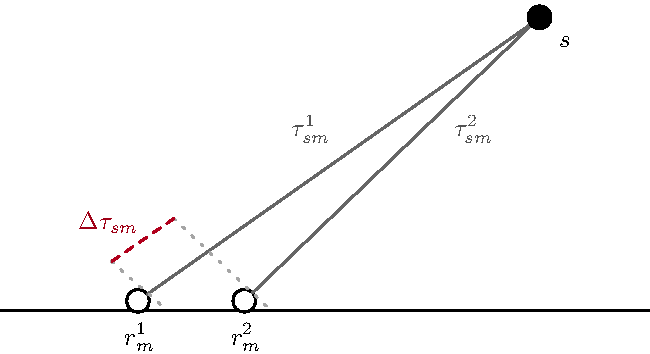
\includegraphics[scale=0.7]{data/figures/signal2}
    \caption{Direct propagation path for source $s$ and receiver pair $m$}
    \label{fig:signal}
\end{figure}

The basic configuration, as depicted in Figure \ref{fig:signal}, consists of two microphones that constitute one sensor node. The received signal $x^i_m$ at microphone $i$ of pair $m$ can be described as a linear combination of the transfer function $a^i_{sm}$, multiplied bin-wise with the source signal $v_s$, and additive white gaussian noise $n^i_m$ in the \acrfull{stft} domain
\begin{equation}
	x_m^i(t,k)=\sum_{s=1}^{S}a_{sm}^i(t,k)\cdot v_s(t,k)+n_m^i(t,k).
	\label{eq:received_signal}
\end{equation}

The direct path of the transfer function, that part corresponding to the line-of-sight, can be described as
\begin{equation}
	a_{sm}^i(t,k)\approx\frac{1}{\|\bm p_s-\bm p_m^i\|}\cdot\exp{\left(-j\frac{2\pi k}{K}\frac{\tau^i_{sm}}{T_s}\right)},
	\label{eq:acoustic_transfer_function}
\end{equation}

%TODO: transfer function <-> RIR

where $T_s$ is the sampling period of source signal $v_s$ and $\|\bm p_s-\bm p_m^i\|$ is the Eucledian distance between source position $\bm p_s$ and receiver position $\bm p^i_m$ of sensor node $m$. The signal travel time $\tau^i_{sm}$ between source position $\bm p_s$ and receiver position $\bm p^i_m$ is determined by the sound velocity $c$
\begin{equation}
	\tau^i_{sm}=\frac{\left(\|\bm p_s-\bm p_m^i\|\right)}{c}.
\end{equation}

To estimate the location of a source, we solve for the \gls{tdoa} $\Delta\tau_{sm}$, which we define as
\begin{equation}
    \Delta\tau_{sm}=\tau^2_{sm}-\tau^1_{sm}=\frac{\|\bm p_s-\bm p_m^2\|-\|\bm p_s-\bm p_m^1\|}{c},
\end{equation}

assuming planar wave fronts impinging on the microphones according to the far-field approximation of sound signals. From the \gls{tdoa}, the \gls{doa} can then be inferred with
\begin{equation}
    \text{DOA}=\arccos\left (\frac{c\cdot \Delta\tau_{sm}}{d_m}\right ),
\end{equation}
% TODO: Make the argument for TDOA, DOA and PRP bullet proof!

where $d_m$ is the Eucledian distance of the position of the two receivers $\bm p_m^1$ and $\bm p_m^2$ of sensor node $m$
\begin{equation}
    d_m=\| \bm p_m^1-\bm p_m^2\|.
\end{equation}

%TODO: Umformulieren des folgenden Absatz (RIR vs. Transfer function)
The direct path of the transfer function multiplied with the source signal contains the original phase information that is needed to estimate the position of the source. The remaining part of the received signal (the reverberant tail of the \gls{rir} multiplied with the source signal) distorts this information and will decrease the location estimation performance. 

%TODO: Klären, wann index s notwendig und wann nicht
Following \cite{Schwartz2014}, the \gls{prp} $\phi_{sm}(t,k)$ of the two signals $x_{sm}^1$ and $x_{sm}^2$ received at each sensor node $m$ will be used as the feature to be used for the purpose of localisation
\begin{equation}
    \phi_{sm}(t,k)=\frac{x^2_{sm}(t,k)}{x^1_{sm}(t,k)}\cdot \left |\frac{x^1_{sm}(t,k)}{x^2_{sm}(t,k)}\right |.
\label{eq:prp}
\end{equation}

To understand the link of \gls{prp} and \gls{doa}, let's solve the equation for two received signals\alt{ of equal volume (i.e. $|x^1(t,k)| = |x^2(t,k)|$)} in a noiseless environment (i.e., $n^i_{m}(t,k)=0$)
%\begin{equation}
%    \frac{x^2_{sm}}{x^1_{sm}}=\frac{v_{sm}\cdot a^2_{sm}}{v_{sm}\cdot a^1_{sm}}=\frac{\|\bm p_s-\bm p_m^1\|\cdot\exp{\left(-j\frac{2\pi k}{K}\frac{\tau^2_{sm}}{T_s}\right)}}{\|\bm p_s-\bm p_m^2\|\cdot\exp{\left(-j\frac{2\pi k}{K}\frac{\tau^1_{sm}}{T_s}\right)}}=\exp{\left ( j\frac{2\pi k}{K}\frac{(\tau^1-\tau^2)}{T_s}\right )}
%\end{equation}

\begin{equation}
    \phi_{sm}(t,k)=\exp{\left ( -j\frac{2\pi k}{K}\frac{\tau_{sm}^1-\tau_{sm}^2}{T_s}\right )}.
\end{equation}

As can be seen from the result, the amplitude has been eliminated by multiplication with $|x^1(t,k)|\ /\ |x^2(t,k)|$. The \gls{prp} feature can therefore be interpreted as the effect of the \gls{tdoa} on the phase difference between the two microphones of a sensor node.

%TODO: explain w-disjoint activity
The sources are assumed to exhibit w-disjoint orthogonality in the \gls{stft} domain \cite[p. 393]{Schwartz2014}, \cite{Rickard2006}.
\section{Gaussian Mixture Model (GMM)}
\label{sec:gmm}
% univariate Gaussian
In its univariate form, a Gaussian or normal distribution is defined by
\begin{equation}
	\gaussian{x\vert\mu,\sigma}=\frac{1}{(2\pi\sigma^2)^{1/2}}\exp\left\{-\frac{1}{2\sigma^2}(x-\mu)^2\right\},
\end{equation}
where $\mu$ is called its \textit{mean} and $\sigma^2$ is called its \textit{variance}.
%This distribuion satisfies the requirements $\int_{-\infty}^{\infty}\gaussian{x\vert\mu,\sigma^2}\text{d}x=1$ and $\gaussian{x\vert\mu,\sigma^2}>0\ \forall\ x\in\mathbb{R}$, which qualifies the Gaussian distribution as a probability distribution.
The multivariate Gaussian distribution for an input vector $\bm x\in\mathbb{R}^D$ is defined by
\begin{equation}
	\gaussian{\bm x\vert\bm\mu,\bm\Sigma}=\frac{1}{(2\pi)^{D/2}}\frac{1}{\bm\Sigma^{1/2}}\exp\left\{-\frac{1}{2}(\bm x-\bm\mu)^{\text{T}} \bm\Sigma^{-1}(\bm x-\bm\mu)\right\}.
\end{equation}



% Complexity of multivariate Gaussians
Compared to the univariate form with only two free parameters, this \gls{pdf} is completely defined by its covariance matrix $\bm\Sigma\in\mathbb{R}^{D\times D}$ and its mean vector $\bm\mu\in\mathbb{R}^D$. As the covariance matrix is symmetric, is has $D(D+1)/2$ independent parameters (assuming it is positive definite). Adding the $D$ independent parameters of $\bm\mu$ results in $D(D+3)/2$ independent parameters that define a multivariate Gaussian distribution. 

The complex variant of the Gaussian distribution is defined by
\begin{equation}
    \mathcal{N}^c(\bm z,\Gamma)=\frac{1}{\pi^N\cdot\text{det}\ \Gamma}\exp\{ -\bm z^*\Gamma^{-1}\bm z \},
\end{equation}
where $\bm z\in\mathbb{C}^N$, $\Gamma$ is the complex covariance matrix, $\text{det}\ \Gamma$ is the determinant of $\Gamma$, $\bm z^*$ denotes the complex conjugate of $\bm z$ and $\Gamma^{-1}$ the inverse of $\Gamma$. 

% not really needed
%As shown in \cite{Gallager2008}, for the density of $m$ independent circular-symmetric Gaussian random variables, this can be written using the eigenvalues $\lambda_j$ and eigenfunction $\bm q_j$ of the covariance matrix
%\begin{equation}
%\label{eg:complexGaussianDef}
%    \mathcal{N}^c(\bm z,\lambda_j)=\prod_{j=1}^n\frac{1}{\pi\lambda_j}\exp(-|z,q_j|^2\lambda_j^{-1}).
%\end{equation}
%This formulation will be used when modelling the \gls{prp} using a \gls{gmm}.\\

% from single gaussian to mixture model
Despite possessing this many degrees of freedom, the Gaussian distribution is limited in a sense, that it has only one maximum (\textit{unimodality}) and therefore cannot adequately model multimodally distrbuted data. To overcome this limitation, multiple Gaussians can be combined into what is called a \acrlong{gmm}

% the GMM
\begin{equation}
	p(\bm x)=\sum^J_{j=1}\psi_j\cdot\gaussian{\bm x\vert\bm\mu_j,\bm\Sigma_j},
\end{equation}

where $\psi_j$ is the weighting factor or \textit{mixing coefficient} of each gaussian component $\gaussian{\bm x\vert\bm\mu_j,\bm\Sigma_j}$ of the \gls{gmm} with $0\leq\psi_j\leq 1$ and $\sum_{j=1}^J \psi_j=1$. In addition to $\bm\mu=[\bm\mu_1,\dots,\bm\mu_J]$ and $\bm\Sigma=[\bm\Sigma_1,\dots,\bm\Sigma_J]$, each a concatination of the parameters of the multivariate Gaussian for each component $j$, the \gls{gmm} has a third parameter $\bm\psi=[\psi_1,\dots,\psi_J]$. An example of a Gaussian mixture with three components is shown in \autoref{fig:gaussianmixture}. The parameters of a \gls{gmm} can be calculated under the Maximum-Likelihood criterion as follows:

\begin{equation}
	\text{ln}\ p(\bm X\vert\bm\psi,\bm\mu,\bm\Sigma)=\sum_{n=1}^N \text{ln}\left\{\sum_{j=1}^J \psi_k\cdot\gaussian{\bm x_n\vert\bm\mu_j,\bm\Sigma_j} \right\},
\end{equation}

with $\bm X=\{\bm x_1,\dots,\bm x_N\}$. As a result of the presence of the sum inside the logarithm, the \gls{ml} solution for these parameters does not have a closed form solution \cite[p.~113]{Bishop2006}. One way to solve these type of \gls{ml} problems is the \gls{em} algorithm presented in the following section. By introducing a latent random variable that models the missing information, the \gls{em} algorithm makes the \gls{ml} problem tractable.

\begin{figure}[!hbt]
    \includegraphics[width=6cm]{plots/gmm/gaussian}
    \caption[Example of a Gaussian Mixture]{A Multivariate Gaussian Mixture with $j=5$ Weighted Components.}
    \label{fig:gaussianmixture}
\end{figure}


\section{Expectation-Maximisation (EM)}
\label{sec:em}

\paragraph{History}
Although it has been used for parameter estimation of mixture models as early as \citeyear{Newcomb1886} \cite{Newcomb1886}, the \gls{em} algorithm was formally described in a generalised form by \citeauthor{Dempster1977} in \citeyear{Dempster1977}, who also coined the name of the two-step procedure \cite{Dempster1977}. From then on, it has been used in various applications (many of them are described in \cite{McLachlan2008}). In the signal processing community, it has been successfully applied to tasks as diverse as emission tomography image reconstruction \cite{Shepp1982}, active noise cancelling with a single microphone \cite{Feder1989} and parameter estimation of hidden markov models \cite{Moon1996}. Outside of signal processing, the algorithm is also utilised in many machine learning applications, where it is often introduced as an extended form of the $k$-means algorithm for clustering \cite{Bishop2006}.

% Initialisation
The name \glsentrylong{em} goes back to the algorithm's distinct two steps that both rely on the output of the respective other step. Therefore, prior to the iteration over the E- and M-Step, the estimated parameter set $\bm \theta$ has to be initialised. This initialisation is done randomly in most cases, although one can also include prior knowledge of the estimated parameters by choosing certain initial values for $\theta$ accordingly.

\paragraph{Description} In general, the algorithm allows to determine \gls{ml} estimates or \gls{map} estimates, where only incomplete data is available \cite[p.1]{Dempster1977}. Incomplete data means that there is a \textit{hidden} or \textit{latent} variable $Z$, that cannot be observed directly but might be inferred by some observable variable $X$. The \textit{complete data} is given by combining the (discrete) \textit{hidden variable} and the observations.
%TODO: erklärender satz, warum latente variable diskret ist


\paragraph{Derivation}
The cost function of the maximisation problem is the following likelihood function
\begin{equation}
    p(\vect{X}\given{\theta})=\sum_\vect{z} p(\vect{X},\vect{Z}\given{\theta}).
\end{equation}

The assumption is, that maximising $p(\vect{X}\given{\theta})$ is difficult, but optimisation of the complete data likelihood function $p(\vect{X},\vect{Z}\given{\theta})$ is significantly easier. Next, a distribution $q(\vect{Z})$ over the latent variables is defined, which allows, following \cite[p.450]{Bishop2006}, for the decomposition

\begin{equation}\label{eq:decomposition}
    \ln p(\vect{X}\given{\theta})=\mathcal{L}(q,\theta)+\text{KL}(q\|p),
\end{equation}

where the summands are defined as
\begin{align}
    \mathcal{L}(q,\theta)&=\sum_\vect{Z}q(\vect{Z})\ln\left\{\frac{p(\vect{X},\vect{Z}\given{\theta})}{q(\vect{Z})}\right\}\label{eq:L},\\
    \text{KL}(q\|p)&=-\sum_{\vect{Z}}q(\vect{Z})\ln\left\{\frac{p(\vect{Z}\given{\vect{X},\theta})}{q(\vect{Z})} \right\}\label{eq:KL}.
\end{align}

This decomposition can be verified by using the multiplication formula for probabilities, which directly results from the definition of conditional probabilities
\begin{align}
\label{eq:defProbCond}
    p(A\given{B})&=\frac{p(A,B)}{p(B)},\\
\label{eq:defProbProductRule}
    p(A,B)&=p(A\given{B})\cdot p(B).
\end{align}

Applying \eqref{eq:defProbProductRule} to $p(\vect{X},\vect{Z})$ in \eqref{eq:L} and using the product rule for logarithms $\ln(a\cdot b)=\ln(a)+\ln(b)$ yields

\begin{align}
    \mathcal{L}(q,\theta)&=\sum_{\vect{Z}}q(\vect{Z})\ln\left\{\frac{p(\vect{Z}\vert\vect{X},\theta)\cdot p(\vect{X}\given{\theta})}{q(\vect{Z})}\right\}\\
\label{eq:Lexpanded}
    &=\sum_{\vect{Z}}q(\vect{Z})\ln\left\{\frac{p(\vect{Z}\given{\vect{X},\theta})}{q(\vect{Z})} \right\}+\sum_{\vect{Z}}q(\vect{Z})\ln\{p(\vect{X}\given{\theta})\}.
\end{align}

The first summand is equal to $-\text{KL}(q\|p)$, therefore it cancels out when inserting \eqref{eq:Lexpanded} back into \eqref{eq:decomposition}. The second summand can be simplified making use of the fact, that $q(\vect{Z})$ is a probability distribution and therefore $\sum_{\vect{Z}}q(\vect{Z})=1$ holds true
\begin{align}
    \mathcal{L}(q,\theta)+\text{KL}(q\|p)&=\sum_{\vect{Z}}q(\vect{Z})\ln p(\vect{X}\given{\theta})-\text{KL}(q\|p)+\text{KL}(q\|p)\\
    &=\ln p(\vect{X}\given{\theta}).
\end{align}

From \eqref{eq:decomposition} it is apparent, that $\mathcal{L}(q,\theta)$ is a lower bound of $\ln p(\vect{X}\given{\theta})$, because from $q(\vect{Z})>0\ \forall\ \vect{Z}$ follows KL$(q\|p)\geq0$. In order to maximise the lower bound for a given $\theta^{(l-1)}$, we therefore need to set KL$(q\|p)=0$, so that $\mathcal{L}(q,\theta)=\ln p(X\given{\theta})$. In other words, to compute a lower bound, that is tight with the original likelihood function at $\theta^{(l-1)}$ (i.e. "touches" $\ln p(\vect{X}\given{\theta})$ in $\theta^{(l-1)}$), we set $\mathcal{L}(q,\theta)=\ln p(\vect{X}\given{\theta})$, which necessitates
\begin{align}
\label{eq:thatOtherFormulaAbove}
    \text{KL}(q\|p)&=0,\\
    -\sum_{\vect{Z}}q(\vect{Z})\ln\left\{\frac{p(\vect{Z}\given{\vect{X},\theta})}{q(\vect{Z})} \right\}&=0.
\label{eq:thatFormulaAbove}
\end{align}

Choosing
\begin{equation}
    q(\vect{Z})=p(\vect{Z}\given{\vect{X}},\theta)
\label{eq:q}
\end{equation}
satisfies \eqref{eq:thatFormulaAbove}. Inserting \eqref{eq:q} into \eqref{eq:L} and using $\ln(\frac{x}{y})=\ln{x}-\ln{y}$, the lower bound is given by
\begin{align}
    \mathcal{L}(q, \theta)&=\sum_\vect{Z}p(\vect{Z}\given{\vect{X}, \theta^{(l-1)}})\ln p(\vect{X},\vect{Z}\given{\theta})-\sum_\vect{Z}p(\vect{Z}\given{\vect{X}, \theta^{(l-1)}})\ln p(\vect{Z}\given{\vect{X},\theta^{(l-1)}})\\
    &=\Q+\text{const},
\end{align}

with
\begin{equation}
\label{eq:e-step}
    \Q=\sum_\vect{Z}p(\vect{Z}\given{\vect{X}, \theta^{(l-1)}})\ln p(\vect{X},\vect{Z}\given{\theta}).
\end{equation}
    
Computing this lower bound constitutes the E-Step. The M-Step is to find a new value $\theta^{(l)}$, that maximises this lower bound
\begin{equation}
\label{eq:m-step}
    \theta^{(l)} = \argmax_{\theta}\Q.
\end{equation}

\begin{figure}[!hb]
\label{fig:em}
\centering
    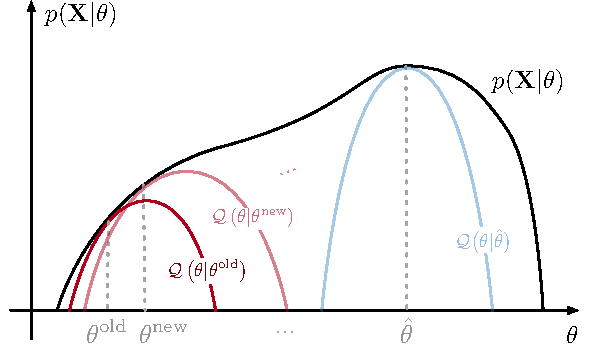
\includegraphics[scale=1]{data/figures/em-Q3}
    \caption{EM-Algorithm as iterative lower-bound optimisation}
\end{figure}

To summarise, the goal of the E-Step is to find a lower bound for the original, incomplete data likelihood function $p(\vect{X}\vert\theta)$. This lower bound $\mathcal{L}(q,\bm\theta)$ is choosen to be equal to the original likelihood function in $\theta^{(l-1)}$, which is done by selecting $q(\vect{Z})$ to be the posterior probability of the latent variable $\vect{Z}$ given the observation $\vect{X}$. This gives rise to the $\mathcal{Q}$-function, which, in the M-Step, is maximised with respects to the estimated parameter set $\bm\theta$. The result is a new value $\bm\theta^{(l)}$, for which a new lower-bound can be found. This procedure is repeated iteratively either until some fixed number of iterations are reached or some convergence criterion is met. For a full account of the convergence of \gls{em}, see \cite{Wu1983}.\alt{Convergence criteria for the \gls{em} algorithm are shown in \cite{Wu1983}.} It is interesting to note, that the M-Step only states \textit{that} the result of the E-Step is to be maximised, but not \textit{how} this is to be done. Rather than a specific solution for a certain type of problems, the \gls{em} algorithm is therefore more of a template, that can be applied to a variety of different problems, each of them required to individually derive the concrete steps necessary to obtain a lower-bound for the incomplete data log likelihood function and find it's maximum.

\begin{figure}[!htb]
\centering
\includegraphics{data/figures/em-flowchart}
\caption{Steps of the \glsentryshort{em} algorithm}
\end{figure}

\paragraph{Limitations}
One existing limitation of the \gls{em} algorithm is the possibility of a slow convergence rate, which increases the computational complexity as more iterations have to be carried out before convergence is reached. In this case, the convergence threshold can be increased or a fixed number of iterations can be carried out, although this means that the solution is no longer optimal in the \gls{mmse} sense. Another limitation is, that the algorithm is susceptible to local optima for more than one target parameter, meaning that the determined solution is not necessarily the best solution. This can be alleviated by running the algorithm multiple times with a different, random initialisations and choose the best outcome, a procedure known as \textit{random-restart hill climb}. Another method to circumvent getting stuck in local optima is \textit{simulated annealing}, which is incorporated into an \gls{em} template in \cite{Guo2007}.
%TODO: define "best outcome"
%TODO: Describe simulated annealing
%TODO: "more than one target parameter" ist anscheinend unklar... umformulieren!
%TODO: define "convergence threshold" mathematically


TODO: Zusammenfassung von Kapitel 2

%As KL$(q\|p)$ is the Kullback-Leibler divergence between $q(\vect{Z})$ and $p(\vect{Z}\given{\vect{X},\theta})$, it also satisfies KL$(p\|q)\geq 0$ with equality only if $q(\vect{Z})=p(\vect{Z}\given{\vect{X},\theta})$. This means, that, using \eqref{eq:decomposition}, we can state, that $\mathcal{L}(q,\theta)$ is a lower bound for the original likelihood function $\ln p(\vect{X}\given{\theta})$. As the 

%%%%%%%%%%%% OLD STUFF %%%%%%%%%%%%%%%


%\paragraph{Derivation by Andrew Ng, CS229}
%The goal is to maximise the log-likelihood function that is given by
%\begin{equation}\label{eq:likelihood}
%    l(\theta)=\sum_i\log p(x_i;\theta)=\sum_i\log\sum_{z_i} p(x_i,z_i;\theta).
%\end{equation}
%
%Now we assume, that maximising the probability of the observed variable $X$ with respect to the parameter $\theta$ is difficult, but doing this for the probability of the complete data $p(X,Z;theta)$, given by the joint distribution of observed and hidden variables, is easier.
%
%\begin{align}
%    \sum_i \log p(x_i;\theta)&=\sum_i \log \sum_{z_i} p(x_i, z_i;\theta)\\
%          &=\sum_i \log \sum_{z_i} Q_i(z_i)\frac{p(x_i, z_i;\theta)}{Q_i(z_i)}\label{eq:introduce-Q}\\
%          &\geq \sum_i\sum_{z_i}Q_i(z_i)\log\frac{p(x_i,z_i;\theta)}{Q_i(z_i)}\label{eq:lower-bound}
%\end{align}
%
%In \eqref{eq:introduce-Q} we introduced a probability function of the \textit{hidden variable} $Q_i(z_i)$ with the properties $Q_i(z_i)\geq 0\ \forall\ z_i$ and $\sum_{z_i}Q_i(z_i)=1$. This allowed us to use the definition for expectation
%\begin{equation}
%    \sum_{z_i} Q_i(z_i)\frac{p(x_i, z_i;\theta)}{Q_i(z_i)}=E\left\{\frac{p(x_i, z_i;\theta)}{Q_i(z_i)}\right\}
%\end{equation}
%
%and finally use Jensen's inequality
%\begin{align}
%    \text{when\ }f(x) \text{\ is concave:\ }& f(E\{x\}) \geq E\{f(x)\},\label{eq:jensen-concave}\\
%    \text{when\ }f(x) \text{\ is convex:\ }& f(E\{x\}) \leq E\{f(x)\},\label{eq:jensen-convex}
%\end{align}
%
%given that the logarithm is a concave function, which can be shown by
%\begin{equation}
%    \frac{\partial}{\partial x}\log(x)=-\frac{1}{x^2} < 0 \ \forall\ x\in\mathbb{R}^+.
%\end{equation}
%
%Now we have a lower bound \eqref{eq:lower-bound} for the likelihood function \eqref{eq:likelihood}. To define Q we set the constraint, that the lower bound should be as close to the original likelihood function as possible. Therefore, we set the lower bound equal to the original likelihood function for the given parameter $\theta$, which means, that Jensen's inequality needs to be true for the equal case. Combining \eqref{eq:jensen-concave} and \eqref{eq:jensen-convex} shows, that $f(E[x]) = E[f(x)]$ is only true when $f(x)$ is neither concave nor convex, which is only the case for a constant value $f(x) = c\ \forall\ x$. That means
%\begin{equation}
%    \frac{p(x_i,z_i;\theta)}{Q_i(z_i)}=c,
%\end{equation}
%
%which is satisfied, when
%\begin{equation}
%    Q_i(z_i)\propto p(x_i,z_i;\theta).
%\end{equation}
%
%Using the probability distribution property $\sum_{z_i}Q_i(z_i)=1$, we can write
%\begin{align}
%    Q_i(z_i)&=\frac{p(x_i,z_i;\theta)}{\sum_z p(x_i,z;\theta)}\\
%            &=frac{p(x_i,z_i;\theta)}{p(x_i;\theta)}\\
%            &=p(z_i\mid x_i;\theta),
%\end{align}
%
%which is the posterior probability of the hidden variable $z$ given $x$.
%
%In a general form, the two steps of the \gls{em} algorithm are defined as
%
%\subsubsection*{E-Step}
%\begin{equation}\label{eq:e_step_general}
%	Q(\theta,\hat\theta^{(l)})=E_{\hat\theta^{(l)}}\left\{ \log{f_{Y}(y;\theta)\mid z} \right\},
%\end{equation}
%
%\subsubsection*{M-Step}
%\begin{equation}\label{eq:m_step_general}
%	\hat\theta^{(l+1)}=\arg \max_\theta Q\left ( \theta,\hat\theta^{(l)}\right ).
%\end{equation}
%
%%The $Q$-function used in the E-Step can be interpreted as a lower bound of the log-likelihood function to be maximised. To calculate this lower bound, \textit{Jensen's inequality} is used, which states for a concave function $f(x)$ that
%
%The expectation operator is defined as
%\begin{equation}\label{eg:expectation-definition}
%    E\{f(x)\}=\sum_x f(x)P(x),
%\end{equation}
%
%Bringing this all together, we are now able to determine a lower bound for the log likelihood function
%\begin{equation}
%    \log\left(\sum_x f(x)P(x)\right) \leq \sum_x \log f(x)P(x),
%\end{equation}
\bigskip

In this chapter, the signal model has been defined and the \gls{prp} has been identified as a measure of the \gls{tdoa} in the frequency domain. Next, the Gaussian distribution has been introduced and definitions have been presented for its real, its complex and its multivariate form. The Gaussian was mixture model was motivated by the limitation of a single Gaussian to only model unimodally distributed data and has been defined as a weighted linear combination of Gaussian components. The weighting factor of each components together with the variance is the parameter set to be estimated using the \gls{em} algorithm, which is able to determine the \gls{ml} estimates for these parameters despite incomplete data by introducing a latent variable that models the missing information. It has been shown, how the \gls{em} algorithm can be understood as a iterative lower-bound optimisation of the incomplete data log-likelihood function, where the lower-bound is considerably easier to maximise for distributions of the exponential family, than the original likelihood function. In the end, limitations of the \gls{em} algorithm and strategies to alleviate these limitations have been discussed.
%
% DERIVATION OF ALGORITHMS
The described in the following chapter have been derived in \cite{Schwartz2014}. Therefore, the following is based on the work presented in \cite{Schwartz2014} with some additional comments to facilitate understanding of how the algorithms are adapted to be used in location estimation and source tracking application. First, the probabilistic model is introduced, where the \gls{gmm} presented in \autoref{sec:gmm} is used to model the \gls{prp}. Next, the algorithm for source localisation is derived, where the \gls{em} algorithm is adapted to estimate the parameters of the \gls{gmm}. Last, two algorithms for source tracking are presented and discussed briefly.

\section{Probabilistic Model} \label{sec:prob_model}

To have discrete location estimates, a set of location vectors $\bm p$ is introduced, that addresses all possible positions either a source or a receiver can be in. % TODO: Introduce grid properly

As described in Section \ref{sec:signal}, rather then using the received signal $x$ as observed feature directly, we defined the \gls{prp} readings in \eqref{eq:prp} as our observations, which will be modelled as a mixture of complex Gaussian distributions
\begin{equation}
	\bm\phi(t,k)\sim\sum_{\bm p}\psi_{\bm p}\cdot\mathcal{N}^c\big(\phi(t,k);\tilde\phi^k(\bm p),\Sigma\big),
\label{eq:phi_gmm}
\end{equation}

where $\psip$ denotes the probability or weight of the Gaussian distribution at gridpoint $\bm p$ to be associated with an active source and $\tilde\phi^k_m$ describes the \gls{prp} in all possible gridpoints $\bm p$ for microphone pair $m$

\begin{equation}
    \tilde\phi^k_m(\bm p)=\exp{\left (-j\frac{2\pi k}{K}\cdot\frac{\|\bm p-\bm p^2_m\|-\|\bm p-\bm p^1_m\|}{c\ T_s}\right )}.
\label{eq:phi_tilde}
\end{equation}

As the \glspl{prp} of the different sensor nodes $m$ are subject to different reverberation effects, they are assumed to be independent. This way, the covariance matrix can be simplified to $\bm\Sigma=\text{diag}(\sigma^2_{1}, \sigma^2_{2}, \dots, \sigma^2_{M})$, which lets us replace the covariance matrix by its diagonal elements when computing the product over all receiver pairs $M$
\begin{equation}
    \mathcal{N}^c(\phi_m(t,k);\tilde\phi^k_m(\bm p),\bm\Sigma)=\prod_m \mathcal{N}^c(\phi_m(t,k);\tilde\phi^k_m(\bm p),\sigma^2_m).
\end{equation}

Inserting the definition for the complex Gaussian distribution \eqref{eg:complexGaussianDef} yields
\begin{equation}
    \mathcal{N}^c\big(\phi_m(t,k);\tilde\phi_m^k(\bm p),\sigma_{m}^2\big)=\prod_m\frac{1}{\pi\sigma_{m}^2}\cdot\exp\left (-\frac{\left|\phi_m(t,k)-\tilde\phi_m^k(\bm p)\right|^2}{\sigma_{m}^2} \right ).
\label{eq:gaussian}
\end{equation}

%TODO: erkläre, was varianz constraint bedeutet
In \cite{Schwartz2014}, the variance has been further simplified to $\sigma_{m}^2=\sigma^2\ \forall\ m$. As this formula has to be evaluated for each observed \gls{prp} per time-frequency-bin and speakers display $w$-disjoint orthogonal activity in the \gls{stft}-domain, the complete observation set is defined by:
\begin{equation}
    p(\bm\phi; \bm\psip,\sigma^2)=\prod_{t,k}\sum_{\bm p}\psi_{\bm p}\prod_m\mathcal{N}^c\big(\phi_m(t,k);\tilde\phi^k_m(\bm p),\sigma^2_{s}\big)
\end{equation}

The optimization problem to be solved can be stated as:
\begin{equation}
    \left\{\hat{\bm\psi}_{\bm p},\hat\sigma^2\right\}=\argmax_{\psi, \sigma^2}\ln f(\phi_m;\bm\psip,\sigma^2)
\label{eq:mle}
\end{equation}

%TODO: Kapitel ausweiten
\begin{itemize}
    \item Herleitung, mehr Erklärung der einzelen Schritte
    \item mehr Intuition
    \item Wo steckt die Position drin?
    \item Warum machen wir das?
    \item Was ist $\tilde\phi_m^k$
\end{itemize}

\section{Location Estimation}
\label{sec:algLocEst}
%\begin{itemize}
%\item mehr Zwischenschritte
%\item Erklärung der Ergebnisse, Annahmen, roter Faden der Herleitung... Was machen wir und warum?
%\item Was ist die Intuition dahinter? Was bedeuten die Größen? Was ist die interessierende Größe? Was sind Hilfsgrößen?
%\end{itemize}

If the likelihood function of the observed data \eqref{eq:mle} were to be maximised directly, the following equation would have to be solved
\begin{equation}
    \ln f(\phi;\psip,\sigma^2) = \ln\prod_{t,k}\sum_{\bm p}\psi_{\bm p}\prod_m\mathcal{N}^c\big(\phi(t,k);\tilde\phi^k(\bm p),\sigma^2_{s}\big).
\end{equation}
Because the sum over all possible gridpoints $\bm p$ prevents the logarithm from acting directly on the exponential term, solving this function results in a complicated expression, which should be avoided. This is where a so-called \textit{latent variable} is introduced. Here, the latent variable is defined as an indicator $z$, that a certain time-frequency bin $(t,k)$ belongs to an active source at position $\vect{p}$ 
\begin{equation}
	\z=\begin{cases}
	    1& \text{source at $\vect{p}$ active in $(t,k)$-bin},\\
       0& \text{otherwise}.
	\end{cases}
\end{equation}

The expectation of the hidden variable is equal to the probability of a source to exist at position $\bm p$ and to have shown activity in time-frequency bin $(t, k)$ 
\begin{equation}
    E\{\z\}=\psi_{\bm p}.
\end{equation}

As sparsity of the source signals is assumed, meaning there is only one source active in each time-frequency bin, the latent variable is a 1-of-$|\mathcal{P}|$ representation, where $|\mathcal{P}|$ denotes the cardinality of the set of all gridpoints, i.e. there is one $z(t',k',\bm p')=1$ whereas $z(t',k',\bm p)=0\ \forall\ \bm p\in\mathcal{P}\smallsetminus\{\bm p'\}$. The property, that makes indicators in combination with \glspl{gmm} so useful, is their ability to simplify the sum over all components into a product
\begin{equation}
\label{eq:indicator-sum-product}
    \sum_{i}x_i\cdot z_i=\prod_i (x_i)^{z_i}.
\end{equation}
%TODO: Define vec()
The concatenated vector of the indicators of all time-frequency bins and locations is defined as
\begin{equation}
    \bm z=\text{vec}_{t,k,\bm p}(\z).
\end{equation}

The probability density of $\bm z$ can be written as  %TODO: argue this step
\begin{equation}
    p(\bm z;\bm\theta)=\prod_{t,k}\sum_{\bm p}\psi_{\bm p}\cdot\z,
\end{equation}

%TODO: Besser herausarbeiten, das mean = PRP reading
where $\bm\theta=[\bm\psi,\sigma^2]$ is the set of target parameters. Note, that $\mu$ is not part of this set, as the Gaussian components in this model are evenly spaced throughout the room and each component mean corresponds to one gridpoint. This deviates from the way the \gls{em} algorithm is commonly used together with a \gls{gmm}, where, in addition to the Gaussian component weights $\bm\psi$, generally both mean and covariance are part of the estimation.

As was described in Section \ref{sec:em} and further argued above, due to the complexity involved when maximising the log-likelihood function of the observations $\ln p(\phi;\psi, \sigma^2)$ directly, a tight lower bound at $\theta^{(l-1)}$ is derived and maximised instead. This lower-bound will utilize the latent variable to reduce complexity of the optimisation problem and is given in \eqref{eq:L} . From \eqref{eq:L} one can see, that to evaluate this function, the complete-data likelihood $p(\phi,\bm z; \theta)$ as well as the conditional likelihood $p(\bm z\given{\phi, \theta^{(l-1)}})$ is required. Given the hidden data, the conditional likelihood of the observations is given by:
\begin{equation}
    p(\phi |\vect{z};\theta)=\prod_{t,k}\sum_{\bm p}\prod_{m}\gauss\cdot\z.
\end{equation}

Multiplying the densities of the hidden variable and observations yields the joint probability distribution of the complete data:
\begin{equation}
    p(\phi,\vect{z};\theta)=p(\bm z;\theta)\cdot p(\phi |\bm z;\theta)=\prod_{t,k}\sum_{\bm p}\psip\cdot\z\prod_{m}\gauss .
\end{equation}

The log-likelihood of the complete data is given by
\begin{align}
    \ln f(\phi,\bm z; \theta) &= \ln \left [ \lcompl \right ].\\
    \intertext{First, the logarithm can be moved inside the product using \eqref{eq:log-sum}:}
    \ln f(\phi,\bm z; \theta) &=\sum_{t,k}\ln \left [\sum_{\bm p}\psip\cdot\z\prod_{m}\gauss\right ].\\
    \intertext{Now, the property of the indicator stated in \eqref{eq:indicator-sum-product} will be used to simplify the sum, that divides the logarithm and the exponential term, to a product}
    \ln f(\phi,\bm z; \theta) &=\sum_{t,k}\ln \left [\prod_{\bm p}\Big (\psip\prod_{m}\gauss\Big )^{\z}\right ].\\
    \intertext{Applying \eqref{eq:log-sum} and \eqref{eq:log-power} yields}
    \label{eq:complete-data}
%    &=\sum_{t,k}\z\cdot\ln \left [\prod_{\bm p}\Big (\psip\prod_{m}\gauss\Big )\right ]\\
%    \intertext{Finally, using $\ln(x\cdot y)=\ln(x)+\ln(y)$ one more time}
    \ln f(\phi,\bm z; \theta) &=\sum_{t,k,\bm p}\z\cdot\ln \left [\psip\prod_{m}\gauss\right ].
\end{align}

%TODO: Fix "Das ist der Erwartungswert, keine PDF"
The conditional probability of $p(\bm z\given{\phi})$ is given by Bayes theorem:
\begin{equation}
\label{eq:responsibility}
    p(\bm z\given{\phi,\bm\theta})=\frac{f(\bm z)\cdot f(\phi\given{\bm z})}{\sum_{\bm z}f(\bm z)\cdot f(\phi\given{\bm z})}=\frac{\pdffunc}{\sum_{\vect{p}}\pdffunc}\triangleq\mulast .
\end{equation}

This probability can also be interpreted as the responsibility that the Gaussian component at position $\bm p$ takes for explaining the observation $\phi$ in time-frequency-bin $(t,k)$ \cite[p.432]{Bishop2006}.

\subsubsection*{E-Step}
Copy of Q-function only for reference, will be removed later!
\begin{equation}
    \Q=\sum_\vect{Z}p(\vect{Z}\given{\vect{X}, \theta^{(l-1)}})\ln p(\vect{X},\vect{Z}\given{\theta}).
\end{equation} 
Inserting \eqref{eq:responsibility} and \eqref{eq:complete-data} into \eqref{eq:e-step} yields the complete $\mathcal{Q}$-function
\begin{align}
    \Q &=E\left\{\ln(f(\phi,\vect{z};\theta))\mid \phi;\theta^{\text{old}}\right\}=\\
       &=\sum_{t,k,\vect{p}}E\left\{z(t,k,\vect{p})\mid\phi(t,k);\theta^{\text{old}}\right\}\cdot\left [ \ln\psi_{\vect{p}}+\sum_{m}\ln\gauss\right]\nonumber\\
       &= \sum_{t,k,\bm p}\mulast\cdot\left [\ln\psip+\sum_{m}\ln\gauss\right ].
\end{align}
%TODO: Erwartungswerte im Bezug auf was? Bezug in subscript!

For the purpose of localisation, it is sufficient to evaluate \eqref{eq:responsibility}.
%TODO: Argue, why evaluating $\mulast$ is sufficient
%TODO: Interpret \mulast
% Das gilt allgemein, deswegen heißt es Expectation Step

\subsubsection*{M-Step}
As seen in \eqref{eq:m-step}, the M-Step consists of maximizing the $\mathcal{Q}$-function with regard to the elements of the parameter set $\theta$. This is done by computing the gradient of the $\mathcal{Q}$-function
\begin{equation}
\label{eq:m_step_theta_derivative}
    \theta^{(l)}=\nabla_\theta\Q,
\end{equation}

which means computing the partial derivatives of the target parameters $\psi_{\bm p}^{(l)}$ and $\sigma_s^{2,(l)}$
\begin{align}
    \label{eq:m_step_sigma_derivative}
    \sigma_{s}^{2, (l)}&=\frac{\partial}{\partial \sigma^2}\Q,\\
    \label{eq:m_step_psi_derivative}
    \psi_{\bm p}^{(l)}&=\frac{\partial}{\partial \psi_{\bm p}}\Q.
\end{align}

As $\psi_{\bm p}$ is constrained by $\sum_{\bm p}\psi_{\bm p}=1$, to fulfill the requirements of a probability over grid positions, constrained optimisation using a Lagrange mulitplier has to be applied:
\begin{equation}
    g(\lambda,\psi_{\bm p})=\Q+\lambda\left (\sum_{\bm p}\psi_{\bm p}-1\right ).
\end{equation}

Derivation and setting to zero gives
\begin{align}
    \frac{\partial\Q}{\partial\psi_{\bm p}}+\lambda &=0,\\
    \frac{\sum_{t,k}\mulast}{\psi_{\bm p}}+\lambda &=0,\\
    -\frac{\sum_{t,k}\mulast}{\lambda}&=\psi_{\bm p}\label{eq:psi-lambda}.
\end{align}

We compute the sum over $\bm p$ on both sides to solve for $\lambda$
\begin{align}
    \sum_{\bm p}\psip &=-\frac{1}{\lambda}\sum_{t,k,\bm p}\mulast,\\
    1&=-\frac{1}{\lambda}\sum_{t,k}1,\\
    \lambda &= -TK.\label{eq:lambda}
\end{align}

Finally, we insert \eqref{eq:lambda} into \eqref{eq:psi-lambda} to get
\begin{equation}\label{eq:m_step_psi}
    \psi_{\bm p}^{(l)}=\frac{\sum_{t,k}\mulast}{T\cdot K}
\end{equation}

Calculating the partial derivate of $\sigma^2$ results in

\begin{equation}\label{eq:m_step_var}
    \sigma_s^{2,(l)}=\frac{\sum_{t,k,\vect{p}}\mulast\cdot\left | \phi_m(t,k)-\tilde\phi_m^k(\bm p)\right |^2}{M\cdot \sum_{t,k,\bm p}\mu^{(l)}(t,k,\bm p)}.
\end{equation}

This concludes the M-Step. When all iterations have been carried out, either because convergence was determined or a fixed number of iterations has been reached, the actual estimated source locations can be obtained by selecting the positions $\hat p_s$ associated with the $S$ highest values of $\psip$:
\begin{equation}\label{eq:find_positions}
    \hat p_s=\argmax_{\bm p}\psi_{\bm p}^{(L)}\ \forall\ s.
\end{equation}

\begin{algorithm}[h]
\label{alg:loc}
\caption{Static source localisation}
\begin{algorithmic}
    \State obtain $x^i_m(t,k)\ \forall i,m$
    \State calculate $\phi_m(t,k)$ using \eqref{eq:prp}
    \State calculate $\tilde\phi_m^k(\vect{p})$ using \eqref{eq:phi_tilde}
    \State initialize $\psi_{\vect{p}}^{(0)}$ and $\sigma^{2,(0)}$
    \For{$l=1$ \textbf{to} $L$}
    \State \textbf{E-Step:} calculate $\mulast$ using \eqref{eq:responsibility}
    \State \textbf{M-Step:} calculate $\psi^{(l)}_\vect{p}$ using \eqref{eq:m_step_psi} and $\sigma_{s}^{2,(l)}$ using \eqref{eq:m_step_var}
    \EndFor
    \State find $\vect{p}_s\ \forall\ s$ using \eqref{eq:find_positions}
\end{algorithmic}
\end{algorithm}

%TODO: Properly justify, why deviation from original paper
%TODO: Find out why algorithm index is not compiled
The above algorithm, summarised in Algorithm \ref{alg:loc}, slightly deviates from \cite{Schwartz2014}, as the likelihood $\psi$ of a Gaussian to resemble an active source is unrelated to the number of sources in this case. This means, that only a single $\psip$ is computed, whereas there are $S$ different $\psi_{s,\bm p}$ present in \cite{Schwartz2014}. Instead, knowledge about the number of sources will be introduced when determining the estimated positions in \eqref{eq:find_positions}. By introducing a threshold value for $\psip^{(L)}$ and selecting all positions with values for $\psi$ above that threshold, the constraint of a-priori knowledge of the total number of sources could be eliminated entirely. However, this threshold would also introduce another parameter to be adjusted for the algorithm to work properly. Also, this threshold would likely depend on the noise and reverberation, which would require some form of live adaptation.

\section{Source Tracking}
\label{sec:algSrcTrack}

To integrate data from prior steps into each \gls{em} iteration, recursive variants of the \gls{em} algorithm have been developed. These will be called \gls{rem} algorithms in the upcoming sections.

In \cite{Schwartz2014}, two different \gls{rem} algorithms for speaker tracking are proposed. One is based on \citeauthor{Titterington1984}'s \gls{rem} algorithm\ and will be referenced as \acrshort{trem}, whereas the other one is based on \citeauthor{Cappe2009}'s \gls{rem} algorithm and will be referenced as \acrshort{crem}.
As the derivation of these algorithms is too involved to be repeated here, only the resulting algorithm for the specific application of source tracking shall be presented below.
The main difference from the static location estimation is, that where the results have been summed up over all time-bins before, now each time-bin is analysed seperately and the estimation results of the prior time-bin will be used as prior probability of the next iteration. Another difference is, that the E- and M-Step are combined into one single recursion update, which means there are no more iterations over the E- and M-Step but rather recursions over the time-bins now. Therefore the iteration index $(l)$ is replaced by the time index $(t)$.

% Left out Calculation of FIM here

Recursive estimation of the Gaussian component weights is the same for both algorithms. First, reusing \eqref{eq:responsibility} for recursive updates over time $(t)$ instead of \gls{em} iterations $(l)$ yields
\begin{equation}
    \muRlast \triangleq \frac{\pdffuncR}{\sum_{\vect{p}}\pdffuncR}
\end{equation}

Similar to \eqref{eq:m_step_psi}, a recursive estimate of $\psip$ is given by
\begin{equation}
    \psi_{\bm p}^{(t)}\triangleq\sum_k \frac{\muRlast}{K}
\end{equation}

Finally, using the result of the algorithm derivation based on the \gls{fim} in \cite{Schwartz2014}, the recursive update step is given by

\begin{equation}
\label{eq:crem-psi}
    \psiRnow = \psiRlast +\gamma_t(\bm\psi^{(t)} -\psiRlast ).
\end{equation}
\renewcommand{\*}{\cdot}

The two algorithms, however, do differ in the recursive update of the variance

\paragraph{\glsentryshort{trem}}
\begin{align}
\label{eq:trem-var}
    \sigma_R^{2,(t)} &= \sigma_R^{2,(t-1)}+\gamma_t\frac{1}{K\*\sum_{\bm p}\psiRPlast} \sum_{k,\bm p}\mulast\*\frac{1}{M}\sum_{m}|\phi_m(t,k)-\tilde\phi_m^k(\bm p)|^2-\sigma_{m,R}^{2,(t-1)}\\
                     &= \sigma_R^{2,(t-1)}+\gamma_t\frac{\sum_{k,\bm p}\mulast}{K\*\sum_{\bm p}\psiRPlast} \*\Bigg ( \frac{1}{M}\sum_{m}|\phi_m(t,k)-\tilde\phi_m^k(\bm p)|^2-\sigma_{m,R}^{2,(t-1)}\Bigg ).
\end{align}

\paragraph{\glsentryshort{crem}}
\begin{align}
\label{eq:crem-var}
    \sigma_R^{2,(t)} = \sigma_R^{2,(t-1)}\cdot\frac{\sum_{\bm p}\psiRPlast}{\sum_{\bm p}\psiRPnow}&+\gamma_t\Bigg ( \frac{\sum_{k,\bm p,m}\mulast|\phi_m(t,k)-\tilde\phi_m^k(\bm p)|^2}{K \* M \* \sum_{\bm p}\psiRPnow}\\
    &-\sigma_R^{2,(t-1)}\frac{\sum_{\bm p}\psiRPlast}{\sum_{\bm p}\psiRPnow} \Bigg ).
\end{align}

The \gls{crem} algorithm is summarised in Algorithm \ref{alg:crem}
The \gls{trem} algorithm is summarised in Algorithm \ref{alg:trem}

\begin{algorithm}[H]\label{alg:trem}
\caption{\acrshort{trem} algorithm for source tracking}
\begin{algorithmic}
\State \textbf{set} $\tilde\phi^k_m(\vect{p})$ using \eqref{eq:phi_tilde}
\For{$t=1$ \textbf{to} $T$}
\State obtain $z_m^1(t,k), z_m^2(t,k)\ \forall\ k,m$
\State calculate $\phi_m(t,k)$ using \eqref{eq:phi_gmm}
\State calculate $\psi^{(t)}_{s\vect{p},R}$ using \eqref{eq:m_step_psi}
\State calculate $\sigma^{2,(t)}_{s,R}$ using \eqref{eq:trem-var}
\EndFor
\end{algorithmic}
\end{algorithm}

\begin{algorithm}[H]
\label{alg:crem}
\caption{\acrshort{crem} algorithm for source tracking}
\begin{algorithmic}
\State \textbf{set} $\tilde\phi^k_m(\vect{p})$ using \eqref{eq:phi_tilde}
\State \textbf{initialize} $\psi_{\bm p, R}^{(0)}$ and $\sigma_{s,R}^{2,(0)}$
\For{$t=1$ \textbf{to} $T$}
\State obtain $z_m^1(t,k), z_m^2(t,k)\ \forall\ k,m$
\State calculate $\phi_m(t,k)$ using \eqref{eq:phi_gmm}
\State calculate $\psi^{(t)}_{s\vect{p},R}$ using \eqref{eq:m_step_psi}
\State calculate $\sigma^{2,(t)}_{s,R}$ using \eqref{eq:crem-var}
\EndFor
\end{algorithmic}
\end{algorithm}


\bigskip

In this chapter, the probabilistic model of the environment has been presented. A \gls{gmm} has been used to model the \gls{prp} readings for each grid point as a Gaussian component and aggregate all components into a mixture. The parameters of this mixture are then estimated using the \gls{em} algorithm, which has been derived to estimate the most likely source locations given the \gls{prp} observations. The result of the \gls{em} algorithm is a vector of Gaussian component weights $\hat{\bm\psi}=\bm\psi^{(L)}$, which contains a weight for each grid point $\bm p$ and source $s$ that indicates, how likely position $\bm p$ is the original location of source $s$. Finding the $S$ highest values of $\hat{\bm\psi}$ will yield the estimated source positions $\hat{\bm p}_s\ \forall\ s$. A deviation from the algorithm in \cite{Schwartz2014} has been proposed, that reduces the dimension of the estimation parameters and removes the requirement of a prior knowledge of $S$ during the \gls{em} iterations. In the end, it has briefly been laid out, how the basis of the source localisation algorithm can be used to recursively estimate multiple source positions in a dynamic environment and the parameter updates for two recursive adaptions of the \gls{em} algorithm, namely \gls{trem} and \gls{crem}, have been shown.

% EXPERIMENTS
\chapter{Experiments} % (fold)
\label{cha:experiments}

The experimental part of this thesis begins with the description of the methodology applied to research problem. Second, parts of the implementation are outlined, that are necessary to put the results into context. Last, the results are presented and thoroughly discussed.

\section{Methodology}
\label{chap:methodology}

First, the setup is presented in which the sources for localisation and tracking are simulated and the evaluation trials are executed. Next, the image-source method for simulating small room acoustics is explained and its limitations are discussed. Then, a performance measure is defined to evaluate and compare the results of different localisation trials. Last, the evaluation scenarios for different trials for both source localisation and source tracking are defined.
\subsection{Setup}
\label{sec:setup}

\begin{figure}[!htb]
\iftoggle{quick}{%
	\includegraphics[width=\textwidth,height=\figureheight,keepaspectratio]{plots/setup/setup-screenshot.png}
}{%
	% This file was created by matlab2tikz.
%
\begin{tikzpicture}

\begin{axis}[%
width=0.475\textwidth,
height=0.5\textwidth,
at={(0\textwidth,0\textwidth)},
scale only axis,
tick align=outside,
xmin=-0,
xmax=6,
xlabel style={font=\color{white!15!black}},
xlabel={$p_x$~[m]},
ymin=-0,
ymax=6,
ylabel style={font=\color{white!15!black}},
ylabel={$p_y$~[m]},
axis background/.style={fill=white},
axis x line*=bottom,
axis y line*=left
]

\addplot[%
surf,
shader=interp, colormap={mymap}{[1pt] rgb(0pt)=(0.239216,0.14902,0.658824); rgb(1pt)=(0.239216,0.14902,0.658824)}, mesh/rows=6]
table[row sep=crcr, point meta=\thisrow{c}] {%
%
x	y	c\\
0	0	0\\
0	1.2	0\\
0	2.4	0\\
0	3.6	0\\
0	4.8	0\\
0	6	0\\
1.2	0	0\\
1.2	1.2	0\\
1.2	2.4	0\\
1.2	3.6	0\\
1.2	4.8	0\\
1.2	6	0\\
2.4	0	0\\
2.4	1.2	0\\
2.4	2.4	0\\
2.4	3.6	0\\
2.4	4.8	0\\
2.4	6	0\\
3.6	0	0\\
3.6	1.2	0\\
3.6	2.4	0\\
3.6	3.6	0\\
3.6	4.8	0\\
3.6	6	0\\
4.8	0	0\\
4.8	1.2	0\\
4.8	2.4	0\\
4.8	3.6	0\\
4.8	4.8	0\\
4.8	6	0\\
6	0	0\\
6	1.2	0\\
6	2.4	0\\
6	3.6	0\\
6	4.8	0\\
6	6	0\\
};
\addplot [color=green, line width=1.0pt, draw=none, mark size=3.0pt, mark=o, mark options={solid, green}, forget plot]
  table[row sep=crcr]{%
2.1	1\\
2.3	1\\
2.7	1\\
2.9	1\\
3.7	1\\
3.9	1\\
5	2.2\\
5	2.4\\
5	2.8\\
5	3\\
5	3.8\\
5	4\\
2.2	5\\
2.4	5\\
3	5\\
3.2	5\\
3.8	5\\
4	5\\
1	2.1\\
1	2.3\\
1	2.9\\
1	3.1\\
1	3.7\\
1	3.9\\
};
\addplot [color=red, line width=1.0pt, draw=none, mark size=6.0pt, mark=x, mark options={solid, red}, forget plot]
  table[row sep=crcr]{%
2.3	4.8\\
3.2	3.2\\
};
\addplot [color=black, draw=none, mark size=0.2pt, mark=*, mark options={solid, black}, forget plot]
  table[row sep=crcr]{%
0.1	0.1\\
0.1	0.2\\
0.1	0.3\\
0.1	0.4\\
0.1	0.5\\
0.1	0.6\\
0.1	0.7\\
0.1	0.8\\
0.1	0.9\\
0.1	1\\
0.1	1.1\\
0.1	1.2\\
0.1	1.3\\
0.1	1.4\\
0.1	1.5\\
0.1	1.6\\
0.1	1.7\\
0.1	1.8\\
0.1	1.9\\
0.1	2\\
0.1	2.1\\
0.1	2.2\\
0.1	2.3\\
0.1	2.4\\
0.1	2.5\\
0.1	2.6\\
0.1	2.7\\
0.1	2.8\\
0.1	2.9\\
0.1	3\\
0.1	3.1\\
0.1	3.2\\
0.1	3.3\\
0.1	3.4\\
0.1	3.5\\
0.1	3.6\\
0.1	3.7\\
0.1	3.8\\
0.1	3.9\\
0.1	4\\
0.1	4.1\\
0.1	4.2\\
0.1	4.3\\
0.1	4.4\\
0.1	4.5\\
0.1	4.6\\
0.1	4.7\\
0.1	4.8\\
0.1	4.9\\
0.1	5\\
0.1	5.1\\
0.1	5.2\\
0.1	5.3\\
0.1	5.4\\
0.1	5.5\\
0.1	5.6\\
0.1	5.7\\
0.1	5.8\\
0.1	5.9\\
};
\addplot [color=black, draw=none, mark size=0.2pt, mark=*, mark options={solid, black}, forget plot]
  table[row sep=crcr]{%
0.2	0.1\\
0.2	0.2\\
0.2	0.3\\
0.2	0.4\\
0.2	0.5\\
0.2	0.6\\
0.2	0.7\\
0.2	0.8\\
0.2	0.9\\
0.2	1\\
0.2	1.1\\
0.2	1.2\\
0.2	1.3\\
0.2	1.4\\
0.2	1.5\\
0.2	1.6\\
0.2	1.7\\
0.2	1.8\\
0.2	1.9\\
0.2	2\\
0.2	2.1\\
0.2	2.2\\
0.2	2.3\\
0.2	2.4\\
0.2	2.5\\
0.2	2.6\\
0.2	2.7\\
0.2	2.8\\
0.2	2.9\\
0.2	3\\
0.2	3.1\\
0.2	3.2\\
0.2	3.3\\
0.2	3.4\\
0.2	3.5\\
0.2	3.6\\
0.2	3.7\\
0.2	3.8\\
0.2	3.9\\
0.2	4\\
0.2	4.1\\
0.2	4.2\\
0.2	4.3\\
0.2	4.4\\
0.2	4.5\\
0.2	4.6\\
0.2	4.7\\
0.2	4.8\\
0.2	4.9\\
0.2	5\\
0.2	5.1\\
0.2	5.2\\
0.2	5.3\\
0.2	5.4\\
0.2	5.5\\
0.2	5.6\\
0.2	5.7\\
0.2	5.8\\
0.2	5.9\\
};
\addplot [color=black, draw=none, mark size=0.2pt, mark=*, mark options={solid, black}, forget plot]
  table[row sep=crcr]{%
0.3	0.1\\
0.3	0.2\\
0.3	0.3\\
0.3	0.4\\
0.3	0.5\\
0.3	0.6\\
0.3	0.7\\
0.3	0.8\\
0.3	0.9\\
0.3	1\\
0.3	1.1\\
0.3	1.2\\
0.3	1.3\\
0.3	1.4\\
0.3	1.5\\
0.3	1.6\\
0.3	1.7\\
0.3	1.8\\
0.3	1.9\\
0.3	2\\
0.3	2.1\\
0.3	2.2\\
0.3	2.3\\
0.3	2.4\\
0.3	2.5\\
0.3	2.6\\
0.3	2.7\\
0.3	2.8\\
0.3	2.9\\
0.3	3\\
0.3	3.1\\
0.3	3.2\\
0.3	3.3\\
0.3	3.4\\
0.3	3.5\\
0.3	3.6\\
0.3	3.7\\
0.3	3.8\\
0.3	3.9\\
0.3	4\\
0.3	4.1\\
0.3	4.2\\
0.3	4.3\\
0.3	4.4\\
0.3	4.5\\
0.3	4.6\\
0.3	4.7\\
0.3	4.8\\
0.3	4.9\\
0.3	5\\
0.3	5.1\\
0.3	5.2\\
0.3	5.3\\
0.3	5.4\\
0.3	5.5\\
0.3	5.6\\
0.3	5.7\\
0.3	5.8\\
0.3	5.9\\
};
\addplot [color=black, draw=none, mark size=0.2pt, mark=*, mark options={solid, black}, forget plot]
  table[row sep=crcr]{%
0.4	0.1\\
0.4	0.2\\
0.4	0.3\\
0.4	0.4\\
0.4	0.5\\
0.4	0.6\\
0.4	0.7\\
0.4	0.8\\
0.4	0.9\\
0.4	1\\
0.4	1.1\\
0.4	1.2\\
0.4	1.3\\
0.4	1.4\\
0.4	1.5\\
0.4	1.6\\
0.4	1.7\\
0.4	1.8\\
0.4	1.9\\
0.4	2\\
0.4	2.1\\
0.4	2.2\\
0.4	2.3\\
0.4	2.4\\
0.4	2.5\\
0.4	2.6\\
0.4	2.7\\
0.4	2.8\\
0.4	2.9\\
0.4	3\\
0.4	3.1\\
0.4	3.2\\
0.4	3.3\\
0.4	3.4\\
0.4	3.5\\
0.4	3.6\\
0.4	3.7\\
0.4	3.8\\
0.4	3.9\\
0.4	4\\
0.4	4.1\\
0.4	4.2\\
0.4	4.3\\
0.4	4.4\\
0.4	4.5\\
0.4	4.6\\
0.4	4.7\\
0.4	4.8\\
0.4	4.9\\
0.4	5\\
0.4	5.1\\
0.4	5.2\\
0.4	5.3\\
0.4	5.4\\
0.4	5.5\\
0.4	5.6\\
0.4	5.7\\
0.4	5.8\\
0.4	5.9\\
};
\addplot [color=black, draw=none, mark size=0.2pt, mark=*, mark options={solid, black}, forget plot]
  table[row sep=crcr]{%
0.5	0.1\\
0.5	0.2\\
0.5	0.3\\
0.5	0.4\\
0.5	0.5\\
0.5	0.6\\
0.5	0.7\\
0.5	0.8\\
0.5	0.9\\
0.5	1\\
0.5	1.1\\
0.5	1.2\\
0.5	1.3\\
0.5	1.4\\
0.5	1.5\\
0.5	1.6\\
0.5	1.7\\
0.5	1.8\\
0.5	1.9\\
0.5	2\\
0.5	2.1\\
0.5	2.2\\
0.5	2.3\\
0.5	2.4\\
0.5	2.5\\
0.5	2.6\\
0.5	2.7\\
0.5	2.8\\
0.5	2.9\\
0.5	3\\
0.5	3.1\\
0.5	3.2\\
0.5	3.3\\
0.5	3.4\\
0.5	3.5\\
0.5	3.6\\
0.5	3.7\\
0.5	3.8\\
0.5	3.9\\
0.5	4\\
0.5	4.1\\
0.5	4.2\\
0.5	4.3\\
0.5	4.4\\
0.5	4.5\\
0.5	4.6\\
0.5	4.7\\
0.5	4.8\\
0.5	4.9\\
0.5	5\\
0.5	5.1\\
0.5	5.2\\
0.5	5.3\\
0.5	5.4\\
0.5	5.5\\
0.5	5.6\\
0.5	5.7\\
0.5	5.8\\
0.5	5.9\\
};
\addplot [color=black, draw=none, mark size=0.2pt, mark=*, mark options={solid, black}, forget plot]
  table[row sep=crcr]{%
0.6	0.1\\
0.6	0.2\\
0.6	0.3\\
0.6	0.4\\
0.6	0.5\\
0.6	0.6\\
0.6	0.7\\
0.6	0.8\\
0.6	0.9\\
0.6	1\\
0.6	1.1\\
0.6	1.2\\
0.6	1.3\\
0.6	1.4\\
0.6	1.5\\
0.6	1.6\\
0.6	1.7\\
0.6	1.8\\
0.6	1.9\\
0.6	2\\
0.6	2.1\\
0.6	2.2\\
0.6	2.3\\
0.6	2.4\\
0.6	2.5\\
0.6	2.6\\
0.6	2.7\\
0.6	2.8\\
0.6	2.9\\
0.6	3\\
0.6	3.1\\
0.6	3.2\\
0.6	3.3\\
0.6	3.4\\
0.6	3.5\\
0.6	3.6\\
0.6	3.7\\
0.6	3.8\\
0.6	3.9\\
0.6	4\\
0.6	4.1\\
0.6	4.2\\
0.6	4.3\\
0.6	4.4\\
0.6	4.5\\
0.6	4.6\\
0.6	4.7\\
0.6	4.8\\
0.6	4.9\\
0.6	5\\
0.6	5.1\\
0.6	5.2\\
0.6	5.3\\
0.6	5.4\\
0.6	5.5\\
0.6	5.6\\
0.6	5.7\\
0.6	5.8\\
0.6	5.9\\
};
\addplot [color=black, draw=none, mark size=0.2pt, mark=*, mark options={solid, black}, forget plot]
  table[row sep=crcr]{%
0.7	0.1\\
0.7	0.2\\
0.7	0.3\\
0.7	0.4\\
0.7	0.5\\
0.7	0.6\\
0.7	0.7\\
0.7	0.8\\
0.7	0.9\\
0.7	1\\
0.7	1.1\\
0.7	1.2\\
0.7	1.3\\
0.7	1.4\\
0.7	1.5\\
0.7	1.6\\
0.7	1.7\\
0.7	1.8\\
0.7	1.9\\
0.7	2\\
0.7	2.1\\
0.7	2.2\\
0.7	2.3\\
0.7	2.4\\
0.7	2.5\\
0.7	2.6\\
0.7	2.7\\
0.7	2.8\\
0.7	2.9\\
0.7	3\\
0.7	3.1\\
0.7	3.2\\
0.7	3.3\\
0.7	3.4\\
0.7	3.5\\
0.7	3.6\\
0.7	3.7\\
0.7	3.8\\
0.7	3.9\\
0.7	4\\
0.7	4.1\\
0.7	4.2\\
0.7	4.3\\
0.7	4.4\\
0.7	4.5\\
0.7	4.6\\
0.7	4.7\\
0.7	4.8\\
0.7	4.9\\
0.7	5\\
0.7	5.1\\
0.7	5.2\\
0.7	5.3\\
0.7	5.4\\
0.7	5.5\\
0.7	5.6\\
0.7	5.7\\
0.7	5.8\\
0.7	5.9\\
};
\addplot [color=black, draw=none, mark size=0.2pt, mark=*, mark options={solid, black}, forget plot]
  table[row sep=crcr]{%
0.8	0.1\\
0.8	0.2\\
0.8	0.3\\
0.8	0.4\\
0.8	0.5\\
0.8	0.6\\
0.8	0.7\\
0.8	0.8\\
0.8	0.9\\
0.8	1\\
0.8	1.1\\
0.8	1.2\\
0.8	1.3\\
0.8	1.4\\
0.8	1.5\\
0.8	1.6\\
0.8	1.7\\
0.8	1.8\\
0.8	1.9\\
0.8	2\\
0.8	2.1\\
0.8	2.2\\
0.8	2.3\\
0.8	2.4\\
0.8	2.5\\
0.8	2.6\\
0.8	2.7\\
0.8	2.8\\
0.8	2.9\\
0.8	3\\
0.8	3.1\\
0.8	3.2\\
0.8	3.3\\
0.8	3.4\\
0.8	3.5\\
0.8	3.6\\
0.8	3.7\\
0.8	3.8\\
0.8	3.9\\
0.8	4\\
0.8	4.1\\
0.8	4.2\\
0.8	4.3\\
0.8	4.4\\
0.8	4.5\\
0.8	4.6\\
0.8	4.7\\
0.8	4.8\\
0.8	4.9\\
0.8	5\\
0.8	5.1\\
0.8	5.2\\
0.8	5.3\\
0.8	5.4\\
0.8	5.5\\
0.8	5.6\\
0.8	5.7\\
0.8	5.8\\
0.8	5.9\\
};
\addplot [color=black, draw=none, mark size=0.2pt, mark=*, mark options={solid, black}, forget plot]
  table[row sep=crcr]{%
0.9	0.1\\
0.9	0.2\\
0.9	0.3\\
0.9	0.4\\
0.9	0.5\\
0.9	0.6\\
0.9	0.7\\
0.9	0.8\\
0.9	0.9\\
0.9	1\\
0.9	1.1\\
0.9	1.2\\
0.9	1.3\\
0.9	1.4\\
0.9	1.5\\
0.9	1.6\\
0.9	1.7\\
0.9	1.8\\
0.9	1.9\\
0.9	2\\
0.9	2.1\\
0.9	2.2\\
0.9	2.3\\
0.9	2.4\\
0.9	2.5\\
0.9	2.6\\
0.9	2.7\\
0.9	2.8\\
0.9	2.9\\
0.9	3\\
0.9	3.1\\
0.9	3.2\\
0.9	3.3\\
0.9	3.4\\
0.9	3.5\\
0.9	3.6\\
0.9	3.7\\
0.9	3.8\\
0.9	3.9\\
0.9	4\\
0.9	4.1\\
0.9	4.2\\
0.9	4.3\\
0.9	4.4\\
0.9	4.5\\
0.9	4.6\\
0.9	4.7\\
0.9	4.8\\
0.9	4.9\\
0.9	5\\
0.9	5.1\\
0.9	5.2\\
0.9	5.3\\
0.9	5.4\\
0.9	5.5\\
0.9	5.6\\
0.9	5.7\\
0.9	5.8\\
0.9	5.9\\
};
\addplot [color=black, draw=none, mark size=0.2pt, mark=*, mark options={solid, black}, forget plot]
  table[row sep=crcr]{%
1	0.1\\
1	0.2\\
1	0.3\\
1	0.4\\
1	0.5\\
1	0.6\\
1	0.7\\
1	0.8\\
1	0.9\\
1	1\\
1	1.1\\
1	1.2\\
1	1.3\\
1	1.4\\
1	1.5\\
1	1.6\\
1	1.7\\
1	1.8\\
1	1.9\\
1	2\\
1	2.1\\
1	2.2\\
1	2.3\\
1	2.4\\
1	2.5\\
1	2.6\\
1	2.7\\
1	2.8\\
1	2.9\\
1	3\\
1	3.1\\
1	3.2\\
1	3.3\\
1	3.4\\
1	3.5\\
1	3.6\\
1	3.7\\
1	3.8\\
1	3.9\\
1	4\\
1	4.1\\
1	4.2\\
1	4.3\\
1	4.4\\
1	4.5\\
1	4.6\\
1	4.7\\
1	4.8\\
1	4.9\\
1	5\\
1	5.1\\
1	5.2\\
1	5.3\\
1	5.4\\
1	5.5\\
1	5.6\\
1	5.7\\
1	5.8\\
1	5.9\\
};
\addplot [color=black, draw=none, mark size=0.2pt, mark=*, mark options={solid, black}, forget plot]
  table[row sep=crcr]{%
1.1	0.1\\
1.1	0.2\\
1.1	0.3\\
1.1	0.4\\
1.1	0.5\\
1.1	0.6\\
1.1	0.7\\
1.1	0.8\\
1.1	0.9\\
1.1	1\\
1.1	1.1\\
1.1	1.2\\
1.1	1.3\\
1.1	1.4\\
1.1	1.5\\
1.1	1.6\\
1.1	1.7\\
1.1	1.8\\
1.1	1.9\\
1.1	2\\
1.1	2.1\\
1.1	2.2\\
1.1	2.3\\
1.1	2.4\\
1.1	2.5\\
1.1	2.6\\
1.1	2.7\\
1.1	2.8\\
1.1	2.9\\
1.1	3\\
1.1	3.1\\
1.1	3.2\\
1.1	3.3\\
1.1	3.4\\
1.1	3.5\\
1.1	3.6\\
1.1	3.7\\
1.1	3.8\\
1.1	3.9\\
1.1	4\\
1.1	4.1\\
1.1	4.2\\
1.1	4.3\\
1.1	4.4\\
1.1	4.5\\
1.1	4.6\\
1.1	4.7\\
1.1	4.8\\
1.1	4.9\\
1.1	5\\
1.1	5.1\\
1.1	5.2\\
1.1	5.3\\
1.1	5.4\\
1.1	5.5\\
1.1	5.6\\
1.1	5.7\\
1.1	5.8\\
1.1	5.9\\
};
\addplot [color=black, draw=none, mark size=0.2pt, mark=*, mark options={solid, black}, forget plot]
  table[row sep=crcr]{%
1.2	0.1\\
1.2	0.2\\
1.2	0.3\\
1.2	0.4\\
1.2	0.5\\
1.2	0.6\\
1.2	0.7\\
1.2	0.8\\
1.2	0.9\\
1.2	1\\
1.2	1.1\\
1.2	1.2\\
1.2	1.3\\
1.2	1.4\\
1.2	1.5\\
1.2	1.6\\
1.2	1.7\\
1.2	1.8\\
1.2	1.9\\
1.2	2\\
1.2	2.1\\
1.2	2.2\\
1.2	2.3\\
1.2	2.4\\
1.2	2.5\\
1.2	2.6\\
1.2	2.7\\
1.2	2.8\\
1.2	2.9\\
1.2	3\\
1.2	3.1\\
1.2	3.2\\
1.2	3.3\\
1.2	3.4\\
1.2	3.5\\
1.2	3.6\\
1.2	3.7\\
1.2	3.8\\
1.2	3.9\\
1.2	4\\
1.2	4.1\\
1.2	4.2\\
1.2	4.3\\
1.2	4.4\\
1.2	4.5\\
1.2	4.6\\
1.2	4.7\\
1.2	4.8\\
1.2	4.9\\
1.2	5\\
1.2	5.1\\
1.2	5.2\\
1.2	5.3\\
1.2	5.4\\
1.2	5.5\\
1.2	5.6\\
1.2	5.7\\
1.2	5.8\\
1.2	5.9\\
};
\addplot [color=black, draw=none, mark size=0.2pt, mark=*, mark options={solid, black}, forget plot]
  table[row sep=crcr]{%
1.3	0.1\\
1.3	0.2\\
1.3	0.3\\
1.3	0.4\\
1.3	0.5\\
1.3	0.6\\
1.3	0.7\\
1.3	0.8\\
1.3	0.9\\
1.3	1\\
1.3	1.1\\
1.3	1.2\\
1.3	1.3\\
1.3	1.4\\
1.3	1.5\\
1.3	1.6\\
1.3	1.7\\
1.3	1.8\\
1.3	1.9\\
1.3	2\\
1.3	2.1\\
1.3	2.2\\
1.3	2.3\\
1.3	2.4\\
1.3	2.5\\
1.3	2.6\\
1.3	2.7\\
1.3	2.8\\
1.3	2.9\\
1.3	3\\
1.3	3.1\\
1.3	3.2\\
1.3	3.3\\
1.3	3.4\\
1.3	3.5\\
1.3	3.6\\
1.3	3.7\\
1.3	3.8\\
1.3	3.9\\
1.3	4\\
1.3	4.1\\
1.3	4.2\\
1.3	4.3\\
1.3	4.4\\
1.3	4.5\\
1.3	4.6\\
1.3	4.7\\
1.3	4.8\\
1.3	4.9\\
1.3	5\\
1.3	5.1\\
1.3	5.2\\
1.3	5.3\\
1.3	5.4\\
1.3	5.5\\
1.3	5.6\\
1.3	5.7\\
1.3	5.8\\
1.3	5.9\\
};
\addplot [color=black, draw=none, mark size=0.2pt, mark=*, mark options={solid, black}, forget plot]
  table[row sep=crcr]{%
1.4	0.1\\
1.4	0.2\\
1.4	0.3\\
1.4	0.4\\
1.4	0.5\\
1.4	0.6\\
1.4	0.7\\
1.4	0.8\\
1.4	0.9\\
1.4	1\\
1.4	1.1\\
1.4	1.2\\
1.4	1.3\\
1.4	1.4\\
1.4	1.5\\
1.4	1.6\\
1.4	1.7\\
1.4	1.8\\
1.4	1.9\\
1.4	2\\
1.4	2.1\\
1.4	2.2\\
1.4	2.3\\
1.4	2.4\\
1.4	2.5\\
1.4	2.6\\
1.4	2.7\\
1.4	2.8\\
1.4	2.9\\
1.4	3\\
1.4	3.1\\
1.4	3.2\\
1.4	3.3\\
1.4	3.4\\
1.4	3.5\\
1.4	3.6\\
1.4	3.7\\
1.4	3.8\\
1.4	3.9\\
1.4	4\\
1.4	4.1\\
1.4	4.2\\
1.4	4.3\\
1.4	4.4\\
1.4	4.5\\
1.4	4.6\\
1.4	4.7\\
1.4	4.8\\
1.4	4.9\\
1.4	5\\
1.4	5.1\\
1.4	5.2\\
1.4	5.3\\
1.4	5.4\\
1.4	5.5\\
1.4	5.6\\
1.4	5.7\\
1.4	5.8\\
1.4	5.9\\
};
\addplot [color=black, draw=none, mark size=0.2pt, mark=*, mark options={solid, black}, forget plot]
  table[row sep=crcr]{%
1.5	0.1\\
1.5	0.2\\
1.5	0.3\\
1.5	0.4\\
1.5	0.5\\
1.5	0.6\\
1.5	0.7\\
1.5	0.8\\
1.5	0.9\\
1.5	1\\
1.5	1.1\\
1.5	1.2\\
1.5	1.3\\
1.5	1.4\\
1.5	1.5\\
1.5	1.6\\
1.5	1.7\\
1.5	1.8\\
1.5	1.9\\
1.5	2\\
1.5	2.1\\
1.5	2.2\\
1.5	2.3\\
1.5	2.4\\
1.5	2.5\\
1.5	2.6\\
1.5	2.7\\
1.5	2.8\\
1.5	2.9\\
1.5	3\\
1.5	3.1\\
1.5	3.2\\
1.5	3.3\\
1.5	3.4\\
1.5	3.5\\
1.5	3.6\\
1.5	3.7\\
1.5	3.8\\
1.5	3.9\\
1.5	4\\
1.5	4.1\\
1.5	4.2\\
1.5	4.3\\
1.5	4.4\\
1.5	4.5\\
1.5	4.6\\
1.5	4.7\\
1.5	4.8\\
1.5	4.9\\
1.5	5\\
1.5	5.1\\
1.5	5.2\\
1.5	5.3\\
1.5	5.4\\
1.5	5.5\\
1.5	5.6\\
1.5	5.7\\
1.5	5.8\\
1.5	5.9\\
};
\addplot [color=black, draw=none, mark size=0.2pt, mark=*, mark options={solid, black}, forget plot]
  table[row sep=crcr]{%
1.6	0.1\\
1.6	0.2\\
1.6	0.3\\
1.6	0.4\\
1.6	0.5\\
1.6	0.6\\
1.6	0.7\\
1.6	0.8\\
1.6	0.9\\
1.6	1\\
1.6	1.1\\
1.6	1.2\\
1.6	1.3\\
1.6	1.4\\
1.6	1.5\\
1.6	1.6\\
1.6	1.7\\
1.6	1.8\\
1.6	1.9\\
1.6	2\\
1.6	2.1\\
1.6	2.2\\
1.6	2.3\\
1.6	2.4\\
1.6	2.5\\
1.6	2.6\\
1.6	2.7\\
1.6	2.8\\
1.6	2.9\\
1.6	3\\
1.6	3.1\\
1.6	3.2\\
1.6	3.3\\
1.6	3.4\\
1.6	3.5\\
1.6	3.6\\
1.6	3.7\\
1.6	3.8\\
1.6	3.9\\
1.6	4\\
1.6	4.1\\
1.6	4.2\\
1.6	4.3\\
1.6	4.4\\
1.6	4.5\\
1.6	4.6\\
1.6	4.7\\
1.6	4.8\\
1.6	4.9\\
1.6	5\\
1.6	5.1\\
1.6	5.2\\
1.6	5.3\\
1.6	5.4\\
1.6	5.5\\
1.6	5.6\\
1.6	5.7\\
1.6	5.8\\
1.6	5.9\\
};
\addplot [color=black, draw=none, mark size=0.2pt, mark=*, mark options={solid, black}, forget plot]
  table[row sep=crcr]{%
1.7	0.1\\
1.7	0.2\\
1.7	0.3\\
1.7	0.4\\
1.7	0.5\\
1.7	0.6\\
1.7	0.7\\
1.7	0.8\\
1.7	0.9\\
1.7	1\\
1.7	1.1\\
1.7	1.2\\
1.7	1.3\\
1.7	1.4\\
1.7	1.5\\
1.7	1.6\\
1.7	1.7\\
1.7	1.8\\
1.7	1.9\\
1.7	2\\
1.7	2.1\\
1.7	2.2\\
1.7	2.3\\
1.7	2.4\\
1.7	2.5\\
1.7	2.6\\
1.7	2.7\\
1.7	2.8\\
1.7	2.9\\
1.7	3\\
1.7	3.1\\
1.7	3.2\\
1.7	3.3\\
1.7	3.4\\
1.7	3.5\\
1.7	3.6\\
1.7	3.7\\
1.7	3.8\\
1.7	3.9\\
1.7	4\\
1.7	4.1\\
1.7	4.2\\
1.7	4.3\\
1.7	4.4\\
1.7	4.5\\
1.7	4.6\\
1.7	4.7\\
1.7	4.8\\
1.7	4.9\\
1.7	5\\
1.7	5.1\\
1.7	5.2\\
1.7	5.3\\
1.7	5.4\\
1.7	5.5\\
1.7	5.6\\
1.7	5.7\\
1.7	5.8\\
1.7	5.9\\
};
\addplot [color=black, draw=none, mark size=0.2pt, mark=*, mark options={solid, black}, forget plot]
  table[row sep=crcr]{%
1.8	0.1\\
1.8	0.2\\
1.8	0.3\\
1.8	0.4\\
1.8	0.5\\
1.8	0.6\\
1.8	0.7\\
1.8	0.8\\
1.8	0.9\\
1.8	1\\
1.8	1.1\\
1.8	1.2\\
1.8	1.3\\
1.8	1.4\\
1.8	1.5\\
1.8	1.6\\
1.8	1.7\\
1.8	1.8\\
1.8	1.9\\
1.8	2\\
1.8	2.1\\
1.8	2.2\\
1.8	2.3\\
1.8	2.4\\
1.8	2.5\\
1.8	2.6\\
1.8	2.7\\
1.8	2.8\\
1.8	2.9\\
1.8	3\\
1.8	3.1\\
1.8	3.2\\
1.8	3.3\\
1.8	3.4\\
1.8	3.5\\
1.8	3.6\\
1.8	3.7\\
1.8	3.8\\
1.8	3.9\\
1.8	4\\
1.8	4.1\\
1.8	4.2\\
1.8	4.3\\
1.8	4.4\\
1.8	4.5\\
1.8	4.6\\
1.8	4.7\\
1.8	4.8\\
1.8	4.9\\
1.8	5\\
1.8	5.1\\
1.8	5.2\\
1.8	5.3\\
1.8	5.4\\
1.8	5.5\\
1.8	5.6\\
1.8	5.7\\
1.8	5.8\\
1.8	5.9\\
};
\addplot [color=black, draw=none, mark size=0.2pt, mark=*, mark options={solid, black}, forget plot]
  table[row sep=crcr]{%
1.9	0.1\\
1.9	0.2\\
1.9	0.3\\
1.9	0.4\\
1.9	0.5\\
1.9	0.6\\
1.9	0.7\\
1.9	0.8\\
1.9	0.9\\
1.9	1\\
1.9	1.1\\
1.9	1.2\\
1.9	1.3\\
1.9	1.4\\
1.9	1.5\\
1.9	1.6\\
1.9	1.7\\
1.9	1.8\\
1.9	1.9\\
1.9	2\\
1.9	2.1\\
1.9	2.2\\
1.9	2.3\\
1.9	2.4\\
1.9	2.5\\
1.9	2.6\\
1.9	2.7\\
1.9	2.8\\
1.9	2.9\\
1.9	3\\
1.9	3.1\\
1.9	3.2\\
1.9	3.3\\
1.9	3.4\\
1.9	3.5\\
1.9	3.6\\
1.9	3.7\\
1.9	3.8\\
1.9	3.9\\
1.9	4\\
1.9	4.1\\
1.9	4.2\\
1.9	4.3\\
1.9	4.4\\
1.9	4.5\\
1.9	4.6\\
1.9	4.7\\
1.9	4.8\\
1.9	4.9\\
1.9	5\\
1.9	5.1\\
1.9	5.2\\
1.9	5.3\\
1.9	5.4\\
1.9	5.5\\
1.9	5.6\\
1.9	5.7\\
1.9	5.8\\
1.9	5.9\\
};
\addplot [color=black, draw=none, mark size=0.2pt, mark=*, mark options={solid, black}, forget plot]
  table[row sep=crcr]{%
2	0.1\\
2	0.2\\
2	0.3\\
2	0.4\\
2	0.5\\
2	0.6\\
2	0.7\\
2	0.8\\
2	0.9\\
2	1\\
2	1.1\\
2	1.2\\
2	1.3\\
2	1.4\\
2	1.5\\
2	1.6\\
2	1.7\\
2	1.8\\
2	1.9\\
2	2\\
2	2.1\\
2	2.2\\
2	2.3\\
2	2.4\\
2	2.5\\
2	2.6\\
2	2.7\\
2	2.8\\
2	2.9\\
2	3\\
2	3.1\\
2	3.2\\
2	3.3\\
2	3.4\\
2	3.5\\
2	3.6\\
2	3.7\\
2	3.8\\
2	3.9\\
2	4\\
2	4.1\\
2	4.2\\
2	4.3\\
2	4.4\\
2	4.5\\
2	4.6\\
2	4.7\\
2	4.8\\
2	4.9\\
2	5\\
2	5.1\\
2	5.2\\
2	5.3\\
2	5.4\\
2	5.5\\
2	5.6\\
2	5.7\\
2	5.8\\
2	5.9\\
};
\addplot [color=black, draw=none, mark size=0.2pt, mark=*, mark options={solid, black}, forget plot]
  table[row sep=crcr]{%
2.1	0.1\\
2.1	0.2\\
2.1	0.3\\
2.1	0.4\\
2.1	0.5\\
2.1	0.6\\
2.1	0.7\\
2.1	0.8\\
2.1	0.9\\
2.1	1\\
2.1	1.1\\
2.1	1.2\\
2.1	1.3\\
2.1	1.4\\
2.1	1.5\\
2.1	1.6\\
2.1	1.7\\
2.1	1.8\\
2.1	1.9\\
2.1	2\\
2.1	2.1\\
2.1	2.2\\
2.1	2.3\\
2.1	2.4\\
2.1	2.5\\
2.1	2.6\\
2.1	2.7\\
2.1	2.8\\
2.1	2.9\\
2.1	3\\
2.1	3.1\\
2.1	3.2\\
2.1	3.3\\
2.1	3.4\\
2.1	3.5\\
2.1	3.6\\
2.1	3.7\\
2.1	3.8\\
2.1	3.9\\
2.1	4\\
2.1	4.1\\
2.1	4.2\\
2.1	4.3\\
2.1	4.4\\
2.1	4.5\\
2.1	4.6\\
2.1	4.7\\
2.1	4.8\\
2.1	4.9\\
2.1	5\\
2.1	5.1\\
2.1	5.2\\
2.1	5.3\\
2.1	5.4\\
2.1	5.5\\
2.1	5.6\\
2.1	5.7\\
2.1	5.8\\
2.1	5.9\\
};
\addplot [color=black, draw=none, mark size=0.2pt, mark=*, mark options={solid, black}, forget plot]
  table[row sep=crcr]{%
2.2	0.1\\
2.2	0.2\\
2.2	0.3\\
2.2	0.4\\
2.2	0.5\\
2.2	0.6\\
2.2	0.7\\
2.2	0.8\\
2.2	0.9\\
2.2	1\\
2.2	1.1\\
2.2	1.2\\
2.2	1.3\\
2.2	1.4\\
2.2	1.5\\
2.2	1.6\\
2.2	1.7\\
2.2	1.8\\
2.2	1.9\\
2.2	2\\
2.2	2.1\\
2.2	2.2\\
2.2	2.3\\
2.2	2.4\\
2.2	2.5\\
2.2	2.6\\
2.2	2.7\\
2.2	2.8\\
2.2	2.9\\
2.2	3\\
2.2	3.1\\
2.2	3.2\\
2.2	3.3\\
2.2	3.4\\
2.2	3.5\\
2.2	3.6\\
2.2	3.7\\
2.2	3.8\\
2.2	3.9\\
2.2	4\\
2.2	4.1\\
2.2	4.2\\
2.2	4.3\\
2.2	4.4\\
2.2	4.5\\
2.2	4.6\\
2.2	4.7\\
2.2	4.8\\
2.2	4.9\\
2.2	5\\
2.2	5.1\\
2.2	5.2\\
2.2	5.3\\
2.2	5.4\\
2.2	5.5\\
2.2	5.6\\
2.2	5.7\\
2.2	5.8\\
2.2	5.9\\
};
\addplot [color=black, draw=none, mark size=0.2pt, mark=*, mark options={solid, black}, forget plot]
  table[row sep=crcr]{%
2.3	0.1\\
2.3	0.2\\
2.3	0.3\\
2.3	0.4\\
2.3	0.5\\
2.3	0.6\\
2.3	0.7\\
2.3	0.8\\
2.3	0.9\\
2.3	1\\
2.3	1.1\\
2.3	1.2\\
2.3	1.3\\
2.3	1.4\\
2.3	1.5\\
2.3	1.6\\
2.3	1.7\\
2.3	1.8\\
2.3	1.9\\
2.3	2\\
2.3	2.1\\
2.3	2.2\\
2.3	2.3\\
2.3	2.4\\
2.3	2.5\\
2.3	2.6\\
2.3	2.7\\
2.3	2.8\\
2.3	2.9\\
2.3	3\\
2.3	3.1\\
2.3	3.2\\
2.3	3.3\\
2.3	3.4\\
2.3	3.5\\
2.3	3.6\\
2.3	3.7\\
2.3	3.8\\
2.3	3.9\\
2.3	4\\
2.3	4.1\\
2.3	4.2\\
2.3	4.3\\
2.3	4.4\\
2.3	4.5\\
2.3	4.6\\
2.3	4.7\\
2.3	4.8\\
2.3	4.9\\
2.3	5\\
2.3	5.1\\
2.3	5.2\\
2.3	5.3\\
2.3	5.4\\
2.3	5.5\\
2.3	5.6\\
2.3	5.7\\
2.3	5.8\\
2.3	5.9\\
};
\addplot [color=black, draw=none, mark size=0.2pt, mark=*, mark options={solid, black}, forget plot]
  table[row sep=crcr]{%
2.4	0.1\\
2.4	0.2\\
2.4	0.3\\
2.4	0.4\\
2.4	0.5\\
2.4	0.6\\
2.4	0.7\\
2.4	0.8\\
2.4	0.9\\
2.4	1\\
2.4	1.1\\
2.4	1.2\\
2.4	1.3\\
2.4	1.4\\
2.4	1.5\\
2.4	1.6\\
2.4	1.7\\
2.4	1.8\\
2.4	1.9\\
2.4	2\\
2.4	2.1\\
2.4	2.2\\
2.4	2.3\\
2.4	2.4\\
2.4	2.5\\
2.4	2.6\\
2.4	2.7\\
2.4	2.8\\
2.4	2.9\\
2.4	3\\
2.4	3.1\\
2.4	3.2\\
2.4	3.3\\
2.4	3.4\\
2.4	3.5\\
2.4	3.6\\
2.4	3.7\\
2.4	3.8\\
2.4	3.9\\
2.4	4\\
2.4	4.1\\
2.4	4.2\\
2.4	4.3\\
2.4	4.4\\
2.4	4.5\\
2.4	4.6\\
2.4	4.7\\
2.4	4.8\\
2.4	4.9\\
2.4	5\\
2.4	5.1\\
2.4	5.2\\
2.4	5.3\\
2.4	5.4\\
2.4	5.5\\
2.4	5.6\\
2.4	5.7\\
2.4	5.8\\
2.4	5.9\\
};
\addplot [color=black, draw=none, mark size=0.2pt, mark=*, mark options={solid, black}, forget plot]
  table[row sep=crcr]{%
2.5	0.1\\
2.5	0.2\\
2.5	0.3\\
2.5	0.4\\
2.5	0.5\\
2.5	0.6\\
2.5	0.7\\
2.5	0.8\\
2.5	0.9\\
2.5	1\\
2.5	1.1\\
2.5	1.2\\
2.5	1.3\\
2.5	1.4\\
2.5	1.5\\
2.5	1.6\\
2.5	1.7\\
2.5	1.8\\
2.5	1.9\\
2.5	2\\
2.5	2.1\\
2.5	2.2\\
2.5	2.3\\
2.5	2.4\\
2.5	2.5\\
2.5	2.6\\
2.5	2.7\\
2.5	2.8\\
2.5	2.9\\
2.5	3\\
2.5	3.1\\
2.5	3.2\\
2.5	3.3\\
2.5	3.4\\
2.5	3.5\\
2.5	3.6\\
2.5	3.7\\
2.5	3.8\\
2.5	3.9\\
2.5	4\\
2.5	4.1\\
2.5	4.2\\
2.5	4.3\\
2.5	4.4\\
2.5	4.5\\
2.5	4.6\\
2.5	4.7\\
2.5	4.8\\
2.5	4.9\\
2.5	5\\
2.5	5.1\\
2.5	5.2\\
2.5	5.3\\
2.5	5.4\\
2.5	5.5\\
2.5	5.6\\
2.5	5.7\\
2.5	5.8\\
2.5	5.9\\
};
\addplot [color=black, draw=none, mark size=0.2pt, mark=*, mark options={solid, black}, forget plot]
  table[row sep=crcr]{%
2.6	0.1\\
2.6	0.2\\
2.6	0.3\\
2.6	0.4\\
2.6	0.5\\
2.6	0.6\\
2.6	0.7\\
2.6	0.8\\
2.6	0.9\\
2.6	1\\
2.6	1.1\\
2.6	1.2\\
2.6	1.3\\
2.6	1.4\\
2.6	1.5\\
2.6	1.6\\
2.6	1.7\\
2.6	1.8\\
2.6	1.9\\
2.6	2\\
2.6	2.1\\
2.6	2.2\\
2.6	2.3\\
2.6	2.4\\
2.6	2.5\\
2.6	2.6\\
2.6	2.7\\
2.6	2.8\\
2.6	2.9\\
2.6	3\\
2.6	3.1\\
2.6	3.2\\
2.6	3.3\\
2.6	3.4\\
2.6	3.5\\
2.6	3.6\\
2.6	3.7\\
2.6	3.8\\
2.6	3.9\\
2.6	4\\
2.6	4.1\\
2.6	4.2\\
2.6	4.3\\
2.6	4.4\\
2.6	4.5\\
2.6	4.6\\
2.6	4.7\\
2.6	4.8\\
2.6	4.9\\
2.6	5\\
2.6	5.1\\
2.6	5.2\\
2.6	5.3\\
2.6	5.4\\
2.6	5.5\\
2.6	5.6\\
2.6	5.7\\
2.6	5.8\\
2.6	5.9\\
};
\addplot [color=black, draw=none, mark size=0.2pt, mark=*, mark options={solid, black}, forget plot]
  table[row sep=crcr]{%
2.7	0.1\\
2.7	0.2\\
2.7	0.3\\
2.7	0.4\\
2.7	0.5\\
2.7	0.6\\
2.7	0.7\\
2.7	0.8\\
2.7	0.9\\
2.7	1\\
2.7	1.1\\
2.7	1.2\\
2.7	1.3\\
2.7	1.4\\
2.7	1.5\\
2.7	1.6\\
2.7	1.7\\
2.7	1.8\\
2.7	1.9\\
2.7	2\\
2.7	2.1\\
2.7	2.2\\
2.7	2.3\\
2.7	2.4\\
2.7	2.5\\
2.7	2.6\\
2.7	2.7\\
2.7	2.8\\
2.7	2.9\\
2.7	3\\
2.7	3.1\\
2.7	3.2\\
2.7	3.3\\
2.7	3.4\\
2.7	3.5\\
2.7	3.6\\
2.7	3.7\\
2.7	3.8\\
2.7	3.9\\
2.7	4\\
2.7	4.1\\
2.7	4.2\\
2.7	4.3\\
2.7	4.4\\
2.7	4.5\\
2.7	4.6\\
2.7	4.7\\
2.7	4.8\\
2.7	4.9\\
2.7	5\\
2.7	5.1\\
2.7	5.2\\
2.7	5.3\\
2.7	5.4\\
2.7	5.5\\
2.7	5.6\\
2.7	5.7\\
2.7	5.8\\
2.7	5.9\\
};
\addplot [color=black, draw=none, mark size=0.2pt, mark=*, mark options={solid, black}, forget plot]
  table[row sep=crcr]{%
2.8	0.1\\
2.8	0.2\\
2.8	0.3\\
2.8	0.4\\
2.8	0.5\\
2.8	0.6\\
2.8	0.7\\
2.8	0.8\\
2.8	0.9\\
2.8	1\\
2.8	1.1\\
2.8	1.2\\
2.8	1.3\\
2.8	1.4\\
2.8	1.5\\
2.8	1.6\\
2.8	1.7\\
2.8	1.8\\
2.8	1.9\\
2.8	2\\
2.8	2.1\\
2.8	2.2\\
2.8	2.3\\
2.8	2.4\\
2.8	2.5\\
2.8	2.6\\
2.8	2.7\\
2.8	2.8\\
2.8	2.9\\
2.8	3\\
2.8	3.1\\
2.8	3.2\\
2.8	3.3\\
2.8	3.4\\
2.8	3.5\\
2.8	3.6\\
2.8	3.7\\
2.8	3.8\\
2.8	3.9\\
2.8	4\\
2.8	4.1\\
2.8	4.2\\
2.8	4.3\\
2.8	4.4\\
2.8	4.5\\
2.8	4.6\\
2.8	4.7\\
2.8	4.8\\
2.8	4.9\\
2.8	5\\
2.8	5.1\\
2.8	5.2\\
2.8	5.3\\
2.8	5.4\\
2.8	5.5\\
2.8	5.6\\
2.8	5.7\\
2.8	5.8\\
2.8	5.9\\
};
\addplot [color=black, draw=none, mark size=0.2pt, mark=*, mark options={solid, black}, forget plot]
  table[row sep=crcr]{%
2.9	0.1\\
2.9	0.2\\
2.9	0.3\\
2.9	0.4\\
2.9	0.5\\
2.9	0.6\\
2.9	0.7\\
2.9	0.8\\
2.9	0.9\\
2.9	1\\
2.9	1.1\\
2.9	1.2\\
2.9	1.3\\
2.9	1.4\\
2.9	1.5\\
2.9	1.6\\
2.9	1.7\\
2.9	1.8\\
2.9	1.9\\
2.9	2\\
2.9	2.1\\
2.9	2.2\\
2.9	2.3\\
2.9	2.4\\
2.9	2.5\\
2.9	2.6\\
2.9	2.7\\
2.9	2.8\\
2.9	2.9\\
2.9	3\\
2.9	3.1\\
2.9	3.2\\
2.9	3.3\\
2.9	3.4\\
2.9	3.5\\
2.9	3.6\\
2.9	3.7\\
2.9	3.8\\
2.9	3.9\\
2.9	4\\
2.9	4.1\\
2.9	4.2\\
2.9	4.3\\
2.9	4.4\\
2.9	4.5\\
2.9	4.6\\
2.9	4.7\\
2.9	4.8\\
2.9	4.9\\
2.9	5\\
2.9	5.1\\
2.9	5.2\\
2.9	5.3\\
2.9	5.4\\
2.9	5.5\\
2.9	5.6\\
2.9	5.7\\
2.9	5.8\\
2.9	5.9\\
};
\addplot [color=black, draw=none, mark size=0.2pt, mark=*, mark options={solid, black}, forget plot]
  table[row sep=crcr]{%
3	0.1\\
3	0.2\\
3	0.3\\
3	0.4\\
3	0.5\\
3	0.6\\
3	0.7\\
3	0.8\\
3	0.9\\
3	1\\
3	1.1\\
3	1.2\\
3	1.3\\
3	1.4\\
3	1.5\\
3	1.6\\
3	1.7\\
3	1.8\\
3	1.9\\
3	2\\
3	2.1\\
3	2.2\\
3	2.3\\
3	2.4\\
3	2.5\\
3	2.6\\
3	2.7\\
3	2.8\\
3	2.9\\
3	3\\
3	3.1\\
3	3.2\\
3	3.3\\
3	3.4\\
3	3.5\\
3	3.6\\
3	3.7\\
3	3.8\\
3	3.9\\
3	4\\
3	4.1\\
3	4.2\\
3	4.3\\
3	4.4\\
3	4.5\\
3	4.6\\
3	4.7\\
3	4.8\\
3	4.9\\
3	5\\
3	5.1\\
3	5.2\\
3	5.3\\
3	5.4\\
3	5.5\\
3	5.6\\
3	5.7\\
3	5.8\\
3	5.9\\
};
\addplot [color=black, draw=none, mark size=0.2pt, mark=*, mark options={solid, black}, forget plot]
  table[row sep=crcr]{%
3.1	0.1\\
3.1	0.2\\
3.1	0.3\\
3.1	0.4\\
3.1	0.5\\
3.1	0.6\\
3.1	0.7\\
3.1	0.8\\
3.1	0.9\\
3.1	1\\
3.1	1.1\\
3.1	1.2\\
3.1	1.3\\
3.1	1.4\\
3.1	1.5\\
3.1	1.6\\
3.1	1.7\\
3.1	1.8\\
3.1	1.9\\
3.1	2\\
3.1	2.1\\
3.1	2.2\\
3.1	2.3\\
3.1	2.4\\
3.1	2.5\\
3.1	2.6\\
3.1	2.7\\
3.1	2.8\\
3.1	2.9\\
3.1	3\\
3.1	3.1\\
3.1	3.2\\
3.1	3.3\\
3.1	3.4\\
3.1	3.5\\
3.1	3.6\\
3.1	3.7\\
3.1	3.8\\
3.1	3.9\\
3.1	4\\
3.1	4.1\\
3.1	4.2\\
3.1	4.3\\
3.1	4.4\\
3.1	4.5\\
3.1	4.6\\
3.1	4.7\\
3.1	4.8\\
3.1	4.9\\
3.1	5\\
3.1	5.1\\
3.1	5.2\\
3.1	5.3\\
3.1	5.4\\
3.1	5.5\\
3.1	5.6\\
3.1	5.7\\
3.1	5.8\\
3.1	5.9\\
};
\addplot [color=black, draw=none, mark size=0.2pt, mark=*, mark options={solid, black}, forget plot]
  table[row sep=crcr]{%
3.2	0.1\\
3.2	0.2\\
3.2	0.3\\
3.2	0.4\\
3.2	0.5\\
3.2	0.6\\
3.2	0.7\\
3.2	0.8\\
3.2	0.9\\
3.2	1\\
3.2	1.1\\
3.2	1.2\\
3.2	1.3\\
3.2	1.4\\
3.2	1.5\\
3.2	1.6\\
3.2	1.7\\
3.2	1.8\\
3.2	1.9\\
3.2	2\\
3.2	2.1\\
3.2	2.2\\
3.2	2.3\\
3.2	2.4\\
3.2	2.5\\
3.2	2.6\\
3.2	2.7\\
3.2	2.8\\
3.2	2.9\\
3.2	3\\
3.2	3.1\\
3.2	3.2\\
3.2	3.3\\
3.2	3.4\\
3.2	3.5\\
3.2	3.6\\
3.2	3.7\\
3.2	3.8\\
3.2	3.9\\
3.2	4\\
3.2	4.1\\
3.2	4.2\\
3.2	4.3\\
3.2	4.4\\
3.2	4.5\\
3.2	4.6\\
3.2	4.7\\
3.2	4.8\\
3.2	4.9\\
3.2	5\\
3.2	5.1\\
3.2	5.2\\
3.2	5.3\\
3.2	5.4\\
3.2	5.5\\
3.2	5.6\\
3.2	5.7\\
3.2	5.8\\
3.2	5.9\\
};
\addplot [color=black, draw=none, mark size=0.2pt, mark=*, mark options={solid, black}, forget plot]
  table[row sep=crcr]{%
3.3	0.1\\
3.3	0.2\\
3.3	0.3\\
3.3	0.4\\
3.3	0.5\\
3.3	0.6\\
3.3	0.7\\
3.3	0.8\\
3.3	0.9\\
3.3	1\\
3.3	1.1\\
3.3	1.2\\
3.3	1.3\\
3.3	1.4\\
3.3	1.5\\
3.3	1.6\\
3.3	1.7\\
3.3	1.8\\
3.3	1.9\\
3.3	2\\
3.3	2.1\\
3.3	2.2\\
3.3	2.3\\
3.3	2.4\\
3.3	2.5\\
3.3	2.6\\
3.3	2.7\\
3.3	2.8\\
3.3	2.9\\
3.3	3\\
3.3	3.1\\
3.3	3.2\\
3.3	3.3\\
3.3	3.4\\
3.3	3.5\\
3.3	3.6\\
3.3	3.7\\
3.3	3.8\\
3.3	3.9\\
3.3	4\\
3.3	4.1\\
3.3	4.2\\
3.3	4.3\\
3.3	4.4\\
3.3	4.5\\
3.3	4.6\\
3.3	4.7\\
3.3	4.8\\
3.3	4.9\\
3.3	5\\
3.3	5.1\\
3.3	5.2\\
3.3	5.3\\
3.3	5.4\\
3.3	5.5\\
3.3	5.6\\
3.3	5.7\\
3.3	5.8\\
3.3	5.9\\
};
\addplot [color=black, draw=none, mark size=0.2pt, mark=*, mark options={solid, black}, forget plot]
  table[row sep=crcr]{%
3.4	0.1\\
3.4	0.2\\
3.4	0.3\\
3.4	0.4\\
3.4	0.5\\
3.4	0.6\\
3.4	0.7\\
3.4	0.8\\
3.4	0.9\\
3.4	1\\
3.4	1.1\\
3.4	1.2\\
3.4	1.3\\
3.4	1.4\\
3.4	1.5\\
3.4	1.6\\
3.4	1.7\\
3.4	1.8\\
3.4	1.9\\
3.4	2\\
3.4	2.1\\
3.4	2.2\\
3.4	2.3\\
3.4	2.4\\
3.4	2.5\\
3.4	2.6\\
3.4	2.7\\
3.4	2.8\\
3.4	2.9\\
3.4	3\\
3.4	3.1\\
3.4	3.2\\
3.4	3.3\\
3.4	3.4\\
3.4	3.5\\
3.4	3.6\\
3.4	3.7\\
3.4	3.8\\
3.4	3.9\\
3.4	4\\
3.4	4.1\\
3.4	4.2\\
3.4	4.3\\
3.4	4.4\\
3.4	4.5\\
3.4	4.6\\
3.4	4.7\\
3.4	4.8\\
3.4	4.9\\
3.4	5\\
3.4	5.1\\
3.4	5.2\\
3.4	5.3\\
3.4	5.4\\
3.4	5.5\\
3.4	5.6\\
3.4	5.7\\
3.4	5.8\\
3.4	5.9\\
};
\addplot [color=black, draw=none, mark size=0.2pt, mark=*, mark options={solid, black}, forget plot]
  table[row sep=crcr]{%
3.5	0.1\\
3.5	0.2\\
3.5	0.3\\
3.5	0.4\\
3.5	0.5\\
3.5	0.6\\
3.5	0.7\\
3.5	0.8\\
3.5	0.9\\
3.5	1\\
3.5	1.1\\
3.5	1.2\\
3.5	1.3\\
3.5	1.4\\
3.5	1.5\\
3.5	1.6\\
3.5	1.7\\
3.5	1.8\\
3.5	1.9\\
3.5	2\\
3.5	2.1\\
3.5	2.2\\
3.5	2.3\\
3.5	2.4\\
3.5	2.5\\
3.5	2.6\\
3.5	2.7\\
3.5	2.8\\
3.5	2.9\\
3.5	3\\
3.5	3.1\\
3.5	3.2\\
3.5	3.3\\
3.5	3.4\\
3.5	3.5\\
3.5	3.6\\
3.5	3.7\\
3.5	3.8\\
3.5	3.9\\
3.5	4\\
3.5	4.1\\
3.5	4.2\\
3.5	4.3\\
3.5	4.4\\
3.5	4.5\\
3.5	4.6\\
3.5	4.7\\
3.5	4.8\\
3.5	4.9\\
3.5	5\\
3.5	5.1\\
3.5	5.2\\
3.5	5.3\\
3.5	5.4\\
3.5	5.5\\
3.5	5.6\\
3.5	5.7\\
3.5	5.8\\
3.5	5.9\\
};
\addplot [color=black, draw=none, mark size=0.2pt, mark=*, mark options={solid, black}, forget plot]
  table[row sep=crcr]{%
3.6	0.1\\
3.6	0.2\\
3.6	0.3\\
3.6	0.4\\
3.6	0.5\\
3.6	0.6\\
3.6	0.7\\
3.6	0.8\\
3.6	0.9\\
3.6	1\\
3.6	1.1\\
3.6	1.2\\
3.6	1.3\\
3.6	1.4\\
3.6	1.5\\
3.6	1.6\\
3.6	1.7\\
3.6	1.8\\
3.6	1.9\\
3.6	2\\
3.6	2.1\\
3.6	2.2\\
3.6	2.3\\
3.6	2.4\\
3.6	2.5\\
3.6	2.6\\
3.6	2.7\\
3.6	2.8\\
3.6	2.9\\
3.6	3\\
3.6	3.1\\
3.6	3.2\\
3.6	3.3\\
3.6	3.4\\
3.6	3.5\\
3.6	3.6\\
3.6	3.7\\
3.6	3.8\\
3.6	3.9\\
3.6	4\\
3.6	4.1\\
3.6	4.2\\
3.6	4.3\\
3.6	4.4\\
3.6	4.5\\
3.6	4.6\\
3.6	4.7\\
3.6	4.8\\
3.6	4.9\\
3.6	5\\
3.6	5.1\\
3.6	5.2\\
3.6	5.3\\
3.6	5.4\\
3.6	5.5\\
3.6	5.6\\
3.6	5.7\\
3.6	5.8\\
3.6	5.9\\
};
\addplot [color=black, draw=none, mark size=0.2pt, mark=*, mark options={solid, black}, forget plot]
  table[row sep=crcr]{%
3.7	0.1\\
3.7	0.2\\
3.7	0.3\\
3.7	0.4\\
3.7	0.5\\
3.7	0.6\\
3.7	0.7\\
3.7	0.8\\
3.7	0.9\\
3.7	1\\
3.7	1.1\\
3.7	1.2\\
3.7	1.3\\
3.7	1.4\\
3.7	1.5\\
3.7	1.6\\
3.7	1.7\\
3.7	1.8\\
3.7	1.9\\
3.7	2\\
3.7	2.1\\
3.7	2.2\\
3.7	2.3\\
3.7	2.4\\
3.7	2.5\\
3.7	2.6\\
3.7	2.7\\
3.7	2.8\\
3.7	2.9\\
3.7	3\\
3.7	3.1\\
3.7	3.2\\
3.7	3.3\\
3.7	3.4\\
3.7	3.5\\
3.7	3.6\\
3.7	3.7\\
3.7	3.8\\
3.7	3.9\\
3.7	4\\
3.7	4.1\\
3.7	4.2\\
3.7	4.3\\
3.7	4.4\\
3.7	4.5\\
3.7	4.6\\
3.7	4.7\\
3.7	4.8\\
3.7	4.9\\
3.7	5\\
3.7	5.1\\
3.7	5.2\\
3.7	5.3\\
3.7	5.4\\
3.7	5.5\\
3.7	5.6\\
3.7	5.7\\
3.7	5.8\\
3.7	5.9\\
};
\addplot [color=black, draw=none, mark size=0.2pt, mark=*, mark options={solid, black}, forget plot]
  table[row sep=crcr]{%
3.8	0.1\\
3.8	0.2\\
3.8	0.3\\
3.8	0.4\\
3.8	0.5\\
3.8	0.6\\
3.8	0.7\\
3.8	0.8\\
3.8	0.9\\
3.8	1\\
3.8	1.1\\
3.8	1.2\\
3.8	1.3\\
3.8	1.4\\
3.8	1.5\\
3.8	1.6\\
3.8	1.7\\
3.8	1.8\\
3.8	1.9\\
3.8	2\\
3.8	2.1\\
3.8	2.2\\
3.8	2.3\\
3.8	2.4\\
3.8	2.5\\
3.8	2.6\\
3.8	2.7\\
3.8	2.8\\
3.8	2.9\\
3.8	3\\
3.8	3.1\\
3.8	3.2\\
3.8	3.3\\
3.8	3.4\\
3.8	3.5\\
3.8	3.6\\
3.8	3.7\\
3.8	3.8\\
3.8	3.9\\
3.8	4\\
3.8	4.1\\
3.8	4.2\\
3.8	4.3\\
3.8	4.4\\
3.8	4.5\\
3.8	4.6\\
3.8	4.7\\
3.8	4.8\\
3.8	4.9\\
3.8	5\\
3.8	5.1\\
3.8	5.2\\
3.8	5.3\\
3.8	5.4\\
3.8	5.5\\
3.8	5.6\\
3.8	5.7\\
3.8	5.8\\
3.8	5.9\\
};
\addplot [color=black, draw=none, mark size=0.2pt, mark=*, mark options={solid, black}, forget plot]
  table[row sep=crcr]{%
3.9	0.1\\
3.9	0.2\\
3.9	0.3\\
3.9	0.4\\
3.9	0.5\\
3.9	0.6\\
3.9	0.7\\
3.9	0.8\\
3.9	0.9\\
3.9	1\\
3.9	1.1\\
3.9	1.2\\
3.9	1.3\\
3.9	1.4\\
3.9	1.5\\
3.9	1.6\\
3.9	1.7\\
3.9	1.8\\
3.9	1.9\\
3.9	2\\
3.9	2.1\\
3.9	2.2\\
3.9	2.3\\
3.9	2.4\\
3.9	2.5\\
3.9	2.6\\
3.9	2.7\\
3.9	2.8\\
3.9	2.9\\
3.9	3\\
3.9	3.1\\
3.9	3.2\\
3.9	3.3\\
3.9	3.4\\
3.9	3.5\\
3.9	3.6\\
3.9	3.7\\
3.9	3.8\\
3.9	3.9\\
3.9	4\\
3.9	4.1\\
3.9	4.2\\
3.9	4.3\\
3.9	4.4\\
3.9	4.5\\
3.9	4.6\\
3.9	4.7\\
3.9	4.8\\
3.9	4.9\\
3.9	5\\
3.9	5.1\\
3.9	5.2\\
3.9	5.3\\
3.9	5.4\\
3.9	5.5\\
3.9	5.6\\
3.9	5.7\\
3.9	5.8\\
3.9	5.9\\
};
\addplot [color=black, draw=none, mark size=0.2pt, mark=*, mark options={solid, black}, forget plot]
  table[row sep=crcr]{%
4	0.1\\
4	0.2\\
4	0.3\\
4	0.4\\
4	0.5\\
4	0.6\\
4	0.7\\
4	0.8\\
4	0.9\\
4	1\\
4	1.1\\
4	1.2\\
4	1.3\\
4	1.4\\
4	1.5\\
4	1.6\\
4	1.7\\
4	1.8\\
4	1.9\\
4	2\\
4	2.1\\
4	2.2\\
4	2.3\\
4	2.4\\
4	2.5\\
4	2.6\\
4	2.7\\
4	2.8\\
4	2.9\\
4	3\\
4	3.1\\
4	3.2\\
4	3.3\\
4	3.4\\
4	3.5\\
4	3.6\\
4	3.7\\
4	3.8\\
4	3.9\\
4	4\\
4	4.1\\
4	4.2\\
4	4.3\\
4	4.4\\
4	4.5\\
4	4.6\\
4	4.7\\
4	4.8\\
4	4.9\\
4	5\\
4	5.1\\
4	5.2\\
4	5.3\\
4	5.4\\
4	5.5\\
4	5.6\\
4	5.7\\
4	5.8\\
4	5.9\\
};
\addplot [color=black, draw=none, mark size=0.2pt, mark=*, mark options={solid, black}, forget plot]
  table[row sep=crcr]{%
4.1	0.1\\
4.1	0.2\\
4.1	0.3\\
4.1	0.4\\
4.1	0.5\\
4.1	0.6\\
4.1	0.7\\
4.1	0.8\\
4.1	0.9\\
4.1	1\\
4.1	1.1\\
4.1	1.2\\
4.1	1.3\\
4.1	1.4\\
4.1	1.5\\
4.1	1.6\\
4.1	1.7\\
4.1	1.8\\
4.1	1.9\\
4.1	2\\
4.1	2.1\\
4.1	2.2\\
4.1	2.3\\
4.1	2.4\\
4.1	2.5\\
4.1	2.6\\
4.1	2.7\\
4.1	2.8\\
4.1	2.9\\
4.1	3\\
4.1	3.1\\
4.1	3.2\\
4.1	3.3\\
4.1	3.4\\
4.1	3.5\\
4.1	3.6\\
4.1	3.7\\
4.1	3.8\\
4.1	3.9\\
4.1	4\\
4.1	4.1\\
4.1	4.2\\
4.1	4.3\\
4.1	4.4\\
4.1	4.5\\
4.1	4.6\\
4.1	4.7\\
4.1	4.8\\
4.1	4.9\\
4.1	5\\
4.1	5.1\\
4.1	5.2\\
4.1	5.3\\
4.1	5.4\\
4.1	5.5\\
4.1	5.6\\
4.1	5.7\\
4.1	5.8\\
4.1	5.9\\
};
\addplot [color=black, draw=none, mark size=0.2pt, mark=*, mark options={solid, black}, forget plot]
  table[row sep=crcr]{%
4.2	0.1\\
4.2	0.2\\
4.2	0.3\\
4.2	0.4\\
4.2	0.5\\
4.2	0.6\\
4.2	0.7\\
4.2	0.8\\
4.2	0.9\\
4.2	1\\
4.2	1.1\\
4.2	1.2\\
4.2	1.3\\
4.2	1.4\\
4.2	1.5\\
4.2	1.6\\
4.2	1.7\\
4.2	1.8\\
4.2	1.9\\
4.2	2\\
4.2	2.1\\
4.2	2.2\\
4.2	2.3\\
4.2	2.4\\
4.2	2.5\\
4.2	2.6\\
4.2	2.7\\
4.2	2.8\\
4.2	2.9\\
4.2	3\\
4.2	3.1\\
4.2	3.2\\
4.2	3.3\\
4.2	3.4\\
4.2	3.5\\
4.2	3.6\\
4.2	3.7\\
4.2	3.8\\
4.2	3.9\\
4.2	4\\
4.2	4.1\\
4.2	4.2\\
4.2	4.3\\
4.2	4.4\\
4.2	4.5\\
4.2	4.6\\
4.2	4.7\\
4.2	4.8\\
4.2	4.9\\
4.2	5\\
4.2	5.1\\
4.2	5.2\\
4.2	5.3\\
4.2	5.4\\
4.2	5.5\\
4.2	5.6\\
4.2	5.7\\
4.2	5.8\\
4.2	5.9\\
};
\addplot [color=black, draw=none, mark size=0.2pt, mark=*, mark options={solid, black}, forget plot]
  table[row sep=crcr]{%
4.3	0.1\\
4.3	0.2\\
4.3	0.3\\
4.3	0.4\\
4.3	0.5\\
4.3	0.6\\
4.3	0.7\\
4.3	0.8\\
4.3	0.9\\
4.3	1\\
4.3	1.1\\
4.3	1.2\\
4.3	1.3\\
4.3	1.4\\
4.3	1.5\\
4.3	1.6\\
4.3	1.7\\
4.3	1.8\\
4.3	1.9\\
4.3	2\\
4.3	2.1\\
4.3	2.2\\
4.3	2.3\\
4.3	2.4\\
4.3	2.5\\
4.3	2.6\\
4.3	2.7\\
4.3	2.8\\
4.3	2.9\\
4.3	3\\
4.3	3.1\\
4.3	3.2\\
4.3	3.3\\
4.3	3.4\\
4.3	3.5\\
4.3	3.6\\
4.3	3.7\\
4.3	3.8\\
4.3	3.9\\
4.3	4\\
4.3	4.1\\
4.3	4.2\\
4.3	4.3\\
4.3	4.4\\
4.3	4.5\\
4.3	4.6\\
4.3	4.7\\
4.3	4.8\\
4.3	4.9\\
4.3	5\\
4.3	5.1\\
4.3	5.2\\
4.3	5.3\\
4.3	5.4\\
4.3	5.5\\
4.3	5.6\\
4.3	5.7\\
4.3	5.8\\
4.3	5.9\\
};
\addplot [color=black, draw=none, mark size=0.2pt, mark=*, mark options={solid, black}, forget plot]
  table[row sep=crcr]{%
4.4	0.1\\
4.4	0.2\\
4.4	0.3\\
4.4	0.4\\
4.4	0.5\\
4.4	0.6\\
4.4	0.7\\
4.4	0.8\\
4.4	0.9\\
4.4	1\\
4.4	1.1\\
4.4	1.2\\
4.4	1.3\\
4.4	1.4\\
4.4	1.5\\
4.4	1.6\\
4.4	1.7\\
4.4	1.8\\
4.4	1.9\\
4.4	2\\
4.4	2.1\\
4.4	2.2\\
4.4	2.3\\
4.4	2.4\\
4.4	2.5\\
4.4	2.6\\
4.4	2.7\\
4.4	2.8\\
4.4	2.9\\
4.4	3\\
4.4	3.1\\
4.4	3.2\\
4.4	3.3\\
4.4	3.4\\
4.4	3.5\\
4.4	3.6\\
4.4	3.7\\
4.4	3.8\\
4.4	3.9\\
4.4	4\\
4.4	4.1\\
4.4	4.2\\
4.4	4.3\\
4.4	4.4\\
4.4	4.5\\
4.4	4.6\\
4.4	4.7\\
4.4	4.8\\
4.4	4.9\\
4.4	5\\
4.4	5.1\\
4.4	5.2\\
4.4	5.3\\
4.4	5.4\\
4.4	5.5\\
4.4	5.6\\
4.4	5.7\\
4.4	5.8\\
4.4	5.9\\
};
\addplot [color=black, draw=none, mark size=0.2pt, mark=*, mark options={solid, black}, forget plot]
  table[row sep=crcr]{%
4.5	0.1\\
4.5	0.2\\
4.5	0.3\\
4.5	0.4\\
4.5	0.5\\
4.5	0.6\\
4.5	0.7\\
4.5	0.8\\
4.5	0.9\\
4.5	1\\
4.5	1.1\\
4.5	1.2\\
4.5	1.3\\
4.5	1.4\\
4.5	1.5\\
4.5	1.6\\
4.5	1.7\\
4.5	1.8\\
4.5	1.9\\
4.5	2\\
4.5	2.1\\
4.5	2.2\\
4.5	2.3\\
4.5	2.4\\
4.5	2.5\\
4.5	2.6\\
4.5	2.7\\
4.5	2.8\\
4.5	2.9\\
4.5	3\\
4.5	3.1\\
4.5	3.2\\
4.5	3.3\\
4.5	3.4\\
4.5	3.5\\
4.5	3.6\\
4.5	3.7\\
4.5	3.8\\
4.5	3.9\\
4.5	4\\
4.5	4.1\\
4.5	4.2\\
4.5	4.3\\
4.5	4.4\\
4.5	4.5\\
4.5	4.6\\
4.5	4.7\\
4.5	4.8\\
4.5	4.9\\
4.5	5\\
4.5	5.1\\
4.5	5.2\\
4.5	5.3\\
4.5	5.4\\
4.5	5.5\\
4.5	5.6\\
4.5	5.7\\
4.5	5.8\\
4.5	5.9\\
};
\addplot [color=black, draw=none, mark size=0.2pt, mark=*, mark options={solid, black}, forget plot]
  table[row sep=crcr]{%
4.6	0.1\\
4.6	0.2\\
4.6	0.3\\
4.6	0.4\\
4.6	0.5\\
4.6	0.6\\
4.6	0.7\\
4.6	0.8\\
4.6	0.9\\
4.6	1\\
4.6	1.1\\
4.6	1.2\\
4.6	1.3\\
4.6	1.4\\
4.6	1.5\\
4.6	1.6\\
4.6	1.7\\
4.6	1.8\\
4.6	1.9\\
4.6	2\\
4.6	2.1\\
4.6	2.2\\
4.6	2.3\\
4.6	2.4\\
4.6	2.5\\
4.6	2.6\\
4.6	2.7\\
4.6	2.8\\
4.6	2.9\\
4.6	3\\
4.6	3.1\\
4.6	3.2\\
4.6	3.3\\
4.6	3.4\\
4.6	3.5\\
4.6	3.6\\
4.6	3.7\\
4.6	3.8\\
4.6	3.9\\
4.6	4\\
4.6	4.1\\
4.6	4.2\\
4.6	4.3\\
4.6	4.4\\
4.6	4.5\\
4.6	4.6\\
4.6	4.7\\
4.6	4.8\\
4.6	4.9\\
4.6	5\\
4.6	5.1\\
4.6	5.2\\
4.6	5.3\\
4.6	5.4\\
4.6	5.5\\
4.6	5.6\\
4.6	5.7\\
4.6	5.8\\
4.6	5.9\\
};
\addplot [color=black, draw=none, mark size=0.2pt, mark=*, mark options={solid, black}, forget plot]
  table[row sep=crcr]{%
4.7	0.1\\
4.7	0.2\\
4.7	0.3\\
4.7	0.4\\
4.7	0.5\\
4.7	0.6\\
4.7	0.7\\
4.7	0.8\\
4.7	0.9\\
4.7	1\\
4.7	1.1\\
4.7	1.2\\
4.7	1.3\\
4.7	1.4\\
4.7	1.5\\
4.7	1.6\\
4.7	1.7\\
4.7	1.8\\
4.7	1.9\\
4.7	2\\
4.7	2.1\\
4.7	2.2\\
4.7	2.3\\
4.7	2.4\\
4.7	2.5\\
4.7	2.6\\
4.7	2.7\\
4.7	2.8\\
4.7	2.9\\
4.7	3\\
4.7	3.1\\
4.7	3.2\\
4.7	3.3\\
4.7	3.4\\
4.7	3.5\\
4.7	3.6\\
4.7	3.7\\
4.7	3.8\\
4.7	3.9\\
4.7	4\\
4.7	4.1\\
4.7	4.2\\
4.7	4.3\\
4.7	4.4\\
4.7	4.5\\
4.7	4.6\\
4.7	4.7\\
4.7	4.8\\
4.7	4.9\\
4.7	5\\
4.7	5.1\\
4.7	5.2\\
4.7	5.3\\
4.7	5.4\\
4.7	5.5\\
4.7	5.6\\
4.7	5.7\\
4.7	5.8\\
4.7	5.9\\
};
\addplot [color=black, draw=none, mark size=0.2pt, mark=*, mark options={solid, black}, forget plot]
  table[row sep=crcr]{%
4.8	0.1\\
4.8	0.2\\
4.8	0.3\\
4.8	0.4\\
4.8	0.5\\
4.8	0.6\\
4.8	0.7\\
4.8	0.8\\
4.8	0.9\\
4.8	1\\
4.8	1.1\\
4.8	1.2\\
4.8	1.3\\
4.8	1.4\\
4.8	1.5\\
4.8	1.6\\
4.8	1.7\\
4.8	1.8\\
4.8	1.9\\
4.8	2\\
4.8	2.1\\
4.8	2.2\\
4.8	2.3\\
4.8	2.4\\
4.8	2.5\\
4.8	2.6\\
4.8	2.7\\
4.8	2.8\\
4.8	2.9\\
4.8	3\\
4.8	3.1\\
4.8	3.2\\
4.8	3.3\\
4.8	3.4\\
4.8	3.5\\
4.8	3.6\\
4.8	3.7\\
4.8	3.8\\
4.8	3.9\\
4.8	4\\
4.8	4.1\\
4.8	4.2\\
4.8	4.3\\
4.8	4.4\\
4.8	4.5\\
4.8	4.6\\
4.8	4.7\\
4.8	4.8\\
4.8	4.9\\
4.8	5\\
4.8	5.1\\
4.8	5.2\\
4.8	5.3\\
4.8	5.4\\
4.8	5.5\\
4.8	5.6\\
4.8	5.7\\
4.8	5.8\\
4.8	5.9\\
};
\addplot [color=black, draw=none, mark size=0.2pt, mark=*, mark options={solid, black}, forget plot]
  table[row sep=crcr]{%
4.9	0.1\\
4.9	0.2\\
4.9	0.3\\
4.9	0.4\\
4.9	0.5\\
4.9	0.6\\
4.9	0.7\\
4.9	0.8\\
4.9	0.9\\
4.9	1\\
4.9	1.1\\
4.9	1.2\\
4.9	1.3\\
4.9	1.4\\
4.9	1.5\\
4.9	1.6\\
4.9	1.7\\
4.9	1.8\\
4.9	1.9\\
4.9	2\\
4.9	2.1\\
4.9	2.2\\
4.9	2.3\\
4.9	2.4\\
4.9	2.5\\
4.9	2.6\\
4.9	2.7\\
4.9	2.8\\
4.9	2.9\\
4.9	3\\
4.9	3.1\\
4.9	3.2\\
4.9	3.3\\
4.9	3.4\\
4.9	3.5\\
4.9	3.6\\
4.9	3.7\\
4.9	3.8\\
4.9	3.9\\
4.9	4\\
4.9	4.1\\
4.9	4.2\\
4.9	4.3\\
4.9	4.4\\
4.9	4.5\\
4.9	4.6\\
4.9	4.7\\
4.9	4.8\\
4.9	4.9\\
4.9	5\\
4.9	5.1\\
4.9	5.2\\
4.9	5.3\\
4.9	5.4\\
4.9	5.5\\
4.9	5.6\\
4.9	5.7\\
4.9	5.8\\
4.9	5.9\\
};
\addplot [color=black, draw=none, mark size=0.2pt, mark=*, mark options={solid, black}, forget plot]
  table[row sep=crcr]{%
5	0.1\\
5	0.2\\
5	0.3\\
5	0.4\\
5	0.5\\
5	0.6\\
5	0.7\\
5	0.8\\
5	0.9\\
5	1\\
5	1.1\\
5	1.2\\
5	1.3\\
5	1.4\\
5	1.5\\
5	1.6\\
5	1.7\\
5	1.8\\
5	1.9\\
5	2\\
5	2.1\\
5	2.2\\
5	2.3\\
5	2.4\\
5	2.5\\
5	2.6\\
5	2.7\\
5	2.8\\
5	2.9\\
5	3\\
5	3.1\\
5	3.2\\
5	3.3\\
5	3.4\\
5	3.5\\
5	3.6\\
5	3.7\\
5	3.8\\
5	3.9\\
5	4\\
5	4.1\\
5	4.2\\
5	4.3\\
5	4.4\\
5	4.5\\
5	4.6\\
5	4.7\\
5	4.8\\
5	4.9\\
5	5\\
5	5.1\\
5	5.2\\
5	5.3\\
5	5.4\\
5	5.5\\
5	5.6\\
5	5.7\\
5	5.8\\
5	5.9\\
};
\addplot [color=black, draw=none, mark size=0.2pt, mark=*, mark options={solid, black}, forget plot]
  table[row sep=crcr]{%
5.1	0.1\\
5.1	0.2\\
5.1	0.3\\
5.1	0.4\\
5.1	0.5\\
5.1	0.6\\
5.1	0.7\\
5.1	0.8\\
5.1	0.9\\
5.1	1\\
5.1	1.1\\
5.1	1.2\\
5.1	1.3\\
5.1	1.4\\
5.1	1.5\\
5.1	1.6\\
5.1	1.7\\
5.1	1.8\\
5.1	1.9\\
5.1	2\\
5.1	2.1\\
5.1	2.2\\
5.1	2.3\\
5.1	2.4\\
5.1	2.5\\
5.1	2.6\\
5.1	2.7\\
5.1	2.8\\
5.1	2.9\\
5.1	3\\
5.1	3.1\\
5.1	3.2\\
5.1	3.3\\
5.1	3.4\\
5.1	3.5\\
5.1	3.6\\
5.1	3.7\\
5.1	3.8\\
5.1	3.9\\
5.1	4\\
5.1	4.1\\
5.1	4.2\\
5.1	4.3\\
5.1	4.4\\
5.1	4.5\\
5.1	4.6\\
5.1	4.7\\
5.1	4.8\\
5.1	4.9\\
5.1	5\\
5.1	5.1\\
5.1	5.2\\
5.1	5.3\\
5.1	5.4\\
5.1	5.5\\
5.1	5.6\\
5.1	5.7\\
5.1	5.8\\
5.1	5.9\\
};
\addplot [color=black, draw=none, mark size=0.2pt, mark=*, mark options={solid, black}, forget plot]
  table[row sep=crcr]{%
5.2	0.1\\
5.2	0.2\\
5.2	0.3\\
5.2	0.4\\
5.2	0.5\\
5.2	0.6\\
5.2	0.7\\
5.2	0.8\\
5.2	0.9\\
5.2	1\\
5.2	1.1\\
5.2	1.2\\
5.2	1.3\\
5.2	1.4\\
5.2	1.5\\
5.2	1.6\\
5.2	1.7\\
5.2	1.8\\
5.2	1.9\\
5.2	2\\
5.2	2.1\\
5.2	2.2\\
5.2	2.3\\
5.2	2.4\\
5.2	2.5\\
5.2	2.6\\
5.2	2.7\\
5.2	2.8\\
5.2	2.9\\
5.2	3\\
5.2	3.1\\
5.2	3.2\\
5.2	3.3\\
5.2	3.4\\
5.2	3.5\\
5.2	3.6\\
5.2	3.7\\
5.2	3.8\\
5.2	3.9\\
5.2	4\\
5.2	4.1\\
5.2	4.2\\
5.2	4.3\\
5.2	4.4\\
5.2	4.5\\
5.2	4.6\\
5.2	4.7\\
5.2	4.8\\
5.2	4.9\\
5.2	5\\
5.2	5.1\\
5.2	5.2\\
5.2	5.3\\
5.2	5.4\\
5.2	5.5\\
5.2	5.6\\
5.2	5.7\\
5.2	5.8\\
5.2	5.9\\
};
\addplot [color=black, draw=none, mark size=0.2pt, mark=*, mark options={solid, black}, forget plot]
  table[row sep=crcr]{%
5.3	0.1\\
5.3	0.2\\
5.3	0.3\\
5.3	0.4\\
5.3	0.5\\
5.3	0.6\\
5.3	0.7\\
5.3	0.8\\
5.3	0.9\\
5.3	1\\
5.3	1.1\\
5.3	1.2\\
5.3	1.3\\
5.3	1.4\\
5.3	1.5\\
5.3	1.6\\
5.3	1.7\\
5.3	1.8\\
5.3	1.9\\
5.3	2\\
5.3	2.1\\
5.3	2.2\\
5.3	2.3\\
5.3	2.4\\
5.3	2.5\\
5.3	2.6\\
5.3	2.7\\
5.3	2.8\\
5.3	2.9\\
5.3	3\\
5.3	3.1\\
5.3	3.2\\
5.3	3.3\\
5.3	3.4\\
5.3	3.5\\
5.3	3.6\\
5.3	3.7\\
5.3	3.8\\
5.3	3.9\\
5.3	4\\
5.3	4.1\\
5.3	4.2\\
5.3	4.3\\
5.3	4.4\\
5.3	4.5\\
5.3	4.6\\
5.3	4.7\\
5.3	4.8\\
5.3	4.9\\
5.3	5\\
5.3	5.1\\
5.3	5.2\\
5.3	5.3\\
5.3	5.4\\
5.3	5.5\\
5.3	5.6\\
5.3	5.7\\
5.3	5.8\\
5.3	5.9\\
};
\addplot [color=black, draw=none, mark size=0.2pt, mark=*, mark options={solid, black}, forget plot]
  table[row sep=crcr]{%
5.4	0.1\\
5.4	0.2\\
5.4	0.3\\
5.4	0.4\\
5.4	0.5\\
5.4	0.6\\
5.4	0.7\\
5.4	0.8\\
5.4	0.9\\
5.4	1\\
5.4	1.1\\
5.4	1.2\\
5.4	1.3\\
5.4	1.4\\
5.4	1.5\\
5.4	1.6\\
5.4	1.7\\
5.4	1.8\\
5.4	1.9\\
5.4	2\\
5.4	2.1\\
5.4	2.2\\
5.4	2.3\\
5.4	2.4\\
5.4	2.5\\
5.4	2.6\\
5.4	2.7\\
5.4	2.8\\
5.4	2.9\\
5.4	3\\
5.4	3.1\\
5.4	3.2\\
5.4	3.3\\
5.4	3.4\\
5.4	3.5\\
5.4	3.6\\
5.4	3.7\\
5.4	3.8\\
5.4	3.9\\
5.4	4\\
5.4	4.1\\
5.4	4.2\\
5.4	4.3\\
5.4	4.4\\
5.4	4.5\\
5.4	4.6\\
5.4	4.7\\
5.4	4.8\\
5.4	4.9\\
5.4	5\\
5.4	5.1\\
5.4	5.2\\
5.4	5.3\\
5.4	5.4\\
5.4	5.5\\
5.4	5.6\\
5.4	5.7\\
5.4	5.8\\
5.4	5.9\\
};
\addplot [color=black, draw=none, mark size=0.2pt, mark=*, mark options={solid, black}, forget plot]
  table[row sep=crcr]{%
5.5	0.1\\
5.5	0.2\\
5.5	0.3\\
5.5	0.4\\
5.5	0.5\\
5.5	0.6\\
5.5	0.7\\
5.5	0.8\\
5.5	0.9\\
5.5	1\\
5.5	1.1\\
5.5	1.2\\
5.5	1.3\\
5.5	1.4\\
5.5	1.5\\
5.5	1.6\\
5.5	1.7\\
5.5	1.8\\
5.5	1.9\\
5.5	2\\
5.5	2.1\\
5.5	2.2\\
5.5	2.3\\
5.5	2.4\\
5.5	2.5\\
5.5	2.6\\
5.5	2.7\\
5.5	2.8\\
5.5	2.9\\
5.5	3\\
5.5	3.1\\
5.5	3.2\\
5.5	3.3\\
5.5	3.4\\
5.5	3.5\\
5.5	3.6\\
5.5	3.7\\
5.5	3.8\\
5.5	3.9\\
5.5	4\\
5.5	4.1\\
5.5	4.2\\
5.5	4.3\\
5.5	4.4\\
5.5	4.5\\
5.5	4.6\\
5.5	4.7\\
5.5	4.8\\
5.5	4.9\\
5.5	5\\
5.5	5.1\\
5.5	5.2\\
5.5	5.3\\
5.5	5.4\\
5.5	5.5\\
5.5	5.6\\
5.5	5.7\\
5.5	5.8\\
5.5	5.9\\
};
\addplot [color=black, draw=none, mark size=0.2pt, mark=*, mark options={solid, black}, forget plot]
  table[row sep=crcr]{%
5.6	0.1\\
5.6	0.2\\
5.6	0.3\\
5.6	0.4\\
5.6	0.5\\
5.6	0.6\\
5.6	0.7\\
5.6	0.8\\
5.6	0.9\\
5.6	1\\
5.6	1.1\\
5.6	1.2\\
5.6	1.3\\
5.6	1.4\\
5.6	1.5\\
5.6	1.6\\
5.6	1.7\\
5.6	1.8\\
5.6	1.9\\
5.6	2\\
5.6	2.1\\
5.6	2.2\\
5.6	2.3\\
5.6	2.4\\
5.6	2.5\\
5.6	2.6\\
5.6	2.7\\
5.6	2.8\\
5.6	2.9\\
5.6	3\\
5.6	3.1\\
5.6	3.2\\
5.6	3.3\\
5.6	3.4\\
5.6	3.5\\
5.6	3.6\\
5.6	3.7\\
5.6	3.8\\
5.6	3.9\\
5.6	4\\
5.6	4.1\\
5.6	4.2\\
5.6	4.3\\
5.6	4.4\\
5.6	4.5\\
5.6	4.6\\
5.6	4.7\\
5.6	4.8\\
5.6	4.9\\
5.6	5\\
5.6	5.1\\
5.6	5.2\\
5.6	5.3\\
5.6	5.4\\
5.6	5.5\\
5.6	5.6\\
5.6	5.7\\
5.6	5.8\\
5.6	5.9\\
};
\addplot [color=black, draw=none, mark size=0.2pt, mark=*, mark options={solid, black}, forget plot]
  table[row sep=crcr]{%
5.7	0.1\\
5.7	0.2\\
5.7	0.3\\
5.7	0.4\\
5.7	0.5\\
5.7	0.6\\
5.7	0.7\\
5.7	0.8\\
5.7	0.9\\
5.7	1\\
5.7	1.1\\
5.7	1.2\\
5.7	1.3\\
5.7	1.4\\
5.7	1.5\\
5.7	1.6\\
5.7	1.7\\
5.7	1.8\\
5.7	1.9\\
5.7	2\\
5.7	2.1\\
5.7	2.2\\
5.7	2.3\\
5.7	2.4\\
5.7	2.5\\
5.7	2.6\\
5.7	2.7\\
5.7	2.8\\
5.7	2.9\\
5.7	3\\
5.7	3.1\\
5.7	3.2\\
5.7	3.3\\
5.7	3.4\\
5.7	3.5\\
5.7	3.6\\
5.7	3.7\\
5.7	3.8\\
5.7	3.9\\
5.7	4\\
5.7	4.1\\
5.7	4.2\\
5.7	4.3\\
5.7	4.4\\
5.7	4.5\\
5.7	4.6\\
5.7	4.7\\
5.7	4.8\\
5.7	4.9\\
5.7	5\\
5.7	5.1\\
5.7	5.2\\
5.7	5.3\\
5.7	5.4\\
5.7	5.5\\
5.7	5.6\\
5.7	5.7\\
5.7	5.8\\
5.7	5.9\\
};
\addplot [color=black, draw=none, mark size=0.2pt, mark=*, mark options={solid, black}, forget plot]
  table[row sep=crcr]{%
5.8	0.1\\
5.8	0.2\\
5.8	0.3\\
5.8	0.4\\
5.8	0.5\\
5.8	0.6\\
5.8	0.7\\
5.8	0.8\\
5.8	0.9\\
5.8	1\\
5.8	1.1\\
5.8	1.2\\
5.8	1.3\\
5.8	1.4\\
5.8	1.5\\
5.8	1.6\\
5.8	1.7\\
5.8	1.8\\
5.8	1.9\\
5.8	2\\
5.8	2.1\\
5.8	2.2\\
5.8	2.3\\
5.8	2.4\\
5.8	2.5\\
5.8	2.6\\
5.8	2.7\\
5.8	2.8\\
5.8	2.9\\
5.8	3\\
5.8	3.1\\
5.8	3.2\\
5.8	3.3\\
5.8	3.4\\
5.8	3.5\\
5.8	3.6\\
5.8	3.7\\
5.8	3.8\\
5.8	3.9\\
5.8	4\\
5.8	4.1\\
5.8	4.2\\
5.8	4.3\\
5.8	4.4\\
5.8	4.5\\
5.8	4.6\\
5.8	4.7\\
5.8	4.8\\
5.8	4.9\\
5.8	5\\
5.8	5.1\\
5.8	5.2\\
5.8	5.3\\
5.8	5.4\\
5.8	5.5\\
5.8	5.6\\
5.8	5.7\\
5.8	5.8\\
5.8	5.9\\
};
\addplot [color=black, draw=none, mark size=0.2pt, mark=*, mark options={solid, black}, forget plot]
  table[row sep=crcr]{%
5.9	0.1\\
5.9	0.2\\
5.9	0.3\\
5.9	0.4\\
5.9	0.5\\
5.9	0.6\\
5.9	0.7\\
5.9	0.8\\
5.9	0.9\\
5.9	1\\
5.9	1.1\\
5.9	1.2\\
5.9	1.3\\
5.9	1.4\\
5.9	1.5\\
5.9	1.6\\
5.9	1.7\\
5.9	1.8\\
5.9	1.9\\
5.9	2\\
5.9	2.1\\
5.9	2.2\\
5.9	2.3\\
5.9	2.4\\
5.9	2.5\\
5.9	2.6\\
5.9	2.7\\
5.9	2.8\\
5.9	2.9\\
5.9	3\\
5.9	3.1\\
5.9	3.2\\
5.9	3.3\\
5.9	3.4\\
5.9	3.5\\
5.9	3.6\\
5.9	3.7\\
5.9	3.8\\
5.9	3.9\\
5.9	4\\
5.9	4.1\\
5.9	4.2\\
5.9	4.3\\
5.9	4.4\\
5.9	4.5\\
5.9	4.6\\
5.9	4.7\\
5.9	4.8\\
5.9	4.9\\
5.9	5\\
5.9	5.1\\
5.9	5.2\\
5.9	5.3\\
5.9	5.4\\
5.9	5.5\\
5.9	5.6\\
5.9	5.7\\
5.9	5.8\\
5.9	5.9\\
};
\addplot [color=white, draw=none, mark size=0.2pt, mark=*, mark options={solid, white}, forget plot]
  table[row sep=crcr]{%
1.2	1.2\\
1.2	1.3\\
1.2	1.4\\
1.2	1.5\\
1.2	1.6\\
1.2	1.7\\
1.2	1.8\\
1.2	1.9\\
1.2	2\\
1.2	2.1\\
1.2	2.2\\
1.2	2.3\\
1.2	2.4\\
1.2	2.5\\
1.2	2.6\\
1.2	2.7\\
1.2	2.8\\
1.2	2.9\\
1.2	3\\
1.2	3.1\\
1.2	3.2\\
1.2	3.3\\
1.2	3.4\\
1.2	3.5\\
1.2	3.6\\
1.2	3.7\\
1.2	3.8\\
1.2	3.9\\
1.2	4\\
1.2	4.1\\
1.2	4.2\\
1.2	4.3\\
1.2	4.4\\
1.2	4.5\\
1.2	4.6\\
1.2	4.7\\
1.2	4.8\\
};
\addplot [color=white, draw=none, mark size=0.2pt, mark=*, mark options={solid, white}, forget plot]
  table[row sep=crcr]{%
1.3	1.2\\
1.3	1.3\\
1.3	1.4\\
1.3	1.5\\
1.3	1.6\\
1.3	1.7\\
1.3	1.8\\
1.3	1.9\\
1.3	2\\
1.3	2.1\\
1.3	2.2\\
1.3	2.3\\
1.3	2.4\\
1.3	2.5\\
1.3	2.6\\
1.3	2.7\\
1.3	2.8\\
1.3	2.9\\
1.3	3\\
1.3	3.1\\
1.3	3.2\\
1.3	3.3\\
1.3	3.4\\
1.3	3.5\\
1.3	3.6\\
1.3	3.7\\
1.3	3.8\\
1.3	3.9\\
1.3	4\\
1.3	4.1\\
1.3	4.2\\
1.3	4.3\\
1.3	4.4\\
1.3	4.5\\
1.3	4.6\\
1.3	4.7\\
1.3	4.8\\
};
\addplot [color=white, draw=none, mark size=0.2pt, mark=*, mark options={solid, white}, forget plot]
  table[row sep=crcr]{%
1.4	1.2\\
1.4	1.3\\
1.4	1.4\\
1.4	1.5\\
1.4	1.6\\
1.4	1.7\\
1.4	1.8\\
1.4	1.9\\
1.4	2\\
1.4	2.1\\
1.4	2.2\\
1.4	2.3\\
1.4	2.4\\
1.4	2.5\\
1.4	2.6\\
1.4	2.7\\
1.4	2.8\\
1.4	2.9\\
1.4	3\\
1.4	3.1\\
1.4	3.2\\
1.4	3.3\\
1.4	3.4\\
1.4	3.5\\
1.4	3.6\\
1.4	3.7\\
1.4	3.8\\
1.4	3.9\\
1.4	4\\
1.4	4.1\\
1.4	4.2\\
1.4	4.3\\
1.4	4.4\\
1.4	4.5\\
1.4	4.6\\
1.4	4.7\\
1.4	4.8\\
};
\addplot [color=white, draw=none, mark size=0.2pt, mark=*, mark options={solid, white}, forget plot]
  table[row sep=crcr]{%
1.5	1.2\\
1.5	1.3\\
1.5	1.4\\
1.5	1.5\\
1.5	1.6\\
1.5	1.7\\
1.5	1.8\\
1.5	1.9\\
1.5	2\\
1.5	2.1\\
1.5	2.2\\
1.5	2.3\\
1.5	2.4\\
1.5	2.5\\
1.5	2.6\\
1.5	2.7\\
1.5	2.8\\
1.5	2.9\\
1.5	3\\
1.5	3.1\\
1.5	3.2\\
1.5	3.3\\
1.5	3.4\\
1.5	3.5\\
1.5	3.6\\
1.5	3.7\\
1.5	3.8\\
1.5	3.9\\
1.5	4\\
1.5	4.1\\
1.5	4.2\\
1.5	4.3\\
1.5	4.4\\
1.5	4.5\\
1.5	4.6\\
1.5	4.7\\
1.5	4.8\\
};
\addplot [color=white, draw=none, mark size=0.2pt, mark=*, mark options={solid, white}, forget plot]
  table[row sep=crcr]{%
1.6	1.2\\
1.6	1.3\\
1.6	1.4\\
1.6	1.5\\
1.6	1.6\\
1.6	1.7\\
1.6	1.8\\
1.6	1.9\\
1.6	2\\
1.6	2.1\\
1.6	2.2\\
1.6	2.3\\
1.6	2.4\\
1.6	2.5\\
1.6	2.6\\
1.6	2.7\\
1.6	2.8\\
1.6	2.9\\
1.6	3\\
1.6	3.1\\
1.6	3.2\\
1.6	3.3\\
1.6	3.4\\
1.6	3.5\\
1.6	3.6\\
1.6	3.7\\
1.6	3.8\\
1.6	3.9\\
1.6	4\\
1.6	4.1\\
1.6	4.2\\
1.6	4.3\\
1.6	4.4\\
1.6	4.5\\
1.6	4.6\\
1.6	4.7\\
1.6	4.8\\
};
\addplot [color=white, draw=none, mark size=0.2pt, mark=*, mark options={solid, white}, forget plot]
  table[row sep=crcr]{%
1.7	1.2\\
1.7	1.3\\
1.7	1.4\\
1.7	1.5\\
1.7	1.6\\
1.7	1.7\\
1.7	1.8\\
1.7	1.9\\
1.7	2\\
1.7	2.1\\
1.7	2.2\\
1.7	2.3\\
1.7	2.4\\
1.7	2.5\\
1.7	2.6\\
1.7	2.7\\
1.7	2.8\\
1.7	2.9\\
1.7	3\\
1.7	3.1\\
1.7	3.2\\
1.7	3.3\\
1.7	3.4\\
1.7	3.5\\
1.7	3.6\\
1.7	3.7\\
1.7	3.8\\
1.7	3.9\\
1.7	4\\
1.7	4.1\\
1.7	4.2\\
1.7	4.3\\
1.7	4.4\\
1.7	4.5\\
1.7	4.6\\
1.7	4.7\\
1.7	4.8\\
};
\addplot [color=white, draw=none, mark size=0.2pt, mark=*, mark options={solid, white}, forget plot]
  table[row sep=crcr]{%
1.8	1.2\\
1.8	1.3\\
1.8	1.4\\
1.8	1.5\\
1.8	1.6\\
1.8	1.7\\
1.8	1.8\\
1.8	1.9\\
1.8	2\\
1.8	2.1\\
1.8	2.2\\
1.8	2.3\\
1.8	2.4\\
1.8	2.5\\
1.8	2.6\\
1.8	2.7\\
1.8	2.8\\
1.8	2.9\\
1.8	3\\
1.8	3.1\\
1.8	3.2\\
1.8	3.3\\
1.8	3.4\\
1.8	3.5\\
1.8	3.6\\
1.8	3.7\\
1.8	3.8\\
1.8	3.9\\
1.8	4\\
1.8	4.1\\
1.8	4.2\\
1.8	4.3\\
1.8	4.4\\
1.8	4.5\\
1.8	4.6\\
1.8	4.7\\
1.8	4.8\\
};
\addplot [color=white, draw=none, mark size=0.2pt, mark=*, mark options={solid, white}, forget plot]
  table[row sep=crcr]{%
1.9	1.2\\
1.9	1.3\\
1.9	1.4\\
1.9	1.5\\
1.9	1.6\\
1.9	1.7\\
1.9	1.8\\
1.9	1.9\\
1.9	2\\
1.9	2.1\\
1.9	2.2\\
1.9	2.3\\
1.9	2.4\\
1.9	2.5\\
1.9	2.6\\
1.9	2.7\\
1.9	2.8\\
1.9	2.9\\
1.9	3\\
1.9	3.1\\
1.9	3.2\\
1.9	3.3\\
1.9	3.4\\
1.9	3.5\\
1.9	3.6\\
1.9	3.7\\
1.9	3.8\\
1.9	3.9\\
1.9	4\\
1.9	4.1\\
1.9	4.2\\
1.9	4.3\\
1.9	4.4\\
1.9	4.5\\
1.9	4.6\\
1.9	4.7\\
1.9	4.8\\
};
\addplot [color=white, draw=none, mark size=0.2pt, mark=*, mark options={solid, white}, forget plot]
  table[row sep=crcr]{%
2	1.2\\
2	1.3\\
2	1.4\\
2	1.5\\
2	1.6\\
2	1.7\\
2	1.8\\
2	1.9\\
2	2\\
2	2.1\\
2	2.2\\
2	2.3\\
2	2.4\\
2	2.5\\
2	2.6\\
2	2.7\\
2	2.8\\
2	2.9\\
2	3\\
2	3.1\\
2	3.2\\
2	3.3\\
2	3.4\\
2	3.5\\
2	3.6\\
2	3.7\\
2	3.8\\
2	3.9\\
2	4\\
2	4.1\\
2	4.2\\
2	4.3\\
2	4.4\\
2	4.5\\
2	4.6\\
2	4.7\\
2	4.8\\
};
\addplot [color=white, draw=none, mark size=0.2pt, mark=*, mark options={solid, white}, forget plot]
  table[row sep=crcr]{%
2.1	1.2\\
2.1	1.3\\
2.1	1.4\\
2.1	1.5\\
2.1	1.6\\
2.1	1.7\\
2.1	1.8\\
2.1	1.9\\
2.1	2\\
2.1	2.1\\
2.1	2.2\\
2.1	2.3\\
2.1	2.4\\
2.1	2.5\\
2.1	2.6\\
2.1	2.7\\
2.1	2.8\\
2.1	2.9\\
2.1	3\\
2.1	3.1\\
2.1	3.2\\
2.1	3.3\\
2.1	3.4\\
2.1	3.5\\
2.1	3.6\\
2.1	3.7\\
2.1	3.8\\
2.1	3.9\\
2.1	4\\
2.1	4.1\\
2.1	4.2\\
2.1	4.3\\
2.1	4.4\\
2.1	4.5\\
2.1	4.6\\
2.1	4.7\\
2.1	4.8\\
};
\addplot [color=white, draw=none, mark size=0.2pt, mark=*, mark options={solid, white}, forget plot]
  table[row sep=crcr]{%
2.2	1.2\\
2.2	1.3\\
2.2	1.4\\
2.2	1.5\\
2.2	1.6\\
2.2	1.7\\
2.2	1.8\\
2.2	1.9\\
2.2	2\\
2.2	2.1\\
2.2	2.2\\
2.2	2.3\\
2.2	2.4\\
2.2	2.5\\
2.2	2.6\\
2.2	2.7\\
2.2	2.8\\
2.2	2.9\\
2.2	3\\
2.2	3.1\\
2.2	3.2\\
2.2	3.3\\
2.2	3.4\\
2.2	3.5\\
2.2	3.6\\
2.2	3.7\\
2.2	3.8\\
2.2	3.9\\
2.2	4\\
2.2	4.1\\
2.2	4.2\\
2.2	4.3\\
2.2	4.4\\
2.2	4.5\\
2.2	4.6\\
2.2	4.7\\
2.2	4.8\\
};
\addplot [color=white, draw=none, mark size=0.2pt, mark=*, mark options={solid, white}, forget plot]
  table[row sep=crcr]{%
2.3	1.2\\
2.3	1.3\\
2.3	1.4\\
2.3	1.5\\
2.3	1.6\\
2.3	1.7\\
2.3	1.8\\
2.3	1.9\\
2.3	2\\
2.3	2.1\\
2.3	2.2\\
2.3	2.3\\
2.3	2.4\\
2.3	2.5\\
2.3	2.6\\
2.3	2.7\\
2.3	2.8\\
2.3	2.9\\
2.3	3\\
2.3	3.1\\
2.3	3.2\\
2.3	3.3\\
2.3	3.4\\
2.3	3.5\\
2.3	3.6\\
2.3	3.7\\
2.3	3.8\\
2.3	3.9\\
2.3	4\\
2.3	4.1\\
2.3	4.2\\
2.3	4.3\\
2.3	4.4\\
2.3	4.5\\
2.3	4.6\\
2.3	4.7\\
2.3	4.8\\
};
\addplot [color=white, draw=none, mark size=0.2pt, mark=*, mark options={solid, white}, forget plot]
  table[row sep=crcr]{%
2.4	1.2\\
2.4	1.3\\
2.4	1.4\\
2.4	1.5\\
2.4	1.6\\
2.4	1.7\\
2.4	1.8\\
2.4	1.9\\
2.4	2\\
2.4	2.1\\
2.4	2.2\\
2.4	2.3\\
2.4	2.4\\
2.4	2.5\\
2.4	2.6\\
2.4	2.7\\
2.4	2.8\\
2.4	2.9\\
2.4	3\\
2.4	3.1\\
2.4	3.2\\
2.4	3.3\\
2.4	3.4\\
2.4	3.5\\
2.4	3.6\\
2.4	3.7\\
2.4	3.8\\
2.4	3.9\\
2.4	4\\
2.4	4.1\\
2.4	4.2\\
2.4	4.3\\
2.4	4.4\\
2.4	4.5\\
2.4	4.6\\
2.4	4.7\\
2.4	4.8\\
};
\addplot [color=white, draw=none, mark size=0.2pt, mark=*, mark options={solid, white}, forget plot]
  table[row sep=crcr]{%
2.5	1.2\\
2.5	1.3\\
2.5	1.4\\
2.5	1.5\\
2.5	1.6\\
2.5	1.7\\
2.5	1.8\\
2.5	1.9\\
2.5	2\\
2.5	2.1\\
2.5	2.2\\
2.5	2.3\\
2.5	2.4\\
2.5	2.5\\
2.5	2.6\\
2.5	2.7\\
2.5	2.8\\
2.5	2.9\\
2.5	3\\
2.5	3.1\\
2.5	3.2\\
2.5	3.3\\
2.5	3.4\\
2.5	3.5\\
2.5	3.6\\
2.5	3.7\\
2.5	3.8\\
2.5	3.9\\
2.5	4\\
2.5	4.1\\
2.5	4.2\\
2.5	4.3\\
2.5	4.4\\
2.5	4.5\\
2.5	4.6\\
2.5	4.7\\
2.5	4.8\\
};
\addplot [color=white, draw=none, mark size=0.2pt, mark=*, mark options={solid, white}, forget plot]
  table[row sep=crcr]{%
2.6	1.2\\
2.6	1.3\\
2.6	1.4\\
2.6	1.5\\
2.6	1.6\\
2.6	1.7\\
2.6	1.8\\
2.6	1.9\\
2.6	2\\
2.6	2.1\\
2.6	2.2\\
2.6	2.3\\
2.6	2.4\\
2.6	2.5\\
2.6	2.6\\
2.6	2.7\\
2.6	2.8\\
2.6	2.9\\
2.6	3\\
2.6	3.1\\
2.6	3.2\\
2.6	3.3\\
2.6	3.4\\
2.6	3.5\\
2.6	3.6\\
2.6	3.7\\
2.6	3.8\\
2.6	3.9\\
2.6	4\\
2.6	4.1\\
2.6	4.2\\
2.6	4.3\\
2.6	4.4\\
2.6	4.5\\
2.6	4.6\\
2.6	4.7\\
2.6	4.8\\
};
\addplot [color=white, draw=none, mark size=0.2pt, mark=*, mark options={solid, white}, forget plot]
  table[row sep=crcr]{%
2.7	1.2\\
2.7	1.3\\
2.7	1.4\\
2.7	1.5\\
2.7	1.6\\
2.7	1.7\\
2.7	1.8\\
2.7	1.9\\
2.7	2\\
2.7	2.1\\
2.7	2.2\\
2.7	2.3\\
2.7	2.4\\
2.7	2.5\\
2.7	2.6\\
2.7	2.7\\
2.7	2.8\\
2.7	2.9\\
2.7	3\\
2.7	3.1\\
2.7	3.2\\
2.7	3.3\\
2.7	3.4\\
2.7	3.5\\
2.7	3.6\\
2.7	3.7\\
2.7	3.8\\
2.7	3.9\\
2.7	4\\
2.7	4.1\\
2.7	4.2\\
2.7	4.3\\
2.7	4.4\\
2.7	4.5\\
2.7	4.6\\
2.7	4.7\\
2.7	4.8\\
};
\addplot [color=white, draw=none, mark size=0.2pt, mark=*, mark options={solid, white}, forget plot]
  table[row sep=crcr]{%
2.8	1.2\\
2.8	1.3\\
2.8	1.4\\
2.8	1.5\\
2.8	1.6\\
2.8	1.7\\
2.8	1.8\\
2.8	1.9\\
2.8	2\\
2.8	2.1\\
2.8	2.2\\
2.8	2.3\\
2.8	2.4\\
2.8	2.5\\
2.8	2.6\\
2.8	2.7\\
2.8	2.8\\
2.8	2.9\\
2.8	3\\
2.8	3.1\\
2.8	3.2\\
2.8	3.3\\
2.8	3.4\\
2.8	3.5\\
2.8	3.6\\
2.8	3.7\\
2.8	3.8\\
2.8	3.9\\
2.8	4\\
2.8	4.1\\
2.8	4.2\\
2.8	4.3\\
2.8	4.4\\
2.8	4.5\\
2.8	4.6\\
2.8	4.7\\
2.8	4.8\\
};
\addplot [color=white, draw=none, mark size=0.2pt, mark=*, mark options={solid, white}, forget plot]
  table[row sep=crcr]{%
2.9	1.2\\
2.9	1.3\\
2.9	1.4\\
2.9	1.5\\
2.9	1.6\\
2.9	1.7\\
2.9	1.8\\
2.9	1.9\\
2.9	2\\
2.9	2.1\\
2.9	2.2\\
2.9	2.3\\
2.9	2.4\\
2.9	2.5\\
2.9	2.6\\
2.9	2.7\\
2.9	2.8\\
2.9	2.9\\
2.9	3\\
2.9	3.1\\
2.9	3.2\\
2.9	3.3\\
2.9	3.4\\
2.9	3.5\\
2.9	3.6\\
2.9	3.7\\
2.9	3.8\\
2.9	3.9\\
2.9	4\\
2.9	4.1\\
2.9	4.2\\
2.9	4.3\\
2.9	4.4\\
2.9	4.5\\
2.9	4.6\\
2.9	4.7\\
2.9	4.8\\
};
\addplot [color=white, draw=none, mark size=0.2pt, mark=*, mark options={solid, white}, forget plot]
  table[row sep=crcr]{%
3	1.2\\
3	1.3\\
3	1.4\\
3	1.5\\
3	1.6\\
3	1.7\\
3	1.8\\
3	1.9\\
3	2\\
3	2.1\\
3	2.2\\
3	2.3\\
3	2.4\\
3	2.5\\
3	2.6\\
3	2.7\\
3	2.8\\
3	2.9\\
3	3\\
3	3.1\\
3	3.2\\
3	3.3\\
3	3.4\\
3	3.5\\
3	3.6\\
3	3.7\\
3	3.8\\
3	3.9\\
3	4\\
3	4.1\\
3	4.2\\
3	4.3\\
3	4.4\\
3	4.5\\
3	4.6\\
3	4.7\\
3	4.8\\
};
\addplot [color=white, draw=none, mark size=0.2pt, mark=*, mark options={solid, white}, forget plot]
  table[row sep=crcr]{%
3.1	1.2\\
3.1	1.3\\
3.1	1.4\\
3.1	1.5\\
3.1	1.6\\
3.1	1.7\\
3.1	1.8\\
3.1	1.9\\
3.1	2\\
3.1	2.1\\
3.1	2.2\\
3.1	2.3\\
3.1	2.4\\
3.1	2.5\\
3.1	2.6\\
3.1	2.7\\
3.1	2.8\\
3.1	2.9\\
3.1	3\\
3.1	3.1\\
3.1	3.2\\
3.1	3.3\\
3.1	3.4\\
3.1	3.5\\
3.1	3.6\\
3.1	3.7\\
3.1	3.8\\
3.1	3.9\\
3.1	4\\
3.1	4.1\\
3.1	4.2\\
3.1	4.3\\
3.1	4.4\\
3.1	4.5\\
3.1	4.6\\
3.1	4.7\\
3.1	4.8\\
};
\addplot [color=white, draw=none, mark size=0.2pt, mark=*, mark options={solid, white}, forget plot]
  table[row sep=crcr]{%
3.2	1.2\\
3.2	1.3\\
3.2	1.4\\
3.2	1.5\\
3.2	1.6\\
3.2	1.7\\
3.2	1.8\\
3.2	1.9\\
3.2	2\\
3.2	2.1\\
3.2	2.2\\
3.2	2.3\\
3.2	2.4\\
3.2	2.5\\
3.2	2.6\\
3.2	2.7\\
3.2	2.8\\
3.2	2.9\\
3.2	3\\
3.2	3.1\\
3.2	3.2\\
3.2	3.3\\
3.2	3.4\\
3.2	3.5\\
3.2	3.6\\
3.2	3.7\\
3.2	3.8\\
3.2	3.9\\
3.2	4\\
3.2	4.1\\
3.2	4.2\\
3.2	4.3\\
3.2	4.4\\
3.2	4.5\\
3.2	4.6\\
3.2	4.7\\
3.2	4.8\\
};
\addplot [color=white, draw=none, mark size=0.2pt, mark=*, mark options={solid, white}, forget plot]
  table[row sep=crcr]{%
3.3	1.2\\
3.3	1.3\\
3.3	1.4\\
3.3	1.5\\
3.3	1.6\\
3.3	1.7\\
3.3	1.8\\
3.3	1.9\\
3.3	2\\
3.3	2.1\\
3.3	2.2\\
3.3	2.3\\
3.3	2.4\\
3.3	2.5\\
3.3	2.6\\
3.3	2.7\\
3.3	2.8\\
3.3	2.9\\
3.3	3\\
3.3	3.1\\
3.3	3.2\\
3.3	3.3\\
3.3	3.4\\
3.3	3.5\\
3.3	3.6\\
3.3	3.7\\
3.3	3.8\\
3.3	3.9\\
3.3	4\\
3.3	4.1\\
3.3	4.2\\
3.3	4.3\\
3.3	4.4\\
3.3	4.5\\
3.3	4.6\\
3.3	4.7\\
3.3	4.8\\
};
\addplot [color=white, draw=none, mark size=0.2pt, mark=*, mark options={solid, white}, forget plot]
  table[row sep=crcr]{%
3.4	1.2\\
3.4	1.3\\
3.4	1.4\\
3.4	1.5\\
3.4	1.6\\
3.4	1.7\\
3.4	1.8\\
3.4	1.9\\
3.4	2\\
3.4	2.1\\
3.4	2.2\\
3.4	2.3\\
3.4	2.4\\
3.4	2.5\\
3.4	2.6\\
3.4	2.7\\
3.4	2.8\\
3.4	2.9\\
3.4	3\\
3.4	3.1\\
3.4	3.2\\
3.4	3.3\\
3.4	3.4\\
3.4	3.5\\
3.4	3.6\\
3.4	3.7\\
3.4	3.8\\
3.4	3.9\\
3.4	4\\
3.4	4.1\\
3.4	4.2\\
3.4	4.3\\
3.4	4.4\\
3.4	4.5\\
3.4	4.6\\
3.4	4.7\\
3.4	4.8\\
};
\addplot [color=white, draw=none, mark size=0.2pt, mark=*, mark options={solid, white}, forget plot]
  table[row sep=crcr]{%
3.5	1.2\\
3.5	1.3\\
3.5	1.4\\
3.5	1.5\\
3.5	1.6\\
3.5	1.7\\
3.5	1.8\\
3.5	1.9\\
3.5	2\\
3.5	2.1\\
3.5	2.2\\
3.5	2.3\\
3.5	2.4\\
3.5	2.5\\
3.5	2.6\\
3.5	2.7\\
3.5	2.8\\
3.5	2.9\\
3.5	3\\
3.5	3.1\\
3.5	3.2\\
3.5	3.3\\
3.5	3.4\\
3.5	3.5\\
3.5	3.6\\
3.5	3.7\\
3.5	3.8\\
3.5	3.9\\
3.5	4\\
3.5	4.1\\
3.5	4.2\\
3.5	4.3\\
3.5	4.4\\
3.5	4.5\\
3.5	4.6\\
3.5	4.7\\
3.5	4.8\\
};
\addplot [color=white, draw=none, mark size=0.2pt, mark=*, mark options={solid, white}, forget plot]
  table[row sep=crcr]{%
3.6	1.2\\
3.6	1.3\\
3.6	1.4\\
3.6	1.5\\
3.6	1.6\\
3.6	1.7\\
3.6	1.8\\
3.6	1.9\\
3.6	2\\
3.6	2.1\\
3.6	2.2\\
3.6	2.3\\
3.6	2.4\\
3.6	2.5\\
3.6	2.6\\
3.6	2.7\\
3.6	2.8\\
3.6	2.9\\
3.6	3\\
3.6	3.1\\
3.6	3.2\\
3.6	3.3\\
3.6	3.4\\
3.6	3.5\\
3.6	3.6\\
3.6	3.7\\
3.6	3.8\\
3.6	3.9\\
3.6	4\\
3.6	4.1\\
3.6	4.2\\
3.6	4.3\\
3.6	4.4\\
3.6	4.5\\
3.6	4.6\\
3.6	4.7\\
3.6	4.8\\
};
\addplot [color=white, draw=none, mark size=0.2pt, mark=*, mark options={solid, white}, forget plot]
  table[row sep=crcr]{%
3.7	1.2\\
3.7	1.3\\
3.7	1.4\\
3.7	1.5\\
3.7	1.6\\
3.7	1.7\\
3.7	1.8\\
3.7	1.9\\
3.7	2\\
3.7	2.1\\
3.7	2.2\\
3.7	2.3\\
3.7	2.4\\
3.7	2.5\\
3.7	2.6\\
3.7	2.7\\
3.7	2.8\\
3.7	2.9\\
3.7	3\\
3.7	3.1\\
3.7	3.2\\
3.7	3.3\\
3.7	3.4\\
3.7	3.5\\
3.7	3.6\\
3.7	3.7\\
3.7	3.8\\
3.7	3.9\\
3.7	4\\
3.7	4.1\\
3.7	4.2\\
3.7	4.3\\
3.7	4.4\\
3.7	4.5\\
3.7	4.6\\
3.7	4.7\\
3.7	4.8\\
};
\addplot [color=white, draw=none, mark size=0.2pt, mark=*, mark options={solid, white}, forget plot]
  table[row sep=crcr]{%
3.8	1.2\\
3.8	1.3\\
3.8	1.4\\
3.8	1.5\\
3.8	1.6\\
3.8	1.7\\
3.8	1.8\\
3.8	1.9\\
3.8	2\\
3.8	2.1\\
3.8	2.2\\
3.8	2.3\\
3.8	2.4\\
3.8	2.5\\
3.8	2.6\\
3.8	2.7\\
3.8	2.8\\
3.8	2.9\\
3.8	3\\
3.8	3.1\\
3.8	3.2\\
3.8	3.3\\
3.8	3.4\\
3.8	3.5\\
3.8	3.6\\
3.8	3.7\\
3.8	3.8\\
3.8	3.9\\
3.8	4\\
3.8	4.1\\
3.8	4.2\\
3.8	4.3\\
3.8	4.4\\
3.8	4.5\\
3.8	4.6\\
3.8	4.7\\
3.8	4.8\\
};
\addplot [color=white, draw=none, mark size=0.2pt, mark=*, mark options={solid, white}, forget plot]
  table[row sep=crcr]{%
3.9	1.2\\
3.9	1.3\\
3.9	1.4\\
3.9	1.5\\
3.9	1.6\\
3.9	1.7\\
3.9	1.8\\
3.9	1.9\\
3.9	2\\
3.9	2.1\\
3.9	2.2\\
3.9	2.3\\
3.9	2.4\\
3.9	2.5\\
3.9	2.6\\
3.9	2.7\\
3.9	2.8\\
3.9	2.9\\
3.9	3\\
3.9	3.1\\
3.9	3.2\\
3.9	3.3\\
3.9	3.4\\
3.9	3.5\\
3.9	3.6\\
3.9	3.7\\
3.9	3.8\\
3.9	3.9\\
3.9	4\\
3.9	4.1\\
3.9	4.2\\
3.9	4.3\\
3.9	4.4\\
3.9	4.5\\
3.9	4.6\\
3.9	4.7\\
3.9	4.8\\
};
\addplot [color=white, draw=none, mark size=0.2pt, mark=*, mark options={solid, white}, forget plot]
  table[row sep=crcr]{%
4	1.2\\
4	1.3\\
4	1.4\\
4	1.5\\
4	1.6\\
4	1.7\\
4	1.8\\
4	1.9\\
4	2\\
4	2.1\\
4	2.2\\
4	2.3\\
4	2.4\\
4	2.5\\
4	2.6\\
4	2.7\\
4	2.8\\
4	2.9\\
4	3\\
4	3.1\\
4	3.2\\
4	3.3\\
4	3.4\\
4	3.5\\
4	3.6\\
4	3.7\\
4	3.8\\
4	3.9\\
4	4\\
4	4.1\\
4	4.2\\
4	4.3\\
4	4.4\\
4	4.5\\
4	4.6\\
4	4.7\\
4	4.8\\
};
\addplot [color=white, draw=none, mark size=0.2pt, mark=*, mark options={solid, white}, forget plot]
  table[row sep=crcr]{%
4.1	1.2\\
4.1	1.3\\
4.1	1.4\\
4.1	1.5\\
4.1	1.6\\
4.1	1.7\\
4.1	1.8\\
4.1	1.9\\
4.1	2\\
4.1	2.1\\
4.1	2.2\\
4.1	2.3\\
4.1	2.4\\
4.1	2.5\\
4.1	2.6\\
4.1	2.7\\
4.1	2.8\\
4.1	2.9\\
4.1	3\\
4.1	3.1\\
4.1	3.2\\
4.1	3.3\\
4.1	3.4\\
4.1	3.5\\
4.1	3.6\\
4.1	3.7\\
4.1	3.8\\
4.1	3.9\\
4.1	4\\
4.1	4.1\\
4.1	4.2\\
4.1	4.3\\
4.1	4.4\\
4.1	4.5\\
4.1	4.6\\
4.1	4.7\\
4.1	4.8\\
};
\addplot [color=white, draw=none, mark size=0.2pt, mark=*, mark options={solid, white}, forget plot]
  table[row sep=crcr]{%
4.2	1.2\\
4.2	1.3\\
4.2	1.4\\
4.2	1.5\\
4.2	1.6\\
4.2	1.7\\
4.2	1.8\\
4.2	1.9\\
4.2	2\\
4.2	2.1\\
4.2	2.2\\
4.2	2.3\\
4.2	2.4\\
4.2	2.5\\
4.2	2.6\\
4.2	2.7\\
4.2	2.8\\
4.2	2.9\\
4.2	3\\
4.2	3.1\\
4.2	3.2\\
4.2	3.3\\
4.2	3.4\\
4.2	3.5\\
4.2	3.6\\
4.2	3.7\\
4.2	3.8\\
4.2	3.9\\
4.2	4\\
4.2	4.1\\
4.2	4.2\\
4.2	4.3\\
4.2	4.4\\
4.2	4.5\\
4.2	4.6\\
4.2	4.7\\
4.2	4.8\\
};
\addplot [color=white, draw=none, mark size=0.2pt, mark=*, mark options={solid, white}, forget plot]
  table[row sep=crcr]{%
4.3	1.2\\
4.3	1.3\\
4.3	1.4\\
4.3	1.5\\
4.3	1.6\\
4.3	1.7\\
4.3	1.8\\
4.3	1.9\\
4.3	2\\
4.3	2.1\\
4.3	2.2\\
4.3	2.3\\
4.3	2.4\\
4.3	2.5\\
4.3	2.6\\
4.3	2.7\\
4.3	2.8\\
4.3	2.9\\
4.3	3\\
4.3	3.1\\
4.3	3.2\\
4.3	3.3\\
4.3	3.4\\
4.3	3.5\\
4.3	3.6\\
4.3	3.7\\
4.3	3.8\\
4.3	3.9\\
4.3	4\\
4.3	4.1\\
4.3	4.2\\
4.3	4.3\\
4.3	4.4\\
4.3	4.5\\
4.3	4.6\\
4.3	4.7\\
4.3	4.8\\
};
\addplot [color=white, draw=none, mark size=0.2pt, mark=*, mark options={solid, white}, forget plot]
  table[row sep=crcr]{%
4.4	1.2\\
4.4	1.3\\
4.4	1.4\\
4.4	1.5\\
4.4	1.6\\
4.4	1.7\\
4.4	1.8\\
4.4	1.9\\
4.4	2\\
4.4	2.1\\
4.4	2.2\\
4.4	2.3\\
4.4	2.4\\
4.4	2.5\\
4.4	2.6\\
4.4	2.7\\
4.4	2.8\\
4.4	2.9\\
4.4	3\\
4.4	3.1\\
4.4	3.2\\
4.4	3.3\\
4.4	3.4\\
4.4	3.5\\
4.4	3.6\\
4.4	3.7\\
4.4	3.8\\
4.4	3.9\\
4.4	4\\
4.4	4.1\\
4.4	4.2\\
4.4	4.3\\
4.4	4.4\\
4.4	4.5\\
4.4	4.6\\
4.4	4.7\\
4.4	4.8\\
};
\addplot [color=white, draw=none, mark size=0.2pt, mark=*, mark options={solid, white}, forget plot]
  table[row sep=crcr]{%
4.5	1.2\\
4.5	1.3\\
4.5	1.4\\
4.5	1.5\\
4.5	1.6\\
4.5	1.7\\
4.5	1.8\\
4.5	1.9\\
4.5	2\\
4.5	2.1\\
4.5	2.2\\
4.5	2.3\\
4.5	2.4\\
4.5	2.5\\
4.5	2.6\\
4.5	2.7\\
4.5	2.8\\
4.5	2.9\\
4.5	3\\
4.5	3.1\\
4.5	3.2\\
4.5	3.3\\
4.5	3.4\\
4.5	3.5\\
4.5	3.6\\
4.5	3.7\\
4.5	3.8\\
4.5	3.9\\
4.5	4\\
4.5	4.1\\
4.5	4.2\\
4.5	4.3\\
4.5	4.4\\
4.5	4.5\\
4.5	4.6\\
4.5	4.7\\
4.5	4.8\\
};
\addplot [color=white, draw=none, mark size=0.2pt, mark=*, mark options={solid, white}, forget plot]
  table[row sep=crcr]{%
4.6	1.2\\
4.6	1.3\\
4.6	1.4\\
4.6	1.5\\
4.6	1.6\\
4.6	1.7\\
4.6	1.8\\
4.6	1.9\\
4.6	2\\
4.6	2.1\\
4.6	2.2\\
4.6	2.3\\
4.6	2.4\\
4.6	2.5\\
4.6	2.6\\
4.6	2.7\\
4.6	2.8\\
4.6	2.9\\
4.6	3\\
4.6	3.1\\
4.6	3.2\\
4.6	3.3\\
4.6	3.4\\
4.6	3.5\\
4.6	3.6\\
4.6	3.7\\
4.6	3.8\\
4.6	3.9\\
4.6	4\\
4.6	4.1\\
4.6	4.2\\
4.6	4.3\\
4.6	4.4\\
4.6	4.5\\
4.6	4.6\\
4.6	4.7\\
4.6	4.8\\
};
\addplot [color=white, draw=none, mark size=0.2pt, mark=*, mark options={solid, white}, forget plot]
  table[row sep=crcr]{%
4.7	1.2\\
4.7	1.3\\
4.7	1.4\\
4.7	1.5\\
4.7	1.6\\
4.7	1.7\\
4.7	1.8\\
4.7	1.9\\
4.7	2\\
4.7	2.1\\
4.7	2.2\\
4.7	2.3\\
4.7	2.4\\
4.7	2.5\\
4.7	2.6\\
4.7	2.7\\
4.7	2.8\\
4.7	2.9\\
4.7	3\\
4.7	3.1\\
4.7	3.2\\
4.7	3.3\\
4.7	3.4\\
4.7	3.5\\
4.7	3.6\\
4.7	3.7\\
4.7	3.8\\
4.7	3.9\\
4.7	4\\
4.7	4.1\\
4.7	4.2\\
4.7	4.3\\
4.7	4.4\\
4.7	4.5\\
4.7	4.6\\
4.7	4.7\\
4.7	4.8\\
};
\addplot [color=white, draw=none, mark size=0.2pt, mark=*, mark options={solid, white}, forget plot]
  table[row sep=crcr]{%
4.8	1.2\\
4.8	1.3\\
4.8	1.4\\
4.8	1.5\\
4.8	1.6\\
4.8	1.7\\
4.8	1.8\\
4.8	1.9\\
4.8	2\\
4.8	2.1\\
4.8	2.2\\
4.8	2.3\\
4.8	2.4\\
4.8	2.5\\
4.8	2.6\\
4.8	2.7\\
4.8	2.8\\
4.8	2.9\\
4.8	3\\
4.8	3.1\\
4.8	3.2\\
4.8	3.3\\
4.8	3.4\\
4.8	3.5\\
4.8	3.6\\
4.8	3.7\\
4.8	3.8\\
4.8	3.9\\
4.8	4\\
4.8	4.1\\
4.8	4.2\\
4.8	4.3\\
4.8	4.4\\
4.8	4.5\\
4.8	4.6\\
4.8	4.7\\
4.8	4.8\\
};
\end{axis}
\end{tikzpicture}%
}
	\caption[Simulation Setup]{Simulation Setup: \itshape The microphones (green circles) are placed on a rectangular border around the area of possible source locations (white dots). Two example source positions are shown (red crosses).}
	\label{fig:setup}
\end{figure}


The setup, that is going to be simulated, consists of a rectangular room with sides of 6 metres length in all 3 dimensions.\alt{, that is 6m wide, 6m long and 6m high.} Figure \ref{fig:setup} shows the room in blue color from a top-down perspective. Placed in this room, there are in total $M=12$ microphone pairs ($i\in\{1,2\}$), 3 of them on each wall, shown in green. The source positions are shown in red. The white dot matrix represents the discrete locations a source can be localised within the room.

% Reason for the positions of microphones and possible source positions
In preliminary experiments, the microphones had been placed adjacent to the walls, so that they had a wall distance $d^w_{m}=0.1$~m. These trials have shown that the reflections from the walls decreased localisation performance. Therefore, to be able to evaluate the other parameters independent from the influence a close wall has on the received signal, the microphone pairs have been inset by 10 grid points (or 1 metre) from the walls. The same decision had to be made with regards to the possible locations a source could be in. First results indicated that localisation performance was significantly impaired, when sources were located in the border area behind the microphones. In order to create reasonable base conditions, the location of the sources was therefore restricted to the inside of the area the microphone pairs enclose. Further examination showed, that the same was true for positions very close to the microphones, which is why the area of possible source locations had to be further decreased by 2 points (or 20 centimetres) so that the final minimum required wall distance of sources is $d^w_{s,\text{min}}=1.2$~m.

\alt{are going to be placed within this room with fixed or random positions, depending on the evaluation scenario, and are described using one-dimensional position vectors with x-, y- and z-coordinates (i.e. $\begin{bmatrix} 2&3&3  \end{bmatrix}$ describes a source at the position $x=3, y=3$ and $z=3$)}

\subsection{Simulation of Room Acoustics}
\label{sec:simulation}

\begin{figure}[!tb]
\centering
    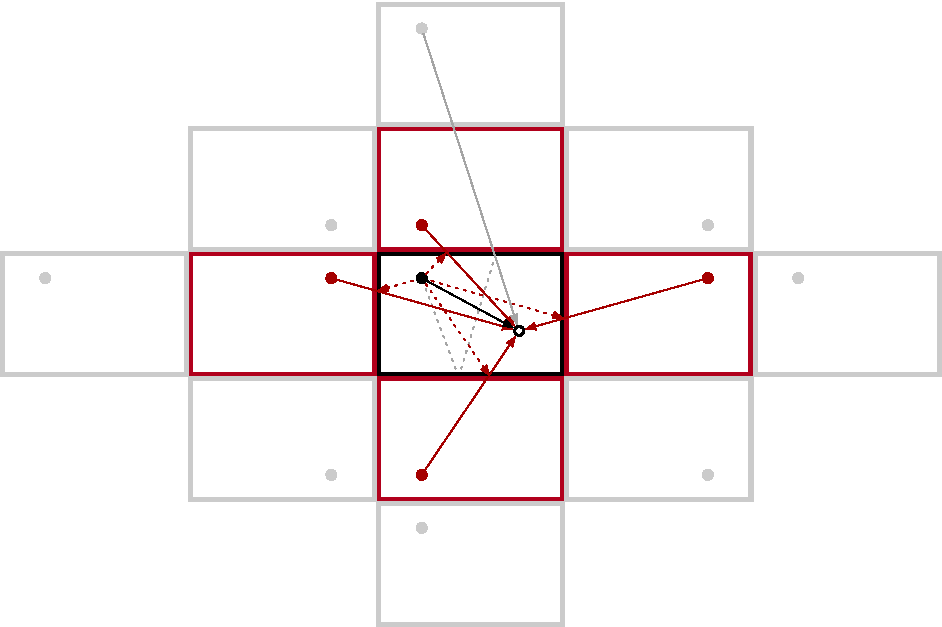
\includegraphics[width=\textwidth]{data/figures/image-method3}
    \caption[Second order image expansion for a single source and receiver]{Second order image expansion for a single source and receiver: \itshape The black rectangle represents the room that is being simulated, containing the source (black dot) and the receiver (black circle). The red rectangles represent the first-order image expansion, where every signal wave arriving at the receiver after being reflected one time (dotted red arrows), is simulated as a direct arrival wave (red arrows) to the virtual source (red dot) in the image of the room, mirrored at the reflection wall. The grey rectangles represent the second-order images for signal waves that are subject to two reflections (dotted grey arrow).}
    \label{fig:imageMethod}
\end{figure}

To conduct the experimental part this thesis, simulation as means of data collection has been chosen over real recordings, as simulated acoustic environments are more flexible compared to a laboratory environment. To simulate the experimental setup \alt{in it's different configurations} described in Section \ref{sec:setup}, the \emph{image-source method} for small-room acoustics is used \cite{Allen1979}. The basic idea of this method is to simulate an arriving signal wave reflected from the walls as a wave arriving directly from a virtual sources, mirrored at the reflecting wall.\alt{direct arrival waves of a mirror image of the room on the reflecting wall.} Two parameters determine, how many images are created during simulation with everything else being equal: The reverbaration time \Tsixty, the time it takes the source signal to have decreased by 60dB after the exciting source is switched off, and the reflection order $r$, which is equal to the maximum order of the image expansion. Instead of explicitly stating \Tsixty, the wall reflection coefficients $\beta = [\beta_1, \beta_2,\dots,\beta_6]$ could also be provided, simulating different types walls, like concrete walls or walls with sound proofing. There is one coefficient per wall, including the ceiling and the floor, for a total of six coefficients. Whenever the signal crosses a wall into another image (i.e., being reflected), it is attenuated by the $\beta$-coefficient of that wall. An example of a second-order image expansion is shown in \autoref{fig:imageMethod}.

This method allowed for experiments, where a controlled acoustic environment in form of a small, rectangular room is required, that can be easily adjusted. For many experiments\alt{experiments with budget- and time-constraints}, constructing such an environment in a laboratory is prohibitive, which is why the image method has gained widespread popularity since its inception in \citeyear{Allen1979}~\cite{Allen1979} and has been used in a wide range of studies \cite{Champagne1996}.
%TODO: Cite more studies using the image method

%shows the second-order image expansion, meaning only received signals of up to two reflections are displayed. The direct propagation path is shown in black, the first order images (including real and virtual propagation paths) are shown in red, and the second order images (including one propagation path as example) are shown in gray. Dotted lines
\subsection{Localisation Performance Measure}
\label{sec:performanceMeasure}

Intuitively, the localisation error for a given source $s$ is given by the Euclidean distance between the original source position $\ps$ and the location estimate $\psest$

\begin{equation}
	\epsilon_s = \norm{\ps-\psest}_{_2}.
	\label{eq:error}
\end{equation}

\paragraph{Aggregate Measure} Whenever the aggregation of data into a single measure is pursued, the loss of information about some of the original information is inevitable. Nevertheless, to evaluate and compare the results for different parameter sets, the raw data has to be aggregated in a way that allows for straightforward comparison of the results. For this kind of error aggregation, there are several different measures used in the literature, the two most common of them being the \gls{mae} and the \gls{rmse}
\begin{align}
	\text{\glsentryshort{mae}}  & =\frac{1}{S}\sum_{s=1}^{S}\abs{\epsilon_s},    \\[6pt]
	\text{\glsentryshort{rmse}} & =\sqrt{\frac{1}{S}\sum_{s=1}^{S}\epsilon_s^2}.
	\label{eq:maeGeneral}
\end{align}

The underlying assumption of the \gls{rmse} is an unbiased error that follows a normal distribution. This might be the case for trials, where localisation is severely affected by noise and reverberation, but does not fit trials, where localisation is good, meaning most errors are zero, and only few but large outliers occur. The \gls{rmse} overemphasises these outliers, whereas the \gls{mae} weights every error equal. Therefore, the \gls{mae} is a more accurate performance measure for the static localisation trials.

\paragraph{Assigning Estimates} To calculate the \gls{mae}, the location estimates have to be assigned to the original source locations. However, neither the localisation nor the tracking algorithm creates an identity between original source location and location estimate, as the original source location is inherently unknown to the algorithm. Therefore, assigning this identity to compute a sensible localisation error introduces a bias, that depends on the assignment strategy. One way of assigning estimates to their respective true location would be to minimise the overall \gls{mae}. The downside with this approach is that estimates close to one source might be assigned to another, more remote one, so that the overall error is minimised (A result where this would happen is shown in \autoref{fig:assignmentExamples}(a)). In other words, one correctly and one incorrectly estimated source locations could result in an assignment, that states two incorrectly estimates sources, which is undesirable if we want to evaluate, what the percentage of correct location estimates is across different trials. The solution is to assign estimates that are closer to one of the source positions first. This can be done by calculating the matrix of distances $\bm{D}_{ij}$ between the location estimates $\hat\p_s$ and the actual source positions $\p_s$

\begin{equation}
	\bm{D}_{ij}=
	\begin{bmatrix}
		d_{11} & d_{12} & \dots  & d_{1S} \\
		d_{21} & d_{22} & \dots  & d_{2S}        \\
		\vdots   & \vdots   & \ddots & \vdots   \\
		d_{S1} & d_{S2}        & \dots  & d_{SS}
	\end{bmatrix},
\end{equation}

where $i,j\ \in \{1,\dots,S\}$ and $d_{ij}$ denotes the distance between the $i$-th source position $\p_{s=i}$ and the $j$-th location estimate $\hat\p_{s=j}$. In this context, assigning estimates to source locations means selecting a combination of $S$ different $d_{ij}$, so that no column and no row is taken from twice. This procedure is described in \autoref{alg:assignment}. The result is a set of distances $\mathcal{D}$ (a possible result for $S=3$ would be $\mathcal{D}=\{d_{13}, d_{21}, d_{32}\}$, where the third location estimate is assigned to the first source location, the first estimate is assigned to the second source position and the second estimate is assigned to the third source position), which can then be used to calculate the \gls{mae} according to \eqref{eq:mae}
\begin{equation}
    \text{\glsentryshort{mae}}=\frac{1}{S}\sum_{d_{ij}\in\mathcal{D}}\abs{d_{ij}}.
    \label{eq:mae}
\end{equation}

When there are two minimum distances $d_{ij}$ of equal value, one is chosen that minimises the overall \gls{mae}. This can be done by carrying out the algorithm once for each possibility and choosing the assignments with the lower \gls{mae}.
\begin{algorithm}[!htb]
\caption{Assigning Location Estimates to Source Positions}
\label{alg:assignment}
\begin{algorithmic}
    \While{$\bm{D}_{ij}$ has elements}
    \State find smallest $d_{ij}\ \in\ \bm{D}_{ij}$ 
    \State eliminate $i$-th row and $j$-th column of $\bm{D}_{ij}$
    \EndWhile
\end{algorithmic}
\end{algorithm}

\begin{figure}[H]
	\setlength{\figureheight}{6cm}
% three plots
%	\begin{subfigure}{0.32\textwidth}
%	\centering
%%		\includegraphics[width=\textwidth]{plots/assignment/assignment-problematic-MANUAL2}  % PLACEHOLDER
%        \footnotesize
%        \setlength{\figurewidth}{0.95\textwidth}
%        % This file was created by matlab2tikz.
%
\definecolor{mycolor1}{rgb}{1.00000,1.00000,0.00000}%
%
\begin{tikzpicture}

\begin{axis}[%
width=0.951\figurewidth,
height=\figureheight,
at={(0\figurewidth,0\figureheight)},
scale only axis,
xmin=-0,
xmax=6,
ymin=-0,
ymax=6,
axis background/.style={fill=white},
axis x line*=bottom,
axis y line*=left
]

\addplot[%
surf,
shader=interp, colormap={mymap}{[1pt] rgb(0pt)=(0.239216,0.14902,0.658824); rgb(1pt)=(0.239216,0.14902,0.658824)}, mesh/rows=6]
table[row sep=crcr, point meta=\thisrow{c}] {%
%
x	y	c\\
0	0	0\\
0	1.2	0\\
0	2.4	0\\
0	3.6	0\\
0	4.8	0\\
0	6	0\\
1.2	0	0\\
1.2	1.2	0\\
1.2	2.4	0\\
1.2	3.6	0\\
1.2	4.8	0\\
1.2	6	0\\
2.4	0	0\\
2.4	1.2	0\\
2.4	2.4	0\\
2.4	3.6	0\\
2.4	4.8	0\\
2.4	6	0\\
3.6	0	0\\
3.6	1.2	0\\
3.6	2.4	0\\
3.6	3.6	0\\
3.6	4.8	0\\
3.6	6	0\\
4.8	0	0\\
4.8	1.2	0\\
4.8	2.4	0\\
4.8	3.6	0\\
4.8	4.8	0\\
4.8	6	0\\
6	0	0\\
6	1.2	0\\
6	2.4	0\\
6	3.6	0\\
6	4.8	0\\
6	6	0\\
};
\addplot [color=green, line width=1.0pt, draw=none, mark size=4.0pt, mark=o, mark options={solid, green}, forget plot]
  table[row sep=crcr]{%
2.1	1\\
2.3	1\\
2.7	1\\
2.9	1\\
3.7	1\\
3.9	1\\
5	2.2\\
5	2.4\\
5	2.8\\
5	3\\
5	3.8\\
5	4\\
2.2	5\\
2.4	5\\
3	5\\
3.2	5\\
3.8	5\\
4	5\\
1	2.1\\
1	2.3\\
1	2.9\\
1	3.1\\
1	3.7\\
1	3.9\\
};
\addplot [color=red, line width=1.0pt, draw=none, mark size=6.0pt, mark=x, mark options={solid, red}, forget plot]
  table[row sep=crcr]{%
3.3	3\\
2.7	3\\
};
\addplot [color=black, draw=none, mark size=0.2pt, mark=*, mark options={solid, black}, forget plot]
  table[row sep=crcr]{%
0.1	0.1\\
0.1	0.2\\
0.1	0.3\\
0.1	0.4\\
0.1	0.5\\
0.1	0.6\\
0.1	0.7\\
0.1	0.8\\
0.1	0.9\\
0.1	1\\
0.1	1.1\\
0.1	1.2\\
0.1	1.3\\
0.1	1.4\\
0.1	1.5\\
0.1	1.6\\
0.1	1.7\\
0.1	1.8\\
0.1	1.9\\
0.1	2\\
0.1	2.1\\
0.1	2.2\\
0.1	2.3\\
0.1	2.4\\
0.1	2.5\\
0.1	2.6\\
0.1	2.7\\
0.1	2.8\\
0.1	2.9\\
0.1	3\\
0.1	3.1\\
0.1	3.2\\
0.1	3.3\\
0.1	3.4\\
0.1	3.5\\
0.1	3.6\\
0.1	3.7\\
0.1	3.8\\
0.1	3.9\\
0.1	4\\
0.1	4.1\\
0.1	4.2\\
0.1	4.3\\
0.1	4.4\\
0.1	4.5\\
0.1	4.6\\
0.1	4.7\\
0.1	4.8\\
0.1	4.9\\
0.1	5\\
0.1	5.1\\
0.1	5.2\\
0.1	5.3\\
0.1	5.4\\
0.1	5.5\\
0.1	5.6\\
0.1	5.7\\
0.1	5.8\\
0.1	5.9\\
};
\addplot [color=black, draw=none, mark size=0.2pt, mark=*, mark options={solid, black}, forget plot]
  table[row sep=crcr]{%
0.2	0.1\\
0.2	0.2\\
0.2	0.3\\
0.2	0.4\\
0.2	0.5\\
0.2	0.6\\
0.2	0.7\\
0.2	0.8\\
0.2	0.9\\
0.2	1\\
0.2	1.1\\
0.2	1.2\\
0.2	1.3\\
0.2	1.4\\
0.2	1.5\\
0.2	1.6\\
0.2	1.7\\
0.2	1.8\\
0.2	1.9\\
0.2	2\\
0.2	2.1\\
0.2	2.2\\
0.2	2.3\\
0.2	2.4\\
0.2	2.5\\
0.2	2.6\\
0.2	2.7\\
0.2	2.8\\
0.2	2.9\\
0.2	3\\
0.2	3.1\\
0.2	3.2\\
0.2	3.3\\
0.2	3.4\\
0.2	3.5\\
0.2	3.6\\
0.2	3.7\\
0.2	3.8\\
0.2	3.9\\
0.2	4\\
0.2	4.1\\
0.2	4.2\\
0.2	4.3\\
0.2	4.4\\
0.2	4.5\\
0.2	4.6\\
0.2	4.7\\
0.2	4.8\\
0.2	4.9\\
0.2	5\\
0.2	5.1\\
0.2	5.2\\
0.2	5.3\\
0.2	5.4\\
0.2	5.5\\
0.2	5.6\\
0.2	5.7\\
0.2	5.8\\
0.2	5.9\\
};
\addplot [color=black, draw=none, mark size=0.2pt, mark=*, mark options={solid, black}, forget plot]
  table[row sep=crcr]{%
0.3	0.1\\
0.3	0.2\\
0.3	0.3\\
0.3	0.4\\
0.3	0.5\\
0.3	0.6\\
0.3	0.7\\
0.3	0.8\\
0.3	0.9\\
0.3	1\\
0.3	1.1\\
0.3	1.2\\
0.3	1.3\\
0.3	1.4\\
0.3	1.5\\
0.3	1.6\\
0.3	1.7\\
0.3	1.8\\
0.3	1.9\\
0.3	2\\
0.3	2.1\\
0.3	2.2\\
0.3	2.3\\
0.3	2.4\\
0.3	2.5\\
0.3	2.6\\
0.3	2.7\\
0.3	2.8\\
0.3	2.9\\
0.3	3\\
0.3	3.1\\
0.3	3.2\\
0.3	3.3\\
0.3	3.4\\
0.3	3.5\\
0.3	3.6\\
0.3	3.7\\
0.3	3.8\\
0.3	3.9\\
0.3	4\\
0.3	4.1\\
0.3	4.2\\
0.3	4.3\\
0.3	4.4\\
0.3	4.5\\
0.3	4.6\\
0.3	4.7\\
0.3	4.8\\
0.3	4.9\\
0.3	5\\
0.3	5.1\\
0.3	5.2\\
0.3	5.3\\
0.3	5.4\\
0.3	5.5\\
0.3	5.6\\
0.3	5.7\\
0.3	5.8\\
0.3	5.9\\
};
\addplot [color=black, draw=none, mark size=0.2pt, mark=*, mark options={solid, black}, forget plot]
  table[row sep=crcr]{%
0.4	0.1\\
0.4	0.2\\
0.4	0.3\\
0.4	0.4\\
0.4	0.5\\
0.4	0.6\\
0.4	0.7\\
0.4	0.8\\
0.4	0.9\\
0.4	1\\
0.4	1.1\\
0.4	1.2\\
0.4	1.3\\
0.4	1.4\\
0.4	1.5\\
0.4	1.6\\
0.4	1.7\\
0.4	1.8\\
0.4	1.9\\
0.4	2\\
0.4	2.1\\
0.4	2.2\\
0.4	2.3\\
0.4	2.4\\
0.4	2.5\\
0.4	2.6\\
0.4	2.7\\
0.4	2.8\\
0.4	2.9\\
0.4	3\\
0.4	3.1\\
0.4	3.2\\
0.4	3.3\\
0.4	3.4\\
0.4	3.5\\
0.4	3.6\\
0.4	3.7\\
0.4	3.8\\
0.4	3.9\\
0.4	4\\
0.4	4.1\\
0.4	4.2\\
0.4	4.3\\
0.4	4.4\\
0.4	4.5\\
0.4	4.6\\
0.4	4.7\\
0.4	4.8\\
0.4	4.9\\
0.4	5\\
0.4	5.1\\
0.4	5.2\\
0.4	5.3\\
0.4	5.4\\
0.4	5.5\\
0.4	5.6\\
0.4	5.7\\
0.4	5.8\\
0.4	5.9\\
};
\addplot [color=black, draw=none, mark size=0.2pt, mark=*, mark options={solid, black}, forget plot]
  table[row sep=crcr]{%
0.5	0.1\\
0.5	0.2\\
0.5	0.3\\
0.5	0.4\\
0.5	0.5\\
0.5	0.6\\
0.5	0.7\\
0.5	0.8\\
0.5	0.9\\
0.5	1\\
0.5	1.1\\
0.5	1.2\\
0.5	1.3\\
0.5	1.4\\
0.5	1.5\\
0.5	1.6\\
0.5	1.7\\
0.5	1.8\\
0.5	1.9\\
0.5	2\\
0.5	2.1\\
0.5	2.2\\
0.5	2.3\\
0.5	2.4\\
0.5	2.5\\
0.5	2.6\\
0.5	2.7\\
0.5	2.8\\
0.5	2.9\\
0.5	3\\
0.5	3.1\\
0.5	3.2\\
0.5	3.3\\
0.5	3.4\\
0.5	3.5\\
0.5	3.6\\
0.5	3.7\\
0.5	3.8\\
0.5	3.9\\
0.5	4\\
0.5	4.1\\
0.5	4.2\\
0.5	4.3\\
0.5	4.4\\
0.5	4.5\\
0.5	4.6\\
0.5	4.7\\
0.5	4.8\\
0.5	4.9\\
0.5	5\\
0.5	5.1\\
0.5	5.2\\
0.5	5.3\\
0.5	5.4\\
0.5	5.5\\
0.5	5.6\\
0.5	5.7\\
0.5	5.8\\
0.5	5.9\\
};
\addplot [color=black, draw=none, mark size=0.2pt, mark=*, mark options={solid, black}, forget plot]
  table[row sep=crcr]{%
0.6	0.1\\
0.6	0.2\\
0.6	0.3\\
0.6	0.4\\
0.6	0.5\\
0.6	0.6\\
0.6	0.7\\
0.6	0.8\\
0.6	0.9\\
0.6	1\\
0.6	1.1\\
0.6	1.2\\
0.6	1.3\\
0.6	1.4\\
0.6	1.5\\
0.6	1.6\\
0.6	1.7\\
0.6	1.8\\
0.6	1.9\\
0.6	2\\
0.6	2.1\\
0.6	2.2\\
0.6	2.3\\
0.6	2.4\\
0.6	2.5\\
0.6	2.6\\
0.6	2.7\\
0.6	2.8\\
0.6	2.9\\
0.6	3\\
0.6	3.1\\
0.6	3.2\\
0.6	3.3\\
0.6	3.4\\
0.6	3.5\\
0.6	3.6\\
0.6	3.7\\
0.6	3.8\\
0.6	3.9\\
0.6	4\\
0.6	4.1\\
0.6	4.2\\
0.6	4.3\\
0.6	4.4\\
0.6	4.5\\
0.6	4.6\\
0.6	4.7\\
0.6	4.8\\
0.6	4.9\\
0.6	5\\
0.6	5.1\\
0.6	5.2\\
0.6	5.3\\
0.6	5.4\\
0.6	5.5\\
0.6	5.6\\
0.6	5.7\\
0.6	5.8\\
0.6	5.9\\
};
\addplot [color=black, draw=none, mark size=0.2pt, mark=*, mark options={solid, black}, forget plot]
  table[row sep=crcr]{%
0.7	0.1\\
0.7	0.2\\
0.7	0.3\\
0.7	0.4\\
0.7	0.5\\
0.7	0.6\\
0.7	0.7\\
0.7	0.8\\
0.7	0.9\\
0.7	1\\
0.7	1.1\\
0.7	1.2\\
0.7	1.3\\
0.7	1.4\\
0.7	1.5\\
0.7	1.6\\
0.7	1.7\\
0.7	1.8\\
0.7	1.9\\
0.7	2\\
0.7	2.1\\
0.7	2.2\\
0.7	2.3\\
0.7	2.4\\
0.7	2.5\\
0.7	2.6\\
0.7	2.7\\
0.7	2.8\\
0.7	2.9\\
0.7	3\\
0.7	3.1\\
0.7	3.2\\
0.7	3.3\\
0.7	3.4\\
0.7	3.5\\
0.7	3.6\\
0.7	3.7\\
0.7	3.8\\
0.7	3.9\\
0.7	4\\
0.7	4.1\\
0.7	4.2\\
0.7	4.3\\
0.7	4.4\\
0.7	4.5\\
0.7	4.6\\
0.7	4.7\\
0.7	4.8\\
0.7	4.9\\
0.7	5\\
0.7	5.1\\
0.7	5.2\\
0.7	5.3\\
0.7	5.4\\
0.7	5.5\\
0.7	5.6\\
0.7	5.7\\
0.7	5.8\\
0.7	5.9\\
};
\addplot [color=black, draw=none, mark size=0.2pt, mark=*, mark options={solid, black}, forget plot]
  table[row sep=crcr]{%
0.8	0.1\\
0.8	0.2\\
0.8	0.3\\
0.8	0.4\\
0.8	0.5\\
0.8	0.6\\
0.8	0.7\\
0.8	0.8\\
0.8	0.9\\
0.8	1\\
0.8	1.1\\
0.8	1.2\\
0.8	1.3\\
0.8	1.4\\
0.8	1.5\\
0.8	1.6\\
0.8	1.7\\
0.8	1.8\\
0.8	1.9\\
0.8	2\\
0.8	2.1\\
0.8	2.2\\
0.8	2.3\\
0.8	2.4\\
0.8	2.5\\
0.8	2.6\\
0.8	2.7\\
0.8	2.8\\
0.8	2.9\\
0.8	3\\
0.8	3.1\\
0.8	3.2\\
0.8	3.3\\
0.8	3.4\\
0.8	3.5\\
0.8	3.6\\
0.8	3.7\\
0.8	3.8\\
0.8	3.9\\
0.8	4\\
0.8	4.1\\
0.8	4.2\\
0.8	4.3\\
0.8	4.4\\
0.8	4.5\\
0.8	4.6\\
0.8	4.7\\
0.8	4.8\\
0.8	4.9\\
0.8	5\\
0.8	5.1\\
0.8	5.2\\
0.8	5.3\\
0.8	5.4\\
0.8	5.5\\
0.8	5.6\\
0.8	5.7\\
0.8	5.8\\
0.8	5.9\\
};
\addplot [color=black, draw=none, mark size=0.2pt, mark=*, mark options={solid, black}, forget plot]
  table[row sep=crcr]{%
0.9	0.1\\
0.9	0.2\\
0.9	0.3\\
0.9	0.4\\
0.9	0.5\\
0.9	0.6\\
0.9	0.7\\
0.9	0.8\\
0.9	0.9\\
0.9	1\\
0.9	1.1\\
0.9	1.2\\
0.9	1.3\\
0.9	1.4\\
0.9	1.5\\
0.9	1.6\\
0.9	1.7\\
0.9	1.8\\
0.9	1.9\\
0.9	2\\
0.9	2.1\\
0.9	2.2\\
0.9	2.3\\
0.9	2.4\\
0.9	2.5\\
0.9	2.6\\
0.9	2.7\\
0.9	2.8\\
0.9	2.9\\
0.9	3\\
0.9	3.1\\
0.9	3.2\\
0.9	3.3\\
0.9	3.4\\
0.9	3.5\\
0.9	3.6\\
0.9	3.7\\
0.9	3.8\\
0.9	3.9\\
0.9	4\\
0.9	4.1\\
0.9	4.2\\
0.9	4.3\\
0.9	4.4\\
0.9	4.5\\
0.9	4.6\\
0.9	4.7\\
0.9	4.8\\
0.9	4.9\\
0.9	5\\
0.9	5.1\\
0.9	5.2\\
0.9	5.3\\
0.9	5.4\\
0.9	5.5\\
0.9	5.6\\
0.9	5.7\\
0.9	5.8\\
0.9	5.9\\
};
\addplot [color=black, draw=none, mark size=0.2pt, mark=*, mark options={solid, black}, forget plot]
  table[row sep=crcr]{%
1	0.1\\
1	0.2\\
1	0.3\\
1	0.4\\
1	0.5\\
1	0.6\\
1	0.7\\
1	0.8\\
1	0.9\\
1	1\\
1	1.1\\
1	1.2\\
1	1.3\\
1	1.4\\
1	1.5\\
1	1.6\\
1	1.7\\
1	1.8\\
1	1.9\\
1	2\\
1	2.1\\
1	2.2\\
1	2.3\\
1	2.4\\
1	2.5\\
1	2.6\\
1	2.7\\
1	2.8\\
1	2.9\\
1	3\\
1	3.1\\
1	3.2\\
1	3.3\\
1	3.4\\
1	3.5\\
1	3.6\\
1	3.7\\
1	3.8\\
1	3.9\\
1	4\\
1	4.1\\
1	4.2\\
1	4.3\\
1	4.4\\
1	4.5\\
1	4.6\\
1	4.7\\
1	4.8\\
1	4.9\\
1	5\\
1	5.1\\
1	5.2\\
1	5.3\\
1	5.4\\
1	5.5\\
1	5.6\\
1	5.7\\
1	5.8\\
1	5.9\\
};
\addplot [color=black, draw=none, mark size=0.2pt, mark=*, mark options={solid, black}, forget plot]
  table[row sep=crcr]{%
1.1	0.1\\
1.1	0.2\\
1.1	0.3\\
1.1	0.4\\
1.1	0.5\\
1.1	0.6\\
1.1	0.7\\
1.1	0.8\\
1.1	0.9\\
1.1	1\\
1.1	1.1\\
1.1	1.2\\
1.1	1.3\\
1.1	1.4\\
1.1	1.5\\
1.1	1.6\\
1.1	1.7\\
1.1	1.8\\
1.1	1.9\\
1.1	2\\
1.1	2.1\\
1.1	2.2\\
1.1	2.3\\
1.1	2.4\\
1.1	2.5\\
1.1	2.6\\
1.1	2.7\\
1.1	2.8\\
1.1	2.9\\
1.1	3\\
1.1	3.1\\
1.1	3.2\\
1.1	3.3\\
1.1	3.4\\
1.1	3.5\\
1.1	3.6\\
1.1	3.7\\
1.1	3.8\\
1.1	3.9\\
1.1	4\\
1.1	4.1\\
1.1	4.2\\
1.1	4.3\\
1.1	4.4\\
1.1	4.5\\
1.1	4.6\\
1.1	4.7\\
1.1	4.8\\
1.1	4.9\\
1.1	5\\
1.1	5.1\\
1.1	5.2\\
1.1	5.3\\
1.1	5.4\\
1.1	5.5\\
1.1	5.6\\
1.1	5.7\\
1.1	5.8\\
1.1	5.9\\
};
\addplot [color=black, draw=none, mark size=0.2pt, mark=*, mark options={solid, black}, forget plot]
  table[row sep=crcr]{%
1.2	0.1\\
1.2	0.2\\
1.2	0.3\\
1.2	0.4\\
1.2	0.5\\
1.2	0.6\\
1.2	0.7\\
1.2	0.8\\
1.2	0.9\\
1.2	1\\
1.2	1.1\\
1.2	1.2\\
1.2	1.3\\
1.2	1.4\\
1.2	1.5\\
1.2	1.6\\
1.2	1.7\\
1.2	1.8\\
1.2	1.9\\
1.2	2\\
1.2	2.1\\
1.2	2.2\\
1.2	2.3\\
1.2	2.4\\
1.2	2.5\\
1.2	2.6\\
1.2	2.7\\
1.2	2.8\\
1.2	2.9\\
1.2	3\\
1.2	3.1\\
1.2	3.2\\
1.2	3.3\\
1.2	3.4\\
1.2	3.5\\
1.2	3.6\\
1.2	3.7\\
1.2	3.8\\
1.2	3.9\\
1.2	4\\
1.2	4.1\\
1.2	4.2\\
1.2	4.3\\
1.2	4.4\\
1.2	4.5\\
1.2	4.6\\
1.2	4.7\\
1.2	4.8\\
1.2	4.9\\
1.2	5\\
1.2	5.1\\
1.2	5.2\\
1.2	5.3\\
1.2	5.4\\
1.2	5.5\\
1.2	5.6\\
1.2	5.7\\
1.2	5.8\\
1.2	5.9\\
};
\addplot [color=black, draw=none, mark size=0.2pt, mark=*, mark options={solid, black}, forget plot]
  table[row sep=crcr]{%
1.3	0.1\\
1.3	0.2\\
1.3	0.3\\
1.3	0.4\\
1.3	0.5\\
1.3	0.6\\
1.3	0.7\\
1.3	0.8\\
1.3	0.9\\
1.3	1\\
1.3	1.1\\
1.3	1.2\\
1.3	1.3\\
1.3	1.4\\
1.3	1.5\\
1.3	1.6\\
1.3	1.7\\
1.3	1.8\\
1.3	1.9\\
1.3	2\\
1.3	2.1\\
1.3	2.2\\
1.3	2.3\\
1.3	2.4\\
1.3	2.5\\
1.3	2.6\\
1.3	2.7\\
1.3	2.8\\
1.3	2.9\\
1.3	3\\
1.3	3.1\\
1.3	3.2\\
1.3	3.3\\
1.3	3.4\\
1.3	3.5\\
1.3	3.6\\
1.3	3.7\\
1.3	3.8\\
1.3	3.9\\
1.3	4\\
1.3	4.1\\
1.3	4.2\\
1.3	4.3\\
1.3	4.4\\
1.3	4.5\\
1.3	4.6\\
1.3	4.7\\
1.3	4.8\\
1.3	4.9\\
1.3	5\\
1.3	5.1\\
1.3	5.2\\
1.3	5.3\\
1.3	5.4\\
1.3	5.5\\
1.3	5.6\\
1.3	5.7\\
1.3	5.8\\
1.3	5.9\\
};
\addplot [color=black, draw=none, mark size=0.2pt, mark=*, mark options={solid, black}, forget plot]
  table[row sep=crcr]{%
1.4	0.1\\
1.4	0.2\\
1.4	0.3\\
1.4	0.4\\
1.4	0.5\\
1.4	0.6\\
1.4	0.7\\
1.4	0.8\\
1.4	0.9\\
1.4	1\\
1.4	1.1\\
1.4	1.2\\
1.4	1.3\\
1.4	1.4\\
1.4	1.5\\
1.4	1.6\\
1.4	1.7\\
1.4	1.8\\
1.4	1.9\\
1.4	2\\
1.4	2.1\\
1.4	2.2\\
1.4	2.3\\
1.4	2.4\\
1.4	2.5\\
1.4	2.6\\
1.4	2.7\\
1.4	2.8\\
1.4	2.9\\
1.4	3\\
1.4	3.1\\
1.4	3.2\\
1.4	3.3\\
1.4	3.4\\
1.4	3.5\\
1.4	3.6\\
1.4	3.7\\
1.4	3.8\\
1.4	3.9\\
1.4	4\\
1.4	4.1\\
1.4	4.2\\
1.4	4.3\\
1.4	4.4\\
1.4	4.5\\
1.4	4.6\\
1.4	4.7\\
1.4	4.8\\
1.4	4.9\\
1.4	5\\
1.4	5.1\\
1.4	5.2\\
1.4	5.3\\
1.4	5.4\\
1.4	5.5\\
1.4	5.6\\
1.4	5.7\\
1.4	5.8\\
1.4	5.9\\
};
\addplot [color=black, draw=none, mark size=0.2pt, mark=*, mark options={solid, black}, forget plot]
  table[row sep=crcr]{%
1.5	0.1\\
1.5	0.2\\
1.5	0.3\\
1.5	0.4\\
1.5	0.5\\
1.5	0.6\\
1.5	0.7\\
1.5	0.8\\
1.5	0.9\\
1.5	1\\
1.5	1.1\\
1.5	1.2\\
1.5	1.3\\
1.5	1.4\\
1.5	1.5\\
1.5	1.6\\
1.5	1.7\\
1.5	1.8\\
1.5	1.9\\
1.5	2\\
1.5	2.1\\
1.5	2.2\\
1.5	2.3\\
1.5	2.4\\
1.5	2.5\\
1.5	2.6\\
1.5	2.7\\
1.5	2.8\\
1.5	2.9\\
1.5	3\\
1.5	3.1\\
1.5	3.2\\
1.5	3.3\\
1.5	3.4\\
1.5	3.5\\
1.5	3.6\\
1.5	3.7\\
1.5	3.8\\
1.5	3.9\\
1.5	4\\
1.5	4.1\\
1.5	4.2\\
1.5	4.3\\
1.5	4.4\\
1.5	4.5\\
1.5	4.6\\
1.5	4.7\\
1.5	4.8\\
1.5	4.9\\
1.5	5\\
1.5	5.1\\
1.5	5.2\\
1.5	5.3\\
1.5	5.4\\
1.5	5.5\\
1.5	5.6\\
1.5	5.7\\
1.5	5.8\\
1.5	5.9\\
};
\addplot [color=black, draw=none, mark size=0.2pt, mark=*, mark options={solid, black}, forget plot]
  table[row sep=crcr]{%
1.6	0.1\\
1.6	0.2\\
1.6	0.3\\
1.6	0.4\\
1.6	0.5\\
1.6	0.6\\
1.6	0.7\\
1.6	0.8\\
1.6	0.9\\
1.6	1\\
1.6	1.1\\
1.6	1.2\\
1.6	1.3\\
1.6	1.4\\
1.6	1.5\\
1.6	1.6\\
1.6	1.7\\
1.6	1.8\\
1.6	1.9\\
1.6	2\\
1.6	2.1\\
1.6	2.2\\
1.6	2.3\\
1.6	2.4\\
1.6	2.5\\
1.6	2.6\\
1.6	2.7\\
1.6	2.8\\
1.6	2.9\\
1.6	3\\
1.6	3.1\\
1.6	3.2\\
1.6	3.3\\
1.6	3.4\\
1.6	3.5\\
1.6	3.6\\
1.6	3.7\\
1.6	3.8\\
1.6	3.9\\
1.6	4\\
1.6	4.1\\
1.6	4.2\\
1.6	4.3\\
1.6	4.4\\
1.6	4.5\\
1.6	4.6\\
1.6	4.7\\
1.6	4.8\\
1.6	4.9\\
1.6	5\\
1.6	5.1\\
1.6	5.2\\
1.6	5.3\\
1.6	5.4\\
1.6	5.5\\
1.6	5.6\\
1.6	5.7\\
1.6	5.8\\
1.6	5.9\\
};
\addplot [color=black, draw=none, mark size=0.2pt, mark=*, mark options={solid, black}, forget plot]
  table[row sep=crcr]{%
1.7	0.1\\
1.7	0.2\\
1.7	0.3\\
1.7	0.4\\
1.7	0.5\\
1.7	0.6\\
1.7	0.7\\
1.7	0.8\\
1.7	0.9\\
1.7	1\\
1.7	1.1\\
1.7	1.2\\
1.7	1.3\\
1.7	1.4\\
1.7	1.5\\
1.7	1.6\\
1.7	1.7\\
1.7	1.8\\
1.7	1.9\\
1.7	2\\
1.7	2.1\\
1.7	2.2\\
1.7	2.3\\
1.7	2.4\\
1.7	2.5\\
1.7	2.6\\
1.7	2.7\\
1.7	2.8\\
1.7	2.9\\
1.7	3\\
1.7	3.1\\
1.7	3.2\\
1.7	3.3\\
1.7	3.4\\
1.7	3.5\\
1.7	3.6\\
1.7	3.7\\
1.7	3.8\\
1.7	3.9\\
1.7	4\\
1.7	4.1\\
1.7	4.2\\
1.7	4.3\\
1.7	4.4\\
1.7	4.5\\
1.7	4.6\\
1.7	4.7\\
1.7	4.8\\
1.7	4.9\\
1.7	5\\
1.7	5.1\\
1.7	5.2\\
1.7	5.3\\
1.7	5.4\\
1.7	5.5\\
1.7	5.6\\
1.7	5.7\\
1.7	5.8\\
1.7	5.9\\
};
\addplot [color=black, draw=none, mark size=0.2pt, mark=*, mark options={solid, black}, forget plot]
  table[row sep=crcr]{%
1.8	0.1\\
1.8	0.2\\
1.8	0.3\\
1.8	0.4\\
1.8	0.5\\
1.8	0.6\\
1.8	0.7\\
1.8	0.8\\
1.8	0.9\\
1.8	1\\
1.8	1.1\\
1.8	1.2\\
1.8	1.3\\
1.8	1.4\\
1.8	1.5\\
1.8	1.6\\
1.8	1.7\\
1.8	1.8\\
1.8	1.9\\
1.8	2\\
1.8	2.1\\
1.8	2.2\\
1.8	2.3\\
1.8	2.4\\
1.8	2.5\\
1.8	2.6\\
1.8	2.7\\
1.8	2.8\\
1.8	2.9\\
1.8	3\\
1.8	3.1\\
1.8	3.2\\
1.8	3.3\\
1.8	3.4\\
1.8	3.5\\
1.8	3.6\\
1.8	3.7\\
1.8	3.8\\
1.8	3.9\\
1.8	4\\
1.8	4.1\\
1.8	4.2\\
1.8	4.3\\
1.8	4.4\\
1.8	4.5\\
1.8	4.6\\
1.8	4.7\\
1.8	4.8\\
1.8	4.9\\
1.8	5\\
1.8	5.1\\
1.8	5.2\\
1.8	5.3\\
1.8	5.4\\
1.8	5.5\\
1.8	5.6\\
1.8	5.7\\
1.8	5.8\\
1.8	5.9\\
};
\addplot [color=black, draw=none, mark size=0.2pt, mark=*, mark options={solid, black}, forget plot]
  table[row sep=crcr]{%
1.9	0.1\\
1.9	0.2\\
1.9	0.3\\
1.9	0.4\\
1.9	0.5\\
1.9	0.6\\
1.9	0.7\\
1.9	0.8\\
1.9	0.9\\
1.9	1\\
1.9	1.1\\
1.9	1.2\\
1.9	1.3\\
1.9	1.4\\
1.9	1.5\\
1.9	1.6\\
1.9	1.7\\
1.9	1.8\\
1.9	1.9\\
1.9	2\\
1.9	2.1\\
1.9	2.2\\
1.9	2.3\\
1.9	2.4\\
1.9	2.5\\
1.9	2.6\\
1.9	2.7\\
1.9	2.8\\
1.9	2.9\\
1.9	3\\
1.9	3.1\\
1.9	3.2\\
1.9	3.3\\
1.9	3.4\\
1.9	3.5\\
1.9	3.6\\
1.9	3.7\\
1.9	3.8\\
1.9	3.9\\
1.9	4\\
1.9	4.1\\
1.9	4.2\\
1.9	4.3\\
1.9	4.4\\
1.9	4.5\\
1.9	4.6\\
1.9	4.7\\
1.9	4.8\\
1.9	4.9\\
1.9	5\\
1.9	5.1\\
1.9	5.2\\
1.9	5.3\\
1.9	5.4\\
1.9	5.5\\
1.9	5.6\\
1.9	5.7\\
1.9	5.8\\
1.9	5.9\\
};
\addplot [color=black, draw=none, mark size=0.2pt, mark=*, mark options={solid, black}, forget plot]
  table[row sep=crcr]{%
2	0.1\\
2	0.2\\
2	0.3\\
2	0.4\\
2	0.5\\
2	0.6\\
2	0.7\\
2	0.8\\
2	0.9\\
2	1\\
2	1.1\\
2	1.2\\
2	1.3\\
2	1.4\\
2	1.5\\
2	1.6\\
2	1.7\\
2	1.8\\
2	1.9\\
2	2\\
2	2.1\\
2	2.2\\
2	2.3\\
2	2.4\\
2	2.5\\
2	2.6\\
2	2.7\\
2	2.8\\
2	2.9\\
2	3\\
2	3.1\\
2	3.2\\
2	3.3\\
2	3.4\\
2	3.5\\
2	3.6\\
2	3.7\\
2	3.8\\
2	3.9\\
2	4\\
2	4.1\\
2	4.2\\
2	4.3\\
2	4.4\\
2	4.5\\
2	4.6\\
2	4.7\\
2	4.8\\
2	4.9\\
2	5\\
2	5.1\\
2	5.2\\
2	5.3\\
2	5.4\\
2	5.5\\
2	5.6\\
2	5.7\\
2	5.8\\
2	5.9\\
};
\addplot [color=black, draw=none, mark size=0.2pt, mark=*, mark options={solid, black}, forget plot]
  table[row sep=crcr]{%
2.1	0.1\\
2.1	0.2\\
2.1	0.3\\
2.1	0.4\\
2.1	0.5\\
2.1	0.6\\
2.1	0.7\\
2.1	0.8\\
2.1	0.9\\
2.1	1\\
2.1	1.1\\
2.1	1.2\\
2.1	1.3\\
2.1	1.4\\
2.1	1.5\\
2.1	1.6\\
2.1	1.7\\
2.1	1.8\\
2.1	1.9\\
2.1	2\\
2.1	2.1\\
2.1	2.2\\
2.1	2.3\\
2.1	2.4\\
2.1	2.5\\
2.1	2.6\\
2.1	2.7\\
2.1	2.8\\
2.1	2.9\\
2.1	3\\
2.1	3.1\\
2.1	3.2\\
2.1	3.3\\
2.1	3.4\\
2.1	3.5\\
2.1	3.6\\
2.1	3.7\\
2.1	3.8\\
2.1	3.9\\
2.1	4\\
2.1	4.1\\
2.1	4.2\\
2.1	4.3\\
2.1	4.4\\
2.1	4.5\\
2.1	4.6\\
2.1	4.7\\
2.1	4.8\\
2.1	4.9\\
2.1	5\\
2.1	5.1\\
2.1	5.2\\
2.1	5.3\\
2.1	5.4\\
2.1	5.5\\
2.1	5.6\\
2.1	5.7\\
2.1	5.8\\
2.1	5.9\\
};
\addplot [color=black, draw=none, mark size=0.2pt, mark=*, mark options={solid, black}, forget plot]
  table[row sep=crcr]{%
2.2	0.1\\
2.2	0.2\\
2.2	0.3\\
2.2	0.4\\
2.2	0.5\\
2.2	0.6\\
2.2	0.7\\
2.2	0.8\\
2.2	0.9\\
2.2	1\\
2.2	1.1\\
2.2	1.2\\
2.2	1.3\\
2.2	1.4\\
2.2	1.5\\
2.2	1.6\\
2.2	1.7\\
2.2	1.8\\
2.2	1.9\\
2.2	2\\
2.2	2.1\\
2.2	2.2\\
2.2	2.3\\
2.2	2.4\\
2.2	2.5\\
2.2	2.6\\
2.2	2.7\\
2.2	2.8\\
2.2	2.9\\
2.2	3\\
2.2	3.1\\
2.2	3.2\\
2.2	3.3\\
2.2	3.4\\
2.2	3.5\\
2.2	3.6\\
2.2	3.7\\
2.2	3.8\\
2.2	3.9\\
2.2	4\\
2.2	4.1\\
2.2	4.2\\
2.2	4.3\\
2.2	4.4\\
2.2	4.5\\
2.2	4.6\\
2.2	4.7\\
2.2	4.8\\
2.2	4.9\\
2.2	5\\
2.2	5.1\\
2.2	5.2\\
2.2	5.3\\
2.2	5.4\\
2.2	5.5\\
2.2	5.6\\
2.2	5.7\\
2.2	5.8\\
2.2	5.9\\
};
\addplot [color=black, draw=none, mark size=0.2pt, mark=*, mark options={solid, black}, forget plot]
  table[row sep=crcr]{%
2.3	0.1\\
2.3	0.2\\
2.3	0.3\\
2.3	0.4\\
2.3	0.5\\
2.3	0.6\\
2.3	0.7\\
2.3	0.8\\
2.3	0.9\\
2.3	1\\
2.3	1.1\\
2.3	1.2\\
2.3	1.3\\
2.3	1.4\\
2.3	1.5\\
2.3	1.6\\
2.3	1.7\\
2.3	1.8\\
2.3	1.9\\
2.3	2\\
2.3	2.1\\
2.3	2.2\\
2.3	2.3\\
2.3	2.4\\
2.3	2.5\\
2.3	2.6\\
2.3	2.7\\
2.3	2.8\\
2.3	2.9\\
2.3	3\\
2.3	3.1\\
2.3	3.2\\
2.3	3.3\\
2.3	3.4\\
2.3	3.5\\
2.3	3.6\\
2.3	3.7\\
2.3	3.8\\
2.3	3.9\\
2.3	4\\
2.3	4.1\\
2.3	4.2\\
2.3	4.3\\
2.3	4.4\\
2.3	4.5\\
2.3	4.6\\
2.3	4.7\\
2.3	4.8\\
2.3	4.9\\
2.3	5\\
2.3	5.1\\
2.3	5.2\\
2.3	5.3\\
2.3	5.4\\
2.3	5.5\\
2.3	5.6\\
2.3	5.7\\
2.3	5.8\\
2.3	5.9\\
};
\addplot [color=black, draw=none, mark size=0.2pt, mark=*, mark options={solid, black}, forget plot]
  table[row sep=crcr]{%
2.4	0.1\\
2.4	0.2\\
2.4	0.3\\
2.4	0.4\\
2.4	0.5\\
2.4	0.6\\
2.4	0.7\\
2.4	0.8\\
2.4	0.9\\
2.4	1\\
2.4	1.1\\
2.4	1.2\\
2.4	1.3\\
2.4	1.4\\
2.4	1.5\\
2.4	1.6\\
2.4	1.7\\
2.4	1.8\\
2.4	1.9\\
2.4	2\\
2.4	2.1\\
2.4	2.2\\
2.4	2.3\\
2.4	2.4\\
2.4	2.5\\
2.4	2.6\\
2.4	2.7\\
2.4	2.8\\
2.4	2.9\\
2.4	3\\
2.4	3.1\\
2.4	3.2\\
2.4	3.3\\
2.4	3.4\\
2.4	3.5\\
2.4	3.6\\
2.4	3.7\\
2.4	3.8\\
2.4	3.9\\
2.4	4\\
2.4	4.1\\
2.4	4.2\\
2.4	4.3\\
2.4	4.4\\
2.4	4.5\\
2.4	4.6\\
2.4	4.7\\
2.4	4.8\\
2.4	4.9\\
2.4	5\\
2.4	5.1\\
2.4	5.2\\
2.4	5.3\\
2.4	5.4\\
2.4	5.5\\
2.4	5.6\\
2.4	5.7\\
2.4	5.8\\
2.4	5.9\\
};
\addplot [color=black, draw=none, mark size=0.2pt, mark=*, mark options={solid, black}, forget plot]
  table[row sep=crcr]{%
2.5	0.1\\
2.5	0.2\\
2.5	0.3\\
2.5	0.4\\
2.5	0.5\\
2.5	0.6\\
2.5	0.7\\
2.5	0.8\\
2.5	0.9\\
2.5	1\\
2.5	1.1\\
2.5	1.2\\
2.5	1.3\\
2.5	1.4\\
2.5	1.5\\
2.5	1.6\\
2.5	1.7\\
2.5	1.8\\
2.5	1.9\\
2.5	2\\
2.5	2.1\\
2.5	2.2\\
2.5	2.3\\
2.5	2.4\\
2.5	2.5\\
2.5	2.6\\
2.5	2.7\\
2.5	2.8\\
2.5	2.9\\
2.5	3\\
2.5	3.1\\
2.5	3.2\\
2.5	3.3\\
2.5	3.4\\
2.5	3.5\\
2.5	3.6\\
2.5	3.7\\
2.5	3.8\\
2.5	3.9\\
2.5	4\\
2.5	4.1\\
2.5	4.2\\
2.5	4.3\\
2.5	4.4\\
2.5	4.5\\
2.5	4.6\\
2.5	4.7\\
2.5	4.8\\
2.5	4.9\\
2.5	5\\
2.5	5.1\\
2.5	5.2\\
2.5	5.3\\
2.5	5.4\\
2.5	5.5\\
2.5	5.6\\
2.5	5.7\\
2.5	5.8\\
2.5	5.9\\
};
\addplot [color=black, draw=none, mark size=0.2pt, mark=*, mark options={solid, black}, forget plot]
  table[row sep=crcr]{%
2.6	0.1\\
2.6	0.2\\
2.6	0.3\\
2.6	0.4\\
2.6	0.5\\
2.6	0.6\\
2.6	0.7\\
2.6	0.8\\
2.6	0.9\\
2.6	1\\
2.6	1.1\\
2.6	1.2\\
2.6	1.3\\
2.6	1.4\\
2.6	1.5\\
2.6	1.6\\
2.6	1.7\\
2.6	1.8\\
2.6	1.9\\
2.6	2\\
2.6	2.1\\
2.6	2.2\\
2.6	2.3\\
2.6	2.4\\
2.6	2.5\\
2.6	2.6\\
2.6	2.7\\
2.6	2.8\\
2.6	2.9\\
2.6	3\\
2.6	3.1\\
2.6	3.2\\
2.6	3.3\\
2.6	3.4\\
2.6	3.5\\
2.6	3.6\\
2.6	3.7\\
2.6	3.8\\
2.6	3.9\\
2.6	4\\
2.6	4.1\\
2.6	4.2\\
2.6	4.3\\
2.6	4.4\\
2.6	4.5\\
2.6	4.6\\
2.6	4.7\\
2.6	4.8\\
2.6	4.9\\
2.6	5\\
2.6	5.1\\
2.6	5.2\\
2.6	5.3\\
2.6	5.4\\
2.6	5.5\\
2.6	5.6\\
2.6	5.7\\
2.6	5.8\\
2.6	5.9\\
};
\addplot [color=black, draw=none, mark size=0.2pt, mark=*, mark options={solid, black}, forget plot]
  table[row sep=crcr]{%
2.7	0.1\\
2.7	0.2\\
2.7	0.3\\
2.7	0.4\\
2.7	0.5\\
2.7	0.6\\
2.7	0.7\\
2.7	0.8\\
2.7	0.9\\
2.7	1\\
2.7	1.1\\
2.7	1.2\\
2.7	1.3\\
2.7	1.4\\
2.7	1.5\\
2.7	1.6\\
2.7	1.7\\
2.7	1.8\\
2.7	1.9\\
2.7	2\\
2.7	2.1\\
2.7	2.2\\
2.7	2.3\\
2.7	2.4\\
2.7	2.5\\
2.7	2.6\\
2.7	2.7\\
2.7	2.8\\
2.7	2.9\\
2.7	3\\
2.7	3.1\\
2.7	3.2\\
2.7	3.3\\
2.7	3.4\\
2.7	3.5\\
2.7	3.6\\
2.7	3.7\\
2.7	3.8\\
2.7	3.9\\
2.7	4\\
2.7	4.1\\
2.7	4.2\\
2.7	4.3\\
2.7	4.4\\
2.7	4.5\\
2.7	4.6\\
2.7	4.7\\
2.7	4.8\\
2.7	4.9\\
2.7	5\\
2.7	5.1\\
2.7	5.2\\
2.7	5.3\\
2.7	5.4\\
2.7	5.5\\
2.7	5.6\\
2.7	5.7\\
2.7	5.8\\
2.7	5.9\\
};
\addplot [color=black, draw=none, mark size=0.2pt, mark=*, mark options={solid, black}, forget plot]
  table[row sep=crcr]{%
2.8	0.1\\
2.8	0.2\\
2.8	0.3\\
2.8	0.4\\
2.8	0.5\\
2.8	0.6\\
2.8	0.7\\
2.8	0.8\\
2.8	0.9\\
2.8	1\\
2.8	1.1\\
2.8	1.2\\
2.8	1.3\\
2.8	1.4\\
2.8	1.5\\
2.8	1.6\\
2.8	1.7\\
2.8	1.8\\
2.8	1.9\\
2.8	2\\
2.8	2.1\\
2.8	2.2\\
2.8	2.3\\
2.8	2.4\\
2.8	2.5\\
2.8	2.6\\
2.8	2.7\\
2.8	2.8\\
2.8	2.9\\
2.8	3\\
2.8	3.1\\
2.8	3.2\\
2.8	3.3\\
2.8	3.4\\
2.8	3.5\\
2.8	3.6\\
2.8	3.7\\
2.8	3.8\\
2.8	3.9\\
2.8	4\\
2.8	4.1\\
2.8	4.2\\
2.8	4.3\\
2.8	4.4\\
2.8	4.5\\
2.8	4.6\\
2.8	4.7\\
2.8	4.8\\
2.8	4.9\\
2.8	5\\
2.8	5.1\\
2.8	5.2\\
2.8	5.3\\
2.8	5.4\\
2.8	5.5\\
2.8	5.6\\
2.8	5.7\\
2.8	5.8\\
2.8	5.9\\
};
\addplot [color=black, draw=none, mark size=0.2pt, mark=*, mark options={solid, black}, forget plot]
  table[row sep=crcr]{%
2.9	0.1\\
2.9	0.2\\
2.9	0.3\\
2.9	0.4\\
2.9	0.5\\
2.9	0.6\\
2.9	0.7\\
2.9	0.8\\
2.9	0.9\\
2.9	1\\
2.9	1.1\\
2.9	1.2\\
2.9	1.3\\
2.9	1.4\\
2.9	1.5\\
2.9	1.6\\
2.9	1.7\\
2.9	1.8\\
2.9	1.9\\
2.9	2\\
2.9	2.1\\
2.9	2.2\\
2.9	2.3\\
2.9	2.4\\
2.9	2.5\\
2.9	2.6\\
2.9	2.7\\
2.9	2.8\\
2.9	2.9\\
2.9	3\\
2.9	3.1\\
2.9	3.2\\
2.9	3.3\\
2.9	3.4\\
2.9	3.5\\
2.9	3.6\\
2.9	3.7\\
2.9	3.8\\
2.9	3.9\\
2.9	4\\
2.9	4.1\\
2.9	4.2\\
2.9	4.3\\
2.9	4.4\\
2.9	4.5\\
2.9	4.6\\
2.9	4.7\\
2.9	4.8\\
2.9	4.9\\
2.9	5\\
2.9	5.1\\
2.9	5.2\\
2.9	5.3\\
2.9	5.4\\
2.9	5.5\\
2.9	5.6\\
2.9	5.7\\
2.9	5.8\\
2.9	5.9\\
};
\addplot [color=black, draw=none, mark size=0.2pt, mark=*, mark options={solid, black}, forget plot]
  table[row sep=crcr]{%
3	0.1\\
3	0.2\\
3	0.3\\
3	0.4\\
3	0.5\\
3	0.6\\
3	0.7\\
3	0.8\\
3	0.9\\
3	1\\
3	1.1\\
3	1.2\\
3	1.3\\
3	1.4\\
3	1.5\\
3	1.6\\
3	1.7\\
3	1.8\\
3	1.9\\
3	2\\
3	2.1\\
3	2.2\\
3	2.3\\
3	2.4\\
3	2.5\\
3	2.6\\
3	2.7\\
3	2.8\\
3	2.9\\
3	3\\
3	3.1\\
3	3.2\\
3	3.3\\
3	3.4\\
3	3.5\\
3	3.6\\
3	3.7\\
3	3.8\\
3	3.9\\
3	4\\
3	4.1\\
3	4.2\\
3	4.3\\
3	4.4\\
3	4.5\\
3	4.6\\
3	4.7\\
3	4.8\\
3	4.9\\
3	5\\
3	5.1\\
3	5.2\\
3	5.3\\
3	5.4\\
3	5.5\\
3	5.6\\
3	5.7\\
3	5.8\\
3	5.9\\
};
\addplot [color=black, draw=none, mark size=0.2pt, mark=*, mark options={solid, black}, forget plot]
  table[row sep=crcr]{%
3.1	0.1\\
3.1	0.2\\
3.1	0.3\\
3.1	0.4\\
3.1	0.5\\
3.1	0.6\\
3.1	0.7\\
3.1	0.8\\
3.1	0.9\\
3.1	1\\
3.1	1.1\\
3.1	1.2\\
3.1	1.3\\
3.1	1.4\\
3.1	1.5\\
3.1	1.6\\
3.1	1.7\\
3.1	1.8\\
3.1	1.9\\
3.1	2\\
3.1	2.1\\
3.1	2.2\\
3.1	2.3\\
3.1	2.4\\
3.1	2.5\\
3.1	2.6\\
3.1	2.7\\
3.1	2.8\\
3.1	2.9\\
3.1	3\\
3.1	3.1\\
3.1	3.2\\
3.1	3.3\\
3.1	3.4\\
3.1	3.5\\
3.1	3.6\\
3.1	3.7\\
3.1	3.8\\
3.1	3.9\\
3.1	4\\
3.1	4.1\\
3.1	4.2\\
3.1	4.3\\
3.1	4.4\\
3.1	4.5\\
3.1	4.6\\
3.1	4.7\\
3.1	4.8\\
3.1	4.9\\
3.1	5\\
3.1	5.1\\
3.1	5.2\\
3.1	5.3\\
3.1	5.4\\
3.1	5.5\\
3.1	5.6\\
3.1	5.7\\
3.1	5.8\\
3.1	5.9\\
};
\addplot [color=black, draw=none, mark size=0.2pt, mark=*, mark options={solid, black}, forget plot]
  table[row sep=crcr]{%
3.2	0.1\\
3.2	0.2\\
3.2	0.3\\
3.2	0.4\\
3.2	0.5\\
3.2	0.6\\
3.2	0.7\\
3.2	0.8\\
3.2	0.9\\
3.2	1\\
3.2	1.1\\
3.2	1.2\\
3.2	1.3\\
3.2	1.4\\
3.2	1.5\\
3.2	1.6\\
3.2	1.7\\
3.2	1.8\\
3.2	1.9\\
3.2	2\\
3.2	2.1\\
3.2	2.2\\
3.2	2.3\\
3.2	2.4\\
3.2	2.5\\
3.2	2.6\\
3.2	2.7\\
3.2	2.8\\
3.2	2.9\\
3.2	3\\
3.2	3.1\\
3.2	3.2\\
3.2	3.3\\
3.2	3.4\\
3.2	3.5\\
3.2	3.6\\
3.2	3.7\\
3.2	3.8\\
3.2	3.9\\
3.2	4\\
3.2	4.1\\
3.2	4.2\\
3.2	4.3\\
3.2	4.4\\
3.2	4.5\\
3.2	4.6\\
3.2	4.7\\
3.2	4.8\\
3.2	4.9\\
3.2	5\\
3.2	5.1\\
3.2	5.2\\
3.2	5.3\\
3.2	5.4\\
3.2	5.5\\
3.2	5.6\\
3.2	5.7\\
3.2	5.8\\
3.2	5.9\\
};
\addplot [color=black, draw=none, mark size=0.2pt, mark=*, mark options={solid, black}, forget plot]
  table[row sep=crcr]{%
3.3	0.1\\
3.3	0.2\\
3.3	0.3\\
3.3	0.4\\
3.3	0.5\\
3.3	0.6\\
3.3	0.7\\
3.3	0.8\\
3.3	0.9\\
3.3	1\\
3.3	1.1\\
3.3	1.2\\
3.3	1.3\\
3.3	1.4\\
3.3	1.5\\
3.3	1.6\\
3.3	1.7\\
3.3	1.8\\
3.3	1.9\\
3.3	2\\
3.3	2.1\\
3.3	2.2\\
3.3	2.3\\
3.3	2.4\\
3.3	2.5\\
3.3	2.6\\
3.3	2.7\\
3.3	2.8\\
3.3	2.9\\
3.3	3\\
3.3	3.1\\
3.3	3.2\\
3.3	3.3\\
3.3	3.4\\
3.3	3.5\\
3.3	3.6\\
3.3	3.7\\
3.3	3.8\\
3.3	3.9\\
3.3	4\\
3.3	4.1\\
3.3	4.2\\
3.3	4.3\\
3.3	4.4\\
3.3	4.5\\
3.3	4.6\\
3.3	4.7\\
3.3	4.8\\
3.3	4.9\\
3.3	5\\
3.3	5.1\\
3.3	5.2\\
3.3	5.3\\
3.3	5.4\\
3.3	5.5\\
3.3	5.6\\
3.3	5.7\\
3.3	5.8\\
3.3	5.9\\
};
\addplot [color=black, draw=none, mark size=0.2pt, mark=*, mark options={solid, black}, forget plot]
  table[row sep=crcr]{%
3.4	0.1\\
3.4	0.2\\
3.4	0.3\\
3.4	0.4\\
3.4	0.5\\
3.4	0.6\\
3.4	0.7\\
3.4	0.8\\
3.4	0.9\\
3.4	1\\
3.4	1.1\\
3.4	1.2\\
3.4	1.3\\
3.4	1.4\\
3.4	1.5\\
3.4	1.6\\
3.4	1.7\\
3.4	1.8\\
3.4	1.9\\
3.4	2\\
3.4	2.1\\
3.4	2.2\\
3.4	2.3\\
3.4	2.4\\
3.4	2.5\\
3.4	2.6\\
3.4	2.7\\
3.4	2.8\\
3.4	2.9\\
3.4	3\\
3.4	3.1\\
3.4	3.2\\
3.4	3.3\\
3.4	3.4\\
3.4	3.5\\
3.4	3.6\\
3.4	3.7\\
3.4	3.8\\
3.4	3.9\\
3.4	4\\
3.4	4.1\\
3.4	4.2\\
3.4	4.3\\
3.4	4.4\\
3.4	4.5\\
3.4	4.6\\
3.4	4.7\\
3.4	4.8\\
3.4	4.9\\
3.4	5\\
3.4	5.1\\
3.4	5.2\\
3.4	5.3\\
3.4	5.4\\
3.4	5.5\\
3.4	5.6\\
3.4	5.7\\
3.4	5.8\\
3.4	5.9\\
};
\addplot [color=black, draw=none, mark size=0.2pt, mark=*, mark options={solid, black}, forget plot]
  table[row sep=crcr]{%
3.5	0.1\\
3.5	0.2\\
3.5	0.3\\
3.5	0.4\\
3.5	0.5\\
3.5	0.6\\
3.5	0.7\\
3.5	0.8\\
3.5	0.9\\
3.5	1\\
3.5	1.1\\
3.5	1.2\\
3.5	1.3\\
3.5	1.4\\
3.5	1.5\\
3.5	1.6\\
3.5	1.7\\
3.5	1.8\\
3.5	1.9\\
3.5	2\\
3.5	2.1\\
3.5	2.2\\
3.5	2.3\\
3.5	2.4\\
3.5	2.5\\
3.5	2.6\\
3.5	2.7\\
3.5	2.8\\
3.5	2.9\\
3.5	3\\
3.5	3.1\\
3.5	3.2\\
3.5	3.3\\
3.5	3.4\\
3.5	3.5\\
3.5	3.6\\
3.5	3.7\\
3.5	3.8\\
3.5	3.9\\
3.5	4\\
3.5	4.1\\
3.5	4.2\\
3.5	4.3\\
3.5	4.4\\
3.5	4.5\\
3.5	4.6\\
3.5	4.7\\
3.5	4.8\\
3.5	4.9\\
3.5	5\\
3.5	5.1\\
3.5	5.2\\
3.5	5.3\\
3.5	5.4\\
3.5	5.5\\
3.5	5.6\\
3.5	5.7\\
3.5	5.8\\
3.5	5.9\\
};
\addplot [color=black, draw=none, mark size=0.2pt, mark=*, mark options={solid, black}, forget plot]
  table[row sep=crcr]{%
3.6	0.1\\
3.6	0.2\\
3.6	0.3\\
3.6	0.4\\
3.6	0.5\\
3.6	0.6\\
3.6	0.7\\
3.6	0.8\\
3.6	0.9\\
3.6	1\\
3.6	1.1\\
3.6	1.2\\
3.6	1.3\\
3.6	1.4\\
3.6	1.5\\
3.6	1.6\\
3.6	1.7\\
3.6	1.8\\
3.6	1.9\\
3.6	2\\
3.6	2.1\\
3.6	2.2\\
3.6	2.3\\
3.6	2.4\\
3.6	2.5\\
3.6	2.6\\
3.6	2.7\\
3.6	2.8\\
3.6	2.9\\
3.6	3\\
3.6	3.1\\
3.6	3.2\\
3.6	3.3\\
3.6	3.4\\
3.6	3.5\\
3.6	3.6\\
3.6	3.7\\
3.6	3.8\\
3.6	3.9\\
3.6	4\\
3.6	4.1\\
3.6	4.2\\
3.6	4.3\\
3.6	4.4\\
3.6	4.5\\
3.6	4.6\\
3.6	4.7\\
3.6	4.8\\
3.6	4.9\\
3.6	5\\
3.6	5.1\\
3.6	5.2\\
3.6	5.3\\
3.6	5.4\\
3.6	5.5\\
3.6	5.6\\
3.6	5.7\\
3.6	5.8\\
3.6	5.9\\
};
\addplot [color=black, draw=none, mark size=0.2pt, mark=*, mark options={solid, black}, forget plot]
  table[row sep=crcr]{%
3.7	0.1\\
3.7	0.2\\
3.7	0.3\\
3.7	0.4\\
3.7	0.5\\
3.7	0.6\\
3.7	0.7\\
3.7	0.8\\
3.7	0.9\\
3.7	1\\
3.7	1.1\\
3.7	1.2\\
3.7	1.3\\
3.7	1.4\\
3.7	1.5\\
3.7	1.6\\
3.7	1.7\\
3.7	1.8\\
3.7	1.9\\
3.7	2\\
3.7	2.1\\
3.7	2.2\\
3.7	2.3\\
3.7	2.4\\
3.7	2.5\\
3.7	2.6\\
3.7	2.7\\
3.7	2.8\\
3.7	2.9\\
3.7	3\\
3.7	3.1\\
3.7	3.2\\
3.7	3.3\\
3.7	3.4\\
3.7	3.5\\
3.7	3.6\\
3.7	3.7\\
3.7	3.8\\
3.7	3.9\\
3.7	4\\
3.7	4.1\\
3.7	4.2\\
3.7	4.3\\
3.7	4.4\\
3.7	4.5\\
3.7	4.6\\
3.7	4.7\\
3.7	4.8\\
3.7	4.9\\
3.7	5\\
3.7	5.1\\
3.7	5.2\\
3.7	5.3\\
3.7	5.4\\
3.7	5.5\\
3.7	5.6\\
3.7	5.7\\
3.7	5.8\\
3.7	5.9\\
};
\addplot [color=black, draw=none, mark size=0.2pt, mark=*, mark options={solid, black}, forget plot]
  table[row sep=crcr]{%
3.8	0.1\\
3.8	0.2\\
3.8	0.3\\
3.8	0.4\\
3.8	0.5\\
3.8	0.6\\
3.8	0.7\\
3.8	0.8\\
3.8	0.9\\
3.8	1\\
3.8	1.1\\
3.8	1.2\\
3.8	1.3\\
3.8	1.4\\
3.8	1.5\\
3.8	1.6\\
3.8	1.7\\
3.8	1.8\\
3.8	1.9\\
3.8	2\\
3.8	2.1\\
3.8	2.2\\
3.8	2.3\\
3.8	2.4\\
3.8	2.5\\
3.8	2.6\\
3.8	2.7\\
3.8	2.8\\
3.8	2.9\\
3.8	3\\
3.8	3.1\\
3.8	3.2\\
3.8	3.3\\
3.8	3.4\\
3.8	3.5\\
3.8	3.6\\
3.8	3.7\\
3.8	3.8\\
3.8	3.9\\
3.8	4\\
3.8	4.1\\
3.8	4.2\\
3.8	4.3\\
3.8	4.4\\
3.8	4.5\\
3.8	4.6\\
3.8	4.7\\
3.8	4.8\\
3.8	4.9\\
3.8	5\\
3.8	5.1\\
3.8	5.2\\
3.8	5.3\\
3.8	5.4\\
3.8	5.5\\
3.8	5.6\\
3.8	5.7\\
3.8	5.8\\
3.8	5.9\\
};
\addplot [color=black, draw=none, mark size=0.2pt, mark=*, mark options={solid, black}, forget plot]
  table[row sep=crcr]{%
3.9	0.1\\
3.9	0.2\\
3.9	0.3\\
3.9	0.4\\
3.9	0.5\\
3.9	0.6\\
3.9	0.7\\
3.9	0.8\\
3.9	0.9\\
3.9	1\\
3.9	1.1\\
3.9	1.2\\
3.9	1.3\\
3.9	1.4\\
3.9	1.5\\
3.9	1.6\\
3.9	1.7\\
3.9	1.8\\
3.9	1.9\\
3.9	2\\
3.9	2.1\\
3.9	2.2\\
3.9	2.3\\
3.9	2.4\\
3.9	2.5\\
3.9	2.6\\
3.9	2.7\\
3.9	2.8\\
3.9	2.9\\
3.9	3\\
3.9	3.1\\
3.9	3.2\\
3.9	3.3\\
3.9	3.4\\
3.9	3.5\\
3.9	3.6\\
3.9	3.7\\
3.9	3.8\\
3.9	3.9\\
3.9	4\\
3.9	4.1\\
3.9	4.2\\
3.9	4.3\\
3.9	4.4\\
3.9	4.5\\
3.9	4.6\\
3.9	4.7\\
3.9	4.8\\
3.9	4.9\\
3.9	5\\
3.9	5.1\\
3.9	5.2\\
3.9	5.3\\
3.9	5.4\\
3.9	5.5\\
3.9	5.6\\
3.9	5.7\\
3.9	5.8\\
3.9	5.9\\
};
\addplot [color=black, draw=none, mark size=0.2pt, mark=*, mark options={solid, black}, forget plot]
  table[row sep=crcr]{%
4	0.1\\
4	0.2\\
4	0.3\\
4	0.4\\
4	0.5\\
4	0.6\\
4	0.7\\
4	0.8\\
4	0.9\\
4	1\\
4	1.1\\
4	1.2\\
4	1.3\\
4	1.4\\
4	1.5\\
4	1.6\\
4	1.7\\
4	1.8\\
4	1.9\\
4	2\\
4	2.1\\
4	2.2\\
4	2.3\\
4	2.4\\
4	2.5\\
4	2.6\\
4	2.7\\
4	2.8\\
4	2.9\\
4	3\\
4	3.1\\
4	3.2\\
4	3.3\\
4	3.4\\
4	3.5\\
4	3.6\\
4	3.7\\
4	3.8\\
4	3.9\\
4	4\\
4	4.1\\
4	4.2\\
4	4.3\\
4	4.4\\
4	4.5\\
4	4.6\\
4	4.7\\
4	4.8\\
4	4.9\\
4	5\\
4	5.1\\
4	5.2\\
4	5.3\\
4	5.4\\
4	5.5\\
4	5.6\\
4	5.7\\
4	5.8\\
4	5.9\\
};
\addplot [color=black, draw=none, mark size=0.2pt, mark=*, mark options={solid, black}, forget plot]
  table[row sep=crcr]{%
4.1	0.1\\
4.1	0.2\\
4.1	0.3\\
4.1	0.4\\
4.1	0.5\\
4.1	0.6\\
4.1	0.7\\
4.1	0.8\\
4.1	0.9\\
4.1	1\\
4.1	1.1\\
4.1	1.2\\
4.1	1.3\\
4.1	1.4\\
4.1	1.5\\
4.1	1.6\\
4.1	1.7\\
4.1	1.8\\
4.1	1.9\\
4.1	2\\
4.1	2.1\\
4.1	2.2\\
4.1	2.3\\
4.1	2.4\\
4.1	2.5\\
4.1	2.6\\
4.1	2.7\\
4.1	2.8\\
4.1	2.9\\
4.1	3\\
4.1	3.1\\
4.1	3.2\\
4.1	3.3\\
4.1	3.4\\
4.1	3.5\\
4.1	3.6\\
4.1	3.7\\
4.1	3.8\\
4.1	3.9\\
4.1	4\\
4.1	4.1\\
4.1	4.2\\
4.1	4.3\\
4.1	4.4\\
4.1	4.5\\
4.1	4.6\\
4.1	4.7\\
4.1	4.8\\
4.1	4.9\\
4.1	5\\
4.1	5.1\\
4.1	5.2\\
4.1	5.3\\
4.1	5.4\\
4.1	5.5\\
4.1	5.6\\
4.1	5.7\\
4.1	5.8\\
4.1	5.9\\
};
\addplot [color=black, draw=none, mark size=0.2pt, mark=*, mark options={solid, black}, forget plot]
  table[row sep=crcr]{%
4.2	0.1\\
4.2	0.2\\
4.2	0.3\\
4.2	0.4\\
4.2	0.5\\
4.2	0.6\\
4.2	0.7\\
4.2	0.8\\
4.2	0.9\\
4.2	1\\
4.2	1.1\\
4.2	1.2\\
4.2	1.3\\
4.2	1.4\\
4.2	1.5\\
4.2	1.6\\
4.2	1.7\\
4.2	1.8\\
4.2	1.9\\
4.2	2\\
4.2	2.1\\
4.2	2.2\\
4.2	2.3\\
4.2	2.4\\
4.2	2.5\\
4.2	2.6\\
4.2	2.7\\
4.2	2.8\\
4.2	2.9\\
4.2	3\\
4.2	3.1\\
4.2	3.2\\
4.2	3.3\\
4.2	3.4\\
4.2	3.5\\
4.2	3.6\\
4.2	3.7\\
4.2	3.8\\
4.2	3.9\\
4.2	4\\
4.2	4.1\\
4.2	4.2\\
4.2	4.3\\
4.2	4.4\\
4.2	4.5\\
4.2	4.6\\
4.2	4.7\\
4.2	4.8\\
4.2	4.9\\
4.2	5\\
4.2	5.1\\
4.2	5.2\\
4.2	5.3\\
4.2	5.4\\
4.2	5.5\\
4.2	5.6\\
4.2	5.7\\
4.2	5.8\\
4.2	5.9\\
};
\addplot [color=black, draw=none, mark size=0.2pt, mark=*, mark options={solid, black}, forget plot]
  table[row sep=crcr]{%
4.3	0.1\\
4.3	0.2\\
4.3	0.3\\
4.3	0.4\\
4.3	0.5\\
4.3	0.6\\
4.3	0.7\\
4.3	0.8\\
4.3	0.9\\
4.3	1\\
4.3	1.1\\
4.3	1.2\\
4.3	1.3\\
4.3	1.4\\
4.3	1.5\\
4.3	1.6\\
4.3	1.7\\
4.3	1.8\\
4.3	1.9\\
4.3	2\\
4.3	2.1\\
4.3	2.2\\
4.3	2.3\\
4.3	2.4\\
4.3	2.5\\
4.3	2.6\\
4.3	2.7\\
4.3	2.8\\
4.3	2.9\\
4.3	3\\
4.3	3.1\\
4.3	3.2\\
4.3	3.3\\
4.3	3.4\\
4.3	3.5\\
4.3	3.6\\
4.3	3.7\\
4.3	3.8\\
4.3	3.9\\
4.3	4\\
4.3	4.1\\
4.3	4.2\\
4.3	4.3\\
4.3	4.4\\
4.3	4.5\\
4.3	4.6\\
4.3	4.7\\
4.3	4.8\\
4.3	4.9\\
4.3	5\\
4.3	5.1\\
4.3	5.2\\
4.3	5.3\\
4.3	5.4\\
4.3	5.5\\
4.3	5.6\\
4.3	5.7\\
4.3	5.8\\
4.3	5.9\\
};
\addplot [color=black, draw=none, mark size=0.2pt, mark=*, mark options={solid, black}, forget plot]
  table[row sep=crcr]{%
4.4	0.1\\
4.4	0.2\\
4.4	0.3\\
4.4	0.4\\
4.4	0.5\\
4.4	0.6\\
4.4	0.7\\
4.4	0.8\\
4.4	0.9\\
4.4	1\\
4.4	1.1\\
4.4	1.2\\
4.4	1.3\\
4.4	1.4\\
4.4	1.5\\
4.4	1.6\\
4.4	1.7\\
4.4	1.8\\
4.4	1.9\\
4.4	2\\
4.4	2.1\\
4.4	2.2\\
4.4	2.3\\
4.4	2.4\\
4.4	2.5\\
4.4	2.6\\
4.4	2.7\\
4.4	2.8\\
4.4	2.9\\
4.4	3\\
4.4	3.1\\
4.4	3.2\\
4.4	3.3\\
4.4	3.4\\
4.4	3.5\\
4.4	3.6\\
4.4	3.7\\
4.4	3.8\\
4.4	3.9\\
4.4	4\\
4.4	4.1\\
4.4	4.2\\
4.4	4.3\\
4.4	4.4\\
4.4	4.5\\
4.4	4.6\\
4.4	4.7\\
4.4	4.8\\
4.4	4.9\\
4.4	5\\
4.4	5.1\\
4.4	5.2\\
4.4	5.3\\
4.4	5.4\\
4.4	5.5\\
4.4	5.6\\
4.4	5.7\\
4.4	5.8\\
4.4	5.9\\
};
\addplot [color=black, draw=none, mark size=0.2pt, mark=*, mark options={solid, black}, forget plot]
  table[row sep=crcr]{%
4.5	0.1\\
4.5	0.2\\
4.5	0.3\\
4.5	0.4\\
4.5	0.5\\
4.5	0.6\\
4.5	0.7\\
4.5	0.8\\
4.5	0.9\\
4.5	1\\
4.5	1.1\\
4.5	1.2\\
4.5	1.3\\
4.5	1.4\\
4.5	1.5\\
4.5	1.6\\
4.5	1.7\\
4.5	1.8\\
4.5	1.9\\
4.5	2\\
4.5	2.1\\
4.5	2.2\\
4.5	2.3\\
4.5	2.4\\
4.5	2.5\\
4.5	2.6\\
4.5	2.7\\
4.5	2.8\\
4.5	2.9\\
4.5	3\\
4.5	3.1\\
4.5	3.2\\
4.5	3.3\\
4.5	3.4\\
4.5	3.5\\
4.5	3.6\\
4.5	3.7\\
4.5	3.8\\
4.5	3.9\\
4.5	4\\
4.5	4.1\\
4.5	4.2\\
4.5	4.3\\
4.5	4.4\\
4.5	4.5\\
4.5	4.6\\
4.5	4.7\\
4.5	4.8\\
4.5	4.9\\
4.5	5\\
4.5	5.1\\
4.5	5.2\\
4.5	5.3\\
4.5	5.4\\
4.5	5.5\\
4.5	5.6\\
4.5	5.7\\
4.5	5.8\\
4.5	5.9\\
};
\addplot [color=black, draw=none, mark size=0.2pt, mark=*, mark options={solid, black}, forget plot]
  table[row sep=crcr]{%
4.6	0.1\\
4.6	0.2\\
4.6	0.3\\
4.6	0.4\\
4.6	0.5\\
4.6	0.6\\
4.6	0.7\\
4.6	0.8\\
4.6	0.9\\
4.6	1\\
4.6	1.1\\
4.6	1.2\\
4.6	1.3\\
4.6	1.4\\
4.6	1.5\\
4.6	1.6\\
4.6	1.7\\
4.6	1.8\\
4.6	1.9\\
4.6	2\\
4.6	2.1\\
4.6	2.2\\
4.6	2.3\\
4.6	2.4\\
4.6	2.5\\
4.6	2.6\\
4.6	2.7\\
4.6	2.8\\
4.6	2.9\\
4.6	3\\
4.6	3.1\\
4.6	3.2\\
4.6	3.3\\
4.6	3.4\\
4.6	3.5\\
4.6	3.6\\
4.6	3.7\\
4.6	3.8\\
4.6	3.9\\
4.6	4\\
4.6	4.1\\
4.6	4.2\\
4.6	4.3\\
4.6	4.4\\
4.6	4.5\\
4.6	4.6\\
4.6	4.7\\
4.6	4.8\\
4.6	4.9\\
4.6	5\\
4.6	5.1\\
4.6	5.2\\
4.6	5.3\\
4.6	5.4\\
4.6	5.5\\
4.6	5.6\\
4.6	5.7\\
4.6	5.8\\
4.6	5.9\\
};
\addplot [color=black, draw=none, mark size=0.2pt, mark=*, mark options={solid, black}, forget plot]
  table[row sep=crcr]{%
4.7	0.1\\
4.7	0.2\\
4.7	0.3\\
4.7	0.4\\
4.7	0.5\\
4.7	0.6\\
4.7	0.7\\
4.7	0.8\\
4.7	0.9\\
4.7	1\\
4.7	1.1\\
4.7	1.2\\
4.7	1.3\\
4.7	1.4\\
4.7	1.5\\
4.7	1.6\\
4.7	1.7\\
4.7	1.8\\
4.7	1.9\\
4.7	2\\
4.7	2.1\\
4.7	2.2\\
4.7	2.3\\
4.7	2.4\\
4.7	2.5\\
4.7	2.6\\
4.7	2.7\\
4.7	2.8\\
4.7	2.9\\
4.7	3\\
4.7	3.1\\
4.7	3.2\\
4.7	3.3\\
4.7	3.4\\
4.7	3.5\\
4.7	3.6\\
4.7	3.7\\
4.7	3.8\\
4.7	3.9\\
4.7	4\\
4.7	4.1\\
4.7	4.2\\
4.7	4.3\\
4.7	4.4\\
4.7	4.5\\
4.7	4.6\\
4.7	4.7\\
4.7	4.8\\
4.7	4.9\\
4.7	5\\
4.7	5.1\\
4.7	5.2\\
4.7	5.3\\
4.7	5.4\\
4.7	5.5\\
4.7	5.6\\
4.7	5.7\\
4.7	5.8\\
4.7	5.9\\
};
\addplot [color=black, draw=none, mark size=0.2pt, mark=*, mark options={solid, black}, forget plot]
  table[row sep=crcr]{%
4.8	0.1\\
4.8	0.2\\
4.8	0.3\\
4.8	0.4\\
4.8	0.5\\
4.8	0.6\\
4.8	0.7\\
4.8	0.8\\
4.8	0.9\\
4.8	1\\
4.8	1.1\\
4.8	1.2\\
4.8	1.3\\
4.8	1.4\\
4.8	1.5\\
4.8	1.6\\
4.8	1.7\\
4.8	1.8\\
4.8	1.9\\
4.8	2\\
4.8	2.1\\
4.8	2.2\\
4.8	2.3\\
4.8	2.4\\
4.8	2.5\\
4.8	2.6\\
4.8	2.7\\
4.8	2.8\\
4.8	2.9\\
4.8	3\\
4.8	3.1\\
4.8	3.2\\
4.8	3.3\\
4.8	3.4\\
4.8	3.5\\
4.8	3.6\\
4.8	3.7\\
4.8	3.8\\
4.8	3.9\\
4.8	4\\
4.8	4.1\\
4.8	4.2\\
4.8	4.3\\
4.8	4.4\\
4.8	4.5\\
4.8	4.6\\
4.8	4.7\\
4.8	4.8\\
4.8	4.9\\
4.8	5\\
4.8	5.1\\
4.8	5.2\\
4.8	5.3\\
4.8	5.4\\
4.8	5.5\\
4.8	5.6\\
4.8	5.7\\
4.8	5.8\\
4.8	5.9\\
};
\addplot [color=black, draw=none, mark size=0.2pt, mark=*, mark options={solid, black}, forget plot]
  table[row sep=crcr]{%
4.9	0.1\\
4.9	0.2\\
4.9	0.3\\
4.9	0.4\\
4.9	0.5\\
4.9	0.6\\
4.9	0.7\\
4.9	0.8\\
4.9	0.9\\
4.9	1\\
4.9	1.1\\
4.9	1.2\\
4.9	1.3\\
4.9	1.4\\
4.9	1.5\\
4.9	1.6\\
4.9	1.7\\
4.9	1.8\\
4.9	1.9\\
4.9	2\\
4.9	2.1\\
4.9	2.2\\
4.9	2.3\\
4.9	2.4\\
4.9	2.5\\
4.9	2.6\\
4.9	2.7\\
4.9	2.8\\
4.9	2.9\\
4.9	3\\
4.9	3.1\\
4.9	3.2\\
4.9	3.3\\
4.9	3.4\\
4.9	3.5\\
4.9	3.6\\
4.9	3.7\\
4.9	3.8\\
4.9	3.9\\
4.9	4\\
4.9	4.1\\
4.9	4.2\\
4.9	4.3\\
4.9	4.4\\
4.9	4.5\\
4.9	4.6\\
4.9	4.7\\
4.9	4.8\\
4.9	4.9\\
4.9	5\\
4.9	5.1\\
4.9	5.2\\
4.9	5.3\\
4.9	5.4\\
4.9	5.5\\
4.9	5.6\\
4.9	5.7\\
4.9	5.8\\
4.9	5.9\\
};
\addplot [color=black, draw=none, mark size=0.2pt, mark=*, mark options={solid, black}, forget plot]
  table[row sep=crcr]{%
5	0.1\\
5	0.2\\
5	0.3\\
5	0.4\\
5	0.5\\
5	0.6\\
5	0.7\\
5	0.8\\
5	0.9\\
5	1\\
5	1.1\\
5	1.2\\
5	1.3\\
5	1.4\\
5	1.5\\
5	1.6\\
5	1.7\\
5	1.8\\
5	1.9\\
5	2\\
5	2.1\\
5	2.2\\
5	2.3\\
5	2.4\\
5	2.5\\
5	2.6\\
5	2.7\\
5	2.8\\
5	2.9\\
5	3\\
5	3.1\\
5	3.2\\
5	3.3\\
5	3.4\\
5	3.5\\
5	3.6\\
5	3.7\\
5	3.8\\
5	3.9\\
5	4\\
5	4.1\\
5	4.2\\
5	4.3\\
5	4.4\\
5	4.5\\
5	4.6\\
5	4.7\\
5	4.8\\
5	4.9\\
5	5\\
5	5.1\\
5	5.2\\
5	5.3\\
5	5.4\\
5	5.5\\
5	5.6\\
5	5.7\\
5	5.8\\
5	5.9\\
};
\addplot [color=black, draw=none, mark size=0.2pt, mark=*, mark options={solid, black}, forget plot]
  table[row sep=crcr]{%
5.1	0.1\\
5.1	0.2\\
5.1	0.3\\
5.1	0.4\\
5.1	0.5\\
5.1	0.6\\
5.1	0.7\\
5.1	0.8\\
5.1	0.9\\
5.1	1\\
5.1	1.1\\
5.1	1.2\\
5.1	1.3\\
5.1	1.4\\
5.1	1.5\\
5.1	1.6\\
5.1	1.7\\
5.1	1.8\\
5.1	1.9\\
5.1	2\\
5.1	2.1\\
5.1	2.2\\
5.1	2.3\\
5.1	2.4\\
5.1	2.5\\
5.1	2.6\\
5.1	2.7\\
5.1	2.8\\
5.1	2.9\\
5.1	3\\
5.1	3.1\\
5.1	3.2\\
5.1	3.3\\
5.1	3.4\\
5.1	3.5\\
5.1	3.6\\
5.1	3.7\\
5.1	3.8\\
5.1	3.9\\
5.1	4\\
5.1	4.1\\
5.1	4.2\\
5.1	4.3\\
5.1	4.4\\
5.1	4.5\\
5.1	4.6\\
5.1	4.7\\
5.1	4.8\\
5.1	4.9\\
5.1	5\\
5.1	5.1\\
5.1	5.2\\
5.1	5.3\\
5.1	5.4\\
5.1	5.5\\
5.1	5.6\\
5.1	5.7\\
5.1	5.8\\
5.1	5.9\\
};
\addplot [color=black, draw=none, mark size=0.2pt, mark=*, mark options={solid, black}, forget plot]
  table[row sep=crcr]{%
5.2	0.1\\
5.2	0.2\\
5.2	0.3\\
5.2	0.4\\
5.2	0.5\\
5.2	0.6\\
5.2	0.7\\
5.2	0.8\\
5.2	0.9\\
5.2	1\\
5.2	1.1\\
5.2	1.2\\
5.2	1.3\\
5.2	1.4\\
5.2	1.5\\
5.2	1.6\\
5.2	1.7\\
5.2	1.8\\
5.2	1.9\\
5.2	2\\
5.2	2.1\\
5.2	2.2\\
5.2	2.3\\
5.2	2.4\\
5.2	2.5\\
5.2	2.6\\
5.2	2.7\\
5.2	2.8\\
5.2	2.9\\
5.2	3\\
5.2	3.1\\
5.2	3.2\\
5.2	3.3\\
5.2	3.4\\
5.2	3.5\\
5.2	3.6\\
5.2	3.7\\
5.2	3.8\\
5.2	3.9\\
5.2	4\\
5.2	4.1\\
5.2	4.2\\
5.2	4.3\\
5.2	4.4\\
5.2	4.5\\
5.2	4.6\\
5.2	4.7\\
5.2	4.8\\
5.2	4.9\\
5.2	5\\
5.2	5.1\\
5.2	5.2\\
5.2	5.3\\
5.2	5.4\\
5.2	5.5\\
5.2	5.6\\
5.2	5.7\\
5.2	5.8\\
5.2	5.9\\
};
\addplot [color=black, draw=none, mark size=0.2pt, mark=*, mark options={solid, black}, forget plot]
  table[row sep=crcr]{%
5.3	0.1\\
5.3	0.2\\
5.3	0.3\\
5.3	0.4\\
5.3	0.5\\
5.3	0.6\\
5.3	0.7\\
5.3	0.8\\
5.3	0.9\\
5.3	1\\
5.3	1.1\\
5.3	1.2\\
5.3	1.3\\
5.3	1.4\\
5.3	1.5\\
5.3	1.6\\
5.3	1.7\\
5.3	1.8\\
5.3	1.9\\
5.3	2\\
5.3	2.1\\
5.3	2.2\\
5.3	2.3\\
5.3	2.4\\
5.3	2.5\\
5.3	2.6\\
5.3	2.7\\
5.3	2.8\\
5.3	2.9\\
5.3	3\\
5.3	3.1\\
5.3	3.2\\
5.3	3.3\\
5.3	3.4\\
5.3	3.5\\
5.3	3.6\\
5.3	3.7\\
5.3	3.8\\
5.3	3.9\\
5.3	4\\
5.3	4.1\\
5.3	4.2\\
5.3	4.3\\
5.3	4.4\\
5.3	4.5\\
5.3	4.6\\
5.3	4.7\\
5.3	4.8\\
5.3	4.9\\
5.3	5\\
5.3	5.1\\
5.3	5.2\\
5.3	5.3\\
5.3	5.4\\
5.3	5.5\\
5.3	5.6\\
5.3	5.7\\
5.3	5.8\\
5.3	5.9\\
};
\addplot [color=black, draw=none, mark size=0.2pt, mark=*, mark options={solid, black}, forget plot]
  table[row sep=crcr]{%
5.4	0.1\\
5.4	0.2\\
5.4	0.3\\
5.4	0.4\\
5.4	0.5\\
5.4	0.6\\
5.4	0.7\\
5.4	0.8\\
5.4	0.9\\
5.4	1\\
5.4	1.1\\
5.4	1.2\\
5.4	1.3\\
5.4	1.4\\
5.4	1.5\\
5.4	1.6\\
5.4	1.7\\
5.4	1.8\\
5.4	1.9\\
5.4	2\\
5.4	2.1\\
5.4	2.2\\
5.4	2.3\\
5.4	2.4\\
5.4	2.5\\
5.4	2.6\\
5.4	2.7\\
5.4	2.8\\
5.4	2.9\\
5.4	3\\
5.4	3.1\\
5.4	3.2\\
5.4	3.3\\
5.4	3.4\\
5.4	3.5\\
5.4	3.6\\
5.4	3.7\\
5.4	3.8\\
5.4	3.9\\
5.4	4\\
5.4	4.1\\
5.4	4.2\\
5.4	4.3\\
5.4	4.4\\
5.4	4.5\\
5.4	4.6\\
5.4	4.7\\
5.4	4.8\\
5.4	4.9\\
5.4	5\\
5.4	5.1\\
5.4	5.2\\
5.4	5.3\\
5.4	5.4\\
5.4	5.5\\
5.4	5.6\\
5.4	5.7\\
5.4	5.8\\
5.4	5.9\\
};
\addplot [color=black, draw=none, mark size=0.2pt, mark=*, mark options={solid, black}, forget plot]
  table[row sep=crcr]{%
5.5	0.1\\
5.5	0.2\\
5.5	0.3\\
5.5	0.4\\
5.5	0.5\\
5.5	0.6\\
5.5	0.7\\
5.5	0.8\\
5.5	0.9\\
5.5	1\\
5.5	1.1\\
5.5	1.2\\
5.5	1.3\\
5.5	1.4\\
5.5	1.5\\
5.5	1.6\\
5.5	1.7\\
5.5	1.8\\
5.5	1.9\\
5.5	2\\
5.5	2.1\\
5.5	2.2\\
5.5	2.3\\
5.5	2.4\\
5.5	2.5\\
5.5	2.6\\
5.5	2.7\\
5.5	2.8\\
5.5	2.9\\
5.5	3\\
5.5	3.1\\
5.5	3.2\\
5.5	3.3\\
5.5	3.4\\
5.5	3.5\\
5.5	3.6\\
5.5	3.7\\
5.5	3.8\\
5.5	3.9\\
5.5	4\\
5.5	4.1\\
5.5	4.2\\
5.5	4.3\\
5.5	4.4\\
5.5	4.5\\
5.5	4.6\\
5.5	4.7\\
5.5	4.8\\
5.5	4.9\\
5.5	5\\
5.5	5.1\\
5.5	5.2\\
5.5	5.3\\
5.5	5.4\\
5.5	5.5\\
5.5	5.6\\
5.5	5.7\\
5.5	5.8\\
5.5	5.9\\
};
\addplot [color=black, draw=none, mark size=0.2pt, mark=*, mark options={solid, black}, forget plot]
  table[row sep=crcr]{%
5.6	0.1\\
5.6	0.2\\
5.6	0.3\\
5.6	0.4\\
5.6	0.5\\
5.6	0.6\\
5.6	0.7\\
5.6	0.8\\
5.6	0.9\\
5.6	1\\
5.6	1.1\\
5.6	1.2\\
5.6	1.3\\
5.6	1.4\\
5.6	1.5\\
5.6	1.6\\
5.6	1.7\\
5.6	1.8\\
5.6	1.9\\
5.6	2\\
5.6	2.1\\
5.6	2.2\\
5.6	2.3\\
5.6	2.4\\
5.6	2.5\\
5.6	2.6\\
5.6	2.7\\
5.6	2.8\\
5.6	2.9\\
5.6	3\\
5.6	3.1\\
5.6	3.2\\
5.6	3.3\\
5.6	3.4\\
5.6	3.5\\
5.6	3.6\\
5.6	3.7\\
5.6	3.8\\
5.6	3.9\\
5.6	4\\
5.6	4.1\\
5.6	4.2\\
5.6	4.3\\
5.6	4.4\\
5.6	4.5\\
5.6	4.6\\
5.6	4.7\\
5.6	4.8\\
5.6	4.9\\
5.6	5\\
5.6	5.1\\
5.6	5.2\\
5.6	5.3\\
5.6	5.4\\
5.6	5.5\\
5.6	5.6\\
5.6	5.7\\
5.6	5.8\\
5.6	5.9\\
};
\addplot [color=black, draw=none, mark size=0.2pt, mark=*, mark options={solid, black}, forget plot]
  table[row sep=crcr]{%
5.7	0.1\\
5.7	0.2\\
5.7	0.3\\
5.7	0.4\\
5.7	0.5\\
5.7	0.6\\
5.7	0.7\\
5.7	0.8\\
5.7	0.9\\
5.7	1\\
5.7	1.1\\
5.7	1.2\\
5.7	1.3\\
5.7	1.4\\
5.7	1.5\\
5.7	1.6\\
5.7	1.7\\
5.7	1.8\\
5.7	1.9\\
5.7	2\\
5.7	2.1\\
5.7	2.2\\
5.7	2.3\\
5.7	2.4\\
5.7	2.5\\
5.7	2.6\\
5.7	2.7\\
5.7	2.8\\
5.7	2.9\\
5.7	3\\
5.7	3.1\\
5.7	3.2\\
5.7	3.3\\
5.7	3.4\\
5.7	3.5\\
5.7	3.6\\
5.7	3.7\\
5.7	3.8\\
5.7	3.9\\
5.7	4\\
5.7	4.1\\
5.7	4.2\\
5.7	4.3\\
5.7	4.4\\
5.7	4.5\\
5.7	4.6\\
5.7	4.7\\
5.7	4.8\\
5.7	4.9\\
5.7	5\\
5.7	5.1\\
5.7	5.2\\
5.7	5.3\\
5.7	5.4\\
5.7	5.5\\
5.7	5.6\\
5.7	5.7\\
5.7	5.8\\
5.7	5.9\\
};
\addplot [color=black, draw=none, mark size=0.2pt, mark=*, mark options={solid, black}, forget plot]
  table[row sep=crcr]{%
5.8	0.1\\
5.8	0.2\\
5.8	0.3\\
5.8	0.4\\
5.8	0.5\\
5.8	0.6\\
5.8	0.7\\
5.8	0.8\\
5.8	0.9\\
5.8	1\\
5.8	1.1\\
5.8	1.2\\
5.8	1.3\\
5.8	1.4\\
5.8	1.5\\
5.8	1.6\\
5.8	1.7\\
5.8	1.8\\
5.8	1.9\\
5.8	2\\
5.8	2.1\\
5.8	2.2\\
5.8	2.3\\
5.8	2.4\\
5.8	2.5\\
5.8	2.6\\
5.8	2.7\\
5.8	2.8\\
5.8	2.9\\
5.8	3\\
5.8	3.1\\
5.8	3.2\\
5.8	3.3\\
5.8	3.4\\
5.8	3.5\\
5.8	3.6\\
5.8	3.7\\
5.8	3.8\\
5.8	3.9\\
5.8	4\\
5.8	4.1\\
5.8	4.2\\
5.8	4.3\\
5.8	4.4\\
5.8	4.5\\
5.8	4.6\\
5.8	4.7\\
5.8	4.8\\
5.8	4.9\\
5.8	5\\
5.8	5.1\\
5.8	5.2\\
5.8	5.3\\
5.8	5.4\\
5.8	5.5\\
5.8	5.6\\
5.8	5.7\\
5.8	5.8\\
5.8	5.9\\
};
\addplot [color=black, draw=none, mark size=0.2pt, mark=*, mark options={solid, black}, forget plot]
  table[row sep=crcr]{%
5.9	0.1\\
5.9	0.2\\
5.9	0.3\\
5.9	0.4\\
5.9	0.5\\
5.9	0.6\\
5.9	0.7\\
5.9	0.8\\
5.9	0.9\\
5.9	1\\
5.9	1.1\\
5.9	1.2\\
5.9	1.3\\
5.9	1.4\\
5.9	1.5\\
5.9	1.6\\
5.9	1.7\\
5.9	1.8\\
5.9	1.9\\
5.9	2\\
5.9	2.1\\
5.9	2.2\\
5.9	2.3\\
5.9	2.4\\
5.9	2.5\\
5.9	2.6\\
5.9	2.7\\
5.9	2.8\\
5.9	2.9\\
5.9	3\\
5.9	3.1\\
5.9	3.2\\
5.9	3.3\\
5.9	3.4\\
5.9	3.5\\
5.9	3.6\\
5.9	3.7\\
5.9	3.8\\
5.9	3.9\\
5.9	4\\
5.9	4.1\\
5.9	4.2\\
5.9	4.3\\
5.9	4.4\\
5.9	4.5\\
5.9	4.6\\
5.9	4.7\\
5.9	4.8\\
5.9	4.9\\
5.9	5\\
5.9	5.1\\
5.9	5.2\\
5.9	5.3\\
5.9	5.4\\
5.9	5.5\\
5.9	5.6\\
5.9	5.7\\
5.9	5.8\\
5.9	5.9\\
};
\addplot [color=white, draw=none, mark size=0.2pt, mark=*, mark options={solid, white}, forget plot]
  table[row sep=crcr]{%
1.2	1.2\\
1.2	1.3\\
1.2	1.4\\
1.2	1.5\\
1.2	1.6\\
1.2	1.7\\
1.2	1.8\\
1.2	1.9\\
1.2	2\\
1.2	2.1\\
1.2	2.2\\
1.2	2.3\\
1.2	2.4\\
1.2	2.5\\
1.2	2.6\\
1.2	2.7\\
1.2	2.8\\
1.2	2.9\\
1.2	3\\
1.2	3.1\\
1.2	3.2\\
1.2	3.3\\
1.2	3.4\\
1.2	3.5\\
1.2	3.6\\
1.2	3.7\\
1.2	3.8\\
1.2	3.9\\
1.2	4\\
1.2	4.1\\
1.2	4.2\\
1.2	4.3\\
1.2	4.4\\
1.2	4.5\\
1.2	4.6\\
1.2	4.7\\
1.2	4.8\\
};
\addplot [color=white, draw=none, mark size=0.2pt, mark=*, mark options={solid, white}, forget plot]
  table[row sep=crcr]{%
1.3	1.2\\
1.3	1.3\\
1.3	1.4\\
1.3	1.5\\
1.3	1.6\\
1.3	1.7\\
1.3	1.8\\
1.3	1.9\\
1.3	2\\
1.3	2.1\\
1.3	2.2\\
1.3	2.3\\
1.3	2.4\\
1.3	2.5\\
1.3	2.6\\
1.3	2.7\\
1.3	2.8\\
1.3	2.9\\
1.3	3\\
1.3	3.1\\
1.3	3.2\\
1.3	3.3\\
1.3	3.4\\
1.3	3.5\\
1.3	3.6\\
1.3	3.7\\
1.3	3.8\\
1.3	3.9\\
1.3	4\\
1.3	4.1\\
1.3	4.2\\
1.3	4.3\\
1.3	4.4\\
1.3	4.5\\
1.3	4.6\\
1.3	4.7\\
1.3	4.8\\
};
\addplot [color=white, draw=none, mark size=0.2pt, mark=*, mark options={solid, white}, forget plot]
  table[row sep=crcr]{%
1.4	1.2\\
1.4	1.3\\
1.4	1.4\\
1.4	1.5\\
1.4	1.6\\
1.4	1.7\\
1.4	1.8\\
1.4	1.9\\
1.4	2\\
1.4	2.1\\
1.4	2.2\\
1.4	2.3\\
1.4	2.4\\
1.4	2.5\\
1.4	2.6\\
1.4	2.7\\
1.4	2.8\\
1.4	2.9\\
1.4	3\\
1.4	3.1\\
1.4	3.2\\
1.4	3.3\\
1.4	3.4\\
1.4	3.5\\
1.4	3.6\\
1.4	3.7\\
1.4	3.8\\
1.4	3.9\\
1.4	4\\
1.4	4.1\\
1.4	4.2\\
1.4	4.3\\
1.4	4.4\\
1.4	4.5\\
1.4	4.6\\
1.4	4.7\\
1.4	4.8\\
};
\addplot [color=white, draw=none, mark size=0.2pt, mark=*, mark options={solid, white}, forget plot]
  table[row sep=crcr]{%
1.5	1.2\\
1.5	1.3\\
1.5	1.4\\
1.5	1.5\\
1.5	1.6\\
1.5	1.7\\
1.5	1.8\\
1.5	1.9\\
1.5	2\\
1.5	2.1\\
1.5	2.2\\
1.5	2.3\\
1.5	2.4\\
1.5	2.5\\
1.5	2.6\\
1.5	2.7\\
1.5	2.8\\
1.5	2.9\\
1.5	3\\
1.5	3.1\\
1.5	3.2\\
1.5	3.3\\
1.5	3.4\\
1.5	3.5\\
1.5	3.6\\
1.5	3.7\\
1.5	3.8\\
1.5	3.9\\
1.5	4\\
1.5	4.1\\
1.5	4.2\\
1.5	4.3\\
1.5	4.4\\
1.5	4.5\\
1.5	4.6\\
1.5	4.7\\
1.5	4.8\\
};
\addplot [color=white, draw=none, mark size=0.2pt, mark=*, mark options={solid, white}, forget plot]
  table[row sep=crcr]{%
1.6	1.2\\
1.6	1.3\\
1.6	1.4\\
1.6	1.5\\
1.6	1.6\\
1.6	1.7\\
1.6	1.8\\
1.6	1.9\\
1.6	2\\
1.6	2.1\\
1.6	2.2\\
1.6	2.3\\
1.6	2.4\\
1.6	2.5\\
1.6	2.6\\
1.6	2.7\\
1.6	2.8\\
1.6	2.9\\
1.6	3\\
1.6	3.1\\
1.6	3.2\\
1.6	3.3\\
1.6	3.4\\
1.6	3.5\\
1.6	3.6\\
1.6	3.7\\
1.6	3.8\\
1.6	3.9\\
1.6	4\\
1.6	4.1\\
1.6	4.2\\
1.6	4.3\\
1.6	4.4\\
1.6	4.5\\
1.6	4.6\\
1.6	4.7\\
1.6	4.8\\
};
\addplot [color=white, draw=none, mark size=0.2pt, mark=*, mark options={solid, white}, forget plot]
  table[row sep=crcr]{%
1.7	1.2\\
1.7	1.3\\
1.7	1.4\\
1.7	1.5\\
1.7	1.6\\
1.7	1.7\\
1.7	1.8\\
1.7	1.9\\
1.7	2\\
1.7	2.1\\
1.7	2.2\\
1.7	2.3\\
1.7	2.4\\
1.7	2.5\\
1.7	2.6\\
1.7	2.7\\
1.7	2.8\\
1.7	2.9\\
1.7	3\\
1.7	3.1\\
1.7	3.2\\
1.7	3.3\\
1.7	3.4\\
1.7	3.5\\
1.7	3.6\\
1.7	3.7\\
1.7	3.8\\
1.7	3.9\\
1.7	4\\
1.7	4.1\\
1.7	4.2\\
1.7	4.3\\
1.7	4.4\\
1.7	4.5\\
1.7	4.6\\
1.7	4.7\\
1.7	4.8\\
};
\addplot [color=white, draw=none, mark size=0.2pt, mark=*, mark options={solid, white}, forget plot]
  table[row sep=crcr]{%
1.8	1.2\\
1.8	1.3\\
1.8	1.4\\
1.8	1.5\\
1.8	1.6\\
1.8	1.7\\
1.8	1.8\\
1.8	1.9\\
1.8	2\\
1.8	2.1\\
1.8	2.2\\
1.8	2.3\\
1.8	2.4\\
1.8	2.5\\
1.8	2.6\\
1.8	2.7\\
1.8	2.8\\
1.8	2.9\\
1.8	3\\
1.8	3.1\\
1.8	3.2\\
1.8	3.3\\
1.8	3.4\\
1.8	3.5\\
1.8	3.6\\
1.8	3.7\\
1.8	3.8\\
1.8	3.9\\
1.8	4\\
1.8	4.1\\
1.8	4.2\\
1.8	4.3\\
1.8	4.4\\
1.8	4.5\\
1.8	4.6\\
1.8	4.7\\
1.8	4.8\\
};
\addplot [color=white, draw=none, mark size=0.2pt, mark=*, mark options={solid, white}, forget plot]
  table[row sep=crcr]{%
1.9	1.2\\
1.9	1.3\\
1.9	1.4\\
1.9	1.5\\
1.9	1.6\\
1.9	1.7\\
1.9	1.8\\
1.9	1.9\\
1.9	2\\
1.9	2.1\\
1.9	2.2\\
1.9	2.3\\
1.9	2.4\\
1.9	2.5\\
1.9	2.6\\
1.9	2.7\\
1.9	2.8\\
1.9	2.9\\
1.9	3\\
1.9	3.1\\
1.9	3.2\\
1.9	3.3\\
1.9	3.4\\
1.9	3.5\\
1.9	3.6\\
1.9	3.7\\
1.9	3.8\\
1.9	3.9\\
1.9	4\\
1.9	4.1\\
1.9	4.2\\
1.9	4.3\\
1.9	4.4\\
1.9	4.5\\
1.9	4.6\\
1.9	4.7\\
1.9	4.8\\
};
\addplot [color=white, draw=none, mark size=0.2pt, mark=*, mark options={solid, white}, forget plot]
  table[row sep=crcr]{%
2	1.2\\
2	1.3\\
2	1.4\\
2	1.5\\
2	1.6\\
2	1.7\\
2	1.8\\
2	1.9\\
2	2\\
2	2.1\\
2	2.2\\
2	2.3\\
2	2.4\\
2	2.5\\
2	2.6\\
2	2.7\\
2	2.8\\
2	2.9\\
2	3\\
2	3.1\\
2	3.2\\
2	3.3\\
2	3.4\\
2	3.5\\
2	3.6\\
2	3.7\\
2	3.8\\
2	3.9\\
2	4\\
2	4.1\\
2	4.2\\
2	4.3\\
2	4.4\\
2	4.5\\
2	4.6\\
2	4.7\\
2	4.8\\
};
\addplot [color=white, draw=none, mark size=0.2pt, mark=*, mark options={solid, white}, forget plot]
  table[row sep=crcr]{%
2.1	1.2\\
2.1	1.3\\
2.1	1.4\\
2.1	1.5\\
2.1	1.6\\
2.1	1.7\\
2.1	1.8\\
2.1	1.9\\
2.1	2\\
2.1	2.1\\
2.1	2.2\\
2.1	2.3\\
2.1	2.4\\
2.1	2.5\\
2.1	2.6\\
2.1	2.7\\
2.1	2.8\\
2.1	2.9\\
2.1	3\\
2.1	3.1\\
2.1	3.2\\
2.1	3.3\\
2.1	3.4\\
2.1	3.5\\
2.1	3.6\\
2.1	3.7\\
2.1	3.8\\
2.1	3.9\\
2.1	4\\
2.1	4.1\\
2.1	4.2\\
2.1	4.3\\
2.1	4.4\\
2.1	4.5\\
2.1	4.6\\
2.1	4.7\\
2.1	4.8\\
};
\addplot [color=white, draw=none, mark size=0.2pt, mark=*, mark options={solid, white}, forget plot]
  table[row sep=crcr]{%
2.2	1.2\\
2.2	1.3\\
2.2	1.4\\
2.2	1.5\\
2.2	1.6\\
2.2	1.7\\
2.2	1.8\\
2.2	1.9\\
2.2	2\\
2.2	2.1\\
2.2	2.2\\
2.2	2.3\\
2.2	2.4\\
2.2	2.5\\
2.2	2.6\\
2.2	2.7\\
2.2	2.8\\
2.2	2.9\\
2.2	3\\
2.2	3.1\\
2.2	3.2\\
2.2	3.3\\
2.2	3.4\\
2.2	3.5\\
2.2	3.6\\
2.2	3.7\\
2.2	3.8\\
2.2	3.9\\
2.2	4\\
2.2	4.1\\
2.2	4.2\\
2.2	4.3\\
2.2	4.4\\
2.2	4.5\\
2.2	4.6\\
2.2	4.7\\
2.2	4.8\\
};
\addplot [color=white, draw=none, mark size=0.2pt, mark=*, mark options={solid, white}, forget plot]
  table[row sep=crcr]{%
2.3	1.2\\
2.3	1.3\\
2.3	1.4\\
2.3	1.5\\
2.3	1.6\\
2.3	1.7\\
2.3	1.8\\
2.3	1.9\\
2.3	2\\
2.3	2.1\\
2.3	2.2\\
2.3	2.3\\
2.3	2.4\\
2.3	2.5\\
2.3	2.6\\
2.3	2.7\\
2.3	2.8\\
2.3	2.9\\
2.3	3\\
2.3	3.1\\
2.3	3.2\\
2.3	3.3\\
2.3	3.4\\
2.3	3.5\\
2.3	3.6\\
2.3	3.7\\
2.3	3.8\\
2.3	3.9\\
2.3	4\\
2.3	4.1\\
2.3	4.2\\
2.3	4.3\\
2.3	4.4\\
2.3	4.5\\
2.3	4.6\\
2.3	4.7\\
2.3	4.8\\
};
\addplot [color=white, draw=none, mark size=0.2pt, mark=*, mark options={solid, white}, forget plot]
  table[row sep=crcr]{%
2.4	1.2\\
2.4	1.3\\
2.4	1.4\\
2.4	1.5\\
2.4	1.6\\
2.4	1.7\\
2.4	1.8\\
2.4	1.9\\
2.4	2\\
2.4	2.1\\
2.4	2.2\\
2.4	2.3\\
2.4	2.4\\
2.4	2.5\\
2.4	2.6\\
2.4	2.7\\
2.4	2.8\\
2.4	2.9\\
2.4	3\\
2.4	3.1\\
2.4	3.2\\
2.4	3.3\\
2.4	3.4\\
2.4	3.5\\
2.4	3.6\\
2.4	3.7\\
2.4	3.8\\
2.4	3.9\\
2.4	4\\
2.4	4.1\\
2.4	4.2\\
2.4	4.3\\
2.4	4.4\\
2.4	4.5\\
2.4	4.6\\
2.4	4.7\\
2.4	4.8\\
};
\addplot [color=white, draw=none, mark size=0.2pt, mark=*, mark options={solid, white}, forget plot]
  table[row sep=crcr]{%
2.5	1.2\\
2.5	1.3\\
2.5	1.4\\
2.5	1.5\\
2.5	1.6\\
2.5	1.7\\
2.5	1.8\\
2.5	1.9\\
2.5	2\\
2.5	2.1\\
2.5	2.2\\
2.5	2.3\\
2.5	2.4\\
2.5	2.5\\
2.5	2.6\\
2.5	2.7\\
2.5	2.8\\
2.5	2.9\\
2.5	3\\
2.5	3.1\\
2.5	3.2\\
2.5	3.3\\
2.5	3.4\\
2.5	3.5\\
2.5	3.6\\
2.5	3.7\\
2.5	3.8\\
2.5	3.9\\
2.5	4\\
2.5	4.1\\
2.5	4.2\\
2.5	4.3\\
2.5	4.4\\
2.5	4.5\\
2.5	4.6\\
2.5	4.7\\
2.5	4.8\\
};
\addplot [color=white, draw=none, mark size=0.2pt, mark=*, mark options={solid, white}, forget plot]
  table[row sep=crcr]{%
2.6	1.2\\
2.6	1.3\\
2.6	1.4\\
2.6	1.5\\
2.6	1.6\\
2.6	1.7\\
2.6	1.8\\
2.6	1.9\\
2.6	2\\
2.6	2.1\\
2.6	2.2\\
2.6	2.3\\
2.6	2.4\\
2.6	2.5\\
2.6	2.6\\
2.6	2.7\\
2.6	2.8\\
2.6	2.9\\
2.6	3\\
2.6	3.1\\
2.6	3.2\\
2.6	3.3\\
2.6	3.4\\
2.6	3.5\\
2.6	3.6\\
2.6	3.7\\
2.6	3.8\\
2.6	3.9\\
2.6	4\\
2.6	4.1\\
2.6	4.2\\
2.6	4.3\\
2.6	4.4\\
2.6	4.5\\
2.6	4.6\\
2.6	4.7\\
2.6	4.8\\
};
\addplot [color=white, draw=none, mark size=0.2pt, mark=*, mark options={solid, white}, forget plot]
  table[row sep=crcr]{%
2.7	1.2\\
2.7	1.3\\
2.7	1.4\\
2.7	1.5\\
2.7	1.6\\
2.7	1.7\\
2.7	1.8\\
2.7	1.9\\
2.7	2\\
2.7	2.1\\
2.7	2.2\\
2.7	2.3\\
2.7	2.4\\
2.7	2.5\\
2.7	2.6\\
2.7	2.7\\
2.7	2.8\\
2.7	2.9\\
2.7	3\\
2.7	3.1\\
2.7	3.2\\
2.7	3.3\\
2.7	3.4\\
2.7	3.5\\
2.7	3.6\\
2.7	3.7\\
2.7	3.8\\
2.7	3.9\\
2.7	4\\
2.7	4.1\\
2.7	4.2\\
2.7	4.3\\
2.7	4.4\\
2.7	4.5\\
2.7	4.6\\
2.7	4.7\\
2.7	4.8\\
};
\addplot [color=white, draw=none, mark size=0.2pt, mark=*, mark options={solid, white}, forget plot]
  table[row sep=crcr]{%
2.8	1.2\\
2.8	1.3\\
2.8	1.4\\
2.8	1.5\\
2.8	1.6\\
2.8	1.7\\
2.8	1.8\\
2.8	1.9\\
2.8	2\\
2.8	2.1\\
2.8	2.2\\
2.8	2.3\\
2.8	2.4\\
2.8	2.5\\
2.8	2.6\\
2.8	2.7\\
2.8	2.8\\
2.8	2.9\\
2.8	3\\
2.8	3.1\\
2.8	3.2\\
2.8	3.3\\
2.8	3.4\\
2.8	3.5\\
2.8	3.6\\
2.8	3.7\\
2.8	3.8\\
2.8	3.9\\
2.8	4\\
2.8	4.1\\
2.8	4.2\\
2.8	4.3\\
2.8	4.4\\
2.8	4.5\\
2.8	4.6\\
2.8	4.7\\
2.8	4.8\\
};
\addplot [color=white, draw=none, mark size=0.2pt, mark=*, mark options={solid, white}, forget plot]
  table[row sep=crcr]{%
2.9	1.2\\
2.9	1.3\\
2.9	1.4\\
2.9	1.5\\
2.9	1.6\\
2.9	1.7\\
2.9	1.8\\
2.9	1.9\\
2.9	2\\
2.9	2.1\\
2.9	2.2\\
2.9	2.3\\
2.9	2.4\\
2.9	2.5\\
2.9	2.6\\
2.9	2.7\\
2.9	2.8\\
2.9	2.9\\
2.9	3\\
2.9	3.1\\
2.9	3.2\\
2.9	3.3\\
2.9	3.4\\
2.9	3.5\\
2.9	3.6\\
2.9	3.7\\
2.9	3.8\\
2.9	3.9\\
2.9	4\\
2.9	4.1\\
2.9	4.2\\
2.9	4.3\\
2.9	4.4\\
2.9	4.5\\
2.9	4.6\\
2.9	4.7\\
2.9	4.8\\
};
\addplot [color=white, draw=none, mark size=0.2pt, mark=*, mark options={solid, white}, forget plot]
  table[row sep=crcr]{%
3	1.2\\
3	1.3\\
3	1.4\\
3	1.5\\
3	1.6\\
3	1.7\\
3	1.8\\
3	1.9\\
3	2\\
3	2.1\\
3	2.2\\
3	2.3\\
3	2.4\\
3	2.5\\
3	2.6\\
3	2.7\\
3	2.8\\
3	2.9\\
3	3\\
3	3.1\\
3	3.2\\
3	3.3\\
3	3.4\\
3	3.5\\
3	3.6\\
3	3.7\\
3	3.8\\
3	3.9\\
3	4\\
3	4.1\\
3	4.2\\
3	4.3\\
3	4.4\\
3	4.5\\
3	4.6\\
3	4.7\\
3	4.8\\
};
\addplot [color=white, draw=none, mark size=0.2pt, mark=*, mark options={solid, white}, forget plot]
  table[row sep=crcr]{%
3.1	1.2\\
3.1	1.3\\
3.1	1.4\\
3.1	1.5\\
3.1	1.6\\
3.1	1.7\\
3.1	1.8\\
3.1	1.9\\
3.1	2\\
3.1	2.1\\
3.1	2.2\\
3.1	2.3\\
3.1	2.4\\
3.1	2.5\\
3.1	2.6\\
3.1	2.7\\
3.1	2.8\\
3.1	2.9\\
3.1	3\\
3.1	3.1\\
3.1	3.2\\
3.1	3.3\\
3.1	3.4\\
3.1	3.5\\
3.1	3.6\\
3.1	3.7\\
3.1	3.8\\
3.1	3.9\\
3.1	4\\
3.1	4.1\\
3.1	4.2\\
3.1	4.3\\
3.1	4.4\\
3.1	4.5\\
3.1	4.6\\
3.1	4.7\\
3.1	4.8\\
};
\addplot [color=white, draw=none, mark size=0.2pt, mark=*, mark options={solid, white}, forget plot]
  table[row sep=crcr]{%
3.2	1.2\\
3.2	1.3\\
3.2	1.4\\
3.2	1.5\\
3.2	1.6\\
3.2	1.7\\
3.2	1.8\\
3.2	1.9\\
3.2	2\\
3.2	2.1\\
3.2	2.2\\
3.2	2.3\\
3.2	2.4\\
3.2	2.5\\
3.2	2.6\\
3.2	2.7\\
3.2	2.8\\
3.2	2.9\\
3.2	3\\
3.2	3.1\\
3.2	3.2\\
3.2	3.3\\
3.2	3.4\\
3.2	3.5\\
3.2	3.6\\
3.2	3.7\\
3.2	3.8\\
3.2	3.9\\
3.2	4\\
3.2	4.1\\
3.2	4.2\\
3.2	4.3\\
3.2	4.4\\
3.2	4.5\\
3.2	4.6\\
3.2	4.7\\
3.2	4.8\\
};
\addplot [color=white, draw=none, mark size=0.2pt, mark=*, mark options={solid, white}, forget plot]
  table[row sep=crcr]{%
3.3	1.2\\
3.3	1.3\\
3.3	1.4\\
3.3	1.5\\
3.3	1.6\\
3.3	1.7\\
3.3	1.8\\
3.3	1.9\\
3.3	2\\
3.3	2.1\\
3.3	2.2\\
3.3	2.3\\
3.3	2.4\\
3.3	2.5\\
3.3	2.6\\
3.3	2.7\\
3.3	2.8\\
3.3	2.9\\
3.3	3\\
3.3	3.1\\
3.3	3.2\\
3.3	3.3\\
3.3	3.4\\
3.3	3.5\\
3.3	3.6\\
3.3	3.7\\
3.3	3.8\\
3.3	3.9\\
3.3	4\\
3.3	4.1\\
3.3	4.2\\
3.3	4.3\\
3.3	4.4\\
3.3	4.5\\
3.3	4.6\\
3.3	4.7\\
3.3	4.8\\
};
\addplot [color=white, draw=none, mark size=0.2pt, mark=*, mark options={solid, white}, forget plot]
  table[row sep=crcr]{%
3.4	1.2\\
3.4	1.3\\
3.4	1.4\\
3.4	1.5\\
3.4	1.6\\
3.4	1.7\\
3.4	1.8\\
3.4	1.9\\
3.4	2\\
3.4	2.1\\
3.4	2.2\\
3.4	2.3\\
3.4	2.4\\
3.4	2.5\\
3.4	2.6\\
3.4	2.7\\
3.4	2.8\\
3.4	2.9\\
3.4	3\\
3.4	3.1\\
3.4	3.2\\
3.4	3.3\\
3.4	3.4\\
3.4	3.5\\
3.4	3.6\\
3.4	3.7\\
3.4	3.8\\
3.4	3.9\\
3.4	4\\
3.4	4.1\\
3.4	4.2\\
3.4	4.3\\
3.4	4.4\\
3.4	4.5\\
3.4	4.6\\
3.4	4.7\\
3.4	4.8\\
};
\addplot [color=white, draw=none, mark size=0.2pt, mark=*, mark options={solid, white}, forget plot]
  table[row sep=crcr]{%
3.5	1.2\\
3.5	1.3\\
3.5	1.4\\
3.5	1.5\\
3.5	1.6\\
3.5	1.7\\
3.5	1.8\\
3.5	1.9\\
3.5	2\\
3.5	2.1\\
3.5	2.2\\
3.5	2.3\\
3.5	2.4\\
3.5	2.5\\
3.5	2.6\\
3.5	2.7\\
3.5	2.8\\
3.5	2.9\\
3.5	3\\
3.5	3.1\\
3.5	3.2\\
3.5	3.3\\
3.5	3.4\\
3.5	3.5\\
3.5	3.6\\
3.5	3.7\\
3.5	3.8\\
3.5	3.9\\
3.5	4\\
3.5	4.1\\
3.5	4.2\\
3.5	4.3\\
3.5	4.4\\
3.5	4.5\\
3.5	4.6\\
3.5	4.7\\
3.5	4.8\\
};
\addplot [color=white, draw=none, mark size=0.2pt, mark=*, mark options={solid, white}, forget plot]
  table[row sep=crcr]{%
3.6	1.2\\
3.6	1.3\\
3.6	1.4\\
3.6	1.5\\
3.6	1.6\\
3.6	1.7\\
3.6	1.8\\
3.6	1.9\\
3.6	2\\
3.6	2.1\\
3.6	2.2\\
3.6	2.3\\
3.6	2.4\\
3.6	2.5\\
3.6	2.6\\
3.6	2.7\\
3.6	2.8\\
3.6	2.9\\
3.6	3\\
3.6	3.1\\
3.6	3.2\\
3.6	3.3\\
3.6	3.4\\
3.6	3.5\\
3.6	3.6\\
3.6	3.7\\
3.6	3.8\\
3.6	3.9\\
3.6	4\\
3.6	4.1\\
3.6	4.2\\
3.6	4.3\\
3.6	4.4\\
3.6	4.5\\
3.6	4.6\\
3.6	4.7\\
3.6	4.8\\
};
\addplot [color=white, draw=none, mark size=0.2pt, mark=*, mark options={solid, white}, forget plot]
  table[row sep=crcr]{%
3.7	1.2\\
3.7	1.3\\
3.7	1.4\\
3.7	1.5\\
3.7	1.6\\
3.7	1.7\\
3.7	1.8\\
3.7	1.9\\
3.7	2\\
3.7	2.1\\
3.7	2.2\\
3.7	2.3\\
3.7	2.4\\
3.7	2.5\\
3.7	2.6\\
3.7	2.7\\
3.7	2.8\\
3.7	2.9\\
3.7	3\\
3.7	3.1\\
3.7	3.2\\
3.7	3.3\\
3.7	3.4\\
3.7	3.5\\
3.7	3.6\\
3.7	3.7\\
3.7	3.8\\
3.7	3.9\\
3.7	4\\
3.7	4.1\\
3.7	4.2\\
3.7	4.3\\
3.7	4.4\\
3.7	4.5\\
3.7	4.6\\
3.7	4.7\\
3.7	4.8\\
};
\addplot [color=white, draw=none, mark size=0.2pt, mark=*, mark options={solid, white}, forget plot]
  table[row sep=crcr]{%
3.8	1.2\\
3.8	1.3\\
3.8	1.4\\
3.8	1.5\\
3.8	1.6\\
3.8	1.7\\
3.8	1.8\\
3.8	1.9\\
3.8	2\\
3.8	2.1\\
3.8	2.2\\
3.8	2.3\\
3.8	2.4\\
3.8	2.5\\
3.8	2.6\\
3.8	2.7\\
3.8	2.8\\
3.8	2.9\\
3.8	3\\
3.8	3.1\\
3.8	3.2\\
3.8	3.3\\
3.8	3.4\\
3.8	3.5\\
3.8	3.6\\
3.8	3.7\\
3.8	3.8\\
3.8	3.9\\
3.8	4\\
3.8	4.1\\
3.8	4.2\\
3.8	4.3\\
3.8	4.4\\
3.8	4.5\\
3.8	4.6\\
3.8	4.7\\
3.8	4.8\\
};
\addplot [color=white, draw=none, mark size=0.2pt, mark=*, mark options={solid, white}, forget plot]
  table[row sep=crcr]{%
3.9	1.2\\
3.9	1.3\\
3.9	1.4\\
3.9	1.5\\
3.9	1.6\\
3.9	1.7\\
3.9	1.8\\
3.9	1.9\\
3.9	2\\
3.9	2.1\\
3.9	2.2\\
3.9	2.3\\
3.9	2.4\\
3.9	2.5\\
3.9	2.6\\
3.9	2.7\\
3.9	2.8\\
3.9	2.9\\
3.9	3\\
3.9	3.1\\
3.9	3.2\\
3.9	3.3\\
3.9	3.4\\
3.9	3.5\\
3.9	3.6\\
3.9	3.7\\
3.9	3.8\\
3.9	3.9\\
3.9	4\\
3.9	4.1\\
3.9	4.2\\
3.9	4.3\\
3.9	4.4\\
3.9	4.5\\
3.9	4.6\\
3.9	4.7\\
3.9	4.8\\
};
\addplot [color=white, draw=none, mark size=0.2pt, mark=*, mark options={solid, white}, forget plot]
  table[row sep=crcr]{%
4	1.2\\
4	1.3\\
4	1.4\\
4	1.5\\
4	1.6\\
4	1.7\\
4	1.8\\
4	1.9\\
4	2\\
4	2.1\\
4	2.2\\
4	2.3\\
4	2.4\\
4	2.5\\
4	2.6\\
4	2.7\\
4	2.8\\
4	2.9\\
4	3\\
4	3.1\\
4	3.2\\
4	3.3\\
4	3.4\\
4	3.5\\
4	3.6\\
4	3.7\\
4	3.8\\
4	3.9\\
4	4\\
4	4.1\\
4	4.2\\
4	4.3\\
4	4.4\\
4	4.5\\
4	4.6\\
4	4.7\\
4	4.8\\
};
\addplot [color=white, draw=none, mark size=0.2pt, mark=*, mark options={solid, white}, forget plot]
  table[row sep=crcr]{%
4.1	1.2\\
4.1	1.3\\
4.1	1.4\\
4.1	1.5\\
4.1	1.6\\
4.1	1.7\\
4.1	1.8\\
4.1	1.9\\
4.1	2\\
4.1	2.1\\
4.1	2.2\\
4.1	2.3\\
4.1	2.4\\
4.1	2.5\\
4.1	2.6\\
4.1	2.7\\
4.1	2.8\\
4.1	2.9\\
4.1	3\\
4.1	3.1\\
4.1	3.2\\
4.1	3.3\\
4.1	3.4\\
4.1	3.5\\
4.1	3.6\\
4.1	3.7\\
4.1	3.8\\
4.1	3.9\\
4.1	4\\
4.1	4.1\\
4.1	4.2\\
4.1	4.3\\
4.1	4.4\\
4.1	4.5\\
4.1	4.6\\
4.1	4.7\\
4.1	4.8\\
};
\addplot [color=white, draw=none, mark size=0.2pt, mark=*, mark options={solid, white}, forget plot]
  table[row sep=crcr]{%
4.2	1.2\\
4.2	1.3\\
4.2	1.4\\
4.2	1.5\\
4.2	1.6\\
4.2	1.7\\
4.2	1.8\\
4.2	1.9\\
4.2	2\\
4.2	2.1\\
4.2	2.2\\
4.2	2.3\\
4.2	2.4\\
4.2	2.5\\
4.2	2.6\\
4.2	2.7\\
4.2	2.8\\
4.2	2.9\\
4.2	3\\
4.2	3.1\\
4.2	3.2\\
4.2	3.3\\
4.2	3.4\\
4.2	3.5\\
4.2	3.6\\
4.2	3.7\\
4.2	3.8\\
4.2	3.9\\
4.2	4\\
4.2	4.1\\
4.2	4.2\\
4.2	4.3\\
4.2	4.4\\
4.2	4.5\\
4.2	4.6\\
4.2	4.7\\
4.2	4.8\\
};
\addplot [color=white, draw=none, mark size=0.2pt, mark=*, mark options={solid, white}, forget plot]
  table[row sep=crcr]{%
4.3	1.2\\
4.3	1.3\\
4.3	1.4\\
4.3	1.5\\
4.3	1.6\\
4.3	1.7\\
4.3	1.8\\
4.3	1.9\\
4.3	2\\
4.3	2.1\\
4.3	2.2\\
4.3	2.3\\
4.3	2.4\\
4.3	2.5\\
4.3	2.6\\
4.3	2.7\\
4.3	2.8\\
4.3	2.9\\
4.3	3\\
4.3	3.1\\
4.3	3.2\\
4.3	3.3\\
4.3	3.4\\
4.3	3.5\\
4.3	3.6\\
4.3	3.7\\
4.3	3.8\\
4.3	3.9\\
4.3	4\\
4.3	4.1\\
4.3	4.2\\
4.3	4.3\\
4.3	4.4\\
4.3	4.5\\
4.3	4.6\\
4.3	4.7\\
4.3	4.8\\
};
\addplot [color=white, draw=none, mark size=0.2pt, mark=*, mark options={solid, white}, forget plot]
  table[row sep=crcr]{%
4.4	1.2\\
4.4	1.3\\
4.4	1.4\\
4.4	1.5\\
4.4	1.6\\
4.4	1.7\\
4.4	1.8\\
4.4	1.9\\
4.4	2\\
4.4	2.1\\
4.4	2.2\\
4.4	2.3\\
4.4	2.4\\
4.4	2.5\\
4.4	2.6\\
4.4	2.7\\
4.4	2.8\\
4.4	2.9\\
4.4	3\\
4.4	3.1\\
4.4	3.2\\
4.4	3.3\\
4.4	3.4\\
4.4	3.5\\
4.4	3.6\\
4.4	3.7\\
4.4	3.8\\
4.4	3.9\\
4.4	4\\
4.4	4.1\\
4.4	4.2\\
4.4	4.3\\
4.4	4.4\\
4.4	4.5\\
4.4	4.6\\
4.4	4.7\\
4.4	4.8\\
};
\addplot [color=white, draw=none, mark size=0.2pt, mark=*, mark options={solid, white}, forget plot]
  table[row sep=crcr]{%
4.5	1.2\\
4.5	1.3\\
4.5	1.4\\
4.5	1.5\\
4.5	1.6\\
4.5	1.7\\
4.5	1.8\\
4.5	1.9\\
4.5	2\\
4.5	2.1\\
4.5	2.2\\
4.5	2.3\\
4.5	2.4\\
4.5	2.5\\
4.5	2.6\\
4.5	2.7\\
4.5	2.8\\
4.5	2.9\\
4.5	3\\
4.5	3.1\\
4.5	3.2\\
4.5	3.3\\
4.5	3.4\\
4.5	3.5\\
4.5	3.6\\
4.5	3.7\\
4.5	3.8\\
4.5	3.9\\
4.5	4\\
4.5	4.1\\
4.5	4.2\\
4.5	4.3\\
4.5	4.4\\
4.5	4.5\\
4.5	4.6\\
4.5	4.7\\
4.5	4.8\\
};
\addplot [color=white, draw=none, mark size=0.2pt, mark=*, mark options={solid, white}, forget plot]
  table[row sep=crcr]{%
4.6	1.2\\
4.6	1.3\\
4.6	1.4\\
4.6	1.5\\
4.6	1.6\\
4.6	1.7\\
4.6	1.8\\
4.6	1.9\\
4.6	2\\
4.6	2.1\\
4.6	2.2\\
4.6	2.3\\
4.6	2.4\\
4.6	2.5\\
4.6	2.6\\
4.6	2.7\\
4.6	2.8\\
4.6	2.9\\
4.6	3\\
4.6	3.1\\
4.6	3.2\\
4.6	3.3\\
4.6	3.4\\
4.6	3.5\\
4.6	3.6\\
4.6	3.7\\
4.6	3.8\\
4.6	3.9\\
4.6	4\\
4.6	4.1\\
4.6	4.2\\
4.6	4.3\\
4.6	4.4\\
4.6	4.5\\
4.6	4.6\\
4.6	4.7\\
4.6	4.8\\
};
\addplot [color=white, draw=none, mark size=0.2pt, mark=*, mark options={solid, white}, forget plot]
  table[row sep=crcr]{%
4.7	1.2\\
4.7	1.3\\
4.7	1.4\\
4.7	1.5\\
4.7	1.6\\
4.7	1.7\\
4.7	1.8\\
4.7	1.9\\
4.7	2\\
4.7	2.1\\
4.7	2.2\\
4.7	2.3\\
4.7	2.4\\
4.7	2.5\\
4.7	2.6\\
4.7	2.7\\
4.7	2.8\\
4.7	2.9\\
4.7	3\\
4.7	3.1\\
4.7	3.2\\
4.7	3.3\\
4.7	3.4\\
4.7	3.5\\
4.7	3.6\\
4.7	3.7\\
4.7	3.8\\
4.7	3.9\\
4.7	4\\
4.7	4.1\\
4.7	4.2\\
4.7	4.3\\
4.7	4.4\\
4.7	4.5\\
4.7	4.6\\
4.7	4.7\\
4.7	4.8\\
};
\addplot [color=white, draw=none, mark size=0.2pt, mark=*, mark options={solid, white}, forget plot]
  table[row sep=crcr]{%
4.8	1.2\\
4.8	1.3\\
4.8	1.4\\
4.8	1.5\\
4.8	1.6\\
4.8	1.7\\
4.8	1.8\\
4.8	1.9\\
4.8	2\\
4.8	2.1\\
4.8	2.2\\
4.8	2.3\\
4.8	2.4\\
4.8	2.5\\
4.8	2.6\\
4.8	2.7\\
4.8	2.8\\
4.8	2.9\\
4.8	3\\
4.8	3.1\\
4.8	3.2\\
4.8	3.3\\
4.8	3.4\\
4.8	3.5\\
4.8	3.6\\
4.8	3.7\\
4.8	3.8\\
4.8	3.9\\
4.8	4\\
4.8	4.1\\
4.8	4.2\\
4.8	4.3\\
4.8	4.4\\
4.8	4.5\\
4.8	4.6\\
4.8	4.7\\
4.8	4.8\\
};
\addplot [color=mycolor1, line width=1.0pt, draw=none, mark size=6.0pt, mark=x, mark options={solid, mycolor1}, forget plot]
  table[row sep=crcr]{%
2.5	3\\
3.5	3.2\\
};
\end{axis}
\end{tikzpicture}%
%		\caption{Easy Assignment}
%	\end{subfigure}

\iftoggle{quick}{%
    \includegraphics[width=\textwidth]{plots/assignment/assignment-both-screenshot}
}{
	\begin{subfigure}{0.49\textwidth}
	\centering
	     \footnotesize
        \setlength{\figurewidth}{0.8\textwidth}
        % This file was created by matlab2tikz.
%
\definecolor{mycolor1}{rgb}{1.00000,1.00000,0.00000}%
%
\begin{tikzpicture}

\begin{axis}[%
width=0.951\figurewidth,
height=\figureheight,
at={(0\figurewidth,0\figureheight)},
scale only axis,
tick align=outside,
xmin=-0,
xmax=6,
xlabel style={font=\color{white!15!black}},
xlabel={$p_x$~[m]},
ymin=-0,
ymax=6,
ylabel style={font=\color{white!15!black}},
ylabel={$p_y$~[m]},
axis background/.style={fill=white},
axis x line*=bottom,
axis y line*=left
]

\addplot[%
surf,
shader=interp, colormap={mymap}{[1pt] rgb(0pt)=(0.239216,0.14902,0.658824); rgb(1pt)=(0.239216,0.14902,0.658824)}, mesh/rows=6]
table[row sep=crcr, point meta=\thisrow{c}] {%
%
x	y	c\\
0	0	0\\
0	1.2	0\\
0	2.4	0\\
0	3.6	0\\
0	4.8	0\\
0	6	0\\
1.2	0	0\\
1.2	1.2	0\\
1.2	2.4	0\\
1.2	3.6	0\\
1.2	4.8	0\\
1.2	6	0\\
2.4	0	0\\
2.4	1.2	0\\
2.4	2.4	0\\
2.4	3.6	0\\
2.4	4.8	0\\
2.4	6	0\\
3.6	0	0\\
3.6	1.2	0\\
3.6	2.4	0\\
3.6	3.6	0\\
3.6	4.8	0\\
3.6	6	0\\
4.8	0	0\\
4.8	1.2	0\\
4.8	2.4	0\\
4.8	3.6	0\\
4.8	4.8	0\\
4.8	6	0\\
6	0	0\\
6	1.2	0\\
6	2.4	0\\
6	3.6	0\\
6	4.8	0\\
6	6	0\\
};
\addplot [color=black, draw=none, mark size=0.2pt, mark=*, mark options={solid, black}, forget plot]
  table[row sep=crcr]{%
0.1	0.1\\
0.1	0.2\\
0.1	0.3\\
0.1	0.4\\
0.1	0.5\\
0.1	0.6\\
0.1	0.7\\
0.1	0.8\\
0.1	0.9\\
0.1	1\\
0.1	1.1\\
0.1	1.2\\
0.1	1.3\\
0.1	1.4\\
0.1	1.5\\
0.1	1.6\\
0.1	1.7\\
0.1	1.8\\
0.1	1.9\\
0.1	2\\
0.1	2.1\\
0.1	2.2\\
0.1	2.3\\
0.1	2.4\\
0.1	2.5\\
0.1	2.6\\
0.1	2.7\\
0.1	2.8\\
0.1	2.9\\
0.1	3\\
0.1	3.1\\
0.1	3.2\\
0.1	3.3\\
0.1	3.4\\
0.1	3.5\\
0.1	3.6\\
0.1	3.7\\
0.1	3.8\\
0.1	3.9\\
0.1	4\\
0.1	4.1\\
0.1	4.2\\
0.1	4.3\\
0.1	4.4\\
0.1	4.5\\
0.1	4.6\\
0.1	4.7\\
0.1	4.8\\
0.1	4.9\\
0.1	5\\
0.1	5.1\\
0.1	5.2\\
0.1	5.3\\
0.1	5.4\\
0.1	5.5\\
0.1	5.6\\
0.1	5.7\\
0.1	5.8\\
0.1	5.9\\
};
\addplot [color=black, draw=none, mark size=0.2pt, mark=*, mark options={solid, black}, forget plot]
  table[row sep=crcr]{%
0.2	0.1\\
0.2	0.2\\
0.2	0.3\\
0.2	0.4\\
0.2	0.5\\
0.2	0.6\\
0.2	0.7\\
0.2	0.8\\
0.2	0.9\\
0.2	1\\
0.2	1.1\\
0.2	1.2\\
0.2	1.3\\
0.2	1.4\\
0.2	1.5\\
0.2	1.6\\
0.2	1.7\\
0.2	1.8\\
0.2	1.9\\
0.2	2\\
0.2	2.1\\
0.2	2.2\\
0.2	2.3\\
0.2	2.4\\
0.2	2.5\\
0.2	2.6\\
0.2	2.7\\
0.2	2.8\\
0.2	2.9\\
0.2	3\\
0.2	3.1\\
0.2	3.2\\
0.2	3.3\\
0.2	3.4\\
0.2	3.5\\
0.2	3.6\\
0.2	3.7\\
0.2	3.8\\
0.2	3.9\\
0.2	4\\
0.2	4.1\\
0.2	4.2\\
0.2	4.3\\
0.2	4.4\\
0.2	4.5\\
0.2	4.6\\
0.2	4.7\\
0.2	4.8\\
0.2	4.9\\
0.2	5\\
0.2	5.1\\
0.2	5.2\\
0.2	5.3\\
0.2	5.4\\
0.2	5.5\\
0.2	5.6\\
0.2	5.7\\
0.2	5.8\\
0.2	5.9\\
};
\addplot [color=black, draw=none, mark size=0.2pt, mark=*, mark options={solid, black}, forget plot]
  table[row sep=crcr]{%
0.3	0.1\\
0.3	0.2\\
0.3	0.3\\
0.3	0.4\\
0.3	0.5\\
0.3	0.6\\
0.3	0.7\\
0.3	0.8\\
0.3	0.9\\
0.3	1\\
0.3	1.1\\
0.3	1.2\\
0.3	1.3\\
0.3	1.4\\
0.3	1.5\\
0.3	1.6\\
0.3	1.7\\
0.3	1.8\\
0.3	1.9\\
0.3	2\\
0.3	2.1\\
0.3	2.2\\
0.3	2.3\\
0.3	2.4\\
0.3	2.5\\
0.3	2.6\\
0.3	2.7\\
0.3	2.8\\
0.3	2.9\\
0.3	3\\
0.3	3.1\\
0.3	3.2\\
0.3	3.3\\
0.3	3.4\\
0.3	3.5\\
0.3	3.6\\
0.3	3.7\\
0.3	3.8\\
0.3	3.9\\
0.3	4\\
0.3	4.1\\
0.3	4.2\\
0.3	4.3\\
0.3	4.4\\
0.3	4.5\\
0.3	4.6\\
0.3	4.7\\
0.3	4.8\\
0.3	4.9\\
0.3	5\\
0.3	5.1\\
0.3	5.2\\
0.3	5.3\\
0.3	5.4\\
0.3	5.5\\
0.3	5.6\\
0.3	5.7\\
0.3	5.8\\
0.3	5.9\\
};
\addplot [color=black, draw=none, mark size=0.2pt, mark=*, mark options={solid, black}, forget plot]
  table[row sep=crcr]{%
0.4	0.1\\
0.4	0.2\\
0.4	0.3\\
0.4	0.4\\
0.4	0.5\\
0.4	0.6\\
0.4	0.7\\
0.4	0.8\\
0.4	0.9\\
0.4	1\\
0.4	1.1\\
0.4	1.2\\
0.4	1.3\\
0.4	1.4\\
0.4	1.5\\
0.4	1.6\\
0.4	1.7\\
0.4	1.8\\
0.4	1.9\\
0.4	2\\
0.4	2.1\\
0.4	2.2\\
0.4	2.3\\
0.4	2.4\\
0.4	2.5\\
0.4	2.6\\
0.4	2.7\\
0.4	2.8\\
0.4	2.9\\
0.4	3\\
0.4	3.1\\
0.4	3.2\\
0.4	3.3\\
0.4	3.4\\
0.4	3.5\\
0.4	3.6\\
0.4	3.7\\
0.4	3.8\\
0.4	3.9\\
0.4	4\\
0.4	4.1\\
0.4	4.2\\
0.4	4.3\\
0.4	4.4\\
0.4	4.5\\
0.4	4.6\\
0.4	4.7\\
0.4	4.8\\
0.4	4.9\\
0.4	5\\
0.4	5.1\\
0.4	5.2\\
0.4	5.3\\
0.4	5.4\\
0.4	5.5\\
0.4	5.6\\
0.4	5.7\\
0.4	5.8\\
0.4	5.9\\
};
\addplot [color=black, draw=none, mark size=0.2pt, mark=*, mark options={solid, black}, forget plot]
  table[row sep=crcr]{%
0.5	0.1\\
0.5	0.2\\
0.5	0.3\\
0.5	0.4\\
0.5	0.5\\
0.5	0.6\\
0.5	0.7\\
0.5	0.8\\
0.5	0.9\\
0.5	1\\
0.5	1.1\\
0.5	1.2\\
0.5	1.3\\
0.5	1.4\\
0.5	1.5\\
0.5	1.6\\
0.5	1.7\\
0.5	1.8\\
0.5	1.9\\
0.5	2\\
0.5	2.1\\
0.5	2.2\\
0.5	2.3\\
0.5	2.4\\
0.5	2.5\\
0.5	2.6\\
0.5	2.7\\
0.5	2.8\\
0.5	2.9\\
0.5	3\\
0.5	3.1\\
0.5	3.2\\
0.5	3.3\\
0.5	3.4\\
0.5	3.5\\
0.5	3.6\\
0.5	3.7\\
0.5	3.8\\
0.5	3.9\\
0.5	4\\
0.5	4.1\\
0.5	4.2\\
0.5	4.3\\
0.5	4.4\\
0.5	4.5\\
0.5	4.6\\
0.5	4.7\\
0.5	4.8\\
0.5	4.9\\
0.5	5\\
0.5	5.1\\
0.5	5.2\\
0.5	5.3\\
0.5	5.4\\
0.5	5.5\\
0.5	5.6\\
0.5	5.7\\
0.5	5.8\\
0.5	5.9\\
};
\addplot [color=black, draw=none, mark size=0.2pt, mark=*, mark options={solid, black}, forget plot]
  table[row sep=crcr]{%
0.6	0.1\\
0.6	0.2\\
0.6	0.3\\
0.6	0.4\\
0.6	0.5\\
0.6	0.6\\
0.6	0.7\\
0.6	0.8\\
0.6	0.9\\
0.6	1\\
0.6	1.1\\
0.6	1.2\\
0.6	1.3\\
0.6	1.4\\
0.6	1.5\\
0.6	1.6\\
0.6	1.7\\
0.6	1.8\\
0.6	1.9\\
0.6	2\\
0.6	2.1\\
0.6	2.2\\
0.6	2.3\\
0.6	2.4\\
0.6	2.5\\
0.6	2.6\\
0.6	2.7\\
0.6	2.8\\
0.6	2.9\\
0.6	3\\
0.6	3.1\\
0.6	3.2\\
0.6	3.3\\
0.6	3.4\\
0.6	3.5\\
0.6	3.6\\
0.6	3.7\\
0.6	3.8\\
0.6	3.9\\
0.6	4\\
0.6	4.1\\
0.6	4.2\\
0.6	4.3\\
0.6	4.4\\
0.6	4.5\\
0.6	4.6\\
0.6	4.7\\
0.6	4.8\\
0.6	4.9\\
0.6	5\\
0.6	5.1\\
0.6	5.2\\
0.6	5.3\\
0.6	5.4\\
0.6	5.5\\
0.6	5.6\\
0.6	5.7\\
0.6	5.8\\
0.6	5.9\\
};
\addplot [color=black, draw=none, mark size=0.2pt, mark=*, mark options={solid, black}, forget plot]
  table[row sep=crcr]{%
0.7	0.1\\
0.7	0.2\\
0.7	0.3\\
0.7	0.4\\
0.7	0.5\\
0.7	0.6\\
0.7	0.7\\
0.7	0.8\\
0.7	0.9\\
0.7	1\\
0.7	1.1\\
0.7	1.2\\
0.7	1.3\\
0.7	1.4\\
0.7	1.5\\
0.7	1.6\\
0.7	1.7\\
0.7	1.8\\
0.7	1.9\\
0.7	2\\
0.7	2.1\\
0.7	2.2\\
0.7	2.3\\
0.7	2.4\\
0.7	2.5\\
0.7	2.6\\
0.7	2.7\\
0.7	2.8\\
0.7	2.9\\
0.7	3\\
0.7	3.1\\
0.7	3.2\\
0.7	3.3\\
0.7	3.4\\
0.7	3.5\\
0.7	3.6\\
0.7	3.7\\
0.7	3.8\\
0.7	3.9\\
0.7	4\\
0.7	4.1\\
0.7	4.2\\
0.7	4.3\\
0.7	4.4\\
0.7	4.5\\
0.7	4.6\\
0.7	4.7\\
0.7	4.8\\
0.7	4.9\\
0.7	5\\
0.7	5.1\\
0.7	5.2\\
0.7	5.3\\
0.7	5.4\\
0.7	5.5\\
0.7	5.6\\
0.7	5.7\\
0.7	5.8\\
0.7	5.9\\
};
\addplot [color=black, draw=none, mark size=0.2pt, mark=*, mark options={solid, black}, forget plot]
  table[row sep=crcr]{%
0.8	0.1\\
0.8	0.2\\
0.8	0.3\\
0.8	0.4\\
0.8	0.5\\
0.8	0.6\\
0.8	0.7\\
0.8	0.8\\
0.8	0.9\\
0.8	1\\
0.8	1.1\\
0.8	1.2\\
0.8	1.3\\
0.8	1.4\\
0.8	1.5\\
0.8	1.6\\
0.8	1.7\\
0.8	1.8\\
0.8	1.9\\
0.8	2\\
0.8	2.1\\
0.8	2.2\\
0.8	2.3\\
0.8	2.4\\
0.8	2.5\\
0.8	2.6\\
0.8	2.7\\
0.8	2.8\\
0.8	2.9\\
0.8	3\\
0.8	3.1\\
0.8	3.2\\
0.8	3.3\\
0.8	3.4\\
0.8	3.5\\
0.8	3.6\\
0.8	3.7\\
0.8	3.8\\
0.8	3.9\\
0.8	4\\
0.8	4.1\\
0.8	4.2\\
0.8	4.3\\
0.8	4.4\\
0.8	4.5\\
0.8	4.6\\
0.8	4.7\\
0.8	4.8\\
0.8	4.9\\
0.8	5\\
0.8	5.1\\
0.8	5.2\\
0.8	5.3\\
0.8	5.4\\
0.8	5.5\\
0.8	5.6\\
0.8	5.7\\
0.8	5.8\\
0.8	5.9\\
};
\addplot [color=black, draw=none, mark size=0.2pt, mark=*, mark options={solid, black}, forget plot]
  table[row sep=crcr]{%
0.9	0.1\\
0.9	0.2\\
0.9	0.3\\
0.9	0.4\\
0.9	0.5\\
0.9	0.6\\
0.9	0.7\\
0.9	0.8\\
0.9	0.9\\
0.9	1\\
0.9	1.1\\
0.9	1.2\\
0.9	1.3\\
0.9	1.4\\
0.9	1.5\\
0.9	1.6\\
0.9	1.7\\
0.9	1.8\\
0.9	1.9\\
0.9	2\\
0.9	2.1\\
0.9	2.2\\
0.9	2.3\\
0.9	2.4\\
0.9	2.5\\
0.9	2.6\\
0.9	2.7\\
0.9	2.8\\
0.9	2.9\\
0.9	3\\
0.9	3.1\\
0.9	3.2\\
0.9	3.3\\
0.9	3.4\\
0.9	3.5\\
0.9	3.6\\
0.9	3.7\\
0.9	3.8\\
0.9	3.9\\
0.9	4\\
0.9	4.1\\
0.9	4.2\\
0.9	4.3\\
0.9	4.4\\
0.9	4.5\\
0.9	4.6\\
0.9	4.7\\
0.9	4.8\\
0.9	4.9\\
0.9	5\\
0.9	5.1\\
0.9	5.2\\
0.9	5.3\\
0.9	5.4\\
0.9	5.5\\
0.9	5.6\\
0.9	5.7\\
0.9	5.8\\
0.9	5.9\\
};
\addplot [color=black, draw=none, mark size=0.2pt, mark=*, mark options={solid, black}, forget plot]
  table[row sep=crcr]{%
1	0.1\\
1	0.2\\
1	0.3\\
1	0.4\\
1	0.5\\
1	0.6\\
1	0.7\\
1	0.8\\
1	0.9\\
1	1\\
1	1.1\\
1	1.2\\
1	1.3\\
1	1.4\\
1	1.5\\
1	1.6\\
1	1.7\\
1	1.8\\
1	1.9\\
1	2\\
1	2.1\\
1	2.2\\
1	2.3\\
1	2.4\\
1	2.5\\
1	2.6\\
1	2.7\\
1	2.8\\
1	2.9\\
1	3\\
1	3.1\\
1	3.2\\
1	3.3\\
1	3.4\\
1	3.5\\
1	3.6\\
1	3.7\\
1	3.8\\
1	3.9\\
1	4\\
1	4.1\\
1	4.2\\
1	4.3\\
1	4.4\\
1	4.5\\
1	4.6\\
1	4.7\\
1	4.8\\
1	4.9\\
1	5\\
1	5.1\\
1	5.2\\
1	5.3\\
1	5.4\\
1	5.5\\
1	5.6\\
1	5.7\\
1	5.8\\
1	5.9\\
};
\addplot [color=black, draw=none, mark size=0.2pt, mark=*, mark options={solid, black}, forget plot]
  table[row sep=crcr]{%
1.1	0.1\\
1.1	0.2\\
1.1	0.3\\
1.1	0.4\\
1.1	0.5\\
1.1	0.6\\
1.1	0.7\\
1.1	0.8\\
1.1	0.9\\
1.1	1\\
1.1	1.1\\
1.1	1.2\\
1.1	1.3\\
1.1	1.4\\
1.1	1.5\\
1.1	1.6\\
1.1	1.7\\
1.1	1.8\\
1.1	1.9\\
1.1	2\\
1.1	2.1\\
1.1	2.2\\
1.1	2.3\\
1.1	2.4\\
1.1	2.5\\
1.1	2.6\\
1.1	2.7\\
1.1	2.8\\
1.1	2.9\\
1.1	3\\
1.1	3.1\\
1.1	3.2\\
1.1	3.3\\
1.1	3.4\\
1.1	3.5\\
1.1	3.6\\
1.1	3.7\\
1.1	3.8\\
1.1	3.9\\
1.1	4\\
1.1	4.1\\
1.1	4.2\\
1.1	4.3\\
1.1	4.4\\
1.1	4.5\\
1.1	4.6\\
1.1	4.7\\
1.1	4.8\\
1.1	4.9\\
1.1	5\\
1.1	5.1\\
1.1	5.2\\
1.1	5.3\\
1.1	5.4\\
1.1	5.5\\
1.1	5.6\\
1.1	5.7\\
1.1	5.8\\
1.1	5.9\\
};
\addplot [color=black, draw=none, mark size=0.2pt, mark=*, mark options={solid, black}, forget plot]
  table[row sep=crcr]{%
1.2	0.1\\
1.2	0.2\\
1.2	0.3\\
1.2	0.4\\
1.2	0.5\\
1.2	0.6\\
1.2	0.7\\
1.2	0.8\\
1.2	0.9\\
1.2	1\\
1.2	1.1\\
1.2	1.2\\
1.2	1.3\\
1.2	1.4\\
1.2	1.5\\
1.2	1.6\\
1.2	1.7\\
1.2	1.8\\
1.2	1.9\\
1.2	2\\
1.2	2.1\\
1.2	2.2\\
1.2	2.3\\
1.2	2.4\\
1.2	2.5\\
1.2	2.6\\
1.2	2.7\\
1.2	2.8\\
1.2	2.9\\
1.2	3\\
1.2	3.1\\
1.2	3.2\\
1.2	3.3\\
1.2	3.4\\
1.2	3.5\\
1.2	3.6\\
1.2	3.7\\
1.2	3.8\\
1.2	3.9\\
1.2	4\\
1.2	4.1\\
1.2	4.2\\
1.2	4.3\\
1.2	4.4\\
1.2	4.5\\
1.2	4.6\\
1.2	4.7\\
1.2	4.8\\
1.2	4.9\\
1.2	5\\
1.2	5.1\\
1.2	5.2\\
1.2	5.3\\
1.2	5.4\\
1.2	5.5\\
1.2	5.6\\
1.2	5.7\\
1.2	5.8\\
1.2	5.9\\
};
\addplot [color=black, draw=none, mark size=0.2pt, mark=*, mark options={solid, black}, forget plot]
  table[row sep=crcr]{%
1.3	0.1\\
1.3	0.2\\
1.3	0.3\\
1.3	0.4\\
1.3	0.5\\
1.3	0.6\\
1.3	0.7\\
1.3	0.8\\
1.3	0.9\\
1.3	1\\
1.3	1.1\\
1.3	1.2\\
1.3	1.3\\
1.3	1.4\\
1.3	1.5\\
1.3	1.6\\
1.3	1.7\\
1.3	1.8\\
1.3	1.9\\
1.3	2\\
1.3	2.1\\
1.3	2.2\\
1.3	2.3\\
1.3	2.4\\
1.3	2.5\\
1.3	2.6\\
1.3	2.7\\
1.3	2.8\\
1.3	2.9\\
1.3	3\\
1.3	3.1\\
1.3	3.2\\
1.3	3.3\\
1.3	3.4\\
1.3	3.5\\
1.3	3.6\\
1.3	3.7\\
1.3	3.8\\
1.3	3.9\\
1.3	4\\
1.3	4.1\\
1.3	4.2\\
1.3	4.3\\
1.3	4.4\\
1.3	4.5\\
1.3	4.6\\
1.3	4.7\\
1.3	4.8\\
1.3	4.9\\
1.3	5\\
1.3	5.1\\
1.3	5.2\\
1.3	5.3\\
1.3	5.4\\
1.3	5.5\\
1.3	5.6\\
1.3	5.7\\
1.3	5.8\\
1.3	5.9\\
};
\addplot [color=black, draw=none, mark size=0.2pt, mark=*, mark options={solid, black}, forget plot]
  table[row sep=crcr]{%
1.4	0.1\\
1.4	0.2\\
1.4	0.3\\
1.4	0.4\\
1.4	0.5\\
1.4	0.6\\
1.4	0.7\\
1.4	0.8\\
1.4	0.9\\
1.4	1\\
1.4	1.1\\
1.4	1.2\\
1.4	1.3\\
1.4	1.4\\
1.4	1.5\\
1.4	1.6\\
1.4	1.7\\
1.4	1.8\\
1.4	1.9\\
1.4	2\\
1.4	2.1\\
1.4	2.2\\
1.4	2.3\\
1.4	2.4\\
1.4	2.5\\
1.4	2.6\\
1.4	2.7\\
1.4	2.8\\
1.4	2.9\\
1.4	3\\
1.4	3.1\\
1.4	3.2\\
1.4	3.3\\
1.4	3.4\\
1.4	3.5\\
1.4	3.6\\
1.4	3.7\\
1.4	3.8\\
1.4	3.9\\
1.4	4\\
1.4	4.1\\
1.4	4.2\\
1.4	4.3\\
1.4	4.4\\
1.4	4.5\\
1.4	4.6\\
1.4	4.7\\
1.4	4.8\\
1.4	4.9\\
1.4	5\\
1.4	5.1\\
1.4	5.2\\
1.4	5.3\\
1.4	5.4\\
1.4	5.5\\
1.4	5.6\\
1.4	5.7\\
1.4	5.8\\
1.4	5.9\\
};
\addplot [color=black, draw=none, mark size=0.2pt, mark=*, mark options={solid, black}, forget plot]
  table[row sep=crcr]{%
1.5	0.1\\
1.5	0.2\\
1.5	0.3\\
1.5	0.4\\
1.5	0.5\\
1.5	0.6\\
1.5	0.7\\
1.5	0.8\\
1.5	0.9\\
1.5	1\\
1.5	1.1\\
1.5	1.2\\
1.5	1.3\\
1.5	1.4\\
1.5	1.5\\
1.5	1.6\\
1.5	1.7\\
1.5	1.8\\
1.5	1.9\\
1.5	2\\
1.5	2.1\\
1.5	2.2\\
1.5	2.3\\
1.5	2.4\\
1.5	2.5\\
1.5	2.6\\
1.5	2.7\\
1.5	2.8\\
1.5	2.9\\
1.5	3\\
1.5	3.1\\
1.5	3.2\\
1.5	3.3\\
1.5	3.4\\
1.5	3.5\\
1.5	3.6\\
1.5	3.7\\
1.5	3.8\\
1.5	3.9\\
1.5	4\\
1.5	4.1\\
1.5	4.2\\
1.5	4.3\\
1.5	4.4\\
1.5	4.5\\
1.5	4.6\\
1.5	4.7\\
1.5	4.8\\
1.5	4.9\\
1.5	5\\
1.5	5.1\\
1.5	5.2\\
1.5	5.3\\
1.5	5.4\\
1.5	5.5\\
1.5	5.6\\
1.5	5.7\\
1.5	5.8\\
1.5	5.9\\
};
\addplot [color=black, draw=none, mark size=0.2pt, mark=*, mark options={solid, black}, forget plot]
  table[row sep=crcr]{%
1.6	0.1\\
1.6	0.2\\
1.6	0.3\\
1.6	0.4\\
1.6	0.5\\
1.6	0.6\\
1.6	0.7\\
1.6	0.8\\
1.6	0.9\\
1.6	1\\
1.6	1.1\\
1.6	1.2\\
1.6	1.3\\
1.6	1.4\\
1.6	1.5\\
1.6	1.6\\
1.6	1.7\\
1.6	1.8\\
1.6	1.9\\
1.6	2\\
1.6	2.1\\
1.6	2.2\\
1.6	2.3\\
1.6	2.4\\
1.6	2.5\\
1.6	2.6\\
1.6	2.7\\
1.6	2.8\\
1.6	2.9\\
1.6	3\\
1.6	3.1\\
1.6	3.2\\
1.6	3.3\\
1.6	3.4\\
1.6	3.5\\
1.6	3.6\\
1.6	3.7\\
1.6	3.8\\
1.6	3.9\\
1.6	4\\
1.6	4.1\\
1.6	4.2\\
1.6	4.3\\
1.6	4.4\\
1.6	4.5\\
1.6	4.6\\
1.6	4.7\\
1.6	4.8\\
1.6	4.9\\
1.6	5\\
1.6	5.1\\
1.6	5.2\\
1.6	5.3\\
1.6	5.4\\
1.6	5.5\\
1.6	5.6\\
1.6	5.7\\
1.6	5.8\\
1.6	5.9\\
};
\addplot [color=black, draw=none, mark size=0.2pt, mark=*, mark options={solid, black}, forget plot]
  table[row sep=crcr]{%
1.7	0.1\\
1.7	0.2\\
1.7	0.3\\
1.7	0.4\\
1.7	0.5\\
1.7	0.6\\
1.7	0.7\\
1.7	0.8\\
1.7	0.9\\
1.7	1\\
1.7	1.1\\
1.7	1.2\\
1.7	1.3\\
1.7	1.4\\
1.7	1.5\\
1.7	1.6\\
1.7	1.7\\
1.7	1.8\\
1.7	1.9\\
1.7	2\\
1.7	2.1\\
1.7	2.2\\
1.7	2.3\\
1.7	2.4\\
1.7	2.5\\
1.7	2.6\\
1.7	2.7\\
1.7	2.8\\
1.7	2.9\\
1.7	3\\
1.7	3.1\\
1.7	3.2\\
1.7	3.3\\
1.7	3.4\\
1.7	3.5\\
1.7	3.6\\
1.7	3.7\\
1.7	3.8\\
1.7	3.9\\
1.7	4\\
1.7	4.1\\
1.7	4.2\\
1.7	4.3\\
1.7	4.4\\
1.7	4.5\\
1.7	4.6\\
1.7	4.7\\
1.7	4.8\\
1.7	4.9\\
1.7	5\\
1.7	5.1\\
1.7	5.2\\
1.7	5.3\\
1.7	5.4\\
1.7	5.5\\
1.7	5.6\\
1.7	5.7\\
1.7	5.8\\
1.7	5.9\\
};
\addplot [color=black, draw=none, mark size=0.2pt, mark=*, mark options={solid, black}, forget plot]
  table[row sep=crcr]{%
1.8	0.1\\
1.8	0.2\\
1.8	0.3\\
1.8	0.4\\
1.8	0.5\\
1.8	0.6\\
1.8	0.7\\
1.8	0.8\\
1.8	0.9\\
1.8	1\\
1.8	1.1\\
1.8	1.2\\
1.8	1.3\\
1.8	1.4\\
1.8	1.5\\
1.8	1.6\\
1.8	1.7\\
1.8	1.8\\
1.8	1.9\\
1.8	2\\
1.8	2.1\\
1.8	2.2\\
1.8	2.3\\
1.8	2.4\\
1.8	2.5\\
1.8	2.6\\
1.8	2.7\\
1.8	2.8\\
1.8	2.9\\
1.8	3\\
1.8	3.1\\
1.8	3.2\\
1.8	3.3\\
1.8	3.4\\
1.8	3.5\\
1.8	3.6\\
1.8	3.7\\
1.8	3.8\\
1.8	3.9\\
1.8	4\\
1.8	4.1\\
1.8	4.2\\
1.8	4.3\\
1.8	4.4\\
1.8	4.5\\
1.8	4.6\\
1.8	4.7\\
1.8	4.8\\
1.8	4.9\\
1.8	5\\
1.8	5.1\\
1.8	5.2\\
1.8	5.3\\
1.8	5.4\\
1.8	5.5\\
1.8	5.6\\
1.8	5.7\\
1.8	5.8\\
1.8	5.9\\
};
\addplot [color=black, draw=none, mark size=0.2pt, mark=*, mark options={solid, black}, forget plot]
  table[row sep=crcr]{%
1.9	0.1\\
1.9	0.2\\
1.9	0.3\\
1.9	0.4\\
1.9	0.5\\
1.9	0.6\\
1.9	0.7\\
1.9	0.8\\
1.9	0.9\\
1.9	1\\
1.9	1.1\\
1.9	1.2\\
1.9	1.3\\
1.9	1.4\\
1.9	1.5\\
1.9	1.6\\
1.9	1.7\\
1.9	1.8\\
1.9	1.9\\
1.9	2\\
1.9	2.1\\
1.9	2.2\\
1.9	2.3\\
1.9	2.4\\
1.9	2.5\\
1.9	2.6\\
1.9	2.7\\
1.9	2.8\\
1.9	2.9\\
1.9	3\\
1.9	3.1\\
1.9	3.2\\
1.9	3.3\\
1.9	3.4\\
1.9	3.5\\
1.9	3.6\\
1.9	3.7\\
1.9	3.8\\
1.9	3.9\\
1.9	4\\
1.9	4.1\\
1.9	4.2\\
1.9	4.3\\
1.9	4.4\\
1.9	4.5\\
1.9	4.6\\
1.9	4.7\\
1.9	4.8\\
1.9	4.9\\
1.9	5\\
1.9	5.1\\
1.9	5.2\\
1.9	5.3\\
1.9	5.4\\
1.9	5.5\\
1.9	5.6\\
1.9	5.7\\
1.9	5.8\\
1.9	5.9\\
};
\addplot [color=black, draw=none, mark size=0.2pt, mark=*, mark options={solid, black}, forget plot]
  table[row sep=crcr]{%
2	0.1\\
2	0.2\\
2	0.3\\
2	0.4\\
2	0.5\\
2	0.6\\
2	0.7\\
2	0.8\\
2	0.9\\
2	1\\
2	1.1\\
2	1.2\\
2	1.3\\
2	1.4\\
2	1.5\\
2	1.6\\
2	1.7\\
2	1.8\\
2	1.9\\
2	2\\
2	2.1\\
2	2.2\\
2	2.3\\
2	2.4\\
2	2.5\\
2	2.6\\
2	2.7\\
2	2.8\\
2	2.9\\
2	3\\
2	3.1\\
2	3.2\\
2	3.3\\
2	3.4\\
2	3.5\\
2	3.6\\
2	3.7\\
2	3.8\\
2	3.9\\
2	4\\
2	4.1\\
2	4.2\\
2	4.3\\
2	4.4\\
2	4.5\\
2	4.6\\
2	4.7\\
2	4.8\\
2	4.9\\
2	5\\
2	5.1\\
2	5.2\\
2	5.3\\
2	5.4\\
2	5.5\\
2	5.6\\
2	5.7\\
2	5.8\\
2	5.9\\
};
\addplot [color=black, draw=none, mark size=0.2pt, mark=*, mark options={solid, black}, forget plot]
  table[row sep=crcr]{%
2.1	0.1\\
2.1	0.2\\
2.1	0.3\\
2.1	0.4\\
2.1	0.5\\
2.1	0.6\\
2.1	0.7\\
2.1	0.8\\
2.1	0.9\\
2.1	1\\
2.1	1.1\\
2.1	1.2\\
2.1	1.3\\
2.1	1.4\\
2.1	1.5\\
2.1	1.6\\
2.1	1.7\\
2.1	1.8\\
2.1	1.9\\
2.1	2\\
2.1	2.1\\
2.1	2.2\\
2.1	2.3\\
2.1	2.4\\
2.1	2.5\\
2.1	2.6\\
2.1	2.7\\
2.1	2.8\\
2.1	2.9\\
2.1	3\\
2.1	3.1\\
2.1	3.2\\
2.1	3.3\\
2.1	3.4\\
2.1	3.5\\
2.1	3.6\\
2.1	3.7\\
2.1	3.8\\
2.1	3.9\\
2.1	4\\
2.1	4.1\\
2.1	4.2\\
2.1	4.3\\
2.1	4.4\\
2.1	4.5\\
2.1	4.6\\
2.1	4.7\\
2.1	4.8\\
2.1	4.9\\
2.1	5\\
2.1	5.1\\
2.1	5.2\\
2.1	5.3\\
2.1	5.4\\
2.1	5.5\\
2.1	5.6\\
2.1	5.7\\
2.1	5.8\\
2.1	5.9\\
};
\addplot [color=black, draw=none, mark size=0.2pt, mark=*, mark options={solid, black}, forget plot]
  table[row sep=crcr]{%
2.2	0.1\\
2.2	0.2\\
2.2	0.3\\
2.2	0.4\\
2.2	0.5\\
2.2	0.6\\
2.2	0.7\\
2.2	0.8\\
2.2	0.9\\
2.2	1\\
2.2	1.1\\
2.2	1.2\\
2.2	1.3\\
2.2	1.4\\
2.2	1.5\\
2.2	1.6\\
2.2	1.7\\
2.2	1.8\\
2.2	1.9\\
2.2	2\\
2.2	2.1\\
2.2	2.2\\
2.2	2.3\\
2.2	2.4\\
2.2	2.5\\
2.2	2.6\\
2.2	2.7\\
2.2	2.8\\
2.2	2.9\\
2.2	3\\
2.2	3.1\\
2.2	3.2\\
2.2	3.3\\
2.2	3.4\\
2.2	3.5\\
2.2	3.6\\
2.2	3.7\\
2.2	3.8\\
2.2	3.9\\
2.2	4\\
2.2	4.1\\
2.2	4.2\\
2.2	4.3\\
2.2	4.4\\
2.2	4.5\\
2.2	4.6\\
2.2	4.7\\
2.2	4.8\\
2.2	4.9\\
2.2	5\\
2.2	5.1\\
2.2	5.2\\
2.2	5.3\\
2.2	5.4\\
2.2	5.5\\
2.2	5.6\\
2.2	5.7\\
2.2	5.8\\
2.2	5.9\\
};
\addplot [color=black, draw=none, mark size=0.2pt, mark=*, mark options={solid, black}, forget plot]
  table[row sep=crcr]{%
2.3	0.1\\
2.3	0.2\\
2.3	0.3\\
2.3	0.4\\
2.3	0.5\\
2.3	0.6\\
2.3	0.7\\
2.3	0.8\\
2.3	0.9\\
2.3	1\\
2.3	1.1\\
2.3	1.2\\
2.3	1.3\\
2.3	1.4\\
2.3	1.5\\
2.3	1.6\\
2.3	1.7\\
2.3	1.8\\
2.3	1.9\\
2.3	2\\
2.3	2.1\\
2.3	2.2\\
2.3	2.3\\
2.3	2.4\\
2.3	2.5\\
2.3	2.6\\
2.3	2.7\\
2.3	2.8\\
2.3	2.9\\
2.3	3\\
2.3	3.1\\
2.3	3.2\\
2.3	3.3\\
2.3	3.4\\
2.3	3.5\\
2.3	3.6\\
2.3	3.7\\
2.3	3.8\\
2.3	3.9\\
2.3	4\\
2.3	4.1\\
2.3	4.2\\
2.3	4.3\\
2.3	4.4\\
2.3	4.5\\
2.3	4.6\\
2.3	4.7\\
2.3	4.8\\
2.3	4.9\\
2.3	5\\
2.3	5.1\\
2.3	5.2\\
2.3	5.3\\
2.3	5.4\\
2.3	5.5\\
2.3	5.6\\
2.3	5.7\\
2.3	5.8\\
2.3	5.9\\
};
\addplot [color=black, draw=none, mark size=0.2pt, mark=*, mark options={solid, black}, forget plot]
  table[row sep=crcr]{%
2.4	0.1\\
2.4	0.2\\
2.4	0.3\\
2.4	0.4\\
2.4	0.5\\
2.4	0.6\\
2.4	0.7\\
2.4	0.8\\
2.4	0.9\\
2.4	1\\
2.4	1.1\\
2.4	1.2\\
2.4	1.3\\
2.4	1.4\\
2.4	1.5\\
2.4	1.6\\
2.4	1.7\\
2.4	1.8\\
2.4	1.9\\
2.4	2\\
2.4	2.1\\
2.4	2.2\\
2.4	2.3\\
2.4	2.4\\
2.4	2.5\\
2.4	2.6\\
2.4	2.7\\
2.4	2.8\\
2.4	2.9\\
2.4	3\\
2.4	3.1\\
2.4	3.2\\
2.4	3.3\\
2.4	3.4\\
2.4	3.5\\
2.4	3.6\\
2.4	3.7\\
2.4	3.8\\
2.4	3.9\\
2.4	4\\
2.4	4.1\\
2.4	4.2\\
2.4	4.3\\
2.4	4.4\\
2.4	4.5\\
2.4	4.6\\
2.4	4.7\\
2.4	4.8\\
2.4	4.9\\
2.4	5\\
2.4	5.1\\
2.4	5.2\\
2.4	5.3\\
2.4	5.4\\
2.4	5.5\\
2.4	5.6\\
2.4	5.7\\
2.4	5.8\\
2.4	5.9\\
};
\addplot [color=black, draw=none, mark size=0.2pt, mark=*, mark options={solid, black}, forget plot]
  table[row sep=crcr]{%
2.5	0.1\\
2.5	0.2\\
2.5	0.3\\
2.5	0.4\\
2.5	0.5\\
2.5	0.6\\
2.5	0.7\\
2.5	0.8\\
2.5	0.9\\
2.5	1\\
2.5	1.1\\
2.5	1.2\\
2.5	1.3\\
2.5	1.4\\
2.5	1.5\\
2.5	1.6\\
2.5	1.7\\
2.5	1.8\\
2.5	1.9\\
2.5	2\\
2.5	2.1\\
2.5	2.2\\
2.5	2.3\\
2.5	2.4\\
2.5	2.5\\
2.5	2.6\\
2.5	2.7\\
2.5	2.8\\
2.5	2.9\\
2.5	3\\
2.5	3.1\\
2.5	3.2\\
2.5	3.3\\
2.5	3.4\\
2.5	3.5\\
2.5	3.6\\
2.5	3.7\\
2.5	3.8\\
2.5	3.9\\
2.5	4\\
2.5	4.1\\
2.5	4.2\\
2.5	4.3\\
2.5	4.4\\
2.5	4.5\\
2.5	4.6\\
2.5	4.7\\
2.5	4.8\\
2.5	4.9\\
2.5	5\\
2.5	5.1\\
2.5	5.2\\
2.5	5.3\\
2.5	5.4\\
2.5	5.5\\
2.5	5.6\\
2.5	5.7\\
2.5	5.8\\
2.5	5.9\\
};
\addplot [color=black, draw=none, mark size=0.2pt, mark=*, mark options={solid, black}, forget plot]
  table[row sep=crcr]{%
2.6	0.1\\
2.6	0.2\\
2.6	0.3\\
2.6	0.4\\
2.6	0.5\\
2.6	0.6\\
2.6	0.7\\
2.6	0.8\\
2.6	0.9\\
2.6	1\\
2.6	1.1\\
2.6	1.2\\
2.6	1.3\\
2.6	1.4\\
2.6	1.5\\
2.6	1.6\\
2.6	1.7\\
2.6	1.8\\
2.6	1.9\\
2.6	2\\
2.6	2.1\\
2.6	2.2\\
2.6	2.3\\
2.6	2.4\\
2.6	2.5\\
2.6	2.6\\
2.6	2.7\\
2.6	2.8\\
2.6	2.9\\
2.6	3\\
2.6	3.1\\
2.6	3.2\\
2.6	3.3\\
2.6	3.4\\
2.6	3.5\\
2.6	3.6\\
2.6	3.7\\
2.6	3.8\\
2.6	3.9\\
2.6	4\\
2.6	4.1\\
2.6	4.2\\
2.6	4.3\\
2.6	4.4\\
2.6	4.5\\
2.6	4.6\\
2.6	4.7\\
2.6	4.8\\
2.6	4.9\\
2.6	5\\
2.6	5.1\\
2.6	5.2\\
2.6	5.3\\
2.6	5.4\\
2.6	5.5\\
2.6	5.6\\
2.6	5.7\\
2.6	5.8\\
2.6	5.9\\
};
\addplot [color=black, draw=none, mark size=0.2pt, mark=*, mark options={solid, black}, forget plot]
  table[row sep=crcr]{%
2.7	0.1\\
2.7	0.2\\
2.7	0.3\\
2.7	0.4\\
2.7	0.5\\
2.7	0.6\\
2.7	0.7\\
2.7	0.8\\
2.7	0.9\\
2.7	1\\
2.7	1.1\\
2.7	1.2\\
2.7	1.3\\
2.7	1.4\\
2.7	1.5\\
2.7	1.6\\
2.7	1.7\\
2.7	1.8\\
2.7	1.9\\
2.7	2\\
2.7	2.1\\
2.7	2.2\\
2.7	2.3\\
2.7	2.4\\
2.7	2.5\\
2.7	2.6\\
2.7	2.7\\
2.7	2.8\\
2.7	2.9\\
2.7	3\\
2.7	3.1\\
2.7	3.2\\
2.7	3.3\\
2.7	3.4\\
2.7	3.5\\
2.7	3.6\\
2.7	3.7\\
2.7	3.8\\
2.7	3.9\\
2.7	4\\
2.7	4.1\\
2.7	4.2\\
2.7	4.3\\
2.7	4.4\\
2.7	4.5\\
2.7	4.6\\
2.7	4.7\\
2.7	4.8\\
2.7	4.9\\
2.7	5\\
2.7	5.1\\
2.7	5.2\\
2.7	5.3\\
2.7	5.4\\
2.7	5.5\\
2.7	5.6\\
2.7	5.7\\
2.7	5.8\\
2.7	5.9\\
};
\addplot [color=black, draw=none, mark size=0.2pt, mark=*, mark options={solid, black}, forget plot]
  table[row sep=crcr]{%
2.8	0.1\\
2.8	0.2\\
2.8	0.3\\
2.8	0.4\\
2.8	0.5\\
2.8	0.6\\
2.8	0.7\\
2.8	0.8\\
2.8	0.9\\
2.8	1\\
2.8	1.1\\
2.8	1.2\\
2.8	1.3\\
2.8	1.4\\
2.8	1.5\\
2.8	1.6\\
2.8	1.7\\
2.8	1.8\\
2.8	1.9\\
2.8	2\\
2.8	2.1\\
2.8	2.2\\
2.8	2.3\\
2.8	2.4\\
2.8	2.5\\
2.8	2.6\\
2.8	2.7\\
2.8	2.8\\
2.8	2.9\\
2.8	3\\
2.8	3.1\\
2.8	3.2\\
2.8	3.3\\
2.8	3.4\\
2.8	3.5\\
2.8	3.6\\
2.8	3.7\\
2.8	3.8\\
2.8	3.9\\
2.8	4\\
2.8	4.1\\
2.8	4.2\\
2.8	4.3\\
2.8	4.4\\
2.8	4.5\\
2.8	4.6\\
2.8	4.7\\
2.8	4.8\\
2.8	4.9\\
2.8	5\\
2.8	5.1\\
2.8	5.2\\
2.8	5.3\\
2.8	5.4\\
2.8	5.5\\
2.8	5.6\\
2.8	5.7\\
2.8	5.8\\
2.8	5.9\\
};
\addplot [color=black, draw=none, mark size=0.2pt, mark=*, mark options={solid, black}, forget plot]
  table[row sep=crcr]{%
2.9	0.1\\
2.9	0.2\\
2.9	0.3\\
2.9	0.4\\
2.9	0.5\\
2.9	0.6\\
2.9	0.7\\
2.9	0.8\\
2.9	0.9\\
2.9	1\\
2.9	1.1\\
2.9	1.2\\
2.9	1.3\\
2.9	1.4\\
2.9	1.5\\
2.9	1.6\\
2.9	1.7\\
2.9	1.8\\
2.9	1.9\\
2.9	2\\
2.9	2.1\\
2.9	2.2\\
2.9	2.3\\
2.9	2.4\\
2.9	2.5\\
2.9	2.6\\
2.9	2.7\\
2.9	2.8\\
2.9	2.9\\
2.9	3\\
2.9	3.1\\
2.9	3.2\\
2.9	3.3\\
2.9	3.4\\
2.9	3.5\\
2.9	3.6\\
2.9	3.7\\
2.9	3.8\\
2.9	3.9\\
2.9	4\\
2.9	4.1\\
2.9	4.2\\
2.9	4.3\\
2.9	4.4\\
2.9	4.5\\
2.9	4.6\\
2.9	4.7\\
2.9	4.8\\
2.9	4.9\\
2.9	5\\
2.9	5.1\\
2.9	5.2\\
2.9	5.3\\
2.9	5.4\\
2.9	5.5\\
2.9	5.6\\
2.9	5.7\\
2.9	5.8\\
2.9	5.9\\
};
\addplot [color=black, draw=none, mark size=0.2pt, mark=*, mark options={solid, black}, forget plot]
  table[row sep=crcr]{%
3	0.1\\
3	0.2\\
3	0.3\\
3	0.4\\
3	0.5\\
3	0.6\\
3	0.7\\
3	0.8\\
3	0.9\\
3	1\\
3	1.1\\
3	1.2\\
3	1.3\\
3	1.4\\
3	1.5\\
3	1.6\\
3	1.7\\
3	1.8\\
3	1.9\\
3	2\\
3	2.1\\
3	2.2\\
3	2.3\\
3	2.4\\
3	2.5\\
3	2.6\\
3	2.7\\
3	2.8\\
3	2.9\\
3	3\\
3	3.1\\
3	3.2\\
3	3.3\\
3	3.4\\
3	3.5\\
3	3.6\\
3	3.7\\
3	3.8\\
3	3.9\\
3	4\\
3	4.1\\
3	4.2\\
3	4.3\\
3	4.4\\
3	4.5\\
3	4.6\\
3	4.7\\
3	4.8\\
3	4.9\\
3	5\\
3	5.1\\
3	5.2\\
3	5.3\\
3	5.4\\
3	5.5\\
3	5.6\\
3	5.7\\
3	5.8\\
3	5.9\\
};
\addplot [color=black, draw=none, mark size=0.2pt, mark=*, mark options={solid, black}, forget plot]
  table[row sep=crcr]{%
3.1	0.1\\
3.1	0.2\\
3.1	0.3\\
3.1	0.4\\
3.1	0.5\\
3.1	0.6\\
3.1	0.7\\
3.1	0.8\\
3.1	0.9\\
3.1	1\\
3.1	1.1\\
3.1	1.2\\
3.1	1.3\\
3.1	1.4\\
3.1	1.5\\
3.1	1.6\\
3.1	1.7\\
3.1	1.8\\
3.1	1.9\\
3.1	2\\
3.1	2.1\\
3.1	2.2\\
3.1	2.3\\
3.1	2.4\\
3.1	2.5\\
3.1	2.6\\
3.1	2.7\\
3.1	2.8\\
3.1	2.9\\
3.1	3\\
3.1	3.1\\
3.1	3.2\\
3.1	3.3\\
3.1	3.4\\
3.1	3.5\\
3.1	3.6\\
3.1	3.7\\
3.1	3.8\\
3.1	3.9\\
3.1	4\\
3.1	4.1\\
3.1	4.2\\
3.1	4.3\\
3.1	4.4\\
3.1	4.5\\
3.1	4.6\\
3.1	4.7\\
3.1	4.8\\
3.1	4.9\\
3.1	5\\
3.1	5.1\\
3.1	5.2\\
3.1	5.3\\
3.1	5.4\\
3.1	5.5\\
3.1	5.6\\
3.1	5.7\\
3.1	5.8\\
3.1	5.9\\
};
\addplot [color=black, draw=none, mark size=0.2pt, mark=*, mark options={solid, black}, forget plot]
  table[row sep=crcr]{%
3.2	0.1\\
3.2	0.2\\
3.2	0.3\\
3.2	0.4\\
3.2	0.5\\
3.2	0.6\\
3.2	0.7\\
3.2	0.8\\
3.2	0.9\\
3.2	1\\
3.2	1.1\\
3.2	1.2\\
3.2	1.3\\
3.2	1.4\\
3.2	1.5\\
3.2	1.6\\
3.2	1.7\\
3.2	1.8\\
3.2	1.9\\
3.2	2\\
3.2	2.1\\
3.2	2.2\\
3.2	2.3\\
3.2	2.4\\
3.2	2.5\\
3.2	2.6\\
3.2	2.7\\
3.2	2.8\\
3.2	2.9\\
3.2	3\\
3.2	3.1\\
3.2	3.2\\
3.2	3.3\\
3.2	3.4\\
3.2	3.5\\
3.2	3.6\\
3.2	3.7\\
3.2	3.8\\
3.2	3.9\\
3.2	4\\
3.2	4.1\\
3.2	4.2\\
3.2	4.3\\
3.2	4.4\\
3.2	4.5\\
3.2	4.6\\
3.2	4.7\\
3.2	4.8\\
3.2	4.9\\
3.2	5\\
3.2	5.1\\
3.2	5.2\\
3.2	5.3\\
3.2	5.4\\
3.2	5.5\\
3.2	5.6\\
3.2	5.7\\
3.2	5.8\\
3.2	5.9\\
};
\addplot [color=black, draw=none, mark size=0.2pt, mark=*, mark options={solid, black}, forget plot]
  table[row sep=crcr]{%
3.3	0.1\\
3.3	0.2\\
3.3	0.3\\
3.3	0.4\\
3.3	0.5\\
3.3	0.6\\
3.3	0.7\\
3.3	0.8\\
3.3	0.9\\
3.3	1\\
3.3	1.1\\
3.3	1.2\\
3.3	1.3\\
3.3	1.4\\
3.3	1.5\\
3.3	1.6\\
3.3	1.7\\
3.3	1.8\\
3.3	1.9\\
3.3	2\\
3.3	2.1\\
3.3	2.2\\
3.3	2.3\\
3.3	2.4\\
3.3	2.5\\
3.3	2.6\\
3.3	2.7\\
3.3	2.8\\
3.3	2.9\\
3.3	3\\
3.3	3.1\\
3.3	3.2\\
3.3	3.3\\
3.3	3.4\\
3.3	3.5\\
3.3	3.6\\
3.3	3.7\\
3.3	3.8\\
3.3	3.9\\
3.3	4\\
3.3	4.1\\
3.3	4.2\\
3.3	4.3\\
3.3	4.4\\
3.3	4.5\\
3.3	4.6\\
3.3	4.7\\
3.3	4.8\\
3.3	4.9\\
3.3	5\\
3.3	5.1\\
3.3	5.2\\
3.3	5.3\\
3.3	5.4\\
3.3	5.5\\
3.3	5.6\\
3.3	5.7\\
3.3	5.8\\
3.3	5.9\\
};
\addplot [color=black, draw=none, mark size=0.2pt, mark=*, mark options={solid, black}, forget plot]
  table[row sep=crcr]{%
3.4	0.1\\
3.4	0.2\\
3.4	0.3\\
3.4	0.4\\
3.4	0.5\\
3.4	0.6\\
3.4	0.7\\
3.4	0.8\\
3.4	0.9\\
3.4	1\\
3.4	1.1\\
3.4	1.2\\
3.4	1.3\\
3.4	1.4\\
3.4	1.5\\
3.4	1.6\\
3.4	1.7\\
3.4	1.8\\
3.4	1.9\\
3.4	2\\
3.4	2.1\\
3.4	2.2\\
3.4	2.3\\
3.4	2.4\\
3.4	2.5\\
3.4	2.6\\
3.4	2.7\\
3.4	2.8\\
3.4	2.9\\
3.4	3\\
3.4	3.1\\
3.4	3.2\\
3.4	3.3\\
3.4	3.4\\
3.4	3.5\\
3.4	3.6\\
3.4	3.7\\
3.4	3.8\\
3.4	3.9\\
3.4	4\\
3.4	4.1\\
3.4	4.2\\
3.4	4.3\\
3.4	4.4\\
3.4	4.5\\
3.4	4.6\\
3.4	4.7\\
3.4	4.8\\
3.4	4.9\\
3.4	5\\
3.4	5.1\\
3.4	5.2\\
3.4	5.3\\
3.4	5.4\\
3.4	5.5\\
3.4	5.6\\
3.4	5.7\\
3.4	5.8\\
3.4	5.9\\
};
\addplot [color=black, draw=none, mark size=0.2pt, mark=*, mark options={solid, black}, forget plot]
  table[row sep=crcr]{%
3.5	0.1\\
3.5	0.2\\
3.5	0.3\\
3.5	0.4\\
3.5	0.5\\
3.5	0.6\\
3.5	0.7\\
3.5	0.8\\
3.5	0.9\\
3.5	1\\
3.5	1.1\\
3.5	1.2\\
3.5	1.3\\
3.5	1.4\\
3.5	1.5\\
3.5	1.6\\
3.5	1.7\\
3.5	1.8\\
3.5	1.9\\
3.5	2\\
3.5	2.1\\
3.5	2.2\\
3.5	2.3\\
3.5	2.4\\
3.5	2.5\\
3.5	2.6\\
3.5	2.7\\
3.5	2.8\\
3.5	2.9\\
3.5	3\\
3.5	3.1\\
3.5	3.2\\
3.5	3.3\\
3.5	3.4\\
3.5	3.5\\
3.5	3.6\\
3.5	3.7\\
3.5	3.8\\
3.5	3.9\\
3.5	4\\
3.5	4.1\\
3.5	4.2\\
3.5	4.3\\
3.5	4.4\\
3.5	4.5\\
3.5	4.6\\
3.5	4.7\\
3.5	4.8\\
3.5	4.9\\
3.5	5\\
3.5	5.1\\
3.5	5.2\\
3.5	5.3\\
3.5	5.4\\
3.5	5.5\\
3.5	5.6\\
3.5	5.7\\
3.5	5.8\\
3.5	5.9\\
};
\addplot [color=black, draw=none, mark size=0.2pt, mark=*, mark options={solid, black}, forget plot]
  table[row sep=crcr]{%
3.6	0.1\\
3.6	0.2\\
3.6	0.3\\
3.6	0.4\\
3.6	0.5\\
3.6	0.6\\
3.6	0.7\\
3.6	0.8\\
3.6	0.9\\
3.6	1\\
3.6	1.1\\
3.6	1.2\\
3.6	1.3\\
3.6	1.4\\
3.6	1.5\\
3.6	1.6\\
3.6	1.7\\
3.6	1.8\\
3.6	1.9\\
3.6	2\\
3.6	2.1\\
3.6	2.2\\
3.6	2.3\\
3.6	2.4\\
3.6	2.5\\
3.6	2.6\\
3.6	2.7\\
3.6	2.8\\
3.6	2.9\\
3.6	3\\
3.6	3.1\\
3.6	3.2\\
3.6	3.3\\
3.6	3.4\\
3.6	3.5\\
3.6	3.6\\
3.6	3.7\\
3.6	3.8\\
3.6	3.9\\
3.6	4\\
3.6	4.1\\
3.6	4.2\\
3.6	4.3\\
3.6	4.4\\
3.6	4.5\\
3.6	4.6\\
3.6	4.7\\
3.6	4.8\\
3.6	4.9\\
3.6	5\\
3.6	5.1\\
3.6	5.2\\
3.6	5.3\\
3.6	5.4\\
3.6	5.5\\
3.6	5.6\\
3.6	5.7\\
3.6	5.8\\
3.6	5.9\\
};
\addplot [color=black, draw=none, mark size=0.2pt, mark=*, mark options={solid, black}, forget plot]
  table[row sep=crcr]{%
3.7	0.1\\
3.7	0.2\\
3.7	0.3\\
3.7	0.4\\
3.7	0.5\\
3.7	0.6\\
3.7	0.7\\
3.7	0.8\\
3.7	0.9\\
3.7	1\\
3.7	1.1\\
3.7	1.2\\
3.7	1.3\\
3.7	1.4\\
3.7	1.5\\
3.7	1.6\\
3.7	1.7\\
3.7	1.8\\
3.7	1.9\\
3.7	2\\
3.7	2.1\\
3.7	2.2\\
3.7	2.3\\
3.7	2.4\\
3.7	2.5\\
3.7	2.6\\
3.7	2.7\\
3.7	2.8\\
3.7	2.9\\
3.7	3\\
3.7	3.1\\
3.7	3.2\\
3.7	3.3\\
3.7	3.4\\
3.7	3.5\\
3.7	3.6\\
3.7	3.7\\
3.7	3.8\\
3.7	3.9\\
3.7	4\\
3.7	4.1\\
3.7	4.2\\
3.7	4.3\\
3.7	4.4\\
3.7	4.5\\
3.7	4.6\\
3.7	4.7\\
3.7	4.8\\
3.7	4.9\\
3.7	5\\
3.7	5.1\\
3.7	5.2\\
3.7	5.3\\
3.7	5.4\\
3.7	5.5\\
3.7	5.6\\
3.7	5.7\\
3.7	5.8\\
3.7	5.9\\
};
\addplot [color=black, draw=none, mark size=0.2pt, mark=*, mark options={solid, black}, forget plot]
  table[row sep=crcr]{%
3.8	0.1\\
3.8	0.2\\
3.8	0.3\\
3.8	0.4\\
3.8	0.5\\
3.8	0.6\\
3.8	0.7\\
3.8	0.8\\
3.8	0.9\\
3.8	1\\
3.8	1.1\\
3.8	1.2\\
3.8	1.3\\
3.8	1.4\\
3.8	1.5\\
3.8	1.6\\
3.8	1.7\\
3.8	1.8\\
3.8	1.9\\
3.8	2\\
3.8	2.1\\
3.8	2.2\\
3.8	2.3\\
3.8	2.4\\
3.8	2.5\\
3.8	2.6\\
3.8	2.7\\
3.8	2.8\\
3.8	2.9\\
3.8	3\\
3.8	3.1\\
3.8	3.2\\
3.8	3.3\\
3.8	3.4\\
3.8	3.5\\
3.8	3.6\\
3.8	3.7\\
3.8	3.8\\
3.8	3.9\\
3.8	4\\
3.8	4.1\\
3.8	4.2\\
3.8	4.3\\
3.8	4.4\\
3.8	4.5\\
3.8	4.6\\
3.8	4.7\\
3.8	4.8\\
3.8	4.9\\
3.8	5\\
3.8	5.1\\
3.8	5.2\\
3.8	5.3\\
3.8	5.4\\
3.8	5.5\\
3.8	5.6\\
3.8	5.7\\
3.8	5.8\\
3.8	5.9\\
};
\addplot [color=black, draw=none, mark size=0.2pt, mark=*, mark options={solid, black}, forget plot]
  table[row sep=crcr]{%
3.9	0.1\\
3.9	0.2\\
3.9	0.3\\
3.9	0.4\\
3.9	0.5\\
3.9	0.6\\
3.9	0.7\\
3.9	0.8\\
3.9	0.9\\
3.9	1\\
3.9	1.1\\
3.9	1.2\\
3.9	1.3\\
3.9	1.4\\
3.9	1.5\\
3.9	1.6\\
3.9	1.7\\
3.9	1.8\\
3.9	1.9\\
3.9	2\\
3.9	2.1\\
3.9	2.2\\
3.9	2.3\\
3.9	2.4\\
3.9	2.5\\
3.9	2.6\\
3.9	2.7\\
3.9	2.8\\
3.9	2.9\\
3.9	3\\
3.9	3.1\\
3.9	3.2\\
3.9	3.3\\
3.9	3.4\\
3.9	3.5\\
3.9	3.6\\
3.9	3.7\\
3.9	3.8\\
3.9	3.9\\
3.9	4\\
3.9	4.1\\
3.9	4.2\\
3.9	4.3\\
3.9	4.4\\
3.9	4.5\\
3.9	4.6\\
3.9	4.7\\
3.9	4.8\\
3.9	4.9\\
3.9	5\\
3.9	5.1\\
3.9	5.2\\
3.9	5.3\\
3.9	5.4\\
3.9	5.5\\
3.9	5.6\\
3.9	5.7\\
3.9	5.8\\
3.9	5.9\\
};
\addplot [color=black, draw=none, mark size=0.2pt, mark=*, mark options={solid, black}, forget plot]
  table[row sep=crcr]{%
4	0.1\\
4	0.2\\
4	0.3\\
4	0.4\\
4	0.5\\
4	0.6\\
4	0.7\\
4	0.8\\
4	0.9\\
4	1\\
4	1.1\\
4	1.2\\
4	1.3\\
4	1.4\\
4	1.5\\
4	1.6\\
4	1.7\\
4	1.8\\
4	1.9\\
4	2\\
4	2.1\\
4	2.2\\
4	2.3\\
4	2.4\\
4	2.5\\
4	2.6\\
4	2.7\\
4	2.8\\
4	2.9\\
4	3\\
4	3.1\\
4	3.2\\
4	3.3\\
4	3.4\\
4	3.5\\
4	3.6\\
4	3.7\\
4	3.8\\
4	3.9\\
4	4\\
4	4.1\\
4	4.2\\
4	4.3\\
4	4.4\\
4	4.5\\
4	4.6\\
4	4.7\\
4	4.8\\
4	4.9\\
4	5\\
4	5.1\\
4	5.2\\
4	5.3\\
4	5.4\\
4	5.5\\
4	5.6\\
4	5.7\\
4	5.8\\
4	5.9\\
};
\addplot [color=black, draw=none, mark size=0.2pt, mark=*, mark options={solid, black}, forget plot]
  table[row sep=crcr]{%
4.1	0.1\\
4.1	0.2\\
4.1	0.3\\
4.1	0.4\\
4.1	0.5\\
4.1	0.6\\
4.1	0.7\\
4.1	0.8\\
4.1	0.9\\
4.1	1\\
4.1	1.1\\
4.1	1.2\\
4.1	1.3\\
4.1	1.4\\
4.1	1.5\\
4.1	1.6\\
4.1	1.7\\
4.1	1.8\\
4.1	1.9\\
4.1	2\\
4.1	2.1\\
4.1	2.2\\
4.1	2.3\\
4.1	2.4\\
4.1	2.5\\
4.1	2.6\\
4.1	2.7\\
4.1	2.8\\
4.1	2.9\\
4.1	3\\
4.1	3.1\\
4.1	3.2\\
4.1	3.3\\
4.1	3.4\\
4.1	3.5\\
4.1	3.6\\
4.1	3.7\\
4.1	3.8\\
4.1	3.9\\
4.1	4\\
4.1	4.1\\
4.1	4.2\\
4.1	4.3\\
4.1	4.4\\
4.1	4.5\\
4.1	4.6\\
4.1	4.7\\
4.1	4.8\\
4.1	4.9\\
4.1	5\\
4.1	5.1\\
4.1	5.2\\
4.1	5.3\\
4.1	5.4\\
4.1	5.5\\
4.1	5.6\\
4.1	5.7\\
4.1	5.8\\
4.1	5.9\\
};
\addplot [color=black, draw=none, mark size=0.2pt, mark=*, mark options={solid, black}, forget plot]
  table[row sep=crcr]{%
4.2	0.1\\
4.2	0.2\\
4.2	0.3\\
4.2	0.4\\
4.2	0.5\\
4.2	0.6\\
4.2	0.7\\
4.2	0.8\\
4.2	0.9\\
4.2	1\\
4.2	1.1\\
4.2	1.2\\
4.2	1.3\\
4.2	1.4\\
4.2	1.5\\
4.2	1.6\\
4.2	1.7\\
4.2	1.8\\
4.2	1.9\\
4.2	2\\
4.2	2.1\\
4.2	2.2\\
4.2	2.3\\
4.2	2.4\\
4.2	2.5\\
4.2	2.6\\
4.2	2.7\\
4.2	2.8\\
4.2	2.9\\
4.2	3\\
4.2	3.1\\
4.2	3.2\\
4.2	3.3\\
4.2	3.4\\
4.2	3.5\\
4.2	3.6\\
4.2	3.7\\
4.2	3.8\\
4.2	3.9\\
4.2	4\\
4.2	4.1\\
4.2	4.2\\
4.2	4.3\\
4.2	4.4\\
4.2	4.5\\
4.2	4.6\\
4.2	4.7\\
4.2	4.8\\
4.2	4.9\\
4.2	5\\
4.2	5.1\\
4.2	5.2\\
4.2	5.3\\
4.2	5.4\\
4.2	5.5\\
4.2	5.6\\
4.2	5.7\\
4.2	5.8\\
4.2	5.9\\
};
\addplot [color=black, draw=none, mark size=0.2pt, mark=*, mark options={solid, black}, forget plot]
  table[row sep=crcr]{%
4.3	0.1\\
4.3	0.2\\
4.3	0.3\\
4.3	0.4\\
4.3	0.5\\
4.3	0.6\\
4.3	0.7\\
4.3	0.8\\
4.3	0.9\\
4.3	1\\
4.3	1.1\\
4.3	1.2\\
4.3	1.3\\
4.3	1.4\\
4.3	1.5\\
4.3	1.6\\
4.3	1.7\\
4.3	1.8\\
4.3	1.9\\
4.3	2\\
4.3	2.1\\
4.3	2.2\\
4.3	2.3\\
4.3	2.4\\
4.3	2.5\\
4.3	2.6\\
4.3	2.7\\
4.3	2.8\\
4.3	2.9\\
4.3	3\\
4.3	3.1\\
4.3	3.2\\
4.3	3.3\\
4.3	3.4\\
4.3	3.5\\
4.3	3.6\\
4.3	3.7\\
4.3	3.8\\
4.3	3.9\\
4.3	4\\
4.3	4.1\\
4.3	4.2\\
4.3	4.3\\
4.3	4.4\\
4.3	4.5\\
4.3	4.6\\
4.3	4.7\\
4.3	4.8\\
4.3	4.9\\
4.3	5\\
4.3	5.1\\
4.3	5.2\\
4.3	5.3\\
4.3	5.4\\
4.3	5.5\\
4.3	5.6\\
4.3	5.7\\
4.3	5.8\\
4.3	5.9\\
};
\addplot [color=black, draw=none, mark size=0.2pt, mark=*, mark options={solid, black}, forget plot]
  table[row sep=crcr]{%
4.4	0.1\\
4.4	0.2\\
4.4	0.3\\
4.4	0.4\\
4.4	0.5\\
4.4	0.6\\
4.4	0.7\\
4.4	0.8\\
4.4	0.9\\
4.4	1\\
4.4	1.1\\
4.4	1.2\\
4.4	1.3\\
4.4	1.4\\
4.4	1.5\\
4.4	1.6\\
4.4	1.7\\
4.4	1.8\\
4.4	1.9\\
4.4	2\\
4.4	2.1\\
4.4	2.2\\
4.4	2.3\\
4.4	2.4\\
4.4	2.5\\
4.4	2.6\\
4.4	2.7\\
4.4	2.8\\
4.4	2.9\\
4.4	3\\
4.4	3.1\\
4.4	3.2\\
4.4	3.3\\
4.4	3.4\\
4.4	3.5\\
4.4	3.6\\
4.4	3.7\\
4.4	3.8\\
4.4	3.9\\
4.4	4\\
4.4	4.1\\
4.4	4.2\\
4.4	4.3\\
4.4	4.4\\
4.4	4.5\\
4.4	4.6\\
4.4	4.7\\
4.4	4.8\\
4.4	4.9\\
4.4	5\\
4.4	5.1\\
4.4	5.2\\
4.4	5.3\\
4.4	5.4\\
4.4	5.5\\
4.4	5.6\\
4.4	5.7\\
4.4	5.8\\
4.4	5.9\\
};
\addplot [color=black, draw=none, mark size=0.2pt, mark=*, mark options={solid, black}, forget plot]
  table[row sep=crcr]{%
4.5	0.1\\
4.5	0.2\\
4.5	0.3\\
4.5	0.4\\
4.5	0.5\\
4.5	0.6\\
4.5	0.7\\
4.5	0.8\\
4.5	0.9\\
4.5	1\\
4.5	1.1\\
4.5	1.2\\
4.5	1.3\\
4.5	1.4\\
4.5	1.5\\
4.5	1.6\\
4.5	1.7\\
4.5	1.8\\
4.5	1.9\\
4.5	2\\
4.5	2.1\\
4.5	2.2\\
4.5	2.3\\
4.5	2.4\\
4.5	2.5\\
4.5	2.6\\
4.5	2.7\\
4.5	2.8\\
4.5	2.9\\
4.5	3\\
4.5	3.1\\
4.5	3.2\\
4.5	3.3\\
4.5	3.4\\
4.5	3.5\\
4.5	3.6\\
4.5	3.7\\
4.5	3.8\\
4.5	3.9\\
4.5	4\\
4.5	4.1\\
4.5	4.2\\
4.5	4.3\\
4.5	4.4\\
4.5	4.5\\
4.5	4.6\\
4.5	4.7\\
4.5	4.8\\
4.5	4.9\\
4.5	5\\
4.5	5.1\\
4.5	5.2\\
4.5	5.3\\
4.5	5.4\\
4.5	5.5\\
4.5	5.6\\
4.5	5.7\\
4.5	5.8\\
4.5	5.9\\
};
\addplot [color=black, draw=none, mark size=0.2pt, mark=*, mark options={solid, black}, forget plot]
  table[row sep=crcr]{%
4.6	0.1\\
4.6	0.2\\
4.6	0.3\\
4.6	0.4\\
4.6	0.5\\
4.6	0.6\\
4.6	0.7\\
4.6	0.8\\
4.6	0.9\\
4.6	1\\
4.6	1.1\\
4.6	1.2\\
4.6	1.3\\
4.6	1.4\\
4.6	1.5\\
4.6	1.6\\
4.6	1.7\\
4.6	1.8\\
4.6	1.9\\
4.6	2\\
4.6	2.1\\
4.6	2.2\\
4.6	2.3\\
4.6	2.4\\
4.6	2.5\\
4.6	2.6\\
4.6	2.7\\
4.6	2.8\\
4.6	2.9\\
4.6	3\\
4.6	3.1\\
4.6	3.2\\
4.6	3.3\\
4.6	3.4\\
4.6	3.5\\
4.6	3.6\\
4.6	3.7\\
4.6	3.8\\
4.6	3.9\\
4.6	4\\
4.6	4.1\\
4.6	4.2\\
4.6	4.3\\
4.6	4.4\\
4.6	4.5\\
4.6	4.6\\
4.6	4.7\\
4.6	4.8\\
4.6	4.9\\
4.6	5\\
4.6	5.1\\
4.6	5.2\\
4.6	5.3\\
4.6	5.4\\
4.6	5.5\\
4.6	5.6\\
4.6	5.7\\
4.6	5.8\\
4.6	5.9\\
};
\addplot [color=black, draw=none, mark size=0.2pt, mark=*, mark options={solid, black}, forget plot]
  table[row sep=crcr]{%
4.7	0.1\\
4.7	0.2\\
4.7	0.3\\
4.7	0.4\\
4.7	0.5\\
4.7	0.6\\
4.7	0.7\\
4.7	0.8\\
4.7	0.9\\
4.7	1\\
4.7	1.1\\
4.7	1.2\\
4.7	1.3\\
4.7	1.4\\
4.7	1.5\\
4.7	1.6\\
4.7	1.7\\
4.7	1.8\\
4.7	1.9\\
4.7	2\\
4.7	2.1\\
4.7	2.2\\
4.7	2.3\\
4.7	2.4\\
4.7	2.5\\
4.7	2.6\\
4.7	2.7\\
4.7	2.8\\
4.7	2.9\\
4.7	3\\
4.7	3.1\\
4.7	3.2\\
4.7	3.3\\
4.7	3.4\\
4.7	3.5\\
4.7	3.6\\
4.7	3.7\\
4.7	3.8\\
4.7	3.9\\
4.7	4\\
4.7	4.1\\
4.7	4.2\\
4.7	4.3\\
4.7	4.4\\
4.7	4.5\\
4.7	4.6\\
4.7	4.7\\
4.7	4.8\\
4.7	4.9\\
4.7	5\\
4.7	5.1\\
4.7	5.2\\
4.7	5.3\\
4.7	5.4\\
4.7	5.5\\
4.7	5.6\\
4.7	5.7\\
4.7	5.8\\
4.7	5.9\\
};
\addplot [color=black, draw=none, mark size=0.2pt, mark=*, mark options={solid, black}, forget plot]
  table[row sep=crcr]{%
4.8	0.1\\
4.8	0.2\\
4.8	0.3\\
4.8	0.4\\
4.8	0.5\\
4.8	0.6\\
4.8	0.7\\
4.8	0.8\\
4.8	0.9\\
4.8	1\\
4.8	1.1\\
4.8	1.2\\
4.8	1.3\\
4.8	1.4\\
4.8	1.5\\
4.8	1.6\\
4.8	1.7\\
4.8	1.8\\
4.8	1.9\\
4.8	2\\
4.8	2.1\\
4.8	2.2\\
4.8	2.3\\
4.8	2.4\\
4.8	2.5\\
4.8	2.6\\
4.8	2.7\\
4.8	2.8\\
4.8	2.9\\
4.8	3\\
4.8	3.1\\
4.8	3.2\\
4.8	3.3\\
4.8	3.4\\
4.8	3.5\\
4.8	3.6\\
4.8	3.7\\
4.8	3.8\\
4.8	3.9\\
4.8	4\\
4.8	4.1\\
4.8	4.2\\
4.8	4.3\\
4.8	4.4\\
4.8	4.5\\
4.8	4.6\\
4.8	4.7\\
4.8	4.8\\
4.8	4.9\\
4.8	5\\
4.8	5.1\\
4.8	5.2\\
4.8	5.3\\
4.8	5.4\\
4.8	5.5\\
4.8	5.6\\
4.8	5.7\\
4.8	5.8\\
4.8	5.9\\
};
\addplot [color=black, draw=none, mark size=0.2pt, mark=*, mark options={solid, black}, forget plot]
  table[row sep=crcr]{%
4.9	0.1\\
4.9	0.2\\
4.9	0.3\\
4.9	0.4\\
4.9	0.5\\
4.9	0.6\\
4.9	0.7\\
4.9	0.8\\
4.9	0.9\\
4.9	1\\
4.9	1.1\\
4.9	1.2\\
4.9	1.3\\
4.9	1.4\\
4.9	1.5\\
4.9	1.6\\
4.9	1.7\\
4.9	1.8\\
4.9	1.9\\
4.9	2\\
4.9	2.1\\
4.9	2.2\\
4.9	2.3\\
4.9	2.4\\
4.9	2.5\\
4.9	2.6\\
4.9	2.7\\
4.9	2.8\\
4.9	2.9\\
4.9	3\\
4.9	3.1\\
4.9	3.2\\
4.9	3.3\\
4.9	3.4\\
4.9	3.5\\
4.9	3.6\\
4.9	3.7\\
4.9	3.8\\
4.9	3.9\\
4.9	4\\
4.9	4.1\\
4.9	4.2\\
4.9	4.3\\
4.9	4.4\\
4.9	4.5\\
4.9	4.6\\
4.9	4.7\\
4.9	4.8\\
4.9	4.9\\
4.9	5\\
4.9	5.1\\
4.9	5.2\\
4.9	5.3\\
4.9	5.4\\
4.9	5.5\\
4.9	5.6\\
4.9	5.7\\
4.9	5.8\\
4.9	5.9\\
};
\addplot [color=black, draw=none, mark size=0.2pt, mark=*, mark options={solid, black}, forget plot]
  table[row sep=crcr]{%
5	0.1\\
5	0.2\\
5	0.3\\
5	0.4\\
5	0.5\\
5	0.6\\
5	0.7\\
5	0.8\\
5	0.9\\
5	1\\
5	1.1\\
5	1.2\\
5	1.3\\
5	1.4\\
5	1.5\\
5	1.6\\
5	1.7\\
5	1.8\\
5	1.9\\
5	2\\
5	2.1\\
5	2.2\\
5	2.3\\
5	2.4\\
5	2.5\\
5	2.6\\
5	2.7\\
5	2.8\\
5	2.9\\
5	3\\
5	3.1\\
5	3.2\\
5	3.3\\
5	3.4\\
5	3.5\\
5	3.6\\
5	3.7\\
5	3.8\\
5	3.9\\
5	4\\
5	4.1\\
5	4.2\\
5	4.3\\
5	4.4\\
5	4.5\\
5	4.6\\
5	4.7\\
5	4.8\\
5	4.9\\
5	5\\
5	5.1\\
5	5.2\\
5	5.3\\
5	5.4\\
5	5.5\\
5	5.6\\
5	5.7\\
5	5.8\\
5	5.9\\
};
\addplot [color=black, draw=none, mark size=0.2pt, mark=*, mark options={solid, black}, forget plot]
  table[row sep=crcr]{%
5.1	0.1\\
5.1	0.2\\
5.1	0.3\\
5.1	0.4\\
5.1	0.5\\
5.1	0.6\\
5.1	0.7\\
5.1	0.8\\
5.1	0.9\\
5.1	1\\
5.1	1.1\\
5.1	1.2\\
5.1	1.3\\
5.1	1.4\\
5.1	1.5\\
5.1	1.6\\
5.1	1.7\\
5.1	1.8\\
5.1	1.9\\
5.1	2\\
5.1	2.1\\
5.1	2.2\\
5.1	2.3\\
5.1	2.4\\
5.1	2.5\\
5.1	2.6\\
5.1	2.7\\
5.1	2.8\\
5.1	2.9\\
5.1	3\\
5.1	3.1\\
5.1	3.2\\
5.1	3.3\\
5.1	3.4\\
5.1	3.5\\
5.1	3.6\\
5.1	3.7\\
5.1	3.8\\
5.1	3.9\\
5.1	4\\
5.1	4.1\\
5.1	4.2\\
5.1	4.3\\
5.1	4.4\\
5.1	4.5\\
5.1	4.6\\
5.1	4.7\\
5.1	4.8\\
5.1	4.9\\
5.1	5\\
5.1	5.1\\
5.1	5.2\\
5.1	5.3\\
5.1	5.4\\
5.1	5.5\\
5.1	5.6\\
5.1	5.7\\
5.1	5.8\\
5.1	5.9\\
};
\addplot [color=black, draw=none, mark size=0.2pt, mark=*, mark options={solid, black}, forget plot]
  table[row sep=crcr]{%
5.2	0.1\\
5.2	0.2\\
5.2	0.3\\
5.2	0.4\\
5.2	0.5\\
5.2	0.6\\
5.2	0.7\\
5.2	0.8\\
5.2	0.9\\
5.2	1\\
5.2	1.1\\
5.2	1.2\\
5.2	1.3\\
5.2	1.4\\
5.2	1.5\\
5.2	1.6\\
5.2	1.7\\
5.2	1.8\\
5.2	1.9\\
5.2	2\\
5.2	2.1\\
5.2	2.2\\
5.2	2.3\\
5.2	2.4\\
5.2	2.5\\
5.2	2.6\\
5.2	2.7\\
5.2	2.8\\
5.2	2.9\\
5.2	3\\
5.2	3.1\\
5.2	3.2\\
5.2	3.3\\
5.2	3.4\\
5.2	3.5\\
5.2	3.6\\
5.2	3.7\\
5.2	3.8\\
5.2	3.9\\
5.2	4\\
5.2	4.1\\
5.2	4.2\\
5.2	4.3\\
5.2	4.4\\
5.2	4.5\\
5.2	4.6\\
5.2	4.7\\
5.2	4.8\\
5.2	4.9\\
5.2	5\\
5.2	5.1\\
5.2	5.2\\
5.2	5.3\\
5.2	5.4\\
5.2	5.5\\
5.2	5.6\\
5.2	5.7\\
5.2	5.8\\
5.2	5.9\\
};
\addplot [color=black, draw=none, mark size=0.2pt, mark=*, mark options={solid, black}, forget plot]
  table[row sep=crcr]{%
5.3	0.1\\
5.3	0.2\\
5.3	0.3\\
5.3	0.4\\
5.3	0.5\\
5.3	0.6\\
5.3	0.7\\
5.3	0.8\\
5.3	0.9\\
5.3	1\\
5.3	1.1\\
5.3	1.2\\
5.3	1.3\\
5.3	1.4\\
5.3	1.5\\
5.3	1.6\\
5.3	1.7\\
5.3	1.8\\
5.3	1.9\\
5.3	2\\
5.3	2.1\\
5.3	2.2\\
5.3	2.3\\
5.3	2.4\\
5.3	2.5\\
5.3	2.6\\
5.3	2.7\\
5.3	2.8\\
5.3	2.9\\
5.3	3\\
5.3	3.1\\
5.3	3.2\\
5.3	3.3\\
5.3	3.4\\
5.3	3.5\\
5.3	3.6\\
5.3	3.7\\
5.3	3.8\\
5.3	3.9\\
5.3	4\\
5.3	4.1\\
5.3	4.2\\
5.3	4.3\\
5.3	4.4\\
5.3	4.5\\
5.3	4.6\\
5.3	4.7\\
5.3	4.8\\
5.3	4.9\\
5.3	5\\
5.3	5.1\\
5.3	5.2\\
5.3	5.3\\
5.3	5.4\\
5.3	5.5\\
5.3	5.6\\
5.3	5.7\\
5.3	5.8\\
5.3	5.9\\
};
\addplot [color=black, draw=none, mark size=0.2pt, mark=*, mark options={solid, black}, forget plot]
  table[row sep=crcr]{%
5.4	0.1\\
5.4	0.2\\
5.4	0.3\\
5.4	0.4\\
5.4	0.5\\
5.4	0.6\\
5.4	0.7\\
5.4	0.8\\
5.4	0.9\\
5.4	1\\
5.4	1.1\\
5.4	1.2\\
5.4	1.3\\
5.4	1.4\\
5.4	1.5\\
5.4	1.6\\
5.4	1.7\\
5.4	1.8\\
5.4	1.9\\
5.4	2\\
5.4	2.1\\
5.4	2.2\\
5.4	2.3\\
5.4	2.4\\
5.4	2.5\\
5.4	2.6\\
5.4	2.7\\
5.4	2.8\\
5.4	2.9\\
5.4	3\\
5.4	3.1\\
5.4	3.2\\
5.4	3.3\\
5.4	3.4\\
5.4	3.5\\
5.4	3.6\\
5.4	3.7\\
5.4	3.8\\
5.4	3.9\\
5.4	4\\
5.4	4.1\\
5.4	4.2\\
5.4	4.3\\
5.4	4.4\\
5.4	4.5\\
5.4	4.6\\
5.4	4.7\\
5.4	4.8\\
5.4	4.9\\
5.4	5\\
5.4	5.1\\
5.4	5.2\\
5.4	5.3\\
5.4	5.4\\
5.4	5.5\\
5.4	5.6\\
5.4	5.7\\
5.4	5.8\\
5.4	5.9\\
};
\addplot [color=black, draw=none, mark size=0.2pt, mark=*, mark options={solid, black}, forget plot]
  table[row sep=crcr]{%
5.5	0.1\\
5.5	0.2\\
5.5	0.3\\
5.5	0.4\\
5.5	0.5\\
5.5	0.6\\
5.5	0.7\\
5.5	0.8\\
5.5	0.9\\
5.5	1\\
5.5	1.1\\
5.5	1.2\\
5.5	1.3\\
5.5	1.4\\
5.5	1.5\\
5.5	1.6\\
5.5	1.7\\
5.5	1.8\\
5.5	1.9\\
5.5	2\\
5.5	2.1\\
5.5	2.2\\
5.5	2.3\\
5.5	2.4\\
5.5	2.5\\
5.5	2.6\\
5.5	2.7\\
5.5	2.8\\
5.5	2.9\\
5.5	3\\
5.5	3.1\\
5.5	3.2\\
5.5	3.3\\
5.5	3.4\\
5.5	3.5\\
5.5	3.6\\
5.5	3.7\\
5.5	3.8\\
5.5	3.9\\
5.5	4\\
5.5	4.1\\
5.5	4.2\\
5.5	4.3\\
5.5	4.4\\
5.5	4.5\\
5.5	4.6\\
5.5	4.7\\
5.5	4.8\\
5.5	4.9\\
5.5	5\\
5.5	5.1\\
5.5	5.2\\
5.5	5.3\\
5.5	5.4\\
5.5	5.5\\
5.5	5.6\\
5.5	5.7\\
5.5	5.8\\
5.5	5.9\\
};
\addplot [color=black, draw=none, mark size=0.2pt, mark=*, mark options={solid, black}, forget plot]
  table[row sep=crcr]{%
5.6	0.1\\
5.6	0.2\\
5.6	0.3\\
5.6	0.4\\
5.6	0.5\\
5.6	0.6\\
5.6	0.7\\
5.6	0.8\\
5.6	0.9\\
5.6	1\\
5.6	1.1\\
5.6	1.2\\
5.6	1.3\\
5.6	1.4\\
5.6	1.5\\
5.6	1.6\\
5.6	1.7\\
5.6	1.8\\
5.6	1.9\\
5.6	2\\
5.6	2.1\\
5.6	2.2\\
5.6	2.3\\
5.6	2.4\\
5.6	2.5\\
5.6	2.6\\
5.6	2.7\\
5.6	2.8\\
5.6	2.9\\
5.6	3\\
5.6	3.1\\
5.6	3.2\\
5.6	3.3\\
5.6	3.4\\
5.6	3.5\\
5.6	3.6\\
5.6	3.7\\
5.6	3.8\\
5.6	3.9\\
5.6	4\\
5.6	4.1\\
5.6	4.2\\
5.6	4.3\\
5.6	4.4\\
5.6	4.5\\
5.6	4.6\\
5.6	4.7\\
5.6	4.8\\
5.6	4.9\\
5.6	5\\
5.6	5.1\\
5.6	5.2\\
5.6	5.3\\
5.6	5.4\\
5.6	5.5\\
5.6	5.6\\
5.6	5.7\\
5.6	5.8\\
5.6	5.9\\
};
\addplot [color=black, draw=none, mark size=0.2pt, mark=*, mark options={solid, black}, forget plot]
  table[row sep=crcr]{%
5.7	0.1\\
5.7	0.2\\
5.7	0.3\\
5.7	0.4\\
5.7	0.5\\
5.7	0.6\\
5.7	0.7\\
5.7	0.8\\
5.7	0.9\\
5.7	1\\
5.7	1.1\\
5.7	1.2\\
5.7	1.3\\
5.7	1.4\\
5.7	1.5\\
5.7	1.6\\
5.7	1.7\\
5.7	1.8\\
5.7	1.9\\
5.7	2\\
5.7	2.1\\
5.7	2.2\\
5.7	2.3\\
5.7	2.4\\
5.7	2.5\\
5.7	2.6\\
5.7	2.7\\
5.7	2.8\\
5.7	2.9\\
5.7	3\\
5.7	3.1\\
5.7	3.2\\
5.7	3.3\\
5.7	3.4\\
5.7	3.5\\
5.7	3.6\\
5.7	3.7\\
5.7	3.8\\
5.7	3.9\\
5.7	4\\
5.7	4.1\\
5.7	4.2\\
5.7	4.3\\
5.7	4.4\\
5.7	4.5\\
5.7	4.6\\
5.7	4.7\\
5.7	4.8\\
5.7	4.9\\
5.7	5\\
5.7	5.1\\
5.7	5.2\\
5.7	5.3\\
5.7	5.4\\
5.7	5.5\\
5.7	5.6\\
5.7	5.7\\
5.7	5.8\\
5.7	5.9\\
};
\addplot [color=black, draw=none, mark size=0.2pt, mark=*, mark options={solid, black}, forget plot]
  table[row sep=crcr]{%
5.8	0.1\\
5.8	0.2\\
5.8	0.3\\
5.8	0.4\\
5.8	0.5\\
5.8	0.6\\
5.8	0.7\\
5.8	0.8\\
5.8	0.9\\
5.8	1\\
5.8	1.1\\
5.8	1.2\\
5.8	1.3\\
5.8	1.4\\
5.8	1.5\\
5.8	1.6\\
5.8	1.7\\
5.8	1.8\\
5.8	1.9\\
5.8	2\\
5.8	2.1\\
5.8	2.2\\
5.8	2.3\\
5.8	2.4\\
5.8	2.5\\
5.8	2.6\\
5.8	2.7\\
5.8	2.8\\
5.8	2.9\\
5.8	3\\
5.8	3.1\\
5.8	3.2\\
5.8	3.3\\
5.8	3.4\\
5.8	3.5\\
5.8	3.6\\
5.8	3.7\\
5.8	3.8\\
5.8	3.9\\
5.8	4\\
5.8	4.1\\
5.8	4.2\\
5.8	4.3\\
5.8	4.4\\
5.8	4.5\\
5.8	4.6\\
5.8	4.7\\
5.8	4.8\\
5.8	4.9\\
5.8	5\\
5.8	5.1\\
5.8	5.2\\
5.8	5.3\\
5.8	5.4\\
5.8	5.5\\
5.8	5.6\\
5.8	5.7\\
5.8	5.8\\
5.8	5.9\\
};
\addplot [color=black, draw=none, mark size=0.2pt, mark=*, mark options={solid, black}, forget plot]
  table[row sep=crcr]{%
5.9	0.1\\
5.9	0.2\\
5.9	0.3\\
5.9	0.4\\
5.9	0.5\\
5.9	0.6\\
5.9	0.7\\
5.9	0.8\\
5.9	0.9\\
5.9	1\\
5.9	1.1\\
5.9	1.2\\
5.9	1.3\\
5.9	1.4\\
5.9	1.5\\
5.9	1.6\\
5.9	1.7\\
5.9	1.8\\
5.9	1.9\\
5.9	2\\
5.9	2.1\\
5.9	2.2\\
5.9	2.3\\
5.9	2.4\\
5.9	2.5\\
5.9	2.6\\
5.9	2.7\\
5.9	2.8\\
5.9	2.9\\
5.9	3\\
5.9	3.1\\
5.9	3.2\\
5.9	3.3\\
5.9	3.4\\
5.9	3.5\\
5.9	3.6\\
5.9	3.7\\
5.9	3.8\\
5.9	3.9\\
5.9	4\\
5.9	4.1\\
5.9	4.2\\
5.9	4.3\\
5.9	4.4\\
5.9	4.5\\
5.9	4.6\\
5.9	4.7\\
5.9	4.8\\
5.9	4.9\\
5.9	5\\
5.9	5.1\\
5.9	5.2\\
5.9	5.3\\
5.9	5.4\\
5.9	5.5\\
5.9	5.6\\
5.9	5.7\\
5.9	5.8\\
5.9	5.9\\
};
\addplot [color=white, draw=none, mark size=0.2pt, mark=*, mark options={solid, white}, forget plot]
  table[row sep=crcr]{%
1.2	1.2\\
1.2	1.3\\
1.2	1.4\\
1.2	1.5\\
1.2	1.6\\
1.2	1.7\\
1.2	1.8\\
1.2	1.9\\
1.2	2\\
1.2	2.1\\
1.2	2.2\\
1.2	2.3\\
1.2	2.4\\
1.2	2.5\\
1.2	2.6\\
1.2	2.7\\
1.2	2.8\\
1.2	2.9\\
1.2	3\\
1.2	3.1\\
1.2	3.2\\
1.2	3.3\\
1.2	3.4\\
1.2	3.5\\
1.2	3.6\\
1.2	3.7\\
1.2	3.8\\
1.2	3.9\\
1.2	4\\
1.2	4.1\\
1.2	4.2\\
1.2	4.3\\
1.2	4.4\\
1.2	4.5\\
1.2	4.6\\
1.2	4.7\\
1.2	4.8\\
};
\addplot [color=white, draw=none, mark size=0.2pt, mark=*, mark options={solid, white}, forget plot]
  table[row sep=crcr]{%
1.3	1.2\\
1.3	1.3\\
1.3	1.4\\
1.3	1.5\\
1.3	1.6\\
1.3	1.7\\
1.3	1.8\\
1.3	1.9\\
1.3	2\\
1.3	2.1\\
1.3	2.2\\
1.3	2.3\\
1.3	2.4\\
1.3	2.5\\
1.3	2.6\\
1.3	2.7\\
1.3	2.8\\
1.3	2.9\\
1.3	3\\
1.3	3.1\\
1.3	3.2\\
1.3	3.3\\
1.3	3.4\\
1.3	3.5\\
1.3	3.6\\
1.3	3.7\\
1.3	3.8\\
1.3	3.9\\
1.3	4\\
1.3	4.1\\
1.3	4.2\\
1.3	4.3\\
1.3	4.4\\
1.3	4.5\\
1.3	4.6\\
1.3	4.7\\
1.3	4.8\\
};
\addplot [color=white, draw=none, mark size=0.2pt, mark=*, mark options={solid, white}, forget plot]
  table[row sep=crcr]{%
1.4	1.2\\
1.4	1.3\\
1.4	1.4\\
1.4	1.5\\
1.4	1.6\\
1.4	1.7\\
1.4	1.8\\
1.4	1.9\\
1.4	2\\
1.4	2.1\\
1.4	2.2\\
1.4	2.3\\
1.4	2.4\\
1.4	2.5\\
1.4	2.6\\
1.4	2.7\\
1.4	2.8\\
1.4	2.9\\
1.4	3\\
1.4	3.1\\
1.4	3.2\\
1.4	3.3\\
1.4	3.4\\
1.4	3.5\\
1.4	3.6\\
1.4	3.7\\
1.4	3.8\\
1.4	3.9\\
1.4	4\\
1.4	4.1\\
1.4	4.2\\
1.4	4.3\\
1.4	4.4\\
1.4	4.5\\
1.4	4.6\\
1.4	4.7\\
1.4	4.8\\
};
\addplot [color=white, draw=none, mark size=0.2pt, mark=*, mark options={solid, white}, forget plot]
  table[row sep=crcr]{%
1.5	1.2\\
1.5	1.3\\
1.5	1.4\\
1.5	1.5\\
1.5	1.6\\
1.5	1.7\\
1.5	1.8\\
1.5	1.9\\
1.5	2\\
1.5	2.1\\
1.5	2.2\\
1.5	2.3\\
1.5	2.4\\
1.5	2.5\\
1.5	2.6\\
1.5	2.7\\
1.5	2.8\\
1.5	2.9\\
1.5	3\\
1.5	3.1\\
1.5	3.2\\
1.5	3.3\\
1.5	3.4\\
1.5	3.5\\
1.5	3.6\\
1.5	3.7\\
1.5	3.8\\
1.5	3.9\\
1.5	4\\
1.5	4.1\\
1.5	4.2\\
1.5	4.3\\
1.5	4.4\\
1.5	4.5\\
1.5	4.6\\
1.5	4.7\\
1.5	4.8\\
};
\addplot [color=white, draw=none, mark size=0.2pt, mark=*, mark options={solid, white}, forget plot]
  table[row sep=crcr]{%
1.6	1.2\\
1.6	1.3\\
1.6	1.4\\
1.6	1.5\\
1.6	1.6\\
1.6	1.7\\
1.6	1.8\\
1.6	1.9\\
1.6	2\\
1.6	2.1\\
1.6	2.2\\
1.6	2.3\\
1.6	2.4\\
1.6	2.5\\
1.6	2.6\\
1.6	2.7\\
1.6	2.8\\
1.6	2.9\\
1.6	3\\
1.6	3.1\\
1.6	3.2\\
1.6	3.3\\
1.6	3.4\\
1.6	3.5\\
1.6	3.6\\
1.6	3.7\\
1.6	3.8\\
1.6	3.9\\
1.6	4\\
1.6	4.1\\
1.6	4.2\\
1.6	4.3\\
1.6	4.4\\
1.6	4.5\\
1.6	4.6\\
1.6	4.7\\
1.6	4.8\\
};
\addplot [color=white, draw=none, mark size=0.2pt, mark=*, mark options={solid, white}, forget plot]
  table[row sep=crcr]{%
1.7	1.2\\
1.7	1.3\\
1.7	1.4\\
1.7	1.5\\
1.7	1.6\\
1.7	1.7\\
1.7	1.8\\
1.7	1.9\\
1.7	2\\
1.7	2.1\\
1.7	2.2\\
1.7	2.3\\
1.7	2.4\\
1.7	2.5\\
1.7	2.6\\
1.7	2.7\\
1.7	2.8\\
1.7	2.9\\
1.7	3\\
1.7	3.1\\
1.7	3.2\\
1.7	3.3\\
1.7	3.4\\
1.7	3.5\\
1.7	3.6\\
1.7	3.7\\
1.7	3.8\\
1.7	3.9\\
1.7	4\\
1.7	4.1\\
1.7	4.2\\
1.7	4.3\\
1.7	4.4\\
1.7	4.5\\
1.7	4.6\\
1.7	4.7\\
1.7	4.8\\
};
\addplot [color=white, draw=none, mark size=0.2pt, mark=*, mark options={solid, white}, forget plot]
  table[row sep=crcr]{%
1.8	1.2\\
1.8	1.3\\
1.8	1.4\\
1.8	1.5\\
1.8	1.6\\
1.8	1.7\\
1.8	1.8\\
1.8	1.9\\
1.8	2\\
1.8	2.1\\
1.8	2.2\\
1.8	2.3\\
1.8	2.4\\
1.8	2.5\\
1.8	2.6\\
1.8	2.7\\
1.8	2.8\\
1.8	2.9\\
1.8	3\\
1.8	3.1\\
1.8	3.2\\
1.8	3.3\\
1.8	3.4\\
1.8	3.5\\
1.8	3.6\\
1.8	3.7\\
1.8	3.8\\
1.8	3.9\\
1.8	4\\
1.8	4.1\\
1.8	4.2\\
1.8	4.3\\
1.8	4.4\\
1.8	4.5\\
1.8	4.6\\
1.8	4.7\\
1.8	4.8\\
};
\addplot [color=white, draw=none, mark size=0.2pt, mark=*, mark options={solid, white}, forget plot]
  table[row sep=crcr]{%
1.9	1.2\\
1.9	1.3\\
1.9	1.4\\
1.9	1.5\\
1.9	1.6\\
1.9	1.7\\
1.9	1.8\\
1.9	1.9\\
1.9	2\\
1.9	2.1\\
1.9	2.2\\
1.9	2.3\\
1.9	2.4\\
1.9	2.5\\
1.9	2.6\\
1.9	2.7\\
1.9	2.8\\
1.9	2.9\\
1.9	3\\
1.9	3.1\\
1.9	3.2\\
1.9	3.3\\
1.9	3.4\\
1.9	3.5\\
1.9	3.6\\
1.9	3.7\\
1.9	3.8\\
1.9	3.9\\
1.9	4\\
1.9	4.1\\
1.9	4.2\\
1.9	4.3\\
1.9	4.4\\
1.9	4.5\\
1.9	4.6\\
1.9	4.7\\
1.9	4.8\\
};
\addplot [color=white, draw=none, mark size=0.2pt, mark=*, mark options={solid, white}, forget plot]
  table[row sep=crcr]{%
2	1.2\\
2	1.3\\
2	1.4\\
2	1.5\\
2	1.6\\
2	1.7\\
2	1.8\\
2	1.9\\
2	2\\
2	2.1\\
2	2.2\\
2	2.3\\
2	2.4\\
2	2.5\\
2	2.6\\
2	2.7\\
2	2.8\\
2	2.9\\
2	3\\
2	3.1\\
2	3.2\\
2	3.3\\
2	3.4\\
2	3.5\\
2	3.6\\
2	3.7\\
2	3.8\\
2	3.9\\
2	4\\
2	4.1\\
2	4.2\\
2	4.3\\
2	4.4\\
2	4.5\\
2	4.6\\
2	4.7\\
2	4.8\\
};
\addplot [color=white, draw=none, mark size=0.2pt, mark=*, mark options={solid, white}, forget plot]
  table[row sep=crcr]{%
2.1	1.2\\
2.1	1.3\\
2.1	1.4\\
2.1	1.5\\
2.1	1.6\\
2.1	1.7\\
2.1	1.8\\
2.1	1.9\\
2.1	2\\
2.1	2.1\\
2.1	2.2\\
2.1	2.3\\
2.1	2.4\\
2.1	2.5\\
2.1	2.6\\
2.1	2.7\\
2.1	2.8\\
2.1	2.9\\
2.1	3\\
2.1	3.1\\
2.1	3.2\\
2.1	3.3\\
2.1	3.4\\
2.1	3.5\\
2.1	3.6\\
2.1	3.7\\
2.1	3.8\\
2.1	3.9\\
2.1	4\\
2.1	4.1\\
2.1	4.2\\
2.1	4.3\\
2.1	4.4\\
2.1	4.5\\
2.1	4.6\\
2.1	4.7\\
2.1	4.8\\
};
\addplot [color=white, draw=none, mark size=0.2pt, mark=*, mark options={solid, white}, forget plot]
  table[row sep=crcr]{%
2.2	1.2\\
2.2	1.3\\
2.2	1.4\\
2.2	1.5\\
2.2	1.6\\
2.2	1.7\\
2.2	1.8\\
2.2	1.9\\
2.2	2\\
2.2	2.1\\
2.2	2.2\\
2.2	2.3\\
2.2	2.4\\
2.2	2.5\\
2.2	2.6\\
2.2	2.7\\
2.2	2.8\\
2.2	2.9\\
2.2	3\\
2.2	3.1\\
2.2	3.2\\
2.2	3.3\\
2.2	3.4\\
2.2	3.5\\
2.2	3.6\\
2.2	3.7\\
2.2	3.8\\
2.2	3.9\\
2.2	4\\
2.2	4.1\\
2.2	4.2\\
2.2	4.3\\
2.2	4.4\\
2.2	4.5\\
2.2	4.6\\
2.2	4.7\\
2.2	4.8\\
};
\addplot [color=white, draw=none, mark size=0.2pt, mark=*, mark options={solid, white}, forget plot]
  table[row sep=crcr]{%
2.3	1.2\\
2.3	1.3\\
2.3	1.4\\
2.3	1.5\\
2.3	1.6\\
2.3	1.7\\
2.3	1.8\\
2.3	1.9\\
2.3	2\\
2.3	2.1\\
2.3	2.2\\
2.3	2.3\\
2.3	2.4\\
2.3	2.5\\
2.3	2.6\\
2.3	2.7\\
2.3	2.8\\
2.3	2.9\\
2.3	3\\
2.3	3.1\\
2.3	3.2\\
2.3	3.3\\
2.3	3.4\\
2.3	3.5\\
2.3	3.6\\
2.3	3.7\\
2.3	3.8\\
2.3	3.9\\
2.3	4\\
2.3	4.1\\
2.3	4.2\\
2.3	4.3\\
2.3	4.4\\
2.3	4.5\\
2.3	4.6\\
2.3	4.7\\
2.3	4.8\\
};
\addplot [color=white, draw=none, mark size=0.2pt, mark=*, mark options={solid, white}, forget plot]
  table[row sep=crcr]{%
2.4	1.2\\
2.4	1.3\\
2.4	1.4\\
2.4	1.5\\
2.4	1.6\\
2.4	1.7\\
2.4	1.8\\
2.4	1.9\\
2.4	2\\
2.4	2.1\\
2.4	2.2\\
2.4	2.3\\
2.4	2.4\\
2.4	2.5\\
2.4	2.6\\
2.4	2.7\\
2.4	2.8\\
2.4	2.9\\
2.4	3\\
2.4	3.1\\
2.4	3.2\\
2.4	3.3\\
2.4	3.4\\
2.4	3.5\\
2.4	3.6\\
2.4	3.7\\
2.4	3.8\\
2.4	3.9\\
2.4	4\\
2.4	4.1\\
2.4	4.2\\
2.4	4.3\\
2.4	4.4\\
2.4	4.5\\
2.4	4.6\\
2.4	4.7\\
2.4	4.8\\
};
\addplot [color=white, draw=none, mark size=0.2pt, mark=*, mark options={solid, white}, forget plot]
  table[row sep=crcr]{%
2.5	1.2\\
2.5	1.3\\
2.5	1.4\\
2.5	1.5\\
2.5	1.6\\
2.5	1.7\\
2.5	1.8\\
2.5	1.9\\
2.5	2\\
2.5	2.1\\
2.5	2.2\\
2.5	2.3\\
2.5	2.4\\
2.5	2.5\\
2.5	2.6\\
2.5	2.7\\
2.5	2.8\\
2.5	2.9\\
2.5	3\\
2.5	3.1\\
2.5	3.2\\
2.5	3.3\\
2.5	3.4\\
2.5	3.5\\
2.5	3.6\\
2.5	3.7\\
2.5	3.8\\
2.5	3.9\\
2.5	4\\
2.5	4.1\\
2.5	4.2\\
2.5	4.3\\
2.5	4.4\\
2.5	4.5\\
2.5	4.6\\
2.5	4.7\\
2.5	4.8\\
};
\addplot [color=white, draw=none, mark size=0.2pt, mark=*, mark options={solid, white}, forget plot]
  table[row sep=crcr]{%
2.6	1.2\\
2.6	1.3\\
2.6	1.4\\
2.6	1.5\\
2.6	1.6\\
2.6	1.7\\
2.6	1.8\\
2.6	1.9\\
2.6	2\\
2.6	2.1\\
2.6	2.2\\
2.6	2.3\\
2.6	2.4\\
2.6	2.5\\
2.6	2.6\\
2.6	2.7\\
2.6	2.8\\
2.6	2.9\\
2.6	3\\
2.6	3.1\\
2.6	3.2\\
2.6	3.3\\
2.6	3.4\\
2.6	3.5\\
2.6	3.6\\
2.6	3.7\\
2.6	3.8\\
2.6	3.9\\
2.6	4\\
2.6	4.1\\
2.6	4.2\\
2.6	4.3\\
2.6	4.4\\
2.6	4.5\\
2.6	4.6\\
2.6	4.7\\
2.6	4.8\\
};
\addplot [color=white, draw=none, mark size=0.2pt, mark=*, mark options={solid, white}, forget plot]
  table[row sep=crcr]{%
2.7	1.2\\
2.7	1.3\\
2.7	1.4\\
2.7	1.5\\
2.7	1.6\\
2.7	1.7\\
2.7	1.8\\
2.7	1.9\\
2.7	2\\
2.7	2.1\\
2.7	2.2\\
2.7	2.3\\
2.7	2.4\\
2.7	2.5\\
2.7	2.6\\
2.7	2.7\\
2.7	2.8\\
2.7	2.9\\
2.7	3\\
2.7	3.1\\
2.7	3.2\\
2.7	3.3\\
2.7	3.4\\
2.7	3.5\\
2.7	3.6\\
2.7	3.7\\
2.7	3.8\\
2.7	3.9\\
2.7	4\\
2.7	4.1\\
2.7	4.2\\
2.7	4.3\\
2.7	4.4\\
2.7	4.5\\
2.7	4.6\\
2.7	4.7\\
2.7	4.8\\
};
\addplot [color=white, draw=none, mark size=0.2pt, mark=*, mark options={solid, white}, forget plot]
  table[row sep=crcr]{%
2.8	1.2\\
2.8	1.3\\
2.8	1.4\\
2.8	1.5\\
2.8	1.6\\
2.8	1.7\\
2.8	1.8\\
2.8	1.9\\
2.8	2\\
2.8	2.1\\
2.8	2.2\\
2.8	2.3\\
2.8	2.4\\
2.8	2.5\\
2.8	2.6\\
2.8	2.7\\
2.8	2.8\\
2.8	2.9\\
2.8	3\\
2.8	3.1\\
2.8	3.2\\
2.8	3.3\\
2.8	3.4\\
2.8	3.5\\
2.8	3.6\\
2.8	3.7\\
2.8	3.8\\
2.8	3.9\\
2.8	4\\
2.8	4.1\\
2.8	4.2\\
2.8	4.3\\
2.8	4.4\\
2.8	4.5\\
2.8	4.6\\
2.8	4.7\\
2.8	4.8\\
};
\addplot [color=white, draw=none, mark size=0.2pt, mark=*, mark options={solid, white}, forget plot]
  table[row sep=crcr]{%
2.9	1.2\\
2.9	1.3\\
2.9	1.4\\
2.9	1.5\\
2.9	1.6\\
2.9	1.7\\
2.9	1.8\\
2.9	1.9\\
2.9	2\\
2.9	2.1\\
2.9	2.2\\
2.9	2.3\\
2.9	2.4\\
2.9	2.5\\
2.9	2.6\\
2.9	2.7\\
2.9	2.8\\
2.9	2.9\\
2.9	3\\
2.9	3.1\\
2.9	3.2\\
2.9	3.3\\
2.9	3.4\\
2.9	3.5\\
2.9	3.6\\
2.9	3.7\\
2.9	3.8\\
2.9	3.9\\
2.9	4\\
2.9	4.1\\
2.9	4.2\\
2.9	4.3\\
2.9	4.4\\
2.9	4.5\\
2.9	4.6\\
2.9	4.7\\
2.9	4.8\\
};
\addplot [color=white, draw=none, mark size=0.2pt, mark=*, mark options={solid, white}, forget plot]
  table[row sep=crcr]{%
3	1.2\\
3	1.3\\
3	1.4\\
3	1.5\\
3	1.6\\
3	1.7\\
3	1.8\\
3	1.9\\
3	2\\
3	2.1\\
3	2.2\\
3	2.3\\
3	2.4\\
3	2.5\\
3	2.6\\
3	2.7\\
3	2.8\\
3	2.9\\
3	3\\
3	3.1\\
3	3.2\\
3	3.3\\
3	3.4\\
3	3.5\\
3	3.6\\
3	3.7\\
3	3.8\\
3	3.9\\
3	4\\
3	4.1\\
3	4.2\\
3	4.3\\
3	4.4\\
3	4.5\\
3	4.6\\
3	4.7\\
3	4.8\\
};
\addplot [color=white, draw=none, mark size=0.2pt, mark=*, mark options={solid, white}, forget plot]
  table[row sep=crcr]{%
3.1	1.2\\
3.1	1.3\\
3.1	1.4\\
3.1	1.5\\
3.1	1.6\\
3.1	1.7\\
3.1	1.8\\
3.1	1.9\\
3.1	2\\
3.1	2.1\\
3.1	2.2\\
3.1	2.3\\
3.1	2.4\\
3.1	2.5\\
3.1	2.6\\
3.1	2.7\\
3.1	2.8\\
3.1	2.9\\
3.1	3\\
3.1	3.1\\
3.1	3.2\\
3.1	3.3\\
3.1	3.4\\
3.1	3.5\\
3.1	3.6\\
3.1	3.7\\
3.1	3.8\\
3.1	3.9\\
3.1	4\\
3.1	4.1\\
3.1	4.2\\
3.1	4.3\\
3.1	4.4\\
3.1	4.5\\
3.1	4.6\\
3.1	4.7\\
3.1	4.8\\
};
\addplot [color=white, draw=none, mark size=0.2pt, mark=*, mark options={solid, white}, forget plot]
  table[row sep=crcr]{%
3.2	1.2\\
3.2	1.3\\
3.2	1.4\\
3.2	1.5\\
3.2	1.6\\
3.2	1.7\\
3.2	1.8\\
3.2	1.9\\
3.2	2\\
3.2	2.1\\
3.2	2.2\\
3.2	2.3\\
3.2	2.4\\
3.2	2.5\\
3.2	2.6\\
3.2	2.7\\
3.2	2.8\\
3.2	2.9\\
3.2	3\\
3.2	3.1\\
3.2	3.2\\
3.2	3.3\\
3.2	3.4\\
3.2	3.5\\
3.2	3.6\\
3.2	3.7\\
3.2	3.8\\
3.2	3.9\\
3.2	4\\
3.2	4.1\\
3.2	4.2\\
3.2	4.3\\
3.2	4.4\\
3.2	4.5\\
3.2	4.6\\
3.2	4.7\\
3.2	4.8\\
};
\addplot [color=white, draw=none, mark size=0.2pt, mark=*, mark options={solid, white}, forget plot]
  table[row sep=crcr]{%
3.3	1.2\\
3.3	1.3\\
3.3	1.4\\
3.3	1.5\\
3.3	1.6\\
3.3	1.7\\
3.3	1.8\\
3.3	1.9\\
3.3	2\\
3.3	2.1\\
3.3	2.2\\
3.3	2.3\\
3.3	2.4\\
3.3	2.5\\
3.3	2.6\\
3.3	2.7\\
3.3	2.8\\
3.3	2.9\\
3.3	3\\
3.3	3.1\\
3.3	3.2\\
3.3	3.3\\
3.3	3.4\\
3.3	3.5\\
3.3	3.6\\
3.3	3.7\\
3.3	3.8\\
3.3	3.9\\
3.3	4\\
3.3	4.1\\
3.3	4.2\\
3.3	4.3\\
3.3	4.4\\
3.3	4.5\\
3.3	4.6\\
3.3	4.7\\
3.3	4.8\\
};
\addplot [color=white, draw=none, mark size=0.2pt, mark=*, mark options={solid, white}, forget plot]
  table[row sep=crcr]{%
3.4	1.2\\
3.4	1.3\\
3.4	1.4\\
3.4	1.5\\
3.4	1.6\\
3.4	1.7\\
3.4	1.8\\
3.4	1.9\\
3.4	2\\
3.4	2.1\\
3.4	2.2\\
3.4	2.3\\
3.4	2.4\\
3.4	2.5\\
3.4	2.6\\
3.4	2.7\\
3.4	2.8\\
3.4	2.9\\
3.4	3\\
3.4	3.1\\
3.4	3.2\\
3.4	3.3\\
3.4	3.4\\
3.4	3.5\\
3.4	3.6\\
3.4	3.7\\
3.4	3.8\\
3.4	3.9\\
3.4	4\\
3.4	4.1\\
3.4	4.2\\
3.4	4.3\\
3.4	4.4\\
3.4	4.5\\
3.4	4.6\\
3.4	4.7\\
3.4	4.8\\
};
\addplot [color=white, draw=none, mark size=0.2pt, mark=*, mark options={solid, white}, forget plot]
  table[row sep=crcr]{%
3.5	1.2\\
3.5	1.3\\
3.5	1.4\\
3.5	1.5\\
3.5	1.6\\
3.5	1.7\\
3.5	1.8\\
3.5	1.9\\
3.5	2\\
3.5	2.1\\
3.5	2.2\\
3.5	2.3\\
3.5	2.4\\
3.5	2.5\\
3.5	2.6\\
3.5	2.7\\
3.5	2.8\\
3.5	2.9\\
3.5	3\\
3.5	3.1\\
3.5	3.2\\
3.5	3.3\\
3.5	3.4\\
3.5	3.5\\
3.5	3.6\\
3.5	3.7\\
3.5	3.8\\
3.5	3.9\\
3.5	4\\
3.5	4.1\\
3.5	4.2\\
3.5	4.3\\
3.5	4.4\\
3.5	4.5\\
3.5	4.6\\
3.5	4.7\\
3.5	4.8\\
};
\addplot [color=white, draw=none, mark size=0.2pt, mark=*, mark options={solid, white}, forget plot]
  table[row sep=crcr]{%
3.6	1.2\\
3.6	1.3\\
3.6	1.4\\
3.6	1.5\\
3.6	1.6\\
3.6	1.7\\
3.6	1.8\\
3.6	1.9\\
3.6	2\\
3.6	2.1\\
3.6	2.2\\
3.6	2.3\\
3.6	2.4\\
3.6	2.5\\
3.6	2.6\\
3.6	2.7\\
3.6	2.8\\
3.6	2.9\\
3.6	3\\
3.6	3.1\\
3.6	3.2\\
3.6	3.3\\
3.6	3.4\\
3.6	3.5\\
3.6	3.6\\
3.6	3.7\\
3.6	3.8\\
3.6	3.9\\
3.6	4\\
3.6	4.1\\
3.6	4.2\\
3.6	4.3\\
3.6	4.4\\
3.6	4.5\\
3.6	4.6\\
3.6	4.7\\
3.6	4.8\\
};
\addplot [color=white, draw=none, mark size=0.2pt, mark=*, mark options={solid, white}, forget plot]
  table[row sep=crcr]{%
3.7	1.2\\
3.7	1.3\\
3.7	1.4\\
3.7	1.5\\
3.7	1.6\\
3.7	1.7\\
3.7	1.8\\
3.7	1.9\\
3.7	2\\
3.7	2.1\\
3.7	2.2\\
3.7	2.3\\
3.7	2.4\\
3.7	2.5\\
3.7	2.6\\
3.7	2.7\\
3.7	2.8\\
3.7	2.9\\
3.7	3\\
3.7	3.1\\
3.7	3.2\\
3.7	3.3\\
3.7	3.4\\
3.7	3.5\\
3.7	3.6\\
3.7	3.7\\
3.7	3.8\\
3.7	3.9\\
3.7	4\\
3.7	4.1\\
3.7	4.2\\
3.7	4.3\\
3.7	4.4\\
3.7	4.5\\
3.7	4.6\\
3.7	4.7\\
3.7	4.8\\
};
\addplot [color=white, draw=none, mark size=0.2pt, mark=*, mark options={solid, white}, forget plot]
  table[row sep=crcr]{%
3.8	1.2\\
3.8	1.3\\
3.8	1.4\\
3.8	1.5\\
3.8	1.6\\
3.8	1.7\\
3.8	1.8\\
3.8	1.9\\
3.8	2\\
3.8	2.1\\
3.8	2.2\\
3.8	2.3\\
3.8	2.4\\
3.8	2.5\\
3.8	2.6\\
3.8	2.7\\
3.8	2.8\\
3.8	2.9\\
3.8	3\\
3.8	3.1\\
3.8	3.2\\
3.8	3.3\\
3.8	3.4\\
3.8	3.5\\
3.8	3.6\\
3.8	3.7\\
3.8	3.8\\
3.8	3.9\\
3.8	4\\
3.8	4.1\\
3.8	4.2\\
3.8	4.3\\
3.8	4.4\\
3.8	4.5\\
3.8	4.6\\
3.8	4.7\\
3.8	4.8\\
};
\addplot [color=white, draw=none, mark size=0.2pt, mark=*, mark options={solid, white}, forget plot]
  table[row sep=crcr]{%
3.9	1.2\\
3.9	1.3\\
3.9	1.4\\
3.9	1.5\\
3.9	1.6\\
3.9	1.7\\
3.9	1.8\\
3.9	1.9\\
3.9	2\\
3.9	2.1\\
3.9	2.2\\
3.9	2.3\\
3.9	2.4\\
3.9	2.5\\
3.9	2.6\\
3.9	2.7\\
3.9	2.8\\
3.9	2.9\\
3.9	3\\
3.9	3.1\\
3.9	3.2\\
3.9	3.3\\
3.9	3.4\\
3.9	3.5\\
3.9	3.6\\
3.9	3.7\\
3.9	3.8\\
3.9	3.9\\
3.9	4\\
3.9	4.1\\
3.9	4.2\\
3.9	4.3\\
3.9	4.4\\
3.9	4.5\\
3.9	4.6\\
3.9	4.7\\
3.9	4.8\\
};
\addplot [color=white, draw=none, mark size=0.2pt, mark=*, mark options={solid, white}, forget plot]
  table[row sep=crcr]{%
4	1.2\\
4	1.3\\
4	1.4\\
4	1.5\\
4	1.6\\
4	1.7\\
4	1.8\\
4	1.9\\
4	2\\
4	2.1\\
4	2.2\\
4	2.3\\
4	2.4\\
4	2.5\\
4	2.6\\
4	2.7\\
4	2.8\\
4	2.9\\
4	3\\
4	3.1\\
4	3.2\\
4	3.3\\
4	3.4\\
4	3.5\\
4	3.6\\
4	3.7\\
4	3.8\\
4	3.9\\
4	4\\
4	4.1\\
4	4.2\\
4	4.3\\
4	4.4\\
4	4.5\\
4	4.6\\
4	4.7\\
4	4.8\\
};
\addplot [color=white, draw=none, mark size=0.2pt, mark=*, mark options={solid, white}, forget plot]
  table[row sep=crcr]{%
4.1	1.2\\
4.1	1.3\\
4.1	1.4\\
4.1	1.5\\
4.1	1.6\\
4.1	1.7\\
4.1	1.8\\
4.1	1.9\\
4.1	2\\
4.1	2.1\\
4.1	2.2\\
4.1	2.3\\
4.1	2.4\\
4.1	2.5\\
4.1	2.6\\
4.1	2.7\\
4.1	2.8\\
4.1	2.9\\
4.1	3\\
4.1	3.1\\
4.1	3.2\\
4.1	3.3\\
4.1	3.4\\
4.1	3.5\\
4.1	3.6\\
4.1	3.7\\
4.1	3.8\\
4.1	3.9\\
4.1	4\\
4.1	4.1\\
4.1	4.2\\
4.1	4.3\\
4.1	4.4\\
4.1	4.5\\
4.1	4.6\\
4.1	4.7\\
4.1	4.8\\
};
\addplot [color=white, draw=none, mark size=0.2pt, mark=*, mark options={solid, white}, forget plot]
  table[row sep=crcr]{%
4.2	1.2\\
4.2	1.3\\
4.2	1.4\\
4.2	1.5\\
4.2	1.6\\
4.2	1.7\\
4.2	1.8\\
4.2	1.9\\
4.2	2\\
4.2	2.1\\
4.2	2.2\\
4.2	2.3\\
4.2	2.4\\
4.2	2.5\\
4.2	2.6\\
4.2	2.7\\
4.2	2.8\\
4.2	2.9\\
4.2	3\\
4.2	3.1\\
4.2	3.2\\
4.2	3.3\\
4.2	3.4\\
4.2	3.5\\
4.2	3.6\\
4.2	3.7\\
4.2	3.8\\
4.2	3.9\\
4.2	4\\
4.2	4.1\\
4.2	4.2\\
4.2	4.3\\
4.2	4.4\\
4.2	4.5\\
4.2	4.6\\
4.2	4.7\\
4.2	4.8\\
};
\addplot [color=white, draw=none, mark size=0.2pt, mark=*, mark options={solid, white}, forget plot]
  table[row sep=crcr]{%
4.3	1.2\\
4.3	1.3\\
4.3	1.4\\
4.3	1.5\\
4.3	1.6\\
4.3	1.7\\
4.3	1.8\\
4.3	1.9\\
4.3	2\\
4.3	2.1\\
4.3	2.2\\
4.3	2.3\\
4.3	2.4\\
4.3	2.5\\
4.3	2.6\\
4.3	2.7\\
4.3	2.8\\
4.3	2.9\\
4.3	3\\
4.3	3.1\\
4.3	3.2\\
4.3	3.3\\
4.3	3.4\\
4.3	3.5\\
4.3	3.6\\
4.3	3.7\\
4.3	3.8\\
4.3	3.9\\
4.3	4\\
4.3	4.1\\
4.3	4.2\\
4.3	4.3\\
4.3	4.4\\
4.3	4.5\\
4.3	4.6\\
4.3	4.7\\
4.3	4.8\\
};
\addplot [color=white, draw=none, mark size=0.2pt, mark=*, mark options={solid, white}, forget plot]
  table[row sep=crcr]{%
4.4	1.2\\
4.4	1.3\\
4.4	1.4\\
4.4	1.5\\
4.4	1.6\\
4.4	1.7\\
4.4	1.8\\
4.4	1.9\\
4.4	2\\
4.4	2.1\\
4.4	2.2\\
4.4	2.3\\
4.4	2.4\\
4.4	2.5\\
4.4	2.6\\
4.4	2.7\\
4.4	2.8\\
4.4	2.9\\
4.4	3\\
4.4	3.1\\
4.4	3.2\\
4.4	3.3\\
4.4	3.4\\
4.4	3.5\\
4.4	3.6\\
4.4	3.7\\
4.4	3.8\\
4.4	3.9\\
4.4	4\\
4.4	4.1\\
4.4	4.2\\
4.4	4.3\\
4.4	4.4\\
4.4	4.5\\
4.4	4.6\\
4.4	4.7\\
4.4	4.8\\
};
\addplot [color=white, draw=none, mark size=0.2pt, mark=*, mark options={solid, white}, forget plot]
  table[row sep=crcr]{%
4.5	1.2\\
4.5	1.3\\
4.5	1.4\\
4.5	1.5\\
4.5	1.6\\
4.5	1.7\\
4.5	1.8\\
4.5	1.9\\
4.5	2\\
4.5	2.1\\
4.5	2.2\\
4.5	2.3\\
4.5	2.4\\
4.5	2.5\\
4.5	2.6\\
4.5	2.7\\
4.5	2.8\\
4.5	2.9\\
4.5	3\\
4.5	3.1\\
4.5	3.2\\
4.5	3.3\\
4.5	3.4\\
4.5	3.5\\
4.5	3.6\\
4.5	3.7\\
4.5	3.8\\
4.5	3.9\\
4.5	4\\
4.5	4.1\\
4.5	4.2\\
4.5	4.3\\
4.5	4.4\\
4.5	4.5\\
4.5	4.6\\
4.5	4.7\\
4.5	4.8\\
};
\addplot [color=white, draw=none, mark size=0.2pt, mark=*, mark options={solid, white}, forget plot]
  table[row sep=crcr]{%
4.6	1.2\\
4.6	1.3\\
4.6	1.4\\
4.6	1.5\\
4.6	1.6\\
4.6	1.7\\
4.6	1.8\\
4.6	1.9\\
4.6	2\\
4.6	2.1\\
4.6	2.2\\
4.6	2.3\\
4.6	2.4\\
4.6	2.5\\
4.6	2.6\\
4.6	2.7\\
4.6	2.8\\
4.6	2.9\\
4.6	3\\
4.6	3.1\\
4.6	3.2\\
4.6	3.3\\
4.6	3.4\\
4.6	3.5\\
4.6	3.6\\
4.6	3.7\\
4.6	3.8\\
4.6	3.9\\
4.6	4\\
4.6	4.1\\
4.6	4.2\\
4.6	4.3\\
4.6	4.4\\
4.6	4.5\\
4.6	4.6\\
4.6	4.7\\
4.6	4.8\\
};
\addplot [color=white, draw=none, mark size=0.2pt, mark=*, mark options={solid, white}, forget plot]
  table[row sep=crcr]{%
4.7	1.2\\
4.7	1.3\\
4.7	1.4\\
4.7	1.5\\
4.7	1.6\\
4.7	1.7\\
4.7	1.8\\
4.7	1.9\\
4.7	2\\
4.7	2.1\\
4.7	2.2\\
4.7	2.3\\
4.7	2.4\\
4.7	2.5\\
4.7	2.6\\
4.7	2.7\\
4.7	2.8\\
4.7	2.9\\
4.7	3\\
4.7	3.1\\
4.7	3.2\\
4.7	3.3\\
4.7	3.4\\
4.7	3.5\\
4.7	3.6\\
4.7	3.7\\
4.7	3.8\\
4.7	3.9\\
4.7	4\\
4.7	4.1\\
4.7	4.2\\
4.7	4.3\\
4.7	4.4\\
4.7	4.5\\
4.7	4.6\\
4.7	4.7\\
4.7	4.8\\
};
\addplot [color=white, draw=none, mark size=0.2pt, mark=*, mark options={solid, white}, forget plot]
  table[row sep=crcr]{%
4.8	1.2\\
4.8	1.3\\
4.8	1.4\\
4.8	1.5\\
4.8	1.6\\
4.8	1.7\\
4.8	1.8\\
4.8	1.9\\
4.8	2\\
4.8	2.1\\
4.8	2.2\\
4.8	2.3\\
4.8	2.4\\
4.8	2.5\\
4.8	2.6\\
4.8	2.7\\
4.8	2.8\\
4.8	2.9\\
4.8	3\\
4.8	3.1\\
4.8	3.2\\
4.8	3.3\\
4.8	3.4\\
4.8	3.5\\
4.8	3.6\\
4.8	3.7\\
4.8	3.8\\
4.8	3.9\\
4.8	4\\
4.8	4.1\\
4.8	4.2\\
4.8	4.3\\
4.8	4.4\\
4.8	4.5\\
4.8	4.6\\
4.8	4.7\\
4.8	4.8\\
};
\addplot [color=white, line width=1.0pt, draw=none, mark size=6.0pt, mark=x, mark options={solid, white}, forget plot]
  table[row sep=crcr]{%
1.3	4.2\\
2.8	3\\
};
\addplot [color=green, line width=1.0pt, draw=none, mark size=3.0pt, mark=o, mark options={solid, green}, forget plot]
  table[row sep=crcr]{%
2.1	1\\
2.3	1\\
2.7	1\\
2.9	1\\
3.7	1\\
3.9	1\\
5	2.2\\
5	2.4\\
5	2.8\\
5	3\\
5	3.8\\
5	4\\
2.2	5\\
2.4	5\\
3	5\\
3.2	5\\
3.8	5\\
4	5\\
1	2.1\\
1	2.3\\
1	2.9\\
1	3.1\\
1	3.7\\
1	3.9\\
};
\addplot [color=red, line width=1.0pt, draw=none, mark size=6.0pt, mark=x, mark options={solid, red}, forget plot]
  table[row sep=crcr]{%
3.3	3\\
2.7	3\\
};
\end{axis}
\end{tikzpicture}%
		\caption{Difficult Assignment}
	\end{subfigure}
	\begin{subfigure}{0.49\textwidth}
	\centering
		 \footnotesize
		 \setlength{\figurewidth}{0.8\textwidth}
        % This file was created by matlab2tikz.
%
\definecolor{mycolor1}{rgb}{1.00000,1.00000,0.00000}%
%
\begin{tikzpicture}

\begin{axis}[%
width=0.951\figurewidth,
height=\figureheight,
at={(0\figurewidth,0\figureheight)},
scale only axis,
tick align=outside,
xmin=-0,
xmax=6,
xlabel style={font=\color{white!15!black}},
xlabel={$p_x$~[m]},
ymin=-0,
ymax=6,
ylabel style={font=\color{white!15!black}},
ylabel={$p_y$~[m]},
axis background/.style={fill=white},
axis x line*=bottom,
axis y line*=left
]

\addplot[%
surf,
shader=interp, colormap={mymap}{[1pt] rgb(0pt)=(0.239216,0.14902,0.658824); rgb(1pt)=(0.239216,0.14902,0.658824)}, mesh/rows=6]
table[row sep=crcr, point meta=\thisrow{c}] {%
%
x	y	c\\
0	0	0\\
0	1.2	0\\
0	2.4	0\\
0	3.6	0\\
0	4.8	0\\
0	6	0\\
1.2	0	0\\
1.2	1.2	0\\
1.2	2.4	0\\
1.2	3.6	0\\
1.2	4.8	0\\
1.2	6	0\\
2.4	0	0\\
2.4	1.2	0\\
2.4	2.4	0\\
2.4	3.6	0\\
2.4	4.8	0\\
2.4	6	0\\
3.6	0	0\\
3.6	1.2	0\\
3.6	2.4	0\\
3.6	3.6	0\\
3.6	4.8	0\\
3.6	6	0\\
4.8	0	0\\
4.8	1.2	0\\
4.8	2.4	0\\
4.8	3.6	0\\
4.8	4.8	0\\
4.8	6	0\\
6	0	0\\
6	1.2	0\\
6	2.4	0\\
6	3.6	0\\
6	4.8	0\\
6	6	0\\
};
\addplot [color=black, draw=none, mark size=0.2pt, mark=*, mark options={solid, black}, forget plot]
  table[row sep=crcr]{%
0.1	0.1\\
0.1	0.2\\
0.1	0.3\\
0.1	0.4\\
0.1	0.5\\
0.1	0.6\\
0.1	0.7\\
0.1	0.8\\
0.1	0.9\\
0.1	1\\
0.1	1.1\\
0.1	1.2\\
0.1	1.3\\
0.1	1.4\\
0.1	1.5\\
0.1	1.6\\
0.1	1.7\\
0.1	1.8\\
0.1	1.9\\
0.1	2\\
0.1	2.1\\
0.1	2.2\\
0.1	2.3\\
0.1	2.4\\
0.1	2.5\\
0.1	2.6\\
0.1	2.7\\
0.1	2.8\\
0.1	2.9\\
0.1	3\\
0.1	3.1\\
0.1	3.2\\
0.1	3.3\\
0.1	3.4\\
0.1	3.5\\
0.1	3.6\\
0.1	3.7\\
0.1	3.8\\
0.1	3.9\\
0.1	4\\
0.1	4.1\\
0.1	4.2\\
0.1	4.3\\
0.1	4.4\\
0.1	4.5\\
0.1	4.6\\
0.1	4.7\\
0.1	4.8\\
0.1	4.9\\
0.1	5\\
0.1	5.1\\
0.1	5.2\\
0.1	5.3\\
0.1	5.4\\
0.1	5.5\\
0.1	5.6\\
0.1	5.7\\
0.1	5.8\\
0.1	5.9\\
};
\addplot [color=black, draw=none, mark size=0.2pt, mark=*, mark options={solid, black}, forget plot]
  table[row sep=crcr]{%
0.2	0.1\\
0.2	0.2\\
0.2	0.3\\
0.2	0.4\\
0.2	0.5\\
0.2	0.6\\
0.2	0.7\\
0.2	0.8\\
0.2	0.9\\
0.2	1\\
0.2	1.1\\
0.2	1.2\\
0.2	1.3\\
0.2	1.4\\
0.2	1.5\\
0.2	1.6\\
0.2	1.7\\
0.2	1.8\\
0.2	1.9\\
0.2	2\\
0.2	2.1\\
0.2	2.2\\
0.2	2.3\\
0.2	2.4\\
0.2	2.5\\
0.2	2.6\\
0.2	2.7\\
0.2	2.8\\
0.2	2.9\\
0.2	3\\
0.2	3.1\\
0.2	3.2\\
0.2	3.3\\
0.2	3.4\\
0.2	3.5\\
0.2	3.6\\
0.2	3.7\\
0.2	3.8\\
0.2	3.9\\
0.2	4\\
0.2	4.1\\
0.2	4.2\\
0.2	4.3\\
0.2	4.4\\
0.2	4.5\\
0.2	4.6\\
0.2	4.7\\
0.2	4.8\\
0.2	4.9\\
0.2	5\\
0.2	5.1\\
0.2	5.2\\
0.2	5.3\\
0.2	5.4\\
0.2	5.5\\
0.2	5.6\\
0.2	5.7\\
0.2	5.8\\
0.2	5.9\\
};
\addplot [color=black, draw=none, mark size=0.2pt, mark=*, mark options={solid, black}, forget plot]
  table[row sep=crcr]{%
0.3	0.1\\
0.3	0.2\\
0.3	0.3\\
0.3	0.4\\
0.3	0.5\\
0.3	0.6\\
0.3	0.7\\
0.3	0.8\\
0.3	0.9\\
0.3	1\\
0.3	1.1\\
0.3	1.2\\
0.3	1.3\\
0.3	1.4\\
0.3	1.5\\
0.3	1.6\\
0.3	1.7\\
0.3	1.8\\
0.3	1.9\\
0.3	2\\
0.3	2.1\\
0.3	2.2\\
0.3	2.3\\
0.3	2.4\\
0.3	2.5\\
0.3	2.6\\
0.3	2.7\\
0.3	2.8\\
0.3	2.9\\
0.3	3\\
0.3	3.1\\
0.3	3.2\\
0.3	3.3\\
0.3	3.4\\
0.3	3.5\\
0.3	3.6\\
0.3	3.7\\
0.3	3.8\\
0.3	3.9\\
0.3	4\\
0.3	4.1\\
0.3	4.2\\
0.3	4.3\\
0.3	4.4\\
0.3	4.5\\
0.3	4.6\\
0.3	4.7\\
0.3	4.8\\
0.3	4.9\\
0.3	5\\
0.3	5.1\\
0.3	5.2\\
0.3	5.3\\
0.3	5.4\\
0.3	5.5\\
0.3	5.6\\
0.3	5.7\\
0.3	5.8\\
0.3	5.9\\
};
\addplot [color=black, draw=none, mark size=0.2pt, mark=*, mark options={solid, black}, forget plot]
  table[row sep=crcr]{%
0.4	0.1\\
0.4	0.2\\
0.4	0.3\\
0.4	0.4\\
0.4	0.5\\
0.4	0.6\\
0.4	0.7\\
0.4	0.8\\
0.4	0.9\\
0.4	1\\
0.4	1.1\\
0.4	1.2\\
0.4	1.3\\
0.4	1.4\\
0.4	1.5\\
0.4	1.6\\
0.4	1.7\\
0.4	1.8\\
0.4	1.9\\
0.4	2\\
0.4	2.1\\
0.4	2.2\\
0.4	2.3\\
0.4	2.4\\
0.4	2.5\\
0.4	2.6\\
0.4	2.7\\
0.4	2.8\\
0.4	2.9\\
0.4	3\\
0.4	3.1\\
0.4	3.2\\
0.4	3.3\\
0.4	3.4\\
0.4	3.5\\
0.4	3.6\\
0.4	3.7\\
0.4	3.8\\
0.4	3.9\\
0.4	4\\
0.4	4.1\\
0.4	4.2\\
0.4	4.3\\
0.4	4.4\\
0.4	4.5\\
0.4	4.6\\
0.4	4.7\\
0.4	4.8\\
0.4	4.9\\
0.4	5\\
0.4	5.1\\
0.4	5.2\\
0.4	5.3\\
0.4	5.4\\
0.4	5.5\\
0.4	5.6\\
0.4	5.7\\
0.4	5.8\\
0.4	5.9\\
};
\addplot [color=black, draw=none, mark size=0.2pt, mark=*, mark options={solid, black}, forget plot]
  table[row sep=crcr]{%
0.5	0.1\\
0.5	0.2\\
0.5	0.3\\
0.5	0.4\\
0.5	0.5\\
0.5	0.6\\
0.5	0.7\\
0.5	0.8\\
0.5	0.9\\
0.5	1\\
0.5	1.1\\
0.5	1.2\\
0.5	1.3\\
0.5	1.4\\
0.5	1.5\\
0.5	1.6\\
0.5	1.7\\
0.5	1.8\\
0.5	1.9\\
0.5	2\\
0.5	2.1\\
0.5	2.2\\
0.5	2.3\\
0.5	2.4\\
0.5	2.5\\
0.5	2.6\\
0.5	2.7\\
0.5	2.8\\
0.5	2.9\\
0.5	3\\
0.5	3.1\\
0.5	3.2\\
0.5	3.3\\
0.5	3.4\\
0.5	3.5\\
0.5	3.6\\
0.5	3.7\\
0.5	3.8\\
0.5	3.9\\
0.5	4\\
0.5	4.1\\
0.5	4.2\\
0.5	4.3\\
0.5	4.4\\
0.5	4.5\\
0.5	4.6\\
0.5	4.7\\
0.5	4.8\\
0.5	4.9\\
0.5	5\\
0.5	5.1\\
0.5	5.2\\
0.5	5.3\\
0.5	5.4\\
0.5	5.5\\
0.5	5.6\\
0.5	5.7\\
0.5	5.8\\
0.5	5.9\\
};
\addplot [color=black, draw=none, mark size=0.2pt, mark=*, mark options={solid, black}, forget plot]
  table[row sep=crcr]{%
0.6	0.1\\
0.6	0.2\\
0.6	0.3\\
0.6	0.4\\
0.6	0.5\\
0.6	0.6\\
0.6	0.7\\
0.6	0.8\\
0.6	0.9\\
0.6	1\\
0.6	1.1\\
0.6	1.2\\
0.6	1.3\\
0.6	1.4\\
0.6	1.5\\
0.6	1.6\\
0.6	1.7\\
0.6	1.8\\
0.6	1.9\\
0.6	2\\
0.6	2.1\\
0.6	2.2\\
0.6	2.3\\
0.6	2.4\\
0.6	2.5\\
0.6	2.6\\
0.6	2.7\\
0.6	2.8\\
0.6	2.9\\
0.6	3\\
0.6	3.1\\
0.6	3.2\\
0.6	3.3\\
0.6	3.4\\
0.6	3.5\\
0.6	3.6\\
0.6	3.7\\
0.6	3.8\\
0.6	3.9\\
0.6	4\\
0.6	4.1\\
0.6	4.2\\
0.6	4.3\\
0.6	4.4\\
0.6	4.5\\
0.6	4.6\\
0.6	4.7\\
0.6	4.8\\
0.6	4.9\\
0.6	5\\
0.6	5.1\\
0.6	5.2\\
0.6	5.3\\
0.6	5.4\\
0.6	5.5\\
0.6	5.6\\
0.6	5.7\\
0.6	5.8\\
0.6	5.9\\
};
\addplot [color=black, draw=none, mark size=0.2pt, mark=*, mark options={solid, black}, forget plot]
  table[row sep=crcr]{%
0.7	0.1\\
0.7	0.2\\
0.7	0.3\\
0.7	0.4\\
0.7	0.5\\
0.7	0.6\\
0.7	0.7\\
0.7	0.8\\
0.7	0.9\\
0.7	1\\
0.7	1.1\\
0.7	1.2\\
0.7	1.3\\
0.7	1.4\\
0.7	1.5\\
0.7	1.6\\
0.7	1.7\\
0.7	1.8\\
0.7	1.9\\
0.7	2\\
0.7	2.1\\
0.7	2.2\\
0.7	2.3\\
0.7	2.4\\
0.7	2.5\\
0.7	2.6\\
0.7	2.7\\
0.7	2.8\\
0.7	2.9\\
0.7	3\\
0.7	3.1\\
0.7	3.2\\
0.7	3.3\\
0.7	3.4\\
0.7	3.5\\
0.7	3.6\\
0.7	3.7\\
0.7	3.8\\
0.7	3.9\\
0.7	4\\
0.7	4.1\\
0.7	4.2\\
0.7	4.3\\
0.7	4.4\\
0.7	4.5\\
0.7	4.6\\
0.7	4.7\\
0.7	4.8\\
0.7	4.9\\
0.7	5\\
0.7	5.1\\
0.7	5.2\\
0.7	5.3\\
0.7	5.4\\
0.7	5.5\\
0.7	5.6\\
0.7	5.7\\
0.7	5.8\\
0.7	5.9\\
};
\addplot [color=black, draw=none, mark size=0.2pt, mark=*, mark options={solid, black}, forget plot]
  table[row sep=crcr]{%
0.8	0.1\\
0.8	0.2\\
0.8	0.3\\
0.8	0.4\\
0.8	0.5\\
0.8	0.6\\
0.8	0.7\\
0.8	0.8\\
0.8	0.9\\
0.8	1\\
0.8	1.1\\
0.8	1.2\\
0.8	1.3\\
0.8	1.4\\
0.8	1.5\\
0.8	1.6\\
0.8	1.7\\
0.8	1.8\\
0.8	1.9\\
0.8	2\\
0.8	2.1\\
0.8	2.2\\
0.8	2.3\\
0.8	2.4\\
0.8	2.5\\
0.8	2.6\\
0.8	2.7\\
0.8	2.8\\
0.8	2.9\\
0.8	3\\
0.8	3.1\\
0.8	3.2\\
0.8	3.3\\
0.8	3.4\\
0.8	3.5\\
0.8	3.6\\
0.8	3.7\\
0.8	3.8\\
0.8	3.9\\
0.8	4\\
0.8	4.1\\
0.8	4.2\\
0.8	4.3\\
0.8	4.4\\
0.8	4.5\\
0.8	4.6\\
0.8	4.7\\
0.8	4.8\\
0.8	4.9\\
0.8	5\\
0.8	5.1\\
0.8	5.2\\
0.8	5.3\\
0.8	5.4\\
0.8	5.5\\
0.8	5.6\\
0.8	5.7\\
0.8	5.8\\
0.8	5.9\\
};
\addplot [color=black, draw=none, mark size=0.2pt, mark=*, mark options={solid, black}, forget plot]
  table[row sep=crcr]{%
0.9	0.1\\
0.9	0.2\\
0.9	0.3\\
0.9	0.4\\
0.9	0.5\\
0.9	0.6\\
0.9	0.7\\
0.9	0.8\\
0.9	0.9\\
0.9	1\\
0.9	1.1\\
0.9	1.2\\
0.9	1.3\\
0.9	1.4\\
0.9	1.5\\
0.9	1.6\\
0.9	1.7\\
0.9	1.8\\
0.9	1.9\\
0.9	2\\
0.9	2.1\\
0.9	2.2\\
0.9	2.3\\
0.9	2.4\\
0.9	2.5\\
0.9	2.6\\
0.9	2.7\\
0.9	2.8\\
0.9	2.9\\
0.9	3\\
0.9	3.1\\
0.9	3.2\\
0.9	3.3\\
0.9	3.4\\
0.9	3.5\\
0.9	3.6\\
0.9	3.7\\
0.9	3.8\\
0.9	3.9\\
0.9	4\\
0.9	4.1\\
0.9	4.2\\
0.9	4.3\\
0.9	4.4\\
0.9	4.5\\
0.9	4.6\\
0.9	4.7\\
0.9	4.8\\
0.9	4.9\\
0.9	5\\
0.9	5.1\\
0.9	5.2\\
0.9	5.3\\
0.9	5.4\\
0.9	5.5\\
0.9	5.6\\
0.9	5.7\\
0.9	5.8\\
0.9	5.9\\
};
\addplot [color=black, draw=none, mark size=0.2pt, mark=*, mark options={solid, black}, forget plot]
  table[row sep=crcr]{%
1	0.1\\
1	0.2\\
1	0.3\\
1	0.4\\
1	0.5\\
1	0.6\\
1	0.7\\
1	0.8\\
1	0.9\\
1	1\\
1	1.1\\
1	1.2\\
1	1.3\\
1	1.4\\
1	1.5\\
1	1.6\\
1	1.7\\
1	1.8\\
1	1.9\\
1	2\\
1	2.1\\
1	2.2\\
1	2.3\\
1	2.4\\
1	2.5\\
1	2.6\\
1	2.7\\
1	2.8\\
1	2.9\\
1	3\\
1	3.1\\
1	3.2\\
1	3.3\\
1	3.4\\
1	3.5\\
1	3.6\\
1	3.7\\
1	3.8\\
1	3.9\\
1	4\\
1	4.1\\
1	4.2\\
1	4.3\\
1	4.4\\
1	4.5\\
1	4.6\\
1	4.7\\
1	4.8\\
1	4.9\\
1	5\\
1	5.1\\
1	5.2\\
1	5.3\\
1	5.4\\
1	5.5\\
1	5.6\\
1	5.7\\
1	5.8\\
1	5.9\\
};
\addplot [color=black, draw=none, mark size=0.2pt, mark=*, mark options={solid, black}, forget plot]
  table[row sep=crcr]{%
1.1	0.1\\
1.1	0.2\\
1.1	0.3\\
1.1	0.4\\
1.1	0.5\\
1.1	0.6\\
1.1	0.7\\
1.1	0.8\\
1.1	0.9\\
1.1	1\\
1.1	1.1\\
1.1	1.2\\
1.1	1.3\\
1.1	1.4\\
1.1	1.5\\
1.1	1.6\\
1.1	1.7\\
1.1	1.8\\
1.1	1.9\\
1.1	2\\
1.1	2.1\\
1.1	2.2\\
1.1	2.3\\
1.1	2.4\\
1.1	2.5\\
1.1	2.6\\
1.1	2.7\\
1.1	2.8\\
1.1	2.9\\
1.1	3\\
1.1	3.1\\
1.1	3.2\\
1.1	3.3\\
1.1	3.4\\
1.1	3.5\\
1.1	3.6\\
1.1	3.7\\
1.1	3.8\\
1.1	3.9\\
1.1	4\\
1.1	4.1\\
1.1	4.2\\
1.1	4.3\\
1.1	4.4\\
1.1	4.5\\
1.1	4.6\\
1.1	4.7\\
1.1	4.8\\
1.1	4.9\\
1.1	5\\
1.1	5.1\\
1.1	5.2\\
1.1	5.3\\
1.1	5.4\\
1.1	5.5\\
1.1	5.6\\
1.1	5.7\\
1.1	5.8\\
1.1	5.9\\
};
\addplot [color=black, draw=none, mark size=0.2pt, mark=*, mark options={solid, black}, forget plot]
  table[row sep=crcr]{%
1.2	0.1\\
1.2	0.2\\
1.2	0.3\\
1.2	0.4\\
1.2	0.5\\
1.2	0.6\\
1.2	0.7\\
1.2	0.8\\
1.2	0.9\\
1.2	1\\
1.2	1.1\\
1.2	1.2\\
1.2	1.3\\
1.2	1.4\\
1.2	1.5\\
1.2	1.6\\
1.2	1.7\\
1.2	1.8\\
1.2	1.9\\
1.2	2\\
1.2	2.1\\
1.2	2.2\\
1.2	2.3\\
1.2	2.4\\
1.2	2.5\\
1.2	2.6\\
1.2	2.7\\
1.2	2.8\\
1.2	2.9\\
1.2	3\\
1.2	3.1\\
1.2	3.2\\
1.2	3.3\\
1.2	3.4\\
1.2	3.5\\
1.2	3.6\\
1.2	3.7\\
1.2	3.8\\
1.2	3.9\\
1.2	4\\
1.2	4.1\\
1.2	4.2\\
1.2	4.3\\
1.2	4.4\\
1.2	4.5\\
1.2	4.6\\
1.2	4.7\\
1.2	4.8\\
1.2	4.9\\
1.2	5\\
1.2	5.1\\
1.2	5.2\\
1.2	5.3\\
1.2	5.4\\
1.2	5.5\\
1.2	5.6\\
1.2	5.7\\
1.2	5.8\\
1.2	5.9\\
};
\addplot [color=black, draw=none, mark size=0.2pt, mark=*, mark options={solid, black}, forget plot]
  table[row sep=crcr]{%
1.3	0.1\\
1.3	0.2\\
1.3	0.3\\
1.3	0.4\\
1.3	0.5\\
1.3	0.6\\
1.3	0.7\\
1.3	0.8\\
1.3	0.9\\
1.3	1\\
1.3	1.1\\
1.3	1.2\\
1.3	1.3\\
1.3	1.4\\
1.3	1.5\\
1.3	1.6\\
1.3	1.7\\
1.3	1.8\\
1.3	1.9\\
1.3	2\\
1.3	2.1\\
1.3	2.2\\
1.3	2.3\\
1.3	2.4\\
1.3	2.5\\
1.3	2.6\\
1.3	2.7\\
1.3	2.8\\
1.3	2.9\\
1.3	3\\
1.3	3.1\\
1.3	3.2\\
1.3	3.3\\
1.3	3.4\\
1.3	3.5\\
1.3	3.6\\
1.3	3.7\\
1.3	3.8\\
1.3	3.9\\
1.3	4\\
1.3	4.1\\
1.3	4.2\\
1.3	4.3\\
1.3	4.4\\
1.3	4.5\\
1.3	4.6\\
1.3	4.7\\
1.3	4.8\\
1.3	4.9\\
1.3	5\\
1.3	5.1\\
1.3	5.2\\
1.3	5.3\\
1.3	5.4\\
1.3	5.5\\
1.3	5.6\\
1.3	5.7\\
1.3	5.8\\
1.3	5.9\\
};
\addplot [color=black, draw=none, mark size=0.2pt, mark=*, mark options={solid, black}, forget plot]
  table[row sep=crcr]{%
1.4	0.1\\
1.4	0.2\\
1.4	0.3\\
1.4	0.4\\
1.4	0.5\\
1.4	0.6\\
1.4	0.7\\
1.4	0.8\\
1.4	0.9\\
1.4	1\\
1.4	1.1\\
1.4	1.2\\
1.4	1.3\\
1.4	1.4\\
1.4	1.5\\
1.4	1.6\\
1.4	1.7\\
1.4	1.8\\
1.4	1.9\\
1.4	2\\
1.4	2.1\\
1.4	2.2\\
1.4	2.3\\
1.4	2.4\\
1.4	2.5\\
1.4	2.6\\
1.4	2.7\\
1.4	2.8\\
1.4	2.9\\
1.4	3\\
1.4	3.1\\
1.4	3.2\\
1.4	3.3\\
1.4	3.4\\
1.4	3.5\\
1.4	3.6\\
1.4	3.7\\
1.4	3.8\\
1.4	3.9\\
1.4	4\\
1.4	4.1\\
1.4	4.2\\
1.4	4.3\\
1.4	4.4\\
1.4	4.5\\
1.4	4.6\\
1.4	4.7\\
1.4	4.8\\
1.4	4.9\\
1.4	5\\
1.4	5.1\\
1.4	5.2\\
1.4	5.3\\
1.4	5.4\\
1.4	5.5\\
1.4	5.6\\
1.4	5.7\\
1.4	5.8\\
1.4	5.9\\
};
\addplot [color=black, draw=none, mark size=0.2pt, mark=*, mark options={solid, black}, forget plot]
  table[row sep=crcr]{%
1.5	0.1\\
1.5	0.2\\
1.5	0.3\\
1.5	0.4\\
1.5	0.5\\
1.5	0.6\\
1.5	0.7\\
1.5	0.8\\
1.5	0.9\\
1.5	1\\
1.5	1.1\\
1.5	1.2\\
1.5	1.3\\
1.5	1.4\\
1.5	1.5\\
1.5	1.6\\
1.5	1.7\\
1.5	1.8\\
1.5	1.9\\
1.5	2\\
1.5	2.1\\
1.5	2.2\\
1.5	2.3\\
1.5	2.4\\
1.5	2.5\\
1.5	2.6\\
1.5	2.7\\
1.5	2.8\\
1.5	2.9\\
1.5	3\\
1.5	3.1\\
1.5	3.2\\
1.5	3.3\\
1.5	3.4\\
1.5	3.5\\
1.5	3.6\\
1.5	3.7\\
1.5	3.8\\
1.5	3.9\\
1.5	4\\
1.5	4.1\\
1.5	4.2\\
1.5	4.3\\
1.5	4.4\\
1.5	4.5\\
1.5	4.6\\
1.5	4.7\\
1.5	4.8\\
1.5	4.9\\
1.5	5\\
1.5	5.1\\
1.5	5.2\\
1.5	5.3\\
1.5	5.4\\
1.5	5.5\\
1.5	5.6\\
1.5	5.7\\
1.5	5.8\\
1.5	5.9\\
};
\addplot [color=black, draw=none, mark size=0.2pt, mark=*, mark options={solid, black}, forget plot]
  table[row sep=crcr]{%
1.6	0.1\\
1.6	0.2\\
1.6	0.3\\
1.6	0.4\\
1.6	0.5\\
1.6	0.6\\
1.6	0.7\\
1.6	0.8\\
1.6	0.9\\
1.6	1\\
1.6	1.1\\
1.6	1.2\\
1.6	1.3\\
1.6	1.4\\
1.6	1.5\\
1.6	1.6\\
1.6	1.7\\
1.6	1.8\\
1.6	1.9\\
1.6	2\\
1.6	2.1\\
1.6	2.2\\
1.6	2.3\\
1.6	2.4\\
1.6	2.5\\
1.6	2.6\\
1.6	2.7\\
1.6	2.8\\
1.6	2.9\\
1.6	3\\
1.6	3.1\\
1.6	3.2\\
1.6	3.3\\
1.6	3.4\\
1.6	3.5\\
1.6	3.6\\
1.6	3.7\\
1.6	3.8\\
1.6	3.9\\
1.6	4\\
1.6	4.1\\
1.6	4.2\\
1.6	4.3\\
1.6	4.4\\
1.6	4.5\\
1.6	4.6\\
1.6	4.7\\
1.6	4.8\\
1.6	4.9\\
1.6	5\\
1.6	5.1\\
1.6	5.2\\
1.6	5.3\\
1.6	5.4\\
1.6	5.5\\
1.6	5.6\\
1.6	5.7\\
1.6	5.8\\
1.6	5.9\\
};
\addplot [color=black, draw=none, mark size=0.2pt, mark=*, mark options={solid, black}, forget plot]
  table[row sep=crcr]{%
1.7	0.1\\
1.7	0.2\\
1.7	0.3\\
1.7	0.4\\
1.7	0.5\\
1.7	0.6\\
1.7	0.7\\
1.7	0.8\\
1.7	0.9\\
1.7	1\\
1.7	1.1\\
1.7	1.2\\
1.7	1.3\\
1.7	1.4\\
1.7	1.5\\
1.7	1.6\\
1.7	1.7\\
1.7	1.8\\
1.7	1.9\\
1.7	2\\
1.7	2.1\\
1.7	2.2\\
1.7	2.3\\
1.7	2.4\\
1.7	2.5\\
1.7	2.6\\
1.7	2.7\\
1.7	2.8\\
1.7	2.9\\
1.7	3\\
1.7	3.1\\
1.7	3.2\\
1.7	3.3\\
1.7	3.4\\
1.7	3.5\\
1.7	3.6\\
1.7	3.7\\
1.7	3.8\\
1.7	3.9\\
1.7	4\\
1.7	4.1\\
1.7	4.2\\
1.7	4.3\\
1.7	4.4\\
1.7	4.5\\
1.7	4.6\\
1.7	4.7\\
1.7	4.8\\
1.7	4.9\\
1.7	5\\
1.7	5.1\\
1.7	5.2\\
1.7	5.3\\
1.7	5.4\\
1.7	5.5\\
1.7	5.6\\
1.7	5.7\\
1.7	5.8\\
1.7	5.9\\
};
\addplot [color=black, draw=none, mark size=0.2pt, mark=*, mark options={solid, black}, forget plot]
  table[row sep=crcr]{%
1.8	0.1\\
1.8	0.2\\
1.8	0.3\\
1.8	0.4\\
1.8	0.5\\
1.8	0.6\\
1.8	0.7\\
1.8	0.8\\
1.8	0.9\\
1.8	1\\
1.8	1.1\\
1.8	1.2\\
1.8	1.3\\
1.8	1.4\\
1.8	1.5\\
1.8	1.6\\
1.8	1.7\\
1.8	1.8\\
1.8	1.9\\
1.8	2\\
1.8	2.1\\
1.8	2.2\\
1.8	2.3\\
1.8	2.4\\
1.8	2.5\\
1.8	2.6\\
1.8	2.7\\
1.8	2.8\\
1.8	2.9\\
1.8	3\\
1.8	3.1\\
1.8	3.2\\
1.8	3.3\\
1.8	3.4\\
1.8	3.5\\
1.8	3.6\\
1.8	3.7\\
1.8	3.8\\
1.8	3.9\\
1.8	4\\
1.8	4.1\\
1.8	4.2\\
1.8	4.3\\
1.8	4.4\\
1.8	4.5\\
1.8	4.6\\
1.8	4.7\\
1.8	4.8\\
1.8	4.9\\
1.8	5\\
1.8	5.1\\
1.8	5.2\\
1.8	5.3\\
1.8	5.4\\
1.8	5.5\\
1.8	5.6\\
1.8	5.7\\
1.8	5.8\\
1.8	5.9\\
};
\addplot [color=black, draw=none, mark size=0.2pt, mark=*, mark options={solid, black}, forget plot]
  table[row sep=crcr]{%
1.9	0.1\\
1.9	0.2\\
1.9	0.3\\
1.9	0.4\\
1.9	0.5\\
1.9	0.6\\
1.9	0.7\\
1.9	0.8\\
1.9	0.9\\
1.9	1\\
1.9	1.1\\
1.9	1.2\\
1.9	1.3\\
1.9	1.4\\
1.9	1.5\\
1.9	1.6\\
1.9	1.7\\
1.9	1.8\\
1.9	1.9\\
1.9	2\\
1.9	2.1\\
1.9	2.2\\
1.9	2.3\\
1.9	2.4\\
1.9	2.5\\
1.9	2.6\\
1.9	2.7\\
1.9	2.8\\
1.9	2.9\\
1.9	3\\
1.9	3.1\\
1.9	3.2\\
1.9	3.3\\
1.9	3.4\\
1.9	3.5\\
1.9	3.6\\
1.9	3.7\\
1.9	3.8\\
1.9	3.9\\
1.9	4\\
1.9	4.1\\
1.9	4.2\\
1.9	4.3\\
1.9	4.4\\
1.9	4.5\\
1.9	4.6\\
1.9	4.7\\
1.9	4.8\\
1.9	4.9\\
1.9	5\\
1.9	5.1\\
1.9	5.2\\
1.9	5.3\\
1.9	5.4\\
1.9	5.5\\
1.9	5.6\\
1.9	5.7\\
1.9	5.8\\
1.9	5.9\\
};
\addplot [color=black, draw=none, mark size=0.2pt, mark=*, mark options={solid, black}, forget plot]
  table[row sep=crcr]{%
2	0.1\\
2	0.2\\
2	0.3\\
2	0.4\\
2	0.5\\
2	0.6\\
2	0.7\\
2	0.8\\
2	0.9\\
2	1\\
2	1.1\\
2	1.2\\
2	1.3\\
2	1.4\\
2	1.5\\
2	1.6\\
2	1.7\\
2	1.8\\
2	1.9\\
2	2\\
2	2.1\\
2	2.2\\
2	2.3\\
2	2.4\\
2	2.5\\
2	2.6\\
2	2.7\\
2	2.8\\
2	2.9\\
2	3\\
2	3.1\\
2	3.2\\
2	3.3\\
2	3.4\\
2	3.5\\
2	3.6\\
2	3.7\\
2	3.8\\
2	3.9\\
2	4\\
2	4.1\\
2	4.2\\
2	4.3\\
2	4.4\\
2	4.5\\
2	4.6\\
2	4.7\\
2	4.8\\
2	4.9\\
2	5\\
2	5.1\\
2	5.2\\
2	5.3\\
2	5.4\\
2	5.5\\
2	5.6\\
2	5.7\\
2	5.8\\
2	5.9\\
};
\addplot [color=black, draw=none, mark size=0.2pt, mark=*, mark options={solid, black}, forget plot]
  table[row sep=crcr]{%
2.1	0.1\\
2.1	0.2\\
2.1	0.3\\
2.1	0.4\\
2.1	0.5\\
2.1	0.6\\
2.1	0.7\\
2.1	0.8\\
2.1	0.9\\
2.1	1\\
2.1	1.1\\
2.1	1.2\\
2.1	1.3\\
2.1	1.4\\
2.1	1.5\\
2.1	1.6\\
2.1	1.7\\
2.1	1.8\\
2.1	1.9\\
2.1	2\\
2.1	2.1\\
2.1	2.2\\
2.1	2.3\\
2.1	2.4\\
2.1	2.5\\
2.1	2.6\\
2.1	2.7\\
2.1	2.8\\
2.1	2.9\\
2.1	3\\
2.1	3.1\\
2.1	3.2\\
2.1	3.3\\
2.1	3.4\\
2.1	3.5\\
2.1	3.6\\
2.1	3.7\\
2.1	3.8\\
2.1	3.9\\
2.1	4\\
2.1	4.1\\
2.1	4.2\\
2.1	4.3\\
2.1	4.4\\
2.1	4.5\\
2.1	4.6\\
2.1	4.7\\
2.1	4.8\\
2.1	4.9\\
2.1	5\\
2.1	5.1\\
2.1	5.2\\
2.1	5.3\\
2.1	5.4\\
2.1	5.5\\
2.1	5.6\\
2.1	5.7\\
2.1	5.8\\
2.1	5.9\\
};
\addplot [color=black, draw=none, mark size=0.2pt, mark=*, mark options={solid, black}, forget plot]
  table[row sep=crcr]{%
2.2	0.1\\
2.2	0.2\\
2.2	0.3\\
2.2	0.4\\
2.2	0.5\\
2.2	0.6\\
2.2	0.7\\
2.2	0.8\\
2.2	0.9\\
2.2	1\\
2.2	1.1\\
2.2	1.2\\
2.2	1.3\\
2.2	1.4\\
2.2	1.5\\
2.2	1.6\\
2.2	1.7\\
2.2	1.8\\
2.2	1.9\\
2.2	2\\
2.2	2.1\\
2.2	2.2\\
2.2	2.3\\
2.2	2.4\\
2.2	2.5\\
2.2	2.6\\
2.2	2.7\\
2.2	2.8\\
2.2	2.9\\
2.2	3\\
2.2	3.1\\
2.2	3.2\\
2.2	3.3\\
2.2	3.4\\
2.2	3.5\\
2.2	3.6\\
2.2	3.7\\
2.2	3.8\\
2.2	3.9\\
2.2	4\\
2.2	4.1\\
2.2	4.2\\
2.2	4.3\\
2.2	4.4\\
2.2	4.5\\
2.2	4.6\\
2.2	4.7\\
2.2	4.8\\
2.2	4.9\\
2.2	5\\
2.2	5.1\\
2.2	5.2\\
2.2	5.3\\
2.2	5.4\\
2.2	5.5\\
2.2	5.6\\
2.2	5.7\\
2.2	5.8\\
2.2	5.9\\
};
\addplot [color=black, draw=none, mark size=0.2pt, mark=*, mark options={solid, black}, forget plot]
  table[row sep=crcr]{%
2.3	0.1\\
2.3	0.2\\
2.3	0.3\\
2.3	0.4\\
2.3	0.5\\
2.3	0.6\\
2.3	0.7\\
2.3	0.8\\
2.3	0.9\\
2.3	1\\
2.3	1.1\\
2.3	1.2\\
2.3	1.3\\
2.3	1.4\\
2.3	1.5\\
2.3	1.6\\
2.3	1.7\\
2.3	1.8\\
2.3	1.9\\
2.3	2\\
2.3	2.1\\
2.3	2.2\\
2.3	2.3\\
2.3	2.4\\
2.3	2.5\\
2.3	2.6\\
2.3	2.7\\
2.3	2.8\\
2.3	2.9\\
2.3	3\\
2.3	3.1\\
2.3	3.2\\
2.3	3.3\\
2.3	3.4\\
2.3	3.5\\
2.3	3.6\\
2.3	3.7\\
2.3	3.8\\
2.3	3.9\\
2.3	4\\
2.3	4.1\\
2.3	4.2\\
2.3	4.3\\
2.3	4.4\\
2.3	4.5\\
2.3	4.6\\
2.3	4.7\\
2.3	4.8\\
2.3	4.9\\
2.3	5\\
2.3	5.1\\
2.3	5.2\\
2.3	5.3\\
2.3	5.4\\
2.3	5.5\\
2.3	5.6\\
2.3	5.7\\
2.3	5.8\\
2.3	5.9\\
};
\addplot [color=black, draw=none, mark size=0.2pt, mark=*, mark options={solid, black}, forget plot]
  table[row sep=crcr]{%
2.4	0.1\\
2.4	0.2\\
2.4	0.3\\
2.4	0.4\\
2.4	0.5\\
2.4	0.6\\
2.4	0.7\\
2.4	0.8\\
2.4	0.9\\
2.4	1\\
2.4	1.1\\
2.4	1.2\\
2.4	1.3\\
2.4	1.4\\
2.4	1.5\\
2.4	1.6\\
2.4	1.7\\
2.4	1.8\\
2.4	1.9\\
2.4	2\\
2.4	2.1\\
2.4	2.2\\
2.4	2.3\\
2.4	2.4\\
2.4	2.5\\
2.4	2.6\\
2.4	2.7\\
2.4	2.8\\
2.4	2.9\\
2.4	3\\
2.4	3.1\\
2.4	3.2\\
2.4	3.3\\
2.4	3.4\\
2.4	3.5\\
2.4	3.6\\
2.4	3.7\\
2.4	3.8\\
2.4	3.9\\
2.4	4\\
2.4	4.1\\
2.4	4.2\\
2.4	4.3\\
2.4	4.4\\
2.4	4.5\\
2.4	4.6\\
2.4	4.7\\
2.4	4.8\\
2.4	4.9\\
2.4	5\\
2.4	5.1\\
2.4	5.2\\
2.4	5.3\\
2.4	5.4\\
2.4	5.5\\
2.4	5.6\\
2.4	5.7\\
2.4	5.8\\
2.4	5.9\\
};
\addplot [color=black, draw=none, mark size=0.2pt, mark=*, mark options={solid, black}, forget plot]
  table[row sep=crcr]{%
2.5	0.1\\
2.5	0.2\\
2.5	0.3\\
2.5	0.4\\
2.5	0.5\\
2.5	0.6\\
2.5	0.7\\
2.5	0.8\\
2.5	0.9\\
2.5	1\\
2.5	1.1\\
2.5	1.2\\
2.5	1.3\\
2.5	1.4\\
2.5	1.5\\
2.5	1.6\\
2.5	1.7\\
2.5	1.8\\
2.5	1.9\\
2.5	2\\
2.5	2.1\\
2.5	2.2\\
2.5	2.3\\
2.5	2.4\\
2.5	2.5\\
2.5	2.6\\
2.5	2.7\\
2.5	2.8\\
2.5	2.9\\
2.5	3\\
2.5	3.1\\
2.5	3.2\\
2.5	3.3\\
2.5	3.4\\
2.5	3.5\\
2.5	3.6\\
2.5	3.7\\
2.5	3.8\\
2.5	3.9\\
2.5	4\\
2.5	4.1\\
2.5	4.2\\
2.5	4.3\\
2.5	4.4\\
2.5	4.5\\
2.5	4.6\\
2.5	4.7\\
2.5	4.8\\
2.5	4.9\\
2.5	5\\
2.5	5.1\\
2.5	5.2\\
2.5	5.3\\
2.5	5.4\\
2.5	5.5\\
2.5	5.6\\
2.5	5.7\\
2.5	5.8\\
2.5	5.9\\
};
\addplot [color=black, draw=none, mark size=0.2pt, mark=*, mark options={solid, black}, forget plot]
  table[row sep=crcr]{%
2.6	0.1\\
2.6	0.2\\
2.6	0.3\\
2.6	0.4\\
2.6	0.5\\
2.6	0.6\\
2.6	0.7\\
2.6	0.8\\
2.6	0.9\\
2.6	1\\
2.6	1.1\\
2.6	1.2\\
2.6	1.3\\
2.6	1.4\\
2.6	1.5\\
2.6	1.6\\
2.6	1.7\\
2.6	1.8\\
2.6	1.9\\
2.6	2\\
2.6	2.1\\
2.6	2.2\\
2.6	2.3\\
2.6	2.4\\
2.6	2.5\\
2.6	2.6\\
2.6	2.7\\
2.6	2.8\\
2.6	2.9\\
2.6	3\\
2.6	3.1\\
2.6	3.2\\
2.6	3.3\\
2.6	3.4\\
2.6	3.5\\
2.6	3.6\\
2.6	3.7\\
2.6	3.8\\
2.6	3.9\\
2.6	4\\
2.6	4.1\\
2.6	4.2\\
2.6	4.3\\
2.6	4.4\\
2.6	4.5\\
2.6	4.6\\
2.6	4.7\\
2.6	4.8\\
2.6	4.9\\
2.6	5\\
2.6	5.1\\
2.6	5.2\\
2.6	5.3\\
2.6	5.4\\
2.6	5.5\\
2.6	5.6\\
2.6	5.7\\
2.6	5.8\\
2.6	5.9\\
};
\addplot [color=black, draw=none, mark size=0.2pt, mark=*, mark options={solid, black}, forget plot]
  table[row sep=crcr]{%
2.7	0.1\\
2.7	0.2\\
2.7	0.3\\
2.7	0.4\\
2.7	0.5\\
2.7	0.6\\
2.7	0.7\\
2.7	0.8\\
2.7	0.9\\
2.7	1\\
2.7	1.1\\
2.7	1.2\\
2.7	1.3\\
2.7	1.4\\
2.7	1.5\\
2.7	1.6\\
2.7	1.7\\
2.7	1.8\\
2.7	1.9\\
2.7	2\\
2.7	2.1\\
2.7	2.2\\
2.7	2.3\\
2.7	2.4\\
2.7	2.5\\
2.7	2.6\\
2.7	2.7\\
2.7	2.8\\
2.7	2.9\\
2.7	3\\
2.7	3.1\\
2.7	3.2\\
2.7	3.3\\
2.7	3.4\\
2.7	3.5\\
2.7	3.6\\
2.7	3.7\\
2.7	3.8\\
2.7	3.9\\
2.7	4\\
2.7	4.1\\
2.7	4.2\\
2.7	4.3\\
2.7	4.4\\
2.7	4.5\\
2.7	4.6\\
2.7	4.7\\
2.7	4.8\\
2.7	4.9\\
2.7	5\\
2.7	5.1\\
2.7	5.2\\
2.7	5.3\\
2.7	5.4\\
2.7	5.5\\
2.7	5.6\\
2.7	5.7\\
2.7	5.8\\
2.7	5.9\\
};
\addplot [color=black, draw=none, mark size=0.2pt, mark=*, mark options={solid, black}, forget plot]
  table[row sep=crcr]{%
2.8	0.1\\
2.8	0.2\\
2.8	0.3\\
2.8	0.4\\
2.8	0.5\\
2.8	0.6\\
2.8	0.7\\
2.8	0.8\\
2.8	0.9\\
2.8	1\\
2.8	1.1\\
2.8	1.2\\
2.8	1.3\\
2.8	1.4\\
2.8	1.5\\
2.8	1.6\\
2.8	1.7\\
2.8	1.8\\
2.8	1.9\\
2.8	2\\
2.8	2.1\\
2.8	2.2\\
2.8	2.3\\
2.8	2.4\\
2.8	2.5\\
2.8	2.6\\
2.8	2.7\\
2.8	2.8\\
2.8	2.9\\
2.8	3\\
2.8	3.1\\
2.8	3.2\\
2.8	3.3\\
2.8	3.4\\
2.8	3.5\\
2.8	3.6\\
2.8	3.7\\
2.8	3.8\\
2.8	3.9\\
2.8	4\\
2.8	4.1\\
2.8	4.2\\
2.8	4.3\\
2.8	4.4\\
2.8	4.5\\
2.8	4.6\\
2.8	4.7\\
2.8	4.8\\
2.8	4.9\\
2.8	5\\
2.8	5.1\\
2.8	5.2\\
2.8	5.3\\
2.8	5.4\\
2.8	5.5\\
2.8	5.6\\
2.8	5.7\\
2.8	5.8\\
2.8	5.9\\
};
\addplot [color=black, draw=none, mark size=0.2pt, mark=*, mark options={solid, black}, forget plot]
  table[row sep=crcr]{%
2.9	0.1\\
2.9	0.2\\
2.9	0.3\\
2.9	0.4\\
2.9	0.5\\
2.9	0.6\\
2.9	0.7\\
2.9	0.8\\
2.9	0.9\\
2.9	1\\
2.9	1.1\\
2.9	1.2\\
2.9	1.3\\
2.9	1.4\\
2.9	1.5\\
2.9	1.6\\
2.9	1.7\\
2.9	1.8\\
2.9	1.9\\
2.9	2\\
2.9	2.1\\
2.9	2.2\\
2.9	2.3\\
2.9	2.4\\
2.9	2.5\\
2.9	2.6\\
2.9	2.7\\
2.9	2.8\\
2.9	2.9\\
2.9	3\\
2.9	3.1\\
2.9	3.2\\
2.9	3.3\\
2.9	3.4\\
2.9	3.5\\
2.9	3.6\\
2.9	3.7\\
2.9	3.8\\
2.9	3.9\\
2.9	4\\
2.9	4.1\\
2.9	4.2\\
2.9	4.3\\
2.9	4.4\\
2.9	4.5\\
2.9	4.6\\
2.9	4.7\\
2.9	4.8\\
2.9	4.9\\
2.9	5\\
2.9	5.1\\
2.9	5.2\\
2.9	5.3\\
2.9	5.4\\
2.9	5.5\\
2.9	5.6\\
2.9	5.7\\
2.9	5.8\\
2.9	5.9\\
};
\addplot [color=black, draw=none, mark size=0.2pt, mark=*, mark options={solid, black}, forget plot]
  table[row sep=crcr]{%
3	0.1\\
3	0.2\\
3	0.3\\
3	0.4\\
3	0.5\\
3	0.6\\
3	0.7\\
3	0.8\\
3	0.9\\
3	1\\
3	1.1\\
3	1.2\\
3	1.3\\
3	1.4\\
3	1.5\\
3	1.6\\
3	1.7\\
3	1.8\\
3	1.9\\
3	2\\
3	2.1\\
3	2.2\\
3	2.3\\
3	2.4\\
3	2.5\\
3	2.6\\
3	2.7\\
3	2.8\\
3	2.9\\
3	3\\
3	3.1\\
3	3.2\\
3	3.3\\
3	3.4\\
3	3.5\\
3	3.6\\
3	3.7\\
3	3.8\\
3	3.9\\
3	4\\
3	4.1\\
3	4.2\\
3	4.3\\
3	4.4\\
3	4.5\\
3	4.6\\
3	4.7\\
3	4.8\\
3	4.9\\
3	5\\
3	5.1\\
3	5.2\\
3	5.3\\
3	5.4\\
3	5.5\\
3	5.6\\
3	5.7\\
3	5.8\\
3	5.9\\
};
\addplot [color=black, draw=none, mark size=0.2pt, mark=*, mark options={solid, black}, forget plot]
  table[row sep=crcr]{%
3.1	0.1\\
3.1	0.2\\
3.1	0.3\\
3.1	0.4\\
3.1	0.5\\
3.1	0.6\\
3.1	0.7\\
3.1	0.8\\
3.1	0.9\\
3.1	1\\
3.1	1.1\\
3.1	1.2\\
3.1	1.3\\
3.1	1.4\\
3.1	1.5\\
3.1	1.6\\
3.1	1.7\\
3.1	1.8\\
3.1	1.9\\
3.1	2\\
3.1	2.1\\
3.1	2.2\\
3.1	2.3\\
3.1	2.4\\
3.1	2.5\\
3.1	2.6\\
3.1	2.7\\
3.1	2.8\\
3.1	2.9\\
3.1	3\\
3.1	3.1\\
3.1	3.2\\
3.1	3.3\\
3.1	3.4\\
3.1	3.5\\
3.1	3.6\\
3.1	3.7\\
3.1	3.8\\
3.1	3.9\\
3.1	4\\
3.1	4.1\\
3.1	4.2\\
3.1	4.3\\
3.1	4.4\\
3.1	4.5\\
3.1	4.6\\
3.1	4.7\\
3.1	4.8\\
3.1	4.9\\
3.1	5\\
3.1	5.1\\
3.1	5.2\\
3.1	5.3\\
3.1	5.4\\
3.1	5.5\\
3.1	5.6\\
3.1	5.7\\
3.1	5.8\\
3.1	5.9\\
};
\addplot [color=black, draw=none, mark size=0.2pt, mark=*, mark options={solid, black}, forget plot]
  table[row sep=crcr]{%
3.2	0.1\\
3.2	0.2\\
3.2	0.3\\
3.2	0.4\\
3.2	0.5\\
3.2	0.6\\
3.2	0.7\\
3.2	0.8\\
3.2	0.9\\
3.2	1\\
3.2	1.1\\
3.2	1.2\\
3.2	1.3\\
3.2	1.4\\
3.2	1.5\\
3.2	1.6\\
3.2	1.7\\
3.2	1.8\\
3.2	1.9\\
3.2	2\\
3.2	2.1\\
3.2	2.2\\
3.2	2.3\\
3.2	2.4\\
3.2	2.5\\
3.2	2.6\\
3.2	2.7\\
3.2	2.8\\
3.2	2.9\\
3.2	3\\
3.2	3.1\\
3.2	3.2\\
3.2	3.3\\
3.2	3.4\\
3.2	3.5\\
3.2	3.6\\
3.2	3.7\\
3.2	3.8\\
3.2	3.9\\
3.2	4\\
3.2	4.1\\
3.2	4.2\\
3.2	4.3\\
3.2	4.4\\
3.2	4.5\\
3.2	4.6\\
3.2	4.7\\
3.2	4.8\\
3.2	4.9\\
3.2	5\\
3.2	5.1\\
3.2	5.2\\
3.2	5.3\\
3.2	5.4\\
3.2	5.5\\
3.2	5.6\\
3.2	5.7\\
3.2	5.8\\
3.2	5.9\\
};
\addplot [color=black, draw=none, mark size=0.2pt, mark=*, mark options={solid, black}, forget plot]
  table[row sep=crcr]{%
3.3	0.1\\
3.3	0.2\\
3.3	0.3\\
3.3	0.4\\
3.3	0.5\\
3.3	0.6\\
3.3	0.7\\
3.3	0.8\\
3.3	0.9\\
3.3	1\\
3.3	1.1\\
3.3	1.2\\
3.3	1.3\\
3.3	1.4\\
3.3	1.5\\
3.3	1.6\\
3.3	1.7\\
3.3	1.8\\
3.3	1.9\\
3.3	2\\
3.3	2.1\\
3.3	2.2\\
3.3	2.3\\
3.3	2.4\\
3.3	2.5\\
3.3	2.6\\
3.3	2.7\\
3.3	2.8\\
3.3	2.9\\
3.3	3\\
3.3	3.1\\
3.3	3.2\\
3.3	3.3\\
3.3	3.4\\
3.3	3.5\\
3.3	3.6\\
3.3	3.7\\
3.3	3.8\\
3.3	3.9\\
3.3	4\\
3.3	4.1\\
3.3	4.2\\
3.3	4.3\\
3.3	4.4\\
3.3	4.5\\
3.3	4.6\\
3.3	4.7\\
3.3	4.8\\
3.3	4.9\\
3.3	5\\
3.3	5.1\\
3.3	5.2\\
3.3	5.3\\
3.3	5.4\\
3.3	5.5\\
3.3	5.6\\
3.3	5.7\\
3.3	5.8\\
3.3	5.9\\
};
\addplot [color=black, draw=none, mark size=0.2pt, mark=*, mark options={solid, black}, forget plot]
  table[row sep=crcr]{%
3.4	0.1\\
3.4	0.2\\
3.4	0.3\\
3.4	0.4\\
3.4	0.5\\
3.4	0.6\\
3.4	0.7\\
3.4	0.8\\
3.4	0.9\\
3.4	1\\
3.4	1.1\\
3.4	1.2\\
3.4	1.3\\
3.4	1.4\\
3.4	1.5\\
3.4	1.6\\
3.4	1.7\\
3.4	1.8\\
3.4	1.9\\
3.4	2\\
3.4	2.1\\
3.4	2.2\\
3.4	2.3\\
3.4	2.4\\
3.4	2.5\\
3.4	2.6\\
3.4	2.7\\
3.4	2.8\\
3.4	2.9\\
3.4	3\\
3.4	3.1\\
3.4	3.2\\
3.4	3.3\\
3.4	3.4\\
3.4	3.5\\
3.4	3.6\\
3.4	3.7\\
3.4	3.8\\
3.4	3.9\\
3.4	4\\
3.4	4.1\\
3.4	4.2\\
3.4	4.3\\
3.4	4.4\\
3.4	4.5\\
3.4	4.6\\
3.4	4.7\\
3.4	4.8\\
3.4	4.9\\
3.4	5\\
3.4	5.1\\
3.4	5.2\\
3.4	5.3\\
3.4	5.4\\
3.4	5.5\\
3.4	5.6\\
3.4	5.7\\
3.4	5.8\\
3.4	5.9\\
};
\addplot [color=black, draw=none, mark size=0.2pt, mark=*, mark options={solid, black}, forget plot]
  table[row sep=crcr]{%
3.5	0.1\\
3.5	0.2\\
3.5	0.3\\
3.5	0.4\\
3.5	0.5\\
3.5	0.6\\
3.5	0.7\\
3.5	0.8\\
3.5	0.9\\
3.5	1\\
3.5	1.1\\
3.5	1.2\\
3.5	1.3\\
3.5	1.4\\
3.5	1.5\\
3.5	1.6\\
3.5	1.7\\
3.5	1.8\\
3.5	1.9\\
3.5	2\\
3.5	2.1\\
3.5	2.2\\
3.5	2.3\\
3.5	2.4\\
3.5	2.5\\
3.5	2.6\\
3.5	2.7\\
3.5	2.8\\
3.5	2.9\\
3.5	3\\
3.5	3.1\\
3.5	3.2\\
3.5	3.3\\
3.5	3.4\\
3.5	3.5\\
3.5	3.6\\
3.5	3.7\\
3.5	3.8\\
3.5	3.9\\
3.5	4\\
3.5	4.1\\
3.5	4.2\\
3.5	4.3\\
3.5	4.4\\
3.5	4.5\\
3.5	4.6\\
3.5	4.7\\
3.5	4.8\\
3.5	4.9\\
3.5	5\\
3.5	5.1\\
3.5	5.2\\
3.5	5.3\\
3.5	5.4\\
3.5	5.5\\
3.5	5.6\\
3.5	5.7\\
3.5	5.8\\
3.5	5.9\\
};
\addplot [color=black, draw=none, mark size=0.2pt, mark=*, mark options={solid, black}, forget plot]
  table[row sep=crcr]{%
3.6	0.1\\
3.6	0.2\\
3.6	0.3\\
3.6	0.4\\
3.6	0.5\\
3.6	0.6\\
3.6	0.7\\
3.6	0.8\\
3.6	0.9\\
3.6	1\\
3.6	1.1\\
3.6	1.2\\
3.6	1.3\\
3.6	1.4\\
3.6	1.5\\
3.6	1.6\\
3.6	1.7\\
3.6	1.8\\
3.6	1.9\\
3.6	2\\
3.6	2.1\\
3.6	2.2\\
3.6	2.3\\
3.6	2.4\\
3.6	2.5\\
3.6	2.6\\
3.6	2.7\\
3.6	2.8\\
3.6	2.9\\
3.6	3\\
3.6	3.1\\
3.6	3.2\\
3.6	3.3\\
3.6	3.4\\
3.6	3.5\\
3.6	3.6\\
3.6	3.7\\
3.6	3.8\\
3.6	3.9\\
3.6	4\\
3.6	4.1\\
3.6	4.2\\
3.6	4.3\\
3.6	4.4\\
3.6	4.5\\
3.6	4.6\\
3.6	4.7\\
3.6	4.8\\
3.6	4.9\\
3.6	5\\
3.6	5.1\\
3.6	5.2\\
3.6	5.3\\
3.6	5.4\\
3.6	5.5\\
3.6	5.6\\
3.6	5.7\\
3.6	5.8\\
3.6	5.9\\
};
\addplot [color=black, draw=none, mark size=0.2pt, mark=*, mark options={solid, black}, forget plot]
  table[row sep=crcr]{%
3.7	0.1\\
3.7	0.2\\
3.7	0.3\\
3.7	0.4\\
3.7	0.5\\
3.7	0.6\\
3.7	0.7\\
3.7	0.8\\
3.7	0.9\\
3.7	1\\
3.7	1.1\\
3.7	1.2\\
3.7	1.3\\
3.7	1.4\\
3.7	1.5\\
3.7	1.6\\
3.7	1.7\\
3.7	1.8\\
3.7	1.9\\
3.7	2\\
3.7	2.1\\
3.7	2.2\\
3.7	2.3\\
3.7	2.4\\
3.7	2.5\\
3.7	2.6\\
3.7	2.7\\
3.7	2.8\\
3.7	2.9\\
3.7	3\\
3.7	3.1\\
3.7	3.2\\
3.7	3.3\\
3.7	3.4\\
3.7	3.5\\
3.7	3.6\\
3.7	3.7\\
3.7	3.8\\
3.7	3.9\\
3.7	4\\
3.7	4.1\\
3.7	4.2\\
3.7	4.3\\
3.7	4.4\\
3.7	4.5\\
3.7	4.6\\
3.7	4.7\\
3.7	4.8\\
3.7	4.9\\
3.7	5\\
3.7	5.1\\
3.7	5.2\\
3.7	5.3\\
3.7	5.4\\
3.7	5.5\\
3.7	5.6\\
3.7	5.7\\
3.7	5.8\\
3.7	5.9\\
};
\addplot [color=black, draw=none, mark size=0.2pt, mark=*, mark options={solid, black}, forget plot]
  table[row sep=crcr]{%
3.8	0.1\\
3.8	0.2\\
3.8	0.3\\
3.8	0.4\\
3.8	0.5\\
3.8	0.6\\
3.8	0.7\\
3.8	0.8\\
3.8	0.9\\
3.8	1\\
3.8	1.1\\
3.8	1.2\\
3.8	1.3\\
3.8	1.4\\
3.8	1.5\\
3.8	1.6\\
3.8	1.7\\
3.8	1.8\\
3.8	1.9\\
3.8	2\\
3.8	2.1\\
3.8	2.2\\
3.8	2.3\\
3.8	2.4\\
3.8	2.5\\
3.8	2.6\\
3.8	2.7\\
3.8	2.8\\
3.8	2.9\\
3.8	3\\
3.8	3.1\\
3.8	3.2\\
3.8	3.3\\
3.8	3.4\\
3.8	3.5\\
3.8	3.6\\
3.8	3.7\\
3.8	3.8\\
3.8	3.9\\
3.8	4\\
3.8	4.1\\
3.8	4.2\\
3.8	4.3\\
3.8	4.4\\
3.8	4.5\\
3.8	4.6\\
3.8	4.7\\
3.8	4.8\\
3.8	4.9\\
3.8	5\\
3.8	5.1\\
3.8	5.2\\
3.8	5.3\\
3.8	5.4\\
3.8	5.5\\
3.8	5.6\\
3.8	5.7\\
3.8	5.8\\
3.8	5.9\\
};
\addplot [color=black, draw=none, mark size=0.2pt, mark=*, mark options={solid, black}, forget plot]
  table[row sep=crcr]{%
3.9	0.1\\
3.9	0.2\\
3.9	0.3\\
3.9	0.4\\
3.9	0.5\\
3.9	0.6\\
3.9	0.7\\
3.9	0.8\\
3.9	0.9\\
3.9	1\\
3.9	1.1\\
3.9	1.2\\
3.9	1.3\\
3.9	1.4\\
3.9	1.5\\
3.9	1.6\\
3.9	1.7\\
3.9	1.8\\
3.9	1.9\\
3.9	2\\
3.9	2.1\\
3.9	2.2\\
3.9	2.3\\
3.9	2.4\\
3.9	2.5\\
3.9	2.6\\
3.9	2.7\\
3.9	2.8\\
3.9	2.9\\
3.9	3\\
3.9	3.1\\
3.9	3.2\\
3.9	3.3\\
3.9	3.4\\
3.9	3.5\\
3.9	3.6\\
3.9	3.7\\
3.9	3.8\\
3.9	3.9\\
3.9	4\\
3.9	4.1\\
3.9	4.2\\
3.9	4.3\\
3.9	4.4\\
3.9	4.5\\
3.9	4.6\\
3.9	4.7\\
3.9	4.8\\
3.9	4.9\\
3.9	5\\
3.9	5.1\\
3.9	5.2\\
3.9	5.3\\
3.9	5.4\\
3.9	5.5\\
3.9	5.6\\
3.9	5.7\\
3.9	5.8\\
3.9	5.9\\
};
\addplot [color=black, draw=none, mark size=0.2pt, mark=*, mark options={solid, black}, forget plot]
  table[row sep=crcr]{%
4	0.1\\
4	0.2\\
4	0.3\\
4	0.4\\
4	0.5\\
4	0.6\\
4	0.7\\
4	0.8\\
4	0.9\\
4	1\\
4	1.1\\
4	1.2\\
4	1.3\\
4	1.4\\
4	1.5\\
4	1.6\\
4	1.7\\
4	1.8\\
4	1.9\\
4	2\\
4	2.1\\
4	2.2\\
4	2.3\\
4	2.4\\
4	2.5\\
4	2.6\\
4	2.7\\
4	2.8\\
4	2.9\\
4	3\\
4	3.1\\
4	3.2\\
4	3.3\\
4	3.4\\
4	3.5\\
4	3.6\\
4	3.7\\
4	3.8\\
4	3.9\\
4	4\\
4	4.1\\
4	4.2\\
4	4.3\\
4	4.4\\
4	4.5\\
4	4.6\\
4	4.7\\
4	4.8\\
4	4.9\\
4	5\\
4	5.1\\
4	5.2\\
4	5.3\\
4	5.4\\
4	5.5\\
4	5.6\\
4	5.7\\
4	5.8\\
4	5.9\\
};
\addplot [color=black, draw=none, mark size=0.2pt, mark=*, mark options={solid, black}, forget plot]
  table[row sep=crcr]{%
4.1	0.1\\
4.1	0.2\\
4.1	0.3\\
4.1	0.4\\
4.1	0.5\\
4.1	0.6\\
4.1	0.7\\
4.1	0.8\\
4.1	0.9\\
4.1	1\\
4.1	1.1\\
4.1	1.2\\
4.1	1.3\\
4.1	1.4\\
4.1	1.5\\
4.1	1.6\\
4.1	1.7\\
4.1	1.8\\
4.1	1.9\\
4.1	2\\
4.1	2.1\\
4.1	2.2\\
4.1	2.3\\
4.1	2.4\\
4.1	2.5\\
4.1	2.6\\
4.1	2.7\\
4.1	2.8\\
4.1	2.9\\
4.1	3\\
4.1	3.1\\
4.1	3.2\\
4.1	3.3\\
4.1	3.4\\
4.1	3.5\\
4.1	3.6\\
4.1	3.7\\
4.1	3.8\\
4.1	3.9\\
4.1	4\\
4.1	4.1\\
4.1	4.2\\
4.1	4.3\\
4.1	4.4\\
4.1	4.5\\
4.1	4.6\\
4.1	4.7\\
4.1	4.8\\
4.1	4.9\\
4.1	5\\
4.1	5.1\\
4.1	5.2\\
4.1	5.3\\
4.1	5.4\\
4.1	5.5\\
4.1	5.6\\
4.1	5.7\\
4.1	5.8\\
4.1	5.9\\
};
\addplot [color=black, draw=none, mark size=0.2pt, mark=*, mark options={solid, black}, forget plot]
  table[row sep=crcr]{%
4.2	0.1\\
4.2	0.2\\
4.2	0.3\\
4.2	0.4\\
4.2	0.5\\
4.2	0.6\\
4.2	0.7\\
4.2	0.8\\
4.2	0.9\\
4.2	1\\
4.2	1.1\\
4.2	1.2\\
4.2	1.3\\
4.2	1.4\\
4.2	1.5\\
4.2	1.6\\
4.2	1.7\\
4.2	1.8\\
4.2	1.9\\
4.2	2\\
4.2	2.1\\
4.2	2.2\\
4.2	2.3\\
4.2	2.4\\
4.2	2.5\\
4.2	2.6\\
4.2	2.7\\
4.2	2.8\\
4.2	2.9\\
4.2	3\\
4.2	3.1\\
4.2	3.2\\
4.2	3.3\\
4.2	3.4\\
4.2	3.5\\
4.2	3.6\\
4.2	3.7\\
4.2	3.8\\
4.2	3.9\\
4.2	4\\
4.2	4.1\\
4.2	4.2\\
4.2	4.3\\
4.2	4.4\\
4.2	4.5\\
4.2	4.6\\
4.2	4.7\\
4.2	4.8\\
4.2	4.9\\
4.2	5\\
4.2	5.1\\
4.2	5.2\\
4.2	5.3\\
4.2	5.4\\
4.2	5.5\\
4.2	5.6\\
4.2	5.7\\
4.2	5.8\\
4.2	5.9\\
};
\addplot [color=black, draw=none, mark size=0.2pt, mark=*, mark options={solid, black}, forget plot]
  table[row sep=crcr]{%
4.3	0.1\\
4.3	0.2\\
4.3	0.3\\
4.3	0.4\\
4.3	0.5\\
4.3	0.6\\
4.3	0.7\\
4.3	0.8\\
4.3	0.9\\
4.3	1\\
4.3	1.1\\
4.3	1.2\\
4.3	1.3\\
4.3	1.4\\
4.3	1.5\\
4.3	1.6\\
4.3	1.7\\
4.3	1.8\\
4.3	1.9\\
4.3	2\\
4.3	2.1\\
4.3	2.2\\
4.3	2.3\\
4.3	2.4\\
4.3	2.5\\
4.3	2.6\\
4.3	2.7\\
4.3	2.8\\
4.3	2.9\\
4.3	3\\
4.3	3.1\\
4.3	3.2\\
4.3	3.3\\
4.3	3.4\\
4.3	3.5\\
4.3	3.6\\
4.3	3.7\\
4.3	3.8\\
4.3	3.9\\
4.3	4\\
4.3	4.1\\
4.3	4.2\\
4.3	4.3\\
4.3	4.4\\
4.3	4.5\\
4.3	4.6\\
4.3	4.7\\
4.3	4.8\\
4.3	4.9\\
4.3	5\\
4.3	5.1\\
4.3	5.2\\
4.3	5.3\\
4.3	5.4\\
4.3	5.5\\
4.3	5.6\\
4.3	5.7\\
4.3	5.8\\
4.3	5.9\\
};
\addplot [color=black, draw=none, mark size=0.2pt, mark=*, mark options={solid, black}, forget plot]
  table[row sep=crcr]{%
4.4	0.1\\
4.4	0.2\\
4.4	0.3\\
4.4	0.4\\
4.4	0.5\\
4.4	0.6\\
4.4	0.7\\
4.4	0.8\\
4.4	0.9\\
4.4	1\\
4.4	1.1\\
4.4	1.2\\
4.4	1.3\\
4.4	1.4\\
4.4	1.5\\
4.4	1.6\\
4.4	1.7\\
4.4	1.8\\
4.4	1.9\\
4.4	2\\
4.4	2.1\\
4.4	2.2\\
4.4	2.3\\
4.4	2.4\\
4.4	2.5\\
4.4	2.6\\
4.4	2.7\\
4.4	2.8\\
4.4	2.9\\
4.4	3\\
4.4	3.1\\
4.4	3.2\\
4.4	3.3\\
4.4	3.4\\
4.4	3.5\\
4.4	3.6\\
4.4	3.7\\
4.4	3.8\\
4.4	3.9\\
4.4	4\\
4.4	4.1\\
4.4	4.2\\
4.4	4.3\\
4.4	4.4\\
4.4	4.5\\
4.4	4.6\\
4.4	4.7\\
4.4	4.8\\
4.4	4.9\\
4.4	5\\
4.4	5.1\\
4.4	5.2\\
4.4	5.3\\
4.4	5.4\\
4.4	5.5\\
4.4	5.6\\
4.4	5.7\\
4.4	5.8\\
4.4	5.9\\
};
\addplot [color=black, draw=none, mark size=0.2pt, mark=*, mark options={solid, black}, forget plot]
  table[row sep=crcr]{%
4.5	0.1\\
4.5	0.2\\
4.5	0.3\\
4.5	0.4\\
4.5	0.5\\
4.5	0.6\\
4.5	0.7\\
4.5	0.8\\
4.5	0.9\\
4.5	1\\
4.5	1.1\\
4.5	1.2\\
4.5	1.3\\
4.5	1.4\\
4.5	1.5\\
4.5	1.6\\
4.5	1.7\\
4.5	1.8\\
4.5	1.9\\
4.5	2\\
4.5	2.1\\
4.5	2.2\\
4.5	2.3\\
4.5	2.4\\
4.5	2.5\\
4.5	2.6\\
4.5	2.7\\
4.5	2.8\\
4.5	2.9\\
4.5	3\\
4.5	3.1\\
4.5	3.2\\
4.5	3.3\\
4.5	3.4\\
4.5	3.5\\
4.5	3.6\\
4.5	3.7\\
4.5	3.8\\
4.5	3.9\\
4.5	4\\
4.5	4.1\\
4.5	4.2\\
4.5	4.3\\
4.5	4.4\\
4.5	4.5\\
4.5	4.6\\
4.5	4.7\\
4.5	4.8\\
4.5	4.9\\
4.5	5\\
4.5	5.1\\
4.5	5.2\\
4.5	5.3\\
4.5	5.4\\
4.5	5.5\\
4.5	5.6\\
4.5	5.7\\
4.5	5.8\\
4.5	5.9\\
};
\addplot [color=black, draw=none, mark size=0.2pt, mark=*, mark options={solid, black}, forget plot]
  table[row sep=crcr]{%
4.6	0.1\\
4.6	0.2\\
4.6	0.3\\
4.6	0.4\\
4.6	0.5\\
4.6	0.6\\
4.6	0.7\\
4.6	0.8\\
4.6	0.9\\
4.6	1\\
4.6	1.1\\
4.6	1.2\\
4.6	1.3\\
4.6	1.4\\
4.6	1.5\\
4.6	1.6\\
4.6	1.7\\
4.6	1.8\\
4.6	1.9\\
4.6	2\\
4.6	2.1\\
4.6	2.2\\
4.6	2.3\\
4.6	2.4\\
4.6	2.5\\
4.6	2.6\\
4.6	2.7\\
4.6	2.8\\
4.6	2.9\\
4.6	3\\
4.6	3.1\\
4.6	3.2\\
4.6	3.3\\
4.6	3.4\\
4.6	3.5\\
4.6	3.6\\
4.6	3.7\\
4.6	3.8\\
4.6	3.9\\
4.6	4\\
4.6	4.1\\
4.6	4.2\\
4.6	4.3\\
4.6	4.4\\
4.6	4.5\\
4.6	4.6\\
4.6	4.7\\
4.6	4.8\\
4.6	4.9\\
4.6	5\\
4.6	5.1\\
4.6	5.2\\
4.6	5.3\\
4.6	5.4\\
4.6	5.5\\
4.6	5.6\\
4.6	5.7\\
4.6	5.8\\
4.6	5.9\\
};
\addplot [color=black, draw=none, mark size=0.2pt, mark=*, mark options={solid, black}, forget plot]
  table[row sep=crcr]{%
4.7	0.1\\
4.7	0.2\\
4.7	0.3\\
4.7	0.4\\
4.7	0.5\\
4.7	0.6\\
4.7	0.7\\
4.7	0.8\\
4.7	0.9\\
4.7	1\\
4.7	1.1\\
4.7	1.2\\
4.7	1.3\\
4.7	1.4\\
4.7	1.5\\
4.7	1.6\\
4.7	1.7\\
4.7	1.8\\
4.7	1.9\\
4.7	2\\
4.7	2.1\\
4.7	2.2\\
4.7	2.3\\
4.7	2.4\\
4.7	2.5\\
4.7	2.6\\
4.7	2.7\\
4.7	2.8\\
4.7	2.9\\
4.7	3\\
4.7	3.1\\
4.7	3.2\\
4.7	3.3\\
4.7	3.4\\
4.7	3.5\\
4.7	3.6\\
4.7	3.7\\
4.7	3.8\\
4.7	3.9\\
4.7	4\\
4.7	4.1\\
4.7	4.2\\
4.7	4.3\\
4.7	4.4\\
4.7	4.5\\
4.7	4.6\\
4.7	4.7\\
4.7	4.8\\
4.7	4.9\\
4.7	5\\
4.7	5.1\\
4.7	5.2\\
4.7	5.3\\
4.7	5.4\\
4.7	5.5\\
4.7	5.6\\
4.7	5.7\\
4.7	5.8\\
4.7	5.9\\
};
\addplot [color=black, draw=none, mark size=0.2pt, mark=*, mark options={solid, black}, forget plot]
  table[row sep=crcr]{%
4.8	0.1\\
4.8	0.2\\
4.8	0.3\\
4.8	0.4\\
4.8	0.5\\
4.8	0.6\\
4.8	0.7\\
4.8	0.8\\
4.8	0.9\\
4.8	1\\
4.8	1.1\\
4.8	1.2\\
4.8	1.3\\
4.8	1.4\\
4.8	1.5\\
4.8	1.6\\
4.8	1.7\\
4.8	1.8\\
4.8	1.9\\
4.8	2\\
4.8	2.1\\
4.8	2.2\\
4.8	2.3\\
4.8	2.4\\
4.8	2.5\\
4.8	2.6\\
4.8	2.7\\
4.8	2.8\\
4.8	2.9\\
4.8	3\\
4.8	3.1\\
4.8	3.2\\
4.8	3.3\\
4.8	3.4\\
4.8	3.5\\
4.8	3.6\\
4.8	3.7\\
4.8	3.8\\
4.8	3.9\\
4.8	4\\
4.8	4.1\\
4.8	4.2\\
4.8	4.3\\
4.8	4.4\\
4.8	4.5\\
4.8	4.6\\
4.8	4.7\\
4.8	4.8\\
4.8	4.9\\
4.8	5\\
4.8	5.1\\
4.8	5.2\\
4.8	5.3\\
4.8	5.4\\
4.8	5.5\\
4.8	5.6\\
4.8	5.7\\
4.8	5.8\\
4.8	5.9\\
};
\addplot [color=black, draw=none, mark size=0.2pt, mark=*, mark options={solid, black}, forget plot]
  table[row sep=crcr]{%
4.9	0.1\\
4.9	0.2\\
4.9	0.3\\
4.9	0.4\\
4.9	0.5\\
4.9	0.6\\
4.9	0.7\\
4.9	0.8\\
4.9	0.9\\
4.9	1\\
4.9	1.1\\
4.9	1.2\\
4.9	1.3\\
4.9	1.4\\
4.9	1.5\\
4.9	1.6\\
4.9	1.7\\
4.9	1.8\\
4.9	1.9\\
4.9	2\\
4.9	2.1\\
4.9	2.2\\
4.9	2.3\\
4.9	2.4\\
4.9	2.5\\
4.9	2.6\\
4.9	2.7\\
4.9	2.8\\
4.9	2.9\\
4.9	3\\
4.9	3.1\\
4.9	3.2\\
4.9	3.3\\
4.9	3.4\\
4.9	3.5\\
4.9	3.6\\
4.9	3.7\\
4.9	3.8\\
4.9	3.9\\
4.9	4\\
4.9	4.1\\
4.9	4.2\\
4.9	4.3\\
4.9	4.4\\
4.9	4.5\\
4.9	4.6\\
4.9	4.7\\
4.9	4.8\\
4.9	4.9\\
4.9	5\\
4.9	5.1\\
4.9	5.2\\
4.9	5.3\\
4.9	5.4\\
4.9	5.5\\
4.9	5.6\\
4.9	5.7\\
4.9	5.8\\
4.9	5.9\\
};
\addplot [color=black, draw=none, mark size=0.2pt, mark=*, mark options={solid, black}, forget plot]
  table[row sep=crcr]{%
5	0.1\\
5	0.2\\
5	0.3\\
5	0.4\\
5	0.5\\
5	0.6\\
5	0.7\\
5	0.8\\
5	0.9\\
5	1\\
5	1.1\\
5	1.2\\
5	1.3\\
5	1.4\\
5	1.5\\
5	1.6\\
5	1.7\\
5	1.8\\
5	1.9\\
5	2\\
5	2.1\\
5	2.2\\
5	2.3\\
5	2.4\\
5	2.5\\
5	2.6\\
5	2.7\\
5	2.8\\
5	2.9\\
5	3\\
5	3.1\\
5	3.2\\
5	3.3\\
5	3.4\\
5	3.5\\
5	3.6\\
5	3.7\\
5	3.8\\
5	3.9\\
5	4\\
5	4.1\\
5	4.2\\
5	4.3\\
5	4.4\\
5	4.5\\
5	4.6\\
5	4.7\\
5	4.8\\
5	4.9\\
5	5\\
5	5.1\\
5	5.2\\
5	5.3\\
5	5.4\\
5	5.5\\
5	5.6\\
5	5.7\\
5	5.8\\
5	5.9\\
};
\addplot [color=black, draw=none, mark size=0.2pt, mark=*, mark options={solid, black}, forget plot]
  table[row sep=crcr]{%
5.1	0.1\\
5.1	0.2\\
5.1	0.3\\
5.1	0.4\\
5.1	0.5\\
5.1	0.6\\
5.1	0.7\\
5.1	0.8\\
5.1	0.9\\
5.1	1\\
5.1	1.1\\
5.1	1.2\\
5.1	1.3\\
5.1	1.4\\
5.1	1.5\\
5.1	1.6\\
5.1	1.7\\
5.1	1.8\\
5.1	1.9\\
5.1	2\\
5.1	2.1\\
5.1	2.2\\
5.1	2.3\\
5.1	2.4\\
5.1	2.5\\
5.1	2.6\\
5.1	2.7\\
5.1	2.8\\
5.1	2.9\\
5.1	3\\
5.1	3.1\\
5.1	3.2\\
5.1	3.3\\
5.1	3.4\\
5.1	3.5\\
5.1	3.6\\
5.1	3.7\\
5.1	3.8\\
5.1	3.9\\
5.1	4\\
5.1	4.1\\
5.1	4.2\\
5.1	4.3\\
5.1	4.4\\
5.1	4.5\\
5.1	4.6\\
5.1	4.7\\
5.1	4.8\\
5.1	4.9\\
5.1	5\\
5.1	5.1\\
5.1	5.2\\
5.1	5.3\\
5.1	5.4\\
5.1	5.5\\
5.1	5.6\\
5.1	5.7\\
5.1	5.8\\
5.1	5.9\\
};
\addplot [color=black, draw=none, mark size=0.2pt, mark=*, mark options={solid, black}, forget plot]
  table[row sep=crcr]{%
5.2	0.1\\
5.2	0.2\\
5.2	0.3\\
5.2	0.4\\
5.2	0.5\\
5.2	0.6\\
5.2	0.7\\
5.2	0.8\\
5.2	0.9\\
5.2	1\\
5.2	1.1\\
5.2	1.2\\
5.2	1.3\\
5.2	1.4\\
5.2	1.5\\
5.2	1.6\\
5.2	1.7\\
5.2	1.8\\
5.2	1.9\\
5.2	2\\
5.2	2.1\\
5.2	2.2\\
5.2	2.3\\
5.2	2.4\\
5.2	2.5\\
5.2	2.6\\
5.2	2.7\\
5.2	2.8\\
5.2	2.9\\
5.2	3\\
5.2	3.1\\
5.2	3.2\\
5.2	3.3\\
5.2	3.4\\
5.2	3.5\\
5.2	3.6\\
5.2	3.7\\
5.2	3.8\\
5.2	3.9\\
5.2	4\\
5.2	4.1\\
5.2	4.2\\
5.2	4.3\\
5.2	4.4\\
5.2	4.5\\
5.2	4.6\\
5.2	4.7\\
5.2	4.8\\
5.2	4.9\\
5.2	5\\
5.2	5.1\\
5.2	5.2\\
5.2	5.3\\
5.2	5.4\\
5.2	5.5\\
5.2	5.6\\
5.2	5.7\\
5.2	5.8\\
5.2	5.9\\
};
\addplot [color=black, draw=none, mark size=0.2pt, mark=*, mark options={solid, black}, forget plot]
  table[row sep=crcr]{%
5.3	0.1\\
5.3	0.2\\
5.3	0.3\\
5.3	0.4\\
5.3	0.5\\
5.3	0.6\\
5.3	0.7\\
5.3	0.8\\
5.3	0.9\\
5.3	1\\
5.3	1.1\\
5.3	1.2\\
5.3	1.3\\
5.3	1.4\\
5.3	1.5\\
5.3	1.6\\
5.3	1.7\\
5.3	1.8\\
5.3	1.9\\
5.3	2\\
5.3	2.1\\
5.3	2.2\\
5.3	2.3\\
5.3	2.4\\
5.3	2.5\\
5.3	2.6\\
5.3	2.7\\
5.3	2.8\\
5.3	2.9\\
5.3	3\\
5.3	3.1\\
5.3	3.2\\
5.3	3.3\\
5.3	3.4\\
5.3	3.5\\
5.3	3.6\\
5.3	3.7\\
5.3	3.8\\
5.3	3.9\\
5.3	4\\
5.3	4.1\\
5.3	4.2\\
5.3	4.3\\
5.3	4.4\\
5.3	4.5\\
5.3	4.6\\
5.3	4.7\\
5.3	4.8\\
5.3	4.9\\
5.3	5\\
5.3	5.1\\
5.3	5.2\\
5.3	5.3\\
5.3	5.4\\
5.3	5.5\\
5.3	5.6\\
5.3	5.7\\
5.3	5.8\\
5.3	5.9\\
};
\addplot [color=black, draw=none, mark size=0.2pt, mark=*, mark options={solid, black}, forget plot]
  table[row sep=crcr]{%
5.4	0.1\\
5.4	0.2\\
5.4	0.3\\
5.4	0.4\\
5.4	0.5\\
5.4	0.6\\
5.4	0.7\\
5.4	0.8\\
5.4	0.9\\
5.4	1\\
5.4	1.1\\
5.4	1.2\\
5.4	1.3\\
5.4	1.4\\
5.4	1.5\\
5.4	1.6\\
5.4	1.7\\
5.4	1.8\\
5.4	1.9\\
5.4	2\\
5.4	2.1\\
5.4	2.2\\
5.4	2.3\\
5.4	2.4\\
5.4	2.5\\
5.4	2.6\\
5.4	2.7\\
5.4	2.8\\
5.4	2.9\\
5.4	3\\
5.4	3.1\\
5.4	3.2\\
5.4	3.3\\
5.4	3.4\\
5.4	3.5\\
5.4	3.6\\
5.4	3.7\\
5.4	3.8\\
5.4	3.9\\
5.4	4\\
5.4	4.1\\
5.4	4.2\\
5.4	4.3\\
5.4	4.4\\
5.4	4.5\\
5.4	4.6\\
5.4	4.7\\
5.4	4.8\\
5.4	4.9\\
5.4	5\\
5.4	5.1\\
5.4	5.2\\
5.4	5.3\\
5.4	5.4\\
5.4	5.5\\
5.4	5.6\\
5.4	5.7\\
5.4	5.8\\
5.4	5.9\\
};
\addplot [color=black, draw=none, mark size=0.2pt, mark=*, mark options={solid, black}, forget plot]
  table[row sep=crcr]{%
5.5	0.1\\
5.5	0.2\\
5.5	0.3\\
5.5	0.4\\
5.5	0.5\\
5.5	0.6\\
5.5	0.7\\
5.5	0.8\\
5.5	0.9\\
5.5	1\\
5.5	1.1\\
5.5	1.2\\
5.5	1.3\\
5.5	1.4\\
5.5	1.5\\
5.5	1.6\\
5.5	1.7\\
5.5	1.8\\
5.5	1.9\\
5.5	2\\
5.5	2.1\\
5.5	2.2\\
5.5	2.3\\
5.5	2.4\\
5.5	2.5\\
5.5	2.6\\
5.5	2.7\\
5.5	2.8\\
5.5	2.9\\
5.5	3\\
5.5	3.1\\
5.5	3.2\\
5.5	3.3\\
5.5	3.4\\
5.5	3.5\\
5.5	3.6\\
5.5	3.7\\
5.5	3.8\\
5.5	3.9\\
5.5	4\\
5.5	4.1\\
5.5	4.2\\
5.5	4.3\\
5.5	4.4\\
5.5	4.5\\
5.5	4.6\\
5.5	4.7\\
5.5	4.8\\
5.5	4.9\\
5.5	5\\
5.5	5.1\\
5.5	5.2\\
5.5	5.3\\
5.5	5.4\\
5.5	5.5\\
5.5	5.6\\
5.5	5.7\\
5.5	5.8\\
5.5	5.9\\
};
\addplot [color=black, draw=none, mark size=0.2pt, mark=*, mark options={solid, black}, forget plot]
  table[row sep=crcr]{%
5.6	0.1\\
5.6	0.2\\
5.6	0.3\\
5.6	0.4\\
5.6	0.5\\
5.6	0.6\\
5.6	0.7\\
5.6	0.8\\
5.6	0.9\\
5.6	1\\
5.6	1.1\\
5.6	1.2\\
5.6	1.3\\
5.6	1.4\\
5.6	1.5\\
5.6	1.6\\
5.6	1.7\\
5.6	1.8\\
5.6	1.9\\
5.6	2\\
5.6	2.1\\
5.6	2.2\\
5.6	2.3\\
5.6	2.4\\
5.6	2.5\\
5.6	2.6\\
5.6	2.7\\
5.6	2.8\\
5.6	2.9\\
5.6	3\\
5.6	3.1\\
5.6	3.2\\
5.6	3.3\\
5.6	3.4\\
5.6	3.5\\
5.6	3.6\\
5.6	3.7\\
5.6	3.8\\
5.6	3.9\\
5.6	4\\
5.6	4.1\\
5.6	4.2\\
5.6	4.3\\
5.6	4.4\\
5.6	4.5\\
5.6	4.6\\
5.6	4.7\\
5.6	4.8\\
5.6	4.9\\
5.6	5\\
5.6	5.1\\
5.6	5.2\\
5.6	5.3\\
5.6	5.4\\
5.6	5.5\\
5.6	5.6\\
5.6	5.7\\
5.6	5.8\\
5.6	5.9\\
};
\addplot [color=black, draw=none, mark size=0.2pt, mark=*, mark options={solid, black}, forget plot]
  table[row sep=crcr]{%
5.7	0.1\\
5.7	0.2\\
5.7	0.3\\
5.7	0.4\\
5.7	0.5\\
5.7	0.6\\
5.7	0.7\\
5.7	0.8\\
5.7	0.9\\
5.7	1\\
5.7	1.1\\
5.7	1.2\\
5.7	1.3\\
5.7	1.4\\
5.7	1.5\\
5.7	1.6\\
5.7	1.7\\
5.7	1.8\\
5.7	1.9\\
5.7	2\\
5.7	2.1\\
5.7	2.2\\
5.7	2.3\\
5.7	2.4\\
5.7	2.5\\
5.7	2.6\\
5.7	2.7\\
5.7	2.8\\
5.7	2.9\\
5.7	3\\
5.7	3.1\\
5.7	3.2\\
5.7	3.3\\
5.7	3.4\\
5.7	3.5\\
5.7	3.6\\
5.7	3.7\\
5.7	3.8\\
5.7	3.9\\
5.7	4\\
5.7	4.1\\
5.7	4.2\\
5.7	4.3\\
5.7	4.4\\
5.7	4.5\\
5.7	4.6\\
5.7	4.7\\
5.7	4.8\\
5.7	4.9\\
5.7	5\\
5.7	5.1\\
5.7	5.2\\
5.7	5.3\\
5.7	5.4\\
5.7	5.5\\
5.7	5.6\\
5.7	5.7\\
5.7	5.8\\
5.7	5.9\\
};
\addplot [color=black, draw=none, mark size=0.2pt, mark=*, mark options={solid, black}, forget plot]
  table[row sep=crcr]{%
5.8	0.1\\
5.8	0.2\\
5.8	0.3\\
5.8	0.4\\
5.8	0.5\\
5.8	0.6\\
5.8	0.7\\
5.8	0.8\\
5.8	0.9\\
5.8	1\\
5.8	1.1\\
5.8	1.2\\
5.8	1.3\\
5.8	1.4\\
5.8	1.5\\
5.8	1.6\\
5.8	1.7\\
5.8	1.8\\
5.8	1.9\\
5.8	2\\
5.8	2.1\\
5.8	2.2\\
5.8	2.3\\
5.8	2.4\\
5.8	2.5\\
5.8	2.6\\
5.8	2.7\\
5.8	2.8\\
5.8	2.9\\
5.8	3\\
5.8	3.1\\
5.8	3.2\\
5.8	3.3\\
5.8	3.4\\
5.8	3.5\\
5.8	3.6\\
5.8	3.7\\
5.8	3.8\\
5.8	3.9\\
5.8	4\\
5.8	4.1\\
5.8	4.2\\
5.8	4.3\\
5.8	4.4\\
5.8	4.5\\
5.8	4.6\\
5.8	4.7\\
5.8	4.8\\
5.8	4.9\\
5.8	5\\
5.8	5.1\\
5.8	5.2\\
5.8	5.3\\
5.8	5.4\\
5.8	5.5\\
5.8	5.6\\
5.8	5.7\\
5.8	5.8\\
5.8	5.9\\
};
\addplot [color=black, draw=none, mark size=0.2pt, mark=*, mark options={solid, black}, forget plot]
  table[row sep=crcr]{%
5.9	0.1\\
5.9	0.2\\
5.9	0.3\\
5.9	0.4\\
5.9	0.5\\
5.9	0.6\\
5.9	0.7\\
5.9	0.8\\
5.9	0.9\\
5.9	1\\
5.9	1.1\\
5.9	1.2\\
5.9	1.3\\
5.9	1.4\\
5.9	1.5\\
5.9	1.6\\
5.9	1.7\\
5.9	1.8\\
5.9	1.9\\
5.9	2\\
5.9	2.1\\
5.9	2.2\\
5.9	2.3\\
5.9	2.4\\
5.9	2.5\\
5.9	2.6\\
5.9	2.7\\
5.9	2.8\\
5.9	2.9\\
5.9	3\\
5.9	3.1\\
5.9	3.2\\
5.9	3.3\\
5.9	3.4\\
5.9	3.5\\
5.9	3.6\\
5.9	3.7\\
5.9	3.8\\
5.9	3.9\\
5.9	4\\
5.9	4.1\\
5.9	4.2\\
5.9	4.3\\
5.9	4.4\\
5.9	4.5\\
5.9	4.6\\
5.9	4.7\\
5.9	4.8\\
5.9	4.9\\
5.9	5\\
5.9	5.1\\
5.9	5.2\\
5.9	5.3\\
5.9	5.4\\
5.9	5.5\\
5.9	5.6\\
5.9	5.7\\
5.9	5.8\\
5.9	5.9\\
};
\addplot [color=white, draw=none, mark size=0.2pt, mark=*, mark options={solid, white}, forget plot]
  table[row sep=crcr]{%
1.2	1.2\\
1.2	1.3\\
1.2	1.4\\
1.2	1.5\\
1.2	1.6\\
1.2	1.7\\
1.2	1.8\\
1.2	1.9\\
1.2	2\\
1.2	2.1\\
1.2	2.2\\
1.2	2.3\\
1.2	2.4\\
1.2	2.5\\
1.2	2.6\\
1.2	2.7\\
1.2	2.8\\
1.2	2.9\\
1.2	3\\
1.2	3.1\\
1.2	3.2\\
1.2	3.3\\
1.2	3.4\\
1.2	3.5\\
1.2	3.6\\
1.2	3.7\\
1.2	3.8\\
1.2	3.9\\
1.2	4\\
1.2	4.1\\
1.2	4.2\\
1.2	4.3\\
1.2	4.4\\
1.2	4.5\\
1.2	4.6\\
1.2	4.7\\
1.2	4.8\\
};
\addplot [color=white, draw=none, mark size=0.2pt, mark=*, mark options={solid, white}, forget plot]
  table[row sep=crcr]{%
1.3	1.2\\
1.3	1.3\\
1.3	1.4\\
1.3	1.5\\
1.3	1.6\\
1.3	1.7\\
1.3	1.8\\
1.3	1.9\\
1.3	2\\
1.3	2.1\\
1.3	2.2\\
1.3	2.3\\
1.3	2.4\\
1.3	2.5\\
1.3	2.6\\
1.3	2.7\\
1.3	2.8\\
1.3	2.9\\
1.3	3\\
1.3	3.1\\
1.3	3.2\\
1.3	3.3\\
1.3	3.4\\
1.3	3.5\\
1.3	3.6\\
1.3	3.7\\
1.3	3.8\\
1.3	3.9\\
1.3	4\\
1.3	4.1\\
1.3	4.2\\
1.3	4.3\\
1.3	4.4\\
1.3	4.5\\
1.3	4.6\\
1.3	4.7\\
1.3	4.8\\
};
\addplot [color=white, draw=none, mark size=0.2pt, mark=*, mark options={solid, white}, forget plot]
  table[row sep=crcr]{%
1.4	1.2\\
1.4	1.3\\
1.4	1.4\\
1.4	1.5\\
1.4	1.6\\
1.4	1.7\\
1.4	1.8\\
1.4	1.9\\
1.4	2\\
1.4	2.1\\
1.4	2.2\\
1.4	2.3\\
1.4	2.4\\
1.4	2.5\\
1.4	2.6\\
1.4	2.7\\
1.4	2.8\\
1.4	2.9\\
1.4	3\\
1.4	3.1\\
1.4	3.2\\
1.4	3.3\\
1.4	3.4\\
1.4	3.5\\
1.4	3.6\\
1.4	3.7\\
1.4	3.8\\
1.4	3.9\\
1.4	4\\
1.4	4.1\\
1.4	4.2\\
1.4	4.3\\
1.4	4.4\\
1.4	4.5\\
1.4	4.6\\
1.4	4.7\\
1.4	4.8\\
};
\addplot [color=white, draw=none, mark size=0.2pt, mark=*, mark options={solid, white}, forget plot]
  table[row sep=crcr]{%
1.5	1.2\\
1.5	1.3\\
1.5	1.4\\
1.5	1.5\\
1.5	1.6\\
1.5	1.7\\
1.5	1.8\\
1.5	1.9\\
1.5	2\\
1.5	2.1\\
1.5	2.2\\
1.5	2.3\\
1.5	2.4\\
1.5	2.5\\
1.5	2.6\\
1.5	2.7\\
1.5	2.8\\
1.5	2.9\\
1.5	3\\
1.5	3.1\\
1.5	3.2\\
1.5	3.3\\
1.5	3.4\\
1.5	3.5\\
1.5	3.6\\
1.5	3.7\\
1.5	3.8\\
1.5	3.9\\
1.5	4\\
1.5	4.1\\
1.5	4.2\\
1.5	4.3\\
1.5	4.4\\
1.5	4.5\\
1.5	4.6\\
1.5	4.7\\
1.5	4.8\\
};
\addplot [color=white, draw=none, mark size=0.2pt, mark=*, mark options={solid, white}, forget plot]
  table[row sep=crcr]{%
1.6	1.2\\
1.6	1.3\\
1.6	1.4\\
1.6	1.5\\
1.6	1.6\\
1.6	1.7\\
1.6	1.8\\
1.6	1.9\\
1.6	2\\
1.6	2.1\\
1.6	2.2\\
1.6	2.3\\
1.6	2.4\\
1.6	2.5\\
1.6	2.6\\
1.6	2.7\\
1.6	2.8\\
1.6	2.9\\
1.6	3\\
1.6	3.1\\
1.6	3.2\\
1.6	3.3\\
1.6	3.4\\
1.6	3.5\\
1.6	3.6\\
1.6	3.7\\
1.6	3.8\\
1.6	3.9\\
1.6	4\\
1.6	4.1\\
1.6	4.2\\
1.6	4.3\\
1.6	4.4\\
1.6	4.5\\
1.6	4.6\\
1.6	4.7\\
1.6	4.8\\
};
\addplot [color=white, draw=none, mark size=0.2pt, mark=*, mark options={solid, white}, forget plot]
  table[row sep=crcr]{%
1.7	1.2\\
1.7	1.3\\
1.7	1.4\\
1.7	1.5\\
1.7	1.6\\
1.7	1.7\\
1.7	1.8\\
1.7	1.9\\
1.7	2\\
1.7	2.1\\
1.7	2.2\\
1.7	2.3\\
1.7	2.4\\
1.7	2.5\\
1.7	2.6\\
1.7	2.7\\
1.7	2.8\\
1.7	2.9\\
1.7	3\\
1.7	3.1\\
1.7	3.2\\
1.7	3.3\\
1.7	3.4\\
1.7	3.5\\
1.7	3.6\\
1.7	3.7\\
1.7	3.8\\
1.7	3.9\\
1.7	4\\
1.7	4.1\\
1.7	4.2\\
1.7	4.3\\
1.7	4.4\\
1.7	4.5\\
1.7	4.6\\
1.7	4.7\\
1.7	4.8\\
};
\addplot [color=white, draw=none, mark size=0.2pt, mark=*, mark options={solid, white}, forget plot]
  table[row sep=crcr]{%
1.8	1.2\\
1.8	1.3\\
1.8	1.4\\
1.8	1.5\\
1.8	1.6\\
1.8	1.7\\
1.8	1.8\\
1.8	1.9\\
1.8	2\\
1.8	2.1\\
1.8	2.2\\
1.8	2.3\\
1.8	2.4\\
1.8	2.5\\
1.8	2.6\\
1.8	2.7\\
1.8	2.8\\
1.8	2.9\\
1.8	3\\
1.8	3.1\\
1.8	3.2\\
1.8	3.3\\
1.8	3.4\\
1.8	3.5\\
1.8	3.6\\
1.8	3.7\\
1.8	3.8\\
1.8	3.9\\
1.8	4\\
1.8	4.1\\
1.8	4.2\\
1.8	4.3\\
1.8	4.4\\
1.8	4.5\\
1.8	4.6\\
1.8	4.7\\
1.8	4.8\\
};
\addplot [color=white, draw=none, mark size=0.2pt, mark=*, mark options={solid, white}, forget plot]
  table[row sep=crcr]{%
1.9	1.2\\
1.9	1.3\\
1.9	1.4\\
1.9	1.5\\
1.9	1.6\\
1.9	1.7\\
1.9	1.8\\
1.9	1.9\\
1.9	2\\
1.9	2.1\\
1.9	2.2\\
1.9	2.3\\
1.9	2.4\\
1.9	2.5\\
1.9	2.6\\
1.9	2.7\\
1.9	2.8\\
1.9	2.9\\
1.9	3\\
1.9	3.1\\
1.9	3.2\\
1.9	3.3\\
1.9	3.4\\
1.9	3.5\\
1.9	3.6\\
1.9	3.7\\
1.9	3.8\\
1.9	3.9\\
1.9	4\\
1.9	4.1\\
1.9	4.2\\
1.9	4.3\\
1.9	4.4\\
1.9	4.5\\
1.9	4.6\\
1.9	4.7\\
1.9	4.8\\
};
\addplot [color=white, draw=none, mark size=0.2pt, mark=*, mark options={solid, white}, forget plot]
  table[row sep=crcr]{%
2	1.2\\
2	1.3\\
2	1.4\\
2	1.5\\
2	1.6\\
2	1.7\\
2	1.8\\
2	1.9\\
2	2\\
2	2.1\\
2	2.2\\
2	2.3\\
2	2.4\\
2	2.5\\
2	2.6\\
2	2.7\\
2	2.8\\
2	2.9\\
2	3\\
2	3.1\\
2	3.2\\
2	3.3\\
2	3.4\\
2	3.5\\
2	3.6\\
2	3.7\\
2	3.8\\
2	3.9\\
2	4\\
2	4.1\\
2	4.2\\
2	4.3\\
2	4.4\\
2	4.5\\
2	4.6\\
2	4.7\\
2	4.8\\
};
\addplot [color=white, draw=none, mark size=0.2pt, mark=*, mark options={solid, white}, forget plot]
  table[row sep=crcr]{%
2.1	1.2\\
2.1	1.3\\
2.1	1.4\\
2.1	1.5\\
2.1	1.6\\
2.1	1.7\\
2.1	1.8\\
2.1	1.9\\
2.1	2\\
2.1	2.1\\
2.1	2.2\\
2.1	2.3\\
2.1	2.4\\
2.1	2.5\\
2.1	2.6\\
2.1	2.7\\
2.1	2.8\\
2.1	2.9\\
2.1	3\\
2.1	3.1\\
2.1	3.2\\
2.1	3.3\\
2.1	3.4\\
2.1	3.5\\
2.1	3.6\\
2.1	3.7\\
2.1	3.8\\
2.1	3.9\\
2.1	4\\
2.1	4.1\\
2.1	4.2\\
2.1	4.3\\
2.1	4.4\\
2.1	4.5\\
2.1	4.6\\
2.1	4.7\\
2.1	4.8\\
};
\addplot [color=white, draw=none, mark size=0.2pt, mark=*, mark options={solid, white}, forget plot]
  table[row sep=crcr]{%
2.2	1.2\\
2.2	1.3\\
2.2	1.4\\
2.2	1.5\\
2.2	1.6\\
2.2	1.7\\
2.2	1.8\\
2.2	1.9\\
2.2	2\\
2.2	2.1\\
2.2	2.2\\
2.2	2.3\\
2.2	2.4\\
2.2	2.5\\
2.2	2.6\\
2.2	2.7\\
2.2	2.8\\
2.2	2.9\\
2.2	3\\
2.2	3.1\\
2.2	3.2\\
2.2	3.3\\
2.2	3.4\\
2.2	3.5\\
2.2	3.6\\
2.2	3.7\\
2.2	3.8\\
2.2	3.9\\
2.2	4\\
2.2	4.1\\
2.2	4.2\\
2.2	4.3\\
2.2	4.4\\
2.2	4.5\\
2.2	4.6\\
2.2	4.7\\
2.2	4.8\\
};
\addplot [color=white, draw=none, mark size=0.2pt, mark=*, mark options={solid, white}, forget plot]
  table[row sep=crcr]{%
2.3	1.2\\
2.3	1.3\\
2.3	1.4\\
2.3	1.5\\
2.3	1.6\\
2.3	1.7\\
2.3	1.8\\
2.3	1.9\\
2.3	2\\
2.3	2.1\\
2.3	2.2\\
2.3	2.3\\
2.3	2.4\\
2.3	2.5\\
2.3	2.6\\
2.3	2.7\\
2.3	2.8\\
2.3	2.9\\
2.3	3\\
2.3	3.1\\
2.3	3.2\\
2.3	3.3\\
2.3	3.4\\
2.3	3.5\\
2.3	3.6\\
2.3	3.7\\
2.3	3.8\\
2.3	3.9\\
2.3	4\\
2.3	4.1\\
2.3	4.2\\
2.3	4.3\\
2.3	4.4\\
2.3	4.5\\
2.3	4.6\\
2.3	4.7\\
2.3	4.8\\
};
\addplot [color=white, draw=none, mark size=0.2pt, mark=*, mark options={solid, white}, forget plot]
  table[row sep=crcr]{%
2.4	1.2\\
2.4	1.3\\
2.4	1.4\\
2.4	1.5\\
2.4	1.6\\
2.4	1.7\\
2.4	1.8\\
2.4	1.9\\
2.4	2\\
2.4	2.1\\
2.4	2.2\\
2.4	2.3\\
2.4	2.4\\
2.4	2.5\\
2.4	2.6\\
2.4	2.7\\
2.4	2.8\\
2.4	2.9\\
2.4	3\\
2.4	3.1\\
2.4	3.2\\
2.4	3.3\\
2.4	3.4\\
2.4	3.5\\
2.4	3.6\\
2.4	3.7\\
2.4	3.8\\
2.4	3.9\\
2.4	4\\
2.4	4.1\\
2.4	4.2\\
2.4	4.3\\
2.4	4.4\\
2.4	4.5\\
2.4	4.6\\
2.4	4.7\\
2.4	4.8\\
};
\addplot [color=white, draw=none, mark size=0.2pt, mark=*, mark options={solid, white}, forget plot]
  table[row sep=crcr]{%
2.5	1.2\\
2.5	1.3\\
2.5	1.4\\
2.5	1.5\\
2.5	1.6\\
2.5	1.7\\
2.5	1.8\\
2.5	1.9\\
2.5	2\\
2.5	2.1\\
2.5	2.2\\
2.5	2.3\\
2.5	2.4\\
2.5	2.5\\
2.5	2.6\\
2.5	2.7\\
2.5	2.8\\
2.5	2.9\\
2.5	3\\
2.5	3.1\\
2.5	3.2\\
2.5	3.3\\
2.5	3.4\\
2.5	3.5\\
2.5	3.6\\
2.5	3.7\\
2.5	3.8\\
2.5	3.9\\
2.5	4\\
2.5	4.1\\
2.5	4.2\\
2.5	4.3\\
2.5	4.4\\
2.5	4.5\\
2.5	4.6\\
2.5	4.7\\
2.5	4.8\\
};
\addplot [color=white, draw=none, mark size=0.2pt, mark=*, mark options={solid, white}, forget plot]
  table[row sep=crcr]{%
2.6	1.2\\
2.6	1.3\\
2.6	1.4\\
2.6	1.5\\
2.6	1.6\\
2.6	1.7\\
2.6	1.8\\
2.6	1.9\\
2.6	2\\
2.6	2.1\\
2.6	2.2\\
2.6	2.3\\
2.6	2.4\\
2.6	2.5\\
2.6	2.6\\
2.6	2.7\\
2.6	2.8\\
2.6	2.9\\
2.6	3\\
2.6	3.1\\
2.6	3.2\\
2.6	3.3\\
2.6	3.4\\
2.6	3.5\\
2.6	3.6\\
2.6	3.7\\
2.6	3.8\\
2.6	3.9\\
2.6	4\\
2.6	4.1\\
2.6	4.2\\
2.6	4.3\\
2.6	4.4\\
2.6	4.5\\
2.6	4.6\\
2.6	4.7\\
2.6	4.8\\
};
\addplot [color=white, draw=none, mark size=0.2pt, mark=*, mark options={solid, white}, forget plot]
  table[row sep=crcr]{%
2.7	1.2\\
2.7	1.3\\
2.7	1.4\\
2.7	1.5\\
2.7	1.6\\
2.7	1.7\\
2.7	1.8\\
2.7	1.9\\
2.7	2\\
2.7	2.1\\
2.7	2.2\\
2.7	2.3\\
2.7	2.4\\
2.7	2.5\\
2.7	2.6\\
2.7	2.7\\
2.7	2.8\\
2.7	2.9\\
2.7	3\\
2.7	3.1\\
2.7	3.2\\
2.7	3.3\\
2.7	3.4\\
2.7	3.5\\
2.7	3.6\\
2.7	3.7\\
2.7	3.8\\
2.7	3.9\\
2.7	4\\
2.7	4.1\\
2.7	4.2\\
2.7	4.3\\
2.7	4.4\\
2.7	4.5\\
2.7	4.6\\
2.7	4.7\\
2.7	4.8\\
};
\addplot [color=white, draw=none, mark size=0.2pt, mark=*, mark options={solid, white}, forget plot]
  table[row sep=crcr]{%
2.8	1.2\\
2.8	1.3\\
2.8	1.4\\
2.8	1.5\\
2.8	1.6\\
2.8	1.7\\
2.8	1.8\\
2.8	1.9\\
2.8	2\\
2.8	2.1\\
2.8	2.2\\
2.8	2.3\\
2.8	2.4\\
2.8	2.5\\
2.8	2.6\\
2.8	2.7\\
2.8	2.8\\
2.8	2.9\\
2.8	3\\
2.8	3.1\\
2.8	3.2\\
2.8	3.3\\
2.8	3.4\\
2.8	3.5\\
2.8	3.6\\
2.8	3.7\\
2.8	3.8\\
2.8	3.9\\
2.8	4\\
2.8	4.1\\
2.8	4.2\\
2.8	4.3\\
2.8	4.4\\
2.8	4.5\\
2.8	4.6\\
2.8	4.7\\
2.8	4.8\\
};
\addplot [color=white, draw=none, mark size=0.2pt, mark=*, mark options={solid, white}, forget plot]
  table[row sep=crcr]{%
2.9	1.2\\
2.9	1.3\\
2.9	1.4\\
2.9	1.5\\
2.9	1.6\\
2.9	1.7\\
2.9	1.8\\
2.9	1.9\\
2.9	2\\
2.9	2.1\\
2.9	2.2\\
2.9	2.3\\
2.9	2.4\\
2.9	2.5\\
2.9	2.6\\
2.9	2.7\\
2.9	2.8\\
2.9	2.9\\
2.9	3\\
2.9	3.1\\
2.9	3.2\\
2.9	3.3\\
2.9	3.4\\
2.9	3.5\\
2.9	3.6\\
2.9	3.7\\
2.9	3.8\\
2.9	3.9\\
2.9	4\\
2.9	4.1\\
2.9	4.2\\
2.9	4.3\\
2.9	4.4\\
2.9	4.5\\
2.9	4.6\\
2.9	4.7\\
2.9	4.8\\
};
\addplot [color=white, draw=none, mark size=0.2pt, mark=*, mark options={solid, white}, forget plot]
  table[row sep=crcr]{%
3	1.2\\
3	1.3\\
3	1.4\\
3	1.5\\
3	1.6\\
3	1.7\\
3	1.8\\
3	1.9\\
3	2\\
3	2.1\\
3	2.2\\
3	2.3\\
3	2.4\\
3	2.5\\
3	2.6\\
3	2.7\\
3	2.8\\
3	2.9\\
3	3\\
3	3.1\\
3	3.2\\
3	3.3\\
3	3.4\\
3	3.5\\
3	3.6\\
3	3.7\\
3	3.8\\
3	3.9\\
3	4\\
3	4.1\\
3	4.2\\
3	4.3\\
3	4.4\\
3	4.5\\
3	4.6\\
3	4.7\\
3	4.8\\
};
\addplot [color=white, draw=none, mark size=0.2pt, mark=*, mark options={solid, white}, forget plot]
  table[row sep=crcr]{%
3.1	1.2\\
3.1	1.3\\
3.1	1.4\\
3.1	1.5\\
3.1	1.6\\
3.1	1.7\\
3.1	1.8\\
3.1	1.9\\
3.1	2\\
3.1	2.1\\
3.1	2.2\\
3.1	2.3\\
3.1	2.4\\
3.1	2.5\\
3.1	2.6\\
3.1	2.7\\
3.1	2.8\\
3.1	2.9\\
3.1	3\\
3.1	3.1\\
3.1	3.2\\
3.1	3.3\\
3.1	3.4\\
3.1	3.5\\
3.1	3.6\\
3.1	3.7\\
3.1	3.8\\
3.1	3.9\\
3.1	4\\
3.1	4.1\\
3.1	4.2\\
3.1	4.3\\
3.1	4.4\\
3.1	4.5\\
3.1	4.6\\
3.1	4.7\\
3.1	4.8\\
};
\addplot [color=white, draw=none, mark size=0.2pt, mark=*, mark options={solid, white}, forget plot]
  table[row sep=crcr]{%
3.2	1.2\\
3.2	1.3\\
3.2	1.4\\
3.2	1.5\\
3.2	1.6\\
3.2	1.7\\
3.2	1.8\\
3.2	1.9\\
3.2	2\\
3.2	2.1\\
3.2	2.2\\
3.2	2.3\\
3.2	2.4\\
3.2	2.5\\
3.2	2.6\\
3.2	2.7\\
3.2	2.8\\
3.2	2.9\\
3.2	3\\
3.2	3.1\\
3.2	3.2\\
3.2	3.3\\
3.2	3.4\\
3.2	3.5\\
3.2	3.6\\
3.2	3.7\\
3.2	3.8\\
3.2	3.9\\
3.2	4\\
3.2	4.1\\
3.2	4.2\\
3.2	4.3\\
3.2	4.4\\
3.2	4.5\\
3.2	4.6\\
3.2	4.7\\
3.2	4.8\\
};
\addplot [color=white, draw=none, mark size=0.2pt, mark=*, mark options={solid, white}, forget plot]
  table[row sep=crcr]{%
3.3	1.2\\
3.3	1.3\\
3.3	1.4\\
3.3	1.5\\
3.3	1.6\\
3.3	1.7\\
3.3	1.8\\
3.3	1.9\\
3.3	2\\
3.3	2.1\\
3.3	2.2\\
3.3	2.3\\
3.3	2.4\\
3.3	2.5\\
3.3	2.6\\
3.3	2.7\\
3.3	2.8\\
3.3	2.9\\
3.3	3\\
3.3	3.1\\
3.3	3.2\\
3.3	3.3\\
3.3	3.4\\
3.3	3.5\\
3.3	3.6\\
3.3	3.7\\
3.3	3.8\\
3.3	3.9\\
3.3	4\\
3.3	4.1\\
3.3	4.2\\
3.3	4.3\\
3.3	4.4\\
3.3	4.5\\
3.3	4.6\\
3.3	4.7\\
3.3	4.8\\
};
\addplot [color=white, draw=none, mark size=0.2pt, mark=*, mark options={solid, white}, forget plot]
  table[row sep=crcr]{%
3.4	1.2\\
3.4	1.3\\
3.4	1.4\\
3.4	1.5\\
3.4	1.6\\
3.4	1.7\\
3.4	1.8\\
3.4	1.9\\
3.4	2\\
3.4	2.1\\
3.4	2.2\\
3.4	2.3\\
3.4	2.4\\
3.4	2.5\\
3.4	2.6\\
3.4	2.7\\
3.4	2.8\\
3.4	2.9\\
3.4	3\\
3.4	3.1\\
3.4	3.2\\
3.4	3.3\\
3.4	3.4\\
3.4	3.5\\
3.4	3.6\\
3.4	3.7\\
3.4	3.8\\
3.4	3.9\\
3.4	4\\
3.4	4.1\\
3.4	4.2\\
3.4	4.3\\
3.4	4.4\\
3.4	4.5\\
3.4	4.6\\
3.4	4.7\\
3.4	4.8\\
};
\addplot [color=white, draw=none, mark size=0.2pt, mark=*, mark options={solid, white}, forget plot]
  table[row sep=crcr]{%
3.5	1.2\\
3.5	1.3\\
3.5	1.4\\
3.5	1.5\\
3.5	1.6\\
3.5	1.7\\
3.5	1.8\\
3.5	1.9\\
3.5	2\\
3.5	2.1\\
3.5	2.2\\
3.5	2.3\\
3.5	2.4\\
3.5	2.5\\
3.5	2.6\\
3.5	2.7\\
3.5	2.8\\
3.5	2.9\\
3.5	3\\
3.5	3.1\\
3.5	3.2\\
3.5	3.3\\
3.5	3.4\\
3.5	3.5\\
3.5	3.6\\
3.5	3.7\\
3.5	3.8\\
3.5	3.9\\
3.5	4\\
3.5	4.1\\
3.5	4.2\\
3.5	4.3\\
3.5	4.4\\
3.5	4.5\\
3.5	4.6\\
3.5	4.7\\
3.5	4.8\\
};
\addplot [color=white, draw=none, mark size=0.2pt, mark=*, mark options={solid, white}, forget plot]
  table[row sep=crcr]{%
3.6	1.2\\
3.6	1.3\\
3.6	1.4\\
3.6	1.5\\
3.6	1.6\\
3.6	1.7\\
3.6	1.8\\
3.6	1.9\\
3.6	2\\
3.6	2.1\\
3.6	2.2\\
3.6	2.3\\
3.6	2.4\\
3.6	2.5\\
3.6	2.6\\
3.6	2.7\\
3.6	2.8\\
3.6	2.9\\
3.6	3\\
3.6	3.1\\
3.6	3.2\\
3.6	3.3\\
3.6	3.4\\
3.6	3.5\\
3.6	3.6\\
3.6	3.7\\
3.6	3.8\\
3.6	3.9\\
3.6	4\\
3.6	4.1\\
3.6	4.2\\
3.6	4.3\\
3.6	4.4\\
3.6	4.5\\
3.6	4.6\\
3.6	4.7\\
3.6	4.8\\
};
\addplot [color=white, draw=none, mark size=0.2pt, mark=*, mark options={solid, white}, forget plot]
  table[row sep=crcr]{%
3.7	1.2\\
3.7	1.3\\
3.7	1.4\\
3.7	1.5\\
3.7	1.6\\
3.7	1.7\\
3.7	1.8\\
3.7	1.9\\
3.7	2\\
3.7	2.1\\
3.7	2.2\\
3.7	2.3\\
3.7	2.4\\
3.7	2.5\\
3.7	2.6\\
3.7	2.7\\
3.7	2.8\\
3.7	2.9\\
3.7	3\\
3.7	3.1\\
3.7	3.2\\
3.7	3.3\\
3.7	3.4\\
3.7	3.5\\
3.7	3.6\\
3.7	3.7\\
3.7	3.8\\
3.7	3.9\\
3.7	4\\
3.7	4.1\\
3.7	4.2\\
3.7	4.3\\
3.7	4.4\\
3.7	4.5\\
3.7	4.6\\
3.7	4.7\\
3.7	4.8\\
};
\addplot [color=white, draw=none, mark size=0.2pt, mark=*, mark options={solid, white}, forget plot]
  table[row sep=crcr]{%
3.8	1.2\\
3.8	1.3\\
3.8	1.4\\
3.8	1.5\\
3.8	1.6\\
3.8	1.7\\
3.8	1.8\\
3.8	1.9\\
3.8	2\\
3.8	2.1\\
3.8	2.2\\
3.8	2.3\\
3.8	2.4\\
3.8	2.5\\
3.8	2.6\\
3.8	2.7\\
3.8	2.8\\
3.8	2.9\\
3.8	3\\
3.8	3.1\\
3.8	3.2\\
3.8	3.3\\
3.8	3.4\\
3.8	3.5\\
3.8	3.6\\
3.8	3.7\\
3.8	3.8\\
3.8	3.9\\
3.8	4\\
3.8	4.1\\
3.8	4.2\\
3.8	4.3\\
3.8	4.4\\
3.8	4.5\\
3.8	4.6\\
3.8	4.7\\
3.8	4.8\\
};
\addplot [color=white, draw=none, mark size=0.2pt, mark=*, mark options={solid, white}, forget plot]
  table[row sep=crcr]{%
3.9	1.2\\
3.9	1.3\\
3.9	1.4\\
3.9	1.5\\
3.9	1.6\\
3.9	1.7\\
3.9	1.8\\
3.9	1.9\\
3.9	2\\
3.9	2.1\\
3.9	2.2\\
3.9	2.3\\
3.9	2.4\\
3.9	2.5\\
3.9	2.6\\
3.9	2.7\\
3.9	2.8\\
3.9	2.9\\
3.9	3\\
3.9	3.1\\
3.9	3.2\\
3.9	3.3\\
3.9	3.4\\
3.9	3.5\\
3.9	3.6\\
3.9	3.7\\
3.9	3.8\\
3.9	3.9\\
3.9	4\\
3.9	4.1\\
3.9	4.2\\
3.9	4.3\\
3.9	4.4\\
3.9	4.5\\
3.9	4.6\\
3.9	4.7\\
3.9	4.8\\
};
\addplot [color=white, draw=none, mark size=0.2pt, mark=*, mark options={solid, white}, forget plot]
  table[row sep=crcr]{%
4	1.2\\
4	1.3\\
4	1.4\\
4	1.5\\
4	1.6\\
4	1.7\\
4	1.8\\
4	1.9\\
4	2\\
4	2.1\\
4	2.2\\
4	2.3\\
4	2.4\\
4	2.5\\
4	2.6\\
4	2.7\\
4	2.8\\
4	2.9\\
4	3\\
4	3.1\\
4	3.2\\
4	3.3\\
4	3.4\\
4	3.5\\
4	3.6\\
4	3.7\\
4	3.8\\
4	3.9\\
4	4\\
4	4.1\\
4	4.2\\
4	4.3\\
4	4.4\\
4	4.5\\
4	4.6\\
4	4.7\\
4	4.8\\
};
\addplot [color=white, draw=none, mark size=0.2pt, mark=*, mark options={solid, white}, forget plot]
  table[row sep=crcr]{%
4.1	1.2\\
4.1	1.3\\
4.1	1.4\\
4.1	1.5\\
4.1	1.6\\
4.1	1.7\\
4.1	1.8\\
4.1	1.9\\
4.1	2\\
4.1	2.1\\
4.1	2.2\\
4.1	2.3\\
4.1	2.4\\
4.1	2.5\\
4.1	2.6\\
4.1	2.7\\
4.1	2.8\\
4.1	2.9\\
4.1	3\\
4.1	3.1\\
4.1	3.2\\
4.1	3.3\\
4.1	3.4\\
4.1	3.5\\
4.1	3.6\\
4.1	3.7\\
4.1	3.8\\
4.1	3.9\\
4.1	4\\
4.1	4.1\\
4.1	4.2\\
4.1	4.3\\
4.1	4.4\\
4.1	4.5\\
4.1	4.6\\
4.1	4.7\\
4.1	4.8\\
};
\addplot [color=white, draw=none, mark size=0.2pt, mark=*, mark options={solid, white}, forget plot]
  table[row sep=crcr]{%
4.2	1.2\\
4.2	1.3\\
4.2	1.4\\
4.2	1.5\\
4.2	1.6\\
4.2	1.7\\
4.2	1.8\\
4.2	1.9\\
4.2	2\\
4.2	2.1\\
4.2	2.2\\
4.2	2.3\\
4.2	2.4\\
4.2	2.5\\
4.2	2.6\\
4.2	2.7\\
4.2	2.8\\
4.2	2.9\\
4.2	3\\
4.2	3.1\\
4.2	3.2\\
4.2	3.3\\
4.2	3.4\\
4.2	3.5\\
4.2	3.6\\
4.2	3.7\\
4.2	3.8\\
4.2	3.9\\
4.2	4\\
4.2	4.1\\
4.2	4.2\\
4.2	4.3\\
4.2	4.4\\
4.2	4.5\\
4.2	4.6\\
4.2	4.7\\
4.2	4.8\\
};
\addplot [color=white, draw=none, mark size=0.2pt, mark=*, mark options={solid, white}, forget plot]
  table[row sep=crcr]{%
4.3	1.2\\
4.3	1.3\\
4.3	1.4\\
4.3	1.5\\
4.3	1.6\\
4.3	1.7\\
4.3	1.8\\
4.3	1.9\\
4.3	2\\
4.3	2.1\\
4.3	2.2\\
4.3	2.3\\
4.3	2.4\\
4.3	2.5\\
4.3	2.6\\
4.3	2.7\\
4.3	2.8\\
4.3	2.9\\
4.3	3\\
4.3	3.1\\
4.3	3.2\\
4.3	3.3\\
4.3	3.4\\
4.3	3.5\\
4.3	3.6\\
4.3	3.7\\
4.3	3.8\\
4.3	3.9\\
4.3	4\\
4.3	4.1\\
4.3	4.2\\
4.3	4.3\\
4.3	4.4\\
4.3	4.5\\
4.3	4.6\\
4.3	4.7\\
4.3	4.8\\
};
\addplot [color=white, draw=none, mark size=0.2pt, mark=*, mark options={solid, white}, forget plot]
  table[row sep=crcr]{%
4.4	1.2\\
4.4	1.3\\
4.4	1.4\\
4.4	1.5\\
4.4	1.6\\
4.4	1.7\\
4.4	1.8\\
4.4	1.9\\
4.4	2\\
4.4	2.1\\
4.4	2.2\\
4.4	2.3\\
4.4	2.4\\
4.4	2.5\\
4.4	2.6\\
4.4	2.7\\
4.4	2.8\\
4.4	2.9\\
4.4	3\\
4.4	3.1\\
4.4	3.2\\
4.4	3.3\\
4.4	3.4\\
4.4	3.5\\
4.4	3.6\\
4.4	3.7\\
4.4	3.8\\
4.4	3.9\\
4.4	4\\
4.4	4.1\\
4.4	4.2\\
4.4	4.3\\
4.4	4.4\\
4.4	4.5\\
4.4	4.6\\
4.4	4.7\\
4.4	4.8\\
};
\addplot [color=white, draw=none, mark size=0.2pt, mark=*, mark options={solid, white}, forget plot]
  table[row sep=crcr]{%
4.5	1.2\\
4.5	1.3\\
4.5	1.4\\
4.5	1.5\\
4.5	1.6\\
4.5	1.7\\
4.5	1.8\\
4.5	1.9\\
4.5	2\\
4.5	2.1\\
4.5	2.2\\
4.5	2.3\\
4.5	2.4\\
4.5	2.5\\
4.5	2.6\\
4.5	2.7\\
4.5	2.8\\
4.5	2.9\\
4.5	3\\
4.5	3.1\\
4.5	3.2\\
4.5	3.3\\
4.5	3.4\\
4.5	3.5\\
4.5	3.6\\
4.5	3.7\\
4.5	3.8\\
4.5	3.9\\
4.5	4\\
4.5	4.1\\
4.5	4.2\\
4.5	4.3\\
4.5	4.4\\
4.5	4.5\\
4.5	4.6\\
4.5	4.7\\
4.5	4.8\\
};
\addplot [color=white, draw=none, mark size=0.2pt, mark=*, mark options={solid, white}, forget plot]
  table[row sep=crcr]{%
4.6	1.2\\
4.6	1.3\\
4.6	1.4\\
4.6	1.5\\
4.6	1.6\\
4.6	1.7\\
4.6	1.8\\
4.6	1.9\\
4.6	2\\
4.6	2.1\\
4.6	2.2\\
4.6	2.3\\
4.6	2.4\\
4.6	2.5\\
4.6	2.6\\
4.6	2.7\\
4.6	2.8\\
4.6	2.9\\
4.6	3\\
4.6	3.1\\
4.6	3.2\\
4.6	3.3\\
4.6	3.4\\
4.6	3.5\\
4.6	3.6\\
4.6	3.7\\
4.6	3.8\\
4.6	3.9\\
4.6	4\\
4.6	4.1\\
4.6	4.2\\
4.6	4.3\\
4.6	4.4\\
4.6	4.5\\
4.6	4.6\\
4.6	4.7\\
4.6	4.8\\
};
\addplot [color=white, draw=none, mark size=0.2pt, mark=*, mark options={solid, white}, forget plot]
  table[row sep=crcr]{%
4.7	1.2\\
4.7	1.3\\
4.7	1.4\\
4.7	1.5\\
4.7	1.6\\
4.7	1.7\\
4.7	1.8\\
4.7	1.9\\
4.7	2\\
4.7	2.1\\
4.7	2.2\\
4.7	2.3\\
4.7	2.4\\
4.7	2.5\\
4.7	2.6\\
4.7	2.7\\
4.7	2.8\\
4.7	2.9\\
4.7	3\\
4.7	3.1\\
4.7	3.2\\
4.7	3.3\\
4.7	3.4\\
4.7	3.5\\
4.7	3.6\\
4.7	3.7\\
4.7	3.8\\
4.7	3.9\\
4.7	4\\
4.7	4.1\\
4.7	4.2\\
4.7	4.3\\
4.7	4.4\\
4.7	4.5\\
4.7	4.6\\
4.7	4.7\\
4.7	4.8\\
};
\addplot [color=white, draw=none, mark size=0.2pt, mark=*, mark options={solid, white}, forget plot]
  table[row sep=crcr]{%
4.8	1.2\\
4.8	1.3\\
4.8	1.4\\
4.8	1.5\\
4.8	1.6\\
4.8	1.7\\
4.8	1.8\\
4.8	1.9\\
4.8	2\\
4.8	2.1\\
4.8	2.2\\
4.8	2.3\\
4.8	2.4\\
4.8	2.5\\
4.8	2.6\\
4.8	2.7\\
4.8	2.8\\
4.8	2.9\\
4.8	3\\
4.8	3.1\\
4.8	3.2\\
4.8	3.3\\
4.8	3.4\\
4.8	3.5\\
4.8	3.6\\
4.8	3.7\\
4.8	3.8\\
4.8	3.9\\
4.8	4\\
4.8	4.1\\
4.8	4.2\\
4.8	4.3\\
4.8	4.4\\
4.8	4.5\\
4.8	4.6\\
4.8	4.7\\
4.8	4.8\\
};
\addplot [color=white, line width=1.0pt, draw=none, mark size=6.0pt, mark=x, mark options={solid, white}, forget plot]
  table[row sep=crcr]{%
3	1.7\\
3	4\\
};
\addplot [color=green, line width=1.0pt, draw=none, mark size=3.0pt, mark=o, mark options={solid, green}, forget plot]
  table[row sep=crcr]{%
2.1	1\\
2.3	1\\
2.7	1\\
2.9	1\\
3.7	1\\
3.9	1\\
5	2.2\\
5	2.4\\
5	2.8\\
5	3\\
5	3.8\\
5	4\\
2.2	5\\
2.4	5\\
3	5\\
3.2	5\\
3.8	5\\
4	5\\
1	2.1\\
1	2.3\\
1	2.9\\
1	3.1\\
1	3.7\\
1	3.9\\
};
\addplot [color=red, line width=1.0pt, draw=none, mark size=6.0pt, mark=x, mark options={solid, red}, forget plot]
  table[row sep=crcr]{%
3.3	3\\
2.7	3\\
};
\end{axis}
\end{tikzpicture}%
		\caption{Ambiguous Assignment}
	\end{subfigure}
}
	\caption[Examples for Ambiguous Location Estimate Assignment Situations]{Examples for Ambivalent Location Estimate Assignment Situations: \itshape source locations are shown in red, location estimates are shown in yellow. In Example 1, minimising the \glsentryshort{mae} will assign the yellow location estimate besides the left source to the right source, which does not match the intuitive assignment, where the left source position was identified almost correctly and only the right source position could not be estimated. In (b), the assignment is truly ambiguous and does not matter for the end result.}
	\label{fig:assignmentExamples}
\end{figure}

%ALTERNATIVE:
%There are two solutions to this problem. First, each estimate could be matched to it's closest original position, going from closest to farthest. The problem with this strategy is, that it depends on the order the estimates are assigned. The example presented in \autoref{fig:assignmentExample} illustrates, how assigning the estimate closest to $S_1$ first yields a different solution, than assigning the estimate for $S_2$ first. Therefore, a second option would be to optimise for the total mean localisation error by choosing an assignment, that minimises the overall error. This strategy determines an assignment that is optimal in an \gls{mmse} sense, but might be removed from the true origins of the location estimates. In \autoref{fig:assignmentExample}, the assignment with the minimum overall error would assign the location estimate close to $S_1$ to $S_2$, despite the fact that it almost correctly identified $S_1$. Therefore, both ways of assigning estimates to their assumed original location to calculate the mean localisation error are flawed. To be able to compare the results of trials with different parameter sets across many, randomly generated source configurations, one of these measures has to be chosen.
\subsection{Evaluation Scenarios}
\subsubsection{Default Parameter Set}

\paragraph{Simulation}
The microphones are simulated to be omnidirectional, meaning they record sound equally well for all directions, mounted at 1m height and directed towards the middle of the room. The value of \Tsixty for a domestic or office environment usually ranges between $0.2$s and $0.8$s \cite[p.695]{Gannot2017}. For the most realistic simulation, the reflection order should be unconstrained. In this case however, where a lot of trials are required to reliably show the effects different values for a single parameter could have on the localisation performance of the algorithm, a maximum order of 3 was chosen to reduce the computational complexity. For trials, where specifically the reverberation is examined, this constraint is lifted and the reflection order is unconstrained.

\subsubsection{Source Localisation}
There are many parameters that each could have an effect on the performance of the localisation. The ones most often cited in the literature are the amount of reverberation, given as the time it takes for the reverberation to decay by 60dB (\Tsixty), as well as the amount of noise added to the received signals (\emph{SNR}). Other factors include the number of simultaneously simulated sources ($S$), which has an impact on the sparsity assumption of the received signal. The number of \gls{em} iterations $L$ presumably has a positive effect on localisation accuracy, whereas it is also the main driver of computational complexity, as the iterations cannot be executed in parallel due to the data dependency within and across iterations. Further, the individual speech samples might have an effect on the localisation performance, as different samples exhibit different frequency spectra and speech activity over time. After confirming that the order of speech samples used in the evaluation indeed had an effect on the mean error of the location estimates, the order of speech samples used for each trial was randomised for all further trials. The set of speech samples itself consists of 7 anechoic recordings, that can be accessed by visiting the website referenced in \cite{Mainczyk2017}.
\newcommand{\default}[1]{\textbf{#1}}
\begin{table}[H]
	\centering
	\begin{tabular}{lcccc}
		\toprule
		Parameter          & Unit & Symbol       & Tested Values                 & Origin      \\
		\midrule
		Reflection Order      & $r$  &              & 1, \default{3}, max           & simulation \\
		Number of Sources  &      & $S$          & \default{2 - 7}               & environment \\
		Reverberation Time & s    & \Tsixty      & 0.0, \default{0.3}, 0.6, 0.9  & environment \\
		SNR                & dB   &              & \default{0}, 5, 10, 15, 30    & environment \\
		EM Iterations      &      & $L$          & 1, 2, 3, \default{5}, 10, 20  & algorithm   \\
		Initial Variance   &      & $\sigma^{2,(0)}$ & \default{0.1}, $0.5$, 1, 2, 5 & algorithm   \\
		Fixed Variance     &      &              & \default{false}, true         & algorithm   \\
		\bottomrule
	\end{tabular}
	\label{table:parameterset}
	\caption[Parameter Set for Evaluation]{Parameter Set for Evaluation: \itshape The \textbf{default values} are set in bold. They provide a simulation environment that includes some reverberation, while keeping the computational complexity low enough to allow for a range of different evaluations and a large sample size per trial. Note, that both T$_{60}$ and the reflection order are chosen conservatively compared to real-world scenarios, where T$_{60}\in [0.2, 0.8]$ for a domestic or office environment \cite[p.695]{Gannot2017}.}
\end{table}


\subsubsection{Source Tracking}
To compare both the \gls{trem} and \gls{crem} variants of the source tracking algorithm, three scenarios with two sources each will be compared. In the first scenario, the sources move on a linear trajectory parallel to each other. In the second scenario, they move in a linear trajectory and cross paths. The last scenario consists of the two sources moving on a curved trajectory, each following the shape of a half-circle. The source trajectories are shown in Figure
\begin{itemize}
    \item ...using ref \ref{fig:evalScenarios}
    \item ...using cref \cref{fig:evalScenarios}
    \item ...using autoref \autoref{fig:evalScenarios}
\end{itemize}

\begin{figure}[!htb]
\label{fig:evalScenarios}
    \setlength\figureheight{4cm}
    \setlength\figurewidth{\textwidth}
    % This file was created by matlab2tikz.
%
\definecolor{lms_red}{rgb}{0.80000,0.20784,0.21961}%
\definecolor{darkgray}{rgb}{0.66275,0.66275,0.66275}%
%
\begin{tikzpicture}

\begin{axis}[%
width=0.262\figurewidth,
height=\figureheight,
at={(0\figurewidth,0\figureheight)},
scale only axis,
xmin=0,
xmax=6,
xlabel style={font=\color{white!15!black}},
xlabel={x},
ymin=0,
ymax=6,
ylabel style={font=\color{white!15!black}},
ylabel={y},
axis background/.style={fill=white},
axis x line*=bottom,
axis y line*=left
]

\addplot[%
surf,
shader=interp, colormap={mymap}{[1pt] rgb(0pt)=(0.239216,0.14902,0.658824); rgb(1pt)=(0.239216,0.14902,0.658824)}, mesh/rows=6]
table[row sep=crcr, point meta=\thisrow{c}] {%
%
x	y	c\\
0	0	0\\
0	1.2	0\\
0	2.4	0\\
0	3.6	0\\
0	4.8	0\\
0	6	0\\
1.2	0	0\\
1.2	1.2	0\\
1.2	2.4	0\\
1.2	3.6	0\\
1.2	4.8	0\\
1.2	6	0\\
2.4	0	0\\
2.4	1.2	0\\
2.4	2.4	0\\
2.4	3.6	0\\
2.4	4.8	0\\
2.4	6	0\\
3.6	0	0\\
3.6	1.2	0\\
3.6	2.4	0\\
3.6	3.6	0\\
3.6	4.8	0\\
3.6	6	0\\
4.8	0	0\\
4.8	1.2	0\\
4.8	2.4	0\\
4.8	3.6	0\\
4.8	4.8	0\\
4.8	6	0\\
6	0	0\\
6	1.2	0\\
6	2.4	0\\
6	3.6	0\\
6	4.8	0\\
6	6	0\\
};
\addplot [color=lms_red, line width=2.0pt, forget plot]
  table[row sep=crcr]{%
3	2\\
3.03172793349807	2.00050345761681\\
3.06342391965656	2.00201332352812\\
3.09505604330418	2.00452807742692\\
3.12659245357375	2.0080451871692\\
3.15800139597335	2.01256111132361\\
3.18925124436041	2.01807130273729\\
3.22031053278654	2.02457021311459\\
3.25114798718108	2.03205129860364\\
3.28173255684143	2.0405070263855\\
3.31203344569849	2.04992888225905\\
3.34202014332567	2.06030737921409\\
3.37166245566033	2.07163206698393\\
3.40093053540661	2.08389154256793\\
3.42979491208917	2.09707346171338\\
3.45822652172741	2.11116455134508\\
3.48619673610047	2.12615062293021\\
3.51367739157341	2.14201658676502\\
3.5406408174556	2.15874646716882\\
3.56705986386277	2.17632341857017\\
3.59290792905464	2.19472974246894\\
3.61815898622061	2.21394690525721\\
3.64278760968654	2.23395555688102\\
3.66676900051629	2.25473555032425\\
3.69007901148211	2.27626596189493\\
3.71269417137886	2.29852511229368\\
3.73459170865753	2.32149058844287\\
3.75574957435426	2.34513926605471\\
3.77614646429176	2.36944733291548\\
3.79576184053083	2.39439031286233\\
3.81457595205034	2.4199430904288\\
3.83256985463477	2.44607993613389\\
3.84972542994951	2.4727745323895\\
3.86602540378444	2.5\\
3.88145336344758	2.52772892522732\\
3.89599377429134	2.55593338739423\\
3.90963199535452	2.58458498699811\\
3.92235429410458	2.61365487430687\\
3.93414786026511	2.64311377840813\\
3.94500081871467	2.67293203668258\\
3.95490224144407	2.70307962467173\\
3.96384215855994	2.73352618630997\\
3.97181156832354	2.76424106449057\\
3.97880244621478	2.79519333193481\\
3.98480775301221	2.82635182233307\\
3.98982144188093	2.85768516172671\\
3.99383846446125	2.88916180009899\\
3.99685477595194	2.92075004314321\\
3.99886733918301	2.95241808417626\\
3.99987412767388	2.98413403616519\\
3.99987412767388	3.01586596383481\\
3.99886733918301	3.04758191582374\\
3.99685477595194	3.07924995685679\\
3.99383846446125	3.11083819990101\\
3.98982144188093	3.14231483827329\\
3.98480775301221	3.17364817766693\\
3.97880244621478	3.20480666806519\\
3.97181156832354	3.23575893550943\\
3.96384215855994	3.26647381369003\\
3.95490224144407	3.29692037532827\\
3.94500081871467	3.32706796331742\\
3.93414786026511	3.35688622159187\\
3.92235429410458	3.38634512569313\\
3.90963199535452	3.41541501300189\\
3.89599377429134	3.44406661260577\\
3.88145336344758	3.47227107477268\\
3.86602540378444	3.5\\
3.84972542994951	3.5272254676105\\
3.83256985463477	3.55392006386611\\
3.81457595205034	3.5800569095712\\
3.79576184053083	3.60560968713767\\
3.77614646429176	3.63055266708452\\
3.75574957435426	3.65486073394529\\
3.73459170865753	3.67850941155713\\
3.71269417137886	3.70147488770632\\
3.69007901148211	3.72373403810507\\
3.66676900051629	3.74526444967575\\
3.64278760968654	3.76604444311898\\
3.61815898622061	3.78605309474279\\
3.59290792905464	3.80527025753106\\
3.56705986386277	3.82367658142983\\
3.5406408174556	3.84125353283118\\
3.51367739157341	3.85798341323498\\
3.48619673610047	3.87384937706979\\
3.45822652172741	3.88883544865492\\
3.42979491208917	3.90292653828662\\
3.40093053540661	3.91610845743207\\
3.37166245566033	3.92836793301607\\
3.34202014332567	3.93969262078591\\
3.31203344569849	3.95007111774095\\
3.28173255684143	3.9594929736145\\
3.25114798718108	3.96794870139636\\
3.22031053278654	3.97542978688541\\
3.18925124436041	3.98192869726271\\
3.15800139597335	3.98743888867639\\
3.12659245357375	3.9919548128308\\
3.09505604330418	3.99547192257308\\
3.06342391965656	3.99798667647188\\
3.03172793349807	3.99949654238319\\
3	4\\
};
\addplot [color=darkgray, line width=2.0pt, forget plot]
  table[row sep=crcr]{%
3	4\\
2.96827206650193	3.99949654238319\\
2.93657608034344	3.99798667647188\\
2.90494395669582	3.99547192257308\\
2.87340754642625	3.9919548128308\\
2.84199860402665	3.98743888867639\\
2.81074875563959	3.98192869726271\\
2.77968946721346	3.97542978688541\\
2.74885201281892	3.96794870139636\\
2.71826744315857	3.9594929736145\\
2.68796655430151	3.95007111774095\\
2.65797985667433	3.93969262078591\\
2.62833754433967	3.92836793301607\\
2.59906946459339	3.91610845743207\\
2.57020508791083	3.90292653828662\\
2.54177347827259	3.88883544865492\\
2.51380326389953	3.87384937706979\\
2.48632260842659	3.85798341323498\\
2.4593591825444	3.84125353283118\\
2.43294013613723	3.82367658142983\\
2.40709207094536	3.80527025753106\\
2.38184101377939	3.78605309474279\\
2.35721239031346	3.76604444311898\\
2.33323099948371	3.74526444967575\\
2.30992098851789	3.72373403810507\\
2.28730582862114	3.70147488770632\\
2.26540829134247	3.67850941155713\\
2.24425042564574	3.65486073394529\\
2.22385353570824	3.63055266708452\\
2.20423815946917	3.60560968713767\\
2.18542404794966	3.5800569095712\\
2.16743014536523	3.55392006386611\\
2.15027457005049	3.5272254676105\\
2.13397459621556	3.5\\
2.11854663655242	3.47227107477268\\
2.10400622570866	3.44406661260577\\
2.09036800464548	3.41541501300189\\
2.07764570589542	3.38634512569313\\
2.06585213973489	3.35688622159187\\
2.05499918128533	3.32706796331742\\
2.04509775855593	3.29692037532828\\
2.03615784144006	3.26647381369004\\
2.02818843167646	3.23575893550943\\
2.02119755378522	3.20480666806519\\
2.01519224698779	3.17364817766693\\
2.01017855811907	3.14231483827328\\
2.00616153553875	3.11083819990101\\
2.00314522404806	3.07924995685679\\
2.00113266081699	3.04758191582374\\
2.00012587232612	3.01586596383481\\
2.00012587232612	2.98413403616519\\
2.00113266081699	2.95241808417626\\
2.00314522404806	2.92075004314321\\
2.00616153553875	2.88916180009899\\
2.01017855811907	2.85768516172671\\
2.01519224698779	2.82635182233307\\
2.02119755378522	2.79519333193481\\
2.02818843167646	2.76424106449057\\
2.03615784144006	2.73352618630996\\
2.04509775855593	2.70307962467172\\
2.05499918128533	2.67293203668258\\
2.06585213973489	2.64311377840813\\
2.07764570589542	2.61365487430687\\
2.09036800464548	2.58458498699811\\
2.10400622570866	2.55593338739423\\
2.11854663655242	2.52772892522732\\
2.13397459621556	2.5\\
2.15027457005049	2.4727745323895\\
2.16743014536523	2.44607993613389\\
2.18542404794966	2.4199430904288\\
2.20423815946917	2.39439031286233\\
2.22385353570824	2.36944733291548\\
2.24425042564574	2.34513926605471\\
2.26540829134247	2.32149058844287\\
2.28730582862114	2.29852511229368\\
2.30992098851789	2.27626596189493\\
2.33323099948371	2.25473555032424\\
2.35721239031346	2.23395555688102\\
2.38184101377939	2.21394690525721\\
2.40709207094536	2.19472974246894\\
2.43294013613723	2.17632341857017\\
2.4593591825444	2.15874646716882\\
2.48632260842659	2.14201658676502\\
2.51380326389953	2.12615062293021\\
2.54177347827259	2.11116455134508\\
2.57020508791083	2.09707346171338\\
2.59906946459339	2.08389154256793\\
2.62833754433967	2.07163206698393\\
2.65797985667433	2.06030737921409\\
2.68796655430151	2.04992888225905\\
2.71826744315857	2.0405070263855\\
2.74885201281892	2.03205129860364\\
2.77968946721346	2.02457021311459\\
2.81074875563959	2.01807130273729\\
2.84199860402665	2.01256111132361\\
2.87340754642625	2.0080451871692\\
2.90494395669582	2.00452807742692\\
2.93657608034344	2.00201332352812\\
2.96827206650193	2.00050345761681\\
3	2\\
};
\addplot [color=green, line width=1.0pt, draw=none, mark size=2.5pt, mark=o, mark options={solid, green}, forget plot]
  table[row sep=crcr]{%
2.1	1\\
2.3	1\\
2.7	1\\
2.9	1\\
3.7	1\\
3.9	1\\
5	2.2\\
5	2.4\\
5	2.8\\
5	3\\
5	3.8\\
5	4\\
2.2	5\\
2.4	5\\
3	5\\
3.2	5\\
3.8	5\\
4	5\\
1	2.1\\
1	2.3\\
1	2.9\\
1	3.1\\
1	3.7\\
1	3.9\\
};
\end{axis}

\begin{axis}[%
width=0.262\figurewidth,
height=\figureheight,
at={(0.345\figurewidth,0\figureheight)},
scale only axis,
xmin=0,
xmax=6,
xlabel style={font=\color{white!15!black}},
xlabel={x},
ymin=0,
ymax=6,
ylabel style={font=\color{white!15!black}},
ylabel={y},
axis background/.style={fill=white},
axis x line*=bottom,
axis y line*=left
]

\addplot[%
surf,
shader=interp, colormap={mymap}{[1pt] rgb(0pt)=(0.239216,0.14902,0.658824); rgb(1pt)=(0.239216,0.14902,0.658824)}, mesh/rows=6]
table[row sep=crcr, point meta=\thisrow{c}] {%
%
x	y	c\\
0	0	0\\
0	1.2	0\\
0	2.4	0\\
0	3.6	0\\
0	4.8	0\\
0	6	0\\
1.2	0	0\\
1.2	1.2	0\\
1.2	2.4	0\\
1.2	3.6	0\\
1.2	4.8	0\\
1.2	6	0\\
2.4	0	0\\
2.4	1.2	0\\
2.4	2.4	0\\
2.4	3.6	0\\
2.4	4.8	0\\
2.4	6	0\\
3.6	0	0\\
3.6	1.2	0\\
3.6	2.4	0\\
3.6	3.6	0\\
3.6	4.8	0\\
3.6	6	0\\
4.8	0	0\\
4.8	1.2	0\\
4.8	2.4	0\\
4.8	3.6	0\\
4.8	4.8	0\\
4.8	6	0\\
6	0	0\\
6	1.2	0\\
6	2.4	0\\
6	3.6	0\\
6	4.8	0\\
6	6	0\\
};
\addplot [color=lms_red, line width=2.0pt, forget plot]
  table[row sep=crcr]{%
4	2\\
4	2.02020202020202\\
4	2.04040404040404\\
4	2.06060606060606\\
4	2.08080808080808\\
4	2.1010101010101\\
4	2.12121212121212\\
4	2.14141414141414\\
4	2.16161616161616\\
4	2.18181818181818\\
4	2.2020202020202\\
4	2.22222222222222\\
4	2.24242424242424\\
4	2.26262626262626\\
4	2.28282828282828\\
4	2.3030303030303\\
4	2.32323232323232\\
4	2.34343434343434\\
4	2.36363636363636\\
4	2.38383838383838\\
4	2.4040404040404\\
4	2.42424242424242\\
4	2.44444444444444\\
4	2.46464646464646\\
4	2.48484848484848\\
4	2.50505050505051\\
4	2.52525252525253\\
4	2.54545454545455\\
4	2.56565656565657\\
4	2.58585858585859\\
4	2.60606060606061\\
4	2.62626262626263\\
4	2.64646464646465\\
4	2.66666666666667\\
4	2.68686868686869\\
4	2.70707070707071\\
4	2.72727272727273\\
4	2.74747474747475\\
4	2.76767676767677\\
4	2.78787878787879\\
4	2.80808080808081\\
4	2.82828282828283\\
4	2.84848484848485\\
4	2.86868686868687\\
4	2.88888888888889\\
4	2.90909090909091\\
4	2.92929292929293\\
4	2.94949494949495\\
4	2.96969696969697\\
4	2.98989898989899\\
4	3.01010101010101\\
4	3.03030303030303\\
4	3.05050505050505\\
4	3.07070707070707\\
4	3.09090909090909\\
4	3.11111111111111\\
4	3.13131313131313\\
4	3.15151515151515\\
4	3.17171717171717\\
4	3.19191919191919\\
4	3.21212121212121\\
4	3.23232323232323\\
4	3.25252525252525\\
4	3.27272727272727\\
4	3.29292929292929\\
4	3.31313131313131\\
4	3.33333333333333\\
4	3.35353535353535\\
4	3.37373737373737\\
4	3.39393939393939\\
4	3.41414141414141\\
4	3.43434343434343\\
4	3.45454545454545\\
4	3.47474747474747\\
4	3.49494949494949\\
4	3.51515151515152\\
4	3.53535353535354\\
4	3.55555555555556\\
4	3.57575757575758\\
4	3.5959595959596\\
4	3.61616161616162\\
4	3.63636363636364\\
4	3.65656565656566\\
4	3.67676767676768\\
4	3.6969696969697\\
4	3.71717171717172\\
4	3.73737373737374\\
4	3.75757575757576\\
4	3.77777777777778\\
4	3.7979797979798\\
4	3.81818181818182\\
4	3.83838383838384\\
4	3.85858585858586\\
4	3.87878787878788\\
4	3.8989898989899\\
4	3.91919191919192\\
4	3.93939393939394\\
4	3.95959595959596\\
4	3.97979797979798\\
4	4\\
};
\addplot [color=darkgray, line width=2.0pt, forget plot]
  table[row sep=crcr]{%
2	4\\
2	3.97979797979798\\
2	3.95959595959596\\
2	3.93939393939394\\
2	3.91919191919192\\
2	3.8989898989899\\
2	3.87878787878788\\
2	3.85858585858586\\
2	3.83838383838384\\
2	3.81818181818182\\
2	3.7979797979798\\
2	3.77777777777778\\
2	3.75757575757576\\
2	3.73737373737374\\
2	3.71717171717172\\
2	3.6969696969697\\
2	3.67676767676768\\
2	3.65656565656566\\
2	3.63636363636364\\
2	3.61616161616162\\
2	3.5959595959596\\
2	3.57575757575758\\
2	3.55555555555556\\
2	3.53535353535354\\
2	3.51515151515152\\
2	3.49494949494949\\
2	3.47474747474747\\
2	3.45454545454545\\
2	3.43434343434343\\
2	3.41414141414141\\
2	3.39393939393939\\
2	3.37373737373737\\
2	3.35353535353535\\
2	3.33333333333333\\
2	3.31313131313131\\
2	3.29292929292929\\
2	3.27272727272727\\
2	3.25252525252525\\
2	3.23232323232323\\
2	3.21212121212121\\
2	3.19191919191919\\
2	3.17171717171717\\
2	3.15151515151515\\
2	3.13131313131313\\
2	3.11111111111111\\
2	3.09090909090909\\
2	3.07070707070707\\
2	3.05050505050505\\
2	3.03030303030303\\
2	3.01010101010101\\
2	2.98989898989899\\
2	2.96969696969697\\
2	2.94949494949495\\
2	2.92929292929293\\
2	2.90909090909091\\
2	2.88888888888889\\
2	2.86868686868687\\
2	2.84848484848485\\
2	2.82828282828283\\
2	2.80808080808081\\
2	2.78787878787879\\
2	2.76767676767677\\
2	2.74747474747475\\
2	2.72727272727273\\
2	2.70707070707071\\
2	2.68686868686869\\
2	2.66666666666667\\
2	2.64646464646465\\
2	2.62626262626263\\
2	2.60606060606061\\
2	2.58585858585859\\
2	2.56565656565657\\
2	2.54545454545455\\
2	2.52525252525253\\
2	2.50505050505051\\
2	2.48484848484848\\
2	2.46464646464646\\
2	2.44444444444444\\
2	2.42424242424242\\
2	2.4040404040404\\
2	2.38383838383838\\
2	2.36363636363636\\
2	2.34343434343434\\
2	2.32323232323232\\
2	2.3030303030303\\
2	2.28282828282828\\
2	2.26262626262626\\
2	2.24242424242424\\
2	2.22222222222222\\
2	2.2020202020202\\
2	2.18181818181818\\
2	2.16161616161616\\
2	2.14141414141414\\
2	2.12121212121212\\
2	2.1010101010101\\
2	2.08080808080808\\
2	2.06060606060606\\
2	2.04040404040404\\
2	2.02020202020202\\
2	2\\
};
\addplot [color=green, line width=1.0pt, draw=none, mark size=2.5pt, mark=o, mark options={solid, green}, forget plot]
  table[row sep=crcr]{%
2.1	1\\
2.3	1\\
2.7	1\\
2.9	1\\
3.7	1\\
3.9	1\\
5	2.2\\
5	2.4\\
5	2.8\\
5	3\\
5	3.8\\
5	4\\
2.2	5\\
2.4	5\\
3	5\\
3.2	5\\
3.8	5\\
4	5\\
1	2.1\\
1	2.3\\
1	2.9\\
1	3.1\\
1	3.7\\
1	3.9\\
};
\end{axis}

\begin{axis}[%
width=0.262\figurewidth,
height=\figureheight,
at={(0.689\figurewidth,0\figureheight)},
scale only axis,
xmin=0,
xmax=6,
xlabel style={font=\color{white!15!black}},
xlabel={x},
ymin=0,
ymax=6,
ylabel style={font=\color{white!15!black}},
ylabel={y},
axis background/.style={fill=white},
axis x line*=bottom,
axis y line*=left
]

\addplot[%
surf,
shader=interp, colormap={mymap}{[1pt] rgb(0pt)=(0.239216,0.14902,0.658824); rgb(1pt)=(0.239216,0.14902,0.658824)}, mesh/rows=6]
table[row sep=crcr, point meta=\thisrow{c}] {%
%
x	y	c\\
0	0	0\\
0	1.2	0\\
0	2.4	0\\
0	3.6	0\\
0	4.8	0\\
0	6	0\\
1.2	0	0\\
1.2	1.2	0\\
1.2	2.4	0\\
1.2	3.6	0\\
1.2	4.8	0\\
1.2	6	0\\
2.4	0	0\\
2.4	1.2	0\\
2.4	2.4	0\\
2.4	3.6	0\\
2.4	4.8	0\\
2.4	6	0\\
3.6	0	0\\
3.6	1.2	0\\
3.6	2.4	0\\
3.6	3.6	0\\
3.6	4.8	0\\
3.6	6	0\\
4.8	0	0\\
4.8	1.2	0\\
4.8	2.4	0\\
4.8	3.6	0\\
4.8	4.8	0\\
4.8	6	0\\
6	0	0\\
6	1.2	0\\
6	2.4	0\\
6	3.6	0\\
6	4.8	0\\
6	6	0\\
};
\addplot [color=lms_red, line width=2.0pt, forget plot]
  table[row sep=crcr]{%
2	2\\
2.02020202020202	2.02020202020202\\
2.04040404040404	2.04040404040404\\
2.06060606060606	2.06060606060606\\
2.08080808080808	2.08080808080808\\
2.1010101010101	2.1010101010101\\
2.12121212121212	2.12121212121212\\
2.14141414141414	2.14141414141414\\
2.16161616161616	2.16161616161616\\
2.18181818181818	2.18181818181818\\
2.2020202020202	2.2020202020202\\
2.22222222222222	2.22222222222222\\
2.24242424242424	2.24242424242424\\
2.26262626262626	2.26262626262626\\
2.28282828282828	2.28282828282828\\
2.3030303030303	2.3030303030303\\
2.32323232323232	2.32323232323232\\
2.34343434343434	2.34343434343434\\
2.36363636363636	2.36363636363636\\
2.38383838383838	2.38383838383838\\
2.4040404040404	2.4040404040404\\
2.42424242424242	2.42424242424242\\
2.44444444444444	2.44444444444444\\
2.46464646464646	2.46464646464646\\
2.48484848484848	2.48484848484848\\
2.50505050505051	2.50505050505051\\
2.52525252525253	2.52525252525253\\
2.54545454545455	2.54545454545455\\
2.56565656565657	2.56565656565657\\
2.58585858585859	2.58585858585859\\
2.60606060606061	2.60606060606061\\
2.62626262626263	2.62626262626263\\
2.64646464646465	2.64646464646465\\
2.66666666666667	2.66666666666667\\
2.68686868686869	2.68686868686869\\
2.70707070707071	2.70707070707071\\
2.72727272727273	2.72727272727273\\
2.74747474747475	2.74747474747475\\
2.76767676767677	2.76767676767677\\
2.78787878787879	2.78787878787879\\
2.80808080808081	2.80808080808081\\
2.82828282828283	2.82828282828283\\
2.84848484848485	2.84848484848485\\
2.86868686868687	2.86868686868687\\
2.88888888888889	2.88888888888889\\
2.90909090909091	2.90909090909091\\
2.92929292929293	2.92929292929293\\
2.94949494949495	2.94949494949495\\
2.96969696969697	2.96969696969697\\
2.98989898989899	2.98989898989899\\
3.01010101010101	3.01010101010101\\
3.03030303030303	3.03030303030303\\
3.05050505050505	3.05050505050505\\
3.07070707070707	3.07070707070707\\
3.09090909090909	3.09090909090909\\
3.11111111111111	3.11111111111111\\
3.13131313131313	3.13131313131313\\
3.15151515151515	3.15151515151515\\
3.17171717171717	3.17171717171717\\
3.19191919191919	3.19191919191919\\
3.21212121212121	3.21212121212121\\
3.23232323232323	3.23232323232323\\
3.25252525252525	3.25252525252525\\
3.27272727272727	3.27272727272727\\
3.29292929292929	3.29292929292929\\
3.31313131313131	3.31313131313131\\
3.33333333333333	3.33333333333333\\
3.35353535353535	3.35353535353535\\
3.37373737373737	3.37373737373737\\
3.39393939393939	3.39393939393939\\
3.41414141414141	3.41414141414141\\
3.43434343434343	3.43434343434343\\
3.45454545454545	3.45454545454545\\
3.47474747474747	3.47474747474747\\
3.49494949494949	3.49494949494949\\
3.51515151515152	3.51515151515152\\
3.53535353535354	3.53535353535354\\
3.55555555555556	3.55555555555556\\
3.57575757575758	3.57575757575758\\
3.5959595959596	3.5959595959596\\
3.61616161616162	3.61616161616162\\
3.63636363636364	3.63636363636364\\
3.65656565656566	3.65656565656566\\
3.67676767676768	3.67676767676768\\
3.6969696969697	3.6969696969697\\
3.71717171717172	3.71717171717172\\
3.73737373737374	3.73737373737374\\
3.75757575757576	3.75757575757576\\
3.77777777777778	3.77777777777778\\
3.7979797979798	3.7979797979798\\
3.81818181818182	3.81818181818182\\
3.83838383838384	3.83838383838384\\
3.85858585858586	3.85858585858586\\
3.87878787878788	3.87878787878788\\
3.8989898989899	3.8989898989899\\
3.91919191919192	3.91919191919192\\
3.93939393939394	3.93939393939394\\
3.95959595959596	3.95959595959596\\
3.97979797979798	3.97979797979798\\
4	4\\
};
\addplot [color=darkgray, line width=2.0pt, forget plot]
  table[row sep=crcr]{%
4	2\\
3.97979797979798	2.02020202020202\\
3.95959595959596	2.04040404040404\\
3.93939393939394	2.06060606060606\\
3.91919191919192	2.08080808080808\\
3.8989898989899	2.1010101010101\\
3.87878787878788	2.12121212121212\\
3.85858585858586	2.14141414141414\\
3.83838383838384	2.16161616161616\\
3.81818181818182	2.18181818181818\\
3.7979797979798	2.2020202020202\\
3.77777777777778	2.22222222222222\\
3.75757575757576	2.24242424242424\\
3.73737373737374	2.26262626262626\\
3.71717171717172	2.28282828282828\\
3.6969696969697	2.3030303030303\\
3.67676767676768	2.32323232323232\\
3.65656565656566	2.34343434343434\\
3.63636363636364	2.36363636363636\\
3.61616161616162	2.38383838383838\\
3.5959595959596	2.4040404040404\\
3.57575757575758	2.42424242424242\\
3.55555555555556	2.44444444444444\\
3.53535353535354	2.46464646464646\\
3.51515151515152	2.48484848484848\\
3.49494949494949	2.50505050505051\\
3.47474747474747	2.52525252525253\\
3.45454545454545	2.54545454545455\\
3.43434343434343	2.56565656565657\\
3.41414141414141	2.58585858585859\\
3.39393939393939	2.60606060606061\\
3.37373737373737	2.62626262626263\\
3.35353535353535	2.64646464646465\\
3.33333333333333	2.66666666666667\\
3.31313131313131	2.68686868686869\\
3.29292929292929	2.70707070707071\\
3.27272727272727	2.72727272727273\\
3.25252525252525	2.74747474747475\\
3.23232323232323	2.76767676767677\\
3.21212121212121	2.78787878787879\\
3.19191919191919	2.80808080808081\\
3.17171717171717	2.82828282828283\\
3.15151515151515	2.84848484848485\\
3.13131313131313	2.86868686868687\\
3.11111111111111	2.88888888888889\\
3.09090909090909	2.90909090909091\\
3.07070707070707	2.92929292929293\\
3.05050505050505	2.94949494949495\\
3.03030303030303	2.96969696969697\\
3.01010101010101	2.98989898989899\\
2.98989898989899	3.01010101010101\\
2.96969696969697	3.03030303030303\\
2.94949494949495	3.05050505050505\\
2.92929292929293	3.07070707070707\\
2.90909090909091	3.09090909090909\\
2.88888888888889	3.11111111111111\\
2.86868686868687	3.13131313131313\\
2.84848484848485	3.15151515151515\\
2.82828282828283	3.17171717171717\\
2.80808080808081	3.19191919191919\\
2.78787878787879	3.21212121212121\\
2.76767676767677	3.23232323232323\\
2.74747474747475	3.25252525252525\\
2.72727272727273	3.27272727272727\\
2.70707070707071	3.29292929292929\\
2.68686868686869	3.31313131313131\\
2.66666666666667	3.33333333333333\\
2.64646464646465	3.35353535353535\\
2.62626262626263	3.37373737373737\\
2.60606060606061	3.39393939393939\\
2.58585858585859	3.41414141414141\\
2.56565656565657	3.43434343434343\\
2.54545454545455	3.45454545454545\\
2.52525252525253	3.47474747474747\\
2.50505050505051	3.49494949494949\\
2.48484848484848	3.51515151515152\\
2.46464646464646	3.53535353535354\\
2.44444444444444	3.55555555555556\\
2.42424242424242	3.57575757575758\\
2.4040404040404	3.5959595959596\\
2.38383838383838	3.61616161616162\\
2.36363636363636	3.63636363636364\\
2.34343434343434	3.65656565656566\\
2.32323232323232	3.67676767676768\\
2.3030303030303	3.6969696969697\\
2.28282828282828	3.71717171717172\\
2.26262626262626	3.73737373737374\\
2.24242424242424	3.75757575757576\\
2.22222222222222	3.77777777777778\\
2.2020202020202	3.7979797979798\\
2.18181818181818	3.81818181818182\\
2.16161616161616	3.83838383838384\\
2.14141414141414	3.85858585858586\\
2.12121212121212	3.87878787878788\\
2.1010101010101	3.8989898989899\\
2.08080808080808	3.91919191919192\\
2.06060606060606	3.93939393939394\\
2.04040404040404	3.95959595959596\\
2.02020202020202	3.97979797979798\\
2	4\\
};
\addplot [color=green, line width=1.0pt, draw=none, mark size=2.5pt, mark=o, mark options={solid, green}, forget plot]
  table[row sep=crcr]{%
2.1	1\\
2.3	1\\
2.7	1\\
2.9	1\\
3.7	1\\
3.9	1\\
5	2.2\\
5	2.4\\
5	2.8\\
5	3\\
5	3.8\\
5	4\\
2.2	5\\
2.4	5\\
3	5\\
3.2	5\\
3.8	5\\
4	5\\
1	2.1\\
1	2.3\\
1	2.9\\
1	3.1\\
1	3.7\\
1	3.9\\
};
\end{axis}
\end{tikzpicture}%
    \caption[Source Tracking Evaluation Scenarios]{Source Tracking Evaluation Scenarios: \itshape ...}
\end{figure}




\section{Implementation Details}
\label{chap:implementation}

At the beginning of this chapter, the topic of computational complexity is addressed. After that, the simulation framework is laid out and the procedure that has been followed for the evaluation trials is described. In the end, certain evaluation scenarios are established to analyse the possibilities and limitations of this implementation. This will assist in drawing conclusions about the strengths and shortcomings of the algorithm in this particular setup and may allow for more general findings to be deducted.

\subsection{Computational Complexity}\label{sec:computationalComplexity} As computational complexity, and therefore execution time, is one of the measures to compare different algorithms and their implementations, the hardware on which these evaluations have been executed, needs to be mentioned. All trials and profiling benchmarks have been done on a Retina Macbook Pro 13" (MGX92LL/A), that is equipped with a 2.8 GHz Core i5-4308U CPU and 16GB of DDR3L-1600Mhz RAM. Although there were no explicit efforts made to parallelise the implementation, \matlab R2017a utilises both available CPU cores of the i5 for certain operations. During the implementation and initial trial phase it became obvious that computational complexity is an issue that has to be addressed on most hardware configurations to successfully execute the proposed algorithms. First, execution speed had been seen as the main bottleneck, which is why the implementation has been vectorised where possible. However, this vectorisation came with the drawback of higher memory requirements, which proved to be an issue on conventional hardware, especially for the replication trials.


While trying to replicate the results from \cite{Schwartz2014} for the static case, the 16GB RAM did not suffice the memory requirements of the fully vectorized implementation of the algorithm. Therefore, these trials have been carried out on different hardware with 32GB RAM, which was utilized to almost full capacity. This is due to the fact, that the experiments in \cite{Schwartz2014} estimated the model parameters for all grid points and not only those shown in white in \autoref{fig:setup}, which increased $|\pall|$ from $41 \cdot 41 = 1681$ to $61\cdot61=3721$, more than double in size. They also choose a wider frequency band (64 frequency bins instead of 24). Lastly, in their implementation the Gaussian component weights $\psips$ are calculated separately for each source, doubling the size of the intermediary results for each \gls{em} yet again. The size of the largest temporary results in matlab with these parameters is around $30$GB.

\subsection{Simulation Framework}
 % Tree visualisation of the src directory, containing the files config-update, simulate, em-algorithm, find-maxima and assign-estimates
\begin{figure}[H]
	\centering
	\tikzstyle{every node}=[draw=black,thick,anchor=west]
\tikzstyle{selected}=[draw=black,fill=yellow!20]
\tikzstyle{optional}=[dashed,fill=white!50]
\begin{tikzpicture}[%
  grow via three points={one child at (0.5,-0.7) and
  two children at (0.5,-0.7) and (0.5,-1.4)},
  edge from parent path={(\tikzparentnode.south) |- (\tikzchildnode.west)}]
  \node {src} 
    child { node [selected] {config-update}}
    child { node [selected] {simulate}}
    child { node [optional] {em-algorithm}}
    child { node [optional] {find-maxima}}
    child { node [selected] {assign-estimates}};
\end{tikzpicture}
	\caption{Main Functions of the Simulation Framework.}
	\label{diag:simulationFramework}
\end{figure}

The simulation framework consists of the functions and methods not directly related to the actual source localisation and tracking, which have been described in detail in \autoref{chap:algorithms}. A brief introduction to the procedure of running different trials with varying parameter sets shall be given in the following section to provide a better understanding of the evaluation process and facilitate the ability to reproduce the results of this thesis.

\paragraph{Trial Procedure}
At the beginning of every trial, a parameter set has to be defined and saved in a way to be accessed by all routines throughout the runtime of the trial. Then, the environment is simulated and, within this environment, the received signals can be computed. The received signals for each microphone pair are obtained by convoluting the simulated room impulse response with the source signals, summing up the results per microphone and adding an amount of noise, that corresponds to the \gls{snr} defined in the parameter set. This signal is now transformed into the \gls{stft}-domain, in order for the \gls{prp} measure to be computed. For the \gls{stft}, a hanning-window of $0.05$~seconds and a step size of $0.01$~seconds have been selected. This concludes the preparation of the input parameters for either the source localisation or source tracking algorithm.


After the algorithm is executed, the location estimates, together with intermediary results, like the variances and weights of each Gaussian component per \gls{em} iteration, are returned. This data is now used to analyse, how good the source localisation or source tracking performed. For this purpose, the location estimates are assigned to their true source locations, according to the guidelines stated in \autoref{sec:performanceMeasure}, and the estimation error is calculated. When there are many trials with the same parameter set and only varying source locations (this is the case for the evaluation trials of the source localisation algorithm described in \autoref{sec:evalScenariosLoc}), the estimation error is then aggregated, after all trials of this type have been executed, and visualised through box plots, which summarise the results in a way so that they are easily comparable.


\paragraph{Simulating Sources in Reverberant Conditions}
Most of the computational complexity, apart from the actual algorithms themselves, accrue when simulating the \gls{rir} for multiple sources and microphones. For the simulation of the \gls{rir} for the static location estimation case, the \emph{\gls{rir}-Generator}, an implementation of the image method described in \autoref{chap:2theory} by Emanuël \citet*{Habets2014}, is used. Although the premise of the image method is to reduce computational complexity and therefore execution time on a CPU, a total of 168 \glspl{rir} for trials with 7 sources and 24 microphones had to be computed for this setup, which accumulates to substantial execution times when running trials with a sufficient sample size. The simulation of these 168 \glspl{rir} took about 40 seconds on average for a trial with the base configuration. Choosing T$_{60}=1.0$~s and the maximum reflection order for 7 sources results in execution times of more than 2 minutes per simulation, which is quite long but was deemed acceptable for the static case. For the source trajectory simulation however, the execution time of the \gls{rir}-Generator is prohibitively high. Therefore, the \emph{fastISM} package \cite{Lehmann2012} by \citeauthor{Lehmann2010} is used, which achieves reduced computational complexity by statistically approximating the diffuse reverberation instead of calculating all higher-order reflections exactly \cite{Lehmann2008,Lehmann2010}. The authors reported a possible speed-up factor of up to 150 at \Tsixty$=0.9$~s within their testing environment. For a thorough comparison of this technique and its gains in execution speed compared to the traditional implementations of the image-method across different configurations, see \cite{Lehmann2010}.

% This part drastically increases compilation time. Only include this, if you really need to!
% Configuration, so that floats take up less space!
\setcounter{topnumber}{2}
\setcounter{bottomnumber}{2}
\setcounter{totalnumber}{4}
\renewcommand{\topfraction}{0.85}
\renewcommand{\bottomfraction}{0.85}
\renewcommand{\textfraction}{0.15}
\renewcommand{\floatpagefraction}{0.8}
\renewcommand{\textfraction}{0.1}
%\setlength{\floatsep}{5pt plus 2pt minus 2pt}
%\setlength{\textfloatsep}{5pt plus 2pt minus 2pt}
%\setlength{\intextsep}{5pt plus 2pt minus 2pt}
\tikzset{every picture/.style={scale=1.0}}

\setlength\figureheight{7cm}
\setlength\figurewidth{\textwidth}

\section{Results}
\label{chap:results}

The source localisation results will be presented in the form of box plots, where the x-axis displays the number of sources $S$ and the y-Axis displays the \gls{mae}, as defined in \eqref{eq:mae}, in metre. A common box plot as shown in \autoref{fig:boxplot-reference} consists of the following elements: the median, displayed as a horizontal line, represents the 50\% percentile (also: second quantile) or the "middle" of the dataset by datapoints ordered from low to high values. The box around the median indicates the 25\% and 75\% percentile (also called first and third quantile). The range between the first and third quantile is called the \gls{iqr}. The mean value of the data is represented by a cross. The vertical lines originating from the box are called whiskers and span $1.5$ times the \gls{iqr} repectively. Every datapoint with a value higher (lower) than the value corresponding to the 75\% (25\%) percentile plus (minus) $1.5\times$\gls{iqr} is considered an outlier and plotted as a transparent dot. The more outliers there are with the same value, the darker the corresponding dot will appear.

\begin{figure}[!bht]
	\setlength\figurewidth{5cm}
	\iftoggle{quick}{%
		\includegraphics[width=\textwidth]{plots/boxplots/boxplot-reference-sc}
	}{%
		% This file was created by matplotlib2tikz v0.6.14.
\begin{tikzpicture}

\definecolor{color0}{rgb}{0.8,0.207843137254902,0.219607843137255}

\begin{axis}[
xlabel={$S$},
ylabel={MAE},
xmin=0.5, xmax=1.5,
ymin=0, ymax=2.5,
width=\figurewidth,
height=\figureheight,
xtick={1},
xticklabels={2},
ytick={0,0.5,1,1.5,2,2.5},
minor xtick={},
minor ytick={},
tick align=outside,
tick pos=left,
x grid style={white!69.019607843137251!black},
ymajorgrids,
y grid style={white!69.019607843137251!black}
]
\addplot [line width=1.0pt, color0, opacity=1, forget plot]
table {%
0.96 0.570710678118655
1.04 0.570710678118655
1.04 0.976485552705722
0.96 0.976485552705722
0.96 0.570710678118655
};
\addplot [line width=1.0pt, color0, opacity=1, forget plot]
table {%
1 0.570710678118655
1 0.5
};
\addplot [line width=1.0pt, color0, opacity=1, forget plot]
table {%
1 0.976485552705722
1 1.53501585870364
};
\addplot [line width=1.0pt, color0, forget plot]
table {%
0.98 0.5
1.02 0.5
};
\addplot [line width=1.0pt, color0, forget plot]
table {%
0.98 1.53501585870364
1.02 1.53501585870364
};
\addplot [line width=1.0pt, color0, opacity=0.2, mark=*, mark size=1, mark options={solid}, only marks, forget plot]
table {%
1 2.50659639261368
1 1.69447616957539
1 1.86579701927343
1 2.08182987023963
1 2.43149008471149
1 2.47540987087482
1 2.13783879652589
1 1.601387818866
1 1.60415458863651
1 1.92360679774998
1 1.74118066919062
1 4.60613878386295
1 1.61803398874989
1 3.76589889011722
1 2.11235406713628
1 1.9555239148283
1 2.3669903431165
1 1.75933866224478
1 1.65113577727726
1 2.33153476147244
1 2.45880074906351
1 2.38698863246246
1 1.77800248377821
1 1.83911514474839
1 2.41567489908994
1 1.6116085680851
1 1.64060910007205
1 2.04373562519443
1 1.72576506721313
1 1.74118066919062
1 1.72071016610744
1 1.62957210080317
1 2.02656876555683
1 3.06097930393636
};
\addplot [line width=1.0pt, color0, opacity=1, forget plot]
table {%
0.96 0.707134582144651
1.04 0.707134582144651
};
\addplot [line width=1.0pt, color0, dashed, mark=x, mark size=3, mark options={solid}, forget plot]
table {%
1 0.929542795255198
};
\end{axis}

\node at ({$(current bounding box.south west)!0.5!(current bounding box.south east)$}|-{$(current bounding box.south west)!0.98!(current bounding box.north west)$})[
  anchor=north,
  text=black,
  rotate=0.0
]{ };
\end{tikzpicture}
	}
	\caption[Box Plot Reference]{Box Plot Reference: \itshape a common box plot includes indications of the first (lower box boundary), second (line through box) and third (upper box boundary) quantile as well as some form of demarkation between the main part of the data (whiskers) and the outliers (dots). A cross has been added to indicate the mean value.}
	\label{fig:boxplot-reference}
\end{figure}





\subsection{Source Localisation}
\label{sec:results-localisation}


% Replication
\subsubsection{Replication of Experiments in \citeauthor{Schwartz2014} \citeyearpar{Schwartz2014}}
As already mentioned in Chapter \ref{chap:algorithms}, the algorithm developed in \cite{Schwartz2014} included the calculation of multiple Gaussian component weight vectors $\psi_{\bm p, s}\in \{\psi_{\bm p, 1}, \dots, \psi_{\bm, S}\}$, one for each source $s$. In their evaluation of static localisation of two sources, they initialised $\psi_{\bm p, 1}$ to have a uniform distribution across the left side of the room and $\psi_{\bm p, 2}$ to have a uniform distribution across the right side of the room. The variance has been initialised to $\sigma^2_s=1\ \forall\ s$. The complete parameter set, that was used in \cite{Schwartz2014}, is shown in Table \ref{table:parameters-schwartz14}. The position of the sensor nodes was not stated explicitely, but could be inferred from a diagram that displayed the setup, similar to Figure \ref{fig:setup}.				

\begin{table}[!htbp]
	\begin{tabular}{lccc}
		\toprule
		Parameter                                     & Unit & Symbol                 & Value                                       \\
		\midrule
		Number of sources                             &      & $S$                    & 2                                           \\
		Source Positions                              & m    & $\bm p_s$              & $s=1$: [2.6, 2.3, 1]                        \\
		                                              &      &                        & $s=2$: [3.4, 2.3, 1]                        \\
		Microphone Positions                          & m    & $\bm p_m^i$            & see \autoref{fig:resultsReplication} \\
		Reverberation Time                            & s    & \Tsixty                & 0.4, 0.7                                    \\
		Signal-to-Noise Ratio                         & dB   & SNR                    & 30                                          \\
		Number of \glsentryshort{stft} Frequency Bins &      & $K$                    & 65 (bins 32-96)                             \\
		Selected Frequency Band                       & Hz   &                        & 500 - 1500                                  \\
		EM iterations                                 &      & $L$                    & 10                                          \\
		Initial variance                              &      & $\sigma^{2, (0)}_s$ & 1                                           \\
		Fixed variance                                &      &                        & true                                       \\
		\bottomrule
	\end{tabular}
	\caption[Adjusted Parameters for Replication of \cite{Schwartz2014}]{Adjusted Parameter Set for Replication of \cite{Schwartz2014}.}
	\label{table:parametersSchwartz14}
\end{table}


\subsubsection*{Replica}
\begin{figure}[!htb]
 \centering
 \begin{subfigure}{\textwidth}
    \includegraphics[width=\textwidth]{data/plots/schwartz2014/s=2-sloc=schwartz2014-T60=0.4-prior=schwartz2014-results}
    \caption{\Tsixty$=0.4$}
 \end{subfigure}\\
 \begin{subfigure}{\textwidth}
    \includegraphics[width=\textwidth]{data/plots/schwartz2014/s=2-sloc=schwartz2014-T60=0.7-prior=schwartz2014-results}
    \caption{\Tsixty$=0.7$}
 \end{subfigure}
 \caption{Results of replicated static evaluation experiment in \cite{Schwartz2014}}
\end{figure}
\paragraph{Variations on Experiments in \citeauthor{Schwartz2014} \citeyearpar{Schwartz2014}}
For these variations on the replication trials above, the results of which are presented in \autoref{fig:resultsReplicationAlternativeRotated} and \autoref{fig:resultsReplicationAlternativeEqual}, the original initialisation has been modified. In the first trial, it has been rotated by $90^{\circ}$, now horizontally dividing the room. With this initialisation, both sources are located in the non-zero area of a single $\psips$, which should render the seperation into two different $\psips$ meaningless. In the second trial, 
$\psips$ is initialised equal across the whole room for both sources. This shows, how the localisation performs when only a single $\psip$ is used and no prior knowledge about the sources is introduced before starting the \gls{em} iterations.

\begin{figure}[!htbp]
\centering
    \iftoggle{quick}{%
		\includegraphics[width=\textwidth]{plots/schwartz2014-variation/s=2-sloc=schwartz2014-T60=0.7-prior=schwartz2014-unlucky-results}
		}{%
			\setlength{\figurewidth}{\textwidth}
    % This file was created by matlab2tikz.
%
\begin{tikzpicture}

\begin{axis}[%
width=0.40\figurewidth,
height=0.9\figureheight,
at={(0\figurewidth,0\figureheight)},
scale only axis,
axis on top,
tick align=outside,
xmin=0,
xmax=6,
xlabel style={font=\color{white!15!black}},
xlabel={$p_x$~[m]},
ymin=0,
ymax=6,
ylabel style={font=\color{white!15!black}},
ylabel={$p_y$~[m]},
axis background/.style={fill=white},
axis x line*=bottom,
axis y line*=left
]
\addplot [forget plot] graphics [xmin=-0.05, xmax=6.05, ymin=-0.05, ymax=6.05] {plots/tikz-data/s=2-sloc=schwartz2014-T60=0.7-prior=schwartz2014-unlucky-results-1.png};
\addplot [color=green, line width=1.0pt, draw=none, mark size=3.0pt, mark=o, mark options={solid, green}, forget plot]
  table[row sep=crcr]{%
1.8	1\\
2	1\\
2.4	1\\
2.6	1\\
3.6	1\\
3.8	1\\
5	1.8\\
5	2\\
5	2.4\\
5	2.6\\
5	3.6\\
5	3.8\\
1.8	5\\
2	5\\
2.4	5\\
2.6	5\\
3.6	5\\
3.8	5\\
1	1.8\\
1	2\\
1	2.4\\
1	2.6\\
1	3.6\\
1	3.8\\
};
\addplot [color=white, line width=1.0pt, draw=none, mark size=8.0pt, mark=x, mark options={solid, white}, forget plot]
  table[row sep=crcr]{%
2.6	2.3\\
3.4	2.3\\
};
\addplot [color=red, line width=1.0pt, draw=none, mark size=6.0pt, mark=x, mark options={solid, red}, forget plot]
  table[row sep=crcr]{%
2.6	2.3\\
3.4	2.3\\
};
\end{axis}

\begin{axis}[%
width=0.35\figurewidth,
height=0.9\figureheight,
at={(0.52\figurewidth,0\figureheight)},
scale only axis,
xmin=0,
xmax=6,
tick align=outside,
xlabel style={font=\color{white!15!black}},
xlabel={$p_x$~[m]},
ymin=0,
ymax=6,
ylabel style={font=\color{white!15!black}},
ylabel={$p_y$~[m]},
zmin=0,
zmax=0.05,
zlabel style={font=\color{white!15!black}},
zlabel={$\sum_{s=1}^S \psips $},
view={-45}{25},
axis background/.style={fill=white},
axis x line*=bottom,
axis y line*=left,
axis z line*=left,
xmajorgrids,
ymajorgrids,
zmajorgrids
]

\addplot3[%
surf,
shader=interp, colormap={mymap}{[1pt] rgb(0pt)=(0.2422,0.1504,0.6603); rgb(1pt)=(0.25039,0.164995,0.707614); rgb(2pt)=(0.257771,0.181781,0.751138); rgb(3pt)=(0.264729,0.197757,0.795214); rgb(4pt)=(0.270648,0.214676,0.836371); rgb(5pt)=(0.275114,0.234238,0.870986); rgb(6pt)=(0.2783,0.255871,0.899071); rgb(7pt)=(0.280333,0.278233,0.9221); rgb(8pt)=(0.281338,0.300595,0.941376); rgb(9pt)=(0.281014,0.322757,0.957886); rgb(10pt)=(0.279467,0.344671,0.971676); rgb(11pt)=(0.275971,0.366681,0.982905); rgb(12pt)=(0.269914,0.3892,0.9906); rgb(13pt)=(0.260243,0.412329,0.995157); rgb(14pt)=(0.244033,0.435833,0.998833); rgb(15pt)=(0.220643,0.460257,0.997286); rgb(16pt)=(0.196333,0.484719,0.989152); rgb(17pt)=(0.183405,0.507371,0.979795); rgb(18pt)=(0.178643,0.528857,0.968157); rgb(19pt)=(0.176438,0.549905,0.952019); rgb(20pt)=(0.168743,0.570262,0.935871); rgb(21pt)=(0.154,0.5902,0.9218); rgb(22pt)=(0.146029,0.609119,0.907857); rgb(23pt)=(0.138024,0.627629,0.89729); rgb(24pt)=(0.124814,0.645929,0.888343); rgb(25pt)=(0.111252,0.6635,0.876314); rgb(26pt)=(0.0952095,0.679829,0.859781); rgb(27pt)=(0.0688714,0.694771,0.839357); rgb(28pt)=(0.0296667,0.708167,0.816333); rgb(29pt)=(0.00357143,0.720267,0.7917); rgb(30pt)=(0.00665714,0.731214,0.766014); rgb(31pt)=(0.0433286,0.741095,0.73941); rgb(32pt)=(0.0963952,0.75,0.712038); rgb(33pt)=(0.140771,0.7584,0.684157); rgb(34pt)=(0.1717,0.766962,0.655443); rgb(35pt)=(0.193767,0.775767,0.6251); rgb(36pt)=(0.216086,0.7843,0.5923); rgb(37pt)=(0.246957,0.791795,0.556743); rgb(38pt)=(0.290614,0.79729,0.518829); rgb(39pt)=(0.340643,0.8008,0.478857); rgb(40pt)=(0.3909,0.802871,0.435448); rgb(41pt)=(0.445629,0.802419,0.390919); rgb(42pt)=(0.5044,0.7993,0.348); rgb(43pt)=(0.561562,0.794233,0.304481); rgb(44pt)=(0.617395,0.787619,0.261238); rgb(45pt)=(0.671986,0.779271,0.2227); rgb(46pt)=(0.7242,0.769843,0.191029); rgb(47pt)=(0.773833,0.759805,0.16461); rgb(48pt)=(0.820314,0.749814,0.153529); rgb(49pt)=(0.863433,0.7406,0.159633); rgb(50pt)=(0.903543,0.733029,0.177414); rgb(51pt)=(0.939257,0.728786,0.209957); rgb(52pt)=(0.972757,0.729771,0.239443); rgb(53pt)=(0.995648,0.743371,0.237148); rgb(54pt)=(0.996986,0.765857,0.219943); rgb(55pt)=(0.995205,0.789252,0.202762); rgb(56pt)=(0.9892,0.813567,0.188533); rgb(57pt)=(0.978629,0.838629,0.176557); rgb(58pt)=(0.967648,0.8639,0.16429); rgb(59pt)=(0.96101,0.889019,0.153676); rgb(60pt)=(0.959671,0.913457,0.142257); rgb(61pt)=(0.962795,0.937338,0.12651); rgb(62pt)=(0.969114,0.960629,0.106362); rgb(63pt)=(0.9769,0.9839,0.0805)}, mesh/rows=61]
table[row sep=crcr, point meta=\thisrow{c}] {%
%
x	y	z	c\\
0	0	9.43843064247796e-06	9.43843064247796e-06\\
0	0.1	9.68356961873115e-06	9.68356961873115e-06\\
0	0.2	1.03834291716724e-05	1.03834291716724e-05\\
0	0.3	1.15798382802518e-05	1.15798382802518e-05\\
0	0.4	1.33734613434716e-05	1.33734613434716e-05\\
0	0.5	1.59111949546116e-05	1.59111949546116e-05\\
0	0.6	1.93624020932706e-05	1.93624020932706e-05\\
0	0.7	2.3867362233146e-05	2.3867362233146e-05\\
0	0.8	2.94499687671005e-05	2.94499687671005e-05\\
0	0.9	3.59488600155591e-05	3.59488600155591e-05\\
0	1	4.31707030367093e-05	4.31707030367093e-05\\
0	1.1	5.15864779264119e-05	5.15864779264119e-05\\
0	1.2	6.37232614130106e-05	6.37232614130106e-05\\
0	1.3	8.63656794924337e-05	8.63656794924337e-05\\
0	1.4	0.000134617493431872	0.000134617493431872\\
0	1.5	0.000236469397598809	0.000236469397598809\\
0	1.6	0.000419406529591979	0.000419406529591979\\
0	1.7	0.000668249230664501	0.000668249230664501\\
0	1.8	0.000941456218510808	0.000941456218510808\\
0	1.9	0.0012913545051314	0.0012913545051314\\
0	2	0.00209461979792122	0.00209461979792122\\
0	2.1	0.00387258496792457	0.00387258496792457\\
0	2.2	0.00520121927097699	0.00520121927097699\\
0	2.3	0.00379511138912461	0.00379511138912461\\
0	2.4	0.00174297323679537	0.00174297323679537\\
0	2.5	0.000797009458474492	0.000797009458474492\\
0	2.6	0.000485802785001361	0.000485802785001361\\
0	2.7	0.000335004779912165	0.000335004779912165\\
0	2.8	0.000258854369160377	0.000258854369160377\\
0	2.9	0.000262720649974829	0.000262720649974829\\
0	3	0.000500994206747563	0.000500994206747563\\
0	3.1	0.000728817066309015	0.000728817066309015\\
0	3.2	0.00117818840061852	0.00117818840061852\\
0	3.3	0.00186529600756428	0.00186529600756428\\
0	3.4	0.00262760998237929	0.00262760998237929\\
0	3.5	0.00325966270471688	0.00325966270471688\\
0	3.6	0.00363427480555714	0.00363427480555714\\
0	3.7	0.00342930208018208	0.00342930208018208\\
0	3.8	0.00250314617770906	0.00250314617770906\\
0	3.9	0.00140059172691623	0.00140059172691623\\
0	4	0.000646479494090203	0.000646479494090203\\
0	4.1	0.000278138456482299	0.000278138456482299\\
0	4.2	0.000130969321764102	0.000130969321764102\\
0	4.3	7.48982852462055e-05	7.48982852462055e-05\\
0	4.4	5.17941345633223e-05	5.17941345633223e-05\\
0	4.5	4.0873303061202e-05	4.0873303061202e-05\\
0	4.6	3.48495426504882e-05	3.48495426504882e-05\\
0	4.7	3.09093885231262e-05	3.09093885231262e-05\\
0	4.8	2.77713315821049e-05	2.77713315821049e-05\\
0	4.9	2.47940477825688e-05	2.47940477825688e-05\\
0	5	2.1725558322858e-05	2.1725558322858e-05\\
0	5.1	1.85875813279289e-05	1.85875813279289e-05\\
0	5.2	1.55480852055711e-05	1.55480852055711e-05\\
0	5.3	1.27949858418327e-05	1.27949858418327e-05\\
0	5.4	1.0456241081936e-05	1.0456241081936e-05\\
0	5.5	8.57836784697314e-06	8.57836784697314e-06\\
0	5.6	7.14342252463276e-06	7.14342252463276e-06\\
0	5.7	6.09850250239428e-06	6.09850250239428e-06\\
0	5.8	5.38151649620273e-06	5.38151649620273e-06\\
0	5.9	4.93789629354531e-06	4.93789629354531e-06\\
0	6	4.72930137859564e-06	4.72930137859564e-06\\
0.1	0	7.83295684309469e-06	7.83295684309469e-06\\
0.1	0.1	7.85368509942217e-06	7.85368509942217e-06\\
0.1	0.2	8.26032785208831e-06	8.26032785208831e-06\\
0.1	0.3	9.04645474877635e-06	9.04645474877635e-06\\
0.1	0.4	1.02557163546598e-05	1.02557163546598e-05\\
0.1	0.5	1.19673158892867e-05	1.19673158892867e-05\\
0.1	0.6	1.42786640777942e-05	1.42786640777942e-05\\
0.1	0.7	1.72755985754804e-05	1.72755985754804e-05\\
0.1	0.8	2.0976877119085e-05	2.0976877119085e-05\\
0.1	0.9	2.52530341974397e-05	2.52530341974397e-05\\
0.1	1	2.97997623298964e-05	2.97997623298964e-05\\
0.1	1.1	3.44149306460955e-05	3.44149306460955e-05\\
0.1	1.2	3.98626484266157e-05	3.98626484266157e-05\\
0.1	1.3	4.92408039152422e-05	4.92408039152422e-05\\
0.1	1.4	6.9853682845252e-05	6.9853682845252e-05\\
0.1	1.5	0.000116054210896283	0.000116054210896283\\
0.1	1.6	0.000206461779687006	0.000206461779687006\\
0.1	1.7	0.000336473816725589	0.000336473816725589\\
0.1	1.8	0.000467327197900873	0.000467327197900873\\
0.1	1.9	0.000605640611537638	0.000605640611537638\\
0.1	2	0.000894567411849287	0.000894567411849287\\
0.1	2.1	0.0015081901428068	0.0015081901428068\\
0.1	2.2	0.00178142452783382	0.00178142452783382\\
0.1	2.3	0.00113340684124413	0.00113340684124413\\
0.1	2.4	0.000518262557900504	0.000518262557900504\\
0.1	2.5	0.000244115155177182	0.000244115155177182\\
0.1	2.6	0.000128389196197365	0.000128389196197365\\
0.1	2.7	7.15891051879521e-05	7.15891051879521e-05\\
0.1	2.8	4.74284219650958e-05	4.74284219650958e-05\\
0.1	2.9	4.56661684755266e-05	4.56661684755266e-05\\
0.1	3	0.000123724234347189	0.000123724234347189\\
0.1	3.1	0.000183526312779898	0.000183526312779898\\
0.1	3.2	0.00032307244026694	0.00032307244026694\\
0.1	3.3	0.00060062389040513	0.00060062389040513\\
0.1	3.4	0.00105181615768515	0.00105181615768515\\
0.1	3.5	0.00165163512273237	0.00165163512273237\\
0.1	3.6	0.00225620352609612	0.00225620352609612\\
0.1	3.7	0.00235145786493949	0.00235145786493949\\
0.1	3.8	0.00167625673848524	0.00167625673848524\\
0.1	3.9	0.000855377174159716	0.000855377174159716\\
0.1	4	0.000353651381774656	0.000353651381774656\\
0.1	4.1	0.000140053592974096	0.000140053592974096\\
0.1	4.2	6.42382814786637e-05	6.42382814786637e-05\\
0.1	4.3	3.72377880684188e-05	3.72377880684188e-05\\
0.1	4.4	2.66585940037269e-05	2.66585940037269e-05\\
0.1	4.5	2.22214647261996e-05	2.22214647261996e-05\\
0.1	4.6	2.04052161094207e-05	2.04052161094207e-05\\
0.1	4.7	1.97053279601968e-05	1.97053279601968e-05\\
0.1	4.8	1.92702153657434e-05	1.92702153657434e-05\\
0.1	4.9	1.85629861102675e-05	1.85629861102675e-05\\
0.1	5	1.73297976950682e-05	1.73297976950682e-05\\
0.1	5.1	1.55899804383327e-05	1.55899804383327e-05\\
0.1	5.2	1.35503863819891e-05	1.35503863819891e-05\\
0.1	5.3	1.14750094555601e-05	1.14750094555601e-05\\
0.1	5.4	9.58029631258645e-06	9.58029631258645e-06\\
0.1	5.5	7.99124903958003e-06	7.99124903958003e-06\\
0.1	5.6	6.74837559063546e-06	6.74837559063546e-06\\
0.1	5.7	5.83788349122651e-06	5.83788349122651e-06\\
0.1	5.8	5.22300378499745e-06	5.22300378499745e-06\\
0.1	5.9	4.86661312918866e-06	4.86661312918866e-06\\
0.1	6	4.74444791921901e-06	4.74444791921901e-06\\
0.2	0	6.98260043284286e-06	6.98260043284286e-06\\
0.2	0.1	6.81460562913235e-06	6.81460562913235e-06\\
0.2	0.2	7.02019532802732e-06	7.02019532802732e-06\\
0.2	0.3	7.55681218101388e-06	7.55681218101388e-06\\
0.2	0.4	8.42999109834806e-06	8.42999109834806e-06\\
0.2	0.5	9.67404001712341e-06	9.67404001712341e-06\\
0.2	0.6	1.13334637032303e-05	1.13334637032303e-05\\
0.2	0.7	1.344235503265e-05	1.344235503265e-05\\
0.2	0.8	1.59977144969443e-05	1.59977144969443e-05\\
0.2	0.9	1.89175019762964e-05	1.89175019762964e-05\\
0.2	1	2.19867544241649e-05	2.19867544241649e-05\\
0.2	1.1	2.48900369485691e-05	2.48900369485691e-05\\
0.2	1.2	2.76188493635645e-05	2.76188493635645e-05\\
0.2	1.3	3.14884171213754e-05	3.14884171213754e-05\\
0.2	1.4	4.05183049326868e-05	4.05183049326868e-05\\
0.2	1.5	6.31015160750183e-05	6.31015160750183e-05\\
0.2	1.6	0.000111737431307686	0.000111737431307686\\
0.2	1.7	0.000188915891837588	0.000188915891837588\\
0.2	1.8	0.000270091865808213	0.000270091865808213\\
0.2	1.9	0.000351137786618885	0.000351137786618885\\
0.2	2	0.000481179169806092	0.000481179169806092\\
0.2	2.1	0.000727859264180479	0.000727859264180479\\
0.2	2.2	0.00076672684194218	0.00076672684194218\\
0.2	2.3	0.000443380838926088	0.000443380838926088\\
0.2	2.4	0.00022402978522012	0.00022402978522012\\
0.2	2.5	0.000118791326242531	0.000118791326242531\\
0.2	2.6	5.26701788509161e-05	5.26701788509161e-05\\
0.2	2.7	2.30468257315532e-05	2.30468257315532e-05\\
0.2	2.8	1.34140426434737e-05	1.34140426434737e-05\\
0.2	2.9	1.29108259575504e-05	1.29108259575504e-05\\
0.2	3	3.77560811946569e-05	3.77560811946569e-05\\
0.2	3.1	5.41589364658103e-05	5.41589364658103e-05\\
0.2	3.2	9.83615363894636e-05	9.83615363894636e-05\\
0.2	3.3	0.000207967812612669	0.000207967812612669\\
0.2	3.4	0.000456874617955638	0.000456874617955638\\
0.2	3.5	0.000940196118127863	0.000940196118127863\\
0.2	3.6	0.00162177946651671	0.00162177946651671\\
0.2	3.7	0.00184831750579955	0.00184831750579955\\
0.2	3.8	0.00122357495744916	0.00122357495744916\\
0.2	3.9	0.000538209293458867	0.000538209293458867\\
0.2	4	0.000190777743379134	0.000190777743379134\\
0.2	4.1	6.86990573486398e-05	6.86990573486398e-05\\
0.2	4.2	3.1027283469997e-05	3.1027283469997e-05\\
0.2	4.3	1.8664427918339e-05	1.8664427918339e-05\\
0.2	4.4	1.43552008234929e-05	1.43552008234929e-05\\
0.2	4.5	1.31876877935717e-05	1.31876877935717e-05\\
0.2	4.6	1.35029229231383e-05	1.35029229231383e-05\\
0.2	4.7	1.44843061819529e-05	1.44843061819529e-05\\
0.2	4.8	1.55054332381324e-05	1.55054332381324e-05\\
0.2	4.9	1.60416450818682e-05	1.60416450818682e-05\\
0.2	5	1.57815631619092e-05	1.57815631619092e-05\\
0.2	5.1	1.47140540590669e-05	1.47140540590669e-05\\
0.2	5.2	1.30782811009186e-05	1.30782811009186e-05\\
0.2	5.3	1.12143180647889e-05	1.12143180647889e-05\\
0.2	5.4	9.42008184145783e-06	9.42008184145783e-06\\
0.2	5.5	7.88131031767051e-06	7.88131031767051e-06\\
0.2	5.6	6.67323581595562e-06	6.67323581595562e-06\\
0.2	5.7	5.79825179993408e-06	5.79825179993408e-06\\
0.2	5.8	5.22707293948362e-06	5.22707293948362e-06\\
0.2	5.9	4.92837533831494e-06	4.92837533831494e-06\\
0.2	6	4.88582084398016e-06	4.88582084398016e-06\\
0.3	0	6.71393628894671e-06	6.71393628894671e-06\\
0.3	0.1	6.35600878010601e-06	6.35600878010601e-06\\
0.3	0.2	6.40026005895913e-06	6.40026005895913e-06\\
0.3	0.3	6.77362535757224e-06	6.77362535757224e-06\\
0.3	0.4	7.45563539719875e-06	7.45563539719875e-06\\
0.3	0.5	8.4526533224519e-06	8.4526533224519e-06\\
0.3	0.6	9.77272181647281e-06	9.77272181647281e-06\\
0.3	0.7	1.14014821305903e-05	1.14014821305903e-05\\
0.3	0.8	1.32865001817335e-05	1.32865001817335e-05\\
0.3	0.9	1.53342990715681e-05	1.53342990715681e-05\\
0.3	1	1.74073955697893e-05	1.74073955697893e-05\\
0.3	1.1	1.93098035516316e-05	1.93098035516316e-05\\
0.3	1.2	2.08646704755145e-05	2.08646704755145e-05\\
0.3	1.3	2.24345606386765e-05	2.24345606386765e-05\\
0.3	1.4	2.61701618493925e-05	2.61701618493925e-05\\
0.3	1.5	3.78727914278049e-05	3.78727914278049e-05\\
0.3	1.6	6.79965044280684e-05	6.79965044280684e-05\\
0.3	1.7	0.000120551114556849	0.000120551114556849\\
0.3	1.8	0.000180716901691477	0.000180716901691477\\
0.3	1.9	0.000254078852923902	0.000254078852923902\\
0.3	2	0.000337430280639886	0.000337430280639886\\
0.3	2.1	0.000448630382132738	0.000448630382132738\\
0.3	2.2	0.000435434291164847	0.000435434291164847\\
0.3	2.3	0.000247985603573126	0.000247985603573126\\
0.3	2.4	0.000147709720240129	0.000147709720240129\\
0.3	2.5	8.77830669624175e-05	8.77830669624175e-05\\
0.3	2.6	3.05653169179666e-05	3.05653169179666e-05\\
0.3	2.7	1.08866392966503e-05	1.08866392966503e-05\\
0.3	2.8	6.36155933372568e-06	6.36155933372568e-06\\
0.3	2.9	6.33826960904463e-06	6.33826960904463e-06\\
0.3	3	1.47415767209392e-05	1.47415767209392e-05\\
0.3	3.1	1.91424053412715e-05	1.91424053412715e-05\\
0.3	3.2	3.32605062217974e-05	3.32605062217974e-05\\
0.3	3.3	7.46567779665962e-05	7.46567779665962e-05\\
0.3	3.4	0.000202290431651853	0.000202290431651853\\
0.3	3.5	0.000569217775415625	0.000569217775415625\\
0.3	3.6	0.00130868072825162	0.00130868072825162\\
0.3	3.7	0.00163286356161677	0.00163286356161677\\
0.3	3.8	0.000949214643720958	0.000949214643720958\\
0.3	3.9	0.000337934245156612	0.000337934245156612\\
0.3	4	9.87145454901065e-05	9.87145454901065e-05\\
0.3	4.1	3.24935978415521e-05	3.24935978415521e-05\\
0.3	4.2	1.49120690216888e-05	1.49120690216888e-05\\
0.3	4.3	9.76862677376277e-06	9.76862677376277e-06\\
0.3	4.4	8.53346657840478e-06	8.53346657840478e-06\\
0.3	4.5	9.03783526880732e-06	9.03783526880732e-06\\
0.3	4.6	1.05641816373534e-05	1.05641816373534e-05\\
0.3	4.7	1.26262052588322e-05	1.26262052588322e-05\\
0.3	4.8	1.46415849078409e-05	1.46415849078409e-05\\
0.3	4.9	1.59890196460243e-05	1.59890196460243e-05\\
0.3	5	1.62498920212617e-05	1.62498920212617e-05\\
0.3	5.1	1.53901458915513e-05	1.53901458915513e-05\\
0.3	5.2	1.37241354845513e-05	1.37241354845513e-05\\
0.3	5.3	1.17114360630496e-05	1.17114360630496e-05\\
0.3	5.4	9.75127942375011e-06	9.75127942375011e-06\\
0.3	5.5	8.08435330128605e-06	8.08435330128605e-06\\
0.3	5.6	6.80119568928198e-06	6.80119568928198e-06\\
0.3	5.7	5.89987338945458e-06	5.89987338945458e-06\\
0.3	5.8	5.34346100118988e-06	5.34346100118988e-06\\
0.3	5.9	5.09789068012326e-06	5.09789068012326e-06\\
0.3	6	5.15176451444081e-06	5.15176451444081e-06\\
0.4	0	6.92434050095214e-06	6.92434050095214e-06\\
0.4	0.1	6.3587584103271e-06	6.3587584103271e-06\\
0.4	0.2	6.25402893155773e-06	6.25402893155773e-06\\
0.4	0.3	6.509123184902e-06	6.509123184902e-06\\
0.4	0.4	7.08636389148668e-06	7.08636389148668e-06\\
0.4	0.5	7.97919321696769e-06	7.97919321696769e-06\\
0.4	0.6	9.17765581012481e-06	9.17765581012481e-06\\
0.4	0.7	1.0630551727648e-05	1.0630551727648e-05\\
0.4	0.8	1.22206511675551e-05	1.22206511675551e-05\\
0.4	0.9	1.37795516879625e-05	1.37795516879625e-05\\
0.4	1	1.51472307081802e-05	1.51472307081802e-05\\
0.4	1.1	1.62289298601285e-05	1.62289298601285e-05\\
0.4	1.2	1.69948687620866e-05	1.69948687620866e-05\\
0.4	1.3	1.75464196892206e-05	1.75464196892206e-05\\
0.4	1.4	1.87750146044532e-05	1.87750146044532e-05\\
0.4	1.5	2.43791002283833e-05	2.43791002283833e-05\\
0.4	1.6	4.50338441341778e-05	4.50338441341778e-05\\
0.4	1.7	9.07004412864867e-05	9.07004412864867e-05\\
0.4	1.8	0.000140940390366009	0.000140940390366009\\
0.4	1.9	0.000227545755021716	0.000227545755021716\\
0.4	2	0.000310888821748015	0.000310888821748015\\
0.4	2.1	0.000348927905807519	0.000348927905807519\\
0.4	2.2	0.000323803954923778	0.000323803954923778\\
0.4	2.3	0.000216456352391604	0.000216456352391604\\
0.4	2.4	0.000148410946400225	0.000148410946400225\\
0.4	2.5	8.66291536930399e-05	8.66291536930399e-05\\
0.4	2.6	2.19408639489795e-05	2.19408639489795e-05\\
0.4	2.7	7.37037615045297e-06	7.37037615045297e-06\\
0.4	2.8	5.04643320798048e-06	5.04643320798048e-06\\
0.4	2.9	5.0653888654164e-06	5.0653888654164e-06\\
0.4	3	7.53894149332402e-06	7.53894149332402e-06\\
0.4	3.1	8.42174977906322e-06	8.42174977906322e-06\\
0.4	3.2	1.29587359331514e-05	1.29587359331514e-05\\
0.4	3.3	2.78929184205042e-05	2.78929184205042e-05\\
0.4	3.4	8.58637255411117e-05	8.58637255411117e-05\\
0.4	3.5	0.000337523273034783	0.000337523273034783\\
0.4	3.6	0.00113176654952682	0.00113176654952682\\
0.4	3.7	0.00158527451650255	0.00158527451650255\\
0.4	3.8	0.000758683517909812	0.000758683517909812\\
0.4	3.9	0.000203012200541763	0.000203012200541763\\
0.4	4	4.75459214844091e-05	4.75459214844091e-05\\
0.4	4.1	1.48006764698482e-05	1.48006764698482e-05\\
0.4	4.2	7.37752007913747e-06	7.37752007913747e-06\\
0.4	4.3	5.69980839074223e-06	5.69980839074223e-06\\
0.4	4.4	6.02802838966706e-06	6.02802838966706e-06\\
0.4	4.5	7.5758091340074e-06	7.5758091340074e-06\\
0.4	4.6	1.00814979596196e-05	1.00814979596196e-05\\
0.4	4.7	1.3150648560891e-05	1.3150648560891e-05\\
0.4	4.8	1.60809899568034e-05	1.60809899568034e-05\\
0.4	4.9	1.80461127593346e-05	1.80461127593346e-05\\
0.4	5	1.84905604045776e-05	1.84905604045776e-05\\
0.4	5.1	1.74098763525114e-05	1.74098763525114e-05\\
0.4	5.2	1.5287497828493e-05	1.5287497828493e-05\\
0.4	5.3	1.27794790554577e-05	1.27794790554577e-05\\
0.4	5.4	1.04149528792411e-05	1.04149528792411e-05\\
0.4	5.5	8.47754941063737e-06	8.47754941063737e-06\\
0.4	5.6	7.04545149134656e-06	7.04545149134656e-06\\
0.4	5.7	6.08778803766363e-06	6.08778803766363e-06\\
0.4	5.8	5.54488520573438e-06	5.54488520573438e-06\\
0.4	5.9	5.37362035387635e-06	5.37362035387635e-06\\
0.4	6	5.56771798351968e-06	5.56771798351968e-06\\
0.5	0	7.51624945571336e-06	7.51624945571336e-06\\
0.5	0.1	6.73522040924708e-06	6.73522040924708e-06\\
0.5	0.2	6.49059853720551e-06	6.49059853720551e-06\\
0.5	0.3	6.65611016528954e-06	6.65611016528954e-06\\
0.5	0.4	7.1848400785419e-06	7.1848400785419e-06\\
0.5	0.5	8.07285908898258e-06	8.07285908898258e-06\\
0.5	0.6	9.31609430804826e-06	9.31609430804826e-06\\
0.5	0.7	1.08513545793379e-05	1.08513545793379e-05\\
0.5	0.8	1.2500467308722e-05	1.2500467308722e-05\\
0.5	0.9	1.39720486530891e-05	1.39720486530891e-05\\
0.5	1	1.49700001712351e-05	1.49700001712351e-05\\
0.5	1.1	1.53637146739256e-05	1.53637146739256e-05\\
0.5	1.2	1.52729531206598e-05	1.52729531206598e-05\\
0.5	1.3	1.49854850247078e-05	1.49854850247078e-05\\
0.5	1.4	1.49601434122955e-05	1.49601434122955e-05\\
0.5	1.5	1.69220216780981e-05	1.69220216780981e-05\\
0.5	1.6	2.91352308564834e-05	2.91352308564834e-05\\
0.5	1.7	7.72037132131707e-05	7.72037132131707e-05\\
0.5	1.8	0.00013305936051018	0.00013305936051018\\
0.5	1.9	0.000248083643039217	0.000248083643039217\\
0.5	2	0.000363624208003966	0.000363624208003966\\
0.5	2.1	0.000303724134623102	0.000303724134623102\\
0.5	2.2	0.000277764144396937	0.000277764144396937\\
0.5	2.3	0.00028376618149106	0.00028376618149106\\
0.5	2.4	0.000196221424402599	0.000196221424402599\\
0.5	2.5	9.48431746751041e-05	9.48431746751041e-05\\
0.5	2.6	1.769938159768e-05	1.769938159768e-05\\
0.5	2.7	7.01422277084208e-06	7.01422277084208e-06\\
0.5	2.8	5.81347287410033e-06	5.81347287410033e-06\\
0.5	2.9	5.75593169373595e-06	5.75593169373595e-06\\
0.5	3	5.1865779720097e-06	5.1865779720097e-06\\
0.5	3.1	4.93749221000027e-06	4.93749221000027e-06\\
0.5	3.2	6.32565091577227e-06	6.32565091577227e-06\\
0.5	3.3	1.1709078770239e-05	1.1709078770239e-05\\
0.5	3.4	3.45768352845287e-05	3.45768352845287e-05\\
0.5	3.5	0.000176045206728534	0.000176045206728534\\
0.5	3.6	0.000977590133840211	0.000977590133840211\\
0.5	3.7	0.00165448087204105	0.00165448087204105\\
0.5	3.8	0.000599159827108028	0.000599159827108028\\
0.5	3.9	0.000109975877194278	0.000109975877194278\\
0.5	4	2.07026623310344e-05	2.07026623310344e-05\\
0.5	4.1	6.66398300560119e-06	6.66398300560119e-06\\
0.5	4.2	4.08579365785337e-06	4.08579365785337e-06\\
0.5	4.3	4.12012975513276e-06	4.12012975513276e-06\\
0.5	4.4	5.47706015483269e-06	5.47706015483269e-06\\
0.5	4.5	8.04012300597937e-06	8.04012300597937e-06\\
0.5	4.6	1.17116098269923e-05	1.17116098269923e-05\\
0.5	4.7	1.59908428233675e-05	1.59908428233675e-05\\
0.5	4.8	1.98943044223251e-05	1.98943044223251e-05\\
0.5	4.9	2.22936585846166e-05	2.22936585846166e-05\\
0.5	5	2.25072069808695e-05	2.25072069808695e-05\\
0.5	5.1	2.06762996273822e-05	2.06762996273822e-05\\
0.5	5.2	1.76036865045724e-05	1.76036865045724e-05\\
0.5	5.3	1.42393025396186e-05	1.42393025396186e-05\\
0.5	5.4	1.12573721421512e-05	1.12573721421512e-05\\
0.5	5.5	8.94863250626591e-06	8.94863250626591e-06\\
0.5	5.6	7.33496337184712e-06	7.33496337184712e-06\\
0.5	5.7	6.32644050673229e-06	6.32644050673229e-06\\
0.5	5.8	5.82664850389226e-06	5.82664850389226e-06\\
0.5	5.9	5.7808703594046e-06	5.7808703594046e-06\\
0.5	6	6.19270999415931e-06	6.19270999415931e-06\\
0.6	0	8.32341663128522e-06	8.32341663128522e-06\\
0.6	0.1	7.36014233170691e-06	7.36014233170691e-06\\
0.6	0.2	7.01105018755246e-06	7.01105018755246e-06\\
0.6	0.3	7.12690336760719e-06	7.12690336760719e-06\\
0.6	0.4	7.65858537669018e-06	7.65858537669018e-06\\
0.6	0.5	8.62065224482576e-06	8.62065224482576e-06\\
0.6	0.6	1.00453348940926e-05	1.00453348940926e-05\\
0.6	0.7	1.19015062357419e-05	1.19015062357419e-05\\
0.6	0.8	1.3985989469151e-05	1.3985989469151e-05\\
0.6	0.9	1.58648498925911e-05	1.58648498925911e-05\\
0.6	1	1.69936772529074e-05	1.69936772529074e-05\\
0.6	1.1	1.7028875719254e-05	1.7028875719254e-05\\
0.6	1.2	1.60877286713981e-05	1.60877286713981e-05\\
0.6	1.3	1.46943574438549e-05	1.46943574438549e-05\\
0.6	1.4	1.34977495479368e-05	1.34977495479368e-05\\
0.6	1.5	1.3349520086177e-05	1.3349520086177e-05\\
0.6	1.6	1.81295773446014e-05	1.81295773446014e-05\\
0.6	1.7	5.73594333211517e-05	5.73594333211517e-05\\
0.6	1.8	0.000156359293195887	0.000156359293195887\\
0.6	1.9	0.000323476946579077	0.000323476946579077\\
0.6	2	0.000473934961590745	0.000473934961590745\\
0.6	2.1	0.00021239942683144	0.00021239942683144\\
0.6	2.2	0.000187736129025418	0.000187736129025418\\
0.6	2.3	0.000345457562100122	0.000345457562100122\\
0.6	2.4	0.000266188862639863	0.000266188862639863\\
0.6	2.5	0.000105372986691971	0.000105372986691971\\
0.6	2.6	1.64845688663737e-05	1.64845688663737e-05\\
0.6	2.7	9.159365520761e-06	9.159365520761e-06\\
0.6	2.8	8.51226100208497e-06	8.51226100208497e-06\\
0.6	2.9	8.13402120342501e-06	8.13402120342501e-06\\
0.6	3	5.05763604327573e-06	5.05763604327573e-06\\
0.6	3.1	4.28076746395876e-06	4.28076746395876e-06\\
0.6	3.2	4.38905141324809e-06	4.38905141324809e-06\\
0.6	3.3	6.24082855670268e-06	6.24082855670268e-06\\
0.6	3.4	1.45101264172704e-05	1.45101264172704e-05\\
0.6	3.5	7.35224719537145e-05	7.35224719537145e-05\\
0.6	3.6	0.000746686358802596	0.000746686358802596\\
0.6	3.7	0.00181502952115343	0.00181502952115343\\
0.6	3.8	0.000436361017087366	0.000436361017087366\\
0.6	3.9	4.92977673215276e-05	4.92977673215276e-05\\
0.6	4	8.10609416559473e-06	8.10609416559473e-06\\
0.6	4.1	3.3051464150064e-06	3.3051464150064e-06\\
0.6	4.2	2.99066927873739e-06	2.99066927873739e-06\\
0.6	4.3	4.14793665938672e-06	4.14793665938672e-06\\
0.6	4.4	6.61964326968815e-06	6.61964326968815e-06\\
0.6	4.5	1.05433899966198e-05	1.05433899966198e-05\\
0.6	4.6	1.57601113555198e-05	1.57601113555198e-05\\
0.6	4.7	2.14929351688884e-05	2.14929351688884e-05\\
0.6	4.8	2.63477486206282e-05	2.63477486206282e-05\\
0.6	4.9	2.88374118342235e-05	2.88374118342235e-05\\
0.6	5	2.82216617146751e-05	2.82216617146751e-05\\
0.6	5.1	2.49720861339349e-05	2.49720861339349e-05\\
0.6	5.2	2.04035692580368e-05	2.04035692580368e-05\\
0.6	5.3	1.58485373968896e-05	1.58485373968896e-05\\
0.6	5.4	1.21010110907316e-05	1.21010110907316e-05\\
0.6	5.5	9.38738296245788e-06	9.38738296245788e-06\\
0.6	5.6	7.61418928333463e-06	7.61418928333463e-06\\
0.6	5.7	6.60248106133485e-06	6.60248106133485e-06\\
0.6	5.8	6.21125207842626e-06	6.21125207842626e-06\\
0.6	5.9	6.37880362655639e-06	6.37880362655639e-06\\
0.6	6	7.12968469519782e-06	7.12968469519782e-06\\
0.7	0	9.08335526320454e-06	9.08335526320454e-06\\
0.7	0.1	8.01083442055549e-06	8.01083442055549e-06\\
0.7	0.2	7.63658818478829e-06	7.63658818478829e-06\\
0.7	0.3	7.78071146863893e-06	7.78071146863893e-06\\
0.7	0.4	8.39024212026091e-06	8.39024212026091e-06\\
0.7	0.5	9.50619783547684e-06	9.50619783547684e-06\\
0.7	0.6	1.12261122433403e-05	1.12261122433403e-05\\
0.7	0.7	1.36105247584139e-05	1.36105247584139e-05\\
0.7	0.8	1.65110368408192e-05	1.65110368408192e-05\\
0.7	0.9	1.9395596028017e-05	1.9395596028017e-05\\
0.7	1	2.13998946548863e-05	2.13998946548863e-05\\
0.7	1.1	2.17742790530803e-05	2.17742790530803e-05\\
0.7	1.2	2.04235477858431e-05	2.04235477858431e-05\\
0.7	1.3	1.79649885229886e-05	1.79649885229886e-05\\
0.7	1.4	1.52831350535192e-05	1.52831350535192e-05\\
0.7	1.5	1.31863392120958e-05	1.31863392120958e-05\\
0.7	1.6	1.32127467520527e-05	1.32127467520527e-05\\
0.7	1.7	2.88751351562895e-05	2.88751351562895e-05\\
0.7	1.8	0.000193578825995173	0.000193578825995173\\
0.7	1.9	0.000495614840872982	0.000495614840872982\\
0.7	2	0.000515370927077516	0.000515370927077516\\
0.7	2.1	7.51477947043382e-05	7.51477947043382e-05\\
0.7	2.2	5.23865172510831e-05	5.23865172510831e-05\\
0.7	2.3	0.000151550521421228	0.000151550521421228\\
0.7	2.4	0.000333206854309078	0.000333206854309078\\
0.7	2.5	0.000133303728192905	0.000133303728192905\\
0.7	2.6	2.06981127999152e-05	2.06981127999152e-05\\
0.7	2.7	1.47561835957253e-05	1.47561835957253e-05\\
0.7	2.8	1.39299332995174e-05	1.39299332995174e-05\\
0.7	2.9	1.24324431755296e-05	1.24324431755296e-05\\
0.7	3	7.37071001392894e-06	7.37071001392894e-06\\
0.7	3.1	6.03755348985598e-06	6.03755348985598e-06\\
0.7	3.2	5.13554063865437e-06	5.13554063865437e-06\\
0.7	3.3	5.09338346095992e-06	5.09338346095992e-06\\
0.7	3.4	7.59742369483315e-06	7.59742369483315e-06\\
0.7	3.5	2.5789273589058e-05	2.5789273589058e-05\\
0.7	3.6	0.000402833248308753	0.000402833248308753\\
0.7	3.7	0.00203954778472845	0.00203954778472845\\
0.7	3.8	0.000256387655831486	0.000256387655831486\\
0.7	3.9	1.64414787670828e-05	1.64414787670828e-05\\
0.7	4	3.21627233317574e-06	3.21627233317574e-06\\
0.7	4.1	2.40658941301872e-06	2.40658941301872e-06\\
0.7	4.2	3.47867887276956e-06	3.47867887276956e-06\\
0.7	4.3	5.8959548991575e-06	5.8959548991575e-06\\
0.7	4.4	9.85725035978508e-06	9.85725035978508e-06\\
0.7	4.5	1.5480160249889e-05	1.5480160249889e-05\\
0.7	4.6	2.24299831766838e-05	2.24299831766838e-05\\
0.7	4.7	2.96012310232235e-05	2.96012310232235e-05\\
0.7	4.8	3.5146990606444e-05	3.5146990606444e-05\\
0.7	4.9	3.72054533265085e-05	3.72054533265085e-05\\
0.7	5	3.50653625973413e-05	3.50653625973413e-05\\
0.7	5.1	2.97311354987898e-05	2.97311354987898e-05\\
0.7	5.2	2.32160529600728e-05	2.32160529600728e-05\\
0.7	5.3	1.72773008021923e-05	1.72773008021923e-05\\
0.7	5.4	1.27494831439105e-05	1.27494831439105e-05\\
0.7	5.5	9.69659186735609e-06	9.69659186735609e-06\\
0.7	5.6	7.85233051384849e-06	7.85233051384849e-06\\
0.7	5.7	6.93203673866641e-06	6.93203673866641e-06\\
0.7	5.8	6.75593070645954e-06	6.75593070645954e-06\\
0.7	5.9	7.27039033323399e-06	7.27039033323399e-06\\
0.7	6	8.53771162472357e-06	8.53771162472357e-06\\
0.8	0	9.55603290107429e-06	9.55603290107429e-06\\
0.8	0.1	8.40080700219542e-06	8.40080700219542e-06\\
0.8	0.2	8.07867013345647e-06	8.07867013345647e-06\\
0.8	0.3	8.35555717103981e-06	8.35555717103981e-06\\
0.8	0.4	9.15555543810042e-06	9.15555543810042e-06\\
0.8	0.5	1.0527179340078e-05	1.0527179340078e-05\\
0.8	0.6	1.2633613196887e-05	1.2633613196887e-05\\
0.8	0.7	1.56702140729318e-05	1.56702140729318e-05\\
0.8	0.8	1.963675168076e-05	1.963675168076e-05\\
0.8	0.9	2.40132946460495e-05	2.40132946460495e-05\\
0.8	1	2.76616555348463e-05	2.76616555348463e-05\\
0.8	1.1	2.93654412872391e-05	2.93654412872391e-05\\
0.8	1.2	2.87263634430411e-05	2.87263634430411e-05\\
0.8	1.3	2.63842447544321e-05	2.63842447544321e-05\\
0.8	1.4	2.3273170107021e-05	2.3273170107021e-05\\
0.8	1.5	1.98148468190987e-05	1.98148468190987e-05\\
0.8	1.6	1.60187352115024e-05	1.60187352115024e-05\\
0.8	1.7	1.55608950152595e-05	1.55608950152595e-05\\
0.8	1.8	0.000123060010075685	0.000123060010075685\\
0.8	1.9	0.000875922129587873	0.000875922129587873\\
0.8	2	0.000289621960758345	0.000289621960758345\\
0.8	2.1	1.81491239257674e-05	1.81491239257674e-05\\
0.8	2.2	1.68079482473265e-05	1.68079482473265e-05\\
0.8	2.3	3.1068197442476e-05	3.1068197442476e-05\\
0.8	2.4	0.000255642849540094	0.000255642849540094\\
0.8	2.5	0.000224155659069632	0.000224155659069632\\
0.8	2.6	3.64961348221687e-05	3.64961348221687e-05\\
0.8	2.7	2.18562848019333e-05	2.18562848019333e-05\\
0.8	2.8	2.30775966616337e-05	2.30775966616337e-05\\
0.8	2.9	2.08165169897728e-05	2.08165169897728e-05\\
0.8	3	1.4992849019954e-05	1.4992849019954e-05\\
0.8	3.1	1.2300894264708e-05	1.2300894264708e-05\\
0.8	3.2	9.72772362918152e-06	9.72772362918152e-06\\
0.8	3.3	7.66419957905257e-06	7.66419957905257e-06\\
0.8	3.4	6.7195217989308e-06	6.7195217989308e-06\\
0.8	3.5	1.04789031002527e-05	1.04789031002527e-05\\
0.8	3.6	0.00011140546002487	0.00011140546002487\\
0.8	3.7	0.00227924039803914	0.00227924039803914\\
0.8	3.8	9.17947350160499e-05	9.17947350160499e-05\\
0.8	3.9	4.12837094680377e-06	4.12837094680377e-06\\
0.8	4	2.24646655210734e-06	2.24646655210734e-06\\
0.8	4.1	3.50122051599717e-06	3.50122051599717e-06\\
0.8	4.2	6.0021408576169e-06	6.0021408576169e-06\\
0.8	4.3	9.79097402449375e-06	9.79097402449375e-06\\
0.8	4.4	1.51159772916909e-05	1.51159772916909e-05\\
0.8	4.5	2.20990472558252e-05	2.20990472558252e-05\\
0.8	4.6	3.03475343597849e-05	3.03475343597849e-05\\
0.8	4.7	3.85433776743249e-05	3.85433776743249e-05\\
0.8	4.8	4.44225380958583e-05	4.44225380958583e-05\\
0.8	4.9	4.56948316164242e-05	4.56948316164242e-05\\
0.8	5	4.16550116215626e-05	4.16550116215626e-05\\
0.8	5.1	3.39422260217668e-05	3.39422260217668e-05\\
0.8	5.2	2.53856254595296e-05	2.53856254595296e-05\\
0.8	5.3	1.81569764280464e-05	1.81569764280464e-05\\
0.8	5.4	1.30283530276058e-05	1.30283530276058e-05\\
0.8	5.5	9.81658274363375e-06	9.81658274363375e-06\\
0.8	5.6	8.05631788520029e-06	8.05631788520029e-06\\
0.8	5.7	7.36916078472938e-06	7.36916078472938e-06\\
0.8	5.8	7.56165260918997e-06	7.56165260918997e-06\\
0.8	5.9	8.61285480682122e-06	8.61285480682122e-06\\
0.8	6	1.06381790820503e-05	1.06381790820503e-05\\
0.9	0	9.7684787160362e-06	9.7684787160362e-06\\
0.9	0.1	8.37309287700122e-06	8.37309287700122e-06\\
0.9	0.2	8.05463385455255e-06	8.05463385455255e-06\\
0.9	0.3	8.49299410039921e-06	8.49299410039921e-06\\
0.9	0.4	9.57715521024902e-06	9.57715521024902e-06\\
0.9	0.5	1.13201682746637e-05	1.13201682746637e-05\\
0.9	0.6	1.38839224945302e-05	1.38839224945302e-05\\
0.9	0.7	1.75571679106499e-05	1.75571679106499e-05\\
0.9	0.8	2.24975659161398e-05	2.24975659161398e-05\\
0.9	0.9	2.82403827368569e-05	2.82403827368569e-05\\
0.9	1	3.34394017239481e-05	3.34394017239481e-05\\
0.9	1.1	3.65742575240756e-05	3.65742575240756e-05\\
0.9	1.2	3.73245174395418e-05	3.73245174395418e-05\\
0.9	1.3	3.69574913342933e-05	3.69574913342933e-05\\
0.9	1.4	3.72581582341651e-05	3.72581582341651e-05\\
0.9	1.5	3.92968086121745e-05	3.92968086121745e-05\\
0.9	1.6	4.16203235844633e-05	4.16203235844633e-05\\
0.9	1.7	3.36180936247585e-05	3.36180936247585e-05\\
0.9	1.8	2.44311149252214e-05	2.44311149252214e-05\\
0.9	1.9	0.00157131478074393	0.00157131478074393\\
0.9	2	2.9283233890296e-05	2.9283233890296e-05\\
0.9	2.1	1.44846207890975e-05	1.44846207890975e-05\\
0.9	2.2	1.85679170666315e-05	1.85679170666315e-05\\
0.9	2.3	2.23413912212764e-05	2.23413912212764e-05\\
0.9	2.4	6.09689124893665e-05	6.09689124893665e-05\\
0.9	2.5	0.000417818653984512	0.000417818653984512\\
0.9	2.6	3.17861219018682e-05	3.17861219018682e-05\\
0.9	2.7	4.65795690580717e-05	4.65795690580717e-05\\
0.9	2.8	4.96837356287932e-05	4.96837356287932e-05\\
0.9	2.9	4.07515116951069e-05	4.07515116951069e-05\\
0.9	3	3.03048227171307e-05	3.03048227171307e-05\\
0.9	3.1	2.39582905263156e-05	2.39582905263156e-05\\
0.9	3.2	1.8866769413549e-05	1.8866769413549e-05\\
0.9	3.3	1.48518207826704e-05	1.48518207826704e-05\\
0.9	3.4	1.15971796010401e-05	1.15971796010401e-05\\
0.9	3.5	9.04166218949244e-06	9.04166218949244e-06\\
0.9	3.6	1.96652086517567e-05	1.96652086517567e-05\\
0.9	3.7	0.00246597762734824	0.00246597762734824\\
0.9	3.8	1.15982519109876e-05	1.15982519109876e-05\\
0.9	3.9	2.65633126513887e-06	2.65633126513887e-06\\
0.9	4	4.72146211563804e-06	4.72146211563804e-06\\
0.9	4.1	7.18865817059655e-06	7.18865817059655e-06\\
0.9	4.2	1.02411276068375e-05	1.02411276068375e-05\\
0.9	4.3	1.43175822967234e-05	1.43175822967234e-05\\
0.9	4.4	1.9823922208803e-05	1.9823922208803e-05\\
0.9	4.5	2.70053240744525e-05	2.70053240744525e-05\\
0.9	4.6	3.5599023843148e-05	3.5599023843148e-05\\
0.9	4.7	4.43000065698619e-05	4.43000065698619e-05\\
0.9	4.8	5.05331497519844e-05	5.05331497519844e-05\\
0.9	4.9	5.1426904016827e-05	5.1426904016827e-05\\
0.9	5	4.59989316254327e-05	4.59989316254327e-05\\
0.9	5.1	3.63902708034066e-05	3.63902708034066e-05\\
0.9	5.2	2.6265893174589e-05	2.6265893174589e-05\\
0.9	5.3	1.82002138264296e-05	1.82002138264296e-05\\
0.9	5.4	1.28450142911315e-05	1.28450142911315e-05\\
0.9	5.5	9.74993337513564e-06	9.74993337513564e-06\\
0.9	5.6	8.28076216386412e-06	8.28076216386412e-06\\
0.9	5.7	8.01296626034023e-06	8.01296626034023e-06\\
0.9	5.8	8.78079949201931e-06	8.78079949201931e-06\\
0.9	5.9	1.06194587644341e-05	1.06194587644341e-05\\
0.9	6	1.36954162736736e-05	1.36954162736736e-05\\
1	0	1.01722564582844e-05	1.01722564582844e-05\\
1	0.1	8.10638895329623e-06	8.10638895329623e-06\\
1	0.2	7.53699929691496e-06	7.53699929691496e-06\\
1	0.3	7.9563977312146e-06	7.9563977312146e-06\\
1	0.4	9.23854591947382e-06	9.23854591947382e-06\\
1	0.5	1.13769839408346e-05	1.13769839408346e-05\\
1	0.6	1.44323716251555e-05	1.44323716251555e-05\\
1	0.7	1.86002735427637e-05	1.86002735427637e-05\\
1	0.8	2.40230176782424e-05	2.40230176782424e-05\\
1	0.9	3.01253502933551e-05	3.01253502933551e-05\\
1	1	3.52119051614282e-05	3.52119051614282e-05\\
1	1.1	3.75776181071264e-05	3.75776181071264e-05\\
1	1.2	3.74702923357954e-05	3.74702923357954e-05\\
1	1.3	3.72708109356272e-05	3.72708109356272e-05\\
1	1.4	4.00572348256906e-05	4.00572348256906e-05\\
1	1.5	4.95492311106259e-05	4.95492311106259e-05\\
1	1.6	7.29376558976158e-05	7.29376558976158e-05\\
1	1.7	0.000127918637603604	0.000127918637603604\\
1	1.8	0.000257723195958776	0.000257723195958776\\
1	1.9	0.00201679184698969	0.00201679184698969\\
1	2	3.20156580437435e-05	3.20156580437435e-05\\
1	2.1	2.49762580743749e-05	2.49762580743749e-05\\
1	2.2	2.08839398661735e-05	2.08839398661735e-05\\
1	2.3	1.94030398443832e-05	1.94030398443832e-05\\
1	2.4	2.11162751625335e-05	2.11162751625335e-05\\
1	2.5	0.000508907987023972	0.000508907987023972\\
1	2.6	0.000166012872947951	0.000166012872947951\\
1	2.7	0.0001078607407268	0.0001078607407268\\
1	2.8	7.251148516025e-05	7.251148516025e-05\\
1	2.9	5.06307773246442e-05	5.06307773246442e-05\\
1	3	3.90996090333294e-05	3.90996090333294e-05\\
1	3.1	3.05420692985e-05	3.05420692985e-05\\
1	3.2	2.44600933768336e-05	2.44600933768336e-05\\
1	3.3	2.01701687288271e-05	2.01701687288271e-05\\
1	3.4	1.72447057648411e-05	1.72447057648411e-05\\
1	3.5	1.53976328683446e-05	1.53976328683446e-05\\
1	3.6	1.43953921495638e-05	1.43953921495638e-05\\
1	3.7	0.00254780299468913	0.00254780299468913\\
1	3.8	7.38825282481114e-06	7.38825282481114e-06\\
1	3.9	7.49732682529613e-06	7.49732682529613e-06\\
1	4	8.29512592900214e-06	8.29512592900214e-06\\
1	4.1	9.79130264786952e-06	9.79130264786952e-06\\
1	4.2	1.21038904556181e-05	1.21038904556181e-05\\
1	4.3	1.54366991980443e-05	1.54366991980443e-05\\
1	4.4	2.00802754796672e-05	2.00802754796672e-05\\
1	4.5	2.63586829876836e-05	2.63586829876836e-05\\
1	4.6	3.43284416102835e-05	3.43284416102835e-05\\
1	4.7	4.30882225505573e-05	4.30882225505573e-05\\
1	4.8	5.01009355947483e-05	5.01009355947483e-05\\
1	4.9	5.18284278801451e-05	5.18284278801451e-05\\
1	5	4.64746409660121e-05	4.64746409660121e-05\\
1	5.1	3.6233448492659e-05	3.6233448492659e-05\\
1	5.2	2.5514525331702e-05	2.5514525331702e-05\\
1	5.3	1.73266355893492e-05	1.73266355893492e-05\\
1	5.4	1.22304443550799e-05	1.22304443550799e-05\\
1	5.5	9.57096772962408e-06	9.57096772962408e-06\\
1	5.6	8.63065677611156e-06	8.63065677611156e-06\\
1	5.7	9.0111686693789e-06	9.0111686693789e-06\\
1	5.8	1.06144176986446e-05	1.06144176986446e-05\\
1	5.9	1.35321745715248e-05	1.35321745715248e-05\\
1	6	1.79501232822491e-05	1.79501232822491e-05\\
1.1	0	1.17154139581541e-05	1.17154139581541e-05\\
1.1	0.1	8.10762479848573e-06	8.10762479848573e-06\\
1.1	0.2	6.86200694162925e-06	6.86200694162925e-06\\
1.1	0.3	6.90659670111985e-06	6.90659670111985e-06\\
1.1	0.4	8.02149129639986e-06	8.02149129639986e-06\\
1.1	0.5	1.02848609768425e-05	1.02848609768425e-05\\
1.1	0.6	1.37212264045834e-05	1.37212264045834e-05\\
1.1	0.7	1.8208391572374e-05	1.8208391572374e-05\\
1.1	0.8	2.35163727651521e-05	2.35163727651521e-05\\
1.1	0.9	2.87118366984398e-05	2.87118366984398e-05\\
1.1	1	3.16693013328195e-05	3.16693013328195e-05\\
1.1	1.1	3.07954148801889e-05	3.07954148801889e-05\\
1.1	1.2	2.73286693565995e-05	2.73286693565995e-05\\
1.1	1.3	2.42012816300499e-05	2.42012816300499e-05\\
1.1	1.4	2.34782208410142e-05	2.34782208410142e-05\\
1.1	1.5	2.58795174736184e-05	2.58795174736184e-05\\
1.1	1.6	2.98479635086261e-05	2.98479635086261e-05\\
1.1	1.7	2.40098859593569e-05	2.40098859593569e-05\\
1.1	1.8	1.53718906776324e-05	1.53718906776324e-05\\
1.1	1.9	0.00137481212448629	0.00137481212448629\\
1.1	2	1.39757177870303e-05	1.39757177870303e-05\\
1.1	2.1	3.72084113457639e-06	3.72084113457639e-06\\
1.1	2.2	4.33502520748042e-06	4.33502520748042e-06\\
1.1	2.3	5.51260947754111e-06	5.51260947754111e-06\\
1.1	2.4	3.46027041396616e-05	3.46027041396616e-05\\
1.1	2.5	0.000319359396083271	0.000319359396083271\\
1.1	2.6	2.32205943635332e-05	2.32205943635332e-05\\
1.1	2.7	3.58069959820803e-05	3.58069959820803e-05\\
1.1	2.8	3.68237331375674e-05	3.68237331375674e-05\\
1.1	2.9	2.92108972370209e-05	2.92108972370209e-05\\
1.1	3	2.86652422391117e-05	2.86652422391117e-05\\
1.1	3.1	2.39522960892056e-05	2.39522960892056e-05\\
1.1	3.2	1.99702447668743e-05	1.99702447668743e-05\\
1.1	3.3	1.68378422140769e-05	1.68378422140769e-05\\
1.1	3.4	1.45792583365608e-05	1.45792583365608e-05\\
1.1	3.5	1.38045367609214e-05	1.38045367609214e-05\\
1.1	3.6	3.15837312830155e-05	3.15837312830155e-05\\
1.1	3.7	0.0025324434423709	0.0025324434423709\\
1.1	3.8	1.83278277125415e-05	1.83278277125415e-05\\
1.1	3.9	3.13730494651276e-06	3.13730494651276e-06\\
1.1	4	4.87885075138324e-06	4.87885075138324e-06\\
1.1	4.1	6.9720549688866e-06	6.9720549688866e-06\\
1.1	4.2	9.366699839799e-06	9.366699839799e-06\\
1.1	4.3	1.22809423488006e-05	1.22809423488006e-05\\
1.1	4.4	1.59595542017342e-05	1.59595542017342e-05\\
1.1	4.5	2.07932388833155e-05	2.07932388833155e-05\\
1.1	4.6	2.72588796557779e-05	2.72588796557779e-05\\
1.1	4.7	3.52736551926371e-05	3.52736551926371e-05\\
1.1	4.8	4.30081626811733e-05	4.30081626811733e-05\\
1.1	4.9	4.65911759127636e-05	4.65911759127636e-05\\
1.1	5	4.29132220275955e-05	4.29132220275955e-05\\
1.1	5.1	3.34999706680673e-05	3.34999706680673e-05\\
1.1	5.2	2.32688452453725e-05	2.32688452453725e-05\\
1.1	5.3	1.56991820057826e-05	1.56991820057826e-05\\
1.1	5.4	1.13320330570422e-05	1.13320330570422e-05\\
1.1	5.5	9.4153810867311e-06	9.4153810867311e-06\\
1.1	5.6	9.25803819528285e-06	9.25803819528285e-06\\
1.1	5.7	1.05542074144699e-05	1.05542074144699e-05\\
1.1	5.8	1.32816101364834e-05	1.32816101364834e-05\\
1.1	5.9	1.75539559414892e-05	1.75539559414892e-05\\
1.1	6	2.35431204837702e-05	2.35431204837702e-05\\
1.2	0	1.64081414971228e-05	1.64081414971228e-05\\
1.2	0.1	9.1823441044826e-06	9.1823441044826e-06\\
1.2	0.2	6.55178258453573e-06	6.55178258453573e-06\\
1.2	0.3	5.8497819687903e-06	5.8497819687903e-06\\
1.2	0.4	6.36151348726351e-06	6.36151348726351e-06\\
1.2	0.5	8.16849256633047e-06	8.16849256633047e-06\\
1.2	0.6	1.15252612006916e-05	1.15252612006916e-05\\
1.2	0.7	1.61402242491764e-05	1.61402242491764e-05\\
1.2	0.8	2.10643400138283e-05	2.10643400138283e-05\\
1.2	0.9	2.48343685934844e-05	2.48343685934844e-05\\
1.2	1	2.52207456303026e-05	2.52207456303026e-05\\
1.2	1.1	2.13922739147132e-05	2.13922739147132e-05\\
1.2	1.2	1.59524627734875e-05	1.59524627734875e-05\\
1.2	1.3	1.1890175113157e-05	1.1890175113157e-05\\
1.2	1.4	9.9158039262105e-06	9.9158039262105e-06\\
1.2	1.5	9.10864333970391e-06	9.10864333970391e-06\\
1.2	1.6	7.84286092469491e-06	7.84286092469491e-06\\
1.2	1.7	8.18349892780529e-06	8.18349892780529e-06\\
1.2	1.8	3.9579164579911e-05	3.9579164579911e-05\\
1.2	1.9	0.000568559178688731	0.000568559178688731\\
1.2	2	0.000137133837468173	0.000137133837468173\\
1.2	2.1	4.43561469592985e-06	4.43561469592985e-06\\
1.2	2.2	2.396511430721e-06	2.396511430721e-06\\
1.2	2.3	7.82694439926924e-06	7.82694439926924e-06\\
1.2	2.4	0.00010734802199087	0.00010734802199087\\
1.2	2.5	0.000153846482338307	0.000153846482338307\\
1.2	2.6	2.22505452149202e-05	2.22505452149202e-05\\
1.2	2.7	1.97584422385832e-05	1.97584422385832e-05\\
1.2	2.8	1.53808882652922e-05	1.53808882652922e-05\\
1.2	2.9	1.31376426914946e-05	1.31376426914946e-05\\
1.2	3	1.59278710418362e-05	1.59278710418362e-05\\
1.2	3.1	1.48674494395537e-05	1.48674494395537e-05\\
1.2	3.2	1.38213362068761e-05	1.38213362068761e-05\\
1.2	3.3	1.35609797688806e-05	1.35609797688806e-05\\
1.2	3.4	1.60139982940031e-05	1.60139982940031e-05\\
1.2	3.5	2.93963942391532e-05	2.93963942391532e-05\\
1.2	3.6	0.000161137316181544	0.000161137316181544\\
1.2	3.7	0.00248795395911029	0.00248795395911029\\
1.2	3.8	0.000165127971873964	0.000165127971873964\\
1.2	3.9	9.54737821310869e-06	9.54737821310869e-06\\
1.2	4	3.64479919289237e-06	3.64479919289237e-06\\
1.2	4.1	4.32040722148763e-06	4.32040722148763e-06\\
1.2	4.2	6.14384408564781e-06	6.14384408564781e-06\\
1.2	4.3	8.53536923666758e-06	8.53536923666758e-06\\
1.2	4.4	1.13210672143263e-05	1.13210672143263e-05\\
1.2	4.5	1.46096459348338e-05	1.46096459348338e-05\\
1.2	4.6	1.89824262909267e-05	1.89824262909267e-05\\
1.2	4.7	2.5156014750887e-05	2.5156014750887e-05\\
1.2	4.8	3.2588628162186e-05	3.2588628162186e-05\\
1.2	4.9	3.7912105854276e-05	3.7912105854276e-05\\
1.2	5	3.66847190698734e-05	3.66847190698734e-05\\
1.2	5.1	2.9031807033277e-05	2.9031807033277e-05\\
1.2	5.2	2.00428644910711e-05	2.00428644910711e-05\\
1.2	5.3	1.36401632109295e-05	1.36401632109295e-05\\
1.2	5.4	1.03661161597284e-05	1.03661161597284e-05\\
1.2	5.5	9.46381726740024e-06	9.46381726740024e-06\\
1.2	5.6	1.03566709792951e-05	1.03566709792951e-05\\
1.2	5.7	1.28520070782261e-05	1.28520070782261e-05\\
1.2	5.8	1.69718910790643e-05	1.69718910790643e-05\\
1.2	5.9	2.28320070760241e-05	2.28320070760241e-05\\
1.2	6	3.06401516045404e-05	3.06401516045404e-05\\
1.3	0	2.91397185957493e-05	2.91397185957493e-05\\
1.3	0.1	1.2941711063547e-05	1.2941711063547e-05\\
1.3	0.2	7.25261728305364e-06	7.25261728305364e-06\\
1.3	0.3	5.28903396525469e-06	5.28903396525469e-06\\
1.3	0.4	4.95250995969071e-06	4.95250995969071e-06\\
1.3	0.5	5.8403875282639e-06	5.8403875282639e-06\\
1.3	0.6	8.36323818482754e-06	8.36323818482754e-06\\
1.3	0.7	1.26891767577158e-05	1.26891767577158e-05\\
1.3	0.8	1.73863776709623e-05	1.73863776709623e-05\\
1.3	0.9	2.02243159518394e-05	2.02243159518394e-05\\
1.3	1	1.91302021082641e-05	1.91302021082641e-05\\
1.3	1.1	1.42139374883733e-05	1.42139374883733e-05\\
1.3	1.2	9.13027126273706e-06	9.13027126273706e-06\\
1.3	1.3	6.3563116596533e-06	6.3563116596533e-06\\
1.3	1.4	5.61638187799455e-06	5.61638187799455e-06\\
1.3	1.5	5.86006763401916e-06	5.86006763401916e-06\\
1.3	1.6	7.32216959826893e-06	7.32216959826893e-06\\
1.3	1.7	1.48736109894061e-05	1.48736109894061e-05\\
1.3	1.8	3.74129133129009e-05	3.74129133129009e-05\\
1.3	1.9	0.000236935887817259	0.000236935887817259\\
1.3	2	0.000205501511906541	0.000205501511906541\\
1.3	2.1	3.7709154494298e-05	3.7709154494298e-05\\
1.3	2.2	1.727796695631e-05	1.727796695631e-05\\
1.3	2.3	4.74124775437666e-05	4.74124775437666e-05\\
1.3	2.4	0.000116710035406492	0.000116710035406492\\
1.3	2.5	0.00010327337854103	0.00010327337854103\\
1.3	2.6	2.00751729493468e-05	2.00751729493468e-05\\
1.3	2.7	5.15457079277749e-05	5.15457079277749e-05\\
1.3	2.8	2.33902507180958e-05	2.33902507180958e-05\\
1.3	2.9	1.00664806210868e-05	1.00664806210868e-05\\
1.3	3	1.04255846313395e-05	1.04255846313395e-05\\
1.3	3.1	1.04199487334482e-05	1.04199487334482e-05\\
1.3	3.2	1.17133200795612e-05	1.17133200795612e-05\\
1.3	3.3	1.59484270089174e-05	1.59484270089174e-05\\
1.3	3.4	2.90955235321024e-05	2.90955235321024e-05\\
1.3	3.5	6.89567946797628e-05	6.89567946797628e-05\\
1.3	3.6	0.000601950845078127	0.000601950845078127\\
1.3	3.7	0.00248838580447895	0.00248838580447895\\
1.3	3.8	0.00044328864007062	0.00044328864007062\\
1.3	3.9	5.21543274076556e-05	5.21543274076556e-05\\
1.3	4	9.87872065389724e-06	9.87872065389724e-06\\
1.3	4.1	5.23958086047783e-06	5.23958086047783e-06\\
1.3	4.2	5.4110882401823e-06	5.4110882401823e-06\\
1.3	4.3	6.84309005998023e-06	6.84309005998023e-06\\
1.3	4.4	8.73930165271292e-06	8.73930165271292e-06\\
1.3	4.5	1.07278670803512e-05	1.07278670803512e-05\\
1.3	4.6	1.30525207778548e-05	1.30525207778548e-05\\
1.3	4.7	1.67754333625065e-05	1.67754333625065e-05\\
1.3	4.8	2.26629876997869e-05	2.26629876997869e-05\\
1.3	4.9	2.87063777632371e-05	2.87063777632371e-05\\
1.3	5	2.97020122775194e-05	2.97020122775194e-05\\
1.3	5.1	2.39329424169028e-05	2.39329424169028e-05\\
1.3	5.2	1.64385042626811e-05	1.64385042626811e-05\\
1.3	5.3	1.15028589038801e-05	1.15028589038801e-05\\
1.3	5.4	9.5795643235677e-06	9.5795643235677e-06\\
1.3	5.5	9.94488291380465e-06	9.94488291380465e-06\\
1.3	5.6	1.21648678713634e-05	1.21648678713634e-05\\
1.3	5.7	1.61432233524235e-05	1.61432233524235e-05\\
1.3	5.8	2.19621552848443e-05	2.19621552848443e-05\\
1.3	5.9	2.98265219549379e-05	2.98265219549379e-05\\
1.3	6	4.0121899283286e-05	4.0121899283286e-05\\
1.4	0	5.79628785065118e-05	5.79628785065118e-05\\
1.4	0.1	2.27187070863134e-05	2.27187070863134e-05\\
1.4	0.2	1.01983824777809e-05	1.01983824777809e-05\\
1.4	0.3	5.70472593054406e-06	5.70472593054406e-06\\
1.4	0.4	4.22844057548455e-06	4.22844057548455e-06\\
1.4	0.5	4.16557540279418e-06	4.16557540279418e-06\\
1.4	0.6	5.42467122126067e-06	5.42467122126067e-06\\
1.4	0.7	8.72508933120827e-06	8.72508933120827e-06\\
1.4	0.8	1.3357468842979e-05	1.3357468842979e-05\\
1.4	0.9	1.62313027919606e-05	1.62313027919606e-05\\
1.4	1	1.50028730510155e-05	1.50028730510155e-05\\
1.4	1.1	1.02293481719981e-05	1.02293481719981e-05\\
1.4	1.2	6.33846906590053e-06	6.33846906590053e-06\\
1.4	1.3	5.30405603798447e-06	5.30405603798447e-06\\
1.4	1.4	6.47722945367207e-06	6.47722945367207e-06\\
1.4	1.5	8.94453143830783e-06	8.94453143830783e-06\\
1.4	1.6	1.34116262191842e-05	1.34116262191842e-05\\
1.4	1.7	1.94415555167694e-05	1.94415555167694e-05\\
1.4	1.8	3.45303401916977e-05	3.45303401916977e-05\\
1.4	1.9	0.000150528399692765	0.000150528399692765\\
1.4	2	0.000223385362870054	0.000223385362870054\\
1.4	2.1	0.000150225021296976	0.000150225021296976\\
1.4	2.2	8.24384283790194e-05	8.24384283790194e-05\\
1.4	2.3	8.52999633314082e-05	8.52999633314082e-05\\
1.4	2.4	7.94836390343066e-05	7.94836390343066e-05\\
1.4	2.5	0.000108561578406809	0.000108561578406809\\
1.4	2.6	3.94306876952446e-05	3.94306876952446e-05\\
1.4	2.7	6.27638769183594e-05	6.27638769183594e-05\\
1.4	2.8	7.21045455897795e-05	7.21045455897795e-05\\
1.4	2.9	1.86933693850573e-05	1.86933693850573e-05\\
1.4	3	9.82063055077321e-06	9.82063055077321e-06\\
1.4	3.1	9.5349865589036e-06	9.5349865589036e-06\\
1.4	3.2	1.2921882315333e-05	1.2921882315333e-05\\
1.4	3.3	2.32238185083824e-05	2.32238185083824e-05\\
1.4	3.4	5.07350331093008e-05	5.07350331093008e-05\\
1.4	3.5	0.000164935102831312	0.000164935102831312\\
1.4	3.6	0.00127812199788479	0.00127812199788479\\
1.4	3.7	0.00254959279203756	0.00254959279203756\\
1.4	3.8	0.000760442525603699	0.000760442525603699\\
1.4	3.9	0.000152166840285673	0.000152166840285673\\
1.4	4	3.42632712938344e-05	3.42632712938344e-05\\
1.4	4.1	1.23078787139428e-05	1.23078787139428e-05\\
1.4	4.2	8.11626745304616e-06	8.11626745304616e-06\\
1.4	4.3	7.85388180480668e-06	7.85388180480668e-06\\
1.4	4.4	8.68514468620128e-06	8.68514468620128e-06\\
1.4	4.5	9.60755577935239e-06	9.60755577935239e-06\\
1.4	4.6	1.02820047169388e-05	1.02820047169388e-05\\
1.4	4.7	1.15879660807022e-05	1.15879660807022e-05\\
1.4	4.8	1.52032854294502e-05	1.52032854294502e-05\\
1.4	4.9	2.08674986737716e-05	2.08674986737716e-05\\
1.4	5	2.33906574897172e-05	2.33906574897172e-05\\
1.4	5.1	1.90264106757268e-05	1.90264106757268e-05\\
1.4	5.2	1.29145048831987e-05	1.29145048831987e-05\\
1.4	5.3	9.61797563833304e-06	9.61797563833304e-06\\
1.4	5.4	9.28085880746865e-06	9.28085880746865e-06\\
1.4	5.5	1.11943167569446e-05	1.11943167569446e-05\\
1.4	5.6	1.50926251722512e-05	1.50926251722512e-05\\
1.4	5.7	2.10835308007756e-05	2.10835308007756e-05\\
1.4	5.8	2.94375948133452e-05	2.94375948133452e-05\\
1.4	5.9	4.04743370538935e-05	4.04743370538935e-05\\
1.4	6	5.46599775441689e-05	5.46599775441689e-05\\
1.5	0	0.000100001967946493	0.000100001967946493\\
1.5	0.1	4.04055392323576e-05	4.04055392323576e-05\\
1.5	0.2	1.71724111512963e-05	1.71724111512963e-05\\
1.5	0.3	7.99727294216005e-06	7.99727294216005e-06\\
1.5	0.4	4.4980579164902e-06	4.4980579164902e-06\\
1.5	0.5	3.41550448653868e-06	3.41550448653868e-06\\
1.5	0.6	3.63400713085195e-06	3.63400713085195e-06\\
1.5	0.7	5.43996820956766e-06	5.43996820956766e-06\\
1.5	0.8	9.62577017760334e-06	9.62577017760334e-06\\
1.5	0.9	1.33662590975062e-05	1.33662590975062e-05\\
1.5	1	1.29421393988697e-05	1.29421393988697e-05\\
1.5	1.1	8.56383137809256e-06	8.56383137809256e-06\\
1.5	1.2	6.09956555411293e-06	6.09956555411293e-06\\
1.5	1.3	7.70343471128981e-06	7.70343471128981e-06\\
1.5	1.4	1.1953910894579e-05	1.1953910894579e-05\\
1.5	1.5	1.58966780721963e-05	1.58966780721963e-05\\
1.5	1.6	1.8074498442914e-05	1.8074498442914e-05\\
1.5	1.7	2.18313011004249e-05	2.18313011004249e-05\\
1.5	1.8	4.80610375751907e-05	4.80610375751907e-05\\
1.5	1.9	0.000136622984789586	0.000136622984789586\\
1.5	2	0.000214049602310421	0.000214049602310421\\
1.5	2.1	0.000243125098976479	0.000243125098976479\\
1.5	2.2	0.000123985684970461	0.000123985684970461\\
1.5	2.3	6.03916351816207e-05	6.03916351816207e-05\\
1.5	2.4	5.0857146717302e-05	5.0857146717302e-05\\
1.5	2.5	0.000126611380305268	0.000126611380305268\\
1.5	2.6	9.68617934631439e-05	9.68617934631439e-05\\
1.5	2.7	5.16056790144804e-05	5.16056790144804e-05\\
1.5	2.8	6.00596281775495e-05	6.00596281775495e-05\\
1.5	2.9	2.47803424114334e-05	2.47803424114334e-05\\
1.5	3	1.13970776905771e-05	1.13970776905771e-05\\
1.5	3.1	1.03155097179071e-05	1.03155097179071e-05\\
1.5	3.2	1.53769362635044e-05	1.53769362635044e-05\\
1.5	3.3	3.18362105454248e-05	3.18362105454248e-05\\
1.5	3.4	8.36712550756576e-05	8.36712550756576e-05\\
1.5	3.5	0.000370978632816069	0.000370978632816069\\
1.5	3.6	0.00186963157804501	0.00186963157804501\\
1.5	3.7	0.0026065451315414	0.0026065451315414\\
1.5	3.8	0.00107320799744348	0.00107320799744348\\
1.5	3.9	0.000293297488945684	0.000293297488945684\\
1.5	4	8.28476251091514e-05	8.28476251091514e-05\\
1.5	4.1	3.08353985025065e-05	3.08353985025065e-05\\
1.5	4.2	1.66714051722252e-05	1.66714051722252e-05\\
1.5	4.3	1.26702738486296e-05	1.26702738486296e-05\\
1.5	4.4	1.16016576736965e-05	1.16016576736965e-05\\
1.5	4.5	1.1168069445589e-05	1.1168069445589e-05\\
1.5	4.6	1.04173744494324e-05	1.04173744494324e-05\\
1.5	4.7	9.48710369198839e-06	9.48710369198839e-06\\
1.5	4.8	1.04557775135989e-05	1.04557775135989e-05\\
1.5	4.9	1.49247407622535e-05	1.49247407622535e-05\\
1.5	5	1.83779869085513e-05	1.83779869085513e-05\\
1.5	5.1	1.46538058791642e-05	1.46538058791642e-05\\
1.5	5.2	9.77916319157685e-06	9.77916319157685e-06\\
1.5	5.3	8.40836149207213e-06	8.40836149207213e-06\\
1.5	5.4	1.0012107898028e-05	1.0012107898028e-05\\
1.5	5.5	1.40213928277674e-05	1.40213928277674e-05\\
1.5	5.6	2.0704661347687e-05	2.0704661347687e-05\\
1.5	5.7	3.05101825967817e-05	3.05101825967817e-05\\
1.5	5.8	4.34269904816318e-05	4.34269904816318e-05\\
1.5	5.9	5.9055856473378e-05	5.9055856473378e-05\\
1.5	6	7.75093278425964e-05	7.75093278425964e-05\\
1.6	0	0.00013970732474492	0.00013970732474492\\
1.6	0.1	6.01328096262346e-05	6.01328096262346e-05\\
1.6	0.2	2.75108942073341e-05	2.75108942073341e-05\\
1.6	0.3	1.30178461585554e-05	1.30178461585554e-05\\
1.6	0.4	6.48612836457775e-06	6.48612836457775e-06\\
1.6	0.5	3.75231009690923e-06	3.75231009690923e-06\\
1.6	0.6	3.00826509723308e-06	3.00826509723308e-06\\
1.6	0.7	3.65933287367344e-06	3.65933287367344e-06\\
1.6	0.8	6.56509496796182e-06	6.56509496796182e-06\\
1.6	0.9	1.14372388445994e-05	1.14372388445994e-05\\
1.6	1	1.25254195382461e-05	1.25254195382461e-05\\
1.6	1.1	8.33510980206728e-06	8.33510980206728e-06\\
1.6	1.2	8.61735417105125e-06	8.61735417105125e-06\\
1.6	1.3	1.46717542997747e-05	1.46717542997747e-05\\
1.6	1.4	1.83801007711625e-05	1.83801007711625e-05\\
1.6	1.5	1.80384629734688e-05	1.80384629734688e-05\\
1.6	1.6	1.865959348586e-05	1.865959348586e-05\\
1.6	1.7	3.1198148937704e-05	3.1198148937704e-05\\
1.6	1.8	7.45617956458891e-05	7.45617956458891e-05\\
1.6	1.9	0.000145861612278781	0.000145861612278781\\
1.6	2	0.000207282734085744	0.000207282734085744\\
1.6	2.1	0.000246316257374903	0.000246316257374903\\
1.6	2.2	0.000121623622590884	0.000121623622590884\\
1.6	2.3	4.58718407144472e-05	4.58718407144472e-05\\
1.6	2.4	4.1573315219065e-05	4.1573315219065e-05\\
1.6	2.5	0.000125677946481481	0.000125677946481481\\
1.6	2.6	0.000164765773001334	0.000164765773001334\\
1.6	2.7	5.55287304782368e-05	5.55287304782368e-05\\
1.6	2.8	2.81533675208189e-05	2.81533675208189e-05\\
1.6	2.9	1.62694804373487e-05	1.62694804373487e-05\\
1.6	3	1.39323260775129e-05	1.39323260775129e-05\\
1.6	3.1	1.25162661672455e-05	1.25162661672455e-05\\
1.6	3.2	1.9179239937366e-05	1.9179239937366e-05\\
1.6	3.3	4.3541255876375e-05	4.3541255876375e-05\\
1.6	3.4	0.00014078218286481	0.00014078218286481\\
1.6	3.5	0.000655246983204063	0.000655246983204063\\
1.6	3.6	0.00219142765667401	0.00219142765667401\\
1.6	3.7	0.00256471736695405	0.00256471736695405\\
1.6	3.8	0.00128424821322759	0.00128424821322759\\
1.6	3.9	0.000429286722644696	0.000429286722644696\\
1.6	4	0.000137600557757383	0.000137600557757383\\
1.6	4.1	5.60944366023153e-05	5.60944366023153e-05\\
1.6	4.2	3.12241597062133e-05	3.12241597062133e-05\\
1.6	4.3	2.24886257911396e-05	2.24886257911396e-05\\
1.6	4.4	1.88803071137405e-05	1.88803071137405e-05\\
1.6	4.5	1.63839866498991e-05	1.63839866498991e-05\\
1.6	4.6	1.36926446814983e-05	1.36926446814983e-05\\
1.6	4.7	1.0576544908542e-05	1.0576544908542e-05\\
1.6	4.8	8.28127866086711e-06	8.28127866086711e-06\\
1.6	4.9	1.05704278431441e-05	1.05704278431441e-05\\
1.6	5	1.47359877213448e-05	1.47359877213448e-05\\
1.6	5.1	1.07415449972088e-05	1.07415449972088e-05\\
1.6	5.2	7.5093730225344e-06	7.5093730225344e-06\\
1.6	5.3	8.82143510001798e-06	8.82143510001798e-06\\
1.6	5.4	1.35184879389516e-05	1.35184879389516e-05\\
1.6	5.5	2.23638004550348e-05	2.23638004550348e-05\\
1.6	5.6	3.5982289759743e-05	3.5982289759743e-05\\
1.6	5.7	5.27503826296117e-05	5.27503826296117e-05\\
1.6	5.8	6.98586539170568e-05	6.98586539170568e-05\\
1.6	5.9	8.65111465096237e-05	8.65111465096237e-05\\
1.6	6	0.00010500207412053	0.00010500207412053\\
1.7	0	0.000192298188136938	0.000192298188136938\\
1.7	0.1	8.63404589270773e-05	8.63404589270773e-05\\
1.7	0.2	4.36445820975225e-05	4.36445820975225e-05\\
1.7	0.3	2.31735166334492e-05	2.31735166334492e-05\\
1.7	0.4	1.23168198004816e-05	1.23168198004816e-05\\
1.7	0.5	6.57837281278576e-06	6.57837281278576e-06\\
1.7	0.6	3.88027604066245e-06	3.88027604066245e-06\\
1.7	0.7	3.26639252808823e-06	3.26639252808823e-06\\
1.7	0.8	4.75853403755213e-06	4.75853403755213e-06\\
1.7	0.9	9.63777456962658e-06	9.63777456962658e-06\\
1.7	1	1.33058447155575e-05	1.33058447155575e-05\\
1.7	1.1	9.54534769545563e-06	9.54534769545563e-06\\
1.7	1.2	1.57268024245872e-05	1.57268024245872e-05\\
1.7	1.3	1.68485917839417e-05	1.68485917839417e-05\\
1.7	1.4	1.4705344465542e-05	1.4705344465542e-05\\
1.7	1.5	1.57408558472975e-05	1.57408558472975e-05\\
1.7	1.6	2.47098327782303e-05	2.47098327782303e-05\\
1.7	1.7	5.85892844857599e-05	5.85892844857599e-05\\
1.7	1.8	0.000124061502260319	0.000124061502260319\\
1.7	1.9	0.000223874740675581	0.000223874740675581\\
1.7	2	0.000249349877759911	0.000249349877759911\\
1.7	2.1	0.000220473450530802	0.000220473450530802\\
1.7	2.2	0.00012139711383039	0.00012139711383039\\
1.7	2.3	6.03834560097269e-05	6.03834560097269e-05\\
1.7	2.4	5.30401544176359e-05	5.30401544176359e-05\\
1.7	2.5	0.000105783216706121	0.000105783216706121\\
1.7	2.6	0.000145034243499511	0.000145034243499511\\
1.7	2.7	5.4943846887039e-05	5.4943846887039e-05\\
1.7	2.8	1.78757389528961e-05	1.78757389528961e-05\\
1.7	2.9	1.06310455759533e-05	1.06310455759533e-05\\
1.7	3	1.77768778469234e-05	1.77768778469234e-05\\
1.7	3.1	1.75141123021083e-05	1.75141123021083e-05\\
1.7	3.2	2.77931670107622e-05	2.77931670107622e-05\\
1.7	3.3	6.64352283156429e-05	6.64352283156429e-05\\
1.7	3.4	0.000228869689735667	0.000228869689735667\\
1.7	3.5	0.000918163808749641	0.000918163808749641\\
1.7	3.6	0.00228145872986944	0.00228145872986944\\
1.7	3.7	0.00240248753356191	0.00240248753356191\\
1.7	3.8	0.00131597319170064	0.00131597319170064\\
1.7	3.9	0.000499435846684763	0.000499435846684763\\
1.7	4	0.000173614505396943	0.000173614505396943\\
1.7	4.1	7.28764537511273e-05	7.28764537511273e-05\\
1.7	4.2	4.19925129208113e-05	4.19925129208113e-05\\
1.7	4.3	3.19202005714604e-05	3.19202005714604e-05\\
1.7	4.4	2.9006081985176e-05	2.9006081985176e-05\\
1.7	4.5	2.76470632250616e-05	2.76470632250616e-05\\
1.7	4.6	2.37965571206926e-05	2.37965571206926e-05\\
1.7	4.7	1.69726257224012e-05	1.69726257224012e-05\\
1.7	4.8	1.01626427412789e-05	1.01626427412789e-05\\
1.7	4.9	7.40385229997186e-06	7.40385229997186e-06\\
1.7	5	1.23136278951019e-05	1.23136278951019e-05\\
1.7	5.1	7.14654713634961e-06	7.14654713634961e-06\\
1.7	5.2	8.03065013541673e-06	8.03065013541673e-06\\
1.7	5.3	1.56836773147659e-05	1.56836773147659e-05\\
1.7	5.4	3.23432753641476e-05	3.23432753641476e-05\\
1.7	5.5	5.58694761358043e-05	5.58694761358043e-05\\
1.7	5.6	7.70912776142858e-05	7.70912776142858e-05\\
1.7	5.7	9.06439309639395e-05	9.06439309639395e-05\\
1.7	5.8	9.95063597929289e-05	9.95063597929289e-05\\
1.7	5.9	0.000109997621867192	0.000109997621867192\\
1.7	6	0.000128085537730545	0.000128085537730545\\
1.8	0	0.000267417718386347	0.000267417718386347\\
1.8	0.1	0.000130195712271403	0.000130195712271403\\
1.8	0.2	7.73468061774382e-05	7.73468061774382e-05\\
1.8	0.3	5.23751103221075e-05	5.23751103221075e-05\\
1.8	0.4	3.7015514279348e-05	3.7015514279348e-05\\
1.8	0.5	2.54033024371134e-05	2.54033024371134e-05\\
1.8	0.6	1.62902012654579e-05	1.62902012654579e-05\\
1.8	0.7	9.47017707319555e-06	9.47017707319555e-06\\
1.8	0.8	5.54498074917294e-06	5.54498074917294e-06\\
1.8	0.9	7.32453206163511e-06	7.32453206163511e-06\\
1.8	1	1.48739076086086e-05	1.48739076086086e-05\\
1.8	1.1	1.45088129551339e-05	1.45088129551339e-05\\
1.8	1.2	1.22509356843141e-05	1.22509356843141e-05\\
1.8	1.3	1.6174385398245e-05	1.6174385398245e-05\\
1.8	1.4	1.99971122910298e-05	1.99971122910298e-05\\
1.8	1.5	2.8088885192987e-05	2.8088885192987e-05\\
1.8	1.6	5.85743112328123e-05	5.85743112328123e-05\\
1.8	1.7	0.000127324404725752	0.000127324404725752\\
1.8	1.8	0.000229007962476024	0.000229007962476024\\
1.8	1.9	0.000349056551920362	0.000349056551920362\\
1.8	2	0.000297306869223127	0.000297306869223127\\
1.8	2.1	0.000229937779626884	0.000229937779626884\\
1.8	2.2	0.000162831423828903	0.000162831423828903\\
1.8	2.3	0.000112084999864284	0.000112084999864284\\
1.8	2.4	8.42626732553122e-05	8.42626732553122e-05\\
1.8	2.5	8.65014734456444e-05	8.65014734456444e-05\\
1.8	2.6	8.34054001169393e-05	8.34054001169393e-05\\
1.8	2.7	3.98750274106755e-05	3.98750274106755e-05\\
1.8	2.8	1.38479823549306e-05	1.38479823549306e-05\\
1.8	2.9	8.01661741645251e-06	8.01661741645251e-06\\
1.8	3	2.32888965414171e-05	2.32888965414171e-05\\
1.8	3.1	2.65814730967796e-05	2.65814730967796e-05\\
1.8	3.2	4.51359437525773e-05	4.51359437525773e-05\\
1.8	3.3	0.000108483891604556	0.000108483891604556\\
1.8	3.4	0.000345675320142022	0.000345675320142022\\
1.8	3.5	0.00111946078546372	0.00111946078546372\\
1.8	3.6	0.00225280049028135	0.00225280049028135\\
1.8	3.7	0.00217659068917047	0.00217659068917047\\
1.8	3.8	0.00121577916753408	0.00121577916753408\\
1.8	3.9	0.000501964410188412	0.000501964410188412\\
1.8	4	0.000187952085768083	0.000187952085768083\\
1.8	4.1	8.06580516412115e-05	8.06580516412115e-05\\
1.8	4.2	4.56328620521293e-05	4.56328620521293e-05\\
1.8	4.3	3.41249017327406e-05	3.41249017327406e-05\\
1.8	4.4	3.21534321219371e-05	3.21534321219371e-05\\
1.8	4.5	3.65054811912006e-05	3.65054811912006e-05\\
1.8	4.6	4.59326075016134e-05	4.59326075016134e-05\\
1.8	4.7	5.16147660666487e-05	5.16147660666487e-05\\
1.8	4.8	3.487150912259e-05	3.487150912259e-05\\
1.8	4.9	1.15999534505581e-05	1.15999534505581e-05\\
1.8	5	1.09383128970267e-05	1.09383128970267e-05\\
1.8	5.1	9.91931227512713e-06	9.91931227512713e-06\\
1.8	5.2	4.00277108097715e-05	4.00277108097715e-05\\
1.8	5.3	9.11633182822459e-05	9.11633182822459e-05\\
1.8	5.4	0.000117071305642861	0.000117071305642861\\
1.8	5.5	0.000118203010652789	0.000118203010652789\\
1.8	5.6	0.00011190586639399	0.00011190586639399\\
1.8	5.7	0.000108294117694984	0.000108294117694984\\
1.8	5.8	0.000112582710229818	0.000112582710229818\\
1.8	5.9	0.000128682607049995	0.000128682607049995\\
1.8	6	0.000162577612827444	0.000162577612827444\\
1.9	0	0.000314783665109934	0.000314783665109934\\
1.9	0.1	0.000170908865500879	0.000170908865500879\\
1.9	0.2	0.000117020484187412	0.000117020484187412\\
1.9	0.3	9.80609442441248e-05	9.80609442441248e-05\\
1.9	0.4	9.44418794781911e-05	9.44418794781911e-05\\
1.9	0.5	9.79435437452538e-05	9.79435437452538e-05\\
1.9	0.6	0.000104137645891957	0.000104137645891957\\
1.9	0.7	0.000113666514276805	0.000113666514276805\\
1.9	0.8	0.000132782480723682	0.000132782480723682\\
1.9	0.9	0.000160974775068434	0.000160974775068434\\
1.9	1	0.000175711101656794	0.000175711101656794\\
1.9	1.1	0.000151455438617965	0.000151455438617965\\
1.9	1.2	0.000104921007214744	0.000104921007214744\\
1.9	1.3	7.26542051212647e-05	7.26542051212647e-05\\
1.9	1.4	6.66001722966736e-05	6.66001722966736e-05\\
1.9	1.5	8.66645311648882e-05	8.66645311648882e-05\\
1.9	1.6	0.000134305530050342	0.000134305530050342\\
1.9	1.7	0.000209247898877075	0.000209247898877075\\
1.9	1.8	0.000326741555443225	0.000326741555443225\\
1.9	1.9	0.000378757966339505	0.000378757966339505\\
1.9	2	0.000337843169759076	0.000337843169759076\\
1.9	2.1	0.000318608410790144	0.000318608410790144\\
1.9	2.2	0.000278781142557311	0.000278781142557311\\
1.9	2.3	0.000210940228900903	0.000210940228900903\\
1.9	2.4	0.000134451178504677	0.000134451178504677\\
1.9	2.5	8.47996205881851e-05	8.47996205881851e-05\\
1.9	2.6	5.72282331536791e-05	5.72282331536791e-05\\
1.9	2.7	3.16378560380342e-05	3.16378560380342e-05\\
1.9	2.8	1.40013306165883e-05	1.40013306165883e-05\\
1.9	2.9	8.32341467506449e-06	8.32341467506449e-06\\
1.9	3	3.28235613531715e-05	3.28235613531715e-05\\
1.9	3.1	4.15554681484065e-05	4.15554681484065e-05\\
1.9	3.2	7.37558510439877e-05	7.37558510439877e-05\\
1.9	3.3	0.000171289544842376	0.000171289544842376\\
1.9	3.4	0.000479913121813007	0.000479913121813007\\
1.9	3.5	0.00127000109706885	0.00127000109706885\\
1.9	3.6	0.0021713119355245	0.0021713119355245\\
1.9	3.7	0.00195084833846195	0.00195084833846195\\
1.9	3.8	0.00108695710773324	0.00108695710773324\\
1.9	3.9	0.000485640622599065	0.000485640622599065\\
1.9	4	0.000200883653061084	0.000200883653061084\\
1.9	4.1	9.01556242180312e-05	9.01556242180312e-05\\
1.9	4.2	4.99102934461968e-05	4.99102934461968e-05\\
1.9	4.3	3.4732023713968e-05	3.4732023713968e-05\\
1.9	4.4	2.89614405748856e-05	2.89614405748856e-05\\
1.9	4.5	2.81208964022905e-05	2.81208964022905e-05\\
1.9	4.6	3.24306350345126e-05	3.24306350345126e-05\\
1.9	4.7	4.51482258408625e-05	4.51482258408625e-05\\
1.9	4.8	7.09280319228013e-05	7.09280319228013e-05\\
1.9	4.9	0.000107418950835996	0.000107418950835996\\
1.9	5	0.000135198518609373	0.000135198518609373\\
1.9	5.1	0.000136074860445893	0.000136074860445893\\
1.9	5.2	0.000118880966250577	0.000118880966250577\\
1.9	5.3	0.000102826976900738	0.000102826976900738\\
1.9	5.4	9.53286165845763e-05	9.53286165845763e-05\\
1.9	5.5	9.43224121813653e-05	9.43224121813653e-05\\
1.9	5.6	9.78888178207301e-05	9.78888178207301e-05\\
1.9	5.7	0.000108003232383801	0.000108003232383801\\
1.9	5.8	0.000129809687213283	0.000129809687213283\\
1.9	5.9	0.000172824039280377	0.000172824039280377\\
1.9	6	0.000256532397801341	0.000256532397801341\\
2	0	0.000343052686298395	0.000343052686298395\\
2	0.1	0.000197878441892689	0.000197878441892689\\
2	0.2	0.000135487036212777	0.000135487036212777\\
2	0.3	0.000111671438771067	0.000111671438771067\\
2	0.4	0.000111788233563216	0.000111788233563216\\
2	0.5	0.000137571486376842	0.000137571486376842\\
2	0.6	0.000191602055787336	0.000191602055787336\\
2	0.7	0.000224275485258861	0.000224275485258861\\
2	0.8	0.000144336086030812	0.000144336086030812\\
2	0.9	4.14091088485764e-05	4.14091088485764e-05\\
2	1	1.79561298314651e-05	1.79561298314651e-05\\
2	1.1	5.49844455373983e-05	5.49844455373983e-05\\
2	1.2	0.00018348276987924	0.00018348276987924\\
2	1.3	0.00023524892686098	0.00023524892686098\\
2	1.4	0.000244223004976096	0.000244223004976096\\
2	1.5	0.000254454942932759	0.000254454942932759\\
2	1.6	0.000276963372550257	0.000276963372550257\\
2	1.7	0.000334861329367894	0.000334861329367894\\
2	1.8	0.000385508368491239	0.000385508368491239\\
2	1.9	0.000362506348256548	0.000362506348256548\\
2	2	0.000368153190581381	0.000368153190581381\\
2	2.1	0.000414335895859798	0.000414335895859798\\
2	2.2	0.000414273928075794	0.000414273928075794\\
2	2.3	0.000333757116631672	0.000333757116631672\\
2	2.4	0.000205463304852904	0.000205463304852904\\
2	2.5	0.000110262633746912	0.000110262633746912\\
2	2.6	6.47393207721138e-05	6.47393207721138e-05\\
2	2.7	3.90262053597829e-05	3.90262053597829e-05\\
2	2.8	2.14355234211155e-05	2.14355234211155e-05\\
2	2.9	1.37231046138267e-05	1.37231046138267e-05\\
2	3	5.2285106050336e-05	5.2285106050336e-05\\
2	3.1	6.70928943165126e-05	6.70928943165126e-05\\
2	3.2	0.000116451540693307	0.000116451540693307\\
2	3.3	0.000252585079975065	0.000252585079975065\\
2	3.4	0.000620506511191726	0.000620506511191726\\
2	3.5	0.00138030258428824	0.00138030258428824\\
2	3.6	0.00206455572336607	0.00206455572336607\\
2	3.7	0.00177691996833027	0.00177691996833027\\
2	3.8	0.00101836279275152	0.00101836279275152\\
2	3.9	0.000503004586639539	0.000503004586639539\\
2	4	0.000239251486441981	0.000239251486441981\\
2	4.1	0.00011787860975964	0.00011787860975964\\
2	4.2	6.67104640593825e-05	6.67104640593825e-05\\
2	4.3	4.62188220085317e-05	4.62188220085317e-05\\
2	4.4	3.79363856723613e-05	3.79363856723613e-05\\
2	4.5	3.38270012724615e-05	3.38270012724615e-05\\
2	4.6	3.11349555925262e-05	3.11349555925262e-05\\
2	4.7	2.78225794428239e-05	2.78225794428239e-05\\
2	4.8	1.76424771678379e-05	1.76424771678379e-05\\
2	4.9	5.70012939035784e-06	5.70012939035784e-06\\
2	5	2.52892795781546e-05	2.52892795781546e-05\\
2	5.1	4.067990840582e-06	4.067990840582e-06\\
2	5.2	1.18924758773212e-05	1.18924758773212e-05\\
2	5.3	2.89608320008754e-05	2.89608320008754e-05\\
2	5.4	5.28317007769621e-05	5.28317007769621e-05\\
2	5.5	7.23256640601387e-05	7.23256640601387e-05\\
2	5.6	8.58741232308542e-05	8.58741232308542e-05\\
2	5.7	0.000105506936338988	0.000105506936338988\\
2	5.8	0.000147833792225149	0.000147833792225149\\
2	5.9	0.000241621150940102	0.000241621150940102\\
2	6	0.000449942336854143	0.000449942336854143\\
2.1	0	0.000387105036603228	0.000387105036603228\\
2.1	0.1	0.000233619261719438	0.000233619261719438\\
2.1	0.2	0.000151314476487563	0.000151314476487563\\
2.1	0.3	0.000104921146109376	0.000104921146109376\\
2.1	0.4	7.91063168039077e-05	7.91063168039077e-05\\
2.1	0.5	6.57686105006675e-05	6.57686105006675e-05\\
2.1	0.6	5.5527951514065e-05	5.5527951514065e-05\\
2.1	0.7	3.41381761671613e-05	3.41381761671613e-05\\
2.1	0.8	1.64058186379591e-05	1.64058186379591e-05\\
2.1	0.9	1.39950303869044e-05	1.39950303869044e-05\\
2.1	1	1.73978772933361e-05	1.73978772933361e-05\\
2.1	1.1	2.47317403309912e-05	2.47317403309912e-05\\
2.1	1.2	5.05991342914328e-05	5.05991342914328e-05\\
2.1	1.3	0.000154252283953413	0.000154252283953413\\
2.1	1.4	0.000276442614279307	0.000276442614279307\\
2.1	1.5	0.000363203799201238	0.000363203799201238\\
2.1	1.6	0.000412024969734968	0.000412024969734968\\
2.1	1.7	0.000425428023496293	0.000425428023496293\\
2.1	1.8	0.000382357456655084	0.000382357456655084\\
2.1	1.9	0.000337610450770787	0.000337610450770787\\
2.1	2	0.000361541876114148	0.000361541876114148\\
2.1	2.1	0.000441691024943037	0.000441691024943037\\
2.1	2.2	0.000493957788080404	0.000493957788080404\\
2.1	2.3	0.000440601221363959	0.000440601221363959\\
2.1	2.4	0.000301923001011103	0.000301923001011103\\
2.1	2.5	0.000175722240187418	0.000175722240187418\\
2.1	2.6	0.000105386809057099	0.000105386809057099\\
2.1	2.7	6.77645252138728e-05	6.77645252138728e-05\\
2.1	2.8	4.33670721349332e-05	4.33670721349332e-05\\
2.1	2.9	3.03423886030751e-05	3.03423886030751e-05\\
2.1	3	9.10894346393888e-05	9.10894346393888e-05\\
2.1	3.1	0.000111775310877481	0.000111775310877481\\
2.1	3.2	0.000179807948118735	0.000179807948118735\\
2.1	3.3	0.000352177138252122	0.000352177138252122\\
2.1	3.4	0.000750642693709307	0.000750642693709307\\
2.1	3.5	0.00142030921597161	0.00142030921597161\\
2.1	3.6	0.00190071609313909	0.00190071609313909\\
2.1	3.7	0.00162908019474743	0.00162908019474743\\
2.1	3.8	0.00101045202286823	0.00101045202286823\\
2.1	3.9	0.000562103294877509	0.000562103294877509\\
2.1	4	0.000305492365692917	0.000305492365692917\\
2.1	4.1	0.000167741035705469	0.000167741035705469\\
2.1	4.2	0.000102324975344095	0.000102324975344095\\
2.1	4.3	7.71687002973166e-05	7.71687002973166e-05\\
2.1	4.4	7.32284938230198e-05	7.32284938230198e-05\\
2.1	4.5	7.63715415962785e-05	7.63715415962785e-05\\
2.1	4.6	6.72502863724976e-05	6.72502863724976e-05\\
2.1	4.7	3.53978280104487e-05	3.53978280104487e-05\\
2.1	4.8	1.18743079759084e-05	1.18743079759084e-05\\
2.1	4.9	1.21290174507527e-05	1.21290174507527e-05\\
2.1	5	2.42009188229504e-05	2.42009188229504e-05\\
2.1	5.1	9.12863697710726e-06	9.12863697710726e-06\\
2.1	5.2	5.49084635743498e-06	5.49084635743498e-06\\
2.1	5.3	1.56837645254219e-05	1.56837645254219e-05\\
2.1	5.4	3.48717988538552e-05	3.48717988538552e-05\\
2.1	5.5	4.52636974796906e-05	4.52636974796906e-05\\
2.1	5.6	5.09521250823604e-05	5.09521250823604e-05\\
2.1	5.7	6.84826526198513e-05	6.84826526198513e-05\\
2.1	5.8	0.000120759612706069	0.000120759612706069\\
2.1	5.9	0.000263521517459591	0.000263521517459591\\
2.1	6	0.000638807899046931	0.000638807899046931\\
2.2	0	0.000384517319308305	0.000384517319308305\\
2.2	0.1	0.000244150352068947	0.000244150352068947\\
2.2	0.2	0.000161375288826568	0.000161375288826568\\
2.2	0.3	0.000108438340674331	0.000108438340674331\\
2.2	0.4	7.44906322057641e-05	7.44906322057641e-05\\
2.2	0.5	5.37987611121075e-05	5.37987611121075e-05\\
2.2	0.6	3.91011136681822e-05	3.91011136681822e-05\\
2.2	0.7	2.15526557407741e-05	2.15526557407741e-05\\
2.2	0.8	1.19158143694923e-05	1.19158143694923e-05\\
2.2	0.9	1.24057659789075e-05	1.24057659789075e-05\\
2.2	1	1.72016355032043e-05	1.72016355032043e-05\\
2.2	1.1	2.3178549862413e-05	2.3178549862413e-05\\
2.2	1.2	4.43161395030768e-05	4.43161395030768e-05\\
2.2	1.3	9.21251938099349e-05	9.21251938099349e-05\\
2.2	1.4	0.000148713217791629	0.000148713217791629\\
2.2	1.5	0.000225575576819682	0.000225575576819682\\
2.2	1.6	0.000337743268007905	0.000337743268007905\\
2.2	1.7	0.000410451515023433	0.000410451515023433\\
2.2	1.8	0.000386674837484752	0.000386674837484752\\
2.2	1.9	0.000347541673432954	0.000347541673432954\\
2.2	2	0.000381228537277133	0.000381228537277133\\
2.2	2.1	0.000512791983942599	0.000512791983942599\\
2.2	2.2	0.000656701523687148	0.000656701523687148\\
2.2	2.3	0.000655727705907111	0.000655727705907111\\
2.2	2.4	0.000501222765336888	0.000501222765336888\\
2.2	2.5	0.000319669110834381	0.000319669110834381\\
2.2	2.6	0.00019674607625788	0.00019674607625788\\
2.2	2.7	0.000129424775357882	0.000129424775357882\\
2.2	2.8	9.09128276076721e-05	9.09128276076721e-05\\
2.2	2.9	6.94664185945859e-05	6.94664185945859e-05\\
2.2	3	0.000159186906994669	0.000159186906994669\\
2.2	3.1	0.000185070415577773	0.000185070415577773\\
2.2	3.2	0.00027028026667284	0.00027028026667284\\
2.2	3.3	0.000464719786076656	0.000464719786076656\\
2.2	3.4	0.000840922773816805	0.000840922773816805\\
2.2	3.5	0.00135234993892303	0.00135234993892303\\
2.2	3.6	0.00164635772265109	0.00164635772265109\\
2.2	3.7	0.00143646653135202	0.00143646653135202\\
2.2	3.8	0.000978193726476551	0.000978193726476551\\
2.2	3.9	0.000598549105648582	0.000598549105648582\\
2.2	4	0.000350528920137665	0.000350528920137665\\
2.2	4.1	0.000204733464826978	0.000204733464826978\\
2.2	4.2	0.000133405807876033	0.000133405807876033\\
2.2	4.3	0.000108509468725693	0.000108509468725693\\
2.2	4.4	0.00011328285371782	0.00011328285371782\\
2.2	4.5	0.000136942277621264	0.000136942277621264\\
2.2	4.6	0.000138250874087066	0.000138250874087066\\
2.2	4.7	7.33492665661993e-05	7.33492665661993e-05\\
2.2	4.8	2.97998112522942e-05	2.97998112522942e-05\\
2.2	4.9	2.21603778080972e-05	2.21603778080972e-05\\
2.2	5	2.47410193988738e-05	2.47410193988738e-05\\
2.2	5.1	1.68868864872999e-05	1.68868864872999e-05\\
2.2	5.2	1.26329565024774e-05	1.26329565024774e-05\\
2.2	5.3	1.69374546824274e-05	1.69374546824274e-05\\
2.2	5.4	2.32021133113739e-05	2.32021133113739e-05\\
2.2	5.5	2.37704497226329e-05	2.37704497226329e-05\\
2.2	5.6	2.59190719066877e-05	2.59190719066877e-05\\
2.2	5.7	3.84161603926626e-05	3.84161603926626e-05\\
2.2	5.8	7.85221823997046e-05	7.85221823997046e-05\\
2.2	5.9	0.000197792384432664	0.000197792384432664\\
2.2	6	0.0005362557479548	0.0005362557479548\\
2.3	0	0.000396710898662151	0.000396710898662151\\
2.3	0.1	0.00027242038441697	0.00027242038441697\\
2.3	0.2	0.000198901625558749	0.000198901625558749\\
2.3	0.3	0.000148582893501411	0.000148582893501411\\
2.3	0.4	0.000112004870473458	0.000112004870473458\\
2.3	0.5	8.75680928805738e-05	8.75680928805738e-05\\
2.3	0.6	6.85266336108649e-05	6.85266336108649e-05\\
2.3	0.7	3.961979541035e-05	3.961979541035e-05\\
2.3	0.8	1.66539011840728e-05	1.66539011840728e-05\\
2.3	0.9	1.30994718377594e-05	1.30994718377594e-05\\
2.3	1	1.73430496300576e-05	1.73430496300576e-05\\
2.3	1.1	2.57495619291428e-05	2.57495619291428e-05\\
2.3	1.2	4.704591152563e-05	4.704591152563e-05\\
2.3	1.3	6.70929897907155e-05	6.70929897907155e-05\\
2.3	1.4	9.78573182235551e-05	9.78573182235551e-05\\
2.3	1.5	0.000191071255640597	0.000191071255640597\\
2.3	1.6	0.000345001630939155	0.000345001630939155\\
2.3	1.7	0.000444876956362357	0.000444876956362357\\
2.3	1.8	0.000439214461945455	0.000439214461945455\\
2.3	1.9	0.000426141390675063	0.000426141390675063\\
2.3	2	0.000522861363812236	0.000522861363812236\\
2.3	2.1	0.000824328931259947	0.000824328931259947\\
2.3	2.2	0.00126883164259711	0.00126883164259711\\
2.3	2.3	0.00144762750620439	0.00144762750620439\\
2.3	2.4	0.00113397938640917	0.00113397938640917\\
2.3	2.5	0.00068398076942656	0.00068398076942656\\
2.3	2.6	0.000388133191148697	0.000388133191148697\\
2.3	2.7	0.000242643614908174	0.000242643614908174\\
2.3	2.8	0.000174182321268354	0.000174182321268354\\
2.3	2.9	0.000140502953304366	0.000140502953304366\\
2.3	3	0.000254831966517516	0.000254831966517516\\
2.3	3.1	0.000284901953306752	0.000284901953306752\\
2.3	3.2	0.000380655987911846	0.000380655987911846\\
2.3	3.3	0.000572554667738319	0.000572554667738319\\
2.3	3.4	0.000877462147152075	0.000877462147152075\\
2.3	3.5	0.00121236302338254	0.00121236302338254\\
2.3	3.6	0.00136901527171304	0.00136901527171304\\
2.3	3.7	0.00122734602847645	0.00122734602847645\\
2.3	3.8	0.000908616725291706	0.000908616725291706\\
2.3	3.9	0.000596737975023934	0.000596737975023934\\
2.3	4	0.000370544641193457	0.000370544641193457\\
2.3	4.1	0.000234177950263284	0.000234177950263284\\
2.3	4.2	0.000166719202915312	0.000166719202915312\\
2.3	4.3	0.000142818213443892	0.000142818213443892\\
2.3	4.4	0.000147238944667891	0.000147238944667891\\
2.3	4.5	0.000175792182141937	0.000175792182141937\\
2.3	4.6	0.00021608675428602	0.00021608675428602\\
2.3	4.7	0.000192382579771297	0.000192382579771297\\
2.3	4.8	9.66189473858526e-05	9.66189473858526e-05\\
2.3	4.9	4.0315227307631e-05	4.0315227307631e-05\\
2.3	5	2.72456349933241e-05	2.72456349933241e-05\\
2.3	5.1	2.81997710403493e-05	2.81997710403493e-05\\
2.3	5.2	3.18414379322215e-05	3.18414379322215e-05\\
2.3	5.3	2.94912333137049e-05	2.94912333137049e-05\\
2.3	5.4	2.65191793872085e-05	2.65191793872085e-05\\
2.3	5.5	2.31513435924432e-05	2.31513435924432e-05\\
2.3	5.6	2.29404435050593e-05	2.29404435050593e-05\\
2.3	5.7	2.94140949649402e-05	2.94140949649402e-05\\
2.3	5.8	5.02351427686287e-05	5.02351427686287e-05\\
2.3	5.9	0.000107393483074853	0.000107393483074853\\
2.3	6	0.000260286585258449	0.000260286585258449\\
2.4	0	0.000425618247191064	0.000425618247191064\\
2.4	0.1	0.000284717315080242	0.000284717315080242\\
2.4	0.2	0.000206181901829766	0.000206181901829766\\
2.4	0.3	0.00015620398703266	0.00015620398703266\\
2.4	0.4	0.000119806671936107	0.000119806671936107\\
2.4	0.5	9.34408851923571e-05	9.34408851923571e-05\\
2.4	0.6	7.69587642583801e-05	7.69587642583801e-05\\
2.4	0.7	6.77598529458415e-05	6.77598529458415e-05\\
2.4	0.8	5.37656401569176e-05	5.37656401569176e-05\\
2.4	0.9	2.45041371184043e-05	2.45041371184043e-05\\
2.4	1	1.79666416609843e-05	1.79666416609843e-05\\
2.4	1.1	4.53609280618604e-05	4.53609280618604e-05\\
2.4	1.2	0.000114892473512155	0.000114892473512155\\
2.4	1.3	0.000141504857397742	0.000141504857397742\\
2.4	1.4	0.000173782317118294	0.000173782317118294\\
2.4	1.5	0.000256278637645862	0.000256278637645862\\
2.4	1.6	0.000367030205625885	0.000367030205625885\\
2.4	1.7	0.000437440270072351	0.000437440270072351\\
2.4	1.8	0.000464670360102485	0.000464670360102485\\
2.4	1.9	0.000533127304950608	0.000533127304950608\\
2.4	2	0.000804926185453186	0.000804926185453186\\
2.4	2.1	0.0016321183650275	0.0016321183650275\\
2.4	2.2	0.00331263020041219	0.00331263020041219\\
2.4	2.3	0.00450412323976255	0.00450412323976255\\
2.4	2.4	0.00340442092709274	0.00340442092709274\\
2.4	2.5	0.00170153418693247	0.00170153418693247\\
2.4	2.6	0.000794075321327307	0.000794075321327307\\
2.4	2.7	0.000437172758629684	0.000437172758629684\\
2.4	2.8	0.000298458644634436	0.000298458644634436\\
2.4	2.9	0.000240716976293567	0.000240716976293567\\
2.4	3	0.000356145518007939	0.000356145518007939\\
2.4	3.1	0.000389920224860027	0.000389920224860027\\
2.4	3.2	0.000488389675906814	0.000488389675906814\\
2.4	3.3	0.000661049923622502	0.000661049923622502\\
2.4	3.4	0.00089049117912759	0.00089049117912759\\
2.4	3.5	0.00110061309947619	0.00110061309947619\\
2.4	3.6	0.00118290198431997	0.00118290198431997\\
2.4	3.7	0.00109070103027372	0.00109070103027372\\
2.4	3.8	0.000873410045054723	0.000873410045054723\\
2.4	3.9	0.000625450086017667	0.000625450086017667\\
2.4	4	0.000424226547803628	0.000424226547803628\\
2.4	4.1	0.000295394268408298	0.000295394268408298\\
2.4	4.2	0.000226179722260344	0.000226179722260344\\
2.4	4.3	0.00019548821789011	0.00019548821789011\\
2.4	4.4	0.000191668349707258	0.000191668349707258\\
2.4	4.5	0.000218074107735112	0.000218074107735112\\
2.4	4.6	0.000288911512434042	0.000288911512434042\\
2.4	4.7	0.00037871438521609	0.00037871438521609\\
2.4	4.8	0.000335341413111092	0.000335341413111092\\
2.4	4.9	0.000138640291941943	0.000138640291941943\\
2.4	5	3.24115531379772e-05	3.24115531379772e-05\\
2.4	5.1	6.95352053674868e-05	6.95352053674868e-05\\
2.4	5.2	8.42036417236091e-05	8.42036417236091e-05\\
2.4	5.3	7.15578188654836e-05	7.15578188654836e-05\\
2.4	5.4	5.22686368055055e-05	5.22686368055055e-05\\
2.4	5.5	3.69776143252649e-05	3.69776143252649e-05\\
2.4	5.6	2.8818476383036e-05	2.8818476383036e-05\\
2.4	5.7	2.80568540383011e-05	2.80568540383011e-05\\
2.4	5.8	3.59194821164399e-05	3.59194821164399e-05\\
2.4	5.9	5.9249195094289e-05	5.9249195094289e-05\\
2.4	6	0.000118889600348125	0.000118889600348125\\
2.5	0	0.000415333649279308	0.000415333649279308\\
2.5	0.1	0.000247200772398359	0.000247200772398359\\
2.5	0.2	0.000160411806006657	0.000160411806006657\\
2.5	0.3	0.000110660919067869	0.000110660919067869\\
2.5	0.4	7.93169048349084e-05	7.93169048349084e-05\\
2.5	0.5	6.09499277308549e-05	6.09499277308549e-05\\
2.5	0.6	5.54902516537747e-05	5.54902516537747e-05\\
2.5	0.7	6.75031032078964e-05	6.75031032078964e-05\\
2.5	0.8	0.000113337436068445	0.000113337436068445\\
2.5	0.9	0.000223827133589046	0.000223827133589046\\
2.5	1	0.000391541280868445	0.000391541280868445\\
2.5	1.1	0.000491566733931549	0.000491566733931549\\
2.5	1.2	0.000442880053019104	0.000442880053019104\\
2.5	1.3	0.000342326357799724	0.000342326357799724\\
2.5	1.4	0.000276809836899618	0.000276809836899618\\
2.5	1.5	0.000260397254976885	0.000260397254976885\\
2.5	1.6	0.000280493939323387	0.000280493939323387\\
2.5	1.7	0.000321614712184582	0.000321614712184582\\
2.5	1.8	0.000389402214449955	0.000389402214449955\\
2.5	1.9	0.000547454737294155	0.000547454737294155\\
2.5	2	0.00105112798331219	0.00105112798331219\\
2.5	2.1	0.00284234606954532	0.00284234606954532\\
2.5	2.2	0.00775208407343179	0.00775208407343179\\
2.5	2.3	0.012679627355448	0.012679627355448\\
2.5	2.4	0.00943031369546302	0.00943031369546302\\
2.5	2.5	0.00394874634812553	0.00394874634812553\\
2.5	2.6	0.00149975306781488	0.00149975306781488\\
2.5	2.7	0.000711693812606981	0.000711693812606981\\
2.5	2.8	0.000448144038651296	0.000448144038651296\\
2.5	2.9	0.000352411270537257	0.000352411270537257\\
2.5	3	0.00043916312316138	0.00043916312316138\\
2.5	3.1	0.000478415607996142	0.000478415607996142\\
2.5	3.2	0.000577515389120999	0.000577515389120999\\
2.5	3.3	0.000733064881032495	0.000733064881032495\\
2.5	3.4	0.000915980440080485	0.000915980440080485\\
2.5	3.5	0.00106236522465617	0.00106236522465617\\
2.5	3.6	0.00110593011010601	0.00110593011010601\\
2.5	3.7	0.00103296976643303	0.00103296976643303\\
2.5	3.8	0.000877850935924816	0.000877850935924816\\
2.5	3.9	0.000689735795333888	0.000689735795333888\\
2.5	4	0.000520093020074644	0.000520093020074644\\
2.5	4.1	0.00039609007121559	0.00039609007121559\\
2.5	4.2	0.000312387537929859	0.000312387537929859\\
2.5	4.3	0.000254195872533942	0.000254195872533942\\
2.5	4.4	0.000214278833123783	0.000214278833123783\\
2.5	4.5	0.000192924286069392	0.000192924286069392\\
2.5	4.6	0.000191955971341759	0.000191955971341759\\
2.5	4.7	0.000208962188837469	0.000208962188837469\\
2.5	4.8	0.000230881672049487	0.000230881672049487\\
2.5	4.9	0.000234146479798444	0.000234146479798444\\
2.5	5	0.000203960235539324	0.000203960235539324\\
2.5	5.1	0.000151241756817453	0.000151241756817453\\
2.5	5.2	9.95376363273958e-05	9.95376363273958e-05\\
2.5	5.3	6.31517716615679e-05	6.31517716615679e-05\\
2.5	5.4	4.21600205111441e-05	4.21600205111441e-05\\
2.5	5.5	3.10634492782717e-05	3.10634492782717e-05\\
2.5	5.6	2.59590341564599e-05	2.59590341564599e-05\\
2.5	5.7	2.561864511877e-05	2.561864511877e-05\\
2.5	5.8	3.10448598325587e-05	3.10448598325587e-05\\
2.5	5.9	4.68149090237125e-05	4.68149090237125e-05\\
2.5	6	8.66407955427293e-05	8.66407955427293e-05\\
2.6	0	0.000407381583526313	0.000407381583526313\\
2.6	0.1	0.000239075296726282	0.000239075296726282\\
2.6	0.2	0.000158793796934312	0.000158793796934312\\
2.6	0.3	0.000116609843602949	0.000116609843602949\\
2.6	0.4	9.32842834228085e-05	9.32842834228085e-05\\
2.6	0.5	8.21031081783596e-05	8.21031081783596e-05\\
2.6	0.6	7.91649652814742e-05	7.91649652814742e-05\\
2.6	0.7	7.75909088568233e-05	7.75909088568233e-05\\
2.6	0.8	6.28388122087177e-05	6.28388122087177e-05\\
2.6	0.9	2.87043619595593e-05	2.87043619595593e-05\\
2.6	1	4.82805572744697e-06	4.82805572744697e-06\\
2.6	1.1	2.80687681117848e-05	2.80687681117848e-05\\
2.6	1.2	9.92636956107559e-05	9.92636956107559e-05\\
2.6	1.3	0.000174542852257478	0.000174542852257478\\
2.6	1.4	0.000210089054802901	0.000210089054802901\\
2.6	1.5	0.000210844134069348	0.000210844134069348\\
2.6	1.6	0.000206033999540754	0.000206033999540754\\
2.6	1.7	0.000219964162219619	0.000219964162219619\\
2.6	1.8	0.000273896785968785	0.000273896785968785\\
2.6	1.9	0.000429794973718565	0.000429794973718565\\
2.6	2	0.00095920290342772	0.00095920290342772\\
2.6	2.1	0.00304451840378175	0.00304451840378175\\
2.6	2.2	0.00972411760560994	0.00972411760560994\\
2.6	2.3	0.0182027939498308	0.0182027939498308\\
2.6	2.4	0.0145757762355733	0.0145757762355733\\
2.6	2.5	0.0060486443347471	0.0060486443347471\\
2.6	2.6	0.00215280667098211	0.00215280667098211\\
2.6	2.7	0.000951287317510156	0.000951287317510156\\
2.6	2.8	0.000573125551195602	0.000573125551195602\\
2.6	2.9	0.00044951927418129	0.00044951927418129\\
2.6	3	0.000496139094065586	0.000496139094065586\\
2.6	3.1	0.00054335811519459	0.00054335811519459\\
2.6	3.2	0.000643515183450766	0.000643515183450766\\
2.6	3.3	0.000785564431189632	0.000785564431189632\\
2.6	3.4	0.00093593621876097	0.00093593621876097\\
2.6	3.5	0.00103793041260582	0.00103793041260582\\
2.6	3.6	0.00104557042006148	0.00104557042006148\\
2.6	3.7	0.000964327136394941	0.000964327136394941\\
2.6	3.8	0.000830630376771531	0.000830630376771531\\
2.6	3.9	0.000677094614305747	0.000677094614305747\\
2.6	4	0.0005328318923466	0.0005328318923466\\
2.6	4.1	0.000412959764830163	0.000412959764830163\\
2.6	4.2	0.000313067318353755	0.000313067318353755\\
2.6	4.3	0.000228294689183197	0.000228294689183197\\
2.6	4.4	0.000162805487533661	0.000162805487533661\\
2.6	4.5	0.000120539562601968	0.000120539562601968\\
2.6	4.6	9.91640932689786e-05	9.91640932689786e-05\\
2.6	4.7	8.94857733266402e-05	8.94857733266402e-05\\
2.6	4.8	6.64292699621658e-05	6.64292699621658e-05\\
2.6	4.9	2.93858306802002e-05	2.93858306802002e-05\\
2.6	5	2.66109231636903e-05	2.66109231636903e-05\\
2.6	5.1	1.50611373733383e-05	1.50611373733383e-05\\
2.6	5.2	2.56022937324085e-05	2.56022937324085e-05\\
2.6	5.3	2.32093320390429e-05	2.32093320390429e-05\\
2.6	5.4	1.70815227410575e-05	1.70815227410575e-05\\
2.6	5.5	1.47390818938093e-05	1.47390818938093e-05\\
2.6	5.6	1.55251389338854e-05	1.55251389338854e-05\\
2.6	5.7	1.92341369591218e-05	1.92341369591218e-05\\
2.6	5.8	2.74827528315679e-05	2.74827528315679e-05\\
2.6	5.9	4.56071526696406e-05	4.56071526696406e-05\\
2.6	6	8.9281942468505e-05	8.9281942468505e-05\\
2.7	0	0.000417171923181665	0.000417171923181665\\
2.7	0.1	0.000249422325457247	0.000249422325457247\\
2.7	0.2	0.000172791265464493	0.000172791265464493\\
2.7	0.3	0.000132847857336435	0.000132847857336435\\
2.7	0.4	0.000106199151030166	0.000106199151030166\\
2.7	0.5	8.34291797074333e-05	8.34291797074333e-05\\
2.7	0.6	6.46076687108994e-05	6.46076687108994e-05\\
2.7	0.7	4.9384325806416e-05	4.9384325806416e-05\\
2.7	0.8	2.54449591671506e-05	2.54449591671506e-05\\
2.7	0.9	6.55409833587874e-06	6.55409833587874e-06\\
2.7	1	4.61609998069493e-06	4.61609998069493e-06\\
2.7	1.1	5.38190135041487e-06	5.38190135041487e-06\\
2.7	1.2	1.73044082589709e-05	1.73044082589709e-05\\
2.7	1.3	5.29556066486442e-05	5.29556066486442e-05\\
2.7	1.4	0.000112942798003758	0.000112942798003758\\
2.7	1.5	0.000175222278812241	0.000175222278812241\\
2.7	1.6	0.000206068205717751	0.000206068205717751\\
2.7	1.7	0.00020687769385403	0.00020687769385403\\
2.7	1.8	0.000221292322264652	0.000221292322264652\\
2.7	1.9	0.000311348516875583	0.000311348516875583\\
2.7	2	0.000646607788250957	0.000646607788250957\\
2.7	2.1	0.00190013003100834	0.00190013003100834\\
2.7	2.2	0.00578762476940149	0.00578762476940149\\
2.7	2.3	0.0114030951220561	0.0114030951220561\\
2.7	2.4	0.0106923984782757	0.0106923984782757\\
2.7	2.5	0.00535108997784074	0.00535108997784074\\
2.7	2.6	0.00216993933387886	0.00216993933387886\\
2.7	2.7	0.00101510626796552	0.00101510626796552\\
2.7	2.8	0.000626964172341198	0.000626964172341198\\
2.7	2.9	0.000507980666824057	0.000507980666824057\\
2.7	3	0.000528367105905961	0.000528367105905961\\
2.7	3.1	0.000581945413828897	0.000581945413828897\\
2.7	3.2	0.000679385939932083	0.000679385939932083\\
2.7	3.3	0.000801884316267179	0.000801884316267179\\
2.7	3.4	0.000911798308366071	0.000911798308366071\\
2.7	3.5	0.000963100964743381	0.000963100964743381\\
2.7	3.6	0.000931517966376283	0.000931517966376283\\
2.7	3.7	0.000833903919110146	0.000833903919110146\\
2.7	3.8	0.000705690484521579	0.000705690484521579\\
2.7	3.9	0.00057347875216894	0.00057347875216894\\
2.7	4	0.000452132260748987	0.000452132260748987\\
2.7	4.1	0.000346234411477746	0.000346234411477746\\
2.7	4.2	0.000256055044205998	0.000256055044205998\\
2.7	4.3	0.000184868990403706	0.000184868990403706\\
2.7	4.4	0.000135217297974299	0.000135217297974299\\
2.7	4.5	0.000103075516307754	0.000103075516307754\\
2.7	4.6	7.92388392557647e-05	7.92388392557647e-05\\
2.7	4.7	5.65485994573562e-05	5.65485994573562e-05\\
2.7	4.8	3.92968146673095e-05	3.92968146673095e-05\\
2.7	4.9	2.87544517125703e-05	2.87544517125703e-05\\
2.7	5	2.47983361907469e-05	2.47983361907469e-05\\
2.7	5.1	1.44934485815215e-05	1.44934485815215e-05\\
2.7	5.2	9.15693733336637e-06	9.15693733336637e-06\\
2.7	5.3	9.01274272531044e-06	9.01274272531044e-06\\
2.7	5.4	9.8235204504728e-06	9.8235204504728e-06\\
2.7	5.5	1.0161310092895e-05	1.0161310092895e-05\\
2.7	5.6	1.18121240787767e-05	1.18121240787767e-05\\
2.7	5.7	1.64698912023991e-05	1.64698912023991e-05\\
2.7	5.8	2.66198163080457e-05	2.66198163080457e-05\\
2.7	5.9	4.8517301760401e-05	4.8517301760401e-05\\
2.7	6	0.000101037065085709	0.000101037065085709\\
2.8	0	0.000425467181476227	0.000425467181476227\\
2.8	0.1	0.00023751396315964	0.00023751396315964\\
2.8	0.2	0.000157091683735908	0.000157091683735908\\
2.8	0.3	0.000118886057435482	0.000118886057435482\\
2.8	0.4	9.87014993424773e-05	9.87014993424773e-05\\
2.8	0.5	8.63962034674535e-05	8.63962034674535e-05\\
2.8	0.6	7.15723538310005e-05	7.15723538310005e-05\\
2.8	0.7	4.0516988445218e-05	4.0516988445218e-05\\
2.8	0.8	1.32162721496573e-05	1.32162721496573e-05\\
2.8	0.9	5.3497029890465e-06	5.3497029890465e-06\\
2.8	1	4.68897530506812e-06	4.68897530506812e-06\\
2.8	1.1	4.81919384238206e-06	4.81919384238206e-06\\
2.8	1.2	7.03068038891732e-06	7.03068038891732e-06\\
2.8	1.3	1.6681739687863e-05	1.6681739687863e-05\\
2.8	1.4	4.28700192311684e-05	4.28700192311684e-05\\
2.8	1.5	9.71157013103842e-05	9.71157013103842e-05\\
2.8	1.6	0.000169917269788955	0.000169917269788955\\
2.8	1.7	0.000205743032477926	0.000205743032477926\\
2.8	1.8	0.000204213341176882	0.000204213341176882\\
2.8	1.9	0.000239470270413662	0.000239470270413662\\
2.8	2	0.000407532130039926	0.000407532130039926\\
2.8	2.1	0.000962701924717084	0.000962701924717084\\
2.8	2.2	0.00245860659382337	0.00245860659382337\\
2.8	2.3	0.00471721008812379	0.00471721008812379\\
2.8	2.4	0.00521323005891018	0.00521323005891018\\
2.8	2.5	0.00341085861623541	0.00341085861623541\\
2.8	2.6	0.00175006464103482	0.00175006464103482\\
2.8	2.7	0.000942233199281757	0.000942233199281757\\
2.8	2.8	0.000623061621384694	0.000623061621384694\\
2.8	2.9	0.000523326008399391	0.000523326008399391\\
2.8	3	0.000540788963686821	0.000540788963686821\\
2.8	3.1	0.000592273560190223	0.000592273560190223\\
2.8	3.2	0.00067899878875371	0.00067899878875371\\
2.8	3.3	0.000777131740897946	0.000777131740897946\\
2.8	3.4	0.0008482809909465	0.0008482809909465\\
2.8	3.5	0.000858345676636929	0.000858345676636929\\
2.8	3.6	0.000800061862537168	0.000800061862537168\\
2.8	3.7	0.000694560248182531	0.000694560248182531\\
2.8	3.8	0.000573302903575397	0.000573302903575397\\
2.8	3.9	0.000458731302073264	0.000458731302073264\\
2.8	4	0.000357897426947739	0.000357897426947739\\
2.8	4.1	0.000271695457936544	0.000271695457936544\\
2.8	4.2	0.000203672452576224	0.000203672452576224\\
2.8	4.3	0.000154969213402377	0.000154969213402377\\
2.8	4.4	0.000119752757338419	0.000119752757338419\\
2.8	4.5	9.14187504875339e-05	9.14187504875339e-05\\
2.8	4.6	6.83375147505916e-05	6.83375147505916e-05\\
2.8	4.7	5.03100148211093e-05	5.03100148211093e-05\\
2.8	4.8	3.59902058087685e-05	3.59902058087685e-05\\
2.8	4.9	2.86886595872178e-05	2.86886595872178e-05\\
2.8	5	2.43331901108662e-05	2.43331901108662e-05\\
2.8	5.1	1.54244426266867e-05	1.54244426266867e-05\\
2.8	5.2	9.04316592262396e-06	9.04316592262396e-06\\
2.8	5.3	6.42438892544966e-06	6.42438892544966e-06\\
2.8	5.4	6.30888577553925e-06	6.30888577553925e-06\\
2.8	5.5	8.02215071896721e-06	8.02215071896721e-06\\
2.8	5.6	1.1663978148924e-05	1.1663978148924e-05\\
2.8	5.7	1.86034579493723e-05	1.86034579493723e-05\\
2.8	5.8	3.22839533940989e-05	3.22839533940989e-05\\
2.8	5.9	6.14905559016636e-05	6.14905559016636e-05\\
2.8	6	0.00013231326019762	0.00013231326019762\\
2.9	0	0.000419425605038824	0.000419425605038824\\
2.9	0.1	0.000201612731358235	0.000201612731358235\\
2.9	0.2	0.000124921091943123	0.000124921091943123\\
2.9	0.3	9.98724350581362e-05	9.98724350581362e-05\\
2.9	0.4	9.76394606592804e-05	9.76394606592804e-05\\
2.9	0.5	9.79894761340847e-05	9.79894761340847e-05\\
2.9	0.6	7.27713658667717e-05	7.27713658667717e-05\\
2.9	0.7	3.17089825266909e-05	3.17089825266909e-05\\
2.9	0.8	1.0861384216415e-05	1.0861384216415e-05\\
2.9	0.9	5.50378531138304e-06	5.50378531138304e-06\\
2.9	1	5.00489215351102e-06	5.00489215351102e-06\\
2.9	1.1	5.33369564599163e-06	5.33369564599163e-06\\
2.9	1.2	6.11097740953552e-06	6.11097740953552e-06\\
2.9	1.3	9.14746005333047e-06	9.14746005333047e-06\\
2.9	1.4	1.77010358025348e-05	1.77010358025348e-05\\
2.9	1.5	3.96654395408372e-05	3.96654395408372e-05\\
2.9	1.6	8.69545084547773e-05	8.69545084547773e-05\\
2.9	1.7	0.000144663336295629	0.000144663336295629\\
2.9	1.8	0.000173282829396675	0.000173282829396675\\
2.9	1.9	0.000201594821963559	0.000201594821963559\\
2.9	2	0.00030341528715997	0.00030341528715997\\
2.9	2.1	0.000604516493984552	0.000604516493984552\\
2.9	2.2	0.00132280788184054	0.00132280788184054\\
2.9	2.3	0.00238029604814253	0.00238029604814253\\
2.9	2.4	0.00283847253126465	0.00283847253126465\\
2.9	2.5	0.00223177391653373	0.00223177391653373\\
2.9	2.6	0.00139270339833485	0.00139270339833485\\
2.9	2.7	0.00086252364205786	0.00086252364205786\\
2.9	2.8	0.000610598928834364	0.000610598928834364\\
2.9	2.9	0.000516569279644127	0.000516569279644127\\
2.9	3	0.000544286031076833	0.000544286031076833\\
2.9	3.1	0.000582138503600646	0.000582138503600646\\
2.9	3.2	0.000649814860872988	0.000649814860872988\\
2.9	3.3	0.000725520038133891	0.000725520038133891\\
2.9	3.4	0.000774275345772272	0.000774275345772272\\
2.9	3.5	0.000766713985837555	0.000766713985837555\\
2.9	3.6	0.000700833524423368	0.000700833524423368\\
2.9	3.7	0.000597492993623202	0.000597492993623202\\
2.9	3.8	0.000482861119033223	0.000482861119033223\\
2.9	3.9	0.000375899230564737	0.000375899230564737\\
2.9	4	0.000284427872508212	0.000284427872508212\\
2.9	4.1	0.000212260170648956	0.000212260170648956\\
2.9	4.2	0.000160941513292109	0.000160941513292109\\
2.9	4.3	0.000124998865632693	0.000124998865632693\\
2.9	4.4	9.65700047430898e-05	9.65700047430898e-05\\
2.9	4.5	7.33030205985035e-05	7.33030205985035e-05\\
2.9	4.6	5.51521826177067e-05	5.51521826177067e-05\\
2.9	4.7	4.09683103466056e-05	4.09683103466056e-05\\
2.9	4.8	3.23520220720666e-05	3.23520220720666e-05\\
2.9	4.9	2.92873427227856e-05	2.92873427227856e-05\\
2.9	5	2.48048046447895e-05	2.48048046447895e-05\\
2.9	5.1	1.63054351400439e-05	1.63054351400439e-05\\
2.9	5.2	9.42568464442605e-06	9.42568464442605e-06\\
2.9	5.3	6.15993245904646e-06	6.15993245904646e-06\\
2.9	5.4	5.50300161122921e-06	5.50300161122921e-06\\
2.9	5.5	7.11591424945611e-06	7.11591424945611e-06\\
2.9	5.6	1.200801951957e-05	1.200801951957e-05\\
2.9	5.7	2.27523532623595e-05	2.27523532623595e-05\\
2.9	5.8	4.47156922605857e-05	4.47156922605857e-05\\
2.9	5.9	9.16039911106527e-05	9.16039911106527e-05\\
2.9	6	0.000206313768372108	0.000206313768372108\\
3	0	0.000427122137818705	0.000427122137818705\\
3	0.1	0.000174507953520273	0.000174507953520273\\
3	0.2	9.97268745160351e-05	9.97268745160351e-05\\
3	0.3	8.21371112497624e-05	8.21371112497624e-05\\
3	0.4	8.88127039968443e-05	8.88127039968443e-05\\
3	0.5	9.45753069634926e-05	9.45753069634926e-05\\
3	0.6	6.83650006168825e-05	6.83650006168825e-05\\
3	0.7	2.9926210576513e-05	2.9926210576513e-05\\
3	0.8	1.11054855047874e-05	1.11054855047874e-05\\
3	0.9	6.08643699502037e-06	6.08643699502037e-06\\
3	1	5.61849033807895e-06	5.61849033807895e-06\\
3	1.1	6.21610143909971e-06	6.21610143909971e-06\\
3	1.2	6.94322590424932e-06	6.94322590424932e-06\\
3	1.3	8.40671860553471e-06	8.40671860553471e-06\\
3	1.4	1.1874650214761e-05	1.1874650214761e-05\\
3	1.5	2.11563432142312e-05	2.11563432142312e-05\\
3	1.6	4.52880798231389e-05	4.52880798231389e-05\\
3	1.7	8.98603295961037e-05	8.98603295961037e-05\\
3	1.8	0.00013776988188644	0.00013776988188644\\
3	1.9	0.000187159141945434	0.000187159141945434\\
3	2	0.000292075238693657	0.000292075238693657\\
3	2.1	0.000573387375592376	0.000573387375592376\\
3	2.2	0.00121875492923668	0.00121875492923668\\
3	2.3	0.00208590600942188	0.00208590600942188\\
3	2.4	0.0023751685871005	0.0023751685871005\\
3	2.5	0.00188239436114597	0.00188239436114597\\
3	2.6	0.0012514857185831	0.0012514857185831\\
3	2.7	0.000834765274034033	0.000834765274034033\\
3	2.8	0.000611835724889614	0.000611835724889614\\
3	2.9	0.000504530818675261	0.000504530818675261\\
3	3	0.000547917354717565	0.000547917354717565\\
3	3.1	0.000565994347306285	0.000565994347306285\\
3	3.2	0.000612046030416238	0.000612046030416238\\
3	3.3	0.000670701477270525	0.000670701477270525\\
3	3.4	0.00071129615488376	0.00071129615488376\\
3	3.5	0.000701914026315243	0.000701914026315243\\
3	3.6	0.000638275908948	0.000638275908948\\
3	3.7	0.000541126591338495	0.000541126591338495\\
3	3.8	0.000432441182870015	0.000432441182870015\\
3	3.9	0.000327749842471517	0.000327749842471517\\
3	4	0.00023893584727738	0.00023893584727738\\
3	4.1	0.000173830770130015	0.000173830770130015\\
3	4.2	0.000130209413566407	0.000130209413566407\\
3	4.3	9.83353375808525e-05	9.83353375808525e-05\\
3	4.4	7.22679063314822e-05	7.22679063314822e-05\\
3	4.5	5.27016039553395e-05	5.27016039553395e-05\\
3	4.6	3.97322867111731e-05	3.97322867111731e-05\\
3	4.7	3.23339369488988e-05	3.23339369488988e-05\\
3	4.8	3.02679499747963e-05	3.02679499747963e-05\\
3	4.9	3.01665035345284e-05	3.01665035345284e-05\\
3	5	2.58179709998088e-05	2.58179709998088e-05\\
3	5.1	1.72205096528221e-05	1.72205096528221e-05\\
3	5.2	9.91765503759004e-06	9.91765503759004e-06\\
3	5.3	6.12217635743536e-06	6.12217635743536e-06\\
3	5.4	5.15996679745118e-06	5.15996679745118e-06\\
3	5.5	6.64909102451514e-06	6.64909102451514e-06\\
3	5.6	1.20099240490179e-05	1.20099240490179e-05\\
3	5.7	2.56771587497336e-05	2.56771587497336e-05\\
3	5.8	5.79753597678858e-05	5.79753597678858e-05\\
3	5.9	0.000134657547827258	0.000134657547827258\\
3	6	0.000333367151539819	0.000333367151539819\\
3.1	0	0.000478425376326712	0.000478425376326712\\
3.1	0.1	0.00017807566130369	0.00017807566130369\\
3.1	0.2	9.13446024595854e-05	9.13446024595854e-05\\
3.1	0.3	6.94889799993275e-05	6.94889799993275e-05\\
3.1	0.4	7.33744478776183e-05	7.33744478776183e-05\\
3.1	0.5	8.10637432160467e-05	8.10637432160467e-05\\
3.1	0.6	6.48523611488467e-05	6.48523611488467e-05\\
3.1	0.7	3.15705513563901e-05	3.15705513563901e-05\\
3.1	0.8	1.24228979285796e-05	1.24228979285796e-05\\
3.1	0.9	7.07985816376322e-06	7.07985816376322e-06\\
3.1	1	6.65672139352671e-06	6.65672139352671e-06\\
3.1	1.1	7.55408833659043e-06	7.55408833659043e-06\\
3.1	1.2	8.58922314658469e-06	8.58922314658469e-06\\
3.1	1.3	9.89877812704429e-06	9.89877812704429e-06\\
3.1	1.4	1.20596224014774e-05	1.20596224014774e-05\\
3.1	1.5	1.78808603020735e-05	1.78808603020735e-05\\
3.1	1.6	3.50768554326602e-05	3.50768554326602e-05\\
3.1	1.7	7.4190354208431e-05	7.4190354208431e-05\\
3.1	1.8	0.000130855913326722	0.000130855913326722\\
3.1	1.9	0.00020068588486527	0.00020068588486527\\
3.1	2	0.000345551239490606	0.000345551239490606\\
3.1	2.1	0.000755657752496594	0.000755657752496594\\
3.1	2.2	0.00175358817505599	0.00175358817505599\\
3.1	2.3	0.00297744647909981	0.00297744647909981\\
3.1	2.4	0.00302911013820084	0.00302911013820084\\
3.1	2.5	0.00210565710533269	0.00210565710533269\\
3.1	2.6	0.00130006093480126	0.00130006093480126\\
3.1	2.7	0.000850670552042488	0.000850670552042488\\
3.1	2.8	0.000614392195619322	0.000614392195619322\\
3.1	2.9	0.000485193740841643	0.000485193740841643\\
3.1	3	0.000552305184030281	0.000552305184030281\\
3.1	3.1	0.000554104162087761	0.000554104162087761\\
3.1	3.2	0.000584572202087451	0.000584572202087451\\
3.1	3.3	0.000634353212266593	0.000634353212266593\\
3.1	3.4	0.000675096149620815	0.000675096149620815\\
3.1	3.5	0.00066801470076314	0.00066801470076314\\
3.1	3.6	0.0006037997498199	0.0006037997498199\\
3.1	3.7	0.000506649406013825	0.000506649406013825\\
3.1	3.8	0.000399281145788692	0.000399281145788692\\
3.1	3.9	0.000295276042266099	0.000295276042266099\\
3.1	4	0.000208557886381895	0.000208557886381895\\
3.1	4.1	0.000148110423142814	0.000148110423142814\\
3.1	4.2	0.000109025759200582	0.000109025759200582\\
3.1	4.3	7.97488799800529e-05	7.97488799800529e-05\\
3.1	4.4	5.53547143341748e-05	5.53547143341748e-05\\
3.1	4.5	3.8093882462488e-05	3.8093882462488e-05\\
3.1	4.6	2.86368260791786e-05	2.86368260791786e-05\\
3.1	4.7	2.57525564177259e-05	2.57525564177259e-05\\
3.1	4.8	2.80928339933545e-05	2.80928339933545e-05\\
3.1	4.9	3.07172497410215e-05	3.07172497410215e-05\\
3.1	5	2.68513140139944e-05	2.68513140139944e-05\\
3.1	5.1	1.78582348916754e-05	1.78582348916754e-05\\
3.1	5.2	1.01661940433724e-05	1.01661940433724e-05\\
3.1	5.3	6.10913427968953e-06	6.10913427968953e-06\\
3.1	5.4	4.93219880595024e-06	4.93219880595024e-06\\
3.1	5.5	6.15766268467246e-06	6.15766268467246e-06\\
3.1	5.6	1.1234239285962e-05	1.1234239285962e-05\\
3.1	5.7	2.57835499094044e-05	2.57835499094044e-05\\
3.1	5.8	6.61521341896512e-05	6.61521341896512e-05\\
3.1	5.9	0.000179543407175992	0.000179543407175992\\
3.1	6	0.000510978408784036	0.000510978408784036\\
3.2	0	0.000564781292095594	0.000564781292095594\\
3.2	0.1	0.000217856416244504	0.000217856416244504\\
3.2	0.2	0.000104172598538292	0.000104172598538292\\
3.2	0.3	6.73122281718109e-05	6.73122281718109e-05\\
3.2	0.4	5.96998391891932e-05	5.96998391891932e-05\\
3.2	0.5	6.23095938208024e-05	6.23095938208024e-05\\
3.2	0.6	5.67571686627984e-05	5.67571686627984e-05\\
3.2	0.7	3.35962595212329e-05	3.35962595212329e-05\\
3.2	0.8	1.45621794100936e-05	1.45621794100936e-05\\
3.2	0.9	8.58222900713167e-06	8.58222900713167e-06\\
3.2	1	8.28669072453135e-06	8.28669072453135e-06\\
3.2	1.1	9.52894744118173e-06	9.52894744118173e-06\\
3.2	1.2	1.10468784465128e-05	1.10468784465128e-05\\
3.2	1.3	1.29944041187364e-05	1.29944041187364e-05\\
3.2	1.4	1.5628758883822e-05	1.5628758883822e-05\\
3.2	1.5	2.24563690279111e-05	2.24563690279111e-05\\
3.2	1.6	4.30700019648898e-05	4.30700019648898e-05\\
3.2	1.7	9.00224034916116e-05	9.00224034916116e-05\\
3.2	1.8	0.000156684402744532	0.000156684402744532\\
3.2	1.9	0.000242458036426859	0.000242458036426859\\
3.2	2	0.000452167583945954	0.000452167583945954\\
3.2	2.1	0.00114451707478809	0.00114451707478809\\
3.2	2.2	0.00303081943856975	0.00303081943856975\\
3.2	2.3	0.00528015000981242	0.00528015000981242\\
3.2	2.4	0.00481350669775413	0.00481350669775413\\
3.2	2.5	0.00278272116798054	0.00278272116798054\\
3.2	2.6	0.00146099254644855	0.00146099254644855\\
3.2	2.7	0.000869829954251475	0.000869829954251475\\
3.2	2.8	0.000598642222968522	0.000598642222968522\\
3.2	2.9	0.000456652648927634	0.000456652648927634\\
3.2	3	0.000555063672388207	0.000555063672388207\\
3.2	3.1	0.00055106962413371	0.00055106962413371\\
3.2	3.2	0.000577571574880438	0.000577571574880438\\
3.2	3.3	0.000630085423449987	0.000630085423449987\\
3.2	3.4	0.000680378977945753	0.000680378977945753\\
3.2	3.5	0.000678446763083943	0.000678446763083943\\
3.2	3.6	0.000606717441459925	0.000606717441459925\\
3.2	3.7	0.000496756237463649	0.000496756237463649\\
3.2	3.8	0.000379964006485713	0.000379964006485713\\
3.2	3.9	0.000273257744225344	0.000273257744225344\\
3.2	4	0.000190155195691729	0.000190155195691729\\
3.2	4.1	0.000135473377815253	0.000135473377815253\\
3.2	4.2	0.000101164218694262	0.000101164218694262\\
3.2	4.3	7.45571922594714e-05	7.45571922594714e-05\\
3.2	4.4	5.01061478380017e-05	5.01061478380017e-05\\
3.2	4.5	3.17360538666917e-05	3.17360538666917e-05\\
3.2	4.6	2.20688743708558e-05	2.20688743708558e-05\\
3.2	4.7	2.00045797891986e-05	2.00045797891986e-05\\
3.2	4.8	2.43934725806793e-05	2.43934725806793e-05\\
3.2	4.9	2.99697439744999e-05	2.99697439744999e-05\\
3.2	5	2.72512963399567e-05	2.72512963399567e-05\\
3.2	5.1	1.77241210988101e-05	1.77241210988101e-05\\
3.2	5.2	9.77519550322492e-06	9.77519550322492e-06\\
3.2	5.3	5.91240179211607e-06	5.91240179211607e-06\\
3.2	5.4	4.86362124410332e-06	4.86362124410332e-06\\
3.2	5.5	6.06036858377871e-06	6.06036858377871e-06\\
3.2	5.6	1.10789319939463e-05	1.10789319939463e-05\\
3.2	5.7	2.64915157197058e-05	2.64915157197058e-05\\
3.2	5.8	7.47416699999303e-05	7.47416699999303e-05\\
3.2	5.9	0.000232193686268329	0.000232193686268329\\
3.2	6	0.000752957293973846	0.000752957293973846\\
3.3	0	0.000627049755407954	0.000627049755407954\\
3.3	0.1	0.000277945408530797	0.000277945408530797\\
3.3	0.2	0.000141051022346151	0.000141051022346151\\
3.3	0.3	8.32903750765999e-05	8.32903750765999e-05\\
3.3	0.4	5.81061912608469e-05	5.81061912608469e-05\\
3.3	0.5	4.82057020081348e-05	4.82057020081348e-05\\
3.3	0.6	4.41231624433208e-05	4.41231624433208e-05\\
3.3	0.7	3.37836104473358e-05	3.37836104473358e-05\\
3.3	0.8	1.76486183996727e-05	1.76486183996727e-05\\
3.3	0.9	1.06788733655501e-05	1.06788733655501e-05\\
3.3	1	1.06390763933299e-05	1.06390763933299e-05\\
3.3	1.1	1.22714002678574e-05	1.22714002678574e-05\\
3.3	1.2	1.47284169047432e-05	1.47284169047432e-05\\
3.3	1.3	1.85646635770774e-05	1.85646635770774e-05\\
3.3	1.4	2.43981708817306e-05	2.43981708817306e-05\\
3.3	1.5	3.99825893041968e-05	3.99825893041968e-05\\
3.3	1.6	7.97822739913415e-05	7.97822739913415e-05\\
3.3	1.7	0.000147021278964765	0.000147021278964765\\
3.3	1.8	0.000214323285548729	0.000214323285548729\\
3.3	1.9	0.000303146211245583	0.000303146211245583\\
3.3	2	0.000588125066114747	0.000588125066114747\\
3.3	2.1	0.00168861326774046	0.00168861326774046\\
3.3	2.2	0.00504534426205753	0.00504534426205753\\
3.3	2.3	0.00911855915693324	0.00911855915693324\\
3.3	2.4	0.00760862338577207	0.00760862338577207\\
3.3	2.5	0.0036445646617239	0.0036445646617239\\
3.3	2.6	0.00157881178540351	0.00157881178540351\\
3.3	2.7	0.000832622119037914	0.000832622119037914\\
3.3	2.8	0.0005480460839164	0.0005480460839164\\
3.3	2.9	0.000419166213184417	0.000419166213184417\\
3.3	3	0.00055091789521058	0.00055091789521058\\
3.3	3.1	0.000553405462803119	0.000553405462803119\\
3.3	3.2	0.000588031133301535	0.000588031133301535\\
3.3	3.3	0.000656439348604553	0.000656439348604553\\
3.3	3.4	0.000730761462941517	0.000730761462941517\\
3.3	3.5	0.000743528432883505	0.000743528432883505\\
3.3	3.6	0.000660150842044747	0.000660150842044747\\
3.3	3.7	0.000523876223266724	0.000523876223266724\\
3.3	3.8	0.00038679206922453	0.00038679206922453\\
3.3	3.9	0.000273450087852499	0.000273450087852499\\
3.3	4	0.000193210947738022	0.000193210947738022\\
3.3	4.1	0.00014370181152302	0.00014370181152302\\
3.3	4.2	0.000113435123624479	0.000113435123624479\\
3.3	4.3	8.81547760722505e-05	8.81547760722505e-05\\
3.3	4.4	5.96502846812796e-05	5.96502846812796e-05\\
3.3	4.5	3.40610970842601e-05	3.40610970842601e-05\\
3.3	4.6	1.95373956387181e-05	1.95373956387181e-05\\
3.3	4.7	1.5123641326836e-05	1.5123641326836e-05\\
3.3	4.8	1.86609767305843e-05	1.86609767305843e-05\\
3.3	4.9	2.68882240534518e-05	2.68882240534518e-05\\
3.3	5	2.64596442507105e-05	2.64596442507105e-05\\
3.3	5.1	1.63425218131477e-05	1.63425218131477e-05\\
3.3	5.2	8.55209562909386e-06	8.55209562909386e-06\\
3.3	5.3	5.55946483099635e-06	5.55946483099635e-06\\
3.3	5.4	5.24304752354764e-06	5.24304752354764e-06\\
3.3	5.5	7.39824103396885e-06	7.39824103396885e-06\\
3.3	5.6	1.43518644029229e-05	1.43518644029229e-05\\
3.3	5.7	3.47084691446545e-05	3.47084691446545e-05\\
3.3	5.8	9.85987987811869e-05	9.85987987811869e-05\\
3.3	5.9	0.000312200102933266	0.000312200102933266\\
3.3	6	0.00103320552386091	0.00103320552386091\\
3.4	0	0.000553230889149688	0.000553230889149688\\
3.4	0.1	0.00028473489622332	0.00028473489622332\\
3.4	0.2	0.000172664922564673	0.000172664922564673\\
3.4	0.3	0.000118023823804797	0.000118023823804797\\
3.4	0.4	8.35384001163278e-05	8.35384001163278e-05\\
3.4	0.5	5.81140933034981e-05	5.81140933034981e-05\\
3.4	0.6	4.16738968534229e-05	4.16738968534229e-05\\
3.4	0.7	3.28866927743349e-05	3.28866927743349e-05\\
3.4	0.8	2.24177173626662e-05	2.24177173626662e-05\\
3.4	0.9	1.34694077823125e-05	1.34694077823125e-05\\
3.4	1	1.36580631429187e-05	1.36580631429187e-05\\
3.4	1.1	1.5810014546977e-05	1.5810014546977e-05\\
3.4	1.2	2.13336714887541e-05	2.13336714887541e-05\\
3.4	1.3	3.03863089615617e-05	3.03863089615617e-05\\
3.4	1.4	5.03968629405348e-05	5.03968629405348e-05\\
3.4	1.5	0.000100658738732544	0.000100658738732544\\
3.4	1.6	0.00018472984541469	0.00018472984541469\\
3.4	1.7	0.00025262258332838	0.00025262258332838\\
3.4	1.8	0.000278342477344019	0.000278342477344019\\
3.4	1.9	0.000345958945497856	0.000345958945497856\\
3.4	2	0.000670478946509614	0.000670478946509614\\
3.4	2.1	0.00204390386167106	0.00204390386167106\\
3.4	2.2	0.00652747473464339	0.00652747473464339\\
3.4	2.3	0.012125072911657	0.012125072911657\\
3.4	2.4	0.00953276865343669	0.00953276865343669\\
3.4	2.5	0.00395371625957052	0.00395371625957052\\
3.4	2.6	0.00146445023486281	0.00146445023486281\\
3.4	2.7	0.000700514771955949	0.000700514771955949\\
3.4	2.8	0.000455044120253905	0.000455044120253905\\
3.4	2.9	0.000366231977798322	0.000366231977798322\\
3.4	3	0.000525580192573601	0.000525580192573601\\
3.4	3.1	0.00054343314757233	0.00054343314757233\\
3.4	3.2	0.000592342477612435	0.000592342477612435\\
3.4	3.3	0.000682115564242498	0.000682115564242498\\
3.4	3.4	0.000790846071025802	0.000790846071025802\\
3.4	3.5	0.000832513590412968	0.000832513590412968\\
3.4	3.6	0.000741954336170253	0.000741954336170253\\
3.4	3.7	0.000574647314117775	0.000574647314117775\\
3.4	3.8	0.000416048577706416	0.000416048577706416\\
3.4	3.9	0.000298595650200901	0.000298595650200901\\
3.4	4	0.000221963555512864	0.000221963555512864\\
3.4	4.1	0.000175793911106023	0.000175793911106023\\
3.4	4.2	0.000145691502802203	0.000145691502802203\\
3.4	4.3	0.000117950479866276	0.000117950479866276\\
3.4	4.4	8.46384175361958e-05	8.46384175361958e-05\\
3.4	4.5	4.91818994084103e-05	4.91818994084103e-05\\
3.4	4.6	2.36564562118085e-05	2.36564562118085e-05\\
3.4	4.7	1.27606537967875e-05	1.27606537967875e-05\\
3.4	4.8	1.23805858809774e-05	1.23805858809774e-05\\
3.4	4.9	2.08846025514412e-05	2.08846025514412e-05\\
3.4	5	2.43867779440323e-05	2.43867779440323e-05\\
3.4	5.1	1.34291091025118e-05	1.34291091025118e-05\\
3.4	5.2	6.88310754111196e-06	6.88310754111196e-06\\
3.4	5.3	5.7054772363409e-06	5.7054772363409e-06\\
3.4	5.4	7.74323597145224e-06	7.74323597145224e-06\\
3.4	5.5	1.38568623273218e-05	1.38568623273218e-05\\
3.4	5.6	2.74664494053218e-05	2.74664494053218e-05\\
3.4	5.7	5.98264366563342e-05	5.98264366563342e-05\\
3.4	5.8	0.000145891815640484	0.000145891815640484\\
3.4	5.9	0.000394355114842114	0.000394355114842114\\
3.4	6	0.00114001559566194	0.00114001559566194\\
3.5	0	0.000384236873521582	0.000384236873521582\\
3.5	0.1	0.000215932682420376	0.000215932682420376\\
3.5	0.2	0.000149220396738084	0.000149220396738084\\
3.5	0.3	0.000123948688250759	0.000123948688250759\\
3.5	0.4	0.000114276580473327	0.000114276580473327\\
3.5	0.5	0.000103560386923092	0.000103560386923092\\
3.5	0.6	8.0755031743669e-05	8.0755031743669e-05\\
3.5	0.7	5.03659979739691e-05	5.03659979739691e-05\\
3.5	0.8	3.14194002807189e-05	3.14194002807189e-05\\
3.5	0.9	1.86225507485473e-05	1.86225507485473e-05\\
3.5	1	1.69409385640233e-05	1.69409385640233e-05\\
3.5	1.1	2.16407325576761e-05	2.16407325576761e-05\\
3.5	1.2	3.73744903834527e-05	3.73744903834527e-05\\
3.5	1.3	7.09639391003626e-05	7.09639391003626e-05\\
3.5	1.4	0.000145319638535087	0.000145319638535087\\
3.5	1.5	0.000249853947049484	0.000249853947049484\\
3.5	1.6	0.000322774762784164	0.000322774762784164\\
3.5	1.7	0.000306558119748592	0.000306558119748592\\
3.5	1.8	0.000269919354682293	0.000269919354682293\\
3.5	1.9	0.000313572714728775	0.000313572714728775\\
3.5	2	0.000592548110652416	0.000592548110652416\\
3.5	2.1	0.00172782448776866	0.00172782448776866\\
3.5	2.2	0.00535295707165175	0.00535295707165175\\
3.5	2.3	0.00993378833996615	0.00993378833996615\\
3.5	2.4	0.00774478629527295	0.00774478629527295\\
3.5	2.5	0.00308878375756864	0.00308878375756864\\
3.5	2.6	0.001081473037038	0.001081473037038\\
3.5	2.7	0.000501812191029378	0.000501812191029378\\
3.5	2.8	0.000337975375112791	0.000337975375112791\\
3.5	2.9	0.000298034578955929	0.000298034578955929\\
3.5	3	0.000464633515415483	0.000464633515415483\\
3.5	3.1	0.000499768377466137	0.000499768377466137\\
3.5	3.2	0.000560824075801887	0.000560824075801887\\
3.5	3.3	0.000662723080739573	0.000662723080739573\\
3.5	3.4	0.000796272623961941	0.000796272623961941\\
3.5	3.5	0.000872904433278573	0.000872904433278573\\
3.5	3.6	0.000796005744322168	0.000796005744322168\\
3.5	3.7	0.000619159431409393	0.000619159431409393\\
3.5	3.8	0.000456435407596507	0.000456435407596507\\
3.5	3.9	0.00034575124539599	0.00034575124539599\\
3.5	4	0.000275940479001359	0.000275940479001359\\
3.5	4.1	0.000230052012832314	0.000230052012832314\\
3.5	4.2	0.000191923286567361	0.000191923286567361\\
3.5	4.3	0.000150978953631003	0.000150978953631003\\
3.5	4.4	0.000108600736121823	0.000108600736121823\\
3.5	4.5	7.11960899883042e-05	7.11960899883042e-05\\
3.5	4.6	4.0998836955344e-05	4.0998836955344e-05\\
3.5	4.7	1.88071490226802e-05	1.88071490226802e-05\\
3.5	4.8	9.16909490418523e-06	9.16909490418523e-06\\
3.5	4.9	1.23775565347159e-05	1.23775565347159e-05\\
3.5	5	2.15731663188451e-05	2.15731663188451e-05\\
3.5	5.1	9.04594338014088e-06	9.04594338014088e-06\\
3.5	5.2	6.25340585986462e-06	6.25340585986462e-06\\
3.5	5.3	1.07426623410224e-05	1.07426623410224e-05\\
3.5	5.4	2.17647000810827e-05	2.17647000810827e-05\\
3.5	5.5	3.6539507663945e-05	3.6539507663945e-05\\
3.5	5.6	5.74559209338444e-05	5.74559209338444e-05\\
3.5	5.7	9.56453234524026e-05	9.56453234524026e-05\\
3.5	5.8	0.00017775187271694	0.00017775187271694\\
3.5	5.9	0.000373160889250951	0.000373160889250951\\
3.5	6	0.000875096183779062	0.000875096183779062\\
3.6	0	0.000280633011688301	0.000280633011688301\\
3.6	0.1	0.000166893997500932	0.000166893997500932\\
3.6	0.2	0.00011876712096725	0.00011876712096725\\
3.6	0.3	0.000101076699060851	0.000101076699060851\\
3.6	0.4	0.000100887470281821	0.000100887470281821\\
3.6	0.5	0.000114376144993353	0.000114376144993353\\
3.6	0.6	0.000139806463776284	0.000139806463776284\\
3.6	0.7	0.000157392104064768	0.000157392104064768\\
3.6	0.8	0.000109830606002055	0.000109830606002055\\
3.6	0.9	4.30645639482142e-05	4.30645639482142e-05\\
3.6	1	1.97788336172726e-05	1.97788336172726e-05\\
3.6	1.1	4.95471273126051e-05	4.95471273126051e-05\\
3.6	1.2	0.000124752830714187	0.000124752830714187\\
3.6	1.3	0.000193629817575278	0.000193629817575278\\
3.6	1.4	0.000245446497133104	0.000245446497133104\\
3.6	1.5	0.000279973488878942	0.000279973488878942\\
3.6	1.6	0.000265380035092594	0.000265380035092594\\
3.6	1.7	0.000214933933504257	0.000214933933504257\\
3.6	1.8	0.000189819571654763	0.000189819571654763\\
3.6	1.9	0.000232899110248398	0.000232899110248398\\
3.6	2	0.000418673779126612	0.000418673779126612\\
3.6	2.1	0.00103290704086732	0.00103290704086732\\
3.6	2.2	0.00274937091857389	0.00274937091857389\\
3.6	2.3	0.00486111175662856	0.00486111175662856\\
3.6	2.4	0.00394946842493271	0.00394946842493271\\
3.6	2.5	0.00169802952722323	0.00169802952722323\\
3.6	2.6	0.000629464379429793	0.000629464379429793\\
3.6	2.7	0.00030846371728001	0.00030846371728001\\
3.6	2.8	0.000227573928462031	0.000227573928462031\\
3.6	2.9	0.000223865013300386	0.000223865013300386\\
3.6	3	0.00036948437393253	0.00036948437393253\\
3.6	3.1	0.000415830357645002	0.000415830357645002\\
3.6	3.2	0.000484471684798905	0.000484471684798905\\
3.6	3.3	0.000588485080545172	0.000588485080545172\\
3.6	3.4	0.000729466263572982	0.000729466263572982\\
3.6	3.5	0.000835374793244098	0.000835374793244098\\
3.6	3.6	0.000797063624378558	0.000797063624378558\\
3.6	3.7	0.000649068306962991	0.000649068306962991\\
3.6	3.8	0.000512568741547182	0.000512568741547182\\
3.6	3.9	0.000426244770142666	0.000426244770142666\\
3.6	4	0.000367209304640437	0.000367209304640437\\
3.6	4.1	0.000314093932982388	0.000314093932982388\\
3.6	4.2	0.000257861321690552	0.000257861321690552\\
3.6	4.3	0.000196780847120062	0.000196780847120062\\
3.6	4.4	0.000137670041734934	0.000137670041734934\\
3.6	4.5	9.02654522913079e-05	9.02654522913079e-05\\
3.6	4.6	5.88362223744731e-05	5.88362223744731e-05\\
3.6	4.7	4.02363138480124e-05	4.02363138480124e-05\\
3.6	4.8	2.4476217466497e-05	2.4476217466497e-05\\
3.6	4.9	8.15555888779258e-06	8.15555888779258e-06\\
3.6	5	1.89084979324583e-05	1.89084979324583e-05\\
3.6	5.1	7.33461625946563e-06	7.33461625946563e-06\\
3.6	5.2	2.45350544638433e-05	2.45350544638433e-05\\
3.6	5.3	4.18088934653448e-05	4.18088934653448e-05\\
3.6	5.4	4.98646170457405e-05	4.98646170457405e-05\\
3.6	5.5	5.75926218649558e-05	5.75926218649558e-05\\
3.6	5.6	7.08833254151855e-05	7.08833254151855e-05\\
3.6	5.7	9.62134834176193e-05	9.62134834176193e-05\\
3.6	5.8	0.000146751157433997	0.000146751157433997\\
3.6	5.9	0.000254280038077514	0.000254280038077514\\
3.6	6	0.00050103210471206	0.00050103210471206\\
3.7	0	0.000244697204166603	0.000244697204166603\\
3.7	0.1	0.000152513545496344	0.000152513545496344\\
3.7	0.2	0.00010863189804581	0.00010863189804581\\
3.7	0.3	8.89278675777505e-05	8.89278675777505e-05\\
3.7	0.4	8.33423821460949e-05	8.33423821460949e-05\\
3.7	0.5	8.82441776055567e-05	8.82441776055567e-05\\
3.7	0.6	0.000103421083647478	0.000103421083647478\\
3.7	0.7	0.000130205090046315	0.000130205090046315\\
3.7	0.8	0.000168322180694386	0.000168322180694386\\
3.7	0.9	0.000211110283716528	0.000211110283716528\\
3.7	1	0.000245024050075176	0.000245024050075176\\
3.7	1.1	0.000259246260788365	0.000259246260788365\\
3.7	1.2	0.000253877888869488	0.000253877888869488\\
3.7	1.3	0.000235053537290271	0.000235053537290271\\
3.7	1.4	0.000208250915207127	0.000208250915207127\\
3.7	1.5	0.000177994697106785	0.000177994697106785\\
3.7	1.6	0.000148918464558788	0.000148918464558788\\
3.7	1.7	0.000129415912584093	0.000129415912584093\\
3.7	1.8	0.000134119403739544	0.000134119403739544\\
3.7	1.9	0.000180000409273533	0.000180000409273533\\
3.7	2	0.000292591754266398	0.000292591754266398\\
3.7	2.1	0.000552959440040846	0.000552959440040846\\
3.7	2.2	0.00113984977029979	0.00113984977029979\\
3.7	2.3	0.00180384190405369	0.00180384190405369\\
3.7	2.4	0.00152947892036225	0.00152947892036225\\
3.7	2.5	0.000742089401104455	0.000742089401104455\\
3.7	2.6	0.000308397479267324	0.000308397479267324\\
3.7	2.7	0.000168723615766677	0.000168723615766677\\
3.7	2.8	0.000140017136798107	0.000140017136798107\\
3.7	2.9	0.000151170782198328	0.000151170782198328\\
3.7	3	0.000261517424390584	0.000261517424390584\\
3.7	3.1	0.000308776853414199	0.000308776853414199\\
3.7	3.2	0.000382070579567869	0.000382070579567869\\
3.7	3.3	0.000490572120163476	0.000490572120163476\\
3.7	3.4	0.000638151252764539	0.000638151252764539\\
3.7	3.5	0.000768856121635521	0.000768856121635521\\
3.7	3.6	0.000774240501399145	0.000774240501399145\\
3.7	3.7	0.000671399733902578	0.000671399733902578\\
3.7	3.8	0.000578684727103672	0.000578684727103672\\
3.7	3.9	0.000529162658568998	0.000529162658568998\\
3.7	4	0.000480502614133339	0.000480502614133339\\
3.7	4.1	0.000409606159028033	0.000409606159028033\\
3.7	4.2	0.000331131396296087	0.000331131396296087\\
3.7	4.3	0.000259510290246421	0.000259510290246421\\
3.7	4.4	0.000198939641578283	0.000198939641578283\\
3.7	4.5	0.000150624077468392	0.000150624077468392\\
3.7	4.6	0.000115036822262409	0.000115036822262409\\
3.7	4.7	9.08541586320828e-05	9.08541586320828e-05\\
3.7	4.8	7.53304340375233e-05	7.53304340375233e-05\\
3.7	4.9	6.55968082503043e-05	6.55968082503043e-05\\
3.7	5	5.94260894267541e-05	5.94260894267541e-05\\
3.7	5.1	5.54213530334968e-05	5.54213530334968e-05\\
3.7	5.2	5.29611039016802e-05	5.29611039016802e-05\\
3.7	5.3	5.20419336110312e-05	5.20419336110312e-05\\
3.7	5.4	5.31161215032819e-05	5.31161215032819e-05\\
3.7	5.5	5.70769781381265e-05	5.70769781381265e-05\\
3.7	5.6	6.55538718497222e-05	6.55538718497222e-05\\
3.7	5.7	8.17443237579734e-05	8.17443237579734e-05\\
3.7	5.8	0.000112377906661392	0.000112377906661392\\
3.7	5.9	0.000172493369400993	0.000172493369400993\\
3.7	6	0.000297665711527835	0.000297665711527835\\
3.8	0	0.000215047453662172	0.000215047453662172\\
3.8	0.1	0.00013827108743057	0.00013827108743057\\
3.8	0.2	9.86845295249629e-05	9.86845295249629e-05\\
3.8	0.3	7.86750868834297e-05	7.86750868834297e-05\\
3.8	0.4	6.95352213747935e-05	6.95352213747935e-05\\
3.8	0.5	6.62369036332601e-05	6.62369036332601e-05\\
3.8	0.6	6.42548051889746e-05	6.42548051889746e-05\\
3.8	0.7	5.79718926210514e-05	5.79718926210514e-05\\
3.8	0.8	4.5696225742389e-05	4.5696225742389e-05\\
3.8	0.9	2.98565995058098e-05	2.98565995058098e-05\\
3.8	1	1.20286527995867e-05	1.20286527995867e-05\\
3.8	1.1	3.04081484528075e-05	3.04081484528075e-05\\
3.8	1.2	7.72601581545316e-05	7.72601581545316e-05\\
3.8	1.3	0.000125337488215706	0.000125337488215706\\
3.8	1.4	0.000142995745641659	0.000142995745641659\\
3.8	1.5	0.000134404210781629	0.000134404210781629\\
3.8	1.6	0.000117257909853834	0.000117257909853834\\
3.8	1.7	0.000108764595350833	0.000108764595350833\\
3.8	1.8	0.000122078005985552	0.000122078005985552\\
3.8	1.9	0.00016527877639824	0.00016527877639824\\
3.8	2	0.000233592994544027	0.000233592994544027\\
3.8	2.1	0.000337481794502277	0.000337481794502277\\
3.8	2.2	0.000527188053378146	0.000527188053378146\\
3.8	2.3	0.000702377965450176	0.000702377965450176\\
3.8	2.4	0.000582440580500248	0.000582440580500248\\
3.8	2.5	0.000306188808074529	0.000306188808074529\\
3.8	2.6	0.000141709582356401	0.000141709582356401\\
3.8	2.7	8.79562139271773e-05	8.79562139271773e-05\\
3.8	2.8	8.07401915693324e-05	8.07401915693324e-05\\
3.8	2.9	9.07494949186023e-05	9.07494949186023e-05\\
3.8	3	0.000169562796931598	0.000169562796931598\\
3.8	3.1	0.000211536931675126	0.000211536931675126\\
3.8	3.2	0.000288149615339564	0.000288149615339564\\
3.8	3.3	0.000408465687704527	0.000408465687704527\\
3.8	3.4	0.000572692091899441	0.000572692091899441\\
3.8	3.5	0.000729351305653991	0.000729351305653991\\
3.8	3.6	0.00076739140557805	0.00076739140557805\\
3.8	3.7	0.000692583571526078	0.000692583571526078\\
3.8	3.8	0.000621254815901665	0.000621254815901665\\
3.8	3.9	0.00057441215772395	0.00057441215772395\\
3.8	4	0.000494766378917338	0.000494766378917338\\
3.8	4.1	0.00038003023875405	0.00038003023875405\\
3.8	4.2	0.000275997608574512	0.000275997608574512\\
3.8	4.3	0.000201316247505963	0.000201316247505963\\
3.8	4.4	0.00015048264085669	0.00015048264085669\\
3.8	4.5	0.000115124798825256	0.000115124798825256\\
3.8	4.6	8.87738087344665e-05	8.87738087344665e-05\\
3.8	4.7	6.50504877732347e-05	6.50504877732347e-05\\
3.8	4.8	3.53985265048396e-05	3.53985265048396e-05\\
3.8	4.9	7.64479141753582e-06	7.64479141753582e-06\\
3.8	5	8.94575749996238e-06	8.94575749996238e-06\\
3.8	5.1	6.51572088174479e-06	6.51572088174479e-06\\
3.8	5.2	2.86015678636485e-05	2.86015678636485e-05\\
3.8	5.3	4.71554269382352e-05	4.71554269382352e-05\\
3.8	5.4	5.39037753943929e-05	5.39037753943929e-05\\
3.8	5.5	5.87601493801195e-05	5.87601493801195e-05\\
3.8	5.6	6.6460504494126e-05	6.6460504494126e-05\\
3.8	5.7	8.02518567944113e-05	8.02518567944113e-05\\
3.8	5.8	0.000104890294171187	0.000104890294171187\\
3.8	5.9	0.000149713682559461	0.000149713682559461\\
3.8	6	0.000234701971501259	0.000234701971501259\\
3.9	0	0.000176416560283244	0.000176416560283244\\
3.9	0.1	0.000117991123480683	0.000117991123480683\\
3.9	0.2	8.61982385503344e-05	8.61982385503344e-05\\
3.9	0.3	6.85202967112629e-05	6.85202967112629e-05\\
3.9	0.4	5.79224068448069e-05	5.79224068448069e-05\\
3.9	0.5	5.0174073756259e-05	5.0174073756259e-05\\
3.9	0.6	4.34726178531329e-05	4.34726178531329e-05\\
3.9	0.7	3.69862203732333e-05	3.69862203732333e-05\\
3.9	0.8	2.44296358345642e-05	2.44296358345642e-05\\
3.9	0.9	1.20765611750017e-05	1.20765611750017e-05\\
3.9	1	9.80937913700783e-06	9.80937913700783e-06\\
3.9	1.1	1.13272699452441e-05	1.13272699452441e-05\\
3.9	1.2	2.33656426197379e-05	2.33656426197379e-05\\
3.9	1.3	4.15846846566238e-05	4.15846846566238e-05\\
3.9	1.4	6.00973773137211e-05	6.00973773137211e-05\\
3.9	1.5	7.23456414518216e-05	7.23456414518216e-05\\
3.9	1.6	8.10571301273226e-05	8.10571301273226e-05\\
3.9	1.7	8.90033578429206e-05	8.90033578429206e-05\\
3.9	1.8	0.000105593145991328	0.000105593145991328\\
3.9	1.9	0.000144922758919814	0.000144922758919814\\
3.9	2	0.000197065754542224	0.000197065754542224\\
3.9	2.1	0.000254643478884964	0.000254643478884964\\
3.9	2.2	0.000332036934175432	0.000332036934175432\\
3.9	2.3	0.000357286892567969	0.000357286892567969\\
3.9	2.4	0.000259950489931513	0.000259950489931513\\
3.9	2.5	0.000137069575684174	0.000137069575684174\\
3.9	2.6	6.96836530107326e-05	6.96836530107326e-05\\
3.9	2.7	5.00632744425296e-05	5.00632744425296e-05\\
3.9	2.8	4.88596322744951e-05	4.88596322744951e-05\\
3.9	2.9	5.17467963262245e-05	5.17467963262245e-05\\
3.9	3	0.000106751586303705	0.000106751586303705\\
3.9	3.1	0.000142749329389501	0.000142749329389501\\
3.9	3.2	0.000222539424717374	0.000222539424717374\\
3.9	3.3	0.000360213204625041	0.000360213204625041\\
3.9	3.4	0.000549904899313362	0.000549904899313362\\
3.9	3.5	0.000736615886389461	0.000736615886389461\\
3.9	3.6	0.000799102140366637	0.000799102140366637\\
3.9	3.7	0.000724387397951567	0.000724387397951567\\
3.9	3.8	0.000627911484975103	0.000627911484975103\\
3.9	3.9	0.000528314057871923	0.000528314057871923\\
3.9	4	0.00038894361226233	0.00038894361226233\\
3.9	4.1	0.00025025023180672	0.00025025023180672\\
3.9	4.2	0.000157625025542344	0.000157625025542344\\
3.9	4.3	0.000105079618139643	0.000105079618139643\\
3.9	4.4	7.40148485038498e-05	7.40148485038498e-05\\
3.9	4.5	5.19183297578398e-05	5.19183297578398e-05\\
3.9	4.6	3.1763559429373e-05	3.1763559429373e-05\\
3.9	4.7	1.38249717191975e-05	1.38249717191975e-05\\
3.9	4.8	4.89152527517735e-06	4.89152527517735e-06\\
3.9	4.9	3.95508036266279e-06	3.95508036266279e-06\\
3.9	5	7.60044681516138e-06	7.60044681516138e-06\\
3.9	5.1	4.56545299237972e-06	4.56545299237972e-06\\
3.9	5.2	4.56899472016991e-06	4.56899472016991e-06\\
3.9	5.3	1.04723953887618e-05	1.04723953887618e-05\\
3.9	5.4	2.30028143535761e-05	2.30028143535761e-05\\
3.9	5.5	3.70939935065732e-05	3.70939935065732e-05\\
3.9	5.6	5.12408021802706e-05	5.12408021802706e-05\\
3.9	5.7	6.8810417821098e-05	6.8810417821098e-05\\
3.9	5.8	9.49130163364095e-05	9.49130163364095e-05\\
3.9	5.9	0.000137454011472657	0.000137454011472657\\
3.9	6	0.000211147177386102	0.000211147177386102\\
4	0	0.000145658953552357	0.000145658953552357\\
4	0.1	0.000102370782333996	0.000102370782333996\\
4	0.2	7.73504282281339e-05	7.73504282281339e-05\\
4	0.3	6.21132600743432e-05	6.21132600743432e-05\\
4	0.4	5.18956346136436e-05	5.18956346136436e-05\\
4	0.5	4.3961874879882e-05	4.3961874879882e-05\\
4	0.6	3.55808062407512e-05	3.55808062407512e-05\\
4	0.7	2.37887857943077e-05	2.37887857943077e-05\\
4	0.8	1.29710713267687e-05	1.29710713267687e-05\\
4	0.9	8.41036263133222e-06	8.41036263133222e-06\\
4	1	8.18365223078316e-06	8.18365223078316e-06\\
4	1.1	8.4197314592277e-06	8.4197314592277e-06\\
4	1.2	1.2233970150258e-05	1.2233970150258e-05\\
4	1.3	2.18981545095193e-05	2.18981545095193e-05\\
4	1.4	3.12546391126482e-05	3.12546391126482e-05\\
4	1.5	3.76496253027718e-05	3.76496253027718e-05\\
4	1.6	4.46389449685555e-05	4.46389449685555e-05\\
4	1.7	5.665013435775e-05	5.665013435775e-05\\
4	1.8	7.3642274258397e-05	7.3642274258397e-05\\
4	1.9	0.00010526984371632	0.00010526984371632\\
4	2	0.000159640737572824	0.000159640737572824\\
4	2.1	0.000229315849928522	0.000229315849928522\\
4	2.2	0.000288113548858963	0.000288113548858963\\
4	2.3	0.000247785594603824	0.000247785594603824\\
4	2.4	0.000144865995084805	0.000144865995084805\\
4	2.5	7.28709559647804e-05	7.28709559647804e-05\\
4	2.6	4.04962914180476e-05	4.04962914180476e-05\\
4	2.7	3.3954043574031e-05	3.3954043574031e-05\\
4	2.8	3.32905673112262e-05	3.32905673112262e-05\\
4	2.9	2.96750018409629e-05	2.96750018409629e-05\\
4	3	6.75660194448464e-05	6.75660194448464e-05\\
4	3.1	9.81864976232081e-05	9.81864976232081e-05\\
4	3.2	0.000179334917769125	0.000179334917769125\\
4	3.3	0.000335757947757867	0.000335757947757867\\
4	3.4	0.000555295865224059	0.000555295865224059\\
4	3.5	0.000776579537811869	0.000776579537811869\\
4	3.6	0.000865300218455546	0.000865300218455546\\
4	3.7	0.000768846170345035	0.000768846170345035\\
4	3.8	0.000611103546254218	0.000611103546254218\\
4	3.9	0.0004415235309924	0.0004415235309924\\
4	4	0.000267935689509342	0.000267935689509342\\
4	4.1	0.000145474881081182	0.000145474881081182\\
4	4.2	8.19297169361945e-05	8.19297169361945e-05\\
4	4.3	4.99605999799869e-05	4.99605999799869e-05\\
4	4.4	3.08937159385944e-05	3.08937159385944e-05\\
4	4.5	1.72881697485935e-05	1.72881697485935e-05\\
4	4.6	8.18034521221369e-06	8.18034521221369e-06\\
4	4.7	3.87414891759183e-06	3.87414891759183e-06\\
4	4.8	2.90594583664059e-06	2.90594583664059e-06\\
4	4.9	4.45455503377574e-06	4.45455503377574e-06\\
4	5	6.95115165921532e-06	6.95115165921532e-06\\
4	5.1	5.80417769130192e-06	5.80417769130192e-06\\
4	5.2	4.23855070781356e-06	4.23855070781356e-06\\
4	5.3	4.69294372293949e-06	4.69294372293949e-06\\
4	5.4	7.69055255439849e-06	7.69055255439849e-06\\
4	5.5	1.43909539386768e-05	1.43909539386768e-05\\
4	5.6	2.55296422429448e-05	2.55296422429448e-05\\
4	5.7	4.18279844338207e-05	4.18279844338207e-05\\
4	5.8	6.59116751660675e-05	6.59116751660675e-05\\
4	5.9	0.000103637980790682	0.000103637980790682\\
4	6	0.000166172105178079	0.000166172105178079\\
4.1	0	0.000135025701888082	0.000135025701888082\\
4.1	0.1	9.99328223220391e-05	9.99328223220391e-05\\
4.1	0.2	7.75181334099271e-05	7.75181334099271e-05\\
4.1	0.3	6.15628304462107e-05	6.15628304462107e-05\\
4.1	0.4	4.85725784192459e-05	4.85725784192459e-05\\
4.1	0.5	3.65145029332096e-05	3.65145029332096e-05\\
4.1	0.6	2.45566869595693e-05	2.45566869595693e-05\\
4.1	0.7	1.46229963704441e-05	1.46229963704441e-05\\
4.1	0.8	9.07673826843093e-06	9.07673826843093e-06\\
4.1	0.9	7.2378013128974e-06	7.2378013128974e-06\\
4.1	1	7.24402355613926e-06	7.24402355613926e-06\\
4.1	1.1	7.32109716918586e-06	7.32109716918586e-06\\
4.1	1.2	8.50897584674236e-06	8.50897584674236e-06\\
4.1	1.3	1.32664468132625e-05	1.32664468132625e-05\\
4.1	1.4	2.17244843886717e-05	2.17244843886717e-05\\
4.1	1.5	2.90041950970255e-05	2.90041950970255e-05\\
4.1	1.6	3.25229344631271e-05	3.25229344631271e-05\\
4.1	1.7	3.76567378320665e-05	3.76567378320665e-05\\
4.1	1.8	4.95470482387218e-05	4.95470482387218e-05\\
4.1	1.9	7.61984439822974e-05	7.61984439822974e-05\\
4.1	2	0.000136183170049357	0.000136183170049357\\
4.1	2.1	0.00023505507645023	0.00023505507645023\\
4.1	2.2	0.000307188669639878	0.000307188669639878\\
4.1	2.3	0.00021720610638986	0.00021720610638986\\
4.1	2.4	0.000101191977908175	0.000101191977908175\\
4.1	2.5	4.86448356058042e-05	4.86448356058042e-05\\
4.1	2.6	2.80995829339684e-05	2.80995829339684e-05\\
4.1	2.7	2.52557218731766e-05	2.52557218731766e-05\\
4.1	2.8	2.25894994964286e-05	2.25894994964286e-05\\
4.1	2.9	1.62217981558774e-05	1.62217981558774e-05\\
4.1	3	4.28809974782934e-05	4.28809974782934e-05\\
4.1	3.1	6.80610824408859e-05	6.80610824408859e-05\\
4.1	3.2	0.000143761230166249	0.000143761230166249\\
4.1	3.3	0.000308666178417084	0.000308666178417084\\
4.1	3.4	0.000553188508640658	0.000553188508640658\\
4.1	3.5	0.000812995778253798	0.000812995778253798\\
4.1	3.6	0.00094448247697286	0.00094448247697286\\
4.1	3.7	0.000820248755641996	0.000820248755641996\\
4.1	3.8	0.000582428564880454	0.000582428564880454\\
4.1	3.9	0.000348689182180062	0.000348689182180062\\
4.1	4	0.000170470390113719	0.000170470390113719\\
4.1	4.1	7.79871511534377e-05	7.79871511534377e-05\\
4.1	4.2	3.85531800906788e-05	3.85531800906788e-05\\
4.1	4.3	2.05927429851353e-05	2.05927429851353e-05\\
4.1	4.4	1.10277557360705e-05	1.10277557360705e-05\\
4.1	4.5	5.69252058549307e-06	5.69252058549307e-06\\
4.1	4.6	3.12730750642678e-06	3.12730750642678e-06\\
4.1	4.7	2.33738404571157e-06	2.33738404571157e-06\\
4.1	4.8	2.88212755569946e-06	2.88212755569946e-06\\
4.1	4.9	4.83259377585555e-06	4.83259377585555e-06\\
4.1	5	6.86148760706386e-06	6.86148760706386e-06\\
4.1	5.1	6.67577125979022e-06	6.67577125979022e-06\\
4.1	5.2	5.28501838413271e-06	5.28501838413271e-06\\
4.1	5.3	4.65751512707724e-06	4.65751512707724e-06\\
4.1	5.4	5.28312117400144e-06	5.28312117400144e-06\\
4.1	5.5	7.52124068427549e-06	7.52124068427549e-06\\
4.1	5.6	1.22890824031917e-05	1.22890824031917e-05\\
4.1	5.7	2.1183174518769e-05	2.1183174518769e-05\\
4.1	5.8	3.67396497879099e-05	3.67396497879099e-05\\
4.1	5.9	6.32716675075985e-05	6.32716675075985e-05\\
4.1	6	0.000108507864968626	0.000108507864968626\\
4.2	0	0.000139697850442228	0.000139697850442228\\
4.2	0.1	0.000104283514777077	0.000104283514777077\\
4.2	0.2	7.80071743389326e-05	7.80071743389326e-05\\
4.2	0.3	5.70437691473226e-05	5.70437691473226e-05\\
4.2	0.4	4.00042599229872e-05	4.00042599229872e-05\\
4.2	0.5	2.65181063609355e-05	2.65181063609355e-05\\
4.2	0.6	1.67470175870079e-05	1.67470175870079e-05\\
4.2	0.7	1.08031145878551e-05	1.08031145878551e-05\\
4.2	0.8	7.89869335177367e-06	7.89869335177367e-06\\
4.2	0.9	6.95083071228788e-06	6.95083071228788e-06\\
4.2	1	6.89347091327554e-06	6.89347091327554e-06\\
4.2	1.1	6.82827039492218e-06	6.82827039492218e-06\\
4.2	1.2	7.08418815099605e-06	7.08418815099605e-06\\
4.2	1.3	8.94319033405565e-06	8.94319033405565e-06\\
4.2	1.4	1.41196278590271e-05	1.41196278590271e-05\\
4.2	1.5	2.41824910852669e-05	2.41824910852669e-05\\
4.2	1.6	3.35613888753356e-05	3.35613888753356e-05\\
4.2	1.7	3.63092855206303e-05	3.63092855206303e-05\\
4.2	1.8	4.12091284174407e-05	4.12091284174407e-05\\
4.2	1.9	6.6958574078127e-05	6.6958574078127e-05\\
4.2	2	0.000140831839053507	0.000140831839053507\\
4.2	2.1	0.000268380700265232	0.000268380700265232\\
4.2	2.2	0.000368077387829479	0.000368077387829479\\
4.2	2.3	0.000228001768660428	0.000228001768660428\\
4.2	2.4	8.81250206046851e-05	8.81250206046851e-05\\
4.2	2.5	4.17894490141898e-05	4.17894490141898e-05\\
4.2	2.6	2.29244792754704e-05	2.29244792754704e-05\\
4.2	2.7	1.91753084099735e-05	1.91753084099735e-05\\
4.2	2.8	1.37676863902921e-05	1.37676863902921e-05\\
4.2	2.9	8.36847320300356e-06	8.36847320300356e-06\\
4.2	3	2.75631739295441e-05	2.75631739295441e-05\\
4.2	3.1	4.6694224522228e-05	4.6694224522228e-05\\
4.2	3.2	0.000107082542359887	0.000107082542359887\\
4.2	3.3	0.000255551194085685	0.000255551194085685\\
4.2	3.4	0.000506196456156619	0.000506196456156619\\
4.2	3.5	0.000810483753871215	0.000810483753871215\\
4.2	3.6	0.0010257496510224	0.0010257496510224\\
4.2	3.7	0.000887127916405748	0.000887127916405748\\
4.2	3.8	0.000548563763895778	0.000548563763895778\\
4.2	3.9	0.000259618507513034	0.000259618507513034\\
4.2	4	0.000100130950332056	0.000100130950332056\\
4.2	4.1	3.86355826748827e-05	3.86355826748827e-05\\
4.2	4.2	1.69750271526209e-05	1.69750271526209e-05\\
4.2	4.3	8.40075600504551e-06	8.40075600504551e-06\\
4.2	4.4	4.47061926941152e-06	4.47061926941152e-06\\
4.2	4.5	2.64071730603416e-06	2.64071730603416e-06\\
4.2	4.6	1.98157573669898e-06	1.98157573669898e-06\\
4.2	4.7	2.16166920189035e-06	2.16166920189035e-06\\
4.2	4.8	3.28206624439798e-06	3.28206624439798e-06\\
4.2	4.9	5.34367695376727e-06	5.34367695376727e-06\\
4.2	5	7.25876281114505e-06	7.25876281114505e-06\\
4.2	5.1	7.60808170867836e-06	7.60808170867836e-06\\
4.2	5.2	6.62483704621873e-06	6.62483704621873e-06\\
4.2	5.3	5.63342683251308e-06	5.63342683251308e-06\\
4.2	5.4	5.39066111986291e-06	5.39066111986291e-06\\
4.2	5.5	6.13410597894193e-06	6.13410597894193e-06\\
4.2	5.6	8.21054301994952e-06	8.21054301994952e-06\\
4.2	5.7	1.24546944948032e-05	1.24546944948032e-05\\
4.2	5.8	2.05550794546398e-05	2.05550794546398e-05\\
4.2	5.9	3.56096081455984e-05	3.56096081455984e-05\\
4.2	6	6.30884504996733e-05	6.30884504996733e-05\\
4.3	0	0.000143778011847171	0.000143778011847171\\
4.3	0.1	0.000102115920560835	0.000102115920560835\\
4.3	0.2	7.03391059857531e-05	7.03391059857531e-05\\
4.3	0.3	4.6690666352286e-05	4.6690666352286e-05\\
4.3	0.4	3.01240485820743e-05	3.01240485820743e-05\\
4.3	0.5	1.93703762660102e-05	1.93703762660102e-05\\
4.3	0.6	1.29736057887338e-05	1.29736057887338e-05\\
4.3	0.7	9.47637632588755e-06	9.47637632588755e-06\\
4.3	0.8	7.76896034347087e-06	7.76896034347087e-06\\
4.3	0.9	7.16645636512055e-06	7.16645636512055e-06\\
4.3	1	7.01566334369516e-06	7.01566334369516e-06\\
4.3	1.1	6.77235799146693e-06	6.77235799146693e-06\\
4.3	1.2	6.54438366179692e-06	6.54438366179692e-06\\
4.3	1.3	6.97573971906024e-06	6.97573971906024e-06\\
4.3	1.4	9.11915817474028e-06	9.11915817474028e-06\\
4.3	1.5	1.62548738478082e-05	1.62548738478082e-05\\
4.3	1.6	3.29484318373592e-05	3.29484318373592e-05\\
4.3	1.7	4.49344538760507e-05	4.49344538760507e-05\\
4.3	1.8	4.39102098162537e-05	4.39102098162537e-05\\
4.3	1.9	6.78139803984327e-05	6.78139803984327e-05\\
4.3	2	0.000164681563228941	0.000164681563228941\\
4.3	2.1	0.000311907757072338	0.000311907757072338\\
4.3	2.2	0.000443688381409639	0.000443688381409639\\
4.3	2.3	0.000264188934033757	0.000264188934033757\\
4.3	2.4	8.82227388110117e-05	8.82227388110117e-05\\
4.3	2.5	4.25406910384795e-05	4.25406910384795e-05\\
4.3	2.6	2.11812964069009e-05	2.11812964069009e-05\\
4.3	2.7	1.53010095389868e-05	1.53010095389868e-05\\
4.3	2.8	7.96503417106417e-06	7.96503417106417e-06\\
4.3	2.9	4.74946972753125e-06	4.74946972753125e-06\\
4.3	3	1.88216736912269e-05	1.88216736912269e-05\\
4.3	3.1	3.17782371059167e-05	3.17782371059167e-05\\
4.3	3.2	7.14433271348054e-05	7.14433271348054e-05\\
4.3	3.3	0.000179965214379568	0.000179965214379568\\
4.3	3.4	0.00040692011790521	0.00040692011790521\\
4.3	3.5	0.000755301781899439	0.000755301781899439\\
4.3	3.6	0.00111574987542411	0.00111574987542411\\
4.3	3.7	0.000988042647743136	0.000988042647743136\\
4.3	3.8	0.000506636193706968	0.000506636193706968\\
4.3	3.9	0.000180752564784004	0.000180752564784004\\
4.3	4	5.51085395987697e-05	5.51085395987697e-05\\
4.3	4.1	1.84536199612755e-05	1.84536199612755e-05\\
4.3	4.2	7.73224874850487e-06	7.73224874850487e-06\\
4.3	4.3	3.96301545422012e-06	3.96301545422012e-06\\
4.3	4.4	2.39827867333617e-06	2.39827867333617e-06\\
4.3	4.5	1.79971537356304e-06	1.79971537356304e-06\\
4.3	4.6	1.81846205336458e-06	1.81846205336458e-06\\
4.3	4.7	2.47858857723877e-06	2.47858857723877e-06\\
4.3	4.8	3.97273094234927e-06	3.97273094234927e-06\\
4.3	4.9	6.1586477727813e-06	6.1586477727813e-06\\
4.3	5	8.11543753668023e-06	8.11543753668023e-06\\
4.3	5.1	8.80127987345088e-06	8.80127987345088e-06\\
4.3	5.2	8.16075265554396e-06	8.16075265554396e-06\\
4.3	5.3	7.04756932294488e-06	7.04756932294488e-06\\
4.3	5.4	6.27576122444777e-06	6.27576122444777e-06\\
4.3	5.5	6.2228656984818e-06	6.2228656984818e-06\\
4.3	5.6	7.09847314909607e-06	7.09847314909607e-06\\
4.3	5.7	9.27099117075357e-06	9.27099117075357e-06\\
4.3	5.8	1.35623005898378e-05	1.35623005898378e-05\\
4.3	5.9	2.16597911848704e-05	2.16597911848704e-05\\
4.3	6	3.68042661043802e-05	3.68042661043802e-05\\
4.4	0	0.000135791133402001	0.000135791133402001\\
4.4	0.1	8.9843919408808e-05	8.9843919408808e-05\\
4.4	0.2	5.74339688781126e-05	5.74339688781126e-05\\
4.4	0.3	3.60422981896427e-05	3.60422981896427e-05\\
4.4	0.4	2.2953459588189e-05	2.2953459588189e-05\\
4.4	0.5	1.54808410862629e-05	1.54808410862629e-05\\
4.4	0.6	1.14057919954651e-05	1.14057919954651e-05\\
4.4	0.7	9.22797047549831e-06	9.22797047549831e-06\\
4.4	0.8	8.16195956098312e-06	8.16195956098312e-06\\
4.4	0.9	7.7695551825845e-06	7.7695551825845e-06\\
4.4	1	7.57566156055352e-06	7.57566156055352e-06\\
4.4	1.1	7.17406418764302e-06	7.17406418764302e-06\\
4.4	1.2	6.59259596620294e-06	6.59259596620294e-06\\
4.4	1.3	6.23875021008451e-06	6.23875021008451e-06\\
4.4	1.4	6.6866054851329e-06	6.6866054851329e-06\\
4.4	1.5	9.76474357048699e-06	9.76474357048699e-06\\
4.4	1.6	2.34836517814904e-05	2.34836517814904e-05\\
4.4	1.7	5.26307100733921e-05	5.26307100733921e-05\\
4.4	1.8	5.3677493217679e-05	5.3677493217679e-05\\
4.4	1.9	7.00451833722708e-05	7.00451833722708e-05\\
4.4	2	0.00017842378120518	0.00017842378120518\\
4.4	2.1	0.000310489523353579	0.000310489523353579\\
4.4	2.2	0.000442792336129113	0.000442792336129113\\
4.4	2.3	0.000291399905217996	0.000291399905217996\\
4.4	2.4	8.83599973635812e-05	8.83599973635812e-05\\
4.4	2.5	4.32131097397771e-05	4.32131097397771e-05\\
4.4	2.6	2.10473901051981e-05	2.10473901051981e-05\\
4.4	2.7	1.29817602520529e-05	1.29817602520529e-05\\
4.4	2.8	4.70789191900114e-06	4.70789191900114e-06\\
4.4	2.9	3.39031541019819e-06	3.39031541019819e-06\\
4.4	3	1.42523031768278e-05	1.42523031768278e-05\\
4.4	3.1	2.18723800483154e-05	2.18723800483154e-05\\
4.4	3.2	4.32144489808822e-05	4.32144489808822e-05\\
4.4	3.3	0.000106755814395898	0.000106755814395898\\
4.4	3.4	0.00028007745690746	0.00028007745690746\\
4.4	3.5	0.000645161945555074	0.000645161945555074\\
4.4	3.6	0.00121105393814081	0.00121105393814081\\
4.4	3.7	0.00114164654853593	0.00114164654853593\\
4.4	3.8	0.000452783836933867	0.000452783836933867\\
4.4	3.9	0.000117563824209465	0.000117563824209465\\
4.4	4	2.8536722722763e-05	2.8536722722763e-05\\
4.4	4.1	8.8413155327382e-06	8.8413155327382e-06\\
4.4	4.2	3.96927081077067e-06	3.96927081077067e-06\\
4.4	4.3	2.36882401872592e-06	2.36882401872592e-06\\
4.4	4.4	1.77960089504171e-06	1.77960089504171e-06\\
4.4	4.5	1.71775861815723e-06	1.71775861815723e-06\\
4.4	4.6	2.13932033771064e-06	2.13932033771064e-06\\
4.4	4.7	3.19925520144745e-06	3.19925520144745e-06\\
4.4	4.8	5.0385040480176e-06	5.0385040480176e-06\\
4.4	4.9	7.38785937579262e-06	7.38785937579262e-06\\
4.4	5	9.41602535230568e-06	9.41602535230568e-06\\
4.4	5.1	1.02838897872488e-05	1.02838897872488e-05\\
4.4	5.2	9.84982716254183e-06	9.84982716254183e-06\\
4.4	5.3	8.6882933886412e-06	8.6882933886412e-06\\
4.4	5.4	7.53872230581263e-06	7.53872230581263e-06\\
4.4	5.5	6.88894759427882e-06	6.88894759427882e-06\\
4.4	5.6	6.98459511594975e-06	6.98459511594975e-06\\
4.4	5.7	8.03711072375861e-06	8.03711072375861e-06\\
4.4	5.8	1.04423703598844e-05	1.04423703598844e-05\\
4.4	5.9	1.50366239420106e-05	1.50366239420106e-05\\
4.4	6	2.35043259930895e-05	2.35043259930895e-05\\
4.5	0	0.000117241294332841	0.000117241294332841\\
4.5	0.1	7.32098670109322e-05	7.32098670109322e-05\\
4.5	0.2	4.49233695300062e-05	4.49233695300062e-05\\
4.5	0.3	2.80094008428843e-05	2.80094008428843e-05\\
4.5	0.4	1.85435935368337e-05	1.85435935368337e-05\\
4.5	0.5	1.34906958286335e-05	1.34906958286335e-05\\
4.5	0.6	1.08426686159863e-05	1.08426686159863e-05\\
4.5	0.7	9.48429555063073e-06	9.48429555063073e-06\\
4.5	0.8	8.89524863587451e-06	8.89524863587451e-06\\
4.5	0.9	8.74351018592581e-06	8.74351018592581e-06\\
4.5	1	8.62388313615998e-06	8.62388313615998e-06\\
4.5	1.1	8.16823494987711e-06	8.16823494987711e-06\\
4.5	1.2	7.33390979152728e-06	7.33390979152728e-06\\
4.5	1.3	6.43251057056494e-06	6.43251057056494e-06\\
4.5	1.4	5.9195082040011e-06	5.9195082040011e-06\\
4.5	1.5	6.6272501263336e-06	6.6272501263336e-06\\
4.5	1.6	1.29490713825801e-05	1.29490713825801e-05\\
4.5	1.7	4.54333508149476e-05	4.54333508149476e-05\\
4.5	1.8	6.72875151074337e-05	6.72875151074337e-05\\
4.5	1.9	7.48174220923745e-05	7.48174220923745e-05\\
4.5	2	0.000171839155076584	0.000171839155076584\\
4.5	2.1	0.000241872038753033	0.000241872038753033\\
4.5	2.2	0.00031478283612396	0.00031478283612396\\
4.5	2.3	0.000286051289018037	0.000286051289018037\\
4.5	2.4	9.22150286960315e-05	9.22150286960315e-05\\
4.5	2.5	4.3510726241282e-05	4.3510726241282e-05\\
4.5	2.6	2.59620378955207e-05	2.59620378955207e-05\\
4.5	2.7	1.24907152675104e-05	1.24907152675104e-05\\
4.5	2.8	3.21244232796215e-06	3.21244232796215e-06\\
4.5	2.9	3.15194447493617e-06	3.15194447493617e-06\\
4.5	3	1.23110626132379e-05	1.23110626132379e-05\\
4.5	3.1	1.5821970265419e-05	1.5821970265419e-05\\
4.5	3.2	2.5119027573402e-05	2.5119027573402e-05\\
4.5	3.3	5.45122636395066e-05	5.45122636395066e-05\\
4.5	3.4	0.000158314891900593	0.000158314891900593\\
4.5	3.5	0.000479753010153314	0.000479753010153314\\
4.5	3.6	0.00126508319057487	0.00126508319057487\\
4.5	3.7	0.00136825628996374	0.00136825628996374\\
4.5	3.8	0.000384966415115745	0.000384966415115745\\
4.5	3.9	6.94228901688579e-05	6.94228901688579e-05\\
4.5	4	1.36841545758166e-05	1.36841545758166e-05\\
4.5	4.1	4.56551572480583e-06	4.56551572480583e-06\\
4.5	4.2	2.5483406527693e-06	2.5483406527693e-06\\
4.5	4.3	1.93105771948391e-06	1.93105771948391e-06\\
4.5	4.4	1.83807823759958e-06	1.83807823759958e-06\\
4.5	4.5	2.15290887434729e-06	2.15290887434729e-06\\
4.5	4.6	2.96927890031216e-06	2.96927890031216e-06\\
4.5	4.7	4.45322452171885e-06	4.45322452171885e-06\\
4.5	4.8	6.62652725259009e-06	6.62652725259009e-06\\
4.5	4.9	9.09828577032982e-06	9.09828577032982e-06\\
4.5	5	1.10981859534521e-05	1.10981859534521e-05\\
4.5	5.1	1.19553161405952e-05	1.19553161405952e-05\\
4.5	5.2	1.15566656125348e-05	1.15566656125348e-05\\
4.5	5.3	1.03354308125597e-05	1.03354308125597e-05\\
4.5	5.4	8.91656664916144e-06	8.91656664916144e-06\\
4.5	5.5	7.80345380193382e-06	7.80345380193382e-06\\
4.5	5.6	7.29319050349237e-06	7.29319050349237e-06\\
4.5	5.7	7.56676616786226e-06	7.56676616786226e-06\\
4.5	5.8	8.84249068459406e-06	8.84249068459406e-06\\
4.5	5.9	1.1547096095276e-05	1.1547096095276e-05\\
4.5	6	1.6543826865406e-05	1.6543826865406e-05\\
4.6	0	9.51198111701123e-05	9.51198111701123e-05\\
4.6	0.1	5.74060940031745e-05	5.74060940031745e-05\\
4.6	0.2	3.4970402852237e-05	3.4970402852237e-05\\
4.6	0.3	2.24348827743003e-05	2.24348827743003e-05\\
4.6	0.4	1.57716180826713e-05	1.57716180826713e-05\\
4.6	0.5	1.23520829825687e-05	1.23520829825687e-05\\
4.6	0.6	1.06649885407546e-05	1.06649885407546e-05\\
4.6	0.7	9.94835697096688e-06	9.94835697096688e-06\\
4.6	0.8	9.83771685630189e-06	9.83771685630189e-06\\
4.6	0.9	1.00475729694054e-05	1.00475729694054e-05\\
4.6	1	1.02031495753761e-05	1.02031495753761e-05\\
4.6	1.1	9.92847976235164e-06	9.92847976235164e-06\\
4.6	1.2	9.07209719092102e-06	9.07209719092102e-06\\
4.6	1.3	7.80458604251398e-06	7.80458604251398e-06\\
4.6	1.4	6.55286398973513e-06	6.55286398973513e-06\\
4.6	1.5	5.93593882614769e-06	5.93593882614769e-06\\
4.6	1.6	7.70322190713119e-06	7.70322190713119e-06\\
4.6	1.7	2.65215470275578e-05	2.65215470275578e-05\\
4.6	1.8	7.98174688995981e-05	7.98174688995981e-05\\
4.6	1.9	9.11102104657132e-05	9.11102104657132e-05\\
4.6	2	0.000158247766008775	0.000158247766008775\\
4.6	2.1	0.000138301409462464	0.000138301409462464\\
4.6	2.2	0.000140727297858574	0.000140727297858574\\
4.6	2.3	0.000203623122237313	0.000203623122237313\\
4.6	2.4	0.000122594695497588	0.000122594695497588\\
4.6	2.5	5.7105206973176e-05	5.7105206973176e-05\\
4.6	2.6	5.34831582172588e-05	5.34831582172588e-05\\
4.6	2.7	1.29871167906404e-05	1.29871167906404e-05\\
4.6	2.8	3.21978964423734e-06	3.21978964423734e-06\\
4.6	2.9	4.41478434762586e-06	4.41478434762586e-06\\
4.6	3	1.32105742942437e-05	1.32105742942437e-05\\
4.6	3.1	1.3539353123887e-05	1.3539353123887e-05\\
4.6	3.2	1.63351111408494e-05	1.63351111408494e-05\\
4.6	3.3	2.69546023783621e-05	2.69546023783621e-05\\
4.6	3.4	7.12996821525274e-05	7.12996821525274e-05\\
4.6	3.5	0.00028198540495739	0.00028198540495739\\
4.6	3.6	0.00117027249444578	0.00117027249444578\\
4.6	3.7	0.00168583156834959	0.00168583156834959\\
4.6	3.8	0.000296417005862686	0.000296417005862686\\
4.6	3.9	3.42176201260749e-05	3.42176201260749e-05\\
4.6	4	6.40506999062227e-06	6.40506999062227e-06\\
4.6	4.1	2.98865767153483e-06	2.98865767153483e-06\\
4.6	4.2	2.30818273639551e-06	2.30818273639551e-06\\
4.6	4.3	2.24678528957099e-06	2.24678528957099e-06\\
4.6	4.4	2.56002836546655e-06	2.56002836546655e-06\\
4.6	4.5	3.28851856793707e-06	3.28851856793707e-06\\
4.6	4.6	4.55557869762895e-06	4.55557869762895e-06\\
4.6	4.7	6.44807742875105e-06	6.44807742875105e-06\\
4.6	4.8	8.83218149780159e-06	8.83218149780159e-06\\
4.6	4.9	1.12288864866599e-05	1.12288864866599e-05\\
4.6	5	1.29686061699827e-05	1.29686061699827e-05\\
4.6	5.1	1.35774755017417e-05	1.35774755017417e-05\\
4.6	5.2	1.30377025946567e-05	1.30377025946567e-05\\
4.6	5.3	1.17182758142434e-05	1.17182758142434e-05\\
4.6	5.4	1.01260484142276e-05	1.01260484142276e-05\\
4.6	5.5	8.7026878067673e-06	8.7026878067673e-06\\
4.6	5.6	7.7477117056556e-06	7.7477117056556e-06\\
4.6	5.7	7.44205279970434e-06	7.44205279970434e-06\\
4.6	5.8	7.93441867486995e-06	7.93441867486995e-06\\
4.6	5.9	9.45931682696602e-06	9.45931682696602e-06\\
4.6	6	1.24785774570456e-05	1.24785774570456e-05\\
4.7	0	7.42357989199338e-05	7.42357989199338e-05\\
4.7	0.1	4.42758287280735e-05	4.42758287280735e-05\\
4.7	0.2	2.74353213908192e-05	2.74353213908192e-05\\
4.7	0.3	1.84147023271036e-05	1.84147023271036e-05\\
4.7	0.4	1.37647861124629e-05	1.37647861124629e-05\\
4.7	0.5	1.14867501767118e-05	1.14867501767118e-05\\
4.7	0.6	1.05278479742016e-05	1.05278479742016e-05\\
4.7	0.7	1.03779033274448e-05	1.03779033274448e-05\\
4.7	0.8	1.07726724864393e-05	1.07726724864393e-05\\
4.7	0.9	1.14707542241367e-05	1.14707542241367e-05\\
4.7	1	1.21430635636273e-05	1.21430635636273e-05\\
4.7	1.1	1.24262618099546e-05	1.24262618099546e-05\\
4.7	1.2	1.20663059681458e-05	1.20663059681458e-05\\
4.7	1.3	1.09861317266831e-05	1.09861317266831e-05\\
4.7	1.4	9.31401438015023e-06	9.31401438015023e-06\\
4.7	1.5	7.55435311464504e-06	7.55435311464504e-06\\
4.7	1.6	6.84092453660904e-06	6.84092453660904e-06\\
4.7	1.7	1.31410491211354e-05	1.31410491211354e-05\\
4.7	1.8	8.17849957035872e-05	8.17849957035872e-05\\
4.7	1.9	0.000140083714993332	0.000140083714993332\\
4.7	2	0.000126765109927657	0.000126765109927657\\
4.7	2.1	5.46235612223748e-05	5.46235612223748e-05\\
4.7	2.2	6.12211941126134e-05	6.12211941126134e-05\\
4.7	2.3	9.80071949242105e-05	9.80071949242105e-05\\
4.7	2.4	0.000201028666042923	0.000201028666042923\\
4.7	2.5	0.000119162726106429	0.000119162726106429\\
4.7	2.6	0.000160357697158634	0.000160357697158634\\
4.7	2.7	9.92103384318593e-06	9.92103384318593e-06\\
4.7	2.8	7.08751440225698e-06	7.08751440225698e-06\\
4.7	2.9	9.63732957980018e-06	9.63732957980018e-06\\
4.7	3	1.97224695091501e-05	1.97224695091501e-05\\
4.7	3.1	1.67751878080103e-05	1.67751878080103e-05\\
4.7	3.2	1.53259087424457e-05	1.53259087424457e-05\\
4.7	3.3	1.70691659780919e-05	1.70691659780919e-05\\
4.7	3.4	2.94496501565348e-05	2.94496501565348e-05\\
4.7	3.5	0.000113854558510612	0.000113854558510612\\
4.7	3.6	0.000823564159278366	0.000823564159278366\\
4.7	3.7	0.00209479468342828	0.00209479468342828\\
4.7	3.8	0.000182732507922388	0.000182732507922388\\
4.7	3.9	1.30479070500816e-05	1.30479070500816e-05\\
4.7	4	3.82676990492321e-06	3.82676990492321e-06\\
4.7	4.1	3.05302060541849e-06	3.05302060541849e-06\\
4.7	4.2	3.17272474013165e-06	3.17272474013165e-06\\
4.7	4.3	3.61592662943391e-06	3.61592662943391e-06\\
4.7	4.4	4.37585133737812e-06	4.37585133737812e-06\\
4.7	4.5	5.53450193350751e-06	5.53450193350751e-06\\
4.7	4.6	7.16634566792073e-06	7.16634566792073e-06\\
4.7	4.7	9.23594955291423e-06	9.23594955291423e-06\\
4.7	4.8	1.14891006821653e-05	1.14891006821653e-05\\
4.7	4.9	1.34555140700613e-05	1.34555140700613e-05\\
4.7	5	1.46422597541997e-05	1.46422597541997e-05\\
4.7	5.1	1.47931035142481e-05	1.47931035142481e-05\\
4.7	5.2	1.39927457076002e-05	1.39927457076002e-05\\
4.7	5.3	1.25651078297929e-05	1.25651078297929e-05\\
4.7	5.4	1.09002339503903e-05	1.09002339503903e-05\\
4.7	5.5	9.33752676673106e-06	9.33752676673106e-06\\
4.7	5.6	8.12679835916277e-06	8.12679835916277e-06\\
4.7	5.7	7.43460857281302e-06	7.43460857281302e-06\\
4.7	5.8	7.38168942776012e-06	7.38168942776012e-06\\
4.7	5.9	8.11192484475188e-06	8.11192484475188e-06\\
4.7	6	9.88550496540659e-06	9.88550496540659e-06\\
4.8	0	5.65138219662202e-05	5.65138219662202e-05\\
4.8	0.1	3.39099842442359e-05	3.39099842442359e-05\\
4.8	0.2	2.16823548074991e-05	2.16823548074991e-05\\
4.8	0.3	1.52918788208418e-05	1.52918788208418e-05\\
4.8	0.4	1.20824098724505e-05	1.20824098724505e-05\\
4.8	0.5	1.06332214400178e-05	1.06332214400178e-05\\
4.8	0.6	1.02344796112433e-05	1.02344796112433e-05\\
4.8	0.7	1.05471479713483e-05	1.05471479713483e-05\\
4.8	0.8	1.13858673577924e-05	1.13858673577924e-05\\
4.8	0.9	1.25734318057467e-05	1.25734318057467e-05\\
4.8	1	1.38738262534498e-05	1.38738262534498e-05\\
4.8	1.1	1.50271183699833e-05	1.50271183699833e-05\\
4.8	1.2	1.58329354048576e-05	1.58329354048576e-05\\
4.8	1.3	1.61380709900007e-05	1.61380709900007e-05\\
4.8	1.4	1.56677384859728e-05	1.56677384859728e-05\\
4.8	1.5	1.39501297465203e-05	1.39501297465203e-05\\
4.8	1.6	1.09837297671703e-05	1.09837297671703e-05\\
4.8	1.7	9.73452374655313e-06	9.73452374655313e-06\\
4.8	1.8	5.44258337397483e-05	5.44258337397483e-05\\
4.8	1.9	0.000271662606754684	0.000271662606754684\\
4.8	2	6.47665762194255e-05	6.47665762194255e-05\\
4.8	2.1	2.28641960135888e-05	2.28641960135888e-05\\
4.8	2.2	3.41332363391055e-05	3.41332363391055e-05\\
4.8	2.3	6.35145913560665e-05	6.35145913560665e-05\\
4.8	2.4	0.000267793768426311	0.000267793768426311\\
4.8	2.5	0.00034430093388442	0.00034430093388442\\
4.8	2.6	0.00017614295183769	0.00017614295183769\\
4.8	2.7	1.38400083179708e-05	1.38400083179708e-05\\
4.8	2.8	2.48005276072435e-05	2.48005276072435e-05\\
4.8	2.9	2.14393438847198e-05	2.14393438847198e-05\\
4.8	3	4.00134457022958e-05	4.00134457022958e-05\\
4.8	3.1	3.14656645167323e-05	3.14656645167323e-05\\
4.8	3.2	2.41212180978878e-05	2.41212180978878e-05\\
4.8	3.3	1.88445764610385e-05	1.88445764610385e-05\\
4.8	3.4	1.74718172648959e-05	1.74718172648959e-05\\
4.8	3.5	3.26048768107718e-05	3.26048768107718e-05\\
4.8	3.6	0.00033722091072496	0.00033722091072496\\
4.8	3.7	0.00255732919370024	0.00255732919370024\\
4.8	3.8	6.81700958172503e-05	6.81700958172503e-05\\
4.8	3.9	5.40256469709649e-06	5.40256469709649e-06\\
4.8	4	4.55450687193384e-06	4.55450687193384e-06\\
4.8	4.1	5.3126167930491e-06	5.3126167930491e-06\\
4.8	4.2	6.05004098572411e-06	6.05004098572411e-06\\
4.8	4.3	6.82334905532217e-06	6.82334905532217e-06\\
4.8	4.4	7.78745370807941e-06	7.78745370807941e-06\\
4.8	4.5	9.04019278282015e-06	9.04019278282015e-06\\
4.8	4.6	1.05937997102162e-05	1.05937997102162e-05\\
4.8	4.7	1.23285106136763e-05	1.23285106136763e-05\\
4.8	4.8	1.39696067090372e-05	1.39696067090372e-05\\
4.8	4.9	1.51572140865091e-05	1.51572140865091e-05\\
4.8	5	1.56034566066793e-05	1.56034566066793e-05\\
4.8	5.1	1.5227800561383e-05	1.5227800561383e-05\\
4.8	5.2	1.41689982432287e-05	1.41689982432287e-05\\
4.8	5.3	1.26896619266371e-05	1.26896619266371e-05\\
4.8	5.4	1.10662758976481e-05	1.10662758976481e-05\\
4.8	5.5	9.52960540042065e-06	9.52960540042065e-06\\
4.8	5.6	8.25534083114896e-06	8.25534083114896e-06\\
4.8	5.7	7.37405413187187e-06	7.37405413187187e-06\\
4.8	5.8	6.98650347781384e-06	6.98650347781384e-06\\
4.8	5.9	7.1944950845456e-06	7.1944950845456e-06\\
4.8	6	8.15518862896428e-06	8.15518862896428e-06\\
4.9	0	4.23941791118937e-05	4.23941791118937e-05\\
4.9	0.1	2.59398679857757e-05	2.59398679857757e-05\\
4.9	0.2	1.72408473929965e-05	1.72408473929965e-05\\
4.9	0.3	1.27608804917848e-05	1.27608804917848e-05\\
4.9	0.4	1.05799941926879e-05	1.05799941926879e-05\\
4.9	0.5	9.72003577660607e-06	9.72003577660607e-06\\
4.9	0.6	9.70479065813289e-06	9.70479065813289e-06\\
4.9	0.7	1.03074037078745e-05	1.03074037078745e-05\\
4.9	0.8	1.14042628191173e-05	1.14042628191173e-05\\
4.9	0.9	1.28885442207574e-05	1.28885442207574e-05\\
4.9	1	1.46406500152989e-05	1.46406500152989e-05\\
4.9	1.1	1.65676836227356e-05	1.65676836227356e-05\\
4.9	1.2	1.8686356755739e-05	1.8686356755739e-05\\
4.9	1.3	2.11605153107354e-05	2.11605153107354e-05\\
4.9	1.4	2.41796338377909e-05	2.41796338377909e-05\\
4.9	1.5	2.75385726434826e-05	2.75385726434826e-05\\
4.9	1.6	2.94462550061384e-05	2.94462550061384e-05\\
4.9	1.7	2.3658503527373e-05	2.3658503527373e-05\\
4.9	1.8	1.98844186672329e-05	1.98844186672329e-05\\
4.9	1.9	0.000534299558459082	0.000534299558459082\\
4.9	2	1.71486736879545e-05	1.71486736879545e-05\\
4.9	2.1	1.13100743600602e-05	1.13100743600602e-05\\
4.9	2.2	1.91122838156934e-05	1.91122838156934e-05\\
4.9	2.3	3.92015709977315e-05	3.92015709977315e-05\\
4.9	2.4	0.000117580218517791	0.000117580218517791\\
4.9	2.5	0.000927460533707857	0.000927460533707857\\
4.9	2.6	2.40321080716146e-05	2.40321080716146e-05\\
4.9	2.7	5.66623442663722e-05	5.66623442663722e-05\\
4.9	2.8	5.27237755570061e-05	5.27237755570061e-05\\
4.9	2.9	3.84842148525038e-05	3.84842148525038e-05\\
4.9	3	8.18152036405593e-05	8.18152036405593e-05\\
4.9	3.1	6.31214720216675e-05	6.31214720216675e-05\\
4.9	3.2	4.76436005842742e-05	4.76436005842742e-05\\
4.9	3.3	3.48679181543517e-05	3.48679181543517e-05\\
4.9	3.4	2.43041198305443e-05	2.43041198305443e-05\\
4.9	3.5	1.69559966735373e-05	1.69559966735373e-05\\
4.9	3.6	5.11761736317623e-05	5.11761736317623e-05\\
4.9	3.7	0.00298206103737139	0.00298206103737139\\
4.9	3.8	1.09500128371076e-05	1.09500128371076e-05\\
4.9	3.9	8.52449520081074e-06	8.52449520081074e-06\\
4.9	4	1.11780678019142e-05	1.11780678019142e-05\\
4.9	4.1	1.16029914207254e-05	1.16029914207254e-05\\
4.9	4.2	1.15541954246708e-05	1.15541954246708e-05\\
4.9	4.3	1.16571313302556e-05	1.16571313302556e-05\\
4.9	4.4	1.20554948613831e-05	1.20554948613831e-05\\
4.9	4.5	1.27454531756259e-05	1.27454531756259e-05\\
4.9	4.6	1.36434652547771e-05	1.36434652547771e-05\\
4.9	4.7	1.45833556161157e-05	1.45833556161157e-05\\
4.9	4.8	1.53328533268402e-05	1.53328533268402e-05\\
4.9	4.9	1.56620714872541e-05	1.56620714872541e-05\\
4.9	5	1.54352642071377e-05	1.54352642071377e-05\\
4.9	5.1	1.46621500538048e-05	1.46621500538048e-05\\
4.9	5.2	1.34752885102764e-05	1.34752885102764e-05\\
4.9	5.3	1.20610798233407e-05	1.20610798233407e-05\\
4.9	5.4	1.05965548638785e-05	1.05965548638785e-05\\
4.9	5.5	9.22162659369463e-06	9.22162659369463e-06\\
4.9	5.6	8.04270882857089e-06	8.04270882857089e-06\\
4.9	5.7	7.14658027812538e-06	7.14658027812538e-06\\
4.9	5.8	6.61043536453786e-06	6.61043536453786e-06\\
4.9	5.9	6.51303253743646e-06	6.51303253743646e-06\\
4.9	6	6.95979298140966e-06	6.95979298140966e-06\\
5	0	3.16854391433244e-05	3.16854391433244e-05\\
5	0.1	1.99685101913556e-05	1.99685101913556e-05\\
5	0.2	1.38413732831732e-05	1.38413732831732e-05\\
5	0.3	1.07156266007747e-05	1.07156266007747e-05\\
5	0.4	9.24965267191012e-06	9.24965267191012e-06\\
5	0.5	8.7745504222773e-06	8.7745504222773e-06\\
5	0.6	8.96472954709583e-06	8.96472954709583e-06\\
5	0.7	9.66326608390772e-06	9.66326608390772e-06\\
5	0.8	1.07894722925981e-05	1.07894722925981e-05\\
5	0.9	1.22923661489478e-05	1.22923661489478e-05\\
5	1	1.41443665830359e-05	1.41443665830359e-05\\
5	1.1	1.63830605763014e-05	1.63830605763014e-05\\
5	1.2	1.9197462423852e-05	1.9197462423852e-05\\
5	1.3	2.30307065109116e-05	2.30307065109116e-05\\
5	1.4	2.86694012464022e-05	2.86694012464022e-05\\
5	1.5	3.73332956487479e-05	3.73332956487479e-05\\
5	1.6	5.08852709660893e-05	5.08852709660893e-05\\
5	1.7	7.25726731935055e-05	7.25726731935055e-05\\
5	1.8	0.000109448504588977	0.000109448504588977\\
5	1.9	0.000771733567041433	0.000771733567041433\\
5	2	1.71978720646392e-05	1.71978720646392e-05\\
5	2.1	2.19877049020589e-05	2.19877049020589e-05\\
5	2.2	3.08610172750202e-05	3.08610172750202e-05\\
5	2.3	4.61351094296292e-05	4.61351094296292e-05\\
5	2.4	6.99272878900565e-05	6.99272878900565e-05\\
5	2.5	0.00142087423318453	0.00142087423318453\\
5	2.6	0.000114834732960234	0.000114834732960234\\
5	2.7	8.92227289059148e-05	8.92227289059148e-05\\
5	2.8	6.43104399287967e-05	6.43104399287967e-05\\
5	2.9	4.44645597959173e-05	4.44645597959173e-05\\
5	3	0.000106390505365362	0.000106390505365362\\
5	3.1	8.15923608696904e-05	8.15923608696904e-05\\
5	3.2	6.32970235168639e-05	6.32970235168639e-05\\
5	3.3	4.95242441885062e-05	4.95242441885062e-05\\
5	3.4	3.90313158489111e-05	3.90313158489111e-05\\
5	3.5	3.10934656679644e-05	3.10934656679644e-05\\
5	3.6	2.52313631671937e-05	2.52313631671937e-05\\
5	3.7	0.00324035043163794	0.00324035043163794\\
5	3.8	3.36034733217324e-05	3.36034733217324e-05\\
5	3.9	2.49882413090827e-05	2.49882413090827e-05\\
5	4	2.00373702566973e-05	2.00373702566973e-05\\
5	4.1	1.71720930710339e-05	1.71720930710339e-05\\
5	4.2	1.55644350565282e-05	1.55644350565282e-05\\
5	4.3	1.4751861159408e-05	1.4751861159408e-05\\
5	4.4	1.44581748285822e-05	1.44581748285822e-05\\
5	4.5	1.44953263247514e-05	1.44953263247514e-05\\
5	4.6	1.47007841233173e-05	1.47007841233173e-05\\
5	4.7	1.49062830905242e-05	1.49062830905242e-05\\
5	4.8	1.49446002500296e-05	1.49446002500296e-05\\
5	4.9	1.46868656674655e-05	1.46868656674655e-05\\
5	5	1.40818151802989e-05	1.40818151802989e-05\\
5	5.1	1.31660439996203e-05	1.31660439996203e-05\\
5	5.2	1.20380899882105e-05	1.20380899882105e-05\\
5	5.3	1.08159715376159e-05	1.08159715376159e-05\\
5	5.4	9.60356118732876e-06	9.60356118732876e-06\\
5	5.5	8.47828030970448e-06	8.47828030970448e-06\\
5	5.6	7.49720906089599e-06	7.49720906089599e-06\\
5	5.7	6.71021506388299e-06	6.71021506388299e-06\\
5	5.8	6.16970188770761e-06	6.16970188770761e-06\\
5	5.9	5.93594524700966e-06	5.93594524700966e-06\\
5	6	6.08639059887599e-06	6.08639059887599e-06\\
5.1	0	2.39084455980628e-05	2.39084455980628e-05\\
5.1	0.1	1.5628521389669e-05	1.5628521389669e-05\\
5.1	0.2	1.13056451677389e-05	1.13056451677389e-05\\
5.1	0.3	9.11166049243027e-06	9.11166049243027e-06\\
5.1	0.4	8.11956872376808e-06	8.11956872376808e-06\\
5.1	0.5	7.86695240759377e-06	7.86695240759377e-06\\
5.1	0.6	8.12494353919228e-06	8.12494353919228e-06\\
5.1	0.7	8.78293697087732e-06	8.78293697087732e-06\\
5.1	0.8	9.79224506957062e-06	9.79224506957062e-06\\
5.1	0.9	1.11409917667519e-05	1.11409917667519e-05\\
5.1	1	1.28533870179585e-05	1.28533870179585e-05\\
5.1	1.1	1.50171682103853e-05	1.50171682103853e-05\\
5.1	1.2	1.78368649587577e-05	1.78368649587577e-05\\
5.1	1.3	2.1681574424603e-05	2.1681574424603e-05\\
5.1	1.4	2.70305846232928e-05	2.70305846232928e-05\\
5.1	1.5	3.40190697120348e-05	3.40190697120348e-05\\
5.1	1.6	4.04821593096754e-05	4.04821593096754e-05\\
5.1	1.7	3.58823426139051e-05	3.58823426139051e-05\\
5.1	1.8	3.07725705855471e-05	3.07725705855471e-05\\
5.1	1.9	0.000710042407901095	0.000710042407901095\\
5.1	2	1.88752431150551e-05	1.88752431150551e-05\\
5.1	2.1	1.1015885700158e-05	1.1015885700158e-05\\
5.1	2.2	1.82704352052958e-05	1.82704352052958e-05\\
5.1	2.3	3.5832132971475e-05	3.5832132971475e-05\\
5.1	2.4	0.000116383597578761	0.000116383597578761\\
5.1	2.5	0.000984326747875897	0.000984326747875897\\
5.1	2.6	2.22249940006485e-05	2.22249940006485e-05\\
5.1	2.7	3.24836520197145e-05	3.24836520197145e-05\\
5.1	2.8	3.16286609372148e-05	3.16286609372148e-05\\
5.1	2.9	2.32921312089696e-05	2.32921312089696e-05\\
5.1	3	6.91149287071674e-05	6.91149287071674e-05\\
5.1	3.1	5.33484641656948e-05	5.33484641656948e-05\\
5.1	3.2	4.04555481810027e-05	4.04555481810027e-05\\
5.1	3.3	2.98405499232668e-05	2.98405499232668e-05\\
5.1	3.4	2.09306026963211e-05	2.09306026963211e-05\\
5.1	3.5	1.4513306182747e-05	1.4513306182747e-05\\
5.1	3.6	4.22078692158279e-05	4.22078692158279e-05\\
5.1	3.7	0.00323135092046627	0.00323135092046627\\
5.1	3.8	1.28648585434517e-05	1.28648585434517e-05\\
5.1	3.9	9.33088733777165e-06	9.33088733777165e-06\\
5.1	4	1.24747270112561e-05	1.24747270112561e-05\\
5.1	4.1	1.32353913266866e-05	1.32353913266866e-05\\
5.1	4.2	1.3267858580555e-05	1.3267858580555e-05\\
5.1	4.3	1.32109015497708e-05	1.32109015497708e-05\\
5.1	4.4	1.32107961566647e-05	1.32107961566647e-05\\
5.1	4.5	1.32587405035932e-05	1.32587405035932e-05\\
5.1	4.6	1.32931234695987e-05	1.32931234695987e-05\\
5.1	4.7	1.32335885914119e-05	1.32335885914119e-05\\
5.1	4.8	1.30050926170418e-05	1.30050926170418e-05\\
5.1	4.9	1.2562463347819e-05	1.2562463347819e-05\\
5.1	5	1.19063291674255e-05	1.19063291674255e-05\\
5.1	5.1	1.1081060630439e-05	1.1081060630439e-05\\
5.1	5.2	1.01566363532954e-05	1.01566363532954e-05\\
5.1	5.3	9.20582404373245e-06	9.20582404373245e-06\\
5.1	5.4	8.28798159891203e-06	8.28798159891203e-06\\
5.1	5.5	7.44431471111128e-06	7.44431471111128e-06\\
5.1	5.6	6.70309635261821e-06	6.70309635261821e-06\\
5.1	5.7	6.08973072883913e-06	6.08973072883913e-06\\
5.1	5.8	5.63579670280128e-06	5.63579670280128e-06\\
5.1	5.9	5.38415245129867e-06	5.38415245129867e-06\\
5.1	6	5.39290766483648e-06	5.39290766483648e-06\\
5.2	0	1.84737758294769e-05	1.84737758294769e-05\\
5.2	0.1	1.25778139966697e-05	1.25778139966697e-05\\
5.2	0.2	9.48123451956623e-06	9.48123451956623e-06\\
5.2	0.3	7.90931854474824e-06	7.90931854474824e-06\\
5.2	0.4	7.21791442381244e-06	7.21791442381244e-06\\
5.2	0.5	7.08220744549813e-06	7.08220744549813e-06\\
5.2	0.6	7.3408306823956e-06	7.3408306823956e-06\\
5.2	0.7	7.92153040540202e-06	7.92153040540202e-06\\
5.2	0.8	8.80579267624252e-06	8.80579267624252e-06\\
5.2	0.9	1.00111327183351e-05	1.00111327183351e-05\\
5.2	1	1.15837045416318e-05	1.15837045416318e-05\\
5.2	1.1	1.35988007145871e-05	1.35988007145871e-05\\
5.2	1.2	1.61522645468736e-05	1.61522645468736e-05\\
5.2	1.3	1.92734628567857e-05	1.92734628567857e-05\\
5.2	1.4	2.25927751498685e-05	2.25927751498685e-05\\
5.2	1.5	2.46425062578865e-05	2.46425062578865e-05\\
5.2	1.6	2.3219405540262e-05	2.3219405540262e-05\\
5.2	1.7	2.28617899028915e-05	2.28617899028915e-05\\
5.2	1.8	8.83246458144454e-05	8.83246458144454e-05\\
5.2	1.9	0.000486092352476769	0.000486092352476769\\
5.2	2	8.91002060968113e-05	8.91002060968113e-05\\
5.2	2.1	2.0301558590652e-05	2.0301558590652e-05\\
5.2	2.2	2.76340374930705e-05	2.76340374930705e-05\\
5.2	2.3	5.32379761904586e-05	5.32379761904586e-05\\
5.2	2.4	0.000178524844241392	0.000178524844241392\\
5.2	2.5	0.000398508742016548	0.000398508742016548\\
5.2	2.6	0.000156693757007058	0.000156693757007058\\
5.2	2.7	8.76488380513903e-06	8.76488380513903e-06\\
5.2	2.8	8.16389624924449e-06	8.16389624924449e-06\\
5.2	2.9	6.8874017855461e-06	6.8874017855461e-06\\
5.2	3	2.73370146817581e-05	2.73370146817581e-05\\
5.2	3.1	2.16409507356565e-05	2.16409507356565e-05\\
5.2	3.2	1.66069570554488e-05	1.66069570554488e-05\\
5.2	3.3	1.29170854854256e-05	1.29170854854256e-05\\
5.2	3.4	1.18939122782483e-05	1.18939122782483e-05\\
5.2	3.5	2.1919197597509e-05	2.1919197597509e-05\\
5.2	3.6	0.000245848866714237	0.000245848866714237\\
5.2	3.7	0.00295513675688749	0.00295513675688749\\
5.2	3.8	8.74682135749908e-05	8.74682135749908e-05\\
5.2	3.9	7.54460490500178e-06	7.54460490500178e-06\\
5.2	4	6.11071044431857e-06	6.11071044431857e-06\\
5.2	4.1	7.35126362755525e-06	7.35126362755525e-06\\
5.2	4.2	8.49147082642191e-06	8.49147082642191e-06\\
5.2	4.3	9.32610007064166e-06	9.32610007064166e-06\\
5.2	4.4	9.92012043928284e-06	9.92012043928284e-06\\
5.2	4.5	1.03190838787906e-05	1.03190838787906e-05\\
5.2	4.6	1.05316558815644e-05	1.05316558815644e-05\\
5.2	4.7	1.05498978736574e-05	1.05498978736574e-05\\
5.2	4.8	1.0369133891677e-05	1.0369133891677e-05\\
5.2	4.9	1.00016078243455e-05	1.00016078243455e-05\\
5.2	5	9.4808871795917e-06	9.4808871795917e-06\\
5.2	5.1	8.85656480497979e-06	8.85656480497979e-06\\
5.2	5.2	8.1831434905533e-06	8.1831434905533e-06\\
5.2	5.3	7.50904955072463e-06	7.50904955072463e-06\\
5.2	5.4	6.87013910698576e-06	6.87013910698576e-06\\
5.2	5.5	6.28899966577072e-06	6.28899966577072e-06\\
5.2	5.6	5.77913061413478e-06	5.77913061413478e-06\\
5.2	5.7	5.35199899378515e-06	5.35199899378515e-06\\
5.2	5.8	5.02439674546872e-06	5.02439674546872e-06\\
5.2	5.9	4.82386240754515e-06	4.82386240754515e-06\\
5.2	6	4.79209392498397e-06	4.79209392498397e-06\\
5.3	0	1.48106438425532e-05	1.48106438425532e-05\\
5.3	0.1	1.05166799655153e-05	1.05166799655153e-05\\
5.3	0.2	8.23484433043173e-06	8.23484433043173e-06\\
5.3	0.3	7.07124494735317e-06	7.07124494735317e-06\\
5.3	0.4	6.57168610001928e-06	6.57168610001928e-06\\
5.3	0.5	6.50703006669146e-06	6.50703006669146e-06\\
5.3	0.6	6.76953780103699e-06	6.76953780103699e-06\\
5.3	0.7	7.32410252678135e-06	7.32410252678135e-06\\
5.3	0.8	8.18287645725135e-06	8.18287645725135e-06\\
5.3	0.9	9.38649250417637e-06	9.38649250417637e-06\\
5.3	1	1.09827260816128e-05	1.09827260816128e-05\\
5.3	1.1	1.29926562654391e-05	1.29926562654391e-05\\
5.3	1.2	1.53409526903993e-05	1.53409526903993e-05\\
5.3	1.3	1.77167446053911e-05	1.77167446053911e-05\\
5.3	1.4	1.94541067410436e-05	1.94541067410436e-05\\
5.3	1.5	2.00518679131501e-05	2.00518679131501e-05\\
5.3	1.6	2.1366755050827e-05	2.1366755050827e-05\\
5.3	1.7	3.58383251752458e-05	3.58383251752458e-05\\
5.3	1.8	0.000144388223986977	0.000144388223986977\\
5.3	1.9	0.000323602689342764	0.000323602689342764\\
5.3	2	0.000187978637589739	0.000187978637589739\\
5.3	2.1	6.36507945526841e-05	6.36507945526841e-05\\
5.3	2.2	4.47144554250047e-05	4.47144554250047e-05\\
5.3	2.3	5.17101167661555e-05	5.17101167661555e-05\\
5.3	2.4	0.000103820692564136	0.000103820692564136\\
5.3	2.5	0.000153933113230594	0.000153933113230594\\
5.3	2.6	0.000135491540338652	0.000135491540338652\\
5.3	2.7	1.71723266496861e-05	1.71723266496861e-05\\
5.3	2.8	3.54784189846024e-06	3.54784189846024e-06\\
5.3	2.9	2.29938968099449e-06	2.29938968099449e-06\\
5.3	3	1.09968504987816e-05	1.09968504987816e-05\\
5.3	3.1	9.18619836424371e-06	9.18619836424371e-06\\
5.3	3.2	8.24200105882593e-06	8.24200105882593e-06\\
5.3	3.3	9.03671828274805e-06	9.03671828274805e-06\\
5.3	3.4	1.53972898148492e-05	1.53972898148492e-05\\
5.3	3.5	5.83158642343766e-05	5.83158642343766e-05\\
5.3	3.6	0.000650626300392333	0.000650626300392333\\
5.3	3.7	0.00251986963502488	0.00251986963502488\\
5.3	3.8	0.000241162132232482	0.000241162132232482\\
5.3	3.9	2.21211907872027e-05	2.21211907872027e-05\\
5.3	4	6.62341589915927e-06	6.62341589915927e-06\\
5.3	4.1	5.30156605821115e-06	5.30156605821115e-06\\
5.3	4.2	5.70555971059801e-06	5.70555971059801e-06\\
5.3	4.3	6.39528617468909e-06	6.39528617468909e-06\\
5.3	4.4	7.04594849141693e-06	7.04594849141693e-06\\
5.3	4.5	7.55196132025354e-06	7.55196132025354e-06\\
5.3	4.6	7.86957419952043e-06	7.86957419952043e-06\\
5.3	4.7	7.984085813311e-06	7.984085813311e-06\\
5.3	4.8	7.90458874114232e-06	7.90458874114232e-06\\
5.3	4.9	7.66102096621037e-06	7.66102096621037e-06\\
5.3	5	7.29751148344293e-06	7.29751148344293e-06\\
5.3	5.1	6.86304246800833e-06	6.86304246800833e-06\\
5.3	5.2	6.40262606077985e-06	6.40262606077985e-06\\
5.3	5.3	5.9515321018991e-06	5.9515321018991e-06\\
5.3	5.4	5.53332503878224e-06	5.53332503878224e-06\\
5.3	5.5	5.16110828318027e-06	5.16110828318027e-06\\
5.3	5.6	4.84099392185091e-06	4.84099392185091e-06\\
5.3	5.7	4.57696631285367e-06	4.57696631285367e-06\\
5.3	5.8	4.37630030427872e-06	4.37630030427872e-06\\
5.3	5.9	4.25448926177556e-06	4.25448926177556e-06\\
5.3	6	4.23898844940393e-06	4.23898844940393e-06\\
5.4	0	1.2449239881868e-05	1.2449239881868e-05\\
5.4	0.1	9.21160638821928e-06	9.21160638821928e-06\\
5.4	0.2	7.46682533750183e-06	7.46682533750183e-06\\
5.4	0.3	6.57667405128163e-06	6.57667405128163e-06\\
5.4	0.4	6.21659343498743e-06	6.21659343498743e-06\\
5.4	0.5	6.22886451655757e-06	6.22886451655757e-06\\
5.4	0.6	6.55288151650782e-06	6.55288151650782e-06\\
5.4	0.7	7.19118067568306e-06	7.19118067568306e-06\\
5.4	0.8	8.18741441627812e-06	8.18741441627812e-06\\
5.4	0.9	9.60079105510992e-06	9.60079105510992e-06\\
5.4	1	1.14647012795694e-05	1.14647012795694e-05\\
5.4	1.1	1.37224335319754e-05	1.37224335319754e-05\\
5.4	1.2	1.61553111780439e-05	1.61553111780439e-05\\
5.4	1.3	1.83884422693288e-05	1.83884422693288e-05\\
5.4	1.4	2.01834525747779e-05	2.01834525747779e-05\\
5.4	1.5	2.22856838055539e-05	2.22856838055539e-05\\
5.4	1.6	2.91403729679906e-05	2.91403729679906e-05\\
5.4	1.7	6.46621212636675e-05	6.46621212636675e-05\\
5.4	1.8	0.000170470007841189	0.000170470007841189\\
5.4	1.9	0.000247233168659629	0.000247233168659629\\
5.4	2	0.000248024586146788	0.000248024586146788\\
5.4	2.1	0.000170474703005971	0.000170474703005971\\
5.4	2.2	9.37959514387161e-05	9.37959514387161e-05\\
5.4	2.3	8.66012807398517e-05	8.66012807398517e-05\\
5.4	2.4	7.93928035018532e-05	7.93928035018532e-05\\
5.4	2.5	7.48000019010336e-05	7.48000019010336e-05\\
5.4	2.6	6.48646410739213e-05	6.48646410739213e-05\\
5.4	2.7	2.73364393819667e-05	2.73364393819667e-05\\
5.4	2.8	4.7779025556563e-06	4.7779025556563e-06\\
5.4	2.9	1.63251888887085e-06	1.63251888887085e-06\\
5.4	3	7.01126953417241e-06	7.01126953417241e-06\\
5.4	3.1	6.29951275564833e-06	6.29951275564833e-06\\
5.4	3.2	7.07617187785337e-06	7.07617187785337e-06\\
5.4	3.3	1.11107230237372e-05	1.11107230237372e-05\\
5.4	3.4	2.80746360210899e-05	2.80746360210899e-05\\
5.4	3.5	0.0001295596521045	0.0001295596521045\\
5.4	3.6	0.000991058537790501	0.000991058537790501\\
5.4	3.7	0.00207241421543489	0.00207241421543489\\
5.4	3.8	0.000401221598521496	0.000401221598521496\\
5.4	3.9	5.91862502643597e-05	5.91862502643597e-05\\
5.4	4	1.35440260847075e-05	1.35440260847075e-05\\
5.4	4.1	6.48179123670138e-06	6.48179123670138e-06\\
5.4	4.2	5.21590824250009e-06	5.21590824250009e-06\\
5.4	4.3	5.19287747119611e-06	5.19287747119611e-06\\
5.4	4.4	5.48850246338382e-06	5.48850246338382e-06\\
5.4	4.5	5.81234497236831e-06	5.81234497236831e-06\\
5.4	4.6	6.04346052344655e-06	6.04346052344655e-06\\
5.4	4.7	6.13199479513824e-06	6.13199479513824e-06\\
5.4	4.8	6.07181380151028e-06	6.07181380151028e-06\\
5.4	4.9	5.88617368893162e-06	5.88617368893162e-06\\
5.4	5	5.61404760050701e-06	5.61404760050701e-06\\
5.4	5.1	5.29751894963653e-06	5.29751894963653e-06\\
5.4	5.2	4.97289509517383e-06	4.97289509517383e-06\\
5.4	5.3	4.66653188439705e-06	4.66653188439705e-06\\
5.4	5.4	4.39447137014971e-06	4.39447137014971e-06\\
5.4	5.5	4.16431678747669e-06	4.16431678747669e-06\\
5.4	5.6	3.97813280274544e-06	3.97813280274544e-06\\
5.4	5.7	3.83583665295147e-06	3.83583665295147e-06\\
5.4	5.8	3.73893506501835e-06	3.73893506501835e-06\\
5.4	5.9	3.69439069385804e-06	3.69439069385804e-06\\
5.4	6	3.71821714779739e-06	3.71821714779739e-06\\
5.5	0	1.10527539176883e-05	1.10527539176883e-05\\
5.5	0.1	8.50802598427954e-06	8.50802598427954e-06\\
5.5	0.2	7.12453924091874e-06	7.12453924091874e-06\\
5.5	0.3	6.43639618506597e-06	6.43639618506597e-06\\
5.5	0.4	6.21178139906948e-06	6.21178139906948e-06\\
5.5	0.5	6.35147528675134e-06	6.35147528675134e-06\\
5.5	0.6	6.84074717584775e-06	6.84074717584775e-06\\
5.5	0.7	7.7237454285625e-06	7.7237454285625e-06\\
5.5	0.8	9.07979340354767e-06	9.07979340354767e-06\\
5.5	0.9	1.09840133795836e-05	1.09840133795836e-05\\
5.5	1	1.34418737089606e-05	1.34418737089606e-05\\
5.5	1.1	1.63174725192463e-05	1.63174725192463e-05\\
5.5	1.2	1.93292998146001e-05	1.93292998146001e-05\\
5.5	1.3	2.22134845745373e-05	2.22134845745373e-05\\
5.5	1.4	2.5177780601242e-05	2.5177780601242e-05\\
5.5	1.5	3.03645499647173e-05	3.03645499647173e-05\\
5.5	1.6	4.79975453346132e-05	4.79975453346132e-05\\
5.5	1.7	0.000111119871972444	0.000111119871972444\\
5.5	1.8	0.000193094115174174	0.000193094115174174\\
5.5	1.9	0.000224509615317019	0.000224509615317019\\
5.5	2	0.000247577954381568	0.000247577954381568\\
5.5	2.1	0.000236920672329336	0.000236920672329336\\
5.5	2.2	0.000183839875529839	0.000183839875529839\\
5.5	2.3	0.00015023310622695	0.00015023310622695\\
5.5	2.4	7.42231583030815e-05	7.42231583030815e-05\\
5.5	2.5	4.62932649290922e-05	4.62932649290922e-05\\
5.5	2.6	3.78613277298094e-05	3.78613277298094e-05\\
5.5	2.7	2.4370370043279e-05	2.4370370043279e-05\\
5.5	2.8	7.50973902238038e-06	7.50973902238038e-06\\
5.5	2.9	2.57413652941168e-06	2.57413652941168e-06\\
5.5	3	8.10413730513715e-06	8.10413730513715e-06\\
5.5	3.1	7.51635543218047e-06	7.51635543218047e-06\\
5.5	3.2	9.74335933133548e-06	9.74335933133548e-06\\
5.5	3.3	1.84490913994288e-05	1.84490913994288e-05\\
5.5	3.4	5.29526442274709e-05	5.29526442274709e-05\\
5.5	3.5	0.000230993661347718	0.000230993661347718\\
5.5	3.6	0.00114873951100868	0.00114873951100868\\
5.5	3.7	0.00172316903998405	0.00172316903998405\\
5.5	3.8	0.000527661605247404	0.000527661605247404\\
5.5	3.9	0.000117109761403622	0.000117109761403622\\
5.5	4	3.02343873536577e-05	3.02343873536577e-05\\
5.5	4.1	1.14358253001773e-05	1.14358253001773e-05\\
5.5	4.2	6.78916351951328e-06	6.78916351951328e-06\\
5.5	4.3	5.48797821827279e-06	5.48797821827279e-06\\
5.5	4.4	5.15579341697715e-06	5.15579341697715e-06\\
5.5	4.5	5.11836099108969e-06	5.11836099108969e-06\\
5.5	4.6	5.12700584634661e-06	5.12700584634661e-06\\
5.5	4.7	5.08010162084287e-06	5.08010162084287e-06\\
5.5	4.8	4.9467568958313e-06	4.9467568958313e-06\\
5.5	4.9	4.7358253024306e-06	4.7358253024306e-06\\
5.5	5	4.47563881229588e-06	4.47563881229588e-06\\
5.5	5.1	4.19890095514434e-06	4.19890095514434e-06\\
5.5	5.2	3.93333951392675e-06	3.93333951392675e-06\\
5.5	5.3	3.69794491403751e-06	3.69794491403751e-06\\
5.5	5.4	3.50307911736567e-06	3.50307911736567e-06\\
5.5	5.5	3.3524281683279e-06	3.3524281683279e-06\\
5.5	5.6	3.24543563294318e-06	3.24543563294318e-06\\
5.5	5.7	3.17971612884628e-06	3.17971612884628e-06\\
5.5	5.8	3.15351188389943e-06	3.15351188389943e-06\\
5.5	5.9	3.16837911213059e-06	3.16837911213059e-06\\
5.5	6	3.23210719545686e-06	3.23210719545686e-06\\
5.6	0	1.0416264218837e-05	1.0416264218837e-05\\
5.6	0.1	8.33340371878085e-06	8.33340371878085e-06\\
5.6	0.2	7.21296110721919e-06	7.21296110721919e-06\\
5.6	0.3	6.70939566154581e-06	6.70939566154581e-06\\
5.6	0.4	6.66354185541907e-06	6.66354185541907e-06\\
5.6	0.5	7.03148861740216e-06	7.03148861740216e-06\\
5.6	0.6	7.85080837278087e-06	7.85080837278087e-06\\
5.6	0.7	9.21835793092518e-06	9.21835793092518e-06\\
5.6	0.8	1.12570562633227e-05	1.12570562633227e-05\\
5.6	0.9	1.40518662664563e-05	1.40518662664563e-05\\
5.6	1	1.7560032699066e-05	1.7560032699066e-05\\
5.6	1.1	2.15562291347711e-05	2.15562291347711e-05\\
5.6	1.2	2.57083237369764e-05	2.57083237369764e-05\\
5.6	1.3	2.99043477784988e-05	2.99043477784988e-05\\
5.6	1.4	3.53089992254012e-05	3.53089992254012e-05\\
5.6	1.5	4.77625292784829e-05	4.77625292784829e-05\\
5.6	1.6	8.70663731758819e-05	8.70663731758819e-05\\
5.6	1.7	0.000175567315593535	0.000175567315593535\\
5.6	1.8	0.000229116067080604	0.000229116067080604\\
5.6	1.9	0.000238474948359843	0.000238474948359843\\
5.6	2	0.000245245134736086	0.000245245134736086\\
5.6	2.1	0.000244676334489711	0.000244676334489711\\
5.6	2.2	0.000231082299671329	0.000231082299671329\\
5.6	2.3	0.00018135958829711	0.00018135958829711\\
5.6	2.4	7.28118359860943e-05	7.28118359860943e-05\\
5.6	2.5	3.7727191101084e-05	3.7727191101084e-05\\
5.6	2.6	2.95758436693233e-05	2.95758436693233e-05\\
5.6	2.7	2.22328311000043e-05	2.22328311000043e-05\\
5.6	2.8	1.04011713390927e-05	1.04011713390927e-05\\
5.6	2.9	5.25632934785911e-06	5.25632934785911e-06\\
5.6	3	1.4690295991195e-05	1.4690295991195e-05\\
5.6	3.1	1.36620576826373e-05	1.36620576826373e-05\\
5.6	3.2	1.82856533569035e-05	1.82856533569035e-05\\
5.6	3.3	3.58962331870764e-05	3.58962331870764e-05\\
5.6	3.4	9.95604374384997e-05	9.95604374384997e-05\\
5.6	3.5	0.000367677855850193	0.000367677855850193\\
5.6	3.6	0.00124172443640953	0.00124172443640953\\
5.6	3.7	0.00152548942904938	0.00152548942904938\\
5.6	3.8	0.00063072372602374	0.00063072372602374\\
5.6	3.9	0.000191846753661584	0.000191846753661584\\
5.6	4	6.024299140594e-05	6.024299140594e-05\\
5.6	4.1	2.24722949680615e-05	2.24722949680615e-05\\
5.6	4.2	1.1196920202439e-05	1.1196920202439e-05\\
5.6	4.3	7.41954153804952e-06	7.41954153804952e-06\\
5.6	4.4	5.98006761015307e-06	5.98006761015307e-06\\
5.6	4.5	5.35212322815982e-06	5.35212322815982e-06\\
5.6	4.6	5.00388741924905e-06	5.00388741924905e-06\\
5.6	4.7	4.7259829186972e-06	4.7259829186972e-06\\
5.6	4.8	4.44083576101807e-06	4.44083576101807e-06\\
5.6	4.9	4.13388838558688e-06	4.13388838558688e-06\\
5.6	5	3.81916383269624e-06	3.81916383269624e-06\\
5.6	5.1	3.51875891304087e-06	3.51875891304087e-06\\
5.6	5.2	3.25175632294924e-06	3.25175632294924e-06\\
5.6	5.3	3.03016297650425e-06	3.03016297650425e-06\\
5.6	5.4	2.85908098835984e-06	2.85908098835984e-06\\
5.6	5.5	2.73860656525155e-06	2.73860656525155e-06\\
5.6	5.6	2.66593305971865e-06	2.66593305971865e-06\\
5.6	5.7	2.63712497786823e-06	2.63712497786823e-06\\
5.6	5.8	2.6486610240196e-06	2.6486610240196e-06\\
5.6	5.9	2.69907735499818e-06	2.69907735499818e-06\\
5.6	6	2.79097365901438e-06	2.79097365901438e-06\\
5.7	0	1.04560907297035e-05	1.04560907297035e-05\\
5.7	0.1	8.70109721772399e-06	8.70109721772399e-06\\
5.7	0.2	7.81028513764344e-06	7.81028513764344e-06\\
5.7	0.3	7.52960976508413e-06	7.52960976508413e-06\\
5.7	0.4	7.76681710451337e-06	7.76681710451337e-06\\
5.7	0.5	8.54177165697194e-06	8.54177165697194e-06\\
5.7	0.6	9.96171462556307e-06	9.96171462556307e-06\\
5.7	0.7	1.21942446438622e-05	1.21942446438622e-05\\
5.7	0.8	1.54094184272439e-05	1.54094184272439e-05\\
5.7	0.9	1.96761608821611e-05	1.96761608821611e-05\\
5.7	1	2.4851986901191e-05	2.4851986901191e-05\\
5.7	1.1	3.05757919551374e-05	3.05757919551374e-05\\
5.7	1.2	3.65313932044005e-05	3.65313932044005e-05\\
5.7	1.3	4.33484974151343e-05	4.33484974151343e-05\\
5.7	1.4	5.49919576110317e-05	5.49919576110317e-05\\
5.7	1.5	8.45522900038478e-05	8.45522900038478e-05\\
5.7	1.6	0.000159686367347883	0.000159686367347883\\
5.7	1.7	0.000261535219553342	0.000261535219553342\\
5.7	1.8	0.000289759763410927	0.000289759763410927\\
5.7	1.9	0.000296422002250298	0.000296422002250298\\
5.7	2	0.000295680650257363	0.000295680650257363\\
5.7	2.1	0.000284765547045741	0.000284765547045741\\
5.7	2.2	0.000278669764083854	0.000278669764083854\\
5.7	2.3	0.00021048313420637	0.00021048313420637\\
5.7	2.4	8.92351510187671e-05	8.92351510187671e-05\\
5.7	2.5	4.52216538927799e-05	4.52216538927799e-05\\
5.7	2.6	3.31826579766356e-05	3.31826579766356e-05\\
5.7	2.7	2.65176120357731e-05	2.65176120357731e-05\\
5.7	2.8	1.61803761023787e-05	1.61803761023787e-05\\
5.7	2.9	1.11107654594036e-05	1.11107654594036e-05\\
5.7	3	3.35544491173684e-05	3.35544491173684e-05\\
5.7	3.1	3.29151370579182e-05	3.29151370579182e-05\\
5.7	3.2	4.35223982379358e-05	4.35223982379358e-05\\
5.7	3.3	8.01696123252865e-05	8.01696123252865e-05\\
5.7	3.4	0.000197004980364947	0.000197004980364947\\
5.7	3.5	0.000589839006531838	0.000589839006531838\\
5.7	3.6	0.00142049107915863	0.00142049107915863\\
5.7	3.7	0.00150406945756934	0.00150406945756934\\
5.7	3.8	0.000747875985816622	0.000747875985816622\\
5.7	3.9	0.000286649815698113	0.000286649815698113\\
5.7	4	0.000107523011551123	0.000107523011551123\\
5.7	4.1	4.31526980536789e-05	4.31526980536789e-05\\
5.7	4.2	2.03413770494287e-05	2.03413770494287e-05\\
5.7	4.3	1.18236877304611e-05	1.18236877304611e-05\\
5.7	4.4	8.28875268681604e-06	8.28875268681604e-06\\
5.7	4.5	6.60868042511669e-06	6.60868042511669e-06\\
5.7	4.6	5.66236908813662e-06	5.66236908813662e-06\\
5.7	4.7	5.01031859847498e-06	5.01031859847498e-06\\
5.7	4.8	4.47621676680447e-06	4.47621676680447e-06\\
5.7	4.9	3.99891777992471e-06	3.99891777992471e-06\\
5.7	5	3.56785561870141e-06	3.56785561870141e-06\\
5.7	5.1	3.19004895548312e-06	3.19004895548312e-06\\
5.7	5.2	2.87389200047587e-06	2.87389200047587e-06\\
5.7	5.3	2.62324956808524e-06	2.62324956808524e-06\\
5.7	5.4	2.43708387206528e-06	2.43708387206528e-06\\
5.7	5.5	2.31114727928628e-06	2.31114727928628e-06\\
5.7	5.6	2.23982694281615e-06	2.23982694281615e-06\\
5.7	5.7	2.21748476860161e-06	2.21748476860161e-06\\
5.7	5.8	2.23935909487533e-06	2.23935909487533e-06\\
5.7	5.9	2.30238097756242e-06	2.30238097756242e-06\\
5.7	6	2.40627444665441e-06	2.40627444665441e-06\\
5.8	0	1.12078850277527e-05	1.12078850277527e-05\\
5.8	0.1	9.72654028594492e-06	9.72654028594492e-06\\
5.8	0.2	9.09979457910661e-06	9.09979457910661e-06\\
5.8	0.3	9.15554758301614e-06	9.15554758301614e-06\\
5.8	0.4	9.87833679981264e-06	9.87833679981264e-06\\
5.8	0.5	1.13750840080739e-05	1.13750840080739e-05\\
5.8	0.6	1.38511416893249e-05	1.38511416893249e-05\\
5.8	0.7	1.7561242489896e-05	1.7561242489896e-05\\
5.8	0.8	2.27029620911513e-05	2.27029620911513e-05\\
5.8	0.9	2.92644225070037e-05	2.92644225070037e-05\\
5.8	1	3.69360188499409e-05	3.69360188499409e-05\\
5.8	1.1	4.53068138071054e-05	4.53068138071054e-05\\
5.8	1.2	5.4690047239461e-05	5.4690047239461e-05\\
5.8	1.3	6.80989086405053e-05	6.80989086405053e-05\\
5.8	1.4	9.54014228345615e-05	9.54014228345615e-05\\
5.8	1.5	0.000160388841043722	0.000160388841043722\\
5.8	1.6	0.000283211372783298	0.000283211372783298\\
5.8	1.7	0.00038350542262423	0.00038350542262423\\
5.8	1.8	0.000402003043696768	0.000402003043696768\\
5.8	1.9	0.000435152058653923	0.000435152058653923\\
5.8	2	0.00045210084997467	0.00045210084997467\\
5.8	2.1	0.000437099657455663	0.000437099657455663\\
5.8	2.2	0.000430547991946744	0.000430547991946744\\
5.8	2.3	0.00032516403639256	0.00032516403639256\\
5.8	2.4	0.000158455307748764	0.000158455307748764\\
5.8	2.5	8.37384678682099e-05	8.37384678682099e-05\\
5.8	2.6	5.64574780797689e-05	5.64574780797689e-05\\
5.8	2.7	4.46770830262713e-05	4.46770830262713e-05\\
5.8	2.8	3.18922479520504e-05	3.18922479520504e-05\\
5.8	2.9	2.61798684698937e-05	2.61798684698937e-05\\
5.8	3	8.61906639258501e-05	8.61906639258501e-05\\
5.8	3.1	9.35329971136434e-05	9.35329971136434e-05\\
5.8	3.2	0.000122483000106131	0.000122483000106131\\
5.8	3.3	0.000203359687773884	0.000203359687773884\\
5.8	3.4	0.000430566144926103	0.000430566144926103\\
5.8	3.5	0.00102760616853027	0.00102760616853027\\
5.8	3.6	0.00183552428424944	0.00183552428424944\\
5.8	3.7	0.00169975046616753	0.00169975046616753\\
5.8	3.8	0.000930278419053888	0.000930278419053888\\
5.8	3.9	0.000416608240301902	0.000416608240301902\\
5.8	4	0.000179449272385212	0.000179449272385212\\
5.8	4.1	7.87849306235119e-05	7.87849306235119e-05\\
5.8	4.2	3.74976883671761e-05	3.74976883671761e-05\\
5.8	4.3	2.04370813094746e-05	2.04370813094746e-05\\
5.8	4.4	1.29547472506008e-05	1.29547472506008e-05\\
5.8	4.5	9.32032486853456e-06	9.32032486853456e-06\\
5.8	4.6	7.30718870088657e-06	7.30718870088657e-06\\
5.8	4.7	6.01579679300864e-06	6.01579679300864e-06\\
5.8	4.8	5.06906764508372e-06	5.06906764508372e-06\\
5.8	4.9	4.31166255261684e-06	4.31166255261684e-06\\
5.8	5	3.68523021121859e-06	3.68523021121859e-06\\
5.8	5.1	3.17007479372541e-06	3.17007479372541e-06\\
5.8	5.2	2.75771218702352e-06	2.75771218702352e-06\\
5.8	5.3	2.44013416128854e-06	2.44013416128854e-06\\
5.8	5.4	2.20754733149375e-06	2.20754733149375e-06\\
5.8	5.5	2.04934342904074e-06	2.04934342904074e-06\\
5.8	5.6	1.9555431814416e-06	1.9555431814416e-06\\
5.8	5.7	1.91773396634445e-06	1.91773396634445e-06\\
5.8	5.8	1.92946453602076e-06	1.92946453602076e-06\\
5.8	5.9	1.98641377603491e-06	1.98641377603491e-06\\
5.8	6	2.08670943335738e-06	2.08670943335738e-06\\
5.9	0	1.28468919690085e-05	1.28468919690085e-05\\
5.9	0.1	1.16687223431094e-05	1.16687223431094e-05\\
5.9	0.2	1.14336651162864e-05	1.14336651162864e-05\\
5.9	0.3	1.20620527121848e-05	1.20620527121848e-05\\
5.9	0.4	1.36443095542592e-05	1.36443095542592e-05\\
5.9	0.5	1.64141275821149e-05	1.64141275821149e-05\\
5.9	0.6	2.07079479808162e-05	2.07079479808162e-05\\
5.9	0.7	2.68654517926217e-05	2.68654517926217e-05\\
5.9	0.8	3.50560703082637e-05	3.50560703082637e-05\\
5.9	0.9	4.51230323370951e-05	4.51230323370951e-05\\
5.9	1	5.66977774255508e-05	5.66977774255508e-05\\
5.9	1.1	6.99619308448729e-05	6.99619308448729e-05\\
5.9	1.2	8.7462433220099e-05	8.7462433220099e-05\\
5.9	1.3	0.000117589233225682	0.000117589233225682\\
5.9	1.4	0.000180993554207502	0.000180993554207502\\
5.9	1.5	0.000311077190589752	0.000311077190589752\\
5.9	1.6	0.00048802517824773	0.00048802517824773\\
5.9	1.7	0.000583796216883883	0.000583796216883883\\
5.9	1.8	0.000630498938385406	0.000630498938385406\\
5.9	1.9	0.000747890152017934	0.000747890152017934\\
5.9	2	0.000838821063541136	0.000838821063541136\\
5.9	2.1	0.0008669057744867	0.0008669057744867\\
5.9	2.2	0.000909323381015635	0.000909323381015635\\
5.9	2.3	0.000733879081391334	0.000733879081391334\\
5.9	2.4	0.000412874033164972	0.000412874033164972\\
5.9	2.5	0.000231893352969344	0.000231893352969344\\
5.9	2.6	0.000145911894912108	0.000145911894912108\\
5.9	2.7	0.000109359458700245	0.000109359458700245\\
5.9	2.8	8.3960333765632e-05	8.3960333765632e-05\\
5.9	2.9	7.55412364869867e-05	7.55412364869867e-05\\
5.9	3	0.000242103195576454	0.000242103195576454\\
5.9	3.1	0.000286335600600235	0.000286335600600235\\
5.9	3.2	0.0003741073871442	0.0003741073871442\\
5.9	3.3	0.000568298383833874	0.000568298383833874\\
5.9	3.4	0.00104338018930949	0.00104338018930949\\
5.9	3.5	0.00198541732227346	0.00198541732227346\\
5.9	3.6	0.00273060761272316	0.00273060761272316\\
5.9	3.7	0.00222160023710099	0.00222160023710099\\
5.9	3.8	0.00125314327429441	0.00125314327429441\\
5.9	3.9	0.000614240036959708	0.000614240036959708\\
5.9	4	0.000290995585907646	0.000290995585907646\\
5.9	4.1	0.000138166554229065	0.000138166554229065\\
5.9	4.2	6.80900500551619e-05	6.80900500551619e-05\\
5.9	4.3	3.6354057962026e-05	3.6354057962026e-05\\
5.9	4.4	2.16553269302036e-05	2.16553269302036e-05\\
5.9	4.5	1.43956219180779e-05	1.43956219180779e-05\\
5.9	4.6	1.04399730622828e-05	1.04399730622828e-05\\
5.9	4.7	8.02109955814089e-06	8.02109955814089e-06\\
5.9	4.8	6.37006555846683e-06	6.37006555846683e-06\\
5.9	4.9	5.14705925633973e-06	5.14705925633973e-06\\
5.9	5	4.20113500089836e-06	4.20113500089836e-06\\
5.9	5.1	3.46237755721715e-06	3.46237755721715e-06\\
5.9	5.2	2.89234359364212e-06	2.89234359364212e-06\\
5.9	5.3	2.46326315243254e-06	2.46326315243254e-06\\
5.9	5.4	2.15135361997054e-06	2.15135361997054e-06\\
5.9	5.5	1.93589470166297e-06	1.93589470166297e-06\\
5.9	5.6	1.79975091999334e-06	1.79975091999334e-06\\
5.9	5.7	1.72968440260714e-06	1.72968440260714e-06\\
5.9	5.8	1.71618144999129e-06	1.71618144999129e-06\\
5.9	5.9	1.75302499268988e-06	1.75302499268988e-06\\
5.9	6	1.83694138141645e-06	1.83694138141645e-06\\
6	0	1.5745423895692e-05	1.5745423895692e-05\\
6	0.1	1.50163150995393e-05	1.50163150995393e-05\\
6	0.2	1.54541185932481e-05	1.54541185932481e-05\\
6	0.3	1.71067380381771e-05	1.71067380381771e-05\\
6	0.4	2.02230226149875e-05	2.02230226149875e-05\\
6	0.5	2.52173788198985e-05	2.52173788198985e-05\\
6	0.6	3.25836756656364e-05	3.25836756656364e-05\\
6	0.7	4.27215081868807e-05	4.27215081868807e-05\\
6	0.8	5.57372264224589e-05	5.57372264224589e-05\\
6	0.9	7.14758350269073e-05	7.14758350269073e-05\\
6	1	9.02109069509908e-05	9.02109069509908e-05\\
6	1.1	0.000114415939711886	0.000114415939711886\\
6	1.2	0.000152075316212828	0.000152075316212828\\
6	1.3	0.0002227162557427	0.0002227162557427\\
6	1.4	0.000364277319554759	0.000364277319554759\\
6	1.5	0.000604474113245023	0.000604474113245023\\
6	1.6	0.000845751988094684	0.000845751988094684\\
6	1.7	0.00096758905686971	0.00096758905686971\\
6	1.8	0.00112846262696168	0.00112846262696168\\
6	1.9	0.00146401305271639	0.00146401305271639\\
6	2	0.00179092072123909	0.00179092072123909\\
6	2.1	0.00209878089915939	0.00209878089915939\\
6	2.2	0.00252855710920211	0.00252855710920211\\
6	2.3	0.00231591874648568	0.00231591874648568\\
6	2.4	0.00149096850323925	0.00149096850323925\\
6	2.5	0.000906715920758072	0.000906715920758072\\
6	2.6	0.000563058008691641	0.000563058008691641\\
6	2.7	0.000397683871723753	0.000397683871723753\\
6	2.8	0.000310678446800344	0.000310678446800344\\
6	2.9	0.000287040627780813	0.000287040627780813\\
6	3	0.000750704840495812	0.000750704840495812\\
6	3.1	0.000915216864476333	0.000915216864476333\\
6	3.2	0.0011872744278955	0.0011872744278955\\
6	3.3	0.00169470345043422	0.00169470345043422\\
6	3.4	0.00273287033350775	0.00273287033350775\\
6	3.5	0.00420555746212853	0.00420555746212853\\
6	3.6	0.00463029226465507	0.00463029226465507\\
6	3.7	0.00333222444613614	0.00333222444613614\\
6	3.8	0.00185228597035677	0.00185228597035677\\
6	3.9	0.000942748632045888	0.000942748632045888\\
6	4	0.000471646305710235	0.000471646305710235\\
6	4.1	0.000236936188386943	0.000236936188386943\\
6	4.2	0.000121320837042346	0.000121320837042346\\
6	4.3	6.49480585412338e-05	6.49480585412338e-05\\
6	4.4	3.74039764557897e-05	3.74039764557897e-05\\
6	4.5	2.35062963409883e-05	2.35062963409883e-05\\
6	4.6	1.60086029196684e-05	1.60086029196684e-05\\
6	4.7	1.15812288244081e-05	1.15812288244081e-05\\
6	4.8	8.71125382764848e-06	8.71125382764848e-06\\
6	4.9	6.7040164824822e-06	6.7040164824822e-06\\
6	5	5.2320874766181e-06	5.2320874766181e-06\\
6	5.1	4.13166149271941e-06	4.13166149271941e-06\\
6	5.2	3.30996934754908e-06	3.30996934754908e-06\\
6	5.3	2.70485800926476e-06	2.70485800926476e-06\\
6	5.4	2.2691292937712e-06	2.2691292937712e-06\\
6	5.5	1.96550292776703e-06	1.96550292776703e-06\\
6	5.6	1.76511059065104e-06	1.76511059065104e-06\\
6	5.7	1.64659356326982e-06	1.64659356326982e-06\\
6	5.8	1.59503174879498e-06	1.59503174879498e-06\\
6	5.9	1.60076351011499e-06	1.60076351011499e-06\\
6	6	1.65833978452825e-06	1.65833978452825e-06\\
};
\end{axis}
\end{tikzpicture}%
		}
	\caption[Replication Results with Rotated Initialisation]{Replication Results with Rotated Initialisation: \itshape The initialisation of $\psips$ is rotated by $90^{\circ}$ compared to \cite{Schwartz2014}, which leads to both sources being located in the non-zero area of $\psi_{1\bm p}^{\text(0)bf}$.}
	\label{fig:resultsReplicationAlternativeRotated}
\end{figure}

\begin{figure}[!htbp]
\centering
    \iftoggle{quick}{%
		\includegraphics[width=\textwidth]{plots/schwartz2014-variation/s=2-sloc=schwartz2014-T60=0.7-prior=equal-results}
		}{%
			\setlength{\figurewidth}{\textwidth}
    % This file was created by matlab2tikz.
%
\begin{tikzpicture}

\begin{axis}[%
width=0.40\figurewidth,
height=0.9\figureheight,
at={(0\figurewidth,0\figureheight)},
scale only axis,
axis on top,
tick align=outside,
xmin=0,
xmax=6,
xlabel style={font=\color{white!15!black}},
xlabel={$p_x$~[m]},
ymin=0,
ymax=6,
ylabel style={font=\color{white!15!black}},
ylabel={$p_y$~[m]},
axis background/.style={fill=white},
axis x line*=bottom,
axis y line*=left
]
\addplot [forget plot] graphics [xmin=-0.05, xmax=6.05, ymin=-0.05, ymax=6.05] {plots/tikz-data/s=2-sloc=schwartz2014-T60=0.7-prior=equal-results-1.png};
\addplot [color=green, line width=1.0pt, draw=none, mark size=3.0pt, mark=o, mark options={solid, green}, forget plot]
  table[row sep=crcr]{%
1.8	1\\
2	1\\
2.4	1\\
2.6	1\\
3.6	1\\
3.8	1\\
5	1.8\\
5	2\\
5	2.4\\
5	2.6\\
5	3.6\\
5	3.8\\
1.8	5\\
2	5\\
2.4	5\\
2.6	5\\
3.6	5\\
3.8	5\\
1	1.8\\
1	2\\
1	2.4\\
1	2.6\\
1	3.6\\
1	3.8\\
};
\addplot [color=white, line width=1.0pt, draw=none, mark size=8.0pt, mark=x, mark options={solid, white}, forget plot]
  table[row sep=crcr]{%
2.6	2.3\\
3.4	2.3\\
};
\addplot [color=red, line width=1.0pt, draw=none, mark size=6.0pt, mark=x, mark options={solid, red}, forget plot]
  table[row sep=crcr]{%
2.6	2.3\\
3.4	2.3\\
};
\end{axis}

\begin{axis}[%
width=0.35\figurewidth,
height=0.9\figureheight,
at={(0.52\figurewidth,0\figureheight)},
scale only axis,
xmin=0,
xmax=6,
tick align=outside,
xlabel style={font=\color{white!15!black}},
xlabel={$p_x$~[m]},
ymin=0,
ymax=6,
ylabel style={font=\color{white!15!black}},
ylabel={$p_y$~[m]},
zmin=0,
zmax=0.05,
zlabel style={font=\color{white!15!black}},
zlabel={$\sum_{s=1}^S \psips $},
view={-45}{25},
axis background/.style={fill=white},
axis x line*=bottom,
axis y line*=left,
axis z line*=left,
xmajorgrids,
ymajorgrids,
zmajorgrids
]


\addplot3[%
surf,
shader=interp, colormap={mymap}{[1pt] rgb(0pt)=(0.2422,0.1504,0.6603); rgb(1pt)=(0.25039,0.164995,0.707614); rgb(2pt)=(0.257771,0.181781,0.751138); rgb(3pt)=(0.264729,0.197757,0.795214); rgb(4pt)=(0.270648,0.214676,0.836371); rgb(5pt)=(0.275114,0.234238,0.870986); rgb(6pt)=(0.2783,0.255871,0.899071); rgb(7pt)=(0.280333,0.278233,0.9221); rgb(8pt)=(0.281338,0.300595,0.941376); rgb(9pt)=(0.281014,0.322757,0.957886); rgb(10pt)=(0.279467,0.344671,0.971676); rgb(11pt)=(0.275971,0.366681,0.982905); rgb(12pt)=(0.269914,0.3892,0.9906); rgb(13pt)=(0.260243,0.412329,0.995157); rgb(14pt)=(0.244033,0.435833,0.998833); rgb(15pt)=(0.220643,0.460257,0.997286); rgb(16pt)=(0.196333,0.484719,0.989152); rgb(17pt)=(0.183405,0.507371,0.979795); rgb(18pt)=(0.178643,0.528857,0.968157); rgb(19pt)=(0.176438,0.549905,0.952019); rgb(20pt)=(0.168743,0.570262,0.935871); rgb(21pt)=(0.154,0.5902,0.9218); rgb(22pt)=(0.146029,0.609119,0.907857); rgb(23pt)=(0.138024,0.627629,0.89729); rgb(24pt)=(0.124814,0.645929,0.888343); rgb(25pt)=(0.111252,0.6635,0.876314); rgb(26pt)=(0.0952095,0.679829,0.859781); rgb(27pt)=(0.0688714,0.694771,0.839357); rgb(28pt)=(0.0296667,0.708167,0.816333); rgb(29pt)=(0.00357143,0.720267,0.7917); rgb(30pt)=(0.00665714,0.731214,0.766014); rgb(31pt)=(0.0433286,0.741095,0.73941); rgb(32pt)=(0.0963952,0.75,0.712038); rgb(33pt)=(0.140771,0.7584,0.684157); rgb(34pt)=(0.1717,0.766962,0.655443); rgb(35pt)=(0.193767,0.775767,0.6251); rgb(36pt)=(0.216086,0.7843,0.5923); rgb(37pt)=(0.246957,0.791795,0.556743); rgb(38pt)=(0.290614,0.79729,0.518829); rgb(39pt)=(0.340643,0.8008,0.478857); rgb(40pt)=(0.3909,0.802871,0.435448); rgb(41pt)=(0.445629,0.802419,0.390919); rgb(42pt)=(0.5044,0.7993,0.348); rgb(43pt)=(0.561562,0.794233,0.304481); rgb(44pt)=(0.617395,0.787619,0.261238); rgb(45pt)=(0.671986,0.779271,0.2227); rgb(46pt)=(0.7242,0.769843,0.191029); rgb(47pt)=(0.773833,0.759805,0.16461); rgb(48pt)=(0.820314,0.749814,0.153529); rgb(49pt)=(0.863433,0.7406,0.159633); rgb(50pt)=(0.903543,0.733029,0.177414); rgb(51pt)=(0.939257,0.728786,0.209957); rgb(52pt)=(0.972757,0.729771,0.239443); rgb(53pt)=(0.995648,0.743371,0.237148); rgb(54pt)=(0.996986,0.765857,0.219943); rgb(55pt)=(0.995205,0.789252,0.202762); rgb(56pt)=(0.9892,0.813567,0.188533); rgb(57pt)=(0.978629,0.838629,0.176557); rgb(58pt)=(0.967648,0.8639,0.16429); rgb(59pt)=(0.96101,0.889019,0.153676); rgb(60pt)=(0.959671,0.913457,0.142257); rgb(61pt)=(0.962795,0.937338,0.12651); rgb(62pt)=(0.969114,0.960629,0.106362); rgb(63pt)=(0.9769,0.9839,0.0805)}, mesh/rows=61]
table[row sep=crcr, point meta=\thisrow{c}] {%
%
x	y	z	c\\
0	0	6.44574199242952e-06	6.44574199242952e-06\\
0	0.1	6.47654026504991e-06	6.47654026504991e-06\\
0	0.2	6.98391232825092e-06	6.98391232825092e-06\\
0	0.3	8.02071017730981e-06	8.02071017730981e-06\\
0	0.4	9.71498153306488e-06	9.71498153306488e-06\\
0	0.5	1.22792756976916e-05	1.22792756976916e-05\\
0	0.6	1.60278748166934e-05	1.60278748166934e-05\\
0	0.7	2.13967321686285e-05	2.13967321686285e-05\\
0	0.8	2.89556180246614e-05	2.89556180246614e-05\\
0	0.9	3.94107661869683e-05	3.94107661869683e-05\\
0	1	5.36795199087587e-05	5.36795199087587e-05\\
0	1.1	7.33346183634529e-05	7.33346183634529e-05\\
0	1.2	0.000101803218613612	0.000101803218613612\\
0	1.3	0.000145843963055906	0.000145843963055906\\
0	1.4	0.000215266439554825	0.000215266439554825\\
0	1.5	0.000321075750395782	0.000321075750395782\\
0	1.6	0.000478998559556697	0.000478998559556697\\
0	1.7	0.000708314732202147	0.000708314732202147\\
0	1.8	0.0010074700451199	0.0010074700451199\\
0	1.9	0.00139948312589765	0.00139948312589765\\
0	2	0.00216424513310822	0.00216424513310822\\
0	2.1	0.00385510385843252	0.00385510385843252\\
0	2.2	0.00546197172865419	0.00546197172865419\\
0	2.3	0.00458888046408777	0.00458888046408777\\
0	2.4	0.00258274408025563	0.00258274408025563\\
0	2.5	0.00126763761886765	0.00126763761886765\\
0	2.6	0.000715308067608353	0.000715308067608353\\
0	2.7	0.000492486992590288	0.000492486992590288\\
0	2.8	0.000382814315733296	0.000382814315733296\\
0	2.9	0.000340954158179165	0.000340954158179165\\
0	3	0.000390020502629002	0.000390020502629002\\
0	3.1	0.000575679566118221	0.000575679566118221\\
0	3.2	0.000929757005771144	0.000929757005771144\\
0	3.3	0.00141836763948231	0.00141836763948231\\
0	3.4	0.00198193834844763	0.00198193834844763\\
0	3.5	0.00258787523321531	0.00258787523321531\\
0	3.6	0.00305180886235656	0.00305180886235656\\
0	3.7	0.00293143349375578	0.00293143349375578\\
0	3.8	0.00217112711186431	0.00217112711186431\\
0	3.9	0.00127371905592845	0.00127371905592845\\
0	4	0.000626837715122521	0.000626837715122521\\
0	4.1	0.000282869437162029	0.000282869437162029\\
0	4.2	0.000132813433668158	0.000132813433668158\\
0	4.3	7.22998238504401e-05	7.22998238504401e-05\\
0	4.4	4.6822098851535e-05	4.6822098851535e-05\\
0	4.5	3.5380789371579e-05	3.5380789371579e-05\\
0	4.6	3.03019725961725e-05	3.03019725961725e-05\\
0	4.7	2.81092956983843e-05	2.81092956983843e-05\\
0	4.8	2.6692091629517e-05	2.6692091629517e-05\\
0	4.9	2.47457809303866e-05	2.47457809303866e-05\\
0	5	2.18318552923012e-05	2.18318552923012e-05\\
0	5.1	1.82527487561644e-05	1.82527487561644e-05\\
0	5.2	1.46102519093791e-05	1.46102519093791e-05\\
0	5.3	1.13916448801434e-05	1.13916448801434e-05\\
0	5.4	8.81931116198544e-06	8.81931116198544e-06\\
0	5.5	6.90385927105757e-06	6.90385927105757e-06\\
0	5.6	5.55187481454831e-06	5.55187481454831e-06\\
0	5.7	4.64617920209325e-06	4.64617920209325e-06\\
0	5.8	4.08578395554014e-06	4.08578395554014e-06\\
0	5.9	3.79917037608312e-06	3.79917037608312e-06\\
0	6	3.74541324603009e-06	3.74541324603009e-06\\
0.1	0	5.88266794180992e-06	5.88266794180992e-06\\
0.1	0.1	5.65532400657263e-06	5.65532400657263e-06\\
0.1	0.2	5.86515981470986e-06	5.86515981470986e-06\\
0.1	0.3	6.51904099769749e-06	6.51904099769749e-06\\
0.1	0.4	7.68484000070577e-06	7.68484000070577e-06\\
0.1	0.5	9.4878899731335e-06	9.4878899731335e-06\\
0.1	0.6	1.21131222345095e-05	1.21131222345095e-05\\
0.1	0.7	1.58116402300964e-05	1.58116402300964e-05\\
0.1	0.8	2.09059243512776e-05	2.09059243512776e-05\\
0.1	0.9	2.77757072304639e-05	2.77757072304639e-05\\
0.1	1	3.68180449568025e-05	3.68180449568025e-05\\
0.1	1.1	4.85206385423914e-05	4.85206385423914e-05\\
0.1	1.2	6.41239396819236e-05	6.41239396819236e-05\\
0.1	1.3	8.72443173609858e-05	8.72443173609858e-05\\
0.1	1.4	0.000125121784743397	0.000125121784743397\\
0.1	1.5	0.000186755190787162	0.000186755190787162\\
0.1	1.6	0.000280032934465374	0.000280032934465374\\
0.1	1.7	0.00040980427243879	0.00040980427243879\\
0.1	1.8	0.000565835921288049	0.000565835921288049\\
0.1	1.9	0.000744190171256785	0.000744190171256785\\
0.1	2	0.00105271892440779	0.00105271892440779\\
0.1	2.1	0.00172812411130171	0.00172812411130171\\
0.1	2.2	0.00218576622127735	0.00218576622127735\\
0.1	2.3	0.00160501779983341	0.00160501779983341\\
0.1	2.4	0.000881027114462502	0.000881027114462502\\
0.1	2.5	0.000436068520387884	0.000436068520387884\\
0.1	2.6	0.000228701640892161	0.000228701640892161\\
0.1	2.7	0.000136025275997176	0.000136025275997176\\
0.1	2.8	8.89903134861861e-05	8.89903134861861e-05\\
0.1	2.9	6.88367437644042e-05	6.88367437644042e-05\\
0.1	3	7.47320958627255e-05	7.47320958627255e-05\\
0.1	3.1	0.000114265519234834	0.000114265519234834\\
0.1	3.2	0.00020707434906465	0.00020707434906465\\
0.1	3.3	0.000383231709800235	0.000383231709800235\\
0.1	3.4	0.000690744606478349	0.000690744606478349\\
0.1	3.5	0.0012045491145809	0.0012045491145809\\
0.1	3.6	0.00183826522266662	0.00183826522266662\\
0.1	3.7	0.00198088120294231	0.00198088120294231\\
0.1	3.8	0.00140609878980721	0.00140609878980721\\
0.1	3.9	0.00073506609953446	0.00073506609953446\\
0.1	4	0.000317479873352581	0.000317479873352581\\
0.1	4.1	0.00012698319280293	0.00012698319280293\\
0.1	4.2	5.5204824600693e-05	5.5204824600693e-05\\
0.1	4.3	2.95422111823069e-05	2.95422111823069e-05\\
0.1	4.4	2.0030917721344e-05	2.0030917721344e-05\\
0.1	4.5	1.67569135292839e-05	1.67569135292839e-05\\
0.1	4.6	1.62715165737368e-05	1.62715165737368e-05\\
0.1	4.7	1.69430605632108e-05	1.69430605632108e-05\\
0.1	4.8	1.76372675537418e-05	1.76372675537418e-05\\
0.1	4.9	1.75627548468823e-05	1.75627548468823e-05\\
0.1	5	1.64378233208567e-05	1.64378233208567e-05\\
0.1	5.1	1.44799188627199e-05	1.44799188627199e-05\\
0.1	5.2	1.21497548494907e-05	1.21497548494907e-05\\
0.1	5.3	9.87521569491016e-06	9.87521569491016e-06\\
0.1	5.4	7.91873009728731e-06	7.91873009728731e-06\\
0.1	5.5	6.37928052537941e-06	6.37928052537941e-06\\
0.1	5.6	5.25117959373467e-06	5.25117959373467e-06\\
0.1	5.7	4.48290360418762e-06	4.48290360418762e-06\\
0.1	5.8	4.01607573765325e-06	4.01607573765325e-06\\
0.1	5.9	3.80559474144532e-06	3.80559474144532e-06\\
0.1	6	3.82820153974458e-06	3.82820153974458e-06\\
0.2	0	5.7786815632989e-06	5.7786815632989e-06\\
0.2	0.1	5.31400536998905e-06	5.31400536998905e-06\\
0.2	0.2	5.2897332407797e-06	5.2897332407797e-06\\
0.2	0.3	5.68043815952929e-06	5.68043815952929e-06\\
0.2	0.4	6.51838789939976e-06	6.51838789939976e-06\\
0.2	0.5	7.88066073455428e-06	7.88066073455428e-06\\
0.2	0.6	9.87781158592516e-06	9.87781158592516e-06\\
0.2	0.7	1.26457149976464e-05	1.26457149976464e-05\\
0.2	0.8	1.63463549604863e-05	1.63463549604863e-05\\
0.2	0.9	2.11728795715116e-05	2.11728795715116e-05\\
0.2	1	2.7324875182765e-05	2.7324875182765e-05\\
0.2	1.1	3.49379700287839e-05	3.49379700287839e-05\\
0.2	1.2	4.42279358493252e-05	4.42279358493252e-05\\
0.2	1.3	5.66350028059429e-05	5.66350028059429e-05\\
0.2	1.4	7.70723575934769e-05	7.70723575934769e-05\\
0.2	1.5	0.000114125431207042	0.000114125431207042\\
0.2	1.6	0.00017483537307238	0.00017483537307238\\
0.2	1.7	0.000259548898136744	0.000259548898136744\\
0.2	1.8	0.0003586521780231	0.0003586521780231\\
0.2	1.9	0.000468119661031413	0.000468119661031413\\
0.2	2	0.00062117268457658	0.00062117268457658\\
0.2	2.1	0.000929485014043941	0.000929485014043941\\
0.2	2.2	0.00103368763295064	0.00103368763295064\\
0.2	2.3	0.000673730177925622	0.000673730177925622\\
0.2	2.4	0.000393764275796136	0.000393764275796136\\
0.2	2.5	0.000212974980114778	0.000212974980114778\\
0.2	2.6	0.000103374609893311	0.000103374609893311\\
0.2	2.7	5.03247520088923e-05	5.03247520088923e-05\\
0.2	2.8	2.74551832145793e-05	2.74551832145793e-05\\
0.2	2.9	1.94094612474875e-05	1.94094612474875e-05\\
0.2	3	2.02280575912836e-05	2.02280575912836e-05\\
0.2	3.1	3.00859123554156e-05	3.00859123554156e-05\\
0.2	3.2	5.60004940924443e-05	5.60004940924443e-05\\
0.2	3.3	0.000119123593463465	0.000119123593463465\\
0.2	3.4	0.000274661301567146	0.000274661301567146\\
0.2	3.5	0.000640863302024211	0.000640863302024211\\
0.2	3.6	0.00127589294247143	0.00127589294247143\\
0.2	3.7	0.00151945208720447	0.00151945208720447\\
0.2	3.8	0.000984796245492651	0.000984796245492651\\
0.2	3.9	0.000435565277154899	0.000435565277154899\\
0.2	4	0.000157781933543923	0.000157781933543923\\
0.2	4.1	5.46884759823542e-05	5.46884759823542e-05\\
0.2	4.2	2.24874959064941e-05	2.24874959064941e-05\\
0.2	4.3	1.25458252735441e-05	1.25458252735441e-05\\
0.2	4.4	9.56993543567715e-06	9.56993543567715e-06\\
0.2	4.5	9.3158344061868e-06	9.3158344061868e-06\\
0.2	4.6	1.04292553957758e-05	1.04292553957758e-05\\
0.2	4.7	1.21708450003684e-05	1.21708450003684e-05\\
0.2	4.8	1.38245249689543e-05	1.38245249689543e-05\\
0.2	4.9	1.473843930749e-05	1.473843930749e-05\\
0.2	5	1.45724496301218e-05	1.45724496301218e-05\\
0.2	5.1	1.34098598975752e-05	1.34098598975752e-05\\
0.2	5.2	1.16280901024604e-05	1.16280901024604e-05\\
0.2	5.3	9.6666088856242e-06	9.6666088856242e-06\\
0.2	5.4	7.85836126374514e-06	7.85836126374514e-06\\
0.2	5.5	6.37884220641552e-06	6.37884220641552e-06\\
0.2	5.6	5.2765504516261e-06	5.2765504516261e-06\\
0.2	5.7	4.52947629752627e-06	4.52947629752627e-06\\
0.2	5.8	4.09304301294703e-06	4.09304301294703e-06\\
0.2	5.9	3.92959352075561e-06	3.92959352075561e-06\\
0.2	6	4.02339053582186e-06	4.02339053582186e-06\\
0.3	0	6.09372653981831e-06	6.09372653981831e-06\\
0.3	0.1	5.38063136553664e-06	5.38063136553664e-06\\
0.3	0.2	5.13873964208975e-06	5.13873964208975e-06\\
0.3	0.3	5.31862062061163e-06	5.31862062061163e-06\\
0.3	0.4	5.93190907451713e-06	5.93190907451713e-06\\
0.3	0.5	7.03328240894e-06	7.03328240894e-06\\
0.3	0.6	8.69787166331031e-06	8.69787166331031e-06\\
0.3	0.7	1.09930211760459e-05	1.09930211760459e-05\\
0.3	0.8	1.39595474225332e-05	1.39595474225332e-05\\
0.3	0.9	1.76256796514965e-05	1.76256796514965e-05\\
0.3	1	2.20448592115875e-05	2.20448592115875e-05\\
0.3	1.1	2.72809975814282e-05	2.72809975814282e-05\\
0.3	1.2	3.33147720516343e-05	3.33147720516343e-05\\
0.3	1.3	4.03919973565613e-05	4.03919973565613e-05\\
0.3	1.4	5.1091155023326e-05	5.1091155023326e-05\\
0.3	1.5	7.32109938376885e-05	7.32109938376885e-05\\
0.3	1.6	0.000116302233961422	0.000116302233961422\\
0.3	1.7	0.000179680128896763	0.000179680128896763\\
0.3	1.8	0.000253357517460421	0.000253357517460421\\
0.3	1.9	0.000344933154082465	0.000344933154082465\\
0.3	2	0.000456803511765311	0.000456803511765311\\
0.3	2.1	0.000631878789560933	0.000631878789560933\\
0.3	2.2	0.000615089685559876	0.000615089685559876\\
0.3	2.3	0.000357620327260658	0.000357620327260658\\
0.3	2.4	0.000232678810626512	0.000232678810626512\\
0.3	2.5	0.000143957241551429	0.000143957241551429\\
0.3	2.6	6.29287398840014e-05	6.29287398840014e-05\\
0.3	2.7	2.46073610621099e-05	2.46073610621099e-05\\
0.3	2.8	1.23183428217707e-05	1.23183428217707e-05\\
0.3	2.9	8.7562065665051e-06	8.7562065665051e-06\\
0.3	3	8.52526846633311e-06	8.52526846633311e-06\\
0.3	3.1	1.12343724713276e-05	1.12343724713276e-05\\
0.3	3.2	1.90050478267067e-05	1.90050478267067e-05\\
0.3	3.3	4.16581480802993e-05	4.16581480802993e-05\\
0.3	3.4	0.00011825268696811	0.00011825268696811\\
0.3	3.5	0.000370431899433628	0.000370431899433628\\
0.3	3.6	0.000984498266378514	0.000984498266378514\\
0.3	3.7	0.00129745515290645	0.00129745515290645\\
0.3	3.8	0.000731054658712153	0.000731054658712153\\
0.3	3.9	0.000257847217982512	0.000257847217982512\\
0.3	4	7.47348552658298e-05	7.47348552658298e-05\\
0.3	4.1	2.24586421351127e-05	2.24586421351127e-05\\
0.3	4.2	9.29265617695336e-06	9.29265617695336e-06\\
0.3	4.3	5.90265754363968e-06	5.90265754363968e-06\\
0.3	4.4	5.4250221181951e-06	5.4250221181951e-06\\
0.3	4.5	6.32130289466295e-06	6.32130289466295e-06\\
0.3	4.6	8.17000142712972e-06	8.17000142712972e-06\\
0.3	4.7	1.06080707988706e-05	1.06080707988706e-05\\
0.3	4.8	1.3033831048094e-05	1.3033831048094e-05\\
0.3	4.9	1.47179656411017e-05	1.47179656411017e-05\\
0.3	5	1.51468107466328e-05	1.51468107466328e-05\\
0.3	5.1	1.42797857875515e-05	1.42797857875515e-05\\
0.3	5.2	1.25061608487501e-05	1.25061608487501e-05\\
0.3	5.3	1.03800946909292e-05	1.03800946909292e-05\\
0.3	5.4	8.36235469906138e-06	8.36235469906138e-06\\
0.3	5.5	6.7093582891485e-06	6.7093582891485e-06\\
0.3	5.6	5.49752924493327e-06	5.49752924493327e-06\\
0.3	5.7	4.70199912538429e-06	4.70199912538429e-06\\
0.3	5.8	4.26697903074272e-06	4.26697903074272e-06\\
0.3	5.9	4.14783896438703e-06	4.14783896438703e-06\\
0.3	6	4.33120091920477e-06	4.33120091920477e-06\\
0.4	0	6.8174195960195e-06	6.8174195960195e-06\\
0.4	0.1	5.83951586611631e-06	5.83951586611631e-06\\
0.4	0.2	5.37440032381014e-06	5.37440032381014e-06\\
0.4	0.3	5.35717745601452e-06	5.35717745601452e-06\\
0.4	0.4	5.79052334188099e-06	5.79052334188099e-06\\
0.4	0.5	6.72590923231304e-06	6.72590923231304e-06\\
0.4	0.6	8.23613530778031e-06	8.23613530778031e-06\\
0.4	0.7	1.03662974494285e-05	1.03662974494285e-05\\
0.4	0.8	1.30757026253588e-05	1.30757026253588e-05\\
0.4	0.9	1.62231340047827e-05	1.62231340047827e-05\\
0.4	1	1.96479347159528e-05	1.96479347159528e-05\\
0.4	1.1	2.32982875883789e-05	2.32982875883789e-05\\
0.4	1.2	2.72332338332833e-05	2.72332338332833e-05\\
0.4	1.3	3.15038038142265e-05	3.15038038142265e-05\\
0.4	1.4	3.69813631943375e-05	3.69813631943375e-05\\
0.4	1.5	4.91513833751296e-05	4.91513833751296e-05\\
0.4	1.6	8.10244906633884e-05	8.10244906633884e-05\\
0.4	1.7	0.000136940471240025	0.000136940471240025\\
0.4	1.8	0.000199969973189079	0.000199969973189079\\
0.4	1.9	0.000292248891457399	0.000292248891457399\\
0.4	2	0.000415778942776332	0.000415778942776332\\
0.4	2.1	0.000551614349123864	0.000551614349123864\\
0.4	2.2	0.000480098166219294	0.000480098166219294\\
0.4	2.3	0.000256056095444398	0.000256056095444398\\
0.4	2.4	0.000179084855341413	0.000179084855341413\\
0.4	2.5	0.000125819166557039	0.000125819166557039\\
0.4	2.6	4.7341212461091e-05	4.7341212461091e-05\\
0.4	2.7	1.62325108116417e-05	1.62325108116417e-05\\
0.4	2.8	9.21742648306741e-06	9.21742648306741e-06\\
0.4	2.9	6.91592476941836e-06	6.91592476941836e-06\\
0.4	3	5.8753487363141e-06	5.8753487363141e-06\\
0.4	3.1	6.2500540691857e-06	6.2500540691857e-06\\
0.4	3.2	8.58228726634188e-06	8.58228726634188e-06\\
0.4	3.3	1.67119251600422e-05	1.67119251600422e-05\\
0.4	3.4	5.2033019096257e-05	5.2033019096257e-05\\
0.4	3.5	0.000217182124934419	0.000217182124934419\\
0.4	3.6	0.000810615940050075	0.000810615940050075\\
0.4	3.7	0.00121385612628858	0.00121385612628858\\
0.4	3.8	0.00056078026831174	0.00056078026831174\\
0.4	3.9	0.000146477923987332	0.000146477923987332\\
0.4	4	3.25202944299744e-05	3.25202944299744e-05\\
0.4	4.1	8.88720923746023e-06	8.88720923746023e-06\\
0.4	4.2	4.14781815901891e-06	4.14781815901891e-06\\
0.4	4.3	3.32168399782304e-06	3.32168399782304e-06\\
0.4	4.4	3.86142582998051e-06	3.86142582998051e-06\\
0.4	4.5	5.41512772036421e-06	5.41512772036421e-06\\
0.4	4.6	7.97400590227737e-06	7.97400590227737e-06\\
0.4	4.7	1.13081520926777e-05	1.13081520926777e-05\\
0.4	4.8	1.47236678970561e-05	1.47236678970561e-05\\
0.4	4.9	1.72163854734813e-05	1.72163854734813e-05\\
0.4	5	1.7990900550368e-05	1.7990900550368e-05\\
0.4	5.1	1.69294019788577e-05	1.69294019788577e-05\\
0.4	5.2	1.45936974261116e-05	1.45936974261116e-05\\
0.4	5.3	1.18117975324833e-05	1.18117975324833e-05\\
0.4	5.4	9.2474457052958e-06	9.2474457052958e-06\\
0.4	5.5	7.23002848006114e-06	7.23002848006114e-06\\
0.4	5.6	5.8191493869592e-06	5.8191493869592e-06\\
0.4	5.7	4.94439920654911e-06	4.94439920654911e-06\\
0.4	5.8	4.5125324941817e-06	4.5125324941817e-06\\
0.4	5.9	4.46126447703427e-06	4.46126447703427e-06\\
0.4	6	4.77996419101902e-06	4.77996419101902e-06\\
0.5	0	7.90925964323552e-06	7.90925964323552e-06\\
0.5	0.1	6.68264518024304e-06	6.68264518024304e-06\\
0.5	0.2	5.99863145067468e-06	5.99863145067468e-06\\
0.5	0.3	5.78568978657769e-06	5.78568978657769e-06\\
0.5	0.4	6.05138807308546e-06	6.05138807308546e-06\\
0.5	0.5	6.86150949801444e-06	6.86150949801444e-06\\
0.5	0.6	8.31648548215693e-06	8.31648548215693e-06\\
0.5	0.7	1.04919536205811e-05	1.04919536205811e-05\\
0.5	0.8	1.33310079929684e-05	1.33310079929684e-05\\
0.5	0.9	1.65481162139365e-05	1.65481162139365e-05\\
0.5	1	1.96839660981279e-05	1.96839660981279e-05\\
0.5	1.1	2.23740515494854e-05	2.23740515494854e-05\\
0.5	1.2	2.46227029500499e-05	2.46227029500499e-05\\
0.5	1.3	2.67570312497902e-05	2.67570312497902e-05\\
0.5	1.4	2.92955551245826e-05	2.92955551245826e-05\\
0.5	1.5	3.49246725350177e-05	3.49246725350177e-05\\
0.5	1.6	5.62610706972828e-05	5.62610706972828e-05\\
0.5	1.7	0.000112997376702575	0.000112997376702575\\
0.5	1.8	0.000180703140923013	0.000180703140923013\\
0.5	1.9	0.000285861680562909	0.000285861680562909\\
0.5	2	0.000440035593839112	0.000440035593839112\\
0.5	2.1	0.000532257550575507	0.000532257550575507\\
0.5	2.2	0.000420902601871628	0.000420902601871628\\
0.5	2.3	0.000243916133452761	0.000243916133452761\\
0.5	2.4	0.000170935259828205	0.000170935259828205\\
0.5	2.5	0.000130420260887203	0.000130420260887203\\
0.5	2.6	4.11450825257956e-05	4.11450825257956e-05\\
0.5	2.7	1.57935489992526e-05	1.57935489992526e-05\\
0.5	2.8	1.17043733318955e-05	1.17043733318955e-05\\
0.5	2.9	8.5082200174334e-06	8.5082200174334e-06\\
0.5	3	6.05696127102638e-06	6.05696127102638e-06\\
0.5	3.1	4.97624095846403e-06	4.97624095846403e-06\\
0.5	3.2	5.28243954501446e-06	5.28243954501446e-06\\
0.5	3.3	8.21432126136073e-06	8.21432126136073e-06\\
0.5	3.4	2.27116991140656e-05	2.27116991140656e-05\\
0.5	3.5	0.000117389740885264	0.000117389740885264\\
0.5	3.6	0.000674666016918275	0.000674666016918275\\
0.5	3.7	0.00122991801008148	0.00122991801008148\\
0.5	3.8	0.000426978274663442	0.000426978274663442\\
0.5	3.9	7.49086480871064e-05	7.49086480871064e-05\\
0.5	4	1.24988166175056e-05	1.24988166175056e-05\\
0.5	4.1	3.58021559614318e-06	3.58021559614318e-06\\
0.5	4.2	2.22571115250656e-06	2.22571115250656e-06\\
0.5	4.3	2.45262518782973e-06	2.45262518782973e-06\\
0.5	4.4	3.64276119678378e-06	3.64276119678378e-06\\
0.5	4.5	5.98015933113711e-06	5.98015933113711e-06\\
0.5	4.6	9.66362465377391e-06	9.66362465377391e-06\\
0.5	4.7	1.44350562598267e-05	1.44350562598267e-05\\
0.5	4.8	1.92770764792434e-05	1.92770764792434e-05\\
0.5	4.9	2.26576773367533e-05	2.26576773367533e-05\\
0.5	5	2.33887937232975e-05	2.33887937232975e-05\\
0.5	5.1	2.14156093548626e-05	2.14156093548626e-05\\
0.5	5.2	1.77627413521245e-05	1.77627413521245e-05\\
0.5	5.3	1.37584112042705e-05	1.37584112042705e-05\\
0.5	5.4	1.03261727390495e-05	1.03261727390495e-05\\
0.5	5.5	7.80790984908602e-06	7.80790984908602e-06\\
0.5	5.6	6.16362071254975e-06	6.16362071254975e-06\\
0.5	5.7	5.22190131225893e-06	5.22190131225893e-06\\
0.5	5.8	4.82814233408453e-06	4.82814233408453e-06\\
0.5	5.9	4.89901961737785e-06	4.89901961737785e-06\\
0.5	6	5.43491634104622e-06	5.43491634104622e-06\\
0.6	0	9.22701533034913e-06	9.22701533034913e-06\\
0.6	0.1	7.83597993678267e-06	7.83597993678267e-06\\
0.6	0.2	6.99460346748534e-06	6.99460346748534e-06\\
0.6	0.3	6.615026020838e-06	6.615026020838e-06\\
0.6	0.4	6.7224145286725e-06	6.7224145286725e-06\\
0.6	0.5	7.41725673117339e-06	7.41725673117339e-06\\
0.6	0.6	8.85584765728053e-06	8.85584765728053e-06\\
0.6	0.7	1.11991179628628e-05	1.11991179628628e-05\\
0.6	0.8	1.44710423504082e-05	1.44710423504082e-05\\
0.6	0.9	1.83409273777031e-05	1.83409273777031e-05\\
0.6	1	2.20311739048184e-05	2.20311739048184e-05\\
0.6	1.1	2.46337883871551e-05	2.46337883871551e-05\\
0.6	1.2	2.57422811759819e-05	2.57422811759819e-05\\
0.6	1.3	2.57896958158561e-05	2.57896958158561e-05\\
0.6	1.4	2.57417491339652e-05	2.57417491339652e-05\\
0.6	1.5	2.71420496850671e-05	2.71420496850671e-05\\
0.6	1.6	3.75063048217679e-05	3.75063048217679e-05\\
0.6	1.7	9.06389975568604e-05	9.06389975568604e-05\\
0.6	1.8	0.000189617036949088	0.000189617036949088\\
0.6	1.9	0.000336749376878546	0.000336749376878546\\
0.6	2	0.000488108062576275	0.000488108062576275\\
0.6	2.1	0.000362838190634291	0.000362838190634291\\
0.6	2.2	0.000239034852446149	0.000239034852446149\\
0.6	2.3	0.000235141906352622	0.000235141906352622\\
0.6	2.4	0.000189541337919035	0.000189541337919035\\
0.6	2.5	0.000155608255138024	0.000155608255138024\\
0.6	2.6	4.1974160658554e-05	4.1974160658554e-05\\
0.6	2.7	2.26996994030287e-05	2.26996994030287e-05\\
0.6	2.8	1.77922146701668e-05	1.77922146701668e-05\\
0.6	2.9	1.1471858673002e-05	1.1471858673002e-05\\
0.6	3	7.19871671635948e-06	7.19871671635948e-06\\
0.6	3.1	4.9624906762118e-06	4.9624906762118e-06\\
0.6	3.2	4.30130958538324e-06	4.30130958538324e-06\\
0.6	3.3	5.27050016685088e-06	5.27050016685088e-06\\
0.6	3.4	1.06202092832311e-05	1.06202092832311e-05\\
0.6	3.5	5.22023546304162e-05	5.22023546304162e-05\\
0.6	3.6	0.000513076265680561	0.000513076265680561\\
0.6	3.7	0.00133326176812346	0.00133326176812346\\
0.6	3.8	0.000299039280197849	0.000299039280197849\\
0.6	3.9	3.08673505927159e-05	3.08673505927159e-05\\
0.6	4	4.29282010069036e-06	4.29282010069036e-06\\
0.6	4.1	1.72318382226541e-06	1.72318382226541e-06\\
0.6	4.2	1.69049825761454e-06	1.69049825761454e-06\\
0.6	4.3	2.59601414616829e-06	2.59601414616829e-06\\
0.6	4.4	4.62930226752667e-06	4.62930226752667e-06\\
0.6	4.5	8.26667808168473e-06	8.26667808168473e-06\\
0.6	4.6	1.37981214770025e-05	1.37981214770025e-05\\
0.6	4.7	2.07579147537045e-05	2.07579147537045e-05\\
0.6	4.8	2.75046831219669e-05	2.75046831219669e-05\\
0.6	4.9	3.16639370704259e-05	3.16639370704259e-05\\
0.6	5	3.15936305021084e-05	3.15936305021084e-05\\
0.6	5.1	2.76228652288818e-05	2.76228652288818e-05\\
0.6	5.2	2.16976955176505e-05	2.16976955176505e-05\\
0.6	5.3	1.58947065243473e-05	1.58947065243473e-05\\
0.6	5.4	1.13637832913052e-05	1.13637832913052e-05\\
0.6	5.5	8.30926830862399e-06	8.30926830862399e-06\\
0.6	5.6	6.47185544337197e-06	6.47185544337197e-06\\
0.6	5.7	5.52490511848336e-06	5.52490511848336e-06\\
0.6	5.8	5.24182533741238e-06	5.24182533741238e-06\\
0.6	5.9	5.52768625856796e-06	5.52768625856796e-06\\
0.6	6	6.41201014177213e-06	6.41201014177213e-06\\
0.7	0	1.05080075841151e-05	1.05080075841151e-05\\
0.7	0.1	9.07795812366521e-06	9.07795812366521e-06\\
0.7	0.2	8.23251188752017e-06	8.23251188752017e-06\\
0.7	0.3	7.80122611961447e-06	7.80122611961447e-06\\
0.7	0.4	7.80683525792917e-06	7.80683525792917e-06\\
0.7	0.5	8.39843462151778e-06	8.39843462151778e-06\\
0.7	0.6	9.81540765691687e-06	9.81540765691687e-06\\
0.7	0.7	1.23495704179216e-05	1.23495704179216e-05\\
0.7	0.8	1.62090771781928e-05	1.62090771781928e-05\\
0.7	0.9	2.11981643551415e-05	2.11981643551415e-05\\
0.7	1	2.6367377582297e-05	2.6367377582297e-05\\
0.7	1.1	3.01548229348111e-05	3.01548229348111e-05\\
0.7	1.2	3.13200239157632e-05	3.13200239157632e-05\\
0.7	1.3	2.99196063272198e-05	2.99196063272198e-05\\
0.7	1.4	2.72421876506536e-05	2.72421876506536e-05\\
0.7	1.5	2.50076193119007e-05	2.50076193119007e-05\\
0.7	1.6	2.65390244983936e-05	2.65390244983936e-05\\
0.7	1.7	5.68022411066128e-05	5.68022411066128e-05\\
0.7	1.8	0.0002103447759976	0.0002103447759976\\
0.7	1.9	0.000496415329292983	0.000496415329292983\\
0.7	2	0.000489969726597537	0.000489969726597537\\
0.7	2.1	9.57551353979557e-05	9.57551353979557e-05\\
0.7	2.2	4.85373320422762e-05	4.85373320422762e-05\\
0.7	2.3	0.000123117183182075	0.000123117183182075\\
0.7	2.4	0.000232204947737064	0.000232204947737064\\
0.7	2.5	0.000226653926606036	0.000226653926606036\\
0.7	2.6	5.25908913745651e-05	5.25908913745651e-05\\
0.7	2.7	3.27575015735764e-05	3.27575015735764e-05\\
0.7	2.8	2.06858497120167e-05	2.06858497120167e-05\\
0.7	2.9	1.30348005667847e-05	1.30348005667847e-05\\
0.7	3	8.57213545553542e-06	8.57213545553542e-06\\
0.7	3.1	6.07836140502606e-06	6.07836140502606e-06\\
0.7	3.2	4.82785841516132e-06	4.82785841516132e-06\\
0.7	3.3	4.66642253378056e-06	4.66642253378056e-06\\
0.7	3.4	6.44843566215553e-06	6.44843566215553e-06\\
0.7	3.5	1.93408546133874e-05	1.93408546133874e-05\\
0.7	3.6	0.000288844462829318	0.000288844462829318\\
0.7	3.7	0.00151449864757065	0.00151449864757065\\
0.7	3.8	0.000165201880671389	0.000165201880671389\\
0.7	3.9	8.92071472063281e-06	8.92071472063281e-06\\
0.7	4	1.66202361105617e-06	1.66202361105617e-06\\
0.7	4.1	1.34627945796402e-06	1.34627945796402e-06\\
0.7	4.2	2.09443586583358e-06	2.09443586583358e-06\\
0.7	4.3	3.88849223979134e-06	3.88849223979134e-06\\
0.7	4.4	7.2599962007663e-06	7.2599962007663e-06\\
0.7	4.5	1.28445471647087e-05	1.28445471647087e-05\\
0.7	4.6	2.09347884263152e-05	2.09347884263152e-05\\
0.7	4.7	3.0704284958154e-05	3.0704284958154e-05\\
0.7	4.8	3.95901751957051e-05	3.95901751957051e-05\\
0.7	4.9	4.40613038150338e-05	4.40613038150338e-05\\
0.7	5	4.20545947064007e-05	4.20545947064007e-05\\
0.7	5.1	3.47899837847168e-05	3.47899837847168e-05\\
0.7	5.2	2.56884483529649e-05	2.56884483529649e-05\\
0.7	5.3	1.77274394967179e-05	1.77274394967179e-05\\
0.7	5.4	1.20921926306743e-05	1.20921926306743e-05\\
0.7	5.5	8.62034282501733e-06	8.62034282501733e-06\\
0.7	5.6	6.71727781693881e-06	6.71727781693881e-06\\
0.7	5.7	5.87830860402581e-06	5.87830860402581e-06\\
0.7	5.8	5.82087789991983e-06	5.82087789991983e-06\\
0.7	5.9	6.4641140040512e-06	6.4641140040512e-06\\
0.7	6	7.89258956069872e-06	7.89258956069872e-06\\
0.8	0	1.15103741000763e-05	1.15103741000763e-05\\
0.8	0.1	1.00532099738462e-05	1.00532099738462e-05\\
0.8	0.2	9.38192203814063e-06	9.38192203814063e-06\\
0.8	0.3	9.1256241691229e-06	9.1256241691229e-06\\
0.8	0.4	9.20241691275128e-06	9.20241691275128e-06\\
0.8	0.5	9.76590417311979e-06	9.76590417311979e-06\\
0.8	0.6	1.1145659519505e-05	1.1145659519505e-05\\
0.8	0.7	1.37893202720443e-05	1.37893202720443e-05\\
0.8	0.8	1.81458693133219e-05	1.81458693133219e-05\\
0.8	0.9	2.43173227449801e-05	2.43173227449801e-05\\
0.8	1	3.14753020886595e-05	3.14753020886595e-05\\
0.8	1.1	3.76413838718931e-05	3.76413838718931e-05\\
0.8	1.2	4.06469880603143e-05	4.06469880603143e-05\\
0.8	1.3	3.9759505776403e-05	3.9759505776403e-05\\
0.8	1.4	3.61340446325857e-05	3.61340446325857e-05\\
0.8	1.5	3.15777811585294e-05	3.15777811585294e-05\\
0.8	1.6	2.74215203561925e-05	2.74215203561925e-05\\
0.8	1.7	3.02574519552159e-05	3.02574519552159e-05\\
0.8	1.8	0.000164699747946537	0.000164699747946537\\
0.8	1.9	0.000882175133051652	0.000882175133051652\\
0.8	2	0.000258611629957175	0.000258611629957175\\
0.8	2.1	1.33043389966555e-05	1.33043389966555e-05\\
0.8	2.2	1.01715132865559e-05	1.01715132865559e-05\\
0.8	2.3	2.81646461651619e-05	2.81646461651619e-05\\
0.8	2.4	0.000231546953806939	0.000231546953806939\\
0.8	2.5	0.000412687120411017	0.000412687120411017\\
0.8	2.6	6.56973900334802e-05	6.56973900334802e-05\\
0.8	2.7	2.88998104603783e-05	2.88998104603783e-05\\
0.8	2.8	1.99383564570732e-05	1.99383564570732e-05\\
0.8	2.9	1.58351124501623e-05	1.58351124501623e-05\\
0.8	3	1.26236344943242e-05	1.26236344943242e-05\\
0.8	3.1	9.94937415348767e-06	9.94937415348767e-06\\
0.8	3.2	7.82370851465224e-06	7.82370851465224e-06\\
0.8	3.3	6.30812752259073e-06	6.30812752259073e-06\\
0.8	3.4	5.8025890997567e-06	5.8025890997567e-06\\
0.8	3.5	8.78393874694376e-06	8.78393874694376e-06\\
0.8	3.6	8.62676867519814e-05	8.62676867519814e-05\\
0.8	3.7	0.0017446615495272	0.0017446615495272\\
0.8	3.8	5.2397767828173e-05	5.2397767828173e-05\\
0.8	3.9	2.20814731135073e-06	2.20814731135073e-06\\
0.8	4	1.34573024228727e-06	1.34573024228727e-06\\
0.8	4.1	2.12012702398234e-06	2.12012702398234e-06\\
0.8	4.2	3.78451459933781e-06	3.78451459933781e-06\\
0.8	4.3	6.71469504307049e-06	6.71469504307049e-06\\
0.8	4.4	1.15853523676643e-05	1.15853523676643e-05\\
0.8	4.5	1.91646707917119e-05	1.91646707917119e-05\\
0.8	4.6	2.97946227824907e-05	2.97946227824907e-05\\
0.8	4.7	4.23275837191149e-05	4.23275837191149e-05\\
0.8	4.8	5.31731270979916e-05	5.31731270979916e-05\\
0.8	4.9	5.74091374874429e-05	5.74091374874429e-05\\
0.8	5	5.25605042789395e-05	5.25605042789395e-05\\
0.8	5.1	4.11928278213608e-05	4.11928278213608e-05\\
0.8	5.2	2.86265033342233e-05	2.86265033342233e-05\\
0.8	5.3	1.86885843890453e-05	1.86885843890453e-05\\
0.8	5.4	1.22875095054559e-05	1.22875095054559e-05\\
0.8	5.5	8.6877408363608e-06	8.6877408363608e-06\\
0.8	5.6	6.92360047782083e-06	6.92360047782083e-06\\
0.8	5.7	6.35217923481642e-06	6.35217923481642e-06\\
0.8	5.8	6.68304930792032e-06	6.68304930792032e-06\\
0.8	5.9	7.88618273771475e-06	7.88618273771475e-06\\
0.8	6	1.01226200459109e-05	1.01226200459109e-05\\
0.9	0	1.23043122981406e-05	1.23043122981406e-05\\
0.9	0.1	1.05030654485767e-05	1.05030654485767e-05\\
0.9	0.2	9.9873758263816e-06	9.9873758263816e-06\\
0.9	0.3	1.01142859786373e-05	1.01142859786373e-05\\
0.9	0.4	1.05590001935458e-05	1.05590001935458e-05\\
0.9	0.5	1.13130089399637e-05	1.13130089399637e-05\\
0.9	0.6	1.27043634542146e-05	1.27043634542146e-05\\
0.9	0.7	1.53132877405004e-05	1.53132877405004e-05\\
0.9	0.8	1.98062351330482e-05	1.98062351330482e-05\\
0.9	0.9	2.65746082582044e-05	2.65746082582044e-05\\
0.9	1	3.50470666074801e-05	3.50470666074801e-05\\
0.9	1.1	4.3219488578797e-05	4.3219488578797e-05\\
0.9	1.2	4.85543856519375e-05	4.85543856519375e-05\\
0.9	1.3	5.00315752753352e-05	5.00315752753352e-05\\
0.9	1.4	4.90694075410294e-05	4.90694075410294e-05\\
0.9	1.5	4.82234900133015e-05	4.82234900133015e-05\\
0.9	1.6	4.86708088550178e-05	4.86708088550178e-05\\
0.9	1.7	4.44530059703115e-05	4.44530059703115e-05\\
0.9	1.8	4.78354413772626e-05	4.78354413772626e-05\\
0.9	1.9	0.00157832576242431	0.00157832576242431\\
0.9	2	2.20827264956947e-05	2.20827264956947e-05\\
0.9	2.1	9.80603850430073e-06	9.80603850430073e-06\\
0.9	2.2	1.20870163185151e-05	1.20870163185151e-05\\
0.9	2.3	1.43097027555361e-05	1.43097027555361e-05\\
0.9	2.4	7.38246230847106e-05	7.38246230847106e-05\\
0.9	2.5	0.000766875861708913	0.000766875861708913\\
0.9	2.6	3.90279191386626e-05	3.90279191386626e-05\\
0.9	2.7	3.05373827248101e-05	3.05373827248101e-05\\
0.9	2.8	3.19711412726179e-05	3.19711412726179e-05\\
0.9	2.9	2.75149223519802e-05	2.75149223519802e-05\\
0.9	3	2.23198626211864e-05	2.23198626211864e-05\\
0.9	3.1	1.78675507416601e-05	1.78675507416601e-05\\
0.9	3.2	1.4276346643597e-05	1.4276346643597e-05\\
0.9	3.3	1.13479353059892e-05	1.13479353059892e-05\\
0.9	3.4	8.88965267727825e-06	8.88965267727825e-06\\
0.9	3.5	7.08668137894896e-06	7.08668137894896e-06\\
0.9	3.6	1.59524250563711e-05	1.59524250563711e-05\\
0.9	3.7	0.00196280862048625	0.00196280862048625\\
0.9	3.8	6.22748975096307e-06	6.22748975096307e-06\\
0.9	3.9	1.86511543397602e-06	1.86511543397602e-06\\
0.9	4	3.04046975682389e-06	3.04046975682389e-06\\
0.9	4.1	4.49280760632094e-06	4.49280760632094e-06\\
0.9	4.2	6.59102845443591e-06	6.59102845443591e-06\\
0.9	4.3	9.94926675410848e-06	9.94926675410848e-06\\
0.9	4.4	1.53648914267122e-05	1.53648914267122e-05\\
0.9	4.5	2.37495354913588e-05	2.37495354913588e-05\\
0.9	4.6	3.56434650372904e-05	3.56434650372904e-05\\
0.9	4.7	4.99350553573409e-05	4.99350553573409e-05\\
0.9	4.8	6.23610262996922e-05	6.23610262996922e-05\\
0.9	4.9	6.65652664702172e-05	6.65652664702172e-05\\
0.9	5	5.93443816992724e-05	5.93443816992724e-05\\
0.9	5.1	4.4537248619336e-05	4.4537248619336e-05\\
0.9	5.2	2.93971510876609e-05	2.93971510876609e-05\\
0.9	5.3	1.83824800946639e-05	1.83824800946639e-05\\
0.9	5.4	1.18800000322045e-05	1.18800000322045e-05\\
0.9	5.5	8.55479496177128e-06	8.55479496177128e-06\\
0.9	5.6	7.17633104102921e-06	7.17633104102921e-06\\
0.9	5.7	7.06957279640815e-06	7.06957279640815e-06\\
0.9	5.8	8.00192408034952e-06	8.00192408034952e-06\\
0.9	5.9	1.00210960907455e-05	1.00210960907455e-05\\
0.9	6	1.33554165472568e-05	1.33554165472568e-05\\
1	0	1.35190651198002e-05	1.35190651198002e-05\\
1	0.1	1.06053873425852e-05	1.06053873425852e-05\\
1	0.2	9.82568315753211e-06	9.82568315753211e-06\\
1	0.3	1.02214792662534e-05	1.02214792662534e-05\\
1	0.4	1.12359898549567e-05	1.12359898549567e-05\\
1	0.5	1.25259339570923e-05	1.25259339570923e-05\\
1	0.6	1.41425727393645e-05	1.41425727393645e-05\\
1	0.7	1.66284417148172e-05	1.66284417148172e-05\\
1	0.8	2.07714947232912e-05	2.07714947232912e-05\\
1	0.9	2.70829873520783e-05	2.70829873520783e-05\\
1	1	3.50310221326936e-05	3.50310221326936e-05\\
1	1.1	4.26020207334711e-05	4.26020207334711e-05\\
1	1.2	4.7421893449997e-05	4.7421893449997e-05\\
1	1.3	4.90130395224622e-05	4.90130395224622e-05\\
1	1.4	4.96577456278537e-05	4.96577456278537e-05\\
1	1.5	5.34608327256047e-05	5.34608327256047e-05\\
1	1.6	6.63221581154445e-05	6.63221581154445e-05\\
1	1.7	9.94846547799882e-05	9.94846547799882e-05\\
1	1.8	0.000179545445709168	0.000179545445709168\\
1	1.9	0.00209294417558654	0.00209294417558654\\
1	2	3.49403901805616e-05	3.49403901805616e-05\\
1	2.1	2.64600359084019e-05	2.64600359084019e-05\\
1	2.2	2.23648141850574e-05	2.23648141850574e-05\\
1	2.3	2.20721823574769e-05	2.20721823574769e-05\\
1	2.4	2.60604436138017e-05	2.60604436138017e-05\\
1	2.5	0.000979148151270534	0.000979148151270534\\
1	2.6	8.88411094941131e-05	8.88411094941131e-05\\
1	2.7	6.24531844673148e-05	6.24531844673148e-05\\
1	2.8	4.62246425273449e-05	4.62246425273449e-05\\
1	2.9	3.54915959978884e-05	3.54915959978884e-05\\
1	3	2.80580681116727e-05	2.80580681116727e-05\\
1	3.1	2.27739750961889e-05	2.27739750961889e-05\\
1	3.2	1.89164599576687e-05	1.89164599576687e-05\\
1	3.3	1.60189265513398e-05	1.60189265513398e-05\\
1	3.4	1.3831865405278e-05	1.3831865405278e-05\\
1	3.5	1.22420067774399e-05	1.22420067774399e-05\\
1	3.6	1.11623327130134e-05	1.11623327130134e-05\\
1	3.7	0.0020955511431271	0.0020955511431271\\
1	3.8	5.74088068457581e-06	5.74088068457581e-06\\
1	3.9	5.30476760519006e-06	5.30476760519006e-06\\
1	4	5.46680638374257e-06	5.46680638374257e-06\\
1	4.1	6.22062711034405e-06	6.22062711034405e-06\\
1	4.2	7.76672834529793e-06	7.76672834529793e-06\\
1	4.3	1.05217395984373e-05	1.05217395984373e-05\\
1	4.4	1.51564768519995e-05	1.51564768519995e-05\\
1	4.5	2.25829190346247e-05	2.25829190346247e-05\\
1	4.6	3.36292800481614e-05	3.36292800481614e-05\\
1	4.7	4.78123502964967e-05	4.78123502964967e-05\\
1	4.8	6.12094005144708e-05	6.12094005144708e-05\\
1	4.9	6.65231702796976e-05	6.65231702796976e-05\\
1	5	5.91549104366679e-05	5.91549104366679e-05\\
1	5.1	4.32714666224324e-05	4.32714666224324e-05\\
1	5.2	2.75524429267845e-05	2.75524429267845e-05\\
1	5.3	1.68419133818583e-05	1.68419133818583e-05\\
1	5.4	1.10158163597907e-05	1.10158163597907e-05\\
1	5.5	8.36537401399203e-06	8.36537401399203e-06\\
1	5.6	7.62071794477045e-06	7.62071794477045e-06\\
1	5.7	8.20362658256022e-06	8.20362658256022e-06\\
1	5.8	9.98288077053173e-06	9.98288077053173e-06\\
1	5.9	1.30658338561074e-05	1.30658338561074e-05\\
1	6	1.76860902709133e-05	1.76860902709133e-05\\
1.1	0	1.65177731321043e-05	1.65177731321043e-05\\
1.1	0.1	1.11109843631812e-05	1.11109843631812e-05\\
1.1	0.2	9.27048815518657e-06	9.27048815518657e-06\\
1.1	0.3	9.34999823874358e-06	9.34999823874358e-06\\
1.1	0.4	1.06511964684153e-05	1.06511964684153e-05\\
1.1	0.5	1.26316717152092e-05	1.26316717152092e-05\\
1.1	0.6	1.4829136489245e-05	1.4829136489245e-05\\
1.1	0.7	1.73185784825581e-05	1.73185784825581e-05\\
1.1	0.8	2.0779871373064e-05	2.0779871373064e-05\\
1.1	0.9	2.57146768399173e-05	2.57146768399173e-05\\
1.1	1	3.14205704814569e-05	3.14205704814569e-05\\
1.1	1.1	3.58032407617329e-05	3.58032407617329e-05\\
1.1	1.2	3.69998613222462e-05	3.69998613222462e-05\\
1.1	1.3	3.53503519075153e-05	3.53503519075153e-05\\
1.1	1.4	3.31347579749243e-05	3.31347579749243e-05\\
1.1	1.5	3.27927713735362e-05	3.27927713735362e-05\\
1.1	1.6	3.52132635903542e-05	3.52132635903542e-05\\
1.1	1.7	3.50232806544353e-05	3.50232806544353e-05\\
1.1	1.8	3.61186432206531e-05	3.61186432206531e-05\\
1.1	1.9	0.00165261150096254	0.00165261150096254\\
1.1	2	1.5004464591256e-05	1.5004464591256e-05\\
1.1	2.1	4.23897868012192e-06	4.23897868012192e-06\\
1.1	2.2	5.14180271890422e-06	5.14180271890422e-06\\
1.1	2.3	6.44429130312272e-06	6.44429130312272e-06\\
1.1	2.4	6.25271722666153e-05	6.25271722666153e-05\\
1.1	2.5	0.000698115812736009	0.000698115812736009\\
1.1	2.6	3.13537756785749e-05	3.13537756785749e-05\\
1.1	2.7	2.30090364741544e-05	2.30090364741544e-05\\
1.1	2.8	2.41774597919709e-05	2.41774597919709e-05\\
1.1	2.9	2.18769708627292e-05	2.18769708627292e-05\\
1.1	3	1.89089317158318e-05	1.89089317158318e-05\\
1.1	3.1	1.62231633443511e-05	1.62231633443511e-05\\
1.1	3.2	1.39815145282048e-05	1.39815145282048e-05\\
1.1	3.3	1.20990790555601e-05	1.20990790555601e-05\\
1.1	3.4	1.0475578921885e-05	1.0475578921885e-05\\
1.1	3.5	9.6239991218683e-06	9.6239991218683e-06\\
1.1	3.6	2.54678592951203e-05	2.54678592951203e-05\\
1.1	3.7	0.00210426140964015	0.00210426140964015\\
1.1	3.8	1.04378795615552e-05	1.04378795615552e-05\\
1.1	3.9	2.67154644657929e-06	2.67154644657929e-06\\
1.1	4	3.62283010551088e-06	3.62283010551088e-06\\
1.1	4.1	4.69489365813712e-06	4.69489365813712e-06\\
1.1	4.2	6.06253835750086e-06	6.06253835750086e-06\\
1.1	4.3	8.13453341200673e-06	8.13453341200673e-06\\
1.1	4.4	1.14642089616873e-05	1.14642089616873e-05\\
1.1	4.5	1.68348915338839e-05	1.68348915338839e-05\\
1.1	4.6	2.52189621155654e-05	2.52189621155654e-05\\
1.1	4.7	3.70386055693964e-05	3.70386055693964e-05\\
1.1	4.8	4.99223588289505e-05	4.99223588289505e-05\\
1.1	4.9	5.69934890768127e-05	5.69934890768127e-05\\
1.1	5	5.19641488156019e-05	5.19641488156019e-05\\
1.1	5.1	3.78240438448871e-05	3.78240438448871e-05\\
1.1	5.2	2.36893822976121e-05	2.36893822976121e-05\\
1.1	5.3	1.45514255511493e-05	1.45514255511493e-05\\
1.1	5.4	1.00050978387406e-05	1.00050978387406e-05\\
1.1	5.5	8.32861561785619e-06	8.32861561785619e-06\\
1.1	5.6	8.4428181456574e-06	8.4428181456574e-06\\
1.1	5.7	9.94014487658002e-06	9.94014487658002e-06\\
1.1	5.8	1.27639393509594e-05	1.27639393509594e-05\\
1.1	5.9	1.70053076240241e-05	1.70053076240241e-05\\
1.1	6	2.28146213655971e-05	2.28146213655971e-05\\
1.2	0	2.38466036106058e-05	2.38466036106058e-05\\
1.2	0.1	1.33333812710893e-05	1.33333812710893e-05\\
1.2	0.2	9.23725465443081e-06	9.23725465443081e-06\\
1.2	0.3	8.1721448212245e-06	8.1721448212245e-06\\
1.2	0.4	8.9685600918522e-06	8.9685600918522e-06\\
1.2	0.5	1.11422995075917e-05	1.11422995075917e-05\\
1.2	0.6	1.40331404367432e-05	1.40331404367432e-05\\
1.2	0.7	1.68879701922899e-05	1.68879701922899e-05\\
1.2	0.8	1.97416081308165e-05	1.97416081308165e-05\\
1.2	0.9	2.30266747842053e-05	2.30266747842053e-05\\
1.2	1	2.60363129926944e-05	2.60363129926944e-05\\
1.2	1.1	2.69253053219391e-05	2.69253053219391e-05\\
1.2	1.2	2.48566265397053e-05	2.48566265397053e-05\\
1.2	1.3	2.11409382627869e-05	2.11409382627869e-05\\
1.2	1.4	1.78244419192621e-05	1.78244419192621e-05\\
1.2	1.5	1.61556031258909e-05	1.61556031258909e-05\\
1.2	1.6	1.65760359515804e-05	1.65760359515804e-05\\
1.2	1.7	2.2287562719252e-05	2.2287562719252e-05\\
1.2	1.8	5.8428036996592e-05	5.8428036996592e-05\\
1.2	1.9	0.000850458643439421	0.000850458643439421\\
1.2	2	0.000167927441901157	0.000167927441901157\\
1.2	2.1	6.10667202717485e-06	6.10667202717485e-06\\
1.2	2.2	4.15409844595476e-06	4.15409844595476e-06\\
1.2	2.3	1.93635697896382e-05	1.93635697896382e-05\\
1.2	2.4	0.000180958102945477	0.000180958102945477\\
1.2	2.5	0.000353920419778238	0.000353920419778238\\
1.2	2.6	5.67723970878561e-05	5.67723970878561e-05\\
1.2	2.7	2.45068513387984e-05	2.45068513387984e-05\\
1.2	2.8	1.50750957703458e-05	1.50750957703458e-05\\
1.2	2.9	1.13508030284877e-05	1.13508030284877e-05\\
1.2	3	9.32433543630325e-06	9.32433543630325e-06\\
1.2	3.1	8.0454805496978e-06	8.0454805496978e-06\\
1.2	3.2	7.30497997717513e-06	7.30497997717513e-06\\
1.2	3.3	7.24422283753024e-06	7.24422283753024e-06\\
1.2	3.4	9.08137915259767e-06	9.08137915259767e-06\\
1.2	3.5	2.02031084305145e-05	2.02031084305145e-05\\
1.2	3.6	0.000124462376498814	0.000124462376498814\\
1.2	3.7	0.00201614511655748	0.00201614511655748\\
1.2	3.8	8.15894460747276e-05	8.15894460747276e-05\\
1.2	3.9	6.46746538614507e-06	6.46746538614507e-06\\
1.2	4	3.04012368069811e-06	3.04012368069811e-06\\
1.2	4.1	3.33341623088564e-06	3.33341623088564e-06\\
1.2	4.2	4.28695632932917e-06	4.28695632932917e-06\\
1.2	4.3	5.70949024272972e-06	5.70949024272972e-06\\
1.2	4.4	7.83797243092481e-06	7.83797243092481e-06\\
1.2	4.5	1.115260425255e-05	1.115260425255e-05\\
1.2	4.6	1.64217931048414e-05	1.64217931048414e-05\\
1.2	4.7	2.45387778759589e-05	2.45387778759589e-05\\
1.2	4.8	3.49993732782033e-05	3.49993732782033e-05\\
1.2	4.9	4.29170963274216e-05	4.29170963274216e-05\\
1.2	5	4.11224049981942e-05	4.11224049981942e-05\\
1.2	5.1	3.03465123791706e-05	3.03465123791706e-05\\
1.2	5.2	1.90770572961559e-05	1.90770572961559e-05\\
1.2	5.3	1.21777176842712e-05	1.21777176842712e-05\\
1.2	5.4	9.1907290434655e-06	9.1907290434655e-06\\
1.2	5.5	8.66635037185401e-06	8.66635037185401e-06\\
1.2	5.6	9.81801812093394e-06	9.81801812093394e-06\\
1.2	5.7	1.23658880006741e-05	1.23658880006741e-05\\
1.2	5.8	1.62413680154441e-05	1.62413680154441e-05\\
1.2	5.9	2.14471377944101e-05	2.14471377944101e-05\\
1.2	6	2.80329274290306e-05	2.80329274290306e-05\\
1.3	0	3.94971773811182e-05	3.94971773811182e-05\\
1.3	0.1	1.93683937594531e-05	1.93683937594531e-05\\
1.3	0.2	1.0980398543989e-05	1.0980398543989e-05\\
1.3	0.3	7.77540768091091e-06	7.77540768091091e-06\\
1.3	0.4	7.24241550849599e-06	7.24241550849599e-06\\
1.3	0.5	8.62051688881202e-06	8.62051688881202e-06\\
1.3	0.6	1.15596083266135e-05	1.15596083266135e-05\\
1.3	0.7	1.50024522973647e-05	1.50024522973647e-05\\
1.3	0.8	1.77556472124879e-05	1.77556472124879e-05\\
1.3	0.9	1.98227567698678e-05	1.98227567698678e-05\\
1.3	1	2.08305658643206e-05	2.08305658643206e-05\\
1.3	1.1	1.9574059445708e-05	1.9574059445708e-05\\
1.3	1.2	1.64097267160183e-05	1.64097267160183e-05\\
1.3	1.3	1.32499636159809e-05	1.32499636159809e-05\\
1.3	1.4	1.16937238428705e-05	1.16937238428705e-05\\
1.3	1.5	1.27270501069749e-05	1.27270501069749e-05\\
1.3	1.6	1.81322518142034e-05	1.81322518142034e-05\\
1.3	1.7	2.76770969411397e-05	2.76770969411397e-05\\
1.3	1.8	6.56188057575693e-05	6.56188057575693e-05\\
1.3	1.9	0.00041505551612894	0.00041505551612894\\
1.3	2	0.000274715710282366	0.000274715710282366\\
1.3	2.1	5.76681775098003e-05	5.76681775098003e-05\\
1.3	2.2	3.65061205285342e-05	3.65061205285342e-05\\
1.3	2.3	9.55976033647666e-05	9.55976033647666e-05\\
1.3	2.4	0.000178378266852874	0.000178378266852874\\
1.3	2.5	0.000204347662688785	0.000204347662688785\\
1.3	2.6	7.00815887802762e-05	7.00815887802762e-05\\
1.3	2.7	4.89419378729568e-05	4.89419378729568e-05\\
1.3	2.8	2.13909980970561e-05	2.13909980970561e-05\\
1.3	2.9	1.03600744265862e-05	1.03600744265862e-05\\
1.3	3	6.19884333374106e-06	6.19884333374106e-06\\
1.3	3.1	4.81087042489807e-06	4.81087042489807e-06\\
1.3	3.2	4.88038575771228e-06	4.88038575771228e-06\\
1.3	3.3	6.93002502179844e-06	6.93002502179844e-06\\
1.3	3.4	1.5326229137845e-05	1.5326229137845e-05\\
1.3	3.5	4.60513723393079e-05	4.60513723393079e-05\\
1.3	3.6	0.00043796274808889	0.00043796274808889\\
1.3	3.7	0.0019091233505083	0.0019091233505083\\
1.3	3.8	0.000265363249344733	0.000265363249344733\\
1.3	3.9	2.93055356878851e-05	2.93055356878851e-05\\
1.3	4	7.14327671172434e-06	7.14327671172434e-06\\
1.3	4.1	4.29523843154948e-06	4.29523843154948e-06\\
1.3	4.2	4.23176620532693e-06	4.23176620532693e-06\\
1.3	4.3	4.92405816527295e-06	4.92405816527295e-06\\
1.3	4.4	6.10067873217359e-06	6.10067873217359e-06\\
1.3	4.5	7.89740442106464e-06	7.89740442106464e-06\\
1.3	4.6	1.07372502428159e-05	1.07372502428159e-05\\
1.3	4.7	1.54263466501095e-05	1.54263466501095e-05\\
1.3	4.8	2.2600152910077e-05	2.2600152910077e-05\\
1.3	4.9	2.98887818074015e-05	2.98887818074015e-05\\
1.3	5	3.05971564928919e-05	3.05971564928919e-05\\
1.3	5.1	2.31529285012727e-05	2.31529285012727e-05\\
1.3	5.2	1.48693244916924e-05	1.48693244916924e-05\\
1.3	5.3	1.02446358708259e-05	1.02446358708259e-05\\
1.3	5.4	8.84179833078002e-06	8.84179833078002e-06\\
1.3	5.5	9.55264681415427e-06	9.55264681415427e-06\\
1.3	5.6	1.18008321306234e-05	1.18008321306234e-05\\
1.3	5.7	1.5340990358099e-05	1.5340990358099e-05\\
1.3	5.8	2.00637820641952e-05	2.00637820641952e-05\\
1.3	5.9	2.59161113597476e-05	2.59161113597476e-05\\
1.3	6	3.30290716994634e-05	3.30290716994634e-05\\
1.4	0	6.54746954991499e-05	6.54746954991499e-05\\
1.4	0.1	3.14265937211519e-05	3.14265937211519e-05\\
1.4	0.2	1.6082522456344e-05	1.6082522456344e-05\\
1.4	0.3	9.29854362859517e-06	9.29854362859517e-06\\
1.4	0.4	6.67517452752437e-06	6.67517452752437e-06\\
1.4	0.5	6.48845192103058e-06	6.48845192103058e-06\\
1.4	0.6	8.35629918359487e-06	8.35629918359487e-06\\
1.4	0.7	1.18741905011176e-05	1.18741905011176e-05\\
1.4	0.8	1.51320081431343e-05	1.51320081431343e-05\\
1.4	0.9	1.68184315734602e-05	1.68184315734602e-05\\
1.4	1	1.68840372832966e-05	1.68840372832966e-05\\
1.4	1.1	1.4869490539897e-05	1.4869490539897e-05\\
1.4	1.2	1.21593105793421e-05	1.21593105793421e-05\\
1.4	1.3	1.08399747436144e-05	1.08399747436144e-05\\
1.4	1.4	1.22080678254252e-05	1.22080678254252e-05\\
1.4	1.5	1.74407508149154e-05	1.74407508149154e-05\\
1.4	1.6	2.48328763554945e-05	2.48328763554945e-05\\
1.4	1.7	2.99227060728691e-05	2.99227060728691e-05\\
1.4	1.8	8.23963102902532e-05	8.23963102902532e-05\\
1.4	1.9	0.00026712674496963	0.00026712674496963\\
1.4	2	0.00031015340967992	0.00031015340967992\\
1.4	2.1	0.000254802808679191	0.000254802808679191\\
1.4	2.2	0.000151601885981349	0.000151601885981349\\
1.4	2.3	0.000127980332565727	0.000127980332565727\\
1.4	2.4	0.000140946073012068	0.000140946073012068\\
1.4	2.5	0.000170326649214941	0.000170326649214941\\
1.4	2.6	9.23359144528478e-05	9.23359144528478e-05\\
1.4	2.7	6.61643623806778e-05	6.61643623806778e-05\\
1.4	2.8	3.57477763493375e-05	3.57477763493375e-05\\
1.4	2.9	1.32919409481932e-05	1.32919409481932e-05\\
1.4	3	6.48428366759832e-06	6.48428366759832e-06\\
1.4	3.1	4.75698434131326e-06	4.75698434131326e-06\\
1.4	3.2	5.58495193536351e-06	5.58495193536351e-06\\
1.4	3.3	1.05457327637074e-05	1.05457327637074e-05\\
1.4	3.4	2.75884573659194e-05	2.75884573659194e-05\\
1.4	3.5	0.000108930964572336	0.000108930964572336\\
1.4	3.6	0.000941971300615335	0.000941971300615335\\
1.4	3.7	0.00186246880860195	0.00186246880860195\\
1.4	3.8	0.000513552857353441	0.000513552857353441\\
1.4	3.9	9.67704215838609e-05	9.67704215838609e-05\\
1.4	4	2.30514635719829e-05	2.30514635719829e-05\\
1.4	4.1	9.72863786169082e-06	9.72863786169082e-06\\
1.4	4.2	6.93064070389319e-06	6.93064070389319e-06\\
1.4	4.3	6.36178454620758e-06	6.36178454620758e-06\\
1.4	4.4	6.50892168001113e-06	6.50892168001113e-06\\
1.4	4.5	7.09001250931175e-06	7.09001250931175e-06\\
1.4	4.6	8.19924832185389e-06	8.19924832185389e-06\\
1.4	4.7	1.03826450775361e-05	1.03826450775361e-05\\
1.4	4.8	1.46212387475368e-05	1.46212387475368e-05\\
1.4	4.9	2.04907924963014e-05	2.04907924963014e-05\\
1.4	5	2.2573827560952e-05	2.2573827560952e-05\\
1.4	5.1	1.74972639140733e-05	1.74972639140733e-05\\
1.4	5.2	1.16279973198467e-05	1.16279973198467e-05\\
1.4	5.3	9.00916474495729e-06	9.00916474495729e-06\\
1.4	5.4	9.11915499204507e-06	9.11915499204507e-06\\
1.4	5.5	1.10367181917731e-05	1.10367181917731e-05\\
1.4	5.6	1.43134213137349e-05	1.43134213137349e-05\\
1.4	5.7	1.88136442312165e-05	1.88136442312165e-05\\
1.4	5.8	2.44610344018093e-05	2.44610344018093e-05\\
1.4	5.9	3.12540344194475e-05	3.12540344194475e-05\\
1.4	6	3.95716830855524e-05	3.95716830855524e-05\\
1.5	0	9.701963967612e-05	9.701963967612e-05\\
1.5	0.1	4.81937586645989e-05	4.81937586645989e-05\\
1.5	0.2	2.49873648497952e-05	2.49873648497952e-05\\
1.5	0.3	1.36426876318765e-05	1.36426876318765e-05\\
1.5	0.4	8.1770029151836e-06	8.1770029151836e-06\\
1.5	0.5	5.94209272979417e-06	5.94209272979417e-06\\
1.5	0.6	6.00842511127987e-06	6.00842511127987e-06\\
1.5	0.7	8.43253431281507e-06	8.43253431281507e-06\\
1.5	0.8	1.22630943382041e-05	1.22630943382041e-05\\
1.5	0.9	1.44617005317419e-05	1.44617005317419e-05\\
1.5	1	1.44355466485631e-05	1.44355466485631e-05\\
1.5	1.1	1.23904973007201e-05	1.23904973007201e-05\\
1.5	1.2	1.09148179388236e-05	1.09148179388236e-05\\
1.5	1.3	1.2421037348539e-05	1.2421037348539e-05\\
1.5	1.4	1.80467287439893e-05	1.80467287439893e-05\\
1.5	1.5	2.58891795854023e-05	2.58891795854023e-05\\
1.5	1.6	2.94011209451221e-05	2.94011209451221e-05\\
1.5	1.7	4.29352973860687e-05	4.29352973860687e-05\\
1.5	1.8	0.00012725520051198	0.00012725520051198\\
1.5	1.9	0.000221739266772959	0.000221739266772959\\
1.5	2	0.000285665147440335	0.000285665147440335\\
1.5	2.1	0.000372152202551118	0.000372152202551118\\
1.5	2.2	0.000219164073012714	0.000219164073012714\\
1.5	2.3	0.000114831220942847	0.000114831220942847\\
1.5	2.4	0.00011314925210751	0.00011314925210751\\
1.5	2.5	0.000172273017117682	0.000172273017117682\\
1.5	2.6	0.00013013797225793	0.00013013797225793\\
1.5	2.7	6.86251198751217e-05	6.86251198751217e-05\\
1.5	2.8	4.20986294202286e-05	4.20986294202286e-05\\
1.5	2.9	1.73088339725811e-05	1.73088339725811e-05\\
1.5	3	8.44162271032471e-06	8.44162271032471e-06\\
1.5	3.1	6.42438111721547e-06	6.42438111721547e-06\\
1.5	3.2	8.21143479472365e-06	8.21143479472365e-06\\
1.5	3.3	1.6892348442806e-05	1.6892348442806e-05\\
1.5	3.4	4.94609932003041e-05	4.94609932003041e-05\\
1.5	3.5	0.000260303441694518	0.000260303441694518\\
1.5	3.6	0.00144798934196461	0.00144798934196461\\
1.5	3.7	0.00189342145927507	0.00189342145927507\\
1.5	3.8	0.000776962316408716	0.000776962316408716\\
1.5	3.9	0.000236379957271914	0.000236379957271914\\
1.5	4	6.45266670750335e-05	6.45266670750335e-05\\
1.5	4.1	2.42101367155981e-05	2.42101367155981e-05\\
1.5	4.2	1.49036109093204e-05	1.49036109093204e-05\\
1.5	4.3	1.18574109768314e-05	1.18574109768314e-05\\
1.5	4.4	1.00359262162688e-05	1.00359262162688e-05\\
1.5	4.5	8.85317981359307e-06	8.85317981359307e-06\\
1.5	4.6	8.22962943838331e-06	8.22962943838331e-06\\
1.5	4.7	8.3429648296797e-06	8.3429648296797e-06\\
1.5	4.8	1.01981252656473e-05	1.01981252656473e-05\\
1.5	4.9	1.45644457295237e-05	1.45644457295237e-05\\
1.5	5	1.73393031025352e-05	1.73393031025352e-05\\
1.5	5.1	1.350236790932e-05	1.350236790932e-05\\
1.5	5.2	9.3870050565002e-06	9.3870050565002e-06\\
1.5	5.3	8.56035386190506e-06	8.56035386190506e-06\\
1.5	5.4	1.01077358016043e-05	1.01077358016043e-05\\
1.5	5.5	1.32970200263767e-05	1.32970200263767e-05\\
1.5	5.6	1.81699257990479e-05	1.81699257990479e-05\\
1.5	5.7	2.47577837267385e-05	2.47577837267385e-05\\
1.5	5.8	3.26282807260432e-05	3.26282807260432e-05\\
1.5	5.9	4.14473835451875e-05	4.14473835451875e-05\\
1.5	6	5.19035861894102e-05	5.19035861894102e-05\\
1.6	0	0.000135887599041975	0.000135887599041975\\
1.6	0.1	6.8455310300604e-05	6.8455310300604e-05\\
1.6	0.2	3.6475522999102e-05	3.6475522999102e-05\\
1.6	0.3	2.01823217620939e-05	2.01823217620939e-05\\
1.6	0.4	1.1758155236086e-05	1.1758155236086e-05\\
1.6	0.5	7.47800359716694e-06	7.47800359716694e-06\\
1.6	0.6	5.60964002632607e-06	5.60964002632607e-06\\
1.6	0.7	5.99950666830656e-06	5.99950666830656e-06\\
1.6	0.8	9.35944116574149e-06	9.35944116574149e-06\\
1.6	0.9	1.28132800721833e-05	1.28132800721833e-05\\
1.6	1	1.32369604406894e-05	1.32369604406894e-05\\
1.6	1.1	1.13666041725708e-05	1.13666041725708e-05\\
1.6	1.2	1.2290301992436e-05	1.2290301992436e-05\\
1.6	1.3	1.83479090953151e-05	1.83479090953151e-05\\
1.6	1.4	2.67215587689705e-05	2.67215587689705e-05\\
1.6	1.5	3.11210035610889e-05	3.11210035610889e-05\\
1.6	1.6	3.85510470922865e-05	3.85510470922865e-05\\
1.6	1.7	8.09894162731172e-05	8.09894162731172e-05\\
1.6	1.8	0.000182833576161254	0.000182833576161254\\
1.6	1.9	0.000205114556295803	0.000205114556295803\\
1.6	2	0.000238640096839393	0.000238640096839393\\
1.6	2.1	0.00031613852275534	0.00031613852275534\\
1.6	2.2	0.000217178981332381	0.000217178981332381\\
1.6	2.3	0.000112936706780463	0.000112936706780463\\
1.6	2.4	9.94212897809603e-05	9.94212897809603e-05\\
1.6	2.5	0.000161227914765477	0.000161227914765477\\
1.6	2.6	0.000159476567889084	0.000159476567889084\\
1.6	2.7	7.55664829710676e-05	7.55664829710676e-05\\
1.6	2.8	3.91268681908687e-05	3.91268681908687e-05\\
1.6	2.9	2.02086250289303e-05	2.02086250289303e-05\\
1.6	3	1.16191273687171e-05	1.16191273687171e-05\\
1.6	3.1	9.41217164227133e-06	9.41217164227133e-06\\
1.6	3.2	1.22314457898724e-05	1.22314457898724e-05\\
1.6	3.3	2.64623129412714e-05	2.64623129412714e-05\\
1.6	3.4	9.40712694706548e-05	9.40712694706548e-05\\
1.6	3.5	0.00051072625569351	0.00051072625569351\\
1.6	3.6	0.00178369997906508	0.00178369997906508\\
1.6	3.7	0.00192883095832879	0.00192883095832879\\
1.6	3.8	0.00100484476013008	0.00100484476013008\\
1.6	3.9	0.000414115821373076	0.000414115821373076\\
1.6	4	0.000140642077261468	0.000140642077261468\\
1.6	4.1	4.92595518600895e-05	4.92595518600895e-05\\
1.6	4.2	2.6937828184044e-05	2.6937828184044e-05\\
1.6	4.3	2.17958823089803e-05	2.17958823089803e-05\\
1.6	4.4	1.89102813604296e-05	1.89102813604296e-05\\
1.6	4.5	1.50285068844142e-05	1.50285068844142e-05\\
1.6	4.6	1.15099575340936e-05	1.15099575340936e-05\\
1.6	4.7	8.99826063607762e-06	8.99826063607762e-06\\
1.6	4.8	8.17133897178769e-06	8.17133897178769e-06\\
1.6	4.9	1.09245603616741e-05	1.09245603616741e-05\\
1.6	5	1.43271551280169e-05	1.43271551280169e-05\\
1.6	5.1	1.06434054797355e-05	1.06434054797355e-05\\
1.6	5.2	8.03283566999239e-06	8.03283566999239e-06\\
1.6	5.3	9.13744037996408e-06	9.13744037996408e-06\\
1.6	5.4	1.27611683813844e-05	1.27611683813844e-05\\
1.6	5.5	1.96824147539244e-05	1.96824147539244e-05\\
1.6	5.6	3.02160595722589e-05	3.02160595722589e-05\\
1.6	5.7	4.19325451420075e-05	4.19325451420075e-05\\
1.6	5.8	5.213673572797e-05	5.213673572797e-05\\
1.6	5.9	6.14901760840484e-05	6.14901760840484e-05\\
1.6	6	7.31234652612616e-05	7.31234652612616e-05\\
1.7	0	0.000204615462706095	0.000204615462706095\\
1.7	0.1	0.000105561743891556	0.000105561743891556\\
1.7	0.2	5.93340079739853e-05	5.93340079739853e-05\\
1.7	0.3	3.40040509969237e-05	3.40040509969237e-05\\
1.7	0.4	1.9102003538953e-05	1.9102003538953e-05\\
1.7	0.5	1.09213280619711e-05	1.09213280619711e-05\\
1.7	0.6	7.10405376863193e-06	7.10405376863193e-06\\
1.7	0.7	5.72806083824905e-06	5.72806083824905e-06\\
1.7	0.8	6.7323532911549e-06	6.7323532911549e-06\\
1.7	0.9	1.13912461615481e-05	1.13912461615481e-05\\
1.7	1	1.28628720602068e-05	1.28628720602068e-05\\
1.7	1.1	1.17672274725412e-05	1.17672274725412e-05\\
1.7	1.2	1.75489974520593e-05	1.75489974520593e-05\\
1.7	1.3	2.50436228095082e-05	2.50436228095082e-05\\
1.7	1.4	2.9205419316237e-05	2.9205419316237e-05\\
1.7	1.5	3.5571265067203e-05	3.5571265067203e-05\\
1.7	1.6	6.11463120194532e-05	6.11463120194532e-05\\
1.7	1.7	0.000135993240282856	0.000135993240282856\\
1.7	1.8	0.000221943702742945	0.000221943702742945\\
1.7	1.9	0.000243002302325129	0.000243002302325129\\
1.7	2	0.000263613742044106	0.000263613742044106\\
1.7	2.1	0.000283192295149218	0.000283192295149218\\
1.7	2.2	0.000202724024723148	0.000202724024723148\\
1.7	2.3	0.000130812815666269	0.000130812815666269\\
1.7	2.4	0.000107635203604118	0.000107635203604118\\
1.7	2.5	0.000131927164474044	0.000131927164474044\\
1.7	2.6	0.000139078034416926	0.000139078034416926\\
1.7	2.7	7.80808264702272e-05	7.80808264702272e-05\\
1.7	2.8	3.91373266383794e-05	3.91373266383794e-05\\
1.7	2.9	2.36494857658725e-05	2.36494857658725e-05\\
1.7	3	1.68330945034305e-05	1.68330945034305e-05\\
1.7	3.1	1.52266174993051e-05	1.52266174993051e-05\\
1.7	3.2	2.04871894719251e-05	2.04871894719251e-05\\
1.7	3.3	4.67118157421577e-05	4.67118157421577e-05\\
1.7	3.4	0.000176828069921681	0.000176828069921681\\
1.7	3.5	0.000784133762902781	0.000784133762902781\\
1.7	3.6	0.00193006105373733	0.00193006105373733\\
1.7	3.7	0.001894905859929	0.001894905859929\\
1.7	3.8	0.00109546415312761	0.00109546415312761\\
1.7	3.9	0.000510681754037464	0.000510681754037464\\
1.7	4	0.000206751859837774	0.000206751859837774\\
1.7	4.1	7.69485298243802e-05	7.69485298243802e-05\\
1.7	4.2	3.60551566536316e-05	3.60551566536316e-05\\
1.7	4.3	2.65130747697498e-05	2.65130747697498e-05\\
1.7	4.4	2.61854057928751e-05	2.61854057928751e-05\\
1.7	4.5	2.59613731337644e-05	2.59613731337644e-05\\
1.7	4.6	2.1484531586324e-05	2.1484531586324e-05\\
1.7	4.7	1.47653495825498e-05	1.47653495825498e-05\\
1.7	4.8	9.25185688817684e-06	9.25185688817684e-06\\
1.7	4.9	8.29879723183211e-06	8.29879723183211e-06\\
1.7	5	1.29285264737801e-05	1.29285264737801e-05\\
1.7	5.1	8.11315621938572e-06	8.11315621938572e-06\\
1.7	5.2	8.40640689834948e-06	8.40640689834948e-06\\
1.7	5.3	1.46923467659214e-05	1.46923467659214e-05\\
1.7	5.4	3.08547695920276e-05	3.08547695920276e-05\\
1.7	5.5	5.50561088719545e-05	5.50561088719545e-05\\
1.7	5.6	7.28339869304504e-05	7.28339869304504e-05\\
1.7	5.7	7.88543339157455e-05	7.88543339157455e-05\\
1.7	5.8	8.11874681360007e-05	8.11874681360007e-05\\
1.7	5.9	8.75443024702658e-05	8.75443024702658e-05\\
1.7	6	0.000102159483009917	0.000102159483009917\\
1.8	0	0.000307816458589934	0.000307816458589934\\
1.8	0.1	0.000172748640723257	0.000172748640723257\\
1.8	0.2	0.00011285753543927	0.00011285753543927\\
1.8	0.3	8.01762506538676e-05	8.01762506538676e-05\\
1.8	0.4	5.60029636417583e-05	5.60029636417583e-05\\
1.8	0.5	3.50169441431788e-05	3.50169441431788e-05\\
1.8	0.6	1.9079743723197e-05	1.9079743723197e-05\\
1.8	0.7	1.02365921119551e-05	1.02365921119551e-05\\
1.8	0.8	7.2585790175288e-06	7.2585790175288e-06\\
1.8	0.9	8.29348343668465e-06	8.29348343668465e-06\\
1.8	1	1.29490282105104e-05	1.29490282105104e-05\\
1.8	1.1	1.57646930361631e-05	1.57646930361631e-05\\
1.8	1.2	2.33772862609269e-05	2.33772862609269e-05\\
1.8	1.3	2.97551318355899e-05	2.97551318355899e-05\\
1.8	1.4	3.43251997873144e-05	3.43251997873144e-05\\
1.8	1.5	5.0908534932654e-05	5.0908534932654e-05\\
1.8	1.6	0.000101746069279798	0.000101746069279798\\
1.8	1.7	0.000192934876855806	0.000192934876855806\\
1.8	1.8	0.000288516799143428	0.000288516799143428\\
1.8	1.9	0.000375122585150536	0.000375122585150536\\
1.8	2	0.000378254282821056	0.000378254282821056\\
1.8	2.1	0.000302331107958012	0.000302331107958012\\
1.8	2.2	0.000212393950559981	0.000212393950559981\\
1.8	2.3	0.000170665620905671	0.000170665620905671\\
1.8	2.4	0.000132667962767827	0.000132667962767827\\
1.8	2.5	0.000107084026644935	0.000107084026644935\\
1.8	2.6	9.41988915454227e-05	9.41988915454227e-05\\
1.8	2.7	6.41198629392682e-05	6.41198629392682e-05\\
1.8	2.8	3.77061578944853e-05	3.77061578944853e-05\\
1.8	2.9	2.69050394862875e-05	2.69050394862875e-05\\
1.8	3	2.35742069731941e-05	2.35742069731941e-05\\
1.8	3.1	2.52527196308333e-05	2.52527196308333e-05\\
1.8	3.2	3.74450134481851e-05	3.74450134481851e-05\\
1.8	3.3	8.72547209445013e-05	8.72547209445013e-05\\
1.8	3.4	0.00029616471978778	0.00029616471978778\\
1.8	3.5	0.000996270127959216	0.000996270127959216\\
1.8	3.6	0.00194349821641577	0.00194349821641577\\
1.8	3.7	0.00177270833343262	0.00177270833343262\\
1.8	3.8	0.00101502829514782	0.00101502829514782\\
1.8	3.9	0.000474034688601614	0.000474034688601614\\
1.8	4	0.000201640068681531	0.000201640068681531\\
1.8	4.1	8.5305300613663e-05	8.5305300613663e-05\\
1.8	4.2	4.05780951959152e-05	4.05780951959152e-05\\
1.8	4.3	2.63401324236363e-05	2.63401324236363e-05\\
1.8	4.4	2.44320954542145e-05	2.44320954542145e-05\\
1.8	4.5	2.83546118200681e-05	2.83546118200681e-05\\
1.8	4.6	3.55803262074947e-05	3.55803262074947e-05\\
1.8	4.7	4.11234805272077e-05	4.11234805272077e-05\\
1.8	4.8	2.99213676372378e-05	2.99213676372378e-05\\
1.8	4.9	1.07875678383545e-05	1.07875678383545e-05\\
1.8	5	1.28054983373343e-05	1.28054983373343e-05\\
1.8	5.1	9.77842101555599e-06	9.77842101555599e-06\\
1.8	5.2	4.2380250405784e-05	4.2380250405784e-05\\
1.8	5.3	0.000110743526949536	0.000110743526949536\\
1.8	5.4	0.000135379760577181	0.000135379760577181\\
1.8	5.5	0.000119692893962355	0.000119692893962355\\
1.8	5.6	0.00010131328846413	0.00010131328846413\\
1.8	5.7	9.3596575821469e-05	9.3596575821469e-05\\
1.8	5.8	9.79984569331282e-05	9.79984569331282e-05\\
1.8	5.9	0.000114970981033726	0.000114970981033726\\
1.8	6	0.000148449438286874	0.000148449438286874\\
1.9	0	0.000381163189115407	0.000381163189115407\\
1.9	0.1	0.000230041118517011	0.000230041118517011\\
1.9	0.2	0.000168349594509923	0.000168349594509923\\
1.9	0.3	0.000146607979591334	0.000146607979591334\\
1.9	0.4	0.000142188105483345	0.000142188105483345\\
1.9	0.5	0.000140391801973009	0.000140391801973009\\
1.9	0.6	0.000130675268979315	0.000130675268979315\\
1.9	0.7	0.000113279149479989	0.000113279149479989\\
1.9	0.8	9.81300932204048e-05	9.81300932204048e-05\\
1.9	0.9	9.05872372128387e-05	9.05872372128387e-05\\
1.9	1	8.68479418531867e-05	8.68479418531867e-05\\
1.9	1.1	8.10497621380437e-05	8.10497621380437e-05\\
1.9	1.2	7.22794629608534e-05	7.22794629608534e-05\\
1.9	1.3	6.65760652262369e-05	6.65760652262369e-05\\
1.9	1.4	7.70004367207528e-05	7.70004367207528e-05\\
1.9	1.5	0.000120889662137569	0.000120889662137569\\
1.9	1.6	0.00019469168588764	0.00019469168588764\\
1.9	1.7	0.000258540758605285	0.000258540758605285\\
1.9	1.8	0.00034937703248264	0.00034937703248264\\
1.9	1.9	0.000462584363869054	0.000462584363869054\\
1.9	2	0.000461009997272682	0.000461009997272682\\
1.9	2.1	0.000365167609004507	0.000365167609004507\\
1.9	2.2	0.000286845548476555	0.000286845548476555\\
1.9	2.3	0.000246670871222853	0.000246670871222853\\
1.9	2.4	0.000171394325468633	0.000171394325468633\\
1.9	2.5	0.000101880853138054	0.000101880853138054\\
1.9	2.6	6.97333166360788e-05	6.97333166360788e-05\\
1.9	2.7	4.9434748593585e-05	4.9434748593585e-05\\
1.9	2.8	3.36687144203125e-05	3.36687144203125e-05\\
1.9	2.9	2.75866687031643e-05	2.75866687031643e-05\\
1.9	3	2.86199039909167e-05	2.86199039909167e-05\\
1.9	3.1	3.67989384288322e-05	3.67989384288322e-05\\
1.9	3.2	6.22483946591654e-05	6.22483946591654e-05\\
1.9	3.3	0.000146235308169257	0.000146235308169257\\
1.9	3.4	0.000425588908494506	0.000425588908494506\\
1.9	3.5	0.0011257576389229	0.0011257576389229\\
1.9	3.6	0.0018507529891049	0.0018507529891049\\
1.9	3.7	0.00157130750468328	0.00157130750468328\\
1.9	3.8	0.0008528079004336	0.0008528079004336\\
1.9	3.9	0.000390236769219097	0.000390236769219097\\
1.9	4	0.000169777045855149	0.000169777045855149\\
1.9	4.1	7.82318019389369e-05	7.82318019389369e-05\\
1.9	4.2	4.14718867064472e-05	4.14718867064472e-05\\
1.9	4.3	2.74812625519252e-05	2.74812625519252e-05\\
1.9	4.4	2.38940414959813e-05	2.38940414959813e-05\\
1.9	4.5	2.57086014731101e-05	2.57086014731101e-05\\
1.9	4.6	3.14276823588807e-05	3.14276823588807e-05\\
1.9	4.7	4.24704664613569e-05	4.24704664613569e-05\\
1.9	4.8	6.25317696832026e-05	6.25317696832026e-05\\
1.9	4.9	9.1556913708648e-05	9.1556913708648e-05\\
1.9	5	0.000115546233148161	0.000115546233148161\\
1.9	5.1	0.000117278028630094	0.000117278028630094\\
1.9	5.2	0.000101573970043898	0.000101573970043898\\
1.9	5.3	8.46752746805898e-05	8.46752746805898e-05\\
1.9	5.4	7.39719354677333e-05	7.39719354677333e-05\\
1.9	5.5	7.00257994160174e-05	7.00257994160174e-05\\
1.9	5.6	7.33318732440231e-05	7.33318732440231e-05\\
1.9	5.7	8.54598959227191e-05	8.54598959227191e-05\\
1.9	5.8	0.000109443053646163	0.000109443053646163\\
1.9	5.9	0.000153370310776094	0.000153370310776094\\
1.9	6	0.00023771791588614	0.00023771791588614\\
2	0	0.000443872182541227	0.000443872182541227\\
2	0.1	0.000269868312101031	0.000269868312101031\\
2	0.2	0.000189643894755275	0.000189643894755275\\
2	0.3	0.000157231201748079	0.000157231201748079\\
2	0.4	0.000153017690972266	0.000153017690972266\\
2	0.5	0.000164897053190375	0.000164897053190375\\
2	0.6	0.000165819750747009	0.000165819750747009\\
2	0.7	0.000115963380781063	0.000115963380781063\\
2	0.8	4.58426007726941e-05	4.58426007726941e-05\\
2	0.9	1.94043208506908e-05	1.94043208506908e-05\\
2	1	2.03878668680969e-05	2.03878668680969e-05\\
2	1.1	2.81523298786754e-05	2.81523298786754e-05\\
2	1.2	5.90314640248396e-05	5.90314640248396e-05\\
2	1.3	9.93693105562067e-05	9.93693105562067e-05\\
2	1.4	0.000151558408278	0.000151558408278\\
2	1.5	0.000226719830862091	0.000226719830862091\\
2	1.6	0.000282909874956039	0.000282909874956039\\
2	1.7	0.000308564765867273	0.000308564765867273\\
2	1.8	0.000362786074353143	0.000362786074353143\\
2	1.9	0.000432056446253642	0.000432056446253642\\
2	2	0.000462470939061127	0.000462470939061127\\
2	2.1	0.000452039134231594	0.000452039134231594\\
2	2.2	0.000421900639412689	0.000421900639412689\\
2	2.3	0.000360693677513062	0.000360693677513062\\
2	2.4	0.000234614009100435	0.000234614009100435\\
2	2.5	0.00012629773198899	0.00012629773198899\\
2	2.6	7.43790980184938e-05	7.43790980184938e-05\\
2	2.7	4.9867599742238e-05	4.9867599742238e-05\\
2	2.8	3.54475658318479e-05	3.54475658318479e-05\\
2	2.9	3.03647038499082e-05	3.03647038499082e-05\\
2	3	3.39076131404775e-05	3.39076131404775e-05\\
2	3.1	4.87709310379456e-05	4.87709310379456e-05\\
2	3.2	9.05086109225572e-05	9.05086109225572e-05\\
2	3.3	0.000212060701760688	0.000212060701760688\\
2	3.4	0.000547247341229435	0.000547247341229435\\
2	3.5	0.00121459657848443	0.00121459657848443\\
2	3.6	0.00174687493288425	0.00174687493288425\\
2	3.7	0.00141647798659832	0.00141647798659832\\
2	3.8	0.000762255266138726	0.000762255266138726\\
2	3.9	0.000361510247624548	0.000361510247624548\\
2	4	0.00017570442017274	0.00017570442017274\\
2	4.1	9.30092019844424e-05	9.30092019844424e-05\\
2	4.2	5.67131788435179e-05	5.67131788435179e-05\\
2	4.3	4.20890653093821e-05	4.20890653093821e-05\\
2	4.4	3.90390367854819e-05	3.90390367854819e-05\\
2	4.5	4.32357051648567e-05	4.32357051648567e-05\\
2	4.6	5.20713359901357e-05	5.20713359901357e-05\\
2	4.7	5.95102793663858e-05	5.95102793663858e-05\\
2	4.8	4.13010656939455e-05	4.13010656939455e-05\\
2	4.9	8.12109326242044e-06	8.12109326242044e-06\\
2	5	3.63453141640993e-05	3.63453141640993e-05\\
2	5.1	5.93105255173474e-06	5.93105255173474e-06\\
2	5.2	2.13325228948453e-05	2.13325228948453e-05\\
2	5.3	3.71459358722816e-05	3.71459358722816e-05\\
2	5.4	4.91932133960597e-05	4.91932133960597e-05\\
2	5.5	5.38872336673362e-05	5.38872336673362e-05\\
2	5.6	5.75933934504845e-05	5.75933934504845e-05\\
2	5.7	6.96872404314257e-05	6.96872404314257e-05\\
2	5.8	0.000101030226498315	0.000101030226498315\\
2	5.9	0.000176695665864773	0.000176695665864773\\
2	6	0.000361067708741745	0.000361067708741745\\
2.1	0	0.000532721818966856	0.000532721818966856\\
2.1	0.1	0.000319925126869466	0.000319925126869466\\
2.1	0.2	0.000205144010869289	0.000205144010869289\\
2.1	0.3	0.000140106422286895	0.000140106422286895\\
2.1	0.4	0.000100132514413679	0.000100132514413679\\
2.1	0.5	7.06257822911653e-05	7.06257822911653e-05\\
2.1	0.6	4.47311373324329e-05	4.47311373324329e-05\\
2.1	0.7	2.44812651350481e-05	2.44812651350481e-05\\
2.1	0.8	1.52455199540645e-05	1.52455199540645e-05\\
2.1	0.9	1.33450196203621e-05	1.33450196203621e-05\\
2.1	1	1.91150303302894e-05	1.91150303302894e-05\\
2.1	1.1	2.79615140060011e-05	2.79615140060011e-05\\
2.1	1.2	4.29966662892601e-05	4.29966662892601e-05\\
2.1	1.3	7.74557237685969e-05	7.74557237685969e-05\\
2.1	1.4	0.000137321722636924	0.000137321722636924\\
2.1	1.5	0.00023115024377624	0.00023115024377624\\
2.1	1.6	0.000306929038410542	0.000306929038410542\\
2.1	1.7	0.000336278324580015	0.000336278324580015\\
2.1	1.8	0.000359475861966844	0.000359475861966844\\
2.1	1.9	0.000397721036643844	0.000397721036643844\\
2.1	2	0.000458252555569231	0.000458252555569231\\
2.1	2.1	0.000533352329983611	0.000533352329983611\\
2.1	2.2	0.000568591581888036	0.000568591581888036\\
2.1	2.3	0.000505247511196969	0.000505247511196969\\
2.1	2.4	0.000348708928063779	0.000348708928063779\\
2.1	2.5	0.000200285303553564	0.000200285303553564\\
2.1	2.6	0.000115124976916424	0.000115124976916424\\
2.1	2.7	7.37883049521926e-05	7.37883049521926e-05\\
2.1	2.8	5.23423364512875e-05	5.23423364512875e-05\\
2.1	2.9	4.41152476178053e-05	4.41152476178053e-05\\
2.1	3	4.80750542495585e-05	4.80750542495585e-05\\
2.1	3.1	6.86753618206205e-05	6.86753618206205e-05\\
2.1	3.2	0.000126162863664358	0.000126162863664358\\
2.1	3.3	0.000280231720620125	0.000280231720620125\\
2.1	3.4	0.000650411276559804	0.000650411276559804\\
2.1	3.5	0.0012695957822734	0.0012695957822734\\
2.1	3.6	0.00167760919104566	0.00167760919104566\\
2.1	3.7	0.00138968242523112	0.00138968242523112\\
2.1	3.8	0.000821851653220743	0.000821851653220743\\
2.1	3.9	0.00043149932375891	0.00043149932375891\\
2.1	4	0.000236517567108467	0.000236517567108467\\
2.1	4.1	0.000146130574394282	0.000146130574394282\\
2.1	4.2	0.000107754853223003	0.000107754853223003\\
2.1	4.3	9.91930174521477e-05	9.91930174521477e-05\\
2.1	4.4	0.00011018183556094	0.00011018183556094\\
2.1	4.5	0.000128296442724068	0.000128296442724068\\
2.1	4.6	0.000121356146845314	0.000121356146845314\\
2.1	4.7	6.03379621575278e-05	6.03379621575278e-05\\
2.1	4.8	1.51151806349364e-05	1.51151806349364e-05\\
2.1	4.9	1.53288367922321e-05	1.53288367922321e-05\\
2.1	5	3.38131269111526e-05	3.38131269111526e-05\\
2.1	5.1	1.35251677357709e-05	1.35251677357709e-05\\
2.1	5.2	7.6265284964818e-06	7.6265284964818e-06\\
2.1	5.3	2.82852087661477e-05	2.82852087661477e-05\\
2.1	5.4	5.1870909750636e-05	5.1870909750636e-05\\
2.1	5.5	4.51132293836824e-05	4.51132293836824e-05\\
2.1	5.6	3.59830968399569e-05	3.59830968399569e-05\\
2.1	5.7	3.9500205070788e-05	3.9500205070788e-05\\
2.1	5.8	6.62114072559237e-05	6.62114072559237e-05\\
2.1	5.9	0.000154398350889828	0.000154398350889828\\
2.1	6	0.000424749951758138	0.000424749951758138\\
2.2	0	0.000596080257098469	0.000596080257098469\\
2.2	0.1	0.000352653039243044	0.000352653039243044\\
2.2	0.2	0.000217471659911652	0.000217471659911652\\
2.2	0.3	0.000140560345197644	0.000140560345197644\\
2.2	0.4	9.68589134089626e-05	9.68589134089626e-05\\
2.2	0.5	7.02509457475636e-05	7.02509457475636e-05\\
2.2	0.6	4.76826116257201e-05	4.76826116257201e-05\\
2.2	0.7	2.54752558255907e-05	2.54752558255907e-05\\
2.2	0.8	1.33911935014755e-05	1.33911935014755e-05\\
2.2	0.9	1.13921582212643e-05	1.13921582212643e-05\\
2.2	1	1.78596412365761e-05	1.78596412365761e-05\\
2.2	1.1	2.46625072925762e-05	2.46625072925762e-05\\
2.2	1.2	4.72938611979572e-05	4.72938611979572e-05\\
2.2	1.3	7.32179902548982e-05	7.32179902548982e-05\\
2.2	1.4	0.00010136354848576	0.00010136354848576\\
2.2	1.5	0.000154306957398977	0.000154306957398977\\
2.2	1.6	0.000233780553041339	0.000233780553041339\\
2.2	1.7	0.000310801653523755	0.000310801653523755\\
2.2	1.8	0.00036270570945431	0.00036270570945431\\
2.2	1.9	0.000407910222383334	0.000407910222383334\\
2.2	2	0.000494139772625298	0.000494139772625298\\
2.2	2.1	0.000649867188878595	0.000649867188878595\\
2.2	2.2	0.00080392935729745	0.00080392935729745\\
2.2	2.3	0.000802185775830672	0.000802185775830672\\
2.2	2.4	0.000607233275010979	0.000607233275010979\\
2.2	2.5	0.000371013304864277	0.000371013304864277\\
2.2	2.6	0.000214588323002377	0.000214588323002377\\
2.2	2.7	0.000135533757869246	0.000135533757869246\\
2.2	2.8	9.67538155607979e-05	9.67538155607979e-05\\
2.2	2.9	8.04118208638317e-05	8.04118208638317e-05\\
2.2	3	8.27220684481312e-05	8.27220684481312e-05\\
2.2	3.1	0.000108370815145664	0.000108370815145664\\
2.2	3.2	0.000178401194356636	0.000178401194356636\\
2.2	3.3	0.000346818091871343	0.000346818091871343\\
2.2	3.4	0.000697899014560006	0.000697899014560006\\
2.2	3.5	0.00120649622893474	0.00120649622893474\\
2.2	3.6	0.00151872359573041	0.00151872359573041\\
2.2	3.7	0.00134818930379933	0.00134818930379933\\
2.2	3.8	0.000927863627390619	0.000927863627390619\\
2.2	3.9	0.000548482459835126	0.000548482459835126\\
2.2	4	0.00030766711500586	0.00030766711500586\\
2.2	4.1	0.000187435209428112	0.000187435209428112\\
2.2	4.2	0.000142471550163207	0.000142471550163207\\
2.2	4.3	0.00014359046471087	0.00014359046471087\\
2.2	4.4	0.000173095082154428	0.000173095082154428\\
2.2	4.5	0.000192565619448254	0.000192565619448254\\
2.2	4.6	0.000151102080921958	0.000151102080921958\\
2.2	4.7	8.07827468249862e-05	8.07827468249862e-05\\
2.2	4.8	3.86544171126227e-05	3.86544171126227e-05\\
2.2	4.9	2.75493533795858e-05	2.75493533795858e-05\\
2.2	5	3.19626964064774e-05	3.19626964064774e-05\\
2.2	5.1	2.30751159196741e-05	2.30751159196741e-05\\
2.2	5.2	1.71243434986478e-05	1.71243434986478e-05\\
2.2	5.3	2.32401999015928e-05	2.32401999015928e-05\\
2.2	5.4	3.08540541964515e-05	3.08540541964515e-05\\
2.2	5.5	2.72892807982706e-05	2.72892807982706e-05\\
2.2	5.6	2.29728710217262e-05	2.29728710217262e-05\\
2.2	5.7	2.69984687519336e-05	2.69984687519336e-05\\
2.2	5.8	4.9563140420566e-05	4.9563140420566e-05\\
2.2	5.9	0.000126414988563017	0.000126414988563017\\
2.2	6	0.000370980851730362	0.000370980851730362\\
2.3	0	0.000673253161275998	0.000673253161275998\\
2.3	0.1	0.000411470820912456	0.000411470820912456\\
2.3	0.2	0.000267488773166996	0.000267488773166996\\
2.3	0.3	0.000185928897511222	0.000185928897511222\\
2.3	0.4	0.000138480759324613	0.000138480759324613\\
2.3	0.5	0.000107647714893391	0.000107647714893391\\
2.3	0.6	8.01469786669558e-05	8.01469786669558e-05\\
2.3	0.7	4.48106613880585e-05	4.48106613880585e-05\\
2.3	0.8	1.889539681087e-05	1.889539681087e-05\\
2.3	0.9	1.21122102150012e-05	1.21122102150012e-05\\
2.3	1	1.7040009967976e-05	1.7040009967976e-05\\
2.3	1.1	2.49224977239537e-05	2.49224977239537e-05\\
2.3	1.2	4.35237156656821e-05	4.35237156656821e-05\\
2.3	1.3	6.37875087456692e-05	6.37875087456692e-05\\
2.3	1.4	9.31544001280504e-05	9.31544001280504e-05\\
2.3	1.5	0.000155056501856531	0.000155056501856531\\
2.3	1.6	0.00025385902024046	0.00025385902024046\\
2.3	1.7	0.000345552013956213	0.000345552013956213\\
2.3	1.8	0.000403709933316748	0.000403709933316748\\
2.3	1.9	0.000469399154837639	0.000469399154837639\\
2.3	2	0.000631809248414817	0.000631809248414817\\
2.3	2.1	0.000999488525539657	0.000999488525539657\\
2.3	2.2	0.00153437294519384	0.00153437294519384\\
2.3	2.3	0.00177907781578863	0.00177907781578863\\
2.3	2.4	0.0013750408820448	0.0013750408820448\\
2.3	2.5	0.000783467329230797	0.000783467329230797\\
2.3	2.6	0.000420028291201985	0.000420028291201985\\
2.3	2.7	0.000254942914222245	0.000254942914222245\\
2.3	2.8	0.000181859371754366	0.000181859371754366\\
2.3	2.9	0.000150489715496418	0.000150489715496418\\
2.3	3	0.000147522181351409	0.000147522181351409\\
2.3	3.1	0.000174864445078349	0.000174864445078349\\
2.3	3.2	0.000248602623271281	0.000248602623271281\\
2.3	3.3	0.00040432403166905	0.00040432403166905\\
2.3	3.4	0.000680267601944386	0.000680267601944386\\
2.3	3.5	0.00102910941833635	0.00102910941833635\\
2.3	3.6	0.00124421924426794	0.00124421924426794\\
2.3	3.7	0.00118030533044156	0.00118030533044156\\
2.3	3.8	0.000923059454270853	0.000923059454270853\\
2.3	3.9	0.000609732662406412	0.000609732662406412\\
2.3	4	0.000357312682760133	0.000357312682760133\\
2.3	4.1	0.00021494309282974	0.00021494309282974\\
2.3	4.2	0.00015734171787893	0.00015734171787893\\
2.3	4.3	0.000152445125092773	0.000152445125092773\\
2.3	4.4	0.000186206324119756	0.000186206324119756\\
2.3	4.5	0.000241826685438993	0.000241826685438993\\
2.3	4.6	0.000270124200323178	0.000270124200323178\\
2.3	4.7	0.000222532134033286	0.000222532134033286\\
2.3	4.8	0.000141218782968393	0.000141218782968393\\
2.3	4.9	5.91126321068419e-05	5.91126321068419e-05\\
2.3	5	3.16857415540811e-05	3.16857415540811e-05\\
2.3	5.1	4.09791852504906e-05	4.09791852504906e-05\\
2.3	5.2	4.96703973875706e-05	4.96703973875706e-05\\
2.3	5.3	4.08259157907242e-05	4.08259157907242e-05\\
2.3	5.4	4.52528252732268e-05	4.52528252732268e-05\\
2.3	5.5	4.05795147175945e-05	4.05795147175945e-05\\
2.3	5.6	3.2880221071666e-05	3.2880221071666e-05\\
2.3	5.7	3.40001856780805e-05	3.40001856780805e-05\\
2.3	5.8	5.08364440653553e-05	5.08364440653553e-05\\
2.3	5.9	0.000103030992233631	0.000103030992233631\\
2.3	6	0.000249604334604155	0.000249604334604155\\
2.4	0	0.000627454960035916	0.000627454960035916\\
2.4	0.1	0.000376240811559626	0.000376240811559626\\
2.4	0.2	0.000247082009367345	0.000247082009367345\\
2.4	0.3	0.000177546346851138	0.000177546346851138\\
2.4	0.4	0.000136699861858365	0.000136699861858365\\
2.4	0.5	0.000109250619626943	0.000109250619626943\\
2.4	0.6	8.9610077808474e-05	8.9610077808474e-05\\
2.4	0.7	7.71243591235413e-05	7.71243591235413e-05\\
2.4	0.8	6.18159011869871e-05	6.18159011869871e-05\\
2.4	0.9	3.07779767068116e-05	3.07779767068116e-05\\
2.4	1	1.72015418066545e-05	1.72015418066545e-05\\
2.4	1.1	4.86574144964723e-05	4.86574144964723e-05\\
2.4	1.2	0.000148125469860655	0.000148125469860655\\
2.4	1.3	0.000220054100407959	0.000220054100407959\\
2.4	1.4	0.000238699077415113	0.000238699077415113\\
2.4	1.5	0.000278119712376064	0.000278119712376064\\
2.4	1.6	0.000342090930178663	0.000342090930178663\\
2.4	1.7	0.00039993644054461	0.00039993644054461\\
2.4	1.8	0.00045339399895324	0.00045339399895324\\
2.4	1.9	0.00057138620741673	0.00057138620741673\\
2.4	2	0.00092082195385137	0.00092082195385137\\
2.4	2.1	0.00188105679341941	0.00188105679341941\\
2.4	2.2	0.00379154777858179	0.00379154777858179\\
2.4	2.3	0.0052101738266836	0.0052101738266836\\
2.4	2.4	0.00391881152011732	0.00391881152011732\\
2.4	2.5	0.00187378781431168	0.00187378781431168\\
2.4	2.6	0.000836545841655884	0.000836545841655884\\
2.4	2.7	0.000454153732531464	0.000454153732531464\\
2.4	2.8	0.000310304446309699	0.000310304446309699\\
2.4	2.9	0.000252180151303195	0.000252180151303195\\
2.4	3	0.000238161719400641	0.000238161719400641\\
2.4	3.1	0.000261866307837349	0.000261866307837349\\
2.4	3.2	0.000331455879894149	0.000331455879894149\\
2.4	3.3	0.000464440693056341	0.000464440693056341\\
2.4	3.4	0.000668832757474909	0.000668832757474909\\
2.4	3.5	0.00089768595443098	0.00089768595443098\\
2.4	3.6	0.00103680680157239	0.00103680680157239\\
2.4	3.7	0.00101193014947137	0.00101193014947137\\
2.4	3.8	0.000846163391779002	0.000846163391779002\\
2.4	3.9	0.000605111859653938	0.000605111859653938\\
2.4	4	0.000386830289638222	0.000386830289638222\\
2.4	4.1	0.000252143187870971	0.000252143187870971\\
2.4	4.2	0.000191630777118858	0.000191630777118858\\
2.4	4.3	0.000179261215506071	0.000179261215506071\\
2.4	4.4	0.000203011587796885	0.000203011587796885\\
2.4	4.5	0.000272561805287829	0.000272561805287829\\
2.4	4.6	0.000433475703446707	0.000433475703446707\\
2.4	4.7	0.000689937661776671	0.000689937661776671\\
2.4	4.8	0.000642024612601657	0.000642024612601657\\
2.4	4.9	0.000275456473344245	0.000275456473344245\\
2.4	5	3.38218261589711e-05	3.38218261589711e-05\\
2.4	5.1	0.00013875306353376	0.00013875306353376\\
2.4	5.2	0.000197113518571516	0.000197113518571516\\
2.4	5.3	0.000307365003293043	0.000307365003293043\\
2.4	5.4	0.000258056774202005	0.000258056774202005\\
2.4	5.5	0.000123488589516846	0.000123488589516846\\
2.4	5.6	5.89808238591466e-05	5.89808238591466e-05\\
2.4	5.7	4.09492464101461e-05	4.09492464101461e-05\\
2.4	5.8	4.37967934948429e-05	4.37967934948429e-05\\
2.4	5.9	6.68354382298571e-05	6.68354382298571e-05\\
2.4	6	0.000132788604331806	0.000132788604331806\\
2.5	0	0.000468712045614344	0.000468712045614344\\
2.5	0.1	0.000275181572812947	0.000275181572812947\\
2.5	0.2	0.000184880854009823	0.000184880854009823\\
2.5	0.3	0.000139357511578418	0.000139357511578418\\
2.5	0.4	0.000113195065217977	0.000113195065217977\\
2.5	0.5	9.7795231525115e-05	9.7795231525115e-05\\
2.5	0.6	9.46071873019306e-05	9.46071873019306e-05\\
2.5	0.7	0.000114455136561676	0.000114455136561676\\
2.5	0.8	0.000180870735641471	0.000180870735641471\\
2.5	0.9	0.000319891647242618	0.000319891647242618\\
2.5	1	0.000492915706897511	0.000492915706897511\\
2.5	1.1	0.000565803480674455	0.000565803480674455\\
2.5	1.2	0.000493164179539095	0.000493164179539095\\
2.5	1.3	0.000383252956080476	0.000383252956080476\\
2.5	1.4	0.000314934383673551	0.000314934383673551\\
2.5	1.5	0.000297005084209061	0.000297005084209061\\
2.5	1.6	0.000318195911756891	0.000318195911756891\\
2.5	1.7	0.000362147798976746	0.000362147798976746\\
2.5	1.8	0.000430702125036276	0.000430702125036276\\
2.5	1.9	0.000603361434838638	0.000603361434838638\\
2.5	2	0.00116502162284623	0.00116502162284623\\
2.5	2.1	0.0030648312810651	0.0030648312810651\\
2.5	2.2	0.00808747160986983	0.00808747160986983\\
2.5	2.3	0.0133259846736692	0.0133259846736692\\
2.5	2.4	0.0101587965317985	0.0101587965317985\\
2.5	2.5	0.00422604365076925	0.00422604365076925\\
2.5	2.6	0.00156109585876558	0.00156109585876558\\
2.5	2.7	0.000733067008995123	0.000733067008995123\\
2.5	2.8	0.000464125678148388	0.000464125678148388\\
2.5	2.9	0.000365207582479301	0.000365207582479301\\
2.5	3	0.000336645036670336	0.000336645036670336\\
2.5	3.1	0.000356972086966243	0.000356972086966243\\
2.5	3.2	0.000426746045354042	0.000426746045354042\\
2.5	3.3	0.000551269001293851	0.000551269001293851\\
2.5	3.4	0.000721525995470875	0.000721525995470875\\
2.5	3.5	0.000887249145955341	0.000887249145955341\\
2.5	3.6	0.000969188931464563	0.000969188931464563\\
2.5	3.7	0.000931837892604482	0.000931837892604482\\
2.5	3.8	0.00079314368266174	0.00079314368266174\\
2.5	3.9	0.000595278685803899	0.000595278685803899\\
2.5	4	0.00041323557961596	0.00041323557961596\\
2.5	4.1	0.000296264006263993	0.000296264006263993\\
2.5	4.2	0.00023455363517221	0.00023455363517221\\
2.5	4.3	0.000198388845816783	0.000198388845816783\\
2.5	4.4	0.000169810723853306	0.000169810723853306\\
2.5	4.5	0.000150817902308582	0.000150817902308582\\
2.5	4.6	0.000153695658814063	0.000153695658814063\\
2.5	4.7	0.000190603656090273	0.000190603656090273\\
2.5	4.8	0.000263693652370365	0.000263693652370365\\
2.5	4.9	0.000336518475955728	0.000336518475955728\\
2.5	5	0.000342249614765298	0.000342249614765298\\
2.5	5.1	0.000273391933424835	0.000273391933424835\\
2.5	5.2	0.000185325622260169	0.000185325622260169\\
2.5	5.3	0.00011542634538387	0.00011542634538387\\
2.5	5.4	6.95454787813659e-05	6.95454787813659e-05\\
2.5	5.5	4.3227334260166e-05	4.3227334260166e-05\\
2.5	5.6	3.02732375907354e-05	3.02732375907354e-05\\
2.5	5.7	2.59079889555618e-05	2.59079889555618e-05\\
2.5	5.8	2.85073089830659e-05	2.85073089830659e-05\\
2.5	5.9	4.11309399394621e-05	4.11309399394621e-05\\
2.5	6	7.77367698733032e-05	7.77367698733032e-05\\
2.6	0	0.000402830158195972	0.000402830158195972\\
2.6	0.1	0.000247182758233496	0.000247182758233496\\
2.6	0.2	0.000174153680120786	0.000174153680120786\\
2.6	0.3	0.000134475631786495	0.000134475631786495\\
2.6	0.4	0.000107943113056958	0.000107943113056958\\
2.6	0.5	8.80433013958403e-05	8.80433013958403e-05\\
2.6	0.6	7.29736736402258e-05	7.29736736402258e-05\\
2.6	0.7	5.89014360178279e-05	5.89014360178279e-05\\
2.6	0.8	3.9192489118778e-05	3.9192489118778e-05\\
2.6	0.9	1.62285784849151e-05	1.62285784849151e-05\\
2.6	1	4.83185823174002e-06	4.83185823174002e-06\\
2.6	1.1	1.93003999786878e-05	1.93003999786878e-05\\
2.6	1.2	6.71569049787338e-05	6.71569049787338e-05\\
2.6	1.3	0.000127806949457206	0.000127806949457206\\
2.6	1.4	0.000177124335951358	0.000177124335951358\\
2.6	1.5	0.000212728303019231	0.000212728303019231\\
2.6	1.6	0.000242511454991779	0.000242511454991779\\
2.6	1.7	0.000275095661617784	0.000275095661617784\\
2.6	1.8	0.000330443573329715	0.000330443573329715\\
2.6	1.9	0.000488343824142787	0.000488343824142787\\
2.6	2	0.00104516432216433	0.00104516432216433\\
2.6	2.1	0.00316683186015044	0.00316683186015044\\
2.6	2.2	0.00974952777394843	0.00974952777394843\\
2.6	2.3	0.018410687943751	0.018410687943751\\
2.6	2.4	0.0153895031221958	0.0153895031221958\\
2.6	2.5	0.0065367529364846	0.0065367529364846\\
2.6	2.6	0.00229281503061276	0.00229281503061276\\
2.6	2.7	0.000996700563820708	0.000996700563820708\\
2.6	2.8	0.00059845675312122	0.00059845675312122\\
2.6	2.9	0.000462505831563466	0.000462505831563466\\
2.6	3	0.000424979351565246	0.000424979351565246\\
2.6	3.1	0.000447198174328776	0.000447198174328776\\
2.6	3.2	0.000523968428366789	0.000523968428366789\\
2.6	3.3	0.00065087512924081	0.00065087512924081\\
2.6	3.4	0.000801173103271739	0.000801173103271739\\
2.6	3.5	0.000914871297989019	0.000914871297989019\\
2.6	3.6	0.000936866572527492	0.000936866572527492\\
2.6	3.7	0.000866919498786283	0.000866919498786283\\
2.6	3.8	0.000730658736520801	0.000730658736520801\\
2.6	3.9	0.000558669198816064	0.000558669198816064\\
2.6	4	0.00040408163156729	0.00040408163156729\\
2.6	4.1	0.000301817348671013	0.000301817348671013\\
2.6	4.2	0.000240428842898132	0.000240428842898132\\
2.6	4.3	0.000191880233888449	0.000191880233888449\\
2.6	4.4	0.000143541119803698	0.000143541119803698\\
2.6	4.5	0.00010183816735414	0.00010183816735414\\
2.6	4.6	7.49499216901137e-05	7.49499216901137e-05\\
2.6	4.7	6.31454513347426e-05	6.31454513347426e-05\\
2.6	4.8	5.73801677022396e-05	5.73801677022396e-05\\
2.6	4.9	3.74914857827048e-05	3.74914857827048e-05\\
2.6	5	3.0235068061305e-05	3.0235068061305e-05\\
2.6	5.1	1.85576045244873e-05	1.85576045244873e-05\\
2.6	5.2	2.08889036923202e-05	2.08889036923202e-05\\
2.6	5.3	1.4670040171712e-05	1.4670040171712e-05\\
2.6	5.4	1.02532728353833e-05	1.02532728353833e-05\\
2.6	5.5	9.3733374361773e-06	9.3733374361773e-06\\
2.6	5.6	1.08950124208425e-05	1.08950124208425e-05\\
2.6	5.7	1.42422941661884e-05	1.42422941661884e-05\\
2.6	5.8	2.01018542365677e-05	2.01018542365677e-05\\
2.6	5.9	3.24213719012633e-05	3.24213719012633e-05\\
2.6	6	6.48101735203633e-05	6.48101735203633e-05\\
2.7	0	0.000420238363406386	0.000420238363406386\\
2.7	0.1	0.000263299319624895	0.000263299319624895\\
2.7	0.2	0.000185016175073666	0.000185016175073666\\
2.7	0.3	0.00013836540763768	0.00013836540763768\\
2.7	0.4	0.000103107325394895	0.000103107325394895\\
2.7	0.5	7.35587017298709e-05	7.35587017298709e-05\\
2.7	0.6	5.08261340023005e-05	5.08261340023005e-05\\
2.7	0.7	3.32258561479916e-05	3.32258561479916e-05\\
2.7	0.8	1.59138959361274e-05	1.59138959361274e-05\\
2.7	0.9	5.43887352297996e-06	5.43887352297996e-06\\
2.7	1	6.33913009896238e-06	6.33913009896238e-06\\
2.7	1.1	6.36705355926202e-06	6.36705355926202e-06\\
2.7	1.2	1.61331609871967e-05	1.61331609871967e-05\\
2.7	1.3	4.23131392291226e-05	4.23131392291226e-05\\
2.7	1.4	8.01777732602021e-05	8.01777732602021e-05\\
2.7	1.5	0.000129122063136845	0.000129122063136845\\
2.7	1.6	0.000178310710663462	0.000178310710663462\\
2.7	1.7	0.000211376680771147	0.000211376680771147\\
2.7	1.8	0.000242735019297175	0.000242735019297175\\
2.7	1.9	0.000336915657148688	0.000336915657148688\\
2.7	2	0.00068297984200358	0.00068297984200358\\
2.7	2.1	0.00198321366573021	0.00198321366573021\\
2.7	2.2	0.00602873063887221	0.00602873063887221\\
2.7	2.3	0.0120589689323927	0.0120589689323927\\
2.7	2.4	0.0116942041475831	0.0116942041475831\\
2.7	2.5	0.00598709977868918	0.00598709977868918\\
2.7	2.6	0.00240007946565096	0.00240007946565096\\
2.7	2.7	0.00109943259978154	0.00109943259978154\\
2.7	2.8	0.000670524346508134	0.000670524346508134\\
2.7	2.9	0.00052746349110027	0.00052746349110027\\
2.7	3	0.000492566887761675	0.000492566887761675\\
2.7	3.1	0.000518449745714081	0.000518449745714081\\
2.7	3.2	0.000598133199880744	0.000598133199880744\\
2.7	3.3	0.000719642872620897	0.000719642872620897\\
2.7	3.4	0.000838264126187578	0.000838264126187578\\
2.7	3.5	0.000892319242155034	0.000892319242155034\\
2.7	3.6	0.000859029339475259	0.000859029339475259\\
2.7	3.7	0.000762427792293684	0.000762427792293684\\
2.7	3.8	0.000629649538140716	0.000629649538140716\\
2.7	3.9	0.000483441768685996	0.000483441768685996\\
2.7	4	0.000355102734849808	0.000355102734849808\\
2.7	4.1	0.000267174261957514	0.000267174261957514\\
2.7	4.2	0.000215951413049263	0.000215951413049263\\
2.7	4.3	0.000182854428484489	0.000182854428484489\\
2.7	4.4	0.000150937008296245	0.000150937008296245\\
2.7	4.5	0.000116070038240793	0.000116070038240793\\
2.7	4.6	8.76000802178551e-05	8.76000802178551e-05\\
2.7	4.7	6.83470065538667e-05	6.83470065538667e-05\\
2.7	4.8	4.37898855909899e-05	4.37898855909899e-05\\
2.7	4.9	2.25245126061928e-05	2.25245126061928e-05\\
2.7	5	2.34087798465275e-05	2.34087798465275e-05\\
2.7	5.1	1.07380227697627e-05	1.07380227697627e-05\\
2.7	5.2	8.42521177022401e-06	8.42521177022401e-06\\
2.7	5.3	7.74557200013918e-06	7.74557200013918e-06\\
2.7	5.4	6.85350680776842e-06	6.85350680776842e-06\\
2.7	5.5	6.31659310523955e-06	6.31659310523955e-06\\
2.7	5.6	7.31373465214823e-06	7.31373465214823e-06\\
2.7	5.7	1.07144306471926e-05	1.07144306471926e-05\\
2.7	5.8	1.77537719531206e-05	1.77537719531206e-05\\
2.7	5.9	3.22939432510813e-05	3.22939432510813e-05\\
2.7	6	6.93567560875493e-05	6.93567560875493e-05\\
2.8	0	0.00046555134579105	0.00046555134579105\\
2.8	0.1	0.000283305399854008	0.000283305399854008\\
2.8	0.2	0.000192832776144954	0.000192832776144954\\
2.8	0.3	0.000142304246728928	0.000142304246728928\\
2.8	0.4	0.000109435688506199	0.000109435688506199\\
2.8	0.5	8.30467813938927e-05	8.30467813938927e-05\\
2.8	0.6	5.5654658737758e-05	5.5654658737758e-05\\
2.8	0.7	2.76158787294257e-05	2.76158787294257e-05\\
2.8	0.8	1.03655541278869e-05	1.03655541278869e-05\\
2.8	0.9	6.5173058299793e-06	6.5173058299793e-06\\
2.8	1	8.47087196334736e-06	8.47087196334736e-06\\
2.8	1.1	8.4809691241228e-06	8.4809691241228e-06\\
2.8	1.2	9.50686911533936e-06	9.50686911533936e-06\\
2.8	1.3	1.81111729034798e-05	1.81111729034798e-05\\
2.8	1.4	3.7969701377277e-05	3.7969701377277e-05\\
2.8	1.5	7.19004167262437e-05	7.19004167262437e-05\\
2.8	1.6	0.000118832688903198	0.000118832688903198\\
2.8	1.7	0.000160537299651569	0.000160537299651569\\
2.8	1.8	0.000187667858824583	0.000187667858824583\\
2.8	1.9	0.000238507875922642	0.000238507875922642\\
2.8	2	0.000414178663171227	0.000414178663171227\\
2.8	2.1	0.00100912338898273	0.00100912338898273\\
2.8	2.2	0.00268135594887848	0.00268135594887848\\
2.8	2.3	0.00527759137581685	0.00527759137581685\\
2.8	2.4	0.00591240766865094	0.00591240766865094\\
2.8	2.5	0.0038940558514526	0.0038940558514526\\
2.8	2.6	0.00198372506897664	0.00198372506897664\\
2.8	2.7	0.00105666825618104	0.00105666825618104\\
2.8	2.8	0.00069390924734296	0.00069390924734296\\
2.8	2.9	0.000566709131833729	0.000566709131833729\\
2.8	3	0.000537655593107924	0.000537655593107924\\
2.8	3.1	0.000563053262928567	0.000563053262928567\\
2.8	3.2	0.000637300365231727	0.000637300365231727\\
2.8	3.3	0.000742894592402716	0.000742894592402716\\
2.8	3.4	0.000824471012311182	0.000824471012311182\\
2.8	3.5	0.000830789264220219	0.000830789264220219\\
2.8	3.6	0.000764857616721006	0.000764857616721006\\
2.8	3.7	0.000657293088551074	0.000657293088551074\\
2.8	3.8	0.000534503415863654	0.000534503415863654\\
2.8	3.9	0.000414783253746477	0.000414783253746477\\
2.8	4	0.000311745499341027	0.000311745499341027\\
2.8	4.1	0.000239550481606904	0.000239550481606904\\
2.8	4.2	0.00020356530866102	0.00020356530866102\\
2.8	4.3	0.000191662203222808	0.000191662203222808\\
2.8	4.4	0.00017600752669324	0.00017600752669324\\
2.8	4.5	0.000139196450492401	0.000139196450492401\\
2.8	4.6	9.62029696207268e-05	9.62029696207268e-05\\
2.8	4.7	5.69600162859239e-05	5.69600162859239e-05\\
2.8	4.8	2.87680383909573e-05	2.87680383909573e-05\\
2.8	4.9	2.2320888961539e-05	2.2320888961539e-05\\
2.8	5	2.03097449923744e-05	2.03097449923744e-05\\
2.8	5.1	1.05787339195822e-05	1.05787339195822e-05\\
2.8	5.2	5.43310344262961e-06	5.43310344262961e-06\\
2.8	5.3	4.58172456336619e-06	4.58172456336619e-06\\
2.8	5.4	4.61438214139567e-06	4.61438214139567e-06\\
2.8	5.5	5.55675019863553e-06	5.55675019863553e-06\\
2.8	5.6	7.55846126977571e-06	7.55846126977571e-06\\
2.8	5.7	1.13103908957391e-05	1.13103908957391e-05\\
2.8	5.8	1.90400613074899e-05	1.90400613074899e-05\\
2.8	5.9	3.66228720957897e-05	3.66228720957897e-05\\
2.8	6	8.34853991620208e-05	8.34853991620208e-05\\
2.9	0	0.000509925582616459	0.000509925582616459\\
2.9	0.1	0.000291916737190883	0.000291916737190883\\
2.9	0.2	0.000192529355324637	0.000192529355324637\\
2.9	0.3	0.000145112192420436	0.000145112192420436\\
2.9	0.4	0.000118586611303159	0.000118586611303159\\
2.9	0.5	9.08158884246689e-05	9.08158884246689e-05\\
2.9	0.6	5.31711061921927e-05	5.31711061921927e-05\\
2.9	0.7	2.29287207727553e-05	2.29287207727553e-05\\
2.9	0.8	1.0817912911146e-05	1.0817912911146e-05\\
2.9	0.9	9.04962740435664e-06	9.04962740435664e-06\\
2.9	1	1.1295402349261e-05	1.1295402349261e-05\\
2.9	1.1	1.20476525113106e-05	1.20476525113106e-05\\
2.9	1.2	1.10494029401695e-05	1.10494029401695e-05\\
2.9	1.3	1.28457004383646e-05	1.28457004383646e-05\\
2.9	1.4	2.04228949647728e-05	2.04228949647728e-05\\
2.9	1.5	3.855493668089e-05	3.855493668089e-05\\
2.9	1.6	7.25740918648309e-05	7.25740918648309e-05\\
2.9	1.7	0.000115457515156019	0.000115457515156019\\
2.9	1.8	0.00015042731261847	0.00015042731261847\\
2.9	1.9	0.000189937679524592	0.000189937679524592\\
2.9	2	0.000296417394914131	0.000296417394914131\\
2.9	2.1	0.000620899788199697	0.000620899788199697\\
2.9	2.2	0.00144173611472997	0.00144173611472997\\
2.9	2.3	0.00268327585341389	0.00268327585341389\\
2.9	2.4	0.00322287539965382	0.00322287539965382\\
2.9	2.5	0.00254574798072083	0.00254574798072083\\
2.9	2.6	0.00160300121020069	0.00160300121020069\\
2.9	2.7	0.00100205157694161	0.00100205157694161\\
2.9	2.8	0.00071371789585882	0.00071371789585882\\
2.9	2.9	0.000595369548050781	0.000595369548050781\\
2.9	3	0.000559054050631234	0.000559054050631234\\
2.9	3.1	0.00057224719170313	0.00057224719170313\\
2.9	3.2	0.000630884274033527	0.000630884274033527\\
2.9	3.3	0.000715051220039237	0.000715051220039237\\
2.9	3.4	0.000771478221495801	0.000771478221495801\\
2.9	3.5	0.000761123333102553	0.000761123333102553\\
2.9	3.6	0.000691383399724938	0.000691383399724938\\
2.9	3.7	0.000585711127650902	0.000585711127650902\\
2.9	3.8	0.000468659117058204	0.000468659117058204\\
2.9	3.9	0.000359054988764096	0.000359054988764096\\
2.9	4	0.000268943949240514	0.000268943949240514\\
2.9	4.1	0.000211644345605912	0.000211644345605912\\
2.9	4.2	0.000191948976154053	0.000191948976154053\\
2.9	4.3	0.000191745285302819	0.000191745285302819\\
2.9	4.4	0.000170728208280129	0.000170728208280129\\
2.9	4.5	0.000118618103208045	0.000118618103208045\\
2.9	4.6	6.86717337140403e-05	6.86717337140403e-05\\
2.9	4.7	3.69605404558241e-05	3.69605404558241e-05\\
2.9	4.8	2.42592884281415e-05	2.42592884281415e-05\\
2.9	4.9	2.30135766122535e-05	2.30135766122535e-05\\
2.9	5	1.9106663171037e-05	1.9106663171037e-05\\
2.9	5.1	1.0431322102553e-05	1.0431322102553e-05\\
2.9	5.2	4.8343161948673e-06	4.8343161948673e-06\\
2.9	5.3	3.18545272299543e-06	3.18545272299543e-06\\
2.9	5.4	3.22759140589757e-06	3.22759140589757e-06\\
2.9	5.5	4.48613383998528e-06	4.48613383998528e-06\\
2.9	5.6	7.83813728438056e-06	7.83813728438056e-06\\
2.9	5.7	1.44664221445652e-05	1.44664221445652e-05\\
2.9	5.8	2.68253479568362e-05	2.68253479568362e-05\\
2.9	5.9	5.35313302833043e-05	5.35313302833043e-05\\
2.9	6	0.000124599232765588	0.000124599232765588\\
3	0	0.000550213413214944	0.000550213413214944\\
3	0.1	0.000292448130777273	0.000292448130777273\\
3	0.2	0.000181489109976459	0.000181489109976459\\
3	0.3	0.00013248162534392	0.00013248162534392\\
3	0.4	0.00010718513414195	0.00010718513414195\\
3	0.5	8.00558864977512e-05	8.00558864977512e-05\\
3	0.6	4.62537247057441e-05	4.62537247057441e-05\\
3	0.7	2.29166937970952e-05	2.29166937970952e-05\\
3	0.8	1.38078355348922e-05	1.38078355348922e-05\\
3	0.9	1.25355417832901e-05	1.25355417832901e-05\\
3	1	1.4835019236925e-05	1.4835019236925e-05\\
3	1.1	1.64050947010707e-05	1.64050947010707e-05\\
3	1.2	1.51522398360092e-05	1.51522398360092e-05\\
3	1.3	1.39667034664581e-05	1.39667034664581e-05\\
3	1.4	1.59296967411183e-05	1.59296967411183e-05\\
3	1.5	2.46402886896186e-05	2.46402886896186e-05\\
3	1.6	4.57581661363422e-05	4.57581661363422e-05\\
3	1.7	8.09976450752862e-05	8.09976450752862e-05\\
3	1.8	0.000121235508723116	0.000121235508723116\\
3	1.9	0.000167666201483106	0.000167666201483106\\
3	2	0.000269022568740319	0.000269022568740319\\
3	2.1	0.000560311771664738	0.000560311771664738\\
3	2.2	0.00127311109268604	0.00127311109268604\\
3	2.3	0.00227405982252817	0.00227405982252817\\
3	2.4	0.00264479638660288	0.00264479638660288\\
3	2.5	0.00214416795161515	0.00214416795161515\\
3	2.6	0.00146436048904818	0.00146436048904818\\
3	2.7	0.00099510646751127	0.00099510646751127\\
3	2.8	0.0007369477180006	0.0007369477180006\\
3	2.9	0.000606902684680828	0.000606902684680828\\
3	3	0.000547545957060954	0.000547545957060954\\
3	3.1	0.000537142807164369	0.000537142807164369\\
3	3.2	0.00057221067137226	0.00057221067137226\\
3	3.3	0.000636423288099967	0.000636423288099967\\
3	3.4	0.000688599882450971	0.000688599882450971\\
3	3.5	0.000692971885554812	0.000692971885554812\\
3	3.6	0.000642035547316994	0.000642035547316994\\
3	3.7	0.000546991033175367	0.000546991033175367\\
3	3.8	0.000431090977031507	0.000431090977031507\\
3	3.9	0.000318106487765234	0.000318106487765234\\
3	4	0.000229059467554668	0.000229059467554668\\
3	4.1	0.00017851696407198	0.00017851696407198\\
3	4.2	0.000163102172671954	0.000163102172671954\\
3	4.3	0.000155614269055478	0.000155614269055478\\
3	4.4	0.00012056701024721	0.00012056701024721\\
3	4.5	7.1791342655903e-05	7.1791342655903e-05\\
3	4.6	4.05000825547501e-05	4.05000825547501e-05\\
3	4.7	2.66472722817678e-05	2.66472722817678e-05\\
3	4.8	2.35507867383989e-05	2.35507867383989e-05\\
3	4.9	2.37877706310468e-05	2.37877706310468e-05\\
3	5	1.88319407825138e-05	1.88319407825138e-05\\
3	5.1	1.04586494854689e-05	1.04586494854689e-05\\
3	5.2	4.85118598806919e-06	4.85118598806919e-06\\
3	5.3	2.7109507230756e-06	2.7109507230756e-06\\
3	5.4	2.45669808824058e-06	2.45669808824058e-06\\
3	5.5	3.50979106700977e-06	3.50979106700977e-06\\
3	5.6	6.89685612356394e-06	6.89685612356394e-06\\
3	5.7	1.56532652507311e-05	1.56532652507311e-05\\
3	5.8	3.61537896102097e-05	3.61537896102097e-05\\
3	5.9	8.49550352206411e-05	8.49550352206411e-05\\
3	6	0.000217777153922105	0.000217777153922105\\
3.1	0	0.000606470814870553	0.000606470814870553\\
3.1	0.1	0.000305442110879485	0.000305442110879485\\
3.1	0.2	0.000175313748166502	0.000175313748166502\\
3.1	0.3	0.00011702075726537	0.00011702075726537\\
3.1	0.4	8.74122974368028e-05	8.74122974368028e-05\\
3.1	0.5	6.40971077864629e-05	6.40971077864629e-05\\
3.1	0.6	4.18163374002294e-05	4.18163374002294e-05\\
3.1	0.7	2.61627421634258e-05	2.61627421634258e-05\\
3.1	0.8	1.8551991770047e-05	1.8551991770047e-05\\
3.1	0.9	1.68813285860367e-05	1.68813285860367e-05\\
3.1	1	1.8955325307254e-05	1.8955325307254e-05\\
3.1	1.1	2.13468570844837e-05	2.13468570844837e-05\\
3.1	1.2	2.06072091025136e-05	2.06072091025136e-05\\
3.1	1.3	1.77556010362148e-05	1.77556010362148e-05\\
3.1	1.4	1.68218160939207e-05	1.68218160939207e-05\\
3.1	1.5	2.1610280324004e-05	2.1610280324004e-05\\
3.1	1.6	3.66316643729946e-05	3.66316643729946e-05\\
3.1	1.7	6.61133615494662e-05	6.61133615494662e-05\\
3.1	1.8	0.000107992819900862	0.000107992819900862\\
3.1	1.9	0.000167104421248725	0.000167104421248725\\
3.1	2	0.000303881807702875	0.000303881807702875\\
3.1	2.1	0.000717649549264727	0.000717649549264727\\
3.1	2.2	0.00178315397369207	0.00178315397369207\\
3.1	2.3	0.0031687436725706	0.0031687436725706\\
3.1	2.4	0.00332712067019068	0.00332712067019068\\
3.1	2.5	0.00239189314889688	0.00239189314889688\\
3.1	2.6	0.00152109666300658	0.00152109666300658\\
3.1	2.7	0.00100719066166925	0.00100719066166925\\
3.1	2.8	0.000731491921707616	0.000731491921707616\\
3.1	2.9	0.000580517293682669	0.000580517293682669\\
3.1	3	0.000499377504985564	0.000499377504985564\\
3.1	3.1	0.000469642880856494	0.000469642880856494\\
3.1	3.2	0.00048758330885496	0.00048758330885496\\
3.1	3.3	0.000543532256721167	0.000543532256721167\\
3.1	3.4	0.000607879581875602	0.000607879581875602\\
3.1	3.5	0.000639504776324879	0.000639504776324879\\
3.1	3.6	0.000610938639007938	0.000610938639007938\\
3.1	3.7	0.000525632384814219	0.000525632384814219\\
3.1	3.8	0.000409983499036212	0.000409983499036212\\
3.1	3.9	0.000292557875142909	0.000292557875142909\\
3.1	4	0.000200890870283928	0.000200890870283928\\
3.1	4.1	0.000149098668921795	0.000149098668921795\\
3.1	4.2	0.000126934305162988	0.000126934305162988\\
3.1	4.3	0.000107637694184982	0.000107637694184982\\
3.1	4.4	7.28256514850625e-05	7.28256514850625e-05\\
3.1	4.5	4.06399497222718e-05	4.06399497222718e-05\\
3.1	4.6	2.53108789514189e-05	2.53108789514189e-05\\
3.1	4.7	2.1306755296984e-05	2.1306755296984e-05\\
3.1	4.8	2.30325464578026e-05	2.30325464578026e-05\\
3.1	4.9	2.41841895328302e-05	2.41841895328302e-05\\
3.1	5	1.87837726182626e-05	1.87837726182626e-05\\
3.1	5.1	1.04921153097865e-05	1.04921153097865e-05\\
3.1	5.2	4.99519658508971e-06	4.99519658508971e-06\\
3.1	5.3	2.66665913380584e-06	2.66665913380584e-06\\
3.1	5.4	2.17676169017801e-06	2.17676169017801e-06\\
3.1	5.5	2.87722611752684e-06	2.87722611752684e-06\\
3.1	5.6	5.47725720504663e-06	5.47725720504663e-06\\
3.1	5.7	1.35074949777345e-05	1.35074949777345e-05\\
3.1	5.8	3.829942628015e-05	3.829942628015e-05\\
3.1	5.9	0.000115470819141948	0.000115470819141948\\
3.1	6	0.000368020965120565	0.000368020965120565\\
3.2	0	0.000697854476640958	0.000697854476640958\\
3.2	0.1	0.000353733729461281	0.000353733729461281\\
3.2	0.2	0.000195823343394557	0.000195823343394557\\
3.2	0.3	0.000118450065180425	0.000118450065180425\\
3.2	0.4	7.67812871232191e-05	7.67812871232191e-05\\
3.2	0.5	5.24593636300602e-05	5.24593636300602e-05\\
3.2	0.6	3.87216264812715e-05	3.87216264812715e-05\\
3.2	0.7	3.07580611732353e-05	3.07580611732353e-05\\
3.2	0.8	2.47586872272409e-05	2.47586872272409e-05\\
3.2	0.9	2.18175611116527e-05	2.18175611116527e-05\\
3.2	1	2.32209982185456e-05	2.32209982185456e-05\\
3.2	1.1	2.64777111909855e-05	2.64777111909855e-05\\
3.2	1.2	2.66467901567121e-05	2.66467901567121e-05\\
3.2	1.3	2.28543290272979e-05	2.28543290272979e-05\\
3.2	1.4	2.07880692382186e-05	2.07880692382186e-05\\
3.2	1.5	2.57485068879515e-05	2.57485068879515e-05\\
3.2	1.6	4.22599386902102e-05	4.22599386902102e-05\\
3.2	1.7	7.37980219843956e-05	7.37980219843956e-05\\
3.2	1.8	0.000119486347694665	0.000119486347694665\\
3.2	1.9	0.000196132113186375	0.000196132113186375\\
3.2	2	0.00040645853825945	0.00040645853825945\\
3.2	2.1	0.0011243994055257	0.0011243994055257\\
3.2	2.2	0.00314322972733063	0.00314322972733063\\
3.2	2.3	0.00564230468975494	0.00564230468975494\\
3.2	2.4	0.00524710459475091	0.00524710459475091\\
3.2	2.5	0.00310499349970204	0.00310499349970204\\
3.2	2.6	0.00166333794009395	0.00166333794009395\\
3.2	2.7	0.000992084113747204	0.000992084113747204\\
3.2	2.8	0.00068084591689909	0.00068084591689909\\
3.2	2.9	0.000519554938239234	0.000519554938239234\\
3.2	3	0.000433462613871221	0.000433462613871221\\
3.2	3.1	0.000400709503771943	0.000400709503771943\\
3.2	3.2	0.00041741825190613	0.00041741825190613\\
3.2	3.3	0.000480120612785022	0.000480120612785022\\
3.2	3.4	0.000565787821655306	0.000565787821655306\\
3.2	3.5	0.000622277171627156	0.000622277171627156\\
3.2	3.6	0.000603023087608543	0.000603023087608543\\
3.2	3.7	0.000514105486939237	0.000514105486939237\\
3.2	3.8	0.000395598682058928	0.000395598682058928\\
3.2	3.9	0.000279672784396566	0.000279672784396566\\
3.2	4	0.000189987009542456	0.000189987009542456\\
3.2	4.1	0.000136339306973385	0.000136339306973385\\
3.2	4.2	0.000106445993935573	0.000106445993935573\\
3.2	4.3	7.97898060633741e-05	7.97898060633741e-05\\
3.2	4.4	4.94046951006957e-05	4.94046951006957e-05\\
3.2	4.5	2.6947887105554e-05	2.6947887105554e-05\\
3.2	4.6	1.76463203460771e-05	1.76463203460771e-05\\
3.2	4.7	1.70135237647436e-05	1.70135237647436e-05\\
3.2	4.8	2.10316218741754e-05	2.10316218741754e-05\\
3.2	4.9	2.34520104396397e-05	2.34520104396397e-05\\
3.2	5	1.83313157358383e-05	1.83313157358383e-05\\
3.2	5.1	1.02175921027379e-05	1.02175921027379e-05\\
3.2	5.2	5.04473600706792e-06	5.04473600706792e-06\\
3.2	5.3	2.85950894658503e-06	2.85950894658503e-06\\
3.2	5.4	2.3130111190309e-06	2.3130111190309e-06\\
3.2	5.5	2.72523358769561e-06	2.72523358769561e-06\\
3.2	5.6	4.68898550430326e-06	4.68898550430326e-06\\
3.2	5.7	1.17187947560381e-05	1.17187947560381e-05\\
3.2	5.8	3.83507961741155e-05	3.83507961741155e-05\\
3.2	5.9	0.000145144402626701	0.000145144402626701\\
3.2	6	0.000585598585398872	0.000585598585398872\\
3.3	0	0.000768714738489136	0.000768714738489136\\
3.3	0.1	0.00041075105127525	0.00041075105127525\\
3.3	0.2	0.000237691838942887	0.000237691838942887\\
3.3	0.3	0.000143933642081726	0.000143933642081726\\
3.3	0.4	8.67922340135918e-05	8.67922340135918e-05\\
3.3	0.5	5.25694041127302e-05	5.25694041127302e-05\\
3.3	0.6	3.69720876866415e-05	3.69720876866415e-05\\
3.3	0.7	3.38761449979792e-05	3.38761449979792e-05\\
3.3	0.8	3.18131177772586e-05	3.18131177772586e-05\\
3.3	0.9	2.68970187943677e-05	2.68970187943677e-05\\
3.3	1	2.68548296094011e-05	2.68548296094011e-05\\
3.3	1.1	3.12652979475426e-05	3.12652979475426e-05\\
3.3	1.2	3.25973417223998e-05	3.25973417223998e-05\\
3.3	1.3	2.87521864498392e-05	2.87521864498392e-05\\
3.3	1.4	2.89851299704627e-05	2.89851299704627e-05\\
3.3	1.5	4.09851951870833e-05	4.09851951870833e-05\\
3.3	1.6	7.02505796022306e-05	7.02505796022306e-05\\
3.3	1.7	0.000113535232155687	0.000113535232155687\\
3.3	1.8	0.000165309258546682	0.000165309258546682\\
3.3	1.9	0.000263279827810468	0.000263279827810468\\
3.3	2	0.000578189412067627	0.000578189412067627\\
3.3	2.1	0.00177317886965406	0.00177317886965406\\
3.3	2.2	0.00538837930124295	0.00538837930124295\\
3.3	2.3	0.00972259027732512	0.00972259027732512\\
3.3	2.4	0.00811714100317007	0.00811714100317007\\
3.3	2.5	0.00395143948225607	0.00395143948225607\\
3.3	2.6	0.00174888485149558	0.00174888485149558\\
3.3	2.7	0.00092518612645208	0.00092518612645208\\
3.3	2.8	0.00060150012916975	0.00060150012916975\\
3.3	2.9	0.00045010020459404	0.00045010020459404\\
3.3	3	0.000375127927697698	0.000375127927697698\\
3.3	3.1	0.000352501039897631	0.000352501039897631\\
3.3	3.2	0.000380073376919779	0.000380073376919779\\
3.3	3.3	0.000460801468103209	0.000460801468103209\\
3.3	3.4	0.000576102598766045	0.000576102598766045\\
3.3	3.5	0.000655159147141614	0.000655159147141614\\
3.3	3.6	0.000625744964638712	0.000625744964638712\\
3.3	3.7	0.000510572813975154	0.000510572813975154\\
3.3	3.8	0.000381116544887286	0.000381116544887286\\
3.3	3.9	0.000271762848299384	0.000271762848299384\\
3.3	4	0.000190399735076551	0.000190399735076551\\
3.3	4.1	0.000138423269296302	0.000138423269296302\\
3.3	4.2	0.000105758273994907	0.000105758273994907\\
3.3	4.3	7.71041489964633e-05	7.71041489964633e-05\\
3.3	4.4	4.74806025215977e-05	4.74806025215977e-05\\
3.3	4.5	2.50097570820891e-05	2.50097570820891e-05\\
3.3	4.6	1.45259291665006e-05	1.45259291665006e-05\\
3.3	4.7	1.2881707970772e-05	1.2881707970772e-05\\
3.3	4.8	1.68332549612981e-05	1.68332549612981e-05\\
3.3	4.9	2.086519036136e-05	2.086519036136e-05\\
3.3	5	1.7027050803626e-05	1.7027050803626e-05\\
3.3	5.1	9.37783763851626e-06	9.37783763851626e-06\\
3.3	5.2	4.93611226099835e-06	4.93611226099835e-06\\
3.3	5.3	3.3974864411702e-06	3.3974864411702e-06\\
3.3	5.4	2.97455934499806e-06	2.97455934499806e-06\\
3.3	5.5	3.36463740205842e-06	3.36463740205842e-06\\
3.3	5.6	5.73551388155713e-06	5.73551388155713e-06\\
3.3	5.7	1.45732854335015e-05	1.45732854335015e-05\\
3.3	5.8	4.96568270168871e-05	4.96568270168871e-05\\
3.3	5.9	0.000201050018412094	0.000201050018412094\\
3.3	6	0.000872439670539877	0.000872439670539877\\
3.4	0	0.000697701681960155	0.000697701681960155\\
3.4	0.1	0.000386028930583133	0.000386028930583133\\
3.4	0.2	0.000241497935831626	0.000241497935831626\\
3.4	0.3	0.000167310400153485	0.000167310400153485\\
3.4	0.4	0.000120106623711007	0.000120106623711007\\
3.4	0.5	8.06044258551916e-05	8.06044258551916e-05\\
3.4	0.6	4.92132436949368e-05	4.92132436949368e-05\\
3.4	0.7	3.5713954995642e-05	3.5713954995642e-05\\
3.4	0.8	3.73450030674996e-05	3.73450030674996e-05\\
3.4	0.9	3.20688265437608e-05	3.20688265437608e-05\\
3.4	1	2.89719430094816e-05	2.89719430094816e-05\\
3.4	1.1	3.55836175355486e-05	3.55836175355486e-05\\
3.4	1.2	3.83520163333761e-05	3.83520163333761e-05\\
3.4	1.3	3.83477812405121e-05	3.83477812405121e-05\\
3.4	1.4	5.10033519807518e-05	5.10033519807518e-05\\
3.4	1.5	8.45819870536818e-05	8.45819870536818e-05\\
3.4	1.6	0.000137446113038043	0.000137446113038043\\
3.4	1.7	0.000188277066355582	0.000188277066355582\\
3.4	1.8	0.000235824152049121	0.000235824152049121\\
3.4	1.9	0.000343964338111836	0.000343964338111836\\
3.4	2	0.000731862207360845	0.000731862207360845\\
3.4	2.1	0.00226640986015287	0.00226640986015287\\
3.4	2.2	0.00704072229787853	0.00704072229787853\\
3.4	2.3	0.0126238140074861	0.0126238140074861\\
3.4	2.4	0.00981550904804031	0.00981550904804031\\
3.4	2.5	0.00418864906552302	0.00418864906552302\\
3.4	2.6	0.00162426340025133	0.00162426340025133\\
3.4	2.7	0.00079541247594122	0.00079541247594122\\
3.4	2.8	0.000507452062915207	0.000507452062915207\\
3.4	2.9	0.000385049688901515	0.000385049688901515\\
3.4	3	0.000330548211539069	0.000330548211539069\\
3.4	3.1	0.000323665135014706	0.000323665135014706\\
3.4	3.2	0.000366130202320494	0.000366130202320494\\
3.4	3.3	0.000467590735778661	0.000467590735778661\\
3.4	3.4	0.000615043720187194	0.000615043720187194\\
3.4	3.5	0.000715098681770774	0.000715098681770774\\
3.4	3.6	0.000661721085712552	0.000661721085712552\\
3.4	3.7	0.000507431138229287	0.000507431138229287\\
3.4	3.8	0.000366311074086923	0.000366311074086923\\
3.4	3.9	0.000268849377828339	0.000268849377828339\\
3.4	4	0.000201164968191966	0.000201164968191966\\
3.4	4.1	0.000153780290271968	0.000153780290271968\\
3.4	4.2	0.000120113639227111	0.000120113639227111\\
3.4	4.3	9.20856870453e-05	9.20856870453e-05\\
3.4	4.4	6.43822130708415e-05	6.43822130708415e-05\\
3.4	4.5	3.76687510670464e-05	3.76687510670464e-05\\
3.4	4.6	1.86707673990537e-05	1.86707673990537e-05\\
3.4	4.7	1.09811226374621e-05	1.09811226374621e-05\\
3.4	4.8	1.15531083933216e-05	1.15531083933216e-05\\
3.4	4.9	1.6256253113294e-05	1.6256253113294e-05\\
3.4	5	1.48758368494802e-05	1.48758368494802e-05\\
3.4	5.1	7.95232167861543e-06	7.95232167861543e-06\\
3.4	5.2	5.09998978411009e-06	5.09998978411009e-06\\
3.4	5.3	4.73382768641039e-06	4.73382768641039e-06\\
3.4	5.4	4.93437978717063e-06	4.93437978717063e-06\\
3.4	5.5	6.97898382629563e-06	6.97898382629563e-06\\
3.4	5.6	1.28911739445569e-05	1.28911739445569e-05\\
3.4	5.7	2.98913662150537e-05	2.98913662150537e-05\\
3.4	5.8	8.51734071834408e-05	8.51734071834408e-05\\
3.4	5.9	0.00028256432579086	0.00028256432579086\\
3.4	6	0.00102448041806564	0.00102448041806564\\
3.5	0	0.000498686492854194	0.000498686492854194\\
3.5	0.1	0.000278443403744891	0.000278443403744891\\
3.5	0.2	0.000182122877501811	0.000182122877501811\\
3.5	0.3	0.000142175772843502	0.000142175772843502\\
3.5	0.4	0.000130506213856163	0.000130506213856163\\
3.5	0.5	0.000128809271313016	0.000128809271313016\\
3.5	0.6	0.000112156459551921	0.000112156459551921\\
3.5	0.7	6.84798436476757e-05	6.84798436476757e-05\\
3.5	0.8	4.04806768764512e-05	4.04806768764512e-05\\
3.5	0.9	3.89784406089852e-05	3.89784406089852e-05\\
3.5	1	2.90614114746176e-05	2.90614114746176e-05\\
3.5	1.1	4.11811629881355e-05	4.11811629881355e-05\\
3.5	1.2	4.8194389202487e-05	4.8194389202487e-05\\
3.5	1.3	7.36368287190363e-05	7.36368287190363e-05\\
3.5	1.4	0.000115488573918477	0.000115488573918477\\
3.5	1.5	0.000164253142733585	0.000164253142733585\\
3.5	1.6	0.000212407958219212	0.000212407958219212\\
3.5	1.7	0.00024166157934635	0.00024166157934635\\
3.5	1.8	0.000266717703608972	0.000266717703608972\\
3.5	1.9	0.000353402218275393	0.000353402218275393\\
3.5	2	0.000686055521414408	0.000686055521414408\\
3.5	2.1	0.00195410154521457	0.00195410154521457\\
3.5	2.2	0.00576554125998526	0.00576554125998526\\
3.5	2.3	0.0101412885710486	0.0101412885710486\\
3.5	2.4	0.00779792076985707	0.00779792076985707\\
3.5	2.5	0.00326522548645504	0.00326522548645504\\
3.5	2.6	0.00124066121794075	0.00124066121794075\\
3.5	2.7	0.000608190535525119	0.000608190535525119\\
3.5	2.8	0.000400651436180959	0.000400651436180959\\
3.5	2.9	0.000319374960589138	0.000319374960589138\\
3.5	3	0.000289409753511853	0.000289409753511853\\
3.5	3.1	0.000299098046970272	0.000299098046970272\\
3.5	3.2	0.000353622889795018	0.000353622889795018\\
3.5	3.3	0.000465174661711898	0.000465174661711898\\
3.5	3.4	0.000626654246449374	0.000626654246449374\\
3.5	3.5	0.000739258003146869	0.000739258003146869\\
3.5	3.6	0.000676186201010589	0.000676186201010589\\
3.5	3.7	0.000507064764894272	0.000507064764894272\\
3.5	3.8	0.000370501420281137	0.000370501420281137\\
3.5	3.9	0.000290662574925469	0.000290662574925469\\
3.5	4	0.000239933954434839	0.000239933954434839\\
3.5	4.1	0.000200128666015263	0.000200128666015263\\
3.5	4.2	0.000163520889235835	0.000163520889235835\\
3.5	4.3	0.000127227400918932	0.000127227400918932\\
3.5	4.4	9.39717067851147e-05	9.39717067851147e-05\\
3.5	4.5	6.64897675961598e-05	6.64897675961598e-05\\
3.5	4.6	4.2091598902106e-05	4.2091598902106e-05\\
3.5	4.7	2.01406100735109e-05	2.01406100735109e-05\\
3.5	4.8	9.70941915971235e-06	9.70941915971235e-06\\
3.5	4.9	1.04612228118375e-05	1.04612228118375e-05\\
3.5	5	1.23993909431844e-05	1.23993909431844e-05\\
3.5	5.1	6.46491890283747e-06	6.46491890283747e-06\\
3.5	5.2	6.93405600328546e-06	6.93405600328546e-06\\
3.5	5.3	9.77260280979205e-06	9.77260280979205e-06\\
3.5	5.4	1.65514895905532e-05	1.65514895905532e-05\\
3.5	5.5	2.50940468618915e-05	2.50940468618915e-05\\
3.5	5.6	3.78206740786232e-05	3.78206740786232e-05\\
3.5	5.7	6.44931119755712e-05	6.44931119755712e-05\\
3.5	5.8	0.000129703301288156	0.000129703301288156\\
3.5	5.9	0.000305374891699653	0.000305374891699653\\
3.5	6	0.000819261083487076	0.000819261083487076\\
3.6	0	0.00031325624544478	0.00031325624544478\\
3.6	0.1	0.000182972097177273	0.000182972097177273\\
3.6	0.2	0.000124738641592906	0.000124738641592906\\
3.6	0.3	0.000101521606485961	0.000101521606485961\\
3.6	0.4	9.97868047065478e-05	9.97868047065478e-05\\
3.6	0.5	0.000117016189245314	0.000117016189245314\\
3.6	0.6	0.000154736101791353	0.000154736101791353\\
3.6	0.7	0.000195212922675059	0.000195212922675059\\
3.6	0.8	0.000155408163325427	0.000155408163325427\\
3.6	0.9	5.4272352199901e-05	5.4272352199901e-05\\
3.6	1	2.73522357434787e-05	2.73522357434787e-05\\
3.6	1.1	6.01641494105235e-05	6.01641494105235e-05\\
3.6	1.2	0.000142422632636801	0.000142422632636801\\
3.6	1.3	0.000170133384683152	0.000170133384683152\\
3.6	1.4	0.000174042690814327	0.000174042690814327\\
3.6	1.5	0.000193096273332974	0.000193096273332974\\
3.6	1.6	0.000212572719097507	0.000212572719097507\\
3.6	1.7	0.000213836573317841	0.000213836573317841\\
3.6	1.8	0.000216770859137078	0.000216770859137078\\
3.6	1.9	0.000268635215457514	0.000268635215457514\\
3.6	2	0.000467638668038121	0.000467638668038121\\
3.6	2.1	0.00113975889202718	0.00113975889202718\\
3.6	2.2	0.00296116103814721	0.00296116103814721\\
3.6	2.3	0.00499437152238073	0.00499437152238073\\
3.6	2.4	0.00401098613554424	0.00401098613554424\\
3.6	2.5	0.00183806902273412	0.00183806902273412\\
3.6	2.6	0.00076392749431468	0.00076392749431468\\
3.6	2.7	0.000407036767355568	0.000407036767355568\\
3.6	2.8	0.000291533469166971	0.000291533469166971\\
3.6	2.9	0.000250208749243712	0.000250208749243712\\
3.6	3	0.000241808901555136	0.000241808901555136\\
3.6	3.1	0.000264843547380265	0.000264843547380265\\
3.6	3.2	0.000325303077356068	0.000325303077356068\\
3.6	3.3	0.000431018708598946	0.000431018708598946\\
3.6	3.4	0.000579286581711595	0.000579286581711595\\
3.6	3.5	0.00069502022031529	0.00069502022031529\\
3.6	3.6	0.000657441122308483	0.000657441122308483\\
3.6	3.7	0.000516235591868396	0.000516235591868396\\
3.6	3.8	0.000404144934229901	0.000404144934229901\\
3.6	3.9	0.000346179016989849	0.000346179016989849\\
3.6	4	0.000313709316825993	0.000313709316825993\\
3.6	4.1	0.000286358855031589	0.000286358855031589\\
3.6	4.2	0.000253535951208247	0.000253535951208247\\
3.6	4.3	0.000209002894580352	0.000209002894580352\\
3.6	4.4	0.000155836773728567	0.000155836773728567\\
3.6	4.5	0.000106354616896764	0.000106354616896764\\
3.6	4.6	7.14202757945746e-05	7.14202757945746e-05\\
3.6	4.7	5.20564956734087e-05	5.20564956734087e-05\\
3.6	4.8	3.51571065245074e-05	3.51571065245074e-05\\
3.6	4.9	1.09665282651876e-05	1.09665282651876e-05\\
3.6	5	1.03077334825238e-05	1.03077334825238e-05\\
3.6	5.1	9.79510448416715e-06	9.79510448416715e-06\\
3.6	5.2	2.96326999607889e-05	2.96326999607889e-05\\
3.6	5.3	4.54657859047862e-05	4.54657859047862e-05\\
3.6	5.4	5.07397504890071e-05	5.07397504890071e-05\\
3.6	5.5	5.60303593469356e-05	5.60303593469356e-05\\
3.6	5.6	6.65644176839728e-05	6.65644176839728e-05\\
3.6	5.7	8.86519156000808e-05	8.86519156000808e-05\\
3.6	5.8	0.000136058062817242	0.000136058062817242\\
3.6	5.9	0.000243479124558206	0.000243479124558206\\
3.6	6	0.00050499902792392	0.00050499902792392\\
3.7	0	0.00022115773583609	0.00022115773583609\\
3.7	0.1	0.000143922064545498	0.000143922064545498\\
3.7	0.2	0.000105887820569915	0.000105887820569915\\
3.7	0.3	8.82355821825962e-05	8.82355821825962e-05\\
3.7	0.4	8.26861314051849e-05	8.26861314051849e-05\\
3.7	0.5	8.56209355997058e-05	8.56209355997058e-05\\
3.7	0.6	9.5365795396531e-05	9.5365795396531e-05\\
3.7	0.7	0.000110393762791835	0.000110393762791835\\
3.7	0.8	0.000127840303147838	0.000127840303147838\\
3.7	0.9	0.000143346921303998	0.000143346921303998\\
3.7	1	0.000153398633592006	0.000153398633592006\\
3.7	1.1	0.000157929456048639	0.000157929456048639\\
3.7	1.2	0.000159751114010445	0.000159751114010445\\
3.7	1.3	0.000162329651541962	0.000162329651541962\\
3.7	1.4	0.000168310274143429	0.000168310274143429\\
3.7	1.5	0.000175884061324385	0.000175884061324385\\
3.7	1.6	0.000175047903767277	0.000175047903767277\\
3.7	1.7	0.000162138975660726	0.000162138975660726\\
3.7	1.8	0.000157344546237418	0.000157344546237418\\
3.7	1.9	0.000188199000643853	0.000188199000643853\\
3.7	2	0.000291811518248832	0.000291811518248832\\
3.7	2.1	0.000576588316895982	0.000576588316895982\\
3.7	2.2	0.00123295277077994	0.00123295277077994\\
3.7	2.3	0.00191372664844694	0.00191372664844694\\
3.7	2.4	0.00161633103875658	0.00161633103875658\\
3.7	2.5	0.000844706125030659	0.000844706125030659\\
3.7	2.6	0.000404027719063341	0.000404027719063341\\
3.7	2.7	0.000245703553558909	0.000245703553558909\\
3.7	2.8	0.000196698339170756	0.000196698339170756\\
3.7	2.9	0.00018185252994368	0.00018185252994368\\
3.7	3	0.000186384119889532	0.000186384119889532\\
3.7	3.1	0.000216764483775541	0.000216764483775541\\
3.7	3.2	0.000278671538641982	0.000278671538641982\\
3.7	3.3	0.00037505034801153	0.00037505034801153\\
3.7	3.4	0.000507441155012382	0.000507441155012382\\
3.7	3.5	0.000629853962520276	0.000629853962520276\\
3.7	3.6	0.000634456296295541	0.000634456296295541\\
3.7	3.7	0.00053915173069708	0.00053915173069708\\
3.7	3.8	0.000461302811211057	0.000461302811211057\\
3.7	3.9	0.000427077403028381	0.000427077403028381\\
3.7	4	0.000408283007189933	0.000408283007189933\\
3.7	4.1	0.000389462033109241	0.000389462033109241\\
3.7	4.2	0.000368652637694185	0.000368652637694185\\
3.7	4.3	0.000342120207155057	0.000342120207155057\\
3.7	4.4	0.000301887154247539	0.000301887154247539\\
3.7	4.5	0.000248414468307923	0.000248414468307923\\
3.7	4.6	0.00019473166167452	0.00019473166167452\\
3.7	4.7	0.000152242700111244	0.000152242700111244\\
3.7	4.8	0.000122904468961633	0.000122904468961633\\
3.7	4.9	0.000103347327696623	0.000103347327696623\\
3.7	5	8.97588710828361e-05	8.97588710828361e-05\\
3.7	5.1	7.97176547497875e-05	7.97176547497875e-05\\
3.7	5.2	7.22023001074568e-05	7.22023001074568e-05\\
3.7	5.3	6.70125511834836e-05	6.70125511834836e-05\\
3.7	5.4	6.43307258101566e-05	6.43307258101566e-05\\
3.7	5.5	6.47432283582957e-05	6.47432283582957e-05\\
3.7	5.6	6.96956624771427e-05	6.96956624771427e-05\\
3.7	5.7	8.24107990274415e-05	8.24107990274415e-05\\
3.7	5.8	0.000109937117167165	0.000109937117167165\\
3.7	5.9	0.000168411696728377	0.000168411696728377\\
3.7	6	0.000297138591046875	0.000297138591046875\\
3.8	0	0.00019961220723433	0.00019961220723433\\
3.8	0.1	0.000147156699529833	0.000147156699529833\\
3.8	0.2	0.00011839421140875	0.00011839421140875\\
3.8	0.3	0.000103288057165254	0.000103288057165254\\
3.8	0.4	9.66073731602214e-05	9.66073731602214e-05\\
3.8	0.5	9.52164878982e-05	9.52164878982e-05\\
3.8	0.6	9.65434552796235e-05	9.65434552796235e-05\\
3.8	0.7	9.69333819479032e-05	9.69333819479032e-05\\
3.8	0.8	8.39229045794105e-05	8.39229045794105e-05\\
3.8	0.9	3.90308697770163e-05	3.90308697770163e-05\\
3.8	1	1.28797289061777e-05	1.28797289061777e-05\\
3.8	1.1	4.22696122334057e-05	4.22696122334057e-05\\
3.8	1.2	0.000103733173166336	0.000103733173166336\\
3.8	1.3	0.000143238169692381	0.000143238169692381\\
3.8	1.4	0.000166764665310552	0.000166764665310552\\
3.8	1.5	0.000174247425734999	0.000174247425734999\\
3.8	1.6	0.00016616348558141	0.00016616348558141\\
3.8	1.7	0.00014642525209145	0.00014642525209145\\
3.8	1.8	0.000135209646722169	0.000135209646722169\\
3.8	1.9	0.000153244805106967	0.000153244805106967\\
3.8	2	0.000209961554557702	0.000209961554557702\\
3.8	2.1	0.000333305676692226	0.000333305676692226\\
3.8	2.2	0.000571321990612025	0.000571321990612025\\
3.8	2.3	0.000780165899004593	0.000780165899004593\\
3.8	2.4	0.000660153663218477	0.000660153663218477\\
3.8	2.5	0.000379174887892611	0.000379174887892611\\
3.8	2.6	0.000205385855724049	0.000205385855724049\\
3.8	2.7	0.000141370177076544	0.000141370177076544\\
3.8	2.8	0.000122947364691569	0.000122947364691569\\
3.8	2.9	0.000118914115263075	0.000118914115263075\\
3.8	3	0.00012902036030029	0.00012902036030029\\
3.8	3.1	0.000162010636677832	0.000162010636677832\\
3.8	3.2	0.00022421199871621	0.00022421199871621\\
3.8	3.3	0.000320628705524013	0.000320628705524013\\
3.8	3.4	0.000458809859690183	0.000458809859690183\\
3.8	3.5	0.000605908571366767	0.000605908571366767\\
3.8	3.6	0.000649230857925932	0.000649230857925932\\
3.8	3.7	0.00058614300030155	0.00058614300030155\\
3.8	3.8	0.000530032418322437	0.000530032418322437\\
3.8	3.9	0.00049506730834219	0.00049506730834219\\
3.8	4	0.000443354554541556	0.000443354554541556\\
3.8	4.1	0.000379551969728274	0.000379551969728274\\
3.8	4.2	0.00032888518616578	0.00032888518616578\\
3.8	4.3	0.000292185115845395	0.000292185115845395\\
3.8	4.4	0.000249695668325306	0.000249695668325306\\
3.8	4.5	0.000190110036083608	0.000190110036083608\\
3.8	4.6	0.000120768279475116	0.000120768279475116\\
3.8	4.7	5.66050166166485e-05	5.66050166166485e-05\\
3.8	4.8	1.43778807055477e-05	1.43778807055477e-05\\
3.8	4.9	1.87695650963422e-06	1.87695650963422e-06\\
3.8	5	8.07509758274674e-06	8.07509758274674e-06\\
3.8	5.1	1.86073856901778e-06	1.86073856901778e-06\\
3.8	5.2	1.06855046122265e-05	1.06855046122265e-05\\
3.8	5.3	2.60067354819686e-05	2.60067354819686e-05\\
3.8	5.4	3.75179927511882e-05	3.75179927511882e-05\\
3.8	5.5	4.57181770166939e-05	4.57181770166939e-05\\
3.8	5.6	5.37564345058646e-05	5.37564345058646e-05\\
3.8	5.7	6.5212969501398e-05	6.5212969501398e-05\\
3.8	5.8	8.50852804395037e-05	8.50852804395037e-05\\
3.8	5.9	0.000122605083539929	0.000122605083539929\\
3.8	6	0.000197658017484277	0.000197658017484277\\
3.9	0	0.000196759726671688	0.000196759726671688\\
3.9	0.1	0.000154595178552968	0.000154595178552968\\
3.9	0.2	0.000128532136392648	0.000128532136392648\\
3.9	0.3	0.000112223886396265	0.000112223886396265\\
3.9	0.4	0.000101163796952325	0.000101163796952325\\
3.9	0.5	9.04149717764954e-05	9.04149717764954e-05\\
3.9	0.6	7.35821799834641e-05	7.35821799834641e-05\\
3.9	0.7	4.87809186883445e-05	4.87809186883445e-05\\
3.9	0.8	2.60900806461959e-05	2.60900806461959e-05\\
3.9	0.9	1.32149034747595e-05	1.32149034747595e-05\\
3.9	1	1.07555022132789e-05	1.07555022132789e-05\\
3.9	1.1	1.31004277475271e-05	1.31004277475271e-05\\
3.9	1.2	2.75194901877127e-05	2.75194901877127e-05\\
3.9	1.3	5.62726696078233e-05	5.62726696078233e-05\\
3.9	1.4	9.09126427708073e-05	9.09126427708073e-05\\
3.9	1.5	0.000119623748145721	0.000119623748145721\\
3.9	1.6	0.000133239767642666	0.000133239767642666\\
3.9	1.7	0.000130783654290607	0.000130783654290607\\
3.9	1.8	0.000123884464087216	0.000123884464087216\\
3.9	1.9	0.000136090428141621	0.000136090428141621\\
3.9	2	0.000174321660574234	0.000174321660574234\\
3.9	2.1	0.000243765788992407	0.000243765788992407\\
3.9	2.2	0.000351690553902109	0.000351690553902109\\
3.9	2.3	0.000408678852280926	0.000408678852280926\\
3.9	2.4	0.0003201552833506	0.0003201552833506\\
3.9	2.5	0.000188680083404364	0.000188680083404364\\
3.9	2.6	0.000111363309425745	0.000111363309425745\\
3.9	2.7	8.27895754598322e-05	8.27895754598322e-05\\
3.9	2.8	7.21780867032303e-05	7.21780867032303e-05\\
3.9	2.9	6.9305007749766e-05	6.9305007749766e-05\\
3.9	3	7.99906163524553e-05	7.99906163524553e-05\\
3.9	3.1	0.000111662695129247	0.000111662695129247\\
3.9	3.2	0.000173411935243581	0.000173411935243581\\
3.9	3.3	0.000278966465130779	0.000278966465130779\\
3.9	3.4	0.000446065163337763	0.000446065163337763\\
3.9	3.5	0.000644487678257025	0.000644487678257025\\
3.9	3.6	0.000727623908476834	0.000727623908476834\\
3.9	3.7	0.000666528310929054	0.000666528310929054\\
3.9	3.8	0.000585287465015695	0.000585287465015695\\
3.9	3.9	0.000488991628457458	0.000488991628457458\\
3.9	4	0.00035797557027998	0.00035797557027998\\
3.9	4.1	0.000246196439448791	0.000246196439448791\\
3.9	4.2	0.000180880427178684	0.000180880427178684\\
3.9	4.3	0.000136115541405318	0.000136115541405318\\
3.9	4.4	8.78181620141985e-05	8.78181620141985e-05\\
3.9	4.5	4.18911675454264e-05	4.18911675454264e-05\\
3.9	4.6	1.3608675582493e-05	1.3608675582493e-05\\
3.9	4.7	3.20986299471272e-06	3.20986299471272e-06\\
3.9	4.8	1.40775202226781e-06	1.40775202226781e-06\\
3.9	4.9	2.8513085617949e-06	2.8513085617949e-06\\
3.9	5	7.12850930412035e-06	7.12850930412035e-06\\
3.9	5.1	3.23594398578328e-06	3.23594398578328e-06\\
3.9	5.2	1.82144162141339e-06	1.82144162141339e-06\\
3.9	5.3	3.32212501362107e-06	3.32212501362107e-06\\
3.9	5.4	9.12660550880915e-06	9.12660550880915e-06\\
3.9	5.5	1.89469088733931e-05	1.89469088733931e-05\\
3.9	5.6	3.14397787356388e-05	3.14397787356388e-05\\
3.9	5.7	4.69709654853368e-05	4.69709654853368e-05\\
3.9	5.8	6.82552455711355e-05	6.82552455711355e-05\\
3.9	5.9	0.000101322584918871	0.000101322584918871\\
3.9	6	0.00015853603639115	0.00015853603639115\\
4	0	0.000185706773472605	0.000185706773472605\\
4	0.1	0.000147448065141858	0.000147448065141858\\
4	0.2	0.000120737437307086	0.000120737437307086\\
4	0.3	9.99055238581537e-05	9.99055238581537e-05\\
4	0.4	8.04386269559546e-05	8.04386269559546e-05\\
4	0.5	5.99311923341227e-05	5.99311923341227e-05\\
4	0.6	3.98586897238574e-05	3.98586897238574e-05\\
4	0.7	2.37490804374233e-05	2.37490804374233e-05\\
4	0.8	1.36029700782665e-05	1.36029700782665e-05\\
4	0.9	9.42314535593953e-06	9.42314535593953e-06\\
4	1	9.18896101806283e-06	9.18896101806283e-06\\
4	1.1	9.79088629126146e-06	9.79088629126146e-06\\
4	1.2	1.39795922883208e-05	1.39795922883208e-05\\
4	1.3	2.39009477817991e-05	2.39009477817991e-05\\
4	1.4	3.84259610871579e-05	3.84259610871579e-05\\
4	1.5	5.58399588927843e-05	5.58399588927843e-05\\
4	1.6	7.41702615057582e-05	7.41702615057582e-05\\
4	1.7	9.00880535391837e-05	9.00880535391837e-05\\
4	1.8	9.94895594595316e-05	9.94895594595316e-05\\
4	1.9	0.000114293500771984	0.000114293500771984\\
4	2	0.000150347012204056	0.000150347012204056\\
4	2.1	0.000215264642331393	0.000215264642331393\\
4	2.2	0.000289887269500066	0.000289887269500066\\
4	2.3	0.00028319550934221	0.00028319550934221\\
4	2.4	0.000190764501863775	0.000190764501863775\\
4	2.5	0.000109242135552414	0.000109242135552414\\
4	2.6	6.91650429833013e-05	6.91650429833013e-05\\
4	2.7	5.40416013885728e-05	5.40416013885728e-05\\
4	2.8	4.39144696668465e-05	4.39144696668465e-05\\
4	2.9	3.92571919256252e-05	3.92571919256252e-05\\
4	3	4.70903226725844e-05	4.70903226725844e-05\\
4	3.1	7.38465952746933e-05	7.38465952746933e-05\\
4	3.2	0.000133291947537779	0.000133291947537779\\
4	3.3	0.000250817395285362	0.000250817395285362\\
4	3.4	0.000458799749589159	0.000458799749589159\\
4	3.5	0.000734568677772362	0.000734568677772362\\
4	3.6	0.000871809014747361	0.000871809014747361\\
4	3.7	0.000771953698535575	0.000771953698535575\\
4	3.8	0.000598250188151912	0.000598250188151912\\
4	3.9	0.000405763131911733	0.000405763131911733\\
4	4	0.000229948455586992	0.000229948455586992\\
4	4.1	0.000126137815700785	0.000126137815700785\\
4	4.2	7.4560998812279e-05	7.4560998812279e-05\\
4	4.3	4.08873258385e-05	4.08873258385e-05\\
4	4.4	1.74499859838192e-05	1.74499859838192e-05\\
4	4.5	5.74120566405977e-06	5.74120566405977e-06\\
4	4.6	1.88953197768598e-06	1.88953197768598e-06\\
4	4.7	1.15701292615384e-06	1.15701292615384e-06\\
4	4.8	1.74438232501373e-06	1.74438232501373e-06\\
4	4.9	4.02665135422763e-06	4.02665135422763e-06\\
4	5	6.8518372626744e-06	6.8518372626744e-06\\
4	5.1	4.82697029354491e-06	4.82697029354491e-06\\
4	5.2	2.8550131340747e-06	2.8550131340747e-06\\
4	5.3	2.23953833939628e-06	2.23953833939628e-06\\
4	5.4	2.94070682853018e-06	2.94070682853018e-06\\
4	5.5	5.87103635044624e-06	5.87103635044624e-06\\
4	5.6	1.25000413937816e-05	1.25000413937816e-05\\
4	5.7	2.47053047590879e-05	2.47053047590879e-05\\
4	5.8	4.49889969973585e-05	4.49889969973585e-05\\
4	5.9	7.75183714996979e-05	7.75183714996979e-05\\
4	6	0.000130351554987174	0.000130351554987174\\
4.1	0	0.000172059152337458	0.000172059152337458\\
4.1	0.1	0.000135117424219139	0.000135117424219139\\
4.1	0.2	0.000106399651020765	0.000106399651020765\\
4.1	0.3	8.16664924745893e-05	8.16664924745893e-05\\
4.1	0.4	5.91071379265917e-05	5.91071379265917e-05\\
4.1	0.5	3.93516335996159e-05	3.93516335996159e-05\\
4.1	0.6	2.41897932010826e-05	2.41897932010826e-05\\
4.1	0.7	1.45453661891331e-05	1.45453661891331e-05\\
4.1	0.8	9.65887493827153e-06	9.65887493827153e-06\\
4.1	0.9	8.05751309778369e-06	8.05751309778369e-06\\
4.1	1	8.10706047598882e-06	8.10706047598882e-06\\
4.1	1.1	8.3821617113319e-06	8.3821617113319e-06\\
4.1	1.2	1.00111564813527e-05	1.00111564813527e-05\\
4.1	1.3	1.47036420805281e-05	1.47036420805281e-05\\
4.1	1.4	2.22966586021015e-05	2.22966586021015e-05\\
4.1	1.5	3.23057269186994e-05	3.23057269186994e-05\\
4.1	1.6	4.51014401928216e-05	4.51014401928216e-05\\
4.1	1.7	6.03087227774827e-05	6.03087227774827e-05\\
4.1	1.8	7.5007345334165e-05	7.5007345334165e-05\\
4.1	1.9	9.50559664474969e-05	9.50559664474969e-05\\
4.1	2	0.000136970895264499	0.000136970895264499\\
4.1	2.1	0.000215711599500688	0.000215711599500688\\
4.1	2.2	0.000292349659374025	0.000292349659374025\\
4.1	2.3	0.000245284538528664	0.000245284538528664\\
4.1	2.4	0.000136378791101753	0.000136378791101753\\
4.1	2.5	7.34582422097835e-05	7.34582422097835e-05\\
4.1	2.6	5.04304187329604e-05	5.04304187329604e-05\\
4.1	2.7	4.20044149031457e-05	4.20044149031457e-05\\
4.1	2.8	3.06967374120695e-05	3.06967374120695e-05\\
4.1	2.9	2.43111227337456e-05	2.43111227337456e-05\\
4.1	3	2.9357243170214e-05	2.9357243170214e-05\\
4.1	3.1	5.06901343779072e-05	5.06901343779072e-05\\
4.1	3.2	0.000105020986342724	0.000105020986342724\\
4.1	3.3	0.000228161261221393	0.000228161261221393\\
4.1	3.4	0.000467740802684166	0.000467740802684166\\
4.1	3.5	0.000825139426051031	0.000825139426051031\\
4.1	3.6	0.00104458663302418	0.00104458663302418\\
4.1	3.7	0.000876245798636837	0.000876245798636837\\
4.1	3.8	0.0005652217855364	0.0005652217855364\\
4.1	3.9	0.000294424600477931	0.000294424600477931\\
4.1	4	0.000126192200097044	0.000126192200097044\\
4.1	4.1	5.39496829348816e-05	5.39496829348816e-05\\
4.1	4.2	2.4150110008114e-05	2.4150110008114e-05\\
4.1	4.3	9.92138979598439e-06	9.92138979598439e-06\\
4.1	4.4	3.6880839270434e-06	3.6880839270434e-06\\
4.1	4.5	1.53204744176494e-06	1.53204744176494e-06\\
4.1	4.6	1.00604471513049e-06	1.00604471513049e-06\\
4.1	4.7	1.23518545041587e-06	1.23518545041587e-06\\
4.1	4.8	2.3488217413318e-06	2.3488217413318e-06\\
4.1	4.9	4.8699775688953e-06	4.8699775688953e-06\\
4.1	5	7.1161849125228e-06	7.1161849125228e-06\\
4.1	5.1	6.06315296164931e-06	6.06315296164931e-06\\
4.1	5.2	4.07785876906774e-06	4.07785876906774e-06\\
4.1	5.3	3.14447806991377e-06	3.14447806991377e-06\\
4.1	5.4	2.89346774060729e-06	2.89346774060729e-06\\
4.1	5.5	3.53769288903218e-06	3.53769288903218e-06\\
4.1	5.6	5.78275822825937e-06	5.78275822825937e-06\\
4.1	5.7	1.11453282970047e-05	1.11453282970047e-05\\
4.1	5.8	2.27580785429343e-05	2.27580785429343e-05\\
4.1	5.9	4.61097204605038e-05	4.61097204605038e-05\\
4.1	6	8.97672686615963e-05	8.97672686615963e-05\\
4.2	0	0.000161925910044192	0.000161925910044192\\
4.2	0.1	0.000123573858611687	0.000123573858611687\\
4.2	0.2	9.18679190814905e-05	9.18679190814905e-05\\
4.2	0.3	6.47881758925884e-05	6.47881758925884e-05\\
4.2	0.4	4.26172371113949e-05	4.26172371113949e-05\\
4.2	0.5	2.64500514318537e-05	2.64500514318537e-05\\
4.2	0.6	1.63149570791833e-05	1.63149570791833e-05\\
4.2	0.7	1.08057431006868e-05	1.08057431006868e-05\\
4.2	0.8	8.2414972461341e-06	8.2414972461341e-06\\
4.2	0.9	7.44941267886312e-06	7.44941267886312e-06\\
4.2	1	7.43252355314677e-06	7.43252355314677e-06\\
4.2	1.1	7.48097233348054e-06	7.48097233348054e-06\\
4.2	1.2	8.13626019777467e-06	8.13626019777467e-06\\
4.2	1.3	1.05621076484175e-05	1.05621076484175e-05\\
4.2	1.4	1.5343134048779e-05	1.5343134048779e-05\\
4.2	1.5	2.2909683450399e-05	2.2909683450399e-05\\
4.2	1.6	3.46136825868819e-05	3.46136825868819e-05\\
4.2	1.7	5.0379794720116e-05	5.0379794720116e-05\\
4.2	1.8	6.4757088916466e-05	6.4757088916466e-05\\
4.2	1.9	8.87889922881779e-05	8.87889922881779e-05\\
4.2	2	0.000145488704662155	0.000145488704662155\\
4.2	2.1	0.000241223800508047	0.000241223800508047\\
4.2	2.2	0.000327033841036262	0.000327033841036262\\
4.2	2.3	0.000246631041527006	0.000246631041527006\\
4.2	2.4	0.000112748863384654	0.000112748863384654\\
4.2	2.5	5.61278503798389e-05	5.61278503798389e-05\\
4.2	2.6	4.19595166912184e-05	4.19595166912184e-05\\
4.2	2.7	3.69911283365946e-05	3.69911283365946e-05\\
4.2	2.8	2.35843934734357e-05	2.35843934734357e-05\\
4.2	2.9	1.69472225323521e-05	1.69472225323521e-05\\
4.2	3	2.10923101758447e-05	2.10923101758447e-05\\
4.2	3.1	3.79569167543701e-05	3.79569167543701e-05\\
4.2	3.2	8.21482485517508e-05	8.21482485517508e-05\\
4.2	3.3	0.000191846102957135	0.000191846102957135\\
4.2	3.4	0.000426590535304895	0.000426590535304895\\
4.2	3.5	0.000833822429067326	0.000833822429067326\\
4.2	3.6	0.00118322354590967	0.00118322354590967\\
4.2	3.7	0.000956377668863122	0.000956377668863122\\
4.2	3.8	0.000492130513571774	0.000492130513571774\\
4.2	3.9	0.000187592020180954	0.000187592020180954\\
4.2	4	6.032866281967e-05	6.032866281967e-05\\
4.2	4.1	2.0347095761804e-05	2.0347095761804e-05\\
4.2	4.2	7.54397820570605e-06	7.54397820570605e-06\\
4.2	4.3	3.00908509427965e-06	3.00908509427965e-06\\
4.2	4.4	1.42604674991886e-06	1.42604674991886e-06\\
4.2	4.5	9.53720057137014e-07	9.53720057137014e-07\\
4.2	4.6	1.00326718673275e-06	1.00326718673275e-06\\
4.2	4.7	1.58780249997158e-06	1.58780249997158e-06\\
4.2	4.8	3.12665788358247e-06	3.12665788358247e-06\\
4.2	4.9	5.78625718088212e-06	5.78625718088212e-06\\
4.2	5	7.86784822737729e-06	7.86784822737729e-06\\
4.2	5.1	7.32771536051047e-06	7.32771536051047e-06\\
4.2	5.2	5.44977129194585e-06	5.44977129194585e-06\\
4.2	5.3	4.19479435710276e-06	4.19479435710276e-06\\
4.2	5.4	3.6845911465034e-06	3.6845911465034e-06\\
4.2	5.5	3.68878033478737e-06	3.68878033478737e-06\\
4.2	5.6	4.46770990049399e-06	4.46770990049399e-06\\
4.2	5.7	6.66729684015118e-06	6.66729684015118e-06\\
4.2	5.8	1.18168649983321e-05	1.18168649983321e-05\\
4.2	5.9	2.35341464181513e-05	2.35341464181513e-05\\
4.2	6	4.93473632055196e-05	4.93473632055196e-05\\
4.3	0	0.000150450100272077	0.000150450100272077\\
4.3	0.1	0.000108456399027245	0.000108456399027245\\
4.3	0.2	7.4458569492805e-05	7.4458569492805e-05\\
4.3	0.3	4.82974998182239e-05	4.82974998182239e-05\\
4.3	0.4	3.01153422397802e-05	3.01153422397802e-05\\
4.3	0.5	1.88940303525438e-05	1.88940303525438e-05\\
4.3	0.6	1.26152834332745e-05	1.26152834332745e-05\\
4.3	0.7	9.32987241979258e-06	9.32987241979258e-06\\
4.3	0.8	7.78506205525071e-06	7.78506205525071e-06\\
4.3	0.9	7.25929574069862e-06	7.25929574069862e-06\\
4.3	1	7.12173505813189e-06	7.12173505813189e-06\\
4.3	1.1	6.96637168138038e-06	6.96637168138038e-06\\
4.3	1.2	7.08506614940406e-06	7.08506614940406e-06\\
4.3	1.3	8.24637065727928e-06	8.24637065727928e-06\\
4.3	1.4	1.1217552158558e-05	1.1217552158558e-05\\
4.3	1.5	1.71139177760215e-05	1.71139177760215e-05\\
4.3	1.6	2.8803465329191e-05	2.8803465329191e-05\\
4.3	1.7	4.92196661469636e-05	4.92196661469636e-05\\
4.3	1.8	6.71721310860524e-05	6.71721310860524e-05\\
4.3	1.9	9.58739986454408e-05	9.58739986454408e-05\\
4.3	2	0.000180236885994863	0.000180236885994863\\
4.3	2.1	0.000290543465466497	0.000290543465466497\\
4.3	2.2	0.00037697195479158	0.00037697195479158\\
4.3	2.3	0.000266172505999192	0.000266172505999192\\
4.3	2.4	0.000103029410254169	0.000103029410254169\\
4.3	2.5	4.77896020828589e-05	4.77896020828589e-05\\
4.3	2.6	3.77467097053016e-05	3.77467097053016e-05\\
4.3	2.7	3.2585834296554e-05	3.2585834296554e-05\\
4.3	2.8	1.7722968053073e-05	1.7722968053073e-05\\
4.3	2.9	1.30026007489384e-05	1.30026007489384e-05\\
4.3	3	1.75214597212619e-05	1.75214597212619e-05\\
4.3	3.1	2.99474092259428e-05	2.99474092259428e-05\\
4.3	3.2	5.90727952520732e-05	5.90727952520732e-05\\
4.3	3.3	0.000136473416541705	0.000136473416541705\\
4.3	3.4	0.000327718553485685	0.000327718553485685\\
4.3	3.5	0.000735970586710684	0.000735970586710684\\
4.3	3.6	0.00126377369125261	0.00126377369125261\\
4.3	3.7	0.00101134123320374	0.00101134123320374\\
4.3	3.8	0.00038932223883634	0.00038932223883634\\
4.3	3.9	0.000105414844115323	0.000105414844115323\\
4.3	4	2.62690128667261e-05	2.62690128667261e-05\\
4.3	4.1	7.6115991513746e-06	7.6115991513746e-06\\
4.3	4.2	2.85745494049124e-06	2.85745494049124e-06\\
4.3	4.3	1.42609543196198e-06	1.42609543196198e-06\\
4.3	4.4	9.72007970648513e-07	9.72007970648513e-07\\
4.3	4.5	9.2931102455079e-07	9.2931102455079e-07\\
4.3	4.6	1.24925473709083e-06	1.24925473709083e-06\\
4.3	4.7	2.18451680662216e-06	2.18451680662216e-06\\
4.3	4.8	4.16297280405729e-06	4.16297280405729e-06\\
4.3	4.9	7.02362037660204e-06	7.02362037660204e-06\\
4.3	5	9.10463301640521e-06	9.10463301640521e-06\\
4.3	5.1	8.81379709454927e-06	8.81379709454927e-06\\
4.3	5.2	6.98108044035491e-06	6.98108044035491e-06\\
4.3	5.3	5.35965382848763e-06	5.35965382848763e-06\\
4.3	5.4	4.50888788377474e-06	4.50888788377474e-06\\
4.3	5.5	4.21517274810028e-06	4.21517274810028e-06\\
4.3	5.6	4.41780289693685e-06	4.41780289693685e-06\\
4.3	5.7	5.38616866505713e-06	5.38616866505713e-06\\
4.3	5.8	7.76095457107621e-06	7.76095457107621e-06\\
4.3	5.9	1.31170036704332e-05	1.31170036704332e-05\\
4.3	6	2.53160713665401e-05	2.53160713665401e-05\\
4.4	0	0.000130568581032572	0.000130568581032572\\
4.4	0.1	8.74343784667176e-05	8.74343784667176e-05\\
4.4	0.2	5.59965617006999e-05	5.59965617006999e-05\\
4.4	0.3	3.49915880169745e-05	3.49915880169745e-05\\
4.4	0.4	2.22011889837638e-05	2.22011889837638e-05\\
4.4	0.5	1.49523734941695e-05	1.49523734941695e-05\\
4.4	0.6	1.09910345428409e-05	1.09910345428409e-05\\
4.4	0.7	8.87099535778148e-06	8.87099535778148e-06\\
4.4	0.8	7.83460741822707e-06	7.83460741822707e-06\\
4.4	0.9	7.41979294813271e-06	7.41979294813271e-06\\
4.4	1	7.19108164216882e-06	7.19108164216882e-06\\
4.4	1.1	6.88671875175261e-06	6.88671875175261e-06\\
4.4	1.2	6.67115643089712e-06	6.67115643089712e-06\\
4.4	1.3	7.03799394294525e-06	7.03799394294525e-06\\
4.4	1.4	8.64271432151216e-06	8.64271432151216e-06\\
4.4	1.5	1.27491892858269e-05	1.27491892858269e-05\\
4.4	1.6	2.31191535503597e-05	2.31191535503597e-05\\
4.4	1.7	4.8358127537963e-05	4.8358127537963e-05\\
4.4	1.8	7.6653810051551e-05	7.6653810051551e-05\\
4.4	1.9	0.000112960968941164	0.000112960968941164\\
4.4	2	0.00023563148654092	0.00023563148654092\\
4.4	2.1	0.000343009014174551	0.000343009014174551\\
4.4	2.2	0.000407369263025601	0.000407369263025601\\
4.4	2.3	0.000281639231976224	0.000281639231976224\\
4.4	2.4	0.000100329457491258	0.000100329457491258\\
4.4	2.5	4.54066565832465e-05	4.54066565832465e-05\\
4.4	2.6	3.7006183935448e-05	3.7006183935448e-05\\
4.4	2.7	2.83429653170412e-05	2.83429653170412e-05\\
4.4	2.8	1.30740272558784e-05	1.30740272558784e-05\\
4.4	2.9	1.10145770873931e-05	1.10145770873931e-05\\
4.4	3	1.57721079961826e-05	1.57721079961826e-05\\
4.4	3.1	2.34014761167739e-05	2.34014761167739e-05\\
4.4	3.2	3.81765584356355e-05	3.81765584356355e-05\\
4.4	3.3	8.14964048289952e-05	8.14964048289952e-05\\
4.4	3.4	0.000214864849574769	0.000214864849574769\\
4.4	3.5	0.000581823038311757	0.000581823038311757\\
4.4	3.6	0.00130517966543031	0.00130517966543031\\
4.4	3.7	0.00106717152936127	0.00106717152936127\\
4.4	3.8	0.00028518904237432	0.00028518904237432\\
4.4	3.9	5.48152950382229e-05	5.48152950382229e-05\\
4.4	4	1.10460465603361e-05	1.10460465603361e-05\\
4.4	4.1	3.19154137155829e-06	3.19154137155829e-06\\
4.4	4.2	1.50524126305524e-06	1.50524126305524e-06\\
4.4	4.3	1.04362010930316e-06	1.04362010930316e-06\\
4.4	4.4	9.59921004347243e-07	9.59921004347243e-07\\
4.4	4.5	1.14912623887312e-06	1.14912623887312e-06\\
4.4	4.6	1.76023740801899e-06	1.76023740801899e-06\\
4.4	4.7	3.1472550983828e-06	3.1472550983828e-06\\
4.4	4.8	5.63827104337609e-06	5.63827104337609e-06\\
4.4	4.9	8.75815463635233e-06	8.75815463635233e-06\\
4.4	5	1.0835448032977e-05	1.0835448032977e-05\\
4.4	5.1	1.05637547512569e-05	1.05637547512569e-05\\
4.4	5.2	8.6292772916651e-06	8.6292772916651e-06\\
4.4	5.3	6.61641473163872e-06	6.61641473163872e-06\\
4.4	5.4	5.30829510701644e-06	5.30829510701644e-06\\
4.4	5.5	4.66334268297992e-06	4.66334268297992e-06\\
4.4	5.6	4.5040476036356e-06	4.5040476036356e-06\\
4.4	5.7	4.86337007780497e-06	4.86337007780497e-06\\
4.4	5.8	6.01270870992612e-06	6.01270870992612e-06\\
4.4	5.9	8.60352855789138e-06	8.60352855789138e-06\\
4.4	6	1.42429256632156e-05	1.42429256632156e-05\\
4.5	0	0.000103859887794589	0.000103859887794589\\
4.5	0.1	6.57561140507163e-05	6.57561140507163e-05\\
4.5	0.2	4.10545212933737e-05	4.10545212933737e-05\\
4.5	0.3	2.61731206605832e-05	2.61731206605832e-05\\
4.5	0.4	1.76897794532966e-05	1.76897794532966e-05\\
4.5	0.5	1.29816699757368e-05	1.29816699757368e-05\\
4.5	0.6	1.03738794870192e-05	1.03738794870192e-05\\
4.5	0.7	8.95607821083165e-06	8.95607821083165e-06\\
4.5	0.8	8.26505199863516e-06	8.26505199863516e-06\\
4.5	0.9	7.96329427325632e-06	7.96329427325632e-06\\
4.5	1	7.71938490874774e-06	7.71938490874774e-06\\
4.5	1.1	7.34685037182258e-06	7.34685037182258e-06\\
4.5	1.2	6.94457624391874e-06	6.94457624391874e-06\\
4.5	1.3	6.82309750404261e-06	6.82309750404261e-06\\
4.5	1.4	7.42877012790195e-06	7.42877012790195e-06\\
4.5	1.5	9.74110204198071e-06	9.74110204198071e-06\\
4.5	1.6	1.7294819048928e-05	1.7294819048928e-05\\
4.5	1.7	4.26974282977188e-05	4.26974282977188e-05\\
4.5	1.8	8.71173205401952e-05	8.71173205401952e-05\\
4.5	1.9	0.000137572630038795	0.000137572630038795\\
4.5	2	0.000295418803511438	0.000295418803511438\\
4.5	2.1	0.000343200546009774	0.000343200546009774\\
4.5	2.2	0.000333698459260059	0.000333698459260059\\
4.5	2.3	0.000257822621777264	0.000257822621777264\\
4.5	2.4	0.000105114059183595	0.000105114059183595\\
4.5	2.5	5.12939054031091e-05	5.12939054031091e-05\\
4.5	2.6	4.57565863185999e-05	4.57565863185999e-05\\
4.5	2.7	2.74331518783934e-05	2.74331518783934e-05\\
4.5	2.8	1.06049713059903e-05	1.06049713059903e-05\\
4.5	2.9	1.0534082094396e-05	1.0534082094396e-05\\
4.5	3	1.42326327718855e-05	1.42326327718855e-05\\
4.5	3.1	1.75560352110052e-05	1.75560352110052e-05\\
4.5	3.2	2.33423026795878e-05	2.33423026795878e-05\\
4.5	3.3	4.27132396042178e-05	4.27132396042178e-05\\
4.5	3.4	0.000120440306337873	0.000120440306337873\\
4.5	3.5	0.000415370874218976	0.000415370874218976\\
4.5	3.6	0.00130484098919419	0.00130484098919419\\
4.5	3.7	0.00116552364811988	0.00116552364811988\\
4.5	3.8	0.00019966073779053	0.00019966073779053\\
4.5	3.9	2.67888755653346e-05	2.67888755653346e-05\\
4.5	4	4.71033309063083e-06	4.71033309063083e-06\\
4.5	4.1	1.72285157626287e-06	1.72285157626287e-06\\
4.5	4.2	1.17622738631082e-06	1.17622738631082e-06\\
4.5	4.3	1.08960627514688e-06	1.08960627514688e-06\\
4.5	4.4	1.23071557747364e-06	1.23071557747364e-06\\
4.5	4.5	1.69202990983363e-06	1.69202990983363e-06\\
4.5	4.6	2.73400634023982e-06	2.73400634023982e-06\\
4.5	4.7	4.72770560540455e-06	4.72770560540455e-06\\
4.5	4.8	7.78585422567548e-06	7.78585422567548e-06\\
4.5	4.9	1.10961735476582e-05	1.10961735476582e-05\\
4.5	5	1.29982559315679e-05	1.29982559315679e-05\\
4.5	5.1	1.24871199574166e-05	1.24871199574166e-05\\
4.5	5.2	1.02815114872845e-05	1.02815114872845e-05\\
4.5	5.3	7.85218971287086e-06	7.85218971287086e-06\\
4.5	5.4	6.0613205681357e-06	6.0613205681357e-06\\
4.5	5.5	5.00306006799223e-06	5.00306006799223e-06\\
4.5	5.6	4.49979648394984e-06	4.49979648394984e-06\\
4.5	5.7	4.4541111578171e-06	4.4541111578171e-06\\
4.5	5.8	4.93921948446396e-06	4.93921948446396e-06\\
4.5	5.9	6.22767428779108e-06	6.22767428779108e-06\\
4.5	6	8.97875211469408e-06	8.97875211469408e-06\\
4.6	0	7.78806348238252e-05	7.78806348238252e-05\\
4.6	0.1	4.84342242301647e-05	4.84342242301647e-05\\
4.6	0.2	3.08263135841213e-05	3.08263135841213e-05\\
4.6	0.3	2.07473133108059e-05	2.07473133108059e-05\\
4.6	0.4	1.51093309374879e-05	1.51093309374879e-05\\
4.6	0.5	1.19717213490764e-05	1.19717213490764e-05\\
4.6	0.6	1.02424058822039e-05	1.02424058822039e-05\\
4.6	0.7	9.36217173708989e-06	9.36217173708989e-06\\
4.6	0.8	9.01532566517219e-06	9.01532566517219e-06\\
4.6	0.9	8.9210935423431e-06	8.9210935423431e-06\\
4.6	1	8.80078966509235e-06	8.80078966509235e-06\\
4.6	1.1	8.5008422414002e-06	8.5008422414002e-06\\
4.6	1.2	8.07826091807737e-06	8.07826091807737e-06\\
4.6	1.3	7.72213284797526e-06	7.72213284797526e-06\\
4.6	1.4	7.68099095290619e-06	7.68099095290619e-06\\
4.6	1.5	8.52198815966958e-06	8.52198815966958e-06\\
4.6	1.6	1.2673635983978e-05	1.2673635983978e-05\\
4.6	1.7	3.25491673077799e-05	3.25491673077799e-05\\
4.6	1.8	9.2672909659827e-05	9.2672909659827e-05\\
4.6	1.9	0.000170877123719963	0.000170877123719963\\
4.6	2	0.000311442912649241	0.000311442912649241\\
4.6	2.1	0.000213190260067375	0.000213190260067375\\
4.6	2.2	0.000148246151842716	0.000148246151842716\\
4.6	2.3	0.000159379404720317	0.000159379404720317\\
4.6	2.4	0.000123588401870403	0.000123588401870403\\
4.6	2.5	7.81736247714094e-05	7.81736247714094e-05\\
4.6	2.6	8.19078765938887e-05	8.19078765938887e-05\\
4.6	2.7	2.76461099873893e-05	2.76461099873893e-05\\
4.6	2.8	1.04508044573724e-05	1.04508044573724e-05\\
4.6	2.9	1.18590530304689e-05	1.18590530304689e-05\\
4.6	3	1.33676177602457e-05	1.33676177602457e-05\\
4.6	3.1	1.33095197896563e-05	1.33095197896563e-05\\
4.6	3.2	1.45263692181262e-05	1.45263692181262e-05\\
4.6	3.3	2.15230219389856e-05	2.15230219389856e-05\\
4.6	3.4	5.51122276858896e-05	5.51122276858896e-05\\
4.6	3.5	0.000247743857912147	0.000247743857912147\\
4.6	3.6	0.00119191173737016	0.00119191173737016\\
4.6	3.7	0.00134339182329259	0.00134339182329259\\
4.6	3.8	0.000130223558916101	0.000130223558916101\\
4.6	3.9	1.16409694259594e-05	1.16409694259594e-05\\
4.6	4	2.31742056929118e-06	2.31742056929118e-06\\
4.6	4.1	1.41016415662363e-06	1.41016415662363e-06\\
4.6	4.2	1.36514745540483e-06	1.36514745540483e-06\\
4.6	4.3	1.53949631951876e-06	1.53949631951876e-06\\
4.6	4.4	1.97757929990055e-06	1.97757929990055e-06\\
4.6	4.5	2.87989453158606e-06	2.87989453158606e-06\\
4.6	4.6	4.54913626202079e-06	4.54913626202079e-06\\
4.6	4.7	7.24104337178953e-06	7.24104337178953e-06\\
4.6	4.8	1.07333506645495e-05	1.07333506645495e-05\\
4.6	4.9	1.39326742827245e-05	1.39326742827245e-05\\
4.6	5	1.53386636004782e-05	1.53386636004782e-05\\
4.6	5.1	1.43324658166368e-05	1.43324658166368e-05\\
4.6	5.2	1.17358567012518e-05	1.17358567012518e-05\\
4.6	5.3	8.90810236009903e-06	8.90810236009903e-06\\
4.6	5.4	6.69118885674202e-06	6.69118885674202e-06\\
4.6	5.5	5.24639041069661e-06	5.24639041069661e-06\\
4.6	5.6	4.42222753983134e-06	4.42222753983134e-06\\
4.6	5.7	4.06473516119332e-06	4.06473516119332e-06\\
4.6	5.8	4.13211411151631e-06	4.13211411151631e-06\\
4.6	5.9	4.71476944269339e-06	4.71476944269339e-06\\
4.6	6	6.08736466422263e-06	6.08736466422263e-06\\
4.7	0	5.74230227624814e-05	5.74230227624814e-05\\
4.7	0.1	3.63044677632015e-05	3.63044677632015e-05\\
4.7	0.2	2.41607720261168e-05	2.41607720261168e-05\\
4.7	0.3	1.73105143609549e-05	1.73105143609549e-05\\
4.7	0.4	1.34791266012223e-05	1.34791266012223e-05\\
4.7	0.5	1.13712961713833e-05	1.13712961713833e-05\\
4.7	0.6	1.0301257467647e-05	1.0301257467647e-05\\
4.7	0.7	9.91245055571742e-06	9.91245055571742e-06\\
4.7	0.8	9.96514165448733e-06	9.96514165448733e-06\\
4.7	0.9	1.02145161215622e-05	1.02145161215622e-05\\
4.7	1	1.04186106641851e-05	1.04186106641851e-05\\
4.7	1.1	1.04412484891242e-05	1.04412484891242e-05\\
4.7	1.2	1.03089148277504e-05	1.03089148277504e-05\\
4.7	1.3	1.0120645737877e-05	1.0120645737877e-05\\
4.7	1.4	9.91186706542457e-06	9.91186706542457e-06\\
4.7	1.5	9.77386105286991e-06	9.77386105286991e-06\\
4.7	1.6	1.08750430657294e-05	1.08750430657294e-05\\
4.7	1.7	2.19286783649051e-05	2.19286783649051e-05\\
4.7	1.8	8.88658384305956e-05	8.88658384305956e-05\\
4.7	1.9	0.00022946131025273	0.00022946131025273\\
4.7	2	0.000211917777873734	0.000211917777873734\\
4.7	2.1	6.35012461854003e-05	6.35012461854003e-05\\
4.7	2.2	5.06380388838477e-05	5.06380388838477e-05\\
4.7	2.3	6.86811667704405e-05	6.86811667704405e-05\\
4.7	2.4	0.000159690077768387	0.000159690077768387\\
4.7	2.5	0.000169812058841113	0.000169812058841113\\
4.7	2.6	0.000170668457753282	0.000170668457753282\\
4.7	2.7	2.20561246706464e-05	2.20561246706464e-05\\
4.7	2.8	1.41966039228875e-05	1.41966039228875e-05\\
4.7	2.9	1.7417422653807e-05	1.7417422653807e-05\\
4.7	3	1.60063905848811e-05	1.60063905848811e-05\\
4.7	3.1	1.28002387343257e-05	1.28002387343257e-05\\
4.7	3.2	1.09873929629486e-05	1.09873929629486e-05\\
4.7	3.3	1.22314562759158e-05	1.22314562759158e-05\\
4.7	3.4	2.23548910122782e-05	2.23548910122782e-05\\
4.7	3.5	9.96857536000212e-05	9.96857536000212e-05\\
4.7	3.6	0.000862332528694269	0.000862332528694269\\
4.7	3.7	0.00161595478750413	0.00161595478750413\\
4.7	3.8	6.94863175978405e-05	6.94863175978405e-05\\
4.7	3.9	4.46201761402027e-06	4.46201761402027e-06\\
4.7	4	1.82309338522875e-06	1.82309338522875e-06\\
4.7	4.1	1.92515249377491e-06	1.92515249377491e-06\\
4.7	4.2	2.28550052956773e-06	2.28550052956773e-06\\
4.7	4.3	2.83886203636671e-06	2.83886203636671e-06\\
4.7	4.4	3.75143241273546e-06	3.75143241273546e-06\\
4.7	4.5	5.25578952239528e-06	5.25578952239528e-06\\
4.7	4.6	7.5825711841492e-06	7.5825711841492e-06\\
4.7	4.7	1.07399513723263e-05	1.07399513723263e-05\\
4.7	4.8	1.41833136426058e-05	1.41833136426058e-05\\
4.7	4.9	1.6760503116074e-05	1.6760503116074e-05\\
4.7	5	1.73358268847836e-05	1.73358268847836e-05\\
4.7	5.1	1.56989689428948e-05	1.56989689428948e-05\\
4.7	5.2	1.2726888098969e-05	1.2726888098969e-05\\
4.7	5.3	9.61309197872566e-06	9.61309197872566e-06\\
4.7	5.4	7.10443761563599e-06	7.10443761563599e-06\\
4.7	5.5	5.37603535592445e-06	5.37603535592445e-06\\
4.7	5.6	4.3024125743047e-06	4.3024125743047e-06\\
4.7	5.7	3.71351061014169e-06	3.71351061014169e-06\\
4.7	5.8	3.50830055501474e-06	3.50830055501474e-06\\
4.7	5.9	3.68006634512816e-06	3.68006634512816e-06\\
4.7	6	4.33081093750571e-06	4.33081093750571e-06\\
4.8	0	4.29047630893928e-05	4.29047630893928e-05\\
4.8	0.1	2.81107506684742e-05	2.81107506684742e-05\\
4.8	0.2	1.96859086204466e-05	1.96859086204466e-05\\
4.8	0.3	1.49221521387606e-05	1.49221521387606e-05\\
4.8	0.4	1.22709183821919e-05	1.22709183821919e-05\\
4.8	0.5	1.08946441671523e-05	1.08946441671523e-05\\
4.8	0.6	1.0358817840987e-05	1.0358817840987e-05\\
4.8	0.7	1.04221503600786e-05	1.04221503600786e-05\\
4.8	0.8	1.08956850251839e-05	1.08956850251839e-05\\
4.8	0.9	1.15779224258822e-05	1.15779224258822e-05\\
4.8	1	1.22812788810803e-05	1.22812788810803e-05\\
4.8	1.1	1.2917072714308e-05	1.2917072714308e-05\\
4.8	1.2	1.35407224734573e-05	1.35407224734573e-05\\
4.8	1.3	1.42714237993396e-05	1.42714237993396e-05\\
4.8	1.4	1.50723721422199e-05	1.50723721422199e-05\\
4.8	1.5	1.54405553712741e-05	1.54405553712741e-05\\
4.8	1.6	1.46008729539735e-05	1.46008729539735e-05\\
4.8	1.7	1.5828321959472e-05	1.5828321959472e-05\\
4.8	1.8	6.92105987034396e-05	6.92105987034396e-05\\
4.8	1.9	0.00035542502836359	0.00035542502836359\\
4.8	2	7.16683852615328e-05	7.16683852615328e-05\\
4.8	2.1	2.07052636771856e-05	2.07052636771856e-05\\
4.8	2.2	3.00925747188017e-05	3.00925747188017e-05\\
4.8	2.3	5.32331359718383e-05	5.32331359718383e-05\\
4.8	2.4	0.000162973986698609	0.000162973986698609\\
4.8	2.5	0.000463787482145814	0.000463787482145814\\
4.8	2.6	0.00017046007591499	0.00017046007591499\\
4.8	2.7	1.92719552553831e-05	1.92719552553831e-05\\
4.8	2.8	3.0533938595846e-05	3.0533938595846e-05\\
4.8	2.9	3.36392967163715e-05	3.36392967163715e-05\\
4.8	3	2.70303374400109e-05	2.70303374400109e-05\\
4.8	3.1	1.94642323823285e-05	1.94642323823285e-05\\
4.8	3.2	1.38602420238747e-05	1.38602420238747e-05\\
4.8	3.3	1.07408646958694e-05	1.07408646958694e-05\\
4.8	3.4	1.11860623793039e-05	1.11860623793039e-05\\
4.8	3.5	2.59305732675093e-05	2.59305732675093e-05\\
4.8	3.6	0.000363722549367143	0.000363722549367143\\
4.8	3.7	0.00195753308586781	0.00195753308586781\\
4.8	3.8	2.32554277983912e-05	2.32554277983912e-05\\
4.8	3.9	2.53755004711854e-06	2.53755004711854e-06\\
4.8	4	3.16951064327856e-06	3.16951064327856e-06\\
4.8	4.1	4.14460412139756e-06	4.14460412139756e-06\\
4.8	4.2	4.9711524441945e-06	4.9711524441945e-06\\
4.8	4.3	5.89294694879284e-06	5.89294694879284e-06\\
4.8	4.4	7.17428785244536e-06	7.17428785244536e-06\\
4.8	4.5	9.03083596383565e-06	9.03083596383565e-06\\
4.8	4.6	1.15422724508423e-05	1.15422724508423e-05\\
4.8	4.7	1.44806776529119e-05	1.44806776529119e-05\\
4.8	4.8	1.7178870887729e-05	1.7178870887729e-05\\
4.8	4.9	1.86906975215564e-05	1.86906975215564e-05\\
4.8	5	1.83254385219349e-05	1.83254385219349e-05\\
4.8	5.1	1.61636061803928e-05	1.61636061803928e-05\\
4.8	5.2	1.30110939822618e-05	1.30110939822618e-05\\
4.8	5.3	9.82959290662908e-06	9.82959290662908e-06\\
4.8	5.4	7.22660054597464e-06	7.22660054597464e-06\\
4.8	5.5	5.3642159155323e-06	5.3642159155323e-06\\
4.8	5.6	4.1450725980528e-06	4.1450725980528e-06\\
4.8	5.7	3.40898060178321e-06	3.40898060178321e-06\\
4.8	5.8	3.0340622446083e-06	3.0340622446083e-06\\
4.8	5.9	2.96550560616054e-06	2.96550560616054e-06\\
4.8	6	3.22150401387797e-06	3.22150401387797e-06\\
4.9	0	3.29186450762242e-05	3.29186450762242e-05\\
4.9	0.1	2.24723254655585e-05	2.24723254655585e-05\\
4.9	0.2	1.64907018042444e-05	1.64907018042444e-05\\
4.9	0.3	1.30957492207317e-05	1.30957492207317e-05\\
4.9	0.4	1.12543254693196e-05	1.12543254693196e-05\\
4.9	0.5	1.04191001129608e-05	1.04191001129608e-05\\
4.9	0.6	1.03017410477009e-05	1.03017410477009e-05\\
4.9	0.7	1.07276644076223e-05	1.07276644076223e-05\\
4.9	0.8	1.15486571654829e-05	1.15486571654829e-05\\
4.9	0.9	1.26159213023143e-05	1.26159213023143e-05\\
4.9	1	1.38184244898503e-05	1.38184244898503e-05\\
4.9	1.1	1.51585263277928e-05	1.51585263277928e-05\\
4.9	1.2	1.6804532683354e-05	1.6804532683354e-05\\
4.9	1.3	1.90760403243165e-05	1.90760403243165e-05\\
4.9	1.4	2.23440480336401e-05	2.23440480336401e-05\\
4.9	1.5	2.67277109460648e-05	2.67277109460648e-05\\
4.9	1.6	3.09333213612892e-05	3.09333213612892e-05\\
4.9	1.7	2.84478748445469e-05	2.84478748445469e-05\\
4.9	1.8	3.14664967297369e-05	3.14664967297369e-05\\
4.9	1.9	0.000577113887068722	0.000577113887068722\\
4.9	2	1.93719142813654e-05	1.93719142813654e-05\\
4.9	2.1	1.44045425864112e-05	1.44045425864112e-05\\
4.9	2.2	2.71037263571504e-05	2.71037263571504e-05\\
4.9	2.3	5.48835363761837e-05	5.48835363761837e-05\\
4.9	2.4	9.59675372482923e-05	9.59675372482923e-05\\
4.9	2.5	0.00115374571128957	0.00115374571128957\\
4.9	2.6	3.19367610644147e-05	3.19367610644147e-05\\
4.9	2.7	5.76588015651555e-05	5.76588015651555e-05\\
4.9	2.8	7.47430736724444e-05	7.47430736724444e-05\\
4.9	2.9	6.42074894981867e-05	6.42074894981867e-05\\
4.9	3	4.87270425793348e-05	4.87270425793348e-05\\
4.9	3.1	3.53026260657424e-05	3.53026260657424e-05\\
4.9	3.2	2.50562630381915e-05	2.50562630381915e-05\\
4.9	3.3	1.74795218157511e-05	1.74795218157511e-05\\
4.9	3.4	1.2069301894105e-05	1.2069301894105e-05\\
4.9	3.5	9.68466187850594e-06	9.68466187850594e-06\\
4.9	3.6	4.52478136042659e-05	4.52478136042659e-05\\
4.9	3.7	0.00228473045592927	0.00228473045592927\\
4.9	3.8	4.38997911271982e-06	4.38997911271982e-06\\
4.9	3.9	6.85594737005404e-06	6.85594737005404e-06\\
4.9	4	9.56163020951024e-06	9.56163020951024e-06\\
4.9	4.1	9.99901715070574e-06	9.99901715070574e-06\\
4.9	4.2	1.00943740201644e-05	1.00943740201644e-05\\
4.9	4.3	1.04971269528915e-05	1.04971269528915e-05\\
4.9	4.4	1.14174851079488e-05	1.14174851079488e-05\\
4.9	4.5	1.29075337956617e-05	1.29075337956617e-05\\
4.9	4.6	1.48541180834724e-05	1.48541180834724e-05\\
4.9	4.7	1.69038276715603e-05	1.69038276715603e-05\\
4.9	4.8	1.84642657362688e-05	1.84642657362688e-05\\
4.9	4.9	1.88939123903727e-05	1.88939123903727e-05\\
4.9	5	1.78425976930297e-05	1.78425976930297e-05\\
4.9	5.1	1.54959001460999e-05	1.54959001460999e-05\\
4.9	5.2	1.24816529532426e-05	1.24816529532426e-05\\
4.9	5.3	9.50496946534507e-06	9.50496946534507e-06\\
4.9	5.4	7.02763032371756e-06	7.02763032371756e-06\\
4.9	5.5	5.19412478801272e-06	5.19412478801272e-06\\
4.9	5.6	3.94217630475076e-06	3.94217630475076e-06\\
4.9	5.7	3.14092593845389e-06	3.14092593845389e-06\\
4.9	5.8	2.6742333734758e-06	2.6742333734758e-06\\
4.9	5.9	2.47067111444648e-06	2.47067111444648e-06\\
4.9	6	2.50950598902368e-06	2.50950598902368e-06\\
5	0	2.60100896069549e-05	2.60100896069549e-05\\
5	0.1	1.84622173760287e-05	1.84622173760287e-05\\
5	0.2	1.41004396643822e-05	1.41004396643822e-05\\
5	0.3	1.16363733357277e-05	1.16363733357277e-05\\
5	0.4	1.03698197341524e-05	1.03698197341524e-05\\
5	0.5	9.92683870915415e-06	9.92683870915415e-06\\
5	0.6	1.01004107561588e-05	1.01004107561588e-05\\
5	0.7	1.0753051337765e-05	1.0753051337765e-05\\
5	0.8	1.1766079610374e-05	1.1766079610374e-05\\
5	0.9	1.30374269539191e-05	1.30374269539191e-05\\
5	1	1.45257071474896e-05	1.45257071474896e-05\\
5	1.1	1.63161334795853e-05	1.63161334795853e-05\\
5	1.2	1.86747655311172e-05	1.86747655311172e-05\\
5	1.3	2.20823809547351e-05	2.20823809547351e-05\\
5	1.4	2.72756800411253e-05	2.72756800411253e-05\\
5	1.5	3.53469483978573e-05	3.53469483978573e-05\\
5	1.6	4.79953492312308e-05	4.79953492312308e-05\\
5	1.7	6.8170246368222e-05	6.8170246368222e-05\\
5	1.8	0.000101733364803184	0.000101733364803184\\
5	1.9	0.000764094265708204	0.000764094265708204\\
5	2	1.93762468799025e-05	1.93762468799025e-05\\
5	2.1	2.68838992948424e-05	2.68838992948424e-05\\
5	2.2	3.87490313887639e-05	3.87490313887639e-05\\
5	2.3	5.69011105708286e-05	5.69011105708286e-05\\
5	2.4	8.271741105978e-05	8.271741105978e-05\\
5	2.5	0.00172648662102185	0.00172648662102185\\
5	2.6	0.000145192768201793	0.000145192768201793\\
5	2.7	0.000126489724101654	0.000126489724101654\\
5	2.8	0.00010167431893844	0.00010167431893844\\
5	2.9	7.72178430023407e-05	7.72178430023407e-05\\
5	3	5.70996456341793e-05	5.70996456341793e-05\\
5	3.1	4.21147889928817e-05	4.21147889928817e-05\\
5	3.2	3.13376279196578e-05	3.13376279196578e-05\\
5	3.3	2.35458662964895e-05	2.35458662964895e-05\\
5	3.4	1.78350330893121e-05	1.78350330893121e-05\\
5	3.5	1.3653409884159e-05	1.3653409884159e-05\\
5	3.6	1.06521768326398e-05	1.06521768326398e-05\\
5	3.7	0.00247457726974944	0.00247457726974944\\
5	3.8	3.14122795844874e-05	3.14122795844874e-05\\
5	3.9	2.21497185240197e-05	2.21497185240197e-05\\
5	4	1.72112992636862e-05	1.72112992636862e-05\\
5	4.1	1.45966376942664e-05	1.45966376942664e-05\\
5	4.2	1.33642559621146e-05	1.33642559621146e-05\\
5	4.3	1.30649661100767e-05	1.30649661100767e-05\\
5	4.4	1.34655891348727e-05	1.34655891348727e-05\\
5	4.5	1.43869453612689e-05	1.43869453612689e-05\\
5	4.6	1.55946997033605e-05	1.55946997033605e-05\\
5	4.7	1.67429325526578e-05	1.67429325526578e-05\\
5	4.8	1.74016075398703e-05	1.74016075398703e-05\\
5	4.9	1.71850984169221e-05	1.71850984169221e-05\\
5	5	1.59310013972197e-05	1.59310013972197e-05\\
5	5.1	1.38058601166838e-05	1.38058601166838e-05\\
5	5.2	1.12359880519268e-05	1.12359880519268e-05\\
5	5.3	8.699872239145e-06	8.699872239145e-06\\
5	5.4	6.53466836229031e-06	6.53466836229031e-06\\
5	5.5	4.8715709373902e-06	4.8715709373902e-06\\
5	5.6	3.68769259125146e-06	3.68769259125146e-06\\
5	5.7	2.89310749193871e-06	2.89310749193871e-06\\
5	5.8	2.39426836793438e-06	2.39426836793438e-06\\
5	5.9	2.12298112580589e-06	2.12298112580589e-06\\
5	6	2.04473022680424e-06	2.04473022680424e-06\\
5.1	0	2.11725440129577e-05	2.11725440129577e-05\\
5.1	0.1	1.556525518613e-05	1.556525518613e-05\\
5.1	0.2	1.23064387720791e-05	1.23064387720791e-05\\
5.1	0.3	1.04959272041255e-05	1.04959272041255e-05\\
5.1	0.4	9.64005553109905e-06	9.64005553109905e-06\\
5.1	0.5	9.46618515280483e-06	9.46618515280483e-06\\
5.1	0.6	9.8115679340403e-06	9.8115679340403e-06\\
5.1	0.7	1.0558619356436e-05	1.0558619356436e-05\\
5.1	0.8	1.1608323826263e-05	1.1608323826263e-05\\
5.1	0.9	1.28914099851697e-05	1.28914099851697e-05\\
5.1	1	1.44083329321276e-05	1.44083329321276e-05\\
5.1	1.1	1.62749978337955e-05	1.62749978337955e-05\\
5.1	1.2	1.87502333057487e-05	1.87502333057487e-05\\
5.1	1.3	2.22301210905495e-05	2.22301210905495e-05\\
5.1	1.4	2.71761951571736e-05	2.71761951571736e-05\\
5.1	1.5	3.38148042486592e-05	3.38148042486592e-05\\
5.1	1.6	4.08417727877561e-05	4.08417727877561e-05\\
5.1	1.7	4.02623407102982e-05	4.02623407102982e-05\\
5.1	1.8	4.63048179557614e-05	4.63048179557614e-05\\
5.1	1.9	0.000717557095657427	0.000717557095657427\\
5.1	2	2.20647513544053e-05	2.20647513544053e-05\\
5.1	2.1	1.32104863326792e-05	1.32104863326792e-05\\
5.1	2.2	2.23073075603901e-05	2.23073075603901e-05\\
5.1	2.3	4.25715988060294e-05	4.25715988060294e-05\\
5.1	2.4	0.00010825633498001	0.00010825633498001\\
5.1	2.5	0.00125875197381201	0.00125875197381201\\
5.1	2.6	2.92737232401071e-05	2.92737232401071e-05\\
5.1	2.7	3.68359676612293e-05	3.68359676612293e-05\\
5.1	2.8	4.75192148375944e-05	4.75192148375944e-05\\
5.1	2.9	4.16760424217876e-05	4.16760424217876e-05\\
5.1	3	3.24845059172118e-05	3.24845059172118e-05\\
5.1	3.1	2.42401575362467e-05	2.42401575362467e-05\\
5.1	3.2	1.77285979096402e-05	1.77285979096402e-05\\
5.1	3.3	1.27278821978814e-05	1.27278821978814e-05\\
5.1	3.4	8.98783109849181e-06	8.98783109849181e-06\\
5.1	3.5	7.24432525706487e-06	7.24432525706487e-06\\
5.1	3.6	3.229798022996e-05	3.229798022996e-05\\
5.1	3.7	0.00243481689131783	0.00243481689131783\\
5.1	3.8	5.08824020026986e-06	5.08824020026986e-06\\
5.1	3.9	6.71370492929441e-06	6.71370492929441e-06\\
5.1	4	9.48686232920432e-06	9.48686232920432e-06\\
5.1	4.1	1.02271903869326e-05	1.02271903869326e-05\\
5.1	4.2	1.05446995327298e-05	1.05446995327298e-05\\
5.1	4.3	1.09878904068733e-05	1.09878904068733e-05\\
5.1	4.4	1.16699862445558e-05	1.16699862445558e-05\\
5.1	4.5	1.25425755490402e-05	1.25425755490402e-05\\
5.1	4.6	1.3458352368166e-05	1.3458352368166e-05\\
5.1	4.7	1.41947588336641e-05	1.41947588336641e-05\\
5.1	4.8	1.44987847344354e-05	1.44987847344354e-05\\
5.1	4.9	1.41653697265299e-05	1.41653697265299e-05\\
5.1	5	1.31258386861342e-05	1.31258386861342e-05\\
5.1	5.1	1.14959563150402e-05	1.14959563150402e-05\\
5.1	5.2	9.54128404960867e-06	9.54128404960867e-06\\
5.1	5.3	7.57106486713215e-06	7.57106486713215e-06\\
5.1	5.4	5.82653689298024e-06	5.82653689298024e-06\\
5.1	5.5	4.42720455567335e-06	4.42720455567335e-06\\
5.1	5.6	3.38514299823938e-06	3.38514299823938e-06\\
5.1	5.7	2.65261489273674e-06	2.65261489273674e-06\\
5.1	5.8	2.16599503244592e-06	2.16599503244592e-06\\
5.1	5.9	1.87121803453593e-06	1.87121803453593e-06\\
5.1	6	1.73403609259863e-06	1.73403609259863e-06\\
5.2	0	1.78002968707991e-05	1.78002968707991e-05\\
5.2	0.1	1.35149611278611e-05	1.35149611278611e-05\\
5.2	0.2	1.10264145979946e-05	1.10264145979946e-05\\
5.2	0.3	9.68338115942351e-06	9.68338115942351e-06\\
5.2	0.4	9.12025421138006e-06	9.12025421138006e-06\\
5.2	0.5	9.12524842889668e-06	9.12524842889668e-06\\
5.2	0.6	9.56202788104482e-06	9.56202788104482e-06\\
5.2	0.7	1.03274006663837e-05	1.03274006663837e-05\\
5.2	0.8	1.13402203660384e-05	1.13402203660384e-05\\
5.2	0.9	1.25574078990872e-05	1.25574078990872e-05\\
5.2	1	1.40038832916566e-05	1.40038832916566e-05\\
5.2	1.1	1.57951283210651e-05	1.57951283210651e-05\\
5.2	1.2	1.81296412964508e-05	1.81296412964508e-05\\
5.2	1.3	2.12172210477991e-05	2.12172210477991e-05\\
5.2	1.4	2.50523659369695e-05	2.50523659369695e-05\\
5.2	1.5	2.88444298865079e-05	2.88444298865079e-05\\
5.2	1.6	3.05391392670385e-05	3.05391392670385e-05\\
5.2	1.7	3.49315409947012e-05	3.49315409947012e-05\\
5.2	1.8	0.000118835888291312	0.000118835888291312\\
5.2	1.9	0.00054353824067882	0.00054353824067882\\
5.2	2	7.79895578823222e-05	7.79895578823222e-05\\
5.2	2.1	2.57993333885887e-05	2.57993333885887e-05\\
5.2	2.2	2.90687776215114e-05	2.90687776215114e-05\\
5.2	2.3	5.66825842659893e-05	5.66825842659893e-05\\
5.2	2.4	0.000195498928854585	0.000195498928854585\\
5.2	2.5	0.000534534290260602	0.000534534290260602\\
5.2	2.6	0.000112125555197396	0.000112125555197396\\
5.2	2.7	1.28704746803944e-05	1.28704746803944e-05\\
5.2	2.8	1.20930483220817e-05	1.20930483220817e-05\\
5.2	2.9	1.26591909371769e-05	1.26591909371769e-05\\
5.2	3	1.08752141280466e-05	1.08752141280466e-05\\
5.2	3.1	8.49958583118011e-06	8.49958583118011e-06\\
5.2	3.2	6.49214412974849e-06	6.49214412974849e-06\\
5.2	3.3	5.28782613638658e-06	5.28782613638658e-06\\
5.2	3.4	5.68040708713084e-06	5.68040708713084e-06\\
5.2	3.5	1.32582090077571e-05	1.32582090077571e-05\\
5.2	3.6	0.000220924735647516	0.000220924735647516\\
5.2	3.7	0.00217406828705344	0.00217406828705344\\
5.2	3.8	3.0848216378381e-05	3.0848216378381e-05\\
5.2	3.9	3.51622479780419e-06	3.51622479780419e-06\\
5.2	4	3.8303637423916e-06	3.8303637423916e-06\\
5.2	4.1	4.99722349164033e-06	4.99722349164033e-06\\
5.2	4.2	6.08104719041741e-06	6.08104719041741e-06\\
5.2	4.3	7.0994537384305e-06	7.0994537384305e-06\\
5.2	4.4	8.11218355366739e-06	8.11218355366739e-06\\
5.2	4.5	9.10662463565211e-06	9.10662463565211e-06\\
5.2	4.6	9.99988404514006e-06	9.99988404514006e-06\\
5.2	4.7	1.06643427882471e-05	1.06643427882471e-05\\
5.2	4.8	1.09639186861561e-05	1.09639186861561e-05\\
5.2	4.9	1.07972713407415e-05	1.07972713407415e-05\\
5.2	5	1.01389303808044e-05	1.01389303808044e-05\\
5.2	5.1	9.06163431699513e-06	9.06163431699513e-06\\
5.2	5.2	7.72303583666341e-06	7.72303583666341e-06\\
5.2	5.3	6.31661923415174e-06	6.31661923415174e-06\\
5.2	5.4	5.01106325517365e-06	5.01106325517365e-06\\
5.2	5.5	3.91031259161423e-06	3.91031259161423e-06\\
5.2	5.6	3.04907632345406e-06	3.04907632345406e-06\\
5.2	5.7	2.4138524344953e-06	2.4138524344953e-06\\
5.2	5.8	1.96984587878882e-06	1.96984587878882e-06\\
5.2	5.9	1.68084285597868e-06	1.68084285597868e-06\\
5.2	6	1.5197496944619e-06	1.5197496944619e-06\\
5.3	0	1.55406917577036e-05	1.55406917577036e-05\\
5.3	0.1	1.21706607121184e-05	1.21706607121184e-05\\
5.3	0.2	1.02297232153919e-05	1.02297232153919e-05\\
5.3	0.3	9.22700888771652e-06	9.22700888771652e-06\\
5.3	0.4	8.87910694816388e-06	8.87910694816388e-06\\
5.3	0.5	9.0144161001392e-06	9.0144161001392e-06\\
5.3	0.6	9.51740569142258e-06	9.51740569142258e-06\\
5.3	0.7	1.03021702054132e-05	1.03021702054132e-05\\
5.3	0.8	1.13110596099155e-05	1.13110596099155e-05\\
5.3	0.9	1.25315235819256e-05	1.25315235819256e-05\\
5.3	1	1.40174727867903e-05	1.40174727867903e-05\\
5.3	1.1	1.58973557714106e-05	1.58973557714106e-05\\
5.3	1.2	1.83467895194589e-05	1.83467895194589e-05\\
5.3	1.3	2.14840771877982e-05	2.14840771877982e-05\\
5.3	1.4	2.51343434873851e-05	2.51343434873851e-05\\
5.3	1.5	2.87704428602907e-05	2.87704428602907e-05\\
5.3	1.6	3.44085047475584e-05	3.44085047475584e-05\\
5.3	1.7	6.3000958636095e-05	6.3000958636095e-05\\
5.3	1.8	0.000168576699036036	0.000168576699036036\\
5.3	1.9	0.000421677544640112	0.000421677544640112\\
5.3	2	0.000215483327478711	0.000215483327478711\\
5.3	2.1	8.22068156881858e-05	8.22068156881858e-05\\
5.3	2.2	7.48113528532801e-05	7.48113528532801e-05\\
5.3	2.3	9.28502397942645e-05	9.28502397942645e-05\\
5.3	2.4	0.000181331225407179	0.000181331225407179\\
5.3	2.5	0.000206691420633321	0.000206691420633321\\
5.3	2.6	0.000103221428793908	0.000103221428793908\\
5.3	2.7	2.20726722552832e-05	2.20726722552832e-05\\
5.3	2.8	6.65412380357669e-06	6.65412380357669e-06\\
5.3	2.9	4.70346865354177e-06	4.70346865354177e-06\\
5.3	3	3.94847433349857e-06	3.94847433349857e-06\\
5.3	3.1	3.35584604351395e-06	3.35584604351395e-06\\
5.3	3.2	3.14460342947424e-06	3.14460342947424e-06\\
5.3	3.3	3.82193219780145e-06	3.82193219780145e-06\\
5.3	3.4	7.60631814088454e-06	7.60631814088454e-06\\
5.3	3.5	3.75145901006809e-05	3.75145901006809e-05\\
5.3	3.6	0.00057032433350779	0.00057032433350779\\
5.3	3.7	0.00179762384507076	0.00179762384507076\\
5.3	3.8	9.61232979244627e-05	9.61232979244627e-05\\
5.3	3.9	8.44256794284121e-06	8.44256794284121e-06\\
5.3	4	3.39037566121233e-06	3.39037566121233e-06\\
5.3	4.1	3.28559643393697e-06	3.28559643393697e-06\\
5.3	4.2	3.81916201692897e-06	3.81916201692897e-06\\
5.3	4.3	4.54175119155715e-06	4.54175119155715e-06\\
5.3	4.4	5.35528267748428e-06	5.35528267748428e-06\\
5.3	4.5	6.1869528000717e-06	6.1869528000717e-06\\
5.3	4.6	6.94689068993093e-06	6.94689068993093e-06\\
5.3	4.7	7.53495486557255e-06	7.53495486557255e-06\\
5.3	4.8	7.86060611105493e-06	7.86060611105493e-06\\
5.3	4.9	7.86331858376021e-06	7.86331858376021e-06\\
5.3	5	7.52852234558432e-06	7.52852234558432e-06\\
5.3	5.1	6.89557923744771e-06	6.89557923744771e-06\\
5.3	5.2	6.05255995258126e-06	6.05255995258126e-06\\
5.3	5.3	5.1150965622996e-06	5.1150965622996e-06\\
5.3	5.4	4.19564294592614e-06	4.19564294592614e-06\\
5.3	5.5	3.37710013630478e-06	3.37710013630478e-06\\
5.3	5.6	2.70215154137684e-06	2.70215154137684e-06\\
5.3	5.7	2.17889610120597e-06	2.17889610120597e-06\\
5.3	5.8	1.79472971774576e-06	1.79472971774576e-06\\
5.3	5.9	1.52985082796445e-06	1.52985082796445e-06\\
5.3	6	1.3663772606692e-06	1.3663772606692e-06\\
5.4	0	1.41868342739725e-05	1.41868342739725e-05\\
5.4	0.1	1.14576092261119e-05	1.14576092261119e-05\\
5.4	0.2	9.91345498800671e-06	9.91345498800671e-06\\
5.4	0.3	9.16950779692712e-06	9.16950779692712e-06\\
5.4	0.4	8.99841772424854e-06	8.99841772424854e-06\\
5.4	0.5	9.25932469123814e-06	9.25932469123814e-06\\
5.4	0.6	9.85837237707917e-06	9.85837237707917e-06\\
5.4	0.7	1.07338735165264e-05	1.07338735165264e-05\\
5.4	0.8	1.18617328908767e-05	1.18617328908767e-05\\
5.4	0.9	1.327345248834e-05	1.327345248834e-05\\
5.4	1	1.50745447468056e-05	1.50745447468056e-05\\
5.4	1.1	1.74472259634738e-05	1.74472259634738e-05\\
5.4	1.2	2.06103297723164e-05	2.06103297723164e-05\\
5.4	1.3	2.46962535006332e-05	2.46962535006332e-05\\
5.4	1.4	2.96577294551084e-05	2.96577294551084e-05\\
5.4	1.5	3.6373752958061e-05	3.6373752958061e-05\\
5.4	1.6	5.28290828676923e-05	5.28290828676923e-05\\
5.4	1.7	0.000106177303173577	0.000106177303173577\\
5.4	1.8	0.000216176543535607	0.000216176543535607\\
5.4	1.9	0.0003755445851796	0.0003755445851796\\
5.4	2	0.000333339616868302	0.000333339616868302\\
5.4	2.1	0.000234099973666521	0.000234099973666521\\
5.4	2.2	0.000201466383906628	0.000201466383906628\\
5.4	2.3	0.000207003911625545	0.000207003911625545\\
5.4	2.4	0.00016669019637057	0.00016669019637057\\
5.4	2.5	0.000105936382589916	0.000105936382589916\\
5.4	2.6	6.72228363833237e-05	6.72228363833237e-05\\
5.4	2.7	2.55164848689093e-05	2.55164848689093e-05\\
5.4	2.8	8.16737451398525e-06	8.16737451398525e-06\\
5.4	2.9	3.54782527179481e-06	3.54782527179481e-06\\
5.4	3	2.47444168009838e-06	2.47444168009838e-06\\
5.4	3.1	2.26097220702861e-06	2.26097220702861e-06\\
5.4	3.2	2.67782384616837e-06	2.67782384616837e-06\\
5.4	3.3	4.62389507747256e-06	4.62389507747256e-06\\
5.4	3.4	1.40295354474975e-05	1.40295354474975e-05\\
5.4	3.5	8.97129321900347e-05	8.97129321900347e-05\\
5.4	3.6	0.000814841819899416	0.000814841819899416\\
5.4	3.7	0.00143371310547431	0.00143371310547431\\
5.4	3.8	0.00018143787965935	0.00018143787965935\\
5.4	3.9	2.31530248273727e-05	2.31530248273727e-05\\
5.4	4	6.10737300545001e-06	6.10737300545001e-06\\
5.4	4.1	3.70737476800292e-06	3.70737476800292e-06\\
5.4	4.2	3.4188135332844e-06	3.4188135332844e-06\\
5.4	4.3	3.62891860829951e-06	3.62891860829951e-06\\
5.4	4.4	4.0339475462423e-06	4.0339475462423e-06\\
5.4	4.5	4.5233380259994e-06	4.5233380259994e-06\\
5.4	4.6	5.01069599690428e-06	5.01069599690428e-06\\
5.4	4.7	5.41416850181916e-06	5.41416850181916e-06\\
5.4	4.8	5.66512902394794e-06	5.66512902394794e-06\\
5.4	4.9	5.71852607682586e-06	5.71852607682586e-06\\
5.4	5	5.55871540911567e-06	5.55871540911567e-06\\
5.4	5.1	5.20108434818016e-06	5.20108434818016e-06\\
5.4	5.2	4.68941565115514e-06	4.68941565115514e-06\\
5.4	5.3	4.08731619960144e-06	4.08731619960144e-06\\
5.4	5.4	3.46391298173751e-06	3.46391298173751e-06\\
5.4	5.5	2.87839057558605e-06	2.87839057558605e-06\\
5.4	5.6	2.36981659916934e-06	2.36981659916934e-06\\
5.4	5.7	1.95558613945078e-06	1.95558613945078e-06\\
5.4	5.8	1.63671010254191e-06	1.63671010254191e-06\\
5.4	5.9	1.40554595919396e-06	1.40554595919396e-06\\
5.4	6	1.25249132987914e-06	1.25249132987914e-06\\
5.5	0	1.36255376897105e-05	1.36255376897105e-05\\
5.5	0.1	1.13503483146207e-05	1.13503483146207e-05\\
5.5	0.2	1.01055481335542e-05	1.01055481335542e-05\\
5.5	0.3	9.57886916779985e-06	9.57886916779985e-06\\
5.5	0.4	9.58436454267649e-06	9.58436454267649e-06\\
5.5	0.5	1.00087857776642e-05	1.00087857776642e-05\\
5.5	0.6	1.07845971790546e-05	1.07845971790546e-05\\
5.5	0.7	1.18848511032341e-05	1.18848511032341e-05\\
5.5	0.8	1.33355487443566e-05	1.33355487443566e-05\\
5.5	0.9	1.5237773973748e-05	1.5237773973748e-05\\
5.5	1	1.77868279382893e-05	1.77868279382893e-05\\
5.5	1.1	2.12649859465336e-05	2.12649859465336e-05\\
5.5	1.2	2.59657101377568e-05	2.59657101377568e-05\\
5.5	1.3	3.20667654764039e-05	3.20667654764039e-05\\
5.5	1.4	4.00357802077297e-05	4.00357802077297e-05\\
5.5	1.5	5.36721670860097e-05	5.36721670860097e-05\\
5.5	1.6	8.78885563531385e-05	8.78885563531385e-05\\
5.5	1.7	0.000165572676339676	0.000165572676339676\\
5.5	1.8	0.000274478935396697	0.000274478935396697\\
5.5	1.9	0.00037310527772026	0.00037310527772026\\
5.5	2	0.000380835855164529	0.000380835855164529\\
5.5	2.1	0.000379801702175736	0.000379801702175736\\
5.5	2.2	0.000378948638655585	0.000378948638655585\\
5.5	2.3	0.000322806331301268	0.000322806331301268\\
5.5	2.4	0.000161750656409543	0.000161750656409543\\
5.5	2.5	7.75832805240235e-05	7.75832805240235e-05\\
5.5	2.6	4.90712580836195e-05	4.90712580836195e-05\\
5.5	2.7	2.28972299549128e-05	2.28972299549128e-05\\
5.5	2.8	9.76183287799673e-06	9.76183287799673e-06\\
5.5	2.9	4.34698120513747e-06	4.34698120513747e-06\\
5.5	3	2.68803549077931e-06	2.68803549077931e-06\\
5.5	3.1	2.54095538712441e-06	2.54095538712441e-06\\
5.5	3.2	3.55757351216928e-06	3.55757351216928e-06\\
5.5	3.3	7.73210592236262e-06	7.73210592236262e-06\\
5.5	3.4	2.81837469443348e-05	2.81837469443348e-05\\
5.5	3.5	0.000160202623063142	0.000160202623063142\\
5.5	3.6	0.000897150386308355	0.000897150386308355\\
5.5	3.7	0.00116763651849828	0.00116763651849828\\
5.5	3.8	0.000263183720155181	0.000263183720155181\\
5.5	3.9	5.06723034087601e-05	5.06723034087601e-05\\
5.5	4	1.34923312359708e-05	1.34923312359708e-05\\
5.5	4.1	6.14501980574762e-06	6.14501980574762e-06\\
5.5	4.2	4.37295489112069e-06	4.37295489112069e-06\\
5.5	4.3	3.89712422223111e-06	3.89712422223111e-06\\
5.5	4.4	3.83698344970595e-06	3.83698344970595e-06\\
5.5	4.5	3.94704819408427e-06	3.94704819408427e-06\\
5.5	4.6	4.11826270213343e-06	4.11826270213343e-06\\
5.5	4.7	4.27790747305326e-06	4.27790747305326e-06\\
5.5	4.8	4.37270687631481e-06	4.37270687631481e-06\\
5.5	4.9	4.36808860726205e-06	4.36808860726205e-06\\
5.5	5	4.24815547055294e-06	4.24815547055294e-06\\
5.5	5.1	4.0145638977163e-06	4.0145638977163e-06\\
5.5	5.2	3.68486211838716e-06	3.68486211838716e-06\\
5.5	5.3	3.28946596219347e-06	3.28946596219347e-06\\
5.5	5.4	2.86598298419963e-06	2.86598298419963e-06\\
5.5	5.5	2.45141953116322e-06	2.45141953116322e-06\\
5.5	5.6	2.07501325755018e-06	2.07501325755018e-06\\
5.5	5.7	1.75456379189289e-06	1.75456379189289e-06\\
5.5	5.8	1.49704604727147e-06	1.49704604727147e-06\\
5.5	5.9	1.3020477003903e-06	1.3020477003903e-06\\
5.5	6	1.16589897461261e-06	1.16589897461261e-06\\
5.6	0	1.38211879880012e-05	1.38211879880012e-05\\
5.6	0.1	1.18772256763038e-05	1.18772256763038e-05\\
5.6	0.2	1.08791649945868e-05	1.08791649945868e-05\\
5.6	0.3	1.05668617618083e-05	1.05668617618083e-05\\
5.6	0.4	1.07885088000004e-05	1.07885088000004e-05\\
5.6	0.5	1.14604614657823e-05	1.14604614657823e-05\\
5.6	0.6	1.2551567067616e-05	1.2551567067616e-05\\
5.6	0.7	1.40885138142281e-05	1.40885138142281e-05\\
5.6	0.8	1.61773553953856e-05	1.61773553953856e-05\\
5.6	0.9	1.90308795125431e-05	1.90308795125431e-05\\
5.6	1	2.29796364773092e-05	2.29796364773092e-05\\
5.6	1.1	2.84231558744034e-05	2.84231558744034e-05\\
5.6	1.2	3.57001850307803e-05	3.57001850307803e-05\\
5.6	1.3	4.52061807545342e-05	4.52061807545342e-05\\
5.6	1.4	5.91173937041344e-05	5.91173937041344e-05\\
5.6	1.5	8.65644470929525e-05	8.65644470929525e-05\\
5.6	1.6	0.000148577620630337	0.000148577620630337\\
5.6	1.7	0.000248015941043299	0.000248015941043299\\
5.6	1.8	0.000342407915165649	0.000342407915165649\\
5.6	1.9	0.000399317495681736	0.000399317495681736\\
5.6	2	0.000415379696882499	0.000415379696882499\\
5.6	2.1	0.000464083201890854	0.000464083201890854\\
5.6	2.2	0.000481043795574885	0.000481043795574885\\
5.6	2.3	0.000341662802688601	0.000341662802688601\\
5.6	2.4	0.00015467588716599	0.00015467588716599\\
5.6	2.5	7.42879065620496e-05	7.42879065620496e-05\\
5.6	2.6	4.66390233946945e-05	4.66390233946945e-05\\
5.6	2.7	2.38942945211739e-05	2.38942945211739e-05\\
5.6	2.8	1.15622864237528e-05	1.15622864237528e-05\\
5.6	2.9	6.46605018156144e-06	6.46605018156144e-06\\
5.6	3	4.48457993659102e-06	4.48457993659102e-06\\
5.6	3.1	4.49109736835699e-06	4.49109736835699e-06\\
5.6	3.2	6.88741968254657e-06	6.88741968254657e-06\\
5.6	3.3	1.61900171626e-05	1.61900171626e-05\\
5.6	3.4	5.59468238091628e-05	5.59468238091628e-05\\
5.6	3.5	0.000253350536929679	0.000253350536929679\\
5.6	3.6	0.000943879411973313	0.000943879411973313\\
5.6	3.7	0.00103419731510001	0.00103419731510001\\
5.6	3.8	0.000343139332652347	0.000343139332652347\\
5.6	3.9	9.37043407297335e-05	9.37043407297335e-05\\
5.6	4	2.88498096343358e-05	2.88498096343358e-05\\
5.6	4.1	1.19266230147151e-05	1.19266230147151e-05\\
5.6	4.2	7.0749779502712e-06	7.0749779502712e-06\\
5.6	4.3	5.35497403901839e-06	5.35497403901839e-06\\
5.6	4.4	4.61174286603796e-06	4.61174286603796e-06\\
5.6	4.5	4.24818774414481e-06	4.24818774414481e-06\\
5.6	4.6	4.05226630733684e-06	4.05226630733684e-06\\
5.6	4.7	3.92449458323678e-06	3.92449458323678e-06\\
5.6	4.8	3.80886704931087e-06	3.80886704931087e-06\\
5.6	4.9	3.67277780835285e-06	3.67277780835285e-06\\
5.6	5	3.4989023874455e-06	3.4989023874455e-06\\
5.6	5.1	3.28083253461219e-06	3.28083253461219e-06\\
5.6	5.2	3.02093613224503e-06	3.02093613224503e-06\\
5.6	5.3	2.72927286424577e-06	2.72927286424577e-06\\
5.6	5.4	2.42194016406603e-06	2.42194016406603e-06\\
5.6	5.5	2.11791664378402e-06	2.11791664378402e-06\\
5.6	5.6	1.83501137506173e-06	1.83501137506173e-06\\
5.6	5.7	1.58655166811965e-06	1.58655166811965e-06\\
5.6	5.8	1.38009739878836e-06	1.38009739878836e-06\\
5.6	5.9	1.21825046239965e-06	1.21825046239965e-06\\
5.6	6	1.10067746185233e-06	1.10067746185233e-06\\
5.7	0	1.48181615274994e-05	1.48181615274994e-05\\
5.7	0.1	1.31346885763643e-05	1.31346885763643e-05\\
5.7	0.2	1.23734977636843e-05	1.23734977636843e-05\\
5.7	0.3	1.23151862535473e-05	1.23151862535473e-05\\
5.7	0.4	1.28417371700174e-05	1.28417371700174e-05\\
5.7	0.5	1.39088609596603e-05	1.39088609596603e-05\\
5.7	0.6	1.55431070222068e-05	1.55431070222068e-05\\
5.7	0.7	1.78601303325663e-05	1.78601303325663e-05\\
5.7	0.8	2.10956118125069e-05	2.10956118125069e-05\\
5.7	0.9	2.56279613059113e-05	2.56279613059113e-05\\
5.7	1	3.19507352950536e-05	3.19507352950536e-05\\
5.7	1.1	4.05607263277694e-05	4.05607263277694e-05\\
5.7	1.2	5.19624626315551e-05	5.19624626315551e-05\\
5.7	1.3	6.77308176617996e-05	6.77308176617996e-05\\
5.7	1.4	9.41549945130518e-05	9.41549945130518e-05\\
5.7	1.5	0.000147968702933038	0.000147968702933038\\
5.7	1.6	0.000248151128860843	0.000248151128860843\\
5.7	1.7	0.00035575907408964	0.00035575907408964\\
5.7	1.8	0.000424267760234524	0.000424267760234524\\
5.7	1.9	0.000468297113032421	0.000468297113032421\\
5.7	2	0.000506266490374803	0.000506266490374803\\
5.7	2.1	0.000583519077535071	0.000583519077535071\\
5.7	2.2	0.000573427464171084	0.000573427464171084\\
5.7	2.3	0.000358940560105347	0.000358940560105347\\
5.7	2.4	0.000167820088958367	0.000167820088958367\\
5.7	2.5	8.8836419642161e-05	8.8836419642161e-05\\
5.7	2.6	5.881496280037e-05	5.881496280037e-05\\
5.7	2.7	3.39196188429104e-05	3.39196188429104e-05\\
5.7	2.8	1.77208404971538e-05	1.77208404971538e-05\\
5.7	2.9	1.171349017821e-05	1.171349017821e-05\\
5.7	3	1.02445554186201e-05	1.02445554186201e-05\\
5.7	3.1	1.17887176444639e-05	1.17887176444639e-05\\
5.7	3.2	1.85267769171178e-05	1.85267769171178e-05\\
5.7	3.3	4.02397851640336e-05	4.02397851640336e-05\\
5.7	3.4	0.000118256286215572	0.000118256286215572\\
5.7	3.5	0.000417994830285853	0.000417994830285853\\
5.7	3.6	0.00108644749952442	0.00108644749952442\\
5.7	3.7	0.00105306210878491	0.00105306210878491\\
5.7	3.8	0.000447907330729412	0.000447907330729412\\
5.7	3.9	0.000158953370718126	0.000158953370718126\\
5.7	4	5.76962666248393e-05	5.76962666248393e-05\\
5.7	4.1	2.3970239427521e-05	2.3970239427521e-05\\
5.7	4.2	1.28467451436135e-05	1.28467451436135e-05\\
5.7	4.3	8.62911123039118e-06	8.62911123039118e-06\\
5.7	4.4	6.64351359074153e-06	6.64351359074153e-06\\
5.7	4.5	5.51599302059847e-06	5.51599302059847e-06\\
5.7	4.6	4.78500277830949e-06	4.78500277830949e-06\\
5.7	4.7	4.26161335490888e-06	4.26161335490888e-06\\
5.7	4.8	3.85410722849223e-06	3.85410722849223e-06\\
5.7	4.9	3.51306053744504e-06	3.51306053744504e-06\\
5.7	5	3.21003399194836e-06	3.21003399194836e-06\\
5.7	5.1	2.92785864667972e-06	2.92785864667972e-06\\
5.7	5.2	2.65643549560394e-06	2.65643549560394e-06\\
5.7	5.3	2.39138242447142e-06	2.39138242447142e-06\\
5.7	5.4	2.13351987821666e-06	2.13351987821666e-06\\
5.7	5.5	1.88780104159151e-06	1.88780104159151e-06\\
5.7	5.6	1.6613117146927e-06	1.6613117146927e-06\\
5.7	5.7	1.46094548326791e-06	1.46094548326791e-06\\
5.7	5.8	1.29170799567449e-06	1.29170799567449e-06\\
5.7	5.9	1.15620950165465e-06	1.15620950165465e-06\\
5.7	6	1.05524144042917e-06	1.05524144042917e-06\\
5.8	0	1.67549545221339e-05	1.67549545221339e-05\\
5.8	0.1	1.53104811456281e-05	1.53104811456281e-05\\
5.8	0.2	1.4824894610979e-05	1.4824894610979e-05\\
5.8	0.3	1.51170749563767e-05	1.51170749563767e-05\\
5.8	0.4	1.61126117173015e-05	1.61126117173015e-05\\
5.8	0.5	1.78306023930353e-05	1.78306023930353e-05\\
5.8	0.6	2.03965738788037e-05	2.03965738788037e-05\\
5.8	0.7	2.40742089172339e-05	2.40742089172339e-05\\
5.8	0.8	2.92969742334418e-05	2.92969742334418e-05\\
5.8	0.9	3.66613272167816e-05	3.66613272167816e-05\\
5.8	1	4.68458012051252e-05	4.68458012051252e-05\\
5.8	1.1	6.0586310227483e-05	6.0586310227483e-05\\
5.8	1.2	7.93841841982146e-05	7.93841841982146e-05\\
5.8	1.3	0.000108199069416562	0.000108199069416562\\
5.8	1.4	0.000160559011685875	0.000160559011685875\\
5.8	1.5	0.000259762358186487	0.000259762358186487\\
5.8	1.6	0.000400430876370853	0.000400430876370853\\
5.8	1.7	0.000496522946132988	0.000496522946132988\\
5.8	1.8	0.00054780095359103	0.00054780095359103\\
5.8	1.9	0.000619787349338553	0.000619787349338553\\
5.8	2	0.000719702748583318	0.000719702748583318\\
5.8	2.1	0.000851108831960191	0.000851108831960191\\
5.8	2.2	0.000795359942051866	0.000795359942051866\\
5.8	2.3	0.00047406098547875	0.00047406098547875\\
5.8	2.4	0.000233551841099119	0.000233551841099119\\
5.8	2.5	0.000133639474939785	0.000133639474939785\\
5.8	2.6	9.55695399759883e-05	9.55695399759883e-05\\
5.8	2.7	6.50643334475332e-05	6.50643334475332e-05\\
5.8	2.8	3.83421695452086e-05	3.83421695452086e-05\\
5.8	2.9	2.77616854045642e-05	2.77616854045642e-05\\
5.8	3	2.89843324284826e-05	2.89843324284826e-05\\
5.8	3.1	3.87819274800715e-05	3.87819274800715e-05\\
5.8	3.2	6.08684361895665e-05	6.08684361895665e-05\\
5.8	3.3	0.000116623672241388	0.000116623672241388\\
5.8	3.4	0.000287449898865418	0.000287449898865418\\
5.8	3.5	0.000781362391220642	0.000781362391220642\\
5.8	3.6	0.00147117023315866	0.00147117023315866\\
5.8	3.7	0.00127893908775837	0.00127893908775837\\
5.8	3.8	0.000628179822754188	0.000628179822754188\\
5.8	3.9	0.000265156268799617	0.000265156268799617\\
5.8	4	0.000110235679015549	0.000110235679015549\\
5.8	4.1	4.79812059114286e-05	4.79812059114286e-05\\
5.8	4.2	2.44956700394873e-05	2.44956700394873e-05\\
5.8	4.3	1.51662821790507e-05	1.51662821790507e-05\\
5.8	4.4	1.0761869809395e-05	1.0761869809395e-05\\
5.8	4.5	8.24340285609578e-06	8.24340285609578e-06\\
5.8	4.6	6.59291218953837e-06	6.59291218953837e-06\\
5.8	4.7	5.42070615194169e-06	5.42070615194169e-06\\
5.8	4.8	4.54736709961211e-06	4.54736709961211e-06\\
5.8	4.9	3.87575716272317e-06	3.87575716272317e-06\\
5.8	5	3.34628391456017e-06	3.34628391456017e-06\\
5.8	5.1	2.91865192192804e-06	2.91865192192804e-06\\
5.8	5.2	2.56401566987124e-06	2.56401566987124e-06\\
5.8	5.3	2.26181100347535e-06	2.26181100347535e-06\\
5.8	5.4	1.99845273625331e-06	1.99845273625331e-06\\
5.8	5.5	1.76632268229266e-06	1.76632268229266e-06\\
5.8	5.6	1.56234850260746e-06	1.56234850260746e-06\\
5.8	5.7	1.38620200655788e-06	1.38620200655788e-06\\
5.8	5.8	1.23859243226268e-06	1.23859243226268e-06\\
5.8	5.9	1.12015260907725e-06	1.12015260907725e-06\\
5.8	6	1.03111321027244e-06	1.03111321027244e-06\\
5.9	0	1.98927080710332e-05	1.98927080710332e-05\\
5.9	0.1	1.87233969086705e-05	1.87233969086705e-05\\
5.9	0.2	1.86207488170784e-05	1.86207488170784e-05\\
5.9	0.3	1.94522158063413e-05	1.94522158063413e-05\\
5.9	0.4	2.12142843544511e-05	2.12142843544511e-05\\
5.9	0.5	2.40374670418944e-05	2.40374670418944e-05\\
5.9	0.6	2.82168142681697e-05	2.82168142681697e-05\\
5.9	0.7	3.42515094305902e-05	3.42515094305902e-05\\
5.9	0.8	4.28606414452545e-05	4.28606414452545e-05\\
5.9	0.9	5.49431793751801e-05	5.49431793751801e-05\\
5.9	1	7.15719018164662e-05	7.15719018164662e-05\\
5.9	1.1	9.45222028774067e-05	9.45222028774067e-05\\
5.9	1.2	0.000128370043407425	0.000128370043407425\\
5.9	1.3	0.00018492785779584	0.00018492785779584\\
5.9	1.4	0.000287575239615163	0.000287575239615163\\
5.9	1.5	0.000455035313343644	0.000455035313343644\\
5.9	1.6	0.00062693207245014	0.00062693207245014\\
5.9	1.7	0.000704072581951115	0.000704072581951115\\
5.9	1.8	0.000772761344900406	0.000772761344900406\\
5.9	1.9	0.000931347334506591	0.000931347334506591\\
5.9	2	0.00116945914918697	0.00116945914918697\\
5.9	2.1	0.00144186904766571	0.00144186904766571\\
5.9	2.2	0.00134922499068301	0.00134922499068301\\
5.9	2.3	0.000819780082158073	0.000819780082158073\\
5.9	2.4	0.000426001459021043	0.000426001459021043\\
5.9	2.5	0.000255070311192291	0.000255070311192291\\
5.9	2.6	0.000194963308840087	0.000194963308840087\\
5.9	2.7	0.000157665598818898	0.000157665598818898\\
5.9	2.8	0.00011012021567227	0.00011012021567227\\
5.9	2.9	8.55531361918843e-05	8.55531361918843e-05\\
5.9	3	9.5936720664809e-05	9.5936720664809e-05\\
5.9	3.1	0.00013891745336641	0.00013891745336641\\
5.9	3.2	0.000218112253742881	0.000218112253742881\\
5.9	3.3	0.000383202855603013	0.000383202855603013\\
5.9	3.4	0.00080386856336338	0.00080386856336338\\
5.9	3.5	0.00168280527203342	0.00168280527203342\\
5.9	3.6	0.00239886805643195	0.00239886805643195\\
5.9	3.7	0.00187778066152187	0.00187778066152187\\
5.9	3.8	0.000985451097065787	0.000985451097065787\\
5.9	3.9	0.000458000703206138	0.000458000703206138\\
5.9	4	0.000207842322723072	0.000207842322723072\\
5.9	4.1	9.5166506238193e-05	9.5166506238193e-05\\
5.9	4.2	4.77377739135105e-05	4.77377739135105e-05\\
5.9	4.3	2.79157522830671e-05	2.79157522830671e-05\\
5.9	4.4	1.8654754696686e-05	1.8654754696686e-05\\
5.9	4.5	1.34996844884463e-05	1.34996844884463e-05\\
5.9	4.6	1.01760700633559e-05	1.01760700633559e-05\\
5.9	4.7	7.84875553298057e-06	7.84875553298057e-06\\
5.9	4.8	6.15804408254623e-06	6.15804408254623e-06\\
5.9	4.9	4.91084720173646e-06	4.91084720173646e-06\\
5.9	5	3.98322984051211e-06	3.98322984051211e-06\\
5.9	5.1	3.2873196760271e-06	3.2873196760271e-06\\
5.9	5.2	2.7584101518823e-06	2.7584101518823e-06\\
5.9	5.3	2.34892460321883e-06	2.34892460321883e-06\\
5.9	5.4	2.02483309260489e-06	2.02483309260489e-06\\
5.9	5.5	1.7629175089439e-06	1.7629175089439e-06\\
5.9	5.6	1.54828883970128e-06	1.54828883970128e-06\\
5.9	5.7	1.37201793804533e-06	1.37201793804533e-06\\
5.9	5.8	1.22901061099935e-06	1.22901061099935e-06\\
5.9	5.9	1.11636610387122e-06	1.11636610387122e-06\\
5.9	6	1.03238364617628e-06	1.03238364617628e-06\\
6	0	2.46696271177532e-05	2.46696271177532e-05\\
6	0.1	2.38967507633873e-05	2.38967507633873e-05\\
6	0.2	2.43999952121891e-05	2.43999952121891e-05\\
6	0.3	2.61267600503455e-05	2.61267600503455e-05\\
6	0.4	2.92005415356122e-05	2.92005415356122e-05\\
6	0.5	3.39478998323059e-05	3.39478998323059e-05\\
6	0.6	4.09456251908215e-05	4.09456251908215e-05\\
6	0.7	5.10617278703301e-05	5.10617278703301e-05\\
6	0.8	6.5465326101821e-05	6.5465326101821e-05\\
6	0.9	8.56732877132996e-05	8.56732877132996e-05\\
6	1	0.000114018928834348	0.000114018928834348\\
6	1.1	0.000155410302070879	0.000155410302070879\\
6	1.2	0.000221290118853729	0.000221290118853729\\
6	1.3	0.000335039141095851	0.000335039141095851\\
6	1.4	0.000528174777085321	0.000528174777085321\\
6	1.5	0.000787146388972944	0.000787146388972944\\
6	1.6	0.000981072260046972	0.000981072260046972\\
6	1.7	0.00106123465652138	0.00106123465652138\\
6	1.8	0.00121418671240749	0.00121418671240749\\
6	1.9	0.00156303815124349	0.00156303815124349\\
6	2	0.00210382973294183	0.00210382973294183\\
6	2.1	0.00275205956637007	0.00275205956637007\\
6	2.2	0.00271597455812838	0.00271597455812838\\
6	2.3	0.00177480865757589	0.00177480865757589\\
6	2.4	0.000987090394110506	0.000987090394110506\\
6	2.5	0.000613674384707944	0.000613674384707944\\
6	2.6	0.000493437648374816	0.000493437648374816\\
6	2.7	0.000459106409394325	0.000459106409394325\\
6	2.8	0.000383015257920058	0.000383015257920058\\
6	2.9	0.000322718942297092	0.000322718942297092\\
6	3	0.000362945288783449	0.000362945288783449\\
6	3.1	0.000524650298895291	0.000524650298895291\\
6	3.2	0.000818465999646245	0.000818465999646245\\
6	3.3	0.00136420736179514	0.00136420736179514\\
6	3.4	0.00247379323398408	0.00247379323398408\\
6	3.5	0.00409162118643632	0.00409162118643632\\
6	3.6	0.00465317907593288	0.00465317907593288\\
6	3.7	0.00330504091179243	0.00330504091179243\\
6	3.8	0.00175692859115895	0.00175692859115895\\
6	3.9	0.000846186944312679	0.000846186944312679\\
6	4	0.000398746506245843	0.000398746506245843\\
6	4.1	0.000188557991359227	0.000188557991359227\\
6	4.2	9.41589534836923e-05	9.41589534836923e-05\\
6	4.3	5.28434556069971e-05	5.28434556069971e-05\\
6	4.4	3.36337702453226e-05	3.36337702453226e-05\\
6	4.5	2.33377871062159e-05	2.33377871062159e-05\\
6	4.6	1.6910510337744e-05	1.6910510337744e-05\\
6	4.7	1.2484136348365e-05	1.2484136348365e-05\\
6	4.8	9.31152972727983e-06	9.31152972727983e-06\\
6	4.9	7.01955011246244e-06	7.01955011246244e-06\\
6	5	5.36845183386623e-06	5.36845183386623e-06\\
6	5.1	4.18202885993035e-06	4.18202885993035e-06\\
6	5.2	3.3272869895448e-06	3.3272869895448e-06\\
6	5.3	2.70579093433951e-06	2.70579093433951e-06\\
6	5.4	2.246977884656e-06	2.246977884656e-06\\
6	5.5	1.90192790479366e-06	1.90192790479366e-06\\
6	5.6	1.63782022684024e-06	1.63782022684024e-06\\
6	5.7	1.43331465812561e-06	1.43331465812561e-06\\
6	5.8	1.27490059600554e-06	1.27490059600554e-06\\
6	5.9	1.15417588069116e-06	1.15417588069116e-06\\
6	6	1.0659957296965e-06	1.0659957296965e-06\\
};
\end{axis}
\end{tikzpicture}%
		}
	\caption[Replication Results with Equal Initialisation]{Replication Results with Equal Initialisation: \itshape For this trial, the initialisation of $\psips$ does not divide the room in any way, but rather initialises $\psip$ equally for every grid point.}
	\label{fig:resultsReplicationAlternativeEqual}
\end{figure}

First, the results show that the localisation performance was not altered by using these alternative initialisations. In both trials, the sources were identified correctly and the \gls{mae} is zero. Even the pattern of the spurious Gaussian component weights is identical to the original replication trial. Therefore it can be concluded that the different initialisations of $\psips$ used above does not impact the results of the source localisation algorithm. Further, the identical performance exhibited when equally initialising all $\psips$, effectively removing the $S$-dimension like proposed at the end of \autoref{sec:algLocEst}, allows for the optimisation of the algorithms complexity and memory requirements. This, in turn, permits trials with larger $S$, as the memory requirement does no longer increase with additional sources. Therefore, the upcoming trials can be performed for 2-7 sources, which allows for the evaluation of the localisation performance in a less sparse environment. \FloatBarrier


% Scenarios (Best-, Base-, Worst-Case, Guessing)
\subsubsection{Static Scenario Evaluation}
\label{sec:ScenarioEvalStatic}

To see, what localisation performance is achievable by the source localisation algorithm in this setup, a first evaluation of different scenarios compares an environment considered ideal for source localisation (no noise, no reverberation) to more adverse conditions. The parameters used in this evaluation are summarised in \autoref{table:parametersBestCase}.

%% Parameter sets
\begin{table}[!hbt]
	\begin{tabular}{rccccc}
		\toprule
		Parameter          & Unit & Symbol   & Best Case & Base     & Worst Case \\
		\midrule
		Reverberation Time & s    & T$_{60}$ & 0.0       & 0.3      & 0.9        \\
		SNR                & dB   &          & no noise  & 30       & 5          \\
		Reflection Order   &      & $r$      & 0         & 3        & max        \\
		\bottomrule
	\end{tabular}
	\caption[Parameter Set for Different Scenarios]{Parameter Set for Different Scenarios: \itshape Parameters of the base scenarios are indicated by a bold font, parameters of the best and worst case parameter set are indicated by \bestc{green} and \worstc{red} color respectively. A colored bold value means, that the base scenario value was equal to the scenario indicated by the color.}
	\label{table:parametersBestCase}
\end{table}

% BOXPLOT
\begin{figure}[H]
	\iftoggle{quick}{%
		\includegraphics[width=\textwidth]{plots/boxplots/boxplot-joined-best-case}
	}{%
		\begin{tikzpicture}
		\input{plots/boxplots/boxplot-joined-best-case}
		\input{plots/boxplots/legends/legend-best-case}
\end{tikzpicture}
	}
	\caption[Evaluation Results for Varying Static Scenarios]{Evaluation Results for Varying Static Scenarios ($n=200$)}
	\label{fig:trialCases}
\end{figure}

In ideal conditions, the algorithm is able to successfully localise two sources in virtually every trial. However, with an increasing number of sources $S$, the \gls{mae} still increases, despite the lack of any disturbances other than different sources. Also, only in ideal conditions does the localisation error continuously increase with every new source that is being added. For the base and worst case scenario, at some point the localisation decreases when adding more sources. This effect is best demonstrated in the case, where location estimates were only guessed. When guessing location estimates, more sources lead to a lower localisation error, as each estimate has a better chance of being close to one of the original source locations. This is the reason, why the \gls{mae} decreases for the worst case when adding additional sources for $S>3$ and for the base case, when adding a seventh source. Further, the results for the base case seem to validate the assessment of a rather conservative choice of default parameters, as the mean \gls{mae} of the base case is closer to the best case than the worst case for any $S$.

% Single Parameters
\subsubsection{Single Parameter Evaluations}

For the following trials, the base parameter set described in \autoref{table:parameterset} is used while one parameter is isolated and localisation performance is analysed across a range of values for this parameter. The sample size $n$ for each evaluation is reported with each box plot. A target of $n=200$ should provide a large enough sample to get meaningful results. Where the sample size exceeds $n=200$, results of other evaluation trials could be reused for this particular evaluation. It has been ensured that no bias is introduced by selectively stopping or continuing data collection based on intermediary results.
\subsubsection*{Reflection Order}
%% Combined Box Plot
\begin{figure}[H]
\iftoggle{quick}{
    \includegraphics[width=\textwidth]{plots/boxplots/boxplot-joined-reflect-order}
}{%
    \begin{tikzpicture}
	    \input{plots/boxplots/boxplot-joined-reflect-order}
	    \input{plots/boxplots/legends/RO-legend}
\end{tikzpicture}
	
}
	\caption[Evaluation Results for $r$]{Evaluation Results for $r$ ($n=250$, \Tsixty$=0.6$~s).}
	\label{fig:trialR}
\end{figure}

For this evaluation, the amount of reverberation has been increased to T$_{60}=0.6$~s. As expected, the reflection order $r$ has a significant negative effect on localisation performance. In addition, $r=3$ seems to strike a good balance between a realistic simulation environment and a manageable computational complexity. The \gls{mae} is right in between of either having no reverberation ($r=0$) or fully simulating all reverberations ($r=$~max). In general, this validates the choice of $r=3$ as default parameter for most other evaluations. However, it has to be noted that the effect other parameters exhibit to have on the \gls{mae} might be diminished by not fully simulating all parts of the reverberation. Therefore, for trials where reverberation is the explicit target of the evaluation (e.g., for the evaluation of T$_{60}$), the additional computational complexity is accepted in order to achieve more accurate results. For all other trials, where $r=3$ is chosen to achieve a larger sample size, the additional negative effect of a more realistic simulation with $r=$~max has to be kept in mind when interpreting the results.
\subsubsection*{Reverberation Time}
%% all-in-one boxplot
\begin{figure}[H]
\iftoggle{quick}{%
    \includegraphics[width=\textwidth]{plots/boxplots/boxplot-joined-T60}
}{%
    \begin{tikzpicture}
	    \input{plots/boxplots/boxplot-joined-T60}
	    \input{plots/boxplots/legends/T60-legend}
	\end{tikzpicture}

}%
	\caption[Evaluation Results for \Tsixty]{Evaluation Results for \Tsixty ($n=250$, $r=$~max).}
	\label{fig:trialT60}
\end{figure}

For this trial, the maximum reflection order $r$ has been adjusted from its base value of $r=3$ to maximum, in order to allow for full simulation of all reverberations for \nolinebreak{\Tsixty$=0.9$~s} and not cut off the \gls{rir} prematurely due to a low $r$. The general effect to be observed is that a longer reverberation time strongly increases the localisation error. This effect is especially accentuated for fewer sources, as for these, the localisation error usually is quite low. \Tsixty$=0.9$~s has a significant negative effect on the localisation performance for two sources, as it increases the median localisation error to around $0.4$m, the mean to over $0.5$m and the upper whisker reaches up to $2$m. Localisation in these conditions is much less reliable and the variance of the localisation error is increased strongly. Interestingly, the upper whisker of \Tsixty$=0.9$~s is generally lower the more sources are added to the simulation and the mean \gls{mae} for both \Tsixty$=0.6$~s and \Tsixty$=0.9$~s when adding a seventh source. This reflects the effect additional sources had on the trials in \autoref{fig:trialCases}, where location estimates have been guessed. This does not mean that the algorithm performs better the more sources there are, but rather indicates that there is less chance for the location estimates to be wrong.
\subsubsection*{\glsentrydesc{snr}}
%% all-in-one boxplot
\begin{figure}[!ht]
\iftoggle{quick}{%
    \includegraphics[width=\textwidth]{plots/boxplots/boxplot-joined-SNR}
}{%
    \begin{tikzpicture}
	    \input{plots/boxplots/boxplot-joined-SNR}
	    \input{plots/boxplots/legends/SNR-legend}
	\end{tikzpicture}

}
	\caption[Evaluation Results for Different Noise Levels]{Evaluation Results for Different Noise Levels ($n=200$).}
	\label{fig:trialSNR}
\end{figure}

In \autoref{fig:trialSNR} the results of the \gls{snr} evaluation are presented. These show that, from SNR$=30$~dB onwards, adding more noise to the received signal increases the localisation error and therefore decreases localisation performance. However, comparing the trials without noise to those with the least amount of noise (SNR$=30$~dB) suggests, that a minimal amount of noise does not always decrease localisation performance. In fact, for $S=3$ and $S=4$ the algorithm performs best with SNR$=30$~dB, marginally better than in a noiseless environment. For all other $S$, the results for SNR$=30$~dB and no noise are about the same, in regards to the variance, median and mean of the \gls{mae}.
\subsubsection*{Minimum Distance of Sources}

%% all-in-one boxplot
\begin{figure}[H]
\iftoggle{quick}{%
    \includegraphics[width=\textwidth]{plots/boxplots/boxplot-joined-md}
}{%
    \begin{tikzpicture}
	    \input{plots/boxplots/boxplot-joined-md}
	    \input{plots/boxplots/legends/md-legend}
	\end{tikzpicture}
}
	\caption[Evaluation Results for $d_{s,\text{min}}$]{Evaluation Results for $d_{s,\text{min}}$ ($n=200$).}
	\label{fig:trialMD}
\end{figure}
The expected effect of a higher $d_{s,\text{min}}$ is, that it improves the localisation performance, as it eliminates cases, in which localisation would fail due to undistinguishably close sources. The results in \autoref{fig:trialMD} show that this is indeed the case for ${d_{s,\text{min}}=0.1~\text{m}}$ to ${d_{s,\text{min}}=0.5~\text{m}}$, as the latter consistently outperforms all other configurations. Against the initial intuition however, ${d_{s,\text{min}}=1.0~\text{m}}$ does not improve localisation performance. In fact, the \gls{mae} for the highest $d_{s,\text{min}}$ is in the same range as the lower two for $S>3$. One possible explanation for this behaviour is, that a minimum required distance of 1m is actually disadvantageous, because it forces more sources to be closer to the microphones. The space in the middle of the room is considered favorable for localisation, as each microphone pair will provide good readings of sources located there. Therefore, the space close to or around the microphone pairs is deemed unfavourable, as the microphones close to the source might have a steep angle of incidence in relation to the source signal, and the other microphones are far away and presumably dominated by other sources signals. The liberal space requirements could mean, that more sources are placed in these unfavourable positions, thereby decreasing localisation performance. A preliminary investigation in the extreme coordinates of these trials did provide some evidence that this is indeed the case, but further examination is necessary to fully account for this behaviour.
\subsubsection*{Wall Distance}

\begin{figure}[H]
\iftoggle{quick}{%
    \includegraphics[width=\textwidth]{plots/boxplots/boxplot-joined-wd}
}{%
    	\begin{tikzpicture}
	    \input{plots/boxplots/boxplot-joined-wd}
	    \input{plots/boxplots/legends/wd-legend}
	\end{tikzpicture}
}   
	\caption[Evaluation Results for $d^w_{s,\text{min}}$]{Evaluation Results for $d^w_{s,\text{min}}$ ($n=200$).}
	\label{fig:trialWD}
\end{figure}

\autoref{fig:trialWD} shows, that restricting the source positions by requiring a minimum wall distances only has a small effect on the localisation error. For $S=3$, 4 and 6 the median, mean and upper whisker of the \gls{mae} for $d_{s,\text{min}}^w=1.5$~m are slightly below the other two parameter values. Therefore, requiring the sources to be located towards the middle of the room achieves a slight performance improvement. However, this requirement is rather strict considering the otherwise contrained setup. $d_{s,\text{min}}^w=1.5$~m would only leave a ${3\text{~m}\times 3\text{~m}}$ area for possible source locations, which is only half the width and height of the simulated room.
\clearpage
\subsubsection{EM-Iterations}

%% all-in-one boxplot
\begin{figure}[H]
	\begin{tikzpicture}
	    % This file was created by matplotlib2tikz v0.6.14.
\definecolor{color0}{rgb}{0.8,0.207843137254902,0.219607843137255}
\definecolor{color1}{rgb}{0.67843137254902,0.847058823529412,0.901960784313726}
\definecolor{color2}{rgb}{1,0.647058823529412,0}

\begin{axis}[
xmin=0.5, xmax=6.5,
ymin=0, ymax=1.75,
width=\figurewidth,
height=\figureheight,
xtick={1,2,3,4,5,6},
xticklabels={2,3,4,5,6,7},
ytick={0,0.25,0.5,0.75,1,1.25,1.5,1.75},
minor xtick={},
minor ytick={},
tick align=outside,
tick pos=left,
x grid style={white!69.019607843137251!black},
ymajorgrids,
y grid style={white!69.019607843137251!black}
]
\addplot [line width=0.5pt, white!82.745098039215677!black, opacity=1, forget plot]
table {%
0.56 0
0.64 0
0.64 0.188424378065454
0.56 0.188424378065454
0.56 0
};
\addplot [line width=0.5pt, white!82.745098039215677!black, opacity=1, forget plot]
table {%
0.6 0
0.6 0
};
\addplot [line width=0.5pt, white!82.745098039215677!black, opacity=1, forget plot]
table {%
0.6 0.188424378065454
0.6 0.460977222864644
};
\addplot [line width=0.5pt, white!82.745098039215677!black, forget plot]
table {%
0.58 0
0.62 0
};
\addplot [line width=0.5pt, white!82.745098039215677!black, forget plot]
table {%
0.58 0.460977222864644
0.62 0.460977222864644
};
\addplot [line width=0.5pt, white!82.745098039215677!black, opacity=1, forget plot]
table {%
1.56 0.0471404520791031
1.64 0.0471404520791031
1.64 0.607839220751086
1.56 0.607839220751086
1.56 0.0471404520791031
};
\addplot [line width=0.5pt, white!82.745098039215677!black, opacity=1, forget plot]
table {%
1.6 0.0471404520791031
1.6 0
};
\addplot [line width=0.5pt, white!82.745098039215677!black, opacity=1, forget plot]
table {%
1.6 0.607839220751086
1.6 1.3457573140853
};
\addplot [line width=0.5pt, white!82.745098039215677!black, forget plot]
table {%
1.58 0
1.62 0
};
\addplot [line width=0.5pt, white!82.745098039215677!black, forget plot]
table {%
1.58 1.3457573140853
1.62 1.3457573140853
};
\addplot [line width=0.5pt, white!82.745098039215677!black, opacity=1, forget plot]
table {%
2.56 0.104056941504209
2.64 0.104056941504209
2.64 0.765023058377065
2.56 0.765023058377065
2.56 0.104056941504209
};
\addplot [line width=0.5pt, white!82.745098039215677!black, opacity=1, forget plot]
table {%
2.6 0.104056941504209
2.6 0
};
\addplot [line width=0.5pt, white!82.745098039215677!black, opacity=1, forget plot]
table {%
2.6 0.765023058377065
2.6 1.65416644390588
};
\addplot [line width=0.5pt, white!82.745098039215677!black, forget plot]
table {%
2.58 0
2.62 0
};
\addplot [line width=0.5pt, white!82.745098039215677!black, forget plot]
table {%
2.58 1.65416644390588
2.62 1.65416644390588
};
\addplot [line width=0.5pt, white!82.745098039215677!black, opacity=1, forget plot]
table {%
3.56 0.155058453696982
3.64 0.155058453696982
3.64 0.734828904337055
3.56 0.734828904337055
3.56 0.155058453696982
};
\addplot [line width=0.5pt, white!82.745098039215677!black, opacity=1, forget plot]
table {%
3.6 0.155058453696982
3.6 0
};
\addplot [line width=0.5pt, white!82.745098039215677!black, opacity=1, forget plot]
table {%
3.6 0.734828904337055
3.6 1.5803895873296
};
\addplot [line width=0.5pt, white!82.745098039215677!black, forget plot]
table {%
3.58 0
3.62 0
};
\addplot [line width=0.5pt, white!82.745098039215677!black, forget plot]
table {%
3.58 1.5803895873296
3.62 1.5803895873296
};
\addplot [line width=0.5pt, white!82.745098039215677!black, opacity=1, forget plot]
table {%
4.56 0.407662573627362
4.64 0.407662573627362
4.64 0.866862882058708
4.56 0.866862882058708
4.56 0.407662573627362
};
\addplot [line width=0.5pt, white!82.745098039215677!black, opacity=1, forget plot]
table {%
4.6 0.407662573627362
4.6 0.0333333333333334
};
\addplot [line width=0.5pt, white!82.745098039215677!black, opacity=1, forget plot]
table {%
4.6 0.866862882058708
4.6 1.46247735809049
};
\addplot [line width=0.5pt, white!82.745098039215677!black, forget plot]
table {%
4.58 0.0333333333333334
4.62 0.0333333333333334
};
\addplot [line width=0.5pt, white!82.745098039215677!black, forget plot]
table {%
4.58 1.46247735809049
4.62 1.46247735809049
};
\addplot [line width=0.5pt, white!82.745098039215677!black, opacity=1, forget plot]
table {%
5.56 0.376619815900986
5.64 0.376619815900986
5.64 0.805063270364906
5.56 0.805063270364906
5.56 0.376619815900986
};
\addplot [line width=0.5pt, white!82.745098039215677!black, opacity=1, forget plot]
table {%
5.6 0.376619815900986
5.6 0
};
\addplot [line width=0.5pt, white!82.745098039215677!black, opacity=1, forget plot]
table {%
5.6 0.805063270364906
5.6 1.42989696952406
};
\addplot [line width=0.5pt, white!82.745098039215677!black, forget plot]
table {%
5.58 0
5.62 0
};
\addplot [line width=0.5pt, white!82.745098039215677!black, forget plot]
table {%
5.58 1.42989696952406
5.62 1.42989696952406
};
\addplot [line width=0.5pt, white!66.274509803921561!black, opacity=1, forget plot]
table {%
0.693333333333333 0
0.773333333333333 0
0.773333333333333 0.161803398874989
0.693333333333333 0.161803398874989
0.693333333333333 0
};
\addplot [line width=0.5pt, white!66.274509803921561!black, opacity=1, forget plot]
table {%
0.733333333333333 0
0.733333333333333 0
};
\addplot [line width=0.5pt, white!66.274509803921561!black, opacity=1, forget plot]
table {%
0.733333333333333 0.161803398874989
0.733333333333333 0.403112887414927
};
\addplot [line width=0.5pt, white!66.274509803921561!black, forget plot]
table {%
0.713333333333333 0
0.753333333333333 0
};
\addplot [line width=0.5pt, white!66.274509803921561!black, forget plot]
table {%
0.713333333333333 0.403112887414927
0.753333333333333 0.403112887414927
};
\addplot [line width=0.5pt, white!66.274509803921561!black, opacity=1, forget plot]
table {%
1.69333333333333 0.0333333333333334
1.77333333333333 0.0333333333333334
1.77333333333333 0.240653942583353
1.69333333333333 0.240653942583353
1.69333333333333 0.0333333333333334
};
\addplot [line width=0.5pt, white!66.274509803921561!black, opacity=1, forget plot]
table {%
1.73333333333333 0.0333333333333334
1.73333333333333 0
};
\addplot [line width=0.5pt, white!66.274509803921561!black, opacity=1, forget plot]
table {%
1.73333333333333 0.240653942583353
1.73333333333333 0.438431547932197
};
\addplot [line width=0.5pt, white!66.274509803921561!black, forget plot]
table {%
1.71333333333333 0
1.75333333333333 0
};
\addplot [line width=0.5pt, white!66.274509803921561!black, forget plot]
table {%
1.71333333333333 0.438431547932197
1.75333333333333 0.438431547932197
};
\addplot [line width=0.5pt, white!66.274509803921561!black, opacity=1, forget plot]
table {%
2.69333333333333 0.0809016994374946
2.77333333333333 0.0809016994374946
2.77333333333333 0.660677927902521
2.69333333333333 0.660677927902521
2.69333333333333 0.0809016994374946
};
\addplot [line width=0.5pt, white!66.274509803921561!black, opacity=1, forget plot]
table {%
2.73333333333333 0.0809016994374946
2.73333333333333 0
};
\addplot [line width=0.5pt, white!66.274509803921561!black, opacity=1, forget plot]
table {%
2.73333333333333 0.660677927902521
2.73333333333333 1.40560147124063
};
\addplot [line width=0.5pt, white!66.274509803921561!black, forget plot]
table {%
2.71333333333333 0
2.75333333333333 0
};
\addplot [line width=0.5pt, white!66.274509803921561!black, forget plot]
table {%
2.71333333333333 1.40560147124063
2.75333333333333 1.40560147124063
};
\addplot [line width=0.5pt, white!66.274509803921561!black, opacity=1, forget plot]
table {%
3.69333333333333 0.109442719099992
3.77333333333333 0.109442719099992
3.77333333333333 0.697535814848839
3.69333333333333 0.697535814848839
3.69333333333333 0.109442719099992
};
\addplot [line width=0.5pt, white!66.274509803921561!black, opacity=1, forget plot]
table {%
3.73333333333333 0.109442719099992
3.73333333333333 0
};
\addplot [line width=0.5pt, white!66.274509803921561!black, opacity=1, forget plot]
table {%
3.73333333333333 0.697535814848839
3.73333333333333 1.57902415594545
};
\addplot [line width=0.5pt, white!66.274509803921561!black, forget plot]
table {%
3.71333333333333 0
3.75333333333333 0
};
\addplot [line width=0.5pt, white!66.274509803921561!black, forget plot]
table {%
3.71333333333333 1.57902415594545
3.75333333333333 1.57902415594545
};
\addplot [line width=0.5pt, white!66.274509803921561!black, opacity=1, forget plot]
table {%
4.69333333333333 0.214673131587418
4.77333333333333 0.214673131587418
4.77333333333333 0.756298426587742
4.69333333333333 0.756298426587742
4.69333333333333 0.214673131587418
};
\addplot [line width=0.5pt, white!66.274509803921561!black, opacity=1, forget plot]
table {%
4.73333333333333 0.214673131587418
4.73333333333333 0.0166666666666667
};
\addplot [line width=0.5pt, white!66.274509803921561!black, opacity=1, forget plot]
table {%
4.73333333333333 0.756298426587742
4.73333333333333 1.48378603555107
};
\addplot [line width=0.5pt, white!66.274509803921561!black, forget plot]
table {%
4.71333333333333 0.0166666666666667
4.75333333333333 0.0166666666666667
};
\addplot [line width=0.5pt, white!66.274509803921561!black, forget plot]
table {%
4.71333333333333 1.48378603555107
4.75333333333333 1.48378603555107
};
\addplot [line width=0.5pt, white!66.274509803921561!black, opacity=1, forget plot]
table {%
5.69333333333333 0.240764670822472
5.77333333333333 0.240764670822472
5.77333333333333 0.685699591750519
5.69333333333333 0.685699591750519
5.69333333333333 0.240764670822472
};
\addplot [line width=0.5pt, white!66.274509803921561!black, opacity=1, forget plot]
table {%
5.73333333333333 0.240764670822472
5.73333333333333 0
};
\addplot [line width=0.5pt, white!66.274509803921561!black, opacity=1, forget plot]
table {%
5.73333333333333 0.685699591750519
5.73333333333333 1.32332818207762
};
\addplot [line width=0.5pt, white!66.274509803921561!black, forget plot]
table {%
5.71333333333333 0
5.75333333333333 0
};
\addplot [line width=0.5pt, white!66.274509803921561!black, forget plot]
table {%
5.71333333333333 1.32332818207762
5.75333333333333 1.32332818207762
};
\addplot [line width=0.5pt, black, opacity=1, forget plot]
table {%
0.826666666666667 0
0.906666666666667 0
0.906666666666667 0.152028470752105
0.826666666666667 0.152028470752105
0.826666666666667 0
};
\addplot [line width=0.5pt, black, opacity=1, forget plot]
table {%
0.866666666666667 0
0.866666666666667 0
};
\addplot [line width=0.5pt, black, opacity=1, forget plot]
table {%
0.866666666666667 0.152028470752105
0.866666666666667 0.370156211871642
};
\addplot [line width=0.5pt, black, forget plot]
table {%
0.846666666666667 0
0.886666666666667 0
};
\addplot [line width=0.5pt, black, forget plot]
table {%
0.846666666666667 0.370156211871642
0.886666666666667 0.370156211871642
};
\addplot [line width=0.5pt, black, opacity=1, forget plot]
table {%
1.82666666666667 0.0333333333333333
1.90666666666667 0.0333333333333333
1.90666666666667 0.253859103528797
1.82666666666667 0.253859103528797
1.82666666666667 0.0333333333333333
};
\addplot [line width=0.5pt, black, opacity=1, forget plot]
table {%
1.86666666666667 0.0333333333333333
1.86666666666667 0
};
\addplot [line width=0.5pt, black, opacity=1, forget plot]
table {%
1.86666666666667 0.253859103528797
1.86666666666667 0.566666666666667
};
\addplot [line width=0.5pt, black, forget plot]
table {%
1.84666666666667 0
1.88666666666667 0
};
\addplot [line width=0.5pt, black, forget plot]
table {%
1.84666666666667 0.566666666666667
1.88666666666667 0.566666666666667
};
\addplot [line width=0.5pt, black, opacity=1, forget plot]
table {%
2.82666666666667 0.05
2.90666666666667 0.05
2.90666666666667 0.372866374110178
2.82666666666667 0.372866374110178
2.82666666666667 0.05
};
\addplot [line width=0.5pt, black, opacity=1, forget plot]
table {%
2.86666666666667 0.05
2.86666666666667 0
};
\addplot [line width=0.5pt, black, opacity=1, forget plot]
table {%
2.86666666666667 0.372866374110178
2.86666666666667 0.851562926588618
};
\addplot [line width=0.5pt, black, forget plot]
table {%
2.84666666666667 0
2.88666666666667 0
};
\addplot [line width=0.5pt, black, forget plot]
table {%
2.84666666666667 0.851562926588618
2.88666666666667 0.851562926588618
};
\addplot [line width=0.5pt, black, opacity=1, forget plot]
table {%
3.82666666666667 0.13100804811312
3.90666666666667 0.13100804811312
3.90666666666667 0.675857144972658
3.82666666666667 0.675857144972658
3.82666666666667 0.13100804811312
};
\addplot [line width=0.5pt, black, opacity=1, forget plot]
table {%
3.86666666666667 0.13100804811312
3.86666666666667 0
};
\addplot [line width=0.5pt, black, opacity=1, forget plot]
table {%
3.86666666666667 0.675857144972658
3.86666666666667 1.4854722520367
};
\addplot [line width=0.5pt, black, forget plot]
table {%
3.84666666666667 0
3.88666666666667 0
};
\addplot [line width=0.5pt, black, forget plot]
table {%
3.84666666666667 1.4854722520367
3.88666666666667 1.4854722520367
};
\addplot [line width=0.5pt, black, opacity=1, forget plot]
table {%
4.82666666666667 0.145392394315601
4.90666666666667 0.145392394315601
4.90666666666667 0.660111977846526
4.82666666666667 0.660111977846526
4.82666666666667 0.145392394315601
};
\addplot [line width=0.5pt, black, opacity=1, forget plot]
table {%
4.86666666666667 0.145392394315601
4.86666666666667 0.0166666666666666
};
\addplot [line width=0.5pt, black, opacity=1, forget plot]
table {%
4.86666666666667 0.660111977846526
4.86666666666667 1.40239270605397
};
\addplot [line width=0.5pt, black, forget plot]
table {%
4.84666666666667 0.0166666666666666
4.88666666666667 0.0166666666666666
};
\addplot [line width=0.5pt, black, forget plot]
table {%
4.84666666666667 1.40239270605397
4.88666666666667 1.40239270605397
};
\addplot [line width=0.5pt, black, opacity=1, forget plot]
table {%
5.82666666666667 0.176156578440457
5.90666666666667 0.176156578440457
5.90666666666667 0.63942636141645
5.82666666666667 0.63942636141645
5.82666666666667 0.176156578440457
};
\addplot [line width=0.5pt, black, opacity=1, forget plot]
table {%
5.86666666666667 0.176156578440457
5.86666666666667 0.0166666666666667
};
\addplot [line width=0.5pt, black, opacity=1, forget plot]
table {%
5.86666666666667 0.63942636141645
5.86666666666667 1.276386391726
};
\addplot [line width=0.5pt, black, forget plot]
table {%
5.84666666666667 0.0166666666666667
5.88666666666667 0.0166666666666667
};
\addplot [line width=0.5pt, black, forget plot]
table {%
5.84666666666667 1.276386391726
5.88666666666667 1.276386391726
};
\addplot [line width=0.5pt, color0, opacity=1, forget plot]
table {%
0.96 0
1.04 0
1.04 0.120710678118655
0.96 0.120710678118655
0.96 0
};
\addplot [line width=0.5pt, color0, opacity=1, forget plot]
table {%
1 0
1 0
};
\addplot [line width=0.5pt, color0, opacity=1, forget plot]
table {%
1 0.120710678118655
1 0.3
};
\addplot [line width=0.5pt, color0, forget plot]
table {%
0.98 0
1.02 0
};
\addplot [line width=0.5pt, color0, forget plot]
table {%
0.98 0.3
1.02 0.3
};
\addplot [line width=0.5pt, color0, opacity=1, forget plot]
table {%
1.96 0.0333333333333332
2.04 0.0333333333333332
2.04 0.241970265751807
1.96 0.241970265751807
1.96 0.0333333333333332
};
\addplot [line width=0.5pt, color0, opacity=1, forget plot]
table {%
2 0.0333333333333332
2 0
};
\addplot [line width=0.5pt, color0, opacity=1, forget plot]
table {%
2 0.241970265751807
2 0.49397153130637
};
\addplot [line width=0.5pt, color0, forget plot]
table {%
1.98 0
2.02 0
};
\addplot [line width=0.5pt, color0, forget plot]
table {%
1.98 0.49397153130637
2.02 0.49397153130637
};
\addplot [line width=0.5pt, color0, opacity=1, forget plot]
table {%
2.96 0.0592419291538691
3.04 0.0592419291538691
3.04 0.300547933335521
2.96 0.300547933335521
2.96 0.0592419291538691
};
\addplot [line width=0.5pt, color0, opacity=1, forget plot]
table {%
3 0.0592419291538691
3 0
};
\addplot [line width=0.5pt, color0, opacity=1, forget plot]
table {%
3 0.300547933335521
3 0.642454451761424
};
\addplot [line width=0.5pt, color0, forget plot]
table {%
2.98 0
3.02 0
};
\addplot [line width=0.5pt, color0, forget plot]
table {%
2.98 0.642454451761424
3.02 0.642454451761424
};
\addplot [line width=0.5pt, color0, opacity=1, forget plot]
table {%
3.96 0.0682842712474618
4.04 0.0682842712474618
4.04 0.612006614560583
3.96 0.612006614560583
3.96 0.0682842712474618
};
\addplot [line width=0.5pt, color0, opacity=1, forget plot]
table {%
4 0.0682842712474618
4 0
};
\addplot [line width=0.5pt, color0, opacity=1, forget plot]
table {%
4 0.612006614560583
4 1.40859871624658
};
\addplot [line width=0.5pt, color0, forget plot]
table {%
3.98 0
4.02 0
};
\addplot [line width=0.5pt, color0, forget plot]
table {%
3.98 1.40859871624658
4.02 1.40859871624658
};
\addplot [line width=0.5pt, color0, opacity=1, forget plot]
table {%
4.96 0.13563053367813
5.04 0.13563053367813
5.04 0.676100669953884
4.96 0.676100669953884
4.96 0.13563053367813
};
\addplot [line width=0.5pt, color0, opacity=1, forget plot]
table {%
5 0.13563053367813
5 0.0166666666666666
};
\addplot [line width=0.5pt, color0, opacity=1, forget plot]
table {%
5 0.676100669953884
5 1.35725600520391
};
\addplot [line width=0.5pt, color0, forget plot]
table {%
4.98 0.0166666666666666
5.02 0.0166666666666666
};
\addplot [line width=0.5pt, color0, forget plot]
table {%
4.98 1.35725600520391
5.02 1.35725600520391
};
\addplot [line width=0.5pt, color0, opacity=1, forget plot]
table {%
5.96 0.165913049623586
6.04 0.165913049623586
6.04 0.646471586519708
5.96 0.646471586519708
5.96 0.165913049623586
};
\addplot [line width=0.5pt, color0, opacity=1, forget plot]
table {%
6 0.165913049623586
6 0.0166666666666667
};
\addplot [line width=0.5pt, color0, opacity=1, forget plot]
table {%
6 0.646471586519708
6 1.20574268613061
};
\addplot [line width=0.5pt, color0, forget plot]
table {%
5.98 0.0166666666666667
6.02 0.0166666666666667
};
\addplot [line width=0.5pt, color0, forget plot]
table {%
5.98 1.20574268613061
6.02 1.20574268613061
};
\addplot [line width=0.5pt, color1, opacity=1, forget plot]
table {%
1.09333333333333 0
1.17333333333333 0
1.17333333333333 0.125888347648318
1.09333333333333 0.125888347648318
1.09333333333333 0
};
\addplot [line width=0.5pt, color1, opacity=1, forget plot]
table {%
1.13333333333333 0
1.13333333333333 0
};
\addplot [line width=0.5pt, color1, opacity=1, forget plot]
table {%
1.13333333333333 0.125888347648318
1.13333333333333 0.282842712474619
};
\addplot [line width=0.5pt, color1, forget plot]
table {%
1.11333333333333 0
1.15333333333333 0
};
\addplot [line width=0.5pt, color1, forget plot]
table {%
1.11333333333333 0.282842712474619
1.15333333333333 0.282842712474619
};
\addplot [line width=0.5pt, color1, opacity=1, forget plot]
table {%
2.09333333333333 0.0333333333333332
2.17333333333333 0.0333333333333332
2.17333333333333 0.169104206836089
2.09333333333333 0.169104206836089
2.09333333333333 0.0333333333333332
};
\addplot [line width=0.5pt, color1, opacity=1, forget plot]
table {%
2.13333333333333 0.0333333333333332
2.13333333333333 0
};
\addplot [line width=0.5pt, color1, opacity=1, forget plot]
table {%
2.13333333333333 0.169104206836089
2.13333333333333 0.34788343901031
};
\addplot [line width=0.5pt, color1, forget plot]
table {%
2.11333333333333 0
2.15333333333333 0
};
\addplot [line width=0.5pt, color1, forget plot]
table {%
2.11333333333333 0.34788343901031
2.15333333333333 0.34788343901031
};
\addplot [line width=0.5pt, color1, opacity=1, forget plot]
table {%
3.09333333333333 0.0499999999999999
3.17333333333333 0.0499999999999999
3.17333333333333 0.346920503100076
3.09333333333333 0.346920503100076
3.09333333333333 0.0499999999999999
};
\addplot [line width=0.5pt, color1, opacity=1, forget plot]
table {%
3.13333333333333 0.0499999999999999
3.13333333333333 0
};
\addplot [line width=0.5pt, color1, opacity=1, forget plot]
table {%
3.13333333333333 0.346920503100076
3.13333333333333 0.788652717409034
};
\addplot [line width=0.5pt, color1, forget plot]
table {%
3.11333333333333 0
3.15333333333333 0
};
\addplot [line width=0.5pt, color1, forget plot]
table {%
3.11333333333333 0.788652717409034
3.15333333333333 0.788652717409034
};
\addplot [line width=0.5pt, color1, opacity=1, forget plot]
table {%
4.09333333333333 0.0754541632485128
4.17333333333333 0.0754541632485128
4.17333333333333 0.502651194474483
4.09333333333333 0.502651194474483
4.09333333333333 0.0754541632485128
};
\addplot [line width=0.5pt, color1, opacity=1, forget plot]
table {%
4.13333333333333 0.0754541632485128
4.13333333333333 0
};
\addplot [line width=0.5pt, color1, opacity=1, forget plot]
table {%
4.13333333333333 0.502651194474483
4.13333333333333 1.13572721333167
};
\addplot [line width=0.5pt, color1, forget plot]
table {%
4.11333333333333 0
4.15333333333333 0
};
\addplot [line width=0.5pt, color1, forget plot]
table {%
4.11333333333333 1.13572721333167
4.15333333333333 1.13572721333167
};
\addplot [line width=0.5pt, color1, opacity=1, forget plot]
table {%
5.09333333333333 0.113982540223903
5.17333333333333 0.113982540223903
5.17333333333333 0.580941595930762
5.09333333333333 0.580941595930762
5.09333333333333 0.113982540223903
};
\addplot [line width=0.5pt, color1, opacity=1, forget plot]
table {%
5.13333333333333 0.113982540223903
5.13333333333333 0.0166666666666666
};
\addplot [line width=0.5pt, color1, opacity=1, forget plot]
table {%
5.13333333333333 0.580941595930762
5.13333333333333 1.27121830028851
};
\addplot [line width=0.5pt, color1, forget plot]
table {%
5.11333333333333 0.0166666666666666
5.15333333333333 0.0166666666666666
};
\addplot [line width=0.5pt, color1, forget plot]
table {%
5.11333333333333 1.27121830028851
5.15333333333333 1.27121830028851
};
\addplot [line width=0.5pt, color1, opacity=1, forget plot]
table {%
6.09333333333333 0.137766528747524
6.17333333333333 0.137766528747524
6.17333333333333 0.65753631536771
6.09333333333333 0.65753631536771
6.09333333333333 0.137766528747524
};
\addplot [line width=0.5pt, color1, opacity=1, forget plot]
table {%
6.13333333333333 0.137766528747524
6.13333333333333 0
};
\addplot [line width=0.5pt, color1, opacity=1, forget plot]
table {%
6.13333333333333 0.65753631536771
6.13333333333333 1.40779756509903
};
\addplot [line width=0.5pt, color1, forget plot]
table {%
6.11333333333333 0
6.15333333333333 0
};
\addplot [line width=0.5pt, color1, forget plot]
table {%
6.11333333333333 1.40779756509903
6.15333333333333 1.40779756509903
};
\addplot [line width=0.5pt, color2, opacity=1, forget plot]
table {%
1.22666666666667 0
1.30666666666667 0
1.30666666666667 0.0707106781186548
1.22666666666667 0.0707106781186548
1.22666666666667 0
};
\addplot [line width=0.5pt, color2, opacity=1, forget plot]
table {%
1.26666666666667 0
1.26666666666667 0
};
\addplot [line width=0.5pt, color2, opacity=1, forget plot]
table {%
1.26666666666667 0.0707106781186548
1.26666666666667 0.170710678118655
};
\addplot [line width=0.5pt, color2, forget plot]
table {%
1.24666666666667 0
1.28666666666667 0
};
\addplot [line width=0.5pt, color2, forget plot]
table {%
1.24666666666667 0.170710678118655
1.28666666666667 0.170710678118655
};
\addplot [line width=0.5pt, color2, opacity=1, forget plot]
table {%
2.22666666666667 0.0166666666666666
2.30666666666667 0.0166666666666666
2.30666666666667 0.141421356237309
2.22666666666667 0.141421356237309
2.22666666666667 0.0166666666666666
};
\addplot [line width=0.5pt, color2, opacity=1, forget plot]
table {%
2.26666666666667 0.0166666666666666
2.26666666666667 0
};
\addplot [line width=0.5pt, color2, opacity=1, forget plot]
table {%
2.26666666666667 0.141421356237309
2.26666666666667 0.314550105676977
};
\addplot [line width=0.5pt, color2, forget plot]
table {%
2.24666666666667 0
2.28666666666667 0
};
\addplot [line width=0.5pt, color2, forget plot]
table {%
2.24666666666667 0.314550105676977
2.28666666666667 0.314550105676977
};
\addplot [line width=0.5pt, color2, opacity=1, forget plot]
table {%
3.22666666666667 0.0426776695296637
3.30666666666667 0.0426776695296637
3.30666666666667 0.383899586997044
3.22666666666667 0.383899586997044
3.22666666666667 0.0426776695296637
};
\addplot [line width=0.5pt, color2, opacity=1, forget plot]
table {%
3.26666666666667 0.0426776695296637
3.26666666666667 0
};
\addplot [line width=0.5pt, color2, opacity=1, forget plot]
table {%
3.26666666666667 0.383899586997044
3.26666666666667 0.878889544880725
};
\addplot [line width=0.5pt, color2, forget plot]
table {%
3.24666666666667 0
3.28666666666667 0
};
\addplot [line width=0.5pt, color2, forget plot]
table {%
3.24666666666667 0.878889544880725
3.28666666666667 0.878889544880725
};
\addplot [line width=0.5pt, color2, opacity=1, forget plot]
table {%
4.22666666666667 0.0600000000000001
4.30666666666667 0.0600000000000001
4.30666666666667 0.548536674403905
4.22666666666667 0.548536674403905
4.22666666666667 0.0600000000000001
};
\addplot [line width=0.5pt, color2, opacity=1, forget plot]
table {%
4.26666666666667 0.0600000000000001
4.26666666666667 0
};
\addplot [line width=0.5pt, color2, opacity=1, forget plot]
table {%
4.26666666666667 0.548536674403905
4.26666666666667 1.27329643167116
};
\addplot [line width=0.5pt, color2, forget plot]
table {%
4.24666666666667 0
4.28666666666667 0
};
\addplot [line width=0.5pt, color2, forget plot]
table {%
4.24666666666667 1.27329643167116
4.28666666666667 1.27329643167116
};
\addplot [line width=0.5pt, color2, opacity=1, forget plot]
table {%
5.22666666666667 0.136872454023406
5.30666666666667 0.136872454023406
5.30666666666667 0.65407762962866
5.22666666666667 0.65407762962866
5.22666666666667 0.136872454023406
};
\addplot [line width=0.5pt, color2, opacity=1, forget plot]
table {%
5.26666666666667 0.136872454023406
5.26666666666667 0
};
\addplot [line width=0.5pt, color2, opacity=1, forget plot]
table {%
5.26666666666667 0.65407762962866
5.26666666666667 1.38818792022811
};
\addplot [line width=0.5pt, color2, forget plot]
table {%
5.24666666666667 0
5.28666666666667 0
};
\addplot [line width=0.5pt, color2, forget plot]
table {%
5.24666666666667 1.38818792022811
5.28666666666667 1.38818792022811
};
\addplot [line width=0.5pt, color2, opacity=1, forget plot]
table {%
6.22666666666667 0.150808387838184
6.30666666666667 0.150808387838184
6.30666666666667 0.56135572845829
6.22666666666667 0.56135572845829
6.22666666666667 0.150808387838184
};
\addplot [line width=0.5pt, color2, opacity=1, forget plot]
table {%
6.26666666666667 0.150808387838184
6.26666666666667 0.0166666666666666
};
\addplot [line width=0.5pt, color2, opacity=1, forget plot]
table {%
6.26666666666667 0.56135572845829
6.26666666666667 1.16418472189909
};
\addplot [line width=0.5pt, color2, forget plot]
table {%
6.24666666666667 0.0166666666666666
6.28666666666667 0.0166666666666666
};
\addplot [line width=0.5pt, color2, forget plot]
table {%
6.24666666666667 1.16418472189909
6.28666666666667 1.16418472189909
};
\addplot [line width=0.5pt, white!82.745098039215677!black, opacity=1, forget plot]
table {%
0.56 0.0499999999999999
0.64 0.0499999999999999
};
\addplot [line width=0.5pt, white!82.745098039215677!black, dashed, mark=x, mark size=3, mark options={solid}, forget plot]
table {%
0.6 0.190394319050207
};
\addplot [line width=0.5pt, white!82.745098039215677!black, opacity=1, forget plot]
table {%
1.56 0.130473785412437
1.64 0.130473785412437
};
\addplot [line width=0.5pt, white!82.745098039215677!black, dashed, mark=x, mark size=3, mark options={solid}, forget plot]
table {%
1.6 0.368458090583068
};
\addplot [line width=0.5pt, white!82.745098039215677!black, opacity=1, forget plot]
table {%
2.56 0.369146226481085
2.64 0.369146226481085
};
\addplot [line width=0.5pt, white!82.745098039215677!black, dashed, mark=x, mark size=3, mark options={solid}, forget plot]
table {%
2.6 0.475745086991398
};
\addplot [line width=0.5pt, white!82.745098039215677!black, opacity=1, forget plot]
table {%
3.56 0.428480175185141
3.64 0.428480175185141
};
\addplot [line width=0.5pt, white!82.745098039215677!black, dashed, mark=x, mark size=3, mark options={solid}, forget plot]
table {%
3.6 0.500330079218482
};
\addplot [line width=0.5pt, white!82.745098039215677!black, opacity=1, forget plot]
table {%
4.56 0.581144861527624
4.64 0.581144861527624
};
\addplot [line width=0.5pt, white!82.745098039215677!black, dashed, mark=x, mark size=3, mark options={solid}, forget plot]
table {%
4.6 0.645164446861267
};
\addplot [line width=0.5pt, white!82.745098039215677!black, opacity=1, forget plot]
table {%
5.56 0.537762184334624
5.64 0.537762184334624
};
\addplot [line width=0.5pt, white!82.745098039215677!black, dashed, mark=x, mark size=3, mark options={solid}, forget plot]
table {%
5.6 0.596782206460275
};
\addplot [line width=0.5pt, white!66.274509803921561!black, opacity=1, forget plot]
table {%
0.693333333333333 0.0499999999999999
0.773333333333333 0.0499999999999999
};
\addplot [line width=0.5pt, white!66.274509803921561!black, dashed, mark=x, mark size=3, mark options={solid}, forget plot]
table {%
0.733333333333333 0.166414145703544
};
\addplot [line width=0.5pt, white!66.274509803921561!black, opacity=1, forget plot]
table {%
1.69333333333333 0.0942809041582064
1.77333333333333 0.0942809041582064
};
\addplot [line width=0.5pt, white!66.274509803921561!black, dashed, mark=x, mark size=3, mark options={solid}, forget plot]
table {%
1.73333333333333 0.22844902939945
};
\addplot [line width=0.5pt, white!66.274509803921561!black, opacity=1, forget plot]
table {%
2.69333333333333 0.198991331042842
2.77333333333333 0.198991331042842
};
\addplot [line width=0.5pt, white!66.274509803921561!black, dashed, mark=x, mark size=3, mark options={solid}, forget plot]
table {%
2.73333333333333 0.385019190858925
};
\addplot [line width=0.5pt, white!66.274509803921561!black, opacity=1, forget plot]
table {%
3.69333333333333 0.381081568749115
3.77333333333333 0.381081568749115
};
\addplot [line width=0.5pt, white!66.274509803921561!black, dashed, mark=x, mark size=3, mark options={solid}, forget plot]
table {%
3.73333333333333 0.470564971707724
};
\addplot [line width=0.5pt, white!66.274509803921561!black, opacity=1, forget plot]
table {%
4.69333333333333 0.504845695215858
4.77333333333333 0.504845695215858
};
\addplot [line width=0.5pt, white!66.274509803921561!black, dashed, mark=x, mark size=3, mark options={solid}, forget plot]
table {%
4.73333333333333 0.520644747206863
};
\addplot [line width=0.5pt, white!66.274509803921561!black, opacity=1, forget plot]
table {%
5.69333333333333 0.44021672935885
5.77333333333333 0.44021672935885
};
\addplot [line width=0.5pt, white!66.274509803921561!black, dashed, mark=x, mark size=3, mark options={solid}, forget plot]
table {%
5.73333333333333 0.503231483026041
};
\addplot [line width=0.5pt, black, opacity=1, forget plot]
table {%
0.826666666666667 0.05
0.906666666666667 0.05
};
\addplot [line width=0.5pt, black, dashed, mark=x, mark size=3, mark options={solid}, forget plot]
table {%
0.866666666666667 0.144525263875472
};
\addplot [line width=0.5pt, black, opacity=1, forget plot]
table {%
1.82666666666667 0.110838025664548
1.90666666666667 0.110838025664548
};
\addplot [line width=0.5pt, black, dashed, mark=x, mark size=3, mark options={solid}, forget plot]
table {%
1.86666666666667 0.221936069393418
};
\addplot [line width=0.5pt, black, opacity=1, forget plot]
table {%
2.82666666666667 0.140697910191711
2.90666666666667 0.140697910191711
};
\addplot [line width=0.5pt, black, dashed, mark=x, mark size=3, mark options={solid}, forget plot]
table {%
2.86666666666667 0.289137816427148
};
\addplot [line width=0.5pt, black, opacity=1, forget plot]
table {%
3.82666666666667 0.314378891729645
3.90666666666667 0.314378891729645
};
\addplot [line width=0.5pt, black, dashed, mark=x, mark size=3, mark options={solid}, forget plot]
table {%
3.86666666666667 0.4341900024406
};
\addplot [line width=0.5pt, black, opacity=1, forget plot]
table {%
4.82666666666667 0.41269239170079
4.90666666666667 0.41269239170079
};
\addplot [line width=0.5pt, black, dashed, mark=x, mark size=3, mark options={solid}, forget plot]
table {%
4.86666666666667 0.462829765845616
};
\addplot [line width=0.5pt, black, opacity=1, forget plot]
table {%
5.82666666666667 0.375142676450823
5.90666666666667 0.375142676450823
};
\addplot [line width=0.5pt, black, dashed, mark=x, mark size=3, mark options={solid}, forget plot]
table {%
5.86666666666667 0.444799555440508
};
\addplot [line width=0.5pt, color0, opacity=1, forget plot]
table {%
0.96 0.0499999999999998
1.04 0.0499999999999998
};
\addplot [line width=0.5pt, color0, dashed, mark=x, mark size=3, mark options={solid}, forget plot]
table {%
1 0.122369494174645
};
\addplot [line width=0.5pt, color0, opacity=1, forget plot]
table {%
1.96 0.099845079748576
2.04 0.099845079748576
};
\addplot [line width=0.5pt, color0, dashed, mark=x, mark size=3, mark options={solid}, forget plot]
table {%
2 0.198970324699303
};
\addplot [line width=0.5pt, color0, opacity=1, forget plot]
table {%
2.96 0.105983858307738
3.04 0.105983858307738
};
\addplot [line width=0.5pt, color0, dashed, mark=x, mark size=3, mark options={solid}, forget plot]
table {%
3 0.246801848263101
};
\addplot [line width=0.5pt, color0, opacity=1, forget plot]
table {%
3.96 0.216963839251665
4.04 0.216963839251665
};
\addplot [line width=0.5pt, color0, dashed, mark=x, mark size=3, mark options={solid}, forget plot]
table {%
4 0.358590564635279
};
\addplot [line width=0.5pt, color0, opacity=1, forget plot]
table {%
4.96 0.403234806953404
5.04 0.403234806953404
};
\addplot [line width=0.5pt, color0, dashed, mark=x, mark size=3, mark options={solid}, forget plot]
table {%
5 0.459884468515693
};
\addplot [line width=0.5pt, color0, opacity=1, forget plot]
table {%
5.96 0.398604760529198
6.04 0.398604760529198
};
\addplot [line width=0.5pt, color0, dashed, mark=x, mark size=3, mark options={solid}, forget plot]
table {%
6 0.435271738130316
};
\addplot [line width=0.5pt, color1, opacity=1, forget plot]
table {%
1.09333333333333 0.0499999999999999
1.17333333333333 0.0499999999999999
};
\addplot [line width=0.5pt, color1, dashed, mark=x, mark size=3, mark options={solid}, forget plot]
table {%
1.13333333333333 0.131990065555992
};
\addplot [line width=0.5pt, color1, opacity=1, forget plot]
table {%
2.09333333333333 0.0666666666666667
2.17333333333333 0.0666666666666667
};
\addplot [line width=0.5pt, color1, dashed, mark=x, mark size=3, mark options={solid}, forget plot]
table {%
2.13333333333333 0.201251606909904
};
\addplot [line width=0.5pt, color1, opacity=1, forget plot]
table {%
3.09333333333333 0.1151387818866
3.17333333333333 0.1151387818866
};
\addplot [line width=0.5pt, color1, dashed, mark=x, mark size=3, mark options={solid}, forget plot]
table {%
3.13333333333333 0.252334547493399
};
\addplot [line width=0.5pt, color1, opacity=1, forget plot]
table {%
4.09333333333333 0.18220002317428
4.17333333333333 0.18220002317428
};
\addplot [line width=0.5pt, color1, dashed, mark=x, mark size=3, mark options={solid}, forget plot]
table {%
4.13333333333333 0.297921032799043
};
\addplot [line width=0.5pt, color1, opacity=1, forget plot]
table {%
5.09333333333333 0.310916340373077
5.17333333333333 0.310916340373077
};
\addplot [line width=0.5pt, color1, dashed, mark=x, mark size=3, mark options={solid}, forget plot]
table {%
5.13333333333333 0.391135154155359
};
\addplot [line width=0.5pt, color1, opacity=1, forget plot]
table {%
6.09333333333333 0.355228127192921
6.17333333333333 0.355228127192921
};
\addplot [line width=0.5pt, color1, dashed, mark=x, mark size=3, mark options={solid}, forget plot]
table {%
6.13333333333333 0.426868759857961
};
\addplot [line width=0.5pt, color2, opacity=1, forget plot]
table {%
1.22666666666667 0
1.30666666666667 0
};
\addplot [line width=0.5pt, color2, dashed, mark=x, mark size=3, mark options={solid}, forget plot]
table {%
1.26666666666667 0.0875191020418476
};
\addplot [line width=0.5pt, color2, opacity=1, forget plot]
table {%
2.22666666666667 0.0666666666666666
2.30666666666667 0.0666666666666666
};
\addplot [line width=0.5pt, color2, dashed, mark=x, mark size=3, mark options={solid}, forget plot]
table {%
2.26666666666667 0.183282502820624
};
\addplot [line width=0.5pt, color2, opacity=1, forget plot]
table {%
3.22666666666667 0.105901699437495
3.30666666666667 0.105901699437495
};
\addplot [line width=0.5pt, color2, dashed, mark=x, mark size=3, mark options={solid}, forget plot]
table {%
3.26666666666667 0.271062429520152
};
\addplot [line width=0.5pt, color2, opacity=1, forget plot]
table {%
4.22666666666667 0.161421356237309
4.30666666666667 0.161421356237309
};
\addplot [line width=0.5pt, color2, dashed, mark=x, mark size=3, mark options={solid}, forget plot]
table {%
4.26666666666667 0.320509605562337
};
\addplot [line width=0.5pt, color2, opacity=1, forget plot]
table {%
5.22666666666667 0.424065920880575
5.30666666666667 0.424065920880575
};
\addplot [line width=0.5pt, color2, dashed, mark=x, mark size=3, mark options={solid}, forget plot]
table {%
5.26666666666667 0.440016842622115
};
\addplot [line width=0.5pt, color2, opacity=1, forget plot]
table {%
6.22666666666667 0.338267355232896
6.30666666666667 0.338267355232896
};
\addplot [line width=0.5pt, color2, dashed, mark=x, mark size=3, mark options={solid}, forget plot]
table {%
6.26666666666667 0.395128847195644
};
\end{axis}

\node at ({$(current bounding box.south west)!0.5!(current bounding box.south east)$}|-{$(current bounding box.south west)!0.98!(current bounding box.north west)$})[
  anchor=north,
  text=black,
  rotate=0.0
]{ };

	    \begin{customlegend}[
legend entries={em\ $=1$,em\ $=2$,em\ $=3$,em\ $=5$,em\ $=10$,em\ $=20$},
legend cell align=left,
legend style={at={(0.05,5.37)},fill=white, anchor=north west, draw=white!80.0!black, font=\footnotesize,fill opacity=0.5, draw opacity=1,text opacity=1}]
    \addlegendimage{area legend,black,fill=black, fill opacity=1}
    \addlegendimage{area legend,color0,fill=color0, fill opacity=1}
    \addlegendimage{area legend,color1,fill=color1, fill opacity=1}
    \addlegendimage{area legend,color2,fill=color2, fill opacity=1}
    \addlegendimage{area legend,color3,fill=color3, fill opacity=1}
    \addlegendimage{area legend,color4,fill=color4, fill opacity=1}
\end{customlegend}
	\end{tikzpicture}
	\caption[Evaluation results for varying \glsentryshort{em} iterations]{Evaluation results for varying \glsentryshort{em} iterations}
	\label{fig:resultsEM}
\end{figure}

\begin{itemize}
\item more iterations in general decrease mean estimation error
\item effect of iterations is decreasing with increasing iterations
\item 1 iteration has considerable worse performance than all others
\item from 3 on, performance is rather stable
\item improvement from 10 to 20 iterations not consistent across number of sources 
\item improvement from 5 to 10 iterations only visible for 5 and 6 sources
\item Therefore, 5 iterations is validated as good balance between estimation performance and computational complexity
\end{itemize}



%% Example for a table
%\begin{table}[H]
%\label{table:resultsEM}
%    \centering\small
%    \begin{tabular}{lrrrrrr}
\toprule
\textbf{\# sources} &    2 &    3 &    4 &    5 &    6 &    7 \\
\textbf{em} &      &      &      &      &      &      \\
\midrule
\textbf{1 } & 0.19 & 0.37 & 0.48 & 0.50 & 0.65 & 0.60 \\
\textbf{2 } & 0.17 & 0.23 & 0.39 & 0.47 & 0.52 & 0.50 \\
\textbf{3 } & 0.14 & 0.22 & 0.29 & 0.43 & 0.46 & 0.44 \\
\textbf{5 } & 0.12 & 0.20 & 0.25 & 0.36 & 0.46 & 0.44 \\
\textbf{10} & 0.13 & 0.20 & 0.25 & 0.30 & 0.39 & 0.43 \\
\textbf{20} & 0.08 & 0.18 & 0.28 & 0.31 & 0.45 & 0.41 \\
\bottomrule
\end{tabular}

%\caption{Mean Localisation Error across \# of sources and \glsentryshort{em} iterations ($n=200$)}
%\end{table}
\subsubsection*{Initial Variance}

% BOXPLOT
\begin{figure}[H]
\iftoggle{quick}{
    \includegraphics[width=\textwidth]{plots/boxplots/boxplot-joined-var-val-est}
}{%
    	\begin{tikzpicture}
	    \input{plots/boxplots/boxplot-joined-var-val-est}
	    \input{plots/boxplots/legends/variance-initial-legend}
	\end{tikzpicture}
}
	\caption[Evaluation Results for Varying Initial Variances]{Evaluation Results for Varying Initial Variances ($L=10$, $n=200$)}
	\label{fig:trialVarianceNotFixed}
\end{figure}

For this trial the number of \gls{em} iterations is increased to $L=10$, as the convergence properties of the variance is examined. As \autoref{fig:trialVarianceNotFixed} shows, the initial variance $\sigma^{2, \text{(0)}}$ does not have a consistent effect on the localisation performance. For $S=7$ there is a slight improvement evident for higher $\sigma^{2, \text{(0)}}$, but for $S=3$ lower initial variances seem to do slightly better. Overall, the difference among different $\sigma^{2, \text{(0)}}$ is very small and likely not attributable to any advantage, a certain initial value might have over another. This could be explained by a fast convergence speed of the variance, so that initial values within a reasonable range as those that have been tested in this trial have no bearing on the localisation performance. As \cite{Schwartz2014} used a fixed variance, the next evaluation will show, whether setting a fixed variance will lead to an advantage in localisation performance.
\subsubsection*{Fixed Variance}

% BOXPLOT
\begin{figure}[H]
\iftoggle{quick}{
    \includegraphics[width=\textwidth]{plots/boxplots/boxplot-joined-var-val}
}{%
    	\begin{tikzpicture}
	    \input{plots/boxplots/boxplot-joined-var-val}
	    \input{plots/boxplots/legends/variance-legend}
	\end{tikzpicture}
}
	\caption[Evaluation Results for Fixed Variance]{Evaluation Results for Fixed Variance ($L=10$, $n=200$).}
	\label{fig:trialVarianceFixed}
\end{figure}

The results in \autoref{fig:trialVarianceFixed} show, that the extreme values $\sigma^2_{\text{fixed}}=0.1$ and $\sigma^2_{\text{fixed}}=5.0$ yield significantly higher localisation errors across all $S$ compared to the other initial variances. Overall, $\sigma^2_{\text{fixed}}=2$ performs best for all but $S=7$, where $\sigma^2_{\text{fixed}}=1$ results in a slightly lower mean and median \gls{mae}. Comparing these results with the evaluation above, where the variance has not been fixed, does reveal that there is no performance advantage in fixing the variance. However, estimating the variance uses about 30\% of the computation time per iteration. Therefore, not estimating the variance reduces the runtime of the \gls{em} algorithm by 30\%, which amounts to about $1$ second per iteration (on the hardware described in \autoref{sec:computationalComplexity}). This improvement, however, comes with the challenge of choosing a good initial value for $\sigma^2_{\text{fixed}}$. As we have seen in \autoref{fig:trialVarianceFixed}, a bad fixed variance can lead to a significant worse localisation performance, at least for $S>2$. Therefore, according to these results, estimating the variance is the better option when trying to optimise the localisation algorithm for performance.


\subsection{Source Tracking}

\subsubsection{Comparison of Variance Estimation}

% Variance Estimate over Time. Graph looks almost the same for all three scenarios, therefore showing only one scenario should be enough
\begin{figure}[H]
	\setlength\figureheight{6cm}
	\setlength\figurewidth{0.95\textwidth}
	\iftoggle{quick}{%
		\includegraphics[width=\textwidth]{plots/tracking/variance/crossing-variance-comparison.png}
	}{%
		% This file was created by matlab2tikz.
%
\definecolor{lms_red}{rgb}{0.80000,0.20784,0.21961}%
\definecolor{darkgray}{rgb}{0.8,0.8,0.8}%
%
\begin{tikzpicture}

\begin{axis}[%
width=0.951\figurewidth,
height=\figureheight,
at={(0\figurewidth,0\figureheight)},
scale only axis,
xmin=0,
xmax=497,
xtick={0,99.2,198.4,297.6,396.8,497},
xticklabels={{0},{1},{2},{3},{4},{5}},
xlabel style={font=\color{white!15!black}},
xlabel={$t$~[s]},
ymin=0,
ymax=5,
ylabel style={font=\color{white!15!black}},
ylabel={$\sigma^{2,\text{(t)}}$},
axis background/.style={fill=white},
xmajorgrids,
ymajorgrids,
legend style={legend cell align=left, align=left, draw=white!15!black}
]
\addplot [color=lms_red, line width=1.0pt]
  table[row sep=crcr]{%
1	0.1\\
2	0.201997591636175\\
3	0.312023156744886\\
4	0.38527660827563\\
5	0.426412211130185\\
6	0.455553447076937\\
7	0.481764224372865\\
8	0.487307162116875\\
9	0.503408989535439\\
10	0.533925251592931\\
11	0.583097183714533\\
12	0.655450103023131\\
13	0.719318553899198\\
14	0.765007414385179\\
15	0.790070952503562\\
16	0.81966455631174\\
17	0.851946635251246\\
18	0.882659757003189\\
19	0.900825128609396\\
20	0.897280737149013\\
21	0.918306513785199\\
22	0.942925346882032\\
23	0.96364028113376\\
24	0.974548986758836\\
25	1.00165010518299\\
26	1.03944553038585\\
27	1.06657096196127\\
28	1.08370993186571\\
29	1.10332149643417\\
30	1.12855694022905\\
31	1.13783979133569\\
32	1.15025315831826\\
33	1.15873345349527\\
34	1.1745742915909\\
35	1.17111492161293\\
36	1.16381855994909\\
37	1.16141138073843\\
38	1.15989096499095\\
39	1.15727250416835\\
40	1.17115744745779\\
41	1.19796689442519\\
42	1.20603040258331\\
43	1.221502278392\\
44	1.24311808327252\\
45	1.25330204977228\\
46	1.26108841474479\\
47	1.26166115717842\\
48	1.27197135648412\\
49	1.26963417598048\\
50	1.24339025964786\\
51	1.21142589536759\\
52	1.19550336561611\\
53	1.18243193377787\\
54	1.18773770708476\\
55	1.1864125459501\\
56	1.17970200063497\\
57	1.16932215401163\\
58	1.15760306564734\\
59	1.14562300735978\\
60	1.15108244006617\\
61	1.16080919299993\\
62	1.16381470345146\\
63	1.16801981070209\\
64	1.18737710998061\\
65	1.20227324002343\\
66	1.21710676533593\\
67	1.22564914148483\\
68	1.23012448988065\\
69	1.23654798771052\\
70	1.24979499831366\\
71	1.2670731455639\\
72	1.2758102691829\\
73	1.28292922932418\\
74	1.29773948608864\\
75	1.30991943810536\\
76	1.31420808786663\\
77	1.30931191231248\\
78	1.31021591811689\\
79	1.30826979510844\\
80	1.30195910010481\\
81	1.30833488714876\\
82	1.30458266685593\\
83	1.28336966414756\\
84	1.25529140760147\\
85	1.22081035951213\\
86	1.19039807229924\\
87	1.17080688884714\\
88	1.15485901472802\\
89	1.14950574921557\\
90	1.14542563810742\\
91	1.14032596108248\\
92	1.1351422297561\\
93	1.13668548203051\\
94	1.14451107379459\\
95	1.1538749405846\\
96	1.14944528609262\\
97	1.15714389132284\\
98	1.16590164905428\\
99	1.16823396403008\\
100	1.18194949546012\\
101	1.18836536898987\\
102	1.19964928027012\\
103	1.21453565784117\\
104	1.23472176297616\\
105	1.24966779619871\\
106	1.26120269520915\\
107	1.27080235610508\\
108	1.27849139681272\\
109	1.27404939177397\\
110	1.2680891202271\\
111	1.26916533191236\\
112	1.26530094702314\\
113	1.27217906636974\\
114	1.28881345926658\\
115	1.30182773519857\\
116	1.30455175976149\\
117	1.31496981496217\\
118	1.31557641785732\\
119	1.30968388473591\\
120	1.31759482703798\\
121	1.31975802294296\\
122	1.32247912393355\\
123	1.32130529855948\\
124	1.3214688289446\\
125	1.31588486733238\\
126	1.32577227405278\\
127	1.32320872764244\\
128	1.31714803500501\\
129	1.31846827521221\\
130	1.32077291333593\\
131	1.32605214010482\\
132	1.33258180512212\\
133	1.34250859549286\\
134	1.35403691808753\\
135	1.35552574052047\\
136	1.35531059358615\\
137	1.35931018643005\\
138	1.35570270497085\\
139	1.35804484976729\\
140	1.36018809837083\\
141	1.36376344969819\\
142	1.36413119415634\\
143	1.36797826007516\\
144	1.37460975849348\\
145	1.38143804403676\\
146	1.37388898071517\\
147	1.36418911764865\\
148	1.36160224284683\\
149	1.35378286612697\\
150	1.32382354890625\\
151	1.27448504616424\\
152	1.24782601829553\\
153	1.23597693775497\\
154	1.23134211328385\\
155	1.23083659268847\\
156	1.21659156156863\\
157	1.20531969233792\\
158	1.19972274021527\\
159	1.20264233037996\\
160	1.20824563940622\\
161	1.16698477520772\\
162	1.12062776620527\\
163	1.0928614066191\\
164	1.09401633418126\\
165	1.10800406715042\\
166	1.12779106586611\\
167	1.14070549370943\\
168	1.15604873415485\\
169	1.1784909566836\\
170	1.18933088184094\\
171	1.18492645279111\\
172	1.18431346290253\\
173	1.17982787169968\\
174	1.16487502508551\\
175	1.15911573466677\\
176	1.16126301216199\\
177	1.16567704669181\\
178	1.17102014692386\\
179	1.17500468011669\\
180	1.18146779302336\\
181	1.19137366406902\\
182	1.17221304938948\\
183	1.16064780639839\\
184	1.14884490731623\\
185	1.14952241785498\\
186	1.1617853815502\\
187	1.17449834144626\\
188	1.18772322080948\\
189	1.19717666727598\\
190	1.22596043171514\\
191	1.23633508720559\\
192	1.23878998233843\\
193	1.21875190881479\\
194	1.21127721473008\\
195	1.2034250374199\\
196	1.19865071025449\\
197	1.20348526280089\\
198	1.21269863323275\\
199	1.21801871904291\\
200	1.23759229245255\\
201	1.25120063800806\\
202	1.25429814196576\\
203	1.25769790550904\\
204	1.26600472925108\\
205	1.27971719159827\\
206	1.28722426198325\\
207	1.272153655283\\
208	1.22086075335561\\
209	1.16854343444188\\
210	1.12843722362907\\
211	1.10217880102451\\
212	1.08729174666319\\
213	1.06650501732904\\
214	1.05926807998898\\
215	1.05262101017235\\
216	1.04647433523952\\
217	1.04049495881221\\
218	1.02215493573782\\
219	1.00248284214327\\
220	0.998422517851571\\
221	0.995457374029064\\
222	1.00201380504784\\
223	1.00708960205278\\
224	1.01264234033464\\
225	1.01267857501818\\
226	1.02111732271508\\
227	1.03234345493356\\
228	1.05652510746851\\
229	1.08661419909593\\
230	1.10738313226982\\
231	1.12534567839465\\
232	1.14116828427118\\
233	1.14901465984767\\
234	1.15823322258404\\
235	1.15673846187114\\
236	1.14980521533816\\
237	1.13123197159884\\
238	1.10881442473135\\
239	1.08913993104171\\
240	1.07002339806613\\
241	1.05212070546926\\
242	1.01658328967868\\
243	0.980381151483154\\
244	0.96573278931886\\
245	0.963293280373296\\
246	0.968793771612271\\
247	0.979911553693651\\
248	0.999626922913841\\
249	1.01997593647324\\
250	1.0311084487094\\
251	1.02483329845902\\
252	1.02849800852288\\
253	1.02690938067323\\
254	1.03310441466394\\
255	1.04098267984514\\
256	1.0381871108867\\
257	1.01149315824461\\
258	0.989048966175545\\
259	0.975035687327411\\
260	0.975881971412192\\
261	0.988805940364851\\
262	1.02078513315094\\
263	1.03924200349815\\
264	1.04755195415104\\
265	1.06668311424301\\
266	1.09344721170002\\
267	1.11916306971405\\
268	1.14276944147673\\
269	1.16289229587981\\
270	1.17542897393461\\
271	1.13742174123811\\
272	1.0724640634287\\
273	1.01539635622635\\
274	0.994210197922359\\
275	0.989211971500136\\
276	0.996086006548032\\
277	1.00658946621782\\
278	1.02215226928496\\
279	1.04661713980636\\
280	1.05511823053721\\
281	1.0706623378482\\
282	1.07895364739098\\
283	1.08195975713753\\
284	1.09827027462153\\
285	1.1168243124657\\
286	1.14114795170246\\
287	1.16856318198841\\
288	1.187237837366\\
289	1.20028927462371\\
290	1.21028407681529\\
291	1.22557105398669\\
292	1.2373457600943\\
293	1.25227890154497\\
294	1.26673766587417\\
295	1.28527582518073\\
296	1.2990372059585\\
297	1.29879813851167\\
298	1.30253225837102\\
299	1.31151072915542\\
300	1.31622522833254\\
301	1.32636321939906\\
302	1.33534948294587\\
303	1.33649442587356\\
304	1.33965074190078\\
305	1.34110613992256\\
306	1.35359038722256\\
307	1.31440998836529\\
308	1.23277146494307\\
309	1.15678742951724\\
310	1.10469346256491\\
311	1.08167155598184\\
312	1.07211152727257\\
313	1.06817750186207\\
314	1.0719422292298\\
315	1.09470799486999\\
316	1.10594266362041\\
317	1.10808944082072\\
318	1.11309415679087\\
319	1.12137692736076\\
320	1.1064615179932\\
321	1.09224381392742\\
322	1.11184175197659\\
323	1.13273274655282\\
324	1.15876143408845\\
325	1.1775377866822\\
326	1.19879117982598\\
327	1.2125193721214\\
328	1.21148786262649\\
329	1.20687209137446\\
330	1.17049175861159\\
331	1.12618819359412\\
332	1.09010201251624\\
333	1.06350953512151\\
334	1.0550024280119\\
335	1.04757867057135\\
336	1.04285220450871\\
337	1.04448356725857\\
338	1.05196919984748\\
339	1.07494319630779\\
340	1.09441199463644\\
341	1.11443442181995\\
342	1.12656154985521\\
343	1.15119663070216\\
344	1.16903998856058\\
345	1.18423208036958\\
346	1.19966272277092\\
347	1.21592142831961\\
348	1.22977619964988\\
349	1.24083102489965\\
350	1.23617306995418\\
351	1.20965366456754\\
352	1.18608447475523\\
353	1.17007885877613\\
354	1.15639973575528\\
355	1.14727325290876\\
356	1.14571080835515\\
357	1.14657452135494\\
358	1.16365076745033\\
359	1.17583551985915\\
360	1.19411092997978\\
361	1.20946454661197\\
362	1.21581945771748\\
363	1.22545171638708\\
364	1.22936271355818\\
365	1.23201879027948\\
366	1.22348900007952\\
367	1.21287860523131\\
368	1.19832762257891\\
369	1.16821388634133\\
370	1.13463154197837\\
371	1.11575278682868\\
372	1.10779117430435\\
373	1.10362512369034\\
374	1.10035727871824\\
375	1.1029433910097\\
376	1.10306952708099\\
377	1.10923167631061\\
378	1.10768308160211\\
379	1.11616981893124\\
380	1.12827619755352\\
381	1.12081738104444\\
382	1.11446891817642\\
383	1.1177637534394\\
384	1.12445211506235\\
385	1.14233874520856\\
386	1.16329909197322\\
387	1.18595737520359\\
388	1.19596629191229\\
389	1.1989986760602\\
390	1.21071987911378\\
391	1.22352119537686\\
392	1.24404451457876\\
393	1.2629918662559\\
394	1.28141990355415\\
395	1.28950593147449\\
396	1.28882625780593\\
397	1.29746010829918\\
398	1.30852410563438\\
399	1.31553205497472\\
400	1.32442472866383\\
401	1.3298352785172\\
402	1.33453432333166\\
403	1.33910117425427\\
404	1.34357024822361\\
405	1.34946433366682\\
406	1.35662662394743\\
407	1.35603001796096\\
408	1.35771871512843\\
409	1.3548363220116\\
410	1.33717886428465\\
411	1.33265571405207\\
412	1.3353243477587\\
413	1.3094504985369\\
414	1.24817910118261\\
415	1.20082281671827\\
416	1.17321726065575\\
417	1.15412008552832\\
418	1.13961437832998\\
419	1.11776887716538\\
420	1.10312220092471\\
421	1.09998855433601\\
422	1.09348405716319\\
423	1.07859014722335\\
424	1.06536704707716\\
425	1.05751370739816\\
426	1.06045421489114\\
427	1.07032515942034\\
428	1.08280041002343\\
429	1.08787702455221\\
430	1.08239839798338\\
431	1.08204329346985\\
432	1.06663142022833\\
433	1.05372405604424\\
434	1.05721793205591\\
435	1.08106127754684\\
436	1.1044912954399\\
437	1.12974662415304\\
438	1.15053427350103\\
439	1.1667077611751\\
440	1.17363788020955\\
441	1.18564087030637\\
442	1.20296518827087\\
443	1.21549360270753\\
444	1.22498803141349\\
445	1.21371305854568\\
446	1.19285478352453\\
447	1.17180636665055\\
448	1.16184812971388\\
449	1.16931831984452\\
450	1.18252190024889\\
451	1.19119671652784\\
452	1.20272107036506\\
453	1.20323038456204\\
454	1.20278178060452\\
455	1.20517891675973\\
456	1.21889871310922\\
457	1.22849907554402\\
458	1.23598264362293\\
459	1.24267182604049\\
460	1.24002997061057\\
461	1.24496754407458\\
462	1.23018477553621\\
463	1.21793468921592\\
464	1.21684586783637\\
465	1.23134350535047\\
466	1.23722146314689\\
467	1.24785761821645\\
468	1.25790788863046\\
469	1.26777882640788\\
470	1.28133019672054\\
471	1.29089615695238\\
472	1.29001473129235\\
473	1.29261946258232\\
474	1.28712146067914\\
475	1.29057728832845\\
476	1.2953819050648\\
477	1.29122924174668\\
478	1.28866638633778\\
479	1.28051016398074\\
480	1.28515526665958\\
481	1.29200516891173\\
482	1.29278666066271\\
483	1.28722720769432\\
484	1.2935387146857\\
485	1.30963483167743\\
486	1.32126165947432\\
487	1.31727132093415\\
488	1.3291865699266\\
489	1.32909927220238\\
490	1.33449498379023\\
491	1.32787403002145\\
492	1.316024324398\\
493	1.308601307574\\
494	1.31219335588344\\
495	1.30098394136995\\
496	1.30601384563677\\
497	1.3078398269966\\
};
\addlegendentry{CREM}

\addplot [color=darkgray, line width=1.0pt]
  table[row sep=crcr]{%
1	0.1\\
2	0.10006067673506\\
3	0.100135917382134\\
4	0.100201247204955\\
5	0.10025522146676\\
6	0.10030710150206\\
7	0.100367228027336\\
8	0.100413180949903\\
9	0.100478382834756\\
10	0.100569787259653\\
11	0.100702546051727\\
12	0.100890453623351\\
13	0.101092988043872\\
14	0.10130094998492\\
15	0.101498699286915\\
16	0.101733980219698\\
17	0.102011213258919\\
18	0.102321284709644\\
19	0.102627980406611\\
20	0.102898128957869\\
21	0.10329742408424\\
22	0.103749552757333\\
23	0.104268702629182\\
24	0.104784532599463\\
25	0.105450831484648\\
26	0.106308340183331\\
27	0.107208074076907\\
28	0.108146401339337\\
29	0.10921440495737\\
30	0.110487085125432\\
31	0.111721135999366\\
32	0.113155214411305\\
33	0.1146803440324\\
34	0.116441930044868\\
35	0.118128084291461\\
36	0.119941626038107\\
37	0.121994068775721\\
38	0.124337276993739\\
39	0.126837897901731\\
40	0.130086390432822\\
41	0.134243154342189\\
42	0.138214720055873\\
43	0.142797128887202\\
44	0.148022614312589\\
45	0.153358770187075\\
46	0.159317807355658\\
47	0.165510574691744\\
48	0.173043802616469\\
49	0.180263687815322\\
50	0.186273454701858\\
51	0.192280652402041\\
52	0.20005806660672\\
53	0.208626695006037\\
54	0.219555078799408\\
55	0.230660821711875\\
56	0.242405952308938\\
57	0.254645995954109\\
58	0.266976968901822\\
59	0.279959049237271\\
60	0.296784966451889\\
61	0.31586871638103\\
62	0.334850727333742\\
63	0.355469460165474\\
64	0.381138622546688\\
65	0.407439829381837\\
66	0.434256185302236\\
67	0.461954031359509\\
68	0.488799399201884\\
69	0.517845496719705\\
70	0.548636994337541\\
71	0.583231679476484\\
72	0.614419552327433\\
73	0.645841076918351\\
74	0.682636829846367\\
75	0.718759094430168\\
76	0.751268936640922\\
77	0.778639129797937\\
78	0.807390602405259\\
79	0.832117529090789\\
80	0.854688423463972\\
81	0.88569526418828\\
82	0.908845131879331\\
83	0.917071281380026\\
84	0.918899182342492\\
85	0.91291319551218\\
86	0.907593771886882\\
87	0.907654697391428\\
88	0.90988742227231\\
89	0.921141234069418\\
90	0.932091913352893\\
91	0.941423277984998\\
92	0.949589732612036\\
93	0.963822961882586\\
94	0.984283386832659\\
95	1.00159967102186\\
96	1.01040002460317\\
97	1.02821798831578\\
98	1.04399592256022\\
99	1.0538160098207\\
100	1.0745125016302\\
101	1.08908822404631\\
102	1.10422069113185\\
103	1.1234669187773\\
104	1.15022061460855\\
105	1.17056800042332\\
106	1.18543557521438\\
107	1.20031036797426\\
108	1.21277480058818\\
109	1.21333550615282\\
110	1.21303150942864\\
111	1.21648143052103\\
112	1.21800562856287\\
113	1.22757550468986\\
114	1.24595108913725\\
115	1.26226981472409\\
116	1.2679254848176\\
117	1.2814309935625\\
118	1.28467345753135\\
119	1.28120493257664\\
120	1.2908492975134\\
121	1.29155807680825\\
122	1.29500063898962\\
123	1.29620367490675\\
124	1.29755074435159\\
125	1.29258370485544\\
126	1.30335024205167\\
127	1.30189551052562\\
128	1.29636805951657\\
129	1.29909209544276\\
130	1.3036036106787\\
131	1.30983639188746\\
132	1.31750248888587\\
133	1.32833405752121\\
134	1.33994421989489\\
135	1.34129077513382\\
136	1.34183998478149\\
137	1.34600234888597\\
138	1.34233986684943\\
139	1.34584478426485\\
140	1.34882773345902\\
141	1.35216292354629\\
142	1.35415934037333\\
143	1.35838606331614\\
144	1.36377063529719\\
145	1.37082206217794\\
146	1.36336618959953\\
147	1.35177404745278\\
148	1.34992569070807\\
149	1.34338340767759\\
150	1.3104458225115\\
151	1.25539990352152\\
152	1.22597909644247\\
153	1.21547437154665\\
154	1.21091659421362\\
155	1.20903116849444\\
156	1.19495772565104\\
157	1.18299783075187\\
158	1.17854513862284\\
159	1.18228963652118\\
160	1.1907471801949\\
161	1.14903802334814\\
162	1.10327384230746\\
163	1.07553696698571\\
164	1.07615933600871\\
165	1.08805268509378\\
166	1.10804898127833\\
167	1.12237544889435\\
168	1.13853055678934\\
169	1.16236153933723\\
170	1.17393912889664\\
171	1.17039675422693\\
172	1.1694348321563\\
173	1.16501109197907\\
174	1.14879937223754\\
175	1.1427017202771\\
176	1.14472949004108\\
177	1.1497808622632\\
178	1.1558198252409\\
179	1.15842699183489\\
180	1.16654350444212\\
181	1.17778846038121\\
182	1.15858530824645\\
183	1.14669913354141\\
184	1.13438114145271\\
185	1.13522703959286\\
186	1.14742350006045\\
187	1.15975187333701\\
188	1.17358973049848\\
189	1.18302177667217\\
190	1.21076041131739\\
191	1.22087866106477\\
192	1.22352562791319\\
193	1.2042248972019\\
194	1.19683442674703\\
195	1.18967596137173\\
196	1.18716707126227\\
197	1.19286494060316\\
198	1.20184710802173\\
199	1.20726590342635\\
200	1.22740984477565\\
201	1.24154952172713\\
202	1.24571049639855\\
203	1.25047188185216\\
204	1.2586859542201\\
205	1.27339790857055\\
206	1.28033984673015\\
207	1.26482005084955\\
208	1.215784277673\\
209	1.16475436498206\\
210	1.12466708238066\\
211	1.09811136925324\\
212	1.08442152253209\\
213	1.06476216076\\
214	1.05729183581172\\
215	1.05110231796207\\
216	1.044342670978\\
217	1.03777377765975\\
218	1.01914392712367\\
219	0.999942246054292\\
220	0.995275728593187\\
221	0.992623237012673\\
222	0.99876845222437\\
223	1.00222486831079\\
224	1.00790109433054\\
225	1.00766474381788\\
226	1.0148173878946\\
227	1.02413580730884\\
228	1.04776627800217\\
229	1.07752492534921\\
230	1.09830460738844\\
231	1.11502000407122\\
232	1.13100958124926\\
233	1.1397806910384\\
234	1.15019119019473\\
235	1.14930146866677\\
236	1.14162080672469\\
237	1.12272419738133\\
238	1.10147544190879\\
239	1.08149989699735\\
240	1.06224236887757\\
241	1.04448154884065\\
242	1.00895190050046\\
243	0.973267703585301\\
244	0.959412003031365\\
245	0.95678480461369\\
246	0.963093498885644\\
247	0.974353666816232\\
248	0.993822430714288\\
249	1.01465088510559\\
250	1.02513895956843\\
251	1.01935493935253\\
252	1.02364736700233\\
253	1.02167730755925\\
254	1.02869494745209\\
255	1.03634924391399\\
256	1.03344143785646\\
257	1.00693141941201\\
258	0.984106331056145\\
259	0.970595333119616\\
260	0.971380996003144\\
261	0.983272225028683\\
262	1.01406976719185\\
263	1.0323832311275\\
264	1.04042779386018\\
265	1.0592818001235\\
266	1.08474050472056\\
267	1.10937880511768\\
268	1.1328179647799\\
269	1.15357149241564\\
270	1.16698521121607\\
271	1.12952710582144\\
272	1.06585784043143\\
273	1.00966183880242\\
274	0.988533416548123\\
275	0.984018342213713\\
276	0.990513364341736\\
277	1.00023544322701\\
278	1.01674321173417\\
279	1.04181372735792\\
280	1.05044744265229\\
281	1.06537421206647\\
282	1.0738156422404\\
283	1.07720387350965\\
284	1.09422972789662\\
285	1.112315379549\\
286	1.13573439510078\\
287	1.16329320531437\\
288	1.18094886403674\\
289	1.1933989492131\\
290	1.20359398907506\\
291	1.21949446517724\\
292	1.23061932195053\\
293	1.24643325741081\\
294	1.26096985275938\\
295	1.2794254636405\\
296	1.29320568476799\\
297	1.29334186706582\\
298	1.29803555066615\\
299	1.30751336024248\\
300	1.31239093322716\\
301	1.32303518358932\\
302	1.33176561691693\\
303	1.33263097057203\\
304	1.33546448510468\\
305	1.33720217035421\\
306	1.34990804020628\\
307	1.31017476357052\\
308	1.22743982433117\\
309	1.15132322124312\\
310	1.09908679894743\\
311	1.07613103633959\\
312	1.06618464670934\\
313	1.0622314675544\\
314	1.06614535496937\\
315	1.08978269951106\\
316	1.10091685626949\\
317	1.10253177306634\\
318	1.10680567972482\\
319	1.11528916696258\\
320	1.10068880718941\\
321	1.08642603447839\\
322	1.10665483344498\\
323	1.12827010353902\\
324	1.15294822742329\\
325	1.17287731301804\\
326	1.19449389647032\\
327	1.20807089567224\\
328	1.20793036506436\\
329	1.20340794850483\\
330	1.1669343755737\\
331	1.12275353143857\\
332	1.08575378054101\\
333	1.05819697271883\\
334	1.04913846031564\\
335	1.04157362100177\\
336	1.03543740652215\\
337	1.03710884665534\\
338	1.04523681077657\\
339	1.06804822818364\\
340	1.08721989215629\\
341	1.10691408029131\\
342	1.11946265669002\\
343	1.14434393123264\\
344	1.1622791771614\\
345	1.17575041162697\\
346	1.19055208404233\\
347	1.2072887641407\\
348	1.22157024898487\\
349	1.23249552320213\\
350	1.22831355329391\\
351	1.20074389220316\\
352	1.1759456809566\\
353	1.15959658947609\\
354	1.14655637620409\\
355	1.13695643176534\\
356	1.13513938280441\\
357	1.13617331696356\\
358	1.15456816156127\\
359	1.16689600472115\\
360	1.18482803852794\\
361	1.20014991907736\\
362	1.20674391900995\\
363	1.21702043447952\\
364	1.22131082545349\\
365	1.22464870825352\\
366	1.21557386249838\\
367	1.204869173155\\
368	1.19118650055368\\
369	1.16103591016411\\
370	1.12757223327806\\
371	1.10801226366256\\
372	1.09984041938633\\
373	1.09519132875252\\
374	1.09283496419385\\
375	1.09583177260435\\
376	1.09585346835176\\
377	1.1015757139836\\
378	1.10015856786325\\
379	1.10842658265201\\
380	1.12135364335885\\
381	1.11335867846776\\
382	1.1070633717175\\
383	1.11120298725754\\
384	1.11712981588238\\
385	1.13443995863885\\
386	1.15605678308874\\
387	1.17877317510917\\
388	1.1886562833135\\
389	1.19217736410414\\
390	1.20418601629613\\
391	1.21784753920209\\
392	1.23999506520735\\
393	1.2586555252484\\
394	1.27753177234356\\
395	1.28582611973228\\
396	1.2842134550054\\
397	1.29240168385737\\
398	1.30206804503702\\
399	1.31005270508377\\
400	1.32007728676178\\
401	1.32611137212215\\
402	1.33082379693894\\
403	1.33552631997114\\
404	1.33956507766043\\
405	1.34527169209415\\
406	1.35314504837159\\
407	1.35211320352995\\
408	1.35380642433048\\
409	1.34986982303936\\
410	1.33183307553448\\
411	1.3277349102632\\
412	1.33062273035876\\
413	1.30444290155669\\
414	1.24053897882535\\
415	1.19113944243906\\
416	1.16373209918903\\
417	1.14413453175945\\
418	1.12837554744743\\
419	1.10564064829316\\
420	1.09035632951774\\
421	1.08704396712539\\
422	1.0798740449825\\
423	1.06623625343524\\
424	1.05242961585134\\
425	1.04398844168563\\
426	1.04748594282114\\
427	1.05783217353467\\
428	1.07097147012902\\
429	1.07749537157127\\
430	1.07225889344441\\
431	1.07256823085183\\
432	1.05646776299969\\
433	1.04294321177115\\
434	1.04706597583031\\
435	1.07146477595429\\
436	1.09607755399874\\
437	1.12178822108871\\
438	1.14316149352228\\
439	1.1596708105796\\
440	1.16806773669589\\
441	1.18066774893499\\
442	1.19867303953863\\
443	1.21155851388221\\
444	1.22124790026277\\
445	1.21011509269364\\
446	1.18919979622317\\
447	1.16708413912633\\
448	1.15787686267966\\
449	1.16574708901982\\
450	1.17895761185895\\
451	1.18786517525583\\
452	1.1993318410806\\
453	1.19989655575121\\
454	1.20047249330929\\
455	1.20297391052442\\
456	1.21672629169664\\
457	1.22652698871672\\
458	1.23455228345059\\
459	1.2414730381114\\
460	1.23830385046799\\
461	1.24270998336387\\
462	1.22924379279018\\
463	1.2167466180844\\
464	1.21440850590483\\
465	1.22871380002331\\
466	1.23477766675888\\
467	1.24627625075411\\
468	1.25611939668003\\
469	1.2658856173408\\
470	1.27942578127228\\
471	1.2888576741351\\
472	1.28703968688214\\
473	1.28975914804928\\
474	1.28484944273214\\
475	1.28842671556669\\
476	1.29345097155871\\
477	1.28933808434855\\
478	1.28698172703257\\
479	1.27777688824513\\
480	1.28208160618125\\
481	1.28848911256199\\
482	1.28917390629907\\
483	1.28316660995678\\
484	1.28912767780309\\
485	1.30557888445773\\
486	1.31703184106431\\
487	1.31300861537557\\
488	1.3252966650843\\
489	1.32592298307151\\
490	1.33191532549068\\
491	1.32505203206989\\
492	1.31285734639063\\
493	1.30492848144566\\
494	1.30812804703451\\
495	1.29745634386691\\
496	1.30256327746098\\
497	1.30434855815206\\
};
\addlegendentry{TREM}

\addplot [color=lms_red, line width=1.0pt, forget plot]
  table[row sep=crcr]{%
1	0.5\\
2	0.566223006099474\\
3	0.640521373782678\\
4	0.682590123558483\\
5	0.695590132426825\\
6	0.697426030699392\\
7	0.700689176399277\\
8	0.685159031067904\\
9	0.682169267864605\\
10	0.695135549543847\\
11	0.728821079236728\\
12	0.785563528484107\\
13	0.836048913218817\\
14	0.870592343867571\\
15	0.885819877167408\\
16	0.906337779575855\\
17	0.930806098867182\\
18	0.952235571801845\\
19	0.963339280432518\\
20	0.953245946242823\\
21	0.968355376130552\\
22	0.986225439033047\\
23	1.00200107368016\\
24	1.00786889658588\\
25	1.03019451214278\\
26	1.06503181163898\\
27	1.08893085477783\\
28	1.10422272749559\\
29	1.12176435999236\\
30	1.14439962128721\\
31	1.15037811967234\\
32	1.16130911253564\\
33	1.16824863255895\\
34	1.17943399525139\\
35	1.17484384423344\\
36	1.16704377867498\\
37	1.16304917807275\\
38	1.16087045245457\\
39	1.15600642128248\\
40	1.16948541338114\\
41	1.19668724450232\\
42	1.20470748395964\\
43	1.2206499926185\\
44	1.24017109941244\\
45	1.24882909907741\\
46	1.25644523457331\\
47	1.25655875522184\\
48	1.26790690697704\\
49	1.26541789031224\\
50	1.23826681971792\\
51	1.20692037396794\\
52	1.19206874108852\\
53	1.1788777860265\\
54	1.1833734987545\\
55	1.18102958879264\\
56	1.17472939851738\\
57	1.16506141846839\\
58	1.15294712615701\\
59	1.1409718936372\\
60	1.14595367829542\\
61	1.15533433106349\\
62	1.15783458842594\\
63	1.16159547956416\\
64	1.18127156573669\\
65	1.19622219476315\\
66	1.20923556866659\\
67	1.21817190467635\\
68	1.22235776787972\\
69	1.22940385389582\\
70	1.24075520371514\\
71	1.25701184450648\\
72	1.26341586390891\\
73	1.26946397120644\\
74	1.28457022787605\\
75	1.29683218196943\\
76	1.30181735657691\\
77	1.29740369947047\\
78	1.29975311169552\\
79	1.29627919716736\\
80	1.28935432453996\\
81	1.29565025420203\\
82	1.29180202929871\\
83	1.27031215941112\\
84	1.24114094121829\\
85	1.20516375960168\\
86	1.17296939467593\\
87	1.15024974576514\\
88	1.13337942593252\\
89	1.12783134720134\\
90	1.12268648473375\\
91	1.11802371084849\\
92	1.11290429361882\\
93	1.11494165538855\\
94	1.12373357957315\\
95	1.13078666648925\\
96	1.12840303785796\\
97	1.13803668034394\\
98	1.14657966629756\\
99	1.14935063663531\\
100	1.16369031452747\\
101	1.17131297773453\\
102	1.18105706015336\\
103	1.19611780041142\\
104	1.2174480809573\\
105	1.23389541288681\\
106	1.24428636006515\\
107	1.25429497553779\\
108	1.26298727806955\\
109	1.26000244912191\\
110	1.25496216749\\
111	1.25544846008268\\
112	1.25336382123131\\
113	1.2599398878224\\
114	1.27600192629006\\
115	1.28974299253437\\
116	1.29341242490112\\
117	1.30499490466057\\
118	1.30554316271243\\
119	1.29945474704401\\
120	1.30812282449138\\
121	1.30924453605659\\
122	1.31094435994444\\
123	1.31048974666789\\
124	1.3113467036628\\
125	1.3059270789175\\
126	1.31556870690345\\
127	1.31343321669984\\
128	1.30768807911707\\
129	1.30928389055357\\
130	1.3125249214258\\
131	1.3173907709835\\
132	1.32454608057989\\
133	1.33500785283357\\
134	1.34613568566915\\
135	1.347289658026\\
136	1.34747519109887\\
137	1.35124115928266\\
138	1.34675968566329\\
139	1.35000937750353\\
140	1.35313474305719\\
141	1.35663320371053\\
142	1.35831897077093\\
143	1.36258724268648\\
144	1.36798999806111\\
145	1.37406994574445\\
146	1.36629832488949\\
147	1.35519514320404\\
148	1.35322607883787\\
149	1.3466229679778\\
150	1.31412856365187\\
151	1.26023086837004\\
152	1.23093974299372\\
153	1.21983574548516\\
154	1.21573096617687\\
155	1.21397312912242\\
156	1.19978519416576\\
157	1.18775848768812\\
158	1.18279492287719\\
159	1.1858954392332\\
160	1.19361960933145\\
161	1.15159072216013\\
162	1.10532691320014\\
163	1.07774837140158\\
164	1.0788569158599\\
165	1.09186829342706\\
166	1.11177888224287\\
167	1.12599559020443\\
168	1.14200788902611\\
169	1.16585880342992\\
170	1.17715484676983\\
171	1.17356468870814\\
172	1.17245975701448\\
173	1.16786339315194\\
174	1.152072337049\\
175	1.14610327389799\\
176	1.14796106438507\\
177	1.15282993409017\\
178	1.15866518332292\\
179	1.16201916830028\\
180	1.17003137236312\\
181	1.18083324585366\\
182	1.16180107950426\\
183	1.15009624245246\\
184	1.13835584415321\\
185	1.13924164693341\\
186	1.1510966529813\\
187	1.16365015714029\\
188	1.17766079484912\\
189	1.18708205641327\\
190	1.21508462578242\\
191	1.22530117297949\\
192	1.22789632450724\\
193	1.20812135811239\\
194	1.20069911141391\\
195	1.19327194694487\\
196	1.1899865212417\\
197	1.19552836637074\\
198	1.20473168893205\\
199	1.21015619123059\\
200	1.23022370155779\\
201	1.24447818839762\\
202	1.24791723762333\\
203	1.25219382593677\\
204	1.26022848085581\\
205	1.27485808530106\\
206	1.28186753793341\\
207	1.26646530576766\\
208	1.2166495338184\\
209	1.16543573793116\\
210	1.12569672469007\\
211	1.09898769408369\\
212	1.08482003133601\\
213	1.06461957918341\\
214	1.05724002217469\\
215	1.05098500603674\\
216	1.04426019244374\\
217	1.03798967020155\\
218	1.01939485855177\\
219	1.00039302897121\\
220	0.995764764975832\\
221	0.993133664989393\\
222	0.99937152325981\\
223	1.00324155162876\\
224	1.00916015020487\\
225	1.00928579799372\\
226	1.01733908385377\\
227	1.02726117577653\\
228	1.05070053246618\\
229	1.08079238164602\\
230	1.10162465857695\\
231	1.11844005575926\\
232	1.13420799861913\\
233	1.14290820601339\\
234	1.15253048067543\\
235	1.15114732526423\\
236	1.14360816288292\\
237	1.12490481527859\\
238	1.10355768522863\\
239	1.08385389847694\\
240	1.06489380891744\\
241	1.04697074264313\\
242	1.01153055640142\\
243	0.975747409517563\\
244	0.961750241950151\\
245	0.959437147536671\\
246	0.965827849782099\\
247	0.977131407122555\\
248	0.996683346754849\\
249	1.01722074477059\\
250	1.0276731839651\\
251	1.02216393002503\\
252	1.02614056320964\\
253	1.02429167289622\\
254	1.0310624971174\\
255	1.03862230575201\\
256	1.03569891064654\\
257	1.00907747747973\\
258	0.986406469377411\\
259	0.972539104461649\\
260	0.973330427196088\\
261	0.98535182866408\\
262	1.01672306525003\\
263	1.03486978514578\\
264	1.04274239928433\\
265	1.0616702499157\\
266	1.08699585752808\\
267	1.11190986507287\\
268	1.13564468297147\\
269	1.15597336501985\\
270	1.16895521130417\\
271	1.13134167453607\\
272	1.06750120315827\\
273	1.01105322727435\\
274	0.989886373049449\\
275	0.985030101669881\\
276	0.991713046810649\\
277	1.00130450270476\\
278	1.01733123410138\\
279	1.04231810013887\\
280	1.05087710532387\\
281	1.06580687273586\\
282	1.07427216252598\\
283	1.07752637218368\\
284	1.0940262646323\\
285	1.11225049938566\\
286	1.13578587796363\\
287	1.16328339476748\\
288	1.1809731704676\\
289	1.19379032803687\\
290	1.2037517248447\\
291	1.21940499282622\\
292	1.23095289927348\\
293	1.24656559326748\\
294	1.26113619967384\\
295	1.27996666845495\\
296	1.29368548313616\\
297	1.29378172730934\\
298	1.2983469179337\\
299	1.30771688702081\\
300	1.31264975053412\\
301	1.32326221903684\\
302	1.33214152357755\\
303	1.33322857097372\\
304	1.33592193731953\\
305	1.33753099665855\\
306	1.3502232777239\\
307	1.31057969884192\\
308	1.22829245717138\\
309	1.1523380222142\\
310	1.10013908207929\\
311	1.07726975190305\\
312	1.06725434462321\\
313	1.06330602566892\\
314	1.06726421395575\\
315	1.09059400117187\\
316	1.10165649672491\\
317	1.1035547668234\\
318	1.10844511794512\\
319	1.11681480696649\\
320	1.10201449168168\\
321	1.08759350896597\\
322	1.10760569108735\\
323	1.12881101942533\\
324	1.15374239132129\\
325	1.17353902827314\\
326	1.19495194103666\\
327	1.20853915434981\\
328	1.20812607970102\\
329	1.20346282587972\\
330	1.16688141848183\\
331	1.12253751347382\\
332	1.08558759389439\\
333	1.05815066686964\\
334	1.04883755881533\\
335	1.04122964064146\\
336	1.03550181983838\\
337	1.03709869363276\\
338	1.04517886823112\\
339	1.0680211427348\\
340	1.08731846511274\\
341	1.107101140375\\
342	1.11985833750404\\
343	1.14462740039363\\
344	1.16250187059441\\
345	1.1763242471603\\
346	1.19111041271714\\
347	1.20764634663531\\
348	1.22212690373487\\
349	1.23318058354\\
350	1.22916463521077\\
351	1.20162808300943\\
352	1.17695618307826\\
353	1.16056654131493\\
354	1.14729991392634\\
355	1.13797943946487\\
356	1.13638747244565\\
357	1.13756005245159\\
358	1.15578018198469\\
359	1.16809281496487\\
360	1.18603696990286\\
361	1.20141772311889\\
362	1.20779316977062\\
363	1.21798930692714\\
364	1.22235338467597\\
365	1.22574935463651\\
366	1.21676657098746\\
367	1.20614265539757\\
368	1.19222388909345\\
369	1.1619260109364\\
370	1.12842750360893\\
371	1.10911104479891\\
372	1.10108894767774\\
373	1.09659606305696\\
374	1.09394375750049\\
375	1.09683360231735\\
376	1.09676803352747\\
377	1.10244335135412\\
378	1.10085992926836\\
379	1.10923341282417\\
380	1.12207441106683\\
381	1.11396012289177\\
382	1.1075424018446\\
383	1.11142734798168\\
384	1.11750302274117\\
385	1.13486232174972\\
386	1.15653871596765\\
387	1.17957590415826\\
388	1.18948866443472\\
389	1.19289092773282\\
390	1.20500596963575\\
391	1.2185977213186\\
392	1.24050722542313\\
393	1.25910972014221\\
394	1.27803065135165\\
395	1.28629992896208\\
396	1.28466167109648\\
397	1.29292965821113\\
398	1.3027983981797\\
399	1.31053409049368\\
400	1.32042935516235\\
401	1.32651380805875\\
402	1.33132206422057\\
403	1.33605498723699\\
404	1.34036083154857\\
405	1.34593942605193\\
406	1.3537516196161\\
407	1.35277321523568\\
408	1.35447881775461\\
409	1.35076114794252\\
410	1.33266291429377\\
411	1.32862426228165\\
412	1.33141406414174\\
413	1.30527558212566\\
414	1.24191380637631\\
415	1.19296552493874\\
416	1.16562090384945\\
417	1.14614133758958\\
418	1.13068550510107\\
419	1.10819229961422\\
420	1.09294219927164\\
421	1.08970844593853\\
422	1.08255461462101\\
423	1.06866181765082\\
424	1.05505532866722\\
425	1.046628048898\\
426	1.04995528478272\\
427	1.06025055430314\\
428	1.07319355796213\\
429	1.07940372504889\\
430	1.07414313321469\\
431	1.07436255130763\\
432	1.05838536816485\\
433	1.04515508225228\\
434	1.04910368896105\\
435	1.07336511144315\\
436	1.09764882204898\\
437	1.1233542509334\\
438	1.14454222140509\\
439	1.16107412327669\\
440	1.16910059630029\\
441	1.18172119543319\\
442	1.19957444791728\\
443	1.21246911910115\\
444	1.22201697143751\\
445	1.21087005233029\\
446	1.18994677826369\\
447	1.16795008121175\\
448	1.15864702606515\\
449	1.16640016970779\\
450	1.17978384166646\\
451	1.18850189612582\\
452	1.19992248400226\\
453	1.20049001222738\\
454	1.20093173736058\\
455	1.20335559212261\\
456	1.21715268924077\\
457	1.22710754790846\\
458	1.23497784758873\\
459	1.24188448899551\\
460	1.23879199655472\\
461	1.24327395561521\\
462	1.22953498195078\\
463	1.21678871133104\\
464	1.2146400954338\\
465	1.22892652697539\\
466	1.23505616760378\\
467	1.2464460232774\\
468	1.2562541685376\\
469	1.26584806262684\\
470	1.27941605108742\\
471	1.28896082246156\\
472	1.28728949777803\\
473	1.29004961558334\\
474	1.28509683655774\\
475	1.28872193099435\\
476	1.29399126114049\\
477	1.29002024437029\\
478	1.28765382908253\\
479	1.27849281029202\\
480	1.28282333764399\\
481	1.28919859964244\\
482	1.28990089902053\\
483	1.28390231354306\\
484	1.29002472944527\\
485	1.3063976384287\\
486	1.31786641342943\\
487	1.31409959630641\\
488	1.32625666597416\\
489	1.32674087649962\\
490	1.33267765539295\\
491	1.32596121802067\\
492	1.31395500286926\\
493	1.30628656727546\\
494	1.30941877894653\\
495	1.29866361852257\\
496	1.3037020910839\\
497	1.3055438208497\\
};
\addplot [color=darkgray, line width=1.0pt, forget plot]
  table[row sep=crcr]{%
1	0.5\\
2	0.500039395006603\\
3	0.500091098584121\\
4	0.500130503002895\\
5	0.500154852735777\\
6	0.500173670847485\\
7	0.500197019870743\\
8	0.500202347524959\\
9	0.500222301094533\\
10	0.500263766232896\\
11	0.500341109062787\\
12	0.500468642179317\\
13	0.500604098262834\\
14	0.500737424321123\\
15	0.500850830843385\\
16	0.500992478963123\\
17	0.501167164082129\\
18	0.501361919662915\\
19	0.501542537978049\\
20	0.501669794713973\\
21	0.501911987459997\\
22	0.502191869600149\\
23	0.502517272429587\\
24	0.502821841243306\\
25	0.50325207348043\\
26	0.503851035443802\\
27	0.50446124873944\\
28	0.505078477967117\\
29	0.505788423283522\\
30	0.506659961672455\\
31	0.507449688457357\\
32	0.508392893780957\\
33	0.509383697521843\\
34	0.510548645918864\\
35	0.511564271436623\\
36	0.51265011116689\\
37	0.51388792214893\\
38	0.515335872562604\\
39	0.516839996388012\\
40	0.518995313387765\\
41	0.521965254994179\\
42	0.524618371464138\\
43	0.527775646605529\\
44	0.531403842778833\\
45	0.53497503385627\\
46	0.538993444328247\\
47	0.543034695363298\\
48	0.548237033900415\\
49	0.552885525509986\\
50	0.556055170714076\\
51	0.558912698066196\\
52	0.563351934359626\\
53	0.568190586048264\\
54	0.575130158747748\\
55	0.581934074141331\\
56	0.588938619248415\\
57	0.596073524991998\\
58	0.602925008826651\\
59	0.610015488266847\\
60	0.620661347074961\\
61	0.633423759600947\\
62	0.645385737064977\\
63	0.658670540836282\\
64	0.676602955905213\\
65	0.694969058453293\\
66	0.713417256045101\\
67	0.732624007730589\\
68	0.750562004719932\\
69	0.770152792310927\\
70	0.791484434775338\\
71	0.816521095223894\\
72	0.837919591105534\\
73	0.859701773718405\\
74	0.88671438475803\\
75	0.912886189661038\\
76	0.935761790380309\\
77	0.953381823288759\\
78	0.973031785103481\\
79	0.98848259469423\\
80	1.00188589418829\\
81	1.02387044969513\\
82	1.03832966574862\\
83	1.03817167274644\\
84	1.03175830019434\\
85	1.01767286747376\\
86	1.00474920456168\\
87	0.997745488226658\\
88	0.993339149003947\\
89	0.998568165746336\\
90	1.00369303141502\\
91	1.00739966469369\\
92	1.0105411512841\\
93	1.02027367115626\\
94	1.03656537689242\\
95	1.05014682999222\\
96	1.05523713223999\\
97	1.06963518374361\\
98	1.0822239664805\\
99	1.08892067790427\\
100	1.10676221645363\\
101	1.11897099814774\\
102	1.13174402342833\\
103	1.14914351687392\\
104	1.17441104025743\\
105	1.19285726168188\\
106	1.20617652975549\\
107	1.21967033804359\\
108	1.23106706851188\\
109	1.23018782102125\\
110	1.22869984039104\\
111	1.23112618754661\\
112	1.23157755798345\\
113	1.24018384920233\\
114	1.25786740478578\\
115	1.27345622463674\\
116	1.27841183010524\\
117	1.2913308243071\\
118	1.29411272277943\\
119	1.29019444434006\\
120	1.29927787186\\
121	1.29938133619766\\
122	1.30250312854551\\
123	1.3033417182437\\
124	1.30419024333099\\
125	1.29876150686147\\
126	1.30921028198106\\
127	1.30732425044109\\
128	1.30138158706728\\
129	1.30411744811128\\
130	1.30851346845394\\
131	1.31472016193414\\
132	1.32228000606307\\
133	1.33299271543777\\
134	1.34428109801104\\
135	1.34527850962209\\
136	1.34554388868198\\
137	1.34965421764572\\
138	1.34572059846613\\
139	1.34900254421513\\
140	1.3515243895968\\
141	1.35469367195213\\
142	1.35658358799313\\
143	1.36082468193917\\
144	1.36624017709098\\
145	1.37326602094328\\
146	1.3658229167833\\
147	1.35402805112117\\
148	1.35219594210854\\
149	1.34548419474861\\
150	1.31244590066117\\
151	1.25720091107612\\
152	1.22770013226872\\
153	1.21725125794817\\
154	1.21266220948069\\
155	1.21064966007258\\
156	1.1964002280362\\
157	1.18435192589476\\
158	1.17988413660634\\
159	1.18366784717881\\
160	1.19205680501072\\
161	1.15024375142232\\
162	1.10442383555553\\
163	1.07658188631798\\
164	1.07705357488936\\
165	1.0888414226625\\
166	1.10897145645059\\
167	1.12324462270728\\
168	1.13939852178884\\
169	1.16319685673284\\
170	1.17481137393464\\
171	1.17121980876972\\
172	1.17036674286633\\
173	1.1658963619681\\
174	1.14971255922262\\
175	1.14357928533126\\
176	1.14547802774793\\
177	1.1504761689702\\
178	1.15662123044331\\
179	1.15918265423493\\
180	1.16729632999716\\
181	1.17848582175341\\
182	1.15918395476204\\
183	1.14721933194558\\
184	1.13487332520311\\
185	1.13572659433162\\
186	1.14792126340718\\
187	1.16019945319068\\
188	1.17401329136015\\
189	1.18358064593447\\
190	1.21132422947291\\
191	1.2215134049223\\
192	1.22419075886709\\
193	1.20499833546098\\
194	1.19764687274992\\
195	1.19043199659853\\
196	1.18784324855136\\
197	1.19347884227025\\
198	1.20249417921077\\
199	1.20789112290801\\
200	1.22802992659547\\
201	1.24209730525078\\
202	1.24644100742221\\
203	1.25122168861082\\
204	1.25941798490156\\
205	1.2743497966096\\
206	1.28124030077597\\
207	1.26555789734879\\
208	1.21641565803808\\
209	1.1652871390958\\
210	1.12520673400779\\
211	1.09858205010864\\
212	1.08491653225038\\
213	1.06516561188062\\
214	1.05764401398895\\
215	1.05142570014558\\
216	1.04465708165593\\
217	1.03804730821919\\
218	1.01944715927679\\
219	1.000265073795\\
220	0.99551945740557\\
221	0.99279095787192\\
222	0.998984478350336\\
223	1.00252945060999\\
224	1.00823585705757\\
225	1.00794164477507\\
226	1.01506551869457\\
227	1.02448302699513\\
228	1.04820251020256\\
229	1.07811357153665\\
230	1.09890678309287\\
231	1.1155784550655\\
232	1.13161196892315\\
233	1.14036820092209\\
234	1.15089394874772\\
235	1.1500241656209\\
236	1.1423223153508\\
237	1.12334249499837\\
238	1.10206499542076\\
239	1.08209659643447\\
240	1.06277443991718\\
241	1.04502879228685\\
242	1.00943597894405\\
243	0.973692514178093\\
244	0.959825900945732\\
245	0.957211938174211\\
246	0.9635012187925\\
247	0.974775807232988\\
248	0.994291166472173\\
249	1.01513831129549\\
250	1.02559335707546\\
251	1.01978633722268\\
252	1.02412099446776\\
253	1.02210779860633\\
254	1.02906913208275\\
255	1.03667294210805\\
256	1.03376771370669\\
257	1.00729144348402\\
258	0.984511424381079\\
259	0.970956340410789\\
260	0.971798789828724\\
261	0.983694737403155\\
262	1.01448713635671\\
263	1.03272729574152\\
264	1.04072009794283\\
265	1.05958570664479\\
266	1.08503667791988\\
267	1.1097111770299\\
268	1.13313659774224\\
269	1.1539314098233\\
270	1.16737838156688\\
271	1.12995567955926\\
272	1.06627486852119\\
273	1.01009696522571\\
274	0.988982875717367\\
275	0.984439724255352\\
276	0.99083435508466\\
277	1.00055615403051\\
278	1.01706100869627\\
279	1.04209730247708\\
280	1.05080170300616\\
281	1.06578908410693\\
282	1.07419695686713\\
283	1.07751617460081\\
284	1.09457463065293\\
285	1.11269926483475\\
286	1.13612946039868\\
287	1.16380022715973\\
288	1.18143924242784\\
289	1.19385717439706\\
290	1.20407036708007\\
291	1.21999206431972\\
292	1.23120303527756\\
293	1.24697454809289\\
294	1.26149276683313\\
295	1.27991379501977\\
296	1.29364403187535\\
297	1.29376563690141\\
298	1.29843585650192\\
299	1.30791004448923\\
300	1.31281288097661\\
301	1.32352848034679\\
302	1.33231281075014\\
303	1.3331838815256\\
304	1.33601199295702\\
305	1.33773974293555\\
306	1.35049442810283\\
307	1.31078417580862\\
308	1.22802415337257\\
309	1.15188594946133\\
310	1.09963828142759\\
311	1.07667149753565\\
312	1.06665231402758\\
313	1.0626529832571\\
314	1.06655947592839\\
315	1.09018335086334\\
316	1.1012523754298\\
317	1.10289090459004\\
318	1.10715788028462\\
319	1.11568505315098\\
320	1.10105614589335\\
321	1.08678765686291\\
322	1.10698652769207\\
323	1.12863995284023\\
324	1.15332985547489\\
325	1.17322595114953\\
326	1.19483639854813\\
327	1.20847973688195\\
328	1.20832714580574\\
329	1.20376528207871\\
330	1.16728977645889\\
331	1.12305400598651\\
332	1.0859446559563\\
333	1.05835986452573\\
334	1.04923492922265\\
335	1.04163089115994\\
336	1.03545156250474\\
337	1.03710209434825\\
338	1.04530515108687\\
339	1.06805760011581\\
340	1.08718452317533\\
341	1.10696228853432\\
342	1.11955578682561\\
343	1.14445224624698\\
344	1.16241878691705\\
345	1.17592310464621\\
346	1.19077079133316\\
347	1.20750476764761\\
348	1.22185870927716\\
349	1.23277057887048\\
350	1.22861347847369\\
351	1.20099222819948\\
352	1.17610590800078\\
353	1.15970524919337\\
354	1.14662016368728\\
355	1.13706998394952\\
356	1.13533629874165\\
357	1.13645178401507\\
358	1.15486770041586\\
359	1.1671711283329\\
360	1.18508296964215\\
361	1.20039331398613\\
362	1.20700206541418\\
363	1.21733203476052\\
364	1.22162859546735\\
365	1.22497458693895\\
366	1.21587649459212\\
367	1.20514525089095\\
368	1.19141744730968\\
369	1.16126397379674\\
370	1.12784316171121\\
371	1.10833119259384\\
372	1.10014121713618\\
373	1.09546895251666\\
374	1.09308215569489\\
375	1.09604914925342\\
376	1.09608365270136\\
377	1.1017689326199\\
378	1.10033453421689\\
379	1.10860371638017\\
380	1.12151095944554\\
381	1.11352441020049\\
382	1.10720491067539\\
383	1.11135677025153\\
384	1.11725158043229\\
385	1.1345259515047\\
386	1.15620619748948\\
387	1.17890251139357\\
388	1.18878404643112\\
389	1.19234981623679\\
390	1.20436740672922\\
391	1.21803993067978\\
392	1.24021366652827\\
393	1.25889258151428\\
394	1.27780616227172\\
395	1.28609126965281\\
396	1.28449747366318\\
397	1.29269868463421\\
398	1.30239434101124\\
399	1.31040132057128\\
400	1.32043849485505\\
401	1.32643973224256\\
402	1.33114136520283\\
403	1.33582139821937\\
404	1.33981877408995\\
405	1.34552977695901\\
406	1.35340040243915\\
407	1.35239135772955\\
408	1.354064382149\\
409	1.35008322565543\\
410	1.33202593680396\\
411	1.32794102995286\\
412	1.33083136140671\\
413	1.30470731939103\\
414	1.24090350262259\\
415	1.19154930866435\\
416	1.16412721911954\\
417	1.14452871046995\\
418	1.12879982177882\\
419	1.10608665573099\\
420	1.0907921084306\\
421	1.08750836968287\\
422	1.08034081969262\\
423	1.06669440022854\\
424	1.05290627097487\\
425	1.04446267295706\\
426	1.04791329359663\\
427	1.05821717032965\\
428	1.07134921601762\\
429	1.07782470955521\\
430	1.0725536463315\\
431	1.07284717502236\\
432	1.05674185094918\\
433	1.04320502528066\\
434	1.04727318964277\\
435	1.07166311533115\\
436	1.0962639350283\\
437	1.12196748429843\\
438	1.14336482613068\\
439	1.15983419339808\\
440	1.16821195880814\\
441	1.18077651595709\\
442	1.19879735987372\\
443	1.2116903903466\\
444	1.22136384971726\\
445	1.21026754913921\\
446	1.18936423032085\\
447	1.16724696442877\\
448	1.15804642466321\\
449	1.16589080123666\\
450	1.17913951798135\\
451	1.18799972433894\\
452	1.19942286100866\\
453	1.19999637026111\\
454	1.20054262295141\\
455	1.20301913487979\\
456	1.21680750900798\\
457	1.22669576065517\\
458	1.23471127114261\\
459	1.24160588841821\\
460	1.23847400956604\\
461	1.24287228000554\\
462	1.22937888510679\\
463	1.21687768636347\\
464	1.21451694641179\\
465	1.22882110576303\\
466	1.23495703675312\\
467	1.2464598297447\\
468	1.25634225679356\\
469	1.26613790240191\\
470	1.27964495853866\\
471	1.28909375069875\\
472	1.2873042762199\\
473	1.29003852357867\\
474	1.28510990595623\\
475	1.28867774599994\\
476	1.29367945157507\\
477	1.28956509073575\\
478	1.28722120841467\\
479	1.27800588504666\\
480	1.28230564303911\\
481	1.2887105254475\\
482	1.28942137880176\\
483	1.2833940336299\\
484	1.2893472341925\\
485	1.30581946273162\\
486	1.31728759510414\\
487	1.31322731065876\\
488	1.32551435873414\\
489	1.32607840685999\\
490	1.3320849459263\\
491	1.32525440713897\\
492	1.31308500072633\\
493	1.30507280632399\\
494	1.30824766378355\\
495	1.29756616200739\\
496	1.30269612759986\\
497	1.30447690947409\\
};
\addplot [color=lms_red, line width=1.0pt, forget plot]
  table[row sep=crcr]{%
1	1\\
2	1.02219266475049\\
3	1.05609128715974\\
4	1.06060240001296\\
5	1.0393086009462\\
6	1.01008127824871\\
7	0.983821465595724\\
8	0.941403518590872\\
9	0.914140116762325\\
10	0.90557488131456\\
11	0.920428703506839\\
12	0.960222712644514\\
13	0.995676145347635\\
14	1.01662390243728\\
15	1.01895350676663\\
16	1.02746382669583\\
17	1.04152651956165\\
18	1.05346373153546\\
19	1.05542530587869\\
20	1.03679819116007\\
21	1.04399349638419\\
22	1.05466639811163\\
23	1.06536354040473\\
24	1.06573013946777\\
25	1.08243793093862\\
26	1.11273376186839\\
27	1.13262962233501\\
28	1.14441835673492\\
29	1.15848789524656\\
30	1.17774616652431\\
31	1.18095698249489\\
32	1.18923005730569\\
33	1.19381012486132\\
34	1.2025694201267\\
35	1.19545577720609\\
36	1.18578215948149\\
37	1.17967066935449\\
38	1.17621895133254\\
39	1.16984503717284\\
40	1.1821427902054\\
41	1.20849709473289\\
42	1.21554775513308\\
43	1.23092854267823\\
44	1.24991709531872\\
45	1.25785714700077\\
46	1.26482167505066\\
47	1.26405547497615\\
48	1.27501058594559\\
49	1.27184239102342\\
50	1.24439179806015\\
51	1.21254742277471\\
52	1.19754290283443\\
53	1.18369025966592\\
54	1.18728251882049\\
55	1.18450795321814\\
56	1.17787150289843\\
57	1.16800723449035\\
58	1.15534821555978\\
59	1.14305776875449\\
60	1.14802128653183\\
61	1.15746535662078\\
62	1.15962002833296\\
63	1.16334768962917\\
64	1.18287131429276\\
65	1.19763302780633\\
66	1.21056449921528\\
67	1.2201746629988\\
68	1.22451562890315\\
69	1.23131448597254\\
70	1.24253956224441\\
71	1.25875420977619\\
72	1.26473674351857\\
73	1.27049960819576\\
74	1.28548622683987\\
75	1.29757001291279\\
76	1.30274742681337\\
77	1.29870338033094\\
78	1.30116091935411\\
79	1.29733549336043\\
80	1.29006749078111\\
81	1.29618935829023\\
82	1.29238419582199\\
83	1.27069460433379\\
84	1.24118985576077\\
85	1.20481763211528\\
86	1.17215081823313\\
87	1.1488190317694\\
88	1.13160543075435\\
89	1.1263406874577\\
90	1.12106289418884\\
91	1.11620716768447\\
92	1.11095657906626\\
93	1.11308203726238\\
94	1.12207925017441\\
95	1.12922758571332\\
96	1.12705695775982\\
97	1.13689618150254\\
98	1.14515585877043\\
99	1.14783437912136\\
100	1.16207625895289\\
101	1.16977887999898\\
102	1.17927331024052\\
103	1.19430503529934\\
104	1.21618109671893\\
105	1.23271991424142\\
106	1.24315217255582\\
107	1.25334645436347\\
108	1.26195455766192\\
109	1.25899671846034\\
110	1.25428400371344\\
111	1.25451477068499\\
112	1.25283931690275\\
113	1.25960658941812\\
114	1.27567481604202\\
115	1.28935779666969\\
116	1.29297039728306\\
117	1.3045583160917\\
118	1.30525293212261\\
119	1.29938526341138\\
120	1.30802326217765\\
121	1.30836641326892\\
122	1.30991197642279\\
123	1.30982281871627\\
124	1.31047238054212\\
125	1.30492991956292\\
126	1.31461963717892\\
127	1.3124714510403\\
128	1.30636006430175\\
129	1.30800974822896\\
130	1.31133450674193\\
131	1.31643235548683\\
132	1.32386503707899\\
133	1.33437467356425\\
134	1.34557253646655\\
135	1.34670824066813\\
136	1.34696468111232\\
137	1.35067818043156\\
138	1.3462740966799\\
139	1.34949128467769\\
140	1.35247630902325\\
141	1.3557976588739\\
142	1.35758734395272\\
143	1.36187317583742\\
144	1.36726141869252\\
145	1.37354831784448\\
146	1.36581616039115\\
147	1.35439019097281\\
148	1.35248343160002\\
149	1.34593724377744\\
150	1.31314466237327\\
151	1.2584949588732\\
152	1.22899455026012\\
153	1.2181369347681\\
154	1.21398037272257\\
155	1.21207651063777\\
156	1.1978257209825\\
157	1.18575001687879\\
158	1.18088635700206\\
159	1.18415781780711\\
160	1.19230089965303\\
161	1.15031672837164\\
162	1.10424772612017\\
163	1.07659833556357\\
164	1.07756506696285\\
165	1.08997582507521\\
166	1.10983884470627\\
167	1.12412043432591\\
168	1.14012343730685\\
169	1.16398001022797\\
170	1.175344531753\\
171	1.17181973916501\\
172	1.17077346800904\\
173	1.16614264327877\\
174	1.1501603863146\\
175	1.14417698232728\\
176	1.14608107629545\\
177	1.15101381506814\\
178	1.1571865846301\\
179	1.16045205659369\\
180	1.1687095911004\\
181	1.17964224692807\\
182	1.16056862866999\\
183	1.14878980134907\\
184	1.13690171287801\\
185	1.1377765810249\\
186	1.14963311073819\\
187	1.1622051319398\\
188	1.17608804124205\\
189	1.1857293155049\\
190	1.21376817119303\\
191	1.22378361623696\\
192	1.22635780556657\\
193	1.20673827152477\\
194	1.19931249654371\\
195	1.19183413337539\\
196	1.18882381990436\\
197	1.19435103470011\\
198	1.20340815039145\\
199	1.20897872728029\\
200	1.22922814831841\\
201	1.24346519714641\\
202	1.24716847050266\\
203	1.25164047355084\\
204	1.25957879335373\\
205	1.27425822689195\\
206	1.28117328404299\\
207	1.26551904202519\\
208	1.21604140757072\\
209	1.16495029589972\\
210	1.12515741670583\\
211	1.09849345641696\\
212	1.08463656840408\\
213	1.06460194794456\\
214	1.05719132867104\\
215	1.05095586974716\\
216	1.04416564743979\\
217	1.03778982267572\\
218	1.01914626508178\\
219	1.00016489819744\\
220	0.995536185921721\\
221	0.992834381488073\\
222	0.999026345421686\\
223	1.00277189826524\\
224	1.0086448890443\\
225	1.00864196051497\\
226	1.01634250270849\\
227	1.02595205829115\\
228	1.04959999957274\\
229	1.07957550739906\\
230	1.10038827239139\\
231	1.1169348841465\\
232	1.13275918171704\\
233	1.1415172010689\\
234	1.15157772941934\\
235	1.15036028474286\\
236	1.14270351681365\\
237	1.12398262145428\\
238	1.102718720278\\
239	1.08293659815111\\
240	1.06386305336107\\
241	1.0459918030937\\
242	1.0104678387997\\
243	0.974708464445447\\
244	0.960825830619417\\
245	0.958487716453688\\
246	0.964862889000535\\
247	0.976100451929854\\
248	0.995731070499822\\
249	1.0163378644318\\
250	1.02671205029947\\
251	1.0212098817903\\
252	1.02533216047469\\
253	1.02341217910453\\
254	1.0302620219375\\
255	1.03782361050639\\
256	1.03490485043087\\
257	1.00833007154187\\
258	0.985617251306647\\
259	0.971879743604223\\
260	0.972667562691755\\
261	0.984619862037464\\
262	1.01567088107498\\
263	1.03393715801284\\
264	1.04176450999803\\
265	1.06068271067315\\
266	1.08607220751241\\
267	1.11077550912392\\
268	1.13438931482882\\
269	1.15487156629445\\
270	1.16802928029772\\
271	1.13052785969235\\
272	1.06679289094558\\
273	1.01046214811289\\
274	0.989356442496866\\
275	0.984679269390049\\
276	0.991269874620994\\
277	1.00083893061545\\
278	1.01698539532169\\
279	1.04206378144473\\
280	1.05063340272324\\
281	1.06561082296518\\
282	1.07402519796453\\
283	1.0773422174355\\
284	1.09402336691949\\
285	1.11221856443564\\
286	1.13566682102655\\
287	1.16321250397587\\
288	1.18083876274513\\
289	1.19350597871441\\
290	1.20360261483741\\
291	1.21939939868318\\
292	1.23085782001497\\
293	1.24653179056252\\
294	1.26106690217271\\
295	1.2797446093659\\
296	1.29350618583184\\
297	1.29361396113636\\
298	1.29829307114919\\
299	1.30768878274637\\
300	1.31265078730491\\
301	1.32333667984773\\
302	1.33222084430924\\
303	1.33316420860976\\
304	1.33582730703766\\
305	1.33747673857833\\
306	1.35015781297606\\
307	1.31049845978295\\
308	1.22793639048845\\
309	1.15189724208305\\
310	1.09966132970537\\
311	1.07674129322532\\
312	1.06670015905022\\
313	1.06273286506318\\
314	1.06669476540642\\
315	1.09021339918018\\
316	1.10135318462642\\
317	1.10313264219508\\
318	1.10772077205752\\
319	1.11615325644715\\
320	1.10143436028795\\
321	1.08706424597856\\
322	1.10716480230527\\
323	1.12854770656763\\
324	1.15330290841304\\
325	1.17323333467466\\
326	1.19467599174165\\
327	1.2083020462637\\
328	1.20803029916736\\
329	1.203370278274\\
330	1.16684076956462\\
331	1.12249191115229\\
332	1.0853817223783\\
333	1.05785019154765\\
334	1.04864850522305\\
335	1.04103117834899\\
336	1.03499002801175\\
337	1.03662111762193\\
338	1.04477384578979\\
339	1.0676017968851\\
340	1.08686196328745\\
341	1.10666491593632\\
342	1.11938716680004\\
343	1.14424946598716\\
344	1.16218829848016\\
345	1.17591443247054\\
346	1.19073053359791\\
347	1.20730589517499\\
348	1.22175412213021\\
349	1.23273375590277\\
350	1.22870099262421\\
351	1.20108840577443\\
352	1.17629369469392\\
353	1.15987886030292\\
354	1.14671989685603\\
355	1.13731269028481\\
356	1.13563983428407\\
357	1.1367706056611\\
358	1.15511587518005\\
359	1.16743415755375\\
360	1.18530887840528\\
361	1.20067740370346\\
362	1.20715185469135\\
363	1.21745268559646\\
364	1.22182898767919\\
365	1.22528648570133\\
366	1.21620249510513\\
367	1.20553255460352\\
368	1.19172120264035\\
369	1.16149510840498\\
370	1.12806294001528\\
371	1.10863067262543\\
372	1.10056309408081\\
373	1.09598330088036\\
374	1.09347981284306\\
375	1.09639788338009\\
376	1.09640861604601\\
377	1.10199622465303\\
378	1.10045820204994\\
379	1.10877985005226\\
380	1.12165994342546\\
381	1.11365246132393\\
382	1.10733842441208\\
383	1.11135854746746\\
384	1.11729915739913\\
385	1.13458487267091\\
386	1.15628871506821\\
387	1.17920509207922\\
388	1.18911993969694\\
389	1.19259116537749\\
390	1.20465211007374\\
391	1.21831769588579\\
392	1.24038080942477\\
393	1.25900389072403\\
394	1.27790090664591\\
395	1.28613043739822\\
396	1.28449934634364\\
397	1.2927367488032\\
398	1.30253525528563\\
399	1.3103838074596\\
400	1.32035255557611\\
401	1.32642556805773\\
402	1.33113695282846\\
403	1.33585279344718\\
404	1.33999365386341\\
405	1.34555223021054\\
406	1.35344564855206\\
407	1.35241887828271\\
408	1.35411028611421\\
409	1.35025044432861\\
410	1.33214478834473\\
411	1.32808276688248\\
412	1.33090312723729\\
413	1.30485057301158\\
414	1.24125245548511\\
415	1.1920770794134\\
416	1.1647476808527\\
417	1.14524979305127\\
418	1.12959707598923\\
419	1.10699012353146\\
420	1.09166771881165\\
421	1.08838690434887\\
422	1.08121019216224\\
423	1.06743141399358\\
424	1.05379940980944\\
425	1.04539414356506\\
426	1.0488322259468\\
427	1.0591822013082\\
428	1.07217731491081\\
429	1.07852417064277\\
430	1.07324199660129\\
431	1.07350725901479\\
432	1.05742696688718\\
433	1.04404092143605\\
434	1.04807661861726\\
435	1.07238648561882\\
436	1.09683228285832\\
437	1.12259061998256\\
438	1.1438825987053\\
439	1.16044019898197\\
440	1.16864909472897\\
441	1.18132983757077\\
442	1.19926599065417\\
443	1.21216421109054\\
444	1.22174349512806\\
445	1.21062998340367\\
446	1.18973818565205\\
447	1.16760600204699\\
448	1.15838493652157\\
449	1.16623843511689\\
450	1.17954555035429\\
451	1.18837698394722\\
452	1.19982140032349\\
453	1.2004170324034\\
454	1.20099879274688\\
455	1.20339269631393\\
456	1.21717934986038\\
457	1.22707104616856\\
458	1.2350779433553\\
459	1.24198649295922\\
460	1.23881841654474\\
461	1.24322880622689\\
462	1.22966322419847\\
463	1.21701230175307\\
464	1.21473768991655\\
465	1.22909379473114\\
466	1.2352356689106\\
467	1.24669150347459\\
468	1.25651271715391\\
469	1.26618143970508\\
470	1.2797239363893\\
471	1.28921865491199\\
472	1.28744719067115\\
473	1.29017214381679\\
474	1.28518132650283\\
475	1.28876809779218\\
476	1.2938867855398\\
477	1.28985684768596\\
478	1.28754930798023\\
479	1.27834067501766\\
480	1.28263414771527\\
481	1.28901290506376\\
482	1.28973976969753\\
483	1.28370601821796\\
484	1.2897470941561\\
485	1.30614527218031\\
486	1.31760394228245\\
487	1.31364207714983\\
488	1.32588639708995\\
489	1.3264434632973\\
490	1.33242772866858\\
491	1.32562489087385\\
492	1.31356504413174\\
493	1.30572543752473\\
494	1.30886477881248\\
495	1.29814565621722\\
496	1.30320406283413\\
497	1.30500092518087\\
};
\addplot [color=darkgray, line width=1.0pt, forget plot]
  table[row sep=crcr]{%
1	1\\
2	1.00001320206112\\
3	1.00003626143431\\
4	1.00004331870354\\
5	1.00003111115936\\
6	1.00000966335803\\
7	0.999987494404428\\
8	0.999942195783741\\
9	0.999906136982445\\
10	0.999885497095118\\
11	0.999894115701582\\
12	0.999947131795666\\
13	1.00000089259395\\
14	1.0000424499231\\
15	1.00005245301952\\
16	1.00008018421469\\
17	1.00013013166136\\
18	1.00018282653053\\
19	1.00020712971297\\
20	1.00015808896766\\
21	1.00020761549747\\
22	1.00027634009732\\
23	1.00036931772259\\
24	1.00040981659241\\
25	1.00054769007351\\
26	1.00082735534991\\
27	1.00108402332166\\
28	1.00131052002904\\
29	1.00158442310557\\
30	1.00196830928961\\
31	1.00221437142655\\
32	1.00255533720747\\
33	1.0028903793279\\
34	1.00332791521599\\
35	1.00352263929332\\
36	1.00370712182909\\
37	1.00393727250781\\
38	1.00428541139256\\
39	1.00455742715578\\
40	1.00539373910527\\
41	1.00688343326751\\
42	1.00787902012741\\
43	1.00926599593823\\
44	1.01095507330719\\
45	1.0123645820672\\
46	1.01396758685093\\
47	1.01537019935522\\
48	1.01770651878603\\
49	1.01915341686649\\
50	1.01883432867081\\
51	1.01780382766675\\
52	1.01810373749758\\
53	1.01833392015158\\
54	1.0203638043792\\
55	1.02181636944678\\
56	1.02299629477326\\
57	1.02380394870978\\
58	1.02382096679255\\
59	1.02353351593814\\
60	1.02654566231133\\
61	1.03138997935408\\
62	1.03457205579276\\
63	1.03869757021368\\
64	1.04713453197167\\
65	1.05545086865855\\
66	1.06356404243255\\
67	1.07235562843282\\
68	1.07912713873332\\
69	1.08675932387586\\
70	1.09620264482557\\
71	1.10914390951538\\
72	1.1183223959462\\
73	1.12789043876826\\
74	1.14247059139178\\
75	1.15608129571991\\
76	1.16677713556556\\
77	1.17214311446042\\
78	1.18007820649415\\
79	1.1839183574965\\
80	1.1858092810718\\
81	1.19642271029645\\
82	1.20001599985797\\
83	1.189369432076\\
84	1.17270366499644\\
85	1.14848178104165\\
86	1.1259904524015\\
87	1.1101946737125\\
88	1.09744822774996\\
89	1.09510099856035\\
90	1.09288570505103\\
91	1.08958508821752\\
92	1.08638490710197\\
93	1.0904464323359\\
94	1.10148694780768\\
95	1.11033081444803\\
96	1.1106745052409\\
97	1.12084560666491\\
98	1.12959038818174\\
99	1.13242213165314\\
100	1.14673932462959\\
101	1.1560033138964\\
102	1.16582250161746\\
103	1.18086598828754\\
104	1.20412088637667\\
105	1.22013969949102\\
106	1.23157608176155\\
107	1.24330310120255\\
108	1.25324069751827\\
109	1.25063453387511\\
110	1.24768746204352\\
111	1.2487892336064\\
112	1.24793417713037\\
113	1.25533877751232\\
114	1.27211868461502\\
115	1.28674460095532\\
116	1.29082270192149\\
117	1.3029690602375\\
118	1.30524301470256\\
119	1.30075064096543\\
120	1.30906177766646\\
121	1.3084524196965\\
122	1.31117628824844\\
123	1.31160919390432\\
124	1.31183978853085\\
125	1.30584491506911\\
126	1.31600075396187\\
127	1.3136501590236\\
128	1.30722668154745\\
129	1.30989478885025\\
130	1.31417588603685\\
131	1.32031132036171\\
132	1.32760624497287\\
133	1.33819583692841\\
134	1.34906231758055\\
135	1.34971418951917\\
136	1.34969503984646\\
137	1.35373640277526\\
138	1.34944895532543\\
139	1.35255525800925\\
140	1.35457184210389\\
141	1.35758891761158\\
142	1.35936675994683\\
143	1.36356640303949\\
144	1.3691526582641\\
145	1.37618709375374\\
146	1.36879612066717\\
147	1.35678712459408\\
148	1.35491669720255\\
149	1.34802653725264\\
150	1.31484625117679\\
151	1.25939421961248\\
152	1.22976242503397\\
153	1.21941859539808\\
154	1.21473888420544\\
155	1.21264286136264\\
156	1.19817881230926\\
157	1.18597391006482\\
158	1.18142708262988\\
159	1.18516871379402\\
160	1.19349363986945\\
161	1.15155654842906\\
162	1.10565393229508\\
163	1.07765727985686\\
164	1.07798588713986\\
165	1.08972286347517\\
166	1.11001251999506\\
167	1.12416711731731\\
168	1.14029691606938\\
169	1.16404122459873\\
170	1.17562059756271\\
171	1.17195719487808\\
172	1.17115660050397\\
173	1.16664807272283\\
174	1.15051238844858\\
175	1.14428520774262\\
176	1.14606413875151\\
177	1.15104098155095\\
178	1.15728457667496\\
179	1.15978745143791\\
180	1.16795112263332\\
181	1.17909640017682\\
182	1.15967888204927\\
183	1.14758952357198\\
184	1.13518069310914\\
185	1.13602152469844\\
186	1.14821349669289\\
187	1.16045200440593\\
188	1.17422888007282\\
189	1.18379727127246\\
190	1.21151859271524\\
191	1.22178870539753\\
192	1.22447498039541\\
193	1.2053896616603\\
194	1.19803889131571\\
195	1.19086806424265\\
196	1.18826925443309\\
197	1.19386138956698\\
198	1.20290306744038\\
199	1.20827913289938\\
200	1.22841462145127\\
201	1.24246472579004\\
202	1.2469608446702\\
203	1.25180355525404\\
204	1.25997383472781\\
205	1.2750535434686\\
206	1.28192016122782\\
207	1.26615881950602\\
208	1.2169730308017\\
209	1.16579604909557\\
210	1.12570196887742\\
211	1.09902730473342\\
212	1.08538275869951\\
213	1.06558170653384\\
214	1.05800528545727\\
215	1.05174486918609\\
216	1.04497816551603\\
217	1.038313728423\\
218	1.01973071752481\\
219	1.00056472446387\\
220	0.995762796278105\\
221	0.992964164995331\\
222	0.999174596844898\\
223	1.00276575922531\\
224	1.0084799545874\\
225	1.00810773029121\\
226	1.01519590852466\\
227	1.02467534057097\\
228	1.04842621289019\\
229	1.07842223727657\\
230	1.09921562877898\\
231	1.11593778210179\\
232	1.13201223197885\\
233	1.14073980538276\\
234	1.15131348454428\\
235	1.15047106687325\\
236	1.14274789574118\\
237	1.12371607037921\\
238	1.10241340508657\\
239	1.08244181342401\\
240	1.0630563339188\\
241	1.04534147089928\\
242	1.00972516551823\\
243	0.973946296715346\\
244	0.960066573540078\\
245	0.957416541485882\\
246	0.96363711324221\\
247	0.974918188855325\\
248	0.994438858266727\\
249	1.01531391045185\\
250	1.02577659000764\\
251	1.01995853756086\\
252	1.02431168995237\\
253	1.02226106201996\\
254	1.02917186365422\\
255	1.03674287307389\\
256	1.03384285344149\\
257	1.00739298781562\\
258	0.984634657349648\\
259	0.971079241207954\\
260	0.971963837993025\\
261	0.983849650971115\\
262	1.01463457804526\\
263	1.03283447959992\\
264	1.04079929321819\\
265	1.05966448089683\\
266	1.0851153803848\\
267	1.10983363342501\\
268	1.13323955126874\\
269	1.1540809440917\\
270	1.16758523248557\\
271	1.13017409567402\\
272	1.06647242503394\\
273	1.01029769070153\\
274	0.989183030036546\\
275	0.984634677328715\\
276	0.990974889809656\\
277	1.00071388547626\\
278	1.01721503128784\\
279	1.04222633369828\\
280	1.05096531472104\\
281	1.06597701113463\\
282	1.07438010034323\\
283	1.07766711009795\\
284	1.09477541027187\\
285	1.11291277280741\\
286	1.13633771896035\\
287	1.16407352187288\\
288	1.18171188686855\\
289	1.19410978671592\\
290	1.20435670411733\\
291	1.22030511627249\\
292	1.23152463185542\\
293	1.24727353582419\\
294	1.26178068991665\\
295	1.28017203339474\\
296	1.29387481996115\\
297	1.2939804971597\\
298	1.29862814996039\\
299	1.30812033918668\\
300	1.31302206745169\\
301	1.32376198286151\\
302	1.33255989035347\\
303	1.33342552729185\\
304	1.33626536090979\\
305	1.33799449616269\\
306	1.35078751538451\\
307	1.31108267804535\\
308	1.22829309375682\\
309	1.15212865759521\\
310	1.09985441257215\\
311	1.07688736440182\\
312	1.06683184778354\\
313	1.06281274136275\\
314	1.06672961067882\\
315	1.0903467322174\\
316	1.10138220548717\\
317	1.10302919370705\\
318	1.10726085237217\\
319	1.11582793477189\\
320	1.10119195888486\\
321	1.08693129237305\\
322	1.10712066918495\\
323	1.12880776295367\\
324	1.1535342324749\\
325	1.17340742437968\\
326	1.19502085874158\\
327	1.20869477184731\\
328	1.20854702486723\\
329	1.2039694624694\\
330	1.16748764336364\\
331	1.12321085146855\\
332	1.08605925229826\\
333	1.05847197060269\\
334	1.04931245733272\\
335	1.04169140495575\\
336	1.03549623503061\\
337	1.03714722274722\\
338	1.045373615747\\
339	1.06809413951107\\
340	1.08719550323228\\
341	1.10699319844229\\
342	1.11959444956197\\
343	1.14450860512977\\
344	1.16250133165331\\
345	1.17599932926316\\
346	1.19085908159065\\
347	1.20759698899443\\
348	1.22198873295973\\
349	1.23286616197821\\
350	1.22871345762672\\
351	1.20108123446065\\
352	1.17616031013544\\
353	1.15974436147419\\
354	1.14662991574802\\
355	1.13708230586279\\
356	1.13537586653827\\
357	1.13652737154241\\
358	1.15497721059468\\
359	1.16727342900685\\
360	1.18518285190076\\
361	1.20049207326252\\
362	1.2071225221443\\
363	1.21747018662612\\
364	1.22176046501332\\
365	1.22510917425212\\
366	1.21600536655643\\
367	1.20526393871619\\
368	1.19151938011653\\
369	1.16134907724986\\
370	1.12793105090159\\
371	1.1084432701794\\
372	1.10023944023289\\
373	1.09554616545782\\
374	1.09315110781503\\
375	1.09611594598812\\
376	1.09615968201342\\
377	1.10183297346572\\
378	1.10040010307063\\
379	1.10866066071624\\
380	1.12156012800492\\
381	1.11358954758615\\
382	1.10726603331151\\
383	1.1114291298704\\
384	1.11730625413735\\
385	1.13457332344802\\
386	1.15627024785368\\
387	1.17892888765272\\
388	1.18880601386216\\
389	1.1923949395666\\
390	1.20441731546178\\
391	1.218084178269\\
392	1.2402693705286\\
393	1.25895674989579\\
394	1.27789116317924\\
395	1.28618919499562\\
396	1.28460360554415\\
397	1.2928116023131\\
398	1.30252171384481\\
399	1.3105501173501\\
400	1.32058790100796\\
401	1.32656882560546\\
402	1.33127206212782\\
403	1.33593252824046\\
404	1.33991655817194\\
405	1.34564214251213\\
406	1.35350787773536\\
407	1.35250549146591\\
408	1.3541712813087\\
409	1.35014958781681\\
410	1.33209013647153\\
411	1.328011774678\\
412	1.33090604506184\\
413	1.30479940213412\\
414	1.24103400351538\\
415	1.19169947256044\\
416	1.16426451321157\\
417	1.14467064953592\\
418	1.12896112362847\\
419	1.10625551877235\\
420	1.09096556301967\\
421	1.08768522861376\\
422	1.08052466688739\\
423	1.06687583274336\\
424	1.05306242007266\\
425	1.04462166422518\\
426	1.04805124169265\\
427	1.05832190054554\\
428	1.07146112692112\\
429	1.07792303401647\\
430	1.07262995961709\\
431	1.07292922366226\\
432	1.05682016414595\\
433	1.04328611087942\\
434	1.04734030093997\\
435	1.0717159482915\\
436	1.09631450819325\\
437	1.12200916254197\\
438	1.1434267984975\\
439	1.15986956564512\\
440	1.16824952458661\\
441	1.18078200293229\\
442	1.1988034716384\\
443	1.21171088400173\\
444	1.22138446949209\\
445	1.21030268232017\\
446	1.1894019325725\\
447	1.16730473591123\\
448	1.15811394070266\\
449	1.1659578434113\\
450	1.17921883585504\\
451	1.1880690910687\\
452	1.19945696513499\\
453	1.20003643257809\\
454	1.20057315618889\\
455	1.20303597906588\\
456	1.21683691812695\\
457	1.22674716668233\\
458	1.23477419145161\\
459	1.24165777458607\\
460	1.23854825537284\\
461	1.24294440721984\\
462	1.22943762256776\\
463	1.21693855722749\\
464	1.21456414927625\\
465	1.22885368918211\\
466	1.23501647550432\\
467	1.24652577965377\\
468	1.25641983724291\\
469	1.26622802117457\\
470	1.27971065003821\\
471	1.2891712106823\\
472	1.28740146182348\\
473	1.29014508667231\\
474	1.28522482700219\\
475	1.28877465371657\\
476	1.29375497230603\\
477	1.28961567443012\\
478	1.28726956266681\\
479	1.27803997491618\\
480	1.28233581806099\\
481	1.28874867370292\\
482	1.28947274399054\\
483	1.28343237384088\\
484	1.2893788945679\\
485	1.30586496306099\\
486	1.31734768081033\\
487	1.31326826683514\\
488	1.32555501342149\\
489	1.326091010318\\
490	1.33210180243243\\
491	1.32528228066662\\
492	1.31311454342103\\
493	1.30505956450319\\
494	1.3082287327075\\
495	1.29755242309587\\
496	1.30269914178883\\
497	1.30447678503334\\
};
\addplot [color=lms_red, line width=1.0pt, forget plot]
  table[row sep=crcr]{%
1	2\\
2	1.93381428987669\\
3	1.88777539005386\\
4	1.81759248438886\\
5	1.72779496747021\\
6	1.63603242515697\\
7	1.55114329504071\\
8	1.45510523574354\\
9	1.3792466586786\\
10	1.32746918372549\\
11	1.30436312400199\\
12	1.3104418244426\\
13	1.31501023204431\\
14	1.30867693095105\\
15	1.28530226465843\\
16	1.27015562835354\\
17	1.26288744717618\\
18	1.25583469975607\\
19	1.23952185798932\\
20	1.20412143529318\\
21	1.19590377913185\\
22	1.19292889094892\\
23	1.19229176958574\\
24	1.18219301070281\\
25	1.18824878447639\\
26	1.20929367408892\\
27	1.22116151491343\\
28	1.22552895653521\\
29	1.23242713129095\\
30	1.2451408514133\\
31	1.24286042367065\\
32	1.24580019401189\\
33	1.24542439014768\\
34	1.24992525511359\\
35	1.23800232235619\\
36	1.22465549904438\\
37	1.21492130709635\\
38	1.20850976737872\\
39	1.19929121524741\\
40	1.20910038699648\\
41	1.23335838348149\\
42	1.23843700473509\\
43	1.25209546542519\\
44	1.26968419978436\\
45	1.275994587177\\
46	1.28133779362193\\
47	1.27901915349146\\
48	1.28894606816361\\
49	1.28434707246963\\
50	1.25617097703452\\
51	1.22340947236402\\
52	1.20779448622464\\
53	1.19293804991179\\
54	1.19522409214969\\
55	1.19147291190496\\
56	1.18409235689532\\
57	1.17378139022928\\
58	1.16038511449107\\
59	1.14756479425795\\
60	1.15228326433776\\
61	1.16167948076882\\
62	1.16343868575233\\
63	1.16709902207179\\
64	1.18643568059809\\
65	1.20086002819434\\
66	1.21350152903577\\
67	1.22391586691115\\
68	1.22816921124497\\
69	1.23458940241746\\
70	1.24563653731848\\
71	1.26178470441319\\
72	1.26746685752998\\
73	1.273028812627\\
74	1.28787436320249\\
75	1.29980303255752\\
76	1.30517441500789\\
77	1.30140473795849\\
78	1.30383832750056\\
79	1.29981813295444\\
80	1.29244601422038\\
81	1.29828094514888\\
82	1.29443743082618\\
83	1.27238653677864\\
84	1.24260510196669\\
85	1.20587493994923\\
86	1.17293282393206\\
87	1.14922982782365\\
88	1.13169929111784\\
89	1.12656984012034\\
90	1.12121398842415\\
91	1.11608207480043\\
92	1.11071907527649\\
93	1.11281637687816\\
94	1.12189851338839\\
95	1.12912823650376\\
96	1.12709161984727\\
97	1.13698068705254\\
98	1.14503113887002\\
99	1.14761555199002\\
100	1.16178929094508\\
101	1.16959834741792\\
102	1.17891414901581\\
103	1.19384880259149\\
104	1.21639913022105\\
105	1.2328658552983\\
106	1.24325617979541\\
107	1.25359204715407\\
108	1.26218772343679\\
109	1.25925058737492\\
110	1.25485902338598\\
111	1.25492817507131\\
112	1.25342508920567\\
113	1.26023495442691\\
114	1.27634548721484\\
115	1.29002350096264\\
116	1.29350859637491\\
117	1.30504340979033\\
118	1.3058188852737\\
119	1.30009065420652\\
120	1.30885269615656\\
121	1.30875552929537\\
122	1.31035162649147\\
123	1.31057625970009\\
124	1.31101977727072\\
125	1.30534578812871\\
126	1.31509228189715\\
127	1.31285721019334\\
128	1.30647519853631\\
129	1.3082102967962\\
130	1.31165928216036\\
131	1.31702059781145\\
132	1.32455353407144\\
133	1.33506696859819\\
134	1.34617206153934\\
135	1.34720113112386\\
136	1.34748519791035\\
137	1.35121488230205\\
138	1.34679776565448\\
139	1.34993661722074\\
140	1.35262921007128\\
141	1.35585581292207\\
142	1.35770742705676\\
143	1.36204251341728\\
144	1.36750945460793\\
145	1.37391411840478\\
146	1.36620313034972\\
147	1.35454923678361\\
148	1.35269911878014\\
149	1.34617275868849\\
150	1.31322720356326\\
151	1.25824814643145\\
152	1.22871664469668\\
153	1.2180527511248\\
154	1.21377575266252\\
155	1.21178876266109\\
156	1.19754498746572\\
157	1.18551072755084\\
158	1.18069209606533\\
159	1.18399888781227\\
160	1.19234177850884\\
161	1.1504309879272\\
162	1.10447639085102\\
163	1.07678136475243\\
164	1.07754549980471\\
165	1.08967235492966\\
166	1.10958021174487\\
167	1.12382127699223\\
168	1.13981044823333\\
169	1.16364441927434\\
170	1.17502501462069\\
171	1.17148899786857\\
172	1.17046825742531\\
173	1.16584946702186\\
174	1.14971970753632\\
175	1.14367310256109\\
176	1.14555215373965\\
177	1.15050098924934\\
178	1.1567328912086\\
179	1.15986679755888\\
180	1.16815476681542\\
181	1.17919190993271\\
182	1.16005541183775\\
183	1.14823814287561\\
184	1.13621422070327\\
185	1.13708907559238\\
186	1.14903981325302\\
187	1.16149131127652\\
188	1.17527959406515\\
189	1.18493604597545\\
190	1.21295014903969\\
191	1.22296494437277\\
192	1.22554865097199\\
193	1.20615547780389\\
194	1.19874285837348\\
195	1.19125732986456\\
196	1.18839900648077\\
197	1.19391065063292\\
198	1.20287919237429\\
199	1.2084392568414\\
200	1.22875202752301\\
201	1.24294368381453\\
202	1.24688038291605\\
203	1.25145911022532\\
204	1.25938355409316\\
205	1.27412545144191\\
206	1.28103169752964\\
207	1.26529220689601\\
208	1.21597783086295\\
209	1.1649165592226\\
210	1.12503136808448\\
211	1.098410138942\\
212	1.08467939565603\\
213	1.06475721312652\\
214	1.05728205455548\\
215	1.05103490898871\\
216	1.04423092010692\\
217	1.03776506071048\\
218	1.01908938162172\\
219	1.00007785560871\\
220	0.995410584054255\\
221	0.992672420282833\\
222	0.998881709816292\\
223	1.00255915655972\\
224	1.00840958797338\\
225	1.00829313968981\\
226	1.01574886715958\\
227	1.02519247601901\\
228	1.04890783008585\\
229	1.07884383505045\\
230	1.09966006531455\\
231	1.11628365389765\\
232	1.13216200532323\\
233	1.14095166301554\\
234	1.15125986941238\\
235	1.15020458628395\\
236	1.14250486366128\\
237	1.12371022906491\\
238	1.10245839837552\\
239	1.08254857208216\\
240	1.0633575711725\\
241	1.04549482330869\\
242	1.00995117236148\\
243	0.974194810494016\\
244	0.960323410223565\\
245	0.957901837967629\\
246	0.964235418846893\\
247	0.975428639560647\\
248	0.995065537011318\\
249	1.01573484504574\\
250	1.02612005025051\\
251	1.02051538673618\\
252	1.02473827999278\\
253	1.02282142881152\\
254	1.02972369394982\\
255	1.03729582340194\\
256	1.03436738457299\\
257	1.00783378688303\\
258	0.985085188052824\\
259	0.971390130915151\\
260	0.972164738732296\\
261	0.9840981215563\\
262	1.01492564165093\\
263	1.03326448646812\\
264	1.04116039216699\\
265	1.06005406318639\\
266	1.08550005961146\\
267	1.11013006384452\\
268	1.13369300683699\\
269	1.15430636390589\\
270	1.16760650807578\\
271	1.13015111368781\\
272	1.06641971572577\\
273	1.01014836186374\\
274	0.98906578003246\\
275	0.984477491476734\\
276	0.991023971256596\\
277	1.00064635236119\\
278	1.01693565576542\\
279	1.04203535044131\\
280	1.05062481351368\\
281	1.06562511895671\\
282	1.07401273800435\\
283	1.07738310632397\\
284	1.09421243739601\\
285	1.11238980552867\\
286	1.13579079788053\\
287	1.1633679745858\\
288	1.18094849576695\\
289	1.19352810982381\\
290	1.20370983549429\\
291	1.21956572420919\\
292	1.23092544993279\\
293	1.24665807089073\\
294	1.26119500862364\\
295	1.27975304102896\\
296	1.29354931887392\\
297	1.2936640728365\\
298	1.29836698554598\\
299	1.30776428589364\\
300	1.31270733691858\\
301	1.32341781962209\\
302	1.33228386120868\\
303	1.33316969240489\\
304	1.33589349537386\\
305	1.33758051102976\\
306	1.35024463192323\\
307	1.31055788128459\\
308	1.22790782076672\\
309	1.15182905400166\\
310	1.09960622815549\\
311	1.07665758461658\\
312	1.06664841942843\\
313	1.06266574167383\\
314	1.06656824068887\\
315	1.09016123356165\\
316	1.10130838378243\\
317	1.10296982630045\\
318	1.10737114278824\\
319	1.11583710353363\\
320	1.10116662193998\\
321	1.08684422609359\\
322	1.10698184275633\\
323	1.12848380313131\\
324	1.15320951972436\\
325	1.17316004477736\\
326	1.19464099561624\\
327	1.20828543072652\\
328	1.20806703019669\\
329	1.20343336740512\\
330	1.16693009411102\\
331	1.12263962876699\\
332	1.08552703611619\\
333	1.0579815588107\\
334	1.0488896327112\\
335	1.04128347170624\\
336	1.03513272565531\\
337	1.03676887529003\\
338	1.04493832707897\\
339	1.06773842228879\\
340	1.08693551000015\\
341	1.10676271741037\\
342	1.11941980972627\\
343	1.14431483680095\\
344	1.16225394586463\\
345	1.17589190464255\\
346	1.19071814468858\\
347	1.2073332889854\\
348	1.22175987897844\\
349	1.23272055686081\\
350	1.22863420530797\\
351	1.200974169636\\
352	1.17612879966888\\
353	1.15973006908252\\
354	1.14664846349956\\
355	1.13715742512636\\
356	1.13544550849548\\
357	1.13654923758126\\
358	1.15494001105763\\
359	1.1672621446071\\
360	1.18512393722022\\
361	1.20047285202866\\
362	1.20697724688446\\
363	1.2173037373927\\
364	1.22165299691621\\
365	1.22507521348804\\
366	1.21598418089409\\
367	1.20530053433036\\
368	1.19154618970139\\
369	1.1614223641132\\
370	1.12804025663335\\
371	1.1085381700571\\
372	1.10041624100938\\
373	1.09579421107523\\
374	1.09337514716997\\
375	1.09632794639191\\
376	1.09637264596967\\
377	1.10194531748913\\
378	1.10042992708891\\
379	1.1087225000421\\
380	1.12160211208591\\
381	1.11361095998113\\
382	1.1073283361453\\
383	1.11141403647144\\
384	1.11732515358242\\
385	1.13458475135033\\
386	1.15629089197307\\
387	1.17909436801962\\
388	1.18900914378684\\
389	1.19252272227991\\
390	1.20455596005826\\
391	1.21823472327664\\
392	1.2403598348649\\
393	1.25899183717627\\
394	1.27787567546446\\
395	1.28610712865366\\
396	1.28449298355296\\
397	1.29271114130105\\
398	1.30250634526613\\
399	1.31040945814134\\
400	1.32040931831503\\
401	1.3264602188197\\
402	1.33113028825722\\
403	1.33581539112235\\
404	1.33987344386474\\
405	1.34546826810023\\
406	1.35336978428055\\
407	1.35234486802411\\
408	1.35402095217783\\
409	1.35007006885396\\
410	1.33196922780578\\
411	1.32789241497027\\
412	1.33073485540675\\
413	1.30466025205867\\
414	1.24093236402021\\
415	1.19163286323562\\
416	1.16428932988352\\
417	1.14476674623166\\
418	1.12903877386701\\
419	1.10636914487426\\
420	1.09103174411332\\
421	1.0877421412183\\
422	1.08058600267656\\
423	1.06687956293311\\
424	1.05321686581445\\
425	1.0447923738768\\
426	1.04825706253606\\
427	1.05861098971921\\
428	1.07170733914998\\
429	1.07813736903774\\
430	1.07286885611228\\
431	1.07314311660016\\
432	1.05701611635878\\
433	1.04351931745286\\
434	1.04759145228844\\
435	1.07193058873658\\
436	1.0964637254721\\
437	1.1222011848826\\
438	1.14356190372194\\
439	1.16011396448146\\
440	1.16840826186977\\
441	1.18107678143019\\
442	1.19905120094119\\
443	1.21193935271387\\
444	1.22154239289692\\
445	1.21043969208544\\
446	1.18954990426872\\
447	1.16738755674854\\
448	1.15816124525747\\
449	1.16601910054037\\
450	1.17928143916245\\
451	1.18814234266597\\
452	1.19960559382971\\
453	1.20019918908027\\
454	1.20079132386721\\
455	1.20321940179501\\
456	1.21700748858064\\
457	1.22687374255782\\
458	1.23493620557437\\
459	1.24186861491253\\
460	1.23869543625777\\
461	1.24308186250509\\
462	1.22956451362521\\
463	1.21698986933544\\
464	1.21467310114382\\
465	1.22903555455593\\
466	1.23517759396245\\
467	1.24667208690431\\
468	1.25653268094933\\
469	1.26625459936064\\
470	1.27979073280557\\
471	1.28924911751191\\
472	1.28744091175253\\
473	1.29015364105824\\
474	1.28516937521073\\
475	1.28873997523394\\
476	1.29378599075111\\
477	1.28971437716976\\
478	1.28741606791963\\
479	1.27820761610377\\
480	1.28249002070113\\
481	1.2888868185251\\
482	1.28960899103358\\
483	1.28357162002794\\
484	1.28957661255509\\
485	1.30599271115943\\
486	1.31745983954008\\
487	1.31342456419126\\
488	1.32570082414664\\
489	1.32627621332126\\
490	1.33226711309014\\
491	1.32544324632929\\
492	1.31334476334931\\
493	1.3054229641727\\
494	1.30857216247744\\
495	1.29787658493907\\
496	1.30296259634914\\
497	1.30473371902577\\
};
\addplot [color=darkgray, line width=1.0pt, forget plot]
  table[row sep=crcr]{%
1	2\\
2	1.99996062718018\\
3	1.9999259422046\\
4	1.99986781231831\\
5	1.99978294561075\\
6	1.99968135996041\\
7	1.99956979819584\\
8	1.99942398091051\\
9	1.99927695019376\\
10	1.99913305829552\\
11	1.99900524975784\\
12	1.99890770314502\\
13	1.99879432182848\\
14	1.9986489035633\\
15	1.99845149195017\\
16	1.99825005093361\\
17	1.99804492796148\\
18	1.99781496083695\\
19	1.99752307746247\\
20	1.99712166634596\\
21	1.99678306506904\\
22	1.99642275468532\\
23	1.99604308971537\\
24	1.99555468429885\\
25	1.99510250376219\\
26	1.99472838965745\\
27	1.99426702237565\\
28	1.99369476217333\\
29	1.99307738566837\\
30	1.99248286856985\\
31	1.99163932539756\\
32	1.99075982682583\\
33	1.98975256953637\\
34	1.98872146078866\\
35	1.98727386274181\\
36	1.98564119823827\\
37	1.98384667593942\\
38	1.98197770347781\\
39	1.97978460278727\\
40	1.97791174718157\\
41	1.97639402198939\\
42	1.97406324398612\\
43	1.97179536298099\\
44	1.96951399483652\\
45	1.96649675649512\\
46	1.96318534422324\\
47	1.95920044869005\\
48	1.95568873847466\\
49	1.95068805373647\\
50	1.94329017472012\\
51	1.93448702335905\\
52	1.92632316447592\\
53	1.91739239083647\\
54	1.90959247585706\\
55	1.90028096782549\\
56	1.88980894888883\\
57	1.87797823359908\\
58	1.86427349610145\\
59	1.84925862308125\\
60	1.83687535664867\\
61	1.82525871476932\\
62	1.81096282311918\\
63	1.79660387515447\\
64	1.78586033574555\\
65	1.77363007632664\\
66	1.76081877383301\\
67	1.74825558305345\\
68	1.73228197392098\\
69	1.71606006470495\\
70	1.70156887604994\\
71	1.68995988905803\\
72	1.67440522286474\\
73	1.6589604903352\\
74	1.6484423417984\\
75	1.6367519639207\\
76	1.62270584733169\\
77	1.60326850874988\\
78	1.5872024191647\\
79	1.56758969704498\\
80	1.5463896444734\\
81	1.53439354323746\\
82	1.51622378168032\\
83	1.48461644786785\\
84	1.44771389614551\\
85	1.40368316225127\\
86	1.3624084463941\\
87	1.32921888821035\\
88	1.30013866655116\\
89	1.28282025041712\\
90	1.26608761014652\\
91	1.24910050909418\\
92	1.23327793835992\\
93	1.22602403319872\\
94	1.22654528007515\\
95	1.22580100152939\\
96	1.21684829629928\\
97	1.21879329159324\\
98	1.21994218531744\\
99	1.21533772228664\\
100	1.22284201467728\\
101	1.22622978862024\\
102	1.23021042634821\\
103	1.24045776705741\\
104	1.25935267891139\\
105	1.27086601356202\\
106	1.27854098622449\\
107	1.28669867412271\\
108	1.29357268899086\\
109	1.28769705733834\\
110	1.2818627361836\\
111	1.28043248207674\\
112	1.27714168143207\\
113	1.28227384391781\\
114	1.29716681023189\\
115	1.3099482391307\\
116	1.31230993797743\\
117	1.32291357162418\\
118	1.32414154227731\\
119	1.31848414611622\\
120	1.32540517471516\\
121	1.32355664591934\\
122	1.32541110353676\\
123	1.32506036411232\\
124	1.32428988256994\\
125	1.31733992877142\\
126	1.3269874331309\\
127	1.32383720370608\\
128	1.31664112805668\\
129	1.31900229121019\\
130	1.32296461806433\\
131	1.32886075080204\\
132	1.3356211762449\\
133	1.34593487232485\\
134	1.3561750057341\\
135	1.35630837789828\\
136	1.35583990144727\\
137	1.35968888552207\\
138	1.35489141127496\\
139	1.35774692165423\\
140	1.35913704852165\\
141	1.36190591021276\\
142	1.36347906529031\\
143	1.36756213238282\\
144	1.37337185649064\\
145	1.38043418174329\\
146	1.37311157307573\\
147	1.36082855282162\\
148	1.35884312989444\\
149	1.35174092019994\\
150	1.31832713845102\\
151	1.26258966365188\\
152	1.23275721949639\\
153	1.22254220612635\\
154	1.21775699177205\\
155	1.21560283483499\\
156	1.20082935786939\\
157	1.18840125715387\\
158	1.18372872351553\\
159	1.18738456703785\\
160	1.1956047645116\\
161	1.15347859763839\\
162	1.10744916799897\\
163	1.07923589506639\\
164	1.07939891060481\\
165	1.09106067346926\\
166	1.11152271868085\\
167	1.12552500523169\\
168	1.14160717661421\\
169	1.16527115251302\\
170	1.17678180280469\\
171	1.17300618875344\\
172	1.17225713787964\\
173	1.16767813341581\\
174	1.15159636973806\\
175	1.14524100213328\\
176	1.14686912386136\\
177	1.15183954835082\\
178	1.15818569748296\\
179	1.16062405588124\\
180	1.1688608263719\\
181	1.1799399119548\\
182	1.16036132612156\\
183	1.14810381545975\\
184	1.13559636090088\\
185	1.13641400035562\\
186	1.14860178628991\\
187	1.16081812121766\\
188	1.17454925091376\\
189	1.18406962044245\\
190	1.21176618620508\\
191	1.22211163144145\\
192	1.22478847276749\\
193	1.20582515708664\\
194	1.19846279155609\\
195	1.1913617377746\\
196	1.18876852316895\\
197	1.19432080019075\\
198	1.20337630068226\\
199	1.20872092836161\\
200	1.22886276901267\\
201	1.24293365042046\\
202	1.24757177821341\\
203	1.25254092892422\\
204	1.26066548212255\\
205	1.27589477494342\\
206	1.28275064388466\\
207	1.26692217706344\\
208	1.21771310935339\\
209	1.16648462493451\\
210	1.1263676759834\\
211	1.09963409640632\\
212	1.0860109442008\\
213	1.06617451560157\\
214	1.05853206423662\\
215	1.05220867551705\\
216	1.04543375289717\\
217	1.0386866960088\\
218	1.02011316809114\\
219	1.00097777247165\\
220	0.996110357705399\\
221	0.993241824205654\\
222	0.99946089154333\\
223	1.00307283345354\\
224	1.00878811119203\\
225	1.00832751717056\\
226	1.01538054603979\\
227	1.02491326275191\\
228	1.04867890333008\\
229	1.07875047970152\\
230	1.09953600748378\\
231	1.11634511553427\\
232	1.13247403652271\\
233	1.14116007104055\\
234	1.15173713074883\\
235	1.15092405892631\\
236	1.14317247408226\\
237	1.12407701807443\\
238	1.10275016202666\\
239	1.08277475910585\\
240	1.06330799157561\\
241	1.04562103048589\\
242	1.00998952556268\\
243	0.974183083214662\\
244	0.960294816058604\\
245	0.957585822432554\\
246	0.963712118016743\\
247	0.975003282924697\\
248	0.994522853526663\\
249	1.01543836461206\\
250	1.0259267620137\\
251	1.02009461834251\\
252	1.02446122639806\\
253	1.02236724686256\\
254	1.02922396757957\\
255	1.03676314368081\\
256	1.03386292167353\\
257	1.00743260951934\\
258	0.984683287732963\\
259	0.971134212670099\\
260	0.972056880670235\\
261	0.983925863435609\\
262	1.0146942185686\\
263	1.03285921961981\\
264	1.04080994393151\\
265	1.05967713256489\\
266	1.08513857223834\\
267	1.10991569016198\\
268	1.13328404982167\\
269	1.15417786162396\\
270	1.16773225082441\\
271	1.13032349440148\\
272	1.06659279474596\\
273	1.01041395936393\\
274	0.989294168426329\\
275	0.984759893001829\\
276	0.991059713123551\\
277	1.00082626604792\\
278	1.01732737193969\\
279	1.042314722317\\
280	1.05108071454816\\
281	1.06610353519126\\
282	1.0745176868931\\
283	1.07778340045132\\
284	1.09494144615521\\
285	1.11307986782163\\
286	1.13649231385153\\
287	1.16429462968756\\
288	1.18194430961774\\
289	1.1943202796085\\
290	1.20461094671507\\
291	1.2205800767675\\
292	1.23178880328027\\
293	1.24752690945817\\
294	1.26203241252035\\
295	1.28039292280037\\
296	1.29407272602539\\
297	1.29415394937231\\
298	1.29877569868925\\
299	1.30830217936042\\
300	1.31319227285016\\
301	1.32394937743433\\
302	1.33275028422248\\
303	1.33360177178801\\
304	1.33645351214099\\
305	1.33819435817499\\
306	1.35102226667832\\
307	1.31131586905091\\
308	1.22849604710863\\
309	1.15230583550298\\
310	1.09999797540455\\
311	1.07703939374316\\
312	1.0669595189359\\
313	1.06292637141314\\
314	1.06685482445774\\
315	1.09046618294169\\
316	1.10147449880423\\
317	1.10312173532949\\
318	1.1073147764647\\
319	1.11591899428021\\
320	1.10127852920895\\
321	1.08702971715047\\
322	1.10721051695489\\
323	1.12892702984454\\
324	1.15368277989895\\
325	1.17353742925657\\
326	1.19515914031324\\
327	1.20885512274429\\
328	1.20871896757334\\
329	1.20412457083734\\
330	1.16763486378276\\
331	1.12331788309766\\
332	1.08614222257705\\
333	1.05855105808275\\
334	1.04935848560098\\
335	1.04173287397776\\
336	1.03552681740163\\
337	1.0371830792206\\
338	1.04541556974963\\
339	1.06811953988173\\
340	1.08720819776538\\
341	1.10701300323527\\
342	1.11961363216291\\
343	1.14454109123444\\
344	1.16256021366898\\
345	1.17603309502444\\
346	1.19089331561851\\
347	1.20763748165827\\
348	1.22205765688302\\
349	1.23290644102181\\
350	1.2287606722169\\
351	1.20113194421851\\
352	1.17619263129108\\
353	1.15976407561232\\
354	1.14661600556686\\
355	1.13705969006313\\
356	1.13537530583202\\
357	1.13655310710958\\
358	1.15503528499847\\
359	1.16733083822583\\
360	1.18525005254428\\
361	1.20056052617371\\
362	1.20721892865219\\
363	1.21757253619938\\
364	1.2218439649704\\
365	1.22519097270991\\
366	1.21608272032261\\
367	1.20533660161091\\
368	1.19158507616168\\
369	1.16139207106885\\
370	1.12796751157978\\
371	1.10850566062777\\
372	1.10028811414082\\
373	1.0955770339722\\
374	1.09317622692836\\
375	1.09613715672036\\
376	1.09619132381727\\
377	1.10185956335722\\
378	1.10043714528544\\
379	1.10867851750676\\
380	1.12157072329958\\
381	1.11361996412996\\
382	1.10729378316396\\
383	1.11146596318467\\
384	1.11732583263802\\
385	1.1345897680508\\
386	1.15629349933854\\
387	1.17891829135547\\
388	1.18879702669311\\
389	1.19239915160931\\
390	1.20442995756608\\
391	1.21808586686291\\
392	1.24027967222128\\
393	1.2589790357498\\
394	1.27792940222527\\
395	1.28625067225529\\
396	1.28466374309824\\
397	1.29288142630088\\
398	1.30259899491635\\
399	1.31064713689036\\
400	1.32067970475127\\
401	1.32664623552451\\
402	1.33135887787861\\
403	1.33600406825845\\
404	1.33998079780215\\
405	1.34572257828875\\
406	1.35358511432774\\
407	1.35258620084216\\
408	1.35424897142081\\
409	1.35020134450829\\
410	1.33214430070593\\
411	1.32807259518478\\
412	1.33096730012447\\
413	1.30485930188139\\
414	1.24111724617596\\
415	1.19179646611738\\
416	1.16434824022874\\
417	1.14475864553678\\
418	1.12906582113632\\
419	1.10636680037594\\
420	1.09108266536069\\
421	1.08780258940991\\
422	1.08065069235346\\
423	1.0669960835015\\
424	1.05314023326569\\
425	1.04470545584194\\
426	1.04812053731688\\
427	1.05836069303628\\
428	1.07150621899922\\
429	1.07796256899069\\
430	1.0726492653479\\
431	1.0729586607542\\
432	1.05684624846724\\
433	1.04331813810516\\
434	1.04736493130448\\
435	1.0717323175056\\
436	1.09633326972993\\
437	1.12201390149249\\
438	1.14345270518502\\
439	1.1598583526127\\
440	1.16824548060155\\
441	1.18075148203894\\
442	1.19876939629582\\
443	1.21169969831582\\
444	1.22138319648204\\
445	1.21030798039567\\
446	1.18940851988054\\
447	1.16732999520325\\
448	1.15815059019444\\
449	1.16599675653431\\
450	1.17926704487519\\
451	1.18811000764735\\
452	1.19946780912077\\
453	1.20004889899232\\
454	1.20058092761836\\
455	1.20303866699976\\
456	1.21684253352408\\
457	1.22675663963738\\
458	1.23480412099515\\
459	1.241677916805\\
460	1.23858341085851\\
461	1.24298113076504\\
462	1.22946864016068\\
463	1.21697469699386\\
464	1.21459380535948\\
465	1.22886838197432\\
466	1.2350448883029\\
467	1.24655926256007\\
468	1.25646187863123\\
469	1.26627970065576\\
470	1.2797380351484\\
471	1.28921204432344\\
472	1.28745263255435\\
473	1.29020970379781\\
474	1.28530123570873\\
475	1.28883524369277\\
476	1.29379485612839\\
477	1.28962122775816\\
478	1.28727197721036\\
479	1.27802940454927\\
480	1.2823242714639\\
481	1.2887488422975\\
482	1.28948039318002\\
483	1.28343355268709\\
484	1.28936862536468\\
485	1.30586858438446\\
486	1.31736568462252\\
487	1.31327059429712\\
488	1.32555462658874\\
489	1.32607503460699\\
490	1.33208786880821\\
491	1.32526743876705\\
492	1.31309530802984\\
493	1.30500811677615\\
494	1.30817266173544\\
495	1.29750101611856\\
496	1.30266483742943\\
497	1.30444091302579\\
};
\addplot [color=lms_red, line width=1.0pt, forget plot]
  table[row sep=crcr]{%
1	5\\
2	4.65641747523114\\
3	4.36052002664593\\
4	4.06518038428369\\
5	3.77173089292584\\
6	3.49588440359782\\
7	3.24152568929542\\
8	2.98850873150747\\
9	2.76946842687099\\
10	2.58804157571533\\
11	2.44810527862822\\
12	2.35045912355946\\
13	2.26144841142171\\
14	2.17107785593584\\
15	2.07124890114208\\
16	1.98604943045381\\
17	1.91434688298925\\
18	1.84915421541818\\
19	1.77943173643026\\
20	1.69470208445873\\
21	1.64165681572754\\
22	1.59860304578927\\
23	1.56202451508541\\
24	1.52014651435548\\
25	1.4955562567349\\
26	1.48922884844677\\
27	1.47682132356151\\
28	1.45891045408496\\
29	1.4446716190145\\
30	1.43867959207418\\
31	1.41976734636532\\
32	1.40724634802219\\
33	1.39273456116218\\
34	1.38479985937092\\
35	1.36032988072258\\
36	1.33640771196514\\
37	1.31659552954138\\
38	1.30123438924168\\
39	1.2837924608659\\
40	1.28607151104237\\
41	1.30392570658531\\
42	1.30294019424938\\
43	1.31120082470535\\
44	1.32390362771957\\
45	1.32541657410313\\
46	1.3262644949915\\
47	1.31993286272378\\
48	1.32639311860432\\
49	1.31821900719825\\
50	1.28732294365913\\
51	1.25182447516481\\
52	1.23394614785194\\
53	1.21669932649709\\
54	1.21668749615975\\
55	1.21073096424476\\
56	1.20148832552316\\
57	1.18976869504367\\
58	1.17471804574536\\
59	1.16042155186705\\
60	1.16418450275587\\
61	1.17324828803957\\
62	1.1740418861083\\
63	1.17723240755037\\
64	1.19574306720078\\
65	1.20934713091111\\
66	1.22107931010755\\
67	1.23145739375454\\
68	1.23526417038167\\
69	1.2409271151999\\
70	1.25144881732671\\
71	1.2672435696603\\
72	1.27246692041182\\
73	1.27772178126981\\
74	1.29213084644373\\
75	1.30387732740094\\
76	1.30921511187256\\
77	1.30552920247674\\
78	1.30771915400996\\
79	1.30319389281101\\
80	1.29561611780554\\
81	1.30103292375159\\
82	1.29698920191084\\
83	1.2746319819584\\
84	1.24460857241181\\
85	1.20755934460159\\
86	1.17449858002907\\
87	1.15063811961778\\
88	1.13284092597224\\
89	1.12762011871701\\
90	1.1222850140768\\
91	1.11684211651071\\
92	1.11145106656912\\
93	1.11356194563118\\
94	1.1227171663465\\
95	1.13001916423242\\
96	1.12805269581643\\
97	1.13790876254854\\
98	1.14583678691329\\
99	1.14821214241068\\
100	1.16224635284299\\
101	1.17018178054349\\
102	1.17943889492973\\
103	1.19430023798335\\
104	1.21739151404489\\
105	1.23371732308363\\
106	1.24412427897177\\
107	1.25458341201408\\
108	1.26327688236898\\
109	1.26021014914866\\
110	1.25608569101866\\
111	1.2561278387899\\
112	1.25462360399642\\
113	1.26143372692282\\
114	1.27749288460231\\
115	1.2911786918617\\
116	1.29452011982027\\
117	1.30610585398596\\
118	1.30701628814191\\
119	1.30142103441802\\
120	1.31024532042618\\
121	1.30988679042938\\
122	1.3115943962872\\
123	1.31186565807201\\
124	1.31202660754975\\
125	1.30620612641171\\
126	1.31600135993347\\
127	1.31369265176844\\
128	1.30716804363585\\
129	1.30899529135284\\
130	1.31262078289126\\
131	1.31820129253769\\
132	1.32572522063333\\
133	1.33620345488492\\
134	1.34715104807921\\
135	1.34805345971093\\
136	1.34834129204849\\
137	1.35207893721506\\
138	1.34766155437688\\
139	1.35075944793535\\
140	1.35311387503339\\
141	1.3562339946457\\
142	1.35809140374008\\
143	1.36238849923736\\
144	1.3679077115353\\
145	1.37445654070824\\
146	1.36680663970069\\
147	1.35499244110152\\
148	1.35318948921878\\
149	1.34666115771398\\
150	1.31364943542377\\
151	1.2585394203441\\
152	1.22902697469389\\
153	1.21845188177336\\
154	1.21406114203822\\
155	1.21202578715837\\
156	1.19774673698975\\
157	1.18574919219055\\
158	1.18097103811255\\
159	1.18431195915916\\
160	1.19275640140999\\
161	1.15092193176139\\
162	1.10502737628506\\
163	1.0772620320447\\
164	1.07787204143824\\
165	1.08984464069319\\
166	1.10982079879943\\
167	1.12404506038799\\
168	1.14007015870604\\
169	1.16389023740297\\
170	1.1752758850003\\
171	1.17167688369368\\
172	1.17065588522446\\
173	1.16605892503907\\
174	1.14985717025828\\
175	1.14375650815499\\
176	1.14558570091022\\
177	1.15053267231866\\
178	1.15672926612912\\
179	1.15973412943352\\
180	1.16799753487505\\
181	1.17912728039908\\
182	1.15990749054458\\
183	1.14804548942203\\
184	1.1359407049366\\
185	1.13682418916546\\
186	1.14885448485626\\
187	1.16118656762814\\
188	1.17496702659245\\
189	1.18454167153116\\
190	1.21244857106613\\
191	1.22251606730946\\
192	1.22512921394431\\
193	1.20592563569171\\
194	1.19850923182852\\
195	1.19102560504713\\
196	1.18825838284089\\
197	1.19375816643695\\
198	1.20273324836926\\
199	1.20822995090188\\
200	1.22854081645038\\
201	1.24271318304384\\
202	1.24679068649959\\
203	1.25144471903663\\
204	1.25940044505045\\
205	1.27424822111323\\
206	1.28112444671547\\
207	1.26536784037695\\
208	1.21612004279783\\
209	1.16503968159838\\
210	1.12505524306679\\
211	1.09845030036643\\
212	1.08474690437542\\
213	1.0648968695861\\
214	1.05737968775243\\
215	1.05113512107713\\
216	1.0443593004163\\
217	1.03783875538596\\
218	1.01917007643994\\
219	1.00009619821838\\
220	0.995379351814729\\
221	0.992636205448896\\
222	0.998848569412455\\
223	1.00248149531673\\
224	1.00830124926414\\
225	1.00809948042267\\
226	1.01539468793329\\
227	1.02479745390491\\
228	1.04853774111795\\
229	1.07847282610469\\
230	1.09928308478993\\
231	1.11601848379295\\
232	1.13194794225074\\
233	1.14074837206586\\
234	1.15117768845741\\
235	1.1502265970017\\
236	1.1425238161564\\
237	1.1236309836702\\
238	1.10236381122735\\
239	1.08237572256991\\
240	1.06312658464144\\
241	1.04530315111307\\
242	1.00974068134546\\
243	0.973994134764198\\
244	0.960122425549312\\
245	0.957653442051226\\
246	0.963919937435486\\
247	0.975130408731202\\
248	0.994748219519507\\
249	1.01547810128979\\
250	1.02588456427\\
251	1.02019435238804\\
252	1.02447002600892\\
253	1.02256101577681\\
254	1.02949303364077\\
255	1.03707730046379\\
256	1.03416944573007\\
257	1.00766431752505\\
258	0.984891315172397\\
259	0.971214269715971\\
260	0.972003688425872\\
261	0.983923826754779\\
262	1.01471017858903\\
263	1.03302857714438\\
264	1.04095236684625\\
265	1.05984280428395\\
266	1.08530450422622\\
267	1.1099512239475\\
268	1.13346975743553\\
269	1.15417466483482\\
270	1.16757189754925\\
271	1.13014224914528\\
272	1.06640551124578\\
273	1.01015319661978\\
274	0.989072517541616\\
275	0.984487425902649\\
276	0.991003920005523\\
277	1.00066165569558\\
278	1.01703230678697\\
279	1.04211274238426\\
280	1.05072117649336\\
281	1.0657326590446\\
282	1.07410600552312\\
283	1.07748909984713\\
284	1.09442644290124\\
285	1.11259295321099\\
286	1.13598617742755\\
287	1.16359156216575\\
288	1.18115813463152\\
289	1.19369684707326\\
290	1.20390851433333\\
291	1.21977895707584\\
292	1.23104895644311\\
293	1.24682084655725\\
294	1.261346962579\\
295	1.27983667464532\\
296	1.29362321194864\\
297	1.29374094877737\\
298	1.29843090396843\\
299	1.3078399029345\\
300	1.31274797142237\\
301	1.32347833274162\\
302	1.3323096090276\\
303	1.33321576925125\\
304	1.33601310420379\\
305	1.33771660488359\\
306	1.35040010303734\\
307	1.31069302083171\\
308	1.22800419513589\\
309	1.15190849919978\\
310	1.09969289412819\\
311	1.07671859428309\\
312	1.06671704991014\\
313	1.06272068076557\\
314	1.06659945380418\\
315	1.09021367486062\\
316	1.10135133719026\\
317	1.10296032783185\\
318	1.10726862553291\\
319	1.11576635679279\\
320	1.10112547717511\\
321	1.08682899665711\\
322	1.10697455945712\\
323	1.12854803908115\\
324	1.15330736241661\\
325	1.17323291286464\\
326	1.19474929058324\\
327	1.20837736529977\\
328	1.20818597833319\\
329	1.20358835100034\\
330	1.16709251908813\\
331	1.1228479052747\\
332	1.08573294906306\\
333	1.05817546762286\\
334	1.04910869927223\\
335	1.04149232620401\\
336	1.03533660444157\\
337	1.03697350646253\\
338	1.04514922527237\\
339	1.06791446652973\\
340	1.08705821067694\\
341	1.10688458755816\\
342	1.11949384132317\\
343	1.14440635308522\\
344	1.16234602316775\\
345	1.17590621212213\\
346	1.19073697376326\\
347	1.20741321889366\\
348	1.22183785297511\\
349	1.23277742092268\\
350	1.22866400633349\\
351	1.20099615617137\\
352	1.17612893987845\\
353	1.15974152262115\\
354	1.14668171668395\\
355	1.13712350719063\\
356	1.13539860277028\\
357	1.1365074440854\\
358	1.15492036238684\\
359	1.16723283034795\\
360	1.18509088957508\\
361	1.2004297639336\\
362	1.20697255914659\\
363	1.21730577179756\\
364	1.22164245064138\\
365	1.22503348048451\\
366	1.21595801312285\\
367	1.20526506714012\\
368	1.19152754100632\\
369	1.16144659509527\\
370	1.1280778155421\\
371	1.10855664740496\\
372	1.10039921994746\\
373	1.09574815583892\\
374	1.09334903572699\\
375	1.09632598481112\\
376	1.09638508694694\\
377	1.10197575799563\\
378	1.10048083376832\\
379	1.10875394081308\\
380	1.12163270957338\\
381	1.11363862987423\\
382	1.10735151181985\\
383	1.11147321543138\\
384	1.1173688313418\\
385	1.13463206901499\\
386	1.15631574333174\\
387	1.17903822963844\\
388	1.18893176213893\\
389	1.19248141023181\\
390	1.20450147046874\\
391	1.2181687373048\\
392	1.24031999920838\\
393	1.25897093880398\\
394	1.27785350121712\\
395	1.28610521390485\\
396	1.28451160231703\\
397	1.29272861944829\\
398	1.30250805779956\\
399	1.31045030422879\\
400	1.32045709771232\\
401	1.32648290447176\\
402	1.33115258259604\\
403	1.3358227809474\\
404	1.33983561915181\\
405	1.34547745969812\\
406	1.35337172962997\\
407	1.35235699043434\\
408	1.35401992669316\\
409	1.35002498025965\\
410	1.33194174925997\\
411	1.32785875093832\\
412	1.33072290464983\\
413	1.3046217211233\\
414	1.24084313686638\\
415	1.1914964439558\\
416	1.1641307527261\\
417	1.14458061062339\\
418	1.12883708331684\\
419	1.10614077655724\\
420	1.09081320139254\\
421	1.08752241207075\\
422	1.0803815882871\\
423	1.06671942147125\\
424	1.0530138032378\\
425	1.0445680400201\\
426	1.04803420089938\\
427	1.05838425310446\\
428	1.07152132520039\\
429	1.07798447675402\\
430	1.07271064849309\\
431	1.0729906443745\\
432	1.05685107156986\\
433	1.04330344583191\\
434	1.04738696601432\\
435	1.07173464797463\\
436	1.0963032389313\\
437	1.12202249471744\\
438	1.14340793627133\\
439	1.15993365912439\\
440	1.16826899604696\\
441	1.18089894599371\\
442	1.19888992435423\\
443	1.21178170591112\\
444	1.22141094912531\\
445	1.21031320024628\\
446	1.18942902402325\\
447	1.16727608001207\\
448	1.15805075875658\\
449	1.16592293384438\\
450	1.17917202944192\\
451	1.18804023266324\\
452	1.1994995676204\\
453	1.20009432907378\\
454	1.20065811488502\\
455	1.20310267226842\\
456	1.21690270342501\\
457	1.22676889454232\\
458	1.23483959292237\\
459	1.24177241660323\\
460	1.23861071608495\\
461	1.24299102752007\\
462	1.22948422475963\\
463	1.21696847896477\\
464	1.21462664083151\\
465	1.22898109473643\\
466	1.23512563563647\\
467	1.24663628693524\\
468	1.25651057717163\\
469	1.26626225008473\\
470	1.27978140713986\\
471	1.28921153937087\\
472	1.2874115923315\\
473	1.29012610309966\\
474	1.28515573521963\\
475	1.28872794854834\\
476	1.29374758384088\\
477	1.28965439990201\\
478	1.28733550002703\\
479	1.27811558997736\\
480	1.28240431450107\\
481	1.28881255106303\\
482	1.28953811928019\\
483	1.28350333157717\\
484	1.28948572480196\\
485	1.30591044689622\\
486	1.31738339232048\\
487	1.31331558297936\\
488	1.32561102675279\\
489	1.32618024430035\\
490	1.3321763156121\\
491	1.32535591821464\\
492	1.31323430367735\\
493	1.30526905232051\\
494	1.30842764799105\\
495	1.29774618647573\\
496	1.30285466786975\\
497	1.30461137738809\\
};
\addplot [color=darkgray, line width=1.0pt, forget plot]
  table[row sep=crcr]{%
1	5\\
2	4.99979560825415\\
3	4.99957817089504\\
4	4.99931803382665\\
5	4.9990102291445\\
6	4.99866441153542\\
7	4.99828181053583\\
8	4.99783410649416\\
9	4.99735187934126\\
10	4.99683440472917\\
11	4.99628731040431\\
12	4.99571747890355\\
13	4.99508172866767\\
14	4.99435091923998\\
15	4.99351432714529\\
16	4.99260021433514\\
17	4.99159616631599\\
18	4.99048300224002\\
19	4.98921486743556\\
20	4.98772977890902\\
21	4.98618482199976\\
22	4.98447771037939\\
23	4.98261896983875\\
24	4.98049206530061\\
25	4.97820492978545\\
26	4.97577022958429\\
27	4.97302699709714\\
28	4.96993027702232\\
29	4.9665155779798\\
30	4.96283310648101\\
31	4.9585844020267\\
32	4.95390122443799\\
33	4.94871578400701\\
34	4.94304764428524\\
35	4.93648085815822\\
36	4.92915559071942\\
37	4.92108027715279\\
38	4.91224682579882\\
39	4.90239389677068\\
40	4.89193181848812\\
41	4.88090072267366\\
42	4.86821517372966\\
43	4.85441642785201\\
44	4.83950942587364\\
45	4.82263368062305\\
46	4.80395071633149\\
47	4.78313307778396\\
48	4.76119596688547\\
49	4.73622025737451\\
50	4.70709775602847\\
51	4.67456124005101\\
52	4.6403212387739\\
53	4.60321808520514\\
54	4.56465159349467\\
55	4.52220273236853\\
56	4.47575124834137\\
57	4.42535884947056\\
58	4.3699218206938\\
59	4.31040776769623\\
60	4.25022559564892\\
61	4.18750324679961\\
62	4.11971599912964\\
63	4.04861006855397\\
64	3.97795574488425\\
65	3.90300659614945\\
66	3.82522648919275\\
67	3.74536310361232\\
68	3.65968816082319\\
69	3.57130440451416\\
70	3.48357219146037\\
71	3.39721515530902\\
72	3.30607500800212\\
73	3.21441230381462\\
74	3.12773066312818\\
75	3.04002932546533\\
76	2.95127129473603\\
77	2.8575909088672\\
78	2.76858535405579\\
79	2.67845553033695\\
80	2.58873875660426\\
81	2.50967915989028\\
82	2.42706127298053\\
83	2.3338335397398\\
84	2.2377741861415\\
85	2.13677478777813\\
86	2.04135599627833\\
87	1.95747342136383\\
88	1.88101415567777\\
89	1.81977092709182\\
90	1.76092566326032\\
91	1.70443449117915\\
92	1.65178608289109\\
93	1.61130297965023\\
94	1.58082335019988\\
95	1.55183872077203\\
96	1.51635019322387\\
97	1.49442445292926\\
98	1.47322990915961\\
99	1.4475901467325\\
100	1.43558786741521\\
101	1.42173992411686\\
102	1.40873874399675\\
103	1.40466513429124\\
104	1.41034492331122\\
105	1.40932179846547\\
106	1.40577732652032\\
107	1.4034045848215\\
108	1.40098053642517\\
109	1.38606416099836\\
110	1.37207416196286\\
111	1.36339294560013\\
112	1.3533378769937\\
113	1.35211678809805\\
114	1.361541203877\\
115	1.36922396029829\\
116	1.36676928514396\\
117	1.37299559351038\\
118	1.37090522535238\\
119	1.36186604287544\\
120	1.36513953992609\\
121	1.36009809104931\\
122	1.35931177515327\\
123	1.35644825089534\\
124	1.35329629985864\\
125	1.34394684918277\\
126	1.35195660493872\\
127	1.34682151112816\\
128	1.33782455335224\\
129	1.33896569600751\\
130	1.34179380473819\\
131	1.34677178514284\\
132	1.35222154212317\\
133	1.36152013106172\\
134	1.37050970786941\\
135	1.36948340827942\\
136	1.36797706816325\\
137	1.37113956718013\\
138	1.36538893630363\\
139	1.36758640998631\\
140	1.36796165692405\\
141	1.37015941740792\\
142	1.37115640304032\\
143	1.37476139737583\\
144	1.38045363092437\\
145	1.38738178812236\\
146	1.3799036676611\\
147	1.36714986714842\\
148	1.36485404766856\\
149	1.35745489533942\\
150	1.32371218369277\\
151	1.26756674829126\\
152	1.23744003923376\\
153	1.22721735514685\\
154	1.22225455780303\\
155	1.2200376084969\\
156	1.20480508826479\\
157	1.19203679782202\\
158	1.18721775439569\\
159	1.19076683180833\\
160	1.19878364762867\\
161	1.1563617677816\\
162	1.1101282551515\\
163	1.08160995936386\\
164	1.08153133093121\\
165	1.09309539266877\\
166	1.1137529209736\\
167	1.12762583043209\\
168	1.1436328786385\\
169	1.16716464563275\\
170	1.17859670524053\\
171	1.1746585643705\\
172	1.17399926085641\\
173	1.1693037664097\\
174	1.1532403413709\\
175	1.14674305409129\\
176	1.14819327216859\\
177	1.15316940872224\\
178	1.15959400609372\\
179	1.16192168313533\\
180	1.17024477608534\\
181	1.18121509809258\\
182	1.16141219784472\\
183	1.14897249731623\\
184	1.13631744176028\\
185	1.13711089466785\\
186	1.14932664621836\\
187	1.16157920944409\\
188	1.1752708176227\\
189	1.1847366013382\\
190	1.21242245661718\\
191	1.22281398392106\\
192	1.22544763327467\\
193	1.20657214661392\\
194	1.19918086454941\\
195	1.19213873635074\\
196	1.18951816288711\\
197	1.19502741972236\\
198	1.20406504516023\\
199	1.20934588712294\\
200	1.22952666480164\\
201	1.24368069182852\\
202	1.24840382544435\\
203	1.25354315931607\\
204	1.26160312630128\\
205	1.2770257141232\\
206	1.28387212104677\\
207	1.26795672466606\\
208	1.21871934546699\\
209	1.16741682833404\\
210	1.12728752158408\\
211	1.1004818659214\\
212	1.08685678092716\\
213	1.0669848294721\\
214	1.05926661717076\\
215	1.05286495848693\\
216	1.04607108544003\\
217	1.03920931644863\\
218	1.02064332353347\\
219	1.00154685901617\\
220	0.996606017276507\\
221	0.993679192527029\\
222	0.999918419697488\\
223	1.00352909556758\\
224	1.00924244240008\\
225	1.00867834682529\\
226	1.01569999779128\\
227	1.02531471374541\\
228	1.04912432126812\\
229	1.07928252316307\\
230	1.10004128572242\\
231	1.11691656812495\\
232	1.13309568421938\\
233	1.14172357828608\\
234	1.15228281482122\\
235	1.15149262004026\\
236	1.14370718652597\\
237	1.12451956236583\\
238	1.10316678980026\\
239	1.08320054305667\\
240	1.0636233420706\\
241	1.04595636670204\\
242	1.01030704775868\\
243	0.97447969224601\\
244	0.960585485077732\\
245	0.957814163795398\\
246	0.963850959727442\\
247	0.975160892188067\\
248	0.994704452609091\\
249	1.0156616259327\\
250	1.02616851757238\\
251	1.02030111193158\\
252	1.02469602407184\\
253	1.02254232654676\\
254	1.02932507408855\\
255	1.03681740964825\\
256	1.03391269943235\\
257	1.00749846508904\\
258	0.984749337224407\\
259	0.97119706157934\\
260	0.97215165412872\\
261	0.983986172651194\\
262	1.01472367632919\\
263	1.03285507116065\\
264	1.04080850801534\\
265	1.05966851260375\\
266	1.08514642229828\\
267	1.11000673930044\\
268	1.13332514251423\\
269	1.1542645856223\\
270	1.16784813844789\\
271	1.13043550696128\\
272	1.06667838132504\\
273	1.01050219549311\\
274	0.989378638974166\\
275	0.984872993815187\\
276	0.991136020444534\\
277	1.00093527721059\\
278	1.0174257747748\\
279	1.04239594444127\\
280	1.05120968967208\\
281	1.06624239479047\\
282	1.07467009309116\\
283	1.07791494098933\\
284	1.09510855863565\\
285	1.1132466687941\\
286	1.13664627097317\\
287	1.16452871316549\\
288	1.18218916355021\\
289	1.19454596785649\\
290	1.2048806345728\\
291	1.22086963479247\\
292	1.23208158733591\\
293	1.24780582655163\\
294	1.2623287206851\\
295	1.28066460230024\\
296	1.29431840168254\\
297	1.29436027790638\\
298	1.29894439028968\\
299	1.30851773899364\\
300	1.31339438125621\\
301	1.3241760683836\\
302	1.33298719938639\\
303	1.33380157152947\\
304	1.33664140191794\\
305	1.33840254378475\\
306	1.35126118312038\\
307	1.31155824059342\\
308	1.22871694626918\\
309	1.15250709758972\\
310	1.10016245332748\\
311	1.07720962752606\\
312	1.06710909616819\\
313	1.06305450591628\\
314	1.06699463282645\\
315	1.09060151455727\\
316	1.10156620566254\\
317	1.10320541869978\\
318	1.1073477208326\\
319	1.11598578655072\\
320	1.10134301607116\\
321	1.08711273682529\\
322	1.10728381269747\\
323	1.12902459368939\\
324	1.15377268795025\\
325	1.17362200557502\\
326	1.1952539903219\\
327	1.20899367325193\\
328	1.20887099185022\\
329	1.20426186091991\\
330	1.16775720975045\\
331	1.12339245003839\\
332	1.08620325159656\\
333	1.05860234498388\\
334	1.0493801613496\\
335	1.04176645552274\\
336	1.03555180054912\\
337	1.03720677058865\\
338	1.04543241053662\\
339	1.06812003429862\\
340	1.08720557938963\\
341	1.10702754728176\\
342	1.11962568942709\\
343	1.14456210190489\\
344	1.16260722558988\\
345	1.17607234498651\\
346	1.19094315436667\\
347	1.20768529358298\\
348	1.22211023831306\\
349	1.23293461647757\\
350	1.22879406919198\\
351	1.20117883962682\\
352	1.17622535795811\\
353	1.15977228087447\\
354	1.14658315503738\\
355	1.13703382061809\\
356	1.13537592895571\\
357	1.13657510417575\\
358	1.15508646267148\\
359	1.16738904482516\\
360	1.18533069155407\\
361	1.20063883423351\\
362	1.20731534977768\\
363	1.2176718301172\\
364	1.22191651595826\\
365	1.22525475392432\\
366	1.21613318914091\\
367	1.20538101385942\\
368	1.19163221674466\\
369	1.16140956966612\\
370	1.12797401266925\\
371	1.10854122804696\\
372	1.1003049173443\\
373	1.09557339896803\\
374	1.09317276768291\\
375	1.09612225723433\\
376	1.09618068006406\\
377	1.10185427370272\\
378	1.1004473499378\\
379	1.10867081769483\\
380	1.12155731126761\\
381	1.11362322466608\\
382	1.10728096531016\\
383	1.1114538242803\\
384	1.117292682163\\
385	1.13454122898961\\
386	1.15625989542645\\
387	1.17887481272191\\
388	1.18876681028486\\
389	1.1923791011901\\
390	1.20442566077579\\
391	1.21807209826371\\
392	1.24026713958953\\
393	1.25897630957689\\
394	1.27793784730728\\
395	1.28628598467025\\
396	1.28470243184913\\
397	1.29292720033869\\
398	1.30264387858449\\
399	1.31070854550371\\
400	1.32072852545256\\
401	1.32668657397658\\
402	1.33141210697143\\
403	1.33605186510219\\
404	1.34003091103327\\
405	1.34578877257628\\
406	1.35364976595428\\
407	1.35264810917914\\
408	1.35431046255889\\
409	1.35026418513549\\
410	1.33220570743379\\
411	1.3281380071547\\
412	1.33103244610753\\
413	1.30490621088257\\
414	1.24117439414071\\
415	1.19186209854001\\
416	1.16439833677876\\
417	1.14481673120073\\
418	1.12913557082126\\
419	1.10644553878917\\
420	1.09116826933168\\
421	1.08788628728621\\
422	1.08073739123698\\
423	1.06707706063752\\
424	1.05318359736858\\
425	1.04475798645979\\
426	1.04816168367837\\
427	1.05837451317336\\
428	1.07152344231717\\
429	1.07797197721981\\
430	1.07264004312564\\
431	1.07296262306161\\
432	1.05684424777366\\
433	1.04331531910354\\
434	1.04735585987644\\
435	1.07173370865007\\
436	1.09634723122354\\
437	1.12201889247822\\
438	1.14348039265747\\
439	1.15983146926463\\
440	1.16823207524697\\
441	1.18071658919665\\
442	1.19873596271424\\
443	1.21168989134957\\
444	1.22139130390043\\
445	1.21031856062386\\
446	1.1894199015394\\
447	1.16734880435167\\
448	1.15817728559834\\
449	1.16602926241145\\
450	1.17930811483379\\
451	1.1881463648976\\
452	1.19947766850145\\
453	1.2000588886881\\
454	1.20058635745804\\
455	1.20304982144314\\
456	1.21684688550151\\
457	1.22675398430603\\
458	1.23482486572305\\
459	1.24168257413419\\
460	1.23859891916475\\
461	1.24300031766878\\
462	1.22948966522683\\
463	1.21699390582528\\
464	1.2146142813735\\
465	1.22887030690495\\
466	1.23505320787221\\
467	1.24657132572159\\
468	1.25648790561744\\
469	1.26632310052821\\
470	1.27976302878931\\
471	1.28926154920703\\
472	1.28749513661374\\
473	1.29025900880635\\
474	1.28535454553259\\
475	1.2888632109491\\
476	1.293795791656\\
477	1.28959223315862\\
478	1.28724285714731\\
479	1.27800222941421\\
480	1.2822959375895\\
481	1.28873407897767\\
482	1.28946328166424\\
483	1.2834172835737\\
484	1.2893405475267\\
485	1.30586013970556\\
486	1.31737132404239\\
487	1.31326440895203\\
488	1.32554843606405\\
489	1.32606085653895\\
490	1.33207069098665\\
491	1.32523901366483\\
492	1.31306191020468\\
493	1.30494484694329\\
494	1.30810410816086\\
495	1.29742487619471\\
496	1.30259937277116\\
497	1.3043846215023\\
};
\end{axis}
\end{tikzpicture}%
	}
	\caption[Estimated Variance over Time]{Estimated Variance over Time: \itshape Curves of the same color only differ in the initial value of the variance $\sigma^{2,(0)}$. The red curve shows the variance estimates of \gls{crem} across time, while the gray curve shows the variance estimates of \gls{trem}. These estimates correspond to the "Crossing Movement"-Scenario with \nolinebreak{$\text{T}_{60}=0.4$~s}, but the convergence behaviour visible here is the same across all other evaluation scenarios.}
	\label{fig:trackVarComp}
\end{figure}

As has been shown in \autoref{sec:algSrcTrack}, the \gls{trem} and \gls{crem} variants of the tracking algorithm only differ in the estimation of the variance parameter. \autoref{fig:trackVarComp} shows, how both algorithms update $\sigma^2$ for different initial values $\sigma^{2,(0)}\ \in\ \{0.1, 0.5, 1, 2, 5\}$ over time. Note, that the time-axis is now given in seconds to make it easier to align the estimated parameters over time with the source signals shown in \autoref{fig:signalRepresentation}. The progression of the variance estimate over time shows, that \gls{crem} converges significantly faster from the initial value to the variance inherent to the data. While \gls{crem} seems to follow the inherent variance from $t=0.5$~s onwards, \gls{trem} takes until $t=1$~s to fully converge for an initial variance of $\sigma^{2,(0)}=5$. This means, that an initial variance that is far from the inherent variance will lead to inferior localisation performance with the \gls{trem} algorithm in the beginning, while the variance estimation of the \gls{crem} algorithm is more robust to such an initialisation. After both algorithms variance estimates have converged onto the inherent variance, the estimates are the same for both \gls{crem} and \gls{trem}. So the difference in variance estimation only has an effect on the convergence speed. In conclusion, if the initial variance is choosen to be close to the inherent variance, variance estimation yields the same results for both algorithms. Should the initial variance deviate from the variance inherent to the data, \gls{crem} offers variance estimates that converge faster than \gls{trem} in the beginning. After a certain amount of timesteps have been processed, both algorithms have converged onto the same variance estimates, that seem to range from $\sigma^2=1$ to $\sigma^2=1.5$ for the scenario of two sources moving along crossing paths with the reverberation time set to \Tsixty$=0.4$~s.

%TODO: Add legends to dynamic trials

\setlength{\figureheight}{4cm}

\subsubsection{Dynamic Scenario Evaluation}

In the following section, the three movement scenarios \emph{parallel}, \emph{crossing} and \emph{arc} defined in \autoref{sec:evalScenariosTracking} are evaluated for both \gls{crem} and \gls{trem}. The results will be presented in individual plots for x- and y-coordinate estimates. The dashed lines indicate the true source trajectories and the red markers indicate the coordinate estimates over time.

\subsubsection*{Parallel Movement}
In the parallel movement scenario, the first source moves from $\bm p^{(0)}_{s=1}=[2~4]$ down to $\bm p^{(T)}_{s=1}=[2~2]$, while the second source moves from $\bm p^{(0)}_{s=2}=[4~2]$ up to $\bm p^{(T)}_{s=2}=[4~4]$. From a top-down view, the source on the left is moving down while the source on the right is moving up. This is the reason, why the true source trajectories cross in the y-dimension, despite the sources moving parallel to each other.

\begin{figure}[!htbp]
\iftoggle{quick}{%
    \includegraphics[width=\textwidth, height=\figureheight]{plots/tracking/parallel/results-T60=0.4-crem-xy}
}{%
	\begin{subfigure}{0.49\textwidth}
	     \centering
        \setlength{\figurewidth}{0.8\textwidth}
        % This file was created by matlab2tikz.
%
\definecolor{lms_red}{rgb}{0.80000,0.20780,0.21960}%
\definecolor{mycolor2}{rgb}{0.80000,0.20784,0.21961}%
\definecolor{mycolor3}{rgb}{0.92900,0.69400,0.12500}%
\definecolor{mycolor4}{rgb}{0.49400,0.18400,0.55600}%
%
\begin{tikzpicture}

\begin{axis}[%
width=0.951\figurewidth,
height=\figureheight,
at={(0\figurewidth,0\figureheight)},
scale only axis,
xmin=0,
xmax=496,
xtick={0,99.2,198.4,297.6,396.8,496},
xticklabels={{0},{1},{2},{3},{4},{5}},
xlabel style={font=\color{white!15!black}},
xlabel={t},
ymin=1,
ymax=5,
ylabel style={font=\color{white!15!black}},
ylabel={$p_x^{(t)}$~[m]},
axis background/.style={fill=white},
axis x line*=bottom,
axis y line*=left,
xmajorgrids,
ymajorgrids
]
\addplot [color=mycolor2, draw=none, mark=x, mark options={solid, mycolor2}, forget plot]
  table[row sep=crcr]{%
1	3.9\\
2	3.9\\
3	3.9\\
4	3.9\\
5	3.9\\
6	3.9\\
7	3.9\\
8	4\\
9	4\\
10	4\\
11	3.9\\
12	4\\
13	4\\
14	4\\
15	3.9\\
16	3.9\\
17	3.9\\
18	2\\
19	2\\
20	2\\
21	2\\
22	2\\
23	2\\
24	2\\
25	2\\
26	2\\
27	2\\
28	2\\
29	2\\
30	2\\
31	2\\
32	2\\
33	2\\
34	2\\
35	2\\
36	2\\
37	2\\
38	2\\
39	2\\
40	2\\
41	2\\
42	2\\
43	2\\
44	2\\
45	2\\
46	2\\
47	2\\
48	2\\
49	2\\
50	2\\
51	2\\
52	2\\
53	2\\
54	2\\
55	2\\
56	2\\
57	2\\
58	2\\
59	2\\
60	2\\
61	2\\
62	2\\
63	2\\
64	2\\
65	2\\
66	2\\
67	2\\
68	2\\
69	2\\
70	4\\
71	4\\
72	4\\
73	4\\
74	4\\
75	4\\
76	2\\
77	2\\
78	2\\
79	2\\
80	2\\
81	2\\
82	2\\
83	2\\
84	2\\
85	2\\
86	2\\
87	2\\
88	2\\
89	2\\
90	2\\
91	2\\
92	2\\
93	2\\
94	2\\
95	2\\
96	2\\
97	2\\
98	2\\
99	2\\
100	2\\
101	2\\
102	2\\
103	2\\
104	2\\
105	2\\
106	2\\
107	2\\
108	2\\
109	2\\
110	2\\
111	2\\
112	2\\
113	2\\
114	2\\
115	2\\
116	2\\
117	2\\
118	2\\
119	2\\
120	2\\
121	2\\
122	1.2\\
123	1.2\\
124	1.2\\
125	1.2\\
126	1.2\\
127	1.2\\
128	3.8\\
129	3.8\\
130	3.8\\
131	3.8\\
132	1.2\\
133	1.2\\
134	3.8\\
135	3.8\\
136	3.8\\
137	3.8\\
138	3.8\\
139	3.8\\
140	3.8\\
141	3.8\\
142	3.8\\
143	3.8\\
144	3.8\\
145	3.8\\
146	1.2\\
147	1.2\\
148	1.2\\
149	2\\
150	2\\
151	2\\
152	2\\
153	2\\
154	2\\
155	2\\
156	2\\
157	2\\
158	2\\
159	2\\
160	2\\
161	2\\
162	2\\
163	2\\
164	2\\
165	2\\
166	2\\
167	2\\
168	2\\
169	2\\
170	2\\
171	2\\
172	2\\
173	2\\
174	2\\
175	2\\
176	2\\
177	2\\
178	2\\
179	2\\
180	2\\
181	2\\
182	2\\
183	2\\
184	2\\
185	2\\
186	2\\
187	2\\
188	2\\
189	2\\
190	2\\
191	2\\
192	2\\
193	2\\
194	2\\
195	2\\
196	2\\
197	2\\
198	2\\
199	2\\
200	2\\
201	2\\
202	2\\
203	2\\
204	2\\
205	2\\
206	2\\
207	2\\
208	2\\
209	2\\
210	2\\
211	2\\
212	2\\
213	2\\
214	2\\
215	2\\
216	2\\
217	2\\
218	2\\
219	2\\
220	2\\
221	2\\
222	2\\
223	2\\
224	2\\
225	2\\
226	2.1\\
227	2.1\\
228	2.1\\
229	2.1\\
230	2.1\\
231	2.1\\
232	2.1\\
233	2.1\\
234	2.1\\
235	2.1\\
236	2.1\\
237	2.1\\
238	2.1\\
239	3.9\\
240	3.9\\
241	3.9\\
242	3.9\\
243	3.8\\
244	3.8\\
245	3.8\\
246	3.8\\
247	3.8\\
248	3.8\\
249	3.9\\
250	3.9\\
251	3.9\\
252	3.9\\
253	3.9\\
254	3.9\\
255	3.9\\
256	3.9\\
257	3.9\\
258	3.9\\
259	3.9\\
260	3.9\\
261	3.9\\
262	3.9\\
263	3.9\\
264	3.9\\
265	3.9\\
266	3.9\\
267	3.9\\
268	3.9\\
269	3.9\\
270	3.9\\
271	3.9\\
272	3.9\\
273	2.1\\
274	2.1\\
275	2.1\\
276	2.1\\
277	2.1\\
278	2.1\\
279	2.1\\
280	2.1\\
281	2.1\\
282	2.1\\
283	2.1\\
284	2.1\\
285	2.1\\
286	2.1\\
287	2.1\\
288	2.1\\
289	2.1\\
290	2.1\\
291	2.1\\
292	2.1\\
293	2.1\\
294	2.1\\
295	2.1\\
296	2.1\\
297	2.1\\
298	2.1\\
299	2.1\\
300	2.1\\
301	2.1\\
302	2.1\\
303	2.1\\
304	1.2\\
305	1.2\\
306	2.1\\
307	2\\
308	2.1\\
309	2.1\\
310	2.1\\
311	2\\
312	2\\
313	2\\
314	2\\
315	2\\
316	2\\
317	2\\
318	2.1\\
319	2.1\\
320	2.1\\
321	2.1\\
322	2.1\\
323	2.1\\
324	2.1\\
325	2.1\\
326	2.1\\
327	2.1\\
328	2.1\\
329	2.1\\
330	2.1\\
331	2.1\\
332	2.1\\
333	2.1\\
334	2.1\\
335	2.1\\
336	2.1\\
337	2.1\\
338	2.1\\
339	2.1\\
340	2.1\\
341	2.1\\
342	2.1\\
343	2.1\\
344	2.1\\
345	2.1\\
346	2.1\\
347	2.1\\
348	2.1\\
349	2.1\\
350	2.1\\
351	2.1\\
352	2.1\\
353	2.1\\
354	2.1\\
355	2.1\\
356	2.1\\
357	2.1\\
358	2.1\\
359	2.1\\
360	2.1\\
361	2.1\\
362	2.1\\
363	2.1\\
364	2.1\\
365	2\\
366	2\\
367	2.1\\
368	2\\
369	2.1\\
370	2.1\\
371	2\\
372	2\\
373	2\\
374	2\\
375	2\\
376	2\\
377	2\\
378	2\\
379	2\\
380	2\\
381	2\\
382	2.1\\
383	2.1\\
384	2.1\\
385	2.1\\
386	2.1\\
387	2.1\\
388	2\\
389	2\\
390	2\\
391	2\\
392	2.1\\
393	2.1\\
394	2.1\\
395	2.1\\
396	2.1\\
397	2.1\\
398	2.1\\
399	2.1\\
400	2.1\\
401	2.1\\
402	2.1\\
403	2.1\\
404	2.1\\
405	2.1\\
406	4\\
407	4\\
408	4\\
409	4\\
410	4\\
411	4\\
412	4\\
413	2\\
414	2\\
415	2\\
416	2\\
417	2\\
418	2\\
419	2\\
420	2\\
421	2\\
422	2\\
423	2\\
424	2\\
425	2\\
426	2\\
427	2\\
428	2\\
429	2\\
430	2\\
431	2\\
432	2\\
433	2\\
434	2\\
435	2\\
436	2\\
437	2\\
438	2\\
439	2\\
440	2\\
441	2\\
442	2\\
443	2\\
444	2\\
445	2\\
446	2\\
447	2\\
448	2\\
449	2\\
450	2\\
451	2\\
452	2\\
453	2\\
454	2\\
455	2\\
456	2\\
457	2\\
458	2\\
459	2\\
460	2\\
461	2\\
462	2\\
463	2\\
464	2\\
465	2\\
466	2\\
467	2\\
468	2\\
469	2\\
470	2\\
471	2\\
472	2\\
473	2\\
474	2\\
475	2\\
476	3.9\\
477	3.9\\
478	4\\
479	4\\
480	4\\
481	4\\
482	4\\
483	4\\
484	4\\
485	4\\
486	4\\
487	4\\
488	4\\
489	4\\
490	4\\
491	4\\
492	4\\
493	4\\
494	3.9\\
495	3.9\\
496	4\\
};
\addplot [color=mycolor2, draw=none, mark=x, mark options={solid, mycolor2}, forget plot]
  table[row sep=crcr]{%
1	3.9\\
2	3.9\\
3	3.9\\
4	3.9\\
5	3.9\\
6	3.9\\
7	3.9\\
8	3.9\\
9	3.9\\
10	3.9\\
11	3.9\\
12	3.9\\
13	3.9\\
14	3.9\\
15	3.9\\
16	2\\
17	2\\
18	3.9\\
19	3.9\\
20	3.9\\
21	3.9\\
22	3.9\\
23	3.9\\
24	3.9\\
25	3.9\\
26	3.9\\
27	3.9\\
28	3.9\\
29	3.9\\
30	3.9\\
31	3.9\\
32	3.9\\
33	3.9\\
34	3.9\\
35	3.9\\
36	3.9\\
37	3.9\\
38	3.9\\
39	3.9\\
40	3.9\\
41	3.9\\
42	3.9\\
43	3.9\\
44	3.9\\
45	3.9\\
46	3.9\\
47	3.9\\
48	3.9\\
49	3.9\\
50	3.9\\
51	3.9\\
52	3.9\\
53	3.9\\
54	3.9\\
55	3.9\\
56	4\\
57	4\\
58	4\\
59	4\\
60	4\\
61	4\\
62	4\\
63	4\\
64	4\\
65	4\\
66	4\\
67	3.9\\
68	4\\
69	4\\
70	2\\
71	2\\
72	2\\
73	2\\
74	2\\
75	2\\
76	4\\
77	4\\
78	4\\
79	4\\
80	4\\
81	1.2\\
82	1.2\\
83	1.2\\
84	1.2\\
85	1.2\\
86	1.2\\
87	1.2\\
88	1.2\\
89	1.2\\
90	1.2\\
91	1.2\\
92	1.2\\
93	1.2\\
94	1.2\\
95	1.2\\
96	1.2\\
97	1.2\\
98	1.2\\
99	1.2\\
100	1.2\\
101	1.2\\
102	1.2\\
103	1.2\\
104	1.2\\
105	1.2\\
106	2.2\\
107	2.2\\
108	2.2\\
109	2.2\\
110	2.2\\
111	2.2\\
112	2.2\\
113	2.2\\
114	2.2\\
115	2.2\\
116	2.2\\
117	1.2\\
118	2.2\\
119	2.2\\
120	2.2\\
121	1.2\\
122	2\\
123	2\\
124	2\\
125	3.8\\
126	3.8\\
127	3.8\\
128	1.2\\
129	1.2\\
130	1.2\\
131	1.2\\
132	3.8\\
133	3.8\\
134	1.2\\
135	1.2\\
136	1.2\\
137	1.2\\
138	1.2\\
139	1.2\\
140	1.2\\
141	1.2\\
142	4\\
143	4\\
144	1.2\\
145	1.2\\
146	3.8\\
147	3.8\\
148	3.8\\
149	1.2\\
150	1.2\\
151	1.2\\
152	1.2\\
153	1.2\\
154	1.2\\
155	1.2\\
156	1.2\\
157	1.2\\
158	1.2\\
159	1.2\\
160	1.2\\
161	1.2\\
162	1.2\\
163	1.2\\
164	1.2\\
165	1.2\\
166	1.2\\
167	4\\
168	4\\
169	1.2\\
170	3.9\\
171	3.9\\
172	3.9\\
173	3.9\\
174	1.2\\
175	3.9\\
176	3.9\\
177	3.9\\
178	3.9\\
179	3.9\\
180	3.9\\
181	3.9\\
182	3.9\\
183	3.9\\
184	4\\
185	4\\
186	4\\
187	4\\
188	1.2\\
189	1.2\\
190	1.2\\
191	1.2\\
192	1.3\\
193	1.2\\
194	1.2\\
195	1.2\\
196	1.2\\
197	1.2\\
198	1.2\\
199	1.2\\
200	1.2\\
201	1.2\\
202	1.2\\
203	1.2\\
204	1.2\\
205	1.2\\
206	1.2\\
207	1.2\\
208	1.2\\
209	1.2\\
210	1.2\\
211	4\\
212	4\\
213	4\\
214	4\\
215	4\\
216	4\\
217	4\\
218	3.9\\
219	3.9\\
220	3.9\\
221	3.9\\
222	3.9\\
223	3.9\\
224	3.9\\
225	3.9\\
226	3.9\\
227	3.9\\
228	3.9\\
229	3.9\\
230	3.9\\
231	3.9\\
232	3.9\\
233	3.9\\
234	3.9\\
235	3.8\\
236	3.8\\
237	3.9\\
238	3.9\\
239	2.1\\
240	2.1\\
241	2.1\\
242	2.1\\
243	2.1\\
244	2.1\\
245	2.1\\
246	2.1\\
247	2.1\\
248	2.1\\
249	2.1\\
250	2.1\\
251	2.1\\
252	2.1\\
253	2.1\\
254	2.1\\
255	2.1\\
256	2.1\\
257	2.1\\
258	2.1\\
259	2.1\\
260	2.1\\
261	2.1\\
262	2.1\\
263	2.1\\
264	2.1\\
265	2.1\\
266	2.1\\
267	2.1\\
268	2.1\\
269	2.1\\
270	2.1\\
271	2.1\\
272	2.1\\
273	3.9\\
274	3.9\\
275	3.9\\
276	3.9\\
277	3.9\\
278	3.9\\
279	3.9\\
280	3.9\\
281	3.9\\
282	3.9\\
283	3.9\\
284	3.9\\
285	3.9\\
286	3.9\\
287	3.9\\
288	3.9\\
289	3.9\\
290	3.9\\
291	3.9\\
292	3.9\\
293	3.9\\
294	3.9\\
295	3.9\\
296	3.9\\
297	3.9\\
298	3.9\\
299	3.9\\
300	3.9\\
301	1.2\\
302	1.2\\
303	1.2\\
304	2.1\\
305	2.1\\
306	1.2\\
307	1.2\\
308	1.2\\
309	1.2\\
310	1.2\\
311	1.2\\
312	1.2\\
313	1.2\\
314	1.2\\
315	1.2\\
316	1.2\\
317	1.2\\
318	1.2\\
319	1.2\\
320	3.8\\
321	3.8\\
322	3.8\\
323	3.7\\
324	3.7\\
325	3.7\\
326	3.7\\
327	3.7\\
328	3.7\\
329	3.7\\
330	3.7\\
331	3.7\\
332	3.7\\
333	3.7\\
334	3.7\\
335	3.7\\
336	3.7\\
337	3.9\\
338	3.9\\
339	3.7\\
340	3.7\\
341	3.7\\
342	3.9\\
343	3.9\\
344	3.9\\
345	3.9\\
346	3.9\\
347	3.8\\
348	3.8\\
349	3.9\\
350	3.8\\
351	3.8\\
352	3.8\\
353	3.8\\
354	3.9\\
355	4\\
356	4\\
357	4\\
358	4\\
359	4\\
360	4\\
361	4\\
362	4\\
363	4\\
364	4\\
365	4\\
366	3.9\\
367	3.9\\
368	3.9\\
369	3.9\\
370	3.9\\
371	3.9\\
372	4\\
373	3.9\\
374	3.9\\
375	4\\
376	4\\
377	3.9\\
378	3.9\\
379	3.9\\
380	3.9\\
381	3.9\\
382	3.9\\
383	3.9\\
384	3.9\\
385	3.9\\
386	3.9\\
387	4\\
388	4\\
389	4\\
390	4\\
391	4\\
392	4\\
393	4\\
394	4\\
395	3.9\\
396	3.9\\
397	4\\
398	3.9\\
399	4\\
400	4\\
401	3.9\\
402	4\\
403	4\\
404	4\\
405	4\\
406	2.1\\
407	2.1\\
408	2.1\\
409	2.1\\
410	2.1\\
411	2.1\\
412	2\\
413	4\\
414	4\\
415	4\\
416	4\\
417	4\\
418	4\\
419	3.9\\
420	2.2\\
421	2.2\\
422	3.9\\
423	3.9\\
424	3.9\\
425	3.9\\
426	3.9\\
427	3.9\\
428	3.9\\
429	3.9\\
430	3.9\\
431	3.9\\
432	3.9\\
433	3.9\\
434	3.9\\
435	3.9\\
436	3.9\\
437	3.9\\
438	3.9\\
439	4\\
440	4\\
441	4\\
442	3.9\\
443	3.9\\
444	3.9\\
445	3.9\\
446	3.9\\
447	3.9\\
448	3.9\\
449	3.9\\
450	3.9\\
451	3.9\\
452	3.9\\
453	4\\
454	4\\
455	4\\
456	4\\
457	4\\
458	3.9\\
459	3.9\\
460	3.9\\
461	3.9\\
462	3.9\\
463	3.9\\
464	3.9\\
465	3.9\\
466	3.9\\
467	3.9\\
468	3.9\\
469	3.9\\
470	3.9\\
471	3.9\\
472	3.9\\
473	3.9\\
474	3.9\\
475	3.9\\
476	2\\
477	2\\
478	2\\
479	2\\
480	2\\
481	2\\
482	2\\
483	2\\
484	2\\
485	2\\
486	2\\
487	2\\
488	2\\
489	2\\
490	2\\
491	2\\
492	2\\
493	2\\
494	2\\
495	2\\
496	2\\
};
\addplot [color=mycolor3, dashed, forget plot]
  table[row sep=crcr]{%
1	4\\
2	4\\
3	4\\
4	4\\
5	4\\
6	4\\
7	4\\
8	4\\
9	4\\
10	4\\
11	4\\
12	4\\
13	4\\
14	4\\
15	4\\
16	4\\
17	4\\
18	4\\
19	4\\
20	4\\
21	4\\
22	4\\
23	4\\
24	4\\
25	4\\
26	4\\
27	4\\
28	4\\
29	4\\
30	4\\
31	4\\
32	4\\
33	4\\
34	4\\
35	4\\
36	4\\
37	4\\
38	4\\
39	4\\
40	4\\
41	4\\
42	4\\
43	4\\
44	4\\
45	4\\
46	4\\
47	4\\
48	4\\
49	4\\
50	4\\
51	4\\
52	4\\
53	4\\
54	4\\
55	4\\
56	4\\
57	4\\
58	4\\
59	4\\
60	4\\
61	4\\
62	4\\
63	4\\
64	4\\
65	4\\
66	4\\
67	4\\
68	4\\
69	4\\
70	4\\
71	4\\
72	4\\
73	4\\
74	4\\
75	4\\
76	4\\
77	4\\
78	4\\
79	4\\
80	4\\
81	4\\
82	4\\
83	4\\
84	4\\
85	4\\
86	4\\
87	4\\
88	4\\
89	4\\
90	4\\
91	4\\
92	4\\
93	4\\
94	4\\
95	4\\
96	4\\
97	4\\
98	4\\
99	4\\
100	4\\
101	4\\
102	4\\
103	4\\
104	4\\
105	4\\
106	4\\
107	4\\
108	4\\
109	4\\
110	4\\
111	4\\
112	4\\
113	4\\
114	4\\
115	4\\
116	4\\
117	4\\
118	4\\
119	4\\
120	4\\
121	4\\
122	4\\
123	4\\
124	4\\
125	4\\
126	4\\
127	4\\
128	4\\
129	4\\
130	4\\
131	4\\
132	4\\
133	4\\
134	4\\
135	4\\
136	4\\
137	4\\
138	4\\
139	4\\
140	4\\
141	4\\
142	4\\
143	4\\
144	4\\
145	4\\
146	4\\
147	4\\
148	4\\
149	4\\
150	4\\
151	4\\
152	4\\
153	4\\
154	4\\
155	4\\
156	4\\
157	4\\
158	4\\
159	4\\
160	4\\
161	4\\
162	4\\
163	4\\
164	4\\
165	4\\
166	4\\
167	4\\
168	4\\
169	4\\
170	4\\
171	4\\
172	4\\
173	4\\
174	4\\
175	4\\
176	4\\
177	4\\
178	4\\
179	4\\
180	4\\
181	4\\
182	4\\
183	4\\
184	4\\
185	4\\
186	4\\
187	4\\
188	4\\
189	4\\
190	4\\
191	4\\
192	4\\
193	4\\
194	4\\
195	4\\
196	4\\
197	4\\
198	4\\
199	4\\
200	4\\
201	4\\
202	4\\
203	4\\
204	4\\
205	4\\
206	4\\
207	4\\
208	4\\
209	4\\
210	4\\
211	4\\
212	4\\
213	4\\
214	4\\
215	4\\
216	4\\
217	4\\
218	4\\
219	4\\
220	4\\
221	4\\
222	4\\
223	4\\
224	4\\
225	4\\
226	4\\
227	4\\
228	4\\
229	4\\
230	4\\
231	4\\
232	4\\
233	4\\
234	4\\
235	4\\
236	4\\
237	4\\
238	4\\
239	4\\
240	4\\
241	4\\
242	4\\
243	4\\
244	4\\
245	4\\
246	4\\
247	4\\
248	4\\
249	4\\
250	4\\
251	4\\
252	4\\
253	4\\
254	4\\
255	4\\
256	4\\
257	4\\
258	4\\
259	4\\
260	4\\
261	4\\
262	4\\
263	4\\
264	4\\
265	4\\
266	4\\
267	4\\
268	4\\
269	4\\
270	4\\
271	4\\
272	4\\
273	4\\
274	4\\
275	4\\
276	4\\
277	4\\
278	4\\
279	4\\
280	4\\
281	4\\
282	4\\
283	4\\
284	4\\
285	4\\
286	4\\
287	4\\
288	4\\
289	4\\
290	4\\
291	4\\
292	4\\
293	4\\
294	4\\
295	4\\
296	4\\
297	4\\
298	4\\
299	4\\
300	4\\
301	4\\
302	4\\
303	4\\
304	4\\
305	4\\
306	4\\
307	4\\
308	4\\
309	4\\
310	4\\
311	4\\
312	4\\
313	4\\
314	4\\
315	4\\
316	4\\
317	4\\
318	4\\
319	4\\
320	4\\
321	4\\
322	4\\
323	4\\
324	4\\
325	4\\
326	4\\
327	4\\
328	4\\
329	4\\
330	4\\
331	4\\
332	4\\
333	4\\
334	4\\
335	4\\
336	4\\
337	4\\
338	4\\
339	4\\
340	4\\
341	4\\
342	4\\
343	4\\
344	4\\
345	4\\
346	4\\
347	4\\
348	4\\
349	4\\
350	4\\
351	4\\
352	4\\
353	4\\
354	4\\
355	4\\
356	4\\
357	4\\
358	4\\
359	4\\
360	4\\
361	4\\
362	4\\
363	4\\
364	4\\
365	4\\
366	4\\
367	4\\
368	4\\
369	4\\
370	4\\
371	4\\
372	4\\
373	4\\
374	4\\
375	4\\
376	4\\
377	4\\
378	4\\
379	4\\
380	4\\
381	4\\
382	4\\
383	4\\
384	4\\
385	4\\
386	4\\
387	4\\
388	4\\
389	4\\
390	4\\
391	4\\
392	4\\
393	4\\
394	4\\
395	4\\
396	4\\
397	4\\
398	4\\
399	4\\
400	4\\
401	4\\
402	4\\
403	4\\
404	4\\
405	4\\
406	4\\
407	4\\
408	4\\
409	4\\
410	4\\
411	4\\
412	4\\
413	4\\
414	4\\
415	4\\
416	4\\
417	4\\
418	4\\
419	4\\
420	4\\
421	4\\
422	4\\
423	4\\
424	4\\
425	4\\
426	4\\
427	4\\
428	4\\
429	4\\
430	4\\
431	4\\
432	4\\
433	4\\
434	4\\
435	4\\
436	4\\
437	4\\
438	4\\
439	4\\
440	4\\
441	4\\
442	4\\
443	4\\
444	4\\
445	4\\
446	4\\
447	4\\
448	4\\
449	4\\
450	4\\
451	4\\
452	4\\
453	4\\
454	4\\
455	4\\
456	4\\
457	4\\
458	4\\
459	4\\
460	4\\
461	4\\
462	4\\
463	4\\
464	4\\
465	4\\
466	4\\
467	4\\
468	4\\
469	4\\
470	4\\
471	4\\
472	4\\
473	4\\
474	4\\
475	4\\
476	4\\
477	4\\
478	4\\
479	4\\
480	4\\
481	4\\
482	4\\
483	4\\
484	4\\
485	4\\
486	4\\
487	4\\
488	4\\
489	4\\
490	4\\
491	4\\
492	4\\
493	4\\
494	4\\
495	4\\
496	4\\
};
\addplot [color=mycolor4, dashed, forget plot]
  table[row sep=crcr]{%
1	2\\
2	2\\
3	2\\
4	2\\
5	2\\
6	2\\
7	2\\
8	2\\
9	2\\
10	2\\
11	2\\
12	2\\
13	2\\
14	2\\
15	2\\
16	2\\
17	2\\
18	2\\
19	2\\
20	2\\
21	2\\
22	2\\
23	2\\
24	2\\
25	2\\
26	2\\
27	2\\
28	2\\
29	2\\
30	2\\
31	2\\
32	2\\
33	2\\
34	2\\
35	2\\
36	2\\
37	2\\
38	2\\
39	2\\
40	2\\
41	2\\
42	2\\
43	2\\
44	2\\
45	2\\
46	2\\
47	2\\
48	2\\
49	2\\
50	2\\
51	2\\
52	2\\
53	2\\
54	2\\
55	2\\
56	2\\
57	2\\
58	2\\
59	2\\
60	2\\
61	2\\
62	2\\
63	2\\
64	2\\
65	2\\
66	2\\
67	2\\
68	2\\
69	2\\
70	2\\
71	2\\
72	2\\
73	2\\
74	2\\
75	2\\
76	2\\
77	2\\
78	2\\
79	2\\
80	2\\
81	2\\
82	2\\
83	2\\
84	2\\
85	2\\
86	2\\
87	2\\
88	2\\
89	2\\
90	2\\
91	2\\
92	2\\
93	2\\
94	2\\
95	2\\
96	2\\
97	2\\
98	2\\
99	2\\
100	2\\
101	2\\
102	2\\
103	2\\
104	2\\
105	2\\
106	2\\
107	2\\
108	2\\
109	2\\
110	2\\
111	2\\
112	2\\
113	2\\
114	2\\
115	2\\
116	2\\
117	2\\
118	2\\
119	2\\
120	2\\
121	2\\
122	2\\
123	2\\
124	2\\
125	2\\
126	2\\
127	2\\
128	2\\
129	2\\
130	2\\
131	2\\
132	2\\
133	2\\
134	2\\
135	2\\
136	2\\
137	2\\
138	2\\
139	2\\
140	2\\
141	2\\
142	2\\
143	2\\
144	2\\
145	2\\
146	2\\
147	2\\
148	2\\
149	2\\
150	2\\
151	2\\
152	2\\
153	2\\
154	2\\
155	2\\
156	2\\
157	2\\
158	2\\
159	2\\
160	2\\
161	2\\
162	2\\
163	2\\
164	2\\
165	2\\
166	2\\
167	2\\
168	2\\
169	2\\
170	2\\
171	2\\
172	2\\
173	2\\
174	2\\
175	2\\
176	2\\
177	2\\
178	2\\
179	2\\
180	2\\
181	2\\
182	2\\
183	2\\
184	2\\
185	2\\
186	2\\
187	2\\
188	2\\
189	2\\
190	2\\
191	2\\
192	2\\
193	2\\
194	2\\
195	2\\
196	2\\
197	2\\
198	2\\
199	2\\
200	2\\
201	2\\
202	2\\
203	2\\
204	2\\
205	2\\
206	2\\
207	2\\
208	2\\
209	2\\
210	2\\
211	2\\
212	2\\
213	2\\
214	2\\
215	2\\
216	2\\
217	2\\
218	2\\
219	2\\
220	2\\
221	2\\
222	2\\
223	2\\
224	2\\
225	2\\
226	2\\
227	2\\
228	2\\
229	2\\
230	2\\
231	2\\
232	2\\
233	2\\
234	2\\
235	2\\
236	2\\
237	2\\
238	2\\
239	2\\
240	2\\
241	2\\
242	2\\
243	2\\
244	2\\
245	2\\
246	2\\
247	2\\
248	2\\
249	2\\
250	2\\
251	2\\
252	2\\
253	2\\
254	2\\
255	2\\
256	2\\
257	2\\
258	2\\
259	2\\
260	2\\
261	2\\
262	2\\
263	2\\
264	2\\
265	2\\
266	2\\
267	2\\
268	2\\
269	2\\
270	2\\
271	2\\
272	2\\
273	2\\
274	2\\
275	2\\
276	2\\
277	2\\
278	2\\
279	2\\
280	2\\
281	2\\
282	2\\
283	2\\
284	2\\
285	2\\
286	2\\
287	2\\
288	2\\
289	2\\
290	2\\
291	2\\
292	2\\
293	2\\
294	2\\
295	2\\
296	2\\
297	2\\
298	2\\
299	2\\
300	2\\
301	2\\
302	2\\
303	2\\
304	2\\
305	2\\
306	2\\
307	2\\
308	2\\
309	2\\
310	2\\
311	2\\
312	2\\
313	2\\
314	2\\
315	2\\
316	2\\
317	2\\
318	2\\
319	2\\
320	2\\
321	2\\
322	2\\
323	2\\
324	2\\
325	2\\
326	2\\
327	2\\
328	2\\
329	2\\
330	2\\
331	2\\
332	2\\
333	2\\
334	2\\
335	2\\
336	2\\
337	2\\
338	2\\
339	2\\
340	2\\
341	2\\
342	2\\
343	2\\
344	2\\
345	2\\
346	2\\
347	2\\
348	2\\
349	2\\
350	2\\
351	2\\
352	2\\
353	2\\
354	2\\
355	2\\
356	2\\
357	2\\
358	2\\
359	2\\
360	2\\
361	2\\
362	2\\
363	2\\
364	2\\
365	2\\
366	2\\
367	2\\
368	2\\
369	2\\
370	2\\
371	2\\
372	2\\
373	2\\
374	2\\
375	2\\
376	2\\
377	2\\
378	2\\
379	2\\
380	2\\
381	2\\
382	2\\
383	2\\
384	2\\
385	2\\
386	2\\
387	2\\
388	2\\
389	2\\
390	2\\
391	2\\
392	2\\
393	2\\
394	2\\
395	2\\
396	2\\
397	2\\
398	2\\
399	2\\
400	2\\
401	2\\
402	2\\
403	2\\
404	2\\
405	2\\
406	2\\
407	2\\
408	2\\
409	2\\
410	2\\
411	2\\
412	2\\
413	2\\
414	2\\
415	2\\
416	2\\
417	2\\
418	2\\
419	2\\
420	2\\
421	2\\
422	2\\
423	2\\
424	2\\
425	2\\
426	2\\
427	2\\
428	2\\
429	2\\
430	2\\
431	2\\
432	2\\
433	2\\
434	2\\
435	2\\
436	2\\
437	2\\
438	2\\
439	2\\
440	2\\
441	2\\
442	2\\
443	2\\
444	2\\
445	2\\
446	2\\
447	2\\
448	2\\
449	2\\
450	2\\
451	2\\
452	2\\
453	2\\
454	2\\
455	2\\
456	2\\
457	2\\
458	2\\
459	2\\
460	2\\
461	2\\
462	2\\
463	2\\
464	2\\
465	2\\
466	2\\
467	2\\
468	2\\
469	2\\
470	2\\
471	2\\
472	2\\
473	2\\
474	2\\
475	2\\
476	2\\
477	2\\
478	2\\
479	2\\
480	2\\
481	2\\
482	2\\
483	2\\
484	2\\
485	2\\
486	2\\
487	2\\
488	2\\
489	2\\
490	2\\
491	2\\
492	2\\
493	2\\
494	2\\
495	2\\
496	2\\
};
\end{axis}
\end{tikzpicture}%
        \caption{Estimated x-Axis Positions}
	\end{subfigure}
	\begin{subfigure}{0.49\textwidth}
		 \centering
        \setlength{\figurewidth}{0.8\textwidth}
        % This file was created by matlab2tikz.
%
\definecolor{lms_red}{rgb}{0.80000,0.20780,0.21960}%
\definecolor{mycolor2}{rgb}{0.80000,0.20784,0.21961}%
\definecolor{mycolor3}{rgb}{0.92900,0.69400,0.12500}%
\definecolor{mycolor4}{rgb}{0.49400,0.18400,0.55600}%
%
\begin{tikzpicture}

\begin{axis}[%
width=0.951\figurewidth,
height=\figureheight,
at={(0\figurewidth,0\figureheight)},
scale only axis,
xmin=0,
xmax=496,
xtick={0,99.2,198.4,297.6,396.8,496},
xticklabels={{0},{1},{2},{3},{4},{5}},
xlabel style={font=\color{white!15!black}},
xlabel={$t$~[s]},
ymin=1,
ymax=5,
ylabel style={font=\color{white!15!black}},
ylabel={$p_y^{(t)}$~[m]},
axis background/.style={fill=white},
xmajorgrids,
ymajorgrids,
legend entries={Est.,
                $s=1$,
                $s=2$},
legend columns=-1,
legend style={%
    at={(1.0,1.0)},
    anchor=south east,
    font=\footnotesize,
    fill opacity=0.0, draw opacity=1, text opacity=1,
    draw=none,
    column sep=0.42cm,
    /tikz/every odd column/.append style={column sep=0.15cm}
},
]
% Estimates
\addlegendimage{color=lms_red, mark=x, only marks, mark options={mark size=4pt, opacity=1, line width=1}}
\addplot [color=mycolor2, draw=none, mark=x, mark options={solid, lms_red}, forget plot]
  table[row sep=crcr]{%
1	4.7\\
2	4.7\\
3	4.7\\
4	4.7\\
5	2.1\\
6	2.1\\
7	2.1\\
8	2.1\\
9	2.1\\
10	2.1\\
11	2.1\\
12	2.1\\
13	2.1\\
14	2.1\\
15	2.1\\
16	2.1\\
17	2.1\\
18	4\\
19	4\\
20	4\\
21	4\\
22	4\\
23	4\\
24	4\\
25	4\\
26	4\\
27	4\\
28	4\\
29	4\\
30	4\\
31	4\\
32	4\\
33	4\\
34	3.9\\
35	3.9\\
36	3.9\\
37	3.9\\
38	3.9\\
39	3.9\\
40	3.9\\
41	3.9\\
42	3.9\\
43	3.9\\
44	3.9\\
45	3.9\\
46	3.9\\
47	3.9\\
48	3.9\\
49	3.9\\
50	3.9\\
51	3.9\\
52	3.9\\
53	3.9\\
54	3.9\\
55	3.9\\
56	3.9\\
57	3.9\\
58	3.9\\
59	3.9\\
60	3.9\\
61	3.9\\
62	3.9\\
63	3.9\\
64	3.9\\
65	3.9\\
66	3.9\\
67	3.9\\
68	3.9\\
69	3.9\\
70	2.2\\
71	2.2\\
72	2.2\\
73	2.2\\
74	2.2\\
75	2.2\\
76	3.9\\
77	3.9\\
78	3.9\\
79	3.9\\
80	3.9\\
81	3.9\\
82	3.9\\
83	3.9\\
84	3.8\\
85	3.8\\
86	3.8\\
87	3.8\\
88	3.8\\
89	3.8\\
90	3.8\\
91	3.8\\
92	3.8\\
93	3.8\\
94	3.8\\
95	3.8\\
96	3.8\\
97	3.8\\
98	3.8\\
99	3.8\\
100	3.8\\
101	3.8\\
102	3.8\\
103	3.8\\
104	3.8\\
105	3.8\\
106	3.8\\
107	3.8\\
108	3.8\\
109	3.8\\
110	3.7\\
111	3.7\\
112	3.7\\
113	3.7\\
114	3.7\\
115	3.7\\
116	3.8\\
117	3.8\\
118	3.8\\
119	3.8\\
120	3.7\\
121	3.7\\
122	2.2\\
123	2.2\\
124	2.2\\
125	2.2\\
126	2.2\\
127	2.2\\
128	1.2\\
129	1.2\\
130	1.2\\
131	1.2\\
132	2.2\\
133	2.2\\
134	1.2\\
135	1.2\\
136	1.2\\
137	1.2\\
138	1.2\\
139	1.2\\
140	1.2\\
141	1.2\\
142	1.2\\
143	1.2\\
144	1.2\\
145	1.2\\
146	2.2\\
147	2.2\\
148	2.2\\
149	3.6\\
150	3.6\\
151	3.5\\
152	3.5\\
153	3.5\\
154	3.5\\
155	3.5\\
156	3.5\\
157	3.5\\
158	3.5\\
159	3.5\\
160	3.5\\
161	3.5\\
162	3.5\\
163	3.5\\
164	3.4\\
165	3.4\\
166	3.4\\
167	3.4\\
168	3.4\\
169	3.4\\
170	3.4\\
171	3.4\\
172	3.4\\
173	3.4\\
174	3.4\\
175	3.4\\
176	3.4\\
177	3.4\\
178	3.4\\
179	3.4\\
180	3.4\\
181	3.4\\
182	3.4\\
183	3.4\\
184	3.4\\
185	3.4\\
186	3.4\\
187	3.4\\
188	3.4\\
189	3.4\\
190	3.4\\
191	3.4\\
192	3.3\\
193	3.3\\
194	3.3\\
195	3.3\\
196	3.3\\
197	3.3\\
198	3.3\\
199	3.3\\
200	3.3\\
201	3.3\\
202	3.3\\
203	3.3\\
204	3.3\\
205	3.3\\
206	3.3\\
207	3.3\\
208	3.3\\
209	3.3\\
210	3.3\\
211	3.3\\
212	3.3\\
213	3.3\\
214	3.3\\
215	3.3\\
216	3.3\\
217	3.3\\
218	3.3\\
219	3.3\\
220	3.3\\
221	3.3\\
222	3.3\\
223	3.2\\
224	3.2\\
225	3.2\\
226	3.2\\
227	3.2\\
228	3.2\\
229	3.2\\
230	3.2\\
231	3.2\\
232	3.2\\
233	3.2\\
234	3.2\\
235	3.2\\
236	3.2\\
237	3.2\\
238	3.2\\
239	2.8\\
240	2.8\\
241	2.8\\
242	2.8\\
243	2.9\\
244	2.9\\
245	2.9\\
246	2.9\\
247	2.9\\
248	2.9\\
249	2.9\\
250	2.9\\
251	2.9\\
252	2.9\\
253	2.9\\
254	2.9\\
255	2.9\\
256	2.9\\
257	2.9\\
258	2.9\\
259	2.9\\
260	2.9\\
261	2.9\\
262	2.9\\
263	2.9\\
264	2.9\\
265	2.9\\
266	2.9\\
267	2.9\\
268	2.9\\
269	2.9\\
270	2.9\\
271	2.9\\
272	2.9\\
273	3.1\\
274	3.1\\
275	3\\
276	3\\
277	3\\
278	3\\
279	3\\
280	3\\
281	3\\
282	3\\
283	3\\
284	3\\
285	3\\
286	3\\
287	3\\
288	3\\
289	3\\
290	3\\
291	3\\
292	3\\
293	3\\
294	3\\
295	3\\
296	3\\
297	3\\
298	3\\
299	3\\
300	3\\
301	3\\
302	3\\
303	3\\
304	3\\
305	3\\
306	3\\
307	2.9\\
308	2.9\\
309	2.9\\
310	2.9\\
311	2.9\\
312	2.9\\
313	2.8\\
314	2.8\\
315	2.8\\
316	2.8\\
317	2.8\\
318	2.8\\
319	2.8\\
320	2.8\\
321	2.8\\
322	2.8\\
323	2.8\\
324	2.8\\
325	2.8\\
326	2.8\\
327	2.8\\
328	2.8\\
329	2.8\\
330	2.8\\
331	2.8\\
332	2.8\\
333	2.8\\
334	2.8\\
335	2.8\\
336	2.8\\
337	2.8\\
338	2.8\\
339	2.8\\
340	2.8\\
341	2.8\\
342	2.8\\
343	2.8\\
344	2.8\\
345	2.8\\
346	2.8\\
347	2.8\\
348	2.8\\
349	2.8\\
350	2.8\\
351	2.8\\
352	2.8\\
353	2.8\\
354	2.8\\
355	2.8\\
356	2.8\\
357	2.8\\
358	2.8\\
359	2.8\\
360	2.8\\
361	2.8\\
362	2.8\\
363	2.8\\
364	2.8\\
365	2.8\\
366	2.8\\
367	2.7\\
368	2.7\\
369	2.7\\
370	2.7\\
371	2.7\\
372	2.7\\
373	2.7\\
374	2.7\\
375	2.7\\
376	2.7\\
377	2.7\\
378	2.7\\
379	2.7\\
380	2.7\\
381	2.7\\
382	2.7\\
383	2.7\\
384	2.7\\
385	2.7\\
386	2.7\\
387	2.7\\
388	2.7\\
389	2.7\\
390	2.7\\
391	2.7\\
392	2.7\\
393	2.7\\
394	2.7\\
395	2.7\\
396	2.7\\
397	2.7\\
398	2.7\\
399	2.7\\
400	2.7\\
401	2.7\\
402	2.7\\
403	2.7\\
404	2.7\\
405	2.7\\
406	3.5\\
407	3.5\\
408	3.5\\
409	3.5\\
410	3.5\\
411	3.5\\
412	3.5\\
413	2.7\\
414	2.6\\
415	2.6\\
416	2.6\\
417	2.6\\
418	2.6\\
419	2.6\\
420	2.6\\
421	2.6\\
422	2.5\\
423	2.5\\
424	2.5\\
425	2.5\\
426	2.5\\
427	2.5\\
428	2.5\\
429	2.5\\
430	2.5\\
431	2.5\\
432	2.5\\
433	2.5\\
434	2.5\\
435	2.5\\
436	2.5\\
437	2.5\\
438	2.5\\
439	2.5\\
440	2.5\\
441	2.4\\
442	2.5\\
443	2.5\\
444	2.4\\
445	2.4\\
446	2.4\\
447	2.4\\
448	2.4\\
449	2.4\\
450	2.4\\
451	2.4\\
452	2.4\\
453	2.4\\
454	2.4\\
455	2.4\\
456	2.4\\
457	2.4\\
458	2.4\\
459	2.4\\
460	2.4\\
461	2.4\\
462	2.4\\
463	2.4\\
464	2.4\\
465	2.4\\
466	2.4\\
467	2.4\\
468	2.4\\
469	2.4\\
470	2.4\\
471	2.4\\
472	2.4\\
473	2.4\\
474	2.4\\
475	2.4\\
476	3.5\\
477	3.6\\
478	3.6\\
479	3.6\\
480	3.6\\
481	3.6\\
482	3.6\\
483	3.6\\
484	3.6\\
485	3.6\\
486	3.6\\
487	3.6\\
488	3.6\\
489	3.6\\
490	3.6\\
491	3.6\\
492	3.6\\
493	3.6\\
494	3.5\\
495	3.5\\
496	3.6\\
1	1.3\\
2	1.3\\
3	1.3\\
4	1.3\\
5	1.3\\
6	1.3\\
7	1.4\\
8	1.5\\
9	1.5\\
10	1.5\\
11	1.5\\
12	1.5\\
13	1.5\\
14	1.5\\
15	1.4\\
16	4\\
17	4\\
18	2.1\\
19	2.1\\
20	2.1\\
21	2.1\\
22	2.1\\
23	2.1\\
24	2.1\\
25	2.1\\
26	2.1\\
27	2.1\\
28	2.1\\
29	2.1\\
30	2.1\\
31	2.1\\
32	2.1\\
33	2.1\\
34	2.1\\
35	2.1\\
36	2.1\\
37	2.1\\
38	2.1\\
39	2.1\\
40	2.1\\
41	2.1\\
42	2.1\\
43	2.1\\
44	2.1\\
45	2.1\\
46	2.1\\
47	2.1\\
48	2.1\\
49	2.1\\
50	2.1\\
51	2.1\\
52	2.1\\
53	2.1\\
54	2.1\\
55	2.1\\
56	2.2\\
57	2.2\\
58	2.2\\
59	2.2\\
60	2.2\\
61	2.2\\
62	2.2\\
63	2.2\\
64	2.2\\
65	2.2\\
66	2.2\\
67	2.2\\
68	2.2\\
69	2.2\\
70	3.9\\
71	3.9\\
72	3.9\\
73	3.9\\
74	3.9\\
75	3.9\\
76	2.2\\
77	2.2\\
78	2.2\\
79	2.2\\
80	2.2\\
81	3.8\\
82	3.8\\
83	3.8\\
84	3.8\\
85	3.8\\
86	3.8\\
87	3.8\\
88	3.8\\
89	3.8\\
90	3.8\\
91	3.8\\
92	3.8\\
93	3.8\\
94	3.8\\
95	3.8\\
96	3.8\\
97	3.8\\
98	3.8\\
99	3.8\\
100	3.8\\
101	2.2\\
102	2.2\\
103	2.2\\
104	2.2\\
105	2.2\\
106	1.2\\
107	1.2\\
108	1.2\\
109	1.2\\
110	1.2\\
111	1.2\\
112	1.2\\
113	1.2\\
114	1.2\\
115	1.2\\
116	1.2\\
117	2.2\\
118	1.2\\
119	1.2\\
120	1.2\\
121	2.2\\
122	3.7\\
123	3.7\\
124	3.7\\
125	1.2\\
126	1.2\\
127	1.2\\
128	2.2\\
129	2.2\\
130	2.2\\
131	2.2\\
132	1.2\\
133	1.2\\
134	2.2\\
135	2.2\\
136	2.2\\
137	2.2\\
138	2.2\\
139	2.2\\
140	2.2\\
141	2.2\\
142	2.3\\
143	2.3\\
144	2.2\\
145	2.2\\
146	1.2\\
147	1.2\\
148	1.2\\
149	2.2\\
150	2.2\\
151	2.2\\
152	2.2\\
153	2.2\\
154	3\\
155	3\\
156	3\\
157	3\\
158	3\\
159	3\\
160	3\\
161	3\\
162	3\\
163	3\\
164	3\\
165	3\\
166	3\\
167	2.4\\
168	2.4\\
169	2.2\\
170	2.4\\
171	2.4\\
172	2.4\\
173	2.4\\
174	3\\
175	2.4\\
176	2.4\\
177	2.4\\
178	2.4\\
179	2.4\\
180	2.4\\
181	2.4\\
182	2.4\\
183	2.4\\
184	2.4\\
185	2.4\\
186	2.4\\
187	2.4\\
188	2.2\\
189	2.2\\
190	3\\
191	3\\
192	3.1\\
193	3\\
194	3\\
195	3\\
196	3\\
197	2.2\\
198	3\\
199	2.2\\
200	2.2\\
201	2.2\\
202	2.2\\
203	2.2\\
204	2.2\\
205	2.2\\
206	2.2\\
207	2.2\\
208	2.2\\
209	2.2\\
210	2.2\\
211	2.7\\
212	2.7\\
213	2.7\\
214	2.7\\
215	2.7\\
216	2.7\\
217	2.7\\
218	2.8\\
219	2.8\\
220	2.8\\
221	2.8\\
222	2.8\\
223	2.8\\
224	2.8\\
225	2.8\\
226	2.8\\
227	2.8\\
228	2.8\\
229	2.8\\
230	2.8\\
231	2.8\\
232	2.8\\
233	2.8\\
234	2.8\\
235	2.8\\
236	2.8\\
237	2.8\\
238	2.8\\
239	3.2\\
240	3.2\\
241	3.2\\
242	3.2\\
243	3.2\\
244	3.2\\
245	3.2\\
246	3.2\\
247	3.2\\
248	3.2\\
249	3.2\\
250	3.2\\
251	3.2\\
252	3.2\\
253	3.2\\
254	3.2\\
255	3.2\\
256	3.2\\
257	3.2\\
258	3.2\\
259	3.2\\
260	3.2\\
261	3.2\\
262	3.2\\
263	3.2\\
264	3.2\\
265	3.2\\
266	3.2\\
267	3.2\\
268	3.2\\
269	3.2\\
270	3.1\\
271	3.1\\
272	3.1\\
273	2.9\\
274	2.9\\
275	2.9\\
276	2.9\\
277	2.9\\
278	2.9\\
279	2.9\\
280	2.9\\
281	2.9\\
282	2.9\\
283	2.9\\
284	2.9\\
285	2.9\\
286	2.9\\
287	2.9\\
288	2.9\\
289	2.9\\
290	2.9\\
291	2.9\\
292	2.9\\
293	2.9\\
294	2.9\\
295	2.9\\
296	2.9\\
297	2.9\\
298	2.9\\
299	2.9\\
300	2.9\\
301	3\\
302	3\\
303	3\\
304	3\\
305	3\\
306	3\\
307	3\\
308	3\\
309	3\\
310	3\\
311	3\\
312	3\\
313	3\\
314	3\\
315	3\\
316	3\\
317	3\\
318	3\\
319	3\\
320	2.9\\
321	2.9\\
322	2.9\\
323	2.9\\
324	2.9\\
325	2.9\\
326	2.9\\
327	3\\
328	2.9\\
329	2.9\\
330	2.9\\
331	2.9\\
332	2.9\\
333	2.9\\
334	2.9\\
335	3\\
336	3\\
337	1.2\\
338	1.2\\
339	2.9\\
340	2.9\\
341	2.9\\
342	1.2\\
343	1.2\\
344	1.2\\
345	1.2\\
346	1.2\\
347	4.7\\
348	4.7\\
349	1.2\\
350	3\\
351	3\\
352	3\\
353	3\\
354	3.4\\
355	3.5\\
356	3.5\\
357	3.5\\
358	3.5\\
359	3.5\\
360	3.5\\
361	3.5\\
362	3.5\\
363	3.5\\
364	3.5\\
365	3.5\\
366	3.4\\
367	3.4\\
368	3.5\\
369	3.5\\
370	3.5\\
371	3.5\\
372	3.5\\
373	3.5\\
374	3.5\\
375	3.5\\
376	3.5\\
377	3.5\\
378	3.5\\
379	3.5\\
380	3.5\\
381	3.5\\
382	3.5\\
383	3.5\\
384	3.5\\
385	3.5\\
386	3.5\\
387	3.5\\
388	3.5\\
389	3.5\\
390	3.5\\
391	3.5\\
392	3.5\\
393	3.5\\
394	3.5\\
395	3.4\\
396	3.4\\
397	3.5\\
398	3.4\\
399	3.5\\
400	3.5\\
401	3.4\\
402	3.5\\
403	3.5\\
404	3.5\\
405	3.5\\
406	2.7\\
407	2.7\\
408	2.7\\
409	2.7\\
410	2.7\\
411	2.7\\
412	2.7\\
413	3.5\\
414	3.5\\
415	3.5\\
416	3.5\\
417	3.5\\
418	3.5\\
419	3.5\\
420	2.1\\
421	2.1\\
422	3.5\\
423	3.5\\
424	3.5\\
425	3.5\\
426	3.5\\
427	3.5\\
428	3.5\\
429	3.5\\
430	3.5\\
431	3.5\\
432	3.5\\
433	3.5\\
434	3.5\\
435	3.5\\
436	3.5\\
437	3.5\\
438	3.5\\
439	3.5\\
440	3.5\\
441	3.5\\
442	1.2\\
443	1.2\\
444	1.2\\
445	1.2\\
446	1.2\\
447	1.2\\
448	1.2\\
449	1.2\\
450	1.2\\
451	1.2\\
452	1.2\\
453	2.3\\
454	2.3\\
455	2.3\\
456	2.3\\
457	2.3\\
458	3.5\\
459	3.5\\
460	3.5\\
461	3.5\\
462	3.5\\
463	3.5\\
464	3.5\\
465	3.5\\
466	3.5\\
467	3.5\\
468	3.5\\
469	3.5\\
470	3.5\\
471	3.5\\
472	3.5\\
473	3.5\\
474	3.5\\
475	3.5\\
476	2.4\\
477	2.4\\
478	2.4\\
479	2.4\\
480	2.4\\
481	2.4\\
482	2.4\\
483	2.4\\
484	2.4\\
485	2.4\\
486	2.4\\
487	2.4\\
488	2.4\\
489	2.4\\
490	2.4\\
491	2.4\\
492	2.4\\
493	2.4\\
494	2.4\\
495	2.4\\
496	2.4\\
};

\addplot [color=mycolor3, dashed, line width=\trajDashedLinewidth]
  table[row sep=crcr]{%
1	2\\
496	4\\
};
\addplot [color=mycolor4, dashed, line width=\trajDashedLinewidth]
  table[row sep=crcr]{%
1	4\\
496	2\\
};
\end{axis}
\end{tikzpicture}%
        \caption{Estimated y-Axis Positions}	\end{subfigure}
}
	\caption[Parallel Movement Results for CREM]{Parallel Movement Results for CREM (\Tsixty$=0.4$~s).}
	\label{fig:trackingParallelCREM}
\end{figure}
\begin{figure}[H]
\iftoggle{quick}{%
    \includegraphics[width=\textwidth]{plots/tracking/parallel/results-T60=0.4-trem-xy.png}
}{%
	\begin{subfigure}{0.49\textwidth}
	     \centering
        \setlength{\figurewidth}{0.8\textwidth}
        % This file was created by matlab2tikz.
%
\definecolor{lms_red}{rgb}{0.80000,0.20780,0.21960}%
\definecolor{mycolor2}{rgb}{0.80000,0.20784,0.21961}%
\definecolor{mycolor3}{rgb}{0.92900,0.69400,0.12500}%
\definecolor{mycolor4}{rgb}{0.49400,0.18400,0.55600}%
%
\begin{tikzpicture}

\begin{axis}[%
width=0.951\figurewidth,
height=\figureheight,
at={(0\figurewidth,0\figureheight)},
scale only axis,
xmin=0,
xmax=496,
xtick={0,99.2,198.4,297.6,396.8,496},
xticklabels={{0},{1},{2},{3},{4},{5}},
xlabel style={font=\color{white!15!black}},
xlabel={t},
ymin=1,
ymax=5,
ylabel style={font=\color{white!15!black}},
ylabel={$p_x^{(t)}$~[m]},
axis background/.style={fill=white},
axis x line*=bottom,
axis y line*=left,
xmajorgrids,
ymajorgrids
%legend style={legend cell align=left, align=left, draw=white!15!black}
]
\addplot [color=mycolor2, draw=none, mark=x, mark options={solid, mycolor2}, forget plot]
  table[row sep=crcr]{%
1	3.9\\
2	4.7\\
3	4.7\\
4	4\\
5	4\\
6	4\\
7	4\\
8	4\\
9	4\\
10	4\\
11	4\\
12	4\\
13	4\\
14	4\\
15	4\\
16	4\\
17	4\\
18	4\\
19	2\\
20	2\\
21	2\\
22	2\\
23	2\\
24	2\\
25	2\\
26	2\\
27	2\\
28	2\\
29	2\\
30	2\\
31	2\\
32	2\\
33	2\\
34	2\\
35	1.9\\
36	2\\
37	2\\
38	2\\
39	2\\
40	2\\
41	2\\
42	1.9\\
43	2\\
44	2\\
45	2.1\\
46	1.2\\
47	1.2\\
48	1.2\\
49	2.1\\
50	2.2\\
51	2.2\\
52	2.2\\
53	2.2\\
54	2.1\\
55	2.2\\
56	2.2\\
57	4.1\\
58	4.1\\
59	4.1\\
60	4.1\\
61	4.1\\
62	2.1\\
63	2.1\\
64	2.1\\
65	2.1\\
66	4.1\\
67	4.1\\
68	4.1\\
69	4.1\\
70	4.1\\
71	4.1\\
72	4.1\\
73	4.7\\
74	4.7\\
75	4.7\\
76	4.7\\
77	1.2\\
78	1.2\\
79	1.2\\
80	1.2\\
81	1.2\\
82	1.8\\
83	1.9\\
84	1.9\\
85	1.9\\
86	1.9\\
87	1.9\\
88	1.9\\
89	1.9\\
90	1.9\\
91	1.9\\
92	1.9\\
93	1.9\\
94	1.9\\
95	1.9\\
96	1.9\\
97	1.9\\
98	1.9\\
99	1.9\\
100	1.9\\
101	1.9\\
102	1.9\\
103	1.9\\
104	1.9\\
105	1.9\\
106	1.9\\
107	2\\
108	2\\
109	1.9\\
110	2\\
111	2\\
112	2\\
113	2\\
114	2\\
115	2\\
116	1.9\\
117	1.9\\
118	1.9\\
119	2\\
120	2\\
121	1.9\\
122	1.9\\
123	1.9\\
124	1.9\\
125	3.8\\
126	3.8\\
127	3.8\\
128	3.8\\
129	3.8\\
130	3.8\\
131	3.8\\
132	3.8\\
133	3.8\\
134	3.8\\
135	3.8\\
136	3.8\\
137	3.8\\
138	3.8\\
139	3.8\\
140	3.8\\
141	3.8\\
142	3.8\\
143	3.8\\
144	3.8\\
145	3.8\\
146	3.8\\
147	3.8\\
148	3.8\\
149	1.9\\
150	1.9\\
151	2\\
152	2\\
153	2\\
154	2\\
155	2\\
156	2\\
157	2\\
158	2\\
159	2\\
160	2\\
161	2\\
162	2\\
163	2\\
164	2\\
165	2\\
166	2\\
167	2\\
168	2\\
169	2\\
170	2\\
171	2\\
172	2\\
173	2\\
174	2\\
175	2\\
176	2\\
177	2\\
178	2\\
179	2\\
180	2\\
181	2\\
182	2\\
183	2\\
184	2\\
185	2\\
186	2\\
187	2\\
188	2\\
189	2\\
190	2\\
191	2\\
192	2\\
193	2\\
194	2\\
195	2\\
196	2\\
197	2\\
198	2\\
199	2\\
200	2\\
201	2\\
202	2\\
203	2\\
204	2\\
205	2\\
206	2\\
207	2\\
208	2\\
209	2\\
210	2\\
211	2\\
212	2\\
213	2\\
214	2\\
215	2\\
216	2\\
217	2\\
218	2\\
219	2\\
220	2\\
221	2\\
222	2\\
223	2\\
224	2\\
225	2\\
226	2\\
227	2\\
228	2\\
229	2\\
230	2.1\\
231	2.1\\
232	2.1\\
233	2.1\\
234	2.1\\
235	2.1\\
236	2.1\\
237	2.1\\
238	3.9\\
239	3.9\\
240	3.9\\
241	3.9\\
242	3.9\\
243	3.9\\
244	3.9\\
245	3.9\\
246	3.9\\
247	3.9\\
248	3.9\\
249	3.9\\
250	3.9\\
251	3.9\\
252	3.9\\
253	3.9\\
254	3.9\\
255	3.9\\
256	3.9\\
257	3.9\\
258	3.9\\
259	3.9\\
260	3.9\\
261	3.9\\
262	3.9\\
263	3.9\\
264	3.9\\
265	3.9\\
266	3.9\\
267	3.9\\
268	3.9\\
269	3.9\\
270	3.9\\
271	3.9\\
272	3.9\\
273	2.1\\
274	2.1\\
275	2.1\\
276	2.1\\
277	2.1\\
278	2.1\\
279	2.1\\
280	2.1\\
281	2.1\\
282	2.1\\
283	2.1\\
284	2.1\\
285	2.1\\
286	2.1\\
287	2.1\\
288	2.1\\
289	2.1\\
290	2.1\\
291	2.1\\
292	2.1\\
293	2.1\\
294	2.1\\
295	2.1\\
296	2.1\\
297	2.1\\
298	2.1\\
299	2.1\\
300	2.1\\
301	2.1\\
302	2.1\\
303	2.1\\
304	2.1\\
305	1.2\\
306	2\\
307	2\\
308	2\\
309	2\\
310	2\\
311	2\\
312	2\\
313	2\\
314	2\\
315	2\\
316	2\\
317	2\\
318	2\\
319	2\\
320	2\\
321	2\\
322	2\\
323	2\\
324	2\\
325	2\\
326	2\\
327	2\\
328	2\\
329	2\\
330	2\\
331	2\\
332	2\\
333	2\\
334	2\\
335	2\\
336	2\\
337	2\\
338	2\\
339	2\\
340	2\\
341	2\\
342	2\\
343	2\\
344	2\\
345	2\\
346	2\\
347	2\\
348	2\\
349	2\\
350	2\\
351	2\\
352	2\\
353	2\\
354	2\\
355	2\\
356	2\\
357	2\\
358	2\\
359	2\\
360	2\\
361	2\\
362	2\\
363	2\\
364	2\\
365	2\\
366	2\\
367	2\\
368	2\\
369	2\\
370	2\\
371	2\\
372	2\\
373	2\\
374	2\\
375	2\\
376	2\\
377	2\\
378	2\\
379	2\\
380	2\\
381	2\\
382	2\\
383	2\\
384	2\\
385	2\\
386	2\\
387	2\\
388	2\\
389	2\\
390	2\\
391	2\\
392	2\\
393	2\\
394	2\\
395	2\\
396	2\\
397	2\\
398	2\\
399	2\\
400	2\\
401	2\\
402	2\\
403	2\\
404	2\\
405	2\\
406	3.9\\
407	3.9\\
408	3.9\\
409	3.9\\
410	3.9\\
411	3.9\\
412	3.9\\
413	2\\
414	2\\
415	2\\
416	2\\
417	2\\
418	2\\
419	2\\
420	2\\
421	2\\
422	2\\
423	2\\
424	2\\
425	2\\
426	2\\
427	2\\
428	2\\
429	2\\
430	2\\
431	2\\
432	2\\
433	2\\
434	2\\
435	2\\
436	2\\
437	2\\
438	2\\
439	2\\
440	2\\
441	2\\
442	2\\
443	2\\
444	2\\
445	2\\
446	2\\
447	2\\
448	2\\
449	2\\
450	2\\
451	2\\
452	2\\
453	2\\
454	2\\
455	2\\
456	2\\
457	2\\
458	2\\
459	2\\
460	2\\
461	2\\
462	2\\
463	2\\
464	2\\
465	2\\
466	2\\
467	2\\
468	2\\
469	2\\
470	2\\
471	2\\
472	3.9\\
473	2\\
474	2\\
475	2\\
476	3.9\\
477	3.9\\
478	3.9\\
479	3.9\\
480	3.9\\
481	3.9\\
482	3.9\\
483	3.9\\
484	3.9\\
485	3.9\\
486	3.9\\
487	3.9\\
488	4\\
489	4\\
490	4\\
491	4\\
492	4\\
493	4\\
494	3.9\\
495	3.9\\
496	3.9\\
};
\addplot [color=mycolor2, draw=none, mark=x, mark options={solid, mycolor2}, forget plot]
  table[row sep=crcr]{%
1	3.9\\
2	3.9\\
3	3.8\\
4	4.6\\
5	4.6\\
6	4.6\\
7	4.6\\
8	4.6\\
9	4.5\\
10	4.6\\
11	4.6\\
12	3.9\\
13	3.9\\
14	3.8\\
15	3.8\\
16	2\\
17	2\\
18	2\\
19	4\\
20	4\\
21	4\\
22	4\\
23	4\\
24	4\\
25	4\\
26	4\\
27	4\\
28	4\\
29	4\\
30	4\\
31	4\\
32	4\\
33	4\\
34	1.4\\
35	1.3\\
36	1.4\\
37	1.4\\
38	1.4\\
39	1.4\\
40	1.4\\
41	1.2\\
42	1.2\\
43	1.2\\
44	1.2\\
45	1.2\\
46	2.1\\
47	2.1\\
48	2.2\\
49	1.2\\
50	1.2\\
51	1.2\\
52	1.2\\
53	1.2\\
54	1.2\\
55	1.2\\
56	1.2\\
57	2.2\\
58	2.1\\
59	2.1\\
60	2.1\\
61	2.1\\
62	4.1\\
63	4.1\\
64	4.1\\
65	4.1\\
66	2.1\\
67	2.1\\
68	4.7\\
69	4.7\\
70	4.7\\
71	4.7\\
72	4.7\\
73	4.2\\
74	1.2\\
75	1.2\\
76	1.2\\
77	4.7\\
78	4.7\\
79	4.7\\
80	1.9\\
81	1.8\\
82	1.2\\
83	1.2\\
84	1.2\\
85	1.2\\
86	1.2\\
87	1.2\\
88	1.2\\
89	1.2\\
90	1.2\\
91	1.2\\
92	1.2\\
93	1.2\\
94	1.2\\
95	1.2\\
96	1.2\\
97	1.2\\
98	1.2\\
99	1.2\\
100	1.2\\
101	1.2\\
102	1.2\\
103	1.2\\
104	1.2\\
105	1.2\\
106	1.2\\
107	1.2\\
108	1.2\\
109	2.2\\
110	2.2\\
111	2.1\\
112	2.1\\
113	2.3\\
114	2.3\\
115	2.3\\
116	2.1\\
117	2.3\\
118	2.3\\
119	2.3\\
120	2.3\\
121	1.2\\
122	1.2\\
123	1.2\\
124	1.2\\
125	1.9\\
126	1.2\\
127	1.2\\
128	1.2\\
129	1.2\\
130	1.2\\
131	1.2\\
132	1.2\\
133	1.2\\
134	1.2\\
135	1.2\\
136	1.2\\
137	1.2\\
138	1.2\\
139	1.2\\
140	1.2\\
141	1.2\\
142	1.2\\
143	1.2\\
144	1.2\\
145	1.2\\
146	1.2\\
147	1.2\\
148	1.2\\
149	3.8\\
150	3.8\\
151	3.8\\
152	1.2\\
153	1.2\\
154	1.2\\
155	1.2\\
156	1.2\\
157	1.2\\
158	1.2\\
159	1.2\\
160	1.2\\
161	1.2\\
162	1.2\\
163	1.2\\
164	1.2\\
165	1.2\\
166	1.2\\
167	4.1\\
168	4.1\\
169	1.2\\
170	1.2\\
171	1.2\\
172	1.2\\
173	1.2\\
174	1.2\\
175	2.8\\
176	2.8\\
177	2.8\\
178	2.8\\
179	2.8\\
180	2.8\\
181	2.8\\
182	2.8\\
183	2.8\\
184	2.8\\
185	2.8\\
186	2.8\\
187	2.8\\
188	2.8\\
189	2.8\\
190	2.8\\
191	2.8\\
192	2.8\\
193	2.8\\
194	2.8\\
195	2.8\\
196	2.8\\
197	2.8\\
198	1.2\\
199	1.2\\
200	1.2\\
201	1.2\\
202	2.8\\
203	2.8\\
204	2.8\\
205	2.8\\
206	2.8\\
207	1.2\\
208	1.2\\
209	1.2\\
210	4.1\\
211	4.1\\
212	4.1\\
213	4\\
214	4\\
215	4\\
216	4\\
217	4\\
218	4\\
219	4\\
220	4\\
221	4\\
222	4\\
223	4\\
224	3.9\\
225	4\\
226	4\\
227	3.9\\
228	3.9\\
229	3.9\\
230	3.9\\
231	3.9\\
232	3.9\\
233	3.9\\
234	3.9\\
235	3.9\\
236	3.9\\
237	3.9\\
238	2.1\\
239	2.1\\
240	2.1\\
241	2.1\\
242	2.1\\
243	2.1\\
244	2.1\\
245	2.1\\
246	2.1\\
247	2.1\\
248	2.1\\
249	2.1\\
250	2.1\\
251	2.1\\
252	2.1\\
253	2.1\\
254	2.1\\
255	2.1\\
256	2.1\\
257	2.1\\
258	2.1\\
259	2.1\\
260	2.1\\
261	2.1\\
262	2.1\\
263	2.1\\
264	2.1\\
265	2.1\\
266	2.1\\
267	2.1\\
268	2.1\\
269	2.1\\
270	2.1\\
271	2.1\\
272	2.1\\
273	3.9\\
274	3.9\\
275	3.9\\
276	3.9\\
277	3.9\\
278	3.9\\
279	3.9\\
280	3.9\\
281	3.9\\
282	3.9\\
283	3.9\\
284	3.9\\
285	3.9\\
286	3.9\\
287	3.9\\
288	3.9\\
289	3.9\\
290	3.9\\
291	3.9\\
292	3.9\\
293	3.9\\
294	3.9\\
295	3.9\\
296	4\\
297	4\\
298	4\\
299	4\\
300	4\\
301	1.2\\
302	1.2\\
303	1.2\\
304	1.2\\
305	2\\
306	1.2\\
307	1.2\\
308	1.2\\
309	1.2\\
310	1.2\\
311	1.2\\
312	1.2\\
313	1.2\\
314	1.2\\
315	1.2\\
316	1.2\\
317	1.2\\
318	1.2\\
319	1.2\\
320	3.8\\
321	3.7\\
322	3.7\\
323	3.7\\
324	3.7\\
325	3.7\\
326	3.7\\
327	3.8\\
328	3.8\\
329	3.8\\
330	3.8\\
331	3.8\\
332	3.8\\
333	3.7\\
334	3.8\\
335	3.8\\
336	3.8\\
337	3.8\\
338	3.8\\
339	3.8\\
340	3.8\\
341	3.8\\
342	3.8\\
343	3.8\\
344	3.8\\
345	3.8\\
346	3.8\\
347	3.8\\
348	3.8\\
349	3.8\\
350	3.8\\
351	3.8\\
352	3.8\\
353	3.9\\
354	3.9\\
355	3.9\\
356	4\\
357	3.9\\
358	3.9\\
359	3.9\\
360	3.9\\
361	3.9\\
362	3.9\\
363	3.8\\
364	3.8\\
365	3.8\\
366	3.8\\
367	3.8\\
368	3.8\\
369	3.8\\
370	3.9\\
371	3.9\\
372	3.9\\
373	4\\
374	3.9\\
375	3.9\\
376	3.9\\
377	3.9\\
378	3.9\\
379	3.9\\
380	3.9\\
381	3.9\\
382	3.9\\
383	3.9\\
384	3.9\\
385	3.9\\
386	3.9\\
387	3.9\\
388	3.9\\
389	3.9\\
390	3.9\\
391	3.9\\
392	3.9\\
393	3.9\\
394	3.9\\
395	3.9\\
396	3.9\\
397	3.9\\
398	3.9\\
399	3.9\\
400	3.9\\
401	3.9\\
402	3.9\\
403	3.9\\
404	3.9\\
405	3.9\\
406	2\\
407	2\\
408	2\\
409	2\\
410	2\\
411	2\\
412	2\\
413	3.9\\
414	3.9\\
415	3.9\\
416	3.9\\
417	3.9\\
418	3.9\\
419	3.9\\
420	2.2\\
421	2.2\\
422	2.2\\
423	3.9\\
424	3.9\\
425	3.9\\
426	3.9\\
427	3.9\\
428	2.2\\
429	2.2\\
430	2.2\\
431	3.9\\
432	3.9\\
433	3.9\\
434	3.9\\
435	2.2\\
436	2.2\\
437	2.2\\
438	2.2\\
439	3.9\\
440	4\\
441	4\\
442	3.8\\
443	3.8\\
444	3.8\\
445	3.8\\
446	2.2\\
447	3.8\\
448	3.8\\
449	3.8\\
450	3.8\\
451	3.8\\
452	3.8\\
453	4.1\\
454	4.1\\
455	4.1\\
456	4.1\\
457	3.9\\
458	3.9\\
459	3.9\\
460	3.9\\
461	3.9\\
462	3.9\\
463	3.9\\
464	3.9\\
465	3.9\\
466	3.9\\
467	3.9\\
468	3.9\\
469	3.9\\
470	4\\
471	3.9\\
472	2\\
473	3.9\\
474	3.9\\
475	3.9\\
476	2\\
477	2\\
478	2\\
479	2\\
480	2\\
481	2\\
482	2\\
483	2\\
484	2\\
485	2\\
486	2\\
487	2\\
488	2\\
489	2\\
490	2\\
491	2\\
492	2\\
493	2\\
494	2\\
495	2\\
496	2\\
};
\addplot [color=mycolor3, dashed, forget plot]
  table[row sep=crcr]{%
1	4\\
2	4\\
3	4\\
4	4\\
5	4\\
6	4\\
7	4\\
8	4\\
9	4\\
10	4\\
11	4\\
12	4\\
13	4\\
14	4\\
15	4\\
16	4\\
17	4\\
18	4\\
19	4\\
20	4\\
21	4\\
22	4\\
23	4\\
24	4\\
25	4\\
26	4\\
27	4\\
28	4\\
29	4\\
30	4\\
31	4\\
32	4\\
33	4\\
34	4\\
35	4\\
36	4\\
37	4\\
38	4\\
39	4\\
40	4\\
41	4\\
42	4\\
43	4\\
44	4\\
45	4\\
46	4\\
47	4\\
48	4\\
49	4\\
50	4\\
51	4\\
52	4\\
53	4\\
54	4\\
55	4\\
56	4\\
57	4\\
58	4\\
59	4\\
60	4\\
61	4\\
62	4\\
63	4\\
64	4\\
65	4\\
66	4\\
67	4\\
68	4\\
69	4\\
70	4\\
71	4\\
72	4\\
73	4\\
74	4\\
75	4\\
76	4\\
77	4\\
78	4\\
79	4\\
80	4\\
81	4\\
82	4\\
83	4\\
84	4\\
85	4\\
86	4\\
87	4\\
88	4\\
89	4\\
90	4\\
91	4\\
92	4\\
93	4\\
94	4\\
95	4\\
96	4\\
97	4\\
98	4\\
99	4\\
100	4\\
101	4\\
102	4\\
103	4\\
104	4\\
105	4\\
106	4\\
107	4\\
108	4\\
109	4\\
110	4\\
111	4\\
112	4\\
113	4\\
114	4\\
115	4\\
116	4\\
117	4\\
118	4\\
119	4\\
120	4\\
121	4\\
122	4\\
123	4\\
124	4\\
125	4\\
126	4\\
127	4\\
128	4\\
129	4\\
130	4\\
131	4\\
132	4\\
133	4\\
134	4\\
135	4\\
136	4\\
137	4\\
138	4\\
139	4\\
140	4\\
141	4\\
142	4\\
143	4\\
144	4\\
145	4\\
146	4\\
147	4\\
148	4\\
149	4\\
150	4\\
151	4\\
152	4\\
153	4\\
154	4\\
155	4\\
156	4\\
157	4\\
158	4\\
159	4\\
160	4\\
161	4\\
162	4\\
163	4\\
164	4\\
165	4\\
166	4\\
167	4\\
168	4\\
169	4\\
170	4\\
171	4\\
172	4\\
173	4\\
174	4\\
175	4\\
176	4\\
177	4\\
178	4\\
179	4\\
180	4\\
181	4\\
182	4\\
183	4\\
184	4\\
185	4\\
186	4\\
187	4\\
188	4\\
189	4\\
190	4\\
191	4\\
192	4\\
193	4\\
194	4\\
195	4\\
196	4\\
197	4\\
198	4\\
199	4\\
200	4\\
201	4\\
202	4\\
203	4\\
204	4\\
205	4\\
206	4\\
207	4\\
208	4\\
209	4\\
210	4\\
211	4\\
212	4\\
213	4\\
214	4\\
215	4\\
216	4\\
217	4\\
218	4\\
219	4\\
220	4\\
221	4\\
222	4\\
223	4\\
224	4\\
225	4\\
226	4\\
227	4\\
228	4\\
229	4\\
230	4\\
231	4\\
232	4\\
233	4\\
234	4\\
235	4\\
236	4\\
237	4\\
238	4\\
239	4\\
240	4\\
241	4\\
242	4\\
243	4\\
244	4\\
245	4\\
246	4\\
247	4\\
248	4\\
249	4\\
250	4\\
251	4\\
252	4\\
253	4\\
254	4\\
255	4\\
256	4\\
257	4\\
258	4\\
259	4\\
260	4\\
261	4\\
262	4\\
263	4\\
264	4\\
265	4\\
266	4\\
267	4\\
268	4\\
269	4\\
270	4\\
271	4\\
272	4\\
273	4\\
274	4\\
275	4\\
276	4\\
277	4\\
278	4\\
279	4\\
280	4\\
281	4\\
282	4\\
283	4\\
284	4\\
285	4\\
286	4\\
287	4\\
288	4\\
289	4\\
290	4\\
291	4\\
292	4\\
293	4\\
294	4\\
295	4\\
296	4\\
297	4\\
298	4\\
299	4\\
300	4\\
301	4\\
302	4\\
303	4\\
304	4\\
305	4\\
306	4\\
307	4\\
308	4\\
309	4\\
310	4\\
311	4\\
312	4\\
313	4\\
314	4\\
315	4\\
316	4\\
317	4\\
318	4\\
319	4\\
320	4\\
321	4\\
322	4\\
323	4\\
324	4\\
325	4\\
326	4\\
327	4\\
328	4\\
329	4\\
330	4\\
331	4\\
332	4\\
333	4\\
334	4\\
335	4\\
336	4\\
337	4\\
338	4\\
339	4\\
340	4\\
341	4\\
342	4\\
343	4\\
344	4\\
345	4\\
346	4\\
347	4\\
348	4\\
349	4\\
350	4\\
351	4\\
352	4\\
353	4\\
354	4\\
355	4\\
356	4\\
357	4\\
358	4\\
359	4\\
360	4\\
361	4\\
362	4\\
363	4\\
364	4\\
365	4\\
366	4\\
367	4\\
368	4\\
369	4\\
370	4\\
371	4\\
372	4\\
373	4\\
374	4\\
375	4\\
376	4\\
377	4\\
378	4\\
379	4\\
380	4\\
381	4\\
382	4\\
383	4\\
384	4\\
385	4\\
386	4\\
387	4\\
388	4\\
389	4\\
390	4\\
391	4\\
392	4\\
393	4\\
394	4\\
395	4\\
396	4\\
397	4\\
398	4\\
399	4\\
400	4\\
401	4\\
402	4\\
403	4\\
404	4\\
405	4\\
406	4\\
407	4\\
408	4\\
409	4\\
410	4\\
411	4\\
412	4\\
413	4\\
414	4\\
415	4\\
416	4\\
417	4\\
418	4\\
419	4\\
420	4\\
421	4\\
422	4\\
423	4\\
424	4\\
425	4\\
426	4\\
427	4\\
428	4\\
429	4\\
430	4\\
431	4\\
432	4\\
433	4\\
434	4\\
435	4\\
436	4\\
437	4\\
438	4\\
439	4\\
440	4\\
441	4\\
442	4\\
443	4\\
444	4\\
445	4\\
446	4\\
447	4\\
448	4\\
449	4\\
450	4\\
451	4\\
452	4\\
453	4\\
454	4\\
455	4\\
456	4\\
457	4\\
458	4\\
459	4\\
460	4\\
461	4\\
462	4\\
463	4\\
464	4\\
465	4\\
466	4\\
467	4\\
468	4\\
469	4\\
470	4\\
471	4\\
472	4\\
473	4\\
474	4\\
475	4\\
476	4\\
477	4\\
478	4\\
479	4\\
480	4\\
481	4\\
482	4\\
483	4\\
484	4\\
485	4\\
486	4\\
487	4\\
488	4\\
489	4\\
490	4\\
491	4\\
492	4\\
493	4\\
494	4\\
495	4\\
496	4\\
};
%\addlegendentry{Traj. $s=1$}
\addplot [color=mycolor4, dashed, forget plot]
  table[row sep=crcr]{%
1	2\\
2	2\\
3	2\\
4	2\\
5	2\\
6	2\\
7	2\\
8	2\\
9	2\\
10	2\\
11	2\\
12	2\\
13	2\\
14	2\\
15	2\\
16	2\\
17	2\\
18	2\\
19	2\\
20	2\\
21	2\\
22	2\\
23	2\\
24	2\\
25	2\\
26	2\\
27	2\\
28	2\\
29	2\\
30	2\\
31	2\\
32	2\\
33	2\\
34	2\\
35	2\\
36	2\\
37	2\\
38	2\\
39	2\\
40	2\\
41	2\\
42	2\\
43	2\\
44	2\\
45	2\\
46	2\\
47	2\\
48	2\\
49	2\\
50	2\\
51	2\\
52	2\\
53	2\\
54	2\\
55	2\\
56	2\\
57	2\\
58	2\\
59	2\\
60	2\\
61	2\\
62	2\\
63	2\\
64	2\\
65	2\\
66	2\\
67	2\\
68	2\\
69	2\\
70	2\\
71	2\\
72	2\\
73	2\\
74	2\\
75	2\\
76	2\\
77	2\\
78	2\\
79	2\\
80	2\\
81	2\\
82	2\\
83	2\\
84	2\\
85	2\\
86	2\\
87	2\\
88	2\\
89	2\\
90	2\\
91	2\\
92	2\\
93	2\\
94	2\\
95	2\\
96	2\\
97	2\\
98	2\\
99	2\\
100	2\\
101	2\\
102	2\\
103	2\\
104	2\\
105	2\\
106	2\\
107	2\\
108	2\\
109	2\\
110	2\\
111	2\\
112	2\\
113	2\\
114	2\\
115	2\\
116	2\\
117	2\\
118	2\\
119	2\\
120	2\\
121	2\\
122	2\\
123	2\\
124	2\\
125	2\\
126	2\\
127	2\\
128	2\\
129	2\\
130	2\\
131	2\\
132	2\\
133	2\\
134	2\\
135	2\\
136	2\\
137	2\\
138	2\\
139	2\\
140	2\\
141	2\\
142	2\\
143	2\\
144	2\\
145	2\\
146	2\\
147	2\\
148	2\\
149	2\\
150	2\\
151	2\\
152	2\\
153	2\\
154	2\\
155	2\\
156	2\\
157	2\\
158	2\\
159	2\\
160	2\\
161	2\\
162	2\\
163	2\\
164	2\\
165	2\\
166	2\\
167	2\\
168	2\\
169	2\\
170	2\\
171	2\\
172	2\\
173	2\\
174	2\\
175	2\\
176	2\\
177	2\\
178	2\\
179	2\\
180	2\\
181	2\\
182	2\\
183	2\\
184	2\\
185	2\\
186	2\\
187	2\\
188	2\\
189	2\\
190	2\\
191	2\\
192	2\\
193	2\\
194	2\\
195	2\\
196	2\\
197	2\\
198	2\\
199	2\\
200	2\\
201	2\\
202	2\\
203	2\\
204	2\\
205	2\\
206	2\\
207	2\\
208	2\\
209	2\\
210	2\\
211	2\\
212	2\\
213	2\\
214	2\\
215	2\\
216	2\\
217	2\\
218	2\\
219	2\\
220	2\\
221	2\\
222	2\\
223	2\\
224	2\\
225	2\\
226	2\\
227	2\\
228	2\\
229	2\\
230	2\\
231	2\\
232	2\\
233	2\\
234	2\\
235	2\\
236	2\\
237	2\\
238	2\\
239	2\\
240	2\\
241	2\\
242	2\\
243	2\\
244	2\\
245	2\\
246	2\\
247	2\\
248	2\\
249	2\\
250	2\\
251	2\\
252	2\\
253	2\\
254	2\\
255	2\\
256	2\\
257	2\\
258	2\\
259	2\\
260	2\\
261	2\\
262	2\\
263	2\\
264	2\\
265	2\\
266	2\\
267	2\\
268	2\\
269	2\\
270	2\\
271	2\\
272	2\\
273	2\\
274	2\\
275	2\\
276	2\\
277	2\\
278	2\\
279	2\\
280	2\\
281	2\\
282	2\\
283	2\\
284	2\\
285	2\\
286	2\\
287	2\\
288	2\\
289	2\\
290	2\\
291	2\\
292	2\\
293	2\\
294	2\\
295	2\\
296	2\\
297	2\\
298	2\\
299	2\\
300	2\\
301	2\\
302	2\\
303	2\\
304	2\\
305	2\\
306	2\\
307	2\\
308	2\\
309	2\\
310	2\\
311	2\\
312	2\\
313	2\\
314	2\\
315	2\\
316	2\\
317	2\\
318	2\\
319	2\\
320	2\\
321	2\\
322	2\\
323	2\\
324	2\\
325	2\\
326	2\\
327	2\\
328	2\\
329	2\\
330	2\\
331	2\\
332	2\\
333	2\\
334	2\\
335	2\\
336	2\\
337	2\\
338	2\\
339	2\\
340	2\\
341	2\\
342	2\\
343	2\\
344	2\\
345	2\\
346	2\\
347	2\\
348	2\\
349	2\\
350	2\\
351	2\\
352	2\\
353	2\\
354	2\\
355	2\\
356	2\\
357	2\\
358	2\\
359	2\\
360	2\\
361	2\\
362	2\\
363	2\\
364	2\\
365	2\\
366	2\\
367	2\\
368	2\\
369	2\\
370	2\\
371	2\\
372	2\\
373	2\\
374	2\\
375	2\\
376	2\\
377	2\\
378	2\\
379	2\\
380	2\\
381	2\\
382	2\\
383	2\\
384	2\\
385	2\\
386	2\\
387	2\\
388	2\\
389	2\\
390	2\\
391	2\\
392	2\\
393	2\\
394	2\\
395	2\\
396	2\\
397	2\\
398	2\\
399	2\\
400	2\\
401	2\\
402	2\\
403	2\\
404	2\\
405	2\\
406	2\\
407	2\\
408	2\\
409	2\\
410	2\\
411	2\\
412	2\\
413	2\\
414	2\\
415	2\\
416	2\\
417	2\\
418	2\\
419	2\\
420	2\\
421	2\\
422	2\\
423	2\\
424	2\\
425	2\\
426	2\\
427	2\\
428	2\\
429	2\\
430	2\\
431	2\\
432	2\\
433	2\\
434	2\\
435	2\\
436	2\\
437	2\\
438	2\\
439	2\\
440	2\\
441	2\\
442	2\\
443	2\\
444	2\\
445	2\\
446	2\\
447	2\\
448	2\\
449	2\\
450	2\\
451	2\\
452	2\\
453	2\\
454	2\\
455	2\\
456	2\\
457	2\\
458	2\\
459	2\\
460	2\\
461	2\\
462	2\\
463	2\\
464	2\\
465	2\\
466	2\\
467	2\\
468	2\\
469	2\\
470	2\\
471	2\\
472	2\\
473	2\\
474	2\\
475	2\\
476	2\\
477	2\\
478	2\\
479	2\\
480	2\\
481	2\\
482	2\\
483	2\\
484	2\\
485	2\\
486	2\\
487	2\\
488	2\\
489	2\\
490	2\\
491	2\\
492	2\\
493	2\\
494	2\\
495	2\\
496	2\\
};
%\addlegendentry{Traj(s=2)}
\end{axis}
\end{tikzpicture}%
    \caption{Estimated x-Axis Positions}
	\end{subfigure}
	\begin{subfigure}{0.49\textwidth}
		 \centering
        \setlength{\figurewidth}{0.8\textwidth}
        % This file was created by matlab2tikz.
%
\definecolor{lms_red}{rgb}{0.80000,0.20780,0.21960}%
\definecolor{mycolor2}{rgb}{0.80000,0.20784,0.21961}%
\definecolor{mycolor3}{rgb}{0.92900,0.69400,0.12500}%
\definecolor{mycolor4}{rgb}{0.49400,0.18400,0.55600}%
%
\begin{tikzpicture}

\begin{axis}[%
width=0.951\figurewidth,
height=\figureheight,
at={(0\figurewidth,0\figureheight)},
scale only axis,
xmin=0,
xmax=496,
xtick={0,99.2,198.4,297.6,396.8,496},
xticklabels={{0},{1},{2},{3},{4},{5}},
xlabel style={font=\color{white!15!black}},
xlabel={t},
ymin=1,
ymax=5,
ylabel style={font=\color{white!15!black}},
ylabel={$p_y^{(t)}$~[m]},
axis background/.style={fill=white},
axis x line*=bottom,
axis y line*=left,
xmajorgrids,
ymajorgrids
]
\addplot [color=mycolor2, draw=none, mark=x, mark options={solid, mycolor2}, forget plot]
  table[row sep=crcr]{%
1	4.7\\
2	2.4\\
3	2.2\\
4	2.1\\
5	2.1\\
6	2\\
7	2\\
8	2\\
9	2\\
10	2\\
11	2\\
12	2\\
13	2\\
14	2\\
15	2\\
16	2\\
17	2\\
18	2\\
19	3.9\\
20	3.9\\
21	3.9\\
22	3.9\\
23	3.9\\
24	3.9\\
25	3.9\\
26	3.9\\
27	3.9\\
28	3.9\\
29	3.9\\
30	3.9\\
31	3.9\\
32	3.9\\
33	3.9\\
34	3.9\\
35	3.8\\
36	3.8\\
37	3.8\\
38	3.8\\
39	3.8\\
40	3.8\\
41	3.8\\
42	3.8\\
43	3.8\\
44	3.8\\
45	3.8\\
46	3.8\\
47	3.8\\
48	3.8\\
49	3.8\\
50	3.9\\
51	4\\
52	4\\
53	4\\
54	3.9\\
55	4\\
56	4\\
57	2.3\\
58	2.3\\
59	2.3\\
60	2.3\\
61	2.3\\
62	3.9\\
63	3.9\\
64	3.9\\
65	3.9\\
66	2.3\\
67	2.3\\
68	2.3\\
69	2.3\\
70	2.3\\
71	2.3\\
72	2.3\\
73	2.3\\
74	2.3\\
75	2.3\\
76	2.3\\
77	3.8\\
78	3.8\\
79	3.8\\
80	3.8\\
81	3.8\\
82	3.6\\
83	3.6\\
84	3.6\\
85	3.6\\
86	3.6\\
87	3.6\\
88	3.6\\
89	3.6\\
90	3.6\\
91	3.6\\
92	3.6\\
93	3.6\\
94	3.6\\
95	3.6\\
96	3.6\\
97	3.6\\
98	3.6\\
99	3.6\\
100	3.6\\
101	3.6\\
102	3.6\\
103	3.6\\
104	3.6\\
105	3.6\\
106	3.6\\
107	3.6\\
108	3.6\\
109	3.6\\
110	3.6\\
111	3.6\\
112	3.6\\
113	3.6\\
114	3.6\\
115	3.6\\
116	3.6\\
117	3.6\\
118	3.6\\
119	3.6\\
120	3.6\\
121	3.6\\
122	3.6\\
123	3.6\\
124	3.6\\
125	1.2\\
126	1.2\\
127	1.2\\
128	1.2\\
129	1.2\\
130	1.2\\
131	1.2\\
132	1.2\\
133	1.2\\
134	1.2\\
135	1.2\\
136	1.2\\
137	1.2\\
138	1.2\\
139	1.2\\
140	1.2\\
141	1.2\\
142	1.2\\
143	1.2\\
144	1.2\\
145	1.2\\
146	1.2\\
147	1.2\\
148	1.2\\
149	3.5\\
150	3.5\\
151	3.5\\
152	3.5\\
153	3.5\\
154	3.5\\
155	3.5\\
156	3.5\\
157	3.5\\
158	3.5\\
159	3.5\\
160	3.5\\
161	3.4\\
162	3.4\\
163	3.4\\
164	3.4\\
165	3.4\\
166	3.4\\
167	3.4\\
168	3.4\\
169	3.4\\
170	3.4\\
171	3.4\\
172	3.4\\
173	3.4\\
174	3.4\\
175	3.4\\
176	3.4\\
177	3.4\\
178	3.4\\
179	3.4\\
180	3.4\\
181	3.4\\
182	3.4\\
183	3.4\\
184	3.4\\
185	3.4\\
186	3.4\\
187	3.4\\
188	3.4\\
189	3.4\\
190	3.4\\
191	3.4\\
192	3.4\\
193	3.4\\
194	3.4\\
195	3.4\\
196	3.4\\
197	3.4\\
198	3.4\\
199	3.4\\
200	3.4\\
201	3.4\\
202	3.4\\
203	3.4\\
204	3.4\\
205	3.4\\
206	3.4\\
207	3.3\\
208	3.3\\
209	3.3\\
210	3.3\\
211	3.3\\
212	3.3\\
213	3.3\\
214	3.3\\
215	3.3\\
216	3.3\\
217	3.3\\
218	3.3\\
219	3.3\\
220	3.3\\
221	3.3\\
222	3.3\\
223	3.3\\
224	3.3\\
225	3.3\\
226	3.3\\
227	3.3\\
228	3.3\\
229	3.3\\
230	3.2\\
231	3.2\\
232	3.3\\
233	3.3\\
234	3.3\\
235	3.3\\
236	3.3\\
237	3.3\\
238	2.8\\
239	2.8\\
240	2.8\\
241	2.8\\
242	2.8\\
243	2.8\\
244	2.8\\
245	2.8\\
246	2.8\\
247	2.8\\
248	2.8\\
249	2.8\\
250	2.8\\
251	2.8\\
252	2.9\\
253	2.9\\
254	2.9\\
255	2.9\\
256	2.9\\
257	2.9\\
258	2.9\\
259	2.9\\
260	2.9\\
261	2.9\\
262	2.9\\
263	2.9\\
264	2.9\\
265	2.9\\
266	2.9\\
267	2.9\\
268	2.9\\
269	2.9\\
270	2.9\\
271	2.9\\
272	2.9\\
273	3\\
274	3\\
275	3\\
276	3\\
277	3\\
278	3\\
279	3\\
280	3\\
281	3\\
282	3\\
283	3\\
284	3\\
285	3\\
286	3\\
287	3\\
288	3\\
289	3\\
290	3\\
291	3\\
292	3\\
293	3\\
294	3\\
295	3\\
296	3\\
297	3\\
298	3\\
299	3\\
300	3\\
301	3\\
302	3\\
303	3\\
304	3\\
305	3\\
306	2.9\\
307	2.9\\
308	2.9\\
309	2.9\\
310	2.8\\
311	2.8\\
312	2.8\\
313	2.8\\
314	2.8\\
315	2.8\\
316	2.8\\
317	2.8\\
318	2.8\\
319	2.8\\
320	2.8\\
321	2.8\\
322	2.8\\
323	2.8\\
324	2.8\\
325	2.8\\
326	2.8\\
327	2.8\\
328	2.8\\
329	2.8\\
330	2.8\\
331	2.8\\
332	2.8\\
333	2.8\\
334	2.8\\
335	2.8\\
336	2.8\\
337	2.8\\
338	2.8\\
339	2.8\\
340	2.8\\
341	2.8\\
342	2.8\\
343	2.8\\
344	2.8\\
345	2.8\\
346	2.8\\
347	2.8\\
348	2.8\\
349	2.8\\
350	2.8\\
351	2.8\\
352	2.8\\
353	2.8\\
354	2.8\\
355	2.8\\
356	2.8\\
357	2.8\\
358	2.8\\
359	2.8\\
360	2.8\\
361	2.8\\
362	2.8\\
363	2.8\\
364	2.8\\
365	2.8\\
366	2.7\\
367	2.7\\
368	2.7\\
369	2.7\\
370	2.7\\
371	2.7\\
372	2.7\\
373	2.7\\
374	2.7\\
375	2.7\\
376	2.7\\
377	2.7\\
378	2.7\\
379	2.7\\
380	2.7\\
381	2.7\\
382	2.7\\
383	2.7\\
384	2.7\\
385	2.7\\
386	2.7\\
387	2.7\\
388	2.7\\
389	2.7\\
390	2.7\\
391	2.7\\
392	2.7\\
393	2.7\\
394	2.7\\
395	2.7\\
396	2.7\\
397	2.7\\
398	2.7\\
399	2.7\\
400	2.7\\
401	2.7\\
402	2.7\\
403	2.7\\
404	2.7\\
405	2.7\\
406	3.5\\
407	3.5\\
408	3.5\\
409	3.5\\
410	3.5\\
411	3.5\\
412	3.5\\
413	2.7\\
414	2.6\\
415	2.6\\
416	2.6\\
417	2.6\\
418	2.6\\
419	2.6\\
420	2.6\\
421	2.6\\
422	2.6\\
423	2.5\\
424	2.5\\
425	2.5\\
426	2.5\\
427	2.5\\
428	2.5\\
429	2.5\\
430	2.5\\
431	2.5\\
432	2.5\\
433	2.5\\
434	2.5\\
435	2.5\\
436	2.5\\
437	2.5\\
438	2.5\\
439	2.5\\
440	2.5\\
441	2.5\\
442	2.5\\
443	2.5\\
444	2.5\\
445	2.5\\
446	2.5\\
447	2.4\\
448	2.4\\
449	2.4\\
450	2.4\\
451	2.4\\
452	2.4\\
453	2.4\\
454	2.4\\
455	2.4\\
456	2.4\\
457	2.4\\
458	2.4\\
459	2.4\\
460	2.4\\
461	2.4\\
462	2.4\\
463	2.4\\
464	2.4\\
465	2.4\\
466	2.4\\
467	2.4\\
468	2.4\\
469	2.4\\
470	2.4\\
471	2.4\\
472	3.6\\
473	2.4\\
474	2.4\\
475	2.4\\
476	3.6\\
477	3.6\\
478	3.6\\
479	3.6\\
480	3.6\\
481	3.6\\
482	3.6\\
483	3.6\\
484	3.6\\
485	3.6\\
486	3.6\\
487	3.6\\
488	3.6\\
489	3.6\\
490	3.6\\
491	3.6\\
492	3.6\\
493	3.6\\
494	3.6\\
495	3.6\\
496	3.6\\
};
\addplot [color=mycolor2, draw=none, mark=x, mark options={solid, mycolor2}, forget plot]
  table[row sep=crcr]{%
1	1.3\\
2	1.2\\
3	2\\
4	2.2\\
5	2.2\\
6	2.2\\
7	2.2\\
8	2.2\\
9	2.2\\
10	2.2\\
11	2.2\\
12	1.4\\
13	1.4\\
14	1.4\\
15	1.4\\
16	3.9\\
17	3.9\\
18	3.9\\
19	2\\
20	2\\
21	2\\
22	2\\
23	2\\
24	2\\
25	2\\
26	2\\
27	2\\
28	2\\
29	2\\
30	2.1\\
31	2.1\\
32	2.1\\
33	2.1\\
34	3.8\\
35	3.8\\
36	3.8\\
37	3.8\\
38	3.8\\
39	3.8\\
40	3.8\\
41	3.8\\
42	3.8\\
43	3.8\\
44	3.8\\
45	3.8\\
46	3.8\\
47	3.8\\
48	3.9\\
49	3.8\\
50	3.8\\
51	3.8\\
52	3.8\\
53	3.8\\
54	3.8\\
55	3.8\\
56	3.8\\
57	4\\
58	3.9\\
59	3.9\\
60	3.9\\
61	3.9\\
62	2.3\\
63	2.3\\
64	2.3\\
65	2.3\\
66	3.9\\
67	3.9\\
68	2.3\\
69	2.3\\
70	2.3\\
71	2.3\\
72	2.3\\
73	2.3\\
74	3.8\\
75	3.8\\
76	3.8\\
77	2.3\\
78	2.3\\
79	2.3\\
80	3.7\\
81	3.6\\
82	3.8\\
83	3.8\\
84	3.8\\
85	3.8\\
86	3.8\\
87	3.8\\
88	3.8\\
89	3.8\\
90	3.8\\
91	3.8\\
92	3.8\\
93	3.8\\
94	3.8\\
95	3.8\\
96	3.8\\
97	3.8\\
98	3.8\\
99	3.8\\
100	3.8\\
101	3.8\\
102	3.8\\
103	3.8\\
104	3.8\\
105	3.8\\
106	3.8\\
107	3.8\\
108	3.8\\
109	1.2\\
110	1.2\\
111	1.2\\
112	1.2\\
113	1.2\\
114	1.2\\
115	1.2\\
116	1.2\\
117	1.2\\
118	1.2\\
119	1.2\\
120	1.2\\
121	2.2\\
122	2.2\\
123	2.2\\
124	2.2\\
125	3.5\\
126	2.2\\
127	2.2\\
128	2.2\\
129	2.2\\
130	2.2\\
131	2.2\\
132	2.2\\
133	2.2\\
134	2.2\\
135	2.2\\
136	2.2\\
137	2.2\\
138	2.2\\
139	2.2\\
140	2.2\\
141	2.2\\
142	2.2\\
143	2.2\\
144	2.2\\
145	2.2\\
146	2.2\\
147	2.2\\
148	2.2\\
149	1.2\\
150	1.2\\
151	1.2\\
152	2.2\\
153	2.2\\
154	3\\
155	3\\
156	3\\
157	3\\
158	3\\
159	3\\
160	3\\
161	3\\
162	3\\
163	3\\
164	3\\
165	3\\
166	3\\
167	2.5\\
168	2.5\\
169	2.2\\
170	2.2\\
171	2.2\\
172	2.2\\
173	2.2\\
174	3\\
175	1.2\\
176	1.2\\
177	1.2\\
178	1.2\\
179	1.2\\
180	1.2\\
181	1.2\\
182	1.2\\
183	1.2\\
184	1.2\\
185	1.2\\
186	1.2\\
187	1.2\\
188	1.2\\
189	1.2\\
190	1.2\\
191	1.2\\
192	1.2\\
193	1.2\\
194	1.2\\
195	1.2\\
196	1.2\\
197	1.2\\
198	2.2\\
199	2.2\\
200	2.2\\
201	2.2\\
202	1.2\\
203	1.2\\
204	1.2\\
205	1.2\\
206	1.2\\
207	2.2\\
208	2.2\\
209	2.2\\
210	2.7\\
211	2.7\\
212	2.7\\
213	2.7\\
214	2.7\\
215	2.7\\
216	2.7\\
217	2.7\\
218	2.7\\
219	2.7\\
220	2.7\\
221	2.7\\
222	2.7\\
223	2.7\\
224	2.8\\
225	2.7\\
226	2.7\\
227	2.8\\
228	2.8\\
229	2.8\\
230	2.8\\
231	2.8\\
232	2.8\\
233	2.8\\
234	2.8\\
235	2.8\\
236	2.8\\
237	2.8\\
238	3.3\\
239	3.3\\
240	3.3\\
241	3.3\\
242	3.3\\
243	3.3\\
244	3.2\\
245	3.2\\
246	3.2\\
247	3.2\\
248	3.2\\
249	3.2\\
250	3.2\\
251	3.2\\
252	3.2\\
253	3.2\\
254	3.2\\
255	3.2\\
256	3.2\\
257	3.2\\
258	3.2\\
259	3.2\\
260	3.2\\
261	3.2\\
262	3.2\\
263	3.2\\
264	3.2\\
265	3.2\\
266	3.2\\
267	3.2\\
268	3.2\\
269	3.2\\
270	3.2\\
271	3.1\\
272	3\\
273	2.9\\
274	2.9\\
275	2.9\\
276	2.9\\
277	2.9\\
278	2.9\\
279	2.9\\
280	2.9\\
281	2.9\\
282	2.9\\
283	2.9\\
284	2.9\\
285	2.9\\
286	2.9\\
287	2.9\\
288	2.9\\
289	2.9\\
290	2.9\\
291	2.9\\
292	2.9\\
293	2.9\\
294	2.9\\
295	2.9\\
296	2.8\\
297	2.8\\
298	2.8\\
299	2.8\\
300	2.8\\
301	3\\
302	3\\
303	3\\
304	3\\
305	2.9\\
306	3\\
307	3\\
308	3\\
309	3\\
310	3\\
311	3\\
312	3\\
313	3\\
314	3\\
315	3\\
316	3\\
317	3\\
318	3\\
319	3\\
320	2.9\\
321	2.9\\
322	2.9\\
323	2.9\\
324	2.9\\
325	2.9\\
326	2.9\\
327	1.2\\
328	1.2\\
329	1.2\\
330	1.2\\
331	1.2\\
332	1.2\\
333	2.9\\
334	1.2\\
335	1.2\\
336	1.2\\
337	1.2\\
338	1.2\\
339	1.2\\
340	1.2\\
341	1.2\\
342	1.2\\
343	1.2\\
344	1.2\\
345	1.2\\
346	1.2\\
347	1.2\\
348	1.2\\
349	1.2\\
350	1.2\\
351	1.2\\
352	1.2\\
353	3.5\\
354	3.5\\
355	3.5\\
356	3.5\\
357	3.5\\
358	3.5\\
359	3.5\\
360	3.5\\
361	3.5\\
362	3.5\\
363	1.2\\
364	1.2\\
365	1.2\\
366	1.2\\
367	1.2\\
368	1.2\\
369	1.2\\
370	3.5\\
371	3.5\\
372	3.5\\
373	3.6\\
374	3.5\\
375	3.5\\
376	3.5\\
377	3.5\\
378	3.5\\
379	3.5\\
380	3.5\\
381	3.5\\
382	3.5\\
383	3.5\\
384	3.5\\
385	3.5\\
386	3.5\\
387	3.5\\
388	3.5\\
389	3.5\\
390	3.5\\
391	3.5\\
392	3.5\\
393	3.5\\
394	3.5\\
395	3.5\\
396	3.5\\
397	3.5\\
398	3.5\\
399	3.5\\
400	3.5\\
401	3.5\\
402	3.5\\
403	3.5\\
404	3.5\\
405	3.5\\
406	2.7\\
407	2.7\\
408	2.7\\
409	2.7\\
410	2.7\\
411	2.7\\
412	2.7\\
413	3.5\\
414	3.5\\
415	3.5\\
416	3.5\\
417	3.5\\
418	3.5\\
419	3.5\\
420	2.1\\
421	2.1\\
422	2.1\\
423	3.5\\
424	3.5\\
425	3.5\\
426	3.5\\
427	3.5\\
428	1.9\\
429	1.9\\
430	1.9\\
431	3.5\\
432	3.5\\
433	3.5\\
434	3.5\\
435	1.9\\
436	1.9\\
437	1.9\\
438	1.9\\
439	3.5\\
440	3.5\\
441	3.5\\
442	1.2\\
443	1.2\\
444	1.2\\
445	1.2\\
446	1.9\\
447	1.2\\
448	1.2\\
449	1.2\\
450	1.2\\
451	1.2\\
452	1.2\\
453	2.4\\
454	2.4\\
455	2.4\\
456	2.4\\
457	3.5\\
458	3.5\\
459	3.5\\
460	3.5\\
461	3.5\\
462	3.5\\
463	3.6\\
464	3.6\\
465	3.6\\
466	3.6\\
467	3.6\\
468	3.6\\
469	3.6\\
470	3.6\\
471	3.6\\
472	2.4\\
473	3.6\\
474	3.6\\
475	3.6\\
476	2.4\\
477	2.4\\
478	2.4\\
479	2.4\\
480	2.4\\
481	2.5\\
482	2.5\\
483	2.4\\
484	2.4\\
485	2.5\\
486	2.5\\
487	2.5\\
488	2.5\\
489	2.5\\
490	2.5\\
491	2.5\\
492	2.5\\
493	2.5\\
494	2.5\\
495	2.5\\
496	2.5\\
};
\addplot [color=mycolor3, dashed, forget plot]
  table[row sep=crcr]{%
1	2\\
2	2.0040404040404\\
3	2.00808080808081\\
4	2.01212121212121\\
5	2.01616161616162\\
6	2.02020202020202\\
7	2.02424242424242\\
8	2.02828282828283\\
9	2.03232323232323\\
10	2.03636363636364\\
11	2.04040404040404\\
12	2.04444444444444\\
13	2.04848484848485\\
14	2.05252525252525\\
15	2.05656565656566\\
16	2.06060606060606\\
17	2.06464646464646\\
18	2.06868686868687\\
19	2.07272727272727\\
20	2.07676767676768\\
21	2.08080808080808\\
22	2.08484848484848\\
23	2.08888888888889\\
24	2.09292929292929\\
25	2.0969696969697\\
26	2.1010101010101\\
27	2.1050505050505\\
28	2.10909090909091\\
29	2.11313131313131\\
30	2.11717171717172\\
31	2.12121212121212\\
32	2.12525252525253\\
33	2.12929292929293\\
34	2.13333333333333\\
35	2.13737373737374\\
36	2.14141414141414\\
37	2.14545454545455\\
38	2.14949494949495\\
39	2.15353535353535\\
40	2.15757575757576\\
41	2.16161616161616\\
42	2.16565656565657\\
43	2.16969696969697\\
44	2.17373737373737\\
45	2.17777777777778\\
46	2.18181818181818\\
47	2.18585858585859\\
48	2.18989898989899\\
49	2.19393939393939\\
50	2.1979797979798\\
51	2.2020202020202\\
52	2.20606060606061\\
53	2.21010101010101\\
54	2.21414141414141\\
55	2.21818181818182\\
56	2.22222222222222\\
57	2.22626262626263\\
58	2.23030303030303\\
59	2.23434343434343\\
60	2.23838383838384\\
61	2.24242424242424\\
62	2.24646464646465\\
63	2.25050505050505\\
64	2.25454545454545\\
65	2.25858585858586\\
66	2.26262626262626\\
67	2.26666666666667\\
68	2.27070707070707\\
69	2.27474747474747\\
70	2.27878787878788\\
71	2.28282828282828\\
72	2.28686868686869\\
73	2.29090909090909\\
74	2.2949494949495\\
75	2.2989898989899\\
76	2.3030303030303\\
77	2.30707070707071\\
78	2.31111111111111\\
79	2.31515151515151\\
80	2.31919191919192\\
81	2.32323232323232\\
82	2.32727272727273\\
83	2.33131313131313\\
84	2.33535353535354\\
85	2.33939393939394\\
86	2.34343434343434\\
87	2.34747474747475\\
88	2.35151515151515\\
89	2.35555555555556\\
90	2.35959595959596\\
91	2.36363636363636\\
92	2.36767676767677\\
93	2.37171717171717\\
94	2.37575757575758\\
95	2.37979797979798\\
96	2.38383838383838\\
97	2.38787878787879\\
98	2.39191919191919\\
99	2.3959595959596\\
100	2.4\\
101	2.4040404040404\\
102	2.40808080808081\\
103	2.41212121212121\\
104	2.41616161616162\\
105	2.42020202020202\\
106	2.42424242424242\\
107	2.42828282828283\\
108	2.43232323232323\\
109	2.43636363636364\\
110	2.44040404040404\\
111	2.44444444444444\\
112	2.44848484848485\\
113	2.45252525252525\\
114	2.45656565656566\\
115	2.46060606060606\\
116	2.46464646464646\\
117	2.46868686868687\\
118	2.47272727272727\\
119	2.47676767676768\\
120	2.48080808080808\\
121	2.48484848484848\\
122	2.48888888888889\\
123	2.49292929292929\\
124	2.4969696969697\\
125	2.5010101010101\\
126	2.50505050505051\\
127	2.50909090909091\\
128	2.51313131313131\\
129	2.51717171717172\\
130	2.52121212121212\\
131	2.52525252525253\\
132	2.52929292929293\\
133	2.53333333333333\\
134	2.53737373737374\\
135	2.54141414141414\\
136	2.54545454545455\\
137	2.54949494949495\\
138	2.55353535353535\\
139	2.55757575757576\\
140	2.56161616161616\\
141	2.56565656565657\\
142	2.56969696969697\\
143	2.57373737373737\\
144	2.57777777777778\\
145	2.58181818181818\\
146	2.58585858585859\\
147	2.58989898989899\\
148	2.59393939393939\\
149	2.5979797979798\\
150	2.6020202020202\\
151	2.60606060606061\\
152	2.61010101010101\\
153	2.61414141414141\\
154	2.61818181818182\\
155	2.62222222222222\\
156	2.62626262626263\\
157	2.63030303030303\\
158	2.63434343434343\\
159	2.63838383838384\\
160	2.64242424242424\\
161	2.64646464646465\\
162	2.65050505050505\\
163	2.65454545454545\\
164	2.65858585858586\\
165	2.66262626262626\\
166	2.66666666666667\\
167	2.67070707070707\\
168	2.67474747474747\\
169	2.67878787878788\\
170	2.68282828282828\\
171	2.68686868686869\\
172	2.69090909090909\\
173	2.69494949494949\\
174	2.6989898989899\\
175	2.7030303030303\\
176	2.70707070707071\\
177	2.71111111111111\\
178	2.71515151515152\\
179	2.71919191919192\\
180	2.72323232323232\\
181	2.72727272727273\\
182	2.73131313131313\\
183	2.73535353535354\\
184	2.73939393939394\\
185	2.74343434343434\\
186	2.74747474747475\\
187	2.75151515151515\\
188	2.75555555555556\\
189	2.75959595959596\\
190	2.76363636363636\\
191	2.76767676767677\\
192	2.77171717171717\\
193	2.77575757575758\\
194	2.77979797979798\\
195	2.78383838383838\\
196	2.78787878787879\\
197	2.79191919191919\\
198	2.7959595959596\\
199	2.8\\
200	2.8040404040404\\
201	2.80808080808081\\
202	2.81212121212121\\
203	2.81616161616162\\
204	2.82020202020202\\
205	2.82424242424242\\
206	2.82828282828283\\
207	2.83232323232323\\
208	2.83636363636364\\
209	2.84040404040404\\
210	2.84444444444444\\
211	2.84848484848485\\
212	2.85252525252525\\
213	2.85656565656566\\
214	2.86060606060606\\
215	2.86464646464646\\
216	2.86868686868687\\
217	2.87272727272727\\
218	2.87676767676768\\
219	2.88080808080808\\
220	2.88484848484848\\
221	2.88888888888889\\
222	2.89292929292929\\
223	2.8969696969697\\
224	2.9010101010101\\
225	2.90505050505051\\
226	2.90909090909091\\
227	2.91313131313131\\
228	2.91717171717172\\
229	2.92121212121212\\
230	2.92525252525253\\
231	2.92929292929293\\
232	2.93333333333333\\
233	2.93737373737374\\
234	2.94141414141414\\
235	2.94545454545455\\
236	2.94949494949495\\
237	2.95353535353535\\
238	2.95757575757576\\
239	2.96161616161616\\
240	2.96565656565657\\
241	2.96969696969697\\
242	2.97373737373737\\
243	2.97777777777778\\
244	2.98181818181818\\
245	2.98585858585859\\
246	2.98989898989899\\
247	2.99393939393939\\
248	2.9979797979798\\
249	3.0020202020202\\
250	3.00606060606061\\
251	3.01010101010101\\
252	3.01414141414141\\
253	3.01818181818182\\
254	3.02222222222222\\
255	3.02626262626263\\
256	3.03030303030303\\
257	3.03434343434343\\
258	3.03838383838384\\
259	3.04242424242424\\
260	3.04646464646465\\
261	3.05050505050505\\
262	3.05454545454545\\
263	3.05858585858586\\
264	3.06262626262626\\
265	3.06666666666667\\
266	3.07070707070707\\
267	3.07474747474747\\
268	3.07878787878788\\
269	3.08282828282828\\
270	3.08686868686869\\
271	3.09090909090909\\
272	3.09494949494949\\
273	3.0989898989899\\
274	3.1030303030303\\
275	3.10707070707071\\
276	3.11111111111111\\
277	3.11515151515152\\
278	3.11919191919192\\
279	3.12323232323232\\
280	3.12727272727273\\
281	3.13131313131313\\
282	3.13535353535354\\
283	3.13939393939394\\
284	3.14343434343434\\
285	3.14747474747475\\
286	3.15151515151515\\
287	3.15555555555556\\
288	3.15959595959596\\
289	3.16363636363636\\
290	3.16767676767677\\
291	3.17171717171717\\
292	3.17575757575758\\
293	3.17979797979798\\
294	3.18383838383838\\
295	3.18787878787879\\
296	3.19191919191919\\
297	3.1959595959596\\
298	3.2\\
299	3.2040404040404\\
300	3.20808080808081\\
301	3.21212121212121\\
302	3.21616161616162\\
303	3.22020202020202\\
304	3.22424242424242\\
305	3.22828282828283\\
306	3.23232323232323\\
307	3.23636363636364\\
308	3.24040404040404\\
309	3.24444444444444\\
310	3.24848484848485\\
311	3.25252525252525\\
312	3.25656565656566\\
313	3.26060606060606\\
314	3.26464646464646\\
315	3.26868686868687\\
316	3.27272727272727\\
317	3.27676767676768\\
318	3.28080808080808\\
319	3.28484848484849\\
320	3.28888888888889\\
321	3.29292929292929\\
322	3.2969696969697\\
323	3.3010101010101\\
324	3.30505050505051\\
325	3.30909090909091\\
326	3.31313131313131\\
327	3.31717171717172\\
328	3.32121212121212\\
329	3.32525252525253\\
330	3.32929292929293\\
331	3.33333333333333\\
332	3.33737373737374\\
333	3.34141414141414\\
334	3.34545454545455\\
335	3.34949494949495\\
336	3.35353535353535\\
337	3.35757575757576\\
338	3.36161616161616\\
339	3.36565656565657\\
340	3.36969696969697\\
341	3.37373737373737\\
342	3.37777777777778\\
343	3.38181818181818\\
344	3.38585858585859\\
345	3.38989898989899\\
346	3.39393939393939\\
347	3.3979797979798\\
348	3.4020202020202\\
349	3.40606060606061\\
350	3.41010101010101\\
351	3.41414141414141\\
352	3.41818181818182\\
353	3.42222222222222\\
354	3.42626262626263\\
355	3.43030303030303\\
356	3.43434343434343\\
357	3.43838383838384\\
358	3.44242424242424\\
359	3.44646464646465\\
360	3.45050505050505\\
361	3.45454545454545\\
362	3.45858585858586\\
363	3.46262626262626\\
364	3.46666666666667\\
365	3.47070707070707\\
366	3.47474747474747\\
367	3.47878787878788\\
368	3.48282828282828\\
369	3.48686868686869\\
370	3.49090909090909\\
371	3.49494949494949\\
372	3.4989898989899\\
373	3.5030303030303\\
374	3.50707070707071\\
375	3.51111111111111\\
376	3.51515151515152\\
377	3.51919191919192\\
378	3.52323232323232\\
379	3.52727272727273\\
380	3.53131313131313\\
381	3.53535353535354\\
382	3.53939393939394\\
383	3.54343434343434\\
384	3.54747474747475\\
385	3.55151515151515\\
386	3.55555555555556\\
387	3.55959595959596\\
388	3.56363636363636\\
389	3.56767676767677\\
390	3.57171717171717\\
391	3.57575757575758\\
392	3.57979797979798\\
393	3.58383838383838\\
394	3.58787878787879\\
395	3.59191919191919\\
396	3.5959595959596\\
397	3.6\\
398	3.6040404040404\\
399	3.60808080808081\\
400	3.61212121212121\\
401	3.61616161616162\\
402	3.62020202020202\\
403	3.62424242424242\\
404	3.62828282828283\\
405	3.63232323232323\\
406	3.63636363636364\\
407	3.64040404040404\\
408	3.64444444444444\\
409	3.64848484848485\\
410	3.65252525252525\\
411	3.65656565656566\\
412	3.66060606060606\\
413	3.66464646464646\\
414	3.66868686868687\\
415	3.67272727272727\\
416	3.67676767676768\\
417	3.68080808080808\\
418	3.68484848484848\\
419	3.68888888888889\\
420	3.69292929292929\\
421	3.6969696969697\\
422	3.7010101010101\\
423	3.70505050505051\\
424	3.70909090909091\\
425	3.71313131313131\\
426	3.71717171717172\\
427	3.72121212121212\\
428	3.72525252525253\\
429	3.72929292929293\\
430	3.73333333333333\\
431	3.73737373737374\\
432	3.74141414141414\\
433	3.74545454545455\\
434	3.74949494949495\\
435	3.75353535353535\\
436	3.75757575757576\\
437	3.76161616161616\\
438	3.76565656565657\\
439	3.76969696969697\\
440	3.77373737373737\\
441	3.77777777777778\\
442	3.78181818181818\\
443	3.78585858585859\\
444	3.78989898989899\\
445	3.79393939393939\\
446	3.7979797979798\\
447	3.8020202020202\\
448	3.80606060606061\\
449	3.81010101010101\\
450	3.81414141414141\\
451	3.81818181818182\\
452	3.82222222222222\\
453	3.82626262626263\\
454	3.83030303030303\\
455	3.83434343434343\\
456	3.83838383838384\\
457	3.84242424242424\\
458	3.84646464646465\\
459	3.85050505050505\\
460	3.85454545454545\\
461	3.85858585858586\\
462	3.86262626262626\\
463	3.86666666666667\\
464	3.87070707070707\\
465	3.87474747474747\\
466	3.87878787878788\\
467	3.88282828282828\\
468	3.88686868686869\\
469	3.89090909090909\\
470	3.8949494949495\\
471	3.8989898989899\\
472	3.9030303030303\\
473	3.90707070707071\\
474	3.91111111111111\\
475	3.91515151515152\\
476	3.91919191919192\\
477	3.92323232323232\\
478	3.92727272727273\\
479	3.93131313131313\\
480	3.93535353535354\\
481	3.93939393939394\\
482	3.94343434343434\\
483	3.94747474747475\\
484	3.95151515151515\\
485	3.95555555555556\\
486	3.95959595959596\\
487	3.96363636363636\\
488	3.96767676767677\\
489	3.97171717171717\\
490	3.97575757575758\\
491	3.97979797979798\\
492	3.98383838383838\\
493	3.98787878787879\\
494	3.99191919191919\\
495	3.9959595959596\\
496	4\\
};
\addplot [color=mycolor4, dashed, forget plot]
  table[row sep=crcr]{%
1	4\\
2	3.9959595959596\\
3	3.99191919191919\\
4	3.98787878787879\\
5	3.98383838383838\\
6	3.97979797979798\\
7	3.97575757575758\\
8	3.97171717171717\\
9	3.96767676767677\\
10	3.96363636363636\\
11	3.95959595959596\\
12	3.95555555555556\\
13	3.95151515151515\\
14	3.94747474747475\\
15	3.94343434343434\\
16	3.93939393939394\\
17	3.93535353535354\\
18	3.93131313131313\\
19	3.92727272727273\\
20	3.92323232323232\\
21	3.91919191919192\\
22	3.91515151515152\\
23	3.91111111111111\\
24	3.90707070707071\\
25	3.9030303030303\\
26	3.8989898989899\\
27	3.8949494949495\\
28	3.89090909090909\\
29	3.88686868686869\\
30	3.88282828282828\\
31	3.87878787878788\\
32	3.87474747474747\\
33	3.87070707070707\\
34	3.86666666666667\\
35	3.86262626262626\\
36	3.85858585858586\\
37	3.85454545454545\\
38	3.85050505050505\\
39	3.84646464646465\\
40	3.84242424242424\\
41	3.83838383838384\\
42	3.83434343434343\\
43	3.83030303030303\\
44	3.82626262626263\\
45	3.82222222222222\\
46	3.81818181818182\\
47	3.81414141414141\\
48	3.81010101010101\\
49	3.80606060606061\\
50	3.8020202020202\\
51	3.7979797979798\\
52	3.79393939393939\\
53	3.78989898989899\\
54	3.78585858585859\\
55	3.78181818181818\\
56	3.77777777777778\\
57	3.77373737373737\\
58	3.76969696969697\\
59	3.76565656565657\\
60	3.76161616161616\\
61	3.75757575757576\\
62	3.75353535353535\\
63	3.74949494949495\\
64	3.74545454545455\\
65	3.74141414141414\\
66	3.73737373737374\\
67	3.73333333333333\\
68	3.72929292929293\\
69	3.72525252525253\\
70	3.72121212121212\\
71	3.71717171717172\\
72	3.71313131313131\\
73	3.70909090909091\\
74	3.7050505050505\\
75	3.7010101010101\\
76	3.6969696969697\\
77	3.69292929292929\\
78	3.68888888888889\\
79	3.68484848484849\\
80	3.68080808080808\\
81	3.67676767676768\\
82	3.67272727272727\\
83	3.66868686868687\\
84	3.66464646464646\\
85	3.66060606060606\\
86	3.65656565656566\\
87	3.65252525252525\\
88	3.64848484848485\\
89	3.64444444444444\\
90	3.64040404040404\\
91	3.63636363636364\\
92	3.63232323232323\\
93	3.62828282828283\\
94	3.62424242424242\\
95	3.62020202020202\\
96	3.61616161616162\\
97	3.61212121212121\\
98	3.60808080808081\\
99	3.6040404040404\\
100	3.6\\
101	3.5959595959596\\
102	3.59191919191919\\
103	3.58787878787879\\
104	3.58383838383838\\
105	3.57979797979798\\
106	3.57575757575758\\
107	3.57171717171717\\
108	3.56767676767677\\
109	3.56363636363636\\
110	3.55959595959596\\
111	3.55555555555556\\
112	3.55151515151515\\
113	3.54747474747475\\
114	3.54343434343434\\
115	3.53939393939394\\
116	3.53535353535354\\
117	3.53131313131313\\
118	3.52727272727273\\
119	3.52323232323232\\
120	3.51919191919192\\
121	3.51515151515152\\
122	3.51111111111111\\
123	3.50707070707071\\
124	3.5030303030303\\
125	3.4989898989899\\
126	3.49494949494949\\
127	3.49090909090909\\
128	3.48686868686869\\
129	3.48282828282828\\
130	3.47878787878788\\
131	3.47474747474747\\
132	3.47070707070707\\
133	3.46666666666667\\
134	3.46262626262626\\
135	3.45858585858586\\
136	3.45454545454545\\
137	3.45050505050505\\
138	3.44646464646465\\
139	3.44242424242424\\
140	3.43838383838384\\
141	3.43434343434343\\
142	3.43030303030303\\
143	3.42626262626263\\
144	3.42222222222222\\
145	3.41818181818182\\
146	3.41414141414141\\
147	3.41010101010101\\
148	3.40606060606061\\
149	3.4020202020202\\
150	3.3979797979798\\
151	3.39393939393939\\
152	3.38989898989899\\
153	3.38585858585859\\
154	3.38181818181818\\
155	3.37777777777778\\
156	3.37373737373737\\
157	3.36969696969697\\
158	3.36565656565657\\
159	3.36161616161616\\
160	3.35757575757576\\
161	3.35353535353535\\
162	3.34949494949495\\
163	3.34545454545455\\
164	3.34141414141414\\
165	3.33737373737374\\
166	3.33333333333333\\
167	3.32929292929293\\
168	3.32525252525253\\
169	3.32121212121212\\
170	3.31717171717172\\
171	3.31313131313131\\
172	3.30909090909091\\
173	3.30505050505051\\
174	3.3010101010101\\
175	3.2969696969697\\
176	3.29292929292929\\
177	3.28888888888889\\
178	3.28484848484848\\
179	3.28080808080808\\
180	3.27676767676768\\
181	3.27272727272727\\
182	3.26868686868687\\
183	3.26464646464646\\
184	3.26060606060606\\
185	3.25656565656566\\
186	3.25252525252525\\
187	3.24848484848485\\
188	3.24444444444444\\
189	3.24040404040404\\
190	3.23636363636364\\
191	3.23232323232323\\
192	3.22828282828283\\
193	3.22424242424242\\
194	3.22020202020202\\
195	3.21616161616162\\
196	3.21212121212121\\
197	3.20808080808081\\
198	3.2040404040404\\
199	3.2\\
200	3.1959595959596\\
201	3.19191919191919\\
202	3.18787878787879\\
203	3.18383838383838\\
204	3.17979797979798\\
205	3.17575757575758\\
206	3.17171717171717\\
207	3.16767676767677\\
208	3.16363636363636\\
209	3.15959595959596\\
210	3.15555555555556\\
211	3.15151515151515\\
212	3.14747474747475\\
213	3.14343434343434\\
214	3.13939393939394\\
215	3.13535353535354\\
216	3.13131313131313\\
217	3.12727272727273\\
218	3.12323232323232\\
219	3.11919191919192\\
220	3.11515151515152\\
221	3.11111111111111\\
222	3.10707070707071\\
223	3.1030303030303\\
224	3.0989898989899\\
225	3.09494949494949\\
226	3.09090909090909\\
227	3.08686868686869\\
228	3.08282828282828\\
229	3.07878787878788\\
230	3.07474747474747\\
231	3.07070707070707\\
232	3.06666666666667\\
233	3.06262626262626\\
234	3.05858585858586\\
235	3.05454545454545\\
236	3.05050505050505\\
237	3.04646464646465\\
238	3.04242424242424\\
239	3.03838383838384\\
240	3.03434343434343\\
241	3.03030303030303\\
242	3.02626262626263\\
243	3.02222222222222\\
244	3.01818181818182\\
245	3.01414141414141\\
246	3.01010101010101\\
247	3.00606060606061\\
248	3.0020202020202\\
249	2.9979797979798\\
250	2.99393939393939\\
251	2.98989898989899\\
252	2.98585858585859\\
253	2.98181818181818\\
254	2.97777777777778\\
255	2.97373737373737\\
256	2.96969696969697\\
257	2.96565656565657\\
258	2.96161616161616\\
259	2.95757575757576\\
260	2.95353535353535\\
261	2.94949494949495\\
262	2.94545454545455\\
263	2.94141414141414\\
264	2.93737373737374\\
265	2.93333333333333\\
266	2.92929292929293\\
267	2.92525252525253\\
268	2.92121212121212\\
269	2.91717171717172\\
270	2.91313131313131\\
271	2.90909090909091\\
272	2.90505050505051\\
273	2.9010101010101\\
274	2.8969696969697\\
275	2.89292929292929\\
276	2.88888888888889\\
277	2.88484848484848\\
278	2.88080808080808\\
279	2.87676767676768\\
280	2.87272727272727\\
281	2.86868686868687\\
282	2.86464646464646\\
283	2.86060606060606\\
284	2.85656565656566\\
285	2.85252525252525\\
286	2.84848484848485\\
287	2.84444444444444\\
288	2.84040404040404\\
289	2.83636363636364\\
290	2.83232323232323\\
291	2.82828282828283\\
292	2.82424242424242\\
293	2.82020202020202\\
294	2.81616161616162\\
295	2.81212121212121\\
296	2.80808080808081\\
297	2.8040404040404\\
298	2.8\\
299	2.7959595959596\\
300	2.79191919191919\\
301	2.78787878787879\\
302	2.78383838383838\\
303	2.77979797979798\\
304	2.77575757575758\\
305	2.77171717171717\\
306	2.76767676767677\\
307	2.76363636363636\\
308	2.75959595959596\\
309	2.75555555555556\\
310	2.75151515151515\\
311	2.74747474747475\\
312	2.74343434343434\\
313	2.73939393939394\\
314	2.73535353535354\\
315	2.73131313131313\\
316	2.72727272727273\\
317	2.72323232323232\\
318	2.71919191919192\\
319	2.71515151515151\\
320	2.71111111111111\\
321	2.70707070707071\\
322	2.7030303030303\\
323	2.6989898989899\\
324	2.69494949494949\\
325	2.69090909090909\\
326	2.68686868686869\\
327	2.68282828282828\\
328	2.67878787878788\\
329	2.67474747474747\\
330	2.67070707070707\\
331	2.66666666666667\\
332	2.66262626262626\\
333	2.65858585858586\\
334	2.65454545454545\\
335	2.65050505050505\\
336	2.64646464646465\\
337	2.64242424242424\\
338	2.63838383838384\\
339	2.63434343434343\\
340	2.63030303030303\\
341	2.62626262626263\\
342	2.62222222222222\\
343	2.61818181818182\\
344	2.61414141414141\\
345	2.61010101010101\\
346	2.60606060606061\\
347	2.6020202020202\\
348	2.5979797979798\\
349	2.59393939393939\\
350	2.58989898989899\\
351	2.58585858585859\\
352	2.58181818181818\\
353	2.57777777777778\\
354	2.57373737373737\\
355	2.56969696969697\\
356	2.56565656565657\\
357	2.56161616161616\\
358	2.55757575757576\\
359	2.55353535353535\\
360	2.54949494949495\\
361	2.54545454545455\\
362	2.54141414141414\\
363	2.53737373737374\\
364	2.53333333333333\\
365	2.52929292929293\\
366	2.52525252525253\\
367	2.52121212121212\\
368	2.51717171717172\\
369	2.51313131313131\\
370	2.50909090909091\\
371	2.50505050505051\\
372	2.5010101010101\\
373	2.4969696969697\\
374	2.49292929292929\\
375	2.48888888888889\\
376	2.48484848484848\\
377	2.48080808080808\\
378	2.47676767676768\\
379	2.47272727272727\\
380	2.46868686868687\\
381	2.46464646464646\\
382	2.46060606060606\\
383	2.45656565656566\\
384	2.45252525252525\\
385	2.44848484848485\\
386	2.44444444444444\\
387	2.44040404040404\\
388	2.43636363636364\\
389	2.43232323232323\\
390	2.42828282828283\\
391	2.42424242424242\\
392	2.42020202020202\\
393	2.41616161616162\\
394	2.41212121212121\\
395	2.40808080808081\\
396	2.4040404040404\\
397	2.4\\
398	2.3959595959596\\
399	2.39191919191919\\
400	2.38787878787879\\
401	2.38383838383838\\
402	2.37979797979798\\
403	2.37575757575758\\
404	2.37171717171717\\
405	2.36767676767677\\
406	2.36363636363636\\
407	2.35959595959596\\
408	2.35555555555556\\
409	2.35151515151515\\
410	2.34747474747475\\
411	2.34343434343434\\
412	2.33939393939394\\
413	2.33535353535354\\
414	2.33131313131313\\
415	2.32727272727273\\
416	2.32323232323232\\
417	2.31919191919192\\
418	2.31515151515152\\
419	2.31111111111111\\
420	2.30707070707071\\
421	2.3030303030303\\
422	2.2989898989899\\
423	2.29494949494949\\
424	2.29090909090909\\
425	2.28686868686869\\
426	2.28282828282828\\
427	2.27878787878788\\
428	2.27474747474747\\
429	2.27070707070707\\
430	2.26666666666667\\
431	2.26262626262626\\
432	2.25858585858586\\
433	2.25454545454545\\
434	2.25050505050505\\
435	2.24646464646465\\
436	2.24242424242424\\
437	2.23838383838384\\
438	2.23434343434343\\
439	2.23030303030303\\
440	2.22626262626263\\
441	2.22222222222222\\
442	2.21818181818182\\
443	2.21414141414141\\
444	2.21010101010101\\
445	2.20606060606061\\
446	2.2020202020202\\
447	2.1979797979798\\
448	2.19393939393939\\
449	2.18989898989899\\
450	2.18585858585859\\
451	2.18181818181818\\
452	2.17777777777778\\
453	2.17373737373737\\
454	2.16969696969697\\
455	2.16565656565657\\
456	2.16161616161616\\
457	2.15757575757576\\
458	2.15353535353535\\
459	2.14949494949495\\
460	2.14545454545455\\
461	2.14141414141414\\
462	2.13737373737374\\
463	2.13333333333333\\
464	2.12929292929293\\
465	2.12525252525253\\
466	2.12121212121212\\
467	2.11717171717172\\
468	2.11313131313131\\
469	2.10909090909091\\
470	2.1050505050505\\
471	2.1010101010101\\
472	2.0969696969697\\
473	2.09292929292929\\
474	2.08888888888889\\
475	2.08484848484848\\
476	2.08080808080808\\
477	2.07676767676768\\
478	2.07272727272727\\
479	2.06868686868687\\
480	2.06464646464646\\
481	2.06060606060606\\
482	2.05656565656566\\
483	2.05252525252525\\
484	2.04848484848485\\
485	2.04444444444444\\
486	2.04040404040404\\
487	2.03636363636364\\
488	2.03232323232323\\
489	2.02828282828283\\
490	2.02424242424242\\
491	2.02020202020202\\
492	2.01616161616162\\
493	2.01212121212121\\
494	2.00808080808081\\
495	2.0040404040404\\
496	2\\
};
\end{axis}
\end{tikzpicture}%
    \caption{Estimated y-Axis Positions}
    \end{subfigure}
}
	\caption[Parallel Movement Results for TREM]{Parallel Movement Results for TREM (\Tsixty$=0.4$~s).}
	\label{fig:assignmentParallelTREM}
\end{figure}
\togglefalse{quick}
\begin{figure}[H]
\iftoggle{quick}{%
    \includegraphics[width=\textwidth]{plots/tracking/parallel/results-T60=0.4-crem-roomvar-sc.png}
}{%
	\begin{subfigure}{0.49\textwidth}
	     \centering
        \setlength{\figurewidth}{0.8\textwidth}
%        % This file was created by matlab2tikz.
%
\definecolor{lms_red}{rgb}{0.80000,0.20780,0.21960}%
%
\begin{tikzpicture}

\begin{axis}[%
width=0.951\figurewidth,
height=\figureheight,
at={(0\figurewidth,0\figureheight)},
scale only axis,
xmin=1,
xmax=5,
xlabel style={font=\color{white!15!black}},
xlabel={$p_x^{(t)}$~[m]},
ymin=1,
ymax=5,
ylabel style={font=\color{white!15!black}},
ylabel={$p_y^{(t)}$~[m]},
axis background/.style={fill=white},
axis x line*=bottom,
axis y line*=left,
xmajorgrids,
ymajorgrids,
point meta min = 0,
point meta max = 5,
colorbar horizontal, 
colorbar style={
    at={(0.5,1.03)},anchor=south,
    colormap/jet,
    samples = 25,
    xticklabel pos=upper,
    xtick style={draw=none},
    title style={yshift=0.4cm},
    title=t
},
]

\addplot[
    scatter,%
    scatter/@pre marker code/.code={%
        \edef\temp{\noexpand\definecolor{mapped color}{rgb}{\pgfplotspointmeta}}%
        \temp
        \scope[draw=mapped color!80!black,fill=mapped color]%
    },%
    scatter/@post marker code/.code={%
        \endscope
    },%
    only marks,     
    mark=o,
    mark size=3.0pt,
    line width=1.0pt,
    point meta={TeX code symbolic={%
        \edef\pgfplotspointmeta{\thisrow{R},\thisrow{G},\thisrow{B}}%
    }},
] 
table[row sep=crcr]{
x	y	R	G	B\\
4	2	0	0	0.504\\
4	2.1	0	0	0.704\\
4	2.2	0	0	0.904\\
4	2.3	0	0.104	1\\
4	2.4	0	0.304	1\\
4	2.5	0	0.504	1\\
4	2.6	0	0.704	1\\
4	2.7	0	0.904	1\\
4	2.8	0.104	1	0.896\\
4	2.9	0.304	1	0.696\\
4	3.0	0.504	1	0.496\\
4	3.1	0.704	1	0.296\\
4	3.2	0.904	1	0.096\\
4	3.3	1	0.896	0\\
4	3.4	1	0.696	0\\
4	3.5	1	0.496	0\\
4	3.6	1	0.296	0\\
4	3.7	1	0.096	0\\
4	3.8	0.896	0	0\\
4	3.9	0.696	0	0\\
4	4	0.504	0	0\\
2	2	0	0	0.504\\
2	2.1	0	0	0.704\\
2	2.2	0	0	0.904\\
2	2.3	0	0.104	1\\
2	2.4	0	0.304	1\\
2	2.5	0	0.504	1\\
2	2.6	0	0.704	1\\
2	2.7	0	0.904	1\\
2	2.8	0.104	1	0.896\\
2	2.9	0.304	1	0.696\\
2	3.0	0.504	1	0.496\\
2	3.1	0.704	1	0.296\\
2	3.2	0.904	1	0.096\\
2	3.3	1	0.896	0\\
2	3.4	1	0.696	0\\
2	3.5	1	0.496	0\\
2	3.6	1	0.296	0\\
2	3.7	1	0.096	0\\
2	3.8	0.896	0	0\\
2	3.9	0.696	0	0\\
2	4	0.504	0	0\\
};

\addplot[
    scatter,%
    scatter/@pre marker code/.code={%
        \edef\temp{\noexpand\definecolor{mapped color}{rgb}{\pgfplotspointmeta}}%
        \temp
        \scope[draw=mapped color!80!black,fill=mapped color]%
    },%
    scatter/@post marker code/.code={%
        \endscope
    },%
    only marks,     
    mark=x,
    mark size=3.0pt,
    line width=0.5pt,
    point meta={TeX code symbolic={%
        \edef\pgfplotspointmeta{\thisrow{R},\thisrow{G},\thisrow{B}}%
    }},
] 
table[row sep=crcr]{%
x	y	R	G	B\\
1.3	2.3	0	0	0.508064516129032\\
4.1	2.2	0	0	0.516129032258065\\
3.8	1.8	0	0	0.524193548387097\\
3.9	1.9	0	0	0.532258064516129\\
4	2	0	0	0.540322580645161\\
4	2	0	0	0.548387096774194\\
4	2.1	0	0	0.556451612903226\\
4	2.1	0	0	0.564516129032258\\
4	2.1	0	0	0.57258064516129\\
4	2.1	0	0	0.580645161290323\\
4	2.1	0	0	0.588709677419355\\
4	2.1	0	0	0.596774193548387\\
4	2.1	0	0	0.604838709677419\\
4	2.1	0	0	0.612903225806452\\
4	2.1	0	0	0.620967741935484\\
4	2.1	0	0	0.629032258064516\\
4	2.1	0	0	0.637096774193548\\
4	2.1	0	0	0.645161290322581\\
2	3.9	0	0	0.653225806451613\\
2	3.9	0	0	0.661290322580645\\
2	3.9	0	0	0.669354838709677\\
2	3.9	0	0	0.67741935483871\\
2	3.9	0	0	0.685483870967742\\
2	3.9	0	0	0.693548387096774\\
2	3.9	0	0	0.701612903225806\\
2	3.9	0	0	0.709677419354839\\
2	3.9	0	0	0.717741935483871\\
2	3.9	0	0	0.725806451612903\\
2	3.9	0	0	0.733870967741935\\
2	3.9	0	0	0.741935483870968\\
2	3.9	0	0	0.75\\
2	3.9	0	0	0.758064516129032\\
2	3.9	0	0	0.766129032258065\\
2.1	3.9	0	0	0.774193548387097\\
2.1	3.9	0	0	0.782258064516129\\
2.1	3.8	0	0	0.790322580645161\\
2.1	3.9	0	0	0.798387096774194\\
2.1	3.9	0	0	0.806451612903226\\
2	3.8	0	0	0.814516129032258\\
2	3.8	0	0	0.82258064516129\\
2.1	3.8	0	0	0.830645161290323\\
2	3.8	0	0	0.838709677419355\\
2	3.8	0	0	0.846774193548387\\
2	3.8	0	0	0.854838709677419\\
2.1	3.8	0	0	0.862903225806452\\
2.1	3.8	0	0	0.870967741935484\\
2.1	3.9	0	0	0.879032258064516\\
2.1	3.8	0	0	0.887096774193548\\
2.2	3.9	0	0	0.895161290322581\\
2.3	4	0	0	0.903225806451613\\
2.2	4	0	0	0.911290322580645\\
2.2	4	0	0	0.919354838709677\\
2.2	4	0	0	0.92741935483871\\
2.2	4	0	0	0.935483870967742\\
2.2	4	0	0	0.943548387096774\\
2.2	4	0	0	0.951612903225806\\
4	2.3	0	0	0.959677419354839\\
4	2.3	0	0	0.967741935483871\\
4	2.3	0	0	0.975806451612903\\
4	2.3	0	0	0.983870967741935\\
1.2	2.2	0	0	0.991935483870968\\
1.2	2.2	0	0	1\\
2.1	3.9	0	0.00806451612903226	1\\
2	3.9	0	0.0161290322580645	1\\
2.1	3.9	0	0.0241935483870968	1\\
1.2	2.2	0	0.032258064516129	1\\
1.2	2.2	0	0.0403225806451613	1\\
1.2	2.2	0	0.0483870967741935	1\\
4.7	2.3	0	0.0564516129032258	1\\
4.7	2.3	0	0.0645161290322581	1\\
4.7	2.3	0	0.0725806451612903	1\\
4.7	2.3	0	0.0806451612903226	1\\
4.7	2.3	0	0.0887096774193548	1\\
4.7	2.3	0	0.0967741935483871	1\\
4.7	2.3	0	0.104838709677419	1\\
4.7	2.3	0	0.112903225806452	1\\
2.8	1.2	0	0.120967741935484	1\\
4.7	2.3	0	0.129032258064516	1\\
4.7	2.3	0	0.137096774193548	1\\
4.7	2.3	0	0.145161290322581	1\\
4.7	2.3	0	0.153225806451613	1\\
1.9	3.7	0	0.161290322580645	1\\
1.9	3.7	0	0.169354838709677	1\\
1.9	3.7	0	0.17741935483871	1\\
1.9	3.7	0	0.185483870967742	1\\
2	3.7	0	0.193548387096774	1\\
2	3.7	0	0.201612903225806	1\\
2	3.7	0	0.209677419354839	1\\
2	3.7	0	0.217741935483871	1\\
2	3.7	0	0.225806451612903	1\\
2	3.7	0	0.233870967741935	1\\
2	3.7	0	0.241935483870968	1\\
2	3.7	0	0.25	1\\
2	3.6	0	0.258064516129032	1\\
2	3.6	0	0.266129032258065	1\\
2	3.6	0	0.274193548387097	1\\
2	3.7	0	0.282258064516129	1\\
2	3.7	0	0.290322580645161	1\\
2	3.7	0	0.298387096774194	1\\
2	3.7	0	0.306451612903226	1\\
2	3.7	0	0.314516129032258	1\\
2	3.6	0	0.32258064516129	1\\
2	3.6	0	0.330645161290323	1\\
2	3.6	0	0.338709677419355	1\\
2	3.6	0	0.346774193548387	1\\
2	3.6	0	0.354838709677419	1\\
2	3.6	0	0.362903225806452	1\\
2	3.6	0	0.370967741935484	1\\
2	3.6	0	0.379032258064516	1\\
2	3.6	0	0.387096774193548	1\\
2	3.6	0	0.395161290322581	1\\
2	3.6	0	0.403225806451613	1\\
2	3.6	0	0.411290322580645	1\\
2	3.6	0	0.419354838709677	1\\
2	3.6	0	0.42741935483871	1\\
2	3.6	0	0.435483870967742	1\\
2	3.6	0	0.443548387096774	1\\
2	3.6	0	0.451612903225806	1\\
2	3.6	0	0.459677419354839	1\\
2	3.6	0	0.467741935483871	1\\
2	3.6	0	0.475806451612903	1\\
2	3.6	0	0.483870967741935	1\\
1.2	2.2	0	0.491935483870968	1\\
1.2	2.2	0	0.5	1\\
1.2	2.2	0	0.508064516129032	1\\
1.2	2.2	0	0.516129032258065	1\\
1.2	2.2	0	0.524193548387097	1\\
1.2	2.2	0	0.532258064516129	1\\
1.2	2.2	0	0.540322580645161	1\\
1.2	2.2	0	0.548387096774194	1\\
1.2	2.2	0	0.556451612903226	1\\
1.2	2.2	0	0.564516129032258	1\\
1.2	2.2	0	0.57258064516129	1\\
1.2	2.2	0	0.580645161290323	1\\
1.2	2.2	0	0.588709677419355	1\\
1.2	2.2	0	0.596774193548387	1\\
1.2	2.2	0	0.604838709677419	1\\
1.2	2.2	0	0.612903225806452	1\\
1.2	2.2	0	0.620967741935484	1\\
1.2	2.2	0	0.629032258064516	1\\
1.2	2.2	0	0.637096774193548	1\\
4.7	2.3	0	0.645161290322581	1\\
4.7	2.3	0	0.653225806451613	1\\
4.7	2.3	0	0.661290322580645	1\\
4.7	2.3	0	0.669354838709677	1\\
1.2	3.8	0	0.67741935483871	1\\
1.2	3.8	0	0.685483870967742	1\\
1.2	3.8	0	0.693548387096774	1\\
1.2	3.8	0	0.701612903225806	1\\
2	3.6	0	0.709677419354839	1\\
2	3.6	0	0.717741935483871	1\\
2	3.6	0	0.725806451612903	1\\
2	3.6	0	0.733870967741935	1\\
2	3.5	0	0.741935483870968	1\\
2	3.5	0	0.75	1\\
2	3.5	0	0.758064516129032	1\\
2	3.5	0	0.766129032258065	1\\
2	3.5	0	0.774193548387097	1\\
2	3.5	0	0.782258064516129	1\\
2	3.5	0	0.790322580645161	1\\
2	3.5	0	0.798387096774194	1\\
2	3.4	0	0.806451612903226	1\\
2	3.4	0	0.814516129032258	1\\
2	3.4	0	0.82258064516129	1\\
2	3.4	0	0.830645161290323	1\\
2	3.4	0	0.838709677419355	1\\
2	3.4	0	0.846774193548387	1\\
2	3.4	0	0.854838709677419	1\\
2	3.4	0	0.862903225806452	1\\
2	3.4	0	0.870967741935484	1\\
2	3.4	0	0.879032258064516	1\\
2	3.4	0	0.887096774193548	1\\
2	3.4	0	0.895161290322581	1\\
2	3.4	0	0.903225806451613	1\\
2	3.4	0	0.911290322580645	1\\
2	3.4	0	0.919354838709677	1\\
2	3.4	0	0.92741935483871	1\\
2	3.4	0	0.935483870967742	1\\
2	3.4	0	0.943548387096774	1\\
2	3.4	0	0.951612903225806	1\\
2	3.4	0	0.959677419354839	1\\
2	3.4	0	0.967741935483871	1\\
2	3.4	0	0.975806451612903	1\\
2	3.4	0	0.983870967741935	1\\
2	3.4	0	0.991935483870968	1\\
2	3.4	0	1	1\\
2	3.4	0.00806451612903226	1	0.991935483870968\\
2	3.4	0.0161290322580645	1	0.983870967741935\\
2	3.4	0.0241935483870968	1	0.975806451612903\\
2	3.4	0.032258064516129	1	0.967741935483871\\
2	3.4	0.0403225806451613	1	0.959677419354839\\
2	3.4	0.0483870967741935	1	0.951612903225806\\
2	3.4	0.0564516129032258	1	0.943548387096774\\
2	3.4	0.0645161290322581	1	0.935483870967742\\
2	3.3	0.0725806451612903	1	0.92741935483871\\
2.1	3.3	0.0806451612903226	1	0.919354838709677\\
2.1	3.3	0.0887096774193548	1	0.911290322580645\\
2.1	3.3	0.0967741935483871	1	0.903225806451613\\
2.1	3.3	0.104838709677419	1	0.895161290322581\\
2.1	3.3	0.112903225806452	1	0.887096774193548\\
2.1	3.3	0.120967741935484	1	0.879032258064516\\
2.1	3.3	0.129032258064516	1	0.870967741935484\\
2.1	3.3	0.137096774193548	1	0.862903225806452\\
2.1	3.3	0.145161290322581	1	0.854838709677419\\
2.1	3.3	0.153225806451613	1	0.846774193548387\\
2.1	3.3	0.161290322580645	1	0.838709677419355\\
2.1	3.3	0.169354838709677	1	0.830645161290323\\
2.1	3.3	0.17741935483871	1	0.82258064516129\\
2.1	3.3	0.185483870967742	1	0.814516129032258\\
2.1	3.3	0.193548387096774	1	0.806451612903226\\
2.1	3.3	0.201612903225806	1	0.798387096774194\\
2.1	3.3	0.209677419354839	1	0.790322580645161\\
2.1	3.3	0.217741935483871	1	0.782258064516129\\
2.1	3.3	0.225806451612903	1	0.774193548387097\\
2.1	3.3	0.233870967741935	1	0.766129032258065\\
2.1	3.3	0.241935483870968	1	0.758064516129032\\
2.1	3.3	0.25	1	0.75\\
2.1	3.3	0.258064516129032	1	0.741935483870968\\
3.9	2.8	0.266129032258065	1	0.733870967741935\\
2.1	3.3	0.274193548387097	1	0.725806451612903\\
2	3.3	0.282258064516129	1	0.717741935483871\\
2	3.3	0.290322580645161	1	0.709677419354839\\
2.1	3.3	0.298387096774194	1	0.701612903225806\\
2.1	3.3	0.306451612903226	1	0.693548387096774\\
2.1	3.3	0.314516129032258	1	0.685483870967742\\
2.1	3.2	0.32258064516129	1	0.67741935483871\\
2.1	3.2	0.330645161290323	1	0.669354838709677\\
2.1	3.2	0.338709677419355	1	0.661290322580645\\
2.1	3.2	0.346774193548387	1	0.653225806451613\\
2.1	3.2	0.354838709677419	1	0.645161290322581\\
2.1	3.2	0.362903225806452	1	0.637096774193548\\
2.1	3.2	0.370967741935484	1	0.629032258064516\\
2.1	3.2	0.379032258064516	1	0.620967741935484\\
2.1	3.2	0.387096774193548	1	0.612903225806452\\
2.1	3.2	0.395161290322581	1	0.604838709677419\\
2.1	3.2	0.403225806451613	1	0.596774193548387\\
2.1	3.2	0.411290322580645	1	0.588709677419355\\
3.9	2.8	0.419354838709677	1	0.580645161290323\\
3.9	2.8	0.42741935483871	1	0.57258064516129\\
3.9	2.8	0.435483870967742	1	0.564516129032258\\
3.9	2.8	0.443548387096774	1	0.556451612903226\\
3.9	2.8	0.451612903225806	1	0.548387096774194\\
3.9	2.8	0.459677419354839	1	0.540322580645161\\
3.9	2.8	0.467741935483871	1	0.532258064516129\\
3.9	2.8	0.475806451612903	1	0.524193548387097\\
3.9	2.8	0.483870967741935	1	0.516129032258065\\
3.9	2.9	0.491935483870968	1	0.508064516129032\\
3.9	2.9	0.5	1	0.5\\
3.9	2.9	0.508064516129032	1	0.491935483870968\\
3.9	2.9	0.516129032258065	1	0.483870967741935\\
3.9	2.9	0.524193548387097	1	0.475806451612903\\
3.9	2.9	0.532258064516129	1	0.467741935483871\\
3.9	2.9	0.540322580645161	1	0.459677419354839\\
3.9	2.9	0.548387096774194	1	0.451612903225806\\
3.9	2.9	0.556451612903226	1	0.443548387096774\\
3.9	2.9	0.564516129032258	1	0.435483870967742\\
3.9	2.9	0.57258064516129	1	0.42741935483871\\
3.9	2.9	0.580645161290323	1	0.419354838709677\\
3.9	2.9	0.588709677419355	1	0.411290322580645\\
3.9	2.9	0.596774193548387	1	0.403225806451613\\
3.9	2.9	0.604838709677419	1	0.395161290322581\\
3.9	2.9	0.612903225806452	1	0.387096774193548\\
3.9	2.9	0.620967741935484	1	0.379032258064516\\
3.9	2.9	0.629032258064516	1	0.370967741935484\\
3.9	2.9	0.637096774193548	1	0.362903225806452\\
3.9	2.9	0.645161290322581	1	0.354838709677419\\
3.9	2.9	0.653225806451613	1	0.346774193548387\\
3.9	2.9	0.661290322580645	1	0.338709677419355\\
3.9	2.9	0.669354838709677	1	0.330645161290323\\
3.9	2.9	0.67741935483871	1	0.32258064516129\\
3.9	2.9	0.685483870967742	1	0.314516129032258\\
3.9	2.9	0.693548387096774	1	0.306451612903226\\
2.1	3	0.701612903225806	1	0.298387096774194\\
2.1	3	0.709677419354839	1	0.290322580645161\\
2.1	3	0.717741935483871	1	0.282258064516129\\
2.1	3	0.725806451612903	1	0.274193548387097\\
2.1	3	0.733870967741935	1	0.266129032258065\\
2.1	3	0.741935483870968	1	0.258064516129032\\
2.1	3	0.75	1	0.25\\
2.1	3	0.758064516129032	1	0.241935483870968\\
2.1	3	0.766129032258065	1	0.233870967741935\\
2.1	3	0.774193548387097	1	0.225806451612903\\
2.1	3	0.782258064516129	1	0.217741935483871\\
2.1	3	0.790322580645161	1	0.209677419354839\\
2.1	3	0.798387096774194	1	0.201612903225806\\
2.1	3	0.806451612903226	1	0.193548387096774\\
2.1	3	0.814516129032258	1	0.185483870967742\\
2.1	3	0.82258064516129	1	0.17741935483871\\
2.1	3	0.830645161290323	1	0.169354838709677\\
2.1	3	0.838709677419355	1	0.161290322580645\\
2.1	3	0.846774193548387	1	0.153225806451613\\
2.1	3	0.854838709677419	1	0.145161290322581\\
2.1	3	0.862903225806452	1	0.137096774193548\\
2.1	3	0.870967741935484	1	0.129032258064516\\
2.1	3	0.879032258064516	1	0.120967741935484\\
2.1	3	0.887096774193548	1	0.112903225806452\\
2.1	3	0.895161290322581	1	0.104838709677419\\
2.1	3	0.903225806451613	1	0.0967741935483871\\
2.1	3	0.911290322580645	1	0.0887096774193548\\
2.1	3	0.919354838709677	1	0.0806451612903226\\
2.1	3	0.92741935483871	1	0.0725806451612903\\
2.1	3	0.935483870967742	1	0.0645161290322581\\
2.1	3	0.943548387096774	1	0.0564516129032258\\
2.1	3	0.951612903225806	1	0.0483870967741935\\
2.1	3	0.959677419354839	1	0.0403225806451613\\
2.1	2.9	0.967741935483871	1	0.032258064516129\\
2.1	2.9	0.975806451612903	1	0.0241935483870968\\
2.1	2.9	0.983870967741935	1	0.0161290322580645\\
2.1	2.9	0.991935483870968	1	0.00806451612903226\\
2.1	2.9	1	1	0\\
2	2.8	1	0.991935483870968	0\\
2	2.8	1	0.983870967741935	0\\
2	2.8	1	0.975806451612903	0\\
2	2.8	1	0.967741935483871	0\\
2	2.8	1	0.959677419354839	0\\
2	2.8	1	0.951612903225806	0\\
2	2.8	1	0.943548387096774	0\\
2	2.8	1	0.935483870967742	0\\
2	2.8	1	0.92741935483871	0\\
2	2.8	1	0.919354838709677	0\\
2	2.8	1	0.911290322580645	0\\
2	2.8	1	0.903225806451613	0\\
2	2.8	1	0.895161290322581	0\\
2	2.8	1	0.887096774193548	0\\
2	2.8	1	0.879032258064516	0\\
2	2.8	1	0.870967741935484	0\\
2	2.8	1	0.862903225806452	0\\
2	2.8	1	0.854838709677419	0\\
2	2.8	1	0.846774193548387	0\\
2	2.8	1	0.838709677419355	0\\
2	2.8	1	0.830645161290323	0\\
2	2.8	1	0.82258064516129	0\\
2	2.8	1	0.814516129032258	0\\
2	2.8	1	0.806451612903226	0\\
2	2.8	1	0.798387096774194	0\\
2	2.8	1	0.790322580645161	0\\
2	2.8	1	0.782258064516129	0\\
2	2.8	1	0.774193548387097	0\\
2	2.8	1	0.766129032258065	0\\
2	2.8	1	0.758064516129032	0\\
2	2.8	1	0.75	0\\
2	2.8	1	0.741935483870968	0\\
2	2.8	1	0.733870967741935	0\\
2	2.8	1	0.725806451612903	0\\
2	2.8	1	0.717741935483871	0\\
2	2.8	1	0.709677419354839	0\\
2	2.8	1	0.701612903225806	0\\
2	2.8	1	0.693548387096774	0\\
2	2.8	1	0.685483870967742	0\\
2	2.8	1	0.67741935483871	0\\
2	2.8	1	0.669354838709677	0\\
2	2.8	1	0.661290322580645	0\\
2	2.8	1	0.653225806451613	0\\
2	2.8	1	0.645161290322581	0\\
2	2.8	1	0.637096774193548	0\\
2	2.8	1	0.629032258064516	0\\
2	2.8	1	0.620967741935484	0\\
2	2.8	1	0.612903225806452	0\\
2	2.8	1	0.604838709677419	0\\
2	2.8	1	0.596774193548387	0\\
2	2.8	1	0.588709677419355	0\\
2	2.8	1	0.580645161290323	0\\
2	2.8	1	0.57258064516129	0\\
2	2.7	1	0.564516129032258	0\\
2	2.7	1	0.556451612903226	0\\
2	2.7	1	0.548387096774194	0\\
2	2.7	1	0.540322580645161	0\\
2	2.7	1	0.532258064516129	0\\
2	2.7	1	0.524193548387097	0\\
2	2.7	1	0.516129032258065	0\\
2	2.7	1	0.508064516129032	0\\
2	2.7	1	0.5	0\\
2	2.7	1	0.491935483870968	0\\
2	2.7	1	0.483870967741935	0\\
2	2.7	1	0.475806451612903	0\\
2	2.7	1	0.467741935483871	0\\
2	2.7	1	0.459677419354839	0\\
2	2.7	1	0.451612903225806	0\\
2	2.7	1	0.443548387096774	0\\
2	2.7	1	0.435483870967742	0\\
2	2.7	1	0.42741935483871	0\\
2	2.7	1	0.419354838709677	0\\
2	2.7	1	0.411290322580645	0\\
2	2.7	1	0.403225806451613	0\\
2	2.7	1	0.395161290322581	0\\
2	2.7	1	0.387096774193548	0\\
2	2.7	1	0.379032258064516	0\\
2	2.7	1	0.370967741935484	0\\
2	2.7	1	0.362903225806452	0\\
2	2.7	1	0.354838709677419	0\\
2	2.7	1	0.346774193548387	0\\
2	2.7	1	0.338709677419355	0\\
2	2.7	1	0.330645161290323	0\\
2	2.7	1	0.32258064516129	0\\
2	2.7	1	0.314516129032258	0\\
2	2.7	1	0.306451612903226	0\\
2	2.7	1	0.298387096774194	0\\
2	2.7	1	0.290322580645161	0\\
2	2.7	1	0.282258064516129	0\\
2	2.7	1	0.274193548387097	0\\
2	2.7	1	0.266129032258065	0\\
2	2.7	1	0.258064516129032	0\\
2	2.7	1	0.25	0\\
2	2.7	1	0.241935483870968	0\\
2	2.7	1	0.233870967741935	0\\
2	2.7	1	0.225806451612903	0\\
2	2.7	1	0.217741935483871	0\\
4	3.5	1	0.209677419354839	0\\
4	3.5	1	0.201612903225806	0\\
4	3.5	1	0.193548387096774	0\\
4	3.5	1	0.185483870967742	0\\
2	2.7	1	0.17741935483871	0\\
2	2.7	1	0.169354838709677	0\\
2	2.7	1	0.161290322580645	0\\
2	2.7	1	0.153225806451613	0\\
2	2.6	1	0.145161290322581	0\\
2	2.6	1	0.137096774193548	0\\
2	2.6	1	0.129032258064516	0\\
2	2.6	1	0.120967741935484	0\\
2	2.6	1	0.112903225806452	0\\
2	2.6	1	0.104838709677419	0\\
2	2.6	1	0.0967741935483871	0\\
2	2.6	1	0.0887096774193548	0\\
2	2.6	1	0.0806451612903226	0\\
2	2.6	1	0.0725806451612903	0\\
2	2.6	1	0.0645161290322581	0\\
2	2.6	1	0.0564516129032258	0\\
2	2.6	1	0.0483870967741935	0\\
2	2.6	1	0.0403225806451613	0\\
2	2.6	1	0.032258064516129	0\\
2	2.6	1	0.0241935483870968	0\\
2	2.6	1	0.0161290322580645	0\\
2	2.6	1	0.00806451612903226	0\\
2	2.6	1	0	0\\
2	2.6	0.991935483870968	0	0\\
2	2.6	0.983870967741935	0	0\\
2	2.6	0.975806451612903	0	0\\
2	2.6	0.967741935483871	0	0\\
2	2.6	0.959677419354839	0	0\\
2	2.6	0.951612903225806	0	0\\
2	2.6	0.943548387096774	0	0\\
2	2.6	0.935483870967742	0	0\\
2	2.6	0.92741935483871	0	0\\
2.1	2.5	0.919354838709677	0	0\\
2.1	2.5	0.911290322580645	0	0\\
2.1	2.5	0.903225806451613	0	0\\
2.1	2.5	0.895161290322581	0	0\\
2.1	2.5	0.887096774193548	0	0\\
2.1	2.5	0.879032258064516	0	0\\
2.1	2.5	0.870967741935484	0	0\\
2.1	2.4	0.862903225806452	0	0\\
2.1	2.4	0.854838709677419	0	0\\
2.1	2.4	0.846774193548387	0	0\\
2.1	2.4	0.838709677419355	0	0\\
2.1	2.4	0.830645161290323	0	0\\
2.1	2.4	0.82258064516129	0	0\\
2.1	2.4	0.814516129032258	0	0\\
2.1	2.4	0.806451612903226	0	0\\
2.1	2.4	0.798387096774194	0	0\\
2.1	2.4	0.790322580645161	0	0\\
2.1	2.4	0.782258064516129	0	0\\
2.1	2.4	0.774193548387097	0	0\\
2.1	2.4	0.766129032258065	0	0\\
2.1	2.4	0.758064516129032	0	0\\
2.1	2.4	0.75	0	0\\
2.1	2.4	0.741935483870968	0	0\\
2.1	2.4	0.733870967741935	0	0\\
2.1	2.4	0.725806451612903	0	0\\
2.1	2.4	0.717741935483871	0	0\\
2.1	2.4	0.709677419354839	0	0\\
2.1	2.4	0.701612903225806	0	0\\
2.1	2.4	0.693548387096774	0	0\\
2.1	2.4	0.685483870967742	0	0\\
2.1	2.4	0.67741935483871	0	0\\
2.1	2.4	0.669354838709677	0	0\\
2.1	2.4	0.661290322580645	0	0\\
2.1	2.4	0.653225806451613	0	0\\
2.1	2.4	0.645161290322581	0	0\\
4	3.6	0.637096774193548	0	0\\
4	3.6	0.629032258064516	0	0\\
4	3.6	0.620967741935484	0	0\\
4	3.6	0.612903225806452	0	0\\
4	3.6	0.604838709677419	0	0\\
4	3.6	0.596774193548387	0	0\\
4	3.6	0.588709677419355	0	0\\
4	3.6	0.580645161290323	0	0\\
2	2.5	0.57258064516129	0	0\\
2	2.5	0.564516129032258	0	0\\
2	2.5	0.556451612903226	0	0\\
2	2.5	0.548387096774194	0	0\\
2	2.5	0.540322580645161	0	0\\
2	2.5	0.532258064516129	0	0\\
2	2.5	0.524193548387097	0	0\\
2	2.5	0.516129032258065	0	0\\
2	2.5	0.508064516129032	0	0\\
2	2.5	0.5	0	0\\
};
\addplot[
    scatter,%
    scatter/@pre marker code/.code={%
        \edef\temp{\noexpand\definecolor{mapped color}{rgb}{\pgfplotspointmeta}}%
        \temp
        \scope[draw=mapped color!80!black,fill=mapped color]%
    },%
    scatter/@post marker code/.code={%
        \endscope
    },%
    only marks,     
    mark=x,
    mark size=4.0pt,
    line width=0.5pt,
    point meta={TeX code symbolic={%
        \edef\pgfplotspointmeta{\thisrow{R},\thisrow{G},\thisrow{B}}%
    }},
] 
table[row sep=crcr]{%
x	y	R	G	B\\
2.6	4	0	0	0.508064516129032\\
4.6	2.3	0	0	0.516129032258065\\
4.3	2.2	0	0	0.524193548387097\\
4.5	2.3	0	0	0.532258064516129\\
4.6	2.2	0	0	0.540322580645161\\
4.5	2.2	0	0	0.548387096774194\\
4.6	2.2	0	0	0.556451612903226\\
4.6	2.2	0	0	0.564516129032258\\
4.6	2.2	0	0	0.57258064516129\\
4.5	2.3	0	0	0.580645161290323\\
4.5	2.3	0	0	0.588709677419355\\
4.5	2.3	0	0	0.596774193548387\\
4.5	2.3	0	0	0.604838709677419\\
4.5	2.3	0	0	0.612903225806452\\
4.5	2.3	0	0	0.620967741935484\\
2.1	4	0	0	0.629032258064516\\
2.1	4	0	0	0.637096774193548\\
2.1	4	0	0	0.645161290322581\\
4	2.1	0	0	0.653225806451613\\
4	2.1	0	0	0.661290322580645\\
4	2.1	0	0	0.669354838709677\\
4	2.1	0	0	0.67741935483871\\
4	2.1	0	0	0.685483870967742\\
4	2.1	0	0	0.693548387096774\\
4	2.1	0	0	0.701612903225806\\
4	2.1	0	0	0.709677419354839\\
4	2.1	0	0	0.717741935483871\\
4	2.1	0	0	0.725806451612903\\
4	2.1	0	0	0.733870967741935\\
4	2.1	0	0	0.741935483870968\\
4	2.1	0	0	0.75\\
4	2.1	0	0	0.758064516129032\\
4	2.1	0	0	0.766129032258065\\
4	2.1	0	0	0.774193548387097\\
4	2.1	0	0	0.782258064516129\\
4	2.1	0	0	0.790322580645161\\
1.6	3.7	0	0	0.798387096774194\\
1.5	3.8	0	0	0.806451612903226\\
4.7	2.4	0	0	0.814516129032258\\
4.7	2.4	0	0	0.82258064516129\\
4.7	2.3	0	0	0.830645161290323\\
4.7	2.3	0	0	0.838709677419355\\
4.7	2.3	0	0	0.846774193548387\\
4.7	2.3	0	0	0.854838709677419\\
2.7	3.9	0	0	0.862903225806452\\
1.2	3.8	0	0	0.870967741935484\\
1.2	3.8	0	0	0.879032258064516\\
1.2	3.8	0	0	0.887096774193548\\
1.6	3.8	0	0	0.895161290322581\\
1.7	3.8	0	0	0.903225806451613\\
1.6	3.8	0	0	0.911290322580645\\
1.6	3.8	0	0	0.919354838709677\\
1.2	2.2	0	0	0.92741935483871\\
1.6	3.8	0	0	0.935483870967742\\
1.2	2.2	0	0	0.943548387096774\\
1.2	2.2	0	0	0.951612903225806\\
2.2	4	0	0	0.959677419354839\\
2.2	4	0	0	0.967741935483871\\
4.7	2.3	0	0	0.975806451612903\\
4.7	2.3	0	0	0.983870967741935\\
2.1	3.9	0	0	0.991935483870968\\
2.1	3.9	0	0	1\\
4.7	2.4	0	0.00806451612903226	1\\
1.2	2.2	0	0.0161290322580645	1\\
1.2	2.2	0	0.0241935483870968	1\\
4.7	2.4	0	0.032258064516129	1\\
4.7	2.3	0	0.0403225806451613	1\\
4.7	2.3	0	0.0483870967741935	1\\
1.2	2.2	0	0.0564516129032258	1\\
1.2	2.2	0	0.0645161290322581	1\\
1.2	2.2	0	0.0725806451612903	1\\
1.2	2.2	0	0.0806451612903226	1\\
2.8	1.2	0	0.0887096774193548	1\\
2.8	1.2	0	0.0967741935483871	1\\
2.8	1.2	0	0.104838709677419	1\\
2.8	1.2	0	0.112903225806452	1\\
4.7	2.3	0	0.120967741935484	1\\
2.8	1.2	0	0.129032258064516	1\\
2.8	1.2	0	0.137096774193548	1\\
2.8	1.2	0	0.145161290322581	1\\
2.8	1.2	0	0.153225806451613	1\\
4.7	2.3	0	0.161290322580645	1\\
1.2	3.8	0	0.169354838709677	1\\
1.2	3.8	0	0.17741935483871	1\\
1.2	3.8	0	0.185483870967742	1\\
1.2	3.8	0	0.193548387096774	1\\
1.2	3.8	0	0.201612903225806	1\\
1.2	3.8	0	0.209677419354839	1\\
1.2	3.8	0	0.217741935483871	1\\
1.2	3.8	0	0.225806451612903	1\\
1.2	3.8	0	0.233870967741935	1\\
1.2	3.8	0	0.241935483870968	1\\
1.2	3.1	0	0.25	1\\
1.2	3.8	0	0.258064516129032	1\\
1.2	3.8	0	0.266129032258065	1\\
1.2	3.8	0	0.274193548387097	1\\
1.2	3.8	0	0.282258064516129	1\\
1.2	3.8	0	0.290322580645161	1\\
1.2	3.8	0	0.298387096774194	1\\
1.2	3.8	0	0.306451612903226	1\\
1.2	3.8	0	0.314516129032258	1\\
1.2	3.8	0	0.32258064516129	1\\
1.2	3.8	0	0.330645161290323	1\\
1.2	3.1	0	0.338709677419355	1\\
1.2	2.2	0	0.346774193548387	1\\
1.2	2.2	0	0.354838709677419	1\\
1.2	2.2	0	0.362903225806452	1\\
2.8	1.2	0	0.370967741935484	1\\
2.8	1.2	0	0.379032258064516	1\\
1.2	2.2	0	0.387096774193548	1\\
2.8	1.2	0	0.395161290322581	1\\
4.7	2.3	0	0.403225806451613	1\\
4.7	2.3	0	0.411290322580645	1\\
4.7	2.3	0	0.419354838709677	1\\
4.7	2.3	0	0.42741935483871	1\\
3.8	1.2	0	0.435483870967742	1\\
3.8	1.2	0	0.443548387096774	1\\
3.8	1.2	0	0.451612903225806	1\\
3.8	1.2	0	0.459677419354839	1\\
1.2	3	0	0.467741935483871	1\\
1.2	3	0	0.475806451612903	1\\
1.2	3	0	0.483870967741935	1\\
2	3.6	0	0.491935483870968	1\\
2	3.6	0	0.5	1\\
4.7	2.3	0	0.508064516129032	1\\
4.7	2.3	0	0.516129032258065	1\\
1.2	3	0	0.524193548387097	1\\
1.2	3	0	0.532258064516129	1\\
1.2	3	0	0.540322580645161	1\\
1.2	3	0	0.548387096774194	1\\
1.2	3	0	0.556451612903226	1\\
1.2	3	0	0.564516129032258	1\\
1.2	3	0	0.57258064516129	1\\
1.2	3	0	0.580645161290323	1\\
1.2	3	0	0.588709677419355	1\\
1.2	3	0	0.596774193548387	1\\
1.2	3	0	0.604838709677419	1\\
1.2	3	0	0.612903225806452	1\\
1.2	3	0	0.620967741935484	1\\
1.2	3	0	0.629032258064516	1\\
4.7	2.3	0	0.637096774193548	1\\
1.2	2.2	0	0.645161290322581	1\\
1.2	2.2	0	0.653225806451613	1\\
1.2	2.2	0	0.661290322580645	1\\
1.2	3.8	0	0.669354838709677	1\\
4.7	2.3	0	0.67741935483871	1\\
1.2	2.2	0	0.685483870967742	1\\
4.7	3.9	0	0.693548387096774	1\\
2	3.6	0	0.701612903225806	1\\
1.2	3.8	0	0.709677419354839	1\\
1.2	3.8	0	0.717741935483871	1\\
1.2	3.8	0	0.725806451612903	1\\
1.2	3.8	0	0.733870967741935	1\\
1.2	3.8	0	0.741935483870968	1\\
1.2	3.8	0	0.75	1\\
1.2	3.8	0	0.758064516129032	1\\
1.2	3.8	0	0.766129032258065	1\\
1.2	3.8	0	0.774193548387097	1\\
1.2	3.8	0	0.782258064516129	1\\
1.2	3.8	0	0.790322580645161	1\\
2.4	3.2	0	0.798387096774194	1\\
4.1	2.6	0	0.806451612903226	1\\
4	2.6	0	0.814516129032258	1\\
4	2.6	0	0.82258064516129	1\\
4	2.6	0	0.830645161290323	1\\
4	2.6	0	0.838709677419355	1\\
4	2.5	0	0.846774193548387	1\\
4	2.5	0	0.854838709677419	1\\
1.2	2.2	0	0.862903225806452	1\\
3.9	2.5	0	0.870967741935484	1\\
3.9	2.5	0	0.879032258064516	1\\
1.2	2.2	0	0.887096774193548	1\\
1.2	3.8	0	0.895161290322581	1\\
1.2	3.8	0	0.903225806451613	1\\
4	2.6	0	0.911290322580645	1\\
4	2.6	0	0.919354838709677	1\\
2.8	1.2	0	0.92741935483871	1\\
2.8	1.2	0	0.935483870967742	1\\
2.8	1.2	0	0.943548387096774	1\\
2.8	1.2	0	0.951612903225806	1\\
4	2.6	0	0.959677419354839	1\\
4	2.6	0	0.967741935483871	1\\
4	2.6	0	0.975806451612903	1\\
4	2.6	0	0.983870967741935	1\\
2.8	1.2	0	0.991935483870968	1\\
2.8	1.2	0	1	1\\
2.8	1.2	0.00806451612903226	1	0.991935483870968\\
1.2	2.2	0.0161290322580645	1	0.983870967741935\\
1.2	2.2	0.0241935483870968	1	0.975806451612903\\
1.2	2.2	0.032258064516129	1	0.967741935483871\\
1.2	2.2	0.0403225806451613	1	0.959677419354839\\
1.2	3.1	0.0483870967741935	1	0.951612903225806\\
2.8	1.2	0.0564516129032258	1	0.943548387096774\\
1.2	2.2	0.0645161290322581	1	0.935483870967742\\
1.2	2.2	0.0725806451612903	1	0.92741935483871\\
2.8	1.2	0.0806451612903226	1	0.919354838709677\\
1.2	2.2	0.0887096774193548	1	0.911290322580645\\
1.2	2.2	0.0967741935483871	1	0.903225806451613\\
1.2	2.2	0.104838709677419	1	0.895161290322581\\
1.2	2.2	0.112903225806452	1	0.887096774193548\\
1.2	2.2	0.120967741935484	1	0.879032258064516\\
1.2	2.2	0.129032258064516	1	0.870967741935484\\
1.2	2.2	0.137096774193548	1	0.862903225806452\\
1.2	2.2	0.145161290322581	1	0.854838709677419\\
1.2	2.2	0.153225806451613	1	0.846774193548387\\
1.2	2.2	0.161290322580645	1	0.838709677419355\\
1.2	2.2	0.169354838709677	1	0.830645161290323\\
1.2	2.2	0.17741935483871	1	0.82258064516129\\
4	2.7	0.185483870967742	1	0.814516129032258\\
4	2.7	0.193548387096774	1	0.806451612903226\\
4	2.7	0.201612903225806	1	0.798387096774194\\
4	2.7	0.209677419354839	1	0.790322580645161\\
4	2.7	0.217741935483871	1	0.782258064516129\\
4	2.7	0.225806451612903	1	0.774193548387097\\
4	2.7	0.233870967741935	1	0.766129032258065\\
4	2.7	0.241935483870968	1	0.758064516129032\\
4	2.7	0.25	1	0.75\\
3.9	2.8	0.258064516129032	1	0.741935483870968\\
2.1	3.3	0.266129032258065	1	0.733870967741935\\
3.9	2.8	0.274193548387097	1	0.725806451612903\\
3.9	2.8	0.282258064516129	1	0.717741935483871\\
3.9	2.8	0.290322580645161	1	0.709677419354839\\
3.9	2.8	0.298387096774194	1	0.701612903225806\\
3.9	2.8	0.306451612903226	1	0.693548387096774\\
3.9	2.8	0.314516129032258	1	0.685483870967742\\
3.9	2.8	0.32258064516129	1	0.67741935483871\\
3.9	2.8	0.330645161290323	1	0.669354838709677\\
3.9	2.8	0.338709677419355	1	0.661290322580645\\
3.9	2.8	0.346774193548387	1	0.653225806451613\\
3.9	2.8	0.354838709677419	1	0.645161290322581\\
3.9	2.8	0.362903225806452	1	0.637096774193548\\
3.9	2.8	0.370967741935484	1	0.629032258064516\\
3.9	2.8	0.379032258064516	1	0.620967741935484\\
3.9	2.8	0.387096774193548	1	0.612903225806452\\
3.9	2.8	0.395161290322581	1	0.604838709677419\\
3.9	2.8	0.403225806451613	1	0.596774193548387\\
3.9	2.8	0.411290322580645	1	0.588709677419355\\
2.1	3.2	0.419354838709677	1	0.580645161290323\\
2.1	3.2	0.42741935483871	1	0.57258064516129\\
2.1	3.2	0.435483870967742	1	0.564516129032258\\
2.1	3.2	0.443548387096774	1	0.556451612903226\\
2.1	3.2	0.451612903225806	1	0.548387096774194\\
2.1	3.2	0.459677419354839	1	0.540322580645161\\
2.1	3.2	0.467741935483871	1	0.532258064516129\\
2.1	3.2	0.475806451612903	1	0.524193548387097\\
2.1	3.2	0.483870967741935	1	0.516129032258065\\
2.1	3.2	0.491935483870968	1	0.508064516129032\\
2.1	3.2	0.5	1	0.5\\
2.1	3.2	0.508064516129032	1	0.491935483870968\\
2.1	3.2	0.516129032258065	1	0.483870967741935\\
2.1	3.2	0.524193548387097	1	0.475806451612903\\
2.1	3.2	0.532258064516129	1	0.467741935483871\\
2.1	3.2	0.540322580645161	1	0.459677419354839\\
2.1	3.2	0.548387096774194	1	0.451612903225806\\
2.1	3.2	0.556451612903226	1	0.443548387096774\\
2.1	3.2	0.564516129032258	1	0.435483870967742\\
2.1	3.2	0.57258064516129	1	0.42741935483871\\
2.1	3.2	0.580645161290323	1	0.419354838709677\\
2.1	3.2	0.588709677419355	1	0.411290322580645\\
2.1	3.2	0.596774193548387	1	0.403225806451613\\
2.1	3.2	0.604838709677419	1	0.395161290322581\\
2.1	3.2	0.612903225806452	1	0.387096774193548\\
2.1	3.2	0.620967741935484	1	0.379032258064516\\
2.1	3.2	0.629032258064516	1	0.370967741935484\\
2.1	3.2	0.637096774193548	1	0.362903225806452\\
2.1	3.2	0.645161290322581	1	0.354838709677419\\
2.1	3.2	0.653225806451613	1	0.346774193548387\\
2.1	3.2	0.661290322580645	1	0.338709677419355\\
2.1	3.2	0.669354838709677	1	0.330645161290323\\
2.1	3.1	0.67741935483871	1	0.32258064516129\\
2.1	3.1	0.685483870967742	1	0.314516129032258\\
2.1	3	0.693548387096774	1	0.306451612903226\\
3.9	2.9	0.701612903225806	1	0.298387096774194\\
3.9	2.9	0.709677419354839	1	0.290322580645161\\
3.9	2.9	0.717741935483871	1	0.282258064516129\\
3.9	2.9	0.725806451612903	1	0.274193548387097\\
3.9	2.9	0.733870967741935	1	0.266129032258065\\
3.9	2.9	0.741935483870968	1	0.258064516129032\\
3.9	2.9	0.75	1	0.25\\
3.9	2.9	0.758064516129032	1	0.241935483870968\\
3.9	2.9	0.766129032258065	1	0.233870967741935\\
3.9	2.9	0.774193548387097	1	0.225806451612903\\
3.9	2.9	0.782258064516129	1	0.217741935483871\\
3.9	2.9	0.790322580645161	1	0.209677419354839\\
3.9	2.9	0.798387096774194	1	0.201612903225806\\
3.9	2.9	0.806451612903226	1	0.193548387096774\\
3.9	2.9	0.814516129032258	1	0.185483870967742\\
3.9	2.9	0.82258064516129	1	0.17741935483871\\
3.9	2.9	0.830645161290323	1	0.169354838709677\\
3.9	2.9	0.838709677419355	1	0.161290322580645\\
3.9	2.9	0.846774193548387	1	0.153225806451613\\
3.9	2.9	0.854838709677419	1	0.145161290322581\\
3.9	2.9	0.862903225806452	1	0.137096774193548\\
3.9	2.9	0.870967741935484	1	0.129032258064516\\
3.9	2.9	0.879032258064516	1	0.120967741935484\\
1.2	2.3	0.887096774193548	1	0.112903225806452\\
1.2	2.3	0.895161290322581	1	0.104838709677419\\
1.2	2.3	0.903225806451613	1	0.0967741935483871\\
1.2	2.3	0.911290322580645	1	0.0887096774193548\\
1.2	2.3	0.919354838709677	1	0.0806451612903226\\
1.2	2.3	0.92741935483871	1	0.0725806451612903\\
1.2	2.3	0.935483870967742	1	0.0645161290322581\\
1.2	2.3	0.943548387096774	1	0.0564516129032258\\
1.2	2.3	0.951612903225806	1	0.0483870967741935\\
1.2	2.3	0.959677419354839	1	0.0403225806451613\\
1.2	2.3	0.967741935483871	1	0.032258064516129\\
1.2	2.3	0.975806451612903	1	0.0241935483870968\\
1.2	2.3	0.983870967741935	1	0.0161290322580645\\
1.2	2.3	0.991935483870968	1	0.00806451612903226\\
1.2	2.3	1	1	0\\
1.2	2.3	1	0.991935483870968	0\\
1.2	2.3	1	0.983870967741935	0\\
1.2	2.3	1	0.975806451612903	0\\
1.2	2.3	1	0.967741935483871	0\\
1.2	2.3	1	0.959677419354839	0\\
3.9	2.9	1	0.951612903225806	0\\
3.9	2.9	1	0.943548387096774	0\\
3.9	2.9	1	0.935483870967742	0\\
3.8	2.9	1	0.92741935483871	0\\
3.8	2.9	1	0.919354838709677	0\\
3.8	2.9	1	0.911290322580645	0\\
3.8	2.9	1	0.903225806451613	0\\
3.8	2.9	1	0.895161290322581	0\\
3.8	2.9	1	0.887096774193548	0\\
3.8	2.9	1	0.879032258064516	0\\
3.8	2.9	1	0.870967741935484	0\\
3.8	2.9	1	0.862903225806452	0\\
3.8	2.9	1	0.854838709677419	0\\
3.8	2.9	1	0.846774193548387	0\\
3.8	2.9	1	0.838709677419355	0\\
1.2	2.3	1	0.830645161290323	0\\
1.2	2.3	1	0.82258064516129	0\\
1.2	2.3	1	0.814516129032258	0\\
1.2	2.3	1	0.806451612903226	0\\
1.2	2.3	1	0.798387096774194	0\\
1.2	2.3	1	0.790322580645161	0\\
1.2	2.3	1	0.782258064516129	0\\
1.2	2.3	1	0.774193548387097	0\\
1.2	2.3	1	0.766129032258065	0\\
1.2	2.3	1	0.758064516129032	0\\
1.2	2.3	1	0.75	0\\
1.2	2.3	1	0.741935483870968	0\\
1.2	2.3	1	0.733870967741935	0\\
1.2	2.3	1	0.725806451612903	0\\
1.2	2.3	1	0.717741935483871	0\\
1.2	2.3	1	0.709677419354839	0\\
1.2	2.3	1	0.701612903225806	0\\
1.2	2.3	1	0.693548387096774	0\\
1.2	2.3	1	0.685483870967742	0\\
1.2	2.3	1	0.67741935483871	0\\
1.2	2.3	1	0.669354838709677	0\\
1.2	2.3	1	0.661290322580645	0\\
1.2	2.3	1	0.653225806451613	0\\
1.2	2.3	1	0.645161290322581	0\\
1.2	2.3	1	0.637096774193548	0\\
4.1	3.6	1	0.629032258064516	0\\
1.2	2.3	1	0.620967741935484	0\\
4	3.6	1	0.612903225806452	0\\
1.2	2.3	1	0.604838709677419	0\\
1.2	2.3	1	0.596774193548387	0\\
1.2	2.3	1	0.588709677419355	0\\
4	3.6	1	0.580645161290323	0\\
1.2	2.3	1	0.57258064516129	0\\
1.2	2.3	1	0.564516129032258	0\\
1.2	2.3	1	0.556451612903226	0\\
1.2	2.3	1	0.548387096774194	0\\
1.2	2.3	1	0.540322580645161	0\\
1.2	2.3	1	0.532258064516129	0\\
1.2	2.3	1	0.524193548387097	0\\
1.2	2.3	1	0.516129032258065	0\\
1.2	2.3	1	0.508064516129032	0\\
1.2	2.3	1	0.5	0\\
1.2	2.3	1	0.491935483870968	0\\
4	3.6	1	0.483870967741935	0\\
4	3.6	1	0.475806451612903	0\\
3.9	3.5	1	0.467741935483871	0\\
3.9	3.5	1	0.459677419354839	0\\
3.9	3.5	1	0.451612903225806	0\\
4	3.5	1	0.443548387096774	0\\
4	3.5	1	0.435483870967742	0\\
4	3.5	1	0.42741935483871	0\\
4	3.5	1	0.419354838709677	0\\
3.9	3.5	1	0.411290322580645	0\\
4	3.5	1	0.403225806451613	0\\
3.9	3.5	1	0.395161290322581	0\\
4	3.5	1	0.387096774193548	0\\
4	3.5	1	0.379032258064516	0\\
4	3.5	1	0.370967741935484	0\\
4	3.5	1	0.362903225806452	0\\
4	3.5	1	0.354838709677419	0\\
4	3.5	1	0.346774193548387	0\\
4	3.5	1	0.338709677419355	0\\
4	3.5	1	0.330645161290323	0\\
4	3.5	1	0.32258064516129	0\\
4	3.5	1	0.314516129032258	0\\
4	3.5	1	0.306451612903226	0\\
4	3.5	1	0.298387096774194	0\\
4	3.5	1	0.290322580645161	0\\
4	3.5	1	0.282258064516129	0\\
4	3.5	1	0.274193548387097	0\\
4	3.5	1	0.266129032258065	0\\
4	3.5	1	0.258064516129032	0\\
4	3.5	1	0.25	0\\
4	3.5	1	0.241935483870968	0\\
4	3.5	1	0.233870967741935	0\\
4	3.5	1	0.225806451612903	0\\
4	3.5	1	0.217741935483871	0\\
2	2.7	1	0.209677419354839	0\\
2	2.7	1	0.201612903225806	0\\
2	2.7	1	0.193548387096774	0\\
2	2.7	1	0.185483870967742	0\\
4	3.5	1	0.17741935483871	0\\
4	3.5	1	0.169354838709677	0\\
4	3.5	1	0.161290322580645	0\\
4	3.5	1	0.153225806451613	0\\
4	3.5	1	0.145161290322581	0\\
1.2	2.3	1	0.137096774193548	0\\
1.2	2.3	1	0.129032258064516	0\\
1.2	2.3	1	0.120967741935484	0\\
1.2	2.3	1	0.112903225806452	0\\
1.2	2.3	1	0.104838709677419	0\\
1.2	2.3	1	0.0967741935483871	0\\
1.2	2.3	1	0.0887096774193548	0\\
1.2	2.3	1	0.0806451612903226	0\\
1.2	2.3	1	0.0725806451612903	0\\
1.2	2.3	1	0.0645161290322581	0\\
1.2	2.3	1	0.0564516129032258	0\\
1.2	2.3	1	0.0483870967741935	0\\
2.4	2.2	1	0.0403225806451613	0\\
2.4	2.2	1	0.032258064516129	0\\
2.4	2.2	1	0.0241935483870968	0\\
2.4	2.2	1	0.0161290322580645	0\\
2.4	2.2	1	0.00806451612903226	0\\
2.4	2.2	1	0	0\\
2.4	2.2	0.991935483870968	0	0\\
3.7	1.2	0.983870967741935	0	0\\
3.7	1.2	0.975806451612903	0	0\\
2.4	2.2	0.967741935483871	0	0\\
2.3	2.1	0.959677419354839	0	0\\
2.3	2.1	0.951612903225806	0	0\\
3.7	1.2	0.943548387096774	0	0\\
3.7	1.2	0.935483870967742	0	0\\
3.7	1.2	0.92741935483871	0	0\\
3.7	1.2	0.919354838709677	0	0\\
3.7	1.2	0.911290322580645	0	0\\
3.7	1.2	0.903225806451613	0	0\\
3.7	1.2	0.895161290322581	0	0\\
3.7	1.2	0.887096774193548	0	0\\
3.7	1.2	0.879032258064516	0	0\\
3.8	1.2	0.870967741935484	0	0\\
3.7	1.2	0.862903225806452	0	0\\
3.8	1.2	0.854838709677419	0	0\\
3.8	1.2	0.846774193548387	0	0\\
3.8	1.2	0.838709677419355	0	0\\
3.8	1.2	0.830645161290323	0	0\\
3.8	1.2	0.82258064516129	0	0\\
3.8	1.2	0.814516129032258	0	0\\
1.2	2.3	0.806451612903226	0	0\\
1.2	2.3	0.798387096774194	0	0\\
4	3.6	0.790322580645161	0	0\\
4	3.6	0.782258064516129	0	0\\
4	3.6	0.774193548387097	0	0\\
4	3.6	0.766129032258065	0	0\\
4	3.6	0.758064516129032	0	0\\
4	3.6	0.75	0	0\\
4	3.6	0.741935483870968	0	0\\
4	3.6	0.733870967741935	0	0\\
4	3.6	0.725806451612903	0	0\\
4	3.6	0.717741935483871	0	0\\
4	3.6	0.709677419354839	0	0\\
4	3.6	0.701612903225806	0	0\\
4	3.6	0.693548387096774	0	0\\
4	3.6	0.685483870967742	0	0\\
4	3.6	0.67741935483871	0	0\\
4	3.6	0.669354838709677	0	0\\
4	3.6	0.661290322580645	0	0\\
4	3.6	0.653225806451613	0	0\\
4	3.6	0.645161290322581	0	0\\
2.1	2.4	0.637096774193548	0	0\\
2.1	2.4	0.629032258064516	0	0\\
2.1	2.4	0.620967741935484	0	0\\
2.1	2.4	0.612903225806452	0	0\\
2.1	2.4	0.604838709677419	0	0\\
2.1	2.4	0.596774193548387	0	0\\
2	2.5	0.588709677419355	0	0\\
2	2.5	0.580645161290323	0	0\\
4	3.6	0.57258064516129	0	0\\
4	3.6	0.564516129032258	0	0\\
4	3.6	0.556451612903226	0	0\\
4	3.6	0.548387096774194	0	0\\
4	3.6	0.540322580645161	0	0\\
4	3.6	0.532258064516129	0	0\\
4	3.6	0.524193548387097	0	0\\
4	3.6	0.516129032258065	0	0\\
4	3.7	0.508064516129032	0	0\\
4	3.7	0.5	0	0\\
};
\end{axis}
\end{tikzpicture}%
        \caption{Estimated Positions \glsentryshort{trem}}
	\end{subfigure}
	\begin{subfigure}{0.49\textwidth}
		 \centering
        \setlength{\figurewidth}{0.8\textwidth}
        % This file was created by matlab2tikz.
%
\definecolor{lms_red}{rgb}{0.80000,0.20780,0.21960}%
%
\begin{tikzpicture}

\begin{axis}[%
width=0.951\figurewidth,
height=\figureheight,
at={(0\figurewidth,0\figureheight)},
scale only axis,
xmin=1,
xmax=5,
xlabel style={font=\color{white!15!black}},
xlabel={$p_x^{(t)}$~[m]},
ymin=1,
ymax=5,
ylabel style={font=\color{white!15!black}},
ylabel={$p_y^{(t)}$~[m]},
axis background/.style={fill=white},
xmajorgrids,
ymajorgrids,
point meta min = 0,
point meta max = 5,
colorbar horizontal, 
colorbar style={
    at={(0.5,1.03)},anchor=south,
    colormap/jet,
    samples = 25,
    xticklabel pos=upper,
    xtick style={draw=none},
    title style={yshift=0.4cm},
    title=t
},
]

\addplot[
    scatter,%
    scatter/@pre marker code/.code={%
        \edef\temp{\noexpand\definecolor{mapped color}{rgb}{\pgfplotspointmeta}}%
        \temp
        \scope[draw=mapped color!80!black,fill=mapped color]%
    },%
    scatter/@post marker code/.code={%
        \endscope
    },%
    only marks,     
    mark=*,
    mark size=\trajSize,
    opacity=\trajOpacity,
    line width=\trajLinewidth,
    point meta={TeX code symbolic={%
        \edef\pgfplotspointmeta{\thisrow{R},\thisrow{G},\thisrow{B}}%
    }},
] 
table[row sep=crcr]{
x	y	R	G	B\\
4	2	0	0	0.504\\
4	2.1	0	0	0.704\\
4	2.2	0	0	0.904\\
4	2.3	0	0.104	1\\
4	2.4	0	0.304	1\\
4	2.5	0	0.504	1\\
4	2.6	0	0.704	1\\
4	2.7	0	0.904	1\\
4	2.8	0.104	1	0.896\\
4	2.9	0.304	1	0.696\\
4	3.0	0.504	1	0.496\\
4	3.1	0.704	1	0.296\\
4	3.2	0.904	1	0.096\\
4	3.3	1	0.896	0\\
4	3.4	1	0.696	0\\
4	3.5	1	0.496	0\\
4	3.6	1	0.296	0\\
4	3.7	1	0.096	0\\
4	3.8	0.896	0	0\\
4	3.9	0.696	0	0\\
4	4	0.504	0	0\\
2.000000	4.000000	0.000000	0.000000	0.600000\\
2.000000	3.899800	0.000000	0.000000	0.800000\\
2.000000	3.799599	0.000000	0.000000	1.000000\\
2.000000	3.699399	0.000000	0.200000	1.000000\\
2.000000	3.599198	0.000000	0.400000	1.000000\\
2.000000	3.498998	0.000000	0.600000	1.000000\\
2.000000	3.398798	0.000000	0.800000	1.000000\\
2.000000	3.298597	0.000000	1.000000	1.000000\\
2.000000	3.198397	0.200000	1.000000	0.800000\\
2.000000	3.098196	0.400000	1.000000	0.600000\\
2.000000	2.997996	0.600000	1.000000	0.400000\\
2.000000	2.897796	0.800000	1.000000	0.200000\\
2.000000	2.797595	1.000000	1.000000	0.000000\\
2.000000	2.697395	1.000000	0.800000	0.000000\\
2.000000	2.597194	1.000000	0.600000	0.000000\\
2.000000	2.496994	1.000000	0.400000	0.000000\\
2.000000	2.396794	1.000000	0.200000	0.000000\\
2.000000	2.296593	1.000000	0.000000	0.000000\\
2.000000	2.196393	0.800000	0.000000	0.000000\\
2.000000	2.096192	0.600000	0.000000	0.000000\\
};

\node at (axis cs:4,4) [anchor=south west] {$s_1$};
\node at (axis cs:2,4) [anchor=south west] {$s_2$};

\addplot[
    scatter,%
    scatter/@pre marker code/.code={%
        \edef\temp{\noexpand\definecolor{mapped color}{rgb}{\pgfplotspointmeta}}%
        \temp
        \scope[draw=mapped color!80!black,fill=mapped color]%
    },%
    scatter/@post marker code/.code={%
        \endscope
    },%
    only marks,     
    mark=x,
    opacity=\estOpacity,
    mark size=\estSize,
    line width=\estLinewidth,
    point meta={TeX code symbolic={%
        \edef\pgfplotspointmeta{\thisrow{R},\thisrow{G},\thisrow{B}}%
    }},
] 
table[row sep=crcr]{%
x	y	R	G	B\\
1.3	2.3	0	0	0.508064516129032\\
1.3	2.3	0	0	0.516129032258065\\
4.1	2.2	0	0	0.524193548387097\\
4.1	2.2	0	0	0.532258064516129\\
4.1	2.1	0	0	0.540322580645161\\
4.1	2.1	0	0	0.548387096774194\\
4.1	2.1	0	0	0.556451612903226\\
4	2.1	0	0	0.564516129032258\\
4	2.1	0	0	0.57258064516129\\
4	2.1	0	0	0.580645161290323\\
4	2.1	0	0	0.588709677419355\\
4	2.1	0	0	0.596774193548387\\
4	2.1	0	0	0.604838709677419\\
4	2.1	0	0	0.612903225806452\\
4	2.1	0	0	0.620967741935484\\
4	2.1	0	0	0.629032258064516\\
4	2.1	0	0	0.637096774193548\\
4	2.1	0	0	0.645161290322581\\
2.1	4	0	0	0.653225806451613\\
2.1	4	0	0	0.661290322580645\\
2.1	4	0	0	0.669354838709677\\
2.1	3.9	0	0	0.67741935483871\\
2.1	3.9	0	0	0.685483870967742\\
2.1	3.9	0	0	0.693548387096774\\
2.1	3.9	0	0	0.701612903225806\\
2.1	3.9	0	0	0.709677419354839\\
2.1	3.9	0	0	0.717741935483871\\
2.1	3.9	0	0	0.725806451612903\\
4	2.1	0	0	0.733870967741935\\
4	2.1	0	0	0.741935483870968\\
4	2.1	0	0	0.75\\
4	2.1	0	0	0.758064516129032\\
4	2.1	0	0	0.766129032258065\\
4	2.1	0	0	0.774193548387097\\
4	2.1	0	0	0.782258064516129\\
2.1	3.9	0	0	0.790322580645161\\
2.1	3.9	0	0	0.798387096774194\\
2.1	3.9	0	0	0.806451612903226\\
2.1	3.9	0	0	0.814516129032258\\
2.1	3.9	0	0	0.82258064516129\\
2.1	3.9	0	0	0.830645161290323\\
2.1	3.9	0	0	0.838709677419355\\
2.1	3.9	0	0	0.846774193548387\\
2.1	3.9	0	0	0.854838709677419\\
2.1	3.9	0	0	0.862903225806452\\
2.1	3.9	0	0	0.870967741935484\\
2.1	3.9	0	0	0.879032258064516\\
2.1	3.9	0	0	0.887096774193548\\
2.1	3.9	0	0	0.895161290322581\\
2.1	3.9	0	0	0.903225806451613\\
2.1	3.9	0	0	0.911290322580645\\
2.1	3.9	0	0	0.919354838709677\\
2.1	3.9	0	0	0.92741935483871\\
2.1	3.9	0	0	0.935483870967742\\
2.1	3.9	0	0	0.943548387096774\\
2.1	3.9	0	0	0.951612903225806\\
2.1	3.9	0	0	0.959677419354839\\
2.1	3.9	0	0	0.967741935483871\\
2.1	3.9	0	0	0.975806451612903\\
2.1	3.9	0	0	0.983870967741935\\
2.1	3.9	0	0	0.991935483870968\\
2.1	3.9	0	0	1\\
2.1	3.9	0	0.00806451612903226	1\\
2.1	3.9	0	0.0161290322580645	1\\
2.1	3.9	0	0.0241935483870968	1\\
2.1	3.9	0	0.032258064516129	1\\
2.1	3.9	0	0.0403225806451613	1\\
4.1	2.2	0	0.0483870967741935	1\\
4.1	2.2	0	0.0564516129032258	1\\
4.1	2.2	0	0.0645161290322581	1\\
4.1	2.2	0	0.0725806451612903	1\\
4.1	2.2	0	0.0806451612903226	1\\
4.1	2.2	0	0.0887096774193548	1\\
4.1	2.2	0	0.0967741935483871	1\\
4.1	2.2	0	0.104838709677419	1\\
4.1	2.2	0	0.112903225806452	1\\
4.1	2.2	0	0.120967741935484	1\\
4.1	2.2	0	0.129032258064516	1\\
4.1	2.2	0	0.137096774193548	1\\
2.1	3.9	0	0.145161290322581	1\\
2.1	3.9	0	0.153225806451613	1\\
2.1	3.9	0	0.161290322580645	1\\
2.1	3.9	0	0.169354838709677	1\\
2.1	3.9	0	0.17741935483871	1\\
2	3.8	0	0.185483870967742	1\\
2	3.8	0	0.193548387096774	1\\
2	3.8	0	0.201612903225806	1\\
2	3.8	0	0.209677419354839	1\\
2	3.8	0	0.217741935483871	1\\
2	3.8	0	0.225806451612903	1\\
2	3.8	0	0.233870967741935	1\\
2	3.8	0	0.241935483870968	1\\
2	3.8	0	0.25	1\\
2	3.8	0	0.258064516129032	1\\
2	3.8	0	0.266129032258065	1\\
2.1	3.8	0	0.274193548387097	1\\
2.1	3.8	0	0.282258064516129	1\\
2.1	3.8	0	0.290322580645161	1\\
2.1	3.8	0	0.298387096774194	1\\
2.1	3.8	0	0.306451612903226	1\\
2.1	3.8	0	0.314516129032258	1\\
2.1	3.8	0	0.32258064516129	1\\
2.1	3.8	0	0.330645161290323	1\\
2.1	3.8	0	0.338709677419355	1\\
2.1	3.8	0	0.346774193548387	1\\
2.1	3.8	0	0.354838709677419	1\\
2.1	3.8	0	0.362903225806452	1\\
2.1	3.8	0	0.370967741935484	1\\
2.1	3.8	0	0.379032258064516	1\\
2.1	3.8	0	0.387096774193548	1\\
2.1	3.8	0	0.395161290322581	1\\
2.1	3.8	0	0.403225806451613	1\\
2.1	3.8	0	0.411290322580645	1\\
2.1	3.8	0	0.419354838709677	1\\
2.1	3.8	0	0.42741935483871	1\\
2.1	3.8	0	0.435483870967742	1\\
2.1	3.8	0	0.443548387096774	1\\
2.1	3.8	0	0.451612903225806	1\\
2.1	3.8	0	0.459677419354839	1\\
2.1	3.8	0	0.467741935483871	1\\
2.1	3.8	0	0.475806451612903	1\\
2.1	3.8	0	0.483870967741935	1\\
2.1	3.8	0	0.491935483870968	1\\
1.2	2.2	0	0.5	1\\
1.2	2.2	0	0.508064516129032	1\\
1.2	2.2	0	0.516129032258065	1\\
1.2	2.2	0	0.524193548387097	1\\
1.2	2.3	0	0.532258064516129	1\\
1.2	2.2	0	0.540322580645161	1\\
1.2	2.2	0	0.548387096774194	1\\
1.2	2.2	0	0.556451612903226	1\\
1.2	2.2	0	0.564516129032258	1\\
1.2	2.3	0	0.57258064516129	1\\
1.2	2.3	0	0.580645161290323	1\\
1.2	2.3	0	0.588709677419355	1\\
1.2	2.3	0	0.596774193548387	1\\
1.2	2.3	0	0.604838709677419	1\\
1.2	2.3	0	0.612903225806452	1\\
1.2	2.3	0	0.620967741935484	1\\
1.2	2.3	0	0.629032258064516	1\\
1.2	2.3	0	0.637096774193548	1\\
1.2	2.3	0	0.645161290322581	1\\
1.2	2.3	0	0.653225806451613	1\\
4	2.3	0	0.661290322580645	1\\
4	2.3	0	0.669354838709677	1\\
4	2.3	0	0.67741935483871	1\\
1.2	2.3	0	0.685483870967742	1\\
1.2	2.3	0	0.693548387096774	1\\
2.1	3.8	0	0.701612903225806	1\\
2.1	3.8	0	0.709677419354839	1\\
2.1	3.7	0	0.717741935483871	1\\
2.1	3.7	0	0.725806451612903	1\\
2.1	3.7	0	0.733870967741935	1\\
2.1	3.7	0	0.741935483870968	1\\
2.1	3.7	0	0.75	1\\
2	3.6	0	0.758064516129032	1\\
2	3.6	0	0.766129032258065	1\\
2	3.6	0	0.774193548387097	1\\
2	3.6	0	0.782258064516129	1\\
2	3.5	0	0.790322580645161	1\\
2	3.4	0	0.798387096774194	1\\
2	3.4	0	0.806451612903226	1\\
2	3.4	0	0.814516129032258	1\\
2	3.3	0	0.82258064516129	1\\
2	3.3	0	0.830645161290323	1\\
2	3.3	0	0.838709677419355	1\\
2	3.3	0	0.846774193548387	1\\
2	3.3	0	0.854838709677419	1\\
2	3.4	0	0.862903225806452	1\\
2	3.3	0	0.870967741935484	1\\
2	3.3	0	0.879032258064516	1\\
2	3.3	0	0.887096774193548	1\\
2	3.3	0	0.895161290322581	1\\
2	3.3	0	0.903225806451613	1\\
2	3.3	0	0.911290322580645	1\\
2	3.3	0	0.919354838709677	1\\
2	3.3	0	0.92741935483871	1\\
2	3.3	0	0.935483870967742	1\\
2	3.3	0	0.943548387096774	1\\
2	3.3	0	0.951612903225806	1\\
2	3.3	0	0.959677419354839	1\\
2	3.3	0	0.967741935483871	1\\
2	3.3	0	0.975806451612903	1\\
2	3.3	0	0.983870967741935	1\\
2	3.3	0	0.991935483870968	1\\
2	3.3	0	1	1\\
2	3.3	0.00806451612903226	1	0.991935483870968\\
2	3.3	0.0161290322580645	1	0.983870967741935\\
2	3.3	0.0241935483870968	1	0.975806451612903\\
2	3.3	0.032258064516129	1	0.967741935483871\\
2	3.3	0.0403225806451613	1	0.959677419354839\\
2	3.3	0.0483870967741935	1	0.951612903225806\\
2	3.3	0.0564516129032258	1	0.943548387096774\\
2	3.3	0.0645161290322581	1	0.935483870967742\\
2	3.3	0.0725806451612903	1	0.92741935483871\\
2.1	3.3	0.0806451612903226	1	0.919354838709677\\
2.1	3.3	0.0887096774193548	1	0.911290322580645\\
2.1	3.3	0.0967741935483871	1	0.903225806451613\\
2.1	3.3	0.104838709677419	1	0.895161290322581\\
2.1	3.3	0.112903225806452	1	0.887096774193548\\
2.1	3.3	0.120967741935484	1	0.879032258064516\\
2.1	3.3	0.129032258064516	1	0.870967741935484\\
2.1	3.3	0.137096774193548	1	0.862903225806452\\
2.1	3.3	0.145161290322581	1	0.854838709677419\\
2.1	3.3	0.153225806451613	1	0.846774193548387\\
2.1	3.3	0.161290322580645	1	0.838709677419355\\
2	3.3	0.169354838709677	1	0.830645161290323\\
2.1	3.3	0.17741935483871	1	0.82258064516129\\
2.1	3.3	0.185483870967742	1	0.814516129032258\\
2.1	3.3	0.193548387096774	1	0.806451612903226\\
2.1	3.3	0.201612903225806	1	0.798387096774194\\
2	3.3	0.209677419354839	1	0.790322580645161\\
2.1	3.2	0.217741935483871	1	0.782258064516129\\
2.1	3.2	0.225806451612903	1	0.774193548387097\\
2.1	3.2	0.233870967741935	1	0.766129032258065\\
2.1	3.2	0.241935483870968	1	0.758064516129032\\
2.1	3.2	0.25	1	0.75\\
3.9	2.8	0.258064516129032	1	0.741935483870968\\
3.9	2.8	0.266129032258065	1	0.733870967741935\\
2.1	3.2	0.274193548387097	1	0.725806451612903\\
2.1	3.2	0.282258064516129	1	0.717741935483871\\
2.1	3.2	0.290322580645161	1	0.709677419354839\\
2.1	3.2	0.298387096774194	1	0.701612903225806\\
2.1	3.2	0.306451612903226	1	0.693548387096774\\
2.1	3.2	0.314516129032258	1	0.685483870967742\\
2.1	3.2	0.32258064516129	1	0.67741935483871\\
2.1	3.2	0.330645161290323	1	0.669354838709677\\
2.1	3.2	0.338709677419355	1	0.661290322580645\\
2.1	3.2	0.346774193548387	1	0.653225806451613\\
2.1	3.2	0.354838709677419	1	0.645161290322581\\
2.1	3.2	0.362903225806452	1	0.637096774193548\\
2.1	3.2	0.370967741935484	1	0.629032258064516\\
2.1	3.2	0.379032258064516	1	0.620967741935484\\
2.1	3.2	0.387096774193548	1	0.612903225806452\\
2.1	3.2	0.395161290322581	1	0.604838709677419\\
2.1	3.2	0.403225806451613	1	0.596774193548387\\
2.1	3.2	0.411290322580645	1	0.588709677419355\\
2.1	3.2	0.419354838709677	1	0.580645161290323\\
3.9	2.8	0.42741935483871	1	0.57258064516129\\
3.9	2.8	0.435483870967742	1	0.564516129032258\\
3.8	2.9	0.443548387096774	1	0.556451612903226\\
3.8	2.9	0.451612903225806	1	0.548387096774194\\
3.8	2.9	0.459677419354839	1	0.540322580645161\\
3.8	2.9	0.467741935483871	1	0.532258064516129\\
3.8	2.9	0.475806451612903	1	0.524193548387097\\
3.8	2.9	0.483870967741935	1	0.516129032258065\\
3.8	2.9	0.491935483870968	1	0.508064516129032\\
3.8	2.9	0.5	1	0.5\\
3.8	2.9	0.508064516129032	1	0.491935483870968\\
3.8	2.9	0.516129032258065	1	0.483870967741935\\
3.9	2.9	0.524193548387097	1	0.475806451612903\\
3.9	2.9	0.532258064516129	1	0.467741935483871\\
3.9	2.9	0.540322580645161	1	0.459677419354839\\
3.9	2.9	0.548387096774194	1	0.451612903225806\\
3.9	2.9	0.556451612903226	1	0.443548387096774\\
3.9	2.9	0.564516129032258	1	0.435483870967742\\
3.9	2.9	0.57258064516129	1	0.42741935483871\\
3.9	2.9	0.580645161290323	1	0.419354838709677\\
3.9	2.9	0.588709677419355	1	0.411290322580645\\
3.9	2.9	0.596774193548387	1	0.403225806451613\\
3.9	2.9	0.604838709677419	1	0.395161290322581\\
3.9	2.9	0.612903225806452	1	0.387096774193548\\
3.9	2.9	0.620967741935484	1	0.379032258064516\\
3.9	2.9	0.629032258064516	1	0.370967741935484\\
3.9	2.9	0.637096774193548	1	0.362903225806452\\
3.9	2.9	0.645161290322581	1	0.354838709677419\\
3.9	2.9	0.653225806451613	1	0.346774193548387\\
3.9	2.9	0.661290322580645	1	0.338709677419355\\
3.9	2.9	0.669354838709677	1	0.330645161290323\\
3.9	2.9	0.67741935483871	1	0.32258064516129\\
3.9	2.9	0.685483870967742	1	0.314516129032258\\
3.9	2.9	0.693548387096774	1	0.306451612903226\\
2.1	3.1	0.701612903225806	1	0.298387096774194\\
2.1	3.1	0.709677419354839	1	0.290322580645161\\
2.1	3.1	0.717741935483871	1	0.282258064516129\\
2.1	3.1	0.725806451612903	1	0.274193548387097\\
2.1	3.1	0.733870967741935	1	0.266129032258065\\
2.1	3.1	0.741935483870968	1	0.258064516129032\\
2.1	3	0.75	1	0.25\\
2.1	3	0.758064516129032	1	0.241935483870968\\
2.1	3	0.766129032258065	1	0.233870967741935\\
2.1	3	0.774193548387097	1	0.225806451612903\\
2.1	3	0.782258064516129	1	0.217741935483871\\
2.1	3	0.790322580645161	1	0.209677419354839\\
2.1	3	0.798387096774194	1	0.201612903225806\\
2.1	3	0.806451612903226	1	0.193548387096774\\
2.1	3	0.814516129032258	1	0.185483870967742\\
2.1	3	0.82258064516129	1	0.17741935483871\\
2.1	3	0.830645161290323	1	0.169354838709677\\
2.1	3	0.838709677419355	1	0.161290322580645\\
2.1	3	0.846774193548387	1	0.153225806451613\\
2.1	3	0.854838709677419	1	0.145161290322581\\
2.1	3	0.862903225806452	1	0.137096774193548\\
2.1	3	0.870967741935484	1	0.129032258064516\\
2.1	3	0.879032258064516	1	0.120967741935484\\
2.1	3	0.887096774193548	1	0.112903225806452\\
2.1	3	0.895161290322581	1	0.104838709677419\\
2.1	3	0.903225806451613	1	0.0967741935483871\\
2.1	3	0.911290322580645	1	0.0887096774193548\\
2.1	3	0.919354838709677	1	0.0806451612903226\\
2.1	3	0.92741935483871	1	0.0725806451612903\\
2.1	3	0.935483870967742	1	0.0645161290322581\\
2.1	3	0.943548387096774	1	0.0564516129032258\\
2.1	3.1	0.951612903225806	1	0.0483870967741935\\
2.1	3	0.959677419354839	1	0.0403225806451613\\
2.1	3	0.967741935483871	1	0.032258064516129\\
2.1	3	0.975806451612903	1	0.0241935483870968\\
2.1	2.9	0.983870967741935	1	0.0161290322580645\\
2.1	2.9	0.991935483870968	1	0.00806451612903226\\
2.1	2.9	1	1	0\\
2.1	2.9	1	0.991935483870968	0\\
2.1	2.9	1	0.983870967741935	0\\
2.1	2.9	1	0.975806451612903	0\\
2.1	2.9	1	0.967741935483871	0\\
2.1	2.9	1	0.959677419354839	0\\
2.1	2.9	1	0.951612903225806	0\\
2.1	2.9	1	0.943548387096774	0\\
2.1	2.9	1	0.935483870967742	0\\
2.1	2.9	1	0.92741935483871	0\\
2.1	2.8	1	0.919354838709677	0\\
2.1	2.8	1	0.911290322580645	0\\
2.1	2.9	1	0.903225806451613	0\\
2.1	2.9	1	0.895161290322581	0\\
2.1	2.9	1	0.887096774193548	0\\
2.1	2.9	1	0.879032258064516	0\\
2.1	2.9	1	0.870967741935484	0\\
2.1	2.9	1	0.862903225806452	0\\
2.1	2.9	1	0.854838709677419	0\\
2.1	2.8	1	0.846774193548387	0\\
2.1	2.8	1	0.838709677419355	0\\
2.1	2.8	1	0.830645161290323	0\\
2.1	2.8	1	0.82258064516129	0\\
2.1	2.8	1	0.814516129032258	0\\
2.1	2.8	1	0.806451612903226	0\\
2.1	2.8	1	0.798387096774194	0\\
2.1	2.8	1	0.790322580645161	0\\
2.1	2.8	1	0.782258064516129	0\\
2.1	2.8	1	0.774193548387097	0\\
2.1	2.8	1	0.766129032258065	0\\
2.1	2.8	1	0.758064516129032	0\\
2.1	2.8	1	0.75	0\\
2	2.7	1	0.741935483870968	0\\
2.1	2.8	1	0.733870967741935	0\\
2.1	2.8	1	0.725806451612903	0\\
2.1	2.8	1	0.717741935483871	0\\
2.1	2.8	1	0.709677419354839	0\\
2.1	2.8	1	0.701612903225806	0\\
2.1	2.8	1	0.693548387096774	0\\
2.1	2.8	1	0.685483870967742	0\\
2.1	2.8	1	0.67741935483871	0\\
2	2.7	1	0.669354838709677	0\\
2	2.7	1	0.661290322580645	0\\
2	2.7	1	0.653225806451613	0\\
2	2.7	1	0.645161290322581	0\\
2	2.7	1	0.637096774193548	0\\
2	2.7	1	0.629032258064516	0\\
2	2.7	1	0.620967741935484	0\\
2	2.7	1	0.612903225806452	0\\
2	2.7	1	0.604838709677419	0\\
2	2.7	1	0.596774193548387	0\\
2	2.7	1	0.588709677419355	0\\
2	2.7	1	0.580645161290323	0\\
2	2.7	1	0.57258064516129	0\\
2	2.7	1	0.564516129032258	0\\
2	2.7	1	0.556451612903226	0\\
2	2.7	1	0.548387096774194	0\\
2	2.7	1	0.540322580645161	0\\
2	2.7	1	0.532258064516129	0\\
2	2.7	1	0.524193548387097	0\\
2	2.7	1	0.516129032258065	0\\
2	2.7	1	0.508064516129032	0\\
2	2.7	1	0.5	0\\
2	2.7	1	0.491935483870968	0\\
2	2.7	1	0.483870967741935	0\\
2	2.7	1	0.475806451612903	0\\
2	2.7	1	0.467741935483871	0\\
2	2.7	1	0.459677419354839	0\\
2	2.7	1	0.451612903225806	0\\
2	2.7	1	0.443548387096774	0\\
2	2.7	1	0.435483870967742	0\\
2	2.7	1	0.42741935483871	0\\
2	2.7	1	0.419354838709677	0\\
2	2.7	1	0.411290322580645	0\\
2	2.7	1	0.403225806451613	0\\
2	2.7	1	0.395161290322581	0\\
2	2.7	1	0.387096774193548	0\\
2	2.7	1	0.379032258064516	0\\
2	2.7	1	0.370967741935484	0\\
2	2.7	1	0.362903225806452	0\\
2	2.7	1	0.354838709677419	0\\
2	2.7	1	0.346774193548387	0\\
2	2.7	1	0.338709677419355	0\\
2	2.7	1	0.330645161290323	0\\
2	2.7	1	0.32258064516129	0\\
2	2.7	1	0.314516129032258	0\\
2	2.7	1	0.306451612903226	0\\
2	2.7	1	0.298387096774194	0\\
2	2.7	1	0.290322580645161	0\\
2	2.7	1	0.282258064516129	0\\
2	2.7	1	0.274193548387097	0\\
2	2.7	1	0.266129032258065	0\\
2	2.7	1	0.258064516129032	0\\
2	2.7	1	0.25	0\\
2	2.7	1	0.241935483870968	0\\
2	2.7	1	0.233870967741935	0\\
2	2.7	1	0.225806451612903	0\\
2	2.7	1	0.217741935483871	0\\
2	2.7	1	0.209677419354839	0\\
3.9	3.5	1	0.201612903225806	0\\
3.9	3.5	1	0.193548387096774	0\\
3.9	3.5	1	0.185483870967742	0\\
2	2.7	1	0.17741935483871	0\\
2	2.7	1	0.169354838709677	0\\
2	2.7	1	0.161290322580645	0\\
2	2.6	1	0.153225806451613	0\\
2	2.6	1	0.145161290322581	0\\
2	2.6	1	0.137096774193548	0\\
2	2.6	1	0.129032258064516	0\\
2	2.6	1	0.120967741935484	0\\
2	2.6	1	0.112903225806452	0\\
2	2.6	1	0.104838709677419	0\\
2	2.6	1	0.0967741935483871	0\\
2	2.6	1	0.0887096774193548	0\\
2	2.6	1	0.0806451612903226	0\\
2	2.6	1	0.0725806451612903	0\\
2	2.6	1	0.0645161290322581	0\\
2	2.6	1	0.0564516129032258	0\\
2	2.6	1	0.0483870967741935	0\\
2	2.6	1	0.0403225806451613	0\\
2	2.6	1	0.032258064516129	0\\
2	2.6	1	0.0241935483870968	0\\
2	2.6	1	0.0161290322580645	0\\
2	2.6	1	0.00806451612903226	0\\
2	2.6	1	0	0\\
2	2.6	0.991935483870968	0	0\\
2	2.6	0.983870967741935	0	0\\
2	2.6	0.975806451612903	0	0\\
2	2.6	0.967741935483871	0	0\\
2	2.6	0.959677419354839	0	0\\
2	2.6	0.951612903225806	0	0\\
2	2.6	0.943548387096774	0	0\\
2	2.6	0.935483870967742	0	0\\
2	2.6	0.92741935483871	0	0\\
2.1	2.5	0.919354838709677	0	0\\
2.1	2.5	0.911290322580645	0	0\\
2.1	2.5	0.903225806451613	0	0\\
2.1	2.5	0.895161290322581	0	0\\
2.1	2.5	0.887096774193548	0	0\\
2.1	2.5	0.879032258064516	0	0\\
2.1	2.5	0.870967741935484	0	0\\
2.1	2.5	0.862903225806452	0	0\\
2.1	2.5	0.854838709677419	0	0\\
2.1	2.5	0.846774193548387	0	0\\
2.1	2.4	0.838709677419355	0	0\\
2.1	2.4	0.830645161290323	0	0\\
2.1	2.5	0.82258064516129	0	0\\
2.1	2.4	0.814516129032258	0	0\\
2.1	2.4	0.806451612903226	0	0\\
2.1	2.4	0.798387096774194	0	0\\
2.1	2.4	0.790322580645161	0	0\\
2.1	2.4	0.782258064516129	0	0\\
2.1	2.4	0.774193548387097	0	0\\
2.1	2.4	0.766129032258065	0	0\\
2.1	2.4	0.758064516129032	0	0\\
2.1	2.4	0.75	0	0\\
2.1	2.4	0.741935483870968	0	0\\
2.1	2.4	0.733870967741935	0	0\\
2.1	2.4	0.725806451612903	0	0\\
2.1	2.4	0.717741935483871	0	0\\
2.1	2.4	0.709677419354839	0	0\\
2.1	2.4	0.701612903225806	0	0\\
2.1	2.4	0.693548387096774	0	0\\
2.1	2.4	0.685483870967742	0	0\\
2.1	2.4	0.67741935483871	0	0\\
2.1	2.4	0.669354838709677	0	0\\
2.1	2.4	0.661290322580645	0	0\\
2.1	2.4	0.653225806451613	0	0\\
2.1	2.4	0.645161290322581	0	0\\
4.1	3.7	0.637096774193548	0	0\\
4.1	3.7	0.629032258064516	0	0\\
4	3.7	0.620967741935484	0	0\\
4	3.7	0.612903225806452	0	0\\
4	3.7	0.604838709677419	0	0\\
4	3.7	0.596774193548387	0	0\\
4	3.7	0.588709677419355	0	0\\
4	3.7	0.580645161290323	0	0\\
4	3.7	0.57258064516129	0	0\\
2	2.5	0.564516129032258	0	0\\
2	2.5	0.556451612903226	0	0\\
2	2.5	0.548387096774194	0	0\\
2	2.5	0.540322580645161	0	0\\
2	2.5	0.532258064516129	0	0\\
2	2.5	0.524193548387097	0	0\\
2	2.5	0.516129032258065	0	0\\
2	2.5	0.508064516129032	0	0\\
2	2.5	0.5	0	0\\
2.6	4	0	0	0.508064516129032\\
4.1	2.3	0	0	0.516129032258065\\
1.3	2.3	0	0	0.524193548387097\\
4	1.6	0	0	0.532258064516129\\
3.9	1.5	0	0	0.540322580645161\\
3.9	1.6	0	0	0.548387096774194\\
3.9	1.6	0	0	0.556451612903226\\
3.9	1.5	0	0	0.564516129032258\\
3.9	1.5	0	0	0.57258064516129\\
3.9	1.5	0	0	0.580645161290323\\
3.9	1.5	0	0	0.588709677419355\\
3.9	1.5	0	0	0.596774193548387\\
3.9	1.5	0	0	0.604838709677419\\
3.9	1.5	0	0	0.612903225806452\\
2.2	4	0	0	0.620967741935484\\
2.2	4	0	0	0.629032258064516\\
2.1	4	0	0	0.637096774193548\\
2.1	4	0	0	0.645161290322581\\
4	2.1	0	0	0.653225806451613\\
4	2.1	0	0	0.661290322580645\\
4	2.1	0	0	0.669354838709677\\
4	2.1	0	0	0.67741935483871\\
4	2.1	0	0	0.685483870967742\\
4	2.1	0	0	0.693548387096774\\
4	2.1	0	0	0.701612903225806\\
4	2.1	0	0	0.709677419354839\\
4	2.1	0	0	0.717741935483871\\
4	2.1	0	0	0.725806451612903\\
2.1	3.9	0	0	0.733870967741935\\
2.1	3.9	0	0	0.741935483870968\\
2.1	3.9	0	0	0.75\\
2.1	4	0	0	0.758064516129032\\
2.1	4	0	0	0.766129032258065\\
2.1	3.9	0	0	0.774193548387097\\
2.1	3.9	0	0	0.782258064516129\\
4	2.1	0	0	0.790322580645161\\
4	2.1	0	0	0.798387096774194\\
4	2.1	0	0	0.806451612903226\\
4	2.1	0	0	0.814516129032258\\
4	2.1	0	0	0.82258064516129\\
4	2.1	0	0	0.830645161290323\\
4	2.1	0	0	0.838709677419355\\
4	2.1	0	0	0.846774193548387\\
4	2.1	0	0	0.854838709677419\\
4	2.1	0	0	0.862903225806452\\
4	2.1	0	0	0.870967741935484\\
4	2.1	0	0	0.879032258064516\\
4	2.1	0	0	0.887096774193548\\
1.2	2.3	0	0	0.895161290322581\\
1.2	2.3	0	0	0.903225806451613\\
1.2	2.3	0	0	0.911290322580645\\
1.2	2.3	0	0	0.919354838709677\\
1.2	2.2	0	0	0.92741935483871\\
4	2.1	0	0	0.935483870967742\\
4	2.1	0	0	0.943548387096774\\
4.1	2.2	0	0	0.951612903225806\\
4.1	2.2	0	0	0.959677419354839\\
4.1	2.2	0	0	0.967741935483871\\
4.1	2.2	0	0	0.975806451612903\\
4.1	2.2	0	0	0.983870967741935\\
4.1	2.2	0	0	0.991935483870968\\
4.1	2.2	0	0	1\\
4.1	2.2	0	0.00806451612903226	1\\
4.1	2.2	0	0.0161290322580645	1\\
4.1	2.2	0	0.0241935483870968	1\\
4.1	2.2	0	0.032258064516129	1\\
4.1	2.2	0	0.0403225806451613	1\\
2.1	3.9	0	0.0483870967741935	1\\
2.1	3.9	0	0.0564516129032258	1\\
2.1	3.9	0	0.0645161290322581	1\\
2.1	3.9	0	0.0725806451612903	1\\
2.1	3.9	0	0.0806451612903226	1\\
2.8	1.2	0	0.0887096774193548	1\\
2.8	1.2	0	0.0967741935483871	1\\
2.8	1.2	0	0.104838709677419	1\\
2.8	1.2	0	0.112903225806452	1\\
2.8	1.2	0	0.120967741935484	1\\
2.1	3.9	0	0.129032258064516	1\\
2.1	3.9	0	0.137096774193548	1\\
4.1	2.2	0	0.145161290322581	1\\
4.1	2.2	0	0.153225806451613	1\\
4.1	2.2	0	0.161290322580645	1\\
4.1	2.2	0	0.169354838709677	1\\
4.1	2.2	0	0.17741935483871	1\\
2.8	1.2	0	0.185483870967742	1\\
2.8	1.2	0	0.193548387096774	1\\
2.8	1.2	0	0.201612903225806	1\\
2.8	1.2	0	0.209677419354839	1\\
2.8	1.2	0	0.217741935483871	1\\
2.8	1.2	0	0.225806451612903	1\\
1.2	3.1	0	0.233870967741935	1\\
1.2	3.1	0	0.241935483870968	1\\
2.8	1.2	0	0.25	1\\
1.2	3.1	0	0.258064516129032	1\\
2.8	1.2	0	0.266129032258065	1\\
2.8	1.2	0	0.274193548387097	1\\
2.8	1.2	0	0.282258064516129	1\\
2.8	1.2	0	0.290322580645161	1\\
2.8	1.2	0	0.298387096774194	1\\
2.8	1.2	0	0.306451612903226	1\\
2.8	1.2	0	0.314516129032258	1\\
2.8	1.2	0	0.32258064516129	1\\
2.8	1.2	0	0.330645161290323	1\\
2.1	1.2	0	0.338709677419355	1\\
2.1	1.2	0	0.346774193548387	1\\
2.1	1.2	0	0.354838709677419	1\\
2.1	1.2	0	0.362903225806452	1\\
2.1	1.2	0	0.370967741935484	1\\
2.1	1.2	0	0.379032258064516	1\\
2.1	1.2	0	0.387096774193548	1\\
2.1	1.2	0	0.395161290322581	1\\
2.1	1.2	0	0.403225806451613	1\\
2.1	1.2	0	0.411290322580645	1\\
2.1	1.2	0	0.419354838709677	1\\
2.1	1.2	0	0.42741935483871	1\\
2.1	1.2	0	0.435483870967742	1\\
2.1	1.2	0	0.443548387096774	1\\
2.1	1.2	0	0.451612903225806	1\\
2.1	1.2	0	0.459677419354839	1\\
2.1	1.2	0	0.467741935483871	1\\
2.8	1.2	0	0.475806451612903	1\\
2.8	1.2	0	0.483870967741935	1\\
1.2	2.2	0	0.491935483870968	1\\
2.1	1.2	0	0.5	1\\
2.1	1.2	0	0.508064516129032	1\\
2.1	3.8	0	0.516129032258065	1\\
2.1	3.8	0	0.524193548387097	1\\
2.1	1.2	0	0.532258064516129	1\\
2.1	3.8	0	0.540322580645161	1\\
2.1	3.8	0	0.548387096774194	1\\
2.1	1.2	0	0.556451612903226	1\\
2.1	1.2	0	0.564516129032258	1\\
2.1	1.2	0	0.57258064516129	1\\
2.1	1.2	0	0.580645161290323	1\\
2.1	1.2	0	0.588709677419355	1\\
2.1	1.2	0	0.596774193548387	1\\
2.1	1.2	0	0.604838709677419	1\\
2.1	1.2	0	0.612903225806452	1\\
2.1	1.2	0	0.620967741935484	1\\
2.1	1.2	0	0.629032258064516	1\\
4	2.3	0	0.637096774193548	1\\
4	2.3	0	0.645161290322581	1\\
4	2.3	0	0.653225806451613	1\\
1.2	2.3	0	0.661290322580645	1\\
1.2	2.3	0	0.669354838709677	1\\
1.2	2.3	0	0.67741935483871	1\\
4	2.3	0	0.685483870967742	1\\
1.2	3.8	0	0.693548387096774	1\\
1.2	3.8	0	0.701612903225806	1\\
1.2	3.8	0	0.709677419354839	1\\
1.2	3.1	0	0.717741935483871	1\\
1.2	3.1	0	0.725806451612903	1\\
1.2	3.1	0	0.733870967741935	1\\
1.2	3.1	0	0.741935483870968	1\\
2.2	3.2	0	0.75	1\\
1.2	3.1	0	0.758064516129032	1\\
1.2	3.1	0	0.766129032258065	1\\
1.2	3.1	0	0.774193548387097	1\\
1.2	3.1	0	0.782258064516129	1\\
2.4	3.2	0	0.790322580645161	1\\
1.2	3.1	0	0.798387096774194	1\\
4	2.5	0	0.806451612903226	1\\
4	2.5	0	0.814516129032258	1\\
4	2.5	0	0.82258064516129	1\\
4	2.5	0	0.830645161290323	1\\
4	2.5	0	0.838709677419355	1\\
4	2.5	0	0.846774193548387	1\\
4	2.5	0	0.854838709677419	1\\
1.2	2.3	0	0.862903225806452	1\\
3.9	2.5	0	0.870967741935484	1\\
1.2	2.3	0	0.879032258064516	1\\
1.2	3.1	0	0.887096774193548	1\\
1.2	3.1	0	0.895161290322581	1\\
1.2	3.1	0	0.903225806451613	1\\
4	2.5	0	0.911290322580645	1\\
2.8	1.2	0	0.919354838709677	1\\
2.8	1.2	0	0.92741935483871	1\\
2.8	1.2	0	0.935483870967742	1\\
2.8	1.2	0	0.943548387096774	1\\
2.8	1.2	0	0.951612903225806	1\\
2.8	1.2	0	0.959677419354839	1\\
4	2.6	0	0.967741935483871	1\\
4	2.6	0	0.975806451612903	1\\
2.8	1.2	0	0.983870967741935	1\\
2.8	1.2	0	0.991935483870968	1\\
2.8	1.2	0	1	1\\
2.8	1.2	0.00806451612903226	1	0.991935483870968\\
1.2	3.1	0.0161290322580645	1	0.983870967741935\\
1.2	3.1	0.0241935483870968	1	0.975806451612903\\
1.2	3.1	0.032258064516129	1	0.967741935483871\\
1.2	3.1	0.0403225806451613	1	0.959677419354839\\
1.2	3.1	0.0483870967741935	1	0.951612903225806\\
1.2	3.1	0.0564516129032258	1	0.943548387096774\\
1.2	3.1	0.0645161290322581	1	0.935483870967742\\
1.2	3.1	0.0725806451612903	1	0.92741935483871\\
1.2	3.1	0.0806451612903226	1	0.919354838709677\\
1.2	3.1	0.0887096774193548	1	0.911290322580645\\
1.2	3.1	0.0967741935483871	1	0.903225806451613\\
1.2	3.1	0.104838709677419	1	0.895161290322581\\
1.2	3.1	0.112903225806452	1	0.887096774193548\\
1.2	3.1	0.120967741935484	1	0.879032258064516\\
1.2	3.1	0.129032258064516	1	0.870967741935484\\
1.2	3.1	0.137096774193548	1	0.862903225806452\\
1.2	3.1	0.145161290322581	1	0.854838709677419\\
1.2	3.1	0.153225806451613	1	0.846774193548387\\
1.2	3.1	0.161290322580645	1	0.838709677419355\\
1.2	3.1	0.169354838709677	1	0.830645161290323\\
1.2	3.1	0.17741935483871	1	0.82258064516129\\
3.9	2.8	0.185483870967742	1	0.814516129032258\\
3.9	2.8	0.193548387096774	1	0.806451612903226\\
3.9	2.8	0.201612903225806	1	0.798387096774194\\
3.9	2.8	0.209677419354839	1	0.790322580645161\\
3.9	2.8	0.217741935483871	1	0.782258064516129\\
3.9	2.8	0.225806451612903	1	0.774193548387097\\
3.9	2.8	0.233870967741935	1	0.766129032258065\\
3.9	2.8	0.241935483870968	1	0.758064516129032\\
3.9	2.8	0.25	1	0.75\\
2.1	3.2	0.258064516129032	1	0.741935483870968\\
2.1	3.2	0.266129032258065	1	0.733870967741935\\
3.9	2.8	0.274193548387097	1	0.725806451612903\\
3.9	2.8	0.282258064516129	1	0.717741935483871\\
3.9	2.8	0.290322580645161	1	0.709677419354839\\
3.9	2.8	0.298387096774194	1	0.701612903225806\\
3.9	2.8	0.306451612903226	1	0.693548387096774\\
3.9	2.8	0.314516129032258	1	0.685483870967742\\
3.9	2.8	0.32258064516129	1	0.67741935483871\\
3.9	2.8	0.330645161290323	1	0.669354838709677\\
3.9	2.8	0.338709677419355	1	0.661290322580645\\
3.9	2.8	0.346774193548387	1	0.653225806451613\\
1.2	2.3	0.354838709677419	1	0.645161290322581\\
1.2	2.3	0.362903225806452	1	0.637096774193548\\
3.9	2.8	0.370967741935484	1	0.629032258064516\\
3.9	2.8	0.379032258064516	1	0.620967741935484\\
3.9	2.8	0.387096774193548	1	0.612903225806452\\
3.9	2.8	0.395161290322581	1	0.604838709677419\\
3.9	2.8	0.403225806451613	1	0.596774193548387\\
3.9	2.8	0.411290322580645	1	0.588709677419355\\
3.9	2.8	0.419354838709677	1	0.580645161290323\\
2.1	3.2	0.42741935483871	1	0.57258064516129\\
2.1	3.2	0.435483870967742	1	0.564516129032258\\
2.1	3.2	0.443548387096774	1	0.556451612903226\\
2.1	3.2	0.451612903225806	1	0.548387096774194\\
2.1	3.2	0.459677419354839	1	0.540322580645161\\
2.1	3.2	0.467741935483871	1	0.532258064516129\\
2.1	3.2	0.475806451612903	1	0.524193548387097\\
2.1	3.2	0.483870967741935	1	0.516129032258065\\
2.1	3.2	0.491935483870968	1	0.508064516129032\\
2.1	3.2	0.5	1	0.5\\
2.1	3.2	0.508064516129032	1	0.491935483870968\\
2.1	3.2	0.516129032258065	1	0.483870967741935\\
2.1	3.2	0.524193548387097	1	0.475806451612903\\
2.1	3.2	0.532258064516129	1	0.467741935483871\\
2.1	3.2	0.540322580645161	1	0.459677419354839\\
2.1	3.2	0.548387096774194	1	0.451612903225806\\
2.1	3.2	0.556451612903226	1	0.443548387096774\\
2.1	3.2	0.564516129032258	1	0.435483870967742\\
2.1	3.2	0.57258064516129	1	0.42741935483871\\
2.1	3.2	0.580645161290323	1	0.419354838709677\\
2.1	3.2	0.588709677419355	1	0.411290322580645\\
2.1	3.2	0.596774193548387	1	0.403225806451613\\
2.1	3.2	0.604838709677419	1	0.395161290322581\\
2.1	3.2	0.612903225806452	1	0.387096774193548\\
2.1	3.2	0.620967741935484	1	0.379032258064516\\
2.1	3.2	0.629032258064516	1	0.370967741935484\\
2.1	3.2	0.637096774193548	1	0.362903225806452\\
2.1	3.2	0.645161290322581	1	0.354838709677419\\
2.1	3.2	0.653225806451613	1	0.346774193548387\\
2.1	3.2	0.661290322580645	1	0.338709677419355\\
2.1	3.2	0.669354838709677	1	0.330645161290323\\
2.1	3.1	0.67741935483871	1	0.32258064516129\\
2.1	3.1	0.685483870967742	1	0.314516129032258\\
2.1	3.1	0.693548387096774	1	0.306451612903226\\
3.9	2.9	0.701612903225806	1	0.298387096774194\\
3.9	2.9	0.709677419354839	1	0.290322580645161\\
3.9	2.9	0.717741935483871	1	0.282258064516129\\
3.9	2.9	0.725806451612903	1	0.274193548387097\\
3.9	2.9	0.733870967741935	1	0.266129032258065\\
3.9	2.9	0.741935483870968	1	0.258064516129032\\
3.9	2.9	0.75	1	0.25\\
3.9	2.9	0.758064516129032	1	0.241935483870968\\
3.9	2.9	0.766129032258065	1	0.233870967741935\\
3.9	2.9	0.774193548387097	1	0.225806451612903\\
3.9	2.9	0.782258064516129	1	0.217741935483871\\
3.9	2.9	0.790322580645161	1	0.209677419354839\\
3.9	2.9	0.798387096774194	1	0.201612903225806\\
3.9	2.9	0.806451612903226	1	0.193548387096774\\
3.9	2.9	0.814516129032258	1	0.185483870967742\\
3.9	2.9	0.82258064516129	1	0.17741935483871\\
3.9	2.9	0.830645161290323	1	0.169354838709677\\
3.9	2.9	0.838709677419355	1	0.161290322580645\\
3.9	2.9	0.846774193548387	1	0.153225806451613\\
3.9	2.9	0.854838709677419	1	0.145161290322581\\
3.9	2.9	0.862903225806452	1	0.137096774193548\\
3.9	2.9	0.870967741935484	1	0.129032258064516\\
3.9	2.9	0.879032258064516	1	0.120967741935484\\
1.2	2.3	0.887096774193548	1	0.112903225806452\\
1.2	2.3	0.895161290322581	1	0.104838709677419\\
1.2	2.3	0.903225806451613	1	0.0967741935483871\\
1.2	2.3	0.911290322580645	1	0.0887096774193548\\
1.2	2.3	0.919354838709677	1	0.0806451612903226\\
1.2	2.3	0.92741935483871	1	0.0725806451612903\\
1.2	2.3	0.935483870967742	1	0.0645161290322581\\
1.2	2.3	0.943548387096774	1	0.0564516129032258\\
1.2	2.3	0.951612903225806	1	0.0483870967741935\\
1.2	2.3	0.959677419354839	1	0.0403225806451613\\
1.2	2.3	0.967741935483871	1	0.032258064516129\\
1.2	2.3	0.975806451612903	1	0.0241935483870968\\
1.2	2.3	0.983870967741935	1	0.0161290322580645\\
1.2	2.3	0.991935483870968	1	0.00806451612903226\\
1.2	2.3	1	1	0\\
1.2	2.3	1	0.991935483870968	0\\
1.2	2.3	1	0.983870967741935	0\\
1.2	2.3	1	0.975806451612903	0\\
1.2	2.3	1	0.967741935483871	0\\
1.2	2.3	1	0.959677419354839	0\\
3.9	2.9	1	0.951612903225806	0\\
3.9	2.9	1	0.943548387096774	0\\
3.9	2.9	1	0.935483870967742	0\\
3.8	2.9	1	0.92741935483871	0\\
3.8	2.9	1	0.919354838709677	0\\
3.8	2.9	1	0.911290322580645	0\\
3.8	2.9	1	0.903225806451613	0\\
3.7	3	1	0.895161290322581	0\\
3.7	3	1	0.887096774193548	0\\
3.7	3	1	0.879032258064516	0\\
3.7	3	1	0.870967741935484	0\\
3.7	3	1	0.862903225806452	0\\
3.7	3	1	0.854838709677419	0\\
3.7	3	1	0.846774193548387	0\\
3.7	3	1	0.838709677419355	0\\
3.7	3	1	0.830645161290323	0\\
1.2	2.3	1	0.82258064516129	0\\
1.2	2.3	1	0.814516129032258	0\\
1.2	2.3	1	0.806451612903226	0\\
1.2	2.3	1	0.798387096774194	0\\
1.2	2.3	1	0.790322580645161	0\\
1.2	2.3	1	0.782258064516129	0\\
1.2	2.3	1	0.774193548387097	0\\
1.2	2.3	1	0.766129032258065	0\\
1.2	2.3	1	0.758064516129032	0\\
1.2	2.3	1	0.75	0\\
1.2	2.3	1	0.741935483870968	0\\
1.2	2.3	1	0.733870967741935	0\\
1.2	2.3	1	0.725806451612903	0\\
1.2	2.3	1	0.717741935483871	0\\
1.2	2.3	1	0.709677419354839	0\\
1.2	2.3	1	0.701612903225806	0\\
1.2	2.3	1	0.693548387096774	0\\
1.2	2.3	1	0.685483870967742	0\\
1.2	2.3	1	0.67741935483871	0\\
1.2	2.3	1	0.669354838709677	0\\
1.2	2.3	1	0.661290322580645	0\\
1.2	2.3	1	0.653225806451613	0\\
1.2	2.3	1	0.645161290322581	0\\
1.2	2.3	1	0.637096774193548	0\\
1.2	2.3	1	0.629032258064516	0\\
1.2	2.3	1	0.620967741935484	0\\
1.2	2.3	1	0.612903225806452	0\\
1.2	2.3	1	0.604838709677419	0\\
1.2	2.3	1	0.596774193548387	0\\
1.2	2.3	1	0.588709677419355	0\\
1.2	2.3	1	0.580645161290323	0\\
1.2	2.3	1	0.57258064516129	0\\
1.2	2.3	1	0.564516129032258	0\\
1.2	2.3	1	0.556451612903226	0\\
1.2	2.3	1	0.548387096774194	0\\
1.2	2.3	1	0.540322580645161	0\\
1.2	2.3	1	0.532258064516129	0\\
1.2	2.3	1	0.524193548387097	0\\
1.2	2.3	1	0.516129032258065	0\\
1.2	2.3	1	0.508064516129032	0\\
1.2	2.3	1	0.5	0\\
1.2	2.3	1	0.491935483870968	0\\
1.2	2.3	1	0.483870967741935	0\\
1.2	2.3	1	0.475806451612903	0\\
4	3.6	1	0.467741935483871	0\\
3.9	3.5	1	0.459677419354839	0\\
3.9	3.5	1	0.451612903225806	0\\
3.9	3.5	1	0.443548387096774	0\\
3.9	3.5	1	0.435483870967742	0\\
3.9	3.5	1	0.42741935483871	0\\
3.9	3.5	1	0.419354838709677	0\\
3.9	3.5	1	0.411290322580645	0\\
3.9	3.5	1	0.403225806451613	0\\
3.9	3.5	1	0.395161290322581	0\\
3.9	3.5	1	0.387096774193548	0\\
3.9	3.5	1	0.379032258064516	0\\
3.9	3.5	1	0.370967741935484	0\\
3.9	3.5	1	0.362903225806452	0\\
3.9	3.5	1	0.354838709677419	0\\
3.9	3.5	1	0.346774193548387	0\\
3.9	3.5	1	0.338709677419355	0\\
3.9	3.5	1	0.330645161290323	0\\
3.9	3.5	1	0.32258064516129	0\\
3.9	3.5	1	0.314516129032258	0\\
3.9	3.5	1	0.306451612903226	0\\
3.9	3.5	1	0.298387096774194	0\\
3.9	3.5	1	0.290322580645161	0\\
3.9	3.5	1	0.282258064516129	0\\
3.9	3.5	1	0.274193548387097	0\\
3.9	3.5	1	0.266129032258065	0\\
3.9	3.5	1	0.258064516129032	0\\
3.9	3.5	1	0.25	0\\
3.9	3.5	1	0.241935483870968	0\\
3.9	3.5	1	0.233870967741935	0\\
3.9	3.5	1	0.225806451612903	0\\
3.9	3.5	1	0.217741935483871	0\\
3.9	3.5	1	0.209677419354839	0\\
2	2.7	1	0.201612903225806	0\\
2	2.7	1	0.193548387096774	0\\
2	2.7	1	0.185483870967742	0\\
3.9	3.5	1	0.17741935483871	0\\
3.9	3.5	1	0.169354838709677	0\\
3.9	3.5	1	0.161290322580645	0\\
3.9	3.5	1	0.153225806451613	0\\
1.2	2.3	1	0.145161290322581	0\\
1.2	2.3	1	0.137096774193548	0\\
1.2	2.3	1	0.129032258064516	0\\
1.2	2.3	1	0.120967741935484	0\\
1.2	2.3	1	0.112903225806452	0\\
1.2	2.3	1	0.104838709677419	0\\
1.2	2.3	1	0.0967741935483871	0\\
1.2	2.3	1	0.0887096774193548	0\\
1.2	2.3	1	0.0806451612903226	0\\
1.2	2.3	1	0.0725806451612903	0\\
1.2	2.3	1	0.0645161290322581	0\\
1.2	2.3	1	0.0564516129032258	0\\
2.4	2.3	1	0.0483870967741935	0\\
1.2	2.3	1	0.0403225806451613	0\\
3.7	1.2	1	0.032258064516129	0\\
2.4	2.2	1	0.0241935483870968	0\\
2.4	2.2	1	0.0161290322580645	0\\
2.4	2.2	1	0.00806451612903226	0\\
2.4	2.2	1	0	0\\
3.7	1.2	0.991935483870968	0	0\\
3.7	1.2	0.983870967741935	0	0\\
3.7	1.2	0.975806451612903	0	0\\
3.7	1.2	0.967741935483871	0	0\\
3.7	1.2	0.959677419354839	0	0\\
3.7	1.2	0.951612903225806	0	0\\
3.7	1.2	0.943548387096774	0	0\\
3.7	1.2	0.935483870967742	0	0\\
3.7	1.2	0.92741935483871	0	0\\
3.7	1.2	0.919354838709677	0	0\\
3.7	1.2	0.911290322580645	0	0\\
3.7	1.2	0.903225806451613	0	0\\
3.7	1.2	0.895161290322581	0	0\\
3.7	1.2	0.887096774193548	0	0\\
3.7	1.2	0.879032258064516	0	0\\
3.7	1.2	0.870967741935484	0	0\\
3.7	1.2	0.862903225806452	0	0\\
3.7	1.2	0.854838709677419	0	0\\
3.7	1.2	0.846774193548387	0	0\\
3.7	1.2	0.838709677419355	0	0\\
3.7	1.2	0.830645161290323	0	0\\
3.7	1.2	0.82258064516129	0	0\\
3.7	1.2	0.814516129032258	0	0\\
3.7	1.2	0.806451612903226	0	0\\
3.7	1.2	0.798387096774194	0	0\\
3.7	1.2	0.790322580645161	0	0\\
4.1	3.7	0.782258064516129	0	0\\
4.1	3.7	0.774193548387097	0	0\\
4.1	3.7	0.766129032258065	0	0\\
4.1	3.7	0.758064516129032	0	0\\
4.1	3.7	0.75	0	0\\
4.1	3.7	0.741935483870968	0	0\\
4.1	3.7	0.733870967741935	0	0\\
4.1	3.7	0.725806451612903	0	0\\
4.1	3.7	0.717741935483871	0	0\\
4.1	3.7	0.709677419354839	0	0\\
4.1	3.7	0.701612903225806	0	0\\
4.1	3.7	0.693548387096774	0	0\\
4.1	3.7	0.685483870967742	0	0\\
4.1	3.7	0.67741935483871	0	0\\
4.1	3.7	0.669354838709677	0	0\\
4.1	3.7	0.661290322580645	0	0\\
4.1	3.7	0.653225806451613	0	0\\
4.1	3.7	0.645161290322581	0	0\\
2.1	2.4	0.637096774193548	0	0\\
2	2.5	0.629032258064516	0	0\\
2	2.5	0.620967741935484	0	0\\
2	2.5	0.612903225806452	0	0\\
2	2.5	0.604838709677419	0	0\\
2	2.5	0.596774193548387	0	0\\
2	2.5	0.588709677419355	0	0\\
2	2.5	0.580645161290323	0	0\\
2	2.5	0.57258064516129	0	0\\
4	3.7	0.564516129032258	0	0\\
4	3.7	0.556451612903226	0	0\\
4	3.7	0.548387096774194	0	0\\
4	3.7	0.540322580645161	0	0\\
4	3.7	0.532258064516129	0	0\\
4	3.7	0.524193548387097	0	0\\
4.1	3.7	0.516129032258065	0	0\\
4.1	3.7	0.508064516129032	0	0\\
4.1	3.8	0.5	0	0\\
};
\end{axis}
\end{tikzpicture}%
		\caption{Estimated Positions \glsentryshort{crem}}
	\end{subfigure}
}
	\caption[Estimated Position for CREM and TREM]{Estimated Position for CREM and TREM (\Tsixty$=0.4$~s).}
	\label{fig:assignmentParallelRoomVar}
\end{figure}
\toggletrue{quick}
\subsubsection*{Crossing Movement}
\begin{figure}[H]
\iftoggle{quick}{%
    \includegraphics[width=\textwidth]{plots/tracking/crossing/results-T60=0.4-crem-xy}
}{%
	\begin{subfigure}{0.49\textwidth}
	     \centering
        \setlength{\figurewidth}{0.8\textwidth}
        % This file was created by matlab2tikz.
%
\definecolor{lms_red}{rgb}{0.80000,0.20780,0.21960}%
\definecolor{mycolor2}{rgb}{0.80000,0.20784,0.21961}%
\definecolor{mycolor3}{rgb}{0.92900,0.69400,0.12500}%
\definecolor{mycolor4}{rgb}{0.49400,0.18400,0.55600}%
%
\begin{tikzpicture}

\begin{axis}[%
width=0.951\figurewidth,
height=\figureheight,
at={(0\figurewidth,0\figureheight)},
scale only axis,
xmin=0,
xmax=496,
xtick={0,99.2,198.4,297.6,396.8,496},
xticklabels={{0},{1},{2},{3},{4},{5}},
xlabel style={font=\color{white!15!black}},
xlabel={$t$~[s]},
ymin=1,
ymax=5,
ylabel style={font=\color{white!15!black}},
ylabel={$p_x^{(t)}$~[m]},
axis background/.style={fill=white},
xmajorgrids,
ymajorgrids,
legend entries={Est.,
                $s=1$,
                $s=2$},
legend columns=-1,
legend style={%
    at={(1.0,1.0)},
    anchor=south east,
    font=\footnotesize,
    fill opacity=0.0, draw opacity=1, text opacity=1,
    draw=none,
    column sep=0.42cm,
    /tikz/every odd column/.append style={column sep=0.15cm}
},
]
% Estimates
\addlegendimage{color=lms_red, mark=x, only marks, mark options={mark size=4pt, opacity=1, line width=1}}
\addplot [color=mycolor2, draw=none, mark=x, mark options={solid, mycolor2}, forget plot]
  table[row sep=crcr]{%
1	3.8\\
2	3.8\\
3	3.8\\
4	2.2\\
5	2.2\\
6	2.1\\
7	2.1\\
8	2.1\\
9	2.1\\
10	2.1\\
11	2.1\\
12	2.1\\
13	2.1\\
14	2.1\\
15	2.1\\
16	2.1\\
17	3.9\\
18	3.9\\
19	3.9\\
20	3.9\\
21	3.9\\
22	3.9\\
23	3.9\\
24	3.9\\
25	3.9\\
26	3.9\\
27	3.9\\
28	3.9\\
29	3.9\\
30	2.1\\
31	2.1\\
32	2.1\\
33	2.1\\
34	2.1\\
35	2.1\\
36	2.1\\
37	3.9\\
38	3.9\\
39	3.9\\
40	3.9\\
41	3.9\\
42	3.9\\
43	3.9\\
44	3.9\\
45	3.9\\
46	3.9\\
47	3.9\\
48	3.9\\
49	3.9\\
50	3.9\\
51	3.9\\
52	3.9\\
53	3.9\\
54	3.9\\
55	3.9\\
56	3.9\\
57	3.9\\
58	3.9\\
59	3.9\\
60	3.9\\
61	3.9\\
62	3.9\\
63	3.9\\
64	3.9\\
65	3.9\\
66	3.9\\
67	3.9\\
68	3.9\\
69	3.9\\
70	3.9\\
71	3.9\\
72	3.9\\
73	3.9\\
74	3.9\\
75	3.9\\
76	2.1\\
77	2.1\\
78	3.9\\
79	3.9\\
80	3.9\\
81	3.9\\
82	3.9\\
83	3.9\\
84	3.8\\
85	3.8\\
86	3.8\\
87	3.8\\
88	3.8\\
89	3.8\\
90	3.8\\
91	3.8\\
92	3.8\\
93	3.8\\
94	3.8\\
95	3.8\\
96	3.8\\
97	3.8\\
98	3.8\\
99	3.8\\
100	3.8\\
101	3.8\\
102	3.8\\
103	3.8\\
104	3.8\\
105	3.8\\
106	3.8\\
107	3.8\\
108	3.8\\
109	3.8\\
110	3.8\\
111	3.8\\
112	3.8\\
113	3.8\\
114	3.8\\
115	3.8\\
116	3.8\\
117	3.8\\
118	3.8\\
119	3.8\\
120	3.8\\
121	3.8\\
122	3.8\\
123	3.8\\
124	3.8\\
125	3.8\\
126	3.8\\
127	3.8\\
128	3.8\\
129	3.8\\
130	3.8\\
131	3.8\\
132	3.8\\
133	1.2\\
134	3.8\\
135	3.8\\
136	3.8\\
137	3.8\\
138	3.8\\
139	3.8\\
140	1.2\\
141	3.8\\
142	2.2\\
143	2.2\\
144	2.2\\
145	1.2\\
146	1.2\\
147	1.2\\
148	1.2\\
149	1.2\\
150	1.2\\
151	1.2\\
152	3.6\\
153	3.5\\
154	3.5\\
155	3.5\\
156	3.4\\
157	3.4\\
158	3.4\\
159	3.4\\
160	3.4\\
161	3.4\\
162	3.4\\
163	3.4\\
164	3.3\\
165	3.4\\
166	3.3\\
167	3.3\\
168	3.3\\
169	3.3\\
170	3.3\\
171	3.3\\
172	3.3\\
173	3.3\\
174	3.3\\
175	3.3\\
176	3.3\\
177	3.3\\
178	3.3\\
179	3.3\\
180	3.3\\
181	3.3\\
182	3.3\\
183	3.3\\
184	3.3\\
185	3.3\\
186	3.3\\
187	3.3\\
188	3.3\\
189	3.3\\
190	3.3\\
191	3.3\\
192	3.3\\
193	3.3\\
194	3.3\\
195	3.3\\
196	3.3\\
197	3.3\\
198	3.3\\
199	3.3\\
200	3.3\\
201	3.3\\
202	3.3\\
203	3.3\\
204	3.3\\
205	3.3\\
206	3.3\\
207	3.3\\
208	3.3\\
209	3.3\\
210	3.2\\
211	3.2\\
212	3.1\\
213	3.1\\
214	3.1\\
215	3.1\\
216	3.1\\
217	3.1\\
218	3.1\\
219	3.1\\
220	3.1\\
221	3.1\\
222	3.1\\
223	3.1\\
224	3.1\\
225	3.1\\
226	3.1\\
227	3.1\\
228	3.1\\
229	3.1\\
230	3.1\\
231	3.1\\
232	3.1\\
233	3.1\\
234	3.1\\
235	3.1\\
236	3.1\\
237	3.1\\
238	3.1\\
239	3.1\\
240	3.1\\
241	3.1\\
242	3.1\\
243	3.1\\
244	3\\
245	3\\
246	3\\
247	3\\
248	3\\
249	3\\
250	3\\
251	3\\
252	3\\
253	3\\
254	3\\
255	3\\
256	3\\
257	3\\
258	3\\
259	3\\
260	3\\
261	3\\
262	3\\
263	3\\
264	3\\
265	3\\
266	3\\
267	3\\
268	3\\
269	3\\
270	3\\
271	3\\
272	3\\
273	3\\
274	3\\
275	3\\
276	3\\
277	3\\
278	3\\
279	3\\
280	3\\
281	3\\
282	3\\
283	3\\
284	3\\
285	3\\
286	3\\
287	3\\
288	3\\
289	3\\
290	3\\
291	3\\
292	3\\
293	3\\
294	3\\
295	3\\
296	3\\
297	3\\
298	3\\
299	3\\
300	3\\
301	3\\
302	3\\
303	3\\
304	3\\
305	3\\
306	3\\
307	3\\
308	2.9\\
309	2.9\\
310	2.9\\
311	2.9\\
312	2.9\\
313	2.9\\
314	2.9\\
315	2.9\\
316	2.9\\
317	2.9\\
318	2.9\\
319	2.9\\
320	2.9\\
321	2.9\\
322	2.9\\
323	2.9\\
324	2.9\\
325	2.9\\
326	2.9\\
327	2.9\\
328	2.9\\
329	2.9\\
330	2.9\\
331	2.9\\
332	2.9\\
333	2.9\\
334	2.9\\
335	2.9\\
336	2.8\\
337	2.8\\
338	2.8\\
339	2.8\\
340	2.9\\
341	2.9\\
342	2.9\\
343	2.9\\
344	2.9\\
345	2.9\\
346	2.9\\
347	2.9\\
348	2.9\\
349	2.9\\
350	2.9\\
351	2.9\\
352	2.9\\
353	2.9\\
354	2.9\\
355	2.9\\
356	2.9\\
357	2.9\\
358	2.9\\
359	2.9\\
360	2.9\\
361	2.9\\
362	2.9\\
363	2.9\\
364	2.9\\
365	2.9\\
366	2.9\\
367	2.9\\
368	2.6\\
369	2.5\\
370	2.5\\
371	2.5\\
372	2.5\\
373	2.5\\
374	2.5\\
375	2.5\\
376	2.5\\
377	2.5\\
378	2.5\\
379	2.5\\
380	2.5\\
381	2.5\\
382	2.5\\
383	2.5\\
384	2.5\\
385	2.5\\
386	2.5\\
387	2.5\\
388	2.5\\
389	2.5\\
390	2.5\\
391	2.5\\
392	2.5\\
393	2.5\\
394	2.5\\
395	2.5\\
396	2.5\\
397	2.5\\
398	2.5\\
399	2.5\\
400	2.5\\
401	2.5\\
402	2.5\\
403	3\\
404	3\\
405	3\\
406	3\\
407	3\\
408	3\\
409	3\\
410	3\\
411	3\\
412	2.5\\
413	2.5\\
414	2.5\\
415	2.5\\
416	2.5\\
417	2.5\\
418	2.4\\
419	2.4\\
420	2.4\\
421	2.4\\
422	2.4\\
423	2.4\\
424	2.4\\
425	2.4\\
426	2.4\\
427	2.4\\
428	2.4\\
429	2.4\\
430	2.4\\
431	2.4\\
432	2.4\\
433	2.4\\
434	2.4\\
435	2.4\\
436	2.4\\
437	2.4\\
438	2.4\\
439	2.4\\
440	2.4\\
441	2.4\\
442	2.4\\
443	2.4\\
444	2.4\\
445	2.4\\
446	2.4\\
447	2.4\\
448	2.4\\
449	2.4\\
450	2.4\\
451	2.4\\
452	2.4\\
453	2.4\\
454	2.4\\
455	2.4\\
456	2.4\\
457	2.4\\
458	2.4\\
459	2.4\\
460	2.4\\
461	2.4\\
462	2.4\\
463	2.4\\
464	2.4\\
465	2.4\\
466	2.4\\
467	2.4\\
468	2.4\\
469	2.4\\
470	2.4\\
471	2.4\\
472	2.4\\
473	2.4\\
474	2.4\\
475	2.4\\
476	2.4\\
477	3.8\\
478	3.8\\
479	3.8\\
480	3.8\\
481	3.8\\
482	3.8\\
483	3.8\\
484	3.8\\
485	3.8\\
486	3.8\\
487	3.8\\
488	3.8\\
489	3.8\\
490	3.8\\
491	3.8\\
492	3.8\\
493	3.8\\
494	3.8\\
495	3.8\\
496	3.8\\
1	2.3\\
2	2.3\\
3	2.2\\
4	3.8\\
5	1.8\\
6	2.2\\
7	2.2\\
8	1.6\\
9	1.6\\
10	2.2\\
11	2.2\\
12	2.2\\
13	3.9\\
14	3.9\\
15	3.9\\
16	3.9\\
17	2.1\\
18	2.1\\
19	2.1\\
20	2.1\\
21	2.1\\
22	2.1\\
23	2.1\\
24	2.1\\
25	2.1\\
26	2.1\\
27	2.1\\
28	2.1\\
29	2.1\\
30	3.9\\
31	3.9\\
32	3.9\\
33	3.9\\
34	3.9\\
35	3.9\\
36	3.9\\
37	2.1\\
38	2.1\\
39	2.1\\
40	2.1\\
41	2.1\\
42	2.1\\
43	2.1\\
44	2.1\\
45	2.1\\
46	2.1\\
47	2.1\\
48	2.1\\
49	2.1\\
50	4.7\\
51	4.7\\
52	4.7\\
53	2.1\\
54	2.1\\
55	2.1\\
56	2.1\\
57	2.1\\
58	2.1\\
59	2.1\\
60	2.1\\
61	2.1\\
62	2.1\\
63	2.1\\
64	2.1\\
65	2.1\\
66	2.1\\
67	2.1\\
68	2.1\\
69	2.1\\
70	2.1\\
71	2.1\\
72	2.1\\
73	2.1\\
74	2.1\\
75	2.1\\
76	3.9\\
77	3.9\\
78	2.1\\
79	2.1\\
80	2.1\\
81	2.1\\
82	2.1\\
83	2.1\\
84	2.1\\
85	2.1\\
86	2.1\\
87	2.1\\
88	2.1\\
89	2.1\\
90	2.1\\
91	2.1\\
92	2.1\\
93	2.1\\
94	2.1\\
95	2.1\\
96	2.1\\
97	1.2\\
98	1.2\\
99	1.2\\
100	3.2\\
101	3.2\\
102	2.2\\
103	2.2\\
104	3.8\\
105	1.2\\
106	2.2\\
107	2.2\\
108	2.3\\
109	1.2\\
110	1.2\\
111	1.2\\
112	1.2\\
113	1.2\\
114	1.2\\
115	1.2\\
116	1.2\\
117	1.2\\
118	1.2\\
119	1.2\\
120	1.2\\
121	1.2\\
122	1.2\\
123	1.2\\
124	1.2\\
125	1.2\\
126	1.2\\
127	1.2\\
128	1.2\\
129	1.2\\
130	1.2\\
131	1.2\\
132	1.2\\
133	3.8\\
134	1.2\\
135	2.2\\
136	2.2\\
137	1.2\\
138	1.2\\
139	2.2\\
140	2.2\\
141	2.2\\
142	3.8\\
143	1.2\\
144	1.2\\
145	2.2\\
146	2.2\\
147	2.2\\
148	2.2\\
149	2.2\\
150	3.6\\
151	3.6\\
152	1.2\\
153	1.2\\
154	1.2\\
155	1.2\\
156	1.2\\
157	1.2\\
158	1.2\\
159	1.2\\
160	1.2\\
161	1.2\\
162	1.2\\
163	1.2\\
164	1.2\\
165	1.2\\
166	1.2\\
167	1.2\\
168	1.2\\
169	1.2\\
170	1.2\\
171	1.2\\
172	1.2\\
173	1.2\\
174	1.2\\
175	2.7\\
176	2.7\\
177	2.7\\
178	2.7\\
179	2.7\\
180	2.7\\
181	2.7\\
182	2.7\\
183	2.7\\
184	1.2\\
185	1.2\\
186	1.2\\
187	1.2\\
188	1.2\\
189	1.2\\
190	1.2\\
191	1.2\\
192	1.2\\
193	1.2\\
194	1.2\\
195	1.2\\
196	2.7\\
197	2.7\\
198	2.7\\
199	2.7\\
200	2.7\\
201	4.7\\
202	4.7\\
203	4.7\\
204	3.7\\
205	3.7\\
206	3.7\\
207	3.7\\
208	2.7\\
209	2.7\\
210	2.6\\
211	2.6\\
212	2.5\\
213	2.5\\
214	2.5\\
215	2.5\\
216	2.6\\
217	2.6\\
218	2.6\\
219	2.6\\
220	2.6\\
221	2.6\\
222	2.6\\
223	2.6\\
224	2.6\\
225	4.7\\
226	4.7\\
227	4.7\\
228	4.7\\
229	4.7\\
230	4.7\\
231	4.7\\
232	4.7\\
233	4.7\\
234	4.7\\
235	2.6\\
236	2.6\\
237	2.6\\
238	2.6\\
239	4.7\\
240	4.7\\
241	4.7\\
242	4.7\\
243	4.7\\
244	3.4\\
245	3.4\\
246	3.4\\
247	1.2\\
248	1.2\\
249	1.2\\
250	1.2\\
251	1.2\\
252	1.2\\
253	1.2\\
254	1.2\\
255	1.2\\
256	1.2\\
257	1.2\\
258	1.2\\
259	1.2\\
260	1.2\\
261	1.2\\
262	1.2\\
263	1.2\\
264	1.2\\
265	1.2\\
266	1.2\\
267	1.2\\
268	1.2\\
269	1.2\\
270	1.2\\
271	1.2\\
272	1.2\\
273	1.2\\
274	1.2\\
275	1.2\\
276	1.2\\
277	1.2\\
278	1.2\\
279	1.2\\
280	1.2\\
281	1.2\\
282	1.2\\
283	1.2\\
284	1.2\\
285	1.2\\
286	1.2\\
287	1.2\\
288	1.2\\
289	1.2\\
290	1.2\\
291	1.2\\
292	1.2\\
293	1.2\\
294	1.2\\
295	1.2\\
296	1.2\\
297	1.2\\
298	1.2\\
299	1.2\\
300	1.2\\
301	1.2\\
302	1.2\\
303	1.2\\
304	1.2\\
305	1.2\\
306	1.2\\
307	1.2\\
308	1.2\\
309	1.2\\
310	1.2\\
311	1.2\\
312	1.2\\
313	1.2\\
314	1.2\\
315	2.9\\
316	2.9\\
317	2.9\\
318	2.9\\
319	2.3\\
320	2.3\\
321	2.3\\
322	1.2\\
323	1.2\\
324	1.2\\
325	1.2\\
326	1.2\\
327	2.9\\
328	2.9\\
329	2.9\\
330	2.5\\
331	2.5\\
332	2.5\\
333	2.5\\
334	2.5\\
335	2.5\\
336	2.2\\
337	2.2\\
338	2.2\\
339	2.2\\
340	2.5\\
341	2.5\\
342	2.5\\
343	2.4\\
344	2.5\\
345	2.5\\
346	2.5\\
347	2.5\\
348	2.5\\
349	2.5\\
350	2.9\\
351	2.3\\
352	2.3\\
353	2.3\\
354	2.3\\
355	3.6\\
356	3.6\\
357	3.6\\
358	3.6\\
359	3.6\\
360	2.3\\
361	2.3\\
362	2.3\\
363	2.3\\
364	2.3\\
365	2.3\\
366	2.4\\
367	2.4\\
368	3.1\\
369	2.9\\
370	2.9\\
371	2.9\\
372	2.9\\
373	2.9\\
374	2.9\\
375	3.1\\
376	3.1\\
377	3.1\\
378	3.1\\
379	3.1\\
380	3.1\\
381	3.1\\
382	3.1\\
383	3.1\\
384	3.1\\
385	3.1\\
386	3.1\\
387	3\\
388	3\\
389	3\\
390	3\\
391	3\\
392	3\\
393	3.1\\
394	3\\
395	3\\
396	3\\
397	3.1\\
398	3\\
399	3\\
400	3\\
401	3\\
402	3\\
403	2.5\\
404	2.5\\
405	2.5\\
406	2.5\\
407	2.5\\
408	2.5\\
409	2.5\\
410	2.5\\
411	3.7\\
412	3\\
413	3\\
414	2.5\\
415	2.5\\
416	2.4\\
417	2.4\\
418	2.4\\
419	2.4\\
420	2.4\\
421	2.4\\
422	2.4\\
423	2.4\\
424	2.4\\
425	2.4\\
426	2.4\\
427	2.4\\
428	2.4\\
429	2.4\\
430	2.4\\
431	2.4\\
432	2.4\\
433	2.4\\
434	2.4\\
435	2.4\\
436	2.4\\
437	2.4\\
438	2.4\\
439	2.4\\
440	2.4\\
441	2.4\\
442	2.4\\
443	2.4\\
444	2.4\\
445	2.4\\
446	2.4\\
447	2.4\\
448	2.4\\
449	2.4\\
450	2.4\\
451	2.4\\
452	2.4\\
453	2.4\\
454	2.4\\
455	2.4\\
456	2.4\\
457	2.4\\
458	2.4\\
459	3.7\\
460	3.7\\
461	3.8\\
462	3.8\\
463	3.8\\
464	3.8\\
465	3.8\\
466	3.8\\
467	3.8\\
468	3.8\\
469	3.8\\
470	3.8\\
471	3.8\\
472	3.8\\
473	3.8\\
474	3.8\\
475	3.8\\
476	3.8\\
477	2.4\\
478	2.4\\
479	2.4\\
480	2.4\\
481	2.4\\
482	2.4\\
483	2.4\\
484	2.4\\
485	2.4\\
486	3.7\\
487	3.7\\
488	3.7\\
489	3.7\\
490	3.7\\
491	3.7\\
492	3.7\\
493	3.7\\
494	3.7\\
495	3.7\\
496	3.7\\
};
\addplot [color=mycolor3, dashed, line width=\trajDashedLinewidth]
  table[row sep=crcr]{%
1	2\\
496	4\\
};
\addplot [color=mycolor4, dashed, line width=\trajDashedLinewidth]
  table[row sep=crcr]{%
1	4\\
496	2\\
};
\end{axis}
\end{tikzpicture}%  % tikz
%        \includegraphics[width=\textwidth]{plots/tracking/crossing/results-T60=0.4-crem-x}  %png
        \caption{Estimated x-Axis Positions}
	\end{subfigure}
	\begin{subfigure}{0.49\textwidth}
		 \centering
        \setlength{\figurewidth}{0.8\textwidth}
        % This file was created by matlab2tikz.
%
\definecolor{lms_red}{rgb}{0.80000,0.20780,0.21960}%
\definecolor{mycolor2}{rgb}{0.80000,0.20784,0.21961}%
\definecolor{mycolor3}{rgb}{0.92900,0.69400,0.12500}%
\definecolor{mycolor4}{rgb}{0.49400,0.18400,0.55600}%
%
\begin{tikzpicture}

\begin{axis}[%
width=0.951\figurewidth,
height=\figureheight,
at={(0\figurewidth,0\figureheight)},
scale only axis,
xmin=0,
xmax=496,
xtick={0,99.2,198.4,297.6,396.8,496},
xticklabels={{0},{1},{2},{3},{4},{5}},
xlabel style={font=\color{white!15!black}},
xlabel={$t$~[s]},
ymin=1,
ymax=5,
ylabel style={font=\color{white!15!black}},
ylabel={$p_y^{(t)}$~[m]},
axis background/.style={fill=white},
xmajorgrids,
ymajorgrids,
legend entries={Est.,
                $s=1$,
                $s=2$},
legend columns=-1,
legend style={%
    at={(1.0,1.0)},
    anchor=south east,
    font=\footnotesize,
    fill opacity=0.0, draw opacity=1, text opacity=1,
    draw=none,
    column sep=0.42cm,
    /tikz/every odd column/.append style={column sep=0.15cm}
},
]
% Estimates
\addlegendimage{color=lms_red, mark=x, only marks, mark options={mark size=4pt, opacity=1, line width=1}}
\addplot [color=mycolor2, draw=none, mark=x, mark options={solid, mycolor2}, forget plot]
  table[row sep=crcr]{%
1	4.7\\
2	4.7\\
3	4.7\\
4	1.6\\
5	1.7\\
6	1.9\\
7	1.9\\
8	1.9\\
9	1.9\\
10	1.9\\
11	1.9\\
12	1.9\\
13	1.9\\
14	1.9\\
15	1.9\\
16	1.9\\
17	2.1\\
18	2.1\\
19	2.1\\
20	2.1\\
21	2.1\\
22	2.1\\
23	2.1\\
24	2.1\\
25	2.1\\
26	2.1\\
27	2.1\\
28	2.1\\
29	2.1\\
30	1.9\\
31	1.9\\
32	1.9\\
33	1.9\\
34	1.9\\
35	1.9\\
36	1.9\\
37	2.1\\
38	2.1\\
39	2.1\\
40	2.1\\
41	2.1\\
42	2.1\\
43	2.1\\
44	2.1\\
45	2.1\\
46	2.1\\
47	2.1\\
48	2.1\\
49	2.1\\
50	2.1\\
51	2.1\\
52	2.1\\
53	2.1\\
54	2.1\\
55	2.1\\
56	2.1\\
57	2.1\\
58	2.1\\
59	2.1\\
60	2.1\\
61	2.1\\
62	2.1\\
63	2.1\\
64	2.1\\
65	2.1\\
66	2.1\\
67	2.1\\
68	2.1\\
69	2.1\\
70	2.1\\
71	2.1\\
72	2.1\\
73	2.1\\
74	2.1\\
75	2.1\\
76	2\\
77	2\\
78	2.1\\
79	2.2\\
80	2.2\\
81	2.2\\
82	2.2\\
83	2.2\\
84	2.2\\
85	2.2\\
86	2.2\\
87	2.2\\
88	2.2\\
89	2.2\\
90	2.2\\
91	2.2\\
92	2.2\\
93	2.2\\
94	2.2\\
95	2.2\\
96	2.2\\
97	2.2\\
98	2.2\\
99	2.2\\
100	2.2\\
101	2.2\\
102	2.2\\
103	2.2\\
104	2.2\\
105	2.2\\
106	2.2\\
107	2.2\\
108	2.2\\
109	2.2\\
110	2.2\\
111	2.2\\
112	2.2\\
113	2.2\\
114	2.2\\
115	2.2\\
116	2.2\\
117	2.2\\
118	2.2\\
119	2.2\\
120	2.2\\
121	2.2\\
122	2.2\\
123	2.2\\
124	2.2\\
125	2.2\\
126	2.2\\
127	2.2\\
128	2.2\\
129	2.2\\
130	2.2\\
131	2.2\\
132	2.2\\
133	2.2\\
134	2.2\\
135	2.2\\
136	2.2\\
137	2.2\\
138	2.2\\
139	2.2\\
140	2.2\\
141	2.2\\
142	1.2\\
143	1.2\\
144	1.2\\
145	3\\
146	3\\
147	3\\
148	3\\
149	3\\
150	3\\
151	3\\
152	2.4\\
153	2.4\\
154	2.4\\
155	2.4\\
156	2.5\\
157	2.5\\
158	2.5\\
159	2.5\\
160	2.5\\
161	2.5\\
162	2.5\\
163	2.5\\
164	2.5\\
165	2.5\\
166	2.5\\
167	2.5\\
168	2.5\\
169	2.5\\
170	2.5\\
171	2.5\\
172	2.5\\
173	2.5\\
174	2.5\\
175	2.6\\
176	2.6\\
177	2.6\\
178	2.6\\
179	2.6\\
180	2.6\\
181	2.6\\
182	2.6\\
183	2.6\\
184	2.6\\
185	2.6\\
186	2.6\\
187	2.6\\
188	2.6\\
189	2.6\\
190	2.6\\
191	2.6\\
192	2.6\\
193	2.6\\
194	2.6\\
195	2.6\\
196	2.6\\
197	2.6\\
198	2.6\\
199	2.6\\
200	2.6\\
201	2.6\\
202	2.6\\
203	2.6\\
204	2.6\\
205	2.6\\
206	2.6\\
207	2.6\\
208	2.6\\
209	2.6\\
210	2.7\\
211	2.7\\
212	2.7\\
213	2.7\\
214	2.7\\
215	2.7\\
216	2.7\\
217	2.7\\
218	2.7\\
219	2.7\\
220	2.7\\
221	2.7\\
222	2.7\\
223	2.7\\
224	2.7\\
225	2.7\\
226	2.7\\
227	2.7\\
228	2.7\\
229	2.7\\
230	2.7\\
231	2.7\\
232	2.7\\
233	2.7\\
234	2.7\\
235	2.8\\
236	2.8\\
237	2.8\\
238	2.8\\
239	2.8\\
240	2.8\\
241	2.8\\
242	2.8\\
243	2.8\\
244	2.9\\
245	2.9\\
246	2.9\\
247	2.9\\
248	2.9\\
249	2.9\\
250	2.9\\
251	2.9\\
252	2.9\\
253	2.9\\
254	2.9\\
255	2.9\\
256	2.9\\
257	2.9\\
258	2.9\\
259	2.9\\
260	2.9\\
261	3\\
262	3\\
263	3\\
264	3\\
265	3\\
266	3\\
267	2.9\\
268	2.9\\
269	2.9\\
270	3\\
271	3\\
272	3\\
273	3\\
274	3\\
275	3\\
276	3\\
277	3\\
278	3\\
279	3\\
280	3\\
281	3\\
282	3\\
283	3\\
284	3\\
285	3\\
286	3\\
287	3\\
288	3\\
289	3\\
290	3\\
291	3\\
292	3\\
293	3\\
294	3\\
295	3\\
296	3\\
297	3\\
298	3\\
299	3\\
300	3\\
301	3\\
302	3\\
303	3\\
304	3\\
305	3\\
306	3\\
307	3.1\\
308	3.1\\
309	3.1\\
310	3.1\\
311	3.1\\
312	3.1\\
313	3.1\\
314	3.1\\
315	3.1\\
316	3.1\\
317	3.1\\
318	3.1\\
319	3.1\\
320	3.1\\
321	3.1\\
322	3.1\\
323	3.1\\
324	3.1\\
325	3.1\\
326	3.1\\
327	3.1\\
328	3.1\\
329	3.1\\
330	3.1\\
331	3.1\\
332	3.1\\
333	3.1\\
334	3.1\\
335	3.1\\
336	3.2\\
337	3.2\\
338	3.2\\
339	3.2\\
340	3.2\\
341	3.2\\
342	3.1\\
343	3.1\\
344	3.1\\
345	3.1\\
346	3.1\\
347	3.1\\
348	3.1\\
349	3.1\\
350	3.1\\
351	3.1\\
352	3.2\\
353	3.2\\
354	3.2\\
355	3.2\\
356	3.2\\
357	3.2\\
358	3.2\\
359	3.2\\
360	3.2\\
361	3.2\\
362	3.2\\
363	3.2\\
364	3.2\\
365	3.2\\
366	3.2\\
367	3.2\\
368	3.3\\
369	3.4\\
370	3.4\\
371	3.4\\
372	3.4\\
373	3.4\\
374	3.4\\
375	3.4\\
376	3.4\\
377	3.4\\
378	3.4\\
379	3.4\\
380	3.4\\
381	3.4\\
382	3.4\\
383	3.4\\
384	3.4\\
385	3.4\\
386	3.4\\
387	3.4\\
388	3.4\\
389	3.4\\
390	3.4\\
391	3.4\\
392	3.4\\
393	3.4\\
394	3.4\\
395	3.4\\
396	3.4\\
397	3.4\\
398	3.4\\
399	3.4\\
400	3.4\\
401	3.4\\
402	3.4\\
403	3.2\\
404	3.2\\
405	3.2\\
406	3.2\\
407	3.2\\
408	3.2\\
409	3.2\\
410	3.2\\
411	3.2\\
412	3.4\\
413	3.4\\
414	3.4\\
415	3.4\\
416	3.5\\
417	3.5\\
418	3.5\\
419	3.5\\
420	3.5\\
421	3.5\\
422	3.5\\
423	3.5\\
424	3.5\\
425	3.5\\
426	3.5\\
427	3.5\\
428	3.5\\
429	3.5\\
430	3.5\\
431	3.5\\
432	3.5\\
433	3.5\\
434	3.5\\
435	3.5\\
436	3.5\\
437	3.5\\
438	3.5\\
439	3.5\\
440	3.5\\
441	3.5\\
442	3.5\\
443	3.5\\
444	3.5\\
445	3.5\\
446	3.5\\
447	3.5\\
448	3.5\\
449	3.5\\
450	3.5\\
451	3.5\\
452	3.5\\
453	3.5\\
454	3.5\\
455	3.5\\
456	3.5\\
457	3.5\\
458	3.5\\
459	3.5\\
460	3.5\\
461	3.5\\
462	3.5\\
463	3.5\\
464	3.5\\
465	3.5\\
466	3.5\\
467	3.5\\
468	3.5\\
469	3.5\\
470	3.5\\
471	3.5\\
472	3.5\\
473	3.5\\
474	3.5\\
475	3.5\\
476	3.5\\
477	3.9\\
478	3.9\\
479	3.9\\
480	3.9\\
481	3.9\\
482	3.9\\
483	3.9\\
484	3.9\\
485	3.9\\
486	3.9\\
487	3.9\\
488	3.9\\
489	3.9\\
490	3.9\\
491	3.9\\
492	3.9\\
493	4\\
494	3.9\\
495	3.9\\
496	3.9\\
1	1.4\\
2	1.4\\
3	1.5\\
4	4.7\\
5	2.1\\
6	1.3\\
7	1.3\\
8	2.2\\
9	2.2\\
10	1.3\\
11	1.3\\
12	1.3\\
13	2.1\\
14	2.1\\
15	2.1\\
16	2.1\\
17	1.9\\
18	1.9\\
19	1.9\\
20	1.9\\
21	1.9\\
22	1.9\\
23	1.9\\
24	1.9\\
25	1.9\\
26	1.9\\
27	1.9\\
28	1.9\\
29	1.9\\
30	2.1\\
31	2.1\\
32	2.1\\
33	2.1\\
34	2.1\\
35	2.1\\
36	2.1\\
37	1.9\\
38	1.9\\
39	1.9\\
40	1.9\\
41	1.9\\
42	1.9\\
43	1.9\\
44	1.9\\
45	1.9\\
46	1.9\\
47	1.9\\
48	1.9\\
49	1.9\\
50	2.4\\
51	2.4\\
52	2.4\\
53	2\\
54	2\\
55	2\\
56	2\\
57	2\\
58	2\\
59	2\\
60	2\\
61	2\\
62	2\\
63	2\\
64	2\\
65	2\\
66	2\\
67	2\\
68	2\\
69	2\\
70	2\\
71	2\\
72	2\\
73	2\\
74	2\\
75	2\\
76	2.1\\
77	2.1\\
78	2\\
79	2\\
80	2\\
81	2\\
82	2\\
83	2\\
84	2\\
85	2\\
86	2\\
87	2\\
88	2\\
89	2\\
90	2\\
91	2\\
92	2\\
93	2\\
94	2\\
95	2\\
96	2\\
97	3.8\\
98	3.8\\
99	3.8\\
100	2.3\\
101	2.3\\
102	1.2\\
103	1.2\\
104	1.2\\
105	2.2\\
106	1.2\\
107	1.2\\
108	4.7\\
109	3.8\\
110	3.8\\
111	3.8\\
112	3.8\\
113	3.8\\
114	3.8\\
115	3.8\\
116	3.8\\
117	3.8\\
118	3.8\\
119	3.8\\
120	3.8\\
121	3.8\\
122	3.8\\
123	3.8\\
124	3.8\\
125	2.2\\
126	2.2\\
127	2.2\\
128	3.8\\
129	3.8\\
130	3.8\\
131	3.8\\
132	2.2\\
133	2.2\\
134	2.1\\
135	1.2\\
136	1.2\\
137	2.2\\
138	2.2\\
139	1.2\\
140	1.2\\
141	1.2\\
142	2.2\\
143	3\\
144	3\\
145	1.2\\
146	1.2\\
147	1.2\\
148	1.2\\
149	1.2\\
150	2.4\\
151	2.4\\
152	3\\
153	3\\
154	3\\
155	3\\
156	3\\
157	3\\
158	3\\
159	3\\
160	3\\
161	3\\
162	3\\
163	3\\
164	3\\
165	3\\
166	3\\
167	3\\
168	3\\
169	3\\
170	3\\
171	3\\
172	3\\
173	3\\
174	3\\
175	2.6\\
176	2.6\\
177	2.6\\
178	2.6\\
179	2.6\\
180	2.6\\
181	2.6\\
182	2.6\\
183	2.6\\
184	3\\
185	3\\
186	3\\
187	3\\
188	3\\
189	3\\
190	3\\
191	3\\
192	3\\
193	3\\
194	3\\
195	3\\
196	2.6\\
197	2.6\\
198	2.6\\
199	2.6\\
200	2.6\\
201	3.9\\
202	3.9\\
203	3.9\\
204	1.2\\
205	1.2\\
206	1.2\\
207	1.2\\
208	2.6\\
209	2.7\\
210	2.6\\
211	2.6\\
212	2.6\\
213	2.6\\
214	2.6\\
215	2.6\\
216	2.5\\
217	2.5\\
218	2.5\\
219	2.5\\
220	2.5\\
221	2.5\\
222	2.5\\
223	2.5\\
224	2.5\\
225	3.9\\
226	3.9\\
227	3.9\\
228	3.9\\
229	3.9\\
230	3.9\\
231	3.9\\
232	3.9\\
233	3.9\\
234	3.9\\
235	2.6\\
236	2.6\\
237	2.6\\
238	2.6\\
239	3.9\\
240	3.9\\
241	3.9\\
242	3.9\\
243	3.9\\
244	2.5\\
245	2.5\\
246	2.5\\
247	3\\
248	3\\
249	3\\
250	3\\
251	3\\
252	3\\
253	3\\
254	3\\
255	3\\
256	3\\
257	3\\
258	3\\
259	3\\
260	3\\
261	3\\
262	3\\
263	3\\
264	3\\
265	3\\
266	3\\
267	3\\
268	3\\
269	3\\
270	3\\
271	3\\
272	3\\
273	3\\
274	3\\
275	3\\
276	3\\
277	3\\
278	3\\
279	3\\
280	3\\
281	3\\
282	3\\
283	3\\
284	3\\
285	3\\
286	3.8\\
287	3.8\\
288	3.8\\
289	3.8\\
290	3.8\\
291	3.8\\
292	3.8\\
293	3.8\\
294	3.8\\
295	3.8\\
296	3.8\\
297	3.8\\
298	3.8\\
299	3.8\\
300	3.8\\
301	3.8\\
302	3.8\\
303	3.8\\
304	3.8\\
305	3.8\\
306	3.8\\
307	3.8\\
308	3.8\\
309	3.8\\
310	3.8\\
311	3.8\\
312	3.8\\
313	3.8\\
314	3.8\\
315	1.2\\
316	1.2\\
317	1.2\\
318	1.2\\
319	3.3\\
320	3.3\\
321	3.3\\
322	3.8\\
323	3.8\\
324	3.8\\
325	3.8\\
326	3.8\\
327	1.2\\
328	1.2\\
329	1.2\\
330	3.5\\
331	3.5\\
332	3.5\\
333	3.5\\
334	3.5\\
335	3.5\\
336	3.3\\
337	3.3\\
338	3.3\\
339	3.3\\
340	3.5\\
341	3.5\\
342	3.5\\
343	3.3\\
344	3.5\\
345	3.5\\
346	3.5\\
347	3.5\\
348	3.5\\
349	3.5\\
350	1.2\\
351	3.3\\
352	3.3\\
353	3.3\\
354	3.3\\
355	3.7\\
356	3.7\\
357	3.7\\
358	3.7\\
359	3.7\\
360	3.3\\
361	3.3\\
362	3.3\\
363	3.3\\
364	3.3\\
365	3.3\\
366	3.3\\
367	3.3\\
368	3.2\\
369	3\\
370	3\\
371	3\\
372	3\\
373	3\\
374	3\\
375	3.2\\
376	3.2\\
377	3.2\\
378	3.2\\
379	3.2\\
380	3.2\\
381	3.2\\
382	3.2\\
383	3.2\\
384	3.2\\
385	3.2\\
386	3.2\\
387	3.2\\
388	3.2\\
389	3.2\\
390	3.2\\
391	3.2\\
392	3.2\\
393	3.2\\
394	3.2\\
395	3.2\\
396	3.2\\
397	3.2\\
398	3.2\\
399	3.2\\
400	3.2\\
401	3.2\\
402	3.2\\
403	3.4\\
404	3.4\\
405	3.4\\
406	3.4\\
407	3.4\\
408	3.4\\
409	3.4\\
410	3.4\\
411	3.8\\
412	3.2\\
413	3.2\\
414	4\\
415	4\\
416	4\\
417	4\\
418	4\\
419	4\\
420	4.1\\
421	4.1\\
422	4.1\\
423	4.1\\
424	4.1\\
425	4.1\\
426	4.1\\
427	4.1\\
428	4.1\\
429	4.1\\
430	4.1\\
431	4.1\\
432	4.1\\
433	4.1\\
434	4.1\\
435	4.1\\
436	4.1\\
437	4.1\\
438	4.1\\
439	4.1\\
440	4.1\\
441	4.1\\
442	4.1\\
443	4.1\\
444	4.1\\
445	4.1\\
446	4.1\\
447	4.1\\
448	4.1\\
449	4.1\\
450	4.1\\
451	4.1\\
452	4.1\\
453	4.1\\
454	4.1\\
455	4.1\\
456	4.1\\
457	4.1\\
458	4.1\\
459	1.2\\
460	1.2\\
461	3.9\\
462	3.9\\
463	3.9\\
464	3.9\\
465	3.9\\
466	3.9\\
467	3.9\\
468	3.9\\
469	3.9\\
470	3.9\\
471	3.9\\
472	3.9\\
473	3.9\\
474	3.9\\
475	3.9\\
476	3.9\\
477	3.5\\
478	3.5\\
479	3.5\\
480	3.5\\
481	3.5\\
482	3.5\\
483	3.5\\
484	3.5\\
485	3.5\\
486	1.2\\
487	1.2\\
488	1.2\\
489	1.2\\
490	1.2\\
491	1.2\\
492	1.2\\
493	1.2\\
494	1.2\\
495	1.2\\
496	1.2\\
};
\addplot [color=mycolor3, dashed, line width=\trajDashedLinewidth]
  table[row sep=crcr]{%
1	2\\
496	4\\
};
\addplot [color=mycolor4, dashed, line width=\trajDashedLinewidth]
  table[row sep=crcr]{%
1	2\\
496	4\\
};
\end{axis}
\end{tikzpicture}%  % tikz
%        \includegraphics[width=\textwidth]{plots/tracking/crossing/results-T60=0.4-crem-y}  % png
		\caption{Estimated y-Axis Positions}	\end{subfigure}
}
	\caption[Crossing Movement Results for CREM]{Crossing Movement Results for CREM (\Tsixty$=0.4$s): \itshape \dots}
	\label{fig:assignmentCrossingCREM}
\end{figure}

\begin{figure}[H]
\iftoggle{quick}{%
    \includegraphics[width=\textwidth]{plots/tracking/crossing/results-T60=0.4-trem-xy}
}{%
	\begin{subfigure}{0.49\textwidth}
	     \centering
        \setlength{\figurewidth}{0.8\textwidth}
        % This file was created by matlab2tikz.
%
\definecolor{lms_red}{rgb}{0.80000,0.20780,0.21960}%
\definecolor{mycolor2}{rgb}{0.80000,0.20784,0.21961}%
\definecolor{mycolor3}{rgb}{0.92900,0.69400,0.12500}%
\definecolor{mycolor4}{rgb}{0.49400,0.18400,0.55600}%
%
\begin{tikzpicture}

\begin{axis}[%
width=0.951\figurewidth,
height=\figureheight,
at={(0\figurewidth,0\figureheight)},
scale only axis,
xmin=0,
xmax=496,
xtick={0,99.2,198.4,297.6,396.8,496},
xticklabels={{0},{1},{2},{3},{4},{5}},
xlabel style={font=\color{white!15!black}},
xlabel={$t$~[s]},
ymin=1,
ymax=5,
ylabel style={font=\color{white!15!black}},
ylabel={$p_x^{(t)}$~[m]},
axis background/.style={fill=white},
axis x line*=bottom,
axis y line*=left
]
\addplot [color=mycolor2, draw=none, mark=x, mark options={solid, mycolor2}, forget plot]
  table[row sep=crcr]{%
1	3.8\\
2	2.2\\
3	2.1\\
4	2.1\\
5	2.1\\
6	2.1\\
7	2.1\\
8	2.1\\
9	2.1\\
10	2.1\\
11	2.1\\
12	2.1\\
13	2.1\\
14	2.1\\
15	2.1\\
16	2.1\\
17	2.1\\
18	2.1\\
19	4\\
20	4\\
21	4\\
22	4\\
23	4\\
24	4\\
25	4\\
26	2.1\\
27	2.1\\
28	2.1\\
29	2.1\\
30	2.1\\
31	2.1\\
32	2.1\\
33	2.1\\
34	2.1\\
35	2\\
36	2\\
37	3.8\\
38	3.8\\
39	3.8\\
40	3.8\\
41	4.7\\
42	4.7\\
43	4.7\\
44	4.7\\
45	4.7\\
46	4.7\\
47	4.7\\
48	3.8\\
49	3.9\\
50	3.9\\
51	3.9\\
52	3.9\\
53	3.9\\
54	3.9\\
55	3.9\\
56	3.9\\
57	2.2\\
58	2.2\\
59	2.2\\
60	3.8\\
61	3.8\\
62	3.8\\
63	3.8\\
64	2.2\\
65	2.2\\
66	2.2\\
67	2.2\\
68	2.2\\
69	2.2\\
70	2.2\\
71	2.2\\
72	2.2\\
73	2.2\\
74	3.7\\
75	3.7\\
76	2.2\\
77	2.2\\
78	2.2\\
79	2.2\\
80	3.9\\
81	3.9\\
82	3.8\\
83	3.8\\
84	3.8\\
85	3.8\\
86	3.7\\
87	3.7\\
88	3.7\\
89	3.7\\
90	3.7\\
91	3.7\\
92	3.7\\
93	3.7\\
94	3.7\\
95	3.7\\
96	3.7\\
97	3.7\\
98	3.7\\
99	3.7\\
100	3.7\\
101	3.7\\
102	3.7\\
103	3.7\\
104	3.7\\
105	3.7\\
106	3.7\\
107	3.7\\
108	3.7\\
109	3.7\\
110	3.7\\
111	3.7\\
112	3.7\\
113	3.7\\
114	3.7\\
115	3.7\\
116	3.7\\
117	3.7\\
118	3.7\\
119	3.7\\
120	3.7\\
121	3.7\\
122	3.7\\
123	3.7\\
124	1.2\\
125	1.2\\
126	1.2\\
127	1.2\\
128	1.2\\
129	1.2\\
130	1.2\\
131	1.2\\
132	1.2\\
133	1.2\\
134	1.2\\
135	1.2\\
136	1.2\\
137	1.2\\
138	1.2\\
139	1.2\\
140	1.2\\
141	1.2\\
142	1.2\\
143	2.2\\
144	2.2\\
145	2.2\\
146	2.2\\
147	1.2\\
148	1.2\\
149	1.2\\
150	1.2\\
151	3.5\\
152	3.5\\
153	3.5\\
154	3.5\\
155	3.4\\
156	3.4\\
157	3.4\\
158	3.4\\
159	3.4\\
160	3.4\\
161	3.4\\
162	3.3\\
163	3.3\\
164	3.3\\
165	3.3\\
166	3.3\\
167	3.3\\
168	3.3\\
169	3.3\\
170	3.3\\
171	3.3\\
172	3.3\\
173	3.3\\
174	3.3\\
175	3.3\\
176	3.3\\
177	3.3\\
178	3.3\\
179	3.3\\
180	3.3\\
181	3.3\\
182	3.3\\
183	3.3\\
184	3.3\\
185	3.3\\
186	3.3\\
187	3.3\\
188	3.3\\
189	3.3\\
190	3.3\\
191	3.3\\
192	3.3\\
193	3.3\\
194	3.3\\
195	3.3\\
196	3.3\\
197	3.3\\
198	3.3\\
199	3.3\\
200	3.3\\
201	3.3\\
202	3.3\\
203	3.3\\
204	3.3\\
205	3.3\\
206	3.3\\
207	3.3\\
208	3.3\\
209	3.3\\
210	3.2\\
211	3.2\\
212	3.2\\
213	3.2\\
214	3.2\\
215	3.1\\
216	3.1\\
217	3.1\\
218	3.1\\
219	3.1\\
220	3.1\\
221	3.1\\
222	3.1\\
223	3.1\\
224	3.1\\
225	3.1\\
226	3.1\\
227	3.1\\
228	3.1\\
229	3.1\\
230	3.1\\
231	3.1\\
232	3.1\\
233	3.1\\
234	3.1\\
235	3.1\\
236	3.1\\
237	3.1\\
238	3.1\\
239	3.1\\
240	3.1\\
241	3.1\\
242	3.1\\
243	3\\
244	3\\
245	3\\
246	3\\
247	3\\
248	3\\
249	3\\
250	3\\
251	3\\
252	3\\
253	3\\
254	3\\
255	3\\
256	3\\
257	3\\
258	3\\
259	3\\
260	3\\
261	3\\
262	3\\
263	3\\
264	3\\
265	3\\
266	3\\
267	3\\
268	3\\
269	3\\
270	3\\
271	3\\
272	3\\
273	3\\
274	3\\
275	3\\
276	3\\
277	3\\
278	3\\
279	3\\
280	3\\
281	3\\
282	3\\
283	3\\
284	3\\
285	3\\
286	3\\
287	3\\
288	3\\
289	3\\
290	3\\
291	3\\
292	3\\
293	3\\
294	3\\
295	3\\
296	3\\
297	3\\
298	3\\
299	3\\
300	3\\
301	3\\
302	3\\
303	3\\
304	3\\
305	3\\
306	2.9\\
307	2.9\\
308	2.9\\
309	2.9\\
310	2.9\\
311	2.9\\
312	2.9\\
313	2.9\\
314	2.9\\
315	2.9\\
316	2.9\\
317	2.9\\
318	2.9\\
319	2.9\\
320	2.9\\
321	2.9\\
322	2.9\\
323	2.9\\
324	2.9\\
325	2.9\\
326	2.9\\
327	2.9\\
328	2.9\\
329	2.9\\
330	2.9\\
331	2.9\\
332	2.9\\
333	2.9\\
334	2.8\\
335	2.8\\
336	2.8\\
337	2.8\\
338	2.8\\
339	2.8\\
340	2.8\\
341	2.8\\
342	2.9\\
343	2.9\\
344	2.9\\
345	2.8\\
346	2.8\\
347	2.8\\
348	2.8\\
349	2.9\\
350	2.9\\
351	2.9\\
352	2.9\\
353	2.9\\
354	2.9\\
355	2.9\\
356	2.9\\
357	2.9\\
358	2.9\\
359	2.9\\
360	2.9\\
361	2.9\\
362	2.9\\
363	2.9\\
364	2.9\\
365	2.9\\
366	2.9\\
367	2.8\\
368	2.8\\
369	2.6\\
370	2.6\\
371	2.5\\
372	2.5\\
373	2.5\\
374	2.5\\
375	2.5\\
376	2.5\\
377	2.5\\
378	2.5\\
379	2.5\\
380	2.5\\
381	2.5\\
382	2.9\\
383	2.5\\
384	2.5\\
385	2.5\\
386	2.9\\
387	2.9\\
388	2.9\\
389	2.9\\
390	2.9\\
391	2.9\\
392	2.9\\
393	2.9\\
394	2.9\\
395	2.9\\
396	2.9\\
397	2.9\\
398	2.9\\
399	2.9\\
400	2.9\\
401	2.9\\
402	2.9\\
403	2.9\\
404	2.9\\
405	2.9\\
406	3\\
407	3\\
408	3\\
409	3\\
410	3\\
411	3\\
412	2.5\\
413	2.5\\
414	2.5\\
415	2.4\\
416	2.4\\
417	2.4\\
418	2.4\\
419	2.4\\
420	2.4\\
421	2.4\\
422	2.4\\
423	2.4\\
424	2.4\\
425	2.4\\
426	2.4\\
427	2.4\\
428	2.4\\
429	2.4\\
430	2.4\\
431	2.4\\
432	2.4\\
433	2.4\\
434	2.4\\
435	2.4\\
436	2.4\\
437	2.4\\
438	2.4\\
439	2.4\\
440	2.4\\
441	2.4\\
442	2.4\\
443	2.4\\
444	2.4\\
445	2.4\\
446	2.4\\
447	2.4\\
448	2.4\\
449	2.4\\
450	2.4\\
451	2.4\\
452	2.4\\
453	2.4\\
454	2.4\\
455	2.4\\
456	2.4\\
457	2.4\\
458	2.4\\
459	2.4\\
460	2.4\\
461	2.4\\
462	2.4\\
463	2.4\\
464	2.4\\
465	2.4\\
466	2.4\\
467	2.4\\
468	2.4\\
469	2.4\\
470	2.4\\
471	2.4\\
472	2.4\\
473	2.4\\
474	2.4\\
475	2.4\\
476	3.9\\
477	3.9\\
478	3.9\\
479	3.9\\
480	3.9\\
481	3.9\\
482	3.9\\
483	3.9\\
484	3.9\\
485	3.9\\
486	3.9\\
487	3.9\\
488	3.9\\
489	3.9\\
490	3.9\\
491	3.9\\
492	3.9\\
493	3.9\\
494	3.9\\
495	3.9\\
496	3.9\\
};
\addplot [color=mycolor2, draw=none, mark=x, mark options={solid, mycolor2}, forget plot]
  table[row sep=crcr]{%
1	2.3\\
2	1.3\\
3	2.2\\
4	1.6\\
5	2.2\\
6	2.2\\
7	1.5\\
8	1.5\\
9	1.5\\
10	1.5\\
11	2.2\\
12	2.2\\
13	2.2\\
14	3.9\\
15	4\\
16	3.9\\
17	3.9\\
18	3.9\\
19	2.1\\
20	2.1\\
21	2.1\\
22	2.1\\
23	2.1\\
24	2.1\\
25	2.1\\
26	4\\
27	4\\
28	4\\
29	4\\
30	4\\
31	4\\
32	2.2\\
33	2.2\\
34	2.2\\
35	2.2\\
36	3.8\\
37	2\\
38	2\\
39	2\\
40	4.7\\
41	3.8\\
42	3.9\\
43	3.9\\
44	3.8\\
45	3.8\\
46	3.8\\
47	3.8\\
48	4.7\\
49	4.7\\
50	4.7\\
51	4.7\\
52	4.7\\
53	3.8\\
54	3.7\\
55	2.3\\
56	2.2\\
57	3.9\\
58	3.8\\
59	3.8\\
60	2.2\\
61	2.2\\
62	2.2\\
63	2.2\\
64	3.8\\
65	3.8\\
66	3.8\\
67	3.8\\
68	3.7\\
69	3.7\\
70	3.7\\
71	3.7\\
72	3.7\\
73	3.7\\
74	2.2\\
75	2.2\\
76	3.7\\
77	3.7\\
78	3.7\\
79	3.9\\
80	2.2\\
81	2.2\\
82	2.2\\
83	2.2\\
84	3.5\\
85	3.6\\
86	2.2\\
87	2.2\\
88	2.2\\
89	2.2\\
90	3.4\\
91	3.4\\
92	3.4\\
93	3.4\\
94	3.4\\
95	3.4\\
96	3.4\\
97	3.4\\
98	3.4\\
99	3.4\\
100	3.4\\
101	3.2\\
102	1.2\\
103	1.2\\
104	3.8\\
105	1.2\\
106	1.2\\
107	2.2\\
108	1.2\\
109	3.1\\
110	1.2\\
111	1.2\\
112	1.2\\
113	1.2\\
114	1.2\\
115	1.2\\
116	1.2\\
117	1.2\\
118	1.2\\
119	1.2\\
120	1.2\\
121	1.2\\
122	1.2\\
123	1.2\\
124	3.7\\
125	3.7\\
126	3.7\\
127	3.7\\
128	3.7\\
129	1.2\\
130	1.2\\
131	3.7\\
132	2.2\\
133	2.2\\
134	2.2\\
135	2.2\\
136	2.2\\
137	2.2\\
138	2.2\\
139	2.2\\
140	2.2\\
141	2.2\\
142	2.2\\
143	1.2\\
144	1.2\\
145	1.2\\
146	1.2\\
147	2.2\\
148	2.2\\
149	2.2\\
150	1.2\\
151	1.2\\
152	1.2\\
153	1.2\\
154	1.2\\
155	1.2\\
156	1.2\\
157	1.2\\
158	1.2\\
159	1.2\\
160	1.2\\
161	1.2\\
162	1.2\\
163	1.2\\
164	1.2\\
165	1.2\\
166	1.2\\
167	1.2\\
168	1.2\\
169	1.2\\
170	1.2\\
171	3.7\\
172	3.7\\
173	3.7\\
174	3.7\\
175	2.7\\
176	2.7\\
177	2.7\\
178	2.7\\
179	4.7\\
180	2.7\\
181	2.7\\
182	2.7\\
183	1.2\\
184	1.2\\
185	1.2\\
186	1.2\\
187	1.2\\
188	1.2\\
189	1.2\\
190	1.2\\
191	1.2\\
192	1.2\\
193	1.2\\
194	1.2\\
195	1.2\\
196	2.7\\
197	2.7\\
198	2.7\\
199	2.7\\
200	2.7\\
201	1.2\\
202	4.7\\
203	3.7\\
204	3.7\\
205	3.7\\
206	3.7\\
207	3.7\\
208	2.8\\
209	2.7\\
210	2.8\\
211	2.6\\
212	2.6\\
213	2.6\\
214	2.6\\
215	2.6\\
216	2.6\\
217	2.6\\
218	2.6\\
219	2.6\\
220	2.6\\
221	2.6\\
222	2.6\\
223	2.8\\
224	4.7\\
225	4.7\\
226	4.7\\
227	4.7\\
228	4.7\\
229	2.9\\
230	4.7\\
231	4.7\\
232	4.7\\
233	4.7\\
234	4.7\\
235	3.7\\
236	2.8\\
237	2.6\\
238	4.7\\
239	4.7\\
240	4.7\\
241	2.8\\
242	2.8\\
243	3.5\\
244	3.5\\
245	3.5\\
246	3.5\\
247	3.3\\
248	1.2\\
249	1.2\\
250	1.2\\
251	1.2\\
252	1.2\\
253	1.2\\
254	1.2\\
255	1.2\\
256	1.2\\
257	1.2\\
258	1.2\\
259	1.2\\
260	1.2\\
261	1.2\\
262	1.2\\
263	1.2\\
264	1.2\\
265	1.2\\
266	1.2\\
267	1.2\\
268	1.2\\
269	1.2\\
270	1.2\\
271	1.2\\
272	1.2\\
273	1.2\\
274	1.2\\
275	1.2\\
276	1.2\\
277	1.2\\
278	1.2\\
279	1.2\\
280	1.2\\
281	1.2\\
282	1.2\\
283	1.2\\
284	1.2\\
285	1.2\\
286	1.2\\
287	1.2\\
288	1.2\\
289	1.2\\
290	1.2\\
291	1.2\\
292	1.2\\
293	1.2\\
294	1.2\\
295	1.2\\
296	1.2\\
297	1.2\\
298	1.2\\
299	1.2\\
300	1.2\\
301	1.2\\
302	1.2\\
303	1.2\\
304	1.2\\
305	1.2\\
306	1.2\\
307	1.2\\
308	1.2\\
309	1.2\\
310	1.2\\
311	1.2\\
312	1.2\\
313	1.2\\
314	1.2\\
315	1.2\\
316	1.2\\
317	1.2\\
318	1.2\\
319	1.2\\
320	1.2\\
321	2.5\\
322	2.5\\
323	2.5\\
324	2.5\\
325	2.5\\
326	1.2\\
327	1.2\\
328	1.2\\
329	1.2\\
330	1.2\\
331	2.5\\
332	2.5\\
333	2.5\\
334	2.3\\
335	2.3\\
336	2.3\\
337	2.3\\
338	2.3\\
339	2.3\\
340	2.3\\
341	2.3\\
342	2.5\\
343	2.5\\
344	2.5\\
345	2.3\\
346	2.3\\
347	2.3\\
348	2.3\\
349	2.3\\
350	2.3\\
351	2.3\\
352	2.3\\
353	2.3\\
354	2.3\\
355	3.5\\
356	3.5\\
357	3.5\\
358	3.4\\
359	3.5\\
360	2.3\\
361	2.3\\
362	2.3\\
363	2.3\\
364	2.3\\
365	2.3\\
366	2.3\\
367	2.3\\
368	2.3\\
369	3.1\\
370	3.1\\
371	2.9\\
372	2.9\\
373	2.9\\
374	2.9\\
375	2.9\\
376	3.1\\
377	3.1\\
378	3.1\\
379	3.1\\
380	3.1\\
381	3.1\\
382	2.3\\
383	3.1\\
384	3.1\\
385	3.1\\
386	3.5\\
387	3.4\\
388	3.4\\
389	3.4\\
390	3.4\\
391	3.4\\
392	3.4\\
393	3.4\\
394	3.4\\
395	3.4\\
396	3.4\\
397	3.4\\
398	3.4\\
399	3.4\\
400	3.4\\
401	3.4\\
402	3.5\\
403	3.5\\
404	3.4\\
405	3.4\\
406	2.5\\
407	2.5\\
408	2.5\\
409	2.5\\
410	3.5\\
411	3.7\\
412	3.1\\
413	3.1\\
414	2.5\\
415	3\\
416	3\\
417	2.5\\
418	2.5\\
419	2.5\\
420	2.5\\
421	2.5\\
422	2.5\\
423	2.9\\
424	2.5\\
425	2.5\\
426	2.5\\
427	2.5\\
428	2.5\\
429	2.5\\
430	2.9\\
431	2.9\\
432	2.9\\
433	3\\
434	2.4\\
435	2.4\\
436	2.4\\
437	2.4\\
438	2.4\\
439	2.4\\
440	1.2\\
441	1.2\\
442	1.2\\
443	1.2\\
444	2.4\\
445	3.7\\
446	3.7\\
447	3.7\\
448	3.7\\
449	1.2\\
450	1.2\\
451	1.2\\
452	1.2\\
453	1.2\\
454	1.2\\
455	1.2\\
456	3.7\\
457	3.7\\
458	3.7\\
459	3.7\\
460	4\\
461	4\\
462	4\\
463	3.9\\
464	3.9\\
465	3.9\\
466	3.9\\
467	3.9\\
468	3.9\\
469	3.9\\
470	3.9\\
471	3.9\\
472	3.9\\
473	3.9\\
474	3.9\\
475	3.9\\
476	2.4\\
477	2.4\\
478	2.4\\
479	2.4\\
480	2.4\\
481	2.4\\
482	2.4\\
483	2.4\\
484	2.4\\
485	2.4\\
486	2.4\\
487	2.4\\
488	2.4\\
489	2.4\\
490	2.4\\
491	3.7\\
492	2.4\\
493	3.7\\
494	2.4\\
495	2.4\\
496	2.4\\
};
\addplot [color=mycolor3, dashed, forget plot]
  table[row sep=crcr]{%
1	2\\
2	2.0040404040404\\
3	2.00808080808081\\
4	2.01212121212121\\
5	2.01616161616162\\
6	2.02020202020202\\
7	2.02424242424242\\
8	2.02828282828283\\
9	2.03232323232323\\
10	2.03636363636364\\
11	2.04040404040404\\
12	2.04444444444444\\
13	2.04848484848485\\
14	2.05252525252525\\
15	2.05656565656566\\
16	2.06060606060606\\
17	2.06464646464646\\
18	2.06868686868687\\
19	2.07272727272727\\
20	2.07676767676768\\
21	2.08080808080808\\
22	2.08484848484848\\
23	2.08888888888889\\
24	2.09292929292929\\
25	2.0969696969697\\
26	2.1010101010101\\
27	2.1050505050505\\
28	2.10909090909091\\
29	2.11313131313131\\
30	2.11717171717172\\
31	2.12121212121212\\
32	2.12525252525253\\
33	2.12929292929293\\
34	2.13333333333333\\
35	2.13737373737374\\
36	2.14141414141414\\
37	2.14545454545455\\
38	2.14949494949495\\
39	2.15353535353535\\
40	2.15757575757576\\
41	2.16161616161616\\
42	2.16565656565657\\
43	2.16969696969697\\
44	2.17373737373737\\
45	2.17777777777778\\
46	2.18181818181818\\
47	2.18585858585859\\
48	2.18989898989899\\
49	2.19393939393939\\
50	2.1979797979798\\
51	2.2020202020202\\
52	2.20606060606061\\
53	2.21010101010101\\
54	2.21414141414141\\
55	2.21818181818182\\
56	2.22222222222222\\
57	2.22626262626263\\
58	2.23030303030303\\
59	2.23434343434343\\
60	2.23838383838384\\
61	2.24242424242424\\
62	2.24646464646465\\
63	2.25050505050505\\
64	2.25454545454545\\
65	2.25858585858586\\
66	2.26262626262626\\
67	2.26666666666667\\
68	2.27070707070707\\
69	2.27474747474747\\
70	2.27878787878788\\
71	2.28282828282828\\
72	2.28686868686869\\
73	2.29090909090909\\
74	2.2949494949495\\
75	2.2989898989899\\
76	2.3030303030303\\
77	2.30707070707071\\
78	2.31111111111111\\
79	2.31515151515151\\
80	2.31919191919192\\
81	2.32323232323232\\
82	2.32727272727273\\
83	2.33131313131313\\
84	2.33535353535354\\
85	2.33939393939394\\
86	2.34343434343434\\
87	2.34747474747475\\
88	2.35151515151515\\
89	2.35555555555556\\
90	2.35959595959596\\
91	2.36363636363636\\
92	2.36767676767677\\
93	2.37171717171717\\
94	2.37575757575758\\
95	2.37979797979798\\
96	2.38383838383838\\
97	2.38787878787879\\
98	2.39191919191919\\
99	2.3959595959596\\
100	2.4\\
101	2.4040404040404\\
102	2.40808080808081\\
103	2.41212121212121\\
104	2.41616161616162\\
105	2.42020202020202\\
106	2.42424242424242\\
107	2.42828282828283\\
108	2.43232323232323\\
109	2.43636363636364\\
110	2.44040404040404\\
111	2.44444444444444\\
112	2.44848484848485\\
113	2.45252525252525\\
114	2.45656565656566\\
115	2.46060606060606\\
116	2.46464646464646\\
117	2.46868686868687\\
118	2.47272727272727\\
119	2.47676767676768\\
120	2.48080808080808\\
121	2.48484848484848\\
122	2.48888888888889\\
123	2.49292929292929\\
124	2.4969696969697\\
125	2.5010101010101\\
126	2.50505050505051\\
127	2.50909090909091\\
128	2.51313131313131\\
129	2.51717171717172\\
130	2.52121212121212\\
131	2.52525252525253\\
132	2.52929292929293\\
133	2.53333333333333\\
134	2.53737373737374\\
135	2.54141414141414\\
136	2.54545454545455\\
137	2.54949494949495\\
138	2.55353535353535\\
139	2.55757575757576\\
140	2.56161616161616\\
141	2.56565656565657\\
142	2.56969696969697\\
143	2.57373737373737\\
144	2.57777777777778\\
145	2.58181818181818\\
146	2.58585858585859\\
147	2.58989898989899\\
148	2.59393939393939\\
149	2.5979797979798\\
150	2.6020202020202\\
151	2.60606060606061\\
152	2.61010101010101\\
153	2.61414141414141\\
154	2.61818181818182\\
155	2.62222222222222\\
156	2.62626262626263\\
157	2.63030303030303\\
158	2.63434343434343\\
159	2.63838383838384\\
160	2.64242424242424\\
161	2.64646464646465\\
162	2.65050505050505\\
163	2.65454545454545\\
164	2.65858585858586\\
165	2.66262626262626\\
166	2.66666666666667\\
167	2.67070707070707\\
168	2.67474747474747\\
169	2.67878787878788\\
170	2.68282828282828\\
171	2.68686868686869\\
172	2.69090909090909\\
173	2.69494949494949\\
174	2.6989898989899\\
175	2.7030303030303\\
176	2.70707070707071\\
177	2.71111111111111\\
178	2.71515151515152\\
179	2.71919191919192\\
180	2.72323232323232\\
181	2.72727272727273\\
182	2.73131313131313\\
183	2.73535353535354\\
184	2.73939393939394\\
185	2.74343434343434\\
186	2.74747474747475\\
187	2.75151515151515\\
188	2.75555555555556\\
189	2.75959595959596\\
190	2.76363636363636\\
191	2.76767676767677\\
192	2.77171717171717\\
193	2.77575757575758\\
194	2.77979797979798\\
195	2.78383838383838\\
196	2.78787878787879\\
197	2.79191919191919\\
198	2.7959595959596\\
199	2.8\\
200	2.8040404040404\\
201	2.80808080808081\\
202	2.81212121212121\\
203	2.81616161616162\\
204	2.82020202020202\\
205	2.82424242424242\\
206	2.82828282828283\\
207	2.83232323232323\\
208	2.83636363636364\\
209	2.84040404040404\\
210	2.84444444444444\\
211	2.84848484848485\\
212	2.85252525252525\\
213	2.85656565656566\\
214	2.86060606060606\\
215	2.86464646464646\\
216	2.86868686868687\\
217	2.87272727272727\\
218	2.87676767676768\\
219	2.88080808080808\\
220	2.88484848484848\\
221	2.88888888888889\\
222	2.89292929292929\\
223	2.8969696969697\\
224	2.9010101010101\\
225	2.90505050505051\\
226	2.90909090909091\\
227	2.91313131313131\\
228	2.91717171717172\\
229	2.92121212121212\\
230	2.92525252525253\\
231	2.92929292929293\\
232	2.93333333333333\\
233	2.93737373737374\\
234	2.94141414141414\\
235	2.94545454545455\\
236	2.94949494949495\\
237	2.95353535353535\\
238	2.95757575757576\\
239	2.96161616161616\\
240	2.96565656565657\\
241	2.96969696969697\\
242	2.97373737373737\\
243	2.97777777777778\\
244	2.98181818181818\\
245	2.98585858585859\\
246	2.98989898989899\\
247	2.99393939393939\\
248	2.9979797979798\\
249	3.0020202020202\\
250	3.00606060606061\\
251	3.01010101010101\\
252	3.01414141414141\\
253	3.01818181818182\\
254	3.02222222222222\\
255	3.02626262626263\\
256	3.03030303030303\\
257	3.03434343434343\\
258	3.03838383838384\\
259	3.04242424242424\\
260	3.04646464646465\\
261	3.05050505050505\\
262	3.05454545454545\\
263	3.05858585858586\\
264	3.06262626262626\\
265	3.06666666666667\\
266	3.07070707070707\\
267	3.07474747474747\\
268	3.07878787878788\\
269	3.08282828282828\\
270	3.08686868686869\\
271	3.09090909090909\\
272	3.09494949494949\\
273	3.0989898989899\\
274	3.1030303030303\\
275	3.10707070707071\\
276	3.11111111111111\\
277	3.11515151515152\\
278	3.11919191919192\\
279	3.12323232323232\\
280	3.12727272727273\\
281	3.13131313131313\\
282	3.13535353535354\\
283	3.13939393939394\\
284	3.14343434343434\\
285	3.14747474747475\\
286	3.15151515151515\\
287	3.15555555555556\\
288	3.15959595959596\\
289	3.16363636363636\\
290	3.16767676767677\\
291	3.17171717171717\\
292	3.17575757575758\\
293	3.17979797979798\\
294	3.18383838383838\\
295	3.18787878787879\\
296	3.19191919191919\\
297	3.1959595959596\\
298	3.2\\
299	3.2040404040404\\
300	3.20808080808081\\
301	3.21212121212121\\
302	3.21616161616162\\
303	3.22020202020202\\
304	3.22424242424242\\
305	3.22828282828283\\
306	3.23232323232323\\
307	3.23636363636364\\
308	3.24040404040404\\
309	3.24444444444444\\
310	3.24848484848485\\
311	3.25252525252525\\
312	3.25656565656566\\
313	3.26060606060606\\
314	3.26464646464646\\
315	3.26868686868687\\
316	3.27272727272727\\
317	3.27676767676768\\
318	3.28080808080808\\
319	3.28484848484849\\
320	3.28888888888889\\
321	3.29292929292929\\
322	3.2969696969697\\
323	3.3010101010101\\
324	3.30505050505051\\
325	3.30909090909091\\
326	3.31313131313131\\
327	3.31717171717172\\
328	3.32121212121212\\
329	3.32525252525253\\
330	3.32929292929293\\
331	3.33333333333333\\
332	3.33737373737374\\
333	3.34141414141414\\
334	3.34545454545455\\
335	3.34949494949495\\
336	3.35353535353535\\
337	3.35757575757576\\
338	3.36161616161616\\
339	3.36565656565657\\
340	3.36969696969697\\
341	3.37373737373737\\
342	3.37777777777778\\
343	3.38181818181818\\
344	3.38585858585859\\
345	3.38989898989899\\
346	3.39393939393939\\
347	3.3979797979798\\
348	3.4020202020202\\
349	3.40606060606061\\
350	3.41010101010101\\
351	3.41414141414141\\
352	3.41818181818182\\
353	3.42222222222222\\
354	3.42626262626263\\
355	3.43030303030303\\
356	3.43434343434343\\
357	3.43838383838384\\
358	3.44242424242424\\
359	3.44646464646465\\
360	3.45050505050505\\
361	3.45454545454545\\
362	3.45858585858586\\
363	3.46262626262626\\
364	3.46666666666667\\
365	3.47070707070707\\
366	3.47474747474747\\
367	3.47878787878788\\
368	3.48282828282828\\
369	3.48686868686869\\
370	3.49090909090909\\
371	3.49494949494949\\
372	3.4989898989899\\
373	3.5030303030303\\
374	3.50707070707071\\
375	3.51111111111111\\
376	3.51515151515152\\
377	3.51919191919192\\
378	3.52323232323232\\
379	3.52727272727273\\
380	3.53131313131313\\
381	3.53535353535354\\
382	3.53939393939394\\
383	3.54343434343434\\
384	3.54747474747475\\
385	3.55151515151515\\
386	3.55555555555556\\
387	3.55959595959596\\
388	3.56363636363636\\
389	3.56767676767677\\
390	3.57171717171717\\
391	3.57575757575758\\
392	3.57979797979798\\
393	3.58383838383838\\
394	3.58787878787879\\
395	3.59191919191919\\
396	3.5959595959596\\
397	3.6\\
398	3.6040404040404\\
399	3.60808080808081\\
400	3.61212121212121\\
401	3.61616161616162\\
402	3.62020202020202\\
403	3.62424242424242\\
404	3.62828282828283\\
405	3.63232323232323\\
406	3.63636363636364\\
407	3.64040404040404\\
408	3.64444444444444\\
409	3.64848484848485\\
410	3.65252525252525\\
411	3.65656565656566\\
412	3.66060606060606\\
413	3.66464646464646\\
414	3.66868686868687\\
415	3.67272727272727\\
416	3.67676767676768\\
417	3.68080808080808\\
418	3.68484848484848\\
419	3.68888888888889\\
420	3.69292929292929\\
421	3.6969696969697\\
422	3.7010101010101\\
423	3.70505050505051\\
424	3.70909090909091\\
425	3.71313131313131\\
426	3.71717171717172\\
427	3.72121212121212\\
428	3.72525252525253\\
429	3.72929292929293\\
430	3.73333333333333\\
431	3.73737373737374\\
432	3.74141414141414\\
433	3.74545454545455\\
434	3.74949494949495\\
435	3.75353535353535\\
436	3.75757575757576\\
437	3.76161616161616\\
438	3.76565656565657\\
439	3.76969696969697\\
440	3.77373737373737\\
441	3.77777777777778\\
442	3.78181818181818\\
443	3.78585858585859\\
444	3.78989898989899\\
445	3.79393939393939\\
446	3.7979797979798\\
447	3.8020202020202\\
448	3.80606060606061\\
449	3.81010101010101\\
450	3.81414141414141\\
451	3.81818181818182\\
452	3.82222222222222\\
453	3.82626262626263\\
454	3.83030303030303\\
455	3.83434343434343\\
456	3.83838383838384\\
457	3.84242424242424\\
458	3.84646464646465\\
459	3.85050505050505\\
460	3.85454545454545\\
461	3.85858585858586\\
462	3.86262626262626\\
463	3.86666666666667\\
464	3.87070707070707\\
465	3.87474747474747\\
466	3.87878787878788\\
467	3.88282828282828\\
468	3.88686868686869\\
469	3.89090909090909\\
470	3.8949494949495\\
471	3.8989898989899\\
472	3.9030303030303\\
473	3.90707070707071\\
474	3.91111111111111\\
475	3.91515151515152\\
476	3.91919191919192\\
477	3.92323232323232\\
478	3.92727272727273\\
479	3.93131313131313\\
480	3.93535353535354\\
481	3.93939393939394\\
482	3.94343434343434\\
483	3.94747474747475\\
484	3.95151515151515\\
485	3.95555555555556\\
486	3.95959595959596\\
487	3.96363636363636\\
488	3.96767676767677\\
489	3.97171717171717\\
490	3.97575757575758\\
491	3.97979797979798\\
492	3.98383838383838\\
493	3.98787878787879\\
494	3.99191919191919\\
495	3.9959595959596\\
496	4\\
};
\addplot [color=mycolor4, dashed, forget plot]
  table[row sep=crcr]{%
1	4\\
2	3.9959595959596\\
3	3.99191919191919\\
4	3.98787878787879\\
5	3.98383838383838\\
6	3.97979797979798\\
7	3.97575757575758\\
8	3.97171717171717\\
9	3.96767676767677\\
10	3.96363636363636\\
11	3.95959595959596\\
12	3.95555555555556\\
13	3.95151515151515\\
14	3.94747474747475\\
15	3.94343434343434\\
16	3.93939393939394\\
17	3.93535353535354\\
18	3.93131313131313\\
19	3.92727272727273\\
20	3.92323232323232\\
21	3.91919191919192\\
22	3.91515151515152\\
23	3.91111111111111\\
24	3.90707070707071\\
25	3.9030303030303\\
26	3.8989898989899\\
27	3.8949494949495\\
28	3.89090909090909\\
29	3.88686868686869\\
30	3.88282828282828\\
31	3.87878787878788\\
32	3.87474747474747\\
33	3.87070707070707\\
34	3.86666666666667\\
35	3.86262626262626\\
36	3.85858585858586\\
37	3.85454545454545\\
38	3.85050505050505\\
39	3.84646464646465\\
40	3.84242424242424\\
41	3.83838383838384\\
42	3.83434343434343\\
43	3.83030303030303\\
44	3.82626262626263\\
45	3.82222222222222\\
46	3.81818181818182\\
47	3.81414141414141\\
48	3.81010101010101\\
49	3.80606060606061\\
50	3.8020202020202\\
51	3.7979797979798\\
52	3.79393939393939\\
53	3.78989898989899\\
54	3.78585858585859\\
55	3.78181818181818\\
56	3.77777777777778\\
57	3.77373737373737\\
58	3.76969696969697\\
59	3.76565656565657\\
60	3.76161616161616\\
61	3.75757575757576\\
62	3.75353535353535\\
63	3.74949494949495\\
64	3.74545454545455\\
65	3.74141414141414\\
66	3.73737373737374\\
67	3.73333333333333\\
68	3.72929292929293\\
69	3.72525252525253\\
70	3.72121212121212\\
71	3.71717171717172\\
72	3.71313131313131\\
73	3.70909090909091\\
74	3.7050505050505\\
75	3.7010101010101\\
76	3.6969696969697\\
77	3.69292929292929\\
78	3.68888888888889\\
79	3.68484848484849\\
80	3.68080808080808\\
81	3.67676767676768\\
82	3.67272727272727\\
83	3.66868686868687\\
84	3.66464646464646\\
85	3.66060606060606\\
86	3.65656565656566\\
87	3.65252525252525\\
88	3.64848484848485\\
89	3.64444444444444\\
90	3.64040404040404\\
91	3.63636363636364\\
92	3.63232323232323\\
93	3.62828282828283\\
94	3.62424242424242\\
95	3.62020202020202\\
96	3.61616161616162\\
97	3.61212121212121\\
98	3.60808080808081\\
99	3.6040404040404\\
100	3.6\\
101	3.5959595959596\\
102	3.59191919191919\\
103	3.58787878787879\\
104	3.58383838383838\\
105	3.57979797979798\\
106	3.57575757575758\\
107	3.57171717171717\\
108	3.56767676767677\\
109	3.56363636363636\\
110	3.55959595959596\\
111	3.55555555555556\\
112	3.55151515151515\\
113	3.54747474747475\\
114	3.54343434343434\\
115	3.53939393939394\\
116	3.53535353535354\\
117	3.53131313131313\\
118	3.52727272727273\\
119	3.52323232323232\\
120	3.51919191919192\\
121	3.51515151515152\\
122	3.51111111111111\\
123	3.50707070707071\\
124	3.5030303030303\\
125	3.4989898989899\\
126	3.49494949494949\\
127	3.49090909090909\\
128	3.48686868686869\\
129	3.48282828282828\\
130	3.47878787878788\\
131	3.47474747474747\\
132	3.47070707070707\\
133	3.46666666666667\\
134	3.46262626262626\\
135	3.45858585858586\\
136	3.45454545454545\\
137	3.45050505050505\\
138	3.44646464646465\\
139	3.44242424242424\\
140	3.43838383838384\\
141	3.43434343434343\\
142	3.43030303030303\\
143	3.42626262626263\\
144	3.42222222222222\\
145	3.41818181818182\\
146	3.41414141414141\\
147	3.41010101010101\\
148	3.40606060606061\\
149	3.4020202020202\\
150	3.3979797979798\\
151	3.39393939393939\\
152	3.38989898989899\\
153	3.38585858585859\\
154	3.38181818181818\\
155	3.37777777777778\\
156	3.37373737373737\\
157	3.36969696969697\\
158	3.36565656565657\\
159	3.36161616161616\\
160	3.35757575757576\\
161	3.35353535353535\\
162	3.34949494949495\\
163	3.34545454545455\\
164	3.34141414141414\\
165	3.33737373737374\\
166	3.33333333333333\\
167	3.32929292929293\\
168	3.32525252525253\\
169	3.32121212121212\\
170	3.31717171717172\\
171	3.31313131313131\\
172	3.30909090909091\\
173	3.30505050505051\\
174	3.3010101010101\\
175	3.2969696969697\\
176	3.29292929292929\\
177	3.28888888888889\\
178	3.28484848484848\\
179	3.28080808080808\\
180	3.27676767676768\\
181	3.27272727272727\\
182	3.26868686868687\\
183	3.26464646464646\\
184	3.26060606060606\\
185	3.25656565656566\\
186	3.25252525252525\\
187	3.24848484848485\\
188	3.24444444444444\\
189	3.24040404040404\\
190	3.23636363636364\\
191	3.23232323232323\\
192	3.22828282828283\\
193	3.22424242424242\\
194	3.22020202020202\\
195	3.21616161616162\\
196	3.21212121212121\\
197	3.20808080808081\\
198	3.2040404040404\\
199	3.2\\
200	3.1959595959596\\
201	3.19191919191919\\
202	3.18787878787879\\
203	3.18383838383838\\
204	3.17979797979798\\
205	3.17575757575758\\
206	3.17171717171717\\
207	3.16767676767677\\
208	3.16363636363636\\
209	3.15959595959596\\
210	3.15555555555556\\
211	3.15151515151515\\
212	3.14747474747475\\
213	3.14343434343434\\
214	3.13939393939394\\
215	3.13535353535354\\
216	3.13131313131313\\
217	3.12727272727273\\
218	3.12323232323232\\
219	3.11919191919192\\
220	3.11515151515152\\
221	3.11111111111111\\
222	3.10707070707071\\
223	3.1030303030303\\
224	3.0989898989899\\
225	3.09494949494949\\
226	3.09090909090909\\
227	3.08686868686869\\
228	3.08282828282828\\
229	3.07878787878788\\
230	3.07474747474747\\
231	3.07070707070707\\
232	3.06666666666667\\
233	3.06262626262626\\
234	3.05858585858586\\
235	3.05454545454545\\
236	3.05050505050505\\
237	3.04646464646465\\
238	3.04242424242424\\
239	3.03838383838384\\
240	3.03434343434343\\
241	3.03030303030303\\
242	3.02626262626263\\
243	3.02222222222222\\
244	3.01818181818182\\
245	3.01414141414141\\
246	3.01010101010101\\
247	3.00606060606061\\
248	3.0020202020202\\
249	2.9979797979798\\
250	2.99393939393939\\
251	2.98989898989899\\
252	2.98585858585859\\
253	2.98181818181818\\
254	2.97777777777778\\
255	2.97373737373737\\
256	2.96969696969697\\
257	2.96565656565657\\
258	2.96161616161616\\
259	2.95757575757576\\
260	2.95353535353535\\
261	2.94949494949495\\
262	2.94545454545455\\
263	2.94141414141414\\
264	2.93737373737374\\
265	2.93333333333333\\
266	2.92929292929293\\
267	2.92525252525253\\
268	2.92121212121212\\
269	2.91717171717172\\
270	2.91313131313131\\
271	2.90909090909091\\
272	2.90505050505051\\
273	2.9010101010101\\
274	2.8969696969697\\
275	2.89292929292929\\
276	2.88888888888889\\
277	2.88484848484848\\
278	2.88080808080808\\
279	2.87676767676768\\
280	2.87272727272727\\
281	2.86868686868687\\
282	2.86464646464646\\
283	2.86060606060606\\
284	2.85656565656566\\
285	2.85252525252525\\
286	2.84848484848485\\
287	2.84444444444444\\
288	2.84040404040404\\
289	2.83636363636364\\
290	2.83232323232323\\
291	2.82828282828283\\
292	2.82424242424242\\
293	2.82020202020202\\
294	2.81616161616162\\
295	2.81212121212121\\
296	2.80808080808081\\
297	2.8040404040404\\
298	2.8\\
299	2.7959595959596\\
300	2.79191919191919\\
301	2.78787878787879\\
302	2.78383838383838\\
303	2.77979797979798\\
304	2.77575757575758\\
305	2.77171717171717\\
306	2.76767676767677\\
307	2.76363636363636\\
308	2.75959595959596\\
309	2.75555555555556\\
310	2.75151515151515\\
311	2.74747474747475\\
312	2.74343434343434\\
313	2.73939393939394\\
314	2.73535353535354\\
315	2.73131313131313\\
316	2.72727272727273\\
317	2.72323232323232\\
318	2.71919191919192\\
319	2.71515151515151\\
320	2.71111111111111\\
321	2.70707070707071\\
322	2.7030303030303\\
323	2.6989898989899\\
324	2.69494949494949\\
325	2.69090909090909\\
326	2.68686868686869\\
327	2.68282828282828\\
328	2.67878787878788\\
329	2.67474747474747\\
330	2.67070707070707\\
331	2.66666666666667\\
332	2.66262626262626\\
333	2.65858585858586\\
334	2.65454545454545\\
335	2.65050505050505\\
336	2.64646464646465\\
337	2.64242424242424\\
338	2.63838383838384\\
339	2.63434343434343\\
340	2.63030303030303\\
341	2.62626262626263\\
342	2.62222222222222\\
343	2.61818181818182\\
344	2.61414141414141\\
345	2.61010101010101\\
346	2.60606060606061\\
347	2.6020202020202\\
348	2.5979797979798\\
349	2.59393939393939\\
350	2.58989898989899\\
351	2.58585858585859\\
352	2.58181818181818\\
353	2.57777777777778\\
354	2.57373737373737\\
355	2.56969696969697\\
356	2.56565656565657\\
357	2.56161616161616\\
358	2.55757575757576\\
359	2.55353535353535\\
360	2.54949494949495\\
361	2.54545454545455\\
362	2.54141414141414\\
363	2.53737373737374\\
364	2.53333333333333\\
365	2.52929292929293\\
366	2.52525252525253\\
367	2.52121212121212\\
368	2.51717171717172\\
369	2.51313131313131\\
370	2.50909090909091\\
371	2.50505050505051\\
372	2.5010101010101\\
373	2.4969696969697\\
374	2.49292929292929\\
375	2.48888888888889\\
376	2.48484848484848\\
377	2.48080808080808\\
378	2.47676767676768\\
379	2.47272727272727\\
380	2.46868686868687\\
381	2.46464646464646\\
382	2.46060606060606\\
383	2.45656565656566\\
384	2.45252525252525\\
385	2.44848484848485\\
386	2.44444444444444\\
387	2.44040404040404\\
388	2.43636363636364\\
389	2.43232323232323\\
390	2.42828282828283\\
391	2.42424242424242\\
392	2.42020202020202\\
393	2.41616161616162\\
394	2.41212121212121\\
395	2.40808080808081\\
396	2.4040404040404\\
397	2.4\\
398	2.3959595959596\\
399	2.39191919191919\\
400	2.38787878787879\\
401	2.38383838383838\\
402	2.37979797979798\\
403	2.37575757575758\\
404	2.37171717171717\\
405	2.36767676767677\\
406	2.36363636363636\\
407	2.35959595959596\\
408	2.35555555555556\\
409	2.35151515151515\\
410	2.34747474747475\\
411	2.34343434343434\\
412	2.33939393939394\\
413	2.33535353535354\\
414	2.33131313131313\\
415	2.32727272727273\\
416	2.32323232323232\\
417	2.31919191919192\\
418	2.31515151515152\\
419	2.31111111111111\\
420	2.30707070707071\\
421	2.3030303030303\\
422	2.2989898989899\\
423	2.29494949494949\\
424	2.29090909090909\\
425	2.28686868686869\\
426	2.28282828282828\\
427	2.27878787878788\\
428	2.27474747474747\\
429	2.27070707070707\\
430	2.26666666666667\\
431	2.26262626262626\\
432	2.25858585858586\\
433	2.25454545454545\\
434	2.25050505050505\\
435	2.24646464646465\\
436	2.24242424242424\\
437	2.23838383838384\\
438	2.23434343434343\\
439	2.23030303030303\\
440	2.22626262626263\\
441	2.22222222222222\\
442	2.21818181818182\\
443	2.21414141414141\\
444	2.21010101010101\\
445	2.20606060606061\\
446	2.2020202020202\\
447	2.1979797979798\\
448	2.19393939393939\\
449	2.18989898989899\\
450	2.18585858585859\\
451	2.18181818181818\\
452	2.17777777777778\\
453	2.17373737373737\\
454	2.16969696969697\\
455	2.16565656565657\\
456	2.16161616161616\\
457	2.15757575757576\\
458	2.15353535353535\\
459	2.14949494949495\\
460	2.14545454545455\\
461	2.14141414141414\\
462	2.13737373737374\\
463	2.13333333333333\\
464	2.12929292929293\\
465	2.12525252525253\\
466	2.12121212121212\\
467	2.11717171717172\\
468	2.11313131313131\\
469	2.10909090909091\\
470	2.1050505050505\\
471	2.1010101010101\\
472	2.0969696969697\\
473	2.09292929292929\\
474	2.08888888888889\\
475	2.08484848484848\\
476	2.08080808080808\\
477	2.07676767676768\\
478	2.07272727272727\\
479	2.06868686868687\\
480	2.06464646464646\\
481	2.06060606060606\\
482	2.05656565656566\\
483	2.05252525252525\\
484	2.04848484848485\\
485	2.04444444444444\\
486	2.04040404040404\\
487	2.03636363636364\\
488	2.03232323232323\\
489	2.02828282828283\\
490	2.02424242424242\\
491	2.02020202020202\\
492	2.01616161616162\\
493	2.01212121212121\\
494	2.00808080808081\\
495	2.0040404040404\\
496	2\\
};
\end{axis}
\end{tikzpicture}%  % tikz
        \caption{Estimated x-Axis Positions}
	\end{subfigure}
	\begin{subfigure}{0.49\textwidth}
		 \centering
        \setlength{\figurewidth}{0.8\textwidth}
        % This file was created by matlab2tikz.
%
\definecolor{lms_red}{rgb}{0.80000,0.20780,0.21960}%
\definecolor{mycolor2}{rgb}{0.80000,0.20784,0.21961}%
\definecolor{mycolor3}{rgb}{0.92900,0.69400,0.12500}%
\definecolor{mycolor4}{rgb}{0.49400,0.18400,0.55600}%
%
\begin{tikzpicture}

\begin{axis}[%
width=0.951\figurewidth,
height=\figureheight,
at={(0\figurewidth,0\figureheight)},
scale only axis,
xmin=0,
xmax=496,
xtick={0,99.2,198.4,297.6,396.8,496},
xticklabels={{0},{1},{2},{3},{4},{5}},
xlabel style={font=\color{white!15!black}},
xlabel={$t$~[s]},
ymin=1,
ymax=5,
ylabel style={font=\color{white!15!black}},
ylabel={$p_y^{(t)}$~[m]},
axis background/.style={fill=white},
axis x line*=bottom,
axis y line*=left
]
\addplot [color=mycolor2, draw=none, mark=x, mark options={solid, mycolor2}, forget plot]
  table[row sep=crcr]{%
1	4.7\\
2	1.5\\
3	1.9\\
4	1.9\\
5	2\\
6	2\\
7	2\\
8	2\\
9	2\\
10	2\\
11	2\\
12	2\\
13	2\\
14	2\\
15	2\\
16	2\\
17	2\\
18	2\\
19	2.1\\
20	2.1\\
21	2.1\\
22	2.1\\
23	2.1\\
24	2.1\\
25	2.1\\
26	1.9\\
27	2\\
28	2\\
29	2\\
30	2\\
31	2\\
32	2\\
33	1.9\\
34	2\\
35	2\\
36	2\\
37	2.2\\
38	2.2\\
39	2.2\\
40	2.2\\
41	2.4\\
42	2.3\\
43	2.3\\
44	2.3\\
45	2.3\\
46	2.3\\
47	2.3\\
48	2.1\\
49	2.2\\
50	2.2\\
51	2.2\\
52	2.2\\
53	2.2\\
54	2.2\\
55	2.2\\
56	2.2\\
57	2.3\\
58	2.2\\
59	2.2\\
60	2.2\\
61	2.1\\
62	2.1\\
63	2.1\\
64	2.2\\
65	2.2\\
66	2.2\\
67	2.2\\
68	2.2\\
69	2.2\\
70	2.1\\
71	2.1\\
72	2.1\\
73	2.1\\
74	1.2\\
75	1.2\\
76	2\\
77	2\\
78	2\\
79	2\\
80	2.3\\
81	2.3\\
82	2.2\\
83	2.2\\
84	2.3\\
85	2.3\\
86	2.3\\
87	2.3\\
88	2.3\\
89	2.3\\
90	2.3\\
91	2.3\\
92	2.3\\
93	2.3\\
94	2.3\\
95	2.3\\
96	2.3\\
97	2.3\\
98	2.3\\
99	2.3\\
100	2.3\\
101	2.3\\
102	2.3\\
103	2.3\\
104	2.3\\
105	2.3\\
106	2.3\\
107	2.3\\
108	2.3\\
109	2.3\\
110	2.3\\
111	2.3\\
112	2.3\\
113	2.3\\
114	2.3\\
115	2.3\\
116	2.3\\
117	2.3\\
118	2.3\\
119	2.3\\
120	2.3\\
121	2.3\\
122	2.3\\
123	2.3\\
124	2.2\\
125	2.2\\
126	2.2\\
127	2.2\\
128	2.2\\
129	2.2\\
130	2.2\\
131	2.2\\
132	2.2\\
133	2.2\\
134	2.1\\
135	2.1\\
136	2.2\\
137	2.2\\
138	2.2\\
139	2.2\\
140	2.2\\
141	2.2\\
142	2.2\\
143	1.2\\
144	1.2\\
145	1.2\\
146	1.2\\
147	3\\
148	3\\
149	3\\
150	3\\
151	2.4\\
152	2.4\\
153	2.5\\
154	2.5\\
155	2.5\\
156	2.5\\
157	2.5\\
158	2.5\\
159	2.5\\
160	2.5\\
161	2.5\\
162	2.6\\
163	2.6\\
164	2.6\\
165	2.6\\
166	2.6\\
167	2.6\\
168	2.6\\
169	2.6\\
170	2.6\\
171	2.6\\
172	2.6\\
173	2.6\\
174	2.6\\
175	2.6\\
176	2.6\\
177	2.6\\
178	2.6\\
179	2.6\\
180	2.6\\
181	2.6\\
182	2.6\\
183	2.6\\
184	2.6\\
185	2.6\\
186	2.6\\
187	2.6\\
188	2.6\\
189	2.6\\
190	2.6\\
191	2.6\\
192	2.6\\
193	2.6\\
194	2.6\\
195	2.6\\
196	2.6\\
197	2.6\\
198	2.6\\
199	2.6\\
200	2.6\\
201	2.6\\
202	2.6\\
203	2.6\\
204	2.6\\
205	2.6\\
206	2.6\\
207	2.6\\
208	2.6\\
209	2.6\\
210	2.6\\
211	2.7\\
212	2.7\\
213	2.7\\
214	2.7\\
215	2.7\\
216	2.7\\
217	2.7\\
218	2.7\\
219	2.7\\
220	2.7\\
221	2.7\\
222	2.7\\
223	2.7\\
224	2.7\\
225	2.7\\
226	2.7\\
227	2.7\\
228	2.7\\
229	2.7\\
230	2.7\\
231	2.7\\
232	2.7\\
233	2.7\\
234	2.7\\
235	2.7\\
236	2.7\\
237	2.8\\
238	2.8\\
239	2.8\\
240	2.8\\
241	2.8\\
242	2.8\\
243	2.8\\
244	2.9\\
245	2.9\\
246	2.9\\
247	2.9\\
248	2.9\\
249	2.9\\
250	2.9\\
251	2.9\\
252	2.9\\
253	2.9\\
254	2.9\\
255	2.9\\
256	2.9\\
257	2.9\\
258	2.9\\
259	2.9\\
260	3\\
261	3\\
262	3\\
263	3\\
264	3\\
265	3\\
266	3\\
267	3\\
268	3\\
269	3\\
270	3\\
271	3\\
272	3\\
273	3\\
274	3\\
275	3\\
276	3\\
277	3\\
278	3\\
279	3\\
280	3\\
281	3\\
282	3\\
283	3\\
284	3\\
285	3\\
286	3\\
287	3\\
288	3\\
289	3\\
290	3\\
291	3\\
292	3\\
293	3\\
294	3\\
295	3\\
296	3\\
297	3\\
298	3\\
299	3\\
300	3\\
301	3\\
302	3\\
303	3\\
304	3\\
305	3\\
306	3\\
307	3.1\\
308	3.1\\
309	3.1\\
310	3.1\\
311	3.1\\
312	3.1\\
313	3.1\\
314	3.1\\
315	3.1\\
316	3.1\\
317	3.1\\
318	3.1\\
319	3.1\\
320	3.1\\
321	3.1\\
322	3.1\\
323	3.1\\
324	3.1\\
325	3.1\\
326	3.1\\
327	3.1\\
328	3.1\\
329	3.1\\
330	3.1\\
331	3.1\\
332	3.1\\
333	3.1\\
334	3.2\\
335	3.2\\
336	3.2\\
337	3.2\\
338	3.2\\
339	3.2\\
340	3.2\\
341	3.2\\
342	3.2\\
343	3.2\\
344	3.2\\
345	3.2\\
346	3.2\\
347	3.2\\
348	3.2\\
349	3.1\\
350	3.1\\
351	3.1\\
352	3.2\\
353	3.2\\
354	3.2\\
355	3.2\\
356	3.2\\
357	3.2\\
358	3.2\\
359	3.2\\
360	3.2\\
361	3.2\\
362	3.2\\
363	3.2\\
364	3.2\\
365	3.2\\
366	3.2\\
367	3.2\\
368	3.2\\
369	3.3\\
370	3.3\\
371	3.4\\
372	3.4\\
373	3.4\\
374	3.4\\
375	3.4\\
376	3.4\\
377	3.4\\
378	3.4\\
379	3.4\\
380	3.4\\
381	3.4\\
382	3.2\\
383	3.4\\
384	3.4\\
385	3.4\\
386	3.2\\
387	3.2\\
388	3.2\\
389	3.2\\
390	3.2\\
391	3.2\\
392	3.2\\
393	3.2\\
394	3.2\\
395	3.2\\
396	3.2\\
397	3.2\\
398	3.2\\
399	3.2\\
400	3.2\\
401	3.2\\
402	3.2\\
403	3.2\\
404	3.2\\
405	3.2\\
406	3.2\\
407	3.2\\
408	3.2\\
409	3.2\\
410	3.2\\
411	3.2\\
412	3.4\\
413	3.4\\
414	3.4\\
415	3.5\\
416	3.5\\
417	3.5\\
418	3.5\\
419	3.5\\
420	3.5\\
421	3.5\\
422	3.5\\
423	3.5\\
424	3.5\\
425	3.5\\
426	3.5\\
427	3.5\\
428	3.5\\
429	3.5\\
430	3.5\\
431	3.5\\
432	3.5\\
433	3.6\\
434	3.5\\
435	3.5\\
436	3.5\\
437	3.5\\
438	3.5\\
439	3.5\\
440	3.5\\
441	3.5\\
442	3.5\\
443	3.5\\
444	3.5\\
445	3.6\\
446	3.6\\
447	3.6\\
448	3.6\\
449	3.6\\
450	3.6\\
451	3.6\\
452	3.6\\
453	3.6\\
454	3.6\\
455	3.6\\
456	3.6\\
457	3.6\\
458	3.6\\
459	3.6\\
460	3.6\\
461	3.6\\
462	3.6\\
463	3.6\\
464	3.6\\
465	3.6\\
466	3.6\\
467	3.6\\
468	3.6\\
469	3.6\\
470	3.6\\
471	3.6\\
472	3.6\\
473	3.6\\
474	3.6\\
475	3.6\\
476	3.9\\
477	3.9\\
478	3.9\\
479	3.9\\
480	3.9\\
481	3.9\\
482	3.9\\
483	3.9\\
484	3.9\\
485	3.9\\
486	3.9\\
487	3.9\\
488	3.9\\
489	3.9\\
490	3.9\\
491	3.9\\
492	3.9\\
493	3.9\\
494	3.9\\
495	3.9\\
496	3.9\\
};
\addplot [color=mycolor2, draw=none, mark=x, mark options={solid, mycolor2}, forget plot]
  table[row sep=crcr]{%
1	1.4\\
2	3.7\\
3	1.3\\
4	2.2\\
5	1.4\\
6	1.4\\
7	2.2\\
8	2.2\\
9	2.2\\
10	2.2\\
11	1.4\\
12	1.4\\
13	1.4\\
14	2.1\\
15	2.1\\
16	2\\
17	2\\
18	2.1\\
19	2\\
20	2\\
21	2\\
22	2\\
23	2\\
24	2\\
25	1.9\\
26	2.1\\
27	2.1\\
28	2.1\\
29	2.1\\
30	2.1\\
31	2.1\\
32	1.4\\
33	1.2\\
34	1.2\\
35	1.2\\
36	2.2\\
37	2.1\\
38	2.1\\
39	2.1\\
40	2.4\\
41	2.2\\
42	2.2\\
43	2.2\\
44	2.2\\
45	2.2\\
46	2.1\\
47	2.1\\
48	2.3\\
49	2.3\\
50	2.3\\
51	2.3\\
52	2.3\\
53	1.7\\
54	1.7\\
55	2.3\\
56	2.3\\
57	2.2\\
58	2.2\\
59	2.2\\
60	2.2\\
61	2.2\\
62	2.2\\
63	2.2\\
64	2.1\\
65	2.1\\
66	2.1\\
67	2.1\\
68	1.2\\
69	1.2\\
70	1.2\\
71	1.2\\
72	1.2\\
73	1.2\\
74	2.1\\
75	2\\
76	1.2\\
77	1.2\\
78	1.2\\
79	2.3\\
80	2\\
81	2\\
82	1.2\\
83	1.2\\
84	1.9\\
85	1.8\\
86	1.2\\
87	1.2\\
88	1.2\\
89	1.2\\
90	2.7\\
91	2.7\\
92	2.7\\
93	2.7\\
94	2.7\\
95	2.7\\
96	2.7\\
97	2.7\\
98	2.7\\
99	2.7\\
100	2.7\\
101	2.5\\
102	2.1\\
103	2.1\\
104	1.2\\
105	2.1\\
106	2.2\\
107	1.2\\
108	2.2\\
109	4.7\\
110	2.1\\
111	2.1\\
112	2.1\\
113	2.1\\
114	2.1\\
115	2.1\\
116	2.1\\
117	2.2\\
118	3.8\\
119	3.8\\
120	2.2\\
121	3.8\\
122	3.8\\
123	2.2\\
124	2.3\\
125	2.3\\
126	2.3\\
127	2.3\\
128	2.3\\
129	3.8\\
130	3.8\\
131	2.3\\
132	1.2\\
133	1.2\\
134	1.2\\
135	1.2\\
136	1.2\\
137	1.2\\
138	1.2\\
139	1.2\\
140	1.2\\
141	1.2\\
142	1.2\\
143	2.2\\
144	2.2\\
145	3\\
146	3\\
147	1.2\\
148	1.2\\
149	1.2\\
150	2.2\\
151	3\\
152	3\\
153	3\\
154	3\\
155	3\\
156	3\\
157	3\\
158	3\\
159	3\\
160	3\\
161	3\\
162	3\\
163	3\\
164	3\\
165	3\\
166	3\\
167	3\\
168	3\\
169	3\\
170	3\\
171	1.2\\
172	1.2\\
173	1.2\\
174	1.2\\
175	2.6\\
176	2.5\\
177	2.5\\
178	2.5\\
179	2.2\\
180	2.5\\
181	2.5\\
182	2.5\\
183	3\\
184	3\\
185	3\\
186	3\\
187	3\\
188	3\\
189	3\\
190	3\\
191	3\\
192	3\\
193	3\\
194	3\\
195	3\\
196	2.6\\
197	2.6\\
198	2.6\\
199	2.6\\
200	2.6\\
201	3\\
202	2.2\\
203	1.2\\
204	1.2\\
205	1.2\\
206	1.2\\
207	1.2\\
208	2.8\\
209	2.7\\
210	2.9\\
211	2.6\\
212	2.6\\
213	2.6\\
214	2.6\\
215	2.5\\
216	2.5\\
217	2.5\\
218	2.5\\
219	2.5\\
220	2.5\\
221	2.5\\
222	2.5\\
223	3.1\\
224	3.9\\
225	3.9\\
226	3.9\\
227	3.9\\
228	3.9\\
229	3.2\\
230	3.9\\
231	3.9\\
232	3.9\\
233	3.9\\
234	3.9\\
235	1.2\\
236	3.1\\
237	2.6\\
238	3.9\\
239	3.9\\
240	3.9\\
241	3.2\\
242	3.2\\
243	2.6\\
244	2.7\\
245	2.7\\
246	2.7\\
247	2.5\\
248	3\\
249	3\\
250	3\\
251	3\\
252	3\\
253	3\\
254	3\\
255	3\\
256	3\\
257	3\\
258	3\\
259	3\\
260	3\\
261	3\\
262	3\\
263	3\\
264	3\\
265	3\\
266	3\\
267	3\\
268	3\\
269	3\\
270	3\\
271	3\\
272	3\\
273	3\\
274	3\\
275	3\\
276	3\\
277	3\\
278	3\\
279	3\\
280	3\\
281	3\\
282	3\\
283	3\\
284	3\\
285	3\\
286	3.8\\
287	3.8\\
288	3.8\\
289	3.8\\
290	3.8\\
291	3.8\\
292	3.8\\
293	3.8\\
294	3.8\\
295	3.8\\
296	3.8\\
297	3.8\\
298	3.8\\
299	3.8\\
300	3.8\\
301	3.8\\
302	3.8\\
303	3.8\\
304	3.8\\
305	3.8\\
306	3.8\\
307	3.8\\
308	3.8\\
309	3.8\\
310	3.8\\
311	3.8\\
312	3.8\\
313	3.8\\
314	3.8\\
315	3.8\\
316	3.8\\
317	3.8\\
318	3.8\\
319	3.8\\
320	3.8\\
321	3.4\\
322	3.4\\
323	3.4\\
324	3.4\\
325	3.4\\
326	3.8\\
327	3.8\\
328	3.8\\
329	3.8\\
330	3.8\\
331	3.5\\
332	3.5\\
333	3.5\\
334	3.4\\
335	3.4\\
336	3.4\\
337	3.4\\
338	3.4\\
339	3.4\\
340	3.4\\
341	3.4\\
342	3.5\\
343	3.5\\
344	3.5\\
345	3.4\\
346	3.4\\
347	3.4\\
348	3.4\\
349	3.3\\
350	3.3\\
351	3.3\\
352	3.3\\
353	3.3\\
354	3.3\\
355	3.5\\
356	3.5\\
357	3.5\\
358	3.4\\
359	3.5\\
360	3.3\\
361	3.3\\
362	3.3\\
363	3.3\\
364	3.3\\
365	3.3\\
366	3.3\\
367	3.5\\
368	3.5\\
369	3\\
370	3\\
371	3\\
372	3\\
373	3\\
374	3\\
375	3\\
376	3.2\\
377	3.2\\
378	3.2\\
379	3.2\\
380	3.2\\
381	3.2\\
382	3.4\\
383	3.2\\
384	3.2\\
385	3.2\\
386	3.5\\
387	3.4\\
388	3.4\\
389	3.4\\
390	3.4\\
391	3.4\\
392	3.4\\
393	3.4\\
394	3.4\\
395	3.4\\
396	3.4\\
397	3.4\\
398	3.4\\
399	3.4\\
400	3.4\\
401	3.4\\
402	3.5\\
403	3.5\\
404	3.4\\
405	3.4\\
406	3.4\\
407	3.4\\
408	3.4\\
409	3.4\\
410	3.6\\
411	3.9\\
412	3.2\\
413	3.2\\
414	4\\
415	3.2\\
416	3.2\\
417	4.1\\
418	4.1\\
419	4.1\\
420	4.1\\
421	4.1\\
422	4.1\\
423	3.2\\
424	4.1\\
425	4.1\\
426	4.1\\
427	4.1\\
428	4.1\\
429	4.1\\
430	3.2\\
431	3.2\\
432	3.2\\
433	3.2\\
434	4.1\\
435	4.1\\
436	4.1\\
437	4.1\\
438	4.1\\
439	4.1\\
440	2.1\\
441	2.1\\
442	2.1\\
443	2.1\\
444	4.1\\
445	1.2\\
446	1.2\\
447	1.2\\
448	1.2\\
449	2.1\\
450	2.1\\
451	2.1\\
452	2.1\\
453	2.1\\
454	2.1\\
455	2.1\\
456	1.2\\
457	1.2\\
458	1.2\\
459	1.2\\
460	3.9\\
461	3.9\\
462	3.9\\
463	3.9\\
464	3.9\\
465	3.9\\
466	3.9\\
467	3.9\\
468	3.9\\
469	3.9\\
470	3.9\\
471	3.9\\
472	3.9\\
473	3.9\\
474	3.9\\
475	3.9\\
476	3.6\\
477	3.6\\
478	3.6\\
479	3.6\\
480	3.6\\
481	3.6\\
482	3.6\\
483	3.6\\
484	3.6\\
485	3.6\\
486	3.6\\
487	3.6\\
488	3.6\\
489	3.6\\
490	3.6\\
491	1.2\\
492	3.6\\
493	1.2\\
494	3.6\\
495	3.6\\
496	3.6\\
};
\addplot [color=mycolor3, dashed, forget plot]
  table[row sep=crcr]{%
1	2\\
2	2.0040404040404\\
3	2.00808080808081\\
4	2.01212121212121\\
5	2.01616161616162\\
6	2.02020202020202\\
7	2.02424242424242\\
8	2.02828282828283\\
9	2.03232323232323\\
10	2.03636363636364\\
11	2.04040404040404\\
12	2.04444444444444\\
13	2.04848484848485\\
14	2.05252525252525\\
15	2.05656565656566\\
16	2.06060606060606\\
17	2.06464646464646\\
18	2.06868686868687\\
19	2.07272727272727\\
20	2.07676767676768\\
21	2.08080808080808\\
22	2.08484848484848\\
23	2.08888888888889\\
24	2.09292929292929\\
25	2.0969696969697\\
26	2.1010101010101\\
27	2.1050505050505\\
28	2.10909090909091\\
29	2.11313131313131\\
30	2.11717171717172\\
31	2.12121212121212\\
32	2.12525252525253\\
33	2.12929292929293\\
34	2.13333333333333\\
35	2.13737373737374\\
36	2.14141414141414\\
37	2.14545454545455\\
38	2.14949494949495\\
39	2.15353535353535\\
40	2.15757575757576\\
41	2.16161616161616\\
42	2.16565656565657\\
43	2.16969696969697\\
44	2.17373737373737\\
45	2.17777777777778\\
46	2.18181818181818\\
47	2.18585858585859\\
48	2.18989898989899\\
49	2.19393939393939\\
50	2.1979797979798\\
51	2.2020202020202\\
52	2.20606060606061\\
53	2.21010101010101\\
54	2.21414141414141\\
55	2.21818181818182\\
56	2.22222222222222\\
57	2.22626262626263\\
58	2.23030303030303\\
59	2.23434343434343\\
60	2.23838383838384\\
61	2.24242424242424\\
62	2.24646464646465\\
63	2.25050505050505\\
64	2.25454545454545\\
65	2.25858585858586\\
66	2.26262626262626\\
67	2.26666666666667\\
68	2.27070707070707\\
69	2.27474747474747\\
70	2.27878787878788\\
71	2.28282828282828\\
72	2.28686868686869\\
73	2.29090909090909\\
74	2.2949494949495\\
75	2.2989898989899\\
76	2.3030303030303\\
77	2.30707070707071\\
78	2.31111111111111\\
79	2.31515151515151\\
80	2.31919191919192\\
81	2.32323232323232\\
82	2.32727272727273\\
83	2.33131313131313\\
84	2.33535353535354\\
85	2.33939393939394\\
86	2.34343434343434\\
87	2.34747474747475\\
88	2.35151515151515\\
89	2.35555555555556\\
90	2.35959595959596\\
91	2.36363636363636\\
92	2.36767676767677\\
93	2.37171717171717\\
94	2.37575757575758\\
95	2.37979797979798\\
96	2.38383838383838\\
97	2.38787878787879\\
98	2.39191919191919\\
99	2.3959595959596\\
100	2.4\\
101	2.4040404040404\\
102	2.40808080808081\\
103	2.41212121212121\\
104	2.41616161616162\\
105	2.42020202020202\\
106	2.42424242424242\\
107	2.42828282828283\\
108	2.43232323232323\\
109	2.43636363636364\\
110	2.44040404040404\\
111	2.44444444444444\\
112	2.44848484848485\\
113	2.45252525252525\\
114	2.45656565656566\\
115	2.46060606060606\\
116	2.46464646464646\\
117	2.46868686868687\\
118	2.47272727272727\\
119	2.47676767676768\\
120	2.48080808080808\\
121	2.48484848484848\\
122	2.48888888888889\\
123	2.49292929292929\\
124	2.4969696969697\\
125	2.5010101010101\\
126	2.50505050505051\\
127	2.50909090909091\\
128	2.51313131313131\\
129	2.51717171717172\\
130	2.52121212121212\\
131	2.52525252525253\\
132	2.52929292929293\\
133	2.53333333333333\\
134	2.53737373737374\\
135	2.54141414141414\\
136	2.54545454545455\\
137	2.54949494949495\\
138	2.55353535353535\\
139	2.55757575757576\\
140	2.56161616161616\\
141	2.56565656565657\\
142	2.56969696969697\\
143	2.57373737373737\\
144	2.57777777777778\\
145	2.58181818181818\\
146	2.58585858585859\\
147	2.58989898989899\\
148	2.59393939393939\\
149	2.5979797979798\\
150	2.6020202020202\\
151	2.60606060606061\\
152	2.61010101010101\\
153	2.61414141414141\\
154	2.61818181818182\\
155	2.62222222222222\\
156	2.62626262626263\\
157	2.63030303030303\\
158	2.63434343434343\\
159	2.63838383838384\\
160	2.64242424242424\\
161	2.64646464646465\\
162	2.65050505050505\\
163	2.65454545454545\\
164	2.65858585858586\\
165	2.66262626262626\\
166	2.66666666666667\\
167	2.67070707070707\\
168	2.67474747474747\\
169	2.67878787878788\\
170	2.68282828282828\\
171	2.68686868686869\\
172	2.69090909090909\\
173	2.69494949494949\\
174	2.6989898989899\\
175	2.7030303030303\\
176	2.70707070707071\\
177	2.71111111111111\\
178	2.71515151515152\\
179	2.71919191919192\\
180	2.72323232323232\\
181	2.72727272727273\\
182	2.73131313131313\\
183	2.73535353535354\\
184	2.73939393939394\\
185	2.74343434343434\\
186	2.74747474747475\\
187	2.75151515151515\\
188	2.75555555555556\\
189	2.75959595959596\\
190	2.76363636363636\\
191	2.76767676767677\\
192	2.77171717171717\\
193	2.77575757575758\\
194	2.77979797979798\\
195	2.78383838383838\\
196	2.78787878787879\\
197	2.79191919191919\\
198	2.7959595959596\\
199	2.8\\
200	2.8040404040404\\
201	2.80808080808081\\
202	2.81212121212121\\
203	2.81616161616162\\
204	2.82020202020202\\
205	2.82424242424242\\
206	2.82828282828283\\
207	2.83232323232323\\
208	2.83636363636364\\
209	2.84040404040404\\
210	2.84444444444444\\
211	2.84848484848485\\
212	2.85252525252525\\
213	2.85656565656566\\
214	2.86060606060606\\
215	2.86464646464646\\
216	2.86868686868687\\
217	2.87272727272727\\
218	2.87676767676768\\
219	2.88080808080808\\
220	2.88484848484848\\
221	2.88888888888889\\
222	2.89292929292929\\
223	2.8969696969697\\
224	2.9010101010101\\
225	2.90505050505051\\
226	2.90909090909091\\
227	2.91313131313131\\
228	2.91717171717172\\
229	2.92121212121212\\
230	2.92525252525253\\
231	2.92929292929293\\
232	2.93333333333333\\
233	2.93737373737374\\
234	2.94141414141414\\
235	2.94545454545455\\
236	2.94949494949495\\
237	2.95353535353535\\
238	2.95757575757576\\
239	2.96161616161616\\
240	2.96565656565657\\
241	2.96969696969697\\
242	2.97373737373737\\
243	2.97777777777778\\
244	2.98181818181818\\
245	2.98585858585859\\
246	2.98989898989899\\
247	2.99393939393939\\
248	2.9979797979798\\
249	3.0020202020202\\
250	3.00606060606061\\
251	3.01010101010101\\
252	3.01414141414141\\
253	3.01818181818182\\
254	3.02222222222222\\
255	3.02626262626263\\
256	3.03030303030303\\
257	3.03434343434343\\
258	3.03838383838384\\
259	3.04242424242424\\
260	3.04646464646465\\
261	3.05050505050505\\
262	3.05454545454545\\
263	3.05858585858586\\
264	3.06262626262626\\
265	3.06666666666667\\
266	3.07070707070707\\
267	3.07474747474747\\
268	3.07878787878788\\
269	3.08282828282828\\
270	3.08686868686869\\
271	3.09090909090909\\
272	3.09494949494949\\
273	3.0989898989899\\
274	3.1030303030303\\
275	3.10707070707071\\
276	3.11111111111111\\
277	3.11515151515152\\
278	3.11919191919192\\
279	3.12323232323232\\
280	3.12727272727273\\
281	3.13131313131313\\
282	3.13535353535354\\
283	3.13939393939394\\
284	3.14343434343434\\
285	3.14747474747475\\
286	3.15151515151515\\
287	3.15555555555556\\
288	3.15959595959596\\
289	3.16363636363636\\
290	3.16767676767677\\
291	3.17171717171717\\
292	3.17575757575758\\
293	3.17979797979798\\
294	3.18383838383838\\
295	3.18787878787879\\
296	3.19191919191919\\
297	3.1959595959596\\
298	3.2\\
299	3.2040404040404\\
300	3.20808080808081\\
301	3.21212121212121\\
302	3.21616161616162\\
303	3.22020202020202\\
304	3.22424242424242\\
305	3.22828282828283\\
306	3.23232323232323\\
307	3.23636363636364\\
308	3.24040404040404\\
309	3.24444444444444\\
310	3.24848484848485\\
311	3.25252525252525\\
312	3.25656565656566\\
313	3.26060606060606\\
314	3.26464646464646\\
315	3.26868686868687\\
316	3.27272727272727\\
317	3.27676767676768\\
318	3.28080808080808\\
319	3.28484848484849\\
320	3.28888888888889\\
321	3.29292929292929\\
322	3.2969696969697\\
323	3.3010101010101\\
324	3.30505050505051\\
325	3.30909090909091\\
326	3.31313131313131\\
327	3.31717171717172\\
328	3.32121212121212\\
329	3.32525252525253\\
330	3.32929292929293\\
331	3.33333333333333\\
332	3.33737373737374\\
333	3.34141414141414\\
334	3.34545454545455\\
335	3.34949494949495\\
336	3.35353535353535\\
337	3.35757575757576\\
338	3.36161616161616\\
339	3.36565656565657\\
340	3.36969696969697\\
341	3.37373737373737\\
342	3.37777777777778\\
343	3.38181818181818\\
344	3.38585858585859\\
345	3.38989898989899\\
346	3.39393939393939\\
347	3.3979797979798\\
348	3.4020202020202\\
349	3.40606060606061\\
350	3.41010101010101\\
351	3.41414141414141\\
352	3.41818181818182\\
353	3.42222222222222\\
354	3.42626262626263\\
355	3.43030303030303\\
356	3.43434343434343\\
357	3.43838383838384\\
358	3.44242424242424\\
359	3.44646464646465\\
360	3.45050505050505\\
361	3.45454545454545\\
362	3.45858585858586\\
363	3.46262626262626\\
364	3.46666666666667\\
365	3.47070707070707\\
366	3.47474747474747\\
367	3.47878787878788\\
368	3.48282828282828\\
369	3.48686868686869\\
370	3.49090909090909\\
371	3.49494949494949\\
372	3.4989898989899\\
373	3.5030303030303\\
374	3.50707070707071\\
375	3.51111111111111\\
376	3.51515151515152\\
377	3.51919191919192\\
378	3.52323232323232\\
379	3.52727272727273\\
380	3.53131313131313\\
381	3.53535353535354\\
382	3.53939393939394\\
383	3.54343434343434\\
384	3.54747474747475\\
385	3.55151515151515\\
386	3.55555555555556\\
387	3.55959595959596\\
388	3.56363636363636\\
389	3.56767676767677\\
390	3.57171717171717\\
391	3.57575757575758\\
392	3.57979797979798\\
393	3.58383838383838\\
394	3.58787878787879\\
395	3.59191919191919\\
396	3.5959595959596\\
397	3.6\\
398	3.6040404040404\\
399	3.60808080808081\\
400	3.61212121212121\\
401	3.61616161616162\\
402	3.62020202020202\\
403	3.62424242424242\\
404	3.62828282828283\\
405	3.63232323232323\\
406	3.63636363636364\\
407	3.64040404040404\\
408	3.64444444444444\\
409	3.64848484848485\\
410	3.65252525252525\\
411	3.65656565656566\\
412	3.66060606060606\\
413	3.66464646464646\\
414	3.66868686868687\\
415	3.67272727272727\\
416	3.67676767676768\\
417	3.68080808080808\\
418	3.68484848484848\\
419	3.68888888888889\\
420	3.69292929292929\\
421	3.6969696969697\\
422	3.7010101010101\\
423	3.70505050505051\\
424	3.70909090909091\\
425	3.71313131313131\\
426	3.71717171717172\\
427	3.72121212121212\\
428	3.72525252525253\\
429	3.72929292929293\\
430	3.73333333333333\\
431	3.73737373737374\\
432	3.74141414141414\\
433	3.74545454545455\\
434	3.74949494949495\\
435	3.75353535353535\\
436	3.75757575757576\\
437	3.76161616161616\\
438	3.76565656565657\\
439	3.76969696969697\\
440	3.77373737373737\\
441	3.77777777777778\\
442	3.78181818181818\\
443	3.78585858585859\\
444	3.78989898989899\\
445	3.79393939393939\\
446	3.7979797979798\\
447	3.8020202020202\\
448	3.80606060606061\\
449	3.81010101010101\\
450	3.81414141414141\\
451	3.81818181818182\\
452	3.82222222222222\\
453	3.82626262626263\\
454	3.83030303030303\\
455	3.83434343434343\\
456	3.83838383838384\\
457	3.84242424242424\\
458	3.84646464646465\\
459	3.85050505050505\\
460	3.85454545454545\\
461	3.85858585858586\\
462	3.86262626262626\\
463	3.86666666666667\\
464	3.87070707070707\\
465	3.87474747474747\\
466	3.87878787878788\\
467	3.88282828282828\\
468	3.88686868686869\\
469	3.89090909090909\\
470	3.8949494949495\\
471	3.8989898989899\\
472	3.9030303030303\\
473	3.90707070707071\\
474	3.91111111111111\\
475	3.91515151515152\\
476	3.91919191919192\\
477	3.92323232323232\\
478	3.92727272727273\\
479	3.93131313131313\\
480	3.93535353535354\\
481	3.93939393939394\\
482	3.94343434343434\\
483	3.94747474747475\\
484	3.95151515151515\\
485	3.95555555555556\\
486	3.95959595959596\\
487	3.96363636363636\\
488	3.96767676767677\\
489	3.97171717171717\\
490	3.97575757575758\\
491	3.97979797979798\\
492	3.98383838383838\\
493	3.98787878787879\\
494	3.99191919191919\\
495	3.9959595959596\\
496	4\\
};
\addplot [color=mycolor4, dashed, forget plot]
  table[row sep=crcr]{%
1	2\\
2	2.0040404040404\\
3	2.00808080808081\\
4	2.01212121212121\\
5	2.01616161616162\\
6	2.02020202020202\\
7	2.02424242424242\\
8	2.02828282828283\\
9	2.03232323232323\\
10	2.03636363636364\\
11	2.04040404040404\\
12	2.04444444444444\\
13	2.04848484848485\\
14	2.05252525252525\\
15	2.05656565656566\\
16	2.06060606060606\\
17	2.06464646464646\\
18	2.06868686868687\\
19	2.07272727272727\\
20	2.07676767676768\\
21	2.08080808080808\\
22	2.08484848484848\\
23	2.08888888888889\\
24	2.09292929292929\\
25	2.0969696969697\\
26	2.1010101010101\\
27	2.1050505050505\\
28	2.10909090909091\\
29	2.11313131313131\\
30	2.11717171717172\\
31	2.12121212121212\\
32	2.12525252525253\\
33	2.12929292929293\\
34	2.13333333333333\\
35	2.13737373737374\\
36	2.14141414141414\\
37	2.14545454545455\\
38	2.14949494949495\\
39	2.15353535353535\\
40	2.15757575757576\\
41	2.16161616161616\\
42	2.16565656565657\\
43	2.16969696969697\\
44	2.17373737373737\\
45	2.17777777777778\\
46	2.18181818181818\\
47	2.18585858585859\\
48	2.18989898989899\\
49	2.19393939393939\\
50	2.1979797979798\\
51	2.2020202020202\\
52	2.20606060606061\\
53	2.21010101010101\\
54	2.21414141414141\\
55	2.21818181818182\\
56	2.22222222222222\\
57	2.22626262626263\\
58	2.23030303030303\\
59	2.23434343434343\\
60	2.23838383838384\\
61	2.24242424242424\\
62	2.24646464646465\\
63	2.25050505050505\\
64	2.25454545454545\\
65	2.25858585858586\\
66	2.26262626262626\\
67	2.26666666666667\\
68	2.27070707070707\\
69	2.27474747474747\\
70	2.27878787878788\\
71	2.28282828282828\\
72	2.28686868686869\\
73	2.29090909090909\\
74	2.2949494949495\\
75	2.2989898989899\\
76	2.3030303030303\\
77	2.30707070707071\\
78	2.31111111111111\\
79	2.31515151515151\\
80	2.31919191919192\\
81	2.32323232323232\\
82	2.32727272727273\\
83	2.33131313131313\\
84	2.33535353535354\\
85	2.33939393939394\\
86	2.34343434343434\\
87	2.34747474747475\\
88	2.35151515151515\\
89	2.35555555555556\\
90	2.35959595959596\\
91	2.36363636363636\\
92	2.36767676767677\\
93	2.37171717171717\\
94	2.37575757575758\\
95	2.37979797979798\\
96	2.38383838383838\\
97	2.38787878787879\\
98	2.39191919191919\\
99	2.3959595959596\\
100	2.4\\
101	2.4040404040404\\
102	2.40808080808081\\
103	2.41212121212121\\
104	2.41616161616162\\
105	2.42020202020202\\
106	2.42424242424242\\
107	2.42828282828283\\
108	2.43232323232323\\
109	2.43636363636364\\
110	2.44040404040404\\
111	2.44444444444444\\
112	2.44848484848485\\
113	2.45252525252525\\
114	2.45656565656566\\
115	2.46060606060606\\
116	2.46464646464646\\
117	2.46868686868687\\
118	2.47272727272727\\
119	2.47676767676768\\
120	2.48080808080808\\
121	2.48484848484848\\
122	2.48888888888889\\
123	2.49292929292929\\
124	2.4969696969697\\
125	2.5010101010101\\
126	2.50505050505051\\
127	2.50909090909091\\
128	2.51313131313131\\
129	2.51717171717172\\
130	2.52121212121212\\
131	2.52525252525253\\
132	2.52929292929293\\
133	2.53333333333333\\
134	2.53737373737374\\
135	2.54141414141414\\
136	2.54545454545455\\
137	2.54949494949495\\
138	2.55353535353535\\
139	2.55757575757576\\
140	2.56161616161616\\
141	2.56565656565657\\
142	2.56969696969697\\
143	2.57373737373737\\
144	2.57777777777778\\
145	2.58181818181818\\
146	2.58585858585859\\
147	2.58989898989899\\
148	2.59393939393939\\
149	2.5979797979798\\
150	2.6020202020202\\
151	2.60606060606061\\
152	2.61010101010101\\
153	2.61414141414141\\
154	2.61818181818182\\
155	2.62222222222222\\
156	2.62626262626263\\
157	2.63030303030303\\
158	2.63434343434343\\
159	2.63838383838384\\
160	2.64242424242424\\
161	2.64646464646465\\
162	2.65050505050505\\
163	2.65454545454545\\
164	2.65858585858586\\
165	2.66262626262626\\
166	2.66666666666667\\
167	2.67070707070707\\
168	2.67474747474747\\
169	2.67878787878788\\
170	2.68282828282828\\
171	2.68686868686869\\
172	2.69090909090909\\
173	2.69494949494949\\
174	2.6989898989899\\
175	2.7030303030303\\
176	2.70707070707071\\
177	2.71111111111111\\
178	2.71515151515152\\
179	2.71919191919192\\
180	2.72323232323232\\
181	2.72727272727273\\
182	2.73131313131313\\
183	2.73535353535354\\
184	2.73939393939394\\
185	2.74343434343434\\
186	2.74747474747475\\
187	2.75151515151515\\
188	2.75555555555556\\
189	2.75959595959596\\
190	2.76363636363636\\
191	2.76767676767677\\
192	2.77171717171717\\
193	2.77575757575758\\
194	2.77979797979798\\
195	2.78383838383838\\
196	2.78787878787879\\
197	2.79191919191919\\
198	2.7959595959596\\
199	2.8\\
200	2.8040404040404\\
201	2.80808080808081\\
202	2.81212121212121\\
203	2.81616161616162\\
204	2.82020202020202\\
205	2.82424242424242\\
206	2.82828282828283\\
207	2.83232323232323\\
208	2.83636363636364\\
209	2.84040404040404\\
210	2.84444444444444\\
211	2.84848484848485\\
212	2.85252525252525\\
213	2.85656565656566\\
214	2.86060606060606\\
215	2.86464646464646\\
216	2.86868686868687\\
217	2.87272727272727\\
218	2.87676767676768\\
219	2.88080808080808\\
220	2.88484848484848\\
221	2.88888888888889\\
222	2.89292929292929\\
223	2.8969696969697\\
224	2.9010101010101\\
225	2.90505050505051\\
226	2.90909090909091\\
227	2.91313131313131\\
228	2.91717171717172\\
229	2.92121212121212\\
230	2.92525252525253\\
231	2.92929292929293\\
232	2.93333333333333\\
233	2.93737373737374\\
234	2.94141414141414\\
235	2.94545454545455\\
236	2.94949494949495\\
237	2.95353535353535\\
238	2.95757575757576\\
239	2.96161616161616\\
240	2.96565656565657\\
241	2.96969696969697\\
242	2.97373737373737\\
243	2.97777777777778\\
244	2.98181818181818\\
245	2.98585858585859\\
246	2.98989898989899\\
247	2.99393939393939\\
248	2.9979797979798\\
249	3.0020202020202\\
250	3.00606060606061\\
251	3.01010101010101\\
252	3.01414141414141\\
253	3.01818181818182\\
254	3.02222222222222\\
255	3.02626262626263\\
256	3.03030303030303\\
257	3.03434343434343\\
258	3.03838383838384\\
259	3.04242424242424\\
260	3.04646464646465\\
261	3.05050505050505\\
262	3.05454545454545\\
263	3.05858585858586\\
264	3.06262626262626\\
265	3.06666666666667\\
266	3.07070707070707\\
267	3.07474747474747\\
268	3.07878787878788\\
269	3.08282828282828\\
270	3.08686868686869\\
271	3.09090909090909\\
272	3.09494949494949\\
273	3.0989898989899\\
274	3.1030303030303\\
275	3.10707070707071\\
276	3.11111111111111\\
277	3.11515151515152\\
278	3.11919191919192\\
279	3.12323232323232\\
280	3.12727272727273\\
281	3.13131313131313\\
282	3.13535353535354\\
283	3.13939393939394\\
284	3.14343434343434\\
285	3.14747474747475\\
286	3.15151515151515\\
287	3.15555555555556\\
288	3.15959595959596\\
289	3.16363636363636\\
290	3.16767676767677\\
291	3.17171717171717\\
292	3.17575757575758\\
293	3.17979797979798\\
294	3.18383838383838\\
295	3.18787878787879\\
296	3.19191919191919\\
297	3.1959595959596\\
298	3.2\\
299	3.2040404040404\\
300	3.20808080808081\\
301	3.21212121212121\\
302	3.21616161616162\\
303	3.22020202020202\\
304	3.22424242424242\\
305	3.22828282828283\\
306	3.23232323232323\\
307	3.23636363636364\\
308	3.24040404040404\\
309	3.24444444444444\\
310	3.24848484848485\\
311	3.25252525252525\\
312	3.25656565656566\\
313	3.26060606060606\\
314	3.26464646464646\\
315	3.26868686868687\\
316	3.27272727272727\\
317	3.27676767676768\\
318	3.28080808080808\\
319	3.28484848484849\\
320	3.28888888888889\\
321	3.29292929292929\\
322	3.2969696969697\\
323	3.3010101010101\\
324	3.30505050505051\\
325	3.30909090909091\\
326	3.31313131313131\\
327	3.31717171717172\\
328	3.32121212121212\\
329	3.32525252525253\\
330	3.32929292929293\\
331	3.33333333333333\\
332	3.33737373737374\\
333	3.34141414141414\\
334	3.34545454545455\\
335	3.34949494949495\\
336	3.35353535353535\\
337	3.35757575757576\\
338	3.36161616161616\\
339	3.36565656565657\\
340	3.36969696969697\\
341	3.37373737373737\\
342	3.37777777777778\\
343	3.38181818181818\\
344	3.38585858585859\\
345	3.38989898989899\\
346	3.39393939393939\\
347	3.3979797979798\\
348	3.4020202020202\\
349	3.40606060606061\\
350	3.41010101010101\\
351	3.41414141414141\\
352	3.41818181818182\\
353	3.42222222222222\\
354	3.42626262626263\\
355	3.43030303030303\\
356	3.43434343434343\\
357	3.43838383838384\\
358	3.44242424242424\\
359	3.44646464646465\\
360	3.45050505050505\\
361	3.45454545454545\\
362	3.45858585858586\\
363	3.46262626262626\\
364	3.46666666666667\\
365	3.47070707070707\\
366	3.47474747474747\\
367	3.47878787878788\\
368	3.48282828282828\\
369	3.48686868686869\\
370	3.49090909090909\\
371	3.49494949494949\\
372	3.4989898989899\\
373	3.5030303030303\\
374	3.50707070707071\\
375	3.51111111111111\\
376	3.51515151515152\\
377	3.51919191919192\\
378	3.52323232323232\\
379	3.52727272727273\\
380	3.53131313131313\\
381	3.53535353535354\\
382	3.53939393939394\\
383	3.54343434343434\\
384	3.54747474747475\\
385	3.55151515151515\\
386	3.55555555555556\\
387	3.55959595959596\\
388	3.56363636363636\\
389	3.56767676767677\\
390	3.57171717171717\\
391	3.57575757575758\\
392	3.57979797979798\\
393	3.58383838383838\\
394	3.58787878787879\\
395	3.59191919191919\\
396	3.5959595959596\\
397	3.6\\
398	3.6040404040404\\
399	3.60808080808081\\
400	3.61212121212121\\
401	3.61616161616162\\
402	3.62020202020202\\
403	3.62424242424242\\
404	3.62828282828283\\
405	3.63232323232323\\
406	3.63636363636364\\
407	3.64040404040404\\
408	3.64444444444444\\
409	3.64848484848485\\
410	3.65252525252525\\
411	3.65656565656566\\
412	3.66060606060606\\
413	3.66464646464646\\
414	3.66868686868687\\
415	3.67272727272727\\
416	3.67676767676768\\
417	3.68080808080808\\
418	3.68484848484848\\
419	3.68888888888889\\
420	3.69292929292929\\
421	3.6969696969697\\
422	3.7010101010101\\
423	3.70505050505051\\
424	3.70909090909091\\
425	3.71313131313131\\
426	3.71717171717172\\
427	3.72121212121212\\
428	3.72525252525253\\
429	3.72929292929293\\
430	3.73333333333333\\
431	3.73737373737374\\
432	3.74141414141414\\
433	3.74545454545455\\
434	3.74949494949495\\
435	3.75353535353535\\
436	3.75757575757576\\
437	3.76161616161616\\
438	3.76565656565657\\
439	3.76969696969697\\
440	3.77373737373737\\
441	3.77777777777778\\
442	3.78181818181818\\
443	3.78585858585859\\
444	3.78989898989899\\
445	3.79393939393939\\
446	3.7979797979798\\
447	3.8020202020202\\
448	3.80606060606061\\
449	3.81010101010101\\
450	3.81414141414141\\
451	3.81818181818182\\
452	3.82222222222222\\
453	3.82626262626263\\
454	3.83030303030303\\
455	3.83434343434343\\
456	3.83838383838384\\
457	3.84242424242424\\
458	3.84646464646465\\
459	3.85050505050505\\
460	3.85454545454545\\
461	3.85858585858586\\
462	3.86262626262626\\
463	3.86666666666667\\
464	3.87070707070707\\
465	3.87474747474747\\
466	3.87878787878788\\
467	3.88282828282828\\
468	3.88686868686869\\
469	3.89090909090909\\
470	3.8949494949495\\
471	3.8989898989899\\
472	3.9030303030303\\
473	3.90707070707071\\
474	3.91111111111111\\
475	3.91515151515152\\
476	3.91919191919192\\
477	3.92323232323232\\
478	3.92727272727273\\
479	3.93131313131313\\
480	3.93535353535354\\
481	3.93939393939394\\
482	3.94343434343434\\
483	3.94747474747475\\
484	3.95151515151515\\
485	3.95555555555556\\
486	3.95959595959596\\
487	3.96363636363636\\
488	3.96767676767677\\
489	3.97171717171717\\
490	3.97575757575758\\
491	3.97979797979798\\
492	3.98383838383838\\
493	3.98787878787879\\
494	3.99191919191919\\
495	3.9959595959596\\
496	4\\
};
\end{axis}
\end{tikzpicture}%  % tikz
		 \caption{Estimated y-Axis Positions}	\end{subfigure}
}
	\caption[Crossing Movement Results for TREM]{Crossing Movement Results for TREM (\Tsixty$=0.4$s): \itshape \dots}
	\label{fig:assignmentCrossingTREM}
\end{figure}

\begin{figure}[H]
	\begin{subfigure}{0.49\textwidth}
	     \centering
        \setlength{\figurewidth}{0.8\textwidth}
        
        \iftoggle{quick}{%
            \includegraphics[width=\textwidth,keepaspectratio]
            {plots/tracking/crossing/results-T60=0.4-trem-x}  %png
        }{%
            % This file was created by matlab2tikz.
%
\definecolor{lms_red}{rgb}{0.80000,0.20784,0.21961}%
\definecolor{darkgray}{rgb}{0.66275,0.66275,0.66275}%
%
\begin{tikzpicture}

\begin{axis}[%
width=0.951\figurewidth,
height=\figureheight,
at={(0\figurewidth,0\figureheight)},
scale only axis,
xmin=0,
xmax=497,
xtick={0,99.4,198.8,298.2,397.6,497},
xticklabels={{0},{1},{2},{3},{4},{5}},
xlabel style={font=\color{white!15!black}},
xlabel={$t$~[s]},
ymin=0,
ymax=1.5,
ytick={   0, 0.25,  0.5, 0.75,    1, 1.25,  1.5},
ylabel style={font=\color{white!15!black}},
ylabel={$\sigma^{2,\text{(t)}}$},
axis background/.style={fill=white},
xmajorgrids,
ymajorgrids,
legend style={legend pos=south east, legend cell align=left, align=left, draw=white!15!black},
]
\addplot [color=darkgray, line width=2.0pt]
  table[row sep=crcr]{%
1	1\\
2	1.00002172389827\\
3	1.00004405055385\\
4	1.00005483775002\\
5	1.00004809631163\\
6	1.00003275240069\\
7	1.00001848421869\\
8	0.999981870498805\\
9	0.99994562440371\\
10	0.999930106240063\\
11	0.9999461760405\\
12	0.999995545977755\\
13	1.00004444244559\\
14	1.00008283890484\\
15	1.00009346888804\\
16	1.00009994104752\\
17	1.00012376906003\\
18	1.00017655790936\\
19	1.00020946005929\\
20	1.00017687168095\\
21	1.00018005526293\\
22	1.00022315496584\\
23	1.00030612306306\\
24	1.00035863688248\\
25	1.0004845040477\\
26	1.00066575786354\\
27	1.00089662358651\\
28	1.0011256814104\\
29	1.00134345224321\\
30	1.00165831802964\\
31	1.00201300662223\\
32	1.00238929507664\\
33	1.00284434288727\\
34	1.00331325429825\\
35	1.00379318776276\\
36	1.00381909669195\\
37	1.0039953859174\\
38	1.00432897377817\\
39	1.00460633971349\\
40	1.00515922917259\\
41	1.00612659522249\\
42	1.00760338904577\\
43	1.00887020741067\\
44	1.01087695378825\\
45	1.01291733558082\\
46	1.014461315712\\
47	1.01592234864921\\
48	1.01875088067356\\
49	1.02067820215721\\
50	1.02089152753609\\
51	1.02201238035469\\
52	1.02203996955139\\
53	1.0229983411239\\
54	1.02436052119508\\
55	1.02383900278881\\
56	1.02609369769768\\
57	1.02690592961529\\
58	1.02794384894211\\
59	1.02856341285222\\
60	1.03127571837375\\
61	1.03547725700376\\
62	1.04177432937943\\
63	1.04693724366238\\
64	1.05512324169544\\
65	1.06253498361393\\
66	1.07073071499884\\
67	1.08079672521356\\
68	1.08885406354447\\
69	1.09498049519071\\
70	1.10642280830409\\
71	1.11987715226371\\
72	1.130362955309\\
73	1.14386982296108\\
74	1.15991292435063\\
75	1.17298755607518\\
76	1.18028069342212\\
77	1.18869253985759\\
78	1.19812653148389\\
79	1.20767705084689\\
80	1.2083510255156\\
81	1.2131997116793\\
82	1.21808630374664\\
83	1.2081961272132\\
84	1.19245324883679\\
85	1.17657634112947\\
86	1.15512546414551\\
87	1.13482013664894\\
88	1.11257947386317\\
89	1.11314821529573\\
90	1.10647121127479\\
91	1.09894021317729\\
92	1.09815859108823\\
93	1.10551604032453\\
94	1.10712360176223\\
95	1.11619754178433\\
96	1.12631095702755\\
97	1.13200927371582\\
98	1.13462928262291\\
99	1.15039874194171\\
100	1.15813022843737\\
101	1.17596163527204\\
102	1.19443792574489\\
103	1.20934003389924\\
104	1.21547323014402\\
105	1.22502831052906\\
106	1.22613855530001\\
107	1.23223068118147\\
108	1.25157639034897\\
109	1.2584892641629\\
110	1.27119590305233\\
111	1.27959489489136\\
112	1.28186505654261\\
113	1.27596462017651\\
114	1.28038159695123\\
115	1.28242572566663\\
116	1.29068811421249\\
117	1.29460687251111\\
118	1.30717479195033\\
119	1.31125563901812\\
120	1.30970394228221\\
121	1.31321992365738\\
122	1.32264620938016\\
123	1.32351089507562\\
124	1.31209210902199\\
125	1.30627925502577\\
126	1.31066273008617\\
127	1.31004155115797\\
128	1.31865726243868\\
129	1.31784551666968\\
130	1.32686203150159\\
131	1.32885988946556\\
132	1.32611083962664\\
133	1.33674665820394\\
134	1.34128304708059\\
135	1.33367033257311\\
136	1.33636211723799\\
137	1.34143962715531\\
138	1.3483667140998\\
139	1.34954468554081\\
140	1.33753629629876\\
141	1.33623947562777\\
142	1.33736005776143\\
143	1.34298740451529\\
144	1.33278825023427\\
145	1.32910366437656\\
146	1.33089179155337\\
147	1.34256797217969\\
148	1.35029204372316\\
149	1.35903251654166\\
150	1.33233130896859\\
151	1.27614112176704\\
152	1.2374117206599\\
153	1.23580834242799\\
154	1.24267909123631\\
155	1.23363349917445\\
156	1.22508451986926\\
157	1.20974916451988\\
158	1.20076525276482\\
159	1.19627704839806\\
160	1.19561045636791\\
161	1.15604278733107\\
162	1.10837485896157\\
163	1.08828765398413\\
164	1.09224458975549\\
165	1.10714299268324\\
166	1.12719755893391\\
167	1.14112251624609\\
168	1.15222488694985\\
169	1.16732496342704\\
170	1.17723443882732\\
171	1.17532628192954\\
172	1.17073457094966\\
173	1.16608470617719\\
174	1.1525541772978\\
175	1.14702460000042\\
176	1.14172069753388\\
177	1.15671002746695\\
178	1.17554890939276\\
179	1.18922196945619\\
180	1.20152166219411\\
181	1.20265784728924\\
182	1.18307927267867\\
183	1.16783729342074\\
184	1.16412607383721\\
185	1.16902644955927\\
186	1.17770729309793\\
187	1.18471146654641\\
188	1.20081896700264\\
189	1.20819699396318\\
190	1.22450670277184\\
191	1.22864843430156\\
192	1.22489202247863\\
193	1.21570260491381\\
194	1.20433028755336\\
195	1.20514696114535\\
196	1.20288272944307\\
197	1.19839254587457\\
198	1.19418478743138\\
199	1.19469315442049\\
200	1.21079414298394\\
201	1.23054385613648\\
202	1.2465226600814\\
203	1.25819266930329\\
204	1.26771670990813\\
205	1.27563513331964\\
206	1.28292175707976\\
207	1.28655960483079\\
208	1.24019556330493\\
209	1.18834020162289\\
210	1.14178501153198\\
211	1.10953012405233\\
212	1.0903196732476\\
213	1.06527752336615\\
214	1.05683508345789\\
215	1.04744322061914\\
216	1.03447063305039\\
217	1.02459151492825\\
218	1.00894202793236\\
219	0.993349678372575\\
220	0.986961293472032\\
221	0.988087923308185\\
222	0.994019061911677\\
223	0.991871140390472\\
224	0.995444372555385\\
225	0.998758522024609\\
226	1.00709763162488\\
227	1.01950726924317\\
228	1.04192871925474\\
229	1.0616710183369\\
230	1.08317762182427\\
231	1.10765479587333\\
232	1.12784859637818\\
233	1.13484173772551\\
234	1.15432060028916\\
235	1.15785713457197\\
236	1.15698352778644\\
237	1.14151602214127\\
238	1.12165745531509\\
239	1.10086188648575\\
240	1.08491045772697\\
241	1.06814289857575\\
242	1.03258105986633\\
243	0.992432481934378\\
244	0.972667699254616\\
245	0.966611352608516\\
246	0.972079788619497\\
247	0.981986188505353\\
248	0.999935517006048\\
249	1.01777754675933\\
250	1.02278006440897\\
251	1.01624695184664\\
252	1.01562972912434\\
253	1.01581077197159\\
254	1.02211873970069\\
255	1.03737525392861\\
256	1.03325026025511\\
257	1.00896741317121\\
258	0.988499239309658\\
259	0.979497593688654\\
260	0.97890881702987\\
261	0.992485126237538\\
262	1.01918742985173\\
263	1.04622222452032\\
264	1.06987644575933\\
265	1.09235358688601\\
266	1.10993193678586\\
267	1.12386186256045\\
268	1.14473465108016\\
269	1.16399159918852\\
270	1.17606810899938\\
271	1.13775520299391\\
272	1.07891387667733\\
273	1.0290908220256\\
274	0.99943462922004\\
275	0.993362291900294\\
276	0.998701872921596\\
277	1.01367526681312\\
278	1.03087600927416\\
279	1.05164711740164\\
280	1.05399407209356\\
281	1.06748576042579\\
282	1.07524221304565\\
283	1.07703649352503\\
284	1.10032559781082\\
285	1.12169772329176\\
286	1.13564940120698\\
287	1.16133827097709\\
288	1.18414394351753\\
289	1.1952385695121\\
290	1.20638810655322\\
291	1.21664397982097\\
292	1.22402653723642\\
293	1.23875416572774\\
294	1.25637299375308\\
295	1.272518831958\\
296	1.28200866883255\\
297	1.27942084399384\\
298	1.28985137956016\\
299	1.29478615118752\\
300	1.30548388656356\\
301	1.30578266353796\\
302	1.31512866285279\\
303	1.32292536775212\\
304	1.32519419904974\\
305	1.33418279762393\\
306	1.33361172102277\\
307	1.27875559461853\\
308	1.1986868271903\\
309	1.13003439924681\\
310	1.0789974548923\\
311	1.06455585258273\\
312	1.06722921597244\\
313	1.06959044587901\\
314	1.07106384118192\\
315	1.08609717634557\\
316	1.09846119002997\\
317	1.10229505004633\\
318	1.10330390473583\\
319	1.1150630741723\\
320	1.11060213245546\\
321	1.09619502199508\\
322	1.10905489616265\\
323	1.13051319581021\\
324	1.15661528512497\\
325	1.17073552099026\\
326	1.18659888875858\\
327	1.20107660799635\\
328	1.21355521479355\\
329	1.20645043095168\\
330	1.17011705779059\\
331	1.12959583681994\\
332	1.09676672822236\\
333	1.06945200385401\\
334	1.06040545985183\\
335	1.05443860300233\\
336	1.0459520547942\\
337	1.04605672207835\\
338	1.05748532405505\\
339	1.07637196235055\\
340	1.09576478801509\\
341	1.12189044559822\\
342	1.13982811377521\\
343	1.15762994270564\\
344	1.18457917814698\\
345	1.20621617872695\\
346	1.21435635581523\\
347	1.23047430597925\\
348	1.24834464448157\\
349	1.26183587364944\\
350	1.24320931198718\\
351	1.20377963913759\\
352	1.17457727653834\\
353	1.14891217845744\\
354	1.11924674762284\\
355	1.11892476188855\\
356	1.11309974862305\\
357	1.12302946771261\\
358	1.14746992531458\\
359	1.15415803580396\\
360	1.16519236364925\\
361	1.18547490714969\\
362	1.20556692602036\\
363	1.21834369803649\\
364	1.23732298340717\\
365	1.24246567581629\\
366	1.22888909300078\\
367	1.21803588086203\\
368	1.20164543424313\\
369	1.15218287294235\\
370	1.11640108288082\\
371	1.10292377772528\\
372	1.0945362404446\\
373	1.0922021031382\\
374	1.08861630837517\\
375	1.08443679544068\\
376	1.08672452699276\\
377	1.09780356069569\\
378	1.10730842523182\\
379	1.11549201296972\\
380	1.12664049259979\\
381	1.12234281165049\\
382	1.11645907135211\\
383	1.11853871793023\\
384	1.12521197144027\\
385	1.13771211458434\\
386	1.14744081513211\\
387	1.16219508735809\\
388	1.18007317611109\\
389	1.19294093209897\\
390	1.20882413914202\\
391	1.22329668965112\\
392	1.23911252765304\\
393	1.24883903725495\\
394	1.2570987958284\\
395	1.27236178573762\\
396	1.27976188148475\\
397	1.27897341829215\\
398	1.29369557121871\\
399	1.29795073833288\\
400	1.30807504298157\\
401	1.31521671037153\\
402	1.31768951635119\\
403	1.31046670709947\\
404	1.31432105905604\\
405	1.31231777711744\\
406	1.31137254302091\\
407	1.31346987215539\\
408	1.31183115892262\\
409	1.30468246172328\\
410	1.30482043808449\\
411	1.31586003422769\\
412	1.32014364565192\\
413	1.29609688742137\\
414	1.23667523524908\\
415	1.19585427316438\\
416	1.17278836808404\\
417	1.16616324888825\\
418	1.1443005829584\\
419	1.12452243544745\\
420	1.1086958977201\\
421	1.10029490477283\\
422	1.09989793681954\\
423	1.08307930801572\\
424	1.06600641058836\\
425	1.0570692571311\\
426	1.06017973367759\\
427	1.06567577393651\\
428	1.07985407881783\\
429	1.08067896136446\\
430	1.07587948099874\\
431	1.07725501760593\\
432	1.06168523425381\\
433	1.05156818017056\\
434	1.05847593308068\\
435	1.08023371024584\\
436	1.10871790019378\\
437	1.13169883581025\\
438	1.15083901852824\\
439	1.17174238678295\\
440	1.18703172201317\\
441	1.19838933033996\\
442	1.21148631388821\\
443	1.23341725151198\\
444	1.2473099001355\\
445	1.24486484689587\\
446	1.22375041429186\\
447	1.199716494553\\
448	1.18543579904495\\
449	1.18393840528527\\
450	1.19254678151157\\
451	1.20524633073279\\
452	1.21229264302602\\
453	1.20821528982728\\
454	1.20820767853568\\
455	1.21609836976654\\
456	1.22876650649593\\
457	1.23930996663952\\
458	1.24194201485086\\
459	1.24799202453379\\
460	1.24243155276484\\
461	1.24432924269103\\
462	1.23226958188048\\
463	1.22765467232656\\
464	1.22693176146858\\
465	1.22153968646278\\
466	1.22603778420774\\
467	1.22657414605155\\
468	1.22863402789644\\
469	1.24046540762346\\
470	1.25547384009312\\
471	1.25271973044979\\
472	1.26551828906881\\
473	1.27757666506689\\
474	1.28040829452654\\
475	1.28451485866944\\
476	1.28094528289523\\
477	1.27776871542823\\
478	1.27626756255805\\
479	1.27456923238484\\
480	1.27464685407537\\
481	1.28291351598556\\
482	1.28576656716617\\
483	1.29619881971678\\
484	1.30091365231421\\
485	1.30260816041998\\
486	1.29969097493067\\
487	1.30371157740903\\
488	1.30873699492234\\
489	1.31240275962342\\
490	1.31027751121659\\
491	1.31704292780461\\
492	1.32255479040795\\
493	1.32208951159452\\
494	1.32415035076279\\
495	1.3266280835211\\
496	1.33631524637257\\
497	1.33610914097412\\
};
\addlegendentry{CREM}

\addplot [color=lms_red, line width=2.0pt]
  table[row sep=crcr]{%
1	1\\
2	1.03651787298659\\
3	1.06677441941314\\
4	1.07598962857071\\
5	1.06014506994599\\
6	1.03590816047077\\
7	1.01637184276512\\
8	0.979457622439184\\
9	0.949264206965988\\
10	0.940836381250351\\
11	0.957118872044326\\
12	0.990340165091268\\
13	1.0185214328266\\
14	1.03476995348082\\
15	1.03541211435161\\
16	1.03392012675996\\
17	1.03754520179702\\
18	1.05000817769237\\
19	1.05547516793384\\
20	1.04077547241664\\
21	1.0369282197829\\
22	1.0438979554444\\
23	1.05645943292682\\
24	1.05974295065298\\
25	1.07420739154897\\
26	1.09227666649655\\
27	1.11161495810111\\
28	1.12686217289\\
29	1.13867902179978\\
30	1.15565647811119\\
31	1.17119617466883\\
32	1.1850959229753\\
33	1.20025252587\\
34	1.20994547484804\\
35	1.21620949998514\\
36	1.19845632777985\\
37	1.188444308852\\
38	1.1833941087141\\
39	1.17736246373654\\
40	1.18089681761172\\
41	1.19361775361849\\
42	1.21547292577014\\
43	1.22774170173043\\
44	1.25083839523918\\
45	1.2694614231161\\
46	1.27454549724758\\
47	1.27637876659379\\
48	1.2937136051951\\
49	1.29263963114923\\
50	1.27092697289646\\
51	1.25773922434518\\
52	1.23618297487391\\
53	1.22495353118344\\
54	1.2204600332597\\
55	1.20090742364248\\
56	1.20058229607295\\
57	1.19101659582906\\
58	1.18120435566532\\
59	1.17215453209186\\
60	1.1738845199268\\
61	1.1811171082238\\
62	1.19345909508401\\
63	1.20003047101335\\
64	1.21715629629835\\
65	1.224781719274\\
66	1.23375940802903\\
67	1.24742114997041\\
68	1.25501939090109\\
69	1.25706459543675\\
70	1.27099392064551\\
71	1.28475513826971\\
72	1.29261188264088\\
73	1.30501072710599\\
74	1.3224718024396\\
75	1.3315372056611\\
76	1.33020723681696\\
77	1.33077697669851\\
78	1.33213287971311\\
79	1.33464361180861\\
80	1.32315096555939\\
81	1.31915619480541\\
82	1.31646605176144\\
83	1.29259458887266\\
84	1.26429268408966\\
85	1.23719727957306\\
86	1.20546325744089\\
87	1.17677744426346\\
88	1.14695377148252\\
89	1.14420847436508\\
90	1.13462613816744\\
91	1.12524664679033\\
92	1.12268233691129\\
93	1.12899489325293\\
94	1.12866897263331\\
95	1.13641075359092\\
96	1.14568911449349\\
97	1.14912418440346\\
98	1.15017504354908\\
99	1.16635721010024\\
100	1.17233241945819\\
101	1.18952339475399\\
102	1.20830504868893\\
103	1.22183975404354\\
104	1.22678439382665\\
105	1.23642034308849\\
106	1.23677483951595\\
107	1.24230734411693\\
108	1.26085482865742\\
109	1.26574924637699\\
110	1.27832919003969\\
111	1.28646957752697\\
112	1.28799149136597\\
113	1.28184977587009\\
114	1.2860317740079\\
115	1.28689323316784\\
116	1.2934070513557\\
117	1.29597638499084\\
118	1.30759543021161\\
119	1.31097902124308\\
120	1.30990042796891\\
121	1.31350620565785\\
122	1.32237070758141\\
123	1.32301594174706\\
124	1.31204345357878\\
125	1.30601977820358\\
126	1.31085482816662\\
127	1.30972386594856\\
128	1.3188159018342\\
129	1.31757928059877\\
130	1.32606753370219\\
131	1.32857169502856\\
132	1.32625492514494\\
133	1.33682908014243\\
134	1.3405310256907\\
135	1.33248423287053\\
136	1.33511540689729\\
137	1.33992141942047\\
138	1.34648617393304\\
139	1.34721776469325\\
140	1.33543533149225\\
141	1.33428616920931\\
142	1.33572546504003\\
143	1.34170069385552\\
144	1.33135878212839\\
145	1.32660287817373\\
146	1.32828597099048\\
147	1.3403894869586\\
148	1.34815990580797\\
149	1.3564135569481\\
150	1.33022227057627\\
151	1.27504404613269\\
152	1.23681264516506\\
153	1.23495128711786\\
154	1.24223772631014\\
155	1.23319329614068\\
156	1.22449566228705\\
157	1.20901223761358\\
158	1.19998000530071\\
159	1.19523733025147\\
160	1.19449966924385\\
161	1.1547484118485\\
162	1.10704147673569\\
163	1.08714367476183\\
164	1.09142348898005\\
165	1.10636382879142\\
166	1.12633395392899\\
167	1.14043215977742\\
168	1.15215508135594\\
169	1.16722429650987\\
170	1.17719819304029\\
171	1.17511517773612\\
172	1.17040863148316\\
173	1.16580677966893\\
174	1.15235650709674\\
175	1.14700273235158\\
176	1.14192588148647\\
177	1.15707019793843\\
178	1.17622769393904\\
179	1.19007781415482\\
180	1.20213356215708\\
181	1.20272290978662\\
182	1.18307203464289\\
183	1.16753451518715\\
184	1.16379189790478\\
185	1.16885977068841\\
186	1.17760836596111\\
187	1.18469685947584\\
188	1.2012088687241\\
189	1.20852776720556\\
190	1.22504583558883\\
191	1.2292490760268\\
192	1.22502681568775\\
193	1.21517054352037\\
194	1.20370517056071\\
195	1.20465266159825\\
196	1.20239247338081\\
197	1.19786644664471\\
198	1.19367413377379\\
199	1.19426563885957\\
200	1.21081512761935\\
201	1.23070368197964\\
202	1.24711452316813\\
203	1.25878365461609\\
204	1.26823715141856\\
205	1.27620662796274\\
206	1.28317869539512\\
207	1.28649685382156\\
208	1.24002145677349\\
209	1.18786029764359\\
210	1.1412005419362\\
211	1.10895031486458\\
212	1.08962881666578\\
213	1.06464735498009\\
214	1.05637852019501\\
215	1.04677021952893\\
216	1.03385339351578\\
217	1.02409766666289\\
218	1.00838925737542\\
219	0.992785725810023\\
220	0.986457855456762\\
221	0.987751714717497\\
222	0.993924468301986\\
223	0.991920955773772\\
224	0.995552994397451\\
225	0.998914207598115\\
226	1.00735166633339\\
227	1.01937852523375\\
228	1.0416343982984\\
229	1.06163189668266\\
230	1.08301799614346\\
231	1.10740661507636\\
232	1.12774527661803\\
233	1.13486613527329\\
234	1.15426842654327\\
235	1.15785095265949\\
236	1.15717316187175\\
237	1.14173914319148\\
238	1.12181266186388\\
239	1.10098681530728\\
240	1.08499281212368\\
241	1.06820944854844\\
242	1.03255367070438\\
243	0.99237710101591\\
244	0.972616087939393\\
245	0.966812492447698\\
246	0.972464461523296\\
247	0.98232702985418\\
248	1.00018540862008\\
249	1.01798697115433\\
250	1.02280782719501\\
251	1.0165929861346\\
252	1.01610454293793\\
253	1.01610745189327\\
254	1.02247467790408\\
255	1.03774503243803\\
256	1.03360430161784\\
257	1.00934537794026\\
258	0.988830759735867\\
259	0.97966079511305\\
260	0.979003798638081\\
261	0.99265303089125\\
262	1.0195654700435\\
263	1.04706749419006\\
264	1.07049369431573\\
265	1.09306065323176\\
266	1.11090858766568\\
267	1.12483508944986\\
268	1.14539176900405\\
269	1.16455700169689\\
270	1.176568786305\\
271	1.13836689847857\\
272	1.07992059084402\\
273	1.02988088631256\\
274	1.00007946701844\\
275	0.994130186279478\\
276	0.999638807380569\\
277	1.01477336079977\\
278	1.03193723347071\\
279	1.05266665872843\\
280	1.05482987341551\\
281	1.06835323473518\\
282	1.07600607441305\\
283	1.07785734937271\\
284	1.10101329059509\\
285	1.12240051526533\\
286	1.13626902350312\\
287	1.16182942241064\\
288	1.18462432503538\\
289	1.19571203881929\\
290	1.20690344949715\\
291	1.21697771667465\\
292	1.22447337095573\\
293	1.239044662581\\
294	1.25671718937479\\
295	1.27291080846828\\
296	1.28238138918658\\
297	1.27973580041853\\
298	1.29008650376666\\
299	1.2950383337899\\
300	1.30572277202746\\
301	1.30621913575577\\
302	1.3154516726343\\
303	1.32338293648618\\
304	1.32589028528062\\
305	1.33466349528225\\
306	1.33406521229856\\
307	1.27914769707797\\
308	1.19921404367172\\
309	1.13060685640424\\
310	1.07942895616559\\
311	1.06509103438901\\
312	1.06773909423946\\
313	1.0702845240774\\
314	1.07186392855638\\
315	1.08692927783727\\
316	1.09931481949839\\
317	1.10306474583545\\
318	1.10405431093331\\
319	1.1157659255467\\
320	1.11122287772637\\
321	1.09661327949193\\
322	1.10935383009133\\
323	1.13067794247513\\
324	1.15699409666682\\
325	1.17101097482545\\
326	1.1868028123252\\
327	1.20133739496302\\
328	1.21369663205312\\
329	1.20655573211203\\
330	1.16997732514325\\
331	1.12949774716601\\
332	1.09655042612675\\
333	1.06915777758453\\
334	1.05986045437517\\
335	1.05397420356926\\
336	1.04551671532712\\
337	1.0456452015597\\
338	1.05711473356847\\
339	1.07593326946851\\
340	1.09543735043647\\
341	1.12154030068687\\
342	1.13952032333416\\
343	1.15727628316148\\
344	1.1841339005198\\
345	1.20584450290635\\
346	1.21406962887627\\
347	1.2302311008921\\
348	1.24808256817978\\
349	1.26159818026805\\
350	1.24284650852702\\
351	1.2034931661458\\
352	1.17415554726894\\
353	1.14842290114942\\
354	1.11866537214965\\
355	1.118480353233\\
356	1.11272470149525\\
357	1.12275393536927\\
358	1.14717401175892\\
359	1.15394922838776\\
360	1.1649277385225\\
361	1.18531390122973\\
362	1.20557998223435\\
363	1.21822148970284\\
364	1.23709783148349\\
365	1.24224849101089\\
366	1.22868757536168\\
367	1.2178889696249\\
368	1.20152063211729\\
369	1.15186269400838\\
370	1.11605858632168\\
371	1.10269287719332\\
372	1.09434981143412\\
373	1.09206034209181\\
374	1.08846021850831\\
375	1.08421647289525\\
376	1.0865069834836\\
377	1.09762969011479\\
378	1.10718233257048\\
379	1.11547936714588\\
380	1.12670372630411\\
381	1.12238777874219\\
382	1.11658664576397\\
383	1.11851119877101\\
384	1.12508739356512\\
385	1.13760212449534\\
386	1.14745709617456\\
387	1.16209291593829\\
388	1.179969434112\\
389	1.1930051818605\\
390	1.20888542254376\\
391	1.22342809656967\\
392	1.23921568288677\\
393	1.24895228711536\\
394	1.25719152785172\\
395	1.27244934673914\\
396	1.28000208012529\\
397	1.27914933173748\\
398	1.29374126151501\\
399	1.29795777699821\\
400	1.30809131995146\\
401	1.31528682514755\\
402	1.31793317174452\\
403	1.31080491758039\\
404	1.31452390801307\\
405	1.31255576963036\\
406	1.31174146924687\\
407	1.31377814651347\\
408	1.31229693238143\\
409	1.30509985281936\\
410	1.30509033909629\\
411	1.3160605366321\\
412	1.32038692629942\\
413	1.29621367539149\\
414	1.2372909741969\\
415	1.19664870381736\\
416	1.17374280207938\\
417	1.16723826357095\\
418	1.14535409274572\\
419	1.12552043904776\\
420	1.10974597383458\\
421	1.10152778967463\\
422	1.1011568270786\\
423	1.08436322165912\\
424	1.06725210788303\\
425	1.05823536241164\\
426	1.06128609137927\\
427	1.06681417413986\\
428	1.08084104858255\\
429	1.08153669424486\\
430	1.07675000093717\\
431	1.07813332719655\\
432	1.0626813231534\\
433	1.05281192724997\\
434	1.05980457193196\\
435	1.08136811044106\\
436	1.10982048406865\\
437	1.13257110610342\\
438	1.15153043246495\\
439	1.17234031156002\\
440	1.18751447004251\\
441	1.19877844867265\\
442	1.21202429215149\\
443	1.23395235068747\\
444	1.24778667028514\\
445	1.24537346646333\\
446	1.22431883024623\\
447	1.20038410544026\\
448	1.18630092507217\\
449	1.18477113613614\\
450	1.19330677653401\\
451	1.20590453743482\\
452	1.21276703905685\\
453	1.20860090752843\\
454	1.20867643007058\\
455	1.21647900585135\\
456	1.22913926655227\\
457	1.23968325680997\\
458	1.24223284139078\\
459	1.24828991694968\\
460	1.24273706504604\\
461	1.2446563809609\\
462	1.23254465921239\\
463	1.22787705450937\\
464	1.2271901767843\\
465	1.22181198840603\\
466	1.22623012977672\\
467	1.22669795127069\\
468	1.2287464796153\\
469	1.24065868668545\\
470	1.25549670552811\\
471	1.2527053167134\\
472	1.26551316957762\\
473	1.27759573199199\\
474	1.28038914178285\\
475	1.28461583064528\\
476	1.28098984813074\\
477	1.27778590886008\\
478	1.27635223285405\\
479	1.27471894008702\\
480	1.27495756069318\\
481	1.28323427406022\\
482	1.28606491898117\\
483	1.29659025105856\\
484	1.3012210015092\\
485	1.30289961741804\\
486	1.2999729734819\\
487	1.30401628267426\\
488	1.30907896219621\\
489	1.31275497117156\\
490	1.31049165287344\\
491	1.31728332549623\\
492	1.32276071200853\\
493	1.3223090923525\\
494	1.32435095375374\\
495	1.32686908444812\\
496	1.33666095562485\\
497	1.33648044840476\\
};
\addlegendentry{TREM}

\end{axis}
\end{tikzpicture}%  % tikz
        }
        
        \caption{Estimated Variance}
	\end{subfigure}
	\begin{subfigure}{0.49\textwidth}
		 \centering
        \setlength{\figurewidth}{0.8\textwidth}
        
        \iftoggle{quick}{%
            \includegraphics[width=\textwidth,keepaspectratio]
            {plots/tracking/crossing/results-T60=0.4-crem-room}
        }{%
            % This file was created by matlab2tikz.
%
\definecolor{lms_red}{rgb}{0.80000,0.20780,0.21960}%
%
\begin{tikzpicture}

\begin{axis}[%
width=0.951\figurewidth,
height=\figureheight,
at={(0\figurewidth,0\figureheight)},
scale only axis,
xmin=1,
xmax=5,
xlabel style={font=\color{white!15!black}},
xlabel={$p_x^{(t)}$~[m]},
ymin=1,
ymax=5,
ylabel style={font=\color{white!15!black}},
ylabel={$p_y^{(t)}$~[m]},
axis background/.style={fill=white},
axis x line*=bottom,
axis y line*=left,
xmajorgrids,
ymajorgrids
]
\addplot[scatter, only marks, mark=o] table[row sep=crcr]{%
x	y	R	G	B\\
2	2	0	0	0.504\\
2.00400801603206	2.00400801603206	0	0	0.512\\
2.00801603206413	2.00801603206413	0	0	0.52\\
2.01202404809619	2.01202404809619	0	0	0.528\\
2.01603206412826	2.01603206412826	0	0	0.536\\
2.02004008016032	2.02004008016032	0	0	0.544\\
2.02404809619238	2.02404809619238	0	0	0.552\\
2.02805611222445	2.02805611222445	0	0	0.56\\
2.03206412825651	2.03206412825651	0	0	0.568\\
2.03607214428858	2.03607214428858	0	0	0.576\\
2.04008016032064	2.04008016032064	0	0	0.584\\
2.04408817635271	2.04408817635271	0	0	0.592\\
2.04809619238477	2.04809619238477	0	0	0.6\\
2.05210420841683	2.05210420841683	0	0	0.608\\
2.0561122244489	2.0561122244489	0	0	0.616\\
2.06012024048096	2.06012024048096	0	0	0.624\\
2.06412825651303	2.06412825651303	0	0	0.632\\
2.06813627254509	2.06813627254509	0	0	0.64\\
2.07214428857715	2.07214428857715	0	0	0.648\\
2.07615230460922	2.07615230460922	0	0	0.656\\
2.08016032064128	2.08016032064128	0	0	0.664\\
2.08416833667335	2.08416833667335	0	0	0.672\\
2.08817635270541	2.08817635270541	0	0	0.68\\
2.09218436873747	2.09218436873747	0	0	0.688\\
2.09619238476954	2.09619238476954	0	0	0.696\\
2.1002004008016	2.1002004008016	0	0	0.704\\
2.10420841683367	2.10420841683367	0	0	0.712\\
2.10821643286573	2.10821643286573	0	0	0.72\\
2.1122244488978	2.1122244488978	0	0	0.728\\
2.11623246492986	2.11623246492986	0	0	0.736\\
2.12024048096192	2.12024048096192	0	0	0.744\\
2.12424849699399	2.12424849699399	0	0	0.752\\
2.12825651302605	2.12825651302605	0	0	0.76\\
2.13226452905812	2.13226452905812	0	0	0.768\\
2.13627254509018	2.13627254509018	0	0	0.776\\
2.14028056112224	2.14028056112224	0	0	0.784\\
2.14428857715431	2.14428857715431	0	0	0.792\\
2.14829659318637	2.14829659318637	0	0	0.8\\
2.15230460921844	2.15230460921844	0	0	0.808\\
2.1563126252505	2.1563126252505	0	0	0.816\\
2.16032064128257	2.16032064128257	0	0	0.824\\
2.16432865731463	2.16432865731463	0	0	0.832\\
2.16833667334669	2.16833667334669	0	0	0.84\\
2.17234468937876	2.17234468937876	0	0	0.848\\
2.17635270541082	2.17635270541082	0	0	0.856\\
2.18036072144289	2.18036072144289	0	0	0.864\\
2.18436873747495	2.18436873747495	0	0	0.872\\
2.18837675350701	2.18837675350701	0	0	0.88\\
2.19238476953908	2.19238476953908	0	0	0.888\\
2.19639278557114	2.19639278557114	0	0	0.896\\
2.20040080160321	2.20040080160321	0	0	0.904\\
2.20440881763527	2.20440881763527	0	0	0.912\\
2.20841683366733	2.20841683366733	0	0	0.92\\
2.2124248496994	2.2124248496994	0	0	0.928\\
2.21643286573146	2.21643286573146	0	0	0.936\\
2.22044088176353	2.22044088176353	0	0	0.944\\
2.22444889779559	2.22444889779559	0	0	0.952\\
2.22845691382766	2.22845691382766	0	0	0.96\\
2.23246492985972	2.23246492985972	0	0	0.968\\
2.23647294589178	2.23647294589178	0	0	0.976\\
2.24048096192385	2.24048096192385	0	0	0.984\\
2.24448897795591	2.24448897795591	0	0	0.992\\
2.24849699398798	2.24849699398798	0	0	1\\
2.25250501002004	2.25250501002004	0	0.008	1\\
2.2565130260521	2.2565130260521	0	0.016	1\\
2.26052104208417	2.26052104208417	0	0.024	1\\
2.26452905811623	2.26452905811623	0	0.032	1\\
2.2685370741483	2.2685370741483	0	0.04	1\\
2.27254509018036	2.27254509018036	0	0.048	1\\
2.27655310621242	2.27655310621242	0	0.056	1\\
2.28056112224449	2.28056112224449	0	0.064	1\\
2.28456913827655	2.28456913827655	0	0.072	1\\
2.28857715430862	2.28857715430862	0	0.08	1\\
2.29258517034068	2.29258517034068	0	0.088	1\\
2.29659318637275	2.29659318637275	0	0.096	1\\
2.30060120240481	2.30060120240481	0	0.104	1\\
2.30460921843687	2.30460921843687	0	0.112	1\\
2.30861723446894	2.30861723446894	0	0.12	1\\
2.312625250501	2.312625250501	0	0.128	1\\
2.31663326653307	2.31663326653307	0	0.136	1\\
2.32064128256513	2.32064128256513	0	0.144	1\\
2.32464929859719	2.32464929859719	0	0.152	1\\
2.32865731462926	2.32865731462926	0	0.16	1\\
2.33266533066132	2.33266533066132	0	0.168	1\\
2.33667334669339	2.33667334669339	0	0.176	1\\
2.34068136272545	2.34068136272545	0	0.184	1\\
2.34468937875751	2.34468937875751	0	0.192	1\\
2.34869739478958	2.34869739478958	0	0.2	1\\
2.35270541082164	2.35270541082164	0	0.208	1\\
2.35671342685371	2.35671342685371	0	0.216	1\\
2.36072144288577	2.36072144288577	0	0.224	1\\
2.36472945891784	2.36472945891784	0	0.232	1\\
2.3687374749499	2.3687374749499	0	0.24	1\\
2.37274549098196	2.37274549098196	0	0.248	1\\
2.37675350701403	2.37675350701403	0	0.256	1\\
2.38076152304609	2.38076152304609	0	0.264	1\\
2.38476953907816	2.38476953907816	0	0.272	1\\
2.38877755511022	2.38877755511022	0	0.28	1\\
2.39278557114228	2.39278557114228	0	0.288	1\\
2.39679358717435	2.39679358717435	0	0.296	1\\
2.40080160320641	2.40080160320641	0	0.304	1\\
2.40480961923848	2.40480961923848	0	0.312	1\\
2.40881763527054	2.40881763527054	0	0.32	1\\
2.41282565130261	2.41282565130261	0	0.328	1\\
2.41683366733467	2.41683366733467	0	0.336	1\\
2.42084168336673	2.42084168336673	0	0.344	1\\
2.4248496993988	2.4248496993988	0	0.352	1\\
2.42885771543086	2.42885771543086	0	0.36	1\\
2.43286573146293	2.43286573146293	0	0.368	1\\
2.43687374749499	2.43687374749499	0	0.376	1\\
2.44088176352705	2.44088176352705	0	0.384	1\\
2.44488977955912	2.44488977955912	0	0.392	1\\
2.44889779559118	2.44889779559118	0	0.4	1\\
2.45290581162325	2.45290581162325	0	0.408	1\\
2.45691382765531	2.45691382765531	0	0.416	1\\
2.46092184368737	2.46092184368737	0	0.424	1\\
2.46492985971944	2.46492985971944	0	0.432	1\\
2.4689378757515	2.4689378757515	0	0.44	1\\
2.47294589178357	2.47294589178357	0	0.448	1\\
2.47695390781563	2.47695390781563	0	0.456	1\\
2.4809619238477	2.4809619238477	0	0.464	1\\
2.48496993987976	2.48496993987976	0	0.472	1\\
2.48897795591182	2.48897795591182	0	0.48	1\\
2.49298597194389	2.49298597194389	0	0.488	1\\
2.49699398797595	2.49699398797595	0	0.496	1\\
2.50100200400802	2.50100200400802	0	0.504	1\\
2.50501002004008	2.50501002004008	0	0.512	1\\
2.50901803607214	2.50901803607214	0	0.52	1\\
2.51302605210421	2.51302605210421	0	0.528	1\\
2.51703406813627	2.51703406813627	0	0.536	1\\
2.52104208416834	2.52104208416834	0	0.544	1\\
2.5250501002004	2.5250501002004	0	0.552	1\\
2.52905811623247	2.52905811623247	0	0.56	1\\
2.53306613226453	2.53306613226453	0	0.568	1\\
2.53707414829659	2.53707414829659	0	0.576	1\\
2.54108216432866	2.54108216432866	0	0.584	1\\
2.54509018036072	2.54509018036072	0	0.592	1\\
2.54909819639279	2.54909819639279	0	0.6	1\\
2.55310621242485	2.55310621242485	0	0.608	1\\
2.55711422845691	2.55711422845691	0	0.616	1\\
2.56112224448898	2.56112224448898	0	0.624	1\\
2.56513026052104	2.56513026052104	0	0.632	1\\
2.56913827655311	2.56913827655311	0	0.64	1\\
2.57314629258517	2.57314629258517	0	0.648	1\\
2.57715430861723	2.57715430861723	0	0.656	1\\
2.5811623246493	2.5811623246493	0	0.664	1\\
2.58517034068136	2.58517034068136	0	0.672	1\\
2.58917835671343	2.58917835671343	0	0.68	1\\
2.59318637274549	2.59318637274549	0	0.688	1\\
2.59719438877756	2.59719438877756	0	0.696	1\\
2.60120240480962	2.60120240480962	0	0.704	1\\
2.60521042084168	2.60521042084168	0	0.712	1\\
2.60921843687375	2.60921843687375	0	0.72	1\\
2.61322645290581	2.61322645290581	0	0.728	1\\
2.61723446893788	2.61723446893788	0	0.736	1\\
2.62124248496994	2.62124248496994	0	0.744	1\\
2.625250501002	2.625250501002	0	0.752	1\\
2.62925851703407	2.62925851703407	0	0.76	1\\
2.63326653306613	2.63326653306613	0	0.768	1\\
2.6372745490982	2.6372745490982	0	0.776	1\\
2.64128256513026	2.64128256513026	0	0.784	1\\
2.64529058116232	2.64529058116232	0	0.792	1\\
2.64929859719439	2.64929859719439	0	0.8	1\\
2.65330661322645	2.65330661322645	0	0.808	1\\
2.65731462925852	2.65731462925852	0	0.816	1\\
2.66132264529058	2.66132264529058	0	0.824	1\\
2.66533066132265	2.66533066132265	0	0.832	1\\
2.66933867735471	2.66933867735471	0	0.84	1\\
2.67334669338677	2.67334669338677	0	0.848	1\\
2.67735470941884	2.67735470941884	0	0.856	1\\
2.6813627254509	2.6813627254509	0	0.864	1\\
2.68537074148297	2.68537074148297	0	0.872	1\\
2.68937875751503	2.68937875751503	0	0.88	1\\
2.69338677354709	2.69338677354709	0	0.888	1\\
2.69739478957916	2.69739478957916	0	0.896	1\\
2.70140280561122	2.70140280561122	0	0.904	1\\
2.70541082164329	2.70541082164329	0	0.912	1\\
2.70941883767535	2.70941883767535	0	0.92	1\\
2.71342685370742	2.71342685370742	0	0.928	1\\
2.71743486973948	2.71743486973948	0	0.936	1\\
2.72144288577154	2.72144288577154	0	0.944	1\\
2.72545090180361	2.72545090180361	0	0.952	1\\
2.72945891783567	2.72945891783567	0	0.96	1\\
2.73346693386774	2.73346693386774	0	0.968	1\\
2.7374749498998	2.7374749498998	0	0.976	1\\
2.74148296593186	2.74148296593186	0	0.984	1\\
2.74549098196393	2.74549098196393	0	0.992	1\\
2.74949899799599	2.74949899799599	0	1	1\\
2.75350701402806	2.75350701402806	0.008	1	0.992\\
2.75751503006012	2.75751503006012	0.016	1	0.984\\
2.76152304609218	2.76152304609218	0.024	1	0.976\\
2.76553106212425	2.76553106212425	0.032	1	0.968\\
2.76953907815631	2.76953907815631	0.04	1	0.96\\
2.77354709418838	2.77354709418838	0.048	1	0.952\\
2.77755511022044	2.77755511022044	0.056	1	0.944\\
2.78156312625251	2.78156312625251	0.064	1	0.936\\
2.78557114228457	2.78557114228457	0.072	1	0.928\\
2.78957915831663	2.78957915831663	0.08	1	0.92\\
2.7935871743487	2.7935871743487	0.088	1	0.912\\
2.79759519038076	2.79759519038076	0.096	1	0.904\\
2.80160320641283	2.80160320641283	0.104	1	0.896\\
2.80561122244489	2.80561122244489	0.112	1	0.888\\
2.80961923847695	2.80961923847695	0.12	1	0.88\\
2.81362725450902	2.81362725450902	0.128	1	0.872\\
2.81763527054108	2.81763527054108	0.136	1	0.864\\
2.82164328657315	2.82164328657315	0.144	1	0.856\\
2.82565130260521	2.82565130260521	0.152	1	0.848\\
2.82965931863727	2.82965931863727	0.16	1	0.84\\
2.83366733466934	2.83366733466934	0.168	1	0.832\\
2.8376753507014	2.8376753507014	0.176	1	0.824\\
2.84168336673347	2.84168336673347	0.184	1	0.816\\
2.84569138276553	2.84569138276553	0.192	1	0.808\\
2.8496993987976	2.8496993987976	0.2	1	0.8\\
2.85370741482966	2.85370741482966	0.208	1	0.792\\
2.85771543086172	2.85771543086172	0.216	1	0.784\\
2.86172344689379	2.86172344689379	0.224	1	0.776\\
2.86573146292585	2.86573146292585	0.232	1	0.768\\
2.86973947895792	2.86973947895792	0.24	1	0.76\\
2.87374749498998	2.87374749498998	0.248	1	0.752\\
2.87775551102204	2.87775551102204	0.256	1	0.744\\
2.88176352705411	2.88176352705411	0.264	1	0.736\\
2.88577154308617	2.88577154308617	0.272	1	0.728\\
2.88977955911824	2.88977955911824	0.28	1	0.72\\
2.8937875751503	2.8937875751503	0.288	1	0.712\\
2.89779559118236	2.89779559118236	0.296	1	0.704\\
2.90180360721443	2.90180360721443	0.304	1	0.696\\
2.90581162324649	2.90581162324649	0.312	1	0.688\\
2.90981963927856	2.90981963927856	0.32	1	0.68\\
2.91382765531062	2.91382765531062	0.328	1	0.672\\
2.91783567134269	2.91783567134269	0.336	1	0.664\\
2.92184368737475	2.92184368737475	0.344	1	0.656\\
2.92585170340681	2.92585170340681	0.352	1	0.648\\
2.92985971943888	2.92985971943888	0.36	1	0.64\\
2.93386773547094	2.93386773547094	0.368	1	0.632\\
2.93787575150301	2.93787575150301	0.376	1	0.624\\
2.94188376753507	2.94188376753507	0.384	1	0.616\\
2.94589178356713	2.94589178356713	0.392	1	0.608\\
2.9498997995992	2.9498997995992	0.4	1	0.6\\
2.95390781563126	2.95390781563126	0.408	1	0.592\\
2.95791583166333	2.95791583166333	0.416	1	0.584\\
2.96192384769539	2.96192384769539	0.424	1	0.576\\
2.96593186372745	2.96593186372745	0.432	1	0.568\\
2.96993987975952	2.96993987975952	0.44	1	0.56\\
2.97394789579158	2.97394789579158	0.448	1	0.552\\
2.97795591182365	2.97795591182365	0.456	1	0.544\\
2.98196392785571	2.98196392785571	0.464	1	0.536\\
2.98597194388778	2.98597194388778	0.472	1	0.528\\
2.98997995991984	2.98997995991984	0.48	1	0.52\\
2.9939879759519	2.9939879759519	0.488	1	0.512\\
2.99799599198397	2.99799599198397	0.496	1	0.504\\
3.00200400801603	3.00200400801603	0.504	1	0.496\\
3.0060120240481	3.0060120240481	0.512	1	0.488\\
3.01002004008016	3.01002004008016	0.52	1	0.48\\
3.01402805611222	3.01402805611222	0.528	1	0.472\\
3.01803607214429	3.01803607214429	0.536	1	0.464\\
3.02204408817635	3.02204408817635	0.544	1	0.456\\
3.02605210420842	3.02605210420842	0.552	1	0.448\\
3.03006012024048	3.03006012024048	0.56	1	0.44\\
3.03406813627254	3.03406813627254	0.568	1	0.432\\
3.03807615230461	3.03807615230461	0.576	1	0.424\\
3.04208416833667	3.04208416833667	0.584	1	0.416\\
3.04609218436874	3.04609218436874	0.592	1	0.408\\
3.0501002004008	3.0501002004008	0.6	1	0.4\\
3.05410821643287	3.05410821643287	0.608	1	0.392\\
3.05811623246493	3.05811623246493	0.616	1	0.384\\
3.06212424849699	3.06212424849699	0.624	1	0.376\\
3.06613226452906	3.06613226452906	0.632	1	0.368\\
3.07014028056112	3.07014028056112	0.64	1	0.36\\
3.07414829659319	3.07414829659319	0.648	1	0.352\\
3.07815631262525	3.07815631262525	0.656	1	0.344\\
3.08216432865731	3.08216432865731	0.664	1	0.336\\
3.08617234468938	3.08617234468938	0.672	1	0.328\\
3.09018036072144	3.09018036072144	0.68	1	0.32\\
3.09418837675351	3.09418837675351	0.688	1	0.312\\
3.09819639278557	3.09819639278557	0.696	1	0.304\\
3.10220440881764	3.10220440881764	0.704	1	0.296\\
3.1062124248497	3.1062124248497	0.712	1	0.288\\
3.11022044088176	3.11022044088176	0.72	1	0.28\\
3.11422845691383	3.11422845691383	0.728	1	0.272\\
3.11823647294589	3.11823647294589	0.736	1	0.264\\
3.12224448897796	3.12224448897796	0.744	1	0.256\\
3.12625250501002	3.12625250501002	0.752	1	0.248\\
3.13026052104208	3.13026052104208	0.76	1	0.24\\
3.13426853707415	3.13426853707415	0.768	1	0.232\\
3.13827655310621	3.13827655310621	0.776	1	0.224\\
3.14228456913828	3.14228456913828	0.784	1	0.216\\
3.14629258517034	3.14629258517034	0.792	1	0.208\\
3.1503006012024	3.1503006012024	0.8	1	0.2\\
3.15430861723447	3.15430861723447	0.808	1	0.192\\
3.15831663326653	3.15831663326653	0.816	1	0.184\\
3.1623246492986	3.1623246492986	0.824	1	0.176\\
3.16633266533066	3.16633266533066	0.832	1	0.168\\
3.17034068136273	3.17034068136273	0.84	1	0.16\\
3.17434869739479	3.17434869739479	0.848	1	0.152\\
3.17835671342685	3.17835671342685	0.856	1	0.144\\
3.18236472945892	3.18236472945892	0.864	1	0.136\\
3.18637274549098	3.18637274549098	0.872	1	0.128\\
3.19038076152305	3.19038076152305	0.88	1	0.12\\
3.19438877755511	3.19438877755511	0.888	1	0.112\\
3.19839679358717	3.19839679358717	0.896	1	0.104\\
3.20240480961924	3.20240480961924	0.904	1	0.096\\
3.2064128256513	3.2064128256513	0.912	1	0.088\\
3.21042084168337	3.21042084168337	0.92	1	0.08\\
3.21442885771543	3.21442885771543	0.928	1	0.072\\
3.2184368737475	3.2184368737475	0.936	1	0.064\\
3.22244488977956	3.22244488977956	0.944	1	0.056\\
3.22645290581162	3.22645290581162	0.952	1	0.048\\
3.23046092184369	3.23046092184369	0.96	1	0.04\\
3.23446893787575	3.23446893787575	0.968	1	0.032\\
3.23847695390782	3.23847695390782	0.976	1	0.024\\
3.24248496993988	3.24248496993988	0.984	1	0.016\\
3.24649298597194	3.24649298597194	0.992	1	0.008\\
3.25050100200401	3.25050100200401	1	1	0\\
3.25450901803607	3.25450901803607	1	0.992	0\\
3.25851703406814	3.25851703406814	1	0.984	0\\
3.2625250501002	3.2625250501002	1	0.976	0\\
3.26653306613226	3.26653306613226	1	0.968	0\\
3.27054108216433	3.27054108216433	1	0.96	0\\
3.27454909819639	3.27454909819639	1	0.952	0\\
3.27855711422846	3.27855711422846	1	0.944	0\\
3.28256513026052	3.28256513026052	1	0.936	0\\
3.28657314629258	3.28657314629258	1	0.928	0\\
3.29058116232465	3.29058116232465	1	0.92	0\\
3.29458917835671	3.29458917835671	1	0.912	0\\
3.29859719438878	3.29859719438878	1	0.904	0\\
3.30260521042084	3.30260521042084	1	0.896	0\\
3.30661322645291	3.30661322645291	1	0.888	0\\
3.31062124248497	3.31062124248497	1	0.88	0\\
3.31462925851703	3.31462925851703	1	0.872	0\\
3.3186372745491	3.3186372745491	1	0.864	0\\
3.32264529058116	3.32264529058116	1	0.856	0\\
3.32665330661323	3.32665330661323	1	0.848	0\\
3.33066132264529	3.33066132264529	1	0.84	0\\
3.33466933867735	3.33466933867735	1	0.832	0\\
3.33867735470942	3.33867735470942	1	0.824	0\\
3.34268537074148	3.34268537074148	1	0.816	0\\
3.34669338677355	3.34669338677355	1	0.808	0\\
3.35070140280561	3.35070140280561	1	0.8	0\\
3.35470941883768	3.35470941883768	1	0.792	0\\
3.35871743486974	3.35871743486974	1	0.784	0\\
3.3627254509018	3.3627254509018	1	0.776	0\\
3.36673346693387	3.36673346693387	1	0.768	0\\
3.37074148296593	3.37074148296593	1	0.76	0\\
3.374749498998	3.374749498998	1	0.752	0\\
3.37875751503006	3.37875751503006	1	0.744	0\\
3.38276553106212	3.38276553106212	1	0.736	0\\
3.38677354709419	3.38677354709419	1	0.728	0\\
3.39078156312625	3.39078156312625	1	0.72	0\\
3.39478957915832	3.39478957915832	1	0.712	0\\
3.39879759519038	3.39879759519038	1	0.704	0\\
3.40280561122244	3.40280561122244	1	0.696	0\\
3.40681362725451	3.40681362725451	1	0.688	0\\
3.41082164328657	3.41082164328657	1	0.68	0\\
3.41482965931864	3.41482965931864	1	0.672	0\\
3.4188376753507	3.4188376753507	1	0.664	0\\
3.42284569138277	3.42284569138277	1	0.656	0\\
3.42685370741483	3.42685370741483	1	0.648	0\\
3.43086172344689	3.43086172344689	1	0.64	0\\
3.43486973947896	3.43486973947896	1	0.632	0\\
3.43887775551102	3.43887775551102	1	0.624	0\\
3.44288577154309	3.44288577154309	1	0.616	0\\
3.44689378757515	3.44689378757515	1	0.608	0\\
3.45090180360721	3.45090180360721	1	0.6	0\\
3.45490981963928	3.45490981963928	1	0.592	0\\
3.45891783567134	3.45891783567134	1	0.584	0\\
3.46292585170341	3.46292585170341	1	0.576	0\\
3.46693386773547	3.46693386773547	1	0.568	0\\
3.47094188376753	3.47094188376753	1	0.56	0\\
3.4749498997996	3.4749498997996	1	0.552	0\\
3.47895791583166	3.47895791583166	1	0.544	0\\
3.48296593186373	3.48296593186373	1	0.536	0\\
3.48697394789579	3.48697394789579	1	0.528	0\\
3.49098196392786	3.49098196392786	1	0.52	0\\
3.49498997995992	3.49498997995992	1	0.512	0\\
3.49899799599198	3.49899799599198	1	0.504	0\\
3.50300601202405	3.50300601202405	1	0.496	0\\
3.50701402805611	3.50701402805611	1	0.488	0\\
3.51102204408818	3.51102204408818	1	0.48	0\\
3.51503006012024	3.51503006012024	1	0.472	0\\
3.5190380761523	3.5190380761523	1	0.464	0\\
3.52304609218437	3.52304609218437	1	0.456	0\\
3.52705410821643	3.52705410821643	1	0.448	0\\
3.5310621242485	3.5310621242485	1	0.44	0\\
3.53507014028056	3.53507014028056	1	0.432	0\\
3.53907815631263	3.53907815631263	1	0.424	0\\
3.54308617234469	3.54308617234469	1	0.416	0\\
3.54709418837675	3.54709418837675	1	0.408	0\\
3.55110220440882	3.55110220440882	1	0.4	0\\
3.55511022044088	3.55511022044088	1	0.392	0\\
3.55911823647295	3.55911823647295	1	0.384	0\\
3.56312625250501	3.56312625250501	1	0.376	0\\
3.56713426853707	3.56713426853707	1	0.368	0\\
3.57114228456914	3.57114228456914	1	0.36	0\\
3.5751503006012	3.5751503006012	1	0.352	0\\
3.57915831663327	3.57915831663327	1	0.344	0\\
3.58316633266533	3.58316633266533	1	0.336	0\\
3.58717434869739	3.58717434869739	1	0.328	0\\
3.59118236472946	3.59118236472946	1	0.32	0\\
3.59519038076152	3.59519038076152	1	0.312	0\\
3.59919839679359	3.59919839679359	1	0.304	0\\
3.60320641282565	3.60320641282565	1	0.296	0\\
3.60721442885772	3.60721442885772	1	0.288	0\\
3.61122244488978	3.61122244488978	1	0.28	0\\
3.61523046092184	3.61523046092184	1	0.272	0\\
3.61923847695391	3.61923847695391	1	0.264	0\\
3.62324649298597	3.62324649298597	1	0.256	0\\
3.62725450901804	3.62725450901804	1	0.248	0\\
3.6312625250501	3.6312625250501	1	0.24	0\\
3.63527054108216	3.63527054108216	1	0.232	0\\
3.63927855711423	3.63927855711423	1	0.224	0\\
3.64328657314629	3.64328657314629	1	0.216	0\\
3.64729458917836	3.64729458917836	1	0.208	0\\
3.65130260521042	3.65130260521042	1	0.2	0\\
3.65531062124249	3.65531062124249	1	0.192	0\\
3.65931863727455	3.65931863727455	1	0.184	0\\
3.66332665330661	3.66332665330661	1	0.176	0\\
3.66733466933868	3.66733466933868	1	0.168	0\\
3.67134268537074	3.67134268537074	1	0.16	0\\
3.67535070140281	3.67535070140281	1	0.152	0\\
3.67935871743487	3.67935871743487	1	0.144	0\\
3.68336673346693	3.68336673346693	1	0.136	0\\
3.687374749499	3.687374749499	1	0.128	0\\
3.69138276553106	3.69138276553106	1	0.12	0\\
3.69539078156313	3.69539078156313	1	0.112	0\\
3.69939879759519	3.69939879759519	1	0.104	0\\
3.70340681362725	3.70340681362725	1	0.096	0\\
3.70741482965932	3.70741482965932	1	0.088	0\\
3.71142284569138	3.71142284569138	1	0.08	0\\
3.71543086172345	3.71543086172345	1	0.072	0\\
3.71943887775551	3.71943887775551	1	0.064	0\\
3.72344689378758	3.72344689378758	1	0.056	0\\
3.72745490981964	3.72745490981964	1	0.048	0\\
3.7314629258517	3.7314629258517	1	0.04	0\\
3.73547094188377	3.73547094188377	1	0.032	0\\
3.73947895791583	3.73947895791583	1	0.024	0\\
3.7434869739479	3.7434869739479	1	0.016	0\\
3.74749498997996	3.74749498997996	1	0.008	0\\
3.75150300601202	3.75150300601202	1	0	0\\
3.75551102204409	3.75551102204409	0.992	0	0\\
3.75951903807615	3.75951903807615	0.984	0	0\\
3.76352705410822	3.76352705410822	0.976	0	0\\
3.76753507014028	3.76753507014028	0.968	0	0\\
3.77154308617234	3.77154308617234	0.96	0	0\\
3.77555110220441	3.77555110220441	0.952	0	0\\
3.77955911823647	3.77955911823647	0.944	0	0\\
3.78356713426854	3.78356713426854	0.936	0	0\\
3.7875751503006	3.7875751503006	0.928	0	0\\
3.79158316633267	3.79158316633267	0.92	0	0\\
3.79559118236473	3.79559118236473	0.912	0	0\\
3.79959919839679	3.79959919839679	0.904	0	0\\
3.80360721442886	3.80360721442886	0.896	0	0\\
3.80761523046092	3.80761523046092	0.888	0	0\\
3.81162324649299	3.81162324649299	0.88	0	0\\
3.81563126252505	3.81563126252505	0.872	0	0\\
3.81963927855711	3.81963927855711	0.864	0	0\\
3.82364729458918	3.82364729458918	0.856	0	0\\
3.82765531062124	3.82765531062124	0.848	0	0\\
3.83166332665331	3.83166332665331	0.84	0	0\\
3.83567134268537	3.83567134268537	0.832	0	0\\
3.83967935871743	3.83967935871743	0.824	0	0\\
3.8436873747495	3.8436873747495	0.816	0	0\\
3.84769539078156	3.84769539078156	0.808	0	0\\
3.85170340681363	3.85170340681363	0.8	0	0\\
3.85571142284569	3.85571142284569	0.792	0	0\\
3.85971943887776	3.85971943887776	0.784	0	0\\
3.86372745490982	3.86372745490982	0.776	0	0\\
3.86773547094188	3.86773547094188	0.768	0	0\\
3.87174348697395	3.87174348697395	0.76	0	0\\
3.87575150300601	3.87575150300601	0.752	0	0\\
3.87975951903808	3.87975951903808	0.744	0	0\\
3.88376753507014	3.88376753507014	0.736	0	0\\
3.8877755511022	3.8877755511022	0.728	0	0\\
3.89178356713427	3.89178356713427	0.72	0	0\\
3.89579158316633	3.89579158316633	0.712	0	0\\
3.8997995991984	3.8997995991984	0.704	0	0\\
3.90380761523046	3.90380761523046	0.696	0	0\\
3.90781563126253	3.90781563126253	0.688	0	0\\
3.91182364729459	3.91182364729459	0.68	0	0\\
3.91583166332665	3.91583166332665	0.672	0	0\\
3.91983967935872	3.91983967935872	0.664	0	0\\
3.92384769539078	3.92384769539078	0.656	0	0\\
3.92785571142285	3.92785571142285	0.648	0	0\\
3.93186372745491	3.93186372745491	0.64	0	0\\
3.93587174348697	3.93587174348697	0.632	0	0\\
3.93987975951904	3.93987975951904	0.624	0	0\\
3.9438877755511	3.9438877755511	0.616	0	0\\
3.94789579158317	3.94789579158317	0.608	0	0\\
3.95190380761523	3.95190380761523	0.6	0	0\\
3.95591182364729	3.95591182364729	0.592	0	0\\
3.95991983967936	3.95991983967936	0.584	0	0\\
3.96392785571142	3.96392785571142	0.576	0	0\\
3.96793587174349	3.96793587174349	0.568	0	0\\
3.97194388777555	3.97194388777555	0.56	0	0\\
3.97595190380762	3.97595190380762	0.552	0	0\\
3.97995991983968	3.97995991983968	0.544	0	0\\
3.98396793587174	3.98396793587174	0.536	0	0\\
3.98797595190381	3.98797595190381	0.528	0	0\\
3.99198396793587	3.99198396793587	0.52	0	0\\
3.99599198396794	3.99599198396794	0.512	0	0\\
4	4	0.504	0	0\\
};
\addplot[scatter, only marks, mark=o] table[row sep=crcr]{%
x	y	R	G	B\\
4	2	0	0	0.504\\
3.99599198396794	2.00400801603206	0	0	0.512\\
3.99198396793587	2.00801603206413	0	0	0.52\\
3.98797595190381	2.01202404809619	0	0	0.528\\
3.98396793587174	2.01603206412826	0	0	0.536\\
3.97995991983968	2.02004008016032	0	0	0.544\\
3.97595190380762	2.02404809619238	0	0	0.552\\
3.97194388777555	2.02805611222445	0	0	0.56\\
3.96793587174349	2.03206412825651	0	0	0.568\\
3.96392785571142	2.03607214428858	0	0	0.576\\
3.95991983967936	2.04008016032064	0	0	0.584\\
3.95591182364729	2.04408817635271	0	0	0.592\\
3.95190380761523	2.04809619238477	0	0	0.6\\
3.94789579158317	2.05210420841683	0	0	0.608\\
3.9438877755511	2.0561122244489	0	0	0.616\\
3.93987975951904	2.06012024048096	0	0	0.624\\
3.93587174348697	2.06412825651303	0	0	0.632\\
3.93186372745491	2.06813627254509	0	0	0.64\\
3.92785571142285	2.07214428857715	0	0	0.648\\
3.92384769539078	2.07615230460922	0	0	0.656\\
3.91983967935872	2.08016032064128	0	0	0.664\\
3.91583166332665	2.08416833667335	0	0	0.672\\
3.91182364729459	2.08817635270541	0	0	0.68\\
3.90781563126253	2.09218436873747	0	0	0.688\\
3.90380761523046	2.09619238476954	0	0	0.696\\
3.8997995991984	2.1002004008016	0	0	0.704\\
3.89579158316633	2.10420841683367	0	0	0.712\\
3.89178356713427	2.10821643286573	0	0	0.72\\
3.8877755511022	2.1122244488978	0	0	0.728\\
3.88376753507014	2.11623246492986	0	0	0.736\\
3.87975951903808	2.12024048096192	0	0	0.744\\
3.87575150300601	2.12424849699399	0	0	0.752\\
3.87174348697395	2.12825651302605	0	0	0.76\\
3.86773547094188	2.13226452905812	0	0	0.768\\
3.86372745490982	2.13627254509018	0	0	0.776\\
3.85971943887776	2.14028056112224	0	0	0.784\\
3.85571142284569	2.14428857715431	0	0	0.792\\
3.85170340681363	2.14829659318637	0	0	0.8\\
3.84769539078156	2.15230460921844	0	0	0.808\\
3.8436873747495	2.1563126252505	0	0	0.816\\
3.83967935871743	2.16032064128257	0	0	0.824\\
3.83567134268537	2.16432865731463	0	0	0.832\\
3.83166332665331	2.16833667334669	0	0	0.84\\
3.82765531062124	2.17234468937876	0	0	0.848\\
3.82364729458918	2.17635270541082	0	0	0.856\\
3.81963927855711	2.18036072144289	0	0	0.864\\
3.81563126252505	2.18436873747495	0	0	0.872\\
3.81162324649299	2.18837675350701	0	0	0.88\\
3.80761523046092	2.19238476953908	0	0	0.888\\
3.80360721442886	2.19639278557114	0	0	0.896\\
3.79959919839679	2.20040080160321	0	0	0.904\\
3.79559118236473	2.20440881763527	0	0	0.912\\
3.79158316633267	2.20841683366733	0	0	0.92\\
3.7875751503006	2.2124248496994	0	0	0.928\\
3.78356713426854	2.21643286573146	0	0	0.936\\
3.77955911823647	2.22044088176353	0	0	0.944\\
3.77555110220441	2.22444889779559	0	0	0.952\\
3.77154308617234	2.22845691382766	0	0	0.96\\
3.76753507014028	2.23246492985972	0	0	0.968\\
3.76352705410822	2.23647294589178	0	0	0.976\\
3.75951903807615	2.24048096192385	0	0	0.984\\
3.75551102204409	2.24448897795591	0	0	0.992\\
3.75150300601202	2.24849699398798	0	0	1\\
3.74749498997996	2.25250501002004	0	0.008	1\\
3.7434869739479	2.2565130260521	0	0.016	1\\
3.73947895791583	2.26052104208417	0	0.024	1\\
3.73547094188377	2.26452905811623	0	0.032	1\\
3.7314629258517	2.2685370741483	0	0.04	1\\
3.72745490981964	2.27254509018036	0	0.048	1\\
3.72344689378758	2.27655310621242	0	0.056	1\\
3.71943887775551	2.28056112224449	0	0.064	1\\
3.71543086172345	2.28456913827655	0	0.072	1\\
3.71142284569138	2.28857715430862	0	0.08	1\\
3.70741482965932	2.29258517034068	0	0.088	1\\
3.70340681362725	2.29659318637275	0	0.096	1\\
3.69939879759519	2.30060120240481	0	0.104	1\\
3.69539078156313	2.30460921843687	0	0.112	1\\
3.69138276553106	2.30861723446894	0	0.12	1\\
3.687374749499	2.312625250501	0	0.128	1\\
3.68336673346693	2.31663326653307	0	0.136	1\\
3.67935871743487	2.32064128256513	0	0.144	1\\
3.67535070140281	2.32464929859719	0	0.152	1\\
3.67134268537074	2.32865731462926	0	0.16	1\\
3.66733466933868	2.33266533066132	0	0.168	1\\
3.66332665330661	2.33667334669339	0	0.176	1\\
3.65931863727455	2.34068136272545	0	0.184	1\\
3.65531062124249	2.34468937875751	0	0.192	1\\
3.65130260521042	2.34869739478958	0	0.2	1\\
3.64729458917836	2.35270541082164	0	0.208	1\\
3.64328657314629	2.35671342685371	0	0.216	1\\
3.63927855711423	2.36072144288577	0	0.224	1\\
3.63527054108216	2.36472945891784	0	0.232	1\\
3.6312625250501	2.3687374749499	0	0.24	1\\
3.62725450901804	2.37274549098196	0	0.248	1\\
3.62324649298597	2.37675350701403	0	0.256	1\\
3.61923847695391	2.38076152304609	0	0.264	1\\
3.61523046092184	2.38476953907816	0	0.272	1\\
3.61122244488978	2.38877755511022	0	0.28	1\\
3.60721442885772	2.39278557114228	0	0.288	1\\
3.60320641282565	2.39679358717435	0	0.296	1\\
3.59919839679359	2.40080160320641	0	0.304	1\\
3.59519038076152	2.40480961923848	0	0.312	1\\
3.59118236472946	2.40881763527054	0	0.32	1\\
3.58717434869739	2.41282565130261	0	0.328	1\\
3.58316633266533	2.41683366733467	0	0.336	1\\
3.57915831663327	2.42084168336673	0	0.344	1\\
3.5751503006012	2.4248496993988	0	0.352	1\\
3.57114228456914	2.42885771543086	0	0.36	1\\
3.56713426853707	2.43286573146293	0	0.368	1\\
3.56312625250501	2.43687374749499	0	0.376	1\\
3.55911823647295	2.44088176352705	0	0.384	1\\
3.55511022044088	2.44488977955912	0	0.392	1\\
3.55110220440882	2.44889779559118	0	0.4	1\\
3.54709418837675	2.45290581162325	0	0.408	1\\
3.54308617234469	2.45691382765531	0	0.416	1\\
3.53907815631263	2.46092184368737	0	0.424	1\\
3.53507014028056	2.46492985971944	0	0.432	1\\
3.5310621242485	2.4689378757515	0	0.44	1\\
3.52705410821643	2.47294589178357	0	0.448	1\\
3.52304609218437	2.47695390781563	0	0.456	1\\
3.5190380761523	2.4809619238477	0	0.464	1\\
3.51503006012024	2.48496993987976	0	0.472	1\\
3.51102204408818	2.48897795591182	0	0.48	1\\
3.50701402805611	2.49298597194389	0	0.488	1\\
3.50300601202405	2.49699398797595	0	0.496	1\\
3.49899799599198	2.50100200400802	0	0.504	1\\
3.49498997995992	2.50501002004008	0	0.512	1\\
3.49098196392786	2.50901803607214	0	0.52	1\\
3.48697394789579	2.51302605210421	0	0.528	1\\
3.48296593186373	2.51703406813627	0	0.536	1\\
3.47895791583166	2.52104208416834	0	0.544	1\\
3.4749498997996	2.5250501002004	0	0.552	1\\
3.47094188376753	2.52905811623247	0	0.56	1\\
3.46693386773547	2.53306613226453	0	0.568	1\\
3.46292585170341	2.53707414829659	0	0.576	1\\
3.45891783567134	2.54108216432866	0	0.584	1\\
3.45490981963928	2.54509018036072	0	0.592	1\\
3.45090180360721	2.54909819639279	0	0.6	1\\
3.44689378757515	2.55310621242485	0	0.608	1\\
3.44288577154309	2.55711422845691	0	0.616	1\\
3.43887775551102	2.56112224448898	0	0.624	1\\
3.43486973947896	2.56513026052104	0	0.632	1\\
3.43086172344689	2.56913827655311	0	0.64	1\\
3.42685370741483	2.57314629258517	0	0.648	1\\
3.42284569138277	2.57715430861723	0	0.656	1\\
3.4188376753507	2.5811623246493	0	0.664	1\\
3.41482965931864	2.58517034068136	0	0.672	1\\
3.41082164328657	2.58917835671343	0	0.68	1\\
3.40681362725451	2.59318637274549	0	0.688	1\\
3.40280561122244	2.59719438877756	0	0.696	1\\
3.39879759519038	2.60120240480962	0	0.704	1\\
3.39478957915832	2.60521042084168	0	0.712	1\\
3.39078156312625	2.60921843687375	0	0.72	1\\
3.38677354709419	2.61322645290581	0	0.728	1\\
3.38276553106212	2.61723446893788	0	0.736	1\\
3.37875751503006	2.62124248496994	0	0.744	1\\
3.374749498998	2.625250501002	0	0.752	1\\
3.37074148296593	2.62925851703407	0	0.76	1\\
3.36673346693387	2.63326653306613	0	0.768	1\\
3.3627254509018	2.6372745490982	0	0.776	1\\
3.35871743486974	2.64128256513026	0	0.784	1\\
3.35470941883768	2.64529058116232	0	0.792	1\\
3.35070140280561	2.64929859719439	0	0.8	1\\
3.34669338677355	2.65330661322645	0	0.808	1\\
3.34268537074148	2.65731462925852	0	0.816	1\\
3.33867735470942	2.66132264529058	0	0.824	1\\
3.33466933867735	2.66533066132265	0	0.832	1\\
3.33066132264529	2.66933867735471	0	0.84	1\\
3.32665330661323	2.67334669338677	0	0.848	1\\
3.32264529058116	2.67735470941884	0	0.856	1\\
3.3186372745491	2.6813627254509	0	0.864	1\\
3.31462925851703	2.68537074148297	0	0.872	1\\
3.31062124248497	2.68937875751503	0	0.88	1\\
3.30661322645291	2.69338677354709	0	0.888	1\\
3.30260521042084	2.69739478957916	0	0.896	1\\
3.29859719438878	2.70140280561122	0	0.904	1\\
3.29458917835671	2.70541082164329	0	0.912	1\\
3.29058116232465	2.70941883767535	0	0.92	1\\
3.28657314629258	2.71342685370742	0	0.928	1\\
3.28256513026052	2.71743486973948	0	0.936	1\\
3.27855711422846	2.72144288577154	0	0.944	1\\
3.27454909819639	2.72545090180361	0	0.952	1\\
3.27054108216433	2.72945891783567	0	0.96	1\\
3.26653306613226	2.73346693386774	0	0.968	1\\
3.2625250501002	2.7374749498998	0	0.976	1\\
3.25851703406814	2.74148296593186	0	0.984	1\\
3.25450901803607	2.74549098196393	0	0.992	1\\
3.25050100200401	2.74949899799599	0	1	1\\
3.24649298597194	2.75350701402806	0.008	1	0.992\\
3.24248496993988	2.75751503006012	0.016	1	0.984\\
3.23847695390782	2.76152304609218	0.024	1	0.976\\
3.23446893787575	2.76553106212425	0.032	1	0.968\\
3.23046092184369	2.76953907815631	0.04	1	0.96\\
3.22645290581162	2.77354709418838	0.048	1	0.952\\
3.22244488977956	2.77755511022044	0.056	1	0.944\\
3.21843687374749	2.78156312625251	0.064	1	0.936\\
3.21442885771543	2.78557114228457	0.072	1	0.928\\
3.21042084168337	2.78957915831663	0.08	1	0.92\\
3.2064128256513	2.7935871743487	0.088	1	0.912\\
3.20240480961924	2.79759519038076	0.096	1	0.904\\
3.19839679358717	2.80160320641283	0.104	1	0.896\\
3.19438877755511	2.80561122244489	0.112	1	0.888\\
3.19038076152305	2.80961923847695	0.12	1	0.88\\
3.18637274549098	2.81362725450902	0.128	1	0.872\\
3.18236472945892	2.81763527054108	0.136	1	0.864\\
3.17835671342685	2.82164328657315	0.144	1	0.856\\
3.17434869739479	2.82565130260521	0.152	1	0.848\\
3.17034068136273	2.82965931863727	0.16	1	0.84\\
3.16633266533066	2.83366733466934	0.168	1	0.832\\
3.1623246492986	2.8376753507014	0.176	1	0.824\\
3.15831663326653	2.84168336673347	0.184	1	0.816\\
3.15430861723447	2.84569138276553	0.192	1	0.808\\
3.1503006012024	2.8496993987976	0.2	1	0.8\\
3.14629258517034	2.85370741482966	0.208	1	0.792\\
3.14228456913828	2.85771543086172	0.216	1	0.784\\
3.13827655310621	2.86172344689379	0.224	1	0.776\\
3.13426853707415	2.86573146292585	0.232	1	0.768\\
3.13026052104208	2.86973947895792	0.24	1	0.76\\
3.12625250501002	2.87374749498998	0.248	1	0.752\\
3.12224448897796	2.87775551102204	0.256	1	0.744\\
3.11823647294589	2.88176352705411	0.264	1	0.736\\
3.11422845691383	2.88577154308617	0.272	1	0.728\\
3.11022044088176	2.88977955911824	0.28	1	0.72\\
3.1062124248497	2.8937875751503	0.288	1	0.712\\
3.10220440881764	2.89779559118236	0.296	1	0.704\\
3.09819639278557	2.90180360721443	0.304	1	0.696\\
3.09418837675351	2.90581162324649	0.312	1	0.688\\
3.09018036072144	2.90981963927856	0.32	1	0.68\\
3.08617234468938	2.91382765531062	0.328	1	0.672\\
3.08216432865731	2.91783567134269	0.336	1	0.664\\
3.07815631262525	2.92184368737475	0.344	1	0.656\\
3.07414829659319	2.92585170340681	0.352	1	0.648\\
3.07014028056112	2.92985971943888	0.36	1	0.64\\
3.06613226452906	2.93386773547094	0.368	1	0.632\\
3.06212424849699	2.93787575150301	0.376	1	0.624\\
3.05811623246493	2.94188376753507	0.384	1	0.616\\
3.05410821643287	2.94589178356713	0.392	1	0.608\\
3.0501002004008	2.9498997995992	0.4	1	0.6\\
3.04609218436874	2.95390781563126	0.408	1	0.592\\
3.04208416833667	2.95791583166333	0.416	1	0.584\\
3.03807615230461	2.96192384769539	0.424	1	0.576\\
3.03406813627255	2.96593186372745	0.432	1	0.568\\
3.03006012024048	2.96993987975952	0.44	1	0.56\\
3.02605210420842	2.97394789579158	0.448	1	0.552\\
3.02204408817635	2.97795591182365	0.456	1	0.544\\
3.01803607214429	2.98196392785571	0.464	1	0.536\\
3.01402805611222	2.98597194388778	0.472	1	0.528\\
3.01002004008016	2.98997995991984	0.48	1	0.52\\
3.0060120240481	2.9939879759519	0.488	1	0.512\\
3.00200400801603	2.99799599198397	0.496	1	0.504\\
2.99799599198397	3.00200400801603	0.504	1	0.496\\
2.9939879759519	3.0060120240481	0.512	1	0.488\\
2.98997995991984	3.01002004008016	0.52	1	0.48\\
2.98597194388778	3.01402805611222	0.528	1	0.472\\
2.98196392785571	3.01803607214429	0.536	1	0.464\\
2.97795591182365	3.02204408817635	0.544	1	0.456\\
2.97394789579158	3.02605210420842	0.552	1	0.448\\
2.96993987975952	3.03006012024048	0.56	1	0.44\\
2.96593186372746	3.03406813627254	0.568	1	0.432\\
2.96192384769539	3.03807615230461	0.576	1	0.424\\
2.95791583166333	3.04208416833667	0.584	1	0.416\\
2.95390781563126	3.04609218436874	0.592	1	0.408\\
2.9498997995992	3.0501002004008	0.6	1	0.4\\
2.94589178356713	3.05410821643287	0.608	1	0.392\\
2.94188376753507	3.05811623246493	0.616	1	0.384\\
2.93787575150301	3.06212424849699	0.624	1	0.376\\
2.93386773547094	3.06613226452906	0.632	1	0.368\\
2.92985971943888	3.07014028056112	0.64	1	0.36\\
2.92585170340681	3.07414829659319	0.648	1	0.352\\
2.92184368737475	3.07815631262525	0.656	1	0.344\\
2.91783567134269	3.08216432865731	0.664	1	0.336\\
2.91382765531062	3.08617234468938	0.672	1	0.328\\
2.90981963927856	3.09018036072144	0.68	1	0.32\\
2.90581162324649	3.09418837675351	0.688	1	0.312\\
2.90180360721443	3.09819639278557	0.696	1	0.304\\
2.89779559118236	3.10220440881764	0.704	1	0.296\\
2.8937875751503	3.1062124248497	0.712	1	0.288\\
2.88977955911824	3.11022044088176	0.72	1	0.28\\
2.88577154308617	3.11422845691383	0.728	1	0.272\\
2.88176352705411	3.11823647294589	0.736	1	0.264\\
2.87775551102204	3.12224448897796	0.744	1	0.256\\
2.87374749498998	3.12625250501002	0.752	1	0.248\\
2.86973947895792	3.13026052104208	0.76	1	0.24\\
2.86573146292585	3.13426853707415	0.768	1	0.232\\
2.86172344689379	3.13827655310621	0.776	1	0.224\\
2.85771543086172	3.14228456913828	0.784	1	0.216\\
2.85370741482966	3.14629258517034	0.792	1	0.208\\
2.8496993987976	3.1503006012024	0.8	1	0.2\\
2.84569138276553	3.15430861723447	0.808	1	0.192\\
2.84168336673347	3.15831663326653	0.816	1	0.184\\
2.8376753507014	3.1623246492986	0.824	1	0.176\\
2.83366733466934	3.16633266533066	0.832	1	0.168\\
2.82965931863727	3.17034068136273	0.84	1	0.16\\
2.82565130260521	3.17434869739479	0.848	1	0.152\\
2.82164328657315	3.17835671342685	0.856	1	0.144\\
2.81763527054108	3.18236472945892	0.864	1	0.136\\
2.81362725450902	3.18637274549098	0.872	1	0.128\\
2.80961923847695	3.19038076152305	0.88	1	0.12\\
2.80561122244489	3.19438877755511	0.888	1	0.112\\
2.80160320641283	3.19839679358717	0.896	1	0.104\\
2.79759519038076	3.20240480961924	0.904	1	0.096\\
2.7935871743487	3.2064128256513	0.912	1	0.088\\
2.78957915831663	3.21042084168337	0.92	1	0.08\\
2.78557114228457	3.21442885771543	0.928	1	0.072\\
2.7815631262525	3.2184368737475	0.936	1	0.064\\
2.77755511022044	3.22244488977956	0.944	1	0.056\\
2.77354709418838	3.22645290581162	0.952	1	0.048\\
2.76953907815631	3.23046092184369	0.96	1	0.04\\
2.76553106212425	3.23446893787575	0.968	1	0.032\\
2.76152304609218	3.23847695390782	0.976	1	0.024\\
2.75751503006012	3.24248496993988	0.984	1	0.016\\
2.75350701402806	3.24649298597194	0.992	1	0.008\\
2.74949899799599	3.25050100200401	1	1	0\\
2.74549098196393	3.25450901803607	1	0.992	0\\
2.74148296593186	3.25851703406814	1	0.984	0\\
2.7374749498998	3.2625250501002	1	0.976	0\\
2.73346693386774	3.26653306613226	1	0.968	0\\
2.72945891783567	3.27054108216433	1	0.96	0\\
2.72545090180361	3.27454909819639	1	0.952	0\\
2.72144288577154	3.27855711422846	1	0.944	0\\
2.71743486973948	3.28256513026052	1	0.936	0\\
2.71342685370742	3.28657314629258	1	0.928	0\\
2.70941883767535	3.29058116232465	1	0.92	0\\
2.70541082164329	3.29458917835671	1	0.912	0\\
2.70140280561122	3.29859719438878	1	0.904	0\\
2.69739478957916	3.30260521042084	1	0.896	0\\
2.69338677354709	3.30661322645291	1	0.888	0\\
2.68937875751503	3.31062124248497	1	0.88	0\\
2.68537074148297	3.31462925851703	1	0.872	0\\
2.6813627254509	3.3186372745491	1	0.864	0\\
2.67735470941884	3.32264529058116	1	0.856	0\\
2.67334669338677	3.32665330661323	1	0.848	0\\
2.66933867735471	3.33066132264529	1	0.84	0\\
2.66533066132265	3.33466933867735	1	0.832	0\\
2.66132264529058	3.33867735470942	1	0.824	0\\
2.65731462925852	3.34268537074148	1	0.816	0\\
2.65330661322645	3.34669338677355	1	0.808	0\\
2.64929859719439	3.35070140280561	1	0.8	0\\
2.64529058116232	3.35470941883768	1	0.792	0\\
2.64128256513026	3.35871743486974	1	0.784	0\\
2.6372745490982	3.3627254509018	1	0.776	0\\
2.63326653306613	3.36673346693387	1	0.768	0\\
2.62925851703407	3.37074148296593	1	0.76	0\\
2.625250501002	3.374749498998	1	0.752	0\\
2.62124248496994	3.37875751503006	1	0.744	0\\
2.61723446893788	3.38276553106212	1	0.736	0\\
2.61322645290581	3.38677354709419	1	0.728	0\\
2.60921843687375	3.39078156312625	1	0.72	0\\
2.60521042084168	3.39478957915832	1	0.712	0\\
2.60120240480962	3.39879759519038	1	0.704	0\\
2.59719438877756	3.40280561122244	1	0.696	0\\
2.59318637274549	3.40681362725451	1	0.688	0\\
2.58917835671343	3.41082164328657	1	0.68	0\\
2.58517034068136	3.41482965931864	1	0.672	0\\
2.5811623246493	3.4188376753507	1	0.664	0\\
2.57715430861723	3.42284569138277	1	0.656	0\\
2.57314629258517	3.42685370741483	1	0.648	0\\
2.56913827655311	3.43086172344689	1	0.64	0\\
2.56513026052104	3.43486973947896	1	0.632	0\\
2.56112224448898	3.43887775551102	1	0.624	0\\
2.55711422845691	3.44288577154309	1	0.616	0\\
2.55310621242485	3.44689378757515	1	0.608	0\\
2.54909819639279	3.45090180360721	1	0.6	0\\
2.54509018036072	3.45490981963928	1	0.592	0\\
2.54108216432866	3.45891783567134	1	0.584	0\\
2.53707414829659	3.46292585170341	1	0.576	0\\
2.53306613226453	3.46693386773547	1	0.568	0\\
2.52905811623247	3.47094188376753	1	0.56	0\\
2.5250501002004	3.4749498997996	1	0.552	0\\
2.52104208416834	3.47895791583166	1	0.544	0\\
2.51703406813627	3.48296593186373	1	0.536	0\\
2.51302605210421	3.48697394789579	1	0.528	0\\
2.50901803607214	3.49098196392786	1	0.52	0\\
2.50501002004008	3.49498997995992	1	0.512	0\\
2.50100200400802	3.49899799599198	1	0.504	0\\
2.49699398797595	3.50300601202405	1	0.496	0\\
2.49298597194389	3.50701402805611	1	0.488	0\\
2.48897795591182	3.51102204408818	1	0.48	0\\
2.48496993987976	3.51503006012024	1	0.472	0\\
2.4809619238477	3.5190380761523	1	0.464	0\\
2.47695390781563	3.52304609218437	1	0.456	0\\
2.47294589178357	3.52705410821643	1	0.448	0\\
2.4689378757515	3.5310621242485	1	0.44	0\\
2.46492985971944	3.53507014028056	1	0.432	0\\
2.46092184368737	3.53907815631263	1	0.424	0\\
2.45691382765531	3.54308617234469	1	0.416	0\\
2.45290581162325	3.54709418837675	1	0.408	0\\
2.44889779559118	3.55110220440882	1	0.4	0\\
2.44488977955912	3.55511022044088	1	0.392	0\\
2.44088176352705	3.55911823647295	1	0.384	0\\
2.43687374749499	3.56312625250501	1	0.376	0\\
2.43286573146293	3.56713426853707	1	0.368	0\\
2.42885771543086	3.57114228456914	1	0.36	0\\
2.4248496993988	3.5751503006012	1	0.352	0\\
2.42084168336673	3.57915831663327	1	0.344	0\\
2.41683366733467	3.58316633266533	1	0.336	0\\
2.41282565130261	3.58717434869739	1	0.328	0\\
2.40881763527054	3.59118236472946	1	0.32	0\\
2.40480961923848	3.59519038076152	1	0.312	0\\
2.40080160320641	3.59919839679359	1	0.304	0\\
2.39679358717435	3.60320641282565	1	0.296	0\\
2.39278557114228	3.60721442885772	1	0.288	0\\
2.38877755511022	3.61122244488978	1	0.28	0\\
2.38476953907816	3.61523046092184	1	0.272	0\\
2.38076152304609	3.61923847695391	1	0.264	0\\
2.37675350701403	3.62324649298597	1	0.256	0\\
2.37274549098196	3.62725450901804	1	0.248	0\\
2.3687374749499	3.6312625250501	1	0.24	0\\
2.36472945891784	3.63527054108216	1	0.232	0\\
2.36072144288577	3.63927855711423	1	0.224	0\\
2.35671342685371	3.64328657314629	1	0.216	0\\
2.35270541082164	3.64729458917836	1	0.208	0\\
2.34869739478958	3.65130260521042	1	0.2	0\\
2.34468937875751	3.65531062124249	1	0.192	0\\
2.34068136272545	3.65931863727455	1	0.184	0\\
2.33667334669339	3.66332665330661	1	0.176	0\\
2.33266533066132	3.66733466933868	1	0.168	0\\
2.32865731462926	3.67134268537074	1	0.16	0\\
2.32464929859719	3.67535070140281	1	0.152	0\\
2.32064128256513	3.67935871743487	1	0.144	0\\
2.31663326653307	3.68336673346693	1	0.136	0\\
2.312625250501	3.687374749499	1	0.128	0\\
2.30861723446894	3.69138276553106	1	0.12	0\\
2.30460921843687	3.69539078156313	1	0.112	0\\
2.30060120240481	3.69939879759519	1	0.104	0\\
2.29659318637275	3.70340681362725	1	0.096	0\\
2.29258517034068	3.70741482965932	1	0.088	0\\
2.28857715430862	3.71142284569138	1	0.08	0\\
2.28456913827655	3.71543086172345	1	0.072	0\\
2.28056112224449	3.71943887775551	1	0.064	0\\
2.27655310621242	3.72344689378758	1	0.056	0\\
2.27254509018036	3.72745490981964	1	0.048	0\\
2.2685370741483	3.7314629258517	1	0.04	0\\
2.26452905811623	3.73547094188377	1	0.032	0\\
2.26052104208417	3.73947895791583	1	0.024	0\\
2.2565130260521	3.7434869739479	1	0.016	0\\
2.25250501002004	3.74749498997996	1	0.008	0\\
2.24849699398798	3.75150300601202	1	0	0\\
2.24448897795591	3.75551102204409	0.992	0	0\\
2.24048096192385	3.75951903807615	0.984	0	0\\
2.23647294589178	3.76352705410822	0.976	0	0\\
2.23246492985972	3.76753507014028	0.968	0	0\\
2.22845691382766	3.77154308617234	0.96	0	0\\
2.22444889779559	3.77555110220441	0.952	0	0\\
2.22044088176353	3.77955911823647	0.944	0	0\\
2.21643286573146	3.78356713426854	0.936	0	0\\
2.2124248496994	3.7875751503006	0.928	0	0\\
2.20841683366733	3.79158316633267	0.92	0	0\\
2.20440881763527	3.79559118236473	0.912	0	0\\
2.20040080160321	3.79959919839679	0.904	0	0\\
2.19639278557114	3.80360721442886	0.896	0	0\\
2.19238476953908	3.80761523046092	0.888	0	0\\
2.18837675350701	3.81162324649299	0.88	0	0\\
2.18436873747495	3.81563126252505	0.872	0	0\\
2.18036072144289	3.81963927855711	0.864	0	0\\
2.17635270541082	3.82364729458918	0.856	0	0\\
2.17234468937876	3.82765531062124	0.848	0	0\\
2.16833667334669	3.83166332665331	0.84	0	0\\
2.16432865731463	3.83567134268537	0.832	0	0\\
2.16032064128257	3.83967935871743	0.824	0	0\\
2.1563126252505	3.8436873747495	0.816	0	0\\
2.15230460921844	3.84769539078156	0.808	0	0\\
2.14829659318637	3.85170340681363	0.8	0	0\\
2.14428857715431	3.85571142284569	0.792	0	0\\
2.14028056112224	3.85971943887776	0.784	0	0\\
2.13627254509018	3.86372745490982	0.776	0	0\\
2.13226452905812	3.86773547094188	0.768	0	0\\
2.12825651302605	3.87174348697395	0.76	0	0\\
2.12424849699399	3.87575150300601	0.752	0	0\\
2.12024048096192	3.87975951903808	0.744	0	0\\
2.11623246492986	3.88376753507014	0.736	0	0\\
2.1122244488978	3.8877755511022	0.728	0	0\\
2.10821643286573	3.89178356713427	0.72	0	0\\
2.10420841683367	3.89579158316633	0.712	0	0\\
2.1002004008016	3.8997995991984	0.704	0	0\\
2.09619238476954	3.90380761523046	0.696	0	0\\
2.09218436873747	3.90781563126253	0.688	0	0\\
2.08817635270541	3.91182364729459	0.68	0	0\\
2.08416833667335	3.91583166332665	0.672	0	0\\
2.08016032064128	3.91983967935872	0.664	0	0\\
2.07615230460922	3.92384769539078	0.656	0	0\\
2.07214428857715	3.92785571142285	0.648	0	0\\
2.06813627254509	3.93186372745491	0.64	0	0\\
2.06412825651303	3.93587174348697	0.632	0	0\\
2.06012024048096	3.93987975951904	0.624	0	0\\
2.0561122244489	3.9438877755511	0.616	0	0\\
2.05210420841683	3.94789579158317	0.608	0	0\\
2.04809619238477	3.95190380761523	0.6	0	0\\
2.04408817635271	3.95591182364729	0.592	0	0\\
2.04008016032064	3.95991983967936	0.584	0	0\\
2.03607214428858	3.96392785571142	0.576	0	0\\
2.03206412825651	3.96793587174349	0.568	0	0\\
2.02805611222445	3.97194388777555	0.56	0	0\\
2.02404809619238	3.97595190380762	0.552	0	0\\
2.02004008016032	3.97995991983968	0.544	0	0\\
2.01603206412826	3.98396793587174	0.536	0	0\\
2.01202404809619	3.98797595190381	0.528	0	0\\
2.00801603206413	3.99198396793587	0.52	0	0\\
2.00400801603206	3.99599198396794	0.512	0	0\\
2	4	0.504	0	0\\
};
\addplot[scatter, only marks, mark=x] table[row sep=crcr]{%
x	y	R	G	B\\
2.5	1.8	0	0	0.508064516129032\\
2.5	1.8	0	0	0.516129032258065\\
2.5	1.8	0	0	0.524193548387097\\
2.1	1.9	0	0	0.532258064516129\\
2.1	1.9	0	0	0.540322580645161\\
2.1	1.9	0	0	0.548387096774194\\
2.1	2	0	0	0.556451612903226\\
2.1	2	0	0	0.564516129032258\\
2.1	2	0	0	0.57258064516129\\
2.1	2	0	0	0.580645161290323\\
2.1	2	0	0	0.588709677419355\\
2.1	2	0	0	0.596774193548387\\
2.1	2	0	0	0.604838709677419\\
2.1	2	0	0	0.612903225806452\\
2.1	2	0	0	0.620967741935484\\
2.1	2	0	0	0.629032258064516\\
2.1	2	0	0	0.637096774193548\\
3.9	2	0	0	0.645161290322581\\
3.9	2	0	0	0.653225806451613\\
3.9	2	0	0	0.661290322580645\\
3.9	2	0	0	0.669354838709677\\
3.9	2	0	0	0.67741935483871\\
3.9	2	0	0	0.685483870967742\\
3.9	2	0	0	0.693548387096774\\
3.9	2	0	0	0.701612903225806\\
3.9	2	0	0	0.709677419354839\\
3.9	2	0	0	0.717741935483871\\
2.1	2	0	0	0.725806451612903\\
2.1	2	0	0	0.733870967741935\\
2.1	2	0	0	0.741935483870968\\
2.1	2	0	0	0.75\\
2.1	2	0	0	0.758064516129032\\
2.1	2	0	0	0.766129032258065\\
2.1	2	0	0	0.774193548387097\\
2.1	2	0	0	0.782258064516129\\
2.1	2	0	0	0.790322580645161\\
2.1	2	0	0	0.798387096774194\\
3.9	2.1	0	0	0.806451612903226\\
3.9	2.1	0	0	0.814516129032258\\
3.9	2.1	0	0	0.82258064516129\\
3.9	2.1	0	0	0.830645161290323\\
3.9	2.1	0	0	0.838709677419355\\
3.9	2.1	0	0	0.846774193548387\\
3.9	2.1	0	0	0.854838709677419\\
3.9	2.1	0	0	0.862903225806452\\
3.9	2.1	0	0	0.870967741935484\\
3.9	2.1	0	0	0.879032258064516\\
3.9	2.1	0	0	0.887096774193548\\
3.9	2.1	0	0	0.895161290322581\\
3.9	2.1	0	0	0.903225806451613\\
3.9	2.1	0	0	0.911290322580645\\
3.9	2.1	0	0	0.919354838709677\\
3.9	2.1	0	0	0.92741935483871\\
3.9	2.1	0	0	0.935483870967742\\
3.9	2.1	0	0	0.943548387096774\\
3.9	2.1	0	0	0.951612903225806\\
3.9	2.1	0	0	0.959677419354839\\
3.9	2.1	0	0	0.967741935483871\\
3.9	2.1	0	0	0.975806451612903\\
3.9	2.1	0	0	0.983870967741935\\
3.9	2.1	0	0	0.991935483870968\\
3.9	2.1	0	0	1\\
3.9	2.1	0	0.00806451612903226	1\\
3.9	2.1	0	0.0161290322580645	1\\
3.9	2.1	0	0.0241935483870968	1\\
3.9	2.1	0	0.032258064516129	1\\
3.9	2.1	0	0.0403225806451613	1\\
3.9	2.1	0	0.0483870967741935	1\\
3.9	2.1	0	0.0564516129032258	1\\
3.9	2.1	0	0.0645161290322581	1\\
3.9	2.1	0	0.0725806451612903	1\\
3.9	2.1	0	0.0806451612903226	1\\
3.9	2.1	0	0.0887096774193548	1\\
3.9	2.1	0	0.0967741935483871	1\\
3.9	2.1	0	0.104838709677419	1\\
3.9	2.1	0	0.112903225806452	1\\
3.9	2.1	0	0.120967741935484	1\\
3.9	2.1	0	0.129032258064516	1\\
3.9	2.1	0	0.137096774193548	1\\
3.9	2.1	0	0.145161290322581	1\\
3.9	2.1	0	0.153225806451613	1\\
3.9	2.1	0	0.161290322580645	1\\
3.9	2.1	0	0.169354838709677	1\\
3.9	2.1	0	0.17741935483871	1\\
3.9	2.2	0	0.185483870967742	1\\
3.9	2.2	0	0.193548387096774	1\\
3.9	2.2	0	0.201612903225806	1\\
3.8	2.2	0	0.209677419354839	1\\
3.8	2.2	0	0.217741935483871	1\\
3.8	2.2	0	0.225806451612903	1\\
3.8	2.2	0	0.233870967741935	1\\
3.8	2.2	0	0.241935483870968	1\\
3.8	2.2	0	0.25	1\\
3.8	2.2	0	0.258064516129032	1\\
3.8	2.2	0	0.266129032258065	1\\
3.8	2.2	0	0.274193548387097	1\\
3.8	2.2	0	0.282258064516129	1\\
3.8	2.2	0	0.290322580645161	1\\
3.8	2.2	0	0.298387096774194	1\\
3.8	2.2	0	0.306451612903226	1\\
3.8	2.2	0	0.314516129032258	1\\
3.8	2.2	0	0.32258064516129	1\\
3.8	2.2	0	0.330645161290323	1\\
3.8	2.2	0	0.338709677419355	1\\
3.8	2.2	0	0.346774193548387	1\\
3.8	2.2	0	0.354838709677419	1\\
3.8	2.2	0	0.362903225806452	1\\
3.8	2.2	0	0.370967741935484	1\\
3.8	2.2	0	0.379032258064516	1\\
3.8	2.2	0	0.387096774193548	1\\
3.8	2.2	0	0.395161290322581	1\\
3.8	2.2	0	0.403225806451613	1\\
3.8	2.2	0	0.411290322580645	1\\
3.8	2.2	0	0.419354838709677	1\\
3.8	2.2	0	0.42741935483871	1\\
3.8	2.2	0	0.435483870967742	1\\
3.8	2.2	0	0.443548387096774	1\\
3.8	2.2	0	0.451612903225806	1\\
3.8	2.2	0	0.459677419354839	1\\
1.2	3.8	0	0.467741935483871	1\\
1.2	3.8	0	0.475806451612903	1\\
1.2	3.8	0	0.483870967741935	1\\
3.8	2.2	0	0.491935483870968	1\\
3.8	2.2	0	0.5	1\\
3.8	2.2	0	0.508064516129032	1\\
3.8	2.2	0	0.516129032258065	1\\
3.8	2.2	0	0.524193548387097	1\\
3.8	2.2	0	0.532258064516129	1\\
3.8	2.2	0	0.540322580645161	1\\
3.8	2.2	0	0.548387096774194	1\\
1.2	2.2	0	0.556451612903226	1\\
1.2	2.2	0	0.564516129032258	1\\
1.2	2.2	0	0.57258064516129	1\\
1.2	2.2	0	0.580645161290323	1\\
1.2	2.2	0	0.588709677419355	1\\
3.9	2.2	0	0.596774193548387	1\\
3.9	2.2	0	0.604838709677419	1\\
2.9	1.2	0	0.612903225806452	1\\
2.9	1.2	0	0.620967741935484	1\\
1.2	2.2	0	0.629032258064516	1\\
1.2	2.2	0	0.637096774193548	1\\
1.2	2.2	0	0.645161290322581	1\\
1.2	2.2	0	0.653225806451613	1\\
1.2	2.2	0	0.661290322580645	1\\
1.2	2.2	0	0.669354838709677	1\\
2.8	1.2	0	0.67741935483871	1\\
2.8	1.2	0	0.685483870967742	1\\
2.8	1.2	0	0.693548387096774	1\\
2.8	1.2	0	0.701612903225806	1\\
3.6	2.4	0	0.709677419354839	1\\
3.6	2.4	0	0.717741935483871	1\\
3.6	2.4	0	0.725806451612903	1\\
3.5	2.5	0	0.733870967741935	1\\
3.5	2.5	0	0.741935483870968	1\\
3.5	2.5	0	0.75	1\\
3.5	2.5	0	0.758064516129032	1\\
3.5	2.5	0	0.766129032258065	1\\
3.5	2.5	0	0.774193548387097	1\\
3.4	2.5	0	0.782258064516129	1\\
3.4	2.5	0	0.790322580645161	1\\
3.4	2.5	0	0.798387096774194	1\\
3.4	2.5	0	0.806451612903226	1\\
3.4	2.5	0	0.814516129032258	1\\
3.4	2.5	0	0.82258064516129	1\\
3.4	2.5	0	0.830645161290323	1\\
3.4	2.5	0	0.838709677419355	1\\
3.4	2.5	0	0.846774193548387	1\\
3.4	2.5	0	0.854838709677419	1\\
3.4	2.5	0	0.862903225806452	1\\
3.4	2.5	0	0.870967741935484	1\\
3.3	2.6	0	0.879032258064516	1\\
3.3	2.6	0	0.887096774193548	1\\
3.3	2.6	0	0.895161290322581	1\\
3.3	2.6	0	0.903225806451613	1\\
3.3	2.6	0	0.911290322580645	1\\
3.3	2.6	0	0.919354838709677	1\\
3.3	2.6	0	0.92741935483871	1\\
3.3	2.6	0	0.935483870967742	1\\
3.3	2.6	0	0.943548387096774	1\\
3.3	2.6	0	0.951612903225806	1\\
3.3	2.6	0	0.959677419354839	1\\
3.3	2.6	0	0.967741935483871	1\\
3.3	2.6	0	0.975806451612903	1\\
3.3	2.6	0	0.983870967741935	1\\
3.3	2.6	0	0.991935483870968	1\\
3.3	2.6	0	1	1\\
3.3	2.6	0.00806451612903226	1	0.991935483870968\\
3.3	2.6	0.0161290322580645	1	0.983870967741935\\
3.3	2.6	0.0241935483870968	1	0.975806451612903\\
3.3	2.6	0.032258064516129	1	0.967741935483871\\
3.3	2.6	0.0403225806451613	1	0.959677419354839\\
3.3	2.6	0.0483870967741935	1	0.951612903225806\\
3.3	2.6	0.0564516129032258	1	0.943548387096774\\
3.3	2.6	0.0645161290322581	1	0.935483870967742\\
3.3	2.6	0.0725806451612903	1	0.92741935483871\\
3.3	2.6	0.0806451612903226	1	0.919354838709677\\
3.3	2.6	0.0887096774193548	1	0.911290322580645\\
3.3	2.6	0.0967741935483871	1	0.903225806451613\\
3.3	2.6	0.104838709677419	1	0.895161290322581\\
3.3	2.6	0.112903225806452	1	0.887096774193548\\
3.3	2.6	0.120967741935484	1	0.879032258064516\\
3.3	2.6	0.129032258064516	1	0.870967741935484\\
3.3	2.6	0.137096774193548	1	0.862903225806452\\
3.3	2.6	0.145161290322581	1	0.854838709677419\\
3.3	2.6	0.153225806451613	1	0.846774193548387\\
3.3	2.6	0.161290322580645	1	0.838709677419355\\
3.3	2.6	0.169354838709677	1	0.830645161290323\\
3.2	2.6	0.17741935483871	1	0.82258064516129\\
3.2	2.6	0.185483870967742	1	0.814516129032258\\
3.2	2.6	0.193548387096774	1	0.806451612903226\\
3.1	2.7	0.201612903225806	1	0.798387096774194\\
3.1	2.7	0.209677419354839	1	0.790322580645161\\
3.1	2.7	0.217741935483871	1	0.782258064516129\\
3.1	2.7	0.225806451612903	1	0.774193548387097\\
3.1	2.7	0.233870967741935	1	0.766129032258065\\
3.1	2.7	0.241935483870968	1	0.758064516129032\\
3.1	2.7	0.25	1	0.75\\
3.1	2.7	0.258064516129032	1	0.741935483870968\\
3.1	2.7	0.266129032258065	1	0.733870967741935\\
3	2.7	0.274193548387097	1	0.725806451612903\\
3	2.7	0.282258064516129	1	0.717741935483871\\
3	2.7	0.290322580645161	1	0.709677419354839\\
3.1	2.7	0.298387096774194	1	0.701612903225806\\
3.1	2.7	0.306451612903226	1	0.693548387096774\\
3.1	2.7	0.314516129032258	1	0.685483870967742\\
3.1	2.7	0.32258064516129	1	0.67741935483871\\
3.1	2.7	0.330645161290323	1	0.669354838709677\\
3	2.8	0.338709677419355	1	0.661290322580645\\
3.1	2.7	0.346774193548387	1	0.653225806451613\\
3.1	2.7	0.354838709677419	1	0.645161290322581\\
3.1	2.7	0.362903225806452	1	0.637096774193548\\
3	2.8	0.370967741935484	1	0.629032258064516\\
3	2.8	0.379032258064516	1	0.620967741935484\\
3	2.8	0.387096774193548	1	0.612903225806452\\
3	2.8	0.395161290322581	1	0.604838709677419\\
3	2.8	0.403225806451613	1	0.596774193548387\\
3	2.8	0.411290322580645	1	0.588709677419355\\
3	2.8	0.419354838709677	1	0.580645161290323\\
3	2.8	0.42741935483871	1	0.57258064516129\\
3	2.8	0.435483870967742	1	0.564516129032258\\
3	2.8	0.443548387096774	1	0.556451612903226\\
3	2.8	0.451612903225806	1	0.548387096774194\\
3	2.8	0.459677419354839	1	0.540322580645161\\
3	2.8	0.467741935483871	1	0.532258064516129\\
3	2.8	0.475806451612903	1	0.524193548387097\\
3	2.8	0.483870967741935	1	0.516129032258065\\
3	2.8	0.491935483870968	1	0.508064516129032\\
3	2.8	0.5	1	0.5\\
3	2.8	0.508064516129032	1	0.491935483870968\\
3	2.9	0.516129032258065	1	0.483870967741935\\
3	2.9	0.524193548387097	1	0.475806451612903\\
3	2.9	0.532258064516129	1	0.467741935483871\\
3	2.9	0.540322580645161	1	0.459677419354839\\
3	2.9	0.548387096774194	1	0.451612903225806\\
3	2.9	0.556451612903226	1	0.443548387096774\\
3	2.9	0.564516129032258	1	0.435483870967742\\
3	2.9	0.57258064516129	1	0.42741935483871\\
3	2.9	0.580645161290323	1	0.419354838709677\\
3	2.9	0.588709677419355	1	0.411290322580645\\
3	2.9	0.596774193548387	1	0.403225806451613\\
3	2.9	0.604838709677419	1	0.395161290322581\\
3	2.9	0.612903225806452	1	0.387096774193548\\
3	2.9	0.620967741935484	1	0.379032258064516\\
3	2.9	0.629032258064516	1	0.370967741935484\\
3	2.9	0.637096774193548	1	0.362903225806452\\
3	2.9	0.645161290322581	1	0.354838709677419\\
3	2.9	0.653225806451613	1	0.346774193548387\\
3	2.9	0.661290322580645	1	0.338709677419355\\
3	2.9	0.669354838709677	1	0.330645161290323\\
3	2.9	0.67741935483871	1	0.32258064516129\\
2.9	2.9	0.685483870967742	1	0.314516129032258\\
2.9	2.9	0.693548387096774	1	0.306451612903226\\
2.9	2.9	0.701612903225806	1	0.298387096774194\\
2.9	2.9	0.709677419354839	1	0.290322580645161\\
2.9	3	0.717741935483871	1	0.282258064516129\\
2.9	3	0.725806451612903	1	0.274193548387097\\
2.9	3	0.733870967741935	1	0.266129032258065\\
2.9	3	0.741935483870968	1	0.258064516129032\\
2.9	3	0.75	1	0.25\\
2.9	3	0.758064516129032	1	0.241935483870968\\
2.9	3	0.766129032258065	1	0.233870967741935\\
2.9	3	0.774193548387097	1	0.225806451612903\\
2.9	3	0.782258064516129	1	0.217741935483871\\
2.9	3	0.790322580645161	1	0.209677419354839\\
2.9	3	0.798387096774194	1	0.201612903225806\\
2.9	3	0.806451612903226	1	0.193548387096774\\
2.9	3	0.814516129032258	1	0.185483870967742\\
2.9	3	0.82258064516129	1	0.17741935483871\\
2.9	3	0.830645161290323	1	0.169354838709677\\
2.9	3	0.838709677419355	1	0.161290322580645\\
2.9	3	0.846774193548387	1	0.153225806451613\\
2.9	3	0.854838709677419	1	0.145161290322581\\
2.9	3	0.862903225806452	1	0.137096774193548\\
2.9	3	0.870967741935484	1	0.129032258064516\\
2.9	3	0.879032258064516	1	0.120967741935484\\
2.9	3	0.887096774193548	1	0.112903225806452\\
2.9	3	0.895161290322581	1	0.104838709677419\\
2.9	3	0.903225806451613	1	0.0967741935483871\\
2.9	3	0.911290322580645	1	0.0887096774193548\\
2.9	3	0.919354838709677	1	0.0806451612903226\\
2.9	3	0.92741935483871	1	0.0725806451612903\\
2.9	3	0.935483870967742	1	0.0645161290322581\\
2.9	3	0.943548387096774	1	0.0564516129032258\\
2.9	3	0.951612903225806	1	0.0483870967741935\\
2.9	3	0.959677419354839	1	0.0403225806451613\\
2.9	3	0.967741935483871	1	0.032258064516129\\
2.9	3	0.975806451612903	1	0.0241935483870968\\
2.9	3	0.983870967741935	1	0.0161290322580645\\
2.9	3	0.991935483870968	1	0.00806451612903226\\
2.9	3.1	1	1	0\\
2.9	3.1	1	0.991935483870968	0\\
2.9	3.1	1	0.983870967741935	0\\
2.9	3.1	1	0.975806451612903	0\\
2.9	3.1	1	0.967741935483871	0\\
2.9	3.1	1	0.959677419354839	0\\
2.9	3.1	1	0.951612903225806	0\\
2.9	3.1	1	0.943548387096774	0\\
2.9	3.1	1	0.935483870967742	0\\
2.9	3.1	1	0.92741935483871	0\\
2.9	3.1	1	0.919354838709677	0\\
2.9	3.1	1	0.911290322580645	0\\
2.9	3.1	1	0.903225806451613	0\\
2.9	3.1	1	0.895161290322581	0\\
2.9	3.1	1	0.887096774193548	0\\
2.9	3.1	1	0.879032258064516	0\\
2.9	3.1	1	0.870967741935484	0\\
2.9	3.1	1	0.862903225806452	0\\
2.9	3.1	1	0.854838709677419	0\\
2.9	3.1	1	0.846774193548387	0\\
2.9	3.1	1	0.838709677419355	0\\
2.9	3.1	1	0.830645161290323	0\\
2.9	3.1	1	0.82258064516129	0\\
2.9	3.1	1	0.814516129032258	0\\
2.9	3.1	1	0.806451612903226	0\\
2.9	3.1	1	0.798387096774194	0\\
2.8	3.2	1	0.790322580645161	0\\
2.8	3.2	1	0.782258064516129	0\\
2.8	3.2	1	0.774193548387097	0\\
2.8	3.2	1	0.766129032258065	0\\
2.8	3.2	1	0.758064516129032	0\\
2.8	3.2	1	0.75	0\\
2.8	3.2	1	0.741935483870968	0\\
2.8	3.2	1	0.733870967741935	0\\
2.8	3.2	1	0.725806451612903	0\\
2.8	3.2	1	0.717741935483871	0\\
2.8	3.2	1	0.709677419354839	0\\
2.8	3.2	1	0.701612903225806	0\\
2.8	3.2	1	0.693548387096774	0\\
2.9	3.1	1	0.685483870967742	0\\
2.9	3.1	1	0.67741935483871	0\\
2.9	3.1	1	0.669354838709677	0\\
2.9	3.1	1	0.661290322580645	0\\
2.9	3.1	1	0.653225806451613	0\\
2.9	3.1	1	0.645161290322581	0\\
2.9	3.1	1	0.637096774193548	0\\
2.9	3.2	1	0.629032258064516	0\\
2.9	3.2	1	0.620967741935484	0\\
2.9	3.2	1	0.612903225806452	0\\
2.9	3.2	1	0.604838709677419	0\\
2.9	3.2	1	0.596774193548387	0\\
2.9	3.2	1	0.588709677419355	0\\
2.9	3.2	1	0.580645161290323	0\\
2.9	3.2	1	0.57258064516129	0\\
2.8	3.2	1	0.564516129032258	0\\
2.8	3.2	1	0.556451612903226	0\\
2.8	3.2	1	0.548387096774194	0\\
2.8	3.2	1	0.540322580645161	0\\
2.8	3.2	1	0.532258064516129	0\\
2.8	3.2	1	0.524193548387097	0\\
2.8	3.2	1	0.516129032258065	0\\
2.7	3.3	1	0.508064516129032	0\\
2.7	3.3	1	0.5	0\\
2.7	3.3	1	0.491935483870968	0\\
2.6	3.4	1	0.483870967741935	0\\
2.6	3.4	1	0.475806451612903	0\\
2.6	3.4	1	0.467741935483871	0\\
2.6	3.4	1	0.459677419354839	0\\
2.6	3.4	1	0.451612903225806	0\\
2.8	3.3	1	0.443548387096774	0\\
2.8	3.3	1	0.435483870967742	0\\
2.8	3.3	1	0.42741935483871	0\\
2.8	3.3	1	0.419354838709677	0\\
2.8	3.3	1	0.411290322580645	0\\
2.8	3.3	1	0.403225806451613	0\\
2.8	3.3	1	0.395161290322581	0\\
3.5	3.4	1	0.387096774193548	0\\
3.5	3.4	1	0.379032258064516	0\\
3.5	3.4	1	0.370967741935484	0\\
3.5	3.4	1	0.362903225806452	0\\
3.5	3.4	1	0.354838709677419	0\\
3.5	3.4	1	0.346774193548387	0\\
3.5	3.4	1	0.338709677419355	0\\
3.5	3.4	1	0.330645161290323	0\\
3.5	3.4	1	0.32258064516129	0\\
2.8	3.3	1	0.314516129032258	0\\
2.8	3.3	1	0.306451612903226	0\\
3.5	3.4	1	0.298387096774194	0\\
3.5	3.4	1	0.290322580645161	0\\
3.5	3.4	1	0.282258064516129	0\\
3.5	3.4	1	0.274193548387097	0\\
3.5	3.4	1	0.266129032258065	0\\
3.6	3.5	1	0.258064516129032	0\\
3.6	3.5	1	0.25	0\\
3.6	3.5	1	0.241935483870968	0\\
3.6	3.5	1	0.233870967741935	0\\
3.6	3.5	1	0.225806451612903	0\\
3.6	3.5	1	0.217741935483871	0\\
3.6	3.5	1	0.209677419354839	0\\
3.6	3.5	1	0.201612903225806	0\\
3.6	3.5	1	0.193548387096774	0\\
3.6	3.5	1	0.185483870967742	0\\
3.6	3.5	1	0.17741935483871	0\\
2.4	3.5	1	0.169354838709677	0\\
2.4	3.5	1	0.161290322580645	0\\
2.4	3.5	1	0.153225806451613	0\\
2.4	3.5	1	0.145161290322581	0\\
2.4	3.5	1	0.137096774193548	0\\
2.4	3.5	1	0.129032258064516	0\\
2.4	3.5	1	0.120967741935484	0\\
2.4	3.5	1	0.112903225806452	0\\
2.4	3.6	1	0.104838709677419	0\\
2.4	3.6	1	0.0967741935483871	0\\
2.4	3.6	1	0.0887096774193548	0\\
2.4	3.6	1	0.0806451612903226	0\\
2.4	3.6	1	0.0725806451612903	0\\
2.4	3.6	1	0.0645161290322581	0\\
2.4	3.6	1	0.0564516129032258	0\\
2.4	3.6	1	0.0483870967741935	0\\
2.4	3.6	1	0.0403225806451613	0\\
2.4	3.6	1	0.032258064516129	0\\
2.4	3.6	1	0.0241935483870968	0\\
2.4	3.6	1	0.0161290322580645	0\\
2.4	3.6	1	0.00806451612903226	0\\
2.4	3.6	1	0	0\\
2.4	3.6	0.991935483870968	0	0\\
2.4	3.6	0.983870967741935	0	0\\
2.4	3.6	0.975806451612903	0	0\\
2.4	3.6	0.967741935483871	0	0\\
2.4	3.6	0.959677419354839	0	0\\
2.4	3.6	0.951612903225806	0	0\\
2.4	3.6	0.943548387096774	0	0\\
2.4	3.6	0.935483870967742	0	0\\
2.4	3.6	0.92741935483871	0	0\\
2.4	3.6	0.919354838709677	0	0\\
2.4	3.6	0.911290322580645	0	0\\
2.4	3.6	0.903225806451613	0	0\\
2.4	3.6	0.895161290322581	0	0\\
2.3	3.6	0.887096774193548	0	0\\
2.3	3.6	0.879032258064516	0	0\\
2.3	3.6	0.870967741935484	0	0\\
2.3	3.6	0.862903225806452	0	0\\
2.3	3.6	0.854838709677419	0	0\\
2.3	3.6	0.846774193548387	0	0\\
2.3	3.6	0.838709677419355	0	0\\
2.3	3.6	0.830645161290323	0	0\\
2.3	3.6	0.82258064516129	0	0\\
2.3	3.6	0.814516129032258	0	0\\
2.3	3.6	0.806451612903226	0	0\\
2.3	3.6	0.798387096774194	0	0\\
2.3	3.6	0.790322580645161	0	0\\
2.3	3.6	0.782258064516129	0	0\\
2.3	3.6	0.774193548387097	0	0\\
2.3	3.6	0.766129032258065	0	0\\
2.3	3.6	0.758064516129032	0	0\\
2.3	3.6	0.75	0	0\\
2.3	3.6	0.741935483870968	0	0\\
2.3	3.6	0.733870967741935	0	0\\
2.3	3.6	0.725806451612903	0	0\\
2.3	3.6	0.717741935483871	0	0\\
2.3	3.6	0.709677419354839	0	0\\
2.3	3.6	0.701612903225806	0	0\\
2.3	3.6	0.693548387096774	0	0\\
2.3	3.6	0.685483870967742	0	0\\
2.3	3.6	0.67741935483871	0	0\\
2.3	3.6	0.669354838709677	0	0\\
2.3	3.6	0.661290322580645	0	0\\
2.3	3.6	0.653225806451613	0	0\\
2.3	3.6	0.645161290322581	0	0\\
3.9	3.9	0.637096774193548	0	0\\
3.9	3.9	0.629032258064516	0	0\\
3.9	3.9	0.620967741935484	0	0\\
3.9	3.9	0.612903225806452	0	0\\
3.9	3.9	0.604838709677419	0	0\\
3.9	3.9	0.596774193548387	0	0\\
3.9	3.9	0.588709677419355	0	0\\
3.9	3.9	0.580645161290323	0	0\\
3.9	3.9	0.57258064516129	0	0\\
3.9	3.9	0.564516129032258	0	0\\
3.9	3.9	0.556451612903226	0	0\\
3.9	3.9	0.548387096774194	0	0\\
3.9	3.9	0.540322580645161	0	0\\
3.9	3.9	0.532258064516129	0	0\\
3.9	3.9	0.524193548387097	0	0\\
3.9	3.9	0.516129032258065	0	0\\
3.9	3.9	0.508064516129032	0	0\\
3.9	3.9	0.5	0	0\\
};
\addplot[scatter, only marks, mark=x] table[row sep=crcr]{%
x	y	R	G	B\\
1.2	3	0	0	0.508064516129032\\
1.2	3	0	0	0.516129032258065\\
1.2	3	0	0	0.524193548387097\\
1.2	3.8	0	0	0.532258064516129\\
1.2	3.8	0	0	0.540322580645161\\
1.5	2.1	0	0	0.548387096774194\\
1.5	2.1	0	0	0.556451612903226\\
1.5	2.1	0	0	0.564516129032258\\
1.5	2.1	0	0	0.57258064516129\\
1.5	2.1	0	0	0.580645161290323\\
1.5	2.1	0	0	0.588709677419355\\
1.5	2.1	0	0	0.596774193548387\\
2.2	1.4	0	0	0.604838709677419\\
3.9	2	0	0	0.612903225806452\\
3.9	2	0	0	0.620967741935484\\
3.9	2	0	0	0.629032258064516\\
3.9	2	0	0	0.637096774193548\\
2.1	2	0	0	0.645161290322581\\
2.1	2	0	0	0.653225806451613\\
2.1	2	0	0	0.661290322580645\\
2.1	2	0	0	0.669354838709677\\
2.1	2	0	0	0.67741935483871\\
2.1	2	0	0	0.685483870967742\\
2.1	2	0	0	0.693548387096774\\
2.1	2	0	0	0.701612903225806\\
2.1	2	0	0	0.709677419354839\\
2.1	2	0	0	0.717741935483871\\
3.9	2	0	0	0.725806451612903\\
3.9	2	0	0	0.733870967741935\\
3.9	2	0	0	0.741935483870968\\
3.9	2	0	0	0.75\\
3.9	2	0	0	0.758064516129032\\
3.9	2	0	0	0.766129032258065\\
3.9	2	0	0	0.774193548387097\\
3.9	2.1	0	0	0.782258064516129\\
3.9	2.1	0	0	0.790322580645161\\
3.9	2.1	0	0	0.798387096774194\\
2.1	2	0	0	0.806451612903226\\
2.1	2	0	0	0.814516129032258\\
2.1	2	0	0	0.82258064516129\\
2.1	2	0	0	0.830645161290323\\
2.1	2	0	0	0.838709677419355\\
2.1	2	0	0	0.846774193548387\\
2.1	2	0	0	0.854838709677419\\
2.1	2	0	0	0.862903225806452\\
2.1	2	0	0	0.870967741935484\\
2.1	2	0	0	0.879032258064516\\
2.1	2	0	0	0.887096774193548\\
2.1	2	0	0	0.895161290322581\\
2.1	2	0	0	0.903225806451613\\
2.1	2	0	0	0.911290322580645\\
2.1	2	0	0	0.919354838709677\\
2.1	2	0	0	0.92741935483871\\
2.1	2	0	0	0.935483870967742\\
2.1	2	0	0	0.943548387096774\\
2.1	2	0	0	0.951612903225806\\
2.1	2	0	0	0.959677419354839\\
2.1	2	0	0	0.967741935483871\\
2.1	2	0	0	0.975806451612903\\
2.1	2	0	0	0.983870967741935\\
2.1	2	0	0	0.991935483870968\\
2.1	2	0	0	1\\
2.1	2	0	0.00806451612903226	1\\
2.1	2	0	0.0161290322580645	1\\
2.1	2	0	0.0241935483870968	1\\
2.1	2	0	0.032258064516129	1\\
2.1	2	0	0.0403225806451613	1\\
2.1	2	0	0.0483870967741935	1\\
2.1	2	0	0.0564516129032258	1\\
2.1	2	0	0.0645161290322581	1\\
2.1	2	0	0.0725806451612903	1\\
2.1	2	0	0.0806451612903226	1\\
2.1	2	0	0.0887096774193548	1\\
2.1	2	0	0.0967741935483871	1\\
2.1	2	0	0.104838709677419	1\\
2.2	2	0	0.112903225806452	1\\
2.1	2	0	0.120967741935484	1\\
2.1	2	0	0.129032258064516	1\\
2.1	2	0	0.137096774193548	1\\
2.1	2	0	0.145161290322581	1\\
2.1	2	0	0.153225806451613	1\\
2.1	2	0	0.161290322580645	1\\
2.1	2	0	0.169354838709677	1\\
2.1	2	0	0.17741935483871	1\\
2.1	2	0	0.185483870967742	1\\
2.1	2	0	0.193548387096774	1\\
3.5	2.5	0	0.201612903225806	1\\
2.1	2	0	0.209677419354839	1\\
2.1	2	0	0.217741935483871	1\\
2.1	2	0	0.225806451612903	1\\
2.9	1.2	0	0.233870967741935	1\\
2.9	1.2	0	0.241935483870968	1\\
2.9	1.2	0	0.25	1\\
3.4	2.6	0	0.258064516129032	1\\
2.9	1.2	0	0.266129032258065	1\\
2.9	1.2	0	0.274193548387097	1\\
2.9	1.2	0	0.282258064516129	1\\
2.9	1.2	0	0.290322580645161	1\\
2.9	1.2	0	0.298387096774194	1\\
2.9	1.2	0	0.306451612903226	1\\
2.9	1.2	0	0.314516129032258	1\\
2.9	1.2	0	0.32258064516129	1\\
2.9	1.2	0	0.330645161290323	1\\
2.9	1.2	0	0.338709677419355	1\\
2.9	1.2	0	0.346774193548387	1\\
2.2	1.2	0	0.354838709677419	1\\
1.2	3.8	0	0.362903225806452	1\\
2.9	1.2	0	0.370967741935484	1\\
1.2	3.8	0	0.379032258064516	1\\
1.2	3.8	0	0.387096774193548	1\\
1.2	3.8	0	0.395161290322581	1\\
1.2	3.8	0	0.403225806451613	1\\
1.2	3.8	0	0.411290322580645	1\\
1.2	3.8	0	0.419354838709677	1\\
1.2	3.8	0	0.42741935483871	1\\
1.2	3.8	0	0.435483870967742	1\\
1.2	3.8	0	0.443548387096774	1\\
1.2	3.8	0	0.451612903225806	1\\
1.2	3.8	0	0.459677419354839	1\\
3.8	2.2	0	0.467741935483871	1\\
3.8	2.2	0	0.475806451612903	1\\
3.8	2.2	0	0.483870967741935	1\\
1.2	3.8	0	0.491935483870968	1\\
1.2	3.8	0	0.5	1\\
1.2	3.8	0	0.508064516129032	1\\
1.2	3.8	0	0.516129032258065	1\\
1.2	2.2	0	0.524193548387097	1\\
1.2	2.2	0	0.532258064516129	1\\
1.2	2.2	0	0.540322580645161	1\\
1.2	2.2	0	0.548387096774194	1\\
3.8	2.2	0	0.556451612903226	1\\
3.8	2.2	0	0.564516129032258	1\\
3.9	2.2	0	0.57258064516129	1\\
3.9	2.2	0	0.580645161290323	1\\
3.9	2.2	0	0.588709677419355	1\\
1.2	2.2	0	0.596774193548387	1\\
2.9	1.2	0	0.604838709677419	1\\
1.2	2.2	0	0.612903225806452	1\\
1.2	2.2	0	0.620967741935484	1\\
2.9	1.2	0	0.629032258064516	1\\
2.9	1.2	0	0.637096774193548	1\\
2.8	1.2	0	0.645161290322581	1\\
2.8	1.2	0	0.653225806451613	1\\
2.8	1.2	0	0.661290322580645	1\\
2.8	1.2	0	0.669354838709677	1\\
1.2	2.2	0	0.67741935483871	1\\
1.2	2.2	0	0.685483870967742	1\\
1.2	2.2	0	0.693548387096774	1\\
3.8	2.2	0	0.701612903225806	1\\
2.8	1.2	0	0.709677419354839	1\\
2.8	1.2	0	0.717741935483871	1\\
2.8	1.2	0	0.725806451612903	1\\
2.8	1.2	0	0.733870967741935	1\\
1.2	2.2	0	0.741935483870968	1\\
2.8	1.2	0	0.75	1\\
2.8	1.2	0	0.758064516129032	1\\
4.7	3.8	0	0.766129032258065	1\\
2.8	1.2	0	0.774193548387097	1\\
3.9	2.2	0	0.782258064516129	1\\
3	2.8	0	0.790322580645161	1\\
2.8	2.7	0	0.798387096774194	1\\
3	2.8	0	0.806451612903226	1\\
3	2.8	0	0.814516129032258	1\\
3	2.8	0	0.82258064516129	1\\
3	2.8	0	0.830645161290323	1\\
3	2.8	0	0.838709677419355	1\\
1.2	2.2	0	0.846774193548387	1\\
1.2	2.2	0	0.854838709677419	1\\
1.2	2.2	0	0.862903225806452	1\\
1.2	2.2	0	0.870967741935484	1\\
1.2	2.2	0	0.879032258064516	1\\
1.2	2.2	0	0.887096774193548	1\\
1.2	2.2	0	0.895161290322581	1\\
1.2	2.2	0	0.903225806451613	1\\
2.7	2.7	0	0.911290322580645	1\\
2.7	2.7	0	0.919354838709677	1\\
1.2	2.2	0	0.92741935483871	1\\
2.7	2.7	0	0.935483870967742	1\\
2.7	2.7	0	0.943548387096774	1\\
2.7	2.7	0	0.951612903225806	1\\
2.7	2.7	0	0.959677419354839	1\\
2.7	2.7	0	0.967741935483871	1\\
2.7	2.7	0	0.975806451612903	1\\
2.7	2.7	0	0.983870967741935	1\\
2.7	2.7	0	0.991935483870968	1\\
2.7	2.7	0	1	1\\
1.2	3	0.00806451612903226	1	0.991935483870968\\
3.8	4.7	0.0161290322580645	1	0.983870967741935\\
3.8	4.7	0.0241935483870968	1	0.975806451612903\\
3.8	4.7	0.032258064516129	1	0.967741935483871\\
3.8	4.7	0.0403225806451613	1	0.959677419354839\\
2.9	1.2	0.0483870967741935	1	0.951612903225806\\
3.8	4.7	0.0564516129032258	1	0.943548387096774\\
2.9	1.2	0.0645161290322581	1	0.935483870967742\\
2.9	1.2	0.0725806451612903	1	0.92741935483871\\
2.8	2.8	0.0806451612903226	1	0.919354838709677\\
3.8	4.7	0.0887096774193548	1	0.911290322580645\\
3.8	4.7	0.0967741935483871	1	0.903225806451613\\
3.8	4.7	0.104838709677419	1	0.895161290322581\\
3.8	4.7	0.112903225806452	1	0.887096774193548\\
3.8	4.7	0.120967741935484	1	0.879032258064516\\
3.8	4.7	0.129032258064516	1	0.870967741935484\\
3.8	4.7	0.137096774193548	1	0.862903225806452\\
3.8	4.7	0.145161290322581	1	0.854838709677419\\
3.8	4.7	0.153225806451613	1	0.846774193548387\\
3.8	4.7	0.161290322580645	1	0.838709677419355\\
3.8	4.7	0.169354838709677	1	0.830645161290323\\
3.8	4.7	0.17741935483871	1	0.82258064516129\\
2.8	3	0.185483870967742	1	0.814516129032258\\
2.8	3	0.193548387096774	1	0.806451612903226\\
3.8	4.7	0.201612903225806	1	0.798387096774194\\
3.8	4.7	0.209677419354839	1	0.790322580645161\\
3.8	4.7	0.217741935483871	1	0.782258064516129\\
3.8	4.7	0.225806451612903	1	0.774193548387097\\
3.8	4.7	0.233870967741935	1	0.766129032258065\\
2.9	1.2	0.241935483870968	1	0.758064516129032\\
2.9	1.2	0.25	1	0.75\\
2.9	1.2	0.258064516129032	1	0.741935483870968\\
2.9	1.2	0.266129032258065	1	0.733870967741935\\
3.8	4.7	0.274193548387097	1	0.725806451612903\\
3.8	4.7	0.282258064516129	1	0.717741935483871\\
3.8	4.7	0.290322580645161	1	0.709677419354839\\
3.8	4.7	0.298387096774194	1	0.701612903225806\\
3.8	4.7	0.306451612903226	1	0.693548387096774\\
3.8	4.7	0.314516129032258	1	0.685483870967742\\
3.8	4.7	0.32258064516129	1	0.67741935483871\\
3.8	4.7	0.330645161290323	1	0.669354838709677\\
3.8	4.7	0.338709677419355	1	0.661290322580645\\
3.8	4.7	0.346774193548387	1	0.653225806451613\\
3.8	4.7	0.354838709677419	1	0.645161290322581\\
3.8	4.7	0.362903225806452	1	0.637096774193548\\
3.4	2.5	0.370967741935484	1	0.629032258064516\\
3.4	2.5	0.379032258064516	1	0.620967741935484\\
3.4	2.5	0.387096774193548	1	0.612903225806452\\
3.4	2.5	0.395161290322581	1	0.604838709677419\\
3.4	2.5	0.403225806451613	1	0.596774193548387\\
3.4	2.5	0.411290322580645	1	0.588709677419355\\
3.4	2.5	0.419354838709677	1	0.580645161290323\\
3.4	2.5	0.42741935483871	1	0.57258064516129\\
3.4	2.5	0.435483870967742	1	0.564516129032258\\
3.4	2.5	0.443548387096774	1	0.556451612903226\\
3.4	2.5	0.451612903225806	1	0.548387096774194\\
3.4	2.5	0.459677419354839	1	0.540322580645161\\
3.4	2.5	0.467741935483871	1	0.532258064516129\\
2.7	3.2	0.475806451612903	1	0.524193548387097\\
2.7	3.2	0.483870967741935	1	0.516129032258065\\
2.7	3.2	0.491935483870968	1	0.508064516129032\\
2.7	3.2	0.5	1	0.5\\
2.7	3.2	0.508064516129032	1	0.491935483870968\\
3.3	2.5	0.516129032258065	1	0.483870967741935\\
3.3	2.5	0.524193548387097	1	0.475806451612903\\
1.2	3	0.532258064516129	1	0.467741935483871\\
1.2	3	0.540322580645161	1	0.459677419354839\\
1.2	3	0.548387096774194	1	0.451612903225806\\
1.2	3	0.556451612903226	1	0.443548387096774\\
1.2	3	0.564516129032258	1	0.435483870967742\\
1.2	3	0.57258064516129	1	0.42741935483871\\
1.2	3	0.580645161290323	1	0.419354838709677\\
1.2	3	0.588709677419355	1	0.411290322580645\\
1.2	3	0.596774193548387	1	0.403225806451613\\
1.2	3	0.604838709677419	1	0.395161290322581\\
1.2	3	0.612903225806452	1	0.387096774193548\\
1.2	3	0.620967741935484	1	0.379032258064516\\
1.2	3	0.629032258064516	1	0.370967741935484\\
1.2	3	0.637096774193548	1	0.362903225806452\\
1.2	3	0.645161290322581	1	0.354838709677419\\
1.2	3	0.653225806451613	1	0.346774193548387\\
1.2	3	0.661290322580645	1	0.338709677419355\\
1.2	3	0.669354838709677	1	0.330645161290323\\
1.2	3	0.67741935483871	1	0.32258064516129\\
1.2	3	0.685483870967742	1	0.314516129032258\\
1.2	3	0.693548387096774	1	0.306451612903226\\
1.2	3	0.701612903225806	1	0.298387096774194\\
1.2	3	0.709677419354839	1	0.290322580645161\\
1.2	3	0.717741935483871	1	0.282258064516129\\
1.2	3	0.725806451612903	1	0.274193548387097\\
1.2	3	0.733870967741935	1	0.266129032258065\\
1.2	3	0.741935483870968	1	0.258064516129032\\
1.2	3	0.75	1	0.25\\
1.2	3.7	0.758064516129032	1	0.241935483870968\\
1.2	3.7	0.766129032258065	1	0.233870967741935\\
1.2	3.7	0.774193548387097	1	0.225806451612903\\
1.2	3.7	0.782258064516129	1	0.217741935483871\\
1.2	3.7	0.790322580645161	1	0.209677419354839\\
1.2	3.7	0.798387096774194	1	0.201612903225806\\
1.2	3.7	0.806451612903226	1	0.193548387096774\\
1.2	3.7	0.814516129032258	1	0.185483870967742\\
1.2	3.7	0.82258064516129	1	0.17741935483871\\
1.2	3.7	0.830645161290323	1	0.169354838709677\\
1.2	3.7	0.838709677419355	1	0.161290322580645\\
1.2	3.7	0.846774193548387	1	0.153225806451613\\
1.2	3.7	0.854838709677419	1	0.145161290322581\\
1.2	3.7	0.862903225806452	1	0.137096774193548\\
1.2	3.7	0.870967741935484	1	0.129032258064516\\
1.2	3.7	0.879032258064516	1	0.120967741935484\\
3.8	4.7	0.887096774193548	1	0.112903225806452\\
3.8	4.7	0.895161290322581	1	0.104838709677419\\
3.8	4.7	0.903225806451613	1	0.0967741935483871\\
3.8	4.7	0.911290322580645	1	0.0887096774193548\\
3.8	4.7	0.919354838709677	1	0.0806451612903226\\
1.2	3.7	0.92741935483871	1	0.0725806451612903\\
1.2	3.7	0.935483870967742	1	0.0645161290322581\\
1.2	3.7	0.943548387096774	1	0.0564516129032258\\
1.2	3.7	0.951612903225806	1	0.0483870967741935\\
1.2	3.7	0.959677419354839	1	0.0403225806451613\\
1.2	3.7	0.967741935483871	1	0.032258064516129\\
1.2	3.7	0.975806451612903	1	0.0241935483870968\\
1.2	3.7	0.983870967741935	1	0.0161290322580645\\
1.2	3.7	0.991935483870968	1	0.00806451612903226\\
1.2	3.7	1	1	0\\
1.2	3.7	1	0.991935483870968	0\\
1.2	3.7	1	0.983870967741935	0\\
1.2	3.7	1	0.975806451612903	0\\
1.2	3.7	1	0.967741935483871	0\\
1.2	3.7	1	0.959677419354839	0\\
3.7	1.2	1	0.951612903225806	0\\
3.7	1.2	1	0.943548387096774	0\\
3.7	1.2	1	0.935483870967742	0\\
3.7	1.2	1	0.92741935483871	0\\
3.7	1.2	1	0.919354838709677	0\\
3.7	1.2	1	0.911290322580645	0\\
3.7	1.2	1	0.903225806451613	0\\
1.2	3.7	1	0.895161290322581	0\\
1.2	3.7	1	0.887096774193548	0\\
3.7	1.2	1	0.879032258064516	0\\
3.7	1.2	1	0.870967741935484	0\\
3.7	1.2	1	0.862903225806452	0\\
3.7	1.2	1	0.854838709677419	0\\
3.7	1.2	1	0.846774193548387	0\\
3.7	1.2	1	0.838709677419355	0\\
2.4	3.4	1	0.830645161290323	0\\
2.4	3.4	1	0.82258064516129	0\\
2.4	3.4	1	0.814516129032258	0\\
2.4	3.4	1	0.806451612903226	0\\
2.4	3.4	1	0.798387096774194	0\\
1.2	3.7	1	0.790322580645161	0\\
3.7	1.2	1	0.782258064516129	0\\
2.7	1.2	1	0.774193548387097	0\\
2.7	1.2	1	0.766129032258065	0\\
3.1	3.6	1	0.758064516129032	0\\
2.7	1.2	1	0.75	0\\
3.7	1.2	1	0.741935483870968	0\\
3.7	1.2	1	0.733870967741935	0\\
2.7	1.2	1	0.725806451612903	0\\
2.7	1.2	1	0.717741935483871	0\\
2.7	1.2	1	0.709677419354839	0\\
3.7	1.2	1	0.701612903225806	0\\
2.7	1.2	1	0.693548387096774	0\\
3.7	1.2	1	0.685483870967742	0\\
3.7	1.2	1	0.67741935483871	0\\
3.7	1.2	1	0.669354838709677	0\\
2.4	3.4	1	0.661290322580645	0\\
2.4	3.4	1	0.653225806451613	0\\
2.4	3.4	1	0.645161290322581	0\\
2.5	3.4	1	0.637096774193548	0\\
3.9	2.1	1	0.629032258064516	0\\
3.7	1.2	1	0.620967741935484	0\\
3.9	2.1	1	0.612903225806452	0\\
3.9	2.1	1	0.604838709677419	0\\
3.9	2.1	1	0.596774193548387	0\\
3.9	2.1	1	0.588709677419355	0\\
3.9	2.1	1	0.580645161290323	0\\
3.9	2.1	1	0.57258064516129	0\\
3.9	2.1	1	0.564516129032258	0\\
3.9	2.1	1	0.556451612903226	0\\
2.4	3.6	1	0.548387096774194	0\\
2.4	3.6	1	0.540322580645161	0\\
2.4	3.6	1	0.532258064516129	0\\
2.4	3.6	1	0.524193548387097	0\\
2.2	3.5	1	0.516129032258065	0\\
2.3	3.7	1	0.508064516129032	0\\
2.3	3.7	1	0.5	0\\
2.3	3.7	1	0.491935483870968	0\\
2.9	2.9	1	0.483870967741935	0\\
3	3	1	0.475806451612903	0\\
3.2	3.4	1	0.467741935483871	0\\
3.2	3.4	1	0.459677419354839	0\\
3.2	3.4	1	0.451612903225806	0\\
3.4	3.4	1	0.443548387096774	0\\
3.4	3.4	1	0.435483870967742	0\\
3.4	3.4	1	0.42741935483871	0\\
3.4	3.4	1	0.419354838709677	0\\
3.5	3.4	1	0.411290322580645	0\\
3.5	3.4	1	0.403225806451613	0\\
3.5	3.4	1	0.395161290322581	0\\
2.8	3.3	1	0.387096774193548	0\\
2.8	3.3	1	0.379032258064516	0\\
2.8	3.3	1	0.370967741935484	0\\
2.8	3.3	1	0.362903225806452	0\\
2.8	3.3	1	0.354838709677419	0\\
2.8	3.3	1	0.346774193548387	0\\
2.8	3.3	1	0.338709677419355	0\\
2.8	3.3	1	0.330645161290323	0\\
2.8	3.3	1	0.32258064516129	0\\
3.5	3.4	1	0.314516129032258	0\\
3.5	3.4	1	0.306451612903226	0\\
2.8	3.3	1	0.298387096774194	0\\
2.8	3.3	1	0.290322580645161	0\\
2.8	3.3	1	0.282258064516129	0\\
2.8	3.3	1	0.274193548387097	0\\
2.8	3.3	1	0.266129032258065	0\\
2.5	3.4	1	0.258064516129032	0\\
2.8	3.3	1	0.25	0\\
2.8	3.3	1	0.241935483870968	0\\
2.8	3.3	1	0.233870967741935	0\\
2.8	3.3	1	0.225806451612903	0\\
2.8	3.3	1	0.217741935483871	0\\
2.8	3.3	1	0.209677419354839	0\\
2.8	3.3	1	0.201612903225806	0\\
2.8	3.3	1	0.193548387096774	0\\
2.8	3.3	1	0.185483870967742	0\\
2.4	3.5	1	0.17741935483871	0\\
3.6	3.5	1	0.169354838709677	0\\
3.6	3.5	1	0.161290322580645	0\\
3.6	3.5	1	0.153225806451613	0\\
3.6	3.5	1	0.145161290322581	0\\
3.6	3.5	1	0.137096774193548	0\\
1.2	3.7	1	0.129032258064516	0\\
1.2	3.7	1	0.120967741935484	0\\
3.6	3.5	1	0.112903225806452	0\\
1.2	3.7	1	0.104838709677419	0\\
1.2	3.7	1	0.0967741935483871	0\\
1.2	3.7	1	0.0887096774193548	0\\
1.2	3.7	1	0.0806451612903226	0\\
1.2	3.7	1	0.0725806451612903	0\\
1.2	3.7	1	0.0645161290322581	0\\
1.2	3.7	1	0.0564516129032258	0\\
1.2	3.7	1	0.0483870967741935	0\\
1.2	3.7	1	0.0403225806451613	0\\
1.2	3.7	1	0.032258064516129	0\\
1.2	3.7	1	0.0241935483870968	0\\
1.2	3.7	1	0.0161290322580645	0\\
1.2	3.7	1	0.00806451612903226	0\\
1.2	3.7	1	0	0\\
1.2	3.7	0.991935483870968	0	0\\
1.2	3.7	0.983870967741935	0	0\\
1.2	3.7	0.975806451612903	0	0\\
1.2	3.7	0.967741935483871	0	0\\
1.2	3.7	0.959677419354839	0	0\\
1.2	3.7	0.951612903225806	0	0\\
1.2	3.7	0.943548387096774	0	0\\
1.2	3.7	0.935483870967742	0	0\\
1.2	3.7	0.92741935483871	0	0\\
1.2	3.7	0.919354838709677	0	0\\
1.2	3.7	0.911290322580645	0	0\\
1.2	3.7	0.903225806451613	0	0\\
1.2	3.7	0.895161290322581	0	0\\
1.2	3.7	0.887096774193548	0	0\\
1.2	3.7	0.879032258064516	0	0\\
1.2	3.7	0.870967741935484	0	0\\
1.2	3.7	0.862903225806452	0	0\\
1.2	3.7	0.854838709677419	0	0\\
1.2	3.7	0.846774193548387	0	0\\
1.2	3.7	0.838709677419355	0	0\\
1.2	3.7	0.830645161290323	0	0\\
1.2	3.7	0.82258064516129	0	0\\
1.2	3.7	0.814516129032258	0	0\\
1.2	3.7	0.806451612903226	0	0\\
1.2	3.7	0.798387096774194	0	0\\
1.2	3.7	0.790322580645161	0	0\\
3.9	3.8	0.782258064516129	0	0\\
3.9	3.8	0.774193548387097	0	0\\
3.9	3.8	0.766129032258065	0	0\\
3.9	3.9	0.758064516129032	0	0\\
3.9	3.9	0.75	0	0\\
3.9	3.9	0.741935483870968	0	0\\
3.9	3.9	0.733870967741935	0	0\\
3.9	3.9	0.725806451612903	0	0\\
3.9	3.9	0.717741935483871	0	0\\
3.9	3.9	0.709677419354839	0	0\\
3.9	3.9	0.701612903225806	0	0\\
3.9	3.9	0.693548387096774	0	0\\
3.9	3.9	0.685483870967742	0	0\\
3.9	3.9	0.67741935483871	0	0\\
3.9	3.9	0.669354838709677	0	0\\
3.9	3.9	0.661290322580645	0	0\\
3.9	3.9	0.653225806451613	0	0\\
3.9	3.9	0.645161290322581	0	0\\
2.3	3.6	0.637096774193548	0	0\\
2.3	3.6	0.629032258064516	0	0\\
2.3	3.6	0.620967741935484	0	0\\
2.3	3.6	0.612903225806452	0	0\\
2.3	3.6	0.604838709677419	0	0\\
2.3	3.6	0.596774193548387	0	0\\
2.3	3.6	0.588709677419355	0	0\\
2.3	3.6	0.580645161290323	0	0\\
2.3	3.6	0.57258064516129	0	0\\
2.3	3.6	0.564516129032258	0	0\\
2.3	3.6	0.556451612903226	0	0\\
2.3	3.6	0.548387096774194	0	0\\
2.3	3.6	0.540322580645161	0	0\\
2.3	3.6	0.532258064516129	0	0\\
2.3	3.6	0.524193548387097	0	0\\
2.3	3.6	0.516129032258065	0	0\\
2.3	3.6	0.508064516129032	0	0\\
2.3	3.6	0.5	0	0\\
};
\end{axis}
\end{tikzpicture}%
        }     
        
		\caption{Estimated Positions}
	\end{subfigure}
    \caption[Crossing Movement Estimated Variance and Positions]{Crossing Movement Estimated Variance and Positions (\Tsixty$=0.4$s): \itshape \dots}
    \label{fig:assignmentCrossingRoomVar}
\end{figure}




\subsubsection*{Arc Movement}
\begin{figure}[H]
	\iftoggle{quick}{%
		\includegraphics[width=\textwidth,height=\figureheight]{plots/tracking/arc/results-T60=0.4-crem-xy}
	}{%
		\begin{subfigure}{0.49\textwidth}
			\centering
			\setlength{\figurewidth}{0.8\textwidth}
			% This file was created by matlab2tikz.
%
\definecolor{lms_red}{rgb}{0.80000,0.20780,0.21960}%
\definecolor{mycolor2}{rgb}{0.80000,0.20784,0.21961}%
\definecolor{mycolor3}{rgb}{0.92900,0.69400,0.12500}%
\definecolor{mycolor4}{rgb}{0.49400,0.18400,0.55600}%
%
\begin{tikzpicture}

\begin{axis}[%
width=0.951\figurewidth,
height=\figureheight,
at={(0\figurewidth,0\figureheight)},
scale only axis,
xmin=0,
xmax=496,
xtick={0,99.2,198.4,297.6,396.8,496},
xticklabels={{0},{1},{2},{3},{4},{5}},
xlabel style={font=\color{white!15!black}},
xlabel={$t$~[s]},
ymin=1,
ymax=5,
ylabel style={font=\color{white!15!black}},
ylabel={$p_x^{(t)}$~[m]},
axis background/.style={fill=white},
xmajorgrids,
ymajorgrids,
legend entries={Est.,
                $s=1$,
                $s=2$},
legend columns=-1,
legend style={%
    at={(1.0,1.0)},
    anchor=south east,
    font=\footnotesize,
    fill opacity=0.0, draw opacity=1, text opacity=1,
    draw=none,
    column sep=0.42cm,
    /tikz/every odd column/.append style={column sep=0.15cm}
},
]
% Estimates
\addlegendimage{color=lms_red, mark=x, only marks, mark options={mark size=4pt, opacity=1, line width=1}}
\addplot [color=mycolor2, draw=none, mark=x, mark options={solid, mycolor2}, forget plot]
  table[row sep=crcr]{%
1	3.7\\
2	2.9\\
3	2.9\\
4	2.9\\
5	2.9\\
6	2.9\\
7	3\\
8	3\\
9	3\\
10	3\\
11	3\\
12	3\\
13	3\\
14	3\\
15	3\\
16	3\\
17	3\\
18	3\\
19	3\\
20	2.9\\
21	2.9\\
22	3\\
23	3\\
24	3\\
25	3\\
26	3\\
27	3\\
28	3\\
29	3\\
30	3\\
31	3\\
32	3\\
33	3\\
34	3\\
35	2.9\\
36	2.9\\
37	2.9\\
38	2.9\\
39	2.9\\
40	2.9\\
41	2.9\\
42	2.9\\
43	2.9\\
44	2.9\\
45	2.9\\
46	2.9\\
47	2.9\\
48	2.9\\
49	2.9\\
50	2.9\\
51	2.9\\
52	2.9\\
53	2.9\\
54	2.9\\
55	2.9\\
56	2.9\\
57	2.9\\
58	2.9\\
59	2.9\\
60	2.9\\
61	2.8\\
62	2.8\\
63	2.8\\
64	2.8\\
65	2.8\\
66	2.8\\
67	2.8\\
68	2.8\\
69	2.8\\
70	2.8\\
71	2.8\\
72	2.8\\
73	2.8\\
74	2.8\\
75	2.8\\
76	2.8\\
77	2.8\\
78	2.8\\
79	2.8\\
80	2.8\\
81	2.8\\
82	2.8\\
83	2.8\\
84	2.8\\
85	2.8\\
86	2.8\\
87	2.8\\
88	2.8\\
89	2.7\\
90	2.7\\
91	2.7\\
92	2.7\\
93	2.7\\
94	2.7\\
95	2.7\\
96	2.7\\
97	2.7\\
98	2.7\\
99	2.7\\
100	2.7\\
101	2.7\\
102	2.7\\
103	2.7\\
104	2.7\\
105	2.7\\
106	2.7\\
107	2.7\\
108	2.7\\
109	2.7\\
110	2.7\\
111	2.7\\
112	2.7\\
113	2.7\\
114	2.7\\
115	2.7\\
116	2.7\\
117	2.7\\
118	2.7\\
119	2.7\\
120	2.7\\
121	2.7\\
122	1.2\\
123	1.2\\
124	1.2\\
125	2.7\\
126	2.7\\
127	1.2\\
128	1.2\\
129	1.2\\
130	1.2\\
131	1.2\\
132	1.2\\
133	1.2\\
134	1.2\\
135	1.2\\
136	2.7\\
137	2.7\\
138	1.2\\
139	1.2\\
140	1.2\\
141	1.2\\
142	1.2\\
143	1.2\\
144	1.2\\
145	1.2\\
146	1.2\\
147	1.2\\
148	1.2\\
149	1.2\\
150	2.7\\
151	2.7\\
152	2.7\\
153	2.5\\
154	2.5\\
155	2.4\\
156	2.3\\
157	2.3\\
158	2.3\\
159	2.3\\
160	2.3\\
161	2.3\\
162	2.3\\
163	2.3\\
164	2.3\\
165	2.3\\
166	2.3\\
167	2.3\\
168	2.3\\
169	2.3\\
170	2.3\\
171	2.3\\
172	2.3\\
173	2.3\\
174	2.3\\
175	2.2\\
176	2.2\\
177	2.2\\
178	2.2\\
179	2.2\\
180	2.2\\
181	2.2\\
182	2.2\\
183	2.2\\
184	2.2\\
185	2.2\\
186	2.2\\
187	2.2\\
188	2.2\\
189	2.2\\
190	2.2\\
191	2.2\\
192	2.2\\
193	2.2\\
194	2.2\\
195	2.2\\
196	2.2\\
197	2.2\\
198	2.2\\
199	2.2\\
200	2.2\\
201	2.2\\
202	2.2\\
203	2.1\\
204	2.1\\
205	2.1\\
206	2.2\\
207	2.2\\
208	2.2\\
209	2.2\\
210	2.2\\
211	2.2\\
212	2.2\\
213	2.2\\
214	4\\
215	4\\
216	4\\
217	4\\
218	4\\
219	4\\
220	4\\
221	4\\
222	4\\
223	2.1\\
224	2.1\\
225	2.1\\
226	2.1\\
227	2.1\\
228	2.2\\
229	2.2\\
230	2.1\\
231	2.1\\
232	2.1\\
233	2.1\\
234	2.2\\
235	2.2\\
236	4\\
237	4\\
238	4\\
239	4\\
240	4\\
241	4\\
242	4\\
243	4\\
244	4\\
245	4\\
246	4\\
247	4\\
248	4\\
249	4\\
250	4\\
251	4\\
252	4\\
253	4\\
254	4\\
255	4\\
256	4\\
257	4\\
258	3.9\\
259	3.9\\
260	3.9\\
261	3.9\\
262	3.9\\
263	3.9\\
264	3.9\\
265	3.9\\
266	3.9\\
267	3.9\\
268	3.9\\
269	3.9\\
270	3.9\\
271	3.9\\
272	3.9\\
273	2\\
274	2\\
275	2\\
276	2\\
277	2\\
278	2\\
279	2\\
280	2\\
281	2\\
282	2\\
283	2\\
284	2\\
285	2\\
286	2\\
287	2\\
288	2\\
289	2\\
290	2\\
291	2\\
292	2\\
293	2\\
294	2\\
295	2\\
296	2\\
297	2\\
298	2\\
299	2\\
300	1.2\\
301	2.9\\
302	1.2\\
303	1.2\\
304	1.2\\
305	2.9\\
306	2\\
307	2\\
308	2\\
309	2\\
310	2\\
311	2\\
312	2\\
313	2\\
314	2\\
315	2\\
316	2\\
317	2\\
318	2\\
319	2\\
320	2\\
321	2\\
322	2\\
323	2\\
324	2\\
325	2\\
326	2\\
327	2\\
328	2\\
329	2\\
330	2\\
331	2\\
332	2\\
333	2.1\\
334	2.1\\
335	2.1\\
336	2.1\\
337	2.1\\
338	2.1\\
339	2.1\\
340	2.1\\
341	2.1\\
342	2.1\\
343	2.1\\
344	2.1\\
345	2.1\\
346	2.1\\
347	2.1\\
348	2.1\\
349	2.1\\
350	2.1\\
351	2.1\\
352	2.1\\
353	2.1\\
354	2.1\\
355	2.1\\
356	2.1\\
357	2.1\\
358	2.1\\
359	2.1\\
360	2.1\\
361	2.1\\
362	2.1\\
363	2.1\\
364	2.1\\
365	2.1\\
366	2.1\\
367	2.1\\
368	2.1\\
369	2.1\\
370	2.2\\
371	2.2\\
372	2.2\\
373	2.2\\
374	2.2\\
375	2.2\\
376	2.2\\
377	2.2\\
378	2.2\\
379	2.2\\
380	2.2\\
381	2.2\\
382	2.2\\
383	2.2\\
384	2.2\\
385	2.2\\
386	2.2\\
387	2.2\\
388	2.2\\
389	2.2\\
390	2.2\\
391	2.2\\
392	2.2\\
393	2.2\\
394	2.2\\
395	2.2\\
396	2.2\\
397	2.2\\
398	2.2\\
399	2.2\\
400	2.2\\
401	2.2\\
402	2.2\\
403	3.7\\
404	3.7\\
405	3.7\\
406	3.7\\
407	3.7\\
408	3.7\\
409	3.7\\
410	3.7\\
411	3.7\\
412	2.3\\
413	2.3\\
414	2.3\\
415	2.3\\
416	2.3\\
417	2.4\\
418	2.4\\
419	2.4\\
420	2.4\\
421	2.4\\
422	2.4\\
423	2.4\\
424	2.4\\
425	2.4\\
426	2.4\\
427	2.4\\
428	2.4\\
429	2.4\\
430	2.4\\
431	2.4\\
432	2.4\\
433	2.4\\
434	2.4\\
435	2.4\\
436	2.4\\
437	2.4\\
438	2.4\\
439	2.4\\
440	2.4\\
441	2.4\\
442	2.5\\
443	2.5\\
444	2.5\\
445	2.5\\
446	2.5\\
447	2.5\\
448	2.5\\
449	2.5\\
450	2.5\\
451	2.5\\
452	2.5\\
453	2.5\\
454	2.5\\
455	2.5\\
456	2.5\\
457	2.5\\
458	2.5\\
459	2.5\\
460	2.5\\
461	2.5\\
462	2.5\\
463	2.5\\
464	2.5\\
465	2.5\\
466	2.5\\
467	2.5\\
468	2.5\\
469	2.5\\
470	2.5\\
471	2.5\\
472	2.5\\
473	2.5\\
474	2.5\\
475	2.5\\
476	2.5\\
477	2.5\\
478	2.5\\
479	2.5\\
480	2.5\\
481	2.5\\
482	2.5\\
483	2.5\\
484	2.5\\
485	2.5\\
486	2.5\\
487	2.5\\
488	2.5\\
489	2.5\\
490	2.5\\
491	2.5\\
492	2.5\\
493	2.5\\
494	2.5\\
495	2.5\\
496	2.5\\
1	2.9\\
2	3.7\\
3	3.7\\
4	3.7\\
5	3.7\\
6	3\\
7	2.9\\
8	2.9\\
9	2.9\\
10	2.9\\
11	2.9\\
12	2.9\\
13	2.9\\
14	2.9\\
15	3\\
16	3\\
17	3\\
18	3\\
19	3\\
20	3\\
21	3\\
22	3\\
23	3\\
24	3\\
25	3\\
26	3\\
27	3\\
28	3\\
29	3\\
30	3\\
31	3\\
32	3\\
33	3\\
34	2.9\\
35	3\\
36	3\\
37	3\\
38	3\\
39	3\\
40	3\\
41	3\\
42	3\\
43	3\\
44	3\\
45	3\\
46	3\\
47	3\\
48	3\\
49	3\\
50	1.2\\
51	1.2\\
52	1.2\\
53	1.2\\
54	1.2\\
55	3\\
56	3.1\\
57	3.1\\
58	3.1\\
59	3.1\\
60	3.1\\
61	3.1\\
62	3.1\\
63	3.1\\
64	3.1\\
65	3.1\\
66	3.1\\
67	3.1\\
68	3.1\\
69	3.1\\
70	3.1\\
71	3.1\\
72	3.1\\
73	3.1\\
74	3.1\\
75	3.1\\
76	3.1\\
77	1.2\\
78	1.2\\
79	1.2\\
80	1.2\\
81	1.2\\
82	1.2\\
83	1.2\\
84	1.2\\
85	1.2\\
86	1.2\\
87	1.2\\
88	1.2\\
89	1.2\\
90	1.2\\
91	1.2\\
92	1.2\\
93	1.2\\
94	1.2\\
95	1.2\\
96	1.2\\
97	1.2\\
98	1.2\\
99	1.2\\
100	1.2\\
101	1.2\\
102	1.2\\
103	1.2\\
104	1.2\\
105	1.2\\
106	1.2\\
107	1.2\\
108	1.2\\
109	1.2\\
110	1.2\\
111	1.2\\
112	1.2\\
113	1.2\\
114	1.2\\
115	1.2\\
116	1.2\\
117	1.2\\
118	1.2\\
119	1.2\\
120	1.2\\
121	1.2\\
122	2.7\\
123	2.7\\
124	2.7\\
125	1.2\\
126	1.2\\
127	2.7\\
128	2.7\\
129	2.7\\
130	2.7\\
131	2.7\\
132	2.7\\
133	2.7\\
134	2.7\\
135	2.7\\
136	1.2\\
137	1.2\\
138	2.7\\
139	2.7\\
140	2.8\\
141	2.8\\
142	2.7\\
143	2.7\\
144	2.7\\
145	2.7\\
146	3.8\\
147	3.8\\
148	3.8\\
149	2.7\\
150	1.2\\
151	1.2\\
152	1.2\\
153	1.2\\
154	1.2\\
155	1.2\\
156	1.2\\
157	1.2\\
158	1.2\\
159	1.2\\
160	1.2\\
161	1.2\\
162	2.7\\
163	2.8\\
164	1.2\\
165	2.8\\
166	2.8\\
167	3.7\\
168	3.7\\
169	2.7\\
170	2.7\\
171	3.8\\
172	3.9\\
173	3.9\\
174	3.9\\
175	3.8\\
176	3.8\\
177	3.8\\
178	3.8\\
179	3.9\\
180	3.9\\
181	3.9\\
182	3.9\\
183	3.9\\
184	3.9\\
185	3.9\\
186	3.9\\
187	3.9\\
188	3.9\\
189	3.9\\
190	3.9\\
191	3.9\\
192	3.9\\
193	3.9\\
194	3.9\\
195	3.9\\
196	3.9\\
197	1.2\\
198	1.2\\
199	1.2\\
200	1.2\\
201	1.2\\
202	1.2\\
203	1.2\\
204	1.2\\
205	1.2\\
206	1.2\\
207	3.9\\
208	3.9\\
209	4\\
210	4\\
211	4\\
212	4\\
213	4\\
214	2.2\\
215	2.2\\
216	2.2\\
217	2.2\\
218	2.2\\
219	2.2\\
220	2.2\\
221	2.2\\
222	2.1\\
223	4\\
224	4\\
225	4\\
226	4\\
227	4\\
228	4\\
229	4\\
230	4\\
231	4\\
232	4\\
233	4\\
234	4\\
235	4\\
236	2.2\\
237	2.2\\
238	2.2\\
239	2.2\\
240	2.2\\
241	2.2\\
242	2.2\\
243	2.2\\
244	2.2\\
245	2.2\\
246	2.2\\
247	2.2\\
248	2.2\\
249	3.6\\
250	3.6\\
251	3.6\\
252	3.6\\
253	3.5\\
254	3.5\\
255	3.5\\
256	3.5\\
257	3.5\\
258	2.2\\
259	3.5\\
260	3.5\\
261	3.5\\
262	1.2\\
263	1.2\\
264	1.2\\
265	1.2\\
266	1.2\\
267	1.2\\
268	1.2\\
269	1.2\\
270	1.2\\
271	2\\
272	2\\
273	3.9\\
274	3.9\\
275	3.9\\
276	3.9\\
277	3.9\\
278	3.9\\
279	3.9\\
280	3.9\\
281	3.9\\
282	3.9\\
283	3.9\\
284	2.9\\
285	2.9\\
286	2.9\\
287	2.9\\
288	2.9\\
289	2.9\\
290	2.9\\
291	2.9\\
292	2.9\\
293	2.9\\
294	2.9\\
295	2.9\\
296	2.9\\
297	2.9\\
298	2.9\\
299	1.2\\
300	2\\
301	1.2\\
302	2.9\\
303	2\\
304	2\\
305	2\\
306	2.9\\
307	2.9\\
308	2.9\\
309	2.9\\
310	2.9\\
311	2.9\\
312	2.9\\
313	2.9\\
314	2.9\\
315	2.9\\
316	2.9\\
317	2.9\\
318	2.9\\
319	2.9\\
320	2.9\\
321	2.9\\
322	2.9\\
323	2.9\\
324	2.9\\
325	2.9\\
326	2.9\\
327	2.9\\
328	2.9\\
329	2.9\\
330	2.9\\
331	2.9\\
332	2.9\\
333	2.9\\
334	2.9\\
335	2.9\\
336	2.9\\
337	2.9\\
338	2.9\\
339	2.9\\
340	2.9\\
341	2.9\\
342	2.9\\
343	2.9\\
344	2.9\\
345	2.9\\
346	2.9\\
347	2.9\\
348	2.9\\
349	2.9\\
350	2.9\\
351	2.9\\
352	2.9\\
353	3.6\\
354	3.6\\
355	3.6\\
356	3.6\\
357	3.6\\
358	3.6\\
359	3.6\\
360	3.6\\
361	3.6\\
362	3.6\\
363	3.6\\
364	3.6\\
365	3.6\\
366	3.6\\
367	3.6\\
368	3.6\\
369	3.6\\
370	3.6\\
371	2.9\\
372	2.9\\
373	2.9\\
374	2.9\\
375	3.7\\
376	3.7\\
377	3.7\\
378	3.7\\
379	3.7\\
380	3.7\\
381	3.7\\
382	3.7\\
383	3.7\\
384	3.7\\
385	3.7\\
386	3.7\\
387	3.7\\
388	3.7\\
389	3.7\\
390	3.7\\
391	3.7\\
392	3.7\\
393	3.7\\
394	3.7\\
395	3.7\\
396	3.7\\
397	3.7\\
398	3.7\\
399	3.7\\
400	3.7\\
401	3.7\\
402	3.7\\
403	2.2\\
404	2.2\\
405	2.2\\
406	2.2\\
407	2.2\\
408	2.2\\
409	2.2\\
410	2.2\\
411	2.2\\
412	3.7\\
413	3.7\\
414	3.7\\
415	3.7\\
416	3.7\\
417	3.7\\
418	3.7\\
419	3.7\\
420	3.7\\
421	3.7\\
422	3.7\\
423	3.7\\
424	3.7\\
425	2.9\\
426	2.9\\
427	2.9\\
428	2.9\\
429	2.9\\
430	2.9\\
431	2.9\\
432	2.9\\
433	2.1\\
434	2.1\\
435	2.2\\
436	2.1\\
437	3.7\\
438	3.7\\
439	3.7\\
440	3.7\\
441	3.7\\
442	3.7\\
443	3.7\\
444	3.7\\
445	3.7\\
446	3.7\\
447	3.7\\
448	3.7\\
449	3.7\\
450	3.7\\
451	3.7\\
452	3.7\\
453	3.7\\
454	3.7\\
455	3.7\\
456	3.7\\
457	3.7\\
458	3.7\\
459	3.7\\
460	3.7\\
461	3.7\\
462	3.7\\
463	3\\
464	3\\
465	3\\
466	3\\
467	3\\
468	3\\
469	3\\
470	3\\
471	3\\
472	3\\
473	3\\
474	3\\
475	3\\
476	3\\
477	3\\
478	3\\
479	3\\
480	3\\
481	3\\
482	3\\
483	3\\
484	3\\
485	3\\
486	3\\
487	3\\
488	3\\
489	3\\
490	3\\
491	3\\
492	3\\
493	3\\
494	3\\
495	3\\
496	3\\
};
\addplot [color=mycolor3, dashed, line width=\trajDashedLinewidth]
  table[row sep=crcr]{%
1	3\\
2	3.00634660921834\\
3	3.01269296279619\\
4	3.01903880510335\\
5	3.02538388053021\\
6	3.03172793349807\\
7	3.03807070846939\\
8	3.04441194995813\\
9	3.05075140253999\\
10	3.05708881086277\\
11	3.06342391965656\\
12	3.06975647374413\\
13	3.0760862180511\\
14	3.0824128976163\\
15	3.088736257602\\
16	3.09505604330418\\
17	3.1013720001628\\
18	3.10768387377204\\
19	3.11399140989054\\
20	3.12029435445167\\
21	3.12659245357375\\
22	3.13288545357025\\
23	3.13917310096007\\
24	3.14545514247766\\
25	3.15173132508333\\
26	3.15800139597335\\
27	3.16426510259018\\
28	3.17052219263262\\
29	3.17677241406602\\
30	3.18301551513234\\
31	3.18925124436041\\
32	3.19547935057595\\
33	3.20169958291175\\
34	3.20791169081776\\
35	3.21411542407118\\
36	3.22031053278654\\
37	3.22649676742576\\
38	3.23267387880822\\
39	3.23884161812077\\
40	3.24499973692776\\
41	3.25114798718108\\
42	3.25728612123009\\
43	3.26341389183166\\
44	3.26953105216007\\
45	3.275637355817\\
46	3.28173255684143\\
47	3.28781640971955\\
48	3.29388866939466\\
49	3.29994909127701\\
50	3.30599743125371\\
51	3.31203344569849\\
52	3.31805689148158\\
53	3.32406752597945\\
54	3.33006510708463\\
55	3.33604939321543\\
56	3.34202014332567\\
57	3.34797711691441\\
58	3.35392007403561\\
59	3.35984877530784\\
60	3.36576298192387\\
61	3.37166245566033\\
62	3.37754695888726\\
63	3.38341625457774\\
64	3.38927010631739\\
65	3.39510827831392\\
66	3.40093053540661\\
67	3.4067366430758\\
68	3.41252636745231\\
69	3.41829947532689\\
70	3.4240557341596\\
71	3.42979491208917\\
72	3.43551677794235\\
73	3.44122110124322\\
74	3.44690765222247\\
75	3.45257620182665\\
76	3.45822652172741\\
77	3.46385838433069\\
78	3.46947156278589\\
79	3.47506583099499\\
80	3.4806409636217\\
81	3.48619673610047\\
82	3.4917329246456\\
83	3.49724930626024\\
84	3.50274565874532\\
85	3.50822176070857\\
86	3.51367739157341\\
87	3.51911233158781\\
88	3.52452636183319\\
89	3.5299192642332\\
90	3.53529082156252\\
91	3.5406408174556\\
92	3.54596903641538\\
93	3.55127526382198\\
94	3.55655928594134\\
95	3.56182088993382\\
96	3.56705986386277\\
97	3.57227599670309\\
98	3.57746907834971\\
99	3.58263889962605\\
100	3.58778525229247\\
101	3.59290792905464\\
102	3.59800672357188\\
103	3.60308143046549\\
104	3.60813184532702\\
105	3.61315776472649\\
106	3.61815898622061\\
107	3.62313530836089\\
108	3.62808653070182\\
109	3.63301245380887\\
110	3.63791287926659\\
111	3.64278760968654\\
112	3.6476364487153\\
113	3.65245920104234\\
114	3.65725567240791\\
115	3.66202566961082\\
116	3.66676900051629\\
117	3.67148547406365\\
118	3.67617490027402\\
119	3.680837090258\\
120	3.68547185622327\\
121	3.69007901148211\\
122	3.694658370459\\
123	3.69920974869801\\
124	3.7037329628703\\
125	3.70822783078146\\
126	3.71269417137886\\
127	3.71713180475896\\
128	3.72154055217454\\
129	3.72592023604188\\
130	3.73027067994796\\
131	3.73459170865753\\
132	3.7388831481202\\
133	3.74314482547739\\
134	3.74737656906938\\
135	3.75157820844214\\
136	3.75574957435426\\
137	3.75989049878372\\
138	3.76400081493469\\
139	3.76808035724423\\
140	3.77212896138898\\
141	3.77614646429176\\
142	3.78013270412812\\
143	3.78408752033292\\
144	3.78801075360672\\
145	3.79190224592227\\
146	3.79576184053083\\
147	3.79958938196848\\
148	3.80338471606242\\
149	3.80714768993714\\
150	3.8108781520206\\
151	3.81457595205034\\
152	3.8182409410795\\
153	3.82187297148286\\
154	3.82547189696277\\
155	3.82903757255504\\
156	3.83256985463477\\
157	3.83606860092216\\
158	3.8395336704882\\
159	3.84296492376042\\
160	3.84636222252842\\
161	3.84972542994951\\
162	3.85305441055419\\
163	3.85634903025159\\
164	3.85960915633492\\
165	3.86283465748677\\
166	3.86602540378444\\
167	3.86918126670512\\
168	3.87230211913111\\
169	3.87538783535494\\
170	3.8784382910844\\
171	3.88145336344758\\
172	3.88443293099781\\
173	3.88737687371855\\
174	3.8902850730282\\
175	3.89315741178492\\
176	3.89599377429134\\
177	3.89879404629917\\
178	3.90155811501387\\
179	3.90428586909916\\
180	3.90697719868149\\
181	3.90963199535452\\
182	3.91225015218341\\
183	3.91483156370918\\
184	3.91737612595296\\
185	3.91988373642016\\
186	3.92235429410458\\
187	3.92478769949253\\
188	3.92718385456679\\
189	3.92954266281058\\
190	3.93186402921145\\
191	3.93414786026511\\
192	3.93639406397916\\
193	3.93860254987686\\
194	3.9407732290007\\
195	3.94290601391606\\
196	3.94500081871467\\
197	3.94705755901809\\
198	3.94907615198113\\
199	3.95105651629515\\
200	3.95299857219138\\
201	3.95490224144407\\
202	3.95676744737372\\
203	3.9585941148501\\
204	3.9603821702953\\
205	3.96213154168673\\
206	3.96384215855994\\
207	3.96551395201155\\
208	3.96714685470196\\
209	3.96874080085808\\
210	3.970295726276\\
211	3.97181156832354\\
212	3.97328826594282\\
213	3.97472575965266\\
214	3.97612399155103\\
215	3.97748290531735\\
216	3.97880244621478\\
217	3.98008256109239\\
218	3.98132319838736\\
219	3.98252430812698\\
220	3.98368584193073\\
221	3.98480775301221\\
222	3.98588999618099\\
223	3.98693252784448\\
224	3.98793530600966\\
225	3.98889829028477\\
226	3.98982144188093\\
227	3.99070472361375\\
228	3.99154809990476\\
229	3.99235153678288\\
230	3.9931150018858\\
231	3.99383846446125\\
232	3.99452189536827\\
233	3.99516526707836\\
234	3.9957685536766\\
235	3.99633173086269\\
236	3.99685477595194\\
237	3.99733766787617\\
238	3.99778038718456\\
239	3.99818291604445\\
240	3.99854523824203\\
241	3.99886733918301\\
242	3.99914920589321\\
243	3.9993908270191\\
244	3.99959219282819\\
245	3.99975329520951\\
246	3.99987412767388\\
247	3.99995468535417\\
248	3.99999496500555\\
249	3.99999496500555\\
250	3.99995468535417\\
251	3.99987412767388\\
252	3.99975329520951\\
253	3.99959219282819\\
254	3.9993908270191\\
255	3.99914920589321\\
256	3.99886733918301\\
257	3.99854523824203\\
258	3.99818291604445\\
259	3.99778038718456\\
260	3.99733766787617\\
261	3.99685477595194\\
262	3.99633173086269\\
263	3.9957685536766\\
264	3.99516526707836\\
265	3.99452189536827\\
266	3.99383846446125\\
267	3.9931150018858\\
268	3.99235153678288\\
269	3.99154809990476\\
270	3.99070472361375\\
271	3.98982144188093\\
272	3.98889829028477\\
273	3.98793530600966\\
274	3.98693252784448\\
275	3.98588999618099\\
276	3.98480775301221\\
277	3.98368584193073\\
278	3.98252430812698\\
279	3.98132319838736\\
280	3.98008256109239\\
281	3.97880244621478\\
282	3.97748290531735\\
283	3.97612399155103\\
284	3.97472575965266\\
285	3.97328826594282\\
286	3.97181156832354\\
287	3.970295726276\\
288	3.96874080085808\\
289	3.96714685470196\\
290	3.96551395201155\\
291	3.96384215855994\\
292	3.96213154168673\\
293	3.9603821702953\\
294	3.9585941148501\\
295	3.95676744737372\\
296	3.95490224144407\\
297	3.95299857219138\\
298	3.95105651629515\\
299	3.94907615198113\\
300	3.94705755901809\\
301	3.94500081871467\\
302	3.94290601391606\\
303	3.9407732290007\\
304	3.93860254987686\\
305	3.93639406397916\\
306	3.93414786026511\\
307	3.93186402921145\\
308	3.92954266281058\\
309	3.92718385456679\\
310	3.92478769949253\\
311	3.92235429410458\\
312	3.91988373642016\\
313	3.91737612595296\\
314	3.91483156370918\\
315	3.91225015218341\\
316	3.90963199535452\\
317	3.90697719868149\\
318	3.90428586909916\\
319	3.90155811501387\\
320	3.89879404629917\\
321	3.89599377429134\\
322	3.89315741178492\\
323	3.8902850730282\\
324	3.88737687371855\\
325	3.88443293099781\\
326	3.88145336344758\\
327	3.8784382910844\\
328	3.87538783535494\\
329	3.87230211913111\\
330	3.86918126670512\\
331	3.86602540378444\\
332	3.86283465748677\\
333	3.85960915633492\\
334	3.85634903025159\\
335	3.85305441055419\\
336	3.84972542994951\\
337	3.84636222252842\\
338	3.84296492376042\\
339	3.8395336704882\\
340	3.83606860092216\\
341	3.83256985463477\\
342	3.82903757255504\\
343	3.82547189696277\\
344	3.82187297148286\\
345	3.8182409410795\\
346	3.81457595205034\\
347	3.8108781520206\\
348	3.80714768993714\\
349	3.80338471606242\\
350	3.79958938196848\\
351	3.79576184053083\\
352	3.79190224592227\\
353	3.78801075360672\\
354	3.78408752033292\\
355	3.78013270412812\\
356	3.77614646429176\\
357	3.77212896138898\\
358	3.76808035724423\\
359	3.76400081493469\\
360	3.75989049878372\\
361	3.75574957435426\\
362	3.75157820844214\\
363	3.74737656906938\\
364	3.74314482547739\\
365	3.7388831481202\\
366	3.73459170865753\\
367	3.73027067994796\\
368	3.72592023604188\\
369	3.72154055217454\\
370	3.71713180475896\\
371	3.71269417137886\\
372	3.70822783078146\\
373	3.7037329628703\\
374	3.69920974869801\\
375	3.694658370459\\
376	3.69007901148211\\
377	3.68547185622327\\
378	3.680837090258\\
379	3.67617490027402\\
380	3.67148547406365\\
381	3.66676900051629\\
382	3.66202566961082\\
383	3.65725567240791\\
384	3.65245920104234\\
385	3.6476364487153\\
386	3.64278760968654\\
387	3.63791287926659\\
388	3.63301245380887\\
389	3.62808653070182\\
390	3.62313530836089\\
391	3.61815898622061\\
392	3.61315776472649\\
393	3.60813184532702\\
394	3.60308143046549\\
395	3.59800672357188\\
396	3.59290792905464\\
397	3.58778525229247\\
398	3.58263889962605\\
399	3.57746907834971\\
400	3.57227599670309\\
401	3.56705986386277\\
402	3.56182088993382\\
403	3.55655928594134\\
404	3.55127526382198\\
405	3.54596903641538\\
406	3.5406408174556\\
407	3.53529082156252\\
408	3.5299192642332\\
409	3.52452636183319\\
410	3.51911233158781\\
411	3.51367739157341\\
412	3.50822176070857\\
413	3.50274565874532\\
414	3.49724930626024\\
415	3.4917329246456\\
416	3.48619673610047\\
417	3.4806409636217\\
418	3.47506583099499\\
419	3.46947156278589\\
420	3.46385838433069\\
421	3.45822652172741\\
422	3.45257620182665\\
423	3.44690765222247\\
424	3.44122110124322\\
425	3.43551677794235\\
426	3.42979491208917\\
427	3.4240557341596\\
428	3.41829947532689\\
429	3.41252636745231\\
430	3.4067366430758\\
431	3.40093053540661\\
432	3.39510827831392\\
433	3.38927010631739\\
434	3.38341625457774\\
435	3.37754695888726\\
436	3.37166245566033\\
437	3.36576298192387\\
438	3.35984877530784\\
439	3.35392007403561\\
440	3.34797711691441\\
441	3.34202014332567\\
442	3.33604939321543\\
443	3.33006510708463\\
444	3.32406752597945\\
445	3.31805689148158\\
446	3.31203344569849\\
447	3.3059974312537\\
448	3.29994909127701\\
449	3.29388866939466\\
450	3.28781640971955\\
451	3.28173255684143\\
452	3.275637355817\\
453	3.26953105216007\\
454	3.26341389183166\\
455	3.25728612123009\\
456	3.25114798718108\\
457	3.24499973692776\\
458	3.23884161812077\\
459	3.23267387880822\\
460	3.22649676742576\\
461	3.22031053278654\\
462	3.21411542407118\\
463	3.20791169081776\\
464	3.20169958291175\\
465	3.19547935057595\\
466	3.18925124436041\\
467	3.18301551513234\\
468	3.17677241406602\\
469	3.17052219263262\\
470	3.16426510259018\\
471	3.15800139597335\\
472	3.15173132508333\\
473	3.14545514247766\\
474	3.13917310096007\\
475	3.13288545357025\\
476	3.12659245357375\\
477	3.12029435445167\\
478	3.11399140989054\\
479	3.10768387377204\\
480	3.1013720001628\\
481	3.09505604330418\\
482	3.088736257602\\
483	3.0824128976163\\
484	3.0760862180511\\
485	3.06975647374413\\
486	3.06342391965656\\
487	3.05708881086277\\
488	3.05075140253999\\
489	3.04441194995813\\
490	3.03807070846939\\
491	3.03172793349807\\
492	3.02538388053021\\
493	3.01903880510335\\
494	3.01269296279619\\
495	3.00634660921834\\
496	3\\
};
\addplot [color=mycolor4, dashed, line width=\trajDashedLinewidth]
  table[row sep=crcr]{%
1	3\\
2	2.99365339078166\\
3	2.98730703720381\\
4	2.98096119489665\\
5	2.97461611946979\\
6	2.96827206650193\\
7	2.96192929153061\\
8	2.95558805004187\\
9	2.94924859746001\\
10	2.94291118913723\\
11	2.93657608034344\\
12	2.93024352625587\\
13	2.9239137819489\\
14	2.9175871023837\\
15	2.911263742398\\
16	2.90494395669582\\
17	2.8986279998372\\
18	2.89231612622796\\
19	2.88600859010946\\
20	2.87970564554833\\
21	2.87340754642625\\
22	2.86711454642975\\
23	2.86082689903993\\
24	2.85454485752234\\
25	2.84826867491667\\
26	2.84199860402665\\
27	2.83573489740982\\
28	2.82947780736738\\
29	2.82322758593398\\
30	2.81698448486766\\
31	2.81074875563959\\
32	2.80452064942405\\
33	2.79830041708825\\
34	2.79208830918224\\
35	2.78588457592882\\
36	2.77968946721346\\
37	2.77350323257424\\
38	2.76732612119178\\
39	2.76115838187923\\
40	2.75500026307224\\
41	2.74885201281892\\
42	2.74271387876991\\
43	2.73658610816834\\
44	2.73046894783993\\
45	2.724362644183\\
46	2.71826744315857\\
47	2.71218359028045\\
48	2.70611133060534\\
49	2.70005090872299\\
50	2.69400256874629\\
51	2.68796655430151\\
52	2.68194310851842\\
53	2.67593247402055\\
54	2.66993489291537\\
55	2.66395060678457\\
56	2.65797985667433\\
57	2.65202288308559\\
58	2.64607992596439\\
59	2.64015122469216\\
60	2.63423701807613\\
61	2.62833754433967\\
62	2.62245304111274\\
63	2.61658374542226\\
64	2.61072989368261\\
65	2.60489172168608\\
66	2.59906946459339\\
67	2.5932633569242\\
68	2.58747363254769\\
69	2.58170052467311\\
70	2.5759442658404\\
71	2.57020508791083\\
72	2.56448322205765\\
73	2.55877889875678\\
74	2.55309234777753\\
75	2.54742379817335\\
76	2.54177347827259\\
77	2.53614161566931\\
78	2.53052843721411\\
79	2.524934169005\\
80	2.5193590363783\\
81	2.51380326389953\\
82	2.5082670753544\\
83	2.50275069373976\\
84	2.49725434125468\\
85	2.49177823929143\\
86	2.48632260842659\\
87	2.48088766841219\\
88	2.47547363816681\\
89	2.47008073576679\\
90	2.46470917843748\\
91	2.4593591825444\\
92	2.45403096358462\\
93	2.44872473617802\\
94	2.44344071405866\\
95	2.43817911006618\\
96	2.43294013613723\\
97	2.42772400329691\\
98	2.42253092165029\\
99	2.41736110037395\\
100	2.41221474770753\\
101	2.40709207094536\\
102	2.40199327642812\\
103	2.39691856953451\\
104	2.39186815467298\\
105	2.38684223527351\\
106	2.38184101377939\\
107	2.37686469163911\\
108	2.37191346929818\\
109	2.36698754619113\\
110	2.36208712073341\\
111	2.35721239031346\\
112	2.3523635512847\\
113	2.34754079895766\\
114	2.34274432759209\\
115	2.33797433038918\\
116	2.33323099948371\\
117	2.32851452593635\\
118	2.32382509972598\\
119	2.319162909742\\
120	2.31452814377673\\
121	2.30992098851789\\
122	2.305341629541\\
123	2.30079025130199\\
124	2.2962670371297\\
125	2.29177216921854\\
126	2.28730582862114\\
127	2.28286819524104\\
128	2.27845944782546\\
129	2.27407976395812\\
130	2.26972932005204\\
131	2.26540829134247\\
132	2.2611168518798\\
133	2.25685517452261\\
134	2.25262343093062\\
135	2.24842179155786\\
136	2.24425042564574\\
137	2.24010950121628\\
138	2.23599918506531\\
139	2.23191964275577\\
140	2.22787103861102\\
141	2.22385353570824\\
142	2.21986729587188\\
143	2.21591247966708\\
144	2.21198924639328\\
145	2.20809775407773\\
146	2.20423815946917\\
147	2.20041061803151\\
148	2.19661528393758\\
149	2.19285231006286\\
150	2.1891218479794\\
151	2.18542404794966\\
152	2.1817590589205\\
153	2.17812702851714\\
154	2.17452810303723\\
155	2.17096242744496\\
156	2.16743014536523\\
157	2.16393139907784\\
158	2.1604663295118\\
159	2.15703507623958\\
160	2.15363777747158\\
161	2.15027457005049\\
162	2.14694558944581\\
163	2.14365096974841\\
164	2.14039084366508\\
165	2.13716534251323\\
166	2.13397459621556\\
167	2.13081873329488\\
168	2.12769788086889\\
169	2.12461216464506\\
170	2.1215617089156\\
171	2.11854663655242\\
172	2.11556706900219\\
173	2.11262312628145\\
174	2.1097149269718\\
175	2.10684258821508\\
176	2.10400622570866\\
177	2.10120595370083\\
178	2.09844188498613\\
179	2.09571413090084\\
180	2.09302280131851\\
181	2.09036800464548\\
182	2.08774984781659\\
183	2.08516843629082\\
184	2.08262387404704\\
185	2.08011626357984\\
186	2.07764570589542\\
187	2.07521230050747\\
188	2.07281614543321\\
189	2.07045733718942\\
190	2.06813597078855\\
191	2.06585213973489\\
192	2.06360593602084\\
193	2.06139745012314\\
194	2.0592267709993\\
195	2.05709398608394\\
196	2.05499918128533\\
197	2.05294244098191\\
198	2.05092384801887\\
199	2.04894348370485\\
200	2.04700142780862\\
201	2.04509775855593\\
202	2.04323255262628\\
203	2.0414058851499\\
204	2.0396178297047\\
205	2.03786845831327\\
206	2.03615784144006\\
207	2.03448604798845\\
208	2.03285314529804\\
209	2.03125919914192\\
210	2.029704273724\\
211	2.02818843167646\\
212	2.02671173405718\\
213	2.02527424034734\\
214	2.02387600844897\\
215	2.02251709468265\\
216	2.02119755378522\\
217	2.01991743890761\\
218	2.01867680161264\\
219	2.01747569187302\\
220	2.01631415806927\\
221	2.01519224698779\\
222	2.01411000381901\\
223	2.01306747215552\\
224	2.01206469399034\\
225	2.01110170971523\\
226	2.01017855811907\\
227	2.00929527638625\\
228	2.00845190009524\\
229	2.00764846321712\\
230	2.0068849981142\\
231	2.00616153553875\\
232	2.00547810463173\\
233	2.00483473292164\\
234	2.0042314463234\\
235	2.00366826913731\\
236	2.00314522404806\\
237	2.00266233212383\\
238	2.00221961281544\\
239	2.00181708395555\\
240	2.00145476175797\\
241	2.00113266081699\\
242	2.00085079410679\\
243	2.0006091729809\\
244	2.00040780717181\\
245	2.00024670479049\\
246	2.00012587232612\\
247	2.00004531464583\\
248	2.00000503499445\\
249	2.00000503499445\\
250	2.00004531464583\\
251	2.00012587232612\\
252	2.00024670479049\\
253	2.00040780717181\\
254	2.0006091729809\\
255	2.00085079410679\\
256	2.00113266081699\\
257	2.00145476175797\\
258	2.00181708395555\\
259	2.00221961281544\\
260	2.00266233212383\\
261	2.00314522404806\\
262	2.00366826913731\\
263	2.0042314463234\\
264	2.00483473292164\\
265	2.00547810463173\\
266	2.00616153553875\\
267	2.0068849981142\\
268	2.00764846321712\\
269	2.00845190009524\\
270	2.00929527638625\\
271	2.01017855811907\\
272	2.01110170971523\\
273	2.01206469399034\\
274	2.01306747215552\\
275	2.01411000381901\\
276	2.01519224698779\\
277	2.01631415806927\\
278	2.01747569187302\\
279	2.01867680161264\\
280	2.01991743890761\\
281	2.02119755378522\\
282	2.02251709468265\\
283	2.02387600844897\\
284	2.02527424034734\\
285	2.02671173405718\\
286	2.02818843167646\\
287	2.029704273724\\
288	2.03125919914192\\
289	2.03285314529804\\
290	2.03448604798845\\
291	2.03615784144006\\
292	2.03786845831327\\
293	2.0396178297047\\
294	2.0414058851499\\
295	2.04323255262628\\
296	2.04509775855593\\
297	2.04700142780862\\
298	2.04894348370485\\
299	2.05092384801887\\
300	2.05294244098191\\
301	2.05499918128533\\
302	2.05709398608394\\
303	2.0592267709993\\
304	2.06139745012314\\
305	2.06360593602084\\
306	2.06585213973489\\
307	2.06813597078855\\
308	2.07045733718942\\
309	2.07281614543321\\
310	2.07521230050747\\
311	2.07764570589542\\
312	2.08011626357984\\
313	2.08262387404704\\
314	2.08516843629082\\
315	2.08774984781659\\
316	2.09036800464548\\
317	2.09302280131851\\
318	2.09571413090084\\
319	2.09844188498613\\
320	2.10120595370083\\
321	2.10400622570866\\
322	2.10684258821508\\
323	2.1097149269718\\
324	2.11262312628145\\
325	2.11556706900219\\
326	2.11854663655242\\
327	2.1215617089156\\
328	2.12461216464506\\
329	2.12769788086889\\
330	2.13081873329488\\
331	2.13397459621556\\
332	2.13716534251323\\
333	2.14039084366508\\
334	2.14365096974841\\
335	2.14694558944581\\
336	2.15027457005049\\
337	2.15363777747158\\
338	2.15703507623958\\
339	2.1604663295118\\
340	2.16393139907784\\
341	2.16743014536523\\
342	2.17096242744496\\
343	2.17452810303723\\
344	2.17812702851714\\
345	2.1817590589205\\
346	2.18542404794966\\
347	2.1891218479794\\
348	2.19285231006286\\
349	2.19661528393758\\
350	2.20041061803152\\
351	2.20423815946917\\
352	2.20809775407773\\
353	2.21198924639328\\
354	2.21591247966708\\
355	2.21986729587188\\
356	2.22385353570824\\
357	2.22787103861102\\
358	2.23191964275577\\
359	2.23599918506531\\
360	2.24010950121628\\
361	2.24425042564574\\
362	2.24842179155786\\
363	2.25262343093062\\
364	2.25685517452261\\
365	2.2611168518798\\
366	2.26540829134247\\
367	2.26972932005204\\
368	2.27407976395812\\
369	2.27845944782546\\
370	2.28286819524104\\
371	2.28730582862114\\
372	2.29177216921854\\
373	2.2962670371297\\
374	2.30079025130199\\
375	2.305341629541\\
376	2.30992098851789\\
377	2.31452814377673\\
378	2.319162909742\\
379	2.32382509972598\\
380	2.32851452593635\\
381	2.33323099948371\\
382	2.33797433038918\\
383	2.34274432759209\\
384	2.34754079895766\\
385	2.3523635512847\\
386	2.35721239031346\\
387	2.36208712073341\\
388	2.36698754619113\\
389	2.37191346929818\\
390	2.37686469163911\\
391	2.38184101377939\\
392	2.38684223527351\\
393	2.39186815467298\\
394	2.39691856953451\\
395	2.40199327642812\\
396	2.40709207094536\\
397	2.41221474770753\\
398	2.41736110037395\\
399	2.42253092165029\\
400	2.42772400329691\\
401	2.43294013613723\\
402	2.43817911006618\\
403	2.44344071405866\\
404	2.44872473617802\\
405	2.45403096358462\\
406	2.4593591825444\\
407	2.46470917843748\\
408	2.4700807357668\\
409	2.47547363816681\\
410	2.48088766841219\\
411	2.48632260842659\\
412	2.49177823929143\\
413	2.49725434125468\\
414	2.50275069373976\\
415	2.5082670753544\\
416	2.51380326389953\\
417	2.5193590363783\\
418	2.52493416900501\\
419	2.53052843721411\\
420	2.53614161566931\\
421	2.54177347827259\\
422	2.54742379817335\\
423	2.55309234777753\\
424	2.55877889875678\\
425	2.56448322205765\\
426	2.57020508791083\\
427	2.5759442658404\\
428	2.58170052467311\\
429	2.58747363254769\\
430	2.5932633569242\\
431	2.59906946459339\\
432	2.60489172168608\\
433	2.61072989368261\\
434	2.61658374542226\\
435	2.62245304111274\\
436	2.62833754433967\\
437	2.63423701807613\\
438	2.64015122469216\\
439	2.64607992596439\\
440	2.65202288308559\\
441	2.65797985667433\\
442	2.66395060678457\\
443	2.66993489291537\\
444	2.67593247402055\\
445	2.68194310851842\\
446	2.68796655430151\\
447	2.6940025687463\\
448	2.70005090872299\\
449	2.70611133060534\\
450	2.71218359028045\\
451	2.71826744315857\\
452	2.724362644183\\
453	2.73046894783993\\
454	2.73658610816834\\
455	2.74271387876991\\
456	2.74885201281892\\
457	2.75500026307224\\
458	2.76115838187923\\
459	2.76732612119178\\
460	2.77350323257424\\
461	2.77968946721346\\
462	2.78588457592882\\
463	2.79208830918224\\
464	2.79830041708825\\
465	2.80452064942405\\
466	2.81074875563959\\
467	2.81698448486766\\
468	2.82322758593398\\
469	2.82947780736738\\
470	2.83573489740982\\
471	2.84199860402665\\
472	2.84826867491667\\
473	2.85454485752234\\
474	2.86082689903993\\
475	2.86711454642975\\
476	2.87340754642625\\
477	2.87970564554833\\
478	2.88600859010946\\
479	2.89231612622796\\
480	2.8986279998372\\
481	2.90494395669582\\
482	2.911263742398\\
483	2.9175871023837\\
484	2.9239137819489\\
485	2.93024352625588\\
486	2.93657608034344\\
487	2.94291118913723\\
488	2.94924859746001\\
489	2.95558805004187\\
490	2.96192929153061\\
491	2.96827206650193\\
492	2.97461611946979\\
493	2.98096119489665\\
494	2.98730703720381\\
495	2.99365339078166\\
496	3\\
};
\end{axis}
\end{tikzpicture}%  % tikz
			\caption{Estimated x-Axis Positions}
		\end{subfigure}
		\begin{subfigure}{0.49\textwidth}
			\centering
			\setlength{\figurewidth}{0.8\textwidth}
			% This file was created by matlab2tikz.
%
\definecolor{lms_red}{rgb}{0.80000,0.20780,0.21960}%
\definecolor{mycolor2}{rgb}{0.80000,0.20784,0.21961}%
\definecolor{mycolor3}{rgb}{0.92900,0.69400,0.12500}%
\definecolor{mycolor4}{rgb}{0.49400,0.18400,0.55600}%
%
\begin{tikzpicture}

\begin{axis}[%
width=0.951\figurewidth,
height=\figureheight,
at={(0\figurewidth,0\figureheight)},
scale only axis,
xmin=0,
xmax=496,
xtick={0,99.2,198.4,297.6,396.8,496},
xticklabels={{0},{1},{2},{3},{4},{5}},
xlabel style={font=\color{white!15!black}},
xlabel={$t$~[s]},
ymin=1,
ymax=5,
ylabel style={font=\color{white!15!black}},
ylabel={$p_y^{(t)}$~[m]},
axis background/.style={fill=white},
axis x line*=bottom,
axis y line*=left
]
\addplot [color=mycolor2, draw=none, mark=x, mark options={solid, mycolor2}, forget plot]
  table[row sep=crcr]{%
1	4.5\\
2	1.3\\
3	1.4\\
4	1.6\\
5	1.7\\
6	1.7\\
7	1.9\\
8	2\\
9	2\\
10	2\\
11	2\\
12	2\\
13	2\\
14	2\\
15	2\\
16	2\\
17	2\\
18	3.9\\
19	3.9\\
20	3.9\\
21	3.9\\
22	3.9\\
23	3.9\\
24	3.9\\
25	3.9\\
26	3.9\\
27	3.9\\
28	3.9\\
29	2\\
30	2\\
31	2\\
32	2\\
33	2\\
34	2\\
35	3.9\\
36	3.9\\
37	3.9\\
38	3.9\\
39	3.9\\
40	3.9\\
41	3.9\\
42	3.9\\
43	3.9\\
44	3.9\\
45	3.9\\
46	3.9\\
47	3.9\\
48	3.9\\
49	3.9\\
50	3.9\\
51	3.9\\
52	3.9\\
53	3.9\\
54	3.9\\
55	3.9\\
56	3.9\\
57	3.9\\
58	3.9\\
59	3.9\\
60	3.9\\
61	3.9\\
62	3.9\\
63	3.9\\
64	3.9\\
65	3.9\\
66	3.9\\
67	3.9\\
68	3.9\\
69	3.9\\
70	3.9\\
71	3.9\\
72	3.9\\
73	3.9\\
74	3.9\\
75	3.9\\
76	3.8\\
77	3.9\\
78	3.9\\
79	3.9\\
80	3.9\\
81	3.9\\
82	3.9\\
83	3.9\\
84	3.9\\
85	3.9\\
86	3.9\\
87	3.9\\
88	3.9\\
89	3.9\\
90	3.9\\
91	3.9\\
92	3.8\\
93	3.8\\
94	3.8\\
95	3.8\\
96	3.8\\
97	3.8\\
98	3.8\\
99	3.8\\
100	3.8\\
101	3.8\\
102	3.8\\
103	3.8\\
104	3.8\\
105	3.8\\
106	3.8\\
107	3.8\\
108	3.8\\
109	3.8\\
110	3.8\\
111	3.8\\
112	3.8\\
113	3.8\\
114	3.8\\
115	3.8\\
116	3.8\\
117	3.8\\
118	3.8\\
119	3.8\\
120	3.8\\
121	3.8\\
122	3\\
123	3\\
124	3\\
125	3.8\\
126	3.8\\
127	3\\
128	3\\
129	3\\
130	3\\
131	3\\
132	3\\
133	3\\
134	3\\
135	3\\
136	3.8\\
137	3.8\\
138	2.2\\
139	2.2\\
140	2.2\\
141	2.2\\
142	2.2\\
143	2.2\\
144	2.2\\
145	2.2\\
146	2.2\\
147	2.2\\
148	2.2\\
149	2.2\\
150	3.8\\
151	3.8\\
152	3.8\\
153	3.7\\
154	3.7\\
155	3.6\\
156	3.6\\
157	3.6\\
158	3.6\\
159	3.6\\
160	3.6\\
161	3.6\\
162	3.5\\
163	3.6\\
164	3.6\\
165	3.6\\
166	3.6\\
167	3.6\\
168	3.6\\
169	3.5\\
170	3.5\\
171	3.5\\
172	3.5\\
173	3.5\\
174	3.5\\
175	3.5\\
176	3.5\\
177	3.5\\
178	3.5\\
179	3.5\\
180	3.5\\
181	3.5\\
182	3.5\\
183	3.5\\
184	3.5\\
185	3.5\\
186	3.5\\
187	3.5\\
188	3.5\\
189	3.5\\
190	3.5\\
191	3.5\\
192	3.5\\
193	3.5\\
194	3.4\\
195	3.4\\
196	3.4\\
197	3.4\\
198	3.4\\
199	3.4\\
200	3.4\\
201	3.4\\
202	3.4\\
203	3.4\\
204	3.4\\
205	3.4\\
206	3.5\\
207	3.4\\
208	3.4\\
209	3.4\\
210	3.4\\
211	3.4\\
212	3.4\\
213	3.4\\
214	2.6\\
215	2.6\\
216	2.6\\
217	2.6\\
218	2.6\\
219	2.6\\
220	2.6\\
221	2.6\\
222	2.6\\
223	3.3\\
224	3.3\\
225	3.3\\
226	3.3\\
227	3.3\\
228	3.3\\
229	3.3\\
230	3.3\\
231	3.3\\
232	3.3\\
233	3.3\\
234	3.3\\
235	3.3\\
236	2.6\\
237	2.6\\
238	2.7\\
239	2.7\\
240	2.7\\
241	2.7\\
242	2.7\\
243	2.7\\
244	2.7\\
245	2.7\\
246	2.7\\
247	2.7\\
248	2.7\\
249	2.7\\
250	2.7\\
251	2.7\\
252	2.8\\
253	2.8\\
254	2.8\\
255	2.8\\
256	2.8\\
257	2.8\\
258	2.9\\
259	2.9\\
260	2.9\\
261	2.9\\
262	2.9\\
263	2.9\\
264	2.9\\
265	2.9\\
266	2.9\\
267	2.9\\
268	2.9\\
269	2.9\\
270	2.9\\
271	2.9\\
272	2.9\\
273	2.9\\
274	2.9\\
275	2.9\\
276	2.9\\
277	2.9\\
278	2.9\\
279	2.9\\
280	2.9\\
281	2.9\\
282	2.9\\
283	2.9\\
284	2.9\\
285	2.9\\
286	2.9\\
287	2.9\\
288	2.9\\
289	2.9\\
290	2.9\\
291	2.9\\
292	2.9\\
293	2.9\\
294	2.9\\
295	2.9\\
296	2.9\\
297	2.9\\
298	2.9\\
299	2.9\\
300	2.3\\
301	1.2\\
302	2.3\\
303	2.3\\
304	2.3\\
305	1.2\\
306	2.8\\
307	2.8\\
308	2.8\\
309	2.8\\
310	2.8\\
311	2.8\\
312	2.8\\
313	2.8\\
314	2.8\\
315	2.8\\
316	2.8\\
317	2.8\\
318	2.8\\
319	2.8\\
320	2.8\\
321	2.8\\
322	2.8\\
323	2.8\\
324	2.8\\
325	2.8\\
326	2.8\\
327	2.8\\
328	2.8\\
329	2.8\\
330	2.7\\
331	2.7\\
332	2.7\\
333	2.7\\
334	2.7\\
335	2.7\\
336	2.7\\
337	2.7\\
338	2.7\\
339	2.7\\
340	2.7\\
341	2.7\\
342	2.7\\
343	2.7\\
344	2.7\\
345	2.7\\
346	2.7\\
347	2.7\\
348	2.7\\
349	2.7\\
350	2.7\\
351	2.7\\
352	2.7\\
353	2.7\\
354	2.7\\
355	2.7\\
356	2.7\\
357	2.6\\
358	2.6\\
359	2.6\\
360	2.7\\
361	2.6\\
362	2.6\\
363	2.6\\
364	2.6\\
365	2.6\\
366	2.6\\
367	2.6\\
368	2.6\\
369	2.6\\
370	2.5\\
371	2.5\\
372	2.5\\
373	2.5\\
374	2.5\\
375	2.5\\
376	2.5\\
377	2.5\\
378	2.5\\
379	2.5\\
380	2.5\\
381	2.5\\
382	2.5\\
383	2.5\\
384	2.5\\
385	2.5\\
386	2.5\\
387	2.5\\
388	2.5\\
389	2.5\\
390	2.5\\
391	2.5\\
392	2.5\\
393	2.5\\
394	2.5\\
395	2.5\\
396	2.5\\
397	2.5\\
398	2.5\\
399	2.5\\
400	2.5\\
401	2.5\\
402	2.5\\
403	3.8\\
404	3.8\\
405	3.8\\
406	3.8\\
407	3.8\\
408	3.8\\
409	3.8\\
410	3.8\\
411	3.8\\
412	2.3\\
413	2.3\\
414	2.3\\
415	2.3\\
416	2.3\\
417	2.3\\
418	2.2\\
419	2.2\\
420	2.2\\
421	2.2\\
422	2.2\\
423	2.2\\
424	2.2\\
425	2.2\\
426	2.2\\
427	2.2\\
428	2.2\\
429	2.2\\
430	2.2\\
431	2.2\\
432	2.2\\
433	2.2\\
434	2.2\\
435	2.2\\
436	2.2\\
437	2.2\\
438	2.2\\
439	2.2\\
440	2.2\\
441	2.2\\
442	2.2\\
443	2.2\\
444	2.2\\
445	2.2\\
446	2.2\\
447	2.2\\
448	2.2\\
449	2.2\\
450	2.2\\
451	2.2\\
452	2.2\\
453	2.2\\
454	2.2\\
455	2.2\\
456	2.2\\
457	2.2\\
458	2.2\\
459	2.2\\
460	2.2\\
461	2.2\\
462	2.2\\
463	2.2\\
464	2.2\\
465	2.2\\
466	2.2\\
467	2.2\\
468	2.2\\
469	2.2\\
470	2.2\\
471	2.2\\
472	2.2\\
473	2.2\\
474	2.2\\
475	2.2\\
476	2.2\\
477	2.2\\
478	2.2\\
479	2.2\\
480	2.2\\
481	2.2\\
482	2.2\\
483	2.2\\
484	2.2\\
485	2.2\\
486	2.2\\
487	2.2\\
488	2.2\\
489	2.2\\
490	2.2\\
491	2.2\\
492	2.2\\
493	2.2\\
494	2.2\\
495	2.2\\
496	2.2\\
};
\addplot [color=mycolor2, draw=none, mark=x, mark options={solid, mycolor2}, forget plot]
  table[row sep=crcr]{%
1	1.3\\
2	4.5\\
3	4.5\\
4	4.5\\
5	4.5\\
6	2.3\\
7	1.3\\
8	1.4\\
9	1.4\\
10	1.4\\
11	1.4\\
12	1.4\\
13	1.4\\
14	1.4\\
15	3.9\\
16	3.9\\
17	3.9\\
18	2\\
19	2\\
20	2\\
21	2\\
22	2\\
23	2\\
24	2\\
25	2\\
26	2\\
27	2\\
28	2\\
29	3.9\\
30	3.9\\
31	3.9\\
32	3.9\\
33	3.9\\
34	3.9\\
35	2\\
36	2\\
37	2\\
38	2\\
39	2\\
40	2\\
41	2\\
42	2\\
43	2\\
44	2\\
45	2\\
46	2\\
47	2\\
48	2\\
49	2\\
50	3\\
51	3\\
52	3\\
53	3\\
54	3\\
55	2\\
56	2.1\\
57	2.1\\
58	2.1\\
59	2.1\\
60	2.1\\
61	2.1\\
62	2.1\\
63	2.1\\
64	2.1\\
65	2.1\\
66	2.1\\
67	2.1\\
68	2.1\\
69	2.1\\
70	2.1\\
71	2.1\\
72	2.1\\
73	2.1\\
74	2.1\\
75	2.1\\
76	2.1\\
77	3\\
78	3\\
79	3\\
80	3\\
81	3\\
82	3\\
83	3\\
84	3\\
85	3.8\\
86	3.8\\
87	3.8\\
88	3.8\\
89	3.8\\
90	3.8\\
91	3.8\\
92	3.8\\
93	3.8\\
94	3.8\\
95	3.8\\
96	3.8\\
97	3.8\\
98	3\\
99	3.8\\
100	3.8\\
101	3.8\\
102	3.8\\
103	3.8\\
104	3.8\\
105	3.8\\
106	3.8\\
107	3.8\\
108	3.8\\
109	3\\
110	3\\
111	3\\
112	3\\
113	3\\
114	3\\
115	3\\
116	3\\
117	3\\
118	3\\
119	3\\
120	3\\
121	3\\
122	3.8\\
123	3.8\\
124	3.8\\
125	3\\
126	3\\
127	3.8\\
128	3.8\\
129	3.8\\
130	3.8\\
131	3.8\\
132	3.8\\
133	3.8\\
134	3.8\\
135	3.8\\
136	3\\
137	2.2\\
138	3.8\\
139	3.8\\
140	3.8\\
141	3.8\\
142	3.8\\
143	3.8\\
144	3.8\\
145	3.8\\
146	1.2\\
147	1.2\\
148	1.2\\
149	3.8\\
150	2.2\\
151	2.2\\
152	2.2\\
153	2.2\\
154	2.2\\
155	2.2\\
156	2.2\\
157	2.2\\
158	3\\
159	3\\
160	3\\
161	3.8\\
162	3.8\\
163	3.8\\
164	3.8\\
165	3.8\\
166	3.8\\
167	2.4\\
168	2.4\\
169	3.8\\
170	3.8\\
171	2.4\\
172	2.5\\
173	2.5\\
174	2.5\\
175	2.5\\
176	2.5\\
177	2.5\\
178	2.5\\
179	2.5\\
180	2.5\\
181	2.5\\
182	2.5\\
183	2.5\\
184	2.5\\
185	2.5\\
186	2.5\\
187	2.5\\
188	2.5\\
189	2.5\\
190	2.5\\
191	2.5\\
192	2.5\\
193	2.5\\
194	2.5\\
195	2.5\\
196	2.5\\
197	3\\
198	3\\
199	3.1\\
200	3.1\\
201	3.1\\
202	3.1\\
203	3.1\\
204	3.8\\
205	3.8\\
206	3.8\\
207	2.5\\
208	2.5\\
209	2.6\\
210	2.6\\
211	2.6\\
212	2.6\\
213	2.6\\
214	3.4\\
215	3.4\\
216	3.4\\
217	3.4\\
218	3.4\\
219	3.4\\
220	3.4\\
221	3.4\\
222	3.3\\
223	2.6\\
224	2.6\\
225	2.6\\
226	2.6\\
227	2.6\\
228	2.6\\
229	2.6\\
230	2.6\\
231	2.6\\
232	2.6\\
233	2.6\\
234	2.6\\
235	2.6\\
236	3.3\\
237	3.3\\
238	3.3\\
239	3.3\\
240	3.3\\
241	3.3\\
242	3.3\\
243	3.3\\
244	3.3\\
245	3.3\\
246	3.3\\
247	3.3\\
248	3.3\\
249	3.2\\
250	3.2\\
251	3.2\\
252	3.2\\
253	3.1\\
254	3.1\\
255	3.1\\
256	3.1\\
257	3.1\\
258	3.3\\
259	3.3\\
260	3.3\\
261	3.3\\
262	2.3\\
263	2.3\\
264	2.3\\
265	2.3\\
266	2.3\\
267	2.3\\
268	2.3\\
269	2.3\\
270	2.3\\
271	2.9\\
272	2.9\\
273	2.9\\
274	2.9\\
275	2.9\\
276	2.9\\
277	2.9\\
278	2.9\\
279	2.9\\
280	2.9\\
281	2.9\\
282	2.9\\
283	2.9\\
284	1.2\\
285	1.2\\
286	1.2\\
287	1.2\\
288	1.2\\
289	1.2\\
290	1.2\\
291	1.2\\
292	1.2\\
293	1.2\\
294	1.2\\
295	1.2\\
296	1.2\\
297	1.2\\
298	1.2\\
299	2.3\\
300	2.9\\
301	2.3\\
302	1.2\\
303	2.9\\
304	2.9\\
305	2.9\\
306	1.2\\
307	1.2\\
308	1.2\\
309	1.2\\
310	1.2\\
311	1.2\\
312	1.2\\
313	1.2\\
314	1.2\\
315	1.2\\
316	1.2\\
317	1.2\\
318	1.2\\
319	1.2\\
320	1.2\\
321	1.2\\
322	1.2\\
323	1.2\\
324	1.2\\
325	1.2\\
326	1.2\\
327	1.2\\
328	1.2\\
329	1.2\\
330	1.2\\
331	1.2\\
332	1.2\\
333	1.2\\
334	1.2\\
335	1.2\\
336	1.2\\
337	1.2\\
338	1.2\\
339	1.2\\
340	1.2\\
341	1.2\\
342	1.2\\
343	1.2\\
344	1.2\\
345	1.2\\
346	1.2\\
347	1.2\\
348	1.2\\
349	1.2\\
350	1.2\\
351	1.2\\
352	1.2\\
353	3.3\\
354	3.3\\
355	3.3\\
356	3.3\\
357	3.3\\
358	3.3\\
359	3.3\\
360	3.3\\
361	3.3\\
362	3.3\\
363	3.3\\
364	3.3\\
365	3.3\\
366	3.3\\
367	3.3\\
368	3.3\\
369	3.3\\
370	3.3\\
371	1.2\\
372	1.2\\
373	1.2\\
374	1.2\\
375	3.8\\
376	3.8\\
377	3.8\\
378	3.8\\
379	3.8\\
380	3.7\\
381	3.8\\
382	3.8\\
383	3.8\\
384	3.8\\
385	3.8\\
386	3.8\\
387	3.8\\
388	3.8\\
389	3.8\\
390	3.8\\
391	3.8\\
392	3.8\\
393	3.8\\
394	3.8\\
395	3.8\\
396	3.8\\
397	3.8\\
398	3.8\\
399	3.8\\
400	3.8\\
401	3.8\\
402	3.8\\
403	2.5\\
404	2.5\\
405	2.5\\
406	2.5\\
407	2.5\\
408	2.5\\
409	2.5\\
410	2.5\\
411	2.5\\
412	3.8\\
413	3.8\\
414	3.8\\
415	3.8\\
416	3.8\\
417	3.8\\
418	3.8\\
419	3.8\\
420	3.8\\
421	3.8\\
422	3.8\\
423	3.8\\
424	3.8\\
425	1.2\\
426	1.2\\
427	1.2\\
428	1.2\\
429	1.2\\
430	1.2\\
431	1.2\\
432	1.2\\
433	2.6\\
434	2.6\\
435	2.8\\
436	2.6\\
437	3.8\\
438	3.8\\
439	3.8\\
440	3.8\\
441	3.8\\
442	3.8\\
443	3.8\\
444	3.8\\
445	3.8\\
446	3.8\\
447	3.8\\
448	3.8\\
449	3.8\\
450	3.8\\
451	3.8\\
452	3.8\\
453	3.8\\
454	3.8\\
455	3.8\\
456	3.8\\
457	3.8\\
458	3.8\\
459	3.8\\
460	3.8\\
461	3.8\\
462	3.8\\
463	3.9\\
464	3.9\\
465	3.9\\
466	3.9\\
467	3.9\\
468	3.9\\
469	3.9\\
470	3.9\\
471	3.9\\
472	3.9\\
473	3.9\\
474	3.9\\
475	3.9\\
476	3.9\\
477	3.9\\
478	3.9\\
479	3.9\\
480	3.9\\
481	3.9\\
482	3.9\\
483	3.9\\
484	3.9\\
485	3.9\\
486	3.9\\
487	3.9\\
488	3.9\\
489	3.9\\
490	3.9\\
491	3.9\\
492	3.9\\
493	3.9\\
494	3.9\\
495	3.9\\
496	3.9\\
};
\addplot [color=mycolor3, dashed, forget plot]
  table[row sep=crcr]{%
1	2\\
2	2.00002013992709\\
3	2.00008055889714\\
4	2.00018125447647\\
5	2.00032222260909\\
6	2.00050345761681\\
7	2.00072495219953\\
8	2.00098669743546\\
9	2.00128868278154\\
10	2.00163089607386\\
11	2.00201332352812\\
12	2.00243594974018\\
13	2.00289875768672\\
14	2.00340172872592\\
15	2.00394484259817\\
16	2.00452807742692\\
17	2.00515140971955\\
18	2.00581481436835\\
19	2.00651826465145\\
20	2.00726173223399\\
21	2.0080451871692\\
22	2.00886859789964\\
23	2.00973193125843\\
24	2.01063515247064\\
25	2.01157822515464\\
26	2.01256111132361\\
27	2.01358377138703\\
28	2.01464616415231\\
29	2.01574824682642\\
30	2.01688997501763\\
31	2.01807130273729\\
32	2.01929218240171\\
33	2.02055256483401\\
34	2.02185239926619\\
35	2.0231916333411\\
36	2.02457021311459\\
37	2.02598808305767\\
38	2.02744518605873\\
39	2.02894146342589\\
40	2.03047685488931\\
41	2.03205129860364\\
42	2.03366473115053\\
43	2.03531708754114\\
44	2.03700830121881\\
45	2.03873830406168\\
46	2.0405070263855\\
47	2.04231439694639\\
48	2.04416034294373\\
49	2.04604479002309\\
50	2.0479676622792\\
51	2.04992888225905\\
52	2.051928370965\\
53	2.05396604785792\\
54	2.05604183086049\\
55	2.05815563636048\\
56	2.06030737921409\\
57	2.06249697274945\\
58	2.06472432877005\\
59	2.06698935755831\\
60	2.06929196787921\\
61	2.07163206698393\\
62	2.07400956061362\\
63	2.07642435300319\\
64	2.07887634688515\\
65	2.08136544349355\\
66	2.08389154256793\\
67	2.0864545423574\\
68	2.0890543396247\\
69	2.09169082965036\\
70	2.09436390623697\\
71	2.09707346171338\\
72	2.09981938693909\\
73	2.10260157130864\\
74	2.10541990275605\\
75	2.10827426775933\\
76	2.11116455134508\\
77	2.11409063709309\\
78	2.11705240714107\\
79	2.12004974218935\\
80	2.1230825215057\\
81	2.12615062293021\\
82	2.12925392288022\\
83	2.13239229635525\\
84	2.13556561694207\\
85	2.1387737568198\\
86	2.14201658676502\\
87	2.14529397615703\\
88	2.14860579298304\\
89	2.15195190384357\\
90	2.15533217395776\\
91	2.15874646716882\\
92	2.16219464594951\\
93	2.1656765714077\\
94	2.16919210329195\\
95	2.17274109999712\\
96	2.17632341857017\\
97	2.17993891471581\\
98	2.18358744280239\\
99	2.18726885586773\\
100	2.19098300562505\\
101	2.19472974246894\\
102	2.19850891548138\\
103	2.20232037243784\\
104	2.20616395981339\\
105	2.21003952278888\\
106	2.21394690525721\\
107	2.21788594982958\\
108	2.22185649784185\\
109	2.22585838936092\\
110	2.22989146319118\\
111	2.23395555688102\\
112	2.23805050672933\\
113	2.24217614779212\\
114	2.24633231388918\\
115	2.25051883761075\\
116	2.25473555032425\\
117	2.25898228218111\\
118	2.2632588621236\\
119	2.26756511789169\\
120	2.27190087603004\\
121	2.27626596189493\\
122	2.28066019966135\\
123	2.28508341233004\\
124	2.28953542173463\\
125	2.29401604854884\\
126	2.29852511229368\\
127	2.30306243134471\\
128	2.30762782293938\\
129	2.31222110318438\\
130	2.31684208706307\\
131	2.32149058844287\\
132	2.32616642008283\\
133	2.33086939364114\\
134	2.33559931968271\\
135	2.3403560076868\\
136	2.34513926605471\\
137	2.34994890211751\\
138	2.35478472214374\\
139	2.35964653134728\\
140	2.36453413389516\\
141	2.36944733291548\\
142	2.37438593050528\\
143	2.37934972773858\\
144	2.38433852467434\\
145	2.38935212036456\\
146	2.39439031286233\\
147	2.39945289923\\
148	2.40453967554731\\
149	2.40965043691967\\
150	2.41478497748635\\
151	2.4199430904288\\
152	2.42512456797899\\
153	2.43032920142776\\
154	2.43555678113323\\
155	2.44080709652925\\
156	2.44607993613389\\
157	2.45137508755793\\
158	2.45669233751345\\
159	2.46203147182239\\
160	2.4673922754252\\
161	2.4727745323895\\
162	2.47817802591875\\
163	2.48360253836104\\
164	2.48904785121778\\
165	2.49451374515257\\
166	2.5\\
167	2.50550639477452\\
168	2.51103270767936\\
169	2.51657871611544\\
170	2.52214419669034\\
171	2.52772892522732\\
172	2.53333267677433\\
173	2.53895522561307\\
174	2.5445963452681\\
175	2.55025580851593\\
176	2.55593338739423\\
177	2.56162885321092\\
178	2.56734197655349\\
179	2.57307252729816\\
180	2.57882027461917\\
181	2.58458498699811\\
182	2.5903664322332\\
183	2.59616437744868\\
184	2.60197858910414\\
185	2.60780883300399\\
186	2.61365487430687\\
187	2.61951647753508\\
188	2.62539340658409\\
189	2.63128542473206\\
190	2.63719229464936\\
191	2.64311377840813\\
192	2.64904963749186\\
193	2.65499963280503\\
194	2.66096352468268\\
195	2.66694107290012\\
196	2.67293203668258\\
197	2.67893617471491\\
198	2.68495324515131\\
199	2.69098300562505\\
200	2.69702521325827\\
201	2.70307962467173\\
202	2.7091459959946\\
203	2.71522408287435\\
204	2.72131364048651\\
205	2.7274144235446\\
206	2.73352618630997\\
207	2.73964868260169\\
208	2.74578166580651\\
209	2.75192488888877\\
210	2.75807810440033\\
211	2.76424106449057\\
212	2.77041352091636\\
213	2.77659522505205\\
214	2.78278592789949\\
215	2.78898538009809\\
216	2.79519333193481\\
217	2.80140953335425\\
218	2.80763373396874\\
219	2.81386568306837\\
220	2.82010512963115\\
221	2.82635182233307\\
222	2.83260550955827\\
223	2.83886593940914\\
224	2.84513285971647\\
225	2.85140601804963\\
226	2.85768516172671\\
227	2.86397003782474\\
228	2.8702603931898\\
229	2.87655597444731\\
230	2.88285652801216\\
231	2.88916180009899\\
232	2.89547153673235\\
233	2.90178548375696\\
234	2.90810338684797\\
235	2.91442499152116\\
236	2.92075004314321\\
237	2.92707828694197\\
238	2.9334094680167\\
239	2.93974333134834\\
240	2.94607962180981\\
241	2.95241808417626\\
242	2.95875846313533\\
243	2.9651005032975\\
244	2.9714439492063\\
245	2.97778854534867\\
246	2.98413403616519\\
247	2.99048016606042\\
248	2.99682667941318\\
249	3.00317332058682\\
250	3.00951983393958\\
251	3.01586596383481\\
252	3.02221145465133\\
253	3.0285560507937\\
254	3.0348994967025\\
255	3.04124153686467\\
256	3.04758191582374\\
257	3.05392037819019\\
258	3.06025666865166\\
259	3.0665905319833\\
260	3.07292171305803\\
261	3.07924995685679\\
262	3.08557500847884\\
263	3.09189661315203\\
264	3.09821451624304\\
265	3.10452846326765\\
266	3.11083819990101\\
267	3.11714347198784\\
268	3.12344402555269\\
269	3.1297396068102\\
270	3.13602996217526\\
271	3.14231483827329\\
272	3.14859398195037\\
273	3.15486714028353\\
274	3.16113406059086\\
275	3.16739449044173\\
276	3.17364817766693\\
277	3.17989487036885\\
278	3.18613431693163\\
279	3.19236626603126\\
280	3.19859046664575\\
281	3.20480666806519\\
282	3.21101461990191\\
283	3.21721407210051\\
284	3.22340477494795\\
285	3.22958647908364\\
286	3.23575893550943\\
287	3.24192189559967\\
288	3.24807511111123\\
289	3.25421833419349\\
290	3.26035131739831\\
291	3.26647381369003\\
292	3.2725855764554\\
293	3.27868635951349\\
294	3.28477591712565\\
295	3.2908540040054\\
296	3.29692037532827\\
297	3.30297478674173\\
298	3.30901699437495\\
299	3.31504675484869\\
300	3.32106382528509\\
301	3.32706796331742\\
302	3.33305892709988\\
303	3.33903647531732\\
304	3.34500036719497\\
305	3.35095036250814\\
306	3.35688622159187\\
307	3.36280770535064\\
308	3.36871457526794\\
309	3.37460659341591\\
310	3.38048352246492\\
311	3.38634512569313\\
312	3.39219116699601\\
313	3.39802141089586\\
314	3.40383562255132\\
315	3.4096335677668\\
316	3.41541501300189\\
317	3.42117972538083\\
318	3.42692747270184\\
319	3.43265802344651\\
320	3.43837114678908\\
321	3.44406661260577\\
322	3.44974419148407\\
323	3.4554036547319\\
324	3.46104477438693\\
325	3.46666732322567\\
326	3.47227107477268\\
327	3.47785580330966\\
328	3.48342128388456\\
329	3.48896729232064\\
330	3.49449360522548\\
331	3.5\\
332	3.50548625484743\\
333	3.51095214878222\\
334	3.51639746163896\\
335	3.52182197408125\\
336	3.5272254676105\\
337	3.5326077245748\\
338	3.53796852817761\\
339	3.54330766248655\\
340	3.54862491244207\\
341	3.55392006386611\\
342	3.55919290347075\\
343	3.56444321886677\\
344	3.56967079857224\\
345	3.57487543202101\\
346	3.5800569095712\\
347	3.58521502251365\\
348	3.59034956308033\\
349	3.59546032445269\\
350	3.60054710077\\
351	3.60560968713767\\
352	3.61064787963544\\
353	3.61566147532566\\
354	3.62065027226142\\
355	3.62561406949472\\
356	3.63055266708452\\
357	3.63546586610484\\
358	3.64035346865272\\
359	3.64521527785626\\
360	3.65005109788249\\
361	3.65486073394529\\
362	3.6596439923132\\
363	3.66440068031729\\
364	3.66913060635886\\
365	3.67383357991717\\
366	3.67850941155713\\
367	3.68315791293693\\
368	3.68777889681562\\
369	3.69237217706062\\
370	3.69693756865529\\
371	3.70147488770632\\
372	3.70598395145116\\
373	3.71046457826537\\
374	3.71491658766996\\
375	3.71933980033865\\
376	3.72373403810507\\
377	3.72809912396996\\
378	3.73243488210831\\
379	3.7367411378764\\
380	3.74101771781889\\
381	3.74526444967575\\
382	3.74948116238925\\
383	3.75366768611082\\
384	3.75782385220788\\
385	3.76194949327067\\
386	3.76604444311898\\
387	3.77010853680882\\
388	3.77414161063908\\
389	3.77814350215815\\
390	3.78211405017042\\
391	3.78605309474279\\
392	3.78996047721112\\
393	3.79383604018661\\
394	3.79767962756216\\
395	3.80149108451862\\
396	3.80527025753106\\
397	3.80901699437495\\
398	3.81273114413227\\
399	3.81641255719761\\
400	3.82006108528419\\
401	3.82367658142983\\
402	3.82725890000288\\
403	3.83080789670805\\
404	3.83432342859229\\
405	3.83780535405049\\
406	3.84125353283118\\
407	3.84466782604224\\
408	3.84804809615643\\
409	3.85139420701696\\
410	3.85470602384297\\
411	3.85798341323498\\
412	3.8612262431802\\
413	3.86443438305793\\
414	3.86760770364475\\
415	3.87074607711978\\
416	3.87384937706979\\
417	3.8769174784943\\
418	3.87995025781065\\
419	3.88294759285893\\
420	3.88590936290691\\
421	3.88883544865492\\
422	3.89172573224067\\
423	3.89458009724395\\
424	3.89739842869136\\
425	3.90018061306091\\
426	3.90292653828662\\
427	3.90563609376303\\
428	3.90830917034964\\
429	3.9109456603753\\
430	3.9135454576426\\
431	3.91610845743207\\
432	3.91863455650645\\
433	3.92112365311485\\
434	3.92357564699681\\
435	3.92599043938638\\
436	3.92836793301607\\
437	3.93070803212079\\
438	3.93301064244169\\
439	3.93527567122995\\
440	3.93750302725055\\
441	3.93969262078591\\
442	3.94184436363952\\
443	3.94395816913951\\
444	3.94603395214208\\
445	3.948071629035\\
446	3.95007111774095\\
447	3.9520323377208\\
448	3.95395520997691\\
449	3.95583965705627\\
450	3.95768560305361\\
451	3.9594929736145\\
452	3.96126169593832\\
453	3.96299169878119\\
454	3.96468291245886\\
455	3.96633526884947\\
456	3.96794870139636\\
457	3.96952314511069\\
458	3.97105853657411\\
459	3.97255481394127\\
460	3.97401191694233\\
461	3.97542978688541\\
462	3.9768083666589\\
463	3.97814760073381\\
464	3.97944743516599\\
465	3.98070781759829\\
466	3.98192869726271\\
467	3.98311002498237\\
468	3.98425175317358\\
469	3.98535383584769\\
470	3.98641622861297\\
471	3.98743888867639\\
472	3.98842177484536\\
473	3.98936484752936\\
474	3.99026806874157\\
475	3.99113140210036\\
476	3.9919548128308\\
477	3.99273826776601\\
478	3.99348173534855\\
479	3.99418518563165\\
480	3.99484859028045\\
481	3.99547192257308\\
482	3.99605515740183\\
483	3.99659827127408\\
484	3.99710124231328\\
485	3.99756405025982\\
486	3.99798667647188\\
487	3.99836910392614\\
488	3.99871131721846\\
489	3.99901330256454\\
490	3.99927504780047\\
491	3.99949654238319\\
492	3.99967777739091\\
493	3.99981874552353\\
494	3.99991944110286\\
495	3.99997986007291\\
496	4\\
};
\addplot [color=mycolor4, dashed, forget plot]
  table[row sep=crcr]{%
1	4\\
2	3.99997986007291\\
3	3.99991944110286\\
4	3.99981874552353\\
5	3.99967777739091\\
6	3.99949654238319\\
7	3.99927504780047\\
8	3.99901330256454\\
9	3.99871131721846\\
10	3.99836910392614\\
11	3.99798667647188\\
12	3.99756405025982\\
13	3.99710124231328\\
14	3.99659827127408\\
15	3.99605515740183\\
16	3.99547192257308\\
17	3.99484859028045\\
18	3.99418518563165\\
19	3.99348173534855\\
20	3.99273826776601\\
21	3.9919548128308\\
22	3.99113140210036\\
23	3.99026806874157\\
24	3.98936484752936\\
25	3.98842177484536\\
26	3.98743888867639\\
27	3.98641622861297\\
28	3.98535383584769\\
29	3.98425175317358\\
30	3.98311002498237\\
31	3.98192869726271\\
32	3.98070781759829\\
33	3.97944743516599\\
34	3.97814760073381\\
35	3.9768083666589\\
36	3.97542978688541\\
37	3.97401191694233\\
38	3.97255481394127\\
39	3.97105853657411\\
40	3.96952314511069\\
41	3.96794870139636\\
42	3.96633526884947\\
43	3.96468291245886\\
44	3.96299169878119\\
45	3.96126169593832\\
46	3.9594929736145\\
47	3.9576856030536\\
48	3.95583965705627\\
49	3.95395520997691\\
50	3.9520323377208\\
51	3.95007111774095\\
52	3.948071629035\\
53	3.94603395214208\\
54	3.94395816913951\\
55	3.94184436363952\\
56	3.93969262078591\\
57	3.93750302725055\\
58	3.93527567122995\\
59	3.93301064244169\\
60	3.93070803212079\\
61	3.92836793301607\\
62	3.92599043938638\\
63	3.92357564699681\\
64	3.92112365311485\\
65	3.91863455650645\\
66	3.91610845743207\\
67	3.9135454576426\\
68	3.9109456603753\\
69	3.90830917034964\\
70	3.90563609376303\\
71	3.90292653828662\\
72	3.90018061306091\\
73	3.89739842869136\\
74	3.89458009724395\\
75	3.89172573224067\\
76	3.88883544865492\\
77	3.88590936290691\\
78	3.88294759285893\\
79	3.87995025781065\\
80	3.8769174784943\\
81	3.87384937706979\\
82	3.87074607711978\\
83	3.86760770364475\\
84	3.86443438305793\\
85	3.8612262431802\\
86	3.85798341323498\\
87	3.85470602384297\\
88	3.85139420701696\\
89	3.84804809615643\\
90	3.84466782604224\\
91	3.84125353283118\\
92	3.83780535405049\\
93	3.83432342859229\\
94	3.83080789670805\\
95	3.82725890000288\\
96	3.82367658142983\\
97	3.82006108528419\\
98	3.81641255719761\\
99	3.81273114413227\\
100	3.80901699437495\\
101	3.80527025753106\\
102	3.80149108451862\\
103	3.79767962756216\\
104	3.79383604018661\\
105	3.78996047721112\\
106	3.78605309474279\\
107	3.78211405017042\\
108	3.77814350215815\\
109	3.77414161063908\\
110	3.77010853680882\\
111	3.76604444311898\\
112	3.76194949327067\\
113	3.75782385220788\\
114	3.75366768611082\\
115	3.74948116238925\\
116	3.74526444967575\\
117	3.74101771781889\\
118	3.7367411378764\\
119	3.73243488210831\\
120	3.72809912396996\\
121	3.72373403810507\\
122	3.71933980033865\\
123	3.71491658766996\\
124	3.71046457826537\\
125	3.70598395145116\\
126	3.70147488770632\\
127	3.69693756865529\\
128	3.69237217706062\\
129	3.68777889681562\\
130	3.68315791293693\\
131	3.67850941155713\\
132	3.67383357991717\\
133	3.66913060635886\\
134	3.66440068031729\\
135	3.6596439923132\\
136	3.65486073394529\\
137	3.65005109788249\\
138	3.64521527785626\\
139	3.64035346865272\\
140	3.63546586610484\\
141	3.63055266708452\\
142	3.62561406949472\\
143	3.62065027226142\\
144	3.61566147532566\\
145	3.61064787963544\\
146	3.60560968713767\\
147	3.60054710077\\
148	3.59546032445269\\
149	3.59034956308033\\
150	3.58521502251365\\
151	3.5800569095712\\
152	3.57487543202101\\
153	3.56967079857224\\
154	3.56444321886677\\
155	3.55919290347075\\
156	3.55392006386611\\
157	3.54862491244207\\
158	3.54330766248655\\
159	3.53796852817761\\
160	3.5326077245748\\
161	3.5272254676105\\
162	3.52182197408125\\
163	3.51639746163896\\
164	3.51095214878222\\
165	3.50548625484743\\
166	3.5\\
167	3.49449360522548\\
168	3.48896729232064\\
169	3.48342128388456\\
170	3.47785580330966\\
171	3.47227107477268\\
172	3.46666732322567\\
173	3.46104477438693\\
174	3.4554036547319\\
175	3.44974419148407\\
176	3.44406661260577\\
177	3.43837114678908\\
178	3.43265802344651\\
179	3.42692747270184\\
180	3.42117972538083\\
181	3.41541501300189\\
182	3.4096335677668\\
183	3.40383562255132\\
184	3.39802141089586\\
185	3.39219116699601\\
186	3.38634512569313\\
187	3.38048352246492\\
188	3.37460659341591\\
189	3.36871457526794\\
190	3.36280770535064\\
191	3.35688622159187\\
192	3.35095036250814\\
193	3.34500036719497\\
194	3.33903647531732\\
195	3.33305892709988\\
196	3.32706796331742\\
197	3.32106382528509\\
198	3.31504675484869\\
199	3.30901699437495\\
200	3.30297478674173\\
201	3.29692037532828\\
202	3.2908540040054\\
203	3.28477591712565\\
204	3.27868635951349\\
205	3.2725855764554\\
206	3.26647381369004\\
207	3.26035131739831\\
208	3.25421833419349\\
209	3.24807511111123\\
210	3.24192189559967\\
211	3.23575893550943\\
212	3.22958647908364\\
213	3.22340477494795\\
214	3.21721407210051\\
215	3.21101461990191\\
216	3.20480666806519\\
217	3.19859046664575\\
218	3.19236626603126\\
219	3.18613431693163\\
220	3.17989487036885\\
221	3.17364817766693\\
222	3.16739449044173\\
223	3.16113406059086\\
224	3.15486714028353\\
225	3.14859398195037\\
226	3.14231483827328\\
227	3.13602996217526\\
228	3.1297396068102\\
229	3.12344402555269\\
230	3.11714347198784\\
231	3.11083819990101\\
232	3.10452846326765\\
233	3.09821451624304\\
234	3.09189661315203\\
235	3.08557500847884\\
236	3.07924995685679\\
237	3.07292171305803\\
238	3.0665905319833\\
239	3.06025666865166\\
240	3.05392037819019\\
241	3.04758191582374\\
242	3.04124153686467\\
243	3.0348994967025\\
244	3.0285560507937\\
245	3.02221145465133\\
246	3.01586596383481\\
247	3.00951983393958\\
248	3.00317332058682\\
249	2.99682667941318\\
250	2.99048016606042\\
251	2.98413403616519\\
252	2.97778854534867\\
253	2.9714439492063\\
254	2.9651005032975\\
255	2.95875846313533\\
256	2.95241808417626\\
257	2.94607962180981\\
258	2.93974333134834\\
259	2.9334094680167\\
260	2.92707828694197\\
261	2.92075004314321\\
262	2.91442499152116\\
263	2.90810338684797\\
264	2.90178548375696\\
265	2.89547153673235\\
266	2.88916180009899\\
267	2.88285652801216\\
268	2.87655597444731\\
269	2.8702603931898\\
270	2.86397003782474\\
271	2.85768516172671\\
272	2.85140601804963\\
273	2.84513285971647\\
274	2.83886593940914\\
275	2.83260550955827\\
276	2.82635182233307\\
277	2.82010512963115\\
278	2.81386568306837\\
279	2.80763373396874\\
280	2.80140953335425\\
281	2.79519333193481\\
282	2.78898538009809\\
283	2.78278592789949\\
284	2.77659522505205\\
285	2.77041352091636\\
286	2.76424106449057\\
287	2.75807810440033\\
288	2.75192488888877\\
289	2.74578166580651\\
290	2.73964868260169\\
291	2.73352618630997\\
292	2.7274144235446\\
293	2.72131364048651\\
294	2.71522408287435\\
295	2.7091459959946\\
296	2.70307962467172\\
297	2.69702521325827\\
298	2.69098300562505\\
299	2.68495324515131\\
300	2.67893617471491\\
301	2.67293203668258\\
302	2.66694107290012\\
303	2.66096352468268\\
304	2.65499963280503\\
305	2.64904963749186\\
306	2.64311377840813\\
307	2.63719229464936\\
308	2.63128542473206\\
309	2.62539340658409\\
310	2.61951647753508\\
311	2.61365487430687\\
312	2.60780883300399\\
313	2.60197858910414\\
314	2.59616437744867\\
315	2.5903664322332\\
316	2.58458498699811\\
317	2.57882027461917\\
318	2.57307252729816\\
319	2.56734197655349\\
320	2.56162885321092\\
321	2.55593338739423\\
322	2.55025580851593\\
323	2.5445963452681\\
324	2.53895522561307\\
325	2.53333267677433\\
326	2.52772892522732\\
327	2.52214419669034\\
328	2.51657871611544\\
329	2.51103270767936\\
330	2.50550639477452\\
331	2.5\\
332	2.49451374515257\\
333	2.48904785121778\\
334	2.48360253836104\\
335	2.47817802591875\\
336	2.4727745323895\\
337	2.4673922754252\\
338	2.46203147182239\\
339	2.45669233751345\\
340	2.45137508755793\\
341	2.44607993613389\\
342	2.44080709652925\\
343	2.43555678113323\\
344	2.43032920142776\\
345	2.42512456797899\\
346	2.4199430904288\\
347	2.41478497748635\\
348	2.40965043691967\\
349	2.40453967554731\\
350	2.39945289923\\
351	2.39439031286233\\
352	2.38935212036456\\
353	2.38433852467434\\
354	2.37934972773858\\
355	2.37438593050528\\
356	2.36944733291548\\
357	2.36453413389516\\
358	2.35964653134728\\
359	2.35478472214374\\
360	2.34994890211751\\
361	2.34513926605471\\
362	2.3403560076868\\
363	2.33559931968271\\
364	2.33086939364114\\
365	2.32616642008283\\
366	2.32149058844287\\
367	2.31684208706307\\
368	2.31222110318438\\
369	2.30762782293938\\
370	2.30306243134471\\
371	2.29852511229368\\
372	2.29401604854884\\
373	2.28953542173463\\
374	2.28508341233004\\
375	2.28066019966135\\
376	2.27626596189493\\
377	2.27190087603004\\
378	2.26756511789169\\
379	2.26325886212359\\
380	2.25898228218111\\
381	2.25473555032424\\
382	2.25051883761075\\
383	2.24633231388918\\
384	2.24217614779212\\
385	2.23805050672933\\
386	2.23395555688102\\
387	2.22989146319118\\
388	2.22585838936092\\
389	2.22185649784185\\
390	2.21788594982958\\
391	2.21394690525721\\
392	2.21003952278888\\
393	2.20616395981339\\
394	2.20232037243784\\
395	2.19850891548138\\
396	2.19472974246894\\
397	2.19098300562505\\
398	2.18726885586773\\
399	2.18358744280239\\
400	2.17993891471581\\
401	2.17632341857017\\
402	2.17274109999712\\
403	2.16919210329195\\
404	2.16567657140771\\
405	2.16219464594951\\
406	2.15874646716882\\
407	2.15533217395776\\
408	2.15195190384357\\
409	2.14860579298304\\
410	2.14529397615703\\
411	2.14201658676502\\
412	2.1387737568198\\
413	2.13556561694207\\
414	2.13239229635525\\
415	2.12925392288022\\
416	2.12615062293021\\
417	2.1230825215057\\
418	2.12004974218935\\
419	2.11705240714107\\
420	2.11409063709309\\
421	2.11116455134508\\
422	2.10827426775933\\
423	2.10541990275605\\
424	2.10260157130864\\
425	2.09981938693909\\
426	2.09707346171338\\
427	2.09436390623697\\
428	2.09169082965036\\
429	2.0890543396247\\
430	2.0864545423574\\
431	2.08389154256793\\
432	2.08136544349355\\
433	2.07887634688515\\
434	2.07642435300319\\
435	2.07400956061362\\
436	2.07163206698393\\
437	2.06929196787921\\
438	2.06698935755831\\
439	2.06472432877005\\
440	2.06249697274945\\
441	2.06030737921409\\
442	2.05815563636048\\
443	2.05604183086049\\
444	2.05396604785792\\
445	2.051928370965\\
446	2.04992888225905\\
447	2.0479676622792\\
448	2.04604479002309\\
449	2.04416034294373\\
450	2.04231439694639\\
451	2.0405070263855\\
452	2.03873830406168\\
453	2.03700830121881\\
454	2.03531708754114\\
455	2.03366473115053\\
456	2.03205129860364\\
457	2.03047685488931\\
458	2.02894146342589\\
459	2.02744518605873\\
460	2.02598808305767\\
461	2.02457021311459\\
462	2.0231916333411\\
463	2.02185239926619\\
464	2.02055256483401\\
465	2.01929218240171\\
466	2.01807130273729\\
467	2.01688997501763\\
468	2.01574824682642\\
469	2.01464616415231\\
470	2.01358377138703\\
471	2.01256111132361\\
472	2.01157822515464\\
473	2.01063515247064\\
474	2.00973193125843\\
475	2.00886859789964\\
476	2.0080451871692\\
477	2.00726173223399\\
478	2.00651826465145\\
479	2.00581481436835\\
480	2.00515140971955\\
481	2.00452807742692\\
482	2.00394484259817\\
483	2.00340172872592\\
484	2.00289875768672\\
485	2.00243594974018\\
486	2.00201332352812\\
487	2.00163089607386\\
488	2.00128868278154\\
489	2.00098669743546\\
490	2.00072495219953\\
491	2.00050345761681\\
492	2.00032222260909\\
493	2.00018125447647\\
494	2.00008055889714\\
495	2.00002013992709\\
496	2\\
};
\end{axis}
\end{tikzpicture}%  % tikz
			\caption{Estimated y-Axis Positions}
		\end{subfigure}
	}
	\caption[Arc Movement Results for CREM]{Arc Movement Results for CREM (\Tsixty$=0.4$s): \itshape \dots}
	\label{fig:assignmentArcCREM}
\end{figure}

\begin{figure}[H]
	\iftoggle{quick}{%
		\includegraphics[width=\textwidth,height=\figureheight]{plots/tracking/arc/results-T60=0.4-trem-xy.png}
	}{%
		\begin{subfigure}{0.49\textwidth}
			\centering
			\setlength{\figurewidth}{0.8\textwidth}
			% This file was created by matlab2tikz.
%
\definecolor{lms_red}{rgb}{0.80000,0.20780,0.21960}%
\definecolor{mycolor2}{rgb}{0.80000,0.20784,0.21961}%
\definecolor{mycolor3}{rgb}{0.92900,0.69400,0.12500}%
\definecolor{mycolor4}{rgb}{0.49400,0.18400,0.55600}%
%
\begin{tikzpicture}

\begin{axis}[%
width=0.951\figurewidth,
height=\figureheight,
at={(0\figurewidth,0\figureheight)},
scale only axis,
xmin=0,
xmax=496,
xtick={0,99.2,198.4,297.6,396.8,496},
xticklabels={{0},{1},{2},{3},{4},{5}},
xlabel style={font=\color{white!15!black}},
xlabel={$t$~[s]},
ymin=1,
ymax=5,
ylabel style={font=\color{white!15!black}},
ylabel={$p_x^{(t)}$~[m]},
axis background/.style={fill=white},
axis x line*=bottom,
axis y line*=left
]
\addplot [color=mycolor2, draw=none, mark=x, mark options={solid, mycolor2}, forget plot]
  table[row sep=crcr]{%
1	3.7\\
2	2.9\\
3	2.9\\
4	2.9\\
5	2.9\\
6	3\\
7	3\\
8	3\\
9	3\\
10	3\\
11	3\\
12	3\\
13	3\\
14	3\\
15	3\\
16	3\\
17	3\\
18	2.9\\
19	2.9\\
20	2.9\\
21	2.9\\
22	2.9\\
23	2.9\\
24	2.9\\
25	2.9\\
26	2.9\\
27	3.1\\
28	3.1\\
29	3.1\\
30	3.1\\
31	3.1\\
32	3.1\\
33	3.1\\
34	3.1\\
35	2.9\\
36	2.8\\
37	2.8\\
38	2.8\\
39	2.8\\
40	2.8\\
41	1.2\\
42	1.2\\
43	1.2\\
44	1.2\\
45	1.2\\
46	1.2\\
47	2.8\\
48	2.7\\
49	2.7\\
50	2.7\\
51	2.7\\
52	2.7\\
53	2.7\\
54	2.7\\
55	2.7\\
56	2.7\\
57	2.7\\
58	2.7\\
59	2.7\\
60	2.7\\
61	2.7\\
62	2.7\\
63	2.7\\
64	2.7\\
65	2.7\\
66	2.7\\
67	2.7\\
68	2.7\\
69	2.7\\
70	2.7\\
71	2.3\\
72	2.3\\
73	2.3\\
74	2.3\\
75	2.3\\
76	2.3\\
77	2.3\\
78	2.7\\
79	2.7\\
80	2.7\\
81	2.7\\
82	2.7\\
83	2.6\\
84	2.6\\
85	2.6\\
86	2.6\\
87	2.6\\
88	2.6\\
89	2.6\\
90	2.6\\
91	2.6\\
92	2.6\\
93	2.5\\
94	2.5\\
95	2.5\\
96	2.5\\
97	2.5\\
98	2.5\\
99	2.5\\
100	2.5\\
101	2.5\\
102	2.5\\
103	2.5\\
104	2.5\\
105	2.5\\
106	2.5\\
107	2.6\\
108	2.6\\
109	2.6\\
110	2.6\\
111	2.6\\
112	2.6\\
113	2.6\\
114	2.6\\
115	2.6\\
116	2.6\\
117	2.6\\
118	2.6\\
119	2.6\\
120	2.6\\
121	1.2\\
122	1.2\\
123	1.2\\
124	1.2\\
125	1.2\\
126	1.2\\
127	1.2\\
128	1.2\\
129	1.2\\
130	1.2\\
131	1.2\\
132	1.2\\
133	1.2\\
134	1.2\\
135	1.2\\
136	1.2\\
137	1.2\\
138	1.2\\
139	1.2\\
140	1.2\\
141	1.2\\
142	1.2\\
143	1.2\\
144	1.2\\
145	1.2\\
146	1.2\\
147	1.2\\
148	1.2\\
149	1.2\\
150	1.2\\
151	2.5\\
152	2.5\\
153	2.5\\
154	2.5\\
155	2.4\\
156	2.4\\
157	2.3\\
158	2.3\\
159	2.3\\
160	2.3\\
161	2.3\\
162	2.3\\
163	2.3\\
164	2.3\\
165	2.3\\
166	2.3\\
167	2.3\\
168	2.3\\
169	2.3\\
170	2.3\\
171	2.3\\
172	2.3\\
173	2.3\\
174	2.3\\
175	2.3\\
176	2.2\\
177	2.2\\
178	2.2\\
179	2.2\\
180	2.2\\
181	2.2\\
182	2.2\\
183	2.2\\
184	2.2\\
185	2.2\\
186	2.2\\
187	2.2\\
188	2.2\\
189	2.2\\
190	2.2\\
191	2.2\\
192	2.2\\
193	2.2\\
194	2.2\\
195	2.2\\
196	2.2\\
197	2.2\\
198	2.2\\
199	2.2\\
200	2.2\\
201	2.2\\
202	2.2\\
203	2.2\\
204	2.2\\
205	2.2\\
206	2.2\\
207	2.2\\
208	2.2\\
209	2.2\\
210	2.2\\
211	2.2\\
212	2.2\\
213	2.2\\
214	4\\
215	4\\
216	4\\
217	4\\
218	4\\
219	4\\
220	4\\
221	4\\
222	4\\
223	2.2\\
224	2.2\\
225	2.2\\
226	2.2\\
227	2.2\\
228	2.2\\
229	2.2\\
230	2.2\\
231	2.2\\
232	2.2\\
233	2.2\\
234	2.2\\
235	4\\
236	4\\
237	4\\
238	4\\
239	4\\
240	4\\
241	4\\
242	4\\
243	4\\
244	4\\
245	4\\
246	4\\
247	4\\
248	4\\
249	4\\
250	4\\
251	4\\
252	4\\
253	4\\
254	4\\
255	4\\
256	4\\
257	4\\
258	4\\
259	4\\
260	4\\
261	4\\
262	4\\
263	4\\
264	4\\
265	4\\
266	4\\
267	4\\
268	4\\
269	4\\
270	4\\
271	4\\
272	4\\
273	2\\
274	2\\
275	2\\
276	2\\
277	2\\
278	2\\
279	2\\
280	2\\
281	2\\
282	2\\
283	2\\
284	2\\
285	2\\
286	2\\
287	2\\
288	2\\
289	2\\
290	2\\
291	2\\
292	2\\
293	2\\
294	2\\
295	2\\
296	2\\
297	2\\
298	2\\
299	1.2\\
300	1.2\\
301	1.2\\
302	1.2\\
303	1.2\\
304	1.2\\
305	1.2\\
306	2\\
307	2\\
308	2\\
309	2\\
310	2\\
311	2\\
312	2\\
313	2\\
314	2\\
315	2\\
316	2\\
317	2\\
318	2\\
319	2\\
320	2\\
321	2\\
322	2\\
323	2\\
324	2\\
325	2\\
326	2\\
327	2\\
328	2\\
329	2\\
330	2.1\\
331	2.1\\
332	2.1\\
333	2.1\\
334	2.1\\
335	2.1\\
336	2.1\\
337	2.1\\
338	2.1\\
339	2.1\\
340	2.1\\
341	2.1\\
342	2.1\\
343	2.1\\
344	2.1\\
345	2.1\\
346	2.1\\
347	2.1\\
348	2.1\\
349	2.1\\
350	2.1\\
351	2.1\\
352	2.1\\
353	2.1\\
354	2.1\\
355	2.1\\
356	2.1\\
357	2.1\\
358	2.1\\
359	2.1\\
360	2.1\\
361	2.1\\
362	2.1\\
363	2.1\\
364	2.1\\
365	2.1\\
366	2.1\\
367	2.1\\
368	2.1\\
369	2.1\\
370	2.2\\
371	2.2\\
372	2.2\\
373	2.2\\
374	2.2\\
375	2.2\\
376	2.2\\
377	2.2\\
378	2.2\\
379	2.2\\
380	2.2\\
381	2.2\\
382	2.2\\
383	2.2\\
384	2.2\\
385	2.2\\
386	2.2\\
387	2.2\\
388	2.2\\
389	2.2\\
390	2.2\\
391	2.2\\
392	2.2\\
393	2.2\\
394	2.2\\
395	2.2\\
396	2.2\\
397	2.2\\
398	2.2\\
399	2.2\\
400	2.2\\
401	2.2\\
402	2.2\\
403	3.2\\
404	3.2\\
405	3.2\\
406	3.2\\
407	3.2\\
408	3.2\\
409	3.2\\
410	3.2\\
411	3.2\\
412	2.3\\
413	2.3\\
414	2.4\\
415	2.4\\
416	2.4\\
417	2.4\\
418	2.4\\
419	2.4\\
420	2.4\\
421	2.4\\
422	2.4\\
423	2.4\\
424	2.4\\
425	2.4\\
426	2.4\\
427	2.4\\
428	2.4\\
429	2.4\\
430	2.4\\
431	2.5\\
432	2.5\\
433	2.5\\
434	2.5\\
435	2.5\\
436	2.5\\
437	2.5\\
438	2.5\\
439	2.5\\
440	2.5\\
441	2.5\\
442	2.5\\
443	2.5\\
444	2.5\\
445	2.5\\
446	2.5\\
447	2.5\\
448	2.5\\
449	2.5\\
450	2.5\\
451	2.5\\
452	2.5\\
453	2.5\\
454	2.5\\
455	2.5\\
456	2.5\\
457	2.5\\
458	2.5\\
459	2.5\\
460	2.5\\
461	2.5\\
462	2.5\\
463	2.5\\
464	2.5\\
465	2.5\\
466	2.5\\
467	2.5\\
468	2.5\\
469	2.5\\
470	2.5\\
471	2.5\\
472	2.5\\
473	2.5\\
474	2.5\\
475	2.5\\
476	2.5\\
477	2.5\\
478	2.5\\
479	2.5\\
480	2.5\\
481	2.5\\
482	2.5\\
483	2.5\\
484	2.5\\
485	2.5\\
486	2.5\\
487	2.5\\
488	2.5\\
489	2.5\\
490	2.5\\
491	2.5\\
492	2.5\\
493	2.5\\
494	2.5\\
495	2.5\\
496	2.5\\
};
\addplot [color=mycolor2, draw=none, mark=x, mark options={solid, mycolor2}, forget plot]
  table[row sep=crcr]{%
1	2.9\\
2	1.2\\
3	3.1\\
4	3.1\\
5	2.9\\
6	2.9\\
7	2.9\\
8	3.2\\
9	3.3\\
10	3.3\\
11	3.3\\
12	3.3\\
13	3.3\\
14	3.3\\
15	3\\
16	3\\
17	3\\
18	3\\
19	3\\
20	3\\
21	3\\
22	3\\
23	3\\
24	3\\
25	3\\
26	3\\
27	2.9\\
28	2.9\\
29	2.9\\
30	2.9\\
31	3.4\\
32	3.4\\
33	3.4\\
34	2.9\\
35	3.1\\
36	3.1\\
37	3.2\\
38	3.1\\
39	3.1\\
40	3.1\\
41	2.8\\
42	2.8\\
43	2.8\\
44	1.2\\
45	2.8\\
46	2.8\\
47	1.2\\
48	1.2\\
49	1.2\\
50	1.2\\
51	1.2\\
52	1.2\\
53	2.8\\
54	2.8\\
55	2.8\\
56	3.4\\
57	3.4\\
58	3.4\\
59	3.4\\
60	3.4\\
61	3.4\\
62	3.4\\
63	3.4\\
64	3.4\\
65	3.4\\
66	3.4\\
67	3.4\\
68	3.4\\
69	3.4\\
70	3.4\\
71	2.7\\
72	3.4\\
73	3.5\\
74	3.5\\
75	3.5\\
76	3.5\\
77	2.7\\
78	2.3\\
79	1.2\\
80	1.2\\
81	1.2\\
82	1.2\\
83	1.2\\
84	1.2\\
85	2.2\\
86	2.5\\
87	2.2\\
88	2.2\\
89	2.2\\
90	2.2\\
91	1.3\\
92	2.2\\
93	2.2\\
94	2.2\\
95	2.2\\
96	2.2\\
97	2.2\\
98	2.2\\
99	2.2\\
100	2.2\\
101	2.2\\
102	2.2\\
103	1.2\\
104	1.2\\
105	2.2\\
106	2.2\\
107	2.2\\
108	2.2\\
109	1.2\\
110	1.2\\
111	1.2\\
112	1.2\\
113	1.2\\
114	1.2\\
115	1.2\\
116	1.2\\
117	3.9\\
118	1.2\\
119	1.2\\
120	1.2\\
121	2.6\\
122	2.6\\
123	2.5\\
124	2.6\\
125	2.6\\
126	2.6\\
127	2.6\\
128	2.6\\
129	1.2\\
130	1.2\\
131	1.2\\
132	2.6\\
133	2.6\\
134	1.2\\
135	1.2\\
136	1.2\\
137	1.2\\
138	1.2\\
139	1.2\\
140	2.8\\
141	2.8\\
142	2.8\\
143	1.2\\
144	1.2\\
145	1.2\\
146	1.2\\
147	1.2\\
148	1.2\\
149	1.2\\
150	2.5\\
151	1.2\\
152	1.2\\
153	1.2\\
154	1.2\\
155	1.2\\
156	1.2\\
157	1.2\\
158	1.2\\
159	1.2\\
160	1.2\\
161	1.2\\
162	1.2\\
163	1.2\\
164	1.2\\
165	1.2\\
166	2.2\\
167	2.2\\
168	2.2\\
169	1.2\\
170	3.8\\
171	3.8\\
172	3.9\\
173	3.9\\
174	3.9\\
175	3.8\\
176	3.8\\
177	3.8\\
178	3.8\\
179	3.9\\
180	3.9\\
181	3.9\\
182	3.9\\
183	3.9\\
184	3.9\\
185	3.9\\
186	3.9\\
187	3.9\\
188	3.9\\
189	3.9\\
190	3.9\\
191	3.9\\
192	3.9\\
193	4.7\\
194	1.2\\
195	1.2\\
196	1.2\\
197	1.2\\
198	1.2\\
199	1.2\\
200	1.2\\
201	1.2\\
202	1.2\\
203	1.2\\
204	2.8\\
205	2.8\\
206	2.8\\
207	1.2\\
208	4\\
209	4\\
210	4\\
211	4\\
212	4\\
213	4\\
214	2.2\\
215	2.2\\
216	2.2\\
217	2.2\\
218	2.2\\
219	2.2\\
220	2.2\\
221	2.2\\
222	2.2\\
223	4\\
224	4\\
225	4\\
226	4\\
227	4\\
228	4\\
229	4\\
230	4\\
231	4\\
232	4\\
233	4\\
234	4\\
235	2.2\\
236	2.2\\
237	2.2\\
238	2.2\\
239	2.2\\
240	2.2\\
241	2.2\\
242	2.2\\
243	2.2\\
244	2.2\\
245	2.2\\
246	2.2\\
247	2.2\\
248	2.2\\
249	3.6\\
250	3.6\\
251	3.6\\
252	2.2\\
253	3.5\\
254	3.5\\
255	3.5\\
256	3.6\\
257	3.6\\
258	3.6\\
259	3.6\\
260	3.6\\
261	3.6\\
262	3.6\\
263	3.6\\
264	1.2\\
265	1.2\\
266	1.2\\
267	1.2\\
268	1.2\\
269	1.2\\
270	1.2\\
271	1.9\\
272	1.9\\
273	4\\
274	4\\
275	4\\
276	4\\
277	4\\
278	4\\
279	4\\
280	4\\
281	4\\
282	4\\
283	4\\
284	4\\
285	2.9\\
286	2.9\\
287	2.9\\
288	4\\
289	1.2\\
290	2.9\\
291	2.9\\
292	2.9\\
293	2.9\\
294	2.9\\
295	2.9\\
296	2.9\\
297	2.9\\
298	1.2\\
299	1.9\\
300	1.9\\
301	2.9\\
302	1.9\\
303	1.9\\
304	1.9\\
305	2.9\\
306	1.2\\
307	1.2\\
308	1.2\\
309	1.2\\
310	1.2\\
311	1.2\\
312	2.9\\
313	2.9\\
314	2.9\\
315	2.9\\
316	2.9\\
317	2.9\\
318	2.9\\
319	2.9\\
320	2.9\\
321	2.9\\
322	2.9\\
323	2.9\\
324	2.9\\
325	2.9\\
326	2.9\\
327	2.9\\
328	2.9\\
329	2.9\\
330	2.9\\
331	2.9\\
332	2.9\\
333	2.9\\
334	2.9\\
335	2.9\\
336	2.9\\
337	2.9\\
338	2.9\\
339	2.9\\
340	2.9\\
341	2.9\\
342	2.9\\
343	2.9\\
344	2.9\\
345	2.9\\
346	2.9\\
347	2.9\\
348	2.9\\
349	2.9\\
350	2.9\\
351	2.9\\
352	2.9\\
353	2.9\\
354	3.6\\
355	3.6\\
356	3.6\\
357	3.6\\
358	3.6\\
359	3.6\\
360	3.6\\
361	3.6\\
362	3.6\\
363	3.6\\
364	3.6\\
365	3.6\\
366	2.9\\
367	2.9\\
368	2.5\\
369	2.5\\
370	1.2\\
371	2.9\\
372	2.9\\
373	2.9\\
374	2.9\\
375	3.6\\
376	3.7\\
377	3.7\\
378	3.6\\
379	3.6\\
380	3.6\\
381	3.6\\
382	3.6\\
383	3.6\\
384	3.6\\
385	3.7\\
386	3.6\\
387	3.6\\
388	3.6\\
389	3.7\\
390	3.7\\
391	3.7\\
392	3.7\\
393	3.7\\
394	3.7\\
395	3.7\\
396	3.7\\
397	3.7\\
398	3.7\\
399	3.7\\
400	3.6\\
401	3.6\\
402	3.2\\
403	2.2\\
404	2.2\\
405	2.2\\
406	2.2\\
407	2.2\\
408	2.3\\
409	2.3\\
410	2.3\\
411	2.3\\
412	3.2\\
413	3.2\\
414	3.2\\
415	3.2\\
416	3.2\\
417	3.2\\
418	3.2\\
419	3.2\\
420	3.2\\
421	3.2\\
422	3.2\\
423	3.2\\
424	3.2\\
425	3.2\\
426	3.2\\
427	3.2\\
428	3.2\\
429	3.2\\
430	3.2\\
431	3.2\\
432	3.2\\
433	3.2\\
434	2.2\\
435	2.2\\
436	2.2\\
437	2.2\\
438	3.2\\
439	3.2\\
440	3.2\\
441	3.2\\
442	3.2\\
443	3.2\\
444	3.2\\
445	3.2\\
446	3.2\\
447	3.2\\
448	3.2\\
449	3.2\\
450	3.2\\
451	3.2\\
452	3.7\\
453	3.2\\
454	3.2\\
455	3.2\\
456	3.2\\
457	3.2\\
458	3.2\\
459	3.2\\
460	3.2\\
461	3.2\\
462	3.2\\
463	3.2\\
464	3.2\\
465	3.2\\
466	3.6\\
467	3.2\\
468	3.2\\
469	3.2\\
470	3.2\\
471	3.2\\
472	3.2\\
473	3.2\\
474	3.2\\
475	3.2\\
476	3.2\\
477	3.2\\
478	2.9\\
479	3\\
480	3\\
481	3\\
482	3\\
483	3\\
484	3\\
485	3\\
486	3\\
487	3\\
488	3\\
489	3\\
490	3.6\\
491	3.6\\
492	3.6\\
493	3.6\\
494	3.6\\
495	3.6\\
496	3.6\\
};
\addplot [color=mycolor3, dashed, forget plot]
  table[row sep=crcr]{%
1	3\\
2	3.00634660921834\\
3	3.01269296279619\\
4	3.01903880510335\\
5	3.02538388053021\\
6	3.03172793349807\\
7	3.03807070846939\\
8	3.04441194995813\\
9	3.05075140253999\\
10	3.05708881086277\\
11	3.06342391965656\\
12	3.06975647374413\\
13	3.0760862180511\\
14	3.0824128976163\\
15	3.088736257602\\
16	3.09505604330418\\
17	3.1013720001628\\
18	3.10768387377204\\
19	3.11399140989054\\
20	3.12029435445167\\
21	3.12659245357375\\
22	3.13288545357025\\
23	3.13917310096007\\
24	3.14545514247766\\
25	3.15173132508333\\
26	3.15800139597335\\
27	3.16426510259018\\
28	3.17052219263262\\
29	3.17677241406602\\
30	3.18301551513234\\
31	3.18925124436041\\
32	3.19547935057595\\
33	3.20169958291175\\
34	3.20791169081776\\
35	3.21411542407118\\
36	3.22031053278654\\
37	3.22649676742576\\
38	3.23267387880822\\
39	3.23884161812077\\
40	3.24499973692776\\
41	3.25114798718108\\
42	3.25728612123009\\
43	3.26341389183166\\
44	3.26953105216007\\
45	3.275637355817\\
46	3.28173255684143\\
47	3.28781640971955\\
48	3.29388866939466\\
49	3.29994909127701\\
50	3.30599743125371\\
51	3.31203344569849\\
52	3.31805689148158\\
53	3.32406752597945\\
54	3.33006510708463\\
55	3.33604939321543\\
56	3.34202014332567\\
57	3.34797711691441\\
58	3.35392007403561\\
59	3.35984877530784\\
60	3.36576298192387\\
61	3.37166245566033\\
62	3.37754695888726\\
63	3.38341625457774\\
64	3.38927010631739\\
65	3.39510827831392\\
66	3.40093053540661\\
67	3.4067366430758\\
68	3.41252636745231\\
69	3.41829947532689\\
70	3.4240557341596\\
71	3.42979491208917\\
72	3.43551677794235\\
73	3.44122110124322\\
74	3.44690765222247\\
75	3.45257620182665\\
76	3.45822652172741\\
77	3.46385838433069\\
78	3.46947156278589\\
79	3.47506583099499\\
80	3.4806409636217\\
81	3.48619673610047\\
82	3.4917329246456\\
83	3.49724930626024\\
84	3.50274565874532\\
85	3.50822176070857\\
86	3.51367739157341\\
87	3.51911233158781\\
88	3.52452636183319\\
89	3.5299192642332\\
90	3.53529082156252\\
91	3.5406408174556\\
92	3.54596903641538\\
93	3.55127526382198\\
94	3.55655928594134\\
95	3.56182088993382\\
96	3.56705986386277\\
97	3.57227599670309\\
98	3.57746907834971\\
99	3.58263889962605\\
100	3.58778525229247\\
101	3.59290792905464\\
102	3.59800672357188\\
103	3.60308143046549\\
104	3.60813184532702\\
105	3.61315776472649\\
106	3.61815898622061\\
107	3.62313530836089\\
108	3.62808653070182\\
109	3.63301245380887\\
110	3.63791287926659\\
111	3.64278760968654\\
112	3.6476364487153\\
113	3.65245920104234\\
114	3.65725567240791\\
115	3.66202566961082\\
116	3.66676900051629\\
117	3.67148547406365\\
118	3.67617490027402\\
119	3.680837090258\\
120	3.68547185622327\\
121	3.69007901148211\\
122	3.694658370459\\
123	3.69920974869801\\
124	3.7037329628703\\
125	3.70822783078146\\
126	3.71269417137886\\
127	3.71713180475896\\
128	3.72154055217454\\
129	3.72592023604188\\
130	3.73027067994796\\
131	3.73459170865753\\
132	3.7388831481202\\
133	3.74314482547739\\
134	3.74737656906938\\
135	3.75157820844214\\
136	3.75574957435426\\
137	3.75989049878372\\
138	3.76400081493469\\
139	3.76808035724423\\
140	3.77212896138898\\
141	3.77614646429176\\
142	3.78013270412812\\
143	3.78408752033292\\
144	3.78801075360672\\
145	3.79190224592227\\
146	3.79576184053083\\
147	3.79958938196848\\
148	3.80338471606242\\
149	3.80714768993714\\
150	3.8108781520206\\
151	3.81457595205034\\
152	3.8182409410795\\
153	3.82187297148286\\
154	3.82547189696277\\
155	3.82903757255504\\
156	3.83256985463477\\
157	3.83606860092216\\
158	3.8395336704882\\
159	3.84296492376042\\
160	3.84636222252842\\
161	3.84972542994951\\
162	3.85305441055419\\
163	3.85634903025159\\
164	3.85960915633492\\
165	3.86283465748677\\
166	3.86602540378444\\
167	3.86918126670512\\
168	3.87230211913111\\
169	3.87538783535494\\
170	3.8784382910844\\
171	3.88145336344758\\
172	3.88443293099781\\
173	3.88737687371855\\
174	3.8902850730282\\
175	3.89315741178492\\
176	3.89599377429134\\
177	3.89879404629917\\
178	3.90155811501387\\
179	3.90428586909916\\
180	3.90697719868149\\
181	3.90963199535452\\
182	3.91225015218341\\
183	3.91483156370918\\
184	3.91737612595296\\
185	3.91988373642016\\
186	3.92235429410458\\
187	3.92478769949253\\
188	3.92718385456679\\
189	3.92954266281058\\
190	3.93186402921145\\
191	3.93414786026511\\
192	3.93639406397916\\
193	3.93860254987686\\
194	3.9407732290007\\
195	3.94290601391606\\
196	3.94500081871467\\
197	3.94705755901809\\
198	3.94907615198113\\
199	3.95105651629515\\
200	3.95299857219138\\
201	3.95490224144407\\
202	3.95676744737372\\
203	3.9585941148501\\
204	3.9603821702953\\
205	3.96213154168673\\
206	3.96384215855994\\
207	3.96551395201155\\
208	3.96714685470196\\
209	3.96874080085808\\
210	3.970295726276\\
211	3.97181156832354\\
212	3.97328826594282\\
213	3.97472575965266\\
214	3.97612399155103\\
215	3.97748290531735\\
216	3.97880244621478\\
217	3.98008256109239\\
218	3.98132319838736\\
219	3.98252430812698\\
220	3.98368584193073\\
221	3.98480775301221\\
222	3.98588999618099\\
223	3.98693252784448\\
224	3.98793530600966\\
225	3.98889829028477\\
226	3.98982144188093\\
227	3.99070472361375\\
228	3.99154809990476\\
229	3.99235153678288\\
230	3.9931150018858\\
231	3.99383846446125\\
232	3.99452189536827\\
233	3.99516526707836\\
234	3.9957685536766\\
235	3.99633173086269\\
236	3.99685477595194\\
237	3.99733766787617\\
238	3.99778038718456\\
239	3.99818291604445\\
240	3.99854523824203\\
241	3.99886733918301\\
242	3.99914920589321\\
243	3.9993908270191\\
244	3.99959219282819\\
245	3.99975329520951\\
246	3.99987412767388\\
247	3.99995468535417\\
248	3.99999496500555\\
249	3.99999496500555\\
250	3.99995468535417\\
251	3.99987412767388\\
252	3.99975329520951\\
253	3.99959219282819\\
254	3.9993908270191\\
255	3.99914920589321\\
256	3.99886733918301\\
257	3.99854523824203\\
258	3.99818291604445\\
259	3.99778038718456\\
260	3.99733766787617\\
261	3.99685477595194\\
262	3.99633173086269\\
263	3.9957685536766\\
264	3.99516526707836\\
265	3.99452189536827\\
266	3.99383846446125\\
267	3.9931150018858\\
268	3.99235153678288\\
269	3.99154809990476\\
270	3.99070472361375\\
271	3.98982144188093\\
272	3.98889829028477\\
273	3.98793530600966\\
274	3.98693252784448\\
275	3.98588999618099\\
276	3.98480775301221\\
277	3.98368584193073\\
278	3.98252430812698\\
279	3.98132319838736\\
280	3.98008256109239\\
281	3.97880244621478\\
282	3.97748290531735\\
283	3.97612399155103\\
284	3.97472575965266\\
285	3.97328826594282\\
286	3.97181156832354\\
287	3.970295726276\\
288	3.96874080085808\\
289	3.96714685470196\\
290	3.96551395201155\\
291	3.96384215855994\\
292	3.96213154168673\\
293	3.9603821702953\\
294	3.9585941148501\\
295	3.95676744737372\\
296	3.95490224144407\\
297	3.95299857219138\\
298	3.95105651629515\\
299	3.94907615198113\\
300	3.94705755901809\\
301	3.94500081871467\\
302	3.94290601391606\\
303	3.9407732290007\\
304	3.93860254987686\\
305	3.93639406397916\\
306	3.93414786026511\\
307	3.93186402921145\\
308	3.92954266281058\\
309	3.92718385456679\\
310	3.92478769949253\\
311	3.92235429410458\\
312	3.91988373642016\\
313	3.91737612595296\\
314	3.91483156370918\\
315	3.91225015218341\\
316	3.90963199535452\\
317	3.90697719868149\\
318	3.90428586909916\\
319	3.90155811501387\\
320	3.89879404629917\\
321	3.89599377429134\\
322	3.89315741178492\\
323	3.8902850730282\\
324	3.88737687371855\\
325	3.88443293099781\\
326	3.88145336344758\\
327	3.8784382910844\\
328	3.87538783535494\\
329	3.87230211913111\\
330	3.86918126670512\\
331	3.86602540378444\\
332	3.86283465748677\\
333	3.85960915633492\\
334	3.85634903025159\\
335	3.85305441055419\\
336	3.84972542994951\\
337	3.84636222252842\\
338	3.84296492376042\\
339	3.8395336704882\\
340	3.83606860092216\\
341	3.83256985463477\\
342	3.82903757255504\\
343	3.82547189696277\\
344	3.82187297148286\\
345	3.8182409410795\\
346	3.81457595205034\\
347	3.8108781520206\\
348	3.80714768993714\\
349	3.80338471606242\\
350	3.79958938196848\\
351	3.79576184053083\\
352	3.79190224592227\\
353	3.78801075360672\\
354	3.78408752033292\\
355	3.78013270412812\\
356	3.77614646429176\\
357	3.77212896138898\\
358	3.76808035724423\\
359	3.76400081493469\\
360	3.75989049878372\\
361	3.75574957435426\\
362	3.75157820844214\\
363	3.74737656906938\\
364	3.74314482547739\\
365	3.7388831481202\\
366	3.73459170865753\\
367	3.73027067994796\\
368	3.72592023604188\\
369	3.72154055217454\\
370	3.71713180475896\\
371	3.71269417137886\\
372	3.70822783078146\\
373	3.7037329628703\\
374	3.69920974869801\\
375	3.694658370459\\
376	3.69007901148211\\
377	3.68547185622327\\
378	3.680837090258\\
379	3.67617490027402\\
380	3.67148547406365\\
381	3.66676900051629\\
382	3.66202566961082\\
383	3.65725567240791\\
384	3.65245920104234\\
385	3.6476364487153\\
386	3.64278760968654\\
387	3.63791287926659\\
388	3.63301245380887\\
389	3.62808653070182\\
390	3.62313530836089\\
391	3.61815898622061\\
392	3.61315776472649\\
393	3.60813184532702\\
394	3.60308143046549\\
395	3.59800672357188\\
396	3.59290792905464\\
397	3.58778525229247\\
398	3.58263889962605\\
399	3.57746907834971\\
400	3.57227599670309\\
401	3.56705986386277\\
402	3.56182088993382\\
403	3.55655928594134\\
404	3.55127526382198\\
405	3.54596903641538\\
406	3.5406408174556\\
407	3.53529082156252\\
408	3.5299192642332\\
409	3.52452636183319\\
410	3.51911233158781\\
411	3.51367739157341\\
412	3.50822176070857\\
413	3.50274565874532\\
414	3.49724930626024\\
415	3.4917329246456\\
416	3.48619673610047\\
417	3.4806409636217\\
418	3.47506583099499\\
419	3.46947156278589\\
420	3.46385838433069\\
421	3.45822652172741\\
422	3.45257620182665\\
423	3.44690765222247\\
424	3.44122110124322\\
425	3.43551677794235\\
426	3.42979491208917\\
427	3.4240557341596\\
428	3.41829947532689\\
429	3.41252636745231\\
430	3.4067366430758\\
431	3.40093053540661\\
432	3.39510827831392\\
433	3.38927010631739\\
434	3.38341625457774\\
435	3.37754695888726\\
436	3.37166245566033\\
437	3.36576298192387\\
438	3.35984877530784\\
439	3.35392007403561\\
440	3.34797711691441\\
441	3.34202014332567\\
442	3.33604939321543\\
443	3.33006510708463\\
444	3.32406752597945\\
445	3.31805689148158\\
446	3.31203344569849\\
447	3.3059974312537\\
448	3.29994909127701\\
449	3.29388866939466\\
450	3.28781640971955\\
451	3.28173255684143\\
452	3.275637355817\\
453	3.26953105216007\\
454	3.26341389183166\\
455	3.25728612123009\\
456	3.25114798718108\\
457	3.24499973692776\\
458	3.23884161812077\\
459	3.23267387880822\\
460	3.22649676742576\\
461	3.22031053278654\\
462	3.21411542407118\\
463	3.20791169081776\\
464	3.20169958291175\\
465	3.19547935057595\\
466	3.18925124436041\\
467	3.18301551513234\\
468	3.17677241406602\\
469	3.17052219263262\\
470	3.16426510259018\\
471	3.15800139597335\\
472	3.15173132508333\\
473	3.14545514247766\\
474	3.13917310096007\\
475	3.13288545357025\\
476	3.12659245357375\\
477	3.12029435445167\\
478	3.11399140989054\\
479	3.10768387377204\\
480	3.1013720001628\\
481	3.09505604330418\\
482	3.088736257602\\
483	3.0824128976163\\
484	3.0760862180511\\
485	3.06975647374413\\
486	3.06342391965656\\
487	3.05708881086277\\
488	3.05075140253999\\
489	3.04441194995813\\
490	3.03807070846939\\
491	3.03172793349807\\
492	3.02538388053021\\
493	3.01903880510335\\
494	3.01269296279619\\
495	3.00634660921834\\
496	3\\
};
\addplot [color=mycolor4, dashed, forget plot]
  table[row sep=crcr]{%
1	3\\
2	2.99365339078166\\
3	2.98730703720381\\
4	2.98096119489665\\
5	2.97461611946979\\
6	2.96827206650193\\
7	2.96192929153061\\
8	2.95558805004187\\
9	2.94924859746001\\
10	2.94291118913723\\
11	2.93657608034344\\
12	2.93024352625587\\
13	2.9239137819489\\
14	2.9175871023837\\
15	2.911263742398\\
16	2.90494395669582\\
17	2.8986279998372\\
18	2.89231612622796\\
19	2.88600859010946\\
20	2.87970564554833\\
21	2.87340754642625\\
22	2.86711454642975\\
23	2.86082689903993\\
24	2.85454485752234\\
25	2.84826867491667\\
26	2.84199860402665\\
27	2.83573489740982\\
28	2.82947780736738\\
29	2.82322758593398\\
30	2.81698448486766\\
31	2.81074875563959\\
32	2.80452064942405\\
33	2.79830041708825\\
34	2.79208830918224\\
35	2.78588457592882\\
36	2.77968946721346\\
37	2.77350323257424\\
38	2.76732612119178\\
39	2.76115838187923\\
40	2.75500026307224\\
41	2.74885201281892\\
42	2.74271387876991\\
43	2.73658610816834\\
44	2.73046894783993\\
45	2.724362644183\\
46	2.71826744315857\\
47	2.71218359028045\\
48	2.70611133060534\\
49	2.70005090872299\\
50	2.69400256874629\\
51	2.68796655430151\\
52	2.68194310851842\\
53	2.67593247402055\\
54	2.66993489291537\\
55	2.66395060678457\\
56	2.65797985667433\\
57	2.65202288308559\\
58	2.64607992596439\\
59	2.64015122469216\\
60	2.63423701807613\\
61	2.62833754433967\\
62	2.62245304111274\\
63	2.61658374542226\\
64	2.61072989368261\\
65	2.60489172168608\\
66	2.59906946459339\\
67	2.5932633569242\\
68	2.58747363254769\\
69	2.58170052467311\\
70	2.5759442658404\\
71	2.57020508791083\\
72	2.56448322205765\\
73	2.55877889875678\\
74	2.55309234777753\\
75	2.54742379817335\\
76	2.54177347827259\\
77	2.53614161566931\\
78	2.53052843721411\\
79	2.524934169005\\
80	2.5193590363783\\
81	2.51380326389953\\
82	2.5082670753544\\
83	2.50275069373976\\
84	2.49725434125468\\
85	2.49177823929143\\
86	2.48632260842659\\
87	2.48088766841219\\
88	2.47547363816681\\
89	2.47008073576679\\
90	2.46470917843748\\
91	2.4593591825444\\
92	2.45403096358462\\
93	2.44872473617802\\
94	2.44344071405866\\
95	2.43817911006618\\
96	2.43294013613723\\
97	2.42772400329691\\
98	2.42253092165029\\
99	2.41736110037395\\
100	2.41221474770753\\
101	2.40709207094536\\
102	2.40199327642812\\
103	2.39691856953451\\
104	2.39186815467298\\
105	2.38684223527351\\
106	2.38184101377939\\
107	2.37686469163911\\
108	2.37191346929818\\
109	2.36698754619113\\
110	2.36208712073341\\
111	2.35721239031346\\
112	2.3523635512847\\
113	2.34754079895766\\
114	2.34274432759209\\
115	2.33797433038918\\
116	2.33323099948371\\
117	2.32851452593635\\
118	2.32382509972598\\
119	2.319162909742\\
120	2.31452814377673\\
121	2.30992098851789\\
122	2.305341629541\\
123	2.30079025130199\\
124	2.2962670371297\\
125	2.29177216921854\\
126	2.28730582862114\\
127	2.28286819524104\\
128	2.27845944782546\\
129	2.27407976395812\\
130	2.26972932005204\\
131	2.26540829134247\\
132	2.2611168518798\\
133	2.25685517452261\\
134	2.25262343093062\\
135	2.24842179155786\\
136	2.24425042564574\\
137	2.24010950121628\\
138	2.23599918506531\\
139	2.23191964275577\\
140	2.22787103861102\\
141	2.22385353570824\\
142	2.21986729587188\\
143	2.21591247966708\\
144	2.21198924639328\\
145	2.20809775407773\\
146	2.20423815946917\\
147	2.20041061803151\\
148	2.19661528393758\\
149	2.19285231006286\\
150	2.1891218479794\\
151	2.18542404794966\\
152	2.1817590589205\\
153	2.17812702851714\\
154	2.17452810303723\\
155	2.17096242744496\\
156	2.16743014536523\\
157	2.16393139907784\\
158	2.1604663295118\\
159	2.15703507623958\\
160	2.15363777747158\\
161	2.15027457005049\\
162	2.14694558944581\\
163	2.14365096974841\\
164	2.14039084366508\\
165	2.13716534251323\\
166	2.13397459621556\\
167	2.13081873329488\\
168	2.12769788086889\\
169	2.12461216464506\\
170	2.1215617089156\\
171	2.11854663655242\\
172	2.11556706900219\\
173	2.11262312628145\\
174	2.1097149269718\\
175	2.10684258821508\\
176	2.10400622570866\\
177	2.10120595370083\\
178	2.09844188498613\\
179	2.09571413090084\\
180	2.09302280131851\\
181	2.09036800464548\\
182	2.08774984781659\\
183	2.08516843629082\\
184	2.08262387404704\\
185	2.08011626357984\\
186	2.07764570589542\\
187	2.07521230050747\\
188	2.07281614543321\\
189	2.07045733718942\\
190	2.06813597078855\\
191	2.06585213973489\\
192	2.06360593602084\\
193	2.06139745012314\\
194	2.0592267709993\\
195	2.05709398608394\\
196	2.05499918128533\\
197	2.05294244098191\\
198	2.05092384801887\\
199	2.04894348370485\\
200	2.04700142780862\\
201	2.04509775855593\\
202	2.04323255262628\\
203	2.0414058851499\\
204	2.0396178297047\\
205	2.03786845831327\\
206	2.03615784144006\\
207	2.03448604798845\\
208	2.03285314529804\\
209	2.03125919914192\\
210	2.029704273724\\
211	2.02818843167646\\
212	2.02671173405718\\
213	2.02527424034734\\
214	2.02387600844897\\
215	2.02251709468265\\
216	2.02119755378522\\
217	2.01991743890761\\
218	2.01867680161264\\
219	2.01747569187302\\
220	2.01631415806927\\
221	2.01519224698779\\
222	2.01411000381901\\
223	2.01306747215552\\
224	2.01206469399034\\
225	2.01110170971523\\
226	2.01017855811907\\
227	2.00929527638625\\
228	2.00845190009524\\
229	2.00764846321712\\
230	2.0068849981142\\
231	2.00616153553875\\
232	2.00547810463173\\
233	2.00483473292164\\
234	2.0042314463234\\
235	2.00366826913731\\
236	2.00314522404806\\
237	2.00266233212383\\
238	2.00221961281544\\
239	2.00181708395555\\
240	2.00145476175797\\
241	2.00113266081699\\
242	2.00085079410679\\
243	2.0006091729809\\
244	2.00040780717181\\
245	2.00024670479049\\
246	2.00012587232612\\
247	2.00004531464583\\
248	2.00000503499445\\
249	2.00000503499445\\
250	2.00004531464583\\
251	2.00012587232612\\
252	2.00024670479049\\
253	2.00040780717181\\
254	2.0006091729809\\
255	2.00085079410679\\
256	2.00113266081699\\
257	2.00145476175797\\
258	2.00181708395555\\
259	2.00221961281544\\
260	2.00266233212383\\
261	2.00314522404806\\
262	2.00366826913731\\
263	2.0042314463234\\
264	2.00483473292164\\
265	2.00547810463173\\
266	2.00616153553875\\
267	2.0068849981142\\
268	2.00764846321712\\
269	2.00845190009524\\
270	2.00929527638625\\
271	2.01017855811907\\
272	2.01110170971523\\
273	2.01206469399034\\
274	2.01306747215552\\
275	2.01411000381901\\
276	2.01519224698779\\
277	2.01631415806927\\
278	2.01747569187302\\
279	2.01867680161264\\
280	2.01991743890761\\
281	2.02119755378522\\
282	2.02251709468265\\
283	2.02387600844897\\
284	2.02527424034734\\
285	2.02671173405718\\
286	2.02818843167646\\
287	2.029704273724\\
288	2.03125919914192\\
289	2.03285314529804\\
290	2.03448604798845\\
291	2.03615784144006\\
292	2.03786845831327\\
293	2.0396178297047\\
294	2.0414058851499\\
295	2.04323255262628\\
296	2.04509775855593\\
297	2.04700142780862\\
298	2.04894348370485\\
299	2.05092384801887\\
300	2.05294244098191\\
301	2.05499918128533\\
302	2.05709398608394\\
303	2.0592267709993\\
304	2.06139745012314\\
305	2.06360593602084\\
306	2.06585213973489\\
307	2.06813597078855\\
308	2.07045733718942\\
309	2.07281614543321\\
310	2.07521230050747\\
311	2.07764570589542\\
312	2.08011626357984\\
313	2.08262387404704\\
314	2.08516843629082\\
315	2.08774984781659\\
316	2.09036800464548\\
317	2.09302280131851\\
318	2.09571413090084\\
319	2.09844188498613\\
320	2.10120595370083\\
321	2.10400622570866\\
322	2.10684258821508\\
323	2.1097149269718\\
324	2.11262312628145\\
325	2.11556706900219\\
326	2.11854663655242\\
327	2.1215617089156\\
328	2.12461216464506\\
329	2.12769788086889\\
330	2.13081873329488\\
331	2.13397459621556\\
332	2.13716534251323\\
333	2.14039084366508\\
334	2.14365096974841\\
335	2.14694558944581\\
336	2.15027457005049\\
337	2.15363777747158\\
338	2.15703507623958\\
339	2.1604663295118\\
340	2.16393139907784\\
341	2.16743014536523\\
342	2.17096242744496\\
343	2.17452810303723\\
344	2.17812702851714\\
345	2.1817590589205\\
346	2.18542404794966\\
347	2.1891218479794\\
348	2.19285231006286\\
349	2.19661528393758\\
350	2.20041061803152\\
351	2.20423815946917\\
352	2.20809775407773\\
353	2.21198924639328\\
354	2.21591247966708\\
355	2.21986729587188\\
356	2.22385353570824\\
357	2.22787103861102\\
358	2.23191964275577\\
359	2.23599918506531\\
360	2.24010950121628\\
361	2.24425042564574\\
362	2.24842179155786\\
363	2.25262343093062\\
364	2.25685517452261\\
365	2.2611168518798\\
366	2.26540829134247\\
367	2.26972932005204\\
368	2.27407976395812\\
369	2.27845944782546\\
370	2.28286819524104\\
371	2.28730582862114\\
372	2.29177216921854\\
373	2.2962670371297\\
374	2.30079025130199\\
375	2.305341629541\\
376	2.30992098851789\\
377	2.31452814377673\\
378	2.319162909742\\
379	2.32382509972598\\
380	2.32851452593635\\
381	2.33323099948371\\
382	2.33797433038918\\
383	2.34274432759209\\
384	2.34754079895766\\
385	2.3523635512847\\
386	2.35721239031346\\
387	2.36208712073341\\
388	2.36698754619113\\
389	2.37191346929818\\
390	2.37686469163911\\
391	2.38184101377939\\
392	2.38684223527351\\
393	2.39186815467298\\
394	2.39691856953451\\
395	2.40199327642812\\
396	2.40709207094536\\
397	2.41221474770753\\
398	2.41736110037395\\
399	2.42253092165029\\
400	2.42772400329691\\
401	2.43294013613723\\
402	2.43817911006618\\
403	2.44344071405866\\
404	2.44872473617802\\
405	2.45403096358462\\
406	2.4593591825444\\
407	2.46470917843748\\
408	2.4700807357668\\
409	2.47547363816681\\
410	2.48088766841219\\
411	2.48632260842659\\
412	2.49177823929143\\
413	2.49725434125468\\
414	2.50275069373976\\
415	2.5082670753544\\
416	2.51380326389953\\
417	2.5193590363783\\
418	2.52493416900501\\
419	2.53052843721411\\
420	2.53614161566931\\
421	2.54177347827259\\
422	2.54742379817335\\
423	2.55309234777753\\
424	2.55877889875678\\
425	2.56448322205765\\
426	2.57020508791083\\
427	2.5759442658404\\
428	2.58170052467311\\
429	2.58747363254769\\
430	2.5932633569242\\
431	2.59906946459339\\
432	2.60489172168608\\
433	2.61072989368261\\
434	2.61658374542226\\
435	2.62245304111274\\
436	2.62833754433967\\
437	2.63423701807613\\
438	2.64015122469216\\
439	2.64607992596439\\
440	2.65202288308559\\
441	2.65797985667433\\
442	2.66395060678457\\
443	2.66993489291537\\
444	2.67593247402055\\
445	2.68194310851842\\
446	2.68796655430151\\
447	2.6940025687463\\
448	2.70005090872299\\
449	2.70611133060534\\
450	2.71218359028045\\
451	2.71826744315857\\
452	2.724362644183\\
453	2.73046894783993\\
454	2.73658610816834\\
455	2.74271387876991\\
456	2.74885201281892\\
457	2.75500026307224\\
458	2.76115838187923\\
459	2.76732612119178\\
460	2.77350323257424\\
461	2.77968946721346\\
462	2.78588457592882\\
463	2.79208830918224\\
464	2.79830041708825\\
465	2.80452064942405\\
466	2.81074875563959\\
467	2.81698448486766\\
468	2.82322758593398\\
469	2.82947780736738\\
470	2.83573489740982\\
471	2.84199860402665\\
472	2.84826867491667\\
473	2.85454485752234\\
474	2.86082689903993\\
475	2.86711454642975\\
476	2.87340754642625\\
477	2.87970564554833\\
478	2.88600859010946\\
479	2.89231612622796\\
480	2.8986279998372\\
481	2.90494395669582\\
482	2.911263742398\\
483	2.9175871023837\\
484	2.9239137819489\\
485	2.93024352625588\\
486	2.93657608034344\\
487	2.94291118913723\\
488	2.94924859746001\\
489	2.95558805004187\\
490	2.96192929153061\\
491	2.96827206650193\\
492	2.97461611946979\\
493	2.98096119489665\\
494	2.98730703720381\\
495	2.99365339078166\\
496	3\\
};
\end{axis}
\end{tikzpicture}%  % tikz
			\caption{Estimated x-Axis Positions}
		\end{subfigure}
		\begin{subfigure}{0.49\textwidth}
			\centering
			\setlength{\figurewidth}{0.8\textwidth}
			% This file was created by matlab2tikz.
%
\definecolor{lms_red}{rgb}{0.80000,0.20780,0.21960}%
\definecolor{mycolor2}{rgb}{0.80000,0.20784,0.21961}%
\definecolor{mycolor3}{rgb}{0.92900,0.69400,0.12500}%
\definecolor{mycolor4}{rgb}{0.49400,0.18400,0.55600}%
%
\begin{tikzpicture}

\begin{axis}[%
width=0.951\figurewidth,
height=\figureheight,
at={(0\figurewidth,0\figureheight)},
scale only axis,
xmin=0,
xmax=496,
xtick={0,99.2,198.4,297.6,396.8,496},
xticklabels={{0},{1},{2},{3},{4},{5}},
xlabel style={font=\color{white!15!black}},
xlabel={$t$~[s]},
ymin=1,
ymax=5,
ylabel style={font=\color{white!15!black}},
ylabel={$p_y^{(t)}$~[m]},
axis background/.style={fill=white},
xmajorgrids,
ymajorgrids,
legend entries={Est.,
                $s=1$,
                $s=2$},
legend columns=-1,
legend style={%
    at={(1.0,1.0)},
    anchor=south east,
    font=\footnotesize,
    fill opacity=0.0, draw opacity=1, text opacity=1,
    draw=none,
    column sep=0.42cm,
    /tikz/every odd column/.append style={column sep=0.15cm}
},
]
% Estimates
\addlegendimage{color=lms_red, mark=x, only marks, mark options={mark size=4pt, opacity=1, line width=1}}
\addplot [color=mycolor2, draw=none, mark=x, mark options={solid, mycolor2}, forget plot]
  table[row sep=crcr]{%
1	4.5\\
2	1.2\\
3	1.7\\
4	1.9\\
5	2\\
6	2\\
7	2\\
8	2\\
9	2\\
10	2\\
11	2\\
12	2\\
13	2\\
14	2\\
15	2\\
16	2\\
17	2\\
18	3.9\\
19	3.9\\
20	3.9\\
21	3.9\\
22	3.9\\
23	3.9\\
24	3.9\\
25	3.9\\
26	3.9\\
27	2.1\\
28	2\\
29	2\\
30	2.1\\
31	2\\
32	2\\
33	2\\
34	2\\
35	3.8\\
36	3.9\\
37	3.9\\
38	3.9\\
39	3.9\\
40	3.9\\
41	3\\
42	3\\
43	3\\
44	3\\
45	3\\
46	3\\
47	4\\
48	4\\
49	3.9\\
50	3.9\\
51	3.9\\
52	3.9\\
53	3.8\\
54	3.8\\
55	3.8\\
56	3.8\\
57	3.8\\
58	3.9\\
59	3.8\\
60	3.8\\
61	3.8\\
62	3.8\\
63	3.8\\
64	3.8\\
65	3.8\\
66	3.8\\
67	3.8\\
68	3.8\\
69	3.8\\
70	3.8\\
71	1.2\\
72	1.2\\
73	1.2\\
74	1.2\\
75	1.2\\
76	1.2\\
77	1.2\\
78	3.8\\
79	3.8\\
80	3.8\\
81	3.8\\
82	3.8\\
83	3.9\\
84	3.8\\
85	3.8\\
86	3.8\\
87	3.9\\
88	3.9\\
89	3.9\\
90	3.8\\
91	3.8\\
92	3.8\\
93	3.8\\
94	3.8\\
95	3.8\\
96	3.8\\
97	3.8\\
98	3.8\\
99	3.8\\
100	3.8\\
101	3.8\\
102	3.8\\
103	3.8\\
104	3.8\\
105	3.8\\
106	3.8\\
107	3.8\\
108	3.8\\
109	3.8\\
110	3.8\\
111	3.8\\
112	3.8\\
113	3.8\\
114	3.8\\
115	3.8\\
116	3.8\\
117	3.8\\
118	3.8\\
119	3.8\\
120	3.8\\
121	3\\
122	3\\
123	3\\
124	3\\
125	3\\
126	3\\
127	3\\
128	3\\
129	3\\
130	3\\
131	3\\
132	3\\
133	3\\
134	3\\
135	3\\
136	3\\
137	2.2\\
138	2.2\\
139	2.2\\
140	2.2\\
141	2.2\\
142	2.2\\
143	2.2\\
144	2.2\\
145	2.2\\
146	2.2\\
147	2.2\\
148	2.2\\
149	2.2\\
150	2.2\\
151	3.7\\
152	3.7\\
153	3.7\\
154	3.7\\
155	3.7\\
156	3.6\\
157	3.6\\
158	3.6\\
159	3.6\\
160	3.6\\
161	3.6\\
162	3.6\\
163	3.6\\
164	3.6\\
165	3.6\\
166	3.6\\
167	3.6\\
168	3.6\\
169	3.6\\
170	3.6\\
171	3.6\\
172	3.6\\
173	3.6\\
174	3.6\\
175	3.6\\
176	3.5\\
177	3.5\\
178	3.5\\
179	3.5\\
180	3.5\\
181	3.5\\
182	3.5\\
183	3.5\\
184	3.5\\
185	3.5\\
186	3.5\\
187	3.5\\
188	3.5\\
189	3.5\\
190	3.5\\
191	3.5\\
192	3.5\\
193	3.5\\
194	3.5\\
195	3.5\\
196	3.5\\
197	3.4\\
198	3.5\\
199	3.5\\
200	3.5\\
201	3.5\\
202	3.5\\
203	3.5\\
204	3.5\\
205	3.5\\
206	3.5\\
207	3.5\\
208	3.5\\
209	3.5\\
210	3.4\\
211	3.4\\
212	3.4\\
213	3.4\\
214	2.6\\
215	2.6\\
216	2.6\\
217	2.6\\
218	2.6\\
219	2.6\\
220	2.6\\
221	2.6\\
222	2.6\\
223	3.4\\
224	3.4\\
225	3.4\\
226	3.4\\
227	3.4\\
228	3.3\\
229	3.3\\
230	3.3\\
231	3.3\\
232	3.3\\
233	3.3\\
234	3.3\\
235	2.7\\
236	2.7\\
237	2.7\\
238	2.7\\
239	2.7\\
240	2.7\\
241	2.7\\
242	2.7\\
243	2.7\\
244	2.7\\
245	2.7\\
246	2.7\\
247	2.7\\
248	2.7\\
249	2.8\\
250	2.8\\
251	2.8\\
252	2.8\\
253	2.8\\
254	2.8\\
255	2.8\\
256	2.8\\
257	2.8\\
258	2.8\\
259	2.8\\
260	2.8\\
261	2.8\\
262	2.8\\
263	2.8\\
264	2.8\\
265	2.8\\
266	2.8\\
267	2.8\\
268	2.8\\
269	2.8\\
270	2.8\\
271	2.8\\
272	2.8\\
273	2.9\\
274	2.9\\
275	2.9\\
276	2.9\\
277	2.9\\
278	2.9\\
279	2.9\\
280	2.9\\
281	2.9\\
282	2.9\\
283	2.9\\
284	2.9\\
285	2.9\\
286	2.9\\
287	2.9\\
288	2.9\\
289	2.9\\
290	2.9\\
291	2.9\\
292	2.9\\
293	2.9\\
294	2.9\\
295	2.9\\
296	2.9\\
297	2.8\\
298	2.8\\
299	2.3\\
300	2.3\\
301	2.3\\
302	2.3\\
303	2.3\\
304	2.3\\
305	2.3\\
306	2.8\\
307	2.8\\
308	2.8\\
309	2.8\\
310	2.8\\
311	2.8\\
312	2.8\\
313	2.8\\
314	2.8\\
315	2.8\\
316	2.8\\
317	2.8\\
318	2.8\\
319	2.8\\
320	2.8\\
321	2.8\\
322	2.8\\
323	2.8\\
324	2.8\\
325	2.8\\
326	2.8\\
327	2.8\\
328	2.8\\
329	2.8\\
330	2.7\\
331	2.7\\
332	2.7\\
333	2.7\\
334	2.7\\
335	2.7\\
336	2.7\\
337	2.7\\
338	2.7\\
339	2.7\\
340	2.7\\
341	2.7\\
342	2.7\\
343	2.7\\
344	2.7\\
345	2.7\\
346	2.7\\
347	2.7\\
348	2.7\\
349	2.7\\
350	2.7\\
351	2.7\\
352	2.7\\
353	2.7\\
354	2.7\\
355	2.7\\
356	2.7\\
357	2.7\\
358	2.7\\
359	2.7\\
360	2.7\\
361	2.7\\
362	2.7\\
363	2.7\\
364	2.7\\
365	2.7\\
366	2.6\\
367	2.6\\
368	2.6\\
369	2.6\\
370	2.5\\
371	2.5\\
372	2.5\\
373	2.5\\
374	2.5\\
375	2.5\\
376	2.5\\
377	2.5\\
378	2.5\\
379	2.5\\
380	2.5\\
381	2.5\\
382	2.5\\
383	2.5\\
384	2.5\\
385	2.5\\
386	2.5\\
387	2.5\\
388	2.5\\
389	2.5\\
390	2.5\\
391	2.5\\
392	2.5\\
393	2.5\\
394	2.5\\
395	2.5\\
396	2.5\\
397	2.5\\
398	2.5\\
399	2.5\\
400	2.5\\
401	2.5\\
402	2.5\\
403	4.7\\
404	4.7\\
405	4.7\\
406	4.7\\
407	4.7\\
408	4.7\\
409	4.7\\
410	4.7\\
411	4.7\\
412	2.4\\
413	2.3\\
414	2.3\\
415	2.3\\
416	2.3\\
417	2.3\\
418	2.3\\
419	2.3\\
420	2.3\\
421	2.2\\
422	2.2\\
423	2.2\\
424	2.2\\
425	2.2\\
426	2.2\\
427	2.2\\
428	2.2\\
429	2.2\\
430	2.2\\
431	2.2\\
432	2.2\\
433	2.2\\
434	2.2\\
435	2.2\\
436	2.2\\
437	2.2\\
438	2.2\\
439	2.2\\
440	2.2\\
441	2.2\\
442	2.2\\
443	2.2\\
444	2.2\\
445	2.2\\
446	2.2\\
447	2.2\\
448	2.2\\
449	2.2\\
450	2.2\\
451	2.2\\
452	2.2\\
453	2.2\\
454	2.2\\
455	2.2\\
456	2.2\\
457	2.2\\
458	2.2\\
459	2.2\\
460	2.2\\
461	2.2\\
462	2.2\\
463	2.2\\
464	2.2\\
465	2.2\\
466	2.2\\
467	2.2\\
468	2.2\\
469	2.2\\
470	2.2\\
471	2.2\\
472	2.2\\
473	2.2\\
474	2.2\\
475	2.2\\
476	2.2\\
477	2.2\\
478	2.2\\
479	2.2\\
480	2.2\\
481	2.2\\
482	2.2\\
483	2.2\\
484	2.2\\
485	2.2\\
486	2.2\\
487	2.2\\
488	2.2\\
489	2.2\\
490	2.2\\
491	2.2\\
492	2.2\\
493	2.2\\
494	2.2\\
495	2.2\\
496	2.2\\
1	1.3\\
2	2.2\\
3	2.2\\
4	2.4\\
5	1.4\\
6	1.4\\
7	1.4\\
8	2.5\\
9	2.4\\
10	2.4\\
11	2.4\\
12	2.4\\
13	2.4\\
14	2.4\\
15	3.9\\
16	3.9\\
17	3.9\\
18	2\\
19	2\\
20	2\\
21	2\\
22	2\\
23	2\\
24	2\\
25	2\\
26	2\\
27	3.9\\
28	3.9\\
29	3.9\\
30	3.9\\
31	2.4\\
32	2.4\\
33	2.4\\
34	3.9\\
35	2\\
36	2\\
37	2.1\\
38	2\\
39	2.1\\
40	2.1\\
41	3.9\\
42	3.9\\
43	3.9\\
44	2.2\\
45	3.9\\
46	4\\
47	3\\
48	3\\
49	3\\
50	3\\
51	3\\
52	3\\
53	4.4\\
54	4.4\\
55	4.4\\
56	2.1\\
57	2\\
58	2\\
59	2\\
60	2\\
61	2\\
62	2\\
63	2\\
64	2\\
65	2\\
66	2\\
67	2\\
68	2\\
69	2\\
70	2\\
71	3.8\\
72	2\\
73	2\\
74	2\\
75	2\\
76	2\\
77	3.7\\
78	1.2\\
79	3\\
80	3\\
81	3\\
82	3\\
83	3\\
84	3\\
85	3.5\\
86	4.4\\
87	3.6\\
88	3.6\\
89	3.6\\
90	1.2\\
91	3.7\\
92	1.2\\
93	1.2\\
94	1.2\\
95	1.2\\
96	1.2\\
97	1.2\\
98	1.2\\
99	1.2\\
100	1.2\\
101	1.2\\
102	1.2\\
103	3\\
104	3\\
105	1.2\\
106	1.2\\
107	1.2\\
108	1.2\\
109	3\\
110	3\\
111	3\\
112	3\\
113	3\\
114	3\\
115	3\\
116	3\\
117	4.7\\
118	3\\
119	3\\
120	3\\
121	3.8\\
122	3.8\\
123	3.8\\
124	3.8\\
125	3.8\\
126	3.8\\
127	3.8\\
128	3.8\\
129	2.2\\
130	2.2\\
131	2.2\\
132	3.8\\
133	3.8\\
134	2.2\\
135	2.2\\
136	2.2\\
137	3\\
138	3\\
139	3\\
140	1.2\\
141	1.2\\
142	1.2\\
143	2.9\\
144	2.9\\
145	2.9\\
146	2.9\\
147	2.9\\
148	2.9\\
149	2.9\\
150	3.8\\
151	2.2\\
152	2.2\\
153	2.2\\
154	2.2\\
155	2.2\\
156	2.2\\
157	2.9\\
158	2.9\\
159	2.9\\
160	2.9\\
161	2.9\\
162	2.9\\
163	2.9\\
164	2.2\\
165	2.2\\
166	1.2\\
167	1.2\\
168	1.2\\
169	2.9\\
170	2.4\\
171	2.4\\
172	2.5\\
173	2.5\\
174	2.5\\
175	2.5\\
176	2.5\\
177	2.5\\
178	2.5\\
179	2.5\\
180	2.5\\
181	2.5\\
182	2.5\\
183	2.5\\
184	2.5\\
185	2.5\\
186	2.5\\
187	2.5\\
188	2.5\\
189	2.5\\
190	2.5\\
191	2.5\\
192	2.5\\
193	3\\
194	3\\
195	3\\
196	3\\
197	3\\
198	3\\
199	3\\
200	3\\
201	3\\
202	3\\
203	3\\
204	1.2\\
205	1.2\\
206	1.2\\
207	2.3\\
208	2.6\\
209	2.6\\
210	2.6\\
211	2.6\\
212	2.6\\
213	2.6\\
214	3.4\\
215	3.4\\
216	3.4\\
217	3.4\\
218	3.4\\
219	3.4\\
220	3.4\\
221	3.4\\
222	3.4\\
223	2.6\\
224	2.6\\
225	2.6\\
226	2.6\\
227	2.6\\
228	2.6\\
229	2.6\\
230	2.6\\
231	2.6\\
232	2.6\\
233	2.6\\
234	2.7\\
235	3.4\\
236	3.4\\
237	3.4\\
238	3.4\\
239	3.3\\
240	3.3\\
241	3.3\\
242	3.3\\
243	3.3\\
244	3.3\\
245	3.3\\
246	3.3\\
247	3.3\\
248	3.3\\
249	3.1\\
250	3.1\\
251	3.1\\
252	3.3\\
253	3\\
254	3\\
255	3.1\\
256	3.2\\
257	3.2\\
258	3.2\\
259	3.2\\
260	3.2\\
261	3.2\\
262	3.2\\
263	3.2\\
264	2.3\\
265	2.3\\
266	2.3\\
267	2.3\\
268	2.3\\
269	2.3\\
270	2.3\\
271	2.9\\
272	2.9\\
273	2.8\\
274	2.8\\
275	2.8\\
276	2.8\\
277	2.8\\
278	2.8\\
279	2.8\\
280	2.8\\
281	2.8\\
282	2.8\\
283	2.8\\
284	2.8\\
285	1.2\\
286	1.2\\
287	1.2\\
288	2.8\\
289	2.3\\
290	1.2\\
291	1.2\\
292	1.2\\
293	1.2\\
294	1.2\\
295	1.2\\
296	1.2\\
297	1.2\\
298	2.3\\
299	2.8\\
300	2.8\\
301	1.2\\
302	2.8\\
303	2.8\\
304	2.8\\
305	1.2\\
306	2.3\\
307	2.3\\
308	2.3\\
309	2.3\\
310	2.3\\
311	2.3\\
312	1.2\\
313	1.2\\
314	1.2\\
315	1.2\\
316	1.2\\
317	1.2\\
318	1.2\\
319	1.2\\
320	1.2\\
321	1.2\\
322	1.2\\
323	1.2\\
324	1.2\\
325	1.2\\
326	1.2\\
327	1.2\\
328	1.2\\
329	1.2\\
330	1.2\\
331	1.2\\
332	1.2\\
333	1.2\\
334	1.2\\
335	1.2\\
336	1.2\\
337	1.2\\
338	1.2\\
339	1.2\\
340	1.2\\
341	1.2\\
342	1.2\\
343	1.2\\
344	1.2\\
345	1.2\\
346	1.2\\
347	1.2\\
348	1.2\\
349	1.2\\
350	1.2\\
351	1.2\\
352	1.2\\
353	1.2\\
354	3.4\\
355	3.4\\
356	3.4\\
357	3.4\\
358	3.4\\
359	3.4\\
360	3.4\\
361	3.4\\
362	3.4\\
363	3.4\\
364	3.4\\
365	3.4\\
366	1.2\\
367	1.2\\
368	2.3\\
369	2.3\\
370	2.3\\
371	1.2\\
372	1.2\\
373	1.2\\
374	1.2\\
375	3.4\\
376	3.8\\
377	3.8\\
378	3.8\\
379	3.7\\
380	3.7\\
381	3.7\\
382	3.7\\
383	3.7\\
384	3.7\\
385	3.8\\
386	3.7\\
387	3.7\\
388	3.7\\
389	3.8\\
390	3.8\\
391	3.8\\
392	3.8\\
393	3.8\\
394	3.8\\
395	3.8\\
396	3.8\\
397	3.8\\
398	3.8\\
399	3.8\\
400	3.7\\
401	3.8\\
402	4.7\\
403	2.5\\
404	2.5\\
405	2.5\\
406	2.5\\
407	2.5\\
408	2.4\\
409	2.4\\
410	2.4\\
411	2.4\\
412	4.7\\
413	4.7\\
414	4.7\\
415	4.7\\
416	4.7\\
417	4.7\\
418	4.7\\
419	4.7\\
420	4.7\\
421	4.7\\
422	4.7\\
423	4.7\\
424	4.7\\
425	4.7\\
426	4.7\\
427	4.7\\
428	4.7\\
429	4.7\\
430	4.7\\
431	4.7\\
432	4.7\\
433	4.7\\
434	2.7\\
435	2.7\\
436	2.7\\
437	2.7\\
438	4.7\\
439	4.7\\
440	4.7\\
441	4.7\\
442	4.7\\
443	4.7\\
444	4.7\\
445	4.7\\
446	4.7\\
447	4.7\\
448	4.7\\
449	4.7\\
450	4.7\\
451	4.7\\
452	3.8\\
453	4.7\\
454	4.7\\
455	4.7\\
456	4.7\\
457	4.7\\
458	4.7\\
459	4.7\\
460	4.7\\
461	4.7\\
462	4.7\\
463	4.7\\
464	4.7\\
465	4.7\\
466	3.8\\
467	4.7\\
468	4.7\\
469	4.7\\
470	4.7\\
471	4.7\\
472	4.7\\
473	4.7\\
474	4.7\\
475	4.7\\
476	4.7\\
477	4.7\\
478	3.9\\
479	3.9\\
480	3.9\\
481	3.9\\
482	3.9\\
483	3.9\\
484	3.9\\
485	3.9\\
486	3.9\\
487	3.9\\
488	3.9\\
489	3.9\\
490	3.8\\
491	3.8\\
492	3.8\\
493	3.8\\
494	3.8\\
495	3.7\\
496	3.7\\
};
\addplot [color=mycolor3, dashed, line width=\trajDashedLinewidth]
  table[row sep=crcr]{%
1	2\\
2	2.00002013992709\\
3	2.00008055889714\\
4	2.00018125447647\\
5	2.00032222260909\\
6	2.00050345761681\\
7	2.00072495219953\\
8	2.00098669743546\\
9	2.00128868278154\\
10	2.00163089607386\\
11	2.00201332352812\\
12	2.00243594974018\\
13	2.00289875768672\\
14	2.00340172872592\\
15	2.00394484259817\\
16	2.00452807742692\\
17	2.00515140971955\\
18	2.00581481436835\\
19	2.00651826465145\\
20	2.00726173223399\\
21	2.0080451871692\\
22	2.00886859789964\\
23	2.00973193125843\\
24	2.01063515247064\\
25	2.01157822515464\\
26	2.01256111132361\\
27	2.01358377138703\\
28	2.01464616415231\\
29	2.01574824682642\\
30	2.01688997501763\\
31	2.01807130273729\\
32	2.01929218240171\\
33	2.02055256483401\\
34	2.02185239926619\\
35	2.0231916333411\\
36	2.02457021311459\\
37	2.02598808305767\\
38	2.02744518605873\\
39	2.02894146342589\\
40	2.03047685488931\\
41	2.03205129860364\\
42	2.03366473115053\\
43	2.03531708754114\\
44	2.03700830121881\\
45	2.03873830406168\\
46	2.0405070263855\\
47	2.04231439694639\\
48	2.04416034294373\\
49	2.04604479002309\\
50	2.0479676622792\\
51	2.04992888225905\\
52	2.051928370965\\
53	2.05396604785792\\
54	2.05604183086049\\
55	2.05815563636048\\
56	2.06030737921409\\
57	2.06249697274945\\
58	2.06472432877005\\
59	2.06698935755831\\
60	2.06929196787921\\
61	2.07163206698393\\
62	2.07400956061362\\
63	2.07642435300319\\
64	2.07887634688515\\
65	2.08136544349355\\
66	2.08389154256793\\
67	2.0864545423574\\
68	2.0890543396247\\
69	2.09169082965036\\
70	2.09436390623697\\
71	2.09707346171338\\
72	2.09981938693909\\
73	2.10260157130864\\
74	2.10541990275605\\
75	2.10827426775933\\
76	2.11116455134508\\
77	2.11409063709309\\
78	2.11705240714107\\
79	2.12004974218935\\
80	2.1230825215057\\
81	2.12615062293021\\
82	2.12925392288022\\
83	2.13239229635525\\
84	2.13556561694207\\
85	2.1387737568198\\
86	2.14201658676502\\
87	2.14529397615703\\
88	2.14860579298304\\
89	2.15195190384357\\
90	2.15533217395776\\
91	2.15874646716882\\
92	2.16219464594951\\
93	2.1656765714077\\
94	2.16919210329195\\
95	2.17274109999712\\
96	2.17632341857017\\
97	2.17993891471581\\
98	2.18358744280239\\
99	2.18726885586773\\
100	2.19098300562505\\
101	2.19472974246894\\
102	2.19850891548138\\
103	2.20232037243784\\
104	2.20616395981339\\
105	2.21003952278888\\
106	2.21394690525721\\
107	2.21788594982958\\
108	2.22185649784185\\
109	2.22585838936092\\
110	2.22989146319118\\
111	2.23395555688102\\
112	2.23805050672933\\
113	2.24217614779212\\
114	2.24633231388918\\
115	2.25051883761075\\
116	2.25473555032425\\
117	2.25898228218111\\
118	2.2632588621236\\
119	2.26756511789169\\
120	2.27190087603004\\
121	2.27626596189493\\
122	2.28066019966135\\
123	2.28508341233004\\
124	2.28953542173463\\
125	2.29401604854884\\
126	2.29852511229368\\
127	2.30306243134471\\
128	2.30762782293938\\
129	2.31222110318438\\
130	2.31684208706307\\
131	2.32149058844287\\
132	2.32616642008283\\
133	2.33086939364114\\
134	2.33559931968271\\
135	2.3403560076868\\
136	2.34513926605471\\
137	2.34994890211751\\
138	2.35478472214374\\
139	2.35964653134728\\
140	2.36453413389516\\
141	2.36944733291548\\
142	2.37438593050528\\
143	2.37934972773858\\
144	2.38433852467434\\
145	2.38935212036456\\
146	2.39439031286233\\
147	2.39945289923\\
148	2.40453967554731\\
149	2.40965043691967\\
150	2.41478497748635\\
151	2.4199430904288\\
152	2.42512456797899\\
153	2.43032920142776\\
154	2.43555678113323\\
155	2.44080709652925\\
156	2.44607993613389\\
157	2.45137508755793\\
158	2.45669233751345\\
159	2.46203147182239\\
160	2.4673922754252\\
161	2.4727745323895\\
162	2.47817802591875\\
163	2.48360253836104\\
164	2.48904785121778\\
165	2.49451374515257\\
166	2.5\\
167	2.50550639477452\\
168	2.51103270767936\\
169	2.51657871611544\\
170	2.52214419669034\\
171	2.52772892522732\\
172	2.53333267677433\\
173	2.53895522561307\\
174	2.5445963452681\\
175	2.55025580851593\\
176	2.55593338739423\\
177	2.56162885321092\\
178	2.56734197655349\\
179	2.57307252729816\\
180	2.57882027461917\\
181	2.58458498699811\\
182	2.5903664322332\\
183	2.59616437744868\\
184	2.60197858910414\\
185	2.60780883300399\\
186	2.61365487430687\\
187	2.61951647753508\\
188	2.62539340658409\\
189	2.63128542473206\\
190	2.63719229464936\\
191	2.64311377840813\\
192	2.64904963749186\\
193	2.65499963280503\\
194	2.66096352468268\\
195	2.66694107290012\\
196	2.67293203668258\\
197	2.67893617471491\\
198	2.68495324515131\\
199	2.69098300562505\\
200	2.69702521325827\\
201	2.70307962467173\\
202	2.7091459959946\\
203	2.71522408287435\\
204	2.72131364048651\\
205	2.7274144235446\\
206	2.73352618630997\\
207	2.73964868260169\\
208	2.74578166580651\\
209	2.75192488888877\\
210	2.75807810440033\\
211	2.76424106449057\\
212	2.77041352091636\\
213	2.77659522505205\\
214	2.78278592789949\\
215	2.78898538009809\\
216	2.79519333193481\\
217	2.80140953335425\\
218	2.80763373396874\\
219	2.81386568306837\\
220	2.82010512963115\\
221	2.82635182233307\\
222	2.83260550955827\\
223	2.83886593940914\\
224	2.84513285971647\\
225	2.85140601804963\\
226	2.85768516172671\\
227	2.86397003782474\\
228	2.8702603931898\\
229	2.87655597444731\\
230	2.88285652801216\\
231	2.88916180009899\\
232	2.89547153673235\\
233	2.90178548375696\\
234	2.90810338684797\\
235	2.91442499152116\\
236	2.92075004314321\\
237	2.92707828694197\\
238	2.9334094680167\\
239	2.93974333134834\\
240	2.94607962180981\\
241	2.95241808417626\\
242	2.95875846313533\\
243	2.9651005032975\\
244	2.9714439492063\\
245	2.97778854534867\\
246	2.98413403616519\\
247	2.99048016606042\\
248	2.99682667941318\\
249	3.00317332058682\\
250	3.00951983393958\\
251	3.01586596383481\\
252	3.02221145465133\\
253	3.0285560507937\\
254	3.0348994967025\\
255	3.04124153686467\\
256	3.04758191582374\\
257	3.05392037819019\\
258	3.06025666865166\\
259	3.0665905319833\\
260	3.07292171305803\\
261	3.07924995685679\\
262	3.08557500847884\\
263	3.09189661315203\\
264	3.09821451624304\\
265	3.10452846326765\\
266	3.11083819990101\\
267	3.11714347198784\\
268	3.12344402555269\\
269	3.1297396068102\\
270	3.13602996217526\\
271	3.14231483827329\\
272	3.14859398195037\\
273	3.15486714028353\\
274	3.16113406059086\\
275	3.16739449044173\\
276	3.17364817766693\\
277	3.17989487036885\\
278	3.18613431693163\\
279	3.19236626603126\\
280	3.19859046664575\\
281	3.20480666806519\\
282	3.21101461990191\\
283	3.21721407210051\\
284	3.22340477494795\\
285	3.22958647908364\\
286	3.23575893550943\\
287	3.24192189559967\\
288	3.24807511111123\\
289	3.25421833419349\\
290	3.26035131739831\\
291	3.26647381369003\\
292	3.2725855764554\\
293	3.27868635951349\\
294	3.28477591712565\\
295	3.2908540040054\\
296	3.29692037532827\\
297	3.30297478674173\\
298	3.30901699437495\\
299	3.31504675484869\\
300	3.32106382528509\\
301	3.32706796331742\\
302	3.33305892709988\\
303	3.33903647531732\\
304	3.34500036719497\\
305	3.35095036250814\\
306	3.35688622159187\\
307	3.36280770535064\\
308	3.36871457526794\\
309	3.37460659341591\\
310	3.38048352246492\\
311	3.38634512569313\\
312	3.39219116699601\\
313	3.39802141089586\\
314	3.40383562255132\\
315	3.4096335677668\\
316	3.41541501300189\\
317	3.42117972538083\\
318	3.42692747270184\\
319	3.43265802344651\\
320	3.43837114678908\\
321	3.44406661260577\\
322	3.44974419148407\\
323	3.4554036547319\\
324	3.46104477438693\\
325	3.46666732322567\\
326	3.47227107477268\\
327	3.47785580330966\\
328	3.48342128388456\\
329	3.48896729232064\\
330	3.49449360522548\\
331	3.5\\
332	3.50548625484743\\
333	3.51095214878222\\
334	3.51639746163896\\
335	3.52182197408125\\
336	3.5272254676105\\
337	3.5326077245748\\
338	3.53796852817761\\
339	3.54330766248655\\
340	3.54862491244207\\
341	3.55392006386611\\
342	3.55919290347075\\
343	3.56444321886677\\
344	3.56967079857224\\
345	3.57487543202101\\
346	3.5800569095712\\
347	3.58521502251365\\
348	3.59034956308033\\
349	3.59546032445269\\
350	3.60054710077\\
351	3.60560968713767\\
352	3.61064787963544\\
353	3.61566147532566\\
354	3.62065027226142\\
355	3.62561406949472\\
356	3.63055266708452\\
357	3.63546586610484\\
358	3.64035346865272\\
359	3.64521527785626\\
360	3.65005109788249\\
361	3.65486073394529\\
362	3.6596439923132\\
363	3.66440068031729\\
364	3.66913060635886\\
365	3.67383357991717\\
366	3.67850941155713\\
367	3.68315791293693\\
368	3.68777889681562\\
369	3.69237217706062\\
370	3.69693756865529\\
371	3.70147488770632\\
372	3.70598395145116\\
373	3.71046457826537\\
374	3.71491658766996\\
375	3.71933980033865\\
376	3.72373403810507\\
377	3.72809912396996\\
378	3.73243488210831\\
379	3.7367411378764\\
380	3.74101771781889\\
381	3.74526444967575\\
382	3.74948116238925\\
383	3.75366768611082\\
384	3.75782385220788\\
385	3.76194949327067\\
386	3.76604444311898\\
387	3.77010853680882\\
388	3.77414161063908\\
389	3.77814350215815\\
390	3.78211405017042\\
391	3.78605309474279\\
392	3.78996047721112\\
393	3.79383604018661\\
394	3.79767962756216\\
395	3.80149108451862\\
396	3.80527025753106\\
397	3.80901699437495\\
398	3.81273114413227\\
399	3.81641255719761\\
400	3.82006108528419\\
401	3.82367658142983\\
402	3.82725890000288\\
403	3.83080789670805\\
404	3.83432342859229\\
405	3.83780535405049\\
406	3.84125353283118\\
407	3.84466782604224\\
408	3.84804809615643\\
409	3.85139420701696\\
410	3.85470602384297\\
411	3.85798341323498\\
412	3.8612262431802\\
413	3.86443438305793\\
414	3.86760770364475\\
415	3.87074607711978\\
416	3.87384937706979\\
417	3.8769174784943\\
418	3.87995025781065\\
419	3.88294759285893\\
420	3.88590936290691\\
421	3.88883544865492\\
422	3.89172573224067\\
423	3.89458009724395\\
424	3.89739842869136\\
425	3.90018061306091\\
426	3.90292653828662\\
427	3.90563609376303\\
428	3.90830917034964\\
429	3.9109456603753\\
430	3.9135454576426\\
431	3.91610845743207\\
432	3.91863455650645\\
433	3.92112365311485\\
434	3.92357564699681\\
435	3.92599043938638\\
436	3.92836793301607\\
437	3.93070803212079\\
438	3.93301064244169\\
439	3.93527567122995\\
440	3.93750302725055\\
441	3.93969262078591\\
442	3.94184436363952\\
443	3.94395816913951\\
444	3.94603395214208\\
445	3.948071629035\\
446	3.95007111774095\\
447	3.9520323377208\\
448	3.95395520997691\\
449	3.95583965705627\\
450	3.95768560305361\\
451	3.9594929736145\\
452	3.96126169593832\\
453	3.96299169878119\\
454	3.96468291245886\\
455	3.96633526884947\\
456	3.96794870139636\\
457	3.96952314511069\\
458	3.97105853657411\\
459	3.97255481394127\\
460	3.97401191694233\\
461	3.97542978688541\\
462	3.9768083666589\\
463	3.97814760073381\\
464	3.97944743516599\\
465	3.98070781759829\\
466	3.98192869726271\\
467	3.98311002498237\\
468	3.98425175317358\\
469	3.98535383584769\\
470	3.98641622861297\\
471	3.98743888867639\\
472	3.98842177484536\\
473	3.98936484752936\\
474	3.99026806874157\\
475	3.99113140210036\\
476	3.9919548128308\\
477	3.99273826776601\\
478	3.99348173534855\\
479	3.99418518563165\\
480	3.99484859028045\\
481	3.99547192257308\\
482	3.99605515740183\\
483	3.99659827127408\\
484	3.99710124231328\\
485	3.99756405025982\\
486	3.99798667647188\\
487	3.99836910392614\\
488	3.99871131721846\\
489	3.99901330256454\\
490	3.99927504780047\\
491	3.99949654238319\\
492	3.99967777739091\\
493	3.99981874552353\\
494	3.99991944110286\\
495	3.99997986007291\\
496	4\\
};

\addplot [color=mycolor4, dashed, line width=\trajDashedLinewidth]
  table[row sep=crcr]{%
1	4\\
2	3.99997986007291\\
3	3.99991944110286\\
4	3.99981874552353\\
5	3.99967777739091\\
6	3.99949654238319\\
7	3.99927504780047\\
8	3.99901330256454\\
9	3.99871131721846\\
10	3.99836910392614\\
11	3.99798667647188\\
12	3.99756405025982\\
13	3.99710124231328\\
14	3.99659827127408\\
15	3.99605515740183\\
16	3.99547192257308\\
17	3.99484859028045\\
18	3.99418518563165\\
19	3.99348173534855\\
20	3.99273826776601\\
21	3.9919548128308\\
22	3.99113140210036\\
23	3.99026806874157\\
24	3.98936484752936\\
25	3.98842177484536\\
26	3.98743888867639\\
27	3.98641622861297\\
28	3.98535383584769\\
29	3.98425175317358\\
30	3.98311002498237\\
31	3.98192869726271\\
32	3.98070781759829\\
33	3.97944743516599\\
34	3.97814760073381\\
35	3.9768083666589\\
36	3.97542978688541\\
37	3.97401191694233\\
38	3.97255481394127\\
39	3.97105853657411\\
40	3.96952314511069\\
41	3.96794870139636\\
42	3.96633526884947\\
43	3.96468291245886\\
44	3.96299169878119\\
45	3.96126169593832\\
46	3.9594929736145\\
47	3.9576856030536\\
48	3.95583965705627\\
49	3.95395520997691\\
50	3.9520323377208\\
51	3.95007111774095\\
52	3.948071629035\\
53	3.94603395214208\\
54	3.94395816913951\\
55	3.94184436363952\\
56	3.93969262078591\\
57	3.93750302725055\\
58	3.93527567122995\\
59	3.93301064244169\\
60	3.93070803212079\\
61	3.92836793301607\\
62	3.92599043938638\\
63	3.92357564699681\\
64	3.92112365311485\\
65	3.91863455650645\\
66	3.91610845743207\\
67	3.9135454576426\\
68	3.9109456603753\\
69	3.90830917034964\\
70	3.90563609376303\\
71	3.90292653828662\\
72	3.90018061306091\\
73	3.89739842869136\\
74	3.89458009724395\\
75	3.89172573224067\\
76	3.88883544865492\\
77	3.88590936290691\\
78	3.88294759285893\\
79	3.87995025781065\\
80	3.8769174784943\\
81	3.87384937706979\\
82	3.87074607711978\\
83	3.86760770364475\\
84	3.86443438305793\\
85	3.8612262431802\\
86	3.85798341323498\\
87	3.85470602384297\\
88	3.85139420701696\\
89	3.84804809615643\\
90	3.84466782604224\\
91	3.84125353283118\\
92	3.83780535405049\\
93	3.83432342859229\\
94	3.83080789670805\\
95	3.82725890000288\\
96	3.82367658142983\\
97	3.82006108528419\\
98	3.81641255719761\\
99	3.81273114413227\\
100	3.80901699437495\\
101	3.80527025753106\\
102	3.80149108451862\\
103	3.79767962756216\\
104	3.79383604018661\\
105	3.78996047721112\\
106	3.78605309474279\\
107	3.78211405017042\\
108	3.77814350215815\\
109	3.77414161063908\\
110	3.77010853680882\\
111	3.76604444311898\\
112	3.76194949327067\\
113	3.75782385220788\\
114	3.75366768611082\\
115	3.74948116238925\\
116	3.74526444967575\\
117	3.74101771781889\\
118	3.7367411378764\\
119	3.73243488210831\\
120	3.72809912396996\\
121	3.72373403810507\\
122	3.71933980033865\\
123	3.71491658766996\\
124	3.71046457826537\\
125	3.70598395145116\\
126	3.70147488770632\\
127	3.69693756865529\\
128	3.69237217706062\\
129	3.68777889681562\\
130	3.68315791293693\\
131	3.67850941155713\\
132	3.67383357991717\\
133	3.66913060635886\\
134	3.66440068031729\\
135	3.6596439923132\\
136	3.65486073394529\\
137	3.65005109788249\\
138	3.64521527785626\\
139	3.64035346865272\\
140	3.63546586610484\\
141	3.63055266708452\\
142	3.62561406949472\\
143	3.62065027226142\\
144	3.61566147532566\\
145	3.61064787963544\\
146	3.60560968713767\\
147	3.60054710077\\
148	3.59546032445269\\
149	3.59034956308033\\
150	3.58521502251365\\
151	3.5800569095712\\
152	3.57487543202101\\
153	3.56967079857224\\
154	3.56444321886677\\
155	3.55919290347075\\
156	3.55392006386611\\
157	3.54862491244207\\
158	3.54330766248655\\
159	3.53796852817761\\
160	3.5326077245748\\
161	3.5272254676105\\
162	3.52182197408125\\
163	3.51639746163896\\
164	3.51095214878222\\
165	3.50548625484743\\
166	3.5\\
167	3.49449360522548\\
168	3.48896729232064\\
169	3.48342128388456\\
170	3.47785580330966\\
171	3.47227107477268\\
172	3.46666732322567\\
173	3.46104477438693\\
174	3.4554036547319\\
175	3.44974419148407\\
176	3.44406661260577\\
177	3.43837114678908\\
178	3.43265802344651\\
179	3.42692747270184\\
180	3.42117972538083\\
181	3.41541501300189\\
182	3.4096335677668\\
183	3.40383562255132\\
184	3.39802141089586\\
185	3.39219116699601\\
186	3.38634512569313\\
187	3.38048352246492\\
188	3.37460659341591\\
189	3.36871457526794\\
190	3.36280770535064\\
191	3.35688622159187\\
192	3.35095036250814\\
193	3.34500036719497\\
194	3.33903647531732\\
195	3.33305892709988\\
196	3.32706796331742\\
197	3.32106382528509\\
198	3.31504675484869\\
199	3.30901699437495\\
200	3.30297478674173\\
201	3.29692037532828\\
202	3.2908540040054\\
203	3.28477591712565\\
204	3.27868635951349\\
205	3.2725855764554\\
206	3.26647381369004\\
207	3.26035131739831\\
208	3.25421833419349\\
209	3.24807511111123\\
210	3.24192189559967\\
211	3.23575893550943\\
212	3.22958647908364\\
213	3.22340477494795\\
214	3.21721407210051\\
215	3.21101461990191\\
216	3.20480666806519\\
217	3.19859046664575\\
218	3.19236626603126\\
219	3.18613431693163\\
220	3.17989487036885\\
221	3.17364817766693\\
222	3.16739449044173\\
223	3.16113406059086\\
224	3.15486714028353\\
225	3.14859398195037\\
226	3.14231483827328\\
227	3.13602996217526\\
228	3.1297396068102\\
229	3.12344402555269\\
230	3.11714347198784\\
231	3.11083819990101\\
232	3.10452846326765\\
233	3.09821451624304\\
234	3.09189661315203\\
235	3.08557500847884\\
236	3.07924995685679\\
237	3.07292171305803\\
238	3.0665905319833\\
239	3.06025666865166\\
240	3.05392037819019\\
241	3.04758191582374\\
242	3.04124153686467\\
243	3.0348994967025\\
244	3.0285560507937\\
245	3.02221145465133\\
246	3.01586596383481\\
247	3.00951983393958\\
248	3.00317332058682\\
249	2.99682667941318\\
250	2.99048016606042\\
251	2.98413403616519\\
252	2.97778854534867\\
253	2.9714439492063\\
254	2.9651005032975\\
255	2.95875846313533\\
256	2.95241808417626\\
257	2.94607962180981\\
258	2.93974333134834\\
259	2.9334094680167\\
260	2.92707828694197\\
261	2.92075004314321\\
262	2.91442499152116\\
263	2.90810338684797\\
264	2.90178548375696\\
265	2.89547153673235\\
266	2.88916180009899\\
267	2.88285652801216\\
268	2.87655597444731\\
269	2.8702603931898\\
270	2.86397003782474\\
271	2.85768516172671\\
272	2.85140601804963\\
273	2.84513285971647\\
274	2.83886593940914\\
275	2.83260550955827\\
276	2.82635182233307\\
277	2.82010512963115\\
278	2.81386568306837\\
279	2.80763373396874\\
280	2.80140953335425\\
281	2.79519333193481\\
282	2.78898538009809\\
283	2.78278592789949\\
284	2.77659522505205\\
285	2.77041352091636\\
286	2.76424106449057\\
287	2.75807810440033\\
288	2.75192488888877\\
289	2.74578166580651\\
290	2.73964868260169\\
291	2.73352618630997\\
292	2.7274144235446\\
293	2.72131364048651\\
294	2.71522408287435\\
295	2.7091459959946\\
296	2.70307962467172\\
297	2.69702521325827\\
298	2.69098300562505\\
299	2.68495324515131\\
300	2.67893617471491\\
301	2.67293203668258\\
302	2.66694107290012\\
303	2.66096352468268\\
304	2.65499963280503\\
305	2.64904963749186\\
306	2.64311377840813\\
307	2.63719229464936\\
308	2.63128542473206\\
309	2.62539340658409\\
310	2.61951647753508\\
311	2.61365487430687\\
312	2.60780883300399\\
313	2.60197858910414\\
314	2.59616437744867\\
315	2.5903664322332\\
316	2.58458498699811\\
317	2.57882027461917\\
318	2.57307252729816\\
319	2.56734197655349\\
320	2.56162885321092\\
321	2.55593338739423\\
322	2.55025580851593\\
323	2.5445963452681\\
324	2.53895522561307\\
325	2.53333267677433\\
326	2.52772892522732\\
327	2.52214419669034\\
328	2.51657871611544\\
329	2.51103270767936\\
330	2.50550639477452\\
331	2.5\\
332	2.49451374515257\\
333	2.48904785121778\\
334	2.48360253836104\\
335	2.47817802591875\\
336	2.4727745323895\\
337	2.4673922754252\\
338	2.46203147182239\\
339	2.45669233751345\\
340	2.45137508755793\\
341	2.44607993613389\\
342	2.44080709652925\\
343	2.43555678113323\\
344	2.43032920142776\\
345	2.42512456797899\\
346	2.4199430904288\\
347	2.41478497748635\\
348	2.40965043691967\\
349	2.40453967554731\\
350	2.39945289923\\
351	2.39439031286233\\
352	2.38935212036456\\
353	2.38433852467434\\
354	2.37934972773858\\
355	2.37438593050528\\
356	2.36944733291548\\
357	2.36453413389516\\
358	2.35964653134728\\
359	2.35478472214374\\
360	2.34994890211751\\
361	2.34513926605471\\
362	2.3403560076868\\
363	2.33559931968271\\
364	2.33086939364114\\
365	2.32616642008283\\
366	2.32149058844287\\
367	2.31684208706307\\
368	2.31222110318438\\
369	2.30762782293938\\
370	2.30306243134471\\
371	2.29852511229368\\
372	2.29401604854884\\
373	2.28953542173463\\
374	2.28508341233004\\
375	2.28066019966135\\
376	2.27626596189493\\
377	2.27190087603004\\
378	2.26756511789169\\
379	2.26325886212359\\
380	2.25898228218111\\
381	2.25473555032424\\
382	2.25051883761075\\
383	2.24633231388918\\
384	2.24217614779212\\
385	2.23805050672933\\
386	2.23395555688102\\
387	2.22989146319118\\
388	2.22585838936092\\
389	2.22185649784185\\
390	2.21788594982958\\
391	2.21394690525721\\
392	2.21003952278888\\
393	2.20616395981339\\
394	2.20232037243784\\
395	2.19850891548138\\
396	2.19472974246894\\
397	2.19098300562505\\
398	2.18726885586773\\
399	2.18358744280239\\
400	2.17993891471581\\
401	2.17632341857017\\
402	2.17274109999712\\
403	2.16919210329195\\
404	2.16567657140771\\
405	2.16219464594951\\
406	2.15874646716882\\
407	2.15533217395776\\
408	2.15195190384357\\
409	2.14860579298304\\
410	2.14529397615703\\
411	2.14201658676502\\
412	2.1387737568198\\
413	2.13556561694207\\
414	2.13239229635525\\
415	2.12925392288022\\
416	2.12615062293021\\
417	2.1230825215057\\
418	2.12004974218935\\
419	2.11705240714107\\
420	2.11409063709309\\
421	2.11116455134508\\
422	2.10827426775933\\
423	2.10541990275605\\
424	2.10260157130864\\
425	2.09981938693909\\
426	2.09707346171338\\
427	2.09436390623697\\
428	2.09169082965036\\
429	2.0890543396247\\
430	2.0864545423574\\
431	2.08389154256793\\
432	2.08136544349355\\
433	2.07887634688515\\
434	2.07642435300319\\
435	2.07400956061362\\
436	2.07163206698393\\
437	2.06929196787921\\
438	2.06698935755831\\
439	2.06472432877005\\
440	2.06249697274945\\
441	2.06030737921409\\
442	2.05815563636048\\
443	2.05604183086049\\
444	2.05396604785792\\
445	2.051928370965\\
446	2.04992888225905\\
447	2.0479676622792\\
448	2.04604479002309\\
449	2.04416034294373\\
450	2.04231439694639\\
451	2.0405070263855\\
452	2.03873830406168\\
453	2.03700830121881\\
454	2.03531708754114\\
455	2.03366473115053\\
456	2.03205129860364\\
457	2.03047685488931\\
458	2.02894146342589\\
459	2.02744518605873\\
460	2.02598808305767\\
461	2.02457021311459\\
462	2.0231916333411\\
463	2.02185239926619\\
464	2.02055256483401\\
465	2.01929218240171\\
466	2.01807130273729\\
467	2.01688997501763\\
468	2.01574824682642\\
469	2.01464616415231\\
470	2.01358377138703\\
471	2.01256111132361\\
472	2.01157822515464\\
473	2.01063515247064\\
474	2.00973193125843\\
475	2.00886859789964\\
476	2.0080451871692\\
477	2.00726173223399\\
478	2.00651826465145\\
479	2.00581481436835\\
480	2.00515140971955\\
481	2.00452807742692\\
482	2.00394484259817\\
483	2.00340172872592\\
484	2.00289875768672\\
485	2.00243594974018\\
486	2.00201332352812\\
487	2.00163089607386\\
488	2.00128868278154\\
489	2.00098669743546\\
490	2.00072495219953\\
491	2.00050345761681\\
492	2.00032222260909\\
493	2.00018125447647\\
494	2.00008055889714\\
495	2.00002013992709\\
496	2\\
};
\end{axis}
\end{tikzpicture}%  % tikz
			\caption{Estimated y-Axis Positions}
		\end{subfigure}
	}
	\caption[Arc Movement Results for TREM]{Arc Movement Results for TREM (\Tsixty$=0.4$s): \itshape \dots}
	\label{fig:assignmentArcTREM}
\end{figure}

\begin{figure}[H]
	\iftoggle{quick}{%
		\includegraphics[width=\textwidth,height=\figureheight]{plots/tracking/arc/results-T60=0.4-crem-roomvar-screenshot.png}
	}{%
		\begin{subfigure}{0.49\textwidth}
			\centering
			\setlength{\figurewidth}{0.8\textwidth}
			% This file was created by matlab2tikz.
%
\definecolor{lms_red}{rgb}{0.80000,0.20784,0.21961}%
\definecolor{darkgray}{rgb}{0.66275,0.66275,0.66275}%
%
\begin{tikzpicture}

\begin{axis}[%
width=0.951\figurewidth,
height=\figureheight,
at={(0\figurewidth,0\figureheight)},
scale only axis,
xmin=0,
xmax=497,
xtick={0,99.4,198.8,298.2,397.6,497},
xticklabels={{0},{1},{2},{3},{4},{5}},
xlabel style={font=\color{white!15!black}},
xlabel={$t$~[s]},
ymin=0,
ymax=1.5,
ytick={   0, 0.25,  0.5, 0.75,    1, 1.25,  1.5},
ylabel style={font=\color{white!15!black}},
ylabel={$\sigma^{2,\text{(t)}}$},
axis background/.style={fill=white},
xmajorgrids,
ymajorgrids,
legend style={legend pos=south east, legend cell align=left, align=left, draw=white!15!black},
]
\addplot [color=darkgray, line width=2.0pt]
  table[row sep=crcr]{%
1	1\\
2	1.00002049299109\\
3	1.0000311820784\\
4	1.00003251080617\\
5	1.00001074531578\\
6	0.999980627490525\\
7	0.999945165505971\\
8	0.999897224205591\\
9	0.999866044591706\\
10	0.999876918977864\\
11	0.999908520162189\\
12	0.999963599067718\\
13	1.00000950354475\\
14	1.0000427808844\\
15	1.00007415096915\\
16	1.0000784173671\\
17	1.00009405611559\\
18	1.00008709844807\\
19	1.00008180543825\\
20	1.00006545661551\\
21	1.00006352766464\\
22	1.00013904289587\\
23	1.00023053355616\\
24	1.00042164600322\\
25	1.00056585538183\\
26	1.00076005537204\\
27	1.00096581934194\\
28	1.00104229525109\\
29	1.00116021012935\\
30	1.00133877605587\\
31	1.00162595807548\\
32	1.00193734739137\\
33	1.00240513262538\\
34	1.00276432368698\\
35	1.0030451104223\\
36	1.00311283543411\\
37	1.00341617992359\\
38	1.0038555246114\\
39	1.00476828519118\\
40	1.00561154165741\\
41	1.00656814256295\\
42	1.00829052146625\\
43	1.0099069905824\\
44	1.01191305162027\\
45	1.01347860726022\\
46	1.01528159051921\\
47	1.01673828416847\\
48	1.01796733857114\\
49	1.01895259476161\\
50	1.01916396031705\\
51	1.0195485955661\\
52	1.02021487128711\\
53	1.02031464081247\\
54	1.02087436892614\\
55	1.02066604930123\\
56	1.02289077385264\\
57	1.0246022936574\\
58	1.02695350883646\\
59	1.02763498337108\\
60	1.03031683107936\\
61	1.03552994086919\\
62	1.04381640273167\\
63	1.05401529011233\\
64	1.05971901439488\\
65	1.06315340841494\\
66	1.06876702605773\\
67	1.07676243147539\\
68	1.08740070859248\\
69	1.09688513443707\\
70	1.11089843942798\\
71	1.12433663707195\\
72	1.13548911065018\\
73	1.14450552933853\\
74	1.15180143295323\\
75	1.16249032759152\\
76	1.17686899199575\\
77	1.18201410481725\\
78	1.18821712180322\\
79	1.19009368565419\\
80	1.20263526933096\\
81	1.20863935418206\\
82	1.21820209142909\\
83	1.2134440701143\\
84	1.19092243851837\\
85	1.17284771771279\\
86	1.15490310152306\\
87	1.13799575862812\\
88	1.12470325698603\\
89	1.11896825203562\\
90	1.11903670860769\\
91	1.11949974757079\\
92	1.12464424535457\\
93	1.12370439297682\\
94	1.12738633213092\\
95	1.14140101480083\\
96	1.16340949823811\\
97	1.18533101616187\\
98	1.19366995112869\\
99	1.19127058537393\\
100	1.19938177001676\\
101	1.20283111048364\\
102	1.20611088209206\\
103	1.21467263673476\\
104	1.22501815071489\\
105	1.24247046549906\\
106	1.25007046418971\\
107	1.25733767824364\\
108	1.26029261431408\\
109	1.26586444344451\\
110	1.27603930938899\\
111	1.27808316280109\\
112	1.29092142160182\\
113	1.29150601653965\\
114	1.29302319890511\\
115	1.29626498145817\\
116	1.30289291831311\\
117	1.30995131559096\\
118	1.31955678130045\\
119	1.32848419530592\\
120	1.33077695159488\\
121	1.34052593361131\\
122	1.34982504007119\\
123	1.35492716058051\\
124	1.34201319679435\\
125	1.34039217671548\\
126	1.33920011332342\\
127	1.33597883580521\\
128	1.33102118150259\\
129	1.33282999907229\\
130	1.32896789698442\\
131	1.32829392069915\\
132	1.33326850888191\\
133	1.33519529211885\\
134	1.34118728214198\\
135	1.34235883116634\\
136	1.33981777214651\\
137	1.34339195060263\\
138	1.34019307908459\\
139	1.33944239433852\\
140	1.34660248580328\\
141	1.35307808200641\\
142	1.34801484219789\\
143	1.35081780105105\\
144	1.35198754581557\\
145	1.3548621579752\\
146	1.35907735964932\\
147	1.37121896903861\\
148	1.3755075037684\\
149	1.37535244618986\\
150	1.34906018967704\\
151	1.30244348960589\\
152	1.27478540674589\\
153	1.26127707315429\\
154	1.25623511723566\\
155	1.24507091391225\\
156	1.23276530838533\\
157	1.2185631474725\\
158	1.20550105858669\\
159	1.20609651184165\\
160	1.2027807909719\\
161	1.17822297162679\\
162	1.139420823607\\
163	1.125233079318\\
164	1.1255191260085\\
165	1.13491218253073\\
166	1.14510861310585\\
167	1.15135325934449\\
168	1.17421562086493\\
169	1.20025729725306\\
170	1.21693423623691\\
171	1.22145775428471\\
172	1.2147867276998\\
173	1.20295813160665\\
174	1.19120322534328\\
175	1.18738959529813\\
176	1.18983840912809\\
177	1.20702438982135\\
178	1.22499502801441\\
179	1.22650401482295\\
180	1.24260522478258\\
181	1.24388383312798\\
182	1.20775731017041\\
183	1.18540205718556\\
184	1.18174572539944\\
185	1.18107452417924\\
186	1.18434836043332\\
187	1.19032479340362\\
188	1.1977296556129\\
189	1.19370360777463\\
190	1.2097940548449\\
191	1.21227966671965\\
192	1.21307738328496\\
193	1.20544025229046\\
194	1.18678381780434\\
195	1.17840924483973\\
196	1.17078183798793\\
197	1.14776694761121\\
198	1.13817637297167\\
199	1.13962281961146\\
200	1.15018013481102\\
201	1.16547637980473\\
202	1.17741607142705\\
203	1.19267514532465\\
204	1.21240164419813\\
205	1.23439605015562\\
206	1.25261572705768\\
207	1.25636885980741\\
208	1.24586072438879\\
209	1.21489414718663\\
210	1.17201203883096\\
211	1.14204290499502\\
212	1.12212272619593\\
213	1.10701610497441\\
214	1.09142014474213\\
215	1.08017577725556\\
216	1.06577086437339\\
217	1.04671555447312\\
218	1.03795288800535\\
219	1.04230692763405\\
220	1.04561757253202\\
221	1.04557449964353\\
222	1.04355720586943\\
223	1.05050182987238\\
224	1.06371567603846\\
225	1.07697462343245\\
226	1.08611768267648\\
227	1.10422727568956\\
228	1.12548213443639\\
229	1.1335750506255\\
230	1.14978430023484\\
231	1.16497176776896\\
232	1.17825436567836\\
233	1.18253279195684\\
234	1.18985059825822\\
235	1.19940635696266\\
236	1.19906692566357\\
237	1.17924803506798\\
238	1.14984824026794\\
239	1.12701339781052\\
240	1.12111454772849\\
241	1.11741199383193\\
242	1.09490477310086\\
243	1.06393977332104\\
244	1.04943244561748\\
245	1.04791044939425\\
246	1.05317724259136\\
247	1.06429512154557\\
248	1.08659750053462\\
249	1.10712690065662\\
250	1.11816041844481\\
251	1.1164138665929\\
252	1.10856396193598\\
253	1.10517872521402\\
254	1.11182579011874\\
255	1.12505729005785\\
256	1.1119650395448\\
257	1.09373079756175\\
258	1.06827342888026\\
259	1.0518531746846\\
260	1.05796282696271\\
261	1.0691072300809\\
262	1.09341569625788\\
263	1.1222741395718\\
264	1.14833080177072\\
265	1.16646785663745\\
266	1.17938379551567\\
267	1.20684771188018\\
268	1.22555226638574\\
269	1.23904936553515\\
270	1.24764712793914\\
271	1.21665269854078\\
272	1.16967119163316\\
273	1.12305655595414\\
274	1.09097226756744\\
275	1.09908025407147\\
276	1.11833374322897\\
277	1.12400507922913\\
278	1.13113876505209\\
279	1.14357393985247\\
280	1.14207283737088\\
281	1.14696889156095\\
282	1.152391616019\\
283	1.15866033824723\\
284	1.18109197287511\\
285	1.20640073268857\\
286	1.22308767509693\\
287	1.24096191589561\\
288	1.25088713934593\\
289	1.26644399870155\\
290	1.26901621160078\\
291	1.27526370274051\\
292	1.2778843481285\\
293	1.27777910920891\\
294	1.28770115767502\\
295	1.28932171748799\\
296	1.29371177553942\\
297	1.29489072570771\\
298	1.30692716668104\\
299	1.31170270121904\\
300	1.31370659482921\\
301	1.32822322407412\\
302	1.33816000891223\\
303	1.34620963130303\\
304	1.3428472587498\\
305	1.34050161072903\\
306	1.34255627928542\\
307	1.31325032123882\\
308	1.23312292315461\\
309	1.16278763672652\\
310	1.11534870745753\\
311	1.08731589878579\\
312	1.06602776900906\\
313	1.05284836326571\\
314	1.04593664864138\\
315	1.05431781416763\\
316	1.06340952008028\\
317	1.08760684430096\\
318	1.11166472590293\\
319	1.12329799279353\\
320	1.11165562434558\\
321	1.0865758054639\\
322	1.08607090485457\\
323	1.1045781491013\\
324	1.13601171172447\\
325	1.16461184133893\\
326	1.18990237333674\\
327	1.2058719436548\\
328	1.22100391191754\\
329	1.22356538306466\\
330	1.20213612055475\\
331	1.1623742526384\\
332	1.12059698792268\\
333	1.0889985829068\\
334	1.07825135520314\\
335	1.07744534981234\\
336	1.08054713600909\\
337	1.08616869988979\\
338	1.100157701901\\
339	1.12023196235871\\
340	1.13904613592507\\
341	1.14888519560287\\
342	1.17202542316518\\
343	1.18582855838684\\
344	1.20333405424262\\
345	1.22204036531362\\
346	1.24308367990761\\
347	1.25832987260093\\
348	1.27328738751089\\
349	1.27340056731839\\
350	1.25848861515342\\
351	1.2394523834431\\
352	1.22147139737324\\
353	1.21839834289789\\
354	1.21803422269165\\
355	1.20840643842968\\
356	1.20354062425188\\
357	1.20818645501955\\
358	1.22239763071354\\
359	1.22711932128911\\
360	1.24436590462224\\
361	1.25434403996207\\
362	1.26172271463243\\
363	1.26863641697148\\
364	1.27224412635755\\
365	1.27548314278866\\
366	1.25727649518243\\
367	1.24425722898724\\
368	1.22561724178645\\
369	1.19214158972548\\
370	1.16131017647309\\
371	1.15326752893055\\
372	1.15283051248027\\
373	1.15303719189386\\
374	1.15384221999168\\
375	1.1465259431509\\
376	1.13300133189342\\
377	1.14084829675873\\
378	1.14576339266747\\
379	1.15298848447629\\
380	1.159193990823\\
381	1.16980669350049\\
382	1.18113906948519\\
383	1.17936421923235\\
384	1.17890258695576\\
385	1.19551057609198\\
386	1.19804687262148\\
387	1.21016210748521\\
388	1.21658052051746\\
389	1.23074448655086\\
390	1.23944254944116\\
391	1.24256272685206\\
392	1.24818710149984\\
393	1.26254306571251\\
394	1.26748306295533\\
395	1.27298066427322\\
396	1.28096170778262\\
397	1.29195613908921\\
398	1.30661967241603\\
399	1.31020299801649\\
400	1.32046314979946\\
401	1.31782821839374\\
402	1.32031256523534\\
403	1.32051230765958\\
404	1.32531158993266\\
405	1.32955602921757\\
406	1.33705524404063\\
407	1.34493337586625\\
408	1.3493792200343\\
409	1.34542575821945\\
410	1.34511459169928\\
411	1.3409812632655\\
412	1.32972422385945\\
413	1.30433534284224\\
414	1.24861626519308\\
415	1.20230588276498\\
416	1.17352248476238\\
417	1.14711151022126\\
418	1.12846929028962\\
419	1.11110650827453\\
420	1.09954168029134\\
421	1.09638487239179\\
422	1.08588590370498\\
423	1.08512824674408\\
424	1.0812454081071\\
425	1.08893009031335\\
426	1.10798765503526\\
427	1.12852603017682\\
428	1.14038761783065\\
429	1.14650847970425\\
430	1.16029357462325\\
431	1.16018692012816\\
432	1.14872603697648\\
433	1.13407419705069\\
434	1.12685694782472\\
435	1.14136098329368\\
436	1.15522899618236\\
437	1.17719159145766\\
438	1.20274969614658\\
439	1.21747595037916\\
440	1.23686353980414\\
441	1.24521704631084\\
442	1.25347982773848\\
443	1.26892510998407\\
444	1.27892608124015\\
445	1.25793020804301\\
446	1.23109217130564\\
447	1.19802488373578\\
448	1.17805111028718\\
449	1.1801410861045\\
450	1.18715495873231\\
451	1.18600191457162\\
452	1.18479681838096\\
453	1.18970960439379\\
454	1.19178592893071\\
455	1.19922264679549\\
456	1.21584654353352\\
457	1.22251928065463\\
458	1.23199960893704\\
459	1.24359393813684\\
460	1.24472140189845\\
461	1.2552728872527\\
462	1.26160557105003\\
463	1.24843286305502\\
464	1.22779753321226\\
465	1.22288728056237\\
466	1.22893208653299\\
467	1.24299439135716\\
468	1.25353700682407\\
469	1.27138689129047\\
470	1.27739576188181\\
471	1.28720342726569\\
472	1.29233225767543\\
473	1.29715145138702\\
474	1.3027636355301\\
475	1.30341571367538\\
476	1.29609578684528\\
477	1.30041799987683\\
478	1.30606256906402\\
479	1.30576789002469\\
480	1.2971943854105\\
481	1.28889999107234\\
482	1.2926175534887\\
483	1.30185054740443\\
484	1.31203592591452\\
485	1.3211994600193\\
486	1.32796468925934\\
487	1.31650447819833\\
488	1.32139961545312\\
489	1.33012166731559\\
490	1.32910896033473\\
491	1.34096106646465\\
492	1.34708732057931\\
493	1.34952797752441\\
494	1.36199603575047\\
495	1.36541720374008\\
496	1.36851480800839\\
497	1.36757994045357\\
};
\addlegendentry{CREM}

\addplot [color=lms_red, line width=2.0pt]
  table[row sep=crcr]{%
1	1\\
2	1.03444871802346\\
3	1.04759931131874\\
4	1.04466171365583\\
5	1.01360161563957\\
6	0.977938571909236\\
7	0.94251581797465\\
8	0.902715747736103\\
9	0.884366645142628\\
10	0.902826150350794\\
11	0.931260696527831\\
12	0.970329810333159\\
13	0.997327038407854\\
14	1.01415290964515\\
15	1.02563772376745\\
16	1.02407003636257\\
17	1.02841843114227\\
18	1.02344158719577\\
19	1.0190624575403\\
20	1.01239361138477\\
21	1.01097631877523\\
22	1.02592342721179\\
23	1.04114673820737\\
24	1.06836453417712\\
25	1.08372652524749\\
26	1.10242237123886\\
27	1.11875263578703\\
28	1.11743306201115\\
29	1.118045246622\\
30	1.12415258766856\\
31	1.13528451804509\\
32	1.14555030252413\\
33	1.1633909068776\\
34	1.17015997907214\\
35	1.16964461886469\\
36	1.15740435615419\\
37	1.15613246151143\\
38	1.15936862136042\\
39	1.17774298862477\\
40	1.18987456985352\\
41	1.2022113754975\\
42	1.22933051552169\\
43	1.24673725336113\\
44	1.26871518981835\\
45	1.27289939421411\\
46	1.28120045711691\\
47	1.28044594198685\\
48	1.27287355636081\\
49	1.26172693256162\\
50	1.24282033760987\\
51	1.2258536340791\\
52	1.21198547681764\\
53	1.19434053481289\\
54	1.18272312465788\\
55	1.1666494927108\\
56	1.16782943356184\\
57	1.1657435369279\\
58	1.1663821545656\\
59	1.15766817765602\\
60	1.15911177583768\\
61	1.17017896104297\\
62	1.19185069427854\\
63	1.21607914209657\\
64	1.22170057481788\\
65	1.21922826267605\\
66	1.22292482629447\\
67	1.23284023157779\\
68	1.24729340500819\\
69	1.25745686576387\\
70	1.27569876425948\\
71	1.2893126442542\\
72	1.29694728662854\\
73	1.29976792486816\\
74	1.29920782406765\\
75	1.30622368488279\\
76	1.31845947568813\\
77	1.31461082350812\\
78	1.31223322009333\\
79	1.30328984325558\\
80	1.31215907063305\\
81	1.31114384116296\\
82	1.31436995972363\\
83	1.29846737007077\\
84	1.260978646052\\
85	1.23127946565924\\
86	1.20249714099119\\
87	1.17790248550913\\
88	1.15744429061294\\
89	1.14822354117054\\
90	1.14680871808398\\
91	1.14439109368058\\
92	1.14710577821744\\
93	1.14412812191006\\
94	1.14643876738452\\
95	1.1599915087746\\
96	1.18197151408052\\
97	1.2041457415455\\
98	1.21271478149006\\
99	1.20827667301312\\
100	1.21468393387023\\
101	1.21540512875912\\
102	1.21670477140849\\
103	1.2249845827973\\
104	1.23572192162475\\
105	1.25197432895114\\
106	1.25885854277996\\
107	1.26600067332275\\
108	1.26958529269125\\
109	1.27497603643046\\
110	1.28320615999486\\
111	1.28398049529507\\
112	1.29630040467396\\
113	1.29689436938392\\
114	1.29732227028533\\
115	1.30015989318727\\
116	1.30539803708354\\
117	1.31067211897008\\
118	1.31940292971372\\
119	1.32718684060412\\
120	1.32833172465877\\
121	1.33732696773857\\
122	1.34514280091536\\
123	1.34864318336587\\
124	1.33612410601132\\
125	1.3343713919268\\
126	1.33315899464626\\
127	1.33105200047226\\
128	1.32548169046085\\
129	1.32753463799109\\
130	1.32376276404238\\
131	1.32381239901748\\
132	1.32901340130512\\
133	1.33116149836108\\
134	1.33719578454601\\
135	1.33880462327777\\
136	1.33686795267321\\
137	1.34049953803318\\
138	1.33724331012893\\
139	1.33642298373124\\
140	1.34299658352594\\
141	1.34916626249347\\
142	1.34416262760342\\
143	1.34654640522611\\
144	1.34806187862035\\
145	1.35176679059325\\
146	1.35575230025006\\
147	1.36667287588232\\
148	1.37024489661599\\
149	1.36989291460581\\
150	1.34418631824007\\
151	1.2983207324319\\
152	1.27159502792851\\
153	1.25836653872699\\
154	1.25396328886958\\
155	1.24306734226812\\
156	1.23114356079318\\
157	1.21705851908573\\
158	1.2038592582435\\
159	1.20404474239313\\
160	1.2008710070596\\
161	1.17635998433333\\
162	1.1374614565013\\
163	1.1232798299506\\
164	1.12341759134706\\
165	1.13262743194342\\
166	1.14326449769863\\
167	1.149892754508\\
168	1.17304813616544\\
169	1.19894354729202\\
170	1.21606497181281\\
171	1.2208132423171\\
172	1.21378025435254\\
173	1.20237268013267\\
174	1.19080335820558\\
175	1.18726696372808\\
176	1.18964183713973\\
177	1.20607789784199\\
178	1.22408386693133\\
179	1.22566621202968\\
180	1.24178710785244\\
181	1.24327018196127\\
182	1.20716199371378\\
183	1.18488732847115\\
184	1.18144864296335\\
185	1.18087413596175\\
186	1.18404322253338\\
187	1.19048012218209\\
188	1.19786618661013\\
189	1.19350813716992\\
190	1.20926108204986\\
191	1.21132273094108\\
192	1.21232198828062\\
193	1.20486095442681\\
194	1.18590012079401\\
195	1.17782966729329\\
196	1.16972378751495\\
197	1.14653950571122\\
198	1.13755224059167\\
199	1.13904462992902\\
200	1.14990784902853\\
201	1.16492938821024\\
202	1.17702979788658\\
203	1.19243300972741\\
204	1.21196984086083\\
205	1.23380136430639\\
206	1.25200304271022\\
207	1.25574083879754\\
208	1.2455468402208\\
209	1.21495101287165\\
210	1.17227324976647\\
211	1.14241403970961\\
212	1.12259376742478\\
213	1.10739784414456\\
214	1.09192595311715\\
215	1.08074745757847\\
216	1.06639809122368\\
217	1.04719583035231\\
218	1.03847043575429\\
219	1.04295824239348\\
220	1.04628699616587\\
221	1.04651014978909\\
222	1.04461839977632\\
223	1.05141819942808\\
224	1.06469960605276\\
225	1.07768524961938\\
226	1.08684067329615\\
227	1.10469464818647\\
228	1.12581208186183\\
229	1.1341391296438\\
230	1.15065971778152\\
231	1.16584096193612\\
232	1.17912342081847\\
233	1.18337076037686\\
234	1.1907441476848\\
235	1.20011324973643\\
236	1.19993158360939\\
237	1.18057007091803\\
238	1.15116792644819\\
239	1.12824043054535\\
240	1.12223603506614\\
241	1.11845740074959\\
242	1.09568202529992\\
243	1.06453427797928\\
244	1.04980637813514\\
245	1.04835470208811\\
246	1.05384736908765\\
247	1.06468658914156\\
248	1.08705859272432\\
249	1.10784657029899\\
250	1.11857981022226\\
251	1.11672529439951\\
252	1.10877735817302\\
253	1.1053460155164\\
254	1.11189673043587\\
255	1.12510315822751\\
256	1.11197940663123\\
257	1.09409627523855\\
258	1.06864322828952\\
259	1.05201718531584\\
260	1.05821113278591\\
261	1.06959940571505\\
262	1.09373851086698\\
263	1.12211521438232\\
264	1.14815099071154\\
265	1.16582797781431\\
266	1.17854328321243\\
267	1.20604711560147\\
268	1.22491626063498\\
269	1.23835455701316\\
270	1.24705874418411\\
271	1.21616012508158\\
272	1.16915137031497\\
273	1.12242936942627\\
274	1.09039295347515\\
275	1.09851775774378\\
276	1.11783650617853\\
277	1.12342390102941\\
278	1.13035763346711\\
279	1.14305332301604\\
280	1.14144592054552\\
281	1.14648470833238\\
282	1.15166832521899\\
283	1.15809662340858\\
284	1.18042402019339\\
285	1.20575874865102\\
286	1.22229905848383\\
287	1.24016138751899\\
288	1.24993681724091\\
289	1.26541869858938\\
290	1.26809679808242\\
291	1.27459080510027\\
292	1.27736835002578\\
293	1.27721194805516\\
294	1.28712320880119\\
295	1.28870973025278\\
296	1.29321883898641\\
297	1.29433814410931\\
298	1.30648378854431\\
299	1.31161978319004\\
300	1.31373778228375\\
301	1.3281110977839\\
302	1.33789003421543\\
303	1.34595679974393\\
304	1.34248587786971\\
305	1.34008718427008\\
306	1.34216994967317\\
307	1.31287765387111\\
308	1.23262559173545\\
309	1.16220238762662\\
310	1.1147386197111\\
311	1.08676441216987\\
312	1.06544249814371\\
313	1.05235578985619\\
314	1.04553579921057\\
315	1.05393096517652\\
316	1.06315041236378\\
317	1.08737377876526\\
318	1.11150744805985\\
319	1.12318593588052\\
320	1.11159321317423\\
321	1.08655121604788\\
322	1.08606494703077\\
323	1.10442003257775\\
324	1.13614470070043\\
325	1.16473407585881\\
326	1.18998091571152\\
327	1.20593228515679\\
328	1.2209414878676\\
329	1.2235899936056\\
330	1.20218194216876\\
331	1.16230359395541\\
332	1.12043522832011\\
333	1.08901614821597\\
334	1.07831911193851\\
335	1.07759963771346\\
336	1.08087482290517\\
337	1.08646969489091\\
338	1.10056468620238\\
339	1.12060636857243\\
340	1.13928453457774\\
341	1.14910093278238\\
342	1.17212603027466\\
343	1.18609505493884\\
344	1.20348903757665\\
345	1.22213395107661\\
346	1.24312767950333\\
347	1.25854823292383\\
348	1.27349868092961\\
349	1.27360150927\\
350	1.25897694214171\\
351	1.23992541668738\\
352	1.22194297489563\\
353	1.21913415329662\\
354	1.21881220469136\\
355	1.20929982470442\\
356	1.20458392340335\\
357	1.2088995747605\\
358	1.22313872460124\\
359	1.22762090561812\\
360	1.2447923505463\\
361	1.25472764048287\\
362	1.26208391267449\\
363	1.26899140261264\\
364	1.27258795875917\\
365	1.27582231354801\\
366	1.25736386696292\\
367	1.24421413870753\\
368	1.22573333683137\\
369	1.19233656779418\\
370	1.1614688294973\\
371	1.15350435620644\\
372	1.15303255926173\\
373	1.15327281840313\\
374	1.15415185654558\\
375	1.14682374596953\\
376	1.13335064487027\\
377	1.14114341253104\\
378	1.14602591567826\\
379	1.15323600875552\\
380	1.15950662796217\\
381	1.17000940799733\\
382	1.18141733122786\\
383	1.17959899922803\\
384	1.17912522539375\\
385	1.19576661052221\\
386	1.19827414701182\\
387	1.21039826366741\\
388	1.2166663521598\\
389	1.2309135297603\\
390	1.2397939390093\\
391	1.24294462259394\\
392	1.24868484049556\\
393	1.26302265005952\\
394	1.26791356065183\\
395	1.27350965352719\\
396	1.28159015865784\\
397	1.29234026112796\\
398	1.3068370308659\\
399	1.31019580266313\\
400	1.32039848886441\\
401	1.31766101063193\\
402	1.32019315318477\\
403	1.32025766648318\\
404	1.32521298477917\\
405	1.32943688380834\\
406	1.33689794814087\\
407	1.34466221498935\\
408	1.34917735448121\\
409	1.3454463397847\\
410	1.3450968410687\\
411	1.34074444212027\\
412	1.32936088252691\\
413	1.30391230178995\\
414	1.24833225645175\\
415	1.20207897736855\\
416	1.17336945116652\\
417	1.14713023051071\\
418	1.12857461726934\\
419	1.11113980656526\\
420	1.09979797177674\\
421	1.09669133751004\\
422	1.08610950129052\\
423	1.08538088599915\\
424	1.08154457052782\\
425	1.08920073010389\\
426	1.10822248733105\\
427	1.12867213921912\\
428	1.14061157358388\\
429	1.14673462512656\\
430	1.16043946946089\\
431	1.16028738013779\\
432	1.14889639874215\\
433	1.13432880056728\\
434	1.12702082367882\\
435	1.14145944319197\\
436	1.15528013020983\\
437	1.17724002008551\\
438	1.20278074876761\\
439	1.21773986699958\\
440	1.23702891263478\\
441	1.24539264142248\\
442	1.25366106853795\\
443	1.26910645124815\\
444	1.27908132259124\\
445	1.25809276950993\\
446	1.23130139526927\\
447	1.19814213308204\\
448	1.17822820701929\\
449	1.18043714692421\\
450	1.18757701857225\\
451	1.18635899898307\\
452	1.18510833422222\\
453	1.18998048417225\\
454	1.19202439983571\\
455	1.19950818302178\\
456	1.21613376377508\\
457	1.22275285400389\\
458	1.23218949826524\\
459	1.24375487145503\\
460	1.24487807661198\\
461	1.2553986737769\\
462	1.26161138484449\\
463	1.24848521785487\\
464	1.22775971169276\\
465	1.22262039086085\\
466	1.22858141754232\\
467	1.24284334621361\\
468	1.25350000577273\\
469	1.27140789715378\\
470	1.27751531117436\\
471	1.28737465205361\\
472	1.29241834155172\\
473	1.29711378449802\\
474	1.30260336188996\\
475	1.30325273628997\\
476	1.29606919546146\\
477	1.3002508357198\\
478	1.30587364775931\\
479	1.3055771777434\\
480	1.29714575446569\\
481	1.28878352289398\\
482	1.29251128926444\\
483	1.30165793305337\\
484	1.31186898171248\\
485	1.32106817525001\\
486	1.32788099234867\\
487	1.31640905737749\\
488	1.32137356783635\\
489	1.33010346911563\\
490	1.32901920921879\\
491	1.34087295984808\\
492	1.34706512005915\\
493	1.34952365839948\\
494	1.36203969075563\\
495	1.36540823280635\\
496	1.36846579325361\\
497	1.36743861480299\\
};
\addlegendentry{TREM}

\end{axis}
\end{tikzpicture}%  % tikz
			%        \includegraphics[width=\textwidth]{plots/tracking/arc/results-T60=0.4-trem-x}  %png
			\caption{Estimated Variance}
		\end{subfigure}
		\begin{subfigure}{0.49\textwidth}
			\centering
			\setlength{\figurewidth}{0.8\textwidth}
			% This file was created by matlab2tikz.
%
\definecolor{lms_red}{rgb}{0.80000,0.20780,0.21960}%
%
\begin{tikzpicture}

\begin{axis}[%
width=0.951\figurewidth,
height=\figureheight,
at={(0\figurewidth,0\figureheight)},
scale only axis,
xmin=1,
xmax=5,
xlabel style={font=\color{white!15!black}},
xlabel={$p_x^{(t)}$~[m]},
ymin=1,
ymax=5,
ylabel style={font=\color{white!15!black}},
ylabel={$p_y^{(t)}$~[m]},
axis background/.style={fill=white},
axis x line*=bottom,
axis y line*=left,
xmajorgrids,
ymajorgrids
]
\addplot[scatter, only marks, mark=o] table[row sep=crcr]{%
x	y	R	G	B\\
3	2	0	0	0.504\\
3.00629573527024	2.00001981833768	0	0	0.512\\
3.01259122099846	2.00007927256519	0	0	0.52\\
3.01888620765254	2.00017836032595	0	0	0.528\\
3.02518044572014	2.00031707769246	0	0	0.536\\
3.03147368571859	2.00049541916643	0	0	0.544\\
3.03776567820477	2.00071337767899	0	0	0.552\\
3.04405617378503	2.00097094459099	0	0	0.56\\
3.05034492312503	2.00126810969333	0	0	0.568\\
3.05663167695965	2.00160486120738	0	0	0.576\\
3.06291618610289	2.00198118578542	0	0	0.584\\
3.06919820145767	2.00239706851121	0	0	0.592\\
3.07547747402582	2.00285249290053	0	0	0.6\\
3.08175375491782	2.00334744090188	0	0	0.608\\
3.08802679536279	2.00388189289715	0	0	0.616\\
3.09429634671824	2.00445582770246	0	0	0.624\\
3.10056216048001	2.00506922256893	0	0	0.632\\
3.10682398829207	2.00572205318363	0	0	0.64\\
3.11308158195639	2.00641429367053	0	0	0.648\\
3.11933469344275	2.0071459165915	0	0	0.656\\
3.12558307489861	2.00791689294747	0	0	0.664\\
3.1318264786589	2.00872719217947	0	0	0.672\\
3.13806465725586	2.00957678216995	0	0	0.68\\
3.14429736342881	2.01046562924399	0	0	0.688\\
3.15052435013401	2.01139369817064	0	0	0.696\\
3.15674537055442	2.01236095216433	0	0	0.704\\
3.16296017810946	2.01336735288633	0	0	0.712\\
3.16916852646482	2.01441286044626	0	0	0.72\\
3.17537016954221	2.01549743340368	0	0	0.728\\
3.18156486152913	2.01662102876973	0	0	0.736\\
3.18775235688858	2.01778360200881	0	0	0.744\\
3.19393241036881	2.0189851070404	0	0	0.752\\
3.20010477701304	2.02022549624081	0	0	0.76\\
3.2062692121692	2.02150472044516	0	0	0.768\\
3.21242547149955	2.02282272894925	0	0	0.776\\
3.21857331099045	2.0241794695116	0	0	0.784\\
3.22471248696198	2.02557488835552	0	0	0.792\\
3.23084275607762	2.02700893017125	0	0	0.8\\
3.23696387535387	2.02848153811815	0	0	0.808\\
3.24307560216993	2.02999265382693	0	0	0.816\\
3.24917769427725	2.03154221740198	0	0	0.824\\
3.2552699098092	2.03313016742376	0	0	0.832\\
3.26135200729061	2.03475644095121	0	0	0.84\\
3.26742374564734	2.03642097352426	0	0	0.848\\
3.27348488421589	2.03812369916635	0	0	0.856\\
3.27953518275287	2.03986455038712	0	0	0.864\\
3.28557440144456	2.04164345818501	0	0	0.872\\
3.2916023009164	2.04346035205003	0	0	0.88\\
3.29761864224251	2.04531515996653	0	0	0.888\\
3.30362318695512	2.04720780841612	0	0	0.896\\
3.30961569705403	2.04913822238048	0	0	0.904\\
3.31559593501607	2.05110632534444	0	0	0.912\\
3.3215636638045	2.05311203929893	0	0	0.92\\
3.32751864687837	2.05515528474412	0	0	0.928\\
3.33346064820196	2.05723598069256	0	0	0.936\\
3.3393894322541	2.05935404467236	0	0	0.944\\
3.34530476403748	2.06150939273053	0	0	0.952\\
3.35120640908804	2.06370193943623	0	0	0.96\\
3.35709413348417	2.06593159788419	0	0	0.968\\
3.36296770385606	2.06819827969817	0	0	0.976\\
3.36882688739491	2.07050189503443	0	0	0.984\\
3.37467145186216	2.07284235258533	0	0	0.992\\
3.38050116559871	2.07521955958291	0	0	1\\
3.38631579753408	2.07763342180258	0	0.008	1\\
3.3921151171956	2.08008384356688	0	0.016	1\\
3.39789889471751	2.08257072774923	0	0.024	1\\
3.40366690085011	2.0850939757778	0	0.032	1\\
3.4094189069688	2.08765348763944	0	0.04	1\\
3.4151546850832	2.09024916188361	0	0.048	1\\
3.42087400784612	2.09288089562641	0	0.056	1\\
3.42657664856262	2.09554858455466	0	0.064	1\\
3.43226238119898	2.09825212293004	0	0.072	1\\
3.43793098039168	2.10099140359328	0	0.08	1\\
3.44358222145627	2.1037663179684	0	0.088	1\\
3.44921588039636	2.10657675606702	0	0.096	1\\
3.45483173391243	2.10942260649272	0	0.104	1\\
3.46042955941071	2.11230375644545	0	0.112	1\\
3.46600913501203	2.115220091726	0	0.12	1\\
3.47157023956055	2.11817149674055	0	0.128	1\\
3.47711265263257	2.12115785450519	0	0.136	1\\
3.48263615454527	2.12417904665066	0	0.144	1\\
3.4881405263654	2.12723495342692	0	0.152	1\\
3.49362554991795	2.130325453708	0	0.16	1\\
3.49909100779483	2.13345042499673	0	0.168	1\\
3.50453668336346	2.13660974342966	0	0.176	1\\
3.50996236077536	2.13980328378189	0	0.184	1\\
3.51536782497473	2.14303091947211	0	0.192	1\\
3.52075286170693	2.14629252256757	0	0.2	1\\
3.526117257527	2.14958796378916	0	0.208	1\\
3.53146079980814	2.15291711251655	0	0.216	1\\
3.53678327675009	2.15627983679336	0	0.224	1\\
3.54208447738756	2.15967600333237	0	0.232	1\\
3.54736419159858	2.16310547752083	0	0.24	1\\
3.55262221011284	2.16656812342579	0	0.248	1\\
3.55785832451995	2.17006380379948	0	0.256	1\\
3.56307232727777	2.17359238008474	0	0.264	1\\
3.56826401172054	2.17715371242055	0	0.272	1\\
3.57343317206716	2.18074765964753	0	0.28	1\\
3.5785796034293	2.18437407931356	0	0.288	1\\
3.58370310181953	2.18803282767943	0	0.296	1\\
3.5888034641594	2.19172375972451	0	0.304	1\\
3.59388048828752	2.19544672915252	0	0.312	1\\
3.59893397296752	2.19920158839734	0	0.32	1\\
3.60396371789607	2.20298818862883	0	0.328	1\\
3.60896952371081	2.20680637975874	0	0.336	1\\
3.61395119199823	2.21065601044668	0	0.344	1\\
3.61890852530157	2.21453692810608	0	0.352	1\\
3.62384132712861	2.21844897891026	0	0.36	1\\
3.62874940195949	2.22239200779854	0	0.368	1\\
3.63363255525445	2.22636585848237	0	0.376	1\\
3.63849059346152	2.23037037345151	0	0.384	1\\
3.64332332402421	2.23440539398031	0	0.392	1\\
3.64813055538916	2.23847076013396	0	0.4	1\\
3.65291209701369	2.24256631077487	0	0.408	1\\
3.6576677593734	2.24669188356903	0	0.416	1\\
3.66239735396963	2.25084731499244	0	0.424	1\\
3.66710069333698	2.25503244033762	0	0.432	1\\
3.67177759105072	2.25924709372012	0	0.44	1\\
3.67642786173418	2.26349110808509	0	0.448	1\\
3.68105132106607	2.2677643152139	0	0.456	1\\
3.68564778578784	2.27206654573084	0	0.464	1\\
3.69021707371092	2.27639762910979	0	0.472	1\\
3.69475900372392	2.280757393681	0	0.48	1\\
3.69927339579984	2.28514566663791	0	0.488	1\\
3.70376007100318	2.28956227404395	0	0.496	1\\
3.70821885149705	2.2940070408395	0	0.504	1\\
3.71264956055023	2.29847979084878	0	0.512	1\\
3.71705202254413	2.30298034678685	0	0.52	1\\
3.72142606297979	2.30750853026663	0	0.528	1\\
3.7257715084848	2.31206416180599	0	0.536	1\\
3.73008818682015	2.31664706083483	0	0.544	1\\
3.73437592688704	2.32125704570228	0	0.552	1\\
3.73863455873374	2.32589393368386	0	0.56	1\\
3.74286391356222	2.33055754098875	0	0.568	1\\
3.74706382373492	2.33524768276706	0	0.576	1\\
3.75123412278137	2.33996417311716	0	0.584	1\\
3.75537464540477	2.34470682509306	0	0.592	1\\
3.75948522748858	2.3494754507118	0	0.6	1\\
3.76356570610299	2.35426986096091	0	0.608	1\\
3.76761591951138	2.35908986580591	0	0.616	1\\
3.77163570717678	2.36393527419783	0	0.624	1\\
3.77562490976816	2.3688058940808	0	0.632	1\\
3.77958336916678	2.37370153239963	0	0.64	1\\
3.78351092847249	2.3786219951075	0	0.648	1\\
3.78740743200988	2.38356708717363	0	0.656	1\\
3.79127272533452	2.388536612591	0	0.664	1\\
3.79510665523902	2.39353037438416	0	0.672	1\\
3.79890906975915	2.39854817461698	0	0.68	1\\
3.80267981817984	2.40358981440055	0	0.688	1\\
3.80641875104116	2.40865509390102	0	0.696	1\\
3.81012572014425	2.41374381234757	0	0.704	1\\
3.81380057855716	2.4188557680403	0	0.712	1\\
3.81744318062073	2.42399075835829	0	0.72	1\\
3.82105338195433	2.42914857976759	0	0.728	1\\
3.82463103946158	2.43432902782932	0	0.736	1\\
3.82817601133602	2.43953189720773	0	0.744	1\\
3.83168815706676	2.44475698167838	0	0.752	1\\
3.83516733744402	2.4500040741363	0	0.76	1\\
3.83861341456465	2.45527296660417	0	0.768	1\\
3.84202625183762	2.46056345024063	0	0.776	1\\
3.8454057139894	2.46587531534849	0	0.784	1\\
3.84875166706935	2.47120835138308	0	0.792	1\\
3.85206397845501	2.47656234696057	0	0.8	1\\
3.85534251685737	2.48193708986639	0	0.808	1\\
3.85858715232607	2.48733236706359	0	0.816	1\\
3.86179775625454	2.49274796470133	0	0.824	1\\
3.86497420138512	2.49818366812332	0	0.832	1\\
3.86811636181409	2.50363926187634	0	0.84	1\\
3.87122411299665	2.5091145297188	0	0.848	1\\
3.87429733175188	2.51460925462929	0	0.856	1\\
3.87733589626761	2.52012321881517	0	0.864	1\\
3.88033968610523	2.52565620372124	0	0.872	1\\
3.88330858220451	2.53120799003837	0	0.88	1\\
3.88624246688827	2.53677835771221	0	0.888	1\\
3.88914122386708	2.54236708595191	0	0.896	1\\
3.89200473824386	2.54797395323885	0	0.904	1\\
3.8948328965184	2.55359873733547	0	0.912	1\\
3.89762558659192	2.55924121529401	0	0.92	1\\
3.90038269777148	2.56490116346541	0	0.928	1\\
3.90310412077434	2.57057835750815	0	0.936	1\\
3.90578974773236	2.57627257239712	0	0.944	1\\
3.9084394721962	2.58198358243258	0	0.952	1\\
3.91105318913959	2.58771116124908	0	0.96	1\\
3.91363079496349	2.59345508182444	0	0.968	1\\
3.91617218750018	2.59921511648873	0	0.976	1\\
3.91867726601729	2.60499103693334	0	0.984	1\\
3.92114593122185	2.61078261421999	0	0.992	1\\
3.92357808526418	2.6165896187898	0	1	1\\
3.92597363174177	2.62241182047242	0.008	1	0.992\\
3.92833247570313	2.62824898849513	0.016	1	0.984\\
3.93065452365153	2.634100891492	0.024	1	0.976\\
3.9329396835487	2.63996729751304	0.032	1	0.968\\
3.9351878648185	2.64584797403344	0.04	1	0.96\\
3.9373989783505	2.65174268796271	0.048	1	0.952\\
3.93957293650352	2.65765120565401	0.056	1	0.944\\
3.94170965310907	2.66357329291332	0.064	1	0.936\\
3.94380904347483	2.66950871500881	0.072	1	0.928\\
3.94587102438792	2.67545723668007	0.08	1	0.92\\
3.94789551411829	2.68141862214747	0.088	1	0.912\\
3.9498824324219	2.68739263512153	0.096	1	0.904\\
3.9518317005439	2.69337903881223	0.104	1	0.896\\
3.95374324122178	2.69937759593842	0.112	1	0.888\\
3.95561697868844	2.70538806873724	0.12	1	0.88\\
3.95745283867515	2.71141021897355	0.128	1	0.872\\
3.95925074841452	2.71744380794931	0.136	1	0.864\\
3.96101063664338	2.72348859651313	0.144	1	0.856\\
3.96273243360563	2.72954434506969	0.152	1	0.848\\
3.96441607105494	2.73561081358924	0.16	1	0.84\\
3.96606148225754	2.74168776161713	0.168	1	0.832\\
3.96766860199478	2.74777494828337	0.176	1	0.824\\
3.9692373665658	2.75387213231209	0.184	1	0.816\\
3.97076771378997	2.7599790720312	0.192	1	0.808\\
3.97225958300941	2.76609552538192	0.2	1	0.8\\
3.9737129150914	2.77222124992836	0.208	1	0.792\\
3.97512765243069	2.77835600286717	0.216	1	0.784\\
3.97650373895177	2.78449954103714	0.224	1	0.776\\
3.97784112011117	2.79065162092884	0.232	1	0.768\\
3.97913974289954	2.79681199869428	0.24	1	0.76\\
3.98039955584379	2.80298043015656	0.248	1	0.752\\
3.98162050900913	2.80915667081958	0.256	1	0.744\\
3.98280255400101	2.81534047587768	0.264	1	0.736\\
3.98394564396713	2.82153160022538	0.272	1	0.728\\
3.98504973359918	2.82772979846711	0.28	1	0.72\\
3.98611477913473	2.8339348249269	0.288	1	0.712\\
3.98714073835891	2.84014643365811	0.296	1	0.704\\
3.98812757060611	2.84636437845324	0.304	1	0.696\\
3.98907523676159	2.85258841285363	0.312	1	0.688\\
3.98998369926299	2.85881829015924	0.32	1	0.68\\
3.9908529221019	2.86505376343844	0.328	1	0.672\\
3.9916828708252	2.87129458553782	0.336	1	0.664\\
3.9924735125365	2.87754050909193	0.344	1	0.656\\
3.99322481589737	2.88379128653312	0.352	1	0.648\\
3.99393675112866	2.89004667010137	0.36	1	0.64\\
3.99460929001162	2.89630641185405	0.368	1	0.632\\
3.99524240588904	2.90257026367583	0.376	1	0.624\\
3.99583607366631	2.90883797728843	0.384	1	0.616\\
3.99639026981242	2.91510930426054	0.392	1	0.608\\
3.99690497236088	2.92138399601759	0.4	1	0.6\\
3.99738016091058	2.92766180385167	0.408	1	0.592\\
3.99781581662663	2.93394247893134	0.416	1	0.584\\
3.99821192224109	2.94022577231154	0.424	1	0.576\\
3.99856846205365	2.94651143494339	0.432	1	0.568\\
3.99888542193225	2.95279921768413	0.44	1	0.56\\
3.99916278931366	2.95908887130696	0.448	1	0.552\\
3.99940055320397	2.96538014651091	0.456	1	0.544\\
3.99959870417899	2.97167279393076	0.464	1	0.536\\
3.99975723438468	2.97796656414687	0.472	1	0.528\\
3.99987613753744	2.98426120769513	0.48	1	0.52\\
3.99995540892433	2.9905564750768	0.488	1	0.512\\
3.99999504540331	2.99685211676839	0.496	1	0.504\\
3.99999504540331	3.00314788323161	0.504	1	0.496\\
3.99995540892433	3.0094435249232	0.512	1	0.488\\
3.99987613753744	3.01573879230487	0.52	1	0.48\\
3.99975723438468	3.02203343585313	0.528	1	0.472\\
3.99959870417899	3.02832720606924	0.536	1	0.464\\
3.99940055320397	3.03461985348909	0.544	1	0.456\\
3.99916278931366	3.04091112869304	0.552	1	0.448\\
3.99888542193225	3.04720078231587	0.56	1	0.44\\
3.99856846205365	3.05348856505661	0.568	1	0.432\\
3.99821192224109	3.05977422768846	0.576	1	0.424\\
3.99781581662663	3.06605752106866	0.584	1	0.416\\
3.99738016091058	3.07233819614833	0.592	1	0.408\\
3.99690497236088	3.07861600398241	0.6	1	0.4\\
3.99639026981242	3.08489069573946	0.608	1	0.392\\
3.99583607366631	3.09116202271157	0.616	1	0.384\\
3.99524240588904	3.09742973632417	0.624	1	0.376\\
3.99460929001162	3.10369358814595	0.632	1	0.368\\
3.99393675112866	3.10995332989863	0.64	1	0.36\\
3.99322481589737	3.11620871346688	0.648	1	0.352\\
3.9924735125365	3.12245949090807	0.656	1	0.344\\
3.9916828708252	3.12870541446218	0.664	1	0.336\\
3.9908529221019	3.13494623656156	0.672	1	0.328\\
3.98998369926299	3.14118170984076	0.68	1	0.32\\
3.98907523676159	3.14741158714637	0.688	1	0.312\\
3.98812757060611	3.15363562154676	0.696	1	0.304\\
3.98714073835891	3.15985356634189	0.704	1	0.296\\
3.98611477913473	3.1660651750731	0.712	1	0.288\\
3.98504973359918	3.17227020153289	0.72	1	0.28\\
3.98394564396713	3.17846839977462	0.728	1	0.272\\
3.98280255400101	3.18465952412232	0.736	1	0.264\\
3.98162050900913	3.19084332918042	0.744	1	0.256\\
3.98039955584379	3.19701956984344	0.752	1	0.248\\
3.97913974289954	3.20318800130572	0.76	1	0.24\\
3.97784112011117	3.20934837907116	0.768	1	0.232\\
3.97650373895177	3.21550045896286	0.776	1	0.224\\
3.97512765243069	3.22164399713283	0.784	1	0.216\\
3.9737129150914	3.22777875007164	0.792	1	0.208\\
3.97225958300941	3.23390447461808	0.8	1	0.2\\
3.97076771378997	3.2400209279688	0.808	1	0.192\\
3.9692373665658	3.24612786768791	0.816	1	0.184\\
3.96766860199478	3.25222505171663	0.824	1	0.176\\
3.96606148225754	3.25831223838287	0.832	1	0.168\\
3.96441607105494	3.26438918641076	0.84	1	0.16\\
3.96273243360563	3.27045565493031	0.848	1	0.152\\
3.96101063664338	3.27651140348687	0.856	1	0.144\\
3.95925074841452	3.28255619205069	0.864	1	0.136\\
3.95745283867515	3.28858978102645	0.872	1	0.128\\
3.95561697868844	3.29461193126276	0.88	1	0.12\\
3.95374324122178	3.30062240406158	0.888	1	0.112\\
3.9518317005439	3.30662096118777	0.896	1	0.104\\
3.9498824324219	3.31260736487847	0.904	1	0.096\\
3.94789551411829	3.31858137785253	0.912	1	0.088\\
3.94587102438792	3.32454276331993	0.92	1	0.08\\
3.94380904347483	3.33049128499119	0.928	1	0.072\\
3.94170965310907	3.33642670708668	0.936	1	0.064\\
3.93957293650352	3.34234879434599	0.944	1	0.056\\
3.9373989783505	3.34825731203729	0.952	1	0.048\\
3.9351878648185	3.35415202596656	0.96	1	0.04\\
3.9329396835487	3.36003270248696	0.968	1	0.032\\
3.93065452365153	3.365899108508	0.976	1	0.024\\
3.92833247570313	3.37175101150487	0.984	1	0.016\\
3.92597363174177	3.37758817952758	0.992	1	0.008\\
3.92357808526418	3.3834103812102	1	1	0\\
3.92114593122185	3.38921738578001	1	0.992	0\\
3.91867726601729	3.39500896306666	1	0.984	0\\
3.91617218750018	3.40078488351127	1	0.976	0\\
3.91363079496349	3.40654491817556	1	0.968	0\\
3.91105318913959	3.41228883875092	1	0.96	0\\
3.9084394721962	3.41801641756742	1	0.952	0\\
3.90578974773236	3.42372742760288	1	0.944	0\\
3.90310412077434	3.42942164249185	1	0.936	0\\
3.90038269777148	3.43509883653459	1	0.928	0\\
3.89762558659192	3.44075878470599	1	0.92	0\\
3.8948328965184	3.44640126266453	1	0.912	0\\
3.89200473824386	3.45202604676115	1	0.904	0\\
3.88914122386708	3.45763291404809	1	0.896	0\\
3.88624246688827	3.46322164228779	1	0.888	0\\
3.88330858220451	3.46879200996163	1	0.88	0\\
3.88033968610523	3.47434379627876	1	0.872	0\\
3.87733589626761	3.47987678118483	1	0.864	0\\
3.87429733175188	3.48539074537071	1	0.856	0\\
3.87122411299665	3.4908854702812	1	0.848	0\\
3.86811636181409	3.49636073812366	1	0.84	0\\
3.86497420138512	3.50181633187668	1	0.832	0\\
3.86179775625454	3.50725203529867	1	0.824	0\\
3.85858715232607	3.51266763293641	1	0.816	0\\
3.85534251685737	3.51806291013361	1	0.808	0\\
3.85206397845501	3.52343765303943	1	0.8	0\\
3.84875166706935	3.52879164861692	1	0.792	0\\
3.8454057139894	3.53412468465151	1	0.784	0\\
3.84202625183762	3.53943654975937	1	0.776	0\\
3.83861341456465	3.54472703339583	1	0.768	0\\
3.83516733744402	3.5499959258637	1	0.76	0\\
3.83168815706676	3.55524301832162	1	0.752	0\\
3.82817601133602	3.56046810279227	1	0.744	0\\
3.82463103946158	3.56567097217068	1	0.736	0\\
3.82105338195433	3.57085142023241	1	0.728	0\\
3.81744318062073	3.57600924164171	1	0.72	0\\
3.81380057855716	3.5811442319597	1	0.712	0\\
3.81012572014425	3.58625618765243	1	0.704	0\\
3.80641875104116	3.59134490609898	1	0.696	0\\
3.80267981817984	3.59641018559945	1	0.688	0\\
3.79890906975915	3.60145182538302	1	0.68	0\\
3.79510665523902	3.60646962561584	1	0.672	0\\
3.79127272533452	3.611463387409	1	0.664	0\\
3.78740743200988	3.61643291282637	1	0.656	0\\
3.78351092847249	3.6213780048925	1	0.648	0\\
3.77958336916678	3.62629846760037	1	0.64	0\\
3.77562490976816	3.6311941059192	1	0.632	0\\
3.77163570717678	3.63606472580217	1	0.624	0\\
3.76761591951138	3.64091013419409	1	0.616	0\\
3.76356570610299	3.64573013903909	1	0.608	0\\
3.75948522748858	3.6505245492882	1	0.6	0\\
3.75537464540477	3.65529317490694	1	0.592	0\\
3.75123412278137	3.66003582688284	1	0.584	0\\
3.74706382373492	3.66475231723294	1	0.576	0\\
3.74286391356222	3.66944245901125	1	0.568	0\\
3.73863455873374	3.67410606631614	1	0.56	0\\
3.73437592688704	3.67874295429772	1	0.552	0\\
3.73008818682015	3.68335293916517	1	0.544	0\\
3.7257715084848	3.68793583819401	1	0.536	0\\
3.72142606297979	3.69249146973337	1	0.528	0\\
3.71705202254413	3.69701965321315	1	0.52	0\\
3.71264956055023	3.70152020915122	1	0.512	0\\
3.70821885149705	3.7059929591605	1	0.504	0\\
3.70376007100318	3.71043772595605	1	0.496	0\\
3.69927339579984	3.71485433336209	1	0.488	0\\
3.69475900372392	3.719242606319	1	0.48	0\\
3.69021707371092	3.72360237089021	1	0.472	0\\
3.68564778578784	3.72793345426916	1	0.464	0\\
3.68105132106607	3.7322356847861	1	0.456	0\\
3.67642786173418	3.73650889191491	1	0.448	0\\
3.67177759105072	3.74075290627988	1	0.44	0\\
3.66710069333698	3.74496755966238	1	0.432	0\\
3.66239735396963	3.74915268500756	1	0.424	0\\
3.65766775937339	3.75330811643097	1	0.416	0\\
3.65291209701369	3.75743368922513	1	0.408	0\\
3.64813055538916	3.76152923986604	1	0.4	0\\
3.64332332402421	3.76559460601969	1	0.392	0\\
3.63849059346152	3.76962962654849	1	0.384	0\\
3.63363255525445	3.77363414151763	1	0.376	0\\
3.62874940195949	3.77760799220146	1	0.368	0\\
3.62384132712861	3.78155102108974	1	0.36	0\\
3.61890852530157	3.78546307189393	1	0.352	0\\
3.61395119199823	3.78934398955332	1	0.344	0\\
3.60896952371081	3.79319362024126	1	0.336	0\\
3.60396371789607	3.79701181137117	1	0.328	0\\
3.59893397296752	3.80079841160266	1	0.32	0\\
3.59388048828752	3.80455327084748	1	0.312	0\\
3.5888034641594	3.80827624027549	1	0.304	0\\
3.58370310181953	3.81196717232057	1	0.296	0\\
3.5785796034293	3.81562592068644	1	0.288	0\\
3.57343317206716	3.81925234035247	1	0.28	0\\
3.56826401172054	3.82284628757945	1	0.272	0\\
3.56307232727777	3.82640761991526	1	0.264	0\\
3.55785832451995	3.82993619620052	1	0.256	0\\
3.55262221011284	3.83343187657421	1	0.248	0\\
3.54736419159858	3.83689452247917	1	0.24	0\\
3.54208447738756	3.84032399666763	1	0.232	0\\
3.53678327675009	3.84372016320664	1	0.224	0\\
3.53146079980814	3.84708288748345	1	0.216	0\\
3.526117257527	3.85041203621084	1	0.208	0\\
3.52075286170693	3.85370747743243	1	0.2	0\\
3.51536782497473	3.85696908052789	1	0.192	0\\
3.50996236077536	3.86019671621811	1	0.184	0\\
3.50453668336346	3.86339025657034	1	0.176	0\\
3.49909100779483	3.86654957500327	1	0.168	0\\
3.49362554991795	3.869674546292	1	0.16	0\\
3.4881405263654	3.87276504657308	1	0.152	0\\
3.48263615454527	3.87582095334934	1	0.144	0\\
3.47711265263257	3.87884214549481	1	0.136	0\\
3.47157023956055	3.88182850325945	1	0.128	0\\
3.46600913501203	3.884779908274	1	0.12	0\\
3.46042955941071	3.88769624355455	1	0.112	0\\
3.45483173391243	3.89057739350728	1	0.104	0\\
3.44921588039636	3.89342324393298	1	0.096	0\\
3.44358222145627	3.8962336820316	1	0.088	0\\
3.43793098039168	3.89900859640672	1	0.08	0\\
3.43226238119898	3.90174787706996	1	0.072	0\\
3.42657664856262	3.90445141544534	1	0.064	0\\
3.42087400784612	3.90711910437359	1	0.056	0\\
3.4151546850832	3.90975083811639	1	0.048	0\\
3.4094189069688	3.91234651236056	1	0.04	0\\
3.40366690085011	3.9149060242222	1	0.032	0\\
3.39789889471751	3.91742927225077	1	0.024	0\\
3.3921151171956	3.91991615643312	1	0.016	0\\
3.38631579753408	3.92236657819742	1	0.008	0\\
3.38050116559871	3.92478044041709	1	0	0\\
3.37467145186216	3.92715764741467	0.992	0	0\\
3.36882688739491	3.92949810496557	0.984	0	0\\
3.36296770385606	3.93180172030183	0.976	0	0\\
3.35709413348417	3.93406840211581	0.968	0	0\\
3.35120640908804	3.93629806056377	0.96	0	0\\
3.34530476403748	3.93849060726947	0.952	0	0\\
3.33938943225409	3.94064595532764	0.944	0	0\\
3.33346064820196	3.94276401930744	0.936	0	0\\
3.32751864687837	3.94484471525588	0.928	0	0\\
3.3215636638045	3.94688796070107	0.92	0	0\\
3.31559593501607	3.94889367465556	0.912	0	0\\
3.30961569705403	3.95086177761952	0.904	0	0\\
3.30362318695512	3.95279219158388	0.896	0	0\\
3.29761864224251	3.95468484003347	0.888	0	0\\
3.2916023009164	3.95653964794997	0.88	0	0\\
3.28557440144456	3.95835654181499	0.872	0	0\\
3.27953518275287	3.96013544961288	0.864	0	0\\
3.27348488421589	3.96187630083365	0.856	0	0\\
3.26742374564734	3.96357902647574	0.848	0	0\\
3.26135200729061	3.96524355904879	0.84	0	0\\
3.2552699098092	3.96686983257624	0.832	0	0\\
3.24917769427725	3.96845778259802	0.824	0	0\\
3.24307560216993	3.97000734617307	0.816	0	0\\
3.23696387535387	3.97151846188185	0.808	0	0\\
3.23084275607762	3.97299106982875	0.8	0	0\\
3.22471248696198	3.97442511164448	0.792	0	0\\
3.21857331099045	3.9758205304884	0.784	0	0\\
3.21242547149955	3.97717727105075	0.776	0	0\\
3.2062692121692	3.97849527955484	0.768	0	0\\
3.20010477701304	3.97977450375919	0.76	0	0\\
3.19393241036881	3.9810148929596	0.752	0	0\\
3.18775235688858	3.98221639799119	0.744	0	0\\
3.18156486152913	3.98337897123027	0.736	0	0\\
3.17537016954221	3.98450256659632	0.728	0	0\\
3.16916852646482	3.98558713955374	0.72	0	0\\
3.16296017810946	3.98663264711367	0.712	0	0\\
3.15674537055442	3.98763904783567	0.704	0	0\\
3.15052435013401	3.98860630182936	0.696	0	0\\
3.14429736342881	3.98953437075601	0.688	0	0\\
3.13806465725586	3.99042321783005	0.68	0	0\\
3.1318264786589	3.99127280782053	0.672	0	0\\
3.12558307489861	3.99208310705253	0.664	0	0\\
3.11933469344275	3.9928540834085	0.656	0	0\\
3.11308158195639	3.99358570632947	0.648	0	0\\
3.10682398829207	3.99427794681637	0.64	0	0\\
3.10056216048001	3.99493077743107	0.632	0	0\\
3.09429634671824	3.99554417229754	0.624	0	0\\
3.08802679536279	3.99611810710285	0.616	0	0\\
3.08175375491782	3.99665255909812	0.608	0	0\\
3.07547747402582	3.99714750709947	0.6	0	0\\
3.06919820145767	3.99760293148879	0.592	0	0\\
3.06291618610289	3.99801881421458	0.584	0	0\\
3.05663167695965	3.99839513879262	0.576	0	0\\
3.05034492312503	3.99873189030667	0.568	0	0\\
3.04405617378503	3.99902905540901	0.56	0	0\\
3.03776567820477	3.99928662232101	0.552	0	0\\
3.03147368571859	3.99950458083357	0.544	0	0\\
3.02518044572014	3.99968292230754	0.536	0	0\\
3.01888620765254	3.99982163967405	0.528	0	0\\
3.01259122099846	3.99992072743481	0.52	0	0\\
3.00629573527024	3.99998018166232	0.512	0	0\\
3	4	0.504	0	0\\
};
\addplot[scatter, only marks, mark=o] table[row sep=crcr]{%
x	y	R	G	B\\
3	4	0	0	0.504\\
2.99370426472976	3.99998018166232	0	0	0.512\\
2.98740877900154	3.99992072743481	0	0	0.52\\
2.98111379234746	3.99982163967405	0	0	0.528\\
2.97481955427986	3.99968292230754	0	0	0.536\\
2.96852631428141	3.99950458083357	0	0	0.544\\
2.96223432179523	3.99928662232101	0	0	0.552\\
2.95594382621497	3.99902905540901	0	0	0.56\\
2.94965507687497	3.99873189030667	0	0	0.568\\
2.94336832304035	3.99839513879262	0	0	0.576\\
2.93708381389711	3.99801881421458	0	0	0.584\\
2.93080179854233	3.99760293148879	0	0	0.592\\
2.92452252597418	3.99714750709947	0	0	0.6\\
2.91824624508218	3.99665255909812	0	0	0.608\\
2.91197320463721	3.99611810710285	0	0	0.616\\
2.90570365328176	3.99554417229754	0	0	0.624\\
2.89943783951999	3.99493077743107	0	0	0.632\\
2.89317601170793	3.99427794681637	0	0	0.64\\
2.88691841804361	3.99358570632947	0	0	0.648\\
2.88066530655725	3.9928540834085	0	0	0.656\\
2.87441692510139	3.99208310705253	0	0	0.664\\
2.8681735213411	3.99127280782053	0	0	0.672\\
2.86193534274414	3.99042321783005	0	0	0.68\\
2.85570263657119	3.98953437075601	0	0	0.688\\
2.84947564986599	3.98860630182936	0	0	0.696\\
2.84325462944558	3.98763904783567	0	0	0.704\\
2.83703982189054	3.98663264711367	0	0	0.712\\
2.83083147353518	3.98558713955374	0	0	0.72\\
2.82462983045779	3.98450256659632	0	0	0.728\\
2.81843513847087	3.98337897123027	0	0	0.736\\
2.81224764311142	3.98221639799119	0	0	0.744\\
2.80606758963119	3.9810148929596	0	0	0.752\\
2.79989522298696	3.97977450375919	0	0	0.76\\
2.7937307878308	3.97849527955484	0	0	0.768\\
2.78757452850045	3.97717727105075	0	0	0.776\\
2.78142668900955	3.9758205304884	0	0	0.784\\
2.77528751303802	3.97442511164448	0	0	0.792\\
2.76915724392238	3.97299106982875	0	0	0.8\\
2.76303612464613	3.97151846188185	0	0	0.808\\
2.75692439783007	3.97000734617307	0	0	0.816\\
2.75082230572275	3.96845778259802	0	0	0.824\\
2.7447300901908	3.96686983257624	0	0	0.832\\
2.73864799270939	3.96524355904879	0	0	0.84\\
2.73257625435266	3.96357902647574	0	0	0.848\\
2.72651511578411	3.96187630083365	0	0	0.856\\
2.72046481724713	3.96013544961288	0	0	0.864\\
2.71442559855544	3.95835654181499	0	0	0.872\\
2.7083976990836	3.95653964794997	0	0	0.88\\
2.70238135775749	3.95468484003347	0	0	0.888\\
2.69637681304488	3.95279219158388	0	0	0.896\\
2.69038430294597	3.95086177761952	0	0	0.904\\
2.68440406498393	3.94889367465556	0	0	0.912\\
2.6784363361955	3.94688796070107	0	0	0.92\\
2.67248135312163	3.94484471525588	0	0	0.928\\
2.66653935179804	3.94276401930744	0	0	0.936\\
2.66061056774591	3.94064595532764	0	0	0.944\\
2.65469523596252	3.93849060726947	0	0	0.952\\
2.64879359091196	3.93629806056377	0	0	0.96\\
2.64290586651583	3.93406840211581	0	0	0.968\\
2.63703229614394	3.93180172030183	0	0	0.976\\
2.63117311260509	3.92949810496557	0	0	0.984\\
2.62532854813784	3.92715764741467	0	0	0.992\\
2.61949883440129	3.92478044041709	0	0	1\\
2.61368420246592	3.92236657819742	0	0.008	1\\
2.6078848828044	3.91991615643312	0	0.016	1\\
2.60210110528249	3.91742927225077	0	0.024	1\\
2.59633309914989	3.9149060242222	0	0.032	1\\
2.5905810930312	3.91234651236056	0	0.04	1\\
2.5848453149168	3.90975083811639	0	0.048	1\\
2.57912599215388	3.90711910437359	0	0.056	1\\
2.57342335143738	3.90445141544534	0	0.064	1\\
2.56773761880102	3.90174787706996	0	0.072	1\\
2.56206901960832	3.89900859640672	0	0.08	1\\
2.55641777854373	3.8962336820316	0	0.088	1\\
2.55078411960364	3.89342324393298	0	0.096	1\\
2.54516826608757	3.89057739350728	0	0.104	1\\
2.53957044058929	3.88769624355455	0	0.112	1\\
2.53399086498797	3.884779908274	0	0.12	1\\
2.52842976043945	3.88182850325945	0	0.128	1\\
2.52288734736743	3.87884214549481	0	0.136	1\\
2.51736384545473	3.87582095334934	0	0.144	1\\
2.5118594736346	3.87276504657308	0	0.152	1\\
2.50637445008205	3.869674546292	0	0.16	1\\
2.50090899220517	3.86654957500327	0	0.168	1\\
2.49546331663654	3.86339025657034	0	0.176	1\\
2.49003763922463	3.86019671621811	0	0.184	1\\
2.48463217502527	3.85696908052789	0	0.192	1\\
2.47924713829307	3.85370747743243	0	0.2	1\\
2.473882742473	3.85041203621084	0	0.208	1\\
2.46853920019186	3.84708288748345	0	0.216	1\\
2.46321672324991	3.84372016320664	0	0.224	1\\
2.45791552261244	3.84032399666763	0	0.232	1\\
2.45263580840142	3.83689452247917	0	0.24	1\\
2.44737778988716	3.83343187657421	0	0.248	1\\
2.44214167548005	3.82993619620052	0	0.256	1\\
2.43692767272223	3.82640761991526	0	0.264	1\\
2.43173598827946	3.82284628757945	0	0.272	1\\
2.42656682793284	3.81925234035247	0	0.28	1\\
2.4214203965707	3.81562592068644	0	0.288	1\\
2.41629689818047	3.81196717232057	0	0.296	1\\
2.4111965358406	3.80827624027549	0	0.304	1\\
2.40611951171248	3.80455327084748	0	0.312	1\\
2.40106602703248	3.80079841160266	0	0.32	1\\
2.39603628210393	3.79701181137117	0	0.328	1\\
2.39103047628919	3.79319362024126	0	0.336	1\\
2.38604880800177	3.78934398955332	0	0.344	1\\
2.38109147469843	3.78546307189392	0	0.352	1\\
2.37615867287139	3.78155102108974	0	0.36	1\\
2.37125059804051	3.77760799220146	0	0.368	1\\
2.36636744474555	3.77363414151763	0	0.376	1\\
2.36150940653848	3.76962962654849	0	0.384	1\\
2.35667667597579	3.76559460601969	0	0.392	1\\
2.35186944461084	3.76152923986604	0	0.4	1\\
2.34708790298631	3.75743368922513	0	0.408	1\\
2.3423322406266	3.75330811643097	0	0.416	1\\
2.33760264603037	3.74915268500756	0	0.424	1\\
2.33289930666302	3.74496755966238	0	0.432	1\\
2.32822240894928	3.74075290627988	0	0.44	1\\
2.32357213826582	3.73650889191491	0	0.448	1\\
2.31894867893393	3.7322356847861	0	0.456	1\\
2.31435221421216	3.72793345426916	0	0.464	1\\
2.30978292628908	3.72360237089021	0	0.472	1\\
2.30524099627608	3.719242606319	0	0.48	1\\
2.30072660420016	3.71485433336209	0	0.488	1\\
2.29623992899682	3.71043772595605	0	0.496	1\\
2.29178114850295	3.7059929591605	0	0.504	1\\
2.28735043944977	3.70152020915122	0	0.512	1\\
2.28294797745587	3.69701965321315	0	0.52	1\\
2.27857393702021	3.69249146973337	0	0.528	1\\
2.2742284915152	3.68793583819401	0	0.536	1\\
2.26991181317985	3.68335293916517	0	0.544	1\\
2.26562407311296	3.67874295429772	0	0.552	1\\
2.26136544126626	3.67410606631614	0	0.56	1\\
2.25713608643778	3.66944245901125	0	0.568	1\\
2.25293617626508	3.66475231723294	0	0.576	1\\
2.24876587721863	3.66003582688284	0	0.584	1\\
2.24462535459523	3.65529317490694	0	0.592	1\\
2.24051477251142	3.6505245492882	0	0.6	1\\
2.23643429389701	3.64573013903909	0	0.608	1\\
2.23238408048862	3.64091013419409	0	0.616	1\\
2.22836429282322	3.63606472580217	0	0.624	1\\
2.22437509023184	3.6311941059192	0	0.632	1\\
2.22041663083322	3.62629846760037	0	0.64	1\\
2.21648907152751	3.6213780048925	0	0.648	1\\
2.21259256799012	3.61643291282637	0	0.656	1\\
2.20872727466548	3.611463387409	0	0.664	1\\
2.20489334476098	3.60646962561584	0	0.672	1\\
2.20109093024085	3.60145182538302	0	0.68	1\\
2.19732018182016	3.59641018559945	0	0.688	1\\
2.19358124895884	3.59134490609898	0	0.696	1\\
2.18987427985575	3.58625618765243	0	0.704	1\\
2.18619942144284	3.5811442319597	0	0.712	1\\
2.18255681937927	3.57600924164171	0	0.72	1\\
2.17894661804567	3.57085142023241	0	0.728	1\\
2.17536896053842	3.56567097217068	0	0.736	1\\
2.17182398866398	3.56046810279227	0	0.744	1\\
2.16831184293324	3.55524301832162	0	0.752	1\\
2.16483266255598	3.5499959258637	0	0.76	1\\
2.16138658543535	3.54472703339583	0	0.768	1\\
2.15797374816238	3.53943654975937	0	0.776	1\\
2.1545942860106	3.53412468465151	0	0.784	1\\
2.15124833293065	3.52879164861692	0	0.792	1\\
2.14793602154499	3.52343765303943	0	0.8	1\\
2.14465748314263	3.51806291013361	0	0.808	1\\
2.14141284767393	3.51266763293641	0	0.816	1\\
2.13820224374546	3.50725203529867	0	0.824	1\\
2.13502579861488	3.50181633187668	0	0.832	1\\
2.13188363818591	3.49636073812366	0	0.84	1\\
2.12877588700335	3.4908854702812	0	0.848	1\\
2.12570266824812	3.48539074537071	0	0.856	1\\
2.12266410373239	3.47987678118483	0	0.864	1\\
2.11966031389477	3.47434379627876	0	0.872	1\\
2.11669141779549	3.46879200996163	0	0.88	1\\
2.11375753311173	3.46322164228779	0	0.888	1\\
2.11085877613292	3.45763291404809	0	0.896	1\\
2.10799526175614	3.45202604676115	0	0.904	1\\
2.1051671034816	3.44640126266453	0	0.912	1\\
2.10237441340808	3.44075878470599	0	0.92	1\\
2.09961730222852	3.43509883653459	0	0.928	1\\
2.09689587922566	3.42942164249185	0	0.936	1\\
2.09421025226764	3.42372742760288	0	0.944	1\\
2.0915605278038	3.41801641756742	0	0.952	1\\
2.08894681086041	3.41228883875092	0	0.96	1\\
2.08636920503651	3.40654491817556	0	0.968	1\\
2.08382781249982	3.40078488351127	0	0.976	1\\
2.08132273398271	3.39500896306666	0	0.984	1\\
2.07885406877815	3.38921738578001	0	0.992	1\\
2.07642191473582	3.3834103812102	0	1	1\\
2.07402636825823	3.37758817952758	0.008	1	0.992\\
2.07166752429687	3.37175101150487	0.016	1	0.984\\
2.06934547634847	3.365899108508	0.024	1	0.976\\
2.0670603164513	3.36003270248696	0.032	1	0.968\\
2.0648121351815	3.35415202596656	0.04	1	0.96\\
2.0626010216495	3.34825731203729	0.048	1	0.952\\
2.06042706349648	3.34234879434599	0.056	1	0.944\\
2.05829034689093	3.33642670708668	0.064	1	0.936\\
2.05619095652517	3.33049128499119	0.072	1	0.928\\
2.05412897561208	3.32454276331993	0.08	1	0.92\\
2.05210448588171	3.31858137785253	0.088	1	0.912\\
2.0501175675781	3.31260736487847	0.096	1	0.904\\
2.0481682994561	3.30662096118777	0.104	1	0.896\\
2.04625675877822	3.30062240406158	0.112	1	0.888\\
2.04438302131156	3.29461193126276	0.12	1	0.88\\
2.04254716132485	3.28858978102645	0.128	1	0.872\\
2.04074925158548	3.28255619205069	0.136	1	0.864\\
2.03898936335662	3.27651140348687	0.144	1	0.856\\
2.03726756639437	3.27045565493031	0.152	1	0.848\\
2.03558392894506	3.26438918641076	0.16	1	0.84\\
2.03393851774246	3.25831223838287	0.168	1	0.832\\
2.03233139800522	3.25222505171663	0.176	1	0.824\\
2.0307626334342	3.24612786768791	0.184	1	0.816\\
2.02923228621003	3.2400209279688	0.192	1	0.808\\
2.02774041699059	3.23390447461808	0.2	1	0.8\\
2.0262870849086	3.22777875007164	0.208	1	0.792\\
2.02487234756931	3.22164399713283	0.216	1	0.784\\
2.02349626104823	3.21550045896286	0.224	1	0.776\\
2.02215887988882	3.20934837907116	0.232	1	0.768\\
2.02086025710046	3.20318800130572	0.24	1	0.76\\
2.01960044415621	3.19701956984344	0.248	1	0.752\\
2.01837949099087	3.19084332918042	0.256	1	0.744\\
2.01719744599899	3.18465952412232	0.264	1	0.736\\
2.01605435603287	3.17846839977462	0.272	1	0.728\\
2.01495026640082	3.17227020153289	0.28	1	0.72\\
2.01388522086527	3.1660651750731	0.288	1	0.712\\
2.01285926164109	3.15985356634189	0.296	1	0.704\\
2.01187242939389	3.15363562154676	0.304	1	0.696\\
2.01092476323841	3.14741158714637	0.312	1	0.688\\
2.01001630073701	3.14118170984076	0.32	1	0.68\\
2.0091470778981	3.13494623656156	0.328	1	0.672\\
2.0083171291748	3.12870541446218	0.336	1	0.664\\
2.0075264874635	3.12245949090807	0.344	1	0.656\\
2.00677518410263	3.11620871346688	0.352	1	0.648\\
2.00606324887134	3.10995332989863	0.36	1	0.64\\
2.00539070998838	3.10369358814595	0.368	1	0.632\\
2.00475759411096	3.09742973632417	0.376	1	0.624\\
2.00416392633369	3.09116202271157	0.384	1	0.616\\
2.00360973018758	3.08489069573946	0.392	1	0.608\\
2.00309502763912	3.07861600398241	0.4	1	0.6\\
2.00261983908942	3.07233819614833	0.408	1	0.592\\
2.00218418337337	3.06605752106866	0.416	1	0.584\\
2.00178807775891	3.05977422768846	0.424	1	0.576\\
2.00143153794635	3.05348856505661	0.432	1	0.568\\
2.00111457806775	3.04720078231587	0.44	1	0.56\\
2.00083721068634	3.04091112869304	0.448	1	0.552\\
2.00059944679603	3.03461985348909	0.456	1	0.544\\
2.00040129582101	3.02832720606924	0.464	1	0.536\\
2.00024276561532	3.02203343585313	0.472	1	0.528\\
2.00012386246256	3.01573879230487	0.48	1	0.52\\
2.00004459107567	3.0094435249232	0.488	1	0.512\\
2.00000495459669	3.00314788323161	0.496	1	0.504\\
2.00000495459669	2.99685211676839	0.504	1	0.496\\
2.00004459107567	2.9905564750768	0.512	1	0.488\\
2.00012386246256	2.98426120769513	0.52	1	0.48\\
2.00024276561532	2.97796656414687	0.528	1	0.472\\
2.00040129582101	2.97167279393076	0.536	1	0.464\\
2.00059944679603	2.96538014651091	0.544	1	0.456\\
2.00083721068634	2.95908887130696	0.552	1	0.448\\
2.00111457806775	2.95279921768413	0.56	1	0.44\\
2.00143153794635	2.94651143494339	0.568	1	0.432\\
2.00178807775891	2.94022577231154	0.576	1	0.424\\
2.00218418337337	2.93394247893134	0.584	1	0.416\\
2.00261983908942	2.92766180385167	0.592	1	0.408\\
2.00309502763912	2.92138399601759	0.6	1	0.4\\
2.00360973018758	2.91510930426054	0.608	1	0.392\\
2.00416392633369	2.90883797728843	0.616	1	0.384\\
2.00475759411096	2.90257026367583	0.624	1	0.376\\
2.00539070998838	2.89630641185405	0.632	1	0.368\\
2.00606324887134	2.89004667010137	0.64	1	0.36\\
2.00677518410263	2.88379128653312	0.648	1	0.352\\
2.0075264874635	2.87754050909193	0.656	1	0.344\\
2.0083171291748	2.87129458553782	0.664	1	0.336\\
2.0091470778981	2.86505376343844	0.672	1	0.328\\
2.01001630073701	2.85881829015924	0.68	1	0.32\\
2.01092476323841	2.85258841285363	0.688	1	0.312\\
2.01187242939389	2.84636437845324	0.696	1	0.304\\
2.01285926164109	2.84014643365811	0.704	1	0.296\\
2.01388522086527	2.8339348249269	0.712	1	0.288\\
2.01495026640082	2.82772979846711	0.72	1	0.28\\
2.01605435603287	2.82153160022538	0.728	1	0.272\\
2.01719744599899	2.81534047587768	0.736	1	0.264\\
2.01837949099087	2.80915667081958	0.744	1	0.256\\
2.01960044415621	2.80298043015656	0.752	1	0.248\\
2.02086025710046	2.79681199869428	0.76	1	0.24\\
2.02215887988883	2.79065162092884	0.768	1	0.232\\
2.02349626104823	2.78449954103714	0.776	1	0.224\\
2.02487234756931	2.77835600286717	0.784	1	0.216\\
2.0262870849086	2.77222124992836	0.792	1	0.208\\
2.02774041699059	2.76609552538192	0.8	1	0.2\\
2.02923228621003	2.7599790720312	0.808	1	0.192\\
2.0307626334342	2.75387213231209	0.816	1	0.184\\
2.03233139800522	2.74777494828337	0.824	1	0.176\\
2.03393851774246	2.74168776161713	0.832	1	0.168\\
2.03558392894506	2.73561081358924	0.84	1	0.16\\
2.03726756639437	2.72954434506969	0.848	1	0.152\\
2.03898936335662	2.72348859651313	0.856	1	0.144\\
2.04074925158548	2.71744380794931	0.864	1	0.136\\
2.04254716132485	2.71141021897355	0.872	1	0.128\\
2.04438302131156	2.70538806873724	0.88	1	0.12\\
2.04625675877822	2.69937759593842	0.888	1	0.112\\
2.0481682994561	2.69337903881223	0.896	1	0.104\\
2.0501175675781	2.68739263512153	0.904	1	0.096\\
2.05210448588171	2.68141862214747	0.912	1	0.088\\
2.05412897561208	2.67545723668007	0.92	1	0.08\\
2.05619095652517	2.66950871500881	0.928	1	0.072\\
2.05829034689093	2.66357329291332	0.936	1	0.064\\
2.06042706349648	2.65765120565401	0.944	1	0.056\\
2.0626010216495	2.65174268796271	0.952	1	0.048\\
2.0648121351815	2.64584797403344	0.96	1	0.04\\
2.0670603164513	2.63996729751304	0.968	1	0.032\\
2.06934547634847	2.634100891492	0.976	1	0.024\\
2.07166752429687	2.62824898849513	0.984	1	0.016\\
2.07402636825823	2.62241182047242	0.992	1	0.008\\
2.07642191473582	2.6165896187898	1	1	0\\
2.07885406877815	2.61078261421999	1	0.992	0\\
2.08132273398271	2.60499103693334	1	0.984	0\\
2.08382781249982	2.59921511648873	1	0.976	0\\
2.08636920503651	2.59345508182444	1	0.968	0\\
2.08894681086041	2.58771116124908	1	0.96	0\\
2.0915605278038	2.58198358243258	1	0.952	0\\
2.09421025226764	2.57627257239712	1	0.944	0\\
2.09689587922566	2.57057835750815	1	0.936	0\\
2.09961730222852	2.56490116346541	1	0.928	0\\
2.10237441340808	2.55924121529401	1	0.92	0\\
2.1051671034816	2.55359873733547	1	0.912	0\\
2.10799526175614	2.54797395323885	1	0.904	0\\
2.11085877613292	2.54236708595191	1	0.896	0\\
2.11375753311173	2.53677835771221	1	0.888	0\\
2.11669141779549	2.53120799003837	1	0.88	0\\
2.11966031389477	2.52565620372124	1	0.872	0\\
2.12266410373239	2.52012321881517	1	0.864	0\\
2.12570266824812	2.51460925462929	1	0.856	0\\
2.12877588700335	2.5091145297188	1	0.848	0\\
2.13188363818591	2.50363926187634	1	0.84	0\\
2.13502579861488	2.49818366812332	1	0.832	0\\
2.13820224374546	2.49274796470133	1	0.824	0\\
2.14141284767393	2.48733236706359	1	0.816	0\\
2.14465748314263	2.48193708986639	1	0.808	0\\
2.14793602154499	2.47656234696057	1	0.8	0\\
2.15124833293065	2.47120835138308	1	0.792	0\\
2.1545942860106	2.46587531534849	1	0.784	0\\
2.15797374816238	2.46056345024063	1	0.776	0\\
2.16138658543535	2.45527296660417	1	0.768	0\\
2.16483266255598	2.4500040741363	1	0.76	0\\
2.16831184293324	2.44475698167838	1	0.752	0\\
2.17182398866398	2.43953189720773	1	0.744	0\\
2.17536896053842	2.43432902782932	1	0.736	0\\
2.17894661804567	2.42914857976759	1	0.728	0\\
2.18255681937927	2.42399075835829	1	0.72	0\\
2.18619942144284	2.4188557680403	1	0.712	0\\
2.18987427985575	2.41374381234757	1	0.704	0\\
2.19358124895884	2.40865509390102	1	0.696	0\\
2.19732018182016	2.40358981440055	1	0.688	0\\
2.20109093024085	2.39854817461698	1	0.68	0\\
2.20489334476098	2.39353037438416	1	0.672	0\\
2.20872727466548	2.388536612591	1	0.664	0\\
2.21259256799012	2.38356708717363	1	0.656	0\\
2.21648907152751	2.3786219951075	1	0.648	0\\
2.22041663083322	2.37370153239963	1	0.64	0\\
2.22437509023184	2.3688058940808	1	0.632	0\\
2.22836429282322	2.36393527419783	1	0.624	0\\
2.23238408048862	2.35908986580591	1	0.616	0\\
2.23643429389701	2.35426986096091	1	0.608	0\\
2.24051477251142	2.3494754507118	1	0.6	0\\
2.24462535459523	2.34470682509306	1	0.592	0\\
2.24876587721863	2.33996417311716	1	0.584	0\\
2.25293617626508	2.33524768276706	1	0.576	0\\
2.25713608643778	2.33055754098875	1	0.568	0\\
2.26136544126626	2.32589393368386	1	0.56	0\\
2.26562407311296	2.32125704570228	1	0.552	0\\
2.26991181317985	2.31664706083483	1	0.544	0\\
2.2742284915152	2.31206416180599	1	0.536	0\\
2.27857393702021	2.30750853026663	1	0.528	0\\
2.28294797745587	2.30298034678685	1	0.52	0\\
2.28735043944977	2.29847979084878	1	0.512	0\\
2.29178114850295	2.2940070408395	1	0.504	0\\
2.29623992899682	2.28956227404395	1	0.496	0\\
2.30072660420016	2.28514566663791	1	0.488	0\\
2.30524099627608	2.280757393681	1	0.48	0\\
2.30978292628908	2.27639762910979	1	0.472	0\\
2.31435221421216	2.27206654573084	1	0.464	0\\
2.31894867893393	2.2677643152139	1	0.456	0\\
2.32357213826582	2.26349110808509	1	0.448	0\\
2.32822240894928	2.25924709372012	1	0.44	0\\
2.33289930666302	2.25503244033762	1	0.432	0\\
2.33760264603037	2.25084731499244	1	0.424	0\\
2.34233224062661	2.24669188356903	1	0.416	0\\
2.34708790298631	2.24256631077487	1	0.408	0\\
2.35186944461084	2.23847076013396	1	0.4	0\\
2.35667667597579	2.23440539398031	1	0.392	0\\
2.36150940653849	2.23037037345151	1	0.384	0\\
2.36636744474555	2.22636585848237	1	0.376	0\\
2.37125059804051	2.22239200779854	1	0.368	0\\
2.37615867287139	2.21844897891026	1	0.36	0\\
2.38109147469843	2.21453692810607	1	0.352	0\\
2.38604880800177	2.21065601044668	1	0.344	0\\
2.39103047628919	2.20680637975874	1	0.336	0\\
2.39603628210393	2.20298818862883	1	0.328	0\\
2.40106602703248	2.19920158839734	1	0.32	0\\
2.40611951171248	2.19544672915252	1	0.312	0\\
2.4111965358406	2.19172375972451	1	0.304	0\\
2.41629689818047	2.18803282767943	1	0.296	0\\
2.4214203965707	2.18437407931356	1	0.288	0\\
2.42656682793284	2.18074765964753	1	0.28	0\\
2.43173598827946	2.17715371242055	1	0.272	0\\
2.43692767272224	2.17359238008474	1	0.264	0\\
2.44214167548005	2.17006380379948	1	0.256	0\\
2.44737778988716	2.16656812342579	1	0.248	0\\
2.45263580840142	2.16310547752083	1	0.24	0\\
2.45791552261244	2.15967600333237	1	0.232	0\\
2.46321672324991	2.15627983679336	1	0.224	0\\
2.46853920019186	2.15291711251655	1	0.216	0\\
2.473882742473	2.14958796378916	1	0.208	0\\
2.47924713829307	2.14629252256757	1	0.2	0\\
2.48463217502527	2.14303091947211	1	0.192	0\\
2.49003763922464	2.13980328378189	1	0.184	0\\
2.49546331663654	2.13660974342966	1	0.176	0\\
2.50090899220517	2.13345042499673	1	0.168	0\\
2.50637445008205	2.130325453708	1	0.16	0\\
2.5118594736346	2.12723495342692	1	0.152	0\\
2.51736384545473	2.12417904665066	1	0.144	0\\
2.52288734736743	2.12115785450519	1	0.136	0\\
2.52842976043945	2.11817149674055	1	0.128	0\\
2.53399086498797	2.115220091726	1	0.12	0\\
2.53957044058929	2.11230375644545	1	0.112	0\\
2.54516826608757	2.10942260649272	1	0.104	0\\
2.55078411960364	2.10657675606702	1	0.096	0\\
2.55641777854373	2.1037663179684	1	0.088	0\\
2.56206901960832	2.10099140359328	1	0.08	0\\
2.56773761880102	2.09825212293004	1	0.072	0\\
2.57342335143738	2.09554858455466	1	0.064	0\\
2.57912599215388	2.09288089562641	1	0.056	0\\
2.5848453149168	2.09024916188361	1	0.048	0\\
2.5905810930312	2.08765348763944	1	0.04	0\\
2.59633309914989	2.0850939757778	1	0.032	0\\
2.60210110528249	2.08257072774923	1	0.024	0\\
2.6078848828044	2.08008384356688	1	0.016	0\\
2.61368420246592	2.07763342180258	1	0.008	0\\
2.61949883440129	2.07521955958291	1	0	0\\
2.62532854813784	2.07284235258533	0.992	0	0\\
2.63117311260509	2.07050189503443	0.984	0	0\\
2.63703229614394	2.06819827969817	0.976	0	0\\
2.64290586651583	2.06593159788419	0.968	0	0\\
2.64879359091196	2.06370193943623	0.96	0	0\\
2.65469523596252	2.06150939273053	0.952	0	0\\
2.66061056774591	2.05935404467236	0.944	0	0\\
2.66653935179804	2.05723598069256	0.936	0	0\\
2.67248135312163	2.05515528474412	0.928	0	0\\
2.6784363361955	2.05311203929893	0.92	0	0\\
2.68440406498393	2.05110632534444	0.912	0	0\\
2.69038430294597	2.04913822238048	0.904	0	0\\
2.69637681304488	2.04720780841612	0.896	0	0\\
2.70238135775749	2.04531515996653	0.888	0	0\\
2.7083976990836	2.04346035205003	0.88	0	0\\
2.71442559855544	2.04164345818501	0.872	0	0\\
2.72046481724713	2.03986455038712	0.864	0	0\\
2.72651511578411	2.03812369916635	0.856	0	0\\
2.73257625435266	2.03642097352426	0.848	0	0\\
2.73864799270939	2.03475644095121	0.84	0	0\\
2.7447300901908	2.03313016742376	0.832	0	0\\
2.75082230572275	2.03154221740198	0.824	0	0\\
2.75692439783007	2.02999265382693	0.816	0	0\\
2.76303612464613	2.02848153811815	0.808	0	0\\
2.76915724392238	2.02700893017125	0.8	0	0\\
2.77528751303802	2.02557488835552	0.792	0	0\\
2.78142668900955	2.0241794695116	0.784	0	0\\
2.78757452850045	2.02282272894925	0.776	0	0\\
2.7937307878308	2.02150472044516	0.768	0	0\\
2.79989522298696	2.02022549624081	0.76	0	0\\
2.80606758963119	2.0189851070404	0.752	0	0\\
2.81224764311142	2.01778360200881	0.744	0	0\\
2.81843513847087	2.01662102876973	0.736	0	0\\
2.82462983045779	2.01549743340368	0.728	0	0\\
2.83083147353518	2.01441286044626	0.72	0	0\\
2.83703982189054	2.01336735288633	0.712	0	0\\
2.84325462944558	2.01236095216433	0.704	0	0\\
2.84947564986599	2.01139369817064	0.696	0	0\\
2.85570263657119	2.01046562924399	0.688	0	0\\
2.86193534274415	2.00957678216995	0.68	0	0\\
2.8681735213411	2.00872719217947	0.672	0	0\\
2.87441692510139	2.00791689294747	0.664	0	0\\
2.88066530655725	2.0071459165915	0.656	0	0\\
2.88691841804361	2.00641429367053	0.648	0	0\\
2.89317601170793	2.00572205318363	0.64	0	0\\
2.89943783951999	2.00506922256893	0.632	0	0\\
2.90570365328176	2.00445582770246	0.624	0	0\\
2.91197320463721	2.00388189289715	0.616	0	0\\
2.91824624508218	2.00334744090188	0.608	0	0\\
2.92452252597418	2.00285249290053	0.6	0	0\\
2.93080179854233	2.00239706851121	0.592	0	0\\
2.93708381389711	2.00198118578542	0.584	0	0\\
2.94336832304035	2.00160486120738	0.576	0	0\\
2.94965507687497	2.00126810969333	0.568	0	0\\
2.95594382621497	2.00097094459099	0.56	0	0\\
2.96223432179523	2.00071337767899	0.552	0	0\\
2.96852631428141	2.00049541916643	0.544	0	0\\
2.97481955427986	2.00031707769246	0.536	0	0\\
2.98111379234746	2.00017836032595	0.528	0	0\\
2.98740877900154	2.00007927256519	0.52	0	0\\
2.99370426472976	2.00001981833768	0.512	0	0\\
3	2	0.504	0	0\\
};
\addplot[scatter, only marks, mark=x] table[row sep=crcr]{%
x	y	R	G	B\\
1.2	3.7	0	0	0.508064516129032\\
1.2	3.7	0	0	0.516129032258065\\
1.2	3.7	0	0	0.524193548387097\\
3	1.5	0	0	0.532258064516129\\
3	1.7	0	0	0.540322580645161\\
3	1.8	0	0	0.548387096774194\\
3	1.8	0	0	0.556451612903226\\
3	1.9	0	0	0.564516129032258\\
3	1.9	0	0	0.57258064516129\\
3	1.9	0	0	0.580645161290323\\
3	1.9	0	0	0.588709677419355\\
3	1.9	0	0	0.596774193548387\\
3	1.9	0	0	0.604838709677419\\
3	1.9	0	0	0.612903225806452\\
3	1.9	0	0	0.620967741935484\\
3	1.9	0	0	0.629032258064516\\
3	1.9	0	0	0.637096774193548\\
3	1.9	0	0	0.645161290322581\\
3	1.9	0	0	0.653225806451613\\
2.9	3.8	0	0	0.661290322580645\\
2.9	3.8	0	0	0.669354838709677\\
2.9	3.8	0	0	0.67741935483871\\
2.9	3.8	0	0	0.685483870967742\\
2.9	3.8	0	0	0.693548387096774\\
2.9	3.8	0	0	0.701612903225806\\
3	1.9	0	0	0.709677419354839\\
3	1.9	0	0	0.717741935483871\\
3.1	2	0	0	0.725806451612903\\
3.1	2	0	0	0.733870967741935\\
3.1	2	0	0	0.741935483870968\\
3.1	2	0	0	0.75\\
3.1	2	0	0	0.758064516129032\\
3.1	2	0	0	0.766129032258065\\
3.1	2	0	0	0.774193548387097\\
3.1	2	0	0	0.782258064516129\\
3.1	2	0	0	0.790322580645161\\
3.1	2	0	0	0.798387096774194\\
3.1	2	0	0	0.806451612903226\\
3.1	2	0	0	0.814516129032258\\
3.1	2	0	0	0.82258064516129\\
3.1	2	0	0	0.830645161290323\\
3.1	2	0	0	0.838709677419355\\
3.1	2	0	0	0.846774193548387\\
2.9	3.9	0	0	0.854838709677419\\
2.9	3.9	0	0	0.862903225806452\\
2.9	3.9	0	0	0.870967741935484\\
2.9	3.9	0	0	0.879032258064516\\
2.9	3.9	0	0	0.887096774193548\\
2.9	3.9	0	0	0.895161290322581\\
2.9	3.9	0	0	0.903225806451613\\
2.9	3.9	0	0	0.911290322580645\\
2.9	3.9	0	0	0.919354838709677\\
2.9	3.9	0	0	0.92741935483871\\
2.9	3.9	0	0	0.935483870967742\\
2.9	3.9	0	0	0.943548387096774\\
2.9	3.9	0	0	0.951612903225806\\
2.9	3.9	0	0	0.959677419354839\\
2.9	3.9	0	0	0.967741935483871\\
2.9	3.9	0	0	0.975806451612903\\
2.9	3.9	0	0	0.983870967741935\\
2.8	3.9	0	0	0.991935483870968\\
2.8	3.9	0	0	1\\
2.8	3.9	0	0.00806451612903226	1\\
2.8	3.9	0	0.0161290322580645	1\\
2.8	3.9	0	0.0241935483870968	1\\
2.8	3.9	0	0.032258064516129	1\\
2.8	3.9	0	0.0403225806451613	1\\
2.8	3.9	0	0.0483870967741935	1\\
2.8	3.9	0	0.0564516129032258	1\\
2.8	3.9	0	0.0645161290322581	1\\
2.8	3.9	0	0.0725806451612903	1\\
2.8	3.9	0	0.0806451612903226	1\\
2.8	3.9	0	0.0887096774193548	1\\
2.8	3.9	0	0.0967741935483871	1\\
2.8	3.9	0	0.104838709677419	1\\
2.8	3.9	0	0.112903225806452	1\\
2.8	3.9	0	0.120967741935484	1\\
2.8	3.9	0	0.129032258064516	1\\
2.8	3.9	0	0.137096774193548	1\\
2.8	3.9	0	0.145161290322581	1\\
2.8	3.9	0	0.153225806451613	1\\
2.8	3.9	0	0.161290322580645	1\\
2.8	3.9	0	0.169354838709677	1\\
2.8	3.9	0	0.17741935483871	1\\
2.8	3.9	0	0.185483870967742	1\\
2.8	3.9	0	0.193548387096774	1\\
2.8	3.9	0	0.201612903225806	1\\
2.7	3.9	0	0.209677419354839	1\\
2.7	3.9	0	0.217741935483871	1\\
2.7	3.9	0	0.225806451612903	1\\
2.7	3.9	0	0.233870967741935	1\\
2.7	3.9	0	0.241935483870968	1\\
2.7	3.9	0	0.25	1\\
2.7	3.9	0	0.258064516129032	1\\
2.7	3.9	0	0.266129032258065	1\\
2.7	3.9	0	0.274193548387097	1\\
2.7	3.9	0	0.282258064516129	1\\
2.7	3.9	0	0.290322580645161	1\\
2.7	3.9	0	0.298387096774194	1\\
2.7	3.9	0	0.306451612903226	1\\
2.7	3.9	0	0.314516129032258	1\\
2.7	3.9	0	0.32258064516129	1\\
2.7	3.9	0	0.330645161290323	1\\
2.7	3.9	0	0.338709677419355	1\\
2.7	3.9	0	0.346774193548387	1\\
2.7	3.9	0	0.354838709677419	1\\
2.7	3.9	0	0.362903225806452	1\\
2.7	3.9	0	0.370967741935484	1\\
2.7	3.9	0	0.379032258064516	1\\
2.7	3.8	0	0.387096774193548	1\\
2.7	3.8	0	0.395161290322581	1\\
2.7	3.8	0	0.403225806451613	1\\
2.7	3.8	0	0.411290322580645	1\\
2.7	3.9	0	0.419354838709677	1\\
2.7	3.9	0	0.42741935483871	1\\
2.7	3.9	0	0.435483870967742	1\\
2.7	3.9	0	0.443548387096774	1\\
2.7	3.9	0	0.451612903225806	1\\
1.2	2.3	0	0.459677419354839	1\\
1.2	2.3	0	0.467741935483871	1\\
1.2	2.3	0	0.475806451612903	1\\
1.2	2.3	0	0.483870967741935	1\\
1.2	2.3	0	0.491935483870968	1\\
1.2	2.3	0	0.5	1\\
1.2	2.3	0	0.508064516129032	1\\
1.2	2.3	0	0.516129032258065	1\\
1.2	2.3	0	0.524193548387097	1\\
1.2	2.3	0	0.532258064516129	1\\
1.2	2.3	0	0.540322580645161	1\\
1.2	2.3	0	0.548387096774194	1\\
1.2	2.3	0	0.556451612903226	1\\
1.2	2.3	0	0.564516129032258	1\\
1.2	2.3	0	0.57258064516129	1\\
1.2	2.3	0	0.580645161290323	1\\
1.2	2.3	0	0.588709677419355	1\\
1.2	2.3	0	0.596774193548387	1\\
1.2	2.3	0	0.604838709677419	1\\
1.2	2.3	0	0.612903225806452	1\\
1.2	2.3	0	0.620967741935484	1\\
1.2	2.3	0	0.629032258064516	1\\
2.2	1.2	0	0.637096774193548	1\\
2.2	1.2	0	0.645161290322581	1\\
2.2	1.2	0	0.653225806451613	1\\
2.2	1.2	0	0.661290322580645	1\\
2.2	1.2	0	0.669354838709677	1\\
2.2	1.2	0	0.67741935483871	1\\
2.2	1.2	0	0.685483870967742	1\\
2.2	1.2	0	0.693548387096774	1\\
2.2	1.2	0	0.701612903225806	1\\
2.4	3.7	0	0.709677419354839	1\\
2.4	3.7	0	0.717741935483871	1\\
2.4	3.7	0	0.725806451612903	1\\
2.4	3.7	0	0.733870967741935	1\\
2.4	3.7	0	0.741935483870968	1\\
2.3	3.6	0	0.75	1\\
2.3	3.6	0	0.758064516129032	1\\
2.3	3.6	0	0.766129032258065	1\\
2.3	3.6	0	0.774193548387097	1\\
2.3	3.6	0	0.782258064516129	1\\
2.3	3.6	0	0.790322580645161	1\\
2.3	3.6	0	0.798387096774194	1\\
2.3	3.6	0	0.806451612903226	1\\
2.3	3.6	0	0.814516129032258	1\\
2.3	3.6	0	0.82258064516129	1\\
2.3	3.6	0	0.830645161290323	1\\
2.3	3.6	0	0.838709677419355	1\\
2.3	3.6	0	0.846774193548387	1\\
2.3	3.6	0	0.854838709677419	1\\
2.3	3.6	0	0.862903225806452	1\\
2.3	3.6	0	0.870967741935484	1\\
2.3	3.6	0	0.879032258064516	1\\
2.2	3.5	0	0.887096774193548	1\\
2.2	3.5	0	0.895161290322581	1\\
2.2	3.5	0	0.903225806451613	1\\
2.2	3.5	0	0.911290322580645	1\\
2.2	3.5	0	0.919354838709677	1\\
2.2	3.5	0	0.92741935483871	1\\
2.2	3.5	0	0.935483870967742	1\\
2.2	3.5	0	0.943548387096774	1\\
2.2	3.5	0	0.951612903225806	1\\
2.2	3.5	0	0.959677419354839	1\\
2.2	3.5	0	0.967741935483871	1\\
2.2	3.5	0	0.975806451612903	1\\
2.2	3.5	0	0.983870967741935	1\\
2.2	3.5	0	0.991935483870968	1\\
2.2	3.5	0	1	1\\
2.2	3.5	0.00806451612903226	1	0.991935483870968\\
2.2	3.5	0.0161290322580645	1	0.983870967741935\\
2.2	3.5	0.0241935483870968	1	0.975806451612903\\
2.2	3.5	0.032258064516129	1	0.967741935483871\\
2.2	3.5	0.0403225806451613	1	0.959677419354839\\
2.2	3.5	0.0483870967741935	1	0.951612903225806\\
2.1	3.4	0.0564516129032258	1	0.943548387096774\\
2.1	3.4	0.0645161290322581	1	0.935483870967742\\
2.1	3.4	0.0725806451612903	1	0.92741935483871\\
2.1	3.4	0.0806451612903226	1	0.919354838709677\\
2.1	3.4	0.0887096774193548	1	0.911290322580645\\
2.1	3.4	0.0967741935483871	1	0.903225806451613\\
2.1	3.4	0.104838709677419	1	0.895161290322581\\
2.1	3.4	0.112903225806452	1	0.887096774193548\\
2.1	3.4	0.120967741935484	1	0.879032258064516\\
2.1	3.4	0.129032258064516	1	0.870967741935484\\
2.1	3.4	0.137096774193548	1	0.862903225806452\\
2.1	3.4	0.145161290322581	1	0.854838709677419\\
2.1	3.4	0.153225806451613	1	0.846774193548387\\
2.1	3.4	0.161290322580645	1	0.838709677419355\\
2.1	3.4	0.169354838709677	1	0.830645161290323\\
2.1	3.4	0.17741935483871	1	0.82258064516129\\
2.1	3.4	0.185483870967742	1	0.814516129032258\\
2.1	3.4	0.193548387096774	1	0.806451612903226\\
2.1	3.4	0.201612903225806	1	0.798387096774194\\
2.1	3.4	0.209677419354839	1	0.790322580645161\\
2.1	3.4	0.217741935483871	1	0.782258064516129\\
2.1	3.4	0.225806451612903	1	0.774193548387097\\
2.1	3.4	0.233870967741935	1	0.766129032258065\\
4	2.6	0.241935483870968	1	0.758064516129032\\
4	2.6	0.25	1	0.75\\
4	2.6	0.258064516129032	1	0.741935483870968\\
4	2.6	0.266129032258065	1	0.733870967741935\\
4	2.6	0.274193548387097	1	0.725806451612903\\
2.1	3.4	0.282258064516129	1	0.717741935483871\\
2.1	3.3	0.290322580645161	1	0.709677419354839\\
2.1	3.3	0.298387096774194	1	0.701612903225806\\
2.1	3.3	0.306451612903226	1	0.693548387096774\\
2.1	3.3	0.314516129032258	1	0.685483870967742\\
2.1	3.3	0.32258064516129	1	0.67741935483871\\
2.1	3.3	0.330645161290323	1	0.669354838709677\\
2.1	3.3	0.338709677419355	1	0.661290322580645\\
2.1	3.3	0.346774193548387	1	0.653225806451613\\
2.1	3.3	0.354838709677419	1	0.645161290322581\\
2.1	3.3	0.362903225806452	1	0.637096774193548\\
2.1	3.3	0.370967741935484	1	0.629032258064516\\
2.1	3.3	0.379032258064516	1	0.620967741935484\\
2.1	3.3	0.387096774193548	1	0.612903225806452\\
2.1	3.3	0.395161290322581	1	0.604838709677419\\
2.1	3.3	0.403225806451613	1	0.596774193548387\\
4	2.7	0.411290322580645	1	0.588709677419355\\
4	2.7	0.419354838709677	1	0.580645161290323\\
4	2.7	0.42741935483871	1	0.57258064516129\\
4	2.7	0.435483870967742	1	0.564516129032258\\
4	2.7	0.443548387096774	1	0.556451612903226\\
4	2.7	0.451612903225806	1	0.548387096774194\\
4	2.7	0.459677419354839	1	0.540322580645161\\
4	2.8	0.467741935483871	1	0.532258064516129\\
4	2.8	0.475806451612903	1	0.524193548387097\\
4	2.8	0.483870967741935	1	0.516129032258065\\
4	2.8	0.491935483870968	1	0.508064516129032\\
4	2.8	0.5	1	0.5\\
4	2.8	0.508064516129032	1	0.491935483870968\\
4	2.8	0.516129032258065	1	0.483870967741935\\
4	2.8	0.524193548387097	1	0.475806451612903\\
4	2.8	0.532258064516129	1	0.467741935483871\\
4	2.8	0.540322580645161	1	0.459677419354839\\
4	2.8	0.548387096774194	1	0.451612903225806\\
4	2.8	0.556451612903226	1	0.443548387096774\\
4	2.8	0.564516129032258	1	0.435483870967742\\
4	2.8	0.57258064516129	1	0.42741935483871\\
3.9	2.9	0.580645161290323	1	0.419354838709677\\
3.9	2.9	0.588709677419355	1	0.411290322580645\\
3.9	2.9	0.596774193548387	1	0.403225806451613\\
3.9	2.9	0.604838709677419	1	0.395161290322581\\
3.9	2.9	0.612903225806452	1	0.387096774193548\\
3.9	2.9	0.620967741935484	1	0.379032258064516\\
3.9	2.9	0.629032258064516	1	0.370967741935484\\
4	2.9	0.637096774193548	1	0.362903225806452\\
4	2.9	0.645161290322581	1	0.354838709677419\\
4	2.8	0.653225806451613	1	0.346774193548387\\
4	2.8	0.661290322580645	1	0.338709677419355\\
4	2.9	0.669354838709677	1	0.330645161290323\\
4	2.9	0.67741935483871	1	0.32258064516129\\
4	2.9	0.685483870967742	1	0.314516129032258\\
4	2.9	0.693548387096774	1	0.306451612903226\\
4	2.9	0.701612903225806	1	0.298387096774194\\
4	2.9	0.709677419354839	1	0.290322580645161\\
4	2.9	0.717741935483871	1	0.282258064516129\\
4	2.9	0.725806451612903	1	0.274193548387097\\
2.1	2.9	0.733870967741935	1	0.266129032258065\\
2.1	2.8	0.741935483870968	1	0.258064516129032\\
2.1	2.8	0.75	1	0.25\\
2.1	2.8	0.758064516129032	1	0.241935483870968\\
2.1	2.8	0.766129032258065	1	0.233870967741935\\
2.1	2.8	0.774193548387097	1	0.225806451612903\\
2.1	2.8	0.782258064516129	1	0.217741935483871\\
2.1	2.8	0.790322580645161	1	0.209677419354839\\
2.1	2.8	0.798387096774194	1	0.201612903225806\\
2.1	2.8	0.806451612903226	1	0.193548387096774\\
2.1	2.8	0.814516129032258	1	0.185483870967742\\
2.1	2.8	0.82258064516129	1	0.17741935483871\\
2.1	2.8	0.830645161290323	1	0.169354838709677\\
2.1	2.8	0.838709677419355	1	0.161290322580645\\
2.1	2.8	0.846774193548387	1	0.153225806451613\\
2.1	2.8	0.854838709677419	1	0.145161290322581\\
2.1	2.8	0.862903225806452	1	0.137096774193548\\
2.1	2.8	0.870967741935484	1	0.129032258064516\\
2.1	2.8	0.879032258064516	1	0.120967741935484\\
2.1	2.8	0.887096774193548	1	0.112903225806452\\
2.1	2.8	0.895161290322581	1	0.104838709677419\\
2.1	2.8	0.903225806451613	1	0.0967741935483871\\
2.1	2.8	0.911290322580645	1	0.0887096774193548\\
2.1	2.8	0.919354838709677	1	0.0806451612903226\\
2.1	2.8	0.92741935483871	1	0.0725806451612903\\
2.1	2.8	0.935483870967742	1	0.0645161290322581\\
2.1	2.8	0.943548387096774	1	0.0564516129032258\\
2.1	2.8	0.951612903225806	1	0.0483870967741935\\
2.1	2.8	0.959677419354839	1	0.0403225806451613\\
2.1	2.8	0.967741935483871	1	0.032258064516129\\
2	2.7	0.975806451612903	1	0.0241935483870968\\
2.1	2.7	0.983870967741935	1	0.0161290322580645\\
2.1	2.7	0.991935483870968	1	0.00806451612903226\\
2.1	2.7	1	1	0\\
2.1	2.7	1	0.991935483870968	0\\
2.1	2.7	1	0.983870967741935	0\\
2.1	2.7	1	0.975806451612903	0\\
2.1	2.7	1	0.967741935483871	0\\
2.1	2.7	1	0.959677419354839	0\\
2.1	2.7	1	0.951612903225806	0\\
2.1	2.7	1	0.943548387096774	0\\
2.1	2.7	1	0.935483870967742	0\\
2.1	2.7	1	0.92741935483871	0\\
2.1	2.7	1	0.919354838709677	0\\
2.1	2.7	1	0.911290322580645	0\\
2.1	2.7	1	0.903225806451613	0\\
2.1	2.7	1	0.895161290322581	0\\
2.1	2.7	1	0.887096774193548	0\\
2.1	2.7	1	0.879032258064516	0\\
2.1	2.7	1	0.870967741935484	0\\
2.1	2.7	1	0.862903225806452	0\\
2.1	2.7	1	0.854838709677419	0\\
2.1	2.7	1	0.846774193548387	0\\
2.1	2.7	1	0.838709677419355	0\\
2.1	2.7	1	0.830645161290323	0\\
2.1	2.7	1	0.82258064516129	0\\
2.1	2.7	1	0.814516129032258	0\\
2.1	2.7	1	0.806451612903226	0\\
2.1	2.7	1	0.798387096774194	0\\
2.1	2.7	1	0.790322580645161	0\\
2.1	2.7	1	0.782258064516129	0\\
2.1	2.7	1	0.774193548387097	0\\
2.1	2.7	1	0.766129032258065	0\\
2.1	2.7	1	0.758064516129032	0\\
2.1	2.7	1	0.75	0\\
2.1	2.7	1	0.741935483870968	0\\
2.1	2.7	1	0.733870967741935	0\\
2.1	2.7	1	0.725806451612903	0\\
2.1	2.7	1	0.717741935483871	0\\
2.1	2.7	1	0.709677419354839	0\\
2.1	2.7	1	0.701612903225806	0\\
2.1	2.7	1	0.693548387096774	0\\
2.1	2.7	1	0.685483870967742	0\\
2.1	2.7	1	0.67741935483871	0\\
2.1	2.7	1	0.669354838709677	0\\
2.1	2.7	1	0.661290322580645	0\\
2.1	2.7	1	0.653225806451613	0\\
2.1	2.7	1	0.645161290322581	0\\
2.1	2.7	1	0.637096774193548	0\\
2.1	2.6	1	0.629032258064516	0\\
2.1	2.6	1	0.620967741935484	0\\
2.1	2.6	1	0.612903225806452	0\\
2.1	2.6	1	0.604838709677419	0\\
2.1	2.6	1	0.596774193548387	0\\
2.1	2.6	1	0.588709677419355	0\\
2.1	2.6	1	0.580645161290323	0\\
2.1	2.6	1	0.57258064516129	0\\
2.1	2.6	1	0.564516129032258	0\\
2.1	2.6	1	0.556451612903226	0\\
2.1	2.6	1	0.548387096774194	0\\
2.1	2.6	1	0.540322580645161	0\\
2.1	2.6	1	0.532258064516129	0\\
2.1	2.6	1	0.524193548387097	0\\
2.1	2.6	1	0.516129032258065	0\\
2.1	2.6	1	0.508064516129032	0\\
2.1	2.6	1	0.5	0\\
2.1	2.6	1	0.491935483870968	0\\
2.1	2.6	1	0.483870967741935	0\\
2.1	2.6	1	0.475806451612903	0\\
2.1	2.6	1	0.467741935483871	0\\
2.1	2.6	1	0.459677419354839	0\\
2.1	2.6	1	0.451612903225806	0\\
2.1	2.6	1	0.443548387096774	0\\
2.1	2.6	1	0.435483870967742	0\\
2.1	2.6	1	0.42741935483871	0\\
2.1	2.6	1	0.419354838709677	0\\
2.1	2.6	1	0.411290322580645	0\\
2.1	2.6	1	0.403225806451613	0\\
2.1	2.6	1	0.395161290322581	0\\
2.1	2.6	1	0.387096774193548	0\\
2.1	2.6	1	0.379032258064516	0\\
2.1	2.6	1	0.370967741935484	0\\
2.1	2.6	1	0.362903225806452	0\\
2.1	2.6	1	0.354838709677419	0\\
2.1	2.6	1	0.346774193548387	0\\
2.1	2.6	1	0.338709677419355	0\\
2.1	2.6	1	0.330645161290323	0\\
2.1	2.6	1	0.32258064516129	0\\
2.1	2.6	1	0.314516129032258	0\\
2.1	2.6	1	0.306451612903226	0\\
2.1	2.6	1	0.298387096774194	0\\
2.1	2.6	1	0.290322580645161	0\\
2.1	2.6	1	0.282258064516129	0\\
2.1	2.6	1	0.274193548387097	0\\
2.1	2.6	1	0.266129032258065	0\\
2.1	2.6	1	0.258064516129032	0\\
2.1	2.6	1	0.25	0\\
2.1	2.6	1	0.241935483870968	0\\
2.1	2.6	1	0.233870967741935	0\\
2.1	2.6	1	0.225806451612903	0\\
2.1	2.6	1	0.217741935483871	0\\
3.7	3.8	1	0.209677419354839	0\\
3.7	3.8	1	0.201612903225806	0\\
3.7	3.8	1	0.193548387096774	0\\
3.7	3.8	1	0.185483870967742	0\\
3.7	3.8	1	0.17741935483871	0\\
2.2	2.6	1	0.169354838709677	0\\
2.2	2.5	1	0.161290322580645	0\\
2.2	2.5	1	0.153225806451613	0\\
2.2	2.5	1	0.145161290322581	0\\
2.4	2.2	1	0.137096774193548	0\\
2.4	2.2	1	0.129032258064516	0\\
2.4	2.2	1	0.120967741935484	0\\
2.4	2.2	1	0.112903225806452	0\\
2.4	2.2	1	0.104838709677419	0\\
2.4	2.2	1	0.0967741935483871	0\\
2.5	2.1	1	0.0887096774193548	0\\
2.5	2.1	1	0.0806451612903226	0\\
2.5	2.1	1	0.0725806451612903	0\\
2.5	2.1	1	0.0645161290322581	0\\
2.5	2.1	1	0.0564516129032258	0\\
2.5	2.1	1	0.0483870967741935	0\\
2.5	2.1	1	0.0403225806451613	0\\
2.5	2.1	1	0.032258064516129	0\\
2.5	2.1	1	0.0241935483870968	0\\
2.5	2.1	1	0.0161290322580645	0\\
2.5	2.1	1	0.00806451612903226	0\\
2.5	2.1	1	0	0\\
2.5	2.1	0.991935483870968	0	0\\
2.5	2.1	0.983870967741935	0	0\\
2.5	2.1	0.975806451612903	0	0\\
2.5	2.1	0.967741935483871	0	0\\
2.5	2.1	0.959677419354839	0	0\\
2.5	2.1	0.951612903225806	0	0\\
2.5	2.1	0.943548387096774	0	0\\
2.5	2.1	0.935483870967742	0	0\\
2.5	2.1	0.92741935483871	0	0\\
2.5	2.1	0.919354838709677	0	0\\
2.5	2.1	0.911290322580645	0	0\\
2.5	2.1	0.903225806451613	0	0\\
2.5	2.1	0.895161290322581	0	0\\
2.5	2.1	0.887096774193548	0	0\\
2.5	2.1	0.879032258064516	0	0\\
2.5	2.1	0.870967741935484	0	0\\
2.5	2.1	0.862903225806452	0	0\\
2.5	2.1	0.854838709677419	0	0\\
2.5	2.1	0.846774193548387	0	0\\
2.5	2.1	0.838709677419355	0	0\\
2.5	2.1	0.830645161290323	0	0\\
2.5	2.1	0.82258064516129	0	0\\
2.5	2.1	0.814516129032258	0	0\\
2.5	2.1	0.806451612903226	0	0\\
2.5	2.1	0.798387096774194	0	0\\
2.5	2.1	0.790322580645161	0	0\\
2.5	2.1	0.782258064516129	0	0\\
2.5	2.1	0.774193548387097	0	0\\
2.5	2.1	0.766129032258065	0	0\\
2.5	2.1	0.758064516129032	0	0\\
2.5	2.1	0.75	0	0\\
2.5	2.1	0.741935483870968	0	0\\
2.5	2.1	0.733870967741935	0	0\\
2.5	2.1	0.725806451612903	0	0\\
2.5	2.1	0.717741935483871	0	0\\
2.5	2.1	0.709677419354839	0	0\\
2.5	2.1	0.701612903225806	0	0\\
2.5	2.1	0.693548387096774	0	0\\
2.5	2.1	0.685483870967742	0	0\\
2.5	2.1	0.67741935483871	0	0\\
2.5	2.1	0.669354838709677	0	0\\
2.5	2.1	0.661290322580645	0	0\\
2.5	2.1	0.653225806451613	0	0\\
2.5	2.1	0.645161290322581	0	0\\
2.5	2.1	0.637096774193548	0	0\\
2.5	2.1	0.629032258064516	0	0\\
2.5	2.1	0.620967741935484	0	0\\
2.5	2.1	0.612903225806452	0	0\\
2.5	2.1	0.604838709677419	0	0\\
2.5	2.1	0.596774193548387	0	0\\
2.5	2.1	0.588709677419355	0	0\\
2.5	2.1	0.580645161290323	0	0\\
2.5	2.1	0.57258064516129	0	0\\
2.5	2.1	0.564516129032258	0	0\\
2.5	2.1	0.556451612903226	0	0\\
2.5	2.1	0.548387096774194	0	0\\
2.5	2.1	0.540322580645161	0	0\\
2.5	2.1	0.532258064516129	0	0\\
2.5	2.1	0.524193548387097	0	0\\
2.5	2.1	0.516129032258065	0	0\\
2.5	2.1	0.508064516129032	0	0\\
2.5	2.1	0.5	0	0\\
};
\addplot[scatter, only marks, mark=x] table[row sep=crcr]{%
x	y	R	G	B\\
3.9	1.2	0	0	0.508064516129032\\
3.9	1.2	0	0	0.516129032258065\\
3.9	1.2	0	0	0.524193548387097\\
1.2	3.7	0	0	0.532258064516129\\
1.2	3.7	0	0	0.540322580645161\\
1.2	3.7	0	0	0.548387096774194\\
1.2	3.7	0	0	0.556451612903226\\
2.9	1.3	0	0	0.564516129032258\\
2.9	1.3	0	0	0.57258064516129\\
2.9	1.3	0	0	0.580645161290323\\
2.9	1.3	0	0	0.588709677419355\\
2.9	1.3	0	0	0.596774193548387\\
2.9	1.3	0	0	0.604838709677419\\
2.9	1.3	0	0	0.612903225806452\\
3	3.8	0	0	0.620967741935484\\
3	3.8	0	0	0.629032258064516\\
3	3.8	0	0	0.637096774193548\\
3	3.8	0	0	0.645161290322581\\
2.9	3.8	0	0	0.653225806451613\\
3	1.9	0	0	0.661290322580645\\
3	1.9	0	0	0.669354838709677\\
3	1.9	0	0	0.67741935483871\\
3	1.9	0	0	0.685483870967742\\
3	1.9	0	0	0.693548387096774\\
3	1.9	0	0	0.701612903225806\\
2.9	3.8	0	0	0.709677419354839\\
2.9	3.8	0	0	0.717741935483871\\
2.9	3.8	0	0	0.725806451612903\\
2.9	3.8	0	0	0.733870967741935\\
2.9	3.8	0	0	0.741935483870968\\
2.9	3.8	0	0	0.75\\
2.9	3.8	0	0	0.758064516129032\\
2.9	3.8	0	0	0.766129032258065\\
2.9	3.8	0	0	0.774193548387097\\
2.9	3.8	0	0	0.782258064516129\\
2.9	3.8	0	0	0.790322580645161\\
2.9	3.9	0	0	0.798387096774194\\
2.9	3.9	0	0	0.806451612903226\\
2.9	3.9	0	0	0.814516129032258\\
2.9	3.9	0	0	0.82258064516129\\
2.9	3.9	0	0	0.830645161290323\\
2.9	3.9	0	0	0.838709677419355\\
2.9	3.9	0	0	0.846774193548387\\
3.1	2	0	0	0.854838709677419\\
3.1	2	0	0	0.862903225806452\\
3.1	2	0	0	0.870967741935484\\
3.1	2	0	0	0.879032258064516\\
3.1	2	0	0	0.887096774193548\\
3.1	2	0	0	0.895161290322581\\
3.1	2	0	0	0.903225806451613\\
3.1	2	0	0	0.911290322580645\\
3.1	2	0	0	0.919354838709677\\
3.1	2	0	0	0.92741935483871\\
3.1	2	0	0	0.935483870967742\\
3.1	2	0	0	0.943548387096774\\
3.1	2	0	0	0.951612903225806\\
3.1	2	0	0	0.959677419354839\\
3.1	2	0	0	0.967741935483871\\
3.1	2	0	0	0.975806451612903\\
3.1	2	0	0	0.983870967741935\\
3.1	2	0	0	0.991935483870968\\
3.1	2	0	0	1\\
3.1	2	0	0.00806451612903226	1\\
3.1	2	0	0.0161290322580645	1\\
3.1	2	0	0.0241935483870968	1\\
3.1	2	0	0.032258064516129	1\\
3.1	2	0	0.0403225806451613	1\\
3.1	2	0	0.0483870967741935	1\\
3.1	2	0	0.0564516129032258	1\\
3.1	2	0	0.0645161290322581	1\\
3.1	2	0	0.0725806451612903	1\\
3.1	2	0	0.0806451612903226	1\\
2.2	1.2	0	0.0887096774193548	1\\
3.1	2	0	0.0967741935483871	1\\
1.2	2.3	0	0.104838709677419	1\\
1.2	2.3	0	0.112903225806452	1\\
1.2	2.3	0	0.120967741935484	1\\
1.2	2.3	0	0.129032258064516	1\\
2.2	1.2	0	0.137096774193548	1\\
2.2	1.2	0	0.145161290322581	1\\
2.2	1.2	0	0.153225806451613	1\\
2.2	1.2	0	0.161290322580645	1\\
2.2	1.2	0	0.169354838709677	1\\
2.2	1.2	0	0.17741935483871	1\\
2.2	1.2	0	0.185483870967742	1\\
2.2	1.2	0	0.193548387096774	1\\
2.2	1.2	0	0.201612903225806	1\\
2.2	1.2	0	0.209677419354839	1\\
2.2	1.2	0	0.217741935483871	1\\
2.2	1.2	0	0.225806451612903	1\\
2.2	1.2	0	0.233870967741935	1\\
2.2	1.2	0	0.241935483870968	1\\
2.2	1.2	0	0.25	1\\
2.2	1.2	0	0.258064516129032	1\\
2.2	1.2	0	0.266129032258065	1\\
2.2	1.2	0	0.274193548387097	1\\
2.2	1.2	0	0.282258064516129	1\\
2.2	1.2	0	0.290322580645161	1\\
1.2	2.3	0	0.298387096774194	1\\
1.2	2.3	0	0.306451612903226	1\\
1.2	2.3	0	0.314516129032258	1\\
1.2	2.3	0	0.32258064516129	1\\
1.2	2.3	0	0.330645161290323	1\\
1.2	2.3	0	0.338709677419355	1\\
1.2	2.3	0	0.346774193548387	1\\
1.2	2.3	0	0.354838709677419	1\\
1.2	2.3	0	0.362903225806452	1\\
1.2	2.3	0	0.370967741935484	1\\
1.2	2.3	0	0.379032258064516	1\\
1.2	2.3	0	0.387096774193548	1\\
1.2	2.3	0	0.395161290322581	1\\
1.2	2.3	0	0.403225806451613	1\\
2.2	1.2	0	0.411290322580645	1\\
1.2	2.3	0	0.419354838709677	1\\
2.2	1.2	0	0.42741935483871	1\\
1.2	2.3	0	0.435483870967742	1\\
1.2	2.3	0	0.443548387096774	1\\
1.2	2.3	0	0.451612903225806	1\\
2.7	3.9	0	0.459677419354839	1\\
2.7	3.9	0	0.467741935483871	1\\
2.7	3.9	0	0.475806451612903	1\\
2.7	3.9	0	0.483870967741935	1\\
2.2	1.2	0	0.491935483870968	1\\
2.2	1.2	0	0.5	1\\
2.2	1.2	0	0.508064516129032	1\\
2.2	1.2	0	0.516129032258065	1\\
2.2	1.2	0	0.524193548387097	1\\
2.2	1.2	0	0.532258064516129	1\\
2.2	1.2	0	0.540322580645161	1\\
2.2	1.2	0	0.548387096774194	1\\
2.2	1.2	0	0.556451612903226	1\\
2.2	1.2	0	0.564516129032258	1\\
3.9	1.2	0	0.57258064516129	1\\
2.2	1.2	0	0.580645161290323	1\\
2.2	1.2	0	0.588709677419355	1\\
2.2	1.2	0	0.596774193548387	1\\
2.2	1.2	0	0.604838709677419	1\\
2.2	1.2	0	0.612903225806452	1\\
2.2	1.2	0	0.620967741935484	1\\
2.2	1.2	0	0.629032258064516	1\\
1.2	2.3	0	0.637096774193548	1\\
1.2	2.3	0	0.645161290322581	1\\
1.2	2.3	0	0.653225806451613	1\\
1.2	2.3	0	0.661290322580645	1\\
1.2	2.3	0	0.669354838709677	1\\
1.2	2.3	0	0.67741935483871	1\\
1.2	2.3	0	0.685483870967742	1\\
1.2	2.3	0	0.693548387096774	1\\
1.2	2.3	0	0.701612903225806	1\\
1.2	2.3	0	0.709677419354839	1\\
1.2	2.3	0	0.717741935483871	1\\
1.2	2.3	0	0.725806451612903	1\\
1.2	2.3	0	0.733870967741935	1\\
1.2	2.3	0	0.741935483870968	1\\
1.2	2.3	0	0.75	1\\
1.2	2.3	0	0.758064516129032	1\\
1.2	2.3	0	0.766129032258065	1\\
1.2	2.3	0	0.774193548387097	1\\
1.2	2.3	0	0.782258064516129	1\\
1.2	3.7	0	0.790322580645161	1\\
1.2	3.7	0	0.798387096774194	1\\
1.2	3.7	0	0.806451612903226	1\\
1.2	3.7	0	0.814516129032258	1\\
1.2	3.7	0	0.82258064516129	1\\
1.2	2.3	0	0.830645161290323	1\\
3.9	2.4	0	0.838709677419355	1\\
3.9	2.4	0	0.846774193548387	1\\
3.9	2.4	0	0.854838709677419	1\\
3.8	2.4	0	0.862903225806452	1\\
3.8	2.4	0	0.870967741935484	1\\
3.9	2.4	0	0.879032258064516	1\\
3.9	2.4	0	0.887096774193548	1\\
3.9	2.4	0	0.895161290322581	1\\
3.9	2.5	0	0.903225806451613	1\\
3.9	2.5	0	0.911290322580645	1\\
3.9	2.5	0	0.919354838709677	1\\
3.9	2.5	0	0.92741935483871	1\\
3.9	2.5	0	0.935483870967742	1\\
3.9	2.5	0	0.943548387096774	1\\
3.9	2.5	0	0.951612903225806	1\\
3.9	2.5	0	0.959677419354839	1\\
3.9	2.5	0	0.967741935483871	1\\
3.9	2.5	0	0.975806451612903	1\\
3.9	2.5	0	0.983870967741935	1\\
3.9	2.5	0	0.991935483870968	1\\
3.9	2.5	0	1	1\\
3.9	2.5	0.00806451612903226	1	0.991935483870968\\
3.9	2.5	0.0161290322580645	1	0.983870967741935\\
3.9	2.5	0.0241935483870968	1	0.975806451612903\\
3.9	2.5	0.032258064516129	1	0.967741935483871\\
1.2	2.3	0.0403225806451613	1	0.959677419354839\\
3.9	2.5	0.0483870967741935	1	0.951612903225806\\
3.9	2.5	0.0564516129032258	1	0.943548387096774\\
3.9	2.5	0.0645161290322581	1	0.935483870967742\\
3.9	2.5	0.0725806451612903	1	0.92741935483871\\
1.2	2.3	0.0806451612903226	1	0.919354838709677\\
1.2	2.3	0.0887096774193548	1	0.911290322580645\\
1.2	2.3	0.0967741935483871	1	0.903225806451613\\
1.2	2.3	0.104838709677419	1	0.895161290322581\\
1.2	2.3	0.112903225806452	1	0.887096774193548\\
1.2	2.3	0.120967741935484	1	0.879032258064516\\
1.2	2.3	0.129032258064516	1	0.870967741935484\\
1.2	2.3	0.137096774193548	1	0.862903225806452\\
1.2	2.3	0.145161290322581	1	0.854838709677419\\
1.2	2.3	0.153225806451613	1	0.846774193548387\\
1.2	2.3	0.161290322580645	1	0.838709677419355\\
1.2	2.3	0.169354838709677	1	0.830645161290323\\
4	2.5	0.17741935483871	1	0.82258064516129\\
4	2.5	0.185483870967742	1	0.814516129032258\\
4	2.6	0.193548387096774	1	0.806451612903226\\
4	2.6	0.201612903225806	1	0.798387096774194\\
4	2.6	0.209677419354839	1	0.790322580645161\\
4	2.6	0.217741935483871	1	0.782258064516129\\
4	2.6	0.225806451612903	1	0.774193548387097\\
4	2.6	0.233870967741935	1	0.766129032258065\\
2.1	3.4	0.241935483870968	1	0.758064516129032\\
2.1	3.4	0.25	1	0.75\\
2.1	3.4	0.258064516129032	1	0.741935483870968\\
2.1	3.4	0.266129032258065	1	0.733870967741935\\
2.1	3.4	0.274193548387097	1	0.725806451612903\\
4	2.6	0.282258064516129	1	0.717741935483871\\
4	2.6	0.290322580645161	1	0.709677419354839\\
4	2.6	0.298387096774194	1	0.701612903225806\\
4	2.6	0.306451612903226	1	0.693548387096774\\
4	2.6	0.314516129032258	1	0.685483870967742\\
4	2.6	0.32258064516129	1	0.67741935483871\\
1.2	2.3	0.330645161290323	1	0.669354838709677\\
1.2	2.3	0.338709677419355	1	0.661290322580645\\
1.2	2.3	0.346774193548387	1	0.653225806451613\\
1.2	2.3	0.354838709677419	1	0.645161290322581\\
1.2	2.3	0.362903225806452	1	0.637096774193548\\
1.2	2.3	0.370967741935484	1	0.629032258064516\\
1.2	2.3	0.379032258064516	1	0.620967741935484\\
1.2	2.3	0.387096774193548	1	0.612903225806452\\
1.2	2.3	0.395161290322581	1	0.604838709677419\\
4	2.7	0.403225806451613	1	0.596774193548387\\
2.1	3.3	0.411290322580645	1	0.588709677419355\\
2.1	3.3	0.419354838709677	1	0.580645161290323\\
2.1	3.3	0.42741935483871	1	0.57258064516129\\
2.1	3.3	0.435483870967742	1	0.564516129032258\\
2.1	3.3	0.443548387096774	1	0.556451612903226\\
2.1	3.3	0.451612903225806	1	0.548387096774194\\
2.1	3.3	0.459677419354839	1	0.540322580645161\\
2.1	3.3	0.467741935483871	1	0.532258064516129\\
2.1	3.3	0.475806451612903	1	0.524193548387097\\
2.1	3.3	0.483870967741935	1	0.516129032258065\\
2.1	3.3	0.491935483870968	1	0.508064516129032\\
2.1	3.3	0.5	1	0.5\\
2.1	3.3	0.508064516129032	1	0.491935483870968\\
2.1	3.3	0.516129032258065	1	0.483870967741935\\
2.1	3.3	0.524193548387097	1	0.475806451612903\\
2.1	3.3	0.532258064516129	1	0.467741935483871\\
2.1	3.3	0.540322580645161	1	0.459677419354839\\
2.1	3.3	0.548387096774194	1	0.451612903225806\\
2.1	3.3	0.556451612903226	1	0.443548387096774\\
2.1	3.3	0.564516129032258	1	0.435483870967742\\
1.2	2.3	0.57258064516129	1	0.42741935483871\\
1.2	2.3	0.580645161290323	1	0.419354838709677\\
1.2	2.3	0.588709677419355	1	0.411290322580645\\
1.2	2.3	0.596774193548387	1	0.403225806451613\\
1.2	2.3	0.604838709677419	1	0.395161290322581\\
1.2	2.3	0.612903225806452	1	0.387096774193548\\
1.2	2.3	0.620967741935484	1	0.379032258064516\\
1.2	2.3	0.629032258064516	1	0.370967741935484\\
1.2	2.3	0.637096774193548	1	0.362903225806452\\
1.2	2.3	0.645161290322581	1	0.354838709677419\\
1.2	2.3	0.653225806451613	1	0.346774193548387\\
1.2	2.3	0.661290322580645	1	0.338709677419355\\
1.2	2.3	0.669354838709677	1	0.330645161290323\\
1.2	2.3	0.67741935483871	1	0.32258064516129\\
1.2	2.3	0.685483870967742	1	0.314516129032258\\
2.1	3.2	0.693548387096774	1	0.306451612903226\\
2.1	2.9	0.701612903225806	1	0.298387096774194\\
2.1	2.9	0.709677419354839	1	0.290322580645161\\
2.1	2.9	0.717741935483871	1	0.282258064516129\\
2.1	2.9	0.725806451612903	1	0.274193548387097\\
4	2.9	0.733870967741935	1	0.266129032258065\\
4	2.9	0.741935483870968	1	0.258064516129032\\
4	2.9	0.75	1	0.25\\
4	2.9	0.758064516129032	1	0.241935483870968\\
3.9	2.9	0.766129032258065	1	0.233870967741935\\
3.9	2.9	0.774193548387097	1	0.225806451612903\\
3.9	2.9	0.782258064516129	1	0.217741935483871\\
3.9	2.9	0.790322580645161	1	0.209677419354839\\
3.9	2.9	0.798387096774194	1	0.201612903225806\\
3.9	2.9	0.806451612903226	1	0.193548387096774\\
3.9	2.9	0.814516129032258	1	0.185483870967742\\
3.9	2.9	0.82258064516129	1	0.17741935483871\\
3.9	2.9	0.830645161290323	1	0.169354838709677\\
1.2	2.3	0.838709677419355	1	0.161290322580645\\
3.9	2.9	0.846774193548387	1	0.153225806451613\\
3.9	2.9	0.854838709677419	1	0.145161290322581\\
3.9	2.9	0.862903225806452	1	0.137096774193548\\
3.9	2.9	0.870967741935484	1	0.129032258064516\\
3.9	2.9	0.879032258064516	1	0.120967741935484\\
1.2	3	0.887096774193548	1	0.112903225806452\\
1.2	2.3	0.895161290322581	1	0.104838709677419\\
1.2	2.3	0.903225806451613	1	0.0967741935483871\\
1.2	2.3	0.911290322580645	1	0.0887096774193548\\
1.2	2.3	0.919354838709677	1	0.0806451612903226\\
1.2	2.3	0.92741935483871	1	0.0725806451612903\\
1.2	2.3	0.935483870967742	1	0.0645161290322581\\
1.2	2.3	0.943548387096774	1	0.0564516129032258\\
1.2	2.3	0.951612903225806	1	0.0483870967741935\\
1.2	2.3	0.959677419354839	1	0.0403225806451613\\
1.2	2.3	0.967741935483871	1	0.032258064516129\\
1.2	2.3	0.975806451612903	1	0.0241935483870968\\
1.2	2.3	0.983870967741935	1	0.0161290322580645\\
1.2	2.3	0.991935483870968	1	0.00806451612903226\\
1.2	2.3	1	1	0\\
1.2	2.3	1	0.991935483870968	0\\
1.2	2.3	1	0.983870967741935	0\\
1.2	2.3	1	0.975806451612903	0\\
1.2	2.3	1	0.967741935483871	0\\
1.2	2.3	1	0.959677419354839	0\\
1.2	2.3	1	0.951612903225806	0\\
1.2	2.3	1	0.943548387096774	0\\
1.2	2.3	1	0.935483870967742	0\\
1.2	2.3	1	0.92741935483871	0\\
1.2	2.3	1	0.919354838709677	0\\
1.2	2.3	1	0.911290322580645	0\\
1.2	2.3	1	0.903225806451613	0\\
1.2	2.3	1	0.895161290322581	0\\
1.2	2.3	1	0.887096774193548	0\\
1.2	2.3	1	0.879032258064516	0\\
1.2	2.3	1	0.870967741935484	0\\
1.2	2.3	1	0.862903225806452	0\\
1.2	2.3	1	0.854838709677419	0\\
1.2	2.3	1	0.846774193548387	0\\
1.2	2.3	1	0.838709677419355	0\\
1.2	2.3	1	0.830645161290323	0\\
1.2	2.3	1	0.82258064516129	0\\
1.2	2.3	1	0.814516129032258	0\\
2.4	2.1	1	0.806451612903226	0\\
2.4	2.1	1	0.798387096774194	0\\
2.3	1.2	1	0.790322580645161	0\\
3.9	2.9	1	0.782258064516129	0\\
3.9	2.9	1	0.774193548387097	0\\
3.9	2.9	1	0.766129032258065	0\\
3.9	2.9	1	0.758064516129032	0\\
4	2.9	1	0.75	0\\
4	2.9	1	0.741935483870968	0\\
4	2.9	1	0.733870967741935	0\\
4	2.9	1	0.725806451612903	0\\
3.9	3.7	1	0.717741935483871	0\\
3.9	3.7	1	0.709677419354839	0\\
3.9	3.7	1	0.701612903225806	0\\
3.9	3.7	1	0.693548387096774	0\\
3.9	3.7	1	0.685483870967742	0\\
3.9	3.7	1	0.67741935483871	0\\
3.9	3.7	1	0.669354838709677	0\\
3.9	3.7	1	0.661290322580645	0\\
3.9	3.7	1	0.653225806451613	0\\
3.9	3.7	1	0.645161290322581	0\\
3.9	3.7	1	0.637096774193548	0\\
3.9	3.7	1	0.629032258064516	0\\
3.9	3.7	1	0.620967741935484	0\\
3.9	3.7	1	0.612903225806452	0\\
3.9	3.7	1	0.604838709677419	0\\
3.9	3.7	1	0.596774193548387	0\\
3.9	3.7	1	0.588709677419355	0\\
3.9	3.7	1	0.580645161290323	0\\
3.9	3.7	1	0.57258064516129	0\\
3.9	3.7	1	0.564516129032258	0\\
3.9	3.7	1	0.556451612903226	0\\
3.9	3.7	1	0.548387096774194	0\\
3.9	3.7	1	0.540322580645161	0\\
3.9	3.7	1	0.532258064516129	0\\
3.9	3.7	1	0.524193548387097	0\\
3.9	3.7	1	0.516129032258065	0\\
3.9	3.7	1	0.508064516129032	0\\
3.9	3.7	1	0.5	0\\
4	2.9	1	0.491935483870968	0\\
3.9	3.7	1	0.483870967741935	0\\
3.8	3.7	1	0.475806451612903	0\\
3.8	3.7	1	0.467741935483871	0\\
3.8	3.7	1	0.459677419354839	0\\
3.8	3.7	1	0.451612903225806	0\\
3.7	3.7	1	0.443548387096774	0\\
3.7	3.7	1	0.435483870967742	0\\
3.7	3.7	1	0.42741935483871	0\\
3.7	3.7	1	0.419354838709677	0\\
3.7	3.7	1	0.411290322580645	0\\
3.7	3.7	1	0.403225806451613	0\\
3.7	3.7	1	0.395161290322581	0\\
3.7	3.7	1	0.387096774193548	0\\
3.7	3.7	1	0.379032258064516	0\\
3.7	3.7	1	0.370967741935484	0\\
3.7	3.7	1	0.362903225806452	0\\
3.7	3.7	1	0.354838709677419	0\\
3.7	3.7	1	0.346774193548387	0\\
3.7	3.7	1	0.338709677419355	0\\
3.7	3.7	1	0.330645161290323	0\\
3.7	3.7	1	0.32258064516129	0\\
3.7	3.7	1	0.314516129032258	0\\
3.7	3.7	1	0.306451612903226	0\\
3.7	3.7	1	0.298387096774194	0\\
3.7	3.7	1	0.290322580645161	0\\
3.7	3.7	1	0.282258064516129	0\\
3.7	3.7	1	0.274193548387097	0\\
3.7	3.7	1	0.266129032258065	0\\
3.7	3.7	1	0.258064516129032	0\\
3.7	3.7	1	0.25	0\\
3.7	3.7	1	0.241935483870968	0\\
3.7	3.8	1	0.233870967741935	0\\
3.7	3.8	1	0.225806451612903	0\\
3.7	3.8	1	0.217741935483871	0\\
2.1	2.6	1	0.209677419354839	0\\
2.1	2.6	1	0.201612903225806	0\\
2.1	2.6	1	0.193548387096774	0\\
2.1	2.6	1	0.185483870967742	0\\
2.1	2.6	1	0.17741935483871	0\\
3.7	3.8	1	0.169354838709677	0\\
3.7	3.8	1	0.161290322580645	0\\
3.7	3.8	1	0.153225806451613	0\\
2.4	2	1	0.145161290322581	0\\
2.2	2.7	1	0.137096774193548	0\\
3.7	3.8	1	0.129032258064516	0\\
3.7	3.8	1	0.120967741935484	0\\
3.8	3.8	1	0.112903225806452	0\\
3.8	3.8	1	0.104838709677419	0\\
3.7	3.8	1	0.0967741935483871	0\\
2.2	2.7	1	0.0887096774193548	0\\
2.2	2.7	1	0.0806451612903226	0\\
2.2	2.7	1	0.0725806451612903	0\\
2.2	2.7	1	0.0645161290322581	0\\
2.1	2.6	1	0.0564516129032258	0\\
2.1	2.6	1	0.0483870967741935	0\\
2.1	2.6	1	0.0403225806451613	0\\
2.1	2.6	1	0.032258064516129	0\\
2.1	2.6	1	0.0241935483870968	0\\
2.1	2.6	1	0.0161290322580645	0\\
2.1	2.6	1	0.00806451612903226	0\\
2.1	2.6	1	0	0\\
2.1	2.6	0.991935483870968	0	0\\
2.1	2.6	0.983870967741935	0	0\\
2.1	2.6	0.975806451612903	0	0\\
2.1	2.6	0.967741935483871	0	0\\
2.1	2.6	0.959677419354839	0	0\\
2.1	2.6	0.951612903225806	0	0\\
2.1	2.6	0.943548387096774	0	0\\
3.7	3.8	0.935483870967742	0	0\\
3.7	3.8	0.92741935483871	0	0\\
3.7	3.8	0.919354838709677	0	0\\
3.7	3.8	0.911290322580645	0	0\\
3.7	3.8	0.903225806451613	0	0\\
3.7	3.8	0.895161290322581	0	0\\
2.2	2.6	0.887096774193548	0	0\\
2.2	2.6	0.879032258064516	0	0\\
2.2	2.6	0.870967741935484	0	0\\
2.1	2.6	0.862903225806452	0	0\\
3.7	3.8	0.854838709677419	0	0\\
2.2	2.6	0.846774193548387	0	0\\
2.2	2.6	0.838709677419355	0	0\\
2.2	2.6	0.830645161290323	0	0\\
2.2	2.6	0.82258064516129	0	0\\
2.2	2.6	0.814516129032258	0	0\\
3.7	3.8	0.806451612903226	0	0\\
3.7	3.8	0.798387096774194	0	0\\
3.7	3.8	0.790322580645161	0	0\\
3.7	3.8	0.782258064516129	0	0\\
3.6	3.8	0.774193548387097	0	0\\
3.6	3.8	0.766129032258065	0	0\\
3.6	3.8	0.758064516129032	0	0\\
3.5	3.9	0.75	0	0\\
3.6	3.8	0.741935483870968	0	0\\
3.6	3.8	0.733870967741935	0	0\\
3.6	3.8	0.725806451612903	0	0\\
3.6	3.8	0.717741935483871	0	0\\
3.6	3.8	0.709677419354839	0	0\\
3.6	3.8	0.701612903225806	0	0\\
3.6	3.8	0.693548387096774	0	0\\
3.6	3.8	0.685483870967742	0	0\\
3.6	3.8	0.67741935483871	0	0\\
3.6	3.8	0.669354838709677	0	0\\
3.6	3.8	0.661290322580645	0	0\\
3.9	1.2	0.653225806451613	0	0\\
3.4	3.9	0.645161290322581	0	0\\
3.4	3.9	0.637096774193548	0	0\\
3.3	4	0.629032258064516	0	0\\
3.3	4	0.620967741935484	0	0\\
3.3	4	0.612903225806452	0	0\\
2.9	4	0.604838709677419	0	0\\
2.9	4	0.596774193548387	0	0\\
2.9	4	0.588709677419355	0	0\\
2.9	4	0.580645161290323	0	0\\
2.9	4	0.57258064516129	0	0\\
3.4	3.9	0.564516129032258	0	0\\
3.9	1.2	0.556451612903226	0	0\\
3.9	1.2	0.548387096774194	0	0\\
3.9	1.2	0.540322580645161	0	0\\
3.9	1.2	0.532258064516129	0	0\\
3.9	1.2	0.524193548387097	0	0\\
3.9	1.2	0.516129032258065	0	0\\
3.9	1.2	0.508064516129032	0	0\\
3.9	1.2	0.5	0	0\\
};
\end{axis}
\end{tikzpicture}%  % tikz
			%        \includegraphics[width=\textwidth, height=\figureheight]{plots/tracking/arc/results-T60=0.4-crem-room}  % png
			\caption{Estimated Positions}
		\end{subfigure}
	}
	\caption[Arc Movement Estimated Variance and Positions]{Arc Movement Estimated Variance and Positions (\Tsixty$=0.4$s): \itshape \dots}
	\label{fig:assignmentArcRoomVar}
\end{figure}


\begin{figure}[H]
	 \centering
    \setlength{\figurewidth}{0.8\textwidth}
    \includegraphics{plots/tracking/arc/results-T60=0.4-trem-room}  % png
	\caption{Source Tracking Results ("arc", \glsentryshort{trem}, \Tsixty$=0.4$s)}
\end{figure}

\begin{figure}[H]
	 \centering
    \setlength{\figurewidth}{0.8\textwidth}
    \includegraphics[width=\textwidth]{plots/tracking/arc/results-T60=0.4-crem-room}  % png
	\caption{Source Tracking Results ("arc", \glsentryshort{crem}, \Tsixty$=0.4$s)}
\end{figure}





\chapter{Conclusions}
\label{chap:concl}

\section{Summary of Main Findings}
- Certain Parameters have not been evaluated
    - Static
        - Correct Choice for K
        - Other Microphone types (Omnidirectional probably do not yield best performance, Hypercardioid might be better choice)
        - Other Microphone Layout have not been tested
        - Performance in different Room layout (bigger, smaller)
        - Grid Resolution?
        - Issues with certain wall reflections are not examined
        - Other, better prior values for psi? (favor grid points in the middle of the room to counter bad reading directly at microphones)
    - Tracking
        - More continuous speech samples
        - Closer examine role of gamma (in our trials, smaller gamma worked better. In Schwartz2014, Gamma=1 worked better)
        - More than 2 sources
        - Performance Measure for Tracking required for more data-driven evaluation

- Further Research
    - Integration with VAD for more reliable tracking
    - Improvement through optimised grid search (from coarse to fine)
        - solves memory issue
        - provides faster execution time



%\chapter[Testbed]{Testbed}
\chaptermark{Testbed}
\label{chap:Testbed}
This is a section, where LaTeX functionality can be tested!
\section{Graphics}
\subsection{Including .eps-files}

\begin{figure}[H]
\centering
\includegraphics[width=0.5\textwidth]{gaussian}
\caption{Multiple three-dimensional gaussian distributions...}
\label{fig:mog}
\end{figure}


This is the text beneath an included picture. Figure \ref{fig:mog} shows an example of how to include eps-figures in this document.

\subsubsection{Displaying two eps-figures side-by-side}
\begin{figure}[H]
 \centering
 \begin{subfigure}{0.49\textwidth}
    \includegraphics[width=\textwidth]{gaussian}
    \caption{Sub caption}
 \end{subfigure}
 \begin{subfigure}{0.49\textwidth}
    \includegraphics[width=\textwidth]{gaussian}
    \caption{Sub caption}
 \end{subfigure}
 \caption{Main caption}
\end{figure}

\subsection{Including tikz-figures}
\subsubsection{Two-dimensional figures}
Graphs can be included, like is shown in figure \ref{fig:sin}, using the input-method.
\tikzset{every picture/.style={scale=0.9}}
\begin{figure}[H]
	\centering
	% This file was created by matlab2tikz.
%
%The latest updates can be retrieved from
%  http://www.mathworks.com/matlabcentral/fileexchange/22022-matlab2tikz-matlab2tikz
%where you can also make suggestions and rate matlab2tikz.
%
\definecolor{mycolor1}{rgb}{0.00000,0.44700,0.74100}%
%
\begin{tikzpicture}

\begin{axis}[%
width=6.028in,
height=4.754in,
at={(1.011in,0.642in)},
scale only axis,
xmin=0,
xmax=6.28318530717959,
xtick={0,1.5707963267949,3.14159265358979,4.71238898038469,6.28318530717959},
xticklabels={{0},{$\text{1/2 }\pi$},{$\pi$},{$\text{3/2 }\pi$},{$\text{2}\pi$}},
ymin=-1.5,
ymax=1.5,
ytick={-1,  0,  1},
axis background/.style={fill=white}
]
\addplot [color=mycolor1, forget plot]
  table[row sep=crcr]{%
0	0\\
0.126933036508679	0.126592453573749\\
0.253866073017357	0.251147987181079\\
0.380799109526036	0.371662455660328\\
0.507732146034714	0.486196736100469\\
0.634665182543393	0.59290792905464\\
0.761598219052071	0.690079011482112\\
0.88853125556075	0.776146464291757\\
1.01546429206943	0.849725429949514\\
1.14239732857811	0.909631995354518\\
1.26933036508679	0.954902241444074\\
1.39626340159546	0.984807753012208\\
1.52319643810414	0.998867339183008\\
1.65012947461282	0.996854775951942\\
1.7770625111215	0.978802446214779\\
1.90399554763018	0.945000818714669\\
2.03092858413886	0.895993774291336\\
2.15786162064753	0.832569854634771\\
2.28479465715621	0.755749574354258\\
2.41172769366489	0.666769000516292\\
2.53866073017357	0.567059863862771\\
2.66559376668225	0.458226521727411\\
2.79252680319093	0.342020143325669\\
2.91945983969961	0.220310532786541\\
3.04639287620828	0.0950560433041829\\
3.17332591271696	-0.0317279334980679\\
3.30025894922564	-0.15800139597335\\
3.42719198573432	-0.281732556841429\\
3.554125022243	-0.400930535406613\\
3.68105805875168	-0.513677391573406\\
3.80799109526036	-0.618158986220605\\
3.93492413176903	-0.712694171378863\\
4.06185716827771	-0.795761840530832\\
4.18879020478639	-0.866025403784438\\
4.31572324129507	-0.922354294104581\\
4.44265627780375	-0.963842158559942\\
4.56958931431243	-0.989821441880933\\
4.69652235082111	-0.999874127673875\\
4.82345538732978	-0.993838464461254\\
4.95038842383846	-0.971811568323542\\
5.07732146034714	-0.934147860265107\\
5.20425449685582	-0.881453363447582\\
5.3311875333645	-0.814575952050336\\
5.45812056987318	-0.734591708657534\\
5.58505360638185	-0.64278760968654\\
5.71198664289053	-0.540640817455597\\
5.83891967939921	-0.429794912089172\\
5.96585271590789	-0.312033445698487\\
6.09278575241657	-0.189251244360411\\
6.21971878892525	-0.0634239196565654\\
6.34665182543393	0.0634239196565649\\
6.4735848619426	0.18925124436041\\
6.60051789845128	0.312033445698487\\
6.72745093495996	0.429794912089172\\
6.85438397146864	0.540640817455597\\
6.98131700797732	0.642787609686539\\
7.108250044486	0.734591708657533\\
7.23518308099467	0.814575952050335\\
7.36211611750335	0.881453363447582\\
7.48904915401203	0.934147860265107\\
7.61598219052071	0.971811568323542\\
7.74291522702939	0.993838464461254\\
7.86984826353807	0.999874127673875\\
7.99678130004675	0.989821441880933\\
8.12371433655542	0.963842158559942\\
8.2506473730641	0.922354294104582\\
8.37758040957278	0.866025403784439\\
8.50451344608146	0.795761840530832\\
8.63144648259014	0.712694171378863\\
8.75837951909882	0.618158986220606\\
8.88531255560749	0.513677391573407\\
9.01224559211617	0.400930535406613\\
9.13917862862485	0.28173255684143\\
9.26611166513353	0.158001395973351\\
9.39304470164221	0.031727933498067\\
9.51997773815089	-0.0950560433041828\\
9.64691077465957	-0.22031053278654\\
9.77384381116824	-0.342020143325668\\
9.90077684767692	-0.458226521727409\\
10.0277098841856	-0.567059863862771\\
10.1546429206943	-0.666769000516291\\
10.281575957203	-0.755749574354258\\
10.4085089937116	-0.832569854634771\\
10.5354420302203	-0.895993774291336\\
10.662375066729	-0.945000818714668\\
10.7893081032377	-0.978802446214779\\
10.9162411397464	-0.996854775951942\\
11.043174176255	-0.998867339183008\\
11.1701072127637	-0.984807753012208\\
11.2970402492724	-0.954902241444074\\
11.4239732857811	-0.909631995354518\\
11.5509063222897	-0.849725429949514\\
11.6778393587984	-0.776146464291757\\
11.8047723953071	-0.690079011482113\\
11.9317054318158	-0.59290792905464\\
12.0586384683245	-0.486196736100469\\
12.1855715048331	-0.371662455660328\\
12.3125045413418	-0.251147987181081\\
12.4394375778505	-0.126592453573751\\
12.5663706143592	-4.89858719658941e-16\\
};
\end{axis}
\end{tikzpicture}%
	\caption{A sine wave}
	\label{fig:sin}
\end{figure}

As figure \ref{fig:sin} was a little big, we now try to scale this output somehow:

\tikzset{every picture/.style={scale=0.6}}
\begin{figure}[H]
	\centering
	% This file was created by matlab2tikz.
%
%The latest updates can be retrieved from
%  http://www.mathworks.com/matlabcentral/fileexchange/22022-matlab2tikz-matlab2tikz
%where you can also make suggestions and rate matlab2tikz.
%
\definecolor{mycolor1}{rgb}{0.00000,0.44700,0.74100}%
%
\begin{tikzpicture}

\begin{axis}[%
width=6.028in,
height=4.754in,
at={(1.011in,0.642in)},
scale only axis,
xmin=0,
xmax=6.28318530717959,
xtick={0,1.5707963267949,3.14159265358979,4.71238898038469,6.28318530717959},
xticklabels={{0},{$\text{1/2 }\pi$},{$\pi$},{$\text{3/2 }\pi$},{$\text{2}\pi$}},
ymin=-1.5,
ymax=1.5,
ytick={-1,  0,  1},
axis background/.style={fill=white}
]
\addplot [color=mycolor1, forget plot]
  table[row sep=crcr]{%
0	0\\
0.126933036508679	0.126592453573749\\
0.253866073017357	0.251147987181079\\
0.380799109526036	0.371662455660328\\
0.507732146034714	0.486196736100469\\
0.634665182543393	0.59290792905464\\
0.761598219052071	0.690079011482112\\
0.88853125556075	0.776146464291757\\
1.01546429206943	0.849725429949514\\
1.14239732857811	0.909631995354518\\
1.26933036508679	0.954902241444074\\
1.39626340159546	0.984807753012208\\
1.52319643810414	0.998867339183008\\
1.65012947461282	0.996854775951942\\
1.7770625111215	0.978802446214779\\
1.90399554763018	0.945000818714669\\
2.03092858413886	0.895993774291336\\
2.15786162064753	0.832569854634771\\
2.28479465715621	0.755749574354258\\
2.41172769366489	0.666769000516292\\
2.53866073017357	0.567059863862771\\
2.66559376668225	0.458226521727411\\
2.79252680319093	0.342020143325669\\
2.91945983969961	0.220310532786541\\
3.04639287620828	0.0950560433041829\\
3.17332591271696	-0.0317279334980679\\
3.30025894922564	-0.15800139597335\\
3.42719198573432	-0.281732556841429\\
3.554125022243	-0.400930535406613\\
3.68105805875168	-0.513677391573406\\
3.80799109526036	-0.618158986220605\\
3.93492413176903	-0.712694171378863\\
4.06185716827771	-0.795761840530832\\
4.18879020478639	-0.866025403784438\\
4.31572324129507	-0.922354294104581\\
4.44265627780375	-0.963842158559942\\
4.56958931431243	-0.989821441880933\\
4.69652235082111	-0.999874127673875\\
4.82345538732978	-0.993838464461254\\
4.95038842383846	-0.971811568323542\\
5.07732146034714	-0.934147860265107\\
5.20425449685582	-0.881453363447582\\
5.3311875333645	-0.814575952050336\\
5.45812056987318	-0.734591708657534\\
5.58505360638185	-0.64278760968654\\
5.71198664289053	-0.540640817455597\\
5.83891967939921	-0.429794912089172\\
5.96585271590789	-0.312033445698487\\
6.09278575241657	-0.189251244360411\\
6.21971878892525	-0.0634239196565654\\
6.34665182543393	0.0634239196565649\\
6.4735848619426	0.18925124436041\\
6.60051789845128	0.312033445698487\\
6.72745093495996	0.429794912089172\\
6.85438397146864	0.540640817455597\\
6.98131700797732	0.642787609686539\\
7.108250044486	0.734591708657533\\
7.23518308099467	0.814575952050335\\
7.36211611750335	0.881453363447582\\
7.48904915401203	0.934147860265107\\
7.61598219052071	0.971811568323542\\
7.74291522702939	0.993838464461254\\
7.86984826353807	0.999874127673875\\
7.99678130004675	0.989821441880933\\
8.12371433655542	0.963842158559942\\
8.2506473730641	0.922354294104582\\
8.37758040957278	0.866025403784439\\
8.50451344608146	0.795761840530832\\
8.63144648259014	0.712694171378863\\
8.75837951909882	0.618158986220606\\
8.88531255560749	0.513677391573407\\
9.01224559211617	0.400930535406613\\
9.13917862862485	0.28173255684143\\
9.26611166513353	0.158001395973351\\
9.39304470164221	0.031727933498067\\
9.51997773815089	-0.0950560433041828\\
9.64691077465957	-0.22031053278654\\
9.77384381116824	-0.342020143325668\\
9.90077684767692	-0.458226521727409\\
10.0277098841856	-0.567059863862771\\
10.1546429206943	-0.666769000516291\\
10.281575957203	-0.755749574354258\\
10.4085089937116	-0.832569854634771\\
10.5354420302203	-0.895993774291336\\
10.662375066729	-0.945000818714668\\
10.7893081032377	-0.978802446214779\\
10.9162411397464	-0.996854775951942\\
11.043174176255	-0.998867339183008\\
11.1701072127637	-0.984807753012208\\
11.2970402492724	-0.954902241444074\\
11.4239732857811	-0.909631995354518\\
11.5509063222897	-0.849725429949514\\
11.6778393587984	-0.776146464291757\\
11.8047723953071	-0.690079011482113\\
11.9317054318158	-0.59290792905464\\
12.0586384683245	-0.486196736100469\\
12.1855715048331	-0.371662455660328\\
12.3125045413418	-0.251147987181081\\
12.4394375778505	-0.126592453573751\\
12.5663706143592	-4.89858719658941e-16\\
};
\end{axis}
\end{tikzpicture}%
	\caption{A second sine wave}
	\label{fig:sin2}
\end{figure}

We can also display more than one lineplot in one row:

\tikzset{every picture/.style={scale=0.5}}
\begin{figure}[H]
	\centering
	\begin{subfigure}{0.49\textwidth}
		\includestandalone[width=\textwidth]{plots/sin-tikz}
		\caption{A sine wave}
	\end{subfigure}
	\begin{subfigure}{0.49\textwidth}
		\includestandalone[width=\textwidth]{plots/cos-tikz}
		\caption{A cosine wave}
	\end{subfigure}
	\caption{Sine and cosine waves}
	\label{fig:sin}
\end{figure}

\subsubsection{Three-dimensional figures}
\tikzset{every picture/.style={scale=1}}
\begin{figure}[H]
	\centering
	% This file was created by matlab2tikz.
%
%The latest updates can be retrieved from
%  http://www.mathworks.com/matlabcentral/fileexchange/22022-matlab2tikz-matlab2tikz
%where you can also make suggestions and rate matlab2tikz.
%
\begin{tikzpicture}

\begin{axis}[%
xmin=-4,
xmax=4,
tick align=outside,
ymin=-4,
ymax=4,
zmin=0.00010706418061697,
zmax=1.59228132227989,
view={-45}{45},
axis line style={draw=none},
ticks=none,
axis x line*=bottom,
axis y line*=left,
axis z line*=left
]

\addplot3[%
surf,
shader=flat corner, draw=black, z buffer=sort, colormap/jet, mesh/rows=60]
table[row sep=crcr, point meta=\thisrow{c}] {%
%
x	y	z	c\\
-4	-4	0.000240894406381853	0.000240894406381853\\
-4	-3.86440677966102	0.000406809920133187	0.000406809920133187\\
-4	-3.72881355932203	0.000662196517972816	0.000662196517972816\\
-4	-3.59322033898305	0.00103899340249576	0.00103899340249576\\
-4	-3.45762711864407	0.00157133659858499	0.00157133659858499\\
-4	-3.32203389830508	0.002290636628699	0.002290636628699\\
-4	-3.1864406779661	0.00321864971646203	0.00321864971646203\\
-4	-3.05084745762712	0.00435935029968579	0.00435935029968579\\
-4	-2.91525423728814	0.00569115430686962	0.00569115430686962\\
-4	-2.77966101694915	0.0071615906361871	0.0071615906361871\\
-4	-2.64406779661017	0.00868658680238613	0.00868658680238613\\
-4	-2.50847457627119	0.0101559224202182	0.0101559224202182\\
-4	-2.3728813559322	0.011445114087472	0.011445114087472\\
-4	-2.23728813559322	0.0124322982404674	0.0124322982404674\\
-4	-2.10169491525424	0.0130170705940178	0.0130170705940178\\
-4	-1.96610169491525	0.0131372860783609	0.0131372860783609\\
-4	-1.83050847457627	0.0127799348448428	0.0127799348448428\\
-4	-1.69491525423729	0.0119834615453927	0.0119834615453927\\
-4	-1.5593220338983	0.0108309567988372	0.0108309567988372\\
-4	-1.42372881355932	0.00943589075238768	0.00943589075238768\\
-4	-1.28813559322034	0.00792378049543821	0.00792378049543821\\
-4	-1.15254237288136	0.00641388285102141	0.00641388285102141\\
-4	-1.01694915254237	0.00500455156716988	0.00500455156716988\\
-4	-0.88135593220339	0.00376455424208149	0.00376455424208149\\
-4	-0.745762711864407	0.00273092578155718	0.00273092578155718\\
-4	-0.610169491525424	0.0019123960842761	0.0019123960842761\\
-4	-0.474576271186441	0.00129646378824614	0.00129646378824614\\
-4	-0.338983050847458	0.000857925813243877	0.000857925813243877\\
-4	-0.203389830508474	0.000566996259590799	0.000566996259590799\\
-4	-0.0677966101694913	0.000395792909851026	0.000395792909851026\\
-4	0.0677966101694913	0.000322651022997548	0.000322651022997548\\
-4	0.203389830508475	0.000334239923533917	0.000334239923533917\\
-4	0.338983050847458	0.00042573217033684	0.00042573217033684\\
-4	0.47457627118644	0.000599347682502313	0.000599347682502313\\
-4	0.610169491525424	0.000861574564579196	0.000861574564579196\\
-4	0.745762711864407	0.0012193720856427	0.0012193720856427\\
-4	0.88135593220339	0.00167576383591249	0.00167576383591249\\
-4	1.01694915254237	0.00222543023837267	0.00222543023837267\\
-4	1.15254237288136	0.0028511307581813	0.0028511307581813\\
-4	1.28813559322034	0.00352189773692076	0.00352189773692076\\
-4	1.42372881355932	0.00419381814718419	0.00419381814718419\\
-4	1.55932203389831	0.00481379399399683	0.00481379399399683\\
-4	1.69491525423729	0.00532599674365331	0.00532599674365331\\
-4	1.83050847457627	0.00567997639490969	0.00567997639490969\\
-4	1.96610169491525	0.0058387958911201	0.0058387958911201\\
-4	2.10169491525424	0.00578536553055326	0.00578536553055326\\
-4	2.23728813559322	0.00552546622000061	0.00552546622000061\\
-4	2.3728813559322	0.00508671751400214	0.00508671751400214\\
-4	2.50847457627119	0.00451374335971974	0.00451374335971974\\
-4	2.64406779661017	0.00386070527299022	0.00386070527299022\\
-4	2.77966101694915	0.00318292918390204	0.00318292918390204\\
-4	2.91525423728814	0.00252940191958541	0.00252940191958541\\
-4	3.05084745762712	0.00193748902443343	0.00193748902443343\\
-4	3.1864406779661	0.00143051098608754	0.00143051098608754\\
-4	3.32203389830508	0.00101806072427341	0.00101806072427341\\
-4	3.45762711864407	0.000698371821754849	0.000698371821754849\\
-4	3.59322033898305	0.000461774845615573	0.000461774845615573\\
-4	3.72881355932203	0.000294309563566372	0.000294309563566372\\
-4	3.86440677966102	0.000180804408956255	0.000180804408956255\\
-4	4	0.00010706418061697	0.00010706418061697\\
-3.86440677966102	-4	0.000406809920133202	0.000406809920133202\\
-3.86440677966102	-3.86440677966102	0.000686999393660653	0.000686999393660653\\
-3.86440677966102	-3.72881355932203	0.00111828297154378	0.00111828297154378\\
-3.86440677966102	-3.59322033898305	0.00175459791475743	0.00175459791475743\\
-3.86440677966102	-3.45762711864407	0.00265359136332252	0.00265359136332252\\
-3.86440677966102	-3.32203389830508	0.00386830777089914	0.00386830777089914\\
-3.86440677966102	-3.1864406779661	0.00543548791459898	0.00543548791459898\\
-3.86440677966102	-3.05084745762712	0.00736184361874751	0.00736184361874751\\
-3.86440677966102	-2.91525423728814	0.00961092482993479	0.00961092482993479\\
-3.86440677966102	-2.77966101694915	0.0120941210891849	0.0120941210891849\\
-3.86440677966102	-2.64406779661017	0.0146694551709669	0.0146694551709669\\
-3.86440677966102	-2.50847457627119	0.017150792643851	0.017150792643851\\
-3.86440677966102	-2.3728813559322	0.0193279124445809	0.0193279124445809\\
-3.86440677966102	-2.23728813559322	0.0209950177685511	0.0209950177685511\\
-3.86440677966102	-2.10169491525424	0.0219825511389007	0.0219825511389007\\
-3.86440677966102	-1.96610169491525	0.0221855652691735	0.0221855652691735\\
-3.86440677966102	-1.83050847457627	0.0215820898982454	0.0215820898982454\\
-3.86440677966102	-1.69491525423729	0.0202370484685822	0.0202370484685822\\
-3.86440677966102	-1.5593220338983	0.0182907602235547	0.0182907602235547\\
-3.86440677966102	-1.42372881355932	0.0159348477758091	0.0159348477758091\\
-3.86440677966102	-1.28813559322034	0.0133812779683647	0.0133812779683647\\
-3.86440677966102	-1.15254237288136	0.0108314455843995	0.0108314455843995\\
-3.86440677966102	-1.01694915254237	0.00845144530099282	0.00845144530099282\\
-3.86440677966102	-0.88135593220339	0.00635740813422297	0.00635740813422297\\
-3.86440677966102	-0.745762711864407	0.00461187645182233	0.00461187645182233\\
-3.86440677966102	-0.610169491525424	0.00322959247244462	0.00322959247244462\\
-3.86440677966102	-0.474576271186441	0.00218944406951474	0.00218944406951474\\
-3.86440677966102	-0.338983050847458	0.00144886907337665	0.00144886907337665\\
-3.86440677966102	-0.203389830508474	0.000957566117969549	0.000957566117969549\\
-3.86440677966102	-0.0677966101694913	0.000668448784578175	0.000668448784578175\\
-3.86440677966102	0.0677966101694913	0.000544930577594	0.000544930577594\\
-3.86440677966102	0.203389830508475	0.000564499346920215	0.000564499346920215\\
-3.86440677966102	0.338983050847458	0.000719002971497464	0.000719002971497464\\
-3.86440677966102	0.47457627118644	0.00101219071790565	0.00101219071790565\\
-3.86440677966102	0.610169491525424	0.00145501984987389	0.00145501984987389\\
-3.86440677966102	0.745762711864407	0.00205924333950357	0.00205924333950357\\
-3.86440677966102	0.88135593220339	0.00282996774630147	0.00282996774630147\\
-3.86440677966102	1.01694915254237	0.00375821002512177	0.00375821002512177\\
-3.86440677966102	1.15254237288136	0.00481485551039315	0.00481485551039315\\
-3.86440677966102	1.28813559322034	0.00594760775452637	0.00594760775452637\\
-3.86440677966102	1.42372881355932	0.0070823087324468	0.0070823087324468\\
-3.86440677966102	1.55932203389831	0.00812928924216433	0.00812928924216433\\
-3.86440677966102	1.69491525423729	0.00899426884193092	0.00899426884193092\\
-3.86440677966102	1.83050847457627	0.00959205005753566	0.00959205005753566\\
-3.86440677966102	1.96610169491525	0.00986025537628656	0.00986025537628656\\
-3.86440677966102	2.10169491525424	0.00977002448277358	0.00977002448277358\\
-3.86440677966102	2.23728813559322	0.00933111977781463	0.00933111977781463\\
-3.86440677966102	2.3728813559322	0.00859018365693499	0.00859018365693499\\
-3.86440677966102	2.50847457627119	0.00762257466893706	0.00762257466893706\\
-3.86440677966102	2.64406779661017	0.00651975792808413	0.00651975792808413\\
-3.86440677966102	2.77966101694915	0.00537516496261161	0.00537516496261161\\
-3.86440677966102	2.91525423728814	0.00427152216197213	0.00427152216197213\\
-3.86440677966102	3.05084745762712	0.00327193050394308	0.00327193050394308\\
-3.86440677966102	3.1864406779661	0.00241577240934721	0.00241577240934721\\
-3.86440677966102	3.32203389830508	0.00171924789935387	0.00171924789935387\\
-3.86440677966102	3.45762711864407	0.00117937393972221	0.00117937393972221\\
-3.86440677966102	3.59322033898305	0.00077982129562726	0.00077982129562726\\
-3.86440677966102	3.72881355932203	0.000497014654085927	0.000497014654085927\\
-3.86440677966102	3.86440677966102	0.000305333063872918	0.000305333063872918\\
-3.86440677966102	4	0.000180804408956268	0.000180804408956268\\
-3.72881355932203	-4	0.000662196517972913	0.000662196517972913\\
-3.72881355932203	-3.86440677966102	0.00111828297154391	0.00111828297154391\\
-3.72881355932203	-3.72881355932203	0.00182031718808603	0.00182031718808603\\
-3.72881355932203	-3.59322033898305	0.00285609709157999	0.00285609709157999\\
-3.72881355932203	-3.45762711864407	0.00431945946818048	0.00431945946818048\\
-3.72881355932203	-3.32203389830508	0.0062967489495675	0.0062967489495675\\
-3.72881355932203	-3.1864406779661	0.00884777139082774	0.00884777139082774\\
-3.72881355932203	-3.05084745762712	0.0119834521589704	0.0119834521589704\\
-3.72881355932203	-2.91525423728814	0.0156444586388208	0.0156444586388208\\
-3.72881355932203	-2.77966101694915	0.0196865526233793	0.0196865526233793\\
-3.72881355932203	-2.64406779661017	0.0238786266287539	0.0238786266287539\\
-3.72881355932203	-2.50847457627119	0.0279176950264037	0.0279176950264037\\
-3.72881355932203	-2.3728813559322	0.0314615645041087	0.0314615645041087\\
-3.72881355932203	-2.23728813559322	0.0341752434968058	0.0341752434968058\\
-3.72881355932203	-2.10169491525424	0.0357827300909909	0.0357827300909909\\
-3.72881355932203	-1.96610169491525	0.0361131935233071	0.0361131935233071\\
-3.72881355932203	-1.83050847457627	0.0351308713322192	0.0351308713322192\\
-3.72881355932203	-1.69491525423729	0.0329414448432482	0.0329414448432482\\
-3.72881355932203	-1.5593220338983	0.0297733231117895	0.0297733231117895\\
-3.72881355932203	-1.42372881355932	0.0259384257379667	0.0259384257379667\\
-3.72881355932203	-1.28813559322034	0.0217817881766835	0.0217817881766835\\
-3.72881355932203	-1.15254237288136	0.0176312367740749	0.0176312367740749\\
-3.72881355932203	-1.01694915254237	0.0137571368853781	0.0137571368853781\\
-3.72881355932203	-0.88135593220339	0.0103485237670714	0.0103485237670714\\
-3.72881355932203	-0.745762711864407	0.00750720184898123	0.00750720184898123\\
-3.72881355932203	-0.610169491525424	0.00525716713841343	0.00525716713841343\\
-3.72881355932203	-0.474576271186441	0.00356405242757514	0.00356405242757514\\
-3.72881355932203	-0.338983050847458	0.0023585744646337	0.0023585744646337\\
-3.72881355932203	-0.203389830508474	0.00155885238355114	0.00155885238355114\\
-3.72881355932203	-0.0677966101694913	0.00108823884338998	0.00108823884338998\\
-3.72881355932203	0.0677966101694913	0.000887178538512814	0.000887178538512814\\
-3.72881355932203	0.203389830508475	0.000919026670776757	0.000919026670776757\\
-3.72881355932203	0.338983050847458	0.00117051397908811	0.00117051397908811\\
-3.72881355932203	0.47457627118644	0.00164774451175089	0.00164774451175089\\
-3.72881355932203	0.610169491525424	0.00236855564353913	0.00236855564353913\\
-3.72881355932203	0.745762711864407	0.00335208007111956	0.00335208007111956\\
-3.72881355932203	0.88135593220339	0.00460663148132596	0.00460663148132596\\
-3.72881355932203	1.01694915254237	0.00611758852674772	0.00611758852674772\\
-3.72881355932203	1.15254237288136	0.00783755967871634	0.00783755967871634\\
-3.72881355932203	1.28813559322034	0.00968141823088138	0.00968141823088138\\
-3.72881355932203	1.42372881355932	0.0115284513507614	0.0115284513507614\\
-3.72881355932203	1.55932203389831	0.013232697212155	0.013232697212155\\
-3.72881355932203	1.69491525423729	0.0146406877759849	0.0146406877759849\\
-3.72881355932203	1.83050847457627	0.0156137400143126	0.0156137400143126\\
-3.72881355932203	1.96610169491525	0.0160503167598276	0.0160503167598276\\
-3.72881355932203	2.10169491525424	0.0159034394766439	0.0159034394766439\\
-3.72881355932203	2.23728813559322	0.015188998931467	0.015188998931467\\
-3.72881355932203	2.3728813559322	0.0139829184288053	0.0139829184288053\\
-3.72881355932203	2.50847457627119	0.0124078648746611	0.0124078648746611\\
-3.72881355932203	2.64406779661017	0.0106127231452247	0.0106127231452247\\
-3.72881355932203	2.77966101694915	0.00874957903665748	0.00874957903665748\\
-3.72881355932203	2.91525423728814	0.00695309277062865	0.00695309277062865\\
-3.72881355932203	3.05084745762712	0.00532597875596783	0.00532597875596783\\
-3.72881355932203	3.1864406779661	0.00393234284832936	0.00393234284832936\\
-3.72881355932203	3.32203389830508	0.00279855509198064	0.00279855509198064\\
-3.72881355932203	3.45762711864407	0.0019197597649433	0.0019197597649433\\
-3.72881355932203	3.59322033898305	0.00126937648564892	0.00126937648564892\\
-3.72881355932203	3.72881355932203	0.000809029861557673	0.000809029861557673\\
-3.72881355932203	3.86440677966102	0.000497014654086027	0.000497014654086027\\
-3.72881355932203	4	0.000294309563566452	0.000294309563566452\\
-3.59322033898305	-4	0.00103899340249625	0.00103899340249625\\
-3.59322033898305	-3.86440677966102	0.00175459791475819	0.00175459791475819\\
-3.59322033898305	-3.72881355932203	0.00285609709158092	0.00285609709158092\\
-3.59322033898305	-3.59322033898305	0.00448124681275345	0.00448124681275345\\
-3.59322033898305	-3.45762711864407	0.00677727799759885	0.00677727799759885\\
-3.59322033898305	-3.32203389830508	0.00987966629590889	0.00987966629590889\\
-3.59322033898305	-3.1864406779661	0.0138822477355114	0.0138822477355114\\
-3.59322033898305	-3.05084745762712	0.0188021643403408	0.0188021643403408\\
-3.59322033898305	-2.91525423728814	0.024546322617412	0.024546322617412\\
-3.59322033898305	-2.77966101694915	0.0308884113068936	0.0308884113068936\\
-3.59322033898305	-2.64406779661017	0.0374658203491062	0.0374658203491062\\
-3.59322033898305	-2.50847457627119	0.0438031621463126	0.0438031621463126\\
-3.59322033898305	-2.3728813559322	0.0493635318868259	0.0493635318868259\\
-3.59322033898305	-2.23728813559322	0.0536213244667374	0.0536213244667374\\
-3.59322033898305	-2.10169491525424	0.0561434902995444	0.0561434902995444\\
-3.59322033898305	-1.96610169491525	0.056661994615278	0.056661994615278\\
-3.59322033898305	-1.83050847457627	0.0551207264353669	0.0551207264353669\\
-3.59322033898305	-1.69491525423729	0.0516855017765639	0.0516855017765639\\
-3.59322033898305	-1.5593220338983	0.0467146979137028	0.0467146979137028\\
-3.59322033898305	-1.42372881355932	0.0406977210941043	0.0406977210941043\\
-3.59322033898305	-1.28813559322034	0.0341759365600834	0.0341759365600834\\
-3.59322033898305	-1.15254237288136	0.0276637079141313	0.0276637079141313\\
-3.59322033898305	-1.01694915254237	0.0215852412287808	0.0215852412287808\\
-3.59322033898305	-0.88135593220339	0.0162371339303824	0.0162371339303824\\
-3.59322033898305	-0.745762711864407	0.011779116357115	0.011779116357115\\
-3.59322033898305	-0.610169491525424	0.00824883563424818	0.00824883563424818\\
-3.59322033898305	-0.474576271186441	0.00559236563474468	0.00559236563474468\\
-3.59322033898305	-0.338983050847458	0.00370099625918434	0.00370099625918434\\
-3.59322033898305	-0.203389830508474	0.00244625184580004	0.00244625184580004\\
-3.59322033898305	-0.0677966101694913	0.001707869005485	0.001707869005485\\
-3.59322033898305	0.0677966101694913	0.00139240324178497	0.00139240324178497\\
-3.59322033898305	0.203389830508475	0.00144235847540756	0.00144235847540756\\
-3.59322033898305	0.338983050847458	0.00183691668055531	0.00183691668055531\\
-3.59322033898305	0.47457627118644	0.00258565806748418	0.00258565806748418\\
-3.59322033898305	0.610169491525424	0.00371657337681315	0.00371657337681315\\
-3.59322033898305	0.745762711864407	0.00525968595179208	0.00525968595179208\\
-3.59322033898305	0.88135593220339	0.00722804366707794	0.00722804366707794\\
-3.59322033898305	1.01694915254237	0.0095987083388059	0.0095987083388059\\
-3.59322033898305	1.15254237288136	0.012297324051309	0.012297324051309\\
-3.59322033898305	1.28813559322034	0.015190327002109	0.015190327002109\\
-3.59322033898305	1.42372881355932	0.0180883175236951	0.0180883175236951\\
-3.59322033898305	1.55932203389831	0.0207622793858771	0.0207622793858771\\
-3.59322033898305	1.69491525423729	0.0229714186658289	0.0229714186658289\\
-3.59322033898305	1.83050847457627	0.0244981391464519	0.0244981391464519\\
-3.59322033898305	1.96610169491525	0.0251831268990621	0.0251831268990621\\
-3.59322033898305	2.10169491525424	0.024952671210213	0.024952671210213\\
-3.59322033898305	2.23728813559322	0.0238317041572535	0.0238317041572535\\
-3.59322033898305	2.3728813559322	0.0219393496945406	0.0219393496945406\\
-3.59322033898305	2.50847457627119	0.0194680731456958	0.0194680731456958\\
-3.59322033898305	2.64406779661017	0.0166514762339964	0.0166514762339964\\
-3.59322033898305	2.77966101694915	0.0137281830499537	0.0137281830499537\\
-3.59322033898305	2.91525423728814	0.0109094768318625	0.0109094768318625\\
-3.59322033898305	3.05084745762712	0.00835651753465311	0.00835651753465311\\
-3.59322033898305	3.1864406779661	0.00616988790387061	0.00616988790387061\\
-3.59322033898305	3.32203389830508	0.00439096280703006	0.00439096280703006\\
-3.59322033898305	3.45762711864407	0.00301212355801462	0.00301212355801462\\
-3.59322033898305	3.59322033898305	0.00199166525146815	0.00199166525146815\\
-3.59322033898305	3.72881355932203	0.00126937648564968	0.00126937648564968\\
-3.59322033898305	3.86440677966102	0.000779821295627881	0.000779821295627881\\
-3.59322033898305	4	0.000461774845615974	0.000461774845615974\\
-3.45762711864407	-4	0.00157133659858724	0.00157133659858724\\
-3.45762711864407	-3.86440677966102	0.00265359136332623	0.00265359136332623\\
-3.45762711864407	-3.72881355932203	0.00431945946818605	0.00431945946818605\\
-3.45762711864407	-3.59322033898305	0.00677727799760538	0.00677727799760538\\
-3.45762711864407	-3.45762711864407	0.0102497137490842	0.0102497137490842\\
-3.45762711864407	-3.32203389830508	0.0149416552714051	0.0149416552714051\\
-3.45762711864407	-3.1864406779661	0.0209950168372592	0.0209950168372592\\
-3.45762711864407	-3.05084745762712	0.0284357234497711	0.0284357234497711\\
-3.45762711864407	-2.91525423728814	0.037122983862075	0.037122983862075\\
-3.45762711864407	-2.77966101694915	0.0467145330568013	0.0467145330568013\\
-3.45762711864407	-2.64406779661017	0.0566619726271079	0.0566619726271079\\
-3.45762711864407	-2.50847457627119	0.0662463435347629	0.0662463435347629\\
-3.45762711864407	-2.3728813559322	0.0746556504555945	0.0746556504555945\\
-3.45762711864407	-2.23728813559322	0.0810949875740217	0.0810949875740217\\
-3.45762711864407	-2.10169491525424	0.0849094270652105	0.0849094270652105\\
-3.45762711864407	-1.96610169491525	0.0856936040483117	0.0856936040483117\\
-3.45762711864407	-1.83050847457627	0.0833626601132141	0.0833626601132141\\
-3.45762711864407	-1.69491525423729	0.0781673718085772	0.0781673718085772\\
-3.45762711864407	-1.5593220338983	0.0706497388332479	0.0706497388332479\\
-3.45762711864407	-1.42372881355932	0.0615499245305459	0.0615499245305459\\
-3.45762711864407	-1.28813559322034	0.0516866728264061	0.0516866728264061\\
-3.45762711864407	-1.15254237288136	0.0418378903805545	0.0418378903805545\\
-3.45762711864407	-1.01694915254237	0.0326451311986974	0.0326451311986974\\
-3.45762711864407	-0.88135593220339	0.0245569562971701	0.0245569562971701\\
-3.45762711864407	-0.745762711864407	0.0178149312088889	0.0178149312088889\\
-3.45762711864407	-0.610169491525424	0.0124759846483913	0.0124759846483913\\
-3.45762711864407	-0.474576271186441	0.00845855126832146	0.00845855126832146\\
-3.45762711864407	-0.338983050847458	0.00559821154372407	0.00559821154372407\\
-3.45762711864407	-0.203389830508474	0.00370065381257055	0.00370065381257055\\
-3.45762711864407	-0.0677966101694913	0.00258398848393541	0.00258398848393541\\
-3.45762711864407	0.0677966101694913	0.00210688930421658	0.00210688930421658\\
-3.45762711864407	0.203389830508475	0.00218240125190641	0.00218240125190641\\
-3.45762711864407	0.338983050847458	0.0027790440135821	0.0027790440135821\\
-3.45762711864407	0.47457627118644	0.00391131388455746	0.00391131388455746\\
-3.45762711864407	0.610169491525424	0.00562155271279447	0.00562155271279447\\
-3.45762711864407	0.745762711864407	0.00795517697713876	0.00795517697713876\\
-3.45762711864407	0.88135593220339	0.0109319292127012	0.0109319292127012\\
-3.45762711864407	1.01694915254237	0.0145171259837866	0.0145171259837866\\
-3.45762711864407	1.15254237288136	0.0185983189918551	0.0185983189918551\\
-3.45762711864407	1.28813559322034	0.022973513463779	0.022973513463779\\
-3.45762711864407	1.42372881355932	0.0273562682337199	0.0273562682337199\\
-3.45762711864407	1.55932203389831	0.0314002258397573	0.0314002258397573\\
-3.45762711864407	1.69491525423729	0.0347412157089981	0.0347412157089981\\
-3.45762711864407	1.83050847457627	0.0370501503021575	0.0370501503021575\\
-3.45762711864407	1.96610169491525	0.0380860862316859	0.0380860862316859\\
-3.45762711864407	2.10169491525424	0.0377375437275655	0.0377375437275655\\
-3.45762711864407	2.23728813559322	0.0360422273407271	0.0360422273407271\\
-3.45762711864407	2.3728813559322	0.0331802945407738	0.0331802945407738\\
-3.45762711864407	2.50847457627119	0.029442822086333	0.029442822086333\\
-3.45762711864407	2.64406779661017	0.0251831002853618	0.0251831002853618\\
-3.45762711864407	2.77966101694915	0.0207620153282559	0.0207620153282559\\
-3.45762711864407	2.91525423728814	0.0164991042311158	0.0164991042311158\\
-3.45762711864407	3.05084745762712	0.0126380994408306	0.0126380994408306\\
-3.45762711864407	3.1864406779661	0.00933111864997069	0.00933111864997069\\
-3.45762711864407	3.32203389830508	0.00664073569918149	0.00664073569918149\\
-3.45762711864407	3.45762711864407	0.00455542834209936	0.00455542834209936\\
-3.45762711864407	3.59322033898305	0.00301212355801994	0.00301212355801994\\
-3.45762711864407	3.72881355932203	0.00191975976494783	0.00191975976494783\\
-3.45762711864407	3.86440677966102	0.00117937393972523	0.00117937393972523\\
-3.45762711864407	4	0.000698371821756688	0.000698371821756688\\
-3.32203389830508	-4	0.00229063662870882	0.00229063662870882\\
-3.32203389830508	-3.86440677966102	0.00386830777091558	0.00386830777091558\\
-3.32203389830508	-3.72881355932203	0.00629674894959358	0.00629674894959358\\
-3.32203389830508	-3.59322033898305	0.00987966629594658	0.00987966629594658\\
-3.32203389830508	-3.45762711864407	0.0149416552714477	0.0149416552714477\\
-3.32203389830508	-3.32203389830508	0.0217813948663823	0.0217813948663823\\
-3.32203389830508	-3.1864406779661	0.0306057625013849	0.0306057625013849\\
-3.32203389830508	-3.05084745762712	0.0414525507338514	0.0414525507338514\\
-3.32203389830508	-2.91525423728814	0.05411651935563	0.05411651935563\\
-3.32203389830508	-2.77966101694915	0.0680987271980042	0.0680987271980042\\
-3.32203389830508	-2.64406779661017	0.0825997395748282	0.0825997395748282\\
-3.32203389830508	-2.50847457627119	0.0965714850393491	0.0965714850393491\\
-3.32203389830508	-2.3728813559322	0.108830267665267	0.108830267665267\\
-3.32203389830508	-2.23728813559322	0.118217304567324	0.118217304567324\\
-3.32203389830508	-2.10169491525424	0.123777868433718	0.123777868433718\\
-3.32203389830508	-1.96610169491525	0.124921036664237	0.124921036664237\\
-3.32203389830508	-1.83050847457627	0.12152311039333	0.12152311039333\\
-3.32203389830508	-1.69491525423729	0.113949668240008	0.113949668240008\\
-3.32203389830508	-1.5593220338983	0.102990824122939	0.102990824122939\\
-3.32203389830508	-1.42372881355932	0.0897255678638886	0.0897255678638886\\
-3.32203389830508	-1.28813559322034	0.0753474402868154	0.0753474402868154\\
-3.32203389830508	-1.15254237288136	0.0609904487749697	0.0609904487749697\\
-3.32203389830508	-1.01694915254237	0.0475898267757533	0.0475898267757533\\
-3.32203389830508	-0.88135593220339	0.0357994640968805	0.0357994640968805\\
-3.32203389830508	-0.745762711864407	0.0259714936927926	0.0259714936927926\\
-3.32203389830508	-0.610169491525424	0.0181888854508836	0.0181888854508836\\
-3.32203389830508	-0.474576271186441	0.0123327128551634	0.0123327128551634\\
-3.32203389830508	-0.338983050847458	0.0081632654894729	0.0081632654894729\\
-3.32203389830508	-0.203389830508474	0.00539725877320011	0.00539725877320011\\
-3.32203389830508	-0.0677966101694913	0.00376952188582425	0.00376952188582425\\
-3.32203389830508	0.0677966101694913	0.00307402427097591	0.00307402427097591\\
-3.32203389830508	0.203389830508475	0.00318400610045062	0.00318400610045062\\
-3.32203389830508	0.338983050847458	0.00405358688087179	0.00405358688087179\\
-3.32203389830508	0.47457627118644	0.00570391765073467	0.00570391765073467\\
-3.32203389830508	0.610169491525424	0.00819674699204703	0.00819674699204703\\
-3.32203389830508	0.745762711864407	0.0115983070626786	0.0115983070626786\\
-3.32203389830508	0.88135593220339	0.0159374013595755	0.0159374013595755\\
-3.32203389830508	1.01694915254237	0.0211634883436499	0.0211634883436499\\
-3.32203389830508	1.15254237288136	0.0271126574099467	0.0271126574099467\\
-3.32203389830508	1.28813559322034	0.0334904539402107	0.0334904539402107\\
-3.32203389830508	1.42372881355932	0.0398793149078437	0.0398793149078437\\
-3.32203389830508	1.55932203389831	0.045774329458205	0.045774329458205\\
-3.32203389830508	1.69491525423729	0.0506446170615753	0.0506446170615753\\
-3.32203389830508	1.83050847457627	0.0540104390652997	0.0540104390652997\\
-3.32203389830508	1.96610169491525	0.0555205503548157	0.0555205503548157\\
-3.32203389830508	2.10169491525424	0.055012434025361	0.055012434025361\\
-3.32203389830508	2.23728813559322	0.0525410497830322	0.0525410497830322\\
-3.32203389830508	2.3728813559322	0.0483690211572692	0.0483690211572692\\
-3.32203389830508	2.50847457627119	0.042920666774502	0.042920666774502\\
-3.32203389830508	2.64406779661017	0.0367109986956211	0.0367109986956211\\
-3.32203389830508	2.77966101694915	0.0302661025639606	0.0302661025639606\\
-3.32203389830508	2.91525423728814	0.024051787111268	0.024051787111268\\
-3.32203389830508	3.05084745762712	0.0184233562067007	0.0184233562067007\\
-3.32203389830508	3.1864406779661	0.0136025612511253	0.0136025612511253\\
-3.32203389830508	3.32203389830508	0.00968061999828932	0.00968061999828932\\
-3.32203389830508	3.45762711864407	0.00664073569921622	0.00664073569921622\\
-3.32203389830508	3.59322033898305	0.00439096280706077	0.00439096280706077\\
-3.32203389830508	3.72881355932203	0.00279855509200189	0.00279855509200189\\
-3.32203389830508	3.86440677966102	0.00171924789936726	0.00171924789936726\\
-3.32203389830508	4	0.00101806072428142	0.00101806072428142\\
-3.1864406779661	-4	0.00321864971650298	0.00321864971650298\\
-3.1864406779661	-3.86440677966102	0.00543548791466793	0.00543548791466793\\
-3.1864406779661	-3.72881355932203	0.00884777139093901	0.00884777139093901\\
-3.1864406779661	-3.59322033898305	0.0138822477356814	0.0138822477356814\\
-3.1864406779661	-3.45762711864407	0.0209950168374962	0.0209950168374962\\
-3.1864406779661	-3.32203389830508	0.0306057625016431	0.0306057625016431\\
-3.1864406779661	-3.1864406779661	0.0430051751210096	0.0430051751210096\\
-3.1864406779661	-3.05084745762712	0.0582463583778222	0.0582463583778222\\
-3.1864406779661	-2.91525423728814	0.0760409226390143	0.0760409226390143\\
-3.1864406779661	-2.77966101694915	0.0956877894830194	0.0956877894830194\\
-3.1864406779661	-2.64406779661017	0.116063647407061	0.116063647407061\\
-3.1864406779661	-2.50847457627119	0.135695817722827	0.135695817722827\\
-3.1864406779661	-2.3728813559322	0.152921052222245	0.152921052222245\\
-3.1864406779661	-2.23728813559322	0.166111110253141	0.166111110253141\\
-3.1864406779661	-2.10169491525424	0.17392447840235	0.17392447840235\\
-3.1864406779661	-1.96610169491525	0.175530839876129	0.175530839876129\\
-3.1864406779661	-1.83050847457627	0.170756392401545	0.170756392401545\\
-3.1864406779661	-1.69491525423729	0.160114836677124	0.160114836677124\\
-3.1864406779661	-1.5593220338983	0.144716404284598	0.144716404284598\\
-3.1864406779661	-1.42372881355932	0.126077236524607	0.126077236524607\\
-3.1864406779661	-1.28813559322034	0.105874432000457	0.105874432000457\\
-3.1864406779661	-1.15254237288136	0.0857014311505715	0.0857014311505715\\
-3.1864406779661	-1.01694915254237	0.06687236073661	0.06687236073661\\
-3.1864406779661	-0.88135593220339	0.0503060087596476	0.0503060087596476\\
-3.1864406779661	-0.745762711864407	0.0364971390154846	0.0364971390154846\\
-3.1864406779661	-0.610169491525424	0.0255622900647434	0.0255622900647434\\
-3.1864406779661	-0.474576271186441	0.0173342973699084	0.0173342973699084\\
-3.1864406779661	-0.338983050847458	0.0114762737669545	0.0114762737669545\\
-3.1864406779661	-0.203389830508474	0.00759010819059568	0.00759010819059568\\
-3.1864406779661	-0.0677966101694913	0.00530315468600819	0.00530315468600819\\
-3.1864406779661	0.0677966101694913	0.00432588785448017	0.00432588785448017\\
-3.1864406779661	0.203389830508475	0.00448019324525045	0.00448019324525045\\
-3.1864406779661	0.338983050847458	0.00570162766223445	0.00570162766223445\\
-3.1864406779661	0.47457627118644	0.00801995674820437	0.00801995674820437\\
-3.1864406779661	0.610169491525424	0.0115220039683119	0.0115220039683119\\
-3.1864406779661	0.745762711864407	0.0163008964158097	0.0163008964158097\\
-3.1864406779661	0.88135593220339	0.0223971637765784	0.0223971637765784\\
-3.1864406779661	1.01694915254237	0.0297398336407978	0.0297398336407978\\
-3.1864406779661	1.15254237288136	0.0380986196963832	0.0380986196963832\\
-3.1864406779661	1.28813559322034	0.0470597882821201	0.0470597882821201\\
-3.1864406779661	1.42372881355932	0.0560366085628267	0.0560366085628267\\
-3.1864406779661	1.55932203389831	0.0643196045567693	0.0643196045567693\\
-3.1864406779661	1.69491525423729	0.0711628036807831	0.0711628036807831\\
-3.1864406779661	1.83050847457627	0.0758920923836025	0.0758920923836025\\
-3.1864406779661	1.96610169491525	0.0780139082373324	0.0780139082373324\\
-3.1864406779661	2.10169491525424	0.0772998793121615	0.0772998793121615\\
-3.1864406779661	2.23728813559322	0.0738272202017467	0.0738272202017467\\
-3.1864406779661	2.3728813559322	0.0679649437559499	0.0679649437559499\\
-3.1864406779661	2.50847457627119	0.0603092685022295	0.0603092685022295\\
-3.1864406779661	2.64406779661017	0.0515838512950183	0.0515838512950183\\
-3.1864406779661	2.77966101694915	0.0425279102610573	0.0425279102610573\\
-3.1864406779661	2.91525423728814	0.0337959673811985	0.0337959673811985\\
-3.1864406779661	3.05084745762712	0.0258872711750595	0.0258872711750595\\
-3.1864406779661	3.1864406779661	0.0191134115018089	0.0191134115018089\\
-3.1864406779661	3.32203389830508	0.0136025612513357	0.0136025612513357\\
-3.1864406779661	3.45762711864407	0.0093311186501638	0.0093311186501638\\
-3.1864406779661	3.59322033898305	0.00616988790400919	0.00616988790400919\\
-3.1864406779661	3.72881355932203	0.00393234284842003	0.00393234284842003\\
-3.1864406779661	3.86440677966102	0.0024157724094034	0.0024157724094034\\
-3.1864406779661	4	0.00143051098612091	0.00143051098612091\\
-3.05084745762712	-4	0.00435935029985006	0.00435935029985006\\
-3.05084745762712	-3.86440677966102	0.00736184361902466	0.00736184361902466\\
-3.05084745762712	-3.72881355932203	0.0119834521594202	0.0119834521594202\\
-3.05084745762712	-3.59322033898305	0.0188021643410404	0.0188021643410404\\
-3.05084745762712	-3.45762711864407	0.0284357234508018	0.0284357234508018\\
-3.05084745762712	-3.32203389830508	0.0414525507352357	0.0414525507352357\\
-3.05084745762712	-3.1864406779661	0.058246358379276	0.058246358379276\\
-3.05084745762712	-3.05084745762712	0.0788890704331526	0.0788890704331526\\
-3.05084745762712	-2.91525423728814	0.10299009147029	0.10299009147029\\
-3.05084745762712	-2.77966101694915	0.129599879408771	0.129599879408771\\
-3.05084745762712	-2.64406779661017	0.157197019049099	0.157197019049099\\
-3.05084745762712	-2.50847457627119	0.18378691245855	0.18378691245855\\
-3.05084745762712	-2.3728813559322	0.207116855895579	0.207116855895579\\
-3.05084745762712	-2.23728813559322	0.224981563265864	0.224981563265864\\
-3.05084745762712	-2.10169491525424	0.235564097417766	0.235564097417766\\
-3.05084745762712	-1.96610169491525	0.237739893535175	0.237739893535175\\
-3.05084745762712	-1.83050847457627	0.231273579119095	0.231273579119095\\
-3.05084745762712	-1.69491525423729	0.216860944836328	0.216860944836328\\
-3.05084745762712	-1.5593220338983	0.19600572999929	0.19600572999929\\
-3.05084745762712	-1.42372881355932	0.170761440795616	0.170761440795616\\
-3.05084745762712	-1.28813559322034	0.143399579599542	0.143399579599542\\
-3.05084745762712	-1.15254237288136	0.116078328488528	0.116078328488528\\
-3.05084745762712	-1.01694915254237	0.0905775432812557	0.0905775432812557\\
-3.05084745762712	-0.88135593220339	0.0681416002677327	0.0681416002677327\\
-3.05084745762712	-0.745762711864407	0.0494405395133399	0.0494405395133399\\
-3.05084745762712	-0.610169491525424	0.0346320959738194	0.0346320959738194\\
-3.05084745762712	-0.474576271186441	0.023489728782841	0.023489728782841\\
-3.05084745762712	-0.338983050847458	0.015557012162048	0.015557012162048\\
-3.05084745762712	-0.203389830508474	0.010294606871742	0.010294606871742\\
-3.05084745762712	-0.0677966101694913	0.00719769367417461	0.00719769367417461\\
-3.05084745762712	0.0677966101694913	0.00587408010064036	0.00587408010064036\\
-3.05084745762712	0.203389830508475	0.0060825273235598	0.0060825273235598\\
-3.05084745762712	0.338983050847458	0.00773581152371952	0.00773581152371952\\
-3.05084745762712	0.47457627118644	0.010874353659414	0.010874353659414\\
-3.05084745762712	0.610169491525424	0.0156158839690756	0.0156158839690756\\
-3.05084745762712	0.745762711864407	0.0220866787489023	0.0220866787489023\\
-3.05084745762712	0.88135593220339	0.0303417641845875	0.0303417641845875\\
-3.05084745762712	1.01694915254237	0.0402851202724878	0.0402851202724878\\
-3.05084745762712	1.15254237288136	0.0516049161650599	0.0516049161650599\\
-3.05084745762712	1.28813559322034	0.0637408229154016	0.0637408229154016\\
-3.05084745762712	1.42372881355932	0.0758981722611437	0.0758981722611437\\
-3.05084745762712	1.55932203389831	0.0871160266394783	0.0871160266394783\\
-3.05084745762712	1.69491525423729	0.0963840039753224	0.0963840039753224\\
-3.05084745762712	1.83050847457627	0.102789043374392	0.102789043374392\\
-3.05084745762712	1.96610169491525	0.105662624357107	0.105662624357107\\
-3.05084745762712	2.10169491525424	0.10469540652696	0.10469540652696\\
-3.05084745762712	2.23728813559322	0.0999919436963738	0.0999919436963738\\
-3.05084745762712	2.3728813559322	0.0920520090258495	0.0920520090258495\\
-3.05084745762712	2.50847457627119	0.0816831096984842	0.0816831096984842\\
-3.05084745762712	2.64406779661017	0.0698653603871796	0.0698653603871796\\
-3.05084745762712	2.77966101694915	0.0575999552983686	0.0575999552983686\\
-3.05084745762712	2.91525423728814	0.0457733780930808	0.0457733780930808\\
-3.05084745762712	3.05084745762712	0.0350618109099921	0.0350618109099921\\
-3.05084745762712	3.1864406779661	0.0258872711762441	0.0258872711762441\\
-3.05084745762712	3.32203389830508	0.0184233562078286	0.0184233562078286\\
-3.05084745762712	3.45762711864407	0.0126380994416704	0.0126380994416704\\
-3.05084745762712	3.59322033898305	0.00835651753522317	0.00835651753522317\\
-3.05084745762712	3.72881355932203	0.00532597875633434	0.00532597875633434\\
-3.05084745762712	3.86440677966102	0.0032719305041689	0.0032719305041689\\
-3.05084745762712	4	0.00193748902456728	0.00193748902456728\\
-2.91525423728814	-4	0.00569115430750435	0.00569115430750435\\
-2.91525423728814	-3.86440677966102	0.00961092483100633	0.00961092483100633\\
-2.91525423728814	-3.72881355932203	0.0156444586405633	0.0156444586405633\\
-2.91525423728814	-3.59322033898305	0.024546322620138	0.024546322620138\\
-2.91525423728814	-3.45762711864407	0.0371229838661619	0.0371229838661619\\
-2.91525423728814	-3.32203389830508	0.0541165193614335	0.0541165193614335\\
-2.91525423728814	-3.1864406779661	0.0760409226465276	0.0760409226465276\\
-2.91525423728814	-3.05084745762712	0.102990091477896	0.102990091477896\\
-2.91525423728814	-2.91525423728814	0.134454102609359	0.134454102609359\\
-2.91525423728814	-2.77966101694915	0.169193326099041	0.169193326099041\\
-2.91525423728814	-2.64406779661017	0.205221550556431	0.205221550556431\\
-2.91525423728814	-2.50847457627119	0.239934825213513	0.239934825213513\\
-2.91525423728814	-2.3728813559322	0.27039224579403	0.27039224579403\\
-2.91525423728814	-2.23728813559322	0.293714819398438	0.293714819398438\\
-2.91525423728814	-2.10169491525424	0.30753055495846	0.30753055495846\\
-2.91525423728814	-1.96610169491525	0.310371370237828	0.310371370237828\\
-2.91525423728814	-1.83050847457627	0.30193004338554	0.30193004338554\\
-2.91525423728814	-1.69491525423729	0.283115006059437	0.283115006059437\\
-2.91525423728814	-1.5593220338983	0.255889482620306	0.255889482620306\\
-2.91525423728814	-1.42372881355932	0.222934423950395	0.222934423950395\\
-2.91525423728814	-1.28813559322034	0.187215364984201	0.187215364984201\\
-2.91525423728814	-1.15254237288136	0.151549870357776	0.151549870357776\\
-2.91525423728814	-1.01694915254237	0.118261546513797	0.118261546513797\\
-2.91525423728814	-0.88135593220339	0.0889748582198725	0.0889748582198725\\
-2.91525423728814	-0.745762711864407	0.0645643896550614	0.0645643896550614\\
-2.91525423728814	-0.610169491525424	0.0452358282179664	0.0452358282179664\\
-2.91525423728814	-0.474576271186441	0.0306931257876159	0.0306931257876159\\
-2.91525423728814	-0.338983050847458	0.0203400913571632	0.0203400913571632\\
-2.91525423728814	-0.203389830508474	0.0134723088358245	0.0134723088358245\\
-2.91525423728814	-0.0677966101694913	0.00943049546968636	0.00943049546968636\\
-2.91525423728814	0.0677966101694913	0.00770251112193273	0.00770251112193273\\
-2.91525423728814	0.203389830508475	0.00797341725879304	0.00797341725879304\\
-2.91525423728814	0.338983050847458	0.0101294735802652	0.0101294735802652\\
-2.91525423728814	0.47457627118644	0.014223688490962	0.014223688490962\\
-2.91525423728814	0.610169491525424	0.0204100653557578	0.0204100653557578\\
-2.91525423728814	0.745762711864407	0.0288537833295537	0.0288537833295537\\
-2.91525423728814	0.88135593220339	0.0396269772330375	0.0396269772330375\\
-2.91525423728814	1.01694915254237	0.0526045288559116	0.0526045288559116\\
-2.91525423728814	1.15254237288136	0.0673794980007292	0.0673794980007292\\
-2.91525423728814	1.28813559322034	0.0832204472347815	0.0832204472347815\\
-2.91525423728814	1.42372881355932	0.0990899375519827	0.0990899375519827\\
-2.91525423728814	1.55932203389831	0.11373341320582	0.11373341320582\\
-2.91525423728814	1.69491525423729	0.125831738317495	0.125831738317495\\
-2.91525423728814	1.83050847457627	0.134192819217906	0.134192819217906\\
-2.91525423728814	1.96610169491525	0.137943814040787	0.137943814040787\\
-2.91525423728814	2.10169491525424	0.136680803949564	0.136680803949564\\
-2.91525423728814	2.23728813559322	0.130540226325128	0.130540226325128\\
-2.91525423728814	2.3728813559322	0.12017449467453	0.12017449467453\\
-2.91525423728814	2.50847457627119	0.106637784035239	0.106637784035239\\
-2.91525423728814	2.64406779661017	0.0912096196964198	0.0912096196964198\\
-2.91525423728814	2.77966101694915	0.0751970537806648	0.0751970537806648\\
-2.91525423728814	2.91525423728814	0.059757388158383	0.059757388158383\\
-2.91525423728814	3.05084745762712	0.0457733780992778	0.0457733780992778\\
-2.91525423728814	3.1864406779661	0.0337959673873204	0.0337959673873204\\
-2.91525423728814	3.32203389830508	0.0240517871159968	0.0240517871159968\\
-2.91525423728814	3.45762711864407	0.0164991042344459	0.0164991042344459\\
-2.91525423728814	3.59322033898305	0.0109094768340837	0.0109094768340837\\
-2.91525423728814	3.72881355932203	0.00695309277204847	0.00695309277204847\\
-2.91525423728814	3.86440677966102	0.00427152216284523	0.00427152216284523\\
-2.91525423728814	4	0.00252940192010259	0.00252940192010259\\
-2.77966101694915	-4	0.00716159063855054	0.00716159063855054\\
-2.77966101694915	-3.86440677966102	0.0120941210931757	0.0120941210931757\\
-2.77966101694915	-3.72881355932203	0.0196865526298733	0.0196865526298733\\
-2.77966101694915	-3.59322033898305	0.0308884113170726	0.0308884113170726\\
-2.77966101694915	-3.45762711864407	0.0467145330721507	0.0467145330721507\\
-2.77966101694915	-3.32203389830508	0.0680987272201858	0.0680987272201858\\
-2.77966101694915	-3.1864406779661	0.0956877895133804	0.0956877895133804\\
-2.77966101694915	-3.05084745762712	0.129599879446657	0.129599879446657\\
-2.77966101694915	-2.91525423728814	0.169193326136007	0.169193326136007\\
-2.77966101694915	-2.77966101694915	0.212908218307907	0.212908218307907\\
-2.77966101694915	-2.64406779661017	0.258245171332214	0.258245171332214\\
-2.77966101694915	-2.50847457627119	0.301927461247344	0.301927461247344\\
-2.77966101694915	-2.3728813559322	0.340254361877186	0.340254361877186\\
-2.77966101694915	-2.23728813559322	0.36960307060744	0.36960307060744\\
-2.77966101694915	-2.10169491525424	0.38698880411548	0.38698880411548\\
-2.77966101694915	-1.96610169491525	0.390564261386598	0.390564261386598\\
-2.77966101694915	-1.83050847457627	0.379942968858908	0.379942968858908\\
-2.77966101694915	-1.69491525423729	0.356268230491688	0.356268230491688\\
-2.77966101694915	-1.5593220338983	0.322010697168727	0.322010697168727\\
-2.77966101694915	-1.42372881355932	0.280544193467241	0.280544193467241\\
-2.77966101694915	-1.28813559322034	0.235600632624806	0.235600632624806\\
-2.77966101694915	-1.15254237288136	0.190725661083157	0.190725661083157\\
-2.77966101694915	-1.01694915254237	0.148843230939718	0.148843230939718\\
-2.77966101694915	-0.88135593220339	0.111997361456149	0.111997361456149\\
-2.77966101694915	-0.745762711864407	0.0812882661665436	0.0812882661665436\\
-2.77966101694915	-0.610169491525424	0.0569742646961302	0.0569742646961302\\
-2.77966101694915	-0.474576271186441	0.0386821736049449	0.0386821736049449\\
-2.77966101694915	-0.338983050847458	0.0256610596477354	0.0256610596477354\\
-2.77966101694915	-0.203389830508474	0.0170238429761737	0.0170238429761737\\
-2.77966101694915	-0.0677966101694913	0.0119403839435587	0.0119403839435587\\
-2.77966101694915	0.0677966101694913	0.00976593639899136	0.00976593639899136\\
-2.77966101694915	0.203389830508475	0.0101041904324096	0.0101041904324096\\
-2.77966101694915	0.338983050847458	0.0128123016237669	0.0128123016237669\\
-2.77966101694915	0.47457627118644	0.017957490805202	0.017957490805202\\
-2.77966101694915	0.610169491525424	0.0257342137269667	0.0257342137269667\\
-2.77966101694915	0.745762711864407	0.03635103028217	0.03635103028217\\
-2.77966101694915	0.88135593220339	0.0498993576282096	0.0498993576282096\\
-2.77966101694915	1.01694915254237	0.0662222621702957	0.0662222621702957\\
-2.77966101694915	1.15254237288136	0.08480800058176	0.08480800058176\\
-2.77966101694915	1.28813559322034	0.10473631441401	0.10473631441401\\
-2.77966101694915	1.42372881355932	0.124701728975414	0.124701728975414\\
-2.77966101694915	1.55932203389831	0.143125444830931	0.143125444830931\\
-2.77966101694915	1.69491525423729	0.158347331620356	0.158347331620356\\
-2.77966101694915	1.83050847457627	0.168867101361611	0.168867101361611\\
-2.77966101694915	1.96610169491525	0.173586210239426	0.173586210239426\\
-2.77966101694915	2.10169491525424	0.171996219226512	0.171996219226512\\
-2.77966101694915	2.23728813559322	0.164268691447533	0.164268691447533\\
-2.77966101694915	2.3728813559322	0.1512245130265	0.1512245130265\\
-2.77966101694915	2.50847457627119	0.134190164167665	0.134190164167665\\
-2.77966101694915	2.64406779661017	0.114775721836207	0.114775721836207\\
-2.77966101694915	2.77966101694915	0.0946259180041575	0.0946259180041575\\
-2.77966101694915	2.91525423728814	0.0751970538107857	0.0751970538107857\\
-2.77966101694915	3.05084745762712	0.057599955329239	0.057599955329239\\
-2.77966101694915	3.1864406779661	0.0425279102857958	0.0425279102857958\\
-2.77966101694915	3.32203389830508	0.0302661025820346	0.0302661025820346\\
-2.77966101694915	3.45762711864407	0.0207620153407628	0.0207620153407628\\
-2.77966101694915	3.59322033898305	0.0137281830582477	0.0137281830582477\\
-2.77966101694915	3.72881355932203	0.00874957904194887	0.00874957904194887\\
-2.77966101694915	3.86440677966102	0.00537516496586337	0.00537516496586337\\
-2.77966101694915	4	0.0031829291858278	0.0031829291858278\\
-2.64406779661017	-4	0.00868658681086815	0.00868658681086815\\
-2.64406779661017	-3.86440677966102	0.0146694551852904	0.0146694551852904\\
-2.64406779661017	-3.72881355932203	0.0238786266520667	0.0238786266520667\\
-2.64406779661017	-3.59322033898305	0.037465820385672	0.037465820385672\\
-2.64406779661017	-3.45762711864407	0.0566619726823541	0.0566619726823541\\
-2.64406779661017	-3.32203389830508	0.0825997396551286	0.0825997396551286\\
-2.64406779661017	-3.1864406779661	0.116063647518915	0.116063647518915\\
-2.64406779661017	-3.05084745762712	0.157197019196671	0.157197019196671\\
-2.64406779661017	-2.91525423728814	0.205221550733932	0.205221550733932\\
-2.64406779661017	-2.77966101694915	0.258245171499153	0.258245171499153\\
-2.64406779661017	-2.64406779661017	0.313236293506464	0.313236293506464\\
-2.64406779661017	-2.50847457627119	0.366220476133578	0.366220476133578\\
-2.64406779661017	-2.3728813559322	0.412709011478673	0.412709011478673\\
-2.64406779661017	-2.23728813559322	0.448307741710958	0.448307741710958\\
-2.64406779661017	-2.10169491525424	0.469396435185811	0.469396435185811\\
-2.64406779661017	-1.96610169491525	0.473734618672056	0.473734618672056\\
-2.64406779661017	-1.83050847457627	0.460853785196907	0.460853785196907\\
-2.64406779661017	-1.69491525423729	0.432141026247668	0.432141026247668\\
-2.64406779661017	-1.5593220338983	0.390593479083141	0.390593479083141\\
-2.64406779661017	-1.42372881355932	0.340303791033319	0.340303791033319\\
-2.64406779661017	-1.28813559322034	0.285798899740888	0.285798899740888\\
-2.64406779661017	-1.15254237288136	0.231379676439779	0.231379676439779\\
-2.64406779661017	-1.01694915254237	0.180592682097199	0.180592682097199\\
-2.64406779661017	-0.88135593220339	0.13591685321243	0.13591685321243\\
-2.64406779661017	-0.745762711864407	0.0986859767544516	0.0986859767544516\\
-2.64406779661017	-0.610169491525424	0.0692123116170446	0.0692123116170446\\
-2.64406779661017	-0.474576271186441	0.0470418632333055	0.0470418632333055\\
-2.64406779661017	-0.338983050847458	0.0312623271232451	0.0312623271232451\\
-2.64406779661017	-0.203389830508474	0.0207963462169098	0.0207963462169098\\
-2.64406779661017	-0.0677966101694913	0.0146359324542492	0.0146359324542492\\
-2.64406779661017	0.0677966101694913	0.0119984559134387	0.0119984559134387\\
-2.64406779661017	0.203389830508475	0.0124032160628462	0.0124032160628462\\
-2.64406779661017	0.338983050847458	0.0156775419434718	0.0156775419434718\\
-2.64406779661017	0.47457627118644	0.0219040461189648	0.0219040461189648\\
-2.64406779661017	0.610169491525424	0.0313199735053482	0.0313199735053482\\
-2.64406779661017	0.745762711864407	0.0441797617160535	0.0441797617160535\\
-2.64406779661017	0.88135593220339	0.0605956394464116	0.0605956394464116\\
-2.64406779661017	1.01694915254237	0.0803783230739983	0.0803783230739983\\
-2.64406779661017	1.15254237288136	0.102907805261322	0.102907805261322\\
-2.64406779661017	1.28813559322034	0.127068205053648	0.127068205053648\\
-2.64406779661017	1.42372881355932	0.151276079058287	0.151276079058287\\
-2.64406779661017	1.55932203389831	0.173616225381772	0.173616225381772\\
-2.64406779661017	1.69491525423729	0.192074656739942	0.192074656739942\\
-2.64406779661017	1.83050847457627	0.204831215121011	0.204831215121011\\
-2.64406779661017	1.96610169491525	0.210553048161777	0.210553048161777\\
-2.64406779661017	2.10169491525424	0.208623118069213	0.208623118069213\\
-2.64406779661017	2.23728813559322	0.199249258139259	0.199249258139259\\
-2.64406779661017	2.3728813559322	0.183426960917253	0.183426960917253\\
-2.64406779661017	2.50847457627119	0.16276503423436	0.16276503423436\\
-2.64406779661017	2.64406779661017	0.139216318495289	0.139216318495289\\
-2.64406779661017	2.77966101694915	0.114775721972231	0.114775721972231\\
-2.64406779661017	2.91525423728814	0.0912096198410499	0.0912096198410499\\
-2.64406779661017	3.05084745762712	0.0698653605074231	0.0698653605074231\\
-2.64406779661017	3.1864406779661	0.0515838513861583	0.0515838513861583\\
-2.64406779661017	3.32203389830508	0.0367109987610511	0.0367109987610511\\
-2.64406779661017	3.45762711864407	0.0251831003303773	0.0251831003303773\\
-2.64406779661017	3.59322033898305	0.0166514762637908	0.0166514762637908\\
-2.64406779661017	3.72881355932203	0.0106127231642203	0.0106127231642203\\
-2.64406779661017	3.86440677966102	0.00651975793975508	0.00651975793975508\\
-2.64406779661017	4	0.0038607052799015	0.0038607052799015\\
-2.50847457627119	-4	0.0101559224495592	0.0101559224495592\\
-2.50847457627119	-3.86440677966102	0.0171507926933999	0.0171507926933999\\
-2.50847457627119	-3.72881355932203	0.0279176951070552	0.0279176951070552\\
-2.50847457627119	-3.59322033898305	0.0438031622728414	0.0438031622728414\\
-2.50847457627119	-3.45762711864407	0.0662463437260567	0.0662463437260567\\
-2.50847457627119	-3.32203389830508	0.0965714853179349	0.0965714853179349\\
-2.50847457627119	-3.1864406779661	0.135695818113132	0.135695818113132\\
-2.50847457627119	-3.05084745762712	0.183786912982594	0.183786912982594\\
-2.50847457627119	-2.91525423728814	0.239934825879937	0.239934825879937\\
-2.50847457627119	-2.77966101694915	0.301927462019986	0.301927462019986\\
-2.50847457627119	-2.64406779661017	0.366220476834009	0.366220476834009\\
-2.50847457627119	-2.50847457627119	0.428167218003006	0.428167218003006\\
-2.50847457627119	-2.3728813559322	0.482519822665229	0.482519822665229\\
-2.50847457627119	-2.23728813559322	0.524141038315543	0.524141038315543\\
-2.50847457627119	-2.10169491525424	0.548798541590276	0.548798541590276\\
-2.50847457627119	-1.96610169491525	0.553873273251328	0.553873273251328\\
-2.50847457627119	-1.83050847457627	0.538818006598947	0.538818006598947\\
-2.50847457627119	-1.69491525423729	0.505255125729167	0.505255125729167\\
-2.50847457627119	-1.5593220338983	0.456689504800389	0.456689504800389\\
-2.50847457627119	-1.42372881355932	0.397906861017899	0.397906861017899\\
-2.50847457627119	-1.28813559322034	0.33420056132698	0.33420056132698\\
-2.50847457627119	-1.15254237288136	0.270599394090789	0.270599394090789\\
-2.50847457627119	-1.01694915254237	0.211249779880806	0.211249779880806\\
-2.50847457627119	-0.88135593220339	0.15904928694505	0.15904928694505\\
-2.50847457627119	-0.745762711864407	0.115555890195069	0.115555890195069\\
-2.50847457627119	-0.610169491525424	0.0811325201823213	0.0811325201823213\\
-2.50847457627119	-0.474576271186441	0.0552456841879731	0.0552456841879731\\
-2.50847457627119	-0.338983050847458	0.0368258117593362	0.0368258117593362\\
-2.50847457627119	-0.203389830508474	0.0246105325684731	0.0246105325684731\\
-2.50847457627119	-0.0677966101694913	0.0174191902263196	0.0174191902263196\\
-2.50847457627119	0.0677966101694913	0.0143355847067977	0.0143355847067977\\
-2.50847457627119	0.203389830508475	0.014797705015822	0.014797705015822\\
-2.50847457627119	0.338983050847458	0.0186048612191867	0.0186048612191867\\
-2.50847457627119	0.47457627118644	0.02585580700685	0.02585580700685\\
-2.50847457627119	0.610169491525424	0.0368306956387327	0.0368306956387327\\
-2.50847457627119	0.745762711864407	0.0518299525649269	0.0518299525649269\\
-2.50847457627119	0.88135593220339	0.0709874949586036	0.0709874949586036\\
-2.50847457627119	1.01694915254237	0.0940841687985053	0.0940841687985053\\
-2.50847457627119	1.15254237288136	0.120396514581021	0.120396514581021\\
-2.50847457627119	1.28813559322034	0.148620580355961	0.148620580355961\\
-2.50847457627119	1.42372881355932	0.17690512433148	0.17690512433148\\
-2.50847457627119	1.55932203389831	0.203010563292669	0.203010563292669\\
-2.50847457627119	1.69491525423729	0.224581546036159	0.224581546036159\\
-2.50847457627119	1.83050847457627	0.239489236089536	0.239489236089536\\
-2.50847457627119	1.96610169491525	0.246174557867663	0.246174557867663\\
-2.50847457627119	2.10169491525424	0.243915435499149	0.243915435499149\\
-2.50847457627119	2.23728813559322	0.232954329072075	0.232954329072075\\
-2.50847457627119	2.3728813559322	0.214454728739793	0.214454728739793\\
-2.50847457627119	2.50847457627119	0.190297301850346	0.190297301850346\\
-2.50847457627119	2.64406779661017	0.162765034805082	0.162765034805082\\
-2.50847457627119	2.77966101694915	0.134190164797225	0.134190164797225\\
-2.50847457627119	2.91525423728814	0.106637784578251	0.106637784578251\\
-2.50847457627119	3.05084745762712	0.0816831101254829	0.0816831101254829\\
-2.50847457627119	3.1864406779661	0.060309268820256	0.060309268820256\\
-2.50847457627119	3.32203389830508	0.0429206670014978	0.0429206670014978\\
-2.50847457627119	3.45762711864407	0.0294428222422021	0.0294428222422021\\
-2.50847457627119	3.59322033898305	0.0194680732487933	0.0194680732487933\\
-2.50847457627119	3.72881355932203	0.0124078649403772	0.0124078649403772\\
-2.50847457627119	3.86440677966102	0.0076225747093102	0.0076225747093102\\
-2.50847457627119	4	0.0045137433836272	0.0045137433836272\\
-2.3728813559322	-4	0.011445114185303	0.011445114185303\\
-2.3728813559322	-3.86440677966102	0.019327912609792	0.019327912609792\\
-2.3728813559322	-3.72881355932203	0.0314615647730322	0.0314615647730322\\
-2.3728813559322	-3.59322033898305	0.0493635323087538	0.0493635323087538\\
-2.3728813559322	-3.45762711864407	0.0746556510936312	0.0746556510936312\\
-2.3728813559322	-3.32203389830508	0.108830268595063	0.108830268595063\\
-2.3728813559322	-3.1864406779661	0.152921053527443	0.152921053527443\\
-2.3728813559322	-3.05084745762712	0.207116857658173	0.207116857658173\\
-2.3728813559322	-2.91525423728814	0.270392248075139	0.270392248075139\\
-2.3728813559322	-2.77966101694915	0.34025436467333	0.34025436467333\\
-2.3728813559322	-2.64406779661017	0.412709014603441	0.412709014603441\\
-2.3728813559322	-2.50847457627119	0.482519825395689	0.482519825395689\\
-2.3728813559322	-2.3728813559322	0.543772983695006	0.543772983695006\\
-2.3728813559322	-2.23728813559322	0.590679457529346	0.590679457529346\\
-2.3728813559322	-2.10169491525424	0.618470196703645	0.618470196703645\\
-2.3728813559322	-1.96610169491525	0.624194434679099	0.624194434679099\\
-2.3728813559322	-1.83050847457627	0.607236503733795	0.607236503733795\\
-2.3728813559322	-1.69491525423729	0.569426024549696	0.569426024549696\\
-2.3728813559322	-1.5593220338983	0.514714274779611	0.514714274779611\\
-2.3728813559322	-1.42372881355932	0.448496018537535	0.448496018537535\\
-2.3728813559322	-1.28813559322034	0.376737915379615	0.376737915379615\\
-2.3728813559322	-1.15254237288136	0.305107931406259	0.305107931406259\\
-2.3728813559322	-1.01694915254237	0.238278753964333	0.238278753964333\\
-2.3728813559322	-0.88135593220339	0.179514449769766	0.179514449769766\\
-2.3728813559322	-0.745762711864407	0.13056800637432	0.13056800637432\\
-2.3728813559322	-0.610169491525424	0.0918442630489089	0.0918442630489089\\
-2.3728813559322	-0.474576271186441	0.0627367621133777	0.0627367621133777\\
-2.3728813559322	-0.338983050847458	0.0420344441171198	0.0420344441171198\\
-2.3728813559322	-0.203389830508474	0.0283093078894818	0.0283093078894818\\
-2.3728813559322	-0.0677966101694913	0.0202266236592211	0.0202266236592211\\
-2.3728813559322	0.0677966101694913	0.0167515856294085	0.0167515856294085\\
-2.3728813559322	0.203389830508475	0.0172508411985989	0.0172508411985989\\
-2.3728813559322	0.338983050847458	0.0215005283274727	0.0215005283274727\\
-2.3728813559322	0.47457627118644	0.0296161374908874	0.0296161374908874\\
-2.3728813559322	0.610169491525424	0.0419187702761093	0.0419187702761093\\
-2.3728813559322	0.745762711864407	0.0587527059578959	0.0587527059578959\\
-2.3728813559322	0.88135593220339	0.0802741045994815	0.0802741045994815\\
-2.3728813559322	1.01694915254237	0.106240154435443	0.106240154435443\\
-2.3728813559322	1.15254237288136	0.135838316606525	0.135838316606525\\
-2.3728813559322	1.28813559322034	0.167600434154009	0.167600434154009\\
-2.3728813559322	1.42372881355932	0.199440348226305	0.199440348226305\\
-2.3728813559322	1.55932203389831	0.228833359234158	0.228833359234158\\
-2.3728813559322	1.69491525423729	0.253123774724932	0.253123774724932\\
-2.3728813559322	1.83050847457627	0.269910975435179	0.269910975435179\\
-2.3728813559322	1.96610169491525	0.277436481720024	0.277436481720024\\
-2.3728813559322	2.10169491525424	0.274885266138882	0.274885266138882\\
-2.3728813559322	2.23728813559322	0.262529542765307	0.262529542765307\\
-2.3728813559322	2.3728813559322	0.241679739290447	0.241679739290447\\
-2.3728813559322	2.50847457627119	0.214454730964612	0.214454730964612\\
-2.3728813559322	2.64406779661017	0.18342696346336	0.18342696346336\\
-2.3728813559322	2.77966101694915	0.151224515304838	0.151224515304838\\
-2.3728813559322	2.91525423728814	0.120174496533212	0.120174496533212\\
-2.3728813559322	3.05084745762712	0.0920520104620377	0.0920520104620377\\
-2.3728813559322	3.1864406779661	0.0679649448194441	0.0679649448194441\\
-2.3728813559322	3.32203389830508	0.0483690219148809	0.0483690219148809\\
-2.3728813559322	3.45762711864407	0.0331802950606556	0.0331802950606556\\
-2.3728813559322	3.59322033898305	0.0219393500383337	0.0219393500383337\\
-2.3728813559322	3.72881355932203	0.0139829186479283	0.0139829186479283\\
-2.3728813559322	3.86440677966102	0.00859018379155139	0.00859018379155139\\
-2.3728813559322	4	0.00508671759371623	0.00508671759371623\\
-2.23728813559322	-4	0.0124322985548853	0.0124322985548853\\
-2.23728813559322	-3.86440677966102	0.0209950182995228	0.0209950182995228\\
-2.23728813559322	-3.72881355932203	0.0341752443611065	0.0341752443611065\\
-2.23728813559322	-3.59322033898305	0.0536213258228169	0.0536213258228169\\
-2.23728813559322	-3.45762711864407	0.0810949896248298	0.0810949896248298\\
-2.23728813559322	-3.32203389830508	0.118217307556579	0.118217307556579\\
-2.23728813559322	-3.1864406779661	0.166111114452042	0.166111114452042\\
-2.23728813559322	-3.05084745762712	0.224981568947255	0.224981568947255\\
-2.23728813559322	-2.91525423728814	0.293714826793833	0.293714826793833\\
-2.23728813559322	-2.77966101694915	0.369603079832848	0.369603079832848\\
-2.23728813559322	-2.64406779661017	0.448307752611033	0.448307752611033\\
-2.23728813559322	-2.50847457627119	0.524141050056902	0.524141050056902\\
-2.23728813559322	-2.3728813559322	0.590679467418679	0.590679467418679\\
-2.23728813559322	-2.23728813559322	0.641635287389422	0.641635287389422\\
-2.23728813559322	-2.10169491525424	0.671829089958907	0.671829089958907\\
-2.23728813559322	-1.96610169491525	0.678057006001137	0.678057006001137\\
-2.23728813559322	-1.83050847457627	0.659652177187443	0.659652177187443\\
-2.23728813559322	-1.69491525423729	0.618604448660638	0.618604448660638\\
-2.23728813559322	-1.5593220338983	0.559208704289812	0.559208704289812\\
-2.23728813559322	-1.42372881355932	0.487327920217299	0.487327920217299\\
-2.23728813559322	-1.28813559322034	0.409445931258607	0.409445931258607\\
-2.23728813559322	-1.15254237288136	0.331721126372024	0.331721126372024\\
-2.23728813559322	-1.01694915254237	0.259229081463885	0.259229081463885\\
-2.23728813559322	-0.88135593220339	0.195512937717064	0.195512937717064\\
-2.23728813559322	-0.745762711864407	0.142471734052307	0.142471734052307\\
-2.23728813559322	-0.610169491525424	0.100537452841466	0.100537452841466\\
-2.23728813559322	-0.474576271186441	0.069041530025888	0.069041530025888\\
-2.23728813559322	-0.338983050847458	0.0466577642252709	0.0466577642252709\\
-2.23728813559322	-0.203389830508474	0.0318249209037908	0.0318249209037908\\
-2.23728813559322	-0.0677966101694913	0.0230852954897535	0.0230852954897535\\
-2.23728813559322	0.0677966101694913	0.0193105224328567	0.0193105224328567\\
-2.23728813559322	0.203389830508475	0.0198126201009746	0.0198126201009746\\
-2.23728813559322	0.338983050847458	0.0243527213997321	0.0243527213997321\\
-2.23728813559322	0.47457627118644	0.0330641276550402	0.0330641276550402\\
-2.23728813559322	0.610169491525424	0.0463056995903463	0.0463056995903463\\
-2.23728813559322	0.745762711864407	0.0644620953780852	0.0644620953780852\\
-2.23728813559322	0.88135593220339	0.0877127416063694	0.0877127416063694\\
-2.23728813559322	1.01694915254237	0.115801658887188	0.115801658887188\\
-2.23728813559322	1.15254237288136	0.147851374209405	0.147851374209405\\
-2.23728813559322	1.28813559322034	0.182269560080812	0.182269560080812\\
-2.23728813559322	1.42372881355932	0.216790266846962	0.216790266846962\\
-2.23728813559322	1.55932203389831	0.248669490553457	0.248669490553457\\
-2.23728813559322	1.69491525423729	0.275019946784346	0.275019946784346\\
-2.23728813559322	1.83050847457627	0.293231060439628	0.293231060439628\\
-2.23728813559322	1.96610169491525	0.301389882687624	0.301389882687624\\
-2.23728813559322	2.10169491525424	0.298608674088656	0.298608674088656\\
-2.23728813559322	2.23728813559322	0.285181215161312	0.285181215161312\\
-2.23728813559322	2.3728813559322	0.262529550823281	0.262529550823281\\
-2.23728813559322	2.50847457627119	0.232954338639108	0.232954338639108\\
-2.23728813559322	2.64406779661017	0.199249267020801	0.199249267020801\\
-2.23728813559322	2.77966101694915	0.164268698964531	0.164268698964531\\
-2.23728813559322	2.91525423728814	0.130540232351006	0.130540232351006\\
-2.23728813559322	3.05084745762712	0.0999919483256553	0.0999919483256553\\
-2.23728813559322	3.1864406779661	0.0738272236230735	0.0738272236230735\\
-2.23728813559322	3.32203389830508	0.052541052218722	0.052541052218722\\
-2.23728813559322	3.45762711864407	0.036042229011756	0.036042229011756\\
-2.23728813559322	3.59322033898305	0.0238317052622071	0.0238317052622071\\
-2.23728813559322	3.72881355932203	0.015188999635712	0.015188999635712\\
-2.23728813559322	3.86440677966102	0.00933112021045824	0.00933112021045824\\
-2.23728813559322	4	0.00552546647619294	0.00552546647619294\\
-2.10169491525424	-4	0.0130170715680389	0.0130170715680389\\
-2.10169491525424	-3.86440677966102	0.0219825527837759	0.0219825527837759\\
-2.10169491525424	-3.72881355932203	0.0357827327684797	0.0357827327684797\\
-2.10169491525424	-3.59322033898305	0.0561434945005347	0.0561434945005347\\
-2.10169491525424	-3.45762711864407	0.0849094334185567	0.0849094334185567\\
-2.10169491525424	-3.32203389830508	0.123777877695039	0.123777877695039\\
-2.10169491525424	-3.1864406779661	0.173924491414273	0.173924491414273\\
-2.10169491525424	-3.05084745762712	0.235564115035281	0.235564115035281\\
-2.10169491525424	-2.91525423728814	0.307530577935506	0.307530577935506\\
-2.10169491525424	-2.77966101694915	0.386988832944606	0.386988832944606\\
-2.10169491525424	-2.64406779661017	0.469396469850408	0.469396469850408\\
-2.10169491525424	-2.50847457627119	0.548798581068771	0.548798581068771\\
-2.10169491525424	-2.3728813559322	0.618470237693845	0.618470237693845\\
-2.10169491525424	-2.23728813559322	0.671829123237059	0.671829123237059\\
-2.10169491525424	-2.10169491525424	0.703453958197773	0.703453958197773\\
-2.10169491525424	-1.96610169491525	0.709992717677546	0.709992717677546\\
-2.10169491525424	-1.83050847457627	0.690750622007235	0.690750622007235\\
-2.10169491525424	-1.69491525423729	0.647815457229652	0.647815457229652\\
-2.10169491525424	-1.5593220338983	0.585689155144367	0.585689155144367\\
-2.10169491525424	-1.42372881355932	0.510515677011883	0.510515677011883\\
-2.10169491525424	-1.28813559322034	0.429088388640093	0.429088388640093\\
-2.10169491525424	-1.15254237288136	0.347858121004012	0.347858121004012\\
-2.10169491525424	-1.01694915254237	0.272138920577383	0.272138920577383\\
-2.10169491525424	-0.88135593220339	0.205636148876756	0.205636148876756\\
-2.10169491525424	-0.745762711864407	0.150328893268891	0.150328893268891\\
-2.10169491525424	-0.610169491525424	0.106655450938383	0.106655450938383\\
-2.10169491525424	-0.474576271186441	0.0738981663515489	0.0738981663515489\\
-2.10169491525424	-0.338983050847458	0.0506492173033229	0.0506492173033229\\
-2.10169491525424	-0.203389830508474	0.0352558109855974	0.0352558109855974\\
-2.10169491525424	-0.0677966101694913	0.0261775408447077	0.0261775408447077\\
-2.10169491525424	0.0677966101694913	0.0222252156978323	0.0222252156978323\\
-2.10169491525424	0.203389830508475	0.0226784936689815	0.0226784936689815\\
-2.10169491525424	0.338983050847458	0.0272950234663073	0.0272950234663073\\
-2.10169491525424	0.47457627118644	0.0362285131124594	0.0362285131124594\\
-2.10169491525424	0.610169491525424	0.0498728261546408	0.0498728261546408\\
-2.10169491525424	0.745762711864407	0.0686499546986697	0.0686499546986697\\
-2.10169491525424	0.88135593220339	0.0927654094960239	0.0927654094960239\\
-2.10169491525424	1.01694915254237	0.121965174909228	0.121965174909228\\
-2.10169491525424	1.15254237288136	0.155339780359844	0.155339780359844\\
-2.10169491525424	1.28813559322034	0.191226437458303	0.191226437458303\\
-2.10169491525424	1.42372881355932	0.227252880950894	0.227252880950894\\
-2.10169491525424	1.55932203389831	0.260543265566004	0.260543265566004\\
-2.10169491525424	1.69491525423729	0.288069945016336	0.288069945016336\\
-2.10169491525424	1.83050847457627	0.307094340625604	0.307094340625604\\
-2.10169491525424	1.96610169491525	0.31560849350458	0.31560849350458\\
-2.10169491525424	2.10169491525424	0.312678562501804	0.312678562501804\\
-2.10169491525424	2.23728813559322	0.298608701204188	0.298608701204188\\
-2.10169491525424	2.3728813559322	0.274885299538304	0.274885299538304\\
-2.10169491525424	2.50847457627119	0.243915467666812	0.243915467666812\\
-2.10169491525424	2.64406779661017	0.208623146314439	0.208623146314439\\
-2.10169491525424	2.77966101694915	0.17199624271691	0.17199624271691\\
-2.10169491525424	2.91525423728814	0.136680822671602	0.136680822671602\\
-2.10169491525424	3.05084745762712	0.104695420881971	0.104695420881971\\
-2.10169491525424	3.1864406779661	0.0772998899144692	0.0772998899144692\\
-2.10169491525424	3.32203389830508	0.0550124415716227	0.0550124415716227\\
-2.10169491525424	3.45762711864407	0.0377375489043661	0.0377375489043661\\
-2.10169491525424	3.59322033898305	0.0249526746332421	0.0249526746332421\\
-2.10169491525424	3.72881355932203	0.0159034416583015	0.0159034416583015\\
-2.10169491525424	3.86440677966102	0.00977002582304224	0.00977002582304224\\
-2.10169491525424	4	0.00578536632420005	0.00578536632420005\\
-1.96610169491525	-4	0.0131372889867994	0.0131372889867994\\
-1.96610169491525	-3.86440677966102	0.0221855701807921	0.0221855701807921\\
-1.96610169491525	-3.72881355932203	0.0361132015183311	0.0361132015183311\\
-1.96610169491525	-3.59322033898305	0.0566620071595375	0.0566620071595375\\
-1.96610169491525	-3.45762711864407	0.0856936230197202	0.0856936230197202\\
-1.96610169491525	-3.32203389830508	0.124921064319702	0.124921064319702\\
-1.96610169491525	-3.1864406779661	0.175530878734262	0.175530878734262\\
-1.96610169491525	-3.05084745762712	0.23773994615883	0.23773994615883\\
-1.96610169491525	-2.91525423728814	0.310371438915362	0.310371438915362\\
-1.96610169491525	-2.77966101694915	0.390564347723168	0.390564347723168\\
-1.96610169491525	-2.64406779661017	0.473734723086985	0.473734723086985\\
-1.96610169491525	-2.50847457627119	0.553873394268728	0.553873394268728\\
-1.96610169491525	-2.3728813559322	0.624194567526422	0.624194567526422\\
-1.96610169491525	-2.23728813559322	0.67805713895556	0.67805713895556\\
-1.96610169491525	-2.10169491525424	0.709992821720456	0.709992821720456\\
-1.96610169491525	-1.96610169491525	0.716623048882613	0.716623048882613\\
-1.96610169491525	-1.83050847457627	0.69725260534422	0.69725260534422\\
-1.96610169491525	-1.69491525423729	0.653996102017999	0.653996102017999\\
-1.96610169491525	-1.5593220338983	0.591405781712941	0.591405781712941\\
-1.96610169491525	-1.42372881355932	0.515691392985471	0.515691392985471\\
-1.96610169491525	-1.28813559322034	0.433716945541291	0.433716945541291\\
-1.96610169491525	-1.15254237288136	0.351997658867898	0.351997658867898\\
-1.96610169491525	-1.01694915254237	0.275896192666624	0.275896192666624\\
-1.96610169491525	-0.88135593220339	0.209144426386329	0.209144426386329\\
-1.96610169491525	-0.745762711864407	0.153723622354376	0.153723622354376\\
-1.96610169491525	-0.610169491525424	0.110051814801896	0.110051814801896\\
-1.96610169491525	-0.474576271186441	0.0773740901029223	0.0773740901029223\\
-1.96610169491525	-0.338983050847458	0.0542362228492934	0.0542362228492934\\
-1.96610169491525	-0.203389830508474	0.0389386949593062	0.0389386949593062\\
-1.96610169491525	-0.0677966101694913	0.0299023331467743	0.0299023331467743\\
-1.96610169491525	0.0677966101694913	0.0259135079033018	0.0259135079033018\\
-1.96610169491525	0.203389830508475	0.0262452249275345	0.0262452249275345\\
-1.96610169491525	0.338983050847458	0.0306663508230297	0.0306663508230297\\
-1.96610169491525	0.47457627118644	0.0393565540528522	0.0393565540528522\\
-1.96610169491525	0.610169491525424	0.0527447971069891	0.0527447971069891\\
-1.96610169491525	0.745762711864407	0.0712903710601328	0.0712903710601328\\
-1.96610169491525	0.88135593220339	0.095231315050538	0.095231315050538\\
-1.96610169491525	1.01694915254237	0.124335578251711	0.124335578251711\\
-1.96610169491525	1.15254237288136	0.157701393136829	0.157701393136829\\
-1.96610169491525	1.28813559322034	0.193658316740058	0.193658316740058\\
-1.96610169491525	1.42372881355932	0.229812638207939	0.229812638207939\\
-1.96610169491525	1.55932203389831	0.26325713908752	0.26325713908752\\
-1.96610169491525	1.69491525423729	0.290928305969679	0.290928305969679\\
-1.96610169491525	1.83050847457627	0.310053221912504	0.310053221912504\\
-1.96610169491525	1.96610169491525	0.318596649093087	0.318596649093087\\
-1.96610169491525	2.10169491525424	0.315608578280285	0.315608578280285\\
-1.96610169491525	2.23728813559322	0.301389991020857	0.301389991020857\\
-1.96610169491525	2.3728813559322	0.277436589965991	0.277436589965991\\
-1.96610169491525	2.50847457627119	0.246174656474433	0.246174656474433\\
-1.96610169491525	2.64406779661017	0.210553133240609	0.210553133240609\\
-1.96610169491525	2.77966101694915	0.173586280587742	0.173586280587742\\
-1.96610169491525	2.91525423728814	0.137943870000259	0.137943870000259\\
-1.96610169491525	3.05084745762712	0.10566266723564	0.10566266723564\\
-1.96610169491525	3.1864406779661	0.0780139398995142	0.0780139398995142\\
-1.96610169491525	3.32203389830508	0.0555205728888979	0.0555205728888979\\
-1.96610169491525	3.45762711864407	0.0380861016898707	0.0380861016898707\\
-1.96610169491525	3.59322033898305	0.0251831371203106	0.0251831371203106\\
-1.96610169491525	3.72881355932203	0.0160503232742916	0.0160503232742916\\
-1.96610169491525	3.86440677966102	0.0098602593783461	0.0098602593783461\\
-1.96610169491525	4	0.00583879826095887	0.00583879826095887\\
-1.83050847457627	-4	0.0127799432159309	0.0127799432159309\\
-1.83050847457627	-3.86440677966102	0.0215821040349019	0.0215821040349019\\
-1.83050847457627	-3.72881355932203	0.0351308943435635	0.0351308943435635\\
-1.83050847457627	-3.59322033898305	0.0551207625403937	0.0551207625403937\\
-1.83050847457627	-3.45762711864407	0.0833627147170898	0.0833627147170898\\
-1.83050847457627	-3.32203389830508	0.121523189992502	0.121523189992502\\
-1.83050847457627	-3.1864406779661	0.170756504247549	0.170756504247549\\
-1.83050847457627	-3.05084745762712	0.231273730597938	0.231273730597938\\
-1.83050847457627	-2.91525423728814	0.301930241119655	0.301930241119655\\
-1.83050847457627	-2.77966101694915	0.379943217599019	0.379943217599019\\
-1.83050847457627	-2.64406779661017	0.460854086606077	0.460854086606077\\
-1.83050847457627	-2.50847457627119	0.538818357960966	0.538818357960966\\
-1.83050847457627	-2.3728813559322	0.60723689626173	0.60723689626173\\
-1.83050847457627	-2.23728813559322	0.659652592529681	0.659652592529681\\
-1.83050847457627	-2.10169491525424	0.690751022677044	0.690751022677044\\
-1.83050847457627	-1.96610169491525	0.697252907566767	0.697252907566767\\
-1.83050847457627	-1.83050847457627	0.678491950725142	0.678491950725142\\
-1.83050847457627	-1.69491525423729	0.636537866123405	0.636537866123405\\
-1.83050847457627	-1.5593220338983	0.575833686163119	0.575833686163119\\
-1.83050847457627	-1.42372881355932	0.502435384688855	0.502435384688855\\
-1.83050847457627	-1.28813559322034	0.423033491179494	0.423033491179494\\
-1.83050847457627	-1.15254237288136	0.343974058553502	0.343974058553502\\
-1.83050847457627	-1.01694915254237	0.270473101170748	0.270473101170748\\
-1.83050847457627	-0.88135593220339	0.206148099653141	0.206148099653141\\
-1.83050847457627	-0.745762711864407	0.152899479824502	0.152899479824502\\
-1.83050847457627	-0.610169491525424	0.111093225941515	0.111093225941515\\
-1.83050847457627	-0.474576271186441	0.0799437052570459	0.0799437052570459\\
-1.83050847457627	-0.338983050847458	0.0579803581733504	0.0579803581733504\\
-1.83050847457627	-0.203389830508474	0.0434972513519956	0.0434972513519956\\
-1.83050847457627	-0.0677966101694913	0.0349171030223989	0.0349171030223989\\
-1.83050847457627	0.0677966101694913	0.0310367802625286	0.0310367802625286\\
-1.83050847457627	0.203389830508475	0.0311490641892166	0.0311490641892166\\
-1.83050847457627	0.338983050847458	0.0350516247021587	0.0350516247021587\\
-1.83050847457627	0.47457627118644	0.0429603075384601	0.0429603075384601\\
-1.83050847457627	0.610169491525424	0.0553450516072952	0.0553450516072952\\
-1.83050847457627	0.745762711864407	0.0727085459923892	0.0727085459923892\\
-1.83050847457627	0.88135593220339	0.0953336087733365	0.0953336087733365\\
-1.83050847457627	1.01694915254237	0.123035180049354	0.123035180049354\\
-1.83050847457627	1.15254237288136	0.154962964796548	0.154962964796548\\
-1.83050847457627	1.28813559322034	0.189504844477048	0.189504844477048\\
-1.83050847457627	1.42372881355932	0.224332993379042	0.224332993379042\\
-1.83050847457627	1.55932203389831	0.256611216168047	0.256611216168047\\
-1.83050847457627	1.69491525423729	0.283346100029435	0.283346100029435\\
-1.83050847457627	1.83050847457627	0.301825015367032	0.301825015367032\\
-1.83050847457627	1.96610169491525	0.310053468167913	0.310053468167913\\
-1.83050847457627	2.10169491525424	0.307094667097301	0.307094667097301\\
-1.83050847457627	2.23728813559322	0.293231398866637	0.293231398866637\\
-1.83050847457627	2.3728813559322	0.269911295272756	0.269911295272756\\
-1.83050847457627	2.50847457627119	0.239489522384514	0.239489522384514\\
-1.83050847457627	2.64406779661017	0.204831460713668	0.204831460713668\\
-1.83050847457627	2.77966101694915	0.168867304038738	0.168867304038738\\
-1.83050847457627	2.91525423728814	0.134192980334592	0.134192980334592\\
-1.83050847457627	3.05084745762712	0.102789166801598	0.102789166801598\\
-1.83050847457627	3.1864406779661	0.075892183517384	0.075892183517384\\
-1.83050847457627	3.32203389830508	0.0540105039238849	0.0540105039238849\\
-1.83050847457627	3.45762711864407	0.0370501947942045	0.0370501947942045\\
-1.83050847457627	3.59322033898305	0.0244981685653626	0.0244981685653626\\
-1.83050847457627	3.72881355932203	0.0156137587642968	0.0156137587642968\\
-1.83050847457627	3.86440677966102	0.00959206157629281	0.00959206157629281\\
-1.83050847457627	4	0.00567998321579628	0.00567998321579628\\
-1.69491525423729	-4	0.0119834847692558	0.0119834847692558\\
-1.69491525423729	-3.86440677966102	0.0202370876878312	0.0202370876878312\\
-1.69491525423729	-3.72881355932203	0.0329415086835022	0.0329415086835022\\
-1.69491525423729	-3.59322033898305	0.0516856019425868	0.0516856019425868\\
-1.69491525423729	-3.45762711864407	0.0781675232960256	0.0781675232960256\\
-1.69491525423729	-3.32203389830508	0.113949889072507	0.113949889072507\\
-1.69491525423729	-3.1864406779661	0.160115146974862	0.160115146974862\\
-1.69491525423729	-3.05084745762712	0.216861365099245	0.216861365099245\\
-1.69491525423729	-2.91525423728814	0.283115554693936	0.283115554693936\\
-1.69491525423729	-2.77966101694915	0.356268920800277	0.356268920800277\\
-1.69491525423729	-2.64406779661017	0.432141863271908	0.432141863271908\\
-1.69491525423729	-2.50847457627119	0.505256103369732	0.505256103369732\\
-1.69491525423729	-2.3728813559322	0.569427123070039	0.569427123070039\\
-1.69491525423729	-2.23728813559322	0.618605631577982	0.618605631577982\\
-1.69491525423729	-2.10169491525424	0.647816663710597	0.647816663710597\\
-1.69491525423729	-1.96610169491525	0.653997223859564	0.653997223859564\\
-1.69491525423729	-1.83050847457627	0.636538681770528	0.636538681770528\\
-1.69491525423729	-1.69491525423729	0.597402123146543	0.597402123146543\\
-1.69491525423729	-1.5593220338983	0.540777257890453	0.540777257890453\\
-1.69491525423729	-1.42372881355932	0.472367058076089	0.472367058076089\\
-1.69491525423729	-1.28813559322034	0.398466426238489	0.398466426238489\\
-1.69491525423729	-1.15254237288136	0.325038911837546	0.325038911837546\\
-1.69491525423729	-1.01694915254237	0.256974210091378	0.256974210091378\\
-1.69491525423729	-0.88135593220339	0.197643569222972	0.197643569222972\\
-1.69491525423729	-0.745762711864407	0.148785520539577	0.148785520539577\\
-1.69491525423729	-0.610169491525424	0.110677629340121	0.110677629340121\\
-1.69491525423729	-0.474576271186441	0.0825005586630885	0.0825005586630885\\
-1.69491525423729	-0.338983050847458	0.0627852511860665	0.0627852511860665\\
-1.69491525423729	-0.203389830508474	0.0498471812739735	0.0498471812739735\\
-1.69491525423729	-0.0677966101694913	0.0421411348467235	0.0421411348467235\\
-1.69491525423729	0.0677966101694913	0.0385026454917273	0.0385026454917273\\
-1.69491525423729	0.203389830508475	0.0382685703372961	0.0382685703372961\\
-1.69491525423729	0.338983050847458	0.0412855054635573	0.0412855054635573\\
-1.69491525423729	0.47457627118644	0.047822077712405	0.047822077712405\\
-1.69491525423729	0.610169491525424	0.0584038491862478	0.0584038491862478\\
-1.69491525423729	0.745762711864407	0.073592327299874	0.073592327299874\\
-1.69491525423729	0.88135593220339	0.0937353712721991	0.0937353712721991\\
-1.69491525423729	1.01694915254237	0.118725064409256	0.118725064409256\\
-1.69491525423729	1.15254237288136	0.147807558888479	0.147807558888479\\
-1.69491525423729	1.28813559322034	0.17949198836417	0.17949198836417\\
-1.69491525423729	1.42372881355932	0.211596845648304	0.211596845648304\\
-1.69491525423729	1.55932203389831	0.241449693965979	0.241449693965979\\
-1.69491525423729	1.69491525423729	0.266222331997371	0.266222331997371\\
-1.69491525423729	1.83050847457627	0.283346764630795	0.283346764630795\\
-1.69491525423729	1.96610169491525	0.290929220062806	0.290929220062806\\
-1.69491525423729	2.10169491525424	0.288070928074884	0.288070928074884\\
-1.69491525423729	2.23728813559322	0.275020910642923	0.275020910642923\\
-1.69491525423729	2.3728813559322	0.253124669815581	0.253124669815581\\
-1.69491525423729	2.50847457627119	0.224582342632175	0.224582342632175\\
-1.69491525423729	2.64406779661017	0.192075338759693	0.192075338759693\\
-1.69491525423729	2.77966101694915	0.158347894094021	0.158347894094021\\
-1.69491525423729	2.91525423728814	0.125832185353012	0.125832185353012\\
-1.69491525423729	3.05084745762712	0.096384346411773	0.096384346411773\\
-1.69491525423729	3.1864406779661	0.0711630565159773	0.0711630565159773\\
-1.69491525423729	3.32203389830508	0.0506447969991669	0.0506447969991669\\
-1.69491525423729	3.45762711864407	0.0347413391432154	0.0347413391432154\\
-1.69491525423729	3.59322033898305	0.0229715002825883	0.0229715002825883\\
-1.69491525423729	3.72881355932203	0.0146407397939696	0.0146407397939696\\
-1.69491525423729	3.86440677966102	0.008994300798356	0.008994300798356\\
-1.69491525423729	4	0.005326015666801	0.005326015666801\\
-1.5593220338983	-4	0.0108310189025473	0.0108310189025473\\
-1.5593220338983	-3.86440677966102	0.0182908651010634	0.0182908651010634\\
-1.5593220338983	-3.72881355932203	0.0297734938291598	0.0297734938291598\\
-1.5593220338983	-3.59322033898305	0.0467149657710631	0.0467149657710631\\
-1.5593220338983	-3.45762711864407	0.0706501439311069	0.0706501439311069\\
-1.5593220338983	-3.32203389830508	0.102991414659387	0.102991414659387\\
-1.5593220338983	-3.1864406779661	0.144717234065781	0.144717234065781\\
-1.5593220338983	-3.05084745762712	0.1960068538529	0.1960068538529\\
-1.5593220338983	-2.91525423728814	0.255890949798094	0.255890949798094\\
-1.5593220338983	-2.77966101694915	0.322012543354184	0.322012543354184\\
-1.5593220338983	-2.64406779661017	0.390595718144672	0.390595718144672\\
-1.5593220338983	-2.50847457627119	0.456692121725689	0.456692121725689\\
-1.5593220338983	-2.3728813559322	0.514717220985157	0.514717220985157\\
-1.5593220338983	-2.23728813559322	0.559211895257982	0.559211895257982\\
-1.5593220338983	-2.10169491525424	0.585692467212845	0.585692467212845\\
-1.5593220338983	-1.96610169491525	0.591409037799292	0.591409037799292\\
-1.5593220338983	-1.83050847457627	0.575836604514035	0.575836604514035\\
-1.5593220338983	-1.69491525423729	0.540779303104812	0.540779303104812\\
-1.5593220338983	-1.5593220338983	0.490060559605125	0.490060559605125\\
-1.5593220338983	-1.42372881355932	0.428872837161509	0.428872837161509\\
-1.5593220338983	-1.28813559322034	0.362938815898446	0.362938815898446\\
-1.5593220338983	-1.15254237288136	0.297668716542879	0.297668716542879\\
-1.5593220338983	-1.01694915254237	0.237480040043219	0.237480040043219\\
-1.5593220338983	-0.88135593220339	0.185387500530522	0.185387500530522\\
-1.5593220338983	-0.745762711864407	0.142894870746383	0.142894870746383\\
-1.5593220338983	-0.610169491525424	0.110151021274357	0.110151021274357\\
-1.5593220338983	-0.474576271186441	0.0862868961971411	0.0862868961971411\\
-1.5593220338983	-0.338983050847458	0.0698345768370444	0.0698345768370444\\
-1.5593220338983	-0.203389830508474	0.0591395394757114	0.0591395394757114\\
-1.5593220338983	-0.0677966101694913	0.0527022116467041	0.0527022116467041\\
-1.5593220338983	0.0677966101694913	0.0494136609496012	0.0494136609496012\\
-1.5593220338983	0.203389830508475	0.0486745235440288	0.0486745235440288\\
-1.5593220338983	0.338983050847458	0.0504026101923695	0.0504026101923695\\
-1.5593220338983	0.47457627118644	0.0549436843369113	0.0549436843369113\\
-1.5593220338983	0.610169491525424	0.0629047716930121	0.0629047716930121\\
-1.5593220338983	0.745762711864407	0.0749335263751912	0.0749335263751912\\
-1.5593220338983	0.88135593220339	0.0914728718298788	0.0914728718298788\\
-1.5593220338983	1.01694915254237	0.112527269800118	0.112527269800118\\
-1.5593220338983	1.15254237288136	0.137482927215557	0.137482927215557\\
-1.5593220338983	1.28813559322034	0.165024662506609	0.165024662506609\\
-1.5593220338983	1.42372881355932	0.193182697602495	0.193182697602495\\
-1.5593220338983	1.55932203389831	0.219521395417591	0.219521395417591\\
-1.5593220338983	1.69491525423729	0.241451360436939	0.241451360436939\\
-1.5593220338983	1.83050847457627	0.256613594083609	0.256613594083609\\
-1.5593220338983	1.96610169491525	0.263259792194917	0.263259792194917\\
-1.5593220338983	2.10169491525424	0.260545964288467	0.260545964288467\\
-1.5593220338983	2.23728813559322	0.248672090601595	0.248672090601595\\
-1.5593220338983	2.3728813559322	0.228835759846085	0.228835759846085\\
-1.5593220338983	2.50847457627119	0.203012695602173	0.203012695602173\\
-1.5593220338983	2.64406779661017	0.173618049802278	0.173618049802278\\
-1.5593220338983	2.77966101694915	0.143126949130192	0.143126949130192\\
-1.5593220338983	2.91525423728814	0.113734608684018	0.113734608684018\\
-1.5593220338983	3.05084745762712	0.087116942372049	0.087116942372049\\
-1.5593220338983	3.1864406779661	0.0643202806747701	0.0643202806747701\\
-1.5593220338983	3.32203389830508	0.0457748106360509	0.0457748106360509\\
-1.5593220338983	3.45762711864407	0.0314005559194943	0.0314005559194943\\
-1.5593220338983	3.59322033898305	0.0207624976400226	0.0207624976400226\\
-1.5593220338983	3.72881355932203	0.0132328363151975	0.0132328363151975\\
-1.5593220338983	3.86440677966102	0.00812937469791219	0.00812937469791219\\
-1.5593220338983	4	0.00481384459701994	0.00481384459701994\\
-1.42372881355932	-4	0.00943605083021005	0.00943605083021005\\
-1.42372881355932	-3.86440677966102	0.0159351181068931	0.0159351181068931\\
-1.42372881355932	-3.72881355932203	0.0259388657771409	0.0259388657771409\\
-1.42372881355932	-3.59322033898305	0.0406984115202507	0.0406984115202507\\
-1.42372881355932	-3.45762711864407	0.0615509687063878	0.0615509687063878\\
-1.42372881355932	-3.32203389830508	0.0897270900247229	0.0897270900247229\\
-1.42372881355932	-3.1864406779661	0.12607937536236	0.12607937536236\\
-1.42372881355932	-3.05084745762712	0.170764337640597	0.170764337640597\\
-1.42372881355932	-2.91525423728814	0.222938205779999	0.222938205779999\\
-1.42372881355932	-2.77966101694915	0.280548952355365	0.280548952355365\\
-1.42372881355932	-2.64406779661017	0.340309563063804	0.340309563063804\\
-1.42372881355932	-2.50847457627119	0.397913608626108	0.397913608626108\\
-1.42372881355932	-2.3728813559322	0.448503620149463	0.448503620149463\\
-1.42372881355932	-2.23728813559322	0.487336169343547	0.487336169343547\\
-1.42372881355932	-2.10169491525424	0.510524288890873	0.510524288890873\\
-1.42372881355932	-1.96610169491525	0.515700008977586	0.515700008977586\\
-1.42372881355932	-1.83050847457627	0.502443549242339	0.502443549242339\\
-1.42372881355932	-1.69491525423729	0.472374111574551	0.472374111574551\\
-1.42372881355932	-1.5593220338983	0.428877601871104	0.428877601871104\\
-1.42372881355932	-1.42372881355932	0.376534598424363	0.376534598424363\\
-1.42372881355932	-1.28813559322034	0.320380434758376	0.320380434758376\\
-1.42372881355932	-1.15254237288136	0.265158787830253	0.265158787830253\\
-1.42372881355932	-1.01694915254237	0.214715295041914	0.214715295041914\\
-1.42372881355932	-0.88135593220339	0.171627966676952	0.171627966676952\\
-1.42372881355932	-0.745762711864407	0.137105657102613	0.137105657102613\\
-1.42372881355932	-0.610169491525424	0.111125214686905	0.111125214686905\\
-1.42372881355932	-0.474576271186441	0.0927369318479257	0.0927369318479257\\
-1.42372881355932	-0.338983050847458	0.0804519456312728	0.0804519456312728\\
-1.42372881355932	-0.203389830508474	0.0726310221088044	0.0726310221088044\\
-1.42372881355932	-0.0677966101694913	0.0678134353237072	0.0678134353237072\\
-1.42372881355932	0.0677966101694913	0.0649484827511679	0.0649484827511679\\
-1.42372881355932	0.203389830508475	0.0635140045905548	0.0635140045905548\\
-1.42372881355932	0.338983050847458	0.0635230100739756	0.0635230100739756\\
-1.42372881355932	0.47457627118644	0.0654310382426612	0.0654310382426612\\
-1.42372881355932	0.610169491525424	0.069964753210621	0.069964753210621\\
-1.42372881355932	0.745762711864407	0.0778984116248387	0.0778984116248387\\
-1.42372881355932	0.88135593220339	0.0898104787081583	0.0898104787081583\\
-1.42372881355932	1.01694915254237	0.105857687686412	0.105857687686412\\
-1.42372881355932	1.15254237288136	0.125606525606699	0.125606525606699\\
-1.42372881355932	1.28813559322034	0.147959598004541	0.147959598004541\\
-1.42372881355932	1.42372881355932	0.171203699239317	0.171203699239317\\
-1.42372881355932	1.55932203389831	0.193186579958462	0.193186579958462\\
-1.42372881355932	1.69491525423729	0.211602592943347	0.211602592943347\\
-1.42372881355932	1.83050847457627	0.224339645978177	0.224339645978177\\
-1.42372881355932	1.96610169491525	0.229819658645959	0.229819658645959\\
-1.42372881355932	2.10169491525424	0.227259898037479	0.227259898037479\\
-1.42372881355932	2.23728813559322	0.216796988357238	0.216796988357238\\
-1.42372881355932	2.3728813559322	0.19944654213232	0.19944654213232\\
-1.42372881355932	2.50847457627119	0.176910622382613	0.176910622382613\\
-1.42372881355932	2.64406779661017	0.151280782194237	0.151280782194237\\
-1.42372881355932	2.77966101694915	0.124705606587959	0.124705606587959\\
-1.42372881355932	2.91525423728814	0.0990930190427715	0.0990930190427715\\
-1.42372881355932	3.05084745762712	0.075900532653351	0.075900532653351\\
-1.42372881355932	3.1864406779661	0.0560383513195145	0.0560383513195145\\
-1.42372881355932	3.32203389830508	0.039880555187042	0.039880555187042\\
-1.42372881355932	3.45762711864407	0.0273571190436652	0.0273571190436652\\
-1.42372881355932	3.59322033898305	0.0180888800931477	0.0180888800931477\\
-1.42372881355932	3.72881355932203	0.0115288099011997	0.0115288099011997\\
-1.42372881355932	3.86440677966102	0.00708252900221889	0.00708252900221889\\
-1.42372881355932	4	0.00419394858096538	0.00419394858096538\\
-1.28813559322034	-4	0.00792417821351201	0.00792417821351201\\
-1.28813559322034	-3.86440677966102	0.0133819496139216	0.0133819496139216\\
-1.28813559322034	-3.72881355932203	0.0217828814670042	0.0217828814670042\\
-1.28813559322034	-3.59322033898305	0.0341776519442511	0.0341776519442511\\
-1.28813559322034	-3.45762711864407	0.0516892671122456	0.0516892671122456\\
-1.28813559322034	-3.32203389830508	0.0753512221409619	0.0753512221409619\\
-1.28813559322034	-3.1864406779661	0.105879746008613	0.105879746008613\\
-1.28813559322034	-3.05084745762712	0.143406776906972	0.143406776906972\\
-1.28813559322034	-2.91525423728814	0.187224761092352	0.187224761092352\\
-1.28813559322034	-2.77966101694915	0.235612456375057	0.235612456375057\\
-1.28813559322034	-2.64406779661017	0.285813241067433	0.285813241067433\\
-1.28813559322034	-2.50847457627119	0.334217327849038	0.334217327849038\\
-1.28813559322034	-2.3728813559322	0.376756808111679	0.376756808111679\\
-1.28813559322034	-2.23728813559322	0.409466446713026	0.409466446713026\\
-1.28813559322034	-2.10169491525424	0.429109847860274	0.429109847860274\\
-1.28813559322034	-1.96610169491525	0.43373853960823	0.43373853960823\\
-1.28813559322034	-1.83050847457627	0.423054315572747	0.423054315572747\\
-1.28813559322034	-1.69491525423729	0.398485447093757	0.398485447093757\\
-1.28813559322034	-1.5593220338983	0.362954655079298	0.362954655079298\\
-1.28813559322034	-1.42372881355932	0.320390747998191	0.320390747998191\\
-1.28813559322034	-1.28813559322034	0.2750940667398	0.2750940667398\\
-1.28813559322034	-1.15254237288136	0.23109194727005	0.23109194727005\\
-1.28813559322034	-1.01694915254237	0.191609654481556	0.191609654481556\\
-1.28813559322034	-0.88135593220339	0.158742195417357	0.158742195417357\\
-1.28813559322034	-0.745762711864407	0.133358508359042	0.133358508359042\\
-1.28813559322034	-0.610169491525424	0.115218382489909	0.115218382489909\\
-1.28813559322034	-0.474576271186441	0.103246119548772	0.103246119548772\\
-1.28813559322034	-0.338983050847458	0.0958880875331308	0.0958880875331308\\
-1.28813559322034	-0.203389830508474	0.0914819996353886	0.0914819996353886\\
-1.28813559322034	-0.0677966101694913	0.0885783270951899	0.0885783270951899\\
-1.28813559322034	0.0677966101694913	0.086172537253359	0.086172537253359\\
-1.28813559322034	0.203389830508475	0.0838261562739894	0.0838261562739894\\
-1.28813559322034	0.338983050847458	0.0816723334619713	0.0816723334619713\\
-1.28813559322034	0.47457627118644	0.0803165108399498	0.0803165108399498\\
-1.28813559322034	0.610169491525424	0.0806546619404461	0.0806546619404461\\
-1.28813559322034	0.745762711864407	0.0836403416087401	0.0836403416087401\\
-1.28813559322034	0.88135593220339	0.0900375043428454	0.0900375043428454\\
-1.28813559322034	1.01694915254237	0.100198533581305	0.100198533581305\\
-1.28813559322034	1.15254237288136	0.113905569359309	0.113905569359309\\
-1.28813559322034	1.28813559322034	0.130306923818724	0.130306923818724\\
-1.28813559322034	1.42372881355932	0.147968001385132	0.147968001385132\\
-1.28813559322034	1.55932203389831	0.165037568505821	0.165037568505821\\
-1.28813559322034	1.69491525423729	0.179507486838833	0.179507486838833\\
-1.28813559322034	1.83050847457627	0.189521812501179	0.189521812501179\\
-1.28813559322034	1.96610169491525	0.193675911905712	0.193675911905712\\
-1.28813559322034	2.10169491525424	0.191243922748821	0.191243922748821\\
-1.28813559322034	2.23728813559322	0.182286276377006	0.182286276377006\\
-1.28813559322034	2.3728813559322	0.167615828231986	0.167615828231986\\
-1.28813559322034	2.50847457627119	0.148634241966527	0.148634241966527\\
-1.28813559322034	2.64406779661017	0.127079890578982	0.127079890578982\\
-1.28813559322034	2.77966101694915	0.104745948580881	0.104745948580881\\
-1.28813559322034	2.91525423728814	0.0832281033229052	0.0832281033229052\\
-1.28813559322034	3.05084745762712	0.0637466873881224	0.0637466873881224\\
-1.28813559322034	3.1864406779661	0.0470641182146916	0.0470641182146916\\
-1.28813559322034	3.32203389830508	0.0334935354509966	0.0334935354509966\\
-1.28813559322034	3.45762711864407	0.0229756273263148	0.0229756273263148\\
-1.28813559322034	3.59322033898305	0.015191724722542	0.015191724722542\\
-1.28813559322034	3.72881355932203	0.0096823090600316	0.0096823090600316\\
-1.28813559322034	3.86440677966102	0.00594815502127638	0.00594815502127638\\
-1.28813559322034	4	0.00352222180349941	0.00352222180349941\\
-1.15254237288136	-4	0.00641483531821484	0.00641483531821484\\
-1.15254237288136	-3.86440677966102	0.0108330540613608	0.0108330540613608\\
-1.15254237288136	-3.72881355932203	0.0176338550185904	0.0176338550185904\\
-1.15254237288136	-3.59322033898305	0.0276678159677042	0.0276678159677042\\
-1.15254237288136	-3.45762711864407	0.0418441032543516	0.0418441032543516\\
-1.15254237288136	-3.32203389830508	0.0609995056734259	0.0609995056734259\\
-1.15254237288136	-3.1864406779661	0.0857141572991103	0.0857141572991103\\
-1.15254237288136	-3.05084745762712	0.116095564825187	0.116095564825187\\
-1.15254237288136	-2.91525423728814	0.151572372473005	0.151572372473005\\
-1.15254237288136	-2.77966101694915	0.190753977078778	0.190753977078778\\
-1.15254237288136	-2.64406779661017	0.231414021921829	0.231414021921829\\
-1.15254237288136	-2.50847457627119	0.270639548591682	0.270639548591682\\
-1.15254237288136	-2.3728813559322	0.305153181390386	0.305153181390386\\
-1.15254237288136	-2.23728813559322	0.331770273795034	0.331770273795034\\
-1.15254237288136	-2.10169491525424	0.347909562982763	0.347909562982763\\
-1.15254237288136	-1.96610169491525	0.352049524658155	0.352049524658155\\
-1.15254237288136	-1.83050847457627	0.34402436597358	0.34402436597358\\
-1.15254237288136	-1.69491525423729	0.325085674636551	0.325085674636551\\
-1.15254237288136	-1.5593220338983	0.297709887287486	0.297709887287486\\
-1.15254237288136	-1.42372881355932	0.265191834061476	0.265191834061476\\
-1.15254237288136	-1.28813559322034	0.231112687562471	0.231112687562471\\
-1.15254237288136	-1.15254237288136	0.198793527289726	0.198793527289726\\
-1.15254237288136	-1.01694915254237	0.170839427382817	0.170839427382817\\
-1.15254237288136	-0.88135593220339	0.148848979349525	0.148848979349525\\
-1.15254237288136	-0.745762711864407	0.133322044875612	0.133322044875612\\
-1.15254237288136	-0.610169491525424	0.123756834074561	0.123756834074561\\
-1.15254237288136	-0.474576271186441	0.118895319621523	0.118895319621523\\
-1.15254237288136	-0.338983050847458	0.117057545726318	0.117057545726318\\
-1.15254237288136	-0.203389830508474	0.116500134281351	0.116500134281351\\
-1.15254237288136	-0.0677966101694913	0.115739440605627	0.115739440605627\\
-1.15254237288136	0.0677966101694913	0.113792202528848	0.113792202528848\\
-1.15254237288136	0.203389830508475	0.110303520826608	0.110303520826608\\
-1.15254237288136	0.338983050847458	0.105551362959987	0.105551362959987\\
-1.15254237288136	0.47457627118644	0.100336172688938	0.100336172688938\\
-1.15254237288136	0.610169491525424	0.0957810767748954	0.0957810767748954\\
-1.15254237288136	0.745762711864407	0.0930803306076046	0.0930803306076046\\
-1.15254237288136	0.88135593220339	0.0932396371753101	0.0932396371753101\\
-1.15254237288136	1.01694915254237	0.0968515785013247	0.0968515785013247\\
-1.15254237288136	1.15254237288136	0.103943273464587	0.103943273464587\\
-1.15254237288136	1.28813559322034	0.113922468856837	0.113922468856837\\
-1.15254237288136	1.42372881355932	0.125633452165474	0.125633452165474\\
-1.15254237288136	1.55932203389831	0.1375164737482	0.1375164737482\\
-1.15254237288136	1.69491525423729	0.147845661909891	0.147845661909891\\
-1.15254237288136	1.83050847457627	0.155003956027723	0.155003956027723\\
-1.15254237288136	1.96610169491525	0.157743654151113	0.157743654151113\\
-1.15254237288136	2.10169491525424	0.155381696046233	0.155381696046233\\
-1.15254237288136	2.23728813559322	0.147891420257783	0.147891420257783\\
-1.15254237288136	2.3728813559322	0.135875186963962	0.135875186963962\\
-1.15254237288136	2.50847457627119	0.12042923306323	0.12042923306323\\
-1.15254237288136	2.64406779661017	0.102935790468918	0.102935790468918\\
-1.15254237288136	2.77966101694915	0.0848310728744883	0.0848310728744883\\
-1.15254237288136	2.91525423728814	0.0673978330575824	0.0673978330575824\\
-1.15254237288136	3.05084745762712	0.0516189605875229	0.0516189605875229\\
-1.15254237288136	3.1864406779661	0.0381089891507481	0.0381089891507481\\
-1.15254237288136	3.32203389830508	0.0271200371049851	0.0271200371049851\\
-1.15254237288136	3.45762711864407	0.0186033813334675	0.0186033813334675\\
-1.15254237288136	3.59322033898305	0.0123006713542203	0.0123006713542203\\
-1.15254237288136	3.72881355932203	0.00783969306313637	0.00783969306313637\\
-1.15254237288136	3.86440677966102	0.00481616612125055	0.00481616612125055\\
-1.15254237288136	4	0.00285190684256113	0.00285190684256113\\
-1.01694915254237	-4	0.0050067502129332	0.0050067502129332\\
-1.01694915254237	-3.86440677966102	0.00845515825938286	0.00845515825938286\\
-1.01694915254237	-3.72881355932203	0.0137631807599124	0.0137631807599124\\
-1.01694915254237	-3.59322033898305	0.0215947241324072	0.0215947241324072\\
-1.01694915254237	-3.45762711864407	0.0326594728041969	0.0326594728041969\\
-1.01694915254237	-3.32203389830508	0.0476107334399802	0.0476107334399802\\
-1.01694915254237	-3.1864406779661	0.0669017373853266	0.0669017373853266\\
-1.01694915254237	-3.05084745762712	0.0906173311135276	0.0906173311135276\\
-1.01694915254237	-2.91525423728814	0.118313489725334	0.118313489725334\\
-1.01694915254237	-2.77966101694915	0.148908594802981	0.148908594802981\\
-1.01694915254237	-2.64406779661017	0.180671964489093	0.180671964489093\\
-1.01694915254237	-2.50847457627119	0.21134247248051	0.21134247248051\\
-1.01694915254237	-2.3728813559322	0.238383211606273	0.238383211606273\\
-1.01694915254237	-2.23728813559322	0.259342544645073	0.259342544645073\\
-1.01694915254237	-2.10169491525424	0.272257707276619	0.272257707276619\\
-1.01694915254237	-1.96610169491525	0.276016036383047	0.276016036383047\\
-1.01694915254237	-1.83050847457627	0.27058956984744	0.27058956984744\\
-1.01694915254237	-1.69491525423729	0.257083100775558	0.257083100775558\\
-1.01694915254237	-1.5593220338983	0.237577604070238	0.237577604070238\\
-1.01694915254237	-1.42372881355932	0.214798090874997	0.214798090874997\\
-1.01694915254237	-1.28813559322034	0.191673712313387	0.191673712313387\\
-1.01694915254237	-1.15254237288136	0.17087817952474	0.17087817952474\\
-1.01694915254237	-1.01694915254237	0.154436874277581	0.154436874277581\\
-1.01694915254237	-0.88135593220339	0.143466861081004	0.143466861081004\\
-1.01694915254237	-0.745762711864407	0.138085187676761	0.138085187676761\\
-1.01694915254237	-0.610169491525424	0.137487913109879	0.137487913109879\\
-1.01694915254237	-0.474576271186441	0.14017368652988	0.14017368652988\\
-1.01694915254237	-0.338983050847458	0.144264856763264	0.144264856763264\\
-1.01694915254237	-0.203389830508474	0.147867195970286	0.147867195970286\\
-1.01694915254237	-0.0677966101694913	0.149406592006359	0.149406592006359\\
-1.01694915254237	0.0677966101694913	0.147887503498328	0.147887503498328\\
-1.01694915254237	0.203389830508475	0.143033064797492	0.143033064797492\\
-1.01694915254237	0.338983050847458	0.135288599458072	0.135288599458072\\
-1.01694915254237	0.47457627118644	0.125695237715453	0.125695237715453\\
-1.01694915254237	0.610169491525424	0.115663334017998	0.115663334017998\\
-1.01694915254237	0.745762711864407	0.106691632663132	0.106691632663132\\
-1.01694915254237	0.88135593220339	0.100084640055548	0.100084640055548\\
-1.01694915254237	1.01694915254237	0.0967171263381199	0.0967171263381199\\
-1.01694915254237	1.15254237288136	0.0968831543206695	0.0968831543206695\\
-1.01694915254237	1.28813559322034	0.100250728851685	0.100250728851685\\
-1.01694915254237	1.42372881355932	0.105925150957814	0.105925150957814\\
-1.01694915254237	1.55932203389831	0.112606766414726	0.112606766414726\\
-1.01694915254237	1.69491525423729	0.118813790151922	0.118813790151922\\
-1.01694915254237	1.83050847457627	0.123130080452585	0.123130080452585\\
-1.01694915254237	1.96610169491525	0.124433228687315	0.124433228687315\\
-1.01694915254237	2.10169491525424	0.122061964071569	0.122061964071569\\
-1.01694915254237	2.23728813559322	0.115894110368156	0.115894110368156\\
-1.01694915254237	2.3728813559322	0.106325268069617	0.106325268069617\\
-1.01694915254237	2.50847457627119	0.0941596961019679	0.0941596961019679\\
-1.01694915254237	2.64406779661017	0.0804429235414672	0.0804429235414672\\
-1.01694915254237	2.77966101694915	0.0662755216144366	0.0662755216144366\\
-1.01694915254237	2.91525423728814	0.0526468529542012	0.0526468529542012\\
-1.01694915254237	3.05084745762712	0.0403175399876723	0.0403175399876723\\
-1.01694915254237	3.1864406779661	0.0297637701693817	0.0297637701693817\\
-1.01694915254237	3.32203389830508	0.0211805234033903	0.0211805234033903\\
-1.01694915254237	3.45762711864407	0.0145288117364158	0.0145288117364158\\
-1.01694915254237	3.59322033898305	0.00960643514916816	0.00960643514916816\\
-1.01694915254237	3.72881355932203	0.00612251316525712	0.00612251316525712\\
-1.01694915254237	3.86440677966102	0.00376123539862476	0.00376123539862476\\
-1.01694915254237	4	0.00222722172751316	0.00222722172751316\\
-0.88135593220339	-4	0.00376944629379943	0.00376944629379943\\
-0.88135593220339	-3.86440677966102	0.00636566957623181	0.00636566957623181\\
-0.88135593220339	-3.72881355932203	0.0103619715663022	0.0103619715663022\\
-0.88135593220339	-3.59322033898305	0.0162582336708607	0.0162582336708607\\
-0.88135593220339	-3.45762711864407	0.0245888667927781	0.0245888667927781\\
-0.88135593220339	-3.32203389830508	0.0358459820421605	0.0358459820421605\\
-0.88135593220339	-3.1864406779661	0.0503713726713672	0.0503713726713672\\
-0.88135593220339	-3.05084745762712	0.0682301293739296	0.0682301293739296\\
-0.88135593220339	-2.91525423728814	0.0890904334181038	0.0890904334181038\\
-0.88135593220339	-2.77966101694915	0.112142798053485	0.112142798053485\\
-0.88135593220339	-2.64406779661017	0.136093259133995	0.136093259133995\\
-0.88135593220339	-2.50847457627119	0.159255531613031	0.159255531613031\\
-0.88135593220339	-2.3728813559322	0.17974687409958	0.17974687409958\\
-0.88135593220339	-2.23728813559322	0.195765406264472	0.195765406264472\\
-0.88135593220339	-2.10169491525424	0.205900482590992	0.205900482590992\\
-0.88135593220339	-1.96610169491525	0.209411171182854	0.209411171182854\\
-0.88135593220339	-1.83050847457627	0.206407502028691	0.206407502028691\\
-0.88135593220339	-1.69491525423729	0.197886564795551	0.197886564795551\\
-0.88135593220339	-1.5593220338983	0.185606483572918	0.185606483572918\\
-0.88135593220339	-1.42372881355932	0.171817087790135	0.171817087790135\\
-0.88135593220339	-1.28813559322034	0.158896895062342	0.158896895062342\\
-0.88135593220339	-1.15254237288136	0.148964346883819	0.148964346883819\\
-0.88135593220339	-1.01694915254237	0.143534133590204	0.143534133590204\\
-0.88135593220339	-0.88135593220339	0.143278462474065	0.143278462474065\\
-0.88135593220339	-0.745762711864407	0.147932562584027	0.147932562584027\\
-0.88135593220339	-0.610169491525424	0.156358395901443	0.156358395901443\\
-0.88135593220339	-0.474576271186441	0.166754382046139	0.166754382046139\\
-0.88135593220339	-0.338983050847458	0.176974927091024	0.176974927091024\\
-0.88135593220339	-0.203389830508474	0.184904518541469	0.184904518541469\\
-0.88135593220339	-0.0677966101694913	0.188820373385987	0.188820373385987\\
-0.88135593220339	0.0677966101694913	0.187678297053774	0.187678297053774\\
-0.88135593220339	0.203389830508475	0.18127013728582	0.18127013728582\\
-0.88135593220339	0.338983050847458	0.17022642562721	0.17022642562721\\
-0.88135593220339	0.47457627118644	0.15586924031102	0.15586924031102\\
-0.88135593220339	0.610169491525424	0.13995030966449	0.13995030966449\\
-0.88135593220339	0.745762711864407	0.124330359041884	0.124330359041884\\
-0.88135593220339	0.88135593220339	0.110662977852825	0.110662977852825\\
-0.88135593220339	1.01694915254237	0.100139454692674	0.100139454692674\\
-0.88135593220339	1.15254237288136	0.0933336403514019	0.0933336403514019\\
-0.88135593220339	1.28813559322034	0.0901635559054257	0.0901635559054257\\
-0.88135593220339	1.42372881355932	0.0899645773929744	0.0899645773929744\\
-0.88135593220339	1.55932203389831	0.0916513024570162	0.0916513024570162\\
-0.88135593220339	1.69491525423729	0.0939333676646708	0.0939333676646708\\
-0.88135593220339	1.83050847457627	0.095544973671933	0.095544973671933\\
-0.88135593220339	1.96610169491525	0.0954486626625207	0.0954486626625207\\
-0.88135593220339	2.10169491525424	0.0929807925224387	0.0929807925224387\\
-0.88135593220339	2.23728813559322	0.0879184567190729	0.0879184567190729\\
-0.88135593220339	2.3728813559322	0.0804634873867375	0.0804634873867375\\
-0.88135593220339	2.50847457627119	0.0711555461695511	0.0711555461695511\\
-0.88135593220339	2.64406779661017	0.0607393776047237	0.0607393776047237\\
-0.88135593220339	2.77966101694915	0.0500178615223357	0.0500178615223357\\
-0.88135593220339	2.91525423728814	0.0397211496167814	0.0397211496167814\\
-0.88135593220339	3.05084745762712	0.030413899011859	0.030413899011859\\
-0.88135593220339	3.1864406779661	0.0224504232602017	0.0224504232602017\\
-0.88135593220339	3.32203389830508	0.0159753048705444	0.0159753048705444\\
-0.88135593220339	3.45762711864407	0.0109579303572706	0.0109579303572706\\
-0.88135593220339	3.59322033898305	0.00724523604820838	0.00724523604820838\\
-0.88135593220339	3.72881355932203	0.00461758894736592	0.00461758894736592\\
-0.88135593220339	3.86440677966102	0.002836699291642	0.002836699291642\\
-0.88135593220339	4	0.00167974995212711	0.00167974995212711\\
-0.745762711864407	-4	0.00274141775916617	0.00274141775916617\\
-0.745762711864407	-3.86440677966102	0.00462959475685547	0.00462959475685547\\
-0.745762711864407	-3.72881355932203	0.00753604332829628	0.00753604332829628\\
-0.745762711864407	-3.59322033898305	0.0118243689459	0.0118243689459\\
-0.745762711864407	-3.45762711864407	0.0178833696116203	0.0178833696116203\\
-0.745762711864407	-3.32203389830508	0.0260712606759523	0.0260712606759523\\
-0.745762711864407	-3.1864406779661	0.0366373249215588	0.0366373249215588\\
-0.745762711864407	-3.05084745762712	0.049630407787704	0.049630407787704\\
-0.745762711864407	-2.91525423728814	0.0648122636618754	0.0648122636618754\\
-0.745762711864407	-2.77966101694915	0.0816001839195035	0.0816001839195035\\
-0.745762711864407	-2.64406779661017	0.09906431451664	0.09906431451664\\
-0.745762711864407	-2.50847457627119	0.115998223544504	0.115998223544504\\
-0.745762711864407	-2.3728813559322	0.131066488732995	0.131066488732995\\
-0.745762711864407	-2.23728813559322	0.143013210024826	0.143013210024826\\
-0.745762711864407	-2.10169491525424	0.15089583108045	0.15089583108045\\
-0.745762711864407	-1.96610169491525	0.1542957741155	0.1542957741155\\
-0.745762711864407	-1.83050847457627	0.153456005462165	0.153456005462165\\
-0.745762711864407	-1.69491525423729	0.149307187951535	0.149307187951535\\
-0.745762711864407	-1.5593220338983	0.143365900844144	0.143365900844144\\
-0.745762711864407	-1.42372881355932	0.137514815361605	0.137514815361605\\
-0.745762711864407	-1.28813559322034	0.13369911365097	0.13369911365097\\
-0.745762711864407	-1.15254237288136	0.133590598632228	0.133590598632228\\
-0.745762711864407	-1.01694915254237	0.138278231568582	0.138278231568582\\
-0.745762711864407	-0.88135593220339	0.148041065302554	0.148041065302554\\
-0.745762711864407	-0.745762711864407	0.162247877680871	0.162247877680871\\
-0.745762711864407	-0.610169491525424	0.179408748026307	0.179408748026307\\
-0.745762711864407	-0.474576271186441	0.197379051361369	0.197379051361369\\
-0.745762711864407	-0.338983050847458	0.213688530562195	0.213688530562195\\
-0.745762711864407	-0.203389830508474	0.225941747254283	0.225941747254283\\
-0.745762711864407	-0.0677966101694913	0.232217534308415	0.232217534308415\\
-0.745762711864407	0.0677966101694913	0.231390366899552	0.231390366899552\\
-0.745762711864407	0.203389830508475	0.223309487359508	0.223309487359508\\
-0.745762711864407	0.338983050847458	0.208800818320829	0.208800818320829\\
-0.745762711864407	0.47457627118644	0.189495309942177	0.189495309942177\\
-0.745762711864407	0.610169491525424	0.167524923982144	0.167524923982144\\
-0.745762711864407	0.745762711864407	0.145153596855014	0.145153596855014\\
-0.745762711864407	0.88135593220339	0.124418768664387	0.124418768664387\\
-0.745762711864407	1.01694915254237	0.106848927686097	0.106848927686097\\
-0.745762711864407	1.15254237288136	0.0932991521870701	0.0932991521870701\\
-0.745762711864407	1.28813559322034	0.0839178718466073	0.0839178718466073\\
-0.745762711864407	1.42372881355932	0.0782317998358694	0.0782317998358694\\
-0.745762711864407	1.55932203389831	0.0753173286770706	0.0753173286770706\\
-0.745762711864407	1.69491525423729	0.0740173896355432	0.0740173896355432\\
-0.745762711864407	1.83050847457627	0.0731620113267813	0.0731620113267813\\
-0.745762711864407	1.96610169491525	0.0717565687914195	0.0717565687914195\\
-0.745762711864407	2.10169491525424	0.0691119040266069	0.0691119040266069\\
-0.745762711864407	2.23728813559322	0.0649032980223593	0.0649032980223593\\
-0.745762711864407	2.3728813559322	0.0591588767686681	0.0591588767686681\\
-0.745762711864407	2.50847457627119	0.0521903723311333	0.0521903723311333\\
-0.745762711864407	2.64406779661017	0.0444880369296886	0.0444880369296886\\
-0.745762711864407	2.77966101694915	0.0366051854882854	0.0366051854882854\\
-0.745762711864407	2.91525423728814	0.0290557547425132	0.0290557547425132\\
-0.745762711864407	3.05084745762712	0.0222413862317176	0.0222413862317176\\
-0.745762711864407	3.1864406779661	0.0164151219689072	0.0164151219689072\\
-0.745762711864407	3.32203389830508	0.0116795986785865	0.0116795986785865\\
-0.745762711864407	3.45762711864407	0.00801094160158659	0.00801094160158659\\
-0.745762711864407	3.59322033898305	0.00529655843154282	0.00529655843154282\\
-0.745762711864407	3.72881355932203	0.00337558053574664	0.00337558053574664\\
-0.745762711864407	3.86440677966102	0.00207368047693797	0.00207368047693797\\
-0.745762711864407	4	0.00122792110443521	0.00122792110443521\\
-0.610169491525424	-4	0.00193408581745689	0.00193408581745689\\
-0.610169491525424	-3.86440677966102	0.00326622096355553	0.00326622096355553\\
-0.610169491525424	-3.72881355932203	0.00531679021560741	0.00531679021560741\\
-0.610169491525424	-3.59322033898305	0.00834238487855127	0.00834238487855127\\
-0.610169491525424	-3.45762711864407	0.0126174651919314	0.0126174651919314\\
-0.610169491525424	-3.32203389830508	0.0183951305771338	0.0183951305771338\\
-0.610169491525424	-3.1864406779661	0.0258520919513304	0.0258520919513304\\
-0.610169491525424	-3.05084745762712	0.0350246046495559	0.0350246046495559\\
-0.610169491525424	-2.91525423728814	0.0457482503154783	0.0457482503154783\\
-0.610169491525424	-2.77966101694915	0.0576190824294934	0.0576190824294934\\
-0.610169491525424	-2.64406779661017	0.0699944374277377	0.0699944374277377\\
-0.610169491525424	-2.50847457627119	0.0820469423679592	0.0820469423679592\\
-0.610169491525424	-2.3728813559322	0.0928747613653031	0.0928747613653031\\
-0.610169491525424	-2.23728813559322	0.101656833851214	0.101656833851214\\
-0.610169491525424	-2.10169491525424	0.107827478623832	0.107827478623832\\
-0.610169491525424	-1.96610169491525	0.111234651097878	0.111234651097878\\
-0.610169491525424	-1.83050847457627	0.112243843501742	0.112243843501742\\
-0.610169491525424	-1.69491525423729	0.111756415767103	0.111756415767103\\
-0.610169491525424	-1.5593220338983	0.111125729305236	0.111125729305236\\
-0.610169491525424	-1.42372881355932	0.111973535327864	0.111973535327864\\
-0.610169491525424	-1.28813559322034	0.115928668460596	0.115928668460596\\
-0.610169491525424	-1.15254237288136	0.124326767128349	0.124326767128349\\
-0.610169491525424	-1.01694915254237	0.137921059026544	0.137921059026544\\
-0.610169491525424	-0.88135593220339	0.156658512210223	0.156658512210223\\
-0.610169491525424	-0.745762711864407	0.179571342091831	0.179571342091831\\
-0.610169491525424	-0.610169491525424	0.204819649348767	0.204819649348767\\
-0.610169491525424	-0.474576271186441	0.229896652044957	0.229896652044957\\
-0.610169491525424	-0.338983050847458	0.251976026627562	0.251976026627562\\
-0.610169491525424	-0.203389830508474	0.268347362171035	0.268347362171035\\
-0.610169491525424	-0.0677966101694913	0.276859640050755	0.276859640050755\\
-0.610169491525424	0.0677966101694913	0.276283142094328	0.276283142094328\\
-0.610169491525424	0.203389830508475	0.266512797083164	0.266512797083164\\
-0.610169491525424	0.338983050847458	0.248569514126509	0.248569514126509\\
-0.610169491525424	0.47457627118644	0.224402043857459	0.224402043857459\\
-0.610169491525424	0.610169491525424	0.196537166017579	0.196537166017579\\
-0.610169491525424	0.745762711864407	0.167657408035534	0.167657408035534\\
-0.610169491525424	0.88135593220339	0.140194848879051	0.140194848879051\\
-0.610169491525424	1.01694915254237	0.116016267727873	0.116016267727873\\
-0.610169491525424	1.15254237288136	0.0962454666705747	0.0962454666705747\\
-0.610169491525424	1.28813559322034	0.0812334134721168	0.0812334134721168\\
-0.610169491525424	1.42372881355932	0.070655977436588	0.070655977436588\\
-0.610169491525424	1.55932203389831	0.0636989782366905	0.0636989782366905\\
-0.610169491525424	1.69491525423729	0.0592828603489742	0.0592828603489742\\
-0.610169491525424	1.83050847457627	0.0562825918415544	0.0562825918415544\\
-0.610169491525424	1.96610169491525	0.0537085896444556	0.0537085896444556\\
-0.610169491525424	2.10169491525424	0.0508278116761183	0.0508278116761183\\
-0.610169491525424	2.23728813559322	0.0472177878205109	0.0472177878205109\\
-0.610169491525424	2.3728813559322	0.0427584355709491	0.0427584355709491\\
-0.610169491525424	2.50847457627119	0.0375757803825857	0.0375757803825857\\
-0.610169491525424	2.64406779661017	0.0319572612029501	0.0319572612029501\\
-0.610169491525424	2.77966101694915	0.0262596207689664	0.0262596207689664\\
-0.610169491525424	2.91525423728814	0.020827594472249	0.020827594472249\\
-0.610169491525424	3.05084745762712	0.0159357058530091	0.0159357058530091\\
-0.610169491525424	3.1864406779661	0.0117581388388643	0.0117581388388643\\
-0.610169491525424	3.32203389830508	0.00836479857639905	0.00836479857639905\\
-0.610169491525424	3.45762711864407	0.00573683315567895	0.00573683315567895\\
-0.610169491525424	3.59322033898305	0.00379279868698603	0.00379279868698603\\
-0.610169491525424	3.72881355932203	0.00241713741014163	0.00241713741014163\\
-0.610169491525424	3.86440677966102	0.00148486528707537	0.00148486528707537\\
-0.610169491525424	4	0.000879247680504285	0.000879247680504285\\
-0.474576271186441	-4	0.00133968347381192	0.00133968347381192\\
-0.474576271186441	-3.86440677966102	0.00226243122225517	0.00226243122225517\\
-0.474576271186441	-3.72881355932203	0.00368285935928474	0.00368285935928474\\
-0.474576271186441	-3.59322033898305	0.00577877497828548	0.00577877497828548\\
-0.474576271186441	-3.45762711864407	0.00874047011697754	0.00874047011697754\\
-0.474576271186441	-3.32203389830508	0.0127436837709386	0.0127436837709386\\
-0.474576271186441	-3.1864406779661	0.0179117662728002	0.0179117662728002\\
-0.474576271186441	-3.05084745762712	0.0242718546597689	0.0242718546597689\\
-0.474576271186441	-2.91525423728814	0.0317141951521169	0.0317141951521169\\
-0.474576271186441	-2.77966101694915	0.0399670589461303	0.0399670589461303\\
-0.474576271186441	-2.64406779661017	0.0486003532916846	0.0486003532916846\\
-0.474576271186441	-2.50847457627119	0.0570677926321064	0.0570677926321064\\
-0.474576271186441	-2.3728813559322	0.0647901684409672	0.0647901684409672\\
-0.474576271186441	-2.23728813559322	0.0712720492325048	0.0712720492325048\\
-0.474576271186441	-2.10169491525424	0.0762335979639163	0.0762335979639163\\
-0.474576271186441	-1.96610169491525	0.0797310795025537	0.0797310795025537\\
-0.474576271186441	-1.83050847457627	0.0822365515431676	0.0822365515431676\\
-0.474576271186441	-1.69491525423729	0.0846504268563384	0.0846504268563384\\
-0.474576271186441	-1.5593220338983	0.0882297800968027	0.0882297800968027\\
-0.474576271186441	-1.42372881355932	0.0944289945758145	0.0944289945758145\\
-0.474576271186441	-1.28813559322034	0.104665610040998	0.104665610040998\\
-0.474576271186441	-1.15254237288136	0.120040928127407	0.120040928127407\\
-0.474576271186441	-1.01694915254237	0.141059734789379	0.141059734789379\\
-0.474576271186441	-0.88135593220339	0.16740346214765	0.16740346214765\\
-0.474576271186441	-0.745762711864407	0.197812546474669	0.197812546474669\\
-0.474576271186441	-0.610169491525424	0.230123027762134	0.230123027762134\\
-0.474576271186441	-0.474576271186441	0.26147788468569	0.26147788468569\\
-0.474576271186441	-0.338983050847458	0.288697567193422	0.288697567193422\\
-0.474576271186441	-0.203389830508474	0.308754155144913	0.308754155144913\\
-0.474576271186441	-0.0677966101694913	0.319260928432627	0.319260928432627\\
-0.474576271186441	0.0677966101694913	0.318875561160271	0.318875561160271\\
-0.474576271186441	0.203389830508475	0.307527817157085	0.307527817157085\\
-0.474576271186441	0.338983050847458	0.286420441288393	0.286420441288393\\
-0.474576271186441	0.47457627118644	0.257804945091937	0.257804945091937\\
-0.474576271186441	0.610169491525424	0.224586498145529	0.224586498145529\\
-0.474576271186441	0.745762711864407	0.189848528182644	0.189848528182644\\
-0.474576271186441	0.88135593220339	0.156398120393733	0.156398120393733\\
-0.474576271186441	1.01694915254237	0.126417202963933	0.126417202963933\\
-0.474576271186441	1.15254237288136	0.10126963147151	0.10126963147151\\
-0.474576271186441	1.28813559322034	0.0814731327225045	0.0814731327225045\\
-0.474576271186441	1.42372881355932	0.0668097560209409	0.0668097560209409\\
-0.474576271186441	1.55932203389831	0.0565267749218207	0.0565267749218207\\
-0.474576271186441	1.69491525423729	0.0495738221661642	0.0495738221661642\\
-0.474576271186441	1.83050847457627	0.0448285526604852	0.0448285526604852\\
-0.474576271186441	1.96610169491525	0.0412770639340334	0.0412770639340334\\
-0.474576271186441	2.10169491525424	0.0381314573892033	0.0381314573892033\\
-0.474576271186441	2.23728813559322	0.0348815877493206	0.0348815877493206\\
-0.474576271186441	2.3728813559322	0.0312892833874418	0.0312892833874418\\
-0.474576271186441	2.50847457627119	0.0273404879613291	0.0273404879613291\\
-0.474576271186441	2.64406779661017	0.0231739269072737	0.0231739269072737\\
-0.474576271186441	2.77966101694915	0.0190044344165383	0.0190044344165383\\
-0.474576271186441	2.91525423728814	0.015055670936111	0.015055670936111\\
-0.474576271186441	3.05084745762712	0.0115116414109849	0.0115116414109849\\
-0.474576271186441	3.1864406779661	0.0084904869653755	0.0084904869653755\\
-0.474576271186441	3.32203389830508	0.00603878284136638	0.00603878284136638\\
-0.474576271186441	3.45762711864407	0.00414102553901799	0.00414102553901799\\
-0.474576271186441	3.59322033898305	0.00273754716222112	0.00273754716222112\\
-0.474576271186441	3.72881355932203	0.00174455015981057	0.00174455015981057\\
-0.474576271186441	3.86440677966102	0.00107166173124971	0.00107166173124971\\
-0.474576271186441	4	0.000634563722592942	0.000634563722592942\\
-0.338983050847458	-4	0.000940937556733757	0.000940937556733757\\
-0.338983050847458	-3.86440677966102	0.00158905497991522	0.00158905497991522\\
-0.338983050847458	-3.72881355932203	0.002586766095619	0.002586766095619\\
-0.338983050847458	-3.59322033898305	0.00405903136304275	0.00405903136304275\\
-0.338983050847458	-3.45762711864407	0.00613969107657832	0.00613969107657832\\
-0.338983050847458	-3.32203389830508	0.00895261441227098	0.00895261441227098\\
-0.338983050847458	-3.1864406779661	0.0125854141927747	0.0125854141927747\\
-0.338983050847458	-3.05084745762712	0.0170592357870124	0.0170592357870124\\
-0.338983050847458	-2.91525423728814	0.0223012520469652	0.0223012520469652\\
-0.338983050847458	-2.77966101694915	0.0281289298243047	0.0281289298243047\\
-0.338983050847458	-2.64406779661017	0.0342557079807853	0.0342557079807853\\
-0.338983050847458	-2.50847457627119	0.0403255227217605	0.0403255227217605\\
-0.338983050847458	-2.3728813559322	0.0459784077476467	0.0459784077476467\\
-0.338983050847458	-2.23728813559322	0.0509419087736672	0.0509419087736672\\
-0.338983050847458	-2.10169491525424	0.0551348708343252	0.0551348708343252\\
-0.338983050847458	-1.96610169491525	0.0587632953758122	0.0587632953758122\\
-0.338983050847458	-1.83050847457627	0.0623842684883418	0.0623842684883418\\
-0.338983050847458	-1.69491525423729	0.0669146451256673	0.0669146451256673\\
-0.338983050847458	-1.5593220338983	0.0735666809384077	0.0735666809384077\\
-0.338983050847458	-1.42372881355932	0.0837029631002685	0.0837029631002685\\
-0.338983050847458	-1.28813559322034	0.0986171875485568	0.0986171875485568\\
-0.338983050847458	-1.15254237288136	0.119264361196402	0.119264361196402\\
-0.338983050847458	-1.01694915254237	0.145981580058307	0.145981580058307\\
-0.338983050847458	-0.88135593220339	0.178254756208615	0.178254756208615\\
-0.338983050847458	-0.745762711864407	0.214592228818408	0.214592228818408\\
-0.338983050847458	-0.610169491525424	0.252557781318662	0.252557781318662\\
-0.338983050847458	-0.474576271186441	0.288990397529609	0.288990397529609\\
-0.338983050847458	-0.338983050847458	0.32039845807081	0.32039845807081\\
-0.338983050847458	-0.203389830508474	0.343470624188917	0.343470624188917\\
-0.338983050847458	-0.0677966101694913	0.355607710144465	0.355607710144465\\
-0.338983050847458	0.0677966101694913	0.355363102954312	0.355363102954312\\
-0.338983050847458	0.203389830508475	0.342692221063121	0.342692221063121\\
-0.338983050847458	0.338983050847458	0.318953080091903	0.318953080091903\\
-0.338983050847458	0.47457627118644	0.286659043784546	0.286659043784546\\
-0.338983050847458	0.610169491525424	0.249043536467405	0.249043536467405\\
-0.338983050847458	0.745762711864407	0.209537165048114	0.209537165048114\\
-0.338983050847458	0.88135593220339	0.171269249352655	0.171269249352655\\
-0.338983050847458	1.01694915254237	0.13668741103181	0.13668741103181\\
-0.338983050847458	1.15254237288136	0.107349508898574	0.107349508898574\\
-0.338983050847458	1.28813559322034	0.0838960445856518	0.0838960445856518\\
-0.338983050847458	1.42372881355932	0.0661719872709352	0.0661719872709352\\
-0.338983050847458	1.55932203389831	0.0534435839045915	0.0534435839045915\\
-0.338983050847458	1.69491525423729	0.0446501968217505	0.0446501968217505\\
-0.338983050847458	1.83050847457627	0.0386399960699295	0.0386399960699295\\
-0.338983050847458	1.96610169491525	0.0343550765853784	0.0343550765853784\\
-0.338983050847458	2.10169491525424	0.0309500004174943	0.0309500004174943\\
-0.338983050847458	2.23728813559322	0.0278435058465736	0.0278435058465736\\
-0.338983050847458	2.3728813559322	0.0247141283227168	0.0247141283227168\\
-0.338983050847458	2.50847457627119	0.0214564775589399	0.0214564775589399\\
-0.338983050847458	2.64406779661017	0.0181165930125786	0.0181165930125786\\
-0.338983050847458	2.77966101694915	0.0148231588046753	0.0148231588046753\\
-0.338983050847458	2.91525423728814	0.0117274563645483	0.0117274563645483\\
-0.338983050847458	3.05084745762712	0.00895984558850532	0.00895984558850532\\
-0.338983050847458	3.1864406779661	0.00660537171290269	0.00660537171290269\\
-0.338983050847458	3.32203389830508	0.00469676007722577	0.00469676007722577\\
-0.338983050847458	3.45762711864407	0.00322024955887075	0.00322024955887075\\
-0.338983050847458	3.59322033898305	0.0021286489874029	0.0021286489874029\\
-0.338983050847458	3.72881355932203	0.00135644790063168	0.00135644790063168\\
-0.338983050847458	3.86440677966102	0.000833228524973337	0.000833228524973337\\
-0.338983050847458	4	0.000493371368736001	0.000493371368736001\\
-0.203389830508474	-4	0.000720680030040821	0.000720680030040821\\
-0.203389830508474	-3.86440677966102	0.00121709926081258	0.00121709926081258\\
-0.203389830508474	-3.72881355932203	0.00198131490223405	0.00198131490223405\\
-0.203389830508474	-3.59322033898305	0.00310910004535999	0.00310910004535999\\
-0.203389830508474	-3.45762711864407	0.0047031218096618	0.0047031218096618\\
-0.203389830508474	-3.32203389830508	0.00685861970310899	0.00685861970310899\\
-0.203389830508474	-3.1864406779661	0.00964351503939623	0.00964351503939623\\
-0.203389830508474	-3.05084745762712	0.0130757482030235	0.0130757482030235\\
-0.203389830508474	-2.91525423728814	0.0171031031887618	0.0171031031887618\\
-0.203389830508474	-2.77966101694915	0.0215927338174359	0.0215927338174359\\
-0.203389830508474	-2.64406779661017	0.0263381411512724	0.0263381411512724\\
-0.203389830508474	-2.50847457627119	0.0310897217037111	0.0310897217037111\\
-0.203389830508474	-2.3728813559322	0.0356109643805449	0.0356109643805449\\
-0.203389830508474	-2.23728813559322	0.0397563721699073	0.0397563721699073\\
-0.203389830508474	-2.10169491525424	0.0435603286524712	0.0435603286524712\\
-0.203389830508474	-1.96610169491525	0.0473199018742579	0.0473199018742579\\
-0.203389830508474	-1.83050847457627	0.0516504650969786	0.0516504650969786\\
-0.203389830508474	-1.69491525423729	0.057492232166033	0.057492232166033\\
-0.203389830508474	-1.5593220338983	0.0660492327601869	0.0660492327601869\\
-0.203389830508474	-1.42372881355932	0.0786504711473818	0.0786504711473818\\
-0.203389830508474	-1.28813559322034	0.0965362044246311	0.0965362044246311\\
-0.203389830508474	-1.15254237288136	0.120589759617512	0.120589759617512\\
-0.203389830508474	-1.01694915254237	0.151054772567257	0.151054772567257\\
-0.203389830508474	-0.88135593220339	0.187294670149135	0.187294670149135\\
-0.203389830508474	-0.745762711864407	0.227659290474776	0.227659290474776\\
-0.203389830508474	-0.610169491525424	0.269516349143131	0.269516349143131\\
-0.203389830508474	-0.474576271186441	0.309479520251035	0.309479520251035\\
-0.203389830508474	-0.338983050847458	0.343822559927446	0.343822559927446\\
-0.203389830508474	-0.203389830508474	0.369019574834156	0.369019574834156\\
-0.203389830508474	-0.0677966101694913	0.382309894948319	0.382309894948319\\
-0.203389830508474	0.0677966101694913	0.382167133083592	0.382167133083592\\
-0.203389830508474	0.203389830508475	0.368565269784179	0.368565269784179\\
-0.203389830508474	0.338983050847458	0.342978983516738	0.342978983516738\\
-0.203389830508474	0.47457627118644	0.308118855391703	0.308118855391703\\
-0.203389830508474	0.610169491525424	0.267465304986354	0.267465304986354\\
-0.203389830508474	0.745762711864407	0.224708967020651	0.224708967020651\\
-0.203389830508474	0.88135593220339	0.1832176682254	0.1832176682254\\
-0.203389830508474	1.01694915254237	0.145630349432061	0.145630349432061\\
-0.203389830508474	1.15254237288136	0.113635808137554	0.113635808137554\\
-0.203389830508474	1.28813559322034	0.0879443972133721	0.0879443972133721\\
-0.203389830508474	1.42372881355932	0.0684187408442105	0.0684187408442105\\
-0.203389830508474	1.55932203389831	0.0543046439980459	0.0543046439980459\\
-0.203389830508474	1.69491525423729	0.0444978710641594	0.0444978710641594\\
-0.203389830508474	1.83050847457627	0.0377924235369805	0.0377924235369805\\
-0.203389830508474	1.96610169491525	0.0330743564878655	0.0330743564878655\\
-0.203389830508474	2.10169491525424	0.0294451376938417	0.0294451376938417\\
-0.203389830508474	2.23728813559322	0.0262752840955881	0.0262752840955881\\
-0.203389830508474	2.3728813559322	0.0232003390802058	0.0232003390802058\\
-0.203389830508474	2.50847457627119	0.020077044311201	0.020077044311201\\
-0.203389830508474	2.64406779661017	0.0169187526760306	0.0169187526760306\\
-0.203389830508474	2.77966101694915	0.0138269903771418	0.0138269903771418\\
-0.203389830508474	2.91525423728814	0.0109318422871123	0.0109318422871123\\
-0.203389830508474	3.05084745762712	0.00834864248238174	0.00834864248238174\\
-0.203389830508474	3.1864406779661	0.00615333956649534	0.00615333956649534\\
-0.203389830508474	3.32203389830508	0.00437474463593193	0.00437474463593193\\
-0.203389830508474	3.45762711864407	0.0029992270273141	0.0029992270273141\\
-0.203389830508474	3.59322033898305	0.00198245700838233	0.00198245700838233\\
-0.203389830508474	3.72881355932203	0.00126325538970357	0.00126325538970357\\
-0.203389830508474	3.86440677966102	0.000775970796644162	0.000775970796644162\\
-0.203389830508474	4	0.000459463736493194	0.000459463736493194\\
-0.0677966101694913	-4	0.000670043150529115	0.000670043150529115\\
-0.0677966101694913	-3.86440677966102	0.00113158829944187	0.00113158829944187\\
-0.0677966101694913	-3.72881355932203	0.00184212747513706	0.00184212747513706\\
-0.0677966101694913	-3.59322033898305	0.0028907283128161	0.0028907283128161\\
-0.0677966101694913	-3.45762711864407	0.00437290275035531	0.00437290275035531\\
-0.0677966101694913	-3.32203389830508	0.00637733522600554	0.00637733522600554\\
-0.0677966101694913	-3.1864406779661	0.00896747994859548	0.00896747994859548\\
-0.0677966101694913	-3.05084745762712	0.0121606684716749	0.0121606684716749\\
-0.0677966101694913	-2.91525423728814	0.0159096846676046	0.0159096846676046\\
-0.0677966101694913	-2.77966101694915	0.0200936158047222	0.0200936158047222\\
-0.0677966101694913	-2.64406779661017	0.0245253215121855	0.0245253215121855\\
-0.0677966101694913	-2.50847457627119	0.0289813687573712	0.0289813687573712\\
-0.0677966101694913	-2.3728813559322	0.0332565036693533	0.0332565036693533\\
-0.0677966101694913	-2.23728813559322	0.0372390511911511	0.0372390511911511\\
-0.0677966101694913	-2.10169491525424	0.0409970389931357	0.0409970389931357\\
-0.0677966101694913	-1.96610169491525	0.0448586889794641	0.0448586889794641\\
-0.0677966101694913	-1.83050847457627	0.0494666167088082	0.0494666167088082\\
-0.0677966101694913	-1.69491525423729	0.0557838647689865	0.0557838647689865\\
-0.0677966101694913	-1.5593220338983	0.0650327879093736	0.0650327879093736\\
-0.0677966101694913	-1.42372881355932	0.0785556122648174	0.0785556122648174\\
-0.0677966101694913	-1.28813559322034	0.0975986235880809	0.0975986235880809\\
-0.0677966101694913	-1.15254237288136	0.123039853857612	0.123039853857612\\
-0.0677966101694913	-1.01694915254237	0.155100476746084	0.155100476746084\\
-0.0677966101694913	-0.88135593220339	0.19309813242325	0.19309813242325\\
-0.0677966101694913	-0.745762711864407	0.235309336324726	0.235309336324726\\
-0.0677966101694913	-0.610169491525424	0.279001171420357	0.279001171420357\\
-0.0677966101694913	-0.474576271186441	0.320665865840113	0.320665865840113\\
-0.0677966101694913	-0.338983050847458	0.356448010415904	0.356448010415904\\
-0.0677966101694913	-0.203389830508474	0.382702876129759	0.382702876129759\\
-0.0677966101694913	-0.0677966101694913	0.396580845667866	0.396580845667866\\
-0.0677966101694913	0.0677966101694913	0.396513115089536	0.396513115089536\\
-0.0677966101694913	0.203389830508475	0.382487339972173	0.382487339972173\\
-0.0677966101694913	0.338983050847458	0.356047792064373	0.356047792064373\\
-0.0677966101694913	0.47457627118644	0.320020324973778	0.320020324973778\\
-0.0677966101694913	0.610169491525424	0.27802809358067	0.27802809358067\\
-0.0677966101694913	0.745762711864407	0.233909612986917	0.233909612986917\\
-0.0677966101694913	0.88135593220339	0.191163878491544	0.191163878491544\\
-0.0677966101694913	1.01694915254237	0.152526965138104	0.152526965138104\\
-0.0677966101694913	1.15254237288136	0.119740687400836	0.119740687400836\\
-0.0677966101694913	1.28813559322034	0.0935224084697888	0.0935224084697888\\
-0.0677966101694913	1.42372881355932	0.0737013676661467	0.0737013676661467\\
-0.0677966101694913	1.55932203389831	0.0594607971636282	0.0594607971636282\\
-0.0677966101694913	1.69491525423729	0.0496189439469045	0.0496189439469045\\
-0.0677966101694913	1.83050847457627	0.0428919395625658	0.0428919395625658\\
-0.0677966101694913	1.96610169491525	0.0381001682114194	0.0381001682114194\\
-0.0677966101694913	2.10169491525424	0.0343003623372921	0.0343003623372921\\
-0.0677966101694913	2.23728813559322	0.0308432122636252	0.0308432122636252\\
-0.0677966101694913	2.3728813559322	0.0273685248969236	0.0273685248969236\\
-0.0677966101694913	2.50847457627119	0.0237566190654324	0.0237566190654324\\
-0.0677966101694913	2.64406779661017	0.0200564766273127	0.0200564766273127\\
-0.0677966101694913	2.77966101694915	0.0164093105080876	0.0164093105080876\\
-0.0677966101694913	2.91525423728814	0.0129818504683847	0.0129818504683847\\
-0.0677966101694913	3.05084745762712	0.00991798549119616	0.00991798549119616\\
-0.0677966101694913	3.1864406779661	0.00731163436473647	0.00731163436473647\\
-0.0677966101694913	3.32203389830508	0.00519890921482733	0.00519890921482733\\
-0.0677966101694913	3.45762711864407	0.00356452315092909	0.00356452315092909\\
-0.0677966101694913	3.59322033898305	0.00235621452923995	0.00235621452923995\\
-0.0677966101694913	3.72881355932203	0.0015014581643808	0.0015014581643808\\
-0.0677966101694913	3.86440677966102	0.000922303515631085	0.000922303515631085\\
-0.0677966101694913	4	0.000546114182068584	0.000546114182068584\\
0.0677966101694913	-4	0.00079438435818003	0.00079438435818003\\
0.0677966101694913	-3.86440677966102	0.00134156925131499	0.00134156925131499\\
0.0677966101694913	-3.72881355932203	0.00218392999342834	0.00218392999342834\\
0.0677966101694913	-3.59322033898305	0.00342702011110656	0.00342702011110656\\
0.0677966101694913	-3.45762711864407	0.0051839713558792	0.0051839713558792\\
0.0677966101694913	-3.32203389830508	0.00755968117125581	0.00755968117125581\\
0.0677966101694913	-3.1864406779661	0.0106288335622267	0.0106288335622267\\
0.0677966101694913	-3.05084745762712	0.0144108115468179	0.0144108115468179\\
0.0677966101694913	-2.91525423728814	0.0188472580593062	0.0188472580593062\\
0.0677966101694913	-2.77966101694915	0.0237901766324243	0.0237901766324243\\
0.0677966101694913	-2.64406779661017	0.0290090316385169	0.0290090316385169\\
0.0677966101694913	-2.50847457627119	0.0342234981646121	0.0342234981646121\\
0.0677966101694913	-2.3728813559322	0.0391640684002358	0.0391640684002358\\
0.0677966101694913	-2.23728813559322	0.0436561656456327	0.0436561656456327\\
0.0677966101694913	-2.10169491525424	0.0477159925413179	0.0477159925413179\\
0.0677966101694913	-1.96610169491525	0.0516396942776796	0.0516396942776796\\
0.0677966101694913	-1.83050847457627	0.0560631722631316	0.0560631722631316\\
0.0677966101694913	-1.69491525423729	0.0619693157111969	0.0619693157111969\\
0.0677966101694913	-1.5593220338983	0.0706233750065185	0.0706233750065185\\
0.0677966101694913	-1.42372881355932	0.0834261628685112	0.0834261628685112\\
0.0677966101694913	-1.28813559322034	0.101688792364937	0.101688792364937\\
0.0677966101694913	-1.15254237288136	0.126350939412281	0.126350939412281\\
0.0677966101694913	-1.01694915254237	0.157684729640003	0.157684729640003\\
0.0677966101694913	-0.88135593220339	0.195043672648554	0.195043672648554\\
0.0677966101694913	-0.745762711864407	0.236724122149837	0.236724122149837\\
0.0677966101694913	-0.610169491525424	0.279998998996878	0.279998998996878\\
0.0677966101694913	-0.474576271186441	0.321356421317429	0.321356421317429\\
0.0677966101694913	-0.338983050847458	0.356931894929092	0.356931894929092\\
0.0677966101694913	-0.203389830508474	0.383071559889649	0.383071559889649\\
0.0677966101694913	-0.0677966101694913	0.396920815562193	0.396920815562193\\
0.0677966101694913	0.0677966101694913	0.396913046052994	0.396913046052994\\
0.0677966101694913	0.203389830508475	0.38304683530881	0.38304683530881\\
0.0677966101694913	0.338983050847458	0.356885985086879	0.356885985086879\\
0.0677966101694913	0.47457627118644	0.321282370042163	0.321282370042163\\
0.0677966101694913	0.610169491525424	0.279887375304685	0.279887375304685\\
0.0677966101694913	0.745762711864407	0.236563557104944	0.236563557104944\\
0.0677966101694913	0.88135593220339	0.194821790537288	0.194821790537288\\
0.0677966101694913	1.01694915254237	0.157389517010687	0.157389517010687\\
0.0677966101694913	1.15254237288136	0.125972485473609	0.125972485473609\\
0.0677966101694913	1.28813559322034	0.10122120163055	0.10122120163055\\
0.0677966101694913	1.42372881355932	0.0828693228267277	0.0828693228267277\\
0.0677966101694913	1.55932203389831	0.0699842008782663	0.0699842008782663\\
0.0677966101694913	1.69491525423729	0.061262125395921	0.061262125395921\\
0.0677966101694913	1.83050847457627	0.0553089779858532	0.0553089779858532\\
0.0677966101694913	1.96610169491525	0.0508644109333043	0.0508644109333043\\
0.0677966101694913	2.10169491525424	0.0469478034579183	0.0469478034579183\\
0.0677966101694913	2.23728813559322	0.042922486255719	0.042922486255719\\
0.0677966101694913	2.3728813559322	0.038488646657673	0.038488646657673\\
0.0677966101694913	2.50847457627119	0.0336241567475017	0.0336241567475017\\
0.0677966101694913	2.64406779661017	0.0284964015635722	0.0284964015635722\\
0.0677966101694913	2.77966101694915	0.0233675426522818	0.0233675426522818\\
0.0677966101694913	2.91525423728814	0.0185114003816203	0.0185114003816203\\
0.0677966101694913	3.05084745762712	0.0141535489266156	0.0141535489266156\\
0.0677966101694913	3.1864406779661	0.0104388882256535	0.0104388882256535\\
0.0677966101694913	3.32203389830508	0.00742450158234862	0.00742450158234862\\
0.0677966101694913	3.45762711864407	0.00509124052603088	0.00509124052603088\\
0.0677966101694913	3.59322033898305	0.00336570497308036	0.00336570497308036\\
0.0677966101694913	3.72881355932203	0.00214485113998782	0.00214485113998782\\
0.0677966101694913	3.86440677966102	0.00131756177798046	0.00131756177798046\\
0.0677966101694913	4	0.000780168219999715	0.000780168219999715\\
0.203389830508475	-4	0.00111636580133753	0.00111636580133753\\
0.203389830508475	-3.86440677966102	0.00188531277159651	0.00188531277159651\\
0.203389830508475	-3.72881355932203	0.0030690186139508	0.0030690186139508\\
0.203389830508475	-3.59322033898305	0.00481571877502855	0.00481571877502855\\
0.203389830508475	-3.45762711864407	0.00728415116279682	0.00728415116279682\\
0.203389830508475	-3.32203389830508	0.0106211492468089	0.0106211492468089\\
0.203389830508475	-3.1864406779661	0.0149303704465901	0.0149303704465901\\
0.203389830508475	-3.05084745762712	0.020236283435362	0.020236283435362\\
0.203389830508475	-2.91525423728814	0.0264512188713714	0.0264512188713714\\
0.203389830508475	-2.77966101694915	0.033356143148001	0.033356143148001\\
0.203389830508475	-2.64406779661017	0.0406064624353088	0.0406064624353088\\
0.203389830508475	-2.50847457627119	0.047771528619763	0.047771528619763\\
0.203389830508475	-2.3728813559322	0.0544103580102665	0.0544103580102665\\
0.203389830508475	-2.23728813559322	0.0601772843549445	0.0601772843549445\\
0.203389830508475	-2.10169491525424	0.0649417706317321	0.0649417706317321\\
0.203389830508475	-1.96610169491525	0.068898808515766	0.068898808515766\\
0.203389830508475	-1.83050847457627	0.0726424051120863	0.0726424051120863\\
0.203389830508475	-1.69491525423729	0.0771759313444887	0.0771759313444887\\
0.203389830508475	-1.5593220338983	0.0838399218593768	0.0838399218593768\\
0.203389830508475	-1.42372881355932	0.0941498185372899	0.0941498185372899\\
0.203389830508475	-1.28813559322034	0.109552175700605	0.109552175700605\\
0.203389830508475	-1.15254237288136	0.131126487274257	0.131126487274257\\
0.203389830508475	-1.01694915254237	0.159278531358686	0.159278531358686\\
0.203389830508475	-0.88135593220339	0.193485880602868	0.193485880602868\\
0.203389830508475	-0.745762711864407	0.232161503626834	0.232161503626834\\
0.203389830508475	-0.610169491525424	0.272691693678511	0.272691693678511\\
0.203389830508475	-0.474576271186441	0.311677045768335	0.311677045768335\\
0.203389830508475	-0.338983050847458	0.345362405168108	0.345362405168108\\
0.203389830508475	-0.203389830508474	0.370192821585197	0.370192821585197\\
0.203389830508475	-0.0677966101694913	0.38339176677823	0.38339176677823\\
0.203389830508475	0.0677966101694913	0.38343981649025	0.38343981649025\\
0.203389830508475	0.203389830508475	0.370345728153503	0.370345728153503\\
0.203389830508475	0.338983050847458	0.345646329755943	0.345646329755943\\
0.203389830508475	0.47457627118644	0.312135008087413	0.312135008087413\\
0.203389830508475	0.610169491525424	0.273382018656132	0.273382018656132\\
0.203389830508475	0.745762711864407	0.233154501249882	0.233154501249882\\
0.203389830508475	0.88135593220339	0.194858087170174	0.194858087170174\\
0.203389830508475	1.01694915254237	0.161104242797926	0.161104242797926\\
0.203389830508475	1.15254237288136	0.133466995831287	0.133466995831287\\
0.203389830508475	1.28813559322034	0.112443941390409	0.112443941390409\\
0.203389830508475	1.42372881355932	0.0975935371765145	0.0975935371765145\\
0.203389830508475	1.55932203389831	0.0877928269919209	0.0877928269919209\\
0.203389830508475	1.69491525423729	0.0815494754279823	0.0815494754279823\\
0.203389830508475	1.83050847457627	0.0773066402521117	0.0773066402521117\\
0.203389830508475	1.96610169491525	0.0736934667719393	0.0736934667719393\\
0.203389830508475	2.10169491525424	0.0696925551774682	0.0696925551774682\\
0.203389830508475	2.23728813559322	0.0647146473329515	0.0647146473329515\\
0.203389830508475	2.3728813559322	0.0585874326989888	0.0585874326989888\\
0.203389830508475	2.50847457627119	0.0514780925420547	0.0514780925420547\\
0.203389830508475	2.64406779661017	0.0437767691870645	0.0437767691870645\\
0.203389830508475	2.77966101694915	0.0359698785222112	0.0359698785222112\\
0.203389830508475	2.91525423728814	0.0285282953349625	0.0285282953349625\\
0.203389830508475	3.05084745762712	0.0218272970369142	0.0218272970369142\\
0.203389830508475	3.1864406779661	0.0161050673916873	0.0161050673916873\\
0.203389830508475	3.32203389830508	0.0114571531887513	0.0114571531887513\\
0.203389830508475	3.45762711864407	0.00785763522144424	0.00785763522144424\\
0.203389830508475	3.59322033898305	0.00519491579363937	0.00519491579363937\\
0.203389830508475	3.72881355932203	0.00331069767058185	0.00331069767058185\\
0.203389830508475	3.86440677966102	0.00203378446400208	0.00203378446400208\\
0.203389830508475	4	0.00120428401187523	0.00120428401187523\\
0.338983050847458	-4	0.00167566674967574	0.00167566674967574\\
0.338983050847458	-3.86440677966102	0.00282982735310995	0.00282982735310995\\
0.338983050847458	-3.72881355932203	0.00460646892104705	0.00460646892104705\\
0.338983050847458	-3.59322033898305	0.00722796664671458	0.00722796664671458\\
0.338983050847458	-3.45762711864407	0.0109322758778307	0.0109322758778307\\
0.338983050847458	-3.32203389830508	0.0159390680469407	0.0159390680469407\\
0.338983050847458	-3.1864406779661	0.0224023125709975	0.0224023125709975\\
0.338983050847458	-3.05084745762712	0.030355276872967	0.030355276872967\\
0.338983050847458	-2.91525423728814	0.0396593022707671	0.0396593022707671\\
0.338983050847458	-2.77966101694915	0.0499718184765005	0.0499718184765005\\
0.338983050847458	-2.64406779661017	0.0607498428274888	0.0607498428274888\\
0.338983050847458	-2.50847457627119	0.0713011387821469	0.0713011387821469\\
0.338983050847458	-2.3728813559322	0.0808860650639532	0.0808860650639532\\
0.338983050847458	-2.23728813559322	0.088860483100164	0.088860483100164\\
0.338983050847458	-2.10169491525424	0.0948370050755336	0.0948370050755336\\
0.338983050847458	-1.96610169491525	0.0988320919093039	0.0988320919093039\\
0.338983050847458	-1.83050847457627	0.101363155939974	0.101363155939974\\
0.338983050847458	-1.69491525423729	0.103464325353251	0.103464325353251\\
0.338983050847458	-1.5593220338983	0.106601325072548	0.106601325072548\\
0.338983050847458	-1.42372881355932	0.112482928984802	0.112482928984802\\
0.338983050847458	-1.28813559322034	0.122785896065955	0.122785896065955\\
0.338983050847458	-1.15254237288136	0.138829485770175	0.138829485770175\\
0.338983050847458	-1.01694915254237	0.161251867994047	0.161251867994047\\
0.338983050847458	-0.88135593220339	0.189750906411586	0.189750906411586\\
0.338983050847458	-0.745762711864407	0.222952164089328	0.222952164089328\\
0.338983050847458	-0.610169491525424	0.258453920368965	0.258453920368965\\
0.338983050847458	-0.474576271186441	0.29307087316689	0.29307087316689\\
0.338983050847458	-0.338983050847458	0.323257719972546	0.323257719972546\\
0.338983050847458	-0.203389830508474	0.345649167621725	0.345649167621725\\
0.338983050847458	-0.0677966101694913	0.357616584039154	0.357616584039154\\
0.338983050847458	0.0677966101694913	0.357726285358318	0.357726285358318\\
0.338983050847458	0.203389830508475	0.345998265494472	0.345998265494472\\
0.338983050847458	0.338983050847458	0.323905942418001	0.323905942418001\\
0.338983050847458	0.47457627118644	0.294116437612938	0.294116437612938\\
0.338983050847458	0.610169491525424	0.260029987269563	0.260029987269563\\
0.338983050847458	0.745762711864407	0.225219256743935	0.225219256743935\\
0.338983050847458	0.88135593220339	0.192883763285701	0.192883763285701\\
0.338983050847458	1.01694915254237	0.165420112607392	0.165420112607392\\
0.338983050847458	1.15254237288136	0.144173053201286	0.144173053201286\\
0.338983050847458	1.28813559322034	0.129388027432673	0.129388027432673\\
0.338983050847458	1.42372881355932	0.120345212891946	0.120345212891946\\
0.338983050847458	1.55932203389831	0.115626122294967	0.115626122294967\\
0.338983050847458	1.69491525423729	0.113449474799891	0.113449474799891\\
0.338983050847458	1.83050847457627	0.112011976218977	0.112011976218977\\
0.338983050847458	1.96610169491525	0.109778678549221	0.109778678549221\\
0.338983050847458	2.10169491525424	0.10568342454047	0.10568342454047\\
0.338983050847458	2.23728813559322	0.0992196441293264	0.0992196441293264\\
0.338983050847458	2.3728813559322	0.0904226592357335	0.0904226592357335\\
0.338983050847458	2.50847457627119	0.0797635194032297	0.0797635194032297\\
0.338983050847458	2.64406779661017	0.0679879056213331	0.0679879056213331\\
0.338983050847458	2.77966101694915	0.0559391844907035	0.0559391844907035\\
0.338983050847458	2.91525423728814	0.0444014332531277	0.0444014332531277\\
0.338983050847458	3.05084745762712	0.0339876876318052	0.0339876876318052\\
0.338983050847458	3.1864406779661	0.0250842392481689	0.0250842392481689\\
0.338983050847458	3.32203389830508	0.0178477316247883	0.0178477316247883\\
0.338983050847458	3.45762711864407	0.0122415856553341	0.0122415856553341\\
0.338983050847458	3.59322033898305	0.00809370363901783	0.00809370363901783\\
0.338983050847458	3.72881355932203	0.00515824145437803	0.00515824145437803\\
0.338983050847458	3.86440677966102	0.00316880005098682	0.00316880005098682\\
0.338983050847458	4	0.00187639102603854	0.00187639102603854\\
0.47457627118644	-4	0.00252478085357646	0.00252478085357646\\
0.47457627118644	-3.86440677966102	0.00426376191999078	0.00426376191999078\\
0.47457627118644	-3.72881355932203	0.00694058281618681	0.00694058281618681\\
0.47457627118644	-3.59322033898305	0.0108901778426323	0.0108901778426323\\
0.47457627118644	-3.45762711864407	0.0164707736693942	0.0164707736693942\\
0.47457627118644	-3.32203389830508	0.0240126356185445	0.0240126356185445\\
0.47457627118644	-3.1864406779661	0.0337461453300175	0.0337461453300175\\
0.47457627118644	-3.05084745762712	0.0457179923708789	0.0457179923708789\\
0.47457627118644	-2.91525423728814	0.0597122385613887	0.0597122385613887\\
0.47457627118644	-2.77966101694915	0.0751990197241607	0.0751990197241607\\
0.47457627118644	-2.64406779661017	0.0913346424523388	0.0913346424523388\\
0.47457627118644	-2.50847457627119	0.107030584069271	0.107030584069271\\
0.47457627118644	-2.3728813559322	0.121095231063598	0.121095231063598\\
0.47457627118644	-2.23728813559322	0.132433635719632	0.132433635719632\\
0.47457627118644	-2.10169491525424	0.140272016080823	0.140272016080823\\
0.47457627118644	-1.96610169491525	0.144360913512578	0.144360913512578\\
0.47457627118644	-1.83050847457627	0.145108393071742	0.145108393071742\\
0.47457627118644	-1.69491525423729	0.143604025930714	0.143604025930714\\
0.47457627118644	-1.5593220338983	0.141513725502678	0.141513725502678\\
0.47457627118644	-1.42372881355932	0.14085026446289	0.14085026446289\\
0.47457627118644	-1.28813559322034	0.143649052391469	0.143649052391469\\
0.47457627118644	-1.15254237288136	0.151598919956074	0.151598919956074\\
0.47457627118644	-1.01694915254237	0.165690276756049	0.165690276756049\\
0.47457627118644	-0.88135593220339	0.185946426839672	0.185946426839672\\
0.47457627118644	-0.745762711864407	0.211296885302827	0.211296885302827\\
0.47457627118644	-0.610169491525424	0.239633333064232	0.239633333064232\\
0.47457627118644	-0.474576271186441	0.268059576324446	0.268059576324446\\
0.47457627118644	-0.338983050847458	0.293309475663043	0.293309475663043\\
0.47457627118644	-0.203389830508474	0.312268084002954	0.312268084002954\\
0.47457627118644	-0.0677966101694913	0.322501185130935	0.322501185130935\\
0.47457627118644	0.0677966101694913	0.322687307449649	0.322687307449649\\
0.47457627118644	0.203389830508475	0.312860373193535	0.312860373193535\\
0.47457627118644	0.338983050847458	0.294409267949125	0.294409267949125\\
0.47457627118644	0.47457627118644	0.269833510134402	0.269833510134402\\
0.47457627118644	0.610169491525424	0.242307332139365	0.242307332139365\\
0.47457627118644	0.745762711864407	0.215143297951528	0.215143297951528\\
0.47457627118644	0.88135593220339	0.191261719217633	0.191261719217633\\
0.47457627118644	1.01694915254237	0.172762236859254	0.172762236859254\\
0.47457627118644	1.15254237288136	0.160664965542893	0.160664965542893\\
0.47457627118644	1.28813559322034	0.154850412664825	0.154850412664825\\
0.47457627118644	1.42372881355932	0.154189634694038	0.154189634694038\\
0.47457627118644	1.55932203389831	0.156825448258136	0.156825448258136\\
0.47457627118644	1.69491525423729	0.160545109063192	0.160545109063192\\
0.47457627118644	1.83050847457627	0.163175478654535	0.163175478654535\\
0.47457627118644	1.96610169491525	0.162933197810847	0.162933197810847\\
0.47457627118644	2.10169491525424	0.158674353955401	0.158674353955401\\
0.47457627118644	2.23728813559322	0.150009277337778	0.150009277337778\\
0.47457627118644	2.3728813559322	0.137275282802253	0.137275282802253\\
0.47457627118644	2.50847457627119	0.121388095127723	0.121388095127723\\
0.47457627118644	2.64406779661017	0.103614941727166	0.103614941727166\\
0.47457627118644	2.77966101694915	0.085323419390763	0.085323419390763\\
0.47457627118644	2.91525423728814	0.0677578702894451	0.0677578702894451\\
0.47457627118644	3.05084745762712	0.0518808418069976	0.0518808418069976\\
0.47457627118644	3.1864406779661	0.0382963769550894	0.0382963769550894\\
0.47457627118644	3.32203389830508	0.027250927495601	0.027250927495601\\
0.47457627118644	3.45762711864407	0.0186921851670773	0.0186921851670773\\
0.47457627118644	3.59322033898305	0.012359011377458	0.012359011377458\\
0.47457627118644	3.72881355932203	0.00787673549044884	0.00787673549044884\\
0.47457627118644	3.86440677966102	0.00483887245639891	0.00483887245639891\\
0.47457627118644	4	0.00286533526097323	0.00286533526097323\\
0.610169491525424	-4	0.00372048240094168	0.00372048240094168\\
0.610169491525424	-3.86440677966102	0.00628299442192604	0.00628299442192604\\
0.610169491525424	-3.72881355932203	0.010227429756895	0.010227429756895\\
0.610169491525424	-3.59322033898305	0.0160472307161969	0.0160472307161969\\
0.610169491525424	-3.45762711864407	0.024269999482473	0.024269999482473\\
0.610169491525424	-3.32203389830508	0.0353817659572721	0.0353817659572721\\
0.610169491525424	-3.1864406779661	0.049720578315747	0.049720578315747\\
0.610169491525424	-3.05084745762712	0.067352165059556	0.067352165059556\\
0.610169491525424	-2.91525423728814	0.0879520471887099	0.0879520471887099\\
0.610169491525424	-2.77966101694915	0.110727169104909	0.110727169104909\\
0.610169491525424	-2.64406779661017	0.134411412317523	0.134411412317523\\
0.610169491525424	-2.50847457627119	0.157360044437636	0.157360044437636\\
0.610169491525424	-2.3728813559322	0.177748100231303	0.177748100231303\\
0.610169491525424	-2.23728813559322	0.193850818081287	0.193850818081287\\
0.610169491525424	-2.10169491525424	0.20435795222807	0.20435795222807\\
0.610169491525424	-1.96610169491525	0.208656615434374	0.208656615434374\\
0.610169491525424	-1.83050847457627	0.207015838463335	0.207015838463335\\
0.610169491525424	-1.69491525423729	0.200622115555859	0.200622115555859\\
0.610169491525424	-1.5593220338983	0.191445085041687	0.191445085041687\\
0.610169491525424	-1.42372881355932	0.181948205210076	0.181948205210076\\
0.610169491525424	-1.28813559322034	0.174691677658367	0.174691677658367\\
0.610169491525424	-1.15254237288136	0.171896772553196	0.171896772553196\\
0.610169491525424	-1.01694915254237	0.175048738802006	0.175048738802006\\
0.610169491525424	-0.88135593220339	0.184609876662727	0.184609876662727\\
0.610169491525424	-0.745762711864407	0.199897415901866	0.199897415901866\\
0.610169491525424	-0.610169491525424	0.219155329428441	0.219155329428441\\
0.610169491525424	-0.474576271186441	0.239817787352301	0.239817787352301\\
0.610169491525424	-0.338983050847458	0.258927942709861	0.258927942709861\\
0.610169491525424	-0.203389830508474	0.2736442015817	0.2736442015817\\
0.610169491525424	-0.0677966101694913	0.28174395048322	0.28174395048322\\
0.610169491525424	0.0677966101694913	0.282028906674287	0.282028906674287\\
0.610169491525424	0.203389830508475	0.274551005628229	0.274551005628229\\
0.610169491525424	0.338983050847458	0.260611741960663	0.260611741960663\\
0.610169491525424	0.47457627118644	0.242533707856541	0.242533707856541\\
0.610169491525424	0.610169491525424	0.22324926397984	0.22324926397984\\
0.610169491525424	0.745762711864407	0.20578633403497	0.20578633403497\\
0.610169491525424	0.88135593220339	0.192747672714822	0.192747672714822\\
0.610169491525424	1.01694915254237	0.185876020711663	0.185876020711663\\
0.610169491525424	1.15254237288136	0.185777030634657	0.185777030634657\\
0.610169491525424	1.28813559322034	0.191841136037844	0.191841136037844\\
0.610169491525424	1.42372881355932	0.202370990390164	0.202370990390164\\
0.610169491525424	1.55932203389831	0.214887572891797	0.214887572891797\\
0.610169491525424	1.69491525423729	0.226559179715359	0.226559179715359\\
0.610169491525424	1.83050847457627	0.234676830046436	0.234676830046436\\
0.610169491525424	1.96610169491525	0.237091074179765	0.237091074179765\\
0.610169491525424	2.10169491525424	0.232532220331547	0.232532220331547\\
0.610169491525424	2.23728813559322	0.220759401241492	0.220759401241492\\
0.610169491525424	2.3728813559322	0.20252001338277	0.20252001338277\\
0.610169491525424	2.50847457627119	0.17934161920365	0.17934161920365\\
0.610169491525424	2.64406779661017	0.15321274324178	0.15321274324178\\
0.610169491525424	2.77966101694915	0.126227783892972	0.126227783892972\\
0.610169491525424	2.91525423728814	0.100270035637409	0.100270035637409\\
0.610169491525424	3.05084745762712	0.0767875842697664	0.0767875842697664\\
0.610169491525424	3.1864406779661	0.0566870543478387	0.0566870543478387\\
0.610169491525424	3.32203389830508	0.0403396416447707	0.0403396416447707\\
0.610169491525424	3.45762711864407	0.0276710153496109	0.0276710153496109\\
0.610169491525424	3.59322033898305	0.0182960379107831	0.0182960379107831\\
0.610169491525424	3.72881355932203	0.0116606941937404	0.0116606941937404\\
0.610169491525424	3.86440677966102	0.00716349767930193	0.00716349767930193\\
0.610169491525424	4	0.00424187654353441	0.00424187654353441\\
0.745762711864407	-4	0.00531105904222086	0.00531105904222086\\
0.745762711864407	-3.86440677966102	0.00896907104779776	0.00896907104779776\\
0.745762711864407	-3.72881355932203	0.014599750350663	0.014599750350663\\
0.745762711864407	-3.59322033898305	0.0229074006349576	0.0229074006349576\\
0.745762711864407	-3.45762711864407	0.0346449518056343	0.0346449518056343\\
0.745762711864407	-3.32203389830508	0.0505056779473132	0.0505056779473132\\
0.745762711864407	-3.1864406779661	0.0709709373417011	0.0709709373417011\\
0.745762711864407	-3.05084745762712	0.0961319710900322	0.0961319710900322\\
0.745762711864407	-2.91525423728814	0.125520294425994	0.125520294425994\\
0.745762711864407	-2.77966101694915	0.157993484962982	0.157993484962982\\
0.745762711864407	-2.64406779661017	0.191724880225621	0.191724880225621\\
0.745762711864407	-2.50847457627119	0.22433231801284	0.22433231801284\\
0.745762711864407	-2.3728813559322	0.253152501098357	0.253152501098357\\
0.745762711864407	-2.23728813559322	0.275629601097825	0.275629601097825\\
0.745762711864407	-2.10169491525424	0.289750043151542	0.289750043151542\\
0.745762711864407	-1.96610169491525	0.294432350590023	0.294432350590023\\
0.745762711864407	-1.83050847457627	0.289780734798411	0.289780734798411\\
0.745762711864407	-1.69491525423729	0.277136009914054	0.277136009914054\\
0.745762711864407	-1.5593220338983	0.258901238426421	0.258901238426421\\
0.745762711864407	-1.42372881355932	0.238169844687004	0.238169844687004\\
0.745762711864407	-1.28813559322034	0.218226735203264	0.218226735203264\\
0.745762711864407	-1.15254237288136	0.202017649436573	0.202017649436573\\
0.745762711864407	-1.01694915254237	0.191684524200957	0.191684524200957\\
0.745762711864407	-0.88135593220339	0.188247691691611	0.188247691691611\\
0.745762711864407	-0.745762711864407	0.191485908512073	0.191485908512073\\
0.745762711864407	-0.610169491525424	0.200029899955256	0.200029899955256\\
0.745762711864407	-0.474576271186441	0.211650103543293	0.211650103543293\\
0.745762711864407	-0.338983050847458	0.223688510816613	0.223688510816613\\
0.745762711864407	-0.203389830508474	0.233560983287977	0.233560983287977\\
0.745762711864407	-0.0677966101694913	0.239243368237202	0.239243368237202\\
0.745762711864407	0.0677966101694913	0.239655359121255	0.239655359121255\\
0.745762711864407	0.203389830508475	0.234872044470375	0.234872044470375\\
0.745762711864407	0.338983050847458	0.226122955000148	0.226122955000148\\
0.745762711864407	0.47457627118644	0.215576793064827	0.215576793064827\\
0.745762711864407	0.610169491525424	0.205948928100494	0.205948928100494\\
0.745762711864407	0.745762711864407	0.20000013162366	0.20000013162366\\
0.745762711864407	0.88135593220339	0.200013352150472	0.200013352150472\\
0.745762711864407	1.01694915254237	0.20733865485573	0.20733865485573\\
0.745762711864407	1.15254237288136	0.22208578614366	0.22208578614366\\
0.745762711864407	1.28813559322034	0.243021495732358	0.243021495732358\\
0.745762711864407	1.42372881355932	0.267697195153266	0.267697195153266\\
0.745762711864407	1.55932203389831	0.292794487973312	0.292794487973312\\
0.745762711864407	1.69491525423729	0.314635928595576	0.314635928595576\\
0.745762711864407	1.83050847457627	0.329773115147927	0.329773115147927\\
0.745762711864407	1.96610169491525	0.335543013082435	0.335543013082435\\
0.745762711864407	2.10169491525424	0.330484520897157	0.330484520897157\\
0.745762711864407	2.23728813559322	0.314534146120244	0.314534146120244\\
0.745762711864407	2.3728813559322	0.288967839451733	0.288967839451733\\
0.745762711864407	2.50847457627119	0.256113373152628	0.256113373152628\\
0.745762711864407	2.64406779661017	0.218907925169654	0.218907925169654\\
0.745762711864407	2.77966101694915	0.180404340350909	0.180404340350909\\
0.745762711864407	2.91525423728814	0.143329694992901	0.143329694992901\\
0.745762711864407	3.05084745762712	0.109773740680186	0.109773740680186\\
0.745762711864407	3.1864406779661	0.081043098288433	0.081043098288433\\
0.745762711864407	3.32203389830508	0.0576737958950874	0.0576737958950874\\
0.745762711864407	3.45762711864407	0.0395621551432187	0.0395621551432187\\
0.745762711864407	3.59322033898305	0.0261587357285832	0.0261587357285832\\
0.745762711864407	3.72881355932203	0.0166719702249055	0.0166719702249055\\
0.745762711864407	3.86440677966102	0.0102421064363583	0.0102421064363583\\
0.745762711864407	4	0.00606489293136161	0.00606489293136161\\
0.88135593220339	-4	0.00732038998428684	0.00732038998428684\\
0.88135593220339	-3.86440677966102	0.0123623182356989	0.0123623182356989\\
0.88135593220339	-3.72881355932203	0.0201231884520721	0.0201231884520721\\
0.88135593220339	-3.59322033898305	0.0315736871184902	0.0315736871184902\\
0.88135593220339	-3.45762711864407	0.0477514128364289	0.0477514128364289\\
0.88135593220339	-3.32203389830508	0.06961148869581	0.06961148869581\\
0.88135593220339	-3.1864406779661	0.0978164091435452	0.0978164091435452\\
0.88135593220339	-3.05084745762712	0.132489850719124	0.132489850719124\\
0.88135593220339	-2.91525423728814	0.172981831110586	0.172981831110586\\
0.88135593220339	-2.77966101694915	0.217709404616317	0.217709404616317\\
0.88135593220339	-2.64406779661017	0.26413932273481	0.26413932273481\\
0.88135593220339	-2.50847457627119	0.308960578676915	0.308960578676915\\
0.88135593220339	-2.3728813559322	0.348455463179452	0.348455463179452\\
0.88135593220339	-2.23728813559322	0.379025747013698	0.379025747013698\\
0.88135593220339	-2.10169491525424	0.397780762341677	0.397780762341677\\
0.88135593220339	-1.96610169491525	0.403063528545032	0.403063528545032\\
0.88135593220339	-1.83050847457627	0.394792332505298	0.394792332505298\\
0.88135593220339	-1.69491525423729	0.374531045020687	0.374531045020687\\
0.88135593220339	-1.5593220338983	0.345262806313974	0.345262806313974\\
0.88135593220339	-1.42372881355932	0.310910565022086	0.310910565022086\\
0.88135593220339	-1.28813559322034	0.275704181122993	0.275704181122993\\
0.88135593220339	-1.15254237288136	0.243522527402893	0.243522527402893\\
0.88135593220339	-1.01694915254237	0.217335383245493	0.217335383245493\\
0.88135593220339	-0.88135593220339	0.198839317303688	0.198839317303688\\
0.88135593220339	-0.745762711864407	0.188336101314115	0.188336101314115\\
0.88135593220339	-0.610169491525424	0.184854415877288	0.184854415877288\\
0.88135593220339	-0.474576271186441	0.186475306922385	0.186475306922385\\
0.88135593220339	-0.338983050847458	0.190793730137031	0.190793730137031\\
0.88135593220339	-0.203389830508474	0.195433411542448	0.195433411542448\\
0.88135593220339	-0.0677966101694913	0.198529254086324	0.198529254086324\\
0.88135593220339	0.0677966101694913	0.199099549574552	0.199099549574552\\
0.88135593220339	0.203389830508475	0.19724823877784	0.19724823877784\\
0.88135593220339	0.338983050847458	0.194163592403293	0.194163592403293\\
0.88135593220339	0.47457627118644	0.191910799319144	0.191910799319144\\
0.88135593220339	0.610169491525424	0.193047789023601	0.193047789023601\\
0.88135593220339	0.745762711864407	0.200121854868999	0.200121854868999\\
0.88135593220339	0.88135593220339	0.215125850174768	0.215125850174768\\
0.88135593220339	1.01694915254237	0.239004503680219	0.239004503680219\\
0.88135593220339	1.15254237288136	0.271301704720148	0.271301704720148\\
0.88135593220339	1.28813559322034	0.310026154275255	0.310026154275255\\
0.88135593220339	1.42372881355932	0.351783592562374	0.351783592562374\\
0.88135593220339	1.55932203389831	0.392179298999044	0.392179298999044\\
0.88135593220339	1.69491525423729	0.426440044129147	0.426440044129147\\
0.88135593220339	1.83050847457627	0.45015150417548	0.45015150417548\\
0.88135593220339	1.96610169491525	0.45997067441888	0.45997067441888\\
0.88135593220339	2.10169491525424	0.454167177121363	0.454167177121363\\
0.88135593220339	2.23728813559322	0.432879090271183	0.432879090271183\\
0.88135593220339	2.3728813559322	0.39803259379789	0.39803259379789\\
0.88135593220339	2.50847457627119	0.352953281085896	0.352953281085896\\
0.88135593220339	2.64406779661017	0.301767261817792	0.301767261817792\\
0.88135593220339	2.77966101694915	0.248731473816829	0.248731473816829\\
0.88135593220339	2.91525423728814	0.197634368786764	0.197634368786764\\
0.88135593220339	3.05084745762712	0.151373374481059	0.151373374481059\\
0.88135593220339	3.1864406779661	0.111758727206806	0.111758727206806\\
0.88135593220339	3.32203389830508	0.0795339056301086	0.0795339056301086\\
0.88135593220339	3.45762711864407	0.054558017027615	0.054558017027615\\
0.88135593220339	3.59322033898305	0.0360743248907924	0.0360743248907924\\
0.88135593220339	3.72881355932203	0.0229916442617534	0.0229916442617534\\
0.88135593220339	3.86440677966102	0.0141245085329912	0.0141245085329912\\
0.88135593220339	4	0.00836387925186799	0.00836387925186799\\
1.01694915254237	-4	0.0097312564718886	0.0097312564718886\\
1.01694915254237	-3.86440677966102	0.0164336582283644	0.0164336582283644\\
1.01694915254237	-3.72881355932203	0.0267504129695875	0.0267504129695875\\
1.01694915254237	-3.59322033898305	0.0419718300453804	0.0419718300453804\\
1.01694915254237	-3.45762711864407	0.0634770816696166	0.0634770816696166\\
1.01694915254237	-3.32203389830508	0.0925355087748633	0.0925355087748633\\
1.01694915254237	-3.1864406779661	0.130027033449485	0.130027033449485\\
1.01694915254237	-3.05084745762712	0.176114450233553	0.176114450233553\\
1.01694915254237	-2.91525423728814	0.229930419763514	0.229930419763514\\
1.01694915254237	-2.77966101694915	0.289364241784622	0.289364241784622\\
1.01694915254237	-2.64406779661017	0.351036375092746	0.351036375092746\\
1.01694915254237	-2.50847457627119	0.410524012234369	0.410524012234369\\
1.01694915254237	-2.3728813559322	0.462848833852731	0.462848833852731\\
1.01694915254237	-2.23728813559322	0.503169172819278	0.503169172819278\\
1.01694915254237	-2.10169491525424	0.527553105252303	0.527553105252303\\
1.01694915254237	-1.96610169491525	0.533669171483451	0.533669171483451\\
1.01694915254237	-1.83050847457627	0.521234296505107	0.521234296505107\\
1.01694915254237	-1.69491525423729	0.492107371836028	0.492107371836028\\
1.01694915254237	-1.5593220338983	0.449999247953976	0.449999247953976\\
1.01694915254237	-1.42372881355932	0.399861009648577	0.399861009648577\\
1.01694915254237	-1.28813559322034	0.347085006376851	0.347085006376851\\
1.01694915254237	-1.15254237288136	0.296687191054427	0.296687191054427\\
1.01694915254237	-1.01694915254237	0.252628931462043	0.252628931462043\\
1.01694915254237	-0.88135593220339	0.217390197882618	0.217390197882618\\
1.01694915254237	-0.745762711864407	0.191841819223922	0.191841819223922\\
1.01694915254237	-0.610169491525424	0.175401672511881	0.175401672511881\\
1.01694915254237	-0.474576271186441	0.166412242004529	0.166412242004529\\
1.01694915254237	-0.338983050847458	0.162650679567785	0.162650679567785\\
1.01694915254237	-0.203389830508474	0.161875815993255	0.161875815993255\\
1.01694915254237	-0.0677966101694913	0.162324191279779	0.162324191279779\\
1.01694915254237	0.0677966101694913	0.163083401750411	0.163083401750411\\
1.01694915254237	0.203389830508475	0.164291819394896	0.164291819394896\\
1.01694915254237	0.338983050847458	0.167136835902435	0.167136835902435\\
1.01694915254237	0.47457627118644	0.173648285118753	0.173648285118753\\
1.01694915254237	0.610169491525424	0.186309166628328	0.186309166628328\\
1.01694915254237	0.745762711864407	0.20753169874755	0.20753169874755\\
1.01694915254237	0.88135593220339	0.239071776189418	0.239071776189418\\
1.01694915254237	1.01694915254237	0.281476122897074	0.281476122897074\\
1.01694915254237	1.15254237288136	0.333668445018678	0.333668445018678\\
1.01694915254237	1.28813559322034	0.392776410092742	0.392776410092742\\
1.01694915254237	1.42372881355932	0.454273557381455	0.454273557381455\\
1.01694915254237	1.55932203389831	0.512457207427845	0.512457207427845\\
1.01694915254237	1.69491525423729	0.561211645772451	0.561211645772451\\
1.01694915254237	1.83050847457627	0.594931640505065	0.594931640505065\\
1.01694915254237	1.96610169491525	0.609427268633227	0.609427268633227\\
1.01694915254237	2.10169491525424	0.602617974930999	0.602617974930999\\
1.01694915254237	2.23728813559322	0.574861870593737	0.574861870593737\\
1.01694915254237	2.3728813559322	0.528848789045086	0.528848789045086\\
1.01694915254237	2.50847457627119	0.469089652310028	0.469089652310028\\
1.01694915254237	2.64406779661017	0.401128872630993	0.401128872630993\\
1.01694915254237	2.77966101694915	0.330662621736576	0.330662621736576\\
1.01694915254237	2.91525423728814	0.262749309475548	0.262749309475548\\
1.01694915254237	3.05084745762712	0.201253293619901	0.201253293619901\\
1.01694915254237	3.1864406779661	0.148587856877022	0.148587856877022\\
1.01694915254237	3.32203389830508	0.105744806386372	0.105744806386372\\
1.01694915254237	3.45762711864407	0.0725384284241887	0.0725384284241887\\
1.01694915254237	3.59322033898305	0.0479633403971008	0.0479633403971008\\
1.01694915254237	3.72881355932203	0.0305690679128772	0.0305690679128772\\
1.01694915254237	3.86440677966102	0.0187795882814127	0.0187795882814127\\
1.01694915254237	4	0.0111204099796643	0.0111204099796643\\
1.15254237288136	-4	0.0124715138760432	0.0124715138760432\\
1.15254237288136	-3.86440677966102	0.0210612571871725	0.0210612571871725\\
1.15254237288136	-3.72881355932203	0.0342831060807042	0.0342831060807042\\
1.15254237288136	-3.59322033898305	0.0537906685345226	0.0537906685345226\\
1.15254237288136	-3.45762711864407	0.0813513746152319	0.0813513746152319\\
1.15254237288136	-3.32203389830508	0.118591750994359	0.118591750994359\\
1.15254237288136	-3.1864406779661	0.166638936772868	0.166638936772868\\
1.15254237288136	-3.05084745762712	0.225700365781647	0.225700365781647\\
1.15254237288136	-2.91525423728814	0.294662005505334	0.294662005505334\\
1.15254237288136	-2.77966101694915	0.370814000025536	0.370814000025536\\
1.15254237288136	-2.64406779661017	0.449816203263918	0.449816203263918\\
1.15254237288136	-2.50847457627119	0.525984444929944	0.525984444929944\\
1.15254237288136	-2.3728813559322	0.592911530456541	0.592911530456541\\
1.15254237288136	-2.23728813559322	0.644348865026875	0.644348865026875\\
1.15254237288136	-2.10169491525424	0.675190780972609	0.675190780972609\\
1.15254237288136	-1.96610169491525	0.682353292541173	0.682353292541173\\
1.15254237288136	-1.83050847457627	0.665343559635923	0.665343559635923\\
1.15254237288136	-1.69491525423729	0.626379902028667	0.626379902028667\\
1.15254237288136	-1.5593220338983	0.570028209078375	0.570028209078375\\
1.15254237288136	-1.42372881355932	0.502437072092528	0.502437072092528\\
1.15254237288136	-1.28813559322034	0.430345411746999	0.430345411746999\\
1.15254237288136	-1.15254237288136	0.360076992851673	0.360076992851673\\
1.15254237288136	-1.01694915254237	0.296718766873771	0.296718766873771\\
1.15254237288136	-0.88135593220339	0.243616530578985	0.243616530578985\\
1.15254237288136	-0.745762711864407	0.202236471016039	0.202236471016039\\
1.15254237288136	-0.610169491525424	0.172361162448875	0.172361162448875\\
1.15254237288136	-0.474576271186441	0.152532378738646	0.152532378738646\\
1.15254237288136	-0.338983050847458	0.140627631708763	0.140627631708763\\
1.15254237288136	-0.203389830508474	0.134458774585203	0.134458774585203\\
1.15254237288136	-0.0677966101694913	0.132299424284268	0.132299424284268\\
1.15254237288136	0.0677966101694913	0.133272898725594	0.133272898725594\\
1.15254237288136	0.203389830508475	0.137556621167448	0.137556621167448\\
1.15254237288136	0.338983050847458	0.14637986867137	0.14637986867137\\
1.15254237288136	0.47457627118644	0.161810574048777	0.161810574048777\\
1.15254237288136	0.610169491525424	0.186346963688446	0.186346963688446\\
1.15254237288136	0.745762711864407	0.222354339900277	0.222354339900277\\
1.15254237288136	0.88135593220339	0.271417072254442	0.271417072254442\\
1.15254237288136	1.01694915254237	0.333707197160601	0.333707197160601\\
1.15254237288136	1.15254237288136	0.407495076419944	0.407495076419944\\
1.15254237288136	1.28813559322034	0.488931818845205	0.488931818845205\\
1.15254237288136	1.42372881355932	0.572205899781669	0.572205899781669\\
1.15254237288136	1.55932203389831	0.650113020282953	0.650113020282953\\
1.15254237288136	1.69491525423729	0.71498674698881	0.71498674698881\\
1.15254237288136	1.83050847457627	0.759839728422622	0.759839728422622\\
1.15254237288136	1.96610169491525	0.779491799123289	0.779491799123289\\
1.15254237288136	2.10169491525424	0.771440417799599	0.771440417799599\\
1.15254237288136	2.23728813559322	0.736274637408481	0.736274637408481\\
1.15254237288136	2.3728813559322	0.677537957506271	0.677537957506271\\
1.15254237288136	2.50847457627119	0.601078448449171	0.601078448449171\\
1.15254237288136	2.64406779661017	0.514045778515969	0.514045778515969\\
1.15254237288136	2.77966101694915	0.423767586555863	0.423767586555863\\
1.15254237288136	2.91525423728814	0.336743024620787	0.336743024620787\\
1.15254237288136	3.05084745762712	0.257933880027969	0.257933880027969\\
1.15254237288136	3.1864406779661	0.190437985805485	0.190437985805485\\
1.15254237288136	3.32203389830508	0.13552896947338	0.13552896947338\\
1.15254237288136	3.45762711864407	0.0929700097773801	0.0929700097773801\\
1.15254237288136	3.59322033898305	0.0614730997152683	0.0614730997152683\\
1.15254237288136	3.72881355932203	0.0391794597682872	0.0391794597682872\\
1.15254237288136	3.86440677966102	0.0240692543580715	0.0240692543580715\\
1.15254237288136	4	0.0142527135396496	0.0142527135396496\\
1.28813559322034	-4	0.0154073789029919	0.0154073789029919\\
1.28813559322034	-3.86440677966102	0.0260191889774479	0.0260191889774479\\
1.28813559322034	-3.72881355932203	0.0423535103748732	0.0423535103748732\\
1.28813559322034	-3.59322033898305	0.0664531881928328	0.0664531881928328\\
1.28813559322034	-3.45762711864407	0.100501638028825	0.100501638028825\\
1.28813559322034	-3.32203389830508	0.146508098930677	0.146508098930677\\
1.28813559322034	-3.1864406779661	0.205864640331808	0.205864640331808\\
1.28813559322034	-3.05084745762712	0.27882666327812	0.27882666327812\\
1.28813559322034	-2.91525423728814	0.364016121297686	0.364016121297686\\
1.28813559322034	-2.77966101694915	0.458081797450021	0.458081797450021\\
1.28813559322034	-2.64406779661017	0.555655422454228	0.555655422454228\\
1.28813559322034	-2.50847457627119	0.649703296947385	0.649703296947385\\
1.28813559322034	-2.3728813559322	0.732290531021936	0.732290531021936\\
1.28813559322034	-2.23728813559322	0.795666293227823	0.795666293227823\\
1.28813559322034	-2.10169491525424	0.833475212924915	0.833475212924915\\
1.28813559322034	-1.96610169491525	0.841838352064886	0.841838352064886\\
1.28813559322034	-1.83050847457627	0.820053427973936	0.820053427973936\\
1.28813559322034	-1.69491525423729	0.770743137283181	0.770743137283181\\
1.28813559322034	-1.5593220338983	0.699411779875806	0.699411779875806\\
1.28813559322034	-1.42372881355932	0.613514068289825	0.613514068289825\\
1.28813559322034	-1.28813559322034	0.521251832047917	0.521251832047917\\
1.28813559322034	-1.15254237288136	0.430362311244527	0.430362311244527\\
1.28813559322034	-1.01694915254237	0.347137201647231	0.347137201647231\\
1.28813559322034	-0.88135593220339	0.275830232685573	0.275830232685573\\
1.28813559322034	-0.745762711864407	0.218504265441131	0.218504265441131\\
1.28813559322034	-0.610169491525424	0.175270429190037	0.175270429190037\\
1.28813559322034	-0.474576271186441	0.144805674274024	0.144805674274024\\
1.28813559322034	-0.338983050847458	0.125009607189636	0.125009607189636\\
1.28813559322034	-0.203389830508474	0.113670416639988	0.113670416639988\\
1.28813559322034	-0.0677966101694913	0.109038663581367	0.109038663581367\\
1.28813559322034	0.0677966101694913	0.110241498123441	0.110241498123441\\
1.28813559322034	0.203389830508475	0.117498146179651	0.117498146179651\\
1.28813559322034	0.338983050847458	0.1321171274481	0.1321171274481\\
1.28813559322034	0.47457627118644	0.156269903157051	0.156269903157051\\
1.28813559322034	0.610169491525424	0.192551422008531	0.192551422008531\\
1.28813559322034	0.745762711864407	0.243362101024286	0.243362101024286\\
1.28813559322034	0.88135593220339	0.31018085392024	0.31018085392024\\
1.28813559322034	1.01694915254237	0.392840467924572	0.392840467924572\\
1.28813559322034	1.15254237288136	0.488952559137625	0.488952559137625\\
1.28813559322034	1.28813559322034	0.593641769741364	0.593641769741364\\
1.28813559322034	1.42372881355932	0.699721114250088	0.699721114250088\\
1.28813559322034	1.55932203389831	0.798365355977052	0.798365355977052\\
1.28813559322034	1.69491525423729	0.88022662165398	0.88022662165398\\
1.28813559322034	1.83050847457627	0.936813818473255	0.936813818473255\\
1.28813559322034	1.96610169491525	0.961863640991151	0.961863640991151\\
1.28813559322034	2.10169491525424	0.952402205686962	0.952402205686962\\
1.28813559322034	2.23728813559322	0.909250676785801	0.909250676785801\\
1.28813559322034	2.3728813559322	0.836855772086815	0.836855772086815\\
1.28813559322034	2.50847457627119	0.742490182253325	0.742490182253325\\
1.28813559322034	2.64406779661017	0.635018113919138	0.635018113919138\\
1.28813559322034	2.77966101694915	0.523511766950444	0.523511766950444\\
1.28813559322034	2.91525423728814	0.416011840146567	0.416011840146567\\
1.28813559322034	3.05084745762712	0.318654708783979	0.318654708783979\\
1.28813559322034	3.1864406779661	0.235270978115017	0.235270978115017\\
1.28813559322034	3.32203389830508	0.167435891760529	0.167435891760529\\
1.28813559322034	3.45762711864407	0.114857737286814	0.114857737286814\\
1.28813559322034	3.59322033898305	0.0759456753080806	0.0759456753080806\\
1.28813559322034	3.72881355932203	0.0484034928866028	0.0484034928866028\\
1.28813559322034	3.86440677966102	0.02973589970556	0.02973589970556\\
1.28813559322034	4	0.0176082466307554	0.0176082466307554\\
1.42372881355932	-4	0.0183475742590563	0.0183475742590563\\
1.42372881355932	-3.86440677966102	0.0309844344806103	0.0309844344806103\\
1.42372881355932	-3.72881355932203	0.0504358222353963	0.0504358222353963\\
1.42372881355932	-3.59322033898305	0.0791343975899763	0.0791343975899763\\
1.42372881355932	-3.45762711864407	0.119680184411126	0.119680184411126\\
1.42372881355932	-3.32203389830508	0.174465720050579	0.174465720050579\\
1.42372881355932	-3.1864406779661	0.245148442899796	0.245148442899796\\
1.42372881355932	-3.05084745762712	0.332031894158856	0.332031894158856\\
1.42372881355932	-2.91525423728814	0.4334738326946	0.4334738326946\\
1.42372881355932	-2.77966101694915	0.545481142130342	0.545481142130342\\
1.42372881355932	-2.64406779661017	0.661656673919724	0.661656673919724\\
1.42372881355932	-2.50847457627119	0.773616562716941	0.773616562716941\\
1.42372881355932	-2.3728813559322	0.87189826542656	0.87189826542656\\
1.42372881355932	-2.23728813559322	0.947250198546553	0.947250198546553\\
1.42372881355932	-2.10169491525424	0.99207109942255	0.99207109942255\\
1.42372881355932	-1.96610169491525	1.00169406298284	1.00169406298284\\
1.42372881355932	-1.83050847457627	0.975218106306936	0.975218106306936\\
1.42372881355932	-1.69491525423729	0.915684837204949	0.915684837204949\\
1.42372881355932	-1.5593220338983	0.829554487985019	0.829554487985019\\
1.42372881355932	-1.42372881355932	0.72560653230853	0.72560653230853\\
1.42372881355932	-1.28813559322034	0.613522471670415	0.613522471670415\\
1.42372881355932	-1.15254237288136	0.502463998651303	0.502463998651303\\
1.42372881355932	-1.01694915254237	0.399928472919978	0.399928472919978\\
1.42372881355932	-0.88135593220339	0.311064663706902	0.311064663706902\\
1.42372881355932	-0.745762711864407	0.238503232898035	0.238503232898035\\
1.42372881355932	-0.610169491525424	0.182639429436042	0.182639429436042\\
1.42372881355932	-0.474576271186441	0.14222898224117	0.14222898224117\\
1.42372881355932	-0.338983050847458	0.115131906181761	0.115131906181761\\
1.42372881355932	-0.203389830508474	0.0990545547909455	0.0990545547909455\\
1.42372881355932	-0.0677966101694913	0.09217904778349	0.09217904778349\\
1.42372881355932	0.0677966101694913	0.0936114997678379	0.0936114997678379\\
1.42372881355932	0.203389830508475	0.103612986215092	0.103612986215092\\
1.42372881355932	0.338983050847458	0.123596230360942	0.123596230360942\\
1.42372881355932	0.47457627118644	0.155881697421927	0.155881697421927\\
1.42372881355932	0.610169491525424	0.203219311031124	0.203219311031124\\
1.42372881355932	0.745762711864407	0.268106353412258	0.268106353412258\\
1.42372881355932	0.88135593220339	0.351972713675558	0.351972713675558\\
1.42372881355932	1.01694915254237	0.454356353214539	0.454356353214539\\
1.42372881355932	1.15254237288136	0.572238946012892	0.572238946012892\\
1.42372881355932	1.28813559322034	0.699731427489904	0.699731427489904\\
1.42372881355932	1.42372881355932	0.828270240184462	0.828270240184462\\
1.42372881355932	1.55932203389831	0.947397999695418	0.947397999695418\\
1.42372881355932	1.69491525423729	1.04606838452965	1.04606838452965\\
1.42372881355932	1.83050847457627	1.1142676989264	1.1142676989264\\
1.42372881355932	1.96610169491525	1.14463181317243	1.14463181317243\\
1.42372881355932	2.10169491525424	1.13370089206286	1.13370089206286\\
1.42372881355932	2.23728813559322	1.08251749419474	1.08251749419474\\
1.42372881355932	2.3728813559322	0.996424691811816	0.996424691811816\\
1.42372881355932	2.50847457627119	0.88411618118383	0.88411618118383\\
1.42372881355932	2.64406779661017	0.756169460920415	0.756169460920415\\
1.42372881355932	2.77966101694915	0.62340149307496	0.62340149307496\\
1.42372881355932	2.91525423728814	0.495395375548083	0.495395375548083\\
1.42372881355932	3.05084745762712	0.379462991971529	0.379462991971529\\
1.42372881355932	3.1864406779661	0.280168360799174	0.280168360799174\\
1.42372881355932	3.32203389830508	0.199388564646858	0.199388564646858\\
1.42372881355932	3.45762711864407	0.136776819193618	0.136776819193618\\
1.42372881355932	3.59322033898305	0.0904389715184816	0.0904389715184816\\
1.42372881355932	3.72881355932203	0.0576407279402617	0.0576407279402617\\
1.42372881355932	3.86440677966102	0.0354106539409794	0.0354106539409794\\
1.42372881355932	4	0.0209685809176168	0.0209685809176168\\
1.55932203389831	-4	0.0210601956707762	0.0210601956707762\\
1.55932203389831	-3.86440677966102	0.0355653657694286	0.0355653657694286\\
1.55932203389831	-3.72881355932203	0.0578925578585459	0.0578925578585459\\
1.55932203389831	-3.59322033898305	0.0908340772684012	0.0908340772684012\\
1.55932203389831	-3.45762711864407	0.137374316020195	0.137374316020195\\
1.55932203389831	-3.32203389830508	0.2002594555901	0.2002594555901\\
1.55932203389831	-3.1864406779661	0.281391793605856	0.281391793605856\\
1.55932203389831	-3.05084745762712	0.381119349575664	0.381119349575664\\
1.55932203389831	-2.91525423728814	0.497556267845534	0.497556267845534\\
1.55932203389831	-2.77966101694915	0.626117472487841	0.626117472487841\\
1.55932203389831	-2.64406779661017	0.759457050009053	0.759457050009053\\
1.55932203389831	-2.50847457627119	0.887946324267633	0.887946324267633\\
1.55932203389831	-2.3728813559322	1.00071478401033	1.00071478401033\\
1.55932203389831	-2.23728813559322	1.08712857981469	1.08712857981469\\
1.55932203389831	-2.10169491525424	1.13844054518576	1.13844054518576\\
1.55932203389831	-1.96610169491525	1.1492619264127	1.1492619264127\\
1.55932203389831	-1.83050847457627	1.11851536806648	1.11851536806648\\
1.55932203389831	-1.69491525423729	1.04963772803433	1.04963772803433\\
1.55932203389831	-1.5593220338983	0.949981327106649	0.949981327106649\\
1.55932203389831	-1.42372881355932	0.829558370340987	0.829558370340987\\
1.55932203389831	-1.28813559322034	0.699424685875019	0.699424685875019\\
1.55932203389831	-1.15254237288136	0.570061755611019	0.570061755611019\\
1.55932203389831	-1.01694915254237	0.450078744568585	0.450078744568585\\
1.55932203389831	-0.88135593220339	0.345441236941111	0.345441236941111\\
1.55932203389831	-0.745762711864407	0.259285040728301	0.259285040728301\\
1.55932203389831	-0.610169491525424	0.192239291585366	0.192239291585366\\
1.55932203389831	-0.474576271186441	0.143096816087587	0.143096816087587\\
1.55932203389831	-0.338983050847458	0.10964229878477	0.10964229878477\\
1.55932203389831	-0.203389830508474	0.0894700423133939	0.0894700423133939\\
1.55932203389831	-0.0677966101694913	0.0806705112205455	0.0806705112205455\\
1.55932203389831	0.0677966101694913	0.0823147771409358	0.0823147771409358\\
1.55932203389831	0.203389830508475	0.0947025202763964	0.0947025202763964\\
1.55932203389831	0.338983050847458	0.119358226396331	0.119358226396331\\
1.55932203389831	0.47457627118644	0.158768332157798	0.158768332157798\\
1.55932203389831	0.610169491525424	0.215862280922675	0.215862280922675\\
1.55932203389831	0.745762711864407	0.293265518071073	0.293265518071073\\
1.55932203389831	0.88135593220339	0.39239828204144	0.39239828204144\\
1.55932203389831	1.01694915254237	0.512554771454864	0.512554771454864\\
1.55932203389831	1.15254237288136	0.650154191027561	0.650154191027561\\
1.55932203389831	1.28813559322034	0.798381195157904	0.798381195157904\\
1.55932203389831	1.42372881355932	0.947402764405013	0.947402764405013\\
1.55932203389831	1.55932203389831	1.08525013357399	1.08525013357399\\
1.55932203389831	1.69491525423729	1.1993008412054	1.1993008412054\\
1.55932203389831	1.83050847457627	1.27812595808036	1.27812595808036\\
1.55932203389831	1.96610169491525	1.31333560842235	1.31333560842235\\
1.55932203389831	2.10169491525424	1.30101286446417	1.30101286446417\\
1.55932203389831	2.23728813559322	1.242397591836	1.242397591836\\
1.55932203389831	2.3728813559322	1.1436546949676	1.1436546949676\\
1.55932203389831	2.50847457627119	1.01478531003925	1.01478531003925\\
1.55932203389831	2.64406779661017	0.867945262112777	0.867945262112777\\
1.55932203389831	2.77966101694915	0.715559756741024	0.715559756741024\\
1.55932203389831	2.91525423728814	0.568634030845258	0.568634030845258\\
1.55932203389831	3.05084745762712	0.435563993132479	0.435563993132479\\
1.55932203389831	3.1864406779661	0.321590039806076	0.321590039806076\\
1.55932203389831	3.32203389830508	0.228867593563743	0.228867593563743\\
1.55932203389831	3.45762711864407	0.15699899749879	0.15699899749879\\
1.55932203389831	3.59322033898305	0.103810236929093	0.103810236929093\\
1.55932203389831	3.72881355932203	0.0661628391940339	0.0661628391940339\\
1.55932203389831	3.86440677966102	0.0406460818383625	0.0406460818383625\\
1.55932203389831	4	0.0240687655725093	0.0240687655725093\\
1.69491525423729	-4	0.0233011749322131	0.0233011749322131\\
1.69491525423729	-3.86440677966102	0.03934981305314	0.03934981305314\\
1.69491525423729	-3.72881355932203	0.0640527956978581	0.0640527956978581\\
1.69491525423729	-3.59322033898305	0.100499543230875	0.100499543230875\\
1.69491525423729	-3.45762711864407	0.151991988665481	0.151991988665481\\
1.69491525423729	-3.32203389830508	0.221568476076579	0.221568476076579\\
1.69491525423729	-3.1864406779661	0.311333603071702	0.311333603071702\\
1.69491525423729	-3.05084745762712	0.421672164575219	0.421672164575219\\
1.69491525423729	-2.91525423728814	0.550497109902609	0.550497109902609\\
1.69491525423729	-2.77966101694915	0.692734449057909	0.692734449057909\\
1.69491525423729	-2.64406779661017	0.84025469206797	0.84025469206797\\
1.69491525423729	-2.50847457627119	0.982401191037236	0.982401191037236\\
1.69491525423729	-2.3728813559322	1.10714095507214	1.10714095507214\\
1.69491525423729	-2.23728813559322	1.20269930822905	1.20269930822905\\
1.69491525423729	-2.10169491525424	1.25938410715315	1.25938410715315\\
1.69491525423729	-1.96610169491525	1.27121269416475	1.27121269416475\\
1.69491525423729	-1.83050847457627	1.23696530876749	1.23696530876749\\
1.69491525423729	-1.69491525423729	1.16040950102764	1.16040950102764\\
1.69491525423729	-1.5593220338983	1.04963939450529	1.04963939450529\\
1.69491525423729	-1.42372881355932	0.915690584499992	0.915690584499992\\
1.69491525423729	-1.28813559322034	0.770758635757844	0.770758635757844\\
1.69491525423729	-1.15254237288136	0.62641800505008	0.62641800505008\\
1.69491525423729	-1.01694915254237	0.492196097578694	0.492196097578694\\
1.69491525423729	-0.88135593220339	0.374729041413158	0.374729041413158\\
1.69491525423729	-0.745762711864407	0.277561072249724	0.277561072249724\\
1.69491525423729	-0.610169491525424	0.201501126718585	0.201501126718585\\
1.69491525423729	-0.474576271186441	0.145355770384473	0.145355770384473\\
1.69491525423729	-0.338983050847458	0.106829016711444	0.106829016711444\\
1.69491525423729	-0.203389830508474	0.083405232071352	0.083405232071352\\
1.69491525423729	-0.0677966101694913	0.0730856141663742	0.0730856141663742\\
1.69491525423729	0.0677966101694913	0.074904855318184	0.074904855318184\\
1.69491525423729	0.203389830508475	0.0891945263200418	0.0891945263200418\\
1.69491525423729	0.338983050847458	0.117578868739492	0.117578868739492\\
1.69491525423729	0.47457627118644	0.162694977256442	0.162694977256442\\
1.69491525423729	0.610169491525424	0.227637966142342	0.227637966142342\\
1.69491525423729	0.745762711864407	0.315157596007534	0.315157596007534\\
1.69491525423729	0.88135593220339	0.426683039701726	0.426683039701726\\
1.69491525423729	1.01694915254237	0.561320536456632	0.561320536456632\\
1.69491525423729	1.15254237288136	0.715033509787815	0.715033509787815\\
1.69491525423729	1.28813559322034	0.880245642509248	0.880245642509248\\
1.69491525423729	1.42372881355932	1.04607543802811	1.04607543802811\\
1.69491525423729	1.55932203389831	1.19930288641976	1.19930288641976\\
1.69491525423729	1.69491525423729	1.32599907568972	1.32599907568972\\
1.69491525423729	1.83050847457627	1.41356092509515	1.41356092509515\\
1.69491525423729	1.96610169491525	1.45274634425102	1.45274634425102\\
1.69491525423729	2.10169491525424	1.43925662637816	1.43925662637816\\
1.69491525423729	2.23728813559322	1.37449133576373	1.37449133576373\\
1.69491525423729	2.3728813559322	1.26529187520298	1.26529187520298\\
1.69491525423729	2.50847457627119	1.12273779943375	1.12273779943375\\
1.69491525423729	2.64406779661017	0.960287721700136	0.960287721700136\\
1.69491525423729	2.77966101694915	0.791694770625991	0.791694770625991\\
1.69491525423729	2.91525423728814	0.629138642165827	0.629138642165827\\
1.69491525423729	3.05084745762712	0.481910557176984	0.481910557176984\\
1.69491525423729	3.1864406779661	0.355809562106762	0.355809562106762\\
1.69491525423729	3.32203389830508	0.253220960770752	0.253220960770752\\
1.69491525423729	3.45762711864407	0.173705038662008	0.173705038662008\\
1.69491525423729	3.59322033898305	0.114856566236971	0.114856566236971\\
1.69491525423729	3.72881355932203	0.073203162409219	0.073203162409219\\
1.69491525423729	3.86440677966102	0.0449711956036414	0.0449711956036414\\
1.69491525423729	4	0.0266299030323674	0.0266299030323674\\
1.83050847457627	-4	0.0248498725808174	0.0248498725808174\\
1.83050847457627	-3.86440677966102	0.0419651717641102	0.0419651717641102\\
1.83050847457627	-3.72881355932203	0.0683100175840134	0.0683100175840134\\
1.83050847457627	-3.59322033898305	0.10717916093159	0.10717916093159\\
1.83050847457627	-3.45762711864407	0.162093981396068	0.162093981396068\\
1.83050847457627	-3.32203389830508	0.236294731250938	0.236294731250938\\
1.83050847457627	-3.1864406779661	0.332025814281315	0.332025814281315\\
1.83050847457627	-3.05084745762712	0.449697441377011	0.449697441377011\\
1.83050847457627	-2.91525423728814	0.587083522255151	0.587083522255151\\
1.83050847457627	-2.77966101694915	0.738772192532513	0.738772192532513\\
1.83050847457627	-2.64406779661017	0.896092456410096	0.896092456410096\\
1.83050847457627	-2.50847457627119	1.04767727016188	1.04767727016188\\
1.83050847457627	-2.3728813559322	1.18069030215458	1.18069030215458\\
1.83050847457627	-2.23728813559322	1.28256851602172	1.28256851602172\\
1.83050847457627	-2.10169491525424	1.34296677853645	1.34296677853645\\
1.83050847457627	-1.96610169491525	1.35549209084834	1.35549209084834\\
1.83050847457627	-1.83050847457627	1.31882640698814	1.31882640698814\\
1.83050847457627	-1.69491525423729	1.23696597336885	1.23696597336885\\
1.83050847457627	-1.5593220338983	1.11851774598204	1.11851774598204\\
1.83050847457627	-1.42372881355932	0.975224758906072	0.975224758906072\\
1.83050847457627	-1.28813559322034	0.820070395998067	0.820070395998067\\
1.83050847457627	-1.15254237288136	0.665384550867098	0.665384550867098\\
1.83050847457627	-1.01694915254237	0.521329196908338	0.521329196908338\\
1.83050847457627	-0.88135593220339	0.395003697403895	0.395003697403895\\
1.83050847457627	-0.745762711864407	0.290234200132804	0.290234200132804\\
1.83050847457627	-0.610169491525424	0.207953378697594	0.207953378697594\\
1.83050847457627	-0.474576271186441	0.146976638193767	0.146976638193767\\
1.83050847457627	-0.338983050847458	0.104951527307744	0.104951527307744\\
1.83050847457627	-0.203389830508474	0.0792857644598502	0.0792857644598502\\
1.83050847457627	-0.0677966101694913	0.0679183315631688	0.0679183315631688\\
1.83050847457627	0.0677966101694913	0.0698584916722625	0.0698584916722625\\
1.83050847457627	0.203389830508475	0.0854598539970947	0.0854598539970947\\
1.83050847457627	0.338983050847458	0.116415886533969	0.116415886533969\\
1.83050847457627	0.47457627118644	0.165468324940656	0.165468324940656\\
1.83050847457627	0.610169491525424	0.235827447606663	0.235827447606663\\
1.83050847457627	0.745762711864407	0.33032964078559	0.33032964078559\\
1.83050847457627	0.88135593220339	0.45041090655103	0.45041090655103\\
1.83050847457627	1.01694915254237	0.595048109181757	0.595048109181757\\
1.83050847457627	1.15254237288136	0.7598900358427	0.7598900358427\\
1.83050847457627	1.28813559322034	0.936834642866507	0.936834642866507\\
1.83050847457627	1.42372881355932	1.11427586347988	1.11427586347988\\
1.83050847457627	1.55932203389831	1.27812887643127	1.27812887643127\\
1.83050847457627	1.69491525423729	1.41356174074227	1.41356174074227\\
1.83050847457627	1.83050847457627	1.50715975130531	1.50715975130531\\
1.83050847457627	1.96610169491525	1.54909168373638	1.54909168373638\\
1.83050847457627	2.10169491525424	1.53479483067534	1.53479483067534\\
1.83050847457627	2.23728813559322	1.46577899284693	1.46577899284693\\
1.83050847457627	2.3728813559322	1.34935299217182	1.34935299217182\\
1.83050847457627	2.50847457627119	1.19734158991715	1.19734158991715\\
1.83050847457627	2.64406779661017	1.02410368550653	1.02410368550653\\
1.83050847457627	2.77966101694915	0.844310080183348	0.844310080183348\\
1.83050847457627	2.91525423728814	0.670952097712184	0.670952097712184\\
1.83050847457627	3.05084745762712	0.513939681195303	0.513939681195303\\
1.83050847457627	3.1864406779661	0.379457943577458	0.379457943577458\\
1.83050847457627	3.32203389830508	0.27005105217422	0.27005105217422\\
1.83050847457627	3.45762711864407	0.185250226189734	0.185250226189734\\
1.83050847457627	3.59322033898305	0.122490447889924	0.122490447889924\\
1.83050847457627	3.72881355932203	0.078068578981605	0.078068578981605\\
1.83050847457627	3.86440677966102	0.0479601890665653	0.0479601890665653\\
1.83050847457627	4	0.0283998502555824	0.0283998502555824\\
1.96610169491525	-4	0.0255447223051093	0.0255447223051093\\
1.96610169491525	-3.86440677966102	0.0431385969987018	0.0431385969987018\\
1.96610169491525	-3.72881355932203	0.0702200920162553	0.0702200920162553\\
1.96610169491525	-3.59322033898305	0.110176082277146	0.110176082277146\\
1.96610169491525	-3.45762711864407	0.166626403308171	0.166626403308171\\
1.96610169491525	-3.32203389830508	0.242901891046526	0.242901891046526\\
1.96610169491525	-3.1864406779661	0.341309662523572	0.341309662523572\\
1.96610169491525	-3.05084745762712	0.46227130377499	0.46227130377499\\
1.96610169491525	-2.91525423728814	0.603498284502263	0.603498284502263\\
1.96610169491525	-2.77966101694915	0.759427034866708	0.759427034866708\\
1.96610169491525	-2.64406779661017	0.921143393648329	0.921143393648329\\
1.96610169491525	-2.50847457627119	1.07696121282116	1.07696121282116\\
1.96610169491525	-2.3728813559322	1.21368309555975	1.21368309555975\\
1.96610169491525	-2.23728813559322	1.31839127430893	1.31839127430893\\
1.96610169491525	-2.10169491525424	1.38044608249252	1.38044608249252\\
1.96610169491525	-1.96610169491525	1.39326816644428	1.39326816644428\\
1.96610169491525	-1.83050847457627	1.35549233710374	1.35549233710374\\
1.96610169491525	-1.69491525423729	1.27121360825788	1.27121360825788\\
1.96610169491525	-1.5593220338983	1.14926457952009	1.14926457952009\\
1.96610169491525	-1.42372881355932	1.00170108342086	1.00170108342086\\
1.96610169491525	-1.28813559322034	0.84185594723054	0.84185594723054\\
1.96610169491525	-1.15254237288136	0.682395553555457	0.682395553555457\\
1.96610169491525	-1.01694915254237	0.533766821919054	0.533766821919054\\
1.96610169491525	-0.88135593220339	0.403280876157014	0.403280876157014\\
1.96610169491525	-0.745762711864407	0.29489854832131	0.29489854832131\\
1.96610169491525	-0.610169491525424	0.20962040797184	0.20962040797184\\
1.96610169491525	-0.474576271186441	0.146281423393759	0.146281423393759\\
1.96610169491525	-0.338983050847458	0.102520817671653	0.102520817671653\\
1.96610169491525	-0.203389830508474	0.0757279400760969	0.0757279400760969\\
1.96610169491525	-0.0677966101694913	0.0638263545857972	0.0638263545857972\\
1.96610169491525	0.0677966101694913	0.0658207667659941	0.0658207667659941\\
1.96610169491525	0.203389830508475	0.0820746736868909	0.0820746736868909\\
1.96610169491525	0.338983050847458	0.114305751075739	0.114305751075739\\
1.96610169491525	0.47457627118644	0.165290187210478	0.165290187210478\\
1.96610169491525	0.610169491525424	0.238273910475747	0.238273910475747\\
1.96610169491525	0.745762711864407	0.336115164843559	0.336115164843559\\
1.96610169491525	0.88135593220339	0.460237419215404	0.460237419215404\\
1.96610169491525	1.01694915254237	0.60954711234965	0.60954711234965\\
1.96610169491525	1.15254237288136	0.779543664913546	0.779543664913546\\
1.96610169491525	1.28813559322034	0.96188523505809	0.96188523505809\\
1.96610169491525	1.42372881355932	1.14464042916454	1.14464042916454\\
1.96610169491525	1.55932203389831	1.3133388645087	1.3133388645087\\
1.96610169491525	1.69491525423729	1.45274746609259	1.45274746609259\\
1.96610169491525	1.83050847457627	1.54909198595893	1.54909198595893\\
1.96610169491525	1.96610169491525	1.59228132227989	1.59228132227989\\
1.96610169491525	2.10169491525424	1.57763816055661	1.57763816055661\\
1.96610169491525	2.23728813559322	1.50672480658146	1.50672480658146\\
1.96610169491525	2.3728813559322	1.38706204595591	1.38706204595591\\
1.96610169491525	2.50847457627119	1.23081054765788	1.23081054765788\\
1.96610169491525	2.64406779661017	1.05273415943888	1.05273415943888\\
1.96610169491525	2.77966101694915	0.867916044416236	0.867916044416236\\
1.96610169491525	2.91525423728814	0.689712049873105	0.689712049873105\\
1.96610169491525	3.05084745762712	0.528309928616413	0.528309928616413\\
1.96610169491525	3.1864406779661	0.390068121146398	0.390068121146398\\
1.96610169491525	3.32203389830508	0.277602129079705	0.277602129079705\\
1.96610169491525	3.45762711864407	0.190430158703226	0.190430158703226\\
1.96610169491525	3.59322033898305	0.125915513812235	0.125915513812235\\
1.96610169491525	3.72881355932203	0.0802515289174334	0.0802515289174334\\
1.96610169491525	3.86440677966102	0.0493012510355859	0.0493012510355859\\
1.96610169491525	4	0.0291939668601299	0.0291939668601299\\
2.10169491525424	-4	0.0253109701759291	0.0253109701759291\\
2.10169491525424	-3.86440677966102	0.0427438480991938	0.0427438480991938\\
2.10169491525424	-3.72881355932203	0.0695775268128785	0.0695775268128785\\
2.10169491525424	-3.59322033898305	0.10916788695244	0.10916788695244\\
2.10169491525424	-3.45762711864407	0.165101635092739	0.165101635092739\\
2.10169491525424	-3.32203389830508	0.240679116190046	0.240679116190046\\
2.10169491525424	-3.1864406779661	0.338186309870917	0.338186309870917\\
2.10169491525424	-3.05084745762712	0.458040889562974	0.458040889562974\\
2.10169491525424	-2.91525423728814	0.597975154702085	0.597975154702085\\
2.10169491525424	-2.77966101694915	0.752476227447431	0.752476227447431\\
2.10169491525424	-2.64406779661017	0.912711109636146	0.912711109636146\\
2.10169491525424	-2.50847457627119	1.06709986380192	1.06709986380192\\
2.10169491525424	-2.3728813559322	1.20256462758361	1.20256462758361\\
2.10169491525424	-2.23728813559322	1.30630385570152	1.30630385570152\\
2.10169491525424	-2.10169491525424	1.36777220982984	1.36777220982984\\
2.10169491525424	-1.96610169491525	1.38044616726822	1.38044616726822\\
2.10169491525424	-1.83050847457627	1.34296710500815	1.34296710500815\\
2.10169491525424	-1.69491525423729	1.25938509021169	1.25938509021169\\
2.10169491525424	-1.5593220338983	1.13844324390822	1.13844324390822\\
2.10169491525424	-1.42372881355932	0.992078116509135	0.992078116509135\\
2.10169491525424	-1.28813559322034	0.833492698215433	0.833492698215433\\
2.10169491525424	-1.15254237288136	0.675232696658999	0.675232696658999\\
2.10169491525424	-1.01694915254237	0.527649894414643	0.527649894414643\\
2.10169491525424	-0.88135593220339	0.397996145368092	0.397996145368092\\
2.10169491525424	-0.745762711864407	0.290211992479479	0.290211992479479\\
2.10169491525424	-0.610169491525424	0.205312937749548	0.205312937749548\\
2.10169491525424	-0.474576271186441	0.142174960357567	0.142174960357567\\
2.10169491525424	-0.338983050847458	0.0984919820267206	0.0984919820267206\\
2.10169491525424	-0.203389830508474	0.0717084146565921	0.0717084146565921\\
2.10169491525424	-0.0677966101694913	0.0597911391807778	0.0597911391807778\\
2.10169491525424	0.0677966101694913	0.0617673016063462	0.0617673016063462\\
2.10169491525424	0.203389830508475	0.077997072844342	0.077997072844342\\
2.10169491525424	0.338983050847458	0.110169078071473	0.110169078071473\\
2.10169491525424	0.47457627118644	0.161009785567768	0.161009785567768\\
2.10169491525424	0.610169491525424	0.233704248016997	0.233704248016997\\
2.10169491525424	0.745762711864407	0.331051458708717	0.331051458708717\\
2.10169491525424	0.88135593220339	0.454431510835599	0.454431510835599\\
2.10169491525424	1.01694915254237	0.602736761630235	0.602736761630235\\
2.10169491525424	1.15254237288136	0.771491859778349	0.771491859778349\\
2.10169491525424	1.28813559322034	0.952423664907143	0.952423664907143\\
2.10169491525424	1.42372881355932	1.13370950394185	1.13370950394185\\
2.10169491525424	1.55932203389831	1.30101617653265	1.30101617653265\\
2.10169491525424	1.69491525423729	1.43925783285911	1.43925783285911\\
2.10169491525424	1.83050847457627	1.53479523134514	1.53479523134514\\
2.10169491525424	1.96610169491525	1.57763826459952	1.57763826459952\\
2.10169491525424	2.10169491525424	1.56315989305766	1.56315989305766\\
2.10169491525424	2.23728813559322	1.49291405275458	1.49291405275458\\
2.10169491525424	2.3728813559322	1.37435708380676	1.37435708380676\\
2.10169491525424	2.50847457627119	1.21954140909624	1.21954140909624\\
2.10169491525424	2.64406779661017	1.04309776164776	1.04309776164776\\
2.10169491525424	2.77966101694915	0.859972514517711	0.859972514517711\\
2.10169491525424	2.91525423728814	0.683400025941995	0.683400025941995\\
2.10169491525424	3.05084745762712	0.523475231743407	0.523475231743407\\
2.10169491525424	3.1864406779661	0.386498607005779	0.386498607005779\\
2.10169491525424	3.32203389830508	0.275061831679017	0.275061831679017\\
2.10169491525424	3.45762711864407	0.188687575584982	0.188687575584982\\
2.10169491525424	3.59322033898305	0.124763295719136	0.124763295719136\\
2.10169491525424	3.72881355932203	0.0795171716242191	0.0795171716242191\\
2.10169491525424	3.86440677966102	0.0488501111226504	0.0488501111226504\\
2.10169491525424	4	0.028926822527287	0.028926822527287\\
2.23728813559322	-4	0.0241739129896792	0.0241739129896792\\
2.23728813559322	-3.86440677966102	0.0408236448837765	0.0408236448837765\\
2.23728813559322	-3.72881355932203	0.0664518601221909	0.0664518601221909\\
2.23728813559322	-3.59322033898305	0.104263680348979	0.104263680348979\\
2.23728813559322	-3.45762711864407	0.157684682021608	0.157684682021608\\
2.23728813559322	-3.32203389830508	0.229866940690639	0.229866940690639\\
2.23728813559322	-3.1864406779661	0.322993727542588	0.322993727542588\\
2.23728813559322	-3.05084745762712	0.437463922228113	0.437463922228113\\
2.23728813559322	-2.91525423728814	0.571111635067604	0.571111635067604\\
2.23728813559322	-2.77966101694915	0.718671524587662	0.718671524587662\\
2.23728813559322	-2.64406779661017	0.871707175339557	0.871707175339557\\
2.23728813559322	-2.50847457627119	1.0191584580422	1.0191584580422\\
2.23728813559322	-2.3728813559322	1.14853433009098	1.14853433009098\\
2.23728813559322	-2.23728813559322	1.24760723451737	1.24760723451737\\
2.23728813559322	-2.10169491525424	1.30630388281705	1.30630388281705\\
2.23728813559322	-1.96610169491525	1.31839138264216	1.31839138264216\\
2.23728813559322	-1.83050847457627	1.28256885444873	1.28256885444873\\
2.23728813559322	-1.69491525423729	1.20270027208763	1.20270027208763\\
2.23728813559322	-1.5593220338983	1.08713117986283	1.08713117986283\\
2.23728813559322	-1.42372881355932	0.94725692005683	0.94725692005683\\
2.23728813559322	-1.28813559322034	0.795683009524016	0.795683009524016\\
2.23728813559322	-1.15254237288136	0.644388911075254	0.644388911075254\\
2.23728813559322	-1.01694915254237	0.503261624300246	0.503261624300246\\
2.23728813559322	-0.88135593220339	0.379231462126401	0.379231462126401\\
2.23728813559322	-0.745762711864407	0.276070803742099	0.276070803742099\\
2.23728813559322	-0.610169491525424	0.194762906311451	0.194762906311451\\
2.23728813559322	-0.474576271186441	0.134251095813912	0.134251095813912\\
2.23728813559322	-0.338983050847458	0.0923512675470055	0.0923512675470055\\
2.23728813559322	-0.203389830508474	0.0666399483495579	0.0666399483495579\\
2.23728813559322	-0.0677966101694913	0.0551888554764011	0.0551888554764011\\
2.23728813559322	0.0677966101694913	0.0570762419571167	0.0570762419571167\\
2.23728813559322	0.203389830508475	0.072646098599068	0.072646098599068\\
2.23728813559322	0.338983050847458	0.103503788677723	0.103503788677723\\
2.23728813559322	0.47457627118644	0.152239796544394	0.152239796544394\\
2.23728813559322	0.610169491525424	0.221878782251239	0.221878782251239\\
2.23728813559322	0.745762711864407	0.315075622092762	0.315075622092762\\
2.23728813559322	0.88135593220339	0.433131558818592	0.433131558818592\\
2.23728813559322	1.01694915254237	0.574975333774925	0.574975333774925\\
2.23728813559322	1.15254237288136	0.736323784831491	0.736323784831491\\
2.23728813559322	1.28813559322034	0.90927119224022	0.90927119224022\\
2.23728813559322	1.42372881355932	1.08252574332099	1.08252574332099\\
2.23728813559322	1.55932203389831	1.24240078280417	1.24240078280417\\
2.23728813559322	1.69491525423729	1.37449251868108	1.37449251868108\\
2.23728813559322	1.83050847457627	1.46577940818916	1.46577940818916\\
2.23728813559322	1.96610169491525	1.50672493953588	1.50672493953588\\
2.23728813559322	2.10169491525424	1.49291408603273	1.49291408603273\\
2.23728813559322	2.23728813559322	1.42583426612399	1.42583426612399\\
2.23728813559322	2.3728813559322	1.31260928423916	1.31260928423916\\
2.23728813559322	2.50847457627119	1.16475181006897	1.16475181006897\\
2.23728813559322	2.64406779661017	0.996236414985276	0.996236414985276\\
2.23728813559322	2.77966101694915	0.821338712425324	0.821338712425324\\
2.23728813559322	2.91525423728814	0.65269893022564	0.65269893022564\\
2.23728813559322	3.05084745762712	0.499958730958392	0.499958730958392\\
2.23728813559322	3.1864406779661	0.369135671790123	0.369135671790123\\
2.23728813559322	3.32203389830508	0.262705067529077	0.262705067529077\\
2.23728813559322	3.45762711864407	0.180211061758443	0.180211061758443\\
2.23728813559322	3.59322033898305	0.119158490252588	0.119158490252588\\
2.23728813559322	3.72881355932203	0.075944982244803	0.075944982244803\\
2.23728813559322	3.86440677966102	0.0466555937808163	0.0466555937808163\\
2.23728813559322	4	0.0276273289416871	0.0276273289416871\\
2.3728813559322	-4	0.0222543883602022	0.0222543883602022\\
2.3728813559322	-3.86440677966102	0.0375820515487917	0.0375820515487917\\
2.3728813559322	-3.72881355932203	0.0611752631010557	0.0611752631010557\\
2.3728813559322	-3.59322033898305	0.0959846420356752	0.0959846420356752\\
2.3728813559322	-3.45762711864407	0.145163756148989	0.145163756148989\\
2.3728813559322	-3.32203389830508	0.211614387659362	0.211614387659362\\
2.3728813559322	-3.1864406779661	0.297346437923068	0.297346437923068\\
2.3728813559322	-3.05084745762712	0.402727097348426	0.402727097348426\\
2.3728813559322	-2.91525423728814	0.525762425023531	0.525762425023531\\
2.3728813559322	-2.77966101694915	0.66160510788794	0.66160510788794\\
2.3728813559322	-2.64406779661017	0.80248850116235	0.80248850116235\\
2.3728813559322	-2.50847457627119	0.938230487159968	0.938230487159968\\
2.3728813559322	-2.3728813559322	1.05733150615483	1.05733150615483\\
2.3728813559322	-2.23728813559322	1.14853433814896	1.14853433814896\\
2.3728813559322	-2.10169491525424	1.20256466098303	1.20256466098303\\
2.3728813559322	-1.96610169491525	1.21368320380571	1.21368320380571\\
2.3728813559322	-1.83050847457627	1.18069062199216	1.18069062199216\\
2.3728813559322	-1.69491525423729	1.10714185016279	1.10714185016279\\
2.3728813559322	-1.5593220338983	1.00071718462226	1.00071718462226\\
2.3728813559322	-1.42372881355932	0.871904459332575	0.871904459332575\\
2.3728813559322	-1.28813559322034	0.732305925099913	0.732305925099913\\
2.3728813559322	-1.15254237288136	0.592948400813979	0.592948400813979\\
2.3728813559322	-1.01694915254237	0.462933947486904	0.462933947486904\\
2.3728813559322	-0.88135593220339	0.348644845966708	0.348644845966708\\
2.3728813559322	-0.745762711864407	0.253558671909129	0.253558671909129\\
2.3728813559322	-0.610169491525424	0.178587765526143	0.178587765526143\\
2.3728813559322	-0.474576271186441	0.122768376960153	0.122768376960153\\
2.3728813559322	-0.338983050847458	0.0840996650591974	0.0840996650591974\\
2.3728813559322	-0.203389830508474	0.0603598558918734	0.0603598558918734\\
2.3728813559322	-0.0677966101694913	0.0497810076677509	0.0497810076677509\\
2.3728813559322	0.0677966101694913	0.0515185266678052	0.0515185266678052\\
2.3728813559322	0.203389830508475	0.0658890891900518	0.0658890891900518\\
2.3728813559322	0.338983050847458	0.0943666228662605	0.0943666228662605\\
2.3728813559322	0.47457627118644	0.139328689129842	0.139328689129842\\
2.3728813559322	0.610169491525424	0.203550511699165	0.203550511699165\\
2.3728813559322	0.745762711864407	0.289466321810408	0.289466321810408\\
2.3728813559322	0.88135593220339	0.398265018127704	0.398265018127704\\
2.3728813559322	1.01694915254237	0.528953246687026	0.528953246687026\\
2.3728813559322	1.15254237288136	0.677583207490399	0.677583207490399\\
2.3728813559322	1.28813559322034	0.836874664818878	0.836874664818878\\
2.3728813559322	1.42372881355932	0.996432293423744	0.996432293423744\\
2.3728813559322	1.55932203389831	1.14365764117315	1.14365764117315\\
2.3728813559322	1.69491525423729	1.26529297372332	1.26529297372332\\
2.3728813559322	1.83050847457627	1.34935338469976	1.34935338469976\\
2.3728813559322	1.96610169491525	1.38706217880323	1.38706217880323\\
2.3728813559322	2.10169491525424	1.37435712479696	1.37435712479696\\
2.3728813559322	2.23728813559322	1.31260929412849	1.31260929412849\\
2.3728813559322	2.3728813559322	1.20837812706598	1.20837812706598\\
2.3728813559322	2.50847457627119	1.07226303322982	1.07226303322982\\
2.3728813559322	2.64406779661017	0.917129525752456	0.917129525752456\\
2.3728813559322	2.77966101694915	0.756120031764286	0.756120031764286\\
2.3728813559322	2.91525423728814	0.600871300152475	0.600871300152475\\
2.3728813559322	3.05084745762712	0.460259520454715	0.460259520454715\\
2.3728813559322	3.1864406779661	0.339824491913971	0.339824491913971\\
2.3728813559322	3.32203389830508	0.241845010741047	0.241845010741047\\
2.3728813559322	3.45762711864407	0.165901433988215	0.165901433988215\\
2.3728813559322	3.59322033898305	0.109696733053676	0.109696733053676\\
2.3728813559322	3.72881355932203	0.0699145860889053	0.0699145860889053\\
2.3728813559322	3.86440677966102	0.0429509159120196	0.0429509159120196\\
2.3728813559322	4	0.0254335866288202	0.0254335866288202\\
2.50847457627119	-4	0.0197476268524069	0.0197476268524069\\
2.50847457627119	-3.86440677966102	0.0333487632507551	0.0333487632507551\\
2.50847457627119	-3.72881355932203	0.0542844063650245	0.0542844063650245\\
2.50847457627119	-3.59322033898305	0.0851728135739222	0.0851728135739222\\
2.50847457627119	-3.45762711864407	0.128812330188532	0.128812330188532\\
2.50847457627119	-3.32203389830508	0.187777876368799	0.187777876368799\\
2.50847457627119	-3.1864406779661	0.263852951790742	0.263852951790742\\
2.50847457627119	-3.05084745762712	0.357363377685099	0.357363377685099\\
2.50847457627119	-2.91525423728814	0.466539795923148	0.466539795923148\\
2.50847457627119	-2.77966101694915	0.58708086720491	0.58708086720491\\
2.50847457627119	-2.64406779661017	0.712094728599084	0.712094728599084\\
2.50847457627119	-2.50847457627119	0.832546077318029	0.832546077318029\\
2.50847457627119	-2.3728813559322	0.938230489384787	0.938230489384787\\
2.50847457627119	-2.23728813559322	1.01915846760923	1.01915846760923\\
2.50847457627119	-2.10169491525424	1.06709989596959	1.06709989596959\\
2.50847457627119	-1.96610169491525	1.07696131142793	1.07696131142793\\
2.50847457627119	-1.83050847457627	1.04767755645685	1.04767755645685\\
2.50847457627119	-1.69491525423729	0.982401987633251	0.982401987633251\\
2.50847457627119	-1.5593220338983	0.887948456577136	0.887948456577136\\
2.50847457627119	-1.42372881355932	0.773622060768075	0.773622060768075\\
2.50847457627119	-1.28813559322034	0.649716958557951	0.649716958557951\\
2.50847457627119	-1.15254237288136	0.526017163412153	0.526017163412153\\
2.50847457627119	-1.01694915254237	0.410599539537831	0.410599539537831\\
2.50847457627119	-0.88135593220339	0.309128629887862	0.309128629887862\\
2.50847457627119	-0.745762711864407	0.224692737779046	0.224692737779046\\
2.50847457627119	-0.610169491525424	0.158105129181489	0.158105129181489\\
2.50847457627119	-0.474576271186441	0.10851526502375	0.10851526502375\\
2.50847457627119	-0.338983050847458	0.0741527551219001	0.0741527551219001\\
2.50847457627119	-0.203389830508474	0.053050867915142	0.053050867915142\\
2.50847457627119	-0.0677966101694913	0.0436445325232468	0.0436445325232468\\
2.50847457627119	0.0677966101694913	0.0451863352785534	0.0451863352785534\\
2.50847457627119	0.203389830508475	0.0579572816772927	0.0579572816772927\\
2.50847457627119	0.338983050847458	0.083263230365654	0.083263230365654\\
2.50847457627119	0.47457627118644	0.123210203571857	0.123210203571857\\
2.50847457627119	0.610169491525424	0.180256041389287	0.180256041389287\\
2.50847457627119	0.745762711864407	0.256555706502063	0.256555706502063\\
2.50847457627119	0.88135593220339	0.353159525753878	0.353159525753878\\
2.50847457627119	1.01694915254237	0.469182344909732	0.469182344909732\\
2.50847457627119	1.15254237288136	0.601118602950063	0.601118602950063\\
2.50847457627119	1.28813559322034	0.742506948775383	0.742506948775383\\
2.50847457627119	1.42372881355932	0.884122928792039	0.884122928792039\\
2.50847457627119	1.55932203389831	1.01478792696455	1.01478792696455\\
2.50847457627119	1.69491525423729	1.12273877707431	1.12273877707431\\
2.50847457627119	1.83050847457627	1.19734194127917	1.19734194127917\\
2.50847457627119	1.96610169491525	1.23081066867528	1.23081066867528\\
2.50847457627119	2.10169491525424	1.21954144857474	1.21954144857474\\
2.50847457627119	2.23728813559322	1.16475182181033	1.16475182181033\\
2.50847457627119	2.3728813559322	1.07226303596028	1.07226303596028\\
2.50847457627119	2.50847457627119	0.951481035050747	0.951481035050747\\
2.50847457627119	2.64406779661017	0.813822449319649	0.813822449319649\\
2.50847457627119	2.77966101694915	0.670949515573988	0.670949515573988\\
2.50847457627119	2.91525423728814	0.533188316381438	0.533188316381438\\
2.50847457627119	3.05084745762712	0.408415278966162	0.408415278966162\\
2.50847457627119	3.1864406779661	0.301546226328281	0.301546226328281\\
2.50847457627119	3.32203389830508	0.214603285449517	0.214603285449517\\
2.50847457627119	3.45762711864407	0.147214090877296	0.147214090877296\\
2.50847457627119	3.59322033898305	0.0973403580507934	0.0973403580507934\\
2.50847457627119	3.72881355932203	0.062039321425959	0.062039321425959\\
2.50847457627119	3.86440677966102	0.038112872229036	0.038112872229036\\
2.50847457627119	4	0.0225687163772225	0.0225687163772225\\
2.64406779661017	-4	0.0168905854108414	0.0168905854108414\\
2.64406779661017	-3.86440677966102	0.0285239404981924	0.0285239404981924\\
2.64406779661017	-3.72881355932203	0.0464306625740722	0.0464306625740722\\
2.64406779661017	-3.59322033898305	0.0728502053813864	0.0728502053813864\\
2.64406779661017	-3.45762711864407	0.110176055663446	0.110176055663446\\
2.64406779661017	-3.32203389830508	0.160610599150314	0.160610599150314\\
2.64406779661017	-3.1864406779661	0.225679300911606	0.225679300911606\\
2.64406779661017	-3.05084745762712	0.305660838930824	0.305660838930824\\
2.64406779661017	-2.91525423728814	0.399041833230289	0.399041833230289\\
2.64406779661017	-2.77966101694915	0.502143235770211	0.502143235770211\\
2.64406779661017	-2.64406779661017	0.60907025148426	0.60907025148426\\
2.64406779661017	-2.50847457627119	0.712094729169806	0.712094729169806\\
2.64406779661017	-2.3728813559322	0.802488503708457	0.802488503708457\\
2.64406779661017	-2.23728813559322	0.871707184221099	0.871707184221099\\
2.64406779661017	-2.10169491525424	0.912711137881373	0.912711137881373\\
2.64406779661017	-1.96610169491525	0.92114347872716	0.92114347872716\\
2.64406779661017	-1.83050847457627	0.896092702002753	0.896092702002753\\
2.64406779661017	-1.69491525423729	0.840255374087722	0.840255374087722\\
2.64406779661017	-1.5593220338983	0.759458874429559	0.759458874429559\\
2.64406779661017	-1.42372881355932	0.661661377055674	0.661661377055674\\
2.64406779661017	-1.28813559322034	0.555667107979562	0.555667107979562\\
2.64406779661017	-1.15254237288136	0.449844188471515	0.449844188471515\\
2.64406779661017	-1.01694915254237	0.351100975560215	0.351100975560215\\
2.64406779661017	-0.88135593220339	0.264283060893121	0.264283060893121\\
2.64406779661017	-0.745762711864407	0.192033155439256	0.192033155439256\\
2.64406779661017	-0.610169491525424	0.135048700015125	0.135048700015125\\
2.64406779661017	-0.474576271186441	0.0926045232406478	0.0926045232406478\\
2.64406779661017	-0.338983050847458	0.0631888938965957	0.0631888938965957\\
2.64406779661017	-0.203389830508474	0.0451219990484931	0.0451219990484931\\
2.64406779661017	-0.0677966101694913	0.037067052352391	0.037067052352391\\
2.64406779661017	0.0677966101694913	0.0383857906215085	0.0383857906215085\\
2.64406779661017	0.203389830508475	0.0493185641214272	0.0493185641214272\\
2.64406779661017	0.338983050847458	0.0709812864788733	0.0709812864788733\\
2.64406779661017	0.47457627118644	0.105173431785545	0.105173431785545\\
2.64406779661017	0.610169491525424	0.153994869052473	0.153994869052473\\
2.64406779661017	0.745762711864407	0.219286262931843	0.219286262931843\\
2.64406779661017	0.88135593220339	0.301943667739357	0.301943667739357\\
2.64406779661017	1.01694915254237	0.401208155022887	0.401208155022887\\
2.64406779661017	1.15254237288136	0.514080123998019	0.514080123998019\\
2.64406779661017	1.28813559322034	0.635032455245684	0.635032455245684\\
2.64406779661017	1.42372881355932	0.7561752329509	0.7561752329509\\
2.64406779661017	1.55932203389831	0.867947501174308	0.867947501174308\\
2.64406779661017	1.69491525423729	0.960288558724376	0.960288558724376\\
2.64406779661017	1.83050847457627	1.0241039869157	1.0241039869157\\
2.64406779661017	1.96610169491525	1.05273426385381	1.05273426385381\\
2.64406779661017	2.10169491525424	1.04309779631235	1.04309779631235\\
2.64406779661017	2.23728813559322	0.99623642588535	0.99623642588535\\
2.64406779661017	2.3728813559322	0.917129528877223	0.917129528877223\\
2.64406779661017	2.50847457627119	0.813822450020081	0.813822450020081\\
2.64406779661017	2.64406779661017	0.696080238904885	0.696080238904885\\
2.64406779661017	2.77966101694915	0.573877960463625	0.573877960463625\\
2.64406779661017	2.91525423728814	0.456047798621066	0.456047798621066\\
2.64406779661017	3.05084745762712	0.34932666823281	0.34932666823281\\
2.64406779661017	3.1864406779661	0.257919198946502	0.257919198946502\\
2.64406779661017	3.32203389830508	0.183554969574949	0.183554969574949\\
2.64406779661017	3.45762711864407	0.125915491824066	0.125915491824066\\
2.64406779661017	3.59322033898305	0.0832573774321647	0.0832573774321647\\
2.64406779661017	3.72881355932203	0.0530636143115186	0.0530636143115186\\
2.64406779661017	3.86440677966102	0.032598789116981	0.032598789116981\\
2.64406779661017	4	0.0193035261739686	0.0193035261739686\\
2.77966101694915	-4	0.0139253151074354	0.0139253151074354\\
2.77966101694915	-3.86440677966102	0.0235163465083514	0.0235163465083514\\
2.77966101694915	-3.72881355932203	0.0382794077273053	0.0382794077273053\\
2.77966101694915	-3.59322033898305	0.0600607993538932	0.0600607993538932\\
2.77966101694915	-3.45762711864407	0.09083381321078	0.09083381321078\\
2.77966101694915	-3.32203389830508	0.1324141890985	0.1324141890985\\
2.77966101694915	-3.1864406779661	0.186059584192545	0.186059584192545\\
2.77966101694915	-3.05084745762712	0.25199975044167	0.25199975044167\\
2.77966101694915	-2.91525423728814	0.328986989105556	0.328986989105556\\
2.77966101694915	-2.77966101694915	0.413988128929682	0.413988128929682\\
2.77966101694915	-2.64406779661017	0.502143235906235	0.502143235906235\\
2.77966101694915	-2.50847457627119	0.58708086783447	0.58708086783447\\
2.77966101694915	-2.3728813559322	0.661605110166279	0.661605110166279\\
2.77966101694915	-2.23728813559322	0.718671532104661	0.718671532104661\\
2.77966101694915	-2.10169491525424	0.752476250937829	0.752476250937829\\
2.77966101694915	-1.96610169491525	0.759427105215024	0.759427105215024\\
2.77966101694915	-1.83050847457627	0.738772395209641	0.738772395209641\\
2.77966101694915	-1.69491525423729	0.692735011531574	0.692735011531574\\
2.77966101694915	-1.5593220338983	0.626118976787102	0.626118976787102\\
2.77966101694915	-1.42372881355932	0.545485019742887	0.545485019742887\\
2.77966101694915	-1.28813559322034	0.458091431616893	0.458091431616893\\
2.77966101694915	-1.15254237288136	0.370837072318264	0.370837072318264\\
2.77966101694915	-1.01694915254237	0.289417501228763	0.289417501228763\\
2.77966101694915	-0.88135593220339	0.217827908510443	0.217827908510443\\
2.77966101694915	-0.745762711864407	0.158247640169097	0.158247640169097\\
2.77966101694915	-0.610169491525424	0.111252576146909	0.111252576146909\\
2.77966101694915	-0.474576271186441	0.076245963335497	0.076245963335497\\
2.77966101694915	-0.338983050847458	0.0519826756574089	0.0519826756574089\\
2.77966101694915	-0.203389830508474	0.0370789430927331	0.0370789430927331\\
2.77966101694915	-0.0677966101694913	0.0304335507415205	0.0304335507415205\\
2.77966101694915	0.0677966101694913	0.0315207745134453	0.0315207745134453\\
2.77966101694915	0.203389830508475	0.0405387693634733	0.0405387693634733\\
2.77966101694915	0.338983050847458	0.0584070546672728	0.0584070546672728\\
2.77966101694915	0.47457627118644	0.0866083047319484	0.0866083047319484\\
2.77966101694915	0.610169491525424	0.126872601626335	0.126872601626335\\
2.77966101694915	0.745762711864407	0.180716258103869	0.180716258103869\\
2.77966101694915	0.88135593220339	0.248876910414166	0.248876910414166\\
2.77966101694915	1.01694915254237	0.33072798559984	0.33072798559984\\
2.77966101694915	1.15254237288136	0.423795902551484	0.423795902551484\\
2.77966101694915	1.28813559322034	0.523523590700696	0.523523590700696\\
2.77966101694915	1.42372881355932	0.623406251963084	0.623406251963084\\
2.77966101694915	1.55932203389831	0.715561602926481	0.715561602926481\\
2.77966101694915	1.69491525423729	0.79169546093458	0.79169546093458\\
2.77966101694915	1.83050847457627	0.844310328923458	0.844310328923458\\
2.77966101694915	1.96610169491525	0.867916130752805	0.867916130752805\\
2.77966101694915	2.10169491525424	0.859972543346836	0.859972543346836\\
2.77966101694915	2.23728813559322	0.821338721650731	0.821338721650731\\
2.77966101694915	2.3728813559322	0.75612003456043	0.75612003456043\\
2.77966101694915	2.50847457627119	0.67094951634663	0.67094951634663\\
2.77966101694915	2.64406779661017	0.573877960630564	0.573877960630564\\
2.77966101694915	2.77966101694915	0.473129279062038	0.473129279062038\\
2.77966101694915	2.91525423728814	0.375985125252655	0.375985125252655\\
2.77966101694915	3.05084745762712	0.287999712488498	0.287999712488498\\
2.77966101694915	3.1864406779661	0.212639523797565	0.212639523797565\\
2.77966101694915	3.32203389830508	0.151330501411332	0.151330501411332\\
2.77966101694915	3.45762711864407	0.103810072072192	0.103810072072192\\
2.77966101694915	3.59322033898305	0.0686409134804739	0.0686409134804739\\
2.77966101694915	3.72881355932203	0.0437478945194627	0.0437478945194627\\
2.77966101694915	3.86440677966102	0.0268758245708988	0.0268758245708988\\
2.77966101694915	4	0.0159146458331402	0.0159146458331402\\
2.91525423728814	-4	0.0110661333658877	0.0110661333658877\\
2.91525423728814	-3.86440677966102	0.0186879093665437	0.0186879093665437\\
2.91525423728814	-3.72881355932203	0.0304197806164938	0.0304197806164938\\
2.91525423728814	-3.59322033898305	0.0477289604555902	0.0477289604555902\\
2.91525423728814	-3.45762711864407	0.0721835792388736	0.0721835792388736\\
2.91525423728814	-3.32203389830508	0.105226564177198	0.105226564177198\\
2.91525423728814	-3.1864406779661	0.147857346586268	0.147857346586268\\
2.91525423728814	-3.05084745762712	0.200258504224976	0.200258504224976\\
2.91525423728814	-2.91525423728814	0.261438517198514	0.261438517198514\\
2.91525423728814	-2.77966101694915	0.328986989135677	0.328986989135677\\
2.91525423728814	-2.64406779661017	0.399041833374919	0.399041833374919\\
2.91525423728814	-2.50847457627119	0.46653979646616	0.46653979646616\\
2.91525423728814	-2.3728813559322	0.525762426882213	0.525762426882213\\
2.91525423728814	-2.23728813559322	0.571111641093482	0.571111641093482\\
2.91525423728814	-2.10169491525424	0.597975173424122	0.597975173424122\\
2.91525423728814	-1.96610169491525	0.603498340461735	0.603498340461735\\
2.91525423728814	-1.83050847457627	0.587083683371837	0.587083683371837\\
2.91525423728814	-1.69491525423729	0.550497556938127	0.550497556938127\\
2.91525423728814	-1.5593220338983	0.497557463323732	0.497557463323732\\
2.91525423728814	-1.42372881355932	0.433476914185389	0.433476914185389\\
2.91525423728814	-1.28813559322034	0.36402377738581	0.36402377738581\\
2.91525423728814	-1.15254237288136	0.294680340562188	0.294680340562188\\
2.91525423728814	-1.01694915254237	0.229972743861804	0.229972743861804\\
2.91525423728814	-0.88135593220339	0.17307600349433	0.17307600349433\\
2.91525423728814	-0.745762711864407	0.125722265838953	0.125722265838953\\
2.91525423728814	-0.610169491525424	0.0883695763052011	0.0883695763052011\\
2.91525423728814	-0.474576271186441	0.0605442210065378	0.0605442210065378\\
2.91525423728814	-0.338983050847458	0.0412572850550503	0.0412572850550503\\
2.91525423728814	-0.203389830508474	0.0294096438996907	0.0294096438996907\\
2.91525423728814	-0.0677966101694913	0.0241265974057582	0.0241265974057582\\
2.91525423728814	0.0677966101694913	0.0249905895795386	0.0249905895795386\\
2.91525423728814	0.203389830508475	0.0321590896878997	0.0321590896878997\\
2.91525423728814	0.338983050847458	0.0463625939429298	0.0463625939429298\\
2.91525423728814	0.47457627118644	0.0687789396539461	0.0687789396539461\\
2.91525423728814	0.610169491525424	0.100782457734921	0.100782457734921\\
2.91525423728814	0.745762711864407	0.143577568999715	0.143577568999715\\
2.91525423728814	0.88135593220339	0.197749943984995	0.197749943984995\\
2.91525423728814	1.01694915254237	0.262801252687085	0.262801252687085\\
2.91525423728814	1.15254237288136	0.336765526736016	0.336765526736016\\
2.91525423728814	1.28813559322034	0.416021236254719	0.416021236254719\\
2.91525423728814	1.42372881355932	0.495399157377687	0.495399157377687\\
2.91525423728814	1.55932203389831	0.568635498023047	0.568635498023047\\
2.91525423728814	1.69491525423729	0.629139190800326	0.629139190800326\\
2.91525423728814	1.83050847457627	0.670952295446298	0.670952295446298\\
2.91525423728814	1.96610169491525	0.689712118550639	0.689712118550639\\
2.91525423728814	2.10169491525424	0.683400048919041	0.683400048919041\\
2.91525423728814	2.23728813559322	0.652698937621035	0.652698937621035\\
2.91525423728814	2.3728813559322	0.600871302433584	0.600871302433584\\
2.91525423728814	2.50847457627119	0.533188317047862	0.533188317047862\\
2.91525423728814	2.64406779661017	0.456047798798566	0.456047798798566\\
2.91525423728814	2.77966101694915	0.375985125289622	0.375985125289622\\
2.91525423728814	2.91525423728814	0.298786874419836	0.298786874419836\\
2.91525423728814	3.05084745762712	0.228866860911094	0.228866860911094\\
2.91525423728814	3.1864406779661	0.168979824213515	0.168979824213515\\
2.91525423728814	3.32203389830508	0.12025893029824	0.12025893029824\\
2.91525423728814	3.45762711864407	0.0824955190535815	0.0824955190535815\\
2.91525423728814	3.59322033898305	0.0545473833478567	0.0545473833478567\\
2.91525423728814	3.72881355932203	0.0347654635502664	0.0347654635502664\\
2.91525423728814	3.86440677966102	0.0213576107003264	0.0213576107003264\\
2.91525423728814	4	0.0126470095594122	0.0126470095594122\\
3.05084745762712	-4	0.0084765144677792	0.0084765144677792\\
3.05084745762712	-3.86440677966102	0.0143146959141928	0.0143146959141928\\
3.05084745762712	-3.72881355932203	0.0233011569445277	0.0233011569445277\\
3.05084745762712	-3.59322033898305	0.0365597639107232	0.0365597639107232\\
3.05084745762712	-3.45762711864407	0.0552916842660627	0.0552916842660627\\
3.05084745762712	-3.32203389830508	0.0806021814316596	0.0806021814316596\\
3.05084745762712	-3.1864406779661	0.113256806625086	0.113256806625086\\
3.05084745762712	-3.05084745762712	0.153395411626987	0.153395411626987\\
3.05084745762712	-2.91525423728814	0.200258504231173	0.200258504231173\\
3.05084745762712	-2.77966101694915	0.251999750472541	0.251999750472541\\
3.05084745762712	-2.64406779661017	0.305660839051068	0.305660839051068\\
3.05084745762712	-2.50847457627119	0.357363378112098	0.357363378112098\\
3.05084745762712	-2.3728813559322	0.402727098784614	0.402727098784614\\
3.05084745762712	-2.23728813559322	0.437463926857394	0.437463926857394\\
3.05084745762712	-2.10169491525424	0.458040903917985	0.458040903917985\\
3.05084745762712	-1.96610169491525	0.462271346653523	0.462271346653523\\
3.05084745762712	-1.83050847457627	0.449697564804217	0.449697564804217\\
3.05084745762712	-1.69491525423729	0.421672507011669	0.421672507011669\\
3.05084745762712	-1.5593220338983	0.381120265308235	0.381120265308235\\
3.05084745762712	-1.42372881355932	0.332034254551064	0.332034254551064\\
3.05084745762712	-1.28813559322034	0.278832527750841	0.278832527750841\\
3.05084745762712	-1.15254237288136	0.22571441020411	0.22571441020411\\
3.05084745762712	-1.01694915254237	0.176146869948737	0.176146869948737\\
3.05084745762712	-0.88135593220339	0.132561985546396	0.132561985546396\\
3.05084745762712	-0.745762711864407	0.0962866785728475	0.0962866785728475\\
3.05084745762712	-0.610169491525424	0.0676719869434895	0.0676719869434895\\
3.05084745762712	-0.474576271186441	0.0463552801224498	0.0463552801224498\\
3.05084745762712	-0.338983050847458	0.0315793109377528	0.0315793109377528\\
3.05084745762712	-0.203389830508474	0.0225023985941839	0.0225023985941839\\
3.05084745762712	-0.0677966101694913	0.0184547169373737	0.0184547169373737\\
3.05084745762712	0.0677966101694913	0.0191165237241159	0.0191165237241159\\
3.05084745762712	0.203389830508475	0.0246084383681956	0.0246084383681956\\
3.05084745762712	0.338983050847458	0.0354899112567696	0.0354899112567696\\
3.05084745762712	0.47457627118644	0.0526629676839254	0.0526629676839254\\
3.05084745762712	0.610169491525424	0.0771800929455029	0.0771800929455029\\
3.05084745762712	0.745762711864407	0.109963608954551	0.109963608954551\\
3.05084745762712	0.88135593220339	0.151461903587256	0.151461903587256\\
3.05084745762712	1.01694915254237	0.201293081452173	0.201293081452173\\
3.05084745762712	1.15254237288136	0.257951116364628	0.257951116364628\\
3.05084745762712	1.28813559322034	0.318661906091409	0.318661906091409\\
3.05084745762712	1.42372881355932	0.379465888816511	0.379465888816511\\
3.05084745762712	1.55932203389831	0.435565116986088	0.435565116986088\\
3.05084745762712	1.69491525423729	0.481910977439901	0.481910977439901\\
3.05084745762712	1.83050847457627	0.513939832674146	0.513939832674146\\
3.05084745762712	1.96610169491525	0.528309981240067	0.528309981240067\\
3.05084745762712	2.10169491525424	0.523475249360922	0.523475249360922\\
3.05084745762712	2.23728813559322	0.499958736639783	0.499958736639783\\
3.05084745762712	2.3728813559322	0.46025952221731	0.46025952221731\\
3.05084745762712	2.50847457627119	0.408415279490205	0.408415279490205\\
3.05084745762712	2.64406779661017	0.349326668380382	0.349326668380382\\
3.05084745762712	2.77966101694915	0.287999712526384	0.287999712526384\\
3.05084745762712	2.91525423728814	0.228866860918699	0.228866860918699\\
3.05084745762712	3.05084745762712	0.175309041387741	0.175309041387741\\
3.05084745762712	3.1864406779661	0.129436350225992	0.129436350225992\\
3.05084745762712	3.32203389830508	0.092116778694929	0.092116778694929\\
3.05084745762712	3.45762711864407	0.0631904962703307	0.0631904962703307\\
3.05084745762712	3.59322033898305	0.0417825873134349	0.0417825873134349\\
3.05084745762712	3.72881355932203	0.0266298936459451	0.0266298936459451\\
3.05084745762712	3.86440677966102	0.0163596524715436	0.0163596524715436\\
3.05084745762712	4	0.00968744510537494	0.00968744510537494\\
3.1864406779661	-4	0.00625848555813969	0.00625848555813969\\
3.1864406779661	-3.86440677966102	0.0105690042735964	0.0105690042735964\\
3.1864406779661	-3.72881355932203	0.0172039999131884	0.0172039999131884\\
3.1864406779661	-3.59322033898305	0.026993259449481	0.026993259449481\\
3.1864406779661	-3.45762711864407	0.0408236437559326	0.0408236437559326\\
3.1864406779661	-3.32203389830508	0.0595112046272821	0.0595112046272821\\
3.1864406779661	-3.1864406779661	0.0836211732744726	0.0836211732744726\\
3.1864406779661	-3.05084745762712	0.11325680662627	0.11325680662627\\
3.1864406779661	-2.91525423728814	0.14785734659239	0.14785734659239\\
3.1864406779661	-2.77966101694915	0.186059584217283	0.186059584217283\\
3.1864406779661	-2.64406779661017	0.225679301002745	0.225679301002745\\
3.1864406779661	-2.50847457627119	0.263852952108768	0.263852952108768\\
3.1864406779661	-2.3728813559322	0.297346438986562	0.297346438986562\\
3.1864406779661	-2.23728813559322	0.322993730963915	0.322993730963915\\
3.1864406779661	-2.10169491525424	0.338186320473224	0.338186320473224\\
3.1864406779661	-1.96610169491525	0.341309694185753	0.341309694185753\\
3.1864406779661	-1.83050847457627	0.332025905415096	0.332025905415096\\
3.1864406779661	-1.69491525423729	0.311333855906896	0.311333855906896\\
3.1864406779661	-1.5593220338983	0.281392469723857	0.281392469723857\\
3.1864406779661	-1.42372881355932	0.245150185656484	0.245150185656484\\
3.1864406779661	-1.28813559322034	0.20586897026438	0.20586897026438\\
3.1864406779661	-1.15254237288136	0.166649306227233	0.166649306227233\\
3.1864406779661	-1.01694915254237	0.130050969978069	0.130050969978069\\
3.1864406779661	-0.88135593220339	0.0978696686271684	0.0978696686271684\\
3.1864406779661	-0.745762711864407	0.0710851628947985	0.0710851628947985\\
3.1864406779661	-0.610169491525424	0.0499567131862994	0.0499567131862994\\
3.1864406779661	-0.474576271186441	0.0342166755471886	0.0342166755471886\\
3.1864406779661	-0.338983050847458	0.0233060566216657	0.0233060566216657\\
3.1864406779661	-0.203389830508474	0.016603516767835	0.016603516767835\\
3.1864406779661	-0.0677966101694913	0.013614580072483	0.013614580072483\\
3.1864406779661	0.0677966101694913	0.0141032134882408	0.0141032134882408\\
3.1864406779661	0.203389830508475	0.0181584742404878	0.0181584742404878\\
3.1864406779661	0.338983050847458	0.026193379673989	0.026193379673989\\
3.1864406779661	0.47457627118644	0.0388738458579812	0.0388738458579812\\
3.1864406779661	0.610169491525424	0.0569768562344257	0.0569768562344257\\
3.1864406779661	0.745762711864407	0.0811832841945073	0.0811832841945073\\
3.1864406779661	0.88135593220339	0.111824091118525	0.111824091118525\\
3.1864406779661	1.01694915254237	0.148617233525738	0.148617233525738\\
3.1864406779661	1.15254237288136	0.190450711954024	0.190450711954024\\
3.1864406779661	1.28813559322034	0.235276292123173	0.235276292123173\\
3.1864406779661	1.42372881355932	0.280170499636927	0.280170499636927\\
3.1864406779661	1.55932203389831	0.321590869587259	0.321590869587259\\
3.1864406779661	1.69491525423729	0.3558098724045	0.3558098724045\\
3.1864406779661	1.83050847457627	0.379458055423463	0.379458055423463\\
3.1864406779661	1.96610169491525	0.39006816000453	0.39006816000453\\
3.1864406779661	2.10169491525424	0.386498620017702	0.386498620017702\\
3.1864406779661	2.23728813559322	0.369135675989024	0.369135675989024\\
3.1864406779661	2.3728813559322	0.339824493219168	0.339824493219168\\
3.1864406779661	2.50847457627119	0.301546226718587	0.301546226718587\\
3.1864406779661	2.64406779661017	0.257919199058356	0.257919199058356\\
3.1864406779661	2.77966101694915	0.212639523827926	0.212639523827926\\
3.1864406779661	2.91525423728814	0.168979824221028	0.168979824221028\\
3.1864406779661	3.05084745762712	0.129436350227445	0.129436350227445\\
3.1864406779661	3.1864406779661	0.0955670550839206	0.0955670550839206\\
3.1864406779661	3.32203389830508	0.0680128052523274	0.0680128052523274\\
3.1864406779661	3.45762711864407	0.0466555928495245	0.0466555928495245\\
3.1864406779661	3.59322033898305	0.0308494393652679	0.0308494393652679\\
3.1864406779661	3.72881355932203	0.0196617141844166	0.0196617141844166\\
3.1864406779661	3.86440677966102	0.0120788620262094	0.0120788620262094\\
3.1864406779661	4	0.00715255492331933	0.00715255492331933\\
3.32203389830508	-4	0.00445401566623238	0.00445401566623238\\
3.32203389830508	-3.86440677966102	0.00752170955254287	0.00752170955254287\\
3.32203389830508	-3.72881355932203	0.0122436785074928	0.0122436785074928\\
3.32203389830508	-3.59322033898305	0.0192104622270479	0.0192104622270479\\
3.32203389830508	-3.45762711864407	0.0290532185442605	0.0290532185442605\\
3.32203389830508	-3.32203389830508	0.0423527121422812	0.0423527121422812\\
3.32203389830508	-3.1864406779661	0.0595112046274925	0.0595112046274925\\
3.32203389830508	-3.05084745762712	0.0806021814327876	0.0806021814327876\\
3.32203389830508	-2.91525423728814	0.105226564181927	0.105226564181927\\
3.32203389830508	-2.77966101694915	0.132414189116574	0.132414189116574\\
3.32203389830508	-2.64406779661017	0.160610599215744	0.160610599215744\\
3.32203389830508	-2.50847457627119	0.187777876595795	0.187777876595795\\
3.32203389830508	-2.3728813559322	0.211614388416974	0.211614388416974\\
3.32203389830508	-2.23728813559322	0.229866943126329	0.229866943126329\\
3.32203389830508	-2.10169491525424	0.240679123736308	0.240679123736308\\
3.32203389830508	-1.96610169491525	0.242901913580608	0.242901913580608\\
3.32203389830508	-1.83050847457627	0.236294796109523	0.236294796109523\\
3.32203389830508	-1.69491525423729	0.22156865601417	0.22156865601417\\
3.32203389830508	-1.5593220338983	0.200259936767946	0.200259936767946\\
3.32203389830508	-1.42372881355932	0.174466960329777	0.174466960329777\\
3.32203389830508	-1.28813559322034	0.146511180441463	0.146511180441463\\
3.32203389830508	-1.15254237288136	0.118599130689397	0.118599130689397\\
3.32203389830508	-1.01694915254237	0.0925525438346037	0.0925525438346037\\
3.32203389830508	-0.88135593220339	0.0696493922067788	0.0696493922067788\\
3.32203389830508	-0.745762711864407	0.050586969563221	0.050586969563221\\
3.32203389830508	-0.610169491525424	0.0355498175416241	0.0355498175416241\\
3.32203389830508	-0.474576271186441	0.0243475008091762	0.0243475008091762\\
3.32203389830508	-0.338983050847458	0.0165822412432946	0.0165822412432946\\
3.32203389830508	-0.203389830508474	0.0118118877822902	0.0118118877822902\\
3.32203389830508	-0.0677966101694913	0.00968456611510723	0.00968456611510723\\
3.32203389830508	0.0677966101694913	0.0100323149225299	0.0100323149225299\\
3.32203389830508	0.203389830508475	0.0129185141186602	0.0129185141186602\\
3.32203389830508	0.338983050847458	0.0186370805475864	0.0186370805475864\\
3.32203389830508	0.47457627118644	0.0276618984113762	0.0276618984113762\\
3.32203389830508	0.610169491525424	0.0405458867710209	0.0405458867710209\\
3.32203389830508	0.745762711864407	0.0577735628782471	0.0577735628782471\\
3.32203389830508	0.88135593220339	0.0795804235753886	0.0795804235753886\\
3.32203389830508	1.01694915254237	0.105765713050598	0.105765713050598\\
3.32203389830508	1.15254237288136	0.135538026371836	0.135538026371836\\
3.32203389830508	1.28813559322034	0.167439673614675	0.167439673614675\\
3.32203389830508	1.42372881355932	0.199390086807692	0.199390086807692\\
3.32203389830508	1.55932203389831	0.22886818410019	0.22886818410019\\
3.32203389830508	1.69491525423729	0.253221181603251	0.253221181603251\\
3.32203389830508	1.83050847457627	0.270051131773393	0.270051131773393\\
3.32203389830508	1.96610169491525	0.277602156735169	0.277602156735169\\
3.32203389830508	2.10169491525424	0.275061840940338	0.275061840940338\\
3.32203389830508	2.23728813559322	0.262705070518333	0.262705070518333\\
3.32203389830508	2.3728813559322	0.241845011670843	0.241845011670843\\
3.32203389830508	2.50847457627119	0.214603285728103	0.214603285728103\\
3.32203389830508	2.64406779661017	0.183554969655249	0.183554969655249\\
3.32203389830508	2.77966101694915	0.151330501433514	0.151330501433514\\
3.32203389830508	2.91525423728814	0.120258930304043	0.120258930304043\\
3.32203389830508	3.05084745762712	0.0921167786963133	0.0921167786963133\\
3.32203389830508	3.1864406779661	0.0680128052525856	0.0680128052525856\\
3.32203389830508	3.32203389830508	0.0484030995763016	0.0484030995763016\\
3.32203389830508	3.45762711864407	0.0332036783303584	0.0332036783303584\\
3.32203389830508	3.59322033898305	0.021954813971479	0.021954813971479\\
3.32203389830508	3.72881355932203	0.0139927754362811	0.0139927754362811\\
3.32203389830508	3.86440677966102	0.00859623948831239	0.00859623948831239\\
3.32203389830508	4	0.00509030361844334	0.00509030361844334\\
3.45762711864407	-4	0.00305537671919852	0.00305537671919852\\
3.45762711864407	-3.86440677966102	0.00515976098344699	0.00515976098344699\\
3.45762711864407	-3.72881355932203	0.00839894896369037	0.00839894896369037\\
3.45762711864407	-3.59322033898305	0.0131780405449036	0.0131780405449036\\
3.45762711864407	-3.45762711864407	0.0199299989409807	0.0199299989409807\\
3.45762711864407	-3.32203389830508	0.0290532185442952	0.0290532185442952\\
3.45762711864407	-3.1864406779661	0.0408236437561257	0.0408236437561257\\
3.45762711864407	-3.05084745762712	0.0552916842669026	0.0552916842669026\\
3.45762711864407	-2.91525423728814	0.0721835792422038	0.0721835792422038\\
3.45762711864407	-2.77966101694915	0.0908338132232871	0.0908338132232871\\
3.45762711864407	-2.64406779661017	0.110176055708462	0.110176055708462\\
3.45762711864407	-2.50847457627119	0.128812330344401	0.128812330344401\\
3.45762711864407	-2.3728813559322	0.145163756668871	0.145163756668871\\
3.45762711864407	-2.23728813559322	0.157684683692637	0.157684683692637\\
3.45762711864407	-2.10169491525424	0.16510164026954	0.16510164026954\\
3.45762711864407	-1.96610169491525	0.166626418766356	0.166626418766356\\
3.45762711864407	-1.83050847457627	0.162094025888115	0.162094025888115\\
3.45762711864407	-1.69491525423729	0.151992112099698	0.151992112099698\\
3.45762711864407	-1.5593220338983	0.137374646099932	0.137374646099932\\
3.45762711864407	-1.42372881355932	0.119681035221072	0.119681035221072\\
3.45762711864407	-1.28813559322034	0.100503751891361	0.100503751891361\\
3.45762711864407	-1.15254237288136	0.0813564369568444	0.0813564369568444\\
3.45762711864407	-1.01694915254237	0.0634887674222459	0.0634887674222459\\
3.45762711864407	-0.88135593220339	0.0477774139809983	0.0477774139809983\\
3.45762711864407	-0.745762711864407	0.0347007164300822	0.0347007164300822\\
3.45762711864407	-0.610169491525424	0.0243852799253575	0.0243852799253575\\
3.45762711864407	-0.474576271186441	0.0167004853238547	0.0167004853238547\\
3.45762711864407	-0.338983050847458	0.0113734814231194	0.0113734814231194\\
3.45762711864407	-0.203389830508474	0.00810097693820451	0.00810097693820451\\
3.45762711864407	-0.0677966101694913	0.00664160520259171	0.00664160520259171\\
3.45762711864407	0.0677966101694913	0.00688015479245078	0.00688015479245078\\
3.45762711864407	0.203389830508475	0.00886010321853549	0.00886010321853549\\
3.45762711864407	0.338983050847458	0.0127830651881883	0.0127830651881883\\
3.45762711864407	0.47457627118644	0.0189741040157334	0.0189741040157334\\
3.45762711864407	0.610169491525424	0.0278124958931509	0.0278124958931509\\
3.45762711864407	0.745762711864407	0.0396305935459501	0.0396305935459501\\
3.45762711864407	0.88135593220339	0.054589927523223	0.054589927523223\\
3.45762711864407	1.01694915254237	0.0725527700296882	0.0725527700296882\\
3.45762711864407	1.15254237288136	0.0929762226511772	0.0929762226511772\\
3.45762711864407	1.28813559322034	0.114860331572653	0.114860331572653\\
3.45762711864407	1.42372881355932	0.13677786336946	0.13677786336946\\
3.45762711864407	1.55932203389831	0.156999402596649	0.156999402596649\\
3.45762711864407	1.69491525423729	0.173705190149456	0.173705190149456\\
3.45762711864407	1.83050847457627	0.185250280793609	0.185250280793609\\
3.45762711864407	1.96610169491525	0.190430177674634	0.190430177674634\\
3.45762711864407	2.10169491525424	0.188687581938328	0.188687581938328\\
3.45762711864407	2.23728813559322	0.180211063809251	0.180211063809251\\
3.45762711864407	2.3728813559322	0.165901434626252	0.165901434626252\\
3.45762711864407	2.50847457627119	0.147214091068589	0.147214091068589\\
3.45762711864407	2.64406779661017	0.125915491879312	0.125915491879312\\
3.45762711864407	2.77966101694915	0.103810072087541	0.103810072087541\\
3.45762711864407	2.91525423728814	0.0824955190576684	0.0824955190576684\\
3.45762711864407	3.05084745762712	0.0631904962713614	0.0631904962713614\\
3.45762711864407	3.1864406779661	0.0466555928497615	0.0466555928497615\\
3.45762711864407	3.32203389830508	0.033203678330401	0.033203678330401\\
3.45762711864407	3.45762711864407	0.0227771416444691	0.0227771416444691\\
3.45762711864407	3.59322033898305	0.0150606177646935	0.0150606177646935\\
3.45762711864407	3.72881355932203	0.00959879881530773	0.00959879881530773\\
3.45762711864407	3.86440677966102	0.00589686969524641	0.00589686969524641\\
3.45762711864407	4	0.00349185910761317	0.00349185910761317\\
3.59322033898305	-4	0.00202026494919261	0.00202026494919261\\
3.59322033898305	-3.86440677966102	0.00341171816727963	0.00341171816727963\\
3.59322033898305	-3.72881355932203	0.00555352212166443	0.00555352212166443\\
3.59322033898305	-3.59322033898305	0.00871353546694176	0.00871353546694176\\
3.59322033898305	-3.45762711864407	0.0131780405449089	0.0131780405449089\\
3.59322033898305	-3.32203389830508	0.0192104622270786	0.0192104622270786\\
3.59322033898305	-3.1864406779661	0.0269932594496196	0.0269932594496196\\
3.59322033898305	-3.05084745762712	0.0365597639112933	0.0365597639112933\\
3.59322033898305	-2.91525423728814	0.0477289604578113	0.0477289604578113\\
3.59322033898305	-2.77966101694915	0.0600607993621872	0.0600607993621872\\
3.59322033898305	-2.64406779661017	0.0728502054111807	0.0728502054111807\\
3.59322033898305	-2.50847457627119	0.0851728136770198	0.0851728136770198\\
3.59322033898305	-2.3728813559322	0.0959846423794683	0.0959846423794683\\
3.59322033898305	-2.23728813559322	0.104263681453933	0.104263681453933\\
3.59322033898305	-2.10169491525424	0.109167890375469	0.109167890375469\\
3.59322033898305	-1.96610169491525	0.110176092498395	0.110176092498395\\
3.59322033898305	-1.83050847457627	0.107179190350501	0.107179190350501\\
3.59322033898305	-1.69491525423729	0.100499624847634	0.100499624847634\\
3.59322033898305	-1.5593220338983	0.0908342955225467	0.0908342955225467\\
3.59322033898305	-1.42372881355932	0.079134960159429	0.079134960159429\\
3.59322033898305	-1.28813559322034	0.0664545859132658	0.0664545859132658\\
3.59322033898305	-1.15254237288136	0.0537940158374339	0.0537940158374339\\
3.59322033898305	-1.01694915254237	0.0419795568557427	0.0419795568557427\\
3.59322033898305	-0.88135593220339	0.0315908794996206	0.0315908794996206\\
3.59322033898305	-0.745762711864407	0.0229442731147084	0.0229442731147084\\
3.59322033898305	-0.610169491525424	0.0161234560263697	0.0161234560263697\\
3.59322033898305	-0.474576271186441	0.0110420669373693	0.0110420669373693\\
3.59322033898305	-0.338983050847458	0.00751969895356218	0.00751969895356218\\
3.59322033898305	-0.203389830508474	0.00535581730800331	0.00535581730800331\\
3.59322033898305	-0.0677966101694913	0.00439083139856154	0.00439083139856154\\
3.59322033898305	0.0677966101694913	0.00454856428041147	0.00454856428041147\\
3.59322033898305	0.203389830508475	0.00585776399319931	0.00585776399319931\\
3.59322033898305	0.338983050847458	0.00845173874287624	0.00845173874287624\\
3.59322033898305	0.47457627118644	0.0125454207209988	0.0125454207209988\\
3.59322033898305	0.610169491525424	0.0183895871550861	0.0183895871550861\\
3.59322033898305	0.745762711864407	0.0262039883173682	0.0262039883173682\\
3.59322033898305	0.88135593220339	0.0360954246312707	0.0360954246312707\\
3.59322033898305	1.01694915254237	0.0479728233007272	0.0479728233007272\\
3.59322033898305	1.15254237288136	0.0614772077688412	0.0614772077688412\\
3.59322033898305	1.28813559322034	0.0759473906922483	0.0759473906922483\\
3.59322033898305	1.42372881355932	0.090439661944628	0.090439661944628\\
3.59322033898305	1.55932203389831	0.103810504786453	0.103810504786453\\
3.59322033898305	1.69491525423729	0.114856666402994	0.114856666402994\\
3.59322033898305	1.83050847457627	0.122490483994951	0.122490483994951\\
3.59322033898305	1.96610169491525	0.125915526356495	0.125915526356495\\
3.59322033898305	2.10169491525424	0.124763299920127	0.124763299920127\\
3.59322033898305	2.23728813559322	0.119158491608667	0.119158491608667\\
3.59322033898305	2.3728813559322	0.109696733475604	0.109696733475604\\
3.59322033898305	2.50847457627119	0.0973403581773222	0.0973403581773222\\
3.59322033898305	2.64406779661017	0.0832573774687305	0.0832573774687305\\
3.59322033898305	2.77966101694915	0.068640913490653	0.068640913490653\\
3.59322033898305	2.91525423728814	0.0545473833505827	0.0545473833505827\\
3.59322033898305	3.05084745762712	0.0417825873141346	0.0417825873141346\\
3.59322033898305	3.1864406779661	0.030849439365438	0.030849439365438\\
3.59322033898305	3.32203389830508	0.0219548139715166	0.0219548139715166\\
3.59322033898305	3.45762711864407	0.0150606177647001	0.0150606177647001\\
3.59322033898305	3.59322033898305	0.0099583262475838	0.0099583262475838\\
3.59322033898305	3.72881355932203	0.00634688242462966	0.00634688242462966\\
3.59322033898305	3.86440677966102	0.00389910647684453	0.00389910647684453\\
3.59322033898305	4	0.0023088742276326	0.0023088742276326\\
3.72881355932203	-4	0.00128760434046389	0.00128760434046389\\
3.72881355932203	-3.86440677966102	0.00217443911122236	0.00217443911122236\\
3.72881355932203	-3.72881355932203	0.0035395056431847	0.0035395056431847\\
3.72881355932203	-3.59322033898305	0.00555352212166519	0.00555352212166519\\
3.72881355932203	-3.45762711864407	0.00839894896369489	0.00839894896369489\\
3.72881355932203	-3.32203389830508	0.0122436785075141	0.0122436785075141\\
3.72881355932203	-3.1864406779661	0.0172039999132791	0.0172039999132791\\
3.72881355932203	-3.05084745762712	0.0233011569448942	0.0233011569448942\\
3.72881355932203	-2.91525423728814	0.0304197806179136	0.0304197806179136\\
3.72881355932203	-2.77966101694915	0.0382794077325967	0.0382794077325967\\
3.72881355932203	-2.64406779661017	0.0464306625930679	0.0464306625930679\\
3.72881355932203	-2.50847457627119	0.0542844064307405	0.0542844064307405\\
3.72881355932203	-2.3728813559322	0.0611752633201786	0.0611752633201786\\
3.72881355932203	-2.23728813559322	0.0664518608264359	0.0664518608264359\\
3.72881355932203	-2.10169491525424	0.0695775289945361	0.0695775289945361\\
3.72881355932203	-1.96610169491525	0.0702200985307193	0.0702200985307193\\
3.72881355932203	-1.83050847457627	0.0683100363339977	0.0683100363339977\\
3.72881355932203	-1.69491525423729	0.0640528477158429	0.0640528477158429\\
3.72881355932203	-1.5593220338983	0.0578926969615883	0.0578926969615883\\
3.72881355932203	-1.42372881355932	0.0504361807858346	0.0504361807858346\\
3.72881355932203	-1.28813559322034	0.0423544012040235	0.0423544012040235\\
3.72881355932203	-1.15254237288136	0.0342852394651243	0.0342852394651243\\
3.72881355932203	-1.01694915254237	0.0267553376080969	0.0267553376080969\\
3.72881355932203	-0.88135593220339	0.020134145918112	0.020134145918112\\
3.72881355932203	-0.745762711864407	0.0146232508152901	0.0146232508152901\\
3.72881355932203	-0.610169491525424	0.0102760115234975	0.0102760115234975\\
3.72881355932203	-0.474576271186441	0.00703738846424649	0.00703738846424649\\
3.72881355932203	-0.338983050847458	0.00479240284259062	0.00479240284259062\\
3.72881355932203	-0.203389830508474	0.00341324733287761	0.00341324733287761\\
3.72881355932203	-0.0677966101694913	0.00279820961929632	0.00279820961929632\\
3.72881355932203	0.0677966101694913	0.00289873977173489	0.00289873977173489\\
3.72881355932203	0.203389830508475	0.00373316018926476	0.00373316018926476\\
3.72881355932203	0.338983050847458	0.00538643308536332	0.00538643308536332\\
3.72881355932203	0.47457627118644	0.00799554242215844	0.00799554242215844\\
3.72881355932203	0.610169491525424	0.0117203172709344	0.0117203172709344\\
3.72881355932203	0.745762711864407	0.0167008117042206	0.0167008117042206\\
3.72881355932203	0.88135593220339	0.0230050920609843	0.0230050920609843\\
3.72881355932203	1.01694915254237	0.0305751117874114	0.0305751117874114\\
3.72881355932203	1.15254237288136	0.0391820780128027	0.0391820780128027\\
3.72881355932203	1.28813559322034	0.0484045861769235	0.0484045861769235\\
3.72881355932203	1.42372881355932	0.057641167979436	0.057641167979436\\
3.72881355932203	1.55932203389831	0.0661630099114042	0.0661630099114042\\
3.72881355932203	1.69491525423729	0.073203226249473	0.073203226249473\\
3.72881355932203	1.83050847457627	0.0780686019929494	0.0780686019929494\\
3.72881355932203	1.96610169491525	0.0802515369124573	0.0802515369124573\\
3.72881355932203	2.10169491525424	0.0795171743017079	0.0795171743017079\\
3.72881355932203	2.23728813559322	0.0759449831091037	0.0759449831091037\\
3.72881355932203	2.3728813559322	0.0699145863578289	0.0699145863578289\\
3.72881355932203	2.50847457627119	0.0620393215066105	0.0620393215066105\\
3.72881355932203	2.64406779661017	0.0530636143348313	0.0530636143348313\\
3.72881355932203	2.77966101694915	0.0437478945259567	0.0437478945259567\\
3.72881355932203	2.91525423728814	0.0347654635520089	0.0347654635520089\\
3.72881355932203	3.05084745762712	0.0266298936463949	0.0266298936463949\\
3.72881355932203	3.1864406779661	0.0196617141845279	0.0196617141845279\\
3.72881355932203	3.32203389830508	0.0139927754363072	0.0139927754363072\\
3.72881355932203	3.45762711864407	0.0095987988153133	0.0095987988153133\\
3.72881355932203	3.59322033898305	0.00634688242463059	0.00634688242463059\\
3.72881355932203	3.72881355932203	0.0040451493064488	0.0040451493064488\\
3.72881355932203	3.86440677966102	0.00248507326995124	0.00248507326995124\\
3.72881355932203	4	0.00147154781766709	0.00147154781766709\\
3.86440677966102	-4	0.000791019289133996	0.000791019289133996\\
3.86440677966102	-3.86440677966102	0.00133583215429986	0.00133583215429986\\
3.86440677966102	-3.72881355932203	0.00217443911122246	0.00217443911122246\\
3.86440677966102	-3.59322033898305	0.00341171816728024	0.00341171816728024\\
3.86440677966102	-3.45762711864407	0.00515976098345	0.00515976098345\\
3.86440677966102	-3.32203389830508	0.00752170955255626	0.00752170955255626\\
3.86440677966102	-3.1864406779661	0.0105690042736526	0.0105690042736526\\
3.86440677966102	-3.05084745762712	0.0143146959144186	0.0143146959144186\\
3.86440677966102	-2.91525423728814	0.0186879093674168	0.0186879093674168\\
3.86440677966102	-2.77966101694915	0.0235163465116031	0.0235163465116031\\
3.86440677966102	-2.64406779661017	0.0285239405098633	0.0285239405098633\\
3.86440677966102	-2.50847457627119	0.0333487632911282	0.0333487632911282\\
3.86440677966102	-2.3728813559322	0.037582051683408	0.037582051683408\\
3.86440677966102	-2.23728813559322	0.0408236453164201	0.0408236453164201\\
3.86440677966102	-2.10169491525424	0.0427438494394624	0.0427438494394624\\
3.86440677966102	-1.96610169491525	0.0431386010007613	0.0431386010007613\\
3.86440677966102	-1.83050847457627	0.0419651832828673	0.0419651832828673\\
3.86440677966102	-1.69491525423729	0.039349845009565	0.039349845009565\\
3.86440677966102	-1.5593220338983	0.0355654512251764	0.0355654512251764\\
3.86440677966102	-1.42372881355932	0.0309846547503824	0.0309846547503824\\
3.86440677966102	-1.28813559322034	0.0260197362441979	0.0260197362441979\\
3.86440677966102	-1.15254237288136	0.0210625677980299	0.0210625677980299\\
3.86440677966102	-1.01694915254237	0.0164366836018673	0.0164366836018673\\
3.86440677966102	-0.88135593220339	0.0123690497810394	0.0123690497810394\\
3.86440677966102	-0.745762711864407	0.00898350818523216	0.00898350818523216\\
3.86440677966102	-0.610169491525424	0.00631283985912752	0.00631283985912752\\
3.86440677966102	-0.474576271186441	0.00432323293333484	0.00432323293333484\\
3.86440677966102	-0.338983050847458	0.00294405290658582	0.00294405290658582\\
3.86440677966102	-0.203389830508474	0.00209678422132045	0.00209678422132045\\
3.86440677966102	-0.0677966101694913	0.00171894218935207	0.00171894218935207\\
3.86440677966102	0.0677966101694913	0.00178070129284416	0.00178070129284416\\
3.86440677966102	0.203389830508475	0.00229331760684511	0.00229331760684511\\
3.86440677966102	0.338983050847458	0.00330898595752539	0.00330898595752539\\
3.86440677966102	0.47457627118644	0.00491185960913934	0.00491185960913934\\
3.86440677966102	0.610169491525424	0.00720012617041284	0.00720012617041284\\
3.86440677966102	0.745762711864407	0.0102598247413915	0.0102598247413915\\
3.86440677966102	0.88135593220339	0.0141327699750001	0.0141327699750001\\
3.86440677966102	1.01694915254237	0.0187833012398027	0.0187833012398027\\
3.86440677966102	1.15254237288136	0.0240708628350329	0.0240708628350329\\
3.86440677966102	1.28813559322034	0.0297365713511168	0.0297365713511168\\
3.86440677966102	1.42372881355932	0.0354109242720633	0.0354109242720633\\
3.86440677966102	1.55932203389831	0.0406461867158713	0.0406461867158713\\
3.86440677966102	1.69491525423729	0.0449712348228903	0.0449712348228903\\
3.86440677966102	1.83050847457627	0.0479602032032218	0.0479602032032218\\
3.86440677966102	1.96610169491525	0.0493012559472044	0.0493012559472044\\
3.86440677966102	2.10169491525424	0.0488501127675256	0.0488501127675256\\
3.86440677966102	2.23728813559322	0.046655594311788	0.046655594311788\\
3.86440677966102	2.3728813559322	0.0429509160772307	0.0429509160772307\\
3.86440677966102	2.50847457627119	0.0381128722785849	0.0381128722785849\\
3.86440677966102	2.64406779661017	0.0325987891313045	0.0325987891313045\\
3.86440677966102	2.77966101694915	0.0268758245748896	0.0268758245748896\\
3.86440677966102	2.91525423728814	0.0213576107013979	0.0213576107013979\\
3.86440677966102	3.05084745762712	0.0163596524718207	0.0163596524718207\\
3.86440677966102	3.1864406779661	0.0120788620262783	0.0120788620262783\\
3.86440677966102	3.32203389830508	0.00859623948832883	0.00859623948832883\\
3.86440677966102	3.45762711864407	0.00589686969525013	0.00589686969525013\\
3.86440677966102	3.59322033898305	0.0038991064768453	0.0038991064768453\\
3.86440677966102	3.72881355932203	0.00248507326995137	0.00248507326995137\\
3.86440677966102	3.86440677966102	0.00152666531919371	0.00152666531919371\\
3.86440677966102	4	0.000904022044722457	0.000904022044722457\\
4	-4	0.000468405790182161	0.000468405790182161\\
4	-3.86440677966102	0.00079101928913401	0.00079101928913401\\
4	-3.72881355932203	0.00128760434046397	0.00128760434046397\\
4	-3.59322033898305	0.00202026494919301	0.00202026494919301\\
4	-3.45762711864407	0.00305537671920036	0.00305537671920036\\
4	-3.32203389830508	0.00445401566624038	0.00445401566624038\\
4	-3.1864406779661	0.00625848555817307	0.00625848555817307\\
4	-3.05084745762712	0.00847651446791305	0.00847651446791305\\
4	-2.91525423728814	0.0110661333664049	0.0110661333664049\\
4	-2.77966101694915	0.0139253151093611	0.0139253151093611\\
4	-2.64406779661017	0.0168905854177527	0.0168905854177527\\
4	-2.50847457627119	0.0197476268763143	0.0197476268763143\\
4	-2.3728813559322	0.0222543884399162	0.0222543884399162\\
4	-2.23728813559322	0.0241739132458716	0.0241739132458716\\
4	-2.10169491525424	0.0253109709695759	0.0253109709695759\\
4	-1.96610169491525	0.025544724674948	0.025544724674948\\
4	-1.83050847457627	0.024849879401704	0.024849879401704\\
4	-1.69491525423729	0.0233011938553608	0.0233011938553608\\
4	-1.5593220338983	0.0210602462737993	0.0210602462737993\\
4	-1.42372881355932	0.0183477046928375	0.0183477046928375\\
4	-1.28813559322034	0.0154077029695705	0.0154077029695705\\
4	-1.15254237288136	0.012472289960423	0.012472289960423\\
4	-1.01694915254237	0.00973304796102909	0.00973304796102909\\
4	-0.88135593220339	0.00732437610050146	0.00732437610050146\\
4	-0.745762711864407	0.00531960806101338	0.00531960806101338\\
4	-0.610169491525424	0.00373815551686676	0.00373815551686676\\
4	-0.474576271186441	0.00255999689366709	0.00255999689366709\\
4	-0.338983050847458	0.0017433059480749	0.0017433059480749\\
4	-0.203389830508474	0.00124158961429681	0.00124158961429681\\
4	-0.0677966101694913	0.00101784751725107	0.00101784751725107\\
4	0.0677966101694913	0.0010544184606778	0.0010544184606778\\
4	0.203389830508475	0.00135796778232525	0.00135796778232525\\
4	0.338983050847458	0.00195940276952842	0.00195940276952842\\
4	0.47457627118644	0.002908554946539	0.002908554946539\\
4	0.610169491525424	0.0042635662767152	0.0042635662767152\\
4	0.745762711864407	0.0060753849089706	0.0060753849089706\\
4	0.88135593220339	0.00836877130358594	0.00836877130358594\\
4	1.01694915254237	0.0111226086254277	0.0111226086254277\\
4	1.15254237288136	0.014253666006843	0.014253666006843\\
4	1.28813559322034	0.0176086443488292	0.0176086443488292\\
4	1.42372881355932	0.0209687409954392	0.0209687409954392\\
4	1.55932203389831	0.0240688276762194	0.0240688276762194\\
4	1.69491525423729	0.0266299262562304	0.0266299262562304\\
4	1.83050847457627	0.0283998586266705	0.0283998586266705\\
4	1.96610169491525	0.0291939697685684	0.0291939697685684\\
4	2.10169491525424	0.0289268235013081	0.0289268235013081\\
4	2.23728813559322	0.0276273292561049	0.0276273292561049\\
4	2.3728813559322	0.0254335867266511	0.0254335867266511\\
4	2.50847457627119	0.0225687164065635	0.0225687164065635\\
4	2.64406779661017	0.0193035261824506	0.0193035261824506\\
4	2.77966101694915	0.0159146458355036	0.0159146458355036\\
4	2.91525423728814	0.0126470095600469	0.0126470095600469\\
4	3.05084745762712	0.00968744510553921	0.00968744510553921\\
4	3.1864406779661	0.00715255492336028	0.00715255492336028\\
4	3.32203389830508	0.00509030361845316	0.00509030361845316\\
4	3.45762711864407	0.00349185910761542	0.00349185910761542\\
4	3.59322033898305	0.00230887422763309	0.00230887422763309\\
4	3.72881355932203	0.00147154781766718	0.00147154781766718\\
4	3.86440677966102	0.000904022044722472	0.000904022044722472\\
4	4	0.000535320903064601	0.000535320903064601\\
};
\end{axis}
\end{tikzpicture}%
	\caption{A three-dimensional representation of multiple, gaussian distributions}
	\label{fig:gaussian}
\end{figure}

With the previous method to include tikz-figures, scaling the tikz output might not be as easy as with the includegraphics-method. This is where the standalone package comes in handy.

Let's see, whether this also works for 3D-plots:

\tikzset{every picture/.style={scale=0.5}}
\begin{figure}[H]
	\centering
	\begin{subfigure}{0.49\textwidth}
		\includestandalone[width=\textwidth]{plots/gaussian-tikz}
		\caption{A 3D plot}
	\end{subfigure}
	\begin{subfigure}{0.49\textwidth}
		\includestandalone[width=\textwidth]{plots/gaussian-tikz}
		\caption{Another 3D plot}
	\end{subfigure}
	\caption{More than one 3D plot in a row}
	\label{fig:gaussian3}
\end{figure}

Now let's try some real output from our Matlab scripts:
\begin{figure}[H]
	\centering
	\input{plots/static/2017-09-25-21-19-50_sources_2_mindistance_0.5_trial_9_of_10_fig}
	\caption{2 Sources, 0.5m minimal distance, Trial 9/10}
	\label{fig:trial1}
\end{figure}

\newpage
\section{Citations}
\subsection{Simple Citations}
The EM-Algorithm is covered in depth by Bishop "EM algorithm, is a general technique for finding maximum likelihood solutions for probabilistic models having latent variables (Dempster et al., 1977; McLachlan and Krishnan, 1997). \cite[p. 472]{Bishop2006}. Reverberant environments, secondary reflections, may result in biased location estimates \cite[p.1]{Schwartz2014}
%\chapter{Chapter}
\section{Section}
\subsection{Subsection}
\subsubsection{Subsubsection}
\paragraph{Paragraph}
\subparagraph{Subparagraph}

%%%%%%%%%%%%%%%%%%%%%%%%%%%%%%%%  D O C U M E N T  %%%%%%%%%%%%%%%%%%%%%%%%%%%%%%%%%
%%%%%%%%%%%%%%%%%%%%%%%%%%%%%%%%%%%%%%%%%%%%%%%%%%%%%%%%%%%%%%%%%%%%%%%%%%%%%%%%%%%%
%%%%%%%%%%%%%%%%%%%%%%%%%%%%%%%%  A P P E N D I X  %%%%%%%%%%%%%%%%%%%%%%%%%%%%%%%%%
\pagenumbering{roman}% 
\setcounter{page}{\number\value{romanpagenumber}}
 \appendix
 	\renewcommand{\chaptermark}[1]{\markboth{\uppercase{Appendix \thechapter:\ #1}}{}}
 %	\todos
	\setcounter{\pagebreak}
 	\chapter{Formulae}
 	\section*{Arithmetic Rules}
% Don't include basic logarithm rules! Lowers level of detail for all other calculations...
%\begin{align}
%\label{eq:log-sum}
%\ln(x\cdot y)&=\ln(x)+\ln(y),\\
%\label{eq:log-power}
%\ln(x^r)&=r\cdot\ln(x).
%\end{align}

\section*{Definitions}
\begin{equation}
    \text{diag}(\lambda_1, \lambda_2, \cdots, \lambda_N)=
    \begin{bmatrix}
    \lambda_1 &     0     & \dots  & 0 \\
       0      & \lambda_2 & \dots  & 0 \\
       \vdots &     \vdots     & \ddots & \vdots\\
    0         &     0     & \dots  &  \lambda_N
\end{bmatrix}.    
\end{equation}
 	\chapter{Code}
 	\section{\texorpdfstring{\matlab} Code}
\label{sec:appCode}
\subsection*{simulate.m}
%\lstinputlisting[firstline=16, lastline=60]{/Users/jannismainczyk/thesis/src/matlab/mainczjs/simulate.m}
     \chapter{Results}
     \begin{figure}
\setlength\figureheight{\textheight}
\setlength\figurewidth{0.6\textwidth}
    % This file was created by matlab2tikz.
%
\definecolor{mycolor1}{rgb}{0.00000,0.44700,0.74100}%
%
\begin{tikzpicture}

\begin{axis}[%
width=1.785in,
height=0.751in,
at={(0.693in,13.124in)},
scale only axis,
xmin=0,
xmax=6,
tick align=outside,
ymin=0,
ymax=6,
zmin=0,
zmax=0.001,
view={-45}{45},
axis background/.style={fill=white},
axis x line*=bottom,
axis y line*=left,
axis z line*=left
]

\addplot3[%
surf,
shader=interp, colormap={mymap}{[1pt] rgb(0pt)=(0.2422,0.1504,0.6603); rgb(1pt)=(0.25039,0.164995,0.707614); rgb(2pt)=(0.257771,0.181781,0.751138); rgb(3pt)=(0.264729,0.197757,0.795214); rgb(4pt)=(0.270648,0.214676,0.836371); rgb(5pt)=(0.275114,0.234238,0.870986); rgb(6pt)=(0.2783,0.255871,0.899071); rgb(7pt)=(0.280333,0.278233,0.9221); rgb(8pt)=(0.281338,0.300595,0.941376); rgb(9pt)=(0.281014,0.322757,0.957886); rgb(10pt)=(0.279467,0.344671,0.971676); rgb(11pt)=(0.275971,0.366681,0.982905); rgb(12pt)=(0.269914,0.3892,0.9906); rgb(13pt)=(0.260243,0.412329,0.995157); rgb(14pt)=(0.244033,0.435833,0.998833); rgb(15pt)=(0.220643,0.460257,0.997286); rgb(16pt)=(0.196333,0.484719,0.989152); rgb(17pt)=(0.183405,0.507371,0.979795); rgb(18pt)=(0.178643,0.528857,0.968157); rgb(19pt)=(0.176438,0.549905,0.952019); rgb(20pt)=(0.168743,0.570262,0.935871); rgb(21pt)=(0.154,0.5902,0.9218); rgb(22pt)=(0.146029,0.609119,0.907857); rgb(23pt)=(0.138024,0.627629,0.89729); rgb(24pt)=(0.124814,0.645929,0.888343); rgb(25pt)=(0.111252,0.6635,0.876314); rgb(26pt)=(0.0952095,0.679829,0.859781); rgb(27pt)=(0.0688714,0.694771,0.839357); rgb(28pt)=(0.0296667,0.708167,0.816333); rgb(29pt)=(0.00357143,0.720267,0.7917); rgb(30pt)=(0.00665714,0.731214,0.766014); rgb(31pt)=(0.0433286,0.741095,0.73941); rgb(32pt)=(0.0963952,0.75,0.712038); rgb(33pt)=(0.140771,0.7584,0.684157); rgb(34pt)=(0.1717,0.766962,0.655443); rgb(35pt)=(0.193767,0.775767,0.6251); rgb(36pt)=(0.216086,0.7843,0.5923); rgb(37pt)=(0.246957,0.791795,0.556743); rgb(38pt)=(0.290614,0.79729,0.518829); rgb(39pt)=(0.340643,0.8008,0.478857); rgb(40pt)=(0.3909,0.802871,0.435448); rgb(41pt)=(0.445629,0.802419,0.390919); rgb(42pt)=(0.5044,0.7993,0.348); rgb(43pt)=(0.561562,0.794233,0.304481); rgb(44pt)=(0.617395,0.787619,0.261238); rgb(45pt)=(0.671986,0.779271,0.2227); rgb(46pt)=(0.7242,0.769843,0.191029); rgb(47pt)=(0.773833,0.759805,0.16461); rgb(48pt)=(0.820314,0.749814,0.153529); rgb(49pt)=(0.863433,0.7406,0.159633); rgb(50pt)=(0.903543,0.733029,0.177414); rgb(51pt)=(0.939257,0.728786,0.209957); rgb(52pt)=(0.972757,0.729771,0.239443); rgb(53pt)=(0.995648,0.743371,0.237148); rgb(54pt)=(0.996986,0.765857,0.219943); rgb(55pt)=(0.995205,0.789252,0.202762); rgb(56pt)=(0.9892,0.813567,0.188533); rgb(57pt)=(0.978629,0.838629,0.176557); rgb(58pt)=(0.967648,0.8639,0.16429); rgb(59pt)=(0.96101,0.889019,0.153676); rgb(60pt)=(0.959671,0.913457,0.142257); rgb(61pt)=(0.962795,0.937338,0.12651); rgb(62pt)=(0.969114,0.960629,0.106362); rgb(63pt)=(0.9769,0.9839,0.0805)}, mesh/rows=61]
table[row sep=crcr, point meta=\thisrow{c}] {%
%
x	y	z	c\\
0	0	0.000546448087431694	0.000546448087431694\\
0	0.1	0.000546448087431694	0.000546448087431694\\
0	0.2	0.000546448087431694	0.000546448087431694\\
0	0.3	0.000546448087431694	0.000546448087431694\\
0	0.4	0.000546448087431694	0.000546448087431694\\
0	0.5	0.000546448087431694	0.000546448087431694\\
0	0.6	0.000546448087431694	0.000546448087431694\\
0	0.7	0.000546448087431694	0.000546448087431694\\
0	0.8	0.000546448087431694	0.000546448087431694\\
0	0.9	0.000546448087431694	0.000546448087431694\\
0	1	0.000546448087431694	0.000546448087431694\\
0	1.1	0.000546448087431694	0.000546448087431694\\
0	1.2	0.000546448087431694	0.000546448087431694\\
0	1.3	0.000546448087431694	0.000546448087431694\\
0	1.4	0.000546448087431694	0.000546448087431694\\
0	1.5	0.000546448087431694	0.000546448087431694\\
0	1.6	0.000546448087431694	0.000546448087431694\\
0	1.7	0.000546448087431694	0.000546448087431694\\
0	1.8	0.000546448087431694	0.000546448087431694\\
0	1.9	0.000546448087431694	0.000546448087431694\\
0	2	0.000546448087431694	0.000546448087431694\\
0	2.1	0.000546448087431694	0.000546448087431694\\
0	2.2	0.000546448087431694	0.000546448087431694\\
0	2.3	0.000546448087431694	0.000546448087431694\\
0	2.4	0.000546448087431694	0.000546448087431694\\
0	2.5	0.000546448087431694	0.000546448087431694\\
0	2.6	0.000546448087431694	0.000546448087431694\\
0	2.7	0.000546448087431694	0.000546448087431694\\
0	2.8	0.000546448087431694	0.000546448087431694\\
0	2.9	0.000546448087431694	0.000546448087431694\\
0	3	0.000546448087431694	0.000546448087431694\\
0	3.1	0.000546448087431694	0.000546448087431694\\
0	3.2	0.000546448087431694	0.000546448087431694\\
0	3.3	0.000546448087431694	0.000546448087431694\\
0	3.4	0.000546448087431694	0.000546448087431694\\
0	3.5	0.000546448087431694	0.000546448087431694\\
0	3.6	0.000546448087431694	0.000546448087431694\\
0	3.7	0.000546448087431694	0.000546448087431694\\
0	3.8	0.000546448087431694	0.000546448087431694\\
0	3.9	0.000546448087431694	0.000546448087431694\\
0	4	0.000546448087431694	0.000546448087431694\\
0	4.1	0.000546448087431694	0.000546448087431694\\
0	4.2	0.000546448087431694	0.000546448087431694\\
0	4.3	0.000546448087431694	0.000546448087431694\\
0	4.4	0.000546448087431694	0.000546448087431694\\
0	4.5	0.000546448087431694	0.000546448087431694\\
0	4.6	0.000546448087431694	0.000546448087431694\\
0	4.7	0.000546448087431694	0.000546448087431694\\
0	4.8	0.000546448087431694	0.000546448087431694\\
0	4.9	0.000546448087431694	0.000546448087431694\\
0	5	0.000546448087431694	0.000546448087431694\\
0	5.1	0.000546448087431694	0.000546448087431694\\
0	5.2	0.000546448087431694	0.000546448087431694\\
0	5.3	0.000546448087431694	0.000546448087431694\\
0	5.4	0.000546448087431694	0.000546448087431694\\
0	5.5	0.000546448087431694	0.000546448087431694\\
0	5.6	0.000546448087431694	0.000546448087431694\\
0	5.7	0.000546448087431694	0.000546448087431694\\
0	5.8	0.000546448087431694	0.000546448087431694\\
0	5.9	0.000546448087431694	0.000546448087431694\\
0	6	0.000546448087431694	0.000546448087431694\\
0.1	0	0.000546448087431694	0.000546448087431694\\
0.1	0.1	0.000546448087431694	0.000546448087431694\\
0.1	0.2	0.000546448087431694	0.000546448087431694\\
0.1	0.3	0.000546448087431694	0.000546448087431694\\
0.1	0.4	0.000546448087431694	0.000546448087431694\\
0.1	0.5	0.000546448087431694	0.000546448087431694\\
0.1	0.6	0.000546448087431694	0.000546448087431694\\
0.1	0.7	0.000546448087431694	0.000546448087431694\\
0.1	0.8	0.000546448087431694	0.000546448087431694\\
0.1	0.9	0.000546448087431694	0.000546448087431694\\
0.1	1	0.000546448087431694	0.000546448087431694\\
0.1	1.1	0.000546448087431694	0.000546448087431694\\
0.1	1.2	0.000546448087431694	0.000546448087431694\\
0.1	1.3	0.000546448087431694	0.000546448087431694\\
0.1	1.4	0.000546448087431694	0.000546448087431694\\
0.1	1.5	0.000546448087431694	0.000546448087431694\\
0.1	1.6	0.000546448087431694	0.000546448087431694\\
0.1	1.7	0.000546448087431694	0.000546448087431694\\
0.1	1.8	0.000546448087431694	0.000546448087431694\\
0.1	1.9	0.000546448087431694	0.000546448087431694\\
0.1	2	0.000546448087431694	0.000546448087431694\\
0.1	2.1	0.000546448087431694	0.000546448087431694\\
0.1	2.2	0.000546448087431694	0.000546448087431694\\
0.1	2.3	0.000546448087431694	0.000546448087431694\\
0.1	2.4	0.000546448087431694	0.000546448087431694\\
0.1	2.5	0.000546448087431694	0.000546448087431694\\
0.1	2.6	0.000546448087431694	0.000546448087431694\\
0.1	2.7	0.000546448087431694	0.000546448087431694\\
0.1	2.8	0.000546448087431694	0.000546448087431694\\
0.1	2.9	0.000546448087431694	0.000546448087431694\\
0.1	3	0.000546448087431694	0.000546448087431694\\
0.1	3.1	0.000546448087431694	0.000546448087431694\\
0.1	3.2	0.000546448087431694	0.000546448087431694\\
0.1	3.3	0.000546448087431694	0.000546448087431694\\
0.1	3.4	0.000546448087431694	0.000546448087431694\\
0.1	3.5	0.000546448087431694	0.000546448087431694\\
0.1	3.6	0.000546448087431694	0.000546448087431694\\
0.1	3.7	0.000546448087431694	0.000546448087431694\\
0.1	3.8	0.000546448087431694	0.000546448087431694\\
0.1	3.9	0.000546448087431694	0.000546448087431694\\
0.1	4	0.000546448087431694	0.000546448087431694\\
0.1	4.1	0.000546448087431694	0.000546448087431694\\
0.1	4.2	0.000546448087431694	0.000546448087431694\\
0.1	4.3	0.000546448087431694	0.000546448087431694\\
0.1	4.4	0.000546448087431694	0.000546448087431694\\
0.1	4.5	0.000546448087431694	0.000546448087431694\\
0.1	4.6	0.000546448087431694	0.000546448087431694\\
0.1	4.7	0.000546448087431694	0.000546448087431694\\
0.1	4.8	0.000546448087431694	0.000546448087431694\\
0.1	4.9	0.000546448087431694	0.000546448087431694\\
0.1	5	0.000546448087431694	0.000546448087431694\\
0.1	5.1	0.000546448087431694	0.000546448087431694\\
0.1	5.2	0.000546448087431694	0.000546448087431694\\
0.1	5.3	0.000546448087431694	0.000546448087431694\\
0.1	5.4	0.000546448087431694	0.000546448087431694\\
0.1	5.5	0.000546448087431694	0.000546448087431694\\
0.1	5.6	0.000546448087431694	0.000546448087431694\\
0.1	5.7	0.000546448087431694	0.000546448087431694\\
0.1	5.8	0.000546448087431694	0.000546448087431694\\
0.1	5.9	0.000546448087431694	0.000546448087431694\\
0.1	6	0.000546448087431694	0.000546448087431694\\
0.2	0	0.000546448087431694	0.000546448087431694\\
0.2	0.1	0.000546448087431694	0.000546448087431694\\
0.2	0.2	0.000546448087431694	0.000546448087431694\\
0.2	0.3	0.000546448087431694	0.000546448087431694\\
0.2	0.4	0.000546448087431694	0.000546448087431694\\
0.2	0.5	0.000546448087431694	0.000546448087431694\\
0.2	0.6	0.000546448087431694	0.000546448087431694\\
0.2	0.7	0.000546448087431694	0.000546448087431694\\
0.2	0.8	0.000546448087431694	0.000546448087431694\\
0.2	0.9	0.000546448087431694	0.000546448087431694\\
0.2	1	0.000546448087431694	0.000546448087431694\\
0.2	1.1	0.000546448087431694	0.000546448087431694\\
0.2	1.2	0.000546448087431694	0.000546448087431694\\
0.2	1.3	0.000546448087431694	0.000546448087431694\\
0.2	1.4	0.000546448087431694	0.000546448087431694\\
0.2	1.5	0.000546448087431694	0.000546448087431694\\
0.2	1.6	0.000546448087431694	0.000546448087431694\\
0.2	1.7	0.000546448087431694	0.000546448087431694\\
0.2	1.8	0.000546448087431694	0.000546448087431694\\
0.2	1.9	0.000546448087431694	0.000546448087431694\\
0.2	2	0.000546448087431694	0.000546448087431694\\
0.2	2.1	0.000546448087431694	0.000546448087431694\\
0.2	2.2	0.000546448087431694	0.000546448087431694\\
0.2	2.3	0.000546448087431694	0.000546448087431694\\
0.2	2.4	0.000546448087431694	0.000546448087431694\\
0.2	2.5	0.000546448087431694	0.000546448087431694\\
0.2	2.6	0.000546448087431694	0.000546448087431694\\
0.2	2.7	0.000546448087431694	0.000546448087431694\\
0.2	2.8	0.000546448087431694	0.000546448087431694\\
0.2	2.9	0.000546448087431694	0.000546448087431694\\
0.2	3	0.000546448087431694	0.000546448087431694\\
0.2	3.1	0.000546448087431694	0.000546448087431694\\
0.2	3.2	0.000546448087431694	0.000546448087431694\\
0.2	3.3	0.000546448087431694	0.000546448087431694\\
0.2	3.4	0.000546448087431694	0.000546448087431694\\
0.2	3.5	0.000546448087431694	0.000546448087431694\\
0.2	3.6	0.000546448087431694	0.000546448087431694\\
0.2	3.7	0.000546448087431694	0.000546448087431694\\
0.2	3.8	0.000546448087431694	0.000546448087431694\\
0.2	3.9	0.000546448087431694	0.000546448087431694\\
0.2	4	0.000546448087431694	0.000546448087431694\\
0.2	4.1	0.000546448087431694	0.000546448087431694\\
0.2	4.2	0.000546448087431694	0.000546448087431694\\
0.2	4.3	0.000546448087431694	0.000546448087431694\\
0.2	4.4	0.000546448087431694	0.000546448087431694\\
0.2	4.5	0.000546448087431694	0.000546448087431694\\
0.2	4.6	0.000546448087431694	0.000546448087431694\\
0.2	4.7	0.000546448087431694	0.000546448087431694\\
0.2	4.8	0.000546448087431694	0.000546448087431694\\
0.2	4.9	0.000546448087431694	0.000546448087431694\\
0.2	5	0.000546448087431694	0.000546448087431694\\
0.2	5.1	0.000546448087431694	0.000546448087431694\\
0.2	5.2	0.000546448087431694	0.000546448087431694\\
0.2	5.3	0.000546448087431694	0.000546448087431694\\
0.2	5.4	0.000546448087431694	0.000546448087431694\\
0.2	5.5	0.000546448087431694	0.000546448087431694\\
0.2	5.6	0.000546448087431694	0.000546448087431694\\
0.2	5.7	0.000546448087431694	0.000546448087431694\\
0.2	5.8	0.000546448087431694	0.000546448087431694\\
0.2	5.9	0.000546448087431694	0.000546448087431694\\
0.2	6	0.000546448087431694	0.000546448087431694\\
0.3	0	0.000546448087431694	0.000546448087431694\\
0.3	0.1	0.000546448087431694	0.000546448087431694\\
0.3	0.2	0.000546448087431694	0.000546448087431694\\
0.3	0.3	0.000546448087431694	0.000546448087431694\\
0.3	0.4	0.000546448087431694	0.000546448087431694\\
0.3	0.5	0.000546448087431694	0.000546448087431694\\
0.3	0.6	0.000546448087431694	0.000546448087431694\\
0.3	0.7	0.000546448087431694	0.000546448087431694\\
0.3	0.8	0.000546448087431694	0.000546448087431694\\
0.3	0.9	0.000546448087431694	0.000546448087431694\\
0.3	1	0.000546448087431694	0.000546448087431694\\
0.3	1.1	0.000546448087431694	0.000546448087431694\\
0.3	1.2	0.000546448087431694	0.000546448087431694\\
0.3	1.3	0.000546448087431694	0.000546448087431694\\
0.3	1.4	0.000546448087431694	0.000546448087431694\\
0.3	1.5	0.000546448087431694	0.000546448087431694\\
0.3	1.6	0.000546448087431694	0.000546448087431694\\
0.3	1.7	0.000546448087431694	0.000546448087431694\\
0.3	1.8	0.000546448087431694	0.000546448087431694\\
0.3	1.9	0.000546448087431694	0.000546448087431694\\
0.3	2	0.000546448087431694	0.000546448087431694\\
0.3	2.1	0.000546448087431694	0.000546448087431694\\
0.3	2.2	0.000546448087431694	0.000546448087431694\\
0.3	2.3	0.000546448087431694	0.000546448087431694\\
0.3	2.4	0.000546448087431694	0.000546448087431694\\
0.3	2.5	0.000546448087431694	0.000546448087431694\\
0.3	2.6	0.000546448087431694	0.000546448087431694\\
0.3	2.7	0.000546448087431694	0.000546448087431694\\
0.3	2.8	0.000546448087431694	0.000546448087431694\\
0.3	2.9	0.000546448087431694	0.000546448087431694\\
0.3	3	0.000546448087431694	0.000546448087431694\\
0.3	3.1	0.000546448087431694	0.000546448087431694\\
0.3	3.2	0.000546448087431694	0.000546448087431694\\
0.3	3.3	0.000546448087431694	0.000546448087431694\\
0.3	3.4	0.000546448087431694	0.000546448087431694\\
0.3	3.5	0.000546448087431694	0.000546448087431694\\
0.3	3.6	0.000546448087431694	0.000546448087431694\\
0.3	3.7	0.000546448087431694	0.000546448087431694\\
0.3	3.8	0.000546448087431694	0.000546448087431694\\
0.3	3.9	0.000546448087431694	0.000546448087431694\\
0.3	4	0.000546448087431694	0.000546448087431694\\
0.3	4.1	0.000546448087431694	0.000546448087431694\\
0.3	4.2	0.000546448087431694	0.000546448087431694\\
0.3	4.3	0.000546448087431694	0.000546448087431694\\
0.3	4.4	0.000546448087431694	0.000546448087431694\\
0.3	4.5	0.000546448087431694	0.000546448087431694\\
0.3	4.6	0.000546448087431694	0.000546448087431694\\
0.3	4.7	0.000546448087431694	0.000546448087431694\\
0.3	4.8	0.000546448087431694	0.000546448087431694\\
0.3	4.9	0.000546448087431694	0.000546448087431694\\
0.3	5	0.000546448087431694	0.000546448087431694\\
0.3	5.1	0.000546448087431694	0.000546448087431694\\
0.3	5.2	0.000546448087431694	0.000546448087431694\\
0.3	5.3	0.000546448087431694	0.000546448087431694\\
0.3	5.4	0.000546448087431694	0.000546448087431694\\
0.3	5.5	0.000546448087431694	0.000546448087431694\\
0.3	5.6	0.000546448087431694	0.000546448087431694\\
0.3	5.7	0.000546448087431694	0.000546448087431694\\
0.3	5.8	0.000546448087431694	0.000546448087431694\\
0.3	5.9	0.000546448087431694	0.000546448087431694\\
0.3	6	0.000546448087431694	0.000546448087431694\\
0.4	0	0.000546448087431694	0.000546448087431694\\
0.4	0.1	0.000546448087431694	0.000546448087431694\\
0.4	0.2	0.000546448087431694	0.000546448087431694\\
0.4	0.3	0.000546448087431694	0.000546448087431694\\
0.4	0.4	0.000546448087431694	0.000546448087431694\\
0.4	0.5	0.000546448087431694	0.000546448087431694\\
0.4	0.6	0.000546448087431694	0.000546448087431694\\
0.4	0.7	0.000546448087431694	0.000546448087431694\\
0.4	0.8	0.000546448087431694	0.000546448087431694\\
0.4	0.9	0.000546448087431694	0.000546448087431694\\
0.4	1	0.000546448087431694	0.000546448087431694\\
0.4	1.1	0.000546448087431694	0.000546448087431694\\
0.4	1.2	0.000546448087431694	0.000546448087431694\\
0.4	1.3	0.000546448087431694	0.000546448087431694\\
0.4	1.4	0.000546448087431694	0.000546448087431694\\
0.4	1.5	0.000546448087431694	0.000546448087431694\\
0.4	1.6	0.000546448087431694	0.000546448087431694\\
0.4	1.7	0.000546448087431694	0.000546448087431694\\
0.4	1.8	0.000546448087431694	0.000546448087431694\\
0.4	1.9	0.000546448087431694	0.000546448087431694\\
0.4	2	0.000546448087431694	0.000546448087431694\\
0.4	2.1	0.000546448087431694	0.000546448087431694\\
0.4	2.2	0.000546448087431694	0.000546448087431694\\
0.4	2.3	0.000546448087431694	0.000546448087431694\\
0.4	2.4	0.000546448087431694	0.000546448087431694\\
0.4	2.5	0.000546448087431694	0.000546448087431694\\
0.4	2.6	0.000546448087431694	0.000546448087431694\\
0.4	2.7	0.000546448087431694	0.000546448087431694\\
0.4	2.8	0.000546448087431694	0.000546448087431694\\
0.4	2.9	0.000546448087431694	0.000546448087431694\\
0.4	3	0.000546448087431694	0.000546448087431694\\
0.4	3.1	0.000546448087431694	0.000546448087431694\\
0.4	3.2	0.000546448087431694	0.000546448087431694\\
0.4	3.3	0.000546448087431694	0.000546448087431694\\
0.4	3.4	0.000546448087431694	0.000546448087431694\\
0.4	3.5	0.000546448087431694	0.000546448087431694\\
0.4	3.6	0.000546448087431694	0.000546448087431694\\
0.4	3.7	0.000546448087431694	0.000546448087431694\\
0.4	3.8	0.000546448087431694	0.000546448087431694\\
0.4	3.9	0.000546448087431694	0.000546448087431694\\
0.4	4	0.000546448087431694	0.000546448087431694\\
0.4	4.1	0.000546448087431694	0.000546448087431694\\
0.4	4.2	0.000546448087431694	0.000546448087431694\\
0.4	4.3	0.000546448087431694	0.000546448087431694\\
0.4	4.4	0.000546448087431694	0.000546448087431694\\
0.4	4.5	0.000546448087431694	0.000546448087431694\\
0.4	4.6	0.000546448087431694	0.000546448087431694\\
0.4	4.7	0.000546448087431694	0.000546448087431694\\
0.4	4.8	0.000546448087431694	0.000546448087431694\\
0.4	4.9	0.000546448087431694	0.000546448087431694\\
0.4	5	0.000546448087431694	0.000546448087431694\\
0.4	5.1	0.000546448087431694	0.000546448087431694\\
0.4	5.2	0.000546448087431694	0.000546448087431694\\
0.4	5.3	0.000546448087431694	0.000546448087431694\\
0.4	5.4	0.000546448087431694	0.000546448087431694\\
0.4	5.5	0.000546448087431694	0.000546448087431694\\
0.4	5.6	0.000546448087431694	0.000546448087431694\\
0.4	5.7	0.000546448087431694	0.000546448087431694\\
0.4	5.8	0.000546448087431694	0.000546448087431694\\
0.4	5.9	0.000546448087431694	0.000546448087431694\\
0.4	6	0.000546448087431694	0.000546448087431694\\
0.5	0	0.000546448087431694	0.000546448087431694\\
0.5	0.1	0.000546448087431694	0.000546448087431694\\
0.5	0.2	0.000546448087431694	0.000546448087431694\\
0.5	0.3	0.000546448087431694	0.000546448087431694\\
0.5	0.4	0.000546448087431694	0.000546448087431694\\
0.5	0.5	0.000546448087431694	0.000546448087431694\\
0.5	0.6	0.000546448087431694	0.000546448087431694\\
0.5	0.7	0.000546448087431694	0.000546448087431694\\
0.5	0.8	0.000546448087431694	0.000546448087431694\\
0.5	0.9	0.000546448087431694	0.000546448087431694\\
0.5	1	0.000546448087431694	0.000546448087431694\\
0.5	1.1	0.000546448087431694	0.000546448087431694\\
0.5	1.2	0.000546448087431694	0.000546448087431694\\
0.5	1.3	0.000546448087431694	0.000546448087431694\\
0.5	1.4	0.000546448087431694	0.000546448087431694\\
0.5	1.5	0.000546448087431694	0.000546448087431694\\
0.5	1.6	0.000546448087431694	0.000546448087431694\\
0.5	1.7	0.000546448087431694	0.000546448087431694\\
0.5	1.8	0.000546448087431694	0.000546448087431694\\
0.5	1.9	0.000546448087431694	0.000546448087431694\\
0.5	2	0.000546448087431694	0.000546448087431694\\
0.5	2.1	0.000546448087431694	0.000546448087431694\\
0.5	2.2	0.000546448087431694	0.000546448087431694\\
0.5	2.3	0.000546448087431694	0.000546448087431694\\
0.5	2.4	0.000546448087431694	0.000546448087431694\\
0.5	2.5	0.000546448087431694	0.000546448087431694\\
0.5	2.6	0.000546448087431694	0.000546448087431694\\
0.5	2.7	0.000546448087431694	0.000546448087431694\\
0.5	2.8	0.000546448087431694	0.000546448087431694\\
0.5	2.9	0.000546448087431694	0.000546448087431694\\
0.5	3	0.000546448087431694	0.000546448087431694\\
0.5	3.1	0.000546448087431694	0.000546448087431694\\
0.5	3.2	0.000546448087431694	0.000546448087431694\\
0.5	3.3	0.000546448087431694	0.000546448087431694\\
0.5	3.4	0.000546448087431694	0.000546448087431694\\
0.5	3.5	0.000546448087431694	0.000546448087431694\\
0.5	3.6	0.000546448087431694	0.000546448087431694\\
0.5	3.7	0.000546448087431694	0.000546448087431694\\
0.5	3.8	0.000546448087431694	0.000546448087431694\\
0.5	3.9	0.000546448087431694	0.000546448087431694\\
0.5	4	0.000546448087431694	0.000546448087431694\\
0.5	4.1	0.000546448087431694	0.000546448087431694\\
0.5	4.2	0.000546448087431694	0.000546448087431694\\
0.5	4.3	0.000546448087431694	0.000546448087431694\\
0.5	4.4	0.000546448087431694	0.000546448087431694\\
0.5	4.5	0.000546448087431694	0.000546448087431694\\
0.5	4.6	0.000546448087431694	0.000546448087431694\\
0.5	4.7	0.000546448087431694	0.000546448087431694\\
0.5	4.8	0.000546448087431694	0.000546448087431694\\
0.5	4.9	0.000546448087431694	0.000546448087431694\\
0.5	5	0.000546448087431694	0.000546448087431694\\
0.5	5.1	0.000546448087431694	0.000546448087431694\\
0.5	5.2	0.000546448087431694	0.000546448087431694\\
0.5	5.3	0.000546448087431694	0.000546448087431694\\
0.5	5.4	0.000546448087431694	0.000546448087431694\\
0.5	5.5	0.000546448087431694	0.000546448087431694\\
0.5	5.6	0.000546448087431694	0.000546448087431694\\
0.5	5.7	0.000546448087431694	0.000546448087431694\\
0.5	5.8	0.000546448087431694	0.000546448087431694\\
0.5	5.9	0.000546448087431694	0.000546448087431694\\
0.5	6	0.000546448087431694	0.000546448087431694\\
0.6	0	0.000546448087431694	0.000546448087431694\\
0.6	0.1	0.000546448087431694	0.000546448087431694\\
0.6	0.2	0.000546448087431694	0.000546448087431694\\
0.6	0.3	0.000546448087431694	0.000546448087431694\\
0.6	0.4	0.000546448087431694	0.000546448087431694\\
0.6	0.5	0.000546448087431694	0.000546448087431694\\
0.6	0.6	0.000546448087431694	0.000546448087431694\\
0.6	0.7	0.000546448087431694	0.000546448087431694\\
0.6	0.8	0.000546448087431694	0.000546448087431694\\
0.6	0.9	0.000546448087431694	0.000546448087431694\\
0.6	1	0.000546448087431694	0.000546448087431694\\
0.6	1.1	0.000546448087431694	0.000546448087431694\\
0.6	1.2	0.000546448087431694	0.000546448087431694\\
0.6	1.3	0.000546448087431694	0.000546448087431694\\
0.6	1.4	0.000546448087431694	0.000546448087431694\\
0.6	1.5	0.000546448087431694	0.000546448087431694\\
0.6	1.6	0.000546448087431694	0.000546448087431694\\
0.6	1.7	0.000546448087431694	0.000546448087431694\\
0.6	1.8	0.000546448087431694	0.000546448087431694\\
0.6	1.9	0.000546448087431694	0.000546448087431694\\
0.6	2	0.000546448087431694	0.000546448087431694\\
0.6	2.1	0.000546448087431694	0.000546448087431694\\
0.6	2.2	0.000546448087431694	0.000546448087431694\\
0.6	2.3	0.000546448087431694	0.000546448087431694\\
0.6	2.4	0.000546448087431694	0.000546448087431694\\
0.6	2.5	0.000546448087431694	0.000546448087431694\\
0.6	2.6	0.000546448087431694	0.000546448087431694\\
0.6	2.7	0.000546448087431694	0.000546448087431694\\
0.6	2.8	0.000546448087431694	0.000546448087431694\\
0.6	2.9	0.000546448087431694	0.000546448087431694\\
0.6	3	0.000546448087431694	0.000546448087431694\\
0.6	3.1	0.000546448087431694	0.000546448087431694\\
0.6	3.2	0.000546448087431694	0.000546448087431694\\
0.6	3.3	0.000546448087431694	0.000546448087431694\\
0.6	3.4	0.000546448087431694	0.000546448087431694\\
0.6	3.5	0.000546448087431694	0.000546448087431694\\
0.6	3.6	0.000546448087431694	0.000546448087431694\\
0.6	3.7	0.000546448087431694	0.000546448087431694\\
0.6	3.8	0.000546448087431694	0.000546448087431694\\
0.6	3.9	0.000546448087431694	0.000546448087431694\\
0.6	4	0.000546448087431694	0.000546448087431694\\
0.6	4.1	0.000546448087431694	0.000546448087431694\\
0.6	4.2	0.000546448087431694	0.000546448087431694\\
0.6	4.3	0.000546448087431694	0.000546448087431694\\
0.6	4.4	0.000546448087431694	0.000546448087431694\\
0.6	4.5	0.000546448087431694	0.000546448087431694\\
0.6	4.6	0.000546448087431694	0.000546448087431694\\
0.6	4.7	0.000546448087431694	0.000546448087431694\\
0.6	4.8	0.000546448087431694	0.000546448087431694\\
0.6	4.9	0.000546448087431694	0.000546448087431694\\
0.6	5	0.000546448087431694	0.000546448087431694\\
0.6	5.1	0.000546448087431694	0.000546448087431694\\
0.6	5.2	0.000546448087431694	0.000546448087431694\\
0.6	5.3	0.000546448087431694	0.000546448087431694\\
0.6	5.4	0.000546448087431694	0.000546448087431694\\
0.6	5.5	0.000546448087431694	0.000546448087431694\\
0.6	5.6	0.000546448087431694	0.000546448087431694\\
0.6	5.7	0.000546448087431694	0.000546448087431694\\
0.6	5.8	0.000546448087431694	0.000546448087431694\\
0.6	5.9	0.000546448087431694	0.000546448087431694\\
0.6	6	0.000546448087431694	0.000546448087431694\\
0.7	0	0.000546448087431694	0.000546448087431694\\
0.7	0.1	0.000546448087431694	0.000546448087431694\\
0.7	0.2	0.000546448087431694	0.000546448087431694\\
0.7	0.3	0.000546448087431694	0.000546448087431694\\
0.7	0.4	0.000546448087431694	0.000546448087431694\\
0.7	0.5	0.000546448087431694	0.000546448087431694\\
0.7	0.6	0.000546448087431694	0.000546448087431694\\
0.7	0.7	0.000546448087431694	0.000546448087431694\\
0.7	0.8	0.000546448087431694	0.000546448087431694\\
0.7	0.9	0.000546448087431694	0.000546448087431694\\
0.7	1	0.000546448087431694	0.000546448087431694\\
0.7	1.1	0.000546448087431694	0.000546448087431694\\
0.7	1.2	0.000546448087431694	0.000546448087431694\\
0.7	1.3	0.000546448087431694	0.000546448087431694\\
0.7	1.4	0.000546448087431694	0.000546448087431694\\
0.7	1.5	0.000546448087431694	0.000546448087431694\\
0.7	1.6	0.000546448087431694	0.000546448087431694\\
0.7	1.7	0.000546448087431694	0.000546448087431694\\
0.7	1.8	0.000546448087431694	0.000546448087431694\\
0.7	1.9	0.000546448087431694	0.000546448087431694\\
0.7	2	0.000546448087431694	0.000546448087431694\\
0.7	2.1	0.000546448087431694	0.000546448087431694\\
0.7	2.2	0.000546448087431694	0.000546448087431694\\
0.7	2.3	0.000546448087431694	0.000546448087431694\\
0.7	2.4	0.000546448087431694	0.000546448087431694\\
0.7	2.5	0.000546448087431694	0.000546448087431694\\
0.7	2.6	0.000546448087431694	0.000546448087431694\\
0.7	2.7	0.000546448087431694	0.000546448087431694\\
0.7	2.8	0.000546448087431694	0.000546448087431694\\
0.7	2.9	0.000546448087431694	0.000546448087431694\\
0.7	3	0.000546448087431694	0.000546448087431694\\
0.7	3.1	0.000546448087431694	0.000546448087431694\\
0.7	3.2	0.000546448087431694	0.000546448087431694\\
0.7	3.3	0.000546448087431694	0.000546448087431694\\
0.7	3.4	0.000546448087431694	0.000546448087431694\\
0.7	3.5	0.000546448087431694	0.000546448087431694\\
0.7	3.6	0.000546448087431694	0.000546448087431694\\
0.7	3.7	0.000546448087431694	0.000546448087431694\\
0.7	3.8	0.000546448087431694	0.000546448087431694\\
0.7	3.9	0.000546448087431694	0.000546448087431694\\
0.7	4	0.000546448087431694	0.000546448087431694\\
0.7	4.1	0.000546448087431694	0.000546448087431694\\
0.7	4.2	0.000546448087431694	0.000546448087431694\\
0.7	4.3	0.000546448087431694	0.000546448087431694\\
0.7	4.4	0.000546448087431694	0.000546448087431694\\
0.7	4.5	0.000546448087431694	0.000546448087431694\\
0.7	4.6	0.000546448087431694	0.000546448087431694\\
0.7	4.7	0.000546448087431694	0.000546448087431694\\
0.7	4.8	0.000546448087431694	0.000546448087431694\\
0.7	4.9	0.000546448087431694	0.000546448087431694\\
0.7	5	0.000546448087431694	0.000546448087431694\\
0.7	5.1	0.000546448087431694	0.000546448087431694\\
0.7	5.2	0.000546448087431694	0.000546448087431694\\
0.7	5.3	0.000546448087431694	0.000546448087431694\\
0.7	5.4	0.000546448087431694	0.000546448087431694\\
0.7	5.5	0.000546448087431694	0.000546448087431694\\
0.7	5.6	0.000546448087431694	0.000546448087431694\\
0.7	5.7	0.000546448087431694	0.000546448087431694\\
0.7	5.8	0.000546448087431694	0.000546448087431694\\
0.7	5.9	0.000546448087431694	0.000546448087431694\\
0.7	6	0.000546448087431694	0.000546448087431694\\
0.8	0	0.000546448087431694	0.000546448087431694\\
0.8	0.1	0.000546448087431694	0.000546448087431694\\
0.8	0.2	0.000546448087431694	0.000546448087431694\\
0.8	0.3	0.000546448087431694	0.000546448087431694\\
0.8	0.4	0.000546448087431694	0.000546448087431694\\
0.8	0.5	0.000546448087431694	0.000546448087431694\\
0.8	0.6	0.000546448087431694	0.000546448087431694\\
0.8	0.7	0.000546448087431694	0.000546448087431694\\
0.8	0.8	0.000546448087431694	0.000546448087431694\\
0.8	0.9	0.000546448087431694	0.000546448087431694\\
0.8	1	0.000546448087431694	0.000546448087431694\\
0.8	1.1	0.000546448087431694	0.000546448087431694\\
0.8	1.2	0.000546448087431694	0.000546448087431694\\
0.8	1.3	0.000546448087431694	0.000546448087431694\\
0.8	1.4	0.000546448087431694	0.000546448087431694\\
0.8	1.5	0.000546448087431694	0.000546448087431694\\
0.8	1.6	0.000546448087431694	0.000546448087431694\\
0.8	1.7	0.000546448087431694	0.000546448087431694\\
0.8	1.8	0.000546448087431694	0.000546448087431694\\
0.8	1.9	0.000546448087431694	0.000546448087431694\\
0.8	2	0.000546448087431694	0.000546448087431694\\
0.8	2.1	0.000546448087431694	0.000546448087431694\\
0.8	2.2	0.000546448087431694	0.000546448087431694\\
0.8	2.3	0.000546448087431694	0.000546448087431694\\
0.8	2.4	0.000546448087431694	0.000546448087431694\\
0.8	2.5	0.000546448087431694	0.000546448087431694\\
0.8	2.6	0.000546448087431694	0.000546448087431694\\
0.8	2.7	0.000546448087431694	0.000546448087431694\\
0.8	2.8	0.000546448087431694	0.000546448087431694\\
0.8	2.9	0.000546448087431694	0.000546448087431694\\
0.8	3	0.000546448087431694	0.000546448087431694\\
0.8	3.1	0.000546448087431694	0.000546448087431694\\
0.8	3.2	0.000546448087431694	0.000546448087431694\\
0.8	3.3	0.000546448087431694	0.000546448087431694\\
0.8	3.4	0.000546448087431694	0.000546448087431694\\
0.8	3.5	0.000546448087431694	0.000546448087431694\\
0.8	3.6	0.000546448087431694	0.000546448087431694\\
0.8	3.7	0.000546448087431694	0.000546448087431694\\
0.8	3.8	0.000546448087431694	0.000546448087431694\\
0.8	3.9	0.000546448087431694	0.000546448087431694\\
0.8	4	0.000546448087431694	0.000546448087431694\\
0.8	4.1	0.000546448087431694	0.000546448087431694\\
0.8	4.2	0.000546448087431694	0.000546448087431694\\
0.8	4.3	0.000546448087431694	0.000546448087431694\\
0.8	4.4	0.000546448087431694	0.000546448087431694\\
0.8	4.5	0.000546448087431694	0.000546448087431694\\
0.8	4.6	0.000546448087431694	0.000546448087431694\\
0.8	4.7	0.000546448087431694	0.000546448087431694\\
0.8	4.8	0.000546448087431694	0.000546448087431694\\
0.8	4.9	0.000546448087431694	0.000546448087431694\\
0.8	5	0.000546448087431694	0.000546448087431694\\
0.8	5.1	0.000546448087431694	0.000546448087431694\\
0.8	5.2	0.000546448087431694	0.000546448087431694\\
0.8	5.3	0.000546448087431694	0.000546448087431694\\
0.8	5.4	0.000546448087431694	0.000546448087431694\\
0.8	5.5	0.000546448087431694	0.000546448087431694\\
0.8	5.6	0.000546448087431694	0.000546448087431694\\
0.8	5.7	0.000546448087431694	0.000546448087431694\\
0.8	5.8	0.000546448087431694	0.000546448087431694\\
0.8	5.9	0.000546448087431694	0.000546448087431694\\
0.8	6	0.000546448087431694	0.000546448087431694\\
0.9	0	0.000546448087431694	0.000546448087431694\\
0.9	0.1	0.000546448087431694	0.000546448087431694\\
0.9	0.2	0.000546448087431694	0.000546448087431694\\
0.9	0.3	0.000546448087431694	0.000546448087431694\\
0.9	0.4	0.000546448087431694	0.000546448087431694\\
0.9	0.5	0.000546448087431694	0.000546448087431694\\
0.9	0.6	0.000546448087431694	0.000546448087431694\\
0.9	0.7	0.000546448087431694	0.000546448087431694\\
0.9	0.8	0.000546448087431694	0.000546448087431694\\
0.9	0.9	0.000546448087431694	0.000546448087431694\\
0.9	1	0.000546448087431694	0.000546448087431694\\
0.9	1.1	0.000546448087431694	0.000546448087431694\\
0.9	1.2	0.000546448087431694	0.000546448087431694\\
0.9	1.3	0.000546448087431694	0.000546448087431694\\
0.9	1.4	0.000546448087431694	0.000546448087431694\\
0.9	1.5	0.000546448087431694	0.000546448087431694\\
0.9	1.6	0.000546448087431694	0.000546448087431694\\
0.9	1.7	0.000546448087431694	0.000546448087431694\\
0.9	1.8	0.000546448087431694	0.000546448087431694\\
0.9	1.9	0.000546448087431694	0.000546448087431694\\
0.9	2	0.000546448087431694	0.000546448087431694\\
0.9	2.1	0.000546448087431694	0.000546448087431694\\
0.9	2.2	0.000546448087431694	0.000546448087431694\\
0.9	2.3	0.000546448087431694	0.000546448087431694\\
0.9	2.4	0.000546448087431694	0.000546448087431694\\
0.9	2.5	0.000546448087431694	0.000546448087431694\\
0.9	2.6	0.000546448087431694	0.000546448087431694\\
0.9	2.7	0.000546448087431694	0.000546448087431694\\
0.9	2.8	0.000546448087431694	0.000546448087431694\\
0.9	2.9	0.000546448087431694	0.000546448087431694\\
0.9	3	0.000546448087431694	0.000546448087431694\\
0.9	3.1	0.000546448087431694	0.000546448087431694\\
0.9	3.2	0.000546448087431694	0.000546448087431694\\
0.9	3.3	0.000546448087431694	0.000546448087431694\\
0.9	3.4	0.000546448087431694	0.000546448087431694\\
0.9	3.5	0.000546448087431694	0.000546448087431694\\
0.9	3.6	0.000546448087431694	0.000546448087431694\\
0.9	3.7	0.000546448087431694	0.000546448087431694\\
0.9	3.8	0.000546448087431694	0.000546448087431694\\
0.9	3.9	0.000546448087431694	0.000546448087431694\\
0.9	4	0.000546448087431694	0.000546448087431694\\
0.9	4.1	0.000546448087431694	0.000546448087431694\\
0.9	4.2	0.000546448087431694	0.000546448087431694\\
0.9	4.3	0.000546448087431694	0.000546448087431694\\
0.9	4.4	0.000546448087431694	0.000546448087431694\\
0.9	4.5	0.000546448087431694	0.000546448087431694\\
0.9	4.6	0.000546448087431694	0.000546448087431694\\
0.9	4.7	0.000546448087431694	0.000546448087431694\\
0.9	4.8	0.000546448087431694	0.000546448087431694\\
0.9	4.9	0.000546448087431694	0.000546448087431694\\
0.9	5	0.000546448087431694	0.000546448087431694\\
0.9	5.1	0.000546448087431694	0.000546448087431694\\
0.9	5.2	0.000546448087431694	0.000546448087431694\\
0.9	5.3	0.000546448087431694	0.000546448087431694\\
0.9	5.4	0.000546448087431694	0.000546448087431694\\
0.9	5.5	0.000546448087431694	0.000546448087431694\\
0.9	5.6	0.000546448087431694	0.000546448087431694\\
0.9	5.7	0.000546448087431694	0.000546448087431694\\
0.9	5.8	0.000546448087431694	0.000546448087431694\\
0.9	5.9	0.000546448087431694	0.000546448087431694\\
0.9	6	0.000546448087431694	0.000546448087431694\\
1	0	0.000546448087431694	0.000546448087431694\\
1	0.1	0.000546448087431694	0.000546448087431694\\
1	0.2	0.000546448087431694	0.000546448087431694\\
1	0.3	0.000546448087431694	0.000546448087431694\\
1	0.4	0.000546448087431694	0.000546448087431694\\
1	0.5	0.000546448087431694	0.000546448087431694\\
1	0.6	0.000546448087431694	0.000546448087431694\\
1	0.7	0.000546448087431694	0.000546448087431694\\
1	0.8	0.000546448087431694	0.000546448087431694\\
1	0.9	0.000546448087431694	0.000546448087431694\\
1	1	0.000546448087431694	0.000546448087431694\\
1	1.1	0.000546448087431694	0.000546448087431694\\
1	1.2	0.000546448087431694	0.000546448087431694\\
1	1.3	0.000546448087431694	0.000546448087431694\\
1	1.4	0.000546448087431694	0.000546448087431694\\
1	1.5	0.000546448087431694	0.000546448087431694\\
1	1.6	0.000546448087431694	0.000546448087431694\\
1	1.7	0.000546448087431694	0.000546448087431694\\
1	1.8	0.000546448087431694	0.000546448087431694\\
1	1.9	0.000546448087431694	0.000546448087431694\\
1	2	0.000546448087431694	0.000546448087431694\\
1	2.1	0.000546448087431694	0.000546448087431694\\
1	2.2	0.000546448087431694	0.000546448087431694\\
1	2.3	0.000546448087431694	0.000546448087431694\\
1	2.4	0.000546448087431694	0.000546448087431694\\
1	2.5	0.000546448087431694	0.000546448087431694\\
1	2.6	0.000546448087431694	0.000546448087431694\\
1	2.7	0.000546448087431694	0.000546448087431694\\
1	2.8	0.000546448087431694	0.000546448087431694\\
1	2.9	0.000546448087431694	0.000546448087431694\\
1	3	0.000546448087431694	0.000546448087431694\\
1	3.1	0.000546448087431694	0.000546448087431694\\
1	3.2	0.000546448087431694	0.000546448087431694\\
1	3.3	0.000546448087431694	0.000546448087431694\\
1	3.4	0.000546448087431694	0.000546448087431694\\
1	3.5	0.000546448087431694	0.000546448087431694\\
1	3.6	0.000546448087431694	0.000546448087431694\\
1	3.7	0.000546448087431694	0.000546448087431694\\
1	3.8	0.000546448087431694	0.000546448087431694\\
1	3.9	0.000546448087431694	0.000546448087431694\\
1	4	0.000546448087431694	0.000546448087431694\\
1	4.1	0.000546448087431694	0.000546448087431694\\
1	4.2	0.000546448087431694	0.000546448087431694\\
1	4.3	0.000546448087431694	0.000546448087431694\\
1	4.4	0.000546448087431694	0.000546448087431694\\
1	4.5	0.000546448087431694	0.000546448087431694\\
1	4.6	0.000546448087431694	0.000546448087431694\\
1	4.7	0.000546448087431694	0.000546448087431694\\
1	4.8	0.000546448087431694	0.000546448087431694\\
1	4.9	0.000546448087431694	0.000546448087431694\\
1	5	0.000546448087431694	0.000546448087431694\\
1	5.1	0.000546448087431694	0.000546448087431694\\
1	5.2	0.000546448087431694	0.000546448087431694\\
1	5.3	0.000546448087431694	0.000546448087431694\\
1	5.4	0.000546448087431694	0.000546448087431694\\
1	5.5	0.000546448087431694	0.000546448087431694\\
1	5.6	0.000546448087431694	0.000546448087431694\\
1	5.7	0.000546448087431694	0.000546448087431694\\
1	5.8	0.000546448087431694	0.000546448087431694\\
1	5.9	0.000546448087431694	0.000546448087431694\\
1	6	0.000546448087431694	0.000546448087431694\\
1.1	0	0.000546448087431694	0.000546448087431694\\
1.1	0.1	0.000546448087431694	0.000546448087431694\\
1.1	0.2	0.000546448087431694	0.000546448087431694\\
1.1	0.3	0.000546448087431694	0.000546448087431694\\
1.1	0.4	0.000546448087431694	0.000546448087431694\\
1.1	0.5	0.000546448087431694	0.000546448087431694\\
1.1	0.6	0.000546448087431694	0.000546448087431694\\
1.1	0.7	0.000546448087431694	0.000546448087431694\\
1.1	0.8	0.000546448087431694	0.000546448087431694\\
1.1	0.9	0.000546448087431694	0.000546448087431694\\
1.1	1	0.000546448087431694	0.000546448087431694\\
1.1	1.1	0.000546448087431694	0.000546448087431694\\
1.1	1.2	0.000546448087431694	0.000546448087431694\\
1.1	1.3	0.000546448087431694	0.000546448087431694\\
1.1	1.4	0.000546448087431694	0.000546448087431694\\
1.1	1.5	0.000546448087431694	0.000546448087431694\\
1.1	1.6	0.000546448087431694	0.000546448087431694\\
1.1	1.7	0.000546448087431694	0.000546448087431694\\
1.1	1.8	0.000546448087431694	0.000546448087431694\\
1.1	1.9	0.000546448087431694	0.000546448087431694\\
1.1	2	0.000546448087431694	0.000546448087431694\\
1.1	2.1	0.000546448087431694	0.000546448087431694\\
1.1	2.2	0.000546448087431694	0.000546448087431694\\
1.1	2.3	0.000546448087431694	0.000546448087431694\\
1.1	2.4	0.000546448087431694	0.000546448087431694\\
1.1	2.5	0.000546448087431694	0.000546448087431694\\
1.1	2.6	0.000546448087431694	0.000546448087431694\\
1.1	2.7	0.000546448087431694	0.000546448087431694\\
1.1	2.8	0.000546448087431694	0.000546448087431694\\
1.1	2.9	0.000546448087431694	0.000546448087431694\\
1.1	3	0.000546448087431694	0.000546448087431694\\
1.1	3.1	0.000546448087431694	0.000546448087431694\\
1.1	3.2	0.000546448087431694	0.000546448087431694\\
1.1	3.3	0.000546448087431694	0.000546448087431694\\
1.1	3.4	0.000546448087431694	0.000546448087431694\\
1.1	3.5	0.000546448087431694	0.000546448087431694\\
1.1	3.6	0.000546448087431694	0.000546448087431694\\
1.1	3.7	0.000546448087431694	0.000546448087431694\\
1.1	3.8	0.000546448087431694	0.000546448087431694\\
1.1	3.9	0.000546448087431694	0.000546448087431694\\
1.1	4	0.000546448087431694	0.000546448087431694\\
1.1	4.1	0.000546448087431694	0.000546448087431694\\
1.1	4.2	0.000546448087431694	0.000546448087431694\\
1.1	4.3	0.000546448087431694	0.000546448087431694\\
1.1	4.4	0.000546448087431694	0.000546448087431694\\
1.1	4.5	0.000546448087431694	0.000546448087431694\\
1.1	4.6	0.000546448087431694	0.000546448087431694\\
1.1	4.7	0.000546448087431694	0.000546448087431694\\
1.1	4.8	0.000546448087431694	0.000546448087431694\\
1.1	4.9	0.000546448087431694	0.000546448087431694\\
1.1	5	0.000546448087431694	0.000546448087431694\\
1.1	5.1	0.000546448087431694	0.000546448087431694\\
1.1	5.2	0.000546448087431694	0.000546448087431694\\
1.1	5.3	0.000546448087431694	0.000546448087431694\\
1.1	5.4	0.000546448087431694	0.000546448087431694\\
1.1	5.5	0.000546448087431694	0.000546448087431694\\
1.1	5.6	0.000546448087431694	0.000546448087431694\\
1.1	5.7	0.000546448087431694	0.000546448087431694\\
1.1	5.8	0.000546448087431694	0.000546448087431694\\
1.1	5.9	0.000546448087431694	0.000546448087431694\\
1.1	6	0.000546448087431694	0.000546448087431694\\
1.2	0	0.000546448087431694	0.000546448087431694\\
1.2	0.1	0.000546448087431694	0.000546448087431694\\
1.2	0.2	0.000546448087431694	0.000546448087431694\\
1.2	0.3	0.000546448087431694	0.000546448087431694\\
1.2	0.4	0.000546448087431694	0.000546448087431694\\
1.2	0.5	0.000546448087431694	0.000546448087431694\\
1.2	0.6	0.000546448087431694	0.000546448087431694\\
1.2	0.7	0.000546448087431694	0.000546448087431694\\
1.2	0.8	0.000546448087431694	0.000546448087431694\\
1.2	0.9	0.000546448087431694	0.000546448087431694\\
1.2	1	0.000546448087431694	0.000546448087431694\\
1.2	1.1	0.000546448087431694	0.000546448087431694\\
1.2	1.2	0.000546448087431694	0.000546448087431694\\
1.2	1.3	0.000546448087431694	0.000546448087431694\\
1.2	1.4	0.000546448087431694	0.000546448087431694\\
1.2	1.5	0.000546448087431694	0.000546448087431694\\
1.2	1.6	0.000546448087431694	0.000546448087431694\\
1.2	1.7	0.000546448087431694	0.000546448087431694\\
1.2	1.8	0.000546448087431694	0.000546448087431694\\
1.2	1.9	0.000546448087431694	0.000546448087431694\\
1.2	2	0.000546448087431694	0.000546448087431694\\
1.2	2.1	0.000546448087431694	0.000546448087431694\\
1.2	2.2	0.000546448087431694	0.000546448087431694\\
1.2	2.3	0.000546448087431694	0.000546448087431694\\
1.2	2.4	0.000546448087431694	0.000546448087431694\\
1.2	2.5	0.000546448087431694	0.000546448087431694\\
1.2	2.6	0.000546448087431694	0.000546448087431694\\
1.2	2.7	0.000546448087431694	0.000546448087431694\\
1.2	2.8	0.000546448087431694	0.000546448087431694\\
1.2	2.9	0.000546448087431694	0.000546448087431694\\
1.2	3	0.000546448087431694	0.000546448087431694\\
1.2	3.1	0.000546448087431694	0.000546448087431694\\
1.2	3.2	0.000546448087431694	0.000546448087431694\\
1.2	3.3	0.000546448087431694	0.000546448087431694\\
1.2	3.4	0.000546448087431694	0.000546448087431694\\
1.2	3.5	0.000546448087431694	0.000546448087431694\\
1.2	3.6	0.000546448087431694	0.000546448087431694\\
1.2	3.7	0.000546448087431694	0.000546448087431694\\
1.2	3.8	0.000546448087431694	0.000546448087431694\\
1.2	3.9	0.000546448087431694	0.000546448087431694\\
1.2	4	0.000546448087431694	0.000546448087431694\\
1.2	4.1	0.000546448087431694	0.000546448087431694\\
1.2	4.2	0.000546448087431694	0.000546448087431694\\
1.2	4.3	0.000546448087431694	0.000546448087431694\\
1.2	4.4	0.000546448087431694	0.000546448087431694\\
1.2	4.5	0.000546448087431694	0.000546448087431694\\
1.2	4.6	0.000546448087431694	0.000546448087431694\\
1.2	4.7	0.000546448087431694	0.000546448087431694\\
1.2	4.8	0.000546448087431694	0.000546448087431694\\
1.2	4.9	0.000546448087431694	0.000546448087431694\\
1.2	5	0.000546448087431694	0.000546448087431694\\
1.2	5.1	0.000546448087431694	0.000546448087431694\\
1.2	5.2	0.000546448087431694	0.000546448087431694\\
1.2	5.3	0.000546448087431694	0.000546448087431694\\
1.2	5.4	0.000546448087431694	0.000546448087431694\\
1.2	5.5	0.000546448087431694	0.000546448087431694\\
1.2	5.6	0.000546448087431694	0.000546448087431694\\
1.2	5.7	0.000546448087431694	0.000546448087431694\\
1.2	5.8	0.000546448087431694	0.000546448087431694\\
1.2	5.9	0.000546448087431694	0.000546448087431694\\
1.2	6	0.000546448087431694	0.000546448087431694\\
1.3	0	0.000546448087431694	0.000546448087431694\\
1.3	0.1	0.000546448087431694	0.000546448087431694\\
1.3	0.2	0.000546448087431694	0.000546448087431694\\
1.3	0.3	0.000546448087431694	0.000546448087431694\\
1.3	0.4	0.000546448087431694	0.000546448087431694\\
1.3	0.5	0.000546448087431694	0.000546448087431694\\
1.3	0.6	0.000546448087431694	0.000546448087431694\\
1.3	0.7	0.000546448087431694	0.000546448087431694\\
1.3	0.8	0.000546448087431694	0.000546448087431694\\
1.3	0.9	0.000546448087431694	0.000546448087431694\\
1.3	1	0.000546448087431694	0.000546448087431694\\
1.3	1.1	0.000546448087431694	0.000546448087431694\\
1.3	1.2	0.000546448087431694	0.000546448087431694\\
1.3	1.3	0.000546448087431694	0.000546448087431694\\
1.3	1.4	0.000546448087431694	0.000546448087431694\\
1.3	1.5	0.000546448087431694	0.000546448087431694\\
1.3	1.6	0.000546448087431694	0.000546448087431694\\
1.3	1.7	0.000546448087431694	0.000546448087431694\\
1.3	1.8	0.000546448087431694	0.000546448087431694\\
1.3	1.9	0.000546448087431694	0.000546448087431694\\
1.3	2	0.000546448087431694	0.000546448087431694\\
1.3	2.1	0.000546448087431694	0.000546448087431694\\
1.3	2.2	0.000546448087431694	0.000546448087431694\\
1.3	2.3	0.000546448087431694	0.000546448087431694\\
1.3	2.4	0.000546448087431694	0.000546448087431694\\
1.3	2.5	0.000546448087431694	0.000546448087431694\\
1.3	2.6	0.000546448087431694	0.000546448087431694\\
1.3	2.7	0.000546448087431694	0.000546448087431694\\
1.3	2.8	0.000546448087431694	0.000546448087431694\\
1.3	2.9	0.000546448087431694	0.000546448087431694\\
1.3	3	0.000546448087431694	0.000546448087431694\\
1.3	3.1	0.000546448087431694	0.000546448087431694\\
1.3	3.2	0.000546448087431694	0.000546448087431694\\
1.3	3.3	0.000546448087431694	0.000546448087431694\\
1.3	3.4	0.000546448087431694	0.000546448087431694\\
1.3	3.5	0.000546448087431694	0.000546448087431694\\
1.3	3.6	0.000546448087431694	0.000546448087431694\\
1.3	3.7	0.000546448087431694	0.000546448087431694\\
1.3	3.8	0.000546448087431694	0.000546448087431694\\
1.3	3.9	0.000546448087431694	0.000546448087431694\\
1.3	4	0.000546448087431694	0.000546448087431694\\
1.3	4.1	0.000546448087431694	0.000546448087431694\\
1.3	4.2	0.000546448087431694	0.000546448087431694\\
1.3	4.3	0.000546448087431694	0.000546448087431694\\
1.3	4.4	0.000546448087431694	0.000546448087431694\\
1.3	4.5	0.000546448087431694	0.000546448087431694\\
1.3	4.6	0.000546448087431694	0.000546448087431694\\
1.3	4.7	0.000546448087431694	0.000546448087431694\\
1.3	4.8	0.000546448087431694	0.000546448087431694\\
1.3	4.9	0.000546448087431694	0.000546448087431694\\
1.3	5	0.000546448087431694	0.000546448087431694\\
1.3	5.1	0.000546448087431694	0.000546448087431694\\
1.3	5.2	0.000546448087431694	0.000546448087431694\\
1.3	5.3	0.000546448087431694	0.000546448087431694\\
1.3	5.4	0.000546448087431694	0.000546448087431694\\
1.3	5.5	0.000546448087431694	0.000546448087431694\\
1.3	5.6	0.000546448087431694	0.000546448087431694\\
1.3	5.7	0.000546448087431694	0.000546448087431694\\
1.3	5.8	0.000546448087431694	0.000546448087431694\\
1.3	5.9	0.000546448087431694	0.000546448087431694\\
1.3	6	0.000546448087431694	0.000546448087431694\\
1.4	0	0.000546448087431694	0.000546448087431694\\
1.4	0.1	0.000546448087431694	0.000546448087431694\\
1.4	0.2	0.000546448087431694	0.000546448087431694\\
1.4	0.3	0.000546448087431694	0.000546448087431694\\
1.4	0.4	0.000546448087431694	0.000546448087431694\\
1.4	0.5	0.000546448087431694	0.000546448087431694\\
1.4	0.6	0.000546448087431694	0.000546448087431694\\
1.4	0.7	0.000546448087431694	0.000546448087431694\\
1.4	0.8	0.000546448087431694	0.000546448087431694\\
1.4	0.9	0.000546448087431694	0.000546448087431694\\
1.4	1	0.000546448087431694	0.000546448087431694\\
1.4	1.1	0.000546448087431694	0.000546448087431694\\
1.4	1.2	0.000546448087431694	0.000546448087431694\\
1.4	1.3	0.000546448087431694	0.000546448087431694\\
1.4	1.4	0.000546448087431694	0.000546448087431694\\
1.4	1.5	0.000546448087431694	0.000546448087431694\\
1.4	1.6	0.000546448087431694	0.000546448087431694\\
1.4	1.7	0.000546448087431694	0.000546448087431694\\
1.4	1.8	0.000546448087431694	0.000546448087431694\\
1.4	1.9	0.000546448087431694	0.000546448087431694\\
1.4	2	0.000546448087431694	0.000546448087431694\\
1.4	2.1	0.000546448087431694	0.000546448087431694\\
1.4	2.2	0.000546448087431694	0.000546448087431694\\
1.4	2.3	0.000546448087431694	0.000546448087431694\\
1.4	2.4	0.000546448087431694	0.000546448087431694\\
1.4	2.5	0.000546448087431694	0.000546448087431694\\
1.4	2.6	0.000546448087431694	0.000546448087431694\\
1.4	2.7	0.000546448087431694	0.000546448087431694\\
1.4	2.8	0.000546448087431694	0.000546448087431694\\
1.4	2.9	0.000546448087431694	0.000546448087431694\\
1.4	3	0.000546448087431694	0.000546448087431694\\
1.4	3.1	0.000546448087431694	0.000546448087431694\\
1.4	3.2	0.000546448087431694	0.000546448087431694\\
1.4	3.3	0.000546448087431694	0.000546448087431694\\
1.4	3.4	0.000546448087431694	0.000546448087431694\\
1.4	3.5	0.000546448087431694	0.000546448087431694\\
1.4	3.6	0.000546448087431694	0.000546448087431694\\
1.4	3.7	0.000546448087431694	0.000546448087431694\\
1.4	3.8	0.000546448087431694	0.000546448087431694\\
1.4	3.9	0.000546448087431694	0.000546448087431694\\
1.4	4	0.000546448087431694	0.000546448087431694\\
1.4	4.1	0.000546448087431694	0.000546448087431694\\
1.4	4.2	0.000546448087431694	0.000546448087431694\\
1.4	4.3	0.000546448087431694	0.000546448087431694\\
1.4	4.4	0.000546448087431694	0.000546448087431694\\
1.4	4.5	0.000546448087431694	0.000546448087431694\\
1.4	4.6	0.000546448087431694	0.000546448087431694\\
1.4	4.7	0.000546448087431694	0.000546448087431694\\
1.4	4.8	0.000546448087431694	0.000546448087431694\\
1.4	4.9	0.000546448087431694	0.000546448087431694\\
1.4	5	0.000546448087431694	0.000546448087431694\\
1.4	5.1	0.000546448087431694	0.000546448087431694\\
1.4	5.2	0.000546448087431694	0.000546448087431694\\
1.4	5.3	0.000546448087431694	0.000546448087431694\\
1.4	5.4	0.000546448087431694	0.000546448087431694\\
1.4	5.5	0.000546448087431694	0.000546448087431694\\
1.4	5.6	0.000546448087431694	0.000546448087431694\\
1.4	5.7	0.000546448087431694	0.000546448087431694\\
1.4	5.8	0.000546448087431694	0.000546448087431694\\
1.4	5.9	0.000546448087431694	0.000546448087431694\\
1.4	6	0.000546448087431694	0.000546448087431694\\
1.5	0	0.000546448087431694	0.000546448087431694\\
1.5	0.1	0.000546448087431694	0.000546448087431694\\
1.5	0.2	0.000546448087431694	0.000546448087431694\\
1.5	0.3	0.000546448087431694	0.000546448087431694\\
1.5	0.4	0.000546448087431694	0.000546448087431694\\
1.5	0.5	0.000546448087431694	0.000546448087431694\\
1.5	0.6	0.000546448087431694	0.000546448087431694\\
1.5	0.7	0.000546448087431694	0.000546448087431694\\
1.5	0.8	0.000546448087431694	0.000546448087431694\\
1.5	0.9	0.000546448087431694	0.000546448087431694\\
1.5	1	0.000546448087431694	0.000546448087431694\\
1.5	1.1	0.000546448087431694	0.000546448087431694\\
1.5	1.2	0.000546448087431694	0.000546448087431694\\
1.5	1.3	0.000546448087431694	0.000546448087431694\\
1.5	1.4	0.000546448087431694	0.000546448087431694\\
1.5	1.5	0.000546448087431694	0.000546448087431694\\
1.5	1.6	0.000546448087431694	0.000546448087431694\\
1.5	1.7	0.000546448087431694	0.000546448087431694\\
1.5	1.8	0.000546448087431694	0.000546448087431694\\
1.5	1.9	0.000546448087431694	0.000546448087431694\\
1.5	2	0.000546448087431694	0.000546448087431694\\
1.5	2.1	0.000546448087431694	0.000546448087431694\\
1.5	2.2	0.000546448087431694	0.000546448087431694\\
1.5	2.3	0.000546448087431694	0.000546448087431694\\
1.5	2.4	0.000546448087431694	0.000546448087431694\\
1.5	2.5	0.000546448087431694	0.000546448087431694\\
1.5	2.6	0.000546448087431694	0.000546448087431694\\
1.5	2.7	0.000546448087431694	0.000546448087431694\\
1.5	2.8	0.000546448087431694	0.000546448087431694\\
1.5	2.9	0.000546448087431694	0.000546448087431694\\
1.5	3	0.000546448087431694	0.000546448087431694\\
1.5	3.1	0.000546448087431694	0.000546448087431694\\
1.5	3.2	0.000546448087431694	0.000546448087431694\\
1.5	3.3	0.000546448087431694	0.000546448087431694\\
1.5	3.4	0.000546448087431694	0.000546448087431694\\
1.5	3.5	0.000546448087431694	0.000546448087431694\\
1.5	3.6	0.000546448087431694	0.000546448087431694\\
1.5	3.7	0.000546448087431694	0.000546448087431694\\
1.5	3.8	0.000546448087431694	0.000546448087431694\\
1.5	3.9	0.000546448087431694	0.000546448087431694\\
1.5	4	0.000546448087431694	0.000546448087431694\\
1.5	4.1	0.000546448087431694	0.000546448087431694\\
1.5	4.2	0.000546448087431694	0.000546448087431694\\
1.5	4.3	0.000546448087431694	0.000546448087431694\\
1.5	4.4	0.000546448087431694	0.000546448087431694\\
1.5	4.5	0.000546448087431694	0.000546448087431694\\
1.5	4.6	0.000546448087431694	0.000546448087431694\\
1.5	4.7	0.000546448087431694	0.000546448087431694\\
1.5	4.8	0.000546448087431694	0.000546448087431694\\
1.5	4.9	0.000546448087431694	0.000546448087431694\\
1.5	5	0.000546448087431694	0.000546448087431694\\
1.5	5.1	0.000546448087431694	0.000546448087431694\\
1.5	5.2	0.000546448087431694	0.000546448087431694\\
1.5	5.3	0.000546448087431694	0.000546448087431694\\
1.5	5.4	0.000546448087431694	0.000546448087431694\\
1.5	5.5	0.000546448087431694	0.000546448087431694\\
1.5	5.6	0.000546448087431694	0.000546448087431694\\
1.5	5.7	0.000546448087431694	0.000546448087431694\\
1.5	5.8	0.000546448087431694	0.000546448087431694\\
1.5	5.9	0.000546448087431694	0.000546448087431694\\
1.5	6	0.000546448087431694	0.000546448087431694\\
1.6	0	0.000546448087431694	0.000546448087431694\\
1.6	0.1	0.000546448087431694	0.000546448087431694\\
1.6	0.2	0.000546448087431694	0.000546448087431694\\
1.6	0.3	0.000546448087431694	0.000546448087431694\\
1.6	0.4	0.000546448087431694	0.000546448087431694\\
1.6	0.5	0.000546448087431694	0.000546448087431694\\
1.6	0.6	0.000546448087431694	0.000546448087431694\\
1.6	0.7	0.000546448087431694	0.000546448087431694\\
1.6	0.8	0.000546448087431694	0.000546448087431694\\
1.6	0.9	0.000546448087431694	0.000546448087431694\\
1.6	1	0.000546448087431694	0.000546448087431694\\
1.6	1.1	0.000546448087431694	0.000546448087431694\\
1.6	1.2	0.000546448087431694	0.000546448087431694\\
1.6	1.3	0.000546448087431694	0.000546448087431694\\
1.6	1.4	0.000546448087431694	0.000546448087431694\\
1.6	1.5	0.000546448087431694	0.000546448087431694\\
1.6	1.6	0.000546448087431694	0.000546448087431694\\
1.6	1.7	0.000546448087431694	0.000546448087431694\\
1.6	1.8	0.000546448087431694	0.000546448087431694\\
1.6	1.9	0.000546448087431694	0.000546448087431694\\
1.6	2	0.000546448087431694	0.000546448087431694\\
1.6	2.1	0.000546448087431694	0.000546448087431694\\
1.6	2.2	0.000546448087431694	0.000546448087431694\\
1.6	2.3	0.000546448087431694	0.000546448087431694\\
1.6	2.4	0.000546448087431694	0.000546448087431694\\
1.6	2.5	0.000546448087431694	0.000546448087431694\\
1.6	2.6	0.000546448087431694	0.000546448087431694\\
1.6	2.7	0.000546448087431694	0.000546448087431694\\
1.6	2.8	0.000546448087431694	0.000546448087431694\\
1.6	2.9	0.000546448087431694	0.000546448087431694\\
1.6	3	0.000546448087431694	0.000546448087431694\\
1.6	3.1	0.000546448087431694	0.000546448087431694\\
1.6	3.2	0.000546448087431694	0.000546448087431694\\
1.6	3.3	0.000546448087431694	0.000546448087431694\\
1.6	3.4	0.000546448087431694	0.000546448087431694\\
1.6	3.5	0.000546448087431694	0.000546448087431694\\
1.6	3.6	0.000546448087431694	0.000546448087431694\\
1.6	3.7	0.000546448087431694	0.000546448087431694\\
1.6	3.8	0.000546448087431694	0.000546448087431694\\
1.6	3.9	0.000546448087431694	0.000546448087431694\\
1.6	4	0.000546448087431694	0.000546448087431694\\
1.6	4.1	0.000546448087431694	0.000546448087431694\\
1.6	4.2	0.000546448087431694	0.000546448087431694\\
1.6	4.3	0.000546448087431694	0.000546448087431694\\
1.6	4.4	0.000546448087431694	0.000546448087431694\\
1.6	4.5	0.000546448087431694	0.000546448087431694\\
1.6	4.6	0.000546448087431694	0.000546448087431694\\
1.6	4.7	0.000546448087431694	0.000546448087431694\\
1.6	4.8	0.000546448087431694	0.000546448087431694\\
1.6	4.9	0.000546448087431694	0.000546448087431694\\
1.6	5	0.000546448087431694	0.000546448087431694\\
1.6	5.1	0.000546448087431694	0.000546448087431694\\
1.6	5.2	0.000546448087431694	0.000546448087431694\\
1.6	5.3	0.000546448087431694	0.000546448087431694\\
1.6	5.4	0.000546448087431694	0.000546448087431694\\
1.6	5.5	0.000546448087431694	0.000546448087431694\\
1.6	5.6	0.000546448087431694	0.000546448087431694\\
1.6	5.7	0.000546448087431694	0.000546448087431694\\
1.6	5.8	0.000546448087431694	0.000546448087431694\\
1.6	5.9	0.000546448087431694	0.000546448087431694\\
1.6	6	0.000546448087431694	0.000546448087431694\\
1.7	0	0.000546448087431694	0.000546448087431694\\
1.7	0.1	0.000546448087431694	0.000546448087431694\\
1.7	0.2	0.000546448087431694	0.000546448087431694\\
1.7	0.3	0.000546448087431694	0.000546448087431694\\
1.7	0.4	0.000546448087431694	0.000546448087431694\\
1.7	0.5	0.000546448087431694	0.000546448087431694\\
1.7	0.6	0.000546448087431694	0.000546448087431694\\
1.7	0.7	0.000546448087431694	0.000546448087431694\\
1.7	0.8	0.000546448087431694	0.000546448087431694\\
1.7	0.9	0.000546448087431694	0.000546448087431694\\
1.7	1	0.000546448087431694	0.000546448087431694\\
1.7	1.1	0.000546448087431694	0.000546448087431694\\
1.7	1.2	0.000546448087431694	0.000546448087431694\\
1.7	1.3	0.000546448087431694	0.000546448087431694\\
1.7	1.4	0.000546448087431694	0.000546448087431694\\
1.7	1.5	0.000546448087431694	0.000546448087431694\\
1.7	1.6	0.000546448087431694	0.000546448087431694\\
1.7	1.7	0.000546448087431694	0.000546448087431694\\
1.7	1.8	0.000546448087431694	0.000546448087431694\\
1.7	1.9	0.000546448087431694	0.000546448087431694\\
1.7	2	0.000546448087431694	0.000546448087431694\\
1.7	2.1	0.000546448087431694	0.000546448087431694\\
1.7	2.2	0.000546448087431694	0.000546448087431694\\
1.7	2.3	0.000546448087431694	0.000546448087431694\\
1.7	2.4	0.000546448087431694	0.000546448087431694\\
1.7	2.5	0.000546448087431694	0.000546448087431694\\
1.7	2.6	0.000546448087431694	0.000546448087431694\\
1.7	2.7	0.000546448087431694	0.000546448087431694\\
1.7	2.8	0.000546448087431694	0.000546448087431694\\
1.7	2.9	0.000546448087431694	0.000546448087431694\\
1.7	3	0.000546448087431694	0.000546448087431694\\
1.7	3.1	0.000546448087431694	0.000546448087431694\\
1.7	3.2	0.000546448087431694	0.000546448087431694\\
1.7	3.3	0.000546448087431694	0.000546448087431694\\
1.7	3.4	0.000546448087431694	0.000546448087431694\\
1.7	3.5	0.000546448087431694	0.000546448087431694\\
1.7	3.6	0.000546448087431694	0.000546448087431694\\
1.7	3.7	0.000546448087431694	0.000546448087431694\\
1.7	3.8	0.000546448087431694	0.000546448087431694\\
1.7	3.9	0.000546448087431694	0.000546448087431694\\
1.7	4	0.000546448087431694	0.000546448087431694\\
1.7	4.1	0.000546448087431694	0.000546448087431694\\
1.7	4.2	0.000546448087431694	0.000546448087431694\\
1.7	4.3	0.000546448087431694	0.000546448087431694\\
1.7	4.4	0.000546448087431694	0.000546448087431694\\
1.7	4.5	0.000546448087431694	0.000546448087431694\\
1.7	4.6	0.000546448087431694	0.000546448087431694\\
1.7	4.7	0.000546448087431694	0.000546448087431694\\
1.7	4.8	0.000546448087431694	0.000546448087431694\\
1.7	4.9	0.000546448087431694	0.000546448087431694\\
1.7	5	0.000546448087431694	0.000546448087431694\\
1.7	5.1	0.000546448087431694	0.000546448087431694\\
1.7	5.2	0.000546448087431694	0.000546448087431694\\
1.7	5.3	0.000546448087431694	0.000546448087431694\\
1.7	5.4	0.000546448087431694	0.000546448087431694\\
1.7	5.5	0.000546448087431694	0.000546448087431694\\
1.7	5.6	0.000546448087431694	0.000546448087431694\\
1.7	5.7	0.000546448087431694	0.000546448087431694\\
1.7	5.8	0.000546448087431694	0.000546448087431694\\
1.7	5.9	0.000546448087431694	0.000546448087431694\\
1.7	6	0.000546448087431694	0.000546448087431694\\
1.8	0	0.000546448087431694	0.000546448087431694\\
1.8	0.1	0.000546448087431694	0.000546448087431694\\
1.8	0.2	0.000546448087431694	0.000546448087431694\\
1.8	0.3	0.000546448087431694	0.000546448087431694\\
1.8	0.4	0.000546448087431694	0.000546448087431694\\
1.8	0.5	0.000546448087431694	0.000546448087431694\\
1.8	0.6	0.000546448087431694	0.000546448087431694\\
1.8	0.7	0.000546448087431694	0.000546448087431694\\
1.8	0.8	0.000546448087431694	0.000546448087431694\\
1.8	0.9	0.000546448087431694	0.000546448087431694\\
1.8	1	0.000546448087431694	0.000546448087431694\\
1.8	1.1	0.000546448087431694	0.000546448087431694\\
1.8	1.2	0.000546448087431694	0.000546448087431694\\
1.8	1.3	0.000546448087431694	0.000546448087431694\\
1.8	1.4	0.000546448087431694	0.000546448087431694\\
1.8	1.5	0.000546448087431694	0.000546448087431694\\
1.8	1.6	0.000546448087431694	0.000546448087431694\\
1.8	1.7	0.000546448087431694	0.000546448087431694\\
1.8	1.8	0.000546448087431694	0.000546448087431694\\
1.8	1.9	0.000546448087431694	0.000546448087431694\\
1.8	2	0.000546448087431694	0.000546448087431694\\
1.8	2.1	0.000546448087431694	0.000546448087431694\\
1.8	2.2	0.000546448087431694	0.000546448087431694\\
1.8	2.3	0.000546448087431694	0.000546448087431694\\
1.8	2.4	0.000546448087431694	0.000546448087431694\\
1.8	2.5	0.000546448087431694	0.000546448087431694\\
1.8	2.6	0.000546448087431694	0.000546448087431694\\
1.8	2.7	0.000546448087431694	0.000546448087431694\\
1.8	2.8	0.000546448087431694	0.000546448087431694\\
1.8	2.9	0.000546448087431694	0.000546448087431694\\
1.8	3	0.000546448087431694	0.000546448087431694\\
1.8	3.1	0.000546448087431694	0.000546448087431694\\
1.8	3.2	0.000546448087431694	0.000546448087431694\\
1.8	3.3	0.000546448087431694	0.000546448087431694\\
1.8	3.4	0.000546448087431694	0.000546448087431694\\
1.8	3.5	0.000546448087431694	0.000546448087431694\\
1.8	3.6	0.000546448087431694	0.000546448087431694\\
1.8	3.7	0.000546448087431694	0.000546448087431694\\
1.8	3.8	0.000546448087431694	0.000546448087431694\\
1.8	3.9	0.000546448087431694	0.000546448087431694\\
1.8	4	0.000546448087431694	0.000546448087431694\\
1.8	4.1	0.000546448087431694	0.000546448087431694\\
1.8	4.2	0.000546448087431694	0.000546448087431694\\
1.8	4.3	0.000546448087431694	0.000546448087431694\\
1.8	4.4	0.000546448087431694	0.000546448087431694\\
1.8	4.5	0.000546448087431694	0.000546448087431694\\
1.8	4.6	0.000546448087431694	0.000546448087431694\\
1.8	4.7	0.000546448087431694	0.000546448087431694\\
1.8	4.8	0.000546448087431694	0.000546448087431694\\
1.8	4.9	0.000546448087431694	0.000546448087431694\\
1.8	5	0.000546448087431694	0.000546448087431694\\
1.8	5.1	0.000546448087431694	0.000546448087431694\\
1.8	5.2	0.000546448087431694	0.000546448087431694\\
1.8	5.3	0.000546448087431694	0.000546448087431694\\
1.8	5.4	0.000546448087431694	0.000546448087431694\\
1.8	5.5	0.000546448087431694	0.000546448087431694\\
1.8	5.6	0.000546448087431694	0.000546448087431694\\
1.8	5.7	0.000546448087431694	0.000546448087431694\\
1.8	5.8	0.000546448087431694	0.000546448087431694\\
1.8	5.9	0.000546448087431694	0.000546448087431694\\
1.8	6	0.000546448087431694	0.000546448087431694\\
1.9	0	0.000546448087431694	0.000546448087431694\\
1.9	0.1	0.000546448087431694	0.000546448087431694\\
1.9	0.2	0.000546448087431694	0.000546448087431694\\
1.9	0.3	0.000546448087431694	0.000546448087431694\\
1.9	0.4	0.000546448087431694	0.000546448087431694\\
1.9	0.5	0.000546448087431694	0.000546448087431694\\
1.9	0.6	0.000546448087431694	0.000546448087431694\\
1.9	0.7	0.000546448087431694	0.000546448087431694\\
1.9	0.8	0.000546448087431694	0.000546448087431694\\
1.9	0.9	0.000546448087431694	0.000546448087431694\\
1.9	1	0.000546448087431694	0.000546448087431694\\
1.9	1.1	0.000546448087431694	0.000546448087431694\\
1.9	1.2	0.000546448087431694	0.000546448087431694\\
1.9	1.3	0.000546448087431694	0.000546448087431694\\
1.9	1.4	0.000546448087431694	0.000546448087431694\\
1.9	1.5	0.000546448087431694	0.000546448087431694\\
1.9	1.6	0.000546448087431694	0.000546448087431694\\
1.9	1.7	0.000546448087431694	0.000546448087431694\\
1.9	1.8	0.000546448087431694	0.000546448087431694\\
1.9	1.9	0.000546448087431694	0.000546448087431694\\
1.9	2	0.000546448087431694	0.000546448087431694\\
1.9	2.1	0.000546448087431694	0.000546448087431694\\
1.9	2.2	0.000546448087431694	0.000546448087431694\\
1.9	2.3	0.000546448087431694	0.000546448087431694\\
1.9	2.4	0.000546448087431694	0.000546448087431694\\
1.9	2.5	0.000546448087431694	0.000546448087431694\\
1.9	2.6	0.000546448087431694	0.000546448087431694\\
1.9	2.7	0.000546448087431694	0.000546448087431694\\
1.9	2.8	0.000546448087431694	0.000546448087431694\\
1.9	2.9	0.000546448087431694	0.000546448087431694\\
1.9	3	0.000546448087431694	0.000546448087431694\\
1.9	3.1	0.000546448087431694	0.000546448087431694\\
1.9	3.2	0.000546448087431694	0.000546448087431694\\
1.9	3.3	0.000546448087431694	0.000546448087431694\\
1.9	3.4	0.000546448087431694	0.000546448087431694\\
1.9	3.5	0.000546448087431694	0.000546448087431694\\
1.9	3.6	0.000546448087431694	0.000546448087431694\\
1.9	3.7	0.000546448087431694	0.000546448087431694\\
1.9	3.8	0.000546448087431694	0.000546448087431694\\
1.9	3.9	0.000546448087431694	0.000546448087431694\\
1.9	4	0.000546448087431694	0.000546448087431694\\
1.9	4.1	0.000546448087431694	0.000546448087431694\\
1.9	4.2	0.000546448087431694	0.000546448087431694\\
1.9	4.3	0.000546448087431694	0.000546448087431694\\
1.9	4.4	0.000546448087431694	0.000546448087431694\\
1.9	4.5	0.000546448087431694	0.000546448087431694\\
1.9	4.6	0.000546448087431694	0.000546448087431694\\
1.9	4.7	0.000546448087431694	0.000546448087431694\\
1.9	4.8	0.000546448087431694	0.000546448087431694\\
1.9	4.9	0.000546448087431694	0.000546448087431694\\
1.9	5	0.000546448087431694	0.000546448087431694\\
1.9	5.1	0.000546448087431694	0.000546448087431694\\
1.9	5.2	0.000546448087431694	0.000546448087431694\\
1.9	5.3	0.000546448087431694	0.000546448087431694\\
1.9	5.4	0.000546448087431694	0.000546448087431694\\
1.9	5.5	0.000546448087431694	0.000546448087431694\\
1.9	5.6	0.000546448087431694	0.000546448087431694\\
1.9	5.7	0.000546448087431694	0.000546448087431694\\
1.9	5.8	0.000546448087431694	0.000546448087431694\\
1.9	5.9	0.000546448087431694	0.000546448087431694\\
1.9	6	0.000546448087431694	0.000546448087431694\\
2	0	0.000546448087431694	0.000546448087431694\\
2	0.1	0.000546448087431694	0.000546448087431694\\
2	0.2	0.000546448087431694	0.000546448087431694\\
2	0.3	0.000546448087431694	0.000546448087431694\\
2	0.4	0.000546448087431694	0.000546448087431694\\
2	0.5	0.000546448087431694	0.000546448087431694\\
2	0.6	0.000546448087431694	0.000546448087431694\\
2	0.7	0.000546448087431694	0.000546448087431694\\
2	0.8	0.000546448087431694	0.000546448087431694\\
2	0.9	0.000546448087431694	0.000546448087431694\\
2	1	0.000546448087431694	0.000546448087431694\\
2	1.1	0.000546448087431694	0.000546448087431694\\
2	1.2	0.000546448087431694	0.000546448087431694\\
2	1.3	0.000546448087431694	0.000546448087431694\\
2	1.4	0.000546448087431694	0.000546448087431694\\
2	1.5	0.000546448087431694	0.000546448087431694\\
2	1.6	0.000546448087431694	0.000546448087431694\\
2	1.7	0.000546448087431694	0.000546448087431694\\
2	1.8	0.000546448087431694	0.000546448087431694\\
2	1.9	0.000546448087431694	0.000546448087431694\\
2	2	0.000546448087431694	0.000546448087431694\\
2	2.1	0.000546448087431694	0.000546448087431694\\
2	2.2	0.000546448087431694	0.000546448087431694\\
2	2.3	0.000546448087431694	0.000546448087431694\\
2	2.4	0.000546448087431694	0.000546448087431694\\
2	2.5	0.000546448087431694	0.000546448087431694\\
2	2.6	0.000546448087431694	0.000546448087431694\\
2	2.7	0.000546448087431694	0.000546448087431694\\
2	2.8	0.000546448087431694	0.000546448087431694\\
2	2.9	0.000546448087431694	0.000546448087431694\\
2	3	0.000546448087431694	0.000546448087431694\\
2	3.1	0.000546448087431694	0.000546448087431694\\
2	3.2	0.000546448087431694	0.000546448087431694\\
2	3.3	0.000546448087431694	0.000546448087431694\\
2	3.4	0.000546448087431694	0.000546448087431694\\
2	3.5	0.000546448087431694	0.000546448087431694\\
2	3.6	0.000546448087431694	0.000546448087431694\\
2	3.7	0.000546448087431694	0.000546448087431694\\
2	3.8	0.000546448087431694	0.000546448087431694\\
2	3.9	0.000546448087431694	0.000546448087431694\\
2	4	0.000546448087431694	0.000546448087431694\\
2	4.1	0.000546448087431694	0.000546448087431694\\
2	4.2	0.000546448087431694	0.000546448087431694\\
2	4.3	0.000546448087431694	0.000546448087431694\\
2	4.4	0.000546448087431694	0.000546448087431694\\
2	4.5	0.000546448087431694	0.000546448087431694\\
2	4.6	0.000546448087431694	0.000546448087431694\\
2	4.7	0.000546448087431694	0.000546448087431694\\
2	4.8	0.000546448087431694	0.000546448087431694\\
2	4.9	0.000546448087431694	0.000546448087431694\\
2	5	0.000546448087431694	0.000546448087431694\\
2	5.1	0.000546448087431694	0.000546448087431694\\
2	5.2	0.000546448087431694	0.000546448087431694\\
2	5.3	0.000546448087431694	0.000546448087431694\\
2	5.4	0.000546448087431694	0.000546448087431694\\
2	5.5	0.000546448087431694	0.000546448087431694\\
2	5.6	0.000546448087431694	0.000546448087431694\\
2	5.7	0.000546448087431694	0.000546448087431694\\
2	5.8	0.000546448087431694	0.000546448087431694\\
2	5.9	0.000546448087431694	0.000546448087431694\\
2	6	0.000546448087431694	0.000546448087431694\\
2.1	0	0.000546448087431694	0.000546448087431694\\
2.1	0.1	0.000546448087431694	0.000546448087431694\\
2.1	0.2	0.000546448087431694	0.000546448087431694\\
2.1	0.3	0.000546448087431694	0.000546448087431694\\
2.1	0.4	0.000546448087431694	0.000546448087431694\\
2.1	0.5	0.000546448087431694	0.000546448087431694\\
2.1	0.6	0.000546448087431694	0.000546448087431694\\
2.1	0.7	0.000546448087431694	0.000546448087431694\\
2.1	0.8	0.000546448087431694	0.000546448087431694\\
2.1	0.9	0.000546448087431694	0.000546448087431694\\
2.1	1	0.000546448087431694	0.000546448087431694\\
2.1	1.1	0.000546448087431694	0.000546448087431694\\
2.1	1.2	0.000546448087431694	0.000546448087431694\\
2.1	1.3	0.000546448087431694	0.000546448087431694\\
2.1	1.4	0.000546448087431694	0.000546448087431694\\
2.1	1.5	0.000546448087431694	0.000546448087431694\\
2.1	1.6	0.000546448087431694	0.000546448087431694\\
2.1	1.7	0.000546448087431694	0.000546448087431694\\
2.1	1.8	0.000546448087431694	0.000546448087431694\\
2.1	1.9	0.000546448087431694	0.000546448087431694\\
2.1	2	0.000546448087431694	0.000546448087431694\\
2.1	2.1	0.000546448087431694	0.000546448087431694\\
2.1	2.2	0.000546448087431694	0.000546448087431694\\
2.1	2.3	0.000546448087431694	0.000546448087431694\\
2.1	2.4	0.000546448087431694	0.000546448087431694\\
2.1	2.5	0.000546448087431694	0.000546448087431694\\
2.1	2.6	0.000546448087431694	0.000546448087431694\\
2.1	2.7	0.000546448087431694	0.000546448087431694\\
2.1	2.8	0.000546448087431694	0.000546448087431694\\
2.1	2.9	0.000546448087431694	0.000546448087431694\\
2.1	3	0.000546448087431694	0.000546448087431694\\
2.1	3.1	0.000546448087431694	0.000546448087431694\\
2.1	3.2	0.000546448087431694	0.000546448087431694\\
2.1	3.3	0.000546448087431694	0.000546448087431694\\
2.1	3.4	0.000546448087431694	0.000546448087431694\\
2.1	3.5	0.000546448087431694	0.000546448087431694\\
2.1	3.6	0.000546448087431694	0.000546448087431694\\
2.1	3.7	0.000546448087431694	0.000546448087431694\\
2.1	3.8	0.000546448087431694	0.000546448087431694\\
2.1	3.9	0.000546448087431694	0.000546448087431694\\
2.1	4	0.000546448087431694	0.000546448087431694\\
2.1	4.1	0.000546448087431694	0.000546448087431694\\
2.1	4.2	0.000546448087431694	0.000546448087431694\\
2.1	4.3	0.000546448087431694	0.000546448087431694\\
2.1	4.4	0.000546448087431694	0.000546448087431694\\
2.1	4.5	0.000546448087431694	0.000546448087431694\\
2.1	4.6	0.000546448087431694	0.000546448087431694\\
2.1	4.7	0.000546448087431694	0.000546448087431694\\
2.1	4.8	0.000546448087431694	0.000546448087431694\\
2.1	4.9	0.000546448087431694	0.000546448087431694\\
2.1	5	0.000546448087431694	0.000546448087431694\\
2.1	5.1	0.000546448087431694	0.000546448087431694\\
2.1	5.2	0.000546448087431694	0.000546448087431694\\
2.1	5.3	0.000546448087431694	0.000546448087431694\\
2.1	5.4	0.000546448087431694	0.000546448087431694\\
2.1	5.5	0.000546448087431694	0.000546448087431694\\
2.1	5.6	0.000546448087431694	0.000546448087431694\\
2.1	5.7	0.000546448087431694	0.000546448087431694\\
2.1	5.8	0.000546448087431694	0.000546448087431694\\
2.1	5.9	0.000546448087431694	0.000546448087431694\\
2.1	6	0.000546448087431694	0.000546448087431694\\
2.2	0	0.000546448087431694	0.000546448087431694\\
2.2	0.1	0.000546448087431694	0.000546448087431694\\
2.2	0.2	0.000546448087431694	0.000546448087431694\\
2.2	0.3	0.000546448087431694	0.000546448087431694\\
2.2	0.4	0.000546448087431694	0.000546448087431694\\
2.2	0.5	0.000546448087431694	0.000546448087431694\\
2.2	0.6	0.000546448087431694	0.000546448087431694\\
2.2	0.7	0.000546448087431694	0.000546448087431694\\
2.2	0.8	0.000546448087431694	0.000546448087431694\\
2.2	0.9	0.000546448087431694	0.000546448087431694\\
2.2	1	0.000546448087431694	0.000546448087431694\\
2.2	1.1	0.000546448087431694	0.000546448087431694\\
2.2	1.2	0.000546448087431694	0.000546448087431694\\
2.2	1.3	0.000546448087431694	0.000546448087431694\\
2.2	1.4	0.000546448087431694	0.000546448087431694\\
2.2	1.5	0.000546448087431694	0.000546448087431694\\
2.2	1.6	0.000546448087431694	0.000546448087431694\\
2.2	1.7	0.000546448087431694	0.000546448087431694\\
2.2	1.8	0.000546448087431694	0.000546448087431694\\
2.2	1.9	0.000546448087431694	0.000546448087431694\\
2.2	2	0.000546448087431694	0.000546448087431694\\
2.2	2.1	0.000546448087431694	0.000546448087431694\\
2.2	2.2	0.000546448087431694	0.000546448087431694\\
2.2	2.3	0.000546448087431694	0.000546448087431694\\
2.2	2.4	0.000546448087431694	0.000546448087431694\\
2.2	2.5	0.000546448087431694	0.000546448087431694\\
2.2	2.6	0.000546448087431694	0.000546448087431694\\
2.2	2.7	0.000546448087431694	0.000546448087431694\\
2.2	2.8	0.000546448087431694	0.000546448087431694\\
2.2	2.9	0.000546448087431694	0.000546448087431694\\
2.2	3	0.000546448087431694	0.000546448087431694\\
2.2	3.1	0.000546448087431694	0.000546448087431694\\
2.2	3.2	0.000546448087431694	0.000546448087431694\\
2.2	3.3	0.000546448087431694	0.000546448087431694\\
2.2	3.4	0.000546448087431694	0.000546448087431694\\
2.2	3.5	0.000546448087431694	0.000546448087431694\\
2.2	3.6	0.000546448087431694	0.000546448087431694\\
2.2	3.7	0.000546448087431694	0.000546448087431694\\
2.2	3.8	0.000546448087431694	0.000546448087431694\\
2.2	3.9	0.000546448087431694	0.000546448087431694\\
2.2	4	0.000546448087431694	0.000546448087431694\\
2.2	4.1	0.000546448087431694	0.000546448087431694\\
2.2	4.2	0.000546448087431694	0.000546448087431694\\
2.2	4.3	0.000546448087431694	0.000546448087431694\\
2.2	4.4	0.000546448087431694	0.000546448087431694\\
2.2	4.5	0.000546448087431694	0.000546448087431694\\
2.2	4.6	0.000546448087431694	0.000546448087431694\\
2.2	4.7	0.000546448087431694	0.000546448087431694\\
2.2	4.8	0.000546448087431694	0.000546448087431694\\
2.2	4.9	0.000546448087431694	0.000546448087431694\\
2.2	5	0.000546448087431694	0.000546448087431694\\
2.2	5.1	0.000546448087431694	0.000546448087431694\\
2.2	5.2	0.000546448087431694	0.000546448087431694\\
2.2	5.3	0.000546448087431694	0.000546448087431694\\
2.2	5.4	0.000546448087431694	0.000546448087431694\\
2.2	5.5	0.000546448087431694	0.000546448087431694\\
2.2	5.6	0.000546448087431694	0.000546448087431694\\
2.2	5.7	0.000546448087431694	0.000546448087431694\\
2.2	5.8	0.000546448087431694	0.000546448087431694\\
2.2	5.9	0.000546448087431694	0.000546448087431694\\
2.2	6	0.000546448087431694	0.000546448087431694\\
2.3	0	0.000546448087431694	0.000546448087431694\\
2.3	0.1	0.000546448087431694	0.000546448087431694\\
2.3	0.2	0.000546448087431694	0.000546448087431694\\
2.3	0.3	0.000546448087431694	0.000546448087431694\\
2.3	0.4	0.000546448087431694	0.000546448087431694\\
2.3	0.5	0.000546448087431694	0.000546448087431694\\
2.3	0.6	0.000546448087431694	0.000546448087431694\\
2.3	0.7	0.000546448087431694	0.000546448087431694\\
2.3	0.8	0.000546448087431694	0.000546448087431694\\
2.3	0.9	0.000546448087431694	0.000546448087431694\\
2.3	1	0.000546448087431694	0.000546448087431694\\
2.3	1.1	0.000546448087431694	0.000546448087431694\\
2.3	1.2	0.000546448087431694	0.000546448087431694\\
2.3	1.3	0.000546448087431694	0.000546448087431694\\
2.3	1.4	0.000546448087431694	0.000546448087431694\\
2.3	1.5	0.000546448087431694	0.000546448087431694\\
2.3	1.6	0.000546448087431694	0.000546448087431694\\
2.3	1.7	0.000546448087431694	0.000546448087431694\\
2.3	1.8	0.000546448087431694	0.000546448087431694\\
2.3	1.9	0.000546448087431694	0.000546448087431694\\
2.3	2	0.000546448087431694	0.000546448087431694\\
2.3	2.1	0.000546448087431694	0.000546448087431694\\
2.3	2.2	0.000546448087431694	0.000546448087431694\\
2.3	2.3	0.000546448087431694	0.000546448087431694\\
2.3	2.4	0.000546448087431694	0.000546448087431694\\
2.3	2.5	0.000546448087431694	0.000546448087431694\\
2.3	2.6	0.000546448087431694	0.000546448087431694\\
2.3	2.7	0.000546448087431694	0.000546448087431694\\
2.3	2.8	0.000546448087431694	0.000546448087431694\\
2.3	2.9	0.000546448087431694	0.000546448087431694\\
2.3	3	0.000546448087431694	0.000546448087431694\\
2.3	3.1	0.000546448087431694	0.000546448087431694\\
2.3	3.2	0.000546448087431694	0.000546448087431694\\
2.3	3.3	0.000546448087431694	0.000546448087431694\\
2.3	3.4	0.000546448087431694	0.000546448087431694\\
2.3	3.5	0.000546448087431694	0.000546448087431694\\
2.3	3.6	0.000546448087431694	0.000546448087431694\\
2.3	3.7	0.000546448087431694	0.000546448087431694\\
2.3	3.8	0.000546448087431694	0.000546448087431694\\
2.3	3.9	0.000546448087431694	0.000546448087431694\\
2.3	4	0.000546448087431694	0.000546448087431694\\
2.3	4.1	0.000546448087431694	0.000546448087431694\\
2.3	4.2	0.000546448087431694	0.000546448087431694\\
2.3	4.3	0.000546448087431694	0.000546448087431694\\
2.3	4.4	0.000546448087431694	0.000546448087431694\\
2.3	4.5	0.000546448087431694	0.000546448087431694\\
2.3	4.6	0.000546448087431694	0.000546448087431694\\
2.3	4.7	0.000546448087431694	0.000546448087431694\\
2.3	4.8	0.000546448087431694	0.000546448087431694\\
2.3	4.9	0.000546448087431694	0.000546448087431694\\
2.3	5	0.000546448087431694	0.000546448087431694\\
2.3	5.1	0.000546448087431694	0.000546448087431694\\
2.3	5.2	0.000546448087431694	0.000546448087431694\\
2.3	5.3	0.000546448087431694	0.000546448087431694\\
2.3	5.4	0.000546448087431694	0.000546448087431694\\
2.3	5.5	0.000546448087431694	0.000546448087431694\\
2.3	5.6	0.000546448087431694	0.000546448087431694\\
2.3	5.7	0.000546448087431694	0.000546448087431694\\
2.3	5.8	0.000546448087431694	0.000546448087431694\\
2.3	5.9	0.000546448087431694	0.000546448087431694\\
2.3	6	0.000546448087431694	0.000546448087431694\\
2.4	0	0.000546448087431694	0.000546448087431694\\
2.4	0.1	0.000546448087431694	0.000546448087431694\\
2.4	0.2	0.000546448087431694	0.000546448087431694\\
2.4	0.3	0.000546448087431694	0.000546448087431694\\
2.4	0.4	0.000546448087431694	0.000546448087431694\\
2.4	0.5	0.000546448087431694	0.000546448087431694\\
2.4	0.6	0.000546448087431694	0.000546448087431694\\
2.4	0.7	0.000546448087431694	0.000546448087431694\\
2.4	0.8	0.000546448087431694	0.000546448087431694\\
2.4	0.9	0.000546448087431694	0.000546448087431694\\
2.4	1	0.000546448087431694	0.000546448087431694\\
2.4	1.1	0.000546448087431694	0.000546448087431694\\
2.4	1.2	0.000546448087431694	0.000546448087431694\\
2.4	1.3	0.000546448087431694	0.000546448087431694\\
2.4	1.4	0.000546448087431694	0.000546448087431694\\
2.4	1.5	0.000546448087431694	0.000546448087431694\\
2.4	1.6	0.000546448087431694	0.000546448087431694\\
2.4	1.7	0.000546448087431694	0.000546448087431694\\
2.4	1.8	0.000546448087431694	0.000546448087431694\\
2.4	1.9	0.000546448087431694	0.000546448087431694\\
2.4	2	0.000546448087431694	0.000546448087431694\\
2.4	2.1	0.000546448087431694	0.000546448087431694\\
2.4	2.2	0.000546448087431694	0.000546448087431694\\
2.4	2.3	0.000546448087431694	0.000546448087431694\\
2.4	2.4	0.000546448087431694	0.000546448087431694\\
2.4	2.5	0.000546448087431694	0.000546448087431694\\
2.4	2.6	0.000546448087431694	0.000546448087431694\\
2.4	2.7	0.000546448087431694	0.000546448087431694\\
2.4	2.8	0.000546448087431694	0.000546448087431694\\
2.4	2.9	0.000546448087431694	0.000546448087431694\\
2.4	3	0.000546448087431694	0.000546448087431694\\
2.4	3.1	0.000546448087431694	0.000546448087431694\\
2.4	3.2	0.000546448087431694	0.000546448087431694\\
2.4	3.3	0.000546448087431694	0.000546448087431694\\
2.4	3.4	0.000546448087431694	0.000546448087431694\\
2.4	3.5	0.000546448087431694	0.000546448087431694\\
2.4	3.6	0.000546448087431694	0.000546448087431694\\
2.4	3.7	0.000546448087431694	0.000546448087431694\\
2.4	3.8	0.000546448087431694	0.000546448087431694\\
2.4	3.9	0.000546448087431694	0.000546448087431694\\
2.4	4	0.000546448087431694	0.000546448087431694\\
2.4	4.1	0.000546448087431694	0.000546448087431694\\
2.4	4.2	0.000546448087431694	0.000546448087431694\\
2.4	4.3	0.000546448087431694	0.000546448087431694\\
2.4	4.4	0.000546448087431694	0.000546448087431694\\
2.4	4.5	0.000546448087431694	0.000546448087431694\\
2.4	4.6	0.000546448087431694	0.000546448087431694\\
2.4	4.7	0.000546448087431694	0.000546448087431694\\
2.4	4.8	0.000546448087431694	0.000546448087431694\\
2.4	4.9	0.000546448087431694	0.000546448087431694\\
2.4	5	0.000546448087431694	0.000546448087431694\\
2.4	5.1	0.000546448087431694	0.000546448087431694\\
2.4	5.2	0.000546448087431694	0.000546448087431694\\
2.4	5.3	0.000546448087431694	0.000546448087431694\\
2.4	5.4	0.000546448087431694	0.000546448087431694\\
2.4	5.5	0.000546448087431694	0.000546448087431694\\
2.4	5.6	0.000546448087431694	0.000546448087431694\\
2.4	5.7	0.000546448087431694	0.000546448087431694\\
2.4	5.8	0.000546448087431694	0.000546448087431694\\
2.4	5.9	0.000546448087431694	0.000546448087431694\\
2.4	6	0.000546448087431694	0.000546448087431694\\
2.5	0	0.000546448087431694	0.000546448087431694\\
2.5	0.1	0.000546448087431694	0.000546448087431694\\
2.5	0.2	0.000546448087431694	0.000546448087431694\\
2.5	0.3	0.000546448087431694	0.000546448087431694\\
2.5	0.4	0.000546448087431694	0.000546448087431694\\
2.5	0.5	0.000546448087431694	0.000546448087431694\\
2.5	0.6	0.000546448087431694	0.000546448087431694\\
2.5	0.7	0.000546448087431694	0.000546448087431694\\
2.5	0.8	0.000546448087431694	0.000546448087431694\\
2.5	0.9	0.000546448087431694	0.000546448087431694\\
2.5	1	0.000546448087431694	0.000546448087431694\\
2.5	1.1	0.000546448087431694	0.000546448087431694\\
2.5	1.2	0.000546448087431694	0.000546448087431694\\
2.5	1.3	0.000546448087431694	0.000546448087431694\\
2.5	1.4	0.000546448087431694	0.000546448087431694\\
2.5	1.5	0.000546448087431694	0.000546448087431694\\
2.5	1.6	0.000546448087431694	0.000546448087431694\\
2.5	1.7	0.000546448087431694	0.000546448087431694\\
2.5	1.8	0.000546448087431694	0.000546448087431694\\
2.5	1.9	0.000546448087431694	0.000546448087431694\\
2.5	2	0.000546448087431694	0.000546448087431694\\
2.5	2.1	0.000546448087431694	0.000546448087431694\\
2.5	2.2	0.000546448087431694	0.000546448087431694\\
2.5	2.3	0.000546448087431694	0.000546448087431694\\
2.5	2.4	0.000546448087431694	0.000546448087431694\\
2.5	2.5	0.000546448087431694	0.000546448087431694\\
2.5	2.6	0.000546448087431694	0.000546448087431694\\
2.5	2.7	0.000546448087431694	0.000546448087431694\\
2.5	2.8	0.000546448087431694	0.000546448087431694\\
2.5	2.9	0.000546448087431694	0.000546448087431694\\
2.5	3	0.000546448087431694	0.000546448087431694\\
2.5	3.1	0.000546448087431694	0.000546448087431694\\
2.5	3.2	0.000546448087431694	0.000546448087431694\\
2.5	3.3	0.000546448087431694	0.000546448087431694\\
2.5	3.4	0.000546448087431694	0.000546448087431694\\
2.5	3.5	0.000546448087431694	0.000546448087431694\\
2.5	3.6	0.000546448087431694	0.000546448087431694\\
2.5	3.7	0.000546448087431694	0.000546448087431694\\
2.5	3.8	0.000546448087431694	0.000546448087431694\\
2.5	3.9	0.000546448087431694	0.000546448087431694\\
2.5	4	0.000546448087431694	0.000546448087431694\\
2.5	4.1	0.000546448087431694	0.000546448087431694\\
2.5	4.2	0.000546448087431694	0.000546448087431694\\
2.5	4.3	0.000546448087431694	0.000546448087431694\\
2.5	4.4	0.000546448087431694	0.000546448087431694\\
2.5	4.5	0.000546448087431694	0.000546448087431694\\
2.5	4.6	0.000546448087431694	0.000546448087431694\\
2.5	4.7	0.000546448087431694	0.000546448087431694\\
2.5	4.8	0.000546448087431694	0.000546448087431694\\
2.5	4.9	0.000546448087431694	0.000546448087431694\\
2.5	5	0.000546448087431694	0.000546448087431694\\
2.5	5.1	0.000546448087431694	0.000546448087431694\\
2.5	5.2	0.000546448087431694	0.000546448087431694\\
2.5	5.3	0.000546448087431694	0.000546448087431694\\
2.5	5.4	0.000546448087431694	0.000546448087431694\\
2.5	5.5	0.000546448087431694	0.000546448087431694\\
2.5	5.6	0.000546448087431694	0.000546448087431694\\
2.5	5.7	0.000546448087431694	0.000546448087431694\\
2.5	5.8	0.000546448087431694	0.000546448087431694\\
2.5	5.9	0.000546448087431694	0.000546448087431694\\
2.5	6	0.000546448087431694	0.000546448087431694\\
2.6	0	0.000546448087431694	0.000546448087431694\\
2.6	0.1	0.000546448087431694	0.000546448087431694\\
2.6	0.2	0.000546448087431694	0.000546448087431694\\
2.6	0.3	0.000546448087431694	0.000546448087431694\\
2.6	0.4	0.000546448087431694	0.000546448087431694\\
2.6	0.5	0.000546448087431694	0.000546448087431694\\
2.6	0.6	0.000546448087431694	0.000546448087431694\\
2.6	0.7	0.000546448087431694	0.000546448087431694\\
2.6	0.8	0.000546448087431694	0.000546448087431694\\
2.6	0.9	0.000546448087431694	0.000546448087431694\\
2.6	1	0.000546448087431694	0.000546448087431694\\
2.6	1.1	0.000546448087431694	0.000546448087431694\\
2.6	1.2	0.000546448087431694	0.000546448087431694\\
2.6	1.3	0.000546448087431694	0.000546448087431694\\
2.6	1.4	0.000546448087431694	0.000546448087431694\\
2.6	1.5	0.000546448087431694	0.000546448087431694\\
2.6	1.6	0.000546448087431694	0.000546448087431694\\
2.6	1.7	0.000546448087431694	0.000546448087431694\\
2.6	1.8	0.000546448087431694	0.000546448087431694\\
2.6	1.9	0.000546448087431694	0.000546448087431694\\
2.6	2	0.000546448087431694	0.000546448087431694\\
2.6	2.1	0.000546448087431694	0.000546448087431694\\
2.6	2.2	0.000546448087431694	0.000546448087431694\\
2.6	2.3	0.000546448087431694	0.000546448087431694\\
2.6	2.4	0.000546448087431694	0.000546448087431694\\
2.6	2.5	0.000546448087431694	0.000546448087431694\\
2.6	2.6	0.000546448087431694	0.000546448087431694\\
2.6	2.7	0.000546448087431694	0.000546448087431694\\
2.6	2.8	0.000546448087431694	0.000546448087431694\\
2.6	2.9	0.000546448087431694	0.000546448087431694\\
2.6	3	0.000546448087431694	0.000546448087431694\\
2.6	3.1	0.000546448087431694	0.000546448087431694\\
2.6	3.2	0.000546448087431694	0.000546448087431694\\
2.6	3.3	0.000546448087431694	0.000546448087431694\\
2.6	3.4	0.000546448087431694	0.000546448087431694\\
2.6	3.5	0.000546448087431694	0.000546448087431694\\
2.6	3.6	0.000546448087431694	0.000546448087431694\\
2.6	3.7	0.000546448087431694	0.000546448087431694\\
2.6	3.8	0.000546448087431694	0.000546448087431694\\
2.6	3.9	0.000546448087431694	0.000546448087431694\\
2.6	4	0.000546448087431694	0.000546448087431694\\
2.6	4.1	0.000546448087431694	0.000546448087431694\\
2.6	4.2	0.000546448087431694	0.000546448087431694\\
2.6	4.3	0.000546448087431694	0.000546448087431694\\
2.6	4.4	0.000546448087431694	0.000546448087431694\\
2.6	4.5	0.000546448087431694	0.000546448087431694\\
2.6	4.6	0.000546448087431694	0.000546448087431694\\
2.6	4.7	0.000546448087431694	0.000546448087431694\\
2.6	4.8	0.000546448087431694	0.000546448087431694\\
2.6	4.9	0.000546448087431694	0.000546448087431694\\
2.6	5	0.000546448087431694	0.000546448087431694\\
2.6	5.1	0.000546448087431694	0.000546448087431694\\
2.6	5.2	0.000546448087431694	0.000546448087431694\\
2.6	5.3	0.000546448087431694	0.000546448087431694\\
2.6	5.4	0.000546448087431694	0.000546448087431694\\
2.6	5.5	0.000546448087431694	0.000546448087431694\\
2.6	5.6	0.000546448087431694	0.000546448087431694\\
2.6	5.7	0.000546448087431694	0.000546448087431694\\
2.6	5.8	0.000546448087431694	0.000546448087431694\\
2.6	5.9	0.000546448087431694	0.000546448087431694\\
2.6	6	0.000546448087431694	0.000546448087431694\\
2.7	0	0.000546448087431694	0.000546448087431694\\
2.7	0.1	0.000546448087431694	0.000546448087431694\\
2.7	0.2	0.000546448087431694	0.000546448087431694\\
2.7	0.3	0.000546448087431694	0.000546448087431694\\
2.7	0.4	0.000546448087431694	0.000546448087431694\\
2.7	0.5	0.000546448087431694	0.000546448087431694\\
2.7	0.6	0.000546448087431694	0.000546448087431694\\
2.7	0.7	0.000546448087431694	0.000546448087431694\\
2.7	0.8	0.000546448087431694	0.000546448087431694\\
2.7	0.9	0.000546448087431694	0.000546448087431694\\
2.7	1	0.000546448087431694	0.000546448087431694\\
2.7	1.1	0.000546448087431694	0.000546448087431694\\
2.7	1.2	0.000546448087431694	0.000546448087431694\\
2.7	1.3	0.000546448087431694	0.000546448087431694\\
2.7	1.4	0.000546448087431694	0.000546448087431694\\
2.7	1.5	0.000546448087431694	0.000546448087431694\\
2.7	1.6	0.000546448087431694	0.000546448087431694\\
2.7	1.7	0.000546448087431694	0.000546448087431694\\
2.7	1.8	0.000546448087431694	0.000546448087431694\\
2.7	1.9	0.000546448087431694	0.000546448087431694\\
2.7	2	0.000546448087431694	0.000546448087431694\\
2.7	2.1	0.000546448087431694	0.000546448087431694\\
2.7	2.2	0.000546448087431694	0.000546448087431694\\
2.7	2.3	0.000546448087431694	0.000546448087431694\\
2.7	2.4	0.000546448087431694	0.000546448087431694\\
2.7	2.5	0.000546448087431694	0.000546448087431694\\
2.7	2.6	0.000546448087431694	0.000546448087431694\\
2.7	2.7	0.000546448087431694	0.000546448087431694\\
2.7	2.8	0.000546448087431694	0.000546448087431694\\
2.7	2.9	0.000546448087431694	0.000546448087431694\\
2.7	3	0.000546448087431694	0.000546448087431694\\
2.7	3.1	0.000546448087431694	0.000546448087431694\\
2.7	3.2	0.000546448087431694	0.000546448087431694\\
2.7	3.3	0.000546448087431694	0.000546448087431694\\
2.7	3.4	0.000546448087431694	0.000546448087431694\\
2.7	3.5	0.000546448087431694	0.000546448087431694\\
2.7	3.6	0.000546448087431694	0.000546448087431694\\
2.7	3.7	0.000546448087431694	0.000546448087431694\\
2.7	3.8	0.000546448087431694	0.000546448087431694\\
2.7	3.9	0.000546448087431694	0.000546448087431694\\
2.7	4	0.000546448087431694	0.000546448087431694\\
2.7	4.1	0.000546448087431694	0.000546448087431694\\
2.7	4.2	0.000546448087431694	0.000546448087431694\\
2.7	4.3	0.000546448087431694	0.000546448087431694\\
2.7	4.4	0.000546448087431694	0.000546448087431694\\
2.7	4.5	0.000546448087431694	0.000546448087431694\\
2.7	4.6	0.000546448087431694	0.000546448087431694\\
2.7	4.7	0.000546448087431694	0.000546448087431694\\
2.7	4.8	0.000546448087431694	0.000546448087431694\\
2.7	4.9	0.000546448087431694	0.000546448087431694\\
2.7	5	0.000546448087431694	0.000546448087431694\\
2.7	5.1	0.000546448087431694	0.000546448087431694\\
2.7	5.2	0.000546448087431694	0.000546448087431694\\
2.7	5.3	0.000546448087431694	0.000546448087431694\\
2.7	5.4	0.000546448087431694	0.000546448087431694\\
2.7	5.5	0.000546448087431694	0.000546448087431694\\
2.7	5.6	0.000546448087431694	0.000546448087431694\\
2.7	5.7	0.000546448087431694	0.000546448087431694\\
2.7	5.8	0.000546448087431694	0.000546448087431694\\
2.7	5.9	0.000546448087431694	0.000546448087431694\\
2.7	6	0.000546448087431694	0.000546448087431694\\
2.8	0	0.000546448087431694	0.000546448087431694\\
2.8	0.1	0.000546448087431694	0.000546448087431694\\
2.8	0.2	0.000546448087431694	0.000546448087431694\\
2.8	0.3	0.000546448087431694	0.000546448087431694\\
2.8	0.4	0.000546448087431694	0.000546448087431694\\
2.8	0.5	0.000546448087431694	0.000546448087431694\\
2.8	0.6	0.000546448087431694	0.000546448087431694\\
2.8	0.7	0.000546448087431694	0.000546448087431694\\
2.8	0.8	0.000546448087431694	0.000546448087431694\\
2.8	0.9	0.000546448087431694	0.000546448087431694\\
2.8	1	0.000546448087431694	0.000546448087431694\\
2.8	1.1	0.000546448087431694	0.000546448087431694\\
2.8	1.2	0.000546448087431694	0.000546448087431694\\
2.8	1.3	0.000546448087431694	0.000546448087431694\\
2.8	1.4	0.000546448087431694	0.000546448087431694\\
2.8	1.5	0.000546448087431694	0.000546448087431694\\
2.8	1.6	0.000546448087431694	0.000546448087431694\\
2.8	1.7	0.000546448087431694	0.000546448087431694\\
2.8	1.8	0.000546448087431694	0.000546448087431694\\
2.8	1.9	0.000546448087431694	0.000546448087431694\\
2.8	2	0.000546448087431694	0.000546448087431694\\
2.8	2.1	0.000546448087431694	0.000546448087431694\\
2.8	2.2	0.000546448087431694	0.000546448087431694\\
2.8	2.3	0.000546448087431694	0.000546448087431694\\
2.8	2.4	0.000546448087431694	0.000546448087431694\\
2.8	2.5	0.000546448087431694	0.000546448087431694\\
2.8	2.6	0.000546448087431694	0.000546448087431694\\
2.8	2.7	0.000546448087431694	0.000546448087431694\\
2.8	2.8	0.000546448087431694	0.000546448087431694\\
2.8	2.9	0.000546448087431694	0.000546448087431694\\
2.8	3	0.000546448087431694	0.000546448087431694\\
2.8	3.1	0.000546448087431694	0.000546448087431694\\
2.8	3.2	0.000546448087431694	0.000546448087431694\\
2.8	3.3	0.000546448087431694	0.000546448087431694\\
2.8	3.4	0.000546448087431694	0.000546448087431694\\
2.8	3.5	0.000546448087431694	0.000546448087431694\\
2.8	3.6	0.000546448087431694	0.000546448087431694\\
2.8	3.7	0.000546448087431694	0.000546448087431694\\
2.8	3.8	0.000546448087431694	0.000546448087431694\\
2.8	3.9	0.000546448087431694	0.000546448087431694\\
2.8	4	0.000546448087431694	0.000546448087431694\\
2.8	4.1	0.000546448087431694	0.000546448087431694\\
2.8	4.2	0.000546448087431694	0.000546448087431694\\
2.8	4.3	0.000546448087431694	0.000546448087431694\\
2.8	4.4	0.000546448087431694	0.000546448087431694\\
2.8	4.5	0.000546448087431694	0.000546448087431694\\
2.8	4.6	0.000546448087431694	0.000546448087431694\\
2.8	4.7	0.000546448087431694	0.000546448087431694\\
2.8	4.8	0.000546448087431694	0.000546448087431694\\
2.8	4.9	0.000546448087431694	0.000546448087431694\\
2.8	5	0.000546448087431694	0.000546448087431694\\
2.8	5.1	0.000546448087431694	0.000546448087431694\\
2.8	5.2	0.000546448087431694	0.000546448087431694\\
2.8	5.3	0.000546448087431694	0.000546448087431694\\
2.8	5.4	0.000546448087431694	0.000546448087431694\\
2.8	5.5	0.000546448087431694	0.000546448087431694\\
2.8	5.6	0.000546448087431694	0.000546448087431694\\
2.8	5.7	0.000546448087431694	0.000546448087431694\\
2.8	5.8	0.000546448087431694	0.000546448087431694\\
2.8	5.9	0.000546448087431694	0.000546448087431694\\
2.8	6	0.000546448087431694	0.000546448087431694\\
2.9	0	0.000546448087431694	0.000546448087431694\\
2.9	0.1	0.000546448087431694	0.000546448087431694\\
2.9	0.2	0.000546448087431694	0.000546448087431694\\
2.9	0.3	0.000546448087431694	0.000546448087431694\\
2.9	0.4	0.000546448087431694	0.000546448087431694\\
2.9	0.5	0.000546448087431694	0.000546448087431694\\
2.9	0.6	0.000546448087431694	0.000546448087431694\\
2.9	0.7	0.000546448087431694	0.000546448087431694\\
2.9	0.8	0.000546448087431694	0.000546448087431694\\
2.9	0.9	0.000546448087431694	0.000546448087431694\\
2.9	1	0.000546448087431694	0.000546448087431694\\
2.9	1.1	0.000546448087431694	0.000546448087431694\\
2.9	1.2	0.000546448087431694	0.000546448087431694\\
2.9	1.3	0.000546448087431694	0.000546448087431694\\
2.9	1.4	0.000546448087431694	0.000546448087431694\\
2.9	1.5	0.000546448087431694	0.000546448087431694\\
2.9	1.6	0.000546448087431694	0.000546448087431694\\
2.9	1.7	0.000546448087431694	0.000546448087431694\\
2.9	1.8	0.000546448087431694	0.000546448087431694\\
2.9	1.9	0.000546448087431694	0.000546448087431694\\
2.9	2	0.000546448087431694	0.000546448087431694\\
2.9	2.1	0.000546448087431694	0.000546448087431694\\
2.9	2.2	0.000546448087431694	0.000546448087431694\\
2.9	2.3	0.000546448087431694	0.000546448087431694\\
2.9	2.4	0.000546448087431694	0.000546448087431694\\
2.9	2.5	0.000546448087431694	0.000546448087431694\\
2.9	2.6	0.000546448087431694	0.000546448087431694\\
2.9	2.7	0.000546448087431694	0.000546448087431694\\
2.9	2.8	0.000546448087431694	0.000546448087431694\\
2.9	2.9	0.000546448087431694	0.000546448087431694\\
2.9	3	0.000546448087431694	0.000546448087431694\\
2.9	3.1	0.000546448087431694	0.000546448087431694\\
2.9	3.2	0.000546448087431694	0.000546448087431694\\
2.9	3.3	0.000546448087431694	0.000546448087431694\\
2.9	3.4	0.000546448087431694	0.000546448087431694\\
2.9	3.5	0.000546448087431694	0.000546448087431694\\
2.9	3.6	0.000546448087431694	0.000546448087431694\\
2.9	3.7	0.000546448087431694	0.000546448087431694\\
2.9	3.8	0.000546448087431694	0.000546448087431694\\
2.9	3.9	0.000546448087431694	0.000546448087431694\\
2.9	4	0.000546448087431694	0.000546448087431694\\
2.9	4.1	0.000546448087431694	0.000546448087431694\\
2.9	4.2	0.000546448087431694	0.000546448087431694\\
2.9	4.3	0.000546448087431694	0.000546448087431694\\
2.9	4.4	0.000546448087431694	0.000546448087431694\\
2.9	4.5	0.000546448087431694	0.000546448087431694\\
2.9	4.6	0.000546448087431694	0.000546448087431694\\
2.9	4.7	0.000546448087431694	0.000546448087431694\\
2.9	4.8	0.000546448087431694	0.000546448087431694\\
2.9	4.9	0.000546448087431694	0.000546448087431694\\
2.9	5	0.000546448087431694	0.000546448087431694\\
2.9	5.1	0.000546448087431694	0.000546448087431694\\
2.9	5.2	0.000546448087431694	0.000546448087431694\\
2.9	5.3	0.000546448087431694	0.000546448087431694\\
2.9	5.4	0.000546448087431694	0.000546448087431694\\
2.9	5.5	0.000546448087431694	0.000546448087431694\\
2.9	5.6	0.000546448087431694	0.000546448087431694\\
2.9	5.7	0.000546448087431694	0.000546448087431694\\
2.9	5.8	0.000546448087431694	0.000546448087431694\\
2.9	5.9	0.000546448087431694	0.000546448087431694\\
2.9	6	0.000546448087431694	0.000546448087431694\\
3	0	0	0\\
3	0.1	0	0\\
3	0.2	0	0\\
3	0.3	0	0\\
3	0.4	0	0\\
3	0.5	0	0\\
3	0.6	0	0\\
3	0.7	0	0\\
3	0.8	0	0\\
3	0.9	0	0\\
3	1	0	0\\
3	1.1	0	0\\
3	1.2	0	0\\
3	1.3	0	0\\
3	1.4	0	0\\
3	1.5	0	0\\
3	1.6	0	0\\
3	1.7	0	0\\
3	1.8	0	0\\
3	1.9	0	0\\
3	2	0	0\\
3	2.1	0	0\\
3	2.2	0	0\\
3	2.3	0	0\\
3	2.4	0	0\\
3	2.5	0	0\\
3	2.6	0	0\\
3	2.7	0	0\\
3	2.8	0	0\\
3	2.9	0	0\\
3	3	0	0\\
3	3.1	0	0\\
3	3.2	0	0\\
3	3.3	0	0\\
3	3.4	0	0\\
3	3.5	0	0\\
3	3.6	0	0\\
3	3.7	0	0\\
3	3.8	0	0\\
3	3.9	0	0\\
3	4	0	0\\
3	4.1	0	0\\
3	4.2	0	0\\
3	4.3	0	0\\
3	4.4	0	0\\
3	4.5	0	0\\
3	4.6	0	0\\
3	4.7	0	0\\
3	4.8	0	0\\
3	4.9	0	0\\
3	5	0	0\\
3	5.1	0	0\\
3	5.2	0	0\\
3	5.3	0	0\\
3	5.4	0	0\\
3	5.5	0	0\\
3	5.6	0	0\\
3	5.7	0	0\\
3	5.8	0	0\\
3	5.9	0	0\\
3	6	0	0\\
3.1	0	0	0\\
3.1	0.1	0	0\\
3.1	0.2	0	0\\
3.1	0.3	0	0\\
3.1	0.4	0	0\\
3.1	0.5	0	0\\
3.1	0.6	0	0\\
3.1	0.7	0	0\\
3.1	0.8	0	0\\
3.1	0.9	0	0\\
3.1	1	0	0\\
3.1	1.1	0	0\\
3.1	1.2	0	0\\
3.1	1.3	0	0\\
3.1	1.4	0	0\\
3.1	1.5	0	0\\
3.1	1.6	0	0\\
3.1	1.7	0	0\\
3.1	1.8	0	0\\
3.1	1.9	0	0\\
3.1	2	0	0\\
3.1	2.1	0	0\\
3.1	2.2	0	0\\
3.1	2.3	0	0\\
3.1	2.4	0	0\\
3.1	2.5	0	0\\
3.1	2.6	0	0\\
3.1	2.7	0	0\\
3.1	2.8	0	0\\
3.1	2.9	0	0\\
3.1	3	0	0\\
3.1	3.1	0	0\\
3.1	3.2	0	0\\
3.1	3.3	0	0\\
3.1	3.4	0	0\\
3.1	3.5	0	0\\
3.1	3.6	0	0\\
3.1	3.7	0	0\\
3.1	3.8	0	0\\
3.1	3.9	0	0\\
3.1	4	0	0\\
3.1	4.1	0	0\\
3.1	4.2	0	0\\
3.1	4.3	0	0\\
3.1	4.4	0	0\\
3.1	4.5	0	0\\
3.1	4.6	0	0\\
3.1	4.7	0	0\\
3.1	4.8	0	0\\
3.1	4.9	0	0\\
3.1	5	0	0\\
3.1	5.1	0	0\\
3.1	5.2	0	0\\
3.1	5.3	0	0\\
3.1	5.4	0	0\\
3.1	5.5	0	0\\
3.1	5.6	0	0\\
3.1	5.7	0	0\\
3.1	5.8	0	0\\
3.1	5.9	0	0\\
3.1	6	0	0\\
3.2	0	0	0\\
3.2	0.1	0	0\\
3.2	0.2	0	0\\
3.2	0.3	0	0\\
3.2	0.4	0	0\\
3.2	0.5	0	0\\
3.2	0.6	0	0\\
3.2	0.7	0	0\\
3.2	0.8	0	0\\
3.2	0.9	0	0\\
3.2	1	0	0\\
3.2	1.1	0	0\\
3.2	1.2	0	0\\
3.2	1.3	0	0\\
3.2	1.4	0	0\\
3.2	1.5	0	0\\
3.2	1.6	0	0\\
3.2	1.7	0	0\\
3.2	1.8	0	0\\
3.2	1.9	0	0\\
3.2	2	0	0\\
3.2	2.1	0	0\\
3.2	2.2	0	0\\
3.2	2.3	0	0\\
3.2	2.4	0	0\\
3.2	2.5	0	0\\
3.2	2.6	0	0\\
3.2	2.7	0	0\\
3.2	2.8	0	0\\
3.2	2.9	0	0\\
3.2	3	0	0\\
3.2	3.1	0	0\\
3.2	3.2	0	0\\
3.2	3.3	0	0\\
3.2	3.4	0	0\\
3.2	3.5	0	0\\
3.2	3.6	0	0\\
3.2	3.7	0	0\\
3.2	3.8	0	0\\
3.2	3.9	0	0\\
3.2	4	0	0\\
3.2	4.1	0	0\\
3.2	4.2	0	0\\
3.2	4.3	0	0\\
3.2	4.4	0	0\\
3.2	4.5	0	0\\
3.2	4.6	0	0\\
3.2	4.7	0	0\\
3.2	4.8	0	0\\
3.2	4.9	0	0\\
3.2	5	0	0\\
3.2	5.1	0	0\\
3.2	5.2	0	0\\
3.2	5.3	0	0\\
3.2	5.4	0	0\\
3.2	5.5	0	0\\
3.2	5.6	0	0\\
3.2	5.7	0	0\\
3.2	5.8	0	0\\
3.2	5.9	0	0\\
3.2	6	0	0\\
3.3	0	0	0\\
3.3	0.1	0	0\\
3.3	0.2	0	0\\
3.3	0.3	0	0\\
3.3	0.4	0	0\\
3.3	0.5	0	0\\
3.3	0.6	0	0\\
3.3	0.7	0	0\\
3.3	0.8	0	0\\
3.3	0.9	0	0\\
3.3	1	0	0\\
3.3	1.1	0	0\\
3.3	1.2	0	0\\
3.3	1.3	0	0\\
3.3	1.4	0	0\\
3.3	1.5	0	0\\
3.3	1.6	0	0\\
3.3	1.7	0	0\\
3.3	1.8	0	0\\
3.3	1.9	0	0\\
3.3	2	0	0\\
3.3	2.1	0	0\\
3.3	2.2	0	0\\
3.3	2.3	0	0\\
3.3	2.4	0	0\\
3.3	2.5	0	0\\
3.3	2.6	0	0\\
3.3	2.7	0	0\\
3.3	2.8	0	0\\
3.3	2.9	0	0\\
3.3	3	0	0\\
3.3	3.1	0	0\\
3.3	3.2	0	0\\
3.3	3.3	0	0\\
3.3	3.4	0	0\\
3.3	3.5	0	0\\
3.3	3.6	0	0\\
3.3	3.7	0	0\\
3.3	3.8	0	0\\
3.3	3.9	0	0\\
3.3	4	0	0\\
3.3	4.1	0	0\\
3.3	4.2	0	0\\
3.3	4.3	0	0\\
3.3	4.4	0	0\\
3.3	4.5	0	0\\
3.3	4.6	0	0\\
3.3	4.7	0	0\\
3.3	4.8	0	0\\
3.3	4.9	0	0\\
3.3	5	0	0\\
3.3	5.1	0	0\\
3.3	5.2	0	0\\
3.3	5.3	0	0\\
3.3	5.4	0	0\\
3.3	5.5	0	0\\
3.3	5.6	0	0\\
3.3	5.7	0	0\\
3.3	5.8	0	0\\
3.3	5.9	0	0\\
3.3	6	0	0\\
3.4	0	0	0\\
3.4	0.1	0	0\\
3.4	0.2	0	0\\
3.4	0.3	0	0\\
3.4	0.4	0	0\\
3.4	0.5	0	0\\
3.4	0.6	0	0\\
3.4	0.7	0	0\\
3.4	0.8	0	0\\
3.4	0.9	0	0\\
3.4	1	0	0\\
3.4	1.1	0	0\\
3.4	1.2	0	0\\
3.4	1.3	0	0\\
3.4	1.4	0	0\\
3.4	1.5	0	0\\
3.4	1.6	0	0\\
3.4	1.7	0	0\\
3.4	1.8	0	0\\
3.4	1.9	0	0\\
3.4	2	0	0\\
3.4	2.1	0	0\\
3.4	2.2	0	0\\
3.4	2.3	0	0\\
3.4	2.4	0	0\\
3.4	2.5	0	0\\
3.4	2.6	0	0\\
3.4	2.7	0	0\\
3.4	2.8	0	0\\
3.4	2.9	0	0\\
3.4	3	0	0\\
3.4	3.1	0	0\\
3.4	3.2	0	0\\
3.4	3.3	0	0\\
3.4	3.4	0	0\\
3.4	3.5	0	0\\
3.4	3.6	0	0\\
3.4	3.7	0	0\\
3.4	3.8	0	0\\
3.4	3.9	0	0\\
3.4	4	0	0\\
3.4	4.1	0	0\\
3.4	4.2	0	0\\
3.4	4.3	0	0\\
3.4	4.4	0	0\\
3.4	4.5	0	0\\
3.4	4.6	0	0\\
3.4	4.7	0	0\\
3.4	4.8	0	0\\
3.4	4.9	0	0\\
3.4	5	0	0\\
3.4	5.1	0	0\\
3.4	5.2	0	0\\
3.4	5.3	0	0\\
3.4	5.4	0	0\\
3.4	5.5	0	0\\
3.4	5.6	0	0\\
3.4	5.7	0	0\\
3.4	5.8	0	0\\
3.4	5.9	0	0\\
3.4	6	0	0\\
3.5	0	0	0\\
3.5	0.1	0	0\\
3.5	0.2	0	0\\
3.5	0.3	0	0\\
3.5	0.4	0	0\\
3.5	0.5	0	0\\
3.5	0.6	0	0\\
3.5	0.7	0	0\\
3.5	0.8	0	0\\
3.5	0.9	0	0\\
3.5	1	0	0\\
3.5	1.1	0	0\\
3.5	1.2	0	0\\
3.5	1.3	0	0\\
3.5	1.4	0	0\\
3.5	1.5	0	0\\
3.5	1.6	0	0\\
3.5	1.7	0	0\\
3.5	1.8	0	0\\
3.5	1.9	0	0\\
3.5	2	0	0\\
3.5	2.1	0	0\\
3.5	2.2	0	0\\
3.5	2.3	0	0\\
3.5	2.4	0	0\\
3.5	2.5	0	0\\
3.5	2.6	0	0\\
3.5	2.7	0	0\\
3.5	2.8	0	0\\
3.5	2.9	0	0\\
3.5	3	0	0\\
3.5	3.1	0	0\\
3.5	3.2	0	0\\
3.5	3.3	0	0\\
3.5	3.4	0	0\\
3.5	3.5	0	0\\
3.5	3.6	0	0\\
3.5	3.7	0	0\\
3.5	3.8	0	0\\
3.5	3.9	0	0\\
3.5	4	0	0\\
3.5	4.1	0	0\\
3.5	4.2	0	0\\
3.5	4.3	0	0\\
3.5	4.4	0	0\\
3.5	4.5	0	0\\
3.5	4.6	0	0\\
3.5	4.7	0	0\\
3.5	4.8	0	0\\
3.5	4.9	0	0\\
3.5	5	0	0\\
3.5	5.1	0	0\\
3.5	5.2	0	0\\
3.5	5.3	0	0\\
3.5	5.4	0	0\\
3.5	5.5	0	0\\
3.5	5.6	0	0\\
3.5	5.7	0	0\\
3.5	5.8	0	0\\
3.5	5.9	0	0\\
3.5	6	0	0\\
3.6	0	0	0\\
3.6	0.1	0	0\\
3.6	0.2	0	0\\
3.6	0.3	0	0\\
3.6	0.4	0	0\\
3.6	0.5	0	0\\
3.6	0.6	0	0\\
3.6	0.7	0	0\\
3.6	0.8	0	0\\
3.6	0.9	0	0\\
3.6	1	0	0\\
3.6	1.1	0	0\\
3.6	1.2	0	0\\
3.6	1.3	0	0\\
3.6	1.4	0	0\\
3.6	1.5	0	0\\
3.6	1.6	0	0\\
3.6	1.7	0	0\\
3.6	1.8	0	0\\
3.6	1.9	0	0\\
3.6	2	0	0\\
3.6	2.1	0	0\\
3.6	2.2	0	0\\
3.6	2.3	0	0\\
3.6	2.4	0	0\\
3.6	2.5	0	0\\
3.6	2.6	0	0\\
3.6	2.7	0	0\\
3.6	2.8	0	0\\
3.6	2.9	0	0\\
3.6	3	0	0\\
3.6	3.1	0	0\\
3.6	3.2	0	0\\
3.6	3.3	0	0\\
3.6	3.4	0	0\\
3.6	3.5	0	0\\
3.6	3.6	0	0\\
3.6	3.7	0	0\\
3.6	3.8	0	0\\
3.6	3.9	0	0\\
3.6	4	0	0\\
3.6	4.1	0	0\\
3.6	4.2	0	0\\
3.6	4.3	0	0\\
3.6	4.4	0	0\\
3.6	4.5	0	0\\
3.6	4.6	0	0\\
3.6	4.7	0	0\\
3.6	4.8	0	0\\
3.6	4.9	0	0\\
3.6	5	0	0\\
3.6	5.1	0	0\\
3.6	5.2	0	0\\
3.6	5.3	0	0\\
3.6	5.4	0	0\\
3.6	5.5	0	0\\
3.6	5.6	0	0\\
3.6	5.7	0	0\\
3.6	5.8	0	0\\
3.6	5.9	0	0\\
3.6	6	0	0\\
3.7	0	0	0\\
3.7	0.1	0	0\\
3.7	0.2	0	0\\
3.7	0.3	0	0\\
3.7	0.4	0	0\\
3.7	0.5	0	0\\
3.7	0.6	0	0\\
3.7	0.7	0	0\\
3.7	0.8	0	0\\
3.7	0.9	0	0\\
3.7	1	0	0\\
3.7	1.1	0	0\\
3.7	1.2	0	0\\
3.7	1.3	0	0\\
3.7	1.4	0	0\\
3.7	1.5	0	0\\
3.7	1.6	0	0\\
3.7	1.7	0	0\\
3.7	1.8	0	0\\
3.7	1.9	0	0\\
3.7	2	0	0\\
3.7	2.1	0	0\\
3.7	2.2	0	0\\
3.7	2.3	0	0\\
3.7	2.4	0	0\\
3.7	2.5	0	0\\
3.7	2.6	0	0\\
3.7	2.7	0	0\\
3.7	2.8	0	0\\
3.7	2.9	0	0\\
3.7	3	0	0\\
3.7	3.1	0	0\\
3.7	3.2	0	0\\
3.7	3.3	0	0\\
3.7	3.4	0	0\\
3.7	3.5	0	0\\
3.7	3.6	0	0\\
3.7	3.7	0	0\\
3.7	3.8	0	0\\
3.7	3.9	0	0\\
3.7	4	0	0\\
3.7	4.1	0	0\\
3.7	4.2	0	0\\
3.7	4.3	0	0\\
3.7	4.4	0	0\\
3.7	4.5	0	0\\
3.7	4.6	0	0\\
3.7	4.7	0	0\\
3.7	4.8	0	0\\
3.7	4.9	0	0\\
3.7	5	0	0\\
3.7	5.1	0	0\\
3.7	5.2	0	0\\
3.7	5.3	0	0\\
3.7	5.4	0	0\\
3.7	5.5	0	0\\
3.7	5.6	0	0\\
3.7	5.7	0	0\\
3.7	5.8	0	0\\
3.7	5.9	0	0\\
3.7	6	0	0\\
3.8	0	0	0\\
3.8	0.1	0	0\\
3.8	0.2	0	0\\
3.8	0.3	0	0\\
3.8	0.4	0	0\\
3.8	0.5	0	0\\
3.8	0.6	0	0\\
3.8	0.7	0	0\\
3.8	0.8	0	0\\
3.8	0.9	0	0\\
3.8	1	0	0\\
3.8	1.1	0	0\\
3.8	1.2	0	0\\
3.8	1.3	0	0\\
3.8	1.4	0	0\\
3.8	1.5	0	0\\
3.8	1.6	0	0\\
3.8	1.7	0	0\\
3.8	1.8	0	0\\
3.8	1.9	0	0\\
3.8	2	0	0\\
3.8	2.1	0	0\\
3.8	2.2	0	0\\
3.8	2.3	0	0\\
3.8	2.4	0	0\\
3.8	2.5	0	0\\
3.8	2.6	0	0\\
3.8	2.7	0	0\\
3.8	2.8	0	0\\
3.8	2.9	0	0\\
3.8	3	0	0\\
3.8	3.1	0	0\\
3.8	3.2	0	0\\
3.8	3.3	0	0\\
3.8	3.4	0	0\\
3.8	3.5	0	0\\
3.8	3.6	0	0\\
3.8	3.7	0	0\\
3.8	3.8	0	0\\
3.8	3.9	0	0\\
3.8	4	0	0\\
3.8	4.1	0	0\\
3.8	4.2	0	0\\
3.8	4.3	0	0\\
3.8	4.4	0	0\\
3.8	4.5	0	0\\
3.8	4.6	0	0\\
3.8	4.7	0	0\\
3.8	4.8	0	0\\
3.8	4.9	0	0\\
3.8	5	0	0\\
3.8	5.1	0	0\\
3.8	5.2	0	0\\
3.8	5.3	0	0\\
3.8	5.4	0	0\\
3.8	5.5	0	0\\
3.8	5.6	0	0\\
3.8	5.7	0	0\\
3.8	5.8	0	0\\
3.8	5.9	0	0\\
3.8	6	0	0\\
3.9	0	0	0\\
3.9	0.1	0	0\\
3.9	0.2	0	0\\
3.9	0.3	0	0\\
3.9	0.4	0	0\\
3.9	0.5	0	0\\
3.9	0.6	0	0\\
3.9	0.7	0	0\\
3.9	0.8	0	0\\
3.9	0.9	0	0\\
3.9	1	0	0\\
3.9	1.1	0	0\\
3.9	1.2	0	0\\
3.9	1.3	0	0\\
3.9	1.4	0	0\\
3.9	1.5	0	0\\
3.9	1.6	0	0\\
3.9	1.7	0	0\\
3.9	1.8	0	0\\
3.9	1.9	0	0\\
3.9	2	0	0\\
3.9	2.1	0	0\\
3.9	2.2	0	0\\
3.9	2.3	0	0\\
3.9	2.4	0	0\\
3.9	2.5	0	0\\
3.9	2.6	0	0\\
3.9	2.7	0	0\\
3.9	2.8	0	0\\
3.9	2.9	0	0\\
3.9	3	0	0\\
3.9	3.1	0	0\\
3.9	3.2	0	0\\
3.9	3.3	0	0\\
3.9	3.4	0	0\\
3.9	3.5	0	0\\
3.9	3.6	0	0\\
3.9	3.7	0	0\\
3.9	3.8	0	0\\
3.9	3.9	0	0\\
3.9	4	0	0\\
3.9	4.1	0	0\\
3.9	4.2	0	0\\
3.9	4.3	0	0\\
3.9	4.4	0	0\\
3.9	4.5	0	0\\
3.9	4.6	0	0\\
3.9	4.7	0	0\\
3.9	4.8	0	0\\
3.9	4.9	0	0\\
3.9	5	0	0\\
3.9	5.1	0	0\\
3.9	5.2	0	0\\
3.9	5.3	0	0\\
3.9	5.4	0	0\\
3.9	5.5	0	0\\
3.9	5.6	0	0\\
3.9	5.7	0	0\\
3.9	5.8	0	0\\
3.9	5.9	0	0\\
3.9	6	0	0\\
4	0	0	0\\
4	0.1	0	0\\
4	0.2	0	0\\
4	0.3	0	0\\
4	0.4	0	0\\
4	0.5	0	0\\
4	0.6	0	0\\
4	0.7	0	0\\
4	0.8	0	0\\
4	0.9	0	0\\
4	1	0	0\\
4	1.1	0	0\\
4	1.2	0	0\\
4	1.3	0	0\\
4	1.4	0	0\\
4	1.5	0	0\\
4	1.6	0	0\\
4	1.7	0	0\\
4	1.8	0	0\\
4	1.9	0	0\\
4	2	0	0\\
4	2.1	0	0\\
4	2.2	0	0\\
4	2.3	0	0\\
4	2.4	0	0\\
4	2.5	0	0\\
4	2.6	0	0\\
4	2.7	0	0\\
4	2.8	0	0\\
4	2.9	0	0\\
4	3	0	0\\
4	3.1	0	0\\
4	3.2	0	0\\
4	3.3	0	0\\
4	3.4	0	0\\
4	3.5	0	0\\
4	3.6	0	0\\
4	3.7	0	0\\
4	3.8	0	0\\
4	3.9	0	0\\
4	4	0	0\\
4	4.1	0	0\\
4	4.2	0	0\\
4	4.3	0	0\\
4	4.4	0	0\\
4	4.5	0	0\\
4	4.6	0	0\\
4	4.7	0	0\\
4	4.8	0	0\\
4	4.9	0	0\\
4	5	0	0\\
4	5.1	0	0\\
4	5.2	0	0\\
4	5.3	0	0\\
4	5.4	0	0\\
4	5.5	0	0\\
4	5.6	0	0\\
4	5.7	0	0\\
4	5.8	0	0\\
4	5.9	0	0\\
4	6	0	0\\
4.1	0	0	0\\
4.1	0.1	0	0\\
4.1	0.2	0	0\\
4.1	0.3	0	0\\
4.1	0.4	0	0\\
4.1	0.5	0	0\\
4.1	0.6	0	0\\
4.1	0.7	0	0\\
4.1	0.8	0	0\\
4.1	0.9	0	0\\
4.1	1	0	0\\
4.1	1.1	0	0\\
4.1	1.2	0	0\\
4.1	1.3	0	0\\
4.1	1.4	0	0\\
4.1	1.5	0	0\\
4.1	1.6	0	0\\
4.1	1.7	0	0\\
4.1	1.8	0	0\\
4.1	1.9	0	0\\
4.1	2	0	0\\
4.1	2.1	0	0\\
4.1	2.2	0	0\\
4.1	2.3	0	0\\
4.1	2.4	0	0\\
4.1	2.5	0	0\\
4.1	2.6	0	0\\
4.1	2.7	0	0\\
4.1	2.8	0	0\\
4.1	2.9	0	0\\
4.1	3	0	0\\
4.1	3.1	0	0\\
4.1	3.2	0	0\\
4.1	3.3	0	0\\
4.1	3.4	0	0\\
4.1	3.5	0	0\\
4.1	3.6	0	0\\
4.1	3.7	0	0\\
4.1	3.8	0	0\\
4.1	3.9	0	0\\
4.1	4	0	0\\
4.1	4.1	0	0\\
4.1	4.2	0	0\\
4.1	4.3	0	0\\
4.1	4.4	0	0\\
4.1	4.5	0	0\\
4.1	4.6	0	0\\
4.1	4.7	0	0\\
4.1	4.8	0	0\\
4.1	4.9	0	0\\
4.1	5	0	0\\
4.1	5.1	0	0\\
4.1	5.2	0	0\\
4.1	5.3	0	0\\
4.1	5.4	0	0\\
4.1	5.5	0	0\\
4.1	5.6	0	0\\
4.1	5.7	0	0\\
4.1	5.8	0	0\\
4.1	5.9	0	0\\
4.1	6	0	0\\
4.2	0	0	0\\
4.2	0.1	0	0\\
4.2	0.2	0	0\\
4.2	0.3	0	0\\
4.2	0.4	0	0\\
4.2	0.5	0	0\\
4.2	0.6	0	0\\
4.2	0.7	0	0\\
4.2	0.8	0	0\\
4.2	0.9	0	0\\
4.2	1	0	0\\
4.2	1.1	0	0\\
4.2	1.2	0	0\\
4.2	1.3	0	0\\
4.2	1.4	0	0\\
4.2	1.5	0	0\\
4.2	1.6	0	0\\
4.2	1.7	0	0\\
4.2	1.8	0	0\\
4.2	1.9	0	0\\
4.2	2	0	0\\
4.2	2.1	0	0\\
4.2	2.2	0	0\\
4.2	2.3	0	0\\
4.2	2.4	0	0\\
4.2	2.5	0	0\\
4.2	2.6	0	0\\
4.2	2.7	0	0\\
4.2	2.8	0	0\\
4.2	2.9	0	0\\
4.2	3	0	0\\
4.2	3.1	0	0\\
4.2	3.2	0	0\\
4.2	3.3	0	0\\
4.2	3.4	0	0\\
4.2	3.5	0	0\\
4.2	3.6	0	0\\
4.2	3.7	0	0\\
4.2	3.8	0	0\\
4.2	3.9	0	0\\
4.2	4	0	0\\
4.2	4.1	0	0\\
4.2	4.2	0	0\\
4.2	4.3	0	0\\
4.2	4.4	0	0\\
4.2	4.5	0	0\\
4.2	4.6	0	0\\
4.2	4.7	0	0\\
4.2	4.8	0	0\\
4.2	4.9	0	0\\
4.2	5	0	0\\
4.2	5.1	0	0\\
4.2	5.2	0	0\\
4.2	5.3	0	0\\
4.2	5.4	0	0\\
4.2	5.5	0	0\\
4.2	5.6	0	0\\
4.2	5.7	0	0\\
4.2	5.8	0	0\\
4.2	5.9	0	0\\
4.2	6	0	0\\
4.3	0	0	0\\
4.3	0.1	0	0\\
4.3	0.2	0	0\\
4.3	0.3	0	0\\
4.3	0.4	0	0\\
4.3	0.5	0	0\\
4.3	0.6	0	0\\
4.3	0.7	0	0\\
4.3	0.8	0	0\\
4.3	0.9	0	0\\
4.3	1	0	0\\
4.3	1.1	0	0\\
4.3	1.2	0	0\\
4.3	1.3	0	0\\
4.3	1.4	0	0\\
4.3	1.5	0	0\\
4.3	1.6	0	0\\
4.3	1.7	0	0\\
4.3	1.8	0	0\\
4.3	1.9	0	0\\
4.3	2	0	0\\
4.3	2.1	0	0\\
4.3	2.2	0	0\\
4.3	2.3	0	0\\
4.3	2.4	0	0\\
4.3	2.5	0	0\\
4.3	2.6	0	0\\
4.3	2.7	0	0\\
4.3	2.8	0	0\\
4.3	2.9	0	0\\
4.3	3	0	0\\
4.3	3.1	0	0\\
4.3	3.2	0	0\\
4.3	3.3	0	0\\
4.3	3.4	0	0\\
4.3	3.5	0	0\\
4.3	3.6	0	0\\
4.3	3.7	0	0\\
4.3	3.8	0	0\\
4.3	3.9	0	0\\
4.3	4	0	0\\
4.3	4.1	0	0\\
4.3	4.2	0	0\\
4.3	4.3	0	0\\
4.3	4.4	0	0\\
4.3	4.5	0	0\\
4.3	4.6	0	0\\
4.3	4.7	0	0\\
4.3	4.8	0	0\\
4.3	4.9	0	0\\
4.3	5	0	0\\
4.3	5.1	0	0\\
4.3	5.2	0	0\\
4.3	5.3	0	0\\
4.3	5.4	0	0\\
4.3	5.5	0	0\\
4.3	5.6	0	0\\
4.3	5.7	0	0\\
4.3	5.8	0	0\\
4.3	5.9	0	0\\
4.3	6	0	0\\
4.4	0	0	0\\
4.4	0.1	0	0\\
4.4	0.2	0	0\\
4.4	0.3	0	0\\
4.4	0.4	0	0\\
4.4	0.5	0	0\\
4.4	0.6	0	0\\
4.4	0.7	0	0\\
4.4	0.8	0	0\\
4.4	0.9	0	0\\
4.4	1	0	0\\
4.4	1.1	0	0\\
4.4	1.2	0	0\\
4.4	1.3	0	0\\
4.4	1.4	0	0\\
4.4	1.5	0	0\\
4.4	1.6	0	0\\
4.4	1.7	0	0\\
4.4	1.8	0	0\\
4.4	1.9	0	0\\
4.4	2	0	0\\
4.4	2.1	0	0\\
4.4	2.2	0	0\\
4.4	2.3	0	0\\
4.4	2.4	0	0\\
4.4	2.5	0	0\\
4.4	2.6	0	0\\
4.4	2.7	0	0\\
4.4	2.8	0	0\\
4.4	2.9	0	0\\
4.4	3	0	0\\
4.4	3.1	0	0\\
4.4	3.2	0	0\\
4.4	3.3	0	0\\
4.4	3.4	0	0\\
4.4	3.5	0	0\\
4.4	3.6	0	0\\
4.4	3.7	0	0\\
4.4	3.8	0	0\\
4.4	3.9	0	0\\
4.4	4	0	0\\
4.4	4.1	0	0\\
4.4	4.2	0	0\\
4.4	4.3	0	0\\
4.4	4.4	0	0\\
4.4	4.5	0	0\\
4.4	4.6	0	0\\
4.4	4.7	0	0\\
4.4	4.8	0	0\\
4.4	4.9	0	0\\
4.4	5	0	0\\
4.4	5.1	0	0\\
4.4	5.2	0	0\\
4.4	5.3	0	0\\
4.4	5.4	0	0\\
4.4	5.5	0	0\\
4.4	5.6	0	0\\
4.4	5.7	0	0\\
4.4	5.8	0	0\\
4.4	5.9	0	0\\
4.4	6	0	0\\
4.5	0	0	0\\
4.5	0.1	0	0\\
4.5	0.2	0	0\\
4.5	0.3	0	0\\
4.5	0.4	0	0\\
4.5	0.5	0	0\\
4.5	0.6	0	0\\
4.5	0.7	0	0\\
4.5	0.8	0	0\\
4.5	0.9	0	0\\
4.5	1	0	0\\
4.5	1.1	0	0\\
4.5	1.2	0	0\\
4.5	1.3	0	0\\
4.5	1.4	0	0\\
4.5	1.5	0	0\\
4.5	1.6	0	0\\
4.5	1.7	0	0\\
4.5	1.8	0	0\\
4.5	1.9	0	0\\
4.5	2	0	0\\
4.5	2.1	0	0\\
4.5	2.2	0	0\\
4.5	2.3	0	0\\
4.5	2.4	0	0\\
4.5	2.5	0	0\\
4.5	2.6	0	0\\
4.5	2.7	0	0\\
4.5	2.8	0	0\\
4.5	2.9	0	0\\
4.5	3	0	0\\
4.5	3.1	0	0\\
4.5	3.2	0	0\\
4.5	3.3	0	0\\
4.5	3.4	0	0\\
4.5	3.5	0	0\\
4.5	3.6	0	0\\
4.5	3.7	0	0\\
4.5	3.8	0	0\\
4.5	3.9	0	0\\
4.5	4	0	0\\
4.5	4.1	0	0\\
4.5	4.2	0	0\\
4.5	4.3	0	0\\
4.5	4.4	0	0\\
4.5	4.5	0	0\\
4.5	4.6	0	0\\
4.5	4.7	0	0\\
4.5	4.8	0	0\\
4.5	4.9	0	0\\
4.5	5	0	0\\
4.5	5.1	0	0\\
4.5	5.2	0	0\\
4.5	5.3	0	0\\
4.5	5.4	0	0\\
4.5	5.5	0	0\\
4.5	5.6	0	0\\
4.5	5.7	0	0\\
4.5	5.8	0	0\\
4.5	5.9	0	0\\
4.5	6	0	0\\
4.6	0	0	0\\
4.6	0.1	0	0\\
4.6	0.2	0	0\\
4.6	0.3	0	0\\
4.6	0.4	0	0\\
4.6	0.5	0	0\\
4.6	0.6	0	0\\
4.6	0.7	0	0\\
4.6	0.8	0	0\\
4.6	0.9	0	0\\
4.6	1	0	0\\
4.6	1.1	0	0\\
4.6	1.2	0	0\\
4.6	1.3	0	0\\
4.6	1.4	0	0\\
4.6	1.5	0	0\\
4.6	1.6	0	0\\
4.6	1.7	0	0\\
4.6	1.8	0	0\\
4.6	1.9	0	0\\
4.6	2	0	0\\
4.6	2.1	0	0\\
4.6	2.2	0	0\\
4.6	2.3	0	0\\
4.6	2.4	0	0\\
4.6	2.5	0	0\\
4.6	2.6	0	0\\
4.6	2.7	0	0\\
4.6	2.8	0	0\\
4.6	2.9	0	0\\
4.6	3	0	0\\
4.6	3.1	0	0\\
4.6	3.2	0	0\\
4.6	3.3	0	0\\
4.6	3.4	0	0\\
4.6	3.5	0	0\\
4.6	3.6	0	0\\
4.6	3.7	0	0\\
4.6	3.8	0	0\\
4.6	3.9	0	0\\
4.6	4	0	0\\
4.6	4.1	0	0\\
4.6	4.2	0	0\\
4.6	4.3	0	0\\
4.6	4.4	0	0\\
4.6	4.5	0	0\\
4.6	4.6	0	0\\
4.6	4.7	0	0\\
4.6	4.8	0	0\\
4.6	4.9	0	0\\
4.6	5	0	0\\
4.6	5.1	0	0\\
4.6	5.2	0	0\\
4.6	5.3	0	0\\
4.6	5.4	0	0\\
4.6	5.5	0	0\\
4.6	5.6	0	0\\
4.6	5.7	0	0\\
4.6	5.8	0	0\\
4.6	5.9	0	0\\
4.6	6	0	0\\
4.7	0	0	0\\
4.7	0.1	0	0\\
4.7	0.2	0	0\\
4.7	0.3	0	0\\
4.7	0.4	0	0\\
4.7	0.5	0	0\\
4.7	0.6	0	0\\
4.7	0.7	0	0\\
4.7	0.8	0	0\\
4.7	0.9	0	0\\
4.7	1	0	0\\
4.7	1.1	0	0\\
4.7	1.2	0	0\\
4.7	1.3	0	0\\
4.7	1.4	0	0\\
4.7	1.5	0	0\\
4.7	1.6	0	0\\
4.7	1.7	0	0\\
4.7	1.8	0	0\\
4.7	1.9	0	0\\
4.7	2	0	0\\
4.7	2.1	0	0\\
4.7	2.2	0	0\\
4.7	2.3	0	0\\
4.7	2.4	0	0\\
4.7	2.5	0	0\\
4.7	2.6	0	0\\
4.7	2.7	0	0\\
4.7	2.8	0	0\\
4.7	2.9	0	0\\
4.7	3	0	0\\
4.7	3.1	0	0\\
4.7	3.2	0	0\\
4.7	3.3	0	0\\
4.7	3.4	0	0\\
4.7	3.5	0	0\\
4.7	3.6	0	0\\
4.7	3.7	0	0\\
4.7	3.8	0	0\\
4.7	3.9	0	0\\
4.7	4	0	0\\
4.7	4.1	0	0\\
4.7	4.2	0	0\\
4.7	4.3	0	0\\
4.7	4.4	0	0\\
4.7	4.5	0	0\\
4.7	4.6	0	0\\
4.7	4.7	0	0\\
4.7	4.8	0	0\\
4.7	4.9	0	0\\
4.7	5	0	0\\
4.7	5.1	0	0\\
4.7	5.2	0	0\\
4.7	5.3	0	0\\
4.7	5.4	0	0\\
4.7	5.5	0	0\\
4.7	5.6	0	0\\
4.7	5.7	0	0\\
4.7	5.8	0	0\\
4.7	5.9	0	0\\
4.7	6	0	0\\
4.8	0	0	0\\
4.8	0.1	0	0\\
4.8	0.2	0	0\\
4.8	0.3	0	0\\
4.8	0.4	0	0\\
4.8	0.5	0	0\\
4.8	0.6	0	0\\
4.8	0.7	0	0\\
4.8	0.8	0	0\\
4.8	0.9	0	0\\
4.8	1	0	0\\
4.8	1.1	0	0\\
4.8	1.2	0	0\\
4.8	1.3	0	0\\
4.8	1.4	0	0\\
4.8	1.5	0	0\\
4.8	1.6	0	0\\
4.8	1.7	0	0\\
4.8	1.8	0	0\\
4.8	1.9	0	0\\
4.8	2	0	0\\
4.8	2.1	0	0\\
4.8	2.2	0	0\\
4.8	2.3	0	0\\
4.8	2.4	0	0\\
4.8	2.5	0	0\\
4.8	2.6	0	0\\
4.8	2.7	0	0\\
4.8	2.8	0	0\\
4.8	2.9	0	0\\
4.8	3	0	0\\
4.8	3.1	0	0\\
4.8	3.2	0	0\\
4.8	3.3	0	0\\
4.8	3.4	0	0\\
4.8	3.5	0	0\\
4.8	3.6	0	0\\
4.8	3.7	0	0\\
4.8	3.8	0	0\\
4.8	3.9	0	0\\
4.8	4	0	0\\
4.8	4.1	0	0\\
4.8	4.2	0	0\\
4.8	4.3	0	0\\
4.8	4.4	0	0\\
4.8	4.5	0	0\\
4.8	4.6	0	0\\
4.8	4.7	0	0\\
4.8	4.8	0	0\\
4.8	4.9	0	0\\
4.8	5	0	0\\
4.8	5.1	0	0\\
4.8	5.2	0	0\\
4.8	5.3	0	0\\
4.8	5.4	0	0\\
4.8	5.5	0	0\\
4.8	5.6	0	0\\
4.8	5.7	0	0\\
4.8	5.8	0	0\\
4.8	5.9	0	0\\
4.8	6	0	0\\
4.9	0	0	0\\
4.9	0.1	0	0\\
4.9	0.2	0	0\\
4.9	0.3	0	0\\
4.9	0.4	0	0\\
4.9	0.5	0	0\\
4.9	0.6	0	0\\
4.9	0.7	0	0\\
4.9	0.8	0	0\\
4.9	0.9	0	0\\
4.9	1	0	0\\
4.9	1.1	0	0\\
4.9	1.2	0	0\\
4.9	1.3	0	0\\
4.9	1.4	0	0\\
4.9	1.5	0	0\\
4.9	1.6	0	0\\
4.9	1.7	0	0\\
4.9	1.8	0	0\\
4.9	1.9	0	0\\
4.9	2	0	0\\
4.9	2.1	0	0\\
4.9	2.2	0	0\\
4.9	2.3	0	0\\
4.9	2.4	0	0\\
4.9	2.5	0	0\\
4.9	2.6	0	0\\
4.9	2.7	0	0\\
4.9	2.8	0	0\\
4.9	2.9	0	0\\
4.9	3	0	0\\
4.9	3.1	0	0\\
4.9	3.2	0	0\\
4.9	3.3	0	0\\
4.9	3.4	0	0\\
4.9	3.5	0	0\\
4.9	3.6	0	0\\
4.9	3.7	0	0\\
4.9	3.8	0	0\\
4.9	3.9	0	0\\
4.9	4	0	0\\
4.9	4.1	0	0\\
4.9	4.2	0	0\\
4.9	4.3	0	0\\
4.9	4.4	0	0\\
4.9	4.5	0	0\\
4.9	4.6	0	0\\
4.9	4.7	0	0\\
4.9	4.8	0	0\\
4.9	4.9	0	0\\
4.9	5	0	0\\
4.9	5.1	0	0\\
4.9	5.2	0	0\\
4.9	5.3	0	0\\
4.9	5.4	0	0\\
4.9	5.5	0	0\\
4.9	5.6	0	0\\
4.9	5.7	0	0\\
4.9	5.8	0	0\\
4.9	5.9	0	0\\
4.9	6	0	0\\
5	0	0	0\\
5	0.1	0	0\\
5	0.2	0	0\\
5	0.3	0	0\\
5	0.4	0	0\\
5	0.5	0	0\\
5	0.6	0	0\\
5	0.7	0	0\\
5	0.8	0	0\\
5	0.9	0	0\\
5	1	0	0\\
5	1.1	0	0\\
5	1.2	0	0\\
5	1.3	0	0\\
5	1.4	0	0\\
5	1.5	0	0\\
5	1.6	0	0\\
5	1.7	0	0\\
5	1.8	0	0\\
5	1.9	0	0\\
5	2	0	0\\
5	2.1	0	0\\
5	2.2	0	0\\
5	2.3	0	0\\
5	2.4	0	0\\
5	2.5	0	0\\
5	2.6	0	0\\
5	2.7	0	0\\
5	2.8	0	0\\
5	2.9	0	0\\
5	3	0	0\\
5	3.1	0	0\\
5	3.2	0	0\\
5	3.3	0	0\\
5	3.4	0	0\\
5	3.5	0	0\\
5	3.6	0	0\\
5	3.7	0	0\\
5	3.8	0	0\\
5	3.9	0	0\\
5	4	0	0\\
5	4.1	0	0\\
5	4.2	0	0\\
5	4.3	0	0\\
5	4.4	0	0\\
5	4.5	0	0\\
5	4.6	0	0\\
5	4.7	0	0\\
5	4.8	0	0\\
5	4.9	0	0\\
5	5	0	0\\
5	5.1	0	0\\
5	5.2	0	0\\
5	5.3	0	0\\
5	5.4	0	0\\
5	5.5	0	0\\
5	5.6	0	0\\
5	5.7	0	0\\
5	5.8	0	0\\
5	5.9	0	0\\
5	6	0	0\\
5.1	0	0	0\\
5.1	0.1	0	0\\
5.1	0.2	0	0\\
5.1	0.3	0	0\\
5.1	0.4	0	0\\
5.1	0.5	0	0\\
5.1	0.6	0	0\\
5.1	0.7	0	0\\
5.1	0.8	0	0\\
5.1	0.9	0	0\\
5.1	1	0	0\\
5.1	1.1	0	0\\
5.1	1.2	0	0\\
5.1	1.3	0	0\\
5.1	1.4	0	0\\
5.1	1.5	0	0\\
5.1	1.6	0	0\\
5.1	1.7	0	0\\
5.1	1.8	0	0\\
5.1	1.9	0	0\\
5.1	2	0	0\\
5.1	2.1	0	0\\
5.1	2.2	0	0\\
5.1	2.3	0	0\\
5.1	2.4	0	0\\
5.1	2.5	0	0\\
5.1	2.6	0	0\\
5.1	2.7	0	0\\
5.1	2.8	0	0\\
5.1	2.9	0	0\\
5.1	3	0	0\\
5.1	3.1	0	0\\
5.1	3.2	0	0\\
5.1	3.3	0	0\\
5.1	3.4	0	0\\
5.1	3.5	0	0\\
5.1	3.6	0	0\\
5.1	3.7	0	0\\
5.1	3.8	0	0\\
5.1	3.9	0	0\\
5.1	4	0	0\\
5.1	4.1	0	0\\
5.1	4.2	0	0\\
5.1	4.3	0	0\\
5.1	4.4	0	0\\
5.1	4.5	0	0\\
5.1	4.6	0	0\\
5.1	4.7	0	0\\
5.1	4.8	0	0\\
5.1	4.9	0	0\\
5.1	5	0	0\\
5.1	5.1	0	0\\
5.1	5.2	0	0\\
5.1	5.3	0	0\\
5.1	5.4	0	0\\
5.1	5.5	0	0\\
5.1	5.6	0	0\\
5.1	5.7	0	0\\
5.1	5.8	0	0\\
5.1	5.9	0	0\\
5.1	6	0	0\\
5.2	0	0	0\\
5.2	0.1	0	0\\
5.2	0.2	0	0\\
5.2	0.3	0	0\\
5.2	0.4	0	0\\
5.2	0.5	0	0\\
5.2	0.6	0	0\\
5.2	0.7	0	0\\
5.2	0.8	0	0\\
5.2	0.9	0	0\\
5.2	1	0	0\\
5.2	1.1	0	0\\
5.2	1.2	0	0\\
5.2	1.3	0	0\\
5.2	1.4	0	0\\
5.2	1.5	0	0\\
5.2	1.6	0	0\\
5.2	1.7	0	0\\
5.2	1.8	0	0\\
5.2	1.9	0	0\\
5.2	2	0	0\\
5.2	2.1	0	0\\
5.2	2.2	0	0\\
5.2	2.3	0	0\\
5.2	2.4	0	0\\
5.2	2.5	0	0\\
5.2	2.6	0	0\\
5.2	2.7	0	0\\
5.2	2.8	0	0\\
5.2	2.9	0	0\\
5.2	3	0	0\\
5.2	3.1	0	0\\
5.2	3.2	0	0\\
5.2	3.3	0	0\\
5.2	3.4	0	0\\
5.2	3.5	0	0\\
5.2	3.6	0	0\\
5.2	3.7	0	0\\
5.2	3.8	0	0\\
5.2	3.9	0	0\\
5.2	4	0	0\\
5.2	4.1	0	0\\
5.2	4.2	0	0\\
5.2	4.3	0	0\\
5.2	4.4	0	0\\
5.2	4.5	0	0\\
5.2	4.6	0	0\\
5.2	4.7	0	0\\
5.2	4.8	0	0\\
5.2	4.9	0	0\\
5.2	5	0	0\\
5.2	5.1	0	0\\
5.2	5.2	0	0\\
5.2	5.3	0	0\\
5.2	5.4	0	0\\
5.2	5.5	0	0\\
5.2	5.6	0	0\\
5.2	5.7	0	0\\
5.2	5.8	0	0\\
5.2	5.9	0	0\\
5.2	6	0	0\\
5.3	0	0	0\\
5.3	0.1	0	0\\
5.3	0.2	0	0\\
5.3	0.3	0	0\\
5.3	0.4	0	0\\
5.3	0.5	0	0\\
5.3	0.6	0	0\\
5.3	0.7	0	0\\
5.3	0.8	0	0\\
5.3	0.9	0	0\\
5.3	1	0	0\\
5.3	1.1	0	0\\
5.3	1.2	0	0\\
5.3	1.3	0	0\\
5.3	1.4	0	0\\
5.3	1.5	0	0\\
5.3	1.6	0	0\\
5.3	1.7	0	0\\
5.3	1.8	0	0\\
5.3	1.9	0	0\\
5.3	2	0	0\\
5.3	2.1	0	0\\
5.3	2.2	0	0\\
5.3	2.3	0	0\\
5.3	2.4	0	0\\
5.3	2.5	0	0\\
5.3	2.6	0	0\\
5.3	2.7	0	0\\
5.3	2.8	0	0\\
5.3	2.9	0	0\\
5.3	3	0	0\\
5.3	3.1	0	0\\
5.3	3.2	0	0\\
5.3	3.3	0	0\\
5.3	3.4	0	0\\
5.3	3.5	0	0\\
5.3	3.6	0	0\\
5.3	3.7	0	0\\
5.3	3.8	0	0\\
5.3	3.9	0	0\\
5.3	4	0	0\\
5.3	4.1	0	0\\
5.3	4.2	0	0\\
5.3	4.3	0	0\\
5.3	4.4	0	0\\
5.3	4.5	0	0\\
5.3	4.6	0	0\\
5.3	4.7	0	0\\
5.3	4.8	0	0\\
5.3	4.9	0	0\\
5.3	5	0	0\\
5.3	5.1	0	0\\
5.3	5.2	0	0\\
5.3	5.3	0	0\\
5.3	5.4	0	0\\
5.3	5.5	0	0\\
5.3	5.6	0	0\\
5.3	5.7	0	0\\
5.3	5.8	0	0\\
5.3	5.9	0	0\\
5.3	6	0	0\\
5.4	0	0	0\\
5.4	0.1	0	0\\
5.4	0.2	0	0\\
5.4	0.3	0	0\\
5.4	0.4	0	0\\
5.4	0.5	0	0\\
5.4	0.6	0	0\\
5.4	0.7	0	0\\
5.4	0.8	0	0\\
5.4	0.9	0	0\\
5.4	1	0	0\\
5.4	1.1	0	0\\
5.4	1.2	0	0\\
5.4	1.3	0	0\\
5.4	1.4	0	0\\
5.4	1.5	0	0\\
5.4	1.6	0	0\\
5.4	1.7	0	0\\
5.4	1.8	0	0\\
5.4	1.9	0	0\\
5.4	2	0	0\\
5.4	2.1	0	0\\
5.4	2.2	0	0\\
5.4	2.3	0	0\\
5.4	2.4	0	0\\
5.4	2.5	0	0\\
5.4	2.6	0	0\\
5.4	2.7	0	0\\
5.4	2.8	0	0\\
5.4	2.9	0	0\\
5.4	3	0	0\\
5.4	3.1	0	0\\
5.4	3.2	0	0\\
5.4	3.3	0	0\\
5.4	3.4	0	0\\
5.4	3.5	0	0\\
5.4	3.6	0	0\\
5.4	3.7	0	0\\
5.4	3.8	0	0\\
5.4	3.9	0	0\\
5.4	4	0	0\\
5.4	4.1	0	0\\
5.4	4.2	0	0\\
5.4	4.3	0	0\\
5.4	4.4	0	0\\
5.4	4.5	0	0\\
5.4	4.6	0	0\\
5.4	4.7	0	0\\
5.4	4.8	0	0\\
5.4	4.9	0	0\\
5.4	5	0	0\\
5.4	5.1	0	0\\
5.4	5.2	0	0\\
5.4	5.3	0	0\\
5.4	5.4	0	0\\
5.4	5.5	0	0\\
5.4	5.6	0	0\\
5.4	5.7	0	0\\
5.4	5.8	0	0\\
5.4	5.9	0	0\\
5.4	6	0	0\\
5.5	0	0	0\\
5.5	0.1	0	0\\
5.5	0.2	0	0\\
5.5	0.3	0	0\\
5.5	0.4	0	0\\
5.5	0.5	0	0\\
5.5	0.6	0	0\\
5.5	0.7	0	0\\
5.5	0.8	0	0\\
5.5	0.9	0	0\\
5.5	1	0	0\\
5.5	1.1	0	0\\
5.5	1.2	0	0\\
5.5	1.3	0	0\\
5.5	1.4	0	0\\
5.5	1.5	0	0\\
5.5	1.6	0	0\\
5.5	1.7	0	0\\
5.5	1.8	0	0\\
5.5	1.9	0	0\\
5.5	2	0	0\\
5.5	2.1	0	0\\
5.5	2.2	0	0\\
5.5	2.3	0	0\\
5.5	2.4	0	0\\
5.5	2.5	0	0\\
5.5	2.6	0	0\\
5.5	2.7	0	0\\
5.5	2.8	0	0\\
5.5	2.9	0	0\\
5.5	3	0	0\\
5.5	3.1	0	0\\
5.5	3.2	0	0\\
5.5	3.3	0	0\\
5.5	3.4	0	0\\
5.5	3.5	0	0\\
5.5	3.6	0	0\\
5.5	3.7	0	0\\
5.5	3.8	0	0\\
5.5	3.9	0	0\\
5.5	4	0	0\\
5.5	4.1	0	0\\
5.5	4.2	0	0\\
5.5	4.3	0	0\\
5.5	4.4	0	0\\
5.5	4.5	0	0\\
5.5	4.6	0	0\\
5.5	4.7	0	0\\
5.5	4.8	0	0\\
5.5	4.9	0	0\\
5.5	5	0	0\\
5.5	5.1	0	0\\
5.5	5.2	0	0\\
5.5	5.3	0	0\\
5.5	5.4	0	0\\
5.5	5.5	0	0\\
5.5	5.6	0	0\\
5.5	5.7	0	0\\
5.5	5.8	0	0\\
5.5	5.9	0	0\\
5.5	6	0	0\\
5.6	0	0	0\\
5.6	0.1	0	0\\
5.6	0.2	0	0\\
5.6	0.3	0	0\\
5.6	0.4	0	0\\
5.6	0.5	0	0\\
5.6	0.6	0	0\\
5.6	0.7	0	0\\
5.6	0.8	0	0\\
5.6	0.9	0	0\\
5.6	1	0	0\\
5.6	1.1	0	0\\
5.6	1.2	0	0\\
5.6	1.3	0	0\\
5.6	1.4	0	0\\
5.6	1.5	0	0\\
5.6	1.6	0	0\\
5.6	1.7	0	0\\
5.6	1.8	0	0\\
5.6	1.9	0	0\\
5.6	2	0	0\\
5.6	2.1	0	0\\
5.6	2.2	0	0\\
5.6	2.3	0	0\\
5.6	2.4	0	0\\
5.6	2.5	0	0\\
5.6	2.6	0	0\\
5.6	2.7	0	0\\
5.6	2.8	0	0\\
5.6	2.9	0	0\\
5.6	3	0	0\\
5.6	3.1	0	0\\
5.6	3.2	0	0\\
5.6	3.3	0	0\\
5.6	3.4	0	0\\
5.6	3.5	0	0\\
5.6	3.6	0	0\\
5.6	3.7	0	0\\
5.6	3.8	0	0\\
5.6	3.9	0	0\\
5.6	4	0	0\\
5.6	4.1	0	0\\
5.6	4.2	0	0\\
5.6	4.3	0	0\\
5.6	4.4	0	0\\
5.6	4.5	0	0\\
5.6	4.6	0	0\\
5.6	4.7	0	0\\
5.6	4.8	0	0\\
5.6	4.9	0	0\\
5.6	5	0	0\\
5.6	5.1	0	0\\
5.6	5.2	0	0\\
5.6	5.3	0	0\\
5.6	5.4	0	0\\
5.6	5.5	0	0\\
5.6	5.6	0	0\\
5.6	5.7	0	0\\
5.6	5.8	0	0\\
5.6	5.9	0	0\\
5.6	6	0	0\\
5.7	0	0	0\\
5.7	0.1	0	0\\
5.7	0.2	0	0\\
5.7	0.3	0	0\\
5.7	0.4	0	0\\
5.7	0.5	0	0\\
5.7	0.6	0	0\\
5.7	0.7	0	0\\
5.7	0.8	0	0\\
5.7	0.9	0	0\\
5.7	1	0	0\\
5.7	1.1	0	0\\
5.7	1.2	0	0\\
5.7	1.3	0	0\\
5.7	1.4	0	0\\
5.7	1.5	0	0\\
5.7	1.6	0	0\\
5.7	1.7	0	0\\
5.7	1.8	0	0\\
5.7	1.9	0	0\\
5.7	2	0	0\\
5.7	2.1	0	0\\
5.7	2.2	0	0\\
5.7	2.3	0	0\\
5.7	2.4	0	0\\
5.7	2.5	0	0\\
5.7	2.6	0	0\\
5.7	2.7	0	0\\
5.7	2.8	0	0\\
5.7	2.9	0	0\\
5.7	3	0	0\\
5.7	3.1	0	0\\
5.7	3.2	0	0\\
5.7	3.3	0	0\\
5.7	3.4	0	0\\
5.7	3.5	0	0\\
5.7	3.6	0	0\\
5.7	3.7	0	0\\
5.7	3.8	0	0\\
5.7	3.9	0	0\\
5.7	4	0	0\\
5.7	4.1	0	0\\
5.7	4.2	0	0\\
5.7	4.3	0	0\\
5.7	4.4	0	0\\
5.7	4.5	0	0\\
5.7	4.6	0	0\\
5.7	4.7	0	0\\
5.7	4.8	0	0\\
5.7	4.9	0	0\\
5.7	5	0	0\\
5.7	5.1	0	0\\
5.7	5.2	0	0\\
5.7	5.3	0	0\\
5.7	5.4	0	0\\
5.7	5.5	0	0\\
5.7	5.6	0	0\\
5.7	5.7	0	0\\
5.7	5.8	0	0\\
5.7	5.9	0	0\\
5.7	6	0	0\\
5.8	0	0	0\\
5.8	0.1	0	0\\
5.8	0.2	0	0\\
5.8	0.3	0	0\\
5.8	0.4	0	0\\
5.8	0.5	0	0\\
5.8	0.6	0	0\\
5.8	0.7	0	0\\
5.8	0.8	0	0\\
5.8	0.9	0	0\\
5.8	1	0	0\\
5.8	1.1	0	0\\
5.8	1.2	0	0\\
5.8	1.3	0	0\\
5.8	1.4	0	0\\
5.8	1.5	0	0\\
5.8	1.6	0	0\\
5.8	1.7	0	0\\
5.8	1.8	0	0\\
5.8	1.9	0	0\\
5.8	2	0	0\\
5.8	2.1	0	0\\
5.8	2.2	0	0\\
5.8	2.3	0	0\\
5.8	2.4	0	0\\
5.8	2.5	0	0\\
5.8	2.6	0	0\\
5.8	2.7	0	0\\
5.8	2.8	0	0\\
5.8	2.9	0	0\\
5.8	3	0	0\\
5.8	3.1	0	0\\
5.8	3.2	0	0\\
5.8	3.3	0	0\\
5.8	3.4	0	0\\
5.8	3.5	0	0\\
5.8	3.6	0	0\\
5.8	3.7	0	0\\
5.8	3.8	0	0\\
5.8	3.9	0	0\\
5.8	4	0	0\\
5.8	4.1	0	0\\
5.8	4.2	0	0\\
5.8	4.3	0	0\\
5.8	4.4	0	0\\
5.8	4.5	0	0\\
5.8	4.6	0	0\\
5.8	4.7	0	0\\
5.8	4.8	0	0\\
5.8	4.9	0	0\\
5.8	5	0	0\\
5.8	5.1	0	0\\
5.8	5.2	0	0\\
5.8	5.3	0	0\\
5.8	5.4	0	0\\
5.8	5.5	0	0\\
5.8	5.6	0	0\\
5.8	5.7	0	0\\
5.8	5.8	0	0\\
5.8	5.9	0	0\\
5.8	6	0	0\\
5.9	0	0	0\\
5.9	0.1	0	0\\
5.9	0.2	0	0\\
5.9	0.3	0	0\\
5.9	0.4	0	0\\
5.9	0.5	0	0\\
5.9	0.6	0	0\\
5.9	0.7	0	0\\
5.9	0.8	0	0\\
5.9	0.9	0	0\\
5.9	1	0	0\\
5.9	1.1	0	0\\
5.9	1.2	0	0\\
5.9	1.3	0	0\\
5.9	1.4	0	0\\
5.9	1.5	0	0\\
5.9	1.6	0	0\\
5.9	1.7	0	0\\
5.9	1.8	0	0\\
5.9	1.9	0	0\\
5.9	2	0	0\\
5.9	2.1	0	0\\
5.9	2.2	0	0\\
5.9	2.3	0	0\\
5.9	2.4	0	0\\
5.9	2.5	0	0\\
5.9	2.6	0	0\\
5.9	2.7	0	0\\
5.9	2.8	0	0\\
5.9	2.9	0	0\\
5.9	3	0	0\\
5.9	3.1	0	0\\
5.9	3.2	0	0\\
5.9	3.3	0	0\\
5.9	3.4	0	0\\
5.9	3.5	0	0\\
5.9	3.6	0	0\\
5.9	3.7	0	0\\
5.9	3.8	0	0\\
5.9	3.9	0	0\\
5.9	4	0	0\\
5.9	4.1	0	0\\
5.9	4.2	0	0\\
5.9	4.3	0	0\\
5.9	4.4	0	0\\
5.9	4.5	0	0\\
5.9	4.6	0	0\\
5.9	4.7	0	0\\
5.9	4.8	0	0\\
5.9	4.9	0	0\\
5.9	5	0	0\\
5.9	5.1	0	0\\
5.9	5.2	0	0\\
5.9	5.3	0	0\\
5.9	5.4	0	0\\
5.9	5.5	0	0\\
5.9	5.6	0	0\\
5.9	5.7	0	0\\
5.9	5.8	0	0\\
5.9	5.9	0	0\\
5.9	6	0	0\\
6	0	0	0\\
6	0.1	0	0\\
6	0.2	0	0\\
6	0.3	0	0\\
6	0.4	0	0\\
6	0.5	0	0\\
6	0.6	0	0\\
6	0.7	0	0\\
6	0.8	0	0\\
6	0.9	0	0\\
6	1	0	0\\
6	1.1	0	0\\
6	1.2	0	0\\
6	1.3	0	0\\
6	1.4	0	0\\
6	1.5	0	0\\
6	1.6	0	0\\
6	1.7	0	0\\
6	1.8	0	0\\
6	1.9	0	0\\
6	2	0	0\\
6	2.1	0	0\\
6	2.2	0	0\\
6	2.3	0	0\\
6	2.4	0	0\\
6	2.5	0	0\\
6	2.6	0	0\\
6	2.7	0	0\\
6	2.8	0	0\\
6	2.9	0	0\\
6	3	0	0\\
6	3.1	0	0\\
6	3.2	0	0\\
6	3.3	0	0\\
6	3.4	0	0\\
6	3.5	0	0\\
6	3.6	0	0\\
6	3.7	0	0\\
6	3.8	0	0\\
6	3.9	0	0\\
6	4	0	0\\
6	4.1	0	0\\
6	4.2	0	0\\
6	4.3	0	0\\
6	4.4	0	0\\
6	4.5	0	0\\
6	4.6	0	0\\
6	4.7	0	0\\
6	4.8	0	0\\
6	4.9	0	0\\
6	5	0	0\\
6	5.1	0	0\\
6	5.2	0	0\\
6	5.3	0	0\\
6	5.4	0	0\\
6	5.5	0	0\\
6	5.6	0	0\\
6	5.7	0	0\\
6	5.8	0	0\\
6	5.9	0	0\\
6	6	0	0\\
};
\end{axis}

\begin{axis}[%
width=1.785in,
height=0.751in,
at={(3.042in,13.124in)},
scale only axis,
xmin=0,
xmax=6,
tick align=outside,
ymin=0,
ymax=6,
zmin=0,
zmax=0.001,
view={-45}{45},
axis background/.style={fill=white},
axis x line*=bottom,
axis y line*=left,
axis z line*=left
]

\addplot3[%
surf,
shader=interp, colormap={mymap}{[1pt] rgb(0pt)=(0.2422,0.1504,0.6603); rgb(1pt)=(0.25039,0.164995,0.707614); rgb(2pt)=(0.257771,0.181781,0.751138); rgb(3pt)=(0.264729,0.197757,0.795214); rgb(4pt)=(0.270648,0.214676,0.836371); rgb(5pt)=(0.275114,0.234238,0.870986); rgb(6pt)=(0.2783,0.255871,0.899071); rgb(7pt)=(0.280333,0.278233,0.9221); rgb(8pt)=(0.281338,0.300595,0.941376); rgb(9pt)=(0.281014,0.322757,0.957886); rgb(10pt)=(0.279467,0.344671,0.971676); rgb(11pt)=(0.275971,0.366681,0.982905); rgb(12pt)=(0.269914,0.3892,0.9906); rgb(13pt)=(0.260243,0.412329,0.995157); rgb(14pt)=(0.244033,0.435833,0.998833); rgb(15pt)=(0.220643,0.460257,0.997286); rgb(16pt)=(0.196333,0.484719,0.989152); rgb(17pt)=(0.183405,0.507371,0.979795); rgb(18pt)=(0.178643,0.528857,0.968157); rgb(19pt)=(0.176438,0.549905,0.952019); rgb(20pt)=(0.168743,0.570262,0.935871); rgb(21pt)=(0.154,0.5902,0.9218); rgb(22pt)=(0.146029,0.609119,0.907857); rgb(23pt)=(0.138024,0.627629,0.89729); rgb(24pt)=(0.124814,0.645929,0.888343); rgb(25pt)=(0.111252,0.6635,0.876314); rgb(26pt)=(0.0952095,0.679829,0.859781); rgb(27pt)=(0.0688714,0.694771,0.839357); rgb(28pt)=(0.0296667,0.708167,0.816333); rgb(29pt)=(0.00357143,0.720267,0.7917); rgb(30pt)=(0.00665714,0.731214,0.766014); rgb(31pt)=(0.0433286,0.741095,0.73941); rgb(32pt)=(0.0963952,0.75,0.712038); rgb(33pt)=(0.140771,0.7584,0.684157); rgb(34pt)=(0.1717,0.766962,0.655443); rgb(35pt)=(0.193767,0.775767,0.6251); rgb(36pt)=(0.216086,0.7843,0.5923); rgb(37pt)=(0.246957,0.791795,0.556743); rgb(38pt)=(0.290614,0.79729,0.518829); rgb(39pt)=(0.340643,0.8008,0.478857); rgb(40pt)=(0.3909,0.802871,0.435448); rgb(41pt)=(0.445629,0.802419,0.390919); rgb(42pt)=(0.5044,0.7993,0.348); rgb(43pt)=(0.561562,0.794233,0.304481); rgb(44pt)=(0.617395,0.787619,0.261238); rgb(45pt)=(0.671986,0.779271,0.2227); rgb(46pt)=(0.7242,0.769843,0.191029); rgb(47pt)=(0.773833,0.759805,0.16461); rgb(48pt)=(0.820314,0.749814,0.153529); rgb(49pt)=(0.863433,0.7406,0.159633); rgb(50pt)=(0.903543,0.733029,0.177414); rgb(51pt)=(0.939257,0.728786,0.209957); rgb(52pt)=(0.972757,0.729771,0.239443); rgb(53pt)=(0.995648,0.743371,0.237148); rgb(54pt)=(0.996986,0.765857,0.219943); rgb(55pt)=(0.995205,0.789252,0.202762); rgb(56pt)=(0.9892,0.813567,0.188533); rgb(57pt)=(0.978629,0.838629,0.176557); rgb(58pt)=(0.967648,0.8639,0.16429); rgb(59pt)=(0.96101,0.889019,0.153676); rgb(60pt)=(0.959671,0.913457,0.142257); rgb(61pt)=(0.962795,0.937338,0.12651); rgb(62pt)=(0.969114,0.960629,0.106362); rgb(63pt)=(0.9769,0.9839,0.0805)}, mesh/rows=61]
table[row sep=crcr, point meta=\thisrow{c}] {%
%
x	y	z	c\\
0	0	0	0\\
0	0.1	0	0\\
0	0.2	0	0\\
0	0.3	0	0\\
0	0.4	0	0\\
0	0.5	0	0\\
0	0.6	0	0\\
0	0.7	0	0\\
0	0.8	0	0\\
0	0.9	0	0\\
0	1	0	0\\
0	1.1	0	0\\
0	1.2	0	0\\
0	1.3	0	0\\
0	1.4	0	0\\
0	1.5	0	0\\
0	1.6	0	0\\
0	1.7	0	0\\
0	1.8	0	0\\
0	1.9	0	0\\
0	2	0	0\\
0	2.1	0	0\\
0	2.2	0	0\\
0	2.3	0	0\\
0	2.4	0	0\\
0	2.5	0	0\\
0	2.6	0	0\\
0	2.7	0	0\\
0	2.8	0	0\\
0	2.9	0	0\\
0	3	0	0\\
0	3.1	0	0\\
0	3.2	0	0\\
0	3.3	0	0\\
0	3.4	0	0\\
0	3.5	0	0\\
0	3.6	0	0\\
0	3.7	0	0\\
0	3.8	0	0\\
0	3.9	0	0\\
0	4	0	0\\
0	4.1	0	0\\
0	4.2	0	0\\
0	4.3	0	0\\
0	4.4	0	0\\
0	4.5	0	0\\
0	4.6	0	0\\
0	4.7	0	0\\
0	4.8	0	0\\
0	4.9	0	0\\
0	5	0	0\\
0	5.1	0	0\\
0	5.2	0	0\\
0	5.3	0	0\\
0	5.4	0	0\\
0	5.5	0	0\\
0	5.6	0	0\\
0	5.7	0	0\\
0	5.8	0	0\\
0	5.9	0	0\\
0	6	0	0\\
0.1	0	0	0\\
0.1	0.1	0	0\\
0.1	0.2	0	0\\
0.1	0.3	0	0\\
0.1	0.4	0	0\\
0.1	0.5	0	0\\
0.1	0.6	0	0\\
0.1	0.7	0	0\\
0.1	0.8	0	0\\
0.1	0.9	0	0\\
0.1	1	0	0\\
0.1	1.1	0	0\\
0.1	1.2	0	0\\
0.1	1.3	0	0\\
0.1	1.4	0	0\\
0.1	1.5	0	0\\
0.1	1.6	0	0\\
0.1	1.7	0	0\\
0.1	1.8	0	0\\
0.1	1.9	0	0\\
0.1	2	0	0\\
0.1	2.1	0	0\\
0.1	2.2	0	0\\
0.1	2.3	0	0\\
0.1	2.4	0	0\\
0.1	2.5	0	0\\
0.1	2.6	0	0\\
0.1	2.7	0	0\\
0.1	2.8	0	0\\
0.1	2.9	0	0\\
0.1	3	0	0\\
0.1	3.1	0	0\\
0.1	3.2	0	0\\
0.1	3.3	0	0\\
0.1	3.4	0	0\\
0.1	3.5	0	0\\
0.1	3.6	0	0\\
0.1	3.7	0	0\\
0.1	3.8	0	0\\
0.1	3.9	0	0\\
0.1	4	0	0\\
0.1	4.1	0	0\\
0.1	4.2	0	0\\
0.1	4.3	0	0\\
0.1	4.4	0	0\\
0.1	4.5	0	0\\
0.1	4.6	0	0\\
0.1	4.7	0	0\\
0.1	4.8	0	0\\
0.1	4.9	0	0\\
0.1	5	0	0\\
0.1	5.1	0	0\\
0.1	5.2	0	0\\
0.1	5.3	0	0\\
0.1	5.4	0	0\\
0.1	5.5	0	0\\
0.1	5.6	0	0\\
0.1	5.7	0	0\\
0.1	5.8	0	0\\
0.1	5.9	0	0\\
0.1	6	0	0\\
0.2	0	0	0\\
0.2	0.1	0	0\\
0.2	0.2	0	0\\
0.2	0.3	0	0\\
0.2	0.4	0	0\\
0.2	0.5	0	0\\
0.2	0.6	0	0\\
0.2	0.7	0	0\\
0.2	0.8	0	0\\
0.2	0.9	0	0\\
0.2	1	0	0\\
0.2	1.1	0	0\\
0.2	1.2	0	0\\
0.2	1.3	0	0\\
0.2	1.4	0	0\\
0.2	1.5	0	0\\
0.2	1.6	0	0\\
0.2	1.7	0	0\\
0.2	1.8	0	0\\
0.2	1.9	0	0\\
0.2	2	0	0\\
0.2	2.1	0	0\\
0.2	2.2	0	0\\
0.2	2.3	0	0\\
0.2	2.4	0	0\\
0.2	2.5	0	0\\
0.2	2.6	0	0\\
0.2	2.7	0	0\\
0.2	2.8	0	0\\
0.2	2.9	0	0\\
0.2	3	0	0\\
0.2	3.1	0	0\\
0.2	3.2	0	0\\
0.2	3.3	0	0\\
0.2	3.4	0	0\\
0.2	3.5	0	0\\
0.2	3.6	0	0\\
0.2	3.7	0	0\\
0.2	3.8	0	0\\
0.2	3.9	0	0\\
0.2	4	0	0\\
0.2	4.1	0	0\\
0.2	4.2	0	0\\
0.2	4.3	0	0\\
0.2	4.4	0	0\\
0.2	4.5	0	0\\
0.2	4.6	0	0\\
0.2	4.7	0	0\\
0.2	4.8	0	0\\
0.2	4.9	0	0\\
0.2	5	0	0\\
0.2	5.1	0	0\\
0.2	5.2	0	0\\
0.2	5.3	0	0\\
0.2	5.4	0	0\\
0.2	5.5	0	0\\
0.2	5.6	0	0\\
0.2	5.7	0	0\\
0.2	5.8	0	0\\
0.2	5.9	0	0\\
0.2	6	0	0\\
0.3	0	0	0\\
0.3	0.1	0	0\\
0.3	0.2	0	0\\
0.3	0.3	0	0\\
0.3	0.4	0	0\\
0.3	0.5	0	0\\
0.3	0.6	0	0\\
0.3	0.7	0	0\\
0.3	0.8	0	0\\
0.3	0.9	0	0\\
0.3	1	0	0\\
0.3	1.1	0	0\\
0.3	1.2	0	0\\
0.3	1.3	0	0\\
0.3	1.4	0	0\\
0.3	1.5	0	0\\
0.3	1.6	0	0\\
0.3	1.7	0	0\\
0.3	1.8	0	0\\
0.3	1.9	0	0\\
0.3	2	0	0\\
0.3	2.1	0	0\\
0.3	2.2	0	0\\
0.3	2.3	0	0\\
0.3	2.4	0	0\\
0.3	2.5	0	0\\
0.3	2.6	0	0\\
0.3	2.7	0	0\\
0.3	2.8	0	0\\
0.3	2.9	0	0\\
0.3	3	0	0\\
0.3	3.1	0	0\\
0.3	3.2	0	0\\
0.3	3.3	0	0\\
0.3	3.4	0	0\\
0.3	3.5	0	0\\
0.3	3.6	0	0\\
0.3	3.7	0	0\\
0.3	3.8	0	0\\
0.3	3.9	0	0\\
0.3	4	0	0\\
0.3	4.1	0	0\\
0.3	4.2	0	0\\
0.3	4.3	0	0\\
0.3	4.4	0	0\\
0.3	4.5	0	0\\
0.3	4.6	0	0\\
0.3	4.7	0	0\\
0.3	4.8	0	0\\
0.3	4.9	0	0\\
0.3	5	0	0\\
0.3	5.1	0	0\\
0.3	5.2	0	0\\
0.3	5.3	0	0\\
0.3	5.4	0	0\\
0.3	5.5	0	0\\
0.3	5.6	0	0\\
0.3	5.7	0	0\\
0.3	5.8	0	0\\
0.3	5.9	0	0\\
0.3	6	0	0\\
0.4	0	0	0\\
0.4	0.1	0	0\\
0.4	0.2	0	0\\
0.4	0.3	0	0\\
0.4	0.4	0	0\\
0.4	0.5	0	0\\
0.4	0.6	0	0\\
0.4	0.7	0	0\\
0.4	0.8	0	0\\
0.4	0.9	0	0\\
0.4	1	0	0\\
0.4	1.1	0	0\\
0.4	1.2	0	0\\
0.4	1.3	0	0\\
0.4	1.4	0	0\\
0.4	1.5	0	0\\
0.4	1.6	0	0\\
0.4	1.7	0	0\\
0.4	1.8	0	0\\
0.4	1.9	0	0\\
0.4	2	0	0\\
0.4	2.1	0	0\\
0.4	2.2	0	0\\
0.4	2.3	0	0\\
0.4	2.4	0	0\\
0.4	2.5	0	0\\
0.4	2.6	0	0\\
0.4	2.7	0	0\\
0.4	2.8	0	0\\
0.4	2.9	0	0\\
0.4	3	0	0\\
0.4	3.1	0	0\\
0.4	3.2	0	0\\
0.4	3.3	0	0\\
0.4	3.4	0	0\\
0.4	3.5	0	0\\
0.4	3.6	0	0\\
0.4	3.7	0	0\\
0.4	3.8	0	0\\
0.4	3.9	0	0\\
0.4	4	0	0\\
0.4	4.1	0	0\\
0.4	4.2	0	0\\
0.4	4.3	0	0\\
0.4	4.4	0	0\\
0.4	4.5	0	0\\
0.4	4.6	0	0\\
0.4	4.7	0	0\\
0.4	4.8	0	0\\
0.4	4.9	0	0\\
0.4	5	0	0\\
0.4	5.1	0	0\\
0.4	5.2	0	0\\
0.4	5.3	0	0\\
0.4	5.4	0	0\\
0.4	5.5	0	0\\
0.4	5.6	0	0\\
0.4	5.7	0	0\\
0.4	5.8	0	0\\
0.4	5.9	0	0\\
0.4	6	0	0\\
0.5	0	0	0\\
0.5	0.1	0	0\\
0.5	0.2	0	0\\
0.5	0.3	0	0\\
0.5	0.4	0	0\\
0.5	0.5	0	0\\
0.5	0.6	0	0\\
0.5	0.7	0	0\\
0.5	0.8	0	0\\
0.5	0.9	0	0\\
0.5	1	0	0\\
0.5	1.1	0	0\\
0.5	1.2	0	0\\
0.5	1.3	0	0\\
0.5	1.4	0	0\\
0.5	1.5	0	0\\
0.5	1.6	0	0\\
0.5	1.7	0	0\\
0.5	1.8	0	0\\
0.5	1.9	0	0\\
0.5	2	0	0\\
0.5	2.1	0	0\\
0.5	2.2	0	0\\
0.5	2.3	0	0\\
0.5	2.4	0	0\\
0.5	2.5	0	0\\
0.5	2.6	0	0\\
0.5	2.7	0	0\\
0.5	2.8	0	0\\
0.5	2.9	0	0\\
0.5	3	0	0\\
0.5	3.1	0	0\\
0.5	3.2	0	0\\
0.5	3.3	0	0\\
0.5	3.4	0	0\\
0.5	3.5	0	0\\
0.5	3.6	0	0\\
0.5	3.7	0	0\\
0.5	3.8	0	0\\
0.5	3.9	0	0\\
0.5	4	0	0\\
0.5	4.1	0	0\\
0.5	4.2	0	0\\
0.5	4.3	0	0\\
0.5	4.4	0	0\\
0.5	4.5	0	0\\
0.5	4.6	0	0\\
0.5	4.7	0	0\\
0.5	4.8	0	0\\
0.5	4.9	0	0\\
0.5	5	0	0\\
0.5	5.1	0	0\\
0.5	5.2	0	0\\
0.5	5.3	0	0\\
0.5	5.4	0	0\\
0.5	5.5	0	0\\
0.5	5.6	0	0\\
0.5	5.7	0	0\\
0.5	5.8	0	0\\
0.5	5.9	0	0\\
0.5	6	0	0\\
0.6	0	0	0\\
0.6	0.1	0	0\\
0.6	0.2	0	0\\
0.6	0.3	0	0\\
0.6	0.4	0	0\\
0.6	0.5	0	0\\
0.6	0.6	0	0\\
0.6	0.7	0	0\\
0.6	0.8	0	0\\
0.6	0.9	0	0\\
0.6	1	0	0\\
0.6	1.1	0	0\\
0.6	1.2	0	0\\
0.6	1.3	0	0\\
0.6	1.4	0	0\\
0.6	1.5	0	0\\
0.6	1.6	0	0\\
0.6	1.7	0	0\\
0.6	1.8	0	0\\
0.6	1.9	0	0\\
0.6	2	0	0\\
0.6	2.1	0	0\\
0.6	2.2	0	0\\
0.6	2.3	0	0\\
0.6	2.4	0	0\\
0.6	2.5	0	0\\
0.6	2.6	0	0\\
0.6	2.7	0	0\\
0.6	2.8	0	0\\
0.6	2.9	0	0\\
0.6	3	0	0\\
0.6	3.1	0	0\\
0.6	3.2	0	0\\
0.6	3.3	0	0\\
0.6	3.4	0	0\\
0.6	3.5	0	0\\
0.6	3.6	0	0\\
0.6	3.7	0	0\\
0.6	3.8	0	0\\
0.6	3.9	0	0\\
0.6	4	0	0\\
0.6	4.1	0	0\\
0.6	4.2	0	0\\
0.6	4.3	0	0\\
0.6	4.4	0	0\\
0.6	4.5	0	0\\
0.6	4.6	0	0\\
0.6	4.7	0	0\\
0.6	4.8	0	0\\
0.6	4.9	0	0\\
0.6	5	0	0\\
0.6	5.1	0	0\\
0.6	5.2	0	0\\
0.6	5.3	0	0\\
0.6	5.4	0	0\\
0.6	5.5	0	0\\
0.6	5.6	0	0\\
0.6	5.7	0	0\\
0.6	5.8	0	0\\
0.6	5.9	0	0\\
0.6	6	0	0\\
0.7	0	0	0\\
0.7	0.1	0	0\\
0.7	0.2	0	0\\
0.7	0.3	0	0\\
0.7	0.4	0	0\\
0.7	0.5	0	0\\
0.7	0.6	0	0\\
0.7	0.7	0	0\\
0.7	0.8	0	0\\
0.7	0.9	0	0\\
0.7	1	0	0\\
0.7	1.1	0	0\\
0.7	1.2	0	0\\
0.7	1.3	0	0\\
0.7	1.4	0	0\\
0.7	1.5	0	0\\
0.7	1.6	0	0\\
0.7	1.7	0	0\\
0.7	1.8	0	0\\
0.7	1.9	0	0\\
0.7	2	0	0\\
0.7	2.1	0	0\\
0.7	2.2	0	0\\
0.7	2.3	0	0\\
0.7	2.4	0	0\\
0.7	2.5	0	0\\
0.7	2.6	0	0\\
0.7	2.7	0	0\\
0.7	2.8	0	0\\
0.7	2.9	0	0\\
0.7	3	0	0\\
0.7	3.1	0	0\\
0.7	3.2	0	0\\
0.7	3.3	0	0\\
0.7	3.4	0	0\\
0.7	3.5	0	0\\
0.7	3.6	0	0\\
0.7	3.7	0	0\\
0.7	3.8	0	0\\
0.7	3.9	0	0\\
0.7	4	0	0\\
0.7	4.1	0	0\\
0.7	4.2	0	0\\
0.7	4.3	0	0\\
0.7	4.4	0	0\\
0.7	4.5	0	0\\
0.7	4.6	0	0\\
0.7	4.7	0	0\\
0.7	4.8	0	0\\
0.7	4.9	0	0\\
0.7	5	0	0\\
0.7	5.1	0	0\\
0.7	5.2	0	0\\
0.7	5.3	0	0\\
0.7	5.4	0	0\\
0.7	5.5	0	0\\
0.7	5.6	0	0\\
0.7	5.7	0	0\\
0.7	5.8	0	0\\
0.7	5.9	0	0\\
0.7	6	0	0\\
0.8	0	0	0\\
0.8	0.1	0	0\\
0.8	0.2	0	0\\
0.8	0.3	0	0\\
0.8	0.4	0	0\\
0.8	0.5	0	0\\
0.8	0.6	0	0\\
0.8	0.7	0	0\\
0.8	0.8	0	0\\
0.8	0.9	0	0\\
0.8	1	0	0\\
0.8	1.1	0	0\\
0.8	1.2	0	0\\
0.8	1.3	0	0\\
0.8	1.4	0	0\\
0.8	1.5	0	0\\
0.8	1.6	0	0\\
0.8	1.7	0	0\\
0.8	1.8	0	0\\
0.8	1.9	0	0\\
0.8	2	0	0\\
0.8	2.1	0	0\\
0.8	2.2	0	0\\
0.8	2.3	0	0\\
0.8	2.4	0	0\\
0.8	2.5	0	0\\
0.8	2.6	0	0\\
0.8	2.7	0	0\\
0.8	2.8	0	0\\
0.8	2.9	0	0\\
0.8	3	0	0\\
0.8	3.1	0	0\\
0.8	3.2	0	0\\
0.8	3.3	0	0\\
0.8	3.4	0	0\\
0.8	3.5	0	0\\
0.8	3.6	0	0\\
0.8	3.7	0	0\\
0.8	3.8	0	0\\
0.8	3.9	0	0\\
0.8	4	0	0\\
0.8	4.1	0	0\\
0.8	4.2	0	0\\
0.8	4.3	0	0\\
0.8	4.4	0	0\\
0.8	4.5	0	0\\
0.8	4.6	0	0\\
0.8	4.7	0	0\\
0.8	4.8	0	0\\
0.8	4.9	0	0\\
0.8	5	0	0\\
0.8	5.1	0	0\\
0.8	5.2	0	0\\
0.8	5.3	0	0\\
0.8	5.4	0	0\\
0.8	5.5	0	0\\
0.8	5.6	0	0\\
0.8	5.7	0	0\\
0.8	5.8	0	0\\
0.8	5.9	0	0\\
0.8	6	0	0\\
0.9	0	0	0\\
0.9	0.1	0	0\\
0.9	0.2	0	0\\
0.9	0.3	0	0\\
0.9	0.4	0	0\\
0.9	0.5	0	0\\
0.9	0.6	0	0\\
0.9	0.7	0	0\\
0.9	0.8	0	0\\
0.9	0.9	0	0\\
0.9	1	0	0\\
0.9	1.1	0	0\\
0.9	1.2	0	0\\
0.9	1.3	0	0\\
0.9	1.4	0	0\\
0.9	1.5	0	0\\
0.9	1.6	0	0\\
0.9	1.7	0	0\\
0.9	1.8	0	0\\
0.9	1.9	0	0\\
0.9	2	0	0\\
0.9	2.1	0	0\\
0.9	2.2	0	0\\
0.9	2.3	0	0\\
0.9	2.4	0	0\\
0.9	2.5	0	0\\
0.9	2.6	0	0\\
0.9	2.7	0	0\\
0.9	2.8	0	0\\
0.9	2.9	0	0\\
0.9	3	0	0\\
0.9	3.1	0	0\\
0.9	3.2	0	0\\
0.9	3.3	0	0\\
0.9	3.4	0	0\\
0.9	3.5	0	0\\
0.9	3.6	0	0\\
0.9	3.7	0	0\\
0.9	3.8	0	0\\
0.9	3.9	0	0\\
0.9	4	0	0\\
0.9	4.1	0	0\\
0.9	4.2	0	0\\
0.9	4.3	0	0\\
0.9	4.4	0	0\\
0.9	4.5	0	0\\
0.9	4.6	0	0\\
0.9	4.7	0	0\\
0.9	4.8	0	0\\
0.9	4.9	0	0\\
0.9	5	0	0\\
0.9	5.1	0	0\\
0.9	5.2	0	0\\
0.9	5.3	0	0\\
0.9	5.4	0	0\\
0.9	5.5	0	0\\
0.9	5.6	0	0\\
0.9	5.7	0	0\\
0.9	5.8	0	0\\
0.9	5.9	0	0\\
0.9	6	0	0\\
1	0	0	0\\
1	0.1	0	0\\
1	0.2	0	0\\
1	0.3	0	0\\
1	0.4	0	0\\
1	0.5	0	0\\
1	0.6	0	0\\
1	0.7	0	0\\
1	0.8	0	0\\
1	0.9	0	0\\
1	1	0	0\\
1	1.1	0	0\\
1	1.2	0	0\\
1	1.3	0	0\\
1	1.4	0	0\\
1	1.5	0	0\\
1	1.6	0	0\\
1	1.7	0	0\\
1	1.8	0	0\\
1	1.9	0	0\\
1	2	0	0\\
1	2.1	0	0\\
1	2.2	0	0\\
1	2.3	0	0\\
1	2.4	0	0\\
1	2.5	0	0\\
1	2.6	0	0\\
1	2.7	0	0\\
1	2.8	0	0\\
1	2.9	0	0\\
1	3	0	0\\
1	3.1	0	0\\
1	3.2	0	0\\
1	3.3	0	0\\
1	3.4	0	0\\
1	3.5	0	0\\
1	3.6	0	0\\
1	3.7	0	0\\
1	3.8	0	0\\
1	3.9	0	0\\
1	4	0	0\\
1	4.1	0	0\\
1	4.2	0	0\\
1	4.3	0	0\\
1	4.4	0	0\\
1	4.5	0	0\\
1	4.6	0	0\\
1	4.7	0	0\\
1	4.8	0	0\\
1	4.9	0	0\\
1	5	0	0\\
1	5.1	0	0\\
1	5.2	0	0\\
1	5.3	0	0\\
1	5.4	0	0\\
1	5.5	0	0\\
1	5.6	0	0\\
1	5.7	0	0\\
1	5.8	0	0\\
1	5.9	0	0\\
1	6	0	0\\
1.1	0	0	0\\
1.1	0.1	0	0\\
1.1	0.2	0	0\\
1.1	0.3	0	0\\
1.1	0.4	0	0\\
1.1	0.5	0	0\\
1.1	0.6	0	0\\
1.1	0.7	0	0\\
1.1	0.8	0	0\\
1.1	0.9	0	0\\
1.1	1	0	0\\
1.1	1.1	0	0\\
1.1	1.2	0	0\\
1.1	1.3	0	0\\
1.1	1.4	0	0\\
1.1	1.5	0	0\\
1.1	1.6	0	0\\
1.1	1.7	0	0\\
1.1	1.8	0	0\\
1.1	1.9	0	0\\
1.1	2	0	0\\
1.1	2.1	0	0\\
1.1	2.2	0	0\\
1.1	2.3	0	0\\
1.1	2.4	0	0\\
1.1	2.5	0	0\\
1.1	2.6	0	0\\
1.1	2.7	0	0\\
1.1	2.8	0	0\\
1.1	2.9	0	0\\
1.1	3	0	0\\
1.1	3.1	0	0\\
1.1	3.2	0	0\\
1.1	3.3	0	0\\
1.1	3.4	0	0\\
1.1	3.5	0	0\\
1.1	3.6	0	0\\
1.1	3.7	0	0\\
1.1	3.8	0	0\\
1.1	3.9	0	0\\
1.1	4	0	0\\
1.1	4.1	0	0\\
1.1	4.2	0	0\\
1.1	4.3	0	0\\
1.1	4.4	0	0\\
1.1	4.5	0	0\\
1.1	4.6	0	0\\
1.1	4.7	0	0\\
1.1	4.8	0	0\\
1.1	4.9	0	0\\
1.1	5	0	0\\
1.1	5.1	0	0\\
1.1	5.2	0	0\\
1.1	5.3	0	0\\
1.1	5.4	0	0\\
1.1	5.5	0	0\\
1.1	5.6	0	0\\
1.1	5.7	0	0\\
1.1	5.8	0	0\\
1.1	5.9	0	0\\
1.1	6	0	0\\
1.2	0	0	0\\
1.2	0.1	0	0\\
1.2	0.2	0	0\\
1.2	0.3	0	0\\
1.2	0.4	0	0\\
1.2	0.5	0	0\\
1.2	0.6	0	0\\
1.2	0.7	0	0\\
1.2	0.8	0	0\\
1.2	0.9	0	0\\
1.2	1	0	0\\
1.2	1.1	0	0\\
1.2	1.2	0	0\\
1.2	1.3	0	0\\
1.2	1.4	0	0\\
1.2	1.5	0	0\\
1.2	1.6	0	0\\
1.2	1.7	0	0\\
1.2	1.8	0	0\\
1.2	1.9	0	0\\
1.2	2	0	0\\
1.2	2.1	0	0\\
1.2	2.2	0	0\\
1.2	2.3	0	0\\
1.2	2.4	0	0\\
1.2	2.5	0	0\\
1.2	2.6	0	0\\
1.2	2.7	0	0\\
1.2	2.8	0	0\\
1.2	2.9	0	0\\
1.2	3	0	0\\
1.2	3.1	0	0\\
1.2	3.2	0	0\\
1.2	3.3	0	0\\
1.2	3.4	0	0\\
1.2	3.5	0	0\\
1.2	3.6	0	0\\
1.2	3.7	0	0\\
1.2	3.8	0	0\\
1.2	3.9	0	0\\
1.2	4	0	0\\
1.2	4.1	0	0\\
1.2	4.2	0	0\\
1.2	4.3	0	0\\
1.2	4.4	0	0\\
1.2	4.5	0	0\\
1.2	4.6	0	0\\
1.2	4.7	0	0\\
1.2	4.8	0	0\\
1.2	4.9	0	0\\
1.2	5	0	0\\
1.2	5.1	0	0\\
1.2	5.2	0	0\\
1.2	5.3	0	0\\
1.2	5.4	0	0\\
1.2	5.5	0	0\\
1.2	5.6	0	0\\
1.2	5.7	0	0\\
1.2	5.8	0	0\\
1.2	5.9	0	0\\
1.2	6	0	0\\
1.3	0	0	0\\
1.3	0.1	0	0\\
1.3	0.2	0	0\\
1.3	0.3	0	0\\
1.3	0.4	0	0\\
1.3	0.5	0	0\\
1.3	0.6	0	0\\
1.3	0.7	0	0\\
1.3	0.8	0	0\\
1.3	0.9	0	0\\
1.3	1	0	0\\
1.3	1.1	0	0\\
1.3	1.2	0	0\\
1.3	1.3	0	0\\
1.3	1.4	0	0\\
1.3	1.5	0	0\\
1.3	1.6	0	0\\
1.3	1.7	0	0\\
1.3	1.8	0	0\\
1.3	1.9	0	0\\
1.3	2	0	0\\
1.3	2.1	0	0\\
1.3	2.2	0	0\\
1.3	2.3	0	0\\
1.3	2.4	0	0\\
1.3	2.5	0	0\\
1.3	2.6	0	0\\
1.3	2.7	0	0\\
1.3	2.8	0	0\\
1.3	2.9	0	0\\
1.3	3	0	0\\
1.3	3.1	0	0\\
1.3	3.2	0	0\\
1.3	3.3	0	0\\
1.3	3.4	0	0\\
1.3	3.5	0	0\\
1.3	3.6	0	0\\
1.3	3.7	0	0\\
1.3	3.8	0	0\\
1.3	3.9	0	0\\
1.3	4	0	0\\
1.3	4.1	0	0\\
1.3	4.2	0	0\\
1.3	4.3	0	0\\
1.3	4.4	0	0\\
1.3	4.5	0	0\\
1.3	4.6	0	0\\
1.3	4.7	0	0\\
1.3	4.8	0	0\\
1.3	4.9	0	0\\
1.3	5	0	0\\
1.3	5.1	0	0\\
1.3	5.2	0	0\\
1.3	5.3	0	0\\
1.3	5.4	0	0\\
1.3	5.5	0	0\\
1.3	5.6	0	0\\
1.3	5.7	0	0\\
1.3	5.8	0	0\\
1.3	5.9	0	0\\
1.3	6	0	0\\
1.4	0	0	0\\
1.4	0.1	0	0\\
1.4	0.2	0	0\\
1.4	0.3	0	0\\
1.4	0.4	0	0\\
1.4	0.5	0	0\\
1.4	0.6	0	0\\
1.4	0.7	0	0\\
1.4	0.8	0	0\\
1.4	0.9	0	0\\
1.4	1	0	0\\
1.4	1.1	0	0\\
1.4	1.2	0	0\\
1.4	1.3	0	0\\
1.4	1.4	0	0\\
1.4	1.5	0	0\\
1.4	1.6	0	0\\
1.4	1.7	0	0\\
1.4	1.8	0	0\\
1.4	1.9	0	0\\
1.4	2	0	0\\
1.4	2.1	0	0\\
1.4	2.2	0	0\\
1.4	2.3	0	0\\
1.4	2.4	0	0\\
1.4	2.5	0	0\\
1.4	2.6	0	0\\
1.4	2.7	0	0\\
1.4	2.8	0	0\\
1.4	2.9	0	0\\
1.4	3	0	0\\
1.4	3.1	0	0\\
1.4	3.2	0	0\\
1.4	3.3	0	0\\
1.4	3.4	0	0\\
1.4	3.5	0	0\\
1.4	3.6	0	0\\
1.4	3.7	0	0\\
1.4	3.8	0	0\\
1.4	3.9	0	0\\
1.4	4	0	0\\
1.4	4.1	0	0\\
1.4	4.2	0	0\\
1.4	4.3	0	0\\
1.4	4.4	0	0\\
1.4	4.5	0	0\\
1.4	4.6	0	0\\
1.4	4.7	0	0\\
1.4	4.8	0	0\\
1.4	4.9	0	0\\
1.4	5	0	0\\
1.4	5.1	0	0\\
1.4	5.2	0	0\\
1.4	5.3	0	0\\
1.4	5.4	0	0\\
1.4	5.5	0	0\\
1.4	5.6	0	0\\
1.4	5.7	0	0\\
1.4	5.8	0	0\\
1.4	5.9	0	0\\
1.4	6	0	0\\
1.5	0	0	0\\
1.5	0.1	0	0\\
1.5	0.2	0	0\\
1.5	0.3	0	0\\
1.5	0.4	0	0\\
1.5	0.5	0	0\\
1.5	0.6	0	0\\
1.5	0.7	0	0\\
1.5	0.8	0	0\\
1.5	0.9	0	0\\
1.5	1	0	0\\
1.5	1.1	0	0\\
1.5	1.2	0	0\\
1.5	1.3	0	0\\
1.5	1.4	0	0\\
1.5	1.5	0	0\\
1.5	1.6	0	0\\
1.5	1.7	0	0\\
1.5	1.8	0	0\\
1.5	1.9	0	0\\
1.5	2	0	0\\
1.5	2.1	0	0\\
1.5	2.2	0	0\\
1.5	2.3	0	0\\
1.5	2.4	0	0\\
1.5	2.5	0	0\\
1.5	2.6	0	0\\
1.5	2.7	0	0\\
1.5	2.8	0	0\\
1.5	2.9	0	0\\
1.5	3	0	0\\
1.5	3.1	0	0\\
1.5	3.2	0	0\\
1.5	3.3	0	0\\
1.5	3.4	0	0\\
1.5	3.5	0	0\\
1.5	3.6	0	0\\
1.5	3.7	0	0\\
1.5	3.8	0	0\\
1.5	3.9	0	0\\
1.5	4	0	0\\
1.5	4.1	0	0\\
1.5	4.2	0	0\\
1.5	4.3	0	0\\
1.5	4.4	0	0\\
1.5	4.5	0	0\\
1.5	4.6	0	0\\
1.5	4.7	0	0\\
1.5	4.8	0	0\\
1.5	4.9	0	0\\
1.5	5	0	0\\
1.5	5.1	0	0\\
1.5	5.2	0	0\\
1.5	5.3	0	0\\
1.5	5.4	0	0\\
1.5	5.5	0	0\\
1.5	5.6	0	0\\
1.5	5.7	0	0\\
1.5	5.8	0	0\\
1.5	5.9	0	0\\
1.5	6	0	0\\
1.6	0	0	0\\
1.6	0.1	0	0\\
1.6	0.2	0	0\\
1.6	0.3	0	0\\
1.6	0.4	0	0\\
1.6	0.5	0	0\\
1.6	0.6	0	0\\
1.6	0.7	0	0\\
1.6	0.8	0	0\\
1.6	0.9	0	0\\
1.6	1	0	0\\
1.6	1.1	0	0\\
1.6	1.2	0	0\\
1.6	1.3	0	0\\
1.6	1.4	0	0\\
1.6	1.5	0	0\\
1.6	1.6	0	0\\
1.6	1.7	0	0\\
1.6	1.8	0	0\\
1.6	1.9	0	0\\
1.6	2	0	0\\
1.6	2.1	0	0\\
1.6	2.2	0	0\\
1.6	2.3	0	0\\
1.6	2.4	0	0\\
1.6	2.5	0	0\\
1.6	2.6	0	0\\
1.6	2.7	0	0\\
1.6	2.8	0	0\\
1.6	2.9	0	0\\
1.6	3	0	0\\
1.6	3.1	0	0\\
1.6	3.2	0	0\\
1.6	3.3	0	0\\
1.6	3.4	0	0\\
1.6	3.5	0	0\\
1.6	3.6	0	0\\
1.6	3.7	0	0\\
1.6	3.8	0	0\\
1.6	3.9	0	0\\
1.6	4	0	0\\
1.6	4.1	0	0\\
1.6	4.2	0	0\\
1.6	4.3	0	0\\
1.6	4.4	0	0\\
1.6	4.5	0	0\\
1.6	4.6	0	0\\
1.6	4.7	0	0\\
1.6	4.8	0	0\\
1.6	4.9	0	0\\
1.6	5	0	0\\
1.6	5.1	0	0\\
1.6	5.2	0	0\\
1.6	5.3	0	0\\
1.6	5.4	0	0\\
1.6	5.5	0	0\\
1.6	5.6	0	0\\
1.6	5.7	0	0\\
1.6	5.8	0	0\\
1.6	5.9	0	0\\
1.6	6	0	0\\
1.7	0	0	0\\
1.7	0.1	0	0\\
1.7	0.2	0	0\\
1.7	0.3	0	0\\
1.7	0.4	0	0\\
1.7	0.5	0	0\\
1.7	0.6	0	0\\
1.7	0.7	0	0\\
1.7	0.8	0	0\\
1.7	0.9	0	0\\
1.7	1	0	0\\
1.7	1.1	0	0\\
1.7	1.2	0	0\\
1.7	1.3	0	0\\
1.7	1.4	0	0\\
1.7	1.5	0	0\\
1.7	1.6	0	0\\
1.7	1.7	0	0\\
1.7	1.8	0	0\\
1.7	1.9	0	0\\
1.7	2	0	0\\
1.7	2.1	0	0\\
1.7	2.2	0	0\\
1.7	2.3	0	0\\
1.7	2.4	0	0\\
1.7	2.5	0	0\\
1.7	2.6	0	0\\
1.7	2.7	0	0\\
1.7	2.8	0	0\\
1.7	2.9	0	0\\
1.7	3	0	0\\
1.7	3.1	0	0\\
1.7	3.2	0	0\\
1.7	3.3	0	0\\
1.7	3.4	0	0\\
1.7	3.5	0	0\\
1.7	3.6	0	0\\
1.7	3.7	0	0\\
1.7	3.8	0	0\\
1.7	3.9	0	0\\
1.7	4	0	0\\
1.7	4.1	0	0\\
1.7	4.2	0	0\\
1.7	4.3	0	0\\
1.7	4.4	0	0\\
1.7	4.5	0	0\\
1.7	4.6	0	0\\
1.7	4.7	0	0\\
1.7	4.8	0	0\\
1.7	4.9	0	0\\
1.7	5	0	0\\
1.7	5.1	0	0\\
1.7	5.2	0	0\\
1.7	5.3	0	0\\
1.7	5.4	0	0\\
1.7	5.5	0	0\\
1.7	5.6	0	0\\
1.7	5.7	0	0\\
1.7	5.8	0	0\\
1.7	5.9	0	0\\
1.7	6	0	0\\
1.8	0	0	0\\
1.8	0.1	0	0\\
1.8	0.2	0	0\\
1.8	0.3	0	0\\
1.8	0.4	0	0\\
1.8	0.5	0	0\\
1.8	0.6	0	0\\
1.8	0.7	0	0\\
1.8	0.8	0	0\\
1.8	0.9	0	0\\
1.8	1	0	0\\
1.8	1.1	0	0\\
1.8	1.2	0	0\\
1.8	1.3	0	0\\
1.8	1.4	0	0\\
1.8	1.5	0	0\\
1.8	1.6	0	0\\
1.8	1.7	0	0\\
1.8	1.8	0	0\\
1.8	1.9	0	0\\
1.8	2	0	0\\
1.8	2.1	0	0\\
1.8	2.2	0	0\\
1.8	2.3	0	0\\
1.8	2.4	0	0\\
1.8	2.5	0	0\\
1.8	2.6	0	0\\
1.8	2.7	0	0\\
1.8	2.8	0	0\\
1.8	2.9	0	0\\
1.8	3	0	0\\
1.8	3.1	0	0\\
1.8	3.2	0	0\\
1.8	3.3	0	0\\
1.8	3.4	0	0\\
1.8	3.5	0	0\\
1.8	3.6	0	0\\
1.8	3.7	0	0\\
1.8	3.8	0	0\\
1.8	3.9	0	0\\
1.8	4	0	0\\
1.8	4.1	0	0\\
1.8	4.2	0	0\\
1.8	4.3	0	0\\
1.8	4.4	0	0\\
1.8	4.5	0	0\\
1.8	4.6	0	0\\
1.8	4.7	0	0\\
1.8	4.8	0	0\\
1.8	4.9	0	0\\
1.8	5	0	0\\
1.8	5.1	0	0\\
1.8	5.2	0	0\\
1.8	5.3	0	0\\
1.8	5.4	0	0\\
1.8	5.5	0	0\\
1.8	5.6	0	0\\
1.8	5.7	0	0\\
1.8	5.8	0	0\\
1.8	5.9	0	0\\
1.8	6	0	0\\
1.9	0	0	0\\
1.9	0.1	0	0\\
1.9	0.2	0	0\\
1.9	0.3	0	0\\
1.9	0.4	0	0\\
1.9	0.5	0	0\\
1.9	0.6	0	0\\
1.9	0.7	0	0\\
1.9	0.8	0	0\\
1.9	0.9	0	0\\
1.9	1	0	0\\
1.9	1.1	0	0\\
1.9	1.2	0	0\\
1.9	1.3	0	0\\
1.9	1.4	0	0\\
1.9	1.5	0	0\\
1.9	1.6	0	0\\
1.9	1.7	0	0\\
1.9	1.8	0	0\\
1.9	1.9	0	0\\
1.9	2	0	0\\
1.9	2.1	0	0\\
1.9	2.2	0	0\\
1.9	2.3	0	0\\
1.9	2.4	0	0\\
1.9	2.5	0	0\\
1.9	2.6	0	0\\
1.9	2.7	0	0\\
1.9	2.8	0	0\\
1.9	2.9	0	0\\
1.9	3	0	0\\
1.9	3.1	0	0\\
1.9	3.2	0	0\\
1.9	3.3	0	0\\
1.9	3.4	0	0\\
1.9	3.5	0	0\\
1.9	3.6	0	0\\
1.9	3.7	0	0\\
1.9	3.8	0	0\\
1.9	3.9	0	0\\
1.9	4	0	0\\
1.9	4.1	0	0\\
1.9	4.2	0	0\\
1.9	4.3	0	0\\
1.9	4.4	0	0\\
1.9	4.5	0	0\\
1.9	4.6	0	0\\
1.9	4.7	0	0\\
1.9	4.8	0	0\\
1.9	4.9	0	0\\
1.9	5	0	0\\
1.9	5.1	0	0\\
1.9	5.2	0	0\\
1.9	5.3	0	0\\
1.9	5.4	0	0\\
1.9	5.5	0	0\\
1.9	5.6	0	0\\
1.9	5.7	0	0\\
1.9	5.8	0	0\\
1.9	5.9	0	0\\
1.9	6	0	0\\
2	0	0	0\\
2	0.1	0	0\\
2	0.2	0	0\\
2	0.3	0	0\\
2	0.4	0	0\\
2	0.5	0	0\\
2	0.6	0	0\\
2	0.7	0	0\\
2	0.8	0	0\\
2	0.9	0	0\\
2	1	0	0\\
2	1.1	0	0\\
2	1.2	0	0\\
2	1.3	0	0\\
2	1.4	0	0\\
2	1.5	0	0\\
2	1.6	0	0\\
2	1.7	0	0\\
2	1.8	0	0\\
2	1.9	0	0\\
2	2	0	0\\
2	2.1	0	0\\
2	2.2	0	0\\
2	2.3	0	0\\
2	2.4	0	0\\
2	2.5	0	0\\
2	2.6	0	0\\
2	2.7	0	0\\
2	2.8	0	0\\
2	2.9	0	0\\
2	3	0	0\\
2	3.1	0	0\\
2	3.2	0	0\\
2	3.3	0	0\\
2	3.4	0	0\\
2	3.5	0	0\\
2	3.6	0	0\\
2	3.7	0	0\\
2	3.8	0	0\\
2	3.9	0	0\\
2	4	0	0\\
2	4.1	0	0\\
2	4.2	0	0\\
2	4.3	0	0\\
2	4.4	0	0\\
2	4.5	0	0\\
2	4.6	0	0\\
2	4.7	0	0\\
2	4.8	0	0\\
2	4.9	0	0\\
2	5	0	0\\
2	5.1	0	0\\
2	5.2	0	0\\
2	5.3	0	0\\
2	5.4	0	0\\
2	5.5	0	0\\
2	5.6	0	0\\
2	5.7	0	0\\
2	5.8	0	0\\
2	5.9	0	0\\
2	6	0	0\\
2.1	0	0	0\\
2.1	0.1	0	0\\
2.1	0.2	0	0\\
2.1	0.3	0	0\\
2.1	0.4	0	0\\
2.1	0.5	0	0\\
2.1	0.6	0	0\\
2.1	0.7	0	0\\
2.1	0.8	0	0\\
2.1	0.9	0	0\\
2.1	1	0	0\\
2.1	1.1	0	0\\
2.1	1.2	0	0\\
2.1	1.3	0	0\\
2.1	1.4	0	0\\
2.1	1.5	0	0\\
2.1	1.6	0	0\\
2.1	1.7	0	0\\
2.1	1.8	0	0\\
2.1	1.9	0	0\\
2.1	2	0	0\\
2.1	2.1	0	0\\
2.1	2.2	0	0\\
2.1	2.3	0	0\\
2.1	2.4	0	0\\
2.1	2.5	0	0\\
2.1	2.6	0	0\\
2.1	2.7	0	0\\
2.1	2.8	0	0\\
2.1	2.9	0	0\\
2.1	3	0	0\\
2.1	3.1	0	0\\
2.1	3.2	0	0\\
2.1	3.3	0	0\\
2.1	3.4	0	0\\
2.1	3.5	0	0\\
2.1	3.6	0	0\\
2.1	3.7	0	0\\
2.1	3.8	0	0\\
2.1	3.9	0	0\\
2.1	4	0	0\\
2.1	4.1	0	0\\
2.1	4.2	0	0\\
2.1	4.3	0	0\\
2.1	4.4	0	0\\
2.1	4.5	0	0\\
2.1	4.6	0	0\\
2.1	4.7	0	0\\
2.1	4.8	0	0\\
2.1	4.9	0	0\\
2.1	5	0	0\\
2.1	5.1	0	0\\
2.1	5.2	0	0\\
2.1	5.3	0	0\\
2.1	5.4	0	0\\
2.1	5.5	0	0\\
2.1	5.6	0	0\\
2.1	5.7	0	0\\
2.1	5.8	0	0\\
2.1	5.9	0	0\\
2.1	6	0	0\\
2.2	0	0	0\\
2.2	0.1	0	0\\
2.2	0.2	0	0\\
2.2	0.3	0	0\\
2.2	0.4	0	0\\
2.2	0.5	0	0\\
2.2	0.6	0	0\\
2.2	0.7	0	0\\
2.2	0.8	0	0\\
2.2	0.9	0	0\\
2.2	1	0	0\\
2.2	1.1	0	0\\
2.2	1.2	0	0\\
2.2	1.3	0	0\\
2.2	1.4	0	0\\
2.2	1.5	0	0\\
2.2	1.6	0	0\\
2.2	1.7	0	0\\
2.2	1.8	0	0\\
2.2	1.9	0	0\\
2.2	2	0	0\\
2.2	2.1	0	0\\
2.2	2.2	0	0\\
2.2	2.3	0	0\\
2.2	2.4	0	0\\
2.2	2.5	0	0\\
2.2	2.6	0	0\\
2.2	2.7	0	0\\
2.2	2.8	0	0\\
2.2	2.9	0	0\\
2.2	3	0	0\\
2.2	3.1	0	0\\
2.2	3.2	0	0\\
2.2	3.3	0	0\\
2.2	3.4	0	0\\
2.2	3.5	0	0\\
2.2	3.6	0	0\\
2.2	3.7	0	0\\
2.2	3.8	0	0\\
2.2	3.9	0	0\\
2.2	4	0	0\\
2.2	4.1	0	0\\
2.2	4.2	0	0\\
2.2	4.3	0	0\\
2.2	4.4	0	0\\
2.2	4.5	0	0\\
2.2	4.6	0	0\\
2.2	4.7	0	0\\
2.2	4.8	0	0\\
2.2	4.9	0	0\\
2.2	5	0	0\\
2.2	5.1	0	0\\
2.2	5.2	0	0\\
2.2	5.3	0	0\\
2.2	5.4	0	0\\
2.2	5.5	0	0\\
2.2	5.6	0	0\\
2.2	5.7	0	0\\
2.2	5.8	0	0\\
2.2	5.9	0	0\\
2.2	6	0	0\\
2.3	0	0	0\\
2.3	0.1	0	0\\
2.3	0.2	0	0\\
2.3	0.3	0	0\\
2.3	0.4	0	0\\
2.3	0.5	0	0\\
2.3	0.6	0	0\\
2.3	0.7	0	0\\
2.3	0.8	0	0\\
2.3	0.9	0	0\\
2.3	1	0	0\\
2.3	1.1	0	0\\
2.3	1.2	0	0\\
2.3	1.3	0	0\\
2.3	1.4	0	0\\
2.3	1.5	0	0\\
2.3	1.6	0	0\\
2.3	1.7	0	0\\
2.3	1.8	0	0\\
2.3	1.9	0	0\\
2.3	2	0	0\\
2.3	2.1	0	0\\
2.3	2.2	0	0\\
2.3	2.3	0	0\\
2.3	2.4	0	0\\
2.3	2.5	0	0\\
2.3	2.6	0	0\\
2.3	2.7	0	0\\
2.3	2.8	0	0\\
2.3	2.9	0	0\\
2.3	3	0	0\\
2.3	3.1	0	0\\
2.3	3.2	0	0\\
2.3	3.3	0	0\\
2.3	3.4	0	0\\
2.3	3.5	0	0\\
2.3	3.6	0	0\\
2.3	3.7	0	0\\
2.3	3.8	0	0\\
2.3	3.9	0	0\\
2.3	4	0	0\\
2.3	4.1	0	0\\
2.3	4.2	0	0\\
2.3	4.3	0	0\\
2.3	4.4	0	0\\
2.3	4.5	0	0\\
2.3	4.6	0	0\\
2.3	4.7	0	0\\
2.3	4.8	0	0\\
2.3	4.9	0	0\\
2.3	5	0	0\\
2.3	5.1	0	0\\
2.3	5.2	0	0\\
2.3	5.3	0	0\\
2.3	5.4	0	0\\
2.3	5.5	0	0\\
2.3	5.6	0	0\\
2.3	5.7	0	0\\
2.3	5.8	0	0\\
2.3	5.9	0	0\\
2.3	6	0	0\\
2.4	0	0	0\\
2.4	0.1	0	0\\
2.4	0.2	0	0\\
2.4	0.3	0	0\\
2.4	0.4	0	0\\
2.4	0.5	0	0\\
2.4	0.6	0	0\\
2.4	0.7	0	0\\
2.4	0.8	0	0\\
2.4	0.9	0	0\\
2.4	1	0	0\\
2.4	1.1	0	0\\
2.4	1.2	0	0\\
2.4	1.3	0	0\\
2.4	1.4	0	0\\
2.4	1.5	0	0\\
2.4	1.6	0	0\\
2.4	1.7	0	0\\
2.4	1.8	0	0\\
2.4	1.9	0	0\\
2.4	2	0	0\\
2.4	2.1	0	0\\
2.4	2.2	0	0\\
2.4	2.3	0	0\\
2.4	2.4	0	0\\
2.4	2.5	0	0\\
2.4	2.6	0	0\\
2.4	2.7	0	0\\
2.4	2.8	0	0\\
2.4	2.9	0	0\\
2.4	3	0	0\\
2.4	3.1	0	0\\
2.4	3.2	0	0\\
2.4	3.3	0	0\\
2.4	3.4	0	0\\
2.4	3.5	0	0\\
2.4	3.6	0	0\\
2.4	3.7	0	0\\
2.4	3.8	0	0\\
2.4	3.9	0	0\\
2.4	4	0	0\\
2.4	4.1	0	0\\
2.4	4.2	0	0\\
2.4	4.3	0	0\\
2.4	4.4	0	0\\
2.4	4.5	0	0\\
2.4	4.6	0	0\\
2.4	4.7	0	0\\
2.4	4.8	0	0\\
2.4	4.9	0	0\\
2.4	5	0	0\\
2.4	5.1	0	0\\
2.4	5.2	0	0\\
2.4	5.3	0	0\\
2.4	5.4	0	0\\
2.4	5.5	0	0\\
2.4	5.6	0	0\\
2.4	5.7	0	0\\
2.4	5.8	0	0\\
2.4	5.9	0	0\\
2.4	6	0	0\\
2.5	0	0	0\\
2.5	0.1	0	0\\
2.5	0.2	0	0\\
2.5	0.3	0	0\\
2.5	0.4	0	0\\
2.5	0.5	0	0\\
2.5	0.6	0	0\\
2.5	0.7	0	0\\
2.5	0.8	0	0\\
2.5	0.9	0	0\\
2.5	1	0	0\\
2.5	1.1	0	0\\
2.5	1.2	0	0\\
2.5	1.3	0	0\\
2.5	1.4	0	0\\
2.5	1.5	0	0\\
2.5	1.6	0	0\\
2.5	1.7	0	0\\
2.5	1.8	0	0\\
2.5	1.9	0	0\\
2.5	2	0	0\\
2.5	2.1	0	0\\
2.5	2.2	0	0\\
2.5	2.3	0	0\\
2.5	2.4	0	0\\
2.5	2.5	0	0\\
2.5	2.6	0	0\\
2.5	2.7	0	0\\
2.5	2.8	0	0\\
2.5	2.9	0	0\\
2.5	3	0	0\\
2.5	3.1	0	0\\
2.5	3.2	0	0\\
2.5	3.3	0	0\\
2.5	3.4	0	0\\
2.5	3.5	0	0\\
2.5	3.6	0	0\\
2.5	3.7	0	0\\
2.5	3.8	0	0\\
2.5	3.9	0	0\\
2.5	4	0	0\\
2.5	4.1	0	0\\
2.5	4.2	0	0\\
2.5	4.3	0	0\\
2.5	4.4	0	0\\
2.5	4.5	0	0\\
2.5	4.6	0	0\\
2.5	4.7	0	0\\
2.5	4.8	0	0\\
2.5	4.9	0	0\\
2.5	5	0	0\\
2.5	5.1	0	0\\
2.5	5.2	0	0\\
2.5	5.3	0	0\\
2.5	5.4	0	0\\
2.5	5.5	0	0\\
2.5	5.6	0	0\\
2.5	5.7	0	0\\
2.5	5.8	0	0\\
2.5	5.9	0	0\\
2.5	6	0	0\\
2.6	0	0	0\\
2.6	0.1	0	0\\
2.6	0.2	0	0\\
2.6	0.3	0	0\\
2.6	0.4	0	0\\
2.6	0.5	0	0\\
2.6	0.6	0	0\\
2.6	0.7	0	0\\
2.6	0.8	0	0\\
2.6	0.9	0	0\\
2.6	1	0	0\\
2.6	1.1	0	0\\
2.6	1.2	0	0\\
2.6	1.3	0	0\\
2.6	1.4	0	0\\
2.6	1.5	0	0\\
2.6	1.6	0	0\\
2.6	1.7	0	0\\
2.6	1.8	0	0\\
2.6	1.9	0	0\\
2.6	2	0	0\\
2.6	2.1	0	0\\
2.6	2.2	0	0\\
2.6	2.3	0	0\\
2.6	2.4	0	0\\
2.6	2.5	0	0\\
2.6	2.6	0	0\\
2.6	2.7	0	0\\
2.6	2.8	0	0\\
2.6	2.9	0	0\\
2.6	3	0	0\\
2.6	3.1	0	0\\
2.6	3.2	0	0\\
2.6	3.3	0	0\\
2.6	3.4	0	0\\
2.6	3.5	0	0\\
2.6	3.6	0	0\\
2.6	3.7	0	0\\
2.6	3.8	0	0\\
2.6	3.9	0	0\\
2.6	4	0	0\\
2.6	4.1	0	0\\
2.6	4.2	0	0\\
2.6	4.3	0	0\\
2.6	4.4	0	0\\
2.6	4.5	0	0\\
2.6	4.6	0	0\\
2.6	4.7	0	0\\
2.6	4.8	0	0\\
2.6	4.9	0	0\\
2.6	5	0	0\\
2.6	5.1	0	0\\
2.6	5.2	0	0\\
2.6	5.3	0	0\\
2.6	5.4	0	0\\
2.6	5.5	0	0\\
2.6	5.6	0	0\\
2.6	5.7	0	0\\
2.6	5.8	0	0\\
2.6	5.9	0	0\\
2.6	6	0	0\\
2.7	0	0	0\\
2.7	0.1	0	0\\
2.7	0.2	0	0\\
2.7	0.3	0	0\\
2.7	0.4	0	0\\
2.7	0.5	0	0\\
2.7	0.6	0	0\\
2.7	0.7	0	0\\
2.7	0.8	0	0\\
2.7	0.9	0	0\\
2.7	1	0	0\\
2.7	1.1	0	0\\
2.7	1.2	0	0\\
2.7	1.3	0	0\\
2.7	1.4	0	0\\
2.7	1.5	0	0\\
2.7	1.6	0	0\\
2.7	1.7	0	0\\
2.7	1.8	0	0\\
2.7	1.9	0	0\\
2.7	2	0	0\\
2.7	2.1	0	0\\
2.7	2.2	0	0\\
2.7	2.3	0	0\\
2.7	2.4	0	0\\
2.7	2.5	0	0\\
2.7	2.6	0	0\\
2.7	2.7	0	0\\
2.7	2.8	0	0\\
2.7	2.9	0	0\\
2.7	3	0	0\\
2.7	3.1	0	0\\
2.7	3.2	0	0\\
2.7	3.3	0	0\\
2.7	3.4	0	0\\
2.7	3.5	0	0\\
2.7	3.6	0	0\\
2.7	3.7	0	0\\
2.7	3.8	0	0\\
2.7	3.9	0	0\\
2.7	4	0	0\\
2.7	4.1	0	0\\
2.7	4.2	0	0\\
2.7	4.3	0	0\\
2.7	4.4	0	0\\
2.7	4.5	0	0\\
2.7	4.6	0	0\\
2.7	4.7	0	0\\
2.7	4.8	0	0\\
2.7	4.9	0	0\\
2.7	5	0	0\\
2.7	5.1	0	0\\
2.7	5.2	0	0\\
2.7	5.3	0	0\\
2.7	5.4	0	0\\
2.7	5.5	0	0\\
2.7	5.6	0	0\\
2.7	5.7	0	0\\
2.7	5.8	0	0\\
2.7	5.9	0	0\\
2.7	6	0	0\\
2.8	0	0	0\\
2.8	0.1	0	0\\
2.8	0.2	0	0\\
2.8	0.3	0	0\\
2.8	0.4	0	0\\
2.8	0.5	0	0\\
2.8	0.6	0	0\\
2.8	0.7	0	0\\
2.8	0.8	0	0\\
2.8	0.9	0	0\\
2.8	1	0	0\\
2.8	1.1	0	0\\
2.8	1.2	0	0\\
2.8	1.3	0	0\\
2.8	1.4	0	0\\
2.8	1.5	0	0\\
2.8	1.6	0	0\\
2.8	1.7	0	0\\
2.8	1.8	0	0\\
2.8	1.9	0	0\\
2.8	2	0	0\\
2.8	2.1	0	0\\
2.8	2.2	0	0\\
2.8	2.3	0	0\\
2.8	2.4	0	0\\
2.8	2.5	0	0\\
2.8	2.6	0	0\\
2.8	2.7	0	0\\
2.8	2.8	0	0\\
2.8	2.9	0	0\\
2.8	3	0	0\\
2.8	3.1	0	0\\
2.8	3.2	0	0\\
2.8	3.3	0	0\\
2.8	3.4	0	0\\
2.8	3.5	0	0\\
2.8	3.6	0	0\\
2.8	3.7	0	0\\
2.8	3.8	0	0\\
2.8	3.9	0	0\\
2.8	4	0	0\\
2.8	4.1	0	0\\
2.8	4.2	0	0\\
2.8	4.3	0	0\\
2.8	4.4	0	0\\
2.8	4.5	0	0\\
2.8	4.6	0	0\\
2.8	4.7	0	0\\
2.8	4.8	0	0\\
2.8	4.9	0	0\\
2.8	5	0	0\\
2.8	5.1	0	0\\
2.8	5.2	0	0\\
2.8	5.3	0	0\\
2.8	5.4	0	0\\
2.8	5.5	0	0\\
2.8	5.6	0	0\\
2.8	5.7	0	0\\
2.8	5.8	0	0\\
2.8	5.9	0	0\\
2.8	6	0	0\\
2.9	0	0	0\\
2.9	0.1	0	0\\
2.9	0.2	0	0\\
2.9	0.3	0	0\\
2.9	0.4	0	0\\
2.9	0.5	0	0\\
2.9	0.6	0	0\\
2.9	0.7	0	0\\
2.9	0.8	0	0\\
2.9	0.9	0	0\\
2.9	1	0	0\\
2.9	1.1	0	0\\
2.9	1.2	0	0\\
2.9	1.3	0	0\\
2.9	1.4	0	0\\
2.9	1.5	0	0\\
2.9	1.6	0	0\\
2.9	1.7	0	0\\
2.9	1.8	0	0\\
2.9	1.9	0	0\\
2.9	2	0	0\\
2.9	2.1	0	0\\
2.9	2.2	0	0\\
2.9	2.3	0	0\\
2.9	2.4	0	0\\
2.9	2.5	0	0\\
2.9	2.6	0	0\\
2.9	2.7	0	0\\
2.9	2.8	0	0\\
2.9	2.9	0	0\\
2.9	3	0	0\\
2.9	3.1	0	0\\
2.9	3.2	0	0\\
2.9	3.3	0	0\\
2.9	3.4	0	0\\
2.9	3.5	0	0\\
2.9	3.6	0	0\\
2.9	3.7	0	0\\
2.9	3.8	0	0\\
2.9	3.9	0	0\\
2.9	4	0	0\\
2.9	4.1	0	0\\
2.9	4.2	0	0\\
2.9	4.3	0	0\\
2.9	4.4	0	0\\
2.9	4.5	0	0\\
2.9	4.6	0	0\\
2.9	4.7	0	0\\
2.9	4.8	0	0\\
2.9	4.9	0	0\\
2.9	5	0	0\\
2.9	5.1	0	0\\
2.9	5.2	0	0\\
2.9	5.3	0	0\\
2.9	5.4	0	0\\
2.9	5.5	0	0\\
2.9	5.6	0	0\\
2.9	5.7	0	0\\
2.9	5.8	0	0\\
2.9	5.9	0	0\\
2.9	6	0	0\\
3	0	0.000528820729772607	0.000528820729772607\\
3	0.1	0.000528820729772607	0.000528820729772607\\
3	0.2	0.000528820729772607	0.000528820729772607\\
3	0.3	0.000528820729772607	0.000528820729772607\\
3	0.4	0.000528820729772607	0.000528820729772607\\
3	0.5	0.000528820729772607	0.000528820729772607\\
3	0.6	0.000528820729772607	0.000528820729772607\\
3	0.7	0.000528820729772607	0.000528820729772607\\
3	0.8	0.000528820729772607	0.000528820729772607\\
3	0.9	0.000528820729772607	0.000528820729772607\\
3	1	0.000528820729772607	0.000528820729772607\\
3	1.1	0.000528820729772607	0.000528820729772607\\
3	1.2	0.000528820729772607	0.000528820729772607\\
3	1.3	0.000528820729772607	0.000528820729772607\\
3	1.4	0.000528820729772607	0.000528820729772607\\
3	1.5	0.000528820729772607	0.000528820729772607\\
3	1.6	0.000528820729772607	0.000528820729772607\\
3	1.7	0.000528820729772607	0.000528820729772607\\
3	1.8	0.000528820729772607	0.000528820729772607\\
3	1.9	0.000528820729772607	0.000528820729772607\\
3	2	0.000528820729772607	0.000528820729772607\\
3	2.1	0.000528820729772607	0.000528820729772607\\
3	2.2	0.000528820729772607	0.000528820729772607\\
3	2.3	0.000528820729772607	0.000528820729772607\\
3	2.4	0.000528820729772607	0.000528820729772607\\
3	2.5	0.000528820729772607	0.000528820729772607\\
3	2.6	0.000528820729772607	0.000528820729772607\\
3	2.7	0.000528820729772607	0.000528820729772607\\
3	2.8	0.000528820729772607	0.000528820729772607\\
3	2.9	0.000528820729772607	0.000528820729772607\\
3	3	0.000528820729772607	0.000528820729772607\\
3	3.1	0.000528820729772607	0.000528820729772607\\
3	3.2	0.000528820729772607	0.000528820729772607\\
3	3.3	0.000528820729772607	0.000528820729772607\\
3	3.4	0.000528820729772607	0.000528820729772607\\
3	3.5	0.000528820729772607	0.000528820729772607\\
3	3.6	0.000528820729772607	0.000528820729772607\\
3	3.7	0.000528820729772607	0.000528820729772607\\
3	3.8	0.000528820729772607	0.000528820729772607\\
3	3.9	0.000528820729772607	0.000528820729772607\\
3	4	0.000528820729772607	0.000528820729772607\\
3	4.1	0.000528820729772607	0.000528820729772607\\
3	4.2	0.000528820729772607	0.000528820729772607\\
3	4.3	0.000528820729772607	0.000528820729772607\\
3	4.4	0.000528820729772607	0.000528820729772607\\
3	4.5	0.000528820729772607	0.000528820729772607\\
3	4.6	0.000528820729772607	0.000528820729772607\\
3	4.7	0.000528820729772607	0.000528820729772607\\
3	4.8	0.000528820729772607	0.000528820729772607\\
3	4.9	0.000528820729772607	0.000528820729772607\\
3	5	0.000528820729772607	0.000528820729772607\\
3	5.1	0.000528820729772607	0.000528820729772607\\
3	5.2	0.000528820729772607	0.000528820729772607\\
3	5.3	0.000528820729772607	0.000528820729772607\\
3	5.4	0.000528820729772607	0.000528820729772607\\
3	5.5	0.000528820729772607	0.000528820729772607\\
3	5.6	0.000528820729772607	0.000528820729772607\\
3	5.7	0.000528820729772607	0.000528820729772607\\
3	5.8	0.000528820729772607	0.000528820729772607\\
3	5.9	0.000528820729772607	0.000528820729772607\\
3	6	0.000528820729772607	0.000528820729772607\\
3.1	0	0.000528820729772607	0.000528820729772607\\
3.1	0.1	0.000528820729772607	0.000528820729772607\\
3.1	0.2	0.000528820729772607	0.000528820729772607\\
3.1	0.3	0.000528820729772607	0.000528820729772607\\
3.1	0.4	0.000528820729772607	0.000528820729772607\\
3.1	0.5	0.000528820729772607	0.000528820729772607\\
3.1	0.6	0.000528820729772607	0.000528820729772607\\
3.1	0.7	0.000528820729772607	0.000528820729772607\\
3.1	0.8	0.000528820729772607	0.000528820729772607\\
3.1	0.9	0.000528820729772607	0.000528820729772607\\
3.1	1	0.000528820729772607	0.000528820729772607\\
3.1	1.1	0.000528820729772607	0.000528820729772607\\
3.1	1.2	0.000528820729772607	0.000528820729772607\\
3.1	1.3	0.000528820729772607	0.000528820729772607\\
3.1	1.4	0.000528820729772607	0.000528820729772607\\
3.1	1.5	0.000528820729772607	0.000528820729772607\\
3.1	1.6	0.000528820729772607	0.000528820729772607\\
3.1	1.7	0.000528820729772607	0.000528820729772607\\
3.1	1.8	0.000528820729772607	0.000528820729772607\\
3.1	1.9	0.000528820729772607	0.000528820729772607\\
3.1	2	0.000528820729772607	0.000528820729772607\\
3.1	2.1	0.000528820729772607	0.000528820729772607\\
3.1	2.2	0.000528820729772607	0.000528820729772607\\
3.1	2.3	0.000528820729772607	0.000528820729772607\\
3.1	2.4	0.000528820729772607	0.000528820729772607\\
3.1	2.5	0.000528820729772607	0.000528820729772607\\
3.1	2.6	0.000528820729772607	0.000528820729772607\\
3.1	2.7	0.000528820729772607	0.000528820729772607\\
3.1	2.8	0.000528820729772607	0.000528820729772607\\
3.1	2.9	0.000528820729772607	0.000528820729772607\\
3.1	3	0.000528820729772607	0.000528820729772607\\
3.1	3.1	0.000528820729772607	0.000528820729772607\\
3.1	3.2	0.000528820729772607	0.000528820729772607\\
3.1	3.3	0.000528820729772607	0.000528820729772607\\
3.1	3.4	0.000528820729772607	0.000528820729772607\\
3.1	3.5	0.000528820729772607	0.000528820729772607\\
3.1	3.6	0.000528820729772607	0.000528820729772607\\
3.1	3.7	0.000528820729772607	0.000528820729772607\\
3.1	3.8	0.000528820729772607	0.000528820729772607\\
3.1	3.9	0.000528820729772607	0.000528820729772607\\
3.1	4	0.000528820729772607	0.000528820729772607\\
3.1	4.1	0.000528820729772607	0.000528820729772607\\
3.1	4.2	0.000528820729772607	0.000528820729772607\\
3.1	4.3	0.000528820729772607	0.000528820729772607\\
3.1	4.4	0.000528820729772607	0.000528820729772607\\
3.1	4.5	0.000528820729772607	0.000528820729772607\\
3.1	4.6	0.000528820729772607	0.000528820729772607\\
3.1	4.7	0.000528820729772607	0.000528820729772607\\
3.1	4.8	0.000528820729772607	0.000528820729772607\\
3.1	4.9	0.000528820729772607	0.000528820729772607\\
3.1	5	0.000528820729772607	0.000528820729772607\\
3.1	5.1	0.000528820729772607	0.000528820729772607\\
3.1	5.2	0.000528820729772607	0.000528820729772607\\
3.1	5.3	0.000528820729772607	0.000528820729772607\\
3.1	5.4	0.000528820729772607	0.000528820729772607\\
3.1	5.5	0.000528820729772607	0.000528820729772607\\
3.1	5.6	0.000528820729772607	0.000528820729772607\\
3.1	5.7	0.000528820729772607	0.000528820729772607\\
3.1	5.8	0.000528820729772607	0.000528820729772607\\
3.1	5.9	0.000528820729772607	0.000528820729772607\\
3.1	6	0.000528820729772607	0.000528820729772607\\
3.2	0	0.000528820729772607	0.000528820729772607\\
3.2	0.1	0.000528820729772607	0.000528820729772607\\
3.2	0.2	0.000528820729772607	0.000528820729772607\\
3.2	0.3	0.000528820729772607	0.000528820729772607\\
3.2	0.4	0.000528820729772607	0.000528820729772607\\
3.2	0.5	0.000528820729772607	0.000528820729772607\\
3.2	0.6	0.000528820729772607	0.000528820729772607\\
3.2	0.7	0.000528820729772607	0.000528820729772607\\
3.2	0.8	0.000528820729772607	0.000528820729772607\\
3.2	0.9	0.000528820729772607	0.000528820729772607\\
3.2	1	0.000528820729772607	0.000528820729772607\\
3.2	1.1	0.000528820729772607	0.000528820729772607\\
3.2	1.2	0.000528820729772607	0.000528820729772607\\
3.2	1.3	0.000528820729772607	0.000528820729772607\\
3.2	1.4	0.000528820729772607	0.000528820729772607\\
3.2	1.5	0.000528820729772607	0.000528820729772607\\
3.2	1.6	0.000528820729772607	0.000528820729772607\\
3.2	1.7	0.000528820729772607	0.000528820729772607\\
3.2	1.8	0.000528820729772607	0.000528820729772607\\
3.2	1.9	0.000528820729772607	0.000528820729772607\\
3.2	2	0.000528820729772607	0.000528820729772607\\
3.2	2.1	0.000528820729772607	0.000528820729772607\\
3.2	2.2	0.000528820729772607	0.000528820729772607\\
3.2	2.3	0.000528820729772607	0.000528820729772607\\
3.2	2.4	0.000528820729772607	0.000528820729772607\\
3.2	2.5	0.000528820729772607	0.000528820729772607\\
3.2	2.6	0.000528820729772607	0.000528820729772607\\
3.2	2.7	0.000528820729772607	0.000528820729772607\\
3.2	2.8	0.000528820729772607	0.000528820729772607\\
3.2	2.9	0.000528820729772607	0.000528820729772607\\
3.2	3	0.000528820729772607	0.000528820729772607\\
3.2	3.1	0.000528820729772607	0.000528820729772607\\
3.2	3.2	0.000528820729772607	0.000528820729772607\\
3.2	3.3	0.000528820729772607	0.000528820729772607\\
3.2	3.4	0.000528820729772607	0.000528820729772607\\
3.2	3.5	0.000528820729772607	0.000528820729772607\\
3.2	3.6	0.000528820729772607	0.000528820729772607\\
3.2	3.7	0.000528820729772607	0.000528820729772607\\
3.2	3.8	0.000528820729772607	0.000528820729772607\\
3.2	3.9	0.000528820729772607	0.000528820729772607\\
3.2	4	0.000528820729772607	0.000528820729772607\\
3.2	4.1	0.000528820729772607	0.000528820729772607\\
3.2	4.2	0.000528820729772607	0.000528820729772607\\
3.2	4.3	0.000528820729772607	0.000528820729772607\\
3.2	4.4	0.000528820729772607	0.000528820729772607\\
3.2	4.5	0.000528820729772607	0.000528820729772607\\
3.2	4.6	0.000528820729772607	0.000528820729772607\\
3.2	4.7	0.000528820729772607	0.000528820729772607\\
3.2	4.8	0.000528820729772607	0.000528820729772607\\
3.2	4.9	0.000528820729772607	0.000528820729772607\\
3.2	5	0.000528820729772607	0.000528820729772607\\
3.2	5.1	0.000528820729772607	0.000528820729772607\\
3.2	5.2	0.000528820729772607	0.000528820729772607\\
3.2	5.3	0.000528820729772607	0.000528820729772607\\
3.2	5.4	0.000528820729772607	0.000528820729772607\\
3.2	5.5	0.000528820729772607	0.000528820729772607\\
3.2	5.6	0.000528820729772607	0.000528820729772607\\
3.2	5.7	0.000528820729772607	0.000528820729772607\\
3.2	5.8	0.000528820729772607	0.000528820729772607\\
3.2	5.9	0.000528820729772607	0.000528820729772607\\
3.2	6	0.000528820729772607	0.000528820729772607\\
3.3	0	0.000528820729772607	0.000528820729772607\\
3.3	0.1	0.000528820729772607	0.000528820729772607\\
3.3	0.2	0.000528820729772607	0.000528820729772607\\
3.3	0.3	0.000528820729772607	0.000528820729772607\\
3.3	0.4	0.000528820729772607	0.000528820729772607\\
3.3	0.5	0.000528820729772607	0.000528820729772607\\
3.3	0.6	0.000528820729772607	0.000528820729772607\\
3.3	0.7	0.000528820729772607	0.000528820729772607\\
3.3	0.8	0.000528820729772607	0.000528820729772607\\
3.3	0.9	0.000528820729772607	0.000528820729772607\\
3.3	1	0.000528820729772607	0.000528820729772607\\
3.3	1.1	0.000528820729772607	0.000528820729772607\\
3.3	1.2	0.000528820729772607	0.000528820729772607\\
3.3	1.3	0.000528820729772607	0.000528820729772607\\
3.3	1.4	0.000528820729772607	0.000528820729772607\\
3.3	1.5	0.000528820729772607	0.000528820729772607\\
3.3	1.6	0.000528820729772607	0.000528820729772607\\
3.3	1.7	0.000528820729772607	0.000528820729772607\\
3.3	1.8	0.000528820729772607	0.000528820729772607\\
3.3	1.9	0.000528820729772607	0.000528820729772607\\
3.3	2	0.000528820729772607	0.000528820729772607\\
3.3	2.1	0.000528820729772607	0.000528820729772607\\
3.3	2.2	0.000528820729772607	0.000528820729772607\\
3.3	2.3	0.000528820729772607	0.000528820729772607\\
3.3	2.4	0.000528820729772607	0.000528820729772607\\
3.3	2.5	0.000528820729772607	0.000528820729772607\\
3.3	2.6	0.000528820729772607	0.000528820729772607\\
3.3	2.7	0.000528820729772607	0.000528820729772607\\
3.3	2.8	0.000528820729772607	0.000528820729772607\\
3.3	2.9	0.000528820729772607	0.000528820729772607\\
3.3	3	0.000528820729772607	0.000528820729772607\\
3.3	3.1	0.000528820729772607	0.000528820729772607\\
3.3	3.2	0.000528820729772607	0.000528820729772607\\
3.3	3.3	0.000528820729772607	0.000528820729772607\\
3.3	3.4	0.000528820729772607	0.000528820729772607\\
3.3	3.5	0.000528820729772607	0.000528820729772607\\
3.3	3.6	0.000528820729772607	0.000528820729772607\\
3.3	3.7	0.000528820729772607	0.000528820729772607\\
3.3	3.8	0.000528820729772607	0.000528820729772607\\
3.3	3.9	0.000528820729772607	0.000528820729772607\\
3.3	4	0.000528820729772607	0.000528820729772607\\
3.3	4.1	0.000528820729772607	0.000528820729772607\\
3.3	4.2	0.000528820729772607	0.000528820729772607\\
3.3	4.3	0.000528820729772607	0.000528820729772607\\
3.3	4.4	0.000528820729772607	0.000528820729772607\\
3.3	4.5	0.000528820729772607	0.000528820729772607\\
3.3	4.6	0.000528820729772607	0.000528820729772607\\
3.3	4.7	0.000528820729772607	0.000528820729772607\\
3.3	4.8	0.000528820729772607	0.000528820729772607\\
3.3	4.9	0.000528820729772607	0.000528820729772607\\
3.3	5	0.000528820729772607	0.000528820729772607\\
3.3	5.1	0.000528820729772607	0.000528820729772607\\
3.3	5.2	0.000528820729772607	0.000528820729772607\\
3.3	5.3	0.000528820729772607	0.000528820729772607\\
3.3	5.4	0.000528820729772607	0.000528820729772607\\
3.3	5.5	0.000528820729772607	0.000528820729772607\\
3.3	5.6	0.000528820729772607	0.000528820729772607\\
3.3	5.7	0.000528820729772607	0.000528820729772607\\
3.3	5.8	0.000528820729772607	0.000528820729772607\\
3.3	5.9	0.000528820729772607	0.000528820729772607\\
3.3	6	0.000528820729772607	0.000528820729772607\\
3.4	0	0.000528820729772607	0.000528820729772607\\
3.4	0.1	0.000528820729772607	0.000528820729772607\\
3.4	0.2	0.000528820729772607	0.000528820729772607\\
3.4	0.3	0.000528820729772607	0.000528820729772607\\
3.4	0.4	0.000528820729772607	0.000528820729772607\\
3.4	0.5	0.000528820729772607	0.000528820729772607\\
3.4	0.6	0.000528820729772607	0.000528820729772607\\
3.4	0.7	0.000528820729772607	0.000528820729772607\\
3.4	0.8	0.000528820729772607	0.000528820729772607\\
3.4	0.9	0.000528820729772607	0.000528820729772607\\
3.4	1	0.000528820729772607	0.000528820729772607\\
3.4	1.1	0.000528820729772607	0.000528820729772607\\
3.4	1.2	0.000528820729772607	0.000528820729772607\\
3.4	1.3	0.000528820729772607	0.000528820729772607\\
3.4	1.4	0.000528820729772607	0.000528820729772607\\
3.4	1.5	0.000528820729772607	0.000528820729772607\\
3.4	1.6	0.000528820729772607	0.000528820729772607\\
3.4	1.7	0.000528820729772607	0.000528820729772607\\
3.4	1.8	0.000528820729772607	0.000528820729772607\\
3.4	1.9	0.000528820729772607	0.000528820729772607\\
3.4	2	0.000528820729772607	0.000528820729772607\\
3.4	2.1	0.000528820729772607	0.000528820729772607\\
3.4	2.2	0.000528820729772607	0.000528820729772607\\
3.4	2.3	0.000528820729772607	0.000528820729772607\\
3.4	2.4	0.000528820729772607	0.000528820729772607\\
3.4	2.5	0.000528820729772607	0.000528820729772607\\
3.4	2.6	0.000528820729772607	0.000528820729772607\\
3.4	2.7	0.000528820729772607	0.000528820729772607\\
3.4	2.8	0.000528820729772607	0.000528820729772607\\
3.4	2.9	0.000528820729772607	0.000528820729772607\\
3.4	3	0.000528820729772607	0.000528820729772607\\
3.4	3.1	0.000528820729772607	0.000528820729772607\\
3.4	3.2	0.000528820729772607	0.000528820729772607\\
3.4	3.3	0.000528820729772607	0.000528820729772607\\
3.4	3.4	0.000528820729772607	0.000528820729772607\\
3.4	3.5	0.000528820729772607	0.000528820729772607\\
3.4	3.6	0.000528820729772607	0.000528820729772607\\
3.4	3.7	0.000528820729772607	0.000528820729772607\\
3.4	3.8	0.000528820729772607	0.000528820729772607\\
3.4	3.9	0.000528820729772607	0.000528820729772607\\
3.4	4	0.000528820729772607	0.000528820729772607\\
3.4	4.1	0.000528820729772607	0.000528820729772607\\
3.4	4.2	0.000528820729772607	0.000528820729772607\\
3.4	4.3	0.000528820729772607	0.000528820729772607\\
3.4	4.4	0.000528820729772607	0.000528820729772607\\
3.4	4.5	0.000528820729772607	0.000528820729772607\\
3.4	4.6	0.000528820729772607	0.000528820729772607\\
3.4	4.7	0.000528820729772607	0.000528820729772607\\
3.4	4.8	0.000528820729772607	0.000528820729772607\\
3.4	4.9	0.000528820729772607	0.000528820729772607\\
3.4	5	0.000528820729772607	0.000528820729772607\\
3.4	5.1	0.000528820729772607	0.000528820729772607\\
3.4	5.2	0.000528820729772607	0.000528820729772607\\
3.4	5.3	0.000528820729772607	0.000528820729772607\\
3.4	5.4	0.000528820729772607	0.000528820729772607\\
3.4	5.5	0.000528820729772607	0.000528820729772607\\
3.4	5.6	0.000528820729772607	0.000528820729772607\\
3.4	5.7	0.000528820729772607	0.000528820729772607\\
3.4	5.8	0.000528820729772607	0.000528820729772607\\
3.4	5.9	0.000528820729772607	0.000528820729772607\\
3.4	6	0.000528820729772607	0.000528820729772607\\
3.5	0	0.000528820729772607	0.000528820729772607\\
3.5	0.1	0.000528820729772607	0.000528820729772607\\
3.5	0.2	0.000528820729772607	0.000528820729772607\\
3.5	0.3	0.000528820729772607	0.000528820729772607\\
3.5	0.4	0.000528820729772607	0.000528820729772607\\
3.5	0.5	0.000528820729772607	0.000528820729772607\\
3.5	0.6	0.000528820729772607	0.000528820729772607\\
3.5	0.7	0.000528820729772607	0.000528820729772607\\
3.5	0.8	0.000528820729772607	0.000528820729772607\\
3.5	0.9	0.000528820729772607	0.000528820729772607\\
3.5	1	0.000528820729772607	0.000528820729772607\\
3.5	1.1	0.000528820729772607	0.000528820729772607\\
3.5	1.2	0.000528820729772607	0.000528820729772607\\
3.5	1.3	0.000528820729772607	0.000528820729772607\\
3.5	1.4	0.000528820729772607	0.000528820729772607\\
3.5	1.5	0.000528820729772607	0.000528820729772607\\
3.5	1.6	0.000528820729772607	0.000528820729772607\\
3.5	1.7	0.000528820729772607	0.000528820729772607\\
3.5	1.8	0.000528820729772607	0.000528820729772607\\
3.5	1.9	0.000528820729772607	0.000528820729772607\\
3.5	2	0.000528820729772607	0.000528820729772607\\
3.5	2.1	0.000528820729772607	0.000528820729772607\\
3.5	2.2	0.000528820729772607	0.000528820729772607\\
3.5	2.3	0.000528820729772607	0.000528820729772607\\
3.5	2.4	0.000528820729772607	0.000528820729772607\\
3.5	2.5	0.000528820729772607	0.000528820729772607\\
3.5	2.6	0.000528820729772607	0.000528820729772607\\
3.5	2.7	0.000528820729772607	0.000528820729772607\\
3.5	2.8	0.000528820729772607	0.000528820729772607\\
3.5	2.9	0.000528820729772607	0.000528820729772607\\
3.5	3	0.000528820729772607	0.000528820729772607\\
3.5	3.1	0.000528820729772607	0.000528820729772607\\
3.5	3.2	0.000528820729772607	0.000528820729772607\\
3.5	3.3	0.000528820729772607	0.000528820729772607\\
3.5	3.4	0.000528820729772607	0.000528820729772607\\
3.5	3.5	0.000528820729772607	0.000528820729772607\\
3.5	3.6	0.000528820729772607	0.000528820729772607\\
3.5	3.7	0.000528820729772607	0.000528820729772607\\
3.5	3.8	0.000528820729772607	0.000528820729772607\\
3.5	3.9	0.000528820729772607	0.000528820729772607\\
3.5	4	0.000528820729772607	0.000528820729772607\\
3.5	4.1	0.000528820729772607	0.000528820729772607\\
3.5	4.2	0.000528820729772607	0.000528820729772607\\
3.5	4.3	0.000528820729772607	0.000528820729772607\\
3.5	4.4	0.000528820729772607	0.000528820729772607\\
3.5	4.5	0.000528820729772607	0.000528820729772607\\
3.5	4.6	0.000528820729772607	0.000528820729772607\\
3.5	4.7	0.000528820729772607	0.000528820729772607\\
3.5	4.8	0.000528820729772607	0.000528820729772607\\
3.5	4.9	0.000528820729772607	0.000528820729772607\\
3.5	5	0.000528820729772607	0.000528820729772607\\
3.5	5.1	0.000528820729772607	0.000528820729772607\\
3.5	5.2	0.000528820729772607	0.000528820729772607\\
3.5	5.3	0.000528820729772607	0.000528820729772607\\
3.5	5.4	0.000528820729772607	0.000528820729772607\\
3.5	5.5	0.000528820729772607	0.000528820729772607\\
3.5	5.6	0.000528820729772607	0.000528820729772607\\
3.5	5.7	0.000528820729772607	0.000528820729772607\\
3.5	5.8	0.000528820729772607	0.000528820729772607\\
3.5	5.9	0.000528820729772607	0.000528820729772607\\
3.5	6	0.000528820729772607	0.000528820729772607\\
3.6	0	0.000528820729772607	0.000528820729772607\\
3.6	0.1	0.000528820729772607	0.000528820729772607\\
3.6	0.2	0.000528820729772607	0.000528820729772607\\
3.6	0.3	0.000528820729772607	0.000528820729772607\\
3.6	0.4	0.000528820729772607	0.000528820729772607\\
3.6	0.5	0.000528820729772607	0.000528820729772607\\
3.6	0.6	0.000528820729772607	0.000528820729772607\\
3.6	0.7	0.000528820729772607	0.000528820729772607\\
3.6	0.8	0.000528820729772607	0.000528820729772607\\
3.6	0.9	0.000528820729772607	0.000528820729772607\\
3.6	1	0.000528820729772607	0.000528820729772607\\
3.6	1.1	0.000528820729772607	0.000528820729772607\\
3.6	1.2	0.000528820729772607	0.000528820729772607\\
3.6	1.3	0.000528820729772607	0.000528820729772607\\
3.6	1.4	0.000528820729772607	0.000528820729772607\\
3.6	1.5	0.000528820729772607	0.000528820729772607\\
3.6	1.6	0.000528820729772607	0.000528820729772607\\
3.6	1.7	0.000528820729772607	0.000528820729772607\\
3.6	1.8	0.000528820729772607	0.000528820729772607\\
3.6	1.9	0.000528820729772607	0.000528820729772607\\
3.6	2	0.000528820729772607	0.000528820729772607\\
3.6	2.1	0.000528820729772607	0.000528820729772607\\
3.6	2.2	0.000528820729772607	0.000528820729772607\\
3.6	2.3	0.000528820729772607	0.000528820729772607\\
3.6	2.4	0.000528820729772607	0.000528820729772607\\
3.6	2.5	0.000528820729772607	0.000528820729772607\\
3.6	2.6	0.000528820729772607	0.000528820729772607\\
3.6	2.7	0.000528820729772607	0.000528820729772607\\
3.6	2.8	0.000528820729772607	0.000528820729772607\\
3.6	2.9	0.000528820729772607	0.000528820729772607\\
3.6	3	0.000528820729772607	0.000528820729772607\\
3.6	3.1	0.000528820729772607	0.000528820729772607\\
3.6	3.2	0.000528820729772607	0.000528820729772607\\
3.6	3.3	0.000528820729772607	0.000528820729772607\\
3.6	3.4	0.000528820729772607	0.000528820729772607\\
3.6	3.5	0.000528820729772607	0.000528820729772607\\
3.6	3.6	0.000528820729772607	0.000528820729772607\\
3.6	3.7	0.000528820729772607	0.000528820729772607\\
3.6	3.8	0.000528820729772607	0.000528820729772607\\
3.6	3.9	0.000528820729772607	0.000528820729772607\\
3.6	4	0.000528820729772607	0.000528820729772607\\
3.6	4.1	0.000528820729772607	0.000528820729772607\\
3.6	4.2	0.000528820729772607	0.000528820729772607\\
3.6	4.3	0.000528820729772607	0.000528820729772607\\
3.6	4.4	0.000528820729772607	0.000528820729772607\\
3.6	4.5	0.000528820729772607	0.000528820729772607\\
3.6	4.6	0.000528820729772607	0.000528820729772607\\
3.6	4.7	0.000528820729772607	0.000528820729772607\\
3.6	4.8	0.000528820729772607	0.000528820729772607\\
3.6	4.9	0.000528820729772607	0.000528820729772607\\
3.6	5	0.000528820729772607	0.000528820729772607\\
3.6	5.1	0.000528820729772607	0.000528820729772607\\
3.6	5.2	0.000528820729772607	0.000528820729772607\\
3.6	5.3	0.000528820729772607	0.000528820729772607\\
3.6	5.4	0.000528820729772607	0.000528820729772607\\
3.6	5.5	0.000528820729772607	0.000528820729772607\\
3.6	5.6	0.000528820729772607	0.000528820729772607\\
3.6	5.7	0.000528820729772607	0.000528820729772607\\
3.6	5.8	0.000528820729772607	0.000528820729772607\\
3.6	5.9	0.000528820729772607	0.000528820729772607\\
3.6	6	0.000528820729772607	0.000528820729772607\\
3.7	0	0.000528820729772607	0.000528820729772607\\
3.7	0.1	0.000528820729772607	0.000528820729772607\\
3.7	0.2	0.000528820729772607	0.000528820729772607\\
3.7	0.3	0.000528820729772607	0.000528820729772607\\
3.7	0.4	0.000528820729772607	0.000528820729772607\\
3.7	0.5	0.000528820729772607	0.000528820729772607\\
3.7	0.6	0.000528820729772607	0.000528820729772607\\
3.7	0.7	0.000528820729772607	0.000528820729772607\\
3.7	0.8	0.000528820729772607	0.000528820729772607\\
3.7	0.9	0.000528820729772607	0.000528820729772607\\
3.7	1	0.000528820729772607	0.000528820729772607\\
3.7	1.1	0.000528820729772607	0.000528820729772607\\
3.7	1.2	0.000528820729772607	0.000528820729772607\\
3.7	1.3	0.000528820729772607	0.000528820729772607\\
3.7	1.4	0.000528820729772607	0.000528820729772607\\
3.7	1.5	0.000528820729772607	0.000528820729772607\\
3.7	1.6	0.000528820729772607	0.000528820729772607\\
3.7	1.7	0.000528820729772607	0.000528820729772607\\
3.7	1.8	0.000528820729772607	0.000528820729772607\\
3.7	1.9	0.000528820729772607	0.000528820729772607\\
3.7	2	0.000528820729772607	0.000528820729772607\\
3.7	2.1	0.000528820729772607	0.000528820729772607\\
3.7	2.2	0.000528820729772607	0.000528820729772607\\
3.7	2.3	0.000528820729772607	0.000528820729772607\\
3.7	2.4	0.000528820729772607	0.000528820729772607\\
3.7	2.5	0.000528820729772607	0.000528820729772607\\
3.7	2.6	0.000528820729772607	0.000528820729772607\\
3.7	2.7	0.000528820729772607	0.000528820729772607\\
3.7	2.8	0.000528820729772607	0.000528820729772607\\
3.7	2.9	0.000528820729772607	0.000528820729772607\\
3.7	3	0.000528820729772607	0.000528820729772607\\
3.7	3.1	0.000528820729772607	0.000528820729772607\\
3.7	3.2	0.000528820729772607	0.000528820729772607\\
3.7	3.3	0.000528820729772607	0.000528820729772607\\
3.7	3.4	0.000528820729772607	0.000528820729772607\\
3.7	3.5	0.000528820729772607	0.000528820729772607\\
3.7	3.6	0.000528820729772607	0.000528820729772607\\
3.7	3.7	0.000528820729772607	0.000528820729772607\\
3.7	3.8	0.000528820729772607	0.000528820729772607\\
3.7	3.9	0.000528820729772607	0.000528820729772607\\
3.7	4	0.000528820729772607	0.000528820729772607\\
3.7	4.1	0.000528820729772607	0.000528820729772607\\
3.7	4.2	0.000528820729772607	0.000528820729772607\\
3.7	4.3	0.000528820729772607	0.000528820729772607\\
3.7	4.4	0.000528820729772607	0.000528820729772607\\
3.7	4.5	0.000528820729772607	0.000528820729772607\\
3.7	4.6	0.000528820729772607	0.000528820729772607\\
3.7	4.7	0.000528820729772607	0.000528820729772607\\
3.7	4.8	0.000528820729772607	0.000528820729772607\\
3.7	4.9	0.000528820729772607	0.000528820729772607\\
3.7	5	0.000528820729772607	0.000528820729772607\\
3.7	5.1	0.000528820729772607	0.000528820729772607\\
3.7	5.2	0.000528820729772607	0.000528820729772607\\
3.7	5.3	0.000528820729772607	0.000528820729772607\\
3.7	5.4	0.000528820729772607	0.000528820729772607\\
3.7	5.5	0.000528820729772607	0.000528820729772607\\
3.7	5.6	0.000528820729772607	0.000528820729772607\\
3.7	5.7	0.000528820729772607	0.000528820729772607\\
3.7	5.8	0.000528820729772607	0.000528820729772607\\
3.7	5.9	0.000528820729772607	0.000528820729772607\\
3.7	6	0.000528820729772607	0.000528820729772607\\
3.8	0	0.000528820729772607	0.000528820729772607\\
3.8	0.1	0.000528820729772607	0.000528820729772607\\
3.8	0.2	0.000528820729772607	0.000528820729772607\\
3.8	0.3	0.000528820729772607	0.000528820729772607\\
3.8	0.4	0.000528820729772607	0.000528820729772607\\
3.8	0.5	0.000528820729772607	0.000528820729772607\\
3.8	0.6	0.000528820729772607	0.000528820729772607\\
3.8	0.7	0.000528820729772607	0.000528820729772607\\
3.8	0.8	0.000528820729772607	0.000528820729772607\\
3.8	0.9	0.000528820729772607	0.000528820729772607\\
3.8	1	0.000528820729772607	0.000528820729772607\\
3.8	1.1	0.000528820729772607	0.000528820729772607\\
3.8	1.2	0.000528820729772607	0.000528820729772607\\
3.8	1.3	0.000528820729772607	0.000528820729772607\\
3.8	1.4	0.000528820729772607	0.000528820729772607\\
3.8	1.5	0.000528820729772607	0.000528820729772607\\
3.8	1.6	0.000528820729772607	0.000528820729772607\\
3.8	1.7	0.000528820729772607	0.000528820729772607\\
3.8	1.8	0.000528820729772607	0.000528820729772607\\
3.8	1.9	0.000528820729772607	0.000528820729772607\\
3.8	2	0.000528820729772607	0.000528820729772607\\
3.8	2.1	0.000528820729772607	0.000528820729772607\\
3.8	2.2	0.000528820729772607	0.000528820729772607\\
3.8	2.3	0.000528820729772607	0.000528820729772607\\
3.8	2.4	0.000528820729772607	0.000528820729772607\\
3.8	2.5	0.000528820729772607	0.000528820729772607\\
3.8	2.6	0.000528820729772607	0.000528820729772607\\
3.8	2.7	0.000528820729772607	0.000528820729772607\\
3.8	2.8	0.000528820729772607	0.000528820729772607\\
3.8	2.9	0.000528820729772607	0.000528820729772607\\
3.8	3	0.000528820729772607	0.000528820729772607\\
3.8	3.1	0.000528820729772607	0.000528820729772607\\
3.8	3.2	0.000528820729772607	0.000528820729772607\\
3.8	3.3	0.000528820729772607	0.000528820729772607\\
3.8	3.4	0.000528820729772607	0.000528820729772607\\
3.8	3.5	0.000528820729772607	0.000528820729772607\\
3.8	3.6	0.000528820729772607	0.000528820729772607\\
3.8	3.7	0.000528820729772607	0.000528820729772607\\
3.8	3.8	0.000528820729772607	0.000528820729772607\\
3.8	3.9	0.000528820729772607	0.000528820729772607\\
3.8	4	0.000528820729772607	0.000528820729772607\\
3.8	4.1	0.000528820729772607	0.000528820729772607\\
3.8	4.2	0.000528820729772607	0.000528820729772607\\
3.8	4.3	0.000528820729772607	0.000528820729772607\\
3.8	4.4	0.000528820729772607	0.000528820729772607\\
3.8	4.5	0.000528820729772607	0.000528820729772607\\
3.8	4.6	0.000528820729772607	0.000528820729772607\\
3.8	4.7	0.000528820729772607	0.000528820729772607\\
3.8	4.8	0.000528820729772607	0.000528820729772607\\
3.8	4.9	0.000528820729772607	0.000528820729772607\\
3.8	5	0.000528820729772607	0.000528820729772607\\
3.8	5.1	0.000528820729772607	0.000528820729772607\\
3.8	5.2	0.000528820729772607	0.000528820729772607\\
3.8	5.3	0.000528820729772607	0.000528820729772607\\
3.8	5.4	0.000528820729772607	0.000528820729772607\\
3.8	5.5	0.000528820729772607	0.000528820729772607\\
3.8	5.6	0.000528820729772607	0.000528820729772607\\
3.8	5.7	0.000528820729772607	0.000528820729772607\\
3.8	5.8	0.000528820729772607	0.000528820729772607\\
3.8	5.9	0.000528820729772607	0.000528820729772607\\
3.8	6	0.000528820729772607	0.000528820729772607\\
3.9	0	0.000528820729772607	0.000528820729772607\\
3.9	0.1	0.000528820729772607	0.000528820729772607\\
3.9	0.2	0.000528820729772607	0.000528820729772607\\
3.9	0.3	0.000528820729772607	0.000528820729772607\\
3.9	0.4	0.000528820729772607	0.000528820729772607\\
3.9	0.5	0.000528820729772607	0.000528820729772607\\
3.9	0.6	0.000528820729772607	0.000528820729772607\\
3.9	0.7	0.000528820729772607	0.000528820729772607\\
3.9	0.8	0.000528820729772607	0.000528820729772607\\
3.9	0.9	0.000528820729772607	0.000528820729772607\\
3.9	1	0.000528820729772607	0.000528820729772607\\
3.9	1.1	0.000528820729772607	0.000528820729772607\\
3.9	1.2	0.000528820729772607	0.000528820729772607\\
3.9	1.3	0.000528820729772607	0.000528820729772607\\
3.9	1.4	0.000528820729772607	0.000528820729772607\\
3.9	1.5	0.000528820729772607	0.000528820729772607\\
3.9	1.6	0.000528820729772607	0.000528820729772607\\
3.9	1.7	0.000528820729772607	0.000528820729772607\\
3.9	1.8	0.000528820729772607	0.000528820729772607\\
3.9	1.9	0.000528820729772607	0.000528820729772607\\
3.9	2	0.000528820729772607	0.000528820729772607\\
3.9	2.1	0.000528820729772607	0.000528820729772607\\
3.9	2.2	0.000528820729772607	0.000528820729772607\\
3.9	2.3	0.000528820729772607	0.000528820729772607\\
3.9	2.4	0.000528820729772607	0.000528820729772607\\
3.9	2.5	0.000528820729772607	0.000528820729772607\\
3.9	2.6	0.000528820729772607	0.000528820729772607\\
3.9	2.7	0.000528820729772607	0.000528820729772607\\
3.9	2.8	0.000528820729772607	0.000528820729772607\\
3.9	2.9	0.000528820729772607	0.000528820729772607\\
3.9	3	0.000528820729772607	0.000528820729772607\\
3.9	3.1	0.000528820729772607	0.000528820729772607\\
3.9	3.2	0.000528820729772607	0.000528820729772607\\
3.9	3.3	0.000528820729772607	0.000528820729772607\\
3.9	3.4	0.000528820729772607	0.000528820729772607\\
3.9	3.5	0.000528820729772607	0.000528820729772607\\
3.9	3.6	0.000528820729772607	0.000528820729772607\\
3.9	3.7	0.000528820729772607	0.000528820729772607\\
3.9	3.8	0.000528820729772607	0.000528820729772607\\
3.9	3.9	0.000528820729772607	0.000528820729772607\\
3.9	4	0.000528820729772607	0.000528820729772607\\
3.9	4.1	0.000528820729772607	0.000528820729772607\\
3.9	4.2	0.000528820729772607	0.000528820729772607\\
3.9	4.3	0.000528820729772607	0.000528820729772607\\
3.9	4.4	0.000528820729772607	0.000528820729772607\\
3.9	4.5	0.000528820729772607	0.000528820729772607\\
3.9	4.6	0.000528820729772607	0.000528820729772607\\
3.9	4.7	0.000528820729772607	0.000528820729772607\\
3.9	4.8	0.000528820729772607	0.000528820729772607\\
3.9	4.9	0.000528820729772607	0.000528820729772607\\
3.9	5	0.000528820729772607	0.000528820729772607\\
3.9	5.1	0.000528820729772607	0.000528820729772607\\
3.9	5.2	0.000528820729772607	0.000528820729772607\\
3.9	5.3	0.000528820729772607	0.000528820729772607\\
3.9	5.4	0.000528820729772607	0.000528820729772607\\
3.9	5.5	0.000528820729772607	0.000528820729772607\\
3.9	5.6	0.000528820729772607	0.000528820729772607\\
3.9	5.7	0.000528820729772607	0.000528820729772607\\
3.9	5.8	0.000528820729772607	0.000528820729772607\\
3.9	5.9	0.000528820729772607	0.000528820729772607\\
3.9	6	0.000528820729772607	0.000528820729772607\\
4	0	0.000528820729772607	0.000528820729772607\\
4	0.1	0.000528820729772607	0.000528820729772607\\
4	0.2	0.000528820729772607	0.000528820729772607\\
4	0.3	0.000528820729772607	0.000528820729772607\\
4	0.4	0.000528820729772607	0.000528820729772607\\
4	0.5	0.000528820729772607	0.000528820729772607\\
4	0.6	0.000528820729772607	0.000528820729772607\\
4	0.7	0.000528820729772607	0.000528820729772607\\
4	0.8	0.000528820729772607	0.000528820729772607\\
4	0.9	0.000528820729772607	0.000528820729772607\\
4	1	0.000528820729772607	0.000528820729772607\\
4	1.1	0.000528820729772607	0.000528820729772607\\
4	1.2	0.000528820729772607	0.000528820729772607\\
4	1.3	0.000528820729772607	0.000528820729772607\\
4	1.4	0.000528820729772607	0.000528820729772607\\
4	1.5	0.000528820729772607	0.000528820729772607\\
4	1.6	0.000528820729772607	0.000528820729772607\\
4	1.7	0.000528820729772607	0.000528820729772607\\
4	1.8	0.000528820729772607	0.000528820729772607\\
4	1.9	0.000528820729772607	0.000528820729772607\\
4	2	0.000528820729772607	0.000528820729772607\\
4	2.1	0.000528820729772607	0.000528820729772607\\
4	2.2	0.000528820729772607	0.000528820729772607\\
4	2.3	0.000528820729772607	0.000528820729772607\\
4	2.4	0.000528820729772607	0.000528820729772607\\
4	2.5	0.000528820729772607	0.000528820729772607\\
4	2.6	0.000528820729772607	0.000528820729772607\\
4	2.7	0.000528820729772607	0.000528820729772607\\
4	2.8	0.000528820729772607	0.000528820729772607\\
4	2.9	0.000528820729772607	0.000528820729772607\\
4	3	0.000528820729772607	0.000528820729772607\\
4	3.1	0.000528820729772607	0.000528820729772607\\
4	3.2	0.000528820729772607	0.000528820729772607\\
4	3.3	0.000528820729772607	0.000528820729772607\\
4	3.4	0.000528820729772607	0.000528820729772607\\
4	3.5	0.000528820729772607	0.000528820729772607\\
4	3.6	0.000528820729772607	0.000528820729772607\\
4	3.7	0.000528820729772607	0.000528820729772607\\
4	3.8	0.000528820729772607	0.000528820729772607\\
4	3.9	0.000528820729772607	0.000528820729772607\\
4	4	0.000528820729772607	0.000528820729772607\\
4	4.1	0.000528820729772607	0.000528820729772607\\
4	4.2	0.000528820729772607	0.000528820729772607\\
4	4.3	0.000528820729772607	0.000528820729772607\\
4	4.4	0.000528820729772607	0.000528820729772607\\
4	4.5	0.000528820729772607	0.000528820729772607\\
4	4.6	0.000528820729772607	0.000528820729772607\\
4	4.7	0.000528820729772607	0.000528820729772607\\
4	4.8	0.000528820729772607	0.000528820729772607\\
4	4.9	0.000528820729772607	0.000528820729772607\\
4	5	0.000528820729772607	0.000528820729772607\\
4	5.1	0.000528820729772607	0.000528820729772607\\
4	5.2	0.000528820729772607	0.000528820729772607\\
4	5.3	0.000528820729772607	0.000528820729772607\\
4	5.4	0.000528820729772607	0.000528820729772607\\
4	5.5	0.000528820729772607	0.000528820729772607\\
4	5.6	0.000528820729772607	0.000528820729772607\\
4	5.7	0.000528820729772607	0.000528820729772607\\
4	5.8	0.000528820729772607	0.000528820729772607\\
4	5.9	0.000528820729772607	0.000528820729772607\\
4	6	0.000528820729772607	0.000528820729772607\\
4.1	0	0.000528820729772607	0.000528820729772607\\
4.1	0.1	0.000528820729772607	0.000528820729772607\\
4.1	0.2	0.000528820729772607	0.000528820729772607\\
4.1	0.3	0.000528820729772607	0.000528820729772607\\
4.1	0.4	0.000528820729772607	0.000528820729772607\\
4.1	0.5	0.000528820729772607	0.000528820729772607\\
4.1	0.6	0.000528820729772607	0.000528820729772607\\
4.1	0.7	0.000528820729772607	0.000528820729772607\\
4.1	0.8	0.000528820729772607	0.000528820729772607\\
4.1	0.9	0.000528820729772607	0.000528820729772607\\
4.1	1	0.000528820729772607	0.000528820729772607\\
4.1	1.1	0.000528820729772607	0.000528820729772607\\
4.1	1.2	0.000528820729772607	0.000528820729772607\\
4.1	1.3	0.000528820729772607	0.000528820729772607\\
4.1	1.4	0.000528820729772607	0.000528820729772607\\
4.1	1.5	0.000528820729772607	0.000528820729772607\\
4.1	1.6	0.000528820729772607	0.000528820729772607\\
4.1	1.7	0.000528820729772607	0.000528820729772607\\
4.1	1.8	0.000528820729772607	0.000528820729772607\\
4.1	1.9	0.000528820729772607	0.000528820729772607\\
4.1	2	0.000528820729772607	0.000528820729772607\\
4.1	2.1	0.000528820729772607	0.000528820729772607\\
4.1	2.2	0.000528820729772607	0.000528820729772607\\
4.1	2.3	0.000528820729772607	0.000528820729772607\\
4.1	2.4	0.000528820729772607	0.000528820729772607\\
4.1	2.5	0.000528820729772607	0.000528820729772607\\
4.1	2.6	0.000528820729772607	0.000528820729772607\\
4.1	2.7	0.000528820729772607	0.000528820729772607\\
4.1	2.8	0.000528820729772607	0.000528820729772607\\
4.1	2.9	0.000528820729772607	0.000528820729772607\\
4.1	3	0.000528820729772607	0.000528820729772607\\
4.1	3.1	0.000528820729772607	0.000528820729772607\\
4.1	3.2	0.000528820729772607	0.000528820729772607\\
4.1	3.3	0.000528820729772607	0.000528820729772607\\
4.1	3.4	0.000528820729772607	0.000528820729772607\\
4.1	3.5	0.000528820729772607	0.000528820729772607\\
4.1	3.6	0.000528820729772607	0.000528820729772607\\
4.1	3.7	0.000528820729772607	0.000528820729772607\\
4.1	3.8	0.000528820729772607	0.000528820729772607\\
4.1	3.9	0.000528820729772607	0.000528820729772607\\
4.1	4	0.000528820729772607	0.000528820729772607\\
4.1	4.1	0.000528820729772607	0.000528820729772607\\
4.1	4.2	0.000528820729772607	0.000528820729772607\\
4.1	4.3	0.000528820729772607	0.000528820729772607\\
4.1	4.4	0.000528820729772607	0.000528820729772607\\
4.1	4.5	0.000528820729772607	0.000528820729772607\\
4.1	4.6	0.000528820729772607	0.000528820729772607\\
4.1	4.7	0.000528820729772607	0.000528820729772607\\
4.1	4.8	0.000528820729772607	0.000528820729772607\\
4.1	4.9	0.000528820729772607	0.000528820729772607\\
4.1	5	0.000528820729772607	0.000528820729772607\\
4.1	5.1	0.000528820729772607	0.000528820729772607\\
4.1	5.2	0.000528820729772607	0.000528820729772607\\
4.1	5.3	0.000528820729772607	0.000528820729772607\\
4.1	5.4	0.000528820729772607	0.000528820729772607\\
4.1	5.5	0.000528820729772607	0.000528820729772607\\
4.1	5.6	0.000528820729772607	0.000528820729772607\\
4.1	5.7	0.000528820729772607	0.000528820729772607\\
4.1	5.8	0.000528820729772607	0.000528820729772607\\
4.1	5.9	0.000528820729772607	0.000528820729772607\\
4.1	6	0.000528820729772607	0.000528820729772607\\
4.2	0	0.000528820729772607	0.000528820729772607\\
4.2	0.1	0.000528820729772607	0.000528820729772607\\
4.2	0.2	0.000528820729772607	0.000528820729772607\\
4.2	0.3	0.000528820729772607	0.000528820729772607\\
4.2	0.4	0.000528820729772607	0.000528820729772607\\
4.2	0.5	0.000528820729772607	0.000528820729772607\\
4.2	0.6	0.000528820729772607	0.000528820729772607\\
4.2	0.7	0.000528820729772607	0.000528820729772607\\
4.2	0.8	0.000528820729772607	0.000528820729772607\\
4.2	0.9	0.000528820729772607	0.000528820729772607\\
4.2	1	0.000528820729772607	0.000528820729772607\\
4.2	1.1	0.000528820729772607	0.000528820729772607\\
4.2	1.2	0.000528820729772607	0.000528820729772607\\
4.2	1.3	0.000528820729772607	0.000528820729772607\\
4.2	1.4	0.000528820729772607	0.000528820729772607\\
4.2	1.5	0.000528820729772607	0.000528820729772607\\
4.2	1.6	0.000528820729772607	0.000528820729772607\\
4.2	1.7	0.000528820729772607	0.000528820729772607\\
4.2	1.8	0.000528820729772607	0.000528820729772607\\
4.2	1.9	0.000528820729772607	0.000528820729772607\\
4.2	2	0.000528820729772607	0.000528820729772607\\
4.2	2.1	0.000528820729772607	0.000528820729772607\\
4.2	2.2	0.000528820729772607	0.000528820729772607\\
4.2	2.3	0.000528820729772607	0.000528820729772607\\
4.2	2.4	0.000528820729772607	0.000528820729772607\\
4.2	2.5	0.000528820729772607	0.000528820729772607\\
4.2	2.6	0.000528820729772607	0.000528820729772607\\
4.2	2.7	0.000528820729772607	0.000528820729772607\\
4.2	2.8	0.000528820729772607	0.000528820729772607\\
4.2	2.9	0.000528820729772607	0.000528820729772607\\
4.2	3	0.000528820729772607	0.000528820729772607\\
4.2	3.1	0.000528820729772607	0.000528820729772607\\
4.2	3.2	0.000528820729772607	0.000528820729772607\\
4.2	3.3	0.000528820729772607	0.000528820729772607\\
4.2	3.4	0.000528820729772607	0.000528820729772607\\
4.2	3.5	0.000528820729772607	0.000528820729772607\\
4.2	3.6	0.000528820729772607	0.000528820729772607\\
4.2	3.7	0.000528820729772607	0.000528820729772607\\
4.2	3.8	0.000528820729772607	0.000528820729772607\\
4.2	3.9	0.000528820729772607	0.000528820729772607\\
4.2	4	0.000528820729772607	0.000528820729772607\\
4.2	4.1	0.000528820729772607	0.000528820729772607\\
4.2	4.2	0.000528820729772607	0.000528820729772607\\
4.2	4.3	0.000528820729772607	0.000528820729772607\\
4.2	4.4	0.000528820729772607	0.000528820729772607\\
4.2	4.5	0.000528820729772607	0.000528820729772607\\
4.2	4.6	0.000528820729772607	0.000528820729772607\\
4.2	4.7	0.000528820729772607	0.000528820729772607\\
4.2	4.8	0.000528820729772607	0.000528820729772607\\
4.2	4.9	0.000528820729772607	0.000528820729772607\\
4.2	5	0.000528820729772607	0.000528820729772607\\
4.2	5.1	0.000528820729772607	0.000528820729772607\\
4.2	5.2	0.000528820729772607	0.000528820729772607\\
4.2	5.3	0.000528820729772607	0.000528820729772607\\
4.2	5.4	0.000528820729772607	0.000528820729772607\\
4.2	5.5	0.000528820729772607	0.000528820729772607\\
4.2	5.6	0.000528820729772607	0.000528820729772607\\
4.2	5.7	0.000528820729772607	0.000528820729772607\\
4.2	5.8	0.000528820729772607	0.000528820729772607\\
4.2	5.9	0.000528820729772607	0.000528820729772607\\
4.2	6	0.000528820729772607	0.000528820729772607\\
4.3	0	0.000528820729772607	0.000528820729772607\\
4.3	0.1	0.000528820729772607	0.000528820729772607\\
4.3	0.2	0.000528820729772607	0.000528820729772607\\
4.3	0.3	0.000528820729772607	0.000528820729772607\\
4.3	0.4	0.000528820729772607	0.000528820729772607\\
4.3	0.5	0.000528820729772607	0.000528820729772607\\
4.3	0.6	0.000528820729772607	0.000528820729772607\\
4.3	0.7	0.000528820729772607	0.000528820729772607\\
4.3	0.8	0.000528820729772607	0.000528820729772607\\
4.3	0.9	0.000528820729772607	0.000528820729772607\\
4.3	1	0.000528820729772607	0.000528820729772607\\
4.3	1.1	0.000528820729772607	0.000528820729772607\\
4.3	1.2	0.000528820729772607	0.000528820729772607\\
4.3	1.3	0.000528820729772607	0.000528820729772607\\
4.3	1.4	0.000528820729772607	0.000528820729772607\\
4.3	1.5	0.000528820729772607	0.000528820729772607\\
4.3	1.6	0.000528820729772607	0.000528820729772607\\
4.3	1.7	0.000528820729772607	0.000528820729772607\\
4.3	1.8	0.000528820729772607	0.000528820729772607\\
4.3	1.9	0.000528820729772607	0.000528820729772607\\
4.3	2	0.000528820729772607	0.000528820729772607\\
4.3	2.1	0.000528820729772607	0.000528820729772607\\
4.3	2.2	0.000528820729772607	0.000528820729772607\\
4.3	2.3	0.000528820729772607	0.000528820729772607\\
4.3	2.4	0.000528820729772607	0.000528820729772607\\
4.3	2.5	0.000528820729772607	0.000528820729772607\\
4.3	2.6	0.000528820729772607	0.000528820729772607\\
4.3	2.7	0.000528820729772607	0.000528820729772607\\
4.3	2.8	0.000528820729772607	0.000528820729772607\\
4.3	2.9	0.000528820729772607	0.000528820729772607\\
4.3	3	0.000528820729772607	0.000528820729772607\\
4.3	3.1	0.000528820729772607	0.000528820729772607\\
4.3	3.2	0.000528820729772607	0.000528820729772607\\
4.3	3.3	0.000528820729772607	0.000528820729772607\\
4.3	3.4	0.000528820729772607	0.000528820729772607\\
4.3	3.5	0.000528820729772607	0.000528820729772607\\
4.3	3.6	0.000528820729772607	0.000528820729772607\\
4.3	3.7	0.000528820729772607	0.000528820729772607\\
4.3	3.8	0.000528820729772607	0.000528820729772607\\
4.3	3.9	0.000528820729772607	0.000528820729772607\\
4.3	4	0.000528820729772607	0.000528820729772607\\
4.3	4.1	0.000528820729772607	0.000528820729772607\\
4.3	4.2	0.000528820729772607	0.000528820729772607\\
4.3	4.3	0.000528820729772607	0.000528820729772607\\
4.3	4.4	0.000528820729772607	0.000528820729772607\\
4.3	4.5	0.000528820729772607	0.000528820729772607\\
4.3	4.6	0.000528820729772607	0.000528820729772607\\
4.3	4.7	0.000528820729772607	0.000528820729772607\\
4.3	4.8	0.000528820729772607	0.000528820729772607\\
4.3	4.9	0.000528820729772607	0.000528820729772607\\
4.3	5	0.000528820729772607	0.000528820729772607\\
4.3	5.1	0.000528820729772607	0.000528820729772607\\
4.3	5.2	0.000528820729772607	0.000528820729772607\\
4.3	5.3	0.000528820729772607	0.000528820729772607\\
4.3	5.4	0.000528820729772607	0.000528820729772607\\
4.3	5.5	0.000528820729772607	0.000528820729772607\\
4.3	5.6	0.000528820729772607	0.000528820729772607\\
4.3	5.7	0.000528820729772607	0.000528820729772607\\
4.3	5.8	0.000528820729772607	0.000528820729772607\\
4.3	5.9	0.000528820729772607	0.000528820729772607\\
4.3	6	0.000528820729772607	0.000528820729772607\\
4.4	0	0.000528820729772607	0.000528820729772607\\
4.4	0.1	0.000528820729772607	0.000528820729772607\\
4.4	0.2	0.000528820729772607	0.000528820729772607\\
4.4	0.3	0.000528820729772607	0.000528820729772607\\
4.4	0.4	0.000528820729772607	0.000528820729772607\\
4.4	0.5	0.000528820729772607	0.000528820729772607\\
4.4	0.6	0.000528820729772607	0.000528820729772607\\
4.4	0.7	0.000528820729772607	0.000528820729772607\\
4.4	0.8	0.000528820729772607	0.000528820729772607\\
4.4	0.9	0.000528820729772607	0.000528820729772607\\
4.4	1	0.000528820729772607	0.000528820729772607\\
4.4	1.1	0.000528820729772607	0.000528820729772607\\
4.4	1.2	0.000528820729772607	0.000528820729772607\\
4.4	1.3	0.000528820729772607	0.000528820729772607\\
4.4	1.4	0.000528820729772607	0.000528820729772607\\
4.4	1.5	0.000528820729772607	0.000528820729772607\\
4.4	1.6	0.000528820729772607	0.000528820729772607\\
4.4	1.7	0.000528820729772607	0.000528820729772607\\
4.4	1.8	0.000528820729772607	0.000528820729772607\\
4.4	1.9	0.000528820729772607	0.000528820729772607\\
4.4	2	0.000528820729772607	0.000528820729772607\\
4.4	2.1	0.000528820729772607	0.000528820729772607\\
4.4	2.2	0.000528820729772607	0.000528820729772607\\
4.4	2.3	0.000528820729772607	0.000528820729772607\\
4.4	2.4	0.000528820729772607	0.000528820729772607\\
4.4	2.5	0.000528820729772607	0.000528820729772607\\
4.4	2.6	0.000528820729772607	0.000528820729772607\\
4.4	2.7	0.000528820729772607	0.000528820729772607\\
4.4	2.8	0.000528820729772607	0.000528820729772607\\
4.4	2.9	0.000528820729772607	0.000528820729772607\\
4.4	3	0.000528820729772607	0.000528820729772607\\
4.4	3.1	0.000528820729772607	0.000528820729772607\\
4.4	3.2	0.000528820729772607	0.000528820729772607\\
4.4	3.3	0.000528820729772607	0.000528820729772607\\
4.4	3.4	0.000528820729772607	0.000528820729772607\\
4.4	3.5	0.000528820729772607	0.000528820729772607\\
4.4	3.6	0.000528820729772607	0.000528820729772607\\
4.4	3.7	0.000528820729772607	0.000528820729772607\\
4.4	3.8	0.000528820729772607	0.000528820729772607\\
4.4	3.9	0.000528820729772607	0.000528820729772607\\
4.4	4	0.000528820729772607	0.000528820729772607\\
4.4	4.1	0.000528820729772607	0.000528820729772607\\
4.4	4.2	0.000528820729772607	0.000528820729772607\\
4.4	4.3	0.000528820729772607	0.000528820729772607\\
4.4	4.4	0.000528820729772607	0.000528820729772607\\
4.4	4.5	0.000528820729772607	0.000528820729772607\\
4.4	4.6	0.000528820729772607	0.000528820729772607\\
4.4	4.7	0.000528820729772607	0.000528820729772607\\
4.4	4.8	0.000528820729772607	0.000528820729772607\\
4.4	4.9	0.000528820729772607	0.000528820729772607\\
4.4	5	0.000528820729772607	0.000528820729772607\\
4.4	5.1	0.000528820729772607	0.000528820729772607\\
4.4	5.2	0.000528820729772607	0.000528820729772607\\
4.4	5.3	0.000528820729772607	0.000528820729772607\\
4.4	5.4	0.000528820729772607	0.000528820729772607\\
4.4	5.5	0.000528820729772607	0.000528820729772607\\
4.4	5.6	0.000528820729772607	0.000528820729772607\\
4.4	5.7	0.000528820729772607	0.000528820729772607\\
4.4	5.8	0.000528820729772607	0.000528820729772607\\
4.4	5.9	0.000528820729772607	0.000528820729772607\\
4.4	6	0.000528820729772607	0.000528820729772607\\
4.5	0	0.000528820729772607	0.000528820729772607\\
4.5	0.1	0.000528820729772607	0.000528820729772607\\
4.5	0.2	0.000528820729772607	0.000528820729772607\\
4.5	0.3	0.000528820729772607	0.000528820729772607\\
4.5	0.4	0.000528820729772607	0.000528820729772607\\
4.5	0.5	0.000528820729772607	0.000528820729772607\\
4.5	0.6	0.000528820729772607	0.000528820729772607\\
4.5	0.7	0.000528820729772607	0.000528820729772607\\
4.5	0.8	0.000528820729772607	0.000528820729772607\\
4.5	0.9	0.000528820729772607	0.000528820729772607\\
4.5	1	0.000528820729772607	0.000528820729772607\\
4.5	1.1	0.000528820729772607	0.000528820729772607\\
4.5	1.2	0.000528820729772607	0.000528820729772607\\
4.5	1.3	0.000528820729772607	0.000528820729772607\\
4.5	1.4	0.000528820729772607	0.000528820729772607\\
4.5	1.5	0.000528820729772607	0.000528820729772607\\
4.5	1.6	0.000528820729772607	0.000528820729772607\\
4.5	1.7	0.000528820729772607	0.000528820729772607\\
4.5	1.8	0.000528820729772607	0.000528820729772607\\
4.5	1.9	0.000528820729772607	0.000528820729772607\\
4.5	2	0.000528820729772607	0.000528820729772607\\
4.5	2.1	0.000528820729772607	0.000528820729772607\\
4.5	2.2	0.000528820729772607	0.000528820729772607\\
4.5	2.3	0.000528820729772607	0.000528820729772607\\
4.5	2.4	0.000528820729772607	0.000528820729772607\\
4.5	2.5	0.000528820729772607	0.000528820729772607\\
4.5	2.6	0.000528820729772607	0.000528820729772607\\
4.5	2.7	0.000528820729772607	0.000528820729772607\\
4.5	2.8	0.000528820729772607	0.000528820729772607\\
4.5	2.9	0.000528820729772607	0.000528820729772607\\
4.5	3	0.000528820729772607	0.000528820729772607\\
4.5	3.1	0.000528820729772607	0.000528820729772607\\
4.5	3.2	0.000528820729772607	0.000528820729772607\\
4.5	3.3	0.000528820729772607	0.000528820729772607\\
4.5	3.4	0.000528820729772607	0.000528820729772607\\
4.5	3.5	0.000528820729772607	0.000528820729772607\\
4.5	3.6	0.000528820729772607	0.000528820729772607\\
4.5	3.7	0.000528820729772607	0.000528820729772607\\
4.5	3.8	0.000528820729772607	0.000528820729772607\\
4.5	3.9	0.000528820729772607	0.000528820729772607\\
4.5	4	0.000528820729772607	0.000528820729772607\\
4.5	4.1	0.000528820729772607	0.000528820729772607\\
4.5	4.2	0.000528820729772607	0.000528820729772607\\
4.5	4.3	0.000528820729772607	0.000528820729772607\\
4.5	4.4	0.000528820729772607	0.000528820729772607\\
4.5	4.5	0.000528820729772607	0.000528820729772607\\
4.5	4.6	0.000528820729772607	0.000528820729772607\\
4.5	4.7	0.000528820729772607	0.000528820729772607\\
4.5	4.8	0.000528820729772607	0.000528820729772607\\
4.5	4.9	0.000528820729772607	0.000528820729772607\\
4.5	5	0.000528820729772607	0.000528820729772607\\
4.5	5.1	0.000528820729772607	0.000528820729772607\\
4.5	5.2	0.000528820729772607	0.000528820729772607\\
4.5	5.3	0.000528820729772607	0.000528820729772607\\
4.5	5.4	0.000528820729772607	0.000528820729772607\\
4.5	5.5	0.000528820729772607	0.000528820729772607\\
4.5	5.6	0.000528820729772607	0.000528820729772607\\
4.5	5.7	0.000528820729772607	0.000528820729772607\\
4.5	5.8	0.000528820729772607	0.000528820729772607\\
4.5	5.9	0.000528820729772607	0.000528820729772607\\
4.5	6	0.000528820729772607	0.000528820729772607\\
4.6	0	0.000528820729772607	0.000528820729772607\\
4.6	0.1	0.000528820729772607	0.000528820729772607\\
4.6	0.2	0.000528820729772607	0.000528820729772607\\
4.6	0.3	0.000528820729772607	0.000528820729772607\\
4.6	0.4	0.000528820729772607	0.000528820729772607\\
4.6	0.5	0.000528820729772607	0.000528820729772607\\
4.6	0.6	0.000528820729772607	0.000528820729772607\\
4.6	0.7	0.000528820729772607	0.000528820729772607\\
4.6	0.8	0.000528820729772607	0.000528820729772607\\
4.6	0.9	0.000528820729772607	0.000528820729772607\\
4.6	1	0.000528820729772607	0.000528820729772607\\
4.6	1.1	0.000528820729772607	0.000528820729772607\\
4.6	1.2	0.000528820729772607	0.000528820729772607\\
4.6	1.3	0.000528820729772607	0.000528820729772607\\
4.6	1.4	0.000528820729772607	0.000528820729772607\\
4.6	1.5	0.000528820729772607	0.000528820729772607\\
4.6	1.6	0.000528820729772607	0.000528820729772607\\
4.6	1.7	0.000528820729772607	0.000528820729772607\\
4.6	1.8	0.000528820729772607	0.000528820729772607\\
4.6	1.9	0.000528820729772607	0.000528820729772607\\
4.6	2	0.000528820729772607	0.000528820729772607\\
4.6	2.1	0.000528820729772607	0.000528820729772607\\
4.6	2.2	0.000528820729772607	0.000528820729772607\\
4.6	2.3	0.000528820729772607	0.000528820729772607\\
4.6	2.4	0.000528820729772607	0.000528820729772607\\
4.6	2.5	0.000528820729772607	0.000528820729772607\\
4.6	2.6	0.000528820729772607	0.000528820729772607\\
4.6	2.7	0.000528820729772607	0.000528820729772607\\
4.6	2.8	0.000528820729772607	0.000528820729772607\\
4.6	2.9	0.000528820729772607	0.000528820729772607\\
4.6	3	0.000528820729772607	0.000528820729772607\\
4.6	3.1	0.000528820729772607	0.000528820729772607\\
4.6	3.2	0.000528820729772607	0.000528820729772607\\
4.6	3.3	0.000528820729772607	0.000528820729772607\\
4.6	3.4	0.000528820729772607	0.000528820729772607\\
4.6	3.5	0.000528820729772607	0.000528820729772607\\
4.6	3.6	0.000528820729772607	0.000528820729772607\\
4.6	3.7	0.000528820729772607	0.000528820729772607\\
4.6	3.8	0.000528820729772607	0.000528820729772607\\
4.6	3.9	0.000528820729772607	0.000528820729772607\\
4.6	4	0.000528820729772607	0.000528820729772607\\
4.6	4.1	0.000528820729772607	0.000528820729772607\\
4.6	4.2	0.000528820729772607	0.000528820729772607\\
4.6	4.3	0.000528820729772607	0.000528820729772607\\
4.6	4.4	0.000528820729772607	0.000528820729772607\\
4.6	4.5	0.000528820729772607	0.000528820729772607\\
4.6	4.6	0.000528820729772607	0.000528820729772607\\
4.6	4.7	0.000528820729772607	0.000528820729772607\\
4.6	4.8	0.000528820729772607	0.000528820729772607\\
4.6	4.9	0.000528820729772607	0.000528820729772607\\
4.6	5	0.000528820729772607	0.000528820729772607\\
4.6	5.1	0.000528820729772607	0.000528820729772607\\
4.6	5.2	0.000528820729772607	0.000528820729772607\\
4.6	5.3	0.000528820729772607	0.000528820729772607\\
4.6	5.4	0.000528820729772607	0.000528820729772607\\
4.6	5.5	0.000528820729772607	0.000528820729772607\\
4.6	5.6	0.000528820729772607	0.000528820729772607\\
4.6	5.7	0.000528820729772607	0.000528820729772607\\
4.6	5.8	0.000528820729772607	0.000528820729772607\\
4.6	5.9	0.000528820729772607	0.000528820729772607\\
4.6	6	0.000528820729772607	0.000528820729772607\\
4.7	0	0.000528820729772607	0.000528820729772607\\
4.7	0.1	0.000528820729772607	0.000528820729772607\\
4.7	0.2	0.000528820729772607	0.000528820729772607\\
4.7	0.3	0.000528820729772607	0.000528820729772607\\
4.7	0.4	0.000528820729772607	0.000528820729772607\\
4.7	0.5	0.000528820729772607	0.000528820729772607\\
4.7	0.6	0.000528820729772607	0.000528820729772607\\
4.7	0.7	0.000528820729772607	0.000528820729772607\\
4.7	0.8	0.000528820729772607	0.000528820729772607\\
4.7	0.9	0.000528820729772607	0.000528820729772607\\
4.7	1	0.000528820729772607	0.000528820729772607\\
4.7	1.1	0.000528820729772607	0.000528820729772607\\
4.7	1.2	0.000528820729772607	0.000528820729772607\\
4.7	1.3	0.000528820729772607	0.000528820729772607\\
4.7	1.4	0.000528820729772607	0.000528820729772607\\
4.7	1.5	0.000528820729772607	0.000528820729772607\\
4.7	1.6	0.000528820729772607	0.000528820729772607\\
4.7	1.7	0.000528820729772607	0.000528820729772607\\
4.7	1.8	0.000528820729772607	0.000528820729772607\\
4.7	1.9	0.000528820729772607	0.000528820729772607\\
4.7	2	0.000528820729772607	0.000528820729772607\\
4.7	2.1	0.000528820729772607	0.000528820729772607\\
4.7	2.2	0.000528820729772607	0.000528820729772607\\
4.7	2.3	0.000528820729772607	0.000528820729772607\\
4.7	2.4	0.000528820729772607	0.000528820729772607\\
4.7	2.5	0.000528820729772607	0.000528820729772607\\
4.7	2.6	0.000528820729772607	0.000528820729772607\\
4.7	2.7	0.000528820729772607	0.000528820729772607\\
4.7	2.8	0.000528820729772607	0.000528820729772607\\
4.7	2.9	0.000528820729772607	0.000528820729772607\\
4.7	3	0.000528820729772607	0.000528820729772607\\
4.7	3.1	0.000528820729772607	0.000528820729772607\\
4.7	3.2	0.000528820729772607	0.000528820729772607\\
4.7	3.3	0.000528820729772607	0.000528820729772607\\
4.7	3.4	0.000528820729772607	0.000528820729772607\\
4.7	3.5	0.000528820729772607	0.000528820729772607\\
4.7	3.6	0.000528820729772607	0.000528820729772607\\
4.7	3.7	0.000528820729772607	0.000528820729772607\\
4.7	3.8	0.000528820729772607	0.000528820729772607\\
4.7	3.9	0.000528820729772607	0.000528820729772607\\
4.7	4	0.000528820729772607	0.000528820729772607\\
4.7	4.1	0.000528820729772607	0.000528820729772607\\
4.7	4.2	0.000528820729772607	0.000528820729772607\\
4.7	4.3	0.000528820729772607	0.000528820729772607\\
4.7	4.4	0.000528820729772607	0.000528820729772607\\
4.7	4.5	0.000528820729772607	0.000528820729772607\\
4.7	4.6	0.000528820729772607	0.000528820729772607\\
4.7	4.7	0.000528820729772607	0.000528820729772607\\
4.7	4.8	0.000528820729772607	0.000528820729772607\\
4.7	4.9	0.000528820729772607	0.000528820729772607\\
4.7	5	0.000528820729772607	0.000528820729772607\\
4.7	5.1	0.000528820729772607	0.000528820729772607\\
4.7	5.2	0.000528820729772607	0.000528820729772607\\
4.7	5.3	0.000528820729772607	0.000528820729772607\\
4.7	5.4	0.000528820729772607	0.000528820729772607\\
4.7	5.5	0.000528820729772607	0.000528820729772607\\
4.7	5.6	0.000528820729772607	0.000528820729772607\\
4.7	5.7	0.000528820729772607	0.000528820729772607\\
4.7	5.8	0.000528820729772607	0.000528820729772607\\
4.7	5.9	0.000528820729772607	0.000528820729772607\\
4.7	6	0.000528820729772607	0.000528820729772607\\
4.8	0	0.000528820729772607	0.000528820729772607\\
4.8	0.1	0.000528820729772607	0.000528820729772607\\
4.8	0.2	0.000528820729772607	0.000528820729772607\\
4.8	0.3	0.000528820729772607	0.000528820729772607\\
4.8	0.4	0.000528820729772607	0.000528820729772607\\
4.8	0.5	0.000528820729772607	0.000528820729772607\\
4.8	0.6	0.000528820729772607	0.000528820729772607\\
4.8	0.7	0.000528820729772607	0.000528820729772607\\
4.8	0.8	0.000528820729772607	0.000528820729772607\\
4.8	0.9	0.000528820729772607	0.000528820729772607\\
4.8	1	0.000528820729772607	0.000528820729772607\\
4.8	1.1	0.000528820729772607	0.000528820729772607\\
4.8	1.2	0.000528820729772607	0.000528820729772607\\
4.8	1.3	0.000528820729772607	0.000528820729772607\\
4.8	1.4	0.000528820729772607	0.000528820729772607\\
4.8	1.5	0.000528820729772607	0.000528820729772607\\
4.8	1.6	0.000528820729772607	0.000528820729772607\\
4.8	1.7	0.000528820729772607	0.000528820729772607\\
4.8	1.8	0.000528820729772607	0.000528820729772607\\
4.8	1.9	0.000528820729772607	0.000528820729772607\\
4.8	2	0.000528820729772607	0.000528820729772607\\
4.8	2.1	0.000528820729772607	0.000528820729772607\\
4.8	2.2	0.000528820729772607	0.000528820729772607\\
4.8	2.3	0.000528820729772607	0.000528820729772607\\
4.8	2.4	0.000528820729772607	0.000528820729772607\\
4.8	2.5	0.000528820729772607	0.000528820729772607\\
4.8	2.6	0.000528820729772607	0.000528820729772607\\
4.8	2.7	0.000528820729772607	0.000528820729772607\\
4.8	2.8	0.000528820729772607	0.000528820729772607\\
4.8	2.9	0.000528820729772607	0.000528820729772607\\
4.8	3	0.000528820729772607	0.000528820729772607\\
4.8	3.1	0.000528820729772607	0.000528820729772607\\
4.8	3.2	0.000528820729772607	0.000528820729772607\\
4.8	3.3	0.000528820729772607	0.000528820729772607\\
4.8	3.4	0.000528820729772607	0.000528820729772607\\
4.8	3.5	0.000528820729772607	0.000528820729772607\\
4.8	3.6	0.000528820729772607	0.000528820729772607\\
4.8	3.7	0.000528820729772607	0.000528820729772607\\
4.8	3.8	0.000528820729772607	0.000528820729772607\\
4.8	3.9	0.000528820729772607	0.000528820729772607\\
4.8	4	0.000528820729772607	0.000528820729772607\\
4.8	4.1	0.000528820729772607	0.000528820729772607\\
4.8	4.2	0.000528820729772607	0.000528820729772607\\
4.8	4.3	0.000528820729772607	0.000528820729772607\\
4.8	4.4	0.000528820729772607	0.000528820729772607\\
4.8	4.5	0.000528820729772607	0.000528820729772607\\
4.8	4.6	0.000528820729772607	0.000528820729772607\\
4.8	4.7	0.000528820729772607	0.000528820729772607\\
4.8	4.8	0.000528820729772607	0.000528820729772607\\
4.8	4.9	0.000528820729772607	0.000528820729772607\\
4.8	5	0.000528820729772607	0.000528820729772607\\
4.8	5.1	0.000528820729772607	0.000528820729772607\\
4.8	5.2	0.000528820729772607	0.000528820729772607\\
4.8	5.3	0.000528820729772607	0.000528820729772607\\
4.8	5.4	0.000528820729772607	0.000528820729772607\\
4.8	5.5	0.000528820729772607	0.000528820729772607\\
4.8	5.6	0.000528820729772607	0.000528820729772607\\
4.8	5.7	0.000528820729772607	0.000528820729772607\\
4.8	5.8	0.000528820729772607	0.000528820729772607\\
4.8	5.9	0.000528820729772607	0.000528820729772607\\
4.8	6	0.000528820729772607	0.000528820729772607\\
4.9	0	0.000528820729772607	0.000528820729772607\\
4.9	0.1	0.000528820729772607	0.000528820729772607\\
4.9	0.2	0.000528820729772607	0.000528820729772607\\
4.9	0.3	0.000528820729772607	0.000528820729772607\\
4.9	0.4	0.000528820729772607	0.000528820729772607\\
4.9	0.5	0.000528820729772607	0.000528820729772607\\
4.9	0.6	0.000528820729772607	0.000528820729772607\\
4.9	0.7	0.000528820729772607	0.000528820729772607\\
4.9	0.8	0.000528820729772607	0.000528820729772607\\
4.9	0.9	0.000528820729772607	0.000528820729772607\\
4.9	1	0.000528820729772607	0.000528820729772607\\
4.9	1.1	0.000528820729772607	0.000528820729772607\\
4.9	1.2	0.000528820729772607	0.000528820729772607\\
4.9	1.3	0.000528820729772607	0.000528820729772607\\
4.9	1.4	0.000528820729772607	0.000528820729772607\\
4.9	1.5	0.000528820729772607	0.000528820729772607\\
4.9	1.6	0.000528820729772607	0.000528820729772607\\
4.9	1.7	0.000528820729772607	0.000528820729772607\\
4.9	1.8	0.000528820729772607	0.000528820729772607\\
4.9	1.9	0.000528820729772607	0.000528820729772607\\
4.9	2	0.000528820729772607	0.000528820729772607\\
4.9	2.1	0.000528820729772607	0.000528820729772607\\
4.9	2.2	0.000528820729772607	0.000528820729772607\\
4.9	2.3	0.000528820729772607	0.000528820729772607\\
4.9	2.4	0.000528820729772607	0.000528820729772607\\
4.9	2.5	0.000528820729772607	0.000528820729772607\\
4.9	2.6	0.000528820729772607	0.000528820729772607\\
4.9	2.7	0.000528820729772607	0.000528820729772607\\
4.9	2.8	0.000528820729772607	0.000528820729772607\\
4.9	2.9	0.000528820729772607	0.000528820729772607\\
4.9	3	0.000528820729772607	0.000528820729772607\\
4.9	3.1	0.000528820729772607	0.000528820729772607\\
4.9	3.2	0.000528820729772607	0.000528820729772607\\
4.9	3.3	0.000528820729772607	0.000528820729772607\\
4.9	3.4	0.000528820729772607	0.000528820729772607\\
4.9	3.5	0.000528820729772607	0.000528820729772607\\
4.9	3.6	0.000528820729772607	0.000528820729772607\\
4.9	3.7	0.000528820729772607	0.000528820729772607\\
4.9	3.8	0.000528820729772607	0.000528820729772607\\
4.9	3.9	0.000528820729772607	0.000528820729772607\\
4.9	4	0.000528820729772607	0.000528820729772607\\
4.9	4.1	0.000528820729772607	0.000528820729772607\\
4.9	4.2	0.000528820729772607	0.000528820729772607\\
4.9	4.3	0.000528820729772607	0.000528820729772607\\
4.9	4.4	0.000528820729772607	0.000528820729772607\\
4.9	4.5	0.000528820729772607	0.000528820729772607\\
4.9	4.6	0.000528820729772607	0.000528820729772607\\
4.9	4.7	0.000528820729772607	0.000528820729772607\\
4.9	4.8	0.000528820729772607	0.000528820729772607\\
4.9	4.9	0.000528820729772607	0.000528820729772607\\
4.9	5	0.000528820729772607	0.000528820729772607\\
4.9	5.1	0.000528820729772607	0.000528820729772607\\
4.9	5.2	0.000528820729772607	0.000528820729772607\\
4.9	5.3	0.000528820729772607	0.000528820729772607\\
4.9	5.4	0.000528820729772607	0.000528820729772607\\
4.9	5.5	0.000528820729772607	0.000528820729772607\\
4.9	5.6	0.000528820729772607	0.000528820729772607\\
4.9	5.7	0.000528820729772607	0.000528820729772607\\
4.9	5.8	0.000528820729772607	0.000528820729772607\\
4.9	5.9	0.000528820729772607	0.000528820729772607\\
4.9	6	0.000528820729772607	0.000528820729772607\\
5	0	0.000528820729772607	0.000528820729772607\\
5	0.1	0.000528820729772607	0.000528820729772607\\
5	0.2	0.000528820729772607	0.000528820729772607\\
5	0.3	0.000528820729772607	0.000528820729772607\\
5	0.4	0.000528820729772607	0.000528820729772607\\
5	0.5	0.000528820729772607	0.000528820729772607\\
5	0.6	0.000528820729772607	0.000528820729772607\\
5	0.7	0.000528820729772607	0.000528820729772607\\
5	0.8	0.000528820729772607	0.000528820729772607\\
5	0.9	0.000528820729772607	0.000528820729772607\\
5	1	0.000528820729772607	0.000528820729772607\\
5	1.1	0.000528820729772607	0.000528820729772607\\
5	1.2	0.000528820729772607	0.000528820729772607\\
5	1.3	0.000528820729772607	0.000528820729772607\\
5	1.4	0.000528820729772607	0.000528820729772607\\
5	1.5	0.000528820729772607	0.000528820729772607\\
5	1.6	0.000528820729772607	0.000528820729772607\\
5	1.7	0.000528820729772607	0.000528820729772607\\
5	1.8	0.000528820729772607	0.000528820729772607\\
5	1.9	0.000528820729772607	0.000528820729772607\\
5	2	0.000528820729772607	0.000528820729772607\\
5	2.1	0.000528820729772607	0.000528820729772607\\
5	2.2	0.000528820729772607	0.000528820729772607\\
5	2.3	0.000528820729772607	0.000528820729772607\\
5	2.4	0.000528820729772607	0.000528820729772607\\
5	2.5	0.000528820729772607	0.000528820729772607\\
5	2.6	0.000528820729772607	0.000528820729772607\\
5	2.7	0.000528820729772607	0.000528820729772607\\
5	2.8	0.000528820729772607	0.000528820729772607\\
5	2.9	0.000528820729772607	0.000528820729772607\\
5	3	0.000528820729772607	0.000528820729772607\\
5	3.1	0.000528820729772607	0.000528820729772607\\
5	3.2	0.000528820729772607	0.000528820729772607\\
5	3.3	0.000528820729772607	0.000528820729772607\\
5	3.4	0.000528820729772607	0.000528820729772607\\
5	3.5	0.000528820729772607	0.000528820729772607\\
5	3.6	0.000528820729772607	0.000528820729772607\\
5	3.7	0.000528820729772607	0.000528820729772607\\
5	3.8	0.000528820729772607	0.000528820729772607\\
5	3.9	0.000528820729772607	0.000528820729772607\\
5	4	0.000528820729772607	0.000528820729772607\\
5	4.1	0.000528820729772607	0.000528820729772607\\
5	4.2	0.000528820729772607	0.000528820729772607\\
5	4.3	0.000528820729772607	0.000528820729772607\\
5	4.4	0.000528820729772607	0.000528820729772607\\
5	4.5	0.000528820729772607	0.000528820729772607\\
5	4.6	0.000528820729772607	0.000528820729772607\\
5	4.7	0.000528820729772607	0.000528820729772607\\
5	4.8	0.000528820729772607	0.000528820729772607\\
5	4.9	0.000528820729772607	0.000528820729772607\\
5	5	0.000528820729772607	0.000528820729772607\\
5	5.1	0.000528820729772607	0.000528820729772607\\
5	5.2	0.000528820729772607	0.000528820729772607\\
5	5.3	0.000528820729772607	0.000528820729772607\\
5	5.4	0.000528820729772607	0.000528820729772607\\
5	5.5	0.000528820729772607	0.000528820729772607\\
5	5.6	0.000528820729772607	0.000528820729772607\\
5	5.7	0.000528820729772607	0.000528820729772607\\
5	5.8	0.000528820729772607	0.000528820729772607\\
5	5.9	0.000528820729772607	0.000528820729772607\\
5	6	0.000528820729772607	0.000528820729772607\\
5.1	0	0.000528820729772607	0.000528820729772607\\
5.1	0.1	0.000528820729772607	0.000528820729772607\\
5.1	0.2	0.000528820729772607	0.000528820729772607\\
5.1	0.3	0.000528820729772607	0.000528820729772607\\
5.1	0.4	0.000528820729772607	0.000528820729772607\\
5.1	0.5	0.000528820729772607	0.000528820729772607\\
5.1	0.6	0.000528820729772607	0.000528820729772607\\
5.1	0.7	0.000528820729772607	0.000528820729772607\\
5.1	0.8	0.000528820729772607	0.000528820729772607\\
5.1	0.9	0.000528820729772607	0.000528820729772607\\
5.1	1	0.000528820729772607	0.000528820729772607\\
5.1	1.1	0.000528820729772607	0.000528820729772607\\
5.1	1.2	0.000528820729772607	0.000528820729772607\\
5.1	1.3	0.000528820729772607	0.000528820729772607\\
5.1	1.4	0.000528820729772607	0.000528820729772607\\
5.1	1.5	0.000528820729772607	0.000528820729772607\\
5.1	1.6	0.000528820729772607	0.000528820729772607\\
5.1	1.7	0.000528820729772607	0.000528820729772607\\
5.1	1.8	0.000528820729772607	0.000528820729772607\\
5.1	1.9	0.000528820729772607	0.000528820729772607\\
5.1	2	0.000528820729772607	0.000528820729772607\\
5.1	2.1	0.000528820729772607	0.000528820729772607\\
5.1	2.2	0.000528820729772607	0.000528820729772607\\
5.1	2.3	0.000528820729772607	0.000528820729772607\\
5.1	2.4	0.000528820729772607	0.000528820729772607\\
5.1	2.5	0.000528820729772607	0.000528820729772607\\
5.1	2.6	0.000528820729772607	0.000528820729772607\\
5.1	2.7	0.000528820729772607	0.000528820729772607\\
5.1	2.8	0.000528820729772607	0.000528820729772607\\
5.1	2.9	0.000528820729772607	0.000528820729772607\\
5.1	3	0.000528820729772607	0.000528820729772607\\
5.1	3.1	0.000528820729772607	0.000528820729772607\\
5.1	3.2	0.000528820729772607	0.000528820729772607\\
5.1	3.3	0.000528820729772607	0.000528820729772607\\
5.1	3.4	0.000528820729772607	0.000528820729772607\\
5.1	3.5	0.000528820729772607	0.000528820729772607\\
5.1	3.6	0.000528820729772607	0.000528820729772607\\
5.1	3.7	0.000528820729772607	0.000528820729772607\\
5.1	3.8	0.000528820729772607	0.000528820729772607\\
5.1	3.9	0.000528820729772607	0.000528820729772607\\
5.1	4	0.000528820729772607	0.000528820729772607\\
5.1	4.1	0.000528820729772607	0.000528820729772607\\
5.1	4.2	0.000528820729772607	0.000528820729772607\\
5.1	4.3	0.000528820729772607	0.000528820729772607\\
5.1	4.4	0.000528820729772607	0.000528820729772607\\
5.1	4.5	0.000528820729772607	0.000528820729772607\\
5.1	4.6	0.000528820729772607	0.000528820729772607\\
5.1	4.7	0.000528820729772607	0.000528820729772607\\
5.1	4.8	0.000528820729772607	0.000528820729772607\\
5.1	4.9	0.000528820729772607	0.000528820729772607\\
5.1	5	0.000528820729772607	0.000528820729772607\\
5.1	5.1	0.000528820729772607	0.000528820729772607\\
5.1	5.2	0.000528820729772607	0.000528820729772607\\
5.1	5.3	0.000528820729772607	0.000528820729772607\\
5.1	5.4	0.000528820729772607	0.000528820729772607\\
5.1	5.5	0.000528820729772607	0.000528820729772607\\
5.1	5.6	0.000528820729772607	0.000528820729772607\\
5.1	5.7	0.000528820729772607	0.000528820729772607\\
5.1	5.8	0.000528820729772607	0.000528820729772607\\
5.1	5.9	0.000528820729772607	0.000528820729772607\\
5.1	6	0.000528820729772607	0.000528820729772607\\
5.2	0	0.000528820729772607	0.000528820729772607\\
5.2	0.1	0.000528820729772607	0.000528820729772607\\
5.2	0.2	0.000528820729772607	0.000528820729772607\\
5.2	0.3	0.000528820729772607	0.000528820729772607\\
5.2	0.4	0.000528820729772607	0.000528820729772607\\
5.2	0.5	0.000528820729772607	0.000528820729772607\\
5.2	0.6	0.000528820729772607	0.000528820729772607\\
5.2	0.7	0.000528820729772607	0.000528820729772607\\
5.2	0.8	0.000528820729772607	0.000528820729772607\\
5.2	0.9	0.000528820729772607	0.000528820729772607\\
5.2	1	0.000528820729772607	0.000528820729772607\\
5.2	1.1	0.000528820729772607	0.000528820729772607\\
5.2	1.2	0.000528820729772607	0.000528820729772607\\
5.2	1.3	0.000528820729772607	0.000528820729772607\\
5.2	1.4	0.000528820729772607	0.000528820729772607\\
5.2	1.5	0.000528820729772607	0.000528820729772607\\
5.2	1.6	0.000528820729772607	0.000528820729772607\\
5.2	1.7	0.000528820729772607	0.000528820729772607\\
5.2	1.8	0.000528820729772607	0.000528820729772607\\
5.2	1.9	0.000528820729772607	0.000528820729772607\\
5.2	2	0.000528820729772607	0.000528820729772607\\
5.2	2.1	0.000528820729772607	0.000528820729772607\\
5.2	2.2	0.000528820729772607	0.000528820729772607\\
5.2	2.3	0.000528820729772607	0.000528820729772607\\
5.2	2.4	0.000528820729772607	0.000528820729772607\\
5.2	2.5	0.000528820729772607	0.000528820729772607\\
5.2	2.6	0.000528820729772607	0.000528820729772607\\
5.2	2.7	0.000528820729772607	0.000528820729772607\\
5.2	2.8	0.000528820729772607	0.000528820729772607\\
5.2	2.9	0.000528820729772607	0.000528820729772607\\
5.2	3	0.000528820729772607	0.000528820729772607\\
5.2	3.1	0.000528820729772607	0.000528820729772607\\
5.2	3.2	0.000528820729772607	0.000528820729772607\\
5.2	3.3	0.000528820729772607	0.000528820729772607\\
5.2	3.4	0.000528820729772607	0.000528820729772607\\
5.2	3.5	0.000528820729772607	0.000528820729772607\\
5.2	3.6	0.000528820729772607	0.000528820729772607\\
5.2	3.7	0.000528820729772607	0.000528820729772607\\
5.2	3.8	0.000528820729772607	0.000528820729772607\\
5.2	3.9	0.000528820729772607	0.000528820729772607\\
5.2	4	0.000528820729772607	0.000528820729772607\\
5.2	4.1	0.000528820729772607	0.000528820729772607\\
5.2	4.2	0.000528820729772607	0.000528820729772607\\
5.2	4.3	0.000528820729772607	0.000528820729772607\\
5.2	4.4	0.000528820729772607	0.000528820729772607\\
5.2	4.5	0.000528820729772607	0.000528820729772607\\
5.2	4.6	0.000528820729772607	0.000528820729772607\\
5.2	4.7	0.000528820729772607	0.000528820729772607\\
5.2	4.8	0.000528820729772607	0.000528820729772607\\
5.2	4.9	0.000528820729772607	0.000528820729772607\\
5.2	5	0.000528820729772607	0.000528820729772607\\
5.2	5.1	0.000528820729772607	0.000528820729772607\\
5.2	5.2	0.000528820729772607	0.000528820729772607\\
5.2	5.3	0.000528820729772607	0.000528820729772607\\
5.2	5.4	0.000528820729772607	0.000528820729772607\\
5.2	5.5	0.000528820729772607	0.000528820729772607\\
5.2	5.6	0.000528820729772607	0.000528820729772607\\
5.2	5.7	0.000528820729772607	0.000528820729772607\\
5.2	5.8	0.000528820729772607	0.000528820729772607\\
5.2	5.9	0.000528820729772607	0.000528820729772607\\
5.2	6	0.000528820729772607	0.000528820729772607\\
5.3	0	0.000528820729772607	0.000528820729772607\\
5.3	0.1	0.000528820729772607	0.000528820729772607\\
5.3	0.2	0.000528820729772607	0.000528820729772607\\
5.3	0.3	0.000528820729772607	0.000528820729772607\\
5.3	0.4	0.000528820729772607	0.000528820729772607\\
5.3	0.5	0.000528820729772607	0.000528820729772607\\
5.3	0.6	0.000528820729772607	0.000528820729772607\\
5.3	0.7	0.000528820729772607	0.000528820729772607\\
5.3	0.8	0.000528820729772607	0.000528820729772607\\
5.3	0.9	0.000528820729772607	0.000528820729772607\\
5.3	1	0.000528820729772607	0.000528820729772607\\
5.3	1.1	0.000528820729772607	0.000528820729772607\\
5.3	1.2	0.000528820729772607	0.000528820729772607\\
5.3	1.3	0.000528820729772607	0.000528820729772607\\
5.3	1.4	0.000528820729772607	0.000528820729772607\\
5.3	1.5	0.000528820729772607	0.000528820729772607\\
5.3	1.6	0.000528820729772607	0.000528820729772607\\
5.3	1.7	0.000528820729772607	0.000528820729772607\\
5.3	1.8	0.000528820729772607	0.000528820729772607\\
5.3	1.9	0.000528820729772607	0.000528820729772607\\
5.3	2	0.000528820729772607	0.000528820729772607\\
5.3	2.1	0.000528820729772607	0.000528820729772607\\
5.3	2.2	0.000528820729772607	0.000528820729772607\\
5.3	2.3	0.000528820729772607	0.000528820729772607\\
5.3	2.4	0.000528820729772607	0.000528820729772607\\
5.3	2.5	0.000528820729772607	0.000528820729772607\\
5.3	2.6	0.000528820729772607	0.000528820729772607\\
5.3	2.7	0.000528820729772607	0.000528820729772607\\
5.3	2.8	0.000528820729772607	0.000528820729772607\\
5.3	2.9	0.000528820729772607	0.000528820729772607\\
5.3	3	0.000528820729772607	0.000528820729772607\\
5.3	3.1	0.000528820729772607	0.000528820729772607\\
5.3	3.2	0.000528820729772607	0.000528820729772607\\
5.3	3.3	0.000528820729772607	0.000528820729772607\\
5.3	3.4	0.000528820729772607	0.000528820729772607\\
5.3	3.5	0.000528820729772607	0.000528820729772607\\
5.3	3.6	0.000528820729772607	0.000528820729772607\\
5.3	3.7	0.000528820729772607	0.000528820729772607\\
5.3	3.8	0.000528820729772607	0.000528820729772607\\
5.3	3.9	0.000528820729772607	0.000528820729772607\\
5.3	4	0.000528820729772607	0.000528820729772607\\
5.3	4.1	0.000528820729772607	0.000528820729772607\\
5.3	4.2	0.000528820729772607	0.000528820729772607\\
5.3	4.3	0.000528820729772607	0.000528820729772607\\
5.3	4.4	0.000528820729772607	0.000528820729772607\\
5.3	4.5	0.000528820729772607	0.000528820729772607\\
5.3	4.6	0.000528820729772607	0.000528820729772607\\
5.3	4.7	0.000528820729772607	0.000528820729772607\\
5.3	4.8	0.000528820729772607	0.000528820729772607\\
5.3	4.9	0.000528820729772607	0.000528820729772607\\
5.3	5	0.000528820729772607	0.000528820729772607\\
5.3	5.1	0.000528820729772607	0.000528820729772607\\
5.3	5.2	0.000528820729772607	0.000528820729772607\\
5.3	5.3	0.000528820729772607	0.000528820729772607\\
5.3	5.4	0.000528820729772607	0.000528820729772607\\
5.3	5.5	0.000528820729772607	0.000528820729772607\\
5.3	5.6	0.000528820729772607	0.000528820729772607\\
5.3	5.7	0.000528820729772607	0.000528820729772607\\
5.3	5.8	0.000528820729772607	0.000528820729772607\\
5.3	5.9	0.000528820729772607	0.000528820729772607\\
5.3	6	0.000528820729772607	0.000528820729772607\\
5.4	0	0.000528820729772607	0.000528820729772607\\
5.4	0.1	0.000528820729772607	0.000528820729772607\\
5.4	0.2	0.000528820729772607	0.000528820729772607\\
5.4	0.3	0.000528820729772607	0.000528820729772607\\
5.4	0.4	0.000528820729772607	0.000528820729772607\\
5.4	0.5	0.000528820729772607	0.000528820729772607\\
5.4	0.6	0.000528820729772607	0.000528820729772607\\
5.4	0.7	0.000528820729772607	0.000528820729772607\\
5.4	0.8	0.000528820729772607	0.000528820729772607\\
5.4	0.9	0.000528820729772607	0.000528820729772607\\
5.4	1	0.000528820729772607	0.000528820729772607\\
5.4	1.1	0.000528820729772607	0.000528820729772607\\
5.4	1.2	0.000528820729772607	0.000528820729772607\\
5.4	1.3	0.000528820729772607	0.000528820729772607\\
5.4	1.4	0.000528820729772607	0.000528820729772607\\
5.4	1.5	0.000528820729772607	0.000528820729772607\\
5.4	1.6	0.000528820729772607	0.000528820729772607\\
5.4	1.7	0.000528820729772607	0.000528820729772607\\
5.4	1.8	0.000528820729772607	0.000528820729772607\\
5.4	1.9	0.000528820729772607	0.000528820729772607\\
5.4	2	0.000528820729772607	0.000528820729772607\\
5.4	2.1	0.000528820729772607	0.000528820729772607\\
5.4	2.2	0.000528820729772607	0.000528820729772607\\
5.4	2.3	0.000528820729772607	0.000528820729772607\\
5.4	2.4	0.000528820729772607	0.000528820729772607\\
5.4	2.5	0.000528820729772607	0.000528820729772607\\
5.4	2.6	0.000528820729772607	0.000528820729772607\\
5.4	2.7	0.000528820729772607	0.000528820729772607\\
5.4	2.8	0.000528820729772607	0.000528820729772607\\
5.4	2.9	0.000528820729772607	0.000528820729772607\\
5.4	3	0.000528820729772607	0.000528820729772607\\
5.4	3.1	0.000528820729772607	0.000528820729772607\\
5.4	3.2	0.000528820729772607	0.000528820729772607\\
5.4	3.3	0.000528820729772607	0.000528820729772607\\
5.4	3.4	0.000528820729772607	0.000528820729772607\\
5.4	3.5	0.000528820729772607	0.000528820729772607\\
5.4	3.6	0.000528820729772607	0.000528820729772607\\
5.4	3.7	0.000528820729772607	0.000528820729772607\\
5.4	3.8	0.000528820729772607	0.000528820729772607\\
5.4	3.9	0.000528820729772607	0.000528820729772607\\
5.4	4	0.000528820729772607	0.000528820729772607\\
5.4	4.1	0.000528820729772607	0.000528820729772607\\
5.4	4.2	0.000528820729772607	0.000528820729772607\\
5.4	4.3	0.000528820729772607	0.000528820729772607\\
5.4	4.4	0.000528820729772607	0.000528820729772607\\
5.4	4.5	0.000528820729772607	0.000528820729772607\\
5.4	4.6	0.000528820729772607	0.000528820729772607\\
5.4	4.7	0.000528820729772607	0.000528820729772607\\
5.4	4.8	0.000528820729772607	0.000528820729772607\\
5.4	4.9	0.000528820729772607	0.000528820729772607\\
5.4	5	0.000528820729772607	0.000528820729772607\\
5.4	5.1	0.000528820729772607	0.000528820729772607\\
5.4	5.2	0.000528820729772607	0.000528820729772607\\
5.4	5.3	0.000528820729772607	0.000528820729772607\\
5.4	5.4	0.000528820729772607	0.000528820729772607\\
5.4	5.5	0.000528820729772607	0.000528820729772607\\
5.4	5.6	0.000528820729772607	0.000528820729772607\\
5.4	5.7	0.000528820729772607	0.000528820729772607\\
5.4	5.8	0.000528820729772607	0.000528820729772607\\
5.4	5.9	0.000528820729772607	0.000528820729772607\\
5.4	6	0.000528820729772607	0.000528820729772607\\
5.5	0	0.000528820729772607	0.000528820729772607\\
5.5	0.1	0.000528820729772607	0.000528820729772607\\
5.5	0.2	0.000528820729772607	0.000528820729772607\\
5.5	0.3	0.000528820729772607	0.000528820729772607\\
5.5	0.4	0.000528820729772607	0.000528820729772607\\
5.5	0.5	0.000528820729772607	0.000528820729772607\\
5.5	0.6	0.000528820729772607	0.000528820729772607\\
5.5	0.7	0.000528820729772607	0.000528820729772607\\
5.5	0.8	0.000528820729772607	0.000528820729772607\\
5.5	0.9	0.000528820729772607	0.000528820729772607\\
5.5	1	0.000528820729772607	0.000528820729772607\\
5.5	1.1	0.000528820729772607	0.000528820729772607\\
5.5	1.2	0.000528820729772607	0.000528820729772607\\
5.5	1.3	0.000528820729772607	0.000528820729772607\\
5.5	1.4	0.000528820729772607	0.000528820729772607\\
5.5	1.5	0.000528820729772607	0.000528820729772607\\
5.5	1.6	0.000528820729772607	0.000528820729772607\\
5.5	1.7	0.000528820729772607	0.000528820729772607\\
5.5	1.8	0.000528820729772607	0.000528820729772607\\
5.5	1.9	0.000528820729772607	0.000528820729772607\\
5.5	2	0.000528820729772607	0.000528820729772607\\
5.5	2.1	0.000528820729772607	0.000528820729772607\\
5.5	2.2	0.000528820729772607	0.000528820729772607\\
5.5	2.3	0.000528820729772607	0.000528820729772607\\
5.5	2.4	0.000528820729772607	0.000528820729772607\\
5.5	2.5	0.000528820729772607	0.000528820729772607\\
5.5	2.6	0.000528820729772607	0.000528820729772607\\
5.5	2.7	0.000528820729772607	0.000528820729772607\\
5.5	2.8	0.000528820729772607	0.000528820729772607\\
5.5	2.9	0.000528820729772607	0.000528820729772607\\
5.5	3	0.000528820729772607	0.000528820729772607\\
5.5	3.1	0.000528820729772607	0.000528820729772607\\
5.5	3.2	0.000528820729772607	0.000528820729772607\\
5.5	3.3	0.000528820729772607	0.000528820729772607\\
5.5	3.4	0.000528820729772607	0.000528820729772607\\
5.5	3.5	0.000528820729772607	0.000528820729772607\\
5.5	3.6	0.000528820729772607	0.000528820729772607\\
5.5	3.7	0.000528820729772607	0.000528820729772607\\
5.5	3.8	0.000528820729772607	0.000528820729772607\\
5.5	3.9	0.000528820729772607	0.000528820729772607\\
5.5	4	0.000528820729772607	0.000528820729772607\\
5.5	4.1	0.000528820729772607	0.000528820729772607\\
5.5	4.2	0.000528820729772607	0.000528820729772607\\
5.5	4.3	0.000528820729772607	0.000528820729772607\\
5.5	4.4	0.000528820729772607	0.000528820729772607\\
5.5	4.5	0.000528820729772607	0.000528820729772607\\
5.5	4.6	0.000528820729772607	0.000528820729772607\\
5.5	4.7	0.000528820729772607	0.000528820729772607\\
5.5	4.8	0.000528820729772607	0.000528820729772607\\
5.5	4.9	0.000528820729772607	0.000528820729772607\\
5.5	5	0.000528820729772607	0.000528820729772607\\
5.5	5.1	0.000528820729772607	0.000528820729772607\\
5.5	5.2	0.000528820729772607	0.000528820729772607\\
5.5	5.3	0.000528820729772607	0.000528820729772607\\
5.5	5.4	0.000528820729772607	0.000528820729772607\\
5.5	5.5	0.000528820729772607	0.000528820729772607\\
5.5	5.6	0.000528820729772607	0.000528820729772607\\
5.5	5.7	0.000528820729772607	0.000528820729772607\\
5.5	5.8	0.000528820729772607	0.000528820729772607\\
5.5	5.9	0.000528820729772607	0.000528820729772607\\
5.5	6	0.000528820729772607	0.000528820729772607\\
5.6	0	0.000528820729772607	0.000528820729772607\\
5.6	0.1	0.000528820729772607	0.000528820729772607\\
5.6	0.2	0.000528820729772607	0.000528820729772607\\
5.6	0.3	0.000528820729772607	0.000528820729772607\\
5.6	0.4	0.000528820729772607	0.000528820729772607\\
5.6	0.5	0.000528820729772607	0.000528820729772607\\
5.6	0.6	0.000528820729772607	0.000528820729772607\\
5.6	0.7	0.000528820729772607	0.000528820729772607\\
5.6	0.8	0.000528820729772607	0.000528820729772607\\
5.6	0.9	0.000528820729772607	0.000528820729772607\\
5.6	1	0.000528820729772607	0.000528820729772607\\
5.6	1.1	0.000528820729772607	0.000528820729772607\\
5.6	1.2	0.000528820729772607	0.000528820729772607\\
5.6	1.3	0.000528820729772607	0.000528820729772607\\
5.6	1.4	0.000528820729772607	0.000528820729772607\\
5.6	1.5	0.000528820729772607	0.000528820729772607\\
5.6	1.6	0.000528820729772607	0.000528820729772607\\
5.6	1.7	0.000528820729772607	0.000528820729772607\\
5.6	1.8	0.000528820729772607	0.000528820729772607\\
5.6	1.9	0.000528820729772607	0.000528820729772607\\
5.6	2	0.000528820729772607	0.000528820729772607\\
5.6	2.1	0.000528820729772607	0.000528820729772607\\
5.6	2.2	0.000528820729772607	0.000528820729772607\\
5.6	2.3	0.000528820729772607	0.000528820729772607\\
5.6	2.4	0.000528820729772607	0.000528820729772607\\
5.6	2.5	0.000528820729772607	0.000528820729772607\\
5.6	2.6	0.000528820729772607	0.000528820729772607\\
5.6	2.7	0.000528820729772607	0.000528820729772607\\
5.6	2.8	0.000528820729772607	0.000528820729772607\\
5.6	2.9	0.000528820729772607	0.000528820729772607\\
5.6	3	0.000528820729772607	0.000528820729772607\\
5.6	3.1	0.000528820729772607	0.000528820729772607\\
5.6	3.2	0.000528820729772607	0.000528820729772607\\
5.6	3.3	0.000528820729772607	0.000528820729772607\\
5.6	3.4	0.000528820729772607	0.000528820729772607\\
5.6	3.5	0.000528820729772607	0.000528820729772607\\
5.6	3.6	0.000528820729772607	0.000528820729772607\\
5.6	3.7	0.000528820729772607	0.000528820729772607\\
5.6	3.8	0.000528820729772607	0.000528820729772607\\
5.6	3.9	0.000528820729772607	0.000528820729772607\\
5.6	4	0.000528820729772607	0.000528820729772607\\
5.6	4.1	0.000528820729772607	0.000528820729772607\\
5.6	4.2	0.000528820729772607	0.000528820729772607\\
5.6	4.3	0.000528820729772607	0.000528820729772607\\
5.6	4.4	0.000528820729772607	0.000528820729772607\\
5.6	4.5	0.000528820729772607	0.000528820729772607\\
5.6	4.6	0.000528820729772607	0.000528820729772607\\
5.6	4.7	0.000528820729772607	0.000528820729772607\\
5.6	4.8	0.000528820729772607	0.000528820729772607\\
5.6	4.9	0.000528820729772607	0.000528820729772607\\
5.6	5	0.000528820729772607	0.000528820729772607\\
5.6	5.1	0.000528820729772607	0.000528820729772607\\
5.6	5.2	0.000528820729772607	0.000528820729772607\\
5.6	5.3	0.000528820729772607	0.000528820729772607\\
5.6	5.4	0.000528820729772607	0.000528820729772607\\
5.6	5.5	0.000528820729772607	0.000528820729772607\\
5.6	5.6	0.000528820729772607	0.000528820729772607\\
5.6	5.7	0.000528820729772607	0.000528820729772607\\
5.6	5.8	0.000528820729772607	0.000528820729772607\\
5.6	5.9	0.000528820729772607	0.000528820729772607\\
5.6	6	0.000528820729772607	0.000528820729772607\\
5.7	0	0.000528820729772607	0.000528820729772607\\
5.7	0.1	0.000528820729772607	0.000528820729772607\\
5.7	0.2	0.000528820729772607	0.000528820729772607\\
5.7	0.3	0.000528820729772607	0.000528820729772607\\
5.7	0.4	0.000528820729772607	0.000528820729772607\\
5.7	0.5	0.000528820729772607	0.000528820729772607\\
5.7	0.6	0.000528820729772607	0.000528820729772607\\
5.7	0.7	0.000528820729772607	0.000528820729772607\\
5.7	0.8	0.000528820729772607	0.000528820729772607\\
5.7	0.9	0.000528820729772607	0.000528820729772607\\
5.7	1	0.000528820729772607	0.000528820729772607\\
5.7	1.1	0.000528820729772607	0.000528820729772607\\
5.7	1.2	0.000528820729772607	0.000528820729772607\\
5.7	1.3	0.000528820729772607	0.000528820729772607\\
5.7	1.4	0.000528820729772607	0.000528820729772607\\
5.7	1.5	0.000528820729772607	0.000528820729772607\\
5.7	1.6	0.000528820729772607	0.000528820729772607\\
5.7	1.7	0.000528820729772607	0.000528820729772607\\
5.7	1.8	0.000528820729772607	0.000528820729772607\\
5.7	1.9	0.000528820729772607	0.000528820729772607\\
5.7	2	0.000528820729772607	0.000528820729772607\\
5.7	2.1	0.000528820729772607	0.000528820729772607\\
5.7	2.2	0.000528820729772607	0.000528820729772607\\
5.7	2.3	0.000528820729772607	0.000528820729772607\\
5.7	2.4	0.000528820729772607	0.000528820729772607\\
5.7	2.5	0.000528820729772607	0.000528820729772607\\
5.7	2.6	0.000528820729772607	0.000528820729772607\\
5.7	2.7	0.000528820729772607	0.000528820729772607\\
5.7	2.8	0.000528820729772607	0.000528820729772607\\
5.7	2.9	0.000528820729772607	0.000528820729772607\\
5.7	3	0.000528820729772607	0.000528820729772607\\
5.7	3.1	0.000528820729772607	0.000528820729772607\\
5.7	3.2	0.000528820729772607	0.000528820729772607\\
5.7	3.3	0.000528820729772607	0.000528820729772607\\
5.7	3.4	0.000528820729772607	0.000528820729772607\\
5.7	3.5	0.000528820729772607	0.000528820729772607\\
5.7	3.6	0.000528820729772607	0.000528820729772607\\
5.7	3.7	0.000528820729772607	0.000528820729772607\\
5.7	3.8	0.000528820729772607	0.000528820729772607\\
5.7	3.9	0.000528820729772607	0.000528820729772607\\
5.7	4	0.000528820729772607	0.000528820729772607\\
5.7	4.1	0.000528820729772607	0.000528820729772607\\
5.7	4.2	0.000528820729772607	0.000528820729772607\\
5.7	4.3	0.000528820729772607	0.000528820729772607\\
5.7	4.4	0.000528820729772607	0.000528820729772607\\
5.7	4.5	0.000528820729772607	0.000528820729772607\\
5.7	4.6	0.000528820729772607	0.000528820729772607\\
5.7	4.7	0.000528820729772607	0.000528820729772607\\
5.7	4.8	0.000528820729772607	0.000528820729772607\\
5.7	4.9	0.000528820729772607	0.000528820729772607\\
5.7	5	0.000528820729772607	0.000528820729772607\\
5.7	5.1	0.000528820729772607	0.000528820729772607\\
5.7	5.2	0.000528820729772607	0.000528820729772607\\
5.7	5.3	0.000528820729772607	0.000528820729772607\\
5.7	5.4	0.000528820729772607	0.000528820729772607\\
5.7	5.5	0.000528820729772607	0.000528820729772607\\
5.7	5.6	0.000528820729772607	0.000528820729772607\\
5.7	5.7	0.000528820729772607	0.000528820729772607\\
5.7	5.8	0.000528820729772607	0.000528820729772607\\
5.7	5.9	0.000528820729772607	0.000528820729772607\\
5.7	6	0.000528820729772607	0.000528820729772607\\
5.8	0	0.000528820729772607	0.000528820729772607\\
5.8	0.1	0.000528820729772607	0.000528820729772607\\
5.8	0.2	0.000528820729772607	0.000528820729772607\\
5.8	0.3	0.000528820729772607	0.000528820729772607\\
5.8	0.4	0.000528820729772607	0.000528820729772607\\
5.8	0.5	0.000528820729772607	0.000528820729772607\\
5.8	0.6	0.000528820729772607	0.000528820729772607\\
5.8	0.7	0.000528820729772607	0.000528820729772607\\
5.8	0.8	0.000528820729772607	0.000528820729772607\\
5.8	0.9	0.000528820729772607	0.000528820729772607\\
5.8	1	0.000528820729772607	0.000528820729772607\\
5.8	1.1	0.000528820729772607	0.000528820729772607\\
5.8	1.2	0.000528820729772607	0.000528820729772607\\
5.8	1.3	0.000528820729772607	0.000528820729772607\\
5.8	1.4	0.000528820729772607	0.000528820729772607\\
5.8	1.5	0.000528820729772607	0.000528820729772607\\
5.8	1.6	0.000528820729772607	0.000528820729772607\\
5.8	1.7	0.000528820729772607	0.000528820729772607\\
5.8	1.8	0.000528820729772607	0.000528820729772607\\
5.8	1.9	0.000528820729772607	0.000528820729772607\\
5.8	2	0.000528820729772607	0.000528820729772607\\
5.8	2.1	0.000528820729772607	0.000528820729772607\\
5.8	2.2	0.000528820729772607	0.000528820729772607\\
5.8	2.3	0.000528820729772607	0.000528820729772607\\
5.8	2.4	0.000528820729772607	0.000528820729772607\\
5.8	2.5	0.000528820729772607	0.000528820729772607\\
5.8	2.6	0.000528820729772607	0.000528820729772607\\
5.8	2.7	0.000528820729772607	0.000528820729772607\\
5.8	2.8	0.000528820729772607	0.000528820729772607\\
5.8	2.9	0.000528820729772607	0.000528820729772607\\
5.8	3	0.000528820729772607	0.000528820729772607\\
5.8	3.1	0.000528820729772607	0.000528820729772607\\
5.8	3.2	0.000528820729772607	0.000528820729772607\\
5.8	3.3	0.000528820729772607	0.000528820729772607\\
5.8	3.4	0.000528820729772607	0.000528820729772607\\
5.8	3.5	0.000528820729772607	0.000528820729772607\\
5.8	3.6	0.000528820729772607	0.000528820729772607\\
5.8	3.7	0.000528820729772607	0.000528820729772607\\
5.8	3.8	0.000528820729772607	0.000528820729772607\\
5.8	3.9	0.000528820729772607	0.000528820729772607\\
5.8	4	0.000528820729772607	0.000528820729772607\\
5.8	4.1	0.000528820729772607	0.000528820729772607\\
5.8	4.2	0.000528820729772607	0.000528820729772607\\
5.8	4.3	0.000528820729772607	0.000528820729772607\\
5.8	4.4	0.000528820729772607	0.000528820729772607\\
5.8	4.5	0.000528820729772607	0.000528820729772607\\
5.8	4.6	0.000528820729772607	0.000528820729772607\\
5.8	4.7	0.000528820729772607	0.000528820729772607\\
5.8	4.8	0.000528820729772607	0.000528820729772607\\
5.8	4.9	0.000528820729772607	0.000528820729772607\\
5.8	5	0.000528820729772607	0.000528820729772607\\
5.8	5.1	0.000528820729772607	0.000528820729772607\\
5.8	5.2	0.000528820729772607	0.000528820729772607\\
5.8	5.3	0.000528820729772607	0.000528820729772607\\
5.8	5.4	0.000528820729772607	0.000528820729772607\\
5.8	5.5	0.000528820729772607	0.000528820729772607\\
5.8	5.6	0.000528820729772607	0.000528820729772607\\
5.8	5.7	0.000528820729772607	0.000528820729772607\\
5.8	5.8	0.000528820729772607	0.000528820729772607\\
5.8	5.9	0.000528820729772607	0.000528820729772607\\
5.8	6	0.000528820729772607	0.000528820729772607\\
5.9	0	0.000528820729772607	0.000528820729772607\\
5.9	0.1	0.000528820729772607	0.000528820729772607\\
5.9	0.2	0.000528820729772607	0.000528820729772607\\
5.9	0.3	0.000528820729772607	0.000528820729772607\\
5.9	0.4	0.000528820729772607	0.000528820729772607\\
5.9	0.5	0.000528820729772607	0.000528820729772607\\
5.9	0.6	0.000528820729772607	0.000528820729772607\\
5.9	0.7	0.000528820729772607	0.000528820729772607\\
5.9	0.8	0.000528820729772607	0.000528820729772607\\
5.9	0.9	0.000528820729772607	0.000528820729772607\\
5.9	1	0.000528820729772607	0.000528820729772607\\
5.9	1.1	0.000528820729772607	0.000528820729772607\\
5.9	1.2	0.000528820729772607	0.000528820729772607\\
5.9	1.3	0.000528820729772607	0.000528820729772607\\
5.9	1.4	0.000528820729772607	0.000528820729772607\\
5.9	1.5	0.000528820729772607	0.000528820729772607\\
5.9	1.6	0.000528820729772607	0.000528820729772607\\
5.9	1.7	0.000528820729772607	0.000528820729772607\\
5.9	1.8	0.000528820729772607	0.000528820729772607\\
5.9	1.9	0.000528820729772607	0.000528820729772607\\
5.9	2	0.000528820729772607	0.000528820729772607\\
5.9	2.1	0.000528820729772607	0.000528820729772607\\
5.9	2.2	0.000528820729772607	0.000528820729772607\\
5.9	2.3	0.000528820729772607	0.000528820729772607\\
5.9	2.4	0.000528820729772607	0.000528820729772607\\
5.9	2.5	0.000528820729772607	0.000528820729772607\\
5.9	2.6	0.000528820729772607	0.000528820729772607\\
5.9	2.7	0.000528820729772607	0.000528820729772607\\
5.9	2.8	0.000528820729772607	0.000528820729772607\\
5.9	2.9	0.000528820729772607	0.000528820729772607\\
5.9	3	0.000528820729772607	0.000528820729772607\\
5.9	3.1	0.000528820729772607	0.000528820729772607\\
5.9	3.2	0.000528820729772607	0.000528820729772607\\
5.9	3.3	0.000528820729772607	0.000528820729772607\\
5.9	3.4	0.000528820729772607	0.000528820729772607\\
5.9	3.5	0.000528820729772607	0.000528820729772607\\
5.9	3.6	0.000528820729772607	0.000528820729772607\\
5.9	3.7	0.000528820729772607	0.000528820729772607\\
5.9	3.8	0.000528820729772607	0.000528820729772607\\
5.9	3.9	0.000528820729772607	0.000528820729772607\\
5.9	4	0.000528820729772607	0.000528820729772607\\
5.9	4.1	0.000528820729772607	0.000528820729772607\\
5.9	4.2	0.000528820729772607	0.000528820729772607\\
5.9	4.3	0.000528820729772607	0.000528820729772607\\
5.9	4.4	0.000528820729772607	0.000528820729772607\\
5.9	4.5	0.000528820729772607	0.000528820729772607\\
5.9	4.6	0.000528820729772607	0.000528820729772607\\
5.9	4.7	0.000528820729772607	0.000528820729772607\\
5.9	4.8	0.000528820729772607	0.000528820729772607\\
5.9	4.9	0.000528820729772607	0.000528820729772607\\
5.9	5	0.000528820729772607	0.000528820729772607\\
5.9	5.1	0.000528820729772607	0.000528820729772607\\
5.9	5.2	0.000528820729772607	0.000528820729772607\\
5.9	5.3	0.000528820729772607	0.000528820729772607\\
5.9	5.4	0.000528820729772607	0.000528820729772607\\
5.9	5.5	0.000528820729772607	0.000528820729772607\\
5.9	5.6	0.000528820729772607	0.000528820729772607\\
5.9	5.7	0.000528820729772607	0.000528820729772607\\
5.9	5.8	0.000528820729772607	0.000528820729772607\\
5.9	5.9	0.000528820729772607	0.000528820729772607\\
5.9	6	0.000528820729772607	0.000528820729772607\\
6	0	0.000528820729772607	0.000528820729772607\\
6	0.1	0.000528820729772607	0.000528820729772607\\
6	0.2	0.000528820729772607	0.000528820729772607\\
6	0.3	0.000528820729772607	0.000528820729772607\\
6	0.4	0.000528820729772607	0.000528820729772607\\
6	0.5	0.000528820729772607	0.000528820729772607\\
6	0.6	0.000528820729772607	0.000528820729772607\\
6	0.7	0.000528820729772607	0.000528820729772607\\
6	0.8	0.000528820729772607	0.000528820729772607\\
6	0.9	0.000528820729772607	0.000528820729772607\\
6	1	0.000528820729772607	0.000528820729772607\\
6	1.1	0.000528820729772607	0.000528820729772607\\
6	1.2	0.000528820729772607	0.000528820729772607\\
6	1.3	0.000528820729772607	0.000528820729772607\\
6	1.4	0.000528820729772607	0.000528820729772607\\
6	1.5	0.000528820729772607	0.000528820729772607\\
6	1.6	0.000528820729772607	0.000528820729772607\\
6	1.7	0.000528820729772607	0.000528820729772607\\
6	1.8	0.000528820729772607	0.000528820729772607\\
6	1.9	0.000528820729772607	0.000528820729772607\\
6	2	0.000528820729772607	0.000528820729772607\\
6	2.1	0.000528820729772607	0.000528820729772607\\
6	2.2	0.000528820729772607	0.000528820729772607\\
6	2.3	0.000528820729772607	0.000528820729772607\\
6	2.4	0.000528820729772607	0.000528820729772607\\
6	2.5	0.000528820729772607	0.000528820729772607\\
6	2.6	0.000528820729772607	0.000528820729772607\\
6	2.7	0.000528820729772607	0.000528820729772607\\
6	2.8	0.000528820729772607	0.000528820729772607\\
6	2.9	0.000528820729772607	0.000528820729772607\\
6	3	0.000528820729772607	0.000528820729772607\\
6	3.1	0.000528820729772607	0.000528820729772607\\
6	3.2	0.000528820729772607	0.000528820729772607\\
6	3.3	0.000528820729772607	0.000528820729772607\\
6	3.4	0.000528820729772607	0.000528820729772607\\
6	3.5	0.000528820729772607	0.000528820729772607\\
6	3.6	0.000528820729772607	0.000528820729772607\\
6	3.7	0.000528820729772607	0.000528820729772607\\
6	3.8	0.000528820729772607	0.000528820729772607\\
6	3.9	0.000528820729772607	0.000528820729772607\\
6	4	0.000528820729772607	0.000528820729772607\\
6	4.1	0.000528820729772607	0.000528820729772607\\
6	4.2	0.000528820729772607	0.000528820729772607\\
6	4.3	0.000528820729772607	0.000528820729772607\\
6	4.4	0.000528820729772607	0.000528820729772607\\
6	4.5	0.000528820729772607	0.000528820729772607\\
6	4.6	0.000528820729772607	0.000528820729772607\\
6	4.7	0.000528820729772607	0.000528820729772607\\
6	4.8	0.000528820729772607	0.000528820729772607\\
6	4.9	0.000528820729772607	0.000528820729772607\\
6	5	0.000528820729772607	0.000528820729772607\\
6	5.1	0.000528820729772607	0.000528820729772607\\
6	5.2	0.000528820729772607	0.000528820729772607\\
6	5.3	0.000528820729772607	0.000528820729772607\\
6	5.4	0.000528820729772607	0.000528820729772607\\
6	5.5	0.000528820729772607	0.000528820729772607\\
6	5.6	0.000528820729772607	0.000528820729772607\\
6	5.7	0.000528820729772607	0.000528820729772607\\
6	5.8	0.000528820729772607	0.000528820729772607\\
6	5.9	0.000528820729772607	0.000528820729772607\\
6	6	0.000528820729772607	0.000528820729772607\\
};
\end{axis}

\begin{axis}[%
width=1.785in,
height=0.751in,
at={(0.693in,12.081in)},
scale only axis,
xmin=0,
xmax=6,
tick align=outside,
ymin=0,
ymax=6,
zmin=0,
zmax=0.004,
view={-45}{45},
axis background/.style={fill=white},
axis x line*=bottom,
axis y line*=left,
axis z line*=left
]

\addplot3[%
surf,
shader=interp, colormap={mymap}{[1pt] rgb(0pt)=(0.2422,0.1504,0.6603); rgb(1pt)=(0.25039,0.164995,0.707614); rgb(2pt)=(0.257771,0.181781,0.751138); rgb(3pt)=(0.264729,0.197757,0.795214); rgb(4pt)=(0.270648,0.214676,0.836371); rgb(5pt)=(0.275114,0.234238,0.870986); rgb(6pt)=(0.2783,0.255871,0.899071); rgb(7pt)=(0.280333,0.278233,0.9221); rgb(8pt)=(0.281338,0.300595,0.941376); rgb(9pt)=(0.281014,0.322757,0.957886); rgb(10pt)=(0.279467,0.344671,0.971676); rgb(11pt)=(0.275971,0.366681,0.982905); rgb(12pt)=(0.269914,0.3892,0.9906); rgb(13pt)=(0.260243,0.412329,0.995157); rgb(14pt)=(0.244033,0.435833,0.998833); rgb(15pt)=(0.220643,0.460257,0.997286); rgb(16pt)=(0.196333,0.484719,0.989152); rgb(17pt)=(0.183405,0.507371,0.979795); rgb(18pt)=(0.178643,0.528857,0.968157); rgb(19pt)=(0.176438,0.549905,0.952019); rgb(20pt)=(0.168743,0.570262,0.935871); rgb(21pt)=(0.154,0.5902,0.9218); rgb(22pt)=(0.146029,0.609119,0.907857); rgb(23pt)=(0.138024,0.627629,0.89729); rgb(24pt)=(0.124814,0.645929,0.888343); rgb(25pt)=(0.111252,0.6635,0.876314); rgb(26pt)=(0.0952095,0.679829,0.859781); rgb(27pt)=(0.0688714,0.694771,0.839357); rgb(28pt)=(0.0296667,0.708167,0.816333); rgb(29pt)=(0.00357143,0.720267,0.7917); rgb(30pt)=(0.00665714,0.731214,0.766014); rgb(31pt)=(0.0433286,0.741095,0.73941); rgb(32pt)=(0.0963952,0.75,0.712038); rgb(33pt)=(0.140771,0.7584,0.684157); rgb(34pt)=(0.1717,0.766962,0.655443); rgb(35pt)=(0.193767,0.775767,0.6251); rgb(36pt)=(0.216086,0.7843,0.5923); rgb(37pt)=(0.246957,0.791795,0.556743); rgb(38pt)=(0.290614,0.79729,0.518829); rgb(39pt)=(0.340643,0.8008,0.478857); rgb(40pt)=(0.3909,0.802871,0.435448); rgb(41pt)=(0.445629,0.802419,0.390919); rgb(42pt)=(0.5044,0.7993,0.348); rgb(43pt)=(0.561562,0.794233,0.304481); rgb(44pt)=(0.617395,0.787619,0.261238); rgb(45pt)=(0.671986,0.779271,0.2227); rgb(46pt)=(0.7242,0.769843,0.191029); rgb(47pt)=(0.773833,0.759805,0.16461); rgb(48pt)=(0.820314,0.749814,0.153529); rgb(49pt)=(0.863433,0.7406,0.159633); rgb(50pt)=(0.903543,0.733029,0.177414); rgb(51pt)=(0.939257,0.728786,0.209957); rgb(52pt)=(0.972757,0.729771,0.239443); rgb(53pt)=(0.995648,0.743371,0.237148); rgb(54pt)=(0.996986,0.765857,0.219943); rgb(55pt)=(0.995205,0.789252,0.202762); rgb(56pt)=(0.9892,0.813567,0.188533); rgb(57pt)=(0.978629,0.838629,0.176557); rgb(58pt)=(0.967648,0.8639,0.16429); rgb(59pt)=(0.96101,0.889019,0.153676); rgb(60pt)=(0.959671,0.913457,0.142257); rgb(61pt)=(0.962795,0.937338,0.12651); rgb(62pt)=(0.969114,0.960629,0.106362); rgb(63pt)=(0.9769,0.9839,0.0805)}, mesh/rows=61]
table[row sep=crcr, point meta=\thisrow{c}] {%
%
x	y	z	c\\
0	0	8.11383774286032e-05	8.11383774286032e-05\\
0	0.1	8.16413192118747e-05	8.16413192118747e-05\\
0	0.2	8.30826153603266e-05	8.30826153603266e-05\\
0	0.3	8.54485259476613e-05	8.54485259476613e-05\\
0	0.4	8.8729381002134e-05	8.8729381002134e-05\\
0	0.5	9.29320984719618e-05	9.29320984719618e-05\\
0	0.6	9.81024830693127e-05	9.81024830693127e-05\\
0	0.7	0.000104356669412267	0.000104356669412267\\
0	0.8	0.0001119224326107	0.0001119224326107\\
0	0.9	0.000121198848010671	0.000121198848010671\\
0	1	0.00013285529216837	0.00013285529216837\\
0	1.1	0.000147988553768092	0.000147988553768092\\
0	1.2	0.000168295697430509	0.000168295697430509\\
0	1.3	0.000196098517624777	0.000196098517624777\\
0	1.4	0.000233985068211299	0.000233985068211299\\
0	1.5	0.000283985835352022	0.000283985835352022\\
0	1.6	0.000346976157255098	0.000346976157255098\\
0	1.7	0.000422604183677204	0.000422604183677204\\
0	1.8	0.000510017862526831	0.000510017862526831\\
0	1.9	0.000613675154045027	0.000613675154045027\\
0	2	0.00074518641746475	0.00074518641746475\\
0	2.1	0.000890288866029289	0.000890288866029289\\
0	2.2	0.000981161661354921	0.000981161661354921\\
0	2.3	0.000960817134253493	0.000960817134253493\\
0	2.4	0.00084408992263928	0.00084408992263928\\
0	2.5	0.000689901713148279	0.000689901713148279\\
0	2.6	0.000564173187916016	0.000564173187916016\\
0	2.7	0.00048246523298014	0.00048246523298014\\
0	2.8	0.000431237114116963	0.000431237114116963\\
0	2.9	0.000406154993819612	0.000406154993819612\\
0	3	0.000409304320061166	0.000409304320061166\\
0	3.1	0.000438419098808673	0.000438419098808673\\
0	3.2	0.000486206008831084	0.000486206008831084\\
0	3.3	0.000545291288754462	0.000545291288754462\\
0	3.4	0.000607433720395722	0.000607433720395722\\
0	3.5	0.000658393363213074	0.000658393363213074\\
0	3.6	0.000679534412342926	0.000679534412342926\\
0	3.7	0.000657348038428352	0.000657348038428352\\
0	3.8	0.000590863106369751	0.000590863106369751\\
0	3.9	0.000495346458542088	0.000495346458542088\\
0	4	0.000394319021040148	0.000394319021040148\\
0	4.1	0.000306044946459229	0.000306044946459229\\
0	4.2	0.000238488272885589	0.000238488272885589\\
0	4.3	0.000191128331859674	0.000191128331859674\\
0	4.4	0.000159197409843741	0.000159197409843741\\
0	4.5	0.000137762213639243	0.000137762213639243\\
0	4.6	0.000123218624153441	0.000123218624153441\\
0	4.7	0.000113079045537767	0.000113079045537767\\
0	4.8	0.000105574769021835	0.000105574769021835\\
0	4.9	9.94788736767125e-05	9.94788736767125e-05\\
0	5	9.4040287847525e-05	9.4040287847525e-05\\
0	5.1	8.89069489861247e-05	8.89069489861247e-05\\
0	5.2	8.40085527924634e-05	8.40085527924634e-05\\
0	5.3	7.94290127872807e-05	7.94290127872807e-05\\
0	5.4	7.53039439748996e-05	7.53039439748996e-05\\
0	5.5	7.17571525836802e-05	7.17571525836802e-05\\
0	5.6	6.88715596736998e-05	6.88715596736998e-05\\
0	5.7	6.66835372523479e-05	6.66835372523479e-05\\
0	5.8	6.51909047202813e-05	6.51909047202813e-05\\
0	5.9	6.43676134193916e-05	6.43676134193916e-05\\
0	6	6.41798618445283e-05	6.41798618445283e-05\\
0.1	0	7.92621934287383e-05	7.92621934287383e-05\\
0.1	0.1	7.91228384876158e-05	7.91228384876158e-05\\
0.1	0.2	7.99321002877341e-05	7.99321002877341e-05\\
0.1	0.3	8.16712386569812e-05	8.16712386569812e-05\\
0.1	0.4	8.431387227416e-05	8.431387227416e-05\\
0.1	0.5	8.78322690241781e-05	8.78322690241781e-05\\
0.1	0.6	9.22154062638819e-05	9.22154062638819e-05\\
0.1	0.7	9.74981650090043e-05	9.74981650090043e-05\\
0.1	0.8	0.000103798304010955	0.000103798304010955\\
0.1	0.9	0.000111361452045372	0.000111361452045372\\
0.1	1	0.000120630841087512	0.000120630841087512\\
0.1	1.1	0.000132387826044263	0.000132387826044263\\
0.1	1.2	0.0001480065643493	0.0001480065643493\\
0.1	1.3	0.000169713924066386	0.000169713924066386\\
0.1	1.4	0.000200475656965542	0.000200475656965542\\
0.1	1.5	0.000243172983863425	0.000243172983863425\\
0.1	1.6	0.000299362124812011	0.000299362124812011\\
0.1	1.7	0.00036849005689744	0.00036849005689744\\
0.1	1.8	0.000448420333400092	0.000448420333400092\\
0.1	1.9	0.000540204280884531	0.000540204280884531\\
0.1	2	0.000651959061187789	0.000651959061187789\\
0.1	2.1	0.000768908210924532	0.000768908210924532\\
0.1	2.2	0.000828903194672727	0.000828903194672727\\
0.1	2.3	0.000792899706987086	0.000792899706987086\\
0.1	2.4	0.000686160561894447	0.000686160561894447\\
0.1	2.5	0.000553628358868026	0.000553628358868026\\
0.1	2.6	0.000446490851527682	0.000446490851527682\\
0.1	2.7	0.000376990401203435	0.000376990401203435\\
0.1	2.8	0.00033310086466904	0.00033310086466904\\
0.1	2.9	0.000311393760788086	0.000311393760788086\\
0.1	3	0.000313916712348108	0.000313916712348108\\
0.1	3.1	0.000338161695556813	0.000338161695556813\\
0.1	3.2	0.000380442946622162	0.000380442946622162\\
0.1	3.3	0.000439058561451853	0.000439058561451853\\
0.1	3.4	0.000508613647913622	0.000508613647913622\\
0.1	3.5	0.00057555940358724	0.00057555940358724\\
0.1	3.6	0.000617990867393767	0.000617990867393767\\
0.1	3.7	0.000609875607648791	0.000609875607648791\\
0.1	3.8	0.000543501585672454	0.000543501585672454\\
0.1	3.9	0.000443749141806345	0.000443749141806345\\
0.1	4	0.000342557525554371	0.000342557525554371\\
0.1	4.1	0.000259169466095499	0.000259169466095499\\
0.1	4.2	0.000199353463831628	0.000199353463831628\\
0.1	4.3	0.000159862457938302	0.000159862457938302\\
0.1	4.4	0.000134704970756525	0.000134704970756525\\
0.1	4.5	0.000118869774840919	0.000118869774840919\\
0.1	4.6	0.000108845343366428	0.000108845343366428\\
0.1	4.7	0.000102206549643986	0.000102206549643986\\
0.1	4.8	9.72944578121355e-05	9.72944578121355e-05\\
0.1	4.9	9.3059549999539e-05	9.3059549999539e-05\\
0.1	5	8.89535070934862e-05	8.89535070934862e-05\\
0.1	5.1	8.48009934357343e-05	8.48009934357343e-05\\
0.1	5.2	8.06569989120884e-05	8.06569989120884e-05\\
0.1	5.3	7.66825395239232e-05	7.66825395239232e-05\\
0.1	5.4	7.30584244899379e-05	7.30584244899379e-05\\
0.1	5.5	6.99367699281463e-05	6.99367699281463e-05\\
0.1	5.6	6.74206029162234e-05	6.74206029162234e-05\\
0.1	5.7	6.55621452966804e-05	6.55621452966804e-05\\
0.1	5.8	6.43731058400362e-05	6.43731058400362e-05\\
0.1	5.9	6.38414640026222e-05	6.38414640026222e-05\\
0.1	6	6.394911508757e-05	6.394911508757e-05\\
0.2	0	7.84853287412876e-05	7.84853287412876e-05\\
0.2	0.1	7.77281653777499e-05	7.77281653777499e-05\\
0.2	0.2	7.79352375825544e-05	7.79352375825544e-05\\
0.2	0.3	7.90934974886261e-05	7.90934974886261e-05\\
0.2	0.4	8.11734903091183e-05	8.11734903091183e-05\\
0.2	0.5	8.41264003242358e-05	8.41264003242358e-05\\
0.2	0.6	8.78950881646914e-05	8.78950881646914e-05\\
0.2	0.7	9.24414672361628e-05	9.24414672361628e-05\\
0.2	0.8	9.7786224688241e-05	9.7786224688241e-05\\
0.2	0.9	0.000104053041749193	0.000104053041749193\\
0.2	1	0.00011151593161605	0.00011151593161605\\
0.2	1.1	0.000120680375072895	0.000120680375072895\\
0.2	1.2	0.000132497734476956	0.000132497734476956\\
0.2	1.3	0.000148817916879499	0.000148817916879499\\
0.2	1.4	0.000172793520378698	0.000172793520378698\\
0.2	1.5	0.000208324551847257	0.000208324551847257\\
0.2	1.6	0.000258273464635254	0.000258273464635254\\
0.2	1.7	0.000322452213116666	0.000322452213116666\\
0.2	1.8	0.00039751179338841	0.00039751179338841\\
0.2	1.9	0.000481714082839368	0.000481714082839368\\
0.2	2	0.000576870855136008	0.000576870855136008\\
0.2	2.1	0.000666340302341141	0.000666340302341141\\
0.2	2.2	0.000697906342771923	0.000697906342771923\\
0.2	2.3	0.00065386258961355	0.00065386258961355\\
0.2	2.4	0.000566099739224568	0.000566099739224568\\
0.2	2.5	0.00045932493184041	0.00045932493184041\\
0.2	2.6	0.000367890377422863	0.000367890377422863\\
0.2	2.7	0.000305401698653619	0.000305401698653619\\
0.2	2.8	0.000265346797969625	0.000265346797969625\\
0.2	2.9	0.000245531314637465	0.000245531314637465\\
0.2	3	0.000246119357586223	0.000246119357586223\\
0.2	3.1	0.000264132232702497	0.000264132232702497\\
0.2	3.2	0.000299084702438915	0.000299084702438915\\
0.2	3.3	0.000354427686946859	0.000354427686946859\\
0.2	3.4	0.000429005658190966	0.000429005658190966\\
0.2	3.5	0.000509841003374713	0.000509841003374713\\
0.2	3.6	0.000572109848506887	0.000572109848506887\\
0.2	3.7	0.000576073057136252	0.000576073057136252\\
0.2	3.8	0.000504893945192422	0.000504893945192422\\
0.2	3.9	0.000397011755240205	0.000397011755240205\\
0.2	4	0.000294525116601955	0.000294525116601955\\
0.2	4.1	0.000216619116672018	0.000216619116672018\\
0.2	4.2	0.000165176389875682	0.000165176389875682\\
0.2	4.3	0.000133739510349404	0.000133739510349404\\
0.2	4.4	0.000115283453913659	0.000115283453913659\\
0.2	4.5	0.000104709391128037	0.000104709391128037\\
0.2	4.6	9.86380252454872e-05	9.86380252454872e-05\\
0.2	4.7	9.48498027569979e-05	9.48498027569979e-05\\
0.2	4.8	9.19258935130169e-05	9.19258935130169e-05\\
0.2	4.9	8.90568115641121e-05	8.90568115641121e-05\\
0.2	5	8.5896674930513e-05	8.5896674930513e-05\\
0.2	5.1	8.24154876262654e-05	8.24154876262654e-05\\
0.2	5.2	7.87620196188206e-05	7.87620196188206e-05\\
0.2	5.3	7.51573285156697e-05	7.51573285156697e-05\\
0.2	5.4	7.18240873330194e-05	7.18240873330194e-05\\
0.2	5.5	6.8945909522072e-05	6.8945909522072e-05\\
0.2	5.6	6.66493851030886e-05	6.66493851030886e-05\\
0.2	5.7	6.50038862503579e-05	6.50038862503579e-05\\
0.2	5.8	6.40347509592329e-05	6.40347509592329e-05\\
0.2	5.9	6.37435643403275e-05	6.37435643403275e-05\\
0.2	6	6.41277727549027e-05	6.41277727549027e-05\\
0.3	0	7.87776296501134e-05	7.87776296501134e-05\\
0.3	0.1	7.74377743912766e-05	7.74377743912766e-05\\
0.3	0.2	7.70725915085323e-05	7.70725915085323e-05\\
0.3	0.3	7.76838357923958e-05	7.76838357923958e-05\\
0.3	0.4	7.92554931741591e-05	7.92554931741591e-05\\
0.3	0.5	8.17377193129524e-05	8.17377193129524e-05\\
0.3	0.6	8.50447032666245e-05	8.50447032666245e-05\\
0.3	0.7	8.90744318462803e-05	8.90744318462803e-05\\
0.3	0.8	9.37505940018747e-05	9.37505940018747e-05\\
0.3	0.9	9.90775642288425e-05	9.90775642288425e-05\\
0.3	1	0.000105194245933801	0.000105194245933801\\
0.3	1.1	0.000112422313032251	0.000112422313032251\\
0.3	1.2	0.000121362008516054	0.000121362008516054\\
0.3	1.3	0.000133250068629378	0.000133250068629378\\
0.3	1.4	0.000150845522721744	0.000150845522721744\\
0.3	1.5	0.000179019272216953	0.000179019272216953\\
0.3	1.6	0.000222765594211857	0.000222765594211857\\
0.3	1.7	0.000283281330338038	0.000283281330338038\\
0.3	1.8	0.000355789741600309	0.000355789741600309\\
0.3	1.9	0.000436369230082069	0.000436369230082069\\
0.3	2	0.000517899326959416	0.000517899326959416\\
0.3	2.1	0.000580212466855037	0.000580212466855037\\
0.3	2.2	0.000586904840497325	0.000586904840497325\\
0.3	2.3	0.000539408632173823	0.000539408632173823\\
0.3	2.4	0.000475188201145712	0.000475188201145712\\
0.3	2.5	0.000395184754792384	0.000395184754792384\\
0.3	2.6	0.000315033639217661	0.000315033639217661\\
0.3	2.7	0.000256406181336927	0.000256406181336927\\
0.3	2.8	0.000219785921081026	0.000219785921081026\\
0.3	2.9	0.000201566146096447	0.000201566146096447\\
0.3	3	0.000199218987026352	0.000199218987026352\\
0.3	3.1	0.000210622586854294	0.000210622586854294\\
0.3	3.2	0.000237173111403045	0.000237173111403045\\
0.3	3.3	0.000285545916380574	0.000285545916380574\\
0.3	3.4	0.000361287144713049	0.000361287144713049\\
0.3	3.5	0.00045465027528457	0.00045465027528457\\
0.3	3.6	0.000537036900064391	0.000537036900064391\\
0.3	3.7	0.000552468803298748	0.000552468803298748\\
0.3	3.8	0.000471413035466705	0.000471413035466705\\
0.3	3.9	0.000352101128127921	0.000352101128127921\\
0.3	4	0.000248724245341551	0.000248724245341551\\
0.3	4.1	0.000178016787990203	0.000178016787990203\\
0.3	4.2	0.000135986614429408	0.000135986614429408\\
0.3	4.3	0.000112905903060962	0.000112905903060962\\
0.3	4.4	0.000100924926184624	0.000100924926184624\\
0.3	4.5	9.5047319173023e-05	9.5047319173023e-05\\
0.3	4.6	9.22424514849544e-05	9.22424514849544e-05\\
0.3	4.7	9.06490537825377e-05	9.06490537825377e-05\\
0.3	4.8	8.91626313744204e-05	8.91626313744204e-05\\
0.3	4.9	8.72223332329867e-05	8.72223332329867e-05\\
0.3	5	8.46561167040091e-05	8.46561167040091e-05\\
0.3	5.1	8.15459992181764e-05	8.15459992181764e-05\\
0.3	5.2	7.81151896449846e-05	7.81151896449846e-05\\
0.3	5.3	7.46411238682533e-05	7.46411238682533e-05\\
0.3	5.4	7.13929541572153e-05	7.13929541572153e-05\\
0.3	5.5	6.8590891177827e-05	6.8590891177827e-05\\
0.3	5.6	6.63869401253067e-05	6.63869401253067e-05\\
0.3	5.7	6.48666481613718e-05	6.48666481613718e-05\\
0.3	5.8	6.4067344931351e-05	6.4067344931351e-05\\
0.3	5.9	6.40031892925359e-05	6.40031892925359e-05\\
0.3	6	6.46859025449226e-05	6.46859025449226e-05\\
0.4	0	8.00573468868556e-05	8.00573468868556e-05\\
0.4	0.1	7.81932135585807e-05	7.81932135585807e-05\\
0.4	0.2	7.73030506432649e-05	7.73030506432649e-05\\
0.4	0.3	7.74044020239418e-05	7.74044020239418e-05\\
0.4	0.4	7.8508664117743e-05	7.8508664117743e-05\\
0.4	0.5	8.05899588113805e-05	8.05899588113805e-05\\
0.4	0.6	8.35629119618074e-05	8.35629119618074e-05\\
0.4	0.7	8.72845216531757e-05	8.72845216531757e-05\\
0.4	0.8	9.15883707838622e-05	9.15883707838622e-05\\
0.4	0.9	9.63469617581415e-05	9.63469617581415e-05\\
0.4	1	0.000101546121483327	0.000101546121483327\\
0.4	1.1	0.000107351757027597	0.000107351757027597\\
0.4	1.2	0.000114163263895025	0.000114163263895025\\
0.4	1.3	0.000122739401932264	0.000122739401932264\\
0.4	1.4	0.000134860510232356	0.000134860510232356\\
0.4	1.5	0.000155227099698394	0.000155227099698394\\
0.4	1.6	0.000191894235875317	0.000191894235875317\\
0.4	1.7	0.000249607531020438	0.000249607531020438\\
0.4	1.8	0.000322487544736254	0.000322487544736254\\
0.4	1.9	0.000403393148242461	0.000403393148242461\\
0.4	2	0.000472593487447035	0.000472593487447035\\
0.4	2.1	0.000505373432587739	0.000505373432587739\\
0.4	2.2	0.000493592532259054	0.000493592532259054\\
0.4	2.3	0.000447520138247708	0.000447520138247708\\
0.4	2.4	0.000407894427060822	0.000407894427060822\\
0.4	2.5	0.000352617721529383	0.000352617721529383\\
0.4	2.6	0.000278316805052151	0.000278316805052151\\
0.4	2.7	0.000223173789276849	0.000223173789276849\\
0.4	2.8	0.000191471668431663	0.000191471668431663\\
0.4	2.9	0.00017454444249242	0.00017454444249242\\
0.4	3	0.000168914538710432	0.000168914538710432\\
0.4	3.1	0.000173717682057026	0.000173717682057026\\
0.4	3.2	0.000190974269460354	0.000190974269460354\\
0.4	3.3	0.000228454523502519	0.000228454523502519\\
0.4	3.4	0.000298669162262533	0.000298669162262533\\
0.4	3.5	0.000402205935896488	0.000402205935896488\\
0.4	3.6	0.000507747363187903	0.000507747363187903\\
0.4	3.7	0.000536285461256264	0.000536285461256264\\
0.4	3.8	0.000439594329364019	0.000439594329364019\\
0.4	3.9	0.00030629792001328	0.00030629792001328\\
0.4	4	0.000204351386053737	0.000204351386053737\\
0.4	4.1	0.000143610888593322	0.000143610888593322\\
0.4	4.2	0.000112353046759389	0.000112353046759389\\
0.4	4.3	9.77536891086806e-05	9.77536891086806e-05\\
0.4	4.4	9.16811762107568e-05	9.16811762107568e-05\\
0.4	4.5	8.97073677405891e-05	8.97073677405891e-05\\
0.4	4.6	8.9385275821814e-05	8.9385275821814e-05\\
0.4	4.7	8.93157158020853e-05	8.93157158020853e-05\\
0.4	4.8	8.8734093275676e-05	8.8734093275676e-05\\
0.4	4.9	8.73028011148529e-05	8.73028011148529e-05\\
0.4	5	8.49832761186504e-05	8.49832761186504e-05\\
0.4	5.1	8.19408713671629e-05	8.19408713671629e-05\\
0.4	5.2	7.84636274689549e-05	7.84636274689549e-05\\
0.4	5.3	7.4888789364173e-05	7.4888789364173e-05\\
0.4	5.4	7.15387814969363e-05	7.15387814969363e-05\\
0.4	5.5	6.86740036051355e-05	6.86740036051355e-05\\
0.4	5.6	6.6470989396814e-05	6.6470989396814e-05\\
0.4	5.7	6.50284580219605e-05	6.50284580219605e-05\\
0.4	5.8	6.4393143273861e-05	6.4393143273861e-05\\
0.4	5.9	6.45896011996581e-05	6.45896011996581e-05\\
0.4	6	6.56393630919248e-05	6.56393630919248e-05\\
0.5	0	8.21742432112096e-05	8.21742432112096e-05\\
0.5	0.1	7.98655459121641e-05	7.98655459121641e-05\\
0.5	0.2	7.85265926033101e-05	7.85265926033101e-05\\
0.5	0.3	7.81770181471579e-05	7.81770181471579e-05\\
0.5	0.4	7.88576635963966e-05	7.88576635963966e-05\\
0.5	0.5	8.0587978786321e-05	8.0587978786321e-05\\
0.5	0.6	8.33199253607299e-05	8.33199253607299e-05\\
0.5	0.7	8.69111088278404e-05	8.69111088278404e-05\\
0.5	0.8	9.11369023680955e-05	9.11369023680955e-05\\
0.5	0.9	9.57464486957853e-05	9.57464486957853e-05\\
0.5	1	0.000100548065948897	0.000100548065948897\\
0.5	1.1	0.00010549942069671	0.00010549942069671\\
0.5	1.2	0.000110789405733524	0.000110789405733524\\
0.5	1.3	0.000116926511008767	0.000116926511008767\\
0.5	1.4	0.000124965692166645	0.000124965692166645\\
0.5	1.5	0.000137889701532007	0.000137889701532007\\
0.5	1.6	0.000164994589753792	0.000164994589753792\\
0.5	1.7	0.000219176948443852	0.000219176948443852\\
0.5	1.8	0.000296644937258315	0.000296644937258315\\
0.5	1.9	0.000383482421907067	0.000383482421907067\\
0.5	2	0.000437050776570433	0.000437050776570433\\
0.5	2.1	0.000430982230662894	0.000430982230662894\\
0.5	2.2	0.000408485954966161	0.000408485954966161\\
0.5	2.3	0.000374706457530084	0.000374706457530084\\
0.5	2.4	0.000360574887134791	0.000360574887134791\\
0.5	2.5	0.000326733795620571	0.000326733795620571\\
0.5	2.6	0.000252219658424737	0.000252219658424737\\
0.5	2.7	0.000202557750594076	0.000202557750594076\\
0.5	2.8	0.000176357583691871	0.000176357583691871\\
0.5	2.9	0.000160494158361258	0.000160494158361258\\
0.5	3	0.000152520363593348	0.000152520363593348\\
0.5	3.1	0.000151155909243539	0.000151155909243539\\
0.5	3.2	0.000158422162236006	0.000158422162236006\\
0.5	3.3	0.000182108256111553	0.000182108256111553\\
0.5	3.4	0.00023813259927973	0.00023813259927973\\
0.5	3.5	0.000344250637562286	0.000344250637562286\\
0.5	3.6	0.000478573690935879	0.000478573690935879\\
0.5	3.7	0.000525834887440508	0.000525834887440508\\
0.5	3.8	0.000405683306111733	0.000405683306111733\\
0.5	3.9	0.000257226686925842	0.000257226686925842\\
0.5	4	0.00016165347972113	0.00016165347972113\\
0.5	4.1	0.00011482856033973	0.00011482856033973\\
0.5	4.2	9.55078052103648e-05	9.55078052103648e-05\\
0.5	4.3	8.88544238166169e-05	8.88544238166169e-05\\
0.5	4.4	8.76463272965013e-05	8.76463272965013e-05\\
0.5	4.5	8.85049924153974e-05	8.85049924153974e-05\\
0.5	4.6	8.97427303024456e-05	8.97427303024456e-05\\
0.5	4.7	9.04808792449908e-05	9.04808792449908e-05\\
0.5	4.8	9.02719078144919e-05	9.02719078144919e-05\\
0.5	4.9	8.89432852237266e-05	8.89432852237266e-05\\
0.5	5	8.65377266500844e-05	8.65377266500844e-05\\
0.5	5.1	8.32757843526753e-05	8.32757843526753e-05\\
0.5	5.2	7.95047356288628e-05	7.95047356288628e-05\\
0.5	5.3	7.56277604348069e-05	7.56277604348069e-05\\
0.5	5.4	7.20273591755709e-05	7.20273591755709e-05\\
0.5	5.5	6.90058053592721e-05	6.90058053592721e-05\\
0.5	5.6	6.67611499345154e-05	6.67611499345154e-05\\
0.5	5.7	6.54010486004131e-05	6.54010486004131e-05\\
0.5	5.8	6.49780129942336e-05	6.49780129942336e-05\\
0.5	5.9	6.55217917011771e-05	6.55217917011771e-05\\
0.5	6	6.70526368136976e-05	6.70526368136976e-05\\
0.6	0	8.49247708966591e-05	8.49247708966591e-05\\
0.6	0.1	8.22455497817024e-05	8.22455497817024e-05\\
0.6	0.2	8.05542022563947e-05	8.05542022563947e-05\\
0.6	0.3	7.98433542166142e-05	7.98433542166142e-05\\
0.6	0.4	8.01647956606092e-05	8.01647956606092e-05\\
0.6	0.5	8.15876886708358e-05	8.15876886708358e-05\\
0.6	0.6	8.41331343649789e-05	8.41331343649789e-05\\
0.6	0.7	8.7711399107926e-05	8.7711399107926e-05\\
0.6	0.8	9.20973707922849e-05	9.20973707922849e-05\\
0.6	0.9	9.69654098535897e-05	9.69654098535897e-05\\
0.6	1	0.000101974321546897	0.000101974321546897\\
0.6	1.1	0.000106863995308904	0.000106863995308904\\
0.6	1.2	0.00011152808257758	0.00011152808257758\\
0.6	1.3	0.000116092388314994	0.000116092388314994\\
0.6	1.4	0.000121134967402128	0.000121134967402128\\
0.6	1.5	0.000128322043387374	0.000128322043387374\\
0.6	1.6	0.000143814788037789	0.000143814788037789\\
0.6	1.7	0.000188630014384221	0.000188630014384221\\
0.6	1.8	0.000275391293834639	0.000275391293834639\\
0.6	1.9	0.000378786523822054	0.000378786523822054\\
0.6	2	0.000403518720945404	0.000403518720945404\\
0.6	2.1	0.00034447439612489	0.00034447439612489\\
0.6	2.2	0.000317280926519456	0.000317280926519456\\
0.6	2.3	0.000312098878712591	0.000312098878712591\\
0.6	2.4	0.000329346459774428	0.000329346459774428\\
0.6	2.5	0.000317478224981408	0.000317478224981408\\
0.6	2.6	0.000234358705053357	0.000234358705053357\\
0.6	2.7	0.000192102273607016	0.000192102273607016\\
0.6	2.8	0.000169438808851437	0.000169438808851437\\
0.6	2.9	0.000156035097665213	0.000156035097665213\\
0.6	3	0.00014788926903752	0.00014788926903752\\
0.6	3.1	0.000142100595615733	0.000142100595615733\\
0.6	3.2	0.000140214732201886	0.000140214732201886\\
0.6	3.3	0.000148879953856083	0.000148879953856083\\
0.6	3.4	0.0001835598352152	0.0001835598352152\\
0.6	3.5	0.00027578337498967	0.00027578337498967\\
0.6	3.6	0.000441177552355462	0.000441177552355462\\
0.6	3.7	0.000520418363940258	0.000520418363940258\\
0.6	3.8	0.00036443284218071	0.00036443284218071\\
0.6	3.9	0.000203328920532573	0.000203328920532573\\
0.6	4	0.000123292551898093	0.000123292551898093\\
0.6	4.1	9.46894005243636e-05	9.46894005243636e-05\\
0.6	4.2	8.70181846800824e-05	8.70181846800824e-05\\
0.6	4.3	8.6695963160453e-05	8.6695963160453e-05\\
0.6	4.4	8.86533796514846e-05	8.86533796514846e-05\\
0.6	4.5	9.09163429019688e-05	9.09163429019688e-05\\
0.6	4.6	9.26644544458074e-05	9.26644544458074e-05\\
0.6	4.7	9.34999869424328e-05	9.34999869424328e-05\\
0.6	4.8	9.31897242185312e-05	9.31897242185312e-05\\
0.6	4.9	9.16261859023681e-05	9.16261859023681e-05\\
0.6	5	8.88661099881893e-05	8.88661099881893e-05\\
0.6	5.1	8.51553675319656e-05	8.51553675319656e-05\\
0.6	5.2	8.089818911206e-05	8.089818911206e-05\\
0.6	5.3	7.65735153257075e-05	7.65735153257075e-05\\
0.6	5.4	7.26324578688119e-05	7.26324578688119e-05\\
0.6	5.5	6.94205684223237e-05	6.94205684223237e-05\\
0.6	5.6	6.71535516146459e-05	6.71535516146459e-05\\
0.6	5.7	6.59429750216371e-05	6.59429750216371e-05\\
0.6	5.8	6.58410349876339e-05	6.58410349876339e-05\\
0.6	5.9	6.68707466451065e-05	6.68707466451065e-05\\
0.6	6	6.90293702014768e-05	6.90293702014768e-05\\
0.7	0	8.81045352943337e-05	8.81045352943337e-05\\
0.7	0.1	8.5073967573998e-05	8.5073967573998e-05\\
0.7	0.2	8.31094811023775e-05	8.31094811023775e-05\\
0.7	0.3	8.21417096445176e-05	8.21417096445176e-05\\
0.7	0.4	8.21945566295448e-05	8.21945566295448e-05\\
0.7	0.5	8.33620933939801e-05	8.33620933939801e-05\\
0.7	0.6	8.57426585685708e-05	8.57426585685708e-05\\
0.7	0.7	8.93428730548463e-05	8.93428730548463e-05\\
0.7	0.8	9.4003706194757e-05	9.4003706194757e-05\\
0.7	0.9	9.93994435269105e-05	9.93994435269105e-05\\
0.7	1	0.000105119425242484	0.000105119425242484\\
0.7	1.1	0.000110784307447771	0.000110784307447771\\
0.7	1.2	0.00011610795684633	0.00011610795684633\\
0.7	1.3	0.000120840654884467	0.000120840654884467\\
0.7	1.4	0.000124700226848745	0.000124700226848745\\
0.7	1.5	0.0001278622642444	0.0001278622642444\\
0.7	1.6	0.000133285167575967	0.000133285167575967\\
0.7	1.7	0.000157688750536395	0.000157688750536395\\
0.7	1.8	0.000250899985996604	0.000250899985996604\\
0.7	1.9	0.000391848478386825	0.000391848478386825\\
0.7	2	0.000360667125225812	0.000360667125225812\\
0.7	2.1	0.000249926146639198	0.000249926146639198\\
0.7	2.2	0.00022430230066086	0.00022430230066086\\
0.7	2.3	0.000249516810788742	0.000249516810788742\\
0.7	2.4	0.000306011587572458	0.000306011587572458\\
0.7	2.5	0.000327241076417061	0.000327241076417061\\
0.7	2.6	0.000222892846697001	0.000222892846697001\\
0.7	2.7	0.000185536035472828	0.000185536035472828\\
0.7	2.8	0.00016712575893421	0.00016712575893421\\
0.7	2.9	0.000159833931703181	0.000159833931703181\\
0.7	3	0.000153641636655204	0.000153641636655204\\
0.7	3.1	0.000146027322134135	0.000146027322134135\\
0.7	3.2	0.000138227086414416	0.000138227086414416\\
0.7	3.3	0.000133897764651834	0.000133897764651834\\
0.7	3.4	0.000144330067110962	0.000144330067110962\\
0.7	3.5	0.000202704049070648	0.000202704049070648\\
0.7	3.6	0.000381204176782425	0.000381204176782425\\
0.7	3.7	0.000519537340539041	0.000519537340539041\\
0.7	3.8	0.000307615458961171	0.000307615458961171\\
0.7	3.9	0.000146693992894314	0.000146693992894314\\
0.7	4	9.62167313015308e-05	9.62167313015308e-05\\
0.7	4.1	8.69718349759713e-05	8.69718349759713e-05\\
0.7	4.2	8.79899977240378e-05	8.79899977240378e-05\\
0.7	4.3	9.08783211347015e-05	9.08783211347015e-05\\
0.7	4.4	9.35769592693191e-05	9.35769592693191e-05\\
0.7	4.5	9.56361346925409e-05	9.56361346925409e-05\\
0.7	4.6	9.69390933707034e-05	9.69390933707034e-05\\
0.7	4.7	9.73452608728708e-05	9.73452608728708e-05\\
0.7	4.8	9.66480715290765e-05	9.66480715290765e-05\\
0.7	4.9	9.46752747552815e-05	9.46752747552815e-05\\
0.7	5	9.14243041589469e-05	9.14243041589469e-05\\
0.7	5.1	8.71407713073209e-05	8.71407713073209e-05\\
0.7	5.2	8.22924782751002e-05	8.22924782751002e-05\\
0.7	5.3	7.74528797387336e-05	7.74528797387336e-05\\
0.7	5.4	7.31557728224548e-05	7.31557728224548e-05\\
0.7	5.5	6.97932548587915e-05	6.97932548587915e-05\\
0.7	5.6	6.75948856055951e-05	6.75948856055951e-05\\
0.7	5.7	6.66695599225453e-05	6.66695599225453e-05\\
0.7	5.8	6.70570056590686e-05	6.70570056590686e-05\\
0.7	5.9	6.87496367509905e-05	6.87496367509905e-05\\
0.7	6	7.16874807401424e-05	7.16874807401424e-05\\
0.8	0	9.15798210695259e-05	9.15798210695259e-05\\
0.8	0.1	8.81084872692273e-05	8.81084872692273e-05\\
0.8	0.2	8.5876249680822e-05	8.5876249680822e-05\\
0.8	0.3	8.47240675228614e-05	8.47240675228614e-05\\
0.8	0.4	8.46046796678701e-05	8.46046796678701e-05\\
0.8	0.5	8.55825388824852e-05	8.55825388824852e-05\\
0.8	0.6	8.77997408511463e-05	8.77997408511463e-05\\
0.8	0.7	9.13703365447437e-05	9.13703365447437e-05\\
0.8	0.8	9.62504840689694e-05	9.62504840689694e-05\\
0.8	0.9	0.000102181657879714	0.000102181657879714\\
0.8	1	0.000108764583489428	0.000108764583489428\\
0.8	1.1	0.000115627882337739	0.000115627882337739\\
0.8	1.2	0.000122566688901128	0.000122566688901128\\
0.8	1.3	0.000129481894499435	0.000129481894499435\\
0.8	1.4	0.000135962874051626	0.000135962874051626\\
0.8	1.5	0.0001404898231606	0.0001404898231606\\
0.8	1.6	0.000140434724297345	0.000140434724297345\\
0.8	1.7	0.000140696841384806	0.000140696841384806\\
0.8	1.8	0.000206887245845779	0.000206887245845779\\
0.8	1.9	0.000421638567934564	0.000421638567934564\\
0.8	2	0.000292190398176982	0.000292190398176982\\
0.8	2.1	0.000173173847714042	0.000173173847714042\\
0.8	2.2	0.000162810304027327	0.000162810304027327\\
0.8	2.3	0.000193955308972476	0.000193955308972476\\
0.8	2.4	0.000273928406316977	0.000273928406316977\\
0.8	2.5	0.000352329647010363	0.000352329647010363\\
0.8	2.6	0.000213069311985086	0.000213069311985086\\
0.8	2.7	0.000177401770229465	0.000177401770229465\\
0.8	2.8	0.000173892685765326	0.000173892685765326\\
0.8	2.9	0.00017332687951376	0.00017332687951376\\
0.8	3	0.00016826294346315	0.00016826294346315\\
0.8	3.1	0.000160224446694096	0.000160224446694096\\
0.8	3.2	0.000150601425418633	0.000150601425418633\\
0.8	3.3	0.000140139983240363	0.000140139983240363\\
0.8	3.4	0.000131613404662346	0.000131613404662346\\
0.8	3.5	0.000145298103755407	0.000145298103755407\\
0.8	3.6	0.000282383288592952	0.000282383288592952\\
0.8	3.7	0.00052210167228169	0.00052210167228169\\
0.8	3.8	0.000224900666463129	0.000224900666463129\\
0.8	3.9	0.000102005758356233	0.000102005758356233\\
0.8	4	9.0363436602607e-05	9.0363436602607e-05\\
0.8	4.1	9.39168379359031e-05	9.39168379359031e-05\\
0.8	4.2	9.70006828717428e-05	9.70006828717428e-05\\
0.8	4.3	9.87736353287202e-05	9.87736353287202e-05\\
0.8	4.4	9.98123236801925e-05	9.98123236801925e-05\\
0.8	4.5	0.000100484894754664	0.000100484894754664\\
0.8	4.6	0.000100849661504863	0.000100849661504863\\
0.8	4.7	0.000100695223376006	0.000100695223376006\\
0.8	4.8	9.96425336096105e-05	9.96425336096105e-05\\
0.8	4.9	9.73332664398348e-05	9.73332664398348e-05\\
0.8	5	9.36421561229755e-05	9.36421561229755e-05\\
0.8	5.1	8.88012376173237e-05	8.88012376173237e-05\\
0.8	5.2	8.33643987301665e-05	8.33643987301665e-05\\
0.8	5.3	7.80336759096454e-05	7.80336759096454e-05\\
0.8	5.4	7.34491017492062e-05	7.34491017492062e-05\\
0.8	5.5	7.0055867256943e-05	7.0055867256943e-05\\
0.8	5.6	6.80933696554747e-05	6.80933696554747e-05\\
0.8	5.7	6.76566066831905e-05	6.76566066831905e-05\\
0.8	5.8	6.87481562091215e-05	6.87481562091215e-05\\
0.8	5.9	7.12893982434503e-05	7.12893982434503e-05\\
0.8	6	7.51214464969719e-05	7.51214464969719e-05\\
0.9	0	9.53548013923649e-05	9.53548013923649e-05\\
0.9	0.1	9.1198903738724e-05	9.1198903738724e-05\\
0.9	0.2	8.85798896973904e-05	8.85798896973904e-05\\
0.9	0.3	8.72216971580101e-05	8.72216971580101e-05\\
0.9	0.4	8.69813170275661e-05	8.69813170275661e-05\\
0.9	0.5	8.78330581795104e-05	8.78330581795104e-05\\
0.9	0.6	8.98830706881364e-05	8.98830706881364e-05\\
0.9	0.7	9.33080004678295e-05	9.33080004678295e-05\\
0.9	0.8	9.81855436221229e-05	9.81855436221229e-05\\
0.9	0.9	0.000104353095969188	0.000104353095969188\\
0.9	1	0.000111450969248043	0.000111450969248043\\
0.9	1.1	0.000119161364093675	0.000119161364093675\\
0.9	1.2	0.000127496217765772	0.000127496217765772\\
0.9	1.3	0.000136915993397173	0.000136915993397173\\
0.9	1.4	0.000148084147005902	0.000148084147005902\\
0.9	1.5	0.000161050188718773	0.000161050188718773\\
0.9	1.6	0.000172976391568131	0.000172976391568131\\
0.9	1.7	0.000170516377974502	0.000170516377974502\\
0.9	1.8	0.000153220882164233	0.000153220882164233\\
0.9	1.9	0.000456244461633585	0.000456244461633585\\
0.9	2	0.000187038123913917	0.000187038123913917\\
0.9	2.1	0.000148472009448207	0.000148472009448207\\
0.9	2.2	0.000156999360885757	0.000156999360885757\\
0.9	2.3	0.000166994987958452	0.000166994987958452\\
0.9	2.4	0.000220705973302102	0.000220705973302102\\
0.9	2.5	0.000375318720388009	0.000375318720388009\\
0.9	2.6	0.000189528456553585	0.000189528456553585\\
0.9	2.7	0.000190513161652452	0.000190513161652452\\
0.9	2.8	0.000197306369978631	0.000197306369978631\\
0.9	2.9	0.000192966800956748	0.000192966800956748\\
0.9	3	0.000185078808727071	0.000185078808727071\\
0.9	3.1	0.000176377700762945	0.000176377700762945\\
0.9	3.2	0.000167724888654244	0.000167724888654244\\
0.9	3.3	0.000158919309158068	0.000158919309158068\\
0.9	3.4	0.000148594685421489	0.000148594685421489\\
0.9	3.5	0.00013452516058604	0.00013452516058604\\
0.9	3.6	0.000165787191475989	0.000165787191475989\\
0.9	3.7	0.000526546849439696	0.000526546849439696\\
0.9	3.8	0.000125333151268674	0.000125333151268674\\
0.9	3.9	0.000102068220869772	0.000102068220869772\\
0.9	4	0.000109839018317318	0.000109839018317318\\
0.9	4.1	0.000109890821467737	0.000109890821467737\\
0.9	4.2	0.000107743106831713	0.000107743106831713\\
0.9	4.3	0.000105537930977194	0.000105537930977194\\
0.9	4.4	0.000103935835461727	0.000103935835461727\\
0.9	4.5	0.000103037149423384	0.000103037149423384\\
0.9	4.6	0.000102632649100436	0.000102632649100436\\
0.9	4.7	0.000102245764173294	0.000102245764173294\\
0.9	4.8	0.000101212922712351	0.000101212922712351\\
0.9	4.9	9.89060971934621e-05	9.89060971934621e-05\\
0.9	5	9.50252121813173e-05	9.50252121813173e-05\\
0.9	5.1	8.97851128720263e-05	8.97851128720263e-05\\
0.9	5.2	8.38669117735159e-05	8.38669117735159e-05\\
0.9	5.3	7.81559238519773e-05	7.81559238519773e-05\\
0.9	5.4	7.34341275019719e-05	7.34341275019719e-05\\
0.9	5.5	7.02093418974779e-05	7.02093418974779e-05\\
0.9	5.6	6.87239402192742e-05	6.87239402192742e-05\\
0.9	5.7	6.90357277284179e-05	6.90357277284179e-05\\
0.9	5.8	7.1063751513782e-05	7.1063751513782e-05\\
0.9	5.9	7.46029478548025e-05	7.46029478548025e-05\\
0.9	6	7.93636244680691e-05	7.93636244680691e-05\\
1	0	9.96455344062522e-05	9.96455344062522e-05\\
1	0.1	9.43490158962764e-05	9.43490158962764e-05\\
1	0.2	9.10661734633769e-05	9.10661734633769e-05\\
1	0.3	8.93418270699489e-05	8.93418270699489e-05\\
1	0.4	8.8920447312774e-05	8.8920447312774e-05\\
1	0.5	8.96632192330368e-05	8.96632192330368e-05\\
1	0.6	9.15444698343288e-05	9.15444698343288e-05\\
1	0.7	9.46905209087197e-05	9.46905209087197e-05\\
1	0.8	9.92459227765947e-05	9.92459227765947e-05\\
1	0.9	0.000105125648333292	0.000105125648333292\\
1	1	0.000111971622106091	0.000111971622106091\\
1	1.1	0.000119451283990083	0.000119451283990083\\
1	1.2	0.000127702243892839	0.000127702243892839\\
1	1.3	0.000137596272024285	0.000137596272024285\\
1	1.4	0.000150625878107099	0.000150625878107099\\
1	1.5	0.000168510271745286	0.000168510271745286\\
1	1.6	0.000192726210221093	0.000192726210221093\\
1	1.7	0.000223979562279053	0.000223979562279053\\
1	1.8	0.000261651677389317	0.000261651677389317\\
1	1.9	0.000470466675961484	0.000470466675961484\\
1	2	0.000173489145128289	0.000173489145128289\\
1	2.1	0.000174322843698787	0.000174322843698787\\
1	2.2	0.00017598985804288	0.00017598985804288\\
1	2.3	0.000179672929161519	0.000179672929161519\\
1	2.4	0.000186452144341328	0.000186452144341328\\
1	2.5	0.000372527207908722	0.000372527207908722\\
1	2.6	0.000234005861666106	0.000234005861666106\\
1	2.7	0.000221087585943256	0.000221087585943256\\
1	2.8	0.000209738729906666	0.000209738729906666\\
1	2.9	0.000199435845283005	0.000199435845283005\\
1	3	0.000190138825354922	0.000190138825354922\\
1	3.1	0.000181966651071035	0.000181966651071035\\
1	3.2	0.000174979093139795	0.000174979093139795\\
1	3.3	0.00016918934992885	0.00016918934992885\\
1	3.4	0.000164608566810721	0.000164608566810721\\
1	3.5	0.000161121480645371	0.000161121480645371\\
1	3.6	0.000158300623592561	0.000158300623592561\\
1	3.7	0.000531729028066823	0.000531729028066823\\
1	3.8	0.000149495306570994	0.000149495306570994\\
1	3.9	0.000137804883621306	0.000137804883621306\\
1	4	0.000127548612278134	0.000127548612278134\\
1	4.1	0.000118858530329672	0.000118858530329672\\
1	4.2	0.000111932678787386	0.000111932678787386\\
1	4.3	0.000106845021064338	0.000106845021064338\\
1	4.4	0.000103519132697714	0.000103519132697714\\
1	4.5	0.000101755331606901	0.000101755331606901\\
1	4.6	0.000101181649388303	0.000101181649388303\\
1	4.7	0.000101145284099636	0.000101145284099636\\
1	4.8	0.000100714951490867	0.000100714951490867\\
1	4.9	9.89379299413496e-05	9.89379299413496e-05\\
1	5	9.52696677552413e-05	9.52696677552413e-05\\
1	5.1	8.98924074124991e-05	8.98924074124991e-05\\
1	5.2	8.36706963232875e-05	8.36706963232875e-05\\
1	5.3	7.77529582971774e-05	7.77529582971774e-05\\
1	5.4	7.31119658402024e-05	7.31119658402024e-05\\
1	5.5	7.03278746050497e-05	7.03278746050497e-05\\
1	5.6	6.96283762971216e-05	6.96283762971216e-05\\
1	5.7	7.09830052007127e-05	7.09830052007127e-05\\
1	5.8	7.41516216329516e-05	7.41516216329516e-05\\
1	5.9	7.87501839029584e-05	7.87501839029584e-05\\
1	6	8.43649623251434e-05	8.43649623251434e-05\\
1.1	0	0.000104980854857982	0.000104980854857982\\
1.1	0.1	9.78047089492502e-05	9.78047089492502e-05\\
1.1	0.2	9.3359881622293e-05	9.3359881622293e-05\\
1.1	0.3	9.09566045614154e-05	9.09566045614154e-05\\
1.1	0.4	9.01417647050544e-05	9.01417647050544e-05\\
1.1	0.5	9.06770836019119e-05	9.06770836019119e-05\\
1.1	0.6	9.23720738343036e-05	9.23720738343036e-05\\
1.1	0.7	9.51468926736347e-05	9.51468926736347e-05\\
1.1	0.8	9.9082211776024e-05	9.9082211776024e-05\\
1.1	0.9	0.000104120375425544	0.000104120375425544\\
1.1	1	0.000109843101659051	0.000109843101659051\\
1.1	1.1	0.000115792146356515	0.000115792146356515\\
1.1	1.2	0.000122056305821132	0.000122056305821132\\
1.1	1.3	0.0001295006868818	0.0001295006868818\\
1.1	1.4	0.000139305302967498	0.000139305302967498\\
1.1	1.5	0.000151838068140919	0.000151838068140919\\
1.1	1.6	0.00016409548184765	0.00016409548184765\\
1.1	1.7	0.000161947004733468	0.000161947004733468\\
1.1	1.8	0.000146514597507673	0.000146514597507673\\
1.1	1.9	0.000445647351832168	0.000445647351832168\\
1.1	2	0.000181758418700063	0.000181758418700063\\
1.1	2.1	0.000137060635635073	0.000137060635635073\\
1.1	2.2	0.000142934042172413	0.000142934042172413\\
1.1	2.3	0.000151122776533746	0.000151122776533746\\
1.1	2.4	0.000206287372874627	0.000206287372874627\\
1.1	2.5	0.000339755756340091	0.000339755756340091\\
1.1	2.6	0.0001802546449041	0.0001802546449041\\
1.1	2.7	0.000176818562535782	0.000176818562535782\\
1.1	2.8	0.000182761534774698	0.000182761534774698\\
1.1	2.9	0.000180951320695759	0.000180951320695759\\
1.1	3	0.000176471411159733	0.000176471411159733\\
1.1	3.1	0.000170980911916535	0.000170980911916535\\
1.1	3.2	0.000164765876144563	0.000164765876144563\\
1.1	3.3	0.000157636554567167	0.000157636554567167\\
1.1	3.4	0.000149038992028403	0.000149038992028403\\
1.1	3.5	0.000138563595040474	0.000138563595040474\\
1.1	3.6	0.000174941979029282	0.000174941979029282\\
1.1	3.7	0.000537440459501285	0.000537440459501285\\
1.1	3.8	0.000132998876803827	0.000132998876803827\\
1.1	3.9	0.000107411794870405	0.000107411794870405\\
1.1	4	0.000113691289056936	0.000113691289056936\\
1.1	4.1	0.000111441505342675	0.000111441505342675\\
1.1	4.2	0.000106657031479892	0.000106657031479892\\
1.1	4.3	0.000102038295437101	0.000102038295437101\\
1.1	4.4	9.86433077799552e-05	9.86433077799552e-05\\
1.1	4.5	9.68397633378327e-05	9.68397633378327e-05\\
1.1	4.6	9.65774100503188e-05	9.65774100503188e-05\\
1.1	4.7	9.73299937086832e-05	9.73299937086832e-05\\
1.1	4.8	9.80282731356861e-05	9.80282731356861e-05\\
1.1	4.9	9.73416248448113e-05	9.73416248448113e-05\\
1.1	5	9.43430139784378e-05	9.43430139784378e-05\\
1.1	5.1	8.91162358715395e-05	8.91162358715395e-05\\
1.1	5.2	8.27761625314995e-05	8.27761625314995e-05\\
1.1	5.3	7.68481609357233e-05	7.68481609357233e-05\\
1.1	5.4	7.25585090060278e-05	7.25585090060278e-05\\
1.1	5.5	7.0561986657409e-05	7.0561986657409e-05\\
1.1	5.6	7.10198670120389e-05	7.10198670120389e-05\\
1.1	5.7	7.37076171632172e-05	7.37076171632172e-05\\
1.1	5.8	7.81322278331968e-05	7.81322278331968e-05\\
1.1	5.9	8.3725071848182e-05	8.3725071848182e-05\\
1.1	6	9.00230544580558e-05	9.00230544580558e-05\\
1.2	0	0.000112158877843805	0.000112158877843805\\
1.2	0.1	0.000102208915614111	0.000102208915614111\\
1.2	0.2	9.57755183420174e-05	9.57755183420174e-05\\
1.2	0.3	9.21642677431939e-05	9.21642677431939e-05\\
1.2	0.4	9.06030758293833e-05	9.06030758293833e-05\\
1.2	0.5	9.06619015834725e-05	9.06619015834725e-05\\
1.2	0.6	9.20672696981017e-05	9.20672696981017e-05\\
1.2	0.7	9.4452467626323e-05	9.4452467626323e-05\\
1.2	0.8	9.76204328016871e-05	9.76204328016871e-05\\
1.2	0.9	0.00010146412035723	0.00010146412035723\\
1.2	1	0.000105484526691683	0.000105484526691683\\
1.2	1.1	0.000109055078643491	0.000109055078643491\\
1.2	1.2	0.000112202034433842	0.000112202034433842\\
1.2	1.3	0.000115683598453797	0.000115683598453797\\
1.2	1.4	0.00011999951340382	0.00011999951340382\\
1.2	1.5	0.000123956131573046	0.000123956131573046\\
1.2	1.6	0.000124646345727403	0.000124646345727403\\
1.2	1.7	0.00012759412254331	0.00012759412254331\\
1.2	1.8	0.000185428715582743	0.000185428715582743\\
1.2	1.9	0.000394613140914067	0.000394613140914067\\
1.2	2	0.000264620379180275	0.000264620379180275\\
1.2	2.1	0.000159655541832897	0.000159655541832897\\
1.2	2.2	0.000144624720232009	0.000144624720232009\\
1.2	2.3	0.000172402054968496	0.000172402054968496\\
1.2	2.4	0.000248079504932702	0.000248079504932702\\
1.2	2.5	0.00029964935064697	0.00029964935064697\\
1.2	2.6	0.000201155952200698	0.000201155952200698\\
1.2	2.7	0.000161806819040198	0.000161806819040198\\
1.2	2.8	0.000154041950241177	0.000154041950241177\\
1.2	2.9	0.000154609009936741	0.000154609009936741\\
1.2	3	0.000154250757557512	0.000154250757557512\\
1.2	3.1	0.000151990743354002	0.000151990743354002\\
1.2	3.2	0.000147740277304634	0.000147740277304634\\
1.2	3.3	0.00014235163646733	0.00014235163646733\\
1.2	3.4	0.00014006628482578	0.00014006628482578\\
1.2	3.5	0.000160927734348871	0.000160927734348871\\
1.2	3.6	0.000304676583111509	0.000304676583111509\\
1.2	3.7	0.000543983508408357	0.000543983508408357\\
1.2	3.8	0.000233703861008846	0.000233703861008846\\
1.2	3.9	0.000115478316694273	0.000115478316694273\\
1.2	4	9.91174411901241e-05	9.91174411901241e-05\\
1.2	4.1	9.87027370183575e-05	9.87027370183575e-05\\
1.2	4.2	9.73348824582086e-05	9.73348824582086e-05\\
1.2	4.3	9.45652280721637e-05	9.45652280721637e-05\\
1.2	4.4	9.18121451061762e-05	9.18121451061762e-05\\
1.2	4.5	9.01316740442936e-05	9.01316740442936e-05\\
1.2	4.6	9.00699100360564e-05	9.00699100360564e-05\\
1.2	4.7	9.15441369533491e-05	9.15441369533491e-05\\
1.2	4.8	9.35729778422769e-05	9.35729778422769e-05\\
1.2	4.9	9.44071199070484e-05	9.44071199070484e-05\\
1.2	5	9.24836058306705e-05	9.24836058306705e-05\\
1.2	5.1	8.76226847163757e-05	8.76226847163757e-05\\
1.2	5.2	8.12771387722602e-05	8.12771387722602e-05\\
1.2	5.3	7.55237413044733e-05	7.55237413044733e-05\\
1.2	5.4	7.19217947281284e-05	7.19217947281284e-05\\
1.2	5.5	7.11676044663079e-05	7.11676044663079e-05\\
1.2	5.6	7.32076824166729e-05	7.32076824166729e-05\\
1.2	5.7	7.74468451322311e-05	7.74468451322311e-05\\
1.2	5.8	8.3095486648449e-05	8.3095486648449e-05\\
1.2	5.9	8.95046325026974e-05	8.95046325026974e-05\\
1.2	6	9.6314982878308e-05	9.6314982878308e-05\\
1.3	0	0.000121667905997532	0.000121667905997532\\
1.3	0.1	0.000108529660706898	0.000108529660706898\\
1.3	0.2	9.91453234709918e-05	9.91453234709918e-05\\
1.3	0.3	9.34209365439387e-05	9.34209365439387e-05\\
1.3	0.4	9.05740788877944e-05	9.05740788877944e-05\\
1.3	0.5	8.97517511647463e-05	8.97517511647463e-05\\
1.3	0.6	9.05679519939569e-05	9.05679519939569e-05\\
1.3	0.7	9.2560366583053e-05	9.2560366583053e-05\\
1.3	0.8	9.50510046973815e-05	9.50510046973815e-05\\
1.3	0.9	9.77171749455518e-05	9.77171749455518e-05\\
1.3	1	0.000100017503190944	0.000100017503190944\\
1.3	1.1	0.00010121119813898	0.00010121119813898\\
1.3	1.2	0.000101527513439877	0.000101527513439877\\
1.3	1.3	0.000102133139430619	0.000102133139430619\\
1.3	1.4	0.000103877335119717	0.000103877335119717\\
1.3	1.5	0.000107176075212912	0.000107176075212912\\
1.3	1.6	0.000115144742020471	0.000115144742020471\\
1.3	1.7	0.000139424722805446	0.000139424722805446\\
1.3	1.8	0.000212684579324932	0.000212684579324932\\
1.3	1.9	0.000348429990771458	0.000348429990771458\\
1.3	2	0.000299514349004683	0.000299514349004683\\
1.3	2.1	0.000220403923310574	0.000220403923310574\\
1.3	2.2	0.000194697003552748	0.000194697003552748\\
1.3	2.3	0.00021527332505475	0.00021527332505475\\
1.3	2.4	0.000263115900260412	0.000263115900260412\\
1.3	2.5	0.000275053496152315	0.000275053496152315\\
1.3	2.6	0.000211112032483603	0.000211112032483603\\
1.3	2.7	0.00017674248738948	0.00017674248738948\\
1.3	2.8	0.00014903247560952	0.00014903247560952\\
1.3	2.9	0.000140049515865579	0.000140049515865579\\
1.3	3	0.000138726850021986	0.000138726850021986\\
1.3	3.1	0.000139080923189828	0.000139080923189828\\
1.3	3.2	0.000139971674792786	0.000139971674792786\\
1.3	3.3	0.00014438691706085	0.00014438691706085\\
1.3	3.4	0.000163337118305567	0.000163337118305567\\
1.3	3.5	0.000227624574612542	0.000227624574612542\\
1.3	3.6	0.000426638614446746	0.000426638614446746\\
1.3	3.7	0.000551564386648138	0.000551564386648138\\
1.3	3.8	0.000316550605476516	0.000316550605476516\\
1.3	3.9	0.000165470330075146	0.000165470330075146\\
1.3	4	0.000112858179785211	0.000112858179785211\\
1.3	4.1	9.77650672817503e-05	9.77650672817503e-05\\
1.3	4.2	9.30107172378807e-05	9.30107172378807e-05\\
1.3	4.3	8.97775919764525e-05	8.97775919764525e-05\\
1.3	4.4	8.66728726858439e-05	8.66728726858439e-05\\
1.3	4.5	8.43218751448355e-05	8.43218751448355e-05\\
1.3	4.6	8.36026301862948e-05	8.36026301862948e-05\\
1.3	4.7	8.50504420589463e-05	8.50504420589463e-05\\
1.3	4.8	8.81113739839146e-05	8.81113739839146e-05\\
1.3	4.9	9.06655255622003e-05	9.06655255622003e-05\\
1.3	5	9.01083753381049e-05	9.01083753381049e-05\\
1.3	5.1	8.56614828894843e-05	8.56614828894843e-05\\
1.3	5.2	7.92773379060025e-05	7.92773379060025e-05\\
1.3	5.3	7.38910430461889e-05	7.38910430461889e-05\\
1.3	5.4	7.14831350597255e-05	7.14831350597255e-05\\
1.3	5.5	7.26049657425384e-05	7.26049657425384e-05\\
1.3	5.6	7.66423665899555e-05	7.66423665899555e-05\\
1.3	5.7	8.2482825428042e-05	8.2482825428042e-05\\
1.3	5.8	8.91861957413084e-05	8.91861957413084e-05\\
1.3	5.9	9.626282804536e-05	9.626282804536e-05\\
1.3	6	0.000103631695899377	0.000103631695899377\\
1.4	0	0.000133066617545791	0.000133066617545791\\
1.4	0.1	0.000117269484519413	0.000117269484519413\\
1.4	0.2	0.000104685418550779	0.000104685418550779\\
1.4	0.3	9.58547108814608e-05	9.58547108814608e-05\\
1.4	0.4	9.07607011205192e-05	9.07607011205192e-05\\
1.4	0.5	8.85372865907037e-05	8.85372865907037e-05\\
1.4	0.6	8.82791614460712e-05	8.82791614460712e-05\\
1.4	0.7	8.96608312915393e-05	8.96608312915393e-05\\
1.4	0.8	9.17617800925984e-05	9.17617800925984e-05\\
1.4	0.9	9.36829932180247e-05	9.36829932180247e-05\\
1.4	1	9.48241025903656e-05	9.48241025903656e-05\\
1.4	1.1	9.4358790297952e-05	9.4358790297952e-05\\
1.4	1.2	9.32044523852163e-05	9.32044523852163e-05\\
1.4	1.3	9.3775811503699e-05	9.3775811503699e-05\\
1.4	1.4	9.78863075558725e-05	9.78863075558725e-05\\
1.4	1.5	0.00010688259664018	0.00010688259664018\\
1.4	1.6	0.000123853412054592	0.000123853412054592\\
1.4	1.7	0.000157677287485553	0.000157677287485553\\
1.4	1.8	0.000229175894653629	0.000229175894653629\\
1.4	1.9	0.000322561589092643	0.000322561589092643\\
1.4	2	0.000318489717053814	0.000318489717053814\\
1.4	2.1	0.000281755581643863	0.000281755581643863\\
1.4	2.2	0.000257249681189002	0.000257249681189002\\
1.4	2.3	0.000254719664639542	0.000254719664639542\\
1.4	2.4	0.000273895198356002	0.000273895198356002\\
1.4	2.5	0.000271534342635084	0.000271534342635084\\
1.4	2.6	0.000222702858082756	0.000222702858082756\\
1.4	2.7	0.000190931245171413	0.000190931245171413\\
1.4	2.8	0.000161330135941569	0.000161330135941569\\
1.4	2.9	0.000142256851697396	0.000142256851697396\\
1.4	3	0.000137693354823682	0.000137693354823682\\
1.4	3.1	0.00014025834959161	0.00014025834959161\\
1.4	3.2	0.000148469856359885	0.000148469856359885\\
1.4	3.3	0.000167113731987861	0.000167113731987861\\
1.4	3.4	0.000209278754421796	0.000209278754421796\\
1.4	3.5	0.000310243853472648	0.000310243853472648\\
1.4	3.6	0.000507733499167743	0.000507733499167743\\
1.4	3.7	0.000560360449450232	0.000560360449450232\\
1.4	3.8	0.000378487663665538	0.000378487663665538\\
1.4	3.9	0.000223201145330621	0.000223201145330621\\
1.4	4	0.000146278787102202	0.000146278787102202\\
1.4	4.1	0.000113066345432794	0.000113066345432794\\
1.4	4.2	9.92211025597684e-05	9.92211025597684e-05\\
1.4	4.3	9.20472368183336e-05	9.20472368183336e-05\\
1.4	4.4	8.66595441672098e-05	8.66595441672098e-05\\
1.4	4.5	8.22229976576349e-05	8.22229976576349e-05\\
1.4	4.6	7.94004918873289e-05	7.94004918873289e-05\\
1.4	4.7	7.93216483896116e-05	7.93216483896116e-05\\
1.4	4.8	8.24548942129719e-05	8.24548942129719e-05\\
1.4	4.9	8.66596751126744e-05	8.66596751126744e-05\\
1.4	5	8.76681975985679e-05	8.76681975985679e-05\\
1.4	5.1	8.34271503417671e-05	8.34271503417671e-05\\
1.4	5.2	7.67953815060558e-05	7.67953815060558e-05\\
1.4	5.3	7.21744330657813e-05	7.21744330657813e-05\\
1.4	5.4	7.19055185645018e-05	7.19055185645018e-05\\
1.4	5.5	7.57109543998572e-05	7.57109543998572e-05\\
1.4	5.6	8.19860483482275e-05	8.19860483482275e-05\\
1.4	5.7	8.9307314898265e-05	8.9307314898265e-05\\
1.4	5.8	9.69635438204256e-05	9.69635438204256e-05\\
1.4	5.9	0.000104850821931187	0.000104850821931187\\
1.4	6	0.000113168523167171	0.000113168523167171\\
1.5	0	0.00014618135923817	0.00014618135923817\\
1.5	0.1	0.000128238513737388	0.000128238513737388\\
1.5	0.2	0.000113066306369019	0.000113066306369019\\
1.5	0.3	0.000101051972111968	0.000101051972111968\\
1.5	0.4	9.27253071334269e-05	9.27253071334269e-05\\
1.5	0.5	8.81129060744324e-05	8.81129060744324e-05\\
1.5	0.6	8.62914730953565e-05	8.62914730953565e-05\\
1.5	0.7	8.64284961754878e-05	8.64284961754878e-05\\
1.5	0.8	8.82376949006743e-05	8.82376949006743e-05\\
1.5	0.9	9.01475128579046e-05	9.01475128579046e-05\\
1.5	1	9.10699063977385e-05	9.10699063977385e-05\\
1.5	1.1	8.98365266769043e-05	8.98365266769043e-05\\
1.5	1.2	8.8920041560873e-05	8.8920041560873e-05\\
1.5	1.3	9.25095247877911e-05	9.25095247877911e-05\\
1.5	1.4	0.000101459210189	0.000101459210189\\
1.5	1.5	0.000115517610036071	0.000115517610036071\\
1.5	1.6	0.000137463521602207	0.000137463521602207\\
1.5	1.7	0.000178260645984569	0.000178260645984569\\
1.5	1.8	0.000248009237477285	0.000248009237477285\\
1.5	1.9	0.000314985150180946	0.000314985150180946\\
1.5	2	0.000334437086464967	0.000334437086464967\\
1.5	2.1	0.000332837808055398	0.000332837808055398\\
1.5	2.2	0.000314325917043231	0.000314325917043231\\
1.5	2.3	0.000293228546296662	0.000293228546296662\\
1.5	2.4	0.000293119781911047	0.000293119781911047\\
1.5	2.5	0.000283660649703478	0.000283660649703478\\
1.5	2.6	0.00024412209299635	0.00024412209299635\\
1.5	2.7	0.000206291825417305	0.000206291825417305\\
1.5	2.8	0.000177338426726938	0.000177338426726938\\
1.5	2.9	0.000156453698514116	0.000156453698514116\\
1.5	3	0.00015021085445133	0.00015021085445133\\
1.5	3.1	0.000155156715915258	0.000155156715915258\\
1.5	3.2	0.000170750520537703	0.000170750520537703\\
1.5	3.3	0.000202744688847121	0.000202744688847121\\
1.5	3.4	0.00026510383027582	0.00026510383027582\\
1.5	3.5	0.000391653782813389	0.000391653782813389\\
1.5	3.6	0.000554486130675134	0.000554486130675134\\
1.5	3.7	0.000570755586928337	0.000570755586928337\\
1.5	3.8	0.000429941053194024	0.000429941053194024\\
1.5	3.9	0.000279986988240125	0.000279986988240125\\
1.5	4	0.00018793949526371	0.00018793949526371\\
1.5	4.1	0.000139282166185974	0.000139282166185974\\
1.5	4.2	0.000115316526580317	0.000115316526580317\\
1.5	4.3	0.00010265256458101	0.00010265256458101\\
1.5	4.4	9.38332724216803e-05	9.38332724216803e-05\\
1.5	4.5	8.62500837933829e-05	8.62500837933829e-05\\
1.5	4.6	7.99418476791861e-05	7.99418476791861e-05\\
1.5	4.7	7.62138085968382e-05	7.62138085968382e-05\\
1.5	4.8	7.73361279462704e-05	7.73361279462704e-05\\
1.5	4.9	8.27026085372854e-05	8.27026085372854e-05\\
1.5	5	8.55251778546368e-05	8.55251778546368e-05\\
1.5	5.1	8.08930327861425e-05	8.08930327861425e-05\\
1.5	5.2	7.37889257540093e-05	7.37889257540093e-05\\
1.5	5.3	7.12316762197703e-05	7.12316762197703e-05\\
1.5	5.4	7.47486015926497e-05	7.47486015926497e-05\\
1.5	5.5	8.19382510193494e-05	8.19382510193494e-05\\
1.5	5.6	9.04835404357194e-05	9.04835404357194e-05\\
1.5	5.7	9.92383514243012e-05	9.92383514243012e-05\\
1.5	5.8	0.000107989272606227	0.000107989272606227\\
1.5	5.9	0.00011696650328788	0.00011696650328788\\
1.5	6	0.000126524037691286	0.000126524037691286\\
1.6	0	0.000162717432136929	0.000162717432136929\\
1.6	0.1	0.000142519544420061	0.000142519544420061\\
1.6	0.2	0.000125183077670615	0.000125183077670615\\
1.6	0.3	0.000110407966849815	0.000110407966849815\\
1.6	0.4	9.87342967101626e-05	9.87342967101626e-05\\
1.6	0.5	9.07228827958732e-05	9.07228827958732e-05\\
1.6	0.6	8.63087424500457e-05	8.63087424500457e-05\\
1.6	0.7	8.45681976945154e-05	8.45681976945154e-05\\
1.6	0.8	8.51385432345874e-05	8.51385432345874e-05\\
1.6	0.9	8.75698658526312e-05	8.75698658526312e-05\\
1.6	1	8.93738817619719e-05	8.93738817619719e-05\\
1.6	1.1	8.78662647668354e-05	8.78662647668354e-05\\
1.6	1.2	8.93897706971418e-05	8.93897706971418e-05\\
1.6	1.3	9.78078345881262e-05	9.78078345881262e-05\\
1.6	1.4	0.000110131500731836	0.000110131500731836\\
1.6	1.5	0.000126989590969856	0.000126989590969856\\
1.6	1.6	0.000155608176734128	0.000155608176734128\\
1.6	1.7	0.000205852221268311	0.000205852221268311\\
1.6	1.8	0.000272202202001051	0.000272202202001051\\
1.6	1.9	0.00032500428530892	0.00032500428530892\\
1.6	2	0.000357257674704706	0.000357257674704706\\
1.6	2.1	0.000379191842030415	0.000379191842030415\\
1.6	2.2	0.000367354561744123	0.000367354561744123\\
1.6	2.3	0.000338774554840471	0.000338774554840471\\
1.6	2.4	0.000323589373585609	0.000323589373585609\\
1.6	2.5	0.000306057994660599	0.000306057994660599\\
1.6	2.6	0.00027352221185902	0.00027352221185902\\
1.6	2.7	0.000230772059217412	0.000230772059217412\\
1.6	2.8	0.000196810747366037	0.000196810747366037\\
1.6	2.9	0.000176628661370897	0.000176628661370897\\
1.6	3	0.000171051127231344	0.000171051127231344\\
1.6	3.1	0.000178864031671948	0.000178864031671948\\
1.6	3.2	0.000200943667207407	0.000200943667207407\\
1.6	3.3	0.000244044287579372	0.000244044287579372\\
1.6	3.4	0.000323638522507556	0.000323638522507556\\
1.6	3.5	0.000457135178296018	0.000457135178296018\\
1.6	3.6	0.000580087253064871	0.000580087253064871\\
1.6	3.7	0.000581979744697612	0.000581979744697612\\
1.6	3.8	0.000474147736022063	0.000474147736022063\\
1.6	3.9	0.000334390220153071	0.000334390220153071\\
1.6	4	0.000232481679309115	0.000232481679309115\\
1.6	4.1	0.000170891648708443	0.000170891648708443\\
1.6	4.2	0.000136987158774717	0.000136987158774717\\
1.6	4.3	0.000119043188183595	0.000119043188183595\\
1.6	4.4	0.000107697888017943	0.000107697888017943\\
1.6	4.5	9.77723539542464e-05	9.77723539542464e-05\\
1.6	4.6	8.78651540626545e-05	8.78651540626545e-05\\
1.6	4.7	7.89399645273311e-05	7.89399645273311e-05\\
1.6	4.8	7.41645331809328e-05	7.41645331809328e-05\\
1.6	4.9	7.86394680703699e-05	7.86394680703699e-05\\
1.6	5	8.39178258417804e-05	8.39178258417804e-05\\
1.6	5.1	7.75743318445438e-05	7.75743318445438e-05\\
1.6	5.2	7.09659787750389e-05	7.09659787750389e-05\\
1.6	5.3	7.40686480397318e-05	7.40686480397318e-05\\
1.6	5.4	8.33134470948196e-05	8.33134470948196e-05\\
1.6	5.5	9.43229380887975e-05	9.43229380887975e-05\\
1.6	5.6	0.000104904068534747	0.000104904068534747\\
1.6	5.7	0.000114633472411193	0.000114633472411193\\
1.6	5.8	0.000123956832800492	0.000123956832800492\\
1.6	5.9	0.000133605028109554	0.000133605028109554\\
1.6	6	0.000144239090627754	0.000144239090627754\\
1.7	0	0.000183575938188805	0.000183575938188805\\
1.7	0.1	0.000161574437934583	0.000161574437934583\\
1.7	0.2	0.000143276392168184	0.000143276392168184\\
1.7	0.3	0.000127027205962056	0.000127027205962056\\
1.7	0.4	0.00011245262949029	0.00011245262949029\\
1.7	0.5	0.000100475480193451	0.000100475480193451\\
1.7	0.6	9.21506095728644e-05	9.21506095728644e-05\\
1.7	0.7	8.72108418396164e-05	8.72108418396164e-05\\
1.7	0.8	8.47059931630975e-05	8.47059931630975e-05\\
1.7	0.9	8.5906016763841e-05	8.5906016763841e-05\\
1.7	1	8.97544506099748e-05	8.97544506099748e-05\\
1.7	1.1	8.8245027462489e-05	8.8245027462489e-05\\
1.7	1.2	9.55959488654131e-05	9.55959488654131e-05\\
1.7	1.3	0.000106480567240708	0.000106480567240708\\
1.7	1.4	0.0001206163758489	0.0001206163758489\\
1.7	1.5	0.000144785147369718	0.000144785147369718\\
1.7	1.6	0.000185691114922529	0.000185691114922529\\
1.7	1.7	0.0002445383585334	0.0002445383585334\\
1.7	1.8	0.000308154360765003	0.000308154360765003\\
1.7	1.9	0.000357871631366464	0.000357871631366464\\
1.7	2	0.000397298496259657	0.000397298496259657\\
1.7	2.1	0.000427382724269711	0.000427382724269711\\
1.7	2.2	0.000424159022748077	0.000424159022748077\\
1.7	2.3	0.00039977920096305	0.00039977920096305\\
1.7	2.4	0.000371108453743345	0.000371108453743345\\
1.7	2.5	0.000340196170088386	0.000340196170088386\\
1.7	2.6	0.000307187270912628	0.000307187270912628\\
1.7	2.7	0.000263425442718914	0.000263425442718914\\
1.7	2.8	0.000224611916431803	0.000224611916431803\\
1.7	2.9	0.000203330395410852	0.000203330395410852\\
1.7	3	0.00019935239206812	0.00019935239206812\\
1.7	3.1	0.00021055673698493	0.00021055673698493\\
1.7	3.2	0.000238435983068646	0.000238435983068646\\
1.7	3.3	0.000290738960547948	0.000290738960547948\\
1.7	3.4	0.000380211400870518	0.000380211400870518\\
1.7	3.5	0.000504117045414989	0.000504117045414989\\
1.7	3.6	0.000596506695738964	0.000596506695738964\\
1.7	3.7	0.000591954819582888	0.000591954819582888\\
1.7	3.8	0.000506797346264936	0.000506797346264936\\
1.7	3.9	0.000382644889558357	0.000382644889558357\\
1.7	4	0.000275468146720474	0.000275468146720474\\
1.7	4.1	0.000203827123297313	0.000203827123297313\\
1.7	4.2	0.000160508388589775	0.000160508388589775\\
1.7	4.3	0.000136638479910166	0.000136638479910166\\
1.7	4.4	0.000123743473434474	0.000123743473434474\\
1.7	4.5	0.000114935043920488	0.000114935043920488\\
1.7	4.6	0.000105466750716562	0.000105466750716562\\
1.7	4.7	9.29085547192747e-05	9.29085547192747e-05\\
1.7	4.8	7.90486275491485e-05	7.90486275491485e-05\\
1.7	4.9	7.3898733327123e-05	7.3898733327123e-05\\
1.7	5	8.30163305363017e-05	8.30163305363017e-05\\
1.7	5.1	7.24263933946617e-05	7.24263933946617e-05\\
1.7	5.2	7.45360019592423e-05	7.45360019592423e-05\\
1.7	5.3	8.93142620254014e-05	8.93142620254014e-05\\
1.7	5.4	0.000105262900699178	0.000105262900699178\\
1.7	5.5	0.000117619506123483	0.000117619506123483\\
1.7	5.6	0.000126812641215839	0.000126812641215839\\
1.7	5.7	0.000134755507639775	0.000134755507639775\\
1.7	5.8	0.000143256932880535	0.000143256932880535\\
1.7	5.9	0.00015334224073701	0.00015334224073701\\
1.7	6	0.00016535194804206	0.00016535194804206\\
1.8	0	0.000204434330565096	0.000204434330565096\\
1.8	0.1	0.000181877959081464	0.000181877959081464\\
1.8	0.2	0.000164595217318084	0.000164595217318084\\
1.8	0.3	0.000150452476367738	0.000150452476367738\\
1.8	0.4	0.000137541191966839	0.000137541191966839\\
1.8	0.5	0.000125135542806776	0.000125135542806776\\
1.8	0.6	0.000113856430666967	0.000113856430666967\\
1.8	0.7	0.000104662259695347	0.000104662259695347\\
1.8	0.8	9.69360811342411e-05	9.69360811342411e-05\\
1.8	0.9	8.90786614837419e-05	8.90786614837419e-05\\
1.8	1	9.18464721825461e-05	9.18464721825461e-05\\
1.8	1.1	9.56892374774e-05	9.56892374774e-05\\
1.8	1.2	0.000108252909719924	0.000108252909719924\\
1.8	1.3	0.000125292271935669	0.000125292271935669\\
1.8	1.4	0.000149295250642824	0.000149295250642824\\
1.8	1.5	0.000185149646365077	0.000185149646365077\\
1.8	1.6	0.000235542247355379	0.000235542247355379\\
1.8	1.7	0.000295936686062288	0.000295936686062288\\
1.8	1.8	0.000356437831647367	0.000356437831647367\\
1.8	1.9	0.000407880489157258	0.000407880489157258\\
1.8	2	0.000451436548530397	0.000451436548530397\\
1.8	2.1	0.000486348231433627	0.000486348231433627\\
1.8	2.2	0.000499252860739302	0.000499252860739302\\
1.8	2.3	0.000484087524829523	0.000484087524829523\\
1.8	2.4	0.000442443764760763	0.000442443764760763\\
1.8	2.5	0.000393230433981232	0.000393230433981232\\
1.8	2.6	0.000349400505973405	0.000349400505973405\\
1.8	2.7	0.000303807356492317	0.000303807356492317\\
1.8	2.8	0.00026329002839942	0.00026329002839942\\
1.8	2.9	0.000240731185989297	0.000240731185989297\\
1.8	3	0.000237877027715478	0.000237877027715478\\
1.8	3.1	0.000252186518237483	0.000252186518237483\\
1.8	3.2	0.00028459301952245	0.00028459301952245\\
1.8	3.3	0.000342466125465365	0.000342466125465365\\
1.8	3.4	0.000433004327837935	0.000433004327837935\\
1.8	3.5	0.000541898474523588	0.000541898474523588\\
1.8	3.6	0.000612795955625597	0.000612795955625597\\
1.8	3.7	0.000600586680676844	0.000600586680676844\\
1.8	3.8	0.00052444780525715	0.00052444780525715\\
1.8	3.9	0.000416426175057624	0.000416426175057624\\
1.8	4	0.000311852016878117	0.000311852016878117\\
1.8	4.1	0.000234545102186079	0.000234545102186079\\
1.8	4.2	0.000184366465819071	0.000184366465819071\\
1.8	4.3	0.000154371995109616	0.000154371995109616\\
1.8	4.4	0.000138159850558511	0.000138159850558511\\
1.8	4.5	0.000130576037529921	0.000130576037529921\\
1.8	4.6	0.000127633856125086	0.000127633856125086\\
1.8	4.7	0.000124451366809388	0.000124451366809388\\
1.8	4.8	0.000112218355755485	0.000112218355755485\\
1.8	4.9	8.4381988576236e-05	8.4381988576236e-05\\
1.8	5	8.29947186595118e-05	8.29947186595118e-05\\
1.8	5.1	8.15278129599781e-05	8.15278129599781e-05\\
1.8	5.2	0.000114325941229814	0.000114325941229814\\
1.8	5.3	0.000133547958872022	0.000133547958872022\\
1.8	5.4	0.000140394940208675	0.000140394940208675\\
1.8	5.5	0.000142980656174858	0.000142980656174858\\
1.8	5.6	0.000146317496093459	0.000146317496093459\\
1.8	5.7	0.00015248682005215	0.00015248682005215\\
1.8	5.8	0.000161765035614511	0.000161765035614511\\
1.8	5.9	0.000173900218993874	0.000173900218993874\\
1.8	6	0.000188876132740772	0.000188876132740772\\
1.9	0	0.0002205629822018	0.0002205629822018\\
1.9	0.1	0.000197871839989536	0.000197871839989536\\
1.9	0.2	0.000180828887266986	0.000180828887266986\\
1.9	0.3	0.00016837006889573	0.00016837006889573\\
1.9	0.4	0.000159006903226441	0.000159006903226441\\
1.9	0.5	0.000151786397282571	0.000151786397282571\\
1.9	0.6	0.000146866740209851	0.000146866740209851\\
1.9	0.7	0.00014508430085093	0.00014508430085093\\
1.9	0.8	0.000147036339137787	0.000147036339137787\\
1.9	0.9	0.000152189935266063	0.000152189935266063\\
1.9	1	0.000158822676789483	0.000158822676789483\\
1.9	1.1	0.000165440804208206	0.000165440804208206\\
1.9	1.2	0.00017267856277111	0.00017267856277111\\
1.9	1.3	0.000184046266540937	0.000184046266540937\\
1.9	1.4	0.000205104134208889	0.000205104134208889\\
1.9	1.5	0.000240317213918797	0.000240317213918797\\
1.9	1.6	0.000288194923736366	0.000288194923736366\\
1.9	1.7	0.000344124684840794	0.000344124684840794\\
1.9	1.8	0.000404330854558571	0.000404330854558571\\
1.9	1.9	0.000460861613868394	0.000460861613868394\\
1.9	2	0.000515222742421378	0.000515222742421378\\
1.9	2.1	0.000567547759312838	0.000567547759312838\\
1.9	2.2	0.000602785912168013	0.000602785912168013\\
1.9	2.3	0.000594874120902521	0.000594874120902521\\
1.9	2.4	0.000541565099989777	0.000541565099989777\\
1.9	2.5	0.000473556019508022	0.000473556019508022\\
1.9	2.6	0.000412905814852219	0.000412905814852219\\
1.9	2.7	0.000359961847673574	0.000359961847673574\\
1.9	2.8	0.000317048761098894	0.000317048761098894\\
1.9	2.9	0.000292384684913226	0.000292384684913226\\
1.9	3	0.000288308082061457	0.000288308082061457\\
1.9	3.1	0.000303140875334245	0.000303140875334245\\
1.9	3.2	0.000337355203706937	0.000337355203706937\\
1.9	3.3	0.000396400180755128	0.000396400180755128\\
1.9	3.4	0.000482724749842362	0.000482724749842362\\
1.9	3.5	0.000577027435223637	0.000577027435223637\\
1.9	3.6	0.000630222755109131	0.000630222755109131\\
1.9	3.7	0.000608463256166099	0.000608463256166099\\
1.9	3.8	0.000531970622402248	0.000531970622402248\\
1.9	3.9	0.000433939502979579	0.000433939502979579\\
1.9	4	0.000337775396744534	0.000337775396744534\\
1.9	4.1	0.000261110043055522	0.000261110043055522\\
1.9	4.2	0.000207709479212743	0.000207709479212743\\
1.9	4.3	0.000173217876756377	0.000173217876756377\\
1.9	4.4	0.00015233887501117	0.00015233887501117\\
1.9	4.5	0.000141120809080723	0.000141120809080723\\
1.9	4.6	0.000137635110845906	0.000137635110845906\\
1.9	4.7	0.000141061496702738	0.000141061496702738\\
1.9	4.8	0.000149317397505826	0.000149317397505826\\
1.9	4.9	0.000158112680160505	0.000158112680160505\\
1.9	5	0.000162992005047107	0.000162992005047107\\
1.9	5.1	0.000162060357165265	0.000162060357165265\\
1.9	5.2	0.000156718644785948	0.000156718644785948\\
1.9	5.3	0.000150285696305309	0.000150285696305309\\
1.9	5.4	0.000146436389355136	0.000146436389355136\\
1.9	5.5	0.000147466295848392	0.000147466295848392\\
1.9	5.6	0.000153468156256247	0.000153468156256247\\
1.9	5.7	0.000163564980146053	0.000163564980146053\\
1.9	5.8	0.000177170822131181	0.000177170822131181\\
1.9	5.9	0.000194372380698289	0.000194372380698289\\
1.9	6	0.000215686481182652	0.000215686481182652\\
2	0	0.000237763285053167	0.000237763285053167\\
2	0.1	0.000214396127605721	0.000214396127605721\\
2	0.2	0.000195341747027966	0.000195341747027966\\
2	0.3	0.000180366470874816	0.000180366470874816\\
2	0.4	0.000168995975019502	0.000168995975019502\\
2	0.5	0.000160852209217062	0.000160852209217062\\
2	0.6	0.000155467637603241	0.000155467637603241\\
2	0.7	0.000150341393440601	0.000150341393440601\\
2	0.8	0.00014034500014675	0.00014034500014675\\
2	0.9	0.000122408567912557	0.000122408567912557\\
2	1	0.000109585124346206	0.000109585124346206\\
2	1.1	0.000138418538633266	0.000138418538633266\\
2	1.2	0.000178697418747631	0.000178697418747631\\
2	1.3	0.000209933931894202	0.000209933931894202\\
2	1.4	0.000242200108705552	0.000242200108705552\\
2	1.5	0.000282489632325541	0.000282489632325541\\
2	1.6	0.000331669745643844	0.000331669745643844\\
2	1.7	0.000389785448217028	0.000389785448217028\\
2	1.8	0.000454519740245508	0.000454519740245508\\
2	1.9	0.000521404304896115	0.000521404304896115\\
2	2	0.000593084501286753	0.000593084501286753\\
2	2.1	0.000668815779958313	0.000668815779958313\\
2	2.2	0.00072610026196928	0.00072610026196928\\
2	2.3	0.000725869830774237	0.000725869830774237\\
2	2.4	0.000668748110819799	0.000668748110819799\\
2	2.5	0.000587999450100637	0.000587999450100637\\
2	2.6	0.000509108165267662	0.000509108165267662\\
2	2.7	0.000442499192304273	0.000442499192304273\\
2	2.8	0.000391717522065444	0.000391717522065444\\
2	2.9	0.000360636877728838	0.000360636877728838\\
2	3	0.000350876289658311	0.000350876289658311\\
2	3.1	0.000361964184899211	0.000361964184899211\\
2	3.2	0.00039466150190168	0.00039466150190168\\
2	3.3	0.000451662116714035	0.000451662116714035\\
2	3.4	0.000530081026759435	0.000530081026759435\\
2	3.5	0.000607608001167831	0.000607608001167831\\
2	3.6	0.000643612641722568	0.000643612641722568\\
2	3.7	0.000614541402463133	0.000614541402463133\\
2	3.8	0.000538172758886617	0.000538172758886617\\
2	3.9	0.000446764078011893	0.000446764078011893\\
2	4	0.000360170671308462	0.000360170671308462\\
2	4.1	0.000288559920407055	0.000288559920407055\\
2	4.2	0.000234963309116465	0.000234963309116465\\
2	4.3	0.000197730638296751	0.000197730638296751\\
2	4.4	0.000172689671074827	0.000172689671074827\\
2	4.5	0.000155304787910829	0.000155304787910829\\
2	4.6	0.000142787744598578	0.000142787744598578\\
2	4.7	0.000132502489982811	0.000132502489982811\\
2	4.8	0.000118397771346284	0.000118397771346284\\
2	4.9	9.76706834314221e-05	9.76706834314221e-05\\
2	5	0.000105286376667585	0.000105286376667585\\
2	5.1	9.0986795205642e-05	9.0986795205642e-05\\
2	5.2	0.000102640862885322	0.000102640862885322\\
2	5.3	0.000114466921454515	0.000114466921454515\\
2	5.4	0.000125743523022757	0.000125743523022757\\
2	5.5	0.000137414514685982	0.000137414514685982\\
2	5.6	0.000150730238775432	0.000150730238775432\\
2	5.7	0.000166912135862494	0.000166912135862494\\
2	5.8	0.000187097657538987	0.000187097657538987\\
2	5.9	0.000212278812341065	0.000212278812341065\\
2	6	0.000242883535931353	0.000242883535931353\\
2.1	0	0.000258675250274593	0.000258675250274593\\
2.1	0.1	0.000234278781362028	0.000234278781362028\\
2.1	0.2	0.000212899182583996	0.000212899182583996\\
2.1	0.3	0.000194180970071957	0.000194180970071957\\
2.1	0.4	0.000177690429482056	0.000177690429482056\\
2.1	0.5	0.00016250497256817	0.00016250497256817\\
2.1	0.6	0.000146859210660406	0.000146859210660406\\
2.1	0.7	0.000129189655720769	0.000129189655720769\\
2.1	0.8	0.000112768472396133	0.000112768472396133\\
2.1	0.9	0.000106720397885523	0.000106720397885523\\
2.1	1	0.000110489059928985	0.000110489059928985\\
2.1	1.1	0.000121357372907499	0.000121357372907499\\
2.1	1.2	0.000150966115016893	0.000150966115016893\\
2.1	1.3	0.00019596889341893	0.00019596889341893\\
2.1	1.4	0.000251187388163108	0.000251187388163108\\
2.1	1.5	0.000312313120325969	0.000312313120325969\\
2.1	1.6	0.000376416819108344	0.000376416819108344\\
2.1	1.7	0.000447367849611616	0.000447367849611616\\
2.1	1.8	0.000525160597356776	0.000525160597356776\\
2.1	1.9	0.000608570809780642	0.000608570809780642\\
2.1	2	0.000699428317849335	0.000699428317849335\\
2.1	2.1	0.000797199771980807	0.000797199771980807\\
2.1	2.2	0.000874489317522387	0.000874489317522387\\
2.1	2.3	0.000887683428590473	0.000887683428590473\\
2.1	2.4	0.000834800681490015	0.000834800681490015\\
2.1	2.5	0.00074364954151595	0.00074364954151595\\
2.1	2.6	0.00064322957124184	0.00064322957124184\\
2.1	2.7	0.000555934254852307	0.000555934254852307\\
2.1	2.8	0.000490109340000767	0.000490109340000767\\
2.1	2.9	0.00044693943957053	0.00044693943957053\\
2.1	3	0.000426629623695192	0.000426629623695192\\
2.1	3.1	0.0004294837526426	0.0004294837526426\\
2.1	3.2	0.000456603645026978	0.000456603645026978\\
2.1	3.3	0.000507547969934354	0.000507547969934354\\
2.1	3.4	0.000573175455243042	0.000573175455243042\\
2.1	3.5	0.000630018228256816	0.000630018228256816\\
2.1	3.6	0.000649285155453945	0.000649285155453945\\
2.1	3.7	0.000617565963167238	0.000617565963167238\\
2.1	3.8	0.000547708150367972	0.000547708150367972\\
2.1	3.9	0.000465414049296372	0.000465414049296372\\
2.1	4	0.000387540953471307	0.000387540953471307\\
2.1	4.1	0.000320844528252247	0.000320844528252247\\
2.1	4.2	0.000267932175673932	0.000267932175673932\\
2.1	4.3	0.000229511747970077	0.000229511747970077\\
2.1	4.4	0.000202552022815411	0.000202552022815411\\
2.1	4.5	0.00018004221478667	0.00018004221478667\\
2.1	4.6	0.000155951040944051	0.000155951040944051\\
2.1	4.7	0.000129499373975778	0.000129499373975778\\
2.1	4.8	0.000105680138074151	0.000105680138074151\\
2.1	4.9	9.96885576763562e-05	9.96885576763562e-05\\
2.1	5	0.000105085408562403	0.000105085408562403\\
2.1	5.1	9.60545161479327e-05	9.60545161479327e-05\\
2.1	5.2	8.9646822047244e-05	8.9646822047244e-05\\
2.1	5.3	0.000101041396017765	0.000101041396017765\\
2.1	5.4	0.000115638835040923	0.000115638835040923\\
2.1	5.5	0.00012918085963225	0.00012918085963225\\
2.1	5.6	0.000143830122691487	0.000143830122691487\\
2.1	5.7	0.00016247301084522	0.00016247301084522\\
2.1	5.8	0.000187223270844825	0.000187223270844825\\
2.1	5.9	0.000218847051930262	0.000218847051930262\\
2.1	6	0.000256771811853008	0.000256771811853008\\
2.2	0	0.000279849737126664	0.000279849737126664\\
2.2	0.1	0.000254557660720965	0.000254557660720965\\
2.2	0.2	0.000231679790819983	0.000231679790819983\\
2.2	0.3	0.000210449702393783	0.000210449702393783\\
2.2	0.4	0.000190595589469983	0.000190595589469983\\
2.2	0.5	0.000171850834264228	0.000171850834264228\\
2.2	0.6	0.000152185609341321	0.000152185609341321\\
2.2	0.7	0.00012874601505492	0.00012874601505492\\
2.2	0.8	0.000109111324682997	0.000109111324682997\\
2.2	0.9	0.000104875815506691	0.000104875815506691\\
2.2	1	0.000111916636502522	0.000111916636502522\\
2.2	1.1	0.000121194880297527	0.000121194880297527\\
2.2	1.2	0.000148627641938893	0.000148627641938893\\
2.2	1.3	0.000191829548649293	0.000191829548649293\\
2.2	1.4	0.000256539618499253	0.000256539618499253\\
2.2	1.5	0.000339633840144814	0.000339633840144814\\
2.2	1.6	0.000430373078784729	0.000430373078784729\\
2.2	1.7	0.00052654496679782	0.00052654496679782\\
2.2	1.8	0.000629196612894066	0.000629196612894066\\
2.2	1.9	0.000738632856518057	0.000738632856518057\\
2.2	2	0.000859085595778441	0.000859085595778441\\
2.2	2.1	0.000990815677275073	0.000990815677275073\\
2.2	2.2	0.00110028807316224	0.00110028807316224\\
2.2	2.3	0.00113392137097981	0.00113392137097981\\
2.2	2.4	0.00107536323787587	0.00107536323787587\\
2.2	2.5	0.000954559226566927	0.000954559226566927\\
2.2	2.6	0.000817483038892866	0.000817483038892866\\
2.2	2.7	0.000698514710658334	0.000698514710658334\\
2.2	2.8	0.000609472892546209	0.000609472892546209\\
2.2	2.9	0.000549229298157433	0.000549229298157433\\
2.2	3	0.000515019007810457	0.000515019007810457\\
2.2	3.1	0.000505752731382932	0.000505752731382932\\
2.2	3.2	0.00052158218350043	0.00052158218350043\\
2.2	3.3	0.000559459149102303	0.000559459149102303\\
2.2	3.4	0.000606726163836629	0.000606726163836629\\
2.2	3.5	0.000641951385462508	0.000641951385462508\\
2.2	3.6	0.000646602952728303	0.000646602952728303\\
2.2	3.7	0.000614976447429394	0.000614976447429394\\
2.2	3.8	0.000555534655950228	0.000555534655950228\\
2.2	3.9	0.000484039893197624	0.000484039893197624\\
2.2	4	0.000411936712195129	0.000411936712195129\\
2.2	4.1	0.000346239178220555	0.000346239178220555\\
2.2	4.2	0.000292328363448731	0.000292328363448731\\
2.2	4.3	0.000252457238942186	0.000252457238942186\\
2.2	4.4	0.000223865174355718	0.000223865174355718\\
2.2	4.5	0.000198764874718443	0.000198764874718443\\
2.2	4.6	0.000169343583794057	0.000169343583794057\\
2.2	4.7	0.000137043439579022	0.000137043439579022\\
2.2	4.8	0.000112830047425621	0.000112830047425621\\
2.2	4.9	0.00010400269438005	0.00010400269438005\\
2.2	5	0.000105953882522717	0.000105953882522717\\
2.2	5.1	9.96779103111531e-05	9.96779103111531e-05\\
2.2	5.2	9.45658108392256e-05	9.45658108392256e-05\\
2.2	5.3	0.000102536654460856	0.000102536654460856\\
2.2	5.4	0.000116908504808343	0.000116908504808343\\
2.2	5.5	0.0001293940774139	0.0001293940774139\\
2.2	5.6	0.000141685161582883	0.000141685161582883\\
2.2	5.7	0.000157439596498064	0.000157439596498064\\
2.2	5.8	0.000179633597914362	0.000179633597914362\\
2.2	5.9	0.00020963837795306	0.00020963837795306\\
2.2	6	0.00024706635913833	0.00024706635913833\\
2.3	0	0.000305502246132883	0.000305502246132883\\
2.3	0.1	0.000281456995529295	0.000281456995529295\\
2.3	0.2	0.000259557665952512	0.000259557665952512\\
2.3	0.3	0.000237783512405126	0.000237783512405126\\
2.3	0.4	0.000215337978275925	0.000215337978275925\\
2.3	0.5	0.000193234246681979	0.000193234246681979\\
2.3	0.6	0.000172064391196132	0.000172064391196132\\
2.3	0.7	0.000149047945720543	0.000149047945720543\\
2.3	0.8	0.000123516327785464	0.000123516327785464\\
2.3	0.9	0.000107457698121939	0.000107457698121939\\
2.3	1	0.000113944542407094	0.000113944542407094\\
2.3	1.1	0.000126359965921004	0.000126359965921004\\
2.3	1.2	0.000163195699784177	0.000163195699784177\\
2.3	1.3	0.000218397139328493	0.000218397139328493\\
2.3	1.4	0.000295547967421711	0.000295547967421711\\
2.3	1.5	0.000393146221410337	0.000393146221410337\\
2.3	1.6	0.00050168767113548	0.00050168767113548\\
2.3	1.7	0.00061830604091077	0.00061830604091077\\
2.3	1.8	0.000747797394763323	0.000747797394763323\\
2.3	1.9	0.000896540265651481	0.000896540265651481\\
2.3	2	0.00107523210660566	0.00107523210660566\\
2.3	2.1	0.00128291749477472	0.00128291749477472\\
2.3	2.2	0.00146832578813914	0.00146832578813914\\
2.3	2.3	0.00153940725300686	0.00153940725300686\\
2.3	2.4	0.00144669656686391	0.00144669656686391\\
2.3	2.5	0.00124745123326336	0.00124745123326336\\
2.3	2.6	0.00103724867923021	0.00103724867923021\\
2.3	2.7	0.000866842651602932	0.000866842651602932\\
2.3	2.8	0.000743905743114326	0.000743905743114326\\
2.3	2.9	0.000660861355667948	0.000660861355667948\\
2.3	3	0.000609776732525241	0.000609776732525241\\
2.3	3.1	0.000585413626276027	0.000585413626276027\\
2.3	3.2	0.000584792439979553	0.000584792439979553\\
2.3	3.3	0.000603074624800893	0.000603074624800893\\
2.3	3.4	0.000628280817192835	0.000628280817192835\\
2.3	3.5	0.000643759116847139	0.000643759116847139\\
2.3	3.6	0.000637342892540233	0.000637342892540233\\
2.3	3.7	0.00060615267323697	0.00060615267323697\\
2.3	3.8	0.000554543429789901	0.000554543429789901\\
2.3	3.9	0.000490732625320615	0.000490732625320615\\
2.3	4	0.000422896782193066	0.000422896782193066\\
2.3	4.1	0.000359145840797664	0.000359145840797664\\
2.3	4.2	0.000306461010624703	0.000306461010624703\\
2.3	4.3	0.00026764456047806	0.00026764456047806\\
2.3	4.4	0.000240785420729588	0.000240785420729588\\
2.3	4.5	0.000219969163406561	0.000219969163406561\\
2.3	4.6	0.000197296686754518	0.000197296686754518\\
2.3	4.7	0.000166400848902602	0.000166400848902602\\
2.3	4.8	0.00013255368361158	0.00013255368361158\\
2.3	4.9	0.000110586966065521	0.000110586966065521\\
2.3	5	0.000108089147428847	0.000108089147428847\\
2.3	5.1	0.000103503831321414	0.000103503831321414\\
2.3	5.2	0.000106961800855264	0.000106961800855264\\
2.3	5.3	0.000120813949517388	0.000120813949517388\\
2.3	5.4	0.000135938610204863	0.000135938610204863\\
2.3	5.5	0.00014510378941957	0.00014510378941957\\
2.3	5.6	0.000151637225422934	0.000151637225422934\\
2.3	5.7	0.000160148275079021	0.000160148275079021\\
2.3	5.8	0.000174209144780532	0.000174209144780532\\
2.3	5.9	0.00019594139414371	0.00019594139414371\\
2.3	6	0.000225821563367236	0.000225821563367236\\
2.4	0	0.000324582286789815	0.000324582286789815\\
2.4	0.1	0.000298747870905439	0.000298747870905439\\
2.4	0.2	0.000275816163056266	0.000275816163056266\\
2.4	0.3	0.000253768555911459	0.000253768555911459\\
2.4	0.4	0.00023188421205253	0.00023188421205253\\
2.4	0.5	0.000211796628425409	0.000211796628425409\\
2.4	0.6	0.00019534158494138	0.00019534158494138\\
2.4	0.7	0.000181845209983197	0.000181845209983197\\
2.4	0.8	0.000167492085377543	0.000167492085377543\\
2.4	0.9	0.000139618574029737	0.000139618574029737\\
2.4	1	0.000116627406422416	0.000116627406422416\\
2.4	1.1	0.000161834560068796	0.000161834560068796\\
2.4	1.2	0.000232009478808273	0.000232009478808273\\
2.4	1.3	0.000290696720775826	0.000290696720775826\\
2.4	1.4	0.000356762977448363	0.000356762977448363\\
2.4	1.5	0.000445917985303469	0.000445917985303469\\
2.4	1.6	0.000555592273674496	0.000555592273674496\\
2.4	1.7	0.000683168921710316	0.000683168921710316\\
2.4	1.8	0.000836400589011849	0.000836400589011849\\
2.4	1.9	0.00103281604852979	0.00103281604852979\\
2.4	2	0.00129905629997967	0.00129905629997967\\
2.4	2.1	0.00164035480028986	0.00164035480028986\\
2.4	2.2	0.00197350870076702	0.00197350870076702\\
2.4	2.3	0.00212184110964273	0.00212184110964273\\
2.4	2.4	0.00197220306676166	0.00197220306676166\\
2.4	2.5	0.00163591343606449	0.00163591343606449\\
2.4	2.6	0.00130326718689712	0.00130326718689712\\
2.4	2.7	0.00105506771834566	0.00105506771834566\\
2.4	2.8	0.000886024188814353	0.000886024188814353\\
2.4	2.9	0.000773659744845662	0.000773659744845662\\
2.4	3	0.000701990579219774	0.000701990579219774\\
2.4	3.1	0.000660477494040579	0.000660477494040579\\
2.4	3.2	0.000641690947804124	0.000641690947804124\\
2.4	3.3	0.000639232358940213	0.000639232358940213\\
2.4	3.4	0.000643606620348581	0.000643606620348581\\
2.4	3.5	0.000643107136036736	0.000643107136036736\\
2.4	3.6	0.000628886979990685	0.000628886979990685\\
2.4	3.7	0.000596919758112391	0.000596919758112391\\
2.4	3.8	0.00054730308722489	0.00054730308722489\\
2.4	3.9	0.000485147519646967	0.000485147519646967\\
2.4	4	0.000419234162427696	0.000419234162427696\\
2.4	4.1	0.000359015787176038	0.000359015787176038\\
2.4	4.2	0.00031106422759388	0.00031106422759388\\
2.4	4.3	0.000277038368020149	0.000277038368020149\\
2.4	4.4	0.000254871053128538	0.000254871053128538\\
2.4	4.5	0.000240568658678775	0.000240568658678775\\
2.4	4.6	0.000229418247534657	0.000229418247534657\\
2.4	4.7	0.000214837729610494	0.000214837729610494\\
2.4	4.8	0.000186277751845124	0.000186277751845124\\
2.4	4.9	0.000139046901303311	0.000139046901303311\\
2.4	5	0.000111516372594065	0.000111516372594065\\
2.4	5.1	0.000122251719274717	0.000122251719274717\\
2.4	5.2	0.000146659533844018	0.000146659533844018\\
2.4	5.3	0.000159161387370359	0.000159161387370359\\
2.4	5.4	0.000161140414687366	0.000161140414687366\\
2.4	5.5	0.000157674323167551	0.000157674323167551\\
2.4	5.6	0.000154590026551939	0.000154590026551939\\
2.4	5.7	0.000155934778499046	0.000155934778499046\\
2.4	5.8	0.000163673287067475	0.000163673287067475\\
2.4	5.9	0.000178848330557725	0.000178848330557725\\
2.4	6	0.000202070317425892	0.000202070317425892\\
2.5	0	0.000324549046217813	0.000324549046217813\\
2.5	0.1	0.000294126852037233	0.000294126852037233\\
2.5	0.2	0.000269396740816224	0.000269396740816224\\
2.5	0.3	0.000249067871741207	0.000249067871741207\\
2.5	0.4	0.000232462050375985	0.000232462050375985\\
2.5	0.5	0.000220644747217496	0.000220644747217496\\
2.5	0.6	0.000215185290682702	0.000215185290682702\\
2.5	0.7	0.000216961058566678	0.000216961058566678\\
2.5	0.8	0.000226755056640673	0.000226755056640673\\
2.5	0.9	0.000243971275617299	0.000243971275617299\\
2.5	1	0.000264924352913473	0.000264924352913473\\
2.5	1.1	0.000285367280486354	0.000285367280486354\\
2.5	1.2	0.000305665157828306	0.000305665157828306\\
2.5	1.3	0.000333689649377075	0.000333689649377075\\
2.5	1.4	0.000381155152586518	0.000381155152586518\\
2.5	1.5	0.000456089156780679	0.000456089156780679\\
2.5	1.6	0.000559811283892009	0.000559811283892009\\
2.5	1.7	0.000692827707472673	0.000692827707472673\\
2.5	1.8	0.000865355695740496	0.000865355695740496\\
2.5	1.9	0.00110533962303512	0.00110533962303512\\
2.5	2	0.00145844366517508	0.00145844366517508\\
2.5	2.1	0.00194368104948153	0.00194368104948153\\
2.5	2.2	0.00244867591725854	0.00244867591725854\\
2.5	2.3	0.00270400836038291	0.00270400836038291\\
2.5	2.4	0.00251912742154651	0.00251912742154651\\
2.5	2.5	0.00204632324275333	0.00204632324275333\\
2.5	2.6	0.00157832037371881	0.00157832037371881\\
2.5	2.7	0.00124151944171891	0.00124151944171891\\
2.5	2.8	0.00102130222032535	0.00102130222032535\\
2.5	2.9	0.000877208661422112	0.000877208661422112\\
2.5	3	0.00078342210659399	0.00078342210659399\\
2.5	3.1	0.00072452580521851	0.00072452580521851\\
2.5	3.2	0.000689048748893165	0.000689048748893165\\
2.5	3.3	0.000669103034453119	0.000669103034453119\\
2.5	3.4	0.000657399885114912	0.000657399885114912\\
2.5	3.5	0.000645352490944234	0.000645352490944234\\
2.5	3.6	0.000624994247895542	0.000624994247895542\\
2.5	3.7	0.000590642000087073	0.000590642000087073\\
2.5	3.8	0.000540535037723301	0.000540535037723301\\
2.5	3.9	0.000479427408265374	0.000479427408265374\\
2.5	4	0.000416684301869531	0.000416684301869531\\
2.5	4.1	0.00036128721270843	0.00036128721270843\\
2.5	4.2	0.000317779234064286	0.000317779234064286\\
2.5	4.3	0.000285365237937574	0.000285365237937574\\
2.5	4.4	0.000260503887186369	0.000260503887186369\\
2.5	4.5	0.000240110624174969	0.000240110624174969\\
2.5	4.6	0.000223174807127012	0.000223174807127012\\
2.5	4.7	0.000210084909071417	0.000210084909071417\\
2.5	4.8	0.000200580532933435	0.000200580532933435\\
2.5	4.9	0.000192766538068629	0.000192766538068629\\
2.5	5	0.000184182021812625	0.000184182021812625\\
2.5	5.1	0.000173770968431931	0.000173770968431931\\
2.5	5.2	0.000162352058234361	0.000162352058234361\\
2.5	5.3	0.000151708999045798	0.000151708999045798\\
2.5	5.4	0.000143454403083075	0.000143454403083075\\
2.5	5.5	0.00013829216432069	0.00013829216432069\\
2.5	5.6	0.000136599946951716	0.000136599946951716\\
2.5	5.7	0.000139197838762552	0.000139197838762552\\
2.5	5.8	0.000147321467298372	0.000147321467298372\\
2.5	5.9	0.000162218649598453	0.000162218649598453\\
2.5	6	0.000185101003025197	0.000185101003025197\\
2.6	0	0.000315126764721639	0.000315126764721639\\
2.6	0.1	0.00028294971343297	0.00028294971343297\\
2.6	0.2	0.000258524583178447	0.000258524583178447\\
2.6	0.3	0.000239970122252923	0.000239970122252923\\
2.6	0.4	0.000225601394695646	0.000225601394695646\\
2.6	0.5	0.000214354824636331	0.000214354824636331\\
2.6	0.6	0.000204443476660829	0.000204443476660829\\
2.6	0.7	0.00019232433330993	0.00019232433330993\\
2.6	0.8	0.000172482066915726	0.000172482066915726\\
2.6	0.9	0.000137218702966846	0.000137218702966846\\
2.6	1	9.99159232565987e-05	9.99159232565987e-05\\
2.6	1.1	0.000155604458937754	0.000155604458937754\\
2.6	1.2	0.000228601863954935	0.000228601863954935\\
2.6	1.3	0.000293339597771301	0.000293339597771301\\
2.6	1.4	0.000356796294479474	0.000356796294479474\\
2.6	1.5	0.000431738293965268	0.000431738293965268\\
2.6	1.6	0.000528278834119596	0.000528278834119596\\
2.6	1.7	0.000656925051231236	0.000656925051231236\\
2.6	1.8	0.000835212293404971	0.000835212293404971\\
2.6	1.9	0.00109562424773661	0.00109562424773661\\
2.6	2	0.00148687897841327	0.00148687897841327\\
2.6	2.1	0.00203141333439686	0.00203141333439686\\
2.6	2.2	0.0026152168700043	0.0026152168700043\\
2.6	2.3	0.00294835189592707	0.00294835189592707\\
2.6	2.4	0.0028016002697701	0.0028016002697701\\
2.6	2.5	0.00230387809242476	0.00230387809242476\\
2.6	2.6	0.00177534884901412	0.00177534884901412\\
2.6	2.7	0.00138329061482966	0.00138329061482966\\
2.6	2.8	0.00112606863588933	0.00112606863588933\\
2.6	2.9	0.000957613128179548	0.000957613128179548\\
2.6	3	0.00084570218029397	0.00084570218029397\\
2.6	3.1	0.000771989577254666	0.000771989577254666\\
2.6	3.2	0.000723137155346044	0.000723137155346044\\
2.6	3.3	0.000690474182114773	0.000690474182114773\\
2.6	3.4	0.000667582595654448	0.000667582595654448\\
2.6	3.5	0.000646861675566441	0.000646861675566441\\
2.6	3.6	0.000620449012863602	0.000620449012863602\\
2.6	3.7	0.000582646905774143	0.000582646905774143\\
2.6	3.8	0.000532248321768529	0.000532248321768529\\
2.6	3.9	0.000473958636528204	0.000473958636528204\\
2.6	4	0.000415493782619295	0.000415493782619295\\
2.6	4.1	0.000363233238612975	0.000363233238612975\\
2.6	4.2	0.000319438415025634	0.000319438415025634\\
2.6	4.3	0.000282083356430206	0.000282083356430206\\
2.6	4.4	0.000247825770143375	0.000247825770143375\\
2.6	4.5	0.000215558581238192	0.000215558581238192\\
2.6	4.6	0.000187045953393644	0.000187045953393644\\
2.6	4.7	0.000163647541284527	0.000163647541284527\\
2.6	4.8	0.000140155038027041	0.000140155038027041\\
2.6	4.9	0.000107895563288622	0.000107895563288622\\
2.6	5	9.97961080432097e-05	9.97961080432097e-05\\
2.6	5.1	9.57929829496918e-05	9.57929829496918e-05\\
2.6	5.2	0.000113518311921152	0.000113518311921152\\
2.6	5.3	0.000117739457513479	0.000117739457513479\\
2.6	5.4	0.000114280941329672	0.000114280941329672\\
2.6	5.5	0.000112043365776892	0.000112043365776892\\
2.6	5.6	0.000113807876412319	0.000113807876412319\\
2.6	5.7	0.000120210763991451	0.000120210763991451\\
2.6	5.8	0.00013199413110815	0.00013199413110815\\
2.6	5.9	0.000150596035575751	0.000150596035575751\\
2.6	6	0.000178087460464827	0.000178087460464827\\
2.7	0	0.000304824018516394	0.000304824018516394\\
2.7	0.1	0.000271256373507857	0.000271256373507857\\
2.7	0.2	0.000245701096684306	0.000245701096684306\\
2.7	0.3	0.000225560885652641	0.000225560885652641\\
2.7	0.4	0.000208073006943907	0.000208073006943907\\
2.7	0.5	0.000190867994184613	0.000190867994184613\\
2.7	0.6	0.000172225461275831	0.000172225461275831\\
2.7	0.7	0.000150677218771566	0.000150677218771566\\
2.7	0.8	0.000123740265616134	0.000123740265616134\\
2.7	0.9	9.83420723665131e-05	9.83420723665131e-05\\
2.7	1	9.94086959498104e-05	9.94086959498104e-05\\
2.7	1.1	0.000110662280754929	0.000110662280754929\\
2.7	1.2	0.000156335710538128	0.000156335710538128\\
2.7	1.3	0.000220457251095189	0.000220457251095189\\
2.7	1.4	0.000295430837807896	0.000295430837807896\\
2.7	1.5	0.000382238892843161	0.000382238892843161\\
2.7	1.6	0.000483747059602341	0.000483747059602341\\
2.7	1.7	0.000608313476509943	0.000608313476509943\\
2.7	1.8	0.000776075559586566	0.000776075559586566\\
2.7	1.9	0.0010203886896623	0.0010203886896623\\
2.7	2	0.00138156415151693	0.00138156415151693\\
2.7	2.1	0.00187351282931608	0.00187351282931608\\
2.7	2.2	0.00240467412797698	0.00240467412797698\\
2.7	2.3	0.00274620006959683	0.00274620006959683\\
2.7	2.4	0.00269353029798352	0.00269353029798352\\
2.7	2.5	0.00230420549697692	0.00230420549697692\\
2.7	2.6	0.00183003140669541	0.00183003140669541\\
2.7	2.7	0.00144649560706614	0.00144649560706614\\
2.7	2.8	0.00118248371675617	0.00118248371675617\\
2.7	2.9	0.00100504192504942	0.00100504192504942\\
2.7	3	0.000883567149680807	0.000883567149680807\\
2.7	3.1	0.000800232616141623	0.000800232616141623\\
2.7	3.2	0.000742730901966218	0.000742730901966218\\
2.7	3.3	0.000702364546691494	0.000702364546691494\\
2.7	3.4	0.000671830983670811	0.000671830983670811\\
2.7	3.5	0.000643441948171678	0.000643441948171678\\
2.7	3.6	0.000610507833264916	0.000610507833264916\\
2.7	3.7	0.000568737098006854	0.000568737098006854\\
2.7	3.8	0.000517657580399817	0.000517657580399817\\
2.7	3.9	0.000460960941406481	0.000460960941406481\\
2.7	4	0.000403602100193581	0.000403602100193581\\
2.7	4.1	0.0003496324367744	0.0003496324367744\\
2.7	4.2	0.000301548573589387	0.000301548573589387\\
2.7	4.3	0.000259721438174937	0.000259721438174937\\
2.7	4.4	0.00022321974507582	0.00022321974507582\\
2.7	4.5	0.000191526616799101	0.000191526616799101\\
2.7	4.6	0.00016370237714329	0.00016370237714329\\
2.7	4.7	0.000136667067534211	0.000136667067534211\\
2.7	4.8	0.000111134279786288	0.000111134279786288\\
2.7	4.9	9.53458626738462e-05	9.53458626738462e-05\\
2.7	5	9.6570307508143e-05	9.6570307508143e-05\\
2.7	5.1	8.41059741406441e-05	8.41059741406441e-05\\
2.7	5.2	8.52841379206219e-05	8.52841379206219e-05\\
2.7	5.3	9.19513284778734e-05	9.19513284778734e-05\\
2.7	5.4	9.67082218577266e-05	9.67082218577266e-05\\
2.7	5.5	9.96129429988402e-05	9.96129429988402e-05\\
2.7	5.6	0.000103726006489823	0.000103726006489823\\
2.7	5.7	0.000111614474344163	0.000111614474344163\\
2.7	5.8	0.000125111867537988	0.000125111867537988\\
2.7	5.9	0.000146355267584303	0.000146355267584303\\
2.7	6	0.00017830571319192	0.00017830571319192\\
2.8	0	0.000294586245794757	0.000294586245794757\\
2.8	0.1	0.000258588811202586	0.000258588811202586\\
2.8	0.2	0.00023108430379286	0.00023108430379286\\
2.8	0.3	0.000209119562060785	0.000209119562060785\\
2.8	0.4	0.000189986222654705	0.000189986222654705\\
2.8	0.5	0.000171025353912956	0.000171025353912956\\
2.8	0.6	0.000149676681593764	0.000149676681593764\\
2.8	0.7	0.000125911525919543	0.000125911525919543\\
2.8	0.8	0.000104009132332383	0.000104009132332383\\
2.8	0.9	9.45130333598209e-05	9.45130333598209e-05\\
2.8	1	9.93978574692786e-05	9.93978574692786e-05\\
2.8	1.1	0.000106842503261865	0.000106842503261865\\
2.8	1.2	0.000128725003881702	0.000128725003881702\\
2.8	1.3	0.000174155402250309	0.000174155402250309\\
2.8	1.4	0.000238723718423972	0.000238723718423972\\
2.8	1.5	0.000323501300465617	0.000323501300465617\\
2.8	1.6	0.000429425371626559	0.000429425371626559\\
2.8	1.7	0.000556484860716579	0.000556484860716579\\
2.8	1.8	0.000714836153074641	0.000714836153074641\\
2.8	1.9	0.000929849212667276	0.000929849212667276\\
2.8	2	0.00123160969165147	0.00123160969165147\\
2.8	2.1	0.00162699611910627	0.00162699611910627\\
2.8	2.2	0.00205174653684976	0.00205174653684976\\
2.8	2.3	0.00235366201256377	0.00235366201256377\\
2.8	2.4	0.00238133977503019	0.00238133977503019\\
2.8	2.5	0.00213527237410837	0.00213527237410837\\
2.8	2.6	0.0017720283066962	0.0017720283066962\\
2.8	2.7	0.00144177270818381	0.00144177270818381\\
2.8	2.8	0.00119620141290462	0.00119620141290462\\
2.8	2.9	0.00102269850891598	0.00102269850891598\\
2.8	3	0.000899147997602791	0.000899147997602791\\
2.8	3.1	0.000811556845950153	0.000811556845950153\\
2.8	3.2	0.000750028994393747	0.000750028994393747\\
2.8	3.3	0.000705639225741095	0.000705639225741095\\
2.8	3.4	0.00066947990414198	0.00066947990414198\\
2.8	3.5	0.000634157441098951	0.000634157441098951\\
2.8	3.6	0.000595060370364571	0.000595060370364571\\
2.8	3.7	0.000549598648904711	0.000549598648904711\\
2.8	3.8	0.000497644189171929	0.000497644189171929\\
2.8	3.9	0.000441390633565218	0.000441390633565218\\
2.8	4	0.000383630431032591	0.000383630431032591\\
2.8	4.1	0.000328330829310061	0.000328330829310061\\
2.8	4.2	0.000280343043206074	0.000280343043206074\\
2.8	4.3	0.000241544203310389	0.000241544203310389\\
2.8	4.4	0.000209133404823132	0.000209133404823132\\
2.8	4.5	0.000178773494476017	0.000178773494476017\\
2.8	4.6	0.000148823366746582	0.000148823366746582\\
2.8	4.7	0.000122152345789922	0.000122152345789922\\
2.8	4.8	0.000103042651945549	0.000103042651945549\\
2.8	4.9	9.63980543386123e-05	9.63980543386123e-05\\
2.8	5	9.47064831525944e-05	9.47064831525944e-05\\
2.8	5.1	8.46339774651382e-05	8.46339774651382e-05\\
2.8	5.2	7.8146957302628e-05	7.8146957302628e-05\\
2.8	5.3	8.05849248945819e-05	8.05849248945819e-05\\
2.8	5.4	8.60470914310307e-05	8.60470914310307e-05\\
2.8	5.5	9.25333454506312e-05	9.25333454506312e-05\\
2.8	5.6	0.00010081239758066	0.00010081239758066\\
2.8	5.7	0.000112256344169656	0.000112256344169656\\
2.8	5.8	0.00012865977876852	0.00012865977876852\\
2.8	5.9	0.000152671523727159	0.000152671523727159\\
2.8	6	0.000188237730377092	0.000188237730377092\\
2.9	0	0.000285754834391521	0.000285754834391521\\
2.9	0.1	0.000247704597326675	0.000247704597326675\\
2.9	0.2	0.000218758729710433	0.000218758729710433\\
2.9	0.3	0.000195633171840596	0.000195633171840596\\
2.9	0.4	0.000175447131609035	0.000175447131609035\\
2.9	0.5	0.000155224172772395	0.000155224172772395\\
2.9	0.6	0.000133645802094578	0.000133645802094578\\
2.9	0.7	0.000112895188506836	0.000112895188506836\\
2.9	0.8	9.82180316439848e-05	9.82180316439848e-05\\
2.9	0.9	9.47543048656077e-05	9.47543048656077e-05\\
2.9	1	9.98667263974039e-05	9.98667263974039e-05\\
2.9	1.1	0.000107084219995464	0.000107084219995464\\
2.9	1.2	0.000120903676056913	0.000120903676056913\\
2.9	1.3	0.000151221571728795	0.000151221571728795\\
2.9	1.4	0.0002017319798709	0.0002017319798709\\
2.9	1.5	0.000275590965428565	0.000275590965428565\\
2.9	1.6	0.000376684107451341	0.000376684107451341\\
2.9	1.7	0.000505681309248349	0.000505681309248349\\
2.9	1.8	0.00066428650855797	0.00066428650855797\\
2.9	1.9	0.000863833017161395	0.000863833017161395\\
2.9	2	0.00112405921695599	0.00112405921695599\\
2.9	2.1	0.00145078923489707	0.00145078923489707\\
2.9	2.2	0.00179798734832309	0.00179798734832309\\
2.9	2.3	0.00205562041163297	0.00205562041163297\\
2.9	2.4	0.00211230746009694	0.00211230746009694\\
2.9	2.5	0.00195522392388657	0.00195522392388657\\
2.9	2.6	0.00168256283398692	0.00168256283398692\\
2.9	2.7	0.00140892368610336	0.00140892368610336\\
2.9	2.8	0.00118819411610889	0.00118819411610889\\
2.9	2.9	0.00102180415537816	0.00102180415537816\\
2.9	3	0.000898269510941419	0.000898269510941419\\
2.9	3.1	0.000809056570196637	0.000809056570196637\\
2.9	3.2	0.0007460371267536	0.0007460371267536\\
2.9	3.3	0.000699332627528379	0.000699332627528379\\
2.9	3.4	0.000659076914092834	0.000659076914092834\\
2.9	3.5	0.000618947760133185	0.000618947760133185\\
2.9	3.6	0.000576155958633494	0.000576155958633494\\
2.9	3.7	0.000529198177189148	0.000529198177189148\\
2.9	3.8	0.000477789769346358	0.000477789769346358\\
2.9	3.9	0.000422531927800592	0.000422531927800592\\
2.9	4	0.000365246704712275	0.000365246704712275\\
2.9	4.1	0.000311193114351664	0.000311193114351664\\
2.9	4.2	0.000266144522082874	0.000266144522082874\\
2.9	4.3	0.000229880645045057	0.000229880645045057\\
2.9	4.4	0.000197208050621169	0.000197208050621169\\
2.9	4.5	0.000165351003229499	0.000165351003229499\\
2.9	4.6	0.000136499927870356	0.000136499927870356\\
2.9	4.7	0.000114133428069318	0.000114133428069318\\
2.9	4.8	0.000101222663839053	0.000101222663839053\\
2.9	4.9	9.7352555913711e-05	9.7352555913711e-05\\
2.9	5	9.37194390808413e-05	9.37194390808413e-05\\
2.9	5.1	8.485261574881e-05	8.485261574881e-05\\
2.9	5.2	7.64665648545179e-05	7.64665648545179e-05\\
2.9	5.3	7.47940413905558e-05	7.47940413905558e-05\\
2.9	5.4	7.92952549690082e-05	7.92952549690082e-05\\
2.9	5.5	8.77677885963196e-05	8.77677885963196e-05\\
2.9	5.6	9.96963326751375e-05	9.96963326751375e-05\\
2.9	5.7	0.000115508979672619	0.000115508979672619\\
2.9	5.8	0.000136157368375433	0.000136157368375433\\
2.9	5.9	0.000163856794256736	0.000163856794256736\\
2.9	6	0.000203071139670372	0.000203071139670372\\
3	0	2.22044604925031e-16	2.22044604925031e-16\\
3	0.1	2.22044604925031e-16	2.22044604925031e-16\\
3	0.2	2.22044604925031e-16	2.22044604925031e-16\\
3	0.3	2.22044604925031e-16	2.22044604925031e-16\\
3	0.4	2.22044604925031e-16	2.22044604925031e-16\\
3	0.5	2.22044604925031e-16	2.22044604925031e-16\\
3	0.6	2.22044604925031e-16	2.22044604925031e-16\\
3	0.7	2.22044604925031e-16	2.22044604925031e-16\\
3	0.8	2.22044604925031e-16	2.22044604925031e-16\\
3	0.9	2.22044604925031e-16	2.22044604925031e-16\\
3	1	2.22044604925031e-16	2.22044604925031e-16\\
3	1.1	2.22044604925031e-16	2.22044604925031e-16\\
3	1.2	2.22044604925031e-16	2.22044604925031e-16\\
3	1.3	2.22044604925031e-16	2.22044604925031e-16\\
3	1.4	2.22044604925031e-16	2.22044604925031e-16\\
3	1.5	2.22044604925031e-16	2.22044604925031e-16\\
3	1.6	2.22044604925031e-16	2.22044604925031e-16\\
3	1.7	2.22044604925031e-16	2.22044604925031e-16\\
3	1.8	2.22044604925031e-16	2.22044604925031e-16\\
3	1.9	2.22044604925031e-16	2.22044604925031e-16\\
3	2	2.22044604925031e-16	2.22044604925031e-16\\
3	2.1	2.22044604925031e-16	2.22044604925031e-16\\
3	2.2	2.22044604925031e-16	2.22044604925031e-16\\
3	2.3	2.22044604925031e-16	2.22044604925031e-16\\
3	2.4	2.22044604925031e-16	2.22044604925031e-16\\
3	2.5	2.22044604925031e-16	2.22044604925031e-16\\
3	2.6	2.22044604925031e-16	2.22044604925031e-16\\
3	2.7	2.22044604925031e-16	2.22044604925031e-16\\
3	2.8	2.22044604925031e-16	2.22044604925031e-16\\
3	2.9	2.22044604925031e-16	2.22044604925031e-16\\
3	3	2.22044604925031e-16	2.22044604925031e-16\\
3	3.1	2.22044604925031e-16	2.22044604925031e-16\\
3	3.2	2.22044604925031e-16	2.22044604925031e-16\\
3	3.3	2.22044604925031e-16	2.22044604925031e-16\\
3	3.4	2.22044604925031e-16	2.22044604925031e-16\\
3	3.5	2.22044604925031e-16	2.22044604925031e-16\\
3	3.6	2.22044604925031e-16	2.22044604925031e-16\\
3	3.7	2.22044604925031e-16	2.22044604925031e-16\\
3	3.8	2.22044604925031e-16	2.22044604925031e-16\\
3	3.9	2.22044604925031e-16	2.22044604925031e-16\\
3	4	2.22044604925031e-16	2.22044604925031e-16\\
3	4.1	2.22044604925031e-16	2.22044604925031e-16\\
3	4.2	2.22044604925031e-16	2.22044604925031e-16\\
3	4.3	2.22044604925031e-16	2.22044604925031e-16\\
3	4.4	2.22044604925031e-16	2.22044604925031e-16\\
3	4.5	2.22044604925031e-16	2.22044604925031e-16\\
3	4.6	2.22044604925031e-16	2.22044604925031e-16\\
3	4.7	2.22044604925031e-16	2.22044604925031e-16\\
3	4.8	2.22044604925031e-16	2.22044604925031e-16\\
3	4.9	2.22044604925031e-16	2.22044604925031e-16\\
3	5	2.22044604925031e-16	2.22044604925031e-16\\
3	5.1	2.22044604925031e-16	2.22044604925031e-16\\
3	5.2	2.22044604925031e-16	2.22044604925031e-16\\
3	5.3	2.22044604925031e-16	2.22044604925031e-16\\
3	5.4	2.22044604925031e-16	2.22044604925031e-16\\
3	5.5	2.22044604925031e-16	2.22044604925031e-16\\
3	5.6	2.22044604925031e-16	2.22044604925031e-16\\
3	5.7	2.22044604925031e-16	2.22044604925031e-16\\
3	5.8	2.22044604925031e-16	2.22044604925031e-16\\
3	5.9	2.22044604925031e-16	2.22044604925031e-16\\
3	6	2.22044604925031e-16	2.22044604925031e-16\\
3.1	0	2.22044604925031e-16	2.22044604925031e-16\\
3.1	0.1	2.22044604925031e-16	2.22044604925031e-16\\
3.1	0.2	2.22044604925031e-16	2.22044604925031e-16\\
3.1	0.3	2.22044604925031e-16	2.22044604925031e-16\\
3.1	0.4	2.22044604925031e-16	2.22044604925031e-16\\
3.1	0.5	2.22044604925031e-16	2.22044604925031e-16\\
3.1	0.6	2.22044604925031e-16	2.22044604925031e-16\\
3.1	0.7	2.22044604925031e-16	2.22044604925031e-16\\
3.1	0.8	2.22044604925031e-16	2.22044604925031e-16\\
3.1	0.9	2.22044604925031e-16	2.22044604925031e-16\\
3.1	1	2.22044604925031e-16	2.22044604925031e-16\\
3.1	1.1	2.22044604925031e-16	2.22044604925031e-16\\
3.1	1.2	2.22044604925031e-16	2.22044604925031e-16\\
3.1	1.3	2.22044604925031e-16	2.22044604925031e-16\\
3.1	1.4	2.22044604925031e-16	2.22044604925031e-16\\
3.1	1.5	2.22044604925031e-16	2.22044604925031e-16\\
3.1	1.6	2.22044604925031e-16	2.22044604925031e-16\\
3.1	1.7	2.22044604925031e-16	2.22044604925031e-16\\
3.1	1.8	2.22044604925031e-16	2.22044604925031e-16\\
3.1	1.9	2.22044604925031e-16	2.22044604925031e-16\\
3.1	2	2.22044604925031e-16	2.22044604925031e-16\\
3.1	2.1	2.22044604925031e-16	2.22044604925031e-16\\
3.1	2.2	2.22044604925031e-16	2.22044604925031e-16\\
3.1	2.3	2.22044604925031e-16	2.22044604925031e-16\\
3.1	2.4	2.22044604925031e-16	2.22044604925031e-16\\
3.1	2.5	2.22044604925031e-16	2.22044604925031e-16\\
3.1	2.6	2.22044604925031e-16	2.22044604925031e-16\\
3.1	2.7	2.22044604925031e-16	2.22044604925031e-16\\
3.1	2.8	2.22044604925031e-16	2.22044604925031e-16\\
3.1	2.9	2.22044604925031e-16	2.22044604925031e-16\\
3.1	3	2.22044604925031e-16	2.22044604925031e-16\\
3.1	3.1	2.22044604925031e-16	2.22044604925031e-16\\
3.1	3.2	2.22044604925031e-16	2.22044604925031e-16\\
3.1	3.3	2.22044604925031e-16	2.22044604925031e-16\\
3.1	3.4	2.22044604925031e-16	2.22044604925031e-16\\
3.1	3.5	2.22044604925031e-16	2.22044604925031e-16\\
3.1	3.6	2.22044604925031e-16	2.22044604925031e-16\\
3.1	3.7	2.22044604925031e-16	2.22044604925031e-16\\
3.1	3.8	2.22044604925031e-16	2.22044604925031e-16\\
3.1	3.9	2.22044604925031e-16	2.22044604925031e-16\\
3.1	4	2.22044604925031e-16	2.22044604925031e-16\\
3.1	4.1	2.22044604925031e-16	2.22044604925031e-16\\
3.1	4.2	2.22044604925031e-16	2.22044604925031e-16\\
3.1	4.3	2.22044604925031e-16	2.22044604925031e-16\\
3.1	4.4	2.22044604925031e-16	2.22044604925031e-16\\
3.1	4.5	2.22044604925031e-16	2.22044604925031e-16\\
3.1	4.6	2.22044604925031e-16	2.22044604925031e-16\\
3.1	4.7	2.22044604925031e-16	2.22044604925031e-16\\
3.1	4.8	2.22044604925031e-16	2.22044604925031e-16\\
3.1	4.9	2.22044604925031e-16	2.22044604925031e-16\\
3.1	5	2.22044604925031e-16	2.22044604925031e-16\\
3.1	5.1	2.22044604925031e-16	2.22044604925031e-16\\
3.1	5.2	2.22044604925031e-16	2.22044604925031e-16\\
3.1	5.3	2.22044604925031e-16	2.22044604925031e-16\\
3.1	5.4	2.22044604925031e-16	2.22044604925031e-16\\
3.1	5.5	2.22044604925031e-16	2.22044604925031e-16\\
3.1	5.6	2.22044604925031e-16	2.22044604925031e-16\\
3.1	5.7	2.22044604925031e-16	2.22044604925031e-16\\
3.1	5.8	2.22044604925031e-16	2.22044604925031e-16\\
3.1	5.9	2.22044604925031e-16	2.22044604925031e-16\\
3.1	6	2.22044604925031e-16	2.22044604925031e-16\\
3.2	0	2.22044604925031e-16	2.22044604925031e-16\\
3.2	0.1	2.22044604925031e-16	2.22044604925031e-16\\
3.2	0.2	2.22044604925031e-16	2.22044604925031e-16\\
3.2	0.3	2.22044604925031e-16	2.22044604925031e-16\\
3.2	0.4	2.22044604925031e-16	2.22044604925031e-16\\
3.2	0.5	2.22044604925031e-16	2.22044604925031e-16\\
3.2	0.6	2.22044604925031e-16	2.22044604925031e-16\\
3.2	0.7	2.22044604925031e-16	2.22044604925031e-16\\
3.2	0.8	2.22044604925031e-16	2.22044604925031e-16\\
3.2	0.9	2.22044604925031e-16	2.22044604925031e-16\\
3.2	1	2.22044604925031e-16	2.22044604925031e-16\\
3.2	1.1	2.22044604925031e-16	2.22044604925031e-16\\
3.2	1.2	2.22044604925031e-16	2.22044604925031e-16\\
3.2	1.3	2.22044604925031e-16	2.22044604925031e-16\\
3.2	1.4	2.22044604925031e-16	2.22044604925031e-16\\
3.2	1.5	2.22044604925031e-16	2.22044604925031e-16\\
3.2	1.6	2.22044604925031e-16	2.22044604925031e-16\\
3.2	1.7	2.22044604925031e-16	2.22044604925031e-16\\
3.2	1.8	2.22044604925031e-16	2.22044604925031e-16\\
3.2	1.9	2.22044604925031e-16	2.22044604925031e-16\\
3.2	2	2.22044604925031e-16	2.22044604925031e-16\\
3.2	2.1	2.22044604925031e-16	2.22044604925031e-16\\
3.2	2.2	2.22044604925031e-16	2.22044604925031e-16\\
3.2	2.3	2.22044604925031e-16	2.22044604925031e-16\\
3.2	2.4	2.22044604925031e-16	2.22044604925031e-16\\
3.2	2.5	2.22044604925031e-16	2.22044604925031e-16\\
3.2	2.6	2.22044604925031e-16	2.22044604925031e-16\\
3.2	2.7	2.22044604925031e-16	2.22044604925031e-16\\
3.2	2.8	2.22044604925031e-16	2.22044604925031e-16\\
3.2	2.9	2.22044604925031e-16	2.22044604925031e-16\\
3.2	3	2.22044604925031e-16	2.22044604925031e-16\\
3.2	3.1	2.22044604925031e-16	2.22044604925031e-16\\
3.2	3.2	2.22044604925031e-16	2.22044604925031e-16\\
3.2	3.3	2.22044604925031e-16	2.22044604925031e-16\\
3.2	3.4	2.22044604925031e-16	2.22044604925031e-16\\
3.2	3.5	2.22044604925031e-16	2.22044604925031e-16\\
3.2	3.6	2.22044604925031e-16	2.22044604925031e-16\\
3.2	3.7	2.22044604925031e-16	2.22044604925031e-16\\
3.2	3.8	2.22044604925031e-16	2.22044604925031e-16\\
3.2	3.9	2.22044604925031e-16	2.22044604925031e-16\\
3.2	4	2.22044604925031e-16	2.22044604925031e-16\\
3.2	4.1	2.22044604925031e-16	2.22044604925031e-16\\
3.2	4.2	2.22044604925031e-16	2.22044604925031e-16\\
3.2	4.3	2.22044604925031e-16	2.22044604925031e-16\\
3.2	4.4	2.22044604925031e-16	2.22044604925031e-16\\
3.2	4.5	2.22044604925031e-16	2.22044604925031e-16\\
3.2	4.6	2.22044604925031e-16	2.22044604925031e-16\\
3.2	4.7	2.22044604925031e-16	2.22044604925031e-16\\
3.2	4.8	2.22044604925031e-16	2.22044604925031e-16\\
3.2	4.9	2.22044604925031e-16	2.22044604925031e-16\\
3.2	5	2.22044604925031e-16	2.22044604925031e-16\\
3.2	5.1	2.22044604925031e-16	2.22044604925031e-16\\
3.2	5.2	2.22044604925031e-16	2.22044604925031e-16\\
3.2	5.3	2.22044604925031e-16	2.22044604925031e-16\\
3.2	5.4	2.22044604925031e-16	2.22044604925031e-16\\
3.2	5.5	2.22044604925031e-16	2.22044604925031e-16\\
3.2	5.6	2.22044604925031e-16	2.22044604925031e-16\\
3.2	5.7	2.22044604925031e-16	2.22044604925031e-16\\
3.2	5.8	2.22044604925031e-16	2.22044604925031e-16\\
3.2	5.9	2.22044604925031e-16	2.22044604925031e-16\\
3.2	6	2.22044604925031e-16	2.22044604925031e-16\\
3.3	0	2.22044604925031e-16	2.22044604925031e-16\\
3.3	0.1	2.22044604925031e-16	2.22044604925031e-16\\
3.3	0.2	2.22044604925031e-16	2.22044604925031e-16\\
3.3	0.3	2.22044604925031e-16	2.22044604925031e-16\\
3.3	0.4	2.22044604925031e-16	2.22044604925031e-16\\
3.3	0.5	2.22044604925031e-16	2.22044604925031e-16\\
3.3	0.6	2.22044604925031e-16	2.22044604925031e-16\\
3.3	0.7	2.22044604925031e-16	2.22044604925031e-16\\
3.3	0.8	2.22044604925031e-16	2.22044604925031e-16\\
3.3	0.9	2.22044604925031e-16	2.22044604925031e-16\\
3.3	1	2.22044604925031e-16	2.22044604925031e-16\\
3.3	1.1	2.22044604925031e-16	2.22044604925031e-16\\
3.3	1.2	2.22044604925031e-16	2.22044604925031e-16\\
3.3	1.3	2.22044604925031e-16	2.22044604925031e-16\\
3.3	1.4	2.22044604925031e-16	2.22044604925031e-16\\
3.3	1.5	2.22044604925031e-16	2.22044604925031e-16\\
3.3	1.6	2.22044604925031e-16	2.22044604925031e-16\\
3.3	1.7	2.22044604925031e-16	2.22044604925031e-16\\
3.3	1.8	2.22044604925031e-16	2.22044604925031e-16\\
3.3	1.9	2.22044604925031e-16	2.22044604925031e-16\\
3.3	2	2.22044604925031e-16	2.22044604925031e-16\\
3.3	2.1	2.22044604925031e-16	2.22044604925031e-16\\
3.3	2.2	2.22044604925031e-16	2.22044604925031e-16\\
3.3	2.3	2.22044604925031e-16	2.22044604925031e-16\\
3.3	2.4	2.22044604925031e-16	2.22044604925031e-16\\
3.3	2.5	2.22044604925031e-16	2.22044604925031e-16\\
3.3	2.6	2.22044604925031e-16	2.22044604925031e-16\\
3.3	2.7	2.22044604925031e-16	2.22044604925031e-16\\
3.3	2.8	2.22044604925031e-16	2.22044604925031e-16\\
3.3	2.9	2.22044604925031e-16	2.22044604925031e-16\\
3.3	3	2.22044604925031e-16	2.22044604925031e-16\\
3.3	3.1	2.22044604925031e-16	2.22044604925031e-16\\
3.3	3.2	2.22044604925031e-16	2.22044604925031e-16\\
3.3	3.3	2.22044604925031e-16	2.22044604925031e-16\\
3.3	3.4	2.22044604925031e-16	2.22044604925031e-16\\
3.3	3.5	2.22044604925031e-16	2.22044604925031e-16\\
3.3	3.6	2.22044604925031e-16	2.22044604925031e-16\\
3.3	3.7	2.22044604925031e-16	2.22044604925031e-16\\
3.3	3.8	2.22044604925031e-16	2.22044604925031e-16\\
3.3	3.9	2.22044604925031e-16	2.22044604925031e-16\\
3.3	4	2.22044604925031e-16	2.22044604925031e-16\\
3.3	4.1	2.22044604925031e-16	2.22044604925031e-16\\
3.3	4.2	2.22044604925031e-16	2.22044604925031e-16\\
3.3	4.3	2.22044604925031e-16	2.22044604925031e-16\\
3.3	4.4	2.22044604925031e-16	2.22044604925031e-16\\
3.3	4.5	2.22044604925031e-16	2.22044604925031e-16\\
3.3	4.6	2.22044604925031e-16	2.22044604925031e-16\\
3.3	4.7	2.22044604925031e-16	2.22044604925031e-16\\
3.3	4.8	2.22044604925031e-16	2.22044604925031e-16\\
3.3	4.9	2.22044604925031e-16	2.22044604925031e-16\\
3.3	5	2.22044604925031e-16	2.22044604925031e-16\\
3.3	5.1	2.22044604925031e-16	2.22044604925031e-16\\
3.3	5.2	2.22044604925031e-16	2.22044604925031e-16\\
3.3	5.3	2.22044604925031e-16	2.22044604925031e-16\\
3.3	5.4	2.22044604925031e-16	2.22044604925031e-16\\
3.3	5.5	2.22044604925031e-16	2.22044604925031e-16\\
3.3	5.6	2.22044604925031e-16	2.22044604925031e-16\\
3.3	5.7	2.22044604925031e-16	2.22044604925031e-16\\
3.3	5.8	2.22044604925031e-16	2.22044604925031e-16\\
3.3	5.9	2.22044604925031e-16	2.22044604925031e-16\\
3.3	6	2.22044604925031e-16	2.22044604925031e-16\\
3.4	0	2.22044604925031e-16	2.22044604925031e-16\\
3.4	0.1	2.22044604925031e-16	2.22044604925031e-16\\
3.4	0.2	2.22044604925031e-16	2.22044604925031e-16\\
3.4	0.3	2.22044604925031e-16	2.22044604925031e-16\\
3.4	0.4	2.22044604925031e-16	2.22044604925031e-16\\
3.4	0.5	2.22044604925031e-16	2.22044604925031e-16\\
3.4	0.6	2.22044604925031e-16	2.22044604925031e-16\\
3.4	0.7	2.22044604925031e-16	2.22044604925031e-16\\
3.4	0.8	2.22044604925031e-16	2.22044604925031e-16\\
3.4	0.9	2.22044604925031e-16	2.22044604925031e-16\\
3.4	1	2.22044604925031e-16	2.22044604925031e-16\\
3.4	1.1	2.22044604925031e-16	2.22044604925031e-16\\
3.4	1.2	2.22044604925031e-16	2.22044604925031e-16\\
3.4	1.3	2.22044604925031e-16	2.22044604925031e-16\\
3.4	1.4	2.22044604925031e-16	2.22044604925031e-16\\
3.4	1.5	2.22044604925031e-16	2.22044604925031e-16\\
3.4	1.6	2.22044604925031e-16	2.22044604925031e-16\\
3.4	1.7	2.22044604925031e-16	2.22044604925031e-16\\
3.4	1.8	2.22044604925031e-16	2.22044604925031e-16\\
3.4	1.9	2.22044604925031e-16	2.22044604925031e-16\\
3.4	2	2.22044604925031e-16	2.22044604925031e-16\\
3.4	2.1	2.22044604925031e-16	2.22044604925031e-16\\
3.4	2.2	2.22044604925031e-16	2.22044604925031e-16\\
3.4	2.3	2.22044604925031e-16	2.22044604925031e-16\\
3.4	2.4	2.22044604925031e-16	2.22044604925031e-16\\
3.4	2.5	2.22044604925031e-16	2.22044604925031e-16\\
3.4	2.6	2.22044604925031e-16	2.22044604925031e-16\\
3.4	2.7	2.22044604925031e-16	2.22044604925031e-16\\
3.4	2.8	2.22044604925031e-16	2.22044604925031e-16\\
3.4	2.9	2.22044604925031e-16	2.22044604925031e-16\\
3.4	3	2.22044604925031e-16	2.22044604925031e-16\\
3.4	3.1	2.22044604925031e-16	2.22044604925031e-16\\
3.4	3.2	2.22044604925031e-16	2.22044604925031e-16\\
3.4	3.3	2.22044604925031e-16	2.22044604925031e-16\\
3.4	3.4	2.22044604925031e-16	2.22044604925031e-16\\
3.4	3.5	2.22044604925031e-16	2.22044604925031e-16\\
3.4	3.6	2.22044604925031e-16	2.22044604925031e-16\\
3.4	3.7	2.22044604925031e-16	2.22044604925031e-16\\
3.4	3.8	2.22044604925031e-16	2.22044604925031e-16\\
3.4	3.9	2.22044604925031e-16	2.22044604925031e-16\\
3.4	4	2.22044604925031e-16	2.22044604925031e-16\\
3.4	4.1	2.22044604925031e-16	2.22044604925031e-16\\
3.4	4.2	2.22044604925031e-16	2.22044604925031e-16\\
3.4	4.3	2.22044604925031e-16	2.22044604925031e-16\\
3.4	4.4	2.22044604925031e-16	2.22044604925031e-16\\
3.4	4.5	2.22044604925031e-16	2.22044604925031e-16\\
3.4	4.6	2.22044604925031e-16	2.22044604925031e-16\\
3.4	4.7	2.22044604925031e-16	2.22044604925031e-16\\
3.4	4.8	2.22044604925031e-16	2.22044604925031e-16\\
3.4	4.9	2.22044604925031e-16	2.22044604925031e-16\\
3.4	5	2.22044604925031e-16	2.22044604925031e-16\\
3.4	5.1	2.22044604925031e-16	2.22044604925031e-16\\
3.4	5.2	2.22044604925031e-16	2.22044604925031e-16\\
3.4	5.3	2.22044604925031e-16	2.22044604925031e-16\\
3.4	5.4	2.22044604925031e-16	2.22044604925031e-16\\
3.4	5.5	2.22044604925031e-16	2.22044604925031e-16\\
3.4	5.6	2.22044604925031e-16	2.22044604925031e-16\\
3.4	5.7	2.22044604925031e-16	2.22044604925031e-16\\
3.4	5.8	2.22044604925031e-16	2.22044604925031e-16\\
3.4	5.9	2.22044604925031e-16	2.22044604925031e-16\\
3.4	6	2.22044604925031e-16	2.22044604925031e-16\\
3.5	0	2.22044604925031e-16	2.22044604925031e-16\\
3.5	0.1	2.22044604925031e-16	2.22044604925031e-16\\
3.5	0.2	2.22044604925031e-16	2.22044604925031e-16\\
3.5	0.3	2.22044604925031e-16	2.22044604925031e-16\\
3.5	0.4	2.22044604925031e-16	2.22044604925031e-16\\
3.5	0.5	2.22044604925031e-16	2.22044604925031e-16\\
3.5	0.6	2.22044604925031e-16	2.22044604925031e-16\\
3.5	0.7	2.22044604925031e-16	2.22044604925031e-16\\
3.5	0.8	2.22044604925031e-16	2.22044604925031e-16\\
3.5	0.9	2.22044604925031e-16	2.22044604925031e-16\\
3.5	1	2.22044604925031e-16	2.22044604925031e-16\\
3.5	1.1	2.22044604925031e-16	2.22044604925031e-16\\
3.5	1.2	2.22044604925031e-16	2.22044604925031e-16\\
3.5	1.3	2.22044604925031e-16	2.22044604925031e-16\\
3.5	1.4	2.22044604925031e-16	2.22044604925031e-16\\
3.5	1.5	2.22044604925031e-16	2.22044604925031e-16\\
3.5	1.6	2.22044604925031e-16	2.22044604925031e-16\\
3.5	1.7	2.22044604925031e-16	2.22044604925031e-16\\
3.5	1.8	2.22044604925031e-16	2.22044604925031e-16\\
3.5	1.9	2.22044604925031e-16	2.22044604925031e-16\\
3.5	2	2.22044604925031e-16	2.22044604925031e-16\\
3.5	2.1	2.22044604925031e-16	2.22044604925031e-16\\
3.5	2.2	2.22044604925031e-16	2.22044604925031e-16\\
3.5	2.3	2.22044604925031e-16	2.22044604925031e-16\\
3.5	2.4	2.22044604925031e-16	2.22044604925031e-16\\
3.5	2.5	2.22044604925031e-16	2.22044604925031e-16\\
3.5	2.6	2.22044604925031e-16	2.22044604925031e-16\\
3.5	2.7	2.22044604925031e-16	2.22044604925031e-16\\
3.5	2.8	2.22044604925031e-16	2.22044604925031e-16\\
3.5	2.9	2.22044604925031e-16	2.22044604925031e-16\\
3.5	3	2.22044604925031e-16	2.22044604925031e-16\\
3.5	3.1	2.22044604925031e-16	2.22044604925031e-16\\
3.5	3.2	2.22044604925031e-16	2.22044604925031e-16\\
3.5	3.3	2.22044604925031e-16	2.22044604925031e-16\\
3.5	3.4	2.22044604925031e-16	2.22044604925031e-16\\
3.5	3.5	2.22044604925031e-16	2.22044604925031e-16\\
3.5	3.6	2.22044604925031e-16	2.22044604925031e-16\\
3.5	3.7	2.22044604925031e-16	2.22044604925031e-16\\
3.5	3.8	2.22044604925031e-16	2.22044604925031e-16\\
3.5	3.9	2.22044604925031e-16	2.22044604925031e-16\\
3.5	4	2.22044604925031e-16	2.22044604925031e-16\\
3.5	4.1	2.22044604925031e-16	2.22044604925031e-16\\
3.5	4.2	2.22044604925031e-16	2.22044604925031e-16\\
3.5	4.3	2.22044604925031e-16	2.22044604925031e-16\\
3.5	4.4	2.22044604925031e-16	2.22044604925031e-16\\
3.5	4.5	2.22044604925031e-16	2.22044604925031e-16\\
3.5	4.6	2.22044604925031e-16	2.22044604925031e-16\\
3.5	4.7	2.22044604925031e-16	2.22044604925031e-16\\
3.5	4.8	2.22044604925031e-16	2.22044604925031e-16\\
3.5	4.9	2.22044604925031e-16	2.22044604925031e-16\\
3.5	5	2.22044604925031e-16	2.22044604925031e-16\\
3.5	5.1	2.22044604925031e-16	2.22044604925031e-16\\
3.5	5.2	2.22044604925031e-16	2.22044604925031e-16\\
3.5	5.3	2.22044604925031e-16	2.22044604925031e-16\\
3.5	5.4	2.22044604925031e-16	2.22044604925031e-16\\
3.5	5.5	2.22044604925031e-16	2.22044604925031e-16\\
3.5	5.6	2.22044604925031e-16	2.22044604925031e-16\\
3.5	5.7	2.22044604925031e-16	2.22044604925031e-16\\
3.5	5.8	2.22044604925031e-16	2.22044604925031e-16\\
3.5	5.9	2.22044604925031e-16	2.22044604925031e-16\\
3.5	6	2.22044604925031e-16	2.22044604925031e-16\\
3.6	0	2.22044604925031e-16	2.22044604925031e-16\\
3.6	0.1	2.22044604925031e-16	2.22044604925031e-16\\
3.6	0.2	2.22044604925031e-16	2.22044604925031e-16\\
3.6	0.3	2.22044604925031e-16	2.22044604925031e-16\\
3.6	0.4	2.22044604925031e-16	2.22044604925031e-16\\
3.6	0.5	2.22044604925031e-16	2.22044604925031e-16\\
3.6	0.6	2.22044604925031e-16	2.22044604925031e-16\\
3.6	0.7	2.22044604925031e-16	2.22044604925031e-16\\
3.6	0.8	2.22044604925031e-16	2.22044604925031e-16\\
3.6	0.9	2.22044604925031e-16	2.22044604925031e-16\\
3.6	1	2.22044604925031e-16	2.22044604925031e-16\\
3.6	1.1	2.22044604925031e-16	2.22044604925031e-16\\
3.6	1.2	2.22044604925031e-16	2.22044604925031e-16\\
3.6	1.3	2.22044604925031e-16	2.22044604925031e-16\\
3.6	1.4	2.22044604925031e-16	2.22044604925031e-16\\
3.6	1.5	2.22044604925031e-16	2.22044604925031e-16\\
3.6	1.6	2.22044604925031e-16	2.22044604925031e-16\\
3.6	1.7	2.22044604925031e-16	2.22044604925031e-16\\
3.6	1.8	2.22044604925031e-16	2.22044604925031e-16\\
3.6	1.9	2.22044604925031e-16	2.22044604925031e-16\\
3.6	2	2.22044604925031e-16	2.22044604925031e-16\\
3.6	2.1	2.22044604925031e-16	2.22044604925031e-16\\
3.6	2.2	2.22044604925031e-16	2.22044604925031e-16\\
3.6	2.3	2.22044604925031e-16	2.22044604925031e-16\\
3.6	2.4	2.22044604925031e-16	2.22044604925031e-16\\
3.6	2.5	2.22044604925031e-16	2.22044604925031e-16\\
3.6	2.6	2.22044604925031e-16	2.22044604925031e-16\\
3.6	2.7	2.22044604925031e-16	2.22044604925031e-16\\
3.6	2.8	2.22044604925031e-16	2.22044604925031e-16\\
3.6	2.9	2.22044604925031e-16	2.22044604925031e-16\\
3.6	3	2.22044604925031e-16	2.22044604925031e-16\\
3.6	3.1	2.22044604925031e-16	2.22044604925031e-16\\
3.6	3.2	2.22044604925031e-16	2.22044604925031e-16\\
3.6	3.3	2.22044604925031e-16	2.22044604925031e-16\\
3.6	3.4	2.22044604925031e-16	2.22044604925031e-16\\
3.6	3.5	2.22044604925031e-16	2.22044604925031e-16\\
3.6	3.6	2.22044604925031e-16	2.22044604925031e-16\\
3.6	3.7	2.22044604925031e-16	2.22044604925031e-16\\
3.6	3.8	2.22044604925031e-16	2.22044604925031e-16\\
3.6	3.9	2.22044604925031e-16	2.22044604925031e-16\\
3.6	4	2.22044604925031e-16	2.22044604925031e-16\\
3.6	4.1	2.22044604925031e-16	2.22044604925031e-16\\
3.6	4.2	2.22044604925031e-16	2.22044604925031e-16\\
3.6	4.3	2.22044604925031e-16	2.22044604925031e-16\\
3.6	4.4	2.22044604925031e-16	2.22044604925031e-16\\
3.6	4.5	2.22044604925031e-16	2.22044604925031e-16\\
3.6	4.6	2.22044604925031e-16	2.22044604925031e-16\\
3.6	4.7	2.22044604925031e-16	2.22044604925031e-16\\
3.6	4.8	2.22044604925031e-16	2.22044604925031e-16\\
3.6	4.9	2.22044604925031e-16	2.22044604925031e-16\\
3.6	5	2.22044604925031e-16	2.22044604925031e-16\\
3.6	5.1	2.22044604925031e-16	2.22044604925031e-16\\
3.6	5.2	2.22044604925031e-16	2.22044604925031e-16\\
3.6	5.3	2.22044604925031e-16	2.22044604925031e-16\\
3.6	5.4	2.22044604925031e-16	2.22044604925031e-16\\
3.6	5.5	2.22044604925031e-16	2.22044604925031e-16\\
3.6	5.6	2.22044604925031e-16	2.22044604925031e-16\\
3.6	5.7	2.22044604925031e-16	2.22044604925031e-16\\
3.6	5.8	2.22044604925031e-16	2.22044604925031e-16\\
3.6	5.9	2.22044604925031e-16	2.22044604925031e-16\\
3.6	6	2.22044604925031e-16	2.22044604925031e-16\\
3.7	0	2.22044604925031e-16	2.22044604925031e-16\\
3.7	0.1	2.22044604925031e-16	2.22044604925031e-16\\
3.7	0.2	2.22044604925031e-16	2.22044604925031e-16\\
3.7	0.3	2.22044604925031e-16	2.22044604925031e-16\\
3.7	0.4	2.22044604925031e-16	2.22044604925031e-16\\
3.7	0.5	2.22044604925031e-16	2.22044604925031e-16\\
3.7	0.6	2.22044604925031e-16	2.22044604925031e-16\\
3.7	0.7	2.22044604925031e-16	2.22044604925031e-16\\
3.7	0.8	2.22044604925031e-16	2.22044604925031e-16\\
3.7	0.9	2.22044604925031e-16	2.22044604925031e-16\\
3.7	1	2.22044604925031e-16	2.22044604925031e-16\\
3.7	1.1	2.22044604925031e-16	2.22044604925031e-16\\
3.7	1.2	2.22044604925031e-16	2.22044604925031e-16\\
3.7	1.3	2.22044604925031e-16	2.22044604925031e-16\\
3.7	1.4	2.22044604925031e-16	2.22044604925031e-16\\
3.7	1.5	2.22044604925031e-16	2.22044604925031e-16\\
3.7	1.6	2.22044604925031e-16	2.22044604925031e-16\\
3.7	1.7	2.22044604925031e-16	2.22044604925031e-16\\
3.7	1.8	2.22044604925031e-16	2.22044604925031e-16\\
3.7	1.9	2.22044604925031e-16	2.22044604925031e-16\\
3.7	2	2.22044604925031e-16	2.22044604925031e-16\\
3.7	2.1	2.22044604925031e-16	2.22044604925031e-16\\
3.7	2.2	2.22044604925031e-16	2.22044604925031e-16\\
3.7	2.3	2.22044604925031e-16	2.22044604925031e-16\\
3.7	2.4	2.22044604925031e-16	2.22044604925031e-16\\
3.7	2.5	2.22044604925031e-16	2.22044604925031e-16\\
3.7	2.6	2.22044604925031e-16	2.22044604925031e-16\\
3.7	2.7	2.22044604925031e-16	2.22044604925031e-16\\
3.7	2.8	2.22044604925031e-16	2.22044604925031e-16\\
3.7	2.9	2.22044604925031e-16	2.22044604925031e-16\\
3.7	3	2.22044604925031e-16	2.22044604925031e-16\\
3.7	3.1	2.22044604925031e-16	2.22044604925031e-16\\
3.7	3.2	2.22044604925031e-16	2.22044604925031e-16\\
3.7	3.3	2.22044604925031e-16	2.22044604925031e-16\\
3.7	3.4	2.22044604925031e-16	2.22044604925031e-16\\
3.7	3.5	2.22044604925031e-16	2.22044604925031e-16\\
3.7	3.6	2.22044604925031e-16	2.22044604925031e-16\\
3.7	3.7	2.22044604925031e-16	2.22044604925031e-16\\
3.7	3.8	2.22044604925031e-16	2.22044604925031e-16\\
3.7	3.9	2.22044604925031e-16	2.22044604925031e-16\\
3.7	4	2.22044604925031e-16	2.22044604925031e-16\\
3.7	4.1	2.22044604925031e-16	2.22044604925031e-16\\
3.7	4.2	2.22044604925031e-16	2.22044604925031e-16\\
3.7	4.3	2.22044604925031e-16	2.22044604925031e-16\\
3.7	4.4	2.22044604925031e-16	2.22044604925031e-16\\
3.7	4.5	2.22044604925031e-16	2.22044604925031e-16\\
3.7	4.6	2.22044604925031e-16	2.22044604925031e-16\\
3.7	4.7	2.22044604925031e-16	2.22044604925031e-16\\
3.7	4.8	2.22044604925031e-16	2.22044604925031e-16\\
3.7	4.9	2.22044604925031e-16	2.22044604925031e-16\\
3.7	5	2.22044604925031e-16	2.22044604925031e-16\\
3.7	5.1	2.22044604925031e-16	2.22044604925031e-16\\
3.7	5.2	2.22044604925031e-16	2.22044604925031e-16\\
3.7	5.3	2.22044604925031e-16	2.22044604925031e-16\\
3.7	5.4	2.22044604925031e-16	2.22044604925031e-16\\
3.7	5.5	2.22044604925031e-16	2.22044604925031e-16\\
3.7	5.6	2.22044604925031e-16	2.22044604925031e-16\\
3.7	5.7	2.22044604925031e-16	2.22044604925031e-16\\
3.7	5.8	2.22044604925031e-16	2.22044604925031e-16\\
3.7	5.9	2.22044604925031e-16	2.22044604925031e-16\\
3.7	6	2.22044604925031e-16	2.22044604925031e-16\\
3.8	0	2.22044604925031e-16	2.22044604925031e-16\\
3.8	0.1	2.22044604925031e-16	2.22044604925031e-16\\
3.8	0.2	2.22044604925031e-16	2.22044604925031e-16\\
3.8	0.3	2.22044604925031e-16	2.22044604925031e-16\\
3.8	0.4	2.22044604925031e-16	2.22044604925031e-16\\
3.8	0.5	2.22044604925031e-16	2.22044604925031e-16\\
3.8	0.6	2.22044604925031e-16	2.22044604925031e-16\\
3.8	0.7	2.22044604925031e-16	2.22044604925031e-16\\
3.8	0.8	2.22044604925031e-16	2.22044604925031e-16\\
3.8	0.9	2.22044604925031e-16	2.22044604925031e-16\\
3.8	1	2.22044604925031e-16	2.22044604925031e-16\\
3.8	1.1	2.22044604925031e-16	2.22044604925031e-16\\
3.8	1.2	2.22044604925031e-16	2.22044604925031e-16\\
3.8	1.3	2.22044604925031e-16	2.22044604925031e-16\\
3.8	1.4	2.22044604925031e-16	2.22044604925031e-16\\
3.8	1.5	2.22044604925031e-16	2.22044604925031e-16\\
3.8	1.6	2.22044604925031e-16	2.22044604925031e-16\\
3.8	1.7	2.22044604925031e-16	2.22044604925031e-16\\
3.8	1.8	2.22044604925031e-16	2.22044604925031e-16\\
3.8	1.9	2.22044604925031e-16	2.22044604925031e-16\\
3.8	2	2.22044604925031e-16	2.22044604925031e-16\\
3.8	2.1	2.22044604925031e-16	2.22044604925031e-16\\
3.8	2.2	2.22044604925031e-16	2.22044604925031e-16\\
3.8	2.3	2.22044604925031e-16	2.22044604925031e-16\\
3.8	2.4	2.22044604925031e-16	2.22044604925031e-16\\
3.8	2.5	2.22044604925031e-16	2.22044604925031e-16\\
3.8	2.6	2.22044604925031e-16	2.22044604925031e-16\\
3.8	2.7	2.22044604925031e-16	2.22044604925031e-16\\
3.8	2.8	2.22044604925031e-16	2.22044604925031e-16\\
3.8	2.9	2.22044604925031e-16	2.22044604925031e-16\\
3.8	3	2.22044604925031e-16	2.22044604925031e-16\\
3.8	3.1	2.22044604925031e-16	2.22044604925031e-16\\
3.8	3.2	2.22044604925031e-16	2.22044604925031e-16\\
3.8	3.3	2.22044604925031e-16	2.22044604925031e-16\\
3.8	3.4	2.22044604925031e-16	2.22044604925031e-16\\
3.8	3.5	2.22044604925031e-16	2.22044604925031e-16\\
3.8	3.6	2.22044604925031e-16	2.22044604925031e-16\\
3.8	3.7	2.22044604925031e-16	2.22044604925031e-16\\
3.8	3.8	2.22044604925031e-16	2.22044604925031e-16\\
3.8	3.9	2.22044604925031e-16	2.22044604925031e-16\\
3.8	4	2.22044604925031e-16	2.22044604925031e-16\\
3.8	4.1	2.22044604925031e-16	2.22044604925031e-16\\
3.8	4.2	2.22044604925031e-16	2.22044604925031e-16\\
3.8	4.3	2.22044604925031e-16	2.22044604925031e-16\\
3.8	4.4	2.22044604925031e-16	2.22044604925031e-16\\
3.8	4.5	2.22044604925031e-16	2.22044604925031e-16\\
3.8	4.6	2.22044604925031e-16	2.22044604925031e-16\\
3.8	4.7	2.22044604925031e-16	2.22044604925031e-16\\
3.8	4.8	2.22044604925031e-16	2.22044604925031e-16\\
3.8	4.9	2.22044604925031e-16	2.22044604925031e-16\\
3.8	5	2.22044604925031e-16	2.22044604925031e-16\\
3.8	5.1	2.22044604925031e-16	2.22044604925031e-16\\
3.8	5.2	2.22044604925031e-16	2.22044604925031e-16\\
3.8	5.3	2.22044604925031e-16	2.22044604925031e-16\\
3.8	5.4	2.22044604925031e-16	2.22044604925031e-16\\
3.8	5.5	2.22044604925031e-16	2.22044604925031e-16\\
3.8	5.6	2.22044604925031e-16	2.22044604925031e-16\\
3.8	5.7	2.22044604925031e-16	2.22044604925031e-16\\
3.8	5.8	2.22044604925031e-16	2.22044604925031e-16\\
3.8	5.9	2.22044604925031e-16	2.22044604925031e-16\\
3.8	6	2.22044604925031e-16	2.22044604925031e-16\\
3.9	0	2.22044604925031e-16	2.22044604925031e-16\\
3.9	0.1	2.22044604925031e-16	2.22044604925031e-16\\
3.9	0.2	2.22044604925031e-16	2.22044604925031e-16\\
3.9	0.3	2.22044604925031e-16	2.22044604925031e-16\\
3.9	0.4	2.22044604925031e-16	2.22044604925031e-16\\
3.9	0.5	2.22044604925031e-16	2.22044604925031e-16\\
3.9	0.6	2.22044604925031e-16	2.22044604925031e-16\\
3.9	0.7	2.22044604925031e-16	2.22044604925031e-16\\
3.9	0.8	2.22044604925031e-16	2.22044604925031e-16\\
3.9	0.9	2.22044604925031e-16	2.22044604925031e-16\\
3.9	1	2.22044604925031e-16	2.22044604925031e-16\\
3.9	1.1	2.22044604925031e-16	2.22044604925031e-16\\
3.9	1.2	2.22044604925031e-16	2.22044604925031e-16\\
3.9	1.3	2.22044604925031e-16	2.22044604925031e-16\\
3.9	1.4	2.22044604925031e-16	2.22044604925031e-16\\
3.9	1.5	2.22044604925031e-16	2.22044604925031e-16\\
3.9	1.6	2.22044604925031e-16	2.22044604925031e-16\\
3.9	1.7	2.22044604925031e-16	2.22044604925031e-16\\
3.9	1.8	2.22044604925031e-16	2.22044604925031e-16\\
3.9	1.9	2.22044604925031e-16	2.22044604925031e-16\\
3.9	2	2.22044604925031e-16	2.22044604925031e-16\\
3.9	2.1	2.22044604925031e-16	2.22044604925031e-16\\
3.9	2.2	2.22044604925031e-16	2.22044604925031e-16\\
3.9	2.3	2.22044604925031e-16	2.22044604925031e-16\\
3.9	2.4	2.22044604925031e-16	2.22044604925031e-16\\
3.9	2.5	2.22044604925031e-16	2.22044604925031e-16\\
3.9	2.6	2.22044604925031e-16	2.22044604925031e-16\\
3.9	2.7	2.22044604925031e-16	2.22044604925031e-16\\
3.9	2.8	2.22044604925031e-16	2.22044604925031e-16\\
3.9	2.9	2.22044604925031e-16	2.22044604925031e-16\\
3.9	3	2.22044604925031e-16	2.22044604925031e-16\\
3.9	3.1	2.22044604925031e-16	2.22044604925031e-16\\
3.9	3.2	2.22044604925031e-16	2.22044604925031e-16\\
3.9	3.3	2.22044604925031e-16	2.22044604925031e-16\\
3.9	3.4	2.22044604925031e-16	2.22044604925031e-16\\
3.9	3.5	2.22044604925031e-16	2.22044604925031e-16\\
3.9	3.6	2.22044604925031e-16	2.22044604925031e-16\\
3.9	3.7	2.22044604925031e-16	2.22044604925031e-16\\
3.9	3.8	2.22044604925031e-16	2.22044604925031e-16\\
3.9	3.9	2.22044604925031e-16	2.22044604925031e-16\\
3.9	4	2.22044604925031e-16	2.22044604925031e-16\\
3.9	4.1	2.22044604925031e-16	2.22044604925031e-16\\
3.9	4.2	2.22044604925031e-16	2.22044604925031e-16\\
3.9	4.3	2.22044604925031e-16	2.22044604925031e-16\\
3.9	4.4	2.22044604925031e-16	2.22044604925031e-16\\
3.9	4.5	2.22044604925031e-16	2.22044604925031e-16\\
3.9	4.6	2.22044604925031e-16	2.22044604925031e-16\\
3.9	4.7	2.22044604925031e-16	2.22044604925031e-16\\
3.9	4.8	2.22044604925031e-16	2.22044604925031e-16\\
3.9	4.9	2.22044604925031e-16	2.22044604925031e-16\\
3.9	5	2.22044604925031e-16	2.22044604925031e-16\\
3.9	5.1	2.22044604925031e-16	2.22044604925031e-16\\
3.9	5.2	2.22044604925031e-16	2.22044604925031e-16\\
3.9	5.3	2.22044604925031e-16	2.22044604925031e-16\\
3.9	5.4	2.22044604925031e-16	2.22044604925031e-16\\
3.9	5.5	2.22044604925031e-16	2.22044604925031e-16\\
3.9	5.6	2.22044604925031e-16	2.22044604925031e-16\\
3.9	5.7	2.22044604925031e-16	2.22044604925031e-16\\
3.9	5.8	2.22044604925031e-16	2.22044604925031e-16\\
3.9	5.9	2.22044604925031e-16	2.22044604925031e-16\\
3.9	6	2.22044604925031e-16	2.22044604925031e-16\\
4	0	2.22044604925031e-16	2.22044604925031e-16\\
4	0.1	2.22044604925031e-16	2.22044604925031e-16\\
4	0.2	2.22044604925031e-16	2.22044604925031e-16\\
4	0.3	2.22044604925031e-16	2.22044604925031e-16\\
4	0.4	2.22044604925031e-16	2.22044604925031e-16\\
4	0.5	2.22044604925031e-16	2.22044604925031e-16\\
4	0.6	2.22044604925031e-16	2.22044604925031e-16\\
4	0.7	2.22044604925031e-16	2.22044604925031e-16\\
4	0.8	2.22044604925031e-16	2.22044604925031e-16\\
4	0.9	2.22044604925031e-16	2.22044604925031e-16\\
4	1	2.22044604925031e-16	2.22044604925031e-16\\
4	1.1	2.22044604925031e-16	2.22044604925031e-16\\
4	1.2	2.22044604925031e-16	2.22044604925031e-16\\
4	1.3	2.22044604925031e-16	2.22044604925031e-16\\
4	1.4	2.22044604925031e-16	2.22044604925031e-16\\
4	1.5	2.22044604925031e-16	2.22044604925031e-16\\
4	1.6	2.22044604925031e-16	2.22044604925031e-16\\
4	1.7	2.22044604925031e-16	2.22044604925031e-16\\
4	1.8	2.22044604925031e-16	2.22044604925031e-16\\
4	1.9	2.22044604925031e-16	2.22044604925031e-16\\
4	2	2.22044604925031e-16	2.22044604925031e-16\\
4	2.1	2.22044604925031e-16	2.22044604925031e-16\\
4	2.2	2.22044604925031e-16	2.22044604925031e-16\\
4	2.3	2.22044604925031e-16	2.22044604925031e-16\\
4	2.4	2.22044604925031e-16	2.22044604925031e-16\\
4	2.5	2.22044604925031e-16	2.22044604925031e-16\\
4	2.6	2.22044604925031e-16	2.22044604925031e-16\\
4	2.7	2.22044604925031e-16	2.22044604925031e-16\\
4	2.8	2.22044604925031e-16	2.22044604925031e-16\\
4	2.9	2.22044604925031e-16	2.22044604925031e-16\\
4	3	2.22044604925031e-16	2.22044604925031e-16\\
4	3.1	2.22044604925031e-16	2.22044604925031e-16\\
4	3.2	2.22044604925031e-16	2.22044604925031e-16\\
4	3.3	2.22044604925031e-16	2.22044604925031e-16\\
4	3.4	2.22044604925031e-16	2.22044604925031e-16\\
4	3.5	2.22044604925031e-16	2.22044604925031e-16\\
4	3.6	2.22044604925031e-16	2.22044604925031e-16\\
4	3.7	2.22044604925031e-16	2.22044604925031e-16\\
4	3.8	2.22044604925031e-16	2.22044604925031e-16\\
4	3.9	2.22044604925031e-16	2.22044604925031e-16\\
4	4	2.22044604925031e-16	2.22044604925031e-16\\
4	4.1	2.22044604925031e-16	2.22044604925031e-16\\
4	4.2	2.22044604925031e-16	2.22044604925031e-16\\
4	4.3	2.22044604925031e-16	2.22044604925031e-16\\
4	4.4	2.22044604925031e-16	2.22044604925031e-16\\
4	4.5	2.22044604925031e-16	2.22044604925031e-16\\
4	4.6	2.22044604925031e-16	2.22044604925031e-16\\
4	4.7	2.22044604925031e-16	2.22044604925031e-16\\
4	4.8	2.22044604925031e-16	2.22044604925031e-16\\
4	4.9	2.22044604925031e-16	2.22044604925031e-16\\
4	5	2.22044604925031e-16	2.22044604925031e-16\\
4	5.1	2.22044604925031e-16	2.22044604925031e-16\\
4	5.2	2.22044604925031e-16	2.22044604925031e-16\\
4	5.3	2.22044604925031e-16	2.22044604925031e-16\\
4	5.4	2.22044604925031e-16	2.22044604925031e-16\\
4	5.5	2.22044604925031e-16	2.22044604925031e-16\\
4	5.6	2.22044604925031e-16	2.22044604925031e-16\\
4	5.7	2.22044604925031e-16	2.22044604925031e-16\\
4	5.8	2.22044604925031e-16	2.22044604925031e-16\\
4	5.9	2.22044604925031e-16	2.22044604925031e-16\\
4	6	2.22044604925031e-16	2.22044604925031e-16\\
4.1	0	2.22044604925031e-16	2.22044604925031e-16\\
4.1	0.1	2.22044604925031e-16	2.22044604925031e-16\\
4.1	0.2	2.22044604925031e-16	2.22044604925031e-16\\
4.1	0.3	2.22044604925031e-16	2.22044604925031e-16\\
4.1	0.4	2.22044604925031e-16	2.22044604925031e-16\\
4.1	0.5	2.22044604925031e-16	2.22044604925031e-16\\
4.1	0.6	2.22044604925031e-16	2.22044604925031e-16\\
4.1	0.7	2.22044604925031e-16	2.22044604925031e-16\\
4.1	0.8	2.22044604925031e-16	2.22044604925031e-16\\
4.1	0.9	2.22044604925031e-16	2.22044604925031e-16\\
4.1	1	2.22044604925031e-16	2.22044604925031e-16\\
4.1	1.1	2.22044604925031e-16	2.22044604925031e-16\\
4.1	1.2	2.22044604925031e-16	2.22044604925031e-16\\
4.1	1.3	2.22044604925031e-16	2.22044604925031e-16\\
4.1	1.4	2.22044604925031e-16	2.22044604925031e-16\\
4.1	1.5	2.22044604925031e-16	2.22044604925031e-16\\
4.1	1.6	2.22044604925031e-16	2.22044604925031e-16\\
4.1	1.7	2.22044604925031e-16	2.22044604925031e-16\\
4.1	1.8	2.22044604925031e-16	2.22044604925031e-16\\
4.1	1.9	2.22044604925031e-16	2.22044604925031e-16\\
4.1	2	2.22044604925031e-16	2.22044604925031e-16\\
4.1	2.1	2.22044604925031e-16	2.22044604925031e-16\\
4.1	2.2	2.22044604925031e-16	2.22044604925031e-16\\
4.1	2.3	2.22044604925031e-16	2.22044604925031e-16\\
4.1	2.4	2.22044604925031e-16	2.22044604925031e-16\\
4.1	2.5	2.22044604925031e-16	2.22044604925031e-16\\
4.1	2.6	2.22044604925031e-16	2.22044604925031e-16\\
4.1	2.7	2.22044604925031e-16	2.22044604925031e-16\\
4.1	2.8	2.22044604925031e-16	2.22044604925031e-16\\
4.1	2.9	2.22044604925031e-16	2.22044604925031e-16\\
4.1	3	2.22044604925031e-16	2.22044604925031e-16\\
4.1	3.1	2.22044604925031e-16	2.22044604925031e-16\\
4.1	3.2	2.22044604925031e-16	2.22044604925031e-16\\
4.1	3.3	2.22044604925031e-16	2.22044604925031e-16\\
4.1	3.4	2.22044604925031e-16	2.22044604925031e-16\\
4.1	3.5	2.22044604925031e-16	2.22044604925031e-16\\
4.1	3.6	2.22044604925031e-16	2.22044604925031e-16\\
4.1	3.7	2.22044604925031e-16	2.22044604925031e-16\\
4.1	3.8	2.22044604925031e-16	2.22044604925031e-16\\
4.1	3.9	2.22044604925031e-16	2.22044604925031e-16\\
4.1	4	2.22044604925031e-16	2.22044604925031e-16\\
4.1	4.1	2.22044604925031e-16	2.22044604925031e-16\\
4.1	4.2	2.22044604925031e-16	2.22044604925031e-16\\
4.1	4.3	2.22044604925031e-16	2.22044604925031e-16\\
4.1	4.4	2.22044604925031e-16	2.22044604925031e-16\\
4.1	4.5	2.22044604925031e-16	2.22044604925031e-16\\
4.1	4.6	2.22044604925031e-16	2.22044604925031e-16\\
4.1	4.7	2.22044604925031e-16	2.22044604925031e-16\\
4.1	4.8	2.22044604925031e-16	2.22044604925031e-16\\
4.1	4.9	2.22044604925031e-16	2.22044604925031e-16\\
4.1	5	2.22044604925031e-16	2.22044604925031e-16\\
4.1	5.1	2.22044604925031e-16	2.22044604925031e-16\\
4.1	5.2	2.22044604925031e-16	2.22044604925031e-16\\
4.1	5.3	2.22044604925031e-16	2.22044604925031e-16\\
4.1	5.4	2.22044604925031e-16	2.22044604925031e-16\\
4.1	5.5	2.22044604925031e-16	2.22044604925031e-16\\
4.1	5.6	2.22044604925031e-16	2.22044604925031e-16\\
4.1	5.7	2.22044604925031e-16	2.22044604925031e-16\\
4.1	5.8	2.22044604925031e-16	2.22044604925031e-16\\
4.1	5.9	2.22044604925031e-16	2.22044604925031e-16\\
4.1	6	2.22044604925031e-16	2.22044604925031e-16\\
4.2	0	2.22044604925031e-16	2.22044604925031e-16\\
4.2	0.1	2.22044604925031e-16	2.22044604925031e-16\\
4.2	0.2	2.22044604925031e-16	2.22044604925031e-16\\
4.2	0.3	2.22044604925031e-16	2.22044604925031e-16\\
4.2	0.4	2.22044604925031e-16	2.22044604925031e-16\\
4.2	0.5	2.22044604925031e-16	2.22044604925031e-16\\
4.2	0.6	2.22044604925031e-16	2.22044604925031e-16\\
4.2	0.7	2.22044604925031e-16	2.22044604925031e-16\\
4.2	0.8	2.22044604925031e-16	2.22044604925031e-16\\
4.2	0.9	2.22044604925031e-16	2.22044604925031e-16\\
4.2	1	2.22044604925031e-16	2.22044604925031e-16\\
4.2	1.1	2.22044604925031e-16	2.22044604925031e-16\\
4.2	1.2	2.22044604925031e-16	2.22044604925031e-16\\
4.2	1.3	2.22044604925031e-16	2.22044604925031e-16\\
4.2	1.4	2.22044604925031e-16	2.22044604925031e-16\\
4.2	1.5	2.22044604925031e-16	2.22044604925031e-16\\
4.2	1.6	2.22044604925031e-16	2.22044604925031e-16\\
4.2	1.7	2.22044604925031e-16	2.22044604925031e-16\\
4.2	1.8	2.22044604925031e-16	2.22044604925031e-16\\
4.2	1.9	2.22044604925031e-16	2.22044604925031e-16\\
4.2	2	2.22044604925031e-16	2.22044604925031e-16\\
4.2	2.1	2.22044604925031e-16	2.22044604925031e-16\\
4.2	2.2	2.22044604925031e-16	2.22044604925031e-16\\
4.2	2.3	2.22044604925031e-16	2.22044604925031e-16\\
4.2	2.4	2.22044604925031e-16	2.22044604925031e-16\\
4.2	2.5	2.22044604925031e-16	2.22044604925031e-16\\
4.2	2.6	2.22044604925031e-16	2.22044604925031e-16\\
4.2	2.7	2.22044604925031e-16	2.22044604925031e-16\\
4.2	2.8	2.22044604925031e-16	2.22044604925031e-16\\
4.2	2.9	2.22044604925031e-16	2.22044604925031e-16\\
4.2	3	2.22044604925031e-16	2.22044604925031e-16\\
4.2	3.1	2.22044604925031e-16	2.22044604925031e-16\\
4.2	3.2	2.22044604925031e-16	2.22044604925031e-16\\
4.2	3.3	2.22044604925031e-16	2.22044604925031e-16\\
4.2	3.4	2.22044604925031e-16	2.22044604925031e-16\\
4.2	3.5	2.22044604925031e-16	2.22044604925031e-16\\
4.2	3.6	2.22044604925031e-16	2.22044604925031e-16\\
4.2	3.7	2.22044604925031e-16	2.22044604925031e-16\\
4.2	3.8	2.22044604925031e-16	2.22044604925031e-16\\
4.2	3.9	2.22044604925031e-16	2.22044604925031e-16\\
4.2	4	2.22044604925031e-16	2.22044604925031e-16\\
4.2	4.1	2.22044604925031e-16	2.22044604925031e-16\\
4.2	4.2	2.22044604925031e-16	2.22044604925031e-16\\
4.2	4.3	2.22044604925031e-16	2.22044604925031e-16\\
4.2	4.4	2.22044604925031e-16	2.22044604925031e-16\\
4.2	4.5	2.22044604925031e-16	2.22044604925031e-16\\
4.2	4.6	2.22044604925031e-16	2.22044604925031e-16\\
4.2	4.7	2.22044604925031e-16	2.22044604925031e-16\\
4.2	4.8	2.22044604925031e-16	2.22044604925031e-16\\
4.2	4.9	2.22044604925031e-16	2.22044604925031e-16\\
4.2	5	2.22044604925031e-16	2.22044604925031e-16\\
4.2	5.1	2.22044604925031e-16	2.22044604925031e-16\\
4.2	5.2	2.22044604925031e-16	2.22044604925031e-16\\
4.2	5.3	2.22044604925031e-16	2.22044604925031e-16\\
4.2	5.4	2.22044604925031e-16	2.22044604925031e-16\\
4.2	5.5	2.22044604925031e-16	2.22044604925031e-16\\
4.2	5.6	2.22044604925031e-16	2.22044604925031e-16\\
4.2	5.7	2.22044604925031e-16	2.22044604925031e-16\\
4.2	5.8	2.22044604925031e-16	2.22044604925031e-16\\
4.2	5.9	2.22044604925031e-16	2.22044604925031e-16\\
4.2	6	2.22044604925031e-16	2.22044604925031e-16\\
4.3	0	2.22044604925031e-16	2.22044604925031e-16\\
4.3	0.1	2.22044604925031e-16	2.22044604925031e-16\\
4.3	0.2	2.22044604925031e-16	2.22044604925031e-16\\
4.3	0.3	2.22044604925031e-16	2.22044604925031e-16\\
4.3	0.4	2.22044604925031e-16	2.22044604925031e-16\\
4.3	0.5	2.22044604925031e-16	2.22044604925031e-16\\
4.3	0.6	2.22044604925031e-16	2.22044604925031e-16\\
4.3	0.7	2.22044604925031e-16	2.22044604925031e-16\\
4.3	0.8	2.22044604925031e-16	2.22044604925031e-16\\
4.3	0.9	2.22044604925031e-16	2.22044604925031e-16\\
4.3	1	2.22044604925031e-16	2.22044604925031e-16\\
4.3	1.1	2.22044604925031e-16	2.22044604925031e-16\\
4.3	1.2	2.22044604925031e-16	2.22044604925031e-16\\
4.3	1.3	2.22044604925031e-16	2.22044604925031e-16\\
4.3	1.4	2.22044604925031e-16	2.22044604925031e-16\\
4.3	1.5	2.22044604925031e-16	2.22044604925031e-16\\
4.3	1.6	2.22044604925031e-16	2.22044604925031e-16\\
4.3	1.7	2.22044604925031e-16	2.22044604925031e-16\\
4.3	1.8	2.22044604925031e-16	2.22044604925031e-16\\
4.3	1.9	2.22044604925031e-16	2.22044604925031e-16\\
4.3	2	2.22044604925031e-16	2.22044604925031e-16\\
4.3	2.1	2.22044604925031e-16	2.22044604925031e-16\\
4.3	2.2	2.22044604925031e-16	2.22044604925031e-16\\
4.3	2.3	2.22044604925031e-16	2.22044604925031e-16\\
4.3	2.4	2.22044604925031e-16	2.22044604925031e-16\\
4.3	2.5	2.22044604925031e-16	2.22044604925031e-16\\
4.3	2.6	2.22044604925031e-16	2.22044604925031e-16\\
4.3	2.7	2.22044604925031e-16	2.22044604925031e-16\\
4.3	2.8	2.22044604925031e-16	2.22044604925031e-16\\
4.3	2.9	2.22044604925031e-16	2.22044604925031e-16\\
4.3	3	2.22044604925031e-16	2.22044604925031e-16\\
4.3	3.1	2.22044604925031e-16	2.22044604925031e-16\\
4.3	3.2	2.22044604925031e-16	2.22044604925031e-16\\
4.3	3.3	2.22044604925031e-16	2.22044604925031e-16\\
4.3	3.4	2.22044604925031e-16	2.22044604925031e-16\\
4.3	3.5	2.22044604925031e-16	2.22044604925031e-16\\
4.3	3.6	2.22044604925031e-16	2.22044604925031e-16\\
4.3	3.7	2.22044604925031e-16	2.22044604925031e-16\\
4.3	3.8	2.22044604925031e-16	2.22044604925031e-16\\
4.3	3.9	2.22044604925031e-16	2.22044604925031e-16\\
4.3	4	2.22044604925031e-16	2.22044604925031e-16\\
4.3	4.1	2.22044604925031e-16	2.22044604925031e-16\\
4.3	4.2	2.22044604925031e-16	2.22044604925031e-16\\
4.3	4.3	2.22044604925031e-16	2.22044604925031e-16\\
4.3	4.4	2.22044604925031e-16	2.22044604925031e-16\\
4.3	4.5	2.22044604925031e-16	2.22044604925031e-16\\
4.3	4.6	2.22044604925031e-16	2.22044604925031e-16\\
4.3	4.7	2.22044604925031e-16	2.22044604925031e-16\\
4.3	4.8	2.22044604925031e-16	2.22044604925031e-16\\
4.3	4.9	2.22044604925031e-16	2.22044604925031e-16\\
4.3	5	2.22044604925031e-16	2.22044604925031e-16\\
4.3	5.1	2.22044604925031e-16	2.22044604925031e-16\\
4.3	5.2	2.22044604925031e-16	2.22044604925031e-16\\
4.3	5.3	2.22044604925031e-16	2.22044604925031e-16\\
4.3	5.4	2.22044604925031e-16	2.22044604925031e-16\\
4.3	5.5	2.22044604925031e-16	2.22044604925031e-16\\
4.3	5.6	2.22044604925031e-16	2.22044604925031e-16\\
4.3	5.7	2.22044604925031e-16	2.22044604925031e-16\\
4.3	5.8	2.22044604925031e-16	2.22044604925031e-16\\
4.3	5.9	2.22044604925031e-16	2.22044604925031e-16\\
4.3	6	2.22044604925031e-16	2.22044604925031e-16\\
4.4	0	2.22044604925031e-16	2.22044604925031e-16\\
4.4	0.1	2.22044604925031e-16	2.22044604925031e-16\\
4.4	0.2	2.22044604925031e-16	2.22044604925031e-16\\
4.4	0.3	2.22044604925031e-16	2.22044604925031e-16\\
4.4	0.4	2.22044604925031e-16	2.22044604925031e-16\\
4.4	0.5	2.22044604925031e-16	2.22044604925031e-16\\
4.4	0.6	2.22044604925031e-16	2.22044604925031e-16\\
4.4	0.7	2.22044604925031e-16	2.22044604925031e-16\\
4.4	0.8	2.22044604925031e-16	2.22044604925031e-16\\
4.4	0.9	2.22044604925031e-16	2.22044604925031e-16\\
4.4	1	2.22044604925031e-16	2.22044604925031e-16\\
4.4	1.1	2.22044604925031e-16	2.22044604925031e-16\\
4.4	1.2	2.22044604925031e-16	2.22044604925031e-16\\
4.4	1.3	2.22044604925031e-16	2.22044604925031e-16\\
4.4	1.4	2.22044604925031e-16	2.22044604925031e-16\\
4.4	1.5	2.22044604925031e-16	2.22044604925031e-16\\
4.4	1.6	2.22044604925031e-16	2.22044604925031e-16\\
4.4	1.7	2.22044604925031e-16	2.22044604925031e-16\\
4.4	1.8	2.22044604925031e-16	2.22044604925031e-16\\
4.4	1.9	2.22044604925031e-16	2.22044604925031e-16\\
4.4	2	2.22044604925031e-16	2.22044604925031e-16\\
4.4	2.1	2.22044604925031e-16	2.22044604925031e-16\\
4.4	2.2	2.22044604925031e-16	2.22044604925031e-16\\
4.4	2.3	2.22044604925031e-16	2.22044604925031e-16\\
4.4	2.4	2.22044604925031e-16	2.22044604925031e-16\\
4.4	2.5	2.22044604925031e-16	2.22044604925031e-16\\
4.4	2.6	2.22044604925031e-16	2.22044604925031e-16\\
4.4	2.7	2.22044604925031e-16	2.22044604925031e-16\\
4.4	2.8	2.22044604925031e-16	2.22044604925031e-16\\
4.4	2.9	2.22044604925031e-16	2.22044604925031e-16\\
4.4	3	2.22044604925031e-16	2.22044604925031e-16\\
4.4	3.1	2.22044604925031e-16	2.22044604925031e-16\\
4.4	3.2	2.22044604925031e-16	2.22044604925031e-16\\
4.4	3.3	2.22044604925031e-16	2.22044604925031e-16\\
4.4	3.4	2.22044604925031e-16	2.22044604925031e-16\\
4.4	3.5	2.22044604925031e-16	2.22044604925031e-16\\
4.4	3.6	2.22044604925031e-16	2.22044604925031e-16\\
4.4	3.7	2.22044604925031e-16	2.22044604925031e-16\\
4.4	3.8	2.22044604925031e-16	2.22044604925031e-16\\
4.4	3.9	2.22044604925031e-16	2.22044604925031e-16\\
4.4	4	2.22044604925031e-16	2.22044604925031e-16\\
4.4	4.1	2.22044604925031e-16	2.22044604925031e-16\\
4.4	4.2	2.22044604925031e-16	2.22044604925031e-16\\
4.4	4.3	2.22044604925031e-16	2.22044604925031e-16\\
4.4	4.4	2.22044604925031e-16	2.22044604925031e-16\\
4.4	4.5	2.22044604925031e-16	2.22044604925031e-16\\
4.4	4.6	2.22044604925031e-16	2.22044604925031e-16\\
4.4	4.7	2.22044604925031e-16	2.22044604925031e-16\\
4.4	4.8	2.22044604925031e-16	2.22044604925031e-16\\
4.4	4.9	2.22044604925031e-16	2.22044604925031e-16\\
4.4	5	2.22044604925031e-16	2.22044604925031e-16\\
4.4	5.1	2.22044604925031e-16	2.22044604925031e-16\\
4.4	5.2	2.22044604925031e-16	2.22044604925031e-16\\
4.4	5.3	2.22044604925031e-16	2.22044604925031e-16\\
4.4	5.4	2.22044604925031e-16	2.22044604925031e-16\\
4.4	5.5	2.22044604925031e-16	2.22044604925031e-16\\
4.4	5.6	2.22044604925031e-16	2.22044604925031e-16\\
4.4	5.7	2.22044604925031e-16	2.22044604925031e-16\\
4.4	5.8	2.22044604925031e-16	2.22044604925031e-16\\
4.4	5.9	2.22044604925031e-16	2.22044604925031e-16\\
4.4	6	2.22044604925031e-16	2.22044604925031e-16\\
4.5	0	2.22044604925031e-16	2.22044604925031e-16\\
4.5	0.1	2.22044604925031e-16	2.22044604925031e-16\\
4.5	0.2	2.22044604925031e-16	2.22044604925031e-16\\
4.5	0.3	2.22044604925031e-16	2.22044604925031e-16\\
4.5	0.4	2.22044604925031e-16	2.22044604925031e-16\\
4.5	0.5	2.22044604925031e-16	2.22044604925031e-16\\
4.5	0.6	2.22044604925031e-16	2.22044604925031e-16\\
4.5	0.7	2.22044604925031e-16	2.22044604925031e-16\\
4.5	0.8	2.22044604925031e-16	2.22044604925031e-16\\
4.5	0.9	2.22044604925031e-16	2.22044604925031e-16\\
4.5	1	2.22044604925031e-16	2.22044604925031e-16\\
4.5	1.1	2.22044604925031e-16	2.22044604925031e-16\\
4.5	1.2	2.22044604925031e-16	2.22044604925031e-16\\
4.5	1.3	2.22044604925031e-16	2.22044604925031e-16\\
4.5	1.4	2.22044604925031e-16	2.22044604925031e-16\\
4.5	1.5	2.22044604925031e-16	2.22044604925031e-16\\
4.5	1.6	2.22044604925031e-16	2.22044604925031e-16\\
4.5	1.7	2.22044604925031e-16	2.22044604925031e-16\\
4.5	1.8	2.22044604925031e-16	2.22044604925031e-16\\
4.5	1.9	2.22044604925031e-16	2.22044604925031e-16\\
4.5	2	2.22044604925031e-16	2.22044604925031e-16\\
4.5	2.1	2.22044604925031e-16	2.22044604925031e-16\\
4.5	2.2	2.22044604925031e-16	2.22044604925031e-16\\
4.5	2.3	2.22044604925031e-16	2.22044604925031e-16\\
4.5	2.4	2.22044604925031e-16	2.22044604925031e-16\\
4.5	2.5	2.22044604925031e-16	2.22044604925031e-16\\
4.5	2.6	2.22044604925031e-16	2.22044604925031e-16\\
4.5	2.7	2.22044604925031e-16	2.22044604925031e-16\\
4.5	2.8	2.22044604925031e-16	2.22044604925031e-16\\
4.5	2.9	2.22044604925031e-16	2.22044604925031e-16\\
4.5	3	2.22044604925031e-16	2.22044604925031e-16\\
4.5	3.1	2.22044604925031e-16	2.22044604925031e-16\\
4.5	3.2	2.22044604925031e-16	2.22044604925031e-16\\
4.5	3.3	2.22044604925031e-16	2.22044604925031e-16\\
4.5	3.4	2.22044604925031e-16	2.22044604925031e-16\\
4.5	3.5	2.22044604925031e-16	2.22044604925031e-16\\
4.5	3.6	2.22044604925031e-16	2.22044604925031e-16\\
4.5	3.7	2.22044604925031e-16	2.22044604925031e-16\\
4.5	3.8	2.22044604925031e-16	2.22044604925031e-16\\
4.5	3.9	2.22044604925031e-16	2.22044604925031e-16\\
4.5	4	2.22044604925031e-16	2.22044604925031e-16\\
4.5	4.1	2.22044604925031e-16	2.22044604925031e-16\\
4.5	4.2	2.22044604925031e-16	2.22044604925031e-16\\
4.5	4.3	2.22044604925031e-16	2.22044604925031e-16\\
4.5	4.4	2.22044604925031e-16	2.22044604925031e-16\\
4.5	4.5	2.22044604925031e-16	2.22044604925031e-16\\
4.5	4.6	2.22044604925031e-16	2.22044604925031e-16\\
4.5	4.7	2.22044604925031e-16	2.22044604925031e-16\\
4.5	4.8	2.22044604925031e-16	2.22044604925031e-16\\
4.5	4.9	2.22044604925031e-16	2.22044604925031e-16\\
4.5	5	2.22044604925031e-16	2.22044604925031e-16\\
4.5	5.1	2.22044604925031e-16	2.22044604925031e-16\\
4.5	5.2	2.22044604925031e-16	2.22044604925031e-16\\
4.5	5.3	2.22044604925031e-16	2.22044604925031e-16\\
4.5	5.4	2.22044604925031e-16	2.22044604925031e-16\\
4.5	5.5	2.22044604925031e-16	2.22044604925031e-16\\
4.5	5.6	2.22044604925031e-16	2.22044604925031e-16\\
4.5	5.7	2.22044604925031e-16	2.22044604925031e-16\\
4.5	5.8	2.22044604925031e-16	2.22044604925031e-16\\
4.5	5.9	2.22044604925031e-16	2.22044604925031e-16\\
4.5	6	2.22044604925031e-16	2.22044604925031e-16\\
4.6	0	2.22044604925031e-16	2.22044604925031e-16\\
4.6	0.1	2.22044604925031e-16	2.22044604925031e-16\\
4.6	0.2	2.22044604925031e-16	2.22044604925031e-16\\
4.6	0.3	2.22044604925031e-16	2.22044604925031e-16\\
4.6	0.4	2.22044604925031e-16	2.22044604925031e-16\\
4.6	0.5	2.22044604925031e-16	2.22044604925031e-16\\
4.6	0.6	2.22044604925031e-16	2.22044604925031e-16\\
4.6	0.7	2.22044604925031e-16	2.22044604925031e-16\\
4.6	0.8	2.22044604925031e-16	2.22044604925031e-16\\
4.6	0.9	2.22044604925031e-16	2.22044604925031e-16\\
4.6	1	2.22044604925031e-16	2.22044604925031e-16\\
4.6	1.1	2.22044604925031e-16	2.22044604925031e-16\\
4.6	1.2	2.22044604925031e-16	2.22044604925031e-16\\
4.6	1.3	2.22044604925031e-16	2.22044604925031e-16\\
4.6	1.4	2.22044604925031e-16	2.22044604925031e-16\\
4.6	1.5	2.22044604925031e-16	2.22044604925031e-16\\
4.6	1.6	2.22044604925031e-16	2.22044604925031e-16\\
4.6	1.7	2.22044604925031e-16	2.22044604925031e-16\\
4.6	1.8	2.22044604925031e-16	2.22044604925031e-16\\
4.6	1.9	2.22044604925031e-16	2.22044604925031e-16\\
4.6	2	2.22044604925031e-16	2.22044604925031e-16\\
4.6	2.1	2.22044604925031e-16	2.22044604925031e-16\\
4.6	2.2	2.22044604925031e-16	2.22044604925031e-16\\
4.6	2.3	2.22044604925031e-16	2.22044604925031e-16\\
4.6	2.4	2.22044604925031e-16	2.22044604925031e-16\\
4.6	2.5	2.22044604925031e-16	2.22044604925031e-16\\
4.6	2.6	2.22044604925031e-16	2.22044604925031e-16\\
4.6	2.7	2.22044604925031e-16	2.22044604925031e-16\\
4.6	2.8	2.22044604925031e-16	2.22044604925031e-16\\
4.6	2.9	2.22044604925031e-16	2.22044604925031e-16\\
4.6	3	2.22044604925031e-16	2.22044604925031e-16\\
4.6	3.1	2.22044604925031e-16	2.22044604925031e-16\\
4.6	3.2	2.22044604925031e-16	2.22044604925031e-16\\
4.6	3.3	2.22044604925031e-16	2.22044604925031e-16\\
4.6	3.4	2.22044604925031e-16	2.22044604925031e-16\\
4.6	3.5	2.22044604925031e-16	2.22044604925031e-16\\
4.6	3.6	2.22044604925031e-16	2.22044604925031e-16\\
4.6	3.7	2.22044604925031e-16	2.22044604925031e-16\\
4.6	3.8	2.22044604925031e-16	2.22044604925031e-16\\
4.6	3.9	2.22044604925031e-16	2.22044604925031e-16\\
4.6	4	2.22044604925031e-16	2.22044604925031e-16\\
4.6	4.1	2.22044604925031e-16	2.22044604925031e-16\\
4.6	4.2	2.22044604925031e-16	2.22044604925031e-16\\
4.6	4.3	2.22044604925031e-16	2.22044604925031e-16\\
4.6	4.4	2.22044604925031e-16	2.22044604925031e-16\\
4.6	4.5	2.22044604925031e-16	2.22044604925031e-16\\
4.6	4.6	2.22044604925031e-16	2.22044604925031e-16\\
4.6	4.7	2.22044604925031e-16	2.22044604925031e-16\\
4.6	4.8	2.22044604925031e-16	2.22044604925031e-16\\
4.6	4.9	2.22044604925031e-16	2.22044604925031e-16\\
4.6	5	2.22044604925031e-16	2.22044604925031e-16\\
4.6	5.1	2.22044604925031e-16	2.22044604925031e-16\\
4.6	5.2	2.22044604925031e-16	2.22044604925031e-16\\
4.6	5.3	2.22044604925031e-16	2.22044604925031e-16\\
4.6	5.4	2.22044604925031e-16	2.22044604925031e-16\\
4.6	5.5	2.22044604925031e-16	2.22044604925031e-16\\
4.6	5.6	2.22044604925031e-16	2.22044604925031e-16\\
4.6	5.7	2.22044604925031e-16	2.22044604925031e-16\\
4.6	5.8	2.22044604925031e-16	2.22044604925031e-16\\
4.6	5.9	2.22044604925031e-16	2.22044604925031e-16\\
4.6	6	2.22044604925031e-16	2.22044604925031e-16\\
4.7	0	2.22044604925031e-16	2.22044604925031e-16\\
4.7	0.1	2.22044604925031e-16	2.22044604925031e-16\\
4.7	0.2	2.22044604925031e-16	2.22044604925031e-16\\
4.7	0.3	2.22044604925031e-16	2.22044604925031e-16\\
4.7	0.4	2.22044604925031e-16	2.22044604925031e-16\\
4.7	0.5	2.22044604925031e-16	2.22044604925031e-16\\
4.7	0.6	2.22044604925031e-16	2.22044604925031e-16\\
4.7	0.7	2.22044604925031e-16	2.22044604925031e-16\\
4.7	0.8	2.22044604925031e-16	2.22044604925031e-16\\
4.7	0.9	2.22044604925031e-16	2.22044604925031e-16\\
4.7	1	2.22044604925031e-16	2.22044604925031e-16\\
4.7	1.1	2.22044604925031e-16	2.22044604925031e-16\\
4.7	1.2	2.22044604925031e-16	2.22044604925031e-16\\
4.7	1.3	2.22044604925031e-16	2.22044604925031e-16\\
4.7	1.4	2.22044604925031e-16	2.22044604925031e-16\\
4.7	1.5	2.22044604925031e-16	2.22044604925031e-16\\
4.7	1.6	2.22044604925031e-16	2.22044604925031e-16\\
4.7	1.7	2.22044604925031e-16	2.22044604925031e-16\\
4.7	1.8	2.22044604925031e-16	2.22044604925031e-16\\
4.7	1.9	2.22044604925031e-16	2.22044604925031e-16\\
4.7	2	2.22044604925031e-16	2.22044604925031e-16\\
4.7	2.1	2.22044604925031e-16	2.22044604925031e-16\\
4.7	2.2	2.22044604925031e-16	2.22044604925031e-16\\
4.7	2.3	2.22044604925031e-16	2.22044604925031e-16\\
4.7	2.4	2.22044604925031e-16	2.22044604925031e-16\\
4.7	2.5	2.22044604925031e-16	2.22044604925031e-16\\
4.7	2.6	2.22044604925031e-16	2.22044604925031e-16\\
4.7	2.7	2.22044604925031e-16	2.22044604925031e-16\\
4.7	2.8	2.22044604925031e-16	2.22044604925031e-16\\
4.7	2.9	2.22044604925031e-16	2.22044604925031e-16\\
4.7	3	2.22044604925031e-16	2.22044604925031e-16\\
4.7	3.1	2.22044604925031e-16	2.22044604925031e-16\\
4.7	3.2	2.22044604925031e-16	2.22044604925031e-16\\
4.7	3.3	2.22044604925031e-16	2.22044604925031e-16\\
4.7	3.4	2.22044604925031e-16	2.22044604925031e-16\\
4.7	3.5	2.22044604925031e-16	2.22044604925031e-16\\
4.7	3.6	2.22044604925031e-16	2.22044604925031e-16\\
4.7	3.7	2.22044604925031e-16	2.22044604925031e-16\\
4.7	3.8	2.22044604925031e-16	2.22044604925031e-16\\
4.7	3.9	2.22044604925031e-16	2.22044604925031e-16\\
4.7	4	2.22044604925031e-16	2.22044604925031e-16\\
4.7	4.1	2.22044604925031e-16	2.22044604925031e-16\\
4.7	4.2	2.22044604925031e-16	2.22044604925031e-16\\
4.7	4.3	2.22044604925031e-16	2.22044604925031e-16\\
4.7	4.4	2.22044604925031e-16	2.22044604925031e-16\\
4.7	4.5	2.22044604925031e-16	2.22044604925031e-16\\
4.7	4.6	2.22044604925031e-16	2.22044604925031e-16\\
4.7	4.7	2.22044604925031e-16	2.22044604925031e-16\\
4.7	4.8	2.22044604925031e-16	2.22044604925031e-16\\
4.7	4.9	2.22044604925031e-16	2.22044604925031e-16\\
4.7	5	2.22044604925031e-16	2.22044604925031e-16\\
4.7	5.1	2.22044604925031e-16	2.22044604925031e-16\\
4.7	5.2	2.22044604925031e-16	2.22044604925031e-16\\
4.7	5.3	2.22044604925031e-16	2.22044604925031e-16\\
4.7	5.4	2.22044604925031e-16	2.22044604925031e-16\\
4.7	5.5	2.22044604925031e-16	2.22044604925031e-16\\
4.7	5.6	2.22044604925031e-16	2.22044604925031e-16\\
4.7	5.7	2.22044604925031e-16	2.22044604925031e-16\\
4.7	5.8	2.22044604925031e-16	2.22044604925031e-16\\
4.7	5.9	2.22044604925031e-16	2.22044604925031e-16\\
4.7	6	2.22044604925031e-16	2.22044604925031e-16\\
4.8	0	2.22044604925031e-16	2.22044604925031e-16\\
4.8	0.1	2.22044604925031e-16	2.22044604925031e-16\\
4.8	0.2	2.22044604925031e-16	2.22044604925031e-16\\
4.8	0.3	2.22044604925031e-16	2.22044604925031e-16\\
4.8	0.4	2.22044604925031e-16	2.22044604925031e-16\\
4.8	0.5	2.22044604925031e-16	2.22044604925031e-16\\
4.8	0.6	2.22044604925031e-16	2.22044604925031e-16\\
4.8	0.7	2.22044604925031e-16	2.22044604925031e-16\\
4.8	0.8	2.22044604925031e-16	2.22044604925031e-16\\
4.8	0.9	2.22044604925031e-16	2.22044604925031e-16\\
4.8	1	2.22044604925031e-16	2.22044604925031e-16\\
4.8	1.1	2.22044604925031e-16	2.22044604925031e-16\\
4.8	1.2	2.22044604925031e-16	2.22044604925031e-16\\
4.8	1.3	2.22044604925031e-16	2.22044604925031e-16\\
4.8	1.4	2.22044604925031e-16	2.22044604925031e-16\\
4.8	1.5	2.22044604925031e-16	2.22044604925031e-16\\
4.8	1.6	2.22044604925031e-16	2.22044604925031e-16\\
4.8	1.7	2.22044604925031e-16	2.22044604925031e-16\\
4.8	1.8	2.22044604925031e-16	2.22044604925031e-16\\
4.8	1.9	2.22044604925031e-16	2.22044604925031e-16\\
4.8	2	2.22044604925031e-16	2.22044604925031e-16\\
4.8	2.1	2.22044604925031e-16	2.22044604925031e-16\\
4.8	2.2	2.22044604925031e-16	2.22044604925031e-16\\
4.8	2.3	2.22044604925031e-16	2.22044604925031e-16\\
4.8	2.4	2.22044604925031e-16	2.22044604925031e-16\\
4.8	2.5	2.22044604925031e-16	2.22044604925031e-16\\
4.8	2.6	2.22044604925031e-16	2.22044604925031e-16\\
4.8	2.7	2.22044604925031e-16	2.22044604925031e-16\\
4.8	2.8	2.22044604925031e-16	2.22044604925031e-16\\
4.8	2.9	2.22044604925031e-16	2.22044604925031e-16\\
4.8	3	2.22044604925031e-16	2.22044604925031e-16\\
4.8	3.1	2.22044604925031e-16	2.22044604925031e-16\\
4.8	3.2	2.22044604925031e-16	2.22044604925031e-16\\
4.8	3.3	2.22044604925031e-16	2.22044604925031e-16\\
4.8	3.4	2.22044604925031e-16	2.22044604925031e-16\\
4.8	3.5	2.22044604925031e-16	2.22044604925031e-16\\
4.8	3.6	2.22044604925031e-16	2.22044604925031e-16\\
4.8	3.7	2.22044604925031e-16	2.22044604925031e-16\\
4.8	3.8	2.22044604925031e-16	2.22044604925031e-16\\
4.8	3.9	2.22044604925031e-16	2.22044604925031e-16\\
4.8	4	2.22044604925031e-16	2.22044604925031e-16\\
4.8	4.1	2.22044604925031e-16	2.22044604925031e-16\\
4.8	4.2	2.22044604925031e-16	2.22044604925031e-16\\
4.8	4.3	2.22044604925031e-16	2.22044604925031e-16\\
4.8	4.4	2.22044604925031e-16	2.22044604925031e-16\\
4.8	4.5	2.22044604925031e-16	2.22044604925031e-16\\
4.8	4.6	2.22044604925031e-16	2.22044604925031e-16\\
4.8	4.7	2.22044604925031e-16	2.22044604925031e-16\\
4.8	4.8	2.22044604925031e-16	2.22044604925031e-16\\
4.8	4.9	2.22044604925031e-16	2.22044604925031e-16\\
4.8	5	2.22044604925031e-16	2.22044604925031e-16\\
4.8	5.1	2.22044604925031e-16	2.22044604925031e-16\\
4.8	5.2	2.22044604925031e-16	2.22044604925031e-16\\
4.8	5.3	2.22044604925031e-16	2.22044604925031e-16\\
4.8	5.4	2.22044604925031e-16	2.22044604925031e-16\\
4.8	5.5	2.22044604925031e-16	2.22044604925031e-16\\
4.8	5.6	2.22044604925031e-16	2.22044604925031e-16\\
4.8	5.7	2.22044604925031e-16	2.22044604925031e-16\\
4.8	5.8	2.22044604925031e-16	2.22044604925031e-16\\
4.8	5.9	2.22044604925031e-16	2.22044604925031e-16\\
4.8	6	2.22044604925031e-16	2.22044604925031e-16\\
4.9	0	2.22044604925031e-16	2.22044604925031e-16\\
4.9	0.1	2.22044604925031e-16	2.22044604925031e-16\\
4.9	0.2	2.22044604925031e-16	2.22044604925031e-16\\
4.9	0.3	2.22044604925031e-16	2.22044604925031e-16\\
4.9	0.4	2.22044604925031e-16	2.22044604925031e-16\\
4.9	0.5	2.22044604925031e-16	2.22044604925031e-16\\
4.9	0.6	2.22044604925031e-16	2.22044604925031e-16\\
4.9	0.7	2.22044604925031e-16	2.22044604925031e-16\\
4.9	0.8	2.22044604925031e-16	2.22044604925031e-16\\
4.9	0.9	2.22044604925031e-16	2.22044604925031e-16\\
4.9	1	2.22044604925031e-16	2.22044604925031e-16\\
4.9	1.1	2.22044604925031e-16	2.22044604925031e-16\\
4.9	1.2	2.22044604925031e-16	2.22044604925031e-16\\
4.9	1.3	2.22044604925031e-16	2.22044604925031e-16\\
4.9	1.4	2.22044604925031e-16	2.22044604925031e-16\\
4.9	1.5	2.22044604925031e-16	2.22044604925031e-16\\
4.9	1.6	2.22044604925031e-16	2.22044604925031e-16\\
4.9	1.7	2.22044604925031e-16	2.22044604925031e-16\\
4.9	1.8	2.22044604925031e-16	2.22044604925031e-16\\
4.9	1.9	2.22044604925031e-16	2.22044604925031e-16\\
4.9	2	2.22044604925031e-16	2.22044604925031e-16\\
4.9	2.1	2.22044604925031e-16	2.22044604925031e-16\\
4.9	2.2	2.22044604925031e-16	2.22044604925031e-16\\
4.9	2.3	2.22044604925031e-16	2.22044604925031e-16\\
4.9	2.4	2.22044604925031e-16	2.22044604925031e-16\\
4.9	2.5	2.22044604925031e-16	2.22044604925031e-16\\
4.9	2.6	2.22044604925031e-16	2.22044604925031e-16\\
4.9	2.7	2.22044604925031e-16	2.22044604925031e-16\\
4.9	2.8	2.22044604925031e-16	2.22044604925031e-16\\
4.9	2.9	2.22044604925031e-16	2.22044604925031e-16\\
4.9	3	2.22044604925031e-16	2.22044604925031e-16\\
4.9	3.1	2.22044604925031e-16	2.22044604925031e-16\\
4.9	3.2	2.22044604925031e-16	2.22044604925031e-16\\
4.9	3.3	2.22044604925031e-16	2.22044604925031e-16\\
4.9	3.4	2.22044604925031e-16	2.22044604925031e-16\\
4.9	3.5	2.22044604925031e-16	2.22044604925031e-16\\
4.9	3.6	2.22044604925031e-16	2.22044604925031e-16\\
4.9	3.7	2.22044604925031e-16	2.22044604925031e-16\\
4.9	3.8	2.22044604925031e-16	2.22044604925031e-16\\
4.9	3.9	2.22044604925031e-16	2.22044604925031e-16\\
4.9	4	2.22044604925031e-16	2.22044604925031e-16\\
4.9	4.1	2.22044604925031e-16	2.22044604925031e-16\\
4.9	4.2	2.22044604925031e-16	2.22044604925031e-16\\
4.9	4.3	2.22044604925031e-16	2.22044604925031e-16\\
4.9	4.4	2.22044604925031e-16	2.22044604925031e-16\\
4.9	4.5	2.22044604925031e-16	2.22044604925031e-16\\
4.9	4.6	2.22044604925031e-16	2.22044604925031e-16\\
4.9	4.7	2.22044604925031e-16	2.22044604925031e-16\\
4.9	4.8	2.22044604925031e-16	2.22044604925031e-16\\
4.9	4.9	2.22044604925031e-16	2.22044604925031e-16\\
4.9	5	2.22044604925031e-16	2.22044604925031e-16\\
4.9	5.1	2.22044604925031e-16	2.22044604925031e-16\\
4.9	5.2	2.22044604925031e-16	2.22044604925031e-16\\
4.9	5.3	2.22044604925031e-16	2.22044604925031e-16\\
4.9	5.4	2.22044604925031e-16	2.22044604925031e-16\\
4.9	5.5	2.22044604925031e-16	2.22044604925031e-16\\
4.9	5.6	2.22044604925031e-16	2.22044604925031e-16\\
4.9	5.7	2.22044604925031e-16	2.22044604925031e-16\\
4.9	5.8	2.22044604925031e-16	2.22044604925031e-16\\
4.9	5.9	2.22044604925031e-16	2.22044604925031e-16\\
4.9	6	2.22044604925031e-16	2.22044604925031e-16\\
5	0	2.22044604925031e-16	2.22044604925031e-16\\
5	0.1	2.22044604925031e-16	2.22044604925031e-16\\
5	0.2	2.22044604925031e-16	2.22044604925031e-16\\
5	0.3	2.22044604925031e-16	2.22044604925031e-16\\
5	0.4	2.22044604925031e-16	2.22044604925031e-16\\
5	0.5	2.22044604925031e-16	2.22044604925031e-16\\
5	0.6	2.22044604925031e-16	2.22044604925031e-16\\
5	0.7	2.22044604925031e-16	2.22044604925031e-16\\
5	0.8	2.22044604925031e-16	2.22044604925031e-16\\
5	0.9	2.22044604925031e-16	2.22044604925031e-16\\
5	1	2.22044604925031e-16	2.22044604925031e-16\\
5	1.1	2.22044604925031e-16	2.22044604925031e-16\\
5	1.2	2.22044604925031e-16	2.22044604925031e-16\\
5	1.3	2.22044604925031e-16	2.22044604925031e-16\\
5	1.4	2.22044604925031e-16	2.22044604925031e-16\\
5	1.5	2.22044604925031e-16	2.22044604925031e-16\\
5	1.6	2.22044604925031e-16	2.22044604925031e-16\\
5	1.7	2.22044604925031e-16	2.22044604925031e-16\\
5	1.8	2.22044604925031e-16	2.22044604925031e-16\\
5	1.9	2.22044604925031e-16	2.22044604925031e-16\\
5	2	2.22044604925031e-16	2.22044604925031e-16\\
5	2.1	2.22044604925031e-16	2.22044604925031e-16\\
5	2.2	2.22044604925031e-16	2.22044604925031e-16\\
5	2.3	2.22044604925031e-16	2.22044604925031e-16\\
5	2.4	2.22044604925031e-16	2.22044604925031e-16\\
5	2.5	2.22044604925031e-16	2.22044604925031e-16\\
5	2.6	2.22044604925031e-16	2.22044604925031e-16\\
5	2.7	2.22044604925031e-16	2.22044604925031e-16\\
5	2.8	2.22044604925031e-16	2.22044604925031e-16\\
5	2.9	2.22044604925031e-16	2.22044604925031e-16\\
5	3	2.22044604925031e-16	2.22044604925031e-16\\
5	3.1	2.22044604925031e-16	2.22044604925031e-16\\
5	3.2	2.22044604925031e-16	2.22044604925031e-16\\
5	3.3	2.22044604925031e-16	2.22044604925031e-16\\
5	3.4	2.22044604925031e-16	2.22044604925031e-16\\
5	3.5	2.22044604925031e-16	2.22044604925031e-16\\
5	3.6	2.22044604925031e-16	2.22044604925031e-16\\
5	3.7	2.22044604925031e-16	2.22044604925031e-16\\
5	3.8	2.22044604925031e-16	2.22044604925031e-16\\
5	3.9	2.22044604925031e-16	2.22044604925031e-16\\
5	4	2.22044604925031e-16	2.22044604925031e-16\\
5	4.1	2.22044604925031e-16	2.22044604925031e-16\\
5	4.2	2.22044604925031e-16	2.22044604925031e-16\\
5	4.3	2.22044604925031e-16	2.22044604925031e-16\\
5	4.4	2.22044604925031e-16	2.22044604925031e-16\\
5	4.5	2.22044604925031e-16	2.22044604925031e-16\\
5	4.6	2.22044604925031e-16	2.22044604925031e-16\\
5	4.7	2.22044604925031e-16	2.22044604925031e-16\\
5	4.8	2.22044604925031e-16	2.22044604925031e-16\\
5	4.9	2.22044604925031e-16	2.22044604925031e-16\\
5	5	2.22044604925031e-16	2.22044604925031e-16\\
5	5.1	2.22044604925031e-16	2.22044604925031e-16\\
5	5.2	2.22044604925031e-16	2.22044604925031e-16\\
5	5.3	2.22044604925031e-16	2.22044604925031e-16\\
5	5.4	2.22044604925031e-16	2.22044604925031e-16\\
5	5.5	2.22044604925031e-16	2.22044604925031e-16\\
5	5.6	2.22044604925031e-16	2.22044604925031e-16\\
5	5.7	2.22044604925031e-16	2.22044604925031e-16\\
5	5.8	2.22044604925031e-16	2.22044604925031e-16\\
5	5.9	2.22044604925031e-16	2.22044604925031e-16\\
5	6	2.22044604925031e-16	2.22044604925031e-16\\
5.1	0	2.22044604925031e-16	2.22044604925031e-16\\
5.1	0.1	2.22044604925031e-16	2.22044604925031e-16\\
5.1	0.2	2.22044604925031e-16	2.22044604925031e-16\\
5.1	0.3	2.22044604925031e-16	2.22044604925031e-16\\
5.1	0.4	2.22044604925031e-16	2.22044604925031e-16\\
5.1	0.5	2.22044604925031e-16	2.22044604925031e-16\\
5.1	0.6	2.22044604925031e-16	2.22044604925031e-16\\
5.1	0.7	2.22044604925031e-16	2.22044604925031e-16\\
5.1	0.8	2.22044604925031e-16	2.22044604925031e-16\\
5.1	0.9	2.22044604925031e-16	2.22044604925031e-16\\
5.1	1	2.22044604925031e-16	2.22044604925031e-16\\
5.1	1.1	2.22044604925031e-16	2.22044604925031e-16\\
5.1	1.2	2.22044604925031e-16	2.22044604925031e-16\\
5.1	1.3	2.22044604925031e-16	2.22044604925031e-16\\
5.1	1.4	2.22044604925031e-16	2.22044604925031e-16\\
5.1	1.5	2.22044604925031e-16	2.22044604925031e-16\\
5.1	1.6	2.22044604925031e-16	2.22044604925031e-16\\
5.1	1.7	2.22044604925031e-16	2.22044604925031e-16\\
5.1	1.8	2.22044604925031e-16	2.22044604925031e-16\\
5.1	1.9	2.22044604925031e-16	2.22044604925031e-16\\
5.1	2	2.22044604925031e-16	2.22044604925031e-16\\
5.1	2.1	2.22044604925031e-16	2.22044604925031e-16\\
5.1	2.2	2.22044604925031e-16	2.22044604925031e-16\\
5.1	2.3	2.22044604925031e-16	2.22044604925031e-16\\
5.1	2.4	2.22044604925031e-16	2.22044604925031e-16\\
5.1	2.5	2.22044604925031e-16	2.22044604925031e-16\\
5.1	2.6	2.22044604925031e-16	2.22044604925031e-16\\
5.1	2.7	2.22044604925031e-16	2.22044604925031e-16\\
5.1	2.8	2.22044604925031e-16	2.22044604925031e-16\\
5.1	2.9	2.22044604925031e-16	2.22044604925031e-16\\
5.1	3	2.22044604925031e-16	2.22044604925031e-16\\
5.1	3.1	2.22044604925031e-16	2.22044604925031e-16\\
5.1	3.2	2.22044604925031e-16	2.22044604925031e-16\\
5.1	3.3	2.22044604925031e-16	2.22044604925031e-16\\
5.1	3.4	2.22044604925031e-16	2.22044604925031e-16\\
5.1	3.5	2.22044604925031e-16	2.22044604925031e-16\\
5.1	3.6	2.22044604925031e-16	2.22044604925031e-16\\
5.1	3.7	2.22044604925031e-16	2.22044604925031e-16\\
5.1	3.8	2.22044604925031e-16	2.22044604925031e-16\\
5.1	3.9	2.22044604925031e-16	2.22044604925031e-16\\
5.1	4	2.22044604925031e-16	2.22044604925031e-16\\
5.1	4.1	2.22044604925031e-16	2.22044604925031e-16\\
5.1	4.2	2.22044604925031e-16	2.22044604925031e-16\\
5.1	4.3	2.22044604925031e-16	2.22044604925031e-16\\
5.1	4.4	2.22044604925031e-16	2.22044604925031e-16\\
5.1	4.5	2.22044604925031e-16	2.22044604925031e-16\\
5.1	4.6	2.22044604925031e-16	2.22044604925031e-16\\
5.1	4.7	2.22044604925031e-16	2.22044604925031e-16\\
5.1	4.8	2.22044604925031e-16	2.22044604925031e-16\\
5.1	4.9	2.22044604925031e-16	2.22044604925031e-16\\
5.1	5	2.22044604925031e-16	2.22044604925031e-16\\
5.1	5.1	2.22044604925031e-16	2.22044604925031e-16\\
5.1	5.2	2.22044604925031e-16	2.22044604925031e-16\\
5.1	5.3	2.22044604925031e-16	2.22044604925031e-16\\
5.1	5.4	2.22044604925031e-16	2.22044604925031e-16\\
5.1	5.5	2.22044604925031e-16	2.22044604925031e-16\\
5.1	5.6	2.22044604925031e-16	2.22044604925031e-16\\
5.1	5.7	2.22044604925031e-16	2.22044604925031e-16\\
5.1	5.8	2.22044604925031e-16	2.22044604925031e-16\\
5.1	5.9	2.22044604925031e-16	2.22044604925031e-16\\
5.1	6	2.22044604925031e-16	2.22044604925031e-16\\
5.2	0	2.22044604925031e-16	2.22044604925031e-16\\
5.2	0.1	2.22044604925031e-16	2.22044604925031e-16\\
5.2	0.2	2.22044604925031e-16	2.22044604925031e-16\\
5.2	0.3	2.22044604925031e-16	2.22044604925031e-16\\
5.2	0.4	2.22044604925031e-16	2.22044604925031e-16\\
5.2	0.5	2.22044604925031e-16	2.22044604925031e-16\\
5.2	0.6	2.22044604925031e-16	2.22044604925031e-16\\
5.2	0.7	2.22044604925031e-16	2.22044604925031e-16\\
5.2	0.8	2.22044604925031e-16	2.22044604925031e-16\\
5.2	0.9	2.22044604925031e-16	2.22044604925031e-16\\
5.2	1	2.22044604925031e-16	2.22044604925031e-16\\
5.2	1.1	2.22044604925031e-16	2.22044604925031e-16\\
5.2	1.2	2.22044604925031e-16	2.22044604925031e-16\\
5.2	1.3	2.22044604925031e-16	2.22044604925031e-16\\
5.2	1.4	2.22044604925031e-16	2.22044604925031e-16\\
5.2	1.5	2.22044604925031e-16	2.22044604925031e-16\\
5.2	1.6	2.22044604925031e-16	2.22044604925031e-16\\
5.2	1.7	2.22044604925031e-16	2.22044604925031e-16\\
5.2	1.8	2.22044604925031e-16	2.22044604925031e-16\\
5.2	1.9	2.22044604925031e-16	2.22044604925031e-16\\
5.2	2	2.22044604925031e-16	2.22044604925031e-16\\
5.2	2.1	2.22044604925031e-16	2.22044604925031e-16\\
5.2	2.2	2.22044604925031e-16	2.22044604925031e-16\\
5.2	2.3	2.22044604925031e-16	2.22044604925031e-16\\
5.2	2.4	2.22044604925031e-16	2.22044604925031e-16\\
5.2	2.5	2.22044604925031e-16	2.22044604925031e-16\\
5.2	2.6	2.22044604925031e-16	2.22044604925031e-16\\
5.2	2.7	2.22044604925031e-16	2.22044604925031e-16\\
5.2	2.8	2.22044604925031e-16	2.22044604925031e-16\\
5.2	2.9	2.22044604925031e-16	2.22044604925031e-16\\
5.2	3	2.22044604925031e-16	2.22044604925031e-16\\
5.2	3.1	2.22044604925031e-16	2.22044604925031e-16\\
5.2	3.2	2.22044604925031e-16	2.22044604925031e-16\\
5.2	3.3	2.22044604925031e-16	2.22044604925031e-16\\
5.2	3.4	2.22044604925031e-16	2.22044604925031e-16\\
5.2	3.5	2.22044604925031e-16	2.22044604925031e-16\\
5.2	3.6	2.22044604925031e-16	2.22044604925031e-16\\
5.2	3.7	2.22044604925031e-16	2.22044604925031e-16\\
5.2	3.8	2.22044604925031e-16	2.22044604925031e-16\\
5.2	3.9	2.22044604925031e-16	2.22044604925031e-16\\
5.2	4	2.22044604925031e-16	2.22044604925031e-16\\
5.2	4.1	2.22044604925031e-16	2.22044604925031e-16\\
5.2	4.2	2.22044604925031e-16	2.22044604925031e-16\\
5.2	4.3	2.22044604925031e-16	2.22044604925031e-16\\
5.2	4.4	2.22044604925031e-16	2.22044604925031e-16\\
5.2	4.5	2.22044604925031e-16	2.22044604925031e-16\\
5.2	4.6	2.22044604925031e-16	2.22044604925031e-16\\
5.2	4.7	2.22044604925031e-16	2.22044604925031e-16\\
5.2	4.8	2.22044604925031e-16	2.22044604925031e-16\\
5.2	4.9	2.22044604925031e-16	2.22044604925031e-16\\
5.2	5	2.22044604925031e-16	2.22044604925031e-16\\
5.2	5.1	2.22044604925031e-16	2.22044604925031e-16\\
5.2	5.2	2.22044604925031e-16	2.22044604925031e-16\\
5.2	5.3	2.22044604925031e-16	2.22044604925031e-16\\
5.2	5.4	2.22044604925031e-16	2.22044604925031e-16\\
5.2	5.5	2.22044604925031e-16	2.22044604925031e-16\\
5.2	5.6	2.22044604925031e-16	2.22044604925031e-16\\
5.2	5.7	2.22044604925031e-16	2.22044604925031e-16\\
5.2	5.8	2.22044604925031e-16	2.22044604925031e-16\\
5.2	5.9	2.22044604925031e-16	2.22044604925031e-16\\
5.2	6	2.22044604925031e-16	2.22044604925031e-16\\
5.3	0	2.22044604925031e-16	2.22044604925031e-16\\
5.3	0.1	2.22044604925031e-16	2.22044604925031e-16\\
5.3	0.2	2.22044604925031e-16	2.22044604925031e-16\\
5.3	0.3	2.22044604925031e-16	2.22044604925031e-16\\
5.3	0.4	2.22044604925031e-16	2.22044604925031e-16\\
5.3	0.5	2.22044604925031e-16	2.22044604925031e-16\\
5.3	0.6	2.22044604925031e-16	2.22044604925031e-16\\
5.3	0.7	2.22044604925031e-16	2.22044604925031e-16\\
5.3	0.8	2.22044604925031e-16	2.22044604925031e-16\\
5.3	0.9	2.22044604925031e-16	2.22044604925031e-16\\
5.3	1	2.22044604925031e-16	2.22044604925031e-16\\
5.3	1.1	2.22044604925031e-16	2.22044604925031e-16\\
5.3	1.2	2.22044604925031e-16	2.22044604925031e-16\\
5.3	1.3	2.22044604925031e-16	2.22044604925031e-16\\
5.3	1.4	2.22044604925031e-16	2.22044604925031e-16\\
5.3	1.5	2.22044604925031e-16	2.22044604925031e-16\\
5.3	1.6	2.22044604925031e-16	2.22044604925031e-16\\
5.3	1.7	2.22044604925031e-16	2.22044604925031e-16\\
5.3	1.8	2.22044604925031e-16	2.22044604925031e-16\\
5.3	1.9	2.22044604925031e-16	2.22044604925031e-16\\
5.3	2	2.22044604925031e-16	2.22044604925031e-16\\
5.3	2.1	2.22044604925031e-16	2.22044604925031e-16\\
5.3	2.2	2.22044604925031e-16	2.22044604925031e-16\\
5.3	2.3	2.22044604925031e-16	2.22044604925031e-16\\
5.3	2.4	2.22044604925031e-16	2.22044604925031e-16\\
5.3	2.5	2.22044604925031e-16	2.22044604925031e-16\\
5.3	2.6	2.22044604925031e-16	2.22044604925031e-16\\
5.3	2.7	2.22044604925031e-16	2.22044604925031e-16\\
5.3	2.8	2.22044604925031e-16	2.22044604925031e-16\\
5.3	2.9	2.22044604925031e-16	2.22044604925031e-16\\
5.3	3	2.22044604925031e-16	2.22044604925031e-16\\
5.3	3.1	2.22044604925031e-16	2.22044604925031e-16\\
5.3	3.2	2.22044604925031e-16	2.22044604925031e-16\\
5.3	3.3	2.22044604925031e-16	2.22044604925031e-16\\
5.3	3.4	2.22044604925031e-16	2.22044604925031e-16\\
5.3	3.5	2.22044604925031e-16	2.22044604925031e-16\\
5.3	3.6	2.22044604925031e-16	2.22044604925031e-16\\
5.3	3.7	2.22044604925031e-16	2.22044604925031e-16\\
5.3	3.8	2.22044604925031e-16	2.22044604925031e-16\\
5.3	3.9	2.22044604925031e-16	2.22044604925031e-16\\
5.3	4	2.22044604925031e-16	2.22044604925031e-16\\
5.3	4.1	2.22044604925031e-16	2.22044604925031e-16\\
5.3	4.2	2.22044604925031e-16	2.22044604925031e-16\\
5.3	4.3	2.22044604925031e-16	2.22044604925031e-16\\
5.3	4.4	2.22044604925031e-16	2.22044604925031e-16\\
5.3	4.5	2.22044604925031e-16	2.22044604925031e-16\\
5.3	4.6	2.22044604925031e-16	2.22044604925031e-16\\
5.3	4.7	2.22044604925031e-16	2.22044604925031e-16\\
5.3	4.8	2.22044604925031e-16	2.22044604925031e-16\\
5.3	4.9	2.22044604925031e-16	2.22044604925031e-16\\
5.3	5	2.22044604925031e-16	2.22044604925031e-16\\
5.3	5.1	2.22044604925031e-16	2.22044604925031e-16\\
5.3	5.2	2.22044604925031e-16	2.22044604925031e-16\\
5.3	5.3	2.22044604925031e-16	2.22044604925031e-16\\
5.3	5.4	2.22044604925031e-16	2.22044604925031e-16\\
5.3	5.5	2.22044604925031e-16	2.22044604925031e-16\\
5.3	5.6	2.22044604925031e-16	2.22044604925031e-16\\
5.3	5.7	2.22044604925031e-16	2.22044604925031e-16\\
5.3	5.8	2.22044604925031e-16	2.22044604925031e-16\\
5.3	5.9	2.22044604925031e-16	2.22044604925031e-16\\
5.3	6	2.22044604925031e-16	2.22044604925031e-16\\
5.4	0	2.22044604925031e-16	2.22044604925031e-16\\
5.4	0.1	2.22044604925031e-16	2.22044604925031e-16\\
5.4	0.2	2.22044604925031e-16	2.22044604925031e-16\\
5.4	0.3	2.22044604925031e-16	2.22044604925031e-16\\
5.4	0.4	2.22044604925031e-16	2.22044604925031e-16\\
5.4	0.5	2.22044604925031e-16	2.22044604925031e-16\\
5.4	0.6	2.22044604925031e-16	2.22044604925031e-16\\
5.4	0.7	2.22044604925031e-16	2.22044604925031e-16\\
5.4	0.8	2.22044604925031e-16	2.22044604925031e-16\\
5.4	0.9	2.22044604925031e-16	2.22044604925031e-16\\
5.4	1	2.22044604925031e-16	2.22044604925031e-16\\
5.4	1.1	2.22044604925031e-16	2.22044604925031e-16\\
5.4	1.2	2.22044604925031e-16	2.22044604925031e-16\\
5.4	1.3	2.22044604925031e-16	2.22044604925031e-16\\
5.4	1.4	2.22044604925031e-16	2.22044604925031e-16\\
5.4	1.5	2.22044604925031e-16	2.22044604925031e-16\\
5.4	1.6	2.22044604925031e-16	2.22044604925031e-16\\
5.4	1.7	2.22044604925031e-16	2.22044604925031e-16\\
5.4	1.8	2.22044604925031e-16	2.22044604925031e-16\\
5.4	1.9	2.22044604925031e-16	2.22044604925031e-16\\
5.4	2	2.22044604925031e-16	2.22044604925031e-16\\
5.4	2.1	2.22044604925031e-16	2.22044604925031e-16\\
5.4	2.2	2.22044604925031e-16	2.22044604925031e-16\\
5.4	2.3	2.22044604925031e-16	2.22044604925031e-16\\
5.4	2.4	2.22044604925031e-16	2.22044604925031e-16\\
5.4	2.5	2.22044604925031e-16	2.22044604925031e-16\\
5.4	2.6	2.22044604925031e-16	2.22044604925031e-16\\
5.4	2.7	2.22044604925031e-16	2.22044604925031e-16\\
5.4	2.8	2.22044604925031e-16	2.22044604925031e-16\\
5.4	2.9	2.22044604925031e-16	2.22044604925031e-16\\
5.4	3	2.22044604925031e-16	2.22044604925031e-16\\
5.4	3.1	2.22044604925031e-16	2.22044604925031e-16\\
5.4	3.2	2.22044604925031e-16	2.22044604925031e-16\\
5.4	3.3	2.22044604925031e-16	2.22044604925031e-16\\
5.4	3.4	2.22044604925031e-16	2.22044604925031e-16\\
5.4	3.5	2.22044604925031e-16	2.22044604925031e-16\\
5.4	3.6	2.22044604925031e-16	2.22044604925031e-16\\
5.4	3.7	2.22044604925031e-16	2.22044604925031e-16\\
5.4	3.8	2.22044604925031e-16	2.22044604925031e-16\\
5.4	3.9	2.22044604925031e-16	2.22044604925031e-16\\
5.4	4	2.22044604925031e-16	2.22044604925031e-16\\
5.4	4.1	2.22044604925031e-16	2.22044604925031e-16\\
5.4	4.2	2.22044604925031e-16	2.22044604925031e-16\\
5.4	4.3	2.22044604925031e-16	2.22044604925031e-16\\
5.4	4.4	2.22044604925031e-16	2.22044604925031e-16\\
5.4	4.5	2.22044604925031e-16	2.22044604925031e-16\\
5.4	4.6	2.22044604925031e-16	2.22044604925031e-16\\
5.4	4.7	2.22044604925031e-16	2.22044604925031e-16\\
5.4	4.8	2.22044604925031e-16	2.22044604925031e-16\\
5.4	4.9	2.22044604925031e-16	2.22044604925031e-16\\
5.4	5	2.22044604925031e-16	2.22044604925031e-16\\
5.4	5.1	2.22044604925031e-16	2.22044604925031e-16\\
5.4	5.2	2.22044604925031e-16	2.22044604925031e-16\\
5.4	5.3	2.22044604925031e-16	2.22044604925031e-16\\
5.4	5.4	2.22044604925031e-16	2.22044604925031e-16\\
5.4	5.5	2.22044604925031e-16	2.22044604925031e-16\\
5.4	5.6	2.22044604925031e-16	2.22044604925031e-16\\
5.4	5.7	2.22044604925031e-16	2.22044604925031e-16\\
5.4	5.8	2.22044604925031e-16	2.22044604925031e-16\\
5.4	5.9	2.22044604925031e-16	2.22044604925031e-16\\
5.4	6	2.22044604925031e-16	2.22044604925031e-16\\
5.5	0	2.22044604925031e-16	2.22044604925031e-16\\
5.5	0.1	2.22044604925031e-16	2.22044604925031e-16\\
5.5	0.2	2.22044604925031e-16	2.22044604925031e-16\\
5.5	0.3	2.22044604925031e-16	2.22044604925031e-16\\
5.5	0.4	2.22044604925031e-16	2.22044604925031e-16\\
5.5	0.5	2.22044604925031e-16	2.22044604925031e-16\\
5.5	0.6	2.22044604925031e-16	2.22044604925031e-16\\
5.5	0.7	2.22044604925031e-16	2.22044604925031e-16\\
5.5	0.8	2.22044604925031e-16	2.22044604925031e-16\\
5.5	0.9	2.22044604925031e-16	2.22044604925031e-16\\
5.5	1	2.22044604925031e-16	2.22044604925031e-16\\
5.5	1.1	2.22044604925031e-16	2.22044604925031e-16\\
5.5	1.2	2.22044604925031e-16	2.22044604925031e-16\\
5.5	1.3	2.22044604925031e-16	2.22044604925031e-16\\
5.5	1.4	2.22044604925031e-16	2.22044604925031e-16\\
5.5	1.5	2.22044604925031e-16	2.22044604925031e-16\\
5.5	1.6	2.22044604925031e-16	2.22044604925031e-16\\
5.5	1.7	2.22044604925031e-16	2.22044604925031e-16\\
5.5	1.8	2.22044604925031e-16	2.22044604925031e-16\\
5.5	1.9	2.22044604925031e-16	2.22044604925031e-16\\
5.5	2	2.22044604925031e-16	2.22044604925031e-16\\
5.5	2.1	2.22044604925031e-16	2.22044604925031e-16\\
5.5	2.2	2.22044604925031e-16	2.22044604925031e-16\\
5.5	2.3	2.22044604925031e-16	2.22044604925031e-16\\
5.5	2.4	2.22044604925031e-16	2.22044604925031e-16\\
5.5	2.5	2.22044604925031e-16	2.22044604925031e-16\\
5.5	2.6	2.22044604925031e-16	2.22044604925031e-16\\
5.5	2.7	2.22044604925031e-16	2.22044604925031e-16\\
5.5	2.8	2.22044604925031e-16	2.22044604925031e-16\\
5.5	2.9	2.22044604925031e-16	2.22044604925031e-16\\
5.5	3	2.22044604925031e-16	2.22044604925031e-16\\
5.5	3.1	2.22044604925031e-16	2.22044604925031e-16\\
5.5	3.2	2.22044604925031e-16	2.22044604925031e-16\\
5.5	3.3	2.22044604925031e-16	2.22044604925031e-16\\
5.5	3.4	2.22044604925031e-16	2.22044604925031e-16\\
5.5	3.5	2.22044604925031e-16	2.22044604925031e-16\\
5.5	3.6	2.22044604925031e-16	2.22044604925031e-16\\
5.5	3.7	2.22044604925031e-16	2.22044604925031e-16\\
5.5	3.8	2.22044604925031e-16	2.22044604925031e-16\\
5.5	3.9	2.22044604925031e-16	2.22044604925031e-16\\
5.5	4	2.22044604925031e-16	2.22044604925031e-16\\
5.5	4.1	2.22044604925031e-16	2.22044604925031e-16\\
5.5	4.2	2.22044604925031e-16	2.22044604925031e-16\\
5.5	4.3	2.22044604925031e-16	2.22044604925031e-16\\
5.5	4.4	2.22044604925031e-16	2.22044604925031e-16\\
5.5	4.5	2.22044604925031e-16	2.22044604925031e-16\\
5.5	4.6	2.22044604925031e-16	2.22044604925031e-16\\
5.5	4.7	2.22044604925031e-16	2.22044604925031e-16\\
5.5	4.8	2.22044604925031e-16	2.22044604925031e-16\\
5.5	4.9	2.22044604925031e-16	2.22044604925031e-16\\
5.5	5	2.22044604925031e-16	2.22044604925031e-16\\
5.5	5.1	2.22044604925031e-16	2.22044604925031e-16\\
5.5	5.2	2.22044604925031e-16	2.22044604925031e-16\\
5.5	5.3	2.22044604925031e-16	2.22044604925031e-16\\
5.5	5.4	2.22044604925031e-16	2.22044604925031e-16\\
5.5	5.5	2.22044604925031e-16	2.22044604925031e-16\\
5.5	5.6	2.22044604925031e-16	2.22044604925031e-16\\
5.5	5.7	2.22044604925031e-16	2.22044604925031e-16\\
5.5	5.8	2.22044604925031e-16	2.22044604925031e-16\\
5.5	5.9	2.22044604925031e-16	2.22044604925031e-16\\
5.5	6	2.22044604925031e-16	2.22044604925031e-16\\
5.6	0	2.22044604925031e-16	2.22044604925031e-16\\
5.6	0.1	2.22044604925031e-16	2.22044604925031e-16\\
5.6	0.2	2.22044604925031e-16	2.22044604925031e-16\\
5.6	0.3	2.22044604925031e-16	2.22044604925031e-16\\
5.6	0.4	2.22044604925031e-16	2.22044604925031e-16\\
5.6	0.5	2.22044604925031e-16	2.22044604925031e-16\\
5.6	0.6	2.22044604925031e-16	2.22044604925031e-16\\
5.6	0.7	2.22044604925031e-16	2.22044604925031e-16\\
5.6	0.8	2.22044604925031e-16	2.22044604925031e-16\\
5.6	0.9	2.22044604925031e-16	2.22044604925031e-16\\
5.6	1	2.22044604925031e-16	2.22044604925031e-16\\
5.6	1.1	2.22044604925031e-16	2.22044604925031e-16\\
5.6	1.2	2.22044604925031e-16	2.22044604925031e-16\\
5.6	1.3	2.22044604925031e-16	2.22044604925031e-16\\
5.6	1.4	2.22044604925031e-16	2.22044604925031e-16\\
5.6	1.5	2.22044604925031e-16	2.22044604925031e-16\\
5.6	1.6	2.22044604925031e-16	2.22044604925031e-16\\
5.6	1.7	2.22044604925031e-16	2.22044604925031e-16\\
5.6	1.8	2.22044604925031e-16	2.22044604925031e-16\\
5.6	1.9	2.22044604925031e-16	2.22044604925031e-16\\
5.6	2	2.22044604925031e-16	2.22044604925031e-16\\
5.6	2.1	2.22044604925031e-16	2.22044604925031e-16\\
5.6	2.2	2.22044604925031e-16	2.22044604925031e-16\\
5.6	2.3	2.22044604925031e-16	2.22044604925031e-16\\
5.6	2.4	2.22044604925031e-16	2.22044604925031e-16\\
5.6	2.5	2.22044604925031e-16	2.22044604925031e-16\\
5.6	2.6	2.22044604925031e-16	2.22044604925031e-16\\
5.6	2.7	2.22044604925031e-16	2.22044604925031e-16\\
5.6	2.8	2.22044604925031e-16	2.22044604925031e-16\\
5.6	2.9	2.22044604925031e-16	2.22044604925031e-16\\
5.6	3	2.22044604925031e-16	2.22044604925031e-16\\
5.6	3.1	2.22044604925031e-16	2.22044604925031e-16\\
5.6	3.2	2.22044604925031e-16	2.22044604925031e-16\\
5.6	3.3	2.22044604925031e-16	2.22044604925031e-16\\
5.6	3.4	2.22044604925031e-16	2.22044604925031e-16\\
5.6	3.5	2.22044604925031e-16	2.22044604925031e-16\\
5.6	3.6	2.22044604925031e-16	2.22044604925031e-16\\
5.6	3.7	2.22044604925031e-16	2.22044604925031e-16\\
5.6	3.8	2.22044604925031e-16	2.22044604925031e-16\\
5.6	3.9	2.22044604925031e-16	2.22044604925031e-16\\
5.6	4	2.22044604925031e-16	2.22044604925031e-16\\
5.6	4.1	2.22044604925031e-16	2.22044604925031e-16\\
5.6	4.2	2.22044604925031e-16	2.22044604925031e-16\\
5.6	4.3	2.22044604925031e-16	2.22044604925031e-16\\
5.6	4.4	2.22044604925031e-16	2.22044604925031e-16\\
5.6	4.5	2.22044604925031e-16	2.22044604925031e-16\\
5.6	4.6	2.22044604925031e-16	2.22044604925031e-16\\
5.6	4.7	2.22044604925031e-16	2.22044604925031e-16\\
5.6	4.8	2.22044604925031e-16	2.22044604925031e-16\\
5.6	4.9	2.22044604925031e-16	2.22044604925031e-16\\
5.6	5	2.22044604925031e-16	2.22044604925031e-16\\
5.6	5.1	2.22044604925031e-16	2.22044604925031e-16\\
5.6	5.2	2.22044604925031e-16	2.22044604925031e-16\\
5.6	5.3	2.22044604925031e-16	2.22044604925031e-16\\
5.6	5.4	2.22044604925031e-16	2.22044604925031e-16\\
5.6	5.5	2.22044604925031e-16	2.22044604925031e-16\\
5.6	5.6	2.22044604925031e-16	2.22044604925031e-16\\
5.6	5.7	2.22044604925031e-16	2.22044604925031e-16\\
5.6	5.8	2.22044604925031e-16	2.22044604925031e-16\\
5.6	5.9	2.22044604925031e-16	2.22044604925031e-16\\
5.6	6	2.22044604925031e-16	2.22044604925031e-16\\
5.7	0	2.22044604925031e-16	2.22044604925031e-16\\
5.7	0.1	2.22044604925031e-16	2.22044604925031e-16\\
5.7	0.2	2.22044604925031e-16	2.22044604925031e-16\\
5.7	0.3	2.22044604925031e-16	2.22044604925031e-16\\
5.7	0.4	2.22044604925031e-16	2.22044604925031e-16\\
5.7	0.5	2.22044604925031e-16	2.22044604925031e-16\\
5.7	0.6	2.22044604925031e-16	2.22044604925031e-16\\
5.7	0.7	2.22044604925031e-16	2.22044604925031e-16\\
5.7	0.8	2.22044604925031e-16	2.22044604925031e-16\\
5.7	0.9	2.22044604925031e-16	2.22044604925031e-16\\
5.7	1	2.22044604925031e-16	2.22044604925031e-16\\
5.7	1.1	2.22044604925031e-16	2.22044604925031e-16\\
5.7	1.2	2.22044604925031e-16	2.22044604925031e-16\\
5.7	1.3	2.22044604925031e-16	2.22044604925031e-16\\
5.7	1.4	2.22044604925031e-16	2.22044604925031e-16\\
5.7	1.5	2.22044604925031e-16	2.22044604925031e-16\\
5.7	1.6	2.22044604925031e-16	2.22044604925031e-16\\
5.7	1.7	2.22044604925031e-16	2.22044604925031e-16\\
5.7	1.8	2.22044604925031e-16	2.22044604925031e-16\\
5.7	1.9	2.22044604925031e-16	2.22044604925031e-16\\
5.7	2	2.22044604925031e-16	2.22044604925031e-16\\
5.7	2.1	2.22044604925031e-16	2.22044604925031e-16\\
5.7	2.2	2.22044604925031e-16	2.22044604925031e-16\\
5.7	2.3	2.22044604925031e-16	2.22044604925031e-16\\
5.7	2.4	2.22044604925031e-16	2.22044604925031e-16\\
5.7	2.5	2.22044604925031e-16	2.22044604925031e-16\\
5.7	2.6	2.22044604925031e-16	2.22044604925031e-16\\
5.7	2.7	2.22044604925031e-16	2.22044604925031e-16\\
5.7	2.8	2.22044604925031e-16	2.22044604925031e-16\\
5.7	2.9	2.22044604925031e-16	2.22044604925031e-16\\
5.7	3	2.22044604925031e-16	2.22044604925031e-16\\
5.7	3.1	2.22044604925031e-16	2.22044604925031e-16\\
5.7	3.2	2.22044604925031e-16	2.22044604925031e-16\\
5.7	3.3	2.22044604925031e-16	2.22044604925031e-16\\
5.7	3.4	2.22044604925031e-16	2.22044604925031e-16\\
5.7	3.5	2.22044604925031e-16	2.22044604925031e-16\\
5.7	3.6	2.22044604925031e-16	2.22044604925031e-16\\
5.7	3.7	2.22044604925031e-16	2.22044604925031e-16\\
5.7	3.8	2.22044604925031e-16	2.22044604925031e-16\\
5.7	3.9	2.22044604925031e-16	2.22044604925031e-16\\
5.7	4	2.22044604925031e-16	2.22044604925031e-16\\
5.7	4.1	2.22044604925031e-16	2.22044604925031e-16\\
5.7	4.2	2.22044604925031e-16	2.22044604925031e-16\\
5.7	4.3	2.22044604925031e-16	2.22044604925031e-16\\
5.7	4.4	2.22044604925031e-16	2.22044604925031e-16\\
5.7	4.5	2.22044604925031e-16	2.22044604925031e-16\\
5.7	4.6	2.22044604925031e-16	2.22044604925031e-16\\
5.7	4.7	2.22044604925031e-16	2.22044604925031e-16\\
5.7	4.8	2.22044604925031e-16	2.22044604925031e-16\\
5.7	4.9	2.22044604925031e-16	2.22044604925031e-16\\
5.7	5	2.22044604925031e-16	2.22044604925031e-16\\
5.7	5.1	2.22044604925031e-16	2.22044604925031e-16\\
5.7	5.2	2.22044604925031e-16	2.22044604925031e-16\\
5.7	5.3	2.22044604925031e-16	2.22044604925031e-16\\
5.7	5.4	2.22044604925031e-16	2.22044604925031e-16\\
5.7	5.5	2.22044604925031e-16	2.22044604925031e-16\\
5.7	5.6	2.22044604925031e-16	2.22044604925031e-16\\
5.7	5.7	2.22044604925031e-16	2.22044604925031e-16\\
5.7	5.8	2.22044604925031e-16	2.22044604925031e-16\\
5.7	5.9	2.22044604925031e-16	2.22044604925031e-16\\
5.7	6	2.22044604925031e-16	2.22044604925031e-16\\
5.8	0	2.22044604925031e-16	2.22044604925031e-16\\
5.8	0.1	2.22044604925031e-16	2.22044604925031e-16\\
5.8	0.2	2.22044604925031e-16	2.22044604925031e-16\\
5.8	0.3	2.22044604925031e-16	2.22044604925031e-16\\
5.8	0.4	2.22044604925031e-16	2.22044604925031e-16\\
5.8	0.5	2.22044604925031e-16	2.22044604925031e-16\\
5.8	0.6	2.22044604925031e-16	2.22044604925031e-16\\
5.8	0.7	2.22044604925031e-16	2.22044604925031e-16\\
5.8	0.8	2.22044604925031e-16	2.22044604925031e-16\\
5.8	0.9	2.22044604925031e-16	2.22044604925031e-16\\
5.8	1	2.22044604925031e-16	2.22044604925031e-16\\
5.8	1.1	2.22044604925031e-16	2.22044604925031e-16\\
5.8	1.2	2.22044604925031e-16	2.22044604925031e-16\\
5.8	1.3	2.22044604925031e-16	2.22044604925031e-16\\
5.8	1.4	2.22044604925031e-16	2.22044604925031e-16\\
5.8	1.5	2.22044604925031e-16	2.22044604925031e-16\\
5.8	1.6	2.22044604925031e-16	2.22044604925031e-16\\
5.8	1.7	2.22044604925031e-16	2.22044604925031e-16\\
5.8	1.8	2.22044604925031e-16	2.22044604925031e-16\\
5.8	1.9	2.22044604925031e-16	2.22044604925031e-16\\
5.8	2	2.22044604925031e-16	2.22044604925031e-16\\
5.8	2.1	2.22044604925031e-16	2.22044604925031e-16\\
5.8	2.2	2.22044604925031e-16	2.22044604925031e-16\\
5.8	2.3	2.22044604925031e-16	2.22044604925031e-16\\
5.8	2.4	2.22044604925031e-16	2.22044604925031e-16\\
5.8	2.5	2.22044604925031e-16	2.22044604925031e-16\\
5.8	2.6	2.22044604925031e-16	2.22044604925031e-16\\
5.8	2.7	2.22044604925031e-16	2.22044604925031e-16\\
5.8	2.8	2.22044604925031e-16	2.22044604925031e-16\\
5.8	2.9	2.22044604925031e-16	2.22044604925031e-16\\
5.8	3	2.22044604925031e-16	2.22044604925031e-16\\
5.8	3.1	2.22044604925031e-16	2.22044604925031e-16\\
5.8	3.2	2.22044604925031e-16	2.22044604925031e-16\\
5.8	3.3	2.22044604925031e-16	2.22044604925031e-16\\
5.8	3.4	2.22044604925031e-16	2.22044604925031e-16\\
5.8	3.5	2.22044604925031e-16	2.22044604925031e-16\\
5.8	3.6	2.22044604925031e-16	2.22044604925031e-16\\
5.8	3.7	2.22044604925031e-16	2.22044604925031e-16\\
5.8	3.8	2.22044604925031e-16	2.22044604925031e-16\\
5.8	3.9	2.22044604925031e-16	2.22044604925031e-16\\
5.8	4	2.22044604925031e-16	2.22044604925031e-16\\
5.8	4.1	2.22044604925031e-16	2.22044604925031e-16\\
5.8	4.2	2.22044604925031e-16	2.22044604925031e-16\\
5.8	4.3	2.22044604925031e-16	2.22044604925031e-16\\
5.8	4.4	2.22044604925031e-16	2.22044604925031e-16\\
5.8	4.5	2.22044604925031e-16	2.22044604925031e-16\\
5.8	4.6	2.22044604925031e-16	2.22044604925031e-16\\
5.8	4.7	2.22044604925031e-16	2.22044604925031e-16\\
5.8	4.8	2.22044604925031e-16	2.22044604925031e-16\\
5.8	4.9	2.22044604925031e-16	2.22044604925031e-16\\
5.8	5	2.22044604925031e-16	2.22044604925031e-16\\
5.8	5.1	2.22044604925031e-16	2.22044604925031e-16\\
5.8	5.2	2.22044604925031e-16	2.22044604925031e-16\\
5.8	5.3	2.22044604925031e-16	2.22044604925031e-16\\
5.8	5.4	2.22044604925031e-16	2.22044604925031e-16\\
5.8	5.5	2.22044604925031e-16	2.22044604925031e-16\\
5.8	5.6	2.22044604925031e-16	2.22044604925031e-16\\
5.8	5.7	2.22044604925031e-16	2.22044604925031e-16\\
5.8	5.8	2.22044604925031e-16	2.22044604925031e-16\\
5.8	5.9	2.22044604925031e-16	2.22044604925031e-16\\
5.8	6	2.22044604925031e-16	2.22044604925031e-16\\
5.9	0	2.22044604925031e-16	2.22044604925031e-16\\
5.9	0.1	2.22044604925031e-16	2.22044604925031e-16\\
5.9	0.2	2.22044604925031e-16	2.22044604925031e-16\\
5.9	0.3	2.22044604925031e-16	2.22044604925031e-16\\
5.9	0.4	2.22044604925031e-16	2.22044604925031e-16\\
5.9	0.5	2.22044604925031e-16	2.22044604925031e-16\\
5.9	0.6	2.22044604925031e-16	2.22044604925031e-16\\
5.9	0.7	2.22044604925031e-16	2.22044604925031e-16\\
5.9	0.8	2.22044604925031e-16	2.22044604925031e-16\\
5.9	0.9	2.22044604925031e-16	2.22044604925031e-16\\
5.9	1	2.22044604925031e-16	2.22044604925031e-16\\
5.9	1.1	2.22044604925031e-16	2.22044604925031e-16\\
5.9	1.2	2.22044604925031e-16	2.22044604925031e-16\\
5.9	1.3	2.22044604925031e-16	2.22044604925031e-16\\
5.9	1.4	2.22044604925031e-16	2.22044604925031e-16\\
5.9	1.5	2.22044604925031e-16	2.22044604925031e-16\\
5.9	1.6	2.22044604925031e-16	2.22044604925031e-16\\
5.9	1.7	2.22044604925031e-16	2.22044604925031e-16\\
5.9	1.8	2.22044604925031e-16	2.22044604925031e-16\\
5.9	1.9	2.22044604925031e-16	2.22044604925031e-16\\
5.9	2	2.22044604925031e-16	2.22044604925031e-16\\
5.9	2.1	2.22044604925031e-16	2.22044604925031e-16\\
5.9	2.2	2.22044604925031e-16	2.22044604925031e-16\\
5.9	2.3	2.22044604925031e-16	2.22044604925031e-16\\
5.9	2.4	2.22044604925031e-16	2.22044604925031e-16\\
5.9	2.5	2.22044604925031e-16	2.22044604925031e-16\\
5.9	2.6	2.22044604925031e-16	2.22044604925031e-16\\
5.9	2.7	2.22044604925031e-16	2.22044604925031e-16\\
5.9	2.8	2.22044604925031e-16	2.22044604925031e-16\\
5.9	2.9	2.22044604925031e-16	2.22044604925031e-16\\
5.9	3	2.22044604925031e-16	2.22044604925031e-16\\
5.9	3.1	2.22044604925031e-16	2.22044604925031e-16\\
5.9	3.2	2.22044604925031e-16	2.22044604925031e-16\\
5.9	3.3	2.22044604925031e-16	2.22044604925031e-16\\
5.9	3.4	2.22044604925031e-16	2.22044604925031e-16\\
5.9	3.5	2.22044604925031e-16	2.22044604925031e-16\\
5.9	3.6	2.22044604925031e-16	2.22044604925031e-16\\
5.9	3.7	2.22044604925031e-16	2.22044604925031e-16\\
5.9	3.8	2.22044604925031e-16	2.22044604925031e-16\\
5.9	3.9	2.22044604925031e-16	2.22044604925031e-16\\
5.9	4	2.22044604925031e-16	2.22044604925031e-16\\
5.9	4.1	2.22044604925031e-16	2.22044604925031e-16\\
5.9	4.2	2.22044604925031e-16	2.22044604925031e-16\\
5.9	4.3	2.22044604925031e-16	2.22044604925031e-16\\
5.9	4.4	2.22044604925031e-16	2.22044604925031e-16\\
5.9	4.5	2.22044604925031e-16	2.22044604925031e-16\\
5.9	4.6	2.22044604925031e-16	2.22044604925031e-16\\
5.9	4.7	2.22044604925031e-16	2.22044604925031e-16\\
5.9	4.8	2.22044604925031e-16	2.22044604925031e-16\\
5.9	4.9	2.22044604925031e-16	2.22044604925031e-16\\
5.9	5	2.22044604925031e-16	2.22044604925031e-16\\
5.9	5.1	2.22044604925031e-16	2.22044604925031e-16\\
5.9	5.2	2.22044604925031e-16	2.22044604925031e-16\\
5.9	5.3	2.22044604925031e-16	2.22044604925031e-16\\
5.9	5.4	2.22044604925031e-16	2.22044604925031e-16\\
5.9	5.5	2.22044604925031e-16	2.22044604925031e-16\\
5.9	5.6	2.22044604925031e-16	2.22044604925031e-16\\
5.9	5.7	2.22044604925031e-16	2.22044604925031e-16\\
5.9	5.8	2.22044604925031e-16	2.22044604925031e-16\\
5.9	5.9	2.22044604925031e-16	2.22044604925031e-16\\
5.9	6	2.22044604925031e-16	2.22044604925031e-16\\
6	0	2.22044604925031e-16	2.22044604925031e-16\\
6	0.1	2.22044604925031e-16	2.22044604925031e-16\\
6	0.2	2.22044604925031e-16	2.22044604925031e-16\\
6	0.3	2.22044604925031e-16	2.22044604925031e-16\\
6	0.4	2.22044604925031e-16	2.22044604925031e-16\\
6	0.5	2.22044604925031e-16	2.22044604925031e-16\\
6	0.6	2.22044604925031e-16	2.22044604925031e-16\\
6	0.7	2.22044604925031e-16	2.22044604925031e-16\\
6	0.8	2.22044604925031e-16	2.22044604925031e-16\\
6	0.9	2.22044604925031e-16	2.22044604925031e-16\\
6	1	2.22044604925031e-16	2.22044604925031e-16\\
6	1.1	2.22044604925031e-16	2.22044604925031e-16\\
6	1.2	2.22044604925031e-16	2.22044604925031e-16\\
6	1.3	2.22044604925031e-16	2.22044604925031e-16\\
6	1.4	2.22044604925031e-16	2.22044604925031e-16\\
6	1.5	2.22044604925031e-16	2.22044604925031e-16\\
6	1.6	2.22044604925031e-16	2.22044604925031e-16\\
6	1.7	2.22044604925031e-16	2.22044604925031e-16\\
6	1.8	2.22044604925031e-16	2.22044604925031e-16\\
6	1.9	2.22044604925031e-16	2.22044604925031e-16\\
6	2	2.22044604925031e-16	2.22044604925031e-16\\
6	2.1	2.22044604925031e-16	2.22044604925031e-16\\
6	2.2	2.22044604925031e-16	2.22044604925031e-16\\
6	2.3	2.22044604925031e-16	2.22044604925031e-16\\
6	2.4	2.22044604925031e-16	2.22044604925031e-16\\
6	2.5	2.22044604925031e-16	2.22044604925031e-16\\
6	2.6	2.22044604925031e-16	2.22044604925031e-16\\
6	2.7	2.22044604925031e-16	2.22044604925031e-16\\
6	2.8	2.22044604925031e-16	2.22044604925031e-16\\
6	2.9	2.22044604925031e-16	2.22044604925031e-16\\
6	3	2.22044604925031e-16	2.22044604925031e-16\\
6	3.1	2.22044604925031e-16	2.22044604925031e-16\\
6	3.2	2.22044604925031e-16	2.22044604925031e-16\\
6	3.3	2.22044604925031e-16	2.22044604925031e-16\\
6	3.4	2.22044604925031e-16	2.22044604925031e-16\\
6	3.5	2.22044604925031e-16	2.22044604925031e-16\\
6	3.6	2.22044604925031e-16	2.22044604925031e-16\\
6	3.7	2.22044604925031e-16	2.22044604925031e-16\\
6	3.8	2.22044604925031e-16	2.22044604925031e-16\\
6	3.9	2.22044604925031e-16	2.22044604925031e-16\\
6	4	2.22044604925031e-16	2.22044604925031e-16\\
6	4.1	2.22044604925031e-16	2.22044604925031e-16\\
6	4.2	2.22044604925031e-16	2.22044604925031e-16\\
6	4.3	2.22044604925031e-16	2.22044604925031e-16\\
6	4.4	2.22044604925031e-16	2.22044604925031e-16\\
6	4.5	2.22044604925031e-16	2.22044604925031e-16\\
6	4.6	2.22044604925031e-16	2.22044604925031e-16\\
6	4.7	2.22044604925031e-16	2.22044604925031e-16\\
6	4.8	2.22044604925031e-16	2.22044604925031e-16\\
6	4.9	2.22044604925031e-16	2.22044604925031e-16\\
6	5	2.22044604925031e-16	2.22044604925031e-16\\
6	5.1	2.22044604925031e-16	2.22044604925031e-16\\
6	5.2	2.22044604925031e-16	2.22044604925031e-16\\
6	5.3	2.22044604925031e-16	2.22044604925031e-16\\
6	5.4	2.22044604925031e-16	2.22044604925031e-16\\
6	5.5	2.22044604925031e-16	2.22044604925031e-16\\
6	5.6	2.22044604925031e-16	2.22044604925031e-16\\
6	5.7	2.22044604925031e-16	2.22044604925031e-16\\
6	5.8	2.22044604925031e-16	2.22044604925031e-16\\
6	5.9	2.22044604925031e-16	2.22044604925031e-16\\
6	6	2.22044604925031e-16	2.22044604925031e-16\\
};
\end{axis}

\begin{axis}[%
width=1.785in,
height=0.751in,
at={(3.042in,12.081in)},
scale only axis,
xmin=0,
xmax=6,
tick align=outside,
ymin=0,
ymax=6,
zmin=0,
zmax=0.004,
view={-45}{45},
axis background/.style={fill=white},
axis x line*=bottom,
axis y line*=left,
axis z line*=left
]

\addplot3[%
surf,
shader=interp, colormap={mymap}{[1pt] rgb(0pt)=(0.2422,0.1504,0.6603); rgb(1pt)=(0.25039,0.164995,0.707614); rgb(2pt)=(0.257771,0.181781,0.751138); rgb(3pt)=(0.264729,0.197757,0.795214); rgb(4pt)=(0.270648,0.214676,0.836371); rgb(5pt)=(0.275114,0.234238,0.870986); rgb(6pt)=(0.2783,0.255871,0.899071); rgb(7pt)=(0.280333,0.278233,0.9221); rgb(8pt)=(0.281338,0.300595,0.941376); rgb(9pt)=(0.281014,0.322757,0.957886); rgb(10pt)=(0.279467,0.344671,0.971676); rgb(11pt)=(0.275971,0.366681,0.982905); rgb(12pt)=(0.269914,0.3892,0.9906); rgb(13pt)=(0.260243,0.412329,0.995157); rgb(14pt)=(0.244033,0.435833,0.998833); rgb(15pt)=(0.220643,0.460257,0.997286); rgb(16pt)=(0.196333,0.484719,0.989152); rgb(17pt)=(0.183405,0.507371,0.979795); rgb(18pt)=(0.178643,0.528857,0.968157); rgb(19pt)=(0.176438,0.549905,0.952019); rgb(20pt)=(0.168743,0.570262,0.935871); rgb(21pt)=(0.154,0.5902,0.9218); rgb(22pt)=(0.146029,0.609119,0.907857); rgb(23pt)=(0.138024,0.627629,0.89729); rgb(24pt)=(0.124814,0.645929,0.888343); rgb(25pt)=(0.111252,0.6635,0.876314); rgb(26pt)=(0.0952095,0.679829,0.859781); rgb(27pt)=(0.0688714,0.694771,0.839357); rgb(28pt)=(0.0296667,0.708167,0.816333); rgb(29pt)=(0.00357143,0.720267,0.7917); rgb(30pt)=(0.00665714,0.731214,0.766014); rgb(31pt)=(0.0433286,0.741095,0.73941); rgb(32pt)=(0.0963952,0.75,0.712038); rgb(33pt)=(0.140771,0.7584,0.684157); rgb(34pt)=(0.1717,0.766962,0.655443); rgb(35pt)=(0.193767,0.775767,0.6251); rgb(36pt)=(0.216086,0.7843,0.5923); rgb(37pt)=(0.246957,0.791795,0.556743); rgb(38pt)=(0.290614,0.79729,0.518829); rgb(39pt)=(0.340643,0.8008,0.478857); rgb(40pt)=(0.3909,0.802871,0.435448); rgb(41pt)=(0.445629,0.802419,0.390919); rgb(42pt)=(0.5044,0.7993,0.348); rgb(43pt)=(0.561562,0.794233,0.304481); rgb(44pt)=(0.617395,0.787619,0.261238); rgb(45pt)=(0.671986,0.779271,0.2227); rgb(46pt)=(0.7242,0.769843,0.191029); rgb(47pt)=(0.773833,0.759805,0.16461); rgb(48pt)=(0.820314,0.749814,0.153529); rgb(49pt)=(0.863433,0.7406,0.159633); rgb(50pt)=(0.903543,0.733029,0.177414); rgb(51pt)=(0.939257,0.728786,0.209957); rgb(52pt)=(0.972757,0.729771,0.239443); rgb(53pt)=(0.995648,0.743371,0.237148); rgb(54pt)=(0.996986,0.765857,0.219943); rgb(55pt)=(0.995205,0.789252,0.202762); rgb(56pt)=(0.9892,0.813567,0.188533); rgb(57pt)=(0.978629,0.838629,0.176557); rgb(58pt)=(0.967648,0.8639,0.16429); rgb(59pt)=(0.96101,0.889019,0.153676); rgb(60pt)=(0.959671,0.913457,0.142257); rgb(61pt)=(0.962795,0.937338,0.12651); rgb(62pt)=(0.969114,0.960629,0.106362); rgb(63pt)=(0.9769,0.9839,0.0805)}, mesh/rows=61]
table[row sep=crcr, point meta=\thisrow{c}] {%
%
x	y	z	c\\
0	0	2.22044604925031e-16	2.22044604925031e-16\\
0	0.1	2.22044604925031e-16	2.22044604925031e-16\\
0	0.2	2.22044604925031e-16	2.22044604925031e-16\\
0	0.3	2.22044604925031e-16	2.22044604925031e-16\\
0	0.4	2.22044604925031e-16	2.22044604925031e-16\\
0	0.5	2.22044604925031e-16	2.22044604925031e-16\\
0	0.6	2.22044604925031e-16	2.22044604925031e-16\\
0	0.7	2.22044604925031e-16	2.22044604925031e-16\\
0	0.8	2.22044604925031e-16	2.22044604925031e-16\\
0	0.9	2.22044604925031e-16	2.22044604925031e-16\\
0	1	2.22044604925031e-16	2.22044604925031e-16\\
0	1.1	2.22044604925031e-16	2.22044604925031e-16\\
0	1.2	2.22044604925031e-16	2.22044604925031e-16\\
0	1.3	2.22044604925031e-16	2.22044604925031e-16\\
0	1.4	2.22044604925031e-16	2.22044604925031e-16\\
0	1.5	2.22044604925031e-16	2.22044604925031e-16\\
0	1.6	2.22044604925031e-16	2.22044604925031e-16\\
0	1.7	2.22044604925031e-16	2.22044604925031e-16\\
0	1.8	2.22044604925031e-16	2.22044604925031e-16\\
0	1.9	2.22044604925031e-16	2.22044604925031e-16\\
0	2	2.22044604925031e-16	2.22044604925031e-16\\
0	2.1	2.22044604925031e-16	2.22044604925031e-16\\
0	2.2	2.22044604925031e-16	2.22044604925031e-16\\
0	2.3	2.22044604925031e-16	2.22044604925031e-16\\
0	2.4	2.22044604925031e-16	2.22044604925031e-16\\
0	2.5	2.22044604925031e-16	2.22044604925031e-16\\
0	2.6	2.22044604925031e-16	2.22044604925031e-16\\
0	2.7	2.22044604925031e-16	2.22044604925031e-16\\
0	2.8	2.22044604925031e-16	2.22044604925031e-16\\
0	2.9	2.22044604925031e-16	2.22044604925031e-16\\
0	3	2.22044604925031e-16	2.22044604925031e-16\\
0	3.1	2.22044604925031e-16	2.22044604925031e-16\\
0	3.2	2.22044604925031e-16	2.22044604925031e-16\\
0	3.3	2.22044604925031e-16	2.22044604925031e-16\\
0	3.4	2.22044604925031e-16	2.22044604925031e-16\\
0	3.5	2.22044604925031e-16	2.22044604925031e-16\\
0	3.6	2.22044604925031e-16	2.22044604925031e-16\\
0	3.7	2.22044604925031e-16	2.22044604925031e-16\\
0	3.8	2.22044604925031e-16	2.22044604925031e-16\\
0	3.9	2.22044604925031e-16	2.22044604925031e-16\\
0	4	2.22044604925031e-16	2.22044604925031e-16\\
0	4.1	2.22044604925031e-16	2.22044604925031e-16\\
0	4.2	2.22044604925031e-16	2.22044604925031e-16\\
0	4.3	2.22044604925031e-16	2.22044604925031e-16\\
0	4.4	2.22044604925031e-16	2.22044604925031e-16\\
0	4.5	2.22044604925031e-16	2.22044604925031e-16\\
0	4.6	2.22044604925031e-16	2.22044604925031e-16\\
0	4.7	2.22044604925031e-16	2.22044604925031e-16\\
0	4.8	2.22044604925031e-16	2.22044604925031e-16\\
0	4.9	2.22044604925031e-16	2.22044604925031e-16\\
0	5	2.22044604925031e-16	2.22044604925031e-16\\
0	5.1	2.22044604925031e-16	2.22044604925031e-16\\
0	5.2	2.22044604925031e-16	2.22044604925031e-16\\
0	5.3	2.22044604925031e-16	2.22044604925031e-16\\
0	5.4	2.22044604925031e-16	2.22044604925031e-16\\
0	5.5	2.22044604925031e-16	2.22044604925031e-16\\
0	5.6	2.22044604925031e-16	2.22044604925031e-16\\
0	5.7	2.22044604925031e-16	2.22044604925031e-16\\
0	5.8	2.22044604925031e-16	2.22044604925031e-16\\
0	5.9	2.22044604925031e-16	2.22044604925031e-16\\
0	6	2.22044604925031e-16	2.22044604925031e-16\\
0.1	0	2.22044604925031e-16	2.22044604925031e-16\\
0.1	0.1	2.22044604925031e-16	2.22044604925031e-16\\
0.1	0.2	2.22044604925031e-16	2.22044604925031e-16\\
0.1	0.3	2.22044604925031e-16	2.22044604925031e-16\\
0.1	0.4	2.22044604925031e-16	2.22044604925031e-16\\
0.1	0.5	2.22044604925031e-16	2.22044604925031e-16\\
0.1	0.6	2.22044604925031e-16	2.22044604925031e-16\\
0.1	0.7	2.22044604925031e-16	2.22044604925031e-16\\
0.1	0.8	2.22044604925031e-16	2.22044604925031e-16\\
0.1	0.9	2.22044604925031e-16	2.22044604925031e-16\\
0.1	1	2.22044604925031e-16	2.22044604925031e-16\\
0.1	1.1	2.22044604925031e-16	2.22044604925031e-16\\
0.1	1.2	2.22044604925031e-16	2.22044604925031e-16\\
0.1	1.3	2.22044604925031e-16	2.22044604925031e-16\\
0.1	1.4	2.22044604925031e-16	2.22044604925031e-16\\
0.1	1.5	2.22044604925031e-16	2.22044604925031e-16\\
0.1	1.6	2.22044604925031e-16	2.22044604925031e-16\\
0.1	1.7	2.22044604925031e-16	2.22044604925031e-16\\
0.1	1.8	2.22044604925031e-16	2.22044604925031e-16\\
0.1	1.9	2.22044604925031e-16	2.22044604925031e-16\\
0.1	2	2.22044604925031e-16	2.22044604925031e-16\\
0.1	2.1	2.22044604925031e-16	2.22044604925031e-16\\
0.1	2.2	2.22044604925031e-16	2.22044604925031e-16\\
0.1	2.3	2.22044604925031e-16	2.22044604925031e-16\\
0.1	2.4	2.22044604925031e-16	2.22044604925031e-16\\
0.1	2.5	2.22044604925031e-16	2.22044604925031e-16\\
0.1	2.6	2.22044604925031e-16	2.22044604925031e-16\\
0.1	2.7	2.22044604925031e-16	2.22044604925031e-16\\
0.1	2.8	2.22044604925031e-16	2.22044604925031e-16\\
0.1	2.9	2.22044604925031e-16	2.22044604925031e-16\\
0.1	3	2.22044604925031e-16	2.22044604925031e-16\\
0.1	3.1	2.22044604925031e-16	2.22044604925031e-16\\
0.1	3.2	2.22044604925031e-16	2.22044604925031e-16\\
0.1	3.3	2.22044604925031e-16	2.22044604925031e-16\\
0.1	3.4	2.22044604925031e-16	2.22044604925031e-16\\
0.1	3.5	2.22044604925031e-16	2.22044604925031e-16\\
0.1	3.6	2.22044604925031e-16	2.22044604925031e-16\\
0.1	3.7	2.22044604925031e-16	2.22044604925031e-16\\
0.1	3.8	2.22044604925031e-16	2.22044604925031e-16\\
0.1	3.9	2.22044604925031e-16	2.22044604925031e-16\\
0.1	4	2.22044604925031e-16	2.22044604925031e-16\\
0.1	4.1	2.22044604925031e-16	2.22044604925031e-16\\
0.1	4.2	2.22044604925031e-16	2.22044604925031e-16\\
0.1	4.3	2.22044604925031e-16	2.22044604925031e-16\\
0.1	4.4	2.22044604925031e-16	2.22044604925031e-16\\
0.1	4.5	2.22044604925031e-16	2.22044604925031e-16\\
0.1	4.6	2.22044604925031e-16	2.22044604925031e-16\\
0.1	4.7	2.22044604925031e-16	2.22044604925031e-16\\
0.1	4.8	2.22044604925031e-16	2.22044604925031e-16\\
0.1	4.9	2.22044604925031e-16	2.22044604925031e-16\\
0.1	5	2.22044604925031e-16	2.22044604925031e-16\\
0.1	5.1	2.22044604925031e-16	2.22044604925031e-16\\
0.1	5.2	2.22044604925031e-16	2.22044604925031e-16\\
0.1	5.3	2.22044604925031e-16	2.22044604925031e-16\\
0.1	5.4	2.22044604925031e-16	2.22044604925031e-16\\
0.1	5.5	2.22044604925031e-16	2.22044604925031e-16\\
0.1	5.6	2.22044604925031e-16	2.22044604925031e-16\\
0.1	5.7	2.22044604925031e-16	2.22044604925031e-16\\
0.1	5.8	2.22044604925031e-16	2.22044604925031e-16\\
0.1	5.9	2.22044604925031e-16	2.22044604925031e-16\\
0.1	6	2.22044604925031e-16	2.22044604925031e-16\\
0.2	0	2.22044604925031e-16	2.22044604925031e-16\\
0.2	0.1	2.22044604925031e-16	2.22044604925031e-16\\
0.2	0.2	2.22044604925031e-16	2.22044604925031e-16\\
0.2	0.3	2.22044604925031e-16	2.22044604925031e-16\\
0.2	0.4	2.22044604925031e-16	2.22044604925031e-16\\
0.2	0.5	2.22044604925031e-16	2.22044604925031e-16\\
0.2	0.6	2.22044604925031e-16	2.22044604925031e-16\\
0.2	0.7	2.22044604925031e-16	2.22044604925031e-16\\
0.2	0.8	2.22044604925031e-16	2.22044604925031e-16\\
0.2	0.9	2.22044604925031e-16	2.22044604925031e-16\\
0.2	1	2.22044604925031e-16	2.22044604925031e-16\\
0.2	1.1	2.22044604925031e-16	2.22044604925031e-16\\
0.2	1.2	2.22044604925031e-16	2.22044604925031e-16\\
0.2	1.3	2.22044604925031e-16	2.22044604925031e-16\\
0.2	1.4	2.22044604925031e-16	2.22044604925031e-16\\
0.2	1.5	2.22044604925031e-16	2.22044604925031e-16\\
0.2	1.6	2.22044604925031e-16	2.22044604925031e-16\\
0.2	1.7	2.22044604925031e-16	2.22044604925031e-16\\
0.2	1.8	2.22044604925031e-16	2.22044604925031e-16\\
0.2	1.9	2.22044604925031e-16	2.22044604925031e-16\\
0.2	2	2.22044604925031e-16	2.22044604925031e-16\\
0.2	2.1	2.22044604925031e-16	2.22044604925031e-16\\
0.2	2.2	2.22044604925031e-16	2.22044604925031e-16\\
0.2	2.3	2.22044604925031e-16	2.22044604925031e-16\\
0.2	2.4	2.22044604925031e-16	2.22044604925031e-16\\
0.2	2.5	2.22044604925031e-16	2.22044604925031e-16\\
0.2	2.6	2.22044604925031e-16	2.22044604925031e-16\\
0.2	2.7	2.22044604925031e-16	2.22044604925031e-16\\
0.2	2.8	2.22044604925031e-16	2.22044604925031e-16\\
0.2	2.9	2.22044604925031e-16	2.22044604925031e-16\\
0.2	3	2.22044604925031e-16	2.22044604925031e-16\\
0.2	3.1	2.22044604925031e-16	2.22044604925031e-16\\
0.2	3.2	2.22044604925031e-16	2.22044604925031e-16\\
0.2	3.3	2.22044604925031e-16	2.22044604925031e-16\\
0.2	3.4	2.22044604925031e-16	2.22044604925031e-16\\
0.2	3.5	2.22044604925031e-16	2.22044604925031e-16\\
0.2	3.6	2.22044604925031e-16	2.22044604925031e-16\\
0.2	3.7	2.22044604925031e-16	2.22044604925031e-16\\
0.2	3.8	2.22044604925031e-16	2.22044604925031e-16\\
0.2	3.9	2.22044604925031e-16	2.22044604925031e-16\\
0.2	4	2.22044604925031e-16	2.22044604925031e-16\\
0.2	4.1	2.22044604925031e-16	2.22044604925031e-16\\
0.2	4.2	2.22044604925031e-16	2.22044604925031e-16\\
0.2	4.3	2.22044604925031e-16	2.22044604925031e-16\\
0.2	4.4	2.22044604925031e-16	2.22044604925031e-16\\
0.2	4.5	2.22044604925031e-16	2.22044604925031e-16\\
0.2	4.6	2.22044604925031e-16	2.22044604925031e-16\\
0.2	4.7	2.22044604925031e-16	2.22044604925031e-16\\
0.2	4.8	2.22044604925031e-16	2.22044604925031e-16\\
0.2	4.9	2.22044604925031e-16	2.22044604925031e-16\\
0.2	5	2.22044604925031e-16	2.22044604925031e-16\\
0.2	5.1	2.22044604925031e-16	2.22044604925031e-16\\
0.2	5.2	2.22044604925031e-16	2.22044604925031e-16\\
0.2	5.3	2.22044604925031e-16	2.22044604925031e-16\\
0.2	5.4	2.22044604925031e-16	2.22044604925031e-16\\
0.2	5.5	2.22044604925031e-16	2.22044604925031e-16\\
0.2	5.6	2.22044604925031e-16	2.22044604925031e-16\\
0.2	5.7	2.22044604925031e-16	2.22044604925031e-16\\
0.2	5.8	2.22044604925031e-16	2.22044604925031e-16\\
0.2	5.9	2.22044604925031e-16	2.22044604925031e-16\\
0.2	6	2.22044604925031e-16	2.22044604925031e-16\\
0.3	0	2.22044604925031e-16	2.22044604925031e-16\\
0.3	0.1	2.22044604925031e-16	2.22044604925031e-16\\
0.3	0.2	2.22044604925031e-16	2.22044604925031e-16\\
0.3	0.3	2.22044604925031e-16	2.22044604925031e-16\\
0.3	0.4	2.22044604925031e-16	2.22044604925031e-16\\
0.3	0.5	2.22044604925031e-16	2.22044604925031e-16\\
0.3	0.6	2.22044604925031e-16	2.22044604925031e-16\\
0.3	0.7	2.22044604925031e-16	2.22044604925031e-16\\
0.3	0.8	2.22044604925031e-16	2.22044604925031e-16\\
0.3	0.9	2.22044604925031e-16	2.22044604925031e-16\\
0.3	1	2.22044604925031e-16	2.22044604925031e-16\\
0.3	1.1	2.22044604925031e-16	2.22044604925031e-16\\
0.3	1.2	2.22044604925031e-16	2.22044604925031e-16\\
0.3	1.3	2.22044604925031e-16	2.22044604925031e-16\\
0.3	1.4	2.22044604925031e-16	2.22044604925031e-16\\
0.3	1.5	2.22044604925031e-16	2.22044604925031e-16\\
0.3	1.6	2.22044604925031e-16	2.22044604925031e-16\\
0.3	1.7	2.22044604925031e-16	2.22044604925031e-16\\
0.3	1.8	2.22044604925031e-16	2.22044604925031e-16\\
0.3	1.9	2.22044604925031e-16	2.22044604925031e-16\\
0.3	2	2.22044604925031e-16	2.22044604925031e-16\\
0.3	2.1	2.22044604925031e-16	2.22044604925031e-16\\
0.3	2.2	2.22044604925031e-16	2.22044604925031e-16\\
0.3	2.3	2.22044604925031e-16	2.22044604925031e-16\\
0.3	2.4	2.22044604925031e-16	2.22044604925031e-16\\
0.3	2.5	2.22044604925031e-16	2.22044604925031e-16\\
0.3	2.6	2.22044604925031e-16	2.22044604925031e-16\\
0.3	2.7	2.22044604925031e-16	2.22044604925031e-16\\
0.3	2.8	2.22044604925031e-16	2.22044604925031e-16\\
0.3	2.9	2.22044604925031e-16	2.22044604925031e-16\\
0.3	3	2.22044604925031e-16	2.22044604925031e-16\\
0.3	3.1	2.22044604925031e-16	2.22044604925031e-16\\
0.3	3.2	2.22044604925031e-16	2.22044604925031e-16\\
0.3	3.3	2.22044604925031e-16	2.22044604925031e-16\\
0.3	3.4	2.22044604925031e-16	2.22044604925031e-16\\
0.3	3.5	2.22044604925031e-16	2.22044604925031e-16\\
0.3	3.6	2.22044604925031e-16	2.22044604925031e-16\\
0.3	3.7	2.22044604925031e-16	2.22044604925031e-16\\
0.3	3.8	2.22044604925031e-16	2.22044604925031e-16\\
0.3	3.9	2.22044604925031e-16	2.22044604925031e-16\\
0.3	4	2.22044604925031e-16	2.22044604925031e-16\\
0.3	4.1	2.22044604925031e-16	2.22044604925031e-16\\
0.3	4.2	2.22044604925031e-16	2.22044604925031e-16\\
0.3	4.3	2.22044604925031e-16	2.22044604925031e-16\\
0.3	4.4	2.22044604925031e-16	2.22044604925031e-16\\
0.3	4.5	2.22044604925031e-16	2.22044604925031e-16\\
0.3	4.6	2.22044604925031e-16	2.22044604925031e-16\\
0.3	4.7	2.22044604925031e-16	2.22044604925031e-16\\
0.3	4.8	2.22044604925031e-16	2.22044604925031e-16\\
0.3	4.9	2.22044604925031e-16	2.22044604925031e-16\\
0.3	5	2.22044604925031e-16	2.22044604925031e-16\\
0.3	5.1	2.22044604925031e-16	2.22044604925031e-16\\
0.3	5.2	2.22044604925031e-16	2.22044604925031e-16\\
0.3	5.3	2.22044604925031e-16	2.22044604925031e-16\\
0.3	5.4	2.22044604925031e-16	2.22044604925031e-16\\
0.3	5.5	2.22044604925031e-16	2.22044604925031e-16\\
0.3	5.6	2.22044604925031e-16	2.22044604925031e-16\\
0.3	5.7	2.22044604925031e-16	2.22044604925031e-16\\
0.3	5.8	2.22044604925031e-16	2.22044604925031e-16\\
0.3	5.9	2.22044604925031e-16	2.22044604925031e-16\\
0.3	6	2.22044604925031e-16	2.22044604925031e-16\\
0.4	0	2.22044604925031e-16	2.22044604925031e-16\\
0.4	0.1	2.22044604925031e-16	2.22044604925031e-16\\
0.4	0.2	2.22044604925031e-16	2.22044604925031e-16\\
0.4	0.3	2.22044604925031e-16	2.22044604925031e-16\\
0.4	0.4	2.22044604925031e-16	2.22044604925031e-16\\
0.4	0.5	2.22044604925031e-16	2.22044604925031e-16\\
0.4	0.6	2.22044604925031e-16	2.22044604925031e-16\\
0.4	0.7	2.22044604925031e-16	2.22044604925031e-16\\
0.4	0.8	2.22044604925031e-16	2.22044604925031e-16\\
0.4	0.9	2.22044604925031e-16	2.22044604925031e-16\\
0.4	1	2.22044604925031e-16	2.22044604925031e-16\\
0.4	1.1	2.22044604925031e-16	2.22044604925031e-16\\
0.4	1.2	2.22044604925031e-16	2.22044604925031e-16\\
0.4	1.3	2.22044604925031e-16	2.22044604925031e-16\\
0.4	1.4	2.22044604925031e-16	2.22044604925031e-16\\
0.4	1.5	2.22044604925031e-16	2.22044604925031e-16\\
0.4	1.6	2.22044604925031e-16	2.22044604925031e-16\\
0.4	1.7	2.22044604925031e-16	2.22044604925031e-16\\
0.4	1.8	2.22044604925031e-16	2.22044604925031e-16\\
0.4	1.9	2.22044604925031e-16	2.22044604925031e-16\\
0.4	2	2.22044604925031e-16	2.22044604925031e-16\\
0.4	2.1	2.22044604925031e-16	2.22044604925031e-16\\
0.4	2.2	2.22044604925031e-16	2.22044604925031e-16\\
0.4	2.3	2.22044604925031e-16	2.22044604925031e-16\\
0.4	2.4	2.22044604925031e-16	2.22044604925031e-16\\
0.4	2.5	2.22044604925031e-16	2.22044604925031e-16\\
0.4	2.6	2.22044604925031e-16	2.22044604925031e-16\\
0.4	2.7	2.22044604925031e-16	2.22044604925031e-16\\
0.4	2.8	2.22044604925031e-16	2.22044604925031e-16\\
0.4	2.9	2.22044604925031e-16	2.22044604925031e-16\\
0.4	3	2.22044604925031e-16	2.22044604925031e-16\\
0.4	3.1	2.22044604925031e-16	2.22044604925031e-16\\
0.4	3.2	2.22044604925031e-16	2.22044604925031e-16\\
0.4	3.3	2.22044604925031e-16	2.22044604925031e-16\\
0.4	3.4	2.22044604925031e-16	2.22044604925031e-16\\
0.4	3.5	2.22044604925031e-16	2.22044604925031e-16\\
0.4	3.6	2.22044604925031e-16	2.22044604925031e-16\\
0.4	3.7	2.22044604925031e-16	2.22044604925031e-16\\
0.4	3.8	2.22044604925031e-16	2.22044604925031e-16\\
0.4	3.9	2.22044604925031e-16	2.22044604925031e-16\\
0.4	4	2.22044604925031e-16	2.22044604925031e-16\\
0.4	4.1	2.22044604925031e-16	2.22044604925031e-16\\
0.4	4.2	2.22044604925031e-16	2.22044604925031e-16\\
0.4	4.3	2.22044604925031e-16	2.22044604925031e-16\\
0.4	4.4	2.22044604925031e-16	2.22044604925031e-16\\
0.4	4.5	2.22044604925031e-16	2.22044604925031e-16\\
0.4	4.6	2.22044604925031e-16	2.22044604925031e-16\\
0.4	4.7	2.22044604925031e-16	2.22044604925031e-16\\
0.4	4.8	2.22044604925031e-16	2.22044604925031e-16\\
0.4	4.9	2.22044604925031e-16	2.22044604925031e-16\\
0.4	5	2.22044604925031e-16	2.22044604925031e-16\\
0.4	5.1	2.22044604925031e-16	2.22044604925031e-16\\
0.4	5.2	2.22044604925031e-16	2.22044604925031e-16\\
0.4	5.3	2.22044604925031e-16	2.22044604925031e-16\\
0.4	5.4	2.22044604925031e-16	2.22044604925031e-16\\
0.4	5.5	2.22044604925031e-16	2.22044604925031e-16\\
0.4	5.6	2.22044604925031e-16	2.22044604925031e-16\\
0.4	5.7	2.22044604925031e-16	2.22044604925031e-16\\
0.4	5.8	2.22044604925031e-16	2.22044604925031e-16\\
0.4	5.9	2.22044604925031e-16	2.22044604925031e-16\\
0.4	6	2.22044604925031e-16	2.22044604925031e-16\\
0.5	0	2.22044604925031e-16	2.22044604925031e-16\\
0.5	0.1	2.22044604925031e-16	2.22044604925031e-16\\
0.5	0.2	2.22044604925031e-16	2.22044604925031e-16\\
0.5	0.3	2.22044604925031e-16	2.22044604925031e-16\\
0.5	0.4	2.22044604925031e-16	2.22044604925031e-16\\
0.5	0.5	2.22044604925031e-16	2.22044604925031e-16\\
0.5	0.6	2.22044604925031e-16	2.22044604925031e-16\\
0.5	0.7	2.22044604925031e-16	2.22044604925031e-16\\
0.5	0.8	2.22044604925031e-16	2.22044604925031e-16\\
0.5	0.9	2.22044604925031e-16	2.22044604925031e-16\\
0.5	1	2.22044604925031e-16	2.22044604925031e-16\\
0.5	1.1	2.22044604925031e-16	2.22044604925031e-16\\
0.5	1.2	2.22044604925031e-16	2.22044604925031e-16\\
0.5	1.3	2.22044604925031e-16	2.22044604925031e-16\\
0.5	1.4	2.22044604925031e-16	2.22044604925031e-16\\
0.5	1.5	2.22044604925031e-16	2.22044604925031e-16\\
0.5	1.6	2.22044604925031e-16	2.22044604925031e-16\\
0.5	1.7	2.22044604925031e-16	2.22044604925031e-16\\
0.5	1.8	2.22044604925031e-16	2.22044604925031e-16\\
0.5	1.9	2.22044604925031e-16	2.22044604925031e-16\\
0.5	2	2.22044604925031e-16	2.22044604925031e-16\\
0.5	2.1	2.22044604925031e-16	2.22044604925031e-16\\
0.5	2.2	2.22044604925031e-16	2.22044604925031e-16\\
0.5	2.3	2.22044604925031e-16	2.22044604925031e-16\\
0.5	2.4	2.22044604925031e-16	2.22044604925031e-16\\
0.5	2.5	2.22044604925031e-16	2.22044604925031e-16\\
0.5	2.6	2.22044604925031e-16	2.22044604925031e-16\\
0.5	2.7	2.22044604925031e-16	2.22044604925031e-16\\
0.5	2.8	2.22044604925031e-16	2.22044604925031e-16\\
0.5	2.9	2.22044604925031e-16	2.22044604925031e-16\\
0.5	3	2.22044604925031e-16	2.22044604925031e-16\\
0.5	3.1	2.22044604925031e-16	2.22044604925031e-16\\
0.5	3.2	2.22044604925031e-16	2.22044604925031e-16\\
0.5	3.3	2.22044604925031e-16	2.22044604925031e-16\\
0.5	3.4	2.22044604925031e-16	2.22044604925031e-16\\
0.5	3.5	2.22044604925031e-16	2.22044604925031e-16\\
0.5	3.6	2.22044604925031e-16	2.22044604925031e-16\\
0.5	3.7	2.22044604925031e-16	2.22044604925031e-16\\
0.5	3.8	2.22044604925031e-16	2.22044604925031e-16\\
0.5	3.9	2.22044604925031e-16	2.22044604925031e-16\\
0.5	4	2.22044604925031e-16	2.22044604925031e-16\\
0.5	4.1	2.22044604925031e-16	2.22044604925031e-16\\
0.5	4.2	2.22044604925031e-16	2.22044604925031e-16\\
0.5	4.3	2.22044604925031e-16	2.22044604925031e-16\\
0.5	4.4	2.22044604925031e-16	2.22044604925031e-16\\
0.5	4.5	2.22044604925031e-16	2.22044604925031e-16\\
0.5	4.6	2.22044604925031e-16	2.22044604925031e-16\\
0.5	4.7	2.22044604925031e-16	2.22044604925031e-16\\
0.5	4.8	2.22044604925031e-16	2.22044604925031e-16\\
0.5	4.9	2.22044604925031e-16	2.22044604925031e-16\\
0.5	5	2.22044604925031e-16	2.22044604925031e-16\\
0.5	5.1	2.22044604925031e-16	2.22044604925031e-16\\
0.5	5.2	2.22044604925031e-16	2.22044604925031e-16\\
0.5	5.3	2.22044604925031e-16	2.22044604925031e-16\\
0.5	5.4	2.22044604925031e-16	2.22044604925031e-16\\
0.5	5.5	2.22044604925031e-16	2.22044604925031e-16\\
0.5	5.6	2.22044604925031e-16	2.22044604925031e-16\\
0.5	5.7	2.22044604925031e-16	2.22044604925031e-16\\
0.5	5.8	2.22044604925031e-16	2.22044604925031e-16\\
0.5	5.9	2.22044604925031e-16	2.22044604925031e-16\\
0.5	6	2.22044604925031e-16	2.22044604925031e-16\\
0.6	0	2.22044604925031e-16	2.22044604925031e-16\\
0.6	0.1	2.22044604925031e-16	2.22044604925031e-16\\
0.6	0.2	2.22044604925031e-16	2.22044604925031e-16\\
0.6	0.3	2.22044604925031e-16	2.22044604925031e-16\\
0.6	0.4	2.22044604925031e-16	2.22044604925031e-16\\
0.6	0.5	2.22044604925031e-16	2.22044604925031e-16\\
0.6	0.6	2.22044604925031e-16	2.22044604925031e-16\\
0.6	0.7	2.22044604925031e-16	2.22044604925031e-16\\
0.6	0.8	2.22044604925031e-16	2.22044604925031e-16\\
0.6	0.9	2.22044604925031e-16	2.22044604925031e-16\\
0.6	1	2.22044604925031e-16	2.22044604925031e-16\\
0.6	1.1	2.22044604925031e-16	2.22044604925031e-16\\
0.6	1.2	2.22044604925031e-16	2.22044604925031e-16\\
0.6	1.3	2.22044604925031e-16	2.22044604925031e-16\\
0.6	1.4	2.22044604925031e-16	2.22044604925031e-16\\
0.6	1.5	2.22044604925031e-16	2.22044604925031e-16\\
0.6	1.6	2.22044604925031e-16	2.22044604925031e-16\\
0.6	1.7	2.22044604925031e-16	2.22044604925031e-16\\
0.6	1.8	2.22044604925031e-16	2.22044604925031e-16\\
0.6	1.9	2.22044604925031e-16	2.22044604925031e-16\\
0.6	2	2.22044604925031e-16	2.22044604925031e-16\\
0.6	2.1	2.22044604925031e-16	2.22044604925031e-16\\
0.6	2.2	2.22044604925031e-16	2.22044604925031e-16\\
0.6	2.3	2.22044604925031e-16	2.22044604925031e-16\\
0.6	2.4	2.22044604925031e-16	2.22044604925031e-16\\
0.6	2.5	2.22044604925031e-16	2.22044604925031e-16\\
0.6	2.6	2.22044604925031e-16	2.22044604925031e-16\\
0.6	2.7	2.22044604925031e-16	2.22044604925031e-16\\
0.6	2.8	2.22044604925031e-16	2.22044604925031e-16\\
0.6	2.9	2.22044604925031e-16	2.22044604925031e-16\\
0.6	3	2.22044604925031e-16	2.22044604925031e-16\\
0.6	3.1	2.22044604925031e-16	2.22044604925031e-16\\
0.6	3.2	2.22044604925031e-16	2.22044604925031e-16\\
0.6	3.3	2.22044604925031e-16	2.22044604925031e-16\\
0.6	3.4	2.22044604925031e-16	2.22044604925031e-16\\
0.6	3.5	2.22044604925031e-16	2.22044604925031e-16\\
0.6	3.6	2.22044604925031e-16	2.22044604925031e-16\\
0.6	3.7	2.22044604925031e-16	2.22044604925031e-16\\
0.6	3.8	2.22044604925031e-16	2.22044604925031e-16\\
0.6	3.9	2.22044604925031e-16	2.22044604925031e-16\\
0.6	4	2.22044604925031e-16	2.22044604925031e-16\\
0.6	4.1	2.22044604925031e-16	2.22044604925031e-16\\
0.6	4.2	2.22044604925031e-16	2.22044604925031e-16\\
0.6	4.3	2.22044604925031e-16	2.22044604925031e-16\\
0.6	4.4	2.22044604925031e-16	2.22044604925031e-16\\
0.6	4.5	2.22044604925031e-16	2.22044604925031e-16\\
0.6	4.6	2.22044604925031e-16	2.22044604925031e-16\\
0.6	4.7	2.22044604925031e-16	2.22044604925031e-16\\
0.6	4.8	2.22044604925031e-16	2.22044604925031e-16\\
0.6	4.9	2.22044604925031e-16	2.22044604925031e-16\\
0.6	5	2.22044604925031e-16	2.22044604925031e-16\\
0.6	5.1	2.22044604925031e-16	2.22044604925031e-16\\
0.6	5.2	2.22044604925031e-16	2.22044604925031e-16\\
0.6	5.3	2.22044604925031e-16	2.22044604925031e-16\\
0.6	5.4	2.22044604925031e-16	2.22044604925031e-16\\
0.6	5.5	2.22044604925031e-16	2.22044604925031e-16\\
0.6	5.6	2.22044604925031e-16	2.22044604925031e-16\\
0.6	5.7	2.22044604925031e-16	2.22044604925031e-16\\
0.6	5.8	2.22044604925031e-16	2.22044604925031e-16\\
0.6	5.9	2.22044604925031e-16	2.22044604925031e-16\\
0.6	6	2.22044604925031e-16	2.22044604925031e-16\\
0.7	0	2.22044604925031e-16	2.22044604925031e-16\\
0.7	0.1	2.22044604925031e-16	2.22044604925031e-16\\
0.7	0.2	2.22044604925031e-16	2.22044604925031e-16\\
0.7	0.3	2.22044604925031e-16	2.22044604925031e-16\\
0.7	0.4	2.22044604925031e-16	2.22044604925031e-16\\
0.7	0.5	2.22044604925031e-16	2.22044604925031e-16\\
0.7	0.6	2.22044604925031e-16	2.22044604925031e-16\\
0.7	0.7	2.22044604925031e-16	2.22044604925031e-16\\
0.7	0.8	2.22044604925031e-16	2.22044604925031e-16\\
0.7	0.9	2.22044604925031e-16	2.22044604925031e-16\\
0.7	1	2.22044604925031e-16	2.22044604925031e-16\\
0.7	1.1	2.22044604925031e-16	2.22044604925031e-16\\
0.7	1.2	2.22044604925031e-16	2.22044604925031e-16\\
0.7	1.3	2.22044604925031e-16	2.22044604925031e-16\\
0.7	1.4	2.22044604925031e-16	2.22044604925031e-16\\
0.7	1.5	2.22044604925031e-16	2.22044604925031e-16\\
0.7	1.6	2.22044604925031e-16	2.22044604925031e-16\\
0.7	1.7	2.22044604925031e-16	2.22044604925031e-16\\
0.7	1.8	2.22044604925031e-16	2.22044604925031e-16\\
0.7	1.9	2.22044604925031e-16	2.22044604925031e-16\\
0.7	2	2.22044604925031e-16	2.22044604925031e-16\\
0.7	2.1	2.22044604925031e-16	2.22044604925031e-16\\
0.7	2.2	2.22044604925031e-16	2.22044604925031e-16\\
0.7	2.3	2.22044604925031e-16	2.22044604925031e-16\\
0.7	2.4	2.22044604925031e-16	2.22044604925031e-16\\
0.7	2.5	2.22044604925031e-16	2.22044604925031e-16\\
0.7	2.6	2.22044604925031e-16	2.22044604925031e-16\\
0.7	2.7	2.22044604925031e-16	2.22044604925031e-16\\
0.7	2.8	2.22044604925031e-16	2.22044604925031e-16\\
0.7	2.9	2.22044604925031e-16	2.22044604925031e-16\\
0.7	3	2.22044604925031e-16	2.22044604925031e-16\\
0.7	3.1	2.22044604925031e-16	2.22044604925031e-16\\
0.7	3.2	2.22044604925031e-16	2.22044604925031e-16\\
0.7	3.3	2.22044604925031e-16	2.22044604925031e-16\\
0.7	3.4	2.22044604925031e-16	2.22044604925031e-16\\
0.7	3.5	2.22044604925031e-16	2.22044604925031e-16\\
0.7	3.6	2.22044604925031e-16	2.22044604925031e-16\\
0.7	3.7	2.22044604925031e-16	2.22044604925031e-16\\
0.7	3.8	2.22044604925031e-16	2.22044604925031e-16\\
0.7	3.9	2.22044604925031e-16	2.22044604925031e-16\\
0.7	4	2.22044604925031e-16	2.22044604925031e-16\\
0.7	4.1	2.22044604925031e-16	2.22044604925031e-16\\
0.7	4.2	2.22044604925031e-16	2.22044604925031e-16\\
0.7	4.3	2.22044604925031e-16	2.22044604925031e-16\\
0.7	4.4	2.22044604925031e-16	2.22044604925031e-16\\
0.7	4.5	2.22044604925031e-16	2.22044604925031e-16\\
0.7	4.6	2.22044604925031e-16	2.22044604925031e-16\\
0.7	4.7	2.22044604925031e-16	2.22044604925031e-16\\
0.7	4.8	2.22044604925031e-16	2.22044604925031e-16\\
0.7	4.9	2.22044604925031e-16	2.22044604925031e-16\\
0.7	5	2.22044604925031e-16	2.22044604925031e-16\\
0.7	5.1	2.22044604925031e-16	2.22044604925031e-16\\
0.7	5.2	2.22044604925031e-16	2.22044604925031e-16\\
0.7	5.3	2.22044604925031e-16	2.22044604925031e-16\\
0.7	5.4	2.22044604925031e-16	2.22044604925031e-16\\
0.7	5.5	2.22044604925031e-16	2.22044604925031e-16\\
0.7	5.6	2.22044604925031e-16	2.22044604925031e-16\\
0.7	5.7	2.22044604925031e-16	2.22044604925031e-16\\
0.7	5.8	2.22044604925031e-16	2.22044604925031e-16\\
0.7	5.9	2.22044604925031e-16	2.22044604925031e-16\\
0.7	6	2.22044604925031e-16	2.22044604925031e-16\\
0.8	0	2.22044604925031e-16	2.22044604925031e-16\\
0.8	0.1	2.22044604925031e-16	2.22044604925031e-16\\
0.8	0.2	2.22044604925031e-16	2.22044604925031e-16\\
0.8	0.3	2.22044604925031e-16	2.22044604925031e-16\\
0.8	0.4	2.22044604925031e-16	2.22044604925031e-16\\
0.8	0.5	2.22044604925031e-16	2.22044604925031e-16\\
0.8	0.6	2.22044604925031e-16	2.22044604925031e-16\\
0.8	0.7	2.22044604925031e-16	2.22044604925031e-16\\
0.8	0.8	2.22044604925031e-16	2.22044604925031e-16\\
0.8	0.9	2.22044604925031e-16	2.22044604925031e-16\\
0.8	1	2.22044604925031e-16	2.22044604925031e-16\\
0.8	1.1	2.22044604925031e-16	2.22044604925031e-16\\
0.8	1.2	2.22044604925031e-16	2.22044604925031e-16\\
0.8	1.3	2.22044604925031e-16	2.22044604925031e-16\\
0.8	1.4	2.22044604925031e-16	2.22044604925031e-16\\
0.8	1.5	2.22044604925031e-16	2.22044604925031e-16\\
0.8	1.6	2.22044604925031e-16	2.22044604925031e-16\\
0.8	1.7	2.22044604925031e-16	2.22044604925031e-16\\
0.8	1.8	2.22044604925031e-16	2.22044604925031e-16\\
0.8	1.9	2.22044604925031e-16	2.22044604925031e-16\\
0.8	2	2.22044604925031e-16	2.22044604925031e-16\\
0.8	2.1	2.22044604925031e-16	2.22044604925031e-16\\
0.8	2.2	2.22044604925031e-16	2.22044604925031e-16\\
0.8	2.3	2.22044604925031e-16	2.22044604925031e-16\\
0.8	2.4	2.22044604925031e-16	2.22044604925031e-16\\
0.8	2.5	2.22044604925031e-16	2.22044604925031e-16\\
0.8	2.6	2.22044604925031e-16	2.22044604925031e-16\\
0.8	2.7	2.22044604925031e-16	2.22044604925031e-16\\
0.8	2.8	2.22044604925031e-16	2.22044604925031e-16\\
0.8	2.9	2.22044604925031e-16	2.22044604925031e-16\\
0.8	3	2.22044604925031e-16	2.22044604925031e-16\\
0.8	3.1	2.22044604925031e-16	2.22044604925031e-16\\
0.8	3.2	2.22044604925031e-16	2.22044604925031e-16\\
0.8	3.3	2.22044604925031e-16	2.22044604925031e-16\\
0.8	3.4	2.22044604925031e-16	2.22044604925031e-16\\
0.8	3.5	2.22044604925031e-16	2.22044604925031e-16\\
0.8	3.6	2.22044604925031e-16	2.22044604925031e-16\\
0.8	3.7	2.22044604925031e-16	2.22044604925031e-16\\
0.8	3.8	2.22044604925031e-16	2.22044604925031e-16\\
0.8	3.9	2.22044604925031e-16	2.22044604925031e-16\\
0.8	4	2.22044604925031e-16	2.22044604925031e-16\\
0.8	4.1	2.22044604925031e-16	2.22044604925031e-16\\
0.8	4.2	2.22044604925031e-16	2.22044604925031e-16\\
0.8	4.3	2.22044604925031e-16	2.22044604925031e-16\\
0.8	4.4	2.22044604925031e-16	2.22044604925031e-16\\
0.8	4.5	2.22044604925031e-16	2.22044604925031e-16\\
0.8	4.6	2.22044604925031e-16	2.22044604925031e-16\\
0.8	4.7	2.22044604925031e-16	2.22044604925031e-16\\
0.8	4.8	2.22044604925031e-16	2.22044604925031e-16\\
0.8	4.9	2.22044604925031e-16	2.22044604925031e-16\\
0.8	5	2.22044604925031e-16	2.22044604925031e-16\\
0.8	5.1	2.22044604925031e-16	2.22044604925031e-16\\
0.8	5.2	2.22044604925031e-16	2.22044604925031e-16\\
0.8	5.3	2.22044604925031e-16	2.22044604925031e-16\\
0.8	5.4	2.22044604925031e-16	2.22044604925031e-16\\
0.8	5.5	2.22044604925031e-16	2.22044604925031e-16\\
0.8	5.6	2.22044604925031e-16	2.22044604925031e-16\\
0.8	5.7	2.22044604925031e-16	2.22044604925031e-16\\
0.8	5.8	2.22044604925031e-16	2.22044604925031e-16\\
0.8	5.9	2.22044604925031e-16	2.22044604925031e-16\\
0.8	6	2.22044604925031e-16	2.22044604925031e-16\\
0.9	0	2.22044604925031e-16	2.22044604925031e-16\\
0.9	0.1	2.22044604925031e-16	2.22044604925031e-16\\
0.9	0.2	2.22044604925031e-16	2.22044604925031e-16\\
0.9	0.3	2.22044604925031e-16	2.22044604925031e-16\\
0.9	0.4	2.22044604925031e-16	2.22044604925031e-16\\
0.9	0.5	2.22044604925031e-16	2.22044604925031e-16\\
0.9	0.6	2.22044604925031e-16	2.22044604925031e-16\\
0.9	0.7	2.22044604925031e-16	2.22044604925031e-16\\
0.9	0.8	2.22044604925031e-16	2.22044604925031e-16\\
0.9	0.9	2.22044604925031e-16	2.22044604925031e-16\\
0.9	1	2.22044604925031e-16	2.22044604925031e-16\\
0.9	1.1	2.22044604925031e-16	2.22044604925031e-16\\
0.9	1.2	2.22044604925031e-16	2.22044604925031e-16\\
0.9	1.3	2.22044604925031e-16	2.22044604925031e-16\\
0.9	1.4	2.22044604925031e-16	2.22044604925031e-16\\
0.9	1.5	2.22044604925031e-16	2.22044604925031e-16\\
0.9	1.6	2.22044604925031e-16	2.22044604925031e-16\\
0.9	1.7	2.22044604925031e-16	2.22044604925031e-16\\
0.9	1.8	2.22044604925031e-16	2.22044604925031e-16\\
0.9	1.9	2.22044604925031e-16	2.22044604925031e-16\\
0.9	2	2.22044604925031e-16	2.22044604925031e-16\\
0.9	2.1	2.22044604925031e-16	2.22044604925031e-16\\
0.9	2.2	2.22044604925031e-16	2.22044604925031e-16\\
0.9	2.3	2.22044604925031e-16	2.22044604925031e-16\\
0.9	2.4	2.22044604925031e-16	2.22044604925031e-16\\
0.9	2.5	2.22044604925031e-16	2.22044604925031e-16\\
0.9	2.6	2.22044604925031e-16	2.22044604925031e-16\\
0.9	2.7	2.22044604925031e-16	2.22044604925031e-16\\
0.9	2.8	2.22044604925031e-16	2.22044604925031e-16\\
0.9	2.9	2.22044604925031e-16	2.22044604925031e-16\\
0.9	3	2.22044604925031e-16	2.22044604925031e-16\\
0.9	3.1	2.22044604925031e-16	2.22044604925031e-16\\
0.9	3.2	2.22044604925031e-16	2.22044604925031e-16\\
0.9	3.3	2.22044604925031e-16	2.22044604925031e-16\\
0.9	3.4	2.22044604925031e-16	2.22044604925031e-16\\
0.9	3.5	2.22044604925031e-16	2.22044604925031e-16\\
0.9	3.6	2.22044604925031e-16	2.22044604925031e-16\\
0.9	3.7	2.22044604925031e-16	2.22044604925031e-16\\
0.9	3.8	2.22044604925031e-16	2.22044604925031e-16\\
0.9	3.9	2.22044604925031e-16	2.22044604925031e-16\\
0.9	4	2.22044604925031e-16	2.22044604925031e-16\\
0.9	4.1	2.22044604925031e-16	2.22044604925031e-16\\
0.9	4.2	2.22044604925031e-16	2.22044604925031e-16\\
0.9	4.3	2.22044604925031e-16	2.22044604925031e-16\\
0.9	4.4	2.22044604925031e-16	2.22044604925031e-16\\
0.9	4.5	2.22044604925031e-16	2.22044604925031e-16\\
0.9	4.6	2.22044604925031e-16	2.22044604925031e-16\\
0.9	4.7	2.22044604925031e-16	2.22044604925031e-16\\
0.9	4.8	2.22044604925031e-16	2.22044604925031e-16\\
0.9	4.9	2.22044604925031e-16	2.22044604925031e-16\\
0.9	5	2.22044604925031e-16	2.22044604925031e-16\\
0.9	5.1	2.22044604925031e-16	2.22044604925031e-16\\
0.9	5.2	2.22044604925031e-16	2.22044604925031e-16\\
0.9	5.3	2.22044604925031e-16	2.22044604925031e-16\\
0.9	5.4	2.22044604925031e-16	2.22044604925031e-16\\
0.9	5.5	2.22044604925031e-16	2.22044604925031e-16\\
0.9	5.6	2.22044604925031e-16	2.22044604925031e-16\\
0.9	5.7	2.22044604925031e-16	2.22044604925031e-16\\
0.9	5.8	2.22044604925031e-16	2.22044604925031e-16\\
0.9	5.9	2.22044604925031e-16	2.22044604925031e-16\\
0.9	6	2.22044604925031e-16	2.22044604925031e-16\\
1	0	2.22044604925031e-16	2.22044604925031e-16\\
1	0.1	2.22044604925031e-16	2.22044604925031e-16\\
1	0.2	2.22044604925031e-16	2.22044604925031e-16\\
1	0.3	2.22044604925031e-16	2.22044604925031e-16\\
1	0.4	2.22044604925031e-16	2.22044604925031e-16\\
1	0.5	2.22044604925031e-16	2.22044604925031e-16\\
1	0.6	2.22044604925031e-16	2.22044604925031e-16\\
1	0.7	2.22044604925031e-16	2.22044604925031e-16\\
1	0.8	2.22044604925031e-16	2.22044604925031e-16\\
1	0.9	2.22044604925031e-16	2.22044604925031e-16\\
1	1	2.22044604925031e-16	2.22044604925031e-16\\
1	1.1	2.22044604925031e-16	2.22044604925031e-16\\
1	1.2	2.22044604925031e-16	2.22044604925031e-16\\
1	1.3	2.22044604925031e-16	2.22044604925031e-16\\
1	1.4	2.22044604925031e-16	2.22044604925031e-16\\
1	1.5	2.22044604925031e-16	2.22044604925031e-16\\
1	1.6	2.22044604925031e-16	2.22044604925031e-16\\
1	1.7	2.22044604925031e-16	2.22044604925031e-16\\
1	1.8	2.22044604925031e-16	2.22044604925031e-16\\
1	1.9	2.22044604925031e-16	2.22044604925031e-16\\
1	2	2.22044604925031e-16	2.22044604925031e-16\\
1	2.1	2.22044604925031e-16	2.22044604925031e-16\\
1	2.2	2.22044604925031e-16	2.22044604925031e-16\\
1	2.3	2.22044604925031e-16	2.22044604925031e-16\\
1	2.4	2.22044604925031e-16	2.22044604925031e-16\\
1	2.5	2.22044604925031e-16	2.22044604925031e-16\\
1	2.6	2.22044604925031e-16	2.22044604925031e-16\\
1	2.7	2.22044604925031e-16	2.22044604925031e-16\\
1	2.8	2.22044604925031e-16	2.22044604925031e-16\\
1	2.9	2.22044604925031e-16	2.22044604925031e-16\\
1	3	2.22044604925031e-16	2.22044604925031e-16\\
1	3.1	2.22044604925031e-16	2.22044604925031e-16\\
1	3.2	2.22044604925031e-16	2.22044604925031e-16\\
1	3.3	2.22044604925031e-16	2.22044604925031e-16\\
1	3.4	2.22044604925031e-16	2.22044604925031e-16\\
1	3.5	2.22044604925031e-16	2.22044604925031e-16\\
1	3.6	2.22044604925031e-16	2.22044604925031e-16\\
1	3.7	2.22044604925031e-16	2.22044604925031e-16\\
1	3.8	2.22044604925031e-16	2.22044604925031e-16\\
1	3.9	2.22044604925031e-16	2.22044604925031e-16\\
1	4	2.22044604925031e-16	2.22044604925031e-16\\
1	4.1	2.22044604925031e-16	2.22044604925031e-16\\
1	4.2	2.22044604925031e-16	2.22044604925031e-16\\
1	4.3	2.22044604925031e-16	2.22044604925031e-16\\
1	4.4	2.22044604925031e-16	2.22044604925031e-16\\
1	4.5	2.22044604925031e-16	2.22044604925031e-16\\
1	4.6	2.22044604925031e-16	2.22044604925031e-16\\
1	4.7	2.22044604925031e-16	2.22044604925031e-16\\
1	4.8	2.22044604925031e-16	2.22044604925031e-16\\
1	4.9	2.22044604925031e-16	2.22044604925031e-16\\
1	5	2.22044604925031e-16	2.22044604925031e-16\\
1	5.1	2.22044604925031e-16	2.22044604925031e-16\\
1	5.2	2.22044604925031e-16	2.22044604925031e-16\\
1	5.3	2.22044604925031e-16	2.22044604925031e-16\\
1	5.4	2.22044604925031e-16	2.22044604925031e-16\\
1	5.5	2.22044604925031e-16	2.22044604925031e-16\\
1	5.6	2.22044604925031e-16	2.22044604925031e-16\\
1	5.7	2.22044604925031e-16	2.22044604925031e-16\\
1	5.8	2.22044604925031e-16	2.22044604925031e-16\\
1	5.9	2.22044604925031e-16	2.22044604925031e-16\\
1	6	2.22044604925031e-16	2.22044604925031e-16\\
1.1	0	2.22044604925031e-16	2.22044604925031e-16\\
1.1	0.1	2.22044604925031e-16	2.22044604925031e-16\\
1.1	0.2	2.22044604925031e-16	2.22044604925031e-16\\
1.1	0.3	2.22044604925031e-16	2.22044604925031e-16\\
1.1	0.4	2.22044604925031e-16	2.22044604925031e-16\\
1.1	0.5	2.22044604925031e-16	2.22044604925031e-16\\
1.1	0.6	2.22044604925031e-16	2.22044604925031e-16\\
1.1	0.7	2.22044604925031e-16	2.22044604925031e-16\\
1.1	0.8	2.22044604925031e-16	2.22044604925031e-16\\
1.1	0.9	2.22044604925031e-16	2.22044604925031e-16\\
1.1	1	2.22044604925031e-16	2.22044604925031e-16\\
1.1	1.1	2.22044604925031e-16	2.22044604925031e-16\\
1.1	1.2	2.22044604925031e-16	2.22044604925031e-16\\
1.1	1.3	2.22044604925031e-16	2.22044604925031e-16\\
1.1	1.4	2.22044604925031e-16	2.22044604925031e-16\\
1.1	1.5	2.22044604925031e-16	2.22044604925031e-16\\
1.1	1.6	2.22044604925031e-16	2.22044604925031e-16\\
1.1	1.7	2.22044604925031e-16	2.22044604925031e-16\\
1.1	1.8	2.22044604925031e-16	2.22044604925031e-16\\
1.1	1.9	2.22044604925031e-16	2.22044604925031e-16\\
1.1	2	2.22044604925031e-16	2.22044604925031e-16\\
1.1	2.1	2.22044604925031e-16	2.22044604925031e-16\\
1.1	2.2	2.22044604925031e-16	2.22044604925031e-16\\
1.1	2.3	2.22044604925031e-16	2.22044604925031e-16\\
1.1	2.4	2.22044604925031e-16	2.22044604925031e-16\\
1.1	2.5	2.22044604925031e-16	2.22044604925031e-16\\
1.1	2.6	2.22044604925031e-16	2.22044604925031e-16\\
1.1	2.7	2.22044604925031e-16	2.22044604925031e-16\\
1.1	2.8	2.22044604925031e-16	2.22044604925031e-16\\
1.1	2.9	2.22044604925031e-16	2.22044604925031e-16\\
1.1	3	2.22044604925031e-16	2.22044604925031e-16\\
1.1	3.1	2.22044604925031e-16	2.22044604925031e-16\\
1.1	3.2	2.22044604925031e-16	2.22044604925031e-16\\
1.1	3.3	2.22044604925031e-16	2.22044604925031e-16\\
1.1	3.4	2.22044604925031e-16	2.22044604925031e-16\\
1.1	3.5	2.22044604925031e-16	2.22044604925031e-16\\
1.1	3.6	2.22044604925031e-16	2.22044604925031e-16\\
1.1	3.7	2.22044604925031e-16	2.22044604925031e-16\\
1.1	3.8	2.22044604925031e-16	2.22044604925031e-16\\
1.1	3.9	2.22044604925031e-16	2.22044604925031e-16\\
1.1	4	2.22044604925031e-16	2.22044604925031e-16\\
1.1	4.1	2.22044604925031e-16	2.22044604925031e-16\\
1.1	4.2	2.22044604925031e-16	2.22044604925031e-16\\
1.1	4.3	2.22044604925031e-16	2.22044604925031e-16\\
1.1	4.4	2.22044604925031e-16	2.22044604925031e-16\\
1.1	4.5	2.22044604925031e-16	2.22044604925031e-16\\
1.1	4.6	2.22044604925031e-16	2.22044604925031e-16\\
1.1	4.7	2.22044604925031e-16	2.22044604925031e-16\\
1.1	4.8	2.22044604925031e-16	2.22044604925031e-16\\
1.1	4.9	2.22044604925031e-16	2.22044604925031e-16\\
1.1	5	2.22044604925031e-16	2.22044604925031e-16\\
1.1	5.1	2.22044604925031e-16	2.22044604925031e-16\\
1.1	5.2	2.22044604925031e-16	2.22044604925031e-16\\
1.1	5.3	2.22044604925031e-16	2.22044604925031e-16\\
1.1	5.4	2.22044604925031e-16	2.22044604925031e-16\\
1.1	5.5	2.22044604925031e-16	2.22044604925031e-16\\
1.1	5.6	2.22044604925031e-16	2.22044604925031e-16\\
1.1	5.7	2.22044604925031e-16	2.22044604925031e-16\\
1.1	5.8	2.22044604925031e-16	2.22044604925031e-16\\
1.1	5.9	2.22044604925031e-16	2.22044604925031e-16\\
1.1	6	2.22044604925031e-16	2.22044604925031e-16\\
1.2	0	2.22044604925031e-16	2.22044604925031e-16\\
1.2	0.1	2.22044604925031e-16	2.22044604925031e-16\\
1.2	0.2	2.22044604925031e-16	2.22044604925031e-16\\
1.2	0.3	2.22044604925031e-16	2.22044604925031e-16\\
1.2	0.4	2.22044604925031e-16	2.22044604925031e-16\\
1.2	0.5	2.22044604925031e-16	2.22044604925031e-16\\
1.2	0.6	2.22044604925031e-16	2.22044604925031e-16\\
1.2	0.7	2.22044604925031e-16	2.22044604925031e-16\\
1.2	0.8	2.22044604925031e-16	2.22044604925031e-16\\
1.2	0.9	2.22044604925031e-16	2.22044604925031e-16\\
1.2	1	2.22044604925031e-16	2.22044604925031e-16\\
1.2	1.1	2.22044604925031e-16	2.22044604925031e-16\\
1.2	1.2	2.22044604925031e-16	2.22044604925031e-16\\
1.2	1.3	2.22044604925031e-16	2.22044604925031e-16\\
1.2	1.4	2.22044604925031e-16	2.22044604925031e-16\\
1.2	1.5	2.22044604925031e-16	2.22044604925031e-16\\
1.2	1.6	2.22044604925031e-16	2.22044604925031e-16\\
1.2	1.7	2.22044604925031e-16	2.22044604925031e-16\\
1.2	1.8	2.22044604925031e-16	2.22044604925031e-16\\
1.2	1.9	2.22044604925031e-16	2.22044604925031e-16\\
1.2	2	2.22044604925031e-16	2.22044604925031e-16\\
1.2	2.1	2.22044604925031e-16	2.22044604925031e-16\\
1.2	2.2	2.22044604925031e-16	2.22044604925031e-16\\
1.2	2.3	2.22044604925031e-16	2.22044604925031e-16\\
1.2	2.4	2.22044604925031e-16	2.22044604925031e-16\\
1.2	2.5	2.22044604925031e-16	2.22044604925031e-16\\
1.2	2.6	2.22044604925031e-16	2.22044604925031e-16\\
1.2	2.7	2.22044604925031e-16	2.22044604925031e-16\\
1.2	2.8	2.22044604925031e-16	2.22044604925031e-16\\
1.2	2.9	2.22044604925031e-16	2.22044604925031e-16\\
1.2	3	2.22044604925031e-16	2.22044604925031e-16\\
1.2	3.1	2.22044604925031e-16	2.22044604925031e-16\\
1.2	3.2	2.22044604925031e-16	2.22044604925031e-16\\
1.2	3.3	2.22044604925031e-16	2.22044604925031e-16\\
1.2	3.4	2.22044604925031e-16	2.22044604925031e-16\\
1.2	3.5	2.22044604925031e-16	2.22044604925031e-16\\
1.2	3.6	2.22044604925031e-16	2.22044604925031e-16\\
1.2	3.7	2.22044604925031e-16	2.22044604925031e-16\\
1.2	3.8	2.22044604925031e-16	2.22044604925031e-16\\
1.2	3.9	2.22044604925031e-16	2.22044604925031e-16\\
1.2	4	2.22044604925031e-16	2.22044604925031e-16\\
1.2	4.1	2.22044604925031e-16	2.22044604925031e-16\\
1.2	4.2	2.22044604925031e-16	2.22044604925031e-16\\
1.2	4.3	2.22044604925031e-16	2.22044604925031e-16\\
1.2	4.4	2.22044604925031e-16	2.22044604925031e-16\\
1.2	4.5	2.22044604925031e-16	2.22044604925031e-16\\
1.2	4.6	2.22044604925031e-16	2.22044604925031e-16\\
1.2	4.7	2.22044604925031e-16	2.22044604925031e-16\\
1.2	4.8	2.22044604925031e-16	2.22044604925031e-16\\
1.2	4.9	2.22044604925031e-16	2.22044604925031e-16\\
1.2	5	2.22044604925031e-16	2.22044604925031e-16\\
1.2	5.1	2.22044604925031e-16	2.22044604925031e-16\\
1.2	5.2	2.22044604925031e-16	2.22044604925031e-16\\
1.2	5.3	2.22044604925031e-16	2.22044604925031e-16\\
1.2	5.4	2.22044604925031e-16	2.22044604925031e-16\\
1.2	5.5	2.22044604925031e-16	2.22044604925031e-16\\
1.2	5.6	2.22044604925031e-16	2.22044604925031e-16\\
1.2	5.7	2.22044604925031e-16	2.22044604925031e-16\\
1.2	5.8	2.22044604925031e-16	2.22044604925031e-16\\
1.2	5.9	2.22044604925031e-16	2.22044604925031e-16\\
1.2	6	2.22044604925031e-16	2.22044604925031e-16\\
1.3	0	2.22044604925031e-16	2.22044604925031e-16\\
1.3	0.1	2.22044604925031e-16	2.22044604925031e-16\\
1.3	0.2	2.22044604925031e-16	2.22044604925031e-16\\
1.3	0.3	2.22044604925031e-16	2.22044604925031e-16\\
1.3	0.4	2.22044604925031e-16	2.22044604925031e-16\\
1.3	0.5	2.22044604925031e-16	2.22044604925031e-16\\
1.3	0.6	2.22044604925031e-16	2.22044604925031e-16\\
1.3	0.7	2.22044604925031e-16	2.22044604925031e-16\\
1.3	0.8	2.22044604925031e-16	2.22044604925031e-16\\
1.3	0.9	2.22044604925031e-16	2.22044604925031e-16\\
1.3	1	2.22044604925031e-16	2.22044604925031e-16\\
1.3	1.1	2.22044604925031e-16	2.22044604925031e-16\\
1.3	1.2	2.22044604925031e-16	2.22044604925031e-16\\
1.3	1.3	2.22044604925031e-16	2.22044604925031e-16\\
1.3	1.4	2.22044604925031e-16	2.22044604925031e-16\\
1.3	1.5	2.22044604925031e-16	2.22044604925031e-16\\
1.3	1.6	2.22044604925031e-16	2.22044604925031e-16\\
1.3	1.7	2.22044604925031e-16	2.22044604925031e-16\\
1.3	1.8	2.22044604925031e-16	2.22044604925031e-16\\
1.3	1.9	2.22044604925031e-16	2.22044604925031e-16\\
1.3	2	2.22044604925031e-16	2.22044604925031e-16\\
1.3	2.1	2.22044604925031e-16	2.22044604925031e-16\\
1.3	2.2	2.22044604925031e-16	2.22044604925031e-16\\
1.3	2.3	2.22044604925031e-16	2.22044604925031e-16\\
1.3	2.4	2.22044604925031e-16	2.22044604925031e-16\\
1.3	2.5	2.22044604925031e-16	2.22044604925031e-16\\
1.3	2.6	2.22044604925031e-16	2.22044604925031e-16\\
1.3	2.7	2.22044604925031e-16	2.22044604925031e-16\\
1.3	2.8	2.22044604925031e-16	2.22044604925031e-16\\
1.3	2.9	2.22044604925031e-16	2.22044604925031e-16\\
1.3	3	2.22044604925031e-16	2.22044604925031e-16\\
1.3	3.1	2.22044604925031e-16	2.22044604925031e-16\\
1.3	3.2	2.22044604925031e-16	2.22044604925031e-16\\
1.3	3.3	2.22044604925031e-16	2.22044604925031e-16\\
1.3	3.4	2.22044604925031e-16	2.22044604925031e-16\\
1.3	3.5	2.22044604925031e-16	2.22044604925031e-16\\
1.3	3.6	2.22044604925031e-16	2.22044604925031e-16\\
1.3	3.7	2.22044604925031e-16	2.22044604925031e-16\\
1.3	3.8	2.22044604925031e-16	2.22044604925031e-16\\
1.3	3.9	2.22044604925031e-16	2.22044604925031e-16\\
1.3	4	2.22044604925031e-16	2.22044604925031e-16\\
1.3	4.1	2.22044604925031e-16	2.22044604925031e-16\\
1.3	4.2	2.22044604925031e-16	2.22044604925031e-16\\
1.3	4.3	2.22044604925031e-16	2.22044604925031e-16\\
1.3	4.4	2.22044604925031e-16	2.22044604925031e-16\\
1.3	4.5	2.22044604925031e-16	2.22044604925031e-16\\
1.3	4.6	2.22044604925031e-16	2.22044604925031e-16\\
1.3	4.7	2.22044604925031e-16	2.22044604925031e-16\\
1.3	4.8	2.22044604925031e-16	2.22044604925031e-16\\
1.3	4.9	2.22044604925031e-16	2.22044604925031e-16\\
1.3	5	2.22044604925031e-16	2.22044604925031e-16\\
1.3	5.1	2.22044604925031e-16	2.22044604925031e-16\\
1.3	5.2	2.22044604925031e-16	2.22044604925031e-16\\
1.3	5.3	2.22044604925031e-16	2.22044604925031e-16\\
1.3	5.4	2.22044604925031e-16	2.22044604925031e-16\\
1.3	5.5	2.22044604925031e-16	2.22044604925031e-16\\
1.3	5.6	2.22044604925031e-16	2.22044604925031e-16\\
1.3	5.7	2.22044604925031e-16	2.22044604925031e-16\\
1.3	5.8	2.22044604925031e-16	2.22044604925031e-16\\
1.3	5.9	2.22044604925031e-16	2.22044604925031e-16\\
1.3	6	2.22044604925031e-16	2.22044604925031e-16\\
1.4	0	2.22044604925031e-16	2.22044604925031e-16\\
1.4	0.1	2.22044604925031e-16	2.22044604925031e-16\\
1.4	0.2	2.22044604925031e-16	2.22044604925031e-16\\
1.4	0.3	2.22044604925031e-16	2.22044604925031e-16\\
1.4	0.4	2.22044604925031e-16	2.22044604925031e-16\\
1.4	0.5	2.22044604925031e-16	2.22044604925031e-16\\
1.4	0.6	2.22044604925031e-16	2.22044604925031e-16\\
1.4	0.7	2.22044604925031e-16	2.22044604925031e-16\\
1.4	0.8	2.22044604925031e-16	2.22044604925031e-16\\
1.4	0.9	2.22044604925031e-16	2.22044604925031e-16\\
1.4	1	2.22044604925031e-16	2.22044604925031e-16\\
1.4	1.1	2.22044604925031e-16	2.22044604925031e-16\\
1.4	1.2	2.22044604925031e-16	2.22044604925031e-16\\
1.4	1.3	2.22044604925031e-16	2.22044604925031e-16\\
1.4	1.4	2.22044604925031e-16	2.22044604925031e-16\\
1.4	1.5	2.22044604925031e-16	2.22044604925031e-16\\
1.4	1.6	2.22044604925031e-16	2.22044604925031e-16\\
1.4	1.7	2.22044604925031e-16	2.22044604925031e-16\\
1.4	1.8	2.22044604925031e-16	2.22044604925031e-16\\
1.4	1.9	2.22044604925031e-16	2.22044604925031e-16\\
1.4	2	2.22044604925031e-16	2.22044604925031e-16\\
1.4	2.1	2.22044604925031e-16	2.22044604925031e-16\\
1.4	2.2	2.22044604925031e-16	2.22044604925031e-16\\
1.4	2.3	2.22044604925031e-16	2.22044604925031e-16\\
1.4	2.4	2.22044604925031e-16	2.22044604925031e-16\\
1.4	2.5	2.22044604925031e-16	2.22044604925031e-16\\
1.4	2.6	2.22044604925031e-16	2.22044604925031e-16\\
1.4	2.7	2.22044604925031e-16	2.22044604925031e-16\\
1.4	2.8	2.22044604925031e-16	2.22044604925031e-16\\
1.4	2.9	2.22044604925031e-16	2.22044604925031e-16\\
1.4	3	2.22044604925031e-16	2.22044604925031e-16\\
1.4	3.1	2.22044604925031e-16	2.22044604925031e-16\\
1.4	3.2	2.22044604925031e-16	2.22044604925031e-16\\
1.4	3.3	2.22044604925031e-16	2.22044604925031e-16\\
1.4	3.4	2.22044604925031e-16	2.22044604925031e-16\\
1.4	3.5	2.22044604925031e-16	2.22044604925031e-16\\
1.4	3.6	2.22044604925031e-16	2.22044604925031e-16\\
1.4	3.7	2.22044604925031e-16	2.22044604925031e-16\\
1.4	3.8	2.22044604925031e-16	2.22044604925031e-16\\
1.4	3.9	2.22044604925031e-16	2.22044604925031e-16\\
1.4	4	2.22044604925031e-16	2.22044604925031e-16\\
1.4	4.1	2.22044604925031e-16	2.22044604925031e-16\\
1.4	4.2	2.22044604925031e-16	2.22044604925031e-16\\
1.4	4.3	2.22044604925031e-16	2.22044604925031e-16\\
1.4	4.4	2.22044604925031e-16	2.22044604925031e-16\\
1.4	4.5	2.22044604925031e-16	2.22044604925031e-16\\
1.4	4.6	2.22044604925031e-16	2.22044604925031e-16\\
1.4	4.7	2.22044604925031e-16	2.22044604925031e-16\\
1.4	4.8	2.22044604925031e-16	2.22044604925031e-16\\
1.4	4.9	2.22044604925031e-16	2.22044604925031e-16\\
1.4	5	2.22044604925031e-16	2.22044604925031e-16\\
1.4	5.1	2.22044604925031e-16	2.22044604925031e-16\\
1.4	5.2	2.22044604925031e-16	2.22044604925031e-16\\
1.4	5.3	2.22044604925031e-16	2.22044604925031e-16\\
1.4	5.4	2.22044604925031e-16	2.22044604925031e-16\\
1.4	5.5	2.22044604925031e-16	2.22044604925031e-16\\
1.4	5.6	2.22044604925031e-16	2.22044604925031e-16\\
1.4	5.7	2.22044604925031e-16	2.22044604925031e-16\\
1.4	5.8	2.22044604925031e-16	2.22044604925031e-16\\
1.4	5.9	2.22044604925031e-16	2.22044604925031e-16\\
1.4	6	2.22044604925031e-16	2.22044604925031e-16\\
1.5	0	2.22044604925031e-16	2.22044604925031e-16\\
1.5	0.1	2.22044604925031e-16	2.22044604925031e-16\\
1.5	0.2	2.22044604925031e-16	2.22044604925031e-16\\
1.5	0.3	2.22044604925031e-16	2.22044604925031e-16\\
1.5	0.4	2.22044604925031e-16	2.22044604925031e-16\\
1.5	0.5	2.22044604925031e-16	2.22044604925031e-16\\
1.5	0.6	2.22044604925031e-16	2.22044604925031e-16\\
1.5	0.7	2.22044604925031e-16	2.22044604925031e-16\\
1.5	0.8	2.22044604925031e-16	2.22044604925031e-16\\
1.5	0.9	2.22044604925031e-16	2.22044604925031e-16\\
1.5	1	2.22044604925031e-16	2.22044604925031e-16\\
1.5	1.1	2.22044604925031e-16	2.22044604925031e-16\\
1.5	1.2	2.22044604925031e-16	2.22044604925031e-16\\
1.5	1.3	2.22044604925031e-16	2.22044604925031e-16\\
1.5	1.4	2.22044604925031e-16	2.22044604925031e-16\\
1.5	1.5	2.22044604925031e-16	2.22044604925031e-16\\
1.5	1.6	2.22044604925031e-16	2.22044604925031e-16\\
1.5	1.7	2.22044604925031e-16	2.22044604925031e-16\\
1.5	1.8	2.22044604925031e-16	2.22044604925031e-16\\
1.5	1.9	2.22044604925031e-16	2.22044604925031e-16\\
1.5	2	2.22044604925031e-16	2.22044604925031e-16\\
1.5	2.1	2.22044604925031e-16	2.22044604925031e-16\\
1.5	2.2	2.22044604925031e-16	2.22044604925031e-16\\
1.5	2.3	2.22044604925031e-16	2.22044604925031e-16\\
1.5	2.4	2.22044604925031e-16	2.22044604925031e-16\\
1.5	2.5	2.22044604925031e-16	2.22044604925031e-16\\
1.5	2.6	2.22044604925031e-16	2.22044604925031e-16\\
1.5	2.7	2.22044604925031e-16	2.22044604925031e-16\\
1.5	2.8	2.22044604925031e-16	2.22044604925031e-16\\
1.5	2.9	2.22044604925031e-16	2.22044604925031e-16\\
1.5	3	2.22044604925031e-16	2.22044604925031e-16\\
1.5	3.1	2.22044604925031e-16	2.22044604925031e-16\\
1.5	3.2	2.22044604925031e-16	2.22044604925031e-16\\
1.5	3.3	2.22044604925031e-16	2.22044604925031e-16\\
1.5	3.4	2.22044604925031e-16	2.22044604925031e-16\\
1.5	3.5	2.22044604925031e-16	2.22044604925031e-16\\
1.5	3.6	2.22044604925031e-16	2.22044604925031e-16\\
1.5	3.7	2.22044604925031e-16	2.22044604925031e-16\\
1.5	3.8	2.22044604925031e-16	2.22044604925031e-16\\
1.5	3.9	2.22044604925031e-16	2.22044604925031e-16\\
1.5	4	2.22044604925031e-16	2.22044604925031e-16\\
1.5	4.1	2.22044604925031e-16	2.22044604925031e-16\\
1.5	4.2	2.22044604925031e-16	2.22044604925031e-16\\
1.5	4.3	2.22044604925031e-16	2.22044604925031e-16\\
1.5	4.4	2.22044604925031e-16	2.22044604925031e-16\\
1.5	4.5	2.22044604925031e-16	2.22044604925031e-16\\
1.5	4.6	2.22044604925031e-16	2.22044604925031e-16\\
1.5	4.7	2.22044604925031e-16	2.22044604925031e-16\\
1.5	4.8	2.22044604925031e-16	2.22044604925031e-16\\
1.5	4.9	2.22044604925031e-16	2.22044604925031e-16\\
1.5	5	2.22044604925031e-16	2.22044604925031e-16\\
1.5	5.1	2.22044604925031e-16	2.22044604925031e-16\\
1.5	5.2	2.22044604925031e-16	2.22044604925031e-16\\
1.5	5.3	2.22044604925031e-16	2.22044604925031e-16\\
1.5	5.4	2.22044604925031e-16	2.22044604925031e-16\\
1.5	5.5	2.22044604925031e-16	2.22044604925031e-16\\
1.5	5.6	2.22044604925031e-16	2.22044604925031e-16\\
1.5	5.7	2.22044604925031e-16	2.22044604925031e-16\\
1.5	5.8	2.22044604925031e-16	2.22044604925031e-16\\
1.5	5.9	2.22044604925031e-16	2.22044604925031e-16\\
1.5	6	2.22044604925031e-16	2.22044604925031e-16\\
1.6	0	2.22044604925031e-16	2.22044604925031e-16\\
1.6	0.1	2.22044604925031e-16	2.22044604925031e-16\\
1.6	0.2	2.22044604925031e-16	2.22044604925031e-16\\
1.6	0.3	2.22044604925031e-16	2.22044604925031e-16\\
1.6	0.4	2.22044604925031e-16	2.22044604925031e-16\\
1.6	0.5	2.22044604925031e-16	2.22044604925031e-16\\
1.6	0.6	2.22044604925031e-16	2.22044604925031e-16\\
1.6	0.7	2.22044604925031e-16	2.22044604925031e-16\\
1.6	0.8	2.22044604925031e-16	2.22044604925031e-16\\
1.6	0.9	2.22044604925031e-16	2.22044604925031e-16\\
1.6	1	2.22044604925031e-16	2.22044604925031e-16\\
1.6	1.1	2.22044604925031e-16	2.22044604925031e-16\\
1.6	1.2	2.22044604925031e-16	2.22044604925031e-16\\
1.6	1.3	2.22044604925031e-16	2.22044604925031e-16\\
1.6	1.4	2.22044604925031e-16	2.22044604925031e-16\\
1.6	1.5	2.22044604925031e-16	2.22044604925031e-16\\
1.6	1.6	2.22044604925031e-16	2.22044604925031e-16\\
1.6	1.7	2.22044604925031e-16	2.22044604925031e-16\\
1.6	1.8	2.22044604925031e-16	2.22044604925031e-16\\
1.6	1.9	2.22044604925031e-16	2.22044604925031e-16\\
1.6	2	2.22044604925031e-16	2.22044604925031e-16\\
1.6	2.1	2.22044604925031e-16	2.22044604925031e-16\\
1.6	2.2	2.22044604925031e-16	2.22044604925031e-16\\
1.6	2.3	2.22044604925031e-16	2.22044604925031e-16\\
1.6	2.4	2.22044604925031e-16	2.22044604925031e-16\\
1.6	2.5	2.22044604925031e-16	2.22044604925031e-16\\
1.6	2.6	2.22044604925031e-16	2.22044604925031e-16\\
1.6	2.7	2.22044604925031e-16	2.22044604925031e-16\\
1.6	2.8	2.22044604925031e-16	2.22044604925031e-16\\
1.6	2.9	2.22044604925031e-16	2.22044604925031e-16\\
1.6	3	2.22044604925031e-16	2.22044604925031e-16\\
1.6	3.1	2.22044604925031e-16	2.22044604925031e-16\\
1.6	3.2	2.22044604925031e-16	2.22044604925031e-16\\
1.6	3.3	2.22044604925031e-16	2.22044604925031e-16\\
1.6	3.4	2.22044604925031e-16	2.22044604925031e-16\\
1.6	3.5	2.22044604925031e-16	2.22044604925031e-16\\
1.6	3.6	2.22044604925031e-16	2.22044604925031e-16\\
1.6	3.7	2.22044604925031e-16	2.22044604925031e-16\\
1.6	3.8	2.22044604925031e-16	2.22044604925031e-16\\
1.6	3.9	2.22044604925031e-16	2.22044604925031e-16\\
1.6	4	2.22044604925031e-16	2.22044604925031e-16\\
1.6	4.1	2.22044604925031e-16	2.22044604925031e-16\\
1.6	4.2	2.22044604925031e-16	2.22044604925031e-16\\
1.6	4.3	2.22044604925031e-16	2.22044604925031e-16\\
1.6	4.4	2.22044604925031e-16	2.22044604925031e-16\\
1.6	4.5	2.22044604925031e-16	2.22044604925031e-16\\
1.6	4.6	2.22044604925031e-16	2.22044604925031e-16\\
1.6	4.7	2.22044604925031e-16	2.22044604925031e-16\\
1.6	4.8	2.22044604925031e-16	2.22044604925031e-16\\
1.6	4.9	2.22044604925031e-16	2.22044604925031e-16\\
1.6	5	2.22044604925031e-16	2.22044604925031e-16\\
1.6	5.1	2.22044604925031e-16	2.22044604925031e-16\\
1.6	5.2	2.22044604925031e-16	2.22044604925031e-16\\
1.6	5.3	2.22044604925031e-16	2.22044604925031e-16\\
1.6	5.4	2.22044604925031e-16	2.22044604925031e-16\\
1.6	5.5	2.22044604925031e-16	2.22044604925031e-16\\
1.6	5.6	2.22044604925031e-16	2.22044604925031e-16\\
1.6	5.7	2.22044604925031e-16	2.22044604925031e-16\\
1.6	5.8	2.22044604925031e-16	2.22044604925031e-16\\
1.6	5.9	2.22044604925031e-16	2.22044604925031e-16\\
1.6	6	2.22044604925031e-16	2.22044604925031e-16\\
1.7	0	2.22044604925031e-16	2.22044604925031e-16\\
1.7	0.1	2.22044604925031e-16	2.22044604925031e-16\\
1.7	0.2	2.22044604925031e-16	2.22044604925031e-16\\
1.7	0.3	2.22044604925031e-16	2.22044604925031e-16\\
1.7	0.4	2.22044604925031e-16	2.22044604925031e-16\\
1.7	0.5	2.22044604925031e-16	2.22044604925031e-16\\
1.7	0.6	2.22044604925031e-16	2.22044604925031e-16\\
1.7	0.7	2.22044604925031e-16	2.22044604925031e-16\\
1.7	0.8	2.22044604925031e-16	2.22044604925031e-16\\
1.7	0.9	2.22044604925031e-16	2.22044604925031e-16\\
1.7	1	2.22044604925031e-16	2.22044604925031e-16\\
1.7	1.1	2.22044604925031e-16	2.22044604925031e-16\\
1.7	1.2	2.22044604925031e-16	2.22044604925031e-16\\
1.7	1.3	2.22044604925031e-16	2.22044604925031e-16\\
1.7	1.4	2.22044604925031e-16	2.22044604925031e-16\\
1.7	1.5	2.22044604925031e-16	2.22044604925031e-16\\
1.7	1.6	2.22044604925031e-16	2.22044604925031e-16\\
1.7	1.7	2.22044604925031e-16	2.22044604925031e-16\\
1.7	1.8	2.22044604925031e-16	2.22044604925031e-16\\
1.7	1.9	2.22044604925031e-16	2.22044604925031e-16\\
1.7	2	2.22044604925031e-16	2.22044604925031e-16\\
1.7	2.1	2.22044604925031e-16	2.22044604925031e-16\\
1.7	2.2	2.22044604925031e-16	2.22044604925031e-16\\
1.7	2.3	2.22044604925031e-16	2.22044604925031e-16\\
1.7	2.4	2.22044604925031e-16	2.22044604925031e-16\\
1.7	2.5	2.22044604925031e-16	2.22044604925031e-16\\
1.7	2.6	2.22044604925031e-16	2.22044604925031e-16\\
1.7	2.7	2.22044604925031e-16	2.22044604925031e-16\\
1.7	2.8	2.22044604925031e-16	2.22044604925031e-16\\
1.7	2.9	2.22044604925031e-16	2.22044604925031e-16\\
1.7	3	2.22044604925031e-16	2.22044604925031e-16\\
1.7	3.1	2.22044604925031e-16	2.22044604925031e-16\\
1.7	3.2	2.22044604925031e-16	2.22044604925031e-16\\
1.7	3.3	2.22044604925031e-16	2.22044604925031e-16\\
1.7	3.4	2.22044604925031e-16	2.22044604925031e-16\\
1.7	3.5	2.22044604925031e-16	2.22044604925031e-16\\
1.7	3.6	2.22044604925031e-16	2.22044604925031e-16\\
1.7	3.7	2.22044604925031e-16	2.22044604925031e-16\\
1.7	3.8	2.22044604925031e-16	2.22044604925031e-16\\
1.7	3.9	2.22044604925031e-16	2.22044604925031e-16\\
1.7	4	2.22044604925031e-16	2.22044604925031e-16\\
1.7	4.1	2.22044604925031e-16	2.22044604925031e-16\\
1.7	4.2	2.22044604925031e-16	2.22044604925031e-16\\
1.7	4.3	2.22044604925031e-16	2.22044604925031e-16\\
1.7	4.4	2.22044604925031e-16	2.22044604925031e-16\\
1.7	4.5	2.22044604925031e-16	2.22044604925031e-16\\
1.7	4.6	2.22044604925031e-16	2.22044604925031e-16\\
1.7	4.7	2.22044604925031e-16	2.22044604925031e-16\\
1.7	4.8	2.22044604925031e-16	2.22044604925031e-16\\
1.7	4.9	2.22044604925031e-16	2.22044604925031e-16\\
1.7	5	2.22044604925031e-16	2.22044604925031e-16\\
1.7	5.1	2.22044604925031e-16	2.22044604925031e-16\\
1.7	5.2	2.22044604925031e-16	2.22044604925031e-16\\
1.7	5.3	2.22044604925031e-16	2.22044604925031e-16\\
1.7	5.4	2.22044604925031e-16	2.22044604925031e-16\\
1.7	5.5	2.22044604925031e-16	2.22044604925031e-16\\
1.7	5.6	2.22044604925031e-16	2.22044604925031e-16\\
1.7	5.7	2.22044604925031e-16	2.22044604925031e-16\\
1.7	5.8	2.22044604925031e-16	2.22044604925031e-16\\
1.7	5.9	2.22044604925031e-16	2.22044604925031e-16\\
1.7	6	2.22044604925031e-16	2.22044604925031e-16\\
1.8	0	2.22044604925031e-16	2.22044604925031e-16\\
1.8	0.1	2.22044604925031e-16	2.22044604925031e-16\\
1.8	0.2	2.22044604925031e-16	2.22044604925031e-16\\
1.8	0.3	2.22044604925031e-16	2.22044604925031e-16\\
1.8	0.4	2.22044604925031e-16	2.22044604925031e-16\\
1.8	0.5	2.22044604925031e-16	2.22044604925031e-16\\
1.8	0.6	2.22044604925031e-16	2.22044604925031e-16\\
1.8	0.7	2.22044604925031e-16	2.22044604925031e-16\\
1.8	0.8	2.22044604925031e-16	2.22044604925031e-16\\
1.8	0.9	2.22044604925031e-16	2.22044604925031e-16\\
1.8	1	2.22044604925031e-16	2.22044604925031e-16\\
1.8	1.1	2.22044604925031e-16	2.22044604925031e-16\\
1.8	1.2	2.22044604925031e-16	2.22044604925031e-16\\
1.8	1.3	2.22044604925031e-16	2.22044604925031e-16\\
1.8	1.4	2.22044604925031e-16	2.22044604925031e-16\\
1.8	1.5	2.22044604925031e-16	2.22044604925031e-16\\
1.8	1.6	2.22044604925031e-16	2.22044604925031e-16\\
1.8	1.7	2.22044604925031e-16	2.22044604925031e-16\\
1.8	1.8	2.22044604925031e-16	2.22044604925031e-16\\
1.8	1.9	2.22044604925031e-16	2.22044604925031e-16\\
1.8	2	2.22044604925031e-16	2.22044604925031e-16\\
1.8	2.1	2.22044604925031e-16	2.22044604925031e-16\\
1.8	2.2	2.22044604925031e-16	2.22044604925031e-16\\
1.8	2.3	2.22044604925031e-16	2.22044604925031e-16\\
1.8	2.4	2.22044604925031e-16	2.22044604925031e-16\\
1.8	2.5	2.22044604925031e-16	2.22044604925031e-16\\
1.8	2.6	2.22044604925031e-16	2.22044604925031e-16\\
1.8	2.7	2.22044604925031e-16	2.22044604925031e-16\\
1.8	2.8	2.22044604925031e-16	2.22044604925031e-16\\
1.8	2.9	2.22044604925031e-16	2.22044604925031e-16\\
1.8	3	2.22044604925031e-16	2.22044604925031e-16\\
1.8	3.1	2.22044604925031e-16	2.22044604925031e-16\\
1.8	3.2	2.22044604925031e-16	2.22044604925031e-16\\
1.8	3.3	2.22044604925031e-16	2.22044604925031e-16\\
1.8	3.4	2.22044604925031e-16	2.22044604925031e-16\\
1.8	3.5	2.22044604925031e-16	2.22044604925031e-16\\
1.8	3.6	2.22044604925031e-16	2.22044604925031e-16\\
1.8	3.7	2.22044604925031e-16	2.22044604925031e-16\\
1.8	3.8	2.22044604925031e-16	2.22044604925031e-16\\
1.8	3.9	2.22044604925031e-16	2.22044604925031e-16\\
1.8	4	2.22044604925031e-16	2.22044604925031e-16\\
1.8	4.1	2.22044604925031e-16	2.22044604925031e-16\\
1.8	4.2	2.22044604925031e-16	2.22044604925031e-16\\
1.8	4.3	2.22044604925031e-16	2.22044604925031e-16\\
1.8	4.4	2.22044604925031e-16	2.22044604925031e-16\\
1.8	4.5	2.22044604925031e-16	2.22044604925031e-16\\
1.8	4.6	2.22044604925031e-16	2.22044604925031e-16\\
1.8	4.7	2.22044604925031e-16	2.22044604925031e-16\\
1.8	4.8	2.22044604925031e-16	2.22044604925031e-16\\
1.8	4.9	2.22044604925031e-16	2.22044604925031e-16\\
1.8	5	2.22044604925031e-16	2.22044604925031e-16\\
1.8	5.1	2.22044604925031e-16	2.22044604925031e-16\\
1.8	5.2	2.22044604925031e-16	2.22044604925031e-16\\
1.8	5.3	2.22044604925031e-16	2.22044604925031e-16\\
1.8	5.4	2.22044604925031e-16	2.22044604925031e-16\\
1.8	5.5	2.22044604925031e-16	2.22044604925031e-16\\
1.8	5.6	2.22044604925031e-16	2.22044604925031e-16\\
1.8	5.7	2.22044604925031e-16	2.22044604925031e-16\\
1.8	5.8	2.22044604925031e-16	2.22044604925031e-16\\
1.8	5.9	2.22044604925031e-16	2.22044604925031e-16\\
1.8	6	2.22044604925031e-16	2.22044604925031e-16\\
1.9	0	2.22044604925031e-16	2.22044604925031e-16\\
1.9	0.1	2.22044604925031e-16	2.22044604925031e-16\\
1.9	0.2	2.22044604925031e-16	2.22044604925031e-16\\
1.9	0.3	2.22044604925031e-16	2.22044604925031e-16\\
1.9	0.4	2.22044604925031e-16	2.22044604925031e-16\\
1.9	0.5	2.22044604925031e-16	2.22044604925031e-16\\
1.9	0.6	2.22044604925031e-16	2.22044604925031e-16\\
1.9	0.7	2.22044604925031e-16	2.22044604925031e-16\\
1.9	0.8	2.22044604925031e-16	2.22044604925031e-16\\
1.9	0.9	2.22044604925031e-16	2.22044604925031e-16\\
1.9	1	2.22044604925031e-16	2.22044604925031e-16\\
1.9	1.1	2.22044604925031e-16	2.22044604925031e-16\\
1.9	1.2	2.22044604925031e-16	2.22044604925031e-16\\
1.9	1.3	2.22044604925031e-16	2.22044604925031e-16\\
1.9	1.4	2.22044604925031e-16	2.22044604925031e-16\\
1.9	1.5	2.22044604925031e-16	2.22044604925031e-16\\
1.9	1.6	2.22044604925031e-16	2.22044604925031e-16\\
1.9	1.7	2.22044604925031e-16	2.22044604925031e-16\\
1.9	1.8	2.22044604925031e-16	2.22044604925031e-16\\
1.9	1.9	2.22044604925031e-16	2.22044604925031e-16\\
1.9	2	2.22044604925031e-16	2.22044604925031e-16\\
1.9	2.1	2.22044604925031e-16	2.22044604925031e-16\\
1.9	2.2	2.22044604925031e-16	2.22044604925031e-16\\
1.9	2.3	2.22044604925031e-16	2.22044604925031e-16\\
1.9	2.4	2.22044604925031e-16	2.22044604925031e-16\\
1.9	2.5	2.22044604925031e-16	2.22044604925031e-16\\
1.9	2.6	2.22044604925031e-16	2.22044604925031e-16\\
1.9	2.7	2.22044604925031e-16	2.22044604925031e-16\\
1.9	2.8	2.22044604925031e-16	2.22044604925031e-16\\
1.9	2.9	2.22044604925031e-16	2.22044604925031e-16\\
1.9	3	2.22044604925031e-16	2.22044604925031e-16\\
1.9	3.1	2.22044604925031e-16	2.22044604925031e-16\\
1.9	3.2	2.22044604925031e-16	2.22044604925031e-16\\
1.9	3.3	2.22044604925031e-16	2.22044604925031e-16\\
1.9	3.4	2.22044604925031e-16	2.22044604925031e-16\\
1.9	3.5	2.22044604925031e-16	2.22044604925031e-16\\
1.9	3.6	2.22044604925031e-16	2.22044604925031e-16\\
1.9	3.7	2.22044604925031e-16	2.22044604925031e-16\\
1.9	3.8	2.22044604925031e-16	2.22044604925031e-16\\
1.9	3.9	2.22044604925031e-16	2.22044604925031e-16\\
1.9	4	2.22044604925031e-16	2.22044604925031e-16\\
1.9	4.1	2.22044604925031e-16	2.22044604925031e-16\\
1.9	4.2	2.22044604925031e-16	2.22044604925031e-16\\
1.9	4.3	2.22044604925031e-16	2.22044604925031e-16\\
1.9	4.4	2.22044604925031e-16	2.22044604925031e-16\\
1.9	4.5	2.22044604925031e-16	2.22044604925031e-16\\
1.9	4.6	2.22044604925031e-16	2.22044604925031e-16\\
1.9	4.7	2.22044604925031e-16	2.22044604925031e-16\\
1.9	4.8	2.22044604925031e-16	2.22044604925031e-16\\
1.9	4.9	2.22044604925031e-16	2.22044604925031e-16\\
1.9	5	2.22044604925031e-16	2.22044604925031e-16\\
1.9	5.1	2.22044604925031e-16	2.22044604925031e-16\\
1.9	5.2	2.22044604925031e-16	2.22044604925031e-16\\
1.9	5.3	2.22044604925031e-16	2.22044604925031e-16\\
1.9	5.4	2.22044604925031e-16	2.22044604925031e-16\\
1.9	5.5	2.22044604925031e-16	2.22044604925031e-16\\
1.9	5.6	2.22044604925031e-16	2.22044604925031e-16\\
1.9	5.7	2.22044604925031e-16	2.22044604925031e-16\\
1.9	5.8	2.22044604925031e-16	2.22044604925031e-16\\
1.9	5.9	2.22044604925031e-16	2.22044604925031e-16\\
1.9	6	2.22044604925031e-16	2.22044604925031e-16\\
2	0	2.22044604925031e-16	2.22044604925031e-16\\
2	0.1	2.22044604925031e-16	2.22044604925031e-16\\
2	0.2	2.22044604925031e-16	2.22044604925031e-16\\
2	0.3	2.22044604925031e-16	2.22044604925031e-16\\
2	0.4	2.22044604925031e-16	2.22044604925031e-16\\
2	0.5	2.22044604925031e-16	2.22044604925031e-16\\
2	0.6	2.22044604925031e-16	2.22044604925031e-16\\
2	0.7	2.22044604925031e-16	2.22044604925031e-16\\
2	0.8	2.22044604925031e-16	2.22044604925031e-16\\
2	0.9	2.22044604925031e-16	2.22044604925031e-16\\
2	1	2.22044604925031e-16	2.22044604925031e-16\\
2	1.1	2.22044604925031e-16	2.22044604925031e-16\\
2	1.2	2.22044604925031e-16	2.22044604925031e-16\\
2	1.3	2.22044604925031e-16	2.22044604925031e-16\\
2	1.4	2.22044604925031e-16	2.22044604925031e-16\\
2	1.5	2.22044604925031e-16	2.22044604925031e-16\\
2	1.6	2.22044604925031e-16	2.22044604925031e-16\\
2	1.7	2.22044604925031e-16	2.22044604925031e-16\\
2	1.8	2.22044604925031e-16	2.22044604925031e-16\\
2	1.9	2.22044604925031e-16	2.22044604925031e-16\\
2	2	2.22044604925031e-16	2.22044604925031e-16\\
2	2.1	2.22044604925031e-16	2.22044604925031e-16\\
2	2.2	2.22044604925031e-16	2.22044604925031e-16\\
2	2.3	2.22044604925031e-16	2.22044604925031e-16\\
2	2.4	2.22044604925031e-16	2.22044604925031e-16\\
2	2.5	2.22044604925031e-16	2.22044604925031e-16\\
2	2.6	2.22044604925031e-16	2.22044604925031e-16\\
2	2.7	2.22044604925031e-16	2.22044604925031e-16\\
2	2.8	2.22044604925031e-16	2.22044604925031e-16\\
2	2.9	2.22044604925031e-16	2.22044604925031e-16\\
2	3	2.22044604925031e-16	2.22044604925031e-16\\
2	3.1	2.22044604925031e-16	2.22044604925031e-16\\
2	3.2	2.22044604925031e-16	2.22044604925031e-16\\
2	3.3	2.22044604925031e-16	2.22044604925031e-16\\
2	3.4	2.22044604925031e-16	2.22044604925031e-16\\
2	3.5	2.22044604925031e-16	2.22044604925031e-16\\
2	3.6	2.22044604925031e-16	2.22044604925031e-16\\
2	3.7	2.22044604925031e-16	2.22044604925031e-16\\
2	3.8	2.22044604925031e-16	2.22044604925031e-16\\
2	3.9	2.22044604925031e-16	2.22044604925031e-16\\
2	4	2.22044604925031e-16	2.22044604925031e-16\\
2	4.1	2.22044604925031e-16	2.22044604925031e-16\\
2	4.2	2.22044604925031e-16	2.22044604925031e-16\\
2	4.3	2.22044604925031e-16	2.22044604925031e-16\\
2	4.4	2.22044604925031e-16	2.22044604925031e-16\\
2	4.5	2.22044604925031e-16	2.22044604925031e-16\\
2	4.6	2.22044604925031e-16	2.22044604925031e-16\\
2	4.7	2.22044604925031e-16	2.22044604925031e-16\\
2	4.8	2.22044604925031e-16	2.22044604925031e-16\\
2	4.9	2.22044604925031e-16	2.22044604925031e-16\\
2	5	2.22044604925031e-16	2.22044604925031e-16\\
2	5.1	2.22044604925031e-16	2.22044604925031e-16\\
2	5.2	2.22044604925031e-16	2.22044604925031e-16\\
2	5.3	2.22044604925031e-16	2.22044604925031e-16\\
2	5.4	2.22044604925031e-16	2.22044604925031e-16\\
2	5.5	2.22044604925031e-16	2.22044604925031e-16\\
2	5.6	2.22044604925031e-16	2.22044604925031e-16\\
2	5.7	2.22044604925031e-16	2.22044604925031e-16\\
2	5.8	2.22044604925031e-16	2.22044604925031e-16\\
2	5.9	2.22044604925031e-16	2.22044604925031e-16\\
2	6	2.22044604925031e-16	2.22044604925031e-16\\
2.1	0	2.22044604925031e-16	2.22044604925031e-16\\
2.1	0.1	2.22044604925031e-16	2.22044604925031e-16\\
2.1	0.2	2.22044604925031e-16	2.22044604925031e-16\\
2.1	0.3	2.22044604925031e-16	2.22044604925031e-16\\
2.1	0.4	2.22044604925031e-16	2.22044604925031e-16\\
2.1	0.5	2.22044604925031e-16	2.22044604925031e-16\\
2.1	0.6	2.22044604925031e-16	2.22044604925031e-16\\
2.1	0.7	2.22044604925031e-16	2.22044604925031e-16\\
2.1	0.8	2.22044604925031e-16	2.22044604925031e-16\\
2.1	0.9	2.22044604925031e-16	2.22044604925031e-16\\
2.1	1	2.22044604925031e-16	2.22044604925031e-16\\
2.1	1.1	2.22044604925031e-16	2.22044604925031e-16\\
2.1	1.2	2.22044604925031e-16	2.22044604925031e-16\\
2.1	1.3	2.22044604925031e-16	2.22044604925031e-16\\
2.1	1.4	2.22044604925031e-16	2.22044604925031e-16\\
2.1	1.5	2.22044604925031e-16	2.22044604925031e-16\\
2.1	1.6	2.22044604925031e-16	2.22044604925031e-16\\
2.1	1.7	2.22044604925031e-16	2.22044604925031e-16\\
2.1	1.8	2.22044604925031e-16	2.22044604925031e-16\\
2.1	1.9	2.22044604925031e-16	2.22044604925031e-16\\
2.1	2	2.22044604925031e-16	2.22044604925031e-16\\
2.1	2.1	2.22044604925031e-16	2.22044604925031e-16\\
2.1	2.2	2.22044604925031e-16	2.22044604925031e-16\\
2.1	2.3	2.22044604925031e-16	2.22044604925031e-16\\
2.1	2.4	2.22044604925031e-16	2.22044604925031e-16\\
2.1	2.5	2.22044604925031e-16	2.22044604925031e-16\\
2.1	2.6	2.22044604925031e-16	2.22044604925031e-16\\
2.1	2.7	2.22044604925031e-16	2.22044604925031e-16\\
2.1	2.8	2.22044604925031e-16	2.22044604925031e-16\\
2.1	2.9	2.22044604925031e-16	2.22044604925031e-16\\
2.1	3	2.22044604925031e-16	2.22044604925031e-16\\
2.1	3.1	2.22044604925031e-16	2.22044604925031e-16\\
2.1	3.2	2.22044604925031e-16	2.22044604925031e-16\\
2.1	3.3	2.22044604925031e-16	2.22044604925031e-16\\
2.1	3.4	2.22044604925031e-16	2.22044604925031e-16\\
2.1	3.5	2.22044604925031e-16	2.22044604925031e-16\\
2.1	3.6	2.22044604925031e-16	2.22044604925031e-16\\
2.1	3.7	2.22044604925031e-16	2.22044604925031e-16\\
2.1	3.8	2.22044604925031e-16	2.22044604925031e-16\\
2.1	3.9	2.22044604925031e-16	2.22044604925031e-16\\
2.1	4	2.22044604925031e-16	2.22044604925031e-16\\
2.1	4.1	2.22044604925031e-16	2.22044604925031e-16\\
2.1	4.2	2.22044604925031e-16	2.22044604925031e-16\\
2.1	4.3	2.22044604925031e-16	2.22044604925031e-16\\
2.1	4.4	2.22044604925031e-16	2.22044604925031e-16\\
2.1	4.5	2.22044604925031e-16	2.22044604925031e-16\\
2.1	4.6	2.22044604925031e-16	2.22044604925031e-16\\
2.1	4.7	2.22044604925031e-16	2.22044604925031e-16\\
2.1	4.8	2.22044604925031e-16	2.22044604925031e-16\\
2.1	4.9	2.22044604925031e-16	2.22044604925031e-16\\
2.1	5	2.22044604925031e-16	2.22044604925031e-16\\
2.1	5.1	2.22044604925031e-16	2.22044604925031e-16\\
2.1	5.2	2.22044604925031e-16	2.22044604925031e-16\\
2.1	5.3	2.22044604925031e-16	2.22044604925031e-16\\
2.1	5.4	2.22044604925031e-16	2.22044604925031e-16\\
2.1	5.5	2.22044604925031e-16	2.22044604925031e-16\\
2.1	5.6	2.22044604925031e-16	2.22044604925031e-16\\
2.1	5.7	2.22044604925031e-16	2.22044604925031e-16\\
2.1	5.8	2.22044604925031e-16	2.22044604925031e-16\\
2.1	5.9	2.22044604925031e-16	2.22044604925031e-16\\
2.1	6	2.22044604925031e-16	2.22044604925031e-16\\
2.2	0	2.22044604925031e-16	2.22044604925031e-16\\
2.2	0.1	2.22044604925031e-16	2.22044604925031e-16\\
2.2	0.2	2.22044604925031e-16	2.22044604925031e-16\\
2.2	0.3	2.22044604925031e-16	2.22044604925031e-16\\
2.2	0.4	2.22044604925031e-16	2.22044604925031e-16\\
2.2	0.5	2.22044604925031e-16	2.22044604925031e-16\\
2.2	0.6	2.22044604925031e-16	2.22044604925031e-16\\
2.2	0.7	2.22044604925031e-16	2.22044604925031e-16\\
2.2	0.8	2.22044604925031e-16	2.22044604925031e-16\\
2.2	0.9	2.22044604925031e-16	2.22044604925031e-16\\
2.2	1	2.22044604925031e-16	2.22044604925031e-16\\
2.2	1.1	2.22044604925031e-16	2.22044604925031e-16\\
2.2	1.2	2.22044604925031e-16	2.22044604925031e-16\\
2.2	1.3	2.22044604925031e-16	2.22044604925031e-16\\
2.2	1.4	2.22044604925031e-16	2.22044604925031e-16\\
2.2	1.5	2.22044604925031e-16	2.22044604925031e-16\\
2.2	1.6	2.22044604925031e-16	2.22044604925031e-16\\
2.2	1.7	2.22044604925031e-16	2.22044604925031e-16\\
2.2	1.8	2.22044604925031e-16	2.22044604925031e-16\\
2.2	1.9	2.22044604925031e-16	2.22044604925031e-16\\
2.2	2	2.22044604925031e-16	2.22044604925031e-16\\
2.2	2.1	2.22044604925031e-16	2.22044604925031e-16\\
2.2	2.2	2.22044604925031e-16	2.22044604925031e-16\\
2.2	2.3	2.22044604925031e-16	2.22044604925031e-16\\
2.2	2.4	2.22044604925031e-16	2.22044604925031e-16\\
2.2	2.5	2.22044604925031e-16	2.22044604925031e-16\\
2.2	2.6	2.22044604925031e-16	2.22044604925031e-16\\
2.2	2.7	2.22044604925031e-16	2.22044604925031e-16\\
2.2	2.8	2.22044604925031e-16	2.22044604925031e-16\\
2.2	2.9	2.22044604925031e-16	2.22044604925031e-16\\
2.2	3	2.22044604925031e-16	2.22044604925031e-16\\
2.2	3.1	2.22044604925031e-16	2.22044604925031e-16\\
2.2	3.2	2.22044604925031e-16	2.22044604925031e-16\\
2.2	3.3	2.22044604925031e-16	2.22044604925031e-16\\
2.2	3.4	2.22044604925031e-16	2.22044604925031e-16\\
2.2	3.5	2.22044604925031e-16	2.22044604925031e-16\\
2.2	3.6	2.22044604925031e-16	2.22044604925031e-16\\
2.2	3.7	2.22044604925031e-16	2.22044604925031e-16\\
2.2	3.8	2.22044604925031e-16	2.22044604925031e-16\\
2.2	3.9	2.22044604925031e-16	2.22044604925031e-16\\
2.2	4	2.22044604925031e-16	2.22044604925031e-16\\
2.2	4.1	2.22044604925031e-16	2.22044604925031e-16\\
2.2	4.2	2.22044604925031e-16	2.22044604925031e-16\\
2.2	4.3	2.22044604925031e-16	2.22044604925031e-16\\
2.2	4.4	2.22044604925031e-16	2.22044604925031e-16\\
2.2	4.5	2.22044604925031e-16	2.22044604925031e-16\\
2.2	4.6	2.22044604925031e-16	2.22044604925031e-16\\
2.2	4.7	2.22044604925031e-16	2.22044604925031e-16\\
2.2	4.8	2.22044604925031e-16	2.22044604925031e-16\\
2.2	4.9	2.22044604925031e-16	2.22044604925031e-16\\
2.2	5	2.22044604925031e-16	2.22044604925031e-16\\
2.2	5.1	2.22044604925031e-16	2.22044604925031e-16\\
2.2	5.2	2.22044604925031e-16	2.22044604925031e-16\\
2.2	5.3	2.22044604925031e-16	2.22044604925031e-16\\
2.2	5.4	2.22044604925031e-16	2.22044604925031e-16\\
2.2	5.5	2.22044604925031e-16	2.22044604925031e-16\\
2.2	5.6	2.22044604925031e-16	2.22044604925031e-16\\
2.2	5.7	2.22044604925031e-16	2.22044604925031e-16\\
2.2	5.8	2.22044604925031e-16	2.22044604925031e-16\\
2.2	5.9	2.22044604925031e-16	2.22044604925031e-16\\
2.2	6	2.22044604925031e-16	2.22044604925031e-16\\
2.3	0	2.22044604925031e-16	2.22044604925031e-16\\
2.3	0.1	2.22044604925031e-16	2.22044604925031e-16\\
2.3	0.2	2.22044604925031e-16	2.22044604925031e-16\\
2.3	0.3	2.22044604925031e-16	2.22044604925031e-16\\
2.3	0.4	2.22044604925031e-16	2.22044604925031e-16\\
2.3	0.5	2.22044604925031e-16	2.22044604925031e-16\\
2.3	0.6	2.22044604925031e-16	2.22044604925031e-16\\
2.3	0.7	2.22044604925031e-16	2.22044604925031e-16\\
2.3	0.8	2.22044604925031e-16	2.22044604925031e-16\\
2.3	0.9	2.22044604925031e-16	2.22044604925031e-16\\
2.3	1	2.22044604925031e-16	2.22044604925031e-16\\
2.3	1.1	2.22044604925031e-16	2.22044604925031e-16\\
2.3	1.2	2.22044604925031e-16	2.22044604925031e-16\\
2.3	1.3	2.22044604925031e-16	2.22044604925031e-16\\
2.3	1.4	2.22044604925031e-16	2.22044604925031e-16\\
2.3	1.5	2.22044604925031e-16	2.22044604925031e-16\\
2.3	1.6	2.22044604925031e-16	2.22044604925031e-16\\
2.3	1.7	2.22044604925031e-16	2.22044604925031e-16\\
2.3	1.8	2.22044604925031e-16	2.22044604925031e-16\\
2.3	1.9	2.22044604925031e-16	2.22044604925031e-16\\
2.3	2	2.22044604925031e-16	2.22044604925031e-16\\
2.3	2.1	2.22044604925031e-16	2.22044604925031e-16\\
2.3	2.2	2.22044604925031e-16	2.22044604925031e-16\\
2.3	2.3	2.22044604925031e-16	2.22044604925031e-16\\
2.3	2.4	2.22044604925031e-16	2.22044604925031e-16\\
2.3	2.5	2.22044604925031e-16	2.22044604925031e-16\\
2.3	2.6	2.22044604925031e-16	2.22044604925031e-16\\
2.3	2.7	2.22044604925031e-16	2.22044604925031e-16\\
2.3	2.8	2.22044604925031e-16	2.22044604925031e-16\\
2.3	2.9	2.22044604925031e-16	2.22044604925031e-16\\
2.3	3	2.22044604925031e-16	2.22044604925031e-16\\
2.3	3.1	2.22044604925031e-16	2.22044604925031e-16\\
2.3	3.2	2.22044604925031e-16	2.22044604925031e-16\\
2.3	3.3	2.22044604925031e-16	2.22044604925031e-16\\
2.3	3.4	2.22044604925031e-16	2.22044604925031e-16\\
2.3	3.5	2.22044604925031e-16	2.22044604925031e-16\\
2.3	3.6	2.22044604925031e-16	2.22044604925031e-16\\
2.3	3.7	2.22044604925031e-16	2.22044604925031e-16\\
2.3	3.8	2.22044604925031e-16	2.22044604925031e-16\\
2.3	3.9	2.22044604925031e-16	2.22044604925031e-16\\
2.3	4	2.22044604925031e-16	2.22044604925031e-16\\
2.3	4.1	2.22044604925031e-16	2.22044604925031e-16\\
2.3	4.2	2.22044604925031e-16	2.22044604925031e-16\\
2.3	4.3	2.22044604925031e-16	2.22044604925031e-16\\
2.3	4.4	2.22044604925031e-16	2.22044604925031e-16\\
2.3	4.5	2.22044604925031e-16	2.22044604925031e-16\\
2.3	4.6	2.22044604925031e-16	2.22044604925031e-16\\
2.3	4.7	2.22044604925031e-16	2.22044604925031e-16\\
2.3	4.8	2.22044604925031e-16	2.22044604925031e-16\\
2.3	4.9	2.22044604925031e-16	2.22044604925031e-16\\
2.3	5	2.22044604925031e-16	2.22044604925031e-16\\
2.3	5.1	2.22044604925031e-16	2.22044604925031e-16\\
2.3	5.2	2.22044604925031e-16	2.22044604925031e-16\\
2.3	5.3	2.22044604925031e-16	2.22044604925031e-16\\
2.3	5.4	2.22044604925031e-16	2.22044604925031e-16\\
2.3	5.5	2.22044604925031e-16	2.22044604925031e-16\\
2.3	5.6	2.22044604925031e-16	2.22044604925031e-16\\
2.3	5.7	2.22044604925031e-16	2.22044604925031e-16\\
2.3	5.8	2.22044604925031e-16	2.22044604925031e-16\\
2.3	5.9	2.22044604925031e-16	2.22044604925031e-16\\
2.3	6	2.22044604925031e-16	2.22044604925031e-16\\
2.4	0	2.22044604925031e-16	2.22044604925031e-16\\
2.4	0.1	2.22044604925031e-16	2.22044604925031e-16\\
2.4	0.2	2.22044604925031e-16	2.22044604925031e-16\\
2.4	0.3	2.22044604925031e-16	2.22044604925031e-16\\
2.4	0.4	2.22044604925031e-16	2.22044604925031e-16\\
2.4	0.5	2.22044604925031e-16	2.22044604925031e-16\\
2.4	0.6	2.22044604925031e-16	2.22044604925031e-16\\
2.4	0.7	2.22044604925031e-16	2.22044604925031e-16\\
2.4	0.8	2.22044604925031e-16	2.22044604925031e-16\\
2.4	0.9	2.22044604925031e-16	2.22044604925031e-16\\
2.4	1	2.22044604925031e-16	2.22044604925031e-16\\
2.4	1.1	2.22044604925031e-16	2.22044604925031e-16\\
2.4	1.2	2.22044604925031e-16	2.22044604925031e-16\\
2.4	1.3	2.22044604925031e-16	2.22044604925031e-16\\
2.4	1.4	2.22044604925031e-16	2.22044604925031e-16\\
2.4	1.5	2.22044604925031e-16	2.22044604925031e-16\\
2.4	1.6	2.22044604925031e-16	2.22044604925031e-16\\
2.4	1.7	2.22044604925031e-16	2.22044604925031e-16\\
2.4	1.8	2.22044604925031e-16	2.22044604925031e-16\\
2.4	1.9	2.22044604925031e-16	2.22044604925031e-16\\
2.4	2	2.22044604925031e-16	2.22044604925031e-16\\
2.4	2.1	2.22044604925031e-16	2.22044604925031e-16\\
2.4	2.2	2.22044604925031e-16	2.22044604925031e-16\\
2.4	2.3	2.22044604925031e-16	2.22044604925031e-16\\
2.4	2.4	2.22044604925031e-16	2.22044604925031e-16\\
2.4	2.5	2.22044604925031e-16	2.22044604925031e-16\\
2.4	2.6	2.22044604925031e-16	2.22044604925031e-16\\
2.4	2.7	2.22044604925031e-16	2.22044604925031e-16\\
2.4	2.8	2.22044604925031e-16	2.22044604925031e-16\\
2.4	2.9	2.22044604925031e-16	2.22044604925031e-16\\
2.4	3	2.22044604925031e-16	2.22044604925031e-16\\
2.4	3.1	2.22044604925031e-16	2.22044604925031e-16\\
2.4	3.2	2.22044604925031e-16	2.22044604925031e-16\\
2.4	3.3	2.22044604925031e-16	2.22044604925031e-16\\
2.4	3.4	2.22044604925031e-16	2.22044604925031e-16\\
2.4	3.5	2.22044604925031e-16	2.22044604925031e-16\\
2.4	3.6	2.22044604925031e-16	2.22044604925031e-16\\
2.4	3.7	2.22044604925031e-16	2.22044604925031e-16\\
2.4	3.8	2.22044604925031e-16	2.22044604925031e-16\\
2.4	3.9	2.22044604925031e-16	2.22044604925031e-16\\
2.4	4	2.22044604925031e-16	2.22044604925031e-16\\
2.4	4.1	2.22044604925031e-16	2.22044604925031e-16\\
2.4	4.2	2.22044604925031e-16	2.22044604925031e-16\\
2.4	4.3	2.22044604925031e-16	2.22044604925031e-16\\
2.4	4.4	2.22044604925031e-16	2.22044604925031e-16\\
2.4	4.5	2.22044604925031e-16	2.22044604925031e-16\\
2.4	4.6	2.22044604925031e-16	2.22044604925031e-16\\
2.4	4.7	2.22044604925031e-16	2.22044604925031e-16\\
2.4	4.8	2.22044604925031e-16	2.22044604925031e-16\\
2.4	4.9	2.22044604925031e-16	2.22044604925031e-16\\
2.4	5	2.22044604925031e-16	2.22044604925031e-16\\
2.4	5.1	2.22044604925031e-16	2.22044604925031e-16\\
2.4	5.2	2.22044604925031e-16	2.22044604925031e-16\\
2.4	5.3	2.22044604925031e-16	2.22044604925031e-16\\
2.4	5.4	2.22044604925031e-16	2.22044604925031e-16\\
2.4	5.5	2.22044604925031e-16	2.22044604925031e-16\\
2.4	5.6	2.22044604925031e-16	2.22044604925031e-16\\
2.4	5.7	2.22044604925031e-16	2.22044604925031e-16\\
2.4	5.8	2.22044604925031e-16	2.22044604925031e-16\\
2.4	5.9	2.22044604925031e-16	2.22044604925031e-16\\
2.4	6	2.22044604925031e-16	2.22044604925031e-16\\
2.5	0	2.22044604925031e-16	2.22044604925031e-16\\
2.5	0.1	2.22044604925031e-16	2.22044604925031e-16\\
2.5	0.2	2.22044604925031e-16	2.22044604925031e-16\\
2.5	0.3	2.22044604925031e-16	2.22044604925031e-16\\
2.5	0.4	2.22044604925031e-16	2.22044604925031e-16\\
2.5	0.5	2.22044604925031e-16	2.22044604925031e-16\\
2.5	0.6	2.22044604925031e-16	2.22044604925031e-16\\
2.5	0.7	2.22044604925031e-16	2.22044604925031e-16\\
2.5	0.8	2.22044604925031e-16	2.22044604925031e-16\\
2.5	0.9	2.22044604925031e-16	2.22044604925031e-16\\
2.5	1	2.22044604925031e-16	2.22044604925031e-16\\
2.5	1.1	2.22044604925031e-16	2.22044604925031e-16\\
2.5	1.2	2.22044604925031e-16	2.22044604925031e-16\\
2.5	1.3	2.22044604925031e-16	2.22044604925031e-16\\
2.5	1.4	2.22044604925031e-16	2.22044604925031e-16\\
2.5	1.5	2.22044604925031e-16	2.22044604925031e-16\\
2.5	1.6	2.22044604925031e-16	2.22044604925031e-16\\
2.5	1.7	2.22044604925031e-16	2.22044604925031e-16\\
2.5	1.8	2.22044604925031e-16	2.22044604925031e-16\\
2.5	1.9	2.22044604925031e-16	2.22044604925031e-16\\
2.5	2	2.22044604925031e-16	2.22044604925031e-16\\
2.5	2.1	2.22044604925031e-16	2.22044604925031e-16\\
2.5	2.2	2.22044604925031e-16	2.22044604925031e-16\\
2.5	2.3	2.22044604925031e-16	2.22044604925031e-16\\
2.5	2.4	2.22044604925031e-16	2.22044604925031e-16\\
2.5	2.5	2.22044604925031e-16	2.22044604925031e-16\\
2.5	2.6	2.22044604925031e-16	2.22044604925031e-16\\
2.5	2.7	2.22044604925031e-16	2.22044604925031e-16\\
2.5	2.8	2.22044604925031e-16	2.22044604925031e-16\\
2.5	2.9	2.22044604925031e-16	2.22044604925031e-16\\
2.5	3	2.22044604925031e-16	2.22044604925031e-16\\
2.5	3.1	2.22044604925031e-16	2.22044604925031e-16\\
2.5	3.2	2.22044604925031e-16	2.22044604925031e-16\\
2.5	3.3	2.22044604925031e-16	2.22044604925031e-16\\
2.5	3.4	2.22044604925031e-16	2.22044604925031e-16\\
2.5	3.5	2.22044604925031e-16	2.22044604925031e-16\\
2.5	3.6	2.22044604925031e-16	2.22044604925031e-16\\
2.5	3.7	2.22044604925031e-16	2.22044604925031e-16\\
2.5	3.8	2.22044604925031e-16	2.22044604925031e-16\\
2.5	3.9	2.22044604925031e-16	2.22044604925031e-16\\
2.5	4	2.22044604925031e-16	2.22044604925031e-16\\
2.5	4.1	2.22044604925031e-16	2.22044604925031e-16\\
2.5	4.2	2.22044604925031e-16	2.22044604925031e-16\\
2.5	4.3	2.22044604925031e-16	2.22044604925031e-16\\
2.5	4.4	2.22044604925031e-16	2.22044604925031e-16\\
2.5	4.5	2.22044604925031e-16	2.22044604925031e-16\\
2.5	4.6	2.22044604925031e-16	2.22044604925031e-16\\
2.5	4.7	2.22044604925031e-16	2.22044604925031e-16\\
2.5	4.8	2.22044604925031e-16	2.22044604925031e-16\\
2.5	4.9	2.22044604925031e-16	2.22044604925031e-16\\
2.5	5	2.22044604925031e-16	2.22044604925031e-16\\
2.5	5.1	2.22044604925031e-16	2.22044604925031e-16\\
2.5	5.2	2.22044604925031e-16	2.22044604925031e-16\\
2.5	5.3	2.22044604925031e-16	2.22044604925031e-16\\
2.5	5.4	2.22044604925031e-16	2.22044604925031e-16\\
2.5	5.5	2.22044604925031e-16	2.22044604925031e-16\\
2.5	5.6	2.22044604925031e-16	2.22044604925031e-16\\
2.5	5.7	2.22044604925031e-16	2.22044604925031e-16\\
2.5	5.8	2.22044604925031e-16	2.22044604925031e-16\\
2.5	5.9	2.22044604925031e-16	2.22044604925031e-16\\
2.5	6	2.22044604925031e-16	2.22044604925031e-16\\
2.6	0	2.22044604925031e-16	2.22044604925031e-16\\
2.6	0.1	2.22044604925031e-16	2.22044604925031e-16\\
2.6	0.2	2.22044604925031e-16	2.22044604925031e-16\\
2.6	0.3	2.22044604925031e-16	2.22044604925031e-16\\
2.6	0.4	2.22044604925031e-16	2.22044604925031e-16\\
2.6	0.5	2.22044604925031e-16	2.22044604925031e-16\\
2.6	0.6	2.22044604925031e-16	2.22044604925031e-16\\
2.6	0.7	2.22044604925031e-16	2.22044604925031e-16\\
2.6	0.8	2.22044604925031e-16	2.22044604925031e-16\\
2.6	0.9	2.22044604925031e-16	2.22044604925031e-16\\
2.6	1	2.22044604925031e-16	2.22044604925031e-16\\
2.6	1.1	2.22044604925031e-16	2.22044604925031e-16\\
2.6	1.2	2.22044604925031e-16	2.22044604925031e-16\\
2.6	1.3	2.22044604925031e-16	2.22044604925031e-16\\
2.6	1.4	2.22044604925031e-16	2.22044604925031e-16\\
2.6	1.5	2.22044604925031e-16	2.22044604925031e-16\\
2.6	1.6	2.22044604925031e-16	2.22044604925031e-16\\
2.6	1.7	2.22044604925031e-16	2.22044604925031e-16\\
2.6	1.8	2.22044604925031e-16	2.22044604925031e-16\\
2.6	1.9	2.22044604925031e-16	2.22044604925031e-16\\
2.6	2	2.22044604925031e-16	2.22044604925031e-16\\
2.6	2.1	2.22044604925031e-16	2.22044604925031e-16\\
2.6	2.2	2.22044604925031e-16	2.22044604925031e-16\\
2.6	2.3	2.22044604925031e-16	2.22044604925031e-16\\
2.6	2.4	2.22044604925031e-16	2.22044604925031e-16\\
2.6	2.5	2.22044604925031e-16	2.22044604925031e-16\\
2.6	2.6	2.22044604925031e-16	2.22044604925031e-16\\
2.6	2.7	2.22044604925031e-16	2.22044604925031e-16\\
2.6	2.8	2.22044604925031e-16	2.22044604925031e-16\\
2.6	2.9	2.22044604925031e-16	2.22044604925031e-16\\
2.6	3	2.22044604925031e-16	2.22044604925031e-16\\
2.6	3.1	2.22044604925031e-16	2.22044604925031e-16\\
2.6	3.2	2.22044604925031e-16	2.22044604925031e-16\\
2.6	3.3	2.22044604925031e-16	2.22044604925031e-16\\
2.6	3.4	2.22044604925031e-16	2.22044604925031e-16\\
2.6	3.5	2.22044604925031e-16	2.22044604925031e-16\\
2.6	3.6	2.22044604925031e-16	2.22044604925031e-16\\
2.6	3.7	2.22044604925031e-16	2.22044604925031e-16\\
2.6	3.8	2.22044604925031e-16	2.22044604925031e-16\\
2.6	3.9	2.22044604925031e-16	2.22044604925031e-16\\
2.6	4	2.22044604925031e-16	2.22044604925031e-16\\
2.6	4.1	2.22044604925031e-16	2.22044604925031e-16\\
2.6	4.2	2.22044604925031e-16	2.22044604925031e-16\\
2.6	4.3	2.22044604925031e-16	2.22044604925031e-16\\
2.6	4.4	2.22044604925031e-16	2.22044604925031e-16\\
2.6	4.5	2.22044604925031e-16	2.22044604925031e-16\\
2.6	4.6	2.22044604925031e-16	2.22044604925031e-16\\
2.6	4.7	2.22044604925031e-16	2.22044604925031e-16\\
2.6	4.8	2.22044604925031e-16	2.22044604925031e-16\\
2.6	4.9	2.22044604925031e-16	2.22044604925031e-16\\
2.6	5	2.22044604925031e-16	2.22044604925031e-16\\
2.6	5.1	2.22044604925031e-16	2.22044604925031e-16\\
2.6	5.2	2.22044604925031e-16	2.22044604925031e-16\\
2.6	5.3	2.22044604925031e-16	2.22044604925031e-16\\
2.6	5.4	2.22044604925031e-16	2.22044604925031e-16\\
2.6	5.5	2.22044604925031e-16	2.22044604925031e-16\\
2.6	5.6	2.22044604925031e-16	2.22044604925031e-16\\
2.6	5.7	2.22044604925031e-16	2.22044604925031e-16\\
2.6	5.8	2.22044604925031e-16	2.22044604925031e-16\\
2.6	5.9	2.22044604925031e-16	2.22044604925031e-16\\
2.6	6	2.22044604925031e-16	2.22044604925031e-16\\
2.7	0	2.22044604925031e-16	2.22044604925031e-16\\
2.7	0.1	2.22044604925031e-16	2.22044604925031e-16\\
2.7	0.2	2.22044604925031e-16	2.22044604925031e-16\\
2.7	0.3	2.22044604925031e-16	2.22044604925031e-16\\
2.7	0.4	2.22044604925031e-16	2.22044604925031e-16\\
2.7	0.5	2.22044604925031e-16	2.22044604925031e-16\\
2.7	0.6	2.22044604925031e-16	2.22044604925031e-16\\
2.7	0.7	2.22044604925031e-16	2.22044604925031e-16\\
2.7	0.8	2.22044604925031e-16	2.22044604925031e-16\\
2.7	0.9	2.22044604925031e-16	2.22044604925031e-16\\
2.7	1	2.22044604925031e-16	2.22044604925031e-16\\
2.7	1.1	2.22044604925031e-16	2.22044604925031e-16\\
2.7	1.2	2.22044604925031e-16	2.22044604925031e-16\\
2.7	1.3	2.22044604925031e-16	2.22044604925031e-16\\
2.7	1.4	2.22044604925031e-16	2.22044604925031e-16\\
2.7	1.5	2.22044604925031e-16	2.22044604925031e-16\\
2.7	1.6	2.22044604925031e-16	2.22044604925031e-16\\
2.7	1.7	2.22044604925031e-16	2.22044604925031e-16\\
2.7	1.8	2.22044604925031e-16	2.22044604925031e-16\\
2.7	1.9	2.22044604925031e-16	2.22044604925031e-16\\
2.7	2	2.22044604925031e-16	2.22044604925031e-16\\
2.7	2.1	2.22044604925031e-16	2.22044604925031e-16\\
2.7	2.2	2.22044604925031e-16	2.22044604925031e-16\\
2.7	2.3	2.22044604925031e-16	2.22044604925031e-16\\
2.7	2.4	2.22044604925031e-16	2.22044604925031e-16\\
2.7	2.5	2.22044604925031e-16	2.22044604925031e-16\\
2.7	2.6	2.22044604925031e-16	2.22044604925031e-16\\
2.7	2.7	2.22044604925031e-16	2.22044604925031e-16\\
2.7	2.8	2.22044604925031e-16	2.22044604925031e-16\\
2.7	2.9	2.22044604925031e-16	2.22044604925031e-16\\
2.7	3	2.22044604925031e-16	2.22044604925031e-16\\
2.7	3.1	2.22044604925031e-16	2.22044604925031e-16\\
2.7	3.2	2.22044604925031e-16	2.22044604925031e-16\\
2.7	3.3	2.22044604925031e-16	2.22044604925031e-16\\
2.7	3.4	2.22044604925031e-16	2.22044604925031e-16\\
2.7	3.5	2.22044604925031e-16	2.22044604925031e-16\\
2.7	3.6	2.22044604925031e-16	2.22044604925031e-16\\
2.7	3.7	2.22044604925031e-16	2.22044604925031e-16\\
2.7	3.8	2.22044604925031e-16	2.22044604925031e-16\\
2.7	3.9	2.22044604925031e-16	2.22044604925031e-16\\
2.7	4	2.22044604925031e-16	2.22044604925031e-16\\
2.7	4.1	2.22044604925031e-16	2.22044604925031e-16\\
2.7	4.2	2.22044604925031e-16	2.22044604925031e-16\\
2.7	4.3	2.22044604925031e-16	2.22044604925031e-16\\
2.7	4.4	2.22044604925031e-16	2.22044604925031e-16\\
2.7	4.5	2.22044604925031e-16	2.22044604925031e-16\\
2.7	4.6	2.22044604925031e-16	2.22044604925031e-16\\
2.7	4.7	2.22044604925031e-16	2.22044604925031e-16\\
2.7	4.8	2.22044604925031e-16	2.22044604925031e-16\\
2.7	4.9	2.22044604925031e-16	2.22044604925031e-16\\
2.7	5	2.22044604925031e-16	2.22044604925031e-16\\
2.7	5.1	2.22044604925031e-16	2.22044604925031e-16\\
2.7	5.2	2.22044604925031e-16	2.22044604925031e-16\\
2.7	5.3	2.22044604925031e-16	2.22044604925031e-16\\
2.7	5.4	2.22044604925031e-16	2.22044604925031e-16\\
2.7	5.5	2.22044604925031e-16	2.22044604925031e-16\\
2.7	5.6	2.22044604925031e-16	2.22044604925031e-16\\
2.7	5.7	2.22044604925031e-16	2.22044604925031e-16\\
2.7	5.8	2.22044604925031e-16	2.22044604925031e-16\\
2.7	5.9	2.22044604925031e-16	2.22044604925031e-16\\
2.7	6	2.22044604925031e-16	2.22044604925031e-16\\
2.8	0	2.22044604925031e-16	2.22044604925031e-16\\
2.8	0.1	2.22044604925031e-16	2.22044604925031e-16\\
2.8	0.2	2.22044604925031e-16	2.22044604925031e-16\\
2.8	0.3	2.22044604925031e-16	2.22044604925031e-16\\
2.8	0.4	2.22044604925031e-16	2.22044604925031e-16\\
2.8	0.5	2.22044604925031e-16	2.22044604925031e-16\\
2.8	0.6	2.22044604925031e-16	2.22044604925031e-16\\
2.8	0.7	2.22044604925031e-16	2.22044604925031e-16\\
2.8	0.8	2.22044604925031e-16	2.22044604925031e-16\\
2.8	0.9	2.22044604925031e-16	2.22044604925031e-16\\
2.8	1	2.22044604925031e-16	2.22044604925031e-16\\
2.8	1.1	2.22044604925031e-16	2.22044604925031e-16\\
2.8	1.2	2.22044604925031e-16	2.22044604925031e-16\\
2.8	1.3	2.22044604925031e-16	2.22044604925031e-16\\
2.8	1.4	2.22044604925031e-16	2.22044604925031e-16\\
2.8	1.5	2.22044604925031e-16	2.22044604925031e-16\\
2.8	1.6	2.22044604925031e-16	2.22044604925031e-16\\
2.8	1.7	2.22044604925031e-16	2.22044604925031e-16\\
2.8	1.8	2.22044604925031e-16	2.22044604925031e-16\\
2.8	1.9	2.22044604925031e-16	2.22044604925031e-16\\
2.8	2	2.22044604925031e-16	2.22044604925031e-16\\
2.8	2.1	2.22044604925031e-16	2.22044604925031e-16\\
2.8	2.2	2.22044604925031e-16	2.22044604925031e-16\\
2.8	2.3	2.22044604925031e-16	2.22044604925031e-16\\
2.8	2.4	2.22044604925031e-16	2.22044604925031e-16\\
2.8	2.5	2.22044604925031e-16	2.22044604925031e-16\\
2.8	2.6	2.22044604925031e-16	2.22044604925031e-16\\
2.8	2.7	2.22044604925031e-16	2.22044604925031e-16\\
2.8	2.8	2.22044604925031e-16	2.22044604925031e-16\\
2.8	2.9	2.22044604925031e-16	2.22044604925031e-16\\
2.8	3	2.22044604925031e-16	2.22044604925031e-16\\
2.8	3.1	2.22044604925031e-16	2.22044604925031e-16\\
2.8	3.2	2.22044604925031e-16	2.22044604925031e-16\\
2.8	3.3	2.22044604925031e-16	2.22044604925031e-16\\
2.8	3.4	2.22044604925031e-16	2.22044604925031e-16\\
2.8	3.5	2.22044604925031e-16	2.22044604925031e-16\\
2.8	3.6	2.22044604925031e-16	2.22044604925031e-16\\
2.8	3.7	2.22044604925031e-16	2.22044604925031e-16\\
2.8	3.8	2.22044604925031e-16	2.22044604925031e-16\\
2.8	3.9	2.22044604925031e-16	2.22044604925031e-16\\
2.8	4	2.22044604925031e-16	2.22044604925031e-16\\
2.8	4.1	2.22044604925031e-16	2.22044604925031e-16\\
2.8	4.2	2.22044604925031e-16	2.22044604925031e-16\\
2.8	4.3	2.22044604925031e-16	2.22044604925031e-16\\
2.8	4.4	2.22044604925031e-16	2.22044604925031e-16\\
2.8	4.5	2.22044604925031e-16	2.22044604925031e-16\\
2.8	4.6	2.22044604925031e-16	2.22044604925031e-16\\
2.8	4.7	2.22044604925031e-16	2.22044604925031e-16\\
2.8	4.8	2.22044604925031e-16	2.22044604925031e-16\\
2.8	4.9	2.22044604925031e-16	2.22044604925031e-16\\
2.8	5	2.22044604925031e-16	2.22044604925031e-16\\
2.8	5.1	2.22044604925031e-16	2.22044604925031e-16\\
2.8	5.2	2.22044604925031e-16	2.22044604925031e-16\\
2.8	5.3	2.22044604925031e-16	2.22044604925031e-16\\
2.8	5.4	2.22044604925031e-16	2.22044604925031e-16\\
2.8	5.5	2.22044604925031e-16	2.22044604925031e-16\\
2.8	5.6	2.22044604925031e-16	2.22044604925031e-16\\
2.8	5.7	2.22044604925031e-16	2.22044604925031e-16\\
2.8	5.8	2.22044604925031e-16	2.22044604925031e-16\\
2.8	5.9	2.22044604925031e-16	2.22044604925031e-16\\
2.8	6	2.22044604925031e-16	2.22044604925031e-16\\
2.9	0	2.22044604925031e-16	2.22044604925031e-16\\
2.9	0.1	2.22044604925031e-16	2.22044604925031e-16\\
2.9	0.2	2.22044604925031e-16	2.22044604925031e-16\\
2.9	0.3	2.22044604925031e-16	2.22044604925031e-16\\
2.9	0.4	2.22044604925031e-16	2.22044604925031e-16\\
2.9	0.5	2.22044604925031e-16	2.22044604925031e-16\\
2.9	0.6	2.22044604925031e-16	2.22044604925031e-16\\
2.9	0.7	2.22044604925031e-16	2.22044604925031e-16\\
2.9	0.8	2.22044604925031e-16	2.22044604925031e-16\\
2.9	0.9	2.22044604925031e-16	2.22044604925031e-16\\
2.9	1	2.22044604925031e-16	2.22044604925031e-16\\
2.9	1.1	2.22044604925031e-16	2.22044604925031e-16\\
2.9	1.2	2.22044604925031e-16	2.22044604925031e-16\\
2.9	1.3	2.22044604925031e-16	2.22044604925031e-16\\
2.9	1.4	2.22044604925031e-16	2.22044604925031e-16\\
2.9	1.5	2.22044604925031e-16	2.22044604925031e-16\\
2.9	1.6	2.22044604925031e-16	2.22044604925031e-16\\
2.9	1.7	2.22044604925031e-16	2.22044604925031e-16\\
2.9	1.8	2.22044604925031e-16	2.22044604925031e-16\\
2.9	1.9	2.22044604925031e-16	2.22044604925031e-16\\
2.9	2	2.22044604925031e-16	2.22044604925031e-16\\
2.9	2.1	2.22044604925031e-16	2.22044604925031e-16\\
2.9	2.2	2.22044604925031e-16	2.22044604925031e-16\\
2.9	2.3	2.22044604925031e-16	2.22044604925031e-16\\
2.9	2.4	2.22044604925031e-16	2.22044604925031e-16\\
2.9	2.5	2.22044604925031e-16	2.22044604925031e-16\\
2.9	2.6	2.22044604925031e-16	2.22044604925031e-16\\
2.9	2.7	2.22044604925031e-16	2.22044604925031e-16\\
2.9	2.8	2.22044604925031e-16	2.22044604925031e-16\\
2.9	2.9	2.22044604925031e-16	2.22044604925031e-16\\
2.9	3	2.22044604925031e-16	2.22044604925031e-16\\
2.9	3.1	2.22044604925031e-16	2.22044604925031e-16\\
2.9	3.2	2.22044604925031e-16	2.22044604925031e-16\\
2.9	3.3	2.22044604925031e-16	2.22044604925031e-16\\
2.9	3.4	2.22044604925031e-16	2.22044604925031e-16\\
2.9	3.5	2.22044604925031e-16	2.22044604925031e-16\\
2.9	3.6	2.22044604925031e-16	2.22044604925031e-16\\
2.9	3.7	2.22044604925031e-16	2.22044604925031e-16\\
2.9	3.8	2.22044604925031e-16	2.22044604925031e-16\\
2.9	3.9	2.22044604925031e-16	2.22044604925031e-16\\
2.9	4	2.22044604925031e-16	2.22044604925031e-16\\
2.9	4.1	2.22044604925031e-16	2.22044604925031e-16\\
2.9	4.2	2.22044604925031e-16	2.22044604925031e-16\\
2.9	4.3	2.22044604925031e-16	2.22044604925031e-16\\
2.9	4.4	2.22044604925031e-16	2.22044604925031e-16\\
2.9	4.5	2.22044604925031e-16	2.22044604925031e-16\\
2.9	4.6	2.22044604925031e-16	2.22044604925031e-16\\
2.9	4.7	2.22044604925031e-16	2.22044604925031e-16\\
2.9	4.8	2.22044604925031e-16	2.22044604925031e-16\\
2.9	4.9	2.22044604925031e-16	2.22044604925031e-16\\
2.9	5	2.22044604925031e-16	2.22044604925031e-16\\
2.9	5.1	2.22044604925031e-16	2.22044604925031e-16\\
2.9	5.2	2.22044604925031e-16	2.22044604925031e-16\\
2.9	5.3	2.22044604925031e-16	2.22044604925031e-16\\
2.9	5.4	2.22044604925031e-16	2.22044604925031e-16\\
2.9	5.5	2.22044604925031e-16	2.22044604925031e-16\\
2.9	5.6	2.22044604925031e-16	2.22044604925031e-16\\
2.9	5.7	2.22044604925031e-16	2.22044604925031e-16\\
2.9	5.8	2.22044604925031e-16	2.22044604925031e-16\\
2.9	5.9	2.22044604925031e-16	2.22044604925031e-16\\
2.9	6	2.22044604925031e-16	2.22044604925031e-16\\
3	0	0.000272047455612164	0.000272047455612164\\
3	0.1	0.000234331287643968	0.000234331287643968\\
3	0.2	0.000204399479310515	0.000204399479310515\\
3	0.3	0.00017978057544951	0.00017978057544951\\
3	0.4	0.000158683530987241	0.000158683530987241\\
3	0.5	0.000139204314779524	0.000139204314779524\\
3	0.6	0.000120441744144808	0.000120441744144808\\
3	0.7	0.000104200761877788	0.000104200761877788\\
3	0.8	9.42344116759726e-05	9.42344116759726e-05\\
3	0.9	9.28140930857344e-05	9.28140930857344e-05\\
3	1	9.75343795976802e-05	9.75343795976802e-05\\
3	1.1	0.000104559484160228	0.000104559484160228\\
3	1.2	0.000115576098397887	0.000115576098397887\\
3	1.3	0.000137438831923181	0.000137438831923181\\
3	1.4	0.00017637463218939	0.00017637463218939\\
3	1.5	0.000238281475632942	0.000238281475632942\\
3	1.6	0.000329014331270191	0.000329014331270191\\
3	1.7	0.000452110694184121	0.000452110694184121\\
3	1.8	0.000609303215403216	0.000609303215403216\\
3	1.9	0.000804884110038597	0.000804884110038597\\
3	2	0.00105073414693572	0.00105073414693572\\
3	2.1	0.00135287708446955	0.00135287708446955\\
3	2.2	0.0016708257258652	0.0016708257258652\\
3	2.3	0.00189814917033964	0.00189814917033964\\
3	2.4	0.00193894371367802	0.00193894371367802\\
3	2.5	0.00180006689409674	0.00180006689409674\\
3	2.6	0.00156885410295857	0.00156885410295857\\
3	2.7	0.00133318784828241	0.00133318784828241\\
3	2.8	0.00113402416918396	0.00113402416918396\\
3	2.9	0.000975958518360208	0.000975958518360208\\
3	3	0.000855305858961287	0.000855305858961287\\
3	3.1	0.000768098772939764	0.000768098772939764\\
3	3.2	0.000706763389854657	0.000706763389854657\\
3	3.3	0.000660550026442427	0.000660550026442427\\
3	3.4	0.000619932680321771	0.000619932680321771\\
3	3.5	0.000579859453752224	0.000579859453752224\\
3	3.6	0.000538141077870333	0.000538141077870333\\
3	3.7	0.000493326307770919	0.000493326307770919\\
3	3.8	0.000444967468741257	0.000444967468741257\\
3	3.9	0.000393077605692175	0.000393077605692175\\
3	4	0.000339218365531047	0.000339218365531047\\
3	4.1	0.000288582382872049	0.000288582382872049\\
3	4.2	0.000245959330691591	0.000245959330691591\\
3	4.3	0.00021014016899286	0.00021014016899286\\
3	4.4	0.000177263282522496	0.000177263282522496\\
3	4.5	0.000147254832558611	0.000147254832558611\\
3	4.6	0.000122807508091133	0.000122807508091133\\
3	4.7	0.000106069251378081	0.000106069251378081\\
3	4.8	9.78029221842381e-05	9.78029221842381e-05\\
3	4.9	9.46126575569333e-05	9.46126575569333e-05\\
3	5	9.01697091183405e-05	9.01697091183405e-05\\
3	5.1	8.20953807649134e-05	8.20953807649134e-05\\
3	5.2	7.37512204609753e-05	7.37512204609753e-05\\
3	5.3	6.9775398370708e-05	6.9775398370708e-05\\
3	5.4	7.22101969251964e-05	7.22101969251964e-05\\
3	5.5	8.05503649564797e-05	8.05503649564797e-05\\
3	5.6	9.41928129862058e-05	9.41928129862058e-05\\
3	5.7	0.000112875993188547	0.000112875993188547\\
3	5.8	0.000136909597226285	0.000136909597226285\\
3	5.9	0.000167759034698981	0.000167759034698981\\
3	6	0.000209279909102319	0.000209279909102319\\
3.1	0	0.000272524987976859	0.000272524987976859\\
3.1	0.1	0.000234806457841514	0.000234806457841514\\
3.1	0.2	0.000202535740629747	0.000202535740629747\\
3.1	0.3	0.000175385004252054	0.000175385004252054\\
3.1	0.4	0.000152851243948914	0.000152851243948914\\
3.1	0.5	0.000133554135205045	0.000133554135205045\\
3.1	0.6	0.000116723210952507	0.000116723210952507\\
3.1	0.7	0.000103249727608262	0.000103249727608262\\
3.1	0.8	9.52783375748087e-05	9.52783375748087e-05\\
3.1	0.9	9.43291497462579e-05	9.43291497462579e-05\\
3.1	1	9.8784003355304e-05	9.8784003355304e-05\\
3.1	1.1	0.000105873130705583	0.000105873130705583\\
3.1	1.2	0.000116365338598891	0.000116365338598891\\
3.1	1.3	0.000135481766155867	0.000135481766155867\\
3.1	1.4	0.000169880316691023	0.000169880316691023\\
3.1	1.5	0.000226900304944242	0.000226900304944242\\
3.1	1.6	0.000313733935630533	0.000313733935630533\\
3.1	1.7	0.00043538484404086	0.00043538484404086\\
3.1	1.8	0.00059618462215192	0.00059618462215192\\
3.1	1.9	0.000803389596631882	0.000803389596631882\\
3.1	2	0.00107031666928001	0.00107031666928001\\
3.1	2.1	0.00140333357841379	0.00140333357841379\\
3.1	2.2	0.00175217667259661	0.00175217667259661\\
3.1	2.3	0.00198210556165198	0.00198210556165198\\
3.1	2.4	0.00198709201621768	0.00198709201621768\\
3.1	2.5	0.00180571588366077	0.00180571588366077\\
3.1	2.6	0.00155208555370929	0.00155208555370929\\
3.1	2.7	0.00131090646701761	0.00131090646701761\\
3.1	2.8	0.00111075133372354	0.00111075133372354\\
3.1	2.9	0.000951224039121088	0.000951224039121088\\
3.1	3	0.000829720734015695	0.000829720734015695\\
3.1	3.1	0.000743179825310817	0.000743179825310817\\
3.1	3.2	0.000683056542852314	0.000683056542852314\\
3.1	3.3	0.000637762545490565	0.000637762545490565\\
3.1	3.4	0.000598267984790459	0.000598267984790459\\
3.1	3.5	0.000559796188075474	0.000559796188075474\\
3.1	3.6	0.000519294218824849	0.000519294218824849\\
3.1	3.7	0.000474925053288329	0.000474925053288329\\
3.1	3.8	0.000427107862259376	0.000427107862259376\\
3.1	3.9	0.000376828128266178	0.000376828128266178\\
3.1	4	0.000325556784587174	0.000325556784587174\\
3.1	4.1	0.000277007583577688	0.000277007583577688\\
3.1	4.2	0.000234733765748077	0.000234733765748077\\
3.1	4.3	0.000198242566149753	0.000198242566149753\\
3.1	4.4	0.000165492505382204	0.000165492505382204\\
3.1	4.5	0.000137420793672866	0.000137420793672866\\
3.1	4.6	0.000116340415342543	0.000116340415342543\\
3.1	4.7	0.000103282153242543	0.000103282153242543\\
3.1	4.8	9.73557070900139e-05	9.73557070900139e-05\\
3.1	4.9	9.44604551121073e-05	9.44604551121073e-05\\
3.1	5	8.97097883974614e-05	8.97097883974614e-05\\
3.1	5.1	8.18451481488335e-05	8.18451481488335e-05\\
3.1	5.2	7.36054125234346e-05	7.36054125234346e-05\\
3.1	5.3	6.87329148604351e-05	6.87329148604351e-05\\
3.1	5.4	6.99121923353428e-05	6.99121923353428e-05\\
3.1	5.5	7.7672716152617e-05	7.7672716152617e-05\\
3.1	5.6	9.18311951866767e-05	9.18311951866767e-05\\
3.1	5.7	0.000112504616842608	0.000112504616842608\\
3.1	5.8	0.000140171368097972	0.000140171368097972\\
3.1	5.9	0.000176021409963506	0.000176021409963506\\
3.1	6	0.000222749708914796	0.000222749708914796\\
3.2	0	0.000274424564796741	0.000274424564796741\\
3.2	0.1	0.000238396843055281	0.000238396843055281\\
3.2	0.2	0.000205434805315597	0.000205434805315597\\
3.2	0.3	0.000176897142159162	0.000176897142159162\\
3.2	0.4	0.000153001534180125	0.000153001534180125\\
3.2	0.5	0.000132904147962114	0.000132904147962114\\
3.2	0.6	0.00011674199466779	0.00011674199466779\\
3.2	0.7	0.000104708673594532	0.000104708673594532\\
3.2	0.8	9.72630997538052e-05	9.72630997538052e-05\\
3.2	0.9	9.60382536705559e-05	9.60382536705559e-05\\
3.2	1	0.000100257409253678	0.000100257409253678\\
3.2	1.1	0.000107470167246738	0.000107470167246738\\
3.2	1.2	0.000118423581861864	0.000118423581861864\\
3.2	1.3	0.000138100520251834	0.000138100520251834\\
3.2	1.4	0.000173106786242954	0.000173106786242954\\
3.2	1.5	0.000230740184116852	0.000230740184116852\\
3.2	1.6	0.00031796601505855	0.00031796601505855\\
3.2	1.7	0.000439772264521005	0.000439772264521005\\
3.2	1.8	0.000603568030573186	0.000603568030573186\\
3.2	1.9	0.000824532650893226	0.000824532650893226\\
3.2	2	0.00112441663284733	0.00112441663284733\\
3.2	2.1	0.00151165787623588	0.00151165787623588\\
3.2	2.2	0.00191702670236722	0.00191702670236722\\
3.2	2.3	0.00216361229361838	0.00216361229361838\\
3.2	2.4	0.00212335812606501	0.00212335812606501\\
3.2	2.5	0.00186765683998975	0.00186765683998975\\
3.2	2.6	0.00155613498520626	0.00155613498520626\\
3.2	2.7	0.00128580473241046	0.00128580473241046\\
3.2	2.8	0.00107547899847943	0.00107547899847943\\
3.2	2.9	0.000914636340466109	0.000914636340466109\\
3.2	3	0.000795561477406772	0.000795561477406772\\
3.2	3.1	0.000712747857317342	0.000712747857317342\\
3.2	3.2	0.000656263521735576	0.000656263521735576\\
3.2	3.3	0.000614354977128099	0.000614354977128099\\
3.2	3.4	0.000578490850404752	0.000578490850404752\\
3.2	3.5	0.000543278625356909	0.000543278625356909\\
3.2	3.6	0.000504190950578512	0.000504190950578512\\
3.2	3.7	0.000459390309087822	0.000459390309087822\\
3.2	3.8	0.000411012946778141	0.000411012946778141\\
3.2	3.9	0.000361638824188716	0.000361638824188716\\
3.2	4	0.000312985390671831	0.000312985390671831\\
3.2	4.1	0.000267344665800381	0.000267344665800381\\
3.2	4.2	0.000226611116881603	0.000226611116881603\\
3.2	4.3	0.000190623170112645	0.000190623170112645\\
3.2	4.4	0.000158737500131567	0.000158737500131567\\
3.2	4.5	0.000132148183757584	0.000132148183757584\\
3.2	4.6	0.000112597077906973	0.000112597077906973\\
3.2	4.7	0.000100829482816161	0.000100829482816161\\
3.2	4.8	9.59133163464882e-05	9.59133163464882e-05\\
3.2	4.9	9.35997885979325e-05	9.35997885979325e-05\\
3.2	5	8.903288380722e-05	8.903288380722e-05\\
3.2	5.1	8.11766173144375e-05	8.11766173144375e-05\\
3.2	5.2	7.30427863569738e-05	7.30427863569738e-05\\
3.2	5.3	6.83584090110526e-05	6.83584090110526e-05\\
3.2	5.4	6.96659762560122e-05	6.96659762560122e-05\\
3.2	5.5	7.75738908822316e-05	7.75738908822316e-05\\
3.2	5.6	9.22986513291192e-05	9.22986513291192e-05\\
3.2	5.7	0.000114666815843311	0.000114666815843311\\
3.2	5.8	0.000146051947983968	0.000146051947983968\\
3.2	5.9	0.000188003666340055	0.000188003666340055\\
3.2	6	0.000241915201718678	0.000241915201718678\\
3.3	0	0.00027252129733482	0.00027252129733482\\
3.3	0.1	0.000240453223115541	0.000240453223115541\\
3.3	0.2	0.000210225697738386	0.000210225697738386\\
3.3	0.3	0.000183049735546424	0.000183049735546424\\
3.3	0.4	0.000159216986231842	0.000159216986231842\\
3.3	0.5	0.000138154425515985	0.000138154425515985\\
3.3	0.6	0.000120789756173314	0.000120789756173314\\
3.3	0.7	0.000108411466874967	0.000108411466874967\\
3.3	0.8	0.000100196759534586	0.000100196759534586\\
3.3	0.9	9.78216193143314e-05	9.78216193143314e-05\\
3.3	1	0.000101762336751383	0.000101762336751383\\
3.3	1.1	0.000109241955641749	0.000109241955641749\\
3.3	1.2	0.000122003276326976	0.000122003276326976\\
3.3	1.3	0.000145923143631574	0.000145923143631574\\
3.3	1.4	0.000186679272233937	0.000186679272233937\\
3.3	1.5	0.000249764481716853	0.000249764481716853\\
3.3	1.6	0.000339690939667922	0.000339690939667922\\
3.3	1.7	0.00046083599682296	0.00046083599682296\\
3.3	1.8	0.000624753264581557	0.000624753264581557\\
3.3	1.9	0.000854915729413108	0.000854915729413108\\
3.3	2	0.00118243729939839	0.00118243729939839\\
3.3	2.1	0.00161968178081241	0.00161968178081241\\
3.3	2.2	0.00207918917961974	0.00207918917961974\\
3.3	2.3	0.00234232793604669	0.00234232793604669\\
3.3	2.4	0.00225476073379897	0.00225476073379897\\
3.3	2.5	0.00191731928311302	0.00191731928311302\\
3.3	2.6	0.00154115831967877	0.00154115831967877\\
3.3	2.7	0.00124006819156006	0.00124006819156006\\
3.3	2.8	0.00102266602767643	0.00102266602767643\\
3.3	2.9	0.000865973954957001	0.000865973954957001\\
3.3	3	0.000754362123112076	0.000754362123112076\\
3.3	3.1	0.000678730627105696	0.000678730627105696\\
3.3	3.2	0.000628565440240708	0.000628565440240708\\
3.3	3.3	0.000592845221917001	0.000592845221917001\\
3.3	3.4	0.000563270052933731	0.000563270052933731\\
3.3	3.5	0.00053295739371396	0.00053295739371396\\
3.3	3.6	0.000495680748514552	0.000495680748514552\\
3.3	3.7	0.00045021090546144	0.00045021090546144\\
3.3	3.8	0.000400954132121376	0.000400954132121376\\
3.3	3.9	0.000352013527901219	0.000352013527901219\\
3.3	4	0.000305183245864219	0.000305183245864219\\
3.3	4.1	0.000261952742983543	0.000261952742983543\\
3.3	4.2	0.000223272929384428	0.000223272929384428\\
3.3	4.3	0.000188874955851146	0.000188874955851146\\
3.3	4.4	0.000158357063011079	0.000158357063011079\\
3.3	4.5	0.000132339625633562	0.000132339625633562\\
3.3	4.6	0.000112007517973217	0.000112007517973217\\
3.3	4.7	9.8697812075623e-05	9.8697812075623e-05\\
3.3	4.8	9.32032725016521e-05	9.32032725016521e-05\\
3.3	4.9	9.18104747595393e-05	9.18104747595393e-05\\
3.3	5	8.79710363517228e-05	8.79710363517228e-05\\
3.3	5.1	7.98605287739533e-05	7.98605287739533e-05\\
3.3	5.2	7.18447595555738e-05	7.18447595555738e-05\\
3.3	5.3	6.86259011573742e-05	6.86259011573742e-05\\
3.3	5.4	7.20283921147405e-05	7.20283921147405e-05\\
3.3	5.5	8.21626546758619e-05	8.21626546758619e-05\\
3.3	5.6	9.89118115508373e-05	9.89118115508373e-05\\
3.3	5.7	0.000123317217056315	0.000123317217056315\\
3.3	5.8	0.000157722594343856	0.000157722594343856\\
3.3	5.9	0.0002040727702042	0.0002040727702042\\
3.3	6	0.000262637920831379	0.000262637920831379\\
3.4	0	0.000263668160294899	0.000263668160294899\\
3.4	0.1	0.000236621039826218	0.000236621039826218\\
3.4	0.2	0.000212255008752977	0.000212255008752977\\
3.4	0.3	0.000190405172131907	0.000190405172131907\\
3.4	0.4	0.000170576283266799	0.000170576283266799\\
3.4	0.5	0.00015161808175594	0.00015161808175594\\
3.4	0.6	0.000132813682597678	0.000132813682597678\\
3.4	0.7	0.000116672047068044	0.000116672047068044\\
3.4	0.8	0.000105425830833571	0.000105425830833571\\
3.4	0.9	9.98386986037497e-05	9.98386986037497e-05\\
3.4	1	0.000103083198047025	0.000103083198047025\\
3.4	1.1	0.0001112855699255	0.0001112855699255\\
3.4	1.2	0.000129419338991505	0.000129419338991505\\
3.4	1.3	0.000163147394224484	0.000163147394224484\\
3.4	1.4	0.0002143160350293	0.0002143160350293\\
3.4	1.5	0.000283369826678286	0.000283369826678286\\
3.4	1.6	0.000371483183771902	0.000371483183771902\\
3.4	1.7	0.000485160912692553	0.000485160912692553\\
3.4	1.8	0.000641209297308114	0.000641209297308114\\
3.4	1.9	0.000866661279679056	0.000866661279679056\\
3.4	2	0.0011965472275739	0.0011965472275739\\
3.4	2.1	0.00164676908403948	0.00164676908403948\\
3.4	2.2	0.00212521192428333	0.00212521192428333\\
3.4	2.3	0.00239289258723298	0.00239289258723298\\
3.4	2.4	0.00227412807724983	0.00227412807724983\\
3.4	2.5	0.00188526675880081	0.00188526675880081\\
3.4	2.6	0.00147266709743677	0.00147266709743677\\
3.4	2.7	0.001160241252019	0.001160241252019\\
3.4	2.8	0.000947991601277449	0.000947991601277449\\
3.4	2.9	0.000803547082397664	0.000803547082397664\\
3.4	3	0.000704726734815842	0.000704726734815842\\
3.4	3.1	0.000639565929920259	0.000639565929920259\\
3.4	3.2	0.000598128916881665	0.000598128916881665\\
3.4	3.3	0.000570874364571629	0.000570874364571629\\
3.4	3.4	0.000549572741434222	0.000549572741434222\\
3.4	3.5	0.000525525628628795	0.000525525628628795\\
3.4	3.6	0.000490911023796982	0.000490911023796982\\
3.4	3.7	0.000445589453470798	0.000445589453470798\\
3.4	3.8	0.000396611134888804	0.000396611134888804\\
3.4	3.9	0.000349271279844917	0.000349271279844917\\
3.4	4	0.000304509751004266	0.000304509751004266\\
3.4	4.1	0.000262851551222228	0.000262851551222228\\
3.4	4.2	0.000225326779613957	0.000225326779613957\\
3.4	4.3	0.000192283600027674	0.000192283600027674\\
3.4	4.4	0.000163467309473904	0.000163467309473904\\
3.4	4.5	0.000138469014194371	0.000138469014194371\\
3.4	4.6	0.000116744429128631	0.000116744429128631\\
3.4	4.7	9.91593482568762e-05	9.91593482568762e-05\\
3.4	4.8	8.96686460153122e-05	8.96686460153122e-05\\
3.4	4.9	8.87452022597753e-05	8.87452022597753e-05\\
3.4	5	8.6515283030975e-05	8.6515283030975e-05\\
3.4	5.1	7.76165193901038e-05	7.76165193901038e-05\\
3.4	5.2	7.04761976102051e-05	7.04761976102051e-05\\
3.4	5.3	7.131465897588e-05	7.131465897588e-05\\
3.4	5.4	8.02792437352835e-05	8.02792437352835e-05\\
3.4	5.5	9.49606737179202e-05	9.49606737179202e-05\\
3.4	5.6	0.000113745645454031	0.000113745645454031\\
3.4	5.7	0.000138400518713506	0.000138400518713506\\
3.4	5.8	0.000171767564421638	0.000171767564421638\\
3.4	5.9	0.000215619634964838	0.000215619634964838\\
3.4	6	0.000270177459924298	0.000270177459924298\\
3.5	0	0.000248913637975161	0.000248913637975161\\
3.5	0.1	0.000225691714549737	0.000225691714549737\\
3.5	0.2	0.000207028398208988	0.000207028398208988\\
3.5	0.3	0.000192010383497055	0.000192010383497055\\
3.5	0.4	0.000179574622634589	0.000179574622634589\\
3.5	0.5	0.000168312226073062	0.000168312226073062\\
3.5	0.6	0.000155799995566067	0.000155799995566067\\
3.5	0.7	0.000138615392399618	0.000138615392399618\\
3.5	0.8	0.000118761072921099	0.000118761072921099\\
3.5	0.9	0.000104175293911669	0.000104175293911669\\
3.5	1	0.000104036652585174	0.000104036652585174\\
3.5	1.1	0.000115886507518212	0.000115886507518212\\
3.5	1.2	0.000149457588956856	0.000149457588956856\\
3.5	1.3	0.000198599287583413	0.000198599287583413\\
3.5	1.4	0.000254990972955052	0.000254990972955052\\
3.5	1.5	0.000318163283169805	0.000318163283169805\\
3.5	1.6	0.000392997244512966	0.000392997244512966\\
3.5	1.7	0.000489725199115152	0.000489725199115152\\
3.5	1.8	0.000625912589472815	0.000625912589472815\\
3.5	1.9	0.000825547554120558	0.000825547554120558\\
3.5	2	0.00111976757991671	0.00111976757991671\\
3.5	2.1	0.00152532464233169	0.00152532464233169\\
3.5	2.2	0.00196367024005606	0.00196367024005606\\
3.5	2.3	0.00221292385968111	0.00221292385968111\\
3.5	2.4	0.00209731482207871	0.00209731482207871\\
3.5	2.5	0.00172408439120035	0.00172408439120035\\
3.5	2.6	0.00133224046076406	0.00133224046076406\\
3.5	2.7	0.00104125054788032	0.00104125054788032\\
3.5	2.8	0.000850224912288136	0.000850224912288136\\
3.5	2.9	0.000726238772067394	0.000726238772067394\\
3.5	3	0.00064516359878269	0.00064516359878269\\
3.5	3.1	0.00059382597644592	0.00059382597644592\\
3.5	3.2	0.000563218933049803	0.000563218933049803\\
3.5	3.3	0.000545326909713042	0.000545326909713042\\
3.5	3.4	0.000532428643213421	0.000532428643213421\\
3.5	3.5	0.000515063452205241	0.000515063452205241\\
3.5	3.6	0.000484567774113626	0.000484567774113626\\
3.5	3.7	0.000441756709805177	0.000441756709805177\\
3.5	3.8	0.000395611201115838	0.000395611201115838\\
3.5	3.9	0.000351834876907501	0.000351834876907501\\
3.5	4	0.000310318079546586	0.000310318079546586\\
3.5	4.1	0.000270943952347341	0.000270943952347341\\
3.5	4.2	0.000234766615573009	0.000234766615573009\\
3.5	4.3	0.000202327873519331	0.000202327873519331\\
3.5	4.4	0.00017387307105303	0.00017387307105303\\
3.5	4.5	0.000149607406451962	0.000149607406451962\\
3.5	4.6	0.00012875278926903	0.00012875278926903\\
3.5	4.7	0.000108632285817974	0.000108632285817974\\
3.5	4.8	8.99104891826515e-05	8.99104891826515e-05\\
3.5	4.9	8.36884665154723e-05	8.36884665154723e-05\\
3.5	5	8.48401745666392e-05	8.48401745666392e-05\\
3.5	5.1	7.40281712439061e-05	7.40281712439061e-05\\
3.5	5.2	7.26054530146738e-05	7.26054530146738e-05\\
3.5	5.3	8.44209433718886e-05	8.44209433718886e-05\\
3.5	5.4	0.000100847080529088	0.000100847080529088\\
3.5	5.5	0.00011625802449053	0.00011625802449053\\
3.5	5.6	0.00013230731691612	0.00013230731691612\\
3.5	5.7	0.000152145620771268	0.000152145620771268\\
3.5	5.8	0.000178156763934625	0.000178156763934625\\
3.5	5.9	0.000212020897145834	0.000212020897145834\\
3.5	6	0.000254978256761026	0.000254978256761026\\
3.6	0	0.000233311881640669	0.000233311881640669\\
3.6	0.1	0.000212246086520131	0.000212246086520131\\
3.6	0.2	0.000196652842918442	0.000196652842918442\\
3.6	0.3	0.000185718770732814	0.000185718770732814\\
3.6	0.4	0.000178751433084352	0.000178751433084352\\
3.6	0.5	0.000175057062575253	0.000175057062575253\\
3.6	0.6	0.000173525652558595	0.000173525652558595\\
3.6	0.7	0.000171332577679363	0.000171332577679363\\
3.6	0.8	0.000161036994284567	0.000161036994284567\\
3.6	0.9	0.000131621354968181	0.000131621354968181\\
3.6	1	0.000104533625487551	0.000104533625487551\\
3.6	1.1	0.00014792592683195	0.00014792592683195\\
3.6	1.2	0.000201986440206579	0.000201986440206579\\
3.6	1.3	0.000241164731529403	0.000241164731529403\\
3.6	1.4	0.000279575214396005	0.000279575214396005\\
3.6	1.5	0.000325832885122123	0.000325832885122123\\
3.6	1.6	0.000383612334427965	0.000383612334427965\\
3.6	1.7	0.000460025230551758	0.000460025230551758\\
3.6	1.8	0.000569357884088528	0.000569357884088528\\
3.6	1.9	0.000729702948575567	0.000729702948575567\\
3.6	2	0.000962251653410623	0.000962251653410623\\
3.6	2.1	0.00128011898832315	0.00128011898832315\\
3.6	2.2	0.00162777760476018	0.00162777760476018\\
3.6	2.3	0.0018322996712516	0.0018322996712516\\
3.6	2.4	0.0017468114591601	0.0017468114591601\\
3.6	2.5	0.00144979271845788	0.00144979271845788\\
3.6	2.6	0.00113069600633331	0.00113069600633331\\
3.6	2.7	0.000890581254815812	0.000890581254815812\\
3.6	2.8	0.000734504591061211	0.000734504591061211\\
3.6	2.9	0.000636907871478619	0.000636907871478619\\
3.6	3	0.000576632946166406	0.000576632946166406\\
3.6	3.1	0.000541490854857043	0.000541490854857043\\
3.6	3.2	0.000523426660214346	0.000523426660214346\\
3.6	3.3	0.000515486195877656	0.000515486195877656\\
3.6	3.4	0.000510878057656761	0.000510878057656761\\
3.6	3.5	0.000500530659861294	0.000500530659861294\\
3.6	3.6	0.000475772632575041	0.000475772632575041\\
3.6	3.7	0.000438138127330481	0.000438138127330481\\
3.6	3.8	0.000397300982870475	0.000397300982870475\\
3.6	3.9	0.000358221118956614	0.000358221118956614\\
3.6	4	0.000320053128523756	0.000320053128523756\\
3.6	4.1	0.000283141320251121	0.000283141320251121\\
3.6	4.2	0.000248912052939322	0.000248912052939322\\
3.6	4.3	0.000217813470993489	0.000217813470993489\\
3.6	4.4	0.000190123972921413	0.000190123972921413\\
3.6	4.5	0.000166277446638666	0.000166277446638666\\
3.6	4.6	0.00014626994736959	0.00014626994736959\\
3.6	4.7	0.000129113266383502	0.000129113266383502\\
3.6	4.8	0.000111208656713729	0.000111208656713729\\
3.6	4.9	8.5753896798799e-05	8.5753896798799e-05\\
3.6	5	8.32808863825509e-05	8.32808863825509e-05\\
3.6	5.1	7.77021040967233e-05	7.77021040967233e-05\\
3.6	5.2	0.000100025825005168	0.000100025825005168\\
3.6	5.3	0.000115124446558915	0.000115124446558915\\
3.6	5.4	0.000123813001699488	0.000123813001699488\\
3.6	5.5	0.000131533408662541	0.000131533408662541\\
3.6	5.6	0.000141105254289854	0.000141105254289854\\
3.6	5.7	0.000154124748377405	0.000154124748377405\\
3.6	5.8	0.000171861404112951	0.000171861404112951\\
3.6	5.9	0.000195648338774121	0.000195648338774121\\
3.6	6	0.000227001451466299	0.000227001451466299\\
3.7	0	0.000220833556412653	0.000220833556412653\\
3.7	0.1	0.000201750336684376	0.000201750336684376\\
3.7	0.2	0.000187650649039729	0.000187650649039729\\
3.7	0.3	0.000177724475560719	0.000177724475560719\\
3.7	0.4	0.000171421766780064	0.000171421766780064\\
3.7	0.5	0.000168342373622119	0.000168342373622119\\
3.7	0.6	0.000168161171335105	0.000168161171335105\\
3.7	0.7	0.000170577229040901	0.000170577229040901\\
3.7	0.8	0.000175271101560585	0.000175271101560585\\
3.7	0.9	0.000181946254504607	0.000181946254504607\\
3.7	1	0.000190560753831547	0.000190560753831547\\
3.7	1.1	0.000201669023985987	0.000201669023985987\\
3.7	1.2	0.00021654913546171	0.00021654913546171\\
3.7	1.3	0.000236929640605153	0.000236929640605153\\
3.7	1.4	0.000264490725465861	0.000264490725465861\\
3.7	1.5	0.000300397729009661	0.000300397729009661\\
3.7	1.6	0.000346056170431296	0.000346056170431296\\
3.7	1.7	0.000406635917613023	0.000406635917613023\\
3.7	1.8	0.000493025653629825	0.000493025653629825\\
3.7	1.9	0.000616939188369697	0.000616939188369697\\
3.7	2	0.00078841683493031	0.00078841683493031\\
3.7	2.1	0.00101405620898743	0.00101405620898743\\
3.7	2.2	0.00125906346278368	0.00125906346278368\\
3.7	2.3	0.00140615248381138	0.00140615248381138\\
3.7	2.4	0.00135124291651701	0.00135124291651701\\
3.7	2.5	0.00114256672968871	0.00114256672968871\\
3.7	2.6	0.000909378917875385	0.000909378917875385\\
3.7	2.7	0.00072957069016389	0.00072957069016389\\
3.7	2.8	0.000613114546981947	0.000613114546981947\\
3.7	2.9	0.000542817489978739	0.000542817489978739\\
3.7	3	0.000502753426499521	0.000502753426499521\\
3.7	3.1	0.000483673746544725	0.000483673746544725\\
3.7	3.2	0.000479011420599276	0.000479011420599276\\
3.7	3.3	0.000482513942228139	0.000482513942228139\\
3.7	3.4	0.000487833912593998	0.000487833912593998\\
3.7	3.5	0.000485833252663921	0.000485833252663921\\
3.7	3.6	0.000467736065550268	0.000467736065550268\\
3.7	3.7	0.000435944487368402	0.000435944487368402\\
3.7	3.8	0.000400258432182434	0.000400258432182434\\
3.7	3.9	0.000363900802054748	0.000363900802054748\\
3.7	4	0.000325763520115707	0.000325763520115707\\
3.7	4.1	0.000288172581687433	0.000288172581687433\\
3.7	4.2	0.000254068636669547	0.000254068636669547\\
3.7	4.3	0.000224601410438202	0.000224601410438202\\
3.7	4.4	0.000200235000109078	0.000200235000109078\\
3.7	4.5	0.000180969647168016	0.000180969647168016\\
3.7	4.6	0.000166279024162518	0.000166279024162518\\
3.7	4.7	0.000155314480196066	0.000155314480196066\\
3.7	4.8	0.000147109813864865	0.000147109813864865\\
3.7	4.9	0.000140780686179357	0.000140780686179357\\
3.7	5	0.000135722582036106	0.000135722582036106\\
3.7	5.1	0.000131722197057614	0.000131722197057614\\
3.7	5.2	0.000128922767125674	0.000128922767125674\\
3.7	5.3	0.00012767595691302	0.00012767595691302\\
3.7	5.4	0.00012838614246774	0.00012838614246774\\
3.7	5.5	0.00013144249054585	0.00013144249054585\\
3.7	5.6	0.000137248405904313	0.000137248405904313\\
3.7	5.7	0.000146290110689299	0.000146290110689299\\
3.7	5.8	0.000159201115857863	0.000159201115857863\\
3.7	5.9	0.000176822761323119	0.000176822761323119\\
3.7	6	0.000200263063132896	0.000200263063132896\\
3.8	0	0.000207376362461949	0.000207376362461949\\
3.8	0.1	0.000189966335048381	0.000189966335048381\\
3.8	0.2	0.000176223820096026	0.000176223820096026\\
3.8	0.3	0.000165322954792491	0.000165322954792491\\
3.8	0.4	0.00015663761513773	0.00015663761513773\\
3.8	0.5	0.000149520754162956	0.000149520754162956\\
3.8	0.6	0.00014304211763946	0.00014304211763946\\
3.8	0.7	0.00013553164113807	0.00013553164113807\\
3.8	0.8	0.000123937200635663	0.000123937200635663\\
3.8	0.9	0.000105242870930627	0.000105242870930627\\
3.8	1	9.80579473036353e-05	9.80579473036353e-05\\
3.8	1.1	0.000115892390271603	0.000115892390271603\\
3.8	1.2	0.000156911954861027	0.000156911954861027\\
3.8	1.3	0.000194451503202237	0.000194451503202237\\
3.8	1.4	0.000227836248784333	0.000227836248784333\\
3.8	1.5	0.000262538807657119	0.000262538807657119\\
3.8	1.6	0.000302391969293049	0.000302391969293049\\
3.8	1.7	0.000352254749450425	0.000352254749450425\\
3.8	1.8	0.000421235929610556	0.000421235929610556\\
3.8	1.9	0.000517369507855387	0.000517369507855387\\
3.8	2	0.000643381504375777	0.000643381504375777\\
3.8	2.1	0.000799877355308149	0.000799877355308149\\
3.8	2.2	0.000963874945367985	0.000963874945367985\\
3.8	2.3	0.00105928701810095	0.00105928701810095\\
3.8	2.4	0.00101992162878184	0.00101992162878184\\
3.8	2.5	0.000875197111943463	0.000875197111943463\\
3.8	2.6	0.000709851263665384	0.000709851263665384\\
3.8	2.7	0.000581648353151314	0.000581648353151314\\
3.8	2.8	0.00049993801480749	0.00049993801480749\\
3.8	2.9	0.000452567905870161	0.000452567905870161\\
3.8	3	0.000429044024167639	0.000429044024167639\\
3.8	3.1	0.000423973823570299	0.000423973823570299\\
3.8	3.2	0.000432476759583763	0.000432476759583763\\
3.8	3.3	0.000448658495406523	0.000448658495406523\\
3.8	3.4	0.000465848084023322	0.000465848084023322\\
3.8	3.5	0.000473835828066191	0.000473835828066191\\
3.8	3.6	0.00046274125945401	0.00046274125945401\\
3.8	3.7	0.000435221635481868	0.000435221635481868\\
3.8	3.8	0.000400874881628545	0.000400874881628545\\
3.8	3.9	0.000361422346477212	0.000361422346477212\\
3.8	4	0.000317100966635117	0.000317100966635117\\
3.8	4.1	0.000273680170649687	0.000273680170649687\\
3.8	4.2	0.000236238929302953	0.000236238929302953\\
3.8	4.3	0.000206354059068384	0.000206354059068384\\
3.8	4.4	0.000183289386586614	0.000183289386586614\\
3.8	4.5	0.000164915723780962	0.000164915723780962\\
3.8	4.6	0.000148334263760696	0.000148334263760696\\
3.8	4.7	0.000129927828437904	0.000129927828437904\\
3.8	4.8	0.000105157650238273	0.000105157650238273\\
3.8	4.9	7.45363848122114e-05	7.45363848122114e-05\\
3.8	5	7.68418008848039e-05	7.68418008848039e-05\\
3.8	5.1	6.84213590079601e-05	6.84213590079601e-05\\
3.8	5.2	9.08331051351828e-05	9.08331051351828e-05\\
3.8	5.3	0.000105956298730305	0.000105956298730305\\
3.8	5.4	0.000114509617683989	0.000114509617683989\\
3.8	5.5	0.000120868926391545	0.000120868926391545\\
3.8	5.6	0.000127449715222867	0.000127449715222867\\
3.8	5.7	0.000135620953614096	0.000135620953614096\\
3.8	5.8	0.000146340665360609	0.000146340665360609\\
3.8	5.9	0.000160468577608675	0.000160468577608675\\
3.8	6	0.000178918554623702	0.000178918554623702\\
3.9	0	0.000188204748029465	0.000188204748029465\\
3.9	0.1	0.00017170498035756	0.00017170498035756\\
3.9	0.2	0.000157741200948004	0.000157741200948004\\
3.9	0.3	0.000145756354117109	0.000145756354117109\\
3.9	0.4	0.00013527913725882	0.00013527913725882\\
3.9	0.5	0.000125704658894258	0.000125704658894258\\
3.9	0.6	0.000116209810497698	0.000116209810497698\\
3.9	0.7	0.000105998949188509	0.000105998949188509\\
3.9	0.8	9.5181297051985e-05	9.5181297051985e-05\\
3.9	0.9	8.88423704488424e-05	8.88423704488424e-05\\
3.9	1	9.38581775357615e-05	9.38581775357615e-05\\
3.9	1.1	9.64487441067885e-05	9.64487441067885e-05\\
3.9	1.2	0.000112456171867251	0.000112456171867251\\
3.9	1.3	0.000141380135866638	0.000141380135866638\\
3.9	1.4	0.000176698025395443	0.000176698025395443\\
3.9	1.5	0.000214893591758283	0.000214893591758283\\
3.9	1.6	0.000256331846515377	0.000256331846515377\\
3.9	1.7	0.000302708472548252	0.000302708472548252\\
3.9	1.8	0.000360015761989651	0.000360015761989651\\
3.9	1.9	0.000436523515445301	0.000436523515445301\\
3.9	2	0.000533486154692276	0.000533486154692276\\
3.9	2.1	0.000647303858823101	0.000647303858823101\\
3.9	2.2	0.000758466865994964	0.000758466865994964\\
3.9	2.3	0.000815557667679737	0.000815557667679737\\
3.9	2.4	0.000779151790201269	0.000779151790201269\\
3.9	2.5	0.000671629201612496	0.000671629201612496\\
3.9	2.6	0.000551835255347194	0.000551835255347194\\
3.9	2.7	0.000461482547931198	0.000461482547931198\\
3.9	2.8	0.000405176869317181	0.000405176869317181\\
3.9	2.9	0.000373227079257063	0.000373227079257063\\
3.9	3	0.000360915337948363	0.000360915337948363\\
3.9	3.1	0.000366929378955152	0.000366929378955152\\
3.9	3.2	0.000387451558847985	0.000387451558847985\\
3.9	3.3	0.000416008790440615	0.000416008790440615\\
3.9	3.4	0.000445029416489758	0.000445029416489758\\
3.9	3.5	0.000463624021929312	0.000463624021929312\\
3.9	3.6	0.000459942910700892	0.000459942910700892\\
3.9	3.7	0.00043451373095583	0.00043451373095583\\
3.9	3.8	0.000396502589298834	0.000396502589298834\\
3.9	3.9	0.000348790473278946	0.000348790473278946\\
3.9	4	0.000295311360406079	0.000295311360406079\\
3.9	4.1	0.000245416813284368	0.000245416813284368\\
3.9	4.2	0.000205446709075762	0.000205446709075762\\
3.9	4.3	0.000175386287351277	0.000175386287351277\\
3.9	4.4	0.000151603816765421	0.000151603816765421\\
3.9	4.5	0.00013039872722678	0.00013039872722678\\
3.9	4.6	0.000109436827691369	0.000109436827691369\\
3.9	4.7	8.82001468969613e-05	8.82001468969613e-05\\
3.9	4.8	7.18699000510997e-05	7.18699000510997e-05\\
3.9	4.9	6.80303041524605e-05	6.80303041524605e-05\\
3.9	5	7.30463919775026e-05	7.30463919775026e-05\\
3.9	5.1	6.44825699745145e-05	6.44825699745145e-05\\
3.9	5.2	6.23673642545621e-05	6.23673642545621e-05\\
3.9	5.3	7.15838838968281e-05	7.15838838968281e-05\\
3.9	5.4	8.45257005524927e-05	8.45257005524927e-05\\
3.9	5.5	9.67955009839774e-05	9.67955009839774e-05\\
3.9	5.6	0.000108328732367983	0.000108328732367983\\
3.9	5.7	0.000119838960056848	0.000119838960056848\\
3.9	5.8	0.000132063510426953	0.000132063510426953\\
3.9	5.9	0.000145826084518215	0.000145826084518215\\
3.9	6	0.000162082859266235	0.000162082859266235\\
4	0	0.000167416714479773	0.000167416714479773\\
4	0.1	0.000152269955476113	0.000152269955476113\\
4	0.2	0.000139251166143228	0.000139251166143228\\
4	0.3	0.000127984762624998	0.000127984762624998\\
4	0.4	0.000118035910590172	0.000118035910590172\\
4	0.5	0.00010890149108515	0.00010890149108515\\
4	0.6	0.00010016062837268	0.00010016062837268\\
4	0.7	9.17524626651684e-05	9.17524626651684e-05\\
4	0.8	8.52859994936395e-05	8.52859994936395e-05\\
4	0.9	8.5081195820416e-05	8.5081195820416e-05\\
4	1	9.00398438826514e-05	9.00398438826514e-05\\
4	1.1	9.25983486521463e-05	9.25983486521463e-05\\
4	1.2	9.89356436233522e-05	9.89356436233522e-05\\
4	1.3	0.000115715187102442	0.000115715187102442\\
4	1.4	0.000141244143246746	0.000141244143246746\\
4	1.5	0.000173298030713046	0.000173298030713046\\
4	1.6	0.000211322107128779	0.000211322107128779\\
4	1.7	0.000255890506137353	0.000255890506137353\\
4	1.8	0.000307630547139705	0.000307630547139705\\
4	1.9	0.000371807774443546	0.000371807774443546\\
4	2	0.000451976865704446	0.000451976865704446\\
4	2.1	0.000542736325255416	0.000542736325255416\\
4	2.2	0.000621687993764362	0.000621687993764362\\
4	2.3	0.00065111865345175	0.00065111865345175\\
4	2.4	0.000611389355277353	0.000611389355277353\\
4	2.5	0.000525860131201984	0.000525860131201984\\
4	2.6	0.000437069503129155	0.000437069503129155\\
4	2.7	0.000372932913963499	0.000372932913963499\\
4	2.8	0.000332726332768755	0.000332726332768755\\
4	2.9	0.000308628051508177	0.000308628051508177\\
4	3	0.000301989043832202	0.000301989043832202\\
4	3.1	0.000315225926955477	0.000315225926955477\\
4	3.2	0.000345341700552077	0.000345341700552077\\
4	3.3	0.000384746554245769	0.000384746554245769\\
4	3.4	0.000424207132467346	0.000424207132467346\\
4	3.5	0.000453259460705066	0.000453259460705066\\
4	3.6	0.000457889485359111	0.000457889485359111\\
4	3.7	0.000433189237464831	0.000433189237464831\\
4	3.8	0.000388400037887694	0.000388400037887694\\
4	3.9	0.000331028245028965	0.000331028245028965\\
4	4	0.000269799552185278	0.000269799552185278\\
4	4.1	0.00021653225442415	0.00021653225442415\\
4	4.2	0.000176565714425664	0.000176565714425664\\
4	4.3	0.000146987987207617	0.000146987987207617\\
4	4.4	0.000123144018266036	0.000123144018266036\\
4	4.5	0.000102543067942347	0.000102543067942347\\
4	4.6	8.50258492999043e-05	8.50258492999043e-05\\
4	4.7	7.24395415453797e-05	7.24395415453797e-05\\
4	4.8	6.64633773613574e-05	6.64633773613574e-05\\
4	4.9	6.76198805630418e-05	6.76198805630418e-05\\
4	5	7.01823195596724e-05	7.01823195596724e-05\\
4	5.1	6.56772076305403e-05	6.56772076305403e-05\\
4	5.2	6.06566039348404e-05	6.06566039348404e-05\\
4	5.3	6.12173844127139e-05	6.12173844127139e-05\\
4	5.4	6.7130594639724e-05	6.7130594639724e-05\\
4	5.5	7.64378729043821e-05	7.64378729043821e-05\\
4	5.6	8.77474159786531e-05	8.77474159786531e-05\\
4	5.7	0.000100463218765128	0.000100463218765128\\
4	5.8	0.000114341537895602	0.000114341537895602\\
4	5.9	0.000129362123577036	0.000129362123577036\\
4	6	0.000145814179918767	0.000145814179918767\\
4.1	0	0.000150481593555961	0.000150481593555961\\
4.1	0.1	0.000137239836387689	0.000137239836387689\\
4.1	0.2	0.000125827982737531	0.000125827982737531\\
4.1	0.3	0.000115823776062725	0.000115823776062725\\
4.1	0.4	0.000106804971511159	0.000106804971511159\\
4.1	0.5	9.84705748001953e-05	9.84705748001953e-05\\
4.1	0.6	9.07666019229457e-05	9.07666019229457e-05\\
4.1	0.7	8.43353494594608e-05	8.43353494594608e-05\\
4.1	0.8	8.11182070579919e-05	8.11182070579919e-05\\
4.1	0.9	8.26957906142672e-05	8.26957906142672e-05\\
4.1	1	8.67289563045847e-05	8.67289563045847e-05\\
4.1	1.1	8.95231618666389e-05	8.95231618666389e-05\\
4.1	1.2	9.32212739565178e-05	9.32212739565178e-05\\
4.1	1.3	0.000103257586769562	0.000103257586769562\\
4.1	1.4	0.000121692481110569	0.000121692481110569\\
4.1	1.5	0.00014778548914703	0.00014778548914703\\
4.1	1.6	0.000180163654880935	0.000180163654880935\\
4.1	1.7	0.000219404167698018	0.000219404167698018\\
4.1	1.8	0.000266662636396255	0.000266662636396255\\
4.1	1.9	0.000324173450380105	0.000324173450380105\\
4.1	2	0.000395220683101579	0.000395220683101579\\
4.1	2.1	0.000473783945475402	0.000473783945475402\\
4.1	2.2	0.000533149429875786	0.000533149429875786\\
4.1	2.3	0.000541461837871574	0.000541461837871574\\
4.1	2.4	0.000495879983499776	0.000495879983499776\\
4.1	2.5	0.000425681195752899	0.000425681195752899\\
4.1	2.6	0.000358531539266364	0.000358531539266364\\
4.1	2.7	0.000310781655546514	0.000310781655546514\\
4.1	2.8	0.000278990024449706	0.000278990024449706\\
4.1	2.9	0.000257852706037809	0.000257852706037809\\
4.1	3	0.000253540764274821	0.000253540764274821\\
4.1	3.1	0.000270189145024878	0.000270189145024878\\
4.1	3.2	0.000305738709777792	0.000305738709777792\\
4.1	3.3	0.000353052896554488	0.000353052896554488\\
4.1	3.4	0.000401666331098241	0.000401666331098241\\
4.1	3.5	0.000441531197266783	0.000441531197266783\\
4.1	3.6	0.000456400510600528	0.000456400510600528\\
4.1	3.7	0.000432712109163715	0.000432712109163715\\
4.1	3.8	0.000379964166539996	0.000379964166539996\\
4.1	3.9	0.000312331351285116	0.000312331351285116\\
4.1	4	0.000244375917797747	0.000244375917797747\\
4.1	4.1	0.000189669496092955	0.000189669496092955\\
4.1	4.2	0.000150770752957252	0.000150770752957252\\
4.1	4.3	0.000122766842602764	0.000122766842602764\\
4.1	4.4	0.000101514122503364	0.000101514122503364\\
4.1	4.5	8.52745437278416e-05	8.52745437278416e-05\\
4.1	4.6	7.3606847466551e-05	7.3606847466551e-05\\
4.1	4.7	6.65315617345568e-05	6.65315617345568e-05\\
4.1	4.8	6.44828263603863e-05	6.44828263603863e-05\\
4.1	4.9	6.66313802842677e-05	6.66313802842677e-05\\
4.1	5	6.82533942059779e-05	6.82533942059779e-05\\
4.1	5.1	6.57681460055435e-05	6.57681460055435e-05\\
4.1	5.2	6.15505059950917e-05	6.15505059950917e-05\\
4.1	5.3	5.97872093964014e-05	5.97872093964014e-05\\
4.1	5.4	6.17556092214339e-05	6.17556092214339e-05\\
4.1	5.5	6.69914864251258e-05	6.69914864251258e-05\\
4.1	5.6	7.47747147950425e-05	7.47747147950425e-05\\
4.1	5.7	8.4932830171169e-05	8.4932830171169e-05\\
4.1	5.8	9.74483777325179e-05	9.74483777325179e-05\\
4.1	5.9	0.00011210213818129	0.00011210213818129\\
4.1	6	0.000128603023104092	0.000128603023104092\\
4.2	0	0.000138464993545253	0.000138464993545253\\
4.2	0.1	0.000126879189956616	0.000126879189956616\\
4.2	0.2	0.000116676396531765	0.000116676396531765\\
4.2	0.3	0.000107488605495386	0.000107488605495386\\
4.2	0.4	9.91040940043063e-05	9.91040940043063e-05\\
4.2	0.5	9.1534515141007e-05	9.1534515141007e-05\\
4.2	0.6	8.51336709620322e-05	8.51336709620322e-05\\
4.2	0.7	8.07563628472579e-05	8.07563628472579e-05\\
4.2	0.8	7.93984941586232e-05	7.93984941586232e-05\\
4.2	0.9	8.11060145215412e-05	8.11060145215412e-05\\
4.2	1	8.41464344306159e-05	8.41464344306159e-05\\
4.2	1.1	8.67373353964567e-05	8.67373353964567e-05\\
4.2	1.2	8.96849762156875e-05	8.96849762156875e-05\\
4.2	1.3	9.62077863591923e-05	9.62077863591923e-05\\
4.2	1.4	0.000109354399820977	0.000109354399820977\\
4.2	1.5	0.000130807524453969	0.000130807524453969\\
4.2	1.6	0.000160087539615402	0.000160087539615402\\
4.2	1.7	0.000195661363259132	0.000195661363259132\\
4.2	1.8	0.00023832031613629	0.00023832031613629\\
4.2	1.9	0.000292082508841967	0.000292082508841967\\
4.2	2	0.000359221307802964	0.000359221307802964\\
4.2	2.1	0.000429655996291498	0.000429655996291498\\
4.2	2.2	0.000476445016887487	0.000476445016887487\\
4.2	2.3	0.000469178611765358	0.000469178611765358\\
4.2	2.4	0.000417572583040302	0.000417572583040302\\
4.2	2.5	0.000359407073349257	0.000359407073349257\\
4.2	2.6	0.000306315736032097	0.000306315736032097\\
4.2	2.7	0.000266111306288675	0.000266111306288675\\
4.2	2.8	0.000237024656701387	0.000237024656701387\\
4.2	2.9	0.000217300445624212	0.000217300445624212\\
4.2	3	0.000214685994767217	0.000214685994767217\\
4.2	3.1	0.000231916666614432	0.000231916666614432\\
4.2	3.2	0.000267875694227596	0.000267875694227596\\
4.2	3.3	0.000318590979361594	0.000318590979361594\\
4.2	3.4	0.000375226258594323	0.000375226258594323\\
4.2	3.5	0.00042744514155866	0.00042744514155866\\
4.2	3.6	0.000456279941670857	0.000456279941670857\\
4.2	3.7	0.000435123423964103	0.000435123423964103\\
4.2	3.8	0.000371741529733638	0.000371741529733638\\
4.2	3.9	0.000291307668389104	0.000291307668389104\\
4.2	4	0.000217629379269414	0.000217629379269414\\
4.2	4.1	0.000163732805483545	0.000163732805483545\\
4.2	4.2	0.000127791609184772	0.000127791609184772\\
4.2	4.3	0.000103538459200517	0.000103538459200517\\
4.2	4.4	8.67515860066801e-05	8.67515860066801e-05\\
4.2	4.5	7.50930275738896e-05	7.50930275738896e-05\\
4.2	4.6	6.7382324994876e-05	6.7382324994876e-05\\
4.2	4.7	6.35434420615463e-05	6.35434420615463e-05\\
4.2	4.8	6.36445206207766e-05	6.36445206207766e-05\\
4.2	4.9	6.59340103476467e-05	6.59340103476467e-05\\
4.2	5	6.72512109171912e-05	6.72512109171912e-05\\
4.2	5.1	6.58298487797378e-05	6.58298487797378e-05\\
4.2	5.2	6.26822190911447e-05	6.26822190911447e-05\\
4.2	5.3	6.03214811680035e-05	6.03214811680035e-05\\
4.2	5.4	6.03913086728037e-05	6.03913086728037e-05\\
4.2	5.5	6.32200979860608e-05	6.32200979860608e-05\\
4.2	5.6	6.84671491574852e-05	6.84671491574852e-05\\
4.2	5.7	7.58094948303336e-05	7.58094948303336e-05\\
4.2	5.8	8.5392838109117e-05	8.5392838109117e-05\\
4.2	5.9	9.75223128619458e-05	9.75223128619458e-05\\
4.2	6	0.000112252883368618	0.000112252883368618\\
4.3	0	0.000129818329808084	0.000129818329808084\\
4.3	0.1	0.000119306970627767	0.000119306970627767\\
4.3	0.2	0.000109834881785006	0.000109834881785006\\
4.3	0.3	0.000101245998718542	0.000101245998718542\\
4.3	0.4	9.35896584129426e-05	9.35896584129426e-05\\
4.3	0.5	8.71245699233298e-05	8.71245699233298e-05\\
4.3	0.6	8.22849083630505e-05	8.22849083630505e-05\\
4.3	0.7	7.95183675097205e-05	7.95183675097205e-05\\
4.3	0.8	7.90414617166624e-05	7.90414617166624e-05\\
4.3	0.9	8.04468291576012e-05	8.04468291576012e-05\\
4.3	1	8.2615999783822e-05	8.2615999783822e-05\\
4.3	1.1	8.4696514039753e-05	8.4696514039753e-05\\
4.3	1.2	8.71414263649724e-05	8.71414263649724e-05\\
4.3	1.3	9.17859555431628e-05	9.17859555431628e-05\\
4.3	1.4	0.000101217424218363	0.000101217424218363\\
4.3	1.5	0.000118268066017114	0.000118268066017114\\
4.3	1.6	0.000144858086822235	0.000144858086822235\\
4.3	1.7	0.000179678672516484	0.000179678672516484\\
4.3	1.8	0.000219717175870519	0.000219717175870519\\
4.3	1.9	0.000269935869707126	0.000269935869707126\\
4.3	2	0.00033479577410628	0.00033479577410628\\
4.3	2.1	0.000397185749785354	0.000397185749785354\\
4.3	2.2	0.000434819353692696	0.000434819353692696\\
4.3	2.3	0.000419169550589107	0.000419169550589107\\
4.3	2.4	0.000364166936648699	0.000364166936648699\\
4.3	2.5	0.000315937852967541	0.000315937852967541\\
4.3	2.6	0.000270960103668848	0.000270960103668848\\
4.3	2.7	0.000232127279947215	0.000232127279947215\\
4.3	2.8	0.000203072711228143	0.000203072711228143\\
4.3	2.9	0.00018531212590627	0.00018531212590627\\
4.3	3	0.000184200027234075	0.000184200027234075\\
4.3	3.1	0.000199449778487577	0.000199449778487577\\
4.3	3.2	0.000231274914510691	0.000231274914510691\\
4.3	3.3	0.000280397510641483	0.000280397510641483\\
4.3	3.4	0.000343118387493915	0.000343118387493915\\
4.3	3.5	0.000409575978887696	0.000409575978887696\\
4.3	3.6	0.000457637574086483	0.000457637574086483\\
4.3	3.7	0.000440668725213385	0.000440668725213385\\
4.3	3.8	0.000361201476046099	0.000361201476046099\\
4.3	3.9	0.000266141401346654	0.000266141401346654\\
4.3	4	0.000189798338426187	0.000189798338426187\\
4.3	4.1	0.000139497661538548	0.000139497661538548\\
4.3	4.2	0.000108459091195173	0.000108459091195173\\
4.3	4.3	8.91932488437121e-05	8.91932488437121e-05\\
4.3	4.4	7.68757248095827e-05	7.68757248095827e-05\\
4.3	4.5	6.87853414006873e-05	6.87853414006873e-05\\
4.3	4.6	6.3976746624897e-05	6.3976746624897e-05\\
4.3	4.7	6.24724213547332e-05	6.24724213547332e-05\\
4.3	4.8	6.37337780371322e-05	6.37337780371322e-05\\
4.3	4.9	6.59679622287128e-05	6.59679622287128e-05\\
4.3	5	6.71255947011524e-05	6.71255947011524e-05\\
4.3	5.1	6.62361124022614e-05	6.62361124022614e-05\\
4.3	5.2	6.38448664870409e-05	6.38448664870409e-05\\
4.3	5.3	6.14696552363774e-05	6.14696552363774e-05\\
4.3	5.4	6.05178666222449e-05	6.05178666222449e-05\\
4.3	5.5	6.16867009606487e-05	6.16867009606487e-05\\
4.3	5.6	6.50982089894977e-05	6.50982089894977e-05\\
4.3	5.7	7.05454604938331e-05	7.05454604938331e-05\\
4.3	5.8	7.78737960905822e-05	7.78737960905822e-05\\
4.3	5.9	8.72745052581405e-05	8.72745052581405e-05\\
4.3	6	9.9131022395711e-05	9.9131022395711e-05\\
4.4	0	0.000122952236133562	0.000122952236133562\\
4.4	0.1	0.000113168675915422	0.000113168675915422\\
4.4	0.2	0.000104324046566691	0.000104324046566691\\
4.4	0.3	9.64759420367091e-05	9.64759420367091e-05\\
4.4	0.4	8.98423719578639e-05	8.98423719578639e-05\\
4.4	0.5	8.47117942625272e-05	8.47117942625272e-05\\
4.4	0.6	8.12993640869805e-05	8.12993640869805e-05\\
4.4	0.7	7.96698573910312e-05	7.96698573910312e-05\\
4.4	0.8	7.96954783368162e-05	7.96954783368162e-05\\
4.4	0.9	8.0881247123744e-05	8.0881247123744e-05\\
4.4	1	8.24637246910447e-05	8.24637246910447e-05\\
4.4	1.1	8.40043605061645e-05	8.40043605061645e-05\\
4.4	1.2	8.58514457681573e-05	8.58514457681573e-05\\
4.4	1.3	8.91472276844921e-05	8.91472276844921e-05\\
4.4	1.4	9.58352909608308e-05	9.58352909608308e-05\\
4.4	1.5	0.000109004007454919	0.000109004007454919\\
4.4	1.6	0.000132312865867204	0.000132312865867204\\
4.4	1.7	0.000167314427283055	0.000167314427283055\\
4.4	1.8	0.000208126342784303	0.000208126342784303\\
4.4	1.9	0.00025460871587318	0.00025460871587318\\
4.4	2	0.000313686251307563	0.000313686251307563\\
4.4	2.1	0.00036399092964325	0.00036399092964325\\
4.4	2.2	0.000392038294088996	0.000392038294088996\\
4.4	2.3	0.000376688507512858	0.000376688507512858\\
4.4	2.4	0.000326236883160966	0.000326236883160966\\
4.4	2.5	0.000287005284986448	0.000287005284986448\\
4.4	2.6	0.000245912396904727	0.000245912396904727\\
4.4	2.7	0.000206642554111378	0.000206642554111378\\
4.4	2.8	0.000177158502633187	0.000177158502633187\\
4.4	2.9	0.000161803536983256	0.000161803536983256\\
4.4	3	0.000161204204520657	0.000161204204520657\\
4.4	3.1	0.00017236521112373	0.00017236521112373\\
4.4	3.2	0.000196819540879613	0.000196819540879613\\
4.4	3.3	0.000239379981943338	0.000239379981943338\\
4.4	3.4	0.000303890315832435	0.000303890315832435\\
4.4	3.5	0.000384969067457709	0.000384969067457709\\
4.4	3.6	0.000458346806854882	0.000458346806854882\\
4.4	3.7	0.000448088163093999	0.000448088163093999\\
4.4	3.8	0.000346372948994735	0.000346372948994735\\
4.4	3.9	0.000237593874838436	0.000237593874838436\\
4.4	4	0.0001623131672382	0.0001623131672382\\
4.4	4.1	0.000117831081491363	0.000117831081491363\\
4.4	4.2	9.31048878778297e-05	9.31048878778297e-05\\
4.4	4.3	7.9206896932885e-05	7.9206896932885e-05\\
4.4	4.4	7.07928475133475e-05	7.07928475133475e-05\\
4.4	4.5	6.55638091459779e-05	6.55638091459779e-05\\
4.4	4.6	6.30502455026904e-05	6.30502455026904e-05\\
4.4	4.7	6.30978927825236e-05	6.30978927825236e-05\\
4.4	4.8	6.48610163323394e-05	6.48610163323394e-05\\
4.4	4.9	6.68607536447462e-05	6.68607536447462e-05\\
4.4	5	6.77594994845047e-05	6.77594994845047e-05\\
4.4	5.1	6.70174884676758e-05	6.70174884676758e-05\\
4.4	5.2	6.50200603228328e-05	6.50200603228328e-05\\
4.4	5.3	6.27546725621558e-05	6.27546725621558e-05\\
4.4	5.4	6.12752418452588e-05	6.12752418452588e-05\\
4.4	5.5	6.13094646942469e-05	6.13094646942469e-05\\
4.4	5.6	6.3216131225415e-05	6.3216131225415e-05\\
4.4	5.7	6.70725991042643e-05	6.70725991042643e-05\\
4.4	5.8	7.27685956834645e-05	7.27685956834645e-05\\
4.4	5.9	8.02324753709568e-05	8.02324753709568e-05\\
4.4	6	8.96334251942129e-05	8.96334251942129e-05\\
4.5	0	0.000117035386703836	0.000117035386703836\\
4.5	0.1	0.000107914689385814	0.000107914689385814\\
4.5	0.2	9.98093992980978e-05	9.98093992980978e-05\\
4.5	0.3	9.29105185725829e-05	9.29105185725829e-05\\
4.5	0.4	8.74604022400087e-05	8.74604022400087e-05\\
4.5	0.5	8.3618965623477e-05	8.3618965623477e-05\\
4.5	0.6	8.13915209408602e-05	8.13915209408602e-05\\
4.5	0.7	8.0664757689289e-05	8.0664757689289e-05\\
4.5	0.8	8.11805021580118e-05	8.11805021580118e-05\\
4.5	0.9	8.24421234084943e-05	8.24421234084943e-05\\
4.5	1	8.38580102243405e-05	8.38580102243405e-05\\
4.5	1.1	8.51248303699631e-05	8.51248303699631e-05\\
4.5	1.2	8.64714418055984e-05	8.64714418055984e-05\\
4.5	1.3	8.86264876571477e-05	8.86264876571477e-05\\
4.5	1.4	9.29297008474148e-05	9.29297008474148e-05\\
4.5	1.5	0.00010223951436262	0.00010223951436262\\
4.5	1.6	0.000121707486490607	0.000121707486490607\\
4.5	1.7	0.000156136978991228	0.000156136978991228\\
4.5	1.8	0.000202019482533581	0.000202019482533581\\
4.5	1.9	0.000247800503340139	0.000247800503340139\\
4.5	2	0.000294787081213566	0.000294787081213566\\
4.5	2.1	0.000322985914118012	0.000322985914118012\\
4.5	2.2	0.000336342159513752	0.000336342159513752\\
4.5	2.3	0.000330124473054591	0.000330124473054591\\
4.5	2.4	0.000299058088820843	0.000299058088820843\\
4.5	2.5	0.000269855744414391	0.000269855744414391\\
4.5	2.6	0.000230355249789215	0.000230355249789215\\
4.5	2.7	0.000190320660594439	0.000190320660594439\\
4.5	2.8	0.000158634810935711	0.000158634810935711\\
4.5	2.9	0.000145864685783804	0.000145864685783804\\
4.5	3	0.000145119317662404	0.000145119317662404\\
4.5	3.1	0.000151589524350322	0.000151589524350322\\
4.5	3.2	0.000167368690671508	0.000167368690671508\\
4.5	3.3	0.000198973994498804	0.000198973994498804\\
4.5	3.4	0.000257446760242566	0.000257446760242566\\
4.5	3.5	0.00034906372264396	0.00034906372264396\\
4.5	3.6	0.000454026985387994	0.000454026985387994\\
4.5	3.7	0.000457007301781248	0.000457007301781248\\
4.5	3.8	0.000326469137370821	0.000326469137370821\\
4.5	3.9	0.000206506630561483	0.000206506630561483\\
4.5	4	0.000135641632607387	0.000135641632607387\\
4.5	4.1	9.95437317503447e-05	9.95437317503447e-05\\
4.5	4.2	8.24802973054064e-05	8.24802973054064e-05\\
4.5	4.3	7.37036689110568e-05	7.37036689110568e-05\\
4.5	4.4	6.84655669016669e-05	6.84655669016669e-05\\
4.5	4.5	6.54672625451723e-05	6.54672625451723e-05\\
4.5	4.6	6.45299114620888e-05	6.45299114620888e-05\\
4.5	4.7	6.53332917293978e-05	6.53332917293978e-05\\
4.5	4.8	6.70350183329392e-05	6.70350183329392e-05\\
4.5	4.9	6.85304451611279e-05	6.85304451611279e-05\\
4.5	5	6.89621210815716e-05	6.89621210815716e-05\\
4.5	5.1	6.80605730266039e-05	6.80605730266039e-05\\
4.5	5.2	6.61545145628222e-05	6.61545145628222e-05\\
4.5	5.3	6.39422664781431e-05	6.39422664781431e-05\\
4.5	5.4	6.21888158126264e-05	6.21888158126264e-05\\
4.5	5.5	6.15042034003376e-05	6.15042034003376e-05\\
4.5	5.6	6.2286284290491e-05	6.2286284290491e-05\\
4.5	5.7	6.47604743416144e-05	6.47604743416144e-05\\
4.5	5.8	6.89971019590637e-05	6.89971019590637e-05\\
4.5	5.9	7.49483232895745e-05	7.49483232895745e-05\\
4.5	6	8.25880359814913e-05	8.25880359814913e-05\\
4.6	0	0.000111727589340065	0.000111727589340065\\
4.6	0.1	0.000103325321878949	0.000103325321878949\\
4.6	0.2	9.60884160337756e-05	9.60884160337756e-05\\
4.6	0.3	9.02402364316066e-05	9.02402364316066e-05\\
4.6	0.4	8.59476581810336e-05	8.59476581810336e-05\\
4.6	0.5	8.32398641983302e-05	8.32398641983302e-05\\
4.6	0.6	8.20247662196314e-05	8.20247662196314e-05\\
4.6	0.7	8.21286853272409e-05	8.21286853272409e-05\\
4.6	0.8	8.32514138734602e-05	8.32514138734602e-05\\
4.6	0.9	8.49290884487883e-05	8.49290884487883e-05\\
4.6	1	8.66637471344386e-05	8.66637471344386e-05\\
4.6	1.1	8.81639978001137e-05	8.81639978001137e-05\\
4.6	1.2	8.94839529162282e-05	8.94839529162282e-05\\
4.6	1.3	9.09825278177422e-05	9.09825278177422e-05\\
4.6	1.4	9.33820799966372e-05	9.33820799966372e-05\\
4.6	1.5	9.86196720731553e-05	9.86196720731553e-05\\
4.6	1.6	0.00011244462265629	0.00011244462265629\\
4.6	1.7	0.000144371981743768	0.000144371981743768\\
4.6	1.8	0.000198272765402058	0.000198272765402058\\
4.6	1.9	0.000252517142577132	0.000252517142577132\\
4.6	2	0.000278704284111283	0.000278704284111283\\
4.6	2.1	0.000269222501182543	0.000269222501182543\\
4.6	2.2	0.000263228282633335	0.000263228282633335\\
4.6	2.3	0.000273786985502882	0.000273786985502882\\
4.6	2.4	0.000281400961669428	0.000281400961669428\\
4.6	2.5	0.000267952431595855	0.000267952431595855\\
4.6	2.6	0.000227780570069225	0.000227780570069225\\
4.6	2.7	0.000179009141412009	0.000179009141412009\\
4.6	2.8	0.00014606659151562	0.00014606659151562\\
4.6	2.9	0.000138940627090557	0.000138940627090557\\
4.6	3	0.00013834765018435	0.00013834765018435\\
4.6	3.1	0.000139931363852517	0.000139931363852517\\
4.6	3.2	0.000146556938615433	0.000146556938615433\\
4.6	3.3	0.000164729349600231	0.000164729349600231\\
4.6	3.4	0.000207766712707467	0.000207766712707467\\
4.6	3.5	0.000297755728880358	0.000297755728880358\\
4.6	3.6	0.000436974104618452	0.000436974104618452\\
4.6	3.7	0.000468091137994954	0.000468091137994954\\
4.6	3.8	0.000299218194971001	0.000299218194971001\\
4.6	3.9	0.000171951614808922	0.000171951614808922\\
4.6	4	0.000110740243007928	0.000110740243007928\\
4.6	4.1	8.70599709705916e-05	8.70599709705916e-05\\
4.6	4.2	7.79541161813423e-05	7.79541161813423e-05\\
4.6	4.3	7.3192096393261e-05	7.3192096393261e-05\\
4.6	4.4	7.01333572038078e-05	7.01333572038078e-05\\
4.6	4.5	6.84669165276773e-05	6.84669165276773e-05\\
4.6	4.6	6.81774199832041e-05	6.81774199832041e-05\\
4.6	4.7	6.89307018092783e-05	6.89307018092783e-05\\
4.6	4.8	7.0040337536891e-05	7.0040337536891e-05\\
4.6	4.9	7.07342113111382e-05	7.07342113111382e-05\\
4.6	5	7.04862564527913e-05	7.04862564527913e-05\\
4.6	5.1	6.91977754039871e-05	6.91977754039871e-05\\
4.6	5.2	6.71646078270842e-05	6.71646078270842e-05\\
4.6	5.3	6.49087447654082e-05	6.49087447654082e-05\\
4.6	5.4	6.29876825277402e-05	6.29876825277402e-05\\
4.6	5.5	6.18676182968797e-05	6.18676182968797e-05\\
4.6	5.6	6.18901950750166e-05	6.18901950750166e-05\\
4.6	5.7	6.32994285975035e-05	6.32994285975035e-05\\
4.6	5.8	6.62603040722875e-05	6.62603040722875e-05\\
4.6	5.9	7.08439763516377e-05	7.08439763516377e-05\\
4.6	6	7.70421269929809e-05	7.70421269929809e-05\\
4.7	0	0.000106871138660765	0.000106871138660765\\
4.7	0.1	9.92596114510626e-05	9.92596114510626e-05\\
4.7	0.2	9.29571195848419e-05	9.29571195848419e-05\\
4.7	0.3	8.81442934988844e-05	8.81442934988844e-05\\
4.7	0.4	8.48963373188549e-05	8.48963373188549e-05\\
4.7	0.5	8.31708483723623e-05	8.31708483723623e-05\\
4.7	0.6	8.28474941283658e-05	8.28474941283658e-05\\
4.7	0.7	8.37384511120129e-05	8.37384511120129e-05\\
4.7	0.8	8.55520564737517e-05	8.55520564737517e-05\\
4.7	0.9	8.78932458623692e-05	8.78932458623692e-05\\
4.7	1	9.03588717546065e-05	9.03588717546065e-05\\
4.7	1.1	9.26760351461317e-05	9.26760351461317e-05\\
4.7	1.2	9.47684933817374e-05	9.47684933817374e-05\\
4.7	1.3	9.66814415286788e-05	9.66814415286788e-05\\
4.7	1.4	9.84853234502112e-05	9.84853234502112e-05\\
4.7	1.5	0.000100690690402043	0.000100690690402043\\
4.7	1.6	0.000106777443322535	0.000106777443322535\\
4.7	1.7	0.000130776937427426	0.000130776937427426\\
4.7	1.8	0.000191077944871589	0.000191077944871589\\
4.7	1.9	0.000270462031798798	0.000270462031798798\\
4.7	2	0.000259079627239881	0.000259079627239881\\
4.7	2.1	0.000207135175269142	0.000207135175269142\\
4.7	2.2	0.000194678920445881	0.000194678920445881\\
4.7	2.3	0.000216116295076209	0.000216116295076209\\
4.7	2.4	0.000270473299658614	0.000270473299658614\\
4.7	2.5	0.000286991816194339	0.000286991816194339\\
4.7	2.6	0.000234869568562415	0.000234869568562415\\
4.7	2.7	0.000163198437095753	0.000163198437095753\\
4.7	2.8	0.000144763835637112	0.000144763835637112\\
4.7	2.9	0.000146291961607627	0.000146291961607627\\
4.7	3	0.000145516420004707	0.000145516420004707\\
4.7	3.1	0.000142223120139567	0.000142223120139567\\
4.7	3.2	0.000139540858991178	0.000139540858991178\\
4.7	3.3	0.000142988656803728	0.000142988656803728\\
4.7	3.4	0.000164089779644778	0.000164089779644778\\
4.7	3.5	0.000231892343373272	0.000231892343373272\\
4.7	3.6	0.000394200155150338	0.000394200155150338\\
4.7	3.7	0.000481363123440073	0.000481363123440073\\
4.7	3.8	0.000258968069234391	0.000258968069234391\\
4.7	3.9	0.00013334862588477	0.00013334862588477\\
4.7	4	9.32700891341949e-05	9.32700891341949e-05\\
4.7	4.1	8.41084695533204e-05	8.41084695533204e-05\\
4.7	4.2	8.06933905329656e-05	8.06933905329656e-05\\
4.7	4.3	7.79190615692983e-05	7.79190615692983e-05\\
4.7	4.4	7.55707592053392e-05	7.55707592053392e-05\\
4.7	4.5	7.40254138083049e-05	7.40254138083049e-05\\
4.7	4.6	7.33832570137036e-05	7.33832570137036e-05\\
4.7	4.7	7.33672936968819e-05	7.33672936968819e-05\\
4.7	4.8	7.34571497312745e-05	7.34571497312745e-05\\
4.7	4.9	7.3126271813643e-05	7.3126271813643e-05\\
4.7	5	7.20609338746255e-05	7.20609338746255e-05\\
4.7	5.1	7.0255177794599e-05	7.0255177794599e-05\\
4.7	5.2	6.7966308408617e-05	6.7966308408617e-05\\
4.7	5.3	6.55916195502976e-05	6.55916195502976e-05\\
4.7	5.4	6.3540690768267e-05	6.3540690768267e-05\\
4.7	5.5	6.21562479701021e-05	6.21562479701021e-05\\
4.7	5.6	6.16983657451486e-05	6.16983657451486e-05\\
4.7	5.7	6.23692334719779e-05	6.23692334719779e-05\\
4.7	5.8	6.43388866756356e-05	6.43388866756356e-05\\
4.7	5.9	6.77409956598303e-05	6.77409956598303e-05\\
4.7	6	7.26487286218318e-05	7.26487286218318e-05\\
4.8	0	0.000102389321793905	0.000102389321793905\\
4.8	0.1	9.56184438742761e-05	9.56184438742761e-05\\
4.8	0.2	9.02502258613328e-05	9.02502258613328e-05\\
4.8	0.3	8.63959366434692e-05	8.63959366434692e-05\\
4.8	0.4	8.40644926326785e-05	8.40644926326785e-05\\
4.8	0.5	8.31829615312645e-05	8.31829615312645e-05\\
4.8	0.6	8.36246727389084e-05	8.36246727389084e-05\\
4.8	0.7	8.52074218734276e-05	8.52074218734276e-05\\
4.8	0.8	8.76804427889894e-05	8.76804427889894e-05\\
4.8	0.9	9.07445506640962e-05	9.07445506640962e-05\\
4.8	1	9.41178100278735e-05	9.41178100278735e-05\\
4.8	1.1	9.76150079631862e-05	9.76150079631862e-05\\
4.8	1.2	0.000101183248469295	0.000101183248469295\\
4.8	1.3	0.000104826860056583	0.000104826860056583\\
4.8	1.4	0.000108374494912644	0.000108374494912644\\
4.8	1.5	0.000111159994940051	0.000111159994940051\\
4.8	1.6	0.000112401025732624	0.000112401025732624\\
4.8	1.7	0.000118753769355296	0.000118753769355296\\
4.8	1.8	0.000173546367367394	0.000173546367367394\\
4.8	1.9	0.00030016132924651	0.00030016132924651\\
4.8	2	0.000223076215664779	0.000223076215664779\\
4.8	2.1	0.000158839136132431	0.000158839136132431\\
4.8	2.2	0.000159732576274931	0.000159732576274931\\
4.8	2.3	0.000182798813457003	0.000182798813457003\\
4.8	2.4	0.000251864114370144	0.000251864114370144\\
4.8	2.5	0.000327064766734969	0.000327064766734969\\
4.8	2.6	0.000222769793304684	0.000222769793304684\\
4.8	2.7	0.000154630454504487	0.000154630454504487\\
4.8	2.8	0.0001640000990904	0.0001640000990904\\
4.8	2.9	0.0001692275153139	0.0001692275153139\\
4.8	3	0.000167158175851704	0.000167158175851704\\
4.8	3.1	0.000160724545029306	0.000160724545029306\\
4.8	3.2	0.000151752102950346	0.000151752102950346\\
4.8	3.3	0.000142516372563501	0.000142516372563501\\
4.8	3.4	0.000139614657726663	0.000139614657726663\\
4.8	3.5	0.000166150550628193	0.000166150550628193\\
4.8	3.6	0.000310152971529583	0.000310152971529583\\
4.8	3.7	0.00049546019421403	0.00049546019421403\\
4.8	3.8	0.000198228910682421	0.000198228910682421\\
4.8	3.9	0.000101828786612584	0.000101828786612584\\
4.8	4	9.34062655521031e-05	9.34062655521031e-05\\
4.8	4.1	9.2948078551066e-05	9.2948078551066e-05\\
4.8	4.2	9.0420769948186e-05	9.0420769948186e-05\\
4.8	4.3	8.68739990506631e-05	8.68739990506631e-05\\
4.8	4.4	8.35249012907629e-05	8.35249012907629e-05\\
4.8	4.5	8.09342625117365e-05	8.09342625117365e-05\\
4.8	4.6	7.91527597376017e-05	7.91527597376017e-05\\
4.8	4.7	7.79000868170954e-05	7.79000868170954e-05\\
4.8	4.8	7.67515064603838e-05	7.67515064603838e-05\\
4.8	4.9	7.53261881857326e-05	7.53261881857326e-05\\
4.8	5	7.34257177894228e-05	7.34257177894228e-05\\
4.8	5.1	7.10778322256867e-05	7.10778322256867e-05\\
4.8	5.2	6.84914327497267e-05	6.84914327497267e-05\\
4.8	5.3	6.59663466422476e-05	6.59663466422476e-05\\
4.8	5.4	6.38043556033118e-05	6.38043556033118e-05\\
4.8	5.5	6.22544176838246e-05	6.22544176838246e-05\\
4.8	5.6	6.15030538178382e-05	6.15030538178382e-05\\
4.8	5.7	6.1696351609143e-05	6.1696351609143e-05\\
4.8	5.8	6.29680129162168e-05	6.29680129162168e-05\\
4.8	5.9	6.54503797285161e-05	6.54503797285161e-05\\
4.8	6	6.92593304324191e-05	6.92593304324191e-05\\
4.9	0	9.82699460566162e-05	9.82699460566162e-05\\
4.9	0.1	9.23565308688915e-05	9.23565308688915e-05\\
4.9	0.2	8.78792423918332e-05	8.78792423918332e-05\\
4.9	0.3	8.48850743491571e-05	8.48850743491571e-05\\
4.9	0.4	8.33406140812074e-05	8.33406140812074e-05\\
4.9	0.5	8.31562734817161e-05	8.31562734817161e-05\\
4.9	0.6	8.42027686072216e-05	8.42027686072216e-05\\
4.9	0.7	8.63135211398035e-05	8.63135211398035e-05\\
4.9	0.8	8.9291143486103e-05	8.9291143486103e-05\\
4.9	0.9	9.29341781132364e-05	9.29341781132364e-05\\
4.9	1	9.70838243005708e-05	9.70838243005708e-05\\
4.9	1.1	0.000101678396881954	0.000101678396881954\\
4.9	1.2	0.000106793649591793	0.000106793649591793\\
4.9	1.3	0.000112630728272064	0.000112630728272064\\
4.9	1.4	0.00011939373084221	0.00011939373084221\\
4.9	1.5	0.000126960471157773	0.000126960471157773\\
4.9	1.6	0.00013396015747367	0.00013396015747367\\
4.9	1.7	0.000134503279129699	0.000134503279129699\\
4.9	1.8	0.000141151326530227	0.000141151326530227\\
4.9	1.9	0.000332743553518847	0.000332743553518847\\
4.9	2	0.000164499373813309	0.000164499373813309\\
4.9	2.1	0.000145013581642169	0.000145013581642169\\
4.9	2.2	0.00016304161303216	0.00016304161303216\\
4.9	2.3	0.000180643657276787	0.000180643657276787\\
4.9	2.4	0.000207997454367143	0.000207997454367143\\
4.9	2.5	0.000374117689641333	0.000374117689641333\\
4.9	2.6	0.000170035966397268	0.000170035966397268\\
4.9	2.7	0.000187980813913053	0.000187980813913053\\
4.9	2.8	0.000200691431993012	0.000200691431993012\\
4.9	2.9	0.00019975742979899	0.00019975742979899\\
4.9	3	0.000194004089210965	0.000194004089210965\\
4.9	3.1	0.000186159919635854	0.000186159919635854\\
4.9	3.2	0.000176738407757991	0.000176738407757991\\
4.9	3.3	0.000165322645324479	0.000165322645324479\\
4.9	3.4	0.000151189155669298	0.000151189155669298\\
4.9	3.5	0.000136743498548382	0.000136743498548382\\
4.9	3.6	0.000187680078443467	0.000187680078443467\\
4.9	3.7	0.000508126841531337	0.000508126841531337\\
4.9	3.8	0.000121870084805253	0.000121870084805253\\
4.9	3.9	0.000110928765012906	0.000110928765012906\\
4.9	4	0.000114975744561295	0.000114975744561295\\
4.9	4.1	0.000110101166048089	0.000110101166048089\\
4.9	4.2	0.000103329977890674	0.000103329977890674\\
4.9	4.3	9.69360977156737e-05	9.69360977156737e-05\\
4.9	4.4	9.16084724629475e-05	9.16084724629475e-05\\
4.9	4.5	8.74533676001937e-05	8.74533676001937e-05\\
4.9	4.6	8.42759397874696e-05	8.42759397874696e-05\\
4.9	4.7	8.17190792385885e-05	8.17190792385885e-05\\
4.9	4.8	7.93916645380624e-05	7.93916645380624e-05\\
4.9	4.9	7.69877839769463e-05	7.69877839769463e-05\\
4.9	5	7.43628091990639e-05	7.43628091990639e-05\\
4.9	5.1	7.15451157473526e-05	7.15451157473526e-05\\
4.9	5.2	6.86939651562933e-05	6.86939651562933e-05\\
4.9	5.3	6.60325105358887e-05	6.60325105358887e-05\\
4.9	5.4	6.3783882620444e-05	6.3783882620444e-05\\
4.9	5.5	6.21301726601918e-05	6.21301726601918e-05\\
4.9	5.6	6.12030708347363e-05	6.12030708347363e-05\\
4.9	5.7	6.11002823147865e-05	6.11002823147865e-05\\
4.9	5.8	6.19115062428445e-05	6.19115062428445e-05\\
4.9	5.9	6.37373180274444e-05	6.37373180274444e-05\\
4.9	6	6.66897231889038e-05	6.66897231889038e-05\\
5	0	9.45501720343045e-05	9.45501720343045e-05\\
5	0.1	8.94788623980958e-05	8.94788623980958e-05\\
5	0.2	8.58237819709708e-05	8.58237819709708e-05\\
5	0.3	8.35809457099771e-05	8.35809457099771e-05\\
5	0.4	8.26869355042052e-05	8.26869355042052e-05\\
5	0.5	8.30383617653705e-05	8.30383617653705e-05\\
5	0.6	8.45047887277551e-05	8.45047887277551e-05\\
5	0.7	8.69385788464443e-05	8.69385788464443e-05\\
5	0.8	9.0190258454074e-05	9.0190258454074e-05\\
5	0.9	9.41330134571484e-05	9.41330134571484e-05\\
5	1	9.86959961687378e-05	9.86959961687378e-05\\
5	1.1	0.000103905335334758	0.000103905335334758\\
5	1.2	0.000109926223312744	0.000109926223312744\\
5	1.3	0.000117086321253747	0.000117086321253747\\
5	1.4	0.00012585500322125	0.00012585500322125\\
5	1.5	0.000136778271296351	0.000136778271296351\\
5	1.6	0.000150417587356154	0.000150417587356154\\
5	1.7	0.000167355649013346	0.000167355649013346\\
5	1.8	0.000188269675711823	0.000188269675711823\\
5	1.9	0.000352464918099068	0.000352464918099068\\
5	2	0.000164527346530634	0.000164527346530634\\
5	2.1	0.000174592979566977	0.000174592979566977\\
5	2.2	0.000185664930937127	0.000185664930937127\\
5	2.3	0.000197123231910789	0.000197123231910789\\
5	2.4	0.000207961715220042	0.000207961715220042\\
5	2.5	0.000400805076953135	0.000400805076953135\\
5	2.6	0.000239535365058582	0.000239535365058582\\
5	2.7	0.000232384218070996	0.000232384218070996\\
5	2.8	0.000223979295893899	0.000223979295893899\\
5	2.9	0.000215076236460086	0.000215076236460086\\
5	3	0.000206365611504246	0.000206365611504246\\
5	3.1	0.00019810495717174	0.00019810495717174\\
5	3.2	0.000190089996625324	0.000190089996625324\\
5	3.3	0.000181940685746647	0.000181940685746647\\
5	3.4	0.000173450752619519	0.000173450752619519\\
5	3.5	0.000164751325272404	0.000164751325272404\\
5	3.6	0.000156237292045126	0.000156237292045126\\
5	3.7	0.0005171065808883	0.0005171065808883\\
5	3.8	0.000167395681693887	0.000167395681693887\\
5	3.9	0.000149026708332838	0.000149026708332838\\
5	4	0.000134041481089084	0.000134041481089084\\
5	4.1	0.000121773110009732	0.000121773110009732\\
5	4.2	0.000111723892188063	0.000111723892188063\\
5	4.3	0.00010355677944675	0.00010355677944675\\
5	4.4	9.70141101393678e-05	9.70141101393678e-05\\
5	4.5	9.18251704991651e-05	9.18251704991651e-05\\
5	4.6	8.76614454175882e-05	8.76614454175882e-05\\
5	4.7	8.4157140382426e-05	8.4157140382426e-05\\
5	4.8	8.09733690263795e-05	8.09733690263795e-05\\
5	4.9	7.78669488855155e-05	7.78669488855155e-05\\
5	5	7.47297888487934e-05	7.47297888487934e-05\\
5	5.1	7.15860077613133e-05	7.15860077613133e-05\\
5	5.2	6.85562139154851e-05	6.85562139154851e-05\\
5	5.3	6.58080279966645e-05	6.58080279966645e-05\\
5	5.4	6.3509672172905e-05	6.3509672172905e-05\\
5	5.5	6.17983024944379e-05	6.17983024944379e-05\\
5	5.6	6.07696412643697e-05	6.07696412643697e-05\\
5	5.7	6.04878367143155e-05	6.04878367143155e-05\\
5	5.8	6.10065713583066e-05	6.10065713583066e-05\\
5	5.9	6.2389690245489e-05	6.2389690245489e-05\\
5	6	6.47217617595922e-05	6.47217617595922e-05\\
5.1	0	9.1292835771515e-05	9.1292835771515e-05\\
5.1	0.1	8.70204608909469e-05	8.70204608909469e-05\\
5.1	0.2	8.41018292217742e-05	8.41018292217742e-05\\
5.1	0.3	8.2493934825815e-05	8.2493934825815e-05\\
5.1	0.4	8.21104547796671e-05	8.21104547796671e-05\\
5.1	0.5	8.28374776246735e-05	8.28374776246735e-05\\
5.1	0.6	8.45466384450845e-05	8.45466384450845e-05\\
5.1	0.7	8.71084141078374e-05	8.71084141078374e-05\\
5.1	0.8	9.04073963080387e-05	9.04073963080387e-05\\
5.1	0.9	9.43596460857965e-05	9.43596460857965e-05\\
5.1	1	9.89333486103685e-05	9.89333486103685e-05\\
5.1	1.1	0.00010417342342959	0.00010417342342959\\
5.1	1.2	0.000110221218084987	0.000110221218084987\\
5.1	1.3	0.000117300676621559	0.000117300676621559\\
5.1	1.4	0.000125616892350019	0.000125616892350019\\
5.1	1.5	0.000135052806574844	0.000135052806574844\\
5.1	1.6	0.00014420229309639	0.00014420229309639\\
5.1	1.7	0.000146490247414544	0.000146490247414544\\
5.1	1.8	0.000152285546092793	0.000152285546092793\\
5.1	1.9	0.000351025482342866	0.000351025482342866\\
5.1	2	0.000168603101867716	0.000168603101867716\\
5.1	2.1	0.000149554311071301	0.000149554311071301\\
5.1	2.2	0.000166474974064936	0.000166474974064936\\
5.1	2.3	0.000182208482377642	0.000182208482377642\\
5.1	2.4	0.000215857968151824	0.000215857968151824\\
5.1	2.5	0.000390191168886652	0.000390191168886652\\
5.1	2.6	0.000176140934429415	0.000176140934429415\\
5.1	2.7	0.000185803588487207	0.000185803588487207\\
5.1	2.8	0.000198176489884105	0.000198176489884105\\
5.1	2.9	0.000197381330777654	0.000197381330777654\\
5.1	3	0.000191876535549992	0.000191876535549992\\
5.1	3.1	0.000184330652787074	0.000184330652787074\\
5.1	3.2	0.000175224097833301	0.000175224097833301\\
5.1	3.3	0.000164065470899247	0.000164065470899247\\
5.1	3.4	0.000149899672553621	0.000149899672553621\\
5.1	3.5	0.000134580307934615	0.000134580307934615\\
5.1	3.6	0.000183245640071789	0.000183245640071789\\
5.1	3.7	0.000520886567330545	0.000520886567330545\\
5.1	3.8	0.000125288368770101	0.000125288368770101\\
5.1	3.9	0.000114476609363887	0.000114476609363887\\
5.1	4	0.000120140325641125	0.000120140325641125\\
5.1	4.1	0.000116336607793382	0.000116336607793382\\
5.1	4.2	0.000110100466630412	0.000110100466630412\\
5.1	4.3	0.000103761766928779	0.000103761766928779\\
5.1	4.4	9.80272448869524e-05	9.80272448869524e-05\\
5.1	4.5	9.30492831561255e-05	9.30492831561255e-05\\
5.1	4.6	8.8739009835777e-05	8.8739009835777e-05\\
5.1	4.7	8.49017880357435e-05	8.49017880357435e-05\\
5.1	4.8	8.13316802743214e-05	8.13316802743214e-05\\
5.1	4.9	7.78800333129105e-05	7.78800333129105e-05\\
5.1	5	7.44898827939586e-05	7.44898827939586e-05\\
5.1	5.1	7.11955237065093e-05	7.11955237065093e-05\\
5.1	5.2	6.80979946976923e-05	6.80979946976923e-05\\
5.1	5.3	6.53308775964806e-05	6.53308775964806e-05\\
5.1	5.4	6.3027629465656e-05	6.3027629465656e-05\\
5.1	5.5	6.12976891669379e-05	6.12976891669379e-05\\
5.1	5.6	6.02160785232948e-05	6.02160785232948e-05\\
5.1	5.7	5.98277693504467e-05	5.98277693504467e-05\\
5.1	5.8	6.01629691985165e-05	6.01629691985165e-05\\
5.1	5.9	6.12558843634973e-05	6.12558843634973e-05\\
5.1	6	6.31594622443468e-05	6.31594622443468e-05\\
5.2	0	8.85642652546809e-05	8.85642652546809e-05\\
5.2	0.1	8.50261060752981e-05	8.50261060752981e-05\\
5.2	0.2	8.27486879370516e-05	8.27486879370516e-05\\
5.2	0.3	8.16609301394487e-05	8.16609301394487e-05\\
5.2	0.4	8.16615507040639e-05	8.16615507040639e-05\\
5.2	0.5	8.2632934537356e-05	8.2632934537356e-05\\
5.2	0.6	8.44541816402486e-05	8.44541816402486e-05\\
5.2	0.7	8.70135477492826e-05	8.70135477492826e-05\\
5.2	0.8	9.02194863564069e-05	9.02194863564069e-05\\
5.2	0.9	9.40102775224678e-05	9.40102775224678e-05\\
5.2	1	9.83634914442926e-05	9.83634914442926e-05\\
5.2	1.1	0.000103302525543963	0.000103302525543963\\
5.2	1.2	0.000108882795797979	0.000108882795797979\\
5.2	1.3	0.000115113949018409	0.000115113949018409\\
5.2	1.4	0.00012173881216739	0.00012173881216739\\
5.2	1.5	0.00012777966880691	0.00012777966880691\\
5.2	1.6	0.000131465325196669	0.000131465325196669\\
5.2	1.7	0.000138865219159421	0.000138865219159421\\
5.2	1.8	0.00020101067794027	0.00020101067794027\\
5.2	1.9	0.00033790868168007	0.00033790868168007\\
5.2	2	0.000237716007994211	0.000237716007994211\\
5.2	2.1	0.000167682239932654	0.000167682239932654\\
5.2	2.2	0.000167672391643557	0.000167672391643557\\
5.2	2.3	0.000191111826397807	0.000191111826397807\\
5.2	2.4	0.000266526261550698	0.000266526261550698\\
5.2	2.5	0.000354175367840871	0.000354175367840871\\
5.2	2.6	0.000225992053083719	0.000225992053083719\\
5.2	2.7	0.000160905518505033	0.000160905518505033\\
5.2	2.8	0.000159708189642915	0.000159708189642915\\
5.2	2.9	0.000163442002399936	0.000163442002399936\\
5.2	3	0.000161963790728528	0.000161963790728528\\
5.2	3.1	0.000156270268907808	0.000156270268907808\\
5.2	3.2	0.000147758213927191	0.000147758213927191\\
5.2	3.3	0.000138365752691202	0.000138365752691202\\
5.2	3.4	0.000134175071649721	0.000134175071649721\\
5.2	3.5	0.000158256197862555	0.000158256197862555\\
5.2	3.6	0.000304655634251039	0.000304655634251039\\
5.2	3.7	0.00051913737689508	0.00051913737689508\\
5.2	3.8	0.000206266564008589	0.000206266564008589\\
5.2	3.9	0.000108894146565627	0.000108894146565627\\
5.2	4	0.000100541573505392	0.000100541573505392\\
5.2	4.1	0.000102057865923871	0.000102057865923871\\
5.2	4.2	0.000101331860356404	0.000101331860356404\\
5.2	4.3	9.86657902585423e-05	9.86657902585423e-05\\
5.2	4.4	9.51441388736695e-05	9.51441388736695e-05\\
5.2	4.5	9.14020100870805e-05	9.14020100870805e-05\\
5.2	4.6	8.77057541731228e-05	8.77057541731228e-05\\
5.2	4.7	8.4113631695182e-05	8.4113631695182e-05\\
5.2	4.8	8.0599246636319e-05	8.0599246636319e-05\\
5.2	4.9	7.71338040781863e-05	7.71338040781863e-05\\
5.2	5	7.37288364866648e-05	7.37288364866648e-05\\
5.2	5.1	7.04459148452015e-05	7.04459148452015e-05\\
5.2	5.2	6.73851223279815e-05	6.73851223279815e-05\\
5.2	5.3	6.4664416118835e-05	6.4664416118835e-05\\
5.2	5.4	6.23983918969515e-05	6.23983918969515e-05\\
5.2	5.5	6.06814463530207e-05	6.06814463530207e-05\\
5.2	5.6	5.9578731408641e-05	5.9578731408641e-05\\
5.2	5.7	5.91269717511784e-05	5.91269717511784e-05\\
5.2	5.8	5.93444299276469e-05	5.93444299276469e-05\\
5.2	5.9	6.02461101696089e-05	6.02461101696089e-05\\
5.2	6	6.18588825137579e-05	6.18588825137579e-05\\
5.3	0	8.6421184931083e-05	8.6421184931083e-05\\
5.3	0.1	8.3540761193519e-05	8.3540761193519e-05\\
5.3	0.2	8.18118117059174e-05	8.18118117059174e-05\\
5.3	0.3	8.114679980173e-05	8.114679980173e-05\\
5.3	0.4	8.14397249960878e-05	8.14397249960878e-05\\
5.3	0.5	8.25787518371315e-05	8.25787518371315e-05\\
5.3	0.6	8.44579892328784e-05	8.44579892328784e-05\\
5.3	0.7	8.69872685335202e-05	8.69872685335202e-05\\
5.3	0.8	9.00989300853234e-05	9.00989300853234e-05\\
5.3	0.9	9.37520201381287e-05	9.37520201381287e-05\\
5.3	1	9.79338334169705e-05	9.79338334169705e-05\\
5.3	1.1	0.000102651894164757	0.000102651894164757\\
5.3	1.2	0.000107895426156015	0.000107895426156015\\
5.3	1.3	0.000113538534634398	0.000113538534634398\\
5.3	1.4	0.000119235464767057	0.000119235464767057\\
5.3	1.5	0.000124867484838843	0.000124867484838843\\
5.3	1.6	0.000133980993075236	0.000133980993075236\\
5.3	1.7	0.000163991988215136	0.000163991988215136\\
5.3	1.8	0.000235001314217045	0.000235001314217045\\
5.3	1.9	0.000328992230618681	0.000328992230618681\\
5.3	2	0.000289603889460279	0.000289603889460279\\
5.3	2.1	0.000222907789820882	0.000222907789820882\\
5.3	2.2	0.000208898724517834	0.000208898724517834\\
5.3	2.3	0.000228393047168173	0.000228393047168173\\
5.3	2.4	0.000289041258379827	0.000289041258379827\\
5.3	2.5	0.000317312022133515	0.000317312022133515\\
5.3	2.6	0.00023807706810249	0.00023807706810249\\
5.3	2.7	0.000180631012175541	0.000180631012175541\\
5.3	2.8	0.000150674561540395	0.000150674561540395\\
5.3	2.9	0.000142025706523762	0.000142025706523762\\
5.3	3	0.000138531694997327	0.000138531694997327\\
5.3	3.1	0.00013475554899619	0.00013475554899619\\
5.3	3.2	0.000131527258341772	0.000131527258341772\\
5.3	3.3	0.000133516521610385	0.000133516521610385\\
5.3	3.4	0.000152162622611021	0.000152162622611021\\
5.3	3.5	0.000217870344914017	0.000217870344914017\\
5.3	3.6	0.000396234883750331	0.000396234883750331\\
5.3	3.7	0.000512955761420816	0.000512955761420816\\
5.3	3.8	0.00027519819227461	0.00027519819227461\\
5.3	3.9	0.000145660173277807	0.000145660173277807\\
5.3	4	0.000104352147219901	0.000104352147219901\\
5.3	4.1	9.53324000571789e-05	9.53324000571789e-05\\
5.3	4.2	9.37035408381347e-05	9.37035408381347e-05\\
5.3	4.3	9.25820119279592e-05	9.25820119279592e-05\\
5.3	4.4	9.07536802274533e-05	9.07536802274533e-05\\
5.3	4.5	8.82998885962236e-05	8.82998885962236e-05\\
5.3	4.6	8.5456559183195e-05	8.5456559183195e-05\\
5.3	4.7	8.23865751411295e-05	8.23865751411295e-05\\
5.3	4.8	7.91828100145239e-05	7.91828100145239e-05\\
5.3	4.9	7.59122097696851e-05	7.59122097696851e-05\\
5.3	5	7.26487326839009e-05	7.26487326839009e-05\\
5.3	5.1	6.94855749738066e-05	6.94855749738066e-05\\
5.3	5.2	6.65317487475049e-05	6.65317487475049e-05\\
5.3	5.3	6.3901077696092e-05	6.3901077696092e-05\\
5.3	5.4	6.16995850556553e-05	6.16995850556553e-05\\
5.3	5.5	6.00146187750953e-05	6.00146187750953e-05\\
5.3	5.6	5.89079648664529e-05	5.89079648664529e-05\\
5.3	5.7	5.84149141793588e-05	5.84149141793588e-05\\
5.3	5.8	5.85501065753995e-05	5.85501065753995e-05\\
5.3	5.9	5.93187699781525e-05	5.93187699781525e-05\\
5.3	6	6.07301222765307e-05	6.07301222765307e-05\\
5.4	0	8.49079403876379e-05	8.49079403876379e-05\\
5.4	0.1	8.26098965511503e-05	8.26098965511503e-05\\
5.4	0.2	8.13533861162515e-05	8.13533861162515e-05\\
5.4	0.3	8.10465809401032e-05	8.10465809401032e-05\\
5.4	0.4	8.15899917990128e-05	8.15899917990128e-05\\
5.4	0.5	8.2887878191274e-05	8.2887878191274e-05\\
5.4	0.6	8.48582551683343e-05	8.48582551683343e-05\\
5.4	0.7	8.74401044191726e-05	8.74401044191726e-05\\
5.4	0.8	9.05972152133187e-05	9.05972152133187e-05\\
5.4	0.9	9.43189404432219e-05	9.43189404432219e-05\\
5.4	1	9.86163060518564e-05	9.86163060518564e-05\\
5.4	1.1	0.000103506684323254	0.000103506684323254\\
5.4	1.2	0.000108982543798749	0.000108982543798749\\
5.4	1.3	0.000115016147342473	0.000115016147342473\\
5.4	1.4	0.000121886903984525	0.000121886903984525\\
5.4	1.5	0.000131667668013173	0.000131667668013173\\
5.4	1.6	0.000151861713263998	0.000151861713263998\\
5.4	1.7	0.000195165552060707	0.000195165552060707\\
5.4	1.8	0.000259715851741863	0.000259715851741863\\
5.4	1.9	0.000331363741342495	0.000331363741342495\\
5.4	2	0.000326455810373437	0.000326455810373437\\
5.4	2.1	0.000288248554474785	0.000288248554474785\\
5.4	2.2	0.000273556822020354	0.000273556822020354\\
5.4	2.3	0.000286873833068817	0.000286873833068817\\
5.4	2.4	0.00030279882236881	0.00030279882236881\\
5.4	2.5	0.000293992625056388	0.000293992625056388\\
5.4	2.6	0.000238259356409823	0.000238259356409823\\
5.4	2.7	0.000193459789148282	0.000193459789148282\\
5.4	2.8	0.000163416474045542	0.000163416474045542\\
5.4	2.9	0.000142161748623766	0.000142161748623766\\
5.4	3	0.000132122420302858	0.000132122420302858\\
5.4	3.1	0.000129154388711756	0.000129154388711756\\
5.4	3.2	0.00013277704407369	0.00013277704407369\\
5.4	3.3	0.000148090736056345	0.000148090736056345\\
5.4	3.4	0.000188349377593374	0.000188349377593374\\
5.4	3.5	0.00028111482248651	0.00028111482248651\\
5.4	3.6	0.000447216635303796	0.000447216635303796\\
5.4	3.7	0.000504920055461671	0.000504920055461671\\
5.4	3.8	0.000324029198496075	0.000324029198496075\\
5.4	3.9	0.000190570413022218	0.000190570413022218\\
5.4	4	0.000127470388421527	0.000127470388421527\\
5.4	4.1	0.000102158573279786	0.000102158573279786\\
5.4	4.2	9.32017466645809e-05	9.32017466645809e-05\\
5.4	4.3	8.97720476141384e-05	8.97720476141384e-05\\
5.4	4.4	8.76784243476983e-05	8.76784243476983e-05\\
5.4	4.5	8.56010543280617e-05	8.56010543280617e-05\\
5.4	4.6	8.32312261627844e-05	8.32312261627844e-05\\
5.4	4.7	8.05620308841157e-05	8.05620308841157e-05\\
5.4	4.8	7.76621911286903e-05	7.76621911286903e-05\\
5.4	4.9	7.46203774538398e-05	7.46203774538398e-05\\
5.4	5	7.15371621789671e-05	7.15371621789671e-05\\
5.4	5.1	6.85231206925164e-05	6.85231206925164e-05\\
5.4	5.2	6.56935906485197e-05	6.56935906485197e-05\\
5.4	5.3	6.31609381741099e-05	6.31609381741099e-05\\
5.4	5.4	6.10266016395084e-05	6.10266016395084e-05\\
5.4	5.5	5.93742386990609e-05	5.93742386990609e-05\\
5.4	5.6	5.82648997372315e-05	5.82648997372315e-05\\
5.4	5.7	5.77354930317338e-05	5.77354930317338e-05\\
5.4	5.8	5.78017654378324e-05	5.78017654378324e-05\\
5.4	5.9	5.84659011293614e-05	5.84659011293614e-05\\
5.4	6	5.97272351334261e-05	5.97272351334261e-05\\
5.5	0	8.40603878534288e-05	8.40603878534288e-05\\
5.5	0.1	8.22832832631682e-05	8.22832832631682e-05\\
5.5	0.2	8.14513904185207e-05	8.14513904185207e-05\\
5.5	0.3	8.14799799522364e-05	8.14799799522364e-05\\
5.5	0.4	8.2286441541842e-05	8.2286441541842e-05\\
5.5	0.5	8.38004529317706e-05	8.38004529317706e-05\\
5.5	0.6	8.59721787217464e-05	8.59721787217464e-05\\
5.5	0.7	8.8777232736866e-05	8.8777232736866e-05\\
5.5	0.8	9.22180851863695e-05	9.22180851863695e-05\\
5.5	0.9	9.63220827180166e-05	9.63220827180166e-05\\
5.5	1	0.00010113559016846	0.00010113559016846\\
5.5	1.1	0.000106717349642568	0.000106717349642568\\
5.5	1.2	0.000113164310371389	0.000113164310371389\\
5.5	1.3	0.000120809202796662	0.000120809202796662\\
5.5	1.4	0.000130939438835273	0.000130939438835273\\
5.5	1.5	0.000147417839545223	0.000147417839545223\\
5.5	1.6	0.00017774531600502	0.00017774531600502\\
5.5	1.7	0.000225491163190568	0.000225491163190568\\
5.5	1.8	0.000283191417257647	0.000283191417257647\\
5.5	1.9	0.000343890286226778	0.000343890286226778\\
5.5	2	0.000357338223467164	0.000357338223467164\\
5.5	2.1	0.000348131290940654	0.000348131290940654\\
5.5	2.2	0.000342386056921828	0.000342386056921828\\
5.5	2.3	0.000339958526836196	0.000339958526836196\\
5.5	2.4	0.000318713731881223	0.000318713731881223\\
5.5	2.5	0.000287131223933378	0.000287131223933378\\
5.5	2.6	0.000241995411897408	0.000241995411897408\\
5.5	2.7	0.000201420799775248	0.000201420799775248\\
5.5	2.8	0.000176745934668385	0.000176745934668385\\
5.5	2.9	0.000155261568732618	0.000155261568732618\\
5.5	3	0.000141278394648128	0.000141278394648128\\
5.5	3.1	0.000138788080688886	0.000138788080688886\\
5.5	3.2	0.000148819651887301	0.000148819651887301\\
5.5	3.3	0.000176232332605082	0.000176232332605082\\
5.5	3.4	0.000232789368163082	0.000232789368163082\\
5.5	3.5	0.000335821181181873	0.000335821181181873\\
5.5	3.6	0.000473927923492894	0.000473927923492894\\
5.5	3.7	0.000498727112185013	0.000498727112185013\\
5.5	3.8	0.000358321221828096	0.000358321221828096\\
5.5	3.9	0.00023240986643094	0.00023240986643094\\
5.5	4	0.000158671945162172	0.000158671945162172\\
5.5	4.1	0.000119897416619977	0.000119897416619977\\
5.5	4.2	0.00010122035130309	0.00010122035130309\\
5.5	4.3	9.24582842549199e-05	9.24582842549199e-05\\
5.5	4.4	8.79078018433448e-05	8.79078018433448e-05\\
5.5	4.5	8.48581824059491e-05	8.48581824059491e-05\\
5.5	4.6	8.21848478611423e-05	8.21848478611423e-05\\
5.5	4.7	7.94832885522615e-05	7.94832885522615e-05\\
5.5	4.8	7.66491043483348e-05	7.66491043483348e-05\\
5.5	4.9	7.37025687219339e-05	7.37025687219339e-05\\
5.5	5	7.07192564759206e-05	7.07192564759206e-05\\
5.5	5.1	6.77997555181274e-05	6.77997555181274e-05\\
5.5	5.2	6.50528689970824e-05	6.50528689970824e-05\\
5.5	5.3	6.2584485972018e-05	6.2584485972018e-05\\
5.5	5.4	6.04898980262822e-05	6.04898980262822e-05\\
5.5	5.5	5.88484675560706e-05	5.88484675560706e-05\\
5.5	5.6	5.77200174376089e-05	5.77200174376089e-05\\
5.5	5.7	5.71431379505384e-05	5.71431379505384e-05\\
5.5	5.8	5.71362884495446e-05	5.71362884495446e-05\\
5.5	5.9	5.77023922135575e-05	5.77023922135575e-05\\
5.5	6	5.88366160146585e-05	5.88366160146585e-05\\
5.6	0	8.39115190095955e-05	8.39115190095955e-05\\
5.6	0.1	8.26170572281904e-05	8.26170572281904e-05\\
5.6	0.2	8.21956545107774e-05	8.21956545107774e-05\\
5.6	0.3	8.25790435919061e-05	8.25790435919061e-05\\
5.6	0.4	8.37096343529291e-05	8.37096343529291e-05\\
5.6	0.5	8.55493079196009e-05	8.55493079196009e-05\\
5.6	0.6	8.8085566933212e-05	8.8085566933212e-05\\
5.6	0.7	9.13339882649692e-05	9.13339882649692e-05\\
5.6	0.8	9.53371311516028e-05	9.53371311516028e-05\\
5.6	0.9	0.00010016142782551	0.00010016142782551\\
5.6	1	0.000105897200640597	0.000105897200640597\\
5.6	1.1	0.000112683000045449	0.000112683000045449\\
5.6	1.2	0.000120826621657724	0.000120826621657724\\
5.6	1.3	0.000131192498763685	0.000131192498763685\\
5.6	1.4	0.000146041342798686	0.000146041342798686\\
5.6	1.5	0.000169883396673595	0.000169883396673595\\
5.6	1.6	0.00020734212939147	0.00020734212939147\\
5.6	1.7	0.000255453786120585	0.000255453786120585\\
5.6	1.8	0.000308909710675964	0.000308909710675964\\
5.6	1.9	0.000364291951892577	0.000364291951892577\\
5.6	2	0.000389587348242274	0.000389587348242274\\
5.6	2.1	0.000400539989853022	0.000400539989853022\\
5.6	2.2	0.000400808070033887	0.000400808070033887\\
5.6	2.3	0.000385190782535667	0.000385190782535667\\
5.6	2.4	0.000342635731327998	0.000342635731327998\\
5.6	2.5	0.000296788761683217	0.000296788761683217\\
5.6	2.6	0.000253983012528331	0.000253983012528331\\
5.6	2.7	0.000215368716034847	0.000215368716034847\\
5.6	2.8	0.00019075440347843	0.00019075440347843\\
5.6	2.9	0.000173614515191932	0.000173614515191932\\
5.6	3	0.000162183217684416	0.000162183217684416\\
5.6	3.1	0.000162429119294416	0.000162429119294416\\
5.6	3.2	0.000178763244486992	0.000178763244486992\\
5.6	3.3	0.000215918326473156	0.000215918326473156\\
5.6	3.4	0.000281891701303053	0.000281891701303053\\
5.6	3.5	0.000384258530650108	0.000384258530650108\\
5.6	3.6	0.000493205214930094	0.000493205214930094\\
5.6	3.7	0.000498370394768253	0.000498370394768253\\
5.6	3.8	0.000385203560986387	0.000385203560986387\\
5.6	3.9	0.000270258559498474	0.000270258559498474\\
5.6	4	0.000192000758219359	0.000192000758219359\\
5.6	4.1	0.000143983157259721	0.000143983157259721\\
5.6	4.2	0.000116349432823988	0.000116349432823988\\
5.6	4.3	0.000101021541604116	0.000101021541604116\\
5.6	4.4	9.23833388087991e-05	9.23833388087991e-05\\
5.6	4.5	8.70399232477368e-05	8.70399232477368e-05\\
5.6	4.6	8.31515332308604e-05	8.31515332308604e-05\\
5.6	4.7	7.98231516640319e-05	7.98231516640319e-05\\
5.6	4.8	7.66702848822021e-05	7.66702848822021e-05\\
5.6	4.9	7.35656772722276e-05	7.35656772722276e-05\\
5.6	5	7.05084815601083e-05	7.05084815601083e-05\\
5.6	5.1	6.75581488321926e-05	6.75581488321926e-05\\
5.6	5.2	6.47992305214487e-05	6.47992305214487e-05\\
5.6	5.3	6.23215894236341e-05	6.23215894236341e-05\\
5.6	5.4	6.02091895891059e-05	6.02091895891059e-05\\
5.6	5.5	5.85338174196661e-05	5.85338174196661e-05\\
5.6	5.6	5.73514864755534e-05	5.73514864755534e-05\\
5.6	5.7	5.6700510130714e-05	5.6700510130714e-05\\
5.6	5.8	5.66013600733647e-05	5.66013600733647e-05\\
5.6	5.9	5.70589546617897e-05	5.70589546617897e-05\\
5.6	6	5.80676972642269e-05	5.80676972642269e-05\\
5.7	0	8.44956297838454e-05	8.44956297838454e-05\\
5.7	0.1	8.36727914041729e-05	8.36727914041729e-05\\
5.7	0.2	8.36809042746711e-05	8.36809042746711e-05\\
5.7	0.3	8.44748959454483e-05	8.44748959454483e-05\\
5.7	0.4	8.60274055310122e-05	8.60274055310122e-05\\
5.7	0.5	8.83357388419919e-05	8.83357388419919e-05\\
5.7	0.6	9.14253876469095e-05	9.14253876469095e-05\\
5.7	0.7	9.53496856411023e-05	9.53496856411023e-05\\
5.7	0.8	0.000100187286203157	0.000100187286203157\\
5.7	0.9	0.000106042884974011	0.000106042884974011\\
5.7	1	0.000113066433369417	0.000113066433369417\\
5.7	1.1	0.000121532738444625	0.000121532738444625\\
5.7	1.2	0.000132071569745553	0.000132071569745553\\
5.7	1.3	0.000146146664832411	0.000146146664832411\\
5.7	1.4	0.000166622400161162	0.000166622400161162\\
5.7	1.5	0.000197283360850133	0.000197283360850133\\
5.7	1.6	0.000238967456217001	0.000238967456217001\\
5.7	1.7	0.000286343308254196	0.000286343308254196\\
5.7	1.8	0.000338222835626806	0.000338222835626806\\
5.7	1.9	0.000392082133697853	0.000392082133697853\\
5.7	2	0.000427565753823586	0.000427565753823586\\
5.7	2.1	0.00045242375971271	0.00045242375971271\\
5.7	2.2	0.000458510879287141	0.000458510879287141\\
5.7	2.3	0.000436346466451028	0.000436346466451028\\
5.7	2.4	0.000381850821384784	0.000381850821384784\\
5.7	2.5	0.000324345256729936	0.000324345256729936\\
5.7	2.6	0.000277772219591948	0.000277772219591948\\
5.7	2.7	0.000239514059206594	0.000239514059206594\\
5.7	2.8	0.000213285575990235	0.000213285575990235\\
5.7	2.9	0.000199304645263843	0.000199304645263843\\
5.7	3	0.000194242140445479	0.000194242140445479\\
5.7	3.1	0.000200725167989681	0.000200725167989681\\
5.7	3.2	0.000223622744016352	0.000223622744016352\\
5.7	3.3	0.00026760116401179	0.00026760116401179\\
5.7	3.4	0.000338364129562442	0.000338364129562442\\
5.7	3.5	0.000434627660390089	0.000434627660390089\\
5.7	3.6	0.000516488888659453	0.000516488888659453\\
5.7	3.7	0.000507298731173892	0.000507298731173892\\
5.7	3.8	0.000410844913032971	0.000410844913032971\\
5.7	3.9	0.000305748411970271	0.000305748411970271\\
5.7	4	0.000225863105635886	0.000225863105635886\\
5.7	4.1	0.000171485335455663	0.000171485335455663\\
5.7	4.2	0.000136471571701678	0.000136471571701678\\
5.7	4.3	0.000114707294893761	0.000114707294893761\\
5.7	4.4	0.000101237093951218	0.000101237093951218\\
5.7	4.5	9.26176320640032e-05	9.26176320640032e-05\\
5.7	4.6	8.66554839451212e-05	8.66554839451212e-05\\
5.7	4.7	8.20567904972521e-05	8.20567904972521e-05\\
5.7	4.8	7.81279882514747e-05	7.81279882514747e-05\\
5.7	4.9	7.45413268942389e-05	7.45413268942389e-05\\
5.7	5	7.11755956412635e-05	7.11755956412635e-05\\
5.7	5.1	6.80190840272875e-05	6.80190840272875e-05\\
5.7	5.2	6.51132234990219e-05	6.51132234990219e-05\\
5.7	5.3	6.25204824849759e-05	6.25204824849759e-05\\
5.7	5.4	6.03065996437713e-05	6.03065996437713e-05\\
5.7	5.5	5.85311758917484e-05	5.85311758917484e-05\\
5.7	5.6	5.72428029034847e-05	5.72428029034847e-05\\
5.7	5.7	5.64764997016014e-05	5.64764997016014e-05\\
5.7	5.8	5.6252642515101e-05	5.6252642515101e-05\\
5.7	5.9	5.65775667640809e-05	5.65775667640809e-05\\
5.7	6	5.74462971088089e-05	5.74462971088089e-05\\
5.8	0	8.58505084230146e-05	8.58505084230146e-05\\
5.8	0.1	8.55153494891014e-05	8.55153494891014e-05\\
5.8	0.2	8.60008558363582e-05	8.60008558363582e-05\\
5.8	0.3	8.72891911844372e-05	8.72891911844372e-05\\
5.8	0.4	8.9385278933503e-05	8.9385278933503e-05\\
5.8	0.5	9.23212428243182e-05	9.23212428243182e-05\\
5.8	0.6	9.61569965271537e-05	9.61569965271537e-05\\
5.8	0.7	0.000100978176751038	0.000100978176751038\\
5.8	0.8	0.00010689642505718	0.00010689642505718\\
5.8	0.9	0.00011406416812961	0.00011406416812961\\
5.8	1	0.000122731009602134	0.000122731009602134\\
5.8	1.1	0.000133392543699885	0.000133392543699885\\
5.8	1.2	0.000147083486958038	0.000147083486958038\\
5.8	1.3	0.000165742791205957	0.000165742791205957\\
5.8	1.4	0.000192170624445595	0.000192170624445595\\
5.8	1.5	0.000228403549269321	0.000228403549269321\\
5.8	1.6	0.000272371953004321	0.000272371953004321\\
5.8	1.7	0.000319710213339211	0.000319710213339211\\
5.8	1.8	0.00037240048582262	0.00037240048582262\\
5.8	1.9	0.000428017401382254	0.000428017401382254\\
5.8	2	0.000473771382636058	0.000473771382636058\\
5.8	2.1	0.000511195848813928	0.000511195848813928\\
5.8	2.2	0.000525538964271258	0.000525538964271258\\
5.8	2.3	0.000503006163198829	0.000503006163198829\\
5.8	2.4	0.000441384120664378	0.000441384120664378\\
5.8	2.5	0.000372181925186865	0.000372181925186865\\
5.8	2.6	0.000317306340619402	0.000317306340619402\\
5.8	2.7	0.000276913098782754	0.000276913098782754\\
5.8	2.8	0.000249797192833722	0.000249797192833722\\
5.8	2.9	0.000238082578758029	0.000238082578758029\\
5.8	3	0.000240112053454792	0.000240112053454792\\
5.8	3.1	0.000254959201566988	0.000254959201566988\\
5.8	3.2	0.000284796738705626	0.000284796738705626\\
5.8	3.3	0.000334230329869705	0.000334230329869705\\
5.8	3.4	0.000407561768575717	0.000407561768575717\\
5.8	3.5	0.000493966506598019	0.000493966506598019\\
5.8	3.6	0.000550397231765204	0.000550397231765204\\
5.8	3.7	0.000528067822872861	0.000528067822872861\\
5.8	3.8	0.000439964340448021	0.000439964340448021\\
5.8	3.9	0.000341361818776162	0.000341361818776162\\
5.8	4	0.00026055121245495	0.00026055121245495\\
5.8	4.1	0.000201283675750552	0.000201283675750552\\
5.8	4.2	0.000160113161565798	0.000160113161565798\\
5.8	4.3	0.000132454723225459	0.000132454723225459\\
5.8	4.4	0.000114065180273716	0.000114065180273716\\
5.8	4.5	0.000101663039995074	0.000101663039995074\\
5.8	4.6	9.29769662570339e-05	9.29769662570339e-05\\
5.8	4.7	8.65085591370556e-05	8.65085591370556e-05\\
5.8	4.8	8.13245401233436e-05	8.13245401233436e-05\\
5.8	4.9	7.68928345212302e-05	7.68928345212302e-05\\
5.8	5	7.29455131325644e-05	7.29455131325644e-05\\
5.8	5.1	6.93741410225829e-05	6.93741410225829e-05\\
5.8	5.2	6.61583227932668e-05	6.61583227932668e-05\\
5.8	5.3	6.33208489915624e-05	6.33208489915624e-05\\
5.8	5.4	6.09014108703348e-05	6.09014108703348e-05\\
5.8	5.5	5.89421932721907e-05	5.89421932721907e-05\\
5.8	5.6	5.74803970790298e-05	5.74803970790298e-05\\
5.8	5.7	5.6544387279506e-05	5.6544387279506e-05\\
5.8	5.8	5.61516983887151e-05	5.61516983887151e-05\\
5.8	5.9	5.63083918167199e-05	5.63083918167199e-05\\
5.8	6	5.70099850385694e-05	5.70099850385694e-05\\
5.9	0	8.80188621668113e-05	8.80188621668113e-05\\
5.9	0.1	8.82119433744118e-05	8.82119433744118e-05\\
5.9	0.2	8.92461510580925e-05	8.92461510580925e-05\\
5.9	0.3	9.11323985857439e-05	9.11323985857439e-05\\
5.9	0.4	9.39070074364725e-05	9.39070074364725e-05\\
5.9	0.5	9.76333903462015e-05	9.76333903462015e-05\\
5.9	0.6	0.000102400882792194	0.000102400882792194\\
5.9	0.7	0.000108324970414324	0.000108324970414324\\
5.9	0.8	0.000115558966217662	0.000115558966217662\\
5.9	0.9	0.000124336315447374	0.000124336315447374\\
5.9	1	0.000135073832942753	0.000135073832942753\\
5.9	1.1	0.000148562370367341	0.000148562370367341\\
5.9	1.2	0.000166204642996013	0.000166204642996013\\
5.9	1.3	0.00019007004028273	0.00019007004028273\\
5.9	1.4	0.0002222158287623	0.0002222158287623\\
5.9	1.5	0.000262725810903512	0.000262725810903512\\
5.9	1.6	0.000308385328176232	0.000308385328176232\\
5.9	1.7	0.000357340295277538	0.000357340295277538\\
5.9	1.8	0.000413001967553945	0.000413001967553945\\
5.9	1.9	0.000473026464642386	0.000473026464642386\\
5.9	2	0.000529558573892486	0.000529558573892486\\
5.9	2.1	0.000580447298324171	0.000580447298324171\\
5.9	2.2	0.000606972053151565	0.000606972053151565\\
5.9	2.3	0.000589575388190749	0.000589575388190749\\
5.9	2.4	0.00052411379500819	0.00052411379500819\\
5.9	2.5	0.000443161659665437	0.000443161659665437\\
5.9	2.6	0.000376809828640715	0.000376809828640715\\
5.9	2.7	0.000331104442645673	0.000331104442645673\\
5.9	2.8	0.000303453198043523	0.000303453198043523\\
5.9	2.9	0.000294386808951184	0.000294386808951184\\
5.9	3	0.000303405702928227	0.000303405702928227\\
5.9	3.1	0.000327179849018453	0.000327179849018453\\
5.9	3.2	0.000364683471586547	0.000364683471586547\\
5.9	3.3	0.000419829079131443	0.000419829079131443\\
5.9	3.4	0.000493678656703225	0.000493678656703225\\
5.9	3.5	0.000566676082376228	0.000566676082376228\\
5.9	3.6	0.000598650262314268	0.000598650262314268\\
5.9	3.7	0.000562574843503166	0.000562574843503166\\
5.9	3.8	0.000476075505268283	0.000476075505268283\\
5.9	3.9	0.000379769171908211	0.000379769171908211\\
5.9	4	0.000297129113552388	0.000297129113552388\\
5.9	4.1	0.000233330034109014	0.000233330034109014\\
5.9	4.2	0.000186628866556905	0.000186628866556905\\
5.9	4.3	0.00015350266788052	0.00015350266788052\\
5.9	4.4	0.000130315148607621	0.000130315148607621\\
5.9	4.5	0.000113967497878826	0.000113967497878826\\
5.9	4.6	0.000102178609457653	0.000102178609457653\\
5.9	4.7	9.33735997204989e-05	9.33735997204989e-05\\
5.9	4.8	8.64889495542369e-05	8.64889495542369e-05\\
5.9	4.9	8.08380927556974e-05	8.08380927556974e-05\\
5.9	5	7.60119678152721e-05	7.60119678152721e-05\\
5.9	5.1	7.17927550332092e-05	7.17927550332092e-05\\
5.9	5.2	6.80828728882803e-05	6.80828728882803e-05\\
5.9	5.3	6.48530488127996e-05	6.48530488127996e-05\\
5.9	5.4	6.21082640152298e-05	6.21082640152298e-05\\
5.9	5.5	5.98674167927144e-05	5.98674167927144e-05\\
5.9	5.6	5.81520802864771e-05	5.81520802864771e-05\\
5.9	5.7	5.69805386137334e-05	5.69805386137334e-05\\
5.9	5.8	5.63645677554472e-05	5.63645677554472e-05\\
5.9	5.9	5.63077275622324e-05	5.63077275622324e-05\\
5.9	6	5.6804917897722e-05	5.6804917897722e-05\\
6	0	9.10503077450581e-05	9.10503077450581e-05\\
6	0.1	9.1833522627059e-05	9.1833522627059e-05\\
6	0.2	9.35062982349102e-05	9.35062982349102e-05\\
6	0.3	9.61076538414113e-05	9.61076538414113e-05\\
6	0.4	9.97025197387461e-05	9.97025197387461e-05\\
6	0.5	0.000104381852805291	0.000104381852805291\\
6	0.6	0.000110263446681377	0.000110263446681377\\
6	0.7	0.000117501697867867	0.000117501697867867\\
6	0.8	0.000126320678616491	0.000126320678616491\\
6	0.9	0.000137089777888847	0.000137089777888847\\
6	1	0.000150455017955561	0.000150455017955561\\
6	1.1	0.000167499122874907	0.000167499122874907\\
6	1.2	0.000189806295441411	0.000189806295441411\\
6	1.3	0.000219159943731531	0.000219159943731531\\
6	1.4	0.000256514356779111	0.000256514356779111\\
6	1.5	0.0003005494083725	0.0003005494083725\\
6	1.6	0.00034852608912462	0.00034852608912462\\
6	1.7	0.000401015112453188	0.000401015112453188\\
6	1.8	0.00046144233746083	0.00046144233746083\\
6	1.9	0.000527691638354659	0.000527691638354659\\
6	2	0.000595436023297863	0.000595436023297863\\
6	2.1	0.000661639805080568	0.000661639805080568\\
6	2.2	0.000705441748109885	0.000705441748109885\\
6	2.3	0.000698963233881043	0.000698963233881043\\
6	2.4	0.000633056567450688	0.000633056567450688\\
6	2.5	0.000541130429679629	0.000541130429679629\\
6	2.6	0.000461322036395106	0.000461322036395106\\
6	2.7	0.000406888433638261	0.000406888433638261\\
6	2.8	0.000377401335795477	0.000377401335795477\\
6	2.9	0.000371466184117552	0.000371466184117552\\
6	3	0.00038759813957378	0.00038759813957378\\
6	3.1	0.000420741878954603	0.000420741878954603\\
6	3.2	0.000467217787100836	0.000467217787100836\\
6	3.3	0.000528454858751158	0.000528454858751158\\
6	3.4	0.000599747872752248	0.000599747872752248\\
6	3.5	0.000655859638658631	0.000655859638658631\\
6	3.6	0.000663817941758032	0.000663817941758032\\
6	3.7	0.000612575970802981	0.000612575970802981\\
6	3.8	0.000521977294785975	0.000521977294785975\\
6	3.9	0.000423522307691	0.000423522307691\\
6	4	0.000337044466372365	0.000337044466372365\\
6	4.1	0.000268153425276348	0.000268153425276348\\
6	4.2	0.000215955352093657	0.000215955352093657\\
6	4.3	0.000177515056045766	0.000177515056045766\\
6	4.4	0.000149591524029974	0.000149591524029974\\
6	4.5	0.000129243884777861	0.000129243884777861\\
6	4.6	0.000114165284339603	0.000114165284339603\\
6	4.7	0.000102719233260112	0.000102719233260112\\
6	4.8	9.37752989964827e-05	9.37752989964827e-05\\
6	4.9	8.65569236720358e-05	8.65569236720358e-05\\
6	5	8.05490491928483e-05	8.05490491928483e-05\\
6	5.1	7.54326090024755e-05	7.54326090024755e-05\\
6	5.2	7.1027170564681e-05	7.1027170564681e-05\\
6	5.3	6.72419643429074e-05	6.72419643429074e-05\\
6	5.4	6.40387123609915e-05	6.40387123609915e-05\\
6	5.5	6.14065582508566e-05	6.14065582508566e-05\\
6	5.6	5.93467500521294e-05	5.93467500521294e-05\\
6	5.7	5.78638956336504e-05	5.78638956336504e-05\\
6	5.8	5.69610430720602e-05	5.69610430720602e-05\\
6	5.9	5.66368150630572e-05	5.66368150630572e-05\\
6	6	5.68838286064321e-05	5.68838286064321e-05\\
};
\end{axis}

\begin{axis}[%
width=1.785in,
height=0.751in,
at={(0.693in,11.038in)},
scale only axis,
xmin=0,
xmax=6,
tick align=outside,
ymin=0,
ymax=6,
zmin=0,
zmax=0.01,
view={-45}{45},
axis background/.style={fill=white},
axis x line*=bottom,
axis y line*=left,
axis z line*=left
]

\addplot3[%
surf,
shader=interp, colormap={mymap}{[1pt] rgb(0pt)=(0.2422,0.1504,0.6603); rgb(1pt)=(0.25039,0.164995,0.707614); rgb(2pt)=(0.257771,0.181781,0.751138); rgb(3pt)=(0.264729,0.197757,0.795214); rgb(4pt)=(0.270648,0.214676,0.836371); rgb(5pt)=(0.275114,0.234238,0.870986); rgb(6pt)=(0.2783,0.255871,0.899071); rgb(7pt)=(0.280333,0.278233,0.9221); rgb(8pt)=(0.281338,0.300595,0.941376); rgb(9pt)=(0.281014,0.322757,0.957886); rgb(10pt)=(0.279467,0.344671,0.971676); rgb(11pt)=(0.275971,0.366681,0.982905); rgb(12pt)=(0.269914,0.3892,0.9906); rgb(13pt)=(0.260243,0.412329,0.995157); rgb(14pt)=(0.244033,0.435833,0.998833); rgb(15pt)=(0.220643,0.460257,0.997286); rgb(16pt)=(0.196333,0.484719,0.989152); rgb(17pt)=(0.183405,0.507371,0.979795); rgb(18pt)=(0.178643,0.528857,0.968157); rgb(19pt)=(0.176438,0.549905,0.952019); rgb(20pt)=(0.168743,0.570262,0.935871); rgb(21pt)=(0.154,0.5902,0.9218); rgb(22pt)=(0.146029,0.609119,0.907857); rgb(23pt)=(0.138024,0.627629,0.89729); rgb(24pt)=(0.124814,0.645929,0.888343); rgb(25pt)=(0.111252,0.6635,0.876314); rgb(26pt)=(0.0952095,0.679829,0.859781); rgb(27pt)=(0.0688714,0.694771,0.839357); rgb(28pt)=(0.0296667,0.708167,0.816333); rgb(29pt)=(0.00357143,0.720267,0.7917); rgb(30pt)=(0.00665714,0.731214,0.766014); rgb(31pt)=(0.0433286,0.741095,0.73941); rgb(32pt)=(0.0963952,0.75,0.712038); rgb(33pt)=(0.140771,0.7584,0.684157); rgb(34pt)=(0.1717,0.766962,0.655443); rgb(35pt)=(0.193767,0.775767,0.6251); rgb(36pt)=(0.216086,0.7843,0.5923); rgb(37pt)=(0.246957,0.791795,0.556743); rgb(38pt)=(0.290614,0.79729,0.518829); rgb(39pt)=(0.340643,0.8008,0.478857); rgb(40pt)=(0.3909,0.802871,0.435448); rgb(41pt)=(0.445629,0.802419,0.390919); rgb(42pt)=(0.5044,0.7993,0.348); rgb(43pt)=(0.561562,0.794233,0.304481); rgb(44pt)=(0.617395,0.787619,0.261238); rgb(45pt)=(0.671986,0.779271,0.2227); rgb(46pt)=(0.7242,0.769843,0.191029); rgb(47pt)=(0.773833,0.759805,0.16461); rgb(48pt)=(0.820314,0.749814,0.153529); rgb(49pt)=(0.863433,0.7406,0.159633); rgb(50pt)=(0.903543,0.733029,0.177414); rgb(51pt)=(0.939257,0.728786,0.209957); rgb(52pt)=(0.972757,0.729771,0.239443); rgb(53pt)=(0.995648,0.743371,0.237148); rgb(54pt)=(0.996986,0.765857,0.219943); rgb(55pt)=(0.995205,0.789252,0.202762); rgb(56pt)=(0.9892,0.813567,0.188533); rgb(57pt)=(0.978629,0.838629,0.176557); rgb(58pt)=(0.967648,0.8639,0.16429); rgb(59pt)=(0.96101,0.889019,0.153676); rgb(60pt)=(0.959671,0.913457,0.142257); rgb(61pt)=(0.962795,0.937338,0.12651); rgb(62pt)=(0.969114,0.960629,0.106362); rgb(63pt)=(0.9769,0.9839,0.0805)}, mesh/rows=61]
table[row sep=crcr, point meta=\thisrow{c}] {%
%
x	y	z	c\\
0	0	3.89782066047111e-05	3.89782066047111e-05\\
0	0.1	3.93821194931248e-05	3.93821194931248e-05\\
0	0.2	4.05352472436511e-05	4.05352472436511e-05\\
0	0.3	4.24362723765805e-05	4.24362723765805e-05\\
0	0.4	4.50948700143016e-05	4.50948700143016e-05\\
0	0.5	4.85388329251585e-05	4.85388329251585e-05\\
0	0.6	5.28324667147311e-05	5.28324667147311e-05\\
0	0.7	5.81093608561148e-05	5.81093608561148e-05\\
0	0.8	6.46249367024975e-05	6.46249367024975e-05\\
0	0.9	7.28437274352771e-05	7.28437274352771e-05\\
0	1	8.35952633643419e-05	8.35952633643419e-05\\
0	1.1	9.83448641722176e-05	9.83448641722176e-05\\
0	1.2	0.000119577231590094	0.000119577231590094\\
0	1.3	0.000151133436732161	0.000151133436732161\\
0	1.4	0.000198133471000714	0.000198133471000714\\
0	1.5	0.000266038231638407	0.000266038231638407\\
0	1.6	0.00035926306196862	0.00035926306196862\\
0	1.7	0.000479888658218087	0.000479888658218087\\
0	1.8	0.00062804795470731	0.00062804795470731\\
0	1.9	0.000816340917728619	0.000816340917728619\\
0	2	0.00108379229550392	0.00108379229550392\\
0	2.1	0.00141297443636973	0.00141297443636973\\
0	2.2	0.00161702496743953	0.00161702496743953\\
0	2.3	0.00152738287439598	0.00152738287439598\\
0	2.4	0.00121656460812404	0.00121656460812404\\
0	2.5	0.000872191685916026	0.000872191685916026\\
0	2.6	0.000636358635503228	0.000636358635503228\\
0	2.7	0.000505736479585844	0.000505736479585844\\
0	2.8	0.000433349734922728	0.000433349734922728\\
0	2.9	0.000403938662464608	0.000403938662464608\\
0	3	0.000420801482187581	0.000420801482187581\\
0	3.1	0.000484436299714734	0.000484436299714734\\
0	3.2	0.000588647791211033	0.000588647791211033\\
0	3.3	0.000725478169862701	0.000725478169862701\\
0	3.4	0.000881997710533579	0.000881997710533579\\
0	3.5	0.00102571708425923	0.00102571708425923\\
0	3.6	0.00110105946974263	0.00110105946974263\\
0	3.7	0.00105929432638377	0.00105929432638377\\
0	3.8	0.000898560137191184	0.000898560137191184\\
0	3.9	0.000676227865879941	0.000676227865879941\\
0	4	0.000465433033182999	0.000465433033182999\\
0	4.1	0.000307019928311301	0.000307019928311301\\
0	4.2	0.000204693005624005	0.000204693005624005\\
0	4.3	0.000143740375626496	0.000143740375626496\\
0	4.4	0.000108035948718356	0.000108035948718356\\
0	4.5	8.67621438035924e-05	8.67621438035924e-05\\
0	4.6	7.3762634306001e-05	7.3762634306001e-05\\
0	4.7	6.54726434174518e-05	6.54726434174518e-05\\
0	4.8	5.96907992466969e-05	5.96907992466969e-05\\
0	4.9	5.50612322484758e-05	5.50612322484758e-05\\
0	5	5.08471086109848e-05	5.08471086109848e-05\\
0	5.1	4.67671520221779e-05	4.67671520221779e-05\\
0	5.2	4.28256970869958e-05	4.28256970869958e-05\\
0	5.3	3.91543442613874e-05	3.91543442613874e-05\\
0	5.4	3.58990540666617e-05	3.58990540666617e-05\\
0	5.5	3.31628583793166e-05	3.31628583793166e-05\\
0	5.6	3.09914882442793e-05	3.09914882442793e-05\\
0	5.7	2.93826360060417e-05	2.93826360060417e-05\\
0	5.8	2.83040265830659e-05	2.83040265830659e-05\\
0	5.9	2.77120947143791e-05	2.77120947143791e-05\\
0	6	2.75675695701301e-05	2.75675695701301e-05\\
0.1	0	3.73523234503292e-05	3.73523234503292e-05\\
0.1	0.1	3.72393217614251e-05	3.72393217614251e-05\\
0.1	0.2	3.78728872410143e-05	3.78728872410143e-05\\
0.1	0.3	3.92411455227642e-05	3.92411455227642e-05\\
0.1	0.4	4.1335593237586e-05	4.1335593237586e-05\\
0.1	0.5	4.41511292092097e-05	4.41511292092097e-05\\
0.1	0.6	4.76968448757006e-05	4.76968448757006e-05\\
0.1	0.7	5.20204360484654e-05	5.20204360484654e-05\\
0.1	0.8	5.72473900803149e-05	5.72473900803149e-05\\
0.1	0.9	6.36393823157132e-05	6.36393823157132e-05\\
0.1	1	7.1694122770825e-05	7.1694122770825e-05\\
0.1	1.1	8.23483459599352e-05	8.23483459599352e-05\\
0.1	1.2	9.73716514792151e-05	9.73716514792151e-05\\
0.1	1.3	0.000119914103865021	0.000119914103865021\\
0.1	1.4	0.000154811508624624	0.000154811508624624\\
0.1	1.5	0.000207990617115453	0.000207990617115453\\
0.1	1.6	0.00028463549800464	0.00028463549800464\\
0.1	1.7	0.000386616547745438	0.000386616547745438\\
0.1	1.8	0.000511674325209102	0.000511674325209102\\
0.1	1.9	0.000663855084946581	0.000663855084946581\\
0.1	2	0.000869219765686383	0.000869219765686383\\
0.1	2.1	0.00110776664353871	0.00110776664353871\\
0.1	2.2	0.00122069751924532	0.00122069751924532\\
0.1	2.3	0.00110816494983079	0.00110816494983079\\
0.1	2.4	0.000863788902638214	0.000863788902638214\\
0.1	2.5	0.000608779325298704	0.000608779325298704\\
0.1	2.6	0.000434378867463158	0.000434378867463158\\
0.1	2.7	0.000337325229097686	0.000337325229097686\\
0.1	2.8	0.000282467253969632	0.000282467253969632\\
0.1	2.9	0.000258969601736534	0.000258969601736534\\
0.1	3	0.000269018638290313	0.000269018638290313\\
0.1	3.1	0.000311659947690337	0.000311659947690337\\
0.1	3.2	0.000386917455692761	0.000386917455692761\\
0.1	3.3	0.000499921490639641	0.000499921490639641\\
0.1	3.4	0.000650241657473458	0.000650241657473458\\
0.1	3.5	0.000815967159752789	0.000815967159752789\\
0.1	3.6	0.000939432616667244	0.000939432616667244\\
0.1	3.7	0.000936446783687955	0.000936446783687955\\
0.1	3.8	0.000783182579322832	0.000783182579322832\\
0.1	3.9	0.000563119425393887	0.000563119425393887\\
0.1	4	0.000367281120531472	0.000367281120531472\\
0.1	4.1	0.00023177891206064	0.00023177891206064\\
0.1	4.2	0.000151160229426792	0.000151160229426792\\
0.1	4.3	0.000106297945751267	0.000106297945751267\\
0.1	4.4	8.15835578727297e-05	8.15835578727297e-05\\
0.1	4.5	6.78827055034745e-05	6.78827055034745e-05\\
0.1	4.6	6.01823285614251e-05	6.01823285614251e-05\\
0.1	4.7	5.55951636639948e-05	5.55951636639948e-05\\
0.1	4.8	5.23811856618378e-05	5.23811856618378e-05\\
0.1	4.9	4.95349648388299e-05	4.95349648388299e-05\\
0.1	5	4.65875267337343e-05	4.65875267337343e-05\\
0.1	5.1	4.34457799999343e-05	4.34457799999343e-05\\
0.1	5.2	4.02302453058693e-05	4.02302453058693e-05\\
0.1	5.3	3.71368407292879e-05	3.71368407292879e-05\\
0.1	5.4	3.43470694069313e-05	3.43470694069313e-05\\
0.1	5.5	3.19870370283953e-05	3.19870370283953e-05\\
0.1	5.6	3.012086736771e-05	3.012086736771e-05\\
0.1	5.7	2.8762723000005e-05	2.8762723000005e-05\\
0.1	5.8	2.78962090906262e-05	2.78962090906262e-05\\
0.1	5.9	2.7494411839862e-05	2.7494411839862e-05\\
0.1	6	2.75365752139666e-05	2.75365752139666e-05\\
0.2	0	3.66479294317407e-05	3.66479294317407e-05\\
0.2	0.1	3.60447777004381e-05	3.60447777004381e-05\\
0.2	0.2	3.61981134791894e-05	3.61981134791894e-05\\
0.2	0.3	3.70933825172959e-05	3.70933825172959e-05\\
0.2	0.4	3.87152911622052e-05	3.87152911622052e-05\\
0.2	0.5	4.1039632740373e-05	4.1039632740373e-05\\
0.2	0.6	4.40354516692787e-05	4.40354516692787e-05\\
0.2	0.7	4.76827466231455e-05	4.76827466231455e-05\\
0.2	0.8	5.20071030893646e-05	5.20071030893646e-05\\
0.2	0.9	5.71283824563452e-05	5.71283824563452e-05\\
0.2	1	6.33248425234503e-05	6.33248425234503e-05\\
0.2	1.1	7.11468198469656e-05	7.11468198469656e-05\\
0.2	1.2	8.16991323156939e-05	8.16991323156939e-05\\
0.2	1.3	9.72756671634462e-05	9.72756671634462e-05\\
0.2	1.4	0.000122205376999474	0.000122205376999474\\
0.2	1.5	0.000162900337832564	0.000162900337832564\\
0.2	1.6	0.000225999518913378	0.000225999518913378\\
0.2	1.7	0.000314399061127894	0.000314399061127894\\
0.2	1.8	0.000424376768650705	0.000424376768650705\\
0.2	1.9	0.00055445722762801	0.00055445722762801\\
0.2	2	0.000714917048331328	0.000714917048331328\\
0.2	2.1	0.000880259085568661	0.000880259085568661\\
0.2	2.2	0.000924237283413716	0.000924237283413716\\
0.2	2.3	0.000809286640570443	0.000809286640570443\\
0.2	2.4	0.000634106036177821	0.000634106036177821\\
0.2	2.5	0.000453365332256015	0.000453365332256015\\
0.2	2.6	0.000319725666662727	0.000319725666662727\\
0.2	2.7	0.000241062448929596	0.000241062448929596\\
0.2	2.8	0.00019580077538422	0.00019580077538422\\
0.2	2.9	0.000175887521138538	0.000175887521138538\\
0.2	3	0.000180229921212715	0.000180229921212715\\
0.2	3.1	0.000206417948560061	0.000206417948560061\\
0.2	3.2	0.000257622967226933	0.000257622967226933\\
0.2	3.3	0.000346743116441651	0.000346743116441651\\
0.2	3.4	0.000485889334716163	0.000485889334716163\\
0.2	3.5	0.000664823548880348	0.000664823548880348\\
0.2	3.6	0.000827882433227962	0.000827882433227962\\
0.2	3.7	0.000855145108662077	0.000855145108662077\\
0.2	3.8	0.000695020811497261	0.000695020811497261\\
0.2	3.9	0.000468043989371535	0.000468043989371535\\
0.2	4	0.000284771259297653	0.000284771259297653\\
0.2	4.1	0.000171218228854012	0.000171218228854012\\
0.2	4.2	0.000110116539497278	0.000110116539497278\\
0.2	4.3	7.88582937291565e-05	7.88582937291565e-05\\
0.2	4.4	6.30728222645687e-05	6.30728222645687e-05\\
0.2	4.5	5.52478006895472e-05	5.52478006895472e-05\\
0.2	4.6	5.145819508941e-05	5.145819508941e-05\\
0.2	4.7	4.94939221206985e-05	4.94939221206985e-05\\
0.2	4.8	4.80466331614142e-05	4.80466331614142e-05\\
0.2	4.9	4.64020929390444e-05	4.64020929390444e-05\\
0.2	5	4.42898356601893e-05	4.42898356601893e-05\\
0.2	5.1	4.17445975126875e-05	4.17445975126875e-05\\
0.2	5.2	3.89646086111222e-05	3.89646086111222e-05\\
0.2	5.3	3.6194223607639e-05	3.6194223607639e-05\\
0.2	5.4	3.36486579678823e-05	3.36486579678823e-05\\
0.2	5.5	3.14795487730691e-05	3.14795487730691e-05\\
0.2	5.6	2.9770514380148e-05	2.9770514380148e-05\\
0.2	5.7	2.85509207516399e-05	2.85509207516399e-05\\
0.2	5.8	2.78180604195593e-05	2.78180604195593e-05\\
0.2	5.9	2.75600877279276e-05	2.75600877279276e-05\\
0.2	6	2.77741279907578e-05	2.77741279907578e-05\\
0.3	0	3.68187235934386e-05	3.68187235934386e-05\\
0.3	0.1	3.57504110202998e-05	3.57504110202998e-05\\
0.3	0.2	3.5452186172454e-05	3.5452186172454e-05\\
0.3	0.3	3.59131698290922e-05	3.59131698290922e-05\\
0.3	0.4	3.71236133530737e-05	3.71236133530737e-05\\
0.3	0.5	3.9056863468396e-05	3.9056863468396e-05\\
0.3	0.6	4.1659555751153e-05	4.1659555751153e-05\\
0.3	0.7	4.48586969215788e-05	4.48586969215788e-05\\
0.3	0.8	4.85917010352537e-05	4.85917010352537e-05\\
0.3	0.9	5.28576966894208e-05	5.28576966894208e-05\\
0.3	1	5.77799915107769e-05	5.77799915107769e-05\\
0.3	1.1	6.36750344964811e-05	6.36750344964811e-05\\
0.3	1.2	7.11818055694943e-05	7.11818055694943e-05\\
0.3	1.3	8.16932599132061e-05	8.16932599132061e-05\\
0.3	1.4	9.85111634676489e-05	9.85111634676489e-05\\
0.3	1.5	0.000128233832398079	0.000128233832398079\\
0.3	1.6	0.000179611174936689	0.000179611174936689\\
0.3	1.7	0.000258105859646985	0.000258105859646985\\
0.3	1.8	0.000359082786506693	0.000359082786506693\\
0.3	1.9	0.000477858415488821	0.000477858415488821\\
0.3	2	0.000606965099561516	0.000606965099561516\\
0.3	2.1	0.000712173739561761	0.000712173739561761\\
0.3	2.2	0.000706967336359725	0.000706967336359725\\
0.3	2.3	0.000598124962860921	0.000598124962860921\\
0.3	2.4	0.000483963032950356	0.000483963032950356\\
0.3	2.5	0.000361330798399051	0.000361330798399051\\
0.3	2.6	0.000252369007261705	0.000252369007261705\\
0.3	2.7	0.000184425496917455	0.000184425496917455\\
0.3	2.8	0.000146584489710502	0.000146584489710502\\
0.3	2.9	0.000129416278024478	0.000129416278024478\\
0.3	3	0.000128842829090896	0.000128842829090896\\
0.3	3.1	0.000142852028339449	0.000142852028339449\\
0.3	3.2	0.00017513627728858	0.00017513627728858\\
0.3	3.3	0.000240398729592858	0.000240398729592858\\
0.3	3.4	0.000362298898701627	0.000362298898701627\\
0.3	3.5	0.00054801565933007	0.00054801565933007\\
0.3	3.6	0.000748000892067349	0.000748000892067349\\
0.3	3.7	0.000802621809895861	0.000802621809895861\\
0.3	3.8	0.000622719227464514	0.000622719227464514\\
0.3	3.9	0.000383327723810517	0.000383327723810517\\
0.3	4	0.000214232824101267	0.000214232824101267\\
0.3	4.1	0.000123054704630707	0.000123054704630707\\
0.3	4.2	7.95827836091141e-05	7.95827836091141e-05\\
0.3	4.3	5.96821470001814e-05	5.96821470001814e-05\\
0.3	4.4	5.09186941870835e-05	5.09186941870835e-05\\
0.3	4.5	4.74945754808857e-05	4.74945754808857e-05\\
0.3	4.6	4.65334327540676e-05	4.65334327540676e-05\\
0.3	4.7	4.64107305541034e-05	4.64107305541034e-05\\
0.3	4.8	4.61610530416603e-05	4.61610530416603e-05\\
0.3	4.9	4.52880701704198e-05	4.52880701704198e-05\\
0.3	5	4.36622502536631e-05	4.36622502536631e-05\\
0.3	5.1	4.140952389527e-05	4.140952389527e-05\\
0.3	5.2	3.87916476167085e-05	3.87916476167085e-05\\
0.3	5.3	3.61026511555356e-05	3.61026511555356e-05\\
0.3	5.4	3.35976922311655e-05	3.35976922311655e-05\\
0.3	5.5	3.14578360619567e-05	3.14578360619567e-05\\
0.3	5.6	2.97858187830791e-05	2.97858187830791e-05\\
0.3	5.7	2.86233579831686e-05	2.86233579831686e-05\\
0.3	5.8	2.7978678959527e-05	2.7978678959527e-05\\
0.3	5.9	2.78535283802941e-05	2.78535283802941e-05\\
0.3	6	2.82619603861476e-05	2.82619603861476e-05\\
0.4	0	3.77952530250186e-05	3.77952530250186e-05\\
0.4	0.1	3.62985446676738e-05	3.62985446676738e-05\\
0.4	0.2	3.55831262697645e-05	3.55831262697645e-05\\
0.4	0.3	3.56424347681253e-05	3.56424347681253e-05\\
0.4	0.4	3.64825515391214e-05	3.64825515391214e-05\\
0.4	0.5	3.80934658543711e-05	3.80934658543711e-05\\
0.4	0.6	4.04238137938844e-05	4.04238137938844e-05\\
0.4	0.7	4.33705792101154e-05	4.33705792101154e-05\\
0.4	0.8	4.67962129259112e-05	4.67962129259112e-05\\
0.4	0.9	5.05792247124734e-05	5.05792247124734e-05\\
0.4	1	5.4690233210799e-05	5.4690233210799e-05\\
0.4	1.1	5.92731760204081e-05	5.92731760204081e-05\\
0.4	1.2	6.47203819772938e-05	6.47203819772938e-05\\
0.4	1.3	7.18277048923748e-05	7.18277048923748e-05\\
0.4	1.4	8.25392205610082e-05	8.25392205610082e-05\\
0.4	1.5	0.000102339817247269	0.000102339817247269\\
0.4	1.6	0.000142403227497521	0.000142403227497521\\
0.4	1.7	0.000213344341926041	0.000213344341926041\\
0.4	1.8	0.000311257605617576	0.000311257605617576\\
0.4	1.9	0.000427754430487945	0.000427754430487945\\
0.4	2	0.000533351344279946	0.000533351344279946\\
0.4	2.1	0.000583042531227493	0.000583042531227493\\
0.4	2.2	0.000549024259647312	0.000549024259647312\\
0.4	2.3	0.000453035186742966	0.000453035186742966\\
0.4	2.4	0.000387403909116677	0.000387403909116677\\
0.4	2.5	0.00030729851834676	0.00030729851834676\\
0.4	2.6	0.000210615417316774	0.000210615417316774\\
0.4	2.7	0.000151191438268419	0.000151191438268419\\
0.4	2.8	0.000120766598534957	0.000120766598534957\\
0.4	2.9	0.000105254583907246	0.000105254583907246\\
0.4	3	0.000100524550852098	0.000100524550852098\\
0.4	3.1	0.000105467258151968	0.000105467258151968\\
0.4	3.2	0.000122971830079786	0.000122971830079786\\
0.4	3.3	0.000165486263123564	0.000165486263123564\\
0.4	3.4	0.00026208329543006	0.00026208329543006\\
0.4	3.5	0.000445243916560882	0.000445243916560882\\
0.4	3.6	0.000684352085171198	0.000684352085171198\\
0.4	3.7	0.000769946677558774	0.000769946677558774\\
0.4	3.8	0.000557051415056569	0.000557051415056569\\
0.4	3.9	0.000303820313969526	0.000303820313969526\\
0.4	4	0.000153928139279463	0.000153928139279463\\
0.4	4.1	8.59294141477379e-05	8.59294141477379e-05\\
0.4	4.2	5.81429121661078e-05	5.81429121661078e-05\\
0.4	4.3	4.73841489752757e-05	4.73841489752757e-05\\
0.4	4.4	4.39327752227092e-05	4.39327752227092e-05\\
0.4	4.5	4.37340567153384e-05	4.37340567153384e-05\\
0.4	4.6	4.47844344832831e-05	4.47844344832831e-05\\
0.4	4.7	4.59061741316506e-05	4.59061741316506e-05\\
0.4	4.8	4.63957291839754e-05	4.63957291839754e-05\\
0.4	4.9	4.59200845258839e-05	4.59200845258839e-05\\
0.4	5	4.44532014316677e-05	4.44532014316677e-05\\
0.4	5.1	4.21949786080934e-05	4.21949786080934e-05\\
0.4	5.2	3.94714521821777e-05	3.94714521821777e-05\\
0.4	5.3	3.66356023587556e-05	3.66356023587556e-05\\
0.4	5.4	3.39904708091408e-05	3.39904708091408e-05\\
0.4	5.5	3.17484435878933e-05	3.17484435878933e-05\\
0.4	5.6	3.00281966299085e-05	3.00281966299085e-05\\
0.4	5.7	2.88791822912158e-05	2.88791822912158e-05\\
0.4	5.8	2.83172387578529e-05	2.83172387578529e-05\\
0.4	5.9	2.83557300375192e-05	2.83557300375192e-05\\
0.4	6	2.90228515672797e-05	2.90228515672797e-05\\
0.5	0	3.9462416716634e-05	3.9462416716634e-05\\
0.5	0.1	3.75900124869674e-05	3.75900124869674e-05\\
0.5	0.2	3.65115846032169e-05	3.65115846032169e-05\\
0.5	0.3	3.62141166686786e-05	3.62141166686786e-05\\
0.5	0.4	3.67215274552268e-05	3.67215274552268e-05\\
0.5	0.5	3.80569295189701e-05	3.80569295189701e-05\\
0.5	0.6	4.02001978530983e-05	4.02001978530983e-05\\
0.5	0.7	4.305404234469e-05	4.305404234469e-05\\
0.5	0.8	4.64369319070089e-05	4.64369319070089e-05\\
0.5	0.9	5.01192880373314e-05	5.01192880373314e-05\\
0.5	1	5.39043079245931e-05	5.39043079245931e-05\\
0.5	1.1	5.77328750153791e-05	5.77328750153791e-05\\
0.5	1.2	6.17856287152984e-05	6.17856287152984e-05\\
0.5	1.3	6.65803270770337e-05	6.65803270770337e-05\\
0.5	1.4	7.32052652766606e-05	7.32052652766606e-05\\
0.5	1.5	8.48143577662898e-05	8.48143577662898e-05\\
0.5	1.6	0.000112254423277564	0.000112254423277564\\
0.5	1.7	0.000175341561633429	0.000175341561633429\\
0.5	1.8	0.000277000543746855	0.000277000543746855\\
0.5	1.9	0.000401997016277889	0.000401997016277889\\
0.5	2	0.000481301212092906	0.000481301212092906\\
0.5	2.1	0.000465111343029535	0.000465111343029535\\
0.5	2.2	0.000420833098593492	0.000420833098593492\\
0.5	2.3	0.000353914002276941	0.000353914002276941\\
0.5	2.4	0.000328382480822459	0.000328382480822459\\
0.5	2.5	0.000278865613675114	0.000278865613675114\\
0.5	2.6	0.000184075793437866	0.000184075793437866\\
0.5	2.7	0.000134116000953858	0.000134116000953858\\
0.5	2.8	0.000109872846101797	0.000109872846101797\\
0.5	2.9	9.49378434839941e-05	9.49378434839941e-05\\
0.5	3	8.73169203237665e-05	8.73169203237665e-05\\
0.5	3.1	8.54434222744941e-05	8.54434222744941e-05\\
0.5	3.2	9.13041476297243e-05	9.13041476297243e-05\\
0.5	3.3	0.000114023221179475	0.000114023221179475\\
0.5	3.4	0.000179020624120667	0.000179020624120667\\
0.5	3.5	0.000341526269336554	0.000341526269336554\\
0.5	3.6	0.000622153998711392	0.000622153998711392\\
0.5	3.7	0.000751853084108466	0.000751853084108466\\
0.5	3.8	0.000489574636018198	0.000489574636018198\\
0.5	3.9	0.000226816681068974	0.000226816681068974\\
0.5	4	0.000103871061858611	0.000103871061858611\\
0.5	4.1	5.939786992456e-05	5.939786992456e-05\\
0.5	4.2	4.4813315738029e-05	4.4813315738029e-05\\
0.5	4.3	4.09898431337442e-05	4.09898431337442e-05\\
0.5	4.4	4.14163751276804e-05	4.14163751276804e-05\\
0.5	4.5	4.34836081075511e-05	4.34836081075511e-05\\
0.5	4.6	4.58345041705242e-05	4.58345041705242e-05\\
0.5	4.7	4.76492460606385e-05	4.76492460606385e-05\\
0.5	4.8	4.8440390178596e-05	4.8440390178596e-05\\
0.5	4.9	4.79976207812528e-05	4.79976207812528e-05\\
0.5	5	4.63682214857329e-05	4.63682214857329e-05\\
0.5	5.1	4.38154213975825e-05	4.38154213975825e-05\\
0.5	5.2	4.07355821782784e-05	4.07355821782784e-05\\
0.5	5.3	3.75520850270922e-05	3.75520850270922e-05\\
0.5	5.4	3.46225118403375e-05	3.46225118403375e-05\\
0.5	5.5	3.21892577276443e-05	3.21892577276443e-05\\
0.5	5.6	3.03808463628161e-05	3.03808463628161e-05\\
0.5	5.7	2.92483857366218e-05	2.92483857366218e-05\\
0.5	5.8	2.88113288352046e-05	2.88113288352046e-05\\
0.5	5.9	2.90910187441143e-05	2.90910187441143e-05\\
0.5	6	3.01230538309298e-05	3.01230538309298e-05\\
0.6	0	4.16591768632754e-05	4.16591768632754e-05\\
0.6	0.1	3.94627292130153e-05	3.94627292130153e-05\\
0.6	0.2	3.80952639983806e-05	3.80952639983806e-05\\
0.6	0.3	3.75114755963031e-05	3.75114755963031e-05\\
0.6	0.4	3.77389414200008e-05	3.77389414200008e-05\\
0.6	0.5	3.88383919701606e-05	3.88383919701606e-05\\
0.6	0.6	4.08467538471585e-05	4.08467538471585e-05\\
0.6	0.7	4.3716069390644e-05	4.3716069390644e-05\\
0.6	0.8	4.72725215537753e-05	4.72725215537753e-05\\
0.6	0.9	5.12233021140064e-05	5.12233021140064e-05\\
0.6	1	5.52263617982427e-05	5.52263617982427e-05\\
0.6	1.1	5.90044456917424e-05	5.90044456917424e-05\\
0.6	1.2	6.24587711823056e-05	6.24587711823056e-05\\
0.6	1.3	6.57716662676542e-05	6.57716662676542e-05\\
0.6	1.4	6.95884321147412e-05	6.95884321147412e-05\\
0.6	1.5	7.55744655544272e-05	7.55744655544272e-05\\
0.6	1.6	9.00811149701332e-05	9.00811149701332e-05\\
0.6	1.7	0.000138877081194246	0.000138877081194246\\
0.6	1.8	0.000250386195148119	0.000250386195148119\\
0.6	1.9	0.000402727557216413	0.000402727557216413\\
0.6	2	0.000433328763583082	0.000433328763583082\\
0.6	2.1	0.000333493059812124	0.000333493059812124\\
0.6	2.2	0.000290976104848572	0.000290976104848572\\
0.6	2.3	0.00027654794260052	0.00027654794260052\\
0.6	2.4	0.000294949929579667	0.000294949929579667\\
0.6	2.5	0.000274341177338184	0.000274341177338184\\
0.6	2.6	0.000168603187907973	0.000168603187907973\\
0.6	2.7	0.000128670027634589	0.000128670027634589\\
0.6	2.8	0.000106712099267982	0.000106712099267982\\
0.6	2.9	9.31240557842934e-05	9.31240557842934e-05\\
0.6	3	8.46892285577407e-05	8.46892285577407e-05\\
0.6	3.1	7.84844249332302e-05	7.84844249332302e-05\\
0.6	3.2	7.58474859741773e-05	7.58474859741773e-05\\
0.6	3.3	8.27895791772317e-05	8.27895791772317e-05\\
0.6	3.4	0.000116646463162727	0.000116646463162727\\
0.6	3.5	0.000234284713195117	0.000234284713195117\\
0.6	3.6	0.000542962171600639	0.000542962171600639\\
0.6	3.7	0.000745836246827845	0.000745836246827845\\
0.6	3.8	0.000410778619112708	0.000410778619112708\\
0.6	3.9	0.000152775529616474	0.000152775529616474\\
0.6	4	6.61645235580321e-05	6.61645235580321e-05\\
0.6	4.1	4.35000328977258e-05	4.35000328977258e-05\\
0.6	4.2	3.89220424823226e-05	3.89220424823226e-05\\
0.6	4.3	4.00076062881404e-05	4.00076062881404e-05\\
0.6	4.4	4.29934321135797e-05	4.29934321135797e-05\\
0.6	4.5	4.63288166488449e-05	4.63288166488449e-05\\
0.6	4.6	4.92108988973046e-05	4.92108988973046e-05\\
0.6	4.7	5.11483307091391e-05	5.11483307091391e-05\\
0.6	4.8	5.18208095806087e-05	5.18208095806087e-05\\
0.6	4.9	5.10819478323342e-05	5.10819478323342e-05\\
0.6	5	4.90098259996827e-05	4.90098259996827e-05\\
0.6	5.1	4.5916750336674e-05	4.5916750336674e-05\\
0.6	5.2	4.22768289444659e-05	4.22768289444659e-05\\
0.6	5.3	3.85967998468104e-05	3.85967998468104e-05\\
0.6	5.4	3.5294508077016e-05	3.5294508077016e-05\\
0.6	5.5	3.26384396442074e-05	3.26384396442074e-05\\
0.6	5.6	3.07587672134319e-05	3.07587672134319e-05\\
0.6	5.7	2.97013355738656e-05	2.97013355738656e-05\\
0.6	5.8	2.94841180388886e-05	2.94841180388886e-05\\
0.6	5.9	3.01292754688965e-05	3.01292754688965e-05\\
0.6	6	3.16666712260948e-05	3.16666712260948e-05\\
0.7	0	4.42150076458277e-05	4.42150076458277e-05\\
0.7	0.1	4.17015593984853e-05	4.17015593984853e-05\\
0.7	0.2	4.01119913904699e-05	4.01119913904699e-05\\
0.7	0.3	3.93319224725391e-05	3.93319224725391e-05\\
0.7	0.4	3.93582682922813e-05	3.93582682922813e-05\\
0.7	0.5	4.02701263834382e-05	4.02701263834382e-05\\
0.7	0.6	4.21695177432499e-05	4.21695177432499e-05\\
0.7	0.7	4.50953510448737e-05	4.50953510448737e-05\\
0.7	0.8	4.89417193590927e-05	4.89417193590927e-05\\
0.7	0.9	5.34239679911e-05	5.34239679911e-05\\
0.7	1	5.81273612513559e-05	5.81273612513559e-05\\
0.7	1.1	6.26297209574231e-05	6.26297209574231e-05\\
0.7	1.2	6.66224964373367e-05	6.66224964373367e-05\\
0.7	1.3	6.99338954062203e-05	6.99338954062203e-05\\
0.7	1.4	7.24939159071587e-05	7.24939159071587e-05\\
0.7	1.5	7.47033279041931e-05	7.47033279041931e-05\\
0.7	1.6	7.94088711907685e-05	7.94088711907685e-05\\
0.7	1.7	0.000103936483883205	0.000103936483883205\\
0.7	1.8	0.0002190041543432	0.0002190041543432\\
0.7	1.9	0.000435171968842483	0.000435171968842483\\
0.7	2	0.000368764198637981	0.000368764198637981\\
0.7	2.1	0.000200853992111781	0.000200853992111781\\
0.7	2.2	0.000169433826604757	0.000169433826604757\\
0.7	2.3	0.00020127134010485	0.00020127134010485\\
0.7	2.4	0.000272546280878636	0.000272546280878636\\
0.7	2.5	0.000297873732811903	0.000297873732811903\\
0.7	2.6	0.000161788410465977	0.000161788410465977\\
0.7	2.7	0.000126280277213892	0.000126280277213892\\
0.7	2.8	0.000106323473340642	0.000106323473340642\\
0.7	2.9	9.80536885975026e-05	9.80536885975026e-05\\
0.7	3	9.11826574124836e-05	9.11826574124836e-05\\
0.7	3.1	8.32496305944308e-05	8.32496305944308e-05\\
0.7	3.2	7.55048952411163e-05	7.55048952411163e-05\\
0.7	3.3	7.11168765755674e-05	7.11168765755674e-05\\
0.7	3.4	7.98616940230078e-05	7.98616940230078e-05\\
0.7	3.5	0.000140248908886155	0.000140248908886155\\
0.7	3.6	0.000422071785982139	0.000422071785982139\\
0.7	3.7	0.000750063735314302	0.000750063735314302\\
0.7	3.8	0.000309873062735395	0.000309873062735395\\
0.7	3.9	8.82212314100526e-05	8.82212314100526e-05\\
0.7	4	4.4104411683007e-05	4.4104411683007e-05\\
0.7	4.1	3.82153858949407e-05	3.82153858949407e-05\\
0.7	4.2	4.02490574306563e-05	4.02490574306563e-05\\
0.7	4.3	4.40511688881483e-05	4.40511688881483e-05\\
0.7	4.4	4.79386995407955e-05	4.79386995407955e-05\\
0.7	4.5	5.13320518885838e-05	5.13320518885838e-05\\
0.7	4.6	5.39422779407999e-05	5.39422779407999e-05\\
0.7	4.7	5.55113166194277e-05	5.55113166194277e-05\\
0.7	4.8	5.57699619297646e-05	5.57699619297646e-05\\
0.7	4.9	5.45358441241003e-05	5.45358441241003e-05\\
0.7	5	5.18566662556651e-05	5.18566662556651e-05\\
0.7	5.1	4.80764691008029e-05	4.80764691008029e-05\\
0.7	5.2	4.37596184360709e-05	4.37596184360709e-05\\
0.7	5.3	3.95148272719669e-05	3.95148272719669e-05\\
0.7	5.4	3.5827929466067e-05	3.5827929466067e-05\\
0.7	5.5	3.29888734541751e-05	3.29888734541751e-05\\
0.7	5.6	3.11207031777446e-05	3.11207031777446e-05\\
0.7	5.7	3.02569727484823e-05	3.02569727484823e-05\\
0.7	5.8	3.04068813356488e-05	3.04068813356488e-05\\
0.7	5.9	3.15800427416671e-05	3.15800427416671e-05\\
0.7	6	3.37790581668962e-05	3.37790581668962e-05\\
0.8	0	4.70196579873219e-05	4.70196579873219e-05\\
0.8	0.1	4.40911673912488e-05	4.40911673912488e-05\\
0.8	0.2	4.22847265732047e-05	4.22847265732047e-05\\
0.8	0.3	4.1379963416744e-05	4.1379963416744e-05\\
0.8	0.4	4.12982116534348e-05	4.12982116534348e-05\\
0.8	0.5	4.20882892524862e-05	4.20882892524862e-05\\
0.8	0.6	4.38895812992277e-05	4.38895812992277e-05\\
0.8	0.7	4.68377591534475e-05	4.68377591534475e-05\\
0.8	0.8	5.09390514447078e-05	5.09390514447078e-05\\
0.8	0.9	5.59841233774756e-05	5.59841233774756e-05\\
0.8	1	6.15720157926958e-05	6.15720157926958e-05\\
0.8	1.1	6.72618656425376e-05	6.72618656425376e-05\\
0.8	1.2	7.27658759458406e-05	7.27658759458406e-05\\
0.8	1.3	7.79914332865711e-05	7.79914332865711e-05\\
0.8	1.4	8.27144970509389e-05	8.27144970509389e-05\\
0.8	1.5	8.58112592909239e-05	8.58112592909239e-05\\
0.8	1.6	8.51684861094005e-05	8.51684861094005e-05\\
0.8	1.7	8.55839106125876e-05	8.55839106125876e-05\\
0.8	1.8	0.000161051957704035	0.000161051957704035\\
0.8	1.9	0.000500563959155338	0.000500563959155338\\
0.8	2	0.000263726534600341	0.000263726534600341\\
0.8	2.1	0.000109828827964929	0.000109828827964929\\
0.8	2.2	0.000100652799052191	0.000100652799052191\\
0.8	2.3	0.000136473184089663	0.000136473184089663\\
0.8	2.4	0.000236632764414284	0.000236632764414284\\
0.8	2.5	0.000346321530211483	0.000346321530211483\\
0.8	2.6	0.000157640995114384	0.000157640995114384\\
0.8	2.7	0.00011852871263015	0.00011852871263015\\
0.8	2.8	0.000113735858648728	0.000113735858648728\\
0.8	2.9	0.000112626498967253	0.000112626498967253\\
0.8	3	0.000106922723825917	0.000106922723825917\\
0.8	3.1	9.83564347889261e-05	9.83564347889261e-05\\
0.8	3.2	8.85651227344379e-05	8.85651227344379e-05\\
0.8	3.3	7.84710253008674e-05	7.84710253008674e-05\\
0.8	3.4	7.06140897364575e-05	7.06140897364575e-05\\
0.8	3.5	8.2532180136849e-05	8.2532180136849e-05\\
0.8	3.6	0.000251578946389782	0.000251578946389782\\
0.8	3.7	0.000761465928642094	0.000761465928642094\\
0.8	3.8	0.000182886020546734	0.000182886020546734\\
0.8	3.9	4.8230403916956e-05	4.8230403916956e-05\\
0.8	4	4.00181415053693e-05	4.00181415053693e-05\\
0.8	4.1	4.38928617384653e-05	4.38928617384653e-05\\
0.8	4.2	4.8023140816371e-05	4.8023140816371e-05\\
0.8	4.3	5.14054769639118e-05	5.14054769639118e-05\\
0.8	4.4	5.42131402925162e-05	5.42131402925162e-05\\
0.8	4.5	5.65592769505024e-05	5.65592769505024e-05\\
0.8	4.6	5.83739969580569e-05	5.83739969580569e-05\\
0.8	4.7	5.93968777150777e-05	5.93968777150777e-05\\
0.8	4.8	5.92372730975848e-05	5.92372730975848e-05\\
0.8	4.9	5.75564636614433e-05	5.75564636614433e-05\\
0.8	5	5.43044970269747e-05	5.43044970269747e-05\\
0.8	5.1	4.98445790744932e-05	4.98445790744932e-05\\
0.8	5.2	4.48565030598462e-05	4.48565030598462e-05\\
0.8	5.3	4.00819115827858e-05	4.00819115827858e-05\\
0.8	5.4	3.60885299360415e-05	3.60885299360415e-05\\
0.8	5.5	3.31848892392153e-05	3.31848892392153e-05\\
0.8	5.6	3.14793758850121e-05	3.14793758850121e-05\\
0.8	5.7	3.09862684280566e-05	3.09862684280566e-05\\
0.8	5.8	3.16938583983089e-05	3.16938583983089e-05\\
0.8	5.9	3.3576344130037e-05	3.3576344130037e-05\\
0.8	6	3.65795507271473e-05	3.65795507271473e-05\\
0.9	0	5.01067077122769e-05	5.01067077122769e-05\\
0.9	0.1	4.64977106167464e-05	4.64977106167464e-05\\
0.9	0.2	4.43555924544125e-05	4.43555924544125e-05\\
0.9	0.3	4.33135613817264e-05	4.33135613817264e-05\\
0.9	0.4	4.31834935883292e-05	4.31834935883292e-05\\
0.9	0.5	4.39227959401416e-05	4.39227959401416e-05\\
0.9	0.6	4.56347323417368e-05	4.56347323417368e-05\\
0.9	0.7	4.85091256184314e-05	4.85091256184314e-05\\
0.9	0.8	5.2664901063754e-05	5.2664901063754e-05\\
0.9	0.9	5.79916311397569e-05	5.79916311397569e-05\\
0.9	1	6.41363071078829e-05	6.41363071078829e-05\\
0.9	1.1	7.07065252135866e-05	7.07065252135866e-05\\
0.9	1.2	7.76093166452592e-05	7.76093166452592e-05\\
0.9	1.3	8.52939085043172e-05	8.52939085043172e-05\\
0.9	1.4	9.46233366953259e-05	9.46233366953259e-05\\
0.9	1.5	0.000106073223167023	0.000106073223167023\\
0.9	1.6	0.000117149474821674	0.000117149474821674\\
0.9	1.7	0.000113838310670029	0.000113838310670029\\
0.9	1.8	9.71879492704687e-05	9.71879492704687e-05\\
0.9	1.9	0.000577747752699965	0.000577747752699965\\
0.9	2	0.00012414207906304	0.00012414207906304\\
0.9	2.1	8.53934760880559e-05	8.53934760880559e-05\\
0.9	2.2	9.39338817678019e-05	9.39338817678019e-05\\
0.9	2.3	0.000105322226950869	0.000105322226950869\\
0.9	2.4	0.000170404903428293	0.000170404903428293\\
0.9	2.5	0.0003918342483319	0.0003918342483319\\
0.9	2.6	0.000132583207467865	0.000132583207467865\\
0.9	2.7	0.00013242564701886	0.00013242564701886\\
0.9	2.8	0.000140160689272521	0.000140160689272521\\
0.9	2.9	0.000135125557788504	0.000135125557788504\\
0.9	3	0.000126133397947672	0.000126133397947672\\
0.9	3.1	0.00011645106773374	0.00011645106773374\\
0.9	3.2	0.000107100796551376	0.000107100796551376\\
0.9	3.3	9.79393241406586e-05	9.79393241406586e-05\\
0.9	3.4	8.77573931123723e-05	8.77573931123723e-05\\
0.9	3.5	7.48002690421637e-05	7.48002690421637e-05\\
0.9	3.6	0.000104376814704762	0.000104376814704762\\
0.9	3.7	0.000775932119779949	0.000775932119779949\\
0.9	3.8	6.80699526756299e-05	6.80699526756299e-05\\
0.9	3.9	4.8113423054937e-05	4.8113423054937e-05\\
0.9	4	5.56105400473043e-05	5.56105400473043e-05\\
0.9	4.1	5.74873519623422e-05	5.74873519623422e-05\\
0.9	4.2	5.76945872597291e-05	5.76945872597291e-05\\
0.9	4.3	5.78808223088677e-05	5.78808223088677e-05\\
0.9	4.4	5.84766268889935e-05	5.84766268889935e-05\\
0.9	4.5	5.9453928043907e-05	5.9453928043907e-05\\
0.9	4.6	6.05568101499882e-05	6.05568101499882e-05\\
0.9	4.7	6.13207908188516e-05	6.13207908188516e-05\\
0.9	4.8	6.11109605960343e-05	6.11109605960343e-05\\
0.9	4.9	5.93359361238024e-05	5.93359361238024e-05\\
0.9	5	5.57838068319931e-05	5.57838068319931e-05\\
0.9	5.1	5.08288931838698e-05	5.08288931838698e-05\\
0.9	5.2	4.53078514125862e-05	4.53078514125862e-05\\
0.9	5.3	4.01441730642906e-05	4.01441730642906e-05\\
0.9	5.4	3.60107409708744e-05	3.60107409708744e-05\\
0.9	5.5	3.32351786594465e-05	3.32351786594465e-05\\
0.9	5.6	3.19059315423003e-05	3.19059315423003e-05\\
0.9	5.7	3.20087753271803e-05	3.20087753271803e-05\\
0.9	5.8	3.34887242321909e-05	3.34887242321909e-05\\
0.9	5.9	3.62499541862806e-05	3.62499541862806e-05\\
0.9	6	4.01500108906413e-05	4.01500108906413e-05\\
1	0	5.37481137883331e-05	5.37481137883331e-05\\
1	0.1	4.89519611559421e-05	4.89519611559421e-05\\
1	0.2	4.6182183966057e-05	4.6182183966057e-05\\
1	0.3	4.48460604405183e-05	4.48460604405183e-05\\
1	0.4	4.4618956872996e-05	4.4618956872996e-05\\
1	0.5	4.53359900492426e-05	4.53359900492426e-05\\
1	0.6	4.69699088240854e-05	4.69699088240854e-05\\
1	0.7	4.96539241594943e-05	4.96539241594943e-05\\
1	0.8	5.35561455334221e-05	5.35561455334221e-05\\
1	0.9	5.86305027056296e-05	5.86305027056296e-05\\
1	1	6.45223579813491e-05	6.45223579813491e-05\\
1	1.1	7.0821830939751e-05	7.0821830939751e-05\\
1	1.2	7.7561684894836e-05	7.7561684894836e-05\\
1	1.3	8.56284661338065e-05	8.56284661338065e-05\\
1	1.4	9.68167886310192e-05	9.68167886310192e-05\\
1	1.5	0.000113604231762738	0.000113604231762738\\
1	1.6	0.000138848792241711	0.000138848792241711\\
1	1.7	0.000175274026287853	0.000175274026287853\\
1	1.8	0.000224470116036742	0.000224470116036742\\
1	1.9	0.000609146884151611	0.000609146884151611\\
1	2	0.000112117975772326	0.000112117975772326\\
1	2.1	0.000111639867237912	0.000111639867237912\\
1	2.2	0.000112480873625305	0.000112480873625305\\
1	2.3	0.000116084787327718	0.000116084787327718\\
1	2.4	0.000123929680587465	0.000123929680587465\\
1	2.5	0.000388770828077673	0.000388770828077673\\
1	2.6	0.000184753417849426	0.000184753417849426\\
1	2.7	0.000168371527102629	0.000168371527102629\\
1	2.8	0.00015457942151857	0.00015457942151857\\
1	2.9	0.00014246018471412	0.00014246018471412\\
1	3	0.000131830506109689	0.000131830506109689\\
1	3.1	0.000122733401671594	0.000122733401671594\\
1	3.2	0.000115152875692073	0.000115152875692073\\
1	3.3	0.000109041393719836	0.000109041393719836\\
1	3.4	0.000104379139125926	0.000104379139125926\\
1	3.5	0.000101037946309162	0.000101037946309162\\
1	3.6	9.85759042879905e-05	9.85759042879905e-05\\
1	3.7	0.000790387589819772	0.000790387589819772\\
1	3.8	8.88173103582795e-05	8.88173103582795e-05\\
1	3.9	7.92656877169679e-05	7.92656877169679e-05\\
1	4	7.15377258839043e-05	7.15377258839043e-05\\
1	4.1	6.55907669803541e-05	6.55907669803541e-05\\
1	4.2	6.14480514554071e-05	6.14480514554071e-05\\
1	4.3	5.90137757928558e-05	5.90137757928558e-05\\
1	4.4	5.80563295302762e-05	5.80563295302762e-05\\
1	4.5	5.82573048810243e-05	5.82573048810243e-05\\
1	4.6	5.92019014858834e-05	5.92019014858834e-05\\
1	4.7	6.02765946416754e-05	6.02765946416754e-05\\
1	4.8	6.06157072820276e-05	6.06157072820276e-05\\
1	4.9	5.93180471040616e-05	5.93180471040616e-05\\
1	5	5.59266011938126e-05	5.59266011938126e-05\\
1	5.1	5.07999904933394e-05	5.07999904933394e-05\\
1	5.2	4.49830621256946e-05	4.49830621256946e-05\\
1	5.3	3.96499315426501e-05	3.96499315426501e-05\\
1	5.4	3.5610970299335e-05	3.5610970299335e-05\\
1	5.5	3.32159597915037e-05	3.32159597915037e-05\\
1	5.6	3.25280368791286e-05	3.25280368791286e-05\\
1	5.7	3.34846345444526e-05	3.34846345444526e-05\\
1	5.8	3.59469103934473e-05	3.59469103934473e-05\\
1	5.9	3.97061872600624e-05	3.97061872600624e-05\\
1	6	4.45122254230371e-05	4.45122254230371e-05\\
1.1	0	5.85713282372976e-05	5.85713282372976e-05\\
1.1	0.1	5.17464764426356e-05	5.17464764426356e-05\\
1.1	0.2	4.78188036511618e-05	4.78188036511618e-05\\
1.1	0.3	4.58635078033327e-05	4.58635078033327e-05\\
1.1	0.4	4.53260954820484e-05	4.53260954820484e-05\\
1.1	0.5	4.59257254265284e-05	4.59257254265284e-05\\
1.1	0.6	4.7469655062275e-05	4.7469655062275e-05\\
1.1	0.7	4.98825800268241e-05	4.98825800268241e-05\\
1.1	0.8	5.3242253146339e-05	5.3242253146339e-05\\
1.1	0.9	5.74967768314941e-05	5.74967768314941e-05\\
1.1	1	6.22134890339231e-05	6.22134890339231e-05\\
1.1	1.1	6.68531835107298e-05	6.68531835107298e-05\\
1.1	1.2	7.14019215350933e-05	7.14019215350933e-05\\
1.1	1.3	7.67215793977903e-05	7.67215793977903e-05\\
1.1	1.4	8.41982377266392e-05	8.41982377266392e-05\\
1.1	1.5	9.46588072798439e-05	9.46588072798439e-05\\
1.1	1.6	0.000105553248054279	0.000105553248054279\\
1.1	1.7	0.000102437952066519	0.000102437952066519\\
1.1	1.8	8.82532666198946e-05	8.82532666198946e-05\\
1.1	1.9	0.0005500729613837	0.0005500729613837\\
1.1	2	0.000115883883120596	0.000115883883120596\\
1.1	2.1	7.28911075271087e-05	7.28911075271087e-05\\
1.1	2.2	7.84096851695629e-05	7.84096851695629e-05\\
1.1	2.3	8.69570932034582e-05	8.69570932034582e-05\\
1.1	2.4	0.000150111102666702	0.000150111102666702\\
1.1	2.5	0.000329862378523786	0.000329862378523786\\
1.1	2.6	0.000120244624033628	0.000120244624033628\\
1.1	2.7	0.000115016775709712	0.000115016775709712\\
1.1	2.8	0.000121327614364718	0.000121327614364718\\
1.1	2.9	0.000119450614027208	0.000119450614027208\\
1.1	3	0.000114817940401192	0.000114817940401192\\
1.1	3.1	0.000109254636537906	0.000109254636537906\\
1.1	3.2	0.000103112751001421	0.000103112751001421\\
1.1	3.3	9.62848693787214e-05	9.62848693787214e-05\\
1.1	3.4	8.83702969756847e-05	8.83702969756847e-05\\
1.1	3.5	7.91438435778428e-05	7.91438435778428e-05\\
1.1	3.6	0.000115629940542819	0.000115629940542819\\
1.1	3.7	0.000804059270018057	0.000804059270018057\\
1.1	3.8	7.63804773955024e-05	7.63804773955024e-05\\
1.1	3.9	5.29760655664179e-05	5.29760655664179e-05\\
1.1	4	5.91457624828944e-05	5.91457624828944e-05\\
1.1	4.1	5.8743952425163e-05	5.8743952425163e-05\\
1.1	4.2	5.63547742327611e-05	5.63547742327611e-05\\
1.1	4.3	5.42233854953444e-05	5.42233854953444e-05\\
1.1	4.4	5.31483727600361e-05	5.31483727600361e-05\\
1.1	4.5	5.32957110043294e-05	5.32957110043294e-05\\
1.1	4.6	5.45041374797092e-05	5.45041374797092e-05\\
1.1	4.7	5.62771216821173e-05	5.62771216821173e-05\\
1.1	4.8	5.7661183755538e-05	5.7661183755538e-05\\
1.1	4.9	5.74168382280942e-05	5.74168382280942e-05\\
1.1	5	5.46980828602346e-05	5.46980828602346e-05\\
1.1	5.1	4.97604419974255e-05	4.97604419974255e-05\\
1.1	5.2	4.39070266477605e-05	4.39070266477605e-05\\
1.1	5.3	3.86523192656622e-05	3.86523192656622e-05\\
1.1	5.4	3.49815030370568e-05	3.49815030370568e-05\\
1.1	5.5	3.32674929971058e-05	3.32674929971058e-05\\
1.1	5.6	3.35308235626145e-05	3.35308235626145e-05\\
1.1	5.7	3.56114235572884e-05	3.56114235572884e-05\\
1.1	5.8	3.92235464446034e-05	3.92235464446034e-05\\
1.1	5.9	4.4011110516542e-05	4.4011110516542e-05\\
1.1	6	4.96332399849074e-05	4.96332399849074e-05\\
1.2	0	6.55517782338686e-05	6.55517782338686e-05\\
1.2	0.1	5.5579799050416e-05	5.5579799050416e-05\\
1.2	0.2	4.96143560470606e-05	4.96143560470606e-05\\
1.2	0.3	4.65008550889418e-05	4.65008550889418e-05\\
1.2	0.4	4.52901281782795e-05	4.52901281782795e-05\\
1.2	0.5	4.54932884428547e-05	4.54932884428547e-05\\
1.2	0.6	4.68322473928348e-05	4.68322473928348e-05\\
1.2	0.7	4.89577151698167e-05	4.89577151698167e-05\\
1.2	0.8	5.16480894065974e-05	5.16480894065974e-05\\
1.2	0.9	5.47547845131751e-05	5.47547845131751e-05\\
1.2	1	5.77535564783387e-05	5.77535564783387e-05\\
1.2	1.1	5.99753151737546e-05	5.99753151737546e-05\\
1.2	1.2	6.14022232907207e-05	6.14022232907207e-05\\
1.2	1.3	6.28275260206848e-05	6.28275260206848e-05\\
1.2	1.4	6.49810439134261e-05	6.49810439134261e-05\\
1.2	1.5	6.71845083224022e-05	6.71845083224022e-05\\
1.2	1.6	6.71765863388588e-05	6.71765863388588e-05\\
1.2	1.7	6.99576845098654e-05	6.99576845098654e-05\\
1.2	1.8	0.000128126150656376	0.000128126150656376\\
1.2	1.9	0.000438815112370141	0.000438815112370141\\
1.2	2	0.00021665923768729	0.00021665923768729\\
1.2	2.1	9.13337571735529e-05	9.13337571735529e-05\\
1.2	2.2	7.80465594892654e-05	7.80465594892654e-05\\
1.2	2.3	0.000107357876320712	0.000107357876320712\\
1.2	2.4	0.000198103281019768	0.000198103281019768\\
1.2	2.5	0.000261185064297436	0.000261185064297436\\
1.2	2.6	0.000140896872650993	0.000140896872650993\\
1.2	2.7	9.8286443818031e-05	9.8286443818031e-05\\
1.2	2.8	8.90582377858929e-05	8.90582377858929e-05\\
1.2	2.9	8.92720704613662e-05	8.92720704613662e-05\\
1.2	3	8.90565864001477e-05	8.90565864001477e-05\\
1.2	3.1	8.72792077108541e-05	8.72792077108541e-05\\
1.2	3.2	8.38249803996657e-05	8.38249803996657e-05\\
1.2	3.3	7.95400273118282e-05	7.95400273118282e-05\\
1.2	3.4	7.83013488106921e-05	7.83013488106921e-05\\
1.2	3.5	9.92987310545752e-05	9.92987310545752e-05\\
1.2	3.6	0.000289189693496345	0.000289189693496345\\
1.2	3.7	0.000817349389632035	0.000817349389632035\\
1.2	3.8	0.000197596618645179	0.000197596618645179\\
1.2	3.9	6.11802468753271e-05	6.11802468753271e-05\\
1.2	4	4.77580300956225e-05	4.77580300956225e-05\\
1.2	4.1	4.81765291408209e-05	4.81765291408209e-05\\
1.2	4.2	4.82369728179594e-05	4.82369728179594e-05\\
1.2	4.3	4.73711611560935e-05	4.73711611560935e-05\\
1.2	4.4	4.66310147725097e-05	4.66310147725097e-05\\
1.2	4.5	4.67553969966833e-05	4.67553969966833e-05\\
1.2	4.6	4.80437263831232e-05	4.80437263831232e-05\\
1.2	4.7	5.03558115658629e-05	5.03558115658629e-05\\
1.2	4.8	5.28724374397101e-05	5.28724374397101e-05\\
1.2	4.9	5.40404145425137e-05	5.40404145425137e-05\\
1.2	5	5.24034190886117e-05	5.24034190886117e-05\\
1.2	5.1	4.79268305007045e-05	4.79268305007045e-05\\
1.2	5.2	4.22249144931284e-05	4.22249144931284e-05\\
1.2	5.3	3.72756431239169e-05	3.72756431239169e-05\\
1.2	5.4	3.42765443312115e-05	3.42765443312115e-05\\
1.2	5.5	3.3607687748399e-05	3.3607687748399e-05\\
1.2	5.6	3.51815047248117e-05	3.51815047248117e-05\\
1.2	5.7	3.86381784447514e-05	3.86381784447514e-05\\
1.2	5.8	4.34779519067105e-05	4.34779519067105e-05\\
1.2	5.9	4.92138767986073e-05	4.92138767986073e-05\\
1.2	6	5.55181484023776e-05	5.55181484023776e-05\\
1.3	0	7.54430895107449e-05	7.54430895107449e-05\\
1.3	0.1	6.15108567339463e-05	6.15108567339463e-05\\
1.3	0.2	5.23909125321472e-05	5.23909125321472e-05\\
1.3	0.3	4.72236778203829e-05	4.72236778203829e-05\\
1.3	0.4	4.48213848234289e-05	4.48213848234289e-05\\
1.3	0.5	4.42242564034002e-05	4.42242564034002e-05\\
1.3	0.6	4.50418996068865e-05	4.50418996068865e-05\\
1.3	0.7	4.68594942883284e-05	4.68594942883284e-05\\
1.3	0.8	4.89983311570853e-05	4.89983311570853e-05\\
1.3	0.9	5.10429474899549e-05	5.10429474899549e-05\\
1.3	1	5.24261634059871e-05	5.24261634059871e-05\\
1.3	1.1	5.24599390375754e-05	5.24599390375754e-05\\
1.3	1.2	5.14188377830517e-05	5.14188377830517e-05\\
1.3	1.3	5.05299811939805e-05	5.05299811939805e-05\\
1.3	1.4	5.08450358778448e-05	5.08450358778448e-05\\
1.3	1.5	5.29119847643882e-05	5.29119847643882e-05\\
1.3	1.6	5.9276835516002e-05	5.9276835516002e-05\\
1.3	1.7	8.03132463133998e-05	8.03132463133998e-05\\
1.3	1.8	0.000155503957914895	0.000155503957914895\\
1.3	1.9	0.000346447986071626	0.000346447986071626\\
1.3	2	0.000260411690397037	0.000260411690397037\\
1.3	2.1	0.000154249287681124	0.000154249287681124\\
1.3	2.2	0.00012486865052737	0.00012486865052737\\
1.3	2.3	0.000149947732339076	0.000149947732339076\\
1.3	2.4	0.000207456413539647	0.000207456413539647\\
1.3	2.5	0.000218762838506993	0.000218762838506993\\
1.3	2.6	0.000144809160299115	0.000144809160299115\\
1.3	2.7	0.000112643029359055	0.000112643029359055\\
1.3	2.8	8.26515423109461e-05	8.26515423109461e-05\\
1.3	2.9	7.31590246704658e-05	7.31590246704658e-05\\
1.3	3	7.17495069703769e-05	7.17495069703769e-05\\
1.3	3.1	7.23920411649504e-05	7.23920411649504e-05\\
1.3	3.2	7.39053503310968e-05	7.39053503310968e-05\\
1.3	3.3	7.89235179747676e-05	7.89235179747676e-05\\
1.3	3.4	9.83767742344474e-05	9.83767742344474e-05\\
1.3	3.5	0.000172833616858404	0.000172833616858404\\
1.3	3.6	0.000515755348858875	0.000515755348858875\\
1.3	3.7	0.000830075149252883	0.000830075149252883\\
1.3	3.8	0.000326395020386943	0.000326395020386943\\
1.3	3.9	0.000111656481674278	0.000111656481674278\\
1.3	4	5.99068513347967e-05	5.99068513347967e-05\\
1.3	4.1	4.79489710811917e-05	4.79489710811917e-05\\
1.3	4.2	4.49839274937509e-05	4.49839274937509e-05\\
1.3	4.3	4.33983047780525e-05	4.33983047780525e-05\\
1.3	4.4	4.20387019226833e-05	4.20387019226833e-05\\
1.3	4.5	4.13574793692048e-05	4.13574793692048e-05\\
1.3	4.6	4.19209687311118e-05	4.19209687311118e-05\\
1.3	4.7	4.40311309173242e-05	4.40311309173242e-05\\
1.3	4.8	4.72616528139944e-05	4.72616528139944e-05\\
1.3	4.9	4.98850290034697e-05	4.98850290034697e-05\\
1.3	5	4.95539237483351e-05	4.95539237483351e-05\\
1.3	5.1	4.56197890910197e-05	4.56197890910197e-05\\
1.3	5.2	4.01121406334556e-05	4.01121406334556e-05\\
1.3	5.3	3.56732351843458e-05	3.56732351843458e-05\\
1.3	5.4	3.37416989062473e-05	3.37416989062473e-05\\
1.3	5.5	3.46097681664377e-05	3.46097681664377e-05\\
1.3	5.6	3.78963547049051e-05	3.78963547049051e-05\\
1.3	5.7	4.29041584447527e-05	4.29041584447527e-05\\
1.3	5.8	4.89291296884831e-05	4.89291296884831e-05\\
1.3	5.9	5.5514370994656e-05	5.5514370994656e-05\\
1.3	6	6.2564025188701e-05	6.2564025188701e-05\\
1.4	0	8.79039989972865e-05	8.79039989972865e-05\\
1.4	0.1	7.01979562794952e-05	7.01979562794952e-05\\
1.4	0.2	5.73404011147447e-05	5.73404011147447e-05\\
1.4	0.3	4.90457903944841e-05	4.90457903944841e-05\\
1.4	0.4	4.45743534570908e-05	4.45743534570908e-05\\
1.4	0.5	4.27228716148633e-05	4.27228716148633e-05\\
1.4	0.6	4.25653905631356e-05	4.25653905631356e-05\\
1.4	0.7	4.38414409006967e-05	4.38414409006967e-05\\
1.4	0.8	4.57193307224964e-05	4.57193307224964e-05\\
1.4	0.9	4.71964882879112e-05	4.71964882879112e-05\\
1.4	1	4.76098756974085e-05	4.76098756974085e-05\\
1.4	1.1	4.62908651222121e-05	4.62908651222121e-05\\
1.4	1.2	4.41803771030633e-05	4.41803771030633e-05\\
1.4	1.3	4.35243700012286e-05	4.35243700012286e-05\\
1.4	1.4	4.60009277512098e-05	4.60009277512098e-05\\
1.4	1.5	5.27237408820319e-05	5.27237408820319e-05\\
1.4	1.6	6.63332907815392e-05	6.63332907815392e-05\\
1.4	1.7	9.51685121458324e-05	9.51685121458324e-05\\
1.4	1.8	0.000170479660958211	0.000170479660958211\\
1.4	1.9	0.000295106687298618	0.000295106687298618\\
1.4	2	0.000279870378101387	0.000279870378101387\\
1.4	2.1	0.000226575412642973	0.000226575412642973\\
1.4	2.2	0.000191761160258106	0.000191761160258106\\
1.4	2.3	0.000186066388920706	0.000186066388920706\\
1.4	2.4	0.000207972465641236	0.000207972465641236\\
1.4	2.5	0.000204985248075534	0.000204985248075534\\
1.4	2.6	0.000149847091782281	0.000149847091782281\\
1.4	2.7	0.000121974920270952	0.000121974920270952\\
1.4	2.8	9.21006583694837e-05	9.21006583694837e-05\\
1.4	2.9	7.28271455530058e-05	7.28271455530058e-05\\
1.4	3	6.8306775586324e-05	6.8306775586324e-05\\
1.4	3.1	7.07240586866286e-05	7.07240586866286e-05\\
1.4	3.2	7.87945821865506e-05	7.87945821865506e-05\\
1.4	3.3	9.78123429133243e-05	9.78123429133243e-05\\
1.4	3.4	0.00014512873725136	0.00014512873725136\\
1.4	3.5	0.000287070294386598	0.000287070294386598\\
1.4	3.6	0.000693330080123917	0.000693330080123917\\
1.4	3.7	0.000841594629161066	0.000841594629161066\\
1.4	3.8	0.000434947145139616	0.000434947145139616\\
1.4	3.9	0.000182500295750428	0.000182500295750428\\
1.4	4	9.19376113884493e-05	9.19376113884493e-05\\
1.4	4.1	6.12640921983802e-05	6.12640921983802e-05\\
1.4	4.2	5.0439105700074e-05	5.0439105700074e-05\\
1.4	4.3	4.54954059377243e-05	4.54954059377243e-05\\
1.4	4.4	4.20427333235274e-05	4.20427333235274e-05\\
1.4	4.5	3.940543974861e-05	3.940543974861e-05\\
1.4	4.6	3.80670671285718e-05	3.80670671285718e-05\\
1.4	4.7	3.87544582900762e-05	3.87544582900762e-05\\
1.4	4.8	4.17900271167832e-05	4.17900271167832e-05\\
1.4	4.9	4.56225445353683e-05	4.56225445353683e-05\\
1.4	5	4.6671309726073e-05	4.6671309726073e-05\\
1.4	5.1	4.31078973536459e-05	4.31078973536459e-05\\
1.4	5.2	3.76771512923686e-05	3.76771512923686e-05\\
1.4	5.3	3.40690397923721e-05	3.40690397923721e-05\\
1.4	5.4	3.38942920527321e-05	3.38942920527321e-05\\
1.4	5.5	3.69840775615262e-05	3.69840775615262e-05\\
1.4	5.6	4.23584383446431e-05	4.23584383446431e-05\\
1.4	5.7	4.89767834347793e-05	4.89767834347793e-05\\
1.4	5.8	5.6180797343668e-05	5.6180797343668e-05\\
1.4	5.9	6.38416632259409e-05	6.38416632259409e-05\\
1.4	6	7.21809569118964e-05	7.21809569118964e-05\\
1.5	0	0.000102589642424274	0.000102589642424274\\
1.5	0.1	8.14857230681842e-05	8.14857230681842e-05\\
1.5	0.2	6.51931013413979e-05	6.51931013413979e-05\\
1.5	0.3	5.33924339018813e-05	5.33924339018813e-05\\
1.5	0.4	4.58377686575994e-05	4.58377686575994e-05\\
1.5	0.5	4.18966353475233e-05	4.18966353475233e-05\\
1.5	0.6	4.03926357286615e-05	4.03926357286615e-05\\
1.5	0.7	4.05702466160046e-05	4.05702466160046e-05\\
1.5	0.8	4.22679604929454e-05	4.22679604929454e-05\\
1.5	0.9	4.39143638390235e-05	4.39143638390235e-05\\
1.5	1	4.42497403203014e-05	4.42497403203014e-05\\
1.5	1.1	4.23504185563699e-05	4.23504185563699e-05\\
1.5	1.2	4.04618668612388e-05	4.04618668612388e-05\\
1.5	1.3	4.22360414080636e-05	4.22360414080636e-05\\
1.5	1.4	4.85699145744517e-05	4.85699145744517e-05\\
1.5	1.5	5.92582782067216e-05	5.92582782067216e-05\\
1.5	1.6	7.63241207599424e-05	7.63241207599424e-05\\
1.5	1.7	0.000111998405655997	0.000111998405655997\\
1.5	1.8	0.000188719235629358	0.000188719235629358\\
1.5	1.9	0.000273138318376802	0.000273138318376802\\
1.5	2	0.000292055112646955	0.000292055112646955\\
1.5	2.1	0.000287560538179891	0.000287560538179891\\
1.5	2.2	0.000255299834411553	0.000255299834411553\\
1.5	2.3	0.000219151930132048	0.000219151930132048\\
1.5	2.4	0.000217021840002796	0.000217021840002796\\
1.5	2.5	0.000209391838354303	0.000209391838354303\\
1.5	2.6	0.000166061459315403	0.000166061459315403\\
1.5	2.7	0.000129333742477911	0.000129333742477911\\
1.5	2.8	0.000102159968679008	0.000102159968679008\\
1.5	2.9	8.19866279551957e-05	8.19866279551957e-05\\
1.5	3	7.61546132146529e-05	7.61546132146529e-05\\
1.5	3.1	8.09113732629414e-05	8.09113732629414e-05\\
1.5	3.2	9.64646401488129e-05	9.64646401488129e-05\\
1.5	3.3	0.000131385995825103	0.000131385995825103\\
1.5	3.4	0.000210875419074831	0.000210875419074831\\
1.5	3.5	0.00042128592716825	0.00042128592716825\\
1.5	3.6	0.000795587051964953	0.000795587051964953\\
1.5	3.7	0.000852000610777246	0.000852000610777246\\
1.5	3.8	0.0005298296983567	0.0005298296983567\\
1.5	3.9	0.000262288279019934	0.000262288279019934\\
1.5	4	0.000137664350470989	0.000137664350470989\\
1.5	4.1	8.57724017222519e-05	8.57724017222519e-05\\
1.5	4.2	6.45176582365245e-05	6.45176582365245e-05\\
1.5	4.3	5.4626004270509e-05	5.4626004270509e-05\\
1.5	4.4	4.81298853409029e-05	4.81298853409029e-05\\
1.5	4.5	4.2664093145999e-05	4.2664093145999e-05\\
1.5	4.6	3.82933086717343e-05	3.82933086717343e-05\\
1.5	4.7	3.59495635116098e-05	3.59495635116098e-05\\
1.5	4.8	3.717222818422e-05	3.717222818422e-05\\
1.5	4.9	4.16418646219117e-05	4.16418646219117e-05\\
1.5	5	4.41421924632778e-05	4.41421924632778e-05\\
1.5	5.1	4.04556123867337e-05	4.04556123867337e-05\\
1.5	5.2	3.49709978424497e-05	3.49709978424497e-05\\
1.5	5.3	3.31259273231307e-05	3.31259273231307e-05\\
1.5	5.4	3.59782976032056e-05	3.59782976032056e-05\\
1.5	5.5	4.21070000621787e-05	4.21070000621787e-05\\
1.5	5.6	4.98976757706151e-05	4.98976757706151e-05\\
1.5	5.7	5.83269483132691e-05	5.83269483132691e-05\\
1.5	5.8	6.71150057387159e-05	6.71150057387159e-05\\
1.5	5.9	7.64265655100302e-05	7.64265655100302e-05\\
1.5	6	8.66242039937122e-05	8.66242039937122e-05\\
1.6	0	0.000121762338686708	0.000121762338686708\\
1.6	0.1	9.66928991350897e-05	9.66928991350897e-05\\
1.6	0.2	7.70078106348446e-05	7.70078106348446e-05\\
1.6	0.3	6.16828835278712e-05	6.16828835278712e-05\\
1.6	0.4	5.05860956727362e-05	5.05860956727362e-05\\
1.6	0.5	4.3507052121152e-05	4.3507052121152e-05\\
1.6	0.6	3.9799169969747e-05	3.9799169969747e-05\\
1.6	0.7	3.83962912553484e-05	3.83962912553484e-05\\
1.6	0.8	3.90904717611656e-05	3.90904717611656e-05\\
1.6	0.9	4.145749378805e-05	4.145749378805e-05\\
1.6	1	4.26837010166396e-05	4.26837010166396e-05\\
1.6	1.1	4.04407938795778e-05	4.04407938795778e-05\\
1.6	1.2	4.02191488457181e-05	4.02191488457181e-05\\
1.6	1.3	4.57284162722179e-05	4.57284162722179e-05\\
1.6	1.4	5.46200233316617e-05	5.46200233316617e-05\\
1.6	1.5	6.68552777992293e-05	6.68552777992293e-05\\
1.6	1.6	8.93534079465329e-05	8.93534079465329e-05\\
1.6	1.7	0.000137145523887124	0.000137145523887124\\
1.6	1.8	0.000213275033161899	0.000213275033161899\\
1.6	1.9	0.000276065497191406	0.000276065497191406\\
1.6	2	0.00031214537241519	0.00031214537241519\\
1.6	2.1	0.000339903696020826	0.000339903696020826\\
1.6	2.2	0.000311588531746052	0.000311588531746052\\
1.6	2.3	0.000259534543994712	0.000259534543994712\\
1.6	2.4	0.000238426978905712	0.000238426978905712\\
1.6	2.5	0.000223636512457975	0.000223636512457975\\
1.6	2.6	0.000190319782050043	0.000190319782050043\\
1.6	2.7	0.000145671561143286	0.000145671561143286\\
1.6	2.8	0.000112964229236101	0.000112964229236101\\
1.6	2.9	9.45991781026899e-05	9.45991781026899e-05\\
1.6	3	9.01172763641727e-05	9.01172763641727e-05\\
1.6	3.1	9.83392359454657e-05	9.83392359454657e-05\\
1.6	3.2	0.000121886690154484	0.000121886690154484\\
1.6	3.3	0.000173358229219268	0.000173358229219268\\
1.6	3.4	0.000288013397786962	0.000288013397786962\\
1.6	3.5	0.000538758414158765	0.000538758414158765\\
1.6	3.6	0.000840327861509641	0.000840327861509641\\
1.6	3.7	0.000859629391527675	0.000859629391527675\\
1.6	3.8	0.000611864067235588	0.000611864067235588\\
1.6	3.9	0.000345402821281822	0.000345402821281822\\
1.6	4	0.000191995226812878	0.000191995226812878\\
1.6	4.1	0.000117786074417219	0.000117786074417219\\
1.6	4.2	8.4134232157037e-05	8.4134232157037e-05\\
1.6	4.3	6.88995523744093e-05	6.88995523744093e-05\\
1.6	4.4	6.00861107887807e-05	6.00861107887807e-05\\
1.6	4.5	5.23874816102735e-05	5.23874816102735e-05\\
1.6	4.6	4.46847807178452e-05	4.46847807178452e-05\\
1.6	4.7	3.79385484700395e-05	3.79385484700395e-05\\
1.6	4.8	3.44603413886072e-05	3.44603413886072e-05\\
1.6	4.9	3.78890063911682e-05	3.78890063911682e-05\\
1.6	5	4.2187532129687e-05	4.2187532129687e-05\\
1.6	5.1	3.73603748123054e-05	3.73603748123054e-05\\
1.6	5.2	3.2580898672727e-05	3.2580898672727e-05\\
1.6	5.3	3.51357976920979e-05	3.51357976920979e-05\\
1.6	5.4	4.29628800683296e-05	4.29628800683296e-05\\
1.6	5.5	5.3201359108718e-05	5.3201359108718e-05\\
1.6	5.6	6.39150117164112e-05	6.39150117164112e-05\\
1.6	5.7	7.43191502270525e-05	7.43191502270525e-05\\
1.6	5.8	8.44848388326708e-05	8.44848388326708e-05\\
1.6	5.9	9.50720007641242e-05	9.50720007641242e-05\\
1.6	6	0.000106967610571034	0.000106967610571034\\
1.7	0	0.00014758098919829	0.00014758098919829\\
1.7	0.1	0.000118527631783369	0.000118527631783369\\
1.7	0.2	9.62096910235847e-05	9.62096910235847e-05\\
1.7	0.3	7.78427815402868e-05	7.78427815402868e-05\\
1.7	0.4	6.2700688951871e-05	6.2700688951871e-05\\
1.7	0.5	5.13018859225513e-05	5.13018859225513e-05\\
1.7	0.6	4.39168909908696e-05	4.39168909908696e-05\\
1.7	0.7	3.96858278694389e-05	3.96858278694389e-05\\
1.7	0.8	3.76922108288565e-05	3.76922108288565e-05\\
1.7	0.9	3.93986645093891e-05	3.93986645093891e-05\\
1.7	1	4.27709754767781e-05	4.27709754767781e-05\\
1.7	1.1	3.99276571044023e-05	3.99276571044023e-05\\
1.7	1.2	4.39087326257172e-05	4.39087326257172e-05\\
1.7	1.3	5.12379798107954e-05	5.12379798107954e-05\\
1.7	1.4	6.07949901979186e-05	6.07949901979186e-05\\
1.7	1.5	7.89010016022436e-05	7.89010016022436e-05\\
1.7	1.6	0.000115135616570374	0.000115135616570374\\
1.7	1.7	0.00017763691875236	0.00017763691875236\\
1.7	1.8	0.000253869352686666	0.000253869352686666\\
1.7	1.9	0.00031168060969503	0.00031168060969503\\
1.7	2	0.000355944622291997	0.000355944622291997\\
1.7	2.1	0.000390932853964338	0.000390932853964338\\
1.7	2.2	0.000369925489121363	0.000369925489121363\\
1.7	2.3	0.000320341159316925	0.000320341159316925\\
1.7	2.4	0.000280343880702908	0.000280343880702908\\
1.7	2.5	0.0002484458482573	0.0002484458482573\\
1.7	2.6	0.000215966951860189	0.000215966951860189\\
1.7	2.7	0.000169508132084324	0.000169508132084324\\
1.7	2.8	0.00013065258975752	0.00013065258975752\\
1.7	2.9	0.000111600304822807	0.000111600304822807\\
1.7	3	0.000109582710395596	0.000109582710395596\\
1.7	3.1	0.000122588715485007	0.000122588715485007\\
1.7	3.2	0.000155156995609573	0.000155156995609573\\
1.7	3.3	0.000224305990786749	0.000224305990786749\\
1.7	3.4	0.000368198991321185	0.000368198991321185\\
1.7	3.5	0.000621467992044669	0.000621467992044669\\
1.7	3.6	0.000856910440806924	0.000856910440806924\\
1.7	3.7	0.000860909622049693	0.000860909622049693\\
1.7	3.8	0.000668444782560116	0.000668444782560116\\
1.7	3.9	0.000421929391564987	0.000421929391564987\\
1.7	4	0.000247745391865833	0.000247745391865833\\
1.7	4.1	0.000153125447943705	0.000153125447943705\\
1.7	4.2	0.000105768816368043	0.000105768816368043\\
1.7	4.3	8.37636332305507e-05	8.37636332305507e-05\\
1.7	4.4	7.36042877887987e-05	7.36042877887987e-05\\
1.7	4.5	6.71882389177314e-05	6.71882389177314e-05\\
1.7	4.6	5.97328921204554e-05	5.97328921204554e-05\\
1.7	4.7	4.933007665406e-05	4.933007665406e-05\\
1.7	4.8	3.82044438936337e-05	3.82044438936337e-05\\
1.7	4.9	3.40299275567767e-05	3.40299275567767e-05\\
1.7	5	4.092642345324e-05	4.092642345324e-05\\
1.7	5.1	3.31771737602363e-05	3.31771737602363e-05\\
1.7	5.2	3.51482278053772e-05	3.51482278053772e-05\\
1.7	5.3	4.77588856934797e-05	4.77588856934797e-05\\
1.7	5.4	6.3603752754215e-05	6.3603752754215e-05\\
1.7	5.5	7.75757496945275e-05	7.75757496945275e-05\\
1.7	5.6	8.83930898736801e-05	8.83930898736801e-05\\
1.7	5.7	9.73522751940593e-05	9.73522751940593e-05\\
1.7	5.8	0.000106602804334996	0.000106602804334996\\
1.7	5.9	0.000117782242808381	0.000117782242808381\\
1.7	6	0.000131798488670585	0.000131798488670585\\
1.8	0	0.000174025182687041	0.000174025182687041\\
1.8	0.1	0.000143033235873801	0.000143033235873801\\
1.8	0.2	0.000121079725947355	0.000121079725947355\\
1.8	0.3	0.000103995411815433	0.000103995411815433\\
1.8	0.4	8.89355768556951e-05	8.89355768556951e-05\\
1.8	0.5	7.50995668105772e-05	7.50995668105772e-05\\
1.8	0.6	6.32562142068975e-05	6.32562142068975e-05\\
1.8	0.7	5.41677309637961e-05	5.41677309637961e-05\\
1.8	0.8	4.68329567016335e-05	4.68329567016335e-05\\
1.8	0.9	3.9898963733113e-05	3.9898963733113e-05\\
1.8	1	4.41391775616049e-05	4.41391775616049e-05\\
1.8	1.1	4.37553015918677e-05	4.37553015918677e-05\\
1.8	1.2	5.24693062807384e-05	5.24693062807384e-05\\
1.8	1.3	6.50630899776186e-05	6.50630899776186e-05\\
1.8	1.4	8.41090434763561e-05	8.41090434763561e-05\\
1.8	1.5	0.000116138279927898	0.000116138279927898\\
1.8	1.6	0.000168177133880495	0.000168177133880495\\
1.8	1.7	0.000238336374162949	0.000238336374162949\\
1.8	1.8	0.000311620803934788	0.000311620803934788\\
1.8	1.9	0.000370069133227406	0.000370069133227406\\
1.8	2	0.000416610034580784	0.000416610034580784\\
1.8	2.1	0.00045304911332048	0.00045304911332048\\
1.8	2.2	0.000453657262275929	0.000453657262275929\\
1.8	2.3	0.000415765762242549	0.000415765762242549\\
1.8	2.4	0.000352995610300364	0.000352995610300364\\
1.8	2.5	0.000292941544619089	0.000292941544619089\\
1.8	2.6	0.000246488835049548	0.000246488835049548\\
1.8	2.7	0.000198666563184319	0.000198666563184319\\
1.8	2.8	0.000157943105166272	0.000157943105166272\\
1.8	2.9	0.000138010340898806	0.000138010340898806\\
1.8	3	0.0001385976642884	0.0001385976642884\\
1.8	3.1	0.000157559406093593	0.000157559406093593\\
1.8	3.2	0.00020013835079809	0.00020013835079809\\
1.8	3.3	0.000285601700094325	0.000285601700094325\\
1.8	3.4	0.000445971922784278	0.000445971922784278\\
1.8	3.5	0.000683193260638243	0.000683193260638243\\
1.8	3.6	0.000870440221092034	0.000870440221092034\\
1.8	3.7	0.000857314649237908	0.000857314649237908\\
1.8	3.8	0.00068989245850221	0.00068989245850221\\
1.8	3.9	0.000473147377610241	0.000473147377610241\\
1.8	4	0.000295607720882284	0.000295607720882284\\
1.8	4.1	0.000187225241171415	0.000187225241171415\\
1.8	4.2	0.000128440585346244	0.000128440585346244\\
1.8	4.3	9.859034016981e-05	9.859034016981e-05\\
1.8	4.4	8.49614193885695e-05	8.49614193885695e-05\\
1.8	4.5	8.01957945644058e-05	8.01957945644058e-05\\
1.8	4.6	7.98116176643382e-05	7.98116176643382e-05\\
1.8	4.7	7.86073117414296e-05	7.86073117414296e-05\\
1.8	4.8	6.73444059639288e-05	6.73444059639288e-05\\
1.8	4.9	4.25196518450944e-05	4.25196518450944e-05\\
1.8	5	4.04568933296062e-05	4.04568933296062e-05\\
1.8	5.1	4.03757980093244e-05	4.03757980093244e-05\\
1.8	5.2	7.17475730403166e-05	7.17475730403166e-05\\
1.8	5.3	9.54562491615044e-05	9.54562491615044e-05\\
1.8	5.4	0.000104986399231203	0.000104986399231203\\
1.8	5.5	0.000107807906896641	0.000107807906896641\\
1.8	5.6	0.00011057975982158	0.00011057975982158\\
1.8	5.7	0.000116524366828772	0.000116524366828772\\
1.8	5.8	0.000126520976347238	0.000126520976347238\\
1.8	5.9	0.000140780382406566	0.000140780382406566\\
1.8	6	0.000159870596522896	0.000159870596522896\\
1.9	0	0.00019232734702797	0.00019232734702797\\
1.9	0.1	0.000160608138303555	0.000160608138303555\\
1.9	0.2	0.000138970686727557	0.000138970686727557\\
1.9	0.3	0.000124406916840683	0.000124406916840683\\
1.9	0.4	0.000114047349647871	0.000114047349647871\\
1.9	0.5	0.000106225786091175	0.000106225786091175\\
1.9	0.6	0.000100858967170914	0.000100858967170914\\
1.9	0.7	9.8694942192827e-05	9.8694942192827e-05\\
1.9	0.8	0.000100261551906189	0.000100261551906189\\
1.9	0.9	0.000104950701850655	0.000104950701850655\\
1.9	1	0.000110860336529173	0.000110860336529173\\
1.9	1.1	0.000116070538904201	0.000116070538904201\\
1.9	1.2	0.000120706390585781	0.000120706390585781\\
1.9	1.3	0.0001282087861616	0.0001282087861616\\
1.9	1.4	0.000145127882555607	0.000145127882555607\\
1.9	1.5	0.000178599529544053	0.000178599529544053\\
1.9	1.6	0.000229515200119965	0.000229515200119965\\
1.9	1.7	0.000292462867143854	0.000292462867143854\\
1.9	1.8	0.000361620497282382	0.000361620497282382\\
1.9	1.9	0.000424339474895574	0.000424339474895574\\
1.9	2	0.000484834744195404	0.000484834744195404\\
1.9	2.1	0.000546620535159714	0.000546620535159714\\
1.9	2.2	0.000583413725036151	0.000583413725036151\\
1.9	2.3	0.000554499525676275	0.000554499525676275\\
1.9	2.4	0.000465343776937598	0.000465343776937598\\
1.9	2.5	0.000371026771809398	0.000371026771809398\\
1.9	2.6	0.000299471361885495	0.000299471361885495\\
1.9	2.7	0.000242922093020495	0.000242922093020495\\
1.9	2.8	0.000200294795863452	0.000200294795863452\\
1.9	2.9	0.000179334874170096	0.000179334874170096\\
1.9	3	0.000181237822153078	0.000181237822153078\\
1.9	3.1	0.000205183733213966	0.000205183733213966\\
1.9	3.2	0.000256688368241955	0.000256688368241955\\
1.9	3.3	0.000353922483916712	0.000353922483916712\\
1.9	3.4	0.000520081563127868	0.000520081563127868\\
1.9	3.5	0.000737106768040407	0.000737106768040407\\
1.9	3.6	0.000885075722436744	0.000885075722436744\\
1.9	3.7	0.000850653639170028	0.000850653639170028\\
1.9	3.8	0.00068678007460882	0.00068678007460882\\
1.9	3.9	0.000493175629581957	0.000493175629581957\\
1.9	4	0.000328549779502345	0.000328549779502345\\
1.9	4.1	0.000217704883595847	0.000217704883595847\\
1.9	4.2	0.000152227906198668	0.000152227906198668\\
1.9	4.3	0.000115742216467362	0.000115742216467362\\
1.9	4.4	9.64910467205746e-05	9.64910467205746e-05\\
1.9	4.5	8.7805293534947e-05	8.7805293534947e-05\\
1.9	4.6	8.69403042953601e-05	8.69403042953601e-05\\
1.9	4.7	9.3252016384266e-05	9.3252016384266e-05\\
1.9	4.8	0.00010515556861003	0.00010515556861003\\
1.9	4.9	0.000118062755613491	0.000118062755613491\\
1.9	5	0.000126138665073519	0.000126138665073519\\
1.9	5.1	0.000126426635050784	0.000126426635050784\\
1.9	5.2	0.00012052838960837	0.00012052838960837\\
1.9	5.3	0.000112648539087908	0.000112648539087908\\
1.9	5.4	0.000107380280834537	0.000107380280834537\\
1.9	5.5	0.000107598952439321	0.000107598952439321\\
1.9	5.6	0.000113636591646602	0.000113636591646602\\
1.9	5.7	0.000124865178842447	0.000124865178842447\\
1.9	5.8	0.000141234202555722	0.000141234202555722\\
1.9	5.9	0.00016378049692707	0.00016378049692707\\
1.9	6	0.000194403357840155	0.000194403357840155\\
2	0	0.000210951509700097	0.000210951509700097\\
2	0.1	0.000177173094915904	0.000177173094915904\\
2	0.2	0.00015203084209919	0.00015203084209919\\
2	0.3	0.0001340425568033	0.0001340425568033\\
2	0.4	0.000121796627765346	0.000121796627765346\\
2	0.5	0.000114372260351422	0.000114372260351422\\
2	0.6	0.000110492783158443	0.000110492783158443\\
2	0.7	0.000105200064519781	0.000105200064519781\\
2	0.8	9.02811728909344e-05	9.02811728909344e-05\\
2	0.9	6.72798861201211e-05	6.72798861201211e-05\\
2	1	5.6659527422346e-05	5.6659527422346e-05\\
2	1.1	7.89075976971647e-05	7.89075976971647e-05\\
2	1.2	0.000121696523558843	0.000121696523558843\\
2	1.3	0.000156374533454602	0.000156374533454602\\
2	1.4	0.000187660976989972	0.000187660976989972\\
2	1.5	0.000225979468896228	0.000225979468896228\\
2	1.6	0.000274924644422679	0.000274924644422679\\
2	1.7	0.000336027188698163	0.000336027188698163\\
2	1.8	0.000407151757177242	0.000407151757177242\\
2	1.9	0.000482477129379436	0.000482477129379436\\
2	2	0.000569456402791009	0.000569456402791009\\
2	2.1	0.000670253786430556	0.000670253786430556\\
2	2.2	0.000746416414705663	0.000746416414705663\\
2	2.3	0.00072787712340419	0.00072787712340419\\
2	2.4	0.00062289938485226	0.00062289938485226\\
2	2.5	0.000499077435094701	0.000499077435094701\\
2	2.6	0.000395981989349535	0.000395981989349535\\
2	2.7	0.000319868053334683	0.000319868053334683\\
2	2.8	0.000268001748750243	0.000268001748750243\\
2	2.9	0.000241341732105052	0.000241341732105052\\
2	3	0.000240261753404762	0.000240261753404762\\
2	3.1	0.000265321594986832	0.000265321594986832\\
2	3.2	0.000322621570707045	0.000322621570707045\\
2	3.3	0.000426986872228212	0.000426986872228212\\
2	3.4	0.000590304919203388	0.000590304919203388\\
2	3.5	0.000779615187782789	0.000779615187782789\\
2	3.6	0.000889117637629777	0.000889117637629777\\
2	3.7	0.000839226190671182	0.000839226190671182\\
2	3.8	0.000680158803708216	0.000680158803708216\\
2	3.9	0.000504296437802927	0.000504296437802927\\
2	4	0.000357553813745001	0.000357553813745001\\
2	4.1	0.000252274812151281	0.000252274812151281\\
2	4.2	0.000183820780574674	0.000183820780574674\\
2	4.3	0.00014203424638633	0.00014203424638633\\
2	4.4	0.000116963023917583	0.000116963023917583\\
2	4.5	0.000101150487049271	0.000101150487049271\\
2	4.6	9.04607630551108e-05	9.04607630551108e-05\\
2	4.7	8.1449103887261e-05	8.1449103887261e-05\\
2	4.8	6.80124615579936e-05	6.80124615579936e-05\\
2	4.9	4.994693005297e-05	4.994693005297e-05\\
2	5	6.27289528664074e-05	6.27289528664074e-05\\
2	5.1	4.47217780066783e-05	4.47217780066783e-05\\
2	5.2	5.46772321987495e-05	5.46772321987495e-05\\
2	5.3	6.68869943698003e-05	6.68869943698003e-05\\
2	5.4	7.89554006907374e-05	7.89554006907374e-05\\
2	5.5	9.11102342335545e-05	9.11102342335545e-05\\
2	5.6	0.00010515422949511	0.00010515422949511\\
2	5.7	0.000123568010427578	0.000123568010427578\\
2	5.8	0.000149128062721626	0.000149128062721626\\
2	5.9	0.000184842615424663	0.000184842615424663\\
2	6	0.000233388422495227	0.000233388422495227\\
2.1	0	0.000234861891091084	0.000234861891091084\\
2.1	0.1	0.000198230304474684	0.000198230304474684\\
2.1	0.2	0.000168640453523689	0.000168640453523689\\
2.1	0.3	0.000144930018190652	0.000144930018190652\\
2.1	0.4	0.000126028677641599	0.000126028677641599\\
2.1	0.5	0.000110353865790178	0.000110353865790178\\
2.1	0.6	9.48429539430579e-05	9.48429539430579e-05\\
2.1	0.7	7.62755502887565e-05	7.62755502887565e-05\\
2.1	0.8	5.92358691330455e-05	5.92358691330455e-05\\
2.1	0.9	5.35055649154465e-05	5.35055649154465e-05\\
2.1	1	5.66835159268145e-05	5.66835159268145e-05\\
2.1	1.1	6.36194282091465e-05	6.36194282091465e-05\\
2.1	1.2	8.79917365596444e-05	8.79917365596444e-05\\
2.1	1.3	0.000130962113708026	0.000130962113708026\\
2.1	1.4	0.000188007489917785	0.000188007489917785\\
2.1	1.5	0.000252104988191392	0.000252104988191392\\
2.1	1.6	0.000317855702957423	0.000317855702957423\\
2.1	1.7	0.000392973224544079	0.000392973224544079\\
2.1	1.8	0.000479451152558167	0.000479451152558167\\
2.1	1.9	0.000578085483409791	0.000578085483409791\\
2.1	2	0.000695629013660274	0.000695629013660274\\
2.1	2.1	0.000834810709751136	0.000834810709751136\\
2.1	2.2	0.00094839924386604	0.00094839924386604\\
2.1	2.3	0.000952420917227619	0.000952420917227619\\
2.1	2.4	0.000848344844435495	0.000848344844435495\\
2.1	2.5	0.000697981521750213	0.000697981521750213\\
2.1	2.6	0.000553680809210485	0.000553680809210485\\
2.1	2.7	0.000443864871735344	0.000443864871735344\\
2.1	2.8	0.000370905840351133	0.000370905840351133\\
2.1	2.9	0.000330178777897137	0.000330178777897137\\
2.1	3	0.000319531196784074	0.000319531196784074\\
2.1	3.1	0.0003400656626971	0.0003400656626971\\
2.1	3.2	0.000398064932487135	0.000398064932487135\\
2.1	3.3	0.000503135657811736	0.000503135657811736\\
2.1	3.4	0.000652694142827439	0.000652694142827439\\
2.1	3.5	0.000803583762477513	0.000803583762477513\\
2.1	3.6	0.000875656002966094	0.000875656002966094\\
2.1	3.7	0.000822454395703219	0.000822454395703219\\
2.1	3.8	0.000682539148107104	0.000682539148107104\\
2.1	3.9	0.000527955915177409	0.000527955915177409\\
2.1	4	0.000396821488825511	0.000396821488825511\\
2.1	4.1	0.000297306982071809	0.000297306982071809\\
2.1	4.2	0.00022750910251565	0.00022750910251565\\
2.1	4.3	0.000182646576087419	0.000182646576087419\\
2.1	4.4	0.000154484679976147	0.000154484679976147\\
2.1	4.5	0.000132326068778566	0.000132326068778566\\
2.1	4.6	0.000108373117314966	0.000108373117314966\\
2.1	4.7	8.15307965690939e-05	8.15307965690939e-05\\
2.1	4.8	5.8641703050022e-05	5.8641703050022e-05\\
2.1	4.9	5.5314326830551e-05	5.5314326830551e-05\\
2.1	5	6.2716888692353e-05	6.2716888692353e-05\\
2.1	5.1	5.23603677577351e-05	5.23603677577351e-05\\
2.1	5.2	4.52702059918287e-05	4.52702059918287e-05\\
2.1	5.3	5.57350293127238e-05	5.57350293127238e-05\\
2.1	5.4	6.91782006514409e-05	6.91782006514409e-05\\
2.1	5.5	8.073739080374e-05	8.073739080374e-05\\
2.1	5.6	9.38916461950462e-05	9.38916461950462e-05\\
2.1	5.7	0.000113666604500751	0.000113666604500751\\
2.1	5.8	0.000144434517942631	0.000144434517942631\\
2.1	5.9	0.000189582721437726	0.000189582721437726\\
2.1	6	0.000251148488190704	0.000251148488190704\\
2.2	0	0.000258619736974942	0.000258619736974942\\
2.2	0.1	0.0002196075094152	0.0002196075094152\\
2.2	0.2	0.000186854767509767	0.000186854767509767\\
2.2	0.3	0.000159030931641612	0.000159030931641612\\
2.2	0.4	0.000135735707277943	0.000135735707277943\\
2.2	0.5	0.000116368792463271	0.000116368792463271\\
2.2	0.6	9.73434905210775e-05	9.73434905210775e-05\\
2.2	0.7	7.41822652502224e-05	7.41822652502224e-05\\
2.2	0.8	5.56039576038313e-05	5.56039576038313e-05\\
2.2	0.9	5.16386321253569e-05	5.16386321253569e-05\\
2.2	1	5.71266183242569e-05	5.71266183242569e-05\\
2.2	1.1	6.30653807015256e-05	6.30653807015256e-05\\
2.2	1.2	8.53358614776315e-05	8.53358614776315e-05\\
2.2	1.3	0.000121893766597482	0.000121893766597482\\
2.2	1.4	0.000181913468336572	0.000181913468336572\\
2.2	1.5	0.000268046732325977	0.000268046732325977\\
2.2	1.6	0.000367888396912821	0.000367888396912821\\
2.2	1.7	0.000478260095120932	0.000478260095120932\\
2.2	1.8	0.000602202936253433	0.000602202936253433\\
2.2	1.9	0.000743244527643901	0.000743244527643901\\
2.2	2	0.000912294484436279	0.000912294484436279\\
2.2	2.1	0.00111587085783935	0.00111587085783935\\
2.2	2.2	0.00129440438219994	0.00129440438219994\\
2.2	2.3	0.00133784694218182	0.00133784694218182\\
2.2	2.4	0.00121792386487215	0.00121792386487215\\
2.2	2.5	0.00100471810285524	0.00100471810285524\\
2.2	2.6	0.000788256428626139	0.000788256428626139\\
2.2	2.7	0.000621983648732234	0.000621983648732234\\
2.2	2.8	0.000512383747637765	0.000512383747637765\\
2.2	2.9	0.000448339958669343	0.000448339958669343\\
2.2	3	0.000421907479073422	0.000421907479073422\\
2.2	3.1	0.000431569832980951	0.000431569832980951\\
2.2	3.2	0.000481341384363881	0.000481341384363881\\
2.2	3.3	0.000574286148759604	0.000574286148759604\\
2.2	3.4	0.000696441262088267	0.000696441262088267\\
2.2	3.5	0.000804274083480206	0.000804274083480206\\
2.2	3.6	0.000844431727060275	0.000844431727060275\\
2.2	3.7	0.000795526565352629	0.000795526565352629\\
2.2	3.8	0.000683424115418738	0.000683424115418738\\
2.2	3.9	0.000552858403443117	0.000552858403443117\\
2.2	4	0.000431832403084532	0.000431832403084532\\
2.2	4.1	0.000332795223139764	0.000332795223139764\\
2.2	4.2	0.000260888407329396	0.000260888407329396\\
2.2	4.3	0.000214275647435307	0.000214275647435307\\
2.2	4.4	0.000184478752870724	0.000184478752870724\\
2.2	4.5	0.000158561387430788	0.000158561387430788\\
2.2	4.6	0.000126544033068686	0.000126544033068686\\
2.2	4.7	9.22277948951576e-05	9.22277948951576e-05\\
2.2	4.8	6.87530377240844e-05	6.87530377240844e-05\\
2.2	4.9	6.12723202334588e-05	6.12723202334588e-05\\
2.2	5	6.37512288432265e-05	6.37512288432265e-05\\
2.2	5.1	5.74161800547165e-05	5.74161800547165e-05\\
2.2	5.2	5.20741082735802e-05	5.20741082735802e-05\\
2.2	5.3	5.87135204305179e-05	5.87135204305179e-05\\
2.2	5.4	7.08922130965459e-05	7.08922130965459e-05\\
2.2	5.5	8.05244440549765e-05	8.05244440549765e-05\\
2.2	5.6	9.0403681684817e-05	9.0403681684817e-05\\
2.2	5.7	0.000105793534536219	0.000105793534536219\\
2.2	5.8	0.000131365873385055	0.000131365873385055\\
2.2	5.9	0.000170985161751239	0.000170985161751239\\
2.2	6	0.00022724869158907	0.00022724869158907\\
2.3	0	0.000291615242828873	0.000291615242828873\\
2.3	0.1	0.000253268960817755	0.000253268960817755\\
2.3	0.2	0.000220387113783038	0.000220387113783038\\
2.3	0.3	0.000189957598272684	0.000189957598272684\\
2.3	0.4	0.000161384103191185	0.000161384103191185\\
2.3	0.5	0.000136332023116126	0.000136332023116126\\
2.3	0.6	0.000114807042354172	0.000114807042354172\\
2.3	0.7	9.20254389939333e-05	9.20254389939333e-05\\
2.3	0.8	6.75208942091632e-05	6.75208942091632e-05\\
2.3	0.9	5.32724050043123e-05	5.32724050043123e-05\\
2.3	1	5.81390407778462e-05	5.81390407778462e-05\\
2.3	1.1	6.68853532455875e-05	6.68853532455875e-05\\
2.3	1.2	9.68794299415134e-05	9.68794299415134e-05\\
2.3	1.3	0.000144369306255019	0.000144369306255019\\
2.3	1.4	0.000218228286480167	0.000218228286480167\\
2.3	1.5	0.000323115008694146	0.000323115008694146\\
2.3	1.6	0.000448609616116429	0.000448609616116429\\
2.3	1.7	0.000590171353051901	0.000590171353051901\\
2.3	1.8	0.000757921930945133	0.000757921930945133\\
2.3	1.9	0.000968095671192511	0.000968095671192511\\
2.3	2	0.00124864237643914	0.00124864237643914\\
2.3	2.1	0.00161361042729927	0.00161361042729927\\
2.3	2.2	0.00196724051213212	0.00196724051213212\\
2.3	2.3	0.00209649361783168	0.00209649361783168\\
2.3	2.4	0.00188931709429845	0.00188931709429845\\
2.3	2.5	0.00149504074616184	0.00149504074616184\\
2.3	2.6	0.00112346543410506	0.00112346543410506\\
2.3	2.7	0.000857606753430715	0.000857606753430715\\
2.3	2.8	0.000689103106838733	0.000689103106838733\\
2.3	2.9	0.000590315841648921	0.000590315841648921\\
2.3	3	0.000541853700202871	0.000541853700202871\\
2.3	3.1	0.000534334555910969	0.000534334555910969\\
2.3	3.2	0.000565472003068004	0.000565472003068004\\
2.3	3.3	0.000631917909136484	0.000631917909136484\\
2.3	3.4	0.000716120784155173	0.000716120784155173\\
2.3	3.5	0.000783428569169194	0.000783428569169194\\
2.3	3.6	0.000800541261055937	0.000800541261055937\\
2.3	3.7	0.000757149011028437	0.000757149011028437\\
2.3	3.8	0.000667233072388549	0.000667233072388549\\
2.3	3.9	0.000555507506952061	0.000555507506952061\\
2.3	4	0.00044355787611428	0.00044355787611428\\
2.3	4.1	0.000347963212419458	0.000347963212419458\\
2.3	4.2	0.000277953573743696	0.000277953573743696\\
2.3	4.3	0.000233071131327049	0.000233071131327049\\
2.3	4.4	0.000206312069675254	0.000206312069675254\\
2.3	4.5	0.000187160436628524	0.000187160436628524\\
2.3	4.6	0.000164109267324669	0.000164109267324669\\
2.3	4.7	0.000129185790755911	0.000129185790755911\\
2.3	4.8	9.20791888541556e-05	9.20791888541556e-05\\
2.3	4.9	6.9292288305876e-05	6.9292288305876e-05\\
2.3	5	6.60552412811826e-05	6.60552412811826e-05\\
2.3	5.1	6.22252906427352e-05	6.22252906427352e-05\\
2.3	5.2	6.55749742470877e-05	6.55749742470877e-05\\
2.3	5.3	7.83980317893473e-05	7.83980317893473e-05\\
2.3	5.4	9.28764134781472e-05	9.28764134781472e-05\\
2.3	5.5	9.98000090836272e-05	9.98000090836272e-05\\
2.3	5.6	0.000103358290075634	0.000103358290075634\\
2.3	5.7	0.000109847392178344	0.000109847392178344\\
2.3	5.8	0.00012396499931848	0.00012396499931848\\
2.3	5.9	0.000149325405086658	0.000149325405086658\\
2.3	6	0.000188748728897274	0.000188748728897274\\
2.4	0	0.000318775630737521	0.000318775630737521\\
2.4	0.1	0.000276910875408934	0.000276910875408934\\
2.4	0.2	0.000241759260982223	0.000241759260982223\\
2.4	0.3	0.000209671835149387	0.000209671835149387\\
2.4	0.4	0.00017958366718099	0.00017958366718099\\
2.4	0.5	0.000153731892369983	0.000153731892369983\\
2.4	0.6	0.000134128435767751	0.000134128435767751\\
2.4	0.7	0.000119750632860657	0.000119750632860657\\
2.4	0.8	0.000106290608549179	0.000106290608549179\\
2.4	0.9	8.03101195476204e-05	8.03101195476204e-05\\
2.4	1	5.9851376649708e-05	5.9851376649708e-05\\
2.4	1.1	9.74489084311385e-05	9.74489084311385e-05\\
2.4	1.2	0.000166459330080197	0.000166459330080197\\
2.4	1.3	0.000224441507227686	0.000224441507227686\\
2.4	1.4	0.000287947989594285	0.000287947989594285\\
2.4	1.5	0.000382224880333682	0.000382224880333682\\
2.4	1.6	0.00050893121986284	0.00050893121986284\\
2.4	1.7	0.000667008512299525	0.000667008512299525\\
2.4	1.8	0.000873930968193195	0.000873930968193195\\
2.4	1.9	0.00117134644049049	0.00117134644049049\\
2.4	2	0.00163329302884268	0.00163329302884268\\
2.4	2.1	0.00231822122557726	0.00231822122557726\\
2.4	2.2	0.00307491823215681	0.00307491823215681\\
2.4	2.3	0.00342480755169984	0.00342480755169984\\
2.4	2.4	0.00303470080644898	0.00303470080644898\\
2.4	2.5	0.00225584682642402	0.00225584682642402\\
2.4	2.6	0.00158401975439708	0.00158401975439708\\
2.4	2.7	0.00115025145122593	0.00115025145122593\\
2.4	2.8	0.000893325027372071	0.000893325027372071\\
2.4	2.9	0.000745239155816879	0.000745239155816879\\
2.4	3	0.000666763414149957	0.000666763414149957\\
2.4	3.1	0.000636592093275011	0.000636592093275011\\
2.4	3.2	0.000643134081382488	0.000643134081382488\\
2.4	3.3	0.000677696445059584	0.000677696445059584\\
2.4	3.4	0.000724549695573581	0.000724549695573581\\
2.4	3.5	0.000759794476058141	0.000759794476058141\\
2.4	3.6	0.000761884267974472	0.000761884267974472\\
2.4	3.7	0.00072088914130378	0.00072088914130378\\
2.4	3.8	0.000640378704270325	0.000640378704270325\\
2.4	3.9	0.000536714104826395	0.000536714104826395\\
2.4	4	0.000431831833772887	0.000431831833772887\\
2.4	4.1	0.000344128747285158	0.000344128747285158\\
2.4	4.2	0.000281855870884116	0.000281855870884116\\
2.4	4.3	0.000243395366122389	0.000243395366122389\\
2.4	4.4	0.000222720155567616	0.000222720155567616\\
2.4	4.5	0.000213022641410857	0.000213022641410857\\
2.4	4.6	0.000207352095009743	0.000207352095009743\\
2.4	4.7	0.000195098446174683	0.000195098446174683\\
2.4	4.8	0.000159868133911666	0.000159868133911666\\
2.4	4.9	0.000101510952171791	0.000101510952171791\\
2.4	5	6.97348515345061e-05	6.97348515345061e-05\\
2.4	5.1	8.22700532566098e-05	8.22700532566098e-05\\
2.4	5.2	0.000109453894165951	0.000109453894165951\\
2.4	5.3	0.000123298920725121	0.000123298920725121\\
2.4	5.4	0.000122915752236608	0.000122915752236608\\
2.4	5.5	0.000114977712840286	0.000114977712840286\\
2.4	5.6	0.000107554023284718	0.000107554023284718\\
2.4	5.7	0.000105708308382203	0.000105708308382203\\
2.4	5.8	0.000111569677349958	0.000111569677349958\\
2.4	5.9	0.000126692539821333	0.000126692539821333\\
2.4	6	0.000153143641334656	0.000153143641334656\\
2.5	0	0.00031797156718676	0.00031797156718676\\
2.5	0.1	0.00026964638498812	0.00026964638498812\\
2.5	0.2	0.000232887018502368	0.000232887018502368\\
2.5	0.3	0.000204233233740944	0.000204233233740944\\
2.5	0.4	0.000181795725125945	0.000181795725125945\\
2.5	0.5	0.000166371313371766	0.000166371313371766\\
2.5	0.6	0.000159408103588403	0.000159408103588403\\
2.5	0.7	0.000161647346060791	0.000161647346060791\\
2.5	0.8	0.000174120546322336	0.000174120546322336\\
2.5	0.9	0.000196161211467203	0.000196161211467203\\
2.5	1	0.0002219320840828	0.0002219320840828\\
2.5	1.1	0.000243037446243928	0.000243037446243928\\
2.5	1.2	0.000257271990364895	0.000257271990364895\\
2.5	1.3	0.000274773375950688	0.000274773375950688\\
2.5	1.4	0.000312967890409696	0.000312967890409696\\
2.5	1.5	0.000386030320249514	0.000386030320249514\\
2.5	1.6	0.000500385136841942	0.000500385136841942\\
2.5	1.7	0.000661803787849177	0.000661803787849177\\
2.5	1.8	0.000894544204705456	0.000894544204705456\\
2.5	1.9	0.00126584448935325	0.00126584448935325\\
2.5	2	0.0019106833921917	0.0019106833921917\\
2.5	2.1	0.00297313716512876	0.00297313716512876\\
2.5	2.2	0.00427679844232134	0.00427679844232134\\
2.5	2.3	0.00499892320425106	0.00499892320425106\\
2.5	2.4	0.00444740102447743	0.00444740102447743\\
2.5	2.5	0.00318744808915327	0.00318744808915327\\
2.5	2.6	0.00212022613738306	0.00212022613738306\\
2.5	2.7	0.00146912593451734	0.00146912593451734\\
2.5	2.8	0.00110357202765068	0.00110357202765068\\
2.5	2.9	0.000896826635949766	0.000896826635949766\\
2.5	3	0.000782813004366666	0.000782813004366666\\
2.5	3.1	0.000727266998565361	0.000727266998565361\\
2.5	3.2	0.000709219165769917	0.000709219165769917\\
2.5	3.3	0.000715753350773627	0.000715753350773627\\
2.5	3.4	0.000734151892377365	0.000734151892377365\\
2.5	3.5	0.00074747947890771	0.00074747947890771\\
2.5	3.6	0.000738559172366023	0.000738559172366023\\
2.5	3.7	0.000695727114480957	0.000695727114480957\\
2.5	3.8	0.000618487535107904	0.000618487535107904\\
2.5	3.9	0.000521263499178642	0.000521263499178642\\
2.5	4	0.000425457916247068	0.000425457916247068\\
2.5	4.1	0.000347214484659839	0.000347214484659839\\
2.5	4.2	0.000291308333998144	0.000291308333998144\\
2.5	4.3	0.00025328515392631	0.00025328515392631\\
2.5	4.4	0.000225860783483127	0.000225860783483127\\
2.5	4.5	0.000203855049372295	0.000203855049372295\\
2.5	4.6	0.000185841171613446	0.000185841171613446\\
2.5	4.7	0.000172470664705411	0.000172470664705411\\
2.5	4.8	0.000163291876101947	0.000163291876101947\\
2.5	4.9	0.00015546577915422	0.00015546577915422\\
2.5	5	0.000145518680550135	0.000145518680550135\\
2.5	5.1	0.000132333744434074	0.000132333744434074\\
2.5	5.2	0.000117603817190658	0.000117603817190658\\
2.5	5.3	0.000104110747291864	0.000104110747291864\\
2.5	5.4	9.38868069675054e-05	9.38868069675054e-05\\
2.5	5.5	8.73434192777498e-05	8.73434192777498e-05\\
2.5	5.6	8.4345574026538e-05	8.4345574026538e-05\\
2.5	5.7	8.54168974478206e-05	8.54168974478206e-05\\
2.5	5.8	9.18570521566117e-05	9.18570521566117e-05\\
2.5	5.9	0.000105527881930873	0.000105527881930873\\
2.5	6	0.00012911369144057	0.00012911369144057\\
2.6	0	0.000305153584061895	0.000305153584061895\\
2.6	0.1	0.000255685561148819	0.000255685561148819\\
2.6	0.2	0.000220749294604879	0.000220749294604879\\
2.6	0.3	0.000195626755874097	0.000195626755874097\\
2.6	0.4	0.00017689082296777	0.00017689082296777\\
2.6	0.5	0.000162507385312706	0.000162507385312706\\
2.6	0.6	0.000149771708162461	0.000149771708162461\\
2.6	0.7	0.000134277669675834	0.000134277669675834\\
2.6	0.8	0.00011103233835171	0.00011103233835171\\
2.6	0.9	7.63656403352005e-05	7.63656403352005e-05\\
2.6	1	4.52617432627642e-05	4.52617432627642e-05\\
2.6	1.1	8.73587470310997e-05	8.73587470310997e-05\\
2.6	1.2	0.000153920711185861	0.000153920711185861\\
2.6	1.3	0.000218979724838544	0.000218979724838544\\
2.6	1.4	0.000281437458007851	0.000281437458007851\\
2.6	1.5	0.000355160629746434	0.000355160629746434\\
2.6	1.6	0.000455192758872777	0.000455192758872777\\
2.6	1.7	0.000600542966488111	0.000600542966488111\\
2.6	1.8	0.000828328471443446	0.000828328471443446\\
2.6	1.9	0.00121892285616476	0.00121892285616476\\
2.6	2	0.00192747118611098	0.00192747118611098\\
2.6	2.1	0.00313493403744903	0.00313493403744903\\
2.6	2.2	0.00469400671520076	0.00469400671520076\\
2.6	2.3	0.00569769587060797	0.00569769587060797\\
2.6	2.4	0.00524181571597407	0.00524181571597407\\
2.6	2.5	0.00382680337201045	0.00382680337201045\\
2.6	2.6	0.00253641354503224	0.00253641354503224\\
2.6	2.7	0.00172880941512253	0.00172880941512253\\
2.6	2.8	0.00127634600687893	0.00127634600687893\\
2.6	2.9	0.00102045580977622	0.00102045580977622\\
2.6	3	0.000874827438239112	0.000874827438239112\\
2.6	3.1	0.000796069207809999	0.000796069207809999\\
2.6	3.2	0.000757538048109484	0.000757538048109484\\
2.6	3.3	0.000743651108076821	0.000743651108076821\\
2.6	3.4	0.000742798528106423	0.000742798528106423\\
2.6	3.5	0.000740395902792996	0.000740395902792996\\
2.6	3.6	0.000720765228776357	0.000720765228776357\\
2.6	3.7	0.000673365590424948	0.000673365590424948\\
2.6	3.8	0.000598834769571771	0.000598834769571771\\
2.6	3.9	0.000510138488457838	0.000510138488457838\\
2.6	4	0.000423902898389472	0.000423902898389472\\
2.6	4.1	0.000351196395004139	0.000351196395004139\\
2.6	4.2	0.000293919611443351	0.000293919611443351\\
2.6	4.3	0.000247006182942982	0.000247006182942982\\
2.6	4.4	0.000204827861225838	0.000204827861225838\\
2.6	4.5	0.0001664944452385	0.0001664944452385\\
2.6	4.6	0.000135210587300905	0.000135210587300905\\
2.6	4.7	0.000112471187291757	0.000112471187291757\\
2.6	4.8	9.10324532673011e-05	9.10324532673011e-05\\
2.6	4.9	6.28333365764448e-05	6.28333365764448e-05\\
2.6	5	5.80157071146019e-05	5.80157071146019e-05\\
2.6	5.1	5.16840274987948e-05	5.16840274987948e-05\\
2.6	5.2	6.45352753409213e-05	6.45352753409213e-05\\
2.6	5.3	6.61002305991754e-05	6.61002305991754e-05\\
2.6	5.4	6.10565403202503e-05	6.10565403202503e-05\\
2.6	5.5	5.80125168649383e-05	5.80125168649383e-05\\
2.6	5.6	5.90620484020301e-05	5.90620484020301e-05\\
2.6	5.7	6.43106360477052e-05	6.43106360477052e-05\\
2.6	5.8	7.43959261640474e-05	7.43959261640474e-05\\
2.6	5.9	9.13327376001671e-05	9.13327376001671e-05\\
2.6	6	0.000118925284382689	0.000118925284382689\\
2.7	0	0.000293486179597608	0.000293486179597608\\
2.7	0.1	0.000242820137338738	0.000242820137338738\\
2.7	0.2	0.000207150106941956	0.000207150106941956\\
2.7	0.3	0.000180800049554975	0.000180800049554975\\
2.7	0.4	0.000159114325163723	0.000159114325163723\\
2.7	0.5	0.000138727130057745	0.000138727130057745\\
2.7	0.6	0.000117598512559123	0.000117598512559123\\
2.7	0.7	9.45150560110614e-05	9.45150560110614e-05\\
2.7	0.8	6.78251726662472e-05	6.78251726662472e-05\\
2.7	0.9	4.52095267362544e-05	4.52095267362544e-05\\
2.7	1	4.52678740635595e-05	4.52678740635595e-05\\
2.7	1.1	5.13167597945477e-05	5.13167597945477e-05\\
2.7	1.2	8.49506047642648e-05	8.49506047642648e-05\\
2.7	1.3	0.000138836260098399	0.000138836260098399\\
2.7	1.4	0.000208457787720599	0.000208457787720599\\
2.7	1.5	0.000294749813546638	0.000294749813546638\\
2.7	1.6	0.000399669015071303	0.000399669015071303\\
2.7	1.7	0.000534107228217256	0.000534107228217256\\
2.7	1.8	0.000733810356804172	0.000733810356804172\\
2.7	1.9	0.00107578124852092	0.00107578124852092\\
2.7	2	0.00169045683607799	0.00169045683607799\\
2.7	2.1	0.00271744082238476	0.00271744082238476\\
2.7	2.2	0.00405351948157445	0.00405351948157445\\
2.7	2.3	0.00503285342754556	0.00503285342754556\\
2.7	2.4	0.00488413429801963	0.00488413429801963\\
2.7	2.5	0.00380524703206066	0.00380524703206066\\
2.7	2.6	0.00264792890158294	0.00264792890158294\\
2.7	2.7	0.00184646117914388	0.00184646117914388\\
2.7	2.8	0.00137216009340976	0.00137216009340976\\
2.7	2.9	0.00109552691334411	0.00109552691334411\\
2.7	3	0.000931822123840449	0.000931822123840449\\
2.7	3.1	0.000837285535314652	0.000837285535314652\\
2.7	3.2	0.000785436491828947	0.000785436491828947\\
2.7	3.3	0.000759361449761974	0.000759361449761974\\
2.7	3.4	0.000745417473364709	0.000745417473364709\\
2.7	3.5	0.00072912644529795	0.00072912644529795\\
2.7	3.6	0.000697827524148512	0.000697827524148512\\
2.7	3.7	0.000644521318815142	0.000644521318815142\\
2.7	3.8	0.000571148558609933	0.000571148558609933\\
2.7	3.9	0.000487604789167908	0.000487604789167908\\
2.7	4	0.000404765903974221	0.000404765903974221\\
2.7	4.1	0.00033039281353547	0.00033039281353547\\
2.7	4.2	0.000268097196408154	0.000268097196408154\\
2.7	4.3	0.000217189789267978	0.000217189789267978\\
2.7	4.4	0.000175335675973395	0.000175335675973395\\
2.7	4.5	0.000141418863075473	0.000141418863075473\\
2.7	4.6	0.000113824551294236	0.000113824551294236\\
2.7	4.7	8.85823321385747e-05	8.85823321385747e-05\\
2.7	4.8	6.63680469534965e-05	6.63680469534965e-05\\
2.7	4.9	5.35743662638446e-05	5.35743662638446e-05\\
2.7	5	5.51563796698314e-05	5.51563796698314e-05\\
2.7	5.1	4.34513358565618e-05	4.34513358565618e-05\\
2.7	5.2	4.28004868719995e-05	4.28004868719995e-05\\
2.7	5.3	4.60254289525682e-05	4.60254289525682e-05\\
2.7	5.4	4.80052000581002e-05	4.80052000581002e-05\\
2.7	5.5	4.89053090800957e-05	4.89053090800957e-05\\
2.7	5.6	5.12270152654575e-05	5.12270152654575e-05\\
2.7	5.7	5.71694645790587e-05	5.71694645790587e-05\\
2.7	5.8	6.85269515405568e-05	6.85269515405568e-05\\
2.7	5.9	8.80628146545771e-05	8.80628146545771e-05\\
2.7	6	0.00012087722162572	0.00012087722162572\\
2.8	0	0.00028217578098009	0.00028217578098009\\
2.8	0.1	0.000228483162733233	0.000228483162733233\\
2.8	0.2	0.000191259604899229	0.000191259604899229\\
2.8	0.3	0.000164198474680454	0.000164198474680454\\
2.8	0.4	0.000142481820454197	0.000142481820454197\\
2.8	0.5	0.000121673810592071	0.000121673810592071\\
2.8	0.6	9.82657946579183e-05	9.82657946579183e-05\\
2.8	0.7	7.31712886583637e-05	7.31712886583637e-05\\
2.8	0.8	5.18724685384992e-05	5.18724685384992e-05\\
2.8	0.9	4.30205365092841e-05	4.30205365092841e-05\\
2.8	1	4.57527658720018e-05	4.57527658720018e-05\\
2.8	1.1	4.94176996822024e-05	4.94176996822024e-05\\
2.8	1.2	6.2870831482715e-05	6.2870831482715e-05\\
2.8	1.3	9.60107282556729e-05	9.60107282556729e-05\\
2.8	1.4	0.000148515944496393	0.000148515944496393\\
2.8	1.5	0.000225266511130235	0.000225266511130235\\
2.8	1.6	0.000330786462151032	0.000330786462151032\\
2.8	1.7	0.000465822267010223	0.000465822267010223\\
2.8	1.8	0.000646593961930004	0.000646593961930004\\
2.8	1.9	0.000927430570989147	0.000927430570989147\\
2.8	2	0.00140081173622828	0.00140081173622828\\
2.8	2.1	0.00215369135429115	0.00215369135429115\\
2.8	2.2	0.00311843434947246	0.00311843434947246\\
2.8	2.3	0.00389953530960521	0.00389953530960521\\
2.8	2.4	0.00398447849634454	0.00398447849634454\\
2.8	2.5	0.00335569091980763	0.00335569091980763\\
2.8	2.6	0.00250951426472108	0.00250951426472108\\
2.8	2.7	0.0018341207491023	0.0018341207491023\\
2.8	2.8	0.00139562596143225	0.00139562596143225\\
2.8	2.9	0.00112408714245987	0.00112408714245987\\
2.8	3	0.000955467538024443	0.000955467538024443\\
2.8	3.1	0.000853712704255075	0.000853712704255075\\
2.8	3.2	0.000795743689306019	0.000795743689306019\\
2.8	3.3	0.000763223991792248	0.000763223991792248\\
2.8	3.4	0.000739324624704386	0.000739324624704386\\
2.8	3.5	0.000710417760620391	0.000710417760620391\\
2.8	3.6	0.000668358947300059	0.000668358947300059\\
2.8	3.7	0.000609749944489883	0.000609749944489883\\
2.8	3.8	0.00053670192951562	0.00053670192951562\\
2.8	3.9	0.000455620666778912	0.000455620666778912\\
2.8	4	0.000373822670064083	0.000373822670064083\\
2.8	4.1	0.000299871404926484	0.000299871404926484\\
2.8	4.2	0.000241066175031523	0.000241066175031523\\
2.8	4.3	0.000197669187987968	0.000197669187987968\\
2.8	4.4	0.000163466493207289	0.000163466493207289\\
2.8	4.5	0.000131985693735639	0.000131985693735639\\
2.8	4.6	0.000101718079711934	0.000101718079711934\\
2.8	4.7	7.64597655699978e-05	7.64597655699978e-05\\
2.8	4.8	5.98321557737062e-05	5.98321557737062e-05\\
2.8	4.9	5.49779519944133e-05	5.49779519944133e-05\\
2.8	5	5.36452840752156e-05	5.36452840752156e-05\\
2.8	5.1	4.41028499352118e-05	4.41028499352118e-05\\
2.8	5.2	3.78145156082299e-05	3.78145156082299e-05\\
2.8	5.3	3.84610441997705e-05	3.84610441997705e-05\\
2.8	5.4	4.13866241952231e-05	4.13866241952231e-05\\
2.8	5.5	4.54528723059723e-05	4.54528723059723e-05\\
2.8	5.6	5.14494590129265e-05	5.14494590129265e-05\\
2.8	5.7	6.06886511151393e-05	6.06886511151393e-05\\
2.8	5.8	7.52494699714374e-05	7.52494699714374e-05\\
2.8	5.9	9.88107254528002e-05	9.88107254528002e-05\\
2.8	6	0.000138212398629015	0.000138212398629015\\
2.9	0	0.000271961954070041	0.000271961954070041\\
2.9	0.1	0.000216047728863678	0.000216047728863678\\
2.9	0.2	0.000178163061684106	0.000178163061684106\\
2.9	0.3	0.000151034860702095	0.000151034860702095\\
2.9	0.4	0.000129033683847331	0.000129033683847331\\
2.9	0.5	0.000107135874227933	0.000107135874227933\\
2.9	0.6	8.37345919528457e-05	8.37345919528457e-05\\
2.9	0.7	6.21561409078927e-05	6.21561409078927e-05\\
2.9	0.8	4.78571579053924e-05	4.78571579053924e-05\\
2.9	0.9	4.38788914554188e-05	4.38788914554188e-05\\
2.9	1	4.66969904638809e-05	4.66969904638809e-05\\
2.9	1.1	5.0409451114845e-05	5.0409451114845e-05\\
2.9	1.2	5.78148283212905e-05	5.78148283212905e-05\\
2.9	1.3	7.71917614502659e-05	7.71917614502659e-05\\
2.9	1.4	0.000113458306038133	0.000113458306038133\\
2.9	1.5	0.000173023678547219	0.000173023678547219\\
2.9	1.6	0.000265562549864294	0.000265562549864294\\
2.9	1.7	0.000397405480899023	0.000397405480899023\\
2.9	1.8	0.000575480954814322	0.000575480954814322\\
2.9	1.9	0.00082755091803036	0.00082755091803036\\
2.9	2	0.00121388282421931	0.00121388282421931\\
2.9	2.1	0.00179471866731809	0.00179471866731809\\
2.9	2.2	0.00252398278951371	0.00252398278951371\\
2.9	2.3	0.003138059407907	0.003138059407907\\
2.9	2.4	0.00328922360143129	0.00328922360143129\\
2.9	2.5	0.00291837934475901	0.00291837934475901\\
2.9	2.6	0.0023151713581791	0.0023151713581791\\
2.9	2.7	0.00177206497900415	0.00177206497900415\\
2.9	2.8	0.00138337719047242	0.00138337719047242\\
2.9	2.9	0.00112372261482431	0.00112372261482431\\
2.9	3	0.000954312929289652	0.000954312929289652\\
2.9	3.1	0.000849633268148839	0.000849633268148839\\
2.9	3.2	0.000789139847760652	0.000789139847760652\\
2.9	3.3	0.000752379656244982	0.000752379656244982\\
2.9	3.4	0.000720902220490478	0.000720902220490478\\
2.9	3.5	0.000683449128290375	0.000683449128290375\\
2.9	3.6	0.000635630593167896	0.000635630593167896\\
2.9	3.7	0.000575960180993025	0.000575960180993025\\
2.9	3.8	0.000505524878147264	0.000505524878147264\\
2.9	3.9	0.000427461950723985	0.000427461950723985\\
2.9	4	0.000348011496559204	0.000348011496559204\\
2.9	4.1	0.000278132899835917	0.000278132899835917\\
2.9	4.2	0.000225513303138857	0.000225513303138857\\
2.9	4.3	0.000186513570000659	0.000186513570000659\\
2.9	4.4	0.00015197636435331	0.00015197636435331\\
2.9	4.5	0.000118473063138256	0.000118473063138256\\
2.9	4.6	8.95679967742667e-05	8.95679967742667e-05\\
2.9	4.7	6.9009648691545e-05	6.9009648691545e-05\\
2.9	4.8	5.85490079685138e-05	5.85490079685138e-05\\
2.9	4.9	5.62052266944405e-05	5.62052266944405e-05\\
2.9	5	5.29765567779659e-05	5.29765567779659e-05\\
2.9	5.1	4.44686753483814e-05	4.44686753483814e-05\\
2.9	5.2	3.66848005256492e-05	3.66848005256492e-05\\
2.9	5.3	3.44299081156838e-05	3.44299081156838e-05\\
2.9	5.4	3.69601030449773e-05	3.69601030449773e-05\\
2.9	5.5	4.29507512777664e-05	4.29507512777664e-05\\
2.9	5.6	5.25091877152607e-05	5.25091877152607e-05\\
2.9	5.7	6.6531687055511e-05	6.6531687055511e-05\\
2.9	5.8	8.66175010616175e-05	8.66175010616175e-05\\
2.9	5.9	0.00011635898120799	0.00011635898120799\\
2.9	6	0.000163969938298089	0.000163969938298089\\
3	0	2.11471911393295e-16	2.11471911393295e-16\\
3	0.1	1.93216998691293e-16	1.93216998691293e-16\\
3	0.2	1.79285429382676e-16	1.79285429382676e-16\\
3	0.3	1.68367285187534e-16	1.68367285187534e-16\\
3	0.4	1.58731676002657e-16	1.58731676002657e-16\\
3	0.5	1.47916730342899e-16	1.47916730342899e-16\\
3	0.6	1.34372474255739e-16	1.34372474255739e-16\\
3	0.7	1.19893888892073e-16	1.19893888892073e-16\\
3	0.8	1.09155152257479e-16	1.09155152257479e-16\\
3	0.9	1.05243426517169e-16	1.05243426517169e-16\\
3	1	1.0591203632554e-16	1.0591203632554e-16\\
3	1.1	1.06748029102187e-16	1.06748029102187e-16\\
3	1.2	1.07319209273723e-16	1.07319209273723e-16\\
3	1.3	1.10611804410898e-16	1.10611804410898e-16\\
3	1.4	1.18012629769267e-16	1.18012629769267e-16\\
3	1.5	1.29780277992278e-16	1.29780277992278e-16\\
3	1.6	1.45935160884019e-16	1.45935160884019e-16\\
3	1.7	1.65110417239357e-16	1.65110417239357e-16\\
3	1.8	1.85845938289915e-16	1.85845938289915e-16\\
3	1.9	2.08662573801143e-16	2.08662573801143e-16\\
3	2	2.36327168795973e-16	2.36327168795973e-16\\
3	2.1	2.70495855741892e-16	2.70495855741892e-16\\
3	2.2	3.06365605883029e-16	3.06365605883029e-16\\
3	2.3	3.31973524717568e-16	3.31973524717568e-16\\
3	2.4	3.3740893208975e-16	3.3740893208975e-16\\
3	2.5	3.2384842952916e-16	3.2384842952916e-16\\
3	2.6	3.0063104891899e-16	3.0063104891899e-16\\
3	2.7	2.76989073963397e-16	2.76989073963397e-16\\
3	2.8	2.57453527768784e-16	2.57453527768784e-16\\
3	2.9	2.43080689200844e-16	2.43080689200844e-16\\
3	3	2.34280679526428e-16	2.34280679526428e-16\\
3	3.1	2.31129142348807e-16	2.31129142348807e-16\\
3	3.2	2.32436239965022e-16	2.32436239965022e-16\\
3	3.3	2.35885952583332e-16	2.35885952583332e-16\\
3	3.4	2.391916681419e-16	2.391916681419e-16\\
3	3.5	2.41008116920283e-16	2.41008116920283e-16\\
3	3.6	2.40637784539382e-16	2.40637784539382e-16\\
3	3.7	2.37517089651124e-16	2.37517089651124e-16\\
3	3.8	2.31156166174432e-16	2.31156166174432e-16\\
3	3.9	2.21166290027313e-16	2.21166290027313e-16\\
3	4	2.08336518508399e-16	2.08336518508399e-16\\
3	4.1	1.9546576858732e-16	1.9546576858732e-16\\
3	4.2	1.84797381927006e-16	1.84797381927006e-16\\
3	4.3	1.75010972373154e-16	1.75010972373154e-16\\
3	4.4	1.63474454068052e-16	1.63474454068052e-16\\
3	4.5	1.5046039434447e-16	1.5046039434447e-16\\
3	4.6	1.3865995466156e-16	1.3865995466156e-16\\
3	4.7	1.30956089624794e-16	1.30956089624794e-16\\
3	4.8	1.28896059091345e-16	1.28896059091345e-16\\
3	4.9	1.29108181459704e-16	1.29108181459704e-16\\
3	5	1.25569338599331e-16	1.25569338599331e-16\\
3	5.1	1.16789936176737e-16	1.16789936176737e-16\\
3	5.2	1.06645745285005e-16	1.06645745285005e-16\\
3	5.3	1.00156786856361e-16	1.00156786856361e-16\\
3	5.4	1.00038615931998e-16	1.00038615931998e-16\\
3	5.5	1.06108609568842e-16	1.06108609568842e-16\\
3	5.6	1.1709571370382e-16	1.1709571370382e-16\\
3	5.7	1.31475615739477e-16	1.31475615739477e-16\\
3	5.8	1.48278341253728e-16	1.48278341253728e-16\\
3	5.9	1.67710188385463e-16	1.67710188385463e-16\\
3	6	1.91837877634968e-16	1.91837877634968e-16\\
3.1	0	2.14370980973634e-16	2.14370980973634e-16\\
3.1	0.1	1.958315734821e-16	1.958315734821e-16\\
3.1	0.2	1.80075231558013e-16	1.80075231558013e-16\\
3.1	0.3	1.66897994589228e-16	1.66897994589228e-16\\
3.1	0.4	1.5550660029925e-16	1.5550660029925e-16\\
3.1	0.5	1.44240408723341e-16	1.44240408723341e-16\\
3.1	0.6	1.32131366512635e-16	1.32131366512635e-16\\
3.1	0.7	1.20248667114898e-16	1.20248667114898e-16\\
3.1	0.8	1.11435755262167e-16	1.11435755262167e-16\\
3.1	0.9	1.07946833479751e-16	1.07946833479751e-16\\
3.1	1	1.08353781356412e-16	1.08353781356412e-16\\
3.1	1.1	1.09267072511154e-16	1.09267072511154e-16\\
3.1	1.2	1.09640137391197e-16	1.09640137391197e-16\\
3.1	1.3	1.11326975550581e-16	1.11326975550581e-16\\
3.1	1.4	1.16426126735451e-16	1.16426126735451e-16\\
3.1	1.5	1.26428697972826e-16	1.26428697972826e-16\\
3.1	1.6	1.41849565639013e-16	1.41849565639013e-16\\
3.1	1.7	1.61457329834277e-16	1.61457329834277e-16\\
3.1	1.8	1.83892132055002e-16	1.83892132055002e-16\\
3.1	1.9	2.09615725391519e-16	2.09615725391519e-16\\
3.1	2	2.41056482104391e-16	2.41056482104391e-16\\
3.1	2.1	2.79644347574616e-16	2.79644347574616e-16\\
3.1	2.2	3.19441541636247e-16	3.19441541636247e-16\\
3.1	2.3	3.45481112363264e-16	3.45481112363264e-16\\
3.1	2.4	3.46780733389372e-16	3.46780733389372e-16\\
3.1	2.5	3.27826598133693e-16	3.27826598133693e-16\\
3.1	2.6	3.01151690145899e-16	3.01151690145899e-16\\
3.1	2.7	2.76053873032071e-16	2.76053873032071e-16\\
3.1	2.8	2.55761298237253e-16	2.55761298237253e-16\\
3.1	2.9	2.40684672916224e-16	2.40684672916224e-16\\
3.1	3	2.31331896254198e-16	2.31331896254198e-16\\
3.1	3.1	2.2786222867368e-16	2.2786222867368e-16\\
3.1	3.2	2.28914402777945e-16	2.28914402777945e-16\\
3.1	3.3	2.32086918908407e-16	2.32086918908407e-16\\
3.1	3.4	2.35254326216902e-16	2.35254326216902e-16\\
3.1	3.5	2.37088150189733e-16	2.37088150189733e-16\\
3.1	3.6	2.36609132307342e-16	2.36609132307342e-16\\
3.1	3.7	2.33178986056868e-16	2.33178986056868e-16\\
3.1	3.8	2.26641223775908e-16	2.26641223775908e-16\\
3.1	3.9	2.16913183878914e-16	2.16913183878914e-16\\
3.1	4	2.04586187181805e-16	2.04586187181805e-16\\
3.1	4.1	1.91658049769158e-16	1.91658049769158e-16\\
3.1	4.2	1.79705868922742e-16	1.79705868922742e-16\\
3.1	4.3	1.67843279098628e-16	1.67843279098628e-16\\
3.1	4.4	1.54845415397773e-16	1.54845415397773e-16\\
3.1	4.5	1.42198033987125e-16	1.42198033987125e-16\\
3.1	4.6	1.32714591986955e-16	1.32714591986955e-16\\
3.1	4.7	1.28299615592815e-16	1.28299615592815e-16\\
3.1	4.8	1.28552242579943e-16	1.28552242579943e-16\\
3.1	4.9	1.29192394134555e-16	1.29192394134555e-16\\
3.1	5	1.25463210849077e-16	1.25463210849077e-16\\
3.1	5.1	1.16821331522485e-16	1.16821331522485e-16\\
3.1	5.2	1.06662405467498e-16	1.06662405467498e-16\\
3.1	5.3	9.9256717154687e-17	9.9256717154687e-17\\
3.1	5.4	9.80120458858543e-17	9.80120458858543e-17\\
3.1	5.5	1.03758366770458e-16	1.03758366770458e-16\\
3.1	5.6	1.1540140368355e-16	1.1540140368355e-16\\
3.1	5.7	1.31479530010328e-16	1.31479530010328e-16\\
3.1	5.8	1.50994512380027e-16	1.50994512380027e-16\\
3.1	5.9	1.73930411443358e-16	1.73930411443358e-16\\
3.1	6	2.01650638351714e-16	2.01650638351714e-16\\
3.2	0	2.18151442121277e-16	2.18151442121277e-16\\
3.2	0.1	2.00315473508266e-16	2.00315473508266e-16\\
3.2	0.2	1.83477916052388e-16	1.83477916052388e-16\\
3.2	0.3	1.68409351498443e-16	1.68409351498443e-16\\
3.2	0.4	1.5505788155442e-16	1.5505788155442e-16\\
3.2	0.5	1.4272238595638e-16	1.4272238595638e-16\\
3.2	0.6	1.31592414804899e-16	1.31592414804899e-16\\
3.2	0.7	1.21868110050312e-16	1.21868110050312e-16\\
3.2	0.8	1.14193077057795e-16	1.14193077057795e-16\\
3.2	0.9	1.10705633402474e-16	1.10705633402474e-16\\
3.2	1	1.10974360097222e-16	1.10974360097222e-16\\
3.2	1.1	1.11991855759156e-16	1.11991855759156e-16\\
3.2	1.2	1.12537797449366e-16	1.12537797449366e-16\\
3.2	1.3	1.14080832315252e-16	1.14080832315252e-16\\
3.2	1.4	1.18942504807053e-16	1.18942504807053e-16\\
3.2	1.5	1.28987351495325e-16	1.28987351495325e-16\\
3.2	1.6	1.44640546649871e-16	1.44640546649871e-16\\
3.2	1.7	1.64429072370079e-16	1.64429072370079e-16\\
3.2	1.8	1.87378809475832e-16	1.87378809475832e-16\\
3.2	1.9	2.15240789319258e-16	2.15240789319258e-16\\
3.2	2	2.51369430583163e-16	2.51369430583163e-16\\
3.2	2.1	2.96934315454045e-16	2.96934315454045e-16\\
3.2	2.2	3.43466455709868e-16	3.43466455709868e-16\\
3.2	2.3	3.71247510416184e-16	3.71247510416184e-16\\
3.2	2.4	3.66993044530494e-16	3.66993044530494e-16\\
3.2	2.5	3.38844453203244e-16	3.38844453203244e-16\\
3.2	2.6	3.0453904214084e-16	3.0453904214084e-16\\
3.2	2.7	2.75119930287145e-16	2.75119930287145e-16\\
3.2	2.8	2.52915517073857e-16	2.52915517073857e-16\\
3.2	2.9	2.37173671260791e-16	2.37173671260791e-16\\
3.2	3	2.27742168530125e-16	2.27742168530125e-16\\
3.2	3.1	2.2442623634752e-16	2.2442623634752e-16\\
3.2	3.2	2.25681632905382e-16	2.25681632905382e-16\\
3.2	3.3	2.29161494399651e-16	2.29161494399651e-16\\
3.2	3.4	2.32825567596129e-16	2.32825567596129e-16\\
3.2	3.5	2.3500674980131e-16	2.3500674980131e-16\\
3.2	3.6	2.34179140503351e-16	2.34179140503351e-16\\
3.2	3.7	2.29754541235815e-16	2.29754541235815e-16\\
3.2	3.8	2.22288231450523e-16	2.22288231450523e-16\\
3.2	3.9	2.1232987711726e-16	2.1232987711726e-16\\
3.2	4	2.00417148503484e-16	2.00417148503484e-16\\
3.2	4.1	1.87745559014192e-16	1.87745559014192e-16\\
3.2	4.2	1.75235779596919e-16	1.75235779596919e-16\\
3.2	4.3	1.6249566068465e-16	1.6249566068465e-16\\
3.2	4.4	1.49185904378692e-16	1.49185904378692e-16\\
3.2	4.5	1.36923974250103e-16	1.36923974250103e-16\\
3.2	4.6	1.28275762934741e-16	1.28275762934741e-16\\
3.2	4.7	1.2499962711937e-16	1.2499962711937e-16\\
3.2	4.8	1.26519149348172e-16	1.26519149348172e-16\\
3.2	4.9	1.28126785547939e-16	1.28126785547939e-16\\
3.2	5	1.24790394967231e-16	1.24790394967231e-16\\
3.2	5.1	1.16110597240778e-16	1.16110597240778e-16\\
3.2	5.2	1.05900440892493e-16	1.05900440892493e-16\\
3.2	5.3	9.8691598553713e-17	9.8691598553713e-17\\
3.2	5.4	9.77914590611831e-17	9.77914590611831e-17\\
3.2	5.5	1.03693138564354e-16	1.03693138564354e-16\\
3.2	5.6	1.15473056930575e-16	1.15473056930575e-16\\
3.2	5.7	1.32410947971177e-16	1.32410947971177e-16\\
3.2	5.8	1.54278892354209e-16	1.54278892354209e-16\\
3.2	5.9	1.81240528779072e-16	1.81240528779072e-16\\
3.2	6	2.13653005150891e-16	2.13653005150891e-16\\
3.3	0	2.18927202702001e-16	2.18927202702001e-16\\
3.3	0.1	2.03383578603629e-16	2.03383578603629e-16\\
3.3	0.2	1.87738490595871e-16	1.87738490595871e-16\\
3.3	0.3	1.72676652390862e-16	1.72676652390862e-16\\
3.3	0.4	1.58364249659318e-16	1.58364249659318e-16\\
3.3	0.5	1.44648568504151e-16	1.44648568504151e-16\\
3.3	0.6	1.32815834088774e-16	1.32815834088774e-16\\
3.3	0.7	1.24086445403548e-16	1.24086445403548e-16\\
3.3	0.8	1.17151573739936e-16	1.17151573739936e-16\\
3.3	0.9	1.13319577629246e-16	1.13319577629246e-16\\
3.3	1	1.13535887652537e-16	1.13535887652537e-16\\
3.3	1.1	1.14730990582441e-16	1.14730990582441e-16\\
3.3	1.2	1.15899446866024e-16	1.15899446866024e-16\\
3.3	1.3	1.18768432689646e-16	1.18768432689646e-16\\
3.3	1.4	1.25564581089084e-16	1.25564581089084e-16\\
3.3	1.5	1.37558314287175e-16	1.37558314287175e-16\\
3.3	1.6	1.53993734121911e-16	1.53993734121911e-16\\
3.3	1.7	1.7304451794129e-16	1.7304451794129e-16\\
3.3	1.8	1.95018316829139e-16	1.95018316829139e-16\\
3.3	1.9	2.23570266975698e-16	2.23570266975698e-16\\
3.3	2	2.63208245395996e-16	2.63208245395996e-16\\
3.3	2.1	3.15059403682028e-16	3.15059403682028e-16\\
3.3	2.2	3.68102408167119e-16	3.68102408167119e-16\\
3.3	2.3	3.9766229988717e-16	3.9766229988717e-16\\
3.3	2.4	3.87538809719745e-16	3.87538809719745e-16\\
3.3	2.5	3.4919587578994e-16	3.4919587578994e-16\\
3.3	2.6	3.06222778286091e-16	3.06222778286091e-16\\
3.3	2.7	2.7204215926753e-16	2.7204215926753e-16\\
3.3	2.8	2.48224117599116e-16	2.48224117599116e-16\\
3.3	2.9	2.32582771827467e-16	2.32582771827467e-16\\
3.3	3	2.23847740936792e-16	2.23847740936792e-16\\
3.3	3.1	2.21281357350078e-16	2.21281357350078e-16\\
3.3	3.2	2.23331371349151e-16	2.23331371349151e-16\\
3.3	3.3	2.27875343479189e-16	2.27875343479189e-16\\
3.3	3.4	2.32825307297812e-16	2.32825307297812e-16\\
3.3	3.5	2.35846768468027e-16	2.35846768468027e-16\\
3.3	3.6	2.34711942020944e-16	2.34711942020944e-16\\
3.3	3.7	2.29041644362574e-16	2.29041644362574e-16\\
3.3	3.8	2.20329594806331e-16	2.20329594806331e-16\\
3.3	3.9	2.09812147527877e-16	2.09812147527877e-16\\
3.3	4	1.98000208342702e-16	1.98000208342702e-16\\
3.3	4.1	1.8559787414939e-16	1.8559787414939e-16\\
3.3	4.2	1.73242074871211e-16	1.73242074871211e-16\\
3.3	4.3	1.60889088712171e-16	1.60889088712171e-16\\
3.3	4.4	1.48279581765409e-16	1.48279581765409e-16\\
3.3	4.5	1.36049464830645e-16	1.36049464830645e-16\\
3.3	4.6	1.26050746638216e-16	1.26050746638216e-16\\
3.3	4.7	1.20931651814173e-16	1.20931651814173e-16\\
3.3	4.8	1.2226202857825e-16	1.2226202857825e-16\\
3.3	4.9	1.25553912247198e-16	1.25553912247198e-16\\
3.3	5	1.23306777622315e-16	1.23306777622315e-16\\
3.3	5.1	1.14287787312174e-16	1.14287787312174e-16\\
3.3	5.2	1.03928140186471e-16	1.03928140186471e-16\\
3.3	5.3	9.83668541368257e-17	9.83668541368257e-17\\
3.3	5.4	9.99325323118102e-17	9.99325323118102e-17\\
3.3	5.5	1.07876780000871e-16	1.07876780000871e-16\\
3.3	5.6	1.20935496489634e-16	1.20935496489634e-16\\
3.3	5.7	1.38797971089303e-16	1.38797971089303e-16\\
3.3	5.8	1.62290396164456e-16	1.62290396164456e-16\\
3.3	5.9	1.92036188979813e-16	1.92036188979813e-16\\
3.3	6	2.27570266470102e-16	2.27570266470102e-16\\
3.4	0	2.13864380243045e-16	2.13864380243045e-16\\
3.4	0.1	2.0123405318034e-16	2.0123405318034e-16\\
3.4	0.2	1.89006519106646e-16	1.89006519106646e-16\\
3.4	0.3	1.77168223131204e-16	1.77168223131204e-16\\
3.4	0.4	1.65367182108593e-16	1.65367182108593e-16\\
3.4	0.5	1.52782730635627e-16	1.52782730635627e-16\\
3.4	0.6	1.39309225644883e-16	1.39309225644883e-16\\
3.4	0.7	1.27988096967889e-16	1.27988096967889e-16\\
3.4	0.8	1.20610368885101e-16	1.20610368885101e-16\\
3.4	0.9	1.15724560100737e-16	1.15724560100737e-16\\
3.4	1	1.15779362383689e-16	1.15779362383689e-16\\
3.4	1.1	1.17285825522541e-16	1.17285825522541e-16\\
3.4	1.2	1.20326265183461e-16	1.20326265183461e-16\\
3.4	1.3	1.26772614983778e-16	1.26772614983778e-16\\
3.4	1.4	1.37882110471502e-16	1.37882110471502e-16\\
3.4	1.5	1.52238479116928e-16	1.52238479116928e-16\\
3.4	1.6	1.67533076780904e-16	1.67533076780904e-16\\
3.4	1.7	1.83305973593951e-16	1.83305973593951e-16\\
3.4	1.8	2.02445414955855e-16	2.02445414955855e-16\\
3.4	1.9	2.29682011104085e-16	2.29682011104085e-16\\
3.4	2	2.69706634200871e-16	2.69706634200871e-16\\
3.4	2.1	3.23707482797563e-16	3.23707482797563e-16\\
3.4	2.2	3.79647278516032e-16	3.79647278516032e-16\\
3.4	2.3	4.09934469369943e-16	4.09934469369943e-16\\
3.4	2.4	3.95756517203201e-16	3.95756517203201e-16\\
3.4	2.5	3.5039258547662e-16	3.5039258547662e-16\\
3.4	2.6	3.01633133216928e-16	3.01633133216928e-16\\
3.4	2.7	2.64698782459242e-16	2.64698782459242e-16\\
3.4	2.8	2.4068117275175e-16	2.4068117275175e-16\\
3.4	2.9	2.26262031812789e-16	2.26262031812789e-16\\
3.4	3	2.1907495269125e-16	2.1907495269125e-16\\
3.4	3.1	2.17862108524492e-16	2.17862108524492e-16\\
3.4	3.2	2.21236571635989e-16	2.21236571635989e-16\\
3.4	3.3	2.27408944268885e-16	2.27408944268885e-16\\
3.4	3.4	2.34189611565454e-16	2.34189611565454e-16\\
3.4	3.5	2.38503655440841e-16	2.38503655440841e-16\\
3.4	3.6	2.37430333452339e-16	2.37430333452339e-16\\
3.4	3.7	2.30909178209936e-16	2.30909178209936e-16\\
3.4	3.8	2.2148792859968e-16	2.2148792859968e-16\\
3.4	3.9	2.10969655096357e-16	2.10969655096357e-16\\
3.4	4	1.99499425482912e-16	1.99499425482912e-16\\
3.4	4.1	1.87236983978339e-16	1.87236983978339e-16\\
3.4	4.2	1.7485841744013e-16	1.7485841744013e-16\\
3.4	4.3	1.62929216953231e-16	1.62929216953231e-16\\
3.4	4.4	1.5152431115506e-16	1.5152431115506e-16\\
3.4	4.5	1.40251456028592e-16	1.40251456028592e-16\\
3.4	4.6	1.28699224503863e-16	1.28699224503863e-16\\
3.4	4.7	1.18722136088317e-16	1.18722136088317e-16\\
3.4	4.8	1.15951086085793e-16	1.15951086085793e-16\\
3.4	4.9	1.20959512226652e-16	1.20959512226652e-16\\
3.4	5	1.21013354207436e-16	1.21013354207436e-16\\
3.4	5.1	1.10916775948271e-16	1.10916775948271e-16\\
3.4	5.2	1.01024629521189e-16	1.01024629521189e-16\\
3.4	5.3	1.00064749249548e-16	1.00064749249548e-16\\
3.4	5.4	1.07417530422196e-16	1.07417530422196e-16\\
3.4	5.5	1.1937363117166e-16	1.1937363117166e-16\\
3.4	5.6	1.33464875306795e-16	1.33464875306795e-16\\
3.4	5.7	1.50785774420999e-16	1.50785774420999e-16\\
3.4	5.8	1.73247245352143e-16	1.73247245352143e-16\\
3.4	5.9	2.01587481053214e-16	2.01587481053214e-16\\
3.4	6	2.35309304090231e-16	2.35309304090231e-16\\
3.5	0	2.04530253352007e-16	2.04530253352007e-16\\
3.5	0.1	1.93469413437791e-16	1.93469413437791e-16\\
3.5	0.2	1.84133932454097e-16	1.84133932454097e-16\\
3.5	0.3	1.76351301763148e-16	1.76351301763148e-16\\
3.5	0.4	1.69635150166715e-16	1.69635150166715e-16\\
3.5	0.5	1.62959792638486e-16	1.62959792638486e-16\\
3.5	0.6	1.54296458090428e-16	1.54296458090428e-16\\
3.5	0.7	1.41157746305494e-16	1.41157746305494e-16\\
3.5	0.8	1.2716691616654e-16	1.2716691616654e-16\\
3.5	0.9	1.18751657471082e-16	1.18751657471082e-16\\
3.5	1	1.17491843028577e-16	1.17491843028577e-16\\
3.5	1.1	1.20244184259361e-16	1.20244184259361e-16\\
3.5	1.2	1.28867957625291e-16	1.28867957625291e-16\\
3.5	1.3	1.42381888941402e-16	1.42381888941402e-16\\
3.5	1.4	1.56014850850947e-16	1.56014850850947e-16\\
3.5	1.5	1.67657509333144e-16	1.67657509333144e-16\\
3.5	1.6	1.77892590220467e-16	1.77892590220467e-16\\
3.5	1.7	1.88621411981743e-16	1.88621411981743e-16\\
3.5	1.8	2.0374535091576e-16	2.0374535091576e-16\\
3.5	1.9	2.2749462317578e-16	2.2749462317578e-16\\
3.5	2	2.63755094314089e-16	2.63755094314089e-16\\
3.5	2.1	3.13689923202453e-16	3.13689923202453e-16\\
3.5	2.2	3.66448254137173e-16	3.66448254137173e-16\\
3.5	2.3	3.95399207420381e-16	3.95399207420381e-16\\
3.5	2.4	3.81015966052694e-16	3.81015966052694e-16\\
3.5	2.5	3.35774772442069e-16	3.35774772442069e-16\\
3.5	2.6	2.8742430406749e-16	2.8742430406749e-16\\
3.5	2.7	2.51464736744227e-16	2.51464736744227e-16\\
3.5	2.8	2.29253213396434e-16	2.29253213396434e-16\\
3.5	2.9	2.17257965083529e-16	2.17257965083529e-16\\
3.5	3	2.12510426829894e-16	2.12510426829894e-16\\
3.5	3.1	2.1337869319306e-16	2.1337869319306e-16\\
3.5	3.2	2.18569405666099e-16	2.18569405666099e-16\\
3.5	3.3	2.26521094488755e-16	2.26521094488755e-16\\
3.5	3.4	2.35069779160444e-16	2.35069779160444e-16\\
3.5	3.5	2.40814792900022e-16	2.40814792900022e-16\\
3.5	3.6	2.40471961195652e-16	2.40471961195652e-16\\
3.5	3.7	2.34278751571469e-16	2.34278751571469e-16\\
3.5	3.8	2.25529835469655e-16	2.25529835469655e-16\\
3.5	3.9	2.16200468141155e-16	2.16200468141155e-16\\
3.5	4	2.05951286306821e-16	2.05951286306821e-16\\
3.5	4.1	1.94545964610115e-16	1.94545964610115e-16\\
3.5	4.2	1.82485324594078e-16	1.82485324594078e-16\\
3.5	4.3	1.70342170910603e-16	1.70342170910603e-16\\
3.5	4.4	1.58692120050218e-16	1.58692120050218e-16\\
3.5	4.5	1.48005493371125e-16	1.48005493371125e-16\\
3.5	4.6	1.37763218168034e-16	1.37763218168034e-16\\
3.5	4.7	1.25514917669448e-16	1.25514917669448e-16\\
3.5	4.8	1.12628999212802e-16	1.12628999212802e-16\\
3.5	4.9	1.12959463059843e-16	1.12959463059843e-16\\
3.5	5	1.18191870574504e-16	1.18191870574504e-16\\
3.5	5.1	1.05061281393495e-16	1.05061281393495e-16\\
3.5	5.2	1.01069975523885e-16	1.01069975523885e-16\\
3.5	5.3	1.1177432305167e-16	1.1177432305167e-16\\
3.5	5.4	1.25746503398559e-16	1.25746503398559e-16\\
3.5	5.5	1.37089496453219e-16	1.37089496453219e-16\\
3.5	5.6	1.48118763347885e-16	1.48118763347885e-16\\
3.5	5.7	1.61815901027698e-16	1.61815901027698e-16\\
3.5	5.8	1.79720307333234e-16	1.79720307333234e-16\\
3.5	5.9	2.02447134536541e-16	2.02447134536541e-16\\
3.5	6	2.30244860260576e-16	2.30244860260576e-16\\
3.6	0	1.96663126123496e-16	1.96663126123496e-16\\
3.6	0.1	1.85782539321778e-16	1.85782539321778e-16\\
3.6	0.2	1.77233489046868e-16	1.77233489046868e-16\\
3.6	0.3	1.71001250317199e-16	1.71001250317199e-16\\
3.6	0.4	1.66985886781874e-16	1.66985886781874e-16\\
3.6	0.5	1.64894736177315e-16	1.64894736177315e-16\\
3.6	0.6	1.63929720690396e-16	1.63929720690396e-16\\
3.6	0.7	1.61847260088965e-16	1.61847260088965e-16\\
3.6	0.8	1.53044890620375e-16	1.53044890620375e-16\\
3.6	0.9	1.31881198705601e-16	1.31881198705601e-16\\
3.6	1	1.185781993263e-16	1.185781993263e-16\\
3.6	1.1	1.3326209233515e-16	1.3326209233515e-16\\
3.6	1.2	1.52932915482897e-16	1.52932915482897e-16\\
3.6	1.3	1.61612304206954e-16	1.61612304206954e-16\\
3.6	1.4	1.66960887149298e-16	1.66960887149298e-16\\
3.6	1.5	1.72701919520408e-16	1.72701919520408e-16\\
3.6	1.6	1.78682334366556e-16	1.78682334366556e-16\\
3.6	1.7	1.85701622726992e-16	1.85701622726992e-16\\
3.6	1.8	1.97089506321494e-16	1.97089506321494e-16\\
3.6	1.9	2.16343703838644e-16	2.16343703838644e-16\\
3.6	2	2.45982175166513e-16	2.45982175166513e-16\\
3.6	2.1	2.86822776139822e-16	2.86822776139822e-16\\
3.6	2.2	3.3070769555144e-16	3.3070769555144e-16\\
3.6	2.3	3.55629218654145e-16	3.55629218654145e-16\\
3.6	2.4	3.44139962589585e-16	3.44139962589585e-16\\
3.6	2.5	3.05701085907974e-16	3.05701085907974e-16\\
3.6	2.6	2.63686740275976e-16	2.63686740275976e-16\\
3.6	2.7	2.32341568302959e-16	2.32341568302959e-16\\
3.6	2.8	2.13847256170551e-16	2.13847256170551e-16\\
3.6	2.9	2.05250937864822e-16	2.05250937864822e-16\\
3.6	3	2.03611795738134e-16	2.03611795738134e-16\\
3.6	3.1	2.07235610949369e-16	2.07235610949369e-16\\
3.6	3.2	2.14801440823381e-16	2.14801440823381e-16\\
3.6	3.3	2.24748073441804e-16	2.24748073441804e-16\\
3.6	3.4	2.35029511616389e-16	2.35029511616389e-16\\
3.6	3.5	2.42349139609236e-16	2.42349139609236e-16\\
3.6	3.6	2.43454071736147e-16	2.43454071736147e-16\\
3.6	3.7	2.38872437149462e-16	2.38872437149462e-16\\
3.6	3.8	2.32145300885704e-16	2.32145300885704e-16\\
3.6	3.9	2.24858538860843e-16	2.24858538860843e-16\\
3.6	4	2.16278012985243e-16	2.16278012985243e-16\\
3.6	4.1	2.06310633981363e-16	2.06310633981363e-16\\
3.6	4.2	1.95478630391802e-16	1.95478630391802e-16\\
3.6	4.3	1.84052711745784e-16	1.84052711745784e-16\\
3.6	4.4	1.7239551242739e-16	1.7239551242739e-16\\
3.6	4.5	1.61106900609056e-16	1.61106900609056e-16\\
3.6	4.6	1.50756896007422e-16	1.50756896007422e-16\\
3.6	4.7	1.41406993992483e-16	1.41406993992483e-16\\
3.6	4.8	1.30306540040847e-16	1.30306540040847e-16\\
3.6	4.9	1.09947459332709e-16	1.09947459332709e-16\\
3.6	5	1.15363312328478e-16	1.15363312328478e-16\\
3.6	5.1	1.04781752282946e-16	1.04781752282946e-16\\
3.6	5.2	1.25867294687968e-16	1.25867294687968e-16\\
3.6	5.3	1.37732764311076e-16	1.37732764311076e-16\\
3.6	5.4	1.43403938149936e-16	1.43403938149936e-16\\
3.6	5.5	1.48626694404201e-16	1.48626694404201e-16\\
3.6	5.6	1.55683538565287e-16	1.55683538565287e-16\\
3.6	5.7	1.65514620402955e-16	1.65514620402955e-16\\
3.6	5.8	1.78672698673114e-16	1.78672698673114e-16\\
3.6	5.9	1.95712580730299e-16	1.95712580730299e-16\\
3.6	6	2.17306002583143e-16	2.17306002583143e-16\\
3.7	0	1.9339474462717e-16	1.9339474462717e-16\\
3.7	0.1	1.82847813287439e-16	1.82847813287439e-16\\
3.7	0.2	1.74409735520827e-16	1.74409735520827e-16\\
3.7	0.3	1.67977929146405e-16	1.67977929146405e-16\\
3.7	0.4	1.63455104787018e-16	1.63455104787018e-16\\
3.7	0.5	1.60700039437194e-16	1.60700039437194e-16\\
3.7	0.6	1.59491583028982e-16	1.59491583028982e-16\\
3.7	0.7	1.59499649877988e-16	1.59499649877988e-16\\
3.7	0.8	1.60258481894731e-16	1.60258481894731e-16\\
3.7	0.9	1.61207366450138e-16	1.61207366450138e-16\\
3.7	1	1.6189489240541e-16	1.6189489240541e-16\\
3.7	1.1	1.62286279463254e-16	1.62286279463254e-16\\
3.7	1.2	1.62857597535961e-16	1.62857597535961e-16\\
3.7	1.3	1.64256049840652e-16	1.64256049840652e-16\\
3.7	1.4	1.66792728505608e-16	1.66792728505608e-16\\
3.7	1.5	1.7016399714906e-16	1.7016399714906e-16\\
3.7	1.6	1.73850817039048e-16	1.73850817039048e-16\\
3.7	1.7	1.78658810865987e-16	1.78658810865987e-16\\
3.7	1.8	1.87412634897283e-16	1.87412634897283e-16\\
3.7	1.9	2.02633177007195e-16	2.02633177007195e-16\\
3.7	2	2.25261615192279e-16	2.25261615192279e-16\\
3.7	2.1	2.5555832309661e-16	2.5555832309661e-16\\
3.7	2.2	2.88216798919075e-16	2.88216798919075e-16\\
3.7	2.3	3.07085098051311e-16	3.07085098051311e-16\\
3.7	2.4	2.98509630269406e-16	2.98509630269406e-16\\
3.7	2.5	2.68599254905721e-16	2.68599254905721e-16\\
3.7	2.6	2.34931885269007e-16	2.34931885269007e-16\\
3.7	2.7	2.09821379780245e-16	2.09821379780245e-16\\
3.7	2.8	1.95980443371119e-16	1.95980443371119e-16\\
3.7	2.9	1.91055092134026e-16	1.91055092134026e-16\\
3.7	3	1.92549423776153e-16	1.92549423776153e-16\\
3.7	3.1	1.99157118040726e-16	1.99157118040726e-16\\
3.7	3.2	2.09652312143622e-16	2.09652312143622e-16\\
3.7	3.3	2.22340420610698e-16	2.22340420610698e-16\\
3.7	3.4	2.35089120167263e-16	2.35089120167263e-16\\
3.7	3.5	2.44534797035601e-16	2.44534797035601e-16\\
3.7	3.6	2.47437031987302e-16	2.47437031987302e-16\\
3.7	3.7	2.44670113445938e-16	2.44670113445938e-16\\
3.7	3.8	2.39773323038022e-16	2.39773323038022e-16\\
3.7	3.9	2.33525467275816e-16	2.33525467275816e-16\\
3.7	4	2.24997929943651e-16	2.24997929943651e-16\\
3.7	4.1	2.14940409303685e-16	2.14940409303685e-16\\
3.7	4.2	2.04625512008353e-16	2.04625512008353e-16\\
3.7	4.3	1.94796167255807e-16	1.94796167255807e-16\\
3.7	4.4	1.86030319139563e-16	1.86030319139563e-16\\
3.7	4.5	1.78679216297677e-16	1.78679216297677e-16\\
3.7	4.6	1.72796833310974e-16	1.72796833310974e-16\\
3.7	4.7	1.68220259186349e-16	1.68220259186349e-16\\
3.7	4.8	1.64605545672693e-16	1.64605545672693e-16\\
3.7	4.9	1.61512768283098e-16	1.61512768283098e-16\\
3.7	5	1.58600685610431e-16	1.58600685610431e-16\\
3.7	5.1	1.55810936297673e-16	1.55810936297673e-16\\
3.7	5.2	1.53409203558683e-16	1.53409203558683e-16\\
3.7	5.3	1.51874148773109e-16	1.51874148773109e-16\\
3.7	5.4	1.51733960269244e-16	1.51733960269244e-16\\
3.7	5.5	1.53457679461845e-16	1.53457679461845e-16\\
3.7	5.6	1.57433676689694e-16	1.57433676689694e-16\\
3.7	5.7	1.64002192933718e-16	1.64002192933718e-16\\
3.7	5.8	1.73507958513427e-16	1.73507958513427e-16\\
3.7	5.9	1.86361092007465e-16	1.86361092007465e-16\\
3.7	6	2.03091948741127e-16	2.03091948741127e-16\\
3.8	0	1.89989496751443e-16	1.89989496751443e-16\\
3.8	0.1	1.79789789815402e-16	1.79789789815402e-16\\
3.8	0.2	1.71114030422773e-16	1.71114030422773e-16\\
3.8	0.3	1.63781947861908e-16	1.63781947861908e-16\\
3.8	0.4	1.5763750002243e-16	1.5763750002243e-16\\
3.8	0.5	1.52462626120078e-16	1.52462626120078e-16\\
3.8	0.6	1.4787154281486e-16	1.4787154281486e-16\\
3.8	0.7	1.43109847838873e-16	1.43109847838873e-16\\
3.8	0.8	1.36553800529494e-16	1.36553800529494e-16\\
3.8	0.9	1.24600002915828e-16	1.24600002915828e-16\\
3.8	1	1.12535656154382e-16	1.12535656154382e-16\\
3.8	1.1	1.26271271770346e-16	1.26271271770346e-16\\
3.8	1.2	1.46698827405958e-16	1.46698827405958e-16\\
3.8	1.3	1.59474959852747e-16	1.59474959852747e-16\\
3.8	1.4	1.65945995645587e-16	1.65945995645587e-16\\
3.8	1.5	1.69459453448003e-16	1.69459453448003e-16\\
3.8	1.6	1.71709217993844e-16	1.71709217993844e-16\\
3.8	1.7	1.74267019360072e-16	1.74267019360072e-16\\
3.8	1.8	1.80189683055195e-16	1.80189683055195e-16\\
3.8	1.9	1.91701927339874e-16	1.91701927339874e-16\\
3.8	2	2.08523862170691e-16	2.08523862170691e-16\\
3.8	2.1	2.30091311827482e-16	2.30091311827482e-16\\
3.8	2.2	2.52784033953412e-16	2.52784033953412e-16\\
3.8	2.3	2.65102532052512e-16	2.65102532052512e-16\\
3.8	2.4	2.57340245083888e-16	2.57340245083888e-16\\
3.8	2.5	2.33594101858784e-16	2.33594101858784e-16\\
3.8	2.6	2.06924618323311e-16	2.06924618323311e-16\\
3.8	2.7	1.87707490371325e-16	1.87707490371325e-16\\
3.8	2.8	1.7822904750851e-16	1.7822904750851e-16\\
3.8	2.9	1.76290389267038e-16	1.76290389267038e-16\\
3.8	3	1.80256372451246e-16	1.80256372451246e-16\\
3.8	3.1	1.89673077373628e-16	1.89673077373628e-16\\
3.8	3.2	2.03517258097176e-16	2.03517258097176e-16\\
3.8	3.3	2.19831759167132e-16	2.19831759167132e-16\\
3.8	3.4	2.36069028027361e-16	2.36069028027361e-16\\
3.8	3.5	2.48359661076022e-16	2.48359661076022e-16\\
3.8	3.6	2.53050252687473e-16	2.53050252687473e-16\\
3.8	3.7	2.51108584483673e-16	2.51108584483673e-16\\
3.8	3.8	2.45920927142316e-16	2.45920927142316e-16\\
3.8	3.9	2.37468413424603e-16	2.37468413424603e-16\\
3.8	4	2.25153933267242e-16	2.25153933267242e-16\\
3.8	4.1	2.11146788444137e-16	2.11146788444137e-16\\
3.8	4.2	1.97963830500927e-16	1.97963830500927e-16\\
3.8	4.3	1.86958678057547e-16	1.86958678057547e-16\\
3.8	4.4	1.78212231226146e-16	1.78212231226146e-16\\
3.8	4.5	1.70617714721501e-16	1.70617714721501e-16\\
3.8	4.6	1.6219407916369e-16	1.6219407916369e-16\\
3.8	4.7	1.49875127982219e-16	1.49875127982219e-16\\
3.8	4.8	1.28905214802926e-16	1.28905214802926e-16\\
3.8	4.9	1.00193316232395e-16	1.00193316232395e-16\\
3.8	5	1.07976556136199e-16	1.07976556136199e-16\\
3.8	5.1	9.56608616589399e-17	9.56608616589399e-17\\
3.8	5.2	1.20832347377192e-16	1.20832347377192e-16\\
3.8	5.3	1.37060178082838e-16	1.37060178082838e-16\\
3.8	5.4	1.44508464693471e-16	1.44508464693471e-16\\
3.8	5.5	1.48878826737184e-16	1.48878826737184e-16\\
3.8	5.6	1.53085291825146e-16	1.53085291825146e-16\\
3.8	5.7	1.58554348556017e-16	1.58554348556017e-16\\
3.8	5.8	1.6609464821891e-16	1.6609464821891e-16\\
3.8	5.9	1.76278896209007e-16	1.76278896209007e-16\\
3.8	6	1.89612521241037e-16	1.89612521241037e-16\\
3.9	0	1.81624520914891e-16	1.81624520914891e-16\\
3.9	0.1	1.71420118289568e-16	1.71420118289568e-16\\
3.9	0.2	1.6235958134037e-16	1.6235958134037e-16\\
3.9	0.3	1.54372634721443e-16	1.54372634721443e-16\\
3.9	0.4	1.473647133297e-16	1.473647133297e-16\\
3.9	0.5	1.41069296580515e-16	1.41069296580515e-16\\
3.9	0.6	1.34944548785873e-16	1.34944548785873e-16\\
3.9	0.7	1.28176201498436e-16	1.28176201498436e-16\\
3.9	0.8	1.19764486385241e-16	1.19764486385241e-16\\
3.9	0.9	1.11244236333516e-16	1.11244236333516e-16\\
3.9	1	1.10640641749865e-16	1.10640641749865e-16\\
3.9	1.1	1.11233627838227e-16	1.11233627838227e-16\\
3.9	1.2	1.21177385144324e-16	1.21177385144324e-16\\
3.9	1.3	1.35577132526899e-16	1.35577132526899e-16\\
3.9	1.4	1.49355651687894e-16	1.49355651687894e-16\\
3.9	1.5	1.59384983278934e-16	1.59384983278934e-16\\
3.9	1.6	1.65849505348393e-16	1.65849505348393e-16\\
3.9	1.7	1.69930417516364e-16	1.69930417516364e-16\\
3.9	1.8	1.74445040956163e-16	1.74445040956163e-16\\
3.9	1.9	1.83165804743891e-16	1.83165804743891e-16\\
3.9	2	1.96446753401193e-16	1.96446753401193e-16\\
3.9	2.1	2.1278868403518e-16	2.1278868403518e-16\\
3.9	2.2	2.28422625345908e-16	2.28422625345908e-16\\
3.9	2.3	2.34707328232386e-16	2.34707328232386e-16\\
3.9	2.4	2.25622171562792e-16	2.25622171562792e-16\\
3.9	2.5	2.05159379114433e-16	2.05159379114433e-16\\
3.9	2.6	1.8364442566961e-16	1.8364442566961e-16\\
3.9	2.7	1.69411481069934e-16	1.69411481069934e-16\\
3.9	2.8	1.63218897034543e-16	1.63218897034543e-16\\
3.9	2.9	1.62715373298567e-16	1.62715373298567e-16\\
3.9	3	1.67912380099999e-16	1.67912380099999e-16\\
3.9	3.1	1.79693473260404e-16	1.79693473260404e-16\\
3.9	3.2	1.97104069602031e-16	1.97104069602031e-16\\
3.9	3.3	2.1753505728583e-16	2.1753505728583e-16\\
3.9	3.4	2.377037224717e-16	2.377037224717e-16\\
3.9	3.5	2.53250125109532e-16	2.53250125109532e-16\\
3.9	3.6	2.59740198157468e-16	2.59740198157468e-16\\
3.9	3.7	2.57390527768094e-16	2.57390527768094e-16\\
3.9	3.8	2.49334330772223e-16	2.49334330772223e-16\\
3.9	3.9	2.35629228907469e-16	2.35629228907469e-16\\
3.9	4	2.16896498272578e-16	2.16896498272578e-16\\
3.9	4.1	1.97129056129257e-16	1.97129056129257e-16\\
3.9	4.2	1.80081393306959e-16	1.80081393306959e-16\\
3.9	4.3	1.66468693496117e-16	1.66468693496117e-16\\
3.9	4.4	1.54446311607639e-16	1.54446311607639e-16\\
3.9	4.5	1.4176816862637e-16	1.4176816862637e-16\\
3.9	4.6	1.26975112444107e-16	1.26975112444107e-16\\
3.9	4.7	1.10118897924859e-16	1.10118897924859e-16\\
3.9	4.8	9.73606088198569e-17	9.73606088198569e-17\\
3.9	4.9	9.72556377708372e-17	9.72556377708372e-17\\
3.9	5	1.04002613198763e-16	1.04002613198763e-16\\
3.9	5.1	9.47615720154812e-17	9.47615720154812e-17\\
3.9	5.2	9.06181578672469e-17	9.06181578672469e-17\\
3.9	5.3	1.00301044461151e-16	1.00301044461151e-16\\
3.9	5.4	1.14562388801681e-16	1.14562388801681e-16\\
3.9	5.5	1.26863228938958e-16	1.26863228938958e-16\\
3.9	5.6	1.37020173982635e-16	1.37020173982635e-16\\
3.9	5.7	1.46214661055741e-16	1.46214661055741e-16\\
3.9	5.8	1.55503670007601e-16	1.55503670007601e-16\\
3.9	5.9	1.65752734501323e-16	1.65752734501323e-16\\
3.9	6	1.77727736413468e-16	1.77727736413468e-16\\
4	0	1.71079710897583e-16	1.71079710897583e-16\\
4	0.1	1.61459090858716e-16	1.61459090858716e-16\\
4	0.2	1.52962673228358e-16	1.52962673228358e-16\\
4	0.3	1.45483455162692e-16	1.45483455162692e-16\\
4	0.4	1.38760321746714e-16	1.38760321746714e-16\\
4	0.5	1.32371734363834e-16	1.32371734363834e-16\\
4	0.6	1.25846852833154e-16	1.25846852833154e-16\\
4	0.7	1.18774845011166e-16	1.18774845011166e-16\\
4	0.8	1.11613692305539e-16	1.11613692305539e-16\\
4	0.9	1.07930702070868e-16	1.07930702070868e-16\\
4	1	1.08865465053174e-16	1.08865465053174e-16\\
4	1.1	1.08760323923085e-16	1.08760323923085e-16\\
4	1.2	1.11799145988115e-16	1.11799145988115e-16\\
4	1.3	1.20847978609949e-16	1.20847978609949e-16\\
4	1.4	1.32555038074439e-16	1.32555038074439e-16\\
4	1.5	1.44080692457092e-16	1.44080692457092e-16\\
4	1.6	1.53604723665808e-16	1.53604723665808e-16\\
4	1.7	1.61236035227913e-16	1.61236035227913e-16\\
4	1.8	1.67686795225714e-16	1.67686795225714e-16\\
4	1.9	1.7595275243822e-16	1.7595275243822e-16\\
4	2	1.8828210517057e-16	1.8828210517057e-16\\
4	2.1	2.03026026550557e-16	2.03026026550557e-16\\
4	2.2	2.14457847626847e-16	2.14457847626847e-16\\
4	2.3	2.15144923108316e-16	2.15144923108316e-16\\
4	2.4	2.03166552375199e-16	2.03166552375199e-16\\
4	2.5	1.84320547163888e-16	1.84320547163888e-16\\
4	2.6	1.66869960068417e-16	1.66869960068417e-16\\
4	2.7	1.56693150459595e-16	1.56693150459595e-16\\
4	2.8	1.52350867169182e-16	1.52350867169182e-16\\
4	2.9	1.51443600914986e-16	1.51443600914986e-16\\
4	3	1.56452434495144e-16	1.56452434495144e-16\\
4	3.1	1.69798356299052e-16	1.69798356299052e-16\\
4	3.2	1.9049014303866e-16	1.9049014303866e-16\\
4	3.3	2.15016791955222e-16	2.15016791955222e-16\\
4	3.4	2.39032495998188e-16	2.39032495998188e-16\\
4	3.5	2.58017532246141e-16	2.58017532246141e-16\\
4	3.6	2.6667608608782e-16	2.6667608608782e-16\\
4	3.7	2.6326245272512e-16	2.6326245272512e-16\\
4	3.8	2.50796160361035e-16	2.50796160361035e-16\\
4	3.9	2.30718356424441e-16	2.30718356424441e-16\\
4	4	2.05621180269692e-16	2.05621180269692e-16\\
4	4.1	1.81380217959286e-16	1.81380217959286e-16\\
4	4.2	1.61810633015921e-16	1.61810633015921e-16\\
4	4.3	1.46043462767561e-16	1.46043462767561e-16\\
4	4.4	1.31844292426275e-16	1.31844292426275e-16\\
4	4.5	1.18238943948244e-16	1.18238943948244e-16\\
4	4.6	1.05847202704545e-16	1.05847202704545e-16\\
4	4.7	9.70350977742568e-17	9.70350977742568e-17\\
4	4.8	9.41133931959257e-17	9.41133931959257e-17\\
4	4.9	9.75431593000536e-17	9.75431593000536e-17\\
4	5	1.01168518502196e-16	1.01168518502196e-16\\
4	5.1	9.67870000941755e-17	9.67870000941755e-17\\
4	5.2	9.09436009609088e-17	9.09436009609088e-17\\
4	5.3	9.03068444203184e-17	9.03068444203184e-17\\
4	5.4	9.6095425029439e-17	9.6095425029439e-17\\
4	5.5	1.05965418977844e-16	1.05965418977844e-16\\
4	5.6	1.17381528710956e-16	1.17381528710956e-16\\
4	5.7	1.29178609071095e-16	1.29178609071095e-16\\
4	5.8	1.41071686777679e-16	1.41071686777679e-16\\
4	5.9	1.53172603162484e-16	1.53172603162484e-16\\
4	6	1.658336181557e-16	1.658336181557e-16\\
4.1	0	1.62596323772665e-16	1.62596323772665e-16\\
4.1	0.1	1.54025504458918e-16	1.54025504458918e-16\\
4.1	0.2	1.46367783146301e-16	1.46367783146301e-16\\
4.1	0.3	1.39324232085984e-16	1.39324232085984e-16\\
4.1	0.4	1.32550751393444e-16	1.32550751393444e-16\\
4.1	0.5	1.25811843491095e-16	1.25811843491095e-16\\
4.1	0.6	1.19055738701588e-16	1.19055738701588e-16\\
4.1	0.7	1.12576308146786e-16	1.12576308146786e-16\\
4.1	0.8	1.07700297086467e-16	1.07700297086467e-16\\
4.1	0.9	1.06300146567975e-16	1.06300146567975e-16\\
4.1	1	1.07241556865366e-16	1.07241556865366e-16\\
4.1	1.1	1.07450436610131e-16	1.07450436610131e-16\\
4.1	1.2	1.08256039385622e-16	1.08256039385622e-16\\
4.1	1.3	1.13264507049227e-16	1.13264507049227e-16\\
4.1	1.4	1.22441685617294e-16	1.22441685617294e-16\\
4.1	1.5	1.33661426951726e-16	1.33661426951726e-16\\
4.1	1.6	1.44212074720269e-16	1.44212074720269e-16\\
4.1	1.7	1.53167803525895e-16	1.53167803525895e-16\\
4.1	1.8	1.61607529094165e-16	1.61607529094165e-16\\
4.1	1.9	1.71581795373519e-16	1.71581795373519e-16\\
4.1	2	1.85328541221828e-16	1.85328541221828e-16\\
4.1	2.1	2.00836971749236e-16	2.00836971749236e-16\\
4.1	2.2	2.09959321308731e-16	2.09959321308731e-16\\
4.1	2.3	2.04944993857443e-16	2.04944993857443e-16\\
4.1	2.4	1.88776441886558e-16	1.88776441886558e-16\\
4.1	2.5	1.70836418019803e-16	1.70836418019803e-16\\
4.1	2.6	1.56522141855232e-16	1.56522141855232e-16\\
4.1	2.7	1.48891093652202e-16	1.48891093652202e-16\\
4.1	2.8	1.4467004555968e-16	1.4467004555968e-16\\
4.1	2.9	1.42148898020253e-16	1.42148898020253e-16\\
4.1	3	1.46326953415422e-16	1.46326953415422e-16\\
4.1	3.1	1.60328221510753e-16	1.60328221510753e-16\\
4.1	3.2	1.83110518168419e-16	1.83110518168419e-16\\
4.1	3.3	2.10938927756051e-16	2.10938927756051e-16\\
4.1	3.4	2.38656573093263e-16	2.38656573093263e-16\\
4.1	3.5	2.61567846593069e-16	2.61567846593069e-16\\
4.1	3.6	2.73455515055914e-16	2.73455515055914e-16\\
4.1	3.7	2.69245125568186e-16	2.69245125568186e-16\\
4.1	3.8	2.51706253235149e-16	2.51706253235149e-16\\
4.1	3.9	2.24656944514723e-16	2.24656944514723e-16\\
4.1	4	1.93602632754366e-16	1.93602632754366e-16\\
4.1	4.1	1.66075964211337e-16	1.66075964211337e-16\\
4.1	4.2	1.44882449619584e-16	1.44882449619584e-16\\
4.1	4.3	1.28428632112608e-16	1.28428632112608e-16\\
4.1	4.4	1.15186160130046e-16	1.15186160130046e-16\\
4.1	4.5	1.04669723371114e-16	1.04669723371114e-16\\
4.1	4.6	9.69775121469129e-17	9.69775121469129e-17\\
4.1	4.7	9.27370511020362e-17	9.27370511020362e-17\\
4.1	4.8	9.3001530615929e-17	9.3001530615929e-17\\
4.1	4.9	9.68969570157853e-17	9.68969570157853e-17\\
4.1	5	9.94559019245249e-17	9.94559019245249e-17\\
4.1	5.1	9.73086511945253e-17	9.73086511945253e-17\\
4.1	5.2	9.29480632943657e-17	9.29480632943657e-17\\
4.1	5.3	9.04964233509888e-17	9.04964233509888e-17\\
4.1	5.4	9.16160583564458e-17	9.16160583564458e-17\\
4.1	5.5	9.65294839103671e-17	9.65294839103671e-17\\
4.1	5.6	1.04401706290144e-16	1.04401706290144e-16\\
4.1	5.7	1.14470402827414e-16	1.14470402827414e-16\\
4.1	5.8	1.26209998834023e-16	1.26209998834023e-16\\
4.1	5.9	1.39110299434865e-16	1.39110299434865e-16\\
4.1	6	1.5275759870063e-16	1.5275759870063e-16\\
4.2	0	1.56848286771588e-16	1.56848286771588e-16\\
4.2	0.1	1.48940093256544e-16	1.48940093256544e-16\\
4.2	0.2	1.41497018206817e-16	1.41497018206817e-16\\
4.2	0.3	1.3426344979152e-16	1.3426344979152e-16\\
4.2	0.4	1.27167325259793e-16	1.27167325259793e-16\\
4.2	0.5	1.20362149692749e-16	1.20362149692749e-16\\
4.2	0.6	1.14170765503743e-16	1.14170765503743e-16\\
4.2	0.7	1.09125699538705e-16	1.09125699538705e-16\\
4.2	0.8	1.060288551213e-16	1.060288551213e-16\\
4.2	0.9	1.05328323291428e-16	1.05328323291428e-16\\
4.2	1	1.05927857608317e-16	1.05927857608317e-16\\
4.2	1.1	1.06254882354327e-16	1.06254882354327e-16\\
4.2	1.2	1.0662701552937e-16	1.0662701552937e-16\\
4.2	1.3	1.09269993627242e-16	1.09269993627242e-16\\
4.2	1.4	1.15792711956734e-16	1.15792711956734e-16\\
4.2	1.5	1.26166285921202e-16	1.26166285921202e-16\\
4.2	1.6	1.3824543813767e-16	1.3824543813767e-16\\
4.2	1.7	1.48907685813163e-16	1.48907685813163e-16\\
4.2	1.8	1.58299767496393e-16	1.58299767496393e-16\\
4.2	1.9	1.70460448970128e-16	1.70460448970128e-16\\
4.2	2	1.87658944023024e-16	1.87658944023024e-16\\
4.2	2.1	2.05017494017054e-16	2.05017494017054e-16\\
4.2	2.2	2.12849054534451e-16	2.12849054534451e-16\\
4.2	2.3	2.02258716244751e-16	2.02258716244751e-16\\
4.2	2.4	1.80933232489794e-16	1.80933232489794e-16\\
4.2	2.5	1.63542141914597e-16	1.63542141914597e-16\\
4.2	2.6	1.51137796111538e-16	1.51137796111538e-16\\
4.2	2.7	1.43795470386603e-16	1.43795470386603e-16\\
4.2	2.8	1.38008451414711e-16	1.38008451414711e-16\\
4.2	2.9	1.33873946548245e-16	1.33873946548245e-16\\
4.2	3	1.37536498432863e-16	1.37536498432863e-16\\
4.2	3.1	1.51225309805543e-16	1.51225309805543e-16\\
4.2	3.2	1.74081465803285e-16	1.74081465803285e-16\\
4.2	3.3	2.03560625441988e-16	2.03560625441988e-16\\
4.2	3.4	2.34944417761215e-16	2.34944417761215e-16\\
4.2	3.5	2.63003110642811e-16	2.63003110642811e-16\\
4.2	3.6	2.80216531980056e-16	2.80216531980056e-16\\
4.2	3.7	2.76081934061121e-16	2.76081934061121e-16\\
4.2	3.8	2.51989699077162e-16	2.51989699077162e-16\\
4.2	3.9	2.165085932704e-16	2.165085932704e-16\\
4.2	4	1.80021680564143e-16	1.80021680564143e-16\\
4.2	4.1	1.50605954538278e-16	1.50605954538278e-16\\
4.2	4.2	1.29453504989408e-16	1.29453504989408e-16\\
4.2	4.3	1.14608533323803e-16	1.14608533323803e-16\\
4.2	4.4	1.04241948411323e-16	1.04241948411323e-16\\
4.2	4.5	9.69501130992353e-17	9.69501130992353e-17\\
4.2	4.6	9.21829816857396e-17	9.21829816857396e-17\\
4.2	4.7	9.06287505496779e-17	9.06287505496779e-17\\
4.2	4.8	9.27490535905524e-17	9.27490535905524e-17\\
4.2	4.9	9.65916291370393e-17	9.65916291370393e-17\\
4.2	5	9.88082418209299e-17	9.88082418209299e-17\\
4.2	5.1	9.77965096658408e-17	9.77965096658408e-17\\
4.2	5.2	9.4727877526645e-17	9.4727877526645e-17\\
4.2	5.3	9.21144904228664e-17	9.21144904228664e-17\\
4.2	5.4	9.15639644108935e-17	9.15639644108935e-17\\
4.2	5.5	9.36883606163467e-17	9.36883606163467e-17\\
4.2	5.6	9.85168436916913e-17	9.85168436916913e-17\\
4.2	5.7	1.05674241941483e-16	1.05674241941483e-16\\
4.2	5.8	1.14962612946265e-16	1.14962612946265e-16\\
4.2	5.9	1.2628427575574e-16	1.2628427575574e-16\\
4.2	6	1.39328785890874e-16	1.39328785890874e-16\\
4.3	0	1.5236907877621e-16	1.5236907877621e-16\\
4.3	0.1	1.44516632334538e-16	1.44516632334538e-16\\
4.3	0.2	1.36871457906496e-16	1.36871457906496e-16\\
4.3	0.3	1.29450629255314e-16	1.29450629255314e-16\\
4.3	0.4	1.2248972677388e-16	1.2248972677388e-16\\
4.3	0.5	1.16341541840769e-16	1.16341541840769e-16\\
4.3	0.6	1.11318523460539e-16	1.11318523460539e-16\\
4.3	0.7	1.07644454603548e-16	1.07644454603548e-16\\
4.3	0.8	1.05557261067964e-16	1.05557261067964e-16\\
4.3	0.9	1.04998267483837e-16	1.04998267483837e-16\\
4.3	1	1.05214135968162e-16	1.05214135968162e-16\\
4.3	1.1	1.05413624067824e-16	1.05413624067824e-16\\
4.3	1.2	1.05692831612665e-16	1.05692831612665e-16\\
4.3	1.3	1.07210888140605e-16	1.07210888140605e-16\\
4.3	1.4	1.11583642466147e-16	1.11583642466147e-16\\
4.3	1.5	1.20218066810939e-16	1.20218066810939e-16\\
4.3	1.6	1.330823726545e-16	1.330823726545e-16\\
4.3	1.7	1.46728354131994e-16	1.46728354131994e-16\\
4.3	1.8	1.57455555279778e-16	1.57455555279778e-16\\
4.3	1.9	1.70686565613477e-16	1.70686565613477e-16\\
4.3	2	1.91677084240337e-16	1.91677084240337e-16\\
4.3	2.1	2.10908817331729e-16	2.10908817331729e-16\\
4.3	2.2	2.17981320195401e-16	2.17981320195401e-16\\
4.3	2.3	2.03537797977252e-16	2.03537797977252e-16\\
4.3	2.4	1.77428949053805e-16	1.77428949053805e-16\\
4.3	2.5	1.60377984226903e-16	1.60377984226903e-16\\
4.3	2.6	1.48587831688941e-16	1.48587831688941e-16\\
4.3	2.7	1.39681957583454e-16	1.39681957583454e-16\\
4.3	2.8	1.31698960320337e-16	1.31698960320337e-16\\
4.3	2.9	1.26888206245722e-16	1.26888206245722e-16\\
4.3	3	1.30286969599871e-16	1.30286969599871e-16\\
4.3	3.1	1.42293756217363e-16	1.42293756217363e-16\\
4.3	3.2	1.62848721885433e-16	1.62848721885433e-16\\
4.3	3.3	1.9180962131428e-16	1.9180962131428e-16\\
4.3	3.4	2.26554350668812e-16	2.26554350668812e-16\\
4.3	3.5	2.61448738696625e-16	2.61448738696625e-16\\
4.3	3.6	2.87021172843447e-16	2.87021172843447e-16\\
4.3	3.7	2.83863166747306e-16	2.83863166747306e-16\\
4.3	3.8	2.50266820169207e-16	2.50266820169207e-16\\
4.3	3.9	2.05237878669598e-16	2.05237878669598e-16\\
4.3	4	1.64879899344949e-16	1.64879899344949e-16\\
4.3	4.1	1.35429406033745e-16	1.35429406033745e-16\\
4.3	4.2	1.16214108545749e-16	1.16214108545749e-16\\
4.3	4.3	1.04348175537852e-16	1.04348175537852e-16\\
4.3	4.4	9.69414344429466e-17	9.69414344429466e-17\\
4.3	4.5	9.21263146961755e-17	9.21263146961755e-17\\
4.3	4.6	8.97031577366841e-17	8.97031577366841e-17\\
4.3	4.7	9.02850883006642e-17	9.02850883006642e-17\\
4.3	4.8	9.34277583006748e-17	9.34277583006748e-17\\
4.3	4.9	9.70916122510553e-17	9.70916122510553e-17\\
4.3	5	9.91067494902753e-17	9.91067494902753e-17\\
4.3	5.1	9.86318078709476e-17	9.86318078709476e-17\\
4.3	5.2	9.63648662069243e-17	9.63648662069243e-17\\
4.3	5.3	9.38896113690504e-17	9.38896113690504e-17\\
4.3	5.4	9.25825577459393e-17	9.25825577459393e-17\\
4.3	5.5	9.31435003434818e-17	9.31435003434818e-17\\
4.3	5.6	9.59100748835901e-17	9.59100748835901e-17\\
4.3	5.7	1.00876754895596e-16	1.00876754895596e-16\\
4.3	5.8	1.07843292879506e-16	1.07843292879506e-16\\
4.3	5.9	1.16767245190725e-16	1.16767245190725e-16\\
4.3	6	1.2770362455722e-16	1.2770362455722e-16\\
4.4	0	1.47951936649959e-16	1.47951936649959e-16\\
4.4	0.1	1.39977572763274e-16	1.39977572763274e-16\\
4.4	0.2	1.32295831418145e-16	1.32295831418145e-16\\
4.4	0.3	1.25153898532643e-16	1.25153898532643e-16\\
4.4	0.4	1.18904660308188e-16	1.18904660308188e-16\\
4.4	0.5	1.13826631950512e-16	1.13826631950512e-16\\
4.4	0.6	1.09985435698477e-16	1.09985435698477e-16\\
4.4	0.7	1.07342056087097e-16	1.07342056087097e-16\\
4.4	0.8	1.05890366595158e-16	1.05890366595158e-16\\
4.4	0.9	1.05420203505945e-16	1.05420203505945e-16\\
4.4	1	1.05404597649101e-16	1.05404597649101e-16\\
4.4	1.1	1.05421492790499e-16	1.05421492790499e-16\\
4.4	1.2	1.05550433220191e-16	1.05550433220191e-16\\
4.4	1.3	1.06414699477745e-16	1.06414699477745e-16\\
4.4	1.4	1.09197956120418e-16	1.09197956120418e-16\\
4.4	1.5	1.15817821549291e-16	1.15817821549291e-16\\
4.4	1.6	1.28107167506396e-16	1.28107167506396e-16\\
4.4	1.7	1.44783799680702e-16	1.44783799680702e-16\\
4.4	1.8	1.58507133180633e-16	1.58507133180633e-16\\
4.4	1.9	1.71459880402382e-16	1.71459880402382e-16\\
4.4	2	1.93718227059146e-16	1.93718227059146e-16\\
4.4	2.1	2.12816110240406e-16	2.12816110240406e-16\\
4.4	2.2	2.18517870670909e-16	2.18517870670909e-16\\
4.4	2.3	2.03808784186472e-16	2.03808784186472e-16\\
4.4	2.4	1.76270174097838e-16	1.76270174097838e-16\\
4.4	2.5	1.59596447284445e-16	1.59596447284445e-16\\
4.4	2.6	1.47580993798353e-16	1.47580993798353e-16\\
4.4	2.7	1.37073930844283e-16	1.37073930844283e-16\\
4.4	2.8	1.26936835622823e-16	1.26936835622823e-16\\
4.4	2.9	1.22086485295056e-16	1.22086485295056e-16\\
4.4	3	1.24904545901339e-16	1.24904545901339e-16\\
4.4	3.1	1.33922171805174e-16	1.33922171805174e-16\\
4.4	3.2	1.50079744006362e-16	1.50079744006362e-16\\
4.4	3.3	1.75860669138474e-16	1.75860669138474e-16\\
4.4	3.4	2.12381715505433e-16	2.12381715505433e-16\\
4.4	3.5	2.55285857526225e-16	2.55285857526225e-16\\
4.4	3.6	2.92883875700965e-16	2.92883875700965e-16\\
4.4	3.7	2.92053166296293e-16	2.92053166296293e-16\\
4.4	3.8	2.45553001887064e-16	2.45553001887064e-16\\
4.4	3.9	1.91217972699015e-16	1.91217972699015e-16\\
4.4	4	1.48866472636778e-16	1.48866472636778e-16\\
4.4	4.1	1.21185077707534e-16	1.21185077707534e-16\\
4.4	4.2	1.055636114873e-16	1.055636114873e-16\\
4.4	4.3	9.72779578610563e-17	9.72779578610563e-17\\
4.4	4.4	9.25721409119782e-17	9.25721409119782e-17\\
4.4	4.5	8.99738159897205e-17	8.99738159897205e-17\\
4.4	4.6	8.9622266505412e-17	8.9622266505412e-17\\
4.4	4.7	9.16595976166242e-17	9.16595976166242e-17\\
4.4	4.8	9.51697706195234e-17	9.51697706195234e-17\\
4.4	4.9	9.84704424469694e-17	9.84704424469694e-17\\
4.4	5	1.00159486627833e-16	1.00159486627833e-16\\
4.4	5.1	9.9797770552107e-17	9.9797770552107e-17\\
4.4	5.2	9.79004926919303e-17	9.79004926919303e-17\\
4.4	5.3	9.55451384662975e-17	9.55451384662975e-17\\
4.4	5.4	9.38114296832799e-17	9.38114296832799e-17\\
4.4	5.5	9.33941222585606e-17	9.33941222585606e-17\\
4.4	5.6	9.46900772076635e-17	9.46900772076635e-17\\
4.4	5.7	9.79259105996686e-17	9.79259105996686e-17\\
4.4	5.8	1.03090133166273e-16	1.03090133166273e-16\\
4.4	5.9	1.10057638390308e-16	1.10057638390308e-16\\
4.4	6	1.18815723131569e-16	1.18815723131569e-16\\
4.5	0	1.43333649796664e-16	1.43333649796664e-16\\
4.5	0.1	1.3543544742421e-16	1.3543544742421e-16\\
4.5	0.2	1.28096892934563e-16	1.28096892934563e-16\\
4.5	0.3	1.21648533912502e-16	1.21648533912502e-16\\
4.5	0.4	1.16377709511936e-16	1.16377709511936e-16\\
4.5	0.5	1.12371565660713e-16	1.12371565660713e-16\\
4.5	0.6	1.09524386261866e-16	1.09524386261866e-16\\
4.5	0.7	1.07715574379116e-16	1.07715574379116e-16\\
4.5	0.8	1.06838807339903e-16	1.06838807339903e-16\\
4.5	0.9	1.06625320504399e-16	1.06625320504399e-16\\
4.5	1	1.06659379658775e-16	1.06659379658775e-16\\
4.5	1.1	1.06660800919706e-16	1.06660800919706e-16\\
4.5	1.2	1.06680289754417e-16	1.06680289754417e-16\\
4.5	1.3	1.0706265589524e-16	1.0706265589524e-16\\
4.5	1.4	1.08533078483501e-16	1.08533078483501e-16\\
4.5	1.5	1.12903335117795e-16	1.12903335117795e-16\\
4.5	1.6	1.23470196804573e-16	1.23470196804573e-16\\
4.5	1.7	1.41925044465857e-16	1.41925044465857e-16\\
4.5	1.8	1.61070348588494e-16	1.61070348588494e-16\\
4.5	1.9	1.74392461601054e-16	1.74392461601054e-16\\
4.5	2	1.93700506822459e-16	1.93700506822459e-16\\
4.5	2.1	2.06831997107639e-16	2.06831997107639e-16\\
4.5	2.2	2.08408461240947e-16	2.08408461240947e-16\\
4.5	2.3	1.98368598207887e-16	1.98368598207887e-16\\
4.5	2.4	1.76918938792661e-16	1.76918938792661e-16\\
4.5	2.5	1.6154909974303e-16	1.6154909974303e-16\\
4.5	2.6	1.49790497240232e-16	1.49790497240232e-16\\
4.5	2.7	1.37903905395702e-16	1.37903905395702e-16\\
4.5	2.8	1.24207947264139e-16	1.24207947264139e-16\\
4.5	2.9	1.19717071793352e-16	1.19717071793352e-16\\
4.5	3	1.21670668023688e-16	1.21670668023688e-16\\
4.5	3.1	1.27150656062844e-16	1.27150656062844e-16\\
4.5	3.2	1.37774518140907e-16	1.37774518140907e-16\\
4.5	3.3	1.57546950550199e-16	1.57546950550199e-16\\
4.5	3.4	1.91975128718997e-16	1.91975128718997e-16\\
4.5	3.5	2.41890217686979e-16	2.41890217686979e-16\\
4.5	3.6	2.95459608623603e-16	2.95459608623603e-16\\
4.5	3.7	3.0039628065819e-16	3.0039628065819e-16\\
4.5	3.8	2.37467689990675e-16	2.37467689990675e-16\\
4.5	3.9	1.74762024974755e-16	1.74762024974755e-16\\
4.5	4	1.32129234521004e-16	1.32129234521004e-16\\
4.5	4.1	1.08803293174212e-16	1.08803293174212e-16\\
4.5	4.2	9.84399381113574e-17	9.84399381113574e-17\\
4.5	4.3	9.38359344732767e-17	9.38359344732767e-17\\
4.5	4.4	9.15311109497732e-17	9.15311109497732e-17\\
4.5	4.5	9.08505651577283e-17	9.08505651577283e-17\\
4.5	4.6	9.19621878537002e-17	9.19621878537002e-17\\
4.5	4.7	9.46344111856772e-17	9.46344111856772e-17\\
4.5	4.8	9.79172499497125e-17	9.79172499497125e-17\\
4.5	4.9	1.00570285223828e-16	1.00570285223828e-16\\
4.5	5	1.01707479443937e-16	1.01707479443937e-16\\
4.5	5.1	1.01134075310646e-16	1.01134075310646e-16\\
4.5	5.2	9.92816698146389e-17	9.92816698146389e-17\\
4.5	5.3	9.69391002599988e-17	9.69391002599988e-17\\
4.5	5.4	9.492962948739e-17	9.492962948739e-17\\
4.5	5.5	9.38650154584239e-17	9.38650154584239e-17\\
4.5	5.6	9.4128298398083e-17	9.4128298398083e-17\\
4.5	5.7	9.59918829067962e-17	9.59918829067962e-17\\
4.5	5.8	9.96135249669682e-17	9.96135249669682e-17\\
4.5	5.9	1.04979796080905e-16	1.04979796080905e-16\\
4.5	6	1.1200256877344e-16	1.1200256877344e-16\\
4.6	0	1.38703800125755e-16	1.38703800125755e-16\\
4.6	0.1	1.31154028385786e-16	1.31154028385786e-16\\
4.6	0.2	1.24439627041118e-16	1.24439627041118e-16\\
4.6	0.3	1.18852376270427e-16	1.18852376270427e-16\\
4.6	0.4	1.14542522725178e-16	1.14542522725178e-16\\
4.6	0.5	1.11464313812096e-16	1.11464313812096e-16\\
4.6	0.6	1.0947382131204e-16	1.0947382131204e-16\\
4.6	0.7	1.08440925583923e-16	1.08440925583923e-16\\
4.6	0.8	1.08203483681433e-16	1.08203483681433e-16\\
4.6	0.9	1.08471007245725e-16	1.08471007245725e-16\\
4.6	1	1.08884678935537e-16	1.08884678935537e-16\\
4.6	1.1	1.09200097689414e-16	1.09200097689414e-16\\
4.6	1.2	1.09392994811236e-16	1.09392994811236e-16\\
4.6	1.3	1.09601477712961e-16	1.09601477712961e-16\\
4.6	1.4	1.10130905451858e-16	1.10130905451858e-16\\
4.6	1.5	1.12101535694293e-16	1.12101535694293e-16\\
4.6	1.6	1.19315361265084e-16	1.19315361265084e-16\\
4.6	1.7	1.37500366450427e-16	1.37500366450427e-16\\
4.6	1.8	1.63628988154304e-16	1.63628988154304e-16\\
4.6	1.9	1.81423616328161e-16	1.81423616328161e-16\\
4.6	2	1.92345335658911e-16	1.92345335658911e-16\\
4.6	2.1	1.89270385263382e-16	1.89270385263382e-16\\
4.6	2.2	1.8407588867709e-16	1.8407588867709e-16\\
4.6	2.3	1.84172839154052e-16	1.84172839154052e-16\\
4.6	2.4	1.8030236945511e-16	1.8030236945511e-16\\
4.6	2.5	1.695930234751e-16	1.695930234751e-16\\
4.6	2.6	1.59085555986093e-16	1.59085555986093e-16\\
4.6	2.7	1.40151585272151e-16	1.40151585272151e-16\\
4.6	2.8	1.23392231888278e-16	1.23392231888278e-16\\
4.6	2.9	1.21588564658405e-16	1.21588564658405e-16\\
4.6	3	1.22694730915499e-16	1.22694730915499e-16\\
4.6	3.1	1.24247978131724e-16	1.24247978131724e-16\\
4.6	3.2	1.28683012787075e-16	1.28683012787075e-16\\
4.6	3.3	1.40355407924992e-16	1.40355407924992e-16\\
4.6	3.4	1.66972336532458e-16	1.66972336532458e-16\\
4.6	3.5	2.18501342536414e-16	2.18501342536414e-16\\
4.6	3.6	2.90622607084985e-16	2.90622607084985e-16\\
4.6	3.7	3.09021366991894e-16	3.09021366991894e-16\\
4.6	3.8	2.2485354991805e-16	2.2485354991805e-16\\
4.6	3.9	1.54771059896627e-16	1.54771059896627e-16\\
4.6	4	1.1559171657195e-16	1.1559171657195e-16\\
4.6	4.1	1.00781588998456e-16	1.00781588998456e-16\\
4.6	4.2	9.63637907230679e-17	9.63637907230679e-17\\
4.6	4.3	9.47873708266628e-17	9.47873708266628e-17\\
4.6	4.4	9.42342747669495e-17	9.42342747669495e-17\\
4.6	4.5	9.47198237254079e-17	9.47198237254079e-17\\
4.6	4.6	9.63662082071788e-17	9.63662082071788e-17\\
4.6	4.7	9.88359647268649e-17	9.88359647268649e-17\\
4.6	4.8	1.01354924542613e-16	1.01354924542613e-16\\
4.6	4.9	1.03070749520897e-16	1.03070749520897e-16\\
4.6	5	1.03446731087085e-16	1.03446731087085e-16\\
4.6	5.1	1.02436518387199e-16	1.02436518387199e-16\\
4.6	5.2	1.0041422107581e-16	1.0041422107581e-16\\
4.6	5.3	9.79834426890576e-17	9.79834426890576e-17\\
4.6	5.4	9.57712218590294e-17	9.57712218590294e-17\\
4.6	5.5	9.42767799220672e-17	9.42767799220672e-17\\
4.6	5.6	9.38364937908068e-17	9.38364937908068e-17\\
4.6	5.7	9.46936488771056e-17	9.46936488771056e-17\\
4.6	5.8	9.70467073758625e-17	9.70467073758625e-17\\
4.6	5.9	1.01004650886391e-16	1.01004650886391e-16\\
4.6	6	1.06554567999899e-16	1.06554567999899e-16\\
4.7	0	1.34248392747965e-16	1.34248392747965e-16\\
4.7	0.1	1.2723525677738e-16	1.2723525677738e-16\\
4.7	0.2	1.21257742697966e-16	1.21257742697966e-16\\
4.7	0.3	1.16515526315973e-16	1.16515526315973e-16\\
4.7	0.4	1.13051443936434e-16	1.13051443936434e-16\\
4.7	0.5	1.10777339583441e-16	1.10777339583441e-16\\
4.7	0.6	1.09564221382488e-16	1.09564221382488e-16\\
4.7	0.7	1.09277410328146e-16	1.09277410328146e-16\\
4.7	0.8	1.09726625174904e-16	1.09726625174904e-16\\
4.7	0.9	1.10634131180136e-16	1.10634131180136e-16\\
4.7	1	1.11695781193989e-16	1.11695781193989e-16\\
4.7	1.1	1.12690242502668e-16	1.12690242502668e-16\\
4.7	1.2	1.13532623599178e-16	1.13532623599178e-16\\
4.7	1.3	1.14204594148665e-16	1.14204594148665e-16\\
4.7	1.4	1.14643908382252e-16	1.14643908382252e-16\\
4.7	1.5	1.15001064126968e-16	1.15001064126968e-16\\
4.7	1.6	1.17435337016978e-16	1.17435337016978e-16\\
4.7	1.7	1.31139560385246e-16	1.31139560385246e-16\\
4.7	1.8	1.63545650554359e-16	1.63545650554359e-16\\
4.7	1.9	1.93520854951011e-16	1.93520854951011e-16\\
4.7	2	1.86642715111647e-16	1.86642715111647e-16\\
4.7	2.1	1.61530457600535e-16	1.61530457600535e-16\\
4.7	2.2	1.56517419682195e-16	1.56517419682195e-16\\
4.7	2.3	1.65766264679315e-16	1.65766264679315e-16\\
4.7	2.4	1.86781692074033e-16	1.86781692074033e-16\\
4.7	2.5	1.87653696248588e-16	1.87653696248588e-16\\
4.7	2.6	1.74362628321555e-16	1.74362628321555e-16\\
4.7	2.7	1.37515585722506e-16	1.37515585722506e-16\\
4.7	2.8	1.28732670269169e-16	1.28732670269169e-16\\
4.7	2.9	1.31456568201743e-16	1.31456568201743e-16\\
4.7	3	1.31298349764182e-16	1.31298349764182e-16\\
4.7	3.1	1.2897885470368e-16	1.2897885470368e-16\\
4.7	3.2	1.27057324311179e-16	1.27057324311179e-16\\
4.7	3.3	1.29260247125018e-16	1.29260247125018e-16\\
4.7	3.4	1.42805163609402e-16	1.42805163609402e-16\\
4.7	3.5	1.84194651616347e-16	1.84194651616347e-16\\
4.7	3.6	2.71709719944353e-16	2.71709719944353e-16\\
4.7	3.7	3.17808323049166e-16	3.17808323049166e-16\\
4.7	3.8	2.04524005908881e-16	2.04524005908881e-16\\
4.7	3.9	1.30181950412272e-16	1.30181950412272e-16\\
4.7	4	1.04456083441573e-16	1.04456083441573e-16\\
4.7	4.1	1.00599123631201e-16	1.00599123631201e-16\\
4.7	4.2	1.00429746057133e-16	1.00429746057133e-16\\
4.7	4.3	1.00292720195027e-16	1.00292720195027e-16\\
4.7	4.4	1.0026523122723e-16	1.0026523122723e-16\\
4.7	4.5	1.00799464459245e-16	1.00799464459245e-16\\
4.7	4.6	1.02010677991994e-16	1.02010677991994e-16\\
4.7	4.7	1.03590352332976e-16	1.03590352332976e-16\\
4.7	4.8	1.04961828302754e-16	1.04961828302754e-16\\
4.7	4.9	1.05556812881068e-16	1.05556812881068e-16\\
4.7	5	1.05060326109936e-16	1.05060326109936e-16\\
4.7	5.1	1.03503221905226e-16	1.03503221905226e-16\\
4.7	5.2	1.01202696544368e-16	1.01202696544368e-16\\
4.7	5.3	9.862722310173e-17	9.862722310173e-17\\
4.7	5.4	9.62565309664188e-17	9.62565309664188e-17\\
4.7	5.5	9.44828855051227e-17	9.44828855051227e-17\\
4.7	5.6	9.35819088975446e-17	9.35819088975446e-17\\
4.7	5.7	9.37502182145446e-17	9.37502182145446e-17\\
4.7	5.8	9.51579054179193e-17	9.51579054179193e-17\\
4.7	5.9	9.79502261925385e-17	9.79502261925385e-17\\
4.7	6	1.02203448319569e-16	1.02203448319569e-16\\
4.8	0	1.30047037560736e-16	1.30047037560736e-16\\
4.8	0.1	1.23660041753676e-16	1.23660041753676e-16\\
4.8	0.2	1.18422892675177e-16	1.18422892675177e-16\\
4.8	0.3	1.1444929333636e-16	1.1444929333636e-16\\
4.8	0.4	1.11727660508661e-16	1.11727660508661e-16\\
4.8	0.5	1.10168049812455e-16	1.10168049812455e-16\\
4.8	0.6	1.09652271366749e-16	1.09652271366749e-16\\
4.8	0.7	1.100366145622e-16	1.100366145622e-16\\
4.8	0.8	1.11128743990009e-16	1.11128743990009e-16\\
4.8	0.9	1.12692168856475e-16	1.12692168856475e-16\\
4.8	1	1.14494428453829e-16	1.14494428453829e-16\\
4.8	1.1	1.16371181594537e-16	1.16371181594537e-16\\
4.8	1.2	1.18257561863018e-16	1.18257561863018e-16\\
4.8	1.3	1.20132858526358e-16	1.20132858526358e-16\\
4.8	1.4	1.21848215676003e-16	1.21848215676003e-16\\
4.8	1.5	1.22899271888266e-16	1.22899271888266e-16\\
4.8	1.6	1.22658317290535e-16	1.22658317290535e-16\\
4.8	1.7	1.25307467161563e-16	1.25307467161563e-16\\
4.8	1.8	1.57266911146889e-16	1.57266911146889e-16\\
4.8	1.9	2.10225398260397e-16	2.10225398260397e-16\\
4.8	2	1.69930833997797e-16	1.69930833997797e-16\\
4.8	2.1	1.37084103183793e-16	1.37084103183793e-16\\
4.8	2.2	1.42756783461335e-16	1.42756783461335e-16\\
4.8	2.3	1.57498477810947e-16	1.57498477810947e-16\\
4.8	2.4	1.8910825726697e-16	1.8910825726697e-16\\
4.8	2.5	2.15484337469275e-16	2.15484337469275e-16\\
4.8	2.6	1.76750891686112e-16	1.76750891686112e-16\\
4.8	2.7	1.3776995509039e-16	1.3776995509039e-16\\
4.8	2.8	1.4581692590033e-16	1.4581692590033e-16\\
4.8	2.9	1.49206816624809e-16	1.49206816624809e-16\\
4.8	3	1.47408050639166e-16	1.47408050639166e-16\\
4.8	3.1	1.42884412224019e-16	1.42884412224019e-16\\
4.8	3.2	1.36925598417616e-16	1.36925598417616e-16\\
4.8	3.3	1.30978989642722e-16	1.30978989642722e-16\\
4.8	3.4	1.29207965858909e-16	1.29207965858909e-16\\
4.8	3.5	1.46139375750488e-16	1.46139375750488e-16\\
4.8	3.6	2.29793910926482e-16	2.29793910926482e-16\\
4.8	3.7	3.26085247245728e-16	3.26085247245728e-16\\
4.8	3.8	1.70693842590526e-16	1.70693842590526e-16\\
4.8	3.9	1.09731633856318e-16	1.09731633856318e-16\\
4.8	4	1.07297990142063e-16	1.07297990142063e-16\\
4.8	4.1	1.09611181793382e-16	1.09611181793382e-16\\
4.8	4.2	1.09785859812988e-16	1.09785859812988e-16\\
4.8	4.3	1.08905874510036e-16	1.08905874510036e-16\\
4.8	4.4	1.08021327810496e-16	1.08021327810496e-16\\
4.8	4.5	1.07618683865626e-16	1.07618683865626e-16\\
4.8	4.6	1.07724222443546e-16	1.07724222443546e-16\\
4.8	4.7	1.08041943889578e-16	1.08041943889578e-16\\
4.8	4.8	1.08129714406594e-16	1.08129714406594e-16\\
4.8	4.9	1.07596925827427e-16	1.07596925827427e-16\\
4.8	5	1.0625377419817e-16	1.0625377419817e-16\\
4.8	5.1	1.04158046432747e-16	1.04158046432747e-16\\
4.8	5.2	1.01567717241854e-16	1.01567717241854e-16\\
4.8	5.3	9.88455411031485e-17	9.88455411031485e-17\\
4.8	5.4	9.63602977406274e-17	9.63602977406274e-17\\
4.8	5.5	9.44167112967907e-17	9.44167112967907e-17\\
4.8	5.6	9.32319586105768e-17	9.32319586105768e-17\\
4.8	5.7	9.29567562482065e-17	9.29567562482065e-17\\
4.8	5.8	9.37166278324968e-17	9.37166278324968e-17\\
4.8	5.9	9.56356601135678e-17	9.56356601135678e-17\\
4.8	6	9.88210593927977e-17	9.88210593927977e-17\\
4.9	0	1.2613234478428e-16	1.2613234478428e-16\\
4.9	0.1	1.20401052170374e-16	1.20401052170374e-16\\
4.9	0.2	1.15870662423914e-16	1.15870662423914e-16\\
4.9	0.3	1.12594264047473e-16	1.12594264047473e-16\\
4.9	0.4	1.10534121650875e-16	1.10534121650875e-16\\
4.9	0.5	1.09598164299173e-16	1.09598164299173e-16\\
4.9	0.6	1.09663843547189e-16	1.09663843547189e-16\\
4.9	0.7	1.10580772419611e-16	1.10580772419611e-16\\
4.9	0.8	1.12172515410736e-16	1.12172515410736e-16\\
4.9	0.9	1.14254992543129e-16	1.14254992543129e-16\\
4.9	1	1.16671384390849e-16	1.16671384390849e-16\\
4.9	1.1	1.19333324160318e-16	1.19333324160318e-16\\
4.9	1.2	1.22250038057981e-16	1.22250038057981e-16\\
4.9	1.3	1.25515201729245e-16	1.25515201729245e-16\\
4.9	1.4	1.29217508476658e-16	1.29217508476658e-16\\
4.9	1.5	1.33237040065824e-16	1.33237040065824e-16\\
4.9	1.6	1.36731145511063e-16	1.36731145511063e-16\\
4.9	1.7	1.36264936405037e-16	1.36264936405037e-16\\
4.9	1.8	1.39760353291312e-16	1.39760353291312e-16\\
4.9	1.9	2.27662180296353e-16	2.27662180296353e-16\\
4.9	2	1.38276622899799e-16	1.38276622899799e-16\\
4.9	2.1	1.32882047277644e-16	1.32882047277644e-16\\
4.9	2.2	1.46552533853831e-16	1.46552533853831e-16\\
4.9	2.3	1.60046082720209e-16	1.60046082720209e-16\\
4.9	2.4	1.74633847837218e-16	1.74633847837218e-16\\
4.9	2.5	2.44789916306044e-16	2.44789916306044e-16\\
4.9	2.6	1.48988448018465e-16	1.48988448018465e-16\\
4.9	2.7	1.62280677608961e-16	1.62280677608961e-16\\
4.9	2.8	1.6953379120094e-16	1.6953379120094e-16\\
4.9	2.9	1.6853553960645e-16	1.6853553960645e-16\\
4.9	3	1.64706289828699e-16	1.64706289828699e-16\\
4.9	3.1	1.59637514326213e-16	1.59637514326213e-16\\
4.9	3.2	1.53644247504817e-16	1.53644247504817e-16\\
4.9	3.3	1.46478223023272e-16	1.46478223023272e-16\\
4.9	3.4	1.37684269435925e-16	1.37684269435925e-16\\
4.9	3.5	1.2876418281482e-16	1.2876418281482e-16\\
4.9	3.6	1.60795603981458e-16	1.60795603981458e-16\\
4.9	3.7	3.32808252356171e-16	3.32808252356171e-16\\
4.9	3.8	1.22364497231608e-16	1.22364497231608e-16\\
4.9	3.9	1.1952850847273e-16	1.1952850847273e-16\\
4.9	4	1.24823361146793e-16	1.24823361146793e-16\\
4.9	4.1	1.23407851701443e-16	1.23407851701443e-16\\
4.9	4.2	1.20400170296266e-16	1.20400170296266e-16\\
4.9	4.3	1.17439013029573e-16	1.17439013029573e-16\\
4.9	4.4	1.15068923643026e-16	1.15068923643026e-16\\
4.9	4.5	1.13396276024564e-16	1.13396276024564e-16\\
4.9	4.6	1.12264199873683e-16	1.12264199873683e-16\\
4.9	4.7	1.11354043641066e-16	1.11354043641066e-16\\
4.9	4.8	1.10302296446977e-16	1.10302296446977e-16\\
4.9	4.9	1.08822773874482e-16	1.08822773874482e-16\\
4.9	5	1.06791594685349e-16	1.06791594685349e-16\\
4.9	5.1	1.04267376398054e-16	1.04267376398054e-16\\
4.9	5.2	1.01453831371871e-16	1.01453831371871e-16\\
4.9	5.3	9.8631770997077e-17	9.8631770997077e-17\\
4.9	5.4	9.60876897889539e-17	9.60876897889539e-17\\
4.9	5.5	9.40605984392663e-17	9.40605984392663e-17\\
4.9	5.6	9.2720896157444e-17	9.2720896157444e-17\\
4.9	5.7	9.21816260340161e-17	9.21816260340161e-17\\
4.9	5.8	9.25285061494924e-17	9.25285061494924e-17\\
4.9	5.9	9.38475963753803e-17	9.38475963753803e-17\\
4.9	6	9.62318148384387e-17	9.62318148384387e-17\\
5	0	1.22550264947904e-16	1.22550264947904e-16\\
5	0.1	1.17479127670077e-16	1.17479127670077e-16\\
5	0.2	1.13617952063032e-16	1.13617952063032e-16\\
5	0.3	1.10976549664218e-16	1.10976549664218e-16\\
5	0.4	1.0949565894918e-16	1.0949565894918e-16\\
5	0.5	1.09070937285739e-16	1.09070937285739e-16\\
5	0.6	1.0956930128669e-16	1.0956930128669e-16\\
5	0.7	1.10840290524674e-16	1.10840290524674e-16\\
5	0.8	1.12730104270009e-16	1.12730104270009e-16\\
5	0.9	1.15100565497897e-16	1.15100565497897e-16\\
5	1	1.17852583129977e-16	1.17852583129977e-16\\
5	1.1	1.20953776095553e-16	1.20953776095553e-16\\
5	1.2	1.24463713947638e-16	1.24463713947638e-16\\
5	1.3	1.28539692268054e-16	1.28539692268054e-16\\
5	1.4	1.33407946893628e-16	1.33407946893628e-16\\
5	1.5	1.39311996634075e-16	1.39311996634075e-16\\
5	1.6	1.46482163601066e-16	1.46482163601066e-16\\
5	1.7	1.55163416577791e-16	1.55163416577791e-16\\
5	1.8	1.65679428653024e-16	1.65679428653024e-16\\
5	1.9	2.38526921009626e-16	2.38526921009626e-16\\
5	2	1.46651594348463e-16	1.46651594348463e-16\\
5	2.1	1.52791269454833e-16	1.52791269454833e-16\\
5	2.2	1.59497821531753e-16	1.59497821531753e-16\\
5	2.3	1.66257591808218e-16	1.66257591808218e-16\\
5	2.4	1.72324959702343e-16	1.72324959702343e-16\\
5	2.5	2.61079740518398e-16	2.61079740518398e-16\\
5	2.6	1.89672311900846e-16	1.89672311900846e-16\\
5	2.7	1.8649481145996e-16	1.8649481145996e-16\\
5	2.8	1.82116601424721e-16	1.82116601424721e-16\\
5	2.9	1.77051364847959e-16	1.77051364847959e-16\\
5	3	1.71825524872396e-16	1.71825524872396e-16\\
5	3.1	1.66712265333335e-16	1.66712265333335e-16\\
5	3.2	1.61683163527638e-16	1.61683163527638e-16\\
5	3.3	1.56572471013338e-16	1.56572471013338e-16\\
5	3.4	1.51298195837986e-16	1.51298195837986e-16\\
5	3.5	1.45979926789139e-16	1.45979926789139e-16\\
5	3.6	1.40913274686175e-16	1.40913274686175e-16\\
5	3.7	3.36936645372247e-16	3.36936645372247e-16\\
5	3.8	1.54551344281704e-16	1.54551344281704e-16\\
5	3.9	1.45142933758162e-16	1.45142933758162e-16\\
5	4	1.37525915004091e-16	1.37525915004091e-16\\
5	4.1	1.31320247695357e-16	1.31320247695357e-16\\
5	4.2	1.262679414116e-16	1.262679414116e-16\\
5	4.3	1.22217423952678e-16	1.22217423952678e-16\\
5	4.4	1.19051922289201e-16	1.19051922289201e-16\\
5	4.5	1.16613852165637e-16	1.16613852165637e-16\\
5	4.6	1.14669528305379e-16	1.14669528305379e-16\\
5	4.7	1.12929229842966e-16	1.12929229842966e-16\\
5	4.8	1.11109263015537e-16	1.11109263015537e-16\\
5	4.9	1.09004176115213e-16	1.09004176115213e-16\\
5	5	1.06535430411188e-16	1.06535430411188e-16\\
5	5.1	1.03759431342063e-16	1.03759431342063e-16\\
5	5.2	1.00839466301369e-16	1.00839466301369e-16\\
5	5.3	9.79973913744874e-17	9.79973913744874e-17\\
5	5.4	9.54615130890103e-17	9.54615130890103e-17\\
5	5.5	9.34249992763641e-17	9.34249992763641e-17\\
5	5.6	9.20257294969136e-17	9.20257294969136e-17\\
5	5.7	9.13504162371903e-17	9.13504162371903e-17\\
5	5.8	9.14556642437957e-17	9.14556642437957e-17\\
5	5.9	9.23928920325026e-17	9.23928920325026e-17\\
5	6	9.42243003712867e-17	9.42243003712867e-17\\
5.1	0	1.1937585216508e-16	1.1937585216508e-16\\
5.1	0.1	1.14956796708596e-16	1.14956796708596e-16\\
5.1	0.2	1.11723548148658e-16	1.11723548148658e-16\\
5.1	0.3	1.09649773091682e-16	1.09649773091682e-16\\
5.1	0.4	1.08653180684822e-16	1.08653180684822e-16\\
5.1	0.5	1.08614162376647e-16	1.08614162376647e-16\\
5.1	0.6	1.09392977130316e-16	1.09392977130316e-16\\
5.1	0.7	1.10846321649048e-16	1.10846321649048e-16\\
5.1	0.8	1.12842850888757e-16	1.12842850888757e-16\\
5.1	0.9	1.15276660225929e-16	1.15276660225929e-16\\
5.1	1	1.18080646272503e-16	1.18080646272503e-16\\
5.1	1.1	1.21241603798041e-16	1.21241603798041e-16\\
5.1	1.2	1.24810285810981e-16	1.24810285810981e-16\\
5.1	1.3	1.288868781236e-16	1.288868781236e-16\\
5.1	1.4	1.33554202145798e-16	1.33554202145798e-16\\
5.1	1.5	1.38710525719071e-16	1.38710525719071e-16\\
5.1	1.6	1.43573249955661e-16	1.43573249955661e-16\\
5.1	1.7	1.44606688927973e-16	1.44606688927973e-16\\
5.1	1.8	1.48793121196848e-16	1.48793121196848e-16\\
5.1	1.9	2.388568361994e-16	2.388568361994e-16\\
5.1	2	1.41506802724862e-16	1.41506802724862e-16\\
5.1	2.1	1.36786274915187e-16	1.36786274915187e-16\\
5.1	2.2	1.49632502440908e-16	1.49632502440908e-16\\
5.1	2.3	1.61737972080502e-16	1.61737972080502e-16\\
5.1	2.4	1.80780404604128e-16	1.80780404604128e-16\\
5.1	2.5	2.55825131118922e-16	2.55825131118922e-16\\
5.1	2.6	1.53689458316642e-16	1.53689458316642e-16\\
5.1	2.7	1.59562015340232e-16	1.59562015340232e-16\\
5.1	2.8	1.66570067968777e-16	1.66570067968777e-16\\
5.1	2.9	1.65735391247213e-16	1.65735391247213e-16\\
5.1	3	1.62108475038511e-16	1.62108475038511e-16\\
5.1	3.1	1.57240999366276e-16	1.57240999366276e-16\\
5.1	3.2	1.51439269299734e-16	1.51439269299734e-16\\
5.1	3.3	1.44438251673742e-16	1.44438251673742e-16\\
5.1	3.4	1.3569628674756e-16	1.3569628674756e-16\\
5.1	3.5	1.26509521421181e-16	1.26509521421181e-16\\
5.1	3.6	1.57091415160583e-16	1.57091415160583e-16\\
5.1	3.7	3.37797304726784e-16	3.37797304726784e-16\\
5.1	3.8	1.25145769060166e-16	1.25145769060166e-16\\
5.1	3.9	1.20849202681494e-16	1.20849202681494e-16\\
5.1	4	1.26836940251394e-16	1.26836940251394e-16\\
5.1	4.1	1.26300139403735e-16	1.26300139403735e-16\\
5.1	4.2	1.23965307032364e-16	1.23965307032364e-16\\
5.1	4.3	1.21328818818967e-16	1.21328818818967e-16\\
5.1	4.4	1.1884869334089e-16	1.1884869334089e-16\\
5.1	4.5	1.1662494247398e-16	1.1662494247398e-16\\
5.1	4.6	1.14589528808385e-16	1.14589528808385e-16\\
5.1	4.7	1.12591959145353e-16	1.12591959145353e-16\\
5.1	4.8	1.10469508357673e-16	1.10469508357673e-16\\
5.1	4.9	1.08107711013682e-16	1.08107711013682e-16\\
5.1	5	1.05478016484108e-16	1.05478016484108e-16\\
5.1	5.1	1.02645556833694e-16	1.02645556833694e-16\\
5.1	5.2	9.9751446623135e-17	9.9751446623135e-17\\
5.1	5.3	9.69799868809607e-17	9.69799868809607e-17\\
5.1	5.4	9.45213001287133e-17	9.45213001287133e-17\\
5.1	5.5	9.25389684669755e-17	9.25389684669755e-17\\
5.1	5.6	9.11511321591302e-17	9.11511321591302e-17\\
5.1	5.7	9.04293412785958e-17	9.04293412785958e-17\\
5.1	5.8	9.04123397088105e-17	9.04123397088105e-17\\
5.1	5.9	9.11265650923699e-17	9.11265650923699e-17\\
5.1	6	9.26043663500693e-17	9.26043663500693e-17\\
5.2	0	1.1669742407875e-16	1.1669742407875e-16\\
5.2	0.1	1.12908324354473e-16	1.12908324354473e-16\\
5.2	0.2	1.10251254982048e-16	1.10251254982048e-16\\
5.2	0.3	1.0866876640197e-16	1.0866876640197e-16\\
5.2	0.4	1.08058902879411e-16	1.08058902879411e-16\\
5.2	0.5	1.08293127356975e-16	1.08293127356975e-16\\
5.2	0.6	1.09234623474158e-16	1.09234623474158e-16\\
5.2	0.7	1.10754644596001e-16	1.10754644596001e-16\\
5.2	0.8	1.12744262506874e-16	1.12744262506874e-16\\
5.2	0.9	1.15121494252803e-16	1.15121494252803e-16\\
5.2	1	1.17836622622753e-16	1.17836622622753e-16\\
5.2	1.1	1.20875524017099e-16	1.20875524017099e-16\\
5.2	1.2	1.24249821548845e-16	1.24249821548845e-16\\
5.2	1.3	1.27947863935112e-16	1.27947863935112e-16\\
5.2	1.4	1.31805979711417e-16	1.31805979711417e-16\\
5.2	1.5	1.35258097078922e-16	1.35258097078922e-16\\
5.2	1.6	1.37306644208704e-16	1.37306644208704e-16\\
5.2	1.7	1.41761107649592e-16	1.41761107649592e-16\\
5.2	1.8	1.78582286092579e-16	1.78582286092579e-16\\
5.2	1.9	2.32939229281243e-16	2.32939229281243e-16\\
5.2	2	1.79062715800262e-16	1.79062715800262e-16\\
5.2	2.1	1.44869288896062e-16	1.44869288896062e-16\\
5.2	2.2	1.50164826205561e-16	1.50164826205561e-16\\
5.2	2.3	1.6542047364409e-16	1.6542047364409e-16\\
5.2	2.4	2.00099740474005e-16	2.00099740474005e-16\\
5.2	2.5	2.35043265892645e-16	2.35043265892645e-16\\
5.2	2.6	1.81253418598136e-16	1.81253418598136e-16\\
5.2	2.7	1.42849626897965e-16	1.42849626897965e-16\\
5.2	2.8	1.41714207322789e-16	1.41714207322789e-16\\
5.2	2.9	1.43655939805882e-16	1.43655939805882e-16\\
5.2	3	1.42260693937008e-16	1.42260693937008e-16\\
5.2	3.1	1.38322411472688e-16	1.38322411472688e-16\\
5.2	3.2	1.32773015747534e-16	1.32773015747534e-16\\
5.2	3.3	1.26877542011225e-16	1.26877542011225e-16\\
5.2	3.4	1.2454442691525e-16	1.2454442691525e-16\\
5.2	3.5	1.39899405900685e-16	1.39899405900685e-16\\
5.2	3.6	2.23230955984737e-16	2.23230955984737e-16\\
5.2	3.7	3.35335789620796e-16	3.35335789620796e-16\\
5.2	3.8	1.7549294986001e-16	1.7549294986001e-16\\
5.2	3.9	1.15246838700328e-16	1.15246838700328e-16\\
5.2	4	1.11477675618778e-16	1.11477675618778e-16\\
5.2	4.1	1.1461884001216e-16	1.1461884001216e-16\\
5.2	4.2	1.16088458547033e-16	1.16088458547033e-16\\
5.2	4.3	1.16063060360117e-16	1.16063060360117e-16\\
5.2	4.4	1.15222277669593e-16	1.15222277669593e-16\\
5.2	4.5	1.13957151525945e-16	1.13957151525945e-16\\
5.2	4.6	1.12427176139806e-16	1.12427176139806e-16\\
5.2	4.7	1.10659604407246e-16	1.10659604407246e-16\\
5.2	4.8	1.08629631124061e-16	1.08629631124061e-16\\
5.2	4.9	1.06320591351853e-16	1.06320591351853e-16\\
5.2	5	1.03760698168562e-16	1.03760698168562e-16\\
5.2	5.1	1.01035224129791e-16	1.01035224129791e-16\\
5.2	5.2	9.82787064818023e-17	9.82787064818023e-17\\
5.2	5.3	9.56546480064421e-17	9.56546480064421e-17\\
5.2	5.4	9.33298897060376e-17	9.33298897060376e-17\\
5.2	5.5	9.14501759896539e-17	9.14501759896539e-17\\
5.2	5.6	9.01232883341935e-17	9.01232883341935e-17\\
5.2	5.7	8.94144162893795e-17	8.94144162893795e-17\\
5.2	5.8	8.9353995210264e-17	8.9353995210264e-17\\
5.2	5.9	8.99534799204549e-17	8.99534799204549e-17\\
5.2	6	9.1222621341236e-17	9.1222621341236e-17\\
5.3	0	1.14594918984975e-16	1.14594918984975e-16\\
5.3	0.1	1.11398286172704e-16	1.11398286172704e-16\\
5.3	0.2	1.09257175253069e-16	1.09257175253069e-16\\
5.3	0.3	1.08091426145181e-16	1.08091426145181e-16\\
5.3	0.4	1.07789120102933e-16	1.07789120102933e-16\\
5.3	0.5	1.08224482341084e-16	1.08224482341084e-16\\
5.3	0.6	1.09275057664602e-16	1.09275057664602e-16\\
5.3	0.7	1.10834788316259e-16	1.10834788316259e-16\\
5.3	0.8	1.12821131406839e-16	1.12821131406839e-16\\
5.3	0.9	1.15177452879823e-16	1.15177452879823e-16\\
5.3	1	1.17872664257658e-16	1.17872664257658e-16\\
5.3	1.1	1.20894735198165e-16	1.20894735198165e-16\\
5.3	1.2	1.24224690085055e-16	1.24224690085055e-16\\
5.3	1.3	1.27774279183396e-16	1.27774279183396e-16\\
5.3	1.4	1.31317993214568e-16	1.31317993214568e-16\\
5.3	1.5	1.34750222458588e-16	1.34750222458588e-16\\
5.3	1.6	1.40219471944765e-16	1.40219471944765e-16\\
5.3	1.7	1.58655343066076e-16	1.58655343066076e-16\\
5.3	1.8	1.95269248737291e-16	1.95269248737291e-16\\
5.3	1.9	2.28120212621388e-16	2.28120212621388e-16\\
5.3	2	2.04356572513754e-16	2.04356572513754e-16\\
5.3	2.1	1.73959775255553e-16	1.73959775255553e-16\\
5.3	2.2	1.69400507070175e-16	1.69400507070175e-16\\
5.3	2.3	1.77223308367727e-16	1.77223308367727e-16\\
5.3	2.4	2.0241972356101e-16	2.0241972356101e-16\\
5.3	2.5	2.11603496456143e-16	2.11603496456143e-16\\
5.3	2.6	1.80001960985372e-16	1.80001960985372e-16\\
5.3	2.7	1.53885085251772e-16	1.53885085251772e-16\\
5.3	2.8	1.34690853980635e-16	1.34690853980635e-16\\
5.3	2.9	1.28505031803796e-16	1.28505031803796e-16\\
5.3	3	1.25786460841813e-16	1.25786460841813e-16\\
5.3	3.1	1.23007319699658e-16	1.23007319699658e-16\\
5.3	3.2	1.20787075920276e-16	1.20787075920276e-16\\
5.3	3.3	1.22137852287219e-16	1.22137852287219e-16\\
5.3	3.4	1.33960006590661e-16	1.33960006590661e-16\\
5.3	3.5	1.72905435008154e-16	1.72905435008154e-16\\
5.3	3.6	2.68476531243847e-16	2.68476531243847e-16\\
5.3	3.7	3.30245298655275e-16	3.30245298655275e-16\\
5.3	3.8	2.12298527545814e-16	2.12298527545814e-16\\
5.3	3.9	1.39743855280509e-16	1.39743855280509e-16\\
5.3	4	1.13152554160264e-16	1.13152554160264e-16\\
5.3	4.1	1.08372051553797e-16	1.08372051553797e-16\\
5.3	4.2	1.09039760577932e-16	1.09039760577932e-16\\
5.3	4.3	1.10044286569685e-16	1.10044286569685e-16\\
5.3	4.4	1.10397143097735e-16	1.10397143097735e-16\\
5.3	4.5	1.10075615375078e-16	1.10075615375078e-16\\
5.3	4.6	1.09198625221934e-16	1.09198625221934e-16\\
5.3	4.7	1.07858605413662e-16	1.07858605413662e-16\\
5.3	4.8	1.06115634865289e-16	1.06115634865289e-16\\
5.3	4.9	1.04025227874087e-16	1.04025227874087e-16\\
5.3	5	1.01662897047878e-16	1.01662897047878e-16\\
5.3	5.1	9.91352042130885e-17	9.91352042130885e-17\\
5.3	5.2	9.65774421765688e-17	9.65774421765688e-17\\
5.3	5.3	9.41418863202237e-17	9.41418863202237e-17\\
5.3	5.4	9.19809479316871e-17	9.19809479316871e-17\\
5.3	5.5	9.0229361508166e-17	9.0229361508166e-17\\
5.3	5.6	8.8989893661728e-17	8.8989893661728e-17\\
5.3	5.7	8.83268052169482e-17	8.83268052169482e-17\\
5.3	5.8	8.82689920623524e-17	8.82689920623524e-17\\
5.3	5.9	8.88211048754823e-17	8.88211048754823e-17\\
5.3	6	8.99784237850759e-17	8.99784237850759e-17\\
5.4	0	1.13128301074766e-16	1.13128301074766e-16\\
5.4	0.1	1.10476995502952e-16	1.10476995502952e-16\\
5.4	0.2	1.08794143665543e-16	1.08794143665543e-16\\
5.4	0.3	1.0798883834198e-16	1.0798883834198e-16\\
5.4	0.4	1.07952005033322e-16	1.07952005033322e-16\\
5.4	0.5	1.08573199442429e-16	1.08573199442429e-16\\
5.4	0.6	1.09754941108218e-16	1.09754941108218e-16\\
5.4	0.7	1.11421780760097e-16	1.11421780760097e-16\\
5.4	0.8	1.13523506090999e-16	1.13523506090999e-16\\
5.4	0.9	1.16033916177155e-16	1.16033916177155e-16\\
5.4	1	1.18945399416171e-16	1.18945399416171e-16\\
5.4	1.1	1.22254817626071e-16	1.22254817626071e-16\\
5.4	1.2	1.25936152524102e-16	1.25936152524102e-16\\
5.4	1.3	1.29929316374318e-16	1.29929316374318e-16\\
5.4	1.4	1.34321725612352e-16	1.34321725612352e-16\\
5.4	1.5	1.40288970895836e-16	1.40288970895836e-16\\
5.4	1.6	1.52540429768389e-16	1.52540429768389e-16\\
5.4	1.7	1.77606884150658e-16	1.77606884150658e-16\\
5.4	1.8	2.05708378665115e-16	2.05708378665115e-16\\
5.4	1.9	2.27706836875135e-16	2.27706836875135e-16\\
5.4	2	2.19148879999935e-16	2.19148879999935e-16\\
5.4	2.1	2.02951746365263e-16	2.02951746365263e-16\\
5.4	2.2	1.95250677473027e-16	1.95250677473027e-16\\
5.4	2.3	1.97745401363992e-16	1.97745401363992e-16\\
5.4	2.4	2.00605858679692e-16	2.00605858679692e-16\\
5.4	2.5	1.93866479078511e-16	1.93866479078511e-16\\
5.4	2.6	1.72056526242105e-16	1.72056526242105e-16\\
5.4	2.7	1.56793183976315e-16	1.56793183976315e-16\\
5.4	2.8	1.41110574048891e-16	1.41110574048891e-16\\
5.4	2.9	1.27162419989191e-16	1.27162419989191e-16\\
5.4	3	1.20095188450979e-16	1.20095188450979e-16\\
5.4	3.1	1.17772504753711e-16	1.17772504753711e-16\\
5.4	3.2	1.19882253089758e-16	1.19882253089758e-16\\
5.4	3.3	1.29411575093132e-16	1.29411575093132e-16\\
5.4	3.4	1.53571883305192e-16	1.53571883305192e-16\\
5.4	3.5	2.05316834850016e-16	2.05316834850016e-16\\
5.4	3.6	2.91716685405009e-16	2.91716685405009e-16\\
5.4	3.7	3.23957493424083e-16	3.23957493424083e-16\\
5.4	3.8	2.36208149602652e-16	2.36208149602652e-16\\
5.4	3.9	1.66940179468855e-16	1.66940179468855e-16\\
5.4	4	1.29078477350031e-16	1.29078477350031e-16\\
5.4	4.1	1.12718595646979e-16	1.12718595646979e-16\\
5.4	4.2	1.07679941708436e-16	1.07679941708436e-16\\
5.4	4.3	1.06778113392332e-16	1.06778113392332e-16\\
5.4	4.4	1.06820367880379e-16	1.06820367880379e-16\\
5.4	4.5	1.0671180814949e-16	1.0671180814949e-16\\
5.4	4.6	1.06152928422838e-16	1.06152928422838e-16\\
5.4	4.7	1.05103322224426e-16	1.05103322224426e-16\\
5.4	4.8	1.03602829632876e-16	1.03602829632876e-16\\
5.4	4.9	1.01723148190322e-16	1.01723148190322e-16\\
5.4	5	9.95591744039429e-17	9.95591744039429e-17\\
5.4	5.1	9.7227488363624e-17	9.7227488363624e-17\\
5.4	5.2	9.48621815360285e-17	9.48621815360285e-17\\
5.4	5.3	9.26065671867529e-17	9.26065671867529e-17\\
5.4	5.4	9.06017493093183e-17	9.06017493093183e-17\\
5.4	5.5	8.89737805354446e-17	8.89737805354446e-17\\
5.4	5.6	8.78219953990625e-17	8.78219953990625e-17\\
5.4	5.7	8.72117522593038e-17	8.72117522593038e-17\\
5.4	5.8	8.71740899028525e-17	8.71740899028525e-17\\
5.4	5.9	8.77125209670623e-17	8.77125209670623e-17\\
5.4	6	8.88147344711161e-17	8.88147344711161e-17\\
5.5	0	1.12338016103279e-16	1.12338016103279e-16\\
5.5	0.1	1.10186234933392e-16	1.10186234933392e-16\\
5.5	0.2	1.0891967456164e-16	1.0891967456164e-16\\
5.5	0.3	1.08449603027112e-16	1.08449603027112e-16\\
5.5	0.4	1.08681969940201e-16	1.08681969940201e-16\\
5.5	0.5	1.09531912888552e-16	1.09531912888552e-16\\
5.5	0.6	1.10934449202206e-16	1.10934449202206e-16\\
5.5	0.7	1.12849466445951e-16	1.12849466445951e-16\\
5.5	0.8	1.15261041316114e-16	1.15261041316114e-16\\
5.5	0.9	1.18171958823107e-16	1.18171958823107e-16\\
5.5	1	1.21593086520808e-16	1.21593086520808e-16\\
5.5	1.1	1.25528042815729e-16	1.25528042815729e-16\\
5.5	1.2	1.29972211884363e-16	1.29972211884363e-16\\
5.5	1.3	1.35017600726511e-16	1.35017600726511e-16\\
5.5	1.4	1.41318580210746e-16	1.41318580210746e-16\\
5.5	1.5	1.5122384072783e-16	1.5122384072783e-16\\
5.5	1.6	1.6909872171427e-16	1.6909872171427e-16\\
5.5	1.7	1.93858701034239e-16	1.93858701034239e-16\\
5.5	1.8	2.14972404373546e-16	2.14972404373546e-16\\
5.5	1.9	2.3105357314242e-16	2.3105357314242e-16\\
5.5	2	2.28799176625667e-16	2.28799176625667e-16\\
5.5	2.1	2.23613399916442e-16	2.23613399916442e-16\\
5.5	2.2	2.19356135582146e-16	2.19356135582146e-16\\
5.5	2.3	2.14142988768506e-16	2.14142988768506e-16\\
5.5	2.4	1.99953407751506e-16	1.99953407751506e-16\\
5.5	2.5	1.84124947858496e-16	1.84124947858496e-16\\
5.5	2.6	1.67241401830994e-16	1.67241401830994e-16\\
5.5	2.7	1.54550459582734e-16	1.54550459582734e-16\\
5.5	2.8	1.45460741684303e-16	1.45460741684303e-16\\
5.5	2.9	1.33231114891712e-16	1.33231114891712e-16\\
5.5	3	1.24087105798266e-16	1.24087105798266e-16\\
5.5	3.1	1.22090192158524e-16	1.22090192158524e-16\\
5.5	3.2	1.28051863467102e-16	1.28051863467102e-16\\
5.5	3.3	1.44410101561999e-16	1.44410101561999e-16\\
5.5	3.4	1.7659211249631e-16	1.7659211249631e-16\\
5.5	3.5	2.31318271065127e-16	2.31318271065127e-16\\
5.5	3.6	3.02202707154325e-16	3.02202707154325e-16\\
5.5	3.7	3.18420487161224e-16	3.18420487161224e-16\\
5.5	3.8	2.52107719632952e-16	2.52107719632952e-16\\
5.5	3.9	1.89706580024136e-16	1.89706580024136e-16\\
5.5	4	1.49269680750181e-16	1.49269680750181e-16\\
5.5	4.1	1.2529221008883e-16	1.2529221008883e-16\\
5.5	4.2	1.1326282443624e-16	1.1326282443624e-16\\
5.5	4.3	1.08155827330971e-16	1.08155827330971e-16\\
5.5	4.4	1.06173296365361e-16	1.06173296365361e-16\\
5.5	4.5	1.05220645892774e-16	1.05220645892774e-16\\
5.5	4.6	1.04358071079271e-16	1.04358071079271e-16\\
5.5	4.7	1.03230993968681e-16	1.03230993968681e-16\\
5.5	4.8	1.01746404593061e-16	1.01746404593061e-16\\
5.5	4.9	9.99269934957399e-17	9.99269934957399e-17\\
5.5	5	9.78512299440749e-17	9.78512299440749e-17\\
5.5	5.1	9.56277844476954e-17	9.56277844476954e-17\\
5.5	5.2	9.3381955349954e-17	9.3381955349954e-17\\
5.5	5.3	9.12456765532684e-17	9.12456765532684e-17\\
5.5	5.4	8.93480991775446e-17	8.93480991775446e-17\\
5.5	5.5	8.7805889298234e-17	8.7805889298234e-17\\
5.5	5.6	8.67138566444204e-17	8.67138566444204e-17\\
5.5	5.7	8.61377995262982e-17	8.61377995262982e-17\\
5.5	5.8	8.61118357294974e-17	8.61118357294974e-17\\
5.5	5.9	8.66414746097087e-17	8.66414746097087e-17\\
5.5	6	8.7711823925679e-17	8.7711823925679e-17\\
5.6	0	1.12252017787151e-16	1.12252017787151e-16\\
5.6	0.1	1.10566462398651e-16	1.10566462398651e-16\\
5.6	0.2	1.09699251541534e-16	1.09699251541534e-16\\
5.6	0.3	1.09574972989498e-16	1.09574972989498e-16\\
5.6	0.4	1.10123574461558e-16	1.10123574461558e-16\\
5.6	0.5	1.11291670069603e-16	1.11291670069603e-16\\
5.6	0.6	1.13048999587943e-16	1.13048999587943e-16\\
5.6	0.7	1.15388782346399e-16	1.15388782346399e-16\\
5.6	0.8	1.18322184779319e-16	1.18322184779319e-16\\
5.6	0.9	1.21867890501433e-16	1.21867890501433e-16\\
5.6	1	1.26039420818483e-16	1.26039420818483e-16\\
5.6	1.1	1.30843672822671e-16	1.30843672822671e-16\\
5.6	1.2	1.36342819092156e-16	1.36342819092156e-16\\
5.6	1.3	1.42912244358295e-16	1.42912244358295e-16\\
5.6	1.4	1.51844616898347e-16	1.51844616898347e-16\\
5.6	1.5	1.65817248585991e-16	1.65817248585991e-16\\
5.6	1.6	1.86461953651733e-16	1.86461953651733e-16\\
5.6	1.7	2.0812762751777e-16	2.0812762751777e-16\\
5.6	1.8	2.24534292985429e-16	2.24534292985429e-16\\
5.6	1.9	2.36988635316554e-16	2.36988635316554e-16\\
5.6	2	2.37777463829468e-16	2.37777463829468e-16\\
5.6	2.1	2.38118129908075e-16	2.38118129908075e-16\\
5.6	2.2	2.35415908811027e-16	2.35415908811027e-16\\
5.6	2.3	2.24717331284762e-16	2.24717331284762e-16\\
5.6	2.4	2.02764459310568e-16	2.02764459310568e-16\\
5.6	2.5	1.82468370552067e-16	1.82468370552067e-16\\
5.6	2.6	1.67419462771735e-16	1.67419462771735e-16\\
5.6	2.7	1.55564278287122e-16	1.55564278287122e-16\\
5.6	2.8	1.48239985602262e-16	1.48239985602262e-16\\
5.6	2.9	1.40803219780464e-16	1.40803219780464e-16\\
5.6	3	1.34375677276917e-16	1.34375677276917e-16\\
5.6	3.1	1.34361795469429e-16	1.34361795469429e-16\\
5.6	3.2	1.43859238454683e-16	1.43859238454683e-16\\
5.6	3.3	1.6496932442573e-16	1.6496932442573e-16\\
5.6	3.4	2.0046717837136e-16	2.0046717837136e-16\\
5.6	3.5	2.52861456509513e-16	2.52861456509513e-16\\
5.6	3.6	3.08612444028202e-16	3.08612444028202e-16\\
5.6	3.7	3.15674173463539e-16	3.15674173463539e-16\\
5.6	3.8	2.64038769864432e-16	2.64038769864432e-16\\
5.6	3.9	2.08955282394154e-16	2.08955282394154e-16\\
5.6	4	1.68973488997373e-16	1.68973488997373e-16\\
5.6	4.1	1.41586768204913e-16	1.41586768204913e-16\\
5.6	4.2	1.24276188200097e-16	1.24276188200097e-16\\
5.6	4.3	1.14434619141947e-16	1.14434619141947e-16\\
5.6	4.4	1.09232393603119e-16	1.09232393603119e-16\\
5.6	4.5	1.06402544243263e-16	1.06402544243263e-16\\
5.6	4.6	1.04519127570952e-16	1.04519127570952e-16\\
5.6	4.7	1.02841672304519e-16	1.02841672304519e-16\\
5.6	4.8	1.01053042108533e-16	1.01053042108533e-16\\
5.6	4.9	9.90632795505364e-17	9.90632795505364e-17\\
5.6	5	9.68971841091869e-17	9.68971841091869e-17\\
5.6	5.1	9.46359584768708e-17	9.46359584768708e-17\\
5.6	5.2	9.23869785572611e-17	9.23869785572611e-17\\
5.6	5.3	9.02670200109725e-17	9.02670200109725e-17\\
5.6	5.4	8.83915079547412e-17	8.83915079547412e-17\\
5.6	5.5	8.68660520264069e-17	8.68660520264069e-17\\
5.6	5.6	8.57787910595788e-17	8.57787910595788e-17\\
5.6	5.7	8.51938672362684e-17	8.51938672362684e-17\\
5.6	5.8	8.5147509832765e-17	8.5147509832765e-17\\
5.6	5.9	8.5648250465579e-17	8.5648250465579e-17\\
5.6	6	8.66817565446855e-17	8.66817565446855e-17\\
5.7	0	1.12893401434429e-16	1.12893401434429e-16\\
5.7	0.1	1.1166065820289e-16	1.1166065820289e-16\\
5.7	0.2	1.11203744596642e-16	1.11203744596642e-16\\
5.7	0.3	1.11468173886199e-16	1.11468173886199e-16\\
5.7	0.4	1.12412257648658e-16	1.12412257648658e-16\\
5.7	0.5	1.14014340918213e-16	1.14014340918213e-16\\
5.7	0.6	1.16274222546502e-16	1.16274222546502e-16\\
5.7	0.7	1.19208077895941e-16	1.19208077895941e-16\\
5.7	0.8	1.22837936949541e-16	1.22837936949541e-16\\
5.7	0.9	1.2717936466585e-16	1.2717936466585e-16\\
5.7	1	1.32238567870282e-16	1.32238567870282e-16\\
5.7	1.1	1.38052243577974e-16	1.38052243577974e-16\\
5.7	1.2	1.44844646552095e-16	1.44844646552095e-16\\
5.7	1.3	1.53379792249677e-16	1.53379792249677e-16\\
5.7	1.4	1.65314996899469e-16	1.65314996899469e-16\\
5.7	1.5	1.82448919229207e-16	1.82448919229207e-16\\
5.7	1.6	2.03283529375147e-16	2.03283529375147e-16\\
5.7	1.7	2.21362266109491e-16	2.21362266109491e-16\\
5.7	1.8	2.34831773041943e-16	2.34831773041943e-16\\
5.7	1.9	2.45414632269373e-16	2.45414632269373e-16\\
5.7	2	2.48907576100205e-16	2.48907576100205e-16\\
5.7	2.1	2.52025349360775e-16	2.52025349360775e-16\\
5.7	2.2	2.49794614038156e-16	2.49794614038156e-16\\
5.7	2.3	2.36672742447688e-16	2.36672742447688e-16\\
5.7	2.4	2.12001967327419e-16	2.12001967327419e-16\\
5.7	2.5	1.89029251736789e-16	1.89029251736789e-16\\
5.7	2.6	1.73611091079241e-16	1.73611091079241e-16\\
5.7	2.7	1.62377411726374e-16	1.62377411726374e-16\\
5.7	2.8	1.55095335280677e-16	1.55095335280677e-16\\
5.7	2.9	1.51185239038262e-16	1.51185239038262e-16\\
5.7	3	1.49895924703248e-16	1.49895924703248e-16\\
5.7	3.1	1.54055788127855e-16	1.54055788127855e-16\\
5.7	3.2	1.66911266416296e-16	1.66911266416296e-16\\
5.7	3.3	1.90454215020477e-16	1.90454215020477e-16\\
5.7	3.4	2.26476777296236e-16	2.26476777296236e-16\\
5.7	3.5	2.74375666764368e-16	2.74375666764368e-16\\
5.7	3.6	3.16704279360394e-16	3.16704279360394e-16\\
5.7	3.7	3.17419873113915e-16	3.17419873113915e-16\\
5.7	3.8	2.75179594479359e-16	2.75179594479359e-16\\
5.7	3.9	2.26365402039581e-16	2.26365402039581e-16\\
5.7	4	1.87567897749072e-16	1.87567897749072e-16\\
5.7	4.1	1.58857769079738e-16	1.58857769079738e-16\\
5.7	4.2	1.38373282274205e-16	1.38373282274205e-16\\
5.7	4.3	1.24652357122604e-16	1.24652357122604e-16\\
5.7	4.4	1.15981748201188e-16	1.15981748201188e-16\\
5.7	4.5	1.10596790603824e-16	1.10596790603824e-16\\
5.7	4.6	1.0703568022794e-16	1.0703568022794e-16\\
5.7	4.7	1.04307444463567e-16	1.04307444463567e-16\\
5.7	4.8	1.01856098052763e-16	1.01856098052763e-16\\
5.7	4.9	9.9431960513189e-17	9.9431960513189e-17\\
5.7	5	9.69685214203659e-17	9.69685214203659e-17\\
5.7	5.1	9.44973468359363e-17	9.44973468359363e-17\\
5.7	5.2	9.20971637020777e-17	9.20971637020777e-17\\
5.7	5.3	8.98653382876792e-17	8.98653382876792e-17\\
5.7	5.4	8.79020414483842e-17	8.79020414483842e-17\\
5.7	5.5	8.63006985917202e-17	8.63006985917202e-17\\
5.7	5.6	8.51410489159659e-17	8.51410489159659e-17\\
5.7	5.7	8.44833838949752e-17	8.44833838949752e-17\\
5.7	5.8	8.43642638807248e-17	8.43642638807248e-17\\
5.7	5.9	8.47948796170139e-17	8.47948796170139e-17\\
5.7	6	8.57630465373348e-17	8.57630465373348e-17\\
5.8	0	1.14285510426455e-16	1.14285510426455e-16\\
5.8	0.1	1.13514335840236e-16	1.13514335840236e-16\\
5.8	0.2	1.13503581172404e-16	1.13503581172404e-16\\
5.8	0.3	1.14222951919826e-16	1.14222951919826e-16\\
5.8	0.4	1.15658304000854e-16	1.15658304000854e-16\\
5.8	0.5	1.17813951671001e-16	1.17813951671001e-16\\
5.8	0.6	1.2070856353933e-16	1.2070856353933e-16\\
5.8	0.7	1.24365310062944e-16	1.24365310062944e-16\\
5.8	0.8	1.28800127106966e-16	1.28800127106966e-16\\
5.8	0.9	1.34018125174836e-16	1.34018125174836e-16\\
5.8	1	1.40041454259711e-16	1.40041454259711e-16\\
5.8	1.1	1.47012393809618e-16	1.47012393809618e-16\\
5.8	1.2	1.55411666840617e-16	1.55411666840617e-16\\
5.8	1.3	1.662989129035e-16	1.662989129035e-16\\
5.8	1.4	1.8108624301238e-16	1.8108624301238e-16\\
5.8	1.5	1.99941638631455e-16	1.99941638631455e-16\\
5.8	1.6	2.19360460006219e-16	2.19360460006219e-16\\
5.8	1.7	2.34492135351944e-16	2.34492135351944e-16\\
5.8	1.8	2.46508995001449e-16	2.46508995001449e-16\\
5.8	1.9	2.56923811040229e-16	2.56923811040229e-16\\
5.8	2	2.6351815661253e-16	2.6351815661253e-16\\
5.8	2.1	2.69073913576344e-16	2.69073913576344e-16\\
5.8	2.2	2.67914878187108e-16	2.67914878187108e-16\\
5.8	2.3	2.54701589528466e-16	2.54701589528466e-16\\
5.8	2.4	2.29362035471216e-16	2.29362035471216e-16\\
5.8	2.5	2.04134264211007e-16	2.04134264211007e-16\\
5.8	2.6	1.86934508213176e-16	1.86934508213176e-16\\
5.8	2.7	1.75885699140079e-16	1.75885699140079e-16\\
5.8	2.8	1.69091090943781e-16	1.69091090943781e-16\\
5.8	2.9	1.67700687127463e-16	1.67700687127463e-16\\
5.8	3	1.71603874868559e-16	1.71603874868559e-16\\
5.8	3.1	1.80936926441172e-16	1.80936926441172e-16\\
5.8	3.2	1.9699507843319e-16	1.9699507843319e-16\\
5.8	3.3	2.21812824988977e-16	2.21812824988977e-16\\
5.8	3.4	2.57314497985406e-16	2.57314497985406e-16\\
5.8	3.5	2.99444087973287e-16	2.99444087973287e-16\\
5.8	3.6	3.29675088597789e-16	3.29675088597789e-16\\
5.8	3.7	3.24813477930528e-16	3.24813477930528e-16\\
5.8	3.8	2.87842828431686e-16	2.87842828431686e-16\\
5.8	3.9	2.43494004864099e-16	2.43494004864099e-16\\
5.8	4	2.05720155712917e-16	2.05720155712917e-16\\
5.8	4.1	1.76298230221295e-16	1.76298230221295e-16\\
5.8	4.2	1.53928458596043e-16	1.53928458596043e-16\\
5.8	4.3	1.37459218760503e-16	1.37459218760503e-16\\
5.8	4.4	1.25791096455188e-16	1.25791096455188e-16\\
5.8	4.5	1.17718112056762e-16	1.17718112056762e-16\\
5.8	4.6	1.12063925668378e-16	1.12063925668378e-16\\
5.8	4.7	1.07843999734429e-16	1.07843999734429e-16\\
5.8	4.8	1.04366315671885e-16	1.04366315671885e-16\\
5.8	4.9	1.0122889526397e-16	1.0122889526397e-16\\
5.8	5	9.82506147308915e-17	9.82506147308915e-17\\
5.8	5.1	9.53905988374687e-17	9.53905988374687e-17\\
5.8	5.2	9.26847829222368e-17	9.26847829222368e-17\\
5.8	5.3	9.02045515376566e-17	9.02045515376566e-17\\
5.8	5.4	8.80325927689018e-17	8.80325927689018e-17\\
5.8	5.5	8.62494662602049e-17	8.62494662602049e-17\\
5.8	5.6	8.4925697235918e-17	8.4925697235918e-17\\
5.8	5.7	8.41162756883996e-17	8.41162756883996e-17\\
5.8	5.8	8.38564417360245e-17	8.38564417360245e-17\\
5.8	5.9	8.41590898043615e-17	8.41590898043615e-17\\
5.8	6	8.50147038262843e-17	8.50147038262843e-17\\
5.9	0	1.16454184282716e-16	1.16454184282716e-16\\
5.9	0.1	1.16173432891336e-16	1.16173432891336e-16\\
5.9	0.2	1.16662818209096e-16	1.16662818209096e-16\\
5.9	0.3	1.17915056754023e-16	1.17915056754023e-16\\
5.9	0.4	1.19937844612403e-16	1.19937844612403e-16\\
5.9	0.5	1.22751026082798e-16	1.22751026082798e-16\\
5.9	0.6	1.26378196363288e-16	1.26378196363288e-16\\
5.9	0.7	1.30836282101974e-16	1.30836282101974e-16\\
5.9	0.8	1.3613196310183e-16	1.3613196310183e-16\\
5.9	0.9	1.42282216514147e-16	1.42282216514147e-16\\
5.9	1	1.49385828029249e-16	1.49385828029249e-16\\
5.9	1.1	1.57765625779525e-16	1.57765625779525e-16\\
5.9	1.2	1.681289398115e-16	1.681289398115e-16\\
5.9	1.3	1.81506075880542e-16	1.81506075880542e-16\\
5.9	1.4	1.98506398310818e-16	1.98506398310818e-16\\
5.9	1.5	2.17726034182236e-16	2.17726034182236e-16\\
5.9	1.6	2.3520684075362e-16	2.3520684075362e-16\\
5.9	1.7	2.48570125156758e-16	2.48570125156758e-16\\
5.9	1.8	2.60460660949458e-16	2.60460660949458e-16\\
5.9	1.9	2.72059137157059e-16	2.72059137157059e-16\\
5.9	2	2.820223908863e-16	2.820223908863e-16\\
5.9	2.1	2.90508647653994e-16	2.90508647653994e-16\\
5.9	2.2	2.91802100662287e-16	2.91802100662287e-16\\
5.9	2.3	2.80311657216446e-16	2.80311657216446e-16\\
5.9	2.4	2.55383786687975e-16	2.55383786687975e-16\\
5.9	2.5	2.28213399599981e-16	2.28213399599981e-16\\
5.9	2.6	2.08510307547235e-16	2.08510307547235e-16\\
5.9	2.7	1.96850616032139e-16	1.96850616032139e-16\\
5.9	2.8	1.91116112191594e-16	1.91116112191594e-16\\
5.9	2.9	1.92183801356783e-16	1.92183801356783e-16\\
5.9	3	2.00674150809477e-16	2.00674150809477e-16\\
5.9	3.1	2.15045535820321e-16	2.15045535820321e-16\\
5.9	3.2	2.34420087505456e-16	2.34420087505456e-16\\
5.9	3.3	2.60604731387376e-16	2.60604731387376e-16\\
5.9	3.4	2.94919432959384e-16	2.94919432959384e-16\\
5.9	3.5	3.30096866729904e-16	3.30096866729904e-16\\
5.9	3.6	3.49082314026709e-16	3.49082314026709e-16\\
5.9	3.7	3.38536342412714e-16	3.38536342412714e-16\\
5.9	3.8	3.03620534041595e-16	3.03620534041595e-16\\
5.9	3.9	2.61708074941083e-16	2.61708074941083e-16\\
5.9	4	2.24290584925136e-16	2.24290584925136e-16\\
5.9	4.1	1.94060871701183e-16	1.94060871701183e-16\\
5.9	4.2	1.70280728680353e-16	1.70280728680353e-16\\
5.9	4.3	1.51842088843315e-16	1.51842088843315e-16\\
5.9	4.4	1.37825366273163e-16	1.37825366273163e-16\\
5.9	4.5	1.27340197779875e-16	1.27340197779875e-16\\
5.9	4.6	1.19511226528501e-16	1.19511226528501e-16\\
5.9	4.7	1.13526786225525e-16	1.13526786225525e-16\\
5.9	4.8	1.0871194040511e-16	1.0871194040511e-16\\
5.9	4.9	1.04587091580224e-16	1.04587091580224e-16\\
5.9	5	1.0087135869917e-16	1.0087135869917e-16\\
5.9	5.1	9.74412587715144e-17	9.74412587715144e-17\\
5.9	5.2	9.42762484245878e-17	9.42762484245878e-17\\
5.9	5.3	9.14123062885415e-17	9.14123062885415e-17\\
5.9	5.4	8.89100410718915e-17	8.89100410718915e-17\\
5.9	5.5	8.68355175084472e-17	8.68355175084472e-17\\
5.9	5.6	8.52494332429085e-17	8.52494332429085e-17\\
5.9	5.7	8.42007167710992e-17	8.42007167710992e-17\\
5.9	5.8	8.37221735744573e-17	8.37221735744573e-17\\
5.9	5.9	8.38274386764007e-17	8.38274386764007e-17\\
5.9	6	8.45096059789897e-17	8.45096059789897e-17\\
6	0	1.19428150890844e-16	1.19428150890844e-16\\
6	0.1	1.19681908717258e-16	1.19681908717258e-16\\
6	0.2	1.20735132922766e-16	1.20735132922766e-16\\
6	0.3	1.22598557847035e-16	1.22598557847035e-16\\
6	0.4	1.25292828445021e-16	1.25292828445021e-16\\
6	0.5	1.28842012075896e-16	1.28842012075896e-16\\
6	0.6	1.33265061287049e-16	1.33265061287049e-16\\
6	0.7	1.38572744300624e-16	1.38572744300624e-16\\
6	0.8	1.44783237755004e-16	1.44783237755004e-16\\
6	0.9	1.5197367707528e-16	1.5197367707528e-16\\
6	1	1.60376988675319e-16	1.60376988675319e-16\\
6	1.1	1.70490381688201e-16	1.70490381688201e-16\\
6	1.2	1.83065342025135e-16	1.83065342025135e-16\\
6	1.3	1.98738518994805e-16	1.98738518994805e-16\\
6	1.4	2.17119324646092e-16	2.17119324646092e-16\\
6	1.5	2.35854636603328e-16	2.35854636603328e-16\\
6	1.6	2.51749428488803e-16	2.51749428488803e-16\\
6	1.7	2.64627127379485e-16	2.64627127379485e-16\\
6	1.8	2.77449950774792e-16	2.77449950774792e-16\\
6	1.9	2.91038939997735e-16	2.91038939997735e-16\\
6	2	3.043963541418e-16	3.043963541418e-16\\
6	2.1	3.16542904172333e-16	3.16542904172333e-16\\
6	2.2	3.22000588569142e-16	3.22000588569142e-16\\
6	2.3	3.13939977373131e-16	3.13939977373131e-16\\
6	2.4	2.90465133033155e-16	2.90465133033155e-16\\
6	2.5	2.6199939983423e-16	2.6199939983423e-16\\
6	2.6	2.39691322890924e-16	2.39691322890924e-16\\
6	2.7	2.26515159473962e-16	2.26515159473962e-16\\
6	2.8	2.21608993309889e-16	2.21608993309889e-16\\
6	2.9	2.25278915180696e-16	2.25278915180696e-16\\
6	3	2.37933963281045e-16	2.37933963281045e-16\\
6	3.1	2.57074665144545e-16	2.57074665144545e-16\\
6	3.2	2.8022183452711e-16	2.8022183452711e-16\\
6	3.3	3.08154768278458e-16	3.08154768278458e-16\\
6	3.4	3.40304977787246e-16	3.40304977787246e-16\\
6	3.5	3.6740637337573e-16	3.6740637337573e-16\\
6	3.6	3.75685849663807e-16	3.75685849663807e-16\\
6	3.7	3.59016421662381e-16	3.59016421662381e-16\\
6	3.8	3.2360789161888e-16	3.2360789161888e-16\\
6	3.9	2.8214676837257e-16	2.8214676837257e-16\\
6	4	2.4410721434629e-16	2.4410721434629e-16\\
6	4.1	2.12615928929523e-16	2.12615928929523e-16\\
6	4.2	1.87383214226404e-16	1.87383214226404e-16\\
6	4.3	1.67307153773084e-16	1.67307153773084e-16\\
6	4.4	1.51421416254646e-16	1.51421416254646e-16\\
6	4.5	1.38917402564957e-16	1.38917402564957e-16\\
6	4.6	1.29081130333659e-16	1.29081130333659e-16\\
6	4.7	1.2127437604821e-16	1.2127437604821e-16\\
6	4.8	1.14931817448723e-16	1.14931817448723e-16\\
6	4.9	1.09591089865721e-16	1.09591089865721e-16\\
6	5	1.04925027316428e-16	1.04925027316428e-16\\
6	5.1	1.00743455976726e-16	1.00743455976726e-16\\
6	5.2	9.6966283602913e-17	9.6966283602913e-17\\
6	5.3	9.35861790382359e-17	9.35861790382359e-17\\
6	5.4	9.06353308142132e-17	9.06353308142132e-17\\
6	5.5	8.81618076549859e-17	8.81618076549859e-17\\
6	5.6	8.62149290203845e-17	8.62149290203845e-17\\
6	5.7	8.4836740279961e-17	8.4836740279961e-17\\
6	5.8	8.40568081561739e-17	8.40568081561739e-17\\
6	5.9	8.38887100187942e-17	8.38887100187942e-17\\
6	6	8.4327832982198e-17	8.4327832982198e-17\\
};
\end{axis}

\begin{axis}[%
width=1.785in,
height=0.751in,
at={(3.042in,11.038in)},
scale only axis,
xmin=0,
xmax=6,
tick align=outside,
ymin=0,
ymax=6,
zmin=0,
zmax=0.005,
view={-45}{45},
axis background/.style={fill=white},
axis x line*=bottom,
axis y line*=left,
axis z line*=left
]

\addplot3[%
surf,
shader=interp, colormap={mymap}{[1pt] rgb(0pt)=(0.2422,0.1504,0.6603); rgb(1pt)=(0.25039,0.164995,0.707614); rgb(2pt)=(0.257771,0.181781,0.751138); rgb(3pt)=(0.264729,0.197757,0.795214); rgb(4pt)=(0.270648,0.214676,0.836371); rgb(5pt)=(0.275114,0.234238,0.870986); rgb(6pt)=(0.2783,0.255871,0.899071); rgb(7pt)=(0.280333,0.278233,0.9221); rgb(8pt)=(0.281338,0.300595,0.941376); rgb(9pt)=(0.281014,0.322757,0.957886); rgb(10pt)=(0.279467,0.344671,0.971676); rgb(11pt)=(0.275971,0.366681,0.982905); rgb(12pt)=(0.269914,0.3892,0.9906); rgb(13pt)=(0.260243,0.412329,0.995157); rgb(14pt)=(0.244033,0.435833,0.998833); rgb(15pt)=(0.220643,0.460257,0.997286); rgb(16pt)=(0.196333,0.484719,0.989152); rgb(17pt)=(0.183405,0.507371,0.979795); rgb(18pt)=(0.178643,0.528857,0.968157); rgb(19pt)=(0.176438,0.549905,0.952019); rgb(20pt)=(0.168743,0.570262,0.935871); rgb(21pt)=(0.154,0.5902,0.9218); rgb(22pt)=(0.146029,0.609119,0.907857); rgb(23pt)=(0.138024,0.627629,0.89729); rgb(24pt)=(0.124814,0.645929,0.888343); rgb(25pt)=(0.111252,0.6635,0.876314); rgb(26pt)=(0.0952095,0.679829,0.859781); rgb(27pt)=(0.0688714,0.694771,0.839357); rgb(28pt)=(0.0296667,0.708167,0.816333); rgb(29pt)=(0.00357143,0.720267,0.7917); rgb(30pt)=(0.00665714,0.731214,0.766014); rgb(31pt)=(0.0433286,0.741095,0.73941); rgb(32pt)=(0.0963952,0.75,0.712038); rgb(33pt)=(0.140771,0.7584,0.684157); rgb(34pt)=(0.1717,0.766962,0.655443); rgb(35pt)=(0.193767,0.775767,0.6251); rgb(36pt)=(0.216086,0.7843,0.5923); rgb(37pt)=(0.246957,0.791795,0.556743); rgb(38pt)=(0.290614,0.79729,0.518829); rgb(39pt)=(0.340643,0.8008,0.478857); rgb(40pt)=(0.3909,0.802871,0.435448); rgb(41pt)=(0.445629,0.802419,0.390919); rgb(42pt)=(0.5044,0.7993,0.348); rgb(43pt)=(0.561562,0.794233,0.304481); rgb(44pt)=(0.617395,0.787619,0.261238); rgb(45pt)=(0.671986,0.779271,0.2227); rgb(46pt)=(0.7242,0.769843,0.191029); rgb(47pt)=(0.773833,0.759805,0.16461); rgb(48pt)=(0.820314,0.749814,0.153529); rgb(49pt)=(0.863433,0.7406,0.159633); rgb(50pt)=(0.903543,0.733029,0.177414); rgb(51pt)=(0.939257,0.728786,0.209957); rgb(52pt)=(0.972757,0.729771,0.239443); rgb(53pt)=(0.995648,0.743371,0.237148); rgb(54pt)=(0.996986,0.765857,0.219943); rgb(55pt)=(0.995205,0.789252,0.202762); rgb(56pt)=(0.9892,0.813567,0.188533); rgb(57pt)=(0.978629,0.838629,0.176557); rgb(58pt)=(0.967648,0.8639,0.16429); rgb(59pt)=(0.96101,0.889019,0.153676); rgb(60pt)=(0.959671,0.913457,0.142257); rgb(61pt)=(0.962795,0.937338,0.12651); rgb(62pt)=(0.969114,0.960629,0.106362); rgb(63pt)=(0.9769,0.9839,0.0805)}, mesh/rows=61]
table[row sep=crcr, point meta=\thisrow{c}] {%
%
x	y	z	c\\
0	0	1.08417509739753e-16	1.08417509739753e-16\\
0	0.1	1.088631775817e-16	1.088631775817e-16\\
0	0.2	1.10096332431485e-16	1.10096332431485e-16\\
0	0.3	1.12053312745371e-16	1.12053312745371e-16\\
0	0.4	1.14654828582791e-16	1.14654828582791e-16\\
0	0.5	1.17817854993032e-16	1.17817854993032e-16\\
0	0.6	1.2147620807544e-16	1.2147620807544e-16\\
0	0.7	1.25607660115831e-16	1.25607660115831e-16\\
0	0.8	1.30266024451629e-16	1.30266024451629e-16\\
0	0.9	1.35620500989012e-16	1.35620500989012e-16\\
0	1	1.42007483467303e-16	1.42007483467303e-16\\
0	1.1	1.49985127753038e-16	1.49985127753038e-16\\
0	1.2	1.60324474236279e-16	1.60324474236279e-16\\
0	1.3	1.73813331687555e-16	1.73813331687555e-16\\
0	1.4	1.90844801709501e-16	1.90844801709501e-16\\
0	1.5	2.11016300814681e-16	2.11016300814681e-16\\
0	1.6	2.33132859248367e-16	2.33132859248367e-16\\
0	1.7	2.55564863658328e-16	2.55564863658328e-16\\
0	1.8	2.76963914550056e-16	2.76963914550056e-16\\
0	1.9	2.98815947212685e-16	2.98815947212685e-16\\
0	2	3.25894039932772e-16	3.25894039932772e-16\\
0	2.1	3.54536902942662e-16	3.54536902942662e-16\\
0	2.2	3.67295314210874e-16	3.67295314210874e-16\\
0	2.3	3.53949733753458e-16	3.53949733753458e-16\\
0	2.4	3.21083554385092e-16	3.21083554385092e-16\\
0	2.5	2.82093170775724e-16	2.82093170775724e-16\\
0	2.6	2.52020780396086e-16	2.52020780396086e-16\\
0	2.7	2.34413384713932e-16	2.34413384713932e-16\\
0	2.8	2.24929416875409e-16	2.24929416875409e-16\\
0	2.9	2.22766329972771e-16	2.22766329972771e-16\\
0	3	2.30245021967483e-16	2.30245021967483e-16\\
0	3.1	2.47274540556731e-16	2.47274540556731e-16\\
0	3.2	2.70818394639362e-16	2.70818394639362e-16\\
0	3.3	2.97689102567054e-16	2.97689102567054e-16\\
0	3.4	3.2514554331865e-16	3.2514554331865e-16\\
0	3.5	3.492122277841e-16	3.492122277841e-16\\
0	3.6	3.63569773604785e-16	3.63569773604785e-16\\
0	3.7	3.61828582675518e-16	3.61828582675518e-16\\
0	3.8	3.41566503494256e-16	3.41566503494256e-16\\
0	3.9	3.06772459465417e-16	3.06772459465417e-16\\
0	4	2.65547534246453e-16	2.65547534246453e-16\\
0	4.1	2.26066564372593e-16	2.26066564372593e-16\\
0	4.2	1.93732398777299e-16	1.93732398777299e-16\\
0	4.3	1.69952876480289e-16	1.69952876480289e-16\\
0	4.4	1.53450836379771e-16	1.53450836379771e-16\\
0	4.5	1.42418950692946e-16	1.42418950692946e-16\\
0	4.6	1.35317986304451e-16	1.35317986304451e-16\\
0	4.7	1.30791019475214e-16	1.30791019475214e-16\\
0	4.8	1.27628342057689e-16	1.27628342057689e-16\\
0	4.9	1.24885039219348e-16	1.24885039219348e-16\\
0	5	1.21979391834863e-16	1.21979391834863e-16\\
0	5.1	1.18690198441608e-16	1.18690198441608e-16\\
0	5.2	1.1506938064075e-16	1.1506938064075e-16\\
0	5.3	1.11322842680184e-16	1.11322842680184e-16\\
0	5.4	1.07704229801721e-16	1.07704229801721e-16\\
0	5.5	1.0444208594287e-16	1.0444208594287e-16\\
0	5.6	1.01701763876864e-16	1.01701763876864e-16\\
0	5.7	9.95751422404394e-17	9.95751422404394e-17\\
0	5.8	9.80899419926551e-17	9.80899419926551e-17\\
0	5.9	9.7230953357735e-17	9.7230953357735e-17\\
0	6	9.69655161316251e-17	9.69655161316251e-17\\
0.1	0	1.06409980146646e-16	1.06409980146646e-16\\
0.1	0.1	1.06279116324184e-16	1.06279116324184e-16\\
0.1	0.2	1.06986506878319e-16	1.06986506878319e-16\\
0.1	0.3	1.08476507223192e-16	1.08476507223192e-16\\
0.1	0.4	1.10665386024587e-16	1.10665386024587e-16\\
0.1	0.5	1.13448092915665e-16	1.13448092915665e-16\\
0.1	0.6	1.16717270633133e-16	1.16717270633133e-16\\
0.1	0.7	1.20391898947691e-16	1.20391898947691e-16\\
0.1	0.8	1.24450457656023e-16	1.24450457656023e-16\\
0.1	0.9	1.2896594126242e-16	1.2896594126242e-16\\
0.1	1	1.34150042924926e-16	1.34150042924926e-16\\
0.1	1.1	1.40425652090165e-16	1.40425652090165e-16\\
0.1	1.2	1.48522304935408e-16	1.48522304935408e-16\\
0.1	1.3	1.59460828999332e-16	1.59460828999332e-16\\
0.1	1.4	1.74170915144867e-16	1.74170915144867e-16\\
0.1	1.5	1.92788747487262e-16	1.92788747487262e-16\\
0.1	1.6	2.14213056900602e-16	2.14213056900602e-16\\
0.1	1.7	2.36287077340972e-16	2.36287077340972e-16\\
0.1	1.8	2.56831608639345e-16	2.56831608639345e-16\\
0.1	1.9	2.76267706208463e-16	2.76267706208463e-16\\
0.1	2	2.98978513817398e-16	2.98978513817398e-16\\
0.1	2.1	3.22123612881759e-16	3.22123612881759e-16\\
0.1	2.2	3.2866322010225e-16	3.2866322010225e-16\\
0.1	2.3	3.11809118557379e-16	3.11809118557379e-16\\
0.1	2.4	2.81077051822461e-16	2.81077051822461e-16\\
0.1	2.5	2.45909152618688e-16	2.45909152618688e-16\\
0.1	2.6	2.17892351900504e-16	2.17892351900504e-16\\
0.1	2.7	2.00624693307236e-16	2.00624693307236e-16\\
0.1	2.8	1.90320843370415e-16	1.90320843370415e-16\\
0.1	2.9	1.86754465918524e-16	1.86754465918524e-16\\
0.1	3	1.92341856241971e-16	1.92341856241971e-16\\
0.1	3.1	2.06657662600946e-16	2.06657662600946e-16\\
0.1	3.2	2.27961036599466e-16	2.27961036599466e-16\\
0.1	3.3	2.55308439912537e-16	2.55308439912537e-16\\
0.1	3.4	2.86885271300881e-16	2.86885271300881e-16\\
0.1	3.5	3.18392009157933e-16	3.18392009157933e-16\\
0.1	3.6	3.41598961356829e-16	3.41598961356829e-16\\
0.1	3.7	3.45147224724517e-16	3.45147224724517e-16\\
0.1	3.8	3.24008447750701e-16	3.24008447750701e-16\\
0.1	3.9	2.85560681523137e-16	2.85560681523137e-16\\
0.1	4	2.4163884103948e-16	2.4163884103948e-16\\
0.1	4.1	2.01947176441219e-16	2.01947176441219e-16\\
0.1	4.2	1.71518028235883e-16	1.71518028235883e-16\\
0.1	4.3	1.50577748633427e-16	1.50577748633427e-16\\
0.1	4.4	1.37210020689437e-16	1.37210020689437e-16\\
0.1	4.5	1.29344857199175e-16	1.29344857199175e-16\\
0.1	4.6	1.25143517682264e-16	1.25143517682264e-16\\
0.1	4.7	1.23006042214312e-16	1.23006042214312e-16\\
0.1	4.8	1.21655786416031e-16	1.21655786416031e-16\\
0.1	4.9	1.20227506635491e-16	1.20227506635491e-16\\
0.1	5	1.18279270725602e-16	1.18279270725602e-16\\
0.1	5.1	1.1572028639211e-16	1.1572028639211e-16\\
0.1	5.2	1.12692627129642e-16	1.12692627129642e-16\\
0.1	5.3	1.09451920866254e-16	1.09451920866254e-16\\
0.1	5.4	1.06274312400809e-16	1.06274312400809e-16\\
0.1	5.5	1.0339697263229e-16	1.0339697263229e-16\\
0.1	5.6	1.00988738176669e-16	1.00988738176669e-16\\
0.1	5.7	9.9145005137973e-17	9.9145005137973e-17\\
0.1	5.8	9.79009463248478e-17	9.79009463248478e-17\\
0.1	5.9	9.72558870145756e-17	9.72558870145756e-17\\
0.1	6	9.71998164825322e-17	9.71998164825322e-17\\
0.2	0	1.05473742506385e-16	1.05473742506385e-16\\
0.2	0.1	1.04761774719277e-16	1.04761774719277e-16\\
0.2	0.2	1.04928509448748e-16	1.04928509448748e-16\\
0.2	0.3	1.05938165313834e-16	1.05938165313834e-16\\
0.2	0.4	1.07717134131281e-16	1.07717134131281e-16\\
0.2	0.5	1.10151112656632e-16	1.10151112656632e-16\\
0.2	0.6	1.13099014319873e-16	1.13099014319873e-16\\
0.2	0.7	1.16423360669756e-16	1.16423360669756e-16\\
0.2	0.8	1.20030489372485e-16	1.20030489372485e-16\\
0.2	0.9	1.23910645600072e-16	1.23910645600072e-16\\
0.2	1	1.28173314498302e-16	1.28173314498302e-16\\
0.2	1.1	1.33094504579011e-16	1.33094504579011e-16\\
0.2	1.2	1.39226854984229e-16	1.39226854984229e-16\\
0.2	1.3	1.4758533816392e-16	1.4758533816392e-16\\
0.2	1.4	1.59611701355869e-16	1.59611701355869e-16\\
0.2	1.5	1.76350135631372e-16	1.76350135631372e-16\\
0.2	1.6	1.97228946836949e-16	1.97228946836949e-16\\
0.2	1.7	2.1968619529903e-16	2.1968619529903e-16\\
0.2	1.8	2.40427000766868e-16	2.40427000766868e-16\\
0.2	1.9	2.58885041836154e-16	2.58885041836154e-16\\
0.2	2	2.78004589819141e-16	2.78004589819141e-16\\
0.2	2.1	2.95499230870031e-16	2.95499230870031e-16\\
0.2	2.2	2.95869006464116e-16	2.95869006464116e-16\\
0.2	2.3	2.76601883708507e-16	2.76601883708507e-16\\
0.2	2.4	2.50498295464615e-16	2.50498295464615e-16\\
0.2	2.5	2.20987848028332e-16	2.20987848028332e-16\\
0.2	2.6	1.94899617675758e-16	1.94899617675758e-16\\
0.2	2.7	1.77270357473862e-16	1.77270357473862e-16\\
0.2	2.8	1.65902826489451e-16	1.65902826489451e-16\\
0.2	2.9	1.61112634237758e-16	1.61112634237758e-16\\
0.2	3	1.64557270390385e-16	1.64557270390385e-16\\
0.2	3.1	1.754395056843e-16	1.754395056843e-16\\
0.2	3.2	1.93335407822044e-16	1.93335407822044e-16\\
0.2	3.3	2.1969640508749e-16	2.1969640508749e-16\\
0.2	3.4	2.5453301286636e-16	2.5453301286636e-16\\
0.2	3.5	2.93261283330759e-16	2.93261283330759e-16\\
0.2	3.6	3.25526409465364e-16	3.25526409465364e-16\\
0.2	3.7	3.33924811412774e-16	3.33924811412774e-16\\
0.2	3.8	3.0978390464131e-16	3.0978390464131e-16\\
0.2	3.9	2.65624479690838e-16	2.65624479690838e-16\\
0.2	4	2.1828660754047e-16	2.1828660754047e-16\\
0.2	4.1	1.7883855793708e-16	1.7883855793708e-16\\
0.2	4.2	1.51097571929481e-16	1.51097571929481e-16\\
0.2	4.3	1.33764058255013e-16	1.33764058255013e-16\\
0.2	4.4	1.24123470481024e-16	1.24123470481024e-16\\
0.2	4.5	1.19629527700255e-16	1.19629527700255e-16\\
0.2	4.6	1.18169142178845e-16	1.18169142178845e-16\\
0.2	4.7	1.18085894210754e-16	1.18085894210754e-16\\
0.2	4.8	1.18194122320981e-16	1.18194122320981e-16\\
0.2	4.9	1.17777651759564e-16	1.17777651759564e-16\\
0.2	5	1.1653686538724e-16	1.1653686538724e-16\\
0.2	5.1	1.1448646623554e-16	1.1448646623554e-16\\
0.2	5.2	1.11835839602312e-16	1.11835839602312e-16\\
0.2	5.3	1.08881717764254e-16	1.08881717764254e-16\\
0.2	5.4	1.05927025676381e-16	1.05927025676381e-16\\
0.2	5.5	1.03227960197751e-16	1.03227960197751e-16\\
0.2	5.6	1.00967533548138e-16	1.00967533548138e-16\\
0.2	5.7	9.92533149721354e-17	9.92533149721354e-17\\
0.2	5.8	9.81348561457133e-17	9.81348561457133e-17\\
0.2	5.9	9.7631774888419e-17	9.7631774888419e-17\\
0.2	6	9.77602984561486e-17	9.77602984561486e-17\\
0.3	0	1.05589527166175e-16	1.05589527166175e-16\\
0.3	0.1	1.04322533624196e-16	1.04322533624196e-16\\
0.3	0.2	1.0395214159936e-16	1.0395214159936e-16\\
0.3	0.3	1.04471446119193e-16	1.04471446119193e-16\\
0.3	0.4	1.05834559254949e-16	1.05834559254949e-16\\
0.3	0.5	1.07938179599929e-16	1.07938179599929e-16\\
0.3	0.6	1.10622771497895e-16	1.10622771497895e-16\\
0.3	0.7	1.13698820759513e-16	1.13698820759513e-16\\
0.3	0.8	1.16994398137904e-16	1.16994398137904e-16\\
0.3	0.9	1.20411037321777e-16	1.20411037321777e-16\\
0.3	1	1.23971004033958e-16	1.23971004033958e-16\\
0.3	1.1	1.27848308483673e-16	1.27848308483673e-16\\
0.3	1.2	1.32416435426928e-16	1.32416435426928e-16\\
0.3	1.3	1.38434248667245e-16	1.38434248667245e-16\\
0.3	1.4	1.47441796534991e-16	1.47441796534991e-16\\
0.3	1.5	1.61617575324285e-16	1.61617575324285e-16\\
0.3	1.6	1.81774227215648e-16	1.81774227215648e-16\\
0.3	1.7	2.05328477681841e-16	2.05328477681841e-16\\
0.3	1.8	2.27369642161445e-16	2.27369642161445e-16\\
0.3	1.9	2.46354926345731e-16	2.46354926345731e-16\\
0.3	2	2.62845468526777e-16	2.62845468526777e-16\\
0.3	2.1	2.74499241327902e-16	2.74499241327902e-16\\
0.3	2.2	2.69232273090004e-16	2.69232273090004e-16\\
0.3	2.3	2.48095115804043e-16	2.48095115804043e-16\\
0.3	2.4	2.27965680842765e-16	2.27965680842765e-16\\
0.3	2.5	2.04790651807337e-16	2.04790651807337e-16\\
0.3	2.6	1.79771475670182e-16	1.79771475670182e-16\\
0.3	2.7	1.61674106758389e-16	1.61674106758389e-16\\
0.3	2.8	1.50043185017083e-16	1.50043185017083e-16\\
0.3	2.9	1.44440817828324e-16	1.44440817828324e-16\\
0.3	3	1.45351340156704e-16	1.45351340156704e-16\\
0.3	3.1	1.52288295205793e-16	1.52288295205793e-16\\
0.3	3.2	1.65822442116909e-16	1.65822442116909e-16\\
0.3	3.3	1.89219841300304e-16	1.89219841300304e-16\\
0.3	3.4	2.25562737781644e-16	2.25562737781644e-16\\
0.3	3.5	2.7130798343127e-16	2.7130798343127e-16\\
0.3	3.6	3.13543856483147e-16	3.13543856483147e-16\\
0.3	3.7	3.26953526768555e-16	3.26953526768555e-16\\
0.3	3.8	2.97463141882297e-16	2.97463141882297e-16\\
0.3	3.9	2.45586259901842e-16	2.45586259901842e-16\\
0.3	4	1.94782182607678e-16	1.94782182607678e-16\\
0.3	4.1	1.56690326516605e-16	1.56690326516605e-16\\
0.3	4.2	1.32862242741112e-16	1.32862242741112e-16\\
0.3	4.3	1.20066830144206e-16	1.20066830144206e-16\\
0.3	4.4	1.14551016452608e-16	1.14551016452608e-16\\
0.3	4.5	1.13350834254794e-16	1.13350834254794e-16\\
0.3	4.6	1.14313223563052e-16	1.14313223563052e-16\\
0.3	4.7	1.15908160438339e-16	1.15908160438339e-16\\
0.3	4.8	1.17127421438757e-16	1.17127421438757e-16\\
0.3	4.9	1.17421547234346e-16	1.17421547234346e-16\\
0.3	5	1.16617644652036e-16	1.16617644652036e-16\\
0.3	5.1	1.14816260298603e-16	1.14816260298603e-16\\
0.3	5.2	1.1228575458826e-16	1.1228575458826e-16\\
0.3	5.3	1.09368511887553e-16	1.09368511887553e-16\\
0.3	5.4	1.06405663608962e-16	1.06405663608962e-16\\
0.3	5.5	1.03684078364797e-16	1.03684078364797e-16\\
0.3	5.6	1.01409483810004e-16	1.01409483810004e-16\\
0.3	5.7	9.97073257648164e-17	9.97073257648164e-17\\
0.3	5.8	9.86458873959968e-17	9.86458873959968e-17\\
0.3	5.9	9.82679893839059e-17	9.82679893839059e-17\\
0.3	6	9.86149403122193e-17	9.86149403122193e-17\\
0.4	0	1.06657837868307e-16	1.06657837868307e-16\\
0.4	0.1	1.04905779764799e-16	1.04905779764799e-16\\
0.4	0.2	1.04040763791455e-16	1.04040763791455e-16\\
0.4	0.3	1.04083025857161e-16	1.04083025857161e-16\\
0.4	0.4	1.05028377393419e-16	1.05028377393419e-16\\
0.4	0.5	1.06810018028739e-16	1.06810018028739e-16\\
0.4	0.6	1.09277376485977e-16	1.09277376485977e-16\\
0.4	0.7	1.12206547254668e-16	1.12206547254668e-16\\
0.4	0.8	1.15346381569525e-16	1.15346381569525e-16\\
0.4	0.9	1.18490019286511e-16	1.18490019286511e-16\\
0.4	1	1.21549820279444e-16	1.21549820279444e-16\\
0.4	1.1	1.24610995783322e-16	1.24610995783322e-16\\
0.4	1.2	1.27953778999329e-16	1.27953778999329e-16\\
0.4	1.3	1.32102039837745e-16	1.32102039837745e-16\\
0.4	1.4	1.38175911214128e-16	1.38175911214128e-16\\
0.4	1.5	1.48795949209285e-16	1.48795949209285e-16\\
0.4	1.6	1.6731879077522e-16	1.6731879077522e-16\\
0.4	1.7	1.92587780934601e-16	1.92587780934601e-16\\
0.4	1.8	2.17450447404352e-16	2.17450447404352e-16\\
0.4	1.9	2.38532217516521e-16	2.38532217516521e-16\\
0.4	2	2.52912562651046e-16	2.52912562651046e-16\\
0.4	2.1	2.57759867587286e-16	2.57759867587286e-16\\
0.4	2.2	2.48458019991213e-16	2.48458019991213e-16\\
0.4	2.3	2.2654505755803e-16	2.2654505755803e-16\\
0.4	2.4	2.12633968463862e-16	2.12633968463862e-16\\
0.4	2.5	1.95221491204873e-16	1.95221491204873e-16\\
0.4	2.6	1.69913829514844e-16	1.69913829514844e-16\\
0.4	2.7	1.52281418955652e-16	1.52281418955652e-16\\
0.4	2.8	1.41776613594451e-16	1.41776613594451e-16\\
0.4	2.9	1.35485614622806e-16	1.35485614622806e-16\\
0.4	3	1.3358696771019e-16	1.3358696771019e-16\\
0.4	3.1	1.3620539570862e-16	1.3620539570862e-16\\
0.4	3.2	1.44558114460788e-16	1.44558114460788e-16\\
0.4	3.3	1.62861443639813e-16	1.62861443639813e-16\\
0.4	3.4	1.97488148860964e-16	1.97488148860964e-16\\
0.4	3.5	2.4928056953268e-16	2.4928056953268e-16\\
0.4	3.6	3.03539595073421e-16	3.03539595073421e-16\\
0.4	3.7	3.23183926707886e-16	3.23183926707886e-16\\
0.4	3.8	2.85500197126445e-16	2.85500197126445e-16\\
0.4	3.9	2.24012748805817e-16	2.24012748805817e-16\\
0.4	4	1.70614606345518e-16	1.70614606345518e-16\\
0.4	4.1	1.35850793114764e-16	1.35850793114764e-16\\
0.4	4.2	1.1762491065568e-16	1.1762491065568e-16\\
0.4	4.3	1.10164937575322e-16	1.10164937575322e-16\\
0.4	4.4	1.08818112254785e-16	1.08818112254785e-16\\
0.4	4.5	1.10590367869721e-16	1.10590367869721e-16\\
0.4	4.6	1.13534698896451e-16	1.13534698896451e-16\\
0.4	4.7	1.16367351252004e-16	1.16367351252004e-16\\
0.4	4.8	1.18304357236257e-16	1.18304357236257e-16\\
0.4	4.9	1.18963903481636e-16	1.18963903481636e-16\\
0.4	5	1.18282443937175e-16	1.18282443937175e-16\\
0.4	5.1	1.16432901004347e-16	1.16432901004347e-16\\
0.4	5.2	1.13741792965462e-16	1.13741792965462e-16\\
0.4	5.3	1.10606348282937e-16	1.10606348282937e-16\\
0.4	5.4	1.07417984463429e-16	1.07417984463429e-16\\
0.4	5.5	1.04503629240485e-16	1.04503629240485e-16\\
0.4	5.6	1.02097014909093e-16	1.02097014909093e-16\\
0.4	5.7	1.00344281725085e-16	1.00344281725085e-16\\
0.4	5.8	9.93340035954272e-17	9.93340035954272e-17\\
0.4	5.9	9.91306054893863e-17	9.91306054893863e-17\\
0.4	6	9.97913980228312e-17	9.97913980228312e-17\\
0.5	0	1.0848456826611e-16	1.0848456826611e-16\\
0.5	0.1	1.06355370143009e-16	1.06355370143009e-16\\
0.5	0.2	1.05088818845507e-16	1.05088818845507e-16\\
0.5	0.3	1.04712229560125e-16	1.04712229560125e-16\\
0.5	0.4	1.05262667893248e-16	1.05262667893248e-16\\
0.5	0.5	1.06731280184183e-16	1.06731280184183e-16\\
0.5	0.6	1.0901249810455e-16	1.0901249810455e-16\\
0.5	0.7	1.11884215722139e-16	1.11884215722139e-16\\
0.5	0.8	1.15036409752134e-16	1.15036409752134e-16\\
0.5	0.9	1.1814670104851e-16	1.1814670104851e-16\\
0.5	1	1.20980854506248e-16	1.20980854506248e-16\\
0.5	1.1	1.2348495142197e-16	1.2348495142197e-16\\
0.5	1.2	1.25842072073258e-16	1.25842072073258e-16\\
0.5	1.3	1.28490257676672e-16	1.28490257676672e-16\\
0.5	1.4	1.32195147996999e-16	1.32195147996999e-16\\
0.5	1.5	1.38809993397826e-16	1.38809993397826e-16\\
0.5	1.6	1.53418133004623e-16	1.53418133004623e-16\\
0.5	1.7	1.80180476677315e-16	1.80180476677315e-16\\
0.5	1.8	2.10307676102388e-16	2.10307676102388e-16\\
0.5	1.9	2.35704941544057e-16	2.35704941544057e-16\\
0.5	2	2.46502932794629e-16	2.46502932794629e-16\\
0.5	2.1	2.40822913446749e-16	2.40822913446749e-16\\
0.5	2.2	2.29783589714168e-16	2.29783589714168e-16\\
0.5	2.3	2.11148407047464e-16	2.11148407047464e-16\\
0.5	2.4	2.03831851564569e-16	2.03831851564569e-16\\
0.5	2.5	1.91267666831043e-16	1.91267666831043e-16\\
0.5	2.6	1.63954076495691e-16	1.63954076495691e-16\\
0.5	2.7	1.48654699094907e-16	1.48654699094907e-16\\
0.5	2.8	1.39705708650652e-16	1.39705708650652e-16\\
0.5	2.9	1.32543562788378e-16	1.32543562788378e-16\\
0.5	3	1.28201469108623e-16	1.28201469108623e-16\\
0.5	3.1	1.2662521463763e-16	1.2662521463763e-16\\
0.5	3.2	1.29309439981492e-16	1.29309439981492e-16\\
0.5	3.3	1.4079269356439e-16	1.4079269356439e-16\\
0.5	3.4	1.6929875391422e-16	1.6929875391422e-16\\
0.5	3.5	2.2349531921638e-16	2.2349531921638e-16\\
0.5	3.6	2.92848118679901e-16	2.92848118679901e-16\\
0.5	3.7	3.21880481526067e-16	3.21880481526067e-16\\
0.5	3.8	2.72004030075085e-16	2.72004030075085e-16\\
0.5	3.9	1.99364805775731e-16	1.99364805775731e-16\\
0.5	4	1.45765296875339e-16	1.45765296875339e-16\\
0.5	4.1	1.1758560304809e-16	1.1758560304809e-16\\
0.5	4.2	1.06692810765805e-16	1.06692810765805e-16\\
0.5	4.3	1.04826623180147e-16	1.04826623180147e-16\\
0.5	4.4	1.07264038776979e-16	1.07264038776979e-16\\
0.5	4.5	1.11401357790999e-16	1.11401357790999e-16\\
0.5	4.6	1.15690374608822e-16	1.15690374608822e-16\\
0.5	4.7	1.19196381901708e-16	1.19196381901708e-16\\
0.5	4.8	1.21387420146664e-16	1.21387420146664e-16\\
0.5	4.9	1.22030065554915e-16	1.22030065554915e-16\\
0.5	5	1.21140102201018e-16	1.21140102201018e-16\\
0.5	5.1	1.18944506820186e-16	1.18944506820186e-16\\
0.5	5.2	1.15826377608234e-16	1.15826377608234e-16\\
0.5	5.3	1.12246982339817e-16	1.12246982339817e-16\\
0.5	5.4	1.08659132340999e-16	1.08659132340999e-16\\
0.5	5.5	1.05437093513337e-16	1.05437093513337e-16\\
0.5	5.6	1.02845406303607e-16	1.02845406303607e-16\\
0.5	5.7	1.01051142622655e-16	1.01051142622655e-16\\
0.5	5.8	1.0016067285751e-16	1.0016067285751e-16\\
0.5	5.9	1.00250627831174e-16	1.00250627831174e-16\\
0.5	6	1.01373338317428e-16	1.01373338317428e-16\\
0.6	0	1.1080632611088e-16	1.1080632611088e-16\\
0.6	0.1	1.08409434630735e-16	1.08409434630735e-16\\
0.6	0.2	1.06871305694534e-16	1.06871305694534e-16\\
0.6	0.3	1.0618715216723e-16	1.0618715216723e-16\\
0.6	0.4	1.06410340358014e-16	1.06410340358014e-16\\
0.6	0.5	1.07592628977881e-16	1.07592628977881e-16\\
0.6	0.6	1.09705429420498e-16	1.09705429420498e-16\\
0.6	0.7	1.12577470641571e-16	1.12577470641571e-16\\
0.6	0.8	1.15886454938833e-16	1.15886454938833e-16\\
0.6	0.9	1.19220524662181e-16	1.19220524662181e-16\\
0.6	1	1.22192778192823e-16	1.22192778192823e-16\\
0.6	1.1	1.24566002661251e-16	1.24566002661251e-16\\
0.6	1.2	1.2634254910683e-16	1.2634254910683e-16\\
0.6	1.3	1.27807806240514e-16	1.27807806240514e-16\\
0.6	1.4	1.29577408337365e-16	1.29577408337365e-16\\
0.6	1.5	1.32830468382609e-16	1.32830468382609e-16\\
0.6	1.6	1.412528696484e-16	1.412528696484e-16\\
0.6	1.7	1.65767588310313e-16	1.65767588310313e-16\\
0.6	1.8	2.04629773612922e-16	2.04629773612922e-16\\
0.6	1.9	2.38832733083894e-16	2.38832733083894e-16\\
0.6	2	2.40086896218774e-16	2.40086896218774e-16\\
0.6	2.1	2.15919255628852e-16	2.15919255628852e-16\\
0.6	2.2	2.04317536501628e-16	2.04317536501628e-16\\
0.6	2.3	1.97727142392743e-16	1.97727142392743e-16\\
0.6	2.4	2.00330260438503e-16	2.00330260438503e-16\\
0.6	2.5	1.93737498355501e-16	1.93737498355501e-16\\
0.6	2.6	1.61617928080002e-16	1.61617928080002e-16\\
0.6	2.7	1.49986809227492e-16	1.49986809227492e-16\\
0.6	2.8	1.40793056870033e-16	1.40793056870033e-16\\
0.6	2.9	1.33339133219545e-16	1.33339133219545e-16\\
0.6	3	1.27955492107051e-16	1.27955492107051e-16\\
0.6	3.1	1.23551344839423e-16	1.23551344839423e-16\\
0.6	3.2	1.21267129686839e-16	1.21267129686839e-16\\
0.6	3.3	1.25011569171156e-16	1.25011569171156e-16\\
0.6	3.4	1.43192291913019e-16	1.43192291913019e-16\\
0.6	3.5	1.91530458133988e-16	1.91530458133988e-16\\
0.6	3.6	2.77300773238875e-16	2.77300773238875e-16\\
0.6	3.7	3.22590052225297e-16	3.22590052225297e-16\\
0.6	3.8	2.54154441825114e-16	2.54154441825114e-16\\
0.6	3.9	1.7008501733422e-16	1.7008501733422e-16\\
0.6	4	1.21908230408616e-16	1.21908230408616e-16\\
0.6	4.1	1.0446412103563e-16	1.0446412103563e-16\\
0.6	4.2	1.01656472292439e-16	1.01656472292439e-16\\
0.6	4.3	1.0477121106139e-16	1.0477121106139e-16\\
0.6	4.4	1.09979148660248e-16	1.09979148660248e-16\\
0.6	4.5	1.15442756717828e-16	1.15442756717828e-16\\
0.6	4.6	1.20211017241895e-16	1.20211017241895e-16\\
0.6	4.7	1.23749143398938e-16	1.23749143398938e-16\\
0.6	4.8	1.25737100729675e-16	1.25737100729675e-16\\
0.6	4.9	1.26023004080124e-16	1.26023004080124e-16\\
0.6	5	1.24647690769601e-16	1.24647690769601e-16\\
0.6	5.1	1.21865199189346e-16	1.21865199189346e-16\\
0.6	5.2	1.18113143043086e-16	1.18113143043086e-16\\
0.6	5.3	1.13928383277128e-16	1.13928383277128e-16\\
0.6	5.4	1.0983803014434e-16	1.0983803014434e-16\\
0.6	5.5	1.06270926640224e-16	1.06270926640224e-16\\
0.6	5.6	1.03523620672547e-16	1.03523620672547e-16\\
0.6	5.7	1.0178095883387e-16	1.0178095883387e-16\\
0.6	5.8	1.01157415163994e-16	1.01157415163994e-16\\
0.6	5.9	1.01719932325324e-16	1.01719932325324e-16\\
0.6	6	1.0348025625249e-16	1.0348025625249e-16\\
0.7	0	1.13362268914814e-16	1.13362268914814e-16\\
0.7	0.1	1.10744421083e-16	1.10744421083e-16\\
0.7	0.2	1.09052577856018e-16	1.09052577856018e-16\\
0.7	0.3	1.08203115157558e-16	1.08203115157558e-16\\
0.7	0.4	1.08215646586245e-16	1.08215646586245e-16\\
0.7	0.5	1.09172063432804e-16	1.09172063432804e-16\\
0.7	0.6	1.11128629089511e-16	1.11128629089511e-16\\
0.7	0.7	1.14009318283762e-16	1.14009318283762e-16\\
0.7	0.8	1.17541435019325e-16	1.17541435019325e-16\\
0.7	0.9	1.2128171255195e-16	1.2128171255195e-16\\
0.7	1	1.24732760106359e-16	1.24732760106359e-16\\
0.7	1.1	1.27499049038732e-16	1.27499049038732e-16\\
0.7	1.2	1.29405586858899e-16	1.29405586858899e-16\\
0.7	1.3	1.3051786901686e-16	1.3051786901686e-16\\
0.7	1.4	1.31089758281581e-16	1.31089758281581e-16\\
0.7	1.5	1.31696567596148e-16	1.31696567596148e-16\\
0.7	1.6	1.34264881664343e-16	1.34264881664343e-16\\
0.7	1.7	1.48458879016721e-16	1.48458879016721e-16\\
0.7	1.8	1.96272719261397e-16	1.96272719261397e-16\\
0.7	1.9	2.49098506070477e-16	2.49098506070477e-16\\
0.7	2	2.28328419200678e-16	2.28328419200678e-16\\
0.7	2.1	1.79336207032732e-16	1.79336207032732e-16\\
0.7	2.2	1.68391525834431e-16	1.68391525834431e-16\\
0.7	2.3	1.79785159663257e-16	1.79785159663257e-16\\
0.7	2.4	1.99119348577096e-16	1.99119348577096e-16\\
0.7	2.5	2.04065874639245e-16	2.04065874639245e-16\\
0.7	2.6	1.62842458574409e-16	1.62842458574409e-16\\
0.7	2.7	1.51964947947886e-16	1.51964947947886e-16\\
0.7	2.8	1.41930340402677e-16	1.41930340402677e-16\\
0.7	2.9	1.36876217444751e-16	1.36876217444751e-16\\
0.7	3	1.32503197123982e-16	1.32503197123982e-16\\
0.7	3.1	1.27427570307182e-16	1.27427570307182e-16\\
0.7	3.2	1.22302254522458e-16	1.22302254522458e-16\\
0.7	3.3	1.19222243884146e-16	1.19222243884146e-16\\
0.7	3.4	1.2459471759419e-16	1.2459471759419e-16\\
0.7	3.5	1.56113751881156e-16	1.56113751881156e-16\\
0.7	3.6	2.49600863758377e-16	2.49600863758377e-16\\
0.7	3.7	3.24875973528952e-16	3.24875973528952e-16\\
0.7	3.8	2.27232830366542e-16	2.27232830366542e-16\\
0.7	3.9	1.36346953182368e-16	1.36346953182368e-16\\
0.7	4	1.04172048693945e-16	1.04172048693945e-16\\
0.7	4.1	9.98243430028052e-17	9.98243430028052e-17\\
0.7	4.2	1.0381748989394e-16	1.0381748989394e-16\\
0.7	4.3	1.09892253198553e-16	1.09892253198553e-16\\
0.7	4.4	1.1602580733991e-16	1.1602580733991e-16\\
0.7	4.5	1.21466931759703e-16	1.21466931759703e-16\\
0.7	4.6	1.25853045800919e-16	1.25853045800919e-16\\
0.7	4.7	1.28917699999321e-16	1.28917699999321e-16\\
0.7	4.8	1.3041302905322e-16	1.3041302905322e-16\\
0.7	4.9	1.30160137454037e-16	1.30160137454037e-16\\
0.7	5	1.28157851848751e-16	1.28157851848751e-16\\
0.7	5.1	1.24661057036856e-16	1.24661057036856e-16\\
0.7	5.2	1.20167051337043e-16	1.20167051337043e-16\\
0.7	5.3	1.15308529432054e-16	1.15308529432054e-16\\
0.7	5.4	1.10705822730505e-16	1.10705822730505e-16\\
0.7	5.5	1.06851261468513e-16	1.06851261468513e-16\\
0.7	5.6	1.04072487074441e-16	1.04072487074441e-16\\
0.7	5.7	1.02562734643673e-16	1.02562734643673e-16\\
0.7	5.8	1.02422591805099e-16	1.02422591805099e-16\\
0.7	5.9	1.03670702905488e-16	1.03670702905488e-16\\
0.7	6	1.06230563038915e-16	1.06230563038915e-16\\
0.8	0	1.1599295757862e-16	1.1599295757862e-16\\
0.8	0.1	1.13067238097547e-16	1.13067238097547e-16\\
0.8	0.2	1.11251954110953e-16	1.11251954110953e-16\\
0.8	0.3	1.103498099629e-16	1.103498099629e-16\\
0.8	0.4	1.10289344690547e-16	1.10289344690547e-16\\
0.8	0.5	1.11116810555622e-16	1.11116810555622e-16\\
0.8	0.6	1.12936067104418e-16	1.12936067104418e-16\\
0.8	0.7	1.15779837347347e-16	1.15779837347347e-16\\
0.8	0.8	1.19477611259296e-16	1.19477611259296e-16\\
0.8	0.9	1.23621007248836e-16	1.23621007248836e-16\\
0.8	1	1.27669996358913e-16	1.27669996358913e-16\\
0.8	1.1	1.31150848793857e-16	1.31150848793857e-16\\
0.8	1.2	1.33835998356156e-16	1.33835998356156e-16\\
0.8	1.3	1.35780672672873e-16	1.35780672672873e-16\\
0.8	1.4	1.3711686252728e-16	1.3711686252728e-16\\
0.8	1.5	1.37607457425349e-16	1.37607457425349e-16\\
0.8	1.6	1.36543379918128e-16	1.36543379918128e-16\\
0.8	1.7	1.36947053842669e-16	1.36947053842669e-16\\
0.8	1.8	1.74991111361152e-16	1.74991111361152e-16\\
0.8	1.9	2.65835505153612e-16	2.65835505153612e-16\\
0.8	2	2.01376437549008e-16	2.01376437549008e-16\\
0.8	2.1	1.41798679263771e-16	1.41798679263771e-16\\
0.8	2.2	1.38267761475177e-16	1.38267761475177e-16\\
0.8	2.3	1.57014839895913e-16	1.57014839895913e-16\\
0.8	2.4	1.93015161787423e-16	1.93015161787423e-16\\
0.8	2.5	2.20266309350712e-16	2.20266309350712e-16\\
0.8	2.6	1.65454322105219e-16	1.65454322105219e-16\\
0.8	2.7	1.49010188236104e-16	1.49010188236104e-16\\
0.8	2.8	1.45891726147924e-16	1.45891726147924e-16\\
0.8	2.9	1.45003245226392e-16	1.45003245226392e-16\\
0.8	3	1.41893147665207e-16	1.41893147665207e-16\\
0.8	3.1	1.37179476470264e-16	1.37179476470264e-16\\
0.8	3.2	1.31542163362979e-16	1.31542163362979e-16\\
0.8	3.3	1.25425103968493e-16	1.25425103968493e-16\\
0.8	3.4	1.20467994197123e-16	1.20467994197123e-16\\
0.8	3.5	1.27994337264771e-16	1.27994337264771e-16\\
0.8	3.6	2.01053395897168e-16	2.01053395897168e-16\\
0.8	3.7	3.28070001623686e-16	3.28070001623686e-16\\
0.8	3.8	1.83597408201439e-16	1.83597408201439e-16\\
0.8	3.9	1.07294558717115e-16	1.07294558717115e-16\\
0.8	4	1.00483836596817e-16	1.00483836596817e-16\\
0.8	4.1	1.05955527466241e-16	1.05955527466241e-16\\
0.8	4.2	1.12150928871518e-16	1.12150928871518e-16\\
0.8	4.3	1.17805742856129e-16	1.17805742856129e-16\\
0.8	4.4	1.22866497418949e-16	1.22866497418949e-16\\
0.8	4.5	1.2726182136347e-16	1.2726182136347e-16\\
0.8	4.6	1.30823719225465e-16	1.30823719225465e-16\\
0.8	4.7	1.3328714898407e-16	1.3328714898407e-16\\
0.8	4.8	1.34309898297737e-16	1.34309898297737e-16\\
0.8	4.9	1.33582398498251e-16	1.33582398498251e-16\\
0.8	5	1.31004122943825e-16	1.31004122943825e-16\\
0.8	5.1	1.26816075049962e-16	1.26816075049962e-16\\
0.8	5.2	1.21595033284555e-16	1.21595033284555e-16\\
0.8	5.3	1.1610448683193e-16	1.1610448683193e-16\\
0.8	5.4	1.11086089869744e-16	1.11086089869744e-16\\
0.8	5.5	1.07105988955424e-16	1.07105988955424e-16\\
0.8	5.6	1.04517134723868e-16	1.04517134723868e-16\\
0.8	5.7	1.03500411162043e-16	1.03500411162043e-16\\
0.8	5.8	1.04102438084991e-16	1.04102438084991e-16\\
0.8	5.9	1.06238651359813e-16	1.06238651359813e-16\\
0.8	6	1.09696762937317e-16	1.09696762937317e-16\\
0.9	0	1.187310949437e-16	1.187310949437e-16\\
0.9	0.1	1.15224044542048e-16	1.15224044542048e-16\\
0.9	0.2	1.13156423660253e-16	1.13156423660253e-16\\
0.9	0.3	1.12199325707122e-16	1.12199325707122e-16\\
0.9	0.4	1.12156592925968e-16	1.12156592925968e-16\\
0.9	0.5	1.12963710204574e-16	1.12963710204574e-16\\
0.9	0.6	1.14682608879253e-16	1.14682608879253e-16\\
0.9	0.7	1.17409172110985e-16	1.17409172110985e-16\\
0.9	0.8	1.21088887763162e-16	1.21088887763162e-16\\
0.9	0.9	1.25390409257568e-16	1.25390409257568e-16\\
0.9	1	1.29778545843763e-16	1.29778545843763e-16\\
0.9	1.1	1.3376687099292e-16	1.3376687099292e-16\\
0.9	1.2	1.37200446773707e-16	1.37200446773707e-16\\
0.9	1.3	1.40388406869818e-16	1.40388406869818e-16\\
0.9	1.4	1.43943919909761e-16	1.43943919909761e-16\\
0.9	1.5	1.482514158461e-16	1.482514158461e-16\\
0.9	1.6	1.5225834809438e-16	1.5225834809438e-16\\
0.9	1.7	1.49938810442106e-16	1.49938810442106e-16\\
0.9	1.8	1.42712580114248e-16	1.42712580114248e-16\\
0.9	1.9	2.8316431176342e-16	2.8316431176342e-16\\
0.9	2	1.48345969978539e-16	1.48345969978539e-16\\
0.9	2.1	1.2909509475164e-16	1.2909509475164e-16\\
0.9	2.2	1.34323122942506e-16	1.34323122942506e-16\\
0.9	2.3	1.4134862791094e-16	1.4134862791094e-16\\
0.9	2.4	1.72404841971466e-16	1.72404841971466e-16\\
0.9	2.5	2.33969825576881e-16	2.33969825576881e-16\\
0.9	2.6	1.56110066974135e-16	1.56110066974135e-16\\
0.9	2.7	1.5506579600328e-16	1.5506579600328e-16\\
0.9	2.8	1.58487181563031e-16	1.58487181563031e-16\\
0.9	2.9	1.56302207436307e-16	1.56302207436307e-16\\
0.9	3	1.52214418599451e-16	1.52214418599451e-16\\
0.9	3.1	1.47562295263815e-16	1.47562295263815e-16\\
0.9	3.2	1.42814263973967e-16	1.42814263973967e-16\\
0.9	3.3	1.37936916110263e-16	1.37936916110263e-16\\
0.9	3.4	1.32302385972798e-16	1.32302385972798e-16\\
0.9	3.5	1.24766560967376e-16	1.24766560967376e-16\\
0.9	3.6	1.41961589074494e-16	1.41961589074494e-16\\
0.9	3.7	3.31361889704074e-16	3.31361889704074e-16\\
0.9	3.8	1.22908545375294e-16	1.22908545375294e-16\\
0.9	3.9	1.06683811495374e-16	1.06683811495374e-16\\
0.9	4	1.14523908951165e-16	1.14523908951165e-16\\
0.9	4.1	1.18333033398206e-16	1.18333033398206e-16\\
0.9	4.2	1.21118357084226e-16	1.21118357084226e-16\\
0.9	4.3	1.24019157097893e-16	1.24019157097893e-16\\
0.9	4.4	1.27187605289045e-16	1.27187605289045e-16\\
0.9	4.5	1.30405141074692e-16	1.30405141074692e-16\\
0.9	4.6	1.33321523037744e-16	1.33321523037744e-16\\
0.9	4.7	1.35495881638021e-16	1.35495881638021e-16\\
0.9	4.8	1.36396773347344e-16	1.36396773347344e-16\\
0.9	4.9	1.35518275309478e-16	1.35518275309478e-16\\
0.9	5	1.32617270223985e-16	1.32617270223985e-16\\
0.9	5.1	1.27915458113323e-16	1.27915458113323e-16\\
0.9	5.2	1.22105002513389e-16	1.22105002513389e-16\\
0.9	5.3	1.16133691463604e-16	1.16133691463604e-16\\
0.9	5.4	1.10902530619083e-16	1.10902530619083e-16\\
0.9	5.5	1.07060028893727e-16	1.07060028893727e-16\\
0.9	5.6	1.04968486862414e-16	1.04968486862414e-16\\
0.9	5.7	1.04757245967822e-16	1.04757245967822e-16\\
0.9	5.8	1.06357430242488e-16	1.06357430242488e-16\\
0.9	5.9	1.09520412914818e-16	1.09520412914818e-16\\
0.9	6	1.13871732892094e-16	1.13871732892094e-16\\
1	0	1.21865886524017e-16	1.21865886524017e-16\\
1	0.1	1.17284817694786e-16	1.17284817694786e-16\\
1	0.2	1.1463793753693e-16	1.1463793753693e-16\\
1	0.3	1.13440081617488e-16	1.13440081617488e-16\\
1	0.4	1.13364871355075e-16	1.13364871355075e-16\\
1	0.5	1.14206258765297e-16	1.14206258765297e-16\\
1	0.6	1.15875965518299e-16	1.15875965518299e-16\\
1	0.7	1.18412046307453e-16	1.18412046307453e-16\\
1	0.8	1.21824103399452e-16	1.21824103399452e-16\\
1	0.9	1.25857539811901e-16	1.25857539811901e-16\\
1	1	1.29982698269535e-16	1.29982698269535e-16\\
1	1.1	1.33699465756871e-16	1.33699465756871e-16\\
1	1.2	1.36940481898032e-16	1.36940481898032e-16\\
1	1.3	1.40284977295735e-16	1.40284977295735e-16\\
1	1.4	1.44817906739017e-16	1.44817906739017e-16\\
1	1.5	1.51720789310241e-16	1.51720789310241e-16\\
1	1.6	1.61837975578884e-16	1.61837975578884e-16\\
1	1.7	1.75369943588588e-16	1.75369943588588e-16\\
1	1.8	1.91756130864269e-16	1.91756130864269e-16\\
1	1.9	2.89407705615424e-16	2.89407705615424e-16\\
1	2	1.45141950628604e-16	1.45141950628604e-16\\
1	2.1	1.43854788429811e-16	1.43854788429811e-16\\
1	2.2	1.43561273743484e-16	1.43561273743484e-16\\
1	2.3	1.45052139355357e-16	1.45052139355357e-16\\
1	2.4	1.49047143190172e-16	1.49047143190172e-16\\
1	2.5	2.3415739856181e-16	2.3415739856181e-16\\
1	2.6	1.76046985463813e-16	1.76046985463813e-16\\
1	2.7	1.69899253703968e-16	1.69899253703968e-16\\
1	2.8	1.64511032698698e-16	1.64511032698698e-16\\
1	2.9	1.5954172589828e-16	1.5954172589828e-16\\
1	3	1.54952141581418e-16	1.54952141581418e-16\\
1	3.1	1.50826612237143e-16	1.50826612237143e-16\\
1	3.2	1.47244929986656e-16	1.47244929986656e-16\\
1	3.3	1.44284085837634e-16	1.44284085837634e-16\\
1	3.4	1.42039256958911e-16	1.42039256958911e-16\\
1	3.5	1.40541650431856e-16	1.40541650431856e-16\\
1	3.6	1.39627536351455e-16	1.39627536351455e-16\\
1	3.7	3.34160348937643e-16	3.34160348937643e-16\\
1	3.8	1.33869512753712e-16	1.33869512753712e-16\\
1	3.9	1.29732828899958e-16	1.29732828899958e-16\\
1	4	1.26619827147621e-16	1.26619827147621e-16\\
1	4.1	1.24681107094518e-16	1.24681107094518e-16\\
1	4.2	1.24095687785844e-16	1.24095687785844e-16\\
1	4.3	1.24875029341514e-16	1.24875029341514e-16\\
1	4.4	1.26785929129891e-16	1.26785929129891e-16\\
1	4.5	1.29409020195944e-16	1.29409020195944e-16\\
1	4.6	1.32234667657569e-16	1.32234667657569e-16\\
1	4.7	1.34670094196212e-16	1.34670094196212e-16\\
1	4.8	1.35995435409296e-16	1.35995435409296e-16\\
1	4.9	1.3546952233284e-16	1.3546952233284e-16\\
1	5	1.32652327481111e-16	1.32652327481111e-16\\
1	5.1	1.27730491326392e-16	1.27730491326392e-16\\
1	5.2	1.21559122569067e-16	1.21559122569067e-16\\
1	5.3	1.15344779145185e-16	1.15344779145185e-16\\
1	5.4	1.10193474099398e-16	1.10193474099398e-16\\
1	5.5	1.06836448725064e-16	1.06836448725064e-16\\
1	5.6	1.05611164234606e-16	1.05611164234606e-16\\
1	5.7	1.06529093320854e-16	1.06529093320854e-16\\
1	5.8	1.09326685968777e-16	1.09326685968777e-16\\
1	5.9	1.13545767612813e-16	1.13545767612813e-16\\
1	6	1.18663580183028e-16	1.18663580183028e-16\\
1.1	0	1.25972441279304e-16	1.25972441279304e-16\\
1.1	0.1	1.19601228548187e-16	1.19601228548187e-16\\
1.1	0.2	1.15827034833098e-16	1.15827034833098e-16\\
1.1	0.3	1.14005726356249e-16	1.14005726356249e-16\\
1.1	0.4	1.13640255922834e-16	1.13640255922834e-16\\
1.1	0.5	1.14413687022619e-16	1.14413687022619e-16\\
1.1	0.6	1.16054629038966e-16	1.16054629038966e-16\\
1.1	0.7	1.18377647440783e-16	1.18377647440783e-16\\
1.1	0.8	1.2131434467061e-16	1.2131434467061e-16\\
1.1	0.9	1.24642778876682e-16	1.24642778876682e-16\\
1.1	1	1.27814196874409e-16	1.27814196874409e-16\\
1.1	1.1	1.30277845343628e-16	1.30277845343628e-16\\
1.1	1.2	1.32005397735291e-16	1.32005397735291e-16\\
1.1	1.3	1.33681377315364e-16	1.33681377315364e-16\\
1.1	1.4	1.36325376232211e-16	1.36325376232211e-16\\
1.1	1.5	1.40467354478815e-16	1.40467354478815e-16\\
1.1	1.6	1.4471718737457e-16	1.4471718737457e-16\\
1.1	1.7	1.42152226119765e-16	1.42152226119765e-16\\
1.1	1.8	1.35558942867069e-16	1.35558942867069e-16\\
1.1	1.9	2.7617280377315e-16	2.7617280377315e-16\\
1.1	2	1.42599582991075e-16	1.42599582991075e-16\\
1.1	2.1	1.19526373559915e-16	1.19526373559915e-16\\
1.1	2.2	1.23341541452837e-16	1.23341541452837e-16\\
1.1	2.3	1.29186920347933e-16	1.29186920347933e-16\\
1.1	2.4	1.62705096186641e-16	1.62705096186641e-16\\
1.1	2.5	2.18247796334908e-16	2.18247796334908e-16\\
1.1	2.6	1.49174726321791e-16	1.49174726321791e-16\\
1.1	2.7	1.45414298049625e-16	1.45414298049625e-16\\
1.1	2.8	1.48468063797362e-16	1.48468063797362e-16\\
1.1	2.9	1.47697696211161e-16	1.47697696211161e-16\\
1.1	3	1.45632008154547e-16	1.45632008154547e-16\\
1.1	3.1	1.43077841905064e-16	1.43077841905064e-16\\
1.1	3.2	1.40183232151078e-16	1.40183232151078e-16\\
1.1	3.3	1.36883873503356e-16	1.36883873503356e-16\\
1.1	3.4	1.32942620264246e-16	1.32942620264246e-16\\
1.1	3.5	1.28153523218328e-16	1.28153523218328e-16\\
1.1	3.6	1.48764407556425e-16	1.48764407556425e-16\\
1.1	3.7	3.36274934188257e-16	3.36274934188257e-16\\
1.1	3.8	1.29602175925095e-16	1.29602175925095e-16\\
1.1	3.9	1.11382973197854e-16	1.11382973197854e-16\\
1.1	4	1.17482379871148e-16	1.17482379871148e-16\\
1.1	4.1	1.19107318462178e-16	1.19107318462178e-16\\
1.1	4.2	1.19459669145245e-16	1.19459669145245e-16\\
1.1	4.3	1.20186501064751e-16	1.20186501064751e-16\\
1.1	4.4	1.21865340738069e-16	1.21865340738069e-16\\
1.1	4.5	1.24465703816859e-16	1.24465703816859e-16\\
1.1	4.6	1.27618288039269e-16	1.27618288039269e-16\\
1.1	4.7	1.30739222140801e-16	1.30739222140801e-16\\
1.1	4.8	1.32988749651134e-16	1.32988749651134e-16\\
1.1	4.9	1.33350298629407e-16	1.33350298629407e-16\\
1.1	5	1.31079788057509e-16	1.31079788057509e-16\\
1.1	5.1	1.26270433438176e-16	1.26270433438176e-16\\
1.1	5.2	1.1999499921943e-16	1.1999499921943e-16\\
1.1	5.3	1.13819394644721e-16	1.13819394644721e-16\\
1.1	5.4	1.0910341652261e-16	1.0910341652261e-16\\
1.1	5.5	1.06644387854079e-16	1.06644387854079e-16\\
1.1	5.6	1.06688289013212e-16	1.06688289013212e-16\\
1.1	5.7	1.09024398042683e-16	1.09024398042683e-16\\
1.1	5.8	1.13112153426196e-16	1.13112153426196e-16\\
1.1	5.9	1.18278020035077e-16	1.18278020035077e-16\\
1.1	6	1.23919072656949e-16	1.23919072656949e-16\\
1.2	0	1.31768160491034e-16	1.31768160491034e-16\\
1.2	0.1	1.22850991625214e-16	1.22850991625214e-16\\
1.2	0.2	1.17159035300118e-16	1.17159035300118e-16\\
1.2	0.3	1.14132562394798e-16	1.14132562394798e-16\\
1.2	0.4	1.13037695071274e-16	1.13037695071274e-16\\
1.2	0.5	1.13405923887408e-16	1.13405923887408e-16\\
1.2	0.6	1.14897838208091e-16	1.14897838208091e-16\\
1.2	0.7	1.17039214900208e-16	1.17039214900208e-16\\
1.2	0.8	1.19448489794597e-16	1.19448489794597e-16\\
1.2	0.9	1.21831236600799e-16	1.21831236600799e-16\\
1.2	1	1.23609448706869e-16	1.23609448706869e-16\\
1.2	1.1	1.24183422455308e-16	1.24183422455308e-16\\
1.2	1.2	1.23607659624742e-16	1.23607659624742e-16\\
1.2	1.3	1.22692168763599e-16	1.22692168763599e-16\\
1.2	1.4	1.22303230715454e-16	1.22303230715454e-16\\
1.2	1.5	1.22316740818735e-16	1.22316740818735e-16\\
1.2	1.6	1.21493431746717e-16	1.21493431746717e-16\\
1.2	1.7	1.23481135006466e-16	1.23481135006466e-16\\
1.2	1.8	1.5555777118619e-16	1.5555777118619e-16\\
1.2	1.9	2.4927075788205e-16	2.4927075788205e-16\\
1.2	2	1.83121470627566e-16	1.83121470627566e-16\\
1.2	2.1	1.28091937839678e-16	1.28091937839678e-16\\
1.2	2.2	1.20865956863466e-16	1.20865956863466e-16\\
1.2	2.3	1.39166274193802e-16	1.39166274193802e-16\\
1.2	2.4	1.78666819666263e-16	1.78666819666263e-16\\
1.2	2.5	1.96177282792707e-16	1.96177282792707e-16\\
1.2	2.6	1.56989360158675e-16	1.56989360158675e-16\\
1.2	2.7	1.36007896204885e-16	1.36007896204885e-16\\
1.2	2.8	1.2958400525908e-16	1.2958400525908e-16\\
1.2	2.9	1.2950283444695e-16	1.2950283444695e-16\\
1.2	3	1.29527344170234e-16	1.29527344170234e-16\\
1.2	3.1	1.28846876086775e-16	1.28846876086775e-16\\
1.2	3.2	1.2733168138288e-16	1.2733168138288e-16\\
1.2	3.3	1.25435287565236e-16	1.25435287565236e-16\\
1.2	3.4	1.25548163328373e-16	1.25548163328373e-16\\
1.2	3.5	1.38664313103541e-16	1.38664313103541e-16\\
1.2	3.6	2.13782123906338e-16	2.13782123906338e-16\\
1.2	3.7	3.37682309010501e-16	3.37682309010501e-16\\
1.2	3.8	1.90313695129673e-16	1.90313695129673e-16\\
1.2	3.9	1.19572555633956e-16	1.19572555633956e-16\\
1.2	4	1.08883493410731e-16	1.08883493410731e-16\\
1.2	4.1	1.10341759761495e-16	1.10341759761495e-16\\
1.2	4.2	1.12080381090285e-16	1.12080381090285e-16\\
1.2	4.3	1.13338154835756e-16	1.13338154835756e-16\\
1.2	4.4	1.14935198460904e-16	1.14935198460904e-16\\
1.2	4.5	1.17389045279178e-16	1.17389045279178e-16\\
1.2	4.6	1.2069948551549e-16	1.2069948551549e-16\\
1.2	4.7	1.24468115639804e-16	1.24468115639804e-16\\
1.2	4.8	1.27848078308023e-16	1.27848078308023e-16\\
1.2	4.9	1.29504358786675e-16	1.29504358786675e-16\\
1.2	5	1.28190657479857e-16	1.28190657479857e-16\\
1.2	5.1	1.23766500254481e-16	1.23766500254481e-16\\
1.2	5.2	1.17591759318496e-16	1.17591759318496e-16\\
1.2	5.3	1.11735730695467e-16	1.11735730695467e-16\\
1.2	5.4	1.07860983100908e-16	1.07860983100908e-16\\
1.2	5.5	1.06780857424738e-16	1.06780857424738e-16\\
1.2	5.6	1.08513878537206e-16	1.08513878537206e-16\\
1.2	5.7	1.12473736120752e-16	1.12473736120752e-16\\
1.2	5.8	1.17786473324164e-16	1.17786473324164e-16\\
1.2	5.9	1.23635316439403e-16	1.23635316439403e-16\\
1.2	6	1.29503470494486e-16	1.29503470494486e-16\\
1.3	0	1.39507016504167e-16	1.39507016504167e-16\\
1.3	0.1	1.27851440010597e-16	1.27851440010597e-16\\
1.3	0.2	1.19444182973488e-16	1.19444182973488e-16\\
1.3	0.3	1.14374536057857e-16	1.14374536057857e-16\\
1.3	0.4	1.11974932598206e-16	1.11974932598206e-16\\
1.3	0.5	1.11439451863192e-16	1.11439451863192e-16\\
1.3	0.6	1.12392202288293e-16	1.12392202288293e-16\\
1.3	0.7	1.14334486375193e-16	1.14334486375193e-16\\
1.3	0.8	1.16386062331074e-16	1.16386062331074e-16\\
1.3	0.9	1.17937253409914e-16	1.17937253409914e-16\\
1.3	1	1.18371862211255e-16	1.18371862211255e-16\\
1.3	1.1	1.17095245482991e-16	1.17095245482991e-16\\
1.3	1.2	1.14465986429097e-16	1.14465986429097e-16\\
1.3	1.3	1.11845435807152e-16	1.11845435807152e-16\\
1.3	1.4	1.10606583896225e-16	1.10606583896225e-16\\
1.3	1.5	1.11429118166839e-16	1.11429118166839e-16\\
1.3	1.6	1.16002634434675e-16	1.16002634434675e-16\\
1.3	1.7	1.29640803962496e-16	1.29640803962496e-16\\
1.3	1.8	1.64731766459953e-16	1.64731766459953e-16\\
1.3	1.9	2.23176372311701e-16	2.23176372311701e-16\\
1.3	2	1.94824673955495e-16	1.94824673955495e-16\\
1.3	2.1	1.56496224362094e-16	1.56496224362094e-16\\
1.3	2.2	1.43341407568715e-16	1.43341407568715e-16\\
1.3	2.3	1.55672373434661e-16	1.55672373434661e-16\\
1.3	2.4	1.76671868360212e-16	1.76671868360212e-16\\
1.3	2.5	1.78963682714197e-16	1.78963682714197e-16\\
1.3	2.6	1.5409161992533e-16	1.5409161992533e-16\\
1.3	2.7	1.42653892530175e-16	1.42653892530175e-16\\
1.3	2.8	1.24425860981371e-16	1.24425860981371e-16\\
1.3	2.9	1.17364287130295e-16	1.17364287130295e-16\\
1.3	3	1.16246078909738e-16	1.16246078909738e-16\\
1.3	3.1	1.16981352632606e-16	1.16981352632606e-16\\
1.3	3.2	1.18645749760301e-16	1.18645749760301e-16\\
1.3	3.3	1.22802818215348e-16	1.22802818215348e-16\\
1.3	3.4	1.35280705774606e-16	1.35280705774606e-16\\
1.3	3.5	1.7069315295463e-16	1.7069315295463e-16\\
1.3	3.6	2.71812561225396e-16	2.71812561225396e-16\\
1.3	3.7	3.38190170197025e-16	3.38190170197025e-16\\
1.3	3.8	2.31962117471887e-16	2.31962117471887e-16\\
1.3	3.9	1.52006298773126e-16	1.52006298773126e-16\\
1.3	4	1.19791181510608e-16	1.19791181510608e-16\\
1.3	4.1	1.10811826814993e-16	1.10811826814993e-16\\
1.3	4.2	1.0933849747578e-16	1.0933849747578e-16\\
1.3	4.3	1.0933838719858e-16	1.0933838719858e-16\\
1.3	4.4	1.09754125663651e-16	1.09754125663651e-16\\
1.3	4.5	1.11012815446048e-16	1.11012815446048e-16\\
1.3	4.6	1.13509208161834e-16	1.13509208161834e-16\\
1.3	4.7	1.17213677874381e-16	1.17213677874381e-16\\
1.3	4.8	1.21455045695634e-16	1.21455045695634e-16\\
1.3	4.9	1.24574529548005e-16	1.24574529548005e-16\\
1.3	5	1.24500281287161e-16	1.24500281287161e-16\\
1.3	5.1	1.20578000818413e-16	1.20578000818413e-16\\
1.3	5.2	1.14580146736873e-16	1.14580146736873e-16\\
1.3	5.3	1.09316865083439e-16	1.09316865083439e-16\\
1.3	5.4	1.06802038631904e-16	1.06802038631904e-16\\
1.3	5.5	1.0770939787485e-16	1.0770939787485e-16\\
1.3	5.6	1.11539513658324e-16	1.11539513658324e-16\\
1.3	5.7	1.17153839174087e-16	1.17153839174087e-16\\
1.3	5.8	1.23410691060546e-16	1.23410691060546e-16\\
1.3	5.9	1.29612967737257e-16	1.29612967737257e-16\\
1.3	6	1.35599385698253e-16	1.35599385698253e-16\\
1.4	0	1.48359477952876e-16	1.48359477952876e-16\\
1.4	0.1	1.34774035243783e-16	1.34774035243783e-16\\
1.4	0.2	1.23633528562041e-16	1.23633528562041e-16\\
1.4	0.3	1.15716415959282e-16	1.15716415959282e-16\\
1.4	0.4	1.11168775080692e-16	1.11168775080692e-16\\
1.4	0.5	1.09216618010612e-16	1.09216618010612e-16\\
1.4	0.6	1.09052766875647e-16	1.09052766875647e-16\\
1.4	0.7	1.10476923107793e-16	1.10476923107793e-16\\
1.4	0.8	1.12489126440214e-16	1.12489126440214e-16\\
1.4	0.9	1.13728674134537e-16	1.13728674134537e-16\\
1.4	1	1.13372523574506e-16	1.13372523574506e-16\\
1.4	1.1	1.10825236700254e-16	1.10825236700254e-16\\
1.4	1.2	1.07132416308332e-16	1.07132416308332e-16\\
1.4	1.3	1.04890886504099e-16	1.04890886504099e-16\\
1.4	1.4	1.06085073156398e-16	1.06085073156398e-16\\
1.4	1.5	1.11152562527483e-16	1.11152562527483e-16\\
1.4	1.6	1.2049296923466e-16	1.2049296923466e-16\\
1.4	1.7	1.35872094112953e-16	1.35872094112953e-16\\
1.4	1.8	1.67541508093753e-16	1.67541508093753e-16\\
1.4	1.9	2.0541241613597e-16	2.0541241613597e-16\\
1.4	2	1.96957845820469e-16	1.96957845820469e-16\\
1.4	2.1	1.797462174492e-16	1.797462174492e-16\\
1.4	2.2	1.66710826659034e-16	1.66710826659034e-16\\
1.4	2.3	1.63648371724747e-16	1.63648371724747e-16\\
1.4	2.4	1.70366584500299e-16	1.70366584500299e-16\\
1.4	2.5	1.6966696367792e-16	1.6966696367792e-16\\
1.4	2.6	1.51269054098289e-16	1.51269054098289e-16\\
1.4	2.7	1.43159977970389e-16	1.43159977970389e-16\\
1.4	2.8	1.27992294857426e-16	1.27992294857426e-16\\
1.4	2.9	1.15024324353521e-16	1.15024324353521e-16\\
1.4	3	1.11505614864384e-16	1.11505614864384e-16\\
1.4	3.1	1.13315391952539e-16	1.13315391952539e-16\\
1.4	3.2	1.19204650157811e-16	1.19204650157811e-16\\
1.4	3.3	1.31386994422874e-16	1.31386994422874e-16\\
1.4	3.4	1.55679386753728e-16	1.55679386753728e-16\\
1.4	3.5	2.07998372317958e-16	2.07998372317958e-16\\
1.4	3.6	3.06640122426616e-16	3.06640122426616e-16\\
1.4	3.7	3.37475297132049e-16	3.37475297132049e-16\\
1.4	3.8	2.58497343568463e-16	2.58497343568463e-16\\
1.4	3.9	1.83954640700706e-16	1.83954640700706e-16\\
1.4	4	1.41595212266478e-16	1.41595212266478e-16\\
1.4	4.1	1.22225654334767e-16	1.22225654334767e-16\\
1.4	4.2	1.14762180070436e-16	1.14762180070436e-16\\
1.4	4.3	1.11650758465898e-16	1.11650758465898e-16\\
1.4	4.4	1.09665151289139e-16	1.09665151289139e-16\\
1.4	4.5	1.08400204003225e-16	1.08400204003225e-16\\
1.4	4.6	1.0849782470793e-16	1.0849782470793e-16\\
1.4	4.7	1.10627569504074e-16	1.10627569504074e-16\\
1.4	4.8	1.14812852255331e-16	1.14812852255331e-16\\
1.4	4.9	1.19268708428979e-16	1.19268708428979e-16\\
1.4	5	1.2058797894427e-16	1.2058797894427e-16\\
1.4	5.1	1.17043126945122e-16	1.17043126945122e-16\\
1.4	5.2	1.1113136739914e-16	1.1113136739914e-16\\
1.4	5.3	1.06866295300151e-16	1.06866295300151e-16\\
1.4	5.4	1.06579922788833e-16	1.06579922788833e-16\\
1.4	5.5	1.10262442969339e-16	1.10262442969339e-16\\
1.4	5.6	1.16425217067404e-16	1.16425217067404e-16\\
1.4	5.7	1.23415018154013e-16	1.23415018154013e-16\\
1.4	5.8	1.30262622263595e-16	1.30262622263595e-16\\
1.4	5.9	1.36785108641634e-16	1.36785108641634e-16\\
1.4	6	1.4318171987654e-16	1.4318171987654e-16\\
1.5	0	1.5747671452365e-16	1.5747671452365e-16\\
1.5	0.1	1.42872485287907e-16	1.42872485287907e-16\\
1.5	0.2	1.29938137837371e-16	1.29938137837371e-16\\
1.5	0.3	1.19341893690054e-16	1.19341893690054e-16\\
1.5	0.4	1.11855517757085e-16	1.11855517757085e-16\\
1.5	0.5	1.07672282396982e-16	1.07672282396982e-16\\
1.5	0.6	1.05963477254302e-16	1.05963477254302e-16\\
1.5	0.7	1.06134050021816e-16	1.06134050021816e-16\\
1.5	0.8	1.08150058143267e-16	1.08150058143267e-16\\
1.5	0.9	1.09916628610173e-16	1.09916628610173e-16\\
1.5	1	1.09648864863074e-16	1.09648864863074e-16\\
1.5	1.1	1.06430195777983e-16	1.06430195777983e-16\\
1.5	1.2	1.02768930947676e-16	1.02768930947676e-16\\
1.5	1.3	1.03040587780283e-16	1.03040587780283e-16\\
1.5	1.4	1.07856060229102e-16	1.07856060229102e-16\\
1.5	1.5	1.15394236372542e-16	1.15394236372542e-16\\
1.5	1.6	1.24902580293549e-16	1.24902580293549e-16\\
1.5	1.7	1.4151122810892e-16	1.4151122810892e-16\\
1.5	1.8	1.71187629203806e-16	1.71187629203806e-16\\
1.5	1.9	1.94694843066435e-16	1.94694843066435e-16\\
1.5	2	1.95709045190461e-16	1.95709045190461e-16\\
1.5	2.1	1.93088777341889e-16	1.93088777341889e-16\\
1.5	2.2	1.81743265324437e-16	1.81743265324437e-16\\
1.5	2.3	1.67713183966027e-16	1.67713183966027e-16\\
1.5	2.4	1.66270143931844e-16	1.66270143931844e-16\\
1.5	2.5	1.65692718502802e-16	1.65692718502802e-16\\
1.5	2.6	1.52745653455807e-16	1.52745653455807e-16\\
1.5	2.7	1.40728568715865e-16	1.40728568715865e-16\\
1.5	2.8	1.29240544459234e-16	1.29240544459234e-16\\
1.5	2.9	1.1768115369471e-16	1.1768115369471e-16\\
1.5	3	1.13854442873763e-16	1.13854442873763e-16\\
1.5	3.1	1.17068498940407e-16	1.17068498940407e-16\\
1.5	3.2	1.26775374178106e-16	1.26775374178106e-16\\
1.5	3.3	1.45382089016792e-16	1.45382089016792e-16\\
1.5	3.4	1.78595288141486e-16	1.78595288141486e-16\\
1.5	3.5	2.41648058113263e-16	2.41648058113263e-16\\
1.5	3.6	3.22082730337225e-16	3.22082730337225e-16\\
1.5	3.7	3.35419572436524e-16	3.35419572436524e-16\\
1.5	3.8	2.77098883769709e-16	2.77098883769709e-16\\
1.5	3.9	2.10598833985692e-16	2.10598833985692e-16\\
1.5	4	1.6479797149942e-16	1.6479797149942e-16\\
1.5	4.1	1.38719057791024e-16	1.38719057791024e-16\\
1.5	4.2	1.26110071001821e-16	1.26110071001821e-16\\
1.5	4.3	1.19999055828094e-16	1.19999055828094e-16\\
1.5	4.4	1.15738657734152e-16	1.15738657734152e-16\\
1.5	4.5	1.11707290347098e-16	1.11707290347098e-16\\
1.5	4.6	1.08270037881904e-16	1.08270037881904e-16\\
1.5	4.7	1.06723493308231e-16	1.06723493308231e-16\\
1.5	4.8	1.088701040185e-16	1.088701040185e-16\\
1.5	4.9	1.14102112027679e-16	1.14102112027679e-16\\
1.5	5	1.16945913661518e-16	1.16945913661518e-16\\
1.5	5.1	1.13306244573111e-16	1.13306244573111e-16\\
1.5	5.2	1.07341346912275e-16	1.07341346912275e-16\\
1.5	5.3	1.05211296894493e-16	1.05211296894493e-16\\
1.5	5.4	1.08709950187411e-16	1.08709950187411e-16\\
1.5	5.5	1.15862530060206e-16	1.15862530060206e-16\\
1.5	5.6	1.24149439534255e-16	1.24149439534255e-16\\
1.5	5.7	1.32162794606112e-16	1.32162794606112e-16\\
1.5	5.8	1.3960705646751e-16	1.3960705646751e-16\\
1.5	5.9	1.46630126853998e-16	1.46630126853998e-16\\
1.5	6	1.53493440748964e-16	1.53493440748964e-16\\
1.6	0	1.67825050098294e-16	1.67825050098294e-16\\
1.6	0.1	1.52442927022969e-16	1.52442927022969e-16\\
1.6	0.2	1.384842755577e-16	1.384842755577e-16\\
1.6	0.3	1.2602678771333e-16	1.2602678771333e-16\\
1.6	0.4	1.15804070388239e-16	1.15804070388239e-16\\
1.6	0.5	1.08559430763805e-16	1.08559430763805e-16\\
1.6	0.6	1.04448690455614e-16	1.04448690455614e-16\\
1.6	0.7	1.02763556717658e-16	1.02763556717658e-16\\
1.6	0.8	1.03693802742547e-16	1.03693802742547e-16\\
1.6	0.9	1.0673592621899e-16	1.0673592621899e-16\\
1.6	1	1.07657894862935e-16	1.07657894862935e-16\\
1.6	1.1	1.03802972020656e-16	1.03802972020656e-16\\
1.6	1.2	1.01497765797545e-16	1.01497765797545e-16\\
1.6	1.3	1.05355403832318e-16	1.05355403832318e-16\\
1.6	1.4	1.11626058881523e-16	1.11626058881523e-16\\
1.6	1.5	1.18496638913569e-16	1.18496638913569e-16\\
1.6	1.6	1.29378660136936e-16	1.29378660136936e-16\\
1.6	1.7	1.50073523683563e-16	1.50073523683563e-16\\
1.6	1.8	1.76099870710594e-16	1.76099870710594e-16\\
1.6	1.9	1.90634915655333e-16	1.90634915655333e-16\\
1.6	2	1.95721896733133e-16	1.95721896733133e-16\\
1.6	2.1	2.00302853526287e-16	2.00302853526287e-16\\
1.6	2.2	1.89814015337845e-16	1.89814015337845e-16\\
1.6	2.3	1.7196940368551e-16	1.7196940368551e-16\\
1.6	2.4	1.65488462121155e-16	1.65488462121155e-16\\
1.6	2.5	1.63875770209544e-16	1.63875770209544e-16\\
1.6	2.6	1.55968715380509e-16	1.55968715380509e-16\\
1.6	2.7	1.41681901351013e-16	1.41681901351013e-16\\
1.6	2.8	1.28922727417802e-16	1.28922727417802e-16\\
1.6	2.9	1.20315392455856e-16	1.20315392455856e-16\\
1.6	3	1.183104426068e-16	1.183104426068e-16\\
1.6	3.1	1.23415415922387e-16	1.23415415922387e-16\\
1.6	3.2	1.36134144973695e-16	1.36134144973695e-16\\
1.6	3.3	1.59448389000627e-16	1.59448389000627e-16\\
1.6	3.4	1.99880951709356e-16	1.99880951709356e-16\\
1.6	3.5	2.64676393552243e-16	2.64676393552243e-16\\
1.6	3.6	3.25270699857577e-16	3.25270699857577e-16\\
1.6	3.7	3.31930360991589e-16	3.31930360991589e-16\\
1.6	3.8	2.90042247878229e-16	2.90042247878229e-16\\
1.6	3.9	2.32123337490244e-16	2.32123337490244e-16\\
1.6	4	1.85645552072446e-16	1.85645552072446e-16\\
1.6	4.1	1.55133956686302e-16	1.55133956686302e-16\\
1.6	4.2	1.38357061048832e-16	1.38357061048832e-16\\
1.6	4.3	1.30403832152981e-16	1.30403832152981e-16\\
1.6	4.4	1.25725770412216e-16	1.25725770412216e-16\\
1.6	4.5	1.20809338539173e-16	1.20809338539173e-16\\
1.6	4.6	1.14754426611571e-16	1.14754426611571e-16\\
1.6	4.7	1.08554420150344e-16	1.08554420150344e-16\\
1.6	4.8	1.05129086205939e-16	1.05129086205939e-16\\
1.6	4.9	1.09159943998534e-16	1.09159943998534e-16\\
1.6	5	1.13906587259533e-16	1.13906587259533e-16\\
1.6	5.1	1.09102207584363e-16	1.09102207584363e-16\\
1.6	5.2	1.03913221371456e-16	1.03913221371456e-16\\
1.6	5.3	1.07189277552398e-16	1.07189277552398e-16\\
1.6	5.4	1.16320042099856e-16	1.16320042099856e-16\\
1.6	5.5	1.27010883615382e-16	1.27010883615382e-16\\
1.6	5.6	1.36976367189088e-16	1.36976367189088e-16\\
1.6	5.7	1.45544268342011e-16	1.45544268342011e-16\\
1.6	5.8	1.52824648278574e-16	1.52824648278574e-16\\
1.6	5.9	1.59397689106482e-16	1.59397689106482e-16\\
1.6	6	1.65971293565082e-16	1.65971293565082e-16\\
1.7	0	1.80105799919979e-16	1.80105799919979e-16\\
1.7	0.1	1.646666372379e-16	1.646666372379e-16\\
1.7	0.2	1.50977655150011e-16	1.50977655150011e-16\\
1.7	0.3	1.3802158234365e-16	1.3802158234365e-16\\
1.7	0.4	1.25828156387528e-16	1.25828156387528e-16\\
1.7	0.5	1.15437237245492e-16	1.15437237245492e-16\\
1.7	0.6	1.07884127429546e-16	1.07884127429546e-16\\
1.7	0.7	1.03063380639494e-16	1.03063380639494e-16\\
1.7	0.8	1.00653041374403e-16	1.00653041374403e-16\\
1.7	0.9	1.03347229687786e-16	1.03347229687786e-16\\
1.7	1	1.07269044245788e-16	1.07269044245788e-16\\
1.7	1.1	1.01954516480245e-16	1.01954516480245e-16\\
1.7	1.2	1.03559580810939e-16	1.03559580810939e-16\\
1.7	1.3	1.08493114449278e-16	1.08493114449278e-16\\
1.7	1.4	1.13712682340516e-16	1.13712682340516e-16\\
1.7	1.5	1.23004267697078e-16	1.23004267697078e-16\\
1.7	1.6	1.39881506396522e-16	1.39881506396522e-16\\
1.7	1.7	1.63502510658003e-16	1.63502510658003e-16\\
1.7	1.8	1.8487128232771e-16	1.8487128232771e-16\\
1.7	1.9	1.95158677700424e-16	1.95158677700424e-16\\
1.7	2	2.00449973705935e-16	2.00449973705935e-16\\
1.7	2.1	2.04395563565774e-16	2.04395563565774e-16\\
1.7	2.2	1.9519303934095e-16	1.9519303934095e-16\\
1.7	2.3	1.7969912122499e-16	1.7969912122499e-16\\
1.7	2.4	1.69495098220545e-16	1.69495098220545e-16\\
1.7	2.5	1.63709514053054e-16	1.63709514053054e-16\\
1.7	2.6	1.57469057538644e-16	1.57469057538644e-16\\
1.7	2.7	1.44340811229614e-16	1.44340811229614e-16\\
1.7	2.8	1.30708082443822e-16	1.30708082443822e-16\\
1.7	2.9	1.23382192192962e-16	1.23382192192962e-16\\
1.7	3	1.23517094116769e-16	1.23517094116769e-16\\
1.7	3.1	1.30770557012792e-16	1.30770557012792e-16\\
1.7	3.2	1.46143210354727e-16	1.46143210354727e-16\\
1.7	3.3	1.73286638813166e-16	1.73286638813166e-16\\
1.7	3.4	2.17539876790239e-16	2.17539876790239e-16\\
1.7	3.5	2.76867650892801e-16	2.76867650892801e-16\\
1.7	3.6	3.2269301250941e-16	3.2269301250941e-16\\
1.7	3.7	3.26925323040988e-16	3.26925323040988e-16\\
1.7	3.8	2.96475896014554e-16	2.96475896014554e-16\\
1.7	3.9	2.47830233852804e-16	2.47830233852804e-16\\
1.7	4	2.02208306556648e-16	2.02208306556648e-16\\
1.7	4.1	1.69085826686894e-16	1.69085826686894e-16\\
1.7	4.2	1.48481989647797e-16	1.48481989647797e-16\\
1.7	4.3	1.38195857217942e-16	1.38195857217942e-16\\
1.7	4.4	1.34098320677532e-16	1.34098320677532e-16\\
1.7	4.5	1.31806932434739e-16	1.31806932434739e-16\\
1.7	4.6	1.27730858868858e-16	1.27730858868858e-16\\
1.7	4.7	1.1977822492798e-16	1.1977822492798e-16\\
1.7	4.8	1.09112180744e-16	1.09112180744e-16\\
1.7	4.9	1.04225325335781e-16	1.04225325335781e-16\\
1.7	5	1.11665452210209e-16	1.11665452210209e-16\\
1.7	5.1	1.03708198386531e-16	1.03708198386531e-16\\
1.7	5.2	1.06570603984534e-16	1.06570603984534e-16\\
1.7	5.3	1.20636332125839e-16	1.20636332125839e-16\\
1.7	5.4	1.36009386032724e-16	1.36009386032724e-16\\
1.7	5.5	1.48124057198314e-16	1.48124057198314e-16\\
1.7	5.6	1.56285769049919e-16	1.56285769049919e-16\\
1.7	5.7	1.61817476745503e-16	1.61817476745503e-16\\
1.7	5.8	1.66560147976512e-16	1.66560147976512e-16\\
1.7	5.9	1.71812322451458e-16	1.71812322451458e-16\\
1.7	6	1.78182060138789e-16	1.78182060138789e-16\\
1.8	0	1.90513872550414e-16	1.90513872550414e-16\\
1.8	0.1	1.76326917651562e-16	1.76326917651562e-16\\
1.8	0.2	1.65118587603188e-16	1.65118587603188e-16\\
1.8	0.3	1.55288008240137e-16	1.55288008240137e-16\\
1.8	0.4	1.45439274218549e-16	1.45439274218549e-16\\
1.8	0.5	1.3521286714903e-16	1.3521286714903e-16\\
1.8	0.6	1.25393304356131e-16	1.25393304356131e-16\\
1.8	0.7	1.169571111679e-16	1.169571111679e-16\\
1.8	0.8	1.09265386877792e-16	1.09265386877792e-16\\
1.8	0.9	1.01281599671593e-16	1.01281599671593e-16\\
1.8	1	1.08024397387891e-16	1.08024397387891e-16\\
1.8	1.1	1.03237368582001e-16	1.03237368582001e-16\\
1.8	1.2	1.09588712329677e-16	1.09588712329677e-16\\
1.8	1.3	1.17413033652038e-16	1.17413033652038e-16\\
1.8	1.4	1.27331306182167e-16	1.27331306182167e-16\\
1.8	1.5	1.41630939481566e-16	1.41630939481566e-16\\
1.8	1.6	1.60867597971274e-16	1.60867597971274e-16\\
1.8	1.7	1.80875551044544e-16	1.80875551044544e-16\\
1.8	1.8	1.95821778172779e-16	1.95821778172779e-16\\
1.8	1.9	2.02976008898934e-16	2.02976008898934e-16\\
1.8	2	2.06294911089642e-16	2.06294911089642e-16\\
1.8	2.1	2.08191507258264e-16	2.08191507258264e-16\\
1.8	2.2	2.03251035737037e-16	2.03251035737037e-16\\
1.8	2.3	1.92218309244879e-16	1.92218309244879e-16\\
1.8	2.4	1.78660566039915e-16	1.78660566039915e-16\\
1.8	2.5	1.66870172032257e-16	1.66870172032257e-16\\
1.8	2.6	1.58024925491812e-16	1.58024925491812e-16\\
1.8	2.7	1.46667135628315e-16	1.46667135628315e-16\\
1.8	2.8	1.3478741579583e-16	1.3478741579583e-16\\
1.8	2.9	1.28900926302004e-16	1.28900926302004e-16\\
1.8	3	1.309571650272e-16	1.309571650272e-16\\
1.8	3.1	1.40364629576625e-16	1.40364629576625e-16\\
1.8	3.2	1.57977480070051e-16	1.57977480070051e-16\\
1.8	3.3	1.8733703013926e-16	1.8733703013926e-16\\
1.8	3.4	2.31328979707154e-16	2.31328979707154e-16\\
1.8	3.5	2.83123502723713e-16	2.83123502723713e-16\\
1.8	3.6	3.19127513599726e-16	3.19127513599726e-16\\
1.8	3.7	3.21020009157401e-16	3.21020009157401e-16\\
1.8	3.8	2.95937085431441e-16	2.95937085431441e-16\\
1.8	3.9	2.55634760757781e-16	2.55634760757781e-16\\
1.8	4	2.13390594288163e-16	2.13390594288163e-16\\
1.8	4.1	1.79855027143973e-16	1.79855027143973e-16\\
1.8	4.2	1.57086306452386e-16	1.57086306452386e-16\\
1.8	4.3	1.44051905671282e-16	1.44051905671282e-16\\
1.8	4.4	1.38712067778238e-16	1.38712067778238e-16\\
1.8	4.5	1.38560714995121e-16	1.38560714995121e-16\\
1.8	4.6	1.41117378234357e-16	1.41117378234357e-16\\
1.8	4.7	1.42565844482042e-16	1.42565844482042e-16\\
1.8	4.8	1.35442570586836e-16	1.35442570586836e-16\\
1.8	4.9	1.13726538965982e-16	1.13726538965982e-16\\
1.8	5	1.1034797831689e-16	1.1034797831689e-16\\
1.8	5.1	1.11856609377613e-16	1.11856609377613e-16\\
1.8	5.2	1.4139975949922e-16	1.4139975949922e-16\\
1.8	5.3	1.60551761260577e-16	1.60551761260577e-16\\
1.8	5.4	1.67651074202229e-16	1.67651074202229e-16\\
1.8	5.5	1.68922846300201e-16	1.68922846300201e-16\\
1.8	5.6	1.69269480431307e-16	1.69269480431307e-16\\
1.8	5.7	1.71097149242736e-16	1.71097149242736e-16\\
1.8	5.8	1.75037456193825e-16	1.75037456193825e-16\\
1.8	5.9	1.8107349639207e-16	1.8107349639207e-16\\
1.8	6	1.89204889366696e-16	1.89204889366696e-16\\
1.9	0	1.9516234188888e-16	1.9516234188888e-16\\
1.9	0.1	1.81952313082658e-16	1.81952313082658e-16\\
1.9	0.2	1.72415877720483e-16	1.72415877720483e-16\\
1.9	0.3	1.65791806195389e-16	1.65791806195389e-16\\
1.9	0.4	1.6091654348428e-16	1.6091654348428e-16\\
1.9	0.5	1.57007923807428e-16	1.57007923807428e-16\\
1.9	0.6	1.54101774265777e-16	1.54101774265777e-16\\
1.9	0.7	1.52697765026969e-16	1.52697765026969e-16\\
1.9	0.8	1.53093478375437e-16	1.53093478375437e-16\\
1.9	0.9	1.54826457224114e-16	1.54826457224114e-16\\
1.9	1	1.56707614331717e-16	1.56707614331717e-16\\
1.9	1.1	1.57537856696731e-16	1.57537856696731e-16\\
1.9	1.2	1.57066362080259e-16	1.57066362080259e-16\\
1.9	1.3	1.56700657821396e-16	1.56700657821396e-16\\
1.9	1.4	1.59323167017998e-16	1.59323167017998e-16\\
1.9	1.5	1.67311436603356e-16	1.67311436603356e-16\\
1.9	1.6	1.79026433304124e-16	1.79026433304124e-16\\
1.9	1.7	1.90633447561872e-16	1.90633447561872e-16\\
1.9	1.8	2.00199489568502e-16	2.00199489568502e-16\\
1.9	1.9	2.05876074742364e-16	2.05876074742364e-16\\
1.9	2	2.10260327398887e-16	2.10260327398887e-16\\
1.9	2.1	2.15082936752592e-16	2.15082936752592e-16\\
1.9	2.2	2.16062072632346e-16	2.16062072632346e-16\\
1.9	2.3	2.08050589973575e-16	2.08050589973575e-16\\
1.9	2.4	1.91928730569879e-16	1.91928730569879e-16\\
1.9	2.5	1.75207976780618e-16	1.75207976780618e-16\\
1.9	2.6	1.62360595515445e-16	1.62360595515445e-16\\
1.9	2.7	1.51281277224203e-16	1.51281277224203e-16\\
1.9	2.8	1.41829552794709e-16	1.41829552794709e-16\\
1.9	2.9	1.37802124715126e-16	1.37802124715126e-16\\
1.9	3	1.41224888508088e-16	1.41224888508088e-16\\
1.9	3.1	1.52025856388776e-16	1.52025856388776e-16\\
1.9	3.2	1.7089627228751e-16	1.7089627228751e-16\\
1.9	3.3	2.00524699930157e-16	2.00524699930157e-16\\
1.9	3.4	2.41909675051388e-16	2.41909675051388e-16\\
1.9	3.5	2.86795005794315e-16	2.86795005794315e-16\\
1.9	3.6	3.15514732236888e-16	3.15514732236888e-16\\
1.9	3.7	3.14524044328854e-16	3.14524044328854e-16\\
1.9	3.8	2.90760091995703e-16	2.90760091995703e-16\\
1.9	3.9	2.56113675626412e-16	2.56113675626412e-16\\
1.9	4	2.19345959422649e-16	2.19345959422649e-16\\
1.9	4.1	1.88145546438026e-16	1.88145546438026e-16\\
1.9	4.2	1.65425357696323e-16	1.65425357696323e-16\\
1.9	4.3	1.50781989526935e-16	1.50781989526935e-16\\
1.9	4.4	1.42874676569572e-16	1.42874676569572e-16\\
1.9	4.5	1.40340144226982e-16	1.40340144226982e-16\\
1.9	4.6	1.42504344565046e-16	1.42504344565046e-16\\
1.9	4.7	1.49127246035477e-16	1.49127246035477e-16\\
1.9	4.8	1.58767143177281e-16	1.58767143177281e-16\\
1.9	4.9	1.68174367090223e-16	1.68174367090223e-16\\
1.9	5	1.74124267800161e-16	1.74124267800161e-16\\
1.9	5.1	1.75379146803648e-16	1.75379146803648e-16\\
1.9	5.2	1.72802648092026e-16	1.72802648092026e-16\\
1.9	5.3	1.6839559955845e-16	1.6839559955845e-16\\
1.9	5.4	1.64747694048254e-16	1.64747694048254e-16\\
1.9	5.5	1.63888807060225e-16	1.63888807060225e-16\\
1.9	5.6	1.66203981474886e-16	1.66203981474886e-16\\
1.9	5.7	1.7120319044385e-16	1.7120319044385e-16\\
1.9	5.8	1.7860299478871e-16	1.7860299478871e-16\\
1.9	5.9	1.88567055118579e-16	1.88567055118579e-16\\
1.9	6	2.0140811671843e-16	2.0140811671843e-16\\
2	0	1.98581994861747e-16	1.98581994861747e-16\\
2	0.1	1.85203554066956e-16	1.85203554066956e-16\\
2	0.2	1.7460417751009e-16	1.7460417751009e-16\\
2	0.3	1.66823629574975e-16	1.66823629574975e-16\\
2	0.4	1.61762633101511e-16	1.61762633101511e-16\\
2	0.5	1.59406278361473e-16	1.59406278361473e-16\\
2	0.6	1.5899689368128e-16	1.5899689368128e-16\\
2	0.7	1.5633819886816e-16	1.5633819886816e-16\\
2	0.8	1.44001676897312e-16	1.44001676897312e-16\\
2	0.9	1.23297644782486e-16	1.23297644782486e-16\\
2	1	1.15918853838281e-16	1.15918853838281e-16\\
2	1.1	1.27812706227352e-16	1.27812706227352e-16\\
2	1.2	1.52477369731416e-16	1.52477369731416e-16\\
2	1.3	1.66648812467127e-16	1.66648812467127e-16\\
2	1.4	1.73494801349557e-16	1.73494801349557e-16\\
2	1.5	1.79294325561364e-16	1.79294325561364e-16\\
2	1.6	1.85826726599634e-16	1.85826726599634e-16\\
2	1.7	1.93109716857546e-16	1.93109716857546e-16\\
2	1.8	2.00395760773816e-16	2.00395760773816e-16\\
2	1.9	2.06768019184845e-16	2.06768019184845e-16\\
2	2	2.14282661507894e-16	2.14282661507894e-16\\
2	2.1	2.23370091493145e-16	2.23370091493145e-16\\
2	2.2	2.28879847901064e-16	2.28879847901064e-16\\
2	2.3	2.23187799060094e-16	2.23187799060094e-16\\
2	2.4	2.07456965030592e-16	2.07456965030592e-16\\
2	2.5	1.89289803913189e-16	1.89289803913189e-16\\
2	2.6	1.73730088389228e-16	1.73730088389228e-16\\
2	2.7	1.61725765565854e-16	1.61725765565854e-16\\
2	2.8	1.53296919688476e-16	1.53296919688476e-16\\
2	2.9	1.50098267227685e-16	1.50098267227685e-16\\
2	3	1.53662947215892e-16	1.53662947215892e-16\\
2	3.1	1.64536081614946e-16	1.64536081614946e-16\\
2	3.2	1.83528107777459e-16	1.83528107777459e-16\\
2	3.3	2.12239593545764e-16	2.12239593545764e-16\\
2	3.4	2.49961808676945e-16	2.49961808676945e-16\\
2	3.5	2.88030628853852e-16	2.88030628853852e-16\\
2	3.6	3.10378789661269e-16	3.10378789661269e-16\\
2	3.7	3.07283996856552e-16	3.07283996856552e-16\\
2	3.8	2.84806359766673e-16	2.84806359766673e-16\\
2	3.9	2.54625445645582e-16	2.54625445645582e-16\\
2	4	2.24071781347349e-16	2.24071781347349e-16\\
2	4.1	1.97393815272266e-16	1.97393815272266e-16\\
2	4.2	1.76632472264449e-16	1.76632472264449e-16\\
2	4.3	1.6209785951921e-16	1.6209785951921e-16\\
2	4.4	1.52757534500703e-16	1.52757534500703e-16\\
2	4.5	1.46890836527129e-16	1.46890836527129e-16\\
2	4.6	1.42934789246555e-16	1.42934789246555e-16\\
2	4.7	1.38705912581897e-16	1.38705912581897e-16\\
2	4.8	1.29690523420192e-16	1.29690523420192e-16\\
2	4.9	1.15727285315026e-16	1.15727285315026e-16\\
2	5	1.34426147700443e-16	1.34426147700443e-16\\
2	5.1	1.11267020667407e-16	1.11267020667407e-16\\
2	5.2	1.20374923736647e-16	1.20374923736647e-16\\
2	5.3	1.31895190639447e-16	1.31895190639447e-16\\
2	5.4	1.41584436894294e-16	1.41584436894294e-16\\
2	5.5	1.49348284618403e-16	1.49348284618403e-16\\
2	5.6	1.56960503793023e-16	1.56960503793023e-16\\
2	5.7	1.66326343716046e-16	1.66326343716046e-16\\
2	5.8	1.78731938559022e-16	1.78731938559022e-16\\
2	5.9	1.94776527340154e-16	1.94776527340154e-16\\
2	6	2.1434026752638e-16	2.1434026752638e-16\\
2.1	0	2.0321963925022e-16	2.0321963925022e-16\\
2.1	0.1	1.89551840212705e-16	1.89551840212705e-16\\
2.1	0.2	1.77615862960529e-16	1.77615862960529e-16\\
2.1	0.3	1.67505763006563e-16	1.67505763006563e-16\\
2.1	0.4	1.59262034853171e-16	1.59262034853171e-16\\
2.1	0.5	1.52434735331944e-16	1.52434735331944e-16\\
2.1	0.6	1.44821692008737e-16	1.44821692008737e-16\\
2.1	0.7	1.3241483851172e-16	1.3241483851172e-16\\
2.1	0.8	1.17902039228175e-16	1.17902039228175e-16\\
2.1	0.9	1.12475703529886e-16	1.12475703529886e-16\\
2.1	1	1.15010647372754e-16	1.15010647372754e-16\\
2.1	1.1	1.1744527519232e-16	1.1744527519232e-16\\
2.1	1.2	1.30405714612937e-16	1.30405714612937e-16\\
2.1	1.3	1.49325850197705e-16	1.49325850197705e-16\\
2.1	1.4	1.67046159302301e-16	1.67046159302301e-16\\
2.1	1.5	1.80172330830543e-16	1.80172330830543e-16\\
2.1	1.6	1.88656105141872e-16	1.88656105141872e-16\\
2.1	1.7	1.96265443757218e-16	1.96265443757218e-16\\
2.1	1.8	2.03826368231768e-16	2.03826368231768e-16\\
2.1	1.9	2.11789072562652e-16	2.11789072562652e-16\\
2.1	2	2.21379503826653e-16	2.21379503826653e-16\\
2.1	2.1	2.32695249419717e-16	2.32695249419717e-16\\
2.1	2.2	2.40666331331279e-16	2.40666331331279e-16\\
2.1	2.3	2.37993987779826e-16	2.37993987779826e-16\\
2.1	2.4	2.25533497534089e-16	2.25533497534089e-16\\
2.1	2.5	2.08559967598915e-16	2.08559967598915e-16\\
2.1	2.6	1.91614984034848e-16	1.91614984034848e-16\\
2.1	2.7	1.78076288710395e-16	1.78076288710395e-16\\
2.1	2.8	1.69088651661514e-16	1.69088651661514e-16\\
2.1	2.9	1.65309196029348e-16	1.65309196029348e-16\\
2.1	3	1.67797024715977e-16	1.67797024715977e-16\\
2.1	3.1	1.7754938074983e-16	1.7754938074983e-16\\
2.1	3.2	1.95582059204068e-16	1.95582059204068e-16\\
2.1	3.3	2.22418126067005e-16	2.22418126067005e-16\\
2.1	3.4	2.55508681651033e-16	2.55508681651033e-16\\
2.1	3.5	2.86323641107714e-16	2.86323641107714e-16\\
2.1	3.6	3.03030236579577e-16	3.03030236579577e-16\\
2.1	3.7	2.9960305294659e-16	2.9960305294659e-16\\
2.1	3.8	2.80696092434758e-16	2.80696092434758e-16\\
2.1	3.9	2.55748006249494e-16	2.55748006249494e-16\\
2.1	4	2.30952917418514e-16	2.30952917418514e-16\\
2.1	4.1	2.090272782375e-16	2.090272782375e-16\\
2.1	4.2	1.91504990779212e-16	1.91504990779212e-16\\
2.1	4.3	1.79350203449565e-16	1.79350203449565e-16\\
2.1	4.4	1.71715317842502e-16	1.71715317842502e-16\\
2.1	4.5	1.65391653785043e-16	1.65391653785043e-16\\
2.1	4.6	1.56433545672898e-16	1.56433545672898e-16\\
2.1	4.7	1.41913954214716e-16	1.41913954214716e-16\\
2.1	4.8	1.25361832493224e-16	1.25361832493224e-16\\
2.1	4.9	1.25323370990793e-16	1.25323370990793e-16\\
2.1	5	1.34581821619209e-16	1.34581821619209e-16\\
2.1	5.1	1.23102082324891e-16	1.23102082324891e-16\\
2.1	5.2	1.14174548200755e-16	1.14174548200755e-16\\
2.1	5.3	1.24295482858728e-16	1.24295482858728e-16\\
2.1	5.4	1.34605072157069e-16	1.34605072157069e-16\\
2.1	5.5	1.40710521417464e-16	1.40710521417464e-16\\
2.1	5.6	1.47027669427117e-16	1.47027669427117e-16\\
2.1	5.7	1.57402804648524e-16	1.57402804648524e-16\\
2.1	5.8	1.73123045417762e-16	1.73123045417762e-16\\
2.1	5.9	1.93737818235171e-16	1.93737818235171e-16\\
2.1	6	2.17972107101691e-16	2.17972107101691e-16\\
2.2	0	2.07045358913195e-16	2.07045358913195e-16\\
2.2	0.1	1.93418406851838e-16	1.93418406851838e-16\\
2.2	0.2	1.80972520440481e-16	1.80972520440481e-16\\
2.2	0.3	1.6970908523476e-16	1.6970908523476e-16\\
2.2	0.4	1.60006020830099e-16	1.60006020830099e-16\\
2.2	0.5	1.52023077117456e-16	1.52023077117456e-16\\
2.2	0.6	1.4337679284737e-16	1.4337679284737e-16\\
2.2	0.7	1.29186301079386e-16	1.29186301079386e-16\\
2.2	0.8	1.14450392293203e-16	1.14450392293203e-16\\
2.2	0.9	1.10535975340794e-16	1.10535975340794e-16\\
2.2	1	1.14432286778983e-16	1.14432286778983e-16\\
2.2	1.1	1.16585163602306e-16	1.16585163602306e-16\\
2.2	1.2	1.28392198896431e-16	1.28392198896431e-16\\
2.2	1.3	1.42042309127516e-16	1.42042309127516e-16\\
2.2	1.4	1.58415665592135e-16	1.58415665592135e-16\\
2.2	1.5	1.76141086879076e-16	1.76141086879076e-16\\
2.2	1.6	1.90638467153339e-16	1.90638467153339e-16\\
2.2	1.7	2.02373261546658e-16	2.02373261546658e-16\\
2.2	1.8	2.12941267248314e-16	2.12941267248314e-16\\
2.2	1.9	2.23466411974714e-16	2.23466411974714e-16\\
2.2	2	2.35358501365237e-16	2.35358501365237e-16\\
2.2	2.1	2.49089036049832e-16	2.49089036049832e-16\\
2.2	2.2	2.59765523115546e-16	2.59765523115546e-16\\
2.2	2.3	2.60373560105264e-16	2.60373560105264e-16\\
2.2	2.4	2.50114562318276e-16	2.50114562318276e-16\\
2.2	2.5	2.32835413420006e-16	2.32835413420006e-16\\
2.2	2.6	2.13791845710326e-16	2.13791845710326e-16\\
2.2	2.7	1.97896540877937e-16	1.97896540877937e-16\\
2.2	2.8	1.87246771902872e-16	1.87246771902872e-16\\
2.2	2.9	1.82169951623798e-16	1.82169951623798e-16\\
2.2	3	1.83141328558135e-16	1.83141328558135e-16\\
2.2	3.1	1.91048829503165e-16	1.91048829503165e-16\\
2.2	3.2	2.06817460058148e-16	2.06817460058148e-16\\
2.2	3.3	2.30159545769467e-16	2.30159545769467e-16\\
2.2	3.4	2.57474613039465e-16	2.57474613039465e-16\\
2.2	3.5	2.81222590937831e-16	2.81222590937831e-16\\
2.2	3.6	2.9340065596024e-16	2.9340065596024e-16\\
2.2	3.7	2.90856923949364e-16	2.90856923949364e-16\\
2.2	3.8	2.7680035985757e-16	2.7680035985757e-16\\
2.2	3.9	2.57152684389077e-16	2.57152684389077e-16\\
2.2	4	2.36158209481056e-16	2.36158209481056e-16\\
2.2	4.1	2.16648609659556e-16	2.16648609659556e-16\\
2.2	4.2	2.01199648719524e-16	2.01199648719524e-16\\
2.2	4.3	1.91256595343503e-16	1.91256595343503e-16\\
2.2	4.4	1.85508415660712e-16	1.85508415660712e-16\\
2.2	4.5	1.79472535346875e-16	1.79472535346875e-16\\
2.2	4.6	1.68199966623916e-16	1.68199966623916e-16\\
2.2	4.7	1.5166979898641e-16	1.5166979898641e-16\\
2.2	4.8	1.37384948643834e-16	1.37384948643834e-16\\
2.2	4.9	1.32828626481792e-16	1.32828626481792e-16\\
2.2	5	1.35575497177786e-16	1.35575497177786e-16\\
2.2	5.1	1.29858200601143e-16	1.29858200601143e-16\\
2.2	5.2	1.24250195850135e-16	1.24250195850135e-16\\
2.2	5.3	1.29038641502195e-16	1.29038641502195e-16\\
2.2	5.4	1.36460140402203e-16	1.36460140402203e-16\\
2.2	5.5	1.40118017265845e-16	1.40118017265845e-16\\
2.2	5.6	1.43761311818679e-16	1.43761311818679e-16\\
2.2	5.7	1.51315925555494e-16	1.51315925555494e-16\\
2.2	5.8	1.64338275977359e-16	1.64338275977359e-16\\
2.2	5.9	1.82723402249695e-16	1.82723402249695e-16\\
2.2	6	2.05363492954932e-16	2.05363492954932e-16\\
2.3	0	2.13910638846676e-16	2.13910638846676e-16\\
2.3	0.1	2.01709072122468e-16	2.01709072122468e-16\\
2.3	0.2	1.90414255524358e-16	1.90414255524358e-16\\
2.3	0.3	1.79287347122619e-16	1.79287347122619e-16\\
2.3	0.4	1.68321309085643e-16	1.68321309085643e-16\\
2.3	0.5	1.58437893314778e-16	1.58437893314778e-16\\
2.3	0.6	1.49655140328015e-16	1.49655140328015e-16\\
2.3	0.7	1.38437492863933e-16	1.38437492863933e-16\\
2.3	0.8	1.22796194053891e-16	1.22796194053891e-16\\
2.3	0.9	1.11372670523118e-16	1.11372670523118e-16\\
2.3	1	1.1438770215504e-16	1.1438770215504e-16\\
2.3	1.1	1.18610705353059e-16	1.18610705353059e-16\\
2.3	1.2	1.32907643404397e-16	1.32907643404397e-16\\
2.3	1.3	1.47924848261577e-16	1.47924848261577e-16\\
2.3	1.4	1.65042986872748e-16	1.65042986872748e-16\\
2.3	1.5	1.83352671960549e-16	1.83352671960549e-16\\
2.3	1.6	1.99098323132253e-16	1.99098323132253e-16\\
2.3	1.7	2.12089360200617e-16	2.12089360200617e-16\\
2.3	1.8	2.24681386774247e-16	2.24681386774247e-16\\
2.3	1.9	2.38760191166186e-16	2.38760191166186e-16\\
2.3	2	2.56077071253167e-16	2.56077071253167e-16\\
2.3	2.1	2.76566337188333e-16	2.76566337188333e-16\\
2.3	2.2	2.9387897866232e-16	2.9387897866232e-16\\
2.3	2.3	2.98425912579804e-16	2.98425912579804e-16\\
2.3	2.4	2.86506642001798e-16	2.86506642001798e-16\\
2.3	2.5	2.63671334359113e-16	2.63671334359113e-16\\
2.3	2.6	2.39080490677891e-16	2.39080490677891e-16\\
2.3	2.7	2.19052393497927e-16	2.19052393497927e-16\\
2.3	2.8	2.05653199650455e-16	2.05653199650455e-16\\
2.3	2.9	1.98789343335428e-16	1.98789343335428e-16\\
2.3	3	1.98195926002572e-16	1.98195926002572e-16\\
2.3	3.1	2.03984937463813e-16	2.03984937463813e-16\\
2.3	3.2	2.16442708714713e-16	2.16442708714713e-16\\
2.3	3.3	2.34794772277672e-16	2.34794772277672e-16\\
2.3	3.4	2.55611499310371e-16	2.55611499310371e-16\\
2.3	3.5	2.73130811829558e-16	2.73130811829558e-16\\
2.3	3.6	2.8210655431519e-16	2.8210655431519e-16\\
2.3	3.7	2.80680086441114e-16	2.80680086441114e-16\\
2.3	3.8	2.70479877660286e-16	2.70479877660286e-16\\
2.3	3.9	2.5462439148011e-16	2.5462439148011e-16\\
2.3	4	2.36135736914364e-16	2.36135736914364e-16\\
2.3	4.1	2.18344510702559e-16	2.18344510702559e-16\\
2.3	4.2	2.04536493107596e-16	2.04536493107596e-16\\
2.3	4.3	1.9638740850981e-16	1.9638740850981e-16\\
2.3	4.4	1.9311571162677e-16	1.9311571162677e-16\\
2.3	4.5	1.91619812322468e-16	1.91619812322468e-16\\
2.3	4.6	1.87247239136575e-16	1.87247239136575e-16\\
2.3	4.7	1.74815133011503e-16	1.74815133011503e-16\\
2.3	4.8	1.56443723666018e-16	1.56443723666018e-16\\
2.3	4.9	1.41071648066965e-16	1.41071648066965e-16\\
2.3	5	1.37561259727176e-16	1.37561259727176e-16\\
2.3	5.1	1.35383407914739e-16	1.35383407914739e-16\\
2.3	5.2	1.38125701205037e-16	1.38125701205037e-16\\
2.3	5.3	1.46015631209988e-16	1.46015631209988e-16\\
2.3	5.4	1.53415784657634e-16	1.53415784657634e-16\\
2.3	5.5	1.54402991786175e-16	1.54402991786175e-16\\
2.3	5.6	1.53135114277876e-16	1.53135114277876e-16\\
2.3	5.7	1.54169636852291e-16	1.54169636852291e-16\\
2.3	5.8	1.59857880080772e-16	1.59857880080772e-16\\
2.3	5.9	1.70939182649301e-16	1.70939182649301e-16\\
2.3	6	1.87061977794934e-16	1.87061977794934e-16\\
2.4	0	2.20042052553862e-16	2.20042052553862e-16\\
2.4	0.1	2.07693788881492e-16	2.07693788881492e-16\\
2.4	0.2	1.96436424652878e-16	1.96436424652878e-16\\
2.4	0.3	1.85270797691593e-16	1.85270797691593e-16\\
2.4	0.4	1.73857864213067e-16	1.73857864213067e-16\\
2.4	0.5	1.6317700118872e-16	1.6317700118872e-16\\
2.4	0.6	1.54551914139227e-16	1.54551914139227e-16\\
2.4	0.7	1.48313150580413e-16	1.48313150580413e-16\\
2.4	0.8	1.42810040061494e-16	1.42810040061494e-16\\
2.4	0.9	1.29274911932558e-16	1.29274911932558e-16\\
2.4	1	1.15038631774777e-16	1.15038631774777e-16\\
2.4	1.1	1.35057596426913e-16	1.35057596426913e-16\\
2.4	1.2	1.60739095706815e-16	1.60739095706815e-16\\
2.4	1.3	1.72892459983461e-16	1.72892459983461e-16\\
2.4	1.4	1.80501622908652e-16	1.80501622908652e-16\\
2.4	1.5	1.91236101171114e-16	1.91236101171114e-16\\
2.4	1.6	2.03787470231325e-16	2.03787470231325e-16\\
2.4	1.7	2.16553558202431e-16	2.16553558202431e-16\\
2.4	1.8	2.31004270513533e-16	2.31004270513533e-16\\
2.4	1.9	2.49885988909117e-16	2.49885988909117e-16\\
2.4	2	2.76006995737521e-16	2.76006995737521e-16\\
2.4	2.1	3.08982589884791e-16	3.08982589884791e-16\\
2.4	2.2	3.39367584669011e-16	3.39367584669011e-16\\
2.4	2.3	3.50926606918842e-16	3.50926606918842e-16\\
2.4	2.4	3.35063575791893e-16	3.35063575791893e-16\\
2.4	2.5	3.01519770644969e-16	3.01519770644969e-16\\
2.4	2.6	2.67010034573105e-16	2.67010034573105e-16\\
2.4	2.7	2.40466280680491e-16	2.40466280680491e-16\\
2.4	2.8	2.23127668148348e-16	2.23127668148348e-16\\
2.4	2.9	2.13804325309313e-16	2.13804325309313e-16\\
2.4	3	2.11386816499902e-16	2.11386816499902e-16\\
2.4	3.1	2.15030894182863e-16	2.15030894182863e-16\\
2.4	3.2	2.24070962456482e-16	2.24070962456482e-16\\
2.4	3.3	2.37401324485078e-16	2.37401324485078e-16\\
2.4	3.4	2.52378651346277e-16	2.52378651346277e-16\\
2.4	3.5	2.65075387105676e-16	2.65075387105676e-16\\
2.4	3.6	2.71947920416517e-16	2.71947920416517e-16\\
2.4	3.7	2.71179173890667e-16	2.71179173890667e-16\\
2.4	3.8	2.62865336015058e-16	2.62865336015058e-16\\
2.4	3.9	2.48778233759779e-16	2.48778233759779e-16\\
2.4	4	2.31941916862084e-16	2.31941916862084e-16\\
2.4	4.1	2.16121734224751e-16	2.16121734224751e-16\\
2.4	4.2	2.04475142549183e-16	2.04475142549183e-16\\
2.4	4.3	1.98298851090055e-16	1.98298851090055e-16\\
2.4	4.4	1.97162096072934e-16	1.97162096072934e-16\\
2.4	4.5	1.99662857002988e-16	1.99662857002988e-16\\
2.4	4.6	2.0366091118692e-16	2.0366091118692e-16\\
2.4	4.7	2.04484702254178e-16	2.04484702254178e-16\\
2.4	4.8	1.93146324137174e-16	1.93146324137174e-16\\
2.4	4.9	1.64364679960186e-16	1.64364679960186e-16\\
2.4	5	1.4059027850116e-16	1.4059027850116e-16\\
2.4	5.1	1.51645334231057e-16	1.51645334231057e-16\\
2.4	5.2	1.67944099672627e-16	1.67944099672627e-16\\
2.4	5.3	1.74076290752428e-16	1.74076290752428e-16\\
2.4	5.4	1.71194105068732e-16	1.71194105068732e-16\\
2.4	5.5	1.63605699606896e-16	1.63605699606896e-16\\
2.4	5.6	1.56155417719645e-16	1.56155417719645e-16\\
2.4	5.7	1.52211585514716e-16	1.52211585514716e-16\\
2.4	5.8	1.53052588875712e-16	1.53052588875712e-16\\
2.4	5.9	1.58960056774669e-16	1.58960056774669e-16\\
2.4	6	1.69878349589855e-16	1.69878349589855e-16\\
2.5	0	2.19538669686868e-16	2.19538669686868e-16\\
2.5	0.1	2.05504307551401e-16	2.05504307551401e-16\\
2.5	0.2	1.93820856108219e-16	1.93820856108219e-16\\
2.5	0.3	1.83905865344381e-16	1.83905865344381e-16\\
2.5	0.4	1.75515208492826e-16	1.75515208492826e-16\\
2.5	0.5	1.69383815802982e-16	1.69383815802982e-16\\
2.5	0.6	1.66561152660266e-16	1.66561152660266e-16\\
2.5	0.7	1.67631692773306e-16	1.67631692773306e-16\\
2.5	0.8	1.72806439017164e-16	1.72806439017164e-16\\
2.5	0.9	1.80888706229913e-16	1.80888706229913e-16\\
2.5	1	1.88368496444102e-16	1.88368496444102e-16\\
2.5	1.1	1.9141373057614e-16	1.9141373057614e-16\\
2.5	1.2	1.89073893477437e-16	1.89073893477437e-16\\
2.5	1.3	1.84797601085914e-16	1.84797601085914e-16\\
2.5	1.4	1.83921443472963e-16	1.83921443472963e-16\\
2.5	1.5	1.89032886269992e-16	1.89032886269992e-16\\
2.5	1.6	1.98914967089648e-16	1.98914967089648e-16\\
2.5	1.7	2.11743600491281e-16	2.11743600491281e-16\\
2.5	1.8	2.28218584108431e-16	2.28218584108431e-16\\
2.5	1.9	2.51768650103948e-16	2.51768650103948e-16\\
2.5	2	2.86686832273559e-16	2.86686832273559e-16\\
2.5	2.1	3.32989464295186e-16	3.32989464295186e-16\\
2.5	2.2	3.78355718046087e-16	3.78355718046087e-16\\
2.5	2.3	3.9948127503019e-16	3.9948127503019e-16\\
2.5	2.4	3.82083282663824e-16	3.82083282663824e-16\\
2.5	2.5	3.38773648224145e-16	3.38773648224145e-16\\
2.5	2.6	2.93860674487706e-16	2.93860674487706e-16\\
2.5	2.7	2.60128796670768e-16	2.60128796670768e-16\\
2.5	2.8	2.38473340816658e-16	2.38473340816658e-16\\
2.5	2.9	2.26409610037191e-16	2.26409610037191e-16\\
2.5	3	2.21977885453003e-16	2.21977885453003e-16\\
2.5	3.1	2.23620040127041e-16	2.23620040127041e-16\\
2.5	3.2	2.29865526538574e-16	2.29865526538574e-16\\
2.5	3.3	2.3936792597788e-16	2.3936792597788e-16\\
2.5	3.4	2.50229657127564e-16	2.50229657127564e-16\\
2.5	3.5	2.59730706950209e-16	2.59730706950209e-16\\
2.5	3.6	2.65082980201513e-16	2.65082980201513e-16\\
2.5	3.7	2.64305377517151e-16	2.64305377517151e-16\\
2.5	3.8	2.56911835153431e-16	2.56911835153431e-16\\
2.5	3.9	2.44411260498511e-16	2.44411260498511e-16\\
2.5	4	2.29848931892312e-16	2.29848931892312e-16\\
2.5	4.1	2.16591836054491e-16	2.16591836054491e-16\\
2.5	4.2	2.06727569141206e-16	2.06727569141206e-16\\
2.5	4.3	2.00198133172986e-16	2.00198133172986e-16\\
2.5	4.4	1.95579563785308e-16	1.95579563785308e-16\\
2.5	4.5	1.91589589433388e-16	1.91589589433388e-16\\
2.5	4.6	1.88047404165621e-16	1.88047404165621e-16\\
2.5	4.7	1.85528655415697e-16	1.85528655415697e-16\\
2.5	4.8	1.84055949561978e-16	1.84055949561978e-16\\
2.5	4.9	1.82351965664368e-16	1.82351965664368e-16\\
2.5	5	1.78629282711799e-16	1.78629282711799e-16\\
2.5	5.1	1.72163208459433e-16	1.72163208459433e-16\\
2.5	5.2	1.63729211289585e-16	1.63729211289585e-16\\
2.5	5.3	1.55029372619397e-16	1.55029372619397e-16\\
2.5	5.4	1.47700740261702e-16	1.47700740261702e-16\\
2.5	5.5	1.42358976984646e-16	1.42358976984646e-16\\
2.5	5.6	1.39025029813892e-16	1.39025029813892e-16\\
2.5	5.7	1.38053624365269e-16	1.38053624365269e-16\\
2.5	5.8	1.40183481883745e-16	1.40183481883745e-16\\
2.5	5.9	1.46148247869911e-16	1.46148247869911e-16\\
2.5	6	1.56554272692818e-16	1.56554272692818e-16\\
2.6	0	2.16888136709711e-16	2.16888136709711e-16\\
2.6	0.1	2.02498328298047e-16	2.02498328298047e-16\\
2.6	0.2	1.91395929670502e-16	1.91395929670502e-16\\
2.6	0.3	1.82764953224295e-16	1.82764953224295e-16\\
2.6	0.4	1.7583310786589e-16	1.7583310786589e-16\\
2.6	0.5	1.70062439145559e-16	1.70062439145559e-16\\
2.6	0.6	1.64397160429043e-16	1.64397160429043e-16\\
2.6	0.7	1.56768697100314e-16	1.56768697100314e-16\\
2.6	0.8	1.44616576977198e-16	1.44616576977198e-16\\
2.6	0.9	1.24960736305807e-16	1.24960736305807e-16\\
2.6	1	1.0184219444848e-16	1.0184219444848e-16\\
2.6	1.1	1.25926934935123e-16	1.25926934935123e-16\\
2.6	1.2	1.50906737693701e-16	1.50906737693701e-16\\
2.6	1.3	1.67176728092348e-16	1.67176728092348e-16\\
2.6	1.4	1.76459585989385e-16	1.76459585989385e-16\\
2.6	1.5	1.83685510497058e-16	1.83685510497058e-16\\
2.6	1.6	1.9184170106777e-16	1.9184170106777e-16\\
2.6	1.7	2.02751050541713e-16	2.02751050541713e-16\\
2.6	1.8	2.18968148777747e-16	2.18968148777747e-16\\
2.6	1.9	2.44445204820306e-16	2.44445204820306e-16\\
2.6	2	2.83339676395331e-16	2.83339676395331e-16\\
2.6	2.1	3.35393450295234e-16	3.35393450295234e-16\\
2.6	2.2	3.88048960934345e-16	3.88048960934345e-16\\
2.6	2.3	4.16631822277577e-16	4.16631822277577e-16\\
2.6	2.4	4.03860523727441e-16	4.03860523727441e-16\\
2.6	2.5	3.60243707031409e-16	3.60243707031409e-16\\
2.6	2.6	3.11718803442251e-16	3.11718803442251e-16\\
2.6	2.7	2.74136316192265e-16	2.74136316192265e-16\\
2.6	2.8	2.49688968978096e-16	2.49688968978096e-16\\
2.6	2.9	2.35625647616856e-16	2.35625647616856e-16\\
2.6	3	2.29512531908989e-16	2.29512531908989e-16\\
2.6	3.1	2.29495368461625e-16	2.29495368461625e-16\\
2.6	3.2	2.33768065917614e-16	2.33768065917614e-16\\
2.6	3.3	2.40855921605399e-16	2.40855921605399e-16\\
2.6	3.4	2.4919257124583e-16	2.4919257124583e-16\\
2.6	3.5	2.56548365661304e-16	2.56548365661304e-16\\
2.6	3.6	2.60475287012291e-16	2.60475287012291e-16\\
2.6	3.7	2.59224729783895e-16	2.59224729783895e-16\\
2.6	3.8	2.52536339906329e-16	2.52536339906329e-16\\
2.6	3.9	2.41837796050266e-16	2.41837796050266e-16\\
2.6	4	2.29471208275181e-16	2.29471208275181e-16\\
2.6	4.1	2.17621919987281e-16	2.17621919987281e-16\\
2.6	4.2	2.07165824057128e-16	2.07165824057128e-16\\
2.6	4.3	1.97190924137819e-16	1.97190924137819e-16\\
2.6	4.4	1.86214423645516e-16	1.86214423645516e-16\\
2.6	4.5	1.74190946364883e-16	1.74190946364883e-16\\
2.6	4.6	1.63166111355786e-16	1.63166111355786e-16\\
2.6	4.7	1.55082328953288e-16	1.55082328953288e-16\\
2.6	4.8	1.46389040338559e-16	1.46389040338559e-16\\
2.6	4.9	1.31091751257338e-16	1.31091751257338e-16\\
2.6	5	1.30910059232713e-16	1.30910059232713e-16\\
2.6	5.1	1.21636272261867e-16	1.21636272261867e-16\\
2.6	5.2	1.28245400440366e-16	1.28245400440366e-16\\
2.6	5.3	1.26773719982918e-16	1.26773719982918e-16\\
2.6	5.4	1.20863342363021e-16	1.20863342363021e-16\\
2.6	5.5	1.1719341500099e-16	1.1719341500099e-16\\
2.6	5.6	1.17354096002964e-16	1.17354096002964e-16\\
2.6	5.7	1.20777388414885e-16	1.20777388414885e-16\\
2.6	5.8	1.27021718010842e-16	1.27021718010842e-16\\
2.6	5.9	1.3644585540317e-16	1.3644585540317e-16\\
2.6	6	1.49982984369139e-16	1.49982984369139e-16\\
2.7	0	2.15461284241456e-16	2.15461284241456e-16\\
2.7	0.1	2.00480955123212e-16	2.00480955123212e-16\\
2.7	0.2	1.88902754853911e-16	1.88902754853911e-16\\
2.7	0.3	1.79621444359032e-16	1.79621444359032e-16\\
2.7	0.4	1.71351777862142e-16	1.71351777862142e-16\\
2.7	0.5	1.62845404372078e-16	1.62845404372078e-16\\
2.7	0.6	1.52998994924293e-16	1.52998994924293e-16\\
2.7	0.7	1.40606298941437e-16	1.40606298941437e-16\\
2.7	0.8	1.22937918968867e-16	1.22937918968867e-16\\
2.7	0.9	1.03302757867608e-16	1.03302757867608e-16\\
2.7	1	1.02367577629347e-16	1.02367577629347e-16\\
2.7	1.1	1.04144191282448e-16	1.04144191282448e-16\\
2.7	1.2	1.21740873124315e-16	1.21740873124315e-16\\
2.7	1.3	1.40861114318009e-16	1.40861114318009e-16\\
2.7	1.4	1.57616884656127e-16	1.57616884656127e-16\\
2.7	1.5	1.71996653235164e-16	1.71996653235164e-16\\
2.7	1.6	1.83888999369161e-16	1.83888999369161e-16\\
2.7	1.7	1.94809565577634e-16	1.94809565577634e-16\\
2.7	1.8	2.0892122724922e-16	2.0892122724922e-16\\
2.7	1.9	2.31825608364283e-16	2.31825608364283e-16\\
2.7	2	2.67664714968509e-16	2.67664714968509e-16\\
2.7	2.1	3.15603892151334e-16	3.15603892151334e-16\\
2.7	2.2	3.6502925466143e-16	3.6502925466143e-16\\
2.7	2.3	3.95764123486411e-16	3.95764123486411e-16\\
2.7	2.4	3.91824194370319e-16	3.91824194370319e-16\\
2.7	2.5	3.58224588985187e-16	3.58224588985187e-16\\
2.7	2.6	3.15547334170425e-16	3.15547334170425e-16\\
2.7	2.7	2.79805025337397e-16	2.79805025337397e-16\\
2.7	2.8	2.55446434819669e-16	2.55446434819669e-16\\
2.7	2.9	2.40858577354289e-16	2.40858577354289e-16\\
2.7	3	2.33845340205927e-16	2.33845340205927e-16\\
2.7	3.1	2.3273445484698e-16	2.3273445484698e-16\\
2.7	3.2	2.35865691607872e-16	2.35865691607872e-16\\
2.7	3.3	2.41661343470581e-16	2.41661343470581e-16\\
2.7	3.4	2.48377611013915e-16	2.48377611013915e-16\\
2.7	3.5	2.53901743916559e-16	2.53901743916559e-16\\
2.7	3.6	2.56253068661276e-16	2.56253068661276e-16\\
2.7	3.7	2.54189978683953e-16	2.54189978683953e-16\\
2.7	3.8	2.47651910870438e-16	2.47651910870438e-16\\
2.7	3.9	2.37628508377285e-16	2.37628508377285e-16\\
2.7	4	2.25462734562674e-16	2.25462734562674e-16\\
2.7	4.1	2.12557690113806e-16	2.12557690113806e-16\\
2.7	4.2	2.0002981885188e-16	2.0002981885188e-16\\
2.7	4.3	1.88144872638427e-16	1.88144872638427e-16\\
2.7	4.4	1.76724580409964e-16	1.76724580409964e-16\\
2.7	4.5	1.66120265934148e-16	1.66120265934148e-16\\
2.7	4.6	1.56374704376365e-16	1.56374704376365e-16\\
2.7	4.7	1.45690830487765e-16	1.45690830487765e-16\\
2.7	4.8	1.34145261184246e-16	1.34145261184246e-16\\
2.7	4.9	1.26338065217866e-16	1.26338065217866e-16\\
2.7	5	1.28600645116212e-16	1.28600645116212e-16\\
2.7	5.1	1.16378730535546e-16	1.16378730535546e-16\\
2.7	5.2	1.13144747155753e-16	1.13144747155753e-16\\
2.7	5.3	1.13029610979074e-16	1.13029610979074e-16\\
2.7	5.4	1.12175954360605e-16	1.12175954360605e-16\\
2.7	5.5	1.10992362294464e-16	1.10992362294464e-16\\
2.7	5.6	1.11617190656082e-16	1.11617190656082e-16\\
2.7	5.7	1.1561397289256e-16	1.1561397289256e-16\\
2.7	5.8	1.23397882254724e-16	1.23397882254724e-16\\
2.7	5.9	1.35271781370533e-16	1.35271781370533e-16\\
2.7	6	1.5206578896365e-16	1.5206578896365e-16\\
2.8	0	2.14260582671974e-16	2.14260582671974e-16\\
2.8	0.1	1.97864738821326e-16	1.97864738821326e-16\\
2.8	0.2	1.8544949727656e-16	1.8544949727656e-16\\
2.8	0.3	1.75922497086085e-16	1.75922497086085e-16\\
2.8	0.4	1.6791800675768e-16	1.6791800675768e-16\\
2.8	0.5	1.59173416161658e-16	1.59173416161658e-16\\
2.8	0.6	1.46884844001988e-16	1.46884844001988e-16\\
2.8	0.7	1.30127243262594e-16	1.30127243262594e-16\\
2.8	0.8	1.11885104116804e-16	1.11885104116804e-16\\
2.8	0.9	1.02307003961028e-16	1.02307003961028e-16\\
2.8	1	1.0346270723817e-16	1.0346270723817e-16\\
2.8	1.1	1.03886894887145e-16	1.03886894887145e-16\\
2.8	1.2	1.09526363903892e-16	1.09526363903892e-16\\
2.8	1.3	1.23372255187568e-16	1.23372255187568e-16\\
2.8	1.4	1.38977846139389e-16	1.38977846139389e-16\\
2.8	1.5	1.55277307112742e-16	1.55277307112742e-16\\
2.8	1.6	1.71395178570779e-16	1.71395178570779e-16\\
2.8	1.7	1.85728616149343e-16	1.85728616149343e-16\\
2.8	1.8	1.99968583416702e-16	1.99968583416702e-16\\
2.8	1.9	2.19553150749104e-16	2.19553150749104e-16\\
2.8	2	2.49228418811144e-16	2.49228418811144e-16\\
2.8	2.1	2.88758903040145e-16	2.88758903040145e-16\\
2.8	2.2	3.30247531505846e-16	3.30247531505846e-16\\
2.8	2.3	3.59123077554801e-16	3.59123077554801e-16\\
2.8	2.4	3.62715563813784e-16	3.62715563813784e-16\\
2.8	2.5	3.41609808859069e-16	3.41609808859069e-16\\
2.8	2.6	3.09166211329655e-16	3.09166211329655e-16\\
2.8	2.7	2.78970407417385e-16	2.78970407417385e-16\\
2.8	2.8	2.5687858692239e-16	2.5687858692239e-16\\
2.8	2.9	2.42873694617912e-16	2.42873694617912e-16\\
2.8	3	2.35603197563684e-16	2.35603197563684e-16\\
2.8	3.1	2.3394709706393e-16	2.3394709706393e-16\\
2.8	3.2	2.36559578820652e-16	2.36559578820652e-16\\
2.8	3.3	2.41653484431161e-16	2.41653484431161e-16\\
2.8	3.4	2.47101854174034e-16	2.47101854174034e-16\\
2.8	3.5	2.50938423458259e-16	2.50938423458259e-16\\
2.8	3.6	2.51790962762027e-16	2.51790962762027e-16\\
2.8	3.7	2.4888111619833e-16	2.4888111619833e-16\\
2.8	3.8	2.42105630106949e-16	2.42105630106949e-16\\
2.8	3.9	2.3188348303435e-16	2.3188348303435e-16\\
2.8	4	2.1902966912861e-16	2.1902966912861e-16\\
2.8	4.1	2.05366380154251e-16	2.05366380154251e-16\\
2.8	4.2	1.93315150305333e-16	1.93315150305333e-16\\
2.8	4.3	1.83822757653336e-16	1.83822757653336e-16\\
2.8	4.4	1.75393140579843e-16	1.75393140579843e-16\\
2.8	4.5	1.65549777585301e-16	1.65549777585301e-16\\
2.8	4.6	1.53251023938442e-16	1.53251023938442e-16\\
2.8	4.7	1.40417912324254e-16	1.40417912324254e-16\\
2.8	4.8	1.30414777231754e-16	1.30414777231754e-16\\
2.8	4.9	1.28257064317608e-16	1.28257064317608e-16\\
2.8	5	1.27491021829584e-16	1.27491021829584e-16\\
2.8	5.1	1.17424692727738e-16	1.17424692727738e-16\\
2.8	5.2	1.09092818523303e-16	1.09092818523303e-16\\
2.8	5.3	1.07654802273857e-16	1.07654802273857e-16\\
2.8	5.4	1.08546890704578e-16	1.08546890704578e-16\\
2.8	5.5	1.10818026328487e-16	1.10818026328487e-16\\
2.8	5.6	1.14990644892103e-16	1.14990644892103e-16\\
2.8	5.7	1.21583355762008e-16	1.21583355762008e-16\\
2.8	5.8	1.3125897060652e-16	1.3125897060652e-16\\
2.8	5.9	1.44946857224766e-16	1.44946857224766e-16\\
2.8	6	1.6407916896055e-16	1.6407916896055e-16\\
2.9	0	2.12889477246971e-16	2.12889477246971e-16\\
2.9	0.1	1.953553497353e-16	1.953553497353e-16\\
2.9	0.2	1.825116400112e-16	1.825116400112e-16\\
2.9	0.3	1.72956088263876e-16	1.72956088263876e-16\\
2.9	0.4	1.64608917690428e-16	1.64608917690428e-16\\
2.9	0.5	1.54358160905676e-16	1.54358160905676e-16\\
2.9	0.6	1.40128372306511e-16	1.40128372306511e-16\\
2.9	0.7	1.23285134911285e-16	1.23285134911285e-16\\
2.9	0.8	1.09335985558471e-16	1.09335985558471e-16\\
2.9	0.9	1.0406642703759e-16	1.0406642703759e-16\\
2.9	1	1.05084675830432e-16	1.05084675830432e-16\\
2.9	1.1	1.0571543115351e-16	1.0571543115351e-16\\
2.9	1.2	1.07261420029399e-16	1.07261420029399e-16\\
2.9	1.3	1.14311463676892e-16	1.14311463676892e-16\\
2.9	1.4	1.25731794811044e-16	1.25731794811044e-16\\
2.9	1.5	1.40075753365233e-16	1.40075753365233e-16\\
2.9	1.6	1.56906144380874e-16	1.56906144380874e-16\\
2.9	1.7	1.74383396646272e-16	1.74383396646272e-16\\
2.9	1.8	1.91549115101327e-16	1.91549115101327e-16\\
2.9	1.9	2.10988154221666e-16	2.10988154221666e-16\\
2.9	2	2.36886994593146e-16	2.36886994593146e-16\\
2.9	2.1	2.70331746156894e-16	2.70331746156894e-16\\
2.9	2.2	3.0578349036662e-16	3.0578349036662e-16\\
2.9	2.3	3.31893021243226e-16	3.31893021243226e-16\\
2.9	2.4	3.38555881398206e-16	3.38555881398206e-16\\
2.9	2.5	3.25193949784627e-16	3.25193949784627e-16\\
2.9	2.6	3.00826429187946e-16	3.00826429187946e-16\\
2.9	2.7	2.76044363683777e-16	2.76044363683777e-16\\
2.9	2.8	2.56470234495026e-16	2.56470234495026e-16\\
2.9	2.9	2.43095424274991e-16	2.43095424274991e-16\\
2.9	3	2.35607835015638e-16	2.35607835015638e-16\\
2.9	3.1	2.3357182966211e-16	2.3357182966211e-16\\
2.9	3.2	2.35828244026046e-16	2.35828244026046e-16\\
2.9	3.3	2.40309745543412e-16	2.40309745543412e-16\\
2.9	3.4	2.44689097314301e-16	2.44689097314301e-16\\
2.9	3.5	2.47314533219634e-16	2.47314533219634e-16\\
2.9	3.6	2.47319429799249e-16	2.47319429799249e-16\\
2.9	3.7	2.44163098611415e-16	2.44163098611415e-16\\
2.9	3.8	2.37508529927243e-16	2.37508529927243e-16\\
2.9	3.9	2.27219435908124e-16	2.27219435908124e-16\\
2.9	4	2.14091504868203e-16	2.14091504868203e-16\\
2.9	4.1	2.00826271073747e-16	2.00826271073747e-16\\
2.9	4.2	1.90250470355363e-16	1.90250470355363e-16\\
2.9	4.3	1.81949533686828e-16	1.81949533686828e-16\\
2.9	4.4	1.72667542627582e-16	1.72667542627582e-16\\
2.9	4.5	1.60514402116051e-16	1.60514402116051e-16\\
2.9	4.6	1.47090517788792e-16	1.47090517788792e-16\\
2.9	4.7	1.35702873518929e-16	1.35702873518929e-16\\
2.9	4.8	1.29965763697094e-16	1.29965763697094e-16\\
2.9	4.9	1.29777295584512e-16	1.29777295584512e-16\\
2.9	5	1.27161645233531e-16	1.27161645233531e-16\\
2.9	5.1	1.18061014763153e-16	1.18061014763153e-16\\
2.9	5.2	1.08205417280039e-16	1.08205417280039e-16\\
2.9	5.3	1.03861626108184e-16	1.03861626108184e-16\\
2.9	5.4	1.05142615108942e-16	1.05142615108942e-16\\
2.9	5.5	1.10271793707339e-16	1.10271793707339e-16\\
2.9	5.6	1.18436503267116e-16	1.18436503267116e-16\\
2.9	5.7	1.29174970534323e-16	1.29174970534323e-16\\
2.9	5.8	1.42298171375117e-16	1.42298171375117e-16\\
2.9	5.9	1.58494001992991e-16	1.58494001992991e-16\\
2.9	6	1.79823943942683e-16	1.79823943942683e-16\\
3	0	0.00026096901930163	0.00026096901930163\\
3	0.1	0.000205654604050562	0.000205654604050562\\
3	0.2	0.000166552307973171	0.000166552307973171\\
3	0.3	0.000137550014765261	0.000137550014765261\\
3	0.4	0.000114375208046533	0.000114375208046533\\
3	0.5	9.34281057304403e-05	9.34281057304403e-05\\
3	0.6	7.34331626461191e-05	7.34331626461191e-05\\
3	0.7	5.67504874656276e-05	5.67504874656276e-05\\
3	0.8	4.68114366564212e-05	4.68114366564212e-05\\
3	0.9	4.45117702848454e-05	4.45117702848454e-05\\
3	1	4.70762379005836e-05	4.70762379005836e-05\\
3	1.1	5.0828458786403e-05	5.0828458786403e-05\\
3	1.2	5.64261442309017e-05	5.64261442309017e-05\\
3	1.3	6.90712683758429e-05	6.90712683758429e-05\\
3	1.4	9.44350442330065e-05	9.44350442330065e-05\\
3	1.5	0.000140043182224844	0.000140043182224844\\
3	1.6	0.000216876108451618	0.000216876108451618\\
3	1.7	0.000336075466830451	0.000336075466830451\\
3	1.8	0.000507870796141794	0.000507870796141794\\
3	1.9	0.000750184980882363	0.000750184980882363\\
3	2	0.00110462011518802	0.00110462011518802\\
3	2.1	0.0016215804909834	0.0016215804909834\\
3	2.2	0.00226112987359412	0.00226112987359412\\
3	2.3	0.00277923861940691	0.00277923861940691\\
3	2.4	0.00288708145871772	0.00288708145871772\\
3	2.5	0.00257847770838825	0.00257847770838825\\
3	2.6	0.0020930639464757	0.0020930639464757\\
3	2.7	0.00164472547186746	0.00164472547186746\\
3	2.8	0.00130502087089771	0.00130502087089771\\
3	2.9	0.00106413795950286	0.00106413795950286\\
3	3	0.000901784016034877	0.000901784016034877\\
3	3.1	0.000801198646688625	0.000801198646688625\\
3	3.2	0.000743050541923075	0.000743050541923075\\
3	3.3	0.000706030193925518	0.000706030193925518\\
3	3.4	0.00067290547651187	0.00067290547651187\\
3	3.5	0.00063495389933199	0.00063495389933199\\
3	3.6	0.000588892710408841	0.000588892710408841\\
3	3.7	0.000533201759189802	0.000533201759189802\\
3	3.8	0.00046828750462759	0.00046828750462759\\
3	3.9	0.000395952376205865	0.000395952376205865\\
3	4	0.000321957002113943	0.000321957002113943\\
3	4.1	0.000256935928944298	0.000256935928944298\\
3	4.2	0.000206886853292124	0.000206886853292124\\
3	4.3	0.000167275376635342	0.000167275376635342\\
3	4.4	0.000131785862009407	0.000131785862009407\\
3	4.5	0.000100798497845294	0.000100798497845294\\
3	4.6	7.75222706099964e-05	7.75222706099964e-05\\
3	4.7	6.32844589834108e-05	6.32844589834108e-05\\
3	4.8	5.74477142977855e-05	5.74477142977855e-05\\
3	4.9	5.56647627236058e-05	5.56647627236058e-05\\
3	5	5.16348311366934e-05	5.16348311366934e-05\\
3	5.1	4.37894980623448e-05	4.37894980623448e-05\\
3	5.2	3.59778315462211e-05	3.59778315462211e-05\\
3	5.3	3.19967793686746e-05	3.19967793686746e-05\\
3	5.4	3.30685393433027e-05	3.30685393433027e-05\\
3	5.5	3.90703305531985e-05	3.90703305531985e-05\\
3	5.6	5.02920946128442e-05	5.02920946128442e-05\\
3	5.7	6.7469385955576e-05	6.7469385955576e-05\\
3	5.8	9.20372749937711e-05	9.20372749937711e-05\\
3	5.9	0.000127252206455925	0.000127252206455925\\
3	6	0.000181154737835555	0.000181154737835555\\
3.1	0	0.000264844967354233	0.000264844967354233\\
3.1	0.1	0.000208732106204794	0.000208732106204794\\
3.1	0.2	0.000165713219165755	0.000165713219165755\\
3.1	0.3	0.000133032473448996	0.000133032473448996\\
3.1	0.4	0.000107985109367895	0.000107985109367895\\
3.1	0.5	8.74693774390359e-05	8.74693774390359e-05\\
3.1	0.6	7.00202778512807e-05	7.00202778512807e-05\\
3.1	0.7	5.64093246080469e-05	5.64093246080469e-05\\
3.1	0.8	4.83117373350879e-05	4.83117373350879e-05\\
3.1	0.9	4.63884771763172e-05	4.63884771763172e-05\\
3.1	1	4.87667828250319e-05	4.87667828250319e-05\\
3.1	1.1	5.26694237826698e-05	5.26694237826698e-05\\
3.1	1.2	5.80322685955633e-05	5.80322685955633e-05\\
3.1	1.3	6.85392767916245e-05	6.85392767916245e-05\\
3.1	1.4	8.97761903780591e-05	8.97761903780591e-05\\
3.1	1.5	0.000129993708517442	0.000129993708517442\\
3.1	1.6	0.00020114594234425	0.00020114594234425\\
3.1	1.7	0.000316630331609598	0.000316630331609598\\
3.1	1.8	0.000491791876342394	0.000491791876342394\\
3.1	1.9	0.000751974477542404	0.000751974477542404\\
3.1	2	0.0011465149044643	0.0011465149044643\\
3.1	2.1	0.00173561794747559	0.00173561794747559\\
3.1	2.2	0.00246622459722602	0.00246622459722602\\
3.1	2.3	0.00301295263735843	0.00301295263735843\\
3.1	2.4	0.00303580848820409	0.00303580848820409\\
3.1	2.5	0.00261607631695607	0.00261607631695607\\
3.1	2.6	0.00207362516909103	0.00207362516909103\\
3.1	2.7	0.00161178573966223	0.00161178573966223\\
3.1	2.8	0.00127019623594782	0.00127019623594782\\
3.1	2.9	0.00102750952564784	0.00102750952564784\\
3.1	3	0.000864399916280871	0.000864399916280871\\
3.1	3.1	0.000764769006603207	0.000764769006603207\\
3.1	3.2	0.000707662317192234	0.000707662317192234\\
3.1	3.3	0.000671040471972209	0.000671040471972209\\
3.1	3.4	0.000638992483819438	0.000638992483819438\\
3.1	3.5	0.000603258718552283	0.000603258718552283\\
3.1	3.6	0.000558972922781854	0.000558972922781854\\
3.1	3.7	0.00050414429286603	0.00050414429286603\\
3.1	3.8	0.000440884524746871	0.000440884524746871\\
3.1	3.9	0.000372391248463094	0.000372391248463094\\
3.1	4	0.000303479754872963	0.000303479754872963\\
3.1	4.1	0.000241883146066485	0.000241883146066485\\
3.1	4.2	0.000192125005193963	0.000192125005193963\\
3.1	4.3	0.000151526713241477	0.000151526713241477\\
3.1	4.4	0.00011674488575529	0.00011674488575529\\
3.1	4.5	8.90733850150387e-05	8.90733850150387e-05\\
3.1	4.6	7.04003518717418e-05	7.04003518717418e-05\\
3.1	4.7	6.04137293811489e-05	6.04137293811489e-05\\
3.1	4.8	5.70307276311617e-05	5.70307276311617e-05\\
3.1	4.9	5.55957468916524e-05	5.55957468916524e-05\\
3.1	5	5.13102382291986e-05	5.13102382291986e-05\\
3.1	5.1	4.3652500513302e-05	4.3652500513302e-05\\
3.1	5.2	3.59037992701071e-05	3.59037992701071e-05\\
3.1	5.3	3.12396411058584e-05	3.12396411058584e-05\\
3.1	5.4	3.13812838402862e-05	3.13812838402862e-05\\
3.1	5.5	3.68575834072273e-05	3.68575834072273e-05\\
3.1	5.6	4.83472645325194e-05	4.83472645325194e-05\\
3.1	5.7	6.72946890015982e-05	6.72946890015982e-05\\
3.1	5.8	9.60270234282949e-05	9.60270234282949e-05\\
3.1	5.9	0.00013854666339354	0.00013854666339354\\
3.1	6	0.000202716061599321	0.000202716061599321\\
3.2	0	0.0002712295853471	0.0002712295853471\\
3.2	0.1	0.000216640525004237	0.000216640525004237\\
3.2	0.2	0.000171211571680344	0.000171211571680344\\
3.2	0.3	0.00013542087105656	0.00013542087105656\\
3.2	0.4	0.000107857361320415	0.000107857361320415\\
3.2	0.5	8.62279784926463e-05	8.62279784926463e-05\\
3.2	0.6	6.98207589917845e-05	6.98207589917845e-05\\
3.2	0.7	5.8002473353529e-05	5.8002473353529e-05\\
3.2	0.8	5.05354557359322e-05	5.05354557359322e-05\\
3.2	0.9	4.84261169902187e-05	4.84261169902187e-05\\
3.2	1	5.06797955652267e-05	5.06797955652267e-05\\
3.2	1.1	5.47847464598968e-05	5.47847464598968e-05\\
3.2	1.2	6.06139279436914e-05	6.06139279436914e-05\\
3.2	1.3	7.16095348519155e-05	7.16095348519155e-05\\
3.2	1.4	9.35050002275447e-05	9.35050002275447e-05\\
3.2	1.5	0.000134948803986097	0.000134948803986097\\
3.2	1.6	0.000207998249842003	0.000207998249842003\\
3.2	1.7	0.000325887638846046	0.000325887638846046\\
3.2	1.8	0.000507478722015086	0.000507478722015086\\
3.2	1.9	0.000792240756098774	0.000792240756098774\\
3.2	2	0.00125439504477509	0.00125439504477509\\
3.2	2.1	0.00198047288371636	0.00198047288371636\\
3.2	2.2	0.00289205158491129	0.00289205158491129\\
3.2	2.3	0.00352250729012341	0.00352250729012341\\
3.2	2.4	0.0034235370892393	0.0034235370892393\\
3.2	2.5	0.00279157595530333	0.00279157595530333\\
3.2	2.6	0.00210046273287905	0.00210046273287905\\
3.2	2.7	0.00157521244143923	0.00157521244143923\\
3.2	2.8	0.00121651417058494	0.00121651417058494\\
3.2	2.9	0.000974184402893571	0.000974184402893571\\
3.2	3	0.000816593179865092	0.000816593179865092\\
3.2	3.1	0.000722949593281639	0.000722949593281639\\
3.2	3.2	0.000670752113036538	0.000670752113036538\\
3.2	3.3	0.000638622678703075	0.000638622678703075\\
3.2	3.4	0.000611773338435588	0.000611773338435588\\
3.2	3.5	0.00058056133440921	0.00058056133440921\\
3.2	3.6	0.000537401928545366	0.000537401928545366\\
3.2	3.7	0.000480787542077677	0.000480787542077677\\
3.2	3.8	0.000416411273644026	0.000416411273644026\\
3.2	3.9	0.000350068313562608	0.000350068313562608\\
3.2	4	0.00028599541418856	0.00028599541418856\\
3.2	4.1	0.000228835367714114	0.000228835367714114\\
3.2	4.2	0.000181031110234695	0.000181031110234695\\
3.2	4.3	0.00014123290929554	0.00014123290929554\\
3.2	4.4	0.000108037701158404	0.000108037701158404\\
3.2	4.5	8.26006750468174e-05	8.26006750468174e-05\\
3.2	4.6	6.59445452614363e-05	6.59445452614363e-05\\
3.2	4.7	5.75120906768243e-05	5.75120906768243e-05\\
3.2	4.8	5.53171896383296e-05	5.53171896383296e-05\\
3.2	4.9	5.46394215646728e-05	5.46394215646728e-05\\
3.2	5	5.06480201836962e-05	5.06480201836962e-05\\
3.2	5.1	4.30297065517064e-05	4.30297065517064e-05\\
3.2	5.2	3.53726495111239e-05	3.53726495111239e-05\\
3.2	5.3	3.08901743804731e-05	3.08901743804731e-05\\
3.2	5.4	3.11946392962761e-05	3.11946392962761e-05\\
3.2	5.5	3.67802407446346e-05	3.67802407446346e-05\\
3.2	5.6	4.86245568068443e-05	4.86245568068443e-05\\
3.2	5.7	6.90950318203251e-05	6.90950318203251e-05\\
3.2	5.8	0.000102270033579382	0.000102270033579382\\
3.2	5.9	0.000154209794720333	0.000154209794720333\\
3.2	6	0.000233185628245653	0.000233185628245653\\
3.3	0	0.000270324024474989	0.000270324024474989\\
3.3	0.1	0.000221819177997443	0.000221819177997443\\
3.3	0.2	0.000179243760235436	0.000179243760235436\\
3.3	0.3	0.000143706124249819	0.000143706124249819\\
3.3	0.4	0.000114716111769836	0.000114716111769836\\
3.3	0.5	9.09632340259378e-05	9.09632340259378e-05\\
3.3	0.6	7.30304479035736e-05	7.30304479035736e-05\\
3.3	0.7	6.12106778317854e-05	6.12106778317854e-05\\
3.3	0.8	5.34191680470812e-05	5.34191680470812e-05\\
3.3	0.9	5.04858667710803e-05	5.04858667710803e-05\\
3.3	1	5.26211350624852e-05	5.26211350624852e-05\\
3.3	1.1	5.70423057262279e-05	5.70423057262279e-05\\
3.3	1.2	6.43190241726196e-05	6.43190241726196e-05\\
3.3	1.3	7.88157344559754e-05	7.88157344559754e-05\\
3.3	1.4	0.000106517101305775	0.000106517101305775\\
3.3	1.5	0.00015586987424098	0.00015586987424098\\
3.3	1.6	0.000236713811089402	0.000236713811089402\\
3.3	1.7	0.000359614886778803	0.000359614886778803\\
3.3	1.8	0.00054698058397324	0.00054698058397324\\
3.3	1.9	0.000853232679436876	0.000853232679436876\\
3.3	2	0.00138019969477445	0.00138019969477445\\
3.3	2.1	0.00224789802087326	0.00224789802087326\\
3.3	2.2	0.00335408166373072	0.00335408166373072\\
3.3	2.3	0.00407443646882641	0.00407443646882641\\
3.3	2.4	0.00383004652689635	0.00383004652689635\\
3.3	2.5	0.00294872615885134	0.00294872615885134\\
3.3	2.6	0.00209038202883195	0.00209038202883195\\
3.3	2.7	0.0015022938138824	0.0015022938138824\\
3.3	2.8	0.00113591851910708	0.00113591851910708\\
3.3	2.9	0.000905189016030206	0.000905189016030206\\
3.3	3	0.000761693649648276	0.000761693649648276\\
3.3	3.1	0.000679327268675694	0.000679327268675694\\
3.3	3.2	0.000636167645367607	0.000636167645367607\\
3.3	3.3	0.000613092951596629	0.000613092951596629\\
3.3	3.4	0.000595841203465871	0.000595841203465871\\
3.3	3.5	0.000571677301612533	0.000571677301612533\\
3.3	3.6	0.000529687353867158	0.000529687353867158\\
3.3	3.7	0.000469945706131138	0.000469945706131138\\
3.3	3.8	0.000402891475674596	0.000402891475674596\\
3.3	3.9	0.000336933061194992	0.000336933061194992\\
3.3	4	0.000275681758833941	0.000275681758833941\\
3.3	4.1	0.000221800531544752	0.000221800531544752\\
3.3	4.2	0.000176457688784504	0.000176457688784504\\
3.3	4.3	0.000138641647630356	0.000138641647630356\\
3.3	4.4	0.000107170355032791	0.000107170355032791\\
3.3	4.5	8.22271242357212e-05	8.22271242357212e-05\\
3.3	4.6	6.45148241331246e-05	6.45148241331246e-05\\
3.3	4.7	5.45310010252557e-05	5.45310010252557e-05\\
3.3	4.8	5.19983122563235e-05	5.19983122563235e-05\\
3.3	4.9	5.2548468679452e-05	5.2548468679452e-05\\
3.3	5	4.94666707712383e-05	4.94666707712383e-05\\
3.3	5.1	4.16821392383094e-05	4.16821392383094e-05\\
3.3	5.2	3.41553992803445e-05	3.41553992803445e-05\\
3.3	5.3	3.09023817500047e-05	3.09023817500047e-05\\
3.3	5.4	3.2924845551854e-05	3.2924845551854e-05\\
3.3	5.5	4.04670130447364e-05	4.04670130447364e-05\\
3.3	5.6	5.44952590650163e-05	5.44952590650163e-05\\
3.3	5.7	7.78096065365121e-05	7.78096065365121e-05\\
3.3	5.8	0.000116078066341752	0.000116078066341752\\
3.3	5.9	0.000177188802707568	0.000177188802707568\\
3.3	6	0.000269341581178853	0.000269341581178853\\
3.4	0	0.000255771438887711	0.000255771438887711\\
3.4	0.1	0.000216139309748415	0.000216139309748415\\
3.4	0.2	0.000182255373591493	0.000182255373591493\\
3.4	0.3	0.00015337803615148	0.00015337803615148\\
3.4	0.4	0.000128342962056481	0.000128342962056481\\
3.4	0.5	0.000105470356023145	0.000105470356023145\\
3.4	0.6	8.43101626815958e-05	8.43101626815958e-05\\
3.4	0.7	6.80577371762746e-05	6.80577371762746e-05\\
3.4	0.8	5.79113912655373e-05	5.79113912655373e-05\\
3.4	0.9	5.26266422952611e-05	5.26266422952611e-05\\
3.4	1	5.43605288311831e-05	5.43605288311831e-05\\
3.4	1.1	5.94096692148509e-05	5.94096692148509e-05\\
3.4	1.2	7.08797007032288e-05	7.08797007032288e-05\\
3.4	1.3	9.4138982172868e-05	9.4138982172868e-05\\
3.4	1.4	0.000134357560504786	0.000134357560504786\\
3.4	1.5	0.000195795967827893	0.000195795967827893\\
3.4	1.6	0.000281794463535424	0.000281794463535424\\
3.4	1.7	0.0004013951730067	0.0004013951730067\\
3.4	1.8	0.000583297044786822	0.000583297044786822\\
3.4	1.9	0.000889278218097107	0.000889278218097107\\
3.4	2	0.00143191971344583	0.00143191971344583\\
3.4	2.1	0.00234873875844013	0.00234873875844013\\
3.4	2.2	0.00353518005795014	0.00353518005795014\\
3.4	2.3	0.00428834802771195	0.00428834802771195\\
3.4	2.4	0.00394215119750661	0.00394215119750661\\
3.4	2.5	0.00290840684853403	0.00290840684853403\\
3.4	2.6	0.00196804564206715	0.00196804564206715\\
3.4	2.7	0.0013686453477089	0.0013686453477089\\
3.4	2.8	0.00102195727273516	0.00102195727273516\\
3.4	2.9	0.000817900224301202	0.000817900224301202\\
3.4	3	0.000697022140764541	0.000697022140764541\\
3.4	3.1	0.000630746832542648	0.000630746832542648\\
3.4	3.2	0.000600102310047643	0.000600102310047643\\
3.4	3.3	0.000589452854534965	0.000589452854534965\\
3.4	3.4	0.000584898745847655	0.000584898745847655\\
3.4	3.5	0.00057011086863017	0.00057011086863017\\
3.4	3.6	0.000530752263845139	0.000530752263845139\\
3.4	3.7	0.000469076096885098	0.000469076096885098\\
3.4	3.8	0.000400804378408707	0.000400804378408707\\
3.4	3.9	0.000336290442530344	0.000336290442530344\\
3.4	4	0.000277247660291771	0.000277247660291771\\
3.4	4.1	0.000224602867678686	0.000224602867678686\\
3.4	4.2	0.000179810549995886	0.000179810549995886\\
3.4	4.3	0.000142969820344857	0.000142969820344857\\
3.4	4.4	0.000113031216470047	0.000113031216470047\\
3.4	4.5	8.86368438901665e-05	8.86368438901665e-05\\
3.4	4.6	6.86239196399702e-05	6.86239196399702e-05\\
3.4	4.7	5.38270824362609e-05	5.38270824362609e-05\\
3.4	4.8	4.75285821664778e-05	4.75285821664778e-05\\
3.4	4.9	4.89917738485032e-05	4.89917738485032e-05\\
3.4	5	4.77795860980807e-05	4.77795860980807e-05\\
3.4	5.1	3.93489549129174e-05	3.93489549129174e-05\\
3.4	5.2	3.25874196121065e-05	3.25874196121065e-05\\
3.4	5.3	3.26376151900122e-05	3.26376151900122e-05\\
3.4	5.4	3.93442887802946e-05	3.93442887802946e-05\\
3.4	5.5	5.15935739942764e-05	5.15935739942764e-05\\
3.4	5.6	6.89930685608568e-05	6.89930685608568e-05\\
3.4	5.7	9.47226697281346e-05	9.47226697281346e-05\\
3.4	5.8	0.000134812540060437	0.000134812540060437\\
3.4	5.9	0.000196382913329346	0.000196382913329346\\
3.4	6	0.000286332903448545	0.000286332903448545\\
3.5	0	0.000231318885154194	0.000231318885154194\\
3.5	0.1	0.000198539672402936	0.000198539672402936\\
3.5	0.2	0.000173436348594091	0.000173436348594091\\
3.5	0.3	0.00015412109016038	0.00015412109016038\\
3.5	0.4	0.00013868107213868	0.00013868107213868\\
3.5	0.5	0.000124875751402436	0.000124875751402436\\
3.5	0.6	0.000109465484830598	0.000109465484830598\\
3.5	0.7	8.91818104732484e-05	8.91818104732484e-05\\
3.5	0.8	6.88909630039111e-05	6.88909630039111e-05\\
3.5	0.9	5.63780875891464e-05	5.63780875891464e-05\\
3.5	1	5.56917096173398e-05	5.56917096173398e-05\\
3.5	1.1	6.34686852748188e-05	6.34686852748188e-05\\
3.5	1.2	8.77817390743333e-05	8.77817390743333e-05\\
3.5	1.3	0.000128769223329301	0.000128769223329301\\
3.5	1.4	0.000180943265108588	0.000180943265108588\\
3.5	1.5	0.000242260193561154	0.000242260193561154\\
3.5	1.6	0.000316884357666433	0.000316884357666433\\
3.5	1.7	0.000417509219524165	0.000417509219524165\\
3.5	1.8	0.000573996149880465	0.000573996149880465\\
3.5	1.9	0.000840701214744484	0.000840701214744484\\
3.5	2	0.00131362550872874	0.00131362550872874\\
3.5	2.1	0.00211389149930693	0.00211389149930693\\
3.5	2.2	0.00316113971439279	0.00316113971439279\\
3.5	2.3	0.00383359647810909	0.00383359647810909\\
3.5	2.4	0.00350640649232116	0.00350640649232116\\
3.5	2.5	0.00255271236195324	0.00255271236195324\\
3.5	2.6	0.00169908639233078	0.00169908639233078\\
3.5	2.7	0.00116868265383202	0.00116868265383202\\
3.5	2.8	0.000874320098067066	0.000874320098067066\\
3.5	2.9	0.000710654334662658	0.000710654334662658\\
3.5	3	0.000619574449132253	0.000619574449132253\\
3.5	3.1	0.00057403489438089	0.00057403489438089\\
3.5	3.2	0.000558649581086328	0.000558649581086328\\
3.5	3.3	0.000561200504750347	0.000561200504750347\\
3.5	3.4	0.000569025622493012	0.000569025622493012\\
3.5	3.5	0.000564341862441761	0.000564341862441761\\
3.5	3.6	0.000530742167522609	0.000530742167522609\\
3.5	3.7	0.000471956476674044	0.000471956476674044\\
3.5	3.8	0.000407172929852779	0.000407172929852779\\
3.5	3.9	0.000347164687808081	0.000347164687808081\\
3.5	4	0.000291622367540359	0.000291622367540359\\
3.5	4.1	0.000240477866739815	0.000240477866739815\\
3.5	4.2	0.000195433944605582	0.000195433944605582\\
3.5	4.3	0.000157216187469022	0.000157216187469022\\
3.5	4.4	0.000125858720217854	0.000125858720217854\\
3.5	4.5	0.00010098633538	0.00010098633538\\
3.5	4.6	8.08863855285971e-05	8.08863855285971e-05\\
3.5	4.7	6.22326336057677e-05	6.22326336057677e-05\\
3.5	4.8	4.6328940302229e-05	4.6328940302229e-05\\
3.5	4.9	4.3232819575271e-05	4.3232819575271e-05\\
3.5	5	4.58109543975829e-05	4.58109543975829e-05\\
3.5	5.1	3.55974337276934e-05	3.55974337276934e-05\\
3.5	5.2	3.35674290047231e-05	3.35674290047231e-05\\
3.5	5.3	4.29944976513077e-05	4.29944976513077e-05\\
3.5	5.4	5.76087254787628e-05	5.76087254787628e-05\\
3.5	5.5	7.23638913416659e-05	7.23638913416659e-05\\
3.5	5.6	8.89973630343452e-05	8.89973630343452e-05\\
3.5	5.7	0.000111760995967648	0.000111760995967648\\
3.5	5.8	0.00014514952723854	0.00014514952723854\\
3.5	5.9	0.000194149999322331	0.000194149999322331\\
3.5	6	0.000264773476329835	0.000264773476329835\\
3.6	0	0.000208756804595438	0.000208756804595438\\
3.6	0.1	0.000179572095382269	0.000179572095382269\\
3.6	0.2	0.000158841161950466	0.000158841161950466\\
3.6	0.3	0.000144805300684694	0.000144805300684694\\
3.6	0.4	0.000136124347748107	0.000136124347748107\\
3.6	0.5	0.000131616561151665	0.000131616561151665\\
3.6	0.6	0.000129629667073783	0.000129629667073783\\
3.6	0.7	0.000126283005313356	0.000126283005313356\\
3.6	0.8	0.00011226218683177	0.00011226218683177\\
3.6	0.9	7.92250854654458e-05	7.92250854654458e-05\\
3.6	1	5.65063029686053e-05	5.65063029686053e-05\\
3.6	1.1	8.99490661024695e-05	8.99490661024695e-05\\
3.6	1.2	0.000140789804790164	0.000140789804790164\\
3.6	1.3	0.000177634396693941	0.000177634396693941\\
3.6	1.4	0.000212622865543975	0.000212622865543975\\
3.6	1.5	0.000255976050437408	0.000255976050437408\\
3.6	1.6	0.00031121640738419	0.00031121640738419\\
3.6	1.7	0.000386877558409278	0.000386877558409278\\
3.6	1.8	0.000506320706010292	0.000506320706010292\\
3.6	1.9	0.000708909913531296	0.000708909913531296\\
3.6	2	0.00105704001906282	0.00105704001906282\\
3.6	2.1	0.00163000013983326	0.00163000013983326\\
3.6	2.2	0.00237706429746031	0.00237706429746031\\
3.6	2.3	0.00286896245143336	0.00286896245143336\\
3.6	2.4	0.00264908368470545	0.00264908368470545\\
3.6	2.5	0.0019612330149528	0.0019612330149528\\
3.6	2.6	0.00132676625211412	0.00132676625211412\\
3.6	2.7	0.000925798376021806	0.000925798376021806\\
3.6	2.8	0.000705949691726017	0.000705949691726017\\
3.6	2.9	0.00058965049991665	0.00058965049991665\\
3.6	3	0.000531099153853848	0.000531099153853848\\
3.6	3.1	0.000508719691190926	0.000508719691190926\\
3.6	3.2	0.000510498583823347	0.000510498583823347\\
3.6	3.3	0.000526600206960246	0.000526600206960246\\
3.6	3.4	0.00054617124666084	0.00054617124666084\\
3.6	3.5	0.00055215731367289	0.00055215731367289\\
3.6	3.6	0.000527743600319604	0.000527743600319604\\
3.6	3.7	0.000477329580735084	0.000477329580735084\\
3.6	3.8	0.000420837553349503	0.000420837553349503\\
3.6	3.9	0.000367466810820277	0.000367466810820277\\
3.6	4	0.000315674396249259	0.000315674396249259\\
3.6	4.1	0.000266311966754814	0.000266311966754814\\
3.6	4.2	0.000221764744280184	0.000221764744280184\\
3.6	4.3	0.000182691827129249	0.000182691827129249\\
3.6	4.4	0.000149378238491199	0.000149378238491199\\
3.6	4.5	0.000122110207240626	0.000122110207240626\\
3.6	4.6	0.000100521485177582	0.000100521485177582\\
3.6	4.7	8.31938518034166e-05	8.31938518034166e-05\\
3.6	4.8	6.60089192318317e-05	6.60089192318317e-05\\
3.6	4.9	4.31101649870853e-05	4.31101649870853e-05\\
3.6	5	4.39442949959013e-05	4.39442949959013e-05\\
3.6	5.1	3.72181516717686e-05	3.72181516717686e-05\\
3.6	5.2	5.72119504108627e-05	5.72119504108627e-05\\
3.6	5.3	7.20168943500212e-05	7.20168943500212e-05\\
3.6	5.4	8.07436044351226e-05	8.07436044351226e-05\\
3.6	5.5	8.89843578202605e-05	8.89843578202605e-05\\
3.6	5.6	0.000100003928498673	0.000100003928498673\\
3.6	5.7	0.000116052670248754	0.000116052670248754\\
3.6	5.8	0.000139510860739	0.000139510860739\\
3.6	5.9	0.000173625429806629	0.000173625429806629\\
3.6	6	0.000223085572927937	0.000223085572927937\\
3.7	0	0.000194417893061732	0.000194417893061732\\
3.7	0.1	0.000168104630015103	0.000168104630015103\\
3.7	0.2	0.000149271360838727	0.000149271360838727\\
3.7	0.3	0.000136256710241899	0.000136256710241899\\
3.7	0.4	0.000127948573903431	0.000127948573903431\\
3.7	0.5	0.000123564854342569	0.000123564854342569\\
3.7	0.6	0.000122509870421867	0.000122509870421867\\
3.7	0.7	0.000124263122701516	0.000124263122701516\\
3.7	0.8	0.000128269552930623	0.000128269552930623\\
3.7	0.9	0.000133931558800903	0.000133931558800903\\
3.7	1	0.000140879314743172	0.000140879314743172\\
3.7	1.1	0.00014947139244853	0.00014947139244853\\
3.7	1.2	0.000161063975894807	0.000161063975894807\\
3.7	1.3	0.000177675487245863	0.000177675487245863\\
3.7	1.4	0.0002012580661315	0.0002012580661315\\
3.7	1.5	0.000232938701455669	0.000232938701455669\\
3.7	1.6	0.000273733806506367	0.000273733806506367\\
3.7	1.7	0.000329810295599098	0.000329810295599098\\
3.7	1.8	0.000418116003374468	0.000418116003374468\\
3.7	1.9	0.000563405194698523	0.000563405194698523\\
3.7	2	0.000796828998055049	0.000796828998055049\\
3.7	2.1	0.00115709906666634	0.00115709906666634\\
3.7	2.2	0.0016126822461642	0.0016126822461642\\
3.7	2.3	0.00191340487082298	0.00191340487082298\\
3.7	2.4	0.0017878581674276	0.0017878581674276\\
3.7	2.5	0.00136466403938699	0.00136466403938699\\
3.7	2.6	0.000954466304880711	0.000954466304880711\\
3.7	2.7	0.000687087307349719	0.000687087307349719\\
3.7	2.8	0.000541355053631067	0.000541355053631067\\
3.7	2.9	0.000468577607521509	0.000468577607521509\\
3.7	3	0.000438374127172848	0.000438374127172848\\
3.7	3.1	0.000436964458745458	0.000436964458745458\\
3.7	3.2	0.000456131725145181	0.000456131725145181\\
3.7	3.3	0.000487743733558954	0.000487743733558954\\
3.7	3.4	0.000521794069452479	0.000521794069452479\\
3.7	3.5	0.000540930205030656	0.000540930205030656\\
3.7	3.6	0.000527449645068441	0.000527449645068441\\
3.7	3.7	0.000486496762207134	0.000486496762207134\\
3.7	3.8	0.00043780079119934	0.00043780079119934\\
3.7	3.9	0.000387549959954783	0.000387549959954783\\
3.7	4	0.000334187859859308	0.000334187859859308\\
3.7	4.1	0.000282348082795049	0.000282348082795049\\
3.7	4.2	0.000236917914081832	0.000236917914081832\\
3.7	4.3	0.000199331152845548	0.000199331152845548\\
3.7	4.4	0.000169688186704616	0.000169688186704616\\
3.7	4.5	0.000147299035518932	0.000147299035518932\\
3.7	4.6	0.000130895066441129	0.000130895066441129\\
3.7	4.7	0.000119041159652504	0.000119041159652504\\
3.7	4.8	0.000110349895465934	0.000110349895465934\\
3.7	4.9	0.000103643452050181	0.000103643452050181\\
3.7	5	9.81495688203893e-05	9.81495688203893e-05\\
3.7	5.1	9.36167548207256e-05	9.36167548207256e-05\\
3.7	5.2	9.02491772705258e-05	9.02491772705258e-05\\
3.7	5.3	8.85076929455315e-05	8.85076929455315e-05\\
3.7	5.4	8.89269799487472e-05	8.89269799487472e-05\\
3.7	5.5	9.20634335035937e-05	9.20634335035937e-05\\
3.7	5.6	9.85738995410065e-05	9.85738995410065e-05\\
3.7	5.7	0.000109361850459404	0.000109361850459404\\
3.7	5.8	0.000125760673599861	0.000125760673599861\\
3.7	5.9	0.000149781131141647	0.000149781131141647\\
3.7	6	0.000184462989515169	0.000184462989515169\\
3.8	0	0.00017945572230971	0.00017945572230971\\
3.8	0.1	0.000155723264965951	0.000155723264965951\\
3.8	0.2	0.000137618204804055	0.000137618204804055\\
3.8	0.3	0.00012368118064872	0.00012368118064872\\
3.8	0.4	0.000112872366001	0.000112872366001\\
3.8	0.5	0.000104269001397456	0.000104269001397456\\
3.8	0.6	9.67859812657262e-05	9.67859812657262e-05\\
3.8	0.7	8.87668603563023e-05	8.87668603563023e-05\\
3.8	0.8	7.74539636599418e-05	7.74539636599418e-05\\
3.8	0.9	6.00314316389829e-05	6.00314316389829e-05\\
3.8	1	5.04612437335225e-05	5.04612437335225e-05\\
3.8	1.1	6.70041639955221e-05	6.70041639955221e-05\\
3.8	1.2	0.000105144994316126	0.000105144994316126\\
3.8	1.3	0.000141505683634952	0.000141505683634952\\
3.8	1.4	0.000172453256768245	0.000172453256768245\\
3.8	1.5	0.000202835080767975	0.000202835080767975\\
3.8	1.6	0.000236539239526353	0.000236539239526353\\
3.8	1.7	0.000279220787290952	0.000279220787290952\\
3.8	1.8	0.000344359105947212	0.000344359105947212\\
3.8	1.9	0.000448503094671703	0.000448503094671703\\
3.8	2	0.000604598360455886	0.000604598360455886\\
3.8	2.1	0.000826288942204793	0.000826288942204793\\
3.8	2.2	0.00108959771535992	0.00108959771535992\\
3.8	2.3	0.00125238575974716	0.00125238575974716\\
3.8	2.4	0.00117038104379689	0.00117038104379689\\
3.8	2.5	0.000913870684172541	0.000913870684172541\\
3.8	2.6	0.000659152706124072	0.000659152706124072\\
3.8	2.7	0.000491825545371518	0.000491825545371518\\
3.8	2.8	0.000402550528196845	0.000402550528196845\\
3.8	2.9	0.000361194659849502	0.000361194659849502\\
3.8	3	0.000350676335849448	0.000350676335849448\\
3.8	3.1	0.00036503831388854	0.00036503831388854\\
3.8	3.2	0.000399839924052741	0.000399839924052741\\
3.8	3.3	0.00044835998203543	0.00044835998203543\\
3.8	3.4	0.000500286647288368	0.000500286647288368\\
3.8	3.5	0.00053581506324034	0.00053581506324034\\
3.8	3.6	0.000533725230362288	0.000533725230362288\\
3.8	3.7	0.000498547818279621	0.000498547818279621\\
3.8	3.8	0.000449761532380176	0.000449761532380176\\
3.8	3.9	0.000391521127100323	0.000391521127100323\\
3.8	4	0.000325768543303174	0.000325768543303174\\
3.8	4.1	0.000263744157765385	0.000263744157765385\\
3.8	4.2	0.00021346951146538	0.00021346951146538\\
3.8	4.3	0.000176082045033073	0.000176082045033073\\
3.8	4.4	0.0001490512883124	0.0001490512883124\\
3.8	4.5	0.000128382128932177	0.000128382128932177\\
3.8	4.6	0.000109814959003166	0.000109814959003166\\
3.8	4.7	8.89986439048314e-05	8.89986439048314e-05\\
3.8	4.8	6.21366716419104e-05	6.21366716419104e-05\\
3.8	4.9	3.4366675523744e-05	3.4366675523744e-05\\
3.8	5	3.79463907634565e-05	3.79463907634565e-05\\
3.8	5.1	3.01261000534262e-05	3.01261000534262e-05\\
3.8	5.2	5.02788024575084e-05	5.02788024575084e-05\\
3.8	5.3	6.63425075562994e-05	6.63425075562994e-05\\
3.8	5.4	7.55420757932201e-05	7.55420757932201e-05\\
3.8	5.5	8.21370600215723e-05	8.21370600215723e-05\\
3.8	5.6	8.90418316793574e-05	8.90418316793574e-05\\
3.8	5.7	9.80969568283832e-05	9.80969568283832e-05\\
3.8	5.8	0.000110803374475416	0.000110803374475416\\
3.8	5.9	0.000128803337399546	0.000128803337399546\\
3.8	6	0.000154227420363427	0.000154227420363427\\
3.9	0	0.000155835660053474	0.000155835660053474\\
3.9	0.1	0.000134312208319714	0.000134312208319714\\
3.9	0.2	0.000116968149648553	0.000116968149648553\\
3.9	0.3	0.000102837544067827	0.000102837544067827\\
3.9	0.4	9.11579746057332e-05	9.11579746057332e-05\\
3.9	0.5	8.11112980497877e-05	8.11112980497877e-05\\
3.9	0.6	7.1744719134543e-05	7.1744719134543e-05\\
3.9	0.7	6.21768838858923e-05	6.21768838858923e-05\\
3.9	0.8	5.21742455079818e-05	5.21742455079818e-05\\
3.9	0.9	4.52169653204628e-05	4.52169653204628e-05\\
3.9	1	4.75158354337498e-05	4.75158354337498e-05\\
3.9	1.1	4.91467917697077e-05	4.91467917697077e-05\\
3.9	1.2	6.24459270330532e-05	6.24459270330532e-05\\
3.9	1.3	8.76750612868329e-05	8.76750612868329e-05\\
3.9	1.4	0.000120469385298439	0.000120469385298439\\
3.9	1.5	0.000156180681681761	0.000156180681681761\\
3.9	1.6	0.000193736561286438	0.000193736561286438\\
3.9	1.7	0.00023422785191583	0.00023422785191583\\
3.9	1.8	0.000285522235521612	0.000285522235521612\\
3.9	1.9	0.000362667231876917	0.000362667231876917\\
3.9	2	0.000474160537453947	0.000474160537453947\\
3.9	2.1	0.000621375782147116	0.000621375782147116\\
3.9	2.2	0.000778983227717575	0.000778983227717575\\
3.9	2.3	0.000858501080540864	0.000858501080540864\\
3.9	2.4	0.000788154061619297	0.000788154061619297\\
3.9	2.5	0.000618996477021012	0.000618996477021012\\
3.9	2.6	0.000456751685485889	0.000456751685485889\\
3.9	2.7	0.000353420355993441	0.000353420355993441\\
3.9	2.8	0.000299584963215699	0.000299584963215699\\
3.9	2.9	0.0002755350957443	0.0002755350957443\\
3.9	3	0.000275229218331019	0.000275229218331019\\
3.9	3.1	0.000299546478338038	0.000299546478338038\\
3.9	3.2	0.000346957181759415	0.000346957181759415\\
3.9	3.3	0.000411251984574229	0.000411251984574229\\
3.9	3.4	0.000481052800265447	0.000481052800265447\\
3.9	3.5	0.000534480726714909	0.000534480726714909\\
3.9	3.6	0.0005445430881253	0.0005445430881253\\
3.9	3.7	0.000510306862625234	0.000510306862625234\\
3.9	3.8	0.000451210431533776	0.000451210431533776\\
3.9	3.9	0.000375199060404007	0.000375199060404007\\
3.9	4	0.000292670630385549	0.000292670630385549\\
3.9	4.1	0.000221283888970852	0.000221283888970852\\
3.9	4.2	0.000169322467180092	0.000169322467180092\\
3.9	4.3	0.00013363135653165	0.00013363135653165\\
3.9	4.4	0.000107186950501764	0.000107186950501764\\
3.9	4.5	8.4699934627682e-05	8.4699934627682e-05\\
3.9	4.6	6.3773971410525e-05	6.3773971410525e-05\\
3.9	4.7	4.46717724848463e-05	4.46717724848463e-05\\
3.9	4.8	3.21933065955596e-05	3.21933065955596e-05\\
3.9	4.9	3.03544386353812e-05	3.03544386353812e-05\\
3.9	5	3.47888337323321e-05	3.47888337323321e-05\\
3.9	5.1	2.80208374285428e-05	2.80208374285428e-05\\
3.9	5.2	2.59994958219671e-05	2.59994958219671e-05\\
3.9	5.3	3.30088350756833e-05	3.30088350756833e-05\\
3.9	5.4	4.43778568948447e-05	4.43778568948447e-05\\
3.9	5.5	5.61516183100817e-05	5.61516183100817e-05\\
3.9	5.6	6.77893549641626e-05	6.77893549641626e-05\\
3.9	5.7	7.99609418280251e-05	7.99609418280251e-05\\
3.9	5.8	9.36491204845121e-05	9.36491204845121e-05\\
3.9	5.9	0.000110131626523302	0.000110131626523302\\
3.9	6	0.000131108386052991	0.000131108386052991\\
4	0	0.000130659411620297	0.000130659411620297\\
4	0.1	0.000112231705425543	0.000112231705425543\\
4	0.2	9.72870524173443e-05	9.72870524173443e-05\\
4	0.3	8.50761847572633e-05	8.50761847572633e-05\\
4	0.4	7.48600911947624e-05	7.48600911947624e-05\\
4	0.5	6.59125063737766e-05	6.59125063737766e-05\\
4	0.6	5.76622888048842e-05	5.76622888048842e-05\\
4	0.7	4.98715885928817e-05	4.98715885928817e-05\\
4	0.8	4.35716865845861e-05	4.35716865845861e-05\\
4	0.9	4.20474712625999e-05	4.20474712625999e-05\\
4	1	4.48824106963937e-05	4.48824106963937e-05\\
4	1.1	4.61459041844403e-05	4.61459041844403e-05\\
4	1.2	5.07200018424011e-05	5.07200018424011e-05\\
4	1.3	6.40947330611124e-05	6.40947330611124e-05\\
4	1.4	8.56842939031173e-05	8.56842939031173e-05\\
4	1.5	0.00011407262288772	0.00011407262288772\\
4	1.6	0.000148119835024528	0.000148119835024528\\
4	1.7	0.000188104518250385	0.000188104518250385\\
4	1.8	0.000234946969163855	0.000234946969163855\\
4	1.9	0.000297527079650791	0.000297527079650791\\
4	2	0.000386306920978026	0.000386306920978026\\
4	2.1	0.00049900605804552	0.00049900605804552\\
4	2.2	0.000602042593209796	0.000602042593209796\\
4	2.3	0.000631163188816429	0.000631163188816429\\
4	2.4	0.000559474953647847	0.000559474953647847\\
4	2.5	0.000437292615237737	0.000437292615237737\\
4	2.6	0.00032991873832137	0.00032991873832137\\
4	2.7	0.000264881481312621	0.000264881481312621\\
4	2.8	0.000230114574902971	0.000230114574902971\\
4	2.9	0.000212485947279963	0.000212485947279963\\
4	3	0.000214940291520002	0.000214940291520002\\
4	3.1	0.000243398930149789	0.000243398930149789\\
4	3.2	0.000298911447657128	0.000298911447657128\\
4	3.3	0.000375797812680757	0.000375797812680757\\
4	3.4	0.000460902254437073	0.000460902254437073\\
4	3.5	0.000532232774921343	0.000532232774921343\\
4	3.6	0.000556560733408013	0.000556560733408013\\
4	3.7	0.000520450024284941	0.000520450024284941\\
4	3.8	0.000444771651349041	0.000444771651349041\\
4	3.9	0.000348955148690796	0.000348955148690796\\
4	4	0.000253834484058085	0.000253834484058085\\
4	4.1	0.000179967477069173	0.000179967477069173\\
4	4.2	0.000131014786952016	0.000131014786952016\\
4	4.3	9.84803853675751e-05	9.84803853675751e-05\\
4	4.4	7.45425737631659e-05	7.45425737631659e-05\\
4	4.5	5.57336637297937e-05	5.57336637297937e-05\\
4	4.6	4.1415215869752e-05	4.1415215869752e-05\\
4	4.7	3.23505283755357e-05	3.23505283755357e-05\\
4	4.8	2.87520608153496e-05	2.87520608153496e-05\\
4	4.9	3.02688897910061e-05	3.02688897910061e-05\\
4	5	3.25452115779866e-05	3.25452115779866e-05\\
4	5.1	2.91503774386133e-05	2.91503774386133e-05\\
4	5.2	2.53213256426857e-05	2.53213256426857e-05\\
4	5.3	2.54204874430161e-05	2.54204874430161e-05\\
4	5.4	2.96632872652587e-05	2.96632872652587e-05\\
4	5.5	3.71732812467877e-05	3.71732812467877e-05\\
4	5.6	4.71607436258475e-05	4.71607436258475e-05\\
4	5.7	5.93038513881501e-05	5.93038513881501e-05\\
4	5.8	7.35963465420177e-05	7.35963465420177e-05\\
4	5.9	9.02943905266803e-05	9.02943905266803e-05\\
4	6	0.000110069198231122	0.000110069198231122\\
4.1	0	0.000111609232953397	0.000111609232953397\\
4.1	0.1	9.64598753143246e-05	9.64598753143246e-05\\
4.1	0.2	8.40700623439023e-05	8.40700623439023e-05\\
4.1	0.3	7.36915440009953e-05	7.36915440009953e-05\\
4.1	0.4	6.46878835844657e-05	6.46878835844657e-05\\
4.1	0.5	5.66496567712533e-05	5.66496567712533e-05\\
4.1	0.6	4.9446331851798e-05	4.9446331851798e-05\\
4.1	0.7	4.34657594642853e-05	4.34657594642853e-05\\
4.1	0.8	4.0020737081256e-05	4.0020737081256e-05\\
4.1	0.9	4.02826908882828e-05	4.02826908882828e-05\\
4.1	1	4.26188169091731e-05	4.26188169091731e-05\\
4.1	1.1	4.4092687950127e-05	4.4092687950127e-05\\
4.1	1.2	4.62885778326042e-05	4.62885778326042e-05\\
4.1	1.3	5.36438905038738e-05	5.36438905038738e-05\\
4.1	1.4	6.82825524341857e-05	6.82825524341857e-05\\
4.1	1.5	9.03853399374751e-05	9.03853399374751e-05\\
4.1	1.6	0.000118718762259425	0.000118718762259425\\
4.1	1.7	0.00015340746637462	0.00015340746637462\\
4.1	1.8	0.000196560836011892	0.000196560836011892\\
4.1	1.9	0.000253433753595308	0.000253433753595308\\
4.1	2	0.000333206190109463	0.000333206190109463\\
4.1	2.1	0.000431924232745987	0.000431924232745987\\
4.1	2.2	0.000506853386123059	0.000506853386123059\\
4.1	2.3	0.000501631514617243	0.000501631514617243\\
4.1	2.4	0.000423179811447209	0.000423179811447209\\
4.1	2.5	0.000329186899046263	0.000329186899046263\\
4.1	2.6	0.000254521307143689	0.000254521307143689\\
4.1	2.7	0.000210100736484941	0.000210100736484941\\
4.1	2.8	0.000183464063823876	0.000183464063823876\\
4.1	2.9	0.000166883827585709	0.000166883827585709\\
4.1	3	0.000169004769628274	0.000169004769628274\\
4.1	3.1	0.000197148907987869	0.000197148907987869\\
4.1	3.2	0.000254442762224193	0.000254442762224193\\
4.1	3.3	0.000338235432725306	0.000338235432725306\\
4.1	3.4	0.000435592399672325	0.000435592399672325\\
4.1	3.5	0.00052549152604986	0.00052549152604986\\
4.1	3.6	0.000568781460990751	0.000568781460990751\\
4.1	3.7	0.000531692360016513	0.000531692360016513\\
4.1	3.8	0.000436787275999326	0.000436787275999326\\
4.1	3.9	0.000320785981611198	0.000320785981611198\\
4.1	4	0.000216691871556876	0.000216691871556876\\
4.1	4.1	0.000144515849496419	0.000144515849496419\\
4.1	4.2	0.000100320132575597	0.000100320132575597\\
4.1	4.3	7.24683631081438e-05	7.24683631081438e-05\\
4.1	4.4	5.37874962267342e-05	5.37874962267342e-05\\
4.1	4.5	4.10821902693927e-05	4.10821902693927e-05\\
4.1	4.6	3.28637265746275e-05	3.28637265746275e-05\\
4.1	4.7	2.83991394592674e-05	2.83991394592674e-05\\
4.1	4.8	2.7575414977908e-05	2.7575414977908e-05\\
4.1	4.9	2.96425792325271e-05	2.96425792325271e-05\\
4.1	5	3.11356223208139e-05	3.11356223208139e-05\\
4.1	5.1	2.93556299638554e-05	2.93556299638554e-05\\
4.1	5.2	2.62514077977523e-05	2.62514077977523e-05\\
4.1	5.3	2.48411459929522e-05	2.48411459929522e-05\\
4.1	5.4	2.59995425557368e-05	2.59995425557368e-05\\
4.1	5.5	2.97135479559594e-05	2.97135479559594e-05\\
4.1	5.6	3.5823380930844e-05	3.5823380930844e-05\\
4.1	5.7	4.45251028470486e-05	4.45251028470486e-05\\
4.1	5.8	5.62025144892753e-05	5.62025144892753e-05\\
4.1	5.9	7.1118121417497e-05	7.1118121417497e-05\\
4.1	6	8.94375461903674e-05	8.94375461903674e-05\\
4.2	0	9.90121377569932e-05	9.90121377569932e-05\\
4.2	0.1	8.61843708111269e-05	8.61843708111269e-05\\
4.2	0.2	7.53327915351628e-05	7.53327915351628e-05\\
4.2	0.3	6.5903243796361e-05	6.5903243796361e-05\\
4.2	0.4	5.76052950254174e-05	5.76052950254174e-05\\
4.2	0.5	5.04033698937771e-05	5.04033698937771e-05\\
4.2	0.6	4.44987340848182e-05	4.44987340848182e-05\\
4.2	0.7	4.03709068516699e-05	4.03709068516699e-05\\
4.2	0.8	3.85899764902095e-05	3.85899764902095e-05\\
4.2	0.9	3.91728554569758e-05	3.91728554569758e-05\\
4.2	1	4.08738654543353e-05	4.08738654543353e-05\\
4.2	1.1	4.22685992509888e-05	4.22685992509888e-05\\
4.2	1.2	4.38744672475713e-05	4.38744672475713e-05\\
4.2	1.3	4.82382067759187e-05	4.82382067759187e-05\\
4.2	1.4	5.80725177742167e-05	5.80725177742167e-05\\
4.2	1.5	7.55896194743552e-05	7.55896194743552e-05\\
4.2	1.6	0.000101202064332952	0.000101202064332952\\
4.2	1.7	0.000133084269480927	0.000133084269480927\\
4.2	1.8	0.00017222472374024	0.00017222472374024\\
4.2	1.9	0.000227074766542864	0.000227074766542864\\
4.2	2	0.000306871951354916	0.000306871951354916\\
4.2	2.1	0.000400120663373043	0.000400120663373043\\
4.2	2.2	0.000459661054592658	0.000459661054592658\\
4.2	2.3	0.000429757019682715	0.000429757019682715\\
4.2	2.4	0.000342448741596586	0.000342448741596586\\
4.2	2.5	0.00026670552473393	0.00026670552473393\\
4.2	2.6	0.000210336869880962	0.000210336869880962\\
4.2	2.7	0.000173925189138083	0.000173925189138083\\
4.2	2.8	0.000148842139538352	0.000148842139538352\\
4.2	2.9	0.000132595410777073	0.000132595410777073\\
4.2	3	0.000134604551417804	0.000134604551417804\\
4.2	3.1	0.000159693933124849	0.000159693933124849\\
4.2	3.2	0.000212031742524853	0.000212031742524853\\
4.2	3.3	0.000294619569549624	0.000294619569549624\\
4.2	3.4	0.000400600582119162	0.000400600582119162\\
4.2	3.5	0.000511480205891435	0.000511480205891435\\
4.2	3.6	0.000582561376696304	0.000582561376696304\\
4.2	3.7	0.000548111435337318	0.000548111435337318\\
4.2	3.8	0.000427858051520712	0.000427858051520712\\
4.2	3.9	0.000288506375648651	0.000288506375648651\\
4.2	4	0.000179598651309327	0.000179598651309327\\
4.2	4.1	0.000113256822188697	0.000113256822188697\\
4.2	4.2	7.60774170835572e-05	7.60774170835572e-05\\
4.2	4.3	5.4615048928594e-05	5.4615048928594e-05\\
4.2	4.4	4.16384727096767e-05	4.16384727096767e-05\\
4.2	4.5	3.35297695463757e-05	3.35297695463757e-05\\
4.2	4.6	2.86139656725909e-05	2.86139656725909e-05\\
4.2	4.7	2.65210834655699e-05	2.65210834655699e-05\\
4.2	4.8	2.71522534591188e-05	2.71522534591188e-05\\
4.2	4.9	2.92508515592432e-05	2.92508515592432e-05\\
4.2	5	3.04914554430289e-05	3.04914554430289e-05\\
4.2	5.1	2.95356124141571e-05	2.95356124141571e-05\\
4.2	5.2	2.72442579688385e-05	2.72442579688385e-05\\
4.2	5.3	2.54976455128089e-05	2.54976455128089e-05\\
4.2	5.4	2.5383859491232e-05	2.5383859491232e-05\\
4.2	5.5	2.71994677612832e-05	2.71994677612832e-05\\
4.2	5.6	3.09649769114493e-05	3.09649769114493e-05\\
4.2	5.7	3.67346332683033e-05	3.67346332683033e-05\\
4.2	5.8	4.49359827182106e-05	4.49359827182106e-05\\
4.2	5.9	5.62521789406089e-05	5.62521789406089e-05\\
4.2	6	7.128009118891e-05	7.128009118891e-05\\
4.3	0	9.0147069302169e-05	9.0147069302169e-05\\
4.3	0.1	7.86281638442746e-05	7.86281638442746e-05\\
4.3	0.2	6.86169785307034e-05	6.86169785307034e-05\\
4.3	0.3	5.9885384706103e-05	5.9885384706103e-05\\
4.3	0.4	5.24343411788516e-05	5.24343411788516e-05\\
4.3	0.5	4.64000902147973e-05	4.64000902147973e-05\\
4.3	0.6	4.19563053733427e-05	4.19563053733427e-05\\
4.3	0.7	3.92311161383351e-05	3.92311161383351e-05\\
4.3	0.8	3.82631702335387e-05	3.82631702335387e-05\\
4.3	0.9	3.87530897238764e-05	3.87530897238764e-05\\
4.3	1	3.98865863222346e-05	3.98865863222346e-05\\
4.3	1.1	4.09729889454912e-05	4.09729889454912e-05\\
4.3	1.2	4.2273765940842e-05	4.2273765940842e-05\\
4.3	1.3	4.51691052696738e-05	4.51691052696738e-05\\
4.3	1.4	5.18255602840299e-05	5.18255602840299e-05\\
4.3	1.5	6.51746261328145e-05	6.51746261328145e-05\\
4.3	1.6	8.82134374415157e-05	8.82134374415157e-05\\
4.3	1.7	0.000120450510623271	0.000120450510623271\\
4.3	1.8	0.000158000806894689	0.000158000806894689\\
4.3	1.9	0.000210279997353895	0.000210279997353895\\
4.3	2	0.000292169166788268	0.000292169166788268\\
4.3	2.1	0.000380467879334809	0.000380467879334809\\
4.3	2.2	0.000429637716645498	0.000429637716645498\\
4.3	2.3	0.000386671148667137	0.000386671148667137\\
4.3	2.4	0.000293419240719749	0.000293419240719749\\
4.3	2.5	0.000230348993661895	0.000230348993661895\\
4.3	2.6	0.000183165928898998	0.000183165928898998\\
4.3	2.7	0.000147524226078896	0.000147524226078896\\
4.3	2.8	0.000121838416411739	0.000121838416411739\\
4.3	2.9	0.000107253153868	0.000107253153868\\
4.3	3	0.000109417435462818	0.000109417435462818\\
4.3	3.1	0.000129266940067469	0.000129266940067469\\
4.3	3.2	0.00017137358122029	0.00017137358122029\\
4.3	3.3	0.000244520858601204	0.000244520858601204\\
4.3	3.4	0.000353383560036335	0.000353383560036335\\
4.3	3.5	0.000487224935472487	0.000487224935472487\\
4.3	3.6	0.00059830255509184	0.00059830255509184\\
4.3	3.7	0.000570561217821536	0.000570561217821536\\
4.3	3.8	0.000413001100110095	0.000413001100110095\\
4.3	3.9	0.000250060504366175	0.000250060504366175\\
4.3	4	0.000143599600936041	0.000143599600936041\\
4.3	4.1	8.68681736396438e-05	8.68681736396438e-05\\
4.3	4.2	5.80323338722485e-05	5.80323338722485e-05\\
4.3	4.3	4.2874419333999e-05	4.2874419333999e-05\\
4.3	4.4	3.43363446147662e-05	3.43363446147662e-05\\
4.3	4.5	2.92049085316199e-05	2.92049085316199e-05\\
4.3	4.6	2.64534680562489e-05	2.64534680562489e-05\\
4.3	4.7	2.5983776925615e-05	2.5983776925615e-05\\
4.3	4.8	2.73940408061054e-05	2.73940408061054e-05\\
4.3	4.9	2.94245254878775e-05	2.94245254878775e-05\\
4.3	5	3.05341466423418e-05	3.05341466423418e-05\\
4.3	5.1	2.9974728732148e-05	2.9974728732148e-05\\
4.3	5.2	2.82276970771225e-05	2.82276970771225e-05\\
4.3	5.3	2.64793510874442e-05	2.64793510874442e-05\\
4.3	5.4	2.57075971413048e-05	2.57075971413048e-05\\
4.3	5.5	2.63683592842092e-05	2.63683592842092e-05\\
4.3	5.6	2.86539956649893e-05	2.86539956649893e-05\\
4.3	5.7	3.26422273233526e-05	3.26422273233526e-05\\
4.3	5.8	3.84777372454619e-05	3.84777372454619e-05\\
4.3	5.9	4.66139603511937e-05	4.66139603511937e-05\\
4.3	6	5.77878434838737e-05	5.77878434838737e-05\\
4.4	0	8.29215449682211e-05	8.29215449682211e-05\\
4.4	0.1	7.22780841530021e-05	7.22780841530021e-05\\
4.4	0.2	6.30426233185554e-05	6.30426233185554e-05\\
4.4	0.3	5.52134073963086e-05	5.52134073963086e-05\\
4.4	0.4	4.88933176087698e-05	4.88933176087698e-05\\
4.4	0.5	4.41599450410874e-05	4.41599450410874e-05\\
4.4	0.6	4.09716913535271e-05	4.09716913535271e-05\\
4.4	0.7	3.92081260087113e-05	3.92081260087113e-05\\
4.4	0.8	3.87135742109535e-05	3.87135742109535e-05\\
4.4	0.9	3.91331980526067e-05	3.91331980526067e-05\\
4.4	1	3.99041147932845e-05	3.99041147932845e-05\\
4.4	1.1	4.06621962265199e-05	4.06621962265199e-05\\
4.4	1.2	4.16096625058573e-05	4.16096625058573e-05\\
4.4	1.3	4.35597611434557e-05	4.35597611434557e-05\\
4.4	1.4	4.80414231013448e-05	4.80414231013448e-05\\
4.4	1.5	5.79095517509771e-05	5.79095517509771e-05\\
4.4	1.6	7.76199925783538e-05	7.76199925783538e-05\\
4.4	1.7	0.000110699062036803	0.000110699062036803\\
4.4	1.8	0.000150686667235608	0.000150686667235608\\
4.4	1.9	0.000199381863124012	0.000199381863124012\\
4.4	2	0.000276786411440469	0.000276786411440469\\
4.4	2.1	0.000351859327600793	0.000351859327600793\\
4.4	2.2	0.00038835000185312	0.00038835000185312\\
4.4	2.3	0.000348120239686406	0.000348120239686406\\
4.4	2.4	0.000261531331443274	0.000261531331443274\\
4.4	2.5	0.000208622258615078	0.000208622258615078\\
4.4	2.6	0.000165345880120463	0.000165345880120463\\
4.4	2.7	0.000129039993713604	0.000129039993713604\\
4.4	2.8	0.000102585652347127	0.000102585652347127\\
4.4	2.9	9.0135980177298e-05	9.0135980177298e-05\\
4.4	3	9.17888804447268e-05	9.17888804447268e-05\\
4.4	3.1	0.000105169380568764	0.000105169380568764\\
4.4	3.2	0.000134526219944104	0.000134526219944104\\
4.4	3.3	0.00019161011794063	0.00019161011794063\\
4.4	3.4	0.000293622758822129	0.000293622758822129\\
4.4	3.5	0.000447246621996388	0.000447246621996388\\
4.4	3.6	0.000611314189856462	0.000611314189856462\\
4.4	3.7	0.000596785592776191	0.000596785592776191\\
4.4	3.8	0.000388821723825951	0.000388821723825951\\
4.4	3.9	0.000208185688836904	0.000208185688836904\\
4.4	4	0.000110997285468608	0.000110997285468608\\
4.4	4.1	6.57338910698039e-05	6.57338910698039e-05\\
4.4	4.2	4.52892444481239e-05	4.52892444481239e-05\\
4.4	4.3	3.55101930962656e-05	3.55101930962656e-05\\
4.4	4.4	3.02069623554871e-05	3.02069623554871e-05\\
4.4	4.5	2.71992289097474e-05	2.71992289097474e-05\\
4.4	4.6	2.60530642300343e-05	2.60530642300343e-05\\
4.4	4.7	2.66434301879988e-05	2.66434301879988e-05\\
4.4	4.8	2.83985248662531e-05	2.83985248662531e-05\\
4.4	4.9	3.02501057379648e-05	3.02501057379648e-05\\
4.4	5	3.11550879289211e-05	3.11550879289211e-05\\
4.4	5.1	3.06897320857251e-05	3.06897320857251e-05\\
4.4	5.2	2.92053890297526e-05	2.92053890297526e-05\\
4.4	5.3	2.7508526716392e-05	2.7508526716392e-05\\
4.4	5.4	2.637149256382e-05	2.637149256382e-05\\
4.4	5.5	2.62698172894989e-05	2.62698172894989e-05\\
4.4	5.6	2.74642862868219e-05	2.74642862868219e-05\\
4.4	5.7	3.01289383056131e-05	3.01289383056131e-05\\
4.4	5.8	3.43871242008124e-05	3.43871242008124e-05\\
4.4	5.9	4.04287842898521e-05	4.04287842898521e-05\\
4.4	6	4.86823333082007e-05	4.86823333082007e-05\\
4.5	0	7.65179914204382e-05	7.65179914204382e-05\\
4.5	0.1	6.67416161401469e-05	6.67416161401469e-05\\
4.5	0.2	5.84496874534172e-05	5.84496874534172e-05\\
4.5	0.3	5.17200144040721e-05	5.17200144040721e-05\\
4.5	0.4	4.66082846743191e-05	4.66082846743191e-05\\
4.5	0.5	4.30475004896757e-05	4.30475004896757e-05\\
4.5	0.6	4.08578032240065e-05	4.08578032240065e-05\\
4.5	0.7	3.98458662063805e-05	3.98458662063805e-05\\
4.5	0.8	3.97961453370884e-05	3.97961453370884e-05\\
4.5	0.9	4.0351986788921e-05	4.0351986788921e-05\\
4.5	1	4.10711309631594e-05	4.10711309631594e-05\\
4.5	1.1	4.1699893419607e-05	4.1699893419607e-05\\
4.5	1.2	4.23696057024989e-05	4.23696057024989e-05\\
4.5	1.3	4.35792357248899e-05	4.35792357248899e-05\\
4.5	1.4	4.6316287442092e-05	4.6316287442092e-05\\
4.5	1.5	5.29800210815543e-05	5.29800210815543e-05\\
4.5	1.6	6.88676274468479e-05	6.88676274468479e-05\\
4.5	1.7	0.00010131092763385	0.00010131092763385\\
4.5	1.8	0.000148616730870688	0.000148616730870688\\
4.5	1.9	0.000197465262975987	0.000197465262975987\\
4.5	2	0.00026025730689359	0.00026025730689359\\
4.5	2.1	0.000303634151180574	0.000303634151180574\\
4.5	2.2	0.000318042199020526	0.000318042199020526\\
4.5	2.3	0.000297252107639228	0.000297252107639228\\
4.5	2.4	0.000240932192192105	0.000240932192192105\\
4.5	2.5	0.000198915821526153	0.000198915821526153\\
4.5	2.6	0.000157378524792236	0.000157378524792236\\
4.5	2.7	0.00011966747668197	0.00011966747668197\\
4.5	2.8	8.998513423384e-05	8.998513423384e-05\\
4.5	2.9	7.96997828638788e-05	7.96997828638788e-05\\
4.5	3	8.05003964533859e-05	8.05003964533859e-05\\
4.5	3.1	8.78504939083236e-05	8.78504939083236e-05\\
4.5	3.2	0.00010509539196327	0.00010509539196327\\
4.5	3.3	0.00014284222541125	0.00014284222541125\\
4.5	3.4	0.000225072979159309	0.000225072979159309\\
4.5	3.5	0.000384406821412748	0.000384406821412748\\
4.5	3.6	0.000610842219243161	0.000610842219243161\\
4.5	3.7	0.000626034451165065	0.000626034451165065\\
4.5	3.8	0.000354697334156839	0.000354697334156839\\
4.5	3.9	0.000165529692599749	0.000165529692599749\\
4.5	4	8.24298016544208e-05	8.24298016544208e-05\\
4.5	4.1	4.99022926519374e-05	4.99022926519374e-05\\
4.5	4.2	3.74169227851199e-05	3.74169227851199e-05\\
4.5	4.3	3.18688578110551e-05	3.18688578110551e-05\\
4.5	4.4	2.88844447932968e-05	2.88844447932968e-05\\
4.5	4.5	2.74216026894148e-05	2.74216026894148e-05\\
4.5	4.6	2.73532534274959e-05	2.73532534274959e-05\\
4.5	4.7	2.84739909036014e-05	2.84739909036014e-05\\
4.5	4.8	3.01933147135749e-05	3.01933147135749e-05\\
4.5	4.9	3.16680673622812e-05	3.16680673622812e-05\\
4.5	5	3.22025944170583e-05	3.22025944170583e-05\\
4.5	5.1	3.15890817177609e-05	3.15890817177609e-05\\
4.5	5.2	3.01370310292847e-05	3.01370310292847e-05\\
4.5	5.3	2.84401191349834e-05	2.84401191349834e-05\\
4.5	5.4	2.70852457268117e-05	2.70852457268117e-05\\
4.5	5.5	2.64855871363464e-05	2.64855871363464e-05\\
4.5	5.6	2.68976232929654e-05	2.68976232929654e-05\\
4.5	5.7	2.85170913246896e-05	2.85170913246896e-05\\
4.5	5.8	3.15160144141169e-05	3.15160144141169e-05\\
4.5	5.9	3.60484932763292e-05	3.60484932763292e-05\\
4.5	6	4.23284041978258e-05	4.23284041978258e-05\\
4.6	0	7.07483264136498e-05	7.07483264136498e-05\\
4.6	0.1	6.19366395208762e-05	6.19366395208762e-05\\
4.6	0.2	5.47051337633983e-05	5.47051337633983e-05\\
4.6	0.3	4.91066731675427e-05	4.91066731675427e-05\\
4.6	0.4	4.50982720667258e-05	4.50982720667258e-05\\
4.6	0.5	4.25207254333868e-05	4.25207254333868e-05\\
4.6	0.6	4.11691914560882e-05	4.11691914560882e-05\\
4.6	0.7	4.08515897360421e-05	4.08515897360421e-05\\
4.6	0.8	4.13377340365007e-05	4.13377340365007e-05\\
4.6	0.9	4.22902850575827e-05	4.22902850575827e-05\\
4.6	1	4.33301835616727e-05	4.33301835616727e-05\\
4.6	1.1	4.42153465830459e-05	4.42153465830459e-05\\
4.6	1.2	4.4958928157354e-05	4.4958928157354e-05\\
4.6	1.3	4.57973092685648e-05	4.57973092685648e-05\\
4.6	1.4	4.72297425652405e-05	4.72297425652405e-05\\
4.6	1.5	5.0761841244258e-05	5.0761841244258e-05\\
4.6	1.6	6.15372241070885e-05	6.15372241070885e-05\\
4.6	1.7	9.08260351508208e-05	9.08260351508208e-05\\
4.6	1.8	0.000148154433485717	0.000148154433485717\\
4.6	1.9	0.000209305554348138	0.000209305554348138\\
4.6	2	0.000244460783841611	0.000244460783841611\\
4.6	2.1	0.000231959818777949	0.000231959818777949\\
4.6	2.2	0.000220396669081667	0.000220396669081667\\
4.6	2.3	0.000229403664422107	0.000229403664422107\\
4.6	2.4	0.000231270966372879	0.000231270966372879\\
4.6	2.5	0.000207560221659733	0.000207560221659733\\
4.6	2.6	0.000165157800933198	0.000165157800933198\\
4.6	2.7	0.000114420696535901	0.000114420696535901\\
4.6	2.8	8.23574760672693e-05	8.23574760672693e-05\\
4.6	2.9	7.70873697683e-05	7.70873697683e-05\\
4.6	3	7.74007967742105e-05	7.74007967742105e-05\\
4.6	3.1	7.92853783694623e-05	7.92853783694623e-05\\
4.6	3.2	8.60191125497874e-05	8.60191125497874e-05\\
4.6	3.3	0.000105453489569411	0.000105453489569411\\
4.6	3.4	0.000158161058169775	0.000158161058169775\\
4.6	3.5	0.000296381673497769	0.000296381673497769\\
4.6	3.6	0.000578404782906134	0.000578404782906134\\
4.6	3.7	0.000659662488090603	0.000659662488090603\\
4.6	3.8	0.000308079475533198	0.000308079475533198\\
4.6	3.9	0.000122197661477187	0.000122197661477187\\
4.6	4	5.89452369999593e-05	5.89452369999593e-05\\
4.6	4.1	4.04153689827677e-05	4.04153689827677e-05\\
4.6	4.2	3.45839975747516e-05	3.45839975747516e-05\\
4.6	4.3	3.19431729187762e-05	3.19431729187762e-05\\
4.6	4.4	3.04428249131197e-05	3.04428249131197e-05\\
4.6	4.5	2.98796597776705e-05	2.98796597776705e-05\\
4.6	4.6	3.02629400332945e-05	3.02629400332945e-05\\
4.6	4.7	3.13593764573072e-05	3.13593764573072e-05\\
4.6	4.8	3.26462271846278e-05	3.26462271846278e-05\\
4.6	4.9	3.34988140497322e-05	3.34988140497322e-05\\
4.6	5	3.34818861762063e-05	3.34818861762063e-05\\
4.6	5.1	3.25368868319929e-05	3.25368868319929e-05\\
4.6	5.2	3.09522713756051e-05	3.09522713756051e-05\\
4.6	5.3	2.91864106967462e-05	2.91864106967462e-05\\
4.6	5.4	2.76813297721055e-05	2.76813297721055e-05\\
4.6	5.5	2.6762837707124e-05	2.6762837707124e-05\\
4.6	5.6	2.66459910026377e-05	2.66459910026377e-05\\
4.6	5.7	2.74994419976083e-05	2.74994419976083e-05\\
4.6	5.8	2.94938307172633e-05	2.94938307172633e-05\\
4.6	5.9	3.28018248142455e-05	3.28018248142455e-05\\
4.6	6	3.75969546650023e-05	3.75969546650023e-05\\
4.7	0	6.55548062583459e-05	6.55548062583459e-05\\
4.7	0.1	5.77664753925228e-05	5.77664753925228e-05\\
4.7	0.2	5.16021454990359e-05	5.16021454990359e-05\\
4.7	0.3	4.70467604875244e-05	4.70467604875244e-05\\
4.7	0.4	4.39856830296946e-05	4.39856830296946e-05\\
4.7	0.5	4.22405491239905e-05	4.22405491239905e-05\\
4.7	0.6	4.16308461235081e-05	4.16308461235081e-05\\
4.7	0.7	4.19832873976053e-05	4.19832873976053e-05\\
4.7	0.8	4.30817043225674e-05	4.30817043225674e-05\\
4.7	0.9	4.46365213600345e-05	4.46365213600345e-05\\
4.7	1	4.63357801636704e-05	4.63357801636704e-05\\
4.7	1.1	4.79505622413137e-05	4.79505622413137e-05\\
4.7	1.2	4.93990075284489e-05	4.93990075284489e-05\\
4.7	1.3	5.06902524338776e-05	5.06902524338776e-05\\
4.7	1.4	5.18319656496549e-05	5.18319656496549e-05\\
4.7	1.5	5.31611404057645e-05	5.31611404057645e-05\\
4.7	1.6	5.75546712589382e-05	5.75546712589382e-05\\
4.7	1.7	7.85504356131074e-05	7.85504356131074e-05\\
4.7	1.8	0.000142706578071432	0.000142706578071432\\
4.7	1.9	0.000238877276074039	0.000238877276074039\\
4.7	2	0.000220604058050053	0.000220604058050053\\
4.7	2.1	0.000152665573856431	0.000152665573856431\\
4.7	2.2	0.0001389375088365	0.0001389375088365\\
4.7	2.3	0.000163420116322971	0.000163420116322971\\
4.7	2.4	0.000230349454609787	0.000230349454609787\\
4.7	2.5	0.00024584514981902	0.00024584514981902\\
4.7	2.6	0.000186145686765277	0.000186145686765277\\
4.7	2.7	0.000102455700849131	0.000102455700849131\\
4.7	2.8	8.50583935867656e-05	8.50583935867656e-05\\
4.7	2.9	8.76332120306482e-05	8.76332120306482e-05\\
4.7	3	8.70721854430825e-05	8.70721854430825e-05\\
4.7	3.1	8.36635161345748e-05	8.36635161345748e-05\\
4.7	3.2	8.09241814021321e-05	8.09241814021321e-05\\
4.7	3.3	8.4386060504766e-05	8.4386060504766e-05\\
4.7	3.4	0.000106956375556287	0.000106956375556287\\
4.7	3.5	0.000194774788583562	0.000194774788583562\\
4.7	3.6	0.000488064117137371	0.000488064117137371\\
4.7	3.7	0.000697682473840116	0.000697682473840116\\
4.7	3.8	0.000242736279030983	0.000242736279030983\\
4.7	3.9	7.98408134060791e-05	7.98408134060791e-05\\
4.7	4	4.48464217671832e-05	4.48464217671832e-05\\
4.7	4.1	3.88976931965143e-05	3.88976931965143e-05\\
4.7	4.2	3.72485918024554e-05	3.72485918024554e-05\\
4.7	4.3	3.59378114222997e-05	3.59378114222997e-05\\
4.7	4.4	3.48656282483216e-05	3.48656282483216e-05\\
4.7	4.5	3.43447668114334e-05	3.43447668114334e-05\\
4.7	4.6	3.44521663294456e-05	3.44521663294456e-05\\
4.7	4.7	3.49623811292128e-05	3.49623811292128e-05\\
4.7	4.8	3.54468114867413e-05	3.54468114867413e-05\\
4.7	4.9	3.54659451273626e-05	3.54659451273626e-05\\
4.7	5	3.47690264041856e-05	3.47690264041856e-05\\
4.7	5.1	3.33861238716502e-05	3.33861238716502e-05\\
4.7	5.2	3.15762370065106e-05	3.15762370065106e-05\\
4.7	5.3	2.96953623461323e-05	2.96953623461323e-05\\
4.7	5.4	2.80733222853458e-05	2.80733222853458e-05\\
4.7	5.5	2.69529715632125e-05	2.69529715632125e-05\\
4.7	5.6	2.64963624454458e-05	2.64963624454458e-05\\
4.7	5.7	2.68294515125425e-05	2.68294515125425e-05\\
4.7	5.8	2.8086977897566e-05	2.8086977897566e-05\\
4.7	5.9	3.04283538395107e-05	3.04283538395107e-05\\
4.7	6	3.40270986385618e-05	3.40270986385618e-05\\
4.8	0	6.08871201568857e-05	6.08871201568857e-05\\
4.8	0.1	5.41207582004891e-05	5.41207582004891e-05\\
4.8	0.2	4.89567367423327e-05	4.89567367423327e-05\\
4.8	0.3	4.53190418573995e-05	4.53190418573995e-05\\
4.8	0.4	4.30653859417947e-05	4.30653859417947e-05\\
4.8	0.5	4.20330504310058e-05	4.20330504310058e-05\\
4.8	0.6	4.20704239838947e-05	4.20704239838947e-05\\
4.8	0.7	4.30266078187287e-05	4.30266078187287e-05\\
4.8	0.8	4.47214229909814e-05	4.47214229909814e-05\\
4.8	0.9	4.69386396311846e-05	4.69386396311846e-05\\
4.8	1	4.9461959416019e-05	4.9461959416019e-05\\
4.8	1.1	5.21369415419875e-05	5.21369415419875e-05\\
4.8	1.2	5.49102380370359e-05	5.49102380370359e-05\\
4.8	1.3	5.77757541485747e-05	5.77757541485747e-05\\
4.8	1.4	6.05681943240821e-05	6.05681943240821e-05\\
4.8	1.5	6.26549133801323e-05	6.26549133801323e-05\\
4.8	1.6	6.32478361783215e-05	6.32478361783215e-05\\
4.8	1.7	6.82492639265967e-05	6.82492639265967e-05\\
4.8	1.8	0.000124684500804937	0.000124684500804937\\
4.8	1.9	0.000287465092384304	0.000287465092384304\\
4.8	2	0.000173056130127315	0.000173056130127315\\
4.8	2.1	9.9497612051226e-05	9.9497612051226e-05\\
4.8	2.2	0.000103993369849661	0.000103993369849661\\
4.8	2.3	0.000131300433829297	0.000131300433829297\\
4.8	2.4	0.00021717335790628	0.00021717335790628\\
4.8	2.5	0.000321117506848889	0.000321117506848889\\
4.8	2.6	0.000178830599266162	0.000178830599266162\\
4.8	2.7	9.72425650555605e-05	9.72425650555605e-05\\
4.8	2.8	0.000108850815660695	0.000108850815660695\\
4.8	2.9	0.000114893174419613	0.000114893174419613\\
4.8	3	0.000112195004580101	0.000112195004580101\\
4.8	3.1	0.000104662999432033	0.000104662999432033\\
4.8	3.2	9.47984561918635e-05	9.47984561918635e-05\\
4.8	3.3	8.5250128032091e-05	8.5250128032091e-05\\
4.8	3.4	8.24243066842363e-05	8.24243066842363e-05\\
4.8	3.5	0.000110884283106865	0.000110884283106865\\
4.8	3.6	0.000324943915103916	0.000324943915103916\\
4.8	3.7	0.000736820312747906	0.000736820312747906\\
4.8	3.8	0.000155263479779299	0.000155263479779299\\
4.8	3.9	5.14035996404346e-05	5.14035996404346e-05\\
4.8	4	4.59891022608135e-05	4.59891022608135e-05\\
4.8	4.1	4.67282235574797e-05	4.67282235574797e-05\\
4.8	4.2	4.55570698786045e-05	4.55570698786045e-05\\
4.8	4.3	4.34550020556284e-05	4.34550020556284e-05\\
4.8	4.4	4.14694031049376e-05	4.14694031049376e-05\\
4.8	4.5	4.00498477392262e-05	4.00498477392262e-05\\
4.8	4.6	3.9210004440817e-05	3.9210004440817e-05\\
4.8	4.7	3.86962409373617e-05	3.86962409373617e-05\\
4.8	4.8	3.81441155937345e-05	3.81441155937345e-05\\
4.8	4.9	3.72383200273905e-05	3.72383200273905e-05\\
4.8	5	3.58357484971449e-05	3.58357484971449e-05\\
4.8	5.1	3.39997678263025e-05	3.39997678263025e-05\\
4.8	5.2	3.19449273724191e-05	3.19449273724191e-05\\
4.8	5.3	2.99408166920697e-05	2.99408166920697e-05\\
4.8	5.4	2.8229155130384e-05	2.8229155130384e-05\\
4.8	5.5	2.69845293844551e-05	2.69845293844551e-05\\
4.8	5.6	2.63201548616597e-05	2.63201548616597e-05\\
4.8	5.7	2.63202878558632e-05	2.63202878558632e-05\\
4.8	5.8	2.70767403306335e-05	2.70767403306335e-05\\
4.8	5.9	2.8711756531513e-05	2.8711756531513e-05\\
4.8	6	3.1379285503053e-05	3.1379285503053e-05\\
4.9	0	5.67178769219923e-05	5.67178769219923e-05\\
4.9	0.1	5.09286041355893e-05	5.09286041355893e-05\\
4.9	0.2	4.66693537297919e-05	4.66693537297919e-05\\
4.9	0.3	4.38276742742339e-05	4.38276742742339e-05\\
4.9	0.4	4.22591937607613e-05	4.22591937607613e-05\\
4.9	0.5	4.18204710431798e-05	4.18204710431798e-05\\
4.9	0.6	4.23804354907117e-05	4.23804354907117e-05\\
4.9	0.7	4.38109152553557e-05	4.38109152553557e-05\\
4.9	0.8	4.59759520745112e-05	4.59759520745112e-05\\
4.9	0.9	4.87376216030923e-05	4.87376216030923e-05\\
4.9	1	5.19840630275419e-05	5.19840630275419e-05\\
4.9	1.1	5.56749795705518e-05	5.56749795705518e-05\\
4.9	1.2	5.98868847078041e-05	5.98868847078041e-05\\
4.9	1.3	6.48192952054821e-05	6.48192952054821e-05\\
4.9	1.4	7.06989905790027e-05	7.06989905790027e-05\\
4.9	1.5	7.74706399157132e-05	7.74706399157132e-05\\
4.9	1.6	8.38461208331764e-05	8.38461208331764e-05\\
4.9	1.7	8.39277158607515e-05	8.39277158607515e-05\\
4.9	1.8	9.0316236243342e-05	9.0316236243342e-05\\
4.9	1.9	0.000344466656924975	0.000344466656924975\\
4.9	2	0.000104032076954459	0.000104032076954459\\
4.9	2.1	8.80415460802963e-05	8.80415460802963e-05\\
4.9	2.2	0.000108927080258804	0.000108927080258804\\
4.9	2.3	0.000131517364704951	0.000131517364704951\\
4.9	2.4	0.000165712471234474	0.000165712471234474\\
4.9	2.5	0.000416423248984893	0.000416423248984893\\
4.9	2.6	0.000115614132295241	0.000115614132295241\\
4.9	2.7	0.000138728631446936	0.000138728631446936\\
4.9	2.8	0.000154661222002538	0.000154661222002538\\
4.9	2.9	0.00015310990697986	0.00015310990697986\\
4.9	3	0.000145411236230836	0.000145411236230836\\
4.9	3.1	0.000135320875130103	0.000135320875130103\\
4.9	3.2	0.00012373478055686	0.00012373478055686\\
4.9	3.3	0.000110446122386137	0.000110446122386137\\
4.9	3.4	9.505638032471e-05	9.505638032471e-05\\
4.9	3.5	8.04954627294477e-05	8.04954627294477e-05\\
4.9	3.6	0.000137814904271657	0.000137814904271657\\
4.9	3.7	0.000771239419896598	0.000771239419896598\\
4.9	3.8	6.85868484590511e-05	6.85868484590511e-05\\
4.9	3.9	6.07068567276024e-05	6.07068567276024e-05\\
4.9	4	6.56821843935988e-05	6.56821843935988e-05\\
4.9	4.1	6.22287753683236e-05	6.22287753683236e-05\\
4.9	4.2	5.70323586673173e-05	5.70323586673173e-05\\
4.9	4.3	5.2236008730522e-05	5.2236008730522e-05\\
4.9	4.4	4.8406002443338e-05	4.8406002443338e-05\\
4.9	4.5	4.55624377963509e-05	4.55624377963509e-05\\
4.9	4.6	4.34798644704207e-05	4.34798644704207e-05\\
4.9	4.7	4.18205344126426e-05	4.18205344126426e-05\\
4.9	4.8	4.02418171060491e-05	4.02418171060491e-05\\
4.9	4.9	3.84943920088237e-05	3.84943920088237e-05\\
4.9	5	3.64833700317369e-05	3.64833700317369e-05\\
4.9	5.1	3.42686701297388e-05	3.42686701297388e-05\\
4.9	5.2	3.20138544976214e-05	3.20138544976214e-05\\
4.9	5.3	2.99162306717454e-05	2.99162306717454e-05\\
4.9	5.4	2.81497252696758e-05	2.81497252696758e-05\\
4.9	5.5	2.6837483224558e-05	2.6837483224558e-05\\
4.9	5.6	2.60551443519391e-05	2.60551443519391e-05\\
4.9	5.7	2.58538735069269e-05	2.58538735069269e-05\\
4.9	5.8	2.62887548441758e-05	2.62887548441758e-05\\
4.9	5.9	2.74414138068191e-05	2.74414138068191e-05\\
4.9	6	2.94300803059154e-05	2.94300803059154e-05\\
5	0	5.30546854377765e-05	5.30546854377765e-05\\
5	0.1	4.8171997600897e-05	4.8171997600897e-05\\
5	0.2	4.47152178923801e-05	4.47152178923801e-05\\
5	0.3	4.25550599869524e-05	4.25550599869524e-05\\
5	0.4	4.15522715796142e-05	4.15522715796142e-05\\
5	0.5	4.15762248297468e-05	4.15762248297468e-05\\
5	0.6	4.25089394963661e-05	4.25089394963661e-05\\
5	0.7	4.42420662369229e-05	4.42420662369229e-05\\
5	0.8	4.66773209830856e-05	4.66773209830856e-05\\
5	0.9	4.97364402094595e-05	4.97364402094595e-05\\
5	1	5.33838381740736e-05	5.33838381740736e-05\\
5	1.1	5.76642556972786e-05	5.76642556972786e-05\\
5	1.2	6.27514925737663e-05	6.27514925737663e-05\\
5	1.3	6.8990966972339e-05	6.8990966972339e-05\\
5	1.4	7.69124827873909e-05	7.69124827873909e-05\\
5	1.5	8.72113565922723e-05	8.72113565922723e-05\\
5	1.6	0.000100742079427271	0.000100742079427271\\
5	1.7	0.00011859366868777	0.00011859366868777\\
5	1.8	0.000142270767344385	0.000142270767344385\\
5	1.9	0.000381991400303286	0.000381991400303286\\
5	2	0.000110244024847309	0.000110244024847309\\
5	2.1	0.000121734835367145	0.000121734835367145\\
5	2.2	0.000134944717586095	0.000134944717586095\\
5	2.3	0.000149133619035107	0.000149133619035107\\
5	2.4	0.000162890657443192	0.000162890657443192\\
5	2.5	0.000475364365747512	0.000475364365747512\\
5	2.6	0.000206411129937652	0.000206411129937652\\
5	2.7	0.000196941384352653	0.000196941384352653\\
5	2.8	0.000185451992011939	0.000185451992011939\\
5	2.9	0.000173231222206796	0.000173231222206796\\
5	3	0.000161400287720132	0.000161400287720132\\
5	3.1	0.000150399675621877	0.000150399675621877\\
5	3.2	0.00014002394708039	0.00014002394708039\\
5	3.3	0.000129855622765237	0.000129855622765237\\
5	3.4	0.000119712620155891	0.000119712620155891\\
5	3.5	0.000109808964259546	0.000109808964259546\\
5	3.6	0.000100616672141326	0.000100616672141326\\
5	3.7	0.000794650660757251	0.000794650660757251\\
5	3.8	0.000118042496929554	0.000118042496929554\\
5	3.9	9.88087786360671e-05	9.88087786360671e-05\\
5	4	8.42989895226182e-05	8.42989895226182e-05\\
5	4.1	7.32020479080774e-05	7.32020479080774e-05\\
5	4.2	6.46405990462265e-05	6.46405990462265e-05\\
5	4.3	5.80457435822447e-05	5.80457435822447e-05\\
5	4.4	5.3010312975287e-05	5.3010312975287e-05\\
5	4.5	4.9175297329041e-05	4.9175297329041e-05\\
5	4.6	4.61794024355046e-05	4.61794024355046e-05\\
5	4.7	4.36685328264596e-05	4.36685328264596e-05\\
5	4.8	4.13419158956692e-05	4.13419158956692e-05\\
5	4.9	3.90027394738765e-05	3.90027394738765e-05\\
5	5	3.65832026324569e-05	3.65832026324569e-05\\
5	5.1	3.41309471836591e-05	3.41309471836591e-05\\
5	5.2	3.17664825852569e-05	3.17664825852569e-05\\
5	5.3	2.96327880990834e-05	2.96327880990834e-05\\
5	5.4	2.78553477350014e-05	2.78553477350014e-05\\
5	5.5	2.65220144648233e-05	2.65220144648233e-05\\
5	5.6	2.56835709965292e-05	2.56835709965292e-05\\
5	5.7	2.53691471333728e-05	2.53691471333728e-05\\
5	5.8	2.56075646289745e-05	2.56075646289745e-05\\
5	5.9	2.6447003002134e-05	2.6447003002134e-05\\
5	6	2.79682264379507e-05	2.79682264379507e-05\\
5.1	0	4.99280009798881e-05	4.99280009798881e-05\\
5.1	0.1	4.58658493574737e-05	4.58658493574737e-05\\
5.1	0.2	4.31070829189851e-05	4.31070829189851e-05\\
5.1	0.3	4.15163616792341e-05	4.15163616792341e-05\\
5.1	0.4	4.09597481866258e-05	4.09597481866258e-05\\
5.1	0.5	4.1314664401379e-05	4.1314664401379e-05\\
5.1	0.6	4.24726955305917e-05	4.24726955305917e-05\\
5.1	0.7	4.43409563180583e-05	4.43409563180583e-05\\
5.1	0.8	4.68459142383771e-05	4.68459142383771e-05\\
5.1	0.9	4.99415732216448e-05	4.99415732216448e-05\\
5.1	1	5.36247281600511e-05	5.36247281600511e-05\\
5.1	1.1	5.79594534403711e-05	5.79594534403711e-05\\
5.1	1.2	6.31040468785993e-05	6.31040468785993e-05\\
5.1	1.3	6.93140116584399e-05	6.93140116584399e-05\\
5.1	1.4	7.68652083689365e-05	7.68652083689365e-05\\
5.1	1.5	8.57654286019705e-05	8.57654286019705e-05\\
5.1	1.6	9.47237868674214e-05	9.47237868674214e-05\\
5.1	1.7	9.69338056862575e-05	9.69338056862575e-05\\
5.1	1.8	0.000103683200487065	0.000103683200487065\\
5.1	1.9	0.00038119467146074	0.00038119467146074\\
5.1	2	0.00010910285612607	0.00010910285612607\\
5.1	2.1	9.34755619145504e-05	9.34755619145504e-05\\
5.1	2.2	0.000113643478637085	0.000113643478637085\\
5.1	2.3	0.000134245396752413	0.000134245396752413\\
5.1	2.4	0.000178067359073136	0.000178067359073136\\
5.1	2.5	0.000453703776849159	0.000453703776849159\\
5.1	2.6	0.000123486485834221	0.000123486485834221\\
5.1	2.7	0.000135092662538051	0.000135092662538051\\
5.1	2.8	0.000150334034061014	0.000150334034061014\\
5.1	2.9	0.000149032053146196	0.000149032053146196\\
5.1	3	0.000141780711541099	0.000141780711541099\\
5.1	3.1	0.00013219000371693	0.00013219000371693\\
5.1	3.2	0.000121099065858727	0.000121099065858727\\
5.1	3.3	0.000108231393694805	0.000108231393694805\\
5.1	3.4	9.29960775458672e-05	9.29960775458672e-05\\
5.1	3.5	7.79031403428266e-05	7.79031403428266e-05\\
5.1	3.6	0.000131527072692312	0.000131527072692312\\
5.1	3.7	0.000802636637329039	0.000802636637329039\\
5.1	3.8	7.21186051123597e-05	7.21186051123597e-05\\
5.1	3.9	6.3396187636745e-05	6.3396187636745e-05\\
5.1	4	6.97839949948326e-05	6.97839949948326e-05\\
5.1	4.1	6.7313294760791e-05	6.7313294760791e-05\\
5.1	4.2	6.25653945161138e-05	6.25653945161138e-05\\
5.1	4.3	5.77472781901038e-05	5.77472781901038e-05\\
5.1	4.4	5.34732115166795e-05	5.34732115166795e-05\\
5.1	4.5	4.98330718087832e-05	4.98330718087832e-05\\
5.1	4.6	4.67124461140038e-05	4.67124461140038e-05\\
5.1	4.7	4.39240152318164e-05	4.39240152318164e-05\\
5.1	4.8	4.12897851811808e-05	4.12897851811808e-05\\
5.1	4.9	3.86954841366655e-05	3.86954841366655e-05\\
5.1	5	3.61128362001413e-05	3.61128362001413e-05\\
5.1	5.1	3.35903053427081e-05	3.35903053427081e-05\\
5.1	5.2	3.12236988003072e-05	3.12236988003072e-05\\
5.1	5.3	2.91220487334087e-05	2.91220487334087e-05\\
5.1	5.4	2.73804491539172e-05	2.73804491539172e-05\\
5.1	5.5	2.60655202689683e-05	2.60655202689683e-05\\
5.1	5.6	2.52143792517666e-05	2.52143792517666e-05\\
5.1	5.7	2.48443849888137e-05	2.48443849888137e-05\\
5.1	5.8	2.49686054651255e-05	2.49686054651255e-05\\
5.1	5.9	2.56118953134399e-05	2.56118953134399e-05\\
5.1	6	2.68240855681095e-05	2.68240855681095e-05\\
5.2	0	4.73712256749651e-05	4.73712256749651e-05\\
5.2	0.1	4.40340557148635e-05	4.40340557148635e-05\\
5.2	0.2	4.18692247846676e-05	4.18692247846676e-05\\
5.2	0.3	4.07415921319213e-05	4.07415921319213e-05\\
5.2	0.4	4.05233520956381e-05	4.05233520956381e-05\\
5.2	0.5	4.11000204005185e-05	4.11000204005185e-05\\
5.2	0.6	4.23734819471847e-05	4.23734819471847e-05\\
5.2	0.7	4.42646828063016e-05	4.42646828063016e-05\\
5.2	0.8	4.67167652373413e-05	4.67167652373413e-05\\
5.2	0.9	4.96994506446333e-05	4.96994506446333e-05\\
5.2	1	5.32163529936712e-05	5.32163529936712e-05\\
5.2	1.1	5.73133492349561e-05	5.73133492349561e-05\\
5.2	1.2	6.20722168249474e-05	6.20722168249474e-05\\
5.2	1.3	6.75462777329942e-05	6.75462777329942e-05\\
5.2	1.4	7.35512898684342e-05	7.35512898684342e-05\\
5.2	1.5	7.91955427658818e-05	7.91955427658818e-05\\
5.2	1.6	8.272261540293e-05	8.272261540293e-05\\
5.2	1.7	9.01925252717936e-05	9.01925252717936e-05\\
5.2	1.8	0.000163766243328798	0.000163766243328798\\
5.2	1.9	0.000358382726084386	0.000358382726084386\\
5.2	2	0.000194295858363974	0.000194295858363974\\
5.2	2.1	0.000110915622861182	0.000110915622861182\\
5.2	2.2	0.000114837514385048	0.000114837514385048\\
5.2	2.3	0.000144267069682554	0.000144267069682554\\
5.2	2.4	0.000243381049828025	0.000243381049828025\\
5.2	2.5	0.000378935925606213	0.000378935925606213\\
5.2	2.6	0.000186258356624775	0.000186258356624775\\
5.2	2.7	0.000104933263122075	0.000104933263122075\\
5.2	2.8	0.000103372570727471	0.000103372570727471\\
5.2	2.9	0.000107226068798458	0.000107226068798458\\
5.2	3	0.000105264450486357	0.000105264450486357\\
5.2	3.1	9.88142381684737e-05	9.88142381684737e-05\\
5.2	3.2	8.97474967503573e-05	8.97474967503573e-05\\
5.2	3.3	8.0358422869523e-05	8.0358422869523e-05\\
5.2	3.4	7.64877361153851e-05	7.64877361153851e-05\\
5.2	3.5	0.000101231834358262	0.000101231834358262\\
5.2	3.6	0.000310444009153345	0.000310444009153345\\
5.2	3.7	0.000794354892698804	0.000794354892698804\\
5.2	3.8	0.000166287763802117	0.000166287763802117\\
5.2	3.9	5.77317100706452e-05	5.77317100706452e-05\\
5.2	4	5.14785547758406e-05	5.14785547758406e-05\\
5.2	4.1	5.36883036393724e-05	5.36883036393724e-05\\
5.2	4.2	5.39863869385395e-05	5.39863869385395e-05\\
5.2	4.3	5.25659725110417e-05	5.25659725110417e-05\\
5.2	4.4	5.03389626376177e-05	5.03389626376177e-05\\
5.2	4.5	4.784417931839e-05	4.784417931839e-05\\
5.2	4.6	4.53062319562886e-05	4.53062319562886e-05\\
5.2	4.7	4.27772372271629e-05	4.27772372271629e-05\\
5.2	4.8	4.02447082913812e-05	4.02447082913812e-05\\
5.2	4.9	3.77002549088039e-05	3.77002549088039e-05\\
5.2	5	3.51715964865951e-05	3.51715964865951e-05\\
5.2	5.1	3.27249900638431e-05	3.27249900638431e-05\\
5.2	5.2	3.04501269999351e-05	3.04501269999351e-05\\
5.2	5.3	2.84399041367172e-05	2.84399041367172e-05\\
5.2	5.4	2.67735679206536e-05	2.67735679206536e-05\\
5.2	5.5	2.5507200705503e-05	2.5507200705503e-05\\
5.2	5.6	2.46724865735124e-05	2.46724865735124e-05\\
5.2	5.7	2.42827607024298e-05	2.42827607024298e-05\\
5.2	5.8	2.43438683415597e-05	2.43438683415597e-05\\
5.2	5.9	2.48667406620909e-05	2.48667406620909e-05\\
5.2	6	2.58791539999469e-05	2.58791539999469e-05\\
5.3	0	4.54081473958093e-05	4.54081473958093e-05\\
5.3	0.1	4.26983803212544e-05	4.26983803212544e-05\\
5.3	0.2	4.1031221573804e-05	4.1031221573804e-05\\
5.3	0.3	4.02772315588708e-05	4.02772315588708e-05\\
5.3	0.4	4.03183560560509e-05	4.03183560560509e-05\\
5.3	0.5	4.10524043220408e-05	4.10524043220408e-05\\
5.3	0.6	4.23962826915882e-05	4.23962826915882e-05\\
5.3	0.7	4.42885759365733e-05	4.42885759365733e-05\\
5.3	0.8	4.66913904634617e-05	4.66913904634617e-05\\
5.3	0.9	4.9592050617522e-05	4.9592050617522e-05\\
5.3	1	5.30047173005192e-05	5.30047173005192e-05\\
5.3	1.1	5.69657571162984e-05	5.69657571162984e-05\\
5.3	1.2	6.15024451084608e-05	6.15024451084608e-05\\
5.3	1.3	6.65429211624371e-05	6.65429211624371e-05\\
5.3	1.4	7.17986125109578e-05	7.17986125109578e-05\\
5.3	1.5	7.71452028124555e-05	7.71452028124555e-05\\
5.3	1.6	8.6097078590043e-05	8.6097078590043e-05\\
5.3	1.7	0.000118928497064204	0.000118928497064204\\
5.3	1.8	0.000209298628608513	0.000209298628608513\\
5.3	1.9	0.000342170256016414	0.000342170256016414\\
5.3	2	0.000269969416157855	0.000269969416157855\\
5.3	2.1	0.000176768290809259	0.000176768290809259\\
5.3	2.2	0.000161194197710172	0.000161194197710172\\
5.3	2.3	0.00018473415185441	0.00018473415185441\\
5.3	2.4	0.000266954041890219	0.000266954041890219\\
5.3	2.5	0.000306137708072519	0.000306137708072519\\
5.3	2.6	0.000195263445532906	0.000195263445532906\\
5.3	2.7	0.000126471217273373	0.000126471217273373\\
5.3	2.8	9.26581883537723e-05	9.26581883537723e-05\\
5.3	2.9	8.34747455568726e-05	8.34747455568726e-05\\
5.3	3	7.97559965032784e-05	7.97559965032784e-05\\
5.3	3.1	7.59087768788241e-05	7.59087768788241e-05\\
5.3	3.2	7.27723460152235e-05	7.27723460152235e-05\\
5.3	3.3	7.46757644841315e-05	7.46757644841315e-05\\
5.3	3.4	9.32572349584461e-05	9.32572349584461e-05\\
5.3	3.5	0.000172135382046092	0.000172135382046092\\
5.3	3.6	0.000485505586964859	0.000485505586964859\\
5.3	3.7	0.00077331965946037	0.00077331965946037\\
5.3	3.8	0.000268224659689698	0.000268224659689698\\
5.3	3.9	9.3604798489729e-05	9.3604798489729e-05\\
5.3	4	5.43235313687514e-05	5.43235313687514e-05\\
5.3	4.1	4.75007193970073e-05	4.75007193970073e-05\\
5.3	4.2	4.69522955271306e-05	4.69522955271306e-05\\
5.3	4.3	4.68086771743534e-05	4.68086771743534e-05\\
5.3	4.4	4.60325430374448e-05	4.60325430374448e-05\\
5.3	4.5	4.46636333424794e-05	4.46636333424794e-05\\
5.3	4.6	4.28887503969875e-05	4.28887503969875e-05\\
5.3	4.7	4.08479085061908e-05	4.08479085061908e-05\\
5.3	4.8	3.86311804941775e-05	3.86311804941775e-05\\
5.3	4.9	3.63108532020321e-05	3.63108532020321e-05\\
5.3	5	3.39644434131094e-05	3.39644434131094e-05\\
5.3	5.1	3.16805190380951e-05	3.16805190380951e-05\\
5.3	5.2	2.95524042408251e-05	2.95524042408251e-05\\
5.3	5.3	2.76675763765785e-05	2.76675763765785e-05\\
5.3	5.4	2.60983990368183e-05	2.60983990368183e-05\\
5.3	5.5	2.48968310720046e-05	2.48968310720046e-05\\
5.3	5.6	2.40938545351558e-05	2.40938545351558e-05\\
5.3	5.7	2.37034075398196e-05	2.37034075398196e-05\\
5.3	5.8	2.3729854989177e-05	2.3729854989177e-05\\
5.3	5.9	2.41774266217209e-05	2.41774266217209e-05\\
5.3	6	2.50599964273718e-05	2.50599964273718e-05\\
5.4	0	4.40518695478953e-05	4.40518695478953e-05\\
5.4	0.1	4.1879902337628e-05	4.1879902337628e-05\\
5.4	0.2	4.06324676009503e-05	4.06324676009503e-05\\
5.4	0.3	4.01917902256672e-05	4.01917902256672e-05\\
5.4	0.4	4.045530234028e-05	4.045530234028e-05\\
5.4	0.5	4.13397427253371e-05	4.13397427253371e-05\\
5.4	0.6	4.2784524753412e-05	4.2784524753412e-05\\
5.4	0.7	4.4754137371474e-05	4.4754137371474e-05\\
5.4	0.8	4.72394108759386e-05	4.72394108759386e-05\\
5.4	0.9	5.02578495623327e-05	5.02578495623327e-05\\
5.4	1	5.38513915534014e-05	5.38513915534014e-05\\
5.4	1.1	5.80744409904695e-05	5.80744409904695e-05\\
5.4	1.2	6.29641711796632e-05	6.29641711796632e-05\\
5.4	1.3	6.85329943197764e-05	6.85329943197764e-05\\
5.4	1.4	7.50598603398627e-05	7.50598603398627e-05\\
5.4	1.5	8.46430732202888e-05	8.46430732202888e-05\\
5.4	1.6	0.000105982266958254	0.000105982266958254\\
5.4	1.7	0.000158152886970202	0.000158152886970202\\
5.4	1.8	0.000243742192615853	0.000243742192615853\\
5.4	1.9	0.000344264720851638	0.000344264720851638\\
5.4	2	0.000326356736175574	0.000326356736175574\\
5.4	2.1	0.000266362515564822	0.000266362515564822\\
5.4	2.2	0.000243059340763058	0.000243059340763058\\
5.4	2.3	0.000258357882884072	0.000258357882884072\\
5.4	2.4	0.000277050596235064	0.000277050596235064\\
5.4	2.5	0.000260200637391899	0.000260200637391899\\
5.4	2.6	0.000187129375230714	0.000187129375230714\\
5.4	2.7	0.000138089516250795	0.000138089516250795\\
5.4	2.8	0.000104997814973777	0.000104997814973777\\
5.4	2.9	8.25844112915478e-05	8.25844112915478e-05\\
5.4	3	7.2641011460845e-05	7.2641011460845e-05\\
5.4	3.1	6.96902379081932e-05	6.96902379081932e-05\\
5.4	3.2	7.29216052391326e-05	7.29216052391326e-05\\
5.4	3.3	8.77363149786299e-05	8.77363149786299e-05\\
5.4	3.4	0.000132281589949125	0.000132281589949125\\
5.4	3.5	0.000263676727866157	0.000263676727866157\\
5.4	3.6	0.000595506663440535	0.000595506663440535\\
5.4	3.7	0.000747083169349488	0.000747083169349488\\
5.4	3.8	0.000351185314448701	0.000351185314448701\\
5.4	3.9	0.000146199983253971	0.000146199983253971\\
5.4	4	7.56629965098684e-05	7.56629965098684e-05\\
5.4	4.1	5.29698251475297e-05	5.29698251475297e-05\\
5.4	4.2	4.61550102237372e-05	4.61550102237372e-05\\
5.4	4.3	4.40700708493279e-05	4.40700708493279e-05\\
5.4	4.4	4.30514704111866e-05	4.30514704111866e-05\\
5.4	4.5	4.19875122453989e-05	4.19875122453989e-05\\
5.4	4.6	4.06143797785829e-05	4.06143797785829e-05\\
5.4	4.7	3.89283184123348e-05	3.89283184123348e-05\\
5.4	4.8	3.69969712345997e-05	3.69969712345997e-05\\
5.4	4.9	3.49082135157486e-05	3.49082135157486e-05\\
5.4	5	3.27583542725142e-05	3.27583542725142e-05\\
5.4	5.1	3.0646553140671e-05	3.0646553140671e-05\\
5.4	5.2	2.86680664294103e-05	2.86680664294103e-05\\
5.4	5.3	2.69073129848979e-05	2.69073129848979e-05\\
5.4	5.4	2.54327216390872e-05	2.54327216390872e-05\\
5.4	5.5	2.42942289197397e-05	2.42942289197397e-05\\
5.4	5.6	2.35234990572902e-05	2.35234990572902e-05\\
5.4	5.7	2.31367219223283e-05	2.31367219223283e-05\\
5.4	5.8	2.31397001120969e-05	2.31397001120969e-05\\
5.4	5.9	2.35346277931912e-05	2.35346277931912e-05\\
5.4	6	2.4327728043766e-05	2.4327728043766e-05\\
5.5	0	4.33113700991411e-05	4.33113700991411e-05\\
5.5	0.1	4.1605673873009e-05	4.1605673873009e-05\\
5.5	0.2	4.07275040315529e-05	4.07275040315529e-05\\
5.5	0.3	4.05768551481929e-05	4.05768551481929e-05\\
5.5	0.4	4.10730942764154e-05	4.10730942764154e-05\\
5.5	0.5	4.21592018140708e-05	4.21592018140708e-05\\
5.5	0.6	4.38053266618228e-05	4.38053266618228e-05\\
5.5	0.7	4.60111235332895e-05	4.60111235332895e-05\\
5.5	0.8	4.88066214676335e-05	4.88066214676335e-05\\
5.5	0.9	5.22513359731547e-05	5.22513359731547e-05\\
5.5	1	5.64300745367588e-05	5.64300745367588e-05\\
5.5	1.1	6.14456724472956e-05	6.14456724472956e-05\\
5.5	1.2	6.74359202614988e-05	6.74359202614988e-05\\
5.5	1.3	7.47561776813745e-05	7.47561776813745e-05\\
5.5	1.4	8.47636370149527e-05	8.47636370149527e-05\\
5.5	1.5	0.000102011213212874	0.000102011213212874\\
5.5	1.6	0.000137244431134445	0.000137244431134445\\
5.5	1.7	0.000199277020747546	0.000199277020747546\\
5.5	1.8	0.000277755002909783	0.000277755002909783\\
5.5	1.9	0.000362587678084207	0.000362587678084207\\
5.5	2	0.00037303882535126	0.00037303882535126\\
5.5	2.1	0.000354377463720455	0.000354377463720455\\
5.5	2.2	0.000341490295368611	0.000341490295368611\\
5.5	2.3	0.000331154695733752	0.000331154695733752\\
5.5	2.4	0.000290611247173991	0.000290611247173991\\
5.5	2.5	0.000241551330124171	0.000241551330124171\\
5.5	2.6	0.000184914606026382	0.000184914606026382\\
5.5	2.7	0.000141982552060712	0.000141982552060712\\
5.5	2.8	0.000117065897248097	0.000117065897248097\\
5.5	2.9	9.43672872338903e-05	9.43672872338903e-05\\
5.5	3	8.01971168858097e-05	8.01971168858097e-05\\
5.5	3.1	7.76161215610221e-05	7.76161215610221e-05\\
5.5	3.2	8.7283004074616e-05	8.7283004074616e-05\\
5.5	3.3	0.000116469795545655	0.000116469795545655\\
5.5	3.4	0.000187942334259055	0.000187942334259055\\
5.5	3.5	0.000354926005302863	0.000354926005302863\\
5.5	3.6	0.000653959974734668	0.000653959974734668\\
5.5	3.7	0.00072560892762929	0.00072560892762929\\
5.5	3.8	0.00041425461987584	0.00041425461987584\\
5.5	3.9	0.000202523319881446	0.000202523319881446\\
5.5	4	0.000108826737102627	0.000108826737102627\\
5.5	4.1	6.90526756615088e-05	6.90526756615088e-05\\
5.5	4.2	5.27148554825919e-05	5.27148554825919e-05\\
5.5	4.3	4.5979215177209e-05	4.5979215177209e-05\\
5.5	4.4	4.29079936763644e-05	4.29079936763644e-05\\
5.5	4.5	4.10433551477842e-05	4.10433551477842e-05\\
5.5	4.6	3.94245275741203e-05	3.94245275741203e-05\\
5.5	4.7	3.77204064018769e-05	3.77204064018769e-05\\
5.5	4.8	3.58578355051872e-05	3.58578355051872e-05\\
5.5	4.9	3.38689604262729e-05	3.38689604262729e-05\\
5.5	5	3.18286270728283e-05	3.18286270728283e-05\\
5.5	5.1	2.98258261604553e-05	2.98258261604553e-05\\
5.5	5.2	2.79482679486307e-05	2.79482679486307e-05\\
5.5	5.3	2.62734907509946e-05	2.62734907509946e-05\\
5.5	5.4	2.48643297732119e-05	2.48643297732119e-05\\
5.5	5.5	2.37674612227725e-05	2.37674612227725e-05\\
5.5	5.6	2.30140240416641e-05	2.30140240416641e-05\\
5.5	5.7	2.26217526628826e-05	2.26217526628826e-05\\
5.5	5.8	2.25984229771442e-05	2.25984229771442e-05\\
5.5	5.9	2.29464861642375e-05	2.29464861642375e-05\\
5.5	6	2.36686306994169e-05	2.36686306994169e-05\\
5.6	0	4.32000538522227e-05	4.32000538522227e-05\\
5.6	0.1	4.19147376549203e-05	4.19147376549203e-05\\
5.6	0.2	4.13881010820753e-05	4.13881010820753e-05\\
5.6	0.3	4.15435419136426e-05	4.15435419136426e-05\\
5.6	0.4	4.23284267355707e-05	4.23284267355707e-05\\
5.6	0.5	4.37186042267818e-05	4.37186042267818e-05\\
5.6	0.6	4.57219530743871e-05	4.57219530743871e-05\\
5.6	0.7	4.83802728797545e-05	4.83802728797545e-05\\
5.6	0.8	5.17692338577244e-05	5.17692338577244e-05\\
5.6	0.9	5.59965886195181e-05	5.59965886195181e-05\\
5.6	1	6.1201387043961e-05	6.1201387043961e-05\\
5.6	1.1	6.75726468828373e-05	6.75726468828373e-05\\
5.6	1.2	7.54660436096775e-05	7.54660436096775e-05\\
5.6	1.3	8.58458618903829e-05	8.58458618903829e-05\\
5.6	1.4	0.000101455552747359	0.000101455552747359\\
5.6	1.5	0.000128686737521212	0.000128686737521212\\
5.6	1.6	0.00017627750899052	0.00017627750899052\\
5.6	1.7	0.000242283381615945	0.000242283381615945\\
5.6	1.8	0.000316389693612811	0.000316389693612811\\
5.6	1.9	0.000393897425478256	0.000393897425478256\\
5.6	2	0.000422658928740766	0.000422658928740766\\
5.6	2.1	0.000434308251338358	0.000434308251338358\\
5.6	2.2	0.00042904529472678	0.00042904529472678\\
5.6	2.3	0.000393661518604092	0.000393661518604092\\
5.6	2.4	0.00031675718274816	0.00031675718274816\\
5.6	2.5	0.000247462538802362	0.000247462538802362\\
5.6	2.6	0.0001943387239557	0.0001943387239557\\
5.6	2.7	0.000152982085477604	0.000152982085477604\\
5.6	2.8	0.000128951356935927	0.000128951356935927\\
5.6	2.9	0.000111534156307843	0.000111534156307843\\
5.6	3	9.96303607441538e-05	9.96303607441538e-05\\
5.6	3.1	9.98998195569863e-05	9.98998195569863e-05\\
5.6	3.2	0.00011771241926972	0.00011771241926972\\
5.6	3.3	0.000162916861705627	0.000162916861705627\\
5.6	3.4	0.000258295390950941	0.000258295390950941\\
5.6	3.5	0.00044394771970837	0.00044394771970837\\
5.6	3.6	0.000695076162452736	0.000695076162452736\\
5.6	3.7	0.000718953385942252	0.000718953385942252\\
5.6	3.8	0.000466119753588344	0.000466119753588344\\
5.6	3.9	0.000259254522361075	0.000259254522361075\\
5.6	4	0.000148974835847493	0.000148974835847493\\
5.6	4.1	9.36187507537883e-05	9.36187507537883e-05\\
5.6	4.2	6.64244520890925e-05	6.64244520890925e-05\\
5.6	4.3	5.3121694827901e-05	5.3121694827901e-05\\
5.6	4.4	4.63745894734388e-05	4.63745894734388e-05\\
5.6	4.5	4.25591159393273e-05	4.25591159393273e-05\\
5.6	4.6	3.99379758133115e-05	3.99379758133115e-05\\
5.6	4.7	3.77270602285432e-05	3.77270602285432e-05\\
5.6	4.8	3.56125146084538e-05	3.56125146084538e-05\\
5.6	4.9	3.3504937176652e-05	3.3504937176652e-05\\
5.6	5	3.1417818847323e-05	3.1417818847323e-05\\
5.6	5.1	2.94071654177202e-05	2.94071654177202e-05\\
5.6	5.2	2.75406972077204e-05	2.75406972077204e-05\\
5.6	5.3	2.58823241348141e-05	2.58823241348141e-05\\
5.6	5.4	2.44852101060309e-05	2.44852101060309e-05\\
5.6	5.5	2.33896807852491e-05	2.33896807852491e-05\\
5.6	5.6	2.26236317188676e-05	2.26236317188676e-05\\
5.6	5.7	2.22041399550384e-05	2.22041399550384e-05\\
5.6	5.8	2.21397917462373e-05	2.21397917462373e-05\\
5.6	5.9	2.2433681843635e-05	2.2433681843635e-05\\
5.6	6	2.30871366659369e-05	2.30871366659369e-05\\
5.7	0	4.37428050532022e-05	4.37428050532022e-05\\
5.7	0.1	4.28616945080833e-05	4.28616945080833e-05\\
5.7	0.2	4.27029687467634e-05	4.27029687467634e-05\\
5.7	0.3	4.32182672808463e-05	4.32182672808463e-05\\
5.7	0.4	4.43880552950603e-05	4.43880552950603e-05\\
5.7	0.5	4.62261360437774e-05	4.62261360437774e-05\\
5.7	0.6	4.87826020170249e-05	4.87826020170249e-05\\
5.7	0.7	5.21445923145744e-05	5.21445923145744e-05\\
5.7	0.8	5.64352858908958e-05	5.64352858908958e-05\\
5.7	0.9	6.18144628409368e-05	6.18144628409368e-05\\
5.7	1	6.84945685927892e-05	6.84945685927892e-05\\
5.7	1.1	7.68209897908198e-05	7.68209897908198e-05\\
5.7	1.2	8.75462178199956e-05	8.75462178199956e-05\\
5.7	1.3	0.000102519479131859	0.000102519479131859\\
5.7	1.4	0.000125843986843867	0.000125843986843867\\
5.7	1.5	0.000164182212056685	0.000164182212056685\\
5.7	1.6	0.000221289208999614	0.000221289208999614\\
5.7	1.7	0.000288791334322882	0.000288791334322882\\
5.7	1.8	0.000362173734500434	0.000362173734500434\\
5.7	1.9	0.00043885512687963	0.00043885512687963\\
5.7	2	0.000485374888397734	0.000485374888397734\\
5.7	2.1	0.000519194120740608	0.000519194120740608\\
5.7	2.2	0.000520660026594526	0.000520660026594526\\
5.7	2.3	0.000469408075351976	0.000469408075351976\\
5.7	2.4	0.000368770093768799	0.000368770093768799\\
5.7	2.5	0.000279951692680041	0.000279951692680041\\
5.7	2.6	0.000220322320751857	0.000220322320751857\\
5.7	2.7	0.000177605902327876	0.000177605902327876\\
5.7	2.8	0.000150988963757109	0.000150988963757109\\
5.7	2.9	0.000137539790542433	0.000137539790542433\\
5.7	3	0.000133007145223973	0.000133007145223973\\
5.7	3.1	0.000141352984070621	0.000141352984070621\\
5.7	3.2	0.000170614929787533	0.000170614929787533\\
5.7	3.3	0.00023288032796655	0.00023288032796655\\
5.7	3.4	0.000350054942550237	0.000350054942550237\\
5.7	3.5	0.000544559172231313	0.000544559172231313\\
5.7	3.6	0.000746731502109128	0.000746731502109128\\
5.7	3.7	0.000735713500231246	0.000735713500231246\\
5.7	3.8	0.000517725108055343	0.000517725108055343\\
5.7	3.9	0.000317486709395845	0.000317486709395845\\
5.7	4	0.000194412919429393	0.000194412919429393\\
5.7	4.1	0.000124999280508793	0.000124999280508793\\
5.7	4.2	8.66566879967523e-05	8.66566879967523e-05\\
5.7	4.3	6.56333851025035e-05	6.56333851025035e-05\\
5.7	4.4	5.39114250119265e-05	5.39114250119265e-05\\
5.7	4.5	4.70386301873296e-05	4.70386301873296e-05\\
5.7	4.6	4.25973174912704e-05	4.25973174912704e-05\\
5.7	4.7	3.93131067680401e-05	3.93131067680401e-05\\
5.7	4.8	3.65579652666285e-05	3.65579652666285e-05\\
5.7	4.9	3.40582682374266e-05	3.40582682374266e-05\\
5.7	5	3.17241642598994e-05	3.17241642598994e-05\\
5.7	5.1	2.95534673027351e-05	2.95534673027351e-05\\
5.7	5.2	2.75795248370903e-05	2.75795248370903e-05\\
5.7	5.3	2.58443915052683e-05	2.58443915052683e-05\\
5.7	5.4	2.43864273831864e-05	2.43864273831864e-05\\
5.7	5.5	2.32357964274403e-05	2.32357964274403e-05\\
5.7	5.6	2.24138550965082e-05	2.24138550965082e-05\\
5.7	5.7	2.19341375523716e-05	2.19341375523716e-05\\
5.7	5.8	2.18038900361904e-05	2.18038900361904e-05\\
5.7	5.9	2.20258990690181e-05	2.20258990690181e-05\\
5.7	6	2.26007264461156e-05	2.26007264461156e-05\\
5.8	0	4.49808601162326e-05	4.49808601162326e-05\\
5.8	0.1	4.4518845631623e-05	4.4518845631623e-05\\
5.8	0.2	4.47777434568652e-05	4.47777434568652e-05\\
5.8	0.3	4.5741440925134e-05	4.5741440925134e-05\\
5.8	0.4	4.74273729847308e-05	4.74273729847308e-05\\
5.8	0.5	4.98904238704718e-05	4.98904238704718e-05\\
5.8	0.6	5.32246369309125e-05	5.32246369309125e-05\\
5.8	0.7	5.75629435394511e-05	5.75629435394511e-05\\
5.8	0.8	6.30781509348566e-05	6.30781509348566e-05\\
5.8	0.9	6.99966405695664e-05	6.99966405695664e-05\\
5.8	1	7.86581645790657e-05	7.86581645790657e-05\\
5.8	1.1	8.97008814925432e-05	8.97008814925432e-05\\
5.8	1.2	0.000104499188148983	0.000104499188148983\\
5.8	1.3	0.00012590280573186	0.00012590280573186\\
5.8	1.4	0.000158763541838108	0.000158763541838108\\
5.8	1.5	0.00020805714426366	0.00020805714426366\\
5.8	1.6	0.000272020034953405	0.000272020034953405\\
5.8	1.7	0.00034149445691233	0.00034149445691233\\
5.8	1.8	0.000418407366196854	0.000418407366196854\\
5.8	1.9	0.000501241689810954	0.000501241689810954\\
5.8	2	0.000568915526312458	0.000568915526312458\\
5.8	2.1	0.000625855846342356	0.000625855846342356\\
5.8	2.2	0.000639451499094705	0.000639451499094705\\
5.8	2.3	0.000581537587669261	0.000581537587669261\\
5.8	2.4	0.000460335810959877	0.000460335810959877\\
5.8	2.5	0.000346321522532324	0.000346321522532324\\
5.8	2.6	0.000270686805003701	0.000270686805003701\\
5.8	2.7	0.000222248172908128	0.000222248172908128\\
5.8	2.8	0.000192725817591501	0.000192725817591501\\
5.8	2.9	0.000182165484299389	0.000182165484299389\\
5.8	3	0.000187976612548432	0.000187976612548432\\
5.8	3.1	0.000210443452501951	0.000210443452501951\\
5.8	3.2	0.000255937389612079	0.000255937389612079\\
5.8	3.3	0.000338217576769361	0.000338217576769361\\
5.8	3.4	0.000478386019615742	0.000478386019615742\\
5.8	3.5	0.000674592814605676	0.000674592814605676\\
5.8	3.6	0.000827631699511455	0.000827631699511455\\
5.8	3.7	0.00078313890961639	0.00078313890961639\\
5.8	3.8	0.000579350208365265	0.000579350208365265\\
5.8	3.9	0.000380896465026096	0.000380896465026096\\
5.8	4	0.000245782255694914	0.000245782255694914\\
5.8	4.1	0.000162706259900454	0.000162706259900454\\
5.8	4.2	0.000112988724875594	0.000112988724875594\\
5.8	4.3	8.34775928898848e-05	8.34775928898848e-05\\
5.8	4.4	6.58023011486719e-05	6.58023011486719e-05\\
5.8	4.5	5.48986681588795e-05	5.48986681588795e-05\\
5.8	4.6	4.7807278584919e-05	4.7807278584919e-05\\
5.8	4.7	4.28151389816653e-05	4.28151389816653e-05\\
5.8	4.8	3.89608703154212e-05	3.89608703154212e-05\\
5.8	4.9	3.57411066310325e-05	3.57411066310325e-05\\
5.8	5	3.29204275126173e-05	3.29204275126173e-05\\
5.8	5.1	3.04087138609208e-05	3.04087138609208e-05\\
5.8	5.2	2.81865558625962e-05	2.81865558625962e-05\\
5.8	5.3	2.62633665751486e-05	2.62633665751486e-05\\
5.8	5.4	2.46562006184181e-05	2.46562006184181e-05\\
5.8	5.5	2.33806411017478e-05	2.33806411017478e-05\\
5.8	5.6	2.2447967563005e-05	2.2447967563005e-05\\
5.8	5.7	2.1865067502601e-05	2.1865067502601e-05\\
5.8	5.8	2.16352408919992e-05	2.16352408919992e-05\\
5.8	5.9	2.17591907119972e-05	2.17591907119972e-05\\
5.8	6	2.22361458254727e-05	2.22361458254727e-05\\
5.9	0	4.6975524340812e-05	4.6975524340812e-05\\
5.9	0.1	4.69786945451972e-05	4.69786945451972e-05\\
5.9	0.2	4.77371904902638e-05	4.77371904902638e-05\\
5.9	0.3	4.92703515568424e-05	4.92703515568424e-05\\
5.9	0.4	5.16351593421188e-05	5.16351593421188e-05\\
5.9	0.5	5.49290220570847e-05	5.49290220570847e-05\\
5.9	0.6	5.92906151734564e-05	5.92906151734564e-05\\
5.9	0.7	6.49016664054743e-05	6.49016664054743e-05\\
5.9	0.8	7.19993860077005e-05	7.19993860077005e-05\\
5.9	0.9	8.09241533658274e-05	8.09241533658274e-05\\
5.9	1	9.22537599859454e-05	9.22537599859454e-05\\
5.9	1.1	0.000107100270119248	0.000107100270119248\\
5.9	1.2	0.000127602321898611	0.000127602321898611\\
5.9	1.3	0.000157382880218634	0.000157382880218634\\
5.9	1.4	0.000200991040718449	0.000200991040718449\\
5.9	1.5	0.000260374897976205	0.000260374897976205\\
5.9	1.6	0.000330100089949198	0.000330100089949198\\
5.9	1.7	0.000404455809700995	0.000404455809700995\\
5.9	1.8	0.000489970236111559	0.000489970236111559\\
5.9	1.9	0.000586062706331499	0.000586062706331499\\
5.9	2	0.000679722357340775	0.000679722357340775\\
5.9	2.1	0.000766230453799782	0.000766230453799782\\
5.9	2.2	0.000803129471436843	0.000803129471436843\\
5.9	2.3	0.000748636274401084	0.000748636274401084\\
5.9	2.4	0.000607104528409498	0.000607104528409498\\
5.9	2.5	0.000459869321989119	0.000459869321989119\\
5.9	2.6	0.0003578680929563	0.0003578680929563\\
5.9	2.7	0.000296983110942507	0.000296983110942507\\
5.9	2.8	0.000264258271087715	0.000264258271087715\\
5.9	2.9	0.000257749879345055	0.000257749879345055\\
5.9	3	0.000277217651978426	0.000277217651978426\\
5.9	3.1	0.000320180652449171	0.000320180652449171\\
5.9	3.2	0.000389023135185861	0.000389023135185861\\
5.9	3.3	0.000497978422820621	0.000497978422820621\\
5.9	3.4	0.000662702557395641	0.000662702557395641\\
5.9	3.5	0.000851513789455287	0.000851513789455287\\
5.9	3.6	0.000951879470937657	0.000951879470937657\\
5.9	3.7	0.000868579823919706	0.000868579823919706\\
5.9	3.8	0.000660416422352149	0.000660416422352149\\
5.9	3.9	0.000454869102763537	0.000454869102763537\\
5.9	4	0.000305280123815666	0.000305280123815666\\
5.9	4.1	0.000207446034864633	0.000207446034864633\\
5.9	4.2	0.000145565553504402	0.000145565553504402\\
5.9	4.3	0.000106751997135975	0.000106751997135975\\
5.9	4.4	8.22680744275655e-05	8.22680744275655e-05\\
5.9	4.5	6.64898537580522e-05	6.64898537580522e-05\\
5.9	4.6	5.59632442616613e-05	5.59632442616613e-05\\
5.9	4.7	4.85944661685895e-05	4.85944661685895e-05\\
5.9	4.8	4.31162589856532e-05	4.31162589856532e-05\\
5.9	4.9	3.87842324254661e-05	3.87842324254661e-05\\
5.9	5	3.51877049033512e-05	3.51877049033512e-05\\
5.9	5.1	3.21187932716014e-05	3.21187932716014e-05\\
5.9	5.2	2.94828499823119e-05	2.94828499823119e-05\\
5.9	5.3	2.72419015275971e-05	2.72419015275971e-05\\
5.9	5.4	2.53825377186029e-05	2.53825377186029e-05\\
5.9	5.5	2.38999091076357e-05	2.38999091076357e-05\\
5.9	5.6	2.27910543854628e-05	2.27910543854628e-05\\
5.9	5.7	2.20528516996431e-05	2.20528516996431e-05\\
5.9	5.8	2.16817948791342e-05	2.16817948791342e-05\\
5.9	5.9	2.16742398214889e-05	2.16742398214889e-05\\
5.9	6	2.20266994401306e-05	2.20266994401306e-05\\
6	0	4.98120532564997e-05	4.98120532564997e-05\\
6	0.1	5.03579351196056e-05	5.03579351196056e-05\\
6	0.2	5.17300681257033e-05	5.17300681257033e-05\\
6	0.3	5.39857551378496e-05	5.39857551378496e-05\\
6	0.4	5.722332723238e-05	5.722332723238e-05\\
6	0.5	6.15844152935697e-05	6.15844152935697e-05\\
6	0.6	6.72570701677637e-05	6.72570701677637e-05\\
6	0.7	7.44879374781642e-05	7.44879374781642e-05\\
6	0.8	8.36224535583095e-05	8.36224535583095e-05\\
6	0.9	9.52082844215973e-05	9.52082844215973e-05\\
6	1	0.00011020937077035	0.00011020937077035\\
6	1.1	0.000130350661674102	0.000130350661674102\\
6	1.2	0.000158476279496381	0.000158476279496381\\
6	1.3	0.000198446046343117	0.000198446046343117\\
6	1.4	0.000253484766638126	0.000253484766638126\\
6	1.5	0.000322420555861058	0.000322420555861058\\
6	1.6	0.000399116955477987	0.000399116955477987\\
6	1.7	0.000482915875114279	0.000482915875114279\\
6	1.8	0.000582624859420691	0.000582624859420691\\
6	1.9	0.000698586634201887	0.000698586634201887\\
6	2	0.000823687725279488	0.000823687725279488\\
6	2.1	0.000950079062200835	0.000950079062200835\\
6	2.2	0.00102798793915781	0.00102798793915781\\
6	2.3	0.000991591591710243	0.000991591591710243\\
6	2.4	0.000831595256157599	0.000831595256157599\\
6	2.5	0.000642715007550211	0.000642715007550211\\
6	2.6	0.000502348310241004	0.000502348310241004\\
6	2.7	0.000419100385444596	0.000419100385444596\\
6	2.8	0.000380358888671404	0.000380358888671404\\
6	2.9	0.000380451680516	0.000380451680516\\
6	3	0.000418908624258392	0.000418908624258392\\
6	3.1	0.00049090620012791	0.00049090620012791\\
6	3.2	0.000594083153706544	0.000594083153706544\\
6	3.3	0.00073904120966535	0.00073904120966535\\
6	3.4	0.000926449002067255	0.000926449002067255\\
6	3.5	0.00109441137889882	0.00109441137889882\\
6	3.6	0.00113390694943219	0.00113390694943219\\
6	3.7	0.00100144926464501	0.00100144926464501\\
6	3.8	0.000770549203621447	0.000770549203621447\\
6	3.9	0.000546063000047526	0.000546063000047526\\
6	4	0.000376417430445856	0.000376417430445856\\
6	4.1	0.000260951934124518	0.000260951934124518\\
6	4.2	0.000185198523043874	0.000185198523043874\\
6	4.3	0.00013589524430319	0.00013589524430319\\
6	4.4	0.000103636358510821	0.000103636358510821\\
6	4.5	8.21533908048353e-05	8.21533908048353e-05\\
6	4.6	6.74465522207312e-05	6.74465522207312e-05\\
6	4.7	5.70329933017812e-05	5.70329933017812e-05\\
6	4.8	4.93627951360031e-05	4.93627951360031e-05\\
6	4.9	4.34644561229861e-05	4.34644561229861e-05\\
6	5	3.87439665154462e-05	3.87439665154462e-05\\
6	5.1	3.48549873344434e-05	3.48549873344434e-05\\
6	5.2	3.16055926419266e-05	3.16055926419266e-05\\
6	5.3	2.88927123666137e-05	2.88927123666137e-05\\
6	5.4	2.66600731036232e-05	2.66600731036232e-05\\
6	5.5	2.48741734060262e-05	2.48741734060262e-05\\
6	5.6	2.35122507865953e-05	2.35122507865953e-05\\
6	5.7	2.25570960174093e-05	2.25570960174093e-05\\
6	5.8	2.19951357179561e-05	2.19951357179561e-05\\
6	5.9	2.18157160316547e-05	2.18157160316547e-05\\
6	6	2.2010655048132e-05	2.2010655048132e-05\\
};
\end{axis}

\begin{axis}[%
width=1.785in,
height=0.751in,
at={(0.693in,9.995in)},
scale only axis,
xmin=0,
xmax=6,
tick align=outside,
ymin=0,
ymax=6,
zmin=0,
zmax=0.01,
view={-45}{45},
axis background/.style={fill=white},
axis x line*=bottom,
axis y line*=left,
axis z line*=left
]

\addplot3[%
surf,
shader=interp, colormap={mymap}{[1pt] rgb(0pt)=(0.2422,0.1504,0.6603); rgb(1pt)=(0.25039,0.164995,0.707614); rgb(2pt)=(0.257771,0.181781,0.751138); rgb(3pt)=(0.264729,0.197757,0.795214); rgb(4pt)=(0.270648,0.214676,0.836371); rgb(5pt)=(0.275114,0.234238,0.870986); rgb(6pt)=(0.2783,0.255871,0.899071); rgb(7pt)=(0.280333,0.278233,0.9221); rgb(8pt)=(0.281338,0.300595,0.941376); rgb(9pt)=(0.281014,0.322757,0.957886); rgb(10pt)=(0.279467,0.344671,0.971676); rgb(11pt)=(0.275971,0.366681,0.982905); rgb(12pt)=(0.269914,0.3892,0.9906); rgb(13pt)=(0.260243,0.412329,0.995157); rgb(14pt)=(0.244033,0.435833,0.998833); rgb(15pt)=(0.220643,0.460257,0.997286); rgb(16pt)=(0.196333,0.484719,0.989152); rgb(17pt)=(0.183405,0.507371,0.979795); rgb(18pt)=(0.178643,0.528857,0.968157); rgb(19pt)=(0.176438,0.549905,0.952019); rgb(20pt)=(0.168743,0.570262,0.935871); rgb(21pt)=(0.154,0.5902,0.9218); rgb(22pt)=(0.146029,0.609119,0.907857); rgb(23pt)=(0.138024,0.627629,0.89729); rgb(24pt)=(0.124814,0.645929,0.888343); rgb(25pt)=(0.111252,0.6635,0.876314); rgb(26pt)=(0.0952095,0.679829,0.859781); rgb(27pt)=(0.0688714,0.694771,0.839357); rgb(28pt)=(0.0296667,0.708167,0.816333); rgb(29pt)=(0.00357143,0.720267,0.7917); rgb(30pt)=(0.00665714,0.731214,0.766014); rgb(31pt)=(0.0433286,0.741095,0.73941); rgb(32pt)=(0.0963952,0.75,0.712038); rgb(33pt)=(0.140771,0.7584,0.684157); rgb(34pt)=(0.1717,0.766962,0.655443); rgb(35pt)=(0.193767,0.775767,0.6251); rgb(36pt)=(0.216086,0.7843,0.5923); rgb(37pt)=(0.246957,0.791795,0.556743); rgb(38pt)=(0.290614,0.79729,0.518829); rgb(39pt)=(0.340643,0.8008,0.478857); rgb(40pt)=(0.3909,0.802871,0.435448); rgb(41pt)=(0.445629,0.802419,0.390919); rgb(42pt)=(0.5044,0.7993,0.348); rgb(43pt)=(0.561562,0.794233,0.304481); rgb(44pt)=(0.617395,0.787619,0.261238); rgb(45pt)=(0.671986,0.779271,0.2227); rgb(46pt)=(0.7242,0.769843,0.191029); rgb(47pt)=(0.773833,0.759805,0.16461); rgb(48pt)=(0.820314,0.749814,0.153529); rgb(49pt)=(0.863433,0.7406,0.159633); rgb(50pt)=(0.903543,0.733029,0.177414); rgb(51pt)=(0.939257,0.728786,0.209957); rgb(52pt)=(0.972757,0.729771,0.239443); rgb(53pt)=(0.995648,0.743371,0.237148); rgb(54pt)=(0.996986,0.765857,0.219943); rgb(55pt)=(0.995205,0.789252,0.202762); rgb(56pt)=(0.9892,0.813567,0.188533); rgb(57pt)=(0.978629,0.838629,0.176557); rgb(58pt)=(0.967648,0.8639,0.16429); rgb(59pt)=(0.96101,0.889019,0.153676); rgb(60pt)=(0.959671,0.913457,0.142257); rgb(61pt)=(0.962795,0.937338,0.12651); rgb(62pt)=(0.969114,0.960629,0.106362); rgb(63pt)=(0.9769,0.9839,0.0805)}, mesh/rows=61]
table[row sep=crcr, point meta=\thisrow{c}] {%
%
x	y	z	c\\
0	0	2.5449582028979e-05	2.5449582028979e-05\\
0	0.1	2.57841054881331e-05	2.57841054881331e-05\\
0	0.2	2.67695849032234e-05	2.67695849032234e-05\\
0	0.3	2.84092717886778e-05	2.84092717886778e-05\\
0	0.4	3.07196873374368e-05	3.07196873374368e-05\\
0	0.5	3.3733167933633e-05	3.3733167933633e-05\\
0	0.6	3.75121028699542e-05	3.75121028699542e-05\\
0	0.7	4.21804197521309e-05	4.21804197521309e-05\\
0	0.8	4.79813679378948e-05	4.79813679378948e-05\\
0	0.9	5.5382393543277e-05	5.5382393543277e-05\\
0	1	6.52728036413363e-05	6.52728036413363e-05\\
0	1.1	7.9325394555536e-05	7.9325394555536e-05\\
0	1.2	0.000100560104890107	0.000100560104890107\\
0	1.3	0.000133972844200701	0.000133972844200701\\
0	1.4	0.00018676548322716	0.00018676548322716\\
0	1.5	0.000267370644705211	0.000267370644705211\\
0	1.6	0.000383249835569303	0.000383249835569303\\
0	1.7	0.000538096547547625	0.000538096547547625\\
0	1.8	0.000731793705012042	0.000731793705012042\\
0	1.9	0.000985733670324619	0.000985733670324619\\
0	2	0.00137740781942508	0.00137740781942508\\
0	2.1	0.00190415594606389	0.00190415594606389\\
0	2.2	0.00223059823509747	0.00223059823509747\\
0	2.3	0.00203721715903556	0.00203721715903556\\
0	2.4	0.00150005427364775	0.00150005427364775\\
0	2.5	0.000974469675329668	0.000974469675329668\\
0	2.6	0.000657731766496492	0.000657731766496492\\
0	2.7	0.000500917054724383	0.000500917054724383\\
0	2.8	0.000419719304158443	0.000419719304158443\\
0	2.9	0.000389972867719023	0.000389972867719023\\
0	3	0.000418335297091444	0.000418335297091444\\
0	3.1	0.000511200244550389	0.000511200244550389\\
0	3.2	0.000667587664235652	0.000667587664235652\\
0	3.3	0.00088272527607973	0.00088272527607973\\
0	3.4	0.00114285458012287	0.00114285458012287\\
0	3.5	0.00139875895189277	0.00139875895189277\\
0	3.6	0.00154686412526016	0.00154686412526016\\
0	3.7	0.00148375969632502	0.00148375969632502\\
0	3.8	0.00120656515839791	0.00120656515839791\\
0	3.9	0.000838567634411455	0.000838567634411455\\
0	4	0.000518318769402797	0.000518318769402797\\
0	4.1	0.000303622898435871	0.000303622898435871\\
0	4.2	0.000181455334572402	0.000181455334572402\\
0	4.3	0.000116861003920324	0.000116861003920324\\
0	4.4	8.26285321298796e-05	8.26285321298796e-05\\
0	4.5	6.38973292629257e-05	6.38973292629257e-05\\
0	4.6	5.33265466724361e-05	5.33265466724361e-05\\
0	4.7	4.70528413014132e-05	4.70528413014132e-05\\
0	4.8	4.2837917918874e-05	4.2837917918874e-05\\
0	4.9	3.93722629239756e-05	3.93722629239756e-05\\
0	5	3.60031392036077e-05	3.60031392036077e-05\\
0	5.1	3.25534043183233e-05	3.25534043183233e-05\\
0	5.2	2.91265265683136e-05	2.91265265683136e-05\\
0	5.3	2.59226706149864e-05	2.59226706149864e-05\\
0	5.4	2.31157839461899e-05	2.31157839461899e-05\\
0	5.5	2.08041640724622e-05	2.08041640724622e-05\\
0	5.6	1.90122412879608e-05	1.90122412879608e-05\\
0	5.7	1.77142656196067e-05	1.77142656196067e-05\\
0	5.8	1.68605117511958e-05	1.68605117511958e-05\\
0	5.9	1.63981285592354e-05	1.63981285592354e-05\\
0	6	1.62854289970466e-05	1.62854289970466e-05\\
0.1	0	2.39395793913984e-05	2.39395793913984e-05\\
0.1	0.1	2.38258080168574e-05	2.38258080168574e-05\\
0.1	0.2	2.43524068616623e-05	2.43524068616623e-05\\
0.1	0.3	2.55097614732534e-05	2.55097614732534e-05\\
0.1	0.4	2.72968947923081e-05	2.72968947923081e-05\\
0.1	0.5	2.97166354352023e-05	2.97166354352023e-05\\
0.1	0.6	3.27804604209724e-05	3.27804604209724e-05\\
0.1	0.7	3.65279012212871e-05	3.65279012212871e-05\\
0.1	0.8	4.10646955921864e-05	4.10646955921864e-05\\
0.1	0.9	4.66274415715697e-05	4.66274415715697e-05\\
0.1	1	5.37019962421279e-05	5.37019962421279e-05\\
0.1	1.1	6.32701308192654e-05	6.32701308192654e-05\\
0.1	1.2	7.73057447141289e-05	7.73057447141289e-05\\
0.1	1.3	9.95436396100705e-05	9.95436396100705e-05\\
0.1	1.4	0.000136138704692783	0.000136138704692783\\
0.1	1.5	0.00019531844954441	0.00019531844954441\\
0.1	1.6	0.000285040520415533	0.000285040520415533\\
0.1	1.7	0.000408456184294758	0.000408456184294758\\
0.1	1.8	0.000561584490612012	0.000561584490612012\\
0.1	1.9	0.000750873333487798	0.000750873333487798\\
0.1	2	0.00102536395905327	0.00102536395905327\\
0.1	2.1	0.00137236667328848	0.00137236667328848\\
0.1	2.2	0.00152587842655201	0.00152587842655201\\
0.1	2.3	0.00132051816901395	0.00132051816901395\\
0.1	2.4	0.000948548407174908	0.000948548407174908\\
0.1	2.5	0.000605450668026995	0.000605450668026995\\
0.1	2.6	0.000397281660192892	0.000397281660192892\\
0.1	2.7	0.00029294286017186	0.00029294286017186\\
0.1	2.8	0.000237089876958212	0.000237089876958212\\
0.1	2.9	0.000214538501487473	0.000214538501487473\\
0.1	3	0.0002286357345509	0.0002286357345509\\
0.1	3.1	0.000281066215900803	0.000281066215900803\\
0.1	3.2	0.000376738975704282	0.000376738975704282\\
0.1	3.3	0.000529905358182136	0.000529905358182136\\
0.1	3.4	0.000751682568930564	0.000751682568930564\\
0.1	3.5	0.00102156485998008	0.00102156485998008\\
0.1	3.6	0.0012449636221709	0.0012449636221709\\
0.1	3.7	0.00125510079468652	0.00125510079468652\\
0.1	3.8	0.00100285051940958	0.00100285051940958\\
0.1	3.9	0.000656385667879031	0.000656385667879031\\
0.1	4	0.000377694170012087	0.000377694170012087\\
0.1	4.1	0.000208676976459375	0.000208676976459375\\
0.1	4.2	0.000121208327344929	0.000121208327344929\\
0.1	4.3	7.82557193651488e-05	7.82557193651488e-05\\
0.1	4.4	5.69721548864971e-05	5.69721548864971e-05\\
0.1	4.5	4.62926403598837e-05	4.62926403598837e-05\\
0.1	4.6	4.09278596535429e-05	4.09278596535429e-05\\
0.1	4.7	3.80999932576485e-05	3.80999932576485e-05\\
0.1	4.8	3.6209375227598e-05	3.6209375227598e-05\\
0.1	4.9	3.4355618586082e-05	3.4355618586082e-05\\
0.1	5	3.21563739923726e-05	3.21563739923726e-05\\
0.1	5.1	2.96023201249106e-05	2.96023201249106e-05\\
0.1	5.2	2.68872396456647e-05	2.68872396456647e-05\\
0.1	5.3	2.42541707703791e-05	2.42541707703791e-05\\
0.1	5.4	2.18997956477942e-05	2.18997956477942e-05\\
0.1	5.5	1.99406648123783e-05	1.99406648123783e-05\\
0.1	5.6	1.84197899860853e-05	1.84197899860853e-05\\
0.1	5.7	1.73301751451624e-05	1.73301751451624e-05\\
0.1	5.8	1.66404775082328e-05	1.66404775082328e-05\\
0.1	5.9	1.63163544649858e-05	1.63163544649858e-05\\
0.1	6	1.63357139519474e-05	1.63357139519474e-05\\
0.2	0	2.32651084530821e-05	2.32651084530821e-05\\
0.2	0.1	2.27326060660024e-05	2.27326060660024e-05\\
0.2	0.2	2.28467116380187e-05	2.28467116380187e-05\\
0.2	0.3	2.35909209507454e-05	2.35909209507454e-05\\
0.2	0.4	2.49564775693037e-05	2.49564775693037e-05\\
0.2	0.5	2.69301205895307e-05	2.69301205895307e-05\\
0.2	0.6	2.94896353059186e-05	2.94896353059186e-05\\
0.2	0.7	3.26139119909156e-05	3.26139119909156e-05\\
0.2	0.8	3.63123301652673e-05	3.63123301652673e-05\\
0.2	0.9	4.06739889564078e-05	4.06739889564078e-05\\
0.2	1	4.59402462916729e-05	4.59402462916729e-05\\
0.2	1.1	5.26378313391586e-05	5.26378313391586e-05\\
0.2	1.2	6.19055512980184e-05	6.19055512980184e-05\\
0.2	1.3	7.6248731747931e-05	7.6248731747931e-05\\
0.2	1.4	0.000100690958923265	0.000100690958923265\\
0.2	1.5	0.000143299168431203	0.000143299168431203\\
0.2	1.6	0.000213328910298677	0.000213328910298677\\
0.2	1.7	0.00031539426900885	0.00031539426900885\\
0.2	1.8	0.000443679442196857	0.000443679442196857\\
0.2	1.9	0.0005964427251484	0.0005964427251484\\
0.2	2	0.000795762051064377	0.000795762051064377\\
0.2	2.1	0.00101716592482285	0.00101716592482285\\
0.2	2.2	0.0010597134113266	0.0010597134113266\\
0.2	2.3	0.000872608324792074	0.000872608324792074\\
0.2	2.4	0.000634420198668438	0.000634420198668438\\
0.2	2.5	0.000415176374473755	0.000415176374473755\\
0.2	2.6	0.000268319508384236	0.000268319508384236\\
0.2	2.7	0.000189958615799183	0.000189958615799183\\
0.2	2.8	0.000147179057801575	0.000147179057801575\\
0.2	2.9	0.000129193805354607	0.000129193805354607\\
0.2	3	0.00013481248318081	0.00013481248318081\\
0.2	3.1	0.000162598919507633	0.000162598919507633\\
0.2	3.2	0.000218341161517741	0.000218341161517741\\
0.2	3.3	0.000322917021183065	0.000322917021183065\\
0.2	3.4	0.000505806582573488	0.000505806582573488\\
0.2	3.5	0.000773885212884597	0.000773885212884597\\
0.2	3.6	0.00105106451401222	0.00105106451401222\\
0.2	3.7	0.00111314915041993	0.00111314915041993\\
0.2	3.8	0.000856482151003843	0.000856482151003843\\
0.2	3.9	0.000513715393600998	0.000513715393600998\\
0.2	4	0.000269413910333595	0.000269413910333595\\
0.2	4.1	0.000139670727956223	0.000139670727956223\\
0.2	4.2	7.97422834795523e-05	7.97422834795523e-05\\
0.2	4.3	5.28514609950277e-05	5.28514609950277e-05\\
0.2	4.4	4.07593418250604e-05	4.07593418250604e-05\\
0.2	4.5	3.55390690780292e-05	3.55390690780292e-05\\
0.2	4.6	3.35706790855552e-05	3.35706790855552e-05\\
0.2	4.7	3.29478896822636e-05	3.29478896822636e-05\\
0.2	4.8	3.25385828841439e-05	3.25385828841439e-05\\
0.2	4.9	3.17121365484452e-05	3.17121365484452e-05\\
0.2	5	3.02501977028407e-05	3.02501977028407e-05\\
0.2	5.1	2.82400035099833e-05	2.82400035099833e-05\\
0.2	5.2	2.59297910359541e-05	2.59297910359541e-05\\
0.2	5.3	2.35962560857413e-05	2.35962560857413e-05\\
0.2	5.4	2.14618082412369e-05	2.14618082412369e-05\\
0.2	5.5	1.96649360056249e-05	1.96649360056249e-05\\
0.2	5.6	1.82670049002971e-05	1.82670049002971e-05\\
0.2	5.7	1.72763213960771e-05	1.72763213960771e-05\\
0.2	5.8	1.66757933102736e-05	1.66757933102736e-05\\
0.2	5.9	1.64466826118098e-05	1.64466826118098e-05\\
0.2	6	1.65851982684192e-05	1.65851982684192e-05\\
0.3	0	2.33653622561823e-05	2.33653622561823e-05\\
0.3	0.1	2.24341415460329e-05	2.24341415460329e-05\\
0.3	0.2	2.21645966905339e-05	2.21645966905339e-05\\
0.3	0.3	2.2537873672981e-05	2.2537873672981e-05\\
0.3	0.4	2.35470957800874e-05	2.35470957800874e-05\\
0.3	0.5	2.51771831976543e-05	2.51771831976543e-05\\
0.3	0.6	2.73893162094476e-05	2.73893162094476e-05\\
0.3	0.7	3.01187815178119e-05	3.01187815178119e-05\\
0.3	0.8	3.32959856434202e-05	3.32959856434202e-05\\
0.3	0.9	3.68940401207033e-05	3.68940401207033e-05\\
0.3	1	4.09953447306412e-05	4.09953447306412e-05\\
0.3	1.1	4.58716421511964e-05	4.58716421511964e-05\\
0.3	1.2	5.21319776645627e-05	5.21319776645627e-05\\
0.3	1.3	6.11959906323428e-05	6.11959906323428e-05\\
0.3	1.4	7.66038425226095e-05	7.66038425226095e-05\\
0.3	1.5	0.000105924418572209	0.000105924418572209\\
0.3	1.6	0.000160286305445918	0.000160286305445918\\
0.3	1.7	0.000247706495508441	0.000247706495508441\\
0.3	1.8	0.000361853106061516	0.000361853106061516\\
0.3	1.9	0.000497112226512745	0.000497112226512745\\
0.3	2	0.000650324146437527	0.000650324146437527\\
0.3	2.1	0.000782327445558958	0.000782327445558958\\
0.3	2.2	0.000758062372152353	0.000758062372152353\\
0.3	2.3	0.000594665171375802	0.000594665171375802\\
0.3	2.4	0.000452751664493546	0.000452751664493546\\
0.3	2.5	0.000314690959237228	0.000314690959237228\\
0.3	2.6	0.000200473587558096	0.000200473587558096\\
0.3	2.7	0.000136278883123627	0.000136278883123627\\
0.3	2.8	0.000102613233265509	0.000102613233265509\\
0.3	2.9	8.78801439969024e-05	8.78801439969024e-05\\
0.3	3	8.79596137171049e-05	8.79596137171049e-05\\
0.3	3.1	0.000101069249718987	0.000101069249718987\\
0.3	3.2	0.000131542965538976	0.000131542965538976\\
0.3	3.3	0.000198169539646148	0.000198169539646148\\
0.3	3.4	0.000340901686934891	0.000340901686934891\\
0.3	3.5	0.000597516139314054	0.000597516139314054\\
0.3	3.6	0.000920785273001506	0.000920785273001506\\
0.3	3.7	0.00102755840475499	0.00102755840475499\\
0.3	3.8	0.000742894357656526	0.000742894357656526\\
0.3	3.9	0.000395147292472764	0.000395147292472764\\
0.3	4	0.00018507103772834	0.00018507103772834\\
0.3	4.1	9.04094213791606e-05	9.04094213791606e-05\\
0.3	4.2	5.21449135932033e-05	5.21449135932033e-05\\
0.3	4.3	3.68777600981132e-05	3.68777600981132e-05\\
0.3	4.4	3.10710032688514e-05	3.10710032688514e-05\\
0.3	4.5	2.94726205286639e-05	2.94726205286639e-05\\
0.3	4.6	2.97537984957405e-05	2.97537984957405e-05\\
0.3	4.7	3.06022544099752e-05	3.06022544099752e-05\\
0.3	4.8	3.11733004941461e-05	3.11733004941461e-05\\
0.3	4.9	3.09953970911928e-05	3.09953970911928e-05\\
0.3	5	2.99481481069594e-05	2.99481481069594e-05\\
0.3	5.1	2.81841088165524e-05	2.81841088165524e-05\\
0.3	5.2	2.60016282478709e-05	2.60016282478709e-05\\
0.3	5.3	2.37206332303035e-05	2.37206332303035e-05\\
0.3	5.4	2.15997599860564e-05	2.15997599860564e-05\\
0.3	5.5	1.98039630691461e-05	1.98039630691461e-05\\
0.3	5.6	1.84113599178312e-05	1.84113599178312e-05\\
0.3	5.7	1.74411438704598e-05	1.74411438704598e-05\\
0.3	5.8	1.6886498802299e-05	1.6886498802299e-05\\
0.3	5.9	1.67421033633855e-05	1.67421033633855e-05\\
0.3	6	1.7021466533771e-05	1.7021466533771e-05\\
0.4	0	2.41751230840012e-05	2.41751230840012e-05\\
0.4	0.1	2.28703143733164e-05	2.28703143733164e-05\\
0.4	0.2	2.22448362226035e-05	2.22448362226035e-05\\
0.4	0.3	2.22777199533546e-05	2.22777199533546e-05\\
0.4	0.4	2.29720107028223e-05	2.29720107028223e-05\\
0.4	0.5	2.43263110833371e-05	2.43263110833371e-05\\
0.4	0.6	2.63065272298896e-05	2.63065272298896e-05\\
0.4	0.7	2.88265966542002e-05	2.88265966542002e-05\\
0.4	0.8	3.17533071368609e-05	3.17533071368609e-05\\
0.4	0.9	3.49486996616891e-05	3.49486996616891e-05\\
0.4	1	3.83478689754666e-05	3.83478689754666e-05\\
0.4	1.1	4.20499166980912e-05	4.20499166980912e-05\\
0.4	1.2	4.64041870862492e-05	4.64041870862492e-05\\
0.4	1.3	5.21771008577884e-05	5.21771008577884e-05\\
0.4	1.4	6.13308465994769e-05	6.13308465994769e-05\\
0.4	1.5	7.96742224607644e-05	7.96742224607644e-05\\
0.4	1.6	0.0001201576022383	0.0001201576022383\\
0.4	1.7	0.000197044814330609	0.000197044814330609\\
0.4	1.8	0.000306157038287179	0.000306157038287179\\
0.4	1.9	0.000438033100764193	0.000438033100764193\\
0.4	2	0.000561559351614719	0.000561559351614719\\
0.4	2.1	0.000620491777592436	0.000620491777592436\\
0.4	2.2	0.000564453476432176	0.000564453476432176\\
0.4	2.3	0.000426801738756544	0.000426801738756544\\
0.4	2.4	0.000348696081938258	0.000348696081938258\\
0.4	2.5	0.000261527625455905	0.000261527625455905\\
0.4	2.6	0.000162082964144578	0.000162082964144578\\
0.4	2.7	0.000108246549190449	0.000108246549190449\\
0.4	2.8	8.23292379185542e-05	8.23292379185542e-05\\
0.4	2.9	6.91949741775698e-05	6.91949741775698e-05\\
0.4	3	6.52655466585429e-05	6.52655466585429e-05\\
0.4	3.1	6.92354880800192e-05	6.92354880800192e-05\\
0.4	3.2	8.36384105522521e-05	8.36384105522521e-05\\
0.4	3.3	0.000121631872372703	0.000121631872372703\\
0.4	3.4	0.000221793937787117	0.000221793937787117\\
0.4	3.5	0.000453456390207494	0.000453456390207494\\
0.4	3.6	0.000822195202970939	0.000822195202970939\\
0.4	3.7	0.000979162284162773	0.000979162284162773\\
0.4	3.8	0.000644449474016424	0.000644449474016424\\
0.4	3.9	0.000291672839213044	0.000291672839213044\\
0.4	4	0.000119936582458017	0.000119936582458017\\
0.4	4.1	5.65669133780701e-05	5.65669133780701e-05\\
0.4	4.2	3.48147463329751e-05	3.48147463329751e-05\\
0.4	4.3	2.7592512136185e-05	2.7592512136185e-05\\
0.4	4.4	2.59858765694682e-05	2.59858765694682e-05\\
0.4	4.5	2.68547328004355e-05	2.68547328004355e-05\\
0.4	4.6	2.87112872834878e-05	2.87112872834878e-05\\
0.4	4.7	3.05821540736806e-05	3.05821540736806e-05\\
0.4	4.8	3.17855877476847e-05	3.17855877476847e-05\\
0.4	4.9	3.19472045438779e-05	3.19472045438779e-05\\
0.4	5	3.10156812774648e-05	3.10156812774648e-05\\
0.4	5.1	2.92053956570326e-05	2.92053956570326e-05\\
0.4	5.2	2.68785968889339e-05	2.68785968889339e-05\\
0.4	5.3	2.44165623705401e-05	2.44165623705401e-05\\
0.4	5.4	2.21258103721239e-05	2.21258103721239e-05\\
0.4	5.5	2.01996556419547e-05	2.01996556419547e-05\\
0.4	5.6	1.8728270994089e-05	1.8728270994089e-05\\
0.4	5.7	1.77355593542369e-05	1.77355593542369e-05\\
0.4	5.8	1.7220585874693e-05	1.7220585874693e-05\\
0.4	5.9	1.7189100721004e-05	1.7189100721004e-05\\
0.4	6	1.76699053834767e-05	1.76699053834767e-05\\
0.5	0	2.55971183568405e-05	2.55971183568405e-05\\
0.5	0.1	2.39573577946276e-05	2.39573577946276e-05\\
0.5	0.2	2.30188293036739e-05	2.30188293036739e-05\\
0.5	0.3	2.27490083727958e-05	2.27490083727958e-05\\
0.5	0.4	2.31628013200479e-05	2.31628013200479e-05\\
0.5	0.5	2.42862259997025e-05	2.42862259997025e-05\\
0.5	0.6	2.61147901296338e-05	2.61147901296338e-05\\
0.5	0.7	2.85733609332069e-05	2.85733609332069e-05\\
0.5	0.8	3.14947812365256e-05	3.14947812365256e-05\\
0.5	0.9	3.46422223457061e-05	3.46422223457061e-05\\
0.5	1	3.77892167419875e-05	3.77892167419875e-05\\
0.5	1.1	4.08391426174962e-05	4.08391426174962e-05\\
0.5	1.2	4.39428375134306e-05	4.39428375134306e-05\\
0.5	1.3	4.75960298952232e-05	4.75960298952232e-05\\
0.5	1.4	5.28603269809268e-05	5.28603269809268e-05\\
0.5	1.5	6.28791033746399e-05	6.28791033746399e-05\\
0.5	1.6	8.91779979981335e-05	8.91779979981335e-05\\
0.5	1.7	0.000155865051897566	0.000155865051897566\\
0.5	1.8	0.000269244398049438	0.000269244398049438\\
0.5	1.9	0.000413122329761702	0.000413122329761702\\
0.5	2	0.000505723502220514	0.000505723502220514\\
0.5	2.1	0.000481705533387737	0.000481705533387737\\
0.5	2.2	0.00042070503820423	0.00042070503820423\\
0.5	2.3	0.000325389409993547	0.000325389409993547\\
0.5	2.4	0.0002925548090041	0.0002925548090041\\
0.5	2.5	0.000237463264147501	0.000237463264147501\\
0.5	2.6	0.000139857323788405	0.000139857323788405\\
0.5	2.7	9.64082671240911e-05	9.64082671240911e-05\\
0.5	2.8	7.58914081115707e-05	7.58914081115707e-05\\
0.5	2.9	6.27450337530766e-05	6.27450337530766e-05\\
0.5	3	5.59756951729261e-05	5.59756951729261e-05\\
0.5	3.1	5.38310325144456e-05	5.38310325144456e-05\\
0.5	3.2	5.7695861190208e-05	5.7695861190208e-05\\
0.5	3.3	7.56055374894156e-05	7.56055374894156e-05\\
0.5	3.4	0.000134834541112215	0.000134834541112215\\
0.5	3.5	0.000319149627777219	0.000319149627777219\\
0.5	3.6	0.000728431857795817	0.000728431857795817\\
0.5	3.7	0.000957157343509608	0.000957157343509608\\
0.5	3.8	0.00054704792915339	0.00054704792915339\\
0.5	3.9	0.000199359807497766	0.000199359807497766\\
0.5	4	7.17489055005899e-05	7.17489055005899e-05\\
0.5	4.1	3.51481713766048e-05	3.51481713766048e-05\\
0.5	4.2	2.51169450721183e-05	2.51169450721183e-05\\
0.5	4.3	2.32231610515934e-05	2.32231610515934e-05\\
0.5	4.4	2.44992624888691e-05	2.44992624888691e-05\\
0.5	4.5	2.71445650758198e-05	2.71445650758198e-05\\
0.5	4.6	3.01192270684285e-05	3.01192270684285e-05\\
0.5	4.7	3.26439638776006e-05	3.26439638776006e-05\\
0.5	4.8	3.41504214430105e-05	3.41504214430105e-05\\
0.5	4.9	3.43368723345607e-05	3.43368723345607e-05\\
0.5	5	3.32106148879952e-05	3.32106148879952e-05\\
0.5	5.1	3.10556098328334e-05	3.10556098328334e-05\\
0.5	5.2	2.83188015164983e-05	2.83188015164983e-05\\
0.5	5.3	2.5463016500903e-05	2.5463016500903e-05\\
0.5	5.4	2.2851727681066e-05	2.2851727681066e-05\\
0.5	5.5	2.07036955781264e-05	2.07036955781264e-05\\
0.5	5.6	1.9112342346314e-05	1.9112342346314e-05\\
0.5	5.7	1.80980306931363e-05	1.80980306931363e-05\\
0.5	5.8	1.76605919130651e-05	1.76605919130651e-05\\
0.5	5.9	1.78135620591284e-05	1.78135620591284e-05\\
0.5	6	1.8596761365235e-05	1.8596761365235e-05\\
0.6	0	2.74912208586692e-05	2.74912208586692e-05\\
0.6	0.1	2.55577815037416e-05	2.55577815037416e-05\\
0.6	0.2	2.43701575461672e-05	2.43701575461672e-05\\
0.6	0.3	2.38593135875371e-05	2.38593135875371e-05\\
0.6	0.4	2.40400057299797e-05	2.40400057299797e-05\\
0.6	0.5	2.49703728674767e-05	2.49703728674767e-05\\
0.6	0.6	2.66983134032873e-05	2.66983134032873e-05\\
0.6	0.7	2.91989607734314e-05	2.91989607734314e-05\\
0.6	0.8	3.23198661060368e-05	3.23198661060368e-05\\
0.6	0.9	3.57667569077375e-05	3.57667569077375e-05\\
0.6	1	3.91648768773729e-05	3.91648768773729e-05\\
0.6	1.1	4.21936536961834e-05	4.21936536961834e-05\\
0.6	1.2	4.47385818077349e-05	4.47385818077349e-05\\
0.6	1.3	4.70116440316801e-05	4.70116440316801e-05\\
0.6	1.4	4.96954765586286e-05	4.96954765586286e-05\\
0.6	1.5	5.4412793858509e-05	5.4412793858509e-05\\
0.6	1.6	6.74154118893691e-05	6.74154118893691e-05\\
0.6	1.7	0.000117074655958391	0.000117074655958391\\
0.6	1.8	0.000242395573473301	0.000242395573473301\\
0.6	1.9	0.000424741083189671	0.000424741083189671\\
0.6	2	0.000455401294933091	0.000455401294933091\\
0.6	2.1	0.000325824902441256	0.000325824902441256\\
0.6	2.2	0.000274567202954502	0.000274567202954502\\
0.6	2.3	0.000250880530174616	0.000250880530174616\\
0.6	2.4	0.000265933986792241	0.000265933986792241\\
0.6	2.5	0.000240357882368083	0.000240357882368083\\
0.6	2.6	0.000129064668138784	0.000129064668138784\\
0.6	2.7	9.58076690386583e-05	9.58076690386583e-05\\
0.6	2.8	7.57717571738399e-05	7.57717571738399e-05\\
0.6	2.9	6.28260294413943e-05	6.28260294413943e-05\\
0.6	3	5.4864033343552e-05	5.4864033343552e-05\\
0.6	3.1	4.90417838985206e-05	4.90417838985206e-05\\
0.6	3.2	4.62195364101126e-05	4.62195364101126e-05\\
0.6	3.3	5.09214543215404e-05	5.09214543215404e-05\\
0.6	3.4	7.82060605959313e-05	7.82060605959313e-05\\
0.6	3.5	0.000194462266552844	0.000194462266552844\\
0.6	3.6	0.000610169630488578	0.000610169630488578\\
0.6	3.7	0.00095630211488178	0.00095630211488178\\
0.6	3.8	0.000437428128834038	0.000437428128834038\\
0.6	3.9	0.000119156607242766	0.000119156607242766\\
0.6	4	4.00008001468743e-05	4.00008001468743e-05\\
0.6	4.1	2.37472374532834e-05	2.37472374532834e-05\\
0.6	4.2	2.12832550129318e-05	2.12832550129318e-05\\
0.6	4.3	2.29554115102251e-05	2.29554115102251e-05\\
0.6	4.4	2.62706216196036e-05	2.62706216196036e-05\\
0.6	4.5	3.01060058455222e-05	3.01060058455222e-05\\
0.6	4.6	3.3703441654284e-05	3.3703441654284e-05\\
0.6	4.7	3.64611287255275e-05	3.64611287255275e-05\\
0.6	4.8	3.79137682731051e-05	3.79137682731051e-05\\
0.6	4.9	3.78064590738747e-05	3.78064590738747e-05\\
0.6	5	3.61859424408227e-05	3.61859424408227e-05\\
0.6	5.1	3.34100024417505e-05	3.34100024417505e-05\\
0.6	5.2	3.00318831268289e-05	3.00318831268289e-05\\
0.6	5.3	2.66158937668086e-05	2.66158937668086e-05\\
0.6	5.4	2.35876374103785e-05	2.35876374103785e-05\\
0.6	5.5	2.11829089229797e-05	2.11829089229797e-05\\
0.6	5.6	1.94856795958892e-05	1.94856795958892e-05\\
0.6	5.7	1.85031443355089e-05	1.85031443355089e-05\\
0.6	5.8	1.82303527920335e-05	1.82303527920335e-05\\
0.6	5.9	1.86838017182643e-05	1.86838017182643e-05\\
0.6	6	1.9906479669569e-05	1.9906479669569e-05\\
0.7	0	2.97018147123344e-05	2.97018147123344e-05\\
0.7	0.1	2.74768010475082e-05	2.74768010475082e-05\\
0.7	0.2	2.61045117880195e-05	2.61045117880195e-05\\
0.7	0.3	2.5439369638949e-05	2.5439369638949e-05\\
0.7	0.4	2.54628959946726e-05	2.54628959946726e-05\\
0.7	0.5	2.62488639885464e-05	2.62488639885464e-05\\
0.7	0.6	2.79060559055659e-05	2.79060559055659e-05\\
0.7	0.7	3.04950065774719e-05	3.04950065774719e-05\\
0.7	0.8	3.39361776884415e-05	3.39361776884415e-05\\
0.7	0.9	3.79484152208324e-05	3.79484152208324e-05\\
0.7	1	4.20736404497149e-05	4.20736404497149e-05\\
0.7	1.1	4.58140075003735e-05	4.58140075003735e-05\\
0.7	1.2	4.88138800867915e-05	4.88138800867915e-05\\
0.7	1.3	5.09519919001419e-05	5.09519919001419e-05\\
0.7	1.4	5.23271010560054e-05	5.23271010560054e-05\\
0.7	1.5	5.35271705701244e-05	5.35271705701244e-05\\
0.7	1.6	5.7284149064124e-05	5.7284149064124e-05\\
0.7	1.7	8.07598615754091e-05	8.07598615754091e-05\\
0.7	1.8	0.00020917986348147	0.00020917986348147\\
0.7	1.9	0.000482776725922482	0.000482776725922482\\
0.7	2	0.00038087593441612	0.00038087593441612\\
0.7	2.1	0.000172639679401103	0.000172639679401103\\
0.7	2.2	0.000140127418305648	0.000140127418305648\\
0.7	2.3	0.000175239151993281	0.000175239151993281\\
0.7	2.4	0.000250847065993033	0.000250847065993033\\
0.7	2.5	0.000277584682637136	0.000277584682637136\\
0.7	2.6	0.000127766490922406	0.000127766490922406\\
0.7	2.7	9.70960242013416e-05	9.70960242013416e-05\\
0.7	2.8	7.64220550848083e-05	7.64220550848083e-05\\
0.7	2.9	6.76205855958103e-05	6.76205855958103e-05\\
0.7	3	6.07881869141198e-05	6.07881869141198e-05\\
0.7	3.1	5.35185129987298e-05	5.35185129987298e-05\\
0.7	3.2	4.67942914295941e-05	4.67942914295941e-05\\
0.7	3.3	4.29658987676923e-05	4.29658987676923e-05\\
0.7	3.4	4.93365308554857e-05	4.93365308554857e-05\\
0.7	3.5	0.000100712514919935	0.000100712514919935\\
0.7	3.6	0.000436449882384704	0.000436449882384704\\
0.7	3.7	0.000972856338664531	0.000972856338664531\\
0.7	3.8	0.000304615023382174	0.000304615023382174\\
0.7	3.9	5.82474341241762e-05	5.82474341241762e-05\\
0.7	4	2.38918938349365e-05	2.38918938349365e-05\\
0.7	4.1	2.04159595235945e-05	2.04159595235945e-05\\
0.7	4.2	2.2673439413874e-05	2.2673439413874e-05\\
0.7	4.3	2.65928076920116e-05	2.65928076920116e-05\\
0.7	4.4	3.09513926559517e-05	3.09513926559517e-05\\
0.7	4.5	3.51436445857155e-05	3.51436445857155e-05\\
0.7	4.6	3.8727586418771e-05	3.8727586418771e-05\\
0.7	4.7	4.1277439876181e-05	4.1277439876181e-05\\
0.7	4.8	4.23764492462245e-05	4.23764492462245e-05\\
0.7	4.9	4.17457519277089e-05	4.17457519277089e-05\\
0.7	5	3.94246844620915e-05	3.94246844620915e-05\\
0.7	5.1	3.58400418377994e-05	3.58400418377994e-05\\
0.7	5.2	3.16747283818127e-05	3.16747283818127e-05\\
0.7	5.3	2.76165463712792e-05	2.76165463712792e-05\\
0.7	5.4	2.41561328814273e-05	2.41561328814273e-05\\
0.7	5.5	2.15339754869109e-05	2.15339754869109e-05\\
0.7	5.6	1.98102167863208e-05	1.98102167863208e-05\\
0.7	5.7	1.89699871701577e-05	1.89699871701577e-05\\
0.7	5.8	1.8998351055219e-05	1.8998351055219e-05\\
0.7	5.9	1.99075192470708e-05	1.99075192470708e-05\\
0.7	6	2.17304137377615e-05	2.17304137377615e-05\\
0.8	0	3.21309206696795e-05	3.21309206696795e-05\\
0.8	0.1	2.95081275225572e-05	2.95081275225572e-05\\
0.8	0.2	2.79597487945201e-05	2.79597487945201e-05\\
0.8	0.3	2.72183382145555e-05	2.72183382145555e-05\\
0.8	0.4	2.71835972622468e-05	2.71835972622468e-05\\
0.8	0.5	2.78973212723083e-05	2.78973212723083e-05\\
0.8	0.6	2.95039787989923e-05	2.95039787989923e-05\\
0.8	0.7	3.21596286750151e-05	3.21596286750151e-05\\
0.8	0.8	3.59012102486677e-05	3.59012102486677e-05\\
0.8	0.9	4.05309664637366e-05	4.05309664637366e-05\\
0.8	1	4.55991700622009e-05	4.55991700622009e-05\\
0.8	1.1	5.05511611778017e-05	5.05511611778017e-05\\
0.8	1.2	5.49838790429738e-05	5.49838790429738e-05\\
0.8	1.3	5.87852653771015e-05	5.87852653771015e-05\\
0.8	1.4	6.18806048493715e-05	6.18806048493715e-05\\
0.8	1.5	6.35091994895403e-05	6.35091994895403e-05\\
0.8	1.6	6.21045068643124e-05	6.21045068643124e-05\\
0.8	1.7	6.23455057056645e-05	6.23455057056645e-05\\
0.8	1.8	0.000142497453041563	0.000142497453041563\\
0.8	1.9	0.000595047181283559	0.000595047181283559\\
0.8	2	0.00025125008259839	0.00025125008259839\\
0.8	2.1	7.87404533480526e-05	7.87404533480526e-05\\
0.8	2.2	7.11681740769599e-05	7.11681740769599e-05\\
0.8	2.3	0.000108086408482844	0.000108086408482844\\
0.8	2.4	0.000217970209014495	0.000217970209014495\\
0.8	2.5	0.000349959492948474	0.000349959492948474\\
0.8	2.6	0.000130131780452363	0.000130131780452363\\
0.8	2.7	8.94152890606657e-05	8.94152890606657e-05\\
0.8	2.8	8.29081239838048e-05	8.29081239838048e-05\\
0.8	2.9	8.11154056928298e-05	8.11154056928298e-05\\
0.8	3	7.53572762346506e-05	7.53572762346506e-05\\
0.8	3.1	6.72645033782983e-05	6.72645033782983e-05\\
0.8	3.2	5.84735045050265e-05	5.84735045050265e-05\\
0.8	3.3	4.98885729174966e-05	4.98885729174966e-05\\
0.8	3.4	4.35092737919165e-05	4.35092737919165e-05\\
0.8	3.5	5.2714818851163e-05	5.2714818851163e-05\\
0.8	3.6	0.00021989783912882	0.00021989783912882\\
0.8	3.7	0.00100105505810614	0.00100105505810614\\
0.8	3.8	0.000153758919743283	0.000153758919743283\\
0.8	3.9	2.67534937420227e-05	2.67534937420227e-05\\
0.8	4	2.13504840405902e-05	2.13504840405902e-05\\
0.8	4.1	2.48448178808986e-05	2.48448178808986e-05\\
0.8	4.2	2.90695201370614e-05	2.90695201370614e-05\\
0.8	4.3	3.3144685268061e-05	3.3144685268061e-05\\
0.8	4.4	3.7007902913891e-05	3.7007902913891e-05\\
0.8	4.5	4.056755557026e-05	4.056755557026e-05\\
0.8	4.6	4.35985549392064e-05	4.35985549392064e-05\\
0.8	4.7	4.57149331208245e-05	4.57149331208245e-05\\
0.8	4.8	4.64121020766061e-05	4.64121020766061e-05\\
0.8	4.9	4.52709263367489e-05	4.52709263367489e-05\\
0.8	5	4.22526651428546e-05	4.22526651428546e-05\\
0.8	5.1	3.78434834129317e-05	3.78434834129317e-05\\
0.8	5.2	3.28873587201863e-05	3.28873587201863e-05\\
0.8	5.3	2.82259618411413e-05	2.82259618411413e-05\\
0.8	5.4	2.4420180028586e-05	2.4420180028586e-05\\
0.8	5.5	2.17030332481918e-05	2.17030332481918e-05\\
0.8	5.6	2.00991204735667e-05	2.00991204735667e-05\\
0.8	5.7	1.95663040524902e-05	1.95663040524902e-05\\
0.8	5.8	2.00748301421556e-05	2.00748301421556e-05\\
0.8	5.9	2.1620620816604e-05	2.1620620816604e-05\\
0.8	6	2.42056391853007e-05	2.42056391853007e-05\\
0.9	0	3.48401085142403e-05	3.48401085142403e-05\\
0.9	0.1	3.15259585357122e-05	3.15259585357122e-05\\
0.9	0.2	2.96787650104359e-05	2.96787650104359e-05\\
0.9	0.3	2.88573802457462e-05	2.88573802457462e-05\\
0.9	0.4	2.88384007516907e-05	2.88384007516907e-05\\
0.9	0.5	2.95659595769233e-05	2.95659595769233e-05\\
0.9	0.6	3.11459036884735e-05	3.11459036884735e-05\\
0.9	0.7	3.37866597563265e-05	3.37866597563265e-05\\
0.9	0.8	3.76393044597904e-05	3.76393044597904e-05\\
0.9	0.9	4.2611896337023e-05	4.2611896337023e-05\\
0.9	1	4.83046456157702e-05	4.83046456157702e-05\\
0.9	1.1	5.41923970066786e-05	5.41923970066786e-05\\
0.9	1.2	6.00276639926735e-05	6.00276639926735e-05\\
0.9	1.3	6.6195917505827e-05	6.6195917505827e-05\\
0.9	1.4	7.36607656957319e-05	7.36607656957319e-05\\
0.9	1.5	8.31796906144432e-05	8.31796906144432e-05\\
0.9	1.6	9.26589210778535e-05	9.26589210778535e-05\\
0.9	1.7	8.84401644150206e-05	8.84401644150206e-05\\
0.9	1.8	7.28938263025476e-05	7.28938263025476e-05\\
0.9	1.9	0.000732748041173109	0.000732748041173109\\
0.9	2	9.26753880961373e-05	9.26753880961373e-05\\
0.9	2.1	5.66324627366996e-05	5.66324627366996e-05\\
0.9	2.2	6.40666984093568e-05	6.40666984093568e-05\\
0.9	2.3	7.54893311312842e-05	7.54893311312842e-05\\
0.9	2.4	0.000146189431817595	0.000146189431817595\\
0.9	2.5	0.000421730245094864	0.000421730245094864\\
0.9	2.6	0.000105001667122609	0.000105001667122609\\
0.9	2.7	0.000101870171478051	0.000101870171478051\\
0.9	2.8	0.000109397174729525	0.000109397174729525\\
0.9	2.9	0.00010394402978391	0.00010394402978391\\
0.9	3	9.45888427434564e-05	9.45888427434564e-05\\
0.9	3.1	8.48123883632945e-05	8.48123883632945e-05\\
0.9	3.2	7.56978214880567e-05	7.56978214880567e-05\\
0.9	3.3	6.71715754911002e-05	6.71715754911002e-05\\
0.9	3.4	5.82886586489279e-05	5.82886586489279e-05\\
0.9	3.5	4.78142161989178e-05	4.78142161989178e-05\\
0.9	3.6	7.25298446524468e-05	7.25298446524468e-05\\
0.9	3.7	0.00103321619444047	0.00103321619444047\\
0.9	3.8	4.23001605420198e-05	4.23001605420198e-05\\
0.9	3.9	2.67406011785552e-05	2.67406011785552e-05\\
0.9	4	3.30476460833171e-05	3.30476460833171e-05\\
0.9	4.1	3.57156310946491e-05	3.57156310946491e-05\\
0.9	4.2	3.73346510804948e-05	3.73346510804948e-05\\
0.9	4.3	3.90913476349302e-05	3.90913476349302e-05\\
0.9	4.4	4.12552624684731e-05	4.12552624684731e-05\\
0.9	4.5	4.37148614563778e-05	4.37148614563778e-05\\
0.9	4.6	4.61550707717782e-05	4.61550707717782e-05\\
0.9	4.7	4.80530190136706e-05	4.80530190136706e-05\\
0.9	4.8	4.869174605293e-05	4.869174605293e-05\\
0.9	4.9	4.73992887364056e-05	4.73992887364056e-05\\
0.9	5	4.39754700685281e-05	4.39754700685281e-05\\
0.9	5.1	3.89500029492432e-05	3.89500029492432e-05\\
0.9	5.2	3.33705217442087e-05	3.33705217442087e-05\\
0.9	5.3	2.827761635906e-05	2.827761635906e-05\\
0.9	5.4	2.43150810961742e-05	2.43150810961742e-05\\
0.9	5.5	2.17014982355835e-05	2.17014982355835e-05\\
0.9	5.6	2.04216900506803e-05	2.04216900506803e-05\\
0.9	5.7	2.04060230678247e-05	2.04060230678247e-05\\
0.9	5.8	2.1602160748458e-05	2.1602160748458e-05\\
0.9	5.9	2.3968529505185e-05	2.3968529505185e-05\\
0.9	6	2.74468095723189e-05	2.74468095723189e-05\\
1	0	3.81677288807459e-05	3.81677288807459e-05\\
1	0.1	3.35897253554808e-05	3.35897253554808e-05\\
1	0.2	3.11259306144681e-05	3.11259306144681e-05\\
1	0.3	3.00617876172156e-05	3.00617876172156e-05\\
1	0.4	3.00182497121715e-05	3.00182497121715e-05\\
1	0.5	3.08049703918697e-05	3.08049703918697e-05\\
1	0.6	3.23881143561277e-05	3.23881143561277e-05\\
1	0.7	3.4910807147852e-05	3.4910807147852e-05\\
1	0.8	3.85652957900283e-05	3.85652957900283e-05\\
1	0.9	4.33190267536476e-05	4.33190267536476e-05\\
1	1	4.87652063310395e-05	4.87652063310395e-05\\
1	1.1	5.43518962184475e-05	5.43518962184475e-05\\
1	1.2	5.99550684868384e-05	5.99550684868384e-05\\
1	1.3	6.64148033276445e-05	6.64148033276445e-05\\
1	1.4	7.56703676416296e-05	7.56703676416296e-05\\
1	1.5	9.06287386077656e-05	9.06287386077656e-05\\
1	1.6	0.000115106870913458	0.000115106870913458\\
1	1.7	0.000153666054782011	0.000153666054782011\\
1	1.8	0.000210692318308857	0.000210692318308857\\
1	1.9	0.000791295473101145	0.000791295473101145\\
1	2	8.23157808320005e-05	8.23157808320005e-05\\
1	2.1	8.05662697209779e-05	8.05662697209779e-05\\
1	2.2	8.05403747801491e-05	8.05403747801491e-05\\
1	2.3	8.37488643303902e-05	8.37488643303902e-05\\
1	2.4	9.19140124558761e-05	9.19140124558761e-05\\
1	2.5	0.000421170912124426	0.000421170912124426\\
1	2.6	0.000159057980446681	0.000159057980446681\\
1	2.7	0.00014026068921327	0.00014026068921327\\
1	2.8	0.000124943596995869	0.000124943596995869\\
1	2.9	0.000111817990964075	0.000111817990964075\\
1	3	0.000100572113500044	0.000100572113500044\\
1	3.1	9.11710832434116e-05	9.11710832434116e-05\\
1	3.2	8.35144488154983e-05	8.35144488154983e-05\\
1	3.3	7.74807256168467e-05	7.74807256168467e-05\\
1	3.4	7.30066039311937e-05	7.30066039311937e-05\\
1	3.5	6.99610872475085e-05	6.99610872475085e-05\\
1	3.6	6.79420236084506e-05	6.79420236084506e-05\\
1	3.7	0.00106335925722486	0.00106335925722486\\
1	3.8	5.80920064953977e-05	5.80920064953977e-05\\
1	3.9	5.12188670557641e-05	5.12188670557641e-05\\
1	4	4.60705890664369e-05	4.60705890664369e-05\\
1	4.1	4.25234251851084e-05	4.25234251851084e-05\\
1	4.2	4.05584016443782e-05	4.05584016443782e-05\\
1	4.3	4.00781815864411e-05	4.00781815864411e-05\\
1	4.4	4.08640366600486e-05	4.08640366600486e-05\\
1	4.5	4.26014593382144e-05	4.26014593382144e-05\\
1	4.6	4.48741522427606e-05	4.48741522427606e-05\\
1	4.7	4.70589453882429e-05	4.70589453882429e-05\\
1	4.8	4.82367704152706e-05	4.82367704152706e-05\\
1	4.9	4.74138579309409e-05	4.74138579309409e-05\\
1	5	4.41177765818396e-05	4.41177765818396e-05\\
1	5.1	3.88731778529405e-05	3.88731778529405e-05\\
1	5.2	3.29753080324895e-05	3.29753080324895e-05\\
1	5.3	2.77240374882133e-05	2.77240374882133e-05\\
1	5.4	2.3867015148303e-05	2.3867015148303e-05\\
1	5.5	2.16091040675925e-05	2.16091040675925e-05\\
1	5.6	2.09001508783333e-05	2.09001508783333e-05\\
1	5.7	2.16427516062635e-05	2.16427516062635e-05\\
1	5.8	2.37425340962528e-05	2.37425340962528e-05\\
1	5.9	2.70854835430104e-05	2.70854835430104e-05\\
1	6	3.15193948397683e-05	3.15193948397683e-05\\
1.1	0	4.2868683805412e-05	4.2868683805412e-05\\
1.1	0.1	3.60522005839598e-05	3.60522005839598e-05\\
1.1	0.2	3.23907489997578e-05	3.23907489997578e-05\\
1.1	0.3	3.07297780384563e-05	3.07297780384563e-05\\
1.1	0.4	3.04328115588624e-05	3.04328115588624e-05\\
1.1	0.5	3.11829037410318e-05	3.11829037410318e-05\\
1.1	0.6	3.27684878199141e-05	3.27684878199141e-05\\
1.1	0.7	3.51045653992775e-05	3.51045653992775e-05\\
1.1	0.8	3.82682984537971e-05	3.82682984537971e-05\\
1.1	0.9	4.22006395546328e-05	4.22006395546328e-05\\
1.1	1	4.64043904452257e-05	4.64043904452257e-05\\
1.1	1.1	5.02022911027047e-05	5.02022911027047e-05\\
1.1	1.2	5.34543602704002e-05	5.34543602704002e-05\\
1.1	1.3	5.70036827345151e-05	5.70036827345151e-05\\
1.1	1.4	6.23410773288783e-05	6.23410773288783e-05\\
1.1	1.5	7.05534397609301e-05	7.05534397609301e-05\\
1.1	1.6	7.95616083205769e-05	7.95616083205769e-05\\
1.1	1.7	7.569888586709e-05	7.569888586709e-05\\
1.1	1.8	6.33310100011788e-05	6.33310100011788e-05\\
1.1	1.9	0.000685181289615969	0.000685181289615969\\
1.1	2	8.34465613982803e-05	8.34465613982803e-05\\
1.1	2.1	4.50245626814477e-05	4.50245626814477e-05\\
1.1	2.2	4.94989753211649e-05	4.94989753211649e-05\\
1.1	2.3	5.74956513797024e-05	5.74956513797024e-05\\
1.1	2.4	0.000123610095763187	0.000123610095763187\\
1.1	2.5	0.000336906451102308	0.000336906451102308\\
1.1	2.6	9.21274263382349e-05	9.21274263382349e-05\\
1.1	2.7	8.39026281046286e-05	8.39026281046286e-05\\
1.1	2.8	8.95267039014061e-05	8.95267039014061e-05\\
1.1	2.9	8.74226787733208e-05	8.74226787733208e-05\\
1.1	3	8.27912825486877e-05	8.27912825486877e-05\\
1.1	3.1	7.74510364320022e-05	7.74510364320022e-05\\
1.1	3.2	7.17855361873017e-05	7.17855361873017e-05\\
1.1	3.3	6.57751517274618e-05	6.57751517274618e-05\\
1.1	3.4	5.92199722260416e-05	5.92199722260416e-05\\
1.1	3.5	5.21501844842071e-05	5.21501844842071e-05\\
1.1	3.6	8.48724033314573e-05	8.48724033314573e-05\\
1.1	3.7	0.00108963834884102	0.00108963834884102\\
1.1	3.8	5.06123970850153e-05	5.06123970850153e-05\\
1.1	3.9	3.08257068671901e-05	3.08257068671901e-05\\
1.1	4	3.60882626713936e-05	3.60882626713936e-05\\
1.1	4.1	3.67836312630986e-05	3.67836312630986e-05\\
1.1	4.2	3.60512449615895e-05	3.60512449615895e-05\\
1.1	4.3	3.56211938524875e-05	3.56211938524875e-05\\
1.1	4.4	3.6122016524315e-05	3.6122016524315e-05\\
1.1	4.5	3.76559994160086e-05	3.76559994160086e-05\\
1.1	4.6	4.00421529979875e-05	4.00421529979875e-05\\
1.1	4.7	4.27978683455944e-05	4.27978683455944e-05\\
1.1	4.8	4.49626464248853e-05	4.49626464248853e-05\\
1.1	4.9	4.52108364933965e-05	4.52108364933965e-05\\
1.1	5	4.26321599493796e-05	4.26321599493796e-05\\
1.1	5.1	3.7621191356702e-05	3.7621191356702e-05\\
1.1	5.2	3.17486557060556e-05	3.17486557060556e-05\\
1.1	5.3	2.66449464715012e-05	2.66449464715012e-05\\
1.1	5.4	2.31848230953022e-05	2.31848230953022e-05\\
1.1	5.5	2.15653078691848e-05	2.15653078691848e-05\\
1.1	5.6	2.17075754920128e-05	2.17075754920128e-05\\
1.1	5.7	2.3469897865142e-05	2.3469897865142e-05\\
1.1	5.8	2.66722753492095e-05	2.66722753492095e-05\\
1.1	5.9	3.10799242803943e-05	3.10799242803943e-05\\
1.1	6	3.64268681410858e-05	3.64268681410858e-05\\
1.2	0	5.01457210721015e-05	5.01457210721015e-05\\
1.2	0.1	3.96990290957432e-05	3.96990290957432e-05\\
1.2	0.2	3.38762653327715e-05	3.38762653327715e-05\\
1.2	0.3	3.10448474769045e-05	3.10448474769045e-05\\
1.2	0.4	3.0096689433135e-05	3.0096689433135e-05\\
1.2	0.5	3.05007984537539e-05	3.05007984537539e-05\\
1.2	0.6	3.19592606802259e-05	3.19592606802259e-05\\
1.2	0.7	3.40979132789506e-05	3.40979132789506e-05\\
1.2	0.8	3.66555813533316e-05	3.66555813533316e-05\\
1.2	0.9	3.94438862238011e-05	3.94438862238011e-05\\
1.2	1	4.18789467185203e-05	4.18789467185203e-05\\
1.2	1.1	4.32096947464281e-05	4.32096947464281e-05\\
1.2	1.2	4.33913531804394e-05	4.33913531804394e-05\\
1.2	1.3	4.32852249840724e-05	4.32852249840724e-05\\
1.2	1.4	4.37911729644712e-05	4.37911729644712e-05\\
1.2	1.5	4.46085539762822e-05	4.46085539762822e-05\\
1.2	1.6	4.40713738199991e-05	4.40713738199991e-05\\
1.2	1.7	4.67010993275105e-05	4.67010993275105e-05\\
1.2	1.8	0.000102169995366959	0.000102169995366959\\
1.2	1.9	0.000497697132398341	0.000497697132398341\\
1.2	2	0.000190784927975785	0.000190784927975785\\
1.2	2.1	5.97042826569364e-05	5.97042826569364e-05\\
1.2	2.2	4.89147848278566e-05	4.89147848278566e-05\\
1.2	2.3	7.72401487743173e-05	7.72401487743173e-05\\
1.2	2.4	0.000175547021466329	0.000175547021466329\\
1.2	2.5	0.000243614380064356	0.000243614380064356\\
1.2	2.6	0.000113766407929238	0.000113766407929238\\
1.2	2.7	6.90229748901423e-05	6.90229748901423e-05\\
1.2	2.8	5.83703239233303e-05	5.83703239233303e-05\\
1.2	2.9	5.78917478469703e-05	5.78917478469703e-05\\
1.2	3	5.75785895654774e-05	5.75785895654774e-05\\
1.2	3.1	5.6223159295189e-05	5.6223159295189e-05\\
1.2	3.2	5.36762658221294e-05	5.36762658221294e-05\\
1.2	3.3	5.06688515686515e-05	5.06688515686515e-05\\
1.2	3.4	5.04248853678646e-05	5.04248853678646e-05\\
1.2	3.5	6.93831639643362e-05	6.93831639643362e-05\\
1.2	3.6	0.00027158598327281	0.00027158598327281\\
1.2	3.7	0.00111228382619457	0.00111228382619457\\
1.2	3.8	0.000175393241583841	0.000175393241583841\\
1.2	3.9	3.85366160599007e-05	3.85366160599007e-05\\
1.2	4	2.79114346531119e-05	2.79114346531119e-05\\
1.2	4.1	2.86289530324816e-05	2.86289530324816e-05\\
1.2	4.2	2.94194772457807e-05	2.94194772457807e-05\\
1.2	4.3	2.96674901992908e-05	2.96674901992908e-05\\
1.2	4.4	3.01306816869058e-05	3.01306816869058e-05\\
1.2	4.5	3.13653549370635e-05	3.13653549370635e-05\\
1.2	4.6	3.35759270474345e-05	3.35759270474345e-05\\
1.2	4.7	3.66186888365242e-05	3.66186888365242e-05\\
1.2	4.8	3.97322244937463e-05	3.97322244937463e-05\\
1.2	4.9	4.13487264860001e-05	4.13487264860001e-05\\
1.2	5	3.99182369213791e-05	3.99182369213791e-05\\
1.2	5.1	3.54797347585188e-05	3.54797347585188e-05\\
1.2	5.2	2.98931766882867e-05	2.98931766882867e-05\\
1.2	5.3	2.52053726993064e-05	2.52053726993064e-05\\
1.2	5.4	2.24350711975742e-05	2.24350711975742e-05\\
1.2	5.5	2.17722944108802e-05	2.17722944108802e-05\\
1.2	5.6	2.30904976288811e-05	2.30904976288811e-05\\
1.2	5.7	2.61430976162841e-05	2.61430976162841e-05\\
1.2	5.8	3.05891928676276e-05	3.05891928676276e-05\\
1.2	5.9	3.60369502416857e-05	3.60369502416857e-05\\
1.2	6	4.2172511199507e-05	4.2172511199507e-05\\
1.3	0	6.10598912548945e-05	6.10598912548945e-05\\
1.3	0.1	4.57182705924577e-05	4.57182705924577e-05\\
1.3	0.2	3.64364324210882e-05	3.64364324210882e-05\\
1.3	0.3	3.15149650812321e-05	3.15149650812321e-05\\
1.3	0.4	2.93844705771954e-05	2.93844705771954e-05\\
1.3	0.5	2.90034885270436e-05	2.90034885270436e-05\\
1.3	0.6	2.99779053812012e-05	2.99779053812012e-05\\
1.3	0.7	3.18819570430732e-05	3.18819570430732e-05\\
1.3	0.8	3.39763733270432e-05	3.39763733270432e-05\\
1.3	0.9	3.57610740619441e-05	3.57610740619441e-05\\
1.3	1	3.66329930406325e-05	3.66329930406325e-05\\
1.3	1.1	3.5925430535558e-05	3.5925430535558e-05\\
1.3	1.2	3.39937739063164e-05	3.39937739063164e-05\\
1.3	1.3	3.21569083226451e-05	3.21569083226451e-05\\
1.3	1.4	3.15620374655894e-05	3.15620374655894e-05\\
1.3	1.5	3.27941189208152e-05	3.27941189208152e-05\\
1.3	1.6	3.79914605963441e-05	3.79914605963441e-05\\
1.3	1.7	5.61685204869997e-05	5.61685204869997e-05\\
1.3	1.8	0.000127652504148084	0.000127652504148084\\
1.3	1.9	0.000356156816297362	0.000356156816297362\\
1.3	2	0.000237992191163478	0.000237992191163478\\
1.3	2.1	0.000118960122015775	0.000118960122015775\\
1.3	2.2	9.00330194378522e-05	9.00330194378522e-05\\
1.3	2.3	0.000117557466977808	0.000117557466977808\\
1.3	2.4	0.000179073077348059	0.000179073077348059\\
1.3	2.5	0.000188900283923576	0.000188900283923576\\
1.3	2.6	0.000113604580599689	0.000113604580599689\\
1.3	2.7	8.4756934178468e-05	8.4756934178468e-05\\
1.3	2.8	5.31500732596077e-05	5.31500732596077e-05\\
1.3	2.9	4.35455723067927e-05	4.35455723067927e-05\\
1.3	3	4.19802110019956e-05	4.19802110019956e-05\\
1.3	3.1	4.26222981390795e-05	4.26222981390795e-05\\
1.3	3.2	4.43182204560504e-05	4.43182204560504e-05\\
1.3	3.3	4.91338753843932e-05	4.91338753843932e-05\\
1.3	3.4	6.6594469756852e-05	6.6594469756852e-05\\
1.3	3.5	0.000138261911921024	0.000138261911921024\\
1.3	3.6	0.000585892069278391	0.000585892069278391\\
1.3	3.7	0.00113008028870564	0.00113008028870564\\
1.3	3.8	0.000334009848676642	0.000334009848676642\\
1.3	3.9	8.46569713090826e-05	8.46569713090826e-05\\
1.3	4	3.82660341237266e-05	3.82660341237266e-05\\
1.3	4.1	2.90054769511024e-05	2.90054769511024e-05\\
1.3	4.2	2.71788893141606e-05	2.71788893141606e-05\\
1.3	4.3	2.65551587844752e-05	2.65551587844752e-05\\
1.3	4.4	2.61934872090097e-05	2.61934872090097e-05\\
1.3	4.5	2.64441343616509e-05	2.64441343616509e-05\\
1.3	4.6	2.77400128432074e-05	2.77400128432074e-05\\
1.3	4.7	3.03179109735828e-05	3.03179109735828e-05\\
1.3	4.8	3.38450877595323e-05	3.38450877595323e-05\\
1.3	4.9	3.67370902144132e-05	3.67370902144132e-05\\
1.3	5	3.6624716890442e-05	3.6624716890442e-05\\
1.3	5.1	3.28636192519522e-05	3.28636192519522e-05\\
1.3	5.2	2.76553366049239e-05	2.76553366049239e-05\\
1.3	5.3	2.35958590042363e-05	2.35958590042363e-05\\
1.3	5.4	2.18504441011434e-05	2.18504441011434e-05\\
1.3	5.5	2.25588267803957e-05	2.25588267803957e-05\\
1.3	5.6	2.54443218286718e-05	2.54443218286718e-05\\
1.3	5.7	3.00300200408253e-05	3.00300200408253e-05\\
1.3	5.8	3.57478955118701e-05	3.57478955118701e-05\\
1.3	5.9	4.2154417988099e-05	4.2154417988099e-05\\
1.3	6	4.91447007931688e-05	4.91447007931688e-05\\
1.4	0	7.53208560522402e-05	7.53208560522402e-05\\
1.4	0.1	5.49114910797939e-05	5.49114910797939e-05\\
1.4	0.2	4.12732142305046e-05	4.12732142305046e-05\\
1.4	0.3	3.31065924669096e-05	3.31065924669096e-05\\
1.4	0.4	2.89606017041925e-05	2.89606017041925e-05\\
1.4	0.5	2.73578507719179e-05	2.73578507719179e-05\\
1.4	0.6	2.73731962365384e-05	2.73731962365384e-05\\
1.4	0.7	2.87721422775923e-05	2.87721422775923e-05\\
1.4	0.8	3.0700090246314e-05	3.0700090246314e-05\\
1.4	0.9	3.20327677607285e-05	3.20327677607285e-05\\
1.4	1	3.20664657760056e-05	3.20664657760056e-05\\
1.4	1.1	3.02479107130916e-05	3.02479107130916e-05\\
1.4	1.2	2.76043984852685e-05	2.76043984852685e-05\\
1.4	1.3	2.6287079932415e-05	2.6287079932415e-05\\
1.4	1.4	2.77911927758066e-05	2.77911927758066e-05\\
1.4	1.5	3.30448903379802e-05	3.30448903379802e-05\\
1.4	1.6	4.42981236399691e-05	4.42981236399691e-05\\
1.4	1.7	6.84180241688196e-05	6.84180241688196e-05\\
1.4	1.8	0.000140643272734013	0.000140643272734013\\
1.4	1.9	0.000282554008630167	0.000282554008630167\\
1.4	2	0.000256517926892369	0.000256517926892369\\
1.4	2.1	0.000195173363633019	0.000195173363633019\\
1.4	2.2	0.000155074267875576	0.000155074267875576\\
1.4	2.3	0.000147917348808484	0.000147917348808484\\
1.4	2.4	0.000170618898100288	0.000170618898100288\\
1.4	2.5	0.000169141636891405	0.000169141636891405\\
1.4	2.6	0.000114513522247989	0.000114513522247989\\
1.4	2.7	9.15315542668163e-05	9.15315542668163e-05\\
1.4	2.8	6.18315910576144e-05	6.18315910576144e-05\\
1.4	2.9	4.30217516962287e-05	4.30217516962287e-05\\
1.4	3	3.86247572988921e-05	3.86247572988921e-05\\
1.4	3.1	4.0421325727901e-05	4.0421325727901e-05\\
1.4	3.2	4.71806076221434e-05	4.71806076221434e-05\\
1.4	3.3	6.37699247133231e-05	6.37699247133231e-05\\
1.4	3.4	0.000107922650995936	0.000107922650995936\\
1.4	3.5	0.000263550410301875	0.000263550410301875\\
1.4	3.6	0.000869977578360166	0.000869977578360166\\
1.4	3.7	0.00114071849543562	0.00114071849543562\\
1.4	3.8	0.00047986101100603	0.00047986101100603\\
1.4	3.9	0.000158716288521533	0.000158716288521533\\
1.4	4	6.68062028947313e-05	6.68062028947313e-05\\
1.4	4.1	4.03515358743302e-05	4.03515358743302e-05\\
1.4	4.2	3.20296807766095e-05	3.20296807766095e-05\\
1.4	4.3	2.86071540947009e-05	2.86071540947009e-05\\
1.4	4.4	2.63651460789298e-05	2.63651460789298e-05\\
1.4	4.5	2.4774983820708e-05	2.4774983820708e-05\\
1.4	4.6	2.42424562399181e-05	2.42424562399181e-05\\
1.4	4.7	2.53463379649613e-05	2.53463379649613e-05\\
1.4	4.8	2.84105923856118e-05	2.84105923856118e-05\\
1.4	4.9	3.21984100458774e-05	3.21984100458774e-05\\
1.4	5	3.33747237958144e-05	3.33747237958144e-05\\
1.4	5.1	3.01213030129472e-05	3.01213030129472e-05\\
1.4	5.2	2.52101259977191e-05	2.52101259977191e-05\\
1.4	5.3	2.20452226952872e-05	2.20452226952872e-05\\
1.4	5.4	2.18724565068262e-05	2.18724565068262e-05\\
1.4	5.5	2.45614440728719e-05	2.45614440728719e-05\\
1.4	5.6	2.94552320785203e-05	2.94552320785203e-05\\
1.4	5.7	3.57348567595345e-05	3.57348567595345e-05\\
1.4	5.8	4.2772930190462e-05	4.2772930190462e-05\\
1.4	5.9	5.04358269148762e-05	5.04358269148762e-05\\
1.4	6	5.89979685338328e-05	5.89979685338328e-05\\
1.5	0	9.22757282081784e-05	9.22757282081784e-05\\
1.5	0.1	6.70709827952715e-05	6.70709827952715e-05\\
1.5	0.2	4.91265644231867e-05	4.91265644231867e-05\\
1.5	0.3	3.71226330306812e-05	3.71226330306812e-05\\
1.5	0.4	2.99524576036457e-05	2.99524576036457e-05\\
1.5	0.5	2.64033171474228e-05	2.64033171474228e-05\\
1.5	0.6	2.51381991122915e-05	2.51381991122915e-05\\
1.5	0.7	2.54798654384372e-05	2.54798654384372e-05\\
1.5	0.8	2.7292609204925e-05	2.7292609204925e-05\\
1.5	0.9	2.89183993084074e-05	2.89183993084074e-05\\
1.5	1	2.89851716265734e-05	2.89851716265734e-05\\
1.5	1.1	2.67458583893629e-05	2.67458583893629e-05\\
1.5	1.2	2.44025898230619e-05	2.44025898230619e-05\\
1.5	1.3	2.52235399655864e-05	2.52235399655864e-05\\
1.5	1.4	3.0009548847882e-05	3.0009548847882e-05\\
1.5	1.5	3.85872207069362e-05	3.85872207069362e-05\\
1.5	1.6	5.21203179607766e-05	5.21203179607766e-05\\
1.5	1.7	8.20490898262792e-05	8.20490898262792e-05\\
1.5	1.8	0.000158156071387711	0.000158156071387711\\
1.5	1.9	0.000249338549259649	0.000249338549259649\\
1.5	2	0.000265039827302802	0.000265039827302802\\
1.5	2.1	0.000261082647747043	0.000261082647747043\\
1.5	2.2	0.000219088935091078	0.000219088935091078\\
1.5	2.3	0.000173082472222338	0.000173082472222338\\
1.5	2.4	0.000170640868045709	0.000170640868045709\\
1.5	2.5	0.000168541929560074	0.000168541929560074\\
1.5	2.6	0.00012730662766132	0.00012730662766132\\
1.5	2.7	9.34795154887386e-05	9.34795154887386e-05\\
1.5	2.8	6.85218511818804e-05	6.85218511818804e-05\\
1.5	2.9	4.95133482487356e-05	4.95133482487356e-05\\
1.5	3	4.39193168341235e-05	4.39193168341235e-05\\
1.5	3.1	4.74498844695089e-05	4.74498844695089e-05\\
1.5	3.2	6.03578786977872e-05	6.03578786977872e-05\\
1.5	3.3	9.17242264187351e-05	9.17242264187351e-05\\
1.5	3.4	0.000171697628046165	0.000171697628046165\\
1.5	3.5	0.000432866065644635	0.000432866065644635\\
1.5	3.6	0.00103654634604313	0.00103654634604313\\
1.5	3.7	0.00114406488121437	0.00114406488121437\\
1.5	3.8	0.000613260310809946	0.000613260310809946\\
1.5	3.9	0.000250221872074025	0.000250221872074025\\
1.5	4	0.000111235529238459	0.000111235529238459\\
1.5	4.1	6.20181344995779e-05	6.20181344995779e-05\\
1.5	4.2	4.42170378386508e-05	4.42170378386508e-05\\
1.5	4.3	3.66223585822499e-05	3.66223585822499e-05\\
1.5	4.4	3.17707334853958e-05	3.17707334853958e-05\\
1.5	4.5	2.76650578828803e-05	2.76650578828803e-05\\
1.5	4.6	2.4427015127281e-05	2.4427015127281e-05\\
1.5	4.7	2.28222990396082e-05	2.28222990396082e-05\\
1.5	4.8	2.4105165559835e-05	2.4105165559835e-05\\
1.5	4.9	2.81749836171402e-05	2.81749836171402e-05\\
1.5	5	3.05876333923123e-05	3.05876333923123e-05\\
1.5	5.1	2.73784028103468e-05	2.73784028103468e-05\\
1.5	5.2	2.26566062301158e-05	2.26566062301158e-05\\
1.5	5.3	2.11110149940705e-05	2.11110149940705e-05\\
1.5	5.4	2.35658316732739e-05	2.35658316732739e-05\\
1.5	5.5	2.90965431897714e-05	2.90965431897714e-05\\
1.5	5.6	3.65032394460589e-05	3.65032394460589e-05\\
1.5	5.7	4.48615678557875e-05	4.48615678557875e-05\\
1.5	5.8	5.38822828697009e-05	5.38822828697009e-05\\
1.5	5.9	6.37238928270453e-05	6.37238928270453e-05\\
1.5	6	7.47890010325724e-05	7.47890010325724e-05\\
1.6	0	0.000114812537230033	0.000114812537230033\\
1.6	0.1	8.37368837447274e-05	8.37368837447274e-05\\
1.6	0.2	6.11646876339725e-05	6.11646876339725e-05\\
1.6	0.3	4.49434272423108e-05	4.49434272423108e-05\\
1.6	0.4	3.40805849704976e-05	3.40805849704976e-05\\
1.6	0.5	2.75867398840005e-05	2.75867398840005e-05\\
1.6	0.6	2.43356253988675e-05	2.43356253988675e-05\\
1.6	0.7	2.32093523015134e-05	2.32093523015134e-05\\
1.6	0.8	2.41156384258512e-05	2.41156384258512e-05\\
1.6	0.9	2.65706277371312e-05	2.65706277371312e-05\\
1.6	1	2.75594150997747e-05	2.75594150997747e-05\\
1.6	1.1	2.49833119076675e-05	2.49833119076675e-05\\
1.6	1.2	2.39592175554358e-05	2.39592175554358e-05\\
1.6	1.3	2.78684867214363e-05	2.78684867214363e-05\\
1.6	1.4	3.47346335113271e-05	3.47346335113271e-05\\
1.6	1.5	4.39847027243676e-05	4.39847027243676e-05\\
1.6	1.6	6.15064082741936e-05	6.15064082741936e-05\\
1.6	1.7	0.000104306190186224	0.000104306190186224\\
1.6	1.8	0.000182364397907376	0.000182364397907376\\
1.6	1.9	0.000246701001632461	0.000246701001632461\\
1.6	2	0.000282019159023602	0.000282019159023602\\
1.6	2.1	0.000314855356537685	0.000314855356537685\\
1.6	2.2	0.000272303933510014	0.000272303933510014\\
1.6	2.3	0.000204110899327652	0.000204110899327652\\
1.6	2.4	0.000182557958889132	0.000182557958889132\\
1.6	2.5	0.000175788563990552	0.000175788563990552\\
1.6	2.6	0.000147181828517326	0.000147181828517326\\
1.6	2.7	0.000103786399357545	0.000103786399357545\\
1.6	2.8	7.36166871374162e-05	7.36166871374162e-05\\
1.6	2.9	5.72867022909023e-05	5.72867022909023e-05\\
1.6	3	5.30929076271516e-05	5.30929076271516e-05\\
1.6	3.1	5.95283143348711e-05	5.95283143348711e-05\\
1.6	3.2	7.95299637804746e-05	7.95299637804746e-05\\
1.6	3.3	0.000127797880434932	0.000127797880434932\\
1.6	3.4	0.000252702825951599	0.000252702825951599\\
1.6	3.5	0.000592921630233643	0.000592921630233643\\
1.6	3.6	0.00109754553110553	0.00109754553110553\\
1.6	3.7	0.00113857454090381	0.00113857454090381\\
1.6	3.8	0.000730468337375661	0.000730468337375661\\
1.6	3.9	0.000351373559573563	0.000351373559573563\\
1.6	4	0.000167522454256848	0.000167522454256848\\
1.6	4.1	9.13137577552496e-05	9.13137577552496e-05\\
1.6	4.2	6.11144631186679e-05	6.11144631186679e-05\\
1.6	4.3	4.89431980234783e-05	4.89431980234783e-05\\
1.6	4.4	4.22922293920501e-05	4.22922293920501e-05\\
1.6	4.5	3.62432592685047e-05	3.62432592685047e-05\\
1.6	4.6	2.99859082748141e-05	2.99859082748141e-05\\
1.6	4.7	2.45115755222102e-05	2.45115755222102e-05\\
1.6	4.8	2.1723493329659e-05	2.1723493329659e-05\\
1.6	4.9	2.46350062718721e-05	2.46350062718721e-05\\
1.6	5	2.8463017263124e-05	2.8463017263124e-05\\
1.6	5.1	2.44184236623124e-05	2.44184236623124e-05\\
1.6	5.2	2.05020225168009e-05	2.05020225168009e-05\\
1.6	5.3	2.26886871112609e-05	2.26886871112609e-05\\
1.6	5.4	2.96817823189713e-05	2.96817823189713e-05\\
1.6	5.5	3.95398595171136e-05	3.95398595171136e-05\\
1.6	5.6	5.05941405832984e-05	5.05941405832984e-05\\
1.6	5.7	6.18614291442563e-05	6.18614291442563e-05\\
1.6	5.8	7.31012122693342e-05	7.31012122693342e-05\\
1.6	5.9	8.48895490049494e-05	8.48895490049494e-05\\
1.6	6	9.83411324818336e-05	9.83411324818336e-05\\
1.7	0	0.000146694905764847	0.000146694905764847\\
1.7	0.1	0.000109049582416669	0.000109049582416669\\
1.7	0.2	8.20642658538585e-05	8.20642658538585e-05\\
1.7	0.3	6.12731830161005e-05	6.12731830161005e-05\\
1.7	0.4	4.53572845866556e-05	4.53572845866556e-05\\
1.7	0.5	3.42892572050007e-05	3.42892572050007e-05\\
1.7	0.6	2.75828059122109e-05	2.75828059122109e-05\\
1.7	0.7	2.38829327002302e-05	2.38829327002302e-05\\
1.7	0.8	2.23115593525729e-05	2.23115593525729e-05\\
1.7	0.9	2.43800958211221e-05	2.43800958211221e-05\\
1.7	1	2.75621636873005e-05	2.75621636873005e-05\\
1.7	1.1	2.4146292928458e-05	2.4146292928458e-05\\
1.7	1.2	2.64060096956094e-05	2.64060096956094e-05\\
1.7	1.3	3.1671869247566e-05	3.1671869247566e-05\\
1.7	1.4	3.84072188375995e-05	3.84072188375995e-05\\
1.7	1.5	5.20782220828984e-05	5.20782220828984e-05\\
1.7	1.6	8.30617371149455e-05	8.30617371149455e-05\\
1.7	1.7	0.000144323984695582	0.000144323984695582\\
1.7	1.8	0.000225755656696441	0.000225755656696441\\
1.7	1.9	0.000284075056836505	0.000284075056836505\\
1.7	2	0.000326379336510754	0.000326379336510754\\
1.7	2.1	0.000361451476513087	0.000361451476513087\\
1.7	2.2	0.000322772539032634	0.000322772539032634\\
1.7	2.3	0.000255874663856629	0.000255874663856629\\
1.7	2.4	0.000214271824899945	0.000214271824899945\\
1.7	2.5	0.000189876854329846	0.000189876854329846\\
1.7	2.6	0.00016417829416455	0.00016417829416455\\
1.7	2.7	0.00011970160841172	0.00011970160841172\\
1.7	2.8	8.36154949171831e-05	8.36154949171831e-05\\
1.7	2.9	6.71571104225435e-05	6.71571104225435e-05\\
1.7	3	6.54143057864324e-05	6.54143057864324e-05\\
1.7	3.1	7.61962365052995e-05	7.61962365052995e-05\\
1.7	3.2	0.000104998856865353	0.000104998856865353\\
1.7	3.3	0.000173547956296709	0.000173547956296709\\
1.7	3.4	0.000342257326290884	0.000342257326290884\\
1.7	3.5	0.000705769415888011	0.000705769415888011\\
1.7	3.6	0.00110534303284467	0.00110534303284467\\
1.7	3.7	0.00112067452464937	0.00112067452464937\\
1.7	3.8	0.000807981568695273	0.000807981568695273\\
1.7	3.9	0.000447245340503282	0.000447245340503282\\
1.7	4	0.000227257633313191	0.000227257633313191\\
1.7	4.1	0.000124278659270482	0.000124278659270482\\
1.7	4.2	7.91559696635898e-05	7.91559696635898e-05\\
1.7	4.3	6.07150570445309e-05	6.07150570445309e-05\\
1.7	4.4	5.33837387723455e-05	5.33837387723455e-05\\
1.7	4.5	4.90926267978781e-05	4.90926267978781e-05\\
1.7	4.6	4.32939873657095e-05	4.32939873657095e-05\\
1.7	4.7	3.44177349948478e-05	3.44177349948478e-05\\
1.7	4.8	2.49237426354876e-05	2.49237426354876e-05\\
1.7	4.9	2.13099566798314e-05	2.13099566798314e-05\\
1.7	5	2.70706708431744e-05	2.70706708431744e-05\\
1.7	5.1	2.07666390458612e-05	2.07666390458612e-05\\
1.7	5.2	2.25273819771349e-05	2.25273819771349e-05\\
1.7	5.3	3.38507587705488e-05	3.38507587705488e-05\\
1.7	5.4	4.99589810701529e-05	4.99589810701529e-05\\
1.7	5.5	6.578327017114e-05	6.578327017114e-05\\
1.7	5.6	7.85294055914482e-05	7.85294055914482e-05\\
1.7	5.7	8.87349064683186e-05	8.87349064683186e-05\\
1.7	5.8	9.88821273921546e-05	9.88821273921546e-05\\
1.7	5.9	0.000111303643976026	0.000111303643976026\\
1.7	6	0.000127578078393135	0.000127578078393135\\
1.8	0	0.000179823905398119	0.000179823905398119\\
1.8	0.1	0.000138628000902389	0.000138628000902389\\
1.8	0.2	0.000111363960284598	0.000111363960284598\\
1.8	0.3	9.10084865987532e-05	9.10084865987532e-05\\
1.8	0.4	7.35565286772326e-05	7.35565286772326e-05\\
1.8	0.5	5.81337237401536e-05	5.81337237401536e-05\\
1.8	0.6	4.56532594998087e-05	4.56532594998087e-05\\
1.8	0.7	3.66405165176297e-05	3.66405165176297e-05\\
1.8	0.8	2.96930620713568e-05	2.96930620713568e-05\\
1.8	0.9	2.35757001868901e-05	2.35757001868901e-05\\
1.8	1	2.86150692350883e-05	2.86150692350883e-05\\
1.8	1.1	2.61315701440219e-05	2.61315701440219e-05\\
1.8	1.2	3.24661567711288e-05	3.24661567711288e-05\\
1.8	1.3	4.21740083396539e-05	4.21740083396539e-05\\
1.8	1.4	5.75452949802639e-05	5.75452949802639e-05\\
1.8	1.5	8.56344193856559e-05	8.56344193856559e-05\\
1.8	1.6	0.000136372348958998	0.000136372348958998\\
1.8	1.7	0.000210837250971067	0.000210837250971067\\
1.8	1.8	0.00028991151020772	0.00028991151020772\\
1.8	1.9	0.000346393609637829	0.000346393609637829\\
1.8	2	0.000385548480244014	0.000385548480244014\\
1.8	2.1	0.000414317995505035	0.000414317995505035\\
1.8	2.2	0.000399281879793283	0.000399281879793283\\
1.8	2.3	0.000345257113537375	0.000345257113537375\\
1.8	2.4	0.000275803382263882	0.000275803382263882\\
1.8	2.5	0.00021941268854775	0.00021941268854775\\
1.8	2.6	0.000180049098983697	0.000180049098983697\\
1.8	2.7	0.000136876187332623	0.000136876187332623\\
1.8	2.8	0.000100295933601259	0.000100295933601259\\
1.8	2.9	8.36086408421921e-05	8.36086408421921e-05\\
1.8	3	8.47358836224234e-05	8.47358836224234e-05\\
1.8	3.1	0.000101758758675476	0.000101758758675476\\
1.8	3.2	0.000141997396459419	0.000141997396459419\\
1.8	3.3	0.000232672592929436	0.000232672592929436\\
1.8	3.4	0.00043300893441326	0.00043300893441326\\
1.8	3.5	0.000786815602187545	0.000786815602187545\\
1.8	3.6	0.00110806957599112	0.00110806957599112\\
1.8	3.7	0.00109531308621821	0.00109531308621821\\
1.8	3.8	0.00082800815951398	0.00082800815951398\\
1.8	3.9	0.000509144191740326	0.000509144191740326\\
1.8	4	0.000278677008731418	0.000278677008731418\\
1.8	4.1	0.000156528773149036	0.000156528773149036\\
1.8	4.2	9.82903512114951e-05	9.82903512114951e-05\\
1.8	4.3	7.20172869448665e-05	7.20172869448665e-05\\
1.8	4.4	6.16808122757825e-05	6.16808122757825e-05\\
1.8	4.5	5.95136976068292e-05	5.95136976068292e-05\\
1.8	4.6	6.13569700265114e-05	6.13569700265114e-05\\
1.8	4.7	6.20199643608997e-05	6.20199643608997e-05\\
1.8	4.8	5.16802978761073e-05	5.16802978761073e-05\\
1.8	4.9	2.86869493380381e-05	2.86869493380381e-05\\
1.8	5	2.64494860985773e-05	2.64494860985773e-05\\
1.8	5.1	2.68471523947168e-05	2.68471523947168e-05\\
1.8	5.2	5.79876602235638e-05	5.79876602235638e-05\\
1.8	5.3	8.69669798999639e-05	8.69669798999639e-05\\
1.8	5.4	9.97760626010987e-05	9.97760626010987e-05\\
1.8	5.5	0.000102681050202113	0.000102681050202113\\
1.8	5.6	0.000104484442069862	0.000104484442069862\\
1.8	5.7	0.000109883880368642	0.000109883880368642\\
1.8	5.8	0.000120422056013912	0.000120422056013912\\
1.8	5.9	0.000136823662717002	0.000136823662717002\\
1.8	6	0.000160441099550965	0.000160441099550965\\
1.9	0	0.000200008365668932	0.000200008365668932\\
1.9	0.1	0.000157773687894087	0.000157773687894087\\
1.9	0.2	0.000131313306905885	0.000131313306905885\\
1.9	0.3	0.000114805246814435	0.000114805246814435\\
1.9	0.4	0.000103660451574651	0.000103660451574651\\
1.9	0.5	9.54065897213153e-05	9.54065897213153e-05\\
1.9	0.6	8.97656627639173e-05	8.97656627639173e-05\\
1.9	0.7	8.75272979833396e-05	8.75272979833396e-05\\
1.9	0.8	8.92693330893879e-05	8.92693330893879e-05\\
1.9	0.9	9.4256529118707e-05	9.4256529118707e-05\\
1.9	1	0.000100146800887202	0.000100146800887202\\
1.9	1.1	0.00010434626827855	0.00010434626827855\\
1.9	1.2	0.000106495384335139	0.000106495384335139\\
1.9	1.3	0.000110198375541325	0.000110198375541325\\
1.9	1.4	0.0001228297147538	0.0001228297147538\\
1.9	1.5	0.000153121444600061	0.000153121444600061\\
1.9	1.6	0.00020331090525143	0.00020331090525143\\
1.9	1.7	0.000266956956652528	0.000266956956652528\\
1.9	1.8	0.000335806927454599	0.000335806927454599\\
1.9	1.9	0.000392227535551958	0.000392227535551958\\
1.9	2	0.000443790934765169	0.000443790934765169\\
1.9	2.1	0.00049988319165451	0.00049988319165451\\
1.9	2.2	0.00052884140511977	0.00052884140511977\\
1.9	2.3	0.000483195646839367	0.000483195646839367\\
1.9	2.4	0.000377020502102164	0.000377020502102164\\
1.9	2.5	0.000279133230256354	0.000279133230256354\\
1.9	2.6	0.000213588751102309	0.000213588751102309\\
1.9	2.7	0.000164400620920974	0.000164400620920974\\
1.9	2.8	0.000128238917376811	0.000128238917376811\\
1.9	2.9	0.000111888960874117	0.000111888960874117\\
1.9	3	0.000115621707661189	0.000115621707661189\\
1.9	3.1	0.000139463246837487	0.000139463246837487\\
1.9	3.2	0.000192278261861668	0.000192278261861668\\
1.9	3.3	0.000302849858245915	0.000302849858245915\\
1.9	3.4	0.00052177863062029	0.00052177863062029\\
1.9	3.5	0.000855648455483184	0.000855648455483184\\
1.9	3.6	0.00111364579754064	0.00111364579754064\\
1.9	3.7	0.00106583202151295	0.00106583202151295\\
1.9	3.8	0.000808050468117361	0.000808050468117361\\
1.9	3.9	0.000526939300270107	0.000526939300270107\\
1.9	4	0.000313091121848201	0.000313091121848201\\
1.9	4.1	0.000186247932538557	0.000186247932538557\\
1.9	4.2	0.000119794754853237	0.000119794754853237\\
1.9	4.3	8.64748837503514e-05	8.64748837503514e-05\\
1.9	4.4	7.06695664788521e-05	7.06695664788521e-05\\
1.9	4.5	6.48273618959087e-05	6.48273618959087e-05\\
1.9	4.6	6.63650916074977e-05	6.63650916074977e-05\\
1.9	4.7	7.53389197429768e-05	7.53389197429768e-05\\
1.9	4.8	9.10547306863509e-05	9.10547306863509e-05\\
1.9	4.9	0.000108783181769379	0.000108783181769379\\
1.9	5	0.000120871910477863	0.000120871910477863\\
1.9	5.1	0.000122652373863718	0.000122652373863718\\
1.9	5.2	0.000115764822489889	0.000115764822489889\\
1.9	5.3	0.000105604562081611	0.000105604562081611\\
1.9	5.4	9.81232897255675e-05	9.81232897255675e-05\\
1.9	5.5	9.69777167565807e-05	9.69777167565807e-05\\
1.9	5.6	0.00010265731375103	0.00010265731375103\\
1.9	5.7	0.000114683292363634	0.000114683292363634\\
1.9	5.8	0.000133592972593447	0.000133592972593447\\
1.9	5.9	0.00016169957821818	0.00016169957821818\\
1.9	6	0.000203079812888881	0.000203079812888881\\
2	0	0.000219244757163725	0.000219244757163725\\
2	0.1	0.0001736497651523	0.0001736497651523\\
2	0.2	0.000142365211207424	0.000142365211207424\\
2	0.3	0.00012184484834278	0.00012184484834278\\
2	0.4	0.000109403236841769	0.000109403236841769\\
2	0.5	0.000103520175279668	0.000103520175279668\\
2	0.6	0.000102043719933098	0.000102043719933098\\
2	0.7	9.68100095926761e-05	9.68100095926761e-05\\
2	0.8	7.59242758422711e-05	7.59242758422711e-05\\
2	0.9	4.77591916065229e-05	4.77591916065229e-05\\
2	1	3.85417518286287e-05	3.85417518286287e-05\\
2	1.1	5.67710108609074e-05	5.67710108609074e-05\\
2	1.2	0.000102663266824921	0.000102663266824921\\
2	1.3	0.000141621502623133	0.000141621502623133\\
2	1.4	0.000171097236403453	0.000171097236403453\\
2	1.5	0.000204315365455415	0.000204315365455415\\
2	1.6	0.000247172373758743	0.000247172373758743\\
2	1.7	0.000302065294100522	0.000302065294100522\\
2	1.8	0.000366301808795361	0.000366301808795361\\
2	1.9	0.000432510622097779	0.000432510622097779\\
2	2	0.000512980865594503	0.000512980865594503\\
2	2.1	0.000614844096421075	0.000614844096421075\\
2	2.2	0.000692273063039382	0.000692273063039382\\
2	2.3	0.000656166071461847	0.000656166071461847\\
2	2.4	0.000524471669873748	0.000524471669873748\\
2	2.5	0.000388282471489444	0.000388282471489444\\
2	2.6	0.000288125468311328	0.000288125468311328\\
2	2.7	0.000220903681175235	0.000220903681175235\\
2	2.8	0.000178046680798803	0.000178046680798803\\
2	2.9	0.0001583942478313	0.0001583942478313\\
2	3	0.000161820227090381	0.000161820227090381\\
2	3.1	0.000190226441977041	0.000190226441977041\\
2	3.2	0.000254257537138128	0.000254257537138128\\
2	3.3	0.000381144476415758	0.000381144476415758\\
2	3.4	0.00060700831678924	0.00060700831678924\\
2	3.5	0.000906781132907628	0.000906781132907628\\
2	3.6	0.001102196125449	0.001102196125449\\
2	3.7	0.00102999800280232	0.00102999800280232\\
2	3.8	0.000784198977111061	0.000784198977111061\\
2	3.9	0.000533599447982317	0.000533599447982317\\
2	4	0.000344953754534561	0.000344953754534561\\
2	4.1	0.000223348457586043	0.000223348457586043\\
2	4.2	0.000151924238435193	0.000151924238435193\\
2	4.3	0.000112156239474524	0.000112156239474524\\
2	4.4	9.01844531135392e-05	9.01844531135392e-05\\
2	4.5	7.72905318278007e-05	7.72905318278007e-05\\
2	4.6	6.90332244347541e-05	6.90332244347541e-05\\
2	4.7	6.1699680424028e-05	6.1699680424028e-05\\
2	4.8	4.90000078030175e-05	4.90000078030175e-05\\
2	4.9	3.25517039494164e-05	3.25517039494164e-05\\
2	5	4.92069863511903e-05	4.92069863511903e-05\\
2	5.1	2.8291670238052e-05	2.8291670238052e-05\\
2	5.2	3.72818769803744e-05	3.72818769803744e-05\\
2	5.3	4.95777597626653e-05	4.95777597626653e-05\\
2	5.4	6.20296233484135e-05	6.20296233484135e-05\\
2	5.5	7.42478289475737e-05	7.42478289475737e-05\\
2	5.6	8.84121565007556e-05	8.84121565007556e-05\\
2	5.7	0.000108237147083456	0.000108237147083456\\
2	5.8	0.000138487999006644	0.000138487999006644\\
2	5.9	0.000185280535927608	0.000185280535927608\\
2	6	0.000255779772501522	0.000255779772501522\\
2.1	0	0.00024522387730744	0.00024522387730744\\
2.1	0.1	0.000194899387956696	0.000194899387956696\\
2.1	0.2	0.0001571770793937	0.0001571770793937\\
2.1	0.3	0.000129273952939355	0.000129273952939355\\
2.1	0.4	0.000108944308340399	0.000108944308340399\\
2.1	0.5	9.35436644334652e-05	9.35436644334652e-05\\
2.1	0.6	7.83329097782982e-05	7.83329097782982e-05\\
2.1	0.7	5.84492230846828e-05	5.84492230846828e-05\\
2.1	0.8	4.0582569846757e-05	4.0582569846757e-05\\
2.1	0.9	3.51738929886727e-05	3.51738929886727e-05\\
2.1	1	3.8088714754384e-05	3.8088714754384e-05\\
2.1	1.1	4.29443006946121e-05	4.29443006946121e-05\\
2.1	1.2	6.39340468025764e-05	6.39340468025764e-05\\
2.1	1.3	0.000105056934919862	0.000105056934919862\\
2.1	1.4	0.000162327638352819	0.000162327638352819\\
2.1	1.5	0.000224822124721322	0.000224822124721322\\
2.1	1.6	0.000283172119088084	0.000283172119088084\\
2.1	1.7	0.000348294090351105	0.000348294090351105\\
2.1	1.8	0.000423539324675349	0.000423539324675349\\
2.1	1.9	0.000511456924287929	0.000511456924287929\\
2.1	2	0.000623530883404498	0.000623530883404498\\
2.1	2.1	0.000767591829342306	0.000767591829342306\\
2.1	2.2	0.000888360647878803	0.000888360647878803\\
2.1	2.3	0.000877738674209978	0.000877738674209978\\
2.1	2.4	0.000744256236325587	0.000744256236325587\\
2.1	2.5	0.000573664171750284	0.000573664171750284\\
2.1	2.6	0.000426082078732704	0.000426082078732704\\
2.1	2.7	0.000324208958610788	0.000324208958610788\\
2.1	2.8	0.000262096003157961	0.000262096003157961\\
2.1	2.9	0.00023114100539149	0.00023114100539149\\
2.1	3	0.000228496695597156	0.000228496695597156\\
2.1	3.1	0.000256925282203875	0.000256925282203875\\
2.1	3.2	0.000328288488853237	0.000328288488853237\\
2.1	3.3	0.000465175240807385	0.000465175240807385\\
2.1	3.4	0.00068244344515919	0.00068244344515919\\
2.1	3.5	0.000929158145502234	0.000929158145502234\\
2.1	3.6	0.00106359624810925	0.00106359624810925\\
2.1	3.7	0.000988979349558496	0.000988979349558496\\
2.1	3.8	0.000778310397170834	0.000778310397170834\\
2.1	3.9	0.000561151033615917	0.000561151033615917\\
2.1	4	0.000392948327704979	0.000392948327704979\\
2.1	4.1	0.000276432355486669	0.000276432355486669\\
2.1	4.2	0.000201647620874372	0.000201647620874372\\
2.1	4.3	0.000157792266441138	0.000157792266441138\\
2.1	4.4	0.00013269052297357	0.00013269052297357\\
2.1	4.5	0.000113392258456669	0.000113392258456669\\
2.1	4.6	9.08755073578707e-05	9.08755073578707e-05\\
2.1	4.7	6.37948436575702e-05	6.37948436575702e-05\\
2.1	4.8	4.13479929062662e-05	4.13479929062662e-05\\
2.1	4.9	3.99248739937504e-05	3.99248739937504e-05\\
2.1	5	4.93408855000594e-05	4.93408855000594e-05\\
2.1	5.1	3.73658250008741e-05	3.73658250008741e-05\\
2.1	5.2	2.97290256515601e-05	2.97290256515601e-05\\
2.1	5.3	3.98532564801586e-05	3.98532564801586e-05\\
2.1	5.4	5.27434892814453e-05	5.27434892814453e-05\\
2.1	5.5	6.24695071604153e-05	6.24695071604153e-05\\
2.1	5.6	7.36357539478564e-05	7.36357539478564e-05\\
2.1	5.7	9.32994449159494e-05	9.32994449159494e-05\\
2.1	5.8	0.000128591645299923	0.000128591645299923\\
2.1	5.9	0.000187379103764536	0.000187379103764536\\
2.1	6	0.0002779099920282	0.0002779099920282\\
2.2	0	0.000269542798962924	0.000269542798962924\\
2.2	0.1	0.000215641562704585	0.000215641562704585\\
2.2	0.2	0.000173512508077475	0.000173512508077475\\
2.2	0.3	0.000140501672989519	0.000140501672989519\\
2.2	0.4	0.000115413363786976	0.000115413363786976\\
2.2	0.5	9.66578482742863e-05	9.66578482742863e-05\\
2.2	0.6	7.85865176106493e-05	7.85865176106493e-05\\
2.2	0.7	5.51307089892398e-05	5.51307089892398e-05\\
2.2	0.8	3.70240160114447e-05	3.70240160114447e-05\\
2.2	0.9	3.33174189530365e-05	3.33174189530365e-05\\
2.2	1	3.79966179223783e-05	3.79966179223783e-05\\
2.2	1.1	4.2219892504989e-05	4.2219892504989e-05\\
2.2	1.2	6.14939684053209e-05	6.14939684053209e-05\\
2.2	1.3	9.2701377325182e-05	9.2701377325182e-05\\
2.2	1.4	0.000146044660679142	0.000146044660679142\\
2.2	1.5	0.000227148808850727	0.000227148808850727\\
2.2	1.6	0.000320960746012264	0.000320960746012264\\
2.2	1.7	0.000422515601335414	0.000422515601335414\\
2.2	1.8	0.000536207783798808	0.000536207783798808\\
2.2	1.9	0.000668608121574261	0.000668608121574261\\
2.2	2	0.000836289310759427	0.000836289310759427\\
2.2	2.1	0.00105387673787033	0.00105387673787033\\
2.2	2.2	0.00125242929804875	0.00125242929804875\\
2.2	2.3	0.00128919235135244	0.00128919235135244\\
2.2	2.4	0.00113394671368522	0.00113394671368522\\
2.2	2.5	0.000884645395344331	0.000884645395344331\\
2.2	2.6	0.000651202665210913	0.000651202665210913\\
2.2	2.7	0.000487071812757334	0.000487071812757334\\
2.2	2.8	0.000388061380420398	0.000388061380420398\\
2.2	2.9	0.000335932567584689	0.000335932567584689\\
2.2	3	0.000321002584656655	0.000321002584656655\\
2.2	3.1	0.000343490877887952	0.000343490877887952\\
2.2	3.2	0.000413205640495191	0.000413205640495191\\
2.2	3.3	0.000544203027015795	0.000544203027015795\\
2.2	3.4	0.000731172080834847	0.000731172080834847\\
2.2	3.5	0.000914677579697366	0.000914677579697366\\
2.2	3.6	0.000997926775732966	0.000997926775732966\\
2.2	3.7	0.000934658322367114	0.000934658322367114\\
2.2	3.8	0.000772884358764299	0.000772884358764299\\
2.2	3.9	0.000592446251622528	0.000592446251622528\\
2.2	4	0.000436557993094393	0.000436557993094393\\
2.2	4.1	0.000318889078353347	0.000318889078353347\\
2.2	4.2	0.000240890674385098	0.000240890674385098\\
2.2	4.3	0.000195467667423719	0.000195467667423719\\
2.2	4.4	0.000169331362758081	0.000169331362758081\\
2.2	4.5	0.00014563479043662	0.00014563479043662\\
2.2	4.6	0.000112664083781619	0.000112664083781619\\
2.2	4.7	7.67457582028259e-05	7.67457582028259e-05\\
2.2	4.8	5.37407612548178e-05	5.37407612548178e-05\\
2.2	4.9	4.73438718327884e-05	4.73438718327884e-05\\
2.2	5	5.05774725675588e-05	5.05774725675588e-05\\
2.2	5.1	4.36868960408359e-05	4.36868960408359e-05\\
2.2	5.2	3.76914623193743e-05	3.76914623193743e-05\\
2.2	5.3	4.35142619565232e-05	4.35142619565232e-05\\
2.2	5.4	5.43220672986762e-05	5.43220672986762e-05\\
2.2	5.5	6.15500966824227e-05	6.15500966824227e-05\\
2.2	5.6	6.90329896125599e-05	6.90329896125599e-05\\
2.2	5.7	8.33932470716692e-05	8.33932470716692e-05\\
2.2	5.8	0.000111029700212402	0.000111029700212402\\
2.2	5.9	0.00015931658772755	0.00015931658772755\\
2.2	6	0.000236525937412548	0.000236525937412548\\
2.3	0	0.000308314024798155	0.000308314024798155\\
2.3	0.1	0.000254532080028395	0.000254532080028395\\
2.3	0.2	0.000211125931745445	0.000211125931745445\\
2.3	0.3	0.0001735353436858	0.0001735353436858\\
2.3	0.4	0.000140925405853021	0.000140925405853021\\
2.3	0.5	0.000114905408262679	0.000114905408262679\\
2.3	0.6	9.41366950010806e-05	9.41366950010806e-05\\
2.3	0.7	7.1544621968913e-05	7.1544621968913e-05\\
2.3	0.8	4.74179013282216e-05	4.74179013282216e-05\\
2.3	0.9	3.44547955893191e-05	3.44547955893191e-05\\
2.3	1	3.84581086214058e-05	3.84581086214058e-05\\
2.3	1.1	4.53089798010702e-05	4.53089798010702e-05\\
2.3	1.2	7.08689101709889e-05	7.08689101709889e-05\\
2.3	1.3	0.000111423760002814	0.000111423760002814\\
2.3	1.4	0.000177676123271348	0.000177676123271348\\
2.3	1.5	0.000277118760215964	0.000277118760215964\\
2.3	1.6	0.000397207239138659	0.000397207239138659\\
2.3	1.7	0.000530496879345153	0.000530496879345153\\
2.3	1.8	0.000690370830843549	0.000690370830843549\\
2.3	1.9	0.000900231946567817	0.000900231946567817\\
2.3	2	0.00120123825228646	0.00120123825228646\\
2.3	2.1	0.00162635148937097	0.00162635148937097\\
2.3	2.2	0.00206326053156396	0.00206326053156396\\
2.3	2.3	0.00221559230012941	0.00221559230012941\\
2.3	2.4	0.00193024180705102	0.00193024180705102\\
2.3	2.5	0.00143240902272731	0.00143240902272731\\
2.3	2.6	0.00100102183276612	0.00100102183276612\\
2.3	2.7	0.000719325128359715	0.000719325128359715\\
2.3	2.8	0.000556395594409539	0.000556395594409539\\
2.3	2.9	0.000470125021734683	0.000470125021734683\\
2.3	3	0.000436224512504122	0.000436224512504122\\
2.3	3.1	0.00044588131444025	0.00044588131444025\\
2.3	3.2	0.000501290875331827	0.000501290875331827\\
2.3	3.3	0.000605987204342549	0.000605987204342549\\
2.3	3.4	0.000744245635164224	0.000744245635164224\\
2.3	3.5	0.000866717254441834	0.000866717254441834\\
2.3	3.6	0.000914158683529476	0.000914158683529476\\
2.3	3.7	0.000864212616955889	0.000864212616955889\\
2.3	3.8	0.000742134111240543	0.000742134111240543\\
2.3	3.9	0.000592026305290509	0.000592026305290509\\
2.3	4	0.000448860690596794	0.000448860690596794\\
2.3	4.1	0.000335146167118952	0.000335146167118952\\
2.3	4.2	0.000259204576606514	0.000259204576606514\\
2.3	4.3	0.000216024478021266	0.000216024478021266\\
2.3	4.4	0.0001943403398369	0.0001943403398369\\
2.3	4.5	0.000180364512572562	0.000180364512572562\\
2.3	4.6	0.000159433273404845	0.000159433273404845\\
2.3	4.7	0.000121516013394591	0.000121516013394591\\
2.3	4.8	8.10800507946221e-05	8.10800507946221e-05\\
2.3	4.9	5.69750576462463e-05	5.69750576462463e-05\\
2.3	5	5.31951593387647e-05	5.31951593387647e-05\\
2.3	5.1	4.95499795243801e-05	4.95499795243801e-05\\
2.3	5.2	5.24921116322215e-05	5.24921116322215e-05\\
2.3	5.3	6.47204974083893e-05	6.47204974083893e-05\\
2.3	5.4	7.90468497672217e-05	7.90468497672217e-05\\
2.3	5.5	8.39922003308707e-05	8.39922003308707e-05\\
2.3	5.6	8.48360863269418e-05	8.48360863269418e-05\\
2.3	5.7	8.94511760848854e-05	8.94511760848854e-05\\
2.3	5.8	0.000103365180875682	0.000103365180875682\\
2.3	5.9	0.000131685310016074	0.000131685310016074\\
2.3	6	0.000180395047718278	0.000180395047718278\\
2.4	0	0.00034307711354221	0.00034307711354221\\
2.4	0.1	0.000283771797393692	0.000283771797393692\\
2.4	0.2	0.000236694076285016	0.000236694076285016\\
2.4	0.3	0.000195823401897985	0.000195823401897985\\
2.4	0.4	0.00015938348923271	0.00015938348923271\\
2.4	0.5	0.000129788473900831	0.000129788473900831\\
2.4	0.6	0.000108729295688851	0.000108729295688851\\
2.4	0.7	9.45993430466522e-05	9.45993430466522e-05\\
2.4	0.8	8.25841194888687e-05	8.25841194888687e-05\\
2.4	0.9	5.82957541329925e-05	5.82957541329925e-05\\
2.4	1	3.96444830579708e-05	3.96444830579708e-05\\
2.4	1.1	7.25620224560815e-05	7.25620224560815e-05\\
2.4	1.2	0.000140509220865721	0.000140509220865721\\
2.4	1.3	0.000194846481741484	0.000194846481741484\\
2.4	1.4	0.000248611079607985	0.000248611079607985\\
2.4	1.5	0.00033292260429978	0.00033292260429978\\
2.4	1.6	0.000450376063763131	0.000450376063763131\\
2.4	1.7	0.000598683950119873	0.000598683950119873\\
2.4	1.8	0.00079998785407761	0.00079998785407761\\
2.4	1.9	0.00111152613180054	0.00111152613180054\\
2.4	2	0.0016450153012027	0.0016450153012027\\
2.4	2.1	0.00252525222402818	0.00252525222402818\\
2.4	2.2	0.00359165918407342	0.00359165918407342\\
2.4	2.3	0.00409902453001023	0.00409902453001023\\
2.4	2.4	0.00349305566089479	0.00349305566089479\\
2.4	2.5	0.00238583404763744	0.00238583404763744\\
2.4	2.6	0.00152646025105205	0.00152646025105205\\
2.4	2.7	0.00102887132250249	0.00102887132250249\\
2.4	2.8	0.000762386427590675	0.000762386427590675\\
2.4	2.9	0.000623776672371916	0.000623776672371916\\
2.4	3	0.000561487434775437	0.000561487434775437\\
2.4	3.1	0.000551421087043501	0.000551421087043501\\
2.4	3.2	0.000583709005717539	0.000583709005717539\\
2.4	3.3	0.000652704687678345	0.000652704687678345\\
2.4	3.4	0.000741669447535927	0.000741669447535927\\
2.4	3.5	0.000816898063663581	0.000816898063663581\\
2.4	3.6	0.000842349148863706	0.000842349148863706\\
2.4	3.7	0.000799858154627433	0.000799858154627433\\
2.4	3.8	0.000696712243149227	0.000696712243149227\\
2.4	3.9	0.000562042177702033	0.000562042177702033\\
2.4	4	0.000430984133898049	0.000430984133898049\\
2.4	4.1	0.000328614907069263	0.000328614907069263\\
2.4	4.2	0.000262251683956357	0.000262251683956357\\
2.4	4.3	0.00022631549943352	0.00022631549943352\\
2.4	4.4	0.00021185668889397	0.00021185668889397\\
2.4	4.5	0.000210702594509072	0.000210702594509072\\
2.4	4.6	0.000214608020494995	0.000214608020494995\\
2.4	4.7	0.00020822886205227	0.00020822886205227\\
2.4	4.8	0.000166352717152298	0.000166352717152298\\
2.4	4.9	9.42252015947269e-05	9.42252015947269e-05\\
2.4	5	5.74023606733386e-05	5.74023606733386e-05\\
2.4	5.1	7.14006650439574e-05	7.14006650439574e-05\\
2.4	5.2	0.000102296184821404	0.000102296184821404\\
2.4	5.3	0.000118124245836099	0.000118124245836099\\
2.4	5.4	0.000115294037511979	0.000115294037511979\\
2.4	5.5	0.000102707433759552	0.000102707433759552\\
2.4	5.6	9.11580454297757e-05	9.11580454297757e-05\\
2.4	5.7	8.65805978928194e-05	8.65805978928194e-05\\
2.4	5.8	9.09034261510792e-05	9.09034261510792e-05\\
2.4	5.9	0.00010589790367466	0.00010589790367466\\
2.4	6	0.000135020362884324	0.000135020362884324\\
2.5	0	0.000341148036955694	0.000341148036955694\\
2.5	0.1	0.000273717260108058	0.000273717260108058\\
2.5	0.2	0.000225625059504393	0.000225625059504393\\
2.5	0.3	0.000190051539014559	0.000190051539014559\\
2.5	0.4	0.000163328808966203	0.000163328808966203\\
2.5	0.5	0.000145674835999298	0.000145674835999298\\
2.5	0.6	0.000138241049027528	0.000138241049027528\\
2.5	0.7	0.00014167350141299	0.00014167350141299\\
2.5	0.8	0.000157552847940438	0.000157552847940438\\
2.5	0.9	0.000185546642102452	0.000185546642102452\\
2.5	1	0.00021736096392451	0.00021736096392451\\
2.5	1.1	0.000238963892261234	0.000238963892261234\\
2.5	1.2	0.00024473155948042	0.00024473155948042\\
2.5	1.3	0.000247739048431928	0.000247739048431928\\
2.5	1.4	0.000270057077143938	0.000270057077143938\\
2.5	1.5	0.000327707003266084	0.000327707003266084\\
2.5	1.6	0.000427174222335719	0.000427174222335719\\
2.5	1.7	0.000574370041546422	0.000574370041546422\\
2.5	1.8	0.000798946006282032	0.000798946006282032\\
2.5	1.9	0.00119154088850155	0.00119154088850155\\
2.5	2	0.00196055432951137	0.00196055432951137\\
2.5	2.1	0.00341258469917538	0.00341258469917538\\
2.5	2.2	0.00543502849429865	0.00543502849429865\\
2.5	2.3	0.00663947946099844	0.00663947946099844\\
2.5	2.4	0.00568638798976661	0.00568638798976661\\
2.5	2.5	0.00368968256286666	0.00368968256286666\\
2.5	2.6	0.00219330113927846	0.00219330113927846\\
2.5	2.7	0.00138922740359466	0.00138922740359466\\
2.5	2.8	0.000985670836923097	0.000985670836923097\\
2.5	2.9	0.000780164829071036	0.000780164829071036\\
2.5	3	0.000681368446897931	0.000681368446897931\\
2.5	3.1	0.000647060021947153	0.000647060021947153\\
2.5	3.2	0.000654587740606172	0.000654587740606172\\
2.5	3.3	0.000691530273469533	0.000691530273469533\\
2.5	3.4	0.000743881618022315	0.000743881618022315\\
2.5	3.5	0.000788576290243025	0.000788576290243025\\
2.5	3.6	0.000799000099514721	0.000799000099514721\\
2.5	3.7	0.000756449061001045	0.000756449061001045\\
2.5	3.8	0.000661730567541093	0.000661730567541093\\
2.5	3.9	0.000539717665140085	0.000539717665140085\\
2.5	4	0.000423375947525337	0.000423375947525337\\
2.5	4.1	0.000333952601725355	0.000333952601725355\\
2.5	4.2	0.000274743246675498	0.000274743246675498\\
2.5	4.3	0.000237501269577235	0.000237501269577235\\
2.5	4.4	0.000211909631145845	0.000211909631145845\\
2.5	4.5	0.000191341471001381	0.000191341471001381\\
2.5	4.6	0.000174394692203981	0.000174394692203981\\
2.5	4.7	0.000162349364062321	0.000162349364062321\\
2.5	4.8	0.000154822592919014	0.000154822592919014\\
2.5	4.9	0.000148007808607423	0.000148007808607423\\
2.5	5	0.00013718837900625	0.00013718837900625\\
2.5	5.1	0.000121219725132919	0.000121219725132919\\
2.5	5.2	0.00010306730619094	0.00010306730619094\\
2.5	5.3	8.68575382492574e-05	8.68575382492574e-05\\
2.5	5.4	7.50690106464954e-05	7.50690106464954e-05\\
2.5	5.5	6.768925718838e-05	6.768925718838e-05\\
2.5	5.6	6.39920556538096e-05	6.39920556538096e-05\\
2.5	5.7	6.41744197529683e-05	6.41744197529683e-05\\
2.5	5.8	6.9508836166472e-05	6.9508836166472e-05\\
2.5	5.9	8.22221926227861e-05	8.22221926227861e-05\\
2.5	6	0.000106139667413589	0.000106139667413589\\
2.6	0	0.000325726979522198	0.000325726979522198\\
2.6	0.1	0.000258131876113558	0.000258131876113558\\
2.6	0.2	0.000213542325657557	0.000213542325657557\\
2.6	0.3	0.00018317078970607	0.00018317078970607\\
2.6	0.4	0.000161386507264884	0.000161386507264884\\
2.6	0.5	0.000145032442549411	0.000145032442549411\\
2.6	0.6	0.000130475324060476	0.000130475324060476\\
2.6	0.7	0.000112621863312017	0.000112621863312017\\
2.6	0.8	8.73092350152128e-05	8.73092350152128e-05\\
2.6	0.9	5.39532056002202e-05	5.39532056002202e-05\\
2.6	1	2.67171109059298e-05	2.67171109059298e-05\\
2.6	1.1	6.07280124047955e-05	6.07280124047955e-05\\
2.6	1.2	0.00012045744226844	0.00012045744226844\\
2.6	1.3	0.000181752879963042	0.000181752879963042\\
2.6	1.4	0.0002364517167866	0.0002364517167866\\
2.6	1.5	0.000296800497906046	0.000296800497906046\\
2.6	1.6	0.000378327704841595	0.000378327704841595\\
2.6	1.7	0.000501355140409676	0.000501355140409676\\
2.6	1.8	0.000709569274186529	0.000709569274186529\\
2.6	1.9	0.00110904333435715	0.00110904333435715\\
2.6	2	0.00194071754901147	0.00194071754901147\\
2.6	2.1	0.0035931491891308	0.0035931491891308\\
2.6	2.2	0.00606013771479146	0.00606013771479146\\
2.6	2.3	0.00780921040203233	0.00780921040203233\\
2.6	2.4	0.00699745237507168	0.00699745237507168\\
2.6	2.5	0.00464406882039468	0.00464406882039468\\
2.6	2.6	0.00274081099457044	0.00274081099457044\\
2.6	2.7	0.00169639591380225	0.00169639591380225\\
2.6	2.8	0.00117611293134064	0.00117611293134064\\
2.6	2.9	0.000911439359853632	0.000911439359853632\\
2.6	3	0.000778199817529053	0.000778199817529053\\
2.6	3.1	0.000720316677775411	0.000720316677775411\\
2.6	3.2	0.000706701131673495	0.000706701131673495\\
2.6	3.3	0.000720663461948749	0.000720663461948749\\
2.6	3.4	0.000749240360561734	0.000749240360561734\\
2.6	3.5	0.000773105188210714	0.000773105188210714\\
2.6	3.6	0.000769222423684441	0.000769222423684441\\
2.6	3.7	0.000721897230908421	0.000721897230908421\\
2.6	3.8	0.000633750204977668	0.000633750204977668\\
2.6	3.9	0.000526212313915876	0.000526212313915876\\
2.6	4	0.000424061765107578	0.000424061765107578\\
2.6	4.1	0.000341609821222851	0.000341609821222851\\
2.6	4.2	0.000279411303306376	0.000279411303306376\\
2.6	4.3	0.000229347658275344	0.000229347658275344\\
2.6	4.4	0.000184050683983488	0.000184050683983488\\
2.6	4.5	0.000143384265166384	0.000143384265166384\\
2.6	4.6	0.000112088297794039	0.000112088297794039\\
2.6	4.7	9.16719352908145e-05	9.16719352908145e-05\\
2.6	4.8	7.29363027180474e-05	7.29363027180474e-05\\
2.6	4.9	4.74620547610269e-05	4.74620547610269e-05\\
2.6	5	4.42907713642454e-05	4.42907713642454e-05\\
2.6	5.1	3.67056172450976e-05	3.67056172450976e-05\\
2.6	5.2	4.67844780262295e-05	4.67844780262295e-05\\
2.6	5.3	4.64628545035449e-05	4.64628545035449e-05\\
2.6	5.4	4.04194163064009e-05	4.04194163064009e-05\\
2.6	5.5	3.70420421136579e-05	3.70420421136579e-05\\
2.6	5.6	3.77301140020698e-05	3.77301140020698e-05\\
2.6	5.7	4.2224987556108e-05	4.2224987556108e-05\\
2.6	5.8	5.10899034585547e-05	5.10899034585547e-05\\
2.6	5.9	6.66529200894893e-05	6.66529200894893e-05\\
2.6	6	9.3977902538318e-05	9.3977902538318e-05\\
2.7	0	0.000314305400646772	0.000314305400646772\\
2.7	0.1	0.000245570141210513	0.000245570141210513\\
2.7	0.2	0.00020053730541193	0.00020053730541193\\
2.7	0.3	0.000169207235521208	0.000169207235521208\\
2.7	0.4	0.000144544072444527	0.000144544072444527\\
2.7	0.5	0.000121981824246358	0.000121981824246358\\
2.7	0.6	9.91147660839923e-05	9.91147660839923e-05\\
2.7	0.7	7.49736721877275e-05	7.49736721877275e-05\\
2.7	0.8	4.83299105530295e-05	4.83299105530295e-05\\
2.7	0.9	2.73830858603157e-05	2.73830858603157e-05\\
2.7	1	2.69919825988326e-05	2.69919825988326e-05\\
2.7	1.1	3.06437589401697e-05	3.06437589401697e-05\\
2.7	1.2	5.68490452300374e-05	5.68490452300374e-05\\
2.7	1.3	0.000101620131340201	0.000101620131340201\\
2.7	1.4	0.000161611339278871	0.000161611339278871\\
2.7	1.5	0.000236513625815052	0.000236513625815052\\
2.7	1.6	0.000325022695304241	0.000325022695304241\\
2.7	1.7	0.000435381384693277	0.000435381384693277\\
2.7	1.8	0.000606385014892827	0.000606385014892827\\
2.7	1.9	0.000934553615420645	0.000934553615420645\\
2.7	2	0.00161557269763612	0.00161557269763612\\
2.7	2.1	0.00294358234662536	0.00294358234662536\\
2.7	2.2	0.00494211299525953	0.00494211299525953\\
2.7	2.3	0.00656968395366839	0.00656968395366839\\
2.7	2.4	0.00632741161982811	0.00632741161982811\\
2.7	2.5	0.00457905169009536	0.00457905169009536\\
2.7	2.6	0.00287963929536054	0.00287963929536054\\
2.7	2.7	0.00183502062413715	0.00183502062413715\\
2.7	2.8	0.00128266303556965	0.00128266303556965\\
2.7	2.9	0.00099198133710397	0.00099198133710397\\
2.7	3	0.000838363513963458	0.000838363513963458\\
2.7	3.1	0.000763966147520748	0.000763966147520748\\
2.7	3.2	0.000736788525858838	0.000736788525858838\\
2.7	3.3	0.00073762003304883	0.00073762003304883\\
2.7	3.4	0.000750362093902618	0.000750362093902618\\
2.7	3.5	0.000755871322086665	0.000755871322086665\\
2.7	3.6	0.00073614297260752	0.00073614297260752\\
2.7	3.7	0.000681596436689638	0.000681596436689638\\
2.7	3.8	0.00059680573285237	0.00059680573285237\\
2.7	3.9	0.000497817579543369	0.000497817579543369\\
2.7	4	0.000400832401875529	0.000400832401875529\\
2.7	4.1	0.000316453179411009	0.000316453179411009\\
2.7	4.2	0.000248614831169131	0.000248614831169131\\
2.7	4.3	0.000195242540006019	0.000195242540006019\\
2.7	4.4	0.000152763319926666	0.000152763319926666\\
2.7	4.5	0.000119753628390163	0.000119753628390163\\
2.7	4.6	9.41535093185474e-05	9.41535093185474e-05\\
2.7	4.7	7.11275245501554e-05	7.11275245501554e-05\\
2.7	4.8	5.112597204193e-05	5.112597204193e-05\\
2.7	4.9	3.96696982082216e-05	3.96696982082216e-05\\
2.7	5	4.15082887486469e-05	4.15082887486469e-05\\
2.7	5.1	2.99470797414722e-05	2.99470797414722e-05\\
2.7	5.2	2.85335907385885e-05	2.85335907385885e-05\\
2.7	5.3	2.99590484523622e-05	2.99590484523622e-05\\
2.7	5.4	3.04064309779664e-05	3.04064309779664e-05\\
2.7	5.5	3.02199508892408e-05	3.02199508892408e-05\\
2.7	5.6	3.15247470098344e-05	3.15247470098344e-05\\
2.7	5.7	3.61790392604223e-05	3.61790392604223e-05\\
2.7	5.8	4.59179358414123e-05	4.59179358414123e-05\\
2.7	5.9	6.39548348332271e-05	6.39548348332271e-05\\
2.7	6	9.71983240219688e-05	9.71983240219688e-05\\
2.8	0	0.000303043949209439	0.000303043949209439\\
2.8	0.1	0.000230438708695364	0.000230438708695364\\
2.8	0.2	0.000184253358054516	0.000184253358054516\\
2.8	0.3	0.000153339026459124	0.000153339026459124\\
2.8	0.4	0.000130155851903052	0.000130155851903052\\
2.8	0.5	0.000108132104331419	0.000108132104331419\\
2.8	0.6	8.26603795891124e-05	8.26603795891124e-05\\
2.8	0.7	5.57507585140959e-05	5.57507585140959e-05\\
2.8	0.8	3.43505297447394e-05	3.43505297447394e-05\\
2.8	0.9	2.59772889120581e-05	2.59772889120581e-05\\
2.8	1	2.77154256389639e-05	2.77154256389639e-05\\
2.8	1.1	2.96940380225335e-05	2.96940380225335e-05\\
2.8	1.2	3.8719346035269e-05	3.8719346035269e-05\\
2.8	1.3	6.36026011372922e-05	6.36026011372922e-05\\
2.8	1.4	0.000104705417783243	0.000104705417783243\\
2.8	1.5	0.000167263303437269	0.000167263303437269\\
2.8	1.6	0.000255837724623484	0.000255837724623484\\
2.8	1.7	0.000368491656597092	0.000368491656597092\\
2.8	1.8	0.000519446722508056	0.000519446722508056\\
2.8	1.9	0.000773199836440483	0.000773199836440483\\
2.8	2	0.00126148939879242	0.00126148939879242\\
2.8	2.1	0.0021599389349433	0.0021599389349433\\
2.8	2.2	0.00348062893143125	0.00348062893143125\\
2.8	2.3	0.0046688053881333	0.0046688053881333\\
2.8	2.4	0.00481848667536673	0.00481848667536673\\
2.8	2.5	0.00386998023445572	0.00386998023445572\\
2.8	2.6	0.0026775492212956	0.0026775492212956\\
2.8	2.7	0.00181457806365929	0.00181457806365929\\
2.8	2.8	0.00130777762828862	0.00130777762828862\\
2.8	2.9	0.00102252982181046	0.00102252982181046\\
2.8	3	0.000863112711589516	0.000863112711589516\\
2.8	3.1	0.000781160942996147	0.000781160942996147\\
2.8	3.2	0.000748138312431834	0.000748138312431834\\
2.8	3.3	0.000742204766301178	0.000742204766301178\\
2.8	3.4	0.000742506330119091	0.000742506330119091\\
2.8	3.5	0.000731023189765193	0.000731023189765193\\
2.8	3.6	0.00069669323477685	0.00069669323477685\\
2.8	3.7	0.000635627825152584	0.000635627825152584\\
2.8	3.8	0.00055238219782362	0.00055238219782362\\
2.8	3.9	0.000457549009387464	0.000457549009387464\\
2.8	4	0.000362752577248137	0.000362752577248137\\
2.8	4.1	0.000280462623947114	0.000280462623947114\\
2.8	4.2	0.000219214374268759	0.000219214374268759\\
2.8	4.3	0.000177098709100969	0.000177098709100969\\
2.8	4.4	0.000144942029846155	0.000144942029846155\\
2.8	4.5	0.00011464398363849	0.00011464398363849\\
2.8	4.6	8.49348786096958e-05	8.49348786096958e-05\\
2.8	4.7	6.06052553203764e-05	6.06052553203764e-05\\
2.8	4.8	4.51837562388812e-05	4.51837562388812e-05\\
2.8	4.9	4.12797741578677e-05	4.12797741578677e-05\\
2.8	5	4.01588623251285e-05	4.01588623251285e-05\\
2.8	5.1	3.06071805435989e-05	3.06071805435989e-05\\
2.8	5.2	2.44872203151129e-05	2.44872203151129e-05\\
2.8	5.3	2.43519422860908e-05	2.43519422860908e-05\\
2.8	5.4	2.59639704366494e-05	2.59639704366494e-05\\
2.8	5.5	2.86565401096655e-05	2.86565401096655e-05\\
2.8	5.6	3.32624198516541e-05	3.32624198516541e-05\\
2.8	5.7	4.10697089549195e-05	4.10697089549195e-05\\
2.8	5.8	5.43633798889393e-05	5.43633798889393e-05\\
2.8	5.9	7.7714936798257e-05	7.7714936798257e-05\\
2.8	6	0.000120954781949206	0.000120954781949206\\
2.9	0	0.000291588740952893	0.000291588740952893\\
2.9	0.1	0.000216586849930343	0.000216586849930343\\
2.9	0.2	0.000170645905603961	0.000170645905603961\\
2.9	0.3	0.000140748728892014	0.000140748728892014\\
2.9	0.4	0.000117831418059508	0.000117831418059508\\
2.9	0.5	9.44388084664201e-05	9.44388084664201e-05\\
2.9	0.6	6.86920511362297e-05	6.86920511362297e-05\\
2.9	0.7	4.55595269310549e-05	4.55595269310549e-05\\
2.9	0.8	3.12073736072295e-05	3.12073736072295e-05\\
2.9	0.9	2.70897492052407e-05	2.70897492052407e-05\\
2.9	1	2.88783168365901e-05	2.88783168365901e-05\\
2.9	1.1	3.10030426968366e-05	3.10030426968366e-05\\
2.9	1.2	3.52566125195658e-05	3.52566125195658e-05\\
2.9	1.3	4.82148009540569e-05	4.82148009540569e-05\\
2.9	1.4	7.38249463933825e-05	7.38249463933825e-05\\
2.9	1.5	0.000117973190844146	0.000117973190844146\\
2.9	1.6	0.000190761955833942	0.000190761955833942\\
2.9	1.7	0.000298862304524726	0.000298862304524726\\
2.9	1.8	0.000448279209047319	0.000448279209047319\\
2.9	1.9	0.000671231905064415	0.000671231905064415\\
2.9	2	0.00105176960052624	0.00105176960052624\\
2.9	2.1	0.00170599798998335	0.00170599798998335\\
2.9	2.2	0.00264148603661968	0.00264148603661968\\
2.9	2.3	0.00351458078828484	0.00351458078828484\\
2.9	2.4	0.00375204552937166	0.00375204552937166\\
2.9	2.5	0.00322955158654754	0.00322955158654754\\
2.9	2.6	0.00241566965393651	0.00241566965393651\\
2.9	2.7	0.00173894784151656	0.00173894784151656\\
2.9	2.8	0.00129496502751635	0.00129496502751635\\
2.9	2.9	0.00102280505253435	0.00102280505253435\\
2.9	3	0.000861806018252545	0.000861806018252545\\
2.9	3.1	0.000776472244732911	0.000776472244732911\\
2.9	3.2	0.000740734454928354	0.000740734454928354\\
2.9	3.3	0.000729521313133022	0.000729521313133022\\
2.9	3.4	0.000719613558820095	0.000719613558820095\\
2.9	3.5	0.000696462724312281	0.000696462724312281\\
2.9	3.6	0.000654709601132841	0.000654709601132841\\
2.9	3.7	0.000593195360663596	0.000593195360663596\\
2.9	3.8	0.00051445424438121	0.00051445424438121\\
2.9	3.9	0.000424230404497208	0.000424230404497208\\
2.9	4	0.000333257659529567	0.000333257659529567\\
2.9	4.1	0.000257365763156093	0.000257365763156093\\
2.9	4.2	0.000204732323891148	0.000204732323891148\\
2.9	4.3	0.00016807122109131	0.00016807122109131\\
2.9	4.4	0.000134838920973824	0.000134838920973824\\
2.9	4.5	0.000101315508421036	0.000101315508421036\\
2.9	4.6	7.26434954138589e-05	7.26434954138589e-05\\
2.9	4.7	5.31664774476693e-05	5.31664774476693e-05\\
2.9	4.8	4.41160811584503e-05	4.41160811584503e-05\\
2.9	4.9	4.27701424981116e-05	4.27701424981116e-05\\
2.9	5	3.96871694225913e-05	3.96871694225913e-05\\
2.9	5.1	3.10591841243505e-05	3.10591841243505e-05\\
2.9	5.2	2.3564169089872e-05	2.3564169089872e-05\\
2.9	5.3	2.11613686086376e-05	2.11613686086376e-05\\
2.9	5.4	2.27291606518352e-05	2.27291606518352e-05\\
2.9	5.5	2.72997546206209e-05	2.72997546206209e-05\\
2.9	5.6	3.53831763441974e-05	3.53831763441974e-05\\
2.9	5.7	4.83406121191779e-05	4.83406121191779e-05\\
2.9	5.8	6.84629361563918e-05	6.84629361563918e-05\\
2.9	5.9	0.0001008404857496	0.0001008404857496\\
2.9	6	0.000158280565295261	0.000158280565295261\\
3	0	2.2724369634638e-16	2.2724369634638e-16\\
3	0.1	1.93776558597397e-16	1.93776558597397e-16\\
3	0.2	1.71089547538265e-16	1.71089547538265e-16\\
3	0.3	1.55273176581209e-16	1.55273176581209e-16\\
3	0.4	1.42278473698326e-16	1.42278473698326e-16\\
3	0.5	1.27200608350347e-16	1.27200608350347e-16\\
3	0.6	1.07465844030273e-16	1.07465844030273e-16\\
3	0.7	8.67479108924333e-17	8.67479108924333e-17\\
3	0.8	7.21459818216894e-17	7.21459818216894e-17\\
3	0.9	6.67960245703152e-17	6.67960245703152e-17\\
3	1	6.71270332052448e-17	6.71270332052448e-17\\
3	1.1	6.73709229354567e-17	6.73709229354567e-17\\
3	1.2	6.66093847470766e-17	6.66093847470766e-17\\
3	1.3	6.81398140925191e-17	6.81398140925191e-17\\
3	1.4	7.34805275534293e-17	7.34805275534293e-17\\
3	1.5	8.33312161344919e-17	8.33312161344919e-17\\
3	1.6	9.86137884405345e-17	9.86137884405345e-17\\
3	1.7	1.18323351639024e-16	1.18323351639024e-16\\
3	1.8	1.40786226874474e-16	1.40786226874474e-16\\
3	1.9	1.67202138938307e-16	1.67202138938307e-16\\
3	2	2.03342215801524e-16	2.03342215801524e-16\\
3	2.1	2.55173248343533e-16	2.55173248343533e-16\\
3	2.2	3.1769672788344e-16	3.1769672788344e-16\\
3	2.3	3.67285712262715e-16	3.67285712262715e-16\\
3	2.4	3.78894488412794e-16	3.78894488412794e-16\\
3	2.5	3.52999212662355e-16	3.52999212662355e-16\\
3	2.6	3.10651223351899e-16	3.10651223351899e-16\\
3	2.7	2.70855662935631e-16	2.70855662935631e-16\\
3	2.8	2.40800920459484e-16	2.40800920459484e-16\\
3	2.9	2.20819459712813e-16	2.20819459712813e-16\\
3	3	2.10653937720699e-16	2.10653937720699e-16\\
3	3.1	2.09956846648788e-16	2.09956846648788e-16\\
3	3.2	2.16599606853912e-16	2.16599606853912e-16\\
3	3.3	2.26647723942089e-16	2.26647723942089e-16\\
3	3.4	2.36090898263466e-16	2.36090898263466e-16\\
3	3.5	2.42540851746902e-16	2.42540851746902e-16\\
3	3.6	2.44810906711596e-16	2.44810906711596e-16\\
3	3.7	2.41937556419605e-16	2.41937556419605e-16\\
3	3.8	2.33082049818001e-16	2.33082049818001e-16\\
3	3.9	2.1775650111672e-16	2.1775650111672e-16\\
3	4	1.98085718156769e-16	1.98085718156769e-16\\
3	4.1	1.79724657515608e-16	1.79724657515608e-16\\
3	4.2	1.66228905589751e-16	1.66228905589751e-16\\
3	4.3	1.54397185758587e-16	1.54397185758587e-16\\
3	4.4	1.39471667846542e-16	1.39471667846542e-16\\
3	4.5	1.22351809151556e-16	1.22351809151556e-16\\
3	4.6	1.07470615972986e-16	1.07470615972986e-16\\
3	4.7	9.86804368681465e-17	9.86804368681465e-17\\
3	4.8	9.76355153340691e-17	9.76355153340691e-17\\
3	4.9	9.91285549495374e-17	9.91285549495374e-17\\
3	5	9.4342267004326e-17	9.4342267004326e-17\\
3	5.1	8.19893645240486e-17	8.19893645240486e-17\\
3	5.2	6.86131529405206e-17	6.86131529405206e-17\\
3	5.3	6.04534273081246e-17	6.04534273081246e-17\\
3	5.4	5.97780769876402e-17	5.97780769876402e-17\\
3	5.5	6.62863886536422e-17	6.62863886536422e-17\\
3	5.6	7.93929604998722e-17	7.93929604998722e-17\\
3	5.7	9.8370098382383e-17	9.8370098382383e-17\\
3	5.8	1.2285809150454e-16	1.2285809150454e-16\\
3	5.9	1.5408900749731e-16	1.5408900749731e-16\\
3	6	1.97409232812877e-16	1.97409232812877e-16\\
3.1	0	2.33685698667278e-16	2.33685698667278e-16\\
3.1	0.1	1.99136237917191e-16	1.99136237917191e-16\\
3.1	0.2	1.72707617234533e-16	1.72707617234533e-16\\
3.1	0.3	1.52720373789308e-16	1.52720373789308e-16\\
3.1	0.4	1.36711423635598e-16	1.36711423635598e-16\\
3.1	0.5	1.21111724382863e-16	1.21111724382863e-16\\
3.1	0.6	1.04074191501411e-16	1.04074191501411e-16\\
3.1	0.7	8.74472364478203e-17	8.74472364478203e-17\\
3.1	0.8	7.54084686469784e-17	7.54084686469784e-17\\
3.1	0.9	7.05345459692234e-17	7.05345459692234e-17\\
3.1	1	7.05546619134765e-17	7.05546619134765e-17\\
3.1	1.1	7.08863415977863e-17	7.08863415977863e-17\\
3.1	1.2	6.98411630235704e-17	6.98411630235704e-17\\
3.1	1.3	6.93950467162467e-17	6.93950467162467e-17\\
3.1	1.4	7.19320282136364e-17	7.19320282136364e-17\\
3.1	1.5	7.95014493820653e-17	7.95014493820653e-17\\
3.1	1.6	9.35604973025137e-17	9.35604973025137e-17\\
3.1	1.7	1.13525849478639e-16	1.13525849478639e-16\\
3.1	1.8	1.38220241378778e-16	1.38220241378778e-16\\
3.1	1.9	1.69100806253725e-16	1.69100806253725e-16\\
3.1	2	2.11892210179189e-16	2.11892210179189e-16\\
3.1	2.1	2.7293204256726e-16	2.7293204256726e-16\\
3.1	2.2	3.45507222881748e-16	3.45507222881748e-16\\
3.1	2.3	3.98125373535043e-16	3.98125373535043e-16\\
3.1	2.4	4.01108153948807e-16	4.01108153948807e-16\\
3.1	2.5	3.63028138843277e-16	3.63028138843277e-16\\
3.1	2.6	3.13148195352743e-16	3.13148195352743e-16\\
3.1	2.7	2.70347816138573e-16	2.70347816138573e-16\\
3.1	2.8	2.38808601058701e-16	2.38808601058701e-16\\
3.1	2.9	2.17542995241353e-16	2.17542995241353e-16\\
3.1	3	2.06393603966361e-16	2.06393603966361e-16\\
3.1	3.1	2.0505664834722e-16	2.0505664834722e-16\\
3.1	3.2	2.11065638747887e-16	2.11065638747887e-16\\
3.1	3.3	2.20372616274665e-16	2.20372616274665e-16\\
3.1	3.4	2.29344810653003e-16	2.29344810653003e-16\\
3.1	3.5	2.35691486666605e-16	2.35691486666605e-16\\
3.1	3.6	2.37699962011057e-16	2.37699962011057e-16\\
3.1	3.7	2.34278865352698e-16	2.34278865352698e-16\\
3.1	3.8	2.25268275578681e-16	2.25268275578681e-16\\
3.1	3.9	2.1072081332036e-16	2.1072081332036e-16\\
3.1	4	1.92202960572571e-16	1.92202960572571e-16\\
3.1	4.1	1.73761857222804e-16	1.73761857222804e-16\\
3.1	4.2	1.57892640145598e-16	1.57892640145598e-16\\
3.1	4.3	1.42458811220376e-16	1.42458811220376e-16\\
3.1	4.4	1.25406652371479e-16	1.25406652371479e-16\\
3.1	4.5	1.09466462413509e-16	1.09466462413509e-16\\
3.1	4.6	9.86211487874444e-17	9.86211487874444e-17\\
3.1	4.7	9.4885388039649e-17	9.4885388039649e-17\\
3.1	4.8	9.72630082312612e-17	9.72630082312612e-17\\
3.1	4.9	9.94188698492331e-17	9.94188698492331e-17\\
3.1	5	9.43594160907406e-17	9.43594160907406e-17\\
3.1	5.1	8.21531978110352e-17	8.21531978110352e-17\\
3.1	5.2	6.86958659782816e-17	6.86958659782816e-17\\
3.1	5.3	5.94638885404749e-17	5.94638885404749e-17\\
3.1	5.4	5.75616592377478e-17	5.75616592377478e-17\\
3.1	5.5	6.36115967703976e-17	6.36115967703976e-17\\
3.1	5.6	7.7244139320906e-17	7.7244139320906e-17\\
3.1	5.7	9.81612891845037e-17	9.81612891845037e-17\\
3.1	5.8	1.26567377870872e-16	1.26567377870872e-16\\
3.1	5.9	1.64121474688931e-16	1.64121474688931e-16\\
3.1	6	2.15770661962981e-16	2.15770661962981e-16\\
3.2	0	2.42586695503906e-16	2.42586695503906e-16\\
3.2	0.1	2.08505110523903e-16	2.08505110523903e-16\\
3.2	0.2	1.79050766950408e-16	1.79050766950408e-16\\
3.2	0.3	1.5491952113651e-16	1.5491952113651e-16\\
3.2	0.4	1.35127020940086e-16	1.35127020940086e-16\\
3.2	0.5	1.17794352709856e-16	1.17794352709856e-16\\
3.2	0.6	1.02701381553376e-16	1.02701381553376e-16\\
3.2	0.7	8.96341951194134e-17	8.96341951194134e-17\\
3.2	0.8	7.92653325661505e-17	7.92653325661505e-17\\
3.2	0.9	7.43973584334089e-17	7.43973584334089e-17\\
3.2	1	7.42711132534044e-17	7.42711132534044e-17\\
3.2	1.1	7.47258341799685e-17	7.47258341799685e-17\\
3.2	1.2	7.37580019893559e-17	7.37580019893559e-17\\
3.2	1.3	7.2880780229847e-17	7.2880780229847e-17\\
3.2	1.4	7.4960306741669e-17	7.4960306741669e-17\\
3.2	1.5	8.26473425155532e-17	8.26473425155532e-17\\
3.2	1.6	9.7282950905401e-17	9.7282950905401e-17\\
3.2	1.7	1.1787227425922e-16	1.1787227425922e-16\\
3.2	1.8	1.43643828358301e-16	1.43643828358301e-16\\
3.2	1.9	1.78258334800746e-16	1.78258334800746e-16\\
3.2	2	2.30028460503633e-16	2.30028460503633e-16\\
3.2	2.1	3.06794305170283e-16	3.06794305170283e-16\\
3.2	2.2	3.97941256169542e-16	3.97941256169542e-16\\
3.2	2.3	4.58198113411305e-16	4.58198113411305e-16\\
3.2	2.4	4.48464290520982e-16	4.48464290520982e-16\\
3.2	2.5	3.88166063069894e-16	3.88166063069894e-16\\
3.2	2.6	3.2137045589475e-16	3.2137045589475e-16\\
3.2	2.7	2.70051209930716e-16	2.70051209930716e-16\\
3.2	2.8	2.35161857926614e-16	2.35161857926614e-16\\
3.2	2.9	2.1285020835539e-16	2.1285020835539e-16\\
3.2	3	2.01557076172802e-16	2.01557076172802e-16\\
3.2	3.1	2.00323873884815e-16	2.00323873884815e-16\\
3.2	3.2	2.06421813533063e-16	2.06421813533063e-16\\
3.2	3.3	2.15990012905253e-16	2.15990012905253e-16\\
3.2	3.4	2.25628047537967e-16	2.25628047537967e-16\\
3.2	3.5	2.32421236720994e-16	2.32421236720994e-16\\
3.2	3.6	2.33577793369034e-16	2.33577793369034e-16\\
3.2	3.7	2.28145398154361e-16	2.28145398154361e-16\\
3.2	3.8	2.17440796556004e-16	2.17440796556004e-16\\
3.2	3.9	2.02708287342232e-16	2.02708287342232e-16\\
3.2	4	1.85195025034147e-16	1.85195025034147e-16\\
3.2	4.1	1.67285065390762e-16	1.67285065390762e-16\\
3.2	4.2	1.50465826162215e-16	1.50465826162215e-16\\
3.2	4.3	1.33761240634713e-16	1.33761240634713e-16\\
3.2	4.4	1.16595166728022e-16	1.16595166728022e-16\\
3.2	4.5	1.01591453791009e-16	1.01591453791009e-16\\
3.2	4.6	9.2153845759253e-17	9.2153845759253e-17\\
3.2	4.7	9.00884581672197e-17	9.00884581672197e-17\\
3.2	4.8	9.42721525937253e-17	9.42721525937253e-17\\
3.2	4.9	9.78745828356216e-17	9.78745828356216e-17\\
3.2	5	9.34479524088097e-17	9.34479524088097e-17\\
3.2	5.1	8.12469792008924e-17	8.12469792008924e-17\\
3.2	5.2	6.78026840422396e-17	6.78026840422396e-17\\
3.2	5.3	5.89115485393538e-17	5.89115485393538e-17\\
3.2	5.4	5.74778924228458e-17	5.74778924228458e-17\\
3.2	5.5	6.36714077819812e-17	6.36714077819812e-17\\
3.2	5.6	7.72802731120249e-17	7.72802731120249e-17\\
3.2	5.7	9.90573509171136e-17	9.90573509171136e-17\\
3.2	5.8	1.30872567745668e-16	1.30872567745668e-16\\
3.2	5.9	1.75891700836887e-16	1.75891700836887e-16\\
3.2	6	2.38743889757519e-16	2.38743889757519e-16\\
3.3	0	2.45412607227655e-16	2.45412607227655e-16\\
3.3	0.1	2.15419231116849e-16	2.15419231116849e-16\\
3.3	0.2	1.87262267645663e-16	1.87262267645663e-16\\
3.3	0.3	1.62021520035833e-16	1.62021520035833e-16\\
3.3	0.4	1.39596300089837e-16	1.39596300089837e-16\\
3.3	0.5	1.19438549852978e-16	1.19438549852978e-16\\
3.3	0.6	1.03296935288008e-16	1.03296935288008e-16\\
3.3	0.7	9.21686221230993e-17	9.21686221230993e-17\\
3.3	0.8	8.32525466551761e-17	8.32525466551761e-17\\
3.3	0.9	7.80783036011818e-17	7.80783036011818e-17\\
3.3	1	7.7944328780201e-17	7.7944328780201e-17\\
3.3	1.1	7.86089908566815e-17	7.86089908566815e-17\\
3.3	1.2	7.81341723334379e-17	7.81341723334379e-17\\
3.3	1.3	7.8419493041154e-17	7.8419493041154e-17\\
3.3	1.4	8.27164344021313e-17	8.27164344021313e-17\\
3.3	1.5	9.33214911356131e-17	9.33214911356131e-17\\
3.3	1.6	1.09981353274567e-16	1.09981353274567e-16\\
3.3	1.7	1.30576604823559e-16	1.30576604823559e-16\\
3.3	1.8	1.55705135066798e-16	1.55705135066798e-16\\
3.3	1.9	1.92321163828876e-16	1.92321163828876e-16\\
3.3	2	2.51908967674177e-16	2.51908967674177e-16\\
3.3	2.1	3.44588093747084e-16	3.44588093747084e-16\\
3.3	2.2	4.55770595450048e-16	4.55770595450048e-16\\
3.3	2.3	5.24413066556776e-16	5.24413066556776e-16\\
3.3	2.4	4.99602484255371e-16	4.99602484255371e-16\\
3.3	2.5	4.12998286632921e-16	4.12998286632921e-16\\
3.3	2.6	3.26634958668419e-16	3.26634958668419e-16\\
3.3	2.7	2.66216038710714e-16	2.66216038710714e-16\\
3.3	2.8	2.28831983269491e-16	2.28831983269491e-16\\
3.3	2.9	2.06943183419985e-16	2.06943183419985e-16\\
3.3	3	1.96797443384058e-16	1.96797443384058e-16\\
3.3	3.1	1.96590410409903e-16	1.96590410409903e-16\\
3.3	3.2	2.03738226516678e-16	2.03738226516678e-16\\
3.3	3.3	2.14912373693456e-16	2.14912373693456e-16\\
3.3	3.4	2.26698428579508e-16	2.26698428579508e-16\\
3.3	3.5	2.34871948054542e-16	2.34871948054542e-16\\
3.3	3.6	2.35172539249648e-16	2.35172539249648e-16\\
3.3	3.7	2.27101347579689e-16	2.27101347579689e-16\\
3.3	3.8	2.13948383406541e-16	2.13948383406541e-16\\
3.3	3.9	1.98272696257755e-16	1.98272696257755e-16\\
3.3	4	1.810969882605e-16	1.810969882605e-16\\
3.3	4.1	1.63740271050361e-16	1.63740271050361e-16\\
3.3	4.2	1.47245527955968e-16	1.47245527955968e-16\\
3.3	4.3	1.31355967529435e-16	1.31355967529435e-16\\
3.3	4.4	1.15474682022984e-16	1.15474682022984e-16\\
3.3	4.5	1.00486702443366e-16	1.00486702443366e-16\\
3.3	4.6	8.89526500559779e-17	8.89526500559779e-17\\
3.3	4.7	8.41801098917455e-17	8.41801098917455e-17\\
3.3	4.8	8.79687883868116e-17	8.79687883868116e-17\\
3.3	4.9	9.3985654566256e-17	9.3985654566256e-17\\
3.3	5	9.12479092546828e-17	9.12479092546828e-17\\
3.3	5.1	7.87745994211149e-17	7.87745994211149e-17\\
3.3	5.2	6.5424484234026e-17	6.5424484234026e-17\\
3.3	5.3	5.8704570119022e-17	5.8704570119022e-17\\
3.3	5.4	6.0137050539593e-17	6.0137050539593e-17\\
3.3	5.5	6.88413542739593e-17	6.88413542739593e-17\\
3.3	5.6	8.44158869287605e-17	8.44158869287605e-17\\
3.3	5.7	1.08041831847219e-16	1.08041831847219e-16\\
3.3	5.8	1.43319643568196e-16	1.43319643568196e-16\\
3.3	5.9	1.95107624447101e-16	1.95107624447101e-16\\
3.3	6	2.67608407643701e-16	2.67608407643701e-16\\
3.4	0	2.35527932392001e-16	2.35527932392001e-16\\
3.4	0.1	2.1161599233168e-16	2.1161599233168e-16\\
3.4	0.2	1.89808793585153e-16	1.89808793585153e-16\\
3.4	0.3	1.6984238997907e-16	1.6984238997907e-16\\
3.4	0.4	1.50830056669815e-16	1.50830056669815e-16\\
3.4	0.5	1.31296037165869e-16	1.31296037165869e-16\\
3.4	0.6	1.11458260474661e-16	1.11458260474661e-16\\
3.4	0.7	9.63080212767137e-17	9.63080212767137e-17\\
3.4	0.8	8.74545147703043e-17	8.74545147703043e-17\\
3.4	0.9	8.13909854645603e-17	8.13909854645603e-17\\
3.4	1	8.11794360372254e-17	8.11794360372254e-17\\
3.4	1.1	8.21540302787891e-17	8.21540302787891e-17\\
3.4	1.2	8.341043927063e-17	8.341043927063e-17\\
3.4	1.3	8.76862528159218e-17	8.76862528159218e-17\\
3.4	1.4	9.80329671523989e-17	9.80329671523989e-17\\
3.4	1.5	1.13199607034585e-16	1.13199607034585e-16\\
3.4	1.6	1.29794519418729e-16	1.29794519418729e-16\\
3.4	1.7	1.46601858823462e-16	1.46601858823462e-16\\
3.4	1.8	1.68152325257194e-16	1.68152325257194e-16\\
3.4	1.9	2.03619530837016e-16	2.03619530837016e-16\\
3.4	2	2.65403970991687e-16	2.65403970991687e-16\\
3.4	2.1	3.64925113289921e-16	3.64925113289921e-16\\
3.4	2.2	4.86262638376164e-16	4.86262638376164e-16\\
3.4	2.3	5.59102517931918e-16	5.59102517931918e-16\\
3.4	2.4	5.23346346965761e-16	5.23346346965761e-16\\
3.4	2.5	4.18679742778888e-16	4.18679742778888e-16\\
3.4	2.6	3.20040260615647e-16	3.20040260615647e-16\\
3.4	2.7	2.55205706339262e-16	2.55205706339262e-16\\
3.4	2.8	2.18221915151915e-16	2.18221915151915e-16\\
3.4	2.9	1.9874906100734e-16	1.9874906100734e-16\\
3.4	3	1.91112408937089e-16	1.91112408937089e-16\\
3.4	3.1	1.92839340734061e-16	1.92839340734061e-16\\
3.4	3.2	2.0185269367162e-16	2.0185269367162e-16\\
3.4	3.3	2.15578047862023e-16	2.15578047862023e-16\\
3.4	3.4	2.30506959396335e-16	2.30506959396335e-16\\
3.4	3.5	2.40924323402606e-16	2.40924323402606e-16\\
3.4	3.6	2.41020332684935e-16	2.41020332684935e-16\\
3.4	3.7	2.30946791765278e-16	2.30946791765278e-16\\
3.4	3.8	2.16217922105344e-16	2.16217922105344e-16\\
3.4	3.9	2.00453619010467e-16	2.00453619010467e-16\\
3.4	4	1.83838449978456e-16	1.83838449978456e-16\\
3.4	4.1	1.66611695476558e-16	1.66611695476558e-16\\
3.4	4.2	1.49938786567965e-16	1.49938786567965e-16\\
3.4	4.3	1.34680762026428e-16	1.34680762026428e-16\\
3.4	4.4	1.20696703062276e-16	1.20696703062276e-16\\
3.4	4.5	1.07014135201365e-16	1.07014135201365e-16\\
3.4	4.6	9.28393739326079e-17	9.28393739326079e-17\\
3.4	4.7	8.09881721778416e-17	8.09881721778416e-17\\
3.4	4.8	7.89376978698162e-17	7.89376978698162e-17\\
3.4	4.9	8.71752945182435e-17	8.71752945182435e-17\\
3.4	5	8.78142409817139e-17	8.78142409817139e-17\\
3.4	5.1	7.42560361040574e-17	7.42560361040574e-17\\
3.4	5.2	6.20191267724303e-17	6.20191267724303e-17\\
3.4	5.3	6.08407667984822e-17	6.08407667984822e-17\\
3.4	5.4	6.9204977570167e-17	6.9204977570167e-17\\
3.4	5.5	8.3671157233133e-17	8.3671157233133e-17\\
3.4	5.6	1.0182943072183e-16	1.0182943072183e-16\\
3.4	5.7	1.26182035129151e-16	1.26182035129151e-16\\
3.4	5.8	1.618116476465e-16	1.618116476465e-16\\
3.4	5.9	2.13520549780165e-16	2.13520549780165e-16\\
3.4	6	2.84814589600004e-16	2.84814589600004e-16\\
3.5	0	2.16982923714256e-16	2.16982923714256e-16\\
3.5	0.1	1.96562683918048e-16	1.96562683918048e-16\\
3.5	0.2	1.8038643022309e-16	1.8038643022309e-16\\
3.5	0.3	1.67755859591156e-16	1.67755859591156e-16\\
3.5	0.4	1.5747236973554e-16	1.5747236973554e-16\\
3.5	0.5	1.47453719454366e-16	1.47453719454366e-16\\
3.5	0.6	1.34098676511589e-16	1.34098676511589e-16\\
3.5	0.7	1.14005606553679e-16	1.14005606553679e-16\\
3.5	0.8	9.47731344415508e-17	9.47731344415508e-17\\
3.5	0.9	8.50958945571293e-17	8.50958945571293e-17\\
3.5	1	8.36276921391185e-17	8.36276921391185e-17\\
3.5	1.1	8.5684092875489e-17	8.5684092875489e-17\\
3.5	1.2	9.29147469701144e-17	9.29147469701144e-17\\
3.5	1.3	1.07433179616053e-16	1.07433179616053e-16\\
3.5	1.4	1.23237225830371e-16	1.23237225830371e-16\\
3.5	1.5	1.36105522632641e-16	1.36105522632641e-16\\
3.5	1.6	1.46091222883412e-16	1.46091222883412e-16\\
3.5	1.7	1.55723510169838e-16	1.55723510169838e-16\\
3.5	1.8	1.71550748820669e-16	1.71550748820669e-16\\
3.5	1.9	2.01856861471401e-16	2.01856861471401e-16\\
3.5	2	2.57001259748149e-16	2.57001259748149e-16\\
3.5	2.1	3.47238827746014e-16	3.47238827746014e-16\\
3.5	2.2	4.59041511879403e-16	4.59041511879403e-16\\
3.5	2.3	5.27056095183605e-16	5.27056095183605e-16\\
3.5	2.4	4.91845655068259e-16	4.91845655068259e-16\\
3.5	2.5	3.90348584047641e-16	3.90348584047641e-16\\
3.5	2.6	2.95499605458706e-16	2.95499605458706e-16\\
3.5	2.7	2.34533987515289e-16	2.34533987515289e-16\\
3.5	2.8	2.01770631198602e-16	2.01770631198602e-16\\
3.5	2.9	1.86688547191288e-16	1.86688547191288e-16\\
3.5	3	1.82914216516696e-16	1.82914216516696e-16\\
3.5	3.1	1.8766638009792e-16	1.8766638009792e-16\\
3.5	3.2	1.99255786403405e-16	1.99255786403405e-16\\
3.5	3.3	2.15641105297374e-16	2.15641105297374e-16\\
3.5	3.4	2.33436963868884e-16	2.33436963868884e-16\\
3.5	3.5	2.46269586073914e-16	2.46269586073914e-16\\
3.5	3.6	2.47459681483771e-16	2.47459681483771e-16\\
3.5	3.7	2.37710215436595e-16	2.37710215436595e-16\\
3.5	3.8	2.24057270481391e-16	2.24057270481391e-16\\
3.5	3.9	2.10378429684821e-16	2.10378429684821e-16\\
3.5	4	1.95791570494964e-16	1.95791570494964e-16\\
3.5	4.1	1.79700708935954e-16	1.79700708935954e-16\\
3.5	4.2	1.62961267184804e-16	1.62961267184804e-16\\
3.5	4.3	1.4659572435878e-16	1.4659572435878e-16\\
3.5	4.4	1.31554119736851e-16	1.31554119736851e-16\\
3.5	4.5	1.18427889824281e-16	1.18427889824281e-16\\
3.5	4.6	1.06063139901811e-16	1.06063139901811e-16\\
3.5	4.7	9.05158563591872e-17	9.05158563591872e-17\\
3.5	4.8	7.43495956999409e-17	7.43495956999409e-17\\
3.5	4.9	7.59587589483698e-17	7.59587589483698e-17\\
3.5	5	8.36447956463701e-17	8.36447956463701e-17\\
3.5	5.1	6.67822827777129e-17	6.67822827777129e-17\\
3.5	5.2	6.21799507955535e-17	6.21799507955535e-17\\
3.5	5.3	7.52801214696644e-17	7.52801214696644e-17\\
3.5	5.4	9.34363034381028e-17	9.34363034381028e-17\\
3.5	5.5	1.08347225111329e-16	1.08347225111329e-16\\
3.5	5.6	1.23254128341379e-16	1.23254128341379e-16\\
3.5	5.7	1.4355477767787e-16	1.4355477767787e-16\\
3.5	5.8	1.73213709291936e-16	1.73213709291936e-16\\
3.5	5.9	2.15511821014425e-16	2.15511821014425e-16\\
3.5	6	2.73979876685821e-16	2.73979876685821e-16\\
3.6	0	2.02712021443596e-16	2.02712021443596e-16\\
3.6	0.1	1.82817651762138e-16	1.82817651762138e-16\\
3.6	0.2	1.68043614228554e-16	1.68043614228554e-16\\
3.6	0.3	1.57922860066014e-16	1.57922860066014e-16\\
3.6	0.4	1.51967606598323e-16	1.51967606598323e-16\\
3.6	0.5	1.49462392721362e-16	1.49462392721362e-16\\
3.6	0.6	1.48869657645277e-16	1.48869657645277e-16\\
3.6	0.7	1.46126508830875e-16	1.46126508830875e-16\\
3.6	0.8	1.31768254419722e-16	1.31768254419722e-16\\
3.6	0.9	1.0013060202462e-16	1.0013060202462e-16\\
3.6	1	8.51165238995355e-17	8.51165238995355e-17\\
3.6	1.1	9.98839475320385e-17	9.98839475320385e-17\\
3.6	1.2	1.25119912769761e-16	1.25119912769761e-16\\
3.6	1.3	1.34940328349928e-16	1.34940328349928e-16\\
3.6	1.4	1.39315376288407e-16	1.39315376288407e-16\\
3.6	1.5	1.4392390334366e-16	1.4392390334366e-16\\
3.6	1.6	1.48044747214024e-16	1.48044747214024e-16\\
3.6	1.7	1.52629565679388e-16	1.52629565679388e-16\\
3.6	1.8	1.63229968661386e-16	1.63229968661386e-16\\
3.6	1.9	1.86463156252623e-16	1.86463156252623e-16\\
3.6	2	2.29030164482758e-16	2.29030164482758e-16\\
3.6	2.1	2.97839994755392e-16	2.97839994755392e-16\\
3.6	2.2	3.83573286261756e-16	3.83573286261756e-16\\
3.6	2.3	4.37305023861119e-16	4.37305023861119e-16\\
3.6	2.4	4.11508687781705e-16	4.11508687781705e-16\\
3.6	2.5	3.31782131787382e-16	3.31782131787382e-16\\
3.6	2.6	2.54929452361136e-16	2.54929452361136e-16\\
3.6	2.7	2.05156306457094e-16	2.05156306457094e-16\\
3.6	2.8	1.79806298077183e-16	1.79806298077183e-16\\
3.6	2.9	1.70428892126729e-16	1.70428892126729e-16\\
3.6	3	1.71329227440008e-16	1.71329227440008e-16\\
3.6	3.1	1.80014467815055e-16	1.80014467815055e-16\\
3.6	3.2	1.94966493863965e-16	1.94966493863965e-16\\
3.6	3.3	2.14214371450974e-16	2.14214371450974e-16\\
3.6	3.4	2.34609479930127e-16	2.34609479930127e-16\\
3.6	3.5	2.50001504618591e-16	2.50001504618591e-16\\
3.6	3.6	2.5372402363025e-16	2.5372402363025e-16\\
3.6	3.7	2.46964765987188e-16	2.46964765987188e-16\\
3.6	3.8	2.37182553427394e-16	2.37182553427394e-16\\
3.6	3.9	2.27417792203696e-16	2.27417792203696e-16\\
3.6	4	2.15889558116175e-16	2.15889558116175e-16\\
3.6	4.1	2.02133217662963e-16	2.02133217662963e-16\\
3.6	4.2	1.86920296103289e-16	1.86920296103289e-16\\
3.6	4.3	1.70657179884095e-16	1.70657179884095e-16\\
3.6	4.4	1.5403378571951e-16	1.5403378571951e-16\\
3.6	4.5	1.38202662647011e-16	1.38202662647011e-16\\
3.6	4.6	1.2428096143466e-16	1.2428096143466e-16\\
3.6	4.7	1.12553671239672e-16	1.12553671239672e-16\\
3.6	4.8	9.86829336787824e-17	9.86829336787824e-17\\
3.6	4.9	7.1951261846799e-17	7.1951261846799e-17\\
3.6	5	7.95573213153978e-17	7.95573213153978e-17\\
3.6	5.1	6.65238020843201e-17	6.65238020843201e-17\\
3.6	5.2	9.45800562252412e-17	9.45800562252412e-17\\
3.6	5.3	1.10625358356347e-16	1.10625358356347e-16\\
3.6	5.4	1.17471705530557e-16	1.17471705530557e-16\\
3.6	5.5	1.24040102458165e-16	1.24040102458165e-16\\
3.6	5.6	1.34058901685575e-16	1.34058901685575e-16\\
3.6	5.7	1.49391917935809e-16	1.49391917935809e-16\\
3.6	5.8	1.71683102310392e-16	1.71683102310392e-16\\
3.6	5.9	2.03147008844977e-16	2.03147008844977e-16\\
3.6	6	2.47030167551122e-16	2.47030167551122e-16\\
3.7	0	1.98725048651735e-16	1.98725048651735e-16\\
3.7	0.1	1.79380356738734e-16	1.79380356738734e-16\\
3.7	0.2	1.6460596006378e-16	1.6460596006378e-16\\
3.7	0.3	1.53820034583896e-16	1.53820034583896e-16\\
3.7	0.4	1.46555870301184e-16	1.46555870301184e-16\\
3.7	0.5	1.42356050551609e-16	1.42356050551609e-16\\
3.7	0.6	1.40694056321641e-16	1.40694056321641e-16\\
3.7	0.7	1.40901497395156e-16	1.40901497395156e-16\\
3.7	0.8	1.42092040138417e-16	1.42092040138417e-16\\
3.7	0.9	1.43204021410764e-16	1.43204021410764e-16\\
3.7	1	1.43354128239064e-16	1.43354128239064e-16\\
3.7	1.1	1.42403951769656e-16	1.42403951769656e-16\\
3.7	1.2	1.41129294192933e-16	1.41129294192933e-16\\
3.7	1.3	1.40582602518325e-16	1.40582602518325e-16\\
3.7	1.4	1.4120348938423e-16	1.4120348938423e-16\\
3.7	1.5	1.42386830071199e-16	1.42386830071199e-16\\
3.7	1.6	1.43161048181979e-16	1.43161048181979e-16\\
3.7	1.7	1.44748022040255e-16	1.44748022040255e-16\\
3.7	1.8	1.51782601404928e-16	1.51782601404928e-16\\
3.7	1.9	1.68842738927435e-16	1.68842738927435e-16\\
3.7	2	1.98848497065178e-16	1.98848497065178e-16\\
3.7	2.1	2.4518618352093e-16	2.4518618352093e-16\\
3.7	2.2	3.02190770600897e-16	3.02190770600897e-16\\
3.7	2.3	3.38078049288474e-16	3.38078049288474e-16\\
3.7	2.4	3.20758044153321e-16	3.20758044153321e-16\\
3.7	2.5	2.64961122033431e-16	2.64961122033431e-16\\
3.7	2.6	2.08945231684827e-16	2.08945231684827e-16\\
3.7	2.7	1.72478859919494e-16	1.72478859919494e-16\\
3.7	2.8	1.5543430964559e-16	1.5543430964559e-16\\
3.7	2.9	1.51632752933862e-16	1.51632752933862e-16\\
3.7	3	1.56793453750226e-16	1.56793453750226e-16\\
3.7	3.1	1.69431578056557e-16	1.69431578056557e-16\\
3.7	3.2	1.8843885345104e-16	1.8843885345104e-16\\
3.7	3.3	2.11736189373103e-16	2.11736189373103e-16\\
3.7	3.4	2.36040422446902e-16	2.36040422446902e-16\\
3.7	3.5	2.55049323018584e-16	2.55049323018584e-16\\
3.7	3.6	2.62008979087458e-16	2.62008979087458e-16\\
3.7	3.7	2.58703928901227e-16	2.58703928901227e-16\\
3.7	3.8	2.52580638319921e-16	2.52580638319921e-16\\
3.7	3.9	2.45023021395932e-16	2.45023021395932e-16\\
3.7	4	2.33756394835261e-16	2.33756394835261e-16\\
3.7	4.1	2.19926077579177e-16	2.19926077579177e-16\\
3.7	4.2	2.05682883032028e-16	2.05682883032028e-16\\
3.7	4.3	1.92169176365847e-16	1.92169176365847e-16\\
3.7	4.4	1.80243671458689e-16	1.80243671458689e-16\\
3.7	4.5	1.70357049695994e-16	1.70357049695994e-16\\
3.7	4.6	1.62508503645042e-16	1.62508503645042e-16\\
3.7	4.7	1.56419614372062e-16	1.56419614372062e-16\\
3.7	4.8	1.51539110594447e-16	1.51539110594447e-16\\
3.7	4.9	1.47139574963326e-16	1.47139574963326e-16\\
3.7	5	1.42657699061827e-16	1.42657699061827e-16\\
3.7	5.1	1.38034477232971e-16	1.38034477232971e-16\\
3.7	5.2	1.33777776599155e-16	1.33777776599155e-16\\
3.7	5.3	1.30739113998568e-16	1.30739113998568e-16\\
3.7	5.4	1.29825576278106e-16	1.29825576278106e-16\\
3.7	5.5	1.31852944943395e-16	1.31852944943395e-16\\
3.7	5.6	1.37576306545161e-16	1.37576306545161e-16\\
3.7	5.7	1.47821261930639e-16	1.47821261930639e-16\\
3.7	5.8	1.63658706376263e-16	1.63658706376263e-16\\
3.7	5.9	1.86624544931422e-16	1.86624544931422e-16\\
3.7	6	2.18996307373727e-16	2.18996307373727e-16\\
3.8	0	1.94865734352611e-16	1.94865734352611e-16\\
3.8	0.1	1.76244048557555e-16	1.76244048557555e-16\\
3.8	0.2	1.61095063103142e-16	1.61095063103142e-16\\
3.8	0.3	1.48835994713244e-16	1.48835994713244e-16\\
3.8	0.4	1.39008364714676e-16	1.39008364714676e-16\\
3.8	0.5	1.31127353756661e-16	1.31127353756661e-16\\
3.8	0.6	1.24539197418375e-16	1.24539197418375e-16\\
3.8	0.7	1.18160086158669e-16	1.18160086158669e-16\\
3.8	0.8	1.09690127862743e-16	1.09690127862743e-16\\
3.8	0.9	9.33687721440765e-17	9.33687721440765e-17\\
3.8	1	7.51168578858366e-17	7.51168578858366e-17\\
3.8	1.1	9.42463415872465e-17	9.42463415872465e-17\\
3.8	1.2	1.23243518765075e-16	1.23243518765075e-16\\
3.8	1.3	1.4064126546531e-16	1.4064126546531e-16\\
3.8	1.4	1.4702291490753e-16	1.4702291490753e-16\\
3.8	1.5	1.47650481365108e-16	1.47650481365108e-16\\
3.8	1.6	1.45434156032919e-16	1.45434156032919e-16\\
3.8	1.7	1.43068103014522e-16	1.43068103014522e-16\\
3.8	1.8	1.45627431698483e-16	1.45627431698483e-16\\
3.8	1.9	1.56951845825564e-16	1.56951845825564e-16\\
3.8	2	1.77283396002088e-16	1.77283396002088e-16\\
3.8	2.1	2.07137451744181e-16	2.07137451744181e-16\\
3.8	2.2	2.42473597662791e-16	2.42473597662791e-16\\
3.8	2.3	2.62797119298985e-16	2.62797119298985e-16\\
3.8	2.4	2.48389377723486e-16	2.48389377723486e-16\\
3.8	2.5	2.08454826503418e-16	2.08454826503418e-16\\
3.8	2.6	1.68302825043259e-16	1.68302825043259e-16\\
3.8	2.7	1.43088105868143e-16	1.43088105868143e-16\\
3.8	2.8	1.32957200516913e-16	1.32957200516913e-16\\
3.8	2.9	1.33048981309425e-16	1.33048981309425e-16\\
3.8	3	1.40972364783213e-16	1.40972364783213e-16\\
3.8	3.1	1.56885345374755e-16	1.56885345374755e-16\\
3.8	3.2	1.80350984567966e-16	1.80350984567966e-16\\
3.8	3.3	2.09153106808324e-16	2.09153106808324e-16\\
3.8	3.4	2.39353915642656e-16	2.39353915642656e-16\\
3.8	3.5	2.63508191707648e-16	2.63508191707648e-16\\
3.8	3.6	2.73689951918533e-16	2.73689951918533e-16\\
3.8	3.7	2.71764854227553e-16	2.71764854227553e-16\\
3.8	3.8	2.64971462880044e-16	2.64971462880044e-16\\
3.8	3.9	2.53030316849827e-16	2.53030316849827e-16\\
3.8	4	2.3438228276224e-16	2.3438228276224e-16\\
3.8	4.1	2.13155795841968e-16	2.13155795841968e-16\\
3.8	4.2	1.93893865811384e-16	1.93893865811384e-16\\
3.8	4.3	1.78690160745295e-16	1.78690160745295e-16\\
3.8	4.4	1.67230081936997e-16	1.67230081936997e-16\\
3.8	4.5	1.57200077730216e-16	1.57200077730216e-16\\
3.8	4.6	1.45075490880128e-16	1.45075490880128e-16\\
3.8	4.7	1.2611995880682e-16	1.2611995880682e-16\\
3.8	4.8	9.49621444500165e-17	9.49621444500165e-17\\
3.8	4.9	5.92581422610877e-17	5.92581422610877e-17\\
3.8	5	7.14643259711247e-17	7.14643259711247e-17\\
3.8	5.1	5.48051246276305e-17	5.48051246276305e-17\\
3.8	5.2	8.59104542395198e-17	8.59104542395198e-17\\
3.8	5.3	1.09441738015737e-16	1.09441738015737e-16\\
3.8	5.4	1.20317829679058e-16	1.20317829679058e-16\\
3.8	5.5	1.26307790785596e-16	1.26307790785596e-16\\
3.8	5.6	1.32100037377615e-16	1.32100037377615e-16\\
3.8	5.7	1.40159284812164e-16	1.40159284812164e-16\\
3.8	5.8	1.52093201383358e-16	1.52093201383358e-16\\
3.8	5.9	1.69371592204525e-16	1.69371592204525e-16\\
3.8	6	1.93720733360782e-16	1.93720733360782e-16\\
3.9	0	1.81293665143667e-16	1.81293665143667e-16\\
3.9	0.1	1.63297243135282e-16	1.63297243135282e-16\\
3.9	0.2	1.48120005486777e-16	1.48120005486777e-16\\
3.9	0.3	1.35444009956381e-16	1.35444009956381e-16\\
3.9	0.4	1.2493897723865e-16	1.2493897723865e-16\\
3.9	0.5	1.160262354455e-16	1.160262354455e-16\\
3.9	0.6	1.07734531130014e-16	1.07734531130014e-16\\
3.9	0.7	9.86975963744997e-17	9.86975963744997e-17\\
3.9	0.8	8.72445239079033e-17	8.72445239079033e-17\\
3.9	0.9	7.50620245705667e-17	7.50620245705667e-17\\
3.9	1	7.29672143641198e-17	7.29672143641198e-17\\
3.9	1.1	7.33711682549701e-17	7.33711682549701e-17\\
3.9	1.2	8.6053944350948e-17	8.6053944350948e-17\\
3.9	1.3	1.05191397050114e-16	1.05191397050114e-16\\
3.9	1.4	1.23855893840183e-16	1.23855893840183e-16\\
3.9	1.5	1.35932768994926e-16	1.35932768994926e-16\\
3.9	1.6	1.41088820184104e-16	1.41088820184104e-16\\
3.9	1.7	1.41394033826301e-16	1.41394033826301e-16\\
3.9	1.8	1.41734352980146e-16	1.41734352980146e-16\\
3.9	1.9	1.48673021276078e-16	1.48673021276078e-16\\
3.9	2	1.63426303197031e-16	1.63426303197031e-16\\
3.9	2.1	1.84446540123351e-16	1.84446540123351e-16\\
3.9	2.2	2.06547572198362e-16	2.06547572198362e-16\\
3.9	2.3	2.15029323806953e-16	2.15029323806953e-16\\
3.9	2.4	1.99214700839645e-16	1.99214700839645e-16\\
3.9	2.5	1.67657107451299e-16	1.67657107451299e-16\\
3.9	2.6	1.38170495620687e-16	1.38170495620687e-16\\
3.9	2.7	1.2141349778446e-16	1.2141349778446e-16\\
3.9	2.8	1.15842843032182e-16	1.15842843032182e-16\\
3.9	2.9	1.17144604109237e-16	1.17144604109237e-16\\
3.9	3	1.25684462027849e-16	1.25684462027849e-16\\
3.9	3.1	1.43874192025379e-16	1.43874192025379e-16\\
3.9	3.2	1.7190107252242e-16	1.7190107252242e-16\\
3.9	3.3	2.07007789906757e-16	2.07007789906757e-16\\
3.9	3.4	2.44050741316548e-16	2.44050741316548e-16\\
3.9	3.5	2.7428889512179e-16	2.7428889512179e-16\\
3.9	3.6	2.87708375503461e-16	2.87708375503461e-16\\
3.9	3.7	2.84494880706986e-16	2.84494880706986e-16\\
3.9	3.8	2.71575159158228e-16	2.71575159158228e-16\\
3.9	3.9	2.4899422174607e-16	2.4899422174607e-16\\
3.9	4	2.18108765159598e-16	2.18108765159598e-16\\
3.9	4.1	1.8691027396198e-16	1.8691027396198e-16\\
3.9	4.2	1.61814222566147e-16	1.61814222566147e-16\\
3.9	4.3	1.43021581377826e-16	1.43021581377826e-16\\
3.9	4.4	1.26743772438666e-16	1.26743772438666e-16\\
3.9	4.5	1.09476292332615e-16	1.09476292332615e-16\\
3.9	4.6	8.98723427202097e-17	8.98723427202097e-17\\
3.9	4.7	6.93853057714159e-17	6.93853057714159e-17\\
3.9	4.8	5.63140862971983e-17	5.63140862971983e-17\\
3.9	4.9	5.81493592112464e-17	5.81493592112464e-17\\
3.9	5	6.6595783897582e-17	6.6595783897582e-17\\
3.9	5.1	5.60243741242833e-17	5.60243741242833e-17\\
3.9	5.2	5.02044322713799e-17	5.02044322713799e-17\\
3.9	5.3	6.01159331326908e-17	6.01159331326908e-17\\
3.9	5.4	7.75148521468881e-17	7.75148521468881e-17\\
3.9	5.5	9.38772914031589e-17	9.38772914031589e-17\\
3.9	5.6	1.08005739737668e-16	1.08005739737668e-16\\
3.9	5.7	1.21308402975925e-16	1.21308402975925e-16\\
3.9	5.8	1.35434917543816e-16	1.35434917543816e-16\\
3.9	5.9	1.51988843361778e-16	1.51988843361778e-16\\
3.9	6	1.72688554348727e-16	1.72688554348727e-16\\
4	0	1.63981600192927e-16	1.63981600192927e-16\\
4	0.1	1.47920248674258e-16	1.47920248674258e-16\\
4	0.2	1.34490615523708e-16	1.34490615523708e-16\\
4	0.3	1.2327483513846e-16	1.2327483513846e-16\\
4	0.4	1.1363466976308e-16	1.1363466976308e-16\\
4	0.5	1.04745558273527e-16	1.04745558273527e-16\\
4	0.6	9.58123081228311e-17	9.58123081228311e-17\\
4	0.7	8.62096041735519e-17	8.62096041735519e-17\\
4	0.8	7.63855249221614e-17	7.63855249221614e-17\\
4	0.9	7.0748365551802e-17	7.0748365551802e-17\\
4	1	7.09822977250604e-17	7.09822977250604e-17\\
4	1.1	7.02289955214161e-17	7.02289955214161e-17\\
4	1.2	7.3533723025693e-17	7.3533723025693e-17\\
4	1.3	8.44238175509427e-17	8.44238175509427e-17\\
4	1.4	9.90832669380951e-17	9.90832669380951e-17\\
4	1.5	1.1347787144483e-16	1.1347787144483e-16\\
4	1.6	1.24076381388202e-16	1.24076381388202e-16\\
4	1.7	1.30798116327354e-16	1.30798116327354e-16\\
4	1.8	1.34920779257185e-16	1.34920779257185e-16\\
4	1.9	1.41561356451839e-16	1.41561356451839e-16\\
4	2	1.55165260574779e-16	1.55165260574779e-16\\
4	2.1	1.74119036845781e-16	1.74119036845781e-16\\
4	2.2	1.89411075381892e-16	1.89411075381892e-16\\
4	2.3	1.88231447638743e-16	1.88231447638743e-16\\
4	2.4	1.68330579148165e-16	1.68330579148165e-16\\
4	2.5	1.41122122453027e-16	1.41122122453027e-16\\
4	2.6	1.19097551867593e-16	1.19097551867593e-16\\
4	2.7	1.08475162024812e-16	1.08475162024812e-16\\
4	2.8	1.05073201388808e-16	1.05073201388808e-16\\
4	2.9	1.04966707764457e-16	1.04966707764457e-16\\
4	3	1.12135366036482e-16	1.12135366036482e-16\\
4	3.1	1.31290232828319e-16	1.31290232828319e-16\\
4	3.2	1.63219520541781e-16	1.63219520541781e-16\\
4	3.3	2.04515918480343e-16	2.04515918480343e-16\\
4	3.4	2.48266937281783e-16	2.48266937281783e-16\\
4	3.5	2.84960073032622e-16	2.84960073032622e-16\\
4	3.6	3.0236548750928e-16	3.0236548750928e-16\\
4	3.7	2.96380264703623e-16	2.96380264703623e-16\\
4	3.8	2.74071755610245e-16	2.74071755610245e-16\\
4	3.9	2.38943842430288e-16	2.38943842430288e-16\\
4	4	1.96963460932678e-16	1.96963460932678e-16\\
4	4.1	1.59526892012553e-16	1.59526892012553e-16\\
4	4.2	1.31957755630837e-16	1.31957755630837e-16\\
4	4.3	1.11235024935683e-16	1.11235024935683e-16\\
4	4.4	9.34401979260548e-17	9.34401979260548e-17\\
4	4.5	7.73724007674753e-17	7.73724007674753e-17\\
4	4.6	6.39648627742263e-17	6.39648627742263e-17\\
4	4.7	5.56219343230403e-17	5.56219343230403e-17\\
4	4.8	5.39541849342677e-17	5.39541849342677e-17\\
4	4.9	5.87009144902653e-17	5.87009144902653e-17\\
4	5	6.33158541219017e-17	6.33158541219017e-17\\
4	5.1	5.85623911077599e-17	5.85623911077599e-17\\
4	5.2	5.19414799580546e-17	5.19414799580546e-17\\
4	5.3	5.0247265073286e-17	5.0247265073286e-17\\
4	5.4	5.56876374517344e-17	5.56876374517344e-17\\
4	5.5	6.67494370826e-17	6.67494370826e-17\\
4	5.6	8.08564536739393e-17	8.08564536739393e-17\\
4	5.7	9.65834806287086e-17	9.65834806287086e-17\\
4	5.8	1.13570040593433e-16	1.13570040593433e-16\\
4	5.9	1.32068248888374e-16	1.32068248888374e-16\\
4	6	1.52804933990068e-16	1.52804933990068e-16\\
4.1	0	1.50964010974078e-16	1.50964010974078e-16\\
4.1	0.1	1.37280052834815e-16	1.37280052834815e-16\\
4.1	0.2	1.25580497198382e-16	1.25580497198382e-16\\
4.1	0.3	1.15176722097515e-16	1.15176722097515e-16\\
4.1	0.4	1.05412953675809e-16	1.05412953675809e-16\\
4.1	0.5	9.59253110563685e-17	9.59253110563685e-17\\
4.1	0.6	8.66760605628981e-17	8.66760605628981e-17\\
4.1	0.7	7.79713775996633e-17	7.79713775996633e-17\\
4.1	0.8	7.12624167869927e-17	7.12624167869927e-17\\
4.1	0.9	6.8747695408055e-17	6.8747695408055e-17\\
4.1	1	6.91556353876485e-17	6.91556353876485e-17\\
4.1	1.1	6.87639515293294e-17	6.87639515293294e-17\\
4.1	1.2	6.91038967769542e-17	6.91038967769542e-17\\
4.1	1.3	7.45154984821027e-17	7.45154984821027e-17\\
4.1	1.4	8.51951683764239e-17	8.51951683764239e-17\\
4.1	1.5	9.87590174323943e-17	9.87590174323943e-17\\
4.1	1.6	1.11083324389073e-16	1.11083324389073e-16\\
4.1	1.7	1.2022099296122e-16	1.2022099296122e-16\\
4.1	1.8	1.27971420646737e-16	1.27971420646737e-16\\
4.1	1.9	1.37980019227109e-16	1.37980019227109e-16\\
4.1	2	1.54651747005146e-16	1.54651747005146e-16\\
4.1	2.1	1.75962754425287e-16	1.75962754425287e-16\\
4.1	2.2	1.88183782630941e-16	1.88183782630941e-16\\
4.1	2.3	1.77344042543124e-16	1.77344042543124e-16\\
4.1	2.4	1.50972427051002e-16	1.50972427051002e-16\\
4.1	2.5	1.26106401092309e-16	1.26106401092309e-16\\
4.1	2.6	1.09151697496293e-16	1.09151697496293e-16\\
4.1	2.7	1.02048811811664e-16	1.02048811811664e-16\\
4.1	2.8	9.83515522731941e-17	9.83515522731941e-17\\
4.1	2.9	9.54224085833026e-17	9.54224085833026e-17\\
4.1	3	1.00707701437757e-16	1.00707701437757e-16\\
4.1	3.1	1.19669688312493e-16	1.19669688312493e-16\\
4.1	3.2	1.53489172997807e-16	1.53489172997807e-16\\
4.1	3.3	1.99306389619764e-16	1.99306389619764e-16\\
4.1	3.4	2.492304621996e-16	2.492304621996e-16\\
4.1	3.5	2.93188957785666e-16	2.93188957785666e-16\\
4.1	3.6	3.16809945330249e-16	3.16809945330249e-16\\
4.1	3.7	3.08565458342931e-16	3.08565458342931e-16\\
4.1	3.8	2.75482228469224e-16	2.75482228469224e-16\\
4.1	3.9	2.2714034006086e-16	2.2714034006086e-16\\
4.1	4	1.75924778314647e-16	1.75924778314647e-16\\
4.1	4.1	1.35238242010606e-16	1.35238242010606e-16\\
4.1	4.2	1.0718081943039e-16	1.0718081943039e-16\\
4.1	4.3	8.73350319175645e-17	8.73350319175645e-17\\
4.1	4.4	7.27122502329333e-17	7.27122502329333e-17\\
4.1	4.5	6.21166009397677e-17	6.21166009397677e-17\\
4.1	4.6	5.50805807828845e-17	5.50805807828845e-17\\
4.1	4.7	5.18120977558651e-17	5.18120977558651e-17\\
4.1	4.8	5.31255154513619e-17	5.31255154513619e-17\\
4.1	4.9	5.81254563871801e-17	5.81254563871801e-17\\
4.1	5	6.1472332288783e-17	6.1472332288783e-17\\
4.1	5.1	5.9320284694116e-17	5.9320284694116e-17\\
4.1	5.2	5.45991924363546e-17	5.45991924363546e-17\\
4.1	5.3	5.15639258728975e-17	5.15639258728975e-17\\
4.1	5.4	5.18747835473122e-17	5.18747835473122e-17\\
4.1	5.5	5.64404846953158e-17	5.64404846953158e-17\\
4.1	5.6	6.49962252838475e-17	6.49962252838475e-17\\
4.1	5.7	7.70965388309885e-17	7.70965388309885e-17\\
4.1	5.8	9.24903630859966e-17	9.24903630859966e-17\\
4.1	5.9	1.10872724916457e-16	1.10872724916457e-16\\
4.1	6	1.3193215020747e-16	1.3193215020747e-16\\
4.2	0	1.42774239369311e-16	1.42774239369311e-16\\
4.2	0.1	1.30322576573638e-16	1.30322576573638e-16\\
4.2	0.2	1.18934036753353e-16	1.18934036753353e-16\\
4.2	0.3	1.0814276473805e-16	1.0814276473805e-16\\
4.2	0.4	9.78730662427815e-17	9.78730662427815e-17\\
4.2	0.5	8.83975656282431e-17	8.83975656282431e-17\\
4.2	0.6	8.00886207494905e-17	8.00886207494905e-17\\
4.2	0.7	7.3391023210485e-17	7.3391023210485e-17\\
4.2	0.8	6.90491115530549e-17	6.90491115530549e-17\\
4.2	0.9	6.75496686065246e-17	6.75496686065246e-17\\
4.2	1	6.76436986651472e-17	6.76436986651472e-17\\
4.2	1.1	6.7433520277927e-17	6.7433520277927e-17\\
4.2	1.2	6.72171619271644e-17	6.72171619271644e-17\\
4.2	1.3	6.95977252638724e-17	6.95977252638724e-17\\
4.2	1.4	7.65948042679769e-17	7.65948042679769e-17\\
4.2	1.5	8.86190451629412e-17	8.86190451629412e-17\\
4.2	1.6	1.03129911569077e-16	1.03129911569077e-16\\
4.2	1.7	1.15175454749772e-16	1.15175454749772e-16\\
4.2	1.8	1.2467028499105e-16	1.2467028499105e-16\\
4.2	1.9	1.38689940885749e-16	1.38689940885749e-16\\
4.2	2	1.62290243357607e-16	1.62290243357607e-16\\
4.2	2.1	1.88567021419376e-16	1.88567021419376e-16\\
4.2	2.2	1.99606778507721e-16	1.99606778507721e-16\\
4.2	2.3	1.78503925339333e-16	1.78503925339333e-16\\
4.2	2.4	1.43277442059052e-16	1.43277442059052e-16\\
4.2	2.5	1.19489965422863e-16	1.19489965422863e-16\\
4.2	2.6	1.05341120214182e-16	1.05341120214182e-16\\
4.2	2.7	9.84865829455384e-17	9.84865829455384e-17\\
4.2	2.8	9.22465836530666e-17	9.22465836530666e-17\\
4.2	2.9	8.69092721462386e-17	8.69092721462386e-17\\
4.2	3	9.12056680679111e-17	9.12056680679111e-17\\
4.2	3.1	1.08920581858839e-16	1.08920581858839e-16\\
4.2	3.2	1.41459267711995e-16	1.41459267711995e-16\\
4.2	3.3	1.88390322058499e-16	1.88390322058499e-16\\
4.2	3.4	2.43726703987106e-16	2.43726703987106e-16\\
4.2	3.5	2.970519894143e-16	2.970519894143e-16\\
4.2	3.6	3.31421910171973e-16	3.31421910171973e-16\\
4.2	3.7	3.22793699584438e-16	3.22793699584438e-16\\
4.2	3.8	2.75705851994133e-16	2.75705851994133e-16\\
4.2	3.9	2.12050749251942e-16	2.12050749251942e-16\\
4.2	4	1.53861504193067e-16	1.53861504193067e-16\\
4.2	4.1	1.12933177912557e-16	1.12933177912557e-16\\
4.2	4.2	8.70969644192215e-17	8.70969644192215e-17\\
4.2	4.3	7.100223457133e-17	7.100223457133e-17\\
4.2	4.4	6.09373188157622e-17	6.09373188157622e-17\\
4.2	4.5	5.4471472240324e-17	5.4471472240324e-17\\
4.2	4.6	5.06212303647163e-17	5.06212303647163e-17\\
4.2	4.7	4.99914667437039e-17	4.99914667437039e-17\\
4.2	4.8	5.30850843595898e-17	5.30850843595898e-17\\
4.2	4.9	5.79557557305457e-17	5.79557557305457e-17\\
4.2	5	6.09053862218998e-17	6.09053862218998e-17\\
4.2	5.1	6.00546063660626e-17	6.00546063660626e-17\\
4.2	5.2	5.68015119974172e-17	5.68015119974172e-17\\
4.2	5.3	5.38716160429839e-17	5.38716160429839e-17\\
4.2	5.4	5.27619818263065e-17	5.27619818263065e-17\\
4.2	5.5	5.42453025322918e-17	5.42453025322918e-17\\
4.2	5.6	5.88530089935449e-17	5.88530089935449e-17\\
4.2	5.7	6.6647688895192e-17	6.6647688895192e-17\\
4.2	5.8	7.7814734926975e-17	7.7814734926975e-17\\
4.2	5.9	9.27113850257745e-17	9.27113850257745e-17\\
4.2	6	1.11451424782804e-16	1.11451424782804e-16\\
4.3	0	1.36316753817844e-16	1.36316753817844e-16\\
4.3	0.1	1.23885600474153e-16	1.23885600474153e-16\\
4.3	0.2	1.12124026539339e-16	1.12124026539339e-16\\
4.3	0.3	1.0110171539146e-16	1.0110171539146e-16\\
4.3	0.4	9.12016938110353e-17	9.12016938110353e-17\\
4.3	0.5	8.28446861362715e-17	8.28446861362715e-17\\
4.3	0.6	7.62201986711053e-17	7.62201986711053e-17\\
4.3	0.7	7.13286857507653e-17	7.13286857507653e-17\\
4.3	0.8	6.82993508580482e-17	6.82993508580482e-17\\
4.3	0.9	6.70637208953972e-17	6.70637208953972e-17\\
4.3	1	6.67689931224871e-17	6.67689931224871e-17\\
4.3	1.1	6.64595844771632e-17	6.64595844771632e-17\\
4.3	1.2	6.61774847957293e-17	6.61774847957293e-17\\
4.3	1.3	6.72120370872888e-17	6.72120370872888e-17\\
4.3	1.4	7.14581859394017e-17	7.14581859394017e-17\\
4.3	1.5	8.09124725405006e-17	8.09124725405006e-17\\
4.3	1.6	9.62335365427974e-17	9.62335365427974e-17\\
4.3	1.7	1.1288205468405e-16	1.1288205468405e-16\\
4.3	1.8	1.24680196111538e-16	1.24680196111538e-16\\
4.3	1.9	1.40759544524852e-16	1.40759544524852e-16\\
4.3	2	1.72233907997984e-16	1.72233907997984e-16\\
4.3	2.1	2.04208008927159e-16	2.04208008927159e-16\\
4.3	2.2	2.15056106731029e-16	2.15056106731029e-16\\
4.3	2.3	1.85841985147164e-16	1.85841985147164e-16\\
4.3	2.4	1.41337523640574e-16	1.41337523640574e-16\\
4.3	2.5	1.17764165205129e-16	1.17764165205129e-16\\
4.3	2.6	1.04439199035769e-16	1.04439199035769e-16\\
4.3	2.7	9.5281904422135e-17	9.5281904422135e-17\\
4.3	2.8	8.5872209104705e-17	8.5872209104705e-17\\
4.3	2.9	7.98124147017144e-17	7.98124147017144e-17\\
4.3	3	8.38082629336815e-17	8.38082629336815e-17\\
4.3	3.1	9.87440292275055e-17	9.87440292275055e-17\\
4.3	3.2	1.26520094613029e-16	1.26520094613029e-16\\
4.3	3.3	1.70334752331416e-16	1.70334752331416e-16\\
4.3	3.4	2.29431556371098e-16	2.29431556371098e-16\\
4.3	3.5	2.9483860312025e-16	2.9483860312025e-16\\
4.3	3.6	3.4658715827315e-16	3.4658715827315e-16\\
4.3	3.7	3.39516877067633e-16	3.39516877067633e-16\\
4.3	3.8	2.71934650613762e-16	2.71934650613762e-16\\
4.3	3.9	1.92266908296276e-16	1.92266908296276e-16\\
4.3	4	1.31190846046406e-16	1.31190846046406e-16\\
4.3	4.1	9.31457323799403e-17	9.31457323799403e-17\\
4.3	4.2	7.17367653623421e-17	7.17367653623421e-17\\
4.3	4.3	6.01994976359698e-17	6.01994976359698e-17\\
4.3	4.4	5.37827375914381e-17	5.37827375914381e-17\\
4.3	4.5	4.99592929575397e-17	4.99592929575397e-17\\
4.3	4.6	4.84372488143245e-17	4.84372488143245e-17\\
4.3	4.7	4.99023347486059e-17	4.99023347486059e-17\\
4.3	4.8	5.40184179379744e-17	5.40184179379744e-17\\
4.3	4.9	5.86877197091718e-17	5.86877197091718e-17\\
4.3	5	6.14181485451285e-17	6.14181485451285e-17\\
4.3	5.1	6.11734716315921e-17	6.11734716315921e-17\\
4.3	5.2	5.87962886232815e-17	5.87962886232815e-17\\
4.3	5.3	5.60843445270627e-17	5.60843445270627e-17\\
4.3	5.4	5.44121890122437e-17	5.44121890122437e-17\\
4.3	5.5	5.44373489150254e-17	5.44373489150254e-17\\
4.3	5.6	5.67175495217297e-17	5.67175495217297e-17\\
4.3	5.7	6.16348584660362e-17	6.16348584660362e-17\\
4.3	5.8	6.93560138592152e-17	6.93560138592152e-17\\
4.3	5.9	8.02245647910228e-17	8.02245647910228e-17\\
4.3	6	9.47852605727342e-17	9.47852605727342e-17\\
4.4	0	1.29474465590015e-16	1.29474465590015e-16\\
4.4	0.1	1.16863116966447e-16	1.16863116966447e-16\\
4.4	0.2	1.05169916673832e-16	1.05169916673832e-16\\
4.4	0.3	9.47799596304016e-17	9.47799596304016e-17\\
4.4	0.4	8.61166586919237e-17	8.61166586919237e-17\\
4.4	0.5	7.93537132741666e-17	7.93537132741666e-17\\
4.4	0.6	7.43039804855173e-17	7.43039804855173e-17\\
4.4	0.7	7.07044758615534e-17	7.07044758615534e-17\\
4.4	0.8	6.84777863069805e-17	6.84777863069805e-17\\
4.4	0.9	6.74008416865387e-17	6.74008416865387e-17\\
4.4	1	6.68797789615106e-17	6.68797789615106e-17\\
4.4	1.1	6.64037377210109e-17	6.64037377210109e-17\\
4.4	1.2	6.60119717703131e-17	6.60119717703131e-17\\
4.4	1.3	6.63522130998731e-17	6.63522130998731e-17\\
4.4	1.4	6.8732655320567e-17	6.8732655320567e-17\\
4.4	1.5	7.5531919940517e-17	7.5531919940517e-17\\
4.4	1.6	8.97062524334414e-17	8.97062524334414e-17\\
4.4	1.7	1.10610271644303e-16	1.10610271644303e-16\\
4.4	1.8	1.27170891845621e-16	1.27170891845621e-16\\
4.4	1.9	1.42968975344766e-16	1.42968975344766e-16\\
4.4	2	1.77965615156655e-16	1.77965615156655e-16\\
4.4	2.1	2.11942447980889e-16	2.11942447980889e-16\\
4.4	2.2	2.21298380167383e-16	2.21298380167383e-16\\
4.4	2.3	1.90835545457163e-16	1.90835545457163e-16\\
4.4	2.4	1.42234407149901e-16	1.42234407149901e-16\\
4.4	2.5	1.18421082467575e-16	1.18421082467575e-16\\
4.4	2.6	1.04745290462329e-16	1.04745290462329e-16\\
4.4	2.7	9.33099094030364e-17	9.33099094030364e-17\\
4.4	2.8	8.09939821754778e-17	8.09939821754778e-17\\
4.4	2.9	7.52363110447351e-17	7.52363110447351e-17\\
4.4	3	7.8704190467782e-17	7.8704190467782e-17\\
4.4	3.1	8.95272088547105e-17	8.95272088547105e-17\\
4.4	3.2	1.10031259688184e-16	1.10031259688184e-16\\
4.4	3.3	1.46397211651014e-16	1.46397211651014e-16\\
4.4	3.4	2.05138604795979e-16	2.05138604795979e-16\\
4.4	3.5	2.83507960872903e-16	2.83507960872903e-16\\
4.4	3.6	3.60297412322069e-16	3.60297412322069e-16\\
4.4	3.7	3.57697492951173e-16	3.57697492951173e-16\\
4.4	3.8	2.62356402166806e-16	2.62356402166806e-16\\
4.4	3.9	1.69280112780416e-16	1.69280112780416e-16\\
4.4	4	1.09265317480752e-16	1.09265317480752e-16\\
4.4	4.1	7.63635379040636e-17	7.63635379040636e-17\\
4.4	4.2	6.05952950693901e-17	6.05952950693901e-17\\
4.4	4.3	5.33906415181784e-17	5.33906415181784e-17\\
4.4	4.4	4.97840784185281e-17	4.97840784185281e-17\\
4.4	4.5	4.81243713321601e-17	4.81243713321601e-17\\
4.4	4.6	4.86276789922609e-17	4.86276789922609e-17\\
4.4	4.7	5.15605538393867e-17	5.15605538393867e-17\\
4.4	4.8	5.60877297544994e-17	5.60877297544994e-17\\
4.4	4.9	6.0386361739229e-17	6.0386361739229e-17\\
4.4	5	6.27591572787808e-17	6.27591572787808e-17\\
4.4	5.1	6.26292222332985e-17	6.26292222332985e-17\\
4.4	5.2	6.06320236073388e-17	6.06320236073388e-17\\
4.4	5.3	5.80419569475435e-17	5.80419569475435e-17\\
4.4	5.4	5.60093276038371e-17	5.60093276038371e-17\\
4.4	5.5	5.51832765549146e-17	5.51832765549146e-17\\
4.4	5.6	5.59978711949755e-17	5.59978711949755e-17\\
4.4	5.7	5.89013772291151e-17	5.89013772291151e-17\\
4.4	5.8	6.41978305249001e-17	6.41978305249001e-17\\
4.4	5.9	7.20865169315786e-17	7.20865169315786e-17\\
4.4	6	8.2923047455864e-17	8.2923047455864e-17\\
4.5	0	1.22058449706796e-16	1.22058449706796e-16\\
4.5	0.1	1.09750150800295e-16	1.09750150800295e-16\\
4.5	0.2	9.88273042187707e-17	9.88273042187707e-17\\
4.5	0.3	8.96862388626968e-17	8.96862388626968e-17\\
4.5	0.4	8.25385690902936e-17	8.25385690902936e-17\\
4.5	0.5	7.72485697773551e-17	7.72485697773551e-17\\
4.5	0.6	7.34505634770444e-17	7.34505634770444e-17\\
4.5	0.7	7.08657674804954e-17	7.08657674804954e-17\\
4.5	0.8	6.9347261244945e-17	6.9347261244945e-17\\
4.5	0.9	6.86063235456019e-17	6.86063235456019e-17\\
4.5	1	6.8173548883313e-17	6.8173548883313e-17\\
4.5	1.1	6.77128677930776e-17	6.77128677930776e-17\\
4.5	1.2	6.72512025869063e-17	6.72512025869063e-17\\
4.5	1.3	6.71274875297718e-17	6.71274875297718e-17\\
4.5	1.4	6.80905591634165e-17	6.80905591634165e-17\\
4.5	1.5	7.22197407903217e-17	7.22197407903217e-17\\
4.5	1.6	8.39156591311216e-17	8.39156591311216e-17\\
4.5	1.7	1.06916469874698e-16	1.06916469874698e-16\\
4.5	1.8	1.31728525473688e-16	1.31728525473688e-16\\
4.5	1.9	1.48067332681744e-16	1.48067332681744e-16\\
4.5	2	1.79336959019666e-16	1.79336959019666e-16\\
4.5	2.1	2.03840520813149e-16	2.03840520813149e-16\\
4.5	2.2	2.06099547397452e-16	2.06099547397452e-16\\
4.5	2.3	1.84934483268582e-16	1.84934483268582e-16\\
4.5	2.4	1.45523780372465e-16	1.45523780372465e-16\\
4.5	2.5	1.22290328346601e-16	1.22290328346601e-16\\
4.5	2.6	1.09127963391669e-16	1.09127963391669e-16\\
4.5	2.7	9.55345689281469e-17	9.55345689281469e-17\\
4.5	2.8	7.83214738875359e-17	7.83214738875359e-17\\
4.5	2.9	7.32587807095502e-17	7.32587807095502e-17\\
4.5	3	7.57999530189178e-17	7.57999530189178e-17\\
4.5	3.1	8.21926202903262e-17	8.21926202903262e-17\\
4.5	3.2	9.4879326751654e-17	9.4879326751654e-17\\
4.5	3.3	1.20587997317985e-16	1.20587997317985e-16\\
4.5	3.4	1.71720408669747e-16	1.71720408669747e-16\\
4.5	3.5	2.5850264230308e-16	2.5850264230308e-16\\
4.5	3.6	3.67146011564919e-16	3.67146011564919e-16\\
4.5	3.7	3.76751405926714e-16	3.76751405926714e-16\\
4.5	3.8	2.46773409529853e-16	2.46773409529853e-16\\
4.5	3.9	1.4440787492758e-16	1.4440787492758e-16\\
4.5	4	8.83760498074947e-17	8.83760498074947e-17\\
4.5	4.1	6.31774848139897e-17	6.31774848139897e-17\\
4.5	4.2	5.38443568865854e-17	5.38443568865854e-17\\
4.5	4.3	5.04185972547289e-17	5.04185972547289e-17\\
4.5	4.4	4.90983517725382e-17	4.90983517725382e-17\\
4.5	4.5	4.92871172397551e-17	4.92871172397551e-17\\
4.5	4.6	5.12685505245418e-17	5.12685505245418e-17\\
4.5	4.7	5.49138244375935e-17	5.49138244375935e-17\\
4.5	4.8	5.9262894582192e-17	5.9262894582192e-17\\
4.5	4.9	6.28752178906904e-17	6.28752178906904e-17\\
4.5	5	6.46172234004732e-17	6.46172234004732e-17\\
4.5	5.1	6.4216746787561e-17	6.4216746787561e-17\\
4.5	5.2	6.22276068132202e-17	6.22276068132202e-17\\
4.5	5.3	5.96192083532977e-17	5.96192083532977e-17\\
4.5	5.4	5.73118076850272e-17	5.73118076850272e-17\\
4.5	5.5	5.59046870331178e-17	5.59046870331178e-17\\
4.5	5.6	5.57572193128333e-17	5.57572193128333e-17\\
4.5	5.7	5.72223222077668e-17	5.72223222077668e-17\\
4.5	5.8	6.06619042673389e-17	6.06619042673389e-17\\
4.5	5.9	6.63319893501019e-17	6.63319893501019e-17\\
4.5	6	7.44393986689248e-17	7.44393986689248e-17\\
4.6	0	1.14640625991081e-16	1.14640625991081e-16\\
4.6	0.1	1.03145767741051e-16	1.03145767741051e-16\\
4.6	0.2	9.34066229411471e-17	9.34066229411471e-17\\
4.6	0.3	8.56657958569968e-17	8.56657958569968e-17\\
4.6	0.4	7.9896385636987e-17	7.9896385636987e-17\\
4.6	0.5	7.58097197547819e-17	7.58097197547819e-17\\
4.6	0.6	7.30597320275231e-17	7.30597320275231e-17\\
4.6	0.7	7.14155897671993e-17	7.14155897671993e-17\\
4.6	0.8	7.06829781360707e-17	7.06829781360707e-17\\
4.6	0.9	7.05409078761598e-17	7.05409078761598e-17\\
4.6	1	7.05788384277027e-17	7.05788384277027e-17\\
4.6	1.1	7.05053764084106e-17	7.05053764084106e-17\\
4.6	1.2	7.02779808397111e-17	7.02779808397111e-17\\
4.6	1.3	7.00267268227562e-17	7.00267268227562e-17\\
4.6	1.4	7.0036300630951e-17	7.0036300630951e-17\\
4.6	1.5	7.15106086231361e-17	7.15106086231361e-17\\
4.6	1.6	7.90403756251571e-17	7.90403756251571e-17\\
4.6	1.7	1.01182758232351e-16	1.01182758232351e-16\\
4.6	1.8	1.36311862443338e-16	1.36311862443338e-16\\
4.6	1.9	1.59560761609914e-16	1.59560761609914e-16\\
4.6	2	1.77900528961778e-16	1.77900528961778e-16\\
4.6	2.1	1.74149252332304e-16	1.74149252332304e-16\\
4.6	2.2	1.65129011347389e-16	1.65129011347389e-16\\
4.6	2.3	1.63239519374403e-16	1.63239519374403e-16\\
4.6	2.4	1.53111806304127e-16	1.53111806304127e-16\\
4.6	2.5	1.35136779731994e-16	1.35136779731994e-16\\
4.6	2.6	1.24423197384517e-16	1.24423197384517e-16\\
4.6	2.7	9.93607953608917e-17	9.93607953608917e-17\\
4.6	2.8	7.76879761107301e-17	7.76879761107301e-17\\
4.6	2.9	7.5880048261624e-17	7.5880048261624e-17\\
4.6	3	7.7342353727991e-17	7.7342353727991e-17\\
4.6	3.1	7.90565891744353e-17	7.90565891744353e-17\\
4.6	3.2	8.41125202646734e-17	8.41125202646734e-17\\
4.6	3.3	9.82587265752682e-17	9.82587265752682e-17\\
4.6	3.4	1.3409398846619e-16	1.3409398846619e-16\\
4.6	3.5	2.16504278603236e-16	2.16504278603236e-16\\
4.6	3.6	3.57641827233266e-16	3.57641827233266e-16\\
4.6	3.7	3.9695026797459e-16	3.9695026797459e-16\\
4.6	3.8	2.23969658774512e-16	2.23969658774512e-16\\
4.6	3.9	1.16645392879178e-16	1.16645392879178e-16\\
4.6	4	6.97438988954182e-17	6.97438988954182e-17\\
4.6	4.1	5.55547594298087e-17	5.55547594298087e-17\\
4.6	4.2	5.23585471025964e-17	5.23585471025964e-17\\
4.6	4.3	5.17948523037135e-17	5.17948523037135e-17\\
4.6	4.4	5.21441564056725e-17	5.21441564056725e-17\\
4.6	4.5	5.35229546793193e-17	5.35229546793193e-17\\
4.6	4.6	5.61310727948018e-17	5.61310727948018e-17\\
4.6	4.7	5.96566536836093e-17	5.96566536836093e-17\\
4.6	4.8	6.32298055266446e-17	6.32298055266446e-17\\
4.6	4.9	6.57918740969986e-17	6.57918740969986e-17\\
4.6	5	6.66308624467636e-17	6.66308624467636e-17\\
4.6	5.1	6.56848645899748e-17	6.56848645899748e-17\\
4.6	5.2	6.34583834196951e-17	6.34583834196951e-17\\
4.6	5.3	6.07186846049572e-17	6.07186846049572e-17\\
4.6	5.4	5.8190393400562e-17	5.8190393400562e-17\\
4.6	5.5	5.63804345517809e-17	5.63804345517809e-17\\
4.6	5.6	5.5592740833461e-17	5.5592740833461e-17\\
4.6	5.7	5.60775530451306e-17	5.60775530451306e-17\\
4.6	5.8	5.81309982203902e-17	5.81309982203902e-17\\
4.6	5.9	6.20471401191691e-17	6.20471401191691e-17\\
4.6	6	6.80520166676974e-17	6.80520166676974e-17\\
4.7	0	1.07648711426654e-16	1.07648711426654e-16\\
4.7	0.1	9.72421012707493e-17	9.72421012707493e-17\\
4.7	0.2	8.87745041023791e-17	8.87745041023791e-17\\
4.7	0.3	8.2310984099335e-17	8.2310984099335e-17\\
4.7	0.4	7.76870842425143e-17	7.76870842425143e-17\\
4.7	0.5	7.46090225831376e-17	7.46090225831376e-17\\
4.7	0.6	7.28065775926872e-17	7.28065775926872e-17\\
4.7	0.7	7.20769569006757e-17	7.20769569006757e-17\\
4.7	0.8	7.21975777738518e-17	7.21975777738518e-17\\
4.7	0.9	7.28546256084501e-17	7.28546256084501e-17\\
4.7	1	7.36933951166756e-17	7.36933951166756e-17\\
4.7	1.1	7.44452250589779e-17	7.44452250589779e-17\\
4.7	1.2	7.50010743931077e-17	7.50010743931077e-17\\
4.7	1.3	7.53304547314848e-17	7.53304547314848e-17\\
4.7	1.4	7.53304266264297e-17	7.53304266264297e-17\\
4.7	1.5	7.51020320107906e-17	7.51020320107906e-17\\
4.7	1.6	7.71050939157223e-17	7.71050939157223e-17\\
4.7	1.7	9.31375466584838e-17	9.31375466584838e-17\\
4.7	1.8	1.37140081624191e-16	1.37140081624191e-16\\
4.7	1.9	1.79933235548384e-16	1.79933235548384e-16\\
4.7	2	1.68712671311193e-16	1.68712671311193e-16\\
4.7	2.1	1.30119344600515e-16	1.30119344600515e-16\\
4.7	2.2	1.23162788229413e-16	1.23162788229413e-16\\
4.7	2.3	1.35834133441334e-16	1.35834133441334e-16\\
4.7	2.4	1.66385592341423e-16	1.66385592341423e-16\\
4.7	2.5	1.65264133362635e-16	1.65264133362635e-16\\
4.7	2.6	1.51147933972891e-16	1.51147933972891e-16\\
4.7	2.7	9.59108659153721e-17	9.59108659153721e-17\\
4.7	2.8	8.44865412005147e-17	8.44865412005147e-17\\
4.7	2.9	8.80842857289137e-17	8.80842857289137e-17\\
4.7	3	8.76760364364551e-17	8.76760364364551e-17\\
4.7	3.1	8.45354348865978e-17	8.45354348865978e-17\\
4.7	3.2	8.21039506577348e-17	8.21039506577348e-17\\
4.7	3.3	8.47809525229047e-17	8.47809525229047e-17\\
4.7	3.4	1.01577606016016e-16	1.01577606016016e-16\\
4.7	3.5	1.60150250164763e-16	1.60150250164763e-16\\
4.7	3.6	3.1829105094129e-16	3.1829105094129e-16\\
4.7	3.7	4.17982978966606e-16	4.17982978966606e-16\\
4.7	3.8	1.899214387225e-16	1.899214387225e-16\\
4.7	3.9	8.57746178722978e-17	8.57746178722978e-17\\
4.7	4	5.87256600340157e-17	5.87256600340157e-17\\
4.7	4.1	5.61414015419603e-17	5.61414015419603e-17\\
4.7	4.2	5.70308987694932e-17	5.70308987694932e-17\\
4.7	4.3	5.78429628084461e-17	5.78429628084461e-17\\
4.7	4.4	5.87451678702166e-17	5.87451678702166e-17\\
4.7	4.5	6.02456882405417e-17	6.02456882405417e-17\\
4.7	4.6	6.2481332776169e-17	6.2481332776169e-17\\
4.7	4.7	6.51005026820768e-17	6.51005026820768e-17\\
4.7	4.8	6.73976533499992e-17	6.73976533499992e-17\\
4.7	4.9	6.86394635848053e-17	6.86394635848053e-17\\
4.7	5	6.84143128333499e-17	6.84143128333499e-17\\
4.7	5.1	6.67871167790923e-17	6.67871167790923e-17\\
4.7	5.2	6.42065471749315e-17	6.42065471749315e-17\\
4.7	5.3	6.12836882951678e-17	6.12836882951678e-17\\
4.7	5.4	5.85837119783945e-17	5.85837119783945e-17\\
4.7	5.5	5.65116819750032e-17	5.65116819750032e-17\\
4.7	5.6	5.53134362649518e-17	5.53134362649518e-17\\
4.7	5.7	5.51635020089156e-17	5.51635020089156e-17\\
4.7	5.8	5.62620951020177e-17	5.62620951020177e-17\\
4.7	5.9	5.88572914788608e-17	5.88572914788608e-17\\
4.7	6	6.31950326862168e-17	6.31950326862168e-17\\
4.8	0	1.01226791708693e-16	1.01226791708693e-16\\
4.8	0.1	9.19779824578198e-17	9.19779824578198e-17\\
4.8	0.2	8.47001406643794e-17	8.47001406643794e-17\\
4.8	0.3	7.93353409479477e-17	7.93353409479477e-17\\
4.8	0.4	7.56805072699966e-17	7.56805072699966e-17\\
4.8	0.5	7.34879838732295e-17	7.34879838732295e-17\\
4.8	0.6	7.25402004823411e-17	7.25402004823411e-17\\
4.8	0.7	7.26421269965926e-17	7.26421269965926e-17\\
4.8	0.8	7.35708977931531e-17	7.35708977931531e-17\\
4.8	0.9	7.50574001129939e-17	7.50574001129939e-17\\
4.8	1	7.68276925072354e-17	7.68276925072354e-17\\
4.8	1.1	7.86777233788548e-17	7.86777233788548e-17\\
4.8	1.2	8.05215027541742e-17	8.05215027541742e-17\\
4.8	1.3	8.23340806178022e-17	8.23340806178022e-17\\
4.8	1.4	8.39344061916354e-17	8.39344061916354e-17\\
4.8	1.5	8.46754165288154e-17	8.46754165288154e-17\\
4.8	1.6	8.36991052685063e-17	8.36991052685063e-17\\
4.8	1.7	8.6061373785674e-17	8.6061373785674e-17\\
4.8	1.8	1.28906536442894e-16	1.28906536442894e-16\\
4.8	1.9	2.09942751176576e-16	2.09942751176576e-16\\
4.8	2	1.41913216989604e-16	1.41913216989604e-16\\
4.8	2.1	9.62803702685778e-17	9.62803702685778e-17\\
4.8	2.2	1.05096179213808e-16	1.05096179213808e-16\\
4.8	2.3	1.25788548477234e-16	1.25788548477234e-16\\
4.8	2.4	1.73365186328002e-16	1.73365186328002e-16\\
4.8	2.5	2.16898082202383e-16	2.16898082202383e-16\\
4.8	2.6	1.56690040799483e-16	1.56690040799483e-16\\
4.8	2.7	9.61053541468293e-17	9.61053541468293e-17\\
4.8	2.8	1.07149404866997e-16	1.07149404866997e-16\\
4.8	2.9	1.11412142870656e-16	1.11412142870656e-16\\
4.8	3	1.08281091127323e-16	1.08281091127323e-16\\
4.8	3.1	1.0170824331704e-16	1.0170824331704e-16\\
4.8	3.2	9.3802574612153e-17	9.3802574612153e-17\\
4.8	3.3	8.65722224566583e-17	8.65722224566583e-17\\
4.8	3.4	8.4854153932445e-17	8.4854153932445e-17\\
4.8	3.5	1.06198952819676e-16	1.06198952819676e-16\\
4.8	3.6	2.3730144688371e-16	2.3730144688371e-16\\
4.8	3.7	4.38090752280029e-16	4.38090752280029e-16\\
4.8	3.8	1.38581860921064e-16	1.38581860921064e-16\\
4.8	3.9	6.36770902258869e-17	6.36770902258869e-17\\
4.8	4	6.26987974668966e-17	6.26987974668966e-17\\
4.8	4.1	6.62782012026325e-17	6.62782012026325e-17\\
4.8	4.2	6.7458089757094e-17	6.7458089757094e-17\\
4.8	4.3	6.74700560412891e-17	6.74700560412891e-17\\
4.8	4.4	6.74740871562418e-17	6.74740871562418e-17\\
4.8	4.5	6.79944372188034e-17	6.79944372188034e-17\\
4.8	4.6	6.90365835123123e-17	6.90365835123123e-17\\
4.8	4.7	7.02272332432915e-17	7.02272332432915e-17\\
4.8	4.8	7.10050986874132e-17	7.10050986874132e-17\\
4.8	4.9	7.08707059152394e-17	7.08707059152394e-17\\
4.8	5	6.9599344017246e-17	6.9599344017246e-17\\
4.8	5.1	6.73099361215786e-17	6.73099361215786e-17\\
4.8	5.2	6.43811505089367e-17	6.43811505089367e-17\\
4.8	5.3	6.12932119636096e-17	6.12932119636096e-17\\
4.8	5.4	5.84831268981329e-17	5.84831268981329e-17\\
4.8	5.5	5.62655576001636e-17	5.62655576001636e-17\\
4.8	5.6	5.48303713122634e-17	5.48303713122634e-17\\
4.8	5.7	5.42969630422401e-17	5.42969630422401e-17\\
4.8	5.8	5.47869949333574e-17	5.47869949333574e-17\\
4.8	5.9	5.64700947012097e-17	5.64700947012097e-17\\
4.8	6	5.95571562936959e-17	5.95571562936959e-17\\
4.9	0	9.53952007224558e-17	9.53952007224558e-17\\
4.9	0.1	8.72722679258425e-17	8.72722679258425e-17\\
4.9	0.2	8.10673137745852e-17	8.10673137745852e-17\\
4.9	0.3	7.66600488011415e-17	7.66600488011415e-17\\
4.9	0.4	7.38514416484285e-17	7.38514416484285e-17\\
4.9	0.5	7.24291652158255e-17	7.24291652158255e-17\\
4.9	0.6	7.21961357933245e-17	7.21961357933245e-17\\
4.9	0.7	7.29606214846191e-17	7.29606214846191e-17\\
4.9	0.8	7.45205191168589e-17	7.45205191168589e-17\\
4.9	0.9	7.66681834306587e-17	7.66681834306587e-17\\
4.9	1	7.92209078655486e-17	7.92209078655486e-17\\
4.9	1.1	8.20697481311549e-17	8.20697481311549e-17\\
4.9	1.2	8.52253016979964e-17	8.52253016979964e-17\\
4.9	1.3	8.88167028619577e-17	8.88167028619577e-17\\
4.9	1.4	9.29889984276287e-17	9.29889984276287e-17\\
4.9	1.5	9.76343245216221e-17	9.76343245216221e-17\\
4.9	1.6	1.01669439615562e-16	1.01669439615562e-16\\
4.9	1.7	1.00420250454139e-16	1.00420250454139e-16\\
4.9	1.8	1.04350145565995e-16	1.04350145565995e-16\\
4.9	1.9	2.43625329417764e-16	2.43625329417764e-16\\
4.9	2	9.68041497873199e-17	9.68041497873199e-17\\
4.9	2.1	9.16301213607032e-17	9.16301213607032e-17\\
4.9	2.2	1.10655502487716e-16	1.10655502487716e-16\\
4.9	2.3	1.31060370931081e-16	1.31060370931081e-16\\
4.9	2.4	1.51687358694013e-16	1.51687358694013e-16\\
4.9	2.5	2.78101924761827e-16	2.78101924761827e-16\\
4.9	2.6	1.11810486727942e-16	1.11810486727942e-16\\
4.9	2.7	1.30944302845329e-16	1.30944302845329e-16\\
4.9	2.8	1.41399559761714e-16	1.41399559761714e-16\\
4.9	2.9	1.39053273873357e-16	1.39053273873357e-16\\
4.9	3	1.32477063455868e-16	1.32477063455868e-16\\
4.9	3.1	1.24381568085445e-16	1.24381568085445e-16\\
4.9	3.2	1.15449608985318e-16	1.15449608985318e-16\\
4.9	3.3	1.05542775135172e-16	1.05542775135172e-16\\
4.9	3.4	9.4370874692325e-17	9.4370874692325e-17\\
4.9	3.5	8.42402974426795e-17	8.42402974426795e-17\\
4.9	3.6	1.2611239214803e-16	1.2611239214803e-16\\
4.9	3.7	4.54380202581149e-16	4.54380202581149e-16\\
4.9	3.8	7.67252353894719e-17	7.67252353894719e-17\\
4.9	3.9	7.5707635316884e-17	7.5707635316884e-17\\
4.9	4	8.28678332424472e-17	8.28678332424472e-17\\
4.9	4.1	8.22008434695752e-17	8.22008434695752e-17\\
4.9	4.2	7.97046304162813e-17	7.97046304162813e-17\\
4.9	4.3	7.73003881404761e-17	7.73003881404761e-17\\
4.9	4.4	7.55831870073709e-17	7.55831870073709e-17\\
4.9	4.5	7.46298066647389e-17	7.46298066647389e-17\\
4.9	4.6	7.42152888320891e-17	7.42152888320891e-17\\
4.9	4.7	7.39280393658326e-17	7.39280393658326e-17\\
4.9	4.8	7.33075026683343e-17	7.33075026683343e-17\\
4.9	4.9	7.20029957491686e-17	7.20029957491686e-17\\
4.9	5	6.98910351181468e-17	6.98910351181468e-17\\
4.9	5.1	6.70972418752496e-17	6.70972418752496e-17\\
4.9	5.2	6.3926901723918e-17	6.3926901723918e-17\\
4.9	5.3	6.07527028635581e-17	6.07527028635581e-17\\
4.9	5.4	5.79123937120213e-17	5.79123937120213e-17\\
4.9	5.5	5.56501840314869e-17	5.56501840314869e-17\\
4.9	5.6	5.41109826455515e-17	5.41109826455515e-17\\
4.9	5.7	5.33750658137224e-17	5.33750658137224e-17\\
4.9	5.8	5.35099026224155e-17	5.35099026224155e-17\\
4.9	5.9	5.46146204103163e-17	5.46146204103163e-17\\
4.9	6	5.68377075021173e-17	5.68377075021173e-17\\
5	0	9.01821503235011e-17	9.01821503235011e-17\\
5	0.1	8.3123559918842e-17	8.3123559918842e-17\\
5	0.2	7.78891431368202e-17	7.78891431368202e-17\\
5	0.3	7.43296784678424e-17	7.43296784678424e-17\\
5	0.4	7.22526943742536e-17	7.22526943742536e-17\\
5	0.5	7.14588105914959e-17	7.14588105914959e-17\\
5	0.6	7.17552965495734e-17	7.17552965495734e-17\\
5	0.7	7.29571592976777e-17	7.29571592976777e-17\\
5	0.8	7.48899218354409e-17	7.48899218354409e-17\\
5	0.9	7.740011460935e-17	7.740011460935e-17\\
5	1	8.03762037557102e-17	8.03762037557102e-17\\
5	1.1	8.37828942122546e-17	8.37828942122546e-17\\
5	1.2	8.77022173388158e-17	8.77022173388158e-17\\
5	1.3	9.23575478097078e-17	9.23575478097078e-17\\
5	1.4	9.80958739468313e-17	9.80958739468313e-17\\
5	1.5	1.05338736689463e-16	1.05338736689463e-16\\
5	1.6	1.14560651500627e-16	1.14560651500627e-16\\
5	1.7	1.26356125187632e-16	1.26356125187632e-16\\
5	1.8	1.41584022700946e-16	1.41584022700946e-16\\
5	1.9	2.65457016047095e-16	2.65457016047095e-16\\
5	2	1.10537867530055e-16	1.10537867530055e-16\\
5	2.1	1.19103020882638e-16	1.19103020882638e-16\\
5	2.2	1.28886011609456e-16	1.28886011609456e-16\\
5	2.3	1.39131398225897e-16	1.39131398225897e-16\\
5	2.4	1.48561679514014e-16	1.48561679514014e-16\\
5	2.5	3.14698229455327e-16	3.14698229455327e-16\\
5	2.6	1.73961751075654e-16	1.73961751075654e-16\\
5	2.7	1.68258275157398e-16	1.68258275157398e-16\\
5	2.8	1.60427078033491e-16	1.60427078033491e-16\\
5	2.9	1.51520155038182e-16	1.51520155038182e-16\\
5	3	1.42575533115305e-16	1.42575533115305e-16\\
5	3.1	1.34137953498408e-16	1.34137953498408e-16\\
5	3.2	1.26215905391141e-16	1.26215905391141e-16\\
5	3.3	1.18583174738955e-16	1.18583174738955e-16\\
5	3.4	1.11128229436613e-16	1.11128229436613e-16\\
5	3.5	1.04011604828923e-16	1.04011604828923e-16\\
5	3.6	9.76051995240171e-17	9.76051995240171e-17\\
5	3.7	4.63814060234271e-16	4.63814060234271e-16\\
5	3.8	1.18397816091666e-16	1.18397816091666e-16\\
5	3.9	1.06779155949362e-16	1.06779155949362e-16\\
5	4	9.80654115801607e-17	9.80654115801607e-17\\
5	4.1	9.14512036261421e-17	9.14512036261421e-17\\
5	4.2	8.64235667655884e-17	8.64235667655884e-17\\
5	4.3	8.26757464024832e-17	8.26757464024832e-17\\
5	4.4	7.99819576535772e-17	7.99819576535772e-17\\
5	4.5	7.8091229838676e-17	7.8091229838676e-17\\
5	4.6	7.66791840238424e-17	7.66791840238424e-17\\
5	4.7	7.53683454734263e-17	7.53683454734263e-17\\
5	4.8	7.38035228280638e-17	7.38035228280638e-17\\
5	4.9	7.17450144914978e-17	7.17450144914978e-17\\
5	5	6.91311591083402e-17	6.91311591083402e-17\\
5	5.1	6.60801462614727e-17	6.60801462614727e-17\\
5	5.2	6.28366501082563e-17	6.28366501082563e-17\\
5	5.3	5.96927058703804e-17	5.96927058703804e-17\\
5	5.4	5.6914534213636e-17	5.6914534213636e-17\\
5	5.5	5.46972875131929e-17	5.46972875131929e-17\\
5	5.6	5.31559683237293e-17	5.31559683237293e-17\\
5	5.7	5.2346655028349e-17	5.2346655028349e-17\\
5	5.8	5.23032808129307e-17	5.23032808129307e-17\\
5	5.9	5.30744984462714e-17	5.30744984462714e-17\\
5	6	5.47486503818486e-17	5.47486503818486e-17\\
5.1	0	8.56569809961056e-17	8.56569809961056e-17\\
5.1	0.1	7.95937779297535e-17	7.95937779297535e-17\\
5.1	0.2	7.523602921693e-17	7.523602921693e-17\\
5.1	0.3	7.24170928540458e-17	7.24170928540458e-17\\
5.1	0.4	7.0943918236219e-17	7.0943918236219e-17\\
5.1	0.5	7.06191774788269e-17	7.06191774788269e-17\\
5.1	0.6	7.12535490792339e-17	7.12535490792339e-17\\
5.1	0.7	7.26743387522168e-17	7.26743387522168e-17\\
5.1	0.8	7.47332187361737e-17	7.47332187361737e-17\\
5.1	0.9	7.73138853254934e-17	7.73138853254934e-17\\
5.1	1	8.03437955310189e-17	8.03437955310189e-17\\
5.1	1.1	8.38142276966688e-17	8.38142276966688e-17\\
5.1	1.2	8.78009487293979e-17	8.78009487293979e-17\\
5.1	1.3	9.2458312857986e-17	9.2458312857986e-17\\
5.1	1.4	9.79444618769861e-17	9.79444618769861e-17\\
5.1	1.5	1.04200806063655e-16	1.04200806063655e-16\\
5.1	1.6	1.10242361440807e-16	1.10242361440807e-16\\
5.1	1.7	1.11156862642728e-16	1.11156862642728e-16\\
5.1	1.8	1.16818881752186e-16	1.16818881752186e-16\\
5.1	1.9	2.65086918453185e-16	2.65086918453185e-16\\
5.1	2	1.00186151438756e-16	1.00186151438756e-16\\
5.1	2.1	9.60279029089414e-17	9.60279029089414e-17\\
5.1	2.2	1.14085898551606e-16	1.14085898551606e-16\\
5.1	2.3	1.32371585902543e-16	1.32371585902543e-16\\
5.1	2.4	1.60706217236988e-16	1.60706217236988e-16\\
5.1	2.5	3.01421364543089e-16	3.01421364543089e-16\\
5.1	2.6	1.1760720699978e-16	1.1760720699978e-16\\
5.1	2.7	1.24796948154289e-16	1.24796948154289e-16\\
5.1	2.8	1.34710821698128e-16	1.34710821698128e-16\\
5.1	2.9	1.32861018827418e-16	1.32861018827418e-16\\
5.1	3	1.26928613687846e-16	1.26928613687846e-16\\
5.1	3.1	1.19469220589405e-16	1.19469220589405e-16\\
5.1	3.2	1.11127348295065e-16	1.11127348295065e-16\\
5.1	3.3	1.01749293322851e-16	1.01749293322851e-16\\
5.1	3.4	9.09608488799036e-17	9.09608488799036e-17\\
5.1	3.5	8.08417677714641e-17	8.08417677714641e-17\\
5.1	3.6	1.19753273363814e-16	1.19753273363814e-16\\
5.1	3.7	4.6436803226927e-16	4.6436803226927e-16\\
5.1	3.8	7.9749276151375e-17	7.9749276151375e-17\\
5.1	3.9	7.64926709128011e-17	7.64926709128011e-17\\
5.1	4	8.43146236106867e-17	8.43146236106867e-17\\
5.1	4.1	8.46850687079941e-17	8.46850687079941e-17\\
5.1	4.2	8.29972385137192e-17	8.29972385137192e-17\\
5.1	4.3	8.09737391378128e-17	8.09737391378128e-17\\
5.1	4.4	7.91074763404728e-17	7.91074763404728e-17\\
5.1	4.5	7.74708279940283e-17	7.74708279940283e-17\\
5.1	4.6	7.59460438990698e-17	7.59460438990698e-17\\
5.1	4.7	7.43299989269769e-17	7.43299989269769e-17\\
5.1	4.8	7.24212205212506e-17	7.24212205212506e-17\\
5.1	4.9	7.00955531455228e-17	7.00955531455228e-17\\
5.1	5	6.73505502776936e-17	6.73505502776936e-17\\
5.1	5.1	6.43062404732039e-17	6.43062404732039e-17\\
5.1	5.2	6.1168992941682e-17	6.1168992941682e-17\\
5.1	5.3	5.81775621784519e-17	5.81775621784519e-17\\
5.1	5.4	5.55512554373711e-17	5.55512554373711e-17\\
5.1	5.5	5.34548654622061e-17	5.34548654622061e-17\\
5.1	5.6	5.19875878640412e-17	5.19875878640412e-17\\
5.1	5.7	5.11945332255125e-17	5.11945332255125e-17\\
5.1	5.8	5.10923370259811e-17	5.10923370259811e-17\\
5.1	5.9	5.1698334824797e-17	5.1698334824797e-17\\
5.1	6	5.30551298421546e-17	5.30551298421546e-17\\
5.2	0	8.19047500166433e-17	8.19047500166433e-17\\
5.2	0.1	7.67573332457599e-17	7.67573332457599e-17\\
5.2	0.2	7.31767491754957e-17	7.31767491754957e-17\\
5.2	0.3	7.09840967859593e-17	7.09840967859593e-17\\
5.2	0.4	6.99849260580019e-17	6.99849260580019e-17\\
5.2	0.5	6.99864338436433e-17	6.99864338436433e-17\\
5.2	0.6	7.08106632108977e-17	7.08106632108977e-17\\
5.2	0.7	7.23046361172679e-17	7.23046361172679e-17\\
5.2	0.8	7.43463135636973e-17	7.43463135636973e-17\\
5.2	0.9	7.68473979034756e-17	7.68473979034756e-17\\
5.2	1	7.97573772510119e-17	7.97573772510119e-17\\
5.2	1.1	8.30695317789651e-17	8.30695317789651e-17\\
5.2	1.2	8.68144728395288e-17	8.68144728395288e-17\\
5.2	1.3	9.10041878213403e-17	9.10041878213403e-17\\
5.2	1.4	9.54639798073719e-17	9.54639798073719e-17\\
5.2	1.5	9.94782628869782e-17	9.94782628869782e-17\\
5.2	1.6	1.01697049713244e-16	1.01697049713244e-16\\
5.2	1.7	1.07227598929128e-16	1.07227598929128e-16\\
5.2	1.8	1.62451716647593e-16	1.62451716647593e-16\\
5.2	1.9	2.51322782691842e-16	2.51322782691842e-16\\
5.2	2	1.53155233122452e-16	1.53155233122452e-16\\
5.2	2.1	1.05263641128527e-16	1.05263641128527e-16\\
5.2	2.2	1.13913449113545e-16	1.13913449113545e-16\\
5.2	2.3	1.35931317027451e-16	1.35931317027451e-16\\
5.2	2.4	1.89818693616017e-16	1.89818693616017e-16\\
5.2	2.5	2.54269008456832e-16	2.54269008456832e-16\\
5.2	2.6	1.6114336024951e-16	1.6114336024951e-16\\
5.2	2.7	1.00970125996951e-16	1.00970125996951e-16\\
5.2	2.8	9.86521462706313e-17	9.86521462706313e-17\\
5.2	2.9	1.00815644220421e-16	1.00815644220421e-16\\
5.2	3	9.86736884234712e-17	9.86736884234712e-17\\
5.2	3.1	9.34723556849069e-17	9.34723556849069e-17\\
5.2	3.2	8.66774397735283e-17	8.66774397735283e-17\\
5.2	3.3	8.0019583158501e-17	8.0019583158501e-17\\
5.2	3.4	7.79017093370958e-17	7.79017093370958e-17\\
5.2	3.5	9.63334518252734e-17	9.63334518252734e-17\\
5.2	3.6	2.20005280183752e-16	2.20005280183752e-16\\
5.2	3.7	4.55905484970148e-16	4.55905484970148e-16\\
5.2	3.8	1.44264639433402e-16	1.44264639433402e-16\\
5.2	3.9	6.92549927497777e-17	6.92549927497777e-17\\
5.2	4	6.62680492674426e-17	6.62680492674426e-17\\
5.2	4.1	7.05681000747938e-17	7.05681000747938e-17\\
5.2	4.2	7.31359328030033e-17	7.31359328030033e-17\\
5.2	4.3	7.40879513796321e-17	7.40879513796321e-17\\
5.2	4.4	7.41077961749213e-17	7.41077961749213e-17\\
5.2	4.5	7.3582490485961e-17	7.3582490485961e-17\\
5.2	4.6	7.26538336811159e-17	7.26538336811159e-17\\
5.2	4.7	7.1328067880728e-17	7.1328067880728e-17\\
5.2	4.8	6.95688272858153e-17	6.95688272858153e-17\\
5.2	4.9	6.7367685454111e-17	6.7367685454111e-17\\
5.2	5	6.47843244577899e-17	6.47843244577899e-17\\
5.2	5.1	6.19529189567375e-17	6.19529189567375e-17\\
5.2	5.2	5.90614540594972e-17	5.90614540594972e-17\\
5.2	5.3	5.63170358957314e-17	5.63170358957314e-17\\
5.2	5.4	5.39103186270556e-17	5.39103186270556e-17\\
5.2	5.5	5.19890395139861e-17	5.19890395139861e-17\\
5.2	5.6	5.06466367218332e-17	5.06466367218332e-17\\
5.2	5.7	4.9927020423274e-17	4.9927020423274e-17\\
5.2	5.8	4.98415080581843e-17	4.98415080581843e-17\\
5.2	5.9	5.03911590985159e-17	5.03911590985159e-17\\
5.2	6	5.15884283958648e-17	5.15884283958648e-17\\
5.3	0	7.89944142345035e-17	7.89944142345035e-17\\
5.3	0.1	7.46701077733266e-17	7.46701077733266e-17\\
5.3	0.2	7.17622001975481e-17	7.17622001975481e-17\\
5.3	0.3	7.00871931554832e-17	7.00871931554832e-17\\
5.3	0.4	6.94566585494629e-17	6.94566585494629e-17\\
5.3	0.5	6.96926952574457e-17	6.96926952574457e-17\\
5.3	0.6	7.06405397906552e-17	7.06405397906552e-17\\
5.3	0.7	7.21767919316385e-17	7.21767919316385e-17\\
5.3	0.8	7.42121643571364e-17	7.42121643571364e-17\\
5.3	0.9	7.66907373698407e-17	7.66907373698407e-17\\
5.3	1	7.95885763292092e-17	7.95885763292092e-17\\
5.3	1.1	8.29076231555796e-17	8.29076231555796e-17\\
5.3	1.2	8.66461640221836e-17	8.66461640221836e-17\\
5.3	1.3	9.07181897956457e-17	9.07181897956457e-17\\
5.3	1.4	9.48496925712158e-17	9.48496925712158e-17\\
5.3	1.5	9.88814435030148e-17	9.88814435030148e-17\\
5.3	1.6	1.05653975654038e-16	1.05653975654038e-16\\
5.3	1.7	1.31521762748429e-16	1.31521762748429e-16\\
5.3	1.8	1.88398412949031e-16	1.88398412949031e-16\\
5.3	1.9	2.39756711443308e-16	2.39756711443308e-16\\
5.3	2	1.93539022320659e-16	1.93539022320659e-16\\
5.3	2.1	1.45912934410213e-16	1.45912934410213e-16\\
5.3	2.2	1.39990465154092e-16	1.39990465154092e-16\\
5.3	2.3	1.50568381963784e-16	1.50568381963784e-16\\
5.3	2.4	1.8998457714912e-16	1.8998457714912e-16\\
5.3	2.5	2.05721583006527e-16	2.05721583006527e-16\\
5.3	2.6	1.55761845562197e-16	1.55761845562197e-16\\
5.3	2.7	1.16761579719023e-16	1.16761579719023e-16\\
5.3	2.8	8.95561889964107e-17	8.95561889964107e-17\\
5.3	2.9	8.14035531746443e-17	8.14035531746443e-17\\
5.3	3	7.80018413323432e-17	7.80018413323432e-17\\
5.3	3.1	7.47960552660307e-17	7.47960552660307e-17\\
5.3	3.2	7.24631045900831e-17	7.24631045900831e-17\\
5.3	3.3	7.42118554171059e-17	7.42118554171059e-17\\
5.3	3.4	8.78163452247896e-17	8.78163452247896e-17\\
5.3	3.5	1.3808506986701e-16	1.3808506986701e-16\\
5.3	3.6	3.02657536793897e-16	3.02657536793897e-16\\
5.3	3.7	4.40528986431989e-16	4.40528986431989e-16\\
5.3	3.8	1.99682375741381e-16	1.99682375741381e-16\\
5.3	3.9	9.70350690482123e-17	9.70350690482123e-17\\
5.3	4	6.73876930088335e-17	6.73876930088335e-17\\
5.3	4.1	6.32116283893671e-17	6.32116283893671e-17\\
5.3	4.2	6.47779344609608e-17	6.47779344609608e-17\\
5.3	4.3	6.6727042281577e-17	6.6727042281577e-17\\
5.3	4.4	6.79812288625002e-17	6.79812288625002e-17\\
5.3	4.5	6.84597708533578e-17	6.84597708533578e-17\\
5.3	4.6	6.82453432610845e-17	6.82453432610845e-17\\
5.3	4.7	6.74102732299142e-17	6.74102732299142e-17\\
5.3	4.8	6.6010791051807e-17	6.6010791051807e-17\\
5.3	4.9	6.41165073864902e-17	6.41165073864902e-17\\
5.3	5	6.18339011261676e-17	6.18339011261676e-17\\
5.3	5.1	5.93115303343253e-17	5.93115303343253e-17\\
5.3	5.2	5.67281787531472e-17	5.67281787531472e-17\\
5.3	5.3	5.42711060964425e-17	5.42711060964425e-17\\
5.3	5.4	5.21123182249433e-17	5.21123182249433e-17\\
5.3	5.5	5.03892659490224e-17	5.03892659490224e-17\\
5.3	5.6	4.91944280741431e-17	4.91944280741431e-17\\
5.3	5.7	4.85757608393109e-17	4.85757608393109e-17\\
5.3	5.8	4.85468722908846e-17	4.85468722908846e-17\\
5.3	5.9	4.9103206120006e-17	4.9103206120006e-17\\
5.3	6	5.02399347362482e-17	5.02399347362482e-17\\
5.4	0	7.69664634871385e-17	7.69664634871385e-17\\
5.4	0.1	7.33674973364695e-17	7.33674973364695e-17\\
5.4	0.2	7.10365867141264e-17	7.10365867141264e-17\\
5.4	0.3	6.9796819899605e-17	6.9796819899605e-17\\
5.4	0.4	6.94775769757536e-17	6.94775769757536e-17\\
5.4	0.5	6.99285238699258e-17	6.99285238699258e-17\\
5.4	0.6	7.10302271077673e-17	7.10302271077673e-17\\
5.4	0.7	7.26995635055846e-17	7.26995635055846e-17\\
5.4	0.8	7.48897657885123e-17	7.48897657885123e-17\\
5.4	0.9	7.75869700457516e-17	7.75869700457516e-17\\
5.4	1	8.08034142480135e-17	8.08034142480135e-17\\
5.4	1.1	8.45604493680005e-17	8.45604493680005e-17\\
5.4	1.2	8.88514647762644e-17	8.88514647762644e-17\\
5.4	1.3	9.36147539489783e-17	9.36147539489783e-17\\
5.4	1.4	9.89473635540326e-17	9.89473635540326e-17\\
5.4	1.5	1.0639917469985e-16	1.0639917469985e-16\\
5.4	1.6	1.2295941517308e-16	1.2295941517308e-16\\
5.4	1.7	1.60744155350894e-16	1.60744155350894e-16\\
5.4	1.8	2.04225440434782e-16	2.04225440434782e-16\\
5.4	1.9	2.36730529361406e-16	2.36730529361406e-16\\
5.4	2	2.17504980334926e-16	2.17504980334926e-16\\
5.4	2.1	1.90596377589152e-16	1.90596377589152e-16\\
5.4	2.2	1.77787783224142e-16	1.77787783224142e-16\\
5.4	2.3	1.80653284394022e-16	1.80653284394022e-16\\
5.4	2.4	1.83370804034003e-16	1.83370804034003e-16\\
5.4	2.5	1.71713716833899e-16	1.71713716833899e-16\\
5.4	2.6	1.39886368064257e-16	1.39886368064257e-16\\
5.4	2.7	1.19710533077776e-16	1.19710533077776e-16\\
5.4	2.8	9.79425403274788e-17	9.79425403274788e-17\\
5.4	2.9	7.97624384669407e-17	7.97624384669407e-17\\
5.4	3	7.13164978575947e-17	7.13164978575947e-17\\
5.4	3.1	6.86661700253143e-17	6.86661700253143e-17\\
5.4	3.2	7.09138266983322e-17	7.09138266983322e-17\\
5.4	3.3	8.13866462350086e-17	8.13866462350086e-17\\
5.4	3.4	1.10359556231649e-16	1.10359556231649e-16\\
5.4	3.5	1.84911731135513e-16	1.84911731135513e-16\\
5.4	3.6	3.48373435739209e-16	3.48373435739209e-16\\
5.4	3.7	4.22303118791888e-16	4.22303118791888e-16\\
5.4	3.8	2.39278564919692e-16	2.39278564919692e-16\\
5.4	3.9	1.32022781262084e-16	1.32022781262084e-16\\
5.4	4	8.48863805637894e-17	8.48863805637894e-17\\
5.4	4.1	6.73769819713071e-17	6.73769819713071e-17\\
5.4	4.2	6.28475692722741e-17	6.28475692722741e-17\\
5.4	4.3	6.27185728119097e-17	6.27185728119097e-17\\
5.4	4.4	6.35638549023766e-17	6.35638549023766e-17\\
5.4	4.5	6.42037686581583e-17	6.42037686581583e-17\\
5.4	4.6	6.42878810700048e-17	6.42878810700048e-17\\
5.4	4.7	6.37494015793448e-17	6.37494015793448e-17\\
5.4	4.8	6.26230834625016e-17	6.26230834625016e-17\\
5.4	4.9	6.099366311179e-17	6.099366311179e-17\\
5.4	5	5.89828333393086e-17	5.89828333393086e-17\\
5.4	5.1	5.67414357747109e-17	5.67414357747109e-17\\
5.4	5.2	5.44377153470918e-17	5.44377153470918e-17\\
5.4	5.3	5.22419130681308e-17	5.22419130681308e-17\\
5.4	5.4	5.03101446504409e-17	5.03101446504409e-17\\
5.4	5.5	4.87706313374879e-17	4.87706313374879e-17\\
5.4	5.6	4.77149103569645e-17	4.77149103569645e-17\\
5.4	5.7	4.71958419842536e-17	4.71958419842536e-17\\
5.4	5.8	4.72327194471752e-17	4.72327194471752e-17\\
5.4	5.9	4.78219768405016e-17	4.78219768405016e-17\\
5.4	6	4.89509191487424e-17	4.89509191487424e-17\\
5.5	0	7.58397515643365e-17	7.58397515643365e-17\\
5.5	0.1	7.28780625339032e-17	7.28780625339032e-17\\
5.5	0.2	7.10541158403108e-17	7.10541158403108e-17\\
5.5	0.3	7.0209851842961e-17	7.0209851842961e-17\\
5.5	0.4	7.02043944686356e-17	7.02043944686356e-17\\
5.5	0.5	7.09261069564377e-17	7.09261069564377e-17\\
5.5	0.6	7.23005127178097e-17	7.23005127178097e-17\\
5.5	0.7	7.42926689542691e-17	7.42926689542691e-17\\
5.5	0.8	7.69041430251115e-17	7.69041430251115e-17\\
5.5	0.9	8.01652253776135e-17	8.01652253776135e-17\\
5.5	1	8.41206253140258e-17	8.41206253140258e-17\\
5.5	1.1	8.88059780343653e-17	8.88059780343653e-17\\
5.5	1.2	9.42346142124997e-17	9.42346142124997e-17\\
5.5	1.3	1.00517760137535e-16	1.00517760137535e-16\\
5.5	1.4	1.08520553394364e-16	1.08520553394364e-16\\
5.5	1.5	1.2174729270497e-16	1.2174729270497e-16\\
5.5	1.6	1.47894133402167e-16	1.47894133402167e-16\\
5.5	1.7	1.86979208739458e-16	1.86979208739458e-16\\
5.5	1.8	2.18664801267497e-16	2.18664801267497e-16\\
5.5	1.9	2.40792760628165e-16	2.40792760628165e-16\\
5.5	2	2.32152849368629e-16	2.32152849368629e-16\\
5.5	2.1	2.23120588106159e-16	2.23120588106159e-16\\
5.5	2.2	2.15629933969608e-16	2.15629933969608e-16\\
5.5	2.3	2.05249793828413e-16	2.05249793828413e-16\\
5.5	2.4	1.78824987970454e-16	1.78824987970454e-16\\
5.5	2.5	1.53273425578185e-16	1.53273425578185e-16\\
5.5	2.6	1.30134104521899e-16	1.30134104521899e-16\\
5.5	2.7	1.14441129263208e-16	1.14441129263208e-16\\
5.5	2.8	1.02884862830259e-16	1.02884862830259e-16\\
5.5	2.9	8.67722150691142e-17	8.67722150691142e-17\\
5.5	3	7.54315556830398e-17	7.54315556830398e-17\\
5.5	3.1	7.28259234468197e-17	7.28259234468197e-17\\
5.5	3.2	7.91089642442588e-17	7.91089642442588e-17\\
5.5	3.3	9.78638560128614e-17	9.78638560128614e-17\\
5.5	3.4	1.39840092452594e-16	1.39840092452594e-16\\
5.5	3.5	2.26357673072107e-16	2.26357673072107e-16\\
5.5	3.6	3.68307152767734e-16	3.68307152767734e-16\\
5.5	3.7	4.06337002949421e-16	4.06337002949421e-16\\
5.5	3.8	2.67138428590217e-16	2.67138428590217e-16\\
5.5	3.9	1.64034145953794e-16	1.64034145953794e-16\\
5.5	4	1.09479260985633e-16	1.09479260985633e-16\\
5.5	4.1	8.11967926833536e-17	8.11967926833536e-17\\
5.5	4.2	6.85204124037359e-17	6.85204124037359e-17\\
5.5	4.3	6.38248332001525e-17	6.38248332001525e-17\\
5.5	4.4	6.24957729604351e-17	6.24957729604351e-17\\
5.5	4.5	6.22053389587317e-17	6.22053389587317e-17\\
5.5	4.6	6.19282607295167e-17	6.19282607295167e-17\\
5.5	4.7	6.127609256459e-17	6.127609256459e-17\\
5.5	4.8	6.01510886715591e-17	6.01510886715591e-17\\
5.5	4.9	5.85899693296177e-17	5.85899693296177e-17\\
5.5	5	5.66961953226425e-17	5.66961953226425e-17\\
5.5	5.1	5.46074604224665e-17	5.46074604224665e-17\\
5.5	5.2	5.24759342728749e-17	5.24759342728749e-17\\
5.5	5.3	5.04534036074868e-17	5.04534036074868e-17\\
5.5	5.4	4.8679085448736e-17	4.8679085448736e-17\\
5.5	5.5	4.72698202978813e-17	4.72698202978813e-17\\
5.5	5.6	4.63132091896848e-17	4.63132091896848e-17\\
5.5	5.7	4.5864662122963e-17	4.5864662122963e-17\\
5.5	5.8	4.5949072902254e-17	4.5949072902254e-17\\
5.5	5.9	4.65669543950834e-17	4.65669543950834e-17\\
5.5	6	4.77039360017807e-17	4.77039360017807e-17\\
5.6	0	7.56267564398117e-17	7.56267564398117e-17\\
5.6	0.1	7.32385909764127e-17	7.32385909764127e-17\\
5.6	0.2	7.18894320879826e-17	7.18894320879826e-17\\
5.6	0.3	7.14508425973383e-17	7.14508425973383e-17\\
5.6	0.4	7.1821034847257e-17	7.1821034847257e-17\\
5.6	0.5	7.29343899662946e-17	7.29343899662946e-17\\
5.6	0.6	7.47659930578358e-17	7.47659930578358e-17\\
5.6	0.7	7.73299364264304e-17	7.73299364264304e-17\\
5.6	0.8	8.06710984636969e-17	8.06710984636969e-17\\
5.6	0.9	8.48500697710926e-17	8.48500697710926e-17\\
5.6	1	8.99216969984931e-17	8.99216969984931e-17\\
5.6	1.1	9.59213769886094e-17	9.59213769886094e-17\\
5.6	1.2	1.02932622195805e-16	1.02932622195805e-16\\
5.6	1.3	1.11458428453439e-16	1.11458428453439e-16\\
5.6	1.4	1.23451789537734e-16	1.23451789537734e-16\\
5.6	1.5	1.43569524124718e-16	1.43569524124718e-16\\
5.6	1.6	1.75911218772667e-16	1.75911218772667e-16\\
5.6	1.7	2.10818119968481e-16	2.10818119968481e-16\\
5.6	1.8	2.34239977644183e-16	2.34239977644183e-16\\
5.6	1.9	2.49863096339662e-16	2.49863096339662e-16\\
5.6	2	2.45915872474867e-16	2.45915872474867e-16\\
5.6	2.1	2.45501862603564e-16	2.45501862603564e-16\\
5.6	2.2	2.40205473706946e-16	2.40205473706946e-16\\
5.6	2.3	2.19556080108124e-16	2.19556080108124e-16\\
5.6	2.4	1.8007736787344e-16	1.8007736787344e-16\\
5.6	2.5	1.48304149822873e-16	1.48304149822873e-16\\
5.6	2.6	1.28317531247371e-16	1.28317531247371e-16\\
5.6	2.7	1.13826466466337e-16	1.13826466466337e-16\\
5.6	2.8	1.05034546195357e-16	1.05034546195357e-16\\
5.6	2.9	9.53015891437903e-17	9.53015891437903e-17\\
5.6	3	8.67634756383109e-17	8.67634756383109e-17\\
5.6	3.1	8.60803076947953e-17	8.60803076947953e-17\\
5.6	3.2	9.6800146503788e-17	9.6800146503788e-17\\
5.6	3.3	1.23170093651526e-16	1.23170093651526e-16\\
5.6	3.4	1.73874014620058e-16	1.73874014620058e-16\\
5.6	3.5	2.63579738848065e-16	2.63579738848065e-16\\
5.6	3.6	3.80012879357573e-16	3.80012879357573e-16\\
5.6	3.7	3.97587798448456e-16	3.97587798448456e-16\\
5.6	3.8	2.88945819607402e-16	2.88945819607402e-16\\
5.6	3.9	1.93244581296056e-16	1.93244581296056e-16\\
5.6	4	1.35608551573536e-16	1.35608551573536e-16\\
5.6	4.1	1.00778410677561e-16	1.00778410677561e-16\\
5.6	4.2	8.08121582038815e-17	8.08121582038815e-17\\
5.6	4.3	7.04603814032748e-17	7.04603814032748e-17\\
5.6	4.4	6.55382261049804e-17	6.55382261049804e-17\\
5.6	4.5	6.32081291351002e-17	6.32081291351002e-17\\
5.6	4.6	6.18239648352717e-17	6.18239648352717e-17\\
5.6	4.7	6.05645985213733e-17	6.05645985213733e-17\\
5.6	4.8	5.90949591628202e-17	5.90949591628202e-17\\
5.6	4.9	5.73380081404501e-17	5.73380081404501e-17\\
5.6	5	5.53445782641008e-17	5.53445782641008e-17\\
5.6	5.1	5.3223951949006e-17	5.3223951949006e-17\\
5.6	5.2	5.11068989439798e-17	5.11068989439798e-17\\
5.6	5.3	4.91253203480753e-17	4.91253203480753e-17\\
5.6	5.4	4.74004005776435e-17	4.74004005776435e-17\\
5.6	5.5	4.60351566169968e-17	4.60351566169968e-17\\
5.6	5.6	4.5109534783967e-17	4.5109534783967e-17\\
5.6	5.7	4.46776777265528e-17	4.46776777265528e-17\\
5.6	5.8	4.47677441638449e-17	4.47677441638449e-17\\
5.6	5.9	4.53846759458567e-17	4.53846759458567e-17\\
5.6	6	4.65158513511078e-17	4.65158513511078e-17\\
5.7	0	7.63480204096839e-17	7.63480204096839e-17\\
5.7	0.1	7.45037866873107e-17	7.45037866873107e-17\\
5.7	0.2	7.3640125722007e-17	7.3640125722007e-17\\
5.7	0.3	7.3665925605643e-17	7.3665925605643e-17\\
5.7	0.4	7.45237857825594e-17	7.45237857825594e-17\\
5.7	0.5	7.61960829663051e-17	7.61960829663051e-17\\
5.7	0.6	7.87047807074925e-17	7.87047807074925e-17\\
5.7	0.7	8.21036324913325e-17	8.21036324913325e-17\\
5.7	0.8	8.64624476340856e-17	8.64624476340856e-17\\
5.7	0.9	9.18453796126182e-17	9.18453796126182e-17\\
5.7	1	9.82956820270653e-17	9.82956820270653e-17\\
5.7	1.1	1.05876511154624e-16	1.05876511154624e-16\\
5.7	1.2	1.14900990333422e-16	1.14900990333422e-16\\
5.7	1.3	1.26548143991214e-16	1.26548143991214e-16\\
5.7	1.4	1.43715671812215e-16	1.43715671812215e-16\\
5.7	1.5	1.7029680244712e-16	1.7029680244712e-16\\
5.7	1.6	2.04694132375593e-16	2.04694132375593e-16\\
5.7	1.7	2.33656766396094e-16	2.33656766396094e-16\\
5.7	1.8	2.51809090349589e-16	2.51809090349589e-16\\
5.7	1.9	2.64204810352369e-16	2.64204810352369e-16\\
5.7	2	2.6492847339158e-16	2.6492847339158e-16\\
5.7	2.1	2.6851011805685e-16	2.6851011805685e-16\\
5.7	2.2	2.63040188396759e-16	2.63040188396759e-16\\
5.7	2.3	2.37141905305704e-16	2.37141905305704e-16\\
5.7	2.4	1.92568777097588e-16	1.92568777097588e-16\\
5.7	2.5	1.56334624003069e-16	1.56334624003069e-16\\
5.7	2.6	1.35543088909197e-16	1.35543088909197e-16\\
5.7	2.7	1.21574654426344e-16	1.21574654426344e-16\\
5.7	2.8	1.12604331541863e-16	1.12604331541863e-16\\
5.7	2.9	1.07493619277275e-16	1.07493619277275e-16\\
5.7	3	1.05305513066372e-16	1.05305513066372e-16\\
5.7	3.1	1.0991606685937e-16	1.0991606685937e-16\\
5.7	3.2	1.26129424246131e-16	1.26129424246131e-16\\
5.7	3.3	1.58758669116124e-16	1.58758669116124e-16\\
5.7	3.4	2.15433388432874e-16	2.15433388432874e-16\\
5.7	3.5	3.04312999972274e-16	3.04312999972274e-16\\
5.7	3.6	3.96715307088838e-16	3.96715307088838e-16\\
5.7	3.7	4.00057752394416e-16	4.00057752394416e-16\\
5.7	3.8	3.10440290525757e-16	3.10440290525757e-16\\
5.7	3.9	2.2176147327058e-16	2.2176147327058e-16\\
5.7	4	1.62220225173604e-16	1.62220225173604e-16\\
5.7	4.1	1.23286682546472e-16	1.23286682546472e-16\\
5.7	4.2	9.78671828502547e-17	9.78671828502547e-17\\
5.7	4.3	8.21301985194263e-17	8.21301985194263e-17\\
5.7	4.4	7.29245114980321e-17	7.29245114980321e-17\\
5.7	4.5	6.76390387562071e-17	6.76390387562071e-17\\
5.7	4.6	6.43795830052163e-17	6.43795830052163e-17\\
5.7	4.7	6.19608662572582e-17	6.19608662572582e-17\\
5.7	4.8	5.97575331101101e-17	5.97575331101101e-17\\
5.7	4.9	5.75136444402588e-17	5.75136444402588e-17\\
5.7	5	5.51840072680798e-17	5.51840072680798e-17\\
5.7	5.1	5.28279442174686e-17	5.28279442174686e-17\\
5.7	5.2	5.05469575795917e-17	5.05469575795917e-17\\
5.7	5.3	4.84514766036139e-17	4.84514766036139e-17\\
5.7	5.4	4.6644531555689e-17	4.6644531555689e-17\\
5.7	5.5	4.52142045323467e-17	4.52142045323467e-17\\
5.7	5.6	4.42300664944343e-17	4.42300664944343e-17\\
5.7	5.7	4.37413406266091e-17	4.37413406266091e-17\\
5.7	5.8	4.37762266683851e-17	4.37762266683851e-17\\
5.7	5.9	4.4342668051981e-17	4.4342668051981e-17\\
5.7	6	4.54310023639247e-17	4.54310023639247e-17\\
5.8	0	7.80418158482924e-17	7.80418158482924e-17\\
5.8	0.1	7.67501371685463e-17	7.67501371685463e-17\\
5.8	0.2	7.64243935441724e-17	7.64243935441724e-17\\
5.8	0.3	7.70146720485992e-17	7.70146720485992e-17\\
5.8	0.4	7.85083486834577e-17	7.85083486834577e-17\\
5.8	0.5	8.09313087483708e-17	8.09313087483708e-17\\
5.8	0.6	8.43413457617759e-17	8.43413457617759e-17\\
5.8	0.7	8.88130479521563e-17	8.88130479521563e-17\\
5.8	0.8	9.44167200054705e-17	9.44167200054705e-17\\
5.8	0.9	1.01203038549721e-16	1.01203038549721e-16\\
5.8	1	1.09229883186671e-16	1.09229883186671e-16\\
5.8	1.1	1.18715300403941e-16	1.18715300403941e-16\\
5.8	1.2	1.30428863290805e-16	1.30428863290805e-16\\
5.8	1.3	1.46258705249793e-16	1.46258705249793e-16\\
5.8	1.4	1.69168307367894e-16	1.69168307367894e-16\\
5.8	1.5	2.00438772922515e-16	2.00438772922515e-16\\
5.8	1.6	2.33598819296018e-16	2.33598819296018e-16\\
5.8	1.7	2.57210477311069e-16	2.57210477311069e-16\\
5.8	1.8	2.72940175228834e-16	2.72940175228834e-16\\
5.8	1.9	2.85674605913644e-16	2.85674605913644e-16\\
5.8	2	2.92658506007486e-16	2.92658506007486e-16\\
5.8	2.1	3.00384912565305e-16	3.00384912565305e-16\\
5.8	2.2	2.95947364971213e-16	2.95947364971213e-16\\
5.8	2.3	2.68426855746e-16	2.68426855746e-16\\
5.8	2.4	2.20680439841486e-16	2.20680439841486e-16\\
5.8	2.5	1.78852556437069e-16	1.78852556437069e-16\\
5.8	2.6	1.54165281251606e-16	1.54165281251606e-16\\
5.8	2.7	1.39758358156696e-16	1.39758358156696e-16\\
5.8	2.8	1.30916905033889e-16	1.30916905033889e-16\\
5.8	2.9	1.29129152370747e-16	1.29129152370747e-16\\
5.8	3	1.34403321134682e-16	1.34403321134682e-16\\
5.8	3.1	1.47268483744994e-16	1.47268483744994e-16\\
5.8	3.2	1.70408308206161e-16	1.70408308206161e-16\\
5.8	3.3	2.09072181011515e-16	2.09072181011515e-16\\
5.8	3.4	2.71405129220963e-16	2.71405129220963e-16\\
5.8	3.5	3.56909887045175e-16	3.56909887045175e-16\\
5.8	3.6	4.26611615106909e-16	4.26611615106909e-16\\
5.8	3.7	4.16773918537725e-16	4.16773918537725e-16\\
5.8	3.8	3.36541779068469e-16	3.36541779068469e-16\\
5.8	3.9	2.52096460979257e-16	2.52096460979257e-16\\
5.8	4	1.90313940311875e-16	1.90313940311875e-16\\
5.8	4.1	1.47805417935079e-16	1.47805417935079e-16\\
5.8	4.2	1.18200252315775e-16	1.18200252315775e-16\\
5.8	4.3	9.78956414896438e-17	9.78956414896438e-17\\
5.8	4.4	8.44333454166644e-17	8.44333454166644e-17\\
5.8	4.5	7.56909007076583e-17	7.56909007076583e-17\\
5.8	4.6	6.99021183190845e-17	6.99021183190845e-17\\
5.8	4.7	6.57460744188917e-17	6.57460744188917e-17\\
5.8	4.8	6.23685478255752e-17	6.23685478255752e-17\\
5.8	4.9	5.93112706323271e-17	5.93112706323271e-17\\
5.8	5	5.63921130920542e-17	5.63921130920542e-17\\
5.8	5.1	5.3590190720977e-17	5.3590190720977e-17\\
5.8	5.2	5.09620755502118e-17	5.09620755502118e-17\\
5.8	5.3	4.85910046110615e-17	4.85910046110615e-17\\
5.8	5.4	4.65606533090772e-17	4.65606533090772e-17\\
5.8	5.5	4.49437482402753e-17	4.49437482402753e-17\\
5.8	5.6	4.37980559982381e-17	4.37980559982381e-17\\
5.8	5.7	4.31652235925709e-17	4.31652235925709e-17\\
5.8	5.8	4.3070410262139e-17	4.3070410262139e-17\\
5.8	5.9	4.35222788253036e-17	4.35222788253036e-17\\
5.8	6	4.45137317243529e-17	4.45137317243529e-17\\
5.9	0	8.0769151000768e-17	8.0769151000768e-17\\
5.9	0.1	8.00762314220908e-17	8.00762314220908e-17\\
5.9	0.2	8.03773065822874e-17	8.03773065822874e-17\\
5.9	0.3	8.16633089707736e-17	8.16633089707736e-17\\
5.9	0.4	8.39614466697923e-17	8.39614466697923e-17\\
5.9	0.5	8.73303051999284e-17	8.73303051999284e-17\\
5.9	0.6	9.18466008789609e-17	9.18466008789609e-17\\
5.9	0.7	9.75861554953448e-17	9.75861554953448e-17\\
5.9	0.8	1.04609845636768e-16	1.04609845636768e-16\\
5.9	0.9	1.12982590900622e-16	1.12982590900622e-16\\
5.9	1	1.22880686809721e-16	1.22880686809721e-16\\
5.9	1.1	1.34853009402639e-16	1.34853009402639e-16\\
5.9	1.2	1.50202586789704e-16	1.50202586789704e-16\\
5.9	1.3	1.71103297873211e-16	1.71103297873211e-16\\
5.9	1.4	1.99423047682174e-16	1.99423047682174e-16\\
5.9	1.5	2.3311990202307e-16	2.3311990202307e-16\\
5.9	1.6	2.63476111440275e-16	2.63476111440275e-16\\
5.9	1.7	2.83845419745192e-16	2.83845419745192e-16\\
5.9	1.8	3.00057396198434e-16	3.00057396198434e-16\\
5.9	1.9	3.16333816622329e-16	3.16333816622329e-16\\
5.9	2	3.31083165644012e-16	3.31083165644012e-16\\
5.9	2.1	3.45051059557422e-16	3.45051059557422e-16\\
5.9	2.2	3.45077102873166e-16	3.45077102873166e-16\\
5.9	2.3	3.19102311080151e-16	3.19102311080151e-16\\
5.9	2.4	2.68479747910564e-16	2.68479747910564e-16\\
5.9	2.5	2.1937225590666e-16	2.1937225590666e-16\\
5.9	2.6	1.88113161354149e-16	1.88113161354149e-16\\
5.9	2.7	1.71527183780889e-16	1.71527183780889e-16\\
5.9	2.8	1.63663602717691e-16	1.63663602717691e-16\\
5.9	2.9	1.65653706506909e-16	1.65653706506909e-16\\
5.9	3	1.79169437434665e-16	1.79169437434665e-16\\
5.9	3.1	2.02483158906752e-16	2.02483158906752e-16\\
5.9	3.2	2.34839323195977e-16	2.34839323195977e-16\\
5.9	3.3	2.8148321856557e-16	2.8148321856557e-16\\
5.9	3.4	3.4968855299032e-16	3.4968855299032e-16\\
5.9	3.5	4.28481868433062e-16	4.28481868433062e-16\\
5.9	3.6	4.75120535227007e-16	4.75120535227007e-16\\
5.9	3.7	4.50378823040287e-16	4.50378823040287e-16\\
5.9	3.8	3.71362792609255e-16	3.71362792609255e-16\\
5.9	3.9	2.87018140216428e-16	2.87018140216428e-16\\
5.9	4	2.21512857220557e-16	2.21512857220557e-16\\
5.9	4.1	1.74764404324715e-16	1.74764404324715e-16\\
5.9	4.2	1.41231128358315e-16	1.41231128358315e-16\\
5.9	4.3	1.16966038636451e-16	1.16966038636451e-16\\
5.9	4.4	9.95927528446741e-17	9.95927528446741e-17\\
5.9	4.5	8.73041702919052e-17	8.73041702919052e-17\\
5.9	4.6	7.85826531197258e-17	7.85826531197258e-17\\
5.9	4.7	7.21823365113174e-17	7.21823365113174e-17\\
5.9	4.8	6.71664066211451e-17	6.71664066211451e-17\\
5.9	4.9	6.29242578959715e-17	6.29242578959715e-17\\
5.9	5	5.91285718609033e-17	5.91285718609033e-17\\
5.9	5.1	5.56528297331655e-17	5.56528297331655e-17\\
5.9	5.2	5.24872430764962e-17	5.24872430764962e-17\\
5.9	5.3	4.96755324432804e-17	4.96755324432804e-17\\
5.9	5.4	4.72766814195308e-17	4.72766814195308e-17\\
5.9	5.5	4.53461038155756e-17	4.53461038155756e-17\\
5.9	5.6	4.39284675600815e-17	4.39284675600815e-17\\
5.9	5.7	4.30559297086599e-17	4.30559297086599e-17\\
5.9	5.8	4.27480277038844e-17	4.27480277038844e-17\\
5.9	5.9	4.30116291391397e-17	4.30116291391397e-17\\
5.9	6	4.38407629215566e-17	4.38407629215566e-17\\
6	0	8.46158342901817e-17	8.46158342901817e-17\\
6	0.1	8.4601827400204e-17	8.4601827400204e-17\\
6	0.2	8.56478258906756e-17	8.56478258906756e-17\\
6	0.3	8.77810535820927e-17	8.77810535820927e-17\\
6	0.4	9.10591004897481e-17	9.10591004897481e-17\\
6	0.5	9.55593427079565e-17	9.55593427079565e-17\\
6	0.6	1.01363030453391e-16	1.01363030453391e-16\\
6	0.7	1.08543481908368e-16	1.08543481908368e-16\\
6	0.8	1.17180413625951e-16	1.17180413625951e-16\\
6	0.9	1.27438424248949e-16	1.27438424248949e-16\\
6	1	1.39749116206673e-16	1.39749116206673e-16\\
6	1.1	1.55074908240125e-16	1.55074908240125e-16\\
6	1.2	1.75044487308791e-16	1.75044487308791e-16\\
6	1.3	2.01425860727445e-16	2.01425860727445e-16\\
6	1.4	2.34176989716945e-16	2.34176989716945e-16\\
6	1.5	2.68532112790978e-16	2.68532112790978e-16\\
6	1.6	2.96402971633886e-16	2.96402971633886e-16\\
6	1.7	3.16327932039744e-16	3.16327932039744e-16\\
6	1.8	3.3571268085781e-16	3.3571268085781e-16\\
6	1.9	3.57928076923807e-16	3.57928076923807e-16\\
6	2	3.81656682105524e-16	3.81656682105524e-16\\
6	2.1	4.0495270372001e-16	4.0495270372001e-16\\
6	2.2	4.14653999338207e-16	4.14653999338207e-16\\
6	2.3	3.94355508380475e-16	3.94355508380475e-16\\
6	2.4	3.41764593965054e-16	3.41764593965054e-16\\
6	2.5	2.8419677520738e-16	2.8419677520738e-16\\
6	2.6	2.44006776656528e-16	2.44006776656528e-16\\
6	2.7	2.22681066386269e-16	2.22681066386269e-16\\
6	2.8	2.15588230754105e-16	2.15588230754105e-16\\
6	2.9	2.22742143876547e-16	2.22742143876547e-16\\
6	3	2.46132073555682e-16	2.46132073555682e-16\\
6	3.1	2.82523565951853e-16	2.82523565951853e-16\\
6	3.2	3.27869994356649e-16	3.27869994356649e-16\\
6	3.3	3.85731795334051e-16	3.85731795334051e-16\\
6	3.4	4.58728800588079e-16	4.58728800588079e-16\\
6	3.5	5.25838954926692e-16	5.25838954926692e-16\\
6	3.6	5.47095932972396e-16	5.47095932972396e-16\\
6	3.7	5.03920114658605e-16	5.03920114658605e-16\\
6	3.8	4.18675921775452e-16	4.18675921775452e-16\\
6	3.9	3.29485419753172e-16	3.29485419753172e-16\\
6	4	2.57734459011226e-16	2.57734459011226e-16\\
6	4.1	2.05269407836672e-16	2.05269407836672e-16\\
6	4.2	1.67190182030653e-16	1.67190182030653e-16\\
6	4.3	1.39026009055979e-16	1.39026009055979e-16\\
6	4.4	1.17994760456356e-16	1.17994760456356e-16\\
6	4.5	1.02267771725056e-16	1.02267771725056e-16\\
6	4.6	9.04628048770937e-17	9.04628048770937e-17\\
6	4.7	8.14696960913048e-17	8.14696960913048e-17\\
6	4.8	7.43965406827658e-17	7.43965406827658e-17\\
6	4.9	6.85776627820969e-17	6.85776627820969e-17\\
6	5	6.35797516057117e-17	6.35797516057117e-17\\
6	5.1	5.91698680644735e-17	5.91698680644735e-17\\
6	5.2	5.52562784514472e-17	5.52562784514472e-17\\
6	5.3	5.18279764815751e-17	5.18279764815751e-17\\
6	5.4	4.89093126113135e-17	4.89093126113135e-17\\
6	5.5	4.65331066218339e-17	4.65331066218339e-17\\
6	5.6	4.47281084805193e-17	4.47281084805193e-17\\
6	5.7	4.35147997696502e-17	4.35147997696502e-17\\
6	5.8	4.29046904887472e-17	4.29046904887472e-17\\
6	5.9	4.29002832915161e-17	4.29002832915161e-17\\
6	6	4.34946363807427e-17	4.34946363807427e-17\\
};
\end{axis}

\begin{axis}[%
width=1.785in,
height=0.751in,
at={(3.042in,9.995in)},
scale only axis,
xmin=0,
xmax=6,
tick align=outside,
ymin=0,
ymax=6,
zmin=0,
zmax=0.01,
view={-45}{45},
axis background/.style={fill=white},
axis x line*=bottom,
axis y line*=left,
axis z line*=left
]

\addplot3[%
surf,
shader=interp, colormap={mymap}{[1pt] rgb(0pt)=(0.2422,0.1504,0.6603); rgb(1pt)=(0.25039,0.164995,0.707614); rgb(2pt)=(0.257771,0.181781,0.751138); rgb(3pt)=(0.264729,0.197757,0.795214); rgb(4pt)=(0.270648,0.214676,0.836371); rgb(5pt)=(0.275114,0.234238,0.870986); rgb(6pt)=(0.2783,0.255871,0.899071); rgb(7pt)=(0.280333,0.278233,0.9221); rgb(8pt)=(0.281338,0.300595,0.941376); rgb(9pt)=(0.281014,0.322757,0.957886); rgb(10pt)=(0.279467,0.344671,0.971676); rgb(11pt)=(0.275971,0.366681,0.982905); rgb(12pt)=(0.269914,0.3892,0.9906); rgb(13pt)=(0.260243,0.412329,0.995157); rgb(14pt)=(0.244033,0.435833,0.998833); rgb(15pt)=(0.220643,0.460257,0.997286); rgb(16pt)=(0.196333,0.484719,0.989152); rgb(17pt)=(0.183405,0.507371,0.979795); rgb(18pt)=(0.178643,0.528857,0.968157); rgb(19pt)=(0.176438,0.549905,0.952019); rgb(20pt)=(0.168743,0.570262,0.935871); rgb(21pt)=(0.154,0.5902,0.9218); rgb(22pt)=(0.146029,0.609119,0.907857); rgb(23pt)=(0.138024,0.627629,0.89729); rgb(24pt)=(0.124814,0.645929,0.888343); rgb(25pt)=(0.111252,0.6635,0.876314); rgb(26pt)=(0.0952095,0.679829,0.859781); rgb(27pt)=(0.0688714,0.694771,0.839357); rgb(28pt)=(0.0296667,0.708167,0.816333); rgb(29pt)=(0.00357143,0.720267,0.7917); rgb(30pt)=(0.00665714,0.731214,0.766014); rgb(31pt)=(0.0433286,0.741095,0.73941); rgb(32pt)=(0.0963952,0.75,0.712038); rgb(33pt)=(0.140771,0.7584,0.684157); rgb(34pt)=(0.1717,0.766962,0.655443); rgb(35pt)=(0.193767,0.775767,0.6251); rgb(36pt)=(0.216086,0.7843,0.5923); rgb(37pt)=(0.246957,0.791795,0.556743); rgb(38pt)=(0.290614,0.79729,0.518829); rgb(39pt)=(0.340643,0.8008,0.478857); rgb(40pt)=(0.3909,0.802871,0.435448); rgb(41pt)=(0.445629,0.802419,0.390919); rgb(42pt)=(0.5044,0.7993,0.348); rgb(43pt)=(0.561562,0.794233,0.304481); rgb(44pt)=(0.617395,0.787619,0.261238); rgb(45pt)=(0.671986,0.779271,0.2227); rgb(46pt)=(0.7242,0.769843,0.191029); rgb(47pt)=(0.773833,0.759805,0.16461); rgb(48pt)=(0.820314,0.749814,0.153529); rgb(49pt)=(0.863433,0.7406,0.159633); rgb(50pt)=(0.903543,0.733029,0.177414); rgb(51pt)=(0.939257,0.728786,0.209957); rgb(52pt)=(0.972757,0.729771,0.239443); rgb(53pt)=(0.995648,0.743371,0.237148); rgb(54pt)=(0.996986,0.765857,0.219943); rgb(55pt)=(0.995205,0.789252,0.202762); rgb(56pt)=(0.9892,0.813567,0.188533); rgb(57pt)=(0.978629,0.838629,0.176557); rgb(58pt)=(0.967648,0.8639,0.16429); rgb(59pt)=(0.96101,0.889019,0.153676); rgb(60pt)=(0.959671,0.913457,0.142257); rgb(61pt)=(0.962795,0.937338,0.12651); rgb(62pt)=(0.969114,0.960629,0.106362); rgb(63pt)=(0.9769,0.9839,0.0805)}, mesh/rows=61]
table[row sep=crcr, point meta=\thisrow{c}] {%
%
x	y	z	c\\
0	0	7.17852723363982e-17	7.17852723363982e-17\\
0	0.1	7.22743796976806e-17	7.22743796976806e-17\\
0	0.2	7.37199853241369e-17	7.37199853241369e-17\\
0	0.3	7.60499459468114e-17	7.60499459468114e-17\\
0	0.4	7.91757738659537e-17	7.91757738659537e-17\\
0	0.5	8.29998505679695e-17	8.29998505679695e-17\\
0	0.6	8.74369037253478e-17	8.74369037253478e-17\\
0	0.7	9.24505288972935e-17	9.24505288972935e-17\\
0	0.8	9.81058791917874e-17	9.81058791917874e-17\\
0	0.9	1.04644788047751e-16	1.04644788047751e-16\\
0	1	1.1259480570503e-16	1.1259480570503e-16\\
0	1.1	1.22903134490054e-16	1.22903134490054e-16\\
0	1.2	1.36994668913077e-16	1.36994668913077e-16\\
0	1.3	1.56526378243372e-16	1.56526378243372e-16\\
0	1.4	1.82690704575704e-16	1.82690704575704e-16\\
0	1.5	2.15321942872126e-16	2.15321942872126e-16\\
0	1.6	2.52506846092381e-16	2.52506846092381e-16\\
0	1.7	2.90948286428616e-16	2.90948286428616e-16\\
0	1.8	3.27574485553387e-16	3.27574485553387e-16\\
0	1.9	3.65911954409434e-16	3.65911954409434e-16\\
0	2	4.19050763809927e-16	4.19050763809927e-16\\
0	2.1	4.81878733403691e-16	4.81878733403691e-16\\
0	2.2	5.09735098239342e-16	5.09735098239342e-16\\
0	2.3	4.74425176885426e-16	4.74425176885426e-16\\
0	2.4	3.97967811322634e-16	3.97967811322634e-16\\
0	2.5	3.17206910848313e-16	3.17206910848313e-16\\
0	2.6	2.62406771949392e-16	2.62406771949392e-16\\
0	2.7	2.34027009209229e-16	2.34027009209229e-16\\
0	2.8	2.19768972426075e-16	2.19768972426075e-16\\
0	2.9	2.17118312204815e-16	2.17118312204815e-16\\
0	3	2.3106220218153e-16	2.3106220218153e-16\\
0	3.1	2.63227228314366e-16	2.63227228314366e-16\\
0	3.2	3.09770786440544e-16	3.09770786440544e-16\\
0	3.3	3.65593722335264e-16	3.65593722335264e-16\\
0	3.4	4.258304101187e-16	4.258304101187e-16\\
0	3.5	4.82074659677581e-16	4.82074659677581e-16\\
0	3.6	5.17769803230692e-16	5.17769803230692e-16\\
0	3.7	5.14175478601041e-16	5.14175478601041e-16\\
0	3.8	4.65426197125076e-16	4.65426197125076e-16\\
0	3.9	3.86162264228399e-16	3.86162264228399e-16\\
0	4	3.00453434598066e-16	3.00453434598066e-16\\
0	4.1	2.27442679546952e-16	2.27442679546952e-16\\
0	4.2	1.74918132330886e-16	1.74918132330886e-16\\
0	4.3	1.40805236254152e-16	1.40805236254152e-16\\
0	4.4	1.1958579615866e-16	1.1958579615866e-16\\
0	4.5	1.06795821091591e-16	1.06795821091591e-16\\
0	4.6	9.94860353597902e-17	9.94860353597902e-17\\
0	4.7	9.54498182654644e-17	9.54498182654644e-17\\
0	4.8	9.28932681204518e-17	9.28932681204518e-17\\
0	4.9	9.04924193428712e-17	9.04924193428712e-17\\
0	5	8.74975238970362e-17	8.74975238970362e-17\\
0	5.1	8.37123188306368e-17	8.37123188306368e-17\\
0	5.2	7.93379060156531e-17	7.93379060156531e-17\\
0	5.3	7.47630839389907e-17	7.47630839389907e-17\\
0	5.4	7.03882519542079e-17	7.03882519542079e-17\\
0	5.5	6.65231236369068e-17	6.65231236369068e-17\\
0	5.6	6.33532330536916e-17	6.33532330536916e-17\\
0	5.7	6.09509738177617e-17	6.09509738177617e-17\\
0	5.8	5.93080290690203e-17	5.93080290690203e-17\\
0	5.9	5.83738480004389e-17	5.83738480004389e-17\\
0	6	5.80910984458427e-17	5.80910984458427e-17\\
0.1	0	6.92031092133651e-17	6.92031092133651e-17\\
0.1	0.1	6.89976621766835e-17	6.89976621766835e-17\\
0.1	0.2	6.97980605703697e-17	6.97980605703697e-17\\
0.1	0.3	7.15381493276494e-17	7.15381493276494e-17\\
0.1	0.4	7.41253186904704e-17	7.41253186904704e-17\\
0.1	0.5	7.7439100974459e-17	7.7439100974459e-17\\
0.1	0.6	8.13461752913035e-17	8.13461752913035e-17\\
0.1	0.7	8.57328409391703e-17	8.57328409391703e-17\\
0.1	0.8	9.055202908617e-17	9.055202908617e-17\\
0.1	0.9	9.58834203230355e-17	9.58834203230355e-17\\
0.1	1	1.02018642805525e-16	1.02018642805525e-16\\
0.1	1.1	1.09603202821639e-16	1.09603202821639e-16\\
0.1	1.2	1.19836885230102e-16	1.19836885230102e-16\\
0.1	1.3	1.3453845318372e-16	1.3453845318372e-16\\
0.1	1.4	1.55625345926851e-16	1.55625345926851e-16\\
0.1	1.5	1.83896339072791e-16	1.83896339072791e-16\\
0.1	1.6	2.17887945362684e-16	2.17887945362684e-16\\
0.1	1.7	2.53580290643191e-16	2.53580290643191e-16\\
0.1	1.8	2.8631158392397e-16	2.8631158392397e-16\\
0.1	1.9	3.17119602674696e-16	3.17119602674696e-16\\
0.1	2	3.57090657372433e-16	3.57090657372433e-16\\
0.1	2.1	4.02840366202864e-16	4.02840366202864e-16\\
0.1	2.2	4.13914297348435e-16	4.13914297348435e-16\\
0.1	2.3	3.74165456659386e-16	3.74165456659386e-16\\
0.1	2.4	3.10956948673048e-16	3.10956948673048e-16\\
0.1	2.5	2.46664390975242e-16	2.46664390975242e-16\\
0.1	2.6	2.01218892120598e-16	2.01218892120598e-16\\
0.1	2.7	1.76072637194286e-16	1.76072637194286e-16\\
0.1	2.8	1.61589045816867e-16	1.61589045816867e-16\\
0.1	2.9	1.56595970073551e-16	1.56595970073551e-16\\
0.1	3	1.65373718717913e-16	1.65373718717913e-16\\
0.1	3.1	1.88367470489688e-16	1.88367470489688e-16\\
0.1	3.2	2.24313325108675e-16	2.24313325108675e-16\\
0.1	3.3	2.73725953913211e-16	2.73725953913211e-16\\
0.1	3.4	3.35924517542937e-16	3.35924517542937e-16\\
0.1	3.5	4.04335864598912e-16	4.04335864598912e-16\\
0.1	3.6	4.59634397234463e-16	4.59634397234463e-16\\
0.1	3.7	4.6988597467578e-16	4.6988597467578e-16\\
0.1	3.8	4.21521416133857e-16	4.21521416133857e-16\\
0.1	3.9	3.38370068360872e-16	3.38370068360872e-16\\
0.1	4	2.52919327549024e-16	2.52919327549024e-16\\
0.1	4.1	1.8534882348819e-16	1.8534882348819e-16\\
0.1	4.2	1.40370155713476e-16	1.40370155713476e-16\\
0.1	4.3	1.13194894763322e-16	1.13194894763322e-16\\
0.1	4.4	9.78088388310422e-17	9.78088388310422e-17\\
0.1	4.5	8.99428932864221e-17	8.99428932864221e-17\\
0.1	4.6	8.66478466114787e-17	8.66478466114787e-17\\
0.1	4.7	8.56924755577524e-17	8.56924755577524e-17\\
0.1	4.8	8.53861988593512e-17	8.53861988593512e-17\\
0.1	4.9	8.46062067106328e-17	8.46062067106328e-17\\
0.1	5	8.28201062752605e-17	8.28201062752605e-17\\
0.1	5.1	8.00003221872217e-17	8.00003221872217e-17\\
0.1	5.2	7.64449200718001e-17	7.64449200718001e-17\\
0.1	5.3	7.25817982587293e-17	7.25817982587293e-17\\
0.1	5.4	6.88201878839054e-17	6.88201878839054e-17\\
0.1	5.5	6.54702135020449e-17	6.54702135020449e-17\\
0.1	5.6	6.27200626911251e-17	6.27200626911251e-17\\
0.1	5.7	6.06505648036007e-17	6.06505648036007e-17\\
0.1	5.8	5.92692438171979e-17	5.92692438171979e-17\\
0.1	5.9	5.85503875828714e-17	5.85503875828714e-17\\
0.1	6	5.84707885760322e-17	5.84707885760322e-17\\
0.2	0	6.79724308249748e-17	6.79724308249748e-17\\
0.2	0.1	6.70768705153348e-17	6.70768705153348e-17\\
0.2	0.2	6.72321979046284e-17	6.72321979046284e-17\\
0.2	0.3	6.83894249557371e-17	6.83894249557371e-17\\
0.2	0.4	7.04671873699852e-17	7.04671873699852e-17\\
0.2	0.5	7.33379460581032e-17	7.33379460581032e-17\\
0.2	0.6	7.6833064189464e-17	7.6833064189464e-17\\
0.2	0.7	8.07717094063843e-17	8.07717094063843e-17\\
0.2	0.8	8.50108405719347e-17	8.50108405719347e-17\\
0.2	0.9	8.95060708127842e-17	8.95060708127842e-17\\
0.2	1	9.43766895218599e-17	9.43766895218599e-17\\
0.2	1.1	9.99977726898447e-17	9.99977726898447e-17\\
0.2	1.2	1.07196936825003e-16	1.07196936825003e-16\\
0.2	1.3	1.17594045509009e-16	1.17594045509009e-16\\
0.2	1.4	1.33673311748109e-16	1.33673311748109e-16\\
0.2	1.5	1.57620769265627e-16	1.57620769265627e-16\\
0.2	1.6	1.89126487813242e-16	1.89126487813242e-16\\
0.2	1.7	2.23914918697204e-16	2.23914918697204e-16\\
0.2	1.8	2.55411469286415e-16	2.55411469286415e-16\\
0.2	1.9	2.82722106152313e-16	2.82722106152313e-16\\
0.2	2	3.13357737296105e-16	3.13357737296105e-16\\
0.2	2.1	3.44776194860809e-16	3.44776194860809e-16\\
0.2	2.2	3.4210351355761e-16	3.4210351355761e-16\\
0.2	2.3	3.0081736833401e-16	3.0081736833401e-16\\
0.2	2.4	2.52838070570592e-16	2.52838070570592e-16\\
0.2	2.5	2.04286761825068e-16	2.04286761825068e-16\\
0.2	2.6	1.65327059165739e-16	1.65327059165739e-16\\
0.2	2.7	1.41372263222873e-16	1.41372263222873e-16\\
0.2	2.8	1.26342022798415e-16	1.26342022798415e-16\\
0.2	2.9	1.19942707710599e-16	1.19942707710599e-16\\
0.2	3	1.24641263587157e-16	1.24641263587157e-16\\
0.2	3.1	1.39791397534783e-16	1.39791397534783e-16\\
0.2	3.2	1.65763251957567e-16	1.65763251957567e-16\\
0.2	3.3	2.07221999321581e-16	2.07221999321581e-16\\
0.2	3.4	2.68766493633754e-16	2.68766493633754e-16\\
0.2	3.5	3.46743329183916e-16	3.46743329183916e-16\\
0.2	3.6	4.20079688489883e-16	4.20079688489883e-16\\
0.2	3.7	4.41875283515139e-16	4.41875283515139e-16\\
0.2	3.8	3.88193847449492e-16	3.88193847449492e-16\\
0.2	3.9	2.96745741221637e-16	2.96745741221637e-16\\
0.2	4	2.10548754761629e-16	2.10548754761629e-16\\
0.2	4.1	1.48997386258038e-16	1.48997386258038e-16\\
0.2	4.2	1.11879870410715e-16	1.11879870410715e-16\\
0.2	4.3	9.1686757174078e-17	9.1686757174078e-17\\
0.2	4.4	8.19743300946805e-17	8.19743300946805e-17\\
0.2	4.5	7.85316886228455e-17	7.85316886228455e-17\\
0.2	4.6	7.8541870527814e-17	7.8541870527814e-17\\
0.2	4.7	7.99696671750268e-17	7.99696671750268e-17\\
0.2	4.8	8.13444979379365e-17	8.13444979379365e-17\\
0.2	4.9	8.17518059442951e-17	8.17518059442951e-17\\
0.2	5	8.08265959552822e-17	8.08265959552822e-17\\
0.2	5.1	7.86530807524931e-17	7.86530807524931e-17\\
0.2	5.2	7.5593059206951e-17	7.5593059206951e-17\\
0.2	5.3	7.21098747331825e-17	7.21098747331825e-17\\
0.2	5.4	6.86365207748934e-17	6.86365207748934e-17\\
0.2	5.5	6.55027149645913e-17	6.55027149645913e-17\\
0.2	5.6	6.29140858085139e-17	6.29140858085139e-17\\
0.2	5.7	6.09688324671167e-17	6.09688324671167e-17\\
0.2	5.8	5.96958616742546e-17	5.96958616742546e-17\\
0.2	5.9	5.90986729040475e-17	5.90986729040475e-17\\
0.2	6	5.91909950714886e-17	5.91909950714886e-17\\
0.3	0	6.80391813770501e-17	6.80391813770501e-17\\
0.3	0.1	6.64824468991723e-17	6.64824468991723e-17\\
0.3	0.2	6.6003584230031e-17	6.6003584230031e-17\\
0.3	0.3	6.65793135234567e-17	6.65793135234567e-17\\
0.3	0.4	6.81576603623824e-17	6.81576603623824e-17\\
0.3	0.5	7.06267627273079e-17	7.06267627273079e-17\\
0.3	0.6	7.38025426937741e-17	7.38025426937741e-17\\
0.3	0.7	7.74468301887949e-17	7.74468301887949e-17\\
0.3	0.8	8.13198669138998e-17	8.13198669138998e-17\\
0.3	0.9	8.52567719711526e-17	8.52567719711526e-17\\
0.3	1	8.92449578661851e-17	8.92449578661851e-17\\
0.3	1.1	9.34871086718638e-17	9.34871086718638e-17\\
0.3	1.2	9.84934512715514e-17	9.84934512715514e-17\\
0.3	1.3	1.05383468985008e-16	1.05383468985008e-16\\
0.3	1.4	1.16546069324871e-16	1.16546069324871e-16\\
0.3	1.5	1.35660677580431e-16	1.35660677580431e-16\\
0.3	1.6	1.64774099507501e-16	1.64774099507501e-16\\
0.3	1.7	2.00189143119995e-16	2.00189143119995e-16\\
0.3	1.8	2.32842063263286e-16	2.32842063263286e-16\\
0.3	1.9	2.60176299936742e-16	2.60176299936742e-16\\
0.3	2	2.85035279477489e-16	2.85035279477489e-16\\
0.3	2.1	3.04276172163704e-16	3.04276172163704e-16\\
0.3	2.2	2.91134285436639e-16	2.91134285436639e-16\\
0.3	2.3	2.48994922332941e-16	2.48994922332941e-16\\
0.3	2.4	2.15253998725166e-16	2.15253998725166e-16\\
0.3	2.5	1.80041701056039e-16	1.80041701056039e-16\\
0.3	2.6	1.44397702017831e-16	1.44397702017831e-16\\
0.3	2.7	1.20966826192395e-16	1.20966826192395e-16\\
0.3	2.8	1.06435562844591e-16	1.06435562844591e-16\\
0.3	2.9	9.93881441208206e-17	9.93881441208206e-17\\
0.3	3	1.00435795605967e-16	1.00435795605967e-16\\
0.3	3.1	1.08940276895073e-16	1.08940276895073e-16\\
0.3	3.2	1.25983842029322e-16	1.25983842029322e-16\\
0.3	3.3	1.5804946367596e-16	1.5804946367596e-16\\
0.3	3.4	2.15424516736658e-16	2.15424516736658e-16\\
0.3	3.5	3.00684070446755e-16	3.00684070446755e-16\\
0.3	3.6	3.92578257902572e-16	3.92578257902572e-16\\
0.3	3.7	4.25707976340952e-16	4.25707976340952e-16\\
0.3	3.8	3.61080488144818e-16	3.61080488144818e-16\\
0.3	3.9	2.57959801224372e-16	2.57959801224372e-16\\
0.3	4	1.71815041117091e-16	1.71815041117091e-16\\
0.3	4.1	1.17764835698684e-16	1.17764835698684e-16\\
0.3	4.2	8.91354498387612e-17	8.91354498387612e-17\\
0.3	4.3	7.59437168112024e-17	7.59437168112024e-17\\
0.3	4.4	7.14680386082926e-17	7.14680386082926e-17\\
0.3	4.5	7.18006309888613e-17	7.18006309888613e-17\\
0.3	4.6	7.44904838916012e-17	7.44904838916012e-17\\
0.3	4.7	7.77859352160835e-17	7.77859352160835e-17\\
0.3	4.8	8.0429858425467e-17	8.0429858425467e-17\\
0.3	4.9	8.16733022274902e-17	8.16733022274902e-17\\
0.3	5	8.12725338508659e-17	8.12725338508659e-17\\
0.3	5.1	7.93959635888244e-17	7.93959635888244e-17\\
0.3	5.2	7.64682679428096e-17	7.64682679428096e-17\\
0.3	5.3	7.30069316705394e-17	7.30069316705394e-17\\
0.3	5.4	6.9492955592812e-17	6.9492955592812e-17\\
0.3	5.5	6.62946669769424e-17	6.62946669769424e-17\\
0.3	5.6	6.36457338612076e-17	6.36457338612076e-17\\
0.3	5.7	6.16665377728651e-17	6.16665377728651e-17\\
0.3	5.8	6.04101724299401e-17	6.04101724299401e-17\\
0.3	5.9	5.99111548434304e-17	5.99111548434304e-17\\
0.3	6	6.02183857814646e-17	6.02183857814646e-17\\
0.4	0	6.92766004250738e-17	6.92766004250738e-17\\
0.4	0.1	6.71324499273373e-17	6.71324499273373e-17\\
0.4	0.2	6.60674923745239e-17	6.60674923745239e-17\\
0.4	0.3	6.60818589172003e-17	6.60818589172003e-17\\
0.4	0.4	6.71677790905874e-17	6.71677790905874e-17\\
0.4	0.5	6.92571489592861e-17	6.92571489592861e-17\\
0.4	0.6	7.21829154085853e-17	7.21829154085853e-17\\
0.4	0.7	7.56734495957787e-17	7.56734495957787e-17\\
0.4	0.8	7.93950792360425e-17	7.93950792360425e-17\\
0.4	0.9	8.30423391139324e-17	8.30423391139324e-17\\
0.4	1	8.64508416704602e-17	8.64508416704602e-17\\
0.4	1.1	8.9690924547466e-17	8.9690924547466e-17\\
0.4	1.2	9.31172723358462e-17	9.31172723358462e-17\\
0.4	1.3	9.74546815169014e-17	9.74546815169014e-17\\
0.4	1.4	1.04327877513684e-16	1.04327877513684e-16\\
0.4	1.5	1.17712191547387e-16	1.17712191547387e-16\\
0.4	1.6	1.43362058010869e-16	1.43362058010869e-16\\
0.4	1.7	1.80601400861995e-16	1.80601400861995e-16\\
0.4	1.8	2.1730534873745e-16	2.1730534873745e-16\\
0.4	1.9	2.47894077604041e-16	2.47894077604041e-16\\
0.4	2	2.69185469220455e-16	2.69185469220455e-16\\
0.4	2.1	2.76366596863178e-16	2.76366596863178e-16\\
0.4	2.2	2.57260968263908e-16	2.57260968263908e-16\\
0.4	2.3	2.15357296972127e-16	2.15357296972127e-16\\
0.4	2.4	1.93111557408094e-16	1.93111557408094e-16\\
0.4	2.5	1.67681959129881e-16	1.67681959129881e-16\\
0.4	2.6	1.32250966661705e-16	1.32250966661705e-16\\
0.4	2.7	1.10340886410511e-16	1.10340886410511e-16\\
0.4	2.8	9.77903905987344e-17	9.77903905987344e-17\\
0.4	2.9	9.00656763296727e-17	9.00656763296727e-17\\
0.4	3	8.76001165769418e-17	8.76001165769418e-17\\
0.4	3.1	9.02502901722957e-17	9.02502901722957e-17\\
0.4	3.2	9.93476715395115e-17	9.93476715395115e-17\\
0.4	3.3	1.21255715579122e-16	1.21255715579122e-16\\
0.4	3.4	1.69665478567129e-16	1.69665478567129e-16\\
0.4	3.5	2.58113641146988e-16	2.58113641146988e-16\\
0.4	3.6	3.71041404551298e-16	3.71041404551298e-16\\
0.4	3.7	4.1807357294269e-16	4.1807357294269e-16\\
0.4	3.8	3.3621303446095e-16	3.3621303446095e-16\\
0.4	3.9	2.19343445771205e-16	2.19343445771205e-16\\
0.4	4	1.35917383283891e-16	1.35917383283891e-16\\
0.4	4.1	9.15967497584749e-17	9.15967497584749e-17\\
0.4	4.2	7.21656870723602e-17	7.21656870723602e-17\\
0.4	4.3	6.56752230442871e-17	6.56752230442871e-17\\
0.4	4.4	6.57980046760924e-17	6.57980046760924e-17\\
0.4	4.5	6.93070445826446e-17	6.93070445826446e-17\\
0.4	4.6	7.41773547247888e-17	7.41773547247888e-17\\
0.4	4.7	7.89101244955934e-17	7.89101244955934e-17\\
0.4	4.8	8.24314647930703e-17	8.24314647930703e-17\\
0.4	4.9	8.41307457434282e-17	8.41307457434282e-17\\
0.4	5	8.38646776167821e-17	8.38646776167821e-17\\
0.4	5.1	8.18827931261535e-17	8.18827931261535e-17\\
0.4	5.2	7.86896076173668e-17	7.86896076173668e-17\\
0.4	5.3	7.48839925490998e-17	7.48839925490998e-17\\
0.4	5.4	7.10194941831231e-17	7.10194941831231e-17\\
0.4	5.5	6.75174909981718e-17	6.75174909981718e-17\\
0.4	5.6	6.46446564315597e-17	6.46446564315597e-17\\
0.4	5.7	6.25439570765142e-17	6.25439570765142e-17\\
0.4	5.8	6.1291954767968e-17	6.1291954767968e-17\\
0.4	5.9	6.09510702097789e-17	6.09510702097789e-17\\
0.4	6	6.15953023138046e-17	6.15953023138046e-17\\
0.5	0	7.14546349000145e-17	7.14546349000145e-17\\
0.5	0.1	6.88432831407899e-17	6.88432831407899e-17\\
0.5	0.2	6.72984772717282e-17	6.72984772717282e-17\\
0.5	0.3	6.68201751581443e-17	6.68201751581443e-17\\
0.5	0.4	6.74446611559942e-17	6.74446611559942e-17\\
0.5	0.5	6.91720675340947e-17	6.91720675340947e-17\\
0.5	0.6	7.18944810216577e-17	7.18944810216577e-17\\
0.5	0.7	7.53518159982735e-17	7.53518159982735e-17\\
0.5	0.8	7.91440782668243e-17	7.91440782668243e-17\\
0.5	0.9	8.28168124968952e-17	8.28168124968952e-17\\
0.5	1	8.60058125776496e-17	8.60058125776496e-17\\
0.5	1.1	8.85903675271302e-17	8.85903675271302e-17\\
0.5	1.2	9.07943592337484e-17	9.07943592337484e-17\\
0.5	1.3	9.32147272981625e-17	9.32147272981625e-17\\
0.5	1.4	9.69171975222106e-17	9.69171975222106e-17\\
0.5	1.5	1.0452980173592e-16	1.0452980173592e-16\\
0.5	1.6	1.23730256088217e-16	1.23730256088217e-16\\
0.5	1.7	1.62468569274019e-16	1.62468569274019e-16\\
0.5	1.8	2.07542528834326e-16	2.07542528834326e-16\\
0.5	1.9	2.45650021244327e-16	2.45650021244327e-16\\
0.5	2	2.61376086876994e-16	2.61376086876994e-16\\
0.5	2.1	2.50770313408998e-16	2.50770313408998e-16\\
0.5	2.2	2.30784834527281e-16	2.30784834527281e-16\\
0.5	2.3	1.95509417564878e-16	1.95509417564878e-16\\
0.5	2.4	1.83069171703884e-16	1.83069171703884e-16\\
0.5	2.5	1.64404797085703e-16	1.64404797085703e-16\\
0.5	2.6	1.26010622646434e-16	1.26010622646434e-16\\
0.5	2.7	1.07935699584491e-16	1.07935699584491e-16\\
0.5	2.8	9.73111809186437e-17	9.73111809186437e-17\\
0.5	2.9	8.82503053667647e-17	8.82503053667647e-17\\
0.5	3	8.27266613939973e-17	8.27266613939973e-17\\
0.5	3.1	8.03301614742372e-17	8.03301614742372e-17\\
0.5	3.2	8.24510636401528e-17	8.24510636401528e-17\\
0.5	3.3	9.45063044494899e-17	9.45063044494899e-17\\
0.5	3.4	1.29457063132359e-16	1.29457063132359e-16\\
0.5	3.5	2.1235709578902e-16	2.1235709578902e-16\\
0.5	3.6	3.48890132537751e-16	3.48890132537751e-16\\
0.5	3.7	4.1681215765399e-16	4.1681215765399e-16\\
0.5	3.8	3.09456905320828e-16	3.09456905320828e-16\\
0.5	3.9	1.78863015475156e-16	1.78863015475156e-16\\
0.5	4	1.03056528494902e-16	1.03056528494902e-16\\
0.5	4.1	7.13123761373058e-17	7.13123761373058e-17\\
0.5	4.2	6.12619320928253e-17	6.12619320928253e-17\\
0.5	4.3	6.07660984541583e-17	6.07660984541583e-17\\
0.5	4.4	6.48201174103328e-17	6.48201174103328e-17\\
0.5	4.5	7.0935167102437e-17	7.0935167102437e-17\\
0.5	4.6	7.74441134497061e-17	7.74441134497061e-17\\
0.5	4.7	8.30993120234818e-17	8.30993120234818e-17\\
0.5	4.8	8.7020391097602e-17	8.7020391097602e-17\\
0.5	4.9	8.87251025534269e-17	8.87251025534269e-17\\
0.5	5	8.81550091000566e-17	8.81550091000566e-17\\
0.5	5.1	8.56407358798818e-17	8.56407358798818e-17\\
0.5	5.2	8.17862468275793e-17	8.17862468275793e-17\\
0.5	5.3	7.72994419183746e-17	7.72994419183746e-17\\
0.5	5.4	7.2827822077672e-17	7.2827822077672e-17\\
0.5	5.5	6.88546341333806e-17	6.88546341333806e-17\\
0.5	5.6	6.56787444719536e-17	6.56787444719536e-17\\
0.5	5.7	6.34613310458493e-17	6.34613310458493e-17\\
0.5	5.8	6.22964588915703e-17	6.22964588915703e-17\\
0.5	5.9	6.22629512770898e-17	6.22629512770898e-17\\
0.5	6	6.34375910877655e-17	6.34375910877655e-17\\
0.6	0	7.42530096805321e-17	7.42530096805321e-17\\
0.6	0.1	7.13034670191662e-17	7.13034670191662e-17\\
0.6	0.2	6.94370137176869e-17	6.94370137176869e-17\\
0.6	0.3	6.86025829378031e-17	6.86025829378031e-17\\
0.6	0.4	6.88508276367825e-17	6.88508276367825e-17\\
0.6	0.5	7.02543055196684e-17	7.02543055196684e-17\\
0.6	0.6	7.2803003953657e-17	7.2803003953657e-17\\
0.6	0.7	7.63092677948706e-17	7.63092677948706e-17\\
0.6	0.8	8.0367381819563e-17	8.0367381819563e-17\\
0.6	0.9	8.44068383317209e-17	8.44068383317209e-17\\
0.6	1	8.78470106630082e-17	8.78470106630082e-17\\
0.6	1.1	9.03049317950876e-17	9.03049317950876e-17\\
0.6	1.2	9.17660286546313e-17	9.17660286546313e-17\\
0.6	1.3	9.26581528828898e-17	9.26581528828898e-17\\
0.6	1.4	9.38788900066984e-17	9.38788900066984e-17\\
0.6	1.5	9.70526133165709e-17	9.70526133165709e-17\\
0.6	1.6	1.07290493175895e-16	1.07290493175895e-16\\
0.6	1.7	1.41631193589916e-16	1.41631193589916e-16\\
0.6	1.8	2.00896242666393e-16	2.00896242666393e-16\\
0.6	1.9	2.55122284562902e-16	2.55122284562902e-16\\
0.6	2	2.54135656515584e-16	2.54135656515584e-16\\
0.6	2.1	2.11788049603894e-16	2.11788049603894e-16\\
0.6	2.2	1.9327350343753e-16	1.9327350343753e-16\\
0.6	2.3	1.8013778587936e-16	1.8013778587936e-16\\
0.6	2.4	1.81904144273709e-16	1.81904144273709e-16\\
0.6	2.5	1.71386212460111e-16	1.71386212460111e-16\\
0.6	2.6	1.25085920846492e-16	1.25085920846492e-16\\
0.6	2.7	1.12405675079459e-16	1.12405675079459e-16\\
0.6	2.8	1.00418117364883e-16	1.00418117364883e-16\\
0.6	2.9	9.02912575412704e-17	9.02912575412704e-17\\
0.6	3	8.32056954212273e-17	8.32056954212273e-17\\
0.6	3.1	7.75923535578071e-17	7.75923535578071e-17\\
0.6	3.2	7.44600157773817e-17	7.44600157773817e-17\\
0.6	3.3	7.7752971733832e-17	7.7752971733832e-17\\
0.6	3.4	9.74351025621933e-17	9.74351025621933e-17\\
0.6	3.5	1.61690198187326e-16	1.61690198187326e-16\\
0.6	3.6	3.17101677949423e-16	3.17101677949423e-16\\
0.6	3.7	4.20625265769332e-16	4.20625265769332e-16\\
0.6	3.8	2.75579412817218e-16	2.75579412817218e-16\\
0.6	3.9	1.35496739577698e-16	1.35496739577698e-16\\
0.6	4	7.54907580332957e-17	7.54907580332957e-17\\
0.6	4.1	5.8426570870605e-17	5.8426570870605e-17\\
0.6	4.2	5.68903640576831e-17	5.68903640576831e-17\\
0.6	4.3	6.14358718193031e-17	6.14358718193031e-17\\
0.6	4.4	6.857447275884e-17	6.857447275884e-17\\
0.6	4.5	7.64470000767107e-17	7.64470000767107e-17\\
0.6	4.6	8.38036646258167e-17	8.38036646258167e-17\\
0.6	4.7	8.97164088407596e-17	8.97164088407596e-17\\
0.6	4.8	9.35001133413579e-17	9.35001133413579e-17\\
0.6	4.9	9.47576425365663e-17	9.47576425365663e-17\\
0.6	5	9.34731959826995e-17	9.34731959826995e-17\\
0.6	5.1	9.00461497888336e-17	9.00461497888336e-17\\
0.6	5.2	8.51974770889245e-17	8.51974770889245e-17\\
0.6	5.3	7.97725036337274e-17	7.97725036337274e-17\\
0.6	5.4	7.45323851210089e-17	7.45323851210089e-17\\
0.6	5.5	7.00263110952304e-17	7.00263110952304e-17\\
0.6	5.6	6.65789596717289e-17	6.65789596717289e-17\\
0.6	5.7	6.4359746827947e-17	6.4359746827947e-17\\
0.6	5.8	6.34664146642392e-17	6.34664146642392e-17\\
0.6	5.9	6.39703986484528e-17	6.39703986484528e-17\\
0.6	6	6.59142196308874e-17	6.59142196308874e-17\\
0.7	0	7.73431029145555e-17	7.73431029145555e-17\\
0.7	0.1	7.41076350454906e-17	7.41076350454906e-17\\
0.7	0.2	7.20736572513883e-17	7.20736572513883e-17\\
0.7	0.3	7.10707693199973e-17	7.10707693199973e-17\\
0.7	0.4	7.10975952111223e-17	7.10975952111223e-17\\
0.7	0.5	7.22615984124925e-17	7.22615984124925e-17\\
0.7	0.6	7.46617609815895e-17	7.46617609815895e-17\\
0.7	0.7	7.82397481194169e-17	7.82397481194169e-17\\
0.7	0.8	8.26660852136181e-17	8.26660852136181e-17\\
0.7	0.9	8.73330145037452e-17	8.73330145037452e-17\\
0.7	1	9.14931151694004e-17	9.14931151694004e-17\\
0.7	1.1	9.45095882801707e-17	9.45095882801707e-17\\
0.7	1.2	9.60967337237614e-17	9.60967337237614e-17\\
0.7	1.3	9.64063399686425e-17	9.64063399686425e-17\\
0.7	1.4	9.59492929140733e-17	9.59492929140733e-17\\
0.7	1.5	9.56848314444112e-17	9.56848314444112e-17\\
0.7	1.6	9.82146003235261e-17	9.82146003235261e-17\\
0.7	1.7	1.16916018019917e-16	1.16916018019917e-16\\
0.7	1.8	1.89829683320291e-16	1.89829683320291e-16\\
0.7	1.9	2.79392372154509e-16	2.79392372154509e-16\\
0.7	2	2.37029488902548e-16	2.37029488902548e-16\\
0.7	2.1	1.54701686720636e-16	1.54701686720636e-16\\
0.7	2.2	1.39569072778345e-16	1.39569072778345e-16\\
0.7	2.3	1.56852729462719e-16	1.56852729462719e-16\\
0.7	2.4	1.84388955648345e-16	1.84388955648345e-16\\
0.7	2.5	1.91965420206728e-16	1.91965420206728e-16\\
0.7	2.6	1.29745747617959e-16	1.29745747617959e-16\\
0.7	2.7	1.1717361758468e-16	1.1717361758468e-16\\
0.7	2.8	1.0222226602358e-16	1.0222226602358e-16\\
0.7	2.9	9.46088077026028e-17	9.46088077026028e-17\\
0.7	3	8.86067156560725e-17	8.86067156560725e-17\\
0.7	3.1	8.22723204904425e-17	8.22723204904425e-17\\
0.7	3.2	7.62636751312274e-17	7.62636751312274e-17\\
0.7	3.3	7.26785711653858e-17	7.26785711653858e-17\\
0.7	3.4	7.796612311193e-17	7.796612311193e-17\\
0.7	3.5	1.13985806314095e-16	1.13985806314095e-16\\
0.7	3.6	2.62693246571243e-16	2.62693246571243e-16\\
0.7	3.7	4.28329511428043e-16	4.28329511428043e-16\\
0.7	3.8	2.27424231942329e-16	2.27424231942329e-16\\
0.7	3.9	9.20232405476814e-17	9.20232405476814e-17\\
0.7	4	5.77743140057659e-17	5.77743140057659e-17\\
0.7	4.1	5.45572765183712e-17	5.45572765183712e-17\\
0.7	4.2	5.97546314219068e-17	5.97546314219068e-17\\
0.7	4.3	6.76866789612961e-17	6.76866789612961e-17\\
0.7	4.4	7.63312742376851e-17	7.63312742376851e-17\\
0.7	4.5	8.46429940523545e-17	8.46429940523545e-17\\
0.7	4.6	9.18879247097811e-17	9.18879247097811e-17\\
0.7	4.7	9.74242663405477e-17	9.74242663405477e-17\\
0.7	4.8	1.00660709507809e-16	1.00660709507809e-16\\
0.7	4.9	1.01175747982171e-16	1.01175747982171e-16\\
0.7	5	9.89212107037296e-17	9.89212107037296e-17\\
0.7	5.1	9.43438693969222e-17	9.43438693969222e-17\\
0.7	5.2	8.83038430759409e-17	8.83038430759409e-17\\
0.7	5.3	8.18194209520483e-17	8.18194209520483e-17\\
0.7	5.4	7.57872488389399e-17	7.57872488389399e-17\\
0.7	5.5	7.08231901038724e-17	7.08231901038724e-17\\
0.7	5.6	6.72659260177886e-17	6.72659260177886e-17\\
0.7	5.7	6.52763453931809e-17	6.52763453931809e-17\\
0.7	5.8	6.4931084820698e-17	6.4931084820698e-17\\
0.7	5.9	6.6255103626965e-17	6.6255103626965e-17\\
0.7	6	6.92064089271632e-17	6.92064089271632e-17\\
0.8	0	8.05295796180819e-17	8.05295796180819e-17\\
0.8	0.1	7.68714981265914e-17	7.68714981265914e-17\\
0.8	0.2	7.47120767382484e-17	7.47120767382484e-17\\
0.8	0.3	7.37026919565109e-17	7.37026919565109e-17\\
0.8	0.4	7.37055182613219e-17	7.37055182613219e-17\\
0.8	0.5	7.47728902998578e-17	7.47728902998578e-17\\
0.8	0.6	7.70640724086599e-17	7.70640724086599e-17\\
0.8	0.7	8.06679329974171e-17	8.06679329974171e-17\\
0.8	0.8	8.54017919656819e-17	8.54017919656819e-17\\
0.8	0.9	9.07146621765166e-17	9.07146621765166e-17\\
0.8	1	9.57899821651743e-17	9.57899821651743e-17\\
0.8	1.1	9.98397650812505e-17	9.98397650812505e-17\\
0.8	1.2	1.02445323081506e-16	1.02445323081506e-16\\
0.8	1.3	1.03701651854569e-16	1.03701651854569e-16\\
0.8	1.4	1.03962154326302e-16	1.03962154326302e-16\\
0.8	1.5	1.03206173011853e-16	1.03206173011853e-16\\
0.8	1.6	1.00858387489762e-16	1.00858387489762e-16\\
0.8	1.7	1.01060376973437e-16	1.01060376973437e-16\\
0.8	1.8	1.56629902415258e-16	1.56629902415258e-16\\
0.8	1.9	3.18874371964811e-16	3.18874371964811e-16\\
0.8	2	1.9246266105569e-16	1.9246266105569e-16\\
0.8	2.1	1.0218408971232e-16	1.0218408971232e-16\\
0.8	2.2	9.82892255061104e-17	9.82892255061104e-17\\
0.8	2.3	1.24703773180951e-16	1.24703773180951e-16\\
0.8	2.4	1.78675827578419e-16	1.78675827578419e-16\\
0.8	2.5	2.24563746296778e-16	2.24563746296778e-16\\
0.8	2.6	1.37223800024351e-16	1.37223800024351e-16\\
0.8	2.7	1.12597692282623e-16	1.12597692282623e-16\\
0.8	2.8	1.06581984035881e-16	1.06581984035881e-16\\
0.8	2.9	1.0472656778591e-16	1.0472656778591e-16\\
0.8	3	1.00353989372393e-16	1.00353989372393e-16\\
0.8	3.1	9.42187105892262e-17	9.42187105892262e-17\\
0.8	3.2	8.73085885015151e-17	8.73085885015151e-17\\
0.8	3.3	8.0278967934881e-17	8.0278967934881e-17\\
0.8	3.4	7.49171630974876e-17	7.49171630974876e-17\\
0.8	3.5	8.28635741447693e-17	8.28635741447693e-17\\
0.8	3.6	1.78914293208387e-16	1.78914293208387e-16\\
0.8	3.7	4.38186760554565e-16	4.38186760554565e-16\\
0.8	3.8	1.57146330065074e-16	1.57146330065074e-16\\
0.8	3.9	6.08275756908854e-17	6.08275756908854e-17\\
0.8	4	5.47711871015184e-17	5.47711871015184e-17\\
0.8	4.1	6.12186182949159e-17	6.12186182949159e-17\\
0.8	4.2	6.92257714511947e-17	6.92257714511947e-17\\
0.8	4.3	7.73715941883659e-17	7.73715941883659e-17\\
0.8	4.4	8.53497423295206e-17	8.53497423295206e-17\\
0.8	4.5	9.28117002332832e-17	9.28117002332832e-17\\
0.8	4.6	9.92905491930623e-17	9.92905491930623e-17\\
0.8	4.7	1.04197428934489e-16	1.04197428934489e-16\\
0.8	4.8	1.06848887678974e-16	1.06848887678974e-16\\
0.8	4.9	1.06658468767192e-16	1.06658468767192e-16\\
0.8	5	1.03459850496573e-16	1.03459850496573e-16\\
0.8	5.1	9.77287495957481e-17	9.77287495957481e-17\\
0.8	5.2	9.05005115931759e-17	9.05005115931759e-17\\
0.8	5.3	8.30167582734451e-17	8.30167582734451e-17\\
0.8	5.4	7.63375128195044e-17	7.63375128195044e-17\\
0.8	5.5	7.11436758031489e-17	7.11436758031489e-17\\
0.8	5.6	6.77707625321329e-17	6.77707625321329e-17\\
0.8	5.7	6.63461137583062e-17	6.63461137583062e-17\\
0.8	5.8	6.68864108381808e-17	6.68864108381808e-17\\
0.8	5.9	6.93158193467067e-17	6.93158193467067e-17\\
0.8	6	7.34530363767002e-17	7.34530363767002e-17\\
0.9	0	8.39025862906905e-17	8.39025862906905e-17\\
0.9	0.1	7.93992173280495e-17	7.93992173280495e-17\\
0.9	0.2	7.69243397924268e-17	7.69243397924268e-17\\
0.9	0.3	7.59135066658812e-17	7.59135066658812e-17\\
0.9	0.4	7.60367887039436e-17	7.60367887039436e-17\\
0.9	0.5	7.71795872630918e-17	7.71795872630918e-17\\
0.9	0.6	7.94338640715683e-17	7.94338640715683e-17\\
0.9	0.7	8.29701279178832e-17	8.29701279178832e-17\\
0.9	0.8	8.77672541984737e-17	8.77672541984737e-17\\
0.9	0.9	9.33880551961547e-17	9.33880551961547e-17\\
0.9	1	9.90206536698195e-17	9.90206536698195e-17\\
0.9	1.1	1.03834575143662e-16	1.03834575143662e-16\\
0.9	1.2	1.07474860017563e-16	1.07474860017563e-16\\
0.9	1.3	1.10362295282795e-16	1.10362295282795e-16\\
0.9	1.4	1.13503510000363e-16	1.13503510000363e-16\\
0.9	1.5	1.17707717169802e-16	1.17707717169802e-16\\
0.9	1.6	1.21822119193529e-16	1.21822119193529e-16\\
0.9	1.7	1.17729841090826e-16	1.17729841090826e-16\\
0.9	1.8	1.0835593923053e-16	1.0835593923053e-16\\
0.9	1.9	3.61835234663042e-16	3.61835234663042e-16\\
0.9	2	1.11268069777121e-16	1.11268069777121e-16\\
0.9	2.1	8.64356442733631e-17	8.64356442733631e-17\\
0.9	2.2	9.25222225220108e-17	9.25222225220108e-17\\
0.9	2.3	1.0209636802176e-16	1.0209636802176e-16\\
0.9	2.4	1.48452129961021e-16	1.48452129961021e-16\\
0.9	2.5	2.54099842240808e-16	2.54099842240808e-16\\
0.9	2.6	1.23920190849268e-16	1.23920190849268e-16\\
0.9	2.7	1.19583774770465e-16	1.19583774770465e-16\\
0.9	2.8	1.24030331098645e-16	1.24030331098645e-16\\
0.9	2.9	1.20612717327093e-16	1.20612717327093e-16\\
0.9	3	1.14584006235806e-16	1.14584006235806e-16\\
0.9	3.1	1.07962968461189e-16	1.07962968461189e-16\\
0.9	3.2	1.01483175580566e-16	1.01483175580566e-16\\
0.9	3.3	9.51978216697021e-17	9.51978216697021e-17\\
0.9	3.4	8.85167569456789e-17	8.85167569456789e-17\\
0.9	3.5	8.04613815360717e-17	8.04613815360717e-17\\
0.9	3.6	1.000949370965e-16	1.000949370965e-16\\
0.9	3.7	4.48071616354343e-16	4.48071616354343e-16\\
0.9	3.8	7.78297212070814e-17	7.78297212070814e-17\\
0.9	3.9	6.04226223674271e-17	6.04226223674271e-17\\
0.9	4	6.93302782095515e-17	6.93302782095515e-17\\
0.9	4.1	7.48809593292879e-17	7.48809593292879e-17\\
0.9	4.2	7.98010330359998e-17	7.98010330359998e-17\\
0.9	4.3	8.52306687207151e-17	8.52306687207151e-17\\
0.9	4.4	9.12447619884037e-17	9.12447619884037e-17\\
0.9	4.5	9.74431458730254e-17	9.74431458730254e-17\\
0.9	4.6	1.03221829342378e-16	1.03221829342378e-16\\
0.9	4.7	1.07823037762343e-16	1.07823037762343e-16\\
0.9	4.8	1.10332066231222e-16	1.10332066231222e-16\\
0.9	4.9	1.09884234360341e-16	1.09884234360341e-16\\
0.9	5	1.0611109448172e-16	1.0611109448172e-16\\
0.9	5.1	9.94995198816398e-17	9.94995198816398e-17\\
0.9	5.2	9.13118996675081e-17	9.13118996675081e-17\\
0.9	5.3	8.30833597601549e-17	8.30833597601549e-17\\
0.9	5.4	7.60728839967908e-17	7.60728839967908e-17\\
0.9	5.5	7.10218344822762e-17	7.10218344822762e-17\\
0.9	5.6	6.82396361647835e-17	6.82396361647835e-17\\
0.9	5.7	6.77841635424961e-17	6.77841635424961e-17\\
0.9	5.8	6.95566151601969e-17	6.95566151601969e-17\\
0.9	5.9	7.33170067270812e-17	7.33170067270812e-17\\
0.9	6	7.8701486774974e-17	7.8701486774974e-17\\
1	0	8.79553058245466e-17	8.79553058245466e-17\\
1	0.1	8.18320199990348e-17	8.18320199990348e-17\\
1	0.2	7.85457630403872e-17	7.85457630403872e-17\\
1	0.3	7.72599804751557e-17	7.72599804751557e-17\\
1	0.4	7.7441605415911e-17	7.7441605415911e-17\\
1	0.5	7.87591425805855e-17	7.87591425805855e-17\\
1	0.6	8.10742513435369e-17	8.10742513435369e-17\\
1	0.7	8.44583647889339e-17	8.44583647889339e-17\\
1	0.8	8.89676745893654e-17	8.89676745893654e-17\\
1	0.9	9.4267460426133e-17	9.4267460426133e-17\\
1	1	9.95487713229391e-17	9.95487713229391e-17\\
1	1.1	1.03952881749663e-16	1.03952881749663e-16\\
1	1.2	1.07247649163488e-16	1.07247649163488e-16\\
1	1.3	1.1025279857651e-16	1.1025279857651e-16\\
1	1.4	1.14675367036664e-16	1.14675367036664e-16\\
1	1.5	1.22536549066981e-16	1.22536549066981e-16\\
1	1.6	1.35623413021273e-16	1.35623413021273e-16\\
1	1.7	1.55088282887245e-16	1.55088282887245e-16\\
1	1.8	1.81103439898034e-16	1.81103439898034e-16\\
1	1.9	3.78613347500915e-16	3.78613347500915e-16\\
1	2	1.07713029648393e-16	1.07713029648393e-16\\
1	2.1	1.04959856893586e-16	1.04959856893586e-16\\
1	2.2	1.03921429836817e-16	1.03921429836817e-16\\
1	2.3	1.05719628994451e-16	1.05719628994451e-16\\
1	2.4	1.11497563957712e-16	1.11497563957712e-16\\
1	2.5	2.56305929133601e-16	2.56305929133601e-16\\
1	2.6	1.51890989030455e-16	1.51890989030455e-16\\
1	2.7	1.41904575241708e-16	1.41904575241708e-16\\
1	2.8	1.3339112682847e-16	1.3339112682847e-16\\
1	2.9	1.25702347933174e-16	1.25702347933174e-16\\
1	3	1.18744146617646e-16	1.18744146617646e-16\\
1	3.1	1.12622333857166e-16	1.12622333857166e-16\\
1	3.2	1.07420584747227e-16	1.07420584747227e-16\\
1	3.3	1.03210483555736e-16	1.03210483555736e-16\\
1	3.4	1.0010038281488e-16	1.0010038281488e-16\\
1	3.5	9.81368817441302e-17	9.81368817441302e-17\\
1	3.6	9.712887061296e-17	9.712887061296e-17\\
1	3.7	4.5637540215544e-16	4.5637540215544e-16\\
1	3.8	8.8900544500798e-17	8.8900544500798e-17\\
1	3.9	8.51817293788814e-17	8.51817293788814e-17\\
1	4	8.29209956942818e-17	8.29209956942818e-17\\
1	4.1	8.22416924491148e-17	8.22416924491148e-17\\
1	4.2	8.33506926028487e-17	8.33506926028487e-17\\
1	4.3	8.62805145121066e-17	8.62805145121066e-17\\
1	4.4	9.07482120479122e-17	9.07482120479122e-17\\
1	4.5	9.6181792551378e-17	9.6181792551378e-17\\
1	4.6	1.01832609129959e-16	1.01832609129959e-16\\
1	4.7	1.0678767693764e-16	1.0678767693764e-16\\
1	4.8	1.09894566026854e-16	1.09894566026854e-16\\
1	4.9	1.09938356149905e-16	1.09938356149905e-16\\
1	5	1.06239430299328e-16	1.06239430299328e-16\\
1	5.1	9.92483165755752e-17	9.92483165755752e-17\\
1	5.2	9.05118764358549e-17	9.05118764358549e-17\\
1	5.3	8.19491544163791e-17	8.19491544163791e-17\\
1	5.4	7.50581327866857e-17	7.50581327866857e-17\\
1	5.5	7.06298453432576e-17	7.06298453432576e-17\\
1	5.6	6.89163973971839e-17	6.89163973971839e-17\\
1	5.7	6.98528576717722e-17	6.98528576717722e-17\\
1	5.8	7.31519408170884e-17	7.31519408170884e-17\\
1	5.9	7.8349854753785e-17	7.8349854753785e-17\\
1	6	8.4884249244466e-17	8.4884249244466e-17\\
1.1	0	9.36439366668699e-17	9.36439366668699e-17\\
1.1	0.1	8.47416118468488e-17	8.47416118468488e-17\\
1.1	0.2	7.98093327921794e-17	7.98093327921794e-17\\
1.1	0.3	7.76681765572238e-17	7.76681765572238e-17\\
1.1	0.4	7.75195904830033e-17	7.75195904830033e-17\\
1.1	0.5	7.88660407083835e-17	7.88660407083835e-17\\
1.1	0.6	8.12879039863878e-17	8.12879039863878e-17\\
1.1	0.7	8.45066205702978e-17	8.45066205702978e-17\\
1.1	0.8	8.84345899043237e-17	8.84345899043237e-17\\
1.1	0.9	9.27634357272925e-17	9.27634357272925e-17\\
1.1	1	9.66522760140955e-17	9.66522760140955e-17\\
1.1	1.1	9.9183704812509e-17	9.9183704812509e-17\\
1.1	1.2	1.00217870775661e-16	1.00217870775661e-16\\
1.1	1.3	1.00754966215926e-16	1.00754966215926e-16\\
1.1	1.4	1.02388431682121e-16	1.02388431682121e-16\\
1.1	1.5	1.06136130639777e-16	1.06136130639777e-16\\
1.1	1.6	1.10450741472762e-16	1.10450741472762e-16\\
1.1	1.7	1.0625876327774e-16	1.0625876327774e-16\\
1.1	1.8	9.84931483447737e-17	9.84931483447737e-17\\
1.1	1.9	3.46827653749966e-16	3.46827653749966e-16\\
1.1	2	1.03272268725537e-16	1.03272268725537e-16\\
1.1	2.1	7.46436543615271e-17	7.46436543615271e-17\\
1.1	2.2	7.87549887291925e-17	7.87549887291925e-17\\
1.1	2.3	8.62281094638458e-17	8.62281094638458e-17\\
1.1	2.4	1.34606206236974e-16	1.34606206236974e-16\\
1.1	2.5	2.25656932063065e-16	2.25656932063065e-16\\
1.1	2.6	1.1479500047018e-16	1.1479500047018e-16\\
1.1	2.7	1.06570785779657e-16	1.06570785779657e-16\\
1.1	2.8	1.10131240616055e-16	1.10131240616055e-16\\
1.1	2.9	1.08724495503068e-16	1.08724495503068e-16\\
1.1	3	1.05670734332477e-16	1.05670734332477e-16\\
1.1	3.1	1.02108611153018e-16	1.02108611153018e-16\\
1.1	3.2	9.82909101509193e-17	9.82909101509193e-17\\
1.1	3.3	9.42263751056652e-17	9.42263751056652e-17\\
1.1	3.4	8.98176023485841e-17	8.98176023485841e-17\\
1.1	3.5	8.51832797708113e-17	8.51832797708113e-17\\
1.1	3.6	1.1054772390879e-16	1.1054772390879e-16\\
1.1	3.7	4.62514322552084e-16	4.62514322552084e-16\\
1.1	3.8	8.72047678739571e-17	8.72047678739571e-17\\
1.1	3.9	6.58882829012074e-17	6.58882829012074e-17\\
1.1	4	7.28932082857097e-17	7.28932082857097e-17\\
1.1	4.1	7.58747967032341e-17	7.58747967032341e-17\\
1.1	4.2	7.77729102151257e-17	7.77729102151257e-17\\
1.1	4.3	8.0352980901216e-17	8.0352980901216e-17\\
1.1	4.4	8.42648436681666e-17	8.42648436681666e-17\\
1.1	4.5	8.942816176207e-17	8.942816176207e-17\\
1.1	4.6	9.5304790770441e-17	9.5304790770441e-17\\
1.1	4.7	1.0104046618892e-16	1.0104046618892e-16\\
1.1	4.8	1.05363859514392e-16	1.05363859514392e-16\\
1.1	4.9	1.06667470323156e-16	1.06667470323156e-16\\
1.1	5	1.03780649521574e-16	1.03780649521574e-16\\
1.1	5.1	9.6992152561064e-17	9.6992152561064e-17\\
1.1	5.2	8.81831681342981e-17	8.81831681342981e-17\\
1.1	5.3	7.97673592796618e-17	7.97673592796618e-17\\
1.1	5.4	7.35180092507483e-17	7.35180092507483e-17\\
1.1	5.5	7.02532207339675e-17	7.02532207339675e-17\\
1.1	5.6	7.01177999233471e-17	7.01177999233471e-17\\
1.1	5.7	7.28383295895345e-17	7.28383295895345e-17\\
1.1	5.8	7.78496024899447e-17	7.78496024899447e-17\\
1.1	5.9	8.44198101453014e-17	8.44198101453014e-17\\
1.1	6	9.18200001637994e-17	9.18200001637994e-17\\
1.2	0	1.02201944929711e-16	1.02201944929711e-16\\
1.2	0.1	8.91792282045297e-17	8.91792282045297e-17\\
1.2	0.2	8.13960444252147e-17	8.13960444252147e-17\\
1.2	0.3	7.7537170488988e-17	7.7537170488988e-17\\
1.2	0.4	7.63878473886039e-17	7.63878473886039e-17\\
1.2	0.5	7.72433604799959e-17	7.72433604799959e-17\\
1.2	0.6	7.95852703315041e-17	7.95852703315041e-17\\
1.2	0.7	8.26936266785586e-17	8.26936266785586e-17\\
1.2	0.8	8.59837057648623e-17	8.59837057648623e-17\\
1.2	0.9	8.90127715094352e-17	8.90127715094352e-17\\
1.2	1	9.09167392018057e-17	9.09167392018057e-17\\
1.2	1.1	9.07778381184746e-17	9.07778381184746e-17\\
1.2	1.2	8.86744402512093e-17	8.86744402512093e-17\\
1.2	1.3	8.58550780301274e-17	8.58550780301274e-17\\
1.2	1.4	8.37260928233943e-17	8.37260928233943e-17\\
1.2	1.5	8.24621695393854e-17	8.24621695393854e-17\\
1.2	1.6	8.08529823206339e-17	8.08529823206339e-17\\
1.2	1.7	8.35135882416139e-17	8.35135882416139e-17\\
1.2	1.8	1.25668295732766e-16	1.25668295732766e-16\\
1.2	1.9	2.85589411786356e-16	2.85589411786356e-16\\
1.2	2	1.62245337045038e-16	1.62245337045038e-16\\
1.2	2.1	8.43143242222818e-17	8.43143242222818e-17\\
1.2	2.2	7.62493328861915e-17	7.62493328861915e-17\\
1.2	2.3	1.00488177200953e-16	1.00488177200953e-16\\
1.2	2.4	1.59224547305601e-16	1.59224547305601e-16\\
1.2	2.5	1.85429924618352e-16	1.85429924618352e-16\\
1.2	2.6	1.27618120415619e-16	1.27618120415619e-16\\
1.2	2.7	9.60765124386579e-17	9.60765124386579e-17\\
1.2	2.8	8.55885203568241e-17	8.55885203568241e-17\\
1.2	2.9	8.47115523446346e-17	8.47115523446346e-17\\
1.2	3	8.45056978517806e-17	8.45056978517806e-17\\
1.2	3.1	8.37635934251157e-17	8.37635934251157e-17\\
1.2	3.2	8.22935089328215e-17	8.22935089328215e-17\\
1.2	3.3	8.06638793190794e-17	8.06638793190794e-17\\
1.2	3.4	8.16423579064553e-17	8.16423579064553e-17\\
1.2	3.5	9.79087239681238e-17	9.79087239681238e-17\\
1.2	3.6	2.03897942458885e-16	2.03897942458885e-16\\
1.2	3.7	4.66334516469871e-16	4.66334516469871e-16\\
1.2	3.8	1.71293416390044e-16	1.71293416390044e-16\\
1.2	3.9	7.64625891968039e-17	7.64625891968039e-17\\
1.2	4	6.47000534690817e-17	6.47000534690817e-17\\
1.2	4.1	6.67061005305732e-17	6.67061005305732e-17\\
1.2	4.2	6.95653530006287e-17	6.95653530006287e-17\\
1.2	4.3	7.2250366106446e-17	7.2250366106446e-17\\
1.2	4.4	7.55866704146802e-17	7.55866704146802e-17\\
1.2	4.5	8.01241126003569e-17	8.01241126003569e-17\\
1.2	4.6	8.57985511105703e-17	8.57985511105703e-17\\
1.2	4.7	9.20492190975061e-17	9.20492190975061e-17\\
1.2	4.8	9.76916344013386e-17	9.76916344013386e-17\\
1.2	4.9	1.00740531226283e-16	1.00740531226283e-16\\
1.2	5	9.9267303294831e-17	9.9267303294831e-17\\
1.2	5.1	9.31531488682886e-17	9.31531488682886e-17\\
1.2	5.2	8.46630812196575e-17	8.46630812196575e-17\\
1.2	5.3	7.68498219423127e-17	7.68498219423127e-17\\
1.2	5.4	7.17877831347465e-17	7.17877831347465e-17\\
1.2	5.5	7.02763115703167e-17	7.02763115703167e-17\\
1.2	5.6	7.22467376152669e-17	7.22467376152669e-17\\
1.2	5.7	7.70704395658826e-17	7.70704395658826e-17\\
1.2	5.8	8.37988278167641e-17	8.37988278167641e-17\\
1.2	5.9	9.14423729570669e-17	9.14423729570669e-17\\
1.2	6	9.92874872243551e-17	9.92874872243551e-17\\
1.3	0	1.14206692418981e-16	1.14206692418981e-16\\
1.3	0.1	9.64084173163166e-17	9.64084173163166e-17\\
1.3	0.2	8.44739953651856e-17	8.44739953651856e-17\\
1.3	0.3	7.77030672768169e-17	7.77030672768169e-17\\
1.3	0.4	7.47248477256223e-17	7.47248477256223e-17\\
1.3	0.5	7.43300208940477e-17	7.43300208940477e-17\\
1.3	0.6	7.59858691896125e-17	7.59858691896125e-17\\
1.3	0.7	7.89397715313193e-17	7.89397715313193e-17\\
1.3	0.8	8.18604946399176e-17	8.18604946399176e-17\\
1.3	0.9	8.38126887692608e-17	8.38126887692608e-17\\
1.3	1	8.39216790779716e-17	8.39216790779716e-17\\
1.3	1.1	8.14012971532532e-17	8.14012971532532e-17\\
1.3	1.2	7.6870971448986e-17	7.6870971448986e-17\\
1.3	1.3	7.23412970201985e-17	7.23412970201985e-17\\
1.3	1.4	6.97727174867741e-17	6.97727174867741e-17\\
1.3	1.5	7.01082758950928e-17	7.01082758950928e-17\\
1.3	1.6	7.53369691016637e-17	7.53369691016637e-17\\
1.3	1.7	9.17442755906989e-17	9.17442755906989e-17\\
1.3	1.8	1.37186988985594e-16	1.37186988985594e-16\\
1.3	1.9	2.32032222497995e-16	2.32032222497995e-16\\
1.3	2	1.79615042340619e-16	1.79615042340619e-16\\
1.3	2.1	1.21407121006925e-16	1.21407121006925e-16\\
1.3	2.2	1.03854403859695e-16	1.03854403859695e-16\\
1.3	2.3	1.22584854951996e-16	1.22584854951996e-16\\
1.3	2.4	1.53685410953123e-16	1.53685410953123e-16\\
1.3	2.5	1.56515803872624e-16	1.56515803872624e-16\\
1.3	2.6	1.22066688243005e-16	1.22066688243005e-16\\
1.3	2.7	1.07850226569792e-16	1.07850226569792e-16\\
1.3	2.8	8.06869701016823e-17	8.06869701016823e-17\\
1.3	2.9	7.06058859928137e-17	7.06058859928137e-17\\
1.3	3	6.87891906043762e-17	6.87891906043762e-17\\
1.3	3.1	6.96546749078001e-17	6.96546749078001e-17\\
1.3	3.2	7.19309620449715e-17	7.19309620449715e-17\\
1.3	3.3	7.72661179477775e-17	7.72661179477775e-17\\
1.3	3.4	9.25272358918604e-17	9.25272358918604e-17\\
1.3	3.5	1.38213225469532e-16	1.38213225469532e-16\\
1.3	3.6	3.13328935677286e-16	3.13328935677286e-16\\
1.3	3.7	4.67200840039992e-16	4.67200840039992e-16\\
1.3	3.8	2.40774199125399e-16	2.40774199125399e-16\\
1.3	3.9	1.16854494116952e-16	1.16854494116952e-16\\
1.3	4	7.76641026156948e-17	7.76641026156948e-17\\
1.3	4.1	6.81132769066619e-17	6.81132769066619e-17\\
1.3	4.2	6.71655474696623e-17	6.71655474696623e-17\\
1.3	4.3	6.80506150764994e-17	6.80506150764994e-17\\
1.3	4.4	6.95785256854376e-17	6.95785256854376e-17\\
1.3	4.5	7.2223626193081e-17	7.2223626193081e-17\\
1.3	4.6	7.64215573615416e-17	7.64215573615416e-17\\
1.3	4.7	8.21217085218736e-17	8.21217085218736e-17\\
1.3	4.8	8.85068919286749e-17	8.85068919286749e-17\\
1.3	4.9	9.33465166603919e-17	9.33465166603919e-17\\
1.3	5	9.36142136580428e-17	9.36142136580428e-17\\
1.3	5.1	8.83741282734335e-17	8.83741282734335e-17\\
1.3	5.2	8.03836488461857e-17	8.03836488461857e-17\\
1.3	5.3	7.35649270244145e-17	7.35649270244145e-17\\
1.3	5.4	7.03105323215207e-17	7.03105323215207e-17\\
1.3	5.5	7.12680510985549e-17	7.12680510985549e-17\\
1.3	5.6	7.5891919575105e-17	7.5891919575105e-17\\
1.3	5.7	8.29635271074262e-17	8.29635271074262e-17\\
1.3	5.8	9.11123188957563e-17	9.11123188957563e-17\\
1.3	5.9	9.93766619378282e-17	9.93766619378282e-17\\
1.3	6	1.07497647884293e-16	1.07497647884293e-16\\
1.4	0	1.28341678826862e-16	1.28341678826862e-16\\
1.4	0.1	1.06731633740261e-16	1.06731633740261e-16\\
1.4	0.2	9.03493520569629e-17	9.03493520569629e-17\\
1.4	0.3	7.94782178009964e-17	7.94782178009964e-17\\
1.4	0.4	7.35645437158539e-17	7.35645437158539e-17\\
1.4	0.5	7.1211816208783e-17	7.1211816208783e-17\\
1.4	0.6	7.13250421542165e-17	7.13250421542165e-17\\
1.4	0.7	7.36249046662353e-17	7.36249046662353e-17\\
1.4	0.8	7.66234484157233e-17	7.66234484157233e-17\\
1.4	0.9	7.8285467611179e-17	7.8285467611179e-17\\
1.4	1	7.74662318398667e-17	7.74662318398667e-17\\
1.4	1.1	7.35063155034636e-17	7.35063155034636e-17\\
1.4	1.2	6.79892457289861e-17	6.79892457289861e-17\\
1.4	1.3	6.43565947918991e-17	6.43565947918991e-17\\
1.4	1.4	6.50425955334676e-17	6.50425955334676e-17\\
1.4	1.5	7.05630914865476e-17	7.05630914865476e-17\\
1.4	1.6	8.13586072803523e-17	8.13586072803523e-17\\
1.4	1.7	9.88930565140523e-17	9.88930565140523e-17\\
1.4	1.8	1.40194390778782e-16	1.40194390778782e-16\\
1.4	1.9	1.98924805864212e-16	1.98924805864212e-16\\
1.4	2	1.82199228416326e-16	1.82199228416326e-16\\
1.4	2.1	1.55743603872302e-16	1.55743603872302e-16\\
1.4	2.2	1.35692191825438e-16	1.35692191825438e-16\\
1.4	2.3	1.3115885874891e-16	1.3115885874891e-16\\
1.4	2.4	1.41120183006144e-16	1.41120183006144e-16\\
1.4	2.5	1.41590330382184e-16	1.41590330382184e-16\\
1.4	2.6	1.16871596095652e-16	1.16871596095652e-16\\
1.4	2.7	1.08112098292866e-16	1.08112098292866e-16\\
1.4	2.8	8.65318879681571e-17	8.65318879681571e-17\\
1.4	2.9	6.86612818817987e-17	6.86612818817987e-17\\
1.4	3	6.37728072724212e-17	6.37728072724212e-17\\
1.4	3.1	6.54976170624283e-17	6.54976170624283e-17\\
1.4	3.2	7.21479704259869e-17	7.21479704259869e-17\\
1.4	3.3	8.65273011382599e-17	8.65273011382599e-17\\
1.4	3.4	1.1698767449253e-16	1.1698767449253e-16\\
1.4	3.5	1.93500998913299e-16	1.93500998913299e-16\\
1.4	3.6	3.90035811008485e-16	3.90035811008485e-16\\
1.4	3.7	4.64164611105304e-16	4.64164611105304e-16\\
1.4	3.8	2.89436259702957e-16	2.89436259702957e-16\\
1.4	3.9	1.62129128203068e-16	1.62129128203068e-16\\
1.4	4	1.04292751034407e-16	1.04292751034407e-16\\
1.4	4.1	8.16534366688972e-17	8.16534366688972e-17\\
1.4	4.2	7.39557929143551e-17	7.39557929143551e-17\\
1.4	4.3	7.12802662733744e-17	7.12802662733744e-17\\
1.4	4.4	6.98655465921618e-17	6.98655465921618e-17\\
1.4	4.5	6.92765172739882e-17	6.92765172739882e-17\\
1.4	4.6	7.02651941365956e-17	7.02651941365956e-17\\
1.4	4.7	7.36162194150258e-17	7.36162194150258e-17\\
1.4	4.8	7.94585515136508e-17	7.94585515136508e-17\\
1.4	4.9	8.57016475196418e-17	8.57016475196418e-17\\
1.4	5	8.77844264905129e-17	8.77844264905129e-17\\
1.4	5.1	8.3249598956051e-17	8.3249598956051e-17\\
1.4	5.2	7.56850112870545e-17	7.56850112870545e-17\\
1.4	5.3	7.03401483319804e-17	7.03401483319804e-17\\
1.4	5.4	6.98662027517396e-17	6.98662027517396e-17\\
1.4	5.5	7.42544309505558e-17	7.42544309505558e-17\\
1.4	5.6	8.19568914377355e-17	8.19568914377355e-17\\
1.4	5.7	9.10358465074743e-17	9.10358465074743e-17\\
1.4	5.8	1.0017579160504e-16	1.0017579160504e-16\\
1.4	5.9	1.09086162227892e-16	1.09086162227892e-16\\
1.4	6	1.18074494918338e-16	1.18074494918338e-16\\
1.5	0	1.42919374832515e-16	1.42919374832515e-16\\
1.5	0.1	1.18908067731314e-16	1.18908067731314e-16\\
1.5	0.2	9.92479948895939e-17	9.92479948895939e-17\\
1.5	0.3	8.43167629865523e-17	8.43167629865523e-17\\
1.5	0.4	7.44203440582004e-17	7.44203440582004e-17\\
1.5	0.5	6.91448324593487e-17	6.91448324593487e-17\\
1.5	0.6	6.71602095479725e-17	6.71602095479725e-17\\
1.5	0.7	6.77644419846479e-17	6.77644419846479e-17\\
1.5	0.8	7.08493708820255e-17	7.08493708820255e-17\\
1.5	0.9	7.33748550126254e-17	7.33748550126254e-17\\
1.5	1	7.28177168552074e-17	7.28177168552074e-17\\
1.5	1.1	6.81794375332953e-17	6.81794375332953e-17\\
1.5	1.2	6.29047836894983e-17	6.29047836894983e-17\\
1.5	1.3	6.24194761223356e-17	6.24194761223356e-17\\
1.5	1.4	6.74763254681997e-17	6.74763254681997e-17\\
1.5	1.5	7.59508285761163e-17	7.59508285761163e-17\\
1.5	1.6	8.62446451710259e-17	8.62446451710259e-17\\
1.5	1.7	1.05080961651764e-16	1.05080961651764e-16\\
1.5	1.8	1.45354384621887e-16	1.45354384621887e-16\\
1.5	1.9	1.79763414375682e-16	1.79763414375682e-16\\
1.5	2	1.79260570671818e-16	1.79260570671818e-16\\
1.5	2.1	1.76362592445232e-16	1.76362592445232e-16\\
1.5	2.2	1.57140683752584e-16	1.57140683752584e-16\\
1.5	2.3	1.33876153730238e-16	1.33876153730238e-16\\
1.5	2.4	1.32198121387845e-16	1.32198121387845e-16\\
1.5	2.5	1.34689291872206e-16	1.34689291872206e-16\\
1.5	2.6	1.18249110865793e-16	1.18249110865793e-16\\
1.5	2.7	1.02629278332036e-16	1.02629278332036e-16\\
1.5	2.8	8.73785941104822e-17	8.73785941104822e-17\\
1.5	2.9	7.17599645127669e-17	7.17599645127669e-17\\
1.5	3	6.6335981272051e-17	6.6335981272051e-17\\
1.5	3.1	6.93508470387772e-17	6.93508470387772e-17\\
1.5	3.2	8.01084790085889e-17	8.01084790085889e-17\\
1.5	3.3	1.02493920117823e-16	1.02493920117823e-16\\
1.5	3.4	1.47076321698691e-16	1.47076321698691e-16\\
1.5	3.5	2.51618186861371e-16	2.51618186861371e-16\\
1.5	3.6	4.25298734653654e-16	4.25298734653654e-16\\
1.5	3.7	4.57082423964878e-16	4.57082423964878e-16\\
1.5	3.8	3.25531804667417e-16	3.25531804667417e-16\\
1.5	3.9	2.03597430432591e-16	2.03597430432591e-16\\
1.5	4	1.34892015428127e-16	1.34892015428127e-16\\
1.5	4.1	1.01633051194867e-16	1.01633051194867e-16\\
1.5	4.2	8.75717318260991e-17	8.75717318260991e-17\\
1.5	4.3	8.15168965789527e-17	8.15168965789527e-17\\
1.5	4.4	7.74476131818271e-17	7.74476131818271e-17\\
1.5	4.5	7.34842565098955e-17	7.34842565098955e-17\\
1.5	4.6	7.01249507676738e-17	7.01249507676738e-17\\
1.5	4.7	6.88645507870703e-17	6.88645507870703e-17\\
1.5	4.8	7.18453991067331e-17	7.18453991067331e-17\\
1.5	4.9	7.86182604954064e-17	7.86182604954064e-17\\
1.5	5	8.25196315205388e-17	8.25196315205388e-17\\
1.5	5.1	7.80702394736992e-17	7.80702394736992e-17\\
1.5	5.2	7.07705243972411e-17	7.07705243972411e-17\\
1.5	5.3	6.81510739859631e-17	6.81510739859631e-17\\
1.5	5.4	7.22489120110473e-17	7.22489120110473e-17\\
1.5	5.5	8.10952398344381e-17	8.10952398344381e-17\\
1.5	5.6	9.18630573243711e-17	9.18630573243711e-17\\
1.5	5.7	1.02704835772695e-16	1.02704835772695e-16\\
1.5	5.8	1.13139719344125e-16	1.13139719344125e-16\\
1.5	5.9	1.2330757145617e-16	1.2330757145617e-16\\
1.5	6	1.33546293033897e-16	1.33546293033897e-16\\
1.6	0	1.59649400721901e-16	1.59649400721901e-16\\
1.6	0.1	1.33439200826472e-16	1.33439200826472e-16\\
1.6	0.2	1.11398594291628e-16	1.11398594291628e-16\\
1.6	0.3	9.32012205916666e-17	9.32012205916666e-17\\
1.6	0.4	7.93566312099541e-17	7.93566312099541e-17\\
1.6	0.5	7.01312019388934e-17	7.01312019388934e-17\\
1.6	0.6	6.51074517974165e-17	6.51074517974165e-17\\
1.6	0.7	6.32519774547217e-17	6.32519774547217e-17\\
1.6	0.8	6.49433927764817e-17	6.49433927764817e-17\\
1.6	0.9	6.92907448573373e-17	6.92907448573373e-17\\
1.6	1	7.03897124642636e-17	7.03897124642636e-17\\
1.6	1.1	6.49774442526476e-17	6.49774442526476e-17\\
1.6	1.2	6.12971036267613e-17	6.12971036267613e-17\\
1.6	1.3	6.50290058843339e-17	6.50290058843339e-17\\
1.6	1.4	7.18054389966127e-17	7.18054389966127e-17\\
1.6	1.5	7.8883127493763e-17	7.8883127493763e-17\\
1.6	1.6	9.02883847331859e-17	9.02883847331859e-17\\
1.6	1.7	1.15790989333246e-16	1.15790989333246e-16\\
1.6	1.8	1.52456730080787e-16	1.52456730080787e-16\\
1.6	1.9	1.72260105397775e-16	1.72260105397775e-16\\
1.6	2	1.78433932953726e-16	1.78433932953726e-16\\
1.6	2.1	1.86678154389075e-16	1.86678154389075e-16\\
1.6	2.2	1.67206050687103e-16	1.67206050687103e-16\\
1.6	2.3	1.36821104934642e-16	1.36821104934642e-16\\
1.6	2.4	1.28214085627572e-16	1.28214085627572e-16\\
1.6	2.5	1.2999480674093e-16	1.2999480674093e-16\\
1.6	2.6	1.21580459940154e-16	1.21580459940154e-16\\
1.6	2.7	1.01895642222603e-16	1.01895642222603e-16\\
1.6	2.8	8.48615017610184e-17	8.48615017610184e-17\\
1.6	2.9	7.36146230446357e-17	7.36146230446357e-17\\
1.6	3	7.04242684033639e-17	7.04242684033639e-17\\
1.6	3.1	7.54725355326316e-17	7.54725355326316e-17\\
1.6	3.2	8.9747275215195e-17	8.9747275215195e-17\\
1.6	3.3	1.18834142119747e-16	1.18834142119747e-16\\
1.6	3.4	1.77571484970733e-16	1.77571484970733e-16\\
1.6	3.5	2.95202414547855e-16	2.95202414547855e-16\\
1.6	3.6	4.3075672911785e-16	4.3075672911785e-16\\
1.6	3.7	4.46253860511862e-16	4.46253860511862e-16\\
1.6	3.8	3.51394262077268e-16	3.51394262077268e-16\\
1.6	3.9	2.39349562454577e-16	2.39349562454577e-16\\
1.6	4	1.64073974599687e-16	1.64073974599687e-16\\
1.6	4.1	1.21869618989345e-16	1.21869618989345e-16\\
1.6	4.2	1.01837283407706e-16	1.01837283407706e-16\\
1.6	4.3	9.38120625059094e-17	9.38120625059094e-17\\
1.6	4.4	8.9596289008929e-17	8.9596289008929e-17\\
1.6	4.5	8.46459383647259e-17	8.46459383647259e-17\\
1.6	4.6	7.80396197945528e-17	7.80396197945528e-17\\
1.6	4.7	7.11450847013927e-17	7.11450847013927e-17\\
1.6	4.8	6.73473515537843e-17	6.73473515537843e-17\\
1.6	4.9	7.22456051408923e-17	7.22456051408923e-17\\
1.6	5	7.82503579097017e-17	7.82503579097017e-17\\
1.6	5.1	7.25827279022818e-17	7.25827279022818e-17\\
1.6	5.2	6.64865065127311e-17	6.64865065127311e-17\\
1.6	5.3	7.0263258374389e-17	7.0263258374389e-17\\
1.6	5.4	8.1443533978137e-17	8.1443533978137e-17\\
1.6	5.5	9.55126012694894e-17	9.55126012694894e-17\\
1.6	5.6	1.09541211472105e-16	1.09541211472105e-16\\
1.6	5.7	1.2221871618968e-16	1.2221871618968e-16\\
1.6	5.8	1.33251051052167e-16	1.33251051052167e-16\\
1.6	5.9	1.43293476573984e-16	1.43293476573984e-16\\
1.6	6	1.5350388702776e-16	1.5350388702776e-16\\
1.7	0	1.80459830622366e-16	1.80459830622366e-16\\
1.7	0.1	1.5301570851556e-16	1.5301570851556e-16\\
1.7	0.2	1.30287534717758e-16	1.30287534717758e-16\\
1.7	0.3	1.10117736758342e-16	1.10117736758342e-16\\
1.7	0.4	9.24530095456503e-17	9.24530095456503e-17\\
1.7	0.5	7.85204491211538e-17	7.85204491211538e-17\\
1.7	0.6	6.904798682517e-17	6.904798682517e-17\\
1.7	0.7	6.32334291242382e-17	6.32334291242382e-17\\
1.7	0.8	6.06309760809866e-17	6.06309760809866e-17\\
1.7	0.9	6.47540301611644e-17	6.47540301611644e-17\\
1.7	1	6.98931112308788e-17	6.98931112308788e-17\\
1.7	1.1	6.24281692363181e-17	6.24281692363181e-17\\
1.7	1.2	6.313118396324e-17	6.313118396324e-17\\
1.7	1.3	6.80001734892677e-17	6.80001734892677e-17\\
1.7	1.4	7.29169272749554e-17	7.29169272749554e-17\\
1.7	1.5	8.25065356449045e-17	8.25065356449045e-17\\
1.7	1.6	1.02571848601005e-16	1.02571848601005e-16\\
1.7	1.7	1.34740816530639e-16	1.34740816530639e-16\\
1.7	1.8	1.66213840611507e-16	1.66213840611507e-16\\
1.7	1.9	1.79582685698817e-16	1.79582685698817e-16\\
1.7	2	1.85271084897001e-16	1.85271084897001e-16\\
1.7	2.1	1.90224897771438e-16	1.90224897771438e-16\\
1.7	2.2	1.71781072087531e-16	1.71781072087531e-16\\
1.7	2.3	1.45130298814963e-16	1.45130298814963e-16\\
1.7	2.4	1.31010366222511e-16	1.31010366222511e-16\\
1.7	2.5	1.26275770255082e-16	1.26275770255082e-16\\
1.7	2.6	1.20619804263569e-16	1.20619804263569e-16\\
1.7	2.7	1.02874446006773e-16	1.02874446006773e-16\\
1.7	2.8	8.45985577984617e-17	8.45985577984617e-17\\
1.7	2.9	7.5125172948754e-17	7.5125172948754e-17\\
1.7	3	7.45837850052105e-17	7.45837850052105e-17\\
1.7	3.1	8.22077652829645e-17	8.22077652829645e-17\\
1.7	3.2	1.0005172537169e-16	1.0005172537169e-16\\
1.7	3.3	1.35724192914087e-16	1.35724192914087e-16\\
1.7	3.4	2.0487787046541e-16	2.0487787046541e-16\\
1.7	3.5	3.18736686745026e-16	3.18736686745026e-16\\
1.7	3.6	4.22270271735881e-16	4.22270271735881e-16\\
1.7	3.7	4.32135708691531e-16	4.32135708691531e-16\\
1.7	3.8	3.6377317142344e-16	3.6377317142344e-16\\
1.7	3.9	2.66451421098563e-16	2.66451421098563e-16\\
1.7	4	1.88051131372271e-16	1.88051131372271e-16\\
1.7	4.1	1.39176354931925e-16	1.39176354931925e-16\\
1.7	4.2	1.12741793527139e-16	1.12741793527139e-16\\
1.7	4.3	1.01602992938395e-16	1.01602992938395e-16\\
1.7	4.4	9.86006544853658e-17	9.86006544853658e-17\\
1.7	4.5	9.76066208690704e-17	9.76066208690704e-17\\
1.7	4.6	9.38140721286826e-17	9.38140721286826e-17\\
1.7	4.7	8.46794729131818e-17	8.46794729131818e-17\\
1.7	4.8	7.21640012475916e-17	7.21640012475916e-17\\
1.7	4.9	6.63421990376902e-17	6.63421990376902e-17\\
1.7	5	7.51691391571721e-17	7.51691391571721e-17\\
1.7	5.1	6.60129026646809e-17	6.60129026646809e-17\\
1.7	5.2	6.93440224658672e-17	6.93440224658672e-17\\
1.7	5.3	8.66874406320837e-17	8.66874406320837e-17\\
1.7	5.4	1.08075427333574e-16	1.08075427333574e-16\\
1.7	5.5	1.26768752439967e-16	1.26768752439967e-16\\
1.7	5.6	1.39888995186171e-16	1.39888995186171e-16\\
1.7	5.7	1.48461210610931e-16	1.48461210610931e-16\\
1.7	5.8	1.5542345475856e-16	1.5542345475856e-16\\
1.7	5.9	1.6325615098104e-16	1.6325615098104e-16\\
1.7	6	1.73341576202065e-16	1.73341576202065e-16\\
1.8	0	1.98261028461158e-16	1.98261028461158e-16\\
1.8	0.1	1.72427967873474e-16	1.72427967873474e-16\\
1.8	0.2	1.53389442863768e-16	1.53389442863768e-16\\
1.8	0.3	1.37372593959014e-16	1.37372593959014e-16\\
1.8	0.4	1.21749512575375e-16	1.21749512575375e-16\\
1.8	0.5	1.06128358207474e-16	1.06128358207474e-16\\
1.8	0.6	9.19357889885793e-17	9.19357889885793e-17\\
1.8	0.7	8.0473047626668e-17	8.0473047626668e-17\\
1.8	0.8	7.05261979355162e-17	7.05261979355162e-17\\
1.8	0.9	6.08973944518467e-17	6.08973944518467e-17\\
1.8	1	7.07025264038256e-17	7.07025264038256e-17\\
1.8	1.1	6.26252899396316e-17	6.26252899396316e-17\\
1.8	1.2	6.90199316371293e-17	6.90199316371293e-17\\
1.8	1.3	7.74900659161988e-17	7.74900659161988e-17\\
1.8	1.4	8.87032869200044e-17	8.87032869200044e-17\\
1.8	1.5	1.0627605387658e-16	1.0627605387658e-16\\
1.8	1.6	1.32489366688388e-16	1.32489366688388e-16\\
1.8	1.7	1.61960915230138e-16	1.61960915230138e-16\\
1.8	1.8	1.83857786359112e-16	1.83857786359112e-16\\
1.8	1.9	1.91526331129052e-16	1.91526331129052e-16\\
1.8	2	1.92342500367577e-16	1.92342500367577e-16\\
1.8	2.1	1.91812700593833e-16	1.91812700593833e-16\\
1.8	2.2	1.80429689116123e-16	1.80429689116123e-16\\
1.8	2.3	1.6110289869034e-16	1.6110289869034e-16\\
1.8	2.4	1.4094210548027e-16	1.4094210548027e-16\\
1.8	2.5	1.26159057154968e-16	1.26159057154968e-16\\
1.8	2.6	1.16443493177302e-16	1.16443493177302e-16\\
1.8	2.7	1.02069076396154e-16	1.02069076396154e-16\\
1.8	2.8	8.66371187819392e-17	8.66371187819392e-17\\
1.8	2.9	7.91049336941e-17	7.91049336941e-17\\
1.8	3	8.10737372933631e-17	8.10737372933631e-17\\
1.8	3.1	9.17629215874545e-17	9.17629215874545e-17\\
1.8	3.2	1.13477617935414e-16	1.13477617935414e-16\\
1.8	3.3	1.54586393722656e-16	1.54586393722656e-16\\
1.8	3.4	2.27594792203001e-16	2.27594792203001e-16\\
1.8	3.5	3.30543899876365e-16	3.30543899876365e-16\\
1.8	3.6	4.12197901645209e-16	4.12197901645209e-16\\
1.8	3.7	4.16649688280989e-16	4.16649688280989e-16\\
1.8	3.8	3.60894680654015e-16	3.60894680654015e-16\\
1.8	3.9	2.79413092029014e-16	2.79413092029014e-16\\
1.8	4	2.04335067306026e-16	2.04335067306026e-16\\
1.8	4.1	1.52764840625913e-16	1.52764840625913e-16\\
1.8	4.2	1.22136063351772e-16	1.22136063351772e-16\\
1.8	4.3	1.06871463284562e-16	1.06871463284562e-16\\
1.8	4.4	1.02232871045242e-16	1.02232871045242e-16\\
1.8	4.5	1.04379030642145e-16	1.04379030642145e-16\\
1.8	4.6	1.10140216159151e-16	1.10140216159151e-16\\
1.8	4.7	1.14191649077907e-16	1.14191649077907e-16\\
1.8	4.8	1.05460586100221e-16	1.05460586100221e-16\\
1.8	4.9	7.77792698012621e-17	7.77792698012621e-17\\
1.8	5	7.33586574493384e-17	7.33586574493384e-17\\
1.8	5.1	7.54732734929594e-17	7.54732734929594e-17\\
1.8	5.2	1.15767252239388e-16	1.15767252239388e-16\\
1.8	5.3	1.47681988261413e-16	1.47681988261413e-16\\
1.8	5.4	1.60517991213864e-16	1.60517991213864e-16\\
1.8	5.5	1.61972657537484e-16	1.61972657537484e-16\\
1.8	5.6	1.61000364969287e-16	1.61000364969287e-16\\
1.8	5.7	1.62400866314785e-16	1.62400866314785e-16\\
1.8	5.8	1.6764343481443e-16	1.6764343481443e-16\\
1.8	5.9	1.77017773910521e-16	1.77017773910521e-16\\
1.8	6	1.90898426310146e-16	1.90898426310146e-16\\
1.9	0	2.04454397595799e-16	2.04454397595799e-16\\
1.9	0.1	1.80350828420683e-16	1.80350828420683e-16\\
1.9	0.2	1.64490434181991e-16	1.64490434181991e-16\\
1.9	0.3	1.54458516679465e-16	1.54458516679465e-16\\
1.9	0.4	1.47603606245371e-16	1.47603606245371e-16\\
1.9	0.5	1.42278746058293e-16	1.42278746058293e-16\\
1.9	0.6	1.38388192778176e-16	1.38388192778176e-16\\
1.9	0.7	1.36668696192023e-16	1.36668696192023e-16\\
1.9	0.8	1.37579129792933e-16	1.37579129792933e-16\\
1.9	0.9	1.40330247385854e-16	1.40330247385854e-16\\
1.9	1	1.42852493750962e-16	1.42852493750962e-16\\
1.9	1.1	1.42949849352038e-16	1.42949849352038e-16\\
1.9	1.2	1.4000322753159e-16	1.4000322753159e-16\\
1.9	1.3	1.36313795807977e-16	1.36313795807977e-16\\
1.9	1.4	1.3672586137299e-16	1.3672586137299e-16\\
1.9	1.5	1.45533790622774e-16	1.45533790622774e-16\\
1.9	1.6	1.60716280467907e-16	1.60716280467907e-16\\
1.9	1.7	1.75960420876474e-16	1.75960420876474e-16\\
1.9	1.8	1.87597432029072e-16	1.87597432029072e-16\\
1.9	1.9	1.91845291403001e-16	1.91845291403001e-16\\
1.9	2	1.93939625407562e-16	1.93939625407562e-16\\
1.9	2.1	1.98124882381408e-16	1.98124882381408e-16\\
1.9	2.2	1.97213212477736e-16	1.97213212477736e-16\\
1.9	2.3	1.82512034949415e-16	1.82512034949415e-16\\
1.9	2.4	1.56656771350482e-16	1.56656771350482e-16\\
1.9	2.5	1.32935057118153e-16	1.32935057118153e-16\\
1.9	2.6	1.16880001953616e-16	1.16880001953616e-16\\
1.9	2.7	1.03475205997348e-16	1.03475205997348e-16\\
1.9	2.8	9.19234815936173e-17	9.19234815936173e-17\\
1.9	2.9	8.70941841899382e-17	8.70941841899382e-17\\
1.9	3	9.12436705595555e-17	9.12436705595555e-17\\
1.9	3.1	1.046164102925e-16	1.046164102925e-16\\
1.9	3.2	1.29627584497076e-16	1.29627584497076e-16\\
1.9	3.3	1.73810751163073e-16	1.73810751163073e-16\\
1.9	3.4	2.4588947113817e-16	2.4588947113817e-16\\
1.9	3.5	3.37405556405118e-16	3.37405556405118e-16\\
1.9	3.6	4.02774799122272e-16	4.02774799122272e-16\\
1.9	3.7	4.00477229649478e-16	4.00477229649478e-16\\
1.9	3.8	3.48024005316706e-16	3.48024005316706e-16\\
1.9	3.9	2.78480564307946e-16	2.78480564307946e-16\\
1.9	4	2.12775401900265e-16	2.12775401900265e-16\\
1.9	4.1	1.63857376699491e-16	1.63857376699491e-16\\
1.9	4.2	1.32454521816342e-16	1.32454521816342e-16\\
1.9	4.3	1.14500793464121e-16	1.14500793464121e-16\\
1.9	4.4	1.06250864267114e-16	1.06250864267114e-16\\
1.9	4.5	1.05169946139759e-16	1.05169946139759e-16\\
1.9	4.6	1.10422915838581e-16	1.10422915838581e-16\\
1.9	4.7	1.2229135376919e-16	1.2229135376919e-16\\
1.9	4.8	1.39455404881724e-16	1.39455404881724e-16\\
1.9	4.9	1.57023150966194e-16	1.57023150966194e-16\\
1.9	5	1.68888765991995e-16	1.68888765991995e-16\\
1.9	5.1	1.72042700684564e-16	1.72042700684564e-16\\
1.9	5.2	1.67703065438657e-16	1.67703065438657e-16\\
1.9	5.3	1.59475775607187e-16	1.59475775607187e-16\\
1.9	5.4	1.52096836821362e-16	1.52096836821362e-16\\
1.9	5.5	1.49216172314351e-16	1.49216172314351e-16\\
1.9	5.6	1.51595527357039e-16	1.51595527357039e-16\\
1.9	5.7	1.58643152763915e-16	1.58643152763915e-16\\
1.9	5.8	1.70298638139217e-16	1.70298638139217e-16\\
1.9	5.9	1.8746190825615e-16	1.8746190825615e-16\\
1.9	6	2.11537006776549e-16	2.11537006776549e-16\\
2	0	2.07963483604401e-16	2.07963483604401e-16\\
2	0.1	1.83163382603524e-16	1.83163382603524e-16\\
2	0.2	1.65148131139131e-16	1.65148131139131e-16\\
2	0.3	1.53222746561263e-16	1.53222746561263e-16\\
2	0.4	1.46729220286376e-16	1.46729220286376e-16\\
2	0.5	1.45416679784663e-16	1.45416679784663e-16\\
2	0.6	1.47554390524047e-16	1.47554390524047e-16\\
2	0.7	1.44326525856925e-16	1.44326525856925e-16\\
2	0.8	1.2180870990816e-16	1.2180870990816e-16\\
2	0.9	8.82868595588799e-17	8.82868595588799e-17\\
2	1	7.94626862826856e-17	7.94626862826856e-17\\
2	1.1	9.27421470402535e-17	9.27421470402535e-17\\
2	1.2	1.2951898588465e-16	1.2951898588465e-16\\
2	1.3	1.51829594616148e-16	1.51829594616148e-16\\
2	1.4	1.59380775166379e-16	1.59380775166379e-16\\
2	1.5	1.63648759958993e-16	1.63648759958993e-16\\
2	1.6	1.68827285671307e-16	1.68827285671307e-16\\
2	1.7	1.75358794076489e-16	1.75358794076489e-16\\
2	1.8	1.81933237139164e-16	1.81933237139164e-16\\
2	1.9	1.86876387137281e-16	1.86876387137281e-16\\
2	2	1.94402259372848e-16	1.94402259372848e-16\\
2	2.1	2.06092658481336e-16	2.06092658481336e-16\\
2	2.2	2.13250243233095e-16	2.13250243233095e-16\\
2	2.3	2.02030408005712e-16	2.02030408005712e-16\\
2	2.4	1.75528991119376e-16	1.75528991119376e-16\\
2	2.5	1.48191103307985e-16	1.48191103307985e-16\\
2	2.6	1.27400756676152e-16	1.27400756676152e-16\\
2	2.7	1.12745156545093e-16	1.12745156545093e-16\\
2	2.8	1.02951823687815e-16	1.02951823687815e-16\\
2	2.9	9.96677727747548e-17	9.96677727747548e-17\\
2	3	1.04740031312181e-16	1.04740031312181e-16\\
2	3.1	1.19403420584373e-16	1.19403420584373e-16\\
2	3.2	1.46441078830683e-16	1.46441078830683e-16\\
2	3.3	1.91863288841047e-16	1.91863288841047e-16\\
2	3.4	2.60340392642182e-16	2.60340392642182e-16\\
2	3.5	3.39469611293564e-16	3.39469611293564e-16\\
2	3.6	3.90345320270836e-16	3.90345320270836e-16\\
2	3.7	3.83282819050447e-16	3.83282819050447e-16\\
2	3.8	3.34250852843514e-16	3.34250852843514e-16\\
2	3.9	2.74480294625323e-16	2.74480294625323e-16\\
2	4	2.20292550420884e-16	2.20292550420884e-16\\
2	4.1	1.78051370194729e-16	1.78051370194729e-16\\
2	4.2	1.48619018019269e-16	1.48619018019269e-16\\
2	4.3	1.30144350623048e-16	1.30144350623048e-16\\
2	4.4	1.19620502424614e-16	1.19620502424614e-16\\
2	4.5	1.13949553438605e-16	1.13949553438605e-16\\
2	4.6	1.10742479746302e-16	1.10742479746302e-16\\
2	4.7	1.06640580844117e-16	1.06640580844117e-16\\
2	4.8	9.48612875534013e-17	9.48612875534013e-17\\
2	4.9	7.67950431492993e-17	7.67950431492993e-17\\
2	5	1.06945868392026e-16	1.06945868392026e-16\\
2	5.1	7.16865309265979e-17	7.16865309265979e-17\\
2	5.2	8.33925486333259e-17	8.33925486333259e-17\\
2	5.3	9.92342597847158e-17	9.92342597847158e-17\\
2	5.4	1.12823182760162e-16	1.12823182760162e-16\\
2	5.5	1.23349643544657e-16	1.23349643544657e-16\\
2	5.6	1.33626711432204e-16	1.33626711432204e-16\\
2	5.7	1.47331850132255e-16	1.47331850132255e-16\\
2	5.8	1.67532814655132e-16	1.67532814655132e-16\\
2	5.9	1.96553559750286e-16	1.96553559750286e-16\\
2	6	2.35762572120866e-16	2.35762572120866e-16\\
2.1	0	2.13846514675246e-16	2.13846514675246e-16\\
2.1	0.1	1.88010578224836e-16	1.88010578224836e-16\\
2.1	0.2	1.67163815830725e-16	1.67163815830725e-16\\
2.1	0.3	1.50993711905293e-16	1.50993711905293e-16\\
2.1	0.4	1.39159362777793e-16	1.39159362777793e-16\\
2.1	0.5	1.30489202618849e-16	1.30489202618849e-16\\
2.1	0.6	1.20602320060405e-16	1.20602320060405e-16\\
2.1	0.7	1.02320944301718e-16	1.02320944301718e-16\\
2.1	0.8	8.15267132172797e-17	8.15267132172797e-17\\
2.1	0.9	7.45727608758676e-17	7.45727608758676e-17\\
2.1	1	7.78867582845375e-17	7.78867582845375e-17\\
2.1	1.1	7.98510950774382e-17	7.98510950774382e-17\\
2.1	1.2	9.53514240662916e-17	9.53514240662916e-17\\
2.1	1.3	1.20429257819182e-16	1.20429257819182e-16\\
2.1	1.4	1.44845305804106e-16	1.44845305804106e-16\\
2.1	1.5	1.61458107736199e-16	1.61458107736199e-16\\
2.1	1.6	1.69215742666047e-16	1.69215742666047e-16\\
2.1	1.7	1.75293139277418e-16	1.75293139277418e-16\\
2.1	1.8	1.81407814726546e-16	1.81407814726546e-16\\
2.1	1.9	1.88589459965689e-16	1.88589459965689e-16\\
2.1	2	1.99398309022378e-16	1.99398309022378e-16\\
2.1	2.1	2.14612493994299e-16	2.14612493994299e-16\\
2.1	2.2	2.2578005139077e-16	2.2578005139077e-16\\
2.1	2.3	2.19564634692965e-16	2.19564634692965e-16\\
2.1	2.4	1.98176228582909e-16	1.98176228582909e-16\\
2.1	2.5	1.71902433172491e-16	1.71902433172491e-16\\
2.1	2.6	1.48149506903023e-16	1.48149506903023e-16\\
2.1	2.7	1.30932694204141e-16	1.30932694204141e-16\\
2.1	2.8	1.20472530080598e-16	1.20472530080598e-16\\
2.1	2.9	1.16834206991516e-16	1.16834206991516e-16\\
2.1	3	1.21265551670798e-16	1.21265551670798e-16\\
2.1	3.1	1.35670345020333e-16	1.35670345020333e-16\\
2.1	3.2	1.63221625935119e-16	1.63221625935119e-16\\
2.1	3.3	2.08142923485244e-16	2.08142923485244e-16\\
2.1	3.4	2.70484314449017e-16	2.70484314449017e-16\\
2.1	3.5	3.35437629122833e-16	3.35437629122833e-16\\
2.1	3.6	3.73386418489811e-16	3.73386418489811e-16\\
2.1	3.7	3.65995833652945e-16	3.65995833652945e-16\\
2.1	3.8	3.25607809420235e-16	3.25607809420235e-16\\
2.1	3.9	2.7674719445269e-16	2.7674719445269e-16\\
2.1	4	2.32875463276132e-16	2.32875463276132e-16\\
2.1	4.1	1.97834001040727e-16	1.97834001040727e-16\\
2.1	4.2	1.72637594647483e-16	1.72637594647483e-16\\
2.1	4.3	1.57364217887592e-16	1.57364217887592e-16\\
2.1	4.4	1.49543125648155e-16	1.49543125648155e-16\\
2.1	4.5	1.43555153492308e-16	1.43555153492308e-16\\
2.1	4.6	1.32857580432716e-16	1.32857580432716e-16\\
2.1	4.7	1.12589419100916e-16	1.12589419100916e-16\\
2.1	4.8	8.98299371907049e-17	8.98299371907049e-17\\
2.1	4.9	9.18587815357449e-17	9.18587815357449e-17\\
2.1	5	1.07311294452217e-16	1.07311294452217e-16\\
2.1	5.1	8.92218903074548e-17	8.92218903074548e-17\\
2.1	5.2	7.62498022958147e-17	7.62498022958147e-17\\
2.1	5.3	8.9997109070254e-17	8.9997109070254e-17\\
2.1	5.4	1.03762562864563e-16	1.03762562864563e-16\\
2.1	5.5	1.10221907553902e-16	1.10221907553902e-16\\
2.1	5.6	1.16879599614627e-16	1.16879599614627e-16\\
2.1	5.7	1.30880281475644e-16	1.30880281475644e-16\\
2.1	5.8	1.55739686131487e-16	1.55739686131487e-16\\
2.1	5.9	1.92766161404909e-16	1.92766161404909e-16\\
2.1	6	2.41857707058987e-16	2.41857707058987e-16\\
2.2	0	2.17780298034102e-16	2.17780298034102e-16\\
2.2	0.1	1.918258662645e-16	1.918258662645e-16\\
2.2	0.2	1.69875862008228e-16	1.69875862008228e-16\\
2.2	0.3	1.51679432237115e-16	1.51679432237115e-16\\
2.2	0.4	1.37638459585567e-16	1.37638459585567e-16\\
2.2	0.5	1.27558630948865e-16	1.27558630948865e-16\\
2.2	0.6	1.16666870442315e-16	1.16666870442315e-16\\
2.2	0.7	9.6795222403766e-17	9.6795222403766e-17\\
2.2	0.8	7.69799206961749e-17	7.69799206961749e-17\\
2.2	0.9	7.20015729899154e-17	7.20015729899154e-17\\
2.2	1	7.67234409845389e-17	7.67234409845389e-17\\
2.2	1.1	7.86330239937128e-17	7.86330239937128e-17\\
2.2	1.2	9.30392872275154e-17	9.30392872275154e-17\\
2.2	1.3	1.08662044899246e-16	1.08662044899246e-16\\
2.2	1.4	1.2793845756452e-16	1.2793845756452e-16\\
2.2	1.5	1.50097897673027e-16	1.50097897673027e-16\\
2.2	1.6	1.67241651943948e-16	1.67241651943948e-16\\
2.2	1.7	1.79720128664455e-16	1.79720128664455e-16\\
2.2	1.8	1.90411480615618e-16	1.90411480615618e-16\\
2.2	1.9	2.01553330149467e-16	2.01553330149467e-16\\
2.2	2	2.15879721903125e-16	2.15879721903125e-16\\
2.2	2.1	2.34878747358697e-16	2.34878747358697e-16\\
2.2	2.2	2.5050213506918e-16	2.5050213506918e-16\\
2.2	2.3	2.49916284406734e-16	2.49916284406734e-16\\
2.2	2.4	2.32107250206143e-16	2.32107250206143e-16\\
2.2	2.5	2.04681202878532e-16	2.04681202878532e-16\\
2.2	2.6	1.76746918838971e-16	1.76746918838971e-16\\
2.2	2.7	1.55448913338258e-16	1.55448913338258e-16\\
2.2	2.8	1.4254034058627e-16	1.4254034058627e-16\\
2.2	2.9	1.37439868294959e-16	1.37439868294959e-16\\
2.2	3	1.40531393380351e-16	1.40531393380351e-16\\
2.2	3.1	1.53571337167048e-16	1.53571337167048e-16\\
2.2	3.2	1.7948551908276e-16	1.7948551908276e-16\\
2.2	3.3	2.20615960762263e-16	2.20615960762263e-16\\
2.2	3.4	2.73580304694494e-16	2.73580304694494e-16\\
2.2	3.5	3.23990169242071e-16	3.23990169242071e-16\\
2.2	3.6	3.51642857305645e-16	3.51642857305645e-16\\
2.2	3.7	3.46902164108081e-16	3.46902164108081e-16\\
2.2	3.8	3.18017947598082e-16	3.18017947598082e-16\\
2.2	3.9	2.80115042604302e-16	2.80115042604302e-16\\
2.2	4	2.42791123109481e-16	2.42791123109481e-16\\
2.2	4.1	2.11169750851623e-16	2.11169750851623e-16\\
2.2	4.2	1.88922497079094e-16	1.88922497079094e-16\\
2.2	4.3	1.77221898452806e-16	1.77221898452806e-16\\
2.2	4.4	1.7268620140527e-16	1.7268620140527e-16\\
2.2	4.5	1.66998986741121e-16	1.66998986741121e-16\\
2.2	4.6	1.51733611628525e-16	1.51733611628525e-16\\
2.2	4.7	1.27984404661971e-16	1.27984404661971e-16\\
2.2	4.8	1.08853444408695e-16	1.08853444408695e-16\\
2.2	4.9	1.03988648449091e-16	1.03988648449091e-16\\
2.2	5	1.08920850148673e-16	1.08920850148673e-16\\
2.2	5.1	1.00127715384393e-16	1.00127715384393e-16\\
2.2	5.2	9.12396524860813e-17	9.12396524860813e-17\\
2.2	5.3	9.69098789015127e-17	9.69098789015127e-17\\
2.2	5.4	1.05819024002135e-16	1.05819024002135e-16\\
2.2	5.5	1.08495803148373e-16	1.08495803148373e-16\\
2.2	5.6	1.11348552534083e-16	1.11348552534083e-16\\
2.2	5.7	1.20957029711917e-16	1.20957029711917e-16\\
2.2	5.8	1.40564250123632e-16	1.40564250123632e-16\\
2.2	5.9	1.71727431729011e-16	1.71727431729011e-16\\
2.2	6	2.14795834385065e-16	2.14795834385065e-16\\
2.3	0	2.28386556307211e-16	2.28386556307211e-16\\
2.3	0.1	2.04764122743425e-16	2.04764122743425e-16\\
2.3	0.2	1.84331430918769e-16	1.84331430918769e-16\\
2.3	0.3	1.65621453527927e-16	1.65621453527927e-16\\
2.3	0.4	1.4870036143354e-16	1.4870036143354e-16\\
2.3	0.5	1.34997294463003e-16	1.34997294463003e-16\\
2.3	0.6	1.23803551919943e-16	1.23803551919943e-16\\
2.3	0.7	1.085315039361e-16	1.085315039361e-16\\
2.3	0.8	8.71652294528437e-17	8.71652294528437e-17\\
2.3	0.9	7.28027628248984e-17	7.28027628248984e-17\\
2.3	1	7.62871095577965e-17	7.62871095577965e-17\\
2.3	1.1	8.09841302397529e-17	8.09841302397529e-17\\
2.3	1.2	9.79448509126531e-17	9.79448509126531e-17\\
2.3	1.3	1.15034591177967e-16	1.15034591177967e-16\\
2.3	1.4	1.35339874887683e-16	1.35339874887683e-16\\
2.3	1.5	1.58174123921696e-16	1.58174123921696e-16\\
2.3	1.6	1.77065571742273e-16	1.77065571742273e-16\\
2.3	1.7	1.91182346559345e-16	1.91182346559345e-16\\
2.3	1.8	2.04803277558662e-16	2.04803277558662e-16\\
2.3	1.9	2.21617087303349e-16	2.21617087303349e-16\\
2.3	2	2.45206361510909e-16	2.45206361510909e-16\\
2.3	2.1	2.76610131782241e-16	2.76610131782241e-16\\
2.3	2.2	3.05064193306752e-16	3.05064193306752e-16\\
2.3	2.3	3.11823622253904e-16	3.11823622253904e-16\\
2.3	2.4	2.89763185964762e-16	2.89763185964762e-16\\
2.3	2.5	2.50799486557415e-16	2.50799486557415e-16\\
2.3	2.6	2.12196179269967e-16	2.12196179269967e-16\\
2.3	2.7	1.83582623522961e-16	1.83582623522961e-16\\
2.3	2.8	1.6634627309337e-16	1.6634627309337e-16\\
2.3	2.9	1.58959918959614e-16	1.58959918959614e-16\\
2.3	3	1.60545765553921e-16	1.60545765553921e-16\\
2.3	3.1	1.71601969278442e-16	1.71601969278442e-16\\
2.3	3.2	1.93746772764638e-16	1.93746772764638e-16\\
2.3	3.3	2.27614118681072e-16	2.27614118681072e-16\\
2.3	3.4	2.68794057156591e-16	2.68794057156591e-16\\
2.3	3.5	3.06039477790098e-16	3.06039477790098e-16\\
2.3	3.6	3.26559270630138e-16	3.26559270630138e-16\\
2.3	3.7	3.24955253668576e-16	3.24955253668576e-16\\
2.3	3.8	3.05292814118081e-16	3.05292814118081e-16\\
2.3	3.9	2.75544756127649e-16	2.75544756127649e-16\\
2.3	4	2.42847900833434e-16	2.42847900833434e-16\\
2.3	4.1	2.13903991658418e-16	2.13903991658418e-16\\
2.3	4.2	1.94072658753897e-16	1.94072658753897e-16\\
2.3	4.3	1.85118393156223e-16	1.85118393156223e-16\\
2.3	4.4	1.84798277110601e-16	1.84798277110601e-16\\
2.3	4.5	1.873696863005e-16	1.873696863005e-16\\
2.3	4.6	1.84421747513995e-16	1.84421747513995e-16\\
2.3	4.7	1.66651788976138e-16	1.66651788976138e-16\\
2.3	4.8	1.39496987872572e-16	1.39496987872572e-16\\
2.3	4.9	1.17333626644275e-16	1.17333626644275e-16\\
2.3	5	1.12058312466094e-16	1.12058312466094e-16\\
2.3	5.1	1.09095247368044e-16	1.09095247368044e-16\\
2.3	5.2	1.11997454768437e-16	1.11997454768437e-16\\
2.3	5.3	1.22009634553732e-16	1.22009634553732e-16\\
2.3	5.4	1.31888080555561e-16	1.31888080555561e-16\\
2.3	5.5	1.31231871283979e-16	1.31231871283979e-16\\
2.3	5.6	1.27062267480427e-16	1.27062267480427e-16\\
2.3	5.7	1.26999809839234e-16	1.26999809839234e-16\\
2.3	5.8	1.3478805005326e-16	1.3478805005326e-16\\
2.3	5.9	1.52201957634171e-16	1.52201957634171e-16\\
2.3	6	1.80091354026846e-16	1.80091354026846e-16\\
2.4	0	2.3913757011043e-16	2.3913757011043e-16\\
2.4	0.1	2.14930837295807e-16	2.14930837295807e-16\\
2.4	0.2	1.94224148804761e-16	1.94224148804761e-16\\
2.4	0.3	1.748359601232e-16	1.748359601232e-16\\
2.4	0.4	1.56085365562194e-16	1.56085365562194e-16\\
2.4	0.5	1.39552486024529e-16	1.39552486024529e-16\\
2.4	0.6	1.27063706983235e-16	1.27063706983235e-16\\
2.4	0.7	1.18877517679856e-16	1.18877517679856e-16\\
2.4	0.8	1.12452715639504e-16	1.12452715639504e-16\\
2.4	0.9	9.4943402380817e-17	9.4943402380817e-17\\
2.4	1	7.68291738424201e-17	7.68291738424201e-17\\
2.4	1.1	1.01537273408943e-16	1.01537273408943e-16\\
2.4	1.2	1.36888633971612e-16	1.36888633971612e-16\\
2.4	1.3	1.51469756423314e-16	1.51469756423314e-16\\
2.4	1.4	1.5718320417819e-16	1.5718320417819e-16\\
2.4	1.5	1.67685995594652e-16	1.67685995594652e-16\\
2.4	1.6	1.81099388188002e-16	1.81099388188002e-16\\
2.4	1.7	1.94641192699637e-16	1.94641192699637e-16\\
2.4	1.8	2.11070455956057e-16	2.11070455956057e-16\\
2.4	1.9	2.35835972434955e-16	2.35835972434955e-16\\
2.4	2	2.75373448124111e-16	2.75373448124111e-16\\
2.4	2.1	3.31939144213422e-16	3.31939144213422e-16\\
2.4	2.2	3.89351219961089e-16	3.89351219961089e-16\\
2.4	2.3	4.11760104088358e-16	4.11760104088358e-16\\
2.4	2.4	3.7872271239897e-16	3.7872271239897e-16\\
2.4	2.5	3.14516262351902e-16	3.14516262351902e-16\\
2.4	2.6	2.55006677853528e-16	2.55006677853528e-16\\
2.4	2.7	2.14040424832249e-16	2.14040424832249e-16\\
2.4	2.8	1.9012446412759e-16	1.9012446412759e-16\\
2.4	2.9	1.79192854161607e-16	1.79192854161607e-16\\
2.4	3	1.78709989755918e-16	1.78709989755918e-16\\
2.4	3.1	1.87445531913033e-16	1.87445531913033e-16\\
2.4	3.2	2.05099378269812e-16	2.05099378269812e-16\\
2.4	3.3	2.30983603566338e-16	2.30983603566338e-16\\
2.4	3.4	2.61309149801035e-16	2.61309149801035e-16\\
2.4	3.5	2.88537946758381e-16	2.88537946758381e-16\\
2.4	3.6	3.04585413891926e-16	3.04585413891926e-16\\
2.4	3.7	3.04922644583327e-16	3.04922644583327e-16\\
2.4	3.8	2.89992286211304e-16	2.89992286211304e-16\\
2.4	3.9	2.64433476915505e-16	2.64433476915505e-16\\
2.4	4	2.35280341976095e-16	2.35280341976095e-16\\
2.4	4.1	2.10014210821131e-16	2.10014210821131e-16\\
2.4	4.2	1.93719989986599e-16	1.93719989986599e-16\\
2.4	4.3	1.87707169296898e-16	1.87707169296898e-16\\
2.4	4.4	1.90770975479299e-16	1.90770975479299e-16\\
2.4	4.5	2.00672737356201e-16	2.00672737356201e-16\\
2.4	4.6	2.13953486799848e-16	2.13953486799848e-16\\
2.4	4.7	2.212510662676e-16	2.212510662676e-16\\
2.4	4.8	2.03508849763687e-16	2.03508849763687e-16\\
2.4	4.9	1.54424385706799e-16	1.54424385706799e-16\\
2.4	5	1.16909186544991e-16	1.16909186544991e-16\\
2.4	5.1	1.33345453092843e-16	1.33345453092843e-16\\
2.4	5.2	1.58900414634337e-16	1.58900414634337e-16\\
2.4	5.3	1.68606527164936e-16	1.68606527164936e-16\\
2.4	5.4	1.62126159440177e-16	1.62126159440177e-16\\
2.4	5.5	1.4748446159627e-16	1.4748446159627e-16\\
2.4	5.6	1.33610325876983e-16	1.33610325876983e-16\\
2.4	5.7	1.25913359931725e-16	1.25913359931725e-16\\
2.4	5.8	1.25956662149138e-16	1.25956662149138e-16\\
2.4	5.9	1.34142117097999e-16	1.34142117097999e-16\\
2.4	6	1.51055793225921e-16	1.51055793225921e-16\\
2.5	0	2.37885454632851e-16	2.37885454632851e-16\\
2.5	0.1	2.10743719237737e-16	2.10743719237737e-16\\
2.5	0.2	1.89714993570802e-16	1.89714993570802e-16\\
2.5	0.3	1.72938983165234e-16	1.72938983165234e-16\\
2.5	0.4	1.59450496266303e-16	1.59450496266303e-16\\
2.5	0.5	1.5011693283476e-16	1.5011693283476e-16\\
2.5	0.6	1.46347002532504e-16	1.46347002532504e-16\\
2.5	0.7	1.48974595648657e-16	1.48974595648657e-16\\
2.5	0.8	1.5860411347991e-16	1.5860411347991e-16\\
2.5	0.9	1.73505474385577e-16	1.73505474385577e-16\\
2.5	1	1.86988895872467e-16	1.86988895872467e-16\\
2.5	1.1	1.90688738033703e-16	1.90688738033703e-16\\
2.5	1.2	1.82190266101567e-16	1.82190266101567e-16\\
2.5	1.3	1.68686605341098e-16	1.68686605341098e-16\\
2.5	1.4	1.60446939166934e-16	1.60446939166934e-16\\
2.5	1.5	1.61824868394967e-16	1.61824868394967e-16\\
2.5	1.6	1.70666885671214e-16	1.70666885671214e-16\\
2.5	1.7	1.83981620317213e-16	1.83981620317213e-16\\
2.5	1.8	2.0320285549959e-16	2.0320285549959e-16\\
2.5	1.9	2.35177140390047e-16	2.35177140390047e-16\\
2.5	2	2.90418435898559e-16	2.90418435898559e-16\\
2.5	2.1	3.75155439467895e-16	3.75155439467895e-16\\
2.5	2.2	4.6941509126916e-16	4.6941509126916e-16\\
2.5	2.3	5.16591590158741e-16	5.16591590158741e-16\\
2.5	2.4	4.76454841930842e-16	4.76454841930842e-16\\
2.5	2.5	3.84485784210409e-16	3.84485784210409e-16\\
2.5	2.6	2.99862028232344e-16	2.99862028232344e-16\\
2.5	2.7	2.43874999268396e-16	2.43874999268396e-16\\
2.5	2.8	2.12024013739661e-16	2.12024013739661e-16\\
2.5	2.9	1.96742216762969e-16	1.96742216762969e-16\\
2.5	3	1.93603943404168e-16	1.93603943404168e-16\\
2.5	3.1	1.99926107301981e-16	1.99926107301981e-16\\
2.5	3.2	2.13731873458875e-16	2.13731873458875e-16\\
2.5	3.3	2.33460384095785e-16	2.33460384095785e-16\\
2.5	3.4	2.56318905028522e-16	2.56318905028522e-16\\
2.5	3.5	2.77243814626405e-16	2.77243814626405e-16\\
2.5	3.6	2.90277736384227e-16	2.90277736384227e-16\\
2.5	3.7	2.90976351313533e-16	2.90976351313533e-16\\
2.5	3.8	2.78519429762737e-16	2.78519429762737e-16\\
2.5	3.9	2.5673222205113e-16	2.5673222205113e-16\\
2.5	4	2.32358200258816e-16	2.32358200258816e-16\\
2.5	4.1	2.11844873714613e-16	2.11844873714613e-16\\
2.5	4.2	1.98347083031677e-16	1.98347083031677e-16\\
2.5	4.3	1.90950552328231e-16	1.90950552328231e-16\\
2.5	4.4	1.8662571646716e-16	1.8662571646716e-16\\
2.5	4.5	1.82931011677474e-16	1.82931011677474e-16\\
2.5	4.6	1.79618616150849e-16	1.79618616150849e-16\\
2.5	4.7	1.77877555150202e-16	1.77877555150202e-16\\
2.5	4.8	1.77796531707427e-16	1.77796531707427e-16\\
2.5	4.9	1.7686018303279e-16	1.7686018303279e-16\\
2.5	5	1.71529543566568e-16	1.71529543566568e-16\\
2.5	5.1	1.60606608406781e-16	1.60606608406781e-16\\
2.5	5.2	1.46095535423447e-16	1.46095535423447e-16\\
2.5	5.3	1.31598571048389e-16	1.31598571048389e-16\\
2.5	5.4	1.20007417610264e-16	1.20007417610264e-16\\
2.5	5.5	1.11927160249858e-16	1.11927160249858e-16\\
2.5	5.6	1.06853826014383e-16	1.06853826014383e-16\\
2.5	5.7	1.04967953084865e-16	1.04967953084865e-16\\
2.5	5.8	1.07274778143116e-16	1.07274778143116e-16\\
2.5	5.9	1.15076077493331e-16	1.15076077493331e-16\\
2.5	6	1.29946066869911e-16	1.29946066869911e-16\\
2.6	0	2.3366244048939e-16	2.3366244048939e-16\\
2.6	0.1	2.06422862509947e-16	2.06422862509947e-16\\
2.6	0.2	1.86967975326095e-16	1.86967975326095e-16\\
2.6	0.3	1.72818702654468e-16	1.72818702654468e-16\\
2.6	0.4	1.62027632638097e-16	1.62027632638097e-16\\
2.6	0.5	1.53325937790372e-16	1.53325937790372e-16\\
2.6	0.6	1.44729298242089e-16	1.44729298242089e-16\\
2.6	0.7	1.32947455255742e-16	1.32947455255742e-16\\
2.6	0.8	1.15019543285118e-16	1.15019543285118e-16\\
2.6	0.9	8.91899555474696e-17	8.91899555474696e-17\\
2.6	1	6.0788783820597e-17	6.0788783820597e-17\\
2.6	1.1	8.83488252570018e-17	8.83488252570018e-17\\
2.6	1.2	1.19182557891047e-16	1.19182557891047e-16\\
2.6	1.3	1.40005595490318e-16	1.40005595490318e-16\\
2.6	1.4	1.49537699188841e-16	1.49537699188841e-16\\
2.6	1.5	1.54657231508766e-16	1.54657231508766e-16\\
2.6	1.6	1.60281798096695e-16	1.60281798096695e-16\\
2.6	1.7	1.69551900718059e-16	1.69551900718059e-16\\
2.6	1.8	1.87032251751979e-16	1.87032251751979e-16\\
2.6	1.9	2.20589240068503e-16	2.20589240068503e-16\\
2.6	2	2.81283818363801e-16	2.81283818363801e-16\\
2.6	2.1	3.76603414385423e-16	3.76603414385423e-16\\
2.6	2.2	4.87945396882196e-16	4.87945396882196e-16\\
2.6	2.3	5.54438283885016e-16	5.54438283885016e-16\\
2.6	2.4	5.24149268330398e-16	5.24149268330398e-16\\
2.6	2.5	4.27225429030932e-16	4.27225429030932e-16\\
2.6	2.6	3.31275181356998e-16	3.31275181356998e-16\\
2.6	2.7	2.66027336322295e-16	2.66027336322295e-16\\
2.6	2.8	2.28557096842138e-16	2.28557096842138e-16\\
2.6	2.9	2.09868264853767e-16	2.09868264853767e-16\\
2.6	3	2.04305536160097e-16	2.04305536160097e-16\\
2.6	3.1	2.08452441208922e-16	2.08452441208922e-16\\
2.6	3.2	2.19520781528966e-16	2.19520781528966e-16\\
2.6	3.3	2.3547800478712e-16	2.3547800478712e-16\\
2.6	3.4	2.53966825123522e-16	2.53966825123522e-16\\
2.6	3.5	2.70895432720238e-16	2.70895432720238e-16\\
2.6	3.6	2.81227201703297e-16	2.81227201703297e-16\\
2.6	3.7	2.81253419888453e-16	2.81253419888453e-16\\
2.6	3.8	2.70671540088791e-16	2.70671540088791e-16\\
2.6	3.9	2.52897083486784e-16	2.52897083486784e-16\\
2.6	4	2.32940331919498e-16	2.32940331919498e-16\\
2.6	4.1	2.14911843083147e-16	2.14911843083147e-16\\
2.6	4.2	1.99953430383e-16	1.99953430383e-16\\
2.6	4.3	1.85879078164332e-16	1.85879078164332e-16\\
2.6	4.4	1.69922047567449e-16	1.69922047567449e-16\\
2.6	4.5	1.52465868288497e-16	1.52465868288497e-16\\
2.6	4.6	1.37552472151545e-16	1.37552472151545e-16\\
2.6	4.7	1.28411498560322e-16	1.28411498560322e-16\\
2.6	4.8	1.18905385778884e-16	1.18905385778884e-16\\
2.6	4.9	1.00160940633954e-16	1.00160940633954e-16\\
2.6	5	1.01130478261664e-16	1.01130478261664e-16\\
2.6	5.1	8.75344324806048e-17	8.75344324806048e-17\\
2.6	5.2	9.43393159898842e-17	9.43393159898842e-17\\
2.6	5.3	9.05677775682398e-17	9.05677775682398e-17\\
2.6	5.4	8.15116099614842e-17	8.15116099614842e-17\\
2.6	5.5	7.62856405282485e-17	7.62856405282485e-17\\
2.6	5.6	7.63376193573035e-17	7.63376193573035e-17\\
2.6	5.7	8.05854950211306e-17	8.05854950211306e-17\\
2.6	5.8	8.84623144501071e-17	8.84623144501071e-17\\
2.6	5.9	1.00797498367634e-16	1.00797498367634e-16\\
2.6	6	1.19767216662601e-16	1.19767216662601e-16\\
2.7	0	2.3263840489868e-16	2.3263840489868e-16\\
2.7	0.1	2.04556779761609e-16	2.04556779761609e-16\\
2.7	0.2	1.84553323434452e-16	1.84553323434452e-16\\
2.7	0.3	1.6963554498355e-16	1.6963554498355e-16\\
2.7	0.4	1.57024573618933e-16	1.57024573618933e-16\\
2.7	0.5	1.44383745659469e-16	1.44383745659469e-16\\
2.7	0.6	1.30001736704294e-16	1.30001736704294e-16\\
2.7	0.7	1.1245763367067e-16	1.1245763367067e-16\\
2.7	0.8	8.83520047174146e-17	8.83520047174146e-17\\
2.7	0.9	6.32296047716785e-17	6.32296047716785e-17\\
2.7	1	6.17118104171427e-17	6.17118104171427e-17\\
2.7	1.1	6.28194200286687e-17	6.28194200286687e-17\\
2.7	1.2	8.21069644529696e-17	8.21069644529696e-17\\
2.7	1.3	1.03783236568137e-16	1.03783236568137e-16\\
2.7	1.4	1.22923308673382e-16	1.22923308673382e-16\\
2.7	1.5	1.38750255010505e-16	1.38750255010505e-16\\
2.7	1.6	1.50155042348164e-16	1.50155042348164e-16\\
2.7	1.7	1.59058974205972e-16	1.59058974205972e-16\\
2.7	1.8	1.72246630639766e-16	1.72246630639766e-16\\
2.7	1.9	1.9989666092085e-16	1.9989666092085e-16\\
2.7	2	2.52427518032675e-16	2.52427518032675e-16\\
2.7	2.1	3.35304722708761e-16	3.35304722708761e-16\\
2.7	2.2	4.3414341990292e-16	4.3414341990292e-16\\
2.7	2.3	5.02394093730157e-16	5.02394093730157e-16\\
2.7	2.4	4.93961161048799e-16	4.93961161048799e-16\\
2.7	2.5	4.21229049778872e-16	4.21229049778872e-16\\
2.7	2.6	3.37249259624218e-16	3.37249259624218e-16\\
2.7	2.7	2.7475780572624e-16	2.7475780572624e-16\\
2.7	2.8	2.37001113023983e-16	2.37001113023983e-16\\
2.7	2.9	2.17317331892097e-16	2.17317331892097e-16\\
2.7	3	2.1040104191742e-16	2.1040104191742e-16\\
2.7	3.1	2.13051862588585e-16	2.13051862588585e-16\\
2.7	3.2	2.22603478775147e-16	2.22603478775147e-16\\
2.7	3.3	2.36694471727206e-16	2.36694471727206e-16\\
2.7	3.4	2.52493620971861e-16	2.52493620971861e-16\\
2.7	3.5	2.66065956686032e-16	2.66065956686032e-16\\
2.7	3.6	2.7340805022628e-16	2.7340805022628e-16\\
2.7	3.7	2.72021682229738e-16	2.72021682229738e-16\\
2.7	3.8	2.62047448751393e-16	2.62047448751393e-16\\
2.7	3.9	2.45859939802611e-16	2.45859939802611e-16\\
2.7	4	2.26405787941013e-16	2.26405787941013e-16\\
2.7	4.1	2.06507146843635e-16	2.06507146843635e-16\\
2.7	4.2	1.88127641611526e-16	1.88127641611526e-16\\
2.7	4.3	1.71459866335766e-16	1.71459866335766e-16\\
2.7	4.4	1.56021165900818e-16	1.56021165900818e-16\\
2.7	4.5	1.42462613740884e-16	1.42462613740884e-16\\
2.7	4.6	1.30860324918384e-16	1.30860324918384e-16\\
2.7	4.7	1.18189612282282e-16	1.18189612282282e-16\\
2.7	4.8	1.04256520981524e-16	1.04256520981524e-16\\
2.7	4.9	9.44723766056816e-17	9.44723766056816e-17\\
2.7	5	9.79113322611564e-17	9.79113322611564e-17\\
2.7	5.1	8.11935873097345e-17	8.11935873097345e-17\\
2.7	5.2	7.6433197198756e-17	7.6433197198756e-17\\
2.7	5.3	7.47245727444136e-17	7.47245727444136e-17\\
2.7	5.4	7.22538406426644e-17	7.22538406426644e-17\\
2.7	5.5	6.97953683666583e-17	6.97953683666583e-17\\
2.7	5.6	6.9884253142872e-17	6.9884253142872e-17\\
2.7	5.7	7.43328930944087e-17	7.43328930944087e-17\\
2.7	5.8	8.38265455127983e-17	8.38265455127983e-17\\
2.7	5.9	9.93661027640648e-17	9.93661027640648e-17\\
2.7	6	1.23391284797554e-16	1.23391284797554e-16\\
2.8	0	2.31869809630159e-16	2.31869809630159e-16\\
2.8	0.1	2.01297278717883e-16	2.01297278717883e-16\\
2.8	0.2	1.80279562463135e-16	1.80279562463135e-16\\
2.8	0.3	1.65712288898225e-16	1.65712288898225e-16\\
2.8	0.4	1.54543865284004e-16	1.54543865284004e-16\\
2.8	0.5	1.42344592994844e-16	1.42344592994844e-16\\
2.8	0.6	1.2428834438982e-16	1.2428834438982e-16\\
2.8	0.7	9.9795312337061e-17	9.9795312337061e-17\\
2.8	0.8	7.47221678392763e-17	7.47221678392763e-17\\
2.8	0.9	6.24346626440324e-17	6.24346626440324e-17\\
2.8	1	6.33496851120198e-17	6.33496851120198e-17\\
2.8	1.1	6.30490580606289e-17	6.30490580606289e-17\\
2.8	1.2	6.80272746914765e-17	6.80272746914765e-17\\
2.8	1.3	8.22772991299732e-17	8.22772991299732e-17\\
2.8	1.4	9.85195449494872e-17	9.85195449494872e-17\\
2.8	1.5	1.15809651519057e-16	1.15809651519057e-16\\
2.8	1.6	1.3297504278262e-16	1.3297504278262e-16\\
2.8	1.7	1.47077659793938e-16	1.47077659793938e-16\\
2.8	1.8	1.60305357389804e-16	1.60305357389804e-16\\
2.8	1.9	1.81852873292922e-16	1.81852873292922e-16\\
2.8	2	2.21847885384205e-16	2.21847885384205e-16\\
2.8	2.1	2.84771798663445e-16	2.84771798663445e-16\\
2.8	2.2	3.6082681486355e-16	3.6082681486355e-16\\
2.8	2.3	4.19732909939587e-16	4.19732909939587e-16\\
2.8	2.4	4.28222997587541e-16	4.28222997587541e-16\\
2.8	2.5	3.85751770799277e-16	3.85751770799277e-16\\
2.8	2.6	3.24493070227923e-16	3.24493070227923e-16\\
2.8	2.7	2.72804735324237e-16	2.72804735324237e-16\\
2.8	2.8	2.3893255639854e-16	2.3893255639854e-16\\
2.8	2.9	2.20135975126553e-16	2.20135975126553e-16\\
2.8	3	2.12815509739902e-16	2.12815509739902e-16\\
2.8	3.1	2.14725938039836e-16	2.14725938039836e-16\\
2.8	3.2	2.23679286158522e-16	2.23679286158522e-16\\
2.8	3.3	2.36825943106736e-16	2.36825943106736e-16\\
2.8	3.4	2.50478635029104e-16	2.50478635029104e-16\\
2.8	3.5	2.60915280646128e-16	2.60915280646128e-16\\
2.8	3.6	2.6542320584303e-16	2.6542320584303e-16\\
2.8	3.7	2.62547334232262e-16	2.62547334232262e-16\\
2.8	3.8	2.52329299324824e-16	2.52329299324824e-16\\
2.8	3.9	2.35949331883553e-16	2.35949331883553e-16\\
2.8	4	2.15448281702385e-16	2.15448281702385e-16\\
2.8	4.1	1.94702628555806e-16	1.94702628555806e-16\\
2.8	4.2	1.78063152024795e-16	1.78063152024795e-16\\
2.8	4.3	1.66565551726995e-16	1.66565551726995e-16\\
2.8	4.4	1.57009731586514e-16	1.57009731586514e-16\\
2.8	4.5	1.44976758376379e-16	1.44976758376379e-16\\
2.8	4.6	1.28922497239589e-16	1.28922497239589e-16\\
2.8	4.7	1.1213475544022e-16	1.1213475544022e-16\\
2.8	4.8	9.93330893540033e-17	9.93330893540033e-17\\
2.8	4.9	9.72714124486894e-17	9.72714124486894e-17\\
2.8	5	9.65087972176893e-17	9.65087972176893e-17\\
2.8	5.1	8.25253377090949e-17	8.25253377090949e-17\\
2.8	5.2	7.15811060091823e-17	7.15811060091823e-17\\
2.8	5.3	6.91198488993072e-17	6.91198488993072e-17\\
2.8	5.4	6.91219198789843e-17	6.91219198789843e-17\\
2.8	5.5	7.09115018580745e-17	7.09115018580745e-17\\
2.8	5.6	7.53534158323662e-17	7.53534158323662e-17\\
2.8	5.7	8.32228160933027e-17	8.32228160933027e-17\\
2.8	5.8	9.56933812003774e-17	9.56933812003774e-17\\
2.8	5.9	1.14789031133088e-16	1.14789031133088e-16\\
2.8	6	1.44262670998579e-16	1.44262670998579e-16\\
2.9	0	2.30018875101182e-16	2.30018875101182e-16\\
2.9	0.1	1.97595116055752e-16	1.97595116055752e-16\\
2.9	0.2	1.7641964446123e-16	1.7641964446123e-16\\
2.9	0.3	1.62534256949015e-16	1.62534256949015e-16\\
2.9	0.4	1.51355113384095e-16	1.51355113384095e-16\\
2.9	0.5	1.36821475441132e-16	1.36821475441132e-16\\
2.9	0.6	1.15556104288289e-16	1.15556104288289e-16\\
2.9	0.7	9.09386664463841e-17	9.09386664463841e-17\\
2.9	0.8	7.19117684830562e-17	7.19117684830562e-17\\
2.9	0.9	6.49142997662199e-17	6.49142997662199e-17\\
2.9	1	6.56671178605902e-17	6.56671178605902e-17\\
2.9	1.1	6.56463068718055e-17	6.56463068718055e-17\\
2.9	1.2	6.59684169954282e-17	6.59684169954282e-17\\
2.9	1.3	7.1911555307729e-17	7.1911555307729e-17\\
2.9	1.4	8.23013741921069e-17	8.23013741921069e-17\\
2.9	1.5	9.59623677305019e-17	9.59623677305019e-17\\
2.9	1.6	1.13056994029368e-16	1.13056994029368e-16\\
2.9	1.7	1.31245220635941e-16	1.31245220635941e-16\\
2.9	1.8	1.48864838852289e-16	1.48864838852289e-16\\
2.9	1.9	1.70069005997734e-16	1.70069005997734e-16\\
2.9	2	2.03075700247418e-16	2.03075700247418e-16\\
2.9	2.1	2.53127299976324e-16	2.53127299976324e-16\\
2.9	2.2	3.14052997061688e-16	3.14052997061688e-16\\
2.9	2.3	3.63963103186909e-16	3.63963103186909e-16\\
2.9	2.4	3.78134348624309e-16	3.78134348624309e-16\\
2.9	2.5	3.53160238175447e-16	3.53160238175447e-16\\
2.9	2.6	3.09199375179287e-16	3.09199375179287e-16\\
2.9	2.7	2.67956822104618e-16	2.67956822104618e-16\\
2.9	2.8	2.38418624666969e-16	2.38418624666969e-16\\
2.9	2.9	2.20543424340029e-16	2.20543424340029e-16\\
2.9	3	2.12805948246454e-16	2.12805948246454e-16\\
2.9	3.1	2.14133902249914e-16	2.14133902249914e-16\\
2.9	3.2	2.22593817208072e-16	2.22593817208072e-16\\
2.9	3.3	2.34744149372433e-16	2.34744149372433e-16\\
2.9	3.4	2.46447250751109e-16	2.46447250751109e-16\\
2.9	3.5	2.54603726798278e-16	2.54603726798278e-16\\
2.9	3.6	2.5759034776661e-16	2.5759034776661e-16\\
2.9	3.7	2.54459646371101e-16	2.54459646371101e-16\\
2.9	3.8	2.44713261376501e-16	2.44713261376501e-16\\
2.9	3.9	2.28402859051062e-16	2.28402859051062e-16\\
2.9	4	2.07689845643067e-16	2.07689845643067e-16\\
2.9	4.1	1.88171239555647e-16	1.88171239555647e-16\\
2.9	4.2	1.74640481744596e-16	1.74640481744596e-16\\
2.9	4.3	1.6545381057416e-16	1.6545381057416e-16\\
2.9	4.4	1.54348185131152e-16	1.54348185131152e-16\\
2.9	4.5	1.38193615932417e-16	1.38193615932417e-16\\
2.9	4.6	1.2011445165243e-16	1.2011445165243e-16\\
2.9	4.7	1.05370136683445e-16	1.05370136683445e-16\\
2.9	4.8	9.8810636263173e-17	9.8810636263173e-17\\
2.9	4.9	9.96956354698696e-17	9.96956354698696e-17\\
2.9	5	9.62677645738611e-17	9.62677645738611e-17\\
2.9	5.1	8.34780129863226e-17	8.34780129863226e-17\\
2.9	5.2	7.04644341063273e-17	7.04644341063273e-17\\
2.9	5.3	6.47497876248782e-17	6.47497876248782e-17\\
2.9	5.4	6.55887978855866e-17	6.55887978855866e-17\\
2.9	5.5	7.10346647321094e-17	7.10346647321094e-17\\
2.9	5.6	8.07093527901547e-17	8.07093527901547e-17\\
2.9	5.7	9.46322589114568e-17	9.46322589114568e-17\\
2.9	5.8	1.13072991565624e-16	1.13072991565624e-16\\
2.9	5.9	1.37761818281196e-16	1.37761818281196e-16\\
2.9	6	1.73711090603634e-16	1.73711090603634e-16\\
3	0	0.000282582208095095	0.000282582208095095\\
3	0.1	0.000208076026814315	0.000208076026814315\\
3	0.2	0.000160393765678727	0.000160393765678727\\
3	0.3	0.000127933721418178	0.000127933721418178\\
3	0.4	0.000103254328421207	0.000103254328421207\\
3	0.5	8.08094336823581e-05	8.08094336823581e-05\\
3	0.6	5.90446676806293e-05	5.90446676806293e-05\\
3	0.7	4.1324635477075e-05	4.1324635477075e-05\\
3	0.8	3.12010271993844e-05	3.12010271993844e-05\\
3	0.9	2.85329728041191e-05	2.85329728041191e-05\\
3	1	3.01385814643267e-05	3.01385814643267e-05\\
3	1.1	3.23768422921759e-05	3.23768422921759e-05\\
3	1.2	3.53105504983437e-05	3.53105504983437e-05\\
3	1.3	4.28579203760433e-05	4.28579203760433e-05\\
3	1.4	5.91770810608195e-05	5.91770810608195e-05\\
3	1.5	9.04042122744081e-05	9.04042122744081e-05\\
3	1.6	0.000147077616975361	0.000147077616975361\\
3	1.7	0.000241081629039738	0.000241081629039738\\
3	1.8	0.000383810275511825	0.000383810275511825\\
3	1.9	0.000597245363727826	0.000597245363727826\\
3	2	0.000940093584935568	0.000940093584935568\\
3	2.1	0.00150630857876796	0.00150630857876796\\
3	2.2	0.00230030221073779	0.00230030221073779\\
3	2.3	0.0030109436725149	0.0030109436725149\\
3	2.4	0.00317638110696495	0.00317638110696495\\
3	2.5	0.00276057016069417	0.00276057016069417\\
3	2.6	0.00213205360953769	0.00213205360953769\\
3	2.7	0.00159168419441275	0.00159168419441275\\
3	2.8	0.00121268294937755	0.00121268294937755\\
3	2.9	0.000964016398576058	0.000964016398576058\\
3	3	0.000811403858757744	0.000811403858757744\\
3	3.1	0.000730407115396162	0.000730407115396162\\
3	3.2	0.000696445025226467	0.000696445025226467\\
3	3.3	0.000683526162108801	0.000683526162108801\\
3	3.4	0.000670231314695844	0.000670231314695844\\
3	3.5	0.00064560764897059	0.00064560764897059\\
3	3.6	0.000605851292603308	0.000605851292603308\\
3	3.7	0.00054958099608097	0.00054958099608097\\
3	3.8	0.000477992778676915	0.000477992778676915\\
3	3.9	0.000394723163257426	0.000394723163257426\\
3	4	0.00030992871229778	0.00030992871229778\\
3	4.1	0.000239029351272598	0.000239029351272598\\
3	4.2	0.000188032899256317	0.000188032899256317\\
3	4.3	0.000148901052882018	0.000148901052882018\\
3	4.4	0.00011336579619324	0.00011336579619324\\
3	4.5	8.26272446222591e-05	8.26272446222591e-05\\
3	4.6	6.05790684985757e-05	6.05790684985757e-05\\
3	4.7	4.81043161730902e-05	4.81043161730902e-05\\
3	4.8	4.39013850303095e-05	4.39013850303095e-05\\
3	4.9	4.31199326354345e-05	4.31199326354345e-05\\
3	5	3.91792329370933e-05	3.91792329370933e-05\\
3	5.1	3.11050790327401e-05	3.11050790327401e-05\\
3	5.2	2.34657631857817e-05	2.34657631857817e-05\\
3	5.3	1.96012981264952e-05	1.96012981264952e-05\\
3	5.4	2.00559632674365e-05	2.00559632674365e-05\\
3	5.5	2.47406707323293e-05	2.47406707323293e-05\\
3	5.6	3.44756635039805e-05	3.44756635039805e-05\\
3	5.7	5.08759025506293e-05	5.08759025506293e-05\\
3	5.8	7.66217554466926e-05	7.66217554466926e-05\\
3	5.9	0.000117173415349574	0.000117173415349574\\
3	6	0.000186361452866402	0.000186361452866402\\
3.1	0	0.00029073652178596	0.00029073652178596\\
3.1	0.1	0.000214002220071734	0.000214002220071734\\
3.1	0.2	0.00016034732478787	0.00016034732478787\\
3.1	0.3	0.000122792889732804	0.000122792889732804\\
3.1	0.4	9.56695015783956e-05	9.56695015783956e-05\\
3.1	0.5	7.3928790491754e-05	7.3928790491754e-05\\
3.1	0.6	5.54833176325498e-05	5.54833176325498e-05\\
3.1	0.7	4.12912474426422e-05	4.12912474426422e-05\\
3.1	0.8	3.29605062888392e-05	3.29605062888392e-05\\
3.1	0.9	3.06021087347297e-05	3.06021087347297e-05\\
3.1	1	3.20628436052777e-05	3.20628436052777e-05\\
3.1	1.1	3.44722990544957e-05	3.44722990544957e-05\\
3.1	1.2	3.72596015013047e-05	3.72596015013047e-05\\
3.1	1.3	4.30336828508677e-05	4.30336828508677e-05\\
3.1	1.4	5.58431117740586e-05	5.58431117740586e-05\\
3.1	1.5	8.22334968490809e-05	8.22334968490809e-05\\
3.1	1.6	0.000133239775149414	0.000133239775149414\\
3.1	1.7	0.000222963922140315	0.000222963922140315\\
3.1	1.8	0.000368812677517574	0.000368812677517574\\
3.1	1.9	0.000602489392850502	0.000602489392850502\\
3.1	2	0.000995680504291207	0.000995680504291207\\
3.1	2.1	0.00166456629296427	0.00166456629296427\\
3.1	2.2	0.00260971939349454	0.00260971939349454\\
3.1	2.3	0.0033908147774947	0.0033908147774947\\
3.1	2.4	0.00343374329205094	0.00343374329205094\\
3.1	2.5	0.00284259570553141	0.00284259570553141\\
3.1	2.6	0.00212471345568521	0.00212471345568521\\
3.1	2.7	0.00156211428030769	0.00156211428030769\\
3.1	2.8	0.00117864862315342	0.00117864862315342\\
3.1	2.9	0.00092669700224168	0.00092669700224168\\
3.1	3	0.000772316500732194	0.000772316500732194\\
3.1	3.1	0.000691166805942898	0.000691166805942898\\
3.1	3.2	0.000656658877261983	0.000656658877261983\\
3.1	3.3	0.00064233214963949	0.00064233214963949\\
3.1	3.4	0.000628900569170189	0.000628900569170189\\
3.1	3.5	0.000606157425183252	0.000606157425183252\\
3.1	3.6	0.000568093331963793	0.000568093331963793\\
3.1	3.7	0.000512749956046958	0.000512749956046958\\
3.1	3.8	0.00044376216932394	0.00044376216932394\\
3.1	3.9	0.000366369363074264	0.000366369363074264\\
3.1	4	0.000288692029646573	0.000288692029646573\\
3.1	4.1	0.000221931098284054	0.000221931098284054\\
3.1	4.2	0.000170682040382987	0.000170682040382987\\
3.1	4.3	0.000129954988608813	0.000129954988608813\\
3.1	4.4	9.55281995301791e-05	9.55281995301791e-05\\
3.1	4.5	6.92769944427142e-05	6.92769944427142e-05\\
3.1	4.6	5.28381313221069e-05	5.28381313221069e-05\\
3.1	4.7	4.51041194275202e-05	4.51041194275202e-05\\
3.1	4.8	4.35293908575833e-05	4.35293908575833e-05\\
3.1	4.9	4.31500037228307e-05	4.31500037228307e-05\\
3.1	5	3.89574679037179e-05	3.89574679037179e-05\\
3.1	5.1	3.1049406512075e-05	3.1049406512075e-05\\
3.1	5.2	2.34366267564073e-05	2.34366267564073e-05\\
3.1	5.3	1.89984499347618e-05	1.89984499347618e-05\\
3.1	5.4	1.87149042417371e-05	1.87149042417371e-05\\
3.1	5.5	2.29165065269811e-05	2.29165065269811e-05\\
3.1	5.6	3.2738942335793e-05	3.2738942335793e-05\\
3.1	5.7	5.0680250599272e-05	5.0680250599272e-05\\
3.1	5.8	8.09648468905255e-05	8.09648468905255e-05\\
3.1	5.9	0.000131148407552062	0.000131148407552062\\
3.1	6	0.000216978342870713	0.000216978342870713\\
3.2	0	0.000303512067763203	0.000303512067763203\\
3.2	0.1	0.000227195489551946	0.000227195489551946\\
3.2	0.2	0.000168519118684886	0.000168519118684886\\
3.2	0.3	0.000125697476396316	0.000125697476396316\\
3.2	0.4	9.48115737405462e-05	9.48115737405462e-05\\
3.2	0.5	7.17415979977265e-05	7.17415979977265e-05\\
3.2	0.6	5.48908405480182e-05	5.48908405480182e-05\\
3.2	0.7	4.29636249355075e-05	4.29636249355075e-05\\
3.2	0.8	3.53622223817564e-05	3.53622223817564e-05\\
3.2	0.9	3.28457345231418e-05	3.28457345231418e-05\\
3.2	1	3.42348212126625e-05	3.42348212126625e-05\\
3.2	1.1	3.68648708553608e-05	3.68648708553608e-05\\
3.2	1.2	4.00324456783774e-05	4.00324456783774e-05\\
3.2	1.3	4.60907295420357e-05	4.60907295420357e-05\\
3.2	1.4	5.93647692993279e-05	5.93647692993279e-05\\
3.2	1.5	8.70502736606334e-05	8.70502736606334e-05\\
3.2	1.6	0.000140604307679174	0.000140604307679174\\
3.2	1.7	0.000234123416400958	0.000234123416400958\\
3.2	1.8	0.000388313450118767	0.000388313450118767\\
3.2	1.9	0.000651488434656569	0.000651488434656569\\
3.2	2	0.00113261708460345	0.00113261708460345\\
3.2	2.1	0.00200567514995012	0.00200567514995012\\
3.2	2.2	0.00326708719851368	0.00326708719851368\\
3.2	2.3	0.00423066225115077	0.00423066225115077\\
3.2	2.4	0.00407880143105203	0.00407880143105203\\
3.2	2.5	0.00313169878458164	0.00313169878458164\\
3.2	2.6	0.00218204350348987	0.00218204350348987\\
3.2	2.7	0.00152984245100021	0.00152984245100021\\
3.2	2.8	0.00112446568279264	0.00112446568279264\\
3.2	2.9	0.00087296181057102	0.00087296181057102\\
3.2	3	0.000724322853823376	0.000724322853823376\\
3.2	3.1	0.000648562691261145	0.000648562691261145\\
3.2	3.2	0.000617838977498713	0.000617838977498713\\
3.2	3.3	0.000607124077822663	0.000607124077822663\\
3.2	3.4	0.000598802919168501	0.000598802919168501\\
3.2	3.5	0.000580595342402106	0.000580595342402106\\
3.2	3.6	0.000542545169911846	0.000542545169911846\\
3.2	3.7	0.000483611818879521	0.000483611818879521\\
3.2	3.8	0.00041279855488275	0.00041279855488275\\
3.2	3.9	0.000338711351963145	0.000338711351963145\\
3.2	4	0.0002677777576415	0.0002677777576415\\
3.2	4.1	0.000206510631752753	0.000206510631752753\\
3.2	4.2	0.000157349146785325	0.000157349146785325\\
3.2	4.3	0.000117648136607694	0.000117648136607694\\
3.2	4.4	8.54543648274103e-05	8.54543648274103e-05\\
3.2	4.5	6.20300536089181e-05	6.20300536089181e-05\\
3.2	4.6	4.79273569604906e-05	4.79273569604906e-05\\
3.2	4.7	4.18872824049093e-05	4.18872824049093e-05\\
3.2	4.8	4.15992153664112e-05	4.15992153664112e-05\\
3.2	4.9	4.2101764306587e-05	4.2101764306587e-05\\
3.2	5	3.82881442307083e-05	3.82881442307083e-05\\
3.2	5.1	3.04528545303888e-05	3.04528545303888e-05\\
3.2	5.2	2.29528231620956e-05	2.29528231620956e-05\\
3.2	5.3	1.87162030828013e-05	1.87162030828013e-05\\
3.2	5.4	1.86132080317015e-05	1.86132080317015e-05\\
3.2	5.5	2.28971348342005e-05	2.28971348342005e-05\\
3.2	5.6	3.29207211224369e-05	3.29207211224369e-05\\
3.2	5.7	5.21621127972203e-05	5.21621127972203e-05\\
3.2	5.8	8.73177974614243e-05	8.73177974614243e-05\\
3.2	5.9	0.000150200593444607	0.000150200593444607\\
3.2	6	0.000260666684068693	0.000260666684068693\\
3.3	0	0.000304925807561305	0.000304925807561305\\
3.3	0.1	0.000236654384190065	0.000236654384190065\\
3.3	0.2	0.000180295260798931	0.000180295260798931\\
3.3	0.3	0.000136092015057834	0.000136092015057834\\
3.3	0.4	0.000102102593069357	0.000102102593069357\\
3.3	0.5	7.58476367059271e-05	7.58476367059271e-05\\
3.3	0.6	5.73347671298198e-05	5.73347671298198e-05\\
3.3	0.7	4.5850604669503e-05	4.5850604669503e-05\\
3.3	0.8	3.82784217997074e-05	3.82784217997074e-05\\
3.3	0.9	3.51024474757433e-05	3.51024474757433e-05\\
3.3	1	3.64540487837477e-05	3.64540487837477e-05\\
3.3	1.1	3.94044576137327e-05	3.94044576137327e-05\\
3.3	1.2	4.36996065710968e-05	4.36996065710968e-05\\
3.3	1.3	5.24699130988262e-05	5.24699130988262e-05\\
3.3	1.4	7.0757577392785e-05	7.0757577392785e-05\\
3.3	1.5	0.000106551478953051	0.000106551478953051\\
3.3	1.6	0.000170049625663388	0.000170049625663388\\
3.3	1.7	0.000272168547223208	0.000272168547223208\\
3.3	1.8	0.000436203957568726	0.000436203957568726\\
3.3	1.9	0.000728897863473823	0.000728897863473823\\
3.3	2	0.00130243226550946	0.00130243226550946\\
3.3	2.1	0.00240581697261293	0.00240581697261293\\
3.3	2.2	0.00403946716252524	0.00403946716252524\\
3.3	2.3	0.00521452054851758	0.00521452054851758\\
3.3	2.4	0.00480222402463161	0.00480222402463161\\
3.3	2.5	0.00340983495677928	0.00340983495677928\\
3.3	2.6	0.00219367320480104	0.00219367320480104\\
3.3	2.7	0.00145478647882454	0.00145478647882454\\
3.3	2.8	0.00104163007535295	0.00104163007535295\\
3.3	2.9	0.00080482176520076	0.00080482176520076\\
3.3	3	0.000671694522222527	0.000671694522222527\\
3.3	3.1	0.000607023089711401	0.000607023089711401\\
3.3	3.2	0.000584809828397677	0.000584809828397677\\
3.3	3.3	0.00058346682252057	0.00058346682252057\\
3.3	3.4	0.000586110242373938	0.000586110242373938\\
3.3	3.5	0.000575773637830168	0.000575773637830168\\
3.3	3.6	0.000537346948986045	0.000537346948986045\\
3.3	3.7	0.000472262227275425	0.000472262227275425\\
3.3	3.8	0.000396755538504721	0.000396755538504721\\
3.3	3.9	0.000322940934577849	0.000322940934577849\\
3.3	4	0.000255685622437917	0.000255685622437917\\
3.3	4.1	0.000198347475362862	0.000198347475362862\\
3.3	4.2	0.000151951500214816	0.000151951500214816\\
3.3	4.3	0.000114635084689265	0.000114635084689265\\
3.3	4.4	8.45129013531518e-05	8.45129013531518e-05\\
3.3	4.5	6.15080234303973e-05	6.15080234303973e-05\\
3.3	4.6	4.61116311108225e-05	4.61116311108225e-05\\
3.3	4.7	3.84209565103154e-05	3.84209565103154e-05\\
3.3	4.8	3.78075652123191e-05	3.78075652123191e-05\\
3.3	4.9	3.97075591233158e-05	3.97075591233158e-05\\
3.3	5	3.69716729310912e-05	3.69716729310912e-05\\
3.3	5.1	2.90707381602534e-05	2.90707381602534e-05\\
3.3	5.2	2.17993158843597e-05	2.17993158843597e-05\\
3.3	5.3	1.87130669585598e-05	1.87130669585598e-05\\
3.3	5.4	2.00884008308693e-05	2.00884008308693e-05\\
3.3	5.5	2.61338875683005e-05	2.61338875683005e-05\\
3.3	5.6	3.84142872949519e-05	3.84142872949519e-05\\
3.3	5.7	6.10447300952371e-05	6.10447300952371e-05\\
3.3	5.8	0.000103087215434135	0.000103087215434135\\
3.3	5.9	0.00018052101529971	0.00018052101529971\\
3.3	6	0.000316533852020751	0.000316533852020751\\
3.4	0	0.000283762268194085	0.000283762268194085\\
3.4	0.1	0.000229119764895489	0.000229119764895489\\
3.4	0.2	0.000184634546638923	0.000184634546638923\\
3.4	0.3	0.000148420126395838	0.000148420126395838\\
3.4	0.4	0.000118219959658962	0.000118219959658962\\
3.4	0.5	9.15778125355302e-05	9.15778125355302e-05\\
3.4	0.6	6.81934358502098e-05	6.81934358502098e-05\\
3.4	0.7	5.17610692909044e-05	5.17610692909044e-05\\
3.4	0.8	4.23866039606155e-05	4.23866039606155e-05\\
3.4	0.9	3.73546870866736e-05	3.73546870866736e-05\\
3.4	1	3.84628157148638e-05	3.84628157148638e-05\\
3.4	1.1	4.19596307907262e-05	4.19596307907262e-05\\
3.4	1.2	4.95652981446967e-05	4.95652981446967e-05\\
3.4	1.3	6.57504067396869e-05	6.57504067396869e-05\\
3.4	1.4	9.64357428216116e-05	9.64357428216116e-05\\
3.4	1.5	0.000146811825931833	0.000146811825931833\\
3.4	1.6	0.000219770368487206	0.000219770368487206\\
3.4	1.7	0.00032231918908983	0.00032231918908983\\
3.4	1.8	0.000484453114805055	0.000484453114805055\\
3.4	1.9	0.000783642353390957	0.000783642353390957\\
3.4	2	0.00139026254137205	0.00139026254137205\\
3.4	2.1	0.0025918391871212	0.0025918391871212\\
3.4	2.2	0.00440380698739976	0.00440380698739976\\
3.4	2.3	0.0056731961743362	0.0056731961743362\\
3.4	2.4	0.00506707461408668	0.00506707461408668\\
3.4	2.5	0.00339709767155543	0.00339709767155543\\
3.4	2.6	0.00205519075016652	0.00205519075016652\\
3.4	2.7	0.00130690847088057	0.00130690847088057\\
3.4	2.8	0.000922623636549727	0.000922623636549727\\
3.4	2.9	0.000718609100342108	0.000718609100342108\\
3.4	3	0.000610414713931779	0.000610414713931779\\
3.4	3.1	0.000561954795347166	0.000561954795347166\\
3.4	3.2	0.000552083417622085	0.000552083417622085\\
3.4	3.3	0.000564113423386645	0.000564113423386645\\
3.4	3.4	0.000581717048687366	0.000581717048687366\\
3.4	3.5	0.000582467989253727	0.000582467989253727\\
3.4	3.6	0.000545591434652228	0.000545591434652228\\
3.4	3.7	0.000475687924986226	0.000475687924986226\\
3.4	3.8	0.000397021637099763	0.000397021637099763\\
3.4	3.9	0.000324252119219512	0.000324252119219512\\
3.4	4	0.000259184797481197	0.000259184797481197\\
3.4	4.1	0.000202682248862053	0.000202682248862053\\
3.4	4.2	0.000156295866659268	0.000156295866659268\\
3.4	4.3	0.000119731667210622	0.000119731667210622\\
3.4	4.4	9.11562748300758e-05	9.11562748300758e-05\\
3.4	4.5	6.8446795700219e-05	6.8446795700219e-05\\
3.4	4.6	5.01180907987067e-05	5.01180907987067e-05\\
3.4	4.7	3.7208544560266e-05	3.7208544560266e-05\\
3.4	4.8	3.27710701566598e-05	3.27710701566598e-05\\
3.4	4.9	3.56931481310145e-05	3.56931481310145e-05\\
3.4	5	3.5052139610374e-05	3.5052139610374e-05\\
3.4	5.1	2.66823117065848e-05	2.66823117065848e-05\\
3.4	5.2	2.02940052235131e-05	2.02940052235131e-05\\
3.4	5.3	2.01122908556064e-05	2.01122908556064e-05\\
3.4	5.4	2.56234101424598e-05	2.56234101424598e-05\\
3.4	5.5	3.64622404171416e-05	3.64622404171416e-05\\
3.4	5.6	5.30070764653954e-05	5.30070764653954e-05\\
3.4	5.7	7.9753249834476e-05	7.9753249834476e-05\\
3.4	5.8	0.000126493704930161	0.000126493704930161\\
3.4	5.9	0.000208442351297273	0.000208442351297273\\
3.4	6	0.000346189692525328	0.000346189692525328\\
3.5	0	0.000247682659734099	0.000247682659734099\\
3.5	0.1	0.000203722944771181	0.000203722944771181\\
3.5	0.2	0.000171683140682509	0.000171683140682509\\
3.5	0.3	0.000148181233138284	0.000148181233138284\\
3.5	0.4	0.000130118693950189	0.000130118693950189\\
3.5	0.5	0.000114181693374939	0.000114181693374939\\
3.5	0.6	9.61289141540353e-05	9.61289141540353e-05\\
3.5	0.7	7.28378664016465e-05	7.28378664016465e-05\\
3.5	0.8	5.19449435834674e-05	5.19449435834674e-05\\
3.5	0.9	4.08014242792036e-05	4.08014242792036e-05\\
3.5	1	4.00155452195842e-05	4.00155452195842e-05\\
3.5	1.1	4.56447522957803e-05	4.56447522957803e-05\\
3.5	1.2	6.39944988150274e-05	6.39944988150274e-05\\
3.5	1.3	9.82375505592907e-05	9.82375505592907e-05\\
3.5	1.4	0.000144411759000901	0.000144411759000901\\
3.5	1.5	0.000198516545029233	0.000198516545029233\\
3.5	1.6	0.000262307532473388	0.000262307532473388\\
3.5	1.7	0.00034664451358596	0.00034664451358596\\
3.5	1.8	0.000484158824463576	0.000484158824463576\\
3.5	1.9	0.000743112546489724	0.000743112546489724\\
3.5	2	0.0012662764652439	0.0012662764652439\\
3.5	2.1	0.00229749696076902	0.00229749696076902\\
3.5	2.2	0.00386291139695712	0.00386291139695712\\
3.5	2.3	0.00496943390069077	0.00496943390069077\\
3.5	2.4	0.00440881950286134	0.00440881950286134\\
3.5	2.5	0.00290617200905875	0.00290617200905875\\
3.5	2.6	0.00172223782153463	0.00172223782153463\\
3.5	2.7	0.00108137579218039	0.00108137579218039\\
3.5	2.8	0.000767359562680403	0.000767359562680403\\
3.5	2.9	0.000611496650879503	0.000611496650879503\\
3.5	3	0.000535796021228593	0.000535796021228593\\
3.5	3.1	0.000508507859900455	0.000508507859900455\\
3.5	3.2	0.000513844951511986	0.000513844951511986\\
3.5	3.3	0.000539635835144912	0.000539635835144912\\
3.5	3.4	0.000571223079707064	0.000571223079707064\\
3.5	3.5	0.000583896042021592	0.000583896042021592\\
3.5	3.6	0.000553243481891395	0.000553243481891395\\
3.5	3.7	0.000485712470286777	0.000485712470286777\\
3.5	3.8	0.000410584961148814	0.000410584961148814\\
3.5	3.9	0.000342844043945136	0.000342844043945136\\
3.5	4	0.000281218156015288	0.000281218156015288\\
3.5	4.1	0.000225196673179048	0.000225196673179048\\
3.5	4.2	0.000176847506856084	0.000176847506856084\\
3.5	4.3	0.000137029370364271	0.000137029370364271\\
3.5	4.4	0.000105604046238686	0.000105604046238686\\
3.5	4.5	8.17240315283242e-05	8.17240315283242e-05\\
3.5	4.6	6.2939280592792e-05	6.2939280592792e-05\\
3.5	4.7	4.53886774458946e-05	4.53886774458946e-05\\
3.5	4.8	3.10098202501436e-05	3.10098202501436e-05\\
3.5	4.9	2.94616668126702e-05	2.94616668126702e-05\\
3.5	5	3.28202269326648e-05	3.28202269326648e-05\\
3.5	5.1	2.29546104630562e-05	2.29546104630562e-05\\
3.5	5.2	2.09326886990681e-05	2.09326886990681e-05\\
3.5	5.3	2.92212268070111e-05	2.92212268070111e-05\\
3.5	5.4	4.30557888030729e-05	4.30557888030729e-05\\
3.5	5.5	5.75109645513569e-05	5.75109645513569e-05\\
3.5	5.6	7.4530196646172e-05	7.4530196646172e-05\\
3.5	5.7	9.97977813880977e-05	9.97977813880977e-05\\
3.5	5.8	0.000140669409732074	0.000140669409732074\\
3.5	5.9	0.000207391387581102	0.000207391387581102\\
3.5	6	0.000315217940333995	0.000315217940333995\\
3.6	0	0.000217480968367213	0.000217480968367213\\
3.6	0.1	0.000178767500880535	0.000178767500880535\\
3.6	0.2	0.000152472166916273	0.000152472166916273\\
3.6	0.3	0.000135446473108671	0.000135446473108671\\
3.6	0.4	0.000125477669595438	0.000125477669595438\\
3.6	0.5	0.000120787861404221	0.000120787861404221\\
3.6	0.6	0.000119092413707791	0.000119092413707791\\
3.6	0.7	0.000115239472724124	0.000115239472724124\\
3.6	0.8	9.76970199830224e-05	9.76970199830224e-05\\
3.6	0.9	6.09128848883737e-05	6.09128848883737e-05\\
3.6	1	4.09731086455267e-05	4.09731086455267e-05\\
3.6	1.1	6.82707532445537e-05	6.82707532445537e-05\\
3.6	1.2	0.000116576724428187	0.000116576724428187\\
3.6	1.3	0.000150187474133509	0.000150187474133509\\
3.6	1.4	0.000179634252936294	0.000179634252936294\\
3.6	1.5	0.000215770691050757	0.000215770691050757\\
3.6	1.6	0.000260421289372989	0.000260421289372989\\
3.6	1.7	0.000320459858687495	0.000320459858687495\\
3.6	1.8	0.000421169866755492	0.000421169866755492\\
3.6	1.9	0.000610700092349239	0.000610700092349239\\
3.6	2	0.000977903233138414	0.000977903233138414\\
3.6	2.1	0.00167078401907211	0.00167078401907211\\
3.6	2.2	0.00270510832888594	0.00270510832888594\\
3.6	2.3	0.00344978176661808	0.00344978176661808\\
3.6	2.4	0.00310031737748762	0.00310031737748762\\
3.6	2.5	0.00209268439134817	0.00209268439134817\\
3.6	2.6	0.00126864196024254	0.00126864196024254\\
3.6	2.7	0.000813095049810834	0.000813095049810834\\
3.6	2.8	0.000593083756773905	0.000593083756773905\\
3.6	2.9	0.000490932784114191	0.000490932784114191\\
3.6	3	0.000449359566355137	0.000449359566355137\\
3.6	3.1	0.00044531371414181	0.00044531371414181\\
3.6	3.2	0.000467697086560351	0.000467697086560351\\
3.6	3.3	0.000507211227401058	0.000507211227401058\\
3.6	3.4	0.000551417477838387	0.000551417477838387\\
3.6	3.5	0.000576573506716058	0.000576573506716058\\
3.6	3.6	0.000557368811531931	0.000557368811531931\\
3.6	3.7	0.000500659500305786	0.000500659500305786\\
3.6	3.8	0.000436376897786433	0.000436376897786433\\
3.6	3.9	0.00037703577287259	0.00037703577287259\\
3.6	4	0.00031945585535574	0.00031945585535574\\
3.6	4.1	0.000264330202448394	0.000264330202448394\\
3.6	4.2	0.000214678263796763	0.000214678263796763\\
3.6	4.3	0.00017139904158964	0.00017139904158964\\
3.6	4.4	0.000135006378786707	0.000135006378786707\\
3.6	4.5	0.000105938564602169	0.000105938564602169\\
3.6	4.6	8.37755580601596e-05	8.37755580601596e-05\\
3.6	4.7	6.68730002256828e-05	6.68730002256828e-05\\
3.6	4.8	5.04335249187845e-05	5.04335249187845e-05\\
3.6	4.9	2.85851750446275e-05	2.85851750446275e-05\\
3.6	5	3.07231715955e-05	3.07231715955e-05\\
3.6	5.1	2.39329387691869e-05	2.39329387691869e-05\\
3.6	5.2	4.32466590247735e-05	4.32466590247735e-05\\
3.6	5.3	5.81750654491398e-05	5.81750654491398e-05\\
3.6	5.4	6.66525398997218e-05	6.66525398997218e-05\\
3.6	5.5	7.49500591340464e-05	7.49500591340464e-05\\
3.6	5.6	8.69544389844393e-05	8.69544389844393e-05\\
3.6	5.7	0.000105728466252299	0.000105728466252299\\
3.6	5.8	0.000135146722666037	0.000135146722666037\\
3.6	5.9	0.000181340534378607	0.000181340534378607\\
3.6	6	0.000254485164857883	0.000254485164857883\\
3.7	0	0.000202005852056609	0.000202005852056609\\
3.7	0.1	0.000166932803747385	0.000166932803747385\\
3.7	0.2	0.000142731337882206	0.000142731337882206\\
3.7	0.3	0.000126501388018852	0.000126501388018852\\
3.7	0.4	0.000116365140215999	0.000116365140215999\\
3.7	0.5	0.000111052817250682	0.000111052817250682\\
3.7	0.6	0.000109640279830994	0.000109640279830994\\
3.7	0.7	0.000111345907923276	0.000111345907923276\\
3.7	0.8	0.000115332582494555	0.000115332582494555\\
3.7	0.9	0.000120641321469997	0.000120641321469997\\
3.7	1	0.000126512174018579	0.000126512174018579\\
3.7	1.1	0.000133058115955031	0.000133058115955031\\
3.7	1.2	0.000141628895114336	0.000141628895114336\\
3.7	1.3	0.000154294264899676	0.000154294264899676\\
3.7	1.4	0.000172796389854088	0.000172796389854088\\
3.7	1.5	0.000197517059298005	0.000197517059298005\\
3.7	1.6	0.00022815130614753	0.00022815130614753\\
3.7	1.7	0.000269953486889968	0.000269953486889968\\
3.7	1.8	0.000341075665058038	0.000341075665058038\\
3.7	1.9	0.00047093140359499	0.00047093140359499\\
3.7	2	0.000702303966644215	0.000702303966644215\\
3.7	2.1	0.00110260858145065	0.00110260858145065\\
3.7	2.2	0.00167066554796349	0.00167066554796349\\
3.7	2.3	0.00207445086779557	0.00207445086779557\\
3.7	2.4	0.00189225405321375	0.00189225405321375\\
3.7	2.5	0.0013304771918341	0.0013304771918341\\
3.7	2.6	0.000843131908969213	0.000843131908969213\\
3.7	2.7	0.000563640793809259	0.000563640793809259\\
3.7	2.8	0.000430030015318534	0.000430030015318534\\
3.7	2.9	0.000373469458096899	0.000373469458096899\\
3.7	3	0.00035925695382144	0.00035925695382144\\
3.7	3.1	0.00037477916211354	0.00037477916211354\\
3.7	3.2	0.000413885463427638	0.000413885463427638\\
3.7	3.3	0.000469439552067402	0.000469439552067402\\
3.7	3.4	0.000530014705019753	0.000530014705019753\\
3.7	3.5	0.000571309189410375	0.000571309189410375\\
3.7	3.6	0.000566192678334659	0.000566192678334659\\
3.7	3.7	0.000521950017785449	0.000521950017785449\\
3.7	3.8	0.000467990112619539	0.000467990112619539\\
3.7	3.9	0.000412417387339749	0.000412417387339749\\
3.7	4	0.00035193626440972	0.00035193626440972\\
3.7	4.1	0.000292649221780524	0.000292649221780524\\
3.7	4.2	0.000241050720686667	0.000241050720686667\\
3.7	4.3	0.000198908100610124	0.000198908100610124\\
3.7	4.4	0.00016621978025527	0.00016621978025527\\
3.7	4.5	0.000141942257466789	0.000141942257466789\\
3.7	4.6	0.000124407456550885	0.000124407456550885\\
3.7	4.7	0.000111870643448206	0.000111870643448206\\
3.7	4.8	0.000102689849856373	0.000102689849856373\\
3.7	4.9	9.54661995951429e-05	9.54661995951429e-05\\
3.7	5	8.92928335396226e-05	8.92928335396226e-05\\
3.7	5.1	8.39208892791346e-05	8.39208892791346e-05\\
3.7	5.2	7.96709642147753e-05	7.96709642147753e-05\\
3.7	5.3	7.71595663847659e-05	7.71595663847659e-05\\
3.7	5.4	7.70691073326459e-05	7.70691073326459e-05\\
3.7	5.5	8.01166192035334e-05	8.01166192035334e-05\\
3.7	5.6	8.72100016882217e-05	8.72100016882217e-05\\
3.7	5.7	9.97193997151429e-05	9.97193997151429e-05\\
3.7	5.8	0.000119863036590118	0.000119863036590118\\
3.7	5.9	0.000151313848586122	0.000151313848586122\\
3.7	6	0.000200213852792855	0.000200213852792855\\
3.8	0	0.00018618310126945	0.00018618310126945\\
3.8	0.1	0.000154570792635755	0.000154570792635755\\
3.8	0.2	0.000131316121028651	0.000131316121028651\\
3.8	0.3	0.000114017502689466	0.000114017502689466\\
3.8	0.4	0.000101043931938931	0.000101043931938931\\
3.8	0.5	9.10858676639203e-05	9.10858676639203e-05\\
3.8	0.6	8.28153237786386e-05	8.28153237786386e-05\\
3.8	0.7	7.44561988427643e-05	7.44561988427643e-05\\
3.8	0.8	6.31815947519472e-05	6.31815947519472e-05\\
3.8	0.9	4.56804092476313e-05	4.56804092476313e-05\\
3.8	1	3.41615946646039e-05	3.41615946646039e-05\\
3.8	1.1	5.0803962339794e-05	5.0803962339794e-05\\
3.8	1.2	8.95265753939789e-05	8.95265753939789e-05\\
3.8	1.3	0.000126401269453171	0.000126401269453171\\
3.8	1.4	0.000154763056088254	0.000154763056088254\\
3.8	1.5	0.000179029269845306	0.000179029269845306\\
3.8	1.6	0.000202902925472439	0.000202902925472439\\
3.8	1.7	0.000231925645812211	0.000231925645812211\\
3.8	1.8	0.000280947110678119	0.000280947110678119\\
3.8	1.9	0.000369522540874997	0.000369522540874997\\
3.8	2	0.000515487283418334	0.000515487283418334\\
3.8	2.1	0.000743058949335688	0.000743058949335688\\
3.8	2.2	0.00103954319529921	0.00103954319529921\\
3.8	2.3	0.00123101301586566	0.00123101301586566\\
3.8	2.4	0.00111982650239685	0.00111982650239685\\
3.8	2.5	0.000810472845161411	0.000810472845161411\\
3.8	2.6	0.000534963675717459	0.000534963675717459\\
3.8	2.7	0.000375523259713965	0.000375523259713965\\
3.8	2.8	0.000301579843256626	0.000301579843256626\\
3.8	2.9	0.000274258605791654	0.000274258605791654\\
3.8	3	0.000276321856244702	0.000276321856244702\\
3.8	3.1	0.000304551668733922	0.000304551668733922\\
3.8	3.2	0.000357704685152646	0.000357704685152646\\
3.8	3.3	0.000431038935322455	0.000431038935322455\\
3.8	3.4	0.00051307503392499	0.00051307503392499\\
3.8	3.5	0.000575692415427704	0.000575692415427704\\
3.8	3.6	0.000585342865998526	0.000585342865998526\\
3.8	3.7	0.000547639608056138	0.000547639608056138\\
3.8	3.8	0.000491874623712209	0.000491874623712209\\
3.8	3.9	0.000423306037088023	0.000423306037088023\\
3.8	4	0.000344064847007276	0.000344064847007276\\
3.8	4.1	0.000270090275880435	0.000270090275880435\\
3.8	4.2	0.000212008702294196	0.000212008702294196\\
3.8	4.3	0.000170549560031301	0.000170549560031301\\
3.8	4.4	0.00014164503014716	0.00014164503014716\\
3.8	4.5	0.000119738430234074	0.000119738430234074\\
3.8	4.6	9.94511613284417e-05	9.94511613284417e-05\\
3.8	4.7	7.59255627358507e-05	7.59255627358507e-05\\
3.8	4.8	4.65534643799779e-05	4.65534643799779e-05\\
3.8	4.9	2.07485244250303e-05	2.07485244250303e-05\\
3.8	5	2.5443736272685e-05	2.5443736272685e-05\\
3.8	5.1	1.76200001227606e-05	1.76200001227606e-05\\
3.8	5.2	3.63141973350127e-05	3.63141973350127e-05\\
3.8	5.3	5.3653898359886e-05	5.3653898359886e-05\\
3.8	5.4	6.36709408513821e-05	6.36709408513821e-05\\
3.8	5.5	7.05494437961366e-05	7.05494437961366e-05\\
3.8	5.6	7.77933559597011e-05	7.77933559597011e-05\\
3.8	5.7	8.77770289838747e-05	8.77770289838747e-05\\
3.8	5.8	0.000102642493554333	0.000102642493554333\\
3.8	5.9	0.000125063408237786	0.000125063408237786\\
3.8	6	0.000158983463592288	0.000158983463592288\\
3.9	0	0.000157449959955677	0.000157449959955677\\
3.9	0.1	0.000129625447997792	0.000129625447997792\\
3.9	0.2	0.00010819443587852	0.00010819443587852\\
3.9	0.3	9.15378174328905e-05	9.15378174328905e-05\\
3.9	0.4	7.84326725050876e-05	7.84326725050876e-05\\
3.9	0.5	6.77068090403512e-05	6.77068090403512e-05\\
3.9	0.6	5.81317516866034e-05	5.81317516866034e-05\\
3.9	0.7	4.85960089415776e-05	4.85960089415776e-05\\
3.9	0.8	3.85760294570154e-05	3.85760294570154e-05\\
3.9	0.9	3.09530729011907e-05	3.09530729011907e-05\\
3.9	1	3.17997823104391e-05	3.17997823104391e-05\\
3.9	1.1	3.2945598762175e-05	3.2945598762175e-05\\
3.9	1.2	4.5096047610065e-05	4.5096047610065e-05\\
3.9	1.3	6.90559556891915e-05	6.90559556891915e-05\\
3.9	1.4	0.000101215532949581	0.000101215532949581\\
3.9	1.5	0.000134848612845524	0.000134848612845524\\
3.9	1.6	0.000166839299934299	0.000166839299934299\\
3.9	1.7	0.000197247545177587	0.000197247545177587\\
3.9	1.8	0.000234537591619883	0.000234537591619883\\
3.9	1.9	0.000297027937877798	0.000297027937877798\\
3.9	2	0.000397090516170361	0.000397090516170361\\
3.9	2.1	0.000540640898177908	0.000540640898177908\\
3.9	2.2	0.000704515621016872	0.000704515621016872\\
3.9	2.3	0.000784433694518358	0.000784433694518358\\
3.9	2.4	0.000693694308712375	0.000693694308712375\\
3.9	2.5	0.000505252413799931	0.000505252413799931\\
3.9	2.6	0.000344390393401623	0.000344390393401623\\
3.9	2.7	0.000254544782793071	0.000254544782793071\\
3.9	2.8	0.000214064138588819	0.000214064138588819\\
3.9	2.9	0.000199981540575572	0.000199981540575572\\
3.9	3	0.000207881185597236	0.000207881185597236\\
3.9	3.1	0.000242086560284859	0.000242086560284859\\
3.9	3.2	0.000305465867972807	0.000305465867972807\\
3.9	3.3	0.000395261982636476	0.000395261982636476\\
3.9	3.4	0.000499352169849074	0.000499352169849074\\
3.9	3.5	0.000586114984933334	0.000586114984933334\\
3.9	3.6	0.00061172901203226	0.00061172901203226\\
3.9	3.7	0.000572724141999868	0.000572724141999868\\
3.9	3.8	0.000499124424098135	0.000499124424098135\\
3.9	3.9	0.000402694986524072	0.000402694986524072\\
3.9	4	0.000299091770600478	0.000299091770600478\\
3.9	4.1	0.000213357403686147	0.000213357403686147\\
3.9	4.2	0.000154729047710121	0.000154729047710121\\
3.9	4.3	0.000116708454958539	0.000116708454958539\\
3.9	4.4	8.93992380541868e-05	8.93992380541868e-05\\
3.9	4.5	6.65234540320886e-05	6.65234540320886e-05\\
3.9	4.6	4.59849472758989e-05	4.59849472758989e-05\\
3.9	4.7	2.8733873881566e-05	2.8733873881566e-05\\
3.9	4.8	1.8997716843516e-05	1.8997716843516e-05\\
3.9	4.9	1.84421988715971e-05	1.84421988715971e-05\\
3.9	5	2.2599061557977e-05	2.2599061557977e-05\\
3.9	5.1	1.68204945859448e-05	1.68204945859448e-05\\
3.9	5.2	1.46875448913321e-05	1.46875448913321e-05\\
3.9	5.3	2.01741585205035e-05	2.01741585205035e-05\\
3.9	5.4	3.05131551054172e-05	3.05131551054172e-05\\
3.9	5.5	4.21268952911618e-05	4.21268952911618e-05\\
3.9	5.6	5.41149428289953e-05	5.41149428289953e-05\\
3.9	5.7	6.7145591797311e-05	6.7145591797311e-05\\
3.9	5.8	8.25108797964095e-05	8.25108797964095e-05\\
3.9	5.9	0.000102091084829504	0.000102091084829504\\
3.9	6	0.000128658405094089	0.000128658405094089\\
4	0	0.000126799616593996	0.000126799616593996\\
4	0.1	0.000104157470106839	0.000104157470106839\\
4	0.2	8.66801901428451e-05	8.66801901428451e-05\\
4	0.3	7.30631416785696e-05	7.30631416785696e-05\\
4	0.4	6.21403258449271e-05	6.21403258449271e-05\\
4	0.5	5.28804627503163e-05	5.28804627503163e-05\\
4	0.6	4.45284686239081e-05	4.45284686239081e-05\\
4	0.7	3.67250470198769e-05	3.67250470198769e-05\\
4	0.8	3.02581187934183e-05	3.02581187934183e-05\\
4	0.9	2.7981796433767e-05	2.7981796433767e-05\\
4	1	2.97146337566605e-05	2.97146337566605e-05\\
4	1.1	3.02850909313376e-05	3.02850909313376e-05\\
4	1.2	3.39416463781097e-05	3.39416463781097e-05\\
4	1.3	4.5551659155874e-05	4.5551659155874e-05\\
4	1.4	6.50715487529808e-05	6.50715487529808e-05\\
4	1.5	9.11295898786248e-05	9.11295898786248e-05\\
4	1.6	0.000121243032342148	0.000121243032342148\\
4	1.7	0.000154559014273828	0.000154559014273828\\
4	1.8	0.000191369888732078	0.000191369888732078\\
4	1.9	0.000242088800447722	0.000242088800447722\\
4	2	0.000321483017244608	0.000321483017244608\\
4	2.1	0.000431155782824777	0.000431155782824777\\
4	2.2	0.000534061612892121	0.000534061612892121\\
4	2.3	0.000553244083187628	0.000553244083187628\\
4	2.4	0.000464179904793686	0.000464179904793686\\
4	2.5	0.000335793125654017	0.000335793125654017\\
4	2.6	0.000236757583274905	0.000236757583274905\\
4	2.7	0.000184682873505435	0.000184682873505435\\
4	2.8	0.000160033898411165	0.000160033898411165\\
4	2.9	0.000148739816179509	0.000148739816179509\\
4	3	0.00015571234619493	0.00015571234619493\\
4	3.1	0.000190140379746271	0.000190140379746271\\
4	3.2	0.000258565667384926	0.000258565667384926\\
4	3.3	0.000360842079192979	0.000360842079192979\\
4	3.4	0.000483751918407365	0.000483751918407365\\
4	3.5	0.000595025521750609	0.000595025521750609\\
4	3.6	0.000640044066935035	0.000640044066935035\\
4	3.7	0.000595144912616484	0.000595144912616484\\
4	3.8	0.000493924915189379	0.000493924915189379\\
4	3.9	0.000367421495523324	0.000367421495523324\\
4	4	0.000247486965840318	0.000247486965840318\\
4	4.1	0.000161282998693886	0.000161282998693886\\
4	4.2	0.000108894555791145	0.000108894555791145\\
4	4.3	7.64472738422201e-05	7.64472738422201e-05\\
4	4.4	5.38708664628464e-05	5.38708664628464e-05\\
4	4.5	3.72246439083541e-05	3.72246439083541e-05\\
4	4.6	2.55628662857482e-05	2.55628662857482e-05\\
4	4.7	1.89287034993411e-05	1.89287034993411e-05\\
4	4.8	1.67895728925776e-05	1.67895728925776e-05\\
4	4.9	1.85190506274936e-05	1.85190506274936e-05\\
4	5	2.06831490309062e-05	2.06831490309062e-05\\
4	5.1	1.79118966320845e-05	1.79118966320845e-05\\
4	5.2	1.46959688695004e-05	1.46959688695004e-05\\
4	5.3	1.44115269120401e-05	1.44115269120401e-05\\
4	5.4	1.75291534027345e-05	1.75291534027345e-05\\
4	5.5	2.38326756380184e-05	2.38326756380184e-05\\
4	5.6	3.29829595562358e-05	3.29829595562358e-05\\
4	5.7	4.4928553285337e-05	4.4928553285337e-05\\
4	5.8	5.99473685006906e-05	5.99473685006906e-05\\
4	5.9	7.86832855078125e-05	7.86832855078125e-05\\
4	6	0.000102403791004393	0.000102403791004393\\
4.1	0	0.000104847751545897	0.000104847751545897\\
4.1	0.1	8.70016493225653e-05	8.70016493225653e-05\\
4.1	0.2	7.30026690838304e-05	7.30026690838304e-05\\
4.1	0.3	6.16720021458491e-05	6.16720021458491e-05\\
4.1	0.4	5.21073155884631e-05	5.21073155884631e-05\\
4.1	0.5	4.3781560530428e-05	4.3781560530428e-05\\
4.1	0.6	3.65119373814988e-05	3.65119373814988e-05\\
4.1	0.7	3.05481776529695e-05	3.05481776529695e-05\\
4.1	0.8	2.68878801780275e-05	2.68878801780275e-05\\
4.1	0.9	2.64669488865559e-05	2.64669488865559e-05\\
4.1	1	2.79243860088584e-05	2.79243860088584e-05\\
4.1	1.1	2.86865754649229e-05	2.86865754649229e-05\\
4.1	1.2	3.00664179958362e-05	3.00664179958362e-05\\
4.1	1.3	3.592231430269e-05	3.592231430269e-05\\
4.1	1.4	4.8332956704211e-05	4.8332956704211e-05\\
4.1	1.5	6.78493799704272e-05	6.78493799704272e-05\\
4.1	1.6	9.27889892894886e-05	9.27889892894886e-05\\
4.1	1.7	0.000122090444296022	0.000122090444296022\\
4.1	1.8	0.000157746879500401	0.000157746879500401\\
4.1	1.9	0.000206416013452806	0.000206416013452806\\
4.1	2	0.000281268390387866	0.000281268390387866\\
4.1	2.1	0.000382005217015899	0.000382005217015899\\
4.1	2.2	0.000457363196929899	0.000457363196929899\\
4.1	2.3	0.000436204937786083	0.000436204937786083\\
4.1	2.4	0.000340059618429707	0.000340059618429707\\
4.1	2.5	0.000244434314943171	0.000244434314943171\\
4.1	2.6	0.00017883468710186	0.00017883468710186\\
4.1	2.7	0.000145169312261276	0.000145169312261276\\
4.1	2.8	0.000125860080114641	0.000125860080114641\\
4.1	2.9	0.000113281069294035	0.000113281069294035\\
4.1	3	0.000117711616468069	0.000117711616468069\\
4.1	3.1	0.000148779512387382	0.000148779512387382\\
4.1	3.2	0.000215353379799145	0.000215353379799145\\
4.1	3.3	0.000322529168812394	0.000322529168812394\\
4.1	3.4	0.000459517465875894	0.000459517465875894\\
4.1	3.5	0.00059614899722699	0.00059614899722699\\
4.1	3.6	0.000668344541915976	0.000668344541915976\\
4.1	3.7	0.000619018929597938	0.000619018929597938\\
4.1	3.8	0.000485952411006114	0.000485952411006114\\
4.1	3.9	0.000329958573073779	0.000329958573073779\\
4.1	4	0.00020062987388531	0.00020062987388531\\
4.1	4.1	0.000120062619151904	0.000120062619151904\\
4.1	4.2	7.57595131509483e-05	7.57595131509483e-05\\
4.1	4.3	5.03269121708625e-05	5.03269121708625e-05\\
4.1	4.4	3.46876550118466e-05	3.46876550118466e-05\\
4.1	4.5	2.49086001172093e-05	2.49086001172093e-05\\
4.1	4.6	1.90639634790407e-05	1.90639634790407e-05\\
4.1	4.7	1.6191481852709e-05	1.6191481852709e-05\\
4.1	4.8	1.6050270246745e-05	1.6050270246745e-05\\
4.1	4.9	1.80867961130846e-05	1.80867961130846e-05\\
4.1	5	1.95531830580459e-05	1.95531830580459e-05\\
4.1	5.1	1.81780230241952e-05	1.81780230241952e-05\\
4.1	5.2	1.56621358831534e-05	1.56621358831534e-05\\
4.1	5.3	1.43849049565266e-05	1.43849049565266e-05\\
4.1	5.4	1.49877671023787e-05	1.49877671023787e-05\\
4.1	5.5	1.76991304189444e-05	1.76991304189444e-05\\
4.1	5.6	2.2695351441402e-05	2.2695351441402e-05\\
4.1	5.7	3.04545151278725e-05	3.04545151278725e-05\\
4.1	5.8	4.17332505930642e-05	4.17332505930642e-05\\
4.1	5.9	5.73156006321001e-05	5.73156006321001e-05\\
4.1	6	7.79761939115159e-05	7.79761939115159e-05\\
4.2	0	9.10899759096425e-05	9.10899759096425e-05\\
4.2	0.1	7.62307128095901e-05	7.62307128095901e-05\\
4.2	0.2	6.40359365200919e-05	6.40359365200919e-05\\
4.2	0.3	5.3723049805168e-05	5.3723049805168e-05\\
4.2	0.4	4.4915364676358e-05	4.4915364676358e-05\\
4.2	0.5	3.7536234110046e-05	3.7536234110046e-05\\
4.2	0.6	3.16727175341831e-05	3.16727175341831e-05\\
4.2	0.7	2.75651532891247e-05	2.75651532891247e-05\\
4.2	0.8	2.55326158159162e-05	2.55326158159162e-05\\
4.2	0.9	2.55375557989633e-05	2.55375557989633e-05\\
4.2	1	2.65383722120181e-05	2.65383722120181e-05\\
4.2	1.1	2.72836595331388e-05	2.72836595331388e-05\\
4.2	1.2	2.81477070198836e-05	2.81477070198836e-05\\
4.2	1.3	3.12809189040875e-05	3.12809189040875e-05\\
4.2	1.4	3.91024246503478e-05	3.91024246503478e-05\\
4.2	1.5	5.39899653771064e-05	5.39899653771064e-05\\
4.2	1.6	7.66552210116971e-05	7.66552210116971e-05\\
4.2	1.7	0.000104418233104469	0.000104418233104469\\
4.2	1.8	0.000137548717487165	0.000137548717487165\\
4.2	1.9	0.000187235443826598	0.000187235443826598\\
4.2	2	0.000268502596943294	0.000268502596943294\\
4.2	2.1	0.000371535634711261	0.000371535634711261\\
4.2	2.2	0.000434200763636424	0.000434200763636424\\
4.2	2.3	0.000381682913810369	0.000381682913810369\\
4.2	2.4	0.000273118764195956	0.000273118764195956\\
4.2	2.5	0.000196409873415385	0.000196409873415385\\
4.2	2.6	0.000147884190338317	0.000147884190338317\\
4.2	2.7	0.000120131910726464	0.000120131910726464\\
4.2	2.8	0.000100451597851755	0.000100451597851755\\
4.2	2.9	8.71180524262487e-05	8.71180524262487e-05\\
4.2	3	9.03752332651202e-05	9.03752332651202e-05\\
4.2	3.1	0.000116322494741261	0.000116322494741261\\
4.2	3.2	0.000174019281976288	0.000174019281976288\\
4.2	3.3	0.000275219331687251	0.000275219331687251\\
4.2	3.4	0.000419782472451208	0.000419782472451208\\
4.2	3.5	0.00058464522682697	0.00058464522682697\\
4.2	3.6	0.000698728387905476	0.000698728387905476\\
4.2	3.7	0.000650943034450667	0.000650943034450667\\
4.2	3.8	0.00047593876433423	0.00047593876433423\\
4.2	3.9	0.000287627214186288	0.000287627214186288\\
4.2	4	0.000156531791763464	0.000156531791763464\\
4.2	4.1	8.67345553555015e-05	8.67345553555015e-05\\
4.2	4.2	5.23193032237157e-05	5.23193032237157e-05\\
4.2	4.3	3.45955679813596e-05	3.45955679813596e-05\\
4.2	4.4	2.48831140420735e-05	2.48831140420735e-05\\
4.2	4.5	1.92520742845096e-05	1.92520742845096e-05\\
4.2	4.6	1.60538938777288e-05	1.60538938777288e-05\\
4.2	4.7	1.49351908830913e-05	1.49351908830913e-05\\
4.2	4.8	1.58399514253764e-05	1.58399514253764e-05\\
4.2	4.9	1.78573356038955e-05	1.78573356038955e-05\\
4.2	5	1.9101802633221e-05	1.9101802633221e-05\\
4.2	5.1	1.84247746890244e-05	1.84247746890244e-05\\
4.2	5.2	1.65908865767867e-05	1.65908865767867e-05\\
4.2	5.3	1.51415449498911e-05	1.51415449498911e-05\\
4.2	5.4	1.48624092415984e-05	1.48624092415984e-05\\
4.2	5.5	1.6020854576821e-05	1.6020854576821e-05\\
4.2	5.6	1.8824705936565e-05	1.8824705936565e-05\\
4.2	5.7	2.35570119913565e-05	2.35570119913565e-05\\
4.2	5.8	3.08725792219062e-05	3.08725792219062e-05\\
4.2	5.9	4.18244599398532e-05	4.18244599398532e-05\\
4.2	6	5.761297757983e-05	5.761297757983e-05\\
4.3	0	8.1453477823764e-05	8.1453477823764e-05\\
4.3	0.1	6.81146573879885e-05	6.81146573879885e-05\\
4.3	0.2	5.6856086700654e-05	5.6856086700654e-05\\
4.3	0.3	4.73621466754713e-05	4.73621466754713e-05\\
4.3	0.4	3.95775354062753e-05	3.95775354062753e-05\\
4.3	0.5	3.35213827030813e-05	3.35213827030813e-05\\
4.3	0.6	2.91613110268154e-05	2.91613110268154e-05\\
4.3	0.7	2.64037744473694e-05	2.64037744473694e-05\\
4.3	0.8	2.51642736336051e-05	2.51642736336051e-05\\
4.3	0.9	2.51733356078868e-05	2.51733356078868e-05\\
4.3	1	2.57518218473381e-05	2.57518218473381e-05\\
4.3	1.1	2.628819096625e-05	2.628819096625e-05\\
4.3	1.2	2.69454863787929e-05	2.69454863787929e-05\\
4.3	1.3	2.8835631072176e-05	2.8835631072176e-05\\
4.3	1.4	3.37967168634822e-05	3.37967168634822e-05\\
4.3	1.5	4.46371681727635e-05	4.46371681727635e-05\\
4.3	1.6	6.48052467248814e-05	6.48052467248814e-05\\
4.3	1.7	9.40018887515136e-05	9.40018887515136e-05\\
4.3	1.8	0.000126898916724826	0.000126898916724826\\
4.3	1.9	0.000175818806511176	0.000175818806511176\\
4.3	2	0.000265545656896089	0.000265545656896089\\
4.3	2.1	0.000371678638462779	0.000371678638462779\\
4.3	2.2	0.000426756472425712	0.000426756472425712\\
4.3	2.3	0.000355406091108106	0.000355406091108106\\
4.3	2.4	0.000235806948936528	0.000235806948936528\\
4.3	2.5	0.000170778047598636	0.000170778047598636\\
4.3	2.6	0.000129999148026884	0.000129999148026884\\
4.3	2.7	0.000101550948431025	0.000101550948431025\\
4.3	2.8	8.03015900921473e-05	8.03015900921473e-05\\
4.3	2.9	6.83125691043378e-05	6.83125691043378e-05\\
4.3	3	7.1241844425213e-05	7.1241844425213e-05\\
4.3	3.1	9.07136517521503e-05	9.07136517521503e-05\\
4.3	3.2	0.000134540099187126	0.000134540099187126\\
4.3	3.3	0.000219319738948111	0.000219319738948111\\
4.3	3.4	0.000361602450887592	0.000361602450887592\\
4.3	3.5	0.000556049258390541	0.000556049258390541\\
4.3	3.6	0.000732445837872868	0.000732445837872868\\
4.3	3.7	0.00069298297596274	0.00069298297596274\\
4.3	3.8	0.000456389747518295	0.000456389747518295\\
4.3	3.9	0.000238625865719998	0.000238625865719998\\
4.3	4	0.000116614506590367	0.000116614506590367\\
4.3	4.1	6.10793844202729e-05	6.10793844202729e-05\\
4.3	4.2	3.66522057169472e-05	3.66522057169472e-05\\
4.3	4.3	2.53059453396165e-05	2.53059453396165e-05\\
4.3	4.4	1.94809017934243e-05	1.94809017934243e-05\\
4.3	4.5	1.61929863540061e-05	1.61929863540061e-05\\
4.3	4.6	1.46014443281935e-05	1.46014443281935e-05\\
4.3	4.7	1.46656747507899e-05	1.46656747507899e-05\\
4.3	4.8	1.61455036285731e-05	1.61455036285731e-05\\
4.3	4.9	1.80992521456606e-05	1.80992521456606e-05\\
4.3	5	1.92339140507742e-05	1.92339140507742e-05\\
4.3	5.1	1.88855927787753e-05	1.88855927787753e-05\\
4.3	5.2	1.7489654034176e-05	1.7489654034176e-05\\
4.3	5.3	1.60571274377077e-05	1.60571274377077e-05\\
4.3	5.4	1.53382334075262e-05	1.53382334075262e-05\\
4.3	5.5	1.56556793646907e-05	1.56556793646907e-05\\
4.3	5.6	1.72273213252613e-05	1.72273213252613e-05\\
4.3	5.7	2.02777375208274e-05	2.02777375208274e-05\\
4.3	5.8	2.51383873632449e-05	2.51383873632449e-05\\
4.3	5.9	3.24823669076785e-05	3.24823669076785e-05\\
4.3	6	4.34114726910976e-05	4.34114726910976e-05\\
4.4	0	7.32961766458219e-05	7.32961766458219e-05\\
4.4	0.1	6.10115902001322e-05	6.10115902001322e-05\\
4.4	0.2	5.07330256696704e-05	5.07330256696704e-05\\
4.4	0.3	4.23778780794334e-05	4.23778780794334e-05\\
4.4	0.4	3.5921120776314e-05	3.5921120776314e-05\\
4.4	0.5	3.12467255685246e-05	3.12467255685246e-05\\
4.4	0.6	2.81063399550703e-05	2.81063399550703e-05\\
4.4	0.7	2.62395055270956e-05	2.62395055270956e-05\\
4.4	0.8	2.545495163152e-05	2.545495163152e-05\\
4.4	0.9	2.54551398773284e-05	2.54551398773284e-05\\
4.4	1	2.57711978095551e-05	2.57711978095551e-05\\
4.4	1.1	2.60775092415381e-05	2.60775092415381e-05\\
4.4	1.2	2.65010445711215e-05	2.65010445711215e-05\\
4.4	1.3	2.76642952721081e-05	2.76642952721081e-05\\
4.4	1.4	3.08009856383051e-05	3.08009856383051e-05\\
4.4	1.5	3.84512015859084e-05	3.84512015859084e-05\\
4.4	1.6	5.52575970967846e-05	5.52575970967846e-05\\
4.4	1.7	8.57987137483632e-05	8.57987137483632e-05\\
4.4	1.8	0.000122619762395122	0.000122619762395122\\
4.4	1.9	0.000168663275879087	0.000168663275879087\\
4.4	2	0.000257271139001221	0.000257271139001221\\
4.4	2.1	0.000353492730362512	0.000353492730362512\\
4.4	2.2	0.000395871676320944	0.000395871676320944\\
4.4	2.3	0.000328199286297254	0.000328199286297254\\
4.4	2.4	0.000213208105356807	0.000213208105356807\\
4.4	2.5	0.000156601359798008	0.000156601359798008\\
4.4	2.6	0.000118666611165564	0.000118666611165564\\
4.4	2.7	8.87636399562008e-05	8.87636399562008e-05\\
4.4	2.8	6.62691739402235e-05	6.62691739402235e-05\\
4.4	2.9	5.62575445263822e-05	5.62575445263822e-05\\
4.4	3	5.8506948106593e-05	5.8506948106593e-05\\
4.4	3.1	7.10847587368736e-05	7.10847587368736e-05\\
4.4	3.2	9.97202232159706e-05	9.97202232159706e-05\\
4.4	3.3	0.000161253400799655	0.000161253400799655\\
4.4	3.4	0.000286728332892496	0.000286728332892496\\
4.4	3.5	0.000502680759262718	0.000502680759262718\\
4.4	3.6	0.000762179530886921	0.000762179530886921\\
4.4	3.7	0.000742099384228521	0.000742099384228521\\
4.4	3.8	0.000422762918822484	0.000422762918822484\\
4.4	3.9	0.000187890615716616	0.000187890615716616\\
4.4	4	8.32227568795925e-05	8.32227568795925e-05\\
4.4	4.1	4.23859842769604e-05	4.23859842769604e-05\\
4.4	4.2	2.66135876458722e-05	2.66135876458722e-05\\
4.4	4.3	1.99423815338265e-05	1.99423815338265e-05\\
4.4	4.4	1.66160872240192e-05	1.66160872240192e-05\\
4.4	4.5	1.48794799176463e-05	1.48794799176463e-05\\
4.4	4.6	1.44517490597595e-05	1.44517490597595e-05\\
4.4	4.7	1.53031925939685e-05	1.53031925939685e-05\\
4.4	4.8	1.70595436826718e-05	1.70595436826718e-05\\
4.4	4.9	1.88787137402126e-05	1.88787137402126e-05\\
4.4	5	1.98445908784673e-05	1.98445908784673e-05\\
4.4	5.1	1.9565578572028e-05	1.9565578572028e-05\\
4.4	5.2	1.83675382908941e-05	1.83675382908941e-05\\
4.4	5.3	1.69641360968818e-05	1.69641360968818e-05\\
4.4	5.4	1.59804489616659e-05	1.59804489616659e-05\\
4.4	5.5	1.5757628988289e-05	1.5757628988289e-05\\
4.4	5.6	1.64983936420895e-05	1.64983936420895e-05\\
4.4	5.7	1.84166008019751e-05	1.84166008019751e-05\\
4.4	5.8	2.17576775458138e-05	2.17576775458138e-05\\
4.4	5.9	2.68807313418618e-05	2.68807313418618e-05\\
4.4	6	3.44371884871262e-05	3.44371884871262e-05\\
4.5	0	6.58640361495822e-05	6.58640361495822e-05\\
4.5	0.1	5.47349286257358e-05	5.47349286257358e-05\\
4.5	0.2	4.56922682930019e-05	4.56922682930019e-05\\
4.5	0.3	3.86746137389093e-05	3.86746137389093e-05\\
4.5	0.4	3.35483619083207e-05	3.35483619083207e-05\\
4.5	0.5	3.00449142245187e-05	3.00449142245187e-05\\
4.5	0.6	2.78310336216666e-05	2.78310336216666e-05\\
4.5	0.7	2.66422094694275e-05	2.66422094694275e-05\\
4.5	0.8	2.62703417908722e-05	2.62703417908722e-05\\
4.5	0.9	2.64214425083307e-05	2.64214425083307e-05\\
4.5	1	2.6726581836521e-05	2.6726581836521e-05\\
4.5	1.1	2.69604938956561e-05	2.69604938956561e-05\\
4.5	1.2	2.72064881969249e-05	2.72064881969249e-05\\
4.5	1.3	2.78347670474184e-05	2.78347670474184e-05\\
4.5	1.4	2.96032510684764e-05	2.96032510684764e-05\\
4.5	1.5	3.45184817230697e-05	3.45184817230697e-05\\
4.5	1.6	4.76177507748243e-05	4.76177507748243e-05\\
4.5	1.7	7.74628674372052e-05	7.74628674372052e-05\\
4.5	1.8	0.000123254614207073	0.000123254614207073\\
4.5	1.9	0.000170172476331864	0.000170172476331864\\
4.5	2	0.000243949676713202	0.000243949676713202\\
4.5	2.1	0.000302037631421444	0.000302037631421444\\
4.5	2.2	0.000316834308865946	0.000316834308865946\\
4.5	2.3	0.000279279118519421	0.000279279118519421\\
4.5	2.4	0.00020046588919038	0.00020046588919038\\
4.5	2.5	0.000152645230180017	0.000152645230180017\\
4.5	2.6	0.000116076409837948	0.000116076409837948\\
4.5	2.7	8.38657253324656e-05	8.38657253324656e-05\\
4.5	2.8	5.75289593042299e-05	5.75289593042299e-05\\
4.5	2.9	4.94018672256006e-05	4.94018672256006e-05\\
4.5	3	5.07248994774352e-05	5.07248994774352e-05\\
4.5	3.1	5.74222505356819e-05	5.74222505356819e-05\\
4.5	3.2	7.32048037246401e-05	7.32048037246401e-05\\
4.5	3.3	0.000110617178073718	0.000110617178073718\\
4.5	3.4	0.000203683679124549	0.000203683679124549\\
4.5	3.5	0.00041581335939579	0.00041581335939579\\
4.5	3.6	0.000769175339802996	0.000769175339802996\\
4.5	3.7	0.00079716376179963	0.00079716376179963\\
4.5	3.8	0.000375406943753408	0.000375406943753408\\
4.5	3.9	0.000139540017004465	0.000139540017004465\\
4.5	4	5.63761695457321e-05	5.63761695457321e-05\\
4.5	4.1	2.96680412794758e-05	2.96680412794758e-05\\
4.5	4.2	2.094554456183e-05	2.094554456183e-05\\
4.5	4.3	1.75132836736918e-05	1.75132836736918e-05\\
4.5	4.4	1.58445963438561e-05	1.58445963438561e-05\\
4.5	4.5	1.52118463618456e-05	1.52118463618456e-05\\
4.5	4.6	1.55837054766096e-05	1.55837054766096e-05\\
4.5	4.7	1.68641347555045e-05	1.68641347555045e-05\\
4.5	4.8	1.86233511054022e-05	1.86233511054022e-05\\
4.5	4.9	2.01490996959184e-05	2.01490996959184e-05\\
4.5	5	2.08003766817434e-05	2.08003766817434e-05\\
4.5	5.1	2.03795213622213e-05	2.03795213622213e-05\\
4.5	5.2	1.91842786296867e-05	1.91842786296867e-05\\
4.5	5.3	1.77589394507108e-05	1.77589394507108e-05\\
4.5	5.4	1.65986530681136e-05	1.65986530681136e-05\\
4.5	5.5	1.60119378766016e-05	1.60119378766016e-05\\
4.5	5.6	1.61777988720275e-05	1.61777988720275e-05\\
4.5	5.7	1.72684785493167e-05	1.72684785493167e-05\\
4.5	5.8	1.94992183412474e-05	1.94992183412474e-05\\
4.5	5.9	2.31322964765689e-05	2.31322964765689e-05\\
4.5	6	2.85425644589433e-05	2.85425644589433e-05\\
4.6	0	5.9163653700967e-05	5.9163653700967e-05\\
4.6	0.1	4.93445177218642e-05	4.93445177218642e-05\\
4.6	0.2	4.16416310722232e-05	4.16416310722232e-05\\
4.6	0.3	3.59206659298614e-05	3.59206659298614e-05\\
4.6	0.4	3.19388225429179e-05	3.19388225429179e-05\\
4.6	0.5	2.93719992560513e-05	2.93719992560513e-05\\
4.6	0.6	2.79168308589507e-05	2.79168308589507e-05\\
4.6	0.7	2.73509030837875e-05	2.73509030837875e-05\\
4.6	0.8	2.74683472295644e-05	2.74683472295644e-05\\
4.6	0.9	2.7989830961503e-05	2.7989830961503e-05\\
4.6	1	2.85959846395037e-05	2.85959846395037e-05\\
4.6	1.1	2.90737271294067e-05	2.90737271294067e-05\\
4.6	1.2	2.94196575317891e-05	2.94196575317891e-05\\
4.6	1.3	2.98061254961638e-05	2.98061254961638e-05\\
4.6	1.4	3.05977946702444e-05	3.05977946702444e-05\\
4.6	1.5	3.2990609712904e-05	3.2990609712904e-05\\
4.6	1.6	4.15026459594706e-05	4.15026459594706e-05\\
4.6	1.7	6.78886575633336e-05	6.78886575633336e-05\\
4.6	1.8	0.000125137537400616	0.000125137537400616\\
4.6	1.9	0.000186828869857838	0.000186828869857838\\
4.6	2	0.000229033059100375	0.000229033059100375\\
4.6	2.1	0.000215774475594513	0.000215774475594513\\
4.6	2.2	0.000199704789566245	0.000199704789566245\\
4.6	2.3	0.000205406067362875	0.000205406067362875\\
4.6	2.4	0.000198843967537173	0.000198843967537173\\
4.6	2.5	0.000167863701971953	0.000167863701971953\\
4.6	2.6	0.000130645978256337	0.000130645978256337\\
4.6	2.7	8.2109273605812e-05	8.2109273605812e-05\\
4.6	2.8	5.26093687818857e-05	5.26093687818857e-05\\
4.6	2.9	4.87164743730654e-05	4.87164743730654e-05\\
4.6	3	4.93560786379958e-05	4.93560786379958e-05\\
4.6	3.1	5.10372961867849e-05	5.10372961867849e-05\\
4.6	3.2	5.69027698674396e-05	5.69027698674396e-05\\
4.6	3.3	7.47364941740617e-05	7.47364941740617e-05\\
4.6	3.4	0.000128597544142063	0.000128597544142063\\
4.6	3.5	0.000297308292000188	0.000297308292000188\\
4.6	3.6	0.000721302229228109	0.000721302229228109\\
4.6	3.7	0.00086039519603912	0.00086039519603912\\
4.6	3.8	0.000312765397320656	0.000312765397320656\\
4.6	3.9	9.40276279971759e-05	9.40276279971759e-05\\
4.6	4	3.6400130441433e-05	3.6400130441433e-05\\
4.6	4.1	2.27936491341699e-05	2.27936491341699e-05\\
4.6	4.2	1.92045940186502e-05	1.92045940186502e-05\\
4.6	4.3	1.78334587408007e-05	1.78334587408007e-05\\
4.6	4.4	1.7212527107303e-05	1.7212527107303e-05\\
4.6	4.5	1.7250393148701e-05	1.7250393148701e-05\\
4.6	4.6	1.79996661539134e-05	1.79996661539134e-05\\
4.6	4.7	1.93083269671255e-05	1.93083269671255e-05\\
4.6	4.8	2.07502078729126e-05	2.07502078729126e-05\\
4.6	4.9	2.1762057415241e-05	2.1762057415241e-05\\
4.6	5	2.19298731367947e-05	2.19298731367947e-05\\
4.6	5.1	2.12034901561689e-05	2.12034901561689e-05\\
4.6	5.2	1.98721142649757e-05	1.98721142649757e-05\\
4.6	5.3	1.83689502290754e-05	1.83689502290754e-05\\
4.6	5.4	1.70778907307999e-05	1.70778907307999e-05\\
4.6	5.5	1.62491600505521e-05	1.62491600505521e-05\\
4.6	5.6	1.60284116857403e-05	1.60284116857403e-05\\
4.6	5.7	1.65397203070265e-05	1.65397203070265e-05\\
4.6	5.8	1.79475699106233e-05	1.79475699106233e-05\\
4.6	5.9	2.0468974836663e-05	2.0468974836663e-05\\
4.6	6	2.43780224652977e-05	2.43780224652977e-05\\
4.7	0	5.32368847070833e-05	5.32368847070833e-05\\
4.7	0.1	4.47630013057295e-05	4.47630013057295e-05\\
4.7	0.2	3.83376345966189e-05	3.83376345966189e-05\\
4.7	0.3	3.37472177132423e-05	3.37472177132423e-05\\
4.7	0.4	3.07032540463271e-05	3.07032540463271e-05\\
4.7	0.5	2.89078733464198e-05	2.89078733464198e-05\\
4.7	0.6	2.81212011447776e-05	2.81212011447776e-05\\
4.7	0.7	2.81611364540972e-05	2.81611364540972e-05\\
4.7	0.8	2.8839866303769e-05	2.8839866303769e-05\\
4.7	0.9	2.99158104770493e-05	2.99158104770493e-05\\
4.7	1	3.11220390880652e-05	3.11220390880652e-05\\
4.7	1.1	3.22538972748827e-05	3.22538972748827e-05\\
4.7	1.2	3.32304143429085e-05	3.32304143429085e-05\\
4.7	1.3	3.40470777607816e-05	3.40470777607816e-05\\
4.7	1.4	3.46818180354611e-05	3.46818180354611e-05\\
4.7	1.5	3.5361204512899e-05	3.5361204512899e-05\\
4.7	1.6	3.84924645901435e-05	3.84924645901435e-05\\
4.7	1.7	5.67236528365281e-05	5.67236528365281e-05\\
4.7	1.8	0.000121329496323234	0.000121329496323234\\
4.7	1.9	0.00022519690701307	0.00022519690701307\\
4.7	2	0.000202087089243598	0.000202087089243598\\
4.7	2.1	0.000124629980318507	0.000124629980318507\\
4.7	2.2	0.000110708313039017	0.000110708313039017\\
4.7	2.3	0.000135669930063279	0.000135669930063279\\
4.7	2.4	0.000207789348873736	0.000207789348873736\\
4.7	2.5	0.000219610858661753	0.000219610858661753\\
4.7	2.6	0.000162669752258971	0.000162669752258971\\
4.7	2.7	7.24302731718217e-05	7.24302731718217e-05\\
4.7	2.8	5.65603898619517e-05	5.65603898619517e-05\\
4.7	2.9	5.93709102272385e-05	5.93709102272385e-05\\
4.7	3	5.87916824819645e-05	5.87916824819645e-05\\
4.7	3.1	5.54969436029442e-05	5.54969436029442e-05\\
4.7	3.2	5.29700072732915e-05	5.29700072732915e-05\\
4.7	3.3	5.60842065440496e-05	5.60842065440496e-05\\
4.7	3.4	7.70839996842159e-05	7.70839996842159e-05\\
4.7	3.5	0.000171527520046843	0.000171527520046843\\
4.7	3.6	0.000579422961290304	0.000579422961290304\\
4.7	3.7	0.000931794388153836	0.000931794388153836\\
4.7	3.8	0.000229854693493129	0.000229854693493129\\
4.7	3.9	5.3782027379844e-05	5.3782027379844e-05\\
4.7	4	2.57807999358893e-05	2.57807999358893e-05\\
4.7	4.1	2.21542798566349e-05	2.21542798566349e-05\\
4.7	4.2	2.15753463990693e-05	2.15753463990693e-05\\
4.7	4.3	2.11461290783626e-05	2.11461290783626e-05\\
4.7	4.4	2.08471673830379e-05	2.08471673830379e-05\\
4.7	4.5	2.09489462115435e-05	2.09489462115435e-05\\
4.7	4.6	2.15273458657029e-05	2.15273458657029e-05\\
4.7	4.7	2.23991192362933e-05	2.23991192362933e-05\\
4.7	4.8	2.31840043795561e-05	2.31840043795561e-05\\
4.7	4.9	2.34719305882192e-05	2.34719305882192e-05\\
4.7	5	2.30288543481253e-05	2.30288543481253e-05\\
4.7	5.1	2.1901728659401e-05	2.1901728659401e-05\\
4.7	5.2	2.03601777663491e-05	2.03601777663491e-05\\
4.7	5.3	1.87481364518688e-05	1.87481364518688e-05\\
4.7	5.4	1.73563714152045e-05	1.73563714152045e-05\\
4.7	5.5	1.63729821653601e-05	1.63729821653601e-05\\
4.7	5.6	1.59049251036454e-05	1.59049251036454e-05\\
4.7	5.7	1.60339553105366e-05	1.60339553105366e-05\\
4.7	5.8	1.6869625904851e-05	1.6869625904851e-05\\
4.7	5.9	1.85751810707529e-05	1.85751810707529e-05\\
4.7	6	2.13695350574944e-05	2.13695350574944e-05\\
4.8	0	4.80400339667095e-05	4.80400339667095e-05\\
4.8	0.1	4.08449449614501e-05	4.08449449614501e-05\\
4.8	0.2	3.55558076271081e-05	3.55558076271081e-05\\
4.8	0.3	3.19161515466007e-05	3.19161515466007e-05\\
4.8	0.4	2.96476776116805e-05	2.96476776116805e-05\\
4.8	0.5	2.85057961557716e-05	2.85057961557716e-05\\
4.8	0.6	2.83048586076196e-05	2.83048586076196e-05\\
4.8	0.7	2.8896462590118e-05	2.8896462590118e-05\\
4.8	0.8	3.01274476196181e-05	3.01274476196181e-05\\
4.8	0.9	3.18183765076395e-05	3.18183765076395e-05\\
4.8	1	3.37832749580428e-05	3.37832749580428e-05\\
4.8	1.1	3.58810268523142e-05	3.58810268523142e-05\\
4.8	1.2	3.80562238732234e-05	3.80562238732234e-05\\
4.8	1.3	4.02984738649845e-05	4.02984738649845e-05\\
4.8	1.4	4.24536875368508e-05	4.24536875368508e-05\\
4.8	1.5	4.39252974346428e-05	4.39252974346428e-05\\
4.8	1.6	4.39350576594435e-05	4.39350576594435e-05\\
4.8	1.7	4.77193979956945e-05	4.77193979956945e-05\\
4.8	1.8	0.000103651776983627	0.000103651776983627\\
4.8	1.9	0.000290541461809856	0.000290541461809856\\
4.8	2	0.000146553404875631	0.000146553404875631\\
4.8	2.1	7.09072344732748e-05	7.09072344732748e-05\\
4.8	2.2	7.75026738162784e-05	7.75026738162784e-05\\
4.8	2.3	0.000106191163315912	0.000106191163315912\\
4.8	2.4	0.000201586772386789	0.000201586772386789\\
4.8	2.5	0.000327151227556275	0.000327151227556275\\
4.8	2.6	0.000159689897396984	0.000159689897396984\\
4.8	2.7	6.87452783776742e-05	6.87452783776742e-05\\
4.8	2.8	8.07817655287808e-05	8.07817655287808e-05\\
4.8	2.9	8.66144803590036e-05	8.66144803590036e-05\\
4.8	3	8.32830944236065e-05	8.32830944236065e-05\\
4.8	3.1	7.53751044981755e-05	7.53751044981755e-05\\
4.8	3.2	6.5783017791596e-05	6.5783017791596e-05\\
4.8	3.3	5.71335023424945e-05	5.71335023424945e-05\\
4.8	3.4	5.49023819818262e-05	5.49023819818262e-05\\
4.8	3.5	8.16938707315845e-05	8.16938707315845e-05\\
4.8	3.6	0.00034000409126311	0.00034000409126311\\
4.8	3.7	0.00100529740713994	0.00100529740713994\\
4.8	3.8	0.00012862536201914	0.00012862536201914\\
4.8	3.9	3.04859319398691e-05	3.04859319398691e-05\\
4.8	4	2.73758692668161e-05	2.73758692668161e-05\\
4.8	4.1	2.876100741157e-05	2.876100741157e-05\\
4.8	4.2	2.85041128474385e-05	2.85041128474385e-05\\
4.8	4.3	2.74292319446663e-05	2.74292319446663e-05\\
4.8	4.4	2.64034870050373e-05	2.64034870050373e-05\\
4.8	4.5	2.57965776800557e-05	2.57965776800557e-05\\
4.8	4.6	2.56137401598321e-05	2.56137401598321e-05\\
4.8	4.7	2.5628280473927e-05	2.5628280473927e-05\\
4.8	4.8	2.55083279600353e-05	2.55083279600353e-05\\
4.8	4.9	2.49654447004471e-05	2.49654447004471e-05\\
4.8	5	2.38818932052873e-05	2.38818932052873e-05\\
4.8	5.1	2.23465087453735e-05	2.23465087453735e-05\\
4.8	5.2	2.05893150311279e-05	2.05893150311279e-05\\
4.8	5.3	1.88736891894659e-05	1.88736891894659e-05\\
4.8	5.4	1.74126838008807e-05	1.74126838008807e-05\\
4.8	5.5	1.63396446509439e-05	1.63396446509439e-05\\
4.8	5.6	1.57253808768538e-05	1.57253808768538e-05\\
4.8	5.7	1.56175108556888e-05	1.56175108556888e-05\\
4.8	5.8	1.60805649178149e-05	1.60805649178149e-05\\
4.8	5.9	1.72236749610824e-05	1.72236749610824e-05\\
4.8	6	1.92112583175031e-05	1.92112583175031e-05\\
4.9	0	4.35143870454076e-05	4.35143870454076e-05\\
4.9	0.1	3.74817295887622e-05	3.74817295887622e-05\\
4.9	0.2	3.31755288332828e-05	3.31755288332828e-05\\
4.9	0.3	3.03341357611769e-05	3.03341357611769e-05\\
4.9	0.4	2.8712673415378e-05	2.8712673415378e-05\\
4.9	0.5	2.81135500853629e-05	2.81135500853629e-05\\
4.9	0.6	2.83881188912171e-05	2.83881188912171e-05\\
4.9	0.7	2.94166021517546e-05	2.94166021517546e-05\\
4.9	0.8	3.10867020637328e-05	3.10867020637328e-05\\
4.9	0.9	3.32876043495813e-05	3.32876043495813e-05\\
4.9	1	3.59266820128323e-05	3.59266820128323e-05\\
4.9	1.1	3.89683997687243e-05	3.89683997687243e-05\\
4.9	1.2	4.24815722911687e-05	4.24815722911687e-05\\
4.9	1.3	4.66570989139237e-05	4.66570989139237e-05\\
4.9	1.4	5.17309842487882e-05	5.17309842487882e-05\\
4.9	1.5	5.76937794697173e-05	5.76937794697173e-05\\
4.9	1.6	6.3338983807255e-05	6.3338983807255e-05\\
4.9	1.7	6.28657408496948e-05	6.28657408496948e-05\\
4.9	1.8	6.85398225042055e-05	6.85398225042055e-05\\
4.9	1.9	0.000372360900495146	0.000372360900495146\\
4.9	2	7.39879649549209e-05	7.39879649549209e-05\\
4.9	2.1	6.15673817044035e-05	6.15673817044035e-05\\
4.9	2.2	8.32003911855397e-05	8.32003911855397e-05\\
4.9	2.3	0.000108699167367898	0.000108699167367898\\
4.9	2.4	0.000145832315241818	0.000145832315241818\\
4.9	2.5	0.000477761028225963	0.000477761028225963\\
4.9	2.6	8.79078699917926e-05	8.79078699917926e-05\\
4.9	2.7	0.000112953415140493	0.000112953415140493\\
4.9	2.8	0.000130115250282661	0.000130115250282661\\
4.9	2.9	0.000127515377870835	0.000127515377870835\\
4.9	3	0.000118162753634843	0.000118162753634843\\
4.9	3.1	0.000106613426328043	0.000106613426328043\\
4.9	3.2	9.40977862863442e-05	9.40977862863442e-05\\
4.9	3.3	8.0624435861838e-05	8.0624435861838e-05\\
4.9	3.4	6.60865216927914e-05	6.60865216927914e-05\\
4.9	3.5	5.34580722703308e-05	5.34580722703308e-05\\
4.9	3.6	0.000109608628506616	0.000109608628506616\\
4.9	3.7	0.00106942427435723	0.00106942427435723\\
4.9	3.8	4.39538240966808e-05	4.39538240966808e-05\\
4.9	3.9	3.90884278149621e-05	3.90884278149621e-05\\
4.9	4	4.43041614974641e-05	4.43041614974641e-05\\
4.9	4.1	4.21363204599349e-05	4.21363204599349e-05\\
4.9	4.2	3.84072896064644e-05	3.84072896064644e-05\\
4.9	4.3	3.49995400082747e-05	3.49995400082747e-05\\
4.9	4.4	3.23821349287826e-05	3.23821349287826e-05\\
4.9	4.5	3.05474637096873e-05	3.05474637096873e-05\\
4.9	4.6	2.92824158029143e-05	2.92824158029143e-05\\
4.9	4.7	2.82805639791756e-05	2.82805639791756e-05\\
4.9	4.8	2.72343613935344e-05	2.72343613935344e-05\\
4.9	4.9	2.59282232096071e-05	2.59282232096071e-05\\
4.9	5	2.43000162616551e-05	2.43000162616551e-05\\
4.9	5.1	2.24380590254883e-05	2.24380590254883e-05\\
4.9	5.2	2.05212075370724e-05	2.05212075370724e-05\\
4.9	5.3	1.87421695187673e-05	1.87421695187673e-05\\
4.9	5.4	1.72520362940987e-05	1.72520362940987e-05\\
4.9	5.5	1.61415814901685e-05	1.61415814901685e-05\\
4.9	5.6	1.54536430729208e-05	1.54536430729208e-05\\
4.9	5.7	1.52110055869713e-05	1.52110055869713e-05\\
4.9	5.8	1.54459444817688e-05	1.54459444817688e-05\\
4.9	5.9	1.62238831909271e-05	1.62238831909271e-05\\
4.9	6	1.7657941285906e-05	1.7657941285906e-05\\
5	0	3.96312043320357e-05	3.96312043320357e-05\\
5	0.1	3.4628862609619e-05	3.4628862609619e-05\\
5	0.2	3.11637883078141e-05	3.11637883078141e-05\\
5	0.3	2.89903818728541e-05	2.89903818728541e-05\\
5	0.4	2.78978551312328e-05	2.78978551312328e-05\\
5	0.5	2.77213889364613e-05	2.77213889364613e-05\\
5	0.6	2.83361327019529e-05	2.83361327019529e-05\\
5	0.7	2.96446195295913e-05	2.96446195295913e-05\\
5	0.8	3.15681354004007e-05	3.15681354004007e-05\\
5	0.9	3.40479582570246e-05	3.40479582570246e-05\\
5	1	3.70607323759107e-05	3.70607323759107e-05\\
5	1.1	4.06525776526457e-05	4.06525776526457e-05\\
5	1.2	4.49907936186268e-05	4.49907936186268e-05\\
5	1.3	5.04183309991336e-05	5.04183309991336e-05\\
5	1.4	5.74894118452502e-05	5.74894118452502e-05\\
5	1.5	6.69863764545076e-05	6.69863764545076e-05\\
5	1.6	7.99664752969321e-05	7.99664752969321e-05\\
5	1.7	9.79247035620239e-05	9.79247035620239e-05\\
5	1.8	0.000123136863699146	0.000123136863699146\\
5	1.9	0.000429092379952567	0.000429092379952567\\
5	2	8.42974728109403e-05	8.42974728109403e-05\\
5	2.1	9.61314443078042e-05	9.61314443078042e-05\\
5	2.2	0.000110289810776365	0.000110289810776365\\
5	2.3	0.000126023598768162	0.000126023598768162\\
5	2.4	0.000141621810837487	0.000141621810837487\\
5	2.5	0.000578054432794052	0.000578054432794052\\
5	2.6	0.000190932792894773	0.000190932792894773\\
5	2.7	0.000179234377454461	0.000179234377454461\\
5	2.8	0.000164880295136277	0.000164880295136277\\
5	2.9	0.000149738187968715	0.000149738187968715\\
5	3	0.000135372677658678	0.000135372677658678\\
5	3.1	0.000122404886026995	0.000122404886026995\\
5	3.2	0.000110636662800446	0.000110636662800446\\
5	3.3	9.96154885763121e-05	9.96154885763121e-05\\
5	3.4	8.91389562114944e-05	8.91389562114944e-05\\
5	3.5	7.9397416575087e-05	7.9397416575087e-05\\
5	3.6	7.08008013658286e-05	7.08008013658286e-05\\
5	3.7	0.00111114709236806	0.00111114709236806\\
5	3.8	9.16902786888113e-05	9.16902786888113e-05\\
5	3.9	7.3771881265492e-05	7.3771881265492e-05\\
5	4	6.10503048781592e-05	6.10503048781592e-05\\
5	4.1	5.18108633397199e-05	5.18108633397199e-05\\
5	4.2	4.4996077969384e-05	4.4996077969384e-05\\
5	4.3	3.99580305292717e-05	3.99580305292717e-05\\
5	4.4	3.62582423219163e-05	3.62582423219163e-05\\
5	4.5	3.35365515255909e-05	3.35365515255909e-05\\
5	4.6	3.14521307300731e-05	3.14521307300731e-05\\
5	4.7	2.96834305776248e-05	2.96834305776248e-05\\
5	4.8	2.79660398862475e-05	2.79660398862475e-05\\
5	4.9	2.61391677012961e-05	2.61391677012961e-05\\
5	5	2.41682271906798e-05	2.41682271906798e-05\\
5	5.1	2.21266760852603e-05	2.21266760852603e-05\\
5	5.2	2.01472681501757e-05	2.01472681501757e-05\\
5	5.3	1.83683038668707e-05	1.83683038668707e-05\\
5	5.4	1.68962958006678e-05	1.68962958006678e-05\\
5	5.5	1.57930748216779e-05	1.57930748216779e-05\\
5	5.6	1.50837023839347e-05	1.50837023839347e-05\\
5	5.7	1.47757698627276e-05	1.47757698627276e-05\\
5	5.8	1.48810206552389e-05	1.48810206552389e-05\\
5	5.9	1.54341502204346e-05	1.54341502204346e-05\\
5	6	1.65069869748127e-05	1.65069869748127e-05\\
5.1	0	3.63878253444698e-05	3.63878253444698e-05\\
5.1	0.1	3.22812085425548e-05	3.22812085425548e-05\\
5.1	0.2	2.95265161884627e-05	2.95265161884627e-05\\
5.1	0.3	2.79013967632259e-05	2.79013967632259e-05\\
5.1	0.4	2.72228325891259e-05	2.72228325891259e-05\\
5.1	0.5	2.73482011727804e-05	2.73482011727804e-05\\
5.1	0.6	2.81688060426494e-05	2.81688060426494e-05\\
5.1	0.7	2.96030089652291e-05	2.96030089652291e-05\\
5.1	0.8	3.15929693730387e-05	3.15929693730387e-05\\
5.1	0.9	3.41069179196303e-05	3.41069179196303e-05\\
5.1	1	3.71501895811982e-05	3.71501895811982e-05\\
5.1	1.1	4.07885418273382e-05	4.07885418273382e-05\\
5.1	1.2	4.51791565256618e-05	4.51791565256618e-05\\
5.1	1.3	5.05852105603548e-05	5.05852105603548e-05\\
5.1	1.4	5.73187246190293e-05	5.73187246190293e-05\\
5.1	1.5	6.54729324900822e-05	6.54729324900822e-05\\
5.1	1.6	7.38759479804661e-05	7.38759479804661e-05\\
5.1	1.7	7.57039231891966e-05	7.57039231891966e-05\\
5.1	1.8	8.27087766585115e-05	8.27087766585115e-05\\
5.1	1.9	0.000427335850752315	0.000427335850752315\\
5.1	2	7.84721107117466e-05	7.84721107117466e-05\\
5.1	2.1	6.65731605711357e-05	6.65731605711357e-05\\
5.1	2.2	8.77464054230797e-05	8.77464054230797e-05\\
5.1	2.3	0.000111086980217938	0.000111086980217938\\
5.1	2.4	0.000160438092988987	0.000160438092988987\\
5.1	2.5	0.000539640583094861	0.000539640583094861\\
5.1	2.6	9.56943845525244e-05	9.56943845525244e-05\\
5.1	2.7	0.000106894400671961	0.000106894400671961\\
5.1	2.8	0.000122939846476813	0.000122939846476813\\
5.1	2.9	0.000120869181944106	0.000120869181944106\\
5.1	3	0.000112393435985563	0.000112393435985563\\
5.1	3.1	0.000101761789012838	0.000101761789012838\\
5.1	3.2	9.01058999884442e-05	9.01058999884442e-05\\
5.1	3.3	7.73756659922227e-05	7.73756659922227e-05\\
5.1	3.4	6.33220574022456e-05	6.33220574022456e-05\\
5.1	3.5	5.0585391902875e-05	5.0585391902875e-05\\
5.1	3.6	0.000101739716336445	0.000101739716336445\\
5.1	3.7	0.00112109304097603	0.00112109304097603\\
5.1	3.8	4.69730032205622e-05	4.69730032205622e-05\\
5.1	3.9	4.08426476102054e-05	4.08426476102054e-05\\
5.1	4	4.71818972689411e-05	4.71818972689411e-05\\
5.1	4.1	4.59130676080539e-05	4.59130676080539e-05\\
5.1	4.2	4.26262104355526e-05	4.26262104355526e-05\\
5.1	4.3	3.92326983048296e-05	3.92326983048296e-05\\
5.1	4.4	3.62437484256538e-05	3.62437484256538e-05\\
5.1	4.5	3.37160695650171e-05	3.37160695650171e-05\\
5.1	4.6	3.15369149435723e-05	3.15369149435723e-05\\
5.1	4.7	2.95391989123603e-05	2.95391989123603e-05\\
5.1	4.8	2.75734610898816e-05	2.75734610898816e-05\\
5.1	4.9	2.55558399396365e-05	2.55558399396365e-05\\
5.1	5	2.34856757675196e-05	2.34856757675196e-05\\
5.1	5.1	2.14315045450461e-05	2.14315045450461e-05\\
5.1	5.2	1.94973731035426e-05	1.94973731035426e-05\\
5.1	5.3	1.77871536882206e-05	1.77871536882206e-05\\
5.1	5.4	1.637995454764e-05	1.637995454764e-05\\
5.1	5.5	1.53212547941318e-05	1.53212547941318e-05\\
5.1	5.6	1.46277157066862e-05	1.46277157066862e-05\\
5.1	5.7	1.43002646230513e-05	1.43002646230513e-05\\
5.1	5.8	1.43397887506987e-05	1.43397887506987e-05\\
5.1	5.9	1.47617608232633e-05	1.47617608232633e-05\\
5.1	6	1.56085119299678e-05	1.56085119299678e-05\\
5.2	0	3.37863309567374e-05	3.37863309567374e-05\\
5.2	0.1	3.04429066035287e-05	3.04429066035287e-05\\
5.2	0.2	2.82769314313852e-05	2.82769314313852e-05\\
5.2	0.3	2.70903244551471e-05	2.70903244551471e-05\\
5.2	0.4	2.67229353979628e-05	2.67229353979628e-05\\
5.2	0.5	2.70498165674521e-05	2.70498165674521e-05\\
5.2	0.6	2.79762381865815e-05	2.79762381865815e-05\\
5.2	0.7	2.94337908206449e-05	2.94337908206449e-05\\
5.2	0.8	3.13784515412354e-05	3.13784515412354e-05\\
5.2	0.9	3.37913367172962e-05	3.37913367172962e-05\\
5.2	1	3.66840649572446e-05	3.66840649572446e-05\\
5.2	1.1	4.01078966177703e-05	4.01078966177703e-05\\
5.2	1.2	4.41526594973134e-05	4.41526594973134e-05\\
5.2	1.3	4.88934981657041e-05	4.88934981657041e-05\\
5.2	1.4	5.41956140124566e-05	5.41956140124566e-05\\
5.2	1.5	5.92447383222256e-05	5.92447383222256e-05\\
5.2	1.6	6.23363712449145e-05	6.23363712449145e-05\\
5.2	1.7	6.94058286418128e-05	6.94058286418128e-05\\
5.2	1.8	0.000150918609084375	0.000150918609084375\\
5.2	1.9	0.000391248691028726	0.000391248691028726\\
5.2	2	0.000168565017802263	0.000168565017802263\\
5.2	2.1	8.17244620515044e-05	8.17244620515044e-05\\
5.2	2.2	8.82219613996924e-05	8.82219613996924e-05\\
5.2	2.3	0.000120157969659489	0.000120157969659489\\
5.2	2.4	0.000234097046900787	0.000234097046900787\\
5.2	2.5	0.000414529557409197	0.000414529557409197\\
5.2	2.6	0.000167057324275954	0.000167057324275954\\
5.2	2.7	7.51912665353785e-05	7.51912665353785e-05\\
5.2	2.8	7.29994228513466e-05	7.29994228513466e-05\\
5.2	2.9	7.63303095523442e-05	7.63303095523442e-05\\
5.2	3	7.40993188912985e-05	7.40993188912985e-05\\
5.2	3.1	6.78178243038604e-05	6.78178243038604e-05\\
5.2	3.2	5.95472855503902e-05	5.95472855503902e-05\\
5.2	3.3	5.1530884997681e-05	5.1530884997681e-05\\
5.2	3.4	4.86261559066735e-05	4.86261559066735e-05\\
5.2	3.5	7.07762182752159e-05	7.07762182752159e-05\\
5.2	3.6	0.000310571371575938	0.000310571371575938\\
5.2	3.7	0.00109776844849405	0.00109776844849405\\
5.2	3.8	0.000139679545834762	0.000139679545834762\\
5.2	3.9	3.54547369838381e-05	3.54547369838381e-05\\
5.2	4	3.12155720963751e-05	3.12155720963751e-05\\
5.2	4.1	3.36873436542446e-05	3.36873436542446e-05\\
5.2	4.2	3.46530124065866e-05	3.46530124065866e-05\\
5.2	4.3	3.41869089263755e-05	3.41869089263755e-05\\
5.2	4.4	3.29882648321297e-05	3.29882648321297e-05\\
5.2	4.5	3.14791508655122e-05	3.14791508655122e-05\\
5.2	4.6	2.98352581412266e-05	2.98352581412266e-05\\
5.2	4.7	2.8098109854974e-05	2.8098109854974e-05\\
5.2	4.8	2.6264141843911e-05	2.6264141843911e-05\\
5.2	4.9	2.43418256128206e-05	2.43418256128206e-05\\
5.2	5	2.23761486835754e-05	2.23761486835754e-05\\
5.2	5.1	2.04456015090761e-05	2.04456015090761e-05\\
5.2	5.2	1.86434489141936e-05	1.86434489141936e-05\\
5.2	5.3	1.70564457623675e-05	1.70564457623675e-05\\
5.2	5.4	1.57499263085833e-05	1.57499263085833e-05\\
5.2	5.5	1.47624488211089e-05	1.47624488211089e-05\\
5.2	5.6	1.41090538603263e-05	1.41090538603263e-05\\
5.2	5.7	1.37901989596046e-05	1.37901989596046e-05\\
5.2	5.8	1.38030679402799e-05	1.38030679402799e-05\\
5.2	5.9	1.41528032780874e-05	1.41528032780874e-05\\
5.2	6	1.48626306439153e-05	1.48626306439153e-05\\
5.3	0	3.18199557036974e-05	3.18199557036974e-05\\
5.3	0.1	2.91146298069487e-05	2.91146298069487e-05\\
5.3	0.2	2.74291815798453e-05	2.74291815798453e-05\\
5.3	0.3	2.65898094278013e-05	2.65898094278013e-05\\
5.3	0.4	2.64579180667922e-05	2.64579180667922e-05\\
5.3	0.5	2.69268558644971e-05	2.69268558644971e-05\\
5.3	0.6	2.79186295002043e-05	2.79186295002043e-05\\
5.3	0.7	2.93815928785234e-05	2.93815928785234e-05\\
5.3	0.8	3.12889819033742e-05	3.12889819033742e-05\\
5.3	0.9	3.36387446036752e-05	3.36387446036752e-05\\
5.3	1	3.64549579158428e-05	3.64549579158428e-05\\
5.3	1.1	3.97855520785567e-05	3.97855520785567e-05\\
5.3	1.2	4.36768218307248e-05	4.36768218307248e-05\\
5.3	1.3	4.8090288910605e-05	4.8090288910605e-05\\
5.3	1.4	5.27792349111011e-05	5.27792349111011e-05\\
5.3	1.5	5.76164195322252e-05	5.76164195322252e-05\\
5.3	1.6	6.601178138218e-05	6.601178138218e-05\\
5.3	1.7	0.000100074246379086	0.000100074246379086\\
5.3	1.8	0.000204595156281696	0.000204595156281696\\
5.3	1.9	0.000364487185053662	0.000364487185053662\\
5.3	2	0.000259252110783139	0.000259252110783139\\
5.3	2.1	0.000150150911072354	0.000150150911072354\\
5.3	2.2	0.000134764643800199	0.000134764643800199\\
5.3	2.3	0.000159155136581174	0.000159155136581174\\
5.3	2.4	0.000254045869003578	0.000254045869003578\\
5.3	2.5	0.000301526492147343	0.000301526492147343\\
5.3	2.6	0.000170908315278233	0.000170908315278233\\
5.3	2.7	9.68848978337347e-05	9.68848978337347e-05\\
5.3	2.8	6.24647895028362e-05	6.24647895028362e-05\\
5.3	2.9	5.37225904667997e-05	5.37225904667997e-05\\
5.3	3	5.02863428454104e-05	5.02863428454104e-05\\
5.3	3.1	4.69554280904889e-05	4.69554280904889e-05\\
5.3	3.2	4.44198411508252e-05	4.44198411508252e-05\\
5.3	3.3	4.61433404568296e-05	4.61433404568296e-05\\
5.3	3.4	6.21189440682725e-05	6.21189440682725e-05\\
5.3	3.5	0.000139613259613968	0.000139613259613968\\
5.3	3.6	0.000555970196742139	0.000555970196742139\\
5.3	3.7	0.00104917078857093	0.00104917078857093\\
5.3	3.8	0.000257866836092774	0.000257866836092774\\
5.3	3.9	6.64304632004634e-05	6.64304632004634e-05\\
5.3	4	3.30620686226549e-05	3.30620686226549e-05\\
5.3	4.1	2.82892664917238e-05	2.82892664917238e-05\\
5.3	4.2	2.84584111915001e-05	2.84584111915001e-05\\
5.3	4.3	2.89455246747371e-05	2.89455246747371e-05\\
5.3	4.4	2.8901465722006e-05	2.8901465722006e-05\\
5.3	4.5	2.83190293092665e-05	2.83190293092665e-05\\
5.3	4.6	2.73251195687212e-05	2.73251195687212e-05\\
5.3	4.7	2.60254052624599e-05	2.60254052624599e-05\\
5.3	4.8	2.44977541946377e-05	2.44977541946377e-05\\
5.3	4.9	2.28147694289789e-05	2.28147694289789e-05\\
5.3	5	2.1058608791591e-05	2.1058608791591e-05\\
5.3	5.1	1.93209759623682e-05	1.93209759623682e-05\\
5.3	5.2	1.76933061172687e-05	1.76933061172687e-05\\
5.3	5.3	1.62550202204424e-05	1.62550202204424e-05\\
5.3	5.4	1.50654119960642e-05	1.50654119960642e-05\\
5.3	5.5	1.41611867744421e-05	1.41611867744421e-05\\
5.3	5.6	1.35591884349855e-05	1.35591884349855e-05\\
5.3	5.7	1.32627306103838e-05	1.32627306103838e-05\\
5.3	5.8	1.32697212174993e-05	1.32697212174993e-05\\
5.3	5.9	1.35811224865305e-05	1.35811224865305e-05\\
5.3	6	1.42090215212598e-05	1.42090215212598e-05\\
5.4	0	3.04735155779807e-05	3.04735155779807e-05\\
5.4	0.1	2.82966219385533e-05	2.82966219385533e-05\\
5.4	0.2	2.7005199701402e-05	2.7005199701402e-05\\
5.4	0.3	2.6450579235396e-05	2.6450579235396e-05\\
5.4	0.4	2.65174066119004e-05	2.65174066119004e-05\\
5.4	0.5	2.71213226732387e-05	2.71213226732387e-05\\
5.4	0.6	2.82073545471723e-05	2.82073545471723e-05\\
5.4	0.7	2.97489677930117e-05	2.97489677930117e-05\\
5.4	0.8	3.17475070068798e-05	3.17475070068798e-05\\
5.4	0.9	3.42321111185953e-05	3.42321111185953e-05\\
5.4	1	3.72585939331874e-05	3.72585939331874e-05\\
5.4	1.1	4.09001392834696e-05	4.09001392834696e-05\\
5.4	1.2	4.5219380570729e-05	4.5219380570729e-05\\
5.4	1.3	5.02519047029939e-05	5.02519047029939e-05\\
5.4	1.4	5.62630193367385e-05	5.62630193367385e-05\\
5.4	1.5	6.53059753994014e-05	6.53059753994014e-05\\
5.4	1.6	8.67925814369142e-05	8.67925814369142e-05\\
5.4	1.7	0.000145043820952334	0.000145043820952334\\
5.4	1.8	0.000245332745963942	0.000245332745963942\\
5.4	1.9	0.000363118282133131	0.000363118282133131\\
5.4	2	0.000328533780569294	0.000328533780569294\\
5.4	2.1	0.000253099370726643	0.000253099370726643\\
5.4	2.2	0.000223767529110109	0.000223767529110109\\
5.4	2.3	0.000238855821951247	0.000238855821951247\\
5.4	2.4	0.000256702594124145	0.000256702594124145\\
5.4	2.5	0.000233839463888731	0.000233839463888731\\
5.4	2.6	0.000154256859404519	0.000154256859404519\\
5.4	2.7	0.000106519521927509	0.000106519521927509\\
5.4	2.8	7.36505981163036e-05	7.36505981163036e-05\\
5.4	2.9	5.25536863510788e-05	5.25536863510788e-05\\
5.4	3	4.38652501484436e-05	4.38652501484436e-05\\
5.4	3.1	4.1350210228991e-05	4.1350210228991e-05\\
5.4	3.2	4.3891752777783e-05	4.3891752777783e-05\\
5.4	3.3	5.61128854642206e-05	5.61128854642206e-05\\
5.4	3.4	9.66154228810306e-05	9.66154228810306e-05\\
5.4	3.5	0.000241314883201324	0.000241314883201324\\
5.4	3.6	0.000722899180399582	0.000722899180399582\\
5.4	3.7	0.000991129055962769	0.000991129055962769\\
5.4	3.8	0.000363606252465074	0.000363606252465074\\
5.4	3.9	0.000118165321053426	0.000118165321053426\\
5.4	4	5.08366600510263e-05	5.08366600510263e-05\\
5.4	4.1	3.23475913878492e-05	3.23475913878492e-05\\
5.4	4.2	2.75085592817152e-05	2.75085592817152e-05\\
5.4	4.3	2.64177997963184e-05	2.64177997963184e-05\\
5.4	4.4	2.61329619630785e-05	2.61329619630785e-05\\
5.4	4.5	2.57630006141222e-05	2.57630006141222e-05\\
5.4	4.6	2.50812321810344e-05	2.50812321810344e-05\\
5.4	4.7	2.40756940455629e-05	2.40756940455629e-05\\
5.4	4.8	2.28026252180045e-05	2.28026252180045e-05\\
5.4	4.9	2.13431963537368e-05	2.13431963537368e-05\\
5.4	5	1.97899199808337e-05	1.97899199808337e-05\\
5.4	5.1	1.8237779426983e-05	1.8237779426983e-05\\
5.4	5.2	1.67751194163612e-05	1.67751194163612e-05\\
5.4	5.3	1.54759046843886e-05	1.54759046843886e-05\\
5.4	5.4	1.43953016292264e-05	1.43953016292264e-05\\
5.4	5.5	1.35690737822841e-05	1.35690737822841e-05\\
5.4	5.6	1.30161515006907e-05	1.30161515006907e-05\\
5.4	5.7	1.27433369838551e-05	1.27433369838551e-05\\
5.4	5.8	1.27511378947187e-05	1.27511378947187e-05\\
5.4	5.9	1.30399573680477e-05	1.30399573680477e-05\\
5.4	6	1.36162492281378e-05	1.36162492281378e-05\\
5.5	0	2.97324662501539e-05	2.97324662501539e-05\\
5.5	0.1	2.79979041544528e-05	2.79979041544528e-05\\
5.5	0.2	2.70432019714037e-05	2.70432019714037e-05\\
5.5	0.3	2.67466673473949e-05	2.67466673473949e-05\\
5.5	0.4	2.70196517365847e-05	2.70196517365847e-05\\
5.5	0.5	2.78057760598446e-05	2.78057760598446e-05\\
5.5	0.6	2.90809833848686e-05	2.90809833848686e-05\\
5.5	0.7	3.08539744871488e-05	3.08539744871488e-05\\
5.5	0.8	3.31666510224207e-05	3.31666510224207e-05\\
5.5	0.9	3.60940228712653e-05	3.60940228712653e-05\\
5.5	1	3.97413861573827e-05	3.97413861573827e-05\\
5.5	1.1	4.42366840641088e-05	4.42366840641088e-05\\
5.5	1.2	4.97392767930988e-05	4.97392767930988e-05\\
5.5	1.3	5.6602953369838e-05	5.6602953369838e-05\\
5.5	1.4	6.61835528849364e-05	6.61835528849364e-05\\
5.5	1.5	8.34424002363872e-05	8.34424002363872e-05\\
5.5	1.6	0.000121725322928512	0.000121725322928512\\
5.5	1.7	0.00019463719858665	0.00019463719858665\\
5.5	1.8	0.000286535023126722	0.000286535023126722\\
5.5	1.9	0.00038352850490087	0.00038352850490087\\
5.5	2	0.000384114288959892	0.000384114288959892\\
5.5	2.1	0.000357833399168254	0.000357833399168254\\
5.5	2.2	0.000339219281749388	0.000339219281749388\\
5.5	2.3	0.000320861652766988	0.000320861652766988\\
5.5	2.4	0.000263445448658903	0.000263445448658903\\
5.5	2.5	0.000204226713771674	0.000204226713771674\\
5.5	2.6	0.000146073400273083	0.000146073400273083\\
5.5	2.7	0.000106469275674052	0.000106469275674052\\
5.5	2.8	8.36841598473365e-05	8.36841598473365e-05\\
5.5	2.9	6.2256482152159e-05	6.2256482152159e-05\\
5.5	3	4.95375712400984e-05	4.95375712400984e-05\\
5.5	3.1	4.71110572009163e-05	4.71110572009163e-05\\
5.5	3.2	5.48730213861692e-05	5.48730213861692e-05\\
5.5	3.3	8.02820340984598e-05	8.02820340984598e-05\\
5.5	3.4	0.000151312182195953	0.000151312182195953\\
5.5	3.5	0.000353204577794465	0.000353204577794465\\
5.5	3.6	0.000810675100480863	0.000810675100480863\\
5.5	3.7	0.000942861289269979	0.000942861289269979\\
5.5	3.8	0.000448515472081348	0.000448515472081348\\
5.5	3.9	0.000179004252596115	0.000179004252596115\\
5.5	4	8.15083852772377e-05	8.15083852772377e-05\\
5.5	4.1	4.56894400760224e-05	4.56894400760224e-05\\
5.5	4.2	3.25608390541526e-05	3.25608390541526e-05\\
5.5	4.3	2.76954206124162e-05	2.76954206124162e-05\\
5.5	4.4	2.57684571989521e-05	2.57684571989521e-05\\
5.5	4.5	2.47471036840813e-05	2.47471036840813e-05\\
5.5	4.6	2.38556999340688e-05	2.38556999340688e-05\\
5.5	4.7	2.28291795313682e-05	2.28291795313682e-05\\
5.5	4.8	2.16149522395557e-05	2.16149522395557e-05\\
5.5	4.9	2.02499344377212e-05	2.02499344377212e-05\\
5.5	5	1.88073731195938e-05	1.88073731195938e-05\\
5.5	5.1	1.73706248460011e-05	1.73706248460011e-05\\
5.5	5.2	1.60183116295011e-05	1.60183116295011e-05\\
5.5	5.3	1.4816054344032e-05	1.4816054344032e-05\\
5.5	5.4	1.38130680810171e-05	1.38130680810171e-05\\
5.5	5.5	1.30423063106418e-05	1.30423063106418e-05\\
5.5	5.6	1.25228768280572e-05	1.25228768280572e-05\\
5.5	5.7	1.22636993926274e-05	1.22636993926274e-05\\
5.5	5.8	1.22677163273745e-05	1.22677163273745e-05\\
5.5	5.9	1.25362683301605e-05	1.25362683301605e-05\\
5.5	6	1.30735144641256e-05	1.30735144641256e-05\\
5.6	0	2.95936572908396e-05	2.95936572908396e-05\\
5.6	0.1	2.82448993531769e-05	2.82448993531769e-05\\
5.6	0.2	2.76034060460575e-05	2.76034060460575e-05\\
5.6	0.3	2.75770233347647e-05	2.75770233347647e-05\\
5.6	0.4	2.81081489697453e-05	2.81081489697453e-05\\
5.6	0.5	2.91746569161727e-05	2.91746569161727e-05\\
5.6	0.6	3.07914354101492e-05	3.07914354101492e-05\\
5.6	0.7	3.30118634812589e-05	3.30118634812589e-05\\
5.6	0.8	3.59286041966806e-05	3.59286041966806e-05\\
5.6	0.9	3.96729718905075e-05	3.96729718905075e-05\\
5.6	1	4.44134220145774e-05	4.44134220145774e-05\\
5.6	1.1	5.03678691724556e-05	5.03678691724556e-05\\
5.6	1.2	5.7909381223611e-05	5.7909381223611e-05\\
5.6	1.3	6.80335161876162e-05	6.80335161876162e-05\\
5.6	1.4	8.37781437503258e-05	8.37781437503258e-05\\
5.6	1.5	0.000113033123135809	0.000113033123135809\\
5.6	1.6	0.000168418297431853	0.000168418297431853\\
5.6	1.7	0.00024848779473084	0.00024848779473084\\
5.6	1.8	0.000334762742085192	0.000334762742085192\\
5.6	1.9	0.000421521078814424	0.000421521078814424\\
5.6	2	0.000443722885184537	0.000443722885184537\\
5.6	2.1	0.000453477910699464	0.000453477910699464\\
5.6	2.2	0.000442580198046734	0.000442580198046734\\
5.6	2.3	0.000388860510877235	0.000388860510877235\\
5.6	2.4	0.000285173389368752	0.000285173389368752\\
5.6	2.5	0.000204350224910884	0.000204350224910884\\
5.6	2.6	0.000151296127817295	0.000151296127817295\\
5.6	2.7	0.00011353060660436	0.00011353060660436\\
5.6	2.8	9.25163702023232e-05	9.25163702023232e-05\\
5.6	2.9	7.649217847026e-05	7.649217847026e-05\\
5.6	3	6.53349223614389e-05	6.53349223614389e-05\\
5.6	3.1	6.51037421668772e-05	6.51037421668772e-05\\
5.6	3.2	8.05877180338773e-05	8.05877180338773e-05\\
5.6	3.3	0.000123712147776147	0.000123712147776147\\
5.6	3.4	0.000227842175248123	0.000227842175248123\\
5.6	3.5	0.000470837392912297	0.000470837392912297\\
5.6	3.6	0.000870860913837348	0.000870860913837348\\
5.6	3.7	0.000922284455568899	0.000922284455568899\\
5.6	3.8	0.000520954711577538	0.000520954711577538\\
5.6	3.9	0.000245063966244589	0.000245063966244589\\
5.6	4	0.000122072048422038	0.000122072048422038\\
5.6	4.1	6.79815050328813e-05	6.79815050328813e-05\\
5.6	4.2	4.40608905439044e-05	4.40608905439044e-05\\
5.6	4.3	3.33657128295674e-05	3.33657128295674e-05\\
5.6	4.4	2.83779337944529e-05	2.83779337944529e-05\\
5.6	4.5	2.57774650206974e-05	2.57774650206974e-05\\
5.6	4.6	2.40807975680033e-05	2.40807975680033e-05\\
5.6	4.7	2.26457200084759e-05	2.26457200084759e-05\\
5.6	4.8	2.12279088336254e-05	2.12279088336254e-05\\
5.6	4.9	1.97698549218514e-05	1.97698549218514e-05\\
5.6	5	1.82971829562183e-05	1.82971829562183e-05\\
5.6	5.1	1.68664846939678e-05	1.68664846939678e-05\\
5.6	5.2	1.55388065739099e-05	1.55388065739099e-05\\
5.6	5.3	1.43670094554162e-05	1.43670094554162e-05\\
5.6	5.4	1.33911475610193e-05	1.33911475610193e-05\\
5.6	5.5	1.26383661539544e-05	1.26383661539544e-05\\
5.6	5.6	1.21250290856989e-05	1.21250290856989e-05\\
5.6	5.7	1.18596890859895e-05	1.18596890859895e-05\\
5.6	5.8	1.18462011774466e-05	1.18462011774466e-05\\
5.6	5.9	1.20867335897176e-05	1.20867335897176e-05\\
5.6	6	1.25847134407411e-05	1.25847134407411e-05\\
5.7	0	3.00741333200687e-05	3.00741333200687e-05\\
5.7	0.1	2.90876718319627e-05	2.90876718319627e-05\\
5.7	0.2	2.87717822344605e-05	2.87717822344605e-05\\
5.7	0.3	2.90670083058745e-05	2.90670083058745e-05\\
5.7	0.4	2.99516376532663e-05	2.99516376532663e-05\\
5.7	0.5	3.14441369474297e-05	3.14441369474297e-05\\
5.7	0.6	3.36056679176118e-05	3.36056679176118e-05\\
5.7	0.7	3.65418003268389e-05	3.65418003268389e-05\\
5.7	0.8	4.0402865321619e-05	4.0402865321619e-05\\
5.7	0.9	4.53842507141828e-05	4.53842507141828e-05\\
5.7	1	5.17380575562162e-05	5.17380575562162e-05\\
5.7	1.1	5.98475323379242e-05	5.98475323379242e-05\\
5.7	1.2	7.05248613439633e-05	7.05248613439633e-05\\
5.7	1.3	8.58681634955463e-05	8.58681634955463e-05\\
5.7	1.4	0.00011097968140893	0.00011097968140893\\
5.7	1.5	0.000155248399890672	0.000155248399890672\\
5.7	1.6	0.000225484983845571	0.000225484983845571\\
5.7	1.7	0.000308660746905674	0.000308660746905674\\
5.7	1.8	0.000393824710280793	0.000393824710280793\\
5.7	1.9	0.000479421024647769	0.000479421024647769\\
5.7	2	0.000524295255776994	0.000524295255776994\\
5.7	2.1	0.000560357075670809	0.000560357075670809\\
5.7	2.2	0.000554345003277333	0.000554345003277333\\
5.7	2.3	0.000475417989739919	0.000475417989739919\\
5.7	2.4	0.000339345929144277	0.000339345929144277\\
5.7	2.5	0.000235100976119207	0.000235100976119207\\
5.7	2.6	0.000174690768489383	0.000174690768489383\\
5.7	2.7	0.000134924259838693	0.000134924259838693\\
5.7	2.8	0.000111148211463386	0.000111148211463386\\
5.7	2.9	9.91659797064566e-05	9.91659797064566e-05\\
5.7	3	9.48561170263799e-05	9.48561170263799e-05\\
5.7	3.1	0.000102478702007929	0.000102478702007929\\
5.7	3.2	0.000131046299513039	0.000131046299513039\\
5.7	3.3	0.000197327297007436	0.000197327297007436\\
5.7	3.4	0.000338594557513303	0.000338594557513303\\
5.7	3.5	0.000614348382378919	0.000614348382378919\\
5.7	3.6	0.000951552869194611	0.000951552869194611\\
5.7	3.7	0.000944245165500746	0.000944245165500746\\
5.7	3.8	0.000596080010891201	0.000596080010891201\\
5.7	3.9	0.000317753963479297	0.000317753963479297\\
5.7	4	0.00017164502033573	0.00017164502033573\\
5.7	4.1	9.89173669772157e-05	9.89173669772157e-05\\
5.7	4.2	6.24590219197796e-05	6.24590219197796e-05\\
5.7	4.3	4.40651573285593e-05	4.40651573285593e-05\\
5.7	4.4	3.45402716172465e-05	3.45402716172465e-05\\
5.7	4.5	2.93102422428036e-05	2.93102422428036e-05\\
5.7	4.6	2.61002332876152e-05	2.61002332876152e-05\\
5.7	4.7	2.37875375705808e-05	2.37875375705808e-05\\
5.7	4.8	2.18486269202099e-05	2.18486269202099e-05\\
5.7	4.9	2.00717488882732e-05	2.00717488882732e-05\\
5.7	5	1.83994959136661e-05	1.83994959136661e-05\\
5.7	5.1	1.68426337116008e-05	1.68426337116008e-05\\
5.7	5.2	1.54347894222363e-05	1.54347894222363e-05\\
5.7	5.3	1.42106692755116e-05	1.42106692755116e-05\\
5.7	5.4	1.31975097481363e-05	1.31975097481363e-05\\
5.7	5.5	1.24134509691693e-05	1.24134509691693e-05\\
5.7	5.6	1.18690054979898e-05	1.18690054979898e-05\\
5.7	5.7	1.15694916562128e-05	1.15694916562128e-05\\
5.7	5.8	1.15174376998375e-05	1.15174376998375e-05\\
5.7	5.9	1.17146501530723e-05	1.17146501530723e-05\\
5.7	6	1.2164017324968e-05	1.2164017324968e-05\\
5.8	0	3.12176960261614e-05	3.12176960261614e-05\\
5.8	0.1	3.06049816235819e-05	3.06049816235819e-05\\
5.8	0.2	3.06643534353665e-05	3.06643534353665e-05\\
5.8	0.3	3.13729007241153e-05	3.13729007241153e-05\\
5.8	0.4	3.27500592121452e-05	3.27500592121452e-05\\
5.8	0.5	3.48610397626201e-05	3.48610397626201e-05\\
5.8	0.6	3.78195530582455e-05	3.78195530582455e-05\\
5.8	0.7	4.17891849857643e-05	4.17891849857643e-05\\
5.8	0.8	4.69848859588149e-05	4.69848859588149e-05\\
5.8	0.9	5.36842639599803e-05	5.36842639599803e-05\\
5.8	1	6.22853096511907e-05	6.22853096511907e-05\\
5.8	1.1	7.35134530688059e-05	7.35134530688059e-05\\
5.8	1.2	8.89805392865467e-05	8.89805392865467e-05\\
5.8	1.3	0.000112292060955439	0.000112292060955439\\
5.8	1.4	0.000150266435353465	0.000150266435353465\\
5.8	1.5	0.000211073353009096	0.000211073353009096\\
5.8	1.6	0.000293026482202364	0.000293026482202364\\
5.8	1.7	0.00037929087313843	0.00037929087313843\\
5.8	1.8	0.000469644071944894	0.000469644071944894\\
5.8	1.9	0.000565246189921919	0.000565246189921919\\
5.8	2	0.000640720173876439	0.000640720173876439\\
5.8	2.1	0.000707358841262258	0.000707358841262258\\
5.8	2.2	0.000713624560501714	0.000713624560501714\\
5.8	2.3	0.000618737133256567	0.000618737133256567\\
5.8	2.4	0.000447935028208212	0.000447935028208212\\
5.8	2.5	0.000307606700557341	0.000307606700557341\\
5.8	2.6	0.000226479593733209	0.000226479593733209\\
5.8	2.7	0.000179072912644631	0.000179072912644631\\
5.8	2.8	0.000151275400677075	0.000151275400677075\\
5.8	2.9	0.000142210146392657	0.000142210146392657\\
5.8	3	0.000149285821335058	0.000149285821335058\\
5.8	3.1	0.000173717740756781	0.000173717740756781\\
5.8	3.2	0.000224627909294319	0.000224627909294319\\
5.8	3.3	0.000323629749574998	0.000323629749574998\\
5.8	3.4	0.000512503333474761	0.000512503333474761\\
5.8	3.5	0.000816921544998007	0.000816921544998007\\
5.8	3.6	0.00108858260660505	0.00108858260660505\\
5.8	3.7	0.00102254995044029	0.00102254995044029\\
5.8	3.8	0.000690597075458309	0.000690597075458309\\
5.8	3.9	0.00040253094943278	0.00040253094943278\\
5.8	4	0.00023201660266118	0.00023201660266118\\
5.8	4.1	0.000139037017337817	0.000139037017337817\\
5.8	4.2	8.83498834796906e-05	8.83498834796906e-05\\
5.8	4.3	6.05118385814919e-05	6.05118385814919e-05\\
5.8	4.4	4.49510042443616e-05	4.49510042443616e-05\\
5.8	4.5	3.59242051767366e-05	3.59242051767366e-05\\
5.8	4.6	3.03480215747012e-05	3.03480215747012e-05\\
5.8	4.7	2.65633914151342e-05	2.65633914151342e-05\\
5.8	4.8	2.36968110896681e-05	2.36968110896681e-05\\
5.8	4.9	2.13184405957792e-05	2.13184405957792e-05\\
5.8	5	1.92418898621683e-05	1.92418898621683e-05\\
5.8	5.1	1.74038174662791e-05	1.74038174662791e-05\\
5.8	5.2	1.57946666608743e-05	1.57946666608743e-05\\
5.8	5.3	1.44224333947697e-05	1.44224333947697e-05\\
5.8	5.4	1.32964696709199e-05	1.32964696709199e-05\\
5.8	5.5	1.24222411242337e-05	1.24222411242337e-05\\
5.8	5.6	1.18012079665281e-05	1.18012079665281e-05\\
5.8	5.7	1.14324978603322e-05	1.14324978603322e-05\\
5.8	5.8	1.13147532538492e-05	1.13147532538492e-05\\
5.8	5.9	1.14475682437184e-05	1.14475682437184e-05\\
5.8	6	1.18324827159154e-05	1.18324827159154e-05\\
5.9	0	3.31006722595495e-05	3.31006722595495e-05\\
5.9	0.1	3.29101109808581e-05	3.29101109808581e-05\\
5.9	0.2	3.34340065552536e-05	3.34340065552536e-05\\
5.9	0.3	3.46906402267563e-05	3.46906402267563e-05\\
5.9	0.4	3.67462376779629e-05	3.67462376779629e-05\\
5.9	0.5	3.97187755178704e-05	3.97187755178704e-05\\
5.9	0.6	4.37807217337657e-05	4.37807217337657e-05\\
5.9	0.7	4.91621779524227e-05	4.91621779524227e-05\\
5.9	0.8	5.6162948994793e-05	5.6162948994793e-05\\
5.9	0.9	6.52014704512079e-05	6.52014704512079e-05\\
5.9	1	7.69705673765318e-05	7.69705673765318e-05\\
5.9	1.1	9.28282564381015e-05	9.28282564381015e-05\\
5.9	1.2	0.000115551157511375	0.000115551157511375\\
5.9	1.3	0.000150287256740435	0.000150287256740435\\
5.9	1.4	0.000204343838670681	0.000204343838670681\\
5.9	1.5	0.000281908892581912	0.000281908892581912\\
5.9	1.6	0.000373969491836788	0.000373969491836788\\
5.9	1.7	0.000467581218382728	0.000467581218382728\\
5.9	1.8	0.000571906818335742	0.000571906818335742\\
5.9	1.9	0.00069050266342805	0.00069050266342805\\
5.9	2	0.000808179162381836	0.000808179162381836\\
5.9	2.1	0.000920157907030537	0.000920157907030537\\
5.9	2.2	0.000958023135608434	0.000958023135608434\\
5.9	2.3	0.00085860792562132	0.00085860792562132\\
5.9	2.4	0.000643806544101964	0.000643806544101964\\
5.9	2.5	0.000447001050227889	0.000447001050227889\\
5.9	2.6	0.000326933177707312	0.000326933177707312\\
5.9	2.7	0.000262034648682034	0.000262034648682034\\
5.9	2.8	0.000229124049358294	0.000229124049358294\\
5.9	2.9	0.000224931390138073	0.000224931390138073\\
5.9	3	0.000250488267343703	0.000250488267343703\\
5.9	3.1	0.000305021108864565	0.000305021108864565\\
5.9	3.2	0.00039445199467226	0.00039445199467226\\
5.9	3.3	0.000544832515142555	0.000544832515142555\\
5.9	3.4	0.00079641295442997	0.00079641295442997\\
5.9	3.5	0.00112086209445499	0.00112086209445499\\
5.9	3.6	0.00131494999430499	0.00131494999430499\\
5.9	3.7	0.00117443768323033	0.00117443768323033\\
5.9	3.8	0.000822422249668485	0.000822422249668485\\
5.9	3.9	0.000508586380247406	0.000508586380247406\\
5.9	4	0.000307419428413648	0.000307419428413648\\
5.9	4.1	0.000190324334619382	0.000190324334619382\\
5.9	4.2	0.000122865043545105	0.000122865043545105\\
5.9	4.3	8.36207941117376e-05	8.36207941117376e-05\\
5.9	4.4	6.04280247722084e-05	6.04280247722084e-05\\
5.9	4.5	4.63324165473075e-05	4.63324165473075e-05\\
5.9	4.6	3.74012126800764e-05	3.74012126800764e-05\\
5.9	4.7	3.14064107721182e-05	3.14064107721182e-05\\
5.9	4.8	2.70822975117096e-05	2.70822975117096e-05\\
5.9	4.9	2.37292727140868e-05	2.37292727140868e-05\\
5.9	5	2.09835250701496e-05	2.09835250701496e-05\\
5.9	5.1	1.86708725925439e-05	1.86708725925439e-05\\
5.9	5.2	1.67145340826237e-05	1.67145340826237e-05\\
5.9	5.3	1.50813806862092e-05	1.50813806862092e-05\\
5.9	5.4	1.37543776074685e-05	1.37543776074685e-05\\
5.9	5.5	1.27209192385927e-05	1.27209192385927e-05\\
5.9	5.6	1.19694632335598e-05	1.19694632335598e-05\\
5.9	5.7	1.14896662145466e-05	1.14896662145466e-05\\
5.9	5.8	1.12734520334755e-05	1.12734520334755e-05\\
5.9	5.9	1.13159005988074e-05	1.13159005988074e-05\\
5.9	6	1.16156606508044e-05	1.16156606508044e-05\\
6	0	3.58386027017464e-05	3.58386027017464e-05\\
6	0.1	3.61589338626847e-05	3.61589338626847e-05\\
6	0.2	3.72806866099848e-05	3.72806866099848e-05\\
6	0.3	3.92688962235077e-05	3.92688962235077e-05\\
6	0.4	4.22429552348924e-05	4.22429552348924e-05\\
6	0.5	4.6381002645045e-05	4.6381002645045e-05\\
6	0.6	5.19252552075864e-05	5.19252552075864e-05\\
6	0.7	5.91958467048693e-05	5.91958467048693e-05\\
6	0.8	6.86354002434179e-05	6.86354002434179e-05\\
6	0.9	8.09345666050842e-05	8.09345666050842e-05\\
6	1	9.73239353212781e-05	9.73239353212781e-05\\
6	1.1	0.000120117248407314	0.000120117248407314\\
6	1.2	0.000153440182888292	0.000153440182888292\\
6	1.3	0.000203508319079527	0.000203508319079527\\
6	1.4	0.000276406359216871	0.000276406359216871\\
6	1.5	0.000370982352280765	0.000370982352280765\\
6	1.6	0.00047509915950896	0.00047509915950896\\
6	1.7	0.000584145836230323	0.000584145836230323\\
6	1.8	0.000713655797381812	0.000713655797381812\\
6	1.9	0.000869506208461307	0.000869506208461307\\
6	2	0.00104430683908828	0.00104430683908828\\
6	2.1	0.00122667285916878	0.00122667285916878\\
6	2.2	0.00133248123201802	0.00133248123201802\\
6	2.3	0.00125162130051382	0.00125162130051382\\
6	2.4	0.000983913067242616	0.000983913067242616\\
6	2.5	0.000702702494882818	0.000702702494882818\\
6	2.6	0.000516447894271706	0.000516447894271706\\
6	2.7	0.000416326012863817	0.000416326012863817\\
6	2.8	0.000373903606118863	0.000373903606118863\\
6	2.9	0.000380026557395616	0.000380026557395616\\
6	3	0.000437486677065014	0.000437486677065014\\
6	3.1	0.000544352500030615	0.000544352500030615\\
6	3.2	0.000701490150863185	0.000701490150863185\\
6	3.3	0.000934263396537432	0.000934263396537432\\
6	3.4	0.00126214607337138	0.00126214607337138\\
6	3.5	0.00158450991048911	0.00158450991048911\\
6	3.6	0.0016727148861982	0.0016727148861982\\
6	3.7	0.00142622728194859	0.00142622728194859\\
6	3.8	0.00101328788969911	0.00101328788969911\\
6	3.9	0.000649117409074826	0.000649117409074826\\
6	4	0.000404790937427079	0.000404790937427079\\
6	4.1	0.000256486176557352	0.000256486176557352\\
6	4.2	0.000168060359308931	0.000168060359308931\\
6	4.3	0.000114741048882422	0.000114741048882422\\
6	4.4	8.20044761663015e-05	8.20044761663015e-05\\
6	4.5	6.1392507495273e-05	6.1392507495273e-05\\
6	4.6	4.79776064589542e-05	4.79776064589542e-05\\
6	4.7	3.8891908874571e-05	3.8891908874571e-05\\
6	4.8	3.2441915317889e-05	3.2441915317889e-05\\
6	4.9	2.76233143177167e-05	2.76233143177167e-05\\
6	5	2.38543949513313e-05	2.38543949513313e-05\\
6	5.1	2.08115727217222e-05	2.08115727217222e-05\\
6	5.2	1.83203562160342e-05	1.83203562160342e-05\\
6	5.3	1.6285345086712e-05	1.6285345086712e-05\\
6	5.4	1.46494979043571e-05	1.46494979043571e-05\\
6	5.5	1.33734753464464e-05	1.33734753464464e-05\\
6	5.6	1.24269304135422e-05	1.24269304135422e-05\\
6	5.7	1.17857815928581e-05	1.17857815928581e-05\\
6	5.8	1.14318248472129e-05	1.14318248472129e-05\\
6	5.9	1.13528329959471e-05	1.13528329959471e-05\\
6	6	1.15424089495445e-05	1.15424089495445e-05\\
};
\end{axis}

\begin{axis}[%
width=1.785in,
height=0.751in,
at={(0.693in,8.952in)},
scale only axis,
xmin=0,
xmax=6,
tick align=outside,
ymin=0,
ymax=6,
zmin=0,
zmax=0.01,
view={-45}{45},
axis background/.style={fill=white},
axis x line*=bottom,
axis y line*=left,
axis z line*=left
]

\addplot3[%
surf,
shader=interp, colormap={mymap}{[1pt] rgb(0pt)=(0.2422,0.1504,0.6603); rgb(1pt)=(0.25039,0.164995,0.707614); rgb(2pt)=(0.257771,0.181781,0.751138); rgb(3pt)=(0.264729,0.197757,0.795214); rgb(4pt)=(0.270648,0.214676,0.836371); rgb(5pt)=(0.275114,0.234238,0.870986); rgb(6pt)=(0.2783,0.255871,0.899071); rgb(7pt)=(0.280333,0.278233,0.9221); rgb(8pt)=(0.281338,0.300595,0.941376); rgb(9pt)=(0.281014,0.322757,0.957886); rgb(10pt)=(0.279467,0.344671,0.971676); rgb(11pt)=(0.275971,0.366681,0.982905); rgb(12pt)=(0.269914,0.3892,0.9906); rgb(13pt)=(0.260243,0.412329,0.995157); rgb(14pt)=(0.244033,0.435833,0.998833); rgb(15pt)=(0.220643,0.460257,0.997286); rgb(16pt)=(0.196333,0.484719,0.989152); rgb(17pt)=(0.183405,0.507371,0.979795); rgb(18pt)=(0.178643,0.528857,0.968157); rgb(19pt)=(0.176438,0.549905,0.952019); rgb(20pt)=(0.168743,0.570262,0.935871); rgb(21pt)=(0.154,0.5902,0.9218); rgb(22pt)=(0.146029,0.609119,0.907857); rgb(23pt)=(0.138024,0.627629,0.89729); rgb(24pt)=(0.124814,0.645929,0.888343); rgb(25pt)=(0.111252,0.6635,0.876314); rgb(26pt)=(0.0952095,0.679829,0.859781); rgb(27pt)=(0.0688714,0.694771,0.839357); rgb(28pt)=(0.0296667,0.708167,0.816333); rgb(29pt)=(0.00357143,0.720267,0.7917); rgb(30pt)=(0.00665714,0.731214,0.766014); rgb(31pt)=(0.0433286,0.741095,0.73941); rgb(32pt)=(0.0963952,0.75,0.712038); rgb(33pt)=(0.140771,0.7584,0.684157); rgb(34pt)=(0.1717,0.766962,0.655443); rgb(35pt)=(0.193767,0.775767,0.6251); rgb(36pt)=(0.216086,0.7843,0.5923); rgb(37pt)=(0.246957,0.791795,0.556743); rgb(38pt)=(0.290614,0.79729,0.518829); rgb(39pt)=(0.340643,0.8008,0.478857); rgb(40pt)=(0.3909,0.802871,0.435448); rgb(41pt)=(0.445629,0.802419,0.390919); rgb(42pt)=(0.5044,0.7993,0.348); rgb(43pt)=(0.561562,0.794233,0.304481); rgb(44pt)=(0.617395,0.787619,0.261238); rgb(45pt)=(0.671986,0.779271,0.2227); rgb(46pt)=(0.7242,0.769843,0.191029); rgb(47pt)=(0.773833,0.759805,0.16461); rgb(48pt)=(0.820314,0.749814,0.153529); rgb(49pt)=(0.863433,0.7406,0.159633); rgb(50pt)=(0.903543,0.733029,0.177414); rgb(51pt)=(0.939257,0.728786,0.209957); rgb(52pt)=(0.972757,0.729771,0.239443); rgb(53pt)=(0.995648,0.743371,0.237148); rgb(54pt)=(0.996986,0.765857,0.219943); rgb(55pt)=(0.995205,0.789252,0.202762); rgb(56pt)=(0.9892,0.813567,0.188533); rgb(57pt)=(0.978629,0.838629,0.176557); rgb(58pt)=(0.967648,0.8639,0.16429); rgb(59pt)=(0.96101,0.889019,0.153676); rgb(60pt)=(0.959671,0.913457,0.142257); rgb(61pt)=(0.962795,0.937338,0.12651); rgb(62pt)=(0.969114,0.960629,0.106362); rgb(63pt)=(0.9769,0.9839,0.0805)}, mesh/rows=61]
table[row sep=crcr, point meta=\thisrow{c}] {%
%
x	y	z	c\\
0	0	1.93731848742965e-05	1.93731848742965e-05\\
0	0.1	1.96708942048006e-05	1.96708942048006e-05\\
0	0.2	2.05740128481871e-05	2.05740128481871e-05\\
0	0.3	2.20890514448893e-05	2.20890514448893e-05\\
0	0.4	2.4237037830766e-05	2.4237037830766e-05\\
0	0.5	2.70517400041078e-05	2.70517400041078e-05\\
0	0.6	3.05895812657289e-05	3.05895812657289e-05\\
0	0.7	3.49588402232416e-05	3.49588402232416e-05\\
0	0.8	4.03804876446133e-05	4.03804876446133e-05\\
0	0.9	4.73068331422252e-05	4.73068331422252e-05\\
0	1	5.66542621502191e-05	5.66542621502191e-05\\
0	1.1	7.02431687582148e-05	7.02431687582148e-05\\
0	1.2	9.15204400646552e-05	9.15204400646552e-05\\
0	1.3	0.00012645383372137	0.00012645383372137\\
0	1.4	0.000184039768162742	0.000184039768162742\\
0	1.5	0.00027522680701336	0.00027522680701336\\
0	1.6	0.000409719185147408	0.000409719185147408\\
0	1.7	0.000591387779545127	0.000591387779545127\\
0	1.8	0.000818030244318139	0.000818030244318139\\
0	1.9	0.00111928098488963	0.00111928098488963\\
0	2	0.00161698862742981	0.00161698862742981\\
0	2.1	0.00234035516502696	0.00234035516502696\\
0	2.2	0.00279408195835913	0.00279408195835913\\
0	2.3	0.00248065519595402	0.00248065519595402\\
0	2.4	0.00171379325626878	0.00171379325626878\\
0	2.5	0.00103061028051029	0.00103061028051029\\
0	2.6	0.000657898451620616	0.000657898451620616\\
0	2.7	0.000488461434453268	0.000488461434453268\\
0	2.8	0.000403829241973631	0.000403829241973631\\
0	2.9	0.000373973348565079	0.000373973348565079\\
0	3	0.000410084947032179	0.000410084947032179\\
0	3.1	0.00052529466120799	0.00052529466120799\\
0	3.2	0.00072512014153178	0.00072512014153178\\
0	3.3	0.00100886978240617	0.00100886978240617\\
0	3.4	0.00136373341417328	0.00136373341417328\\
0	3.5	0.00172803277411486	0.00172803277411486\\
0	3.6	0.00194947623877714	0.00194947623877714\\
0	3.7	0.00186148969126177	0.00186148969126177\\
0	3.8	0.00146227843226014	0.00146227843226014\\
0	3.9	0.000954197661959033	0.000954197661959033\\
0	4	0.000542199382783559	0.000542199382783559\\
0	4.1	0.000290039107870473	0.000290039107870473\\
0	4.2	0.00016013010913481	0.00016013010913481\\
0	4.3	9.74116676115242e-05	9.74116676115242e-05\\
0	4.4	6.65541936731655e-05	6.65541936731655e-05\\
0	4.5	5.0735641722458e-05	5.0735641722458e-05\\
0	4.6	4.24081408665436e-05	4.24081408665436e-05\\
0	4.7	3.78142407904628e-05	3.78142407904628e-05\\
0	4.8	3.48188377707575e-05	3.48188377707575e-05\\
0	4.9	3.21832031832241e-05	3.21832031832241e-05\\
0	5	2.93306819280191e-05	2.93306819280191e-05\\
0	5.1	2.61866317731349e-05	2.61866317731349e-05\\
0	5.2	2.29627990987843e-05	2.29627990987843e-05\\
0	5.3	1.99386369015215e-05	1.99386369015215e-05\\
0	5.4	1.73227531246377e-05	1.73227531246377e-05\\
0	5.5	1.5212167953454e-05	1.5212167953454e-05\\
0	5.6	1.36127879215441e-05	1.36127879215441e-05\\
0	5.7	1.24784258030374e-05	1.24784258030374e-05\\
0	5.8	1.17445046520547e-05	1.17445046520547e-05\\
0	5.9	1.13502131155159e-05	1.13502131155159e-05\\
0	6	1.1251156881691e-05	1.1251156881691e-05\\
0.1	0	1.78954719052235e-05	1.78954719052235e-05\\
0.1	0.1	1.77795758854431e-05	1.77795758854431e-05\\
0.1	0.2	1.82512241677909e-05	1.82512241677909e-05\\
0.1	0.3	1.93024864073312e-05	1.93024864073312e-05\\
0.1	0.4	2.09377636419334e-05	2.09377636419334e-05\\
0.1	0.5	2.31646053737568e-05	2.31646053737568e-05\\
0.1	0.6	2.59930586424305e-05	2.59930586424305e-05\\
0.1	0.7	2.94499869509999e-05	2.94499869509999e-05\\
0.1	0.8	3.36151504959069e-05	3.36151504959069e-05\\
0.1	0.9	3.8689793105125e-05	3.8689793105125e-05\\
0.1	1	4.51293914139425e-05	4.51293914139425e-05\\
0.1	1.1	5.39256730257312e-05	5.39256730257312e-05\\
0.1	1.2	6.71854634030514e-05	6.71854634030514e-05\\
0.1	1.3	8.90774619924873e-05	8.90774619924873e-05\\
0.1	1.4	0.000126777586681427	0.000126777586681427\\
0.1	1.5	0.000190283406908903	0.000190283406908903\\
0.1	1.6	0.00028944278416556	0.00028944278416556\\
0.1	1.7	0.000427242785937107	0.000427242785937107\\
0.1	1.8	0.000596191685662841	0.000596191685662841\\
0.1	1.9	0.00080424539341145	0.00080424539341145\\
0.1	2	0.00112456855953601	0.00112456855953601\\
0.1	2.1	0.00156108535495786	0.00156108535495786\\
0.1	2.2	0.0017449676795943	0.0017449676795943\\
0.1	2.3	0.0014490377255903	0.0014490377255903\\
0.1	2.4	0.000975470338566199	0.000975470338566199\\
0.1	2.5	0.000577308052900985	0.000577308052900985\\
0.1	2.6	0.000356657534558547	0.000356657534558547\\
0.1	2.7	0.000254182784058077	0.000254182784058077\\
0.1	2.8	0.000200553353387788	0.000200553353387788\\
0.1	2.9	0.000179018977635461	0.000179018977635461\\
0.1	3	0.000194323659093818	0.000194323659093818\\
0.1	3.1	0.000250367002248858	0.000250367002248858\\
0.1	3.2	0.000355979390236479	0.000355979390236479\\
0.1	3.3	0.000533246980503272	0.000533246980503272\\
0.1	3.4	0.000806273808551933	0.000806273808551933\\
0.1	3.5	0.00116391278353149	0.00116391278353149\\
0.1	3.6	0.00148330318680031	0.00148330318680031\\
0.1	3.7	0.00150877243244268	0.00150877243244268\\
0.1	3.8	0.00116235583831256	0.00116235583831256\\
0.1	3.9	0.000706463686048289	0.000706463686048289\\
0.1	4	0.000368558122914688	0.000368558122914688\\
0.1	4.1	0.000183940784390202	0.000183940784390202\\
0.1	4.2	9.82425108644642e-05	9.82425108644642e-05\\
0.1	4.3	5.99832508541069e-05	5.99832508541069e-05\\
0.1	4.4	4.25082524358199e-05	4.25082524358199e-05\\
0.1	4.5	3.44763151630891e-05	3.44763151630891e-05\\
0.1	4.6	3.09429399662192e-05	3.09429399662192e-05\\
0.1	4.7	2.94292353327347e-05	2.94292353327347e-05\\
0.1	4.8	2.84981926530352e-05	2.84981926530352e-05\\
0.1	4.9	2.73237043417157e-05	2.73237043417157e-05\\
0.1	5	2.55796231111963e-05	2.55796231111963e-05\\
0.1	5.1	2.3328491693884e-05	2.3328491693884e-05\\
0.1	5.2	2.0839965001449e-05	2.0839965001449e-05\\
0.1	5.3	1.8411398885345e-05	1.8411398885345e-05\\
0.1	5.4	1.62611497496273e-05	1.62611497496273e-05\\
0.1	5.5	1.45016738002316e-05	1.45016738002316e-05\\
0.1	5.6	1.31600771578373e-05	1.31600771578373e-05\\
0.1	5.7	1.22129465144721e-05	1.22129465144721e-05\\
0.1	5.8	1.16173857389088e-05	1.16173857389088e-05\\
0.1	5.9	1.1333053636647e-05	1.1333053636647e-05\\
0.1	6	1.13359720475189e-05	1.13359720475189e-05\\
0.2	0	1.72218921935544e-05	1.72218921935544e-05\\
0.2	0.1	1.67261925040045e-05	1.67261925040045e-05\\
0.2	0.2	1.68206292459318e-05	1.68206292459318e-05\\
0.2	0.3	1.74874610898874e-05	1.74874610898874e-05\\
0.2	0.4	1.87229298556932e-05	1.87229298556932e-05\\
0.2	0.5	2.05213339451353e-05	2.05213339451353e-05\\
0.2	0.6	2.28647529110596e-05	2.28647529110596e-05\\
0.2	0.7	2.57261688040496e-05	2.57261688040496e-05\\
0.2	0.8	2.90937184717845e-05	2.90937184717845e-05\\
0.2	0.9	3.3019600587491e-05	3.3019600587491e-05\\
0.2	1	3.76987289216245e-05	3.76987289216245e-05\\
0.2	1.1	4.36167467530445e-05	4.36167467530445e-05\\
0.2	1.2	5.19109706249952e-05	5.19109706249952e-05\\
0.2	1.3	6.52135825361007e-05	6.52135825361007e-05\\
0.2	1.4	8.90258368303431e-05	8.90258368303431e-05\\
0.2	1.5	0.000132583624520683	0.000132583624520683\\
0.2	1.6	0.000206860063065471	0.000206860063065471\\
0.2	1.7	0.000316763403383693	0.000316763403383693\\
0.2	1.8	0.000452695786331532	0.000452695786331532\\
0.2	1.9	0.000612201576606366	0.000612201576606366\\
0.2	2	0.000830035953222069	0.000830035953222069\\
0.2	2.1	0.00108932458391739	0.00108932458391739\\
0.2	2.2	0.00112380003441175	0.00112380003441175\\
0.2	2.3	0.00087685671042523	0.00087685671042523\\
0.2	2.4	0.000602338670219171	0.000602338670219171\\
0.2	2.5	0.000369727797696809	0.000369727797696809\\
0.2	2.6	0.000224329788630688	0.000224329788630688\\
0.2	2.7	0.000151866021568481	0.000151866021568481\\
0.2	2.8	0.000113205569143497	0.000113205569143497\\
0.2	2.9	9.70826275232703e-05	9.70826275232703e-05\\
0.2	3	0.000102555873081098	0.000102555873081098\\
0.2	3.1	0.000128808160296168	0.000128808160296168\\
0.2	3.2	0.000182709550098567	0.000182709550098567\\
0.2	3.3	0.000289591451451135	0.000289591451451135\\
0.2	3.4	0.000493512038353441	0.000493512038353441\\
0.2	3.5	0.000824806168253867	0.000824806168253867\\
0.2	3.6	0.00120325665790722	0.00120325665790722\\
0.2	3.7	0.0013018635005761	0.0013018635005761\\
0.2	3.8	0.000958855022985364	0.000958855022985364\\
0.2	3.9	0.000524808884389076	0.000524808884389076\\
0.2	4	0.000244956416061489	0.000244956416061489\\
0.2	4.1	0.000113368860618151	0.000113368860618151\\
0.2	4.2	5.93977857624966e-05	5.93977857624966e-05\\
0.2	4.3	3.75053154117283e-05	3.75053154117283e-05\\
0.2	4.4	2.85676343120064e-05	2.85676343120064e-05\\
0.2	4.5	2.52740498297892e-05	2.52740498297892e-05\\
0.2	4.6	2.45687109823737e-05	2.45687109823737e-05\\
0.2	4.7	2.48692652526504e-05	2.48692652526504e-05\\
0.2	4.8	2.51775651916671e-05	2.51775651916671e-05\\
0.2	4.9	2.48980756317371e-05	2.48980756317371e-05\\
0.2	5	2.38314655875537e-05	2.38314655875537e-05\\
0.2	5.1	2.21049606449098e-05	2.21049606449098e-05\\
0.2	5.2	2.00185318536101e-05	2.00185318536101e-05\\
0.2	5.3	1.78884194427209e-05	1.78884194427209e-05\\
0.2	5.4	1.59521615723558e-05	1.59521615723558e-05\\
0.2	5.5	1.43427633042781e-05	1.43427633042781e-05\\
0.2	5.6	1.31065505314449e-05	1.31065505314449e-05\\
0.2	5.7	1.22367661924335e-05	1.22367661924335e-05\\
0.2	5.8	1.17057974677732e-05	1.17057974677732e-05\\
0.2	5.9	1.14893807237023e-05	1.14893807237023e-05\\
0.2	6	1.15819054164592e-05	1.15819054164592e-05\\
0.3	0	1.72755635900199e-05	1.72755635900199e-05\\
0.3	0.1	1.64180851635104e-05	1.64180851635104e-05\\
0.3	0.2	1.61661682456413e-05	1.61661682456413e-05\\
0.3	0.3	1.64955262675569e-05	1.64955262675569e-05\\
0.3	0.4	1.74020337518991e-05	1.74020337518991e-05\\
0.3	0.5	1.88792617916241e-05	1.88792617916241e-05\\
0.3	0.6	2.08978216977386e-05	2.08978216977386e-05\\
0.3	0.7	2.33950680132961e-05	2.33950680132961e-05\\
0.3	0.8	2.62881188650545e-05	2.62881188650545e-05\\
0.3	0.9	2.95183186453009e-05	2.95183186453009e-05\\
0.3	1	3.3121645502858e-05	3.3121645502858e-05\\
0.3	1.1	3.73176094180141e-05	3.73176094180141e-05\\
0.3	1.2	4.26705653891773e-05	4.26705653891773e-05\\
0.3	1.3	5.05924999007688e-05	5.05924999007688e-05\\
0.3	1.4	6.47559471316553e-05	6.47559471316553e-05\\
0.3	1.5	9.33558620087045e-05	9.33558620087045e-05\\
0.3	1.6	0.000149065009882794	0.000149065009882794\\
0.3	1.7	0.000240969020553432	0.000240969020553432\\
0.3	1.8	0.000359267719456594	0.000359267719456594\\
0.3	1.9	0.000497309750844892	0.000497309750844892\\
0.3	2	0.000659006891233505	0.000659006891233505\\
0.3	2.1	0.00080658791418235	0.00080658791418235\\
0.3	2.2	0.000763545778790619	0.000763545778790619\\
0.3	2.3	0.000559975604665282	0.000559975604665282\\
0.3	2.4	0.000408268142455795	0.000408268142455795\\
0.3	2.5	0.000270389938351953	0.000270389938351953\\
0.3	2.6	0.000160943813364437	0.000160943813364437\\
0.3	2.7	0.000103705646194193	0.000103705646194193\\
0.3	2.8	7.46414503791284e-05	7.46414503791284e-05\\
0.3	2.9	6.20721806054453e-05	6.20721806054453e-05\\
0.3	3	6.22438686062106e-05	6.22438686062106e-05\\
0.3	3.1	7.34601329581742e-05	7.34601329581742e-05\\
0.3	3.2	9.9684017200491e-05	9.9684017200491e-05\\
0.3	3.3	0.000160287994647801	0.000160287994647801\\
0.3	3.4	0.000304730258909724	0.000304730258909724\\
0.3	3.5	0.000601305741530534	0.000601305741530534\\
0.3	3.6	0.00102592152877239	0.00102592152877239\\
0.3	3.7	0.00118431092279634	0.00118431092279634\\
0.3	3.8	0.00080889568052936	0.00080889568052936\\
0.3	3.9	0.000383117227121381	0.000383117227121381\\
0.3	4	0.00015614563767329	0.00015614563767329\\
0.3	4.1	6.73830525645547e-05	6.73830525645547e-05\\
0.3	4.2	3.58404060871326e-05	3.58404060871326e-05\\
0.3	4.3	2.45588005000772e-05	2.45588005000772e-05\\
0.3	4.4	2.08603438136356e-05	2.08603438136356e-05\\
0.3	4.5	2.04299165835031e-05	2.04299165835031e-05\\
0.3	4.6	2.14847649139229e-05	2.14847649139229e-05\\
0.3	4.7	2.29667130249874e-05	2.29667130249874e-05\\
0.3	4.8	2.40980565216532e-05	2.40980565216532e-05\\
0.3	4.9	2.43886149608107e-05	2.43886149608107e-05\\
0.3	5	2.36989424572653e-05	2.36989424572653e-05\\
0.3	5.1	2.21979616835779e-05	2.21979616835779e-05\\
0.3	5.2	2.02236780825979e-05	2.02236780825979e-05\\
0.3	5.3	1.81309494391458e-05	1.81309494391458e-05\\
0.3	5.4	1.61922593909175e-05	1.61922593909175e-05\\
0.3	5.5	1.45665638471187e-05	1.45665638471187e-05\\
0.3	5.6	1.33164322447338e-05	1.33164322447338e-05\\
0.3	5.7	1.2445532791803e-05	1.2445532791803e-05\\
0.3	5.8	1.19361260212193e-05	1.19361260212193e-05\\
0.3	5.9	1.17769586356894e-05	1.17769586356894e-05\\
0.3	6	1.19795363513586e-05	1.19795363513586e-05\\
0.4	0	1.79904284664191e-05	1.79904284664191e-05\\
0.4	0.1	1.67895547242724e-05	1.67895547242724e-05\\
0.4	0.2	1.62159117106865e-05	1.62159117106865e-05\\
0.4	0.3	1.62386008475501e-05	1.62386008475501e-05\\
0.4	0.4	1.68596960625449e-05	1.68596960625449e-05\\
0.4	0.5	1.80851381096198e-05	1.80851381096198e-05\\
0.4	0.6	1.98933255625172e-05	1.98933255625172e-05\\
0.4	0.7	2.22076887490686e-05	2.22076887490686e-05\\
0.4	0.8	2.48905540408788e-05	2.48905540408788e-05\\
0.4	0.9	2.77788855365212e-05	2.77788855365212e-05\\
0.4	1	3.07655038678963e-05	3.07655038678963e-05\\
0.4	1.1	3.39005360349691e-05	3.39005360349691e-05\\
0.4	1.2	3.74863257692694e-05	3.74863257692694e-05\\
0.4	1.3	4.22493851027556e-05	4.22493851027556e-05\\
0.4	1.4	5.01374961154852e-05	5.01374961154852e-05\\
0.4	1.5	6.71289554134404e-05	6.71289554134404e-05\\
0.4	1.6	0.000107313887973304	0.000107313887973304\\
0.4	1.7	0.000187057676376498	0.000187057676376498\\
0.4	1.8	0.000299675790270626	0.000299675790270626\\
0.4	1.9	0.000434554587258307	0.000434554587258307\\
0.4	2	0.000565025445279065	0.000565025445279065\\
0.4	2.1	0.000630210551157805	0.000630210551157805\\
0.4	2.2	0.000556705657329373	0.000556705657329373\\
0.4	2.3	0.00038880029376304	0.00038880029376304\\
0.4	2.4	0.000307692462110574	0.000307692462110574\\
0.4	2.5	0.000222462427337981	0.000222462427337981\\
0.4	2.6	0.000127708716842921	0.000127708716842921\\
0.4	2.7	8.09368426622384e-05	8.09368426622384e-05\\
0.4	2.8	5.91801631204606e-05	5.91801631204606e-05\\
0.4	2.9	4.80973806234049e-05	4.80973806234049e-05\\
0.4	3	4.47842261858482e-05	4.47842261858482e-05\\
0.4	3.1	4.77563181378403e-05	4.77563181378403e-05\\
0.4	3.2	5.88386247492021e-05	5.88386247492021e-05\\
0.4	3.3	8.98685859002634e-05	8.98685859002634e-05\\
0.4	3.4	0.000181666108890421	0.000181666108890421\\
0.4	3.5	0.000430907286063211	0.000430907286063211\\
0.4	3.6	0.000898267842785397	0.000898267842785397\\
0.4	3.7	0.0011234132160121	0.0011234132160121\\
0.4	3.8	0.000684618752311324	0.000684618752311324\\
0.4	3.9	0.00026709784999884	0.00026709784999884\\
0.4	4	9.31505868049983e-05	9.31505868049983e-05\\
0.4	4.1	3.86420637891027e-05	3.86420637891027e-05\\
0.4	4.2	2.23351102486601e-05	2.23351102486601e-05\\
0.4	4.3	1.76123747781268e-05	1.76123747781268e-05\\
0.4	4.4	1.71113672521291e-05	1.71113672521291e-05\\
0.4	4.5	1.85534578561565e-05	1.85534578561565e-05\\
0.4	4.6	2.08669983557194e-05	2.08669983557194e-05\\
0.4	4.7	2.32276514041794e-05	2.32276514041794e-05\\
0.4	4.8	2.49385647187816e-05	2.49385647187816e-05\\
0.4	4.9	2.55499492586874e-05	2.55499492586874e-05\\
0.4	5	2.49600299805091e-05	2.49600299805091e-05\\
0.4	5.1	2.33888898215468e-05	2.33888898215468e-05\\
0.4	5.2	2.12405454415282e-05	2.12405454415282e-05\\
0.4	5.3	1.893707199744e-05	1.893707199744e-05\\
0.4	5.4	1.68023111637438e-05	1.68023111637438e-05\\
0.4	5.5	1.50233738406998e-05	1.50233738406998e-05\\
0.4	5.6	1.36727267594271e-05	1.36727267594271e-05\\
0.4	5.7	1.27564454331519e-05	1.27564454331519e-05\\
0.4	5.8	1.22609105240825e-05	1.22609105240825e-05\\
0.4	5.9	1.21848581572606e-05	1.21848581572606e-05\\
0.4	6	1.25552252218987e-05	1.25552252218987e-05\\
0.5	0	1.92779451441962e-05	1.92779451441962e-05\\
0.5	0.1	1.77644661426268e-05	1.77644661426268e-05\\
0.5	0.2	1.6906017140484e-05	1.6906017140484e-05\\
0.5	0.3	1.6656438597309e-05	1.6656438597309e-05\\
0.5	0.4	1.702603677669e-05	1.702603677669e-05\\
0.5	0.5	1.80452084737403e-05	1.80452084737403e-05\\
0.5	0.6	1.97223464230839e-05	1.97223464230839e-05\\
0.5	0.7	2.19973165643017e-05	2.19973165643017e-05\\
0.5	0.8	2.47066558308138e-05	2.47066558308138e-05\\
0.5	0.9	2.75936456666477e-05	2.75936456666477e-05\\
0.5	1	3.03901642704101e-05	3.03901642704101e-05\\
0.5	1.1	3.29541354948846e-05	3.29541354948846e-05\\
0.5	1.2	3.54040671307364e-05	3.54040671307364e-05\\
0.5	1.3	3.8213353686039e-05	3.8213353686039e-05\\
0.5	1.4	4.24122716383345e-05	4.24122716383345e-05\\
0.5	1.5	5.11036217043798e-05	5.11036217043798e-05\\
0.5	1.6	7.61979819776129e-05	7.61979819776129e-05\\
0.5	1.7	0.000144698973619589	0.000144698973619589\\
0.5	1.8	0.00026320101757827	0.00026320101757827\\
0.5	1.9	0.000413805932101928	0.000413805932101928\\
0.5	2	0.000513583571547614	0.000513583571547614\\
0.5	2.1	0.000486647467573486	0.000486647467573486\\
0.5	2.2	0.000414543449540646	0.000414543449540646\\
0.5	2.3	0.000296439794876894	0.000296439794876894\\
0.5	2.4	0.000259654270371647	0.000259654270371647\\
0.5	2.5	0.000204122242610382	0.000204122242610382\\
0.5	2.6	0.000110014350238789	0.000110014350238789\\
0.5	2.7	7.32962618738067e-05	7.32962618738067e-05\\
0.5	2.8	5.59692700745311e-05	5.59692700745311e-05\\
0.5	2.9	4.44427655002397e-05	4.44427655002397e-05\\
0.5	3	3.85220422369307e-05	3.85220422369307e-05\\
0.5	3.1	3.63217210108938e-05	3.63217210108938e-05\\
0.5	3.2	3.86432645959547e-05	3.86432645959547e-05\\
0.5	3.3	5.18808411106944e-05	5.18808411106944e-05\\
0.5	3.4	0.000100923011533632	0.000100923011533632\\
0.5	3.5	0.000282724214112966	0.000282724214112966\\
0.5	3.6	0.00078024624522776	0.00078024624522776\\
0.5	3.7	0.00110161932723212	0.00110161932723212\\
0.5	3.8	0.000566031944540017	0.000566031944540017\\
0.5	3.9	0.000170425631708468	0.000170425631708468\\
0.5	4	5.06841260774518e-05	5.06841260774518e-05\\
0.5	4.1	2.21421701037489e-05	2.21421701037489e-05\\
0.5	4.2	1.53908975205737e-05	1.53908975205737e-05\\
0.5	4.3	1.46134649761776e-05	1.46134649761776e-05\\
0.5	4.4	1.62523193462988e-05	1.62523193462988e-05\\
0.5	4.5	1.91305685814144e-05	1.91305685814144e-05\\
0.5	4.6	2.24625609396661e-05	2.24625609396661e-05\\
0.5	4.7	2.54944945966435e-05	2.54944945966435e-05\\
0.5	4.8	2.75553518533682e-05	2.75553518533682e-05\\
0.5	4.9	2.82176948392149e-05	2.82176948392149e-05\\
0.5	5	2.74206599527291e-05	2.74206599527291e-05\\
0.5	5.1	2.54608800143387e-05	2.54608800143387e-05\\
0.5	5.2	2.28461486336048e-05	2.28461486336048e-05\\
0.5	5.3	2.00971267590876e-05	2.00971267590876e-05\\
0.5	5.4	1.76017384548825e-05	1.76017384548825e-05\\
0.5	5.5	1.5570866889536e-05	1.5570866889536e-05\\
0.5	5.6	1.40749721784578e-05	1.40749721784578e-05\\
0.5	5.7	1.31116310414212e-05	1.31116310414212e-05\\
0.5	5.8	1.26646386573266e-05	1.26646386573266e-05\\
0.5	5.9	1.27391976644078e-05	1.27391976644078e-05\\
0.5	6	1.33749897560265e-05	1.33749897560265e-05\\
0.6	0	2.10070944208012e-05	2.10070944208012e-05\\
0.6	0.1	1.92181084703342e-05	1.92181084703342e-05\\
0.6	0.2	1.81350408016798e-05	1.81350408016798e-05\\
0.6	0.3	1.76714624139792e-05	1.76714624139792e-05\\
0.6	0.4	1.78353696581268e-05	1.78353696581268e-05\\
0.6	0.5	1.86868284784348e-05	1.86868284784348e-05\\
0.6	0.6	2.02855530149672e-05	2.02855530149672e-05\\
0.6	0.7	2.26252231378697e-05	2.26252231378697e-05\\
0.6	0.8	2.55644400703288e-05	2.55644400703288e-05\\
0.6	0.9	2.87921030698396e-05	2.87921030698396e-05\\
0.6	1	3.18828681788043e-05	3.18828681788043e-05\\
0.6	1.1	3.44576779036897e-05	3.44576779036897e-05\\
0.6	1.2	3.6377809480048e-05	3.6377809480048e-05\\
0.6	1.3	3.78804419785347e-05	3.78804419785347e-05\\
0.6	1.4	3.96823474271594e-05	3.96823474271594e-05\\
0.6	1.5	4.33690443570473e-05	4.33690443570473e-05\\
0.6	1.6	5.50681771745902e-05	5.50681771745902e-05\\
0.6	1.7	0.000104964107356359	0.000104964107356359\\
0.6	1.8	0.000238874351630893	0.000238874351630893\\
0.6	1.9	0.000438308476053232	0.000438308476053232\\
0.6	2	0.000468640364114397	0.000468640364114397\\
0.6	2.1	0.000319364765536666	0.000319364765536666\\
0.6	2.2	0.0002638284013701	0.0002638284013701\\
0.6	2.3	0.000231706229348129	0.000231706229348129\\
0.6	2.4	0.00024202782594384	0.00024202782594384\\
0.6	2.5	0.000213790657548588	0.000213790657548588\\
0.6	2.6	0.000103273102212679	0.000103273102212679\\
0.6	2.7	7.62648904036905e-05	7.62648904036905e-05\\
0.6	2.8	5.79190097084949e-05	5.79190097084949e-05\\
0.6	2.9	4.57053191219874e-05	4.57053191219874e-05\\
0.6	3	3.83660675715169e-05	3.83660675715169e-05\\
0.6	3.1	3.3107231304718e-05	3.3107231304718e-05\\
0.6	3.2	3.03657125549055e-05	3.03657125549055e-05\\
0.6	3.3	3.33615093998881e-05	3.33615093998881e-05\\
0.6	3.4	5.40098173312271e-05	5.40098173312271e-05\\
0.6	3.5	0.000156975526146162	0.000156975526146162\\
0.6	3.6	0.00063273623426651	0.00063273623426651\\
0.6	3.7	0.00111053966458386	0.00111053966458386\\
0.6	3.8	0.000436857084517682	0.000436857084517682\\
0.6	3.9	9.28849095664379e-05	9.28849095664379e-05\\
0.6	4	2.5518891506639e-05	2.5518891506639e-05\\
0.6	4.1	1.41480391757856e-05	1.41480391757856e-05\\
0.6	4.2	1.29077697068178e-05	1.29077697068178e-05\\
0.6	4.3	1.47246521419064e-05	1.47246521419064e-05\\
0.6	4.4	1.80397570225513e-05	1.80397570225513e-05\\
0.6	4.5	2.20858660804934e-05	2.20858660804934e-05\\
0.6	4.6	2.61710764585266e-05	2.61710764585266e-05\\
0.6	4.7	2.95920495828806e-05	2.95920495828806e-05\\
0.6	4.8	3.17094153364556e-05	3.17094153364556e-05\\
0.6	4.9	3.21119664865574e-05	3.21119664865574e-05\\
0.6	5	3.07797799062028e-05	3.07797799062028e-05\\
0.6	5.1	2.81108531659139e-05	2.81108531659139e-05\\
0.6	5.2	2.47570002872801e-05	2.47570002872801e-05\\
0.6	5.3	2.13676844710692e-05	2.13676844710692e-05\\
0.6	5.4	1.8400521324842e-05	1.8400521324842e-05\\
0.6	5.5	1.60767693069746e-05	1.60767693069746e-05\\
0.6	5.6	1.44468153575672e-05	1.44468153575672e-05\\
0.6	5.7	1.34866329151237e-05	1.34866329151237e-05\\
0.6	5.8	1.31706748502737e-05	1.31706748502737e-05\\
0.6	5.9	1.35070671173746e-05	1.35070671173746e-05\\
0.6	6	1.45442744916507e-05	1.45442744916507e-05\\
0.7	0	2.30249921145018e-05	2.30249921145018e-05\\
0.7	0.1	2.09622752631861e-05	2.09622752631861e-05\\
0.7	0.2	1.97221606091191e-05	1.97221606091191e-05\\
0.7	0.3	1.91338804052073e-05	1.91338804052073e-05\\
0.7	0.4	1.91699577524957e-05	1.91699577524957e-05\\
0.7	0.5	1.9905490744785e-05	1.9905490744785e-05\\
0.7	0.6	2.14610257334018e-05	2.14610257334018e-05\\
0.7	0.7	2.39189130397872e-05	2.39189130397872e-05\\
0.7	0.8	2.72188910975691e-05	2.72188910975691e-05\\
0.7	0.9	3.10678130121767e-05	3.10678130121767e-05\\
0.7	1	3.49417028586986e-05	3.49417028586986e-05\\
0.7	1.1	3.82446860345029e-05	3.82446860345029e-05\\
0.7	1.2	4.05616179538155e-05	4.05616179538155e-05\\
0.7	1.3	4.1815586910313e-05	4.1815586910313e-05\\
0.7	1.4	4.22535632872998e-05	4.22535632872998e-05\\
0.7	1.5	4.26177183541719e-05	4.26177183541719e-05\\
0.7	1.6	4.55531256263002e-05	4.55531256263002e-05\\
0.7	1.7	6.80081377055176e-05	6.80081377055176e-05\\
0.7	1.8	0.000206701272051346	0.000206701272051346\\
0.7	1.9	0.000524739801836369	0.000524739801836369\\
0.7	2	0.000392119244515299	0.000392119244515299\\
0.7	2.1	0.000153937879462587	0.000153937879462587\\
0.7	2.2	0.000122165893310042	0.000122165893310042\\
0.7	2.3	0.000159762102458151	0.000159762102458151\\
0.7	2.4	0.000235727809482668	0.000235727809482668\\
0.7	2.5	0.000263041634980939	0.000263041634980939\\
0.7	2.6	0.000106488659158163	0.000106488659158163\\
0.7	2.7	8.03848461837005e-05	8.03848461837005e-05\\
0.7	2.8	5.91171869342173e-05	5.91171869342173e-05\\
0.7	2.9	5.00206664075133e-05	5.00206664075133e-05\\
0.7	3	4.34629281738102e-05	4.34629281738102e-05\\
0.7	3.1	3.70170703430313e-05	3.70170703430313e-05\\
0.7	3.2	3.13519012122799e-05	3.13519012122799e-05\\
0.7	3.3	2.81250137332353e-05	2.81250137332353e-05\\
0.7	3.4	3.26080639637793e-05	3.26080639637793e-05\\
0.7	3.5	7.34217367142713e-05	7.34217367142713e-05\\
0.7	3.6	0.000422857010382615	0.000422857010382615\\
0.7	3.7	0.001144413416477	0.001144413416477\\
0.7	3.8	0.00028696432641301	0.00028696432641301\\
0.7	3.9	3.99341246263899e-05	3.99341246263899e-05\\
0.7	4	1.41028023226854e-05	1.41028023226854e-05\\
0.7	4.1	1.20819280745299e-05	1.20819280745299e-05\\
0.7	4.2	1.42199646603343e-05	1.42199646603343e-05\\
0.7	4.3	1.79328821704198e-05	1.79328821704198e-05\\
0.7	4.4	2.24098732388355e-05	2.24098732388355e-05\\
0.7	4.5	2.7100857592338e-05	2.7100857592338e-05\\
0.7	4.6	3.14617474194029e-05	3.14617474194029e-05\\
0.7	4.7	3.48891387175807e-05	3.48891387175807e-05\\
0.7	4.8	3.6763493990958e-05	3.6763493990958e-05\\
0.7	4.9	3.6642055113198e-05	3.6642055113198e-05\\
0.7	5	3.45136691826985e-05	3.45136691826985e-05\\
0.7	5.1	3.08903121970706e-05	3.08903121970706e-05\\
0.7	5.2	2.66080084247974e-05	2.66080084247974e-05\\
0.7	5.3	2.24736314239896e-05	2.24736314239896e-05\\
0.7	5.4	1.90124904371034e-05	1.90124904371034e-05\\
0.7	5.5	1.64347657157939e-05	1.64347657157939e-05\\
0.7	5.6	1.47495504126737e-05	1.47495504126737e-05\\
0.7	5.7	1.38995147285549e-05	1.38995147285549e-05\\
0.7	5.8	1.38455131258201e-05	1.38455131258201e-05\\
0.7	5.9	1.45957451678681e-05	1.45957451678681e-05\\
0.7	6	1.62007638853143e-05	1.62007638853143e-05\\
0.8	0	2.52358461824118e-05	2.52358461824118e-05\\
0.8	0.1	2.2786662093116e-05	2.2786662093116e-05\\
0.8	0.2	2.14046826172194e-05	2.14046826172194e-05\\
0.8	0.3	2.07809944718582e-05	2.07809944718582e-05\\
0.8	0.4	2.07992868084982e-05	2.07992868084982e-05\\
0.8	0.5	2.15010324051951e-05	2.15010324051951e-05\\
0.8	0.6	2.30437903687065e-05	2.30437903687065e-05\\
0.8	0.7	2.56099163612825e-05	2.56099163612825e-05\\
0.8	0.8	2.92657379117579e-05	2.92657379117579e-05\\
0.8	0.9	3.3812212457042e-05	3.3812212457042e-05\\
0.8	1	3.87250062337867e-05	3.87250062337867e-05\\
0.8	1.1	4.33047171779262e-05	4.33047171779262e-05\\
0.8	1.2	4.70157789595725e-05	4.70157789595725e-05\\
0.8	1.3	4.97305392513508e-05	4.97305392513508e-05\\
0.8	1.4	5.15200425186919e-05	5.15200425186919e-05\\
0.8	1.5	5.19323116050231e-05	5.19323116050231e-05\\
0.8	1.6	4.98419361078931e-05	4.98419361078931e-05\\
0.8	1.7	4.98337989334957e-05	4.98337989334957e-05\\
0.8	1.8	0.000133665606460843	0.000133665606460843\\
0.8	1.9	0.000692674443385442	0.000692674443385442\\
0.8	2	0.000245309253028497	0.000245309253028497\\
0.8	2.1	6.05382037026667e-05	6.05382037026667e-05\\
0.8	2.2	5.43082155542571e-05	5.43082155542571e-05\\
0.8	2.3	9.16122086763475e-05	9.16122086763475e-05\\
0.8	2.4	0.000208347037755661	0.000208347037755661\\
0.8	2.5	0.000359361482580434	0.000359361482580434\\
0.8	2.6	0.000114735170286365	0.000114735170286365\\
0.8	2.7	7.24670057382959e-05	7.24670057382959e-05\\
0.8	2.8	6.43405536953992e-05	6.43405536953992e-05\\
0.8	2.9	6.1970034573307e-05	6.1970034573307e-05\\
0.8	3	5.63733290048947e-05	5.63733290048947e-05\\
0.8	3.1	4.89827826638811e-05	4.89827826638811e-05\\
0.8	3.2	4.13296851619639e-05	4.13296851619639e-05\\
0.8	3.3	3.42183818438491e-05	3.42183818438491e-05\\
0.8	3.4	2.91518044914187e-05	2.91518044914187e-05\\
0.8	3.5	3.61072620507971e-05	3.61072620507971e-05\\
0.8	3.6	0.000186611423234118	0.000186611423234118\\
0.8	3.7	0.0011946295061603	0.0011946295061603\\
0.8	3.8	0.000128897826663126	0.000128897826663126\\
0.8	3.9	1.61293076549684e-05	1.61293076549684e-05\\
0.8	4	1.25810972626763e-05	1.25810972626763e-05\\
0.8	4.1	1.55336368084755e-05	1.55336368084755e-05\\
0.8	4.2	1.9471747595598e-05	1.9471747595598e-05\\
0.8	4.3	2.37467531738362e-05	2.37467531738362e-05\\
0.8	4.4	2.82222218995884e-05	2.82222218995884e-05\\
0.8	4.5	3.26897102076298e-05	3.26897102076298e-05\\
0.8	4.6	3.67837940623943e-05	3.67837940623943e-05\\
0.8	4.7	3.99497963046606e-05	3.99497963046606e-05\\
0.8	4.8	4.14883201712405e-05	4.14883201712405e-05\\
0.8	4.9	4.08134123389633e-05	4.08134123389633e-05\\
0.8	5	3.78493877751651e-05	3.78493877751651e-05\\
0.8	5.1	3.32195464766811e-05	3.32195464766811e-05\\
0.8	5.2	2.79868787077046e-05	2.79868787077046e-05\\
0.8	5.3	2.31472882037176e-05	2.31472882037176e-05\\
0.8	5.4	1.92890015612168e-05	1.92890015612168e-05\\
0.8	5.5	1.65880137892683e-05	1.65880137892683e-05\\
0.8	5.6	1.49952936634106e-05	1.49952936634106e-05\\
0.8	5.7	1.44158715533391e-05	1.44158715533391e-05\\
0.8	5.8	1.47976413323454e-05	1.47976413323454e-05\\
0.8	5.9	1.61452498563977e-05	1.61452498563977e-05\\
0.8	6	1.84976863605133e-05	1.84976863605133e-05\\
0.9	0	2.77234300234848e-05	2.77234300234848e-05\\
0.9	0.1	2.45637302500425e-05	2.45637302500425e-05\\
0.9	0.2	2.2912723824991e-05	2.2912723824991e-05\\
0.9	0.3	2.22601820333527e-05	2.22601820333527e-05\\
0.9	0.4	2.23528536463466e-05	2.23528536463466e-05\\
0.9	0.5	2.31263199679547e-05	2.31263199679547e-05\\
0.9	0.6	2.4696589693839e-05	2.4696589693839e-05\\
0.9	0.7	2.7300839482089e-05	2.7300839482089e-05\\
0.9	0.8	3.11278150294661e-05	3.11278150294661e-05\\
0.9	0.9	3.60956023476855e-05	3.60956023476855e-05\\
0.9	1	4.17297073256967e-05	4.17297073256967e-05\\
0.9	1.1	4.73327371811086e-05	4.73327371811086e-05\\
0.9	1.2	5.24779693072213e-05	5.24779693072213e-05\\
0.9	1.3	5.74928903274223e-05	5.74928903274223e-05\\
0.9	1.4	6.34438780875205e-05	6.34438780875205e-05\\
0.9	1.5	7.13160825261037e-05	7.13160825261037e-05\\
0.9	1.6	7.93443100131915e-05	7.93443100131915e-05\\
0.9	1.7	7.43304159612706e-05	7.43304159612706e-05\\
0.9	1.8	5.96254611245574e-05	5.96254611245574e-05\\
0.9	1.9	0.000909454950893698	0.000909454950893698\\
0.9	2	7.39751364839131e-05	7.39751364839131e-05\\
0.9	2.1	4.06230627374506e-05	4.06230627374506e-05\\
0.9	2.2	4.69078891714491e-05	4.69078891714491e-05\\
0.9	2.3	5.80512752152772e-05	5.80512752152772e-05\\
0.9	2.4	0.000133255822340313	0.000133255822340313\\
0.9	2.5	0.000461321517671216	0.000461321517671216\\
0.9	2.6	8.94501887592838e-05	8.94501887592838e-05\\
0.9	2.7	8.2952687036815e-05	8.2952687036815e-05\\
0.9	2.8	8.99884370490215e-05	8.99884370490215e-05\\
0.9	2.9	8.42561987747907e-05	8.42561987747907e-05\\
0.9	3	7.48091776986415e-05	7.48091776986415e-05\\
0.9	3.1	6.52260741145537e-05	6.52260741145537e-05\\
0.9	3.2	5.65976831064769e-05	5.65976831064769e-05\\
0.9	3.3	4.88854207702481e-05	4.88854207702481e-05\\
0.9	3.4	4.13504449488247e-05	4.13504449488247e-05\\
0.9	3.5	3.31259587230609e-05	3.31259587230609e-05\\
0.9	3.6	5.32428061779748e-05	5.32428061779748e-05\\
0.9	3.7	0.00124949265643926	0.00124949265643926\\
0.9	3.8	2.81428823380287e-05	2.81428823380287e-05\\
0.9	3.9	1.62387294801761e-05	1.62387294801761e-05\\
0.9	4	2.13213898994366e-05	2.13213898994366e-05\\
0.9	4.1	2.41723430847497e-05	2.41723430847497e-05\\
0.9	4.2	2.65006584246735e-05	2.65006584246735e-05\\
0.9	4.3	2.91889720631349e-05	2.91889720631349e-05\\
0.9	4.4	3.24298631364755e-05	3.24298631364755e-05\\
0.9	4.5	3.60690991693364e-05	3.60690991693364e-05\\
0.9	4.6	3.97241078252382e-05	3.97241078252382e-05\\
0.9	4.7	4.27562965875025e-05	4.27562965875025e-05\\
0.9	4.8	4.4270029508488e-05	4.4270029508488e-05\\
0.9	4.9	4.34068898251662e-05	4.34068898251662e-05\\
0.9	5	3.99192741721624e-05	3.99192741721624e-05\\
0.9	5.1	3.45165122839248e-05	3.45165122839248e-05\\
0.9	5.2	2.85339123262014e-05	2.85339123262014e-05\\
0.9	5.3	2.3197826860747e-05	2.3197826860747e-05\\
0.9	5.4	1.91603537691368e-05	1.91603537691368e-05\\
0.9	5.5	1.6548662304126e-05	1.6548662304126e-05\\
0.9	5.6	1.52526102609785e-05	1.52526102609785e-05\\
0.9	5.7	1.51470917202565e-05	1.51470917202565e-05\\
0.9	5.8	1.61706943790889e-05	1.61706943790889e-05\\
0.9	5.9	1.83138841054057e-05	1.83138841054057e-05\\
0.9	6	2.157731757121e-05	2.157731757121e-05\\
1	0	3.08940856863737e-05	3.08940856863737e-05\\
1	0.1	2.63767734333806e-05	2.63767734333806e-05\\
1	0.2	2.41088741739177e-05	2.41088741739177e-05\\
1	0.3	2.32551252252942e-05	2.32551252252942e-05\\
1	0.4	2.33891208754707e-05	2.33891208754707e-05\\
1	0.5	2.4298977076227e-05	2.4298977076227e-05\\
1	0.6	2.59473103393159e-05	2.59473103393159e-05\\
1	0.7	2.84959222278492e-05	2.84959222278492e-05\\
1	0.8	3.2171267829561e-05	3.2171267829561e-05\\
1	0.9	3.69498137062453e-05	3.69498137062453e-05\\
1	1	4.23423117832964e-05	4.23423117832964e-05\\
1	1.1	4.76103979314301e-05	4.76103979314301e-05\\
1	1.2	5.24518110600211e-05	5.24518110600211e-05\\
1	1.3	5.76769740714519e-05	5.76769740714519e-05\\
1	1.4	6.53663840273813e-05	6.53663840273813e-05\\
1	1.5	7.87413652981682e-05	7.87413652981682e-05\\
1	1.6	0.000102330946874344	0.000102330946874344\\
1	1.7	0.0001423162609813	0.0001423162609813\\
1	1.8	0.000206120662001876	0.000206120662001876\\
1	1.9	0.00100717368535996	0.00100717368535996\\
1	2	6.43879911733455e-05	6.43879911733455e-05\\
1	2.1	6.17376185467242e-05	6.17376185467242e-05\\
1	2.2	6.11215625325205e-05	6.11215625325205e-05\\
1	2.3	6.40168697959415e-05	6.40168697959415e-05\\
1	2.4	7.23159026960446e-05	7.23159026960446e-05\\
1	2.5	0.000465725327816564	0.000465725327816564\\
1	2.6	0.000143640077660971	0.000143640077660971\\
1	2.7	0.000122843591783438	0.000122843591783438\\
1	2.8	0.000106337587169428	0.000106337587169428\\
1	2.9	9.24881988854031e-05	9.24881988854031e-05\\
1	3	8.08710746387586e-05	8.08710746387586e-05\\
1	3.1	7.13726481596217e-05	7.13726481596217e-05\\
1	3.2	6.38011921264868e-05	6.38011921264868e-05\\
1	3.3	5.79507485857742e-05	5.79507485857742e-05\\
1	3.4	5.36991883712641e-05	5.36991883712641e-05\\
1	3.5	5.08994113825569e-05	5.08994113825569e-05\\
1	3.6	4.91903139511199e-05	4.91903139511199e-05\\
1	3.7	0.00129951884646472	0.00129951884646472\\
1	3.8	3.97342803562016e-05	3.97342803562016e-05\\
1	3.9	3.49819355364191e-05	3.49819355364191e-05\\
1	4	3.17152037055006e-05	3.17152037055006e-05\\
1	4.1	2.98064935026436e-05	2.98064935026436e-05\\
1	4.2	2.92656589315932e-05	2.92656589315932e-05\\
1	4.3	3.00650977308559e-05	3.00650977308559e-05\\
1	4.4	3.20664431455243e-05	3.20664431455243e-05\\
1	4.5	3.50058845145861e-05	3.50058845145861e-05\\
1	4.6	3.8469845230515e-05	3.8469845230515e-05\\
1	4.7	4.17757972170644e-05	4.17757972170644e-05\\
1	4.8	4.38498235789006e-05	4.38498235789006e-05\\
1	4.9	4.34793186168306e-05	4.34793186168306e-05\\
1	5	4.00950421732751e-05	4.00950421732751e-05\\
1	5.1	3.4411437924264e-05	3.4411437924264e-05\\
1	5.2	2.806912147599e-05	2.806912147599e-05\\
1	5.3	2.25764920867521e-05	2.25764920867521e-05\\
1	5.4	1.86605964601051e-05	1.86605964601051e-05\\
1	5.5	1.64009726030477e-05	1.64009726030477e-05\\
1	5.6	1.56421417706312e-05	1.56421417706312e-05\\
1	5.7	1.62447597247993e-05	1.62447597247993e-05\\
1	5.8	1.8134672158081e-05	1.8134672158081e-05\\
1	5.9	2.1259812237589e-05	2.1259812237589e-05\\
1	6	2.55384612039091e-05	2.55384612039091e-05\\
1.1	0	3.5648054168448e-05	3.5648054168448e-05\\
1.1	0.1	2.86410264576875e-05	2.86410264576875e-05\\
1.1	0.2	2.5115423111691e-05	2.5115423111691e-05\\
1.1	0.3	2.36705551408732e-05	2.36705551408732e-05\\
1.1	0.4	2.35935990969641e-05	2.35935990969641e-05\\
1.1	0.5	2.45387270144699e-05	2.45387270144699e-05\\
1.1	0.6	2.62752175964122e-05	2.62752175964122e-05\\
1.1	0.7	2.87078420118969e-05	2.87078420118969e-05\\
1.1	0.8	3.19202857975277e-05	3.19202857975277e-05\\
1.1	0.9	3.58438684975583e-05	3.58438684975583e-05\\
1.1	1	3.98850460994076e-05	3.98850460994076e-05\\
1.1	1.1	4.31872417593099e-05	4.31872417593099e-05\\
1.1	1.2	4.54853860281907e-05	4.54853860281907e-05\\
1.1	1.3	4.76527686119757e-05	4.76527686119757e-05\\
1.1	1.4	5.13032141211804e-05	5.13032141211804e-05\\
1.1	1.5	5.76990908835251e-05	5.76990908835251e-05\\
1.1	1.6	6.51124076117998e-05	6.51124076117998e-05\\
1.1	1.7	6.07331039424967e-05	6.07331039424967e-05\\
1.1	1.8	4.99147462156627e-05	4.99147462156627e-05\\
1.1	1.9	0.000840221646358764	0.000840221646358764\\
1.1	2	6.44855060847486e-05	6.44855060847486e-05\\
1.1	2.1	3.02634223335062e-05	3.02634223335062e-05\\
1.1	2.2	3.38034963545086e-05	3.38034963545086e-05\\
1.1	2.3	4.11718440555405e-05	4.11718440555405e-05\\
1.1	2.4	0.000109757826069492	0.000109757826069492\\
1.1	2.5	0.000354813946866919	0.000354813946866919\\
1.1	2.6	7.68121115842774e-05	7.68121115842774e-05\\
1.1	2.7	6.53873034476185e-05	6.53873034476185e-05\\
1.1	2.8	7.01676278035759e-05	7.01676278035759e-05\\
1.1	2.9	6.78267240134501e-05	6.78267240134501e-05\\
1.1	3	6.32327590588438e-05	6.32327590588438e-05\\
1.1	3.1	5.81564086535317e-05	5.81564086535317e-05\\
1.1	3.2	5.29925961077779e-05	5.29925961077779e-05\\
1.1	3.3	4.77794771580454e-05	4.77794771580454e-05\\
1.1	3.4	4.24646352074244e-05	4.24646352074244e-05\\
1.1	3.5	3.72761896839424e-05	3.72761896839424e-05\\
1.1	3.6	6.60410092084612e-05	6.60410092084612e-05\\
1.1	3.7	0.00134140604691874	0.00134140604691874\\
1.1	3.8	3.61072966493404e-05	3.61072966493404e-05\\
1.1	3.9	1.95971813413486e-05	1.95971813413486e-05\\
1.1	4	2.38882183213704e-05	2.38882183213704e-05\\
1.1	4.1	2.51054190984212e-05	2.51054190984212e-05\\
1.1	4.2	2.53545638791123e-05	2.53545638791123e-05\\
1.1	4.3	2.59696967282288e-05	2.59696967282288e-05\\
1.1	4.4	2.74883161911159e-05	2.74883161911159e-05\\
1.1	4.5	3.0017119046033e-05	3.0017119046033e-05\\
1.1	4.6	3.33899589442499e-05	3.33899589442499e-05\\
1.1	4.7	3.71141478172644e-05	3.71141478172644e-05\\
1.1	4.8	4.01316916108641e-05	4.01316916108641e-05\\
1.1	4.9	4.08917358876486e-05	4.08917358876486e-05\\
1.1	5	3.83065625302703e-05	3.83065625302703e-05\\
1.1	5.1	3.29159156688929e-05	3.29159156688929e-05\\
1.1	5.2	2.66627105849742e-05	2.66627105849742e-05\\
1.1	5.3	2.1390563740971e-05	2.1390563740971e-05\\
1.1	5.4	1.79163715770882e-05	1.79163715770882e-05\\
1.1	5.5	1.62878688983089e-05	1.62878688983089e-05\\
1.1	5.6	1.63319693075057e-05	1.63319693075057e-05\\
1.1	5.7	1.79026199330218e-05	1.79026199330218e-05\\
1.1	5.8	2.08836155000831e-05	2.08836155000831e-05\\
1.1	5.9	2.51223918175039e-05	2.51223918175039e-05\\
1.1	6	3.04042824170021e-05	3.04042824170021e-05\\
1.2	0	4.34690568736238e-05	4.34690568736238e-05\\
1.2	0.1	3.22460820609632e-05	3.22460820609632e-05\\
1.2	0.2	2.6394637167373e-05	2.6394637167373e-05\\
1.2	0.3	2.37407407323854e-05	2.37407407323854e-05\\
1.2	0.4	2.30106756725422e-05	2.30106756725422e-05\\
1.2	0.5	2.36385866103767e-05	2.36385866103767e-05\\
1.2	0.6	2.53104799059685e-05	2.53104799059685e-05\\
1.2	0.7	2.76171871555022e-05	2.76171871555022e-05\\
1.2	0.8	3.02512627405132e-05	3.02512627405132e-05\\
1.2	0.9	3.29813468855667e-05	3.29813468855667e-05\\
1.2	1	3.51359082103316e-05	3.51359082103316e-05\\
1.2	1.1	3.58523392592662e-05	3.58523392592662e-05\\
1.2	1.2	3.5087776094399e-05	3.5087776094399e-05\\
1.2	1.3	3.38375602200111e-05	3.38375602200111e-05\\
1.2	1.4	3.31694463641834e-05	3.31694463641834e-05\\
1.2	1.5	3.3032540766197e-05	3.3032540766197e-05\\
1.2	1.6	3.21734533457476e-05	3.21734533457476e-05\\
1.2	1.7	3.47296391052148e-05	3.47296391052148e-05\\
1.2	1.8	8.75994398568192e-05	8.75994398568192e-05\\
1.2	1.9	0.000560789855991827	0.000560789855991827\\
1.2	2	0.000174649414228539	0.000174649414228539\\
1.2	2.1	4.22617285954956e-05	4.22617285954956e-05\\
1.2	2.2	3.35824098876333e-05	3.35824098876333e-05\\
1.2	2.3	6.08720940786197e-05	6.08720940786197e-05\\
1.2	2.4	0.000166320729335199	0.000166320729335199\\
1.2	2.5	0.000237810010775186	0.000237810010775186\\
1.2	2.6	0.000100641233260461	0.000100641233260461\\
1.2	2.7	5.30671442174206e-05	5.30671442174206e-05\\
1.2	2.8	4.12313669599366e-05	4.12313669599366e-05\\
1.2	2.9	4.01869149906273e-05	4.01869149906273e-05\\
1.2	3	3.97593976845945e-05	3.97593976845945e-05\\
1.2	3.1	3.87125865426478e-05	3.87125865426478e-05\\
1.2	3.2	3.68751625026256e-05	3.68751625026256e-05\\
1.2	3.3	3.4857475091936e-05	3.4857475091936e-05\\
1.2	3.4	3.53220501222757e-05	3.53220501222757e-05\\
1.2	3.5	5.21769315307555e-05	5.21769315307555e-05\\
1.2	3.6	0.000248771253313967	0.000248771253313967\\
1.2	3.7	0.00137500387701414	0.00137500387701414\\
1.2	3.8	0.000156790486501044	0.000156790486501044\\
1.2	3.9	2.66132192224037e-05	2.66132192224037e-05\\
1.2	4	1.80917381332396e-05	1.80917381332396e-05\\
1.2	4.1	1.88611246240553e-05	1.88611246240553e-05\\
1.2	4.2	1.99624449898584e-05	1.99624449898584e-05\\
1.2	4.3	2.08036410249753e-05	2.08036410249753e-05\\
1.2	4.4	2.19553038790455e-05	2.19553038790455e-05\\
1.2	4.5	2.3883224981221e-05	2.3883224981221e-05\\
1.2	4.6	2.6770417480121e-05	2.6770417480121e-05\\
1.2	4.7	3.04883818559576e-05	3.04883818559576e-05\\
1.2	4.8	3.42706645649035e-05	3.42706645649035e-05\\
1.2	4.9	3.6397399722103e-05	3.6397399722103e-05\\
1.2	5	3.5080609588647e-05	3.5080609588647e-05\\
1.2	5.1	3.0406259670707e-05	3.0406259670707e-05\\
1.2	5.2	2.45850498283188e-05	2.45850498283188e-05\\
1.2	5.3	1.98486050733179e-05	1.98486050733179e-05\\
1.2	5.4	1.71101755392214e-05	1.71101755392214e-05\\
1.2	5.5	1.64054934624336e-05	1.64054934624336e-05\\
1.2	5.6	1.75583715843271e-05	1.75583715843271e-05\\
1.2	5.7	2.03835468314883e-05	2.03835468314883e-05\\
1.2	5.8	2.46423645665248e-05	2.46423645665248e-05\\
1.2	5.9	3.00040695143418e-05	3.00040695143418e-05\\
1.2	6	3.61527670171281e-05	3.61527670171281e-05\\
1.3	0	5.58219261792659e-05	5.58219261792659e-05\\
1.3	0.1	3.85502476099609e-05	3.85502476099609e-05\\
1.3	0.2	2.88535893938962e-05	2.88535893938962e-05\\
1.3	0.3	2.40271660992067e-05	2.40271660992067e-05\\
1.3	0.4	2.20896018615337e-05	2.20896018615337e-05\\
1.3	0.5	2.19138775323563e-05	2.19138775323563e-05\\
1.3	0.6	2.31068942216745e-05	2.31068942216745e-05\\
1.3	0.7	2.52247599883432e-05	2.52247599883432e-05\\
1.3	0.8	2.7443854574031e-05	2.7443854574031e-05\\
1.3	0.9	2.91699922725354e-05	2.91699922725354e-05\\
1.3	1	2.97442395814729e-05	2.97442395814729e-05\\
1.3	1.1	2.84993215598508e-05	2.84993215598508e-05\\
1.3	1.2	2.59115394295104e-05	2.59115394295104e-05\\
1.3	1.3	2.34443289809484e-05	2.34443289809484e-05\\
1.3	1.4	2.23004749805998e-05	2.23004749805998e-05\\
1.3	1.5	2.30351159029667e-05	2.30351159029667e-05\\
1.3	1.6	2.74973351484542e-05	2.74973351484542e-05\\
1.3	1.7	4.36962014768795e-05	4.36962014768795e-05\\
1.3	1.8	0.000110958699970995	0.000110958699970995\\
1.3	1.9	0.000368397971822605	0.000368397971822605\\
1.3	2	0.000223082964218281	0.000223082964218281\\
1.3	2.1	9.74262057274777e-05	9.74262057274777e-05\\
1.3	2.2	7.00255322775317e-05	7.00255322775317e-05\\
1.3	2.3	9.98514425296258e-05	9.98514425296258e-05\\
1.3	2.4	0.00016476916811466	0.00016476916811466\\
1.3	2.5	0.000173472526583519	0.000173472526583519\\
1.3	2.6	9.77942363182618e-05	9.77942363182618e-05\\
1.3	2.7	7.13267591027374e-05	7.13267591027374e-05\\
1.3	2.8	3.76153402099856e-05	3.76153402099856e-05\\
1.3	2.9	2.81216794523353e-05	2.81216794523353e-05\\
1.3	3	2.6501366661324e-05	2.6501366661324e-05\\
1.3	3.1	2.70665176466668e-05	2.70665176466668e-05\\
1.3	3.2	2.87375975929779e-05	2.87375975929779e-05\\
1.3	3.3	3.31405586640736e-05	3.31405586640736e-05\\
1.3	3.4	4.84108003138083e-05	4.84108003138083e-05\\
1.3	3.5	0.000113397876096545	0.000113397876096545\\
1.3	3.6	0.000624582465248763	0.000624582465248763\\
1.3	3.7	0.00139763593656875	0.00139763593656875\\
1.3	3.8	0.000331047510537244	0.000331047510537244\\
1.3	3.9	6.76896891639121e-05	6.76896891639121e-05\\
1.3	4	2.69478968505365e-05	2.69478968505365e-05\\
1.3	4.1	1.96131878209977e-05	1.96131878209977e-05\\
1.3	4.2	1.84554099781733e-05	1.84554099781733e-05\\
1.3	4.3	1.83576013234399e-05	1.83576013234399e-05\\
1.3	4.4	1.85467434004409e-05	1.85467434004409e-05\\
1.3	4.5	1.93211604017239e-05	1.93211604017239e-05\\
1.3	4.6	2.10647579200197e-05	2.10647579200197e-05\\
1.3	4.7	2.40160810565922e-05	2.40160810565922e-05\\
1.3	4.8	2.79128875995743e-05	2.79128875995743e-05\\
1.3	4.9	3.11800521679259e-05	3.11800521679259e-05\\
1.3	5	3.12505672110413e-05	3.12505672110413e-05\\
1.3	5.1	2.74175879167123e-05	2.74175879167123e-05\\
1.3	5.2	2.21602005226171e-05	2.21602005226171e-05\\
1.3	5.3	1.81785146447002e-05	1.81785146447002e-05\\
1.3	5.4	1.64720210452979e-05	1.64720210452979e-05\\
1.3	5.5	1.70577330523915e-05	1.70577330523915e-05\\
1.3	5.6	1.97056565955098e-05	1.97056565955098e-05\\
1.3	5.7	2.40746828915502e-05	2.40746828915502e-05\\
1.3	5.8	2.96816789906035e-05	2.96816789906035e-05\\
1.3	5.9	3.60762666306533e-05	3.60762666306533e-05\\
1.3	6	4.31375495040616e-05	4.31375495040616e-05\\
1.4	0	7.25007188798779e-05	7.25007188798779e-05\\
1.4	0.1	4.85431798746272e-05	4.85431798746272e-05\\
1.4	0.2	3.37419874670607e-05	3.37419874670607e-05\\
1.4	0.3	2.54825751095592e-05	2.54825751095592e-05\\
1.4	0.4	2.15271026927278e-05	2.15271026927278e-05\\
1.4	0.5	2.01181014263744e-05	2.01181014263744e-05\\
1.4	0.6	2.03219095554596e-05	2.03219095554596e-05\\
1.4	0.7	2.19278398299787e-05	2.19278398299787e-05\\
1.4	0.8	2.40343091973264e-05	2.40343091973264e-05\\
1.4	0.9	2.5373234701527e-05	2.5373234701527e-05\\
1.4	1	2.51866662014272e-05	2.51866662014272e-05\\
1.4	1.1	2.30093423512006e-05	2.30093423512006e-05\\
1.4	1.2	2.00113390099151e-05	2.00113390099151e-05\\
1.4	1.3	1.83302738650083e-05	1.83302738650083e-05\\
1.4	1.4	1.92911058557207e-05	1.92911058557207e-05\\
1.4	1.5	2.36759522767883e-05	2.36759522767883e-05\\
1.4	1.6	3.34801711306849e-05	3.34801711306849e-05\\
1.4	1.7	5.41979488431735e-05	5.41979488431735e-05\\
1.4	1.8	0.000122438621051989	0.000122438621051989\\
1.4	1.9	0.000275890575874772	0.000275890575874772\\
1.4	2	0.000241010648815584	0.000241010648815584\\
1.4	2.1	0.000176279769245757	0.000176279769245757\\
1.4	2.2	0.000133046260895438	0.000133046260895438\\
1.4	2.3	0.000125546965250199	0.000125546965250199\\
1.4	2.4	0.000149240906009272	0.000149240906009272\\
1.4	2.5	0.000150488475477996	0.000150488475477996\\
1.4	2.6	9.6576164394547e-05	9.6576164394547e-05\\
1.4	2.7	7.71353311755462e-05	7.71353311755462e-05\\
1.4	2.8	4.65147231941216e-05	4.65147231941216e-05\\
1.4	2.9	2.8006234473686e-05	2.8006234473686e-05\\
1.4	3	2.38186959663842e-05	2.38186959663842e-05\\
1.4	3.1	2.50806894736832e-05	2.50806894736832e-05\\
1.4	3.2	3.05641236035061e-05	3.05641236035061e-05\\
1.4	3.3	4.45671591583261e-05	4.45671591583261e-05\\
1.4	3.4	8.36842680682644e-05	8.36842680682644e-05\\
1.4	3.5	0.000237827414064567	0.000237827414064567\\
1.4	3.6	0.00100884330243318	0.00100884330243318\\
1.4	3.7	0.00140491832262143	0.00140491832262143\\
1.4	3.8	0.000501681305975004	0.000501681305975004\\
1.4	3.9	0.000140236367183727	0.000140236367183727\\
1.4	4	5.21129134260902e-05	5.21129134260902e-05\\
1.4	4.1	2.94229296196911e-05	2.94229296196911e-05\\
1.4	4.2	2.28555437389771e-05	2.28555437389771e-05\\
1.4	4.3	2.03912048915546e-05	2.03912048915546e-05\\
1.4	4.4	1.88748287888186e-05	1.88748287888186e-05\\
1.4	4.5	1.78893305347007e-05	1.78893305347007e-05\\
1.4	4.6	1.78094878183154e-05	1.78094878183154e-05\\
1.4	4.7	1.91654738339976e-05	1.91654738339976e-05\\
1.4	4.8	2.23288361055514e-05	2.23288361055514e-05\\
1.4	4.9	2.62415455191415e-05	2.62415455191415e-05\\
1.4	5	2.75711749472491e-05	2.75711749472491e-05\\
1.4	5.1	2.43889567817937e-05	2.43889567817937e-05\\
1.4	5.2	1.96220581484447e-05	1.96220581484447e-05\\
1.4	5.3	1.66174075458046e-05	1.66174075458046e-05\\
1.4	5.4	1.63993072941006e-05	1.63993072941006e-05\\
1.4	5.5	1.88361979550946e-05	1.88361979550946e-05\\
1.4	5.6	2.34625423387133e-05	2.34625423387133e-05\\
1.4	5.7	2.95987800390595e-05	2.95987800390595e-05\\
1.4	5.8	3.66222539451346e-05	3.66222539451346e-05\\
1.4	5.9	4.4392779737698e-05	4.4392779737698e-05\\
1.4	6	5.32531545561895e-05	5.32531545561895e-05\\
1.5	0	9.23996869532109e-05	9.23996869532109e-05\\
1.5	0.1	6.19391866773646e-05	6.19391866773646e-05\\
1.5	0.2	4.18240814882567e-05	4.18240814882567e-05\\
1.5	0.3	2.93330821921453e-05	2.93330821921453e-05\\
1.5	0.4	2.23456696078116e-05	2.23456696078116e-05\\
1.5	0.5	1.90650935021095e-05	1.90650935021095e-05\\
1.5	0.6	1.79993626626068e-05	1.79993626626068e-05\\
1.5	0.7	1.85271966010741e-05	1.85271966010741e-05\\
1.5	0.8	2.05341139101855e-05	2.05341139101855e-05\\
1.5	0.9	2.22532878759174e-05	2.22532878759174e-05\\
1.5	1	2.2188517047322e-05	2.2188517047322e-05\\
1.5	1.1	1.97221067799522e-05	1.97221067799522e-05\\
1.5	1.2	1.71373370114365e-05	1.71373370114365e-05\\
1.5	1.3	1.74665679259923e-05	1.74665679259923e-05\\
1.5	1.4	2.13851632419435e-05	2.13851632419435e-05\\
1.5	1.5	2.87472642902207e-05	2.87472642902207e-05\\
1.5	1.6	4.00321907251868e-05	4.00321907251868e-05\\
1.5	1.7	6.55983580383291e-05	6.55983580383291e-05\\
1.5	1.8	0.000139999044731313	0.000139999044731313\\
1.5	1.9	0.000234646576892826	0.000234646576892826\\
1.5	2	0.000247742375631072	0.000247742375631072\\
1.5	2.1	0.000247409867682191	0.000247409867682191\\
1.5	2.2	0.000197740071439187	0.000197740071439187\\
1.5	2.3	0.00014457691875397	0.00014457691875397\\
1.5	2.4	0.000142990362905243	0.000142990362905243\\
1.5	2.5	0.000147669941600302	0.000147669941600302\\
1.5	2.6	0.000108414072322938	0.000108414072322938\\
1.5	2.7	7.57122800853049e-05	7.57122800853049e-05\\
1.5	2.8	5.16368108219282e-05	5.16368108219282e-05\\
1.5	2.9	3.32296495372434e-05	3.32296495372434e-05\\
1.5	3	2.7801767759785e-05	2.7801767759785e-05\\
1.5	3.1	3.02506930414945e-05	3.02506930414945e-05\\
1.5	3.2	4.05814236110329e-05	4.05814236110329e-05\\
1.5	3.3	6.73887042281648e-05	6.73887042281648e-05\\
1.5	3.4	0.000141479936816026	0.000141479936816026\\
1.5	3.5	0.000426164698499621	0.000426164698499621\\
1.5	3.6	0.00124083621196599	0.00124083621196599\\
1.5	3.7	0.0013971034486278	0.0013971034486278\\
1.5	3.8	0.000664138149141263	0.000664138149141263\\
1.5	3.9	0.000235735990952293	0.000235735990952293\\
1.5	4	9.35554187250842e-05	9.35554187250842e-05\\
1.5	4.1	4.85489526239154e-05	4.85489526239154e-05\\
1.5	4.2	3.36333116756378e-05	3.36333116756378e-05\\
1.5	4.3	2.76622282291197e-05	2.76622282291197e-05\\
1.5	4.4	2.38778538417458e-05	2.38778538417458e-05\\
1.5	4.5	2.06007993244974e-05	2.06007993244974e-05\\
1.5	4.6	1.80144465933794e-05	1.80144465933794e-05\\
1.5	4.7	1.68155261771337e-05	1.68155261771337e-05\\
1.5	4.8	1.81446423764511e-05	1.81446423764511e-05\\
1.5	4.9	2.20652471717531e-05	2.20652471717531e-05\\
1.5	5	2.4500600271944e-05	2.4500600271944e-05\\
1.5	5.1	2.14930585499376e-05	2.14930585499376e-05\\
1.5	5.2	1.70984841498221e-05	1.70984841498221e-05\\
1.5	5.3	1.56588926985145e-05	1.56588926985145e-05\\
1.5	5.4	1.78462468843255e-05	1.78462468843255e-05\\
1.5	5.5	2.30193295979707e-05	2.30193295979707e-05\\
1.5	5.6	3.02457564705072e-05	3.02457564705072e-05\\
1.5	5.7	3.8665801203765e-05	3.8665801203765e-05\\
1.5	5.8	4.79981687578478e-05	4.79981687578478e-05\\
1.5	5.9	5.84336528113144e-05	5.84336528113144e-05\\
1.5	6	7.04519914852698e-05	7.04519914852698e-05\\
1.6	0	0.00011907015089405	0.00011907015089405\\
1.6	0.1	8.04731557744546e-05	8.04731557744546e-05\\
1.6	0.2	5.43597325274002e-05	5.43597325274002e-05\\
1.6	0.3	3.6926895022517e-05	3.6926895022517e-05\\
1.6	0.4	2.60725185856803e-05	2.60725185856803e-05\\
1.6	0.5	1.99746896707814e-05	1.99746896707814e-05\\
1.6	0.6	1.70658825681281e-05	1.70658825681281e-05\\
1.6	0.7	1.6173449857305e-05	1.6173449857305e-05\\
1.6	0.8	1.72867295806504e-05	1.72867295806504e-05\\
1.6	0.9	1.98972520510699e-05	1.98972520510699e-05\\
1.6	1	2.08027214724718e-05	2.08027214724718e-05\\
1.6	1.1	1.80335297566285e-05	1.80335297566285e-05\\
1.6	1.2	1.66300657026865e-05	1.66300657026865e-05\\
1.6	1.3	1.96796699678766e-05	1.96796699678766e-05\\
1.6	1.4	2.53975430138577e-05	2.53975430138577e-05\\
1.6	1.5	3.28388112678705e-05	3.28388112678705e-05\\
1.6	1.6	4.69979440203611e-05	4.69979440203611e-05\\
1.6	1.7	8.57860115034989e-05	8.57860115034989e-05\\
1.6	1.8	0.000164742921812649	0.000164742921812649\\
1.6	1.9	0.000229068204793303	0.000229068204793303\\
1.6	2	0.000263956681150078	0.000263956681150078\\
1.6	2.1	0.000303924259185232	0.000303924259185232\\
1.6	2.2	0.000248715052077831	0.000248715052077831\\
1.6	2.3	0.000168394790920897	0.000168394790920897\\
1.6	2.4	0.000148541643260874	0.000148541643260874\\
1.6	2.5	0.000150756068582403	0.000150756068582403\\
1.6	2.6	0.000126736532089339	0.000126736532089339\\
1.6	2.7	8.26883712496817e-05	8.26883712496817e-05\\
1.6	2.8	5.35724132901265e-05	5.35724132901265e-05\\
1.6	2.9	3.84626647126667e-05	3.84626647126667e-05\\
1.6	3	3.42741398659672e-05	3.42741398659672e-05\\
1.6	3.1	3.89340832166693e-05	3.89340832166693e-05\\
1.6	3.2	5.50160317096431e-05	5.50160317096431e-05\\
1.6	3.3	9.7067659407325e-05	9.7067659407325e-05\\
1.6	3.4	0.000219253946543444	0.000219253946543444\\
1.6	3.5	0.000617233595583843	0.000617233595583843\\
1.6	3.6	0.00131591180467317	0.00131591180467317\\
1.6	3.7	0.00137427078051218	0.00137427078051218\\
1.6	3.8	0.000810335245424813	0.000810335245424813\\
1.6	3.9	0.000345927432609328	0.000345927432609328\\
1.6	4	0.000148017385838819	0.000148017385838819\\
1.6	4.1	7.4567657563644e-05	7.4567657563644e-05\\
1.6	4.2	4.81892955546428e-05	4.81892955546428e-05\\
1.6	4.3	3.85319747297394e-05	3.85319747297394e-05\\
1.6	4.4	3.34708500235417e-05	3.34708500235417e-05\\
1.6	4.5	2.85236808703863e-05	2.85236808703863e-05\\
1.6	4.6	2.3135501005208e-05	2.3135501005208e-05\\
1.6	4.7	1.83682298659589e-05	1.83682298659589e-05\\
1.6	4.8	1.59475214352636e-05	1.59475214352636e-05\\
1.6	4.9	1.85965675276963e-05	1.85965675276963e-05\\
1.6	5	2.2211474732918e-05	2.2211474732918e-05\\
1.6	5.1	1.85513326935085e-05	1.85513326935085e-05\\
1.6	5.2	1.50399785802638e-05	1.50399785802638e-05\\
1.6	5.3	1.69559336449326e-05	1.69559336449326e-05\\
1.6	5.4	2.3428210388376e-05	2.3428210388376e-05\\
1.6	5.5	3.31286138987167e-05	3.31286138987167e-05\\
1.6	5.6	4.46291488701145e-05	4.46291488701145e-05\\
1.6	5.7	5.68349571776931e-05	5.68349571776931e-05\\
1.6	5.8	6.9246320572713e-05	6.9246320572713e-05\\
1.6	5.9	8.23644650629538e-05	8.23644650629538e-05\\
1.6	6	9.75552723795728e-05	9.75552723795728e-05\\
1.7	0	0.000158290001874716	0.000158290001874716\\
1.7	0.1	0.00010993492513492	0.00010993492513492\\
1.7	0.2	7.73580346064478e-05	7.73580346064478e-05\\
1.7	0.3	5.37278289183868e-05	5.37278289183868e-05\\
1.7	0.4	3.6836660020789e-05	3.6836660020789e-05\\
1.7	0.5	2.5927775975399e-05	2.5927775975399e-05\\
1.7	0.6	1.97351950173843e-05	1.97351950173843e-05\\
1.7	0.7	1.6469018325318e-05	1.6469018325318e-05\\
1.7	0.8	1.52470342253538e-05	1.52470342253538e-05\\
1.7	0.9	1.75873906783104e-05	1.75873906783104e-05\\
1.7	1	2.07381934859185e-05	2.07381934859185e-05\\
1.7	1.1	1.70379678556491e-05	1.70379678556491e-05\\
1.7	1.2	1.8409021655884e-05	1.8409021655884e-05\\
1.7	1.3	2.24700079927761e-05	2.24700079927761e-05\\
1.7	1.4	2.74977574988743e-05	2.74977574988743e-05\\
1.7	1.5	3.82996605913774e-05	3.82996605913774e-05\\
1.7	1.6	6.54659739097199e-05	6.54659739097199e-05\\
1.7	1.7	0.00012573632346765	0.00012573632346765\\
1.7	1.8	0.000212078023588129	0.000212078023588129\\
1.7	1.9	0.000270547375876713	0.000270547375876713\\
1.7	2	0.000310947353535174	0.000310947353535174\\
1.7	2.1	0.000346712726669357	0.000346712726669357\\
1.7	2.2	0.000291933560875977	0.000291933560875977\\
1.7	2.3	0.000212715828986898	0.000212715828986898\\
1.7	2.4	0.000172916703706606	0.000172916703706606\\
1.7	2.5	0.000157101556308885	0.000157101556308885\\
1.7	2.6	0.000137905533325618	0.000137905533325618\\
1.7	2.7	9.38335944630933e-05	9.38335944630933e-05\\
1.7	2.8	5.91616881776835e-05	5.91616881776835e-05\\
1.7	2.9	4.43524719172436e-05	4.43524719172436e-05\\
1.7	3	4.23740817292077e-05	4.23740817292077e-05\\
1.7	3.1	5.0559741433168e-05	5.0559741433168e-05\\
1.7	3.2	7.4131255177334e-05	7.4131255177334e-05\\
1.7	3.3	0.000135817479024293	0.000135817479024293\\
1.7	3.4	0.000310073899094212	0.000310073899094212\\
1.7	3.5	0.000754337146431325	0.000754337146431325\\
1.7	3.6	0.00131168776269598	0.00131168776269598\\
1.7	3.7	0.00133432401256574	0.00133432401256574\\
1.7	3.8	0.000905546707061997	0.000905546707061997\\
1.7	3.9	0.000452959783425563	0.000452959783425563\\
1.7	4	0.000206718468172111	0.000206718468172111\\
1.7	4.1	0.000103625133057904	0.000103625133057904\\
1.7	4.2	6.2683832808261e-05	6.2683832808261e-05\\
1.7	4.3	4.76274024525185e-05	4.76274024525185e-05\\
1.7	4.4	4.2586951678442e-05	4.2586951678442e-05\\
1.7	4.5	3.99550812735972e-05	3.99550812735972e-05\\
1.7	4.6	3.53801388687337e-05	3.53801388687337e-05\\
1.7	4.7	2.7459066414187e-05	2.7459066414187e-05\\
1.7	4.8	1.88606948320417e-05	1.88606948320417e-05\\
1.7	4.9	1.55554906325779e-05	1.55554906325779e-05\\
1.7	5	2.07215927014743e-05	2.07215927014743e-05\\
1.7	5.1	1.5159652043971e-05	1.5159652043971e-05\\
1.7	5.2	1.67089883335265e-05	1.67089883335265e-05\\
1.7	5.3	2.72404786074862e-05	2.72404786074862e-05\\
1.7	5.4	4.38464740634512e-05	4.38464740634512e-05\\
1.7	5.5	6.16867192126897e-05	6.16867192126897e-05\\
1.7	5.6	7.65692290044045e-05	7.65692290044045e-05\\
1.7	5.7	8.81500495120986e-05	8.81500495120986e-05\\
1.7	5.8	9.92533917282887e-05	9.92533917282887e-05\\
1.7	5.9	0.000113004800927542	0.000113004800927542\\
1.7	6	0.000131766867728472	0.000131766867728472\\
1.8	0	0.000199434606229669	0.000199434606229669\\
1.8	0.1	0.00014555348508909	0.00014555348508909\\
1.8	0.2	0.000111923662375763	0.000111923662375763\\
1.8	0.3	8.76956591024795e-05	8.76956591024795e-05\\
1.8	0.4	6.74491358673854e-05	6.74491358673854e-05\\
1.8	0.5	5.02159408079698e-05	5.02159408079698e-05\\
1.8	0.6	3.70064810027179e-05	3.70064810027179e-05\\
1.8	0.7	2.80248458388405e-05	2.80248458388405e-05\\
1.8	0.8	2.14399631003832e-05	2.14399631003832e-05\\
1.8	0.9	1.60391234920016e-05	1.60391234920016e-05\\
1.8	1	2.16045398649775e-05	2.16045398649775e-05\\
1.8	1.1	1.79950848070795e-05	1.79950848070795e-05\\
1.8	1.2	2.2804390513442e-05	2.2804390513442e-05\\
1.8	1.3	3.06736637641088e-05	3.06736637641088e-05\\
1.8	1.4	4.3671543079356e-05	4.3671543079356e-05\\
1.8	1.5	6.91265226828522e-05	6.91265226828522e-05\\
1.8	1.6	0.000119390147966309	0.000119390147966309\\
1.8	1.7	0.000198878717537867	0.000198878717537867\\
1.8	1.8	0.00028468971333768	0.00028468971333768\\
1.8	1.9	0.000338957911508128	0.000338957911508128\\
1.8	2	0.00036959726829999	0.00036959726829999\\
1.8	2.1	0.000389904814404213	0.000389904814404213\\
1.8	2.2	0.000360909812991162	0.000360909812991162\\
1.8	2.3	0.000295931032849806	0.000295931032849806\\
1.8	2.4	0.000225114310554797	0.000225114310554797\\
1.8	2.5	0.000174953890516021	0.000174953890516021\\
1.8	2.6	0.000142552573257849	0.000142552573257849\\
1.8	2.7	0.00010292325119974	0.00010292325119974\\
1.8	2.8	6.932588177431e-05	6.932588177431e-05\\
1.8	2.9	5.47623441794257e-05	5.47623441794257e-05\\
1.8	3	5.54438331424655e-05	5.54438331424655e-05\\
1.8	3.1	6.92293640107671e-05	6.92293640107671e-05\\
1.8	3.2	0.000103700602273451	0.000103700602273451\\
1.8	3.3	0.000189413358229636	0.000189413358229636\\
1.8	3.4	0.000406816225923507	0.000406816225923507\\
1.8	3.5	0.000852421764662608	0.000852421764662608\\
1.8	3.6	0.00130304068892522	0.00130304068892522\\
1.8	3.7	0.00128659416132103	0.00128659416132103\\
1.8	3.8	0.000922912770878467	0.000922912770878467\\
1.8	3.9	0.00052036889214271	0.00052036889214271\\
1.8	4	0.000257078422564622	0.000257078422564622\\
1.8	4.1	0.000132101368854129	0.000132101368854129\\
1.8	4.2	7.80507818631296e-05	7.80507818631296e-05\\
1.8	4.3	5.58006274597688e-05	5.58006274597688e-05\\
1.8	4.4	4.82564655168249e-05	4.82564655168249e-05\\
1.8	4.5	4.81001722864001e-05	4.81001722864001e-05\\
1.8	4.6	5.17544305985279e-05	5.17544305985279e-05\\
1.8	4.7	5.40952854364834e-05	5.40952854364834e-05\\
1.8	4.8	4.4436637632943e-05	4.4436637632943e-05\\
1.8	4.9	2.22849974088843e-05	2.22849974088843e-05\\
1.8	5	2.0017079433407e-05	2.0017079433407e-05\\
1.8	5.1	2.05170283238807e-05	2.05170283238807e-05\\
1.8	5.2	5.22721296969487e-05	5.22721296969487e-05\\
1.8	5.3	8.73689552699261e-05	8.73689552699261e-05\\
1.8	5.4	0.000104043971871214	0.000104043971871214\\
1.8	5.5	0.000106781998191102	0.000106781998191102\\
1.8	5.6	0.000107125947405186	0.000107125947405186\\
1.8	5.7	0.000111621913727197	0.000111621913727197\\
1.8	5.8	0.000122527289464211	0.000122527289464211\\
1.8	5.9	0.000141116769777899	0.000141116769777899\\
1.8	6	0.000169721886317713	0.000169721886317713\\
1.9	0	0.0002213189008697	0.0002213189008697\\
1.9	0.1	0.000166378402635952	0.000166378402635952\\
1.9	0.2	0.000134407616323392	0.000134407616323392\\
1.9	0.3	0.000115780578669944	0.000115780578669944\\
1.9	0.4	0.000103829772645189	0.000103829772645189\\
1.9	0.5	9.51609393235276e-05	9.51609393235276e-05\\
1.9	0.6	8.93149312475142e-05	8.93149312475142e-05\\
1.9	0.7	8.72147161014997e-05	8.72147161014997e-05\\
1.9	0.8	8.95839989650711e-05	8.95839989650711e-05\\
1.9	0.9	9.55313106662312e-05	9.55313106662312e-05\\
1.9	1	0.000102048060516401	0.000102048060516401\\
1.9	1.1	0.000105590561959332	0.000105590561959332\\
1.9	1.2	0.000105320890609207	0.000105320890609207\\
1.9	1.3	0.000105424820261758	0.000105424820261758\\
1.9	1.4	0.000114496189480491	0.000114496189480491\\
1.9	1.5	0.000142715314795026	0.000142715314795026\\
1.9	1.6	0.00019324947805791	0.00019324947805791\\
1.9	1.7	0.000258518995779779	0.000258518995779779\\
1.9	1.8	0.000327446423114225	0.000327446423114225\\
1.9	1.9	0.000376471595252094	0.000376471595252094\\
1.9	2	0.00041709618540226	0.00041709618540226\\
1.9	2.1	0.000465599051057803	0.000465599051057803\\
1.9	2.2	0.000487298511705372	0.000487298511705372\\
1.9	2.3	0.000429916910371506	0.000429916910371506\\
1.9	2.4	0.000314512804456139	0.000314512804456139\\
1.9	2.5	0.000218918098288406	0.000218918098288406\\
1.9	2.6	0.00016101521770341	0.00016101521770341\\
1.9	2.7	0.000118630067234047	0.000118630067234047\\
1.9	2.8	8.76667651399419e-05	8.76667651399419e-05\\
1.9	2.9	7.42724063012116e-05	7.42724063012116e-05\\
1.9	3	7.78704523843906e-05	7.78704523843906e-05\\
1.9	3.1	9.87037268395133e-05	9.87037268395133e-05\\
1.9	3.2	0.00014684967546243	0.00014684967546243\\
1.9	3.3	0.00025725702249102	0.00025725702249102\\
1.9	3.4	0.000505383876322948	0.000505383876322948\\
1.9	3.5	0.00093657252088811	0.00093657252088811\\
1.9	3.6	0.00130158785262765	0.00130158785262765\\
1.9	3.7	0.00123555059965423	0.00123555059965423\\
1.9	3.8	0.000886598991620955	0.000886598991620955\\
1.9	3.9	0.00053442933097232	0.00053442933097232\\
1.9	4	0.000290180477205865	0.000290180477205865\\
1.9	4.1	0.000159239338292257	0.000159239338292257\\
1.9	4.2	9.67020122923209e-05	9.67020122923209e-05\\
1.9	4.3	6.77597575208137e-05	6.77597575208137e-05\\
1.9	4.4	5.52171964643352e-05	5.52171964643352e-05\\
1.9	4.5	5.1674015995423e-05	5.1674015995423e-05\\
1.9	4.6	5.50953339613715e-05	5.50953339613715e-05\\
1.9	4.7	6.64245182745906e-05	6.64245182745906e-05\\
1.9	4.8	8.61064550655181e-05	8.61064550655181e-05\\
1.9	4.9	0.000109419227564755	0.000109419227564755\\
1.9	5	0.000126403766184962	0.000126403766184962\\
1.9	5.1	0.000129903108631455	0.000129903108631455\\
1.9	5.2	0.00012144577805466	0.00012144577805466\\
1.9	5.3	0.000108060546089963	0.000108060546089963\\
1.9	5.4	9.75740613426795e-05	9.75740613426795e-05\\
1.9	5.5	9.4581602863541e-05	9.4581602863541e-05\\
1.9	5.6	9.95999768367427e-05	9.95999768367427e-05\\
1.9	5.7	0.000112186533664176	0.000112186533664176\\
1.9	5.8	0.000133496989030615	0.000133496989030615\\
1.9	5.9	0.000167410346510454	0.000167410346510454\\
1.9	6	0.000221029901320642	0.000221029901320642\\
2	0	0.000240649084670014	0.000240649084670014\\
2	0.1	0.000181137309829359	0.000181137309829359\\
2	0.2	0.000143151864646524	0.000143151864646524\\
2	0.3	0.000120140895623174	0.000120140895623174\\
2	0.4	0.000107828368475139	0.000107828368475139\\
2	0.5	0.000104120411980894	0.000104120411980894\\
2	0.6	0.000106003463275591	0.000106003463275591\\
2	0.7	0.0001010504736699	0.0001010504736699\\
2	0.8	7.26209375942905e-05	7.26209375942905e-05\\
2	0.9	3.86671942173404e-05	3.86671942173404e-05\\
2	1	3.01932781047273e-05	3.01932781047273e-05\\
2	1.1	4.63651418110745e-05	4.63651418110745e-05\\
2	1.2	9.72354283701871e-05	9.72354283701871e-05\\
2	1.3	0.000142855515679902	0.000142855515679902\\
2	1.4	0.000171628942400475	0.000171628942400475\\
2	1.5	0.000200216749425003	0.000200216749425003\\
2	1.6	0.000237301442983093	0.000237301442983093\\
2	1.7	0.000286089388262834	0.000286089388262834\\
2	1.8	0.000342768932714771	0.000342768932714771\\
2	1.9	0.000397980846664993	0.000397980846664993\\
2	2	0.000468628720181443	0.000468628720181443\\
2	2.1	0.000567085046355668	0.000567085046355668\\
2	2.2	0.000643672959069198	0.000643672959069198\\
2	2.3	0.000594460727818129	0.000594460727818129\\
2	2.4	0.000446413536944568	0.000446413536944568\\
2	2.5	0.000308166089134646	0.000308166089134646\\
2	2.6	0.000216285728298435	0.000216285728298435\\
2	2.7	0.000158958175982009	0.000158958175982009\\
2	2.8	0.000123926835602894	0.000123926835602894\\
2	2.9	0.000108956076564905	0.000108956076564905\\
2	3	0.000113659431891368	0.000113659431891368\\
2	3.1	0.000140608733833815	0.000140608733833815\\
2	3.2	0.000202859082902149	0.000202859082902149\\
2	3.3	0.000336620409207394	0.000336620409207394\\
2	3.4	0.000603156914333948	0.000603156914333948\\
2	3.5	0.000999159121125537	0.000999159121125537\\
2	3.6	0.00127809711514691	0.00127809711514691\\
2	3.7	0.00117836006645453	0.00117836006645453\\
2	3.8	0.000848129810127636	0.000848129810127636\\
2	3.9	0.000537411952751879	0.000537411952751879\\
2	4	0.000323270369637718	0.000323270369637718\\
2	4.1	0.000196618290672404	0.000196618290672404\\
2	4.2	0.000127850734986376	0.000127850734986376\\
2	4.3	9.21643928319761e-05	9.21643928319761e-05\\
2	4.4	7.37124753151374e-05	7.37124753151374e-05\\
2	4.5	6.35743337272749e-05	6.35743337272749e-05\\
2	4.6	5.74904726699955e-05	5.74904726699955e-05\\
2	4.7	5.16532519264572e-05	5.16532519264572e-05\\
2	4.8	3.937620760314e-05	3.937620760314e-05\\
2	4.9	2.37868865754129e-05	2.37868865754129e-05\\
2	5	4.38126498127203e-05	4.38126498127203e-05\\
2	5.1	2.01393437390396e-05	2.01393437390396e-05\\
2	5.2	2.85395390070764e-05	2.85395390070764e-05\\
2	5.3	4.09096970468611e-05	4.09096970468611e-05\\
2	5.4	5.36544501786579e-05	5.36544501786579e-05\\
2	5.5	6.57856441461103e-05	6.57856441461103e-05\\
2	5.6	7.97616322215316e-05	7.97616322215316e-05\\
2	5.7	0.000100485335305373	0.000100485335305373\\
2	5.8	0.000134900297893238	0.000134900297893238\\
2	5.9	0.000193205217512339	0.000193205217512339\\
2	6	0.000289759341810315	0.000289759341810315\\
2.1	0	0.000268478163416717	0.000268478163416717\\
2.1	0.1	0.000202285178726917	0.000202285178726917\\
2.1	0.2	0.000155937872548768	0.000155937872548768\\
2.1	0.3	0.000124031201403026	0.000124031201403026\\
2.1	0.4	0.000102605815834787	0.000102605815834787\\
2.1	0.5	8.76717698851955e-05	8.76717698851955e-05\\
2.1	0.6	7.25766612095763e-05	7.25766612095763e-05\\
2.1	0.7	5.07989571126398e-05	5.07989571126398e-05\\
2.1	0.8	3.17823976120109e-05	3.17823976120109e-05\\
2.1	0.9	2.65909514618871e-05	2.65909514618871e-05\\
2.1	1	2.94283706802718e-05	2.94283706802718e-05\\
2.1	1.1	3.3306236782538e-05	3.3306236782538e-05\\
2.1	1.2	5.27013763964225e-05	5.27013763964225e-05\\
2.1	1.3	9.39620859657222e-05	9.39620859657222e-05\\
2.1	1.4	0.000153792970918029	0.000153792970918029\\
2.1	1.5	0.000216535004434126	0.000216535004434126\\
2.1	1.6	0.000267883557488652	0.000267883557488652\\
2.1	1.7	0.000322370538948277	0.000322370538948277\\
2.1	1.8	0.000384462652686138	0.000384462652686138\\
2.1	1.9	0.000457970627720228	0.000457970627720228\\
2.1	2	0.000558161833886338	0.000558161833886338\\
2.1	2.1	0.000697733443372277	0.000697733443372277\\
2.1	2.2	0.000818391182642136	0.000818391182642136\\
2.1	2.3	0.00079578660773242	0.00079578660773242\\
2.1	2.4	0.000645686064788352	0.000645686064788352\\
2.1	2.5	0.000470536558094238	0.000470536558094238\\
2.1	2.6	0.00033099324765669	0.00033099324765669\\
2.1	2.7	0.000241798552637437	0.000241798552637437\\
2.1	2.8	0.000190728701268569	0.000190728701268569\\
2.1	2.9	0.00016722907372276	0.00016722907372276\\
2.1	3	0.000168458339530718	0.000168458339530718\\
2.1	3.1	0.000198339522619949	0.000198339522619949\\
2.1	3.2	0.000272543844371947	0.000272543844371947\\
2.1	3.3	0.00042489967045892	0.00042489967045892\\
2.1	3.4	0.000691525514599926	0.000691525514599926\\
2.1	3.5	0.00102435894889189	0.00102435894889189\\
2.1	3.6	0.00121866443887993	0.00121866443887993\\
2.1	3.7	0.00111821476000801	0.00111821476000801\\
2.1	3.8	0.000838575200027916	0.000838575200027916\\
2.1	3.9	0.000570253472102746	0.000570253472102746\\
2.1	4	0.000378342916541824	0.000378342916541824\\
2.1	4.1	0.000254901861110171	0.000254901861110171\\
2.1	4.2	0.000181011892486926	0.000181011892486926\\
2.1	4.3	0.000140932317886526	0.000140932317886526\\
2.1	4.4	0.000120082936401355	0.000120082936401355\\
2.1	4.5	0.000104217811258836	0.000104217811258836\\
2.1	4.6	8.31760443677902e-05	8.31760443677902e-05\\
2.1	4.7	5.52580518176954e-05	5.52580518176954e-05\\
2.1	4.8	3.25785717075762e-05	3.25785717075762e-05\\
2.1	4.9	3.25634859699057e-05	3.25634859699057e-05\\
2.1	5	4.40708661700303e-05	4.40708661700303e-05\\
2.1	5.1	3.01610600789346e-05	3.01610600789346e-05\\
2.1	5.2	2.20156301932286e-05	2.20156301932286e-05\\
2.1	5.3	3.2140702528122e-05	3.2140702528122e-05\\
2.1	5.4	4.49442713413521e-05	4.49442713413521e-05\\
2.1	5.5	5.30929559425667e-05	5.30929559425667e-05\\
2.1	5.6	6.22380627261194e-05	6.22380627261194e-05\\
2.1	5.7	8.12059905123131e-05	8.12059905123131e-05\\
2.1	5.8	0.000119933312338804	0.000119933312338804\\
2.1	5.9	0.000192319306704599	0.000192319306704599\\
2.1	6	0.000317319433498913	0.000317319433498913\\
2.2	0	0.000292586309903991	0.000292586309903991\\
2.2	0.1	0.000221935706995641	0.000221935706995641\\
2.2	0.2	0.000170264376364385	0.000170264376364385\\
2.2	0.3	0.000132606464188045	0.000132606464188045\\
2.2	0.4	0.000106318437383968	0.000106318437383968\\
2.2	0.5	8.84199524708147e-05	8.84199524708147e-05\\
2.2	0.6	7.09701227845484e-05	7.09701227845484e-05\\
2.2	0.7	4.6399467991608e-05	4.6399467991608e-05\\
2.2	0.8	2.82157269124452e-05	2.82157269124452e-05\\
2.2	0.9	2.47040954451419e-05	2.47040954451419e-05\\
2.2	1	2.90067065456084e-05	2.90067065456084e-05\\
2.2	1.1	3.24612248954209e-05	3.24612248954209e-05\\
2.2	1.2	5.05529798423864e-05	5.05529798423864e-05\\
2.2	1.3	7.87870320456271e-05	7.87870320456271e-05\\
2.2	1.4	0.000128175603722208	0.000128175603722208\\
2.2	1.5	0.000206375692957657	0.000206375692957657\\
2.2	1.6	0.000294547523860235	0.000294547523860235\\
2.2	1.7	0.000385225488726312	0.000385225488726312\\
2.2	1.8	0.00048376066372185	0.00048376066372185\\
2.2	1.9	0.000599123658343558	0.000599123658343558\\
2.2	2	0.000751978650767858	0.000751978650767858\\
2.2	2.1	0.000964052509685927	0.000964052509685927\\
2.2	2.2	0.00116456882555947	0.00116456882555947\\
2.2	2.3	0.00119218708942738	0.00119218708942738\\
2.2	2.4	0.00101879356083215	0.00101879356083215\\
2.2	2.5	0.000759847441741831	0.000759847441741831\\
2.2	2.6	0.000531894244101682	0.000531894244101682\\
2.2	2.7	0.000382269324363155	0.000382269324363155\\
2.2	2.8	0.000297839080744295	0.000297839080744295\\
2.2	2.9	0.000256681208054244	0.000256681208054244\\
2.2	3	0.000249112840161088	0.000249112840161088\\
2.2	3.1	0.000277174529988545	0.000277174529988545\\
2.2	3.2	0.000355550792571808	0.000355550792571808\\
2.2	3.3	0.00050938503269983	0.00050938503269983\\
2.2	3.4	0.000746805688491061	0.000746805688491061\\
2.2	3.5	0.000998854984419374	0.000998854984419374\\
2.2	3.6	0.00112247135884713	0.00112247135884713\\
2.2	3.7	0.00104211185425486	0.00104211185425486\\
2.2	3.8	0.000832389030368476	0.000832389030368476\\
2.2	3.9	0.00061020197534524	0.00061020197534524\\
2.2	4	0.000429965559394836	0.000429965559394836\\
2.2	4.1	0.000302658320385487	0.000302658320385487\\
2.2	4.2	0.000224366187255048	0.000224366187255048\\
2.2	4.3	0.000183176570628956	0.000183176570628956\\
2.2	4.4	0.000162357575240187	0.000162357575240187\\
2.2	4.5	0.000141891121273804	0.000141891121273804\\
2.2	4.6	0.000108128423938178	0.000108128423938178\\
2.2	4.7	7.00854984937179e-05	7.00854984937179e-05\\
2.2	4.8	4.70034294902006e-05	4.70034294902006e-05\\
2.2	4.9	4.14451033718478e-05	4.14451033718478e-05\\
2.2	5	4.5550411089078e-05	4.5550411089078e-05\\
2.2	5.1	3.77142335165666e-05	3.77142335165666e-05\\
2.2	5.2	3.07920805932746e-05	3.07920805932746e-05\\
2.2	5.3	3.61120600817068e-05	3.61120600817068e-05\\
2.2	5.4	4.61055347818452e-05	4.61055347818452e-05\\
2.2	5.5	5.13721390507027e-05	5.13721390507027e-05\\
2.2	5.6	5.67473964212979e-05	5.67473964212979e-05\\
2.2	5.7	6.99187156973253e-05	6.99187156973253e-05\\
2.2	5.8	9.88394680300641e-05	9.88394680300641e-05\\
2.2	5.9	0.000155101546029525	0.000155101546029525\\
2.2	6	0.000255553769510311	0.000255553769510311\\
2.3	0	0.000337383155317997	0.000337383155317997\\
2.3	0.1	0.00026630496557416	0.00026630496557416\\
2.3	0.2	0.000212111608059281	0.000212111608059281\\
2.3	0.3	0.000167868976646483	0.000167868976646483\\
2.3	0.4	0.000131961513350279	0.000131961513350279\\
2.3	0.5	0.000105450504256738	0.000105450504256738\\
2.3	0.6	8.53555068078329e-05	8.53555068078329e-05\\
2.3	0.7	6.22655747399012e-05	6.22655747399012e-05\\
2.3	0.8	3.77256862362266e-05	3.77256862362266e-05\\
2.3	0.9	2.55614871109003e-05	2.55614871109003e-05\\
2.3	1	2.91493754986998e-05	2.91493754986998e-05\\
2.3	1.1	3.51852579353701e-05	3.51852579353701e-05\\
2.3	1.2	5.85818969638064e-05	5.85818969638064e-05\\
2.3	1.3	9.51681244461238e-05	9.51681244461238e-05\\
2.3	1.4	0.000156845261782643	0.000156845261782643\\
2.3	1.5	0.000252559495211591	0.000252559495211591\\
2.3	1.6	0.00036621859962355	0.00036621859962355\\
2.3	1.7	0.000486423292298078	0.000486423292298078\\
2.3	1.8	0.000628625243234188	0.000628625243234188\\
2.3	1.9	0.00082095729679617	0.00082095729679617\\
2.3	2	0.00111317712126588	0.00111317712126588\\
2.3	2.1	0.00155456566880145	0.00155456566880145\\
2.3	2.2	0.00203051759742735	0.00203051759742735\\
2.3	2.3	0.00219053803235386	0.00219053803235386\\
2.3	2.4	0.00185594388139313	0.00185594388139313\\
2.3	2.5	0.00130836160541335	0.00130836160541335\\
2.3	2.6	0.000864089082748287	0.000864089082748287\\
2.3	2.7	0.000594004013935844	0.000594004013935844\\
2.3	2.8	0.000448319705813539	0.000448319705813539\\
2.3	2.9	0.000376976471890787	0.000376976471890787\\
2.3	3	0.000354703158885565	0.000354703158885565\\
2.3	3.1	0.00037472318450528	0.00037472318450528\\
2.3	3.2	0.000444036715412936	0.000444036715412936\\
2.3	3.3	0.000574297376432096	0.000574297376432096\\
2.3	3.4	0.000755464436624006	0.000755464436624006\\
2.3	3.5	0.000926936257843002	0.000926936257843002\\
2.3	3.6	0.00100204725804607	0.00100204725804607\\
2.3	3.7	0.000944500713836448	0.000944500713836448\\
2.3	3.8	0.000792423095613871	0.000792423095613871\\
2.3	3.9	0.00061011400633231	0.00061011400633231\\
2.3	4	0.000444079588118157	0.000444079588118157\\
2.3	4.1	0.000319957041557701	0.000319957041557701\\
2.3	4.2	0.000243273626749096	0.000243273626749096\\
2.3	4.3	0.000204573595027173	0.000204573595027173\\
2.3	4.4	0.00018957415537701	0.00018957415537701\\
2.3	4.5	0.000182165621138581	0.000182165621138581\\
2.3	4.6	0.000164424089357208	0.000164424089357208\\
2.3	4.7	0.000123460445382954	0.000123460445382954\\
2.3	4.8	7.90509817552916e-05	7.90509817552916e-05\\
2.3	4.9	5.29867978239309e-05	5.29867978239309e-05\\
2.3	5	4.8612548620646e-05	4.8612548620646e-05\\
2.3	5.1	4.47568959881197e-05	4.47568959881197e-05\\
2.3	5.2	4.70690140353967e-05	4.70690140353967e-05\\
2.3	5.3	5.89381179997059e-05	5.89381179997059e-05\\
2.3	5.4	7.34758385607188e-05	7.34758385607188e-05\\
2.3	5.5	7.66869512488919e-05	7.66869512488919e-05\\
2.3	5.6	7.51153393870946e-05	7.51153393870946e-05\\
2.3	5.7	7.81322348328003e-05	7.81322348328003e-05\\
2.3	5.8	9.1877939756912e-05	9.1877939756912e-05\\
2.3	5.9	0.000122969873422389	0.000122969873422389\\
2.3	6	0.000181341261630757	0.000181341261630757\\
2.4	0	0.000380727410765762	0.000380727410765762\\
2.4	0.1	0.000301593964243553	0.000301593964243553\\
2.4	0.2	0.000241979954772774	0.000241979954772774\\
2.4	0.3	0.000192533856067444	0.000192533856067444\\
2.4	0.4	0.000150337955311827	0.000150337955311827\\
2.4	0.5	0.000117664248423257	0.000117664248423257\\
2.4	0.6	9.56114724102064e-05	9.56114724102064e-05\\
2.4	0.7	8.18762022806287e-05	8.18762022806287e-05\\
2.4	0.8	7.10900710966346e-05	7.10900710966346e-05\\
2.4	0.9	4.76610579401818e-05	4.76610579401818e-05\\
2.4	1	3.00521116224358e-05	3.00521116224358e-05\\
2.4	1.1	6.08322677067819e-05	6.08322677067819e-05\\
2.4	1.2	0.000131083063555365	0.000131083063555365\\
2.4	1.3	0.000184083770462102	0.000184083770462102\\
2.4	1.4	0.000229718098870321	0.000229718098870321\\
2.4	1.5	0.000304818265029987	0.000304818265029987\\
2.4	1.6	0.000411029737362469	0.000411029737362469\\
2.4	1.7	0.000542998252007311	0.000542998252007311\\
2.4	1.8	0.000724501406083875	0.000724501406083875\\
2.4	1.9	0.00102168541775518	0.00102168541775518\\
2.4	2	0.00157202658637122	0.00157202658637122\\
2.4	2.1	0.00256170216374724	0.00256170216374724\\
2.4	2.2	0.00385492321492333	0.00385492321492333\\
2.4	2.3	0.00448744617056551	0.00448744617056551\\
2.4	2.4	0.00369947660277174	0.00369947660277174\\
2.4	2.5	0.00235560198675007	0.00235560198675007\\
2.4	2.6	0.00139890458672641	0.00139890458672641\\
2.4	2.7	0.000891501493753016	0.000891501493753016\\
2.4	2.8	0.000640241473084278	0.000640241473084278\\
2.4	2.9	0.000519585064091588	0.000519585064091588\\
2.4	3	0.000473326362775967	0.000473326362775967\\
2.4	3.1	0.000478259766799358	0.000478259766799358\\
2.4	3.2	0.000527994796829837	0.000527994796829837\\
2.4	3.3	0.000621655022196622	0.000621655022196622\\
2.4	3.4	0.000744157520150994	0.000744157520150994\\
2.4	3.5	0.000854073549212843	0.000854073549212843\\
2.4	3.6	0.000900636200566942	0.000900636200566942\\
2.4	3.7	0.000856585436075767	0.000856585436075767\\
2.4	3.8	0.000733260572397475	0.000733260572397475\\
2.4	3.9	0.000572922058551859	0.000572922058551859\\
2.4	4	0.000422716183487505	0.000422716183487505\\
2.4	4.1	0.000312056467154312	0.000312056467154312\\
2.4	4.2	0.00024578896882715	0.00024578896882715\\
2.4	4.3	0.000214615402309752	0.000214615402309752\\
2.4	4.4	0.000207810888121189	0.000207810888121189\\
2.4	4.5	0.00021700663659336	0.00021700663659336\\
2.4	4.6	0.000233431358346944	0.000233431358346944\\
2.4	4.7	0.000235976584570804	0.000235976584570804\\
2.4	4.8	0.000186460459724747	0.000186460459724747\\
2.4	4.9	9.67669624972543e-05	9.67669624972543e-05\\
2.4	5	5.36033225810615e-05	5.36033225810615e-05\\
2.4	5.1	6.89436488909505e-05	6.89436488909505e-05\\
2.4	5.2	0.000104368739346905	0.000104368739346905\\
2.4	5.3	0.000122820997896487	0.000122820997896487\\
2.4	5.4	0.000117361547718863	0.000117361547718863\\
2.4	5.5	9.97376280537632e-05	9.97376280537632e-05\\
2.4	5.6	8.40409028644209e-05	8.40409028644209e-05\\
2.4	5.7	7.70085976295235e-05	7.70085976295235e-05\\
2.4	5.8	8.01176292330393e-05	8.01176292330393e-05\\
2.4	5.9	9.52045937398207e-05	9.52045937398207e-05\\
2.4	6	0.000127158780499737	0.000127158780499737\\
2.5	0	0.000377477086835729	0.000377477086835729\\
2.5	0.1	0.000288461484241254	0.000288461484241254\\
2.5	0.2	0.000228618351563926	0.000228618351563926\\
2.5	0.3	0.00018643993441456	0.00018643993441456\\
2.5	0.4	0.000155952156255777	0.000155952156255777\\
2.5	0.5	0.00013659855183606	0.00013659855183606\\
2.5	0.6	0.00012919456431982	0.00012919456431982\\
2.5	0.7	0.000134428882179006	0.000134428882179006\\
2.5	0.8	0.000154833644721832	0.000154833644721832\\
2.5	0.9	0.000190981030306484	0.000190981030306484\\
2.5	1	0.000231767557508946	0.000231767557508946\\
2.5	1.1	0.000255444287758175	0.000255444287758175\\
2.5	1.2	0.000252089836759496	0.000252089836759496\\
2.5	1.3	0.000240051786623967	0.000240051786623967\\
2.5	1.4	0.000247538537744285	0.000247538537744285\\
2.5	1.5	0.000291015499463217	0.000291015499463217\\
2.5	1.6	0.000374604830357483	0.000374604830357483\\
2.5	1.7	0.000501689051228866	0.000501689051228866\\
2.5	1.8	0.000702374417229746	0.000702374417229746\\
2.5	1.9	0.00107870794492377	0.00107870794492377\\
2.5	2	0.00189035312946884	0.00189035312946884\\
2.5	2.1	0.00360357223464469	0.00360357223464469\\
2.5	2.2	0.00625749669156622	0.00625749669156622\\
2.5	2.3	0.00794249748173808	0.00794249748173808\\
2.5	2.4	0.00658298452743343	0.00658298452743343\\
2.5	2.5	0.00392478944301496	0.00392478944301496\\
2.5	2.6	0.00212658617734942	0.00212658617734942\\
2.5	2.7	0.00125612102271456	0.00125612102271456\\
2.5	2.8	0.000856390596220833	0.000856390596220833\\
2.5	2.9	0.0006688352495675	0.0006688352495675\\
2.5	3	0.000589226432137794	0.000589226432137794\\
2.5	3.1	0.000573622132666226	0.000573622132666226\\
2.5	3.2	0.000600875291082979	0.000600875291082979\\
2.5	3.3	0.000661101309068312	0.000661101309068312\\
2.5	3.4	0.000741001725619317	0.000741001725619317\\
2.5	3.5	0.000812908082048859	0.000812908082048859\\
2.5	3.6	0.000841006280294126	0.000841006280294126\\
2.5	3.7	0.000799140371688778	0.000799140371688778\\
2.5	3.8	0.000689470351326683	0.000689470351326683\\
2.5	3.9	0.00054740125912233	0.00054740125912233\\
2.5	4	0.000416356950818949	0.000416356950818949\\
2.5	4.1	0.00032086751753767	0.00032086751753767\\
2.5	4.2	0.000261830303027162	0.000261830303027162\\
2.5	4.3	0.000227497594573012	0.000227497594573012\\
2.5	4.4	0.000205092077312772	0.000205092077312772\\
2.5	4.5	0.000186859238068777	0.000186859238068777\\
2.5	4.6	0.000171607078249374	0.000171607078249374\\
2.5	4.7	0.000161451849168051	0.000161451849168051\\
2.5	4.8	0.000156206745198621	0.000156206745198621\\
2.5	4.9	0.000150924276534946	0.000150924276534946\\
2.5	5	0.000139261498537002	0.000139261498537002\\
2.5	5.1	0.000120039117571197	0.000120039117571197\\
2.5	5.2	9.79543359018241e-05	9.79543359018241e-05\\
2.5	5.3	7.88198252170487e-05	7.88198252170487e-05\\
2.5	5.4	6.55199162856534e-05	6.55199162856534e-05\\
2.5	5.5	5.7471481938676e-05	5.7471481938676e-05\\
2.5	5.6	5.33137713954313e-05	5.33137713954313e-05\\
2.5	5.7	5.29321979383315e-05	5.29321979383315e-05\\
2.5	5.8	5.75636476969732e-05	5.75636476969732e-05\\
2.5	5.9	6.97214408767413e-05	6.97214408767413e-05\\
2.5	6	9.42699608302776e-05	9.42699608302776e-05\\
2.6	0	0.000359468652612288	0.000359468652612288\\
2.6	0.1	0.000271489951722331	0.000271489951722331\\
2.6	0.2	0.000216952025247811	0.000216952025247811\\
2.6	0.3	0.000181637800129676	0.000181637800129676\\
2.6	0.4	0.000157245581609853	0.000157245581609853\\
2.6	0.5	0.000139346196845864	0.000139346196845864\\
2.6	0.6	0.000123316649798454	0.000123316649798454\\
2.6	0.7	0.000103362748548555	0.000103362748548555\\
2.6	0.8	7.61174228111241e-05	7.61174228111241e-05\\
2.6	0.9	4.3291783528066e-05	4.3291783528066e-05\\
2.6	1	1.81200910786953e-05	1.81200910786953e-05\\
2.6	1.1	4.79501858273922e-05	4.79501858273922e-05\\
2.6	1.2	0.00010459075372413	0.00010459075372413\\
2.6	1.3	0.000164701852899905	0.000164701852899905\\
2.6	1.4	0.000213689091691318	0.000213689091691318\\
2.6	1.5	0.000262216791080118	0.000262216791080118\\
2.6	1.6	0.000325641488311849	0.000325641488311849\\
2.6	1.7	0.000423398225007777	0.000423398225007777\\
2.6	1.8	0.000599540035862314	0.000599540035862314\\
2.6	1.9	0.000969936307014341	0.000969936307014341\\
2.6	2	0.00183164020612245	0.00183164020612245\\
2.6	2.1	0.00377482632041476	0.00377482632041476\\
2.6	2.2	0.00705563293295068	0.00705563293295068\\
2.6	2.3	0.00958625322836386	0.00958625322836386\\
2.6	2.4	0.00839981447341889	0.00839981447341889\\
2.6	2.5	0.00513729598909626	0.00513729598909626\\
2.6	2.6	0.00275201269408539	0.00275201269408539\\
2.6	2.7	0.00157815265820237	0.00157815265820237\\
2.6	2.8	0.00104588545593518	0.00104588545593518\\
2.6	2.9	0.000796657983457625	0.000796657983457625\\
2.6	3	0.000683927467987198	0.000683927467987198\\
2.6	3.1	0.000647036005388978	0.000647036005388978\\
2.6	3.2	0.000654692833981939	0.000654692833981939\\
2.6	3.3	0.000691466711506816	0.000691466711506816\\
2.6	3.4	0.000744823528715426	0.000744823528715426\\
2.6	3.5	0.000791956145516889	0.000791956145516889\\
2.6	3.6	0.000802761752827768	0.000802761752827768\\
2.6	3.7	0.000756203360181469	0.000756203360181469\\
2.6	3.8	0.000656919018672831	0.000656919018672831\\
2.6	3.9	0.000534644369468795	0.000534644369468795\\
2.6	4	0.000421362521584788	0.000421362521584788\\
2.6	4.1	0.000333446339904089	0.000333446339904089\\
2.6	4.2	0.000269536228673706	0.000269536228673706\\
2.6	4.3	0.000218537500699185	0.000218537500699185\\
2.6	4.4	0.000171622628557215	0.000171622628557215\\
2.6	4.5	0.000129652386679885	0.000129652386679885\\
2.6	4.6	9.89118929769633e-05	9.89118929769633e-05\\
2.6	4.7	8.0890372212015e-05	8.0890372212015e-05\\
2.6	4.8	6.4489561502142e-05	6.4489561502142e-05\\
2.6	4.9	4.0413189294264e-05	4.0413189294264e-05\\
2.6	5	3.80692917062122e-05	3.80692917062122e-05\\
2.6	5.1	2.95597905356569e-05	2.95597905356569e-05\\
2.6	5.2	3.80104597318068e-05	3.80104597318068e-05\\
2.6	5.3	3.6313777935285e-05	3.6313777935285e-05\\
2.6	5.4	2.96007413912096e-05	2.96007413912096e-05\\
2.6	5.5	2.61002988722444e-05	2.61002988722444e-05\\
2.6	5.6	2.6575147466798e-05	2.6575147466798e-05\\
2.6	5.7	3.053398116449e-05	3.053398116449e-05\\
2.6	5.8	3.85274306885497e-05	3.85274306885497e-05\\
2.6	5.9	5.31319904485743e-05	5.31319904485743e-05\\
2.6	6	8.05314451103569e-05	8.05314451103569e-05\\
2.7	0	0.000348889697281689	0.000348889697281689\\
2.7	0.1	0.000259664585342645	0.000259664585342645\\
2.7	0.2	0.000204887667868813	0.000204887667868813\\
2.7	0.3	0.00016880468828807	0.00016880468828807\\
2.7	0.4	0.000141462888833548	0.000141462888833548\\
2.7	0.5	0.000116872298262042	0.000116872298262042\\
2.7	0.6	9.22055210185526e-05	9.22055210185526e-05\\
2.7	0.7	6.67132853942245e-05	6.67132853942245e-05\\
2.7	0.8	3.93384038623795e-05	3.93384038623795e-05\\
2.7	0.9	1.91188925484378e-05	1.91188925484378e-05\\
2.7	1	1.85513283517817e-05	1.85513283517817e-05\\
2.7	1.1	2.10935064914566e-05	2.10935064914566e-05\\
2.7	1.2	4.33655136032264e-05	4.33655136032264e-05\\
2.7	1.3	8.31906013934389e-05	8.31906013934389e-05\\
2.7	1.4	0.000137365195313799	0.000137365195313799\\
2.7	1.5	0.000203836659568768	0.000203836659568768\\
2.7	1.6	0.000277529557238476	0.000277529557238476\\
2.7	1.7	0.000363204589028782	0.000363204589028782\\
2.7	1.8	0.000498581586649531	0.000498581586649531\\
2.7	1.9	0.000785124488613554	0.000785124488613554\\
2.7	2	0.00145401058553622	0.00145401058553622\\
2.7	2.1	0.00293532796704355	0.00293532796704355\\
2.7	2.2	0.00545695865894344	0.00545695865894344\\
2.7	2.3	0.00770777235519512	0.00770777235519512\\
2.7	2.4	0.007384638742737	0.007384638742737\\
2.7	2.5	0.00502043369945058	0.00502043369945058\\
2.7	2.6	0.00290253324359129	0.00290253324359129\\
2.7	2.7	0.00172240651792747	0.00172240651792747\\
2.7	2.8	0.00115224158409797	0.00115224158409797\\
2.7	2.9	0.000875448974992215	0.000875448974992215\\
2.7	3	0.00074267831891054	0.00074267831891054\\
2.7	3.1	0.000690438941068477	0.000690438941068477\\
2.7	3.2	0.000685840373873175	0.000685840373873175\\
2.7	3.3	0.00071003459168846	0.00071003459168846\\
2.7	3.4	0.000746214801265409	0.000746214801265409\\
2.7	3.5	0.000771523908640416	0.000771523908640416\\
2.7	3.6	0.000762791963469871	0.000762791963469871\\
2.7	3.7	0.000707852162365133	0.000707852162365133\\
2.7	3.8	0.000613985810754208	0.000613985810754208\\
2.7	3.9	0.000503149574515914	0.000503149574515914\\
2.7	4	0.000396168898555326	0.000396168898555326\\
2.7	4.1	0.000305683551921267	0.000305683551921267\\
2.7	4.2	0.000235373884177289	0.000235373884177289\\
2.7	4.3	0.000181611787929964	0.000181611787929964\\
2.7	4.4	0.000139707473018174	0.000139707473018174\\
2.7	4.5	0.000108115397410824	0.000108115397410824\\
2.7	4.6	8.44918707822758e-05	8.44918707822758e-05\\
2.7	4.7	6.31381975150219e-05	6.31381975150219e-05\\
2.7	4.8	4.42759179203537e-05	4.42759179203537e-05\\
2.7	4.9	3.31984366886965e-05	3.31984366886965e-05\\
2.7	5	3.52345016278172e-05	3.52345016278172e-05\\
2.7	5.1	2.34393769346567e-05	2.34393769346567e-05\\
2.7	5.2	2.16378333146446e-05	2.16378333146446e-05\\
2.7	5.3	2.20113025758503e-05	2.20113025758503e-05\\
2.7	5.4	2.15609516052558e-05	2.15609516052558e-05\\
2.7	5.5	2.07734473954339e-05	2.07734473954339e-05\\
2.7	5.6	2.14792257310984e-05	2.14792257310984e-05\\
2.7	5.7	2.52452094308674e-05	2.52452094308674e-05\\
2.7	5.8	3.37667063778138e-05	3.37667063778138e-05\\
2.7	5.9	5.06600988380194e-05	5.06600988380194e-05\\
2.7	6	8.46013547998024e-05	8.46013547998024e-05\\
2.8	0	0.000337920317971537	0.000337920317971537\\
2.8	0.1	0.000243745543652339	0.000243745543652339\\
2.8	0.2	0.000188235652926734	0.000188235652926734\\
2.8	0.3	0.000153738703238481	0.000153738703238481\\
2.8	0.4	0.000129405413171851	0.000129405413171851\\
2.8	0.5	0.000106168389263392	0.000106168389263392\\
2.8	0.6	7.80838740183548e-05	7.80838740183548e-05\\
2.8	0.7	4.84625115446706e-05	4.84625115446706e-05\\
2.8	0.8	2.62136132513776e-05	2.62136132513776e-05\\
2.8	0.9	1.81292721007843e-05	1.81292721007843e-05\\
2.8	1	1.94123957318112e-05	1.94123957318112e-05\\
2.8	1.1	2.06402823639985e-05	2.06402823639985e-05\\
2.8	1.2	2.74359688018473e-05	2.74359688018473e-05\\
2.8	1.3	4.77931940455516e-05	4.77931940455516e-05\\
2.8	1.4	8.2098335127779e-05	8.2098335127779e-05\\
2.8	1.5	0.000135127972484391	0.000135127972484391\\
2.8	1.6	0.000210272145727741	0.000210272145727741\\
2.8	1.7	0.000301792278849489	0.000301792278849489\\
2.8	1.8	0.000419734344946936	0.000419734344946936\\
2.8	1.9	0.000629331348438944	0.000629331348438944\\
2.8	2	0.00107901554267861	0.00107901554267861\\
2.8	2.1	0.00201149855260696	0.00201149855260696\\
2.8	2.2	0.00355019940545335	0.00355019940545335\\
2.8	2.3	0.00506763814780954	0.00506763814780954\\
2.8	2.4	0.00528663295203676	0.00528663295203676\\
2.8	2.5	0.00408490727515544	0.00408490727515544\\
2.8	2.6	0.00265294254379745	0.00265294254379745\\
2.8	2.7	0.00169551482379373	0.00169551482379373\\
2.8	2.8	0.00117633828767086	0.00117633828767086\\
2.8	2.9	0.000905176512299473	0.000905176512299473\\
2.8	3	0.00076661710364019	0.00076661710364019\\
2.8	3.1	0.000707426192267694	0.000707426192267694\\
2.8	3.2	0.000698137731177548	0.000698137731177548\\
2.8	3.3	0.000716257505809603	0.000716257505809603\\
2.8	3.4	0.000738533411394815	0.000738533411394815\\
2.8	3.5	0.000743152111030408	0.000743152111030408\\
2.8	3.6	0.000716275313403931	0.000716275313403931\\
2.8	3.7	0.000653666756523436	0.000653666756523436\\
2.8	3.8	0.000562392694824559	0.000562392694824559\\
2.8	3.9	0.000457024688815063	0.000457024688815063\\
2.8	4	0.000353032684737681	0.000353032684737681\\
2.8	4.1	0.000266032803217082	0.000266032803217082\\
2.8	4.2	0.000204982873248549	0.000204982873248549\\
2.8	4.3	0.000165682218905422	0.000165682218905422\\
2.8	4.4	0.000136367804033759	0.000136367804033759\\
2.8	4.5	0.000107460831638607	0.000107460831638607\\
2.8	4.6	7.78828109452314e-05	7.78828109452314e-05\\
2.8	4.7	5.35822936971991e-05	5.35822936971991e-05\\
2.8	4.8	3.84184799542031e-05	3.84184799542031e-05\\
2.8	4.9	3.4990664756608e-05	3.4990664756608e-05\\
2.8	5	3.39716262336194e-05	3.39716262336194e-05\\
2.8	5.1	2.40970452086636e-05	2.40970452086636e-05\\
2.8	5.2	1.8059092703266e-05	1.8059092703266e-05\\
2.8	5.3	1.7522779071311e-05	1.7522779071311e-05\\
2.8	5.4	1.83741117125293e-05	1.83741117125293e-05\\
2.8	5.5	2.02143675945275e-05	2.02143675945275e-05\\
2.8	5.6	2.38939306612658e-05	2.38939306612658e-05\\
2.8	5.7	3.06914165888281e-05	3.06914165888281e-05\\
2.8	5.8	4.30838453686817e-05	4.30838453686817e-05\\
2.8	5.9	6.65274509286664e-05	6.65274509286664e-05\\
2.8	6	0.000114180657685718	0.000114180657685718\\
2.9	0	0.000324713589336854	0.000324713589336854\\
2.9	0.1	0.000228034110869747	0.000228034110869747\\
2.9	0.2	0.000173841623972759	0.000173841623972759\\
2.9	0.3	0.000141542260076793	0.000141542260076793\\
2.9	0.4	0.000118013472152558	0.000118013472152558\\
2.9	0.5	9.28847989837695e-05	9.28847989837695e-05\\
2.9	0.6	6.39183585170961e-05	6.39183585170961e-05\\
2.9	0.7	3.83518951046946e-05	3.83518951046946e-05\\
2.9	0.8	2.35240451683483e-05	2.35240451683483e-05\\
2.9	0.9	1.93760091607294e-05	1.93760091607294e-05\\
2.9	1	2.07095802981198e-05	2.07095802981198e-05\\
2.9	1.1	2.21199229954538e-05	2.21199229954538e-05\\
2.9	1.2	2.48524644635794e-05	2.48524644635794e-05\\
2.9	1.3	3.44192544473879e-05	3.44192544473879e-05\\
2.9	1.4	5.38894632340142e-05	5.38894632340142e-05\\
2.9	1.5	8.82416747102114e-05	8.82416747102114e-05\\
2.9	1.6	0.000146745094845827	0.000146745094845827\\
2.9	1.7	0.000234477055387647	0.000234477055387647\\
2.9	1.8	0.000354046847879815	0.000354046847879815\\
2.9	1.9	0.000535876052594586	0.000535876052594586\\
2.9	2	0.000872484437474666	0.000872484437474666\\
2.9	2.1	0.00151802114624077	0.00151802114624077\\
2.9	2.2	0.00254775587504642	0.00254775587504642\\
2.9	2.3	0.00359896766612255	0.00359896766612255\\
2.9	2.4	0.00391264266057124	0.00391264266057124\\
2.9	2.5	0.00329024533827795	0.00329024533827795\\
2.9	2.6	0.00234952505405672	0.00234952505405672\\
2.9	2.7	0.0016148994709568	0.0016148994709568\\
2.9	2.8	0.00116455422724761	0.00116455422724761\\
2.9	2.9	0.000906136994950026	0.000906136994950026\\
2.9	3	0.000765301457832723	0.000765301457832723\\
2.9	3.1	0.000702622302821134	0.000702622302821134\\
2.9	3.2	0.000690845632555386	0.000690845632555386\\
2.9	3.3	0.000703196353455685	0.000703196353455685\\
2.9	3.4	0.000713123625696518	0.000713123625696518\\
2.9	3.5	0.000703226787246575	0.000703226787246575\\
2.9	3.6	0.000667410689068133	0.000667410689068133\\
2.9	3.7	0.000605017206050212	0.000605017206050212\\
2.9	3.8	0.00051999205649775	0.00051999205649775\\
2.9	3.9	0.000420514428971849	0.000420514428971849\\
2.9	4	0.000321501122867633	0.000321501122867633\\
2.9	4.1	0.000242804852549173	0.000242804852549173\\
2.9	4.2	0.000192296567983808	0.000192296567983808\\
2.9	4.3	0.00015918545092528	0.00015918545092528\\
2.9	4.4	0.000127791959519485	0.000127791959519485\\
2.9	4.5	9.41034230942322e-05	9.41034230942322e-05\\
2.9	4.6	6.50185465371223e-05	6.50185465371223e-05\\
2.9	4.7	4.57741913914275e-05	4.57741913914275e-05\\
2.9	4.8	3.74284191271487e-05	3.74284191271487e-05\\
2.9	4.9	3.67718817352126e-05	3.67718817352126e-05\\
2.9	5	3.36583506571142e-05	3.36583506571142e-05\\
2.9	5.1	2.46294078802082e-05	2.46294078802082e-05\\
2.9	5.2	1.72385155255925e-05	1.72385155255925e-05\\
2.9	5.3	1.48113548481051e-05	1.48113548481051e-05\\
2.9	5.4	1.58306093862378e-05	1.58306093862378e-05\\
2.9	5.5	1.9480650085786e-05	1.9480650085786e-05\\
2.9	5.6	2.65272038576776e-05	2.65272038576776e-05\\
2.9	5.7	3.87589544984114e-05	3.87589544984114e-05\\
2.9	5.8	5.92371938863226e-05	5.92371938863226e-05\\
2.9	5.9	9.48227306871921e-05	9.48227306871921e-05\\
2.9	6	0.000164138522553112	0.000164138522553112\\
3	0	2.53277165351422e-16	2.53277165351422e-16\\
3	0.1	2.03909296348607e-16	2.03909296348607e-16\\
3	0.2	1.73685251095814e-16	1.73685251095814e-16\\
3	0.3	1.54810266608092e-16	1.54810266608092e-16\\
3	0.4	1.403683349292e-16	1.403683349292e-16\\
3	0.5	1.22606382748021e-16	1.22606382748021e-16\\
3	0.6	9.7874226893833e-17	9.7874226893833e-17\\
3	0.7	7.22711716299537e-17	7.22711716299537e-17\\
3	0.8	5.52296749775251e-17	5.52296749775251e-17\\
3	0.9	4.92242077242448e-17	4.92242077242448e-17\\
3	1	4.94636290830903e-17	4.94636290830903e-17\\
3	1.1	4.94459118984151e-17	4.94459118984151e-17\\
3	1.2	4.79255162007222e-17	4.79255162007222e-17\\
3	1.3	4.81819259915096e-17	4.81819259915096e-17\\
3	1.4	5.15946780590621e-17	5.15946780590621e-17\\
3	1.5	5.89685904525697e-17	5.89685904525697e-17\\
3	1.6	7.16246414007121e-17	7.16246414007121e-17\\
3	1.7	8.87570090354987e-17	8.87570090354987e-17\\
3	1.8	1.08517301788994e-16	1.08517301788994e-16\\
3	1.9	1.32396946197661e-16	1.32396946197661e-16\\
3	2	1.68202583548725e-16	1.68202583548725e-16\\
3	2.1	2.26253077016891e-16	2.26253077016891e-16\\
3	2.2	3.04879286289549e-16	3.04879286289549e-16\\
3	2.3	3.731579308091e-16	3.731579308091e-16\\
3	2.4	3.90688822474567e-16	3.90688822474567e-16\\
3	2.5	3.55675743027119e-16	3.55675743027119e-16\\
3	2.6	3.00219932720679e-16	3.00219932720679e-16\\
3	2.7	2.51257554023215e-16	2.51257554023215e-16\\
3	2.8	2.16730254068471e-16	2.16730254068471e-16\\
3	2.9	1.9548142520947e-16	1.9548142520947e-16\\
3	3	1.8645203035616e-16	1.8645203035616e-16\\
3	3.1	1.89071377113747e-16	1.89071377113747e-16\\
3	3.2	2.0083974281015e-16	2.0083974281015e-16\\
3	3.3	2.16856410050725e-16	2.16856410050725e-16\\
3	3.4	2.31781221063419e-16	2.31781221063419e-16\\
3	3.5	2.42363675623224e-16	2.42363675623224e-16\\
3	3.6	2.47086824926982e-16	2.47086824926982e-16\\
3	3.7	2.44716456194509e-16	2.44716456194509e-16\\
3	3.8	2.34133199784182e-16	2.34133199784182e-16\\
3	3.9	2.14836338781847e-16	2.14836338781847e-16\\
3	4	1.90406023118032e-16	1.90406023118032e-16\\
3	4.1	1.69110078124926e-16	1.69110078124926e-16\\
3	4.2	1.55258955325828e-16	1.55258955325828e-16\\
3	4.3	1.4361752968611e-16	1.4361752968611e-16\\
3	4.4	1.27450047675741e-16	1.27450047675741e-16\\
3	4.5	1.08315839702915e-16	1.08315839702915e-16\\
3	4.6	9.20869131215786e-17	9.20869131215786e-17\\
3	4.7	8.31909735318681e-17	8.31909735318681e-17\\
3	4.8	8.33558589303601e-17	8.33558589303601e-17\\
3	4.9	8.61134620404263e-17	8.61134620404263e-17\\
3	5	8.03824428918434e-17	8.03824428918434e-17\\
3	5.1	6.54343442443574e-17	6.54343442443574e-17\\
3	5.2	5.03139128693571e-17	5.03139128693571e-17\\
3	5.3	4.1607759352711e-17	4.1607759352711e-17\\
3	5.4	4.05506638230904e-17	4.05506638230904e-17\\
3	5.5	4.6593562484124e-17	4.6593562484124e-17\\
3	5.6	5.99166811587604e-17	5.99166811587604e-17\\
3	5.7	8.10382849740416e-17	8.10382849740416e-17\\
3	5.8	1.10926815658947e-16	1.10926815658947e-16\\
3	5.9	1.52702987679613e-16	1.52702987679613e-16\\
3	6	2.16826291021426e-16	2.16826291021426e-16\\
3.1	0	2.63673168718917e-16	2.63673168718917e-16\\
3.1	0.1	2.11996427018398e-16	2.11996427018398e-16\\
3.1	0.2	1.7588151343127e-16	1.7588151343127e-16\\
3.1	0.3	1.50892780721634e-16	1.50892780721634e-16\\
3.1	0.4	1.32209109013843e-16	1.32209109013843e-16\\
3.1	0.5	1.13981325737513e-16	1.13981325737513e-16\\
3.1	0.6	9.33876612888579e-17	9.33876612888579e-17\\
3.1	0.7	7.3280562852231e-17	7.3280562852231e-17\\
3.1	0.8	5.91790562848521e-17	5.91790562848521e-17\\
3.1	0.9	5.36141681410753e-17	5.36141681410753e-17\\
3.1	1	5.35277979010564e-17	5.35277979010564e-17\\
3.1	1.1	5.35851301058849e-17	5.35851301058849e-17\\
3.1	1.2	5.16624986708591e-17	5.16624986708591e-17\\
3.1	1.3	4.97391543534806e-17	4.97391543534806e-17\\
3.1	1.4	5.02103689875071e-17	5.02103689875071e-17\\
3.1	1.5	5.51734643266679e-17	5.51734643266679e-17\\
3.1	1.6	6.63652984127113e-17	6.63652984127113e-17\\
3.1	1.7	8.35682462146737e-17	8.35682462146737e-17\\
3.1	1.8	1.05726057431269e-16	1.05726057431269e-16\\
3.1	1.9	1.34821034206467e-16	1.34821034206467e-16\\
3.1	2	1.79050771753928e-16	1.79050771753928e-16\\
3.1	2.1	2.50249857461582e-16	2.50249857461582e-16\\
3.1	2.2	3.45545559247865e-16	3.45545559247865e-16\\
3.1	2.3	4.21052132481375e-16	4.21052132481375e-16\\
3.1	2.4	4.26062072823219e-16	4.26062072823219e-16\\
3.1	2.5	3.71991151661973e-16	3.71991151661973e-16\\
3.1	2.6	3.05065724884296e-16	3.05065724884296e-16\\
3.1	2.7	2.51677985826223e-16	2.51677985826223e-16\\
3.1	2.8	2.15008407157111e-16	2.15008407157111e-16\\
3.1	2.9	1.91984744189347e-16	1.91984744189347e-16\\
3.1	3	1.81603735067168e-16	1.81603735067168e-16\\
3.1	3.1	1.83255528838862e-16	1.83255528838862e-16\\
3.1	3.2	1.93952998750657e-16	1.93952998750657e-16\\
3.1	3.3	2.08661721479798e-16	2.08661721479798e-16\\
3.1	3.4	2.22652372992779e-16	2.22652372992779e-16\\
3.1	3.5	2.32911235409446e-16	2.32911235409446e-16\\
3.1	3.6	2.37187274124632e-16	2.37187274124632e-16\\
3.1	3.7	2.340634804019e-16	2.340634804019e-16\\
3.1	3.8	2.23435020280604e-16	2.23435020280604e-16\\
3.1	3.9	2.05530660340298e-16	2.05530660340298e-16\\
3.1	4	1.8292791400135e-16	1.8292791400135e-16\\
3.1	4.1	1.61506674773116e-16	1.61506674773116e-16\\
3.1	4.2	1.44240428099785e-16	1.44240428099785e-16\\
3.1	4.3	1.27614792686446e-16	1.27614792686446e-16\\
3.1	4.4	1.0887625606807e-16	1.0887625606807e-16\\
3.1	4.5	9.18263695625232e-17	9.18263695625232e-17\\
3.1	4.6	8.11136667073346e-17	8.11136667073346e-17\\
3.1	4.7	7.8617477485797e-17	7.8617477485797e-17\\
3.1	4.8	8.30655024240785e-17	8.30655024240785e-17\\
3.1	4.9	8.66928845442122e-17	8.66928845442122e-17\\
3.1	5	8.06022004561016e-17	8.06022004561016e-17\\
3.1	5.1	6.57707430687095e-17	6.57707430687095e-17\\
3.1	5.2	5.04935371887299e-17	5.04935371887299e-17\\
3.1	5.3	4.06899997941877e-17	4.06899997941877e-17\\
3.1	5.4	3.84608723731489e-17	3.84608723731489e-17\\
3.1	5.5	4.3957970772566e-17	4.3957970772566e-17\\
3.1	5.6	5.75432913543425e-17	5.75432913543425e-17\\
3.1	5.7	8.0441814360072e-17	8.0441814360072e-17\\
3.1	5.8	1.14879935991585e-16	1.14879935991585e-16\\
3.1	5.9	1.65581670769611e-16	1.65581670769611e-16\\
3.1	6	2.4401605550923e-16	2.4401605550923e-16\\
3.2	0	2.78930437206341e-16	2.78930437206341e-16\\
3.2	0.1	2.26794191891736e-16	2.26794191891736e-16\\
3.2	0.2	1.85058935486515e-16	1.85058935486515e-16\\
3.2	0.3	1.53367939117569e-16	1.53367939117569e-16\\
3.2	0.4	1.29030294494709e-16	1.29030294494709e-16\\
3.2	0.5	1.08559807130051e-16	1.08559807130051e-16\\
3.2	0.6	9.10708955947536e-17	9.10708955947536e-17\\
3.2	0.7	7.58887706520742e-17	7.58887706520742e-17\\
3.2	0.8	6.38394835925815e-17	6.38394835925815e-17\\
3.2	0.9	5.82415239210961e-17	5.82415239210961e-17\\
3.2	1	5.80087356701826e-17	5.80087356701826e-17\\
3.2	1.1	5.81808869545403e-17	5.81808869545403e-17\\
3.2	1.2	5.61658520606493e-17	5.61658520606493e-17\\
3.2	1.3	5.34856504123521e-17	5.34856504123521e-17\\
3.2	1.4	5.32643176232394e-17	5.32643176232394e-17\\
3.2	1.5	5.83084820218484e-17	5.83084820218484e-17\\
3.2	1.6	7.02161927578566e-17	7.02161927578566e-17\\
3.2	1.7	8.82991025630806e-17	8.82991025630806e-17\\
3.2	1.8	1.11857278147607e-16	1.11857278147607e-16\\
3.2	1.9	1.45591592207708e-16	1.45591592207708e-16\\
3.2	2	2.01819647878253e-16	2.01819647878253e-16\\
3.2	2.1	2.96789668109653e-16	2.96789668109653e-16\\
3.2	2.2	4.24674743837031e-16	4.24674743837031e-16\\
3.2	2.3	5.17064801277012e-16	5.17064801277012e-16\\
3.2	2.4	5.0189269353992e-16	5.0189269353992e-16\\
3.2	2.5	4.11005793704217e-16	4.11005793704217e-16\\
3.2	2.6	3.17923053426809e-16	3.17923053426809e-16\\
3.2	2.7	2.52475727794364e-16	2.52475727794364e-16\\
3.2	2.8	2.11415173103047e-16	2.11415173103047e-16\\
3.2	2.9	1.87071178084629e-16	1.87071178084629e-16\\
3.2	3	1.76424844572266e-16	1.76424844572266e-16\\
3.2	3.1	1.7800092723971e-16	1.7800092723971e-16\\
3.2	3.2	1.8850889503508e-16	1.8850889503508e-16\\
3.2	3.3	2.03234442223436e-16	2.03234442223436e-16\\
3.2	3.4	2.1785976676473e-16	2.1785976676473e-16\\
3.2	3.5	2.28526259283991e-16	2.28526259283991e-16\\
3.2	3.6	2.31393637885517e-16	2.31393637885517e-16\\
3.2	3.7	2.25275144412307e-16	2.25275144412307e-16\\
3.2	3.8	2.12307951943889e-16	2.12307951943889e-16\\
3.2	3.9	1.94415138510807e-16	1.94415138510807e-16\\
3.2	4	1.7348717215559e-16	1.7348717215559e-16\\
3.2	4.1	1.52889537713903e-16	1.52889537713903e-16\\
3.2	4.2	1.3437912826992e-16	1.3437912826992e-16\\
3.2	4.3	1.16284275543263e-16	1.16284275543263e-16\\
3.2	4.4	9.77839356398876e-17	9.77839356398876e-17\\
3.2	4.5	8.22166800593974e-17	8.22166800593974e-17\\
3.2	4.6	7.33406695410607e-17	7.33406695410607e-17\\
3.2	4.7	7.28326717639745e-17	7.28326717639745e-17\\
3.2	4.8	7.94129030089528e-17	7.94129030089528e-17\\
3.2	4.9	8.48344757823488e-17	8.48344757823488e-17\\
3.2	5	7.95722674823953e-17	7.95722674823953e-17\\
3.2	5.1	6.48111655817551e-17	6.48111655817551e-17\\
3.2	5.2	4.96343652260586e-17	4.96343652260586e-17\\
3.2	5.3	4.02615502186237e-17	4.02615502186237e-17\\
3.2	5.4	3.8526676229662e-17	3.8526676229662e-17\\
3.2	5.5	4.41179858526267e-17	4.41179858526267e-17\\
3.2	5.6	5.74917829540169e-17	5.74917829540169e-17\\
3.2	5.7	8.0994331320585e-17	8.0994331320585e-17\\
3.2	5.8	1.19297615495167e-16	1.19297615495167e-16\\
3.2	5.9	1.80601650832867e-16	1.80601650832867e-16\\
3.2	6	2.7858490153042e-16	2.7858490153042e-16\\
3.3	0	2.84727653040138e-16	2.84727653040138e-16\\
3.3	0.1	2.38365032020159e-16	2.38365032020159e-16\\
3.3	0.2	1.97460030916972e-16	1.97460030916972e-16\\
3.3	0.3	1.62992561067638e-16	1.62992561067638e-16\\
3.3	0.4	1.34057156615373e-16	1.34057156615373e-16\\
3.3	0.5	1.09348357446199e-16	1.09348357446199e-16\\
3.3	0.6	9.06962281807337e-17	9.06962281807337e-17\\
3.3	0.7	7.84998322797604e-17	7.84998322797604e-17\\
3.3	0.8	6.8580880613779e-17	6.8580880613779e-17\\
3.3	0.9	6.27131052743882e-17	6.27131052743882e-17\\
3.3	1	6.25074037938117e-17	6.25074037938117e-17\\
3.3	1.1	6.28884004648286e-17	6.28884004648286e-17\\
3.3	1.2	6.11132573905187e-17	6.11132573905187e-17\\
3.3	1.3	5.91935036822292e-17	5.91935036822292e-17\\
3.3	1.4	6.10317993230627e-17	6.10317993230627e-17\\
3.3	1.5	6.93031828966325e-17	6.93031828966325e-17\\
3.3	1.6	8.39616665448115e-17	8.39616665448115e-17\\
3.3	1.7	1.02689425094631e-16	1.02689425094631e-16\\
3.3	1.8	1.25976821847536e-16	1.25976821847536e-16\\
3.3	1.9	1.62740692782221e-16	1.62740692782221e-16\\
3.3	2	2.30479891807847e-16	2.30479891807847e-16\\
3.3	2.1	3.51647754414319e-16	3.51647754414319e-16\\
3.3	2.2	5.1777361525889e-16	5.1777361525889e-16\\
3.3	2.3	6.29946705477881e-16	6.29946705477881e-16\\
3.3	2.4	5.88200509363168e-16	5.88200509363168e-16\\
3.3	2.5	4.51018113832708e-16	4.51018113832708e-16\\
3.3	2.6	3.26980298661659e-16	3.26980298661659e-16\\
3.3	2.7	2.48857998206776e-16	2.48857998206776e-16\\
3.3	2.8	2.04801944981019e-16	2.04801944981019e-16\\
3.3	2.9	1.81125307007004e-16	1.81125307007004e-16\\
3.3	3	1.7181615614105e-16	1.7181615614105e-16\\
3.3	3.1	1.74417478896857e-16	1.74417478896857e-16\\
3.3	3.2	1.85952196469378e-16	1.85952196469378e-16\\
3.3	3.3	2.02534549345102e-16	2.02534549345102e-16\\
3.3	3.4	2.19921672191292e-16	2.19921672191292e-16\\
3.3	3.5	2.32358093953953e-16	2.32358093953953e-16\\
3.3	3.6	2.33742787561371e-16	2.33742787561371e-16\\
3.3	3.7	2.23600419252732e-16	2.23600419252732e-16\\
3.3	3.8	2.07102899258051e-16	2.07102899258051e-16\\
3.3	3.9	1.88044347790815e-16	1.88044347790815e-16\\
3.3	4	1.67803657664058e-16	1.67803657664058e-16\\
3.3	4.1	1.48102332691177e-16	1.48102332691177e-16\\
3.3	4.2	1.30154788259674e-16	1.30154788259674e-16\\
3.3	4.3	1.13348200606489e-16	1.13348200606489e-16\\
3.3	4.4	9.66697675976514e-17	9.66697675976514e-17\\
3.3	4.5	8.11006877814507e-17	8.11006877814507e-17\\
3.3	4.6	6.960898745957e-17	6.960898745957e-17\\
3.3	4.7	6.5786586861361e-17	6.5786586861361e-17\\
3.3	4.8	7.16586900532096e-17	7.16586900532096e-17\\
3.3	4.9	7.99258164534125e-17	7.99258164534125e-17\\
3.3	5	7.68416336699444e-17	7.68416336699444e-17\\
3.3	5.1	6.19902617531792e-17	6.19902617531792e-17\\
3.3	5.2	4.72185157701571e-17	4.72185157701571e-17\\
3.3	5.3	4.02333913964058e-17	4.02333913964058e-17\\
3.3	5.4	4.13173298706044e-17	4.13173298706044e-17\\
3.3	5.5	4.95006204848215e-17	4.95006204848215e-17\\
3.3	5.6	6.52636671397593e-17	6.52636671397593e-17\\
3.3	5.7	9.13789787607866e-17	9.13789787607866e-17\\
3.3	5.8	1.348756712551e-16	1.348756712551e-16\\
3.3	5.9	2.07588895726222e-16	2.07588895726222e-16\\
3.3	6	3.25000001977948e-16	3.25000001977948e-16\\
3.4	0	2.69284040773419e-16	2.69284040773419e-16\\
3.4	0.1	2.32869222859769e-16	2.32869222859769e-16\\
3.4	0.2	2.01437552115408e-16	2.01437552115408e-16\\
3.4	0.3	1.74074786992157e-16	1.74074786992157e-16\\
3.4	0.4	1.49026161815444e-16	1.49026161815444e-16\\
3.4	0.5	1.24009616735632e-16	1.24009616735632e-16\\
3.4	0.6	9.95999508203972e-17	9.95999508203972e-17\\
3.4	0.7	8.23565935145317e-17	8.23565935145317e-17\\
3.4	0.8	7.31967533704335e-17	7.31967533704335e-17\\
3.4	0.9	6.67105704331012e-17	6.67105704331012e-17\\
3.4	1	6.65039871411517e-17	6.65039871411517e-17\\
3.4	1.1	6.71506677224688e-17	6.71506677224688e-17\\
3.4	1.2	6.66962964021015e-17	6.66962964021015e-17\\
3.4	1.3	6.85945327470783e-17	6.85945327470783e-17\\
3.4	1.4	7.72302991863772e-17	7.72302991863772e-17\\
3.4	1.5	9.14456411690342e-17	9.14456411690342e-17\\
3.4	1.6	1.07022665241938e-16	1.07022665241938e-16\\
3.4	1.7	1.21865489313433e-16	1.21865489313433e-16\\
3.4	1.8	1.41274737838281e-16	1.41274737838281e-16\\
3.4	1.9	1.77379788980615e-16	1.77379788980615e-16\\
3.4	2	2.49503761942947e-16	2.49503761942947e-16\\
3.4	2.1	3.83596275644127e-16	3.83596275644127e-16\\
3.4	2.2	5.71037593364617e-16	5.71037593364617e-16\\
3.4	2.3	6.94211984142077e-16	6.94211984142077e-16\\
3.4	2.4	6.32142648646299e-16	6.32142648646299e-16\\
3.4	2.5	4.62681377643161e-16	4.62681377643161e-16\\
3.4	2.6	3.19783798149202e-16	3.19783798149202e-16\\
3.4	2.7	2.36224844691393e-16	2.36224844691393e-16\\
3.4	2.8	1.93239003868662e-16	1.93239003868662e-16\\
3.4	2.9	1.72785143980668e-16	1.72785143980668e-16\\
3.4	3	1.66452545256143e-16	1.66452545256143e-16\\
3.4	3.1	1.71135371148355e-16	1.71135371148355e-16\\
3.4	3.2	1.84680885214119e-16	1.84680885214119e-16\\
3.4	3.3	2.04356754291983e-16	2.04356754291983e-16\\
3.4	3.4	2.25904694763581e-16	2.25904694763581e-16\\
3.4	3.5	2.41357532064068e-16	2.41357532064068e-16\\
3.4	3.6	2.42121484707449e-16	2.42121484707449e-16\\
3.4	3.7	2.28732924658019e-16	2.28732924658019e-16\\
3.4	3.8	2.09815880738913e-16	2.09815880738913e-16\\
3.4	3.9	1.90636783998624e-16	1.90636783998624e-16\\
3.4	4	1.71213986532032e-16	1.71213986532032e-16\\
3.4	4.1	1.51683051233402e-16	1.51683051233402e-16\\
3.4	4.2	1.3347946218875e-16	1.3347946218875e-16\\
3.4	4.3	1.17547644901677e-16	1.17547644901677e-16\\
3.4	4.4	1.03376363285158e-16	1.03376363285158e-16\\
3.4	4.5	8.93604540767863e-17	8.93604540767863e-17\\
3.4	4.6	7.4390537339283e-17	7.4390537339283e-17\\
3.4	4.7	6.20832174274967e-17	6.20832174274967e-17\\
3.4	4.8	6.09215762792055e-17	6.09215762792055e-17\\
3.4	4.9	7.14747096422745e-17	7.14747096422745e-17\\
3.4	5	7.25453423153393e-17	7.25453423153393e-17\\
3.4	5.1	5.68769925363993e-17	5.68769925363993e-17\\
3.4	5.2	4.38268433568753e-17	4.38268433568753e-17\\
3.4	5.3	4.25358611573014e-17	4.25358611573014e-17\\
3.4	5.4	5.07184150754388e-17	5.07184150754388e-17\\
3.4	5.5	6.56835764156845e-17	6.56835764156845e-17\\
3.4	5.6	8.54258603377096e-17	8.54258603377096e-17\\
3.4	5.7	1.13808306706801e-16	1.13808306706801e-16\\
3.4	5.8	1.59776646611794e-16	1.59776646611794e-16\\
3.4	5.9	2.35150982876966e-16	2.35150982876966e-16\\
3.4	6	3.53779517013988e-16	3.53779517013988e-16\\
3.5	0	2.40120964231883e-16	2.40120964231883e-16\\
3.5	0.1	2.09716752858213e-16	2.09716752858213e-16\\
3.5	0.2	1.87017732488065e-16	1.87017732488065e-16\\
3.5	0.3	1.7038717562975e-16	1.7038717562975e-16\\
3.5	0.4	1.57643352449544e-16	1.57643352449544e-16\\
3.5	0.5	1.45458734251658e-16	1.45458734251658e-16\\
3.5	0.6	1.28568488060773e-16	1.28568488060773e-16\\
3.5	0.7	1.03001349041216e-16	1.03001349041216e-16\\
3.5	0.8	8.04869784363957e-17	8.04869784363957e-17\\
3.5	0.9	7.08130810555051e-17	7.08130810555051e-17\\
3.5	1	6.95075970459642e-17	6.95075970459642e-17\\
3.5	1.1	7.09242807320439e-17	7.09242807320439e-17\\
3.5	1.2	7.60692025135872e-17	7.60692025135872e-17\\
3.5	1.3	9.01742146460713e-17	9.01742146460713e-17\\
3.5	1.4	1.06580986951855e-16	1.06580986951855e-16\\
3.5	1.5	1.19139521809501e-16	1.19139521809501e-16\\
3.5	1.6	1.27137515312379e-16	1.27137515312379e-16\\
3.5	1.7	1.33382348648987e-16	1.33382348648987e-16\\
3.5	1.8	1.46184531201005e-16	1.46184531201005e-16\\
3.5	1.9	1.76468602477768e-16	1.76468602477768e-16\\
3.5	2	2.40226126312864e-16	2.40226126312864e-16\\
3.5	2.1	3.60151573070935e-16	3.60151573070935e-16\\
3.5	2.2	5.29902928332949e-16	5.29902928332949e-16\\
3.5	2.3	6.42930572870209e-16	6.42930572870209e-16\\
3.5	2.4	5.83217116421486e-16	5.83217116421486e-16\\
3.5	2.5	4.22387441727833e-16	4.22387441727833e-16\\
3.5	2.6	2.88181370552709e-16	2.88181370552709e-16\\
3.5	2.7	2.11681573859821e-16	2.11681573859821e-16\\
3.5	2.8	1.74873085700717e-16	1.74873085700717e-16\\
3.5	2.9	1.60020680757863e-16	1.60020680757863e-16\\
3.5	3	1.58231482443682e-16	1.58231482443682e-16\\
3.5	3.1	1.66271891978035e-16	1.66271891978035e-16\\
3.5	3.2	1.82638708581838e-16	1.82638708581838e-16\\
3.5	3.3	2.05398120987123e-16	2.05398120987123e-16\\
3.5	3.4	2.30534627381505e-16	2.30534627381505e-16\\
3.5	3.5	2.49109829407882e-16	2.49109829407882e-16\\
3.5	3.6	2.51104340575858e-16	2.51104340575858e-16\\
3.5	3.7	2.37868768482362e-16	2.37868768482362e-16\\
3.5	3.8	2.20339853212862e-16	2.20339853212862e-16\\
3.5	3.9	2.04073160245304e-16	2.04073160245304e-16\\
3.5	4	1.87407180094041e-16	1.87407180094041e-16\\
3.5	4.1	1.69188498823964e-16	1.69188498823964e-16\\
3.5	4.2	1.50440341170113e-16	1.50440341170113e-16\\
3.5	4.3	1.32497553379104e-16	1.32497553379104e-16\\
3.5	4.4	1.16541993816784e-16	1.16541993816784e-16\\
3.5	4.5	1.03142762476853e-16	1.03142762476853e-16\\
3.5	4.6	9.04837834571328e-17	9.04837834571328e-17\\
3.5	4.7	7.33933443524527e-17	7.33933443524527e-17\\
3.5	4.8	5.57246062983177e-17	5.57246062983177e-17\\
3.5	4.9	5.8265287625082e-17	5.8265287625082e-17\\
3.5	5	6.74042756824984e-17	6.74042756824984e-17\\
3.5	5.1	4.87822475070466e-17	4.87822475070466e-17\\
3.5	5.2	4.41251252254248e-17	4.41251252254248e-17\\
3.5	5.3	5.79015410476687e-17	5.79015410476687e-17\\
3.5	5.4	7.81170758501505e-17	7.81170758501505e-17\\
3.5	5.5	9.46946972762428e-17	9.46946972762428e-17\\
3.5	5.6	1.11401045549233e-16	1.11401045549233e-16\\
3.5	5.7	1.35993006748335e-16	1.35993006748335e-16\\
3.5	5.8	1.75575529314486e-16	1.75575529314486e-16\\
3.5	5.9	2.38141313081518e-16	2.38141313081518e-16\\
3.5	6	3.34719412562423e-16	3.34719412562423e-16\\
3.6	0	2.19243248741292e-16	2.19243248741292e-16\\
3.6	0.1	1.89866237355477e-16	1.89866237355477e-16\\
3.6	0.2	1.69186250505313e-16	1.69186250505313e-16\\
3.6	0.3	1.55864290023093e-16	1.55864290023093e-16\\
3.6	0.4	1.48803336712961e-16	1.48803336712961e-16\\
3.6	0.5	1.46791277765743e-16	1.46791277765743e-16\\
3.6	0.6	1.47546176903344e-16	1.47546176903344e-16\\
3.6	0.7	1.45095432264278e-16	1.45095432264278e-16\\
3.6	0.8	1.26028771263243e-16	1.26028771263243e-16\\
3.6	0.9	8.6152087335778e-17	8.6152087335778e-17\\
3.6	1	7.1255210861522e-17	7.1255210861522e-17\\
3.6	1.1	8.46289064559966e-17	8.46289064559966e-17\\
3.6	1.2	1.13303528815549e-16	1.13303528815549e-16\\
3.6	1.3	1.23260753168173e-16	1.23260753168173e-16\\
3.6	1.4	1.2592952198794e-16	1.2592952198794e-16\\
3.6	1.5	1.28556017038391e-16	1.28556017038391e-16\\
3.6	1.6	1.29720476094026e-16	1.29720476094026e-16\\
3.6	1.7	1.3037546053264e-16	1.3037546053264e-16\\
3.6	1.8	1.37536691456906e-16	1.37536691456906e-16\\
3.6	1.9	1.59655659812246e-16	1.59655659812246e-16\\
3.6	2	2.06718299936779e-16	2.06718299936779e-16\\
3.6	2.1	2.93181913325423e-16	2.93181913325423e-16\\
3.6	2.2	4.14939296573801e-16	4.14939296573801e-16\\
3.6	2.3	4.98109987136128e-16	4.98109987136128e-16\\
3.6	2.4	4.5752809408841e-16	4.5752809408841e-16\\
3.6	2.5	3.39210015676505e-16	3.39210015676505e-16\\
3.6	2.6	2.36515297369926e-16	2.36515297369926e-16\\
3.6	2.7	1.77272567222997e-16	1.77272567222997e-16\\
3.6	2.8	1.50470915065083e-16	1.50470915065083e-16\\
3.6	2.9	1.42523759400537e-16	1.42523759400537e-16\\
3.6	3	1.46025699427888e-16	1.46025699427888e-16\\
3.6	3.1	1.58391356741936e-16	1.58391356741936e-16\\
3.6	3.2	1.78458532957101e-16	1.78458532957101e-16\\
3.6	3.3	2.04389538709214e-16	2.04389538709214e-16\\
3.6	3.4	2.32486886052359e-16	2.32486886052359e-16\\
3.6	3.5	2.54192037890659e-16	2.54192037890659e-16\\
3.6	3.6	2.59528326938114e-16	2.59528326938114e-16\\
3.6	3.7	2.50505826183494e-16	2.50505826183494e-16\\
3.6	3.8	2.386287514067e-16	2.386287514067e-16\\
3.6	3.9	2.28183842222395e-16	2.28183842222395e-16\\
3.6	4	2.16046397778059e-16	2.16046397778059e-16\\
3.6	4.1	2.01047163750821e-16	2.01047163750821e-16\\
3.6	4.2	1.83937529252749e-16	1.83937529252749e-16\\
3.6	4.3	1.65131344197943e-16	1.65131344197943e-16\\
3.6	4.4	1.45623514158337e-16	1.45623514158337e-16\\
3.6	4.5	1.27155569473931e-16	1.27155569473931e-16\\
3.6	4.6	1.11451918123494e-16	1.11451918123494e-16\\
3.6	4.7	9.90862847179559e-17	9.90862847179559e-17\\
3.6	4.8	8.42729197385832e-17	8.42729197385832e-17\\
3.6	4.9	5.3875194270316e-17	5.3875194270316e-17\\
3.6	5	6.24895572584898e-17	6.24895572584898e-17\\
3.6	5.1	4.86678523870024e-17	4.86678523870024e-17\\
3.6	5.2	8.07564156073194e-17	8.07564156073194e-17\\
3.6	5.3	9.91735407490107e-17	9.91735407490107e-17\\
3.6	5.4	1.05790137210065e-16	1.05790137210065e-16\\
3.6	5.5	1.12382727596478e-16	1.12382727596478e-16\\
3.6	5.6	1.23927899382736e-16	1.23927899382736e-16\\
3.6	5.7	1.43262188408535e-16	1.43262188408535e-16\\
3.6	5.8	1.73554277423712e-16	1.73554277423712e-16\\
3.6	5.9	2.19769081371427e-16	2.19769081371427e-16\\
3.6	6	2.90104906374105e-16	2.90104906374105e-16\\
3.7	0	2.15743261960189e-16	2.15743261960189e-16\\
3.7	0.1	1.8692914507105e-16	1.8692914507105e-16\\
3.7	0.2	1.65888831956066e-16	1.65888831956066e-16\\
3.7	0.3	1.51175477009043e-16	1.51175477009043e-16\\
3.7	0.4	1.41722870748297e-16	1.41722870748297e-16\\
3.7	0.5	1.36636765169343e-16	1.36636765169343e-16\\
3.7	0.6	1.35039507936468e-16	1.35039507936468e-16\\
3.7	0.7	1.35918490602994e-16	1.35918490602994e-16\\
3.7	0.8	1.37964134519237e-16	1.37964134519237e-16\\
3.7	0.9	1.39587233967504e-16	1.39587233967504e-16\\
3.7	1	1.39430720575371e-16	1.39430720575371e-16\\
3.7	1.1	1.37237028600011e-16	1.37237028600011e-16\\
3.7	1.2	1.34093963386821e-16	1.34093963386821e-16\\
3.7	1.3	1.31444508105043e-16	1.31444508105043e-16\\
3.7	1.4	1.29806207810973e-16	1.29806207810973e-16\\
3.7	1.5	1.28250932863554e-16	1.28250932863554e-16\\
3.7	1.6	1.25411852536778e-16	1.25411852536778e-16\\
3.7	1.7	1.22868659781816e-16	1.22868659781816e-16\\
3.7	1.8	1.26418876486895e-16	1.26418876486895e-16\\
3.7	1.9	1.41666955581016e-16	1.41666955581016e-16\\
3.7	2	1.72857855637503e-16	1.72857855637503e-16\\
3.7	2.1	2.26837519510517e-16	2.26837519510517e-16\\
3.7	2.2	3.00800642785724e-16	3.00800642785724e-16\\
3.7	2.3	3.50991101206377e-16	3.50991101206377e-16\\
3.7	2.4	3.26146515847603e-16	3.26146515847603e-16\\
3.7	2.5	2.50340573674107e-16	2.50340573674107e-16\\
3.7	2.6	1.81083300594231e-16	1.81083300594231e-16\\
3.7	2.7	1.40719946311416e-16	1.40719946311416e-16\\
3.7	2.8	1.24296409353592e-16	1.24296409353592e-16\\
3.7	2.9	1.22578745239657e-16	1.22578745239657e-16\\
3.7	3	1.3047894673298e-16	1.3047894673298e-16\\
3.7	3.1	1.46892903064696e-16	1.46892903064696e-16\\
3.7	3.2	1.71338510448121e-16	1.71338510448121e-16\\
3.7	3.3	2.01908569434163e-16	2.01908569434163e-16\\
3.7	3.4	2.3473125924271e-16	2.3473125924271e-16\\
3.7	3.5	2.61062193305117e-16	2.61062193305117e-16\\
3.7	3.6	2.70779768511669e-16	2.70779768511669e-16\\
3.7	3.7	2.66744651751929e-16	2.66744651751929e-16\\
3.7	3.8	2.60472522553962e-16	2.60472522553962e-16\\
3.7	3.9	2.53756783215292e-16	2.53756783215292e-16\\
3.7	4	2.42521146618718e-16	2.42521146618718e-16\\
3.7	4.1	2.27835799843262e-16	2.27835799843262e-16\\
3.7	4.2	2.12406590726781e-16	2.12406590726781e-16\\
3.7	4.3	1.97592638641383e-16	1.97592638641383e-16\\
3.7	4.4	1.84436682587267e-16	1.84436682587267e-16\\
3.7	4.5	1.73452793610764e-16	1.73452793610764e-16\\
3.7	4.6	1.64628049715453e-16	1.64628049715453e-16\\
3.7	4.7	1.57669244838492e-16	1.57669244838492e-16\\
3.7	4.8	1.51914188521536e-16	1.51914188521536e-16\\
3.7	4.9	1.46402822075083e-16	1.46402822075083e-16\\
3.7	5	1.4038032959557e-16	1.4038032959557e-16\\
3.7	5.1	1.33825672846996e-16	1.33825672846996e-16\\
3.7	5.2	1.27530947300674e-16	1.27530947300674e-16\\
3.7	5.3	1.22730246476996e-16	1.22730246476996e-16\\
3.7	5.4	1.20670431858946e-16	1.20670431858946e-16\\
3.7	5.5	1.2245127014664e-16	1.2245127014664e-16\\
3.7	5.6	1.29158490599721e-16	1.29158490599721e-16\\
3.7	5.7	1.42157819952748e-16	1.42157819952748e-16\\
3.7	5.8	1.63487446676887e-16	1.63487446676887e-16\\
3.7	5.9	1.96412917785039e-16	1.96412917785039e-16\\
3.7	6	2.46279737173905e-16	2.46279737173905e-16\\
3.8	0	2.12998244603496e-16	2.12998244603496e-16\\
3.8	0.1	1.85153479443196e-16	1.85153479443196e-16\\
3.8	0.2	1.6344390216612e-16	1.6344390216612e-16\\
3.8	0.3	1.46587843108616e-16	1.46587843108616e-16\\
3.8	0.4	1.33638307567607e-16	1.33638307567607e-16\\
3.8	0.5	1.23741327647573e-16	1.23741327647573e-16\\
3.8	0.6	1.15952719717668e-16	1.15952719717668e-16\\
3.8	0.7	1.08922281070615e-16	1.08922281070615e-16\\
3.8	0.8	9.97885871634821e-17	9.97885871634821e-17\\
3.8	0.9	8.05760779348791e-17	8.05760779348791e-17\\
3.8	1	5.76391651603493e-17	5.76391651603493e-17\\
3.8	1.1	8.0871403016237e-17	8.0871403016237e-17\\
3.8	1.2	1.17656089624023e-16	1.17656089624023e-16\\
3.8	1.3	1.39171899390715e-16	1.39171899390715e-16\\
3.8	1.4	1.44435985337082e-16	1.44435985337082e-16\\
3.8	1.5	1.40911741120674e-16	1.40911741120674e-16\\
3.8	1.6	1.33081082328735e-16	1.33081082328735e-16\\
3.8	1.7	1.24884681616993e-16	1.24884681616993e-16\\
3.8	1.8	1.22864829318914e-16	1.22864829318914e-16\\
3.8	1.9	1.31482907662939e-16	1.31482907662939e-16\\
3.8	2	1.51046671211137e-16	1.51046671211137e-16\\
3.8	2.1	1.83255688502046e-16	1.83255688502046e-16\\
3.8	2.2	2.25267106240143e-16	2.25267106240143e-16\\
3.8	2.3	2.50748053077798e-16	2.50748053077798e-16\\
3.8	2.4	2.31492394575716e-16	2.31492394575716e-16\\
3.8	2.5	1.81623592206221e-16	1.81623592206221e-16\\
3.8	2.6	1.35811085499596e-16	1.35811085499596e-16\\
3.8	2.7	1.10095632391174e-16	1.10095632391174e-16\\
3.8	2.8	1.01542686560757e-16	1.01542686560757e-16\\
3.8	2.9	1.0358765922857e-16	1.0358765922857e-16\\
3.8	3	1.13751744717114e-16	1.13751744717114e-16\\
3.8	3.1	1.33074108126428e-16	1.33074108126428e-16\\
3.8	3.2	1.62170192568142e-16	1.62170192568142e-16\\
3.8	3.3	1.99252288705714e-16	1.99252288705714e-16\\
3.8	3.4	2.39691677003543e-16	2.39691677003543e-16\\
3.8	3.5	2.73006914691032e-16	2.73006914691032e-16\\
3.8	3.6	2.87079578828475e-16	2.87079578828475e-16\\
3.8	3.7	2.84882455416081e-16	2.84882455416081e-16\\
3.8	3.8	2.77768188416593e-16	2.77768188416593e-16\\
3.8	3.9	2.64865367933051e-16	2.64865367933051e-16\\
3.8	4	2.430036970157e-16	2.430036970157e-16\\
3.8	4.1	2.17779847523531e-16	2.17779847523531e-16\\
3.8	4.2	1.95447682312478e-16	1.95447682312478e-16\\
3.8	4.3	1.78648632421138e-16	1.78648632421138e-16\\
3.8	4.4	1.66565021148218e-16	1.66565021148218e-16\\
3.8	4.5	1.5563820197746e-16	1.5563820197746e-16\\
3.8	4.6	1.4087314912789e-16	1.4087314912789e-16\\
3.8	4.7	1.16313925290723e-16	1.16313925290723e-16\\
3.8	4.8	7.75681569959389e-17	7.75681569959389e-17\\
3.8	4.9	3.98360802943945e-17	3.98360802943945e-17\\
3.8	5	5.48949036220258e-17	5.48949036220258e-17\\
3.8	5.1	3.59456060686413e-17	3.59456060686413e-17\\
3.8	5.2	6.86302749692773e-17	6.86302749692773e-17\\
3.8	5.3	9.72025928504842e-17	9.72025928504842e-17\\
3.8	5.4	1.10457794271266e-16	1.10457794271266e-16\\
3.8	5.5	1.17241563482361e-16	1.17241563482361e-16\\
3.8	5.6	1.23804140976992e-16	1.23804140976992e-16\\
3.8	5.7	1.3358624716011e-16	1.3358624716011e-16\\
3.8	5.8	1.49055531498479e-16	1.49055531498479e-16\\
3.8	5.9	1.72866755690647e-16	1.72866755690647e-16\\
3.8	6	2.08677482613423e-16	2.08677482613423e-16\\
3.9	0	1.94953960697319e-16	1.94953960697319e-16\\
3.9	0.1	1.68671952229778e-16	1.68671952229778e-16\\
3.9	0.2	1.4751778869711e-16	1.4751778869711e-16\\
3.9	0.3	1.30681227813304e-16	1.30681227813304e-16\\
3.9	0.4	1.1742182478338e-16	1.1742182478338e-16\\
3.9	0.5	1.06745057319406e-16	1.06745057319406e-16\\
3.9	0.6	9.72165877503819e-17	9.72165877503819e-17\\
3.9	0.7	8.69157091094043e-17	8.69157091094043e-17\\
3.9	0.8	7.34871488494048e-17	7.34871488494048e-17\\
3.9	0.9	5.87381055011981e-17	5.87381055011981e-17\\
3.9	1	5.54346057252586e-17	5.54346057252586e-17\\
3.9	1.1	5.57321198042928e-17	5.57321198042928e-17\\
3.9	1.2	7.01027246050444e-17	7.01027246050444e-17\\
3.9	1.3	9.28666537962033e-17	9.28666537962033e-17\\
3.9	1.4	1.1567137434391e-16	1.1567137434391e-16\\
3.9	1.5	1.28911352915657e-16	1.28911352915657e-16\\
3.9	1.6	1.31547632967054e-16	1.31547632967054e-16\\
3.9	1.7	1.2688483481227e-16	1.2688483481227e-16\\
3.9	1.8	1.21931307909584e-16	1.21931307909584e-16\\
3.9	1.9	1.25245100785212e-16	1.25245100785212e-16\\
3.9	2	1.38336883707347e-16	1.38336883707347e-16\\
3.9	2.1	1.5981882041812e-16	1.5981882041812e-16\\
3.9	2.2	1.84318472976956e-16	1.84318472976956e-16\\
3.9	2.3	1.93415368443136e-16	1.93415368443136e-16\\
3.9	2.4	1.73288754455966e-16	1.73288754455966e-16\\
3.9	2.5	1.36470621271441e-16	1.36470621271441e-16\\
3.9	2.6	1.05202761918237e-16	1.05202761918237e-16\\
3.9	2.7	8.95517399138711e-17	8.95517399138711e-17\\
3.9	2.8	8.56543212094762e-17	8.56543212094762e-17\\
3.9	2.9	8.8193590281883e-17	8.8193590281883e-17\\
3.9	3	9.79878469476986e-17	9.79878469476986e-17\\
3.9	3.1	1.18835595260404e-16	1.18835595260404e-16\\
3.9	3.2	1.52543358583323e-16	1.52543358583323e-16\\
3.9	3.3	1.97195662116479e-16	1.97195662116479e-16\\
3.9	3.4	2.46728287337613e-16	2.46728287337613e-16\\
3.9	3.5	2.88525342350827e-16	2.88525342350827e-16\\
3.9	3.6	3.06927827368237e-16	3.06927827368237e-16\\
3.9	3.7	3.02396188512189e-16	3.02396188512189e-16\\
3.9	3.8	2.86067327978406e-16	2.86067327978406e-16\\
3.9	3.9	2.57526297692921e-16	2.57526297692921e-16\\
3.9	4	2.182551012768e-16	2.182551012768e-16\\
3.9	4.1	1.79728234008603e-16	1.79728234008603e-16\\
3.9	4.2	1.5032603706613e-16	1.5032603706613e-16\\
3.9	4.3	1.29320904877842e-16	1.29320904877842e-16\\
3.9	4.4	1.11152888360938e-16	1.11152888360938e-16\\
3.9	4.5	9.15552186211913e-17	9.15552186211913e-17\\
3.9	4.6	6.98100352508429e-17	6.98100352508429e-17\\
3.9	4.7	4.8790319135083e-17	4.8790319135083e-17\\
3.9	4.8	3.73063725673924e-17	3.73063725673924e-17\\
3.9	4.9	4.06706132281009e-17	4.06706132281009e-17\\
3.9	5	4.97175527504067e-17	4.97175527504067e-17\\
3.9	5.1	3.90597659951328e-17	3.90597659951328e-17\\
3.9	5.2	3.23496053564217e-17	3.23496053564217e-17\\
3.9	5.3	4.10573805620387e-17	4.10573805620387e-17\\
3.9	5.4	5.90863804248764e-17	5.90863804248764e-17\\
3.9	5.5	7.74515476061146e-17	7.74515476061146e-17\\
3.9	5.6	9.39500663415048e-17	9.39500663415048e-17\\
3.9	5.7	1.10009061255287e-16	1.10009061255287e-16\\
3.9	5.8	1.27807807544611e-16	1.27807807544611e-16\\
3.9	5.9	1.49782864070251e-16	1.49782864070251e-16\\
3.9	6	1.78941642910748e-16	1.78941642910748e-16\\
4	0	1.71397434057348e-16	1.71397434057348e-16\\
4	0.1	1.48872947166049e-16	1.48872947166049e-16\\
4	0.2	1.30920161174475e-16	1.30920161174475e-16\\
4	0.3	1.16605678118704e-16	1.16605678118704e-16\\
4	0.4	1.04790200955842e-16	1.04790200955842e-16\\
4	0.5	9.4196682840448e-17	9.4196682840448e-17\\
4	0.6	8.36967149345883e-17	8.36967149345883e-17\\
4	0.7	7.24434346386126e-17	7.24434346386126e-17\\
4	0.8	6.0850639312907e-17	6.0850639312907e-17\\
4	0.9	5.38543233149982e-17	5.38543233149982e-17\\
4	1	5.34366617824473e-17	5.34366617824473e-17\\
4	1.1	5.22210546068718e-17	5.22210546068718e-17\\
4	1.2	5.55358131560686e-17	5.55358131560686e-17\\
4	1.3	6.72729916275152e-17	6.72729916275152e-17\\
4	1.4	8.37194578843915e-17	8.37194578843915e-17\\
4	1.5	9.99197979918385e-17	9.99197979918385e-17\\
4	1.6	1.10539720527598e-16	1.10539720527598e-16\\
4	1.7	1.15251574429417e-16	1.15251574429417e-16\\
4	1.8	1.1593173988541e-16	1.1593173988541e-16\\
4	1.9	1.19358323382354e-16	1.19358323382354e-16\\
4	2	1.31540747357475e-16	1.31540747357475e-16\\
4	2.1	1.51241094182317e-16	1.51241094182317e-16\\
4	2.2	1.67680492398209e-16	1.67680492398209e-16\\
4	2.3	1.64491659972413e-16	1.64491659972413e-16\\
4	2.4	1.39930547103813e-16	1.39930547103813e-16\\
4	2.5	1.09721699673508e-16	1.09721699673508e-16\\
4	2.6	8.77831227495376e-17	8.77831227495376e-17\\
4	2.7	7.88891081580295e-17	7.88891081580295e-17\\
4	2.8	7.68772079395073e-17	7.68772079395073e-17\\
4	2.9	7.71003361639723e-17	7.71003361639723e-17\\
4	3	8.44485736531051e-17	8.44485736531051e-17\\
4	3.1	1.05295236158072e-16	1.05295236158072e-16\\
4	3.2	1.42684264125357e-16	1.42684264125357e-16\\
4	3.3	1.94736209221199e-16	1.94736209221199e-16\\
4	3.4	2.53225232645461e-16	2.53225232645461e-16\\
4	3.5	3.04009670035316e-16	3.04009670035316e-16\\
4	3.6	3.27771753773859e-16	3.27771753773859e-16\\
4	3.7	3.18503067457066e-16	3.18503067457066e-16\\
4	3.8	2.88044416107116e-16	2.88044416107116e-16\\
4	3.9	2.41611119875981e-16	2.41611119875981e-16\\
4	4	1.87945084296821e-16	1.87945084296821e-16\\
4	4.1	1.42899572566261e-16	1.42899572566261e-16\\
4	4.2	1.11978648568235e-16	1.11978648568235e-16\\
4	4.3	8.98461335076713e-17	8.98461335076713e-17\\
4	4.4	7.14206592410248e-17	7.14206592410248e-17\\
4	4.5	5.55327115947687e-17	5.55327115947687e-17\\
4	4.6	4.32188238812853e-17	4.32188238812853e-17\\
4	4.7	3.64512312445383e-17	3.64512312445383e-17\\
4	4.8	3.60616898927107e-17	3.60616898927107e-17\\
4	4.9	4.14043136238691e-17	4.14043136238691e-17\\
4	5	4.64170752702307e-17	4.64170752702307e-17\\
4	5.1	4.18291443581945e-17	4.18291443581945e-17\\
4	5.2	3.51993001413273e-17	3.51993001413273e-17\\
4	5.3	3.27074977192812e-17	3.27074977192812e-17\\
4	5.4	3.7066913154972e-17	3.7066913154972e-17\\
4	5.5	4.76759131319253e-17	4.76759131319253e-17\\
4	5.6	6.24786365222893e-17	6.24786365222893e-17\\
4	5.7	8.01658549205854e-17	8.01658549205854e-17\\
4	5.8	1.00491595237202e-16	1.00491595237202e-16\\
4	5.9	1.2400623856034e-16	1.2400623856034e-16\\
4	6	1.52028318762351e-16	1.52028318762351e-16\\
4.1	0	1.54673286613091e-16	1.54673286613091e-16\\
4.1	0.1	1.36070919927306e-16	1.36070919927306e-16\\
4.1	0.2	1.20770580298365e-16	1.20770580298365e-16\\
4.1	0.3	1.07576684396085e-16	1.07576684396085e-16\\
4.1	0.4	9.5479770076398e-17	9.5479770076398e-17\\
4.1	0.5	8.39814560204554e-17	8.39814560204554e-17\\
4.1	0.6	7.30348684409064e-17	7.30348684409064e-17\\
4.1	0.7	6.29007892931456e-17	6.29007892931456e-17\\
4.1	0.8	5.50268761399869e-17	5.50268761399869e-17\\
4.1	0.9	5.1708297625863e-17	5.1708297625863e-17\\
4.1	1	5.16036409417456e-17	5.16036409417456e-17\\
4.1	1.1	5.07344944491049e-17	5.07344944491049e-17\\
4.1	1.2	5.06676622475661e-17	5.06676622475661e-17\\
4.1	1.3	5.59585566101628e-17	5.59585566101628e-17\\
4.1	1.4	6.70608039914293e-17	6.70608039914293e-17\\
4.1	1.5	8.16706208066862e-17	8.16706208066862e-17\\
4.1	1.6	9.45482489215803e-17	9.45482489215803e-17\\
4.1	1.7	1.02718107328307e-16	1.02718107328307e-16\\
4.1	1.8	1.08555921118387e-16	1.08555921118387e-16\\
4.1	1.9	1.16870096728755e-16	1.16870096728755e-16\\
4.1	2	1.33677075837901e-16	1.33677075837901e-16\\
4.1	2.1	1.57589408422117e-16	1.57589408422117e-16\\
4.1	2.2	1.71054591799029e-16	1.71054591799029e-16\\
4.1	2.3	1.55362451812311e-16	1.55362451812311e-16\\
4.1	2.4	1.2296367365138e-16	1.2296367365138e-16\\
4.1	2.5	9.61281504601843e-17	9.61281504601843e-17\\
4.1	2.6	8.00415274309118e-17	8.00415274309118e-17\\
4.1	2.7	7.48293119198888e-17	7.48293119198888e-17\\
4.1	2.8	7.20333507846231e-17	7.20333507846231e-17\\
4.1	2.9	6.86340913577654e-17	6.86340913577654e-17\\
4.1	3	7.3399387116594e-17	7.3399387116594e-17\\
4.1	3.1	9.31862975449985e-17	9.31862975449985e-17\\
4.1	3.2	1.3175965180738e-16	1.3175965180738e-16\\
4.1	3.3	1.88770229307806e-16	1.88770229307806e-16\\
4.1	3.4	2.55204766320198e-16	2.55204766320198e-16\\
4.1	3.5	3.15928275752738e-16	3.15928275752738e-16\\
4.1	3.6	3.48344859235829e-16	3.48344859235829e-16\\
4.1	3.7	3.35039378145388e-16	3.35039378145388e-16\\
4.1	3.8	2.88500558352137e-16	2.88500558352137e-16\\
4.1	3.9	2.23989912818847e-16	2.23989912818847e-16\\
4.1	4	1.5975662262223e-16	1.5975662262223e-16\\
4.1	4.1	1.12892849222425e-16	1.12892849222425e-16\\
4.1	4.2	8.32105647397062e-17	8.32105647397062e-17\\
4.1	4.3	6.36451006817007e-17	6.36451006817007e-17\\
4.1	4.4	5.01858313289018e-17	5.01858313289018e-17\\
4.1	4.5	4.11382212538957e-17	4.11382212538957e-17\\
4.1	4.6	3.56295999233124e-17	3.56295999233124e-17\\
4.1	4.7	3.35638444101972e-17	3.35638444101972e-17\\
4.1	4.8	3.55764135890662e-17	3.55764135890662e-17\\
4.1	4.9	4.09861683198284e-17	4.09861683198284e-17\\
4.1	5	4.47059966781888e-17	4.47059966781888e-17\\
4.1	5.1	4.27816843911977e-17	4.27816843911977e-17\\
4.1	5.2	3.82161446781376e-17	3.82161446781376e-17\\
4.1	5.3	3.49469646269716e-17	3.49469646269716e-17\\
4.1	5.4	3.44444552209286e-17	3.44444552209286e-17\\
4.1	5.5	3.80533077947445e-17	3.80533077947445e-17\\
4.1	5.6	4.60352600831588e-17	4.60352600831588e-17\\
4.1	5.7	5.84256478950507e-17	5.84256478950507e-17\\
4.1	5.8	7.55003798458547e-17	7.55003798458547e-17\\
4.1	5.9	9.7502339645277e-17	9.7502339645277e-17\\
4.1	6	1.24609039625452e-16	1.24609039625452e-16\\
4.2	0	1.44888719716634e-16	1.44888719716634e-16\\
4.2	0.1	1.28065299497838e-16	1.28065299497838e-16\\
4.2	0.2	1.13083238571666e-16	1.13083238571666e-16\\
4.2	0.3	9.92342897067394e-17	9.92342897067394e-17\\
4.2	0.4	8.64327760256789e-17	8.64327760256789e-17\\
4.2	0.5	7.50271632928605e-17	7.50271632928605e-17\\
4.2	0.6	6.5347197572544e-17	6.5347197572544e-17\\
4.2	0.7	5.76515889234231e-17	5.76515889234231e-17\\
4.2	0.8	5.25325050005541e-17	5.25325050005541e-17\\
4.2	0.9	5.04413471606714e-17	5.04413471606714e-17\\
4.2	1	5.00737626505557e-17	5.00737626505557e-17\\
4.2	1.1	4.94109036005865e-17	4.94109036005865e-17\\
4.2	1.2	4.8710696136093e-17	4.8710696136093e-17\\
4.2	1.3	5.06341007351308e-17	5.06341007351308e-17\\
4.2	1.4	5.7340200434862e-17	5.7340200434862e-17\\
4.2	1.5	6.96593041690691e-17	6.96593041690691e-17\\
4.2	1.6	8.50133578227996e-17	8.50133578227996e-17\\
4.2	1.7	9.70126508886963e-17	9.70126508886963e-17\\
4.2	1.8	1.05222428266866e-16	1.05222428266866e-16\\
4.2	1.9	1.19040935292787e-16	1.19040935292787e-16\\
4.2	2	1.45926505819384e-16	1.45926505819384e-16\\
4.2	2.1	1.78366384633339e-16	1.78366384633339e-16\\
4.2	2.2	1.91420125158252e-16	1.91420125158252e-16\\
4.2	2.3	1.610081770783e-16	1.610081770783e-16\\
4.2	2.4	1.16729020495122e-16	1.16729020495122e-16\\
4.2	2.5	9.12285374250956e-17	9.12285374250956e-17\\
4.2	2.6	7.82233629667752e-17	7.82233629667752e-17\\
4.2	2.7	7.30916699106135e-17	7.30916699106135e-17\\
4.2	2.8	6.70677135107027e-17	6.70677135107027e-17\\
4.2	2.9	6.08870587833197e-17	6.08870587833197e-17\\
4.2	3	6.45154449538193e-17	6.45154449538193e-17\\
4.2	3.1	8.24475621704319e-17	8.24475621704319e-17\\
4.2	3.2	1.18450309164179e-16	1.18450309164179e-16\\
4.2	3.3	1.75451507499115e-16	1.75451507499115e-16\\
4.2	3.4	2.48062916699986e-16	2.48062916699986e-16\\
4.2	3.5	3.2141748806296e-16	3.2141748806296e-16\\
4.2	3.6	3.69426375151983e-16	3.69426375151983e-16\\
4.2	3.7	3.54930870302831e-16	3.54930870302831e-16\\
4.2	3.8	2.87434020930669e-16	2.87434020930669e-16\\
4.2	3.9	2.02794750431186e-16	2.02794750431186e-16\\
4.2	4	1.32230602152984e-16	1.32230602152984e-16\\
4.2	4.1	8.76319894766278e-17	8.76319894766278e-17\\
4.2	4.2	6.2211827639235e-17	6.2211827639235e-17\\
4.2	4.3	4.78012200328697e-17	4.78012200328697e-17\\
4.2	4.4	3.95700099512538e-17	3.95700099512538e-17\\
4.2	4.5	3.46827591957359e-17	3.46827591957359e-17\\
4.2	4.6	3.2044792446631e-17	3.2044792446631e-17\\
4.2	4.7	3.22032225870438e-17	3.22032225870438e-17\\
4.2	4.8	3.57397017739853e-17	3.57397017739853e-17\\
4.2	4.9	4.1002784624099e-17	4.1002784624099e-17\\
4.2	5	4.43389113415726e-17	4.43389113415726e-17\\
4.2	5.1	4.37369937967009e-17	4.37369937967009e-17\\
4.2	5.2	4.06396483863205e-17	4.06396483863205e-17\\
4.2	5.3	3.76995945325578e-17	3.76995945325578e-17\\
4.2	5.4	3.61594109722173e-17	3.61594109722173e-17\\
4.2	5.5	3.6831571714464e-17	3.6831571714464e-17\\
4.2	5.6	4.05897523735931e-17	4.05897523735931e-17\\
4.2	5.7	4.78853910044389e-17	4.78853910044389e-17\\
4.2	5.8	5.93434663472026e-17	5.93434663472026e-17\\
4.2	5.9	7.59468210414919e-17	7.59468210414919e-17\\
4.2	6	9.85951074880546e-17	9.85951074880546e-17\\
4.3	0	1.37032429701179e-16	1.37032429701179e-16\\
4.3	0.1	1.20116478551009e-16	1.20116478551009e-16\\
4.3	0.2	1.04556762174143e-16	1.04556762174143e-16\\
4.3	0.3	9.04618233180385e-17	9.04618233180385e-17\\
4.3	0.4	7.83016118596013e-17	7.83016118596013e-17\\
4.3	0.5	6.8449003576516e-17	6.8449003576516e-17\\
4.3	0.6	6.08605029722832e-17	6.08605029722832e-17\\
4.3	0.7	5.52578198975812e-17	5.52578198975812e-17\\
4.3	0.8	5.16315697153677e-17	5.16315697153677e-17\\
4.3	0.9	4.98944218387558e-17	4.98944218387558e-17\\
4.3	1	4.91657671794084e-17	4.91657671794084e-17\\
4.3	1.1	4.84289959459868e-17	4.84289959459868e-17\\
4.3	1.2	4.76781168676023e-17	4.76781168676023e-17\\
4.3	1.3	4.81789077410554e-17	4.81789077410554e-17\\
4.3	1.4	5.18391544406342e-17	5.18391544406342e-17\\
4.3	1.5	6.09473996848459e-17	6.09473996848459e-17\\
4.3	1.6	7.68250244604282e-17	7.68250244604282e-17\\
4.3	1.7	9.4466536844042e-17	9.4466536844042e-17\\
4.3	1.8	1.0567321715629e-16	1.0567321715629e-16\\
4.3	1.9	1.22349198884609e-16	1.22349198884609e-16\\
4.3	2	1.61086545114846e-16	1.61086545114846e-16\\
4.3	2.1	2.0409642851659e-16	2.0409642851659e-16\\
4.3	2.2	2.18240981012736e-16	2.18240981012736e-16\\
4.3	2.3	1.74499864049891e-16	1.74499864049891e-16\\
4.3	2.4	1.16417073110452e-16	1.16417073110452e-16\\
4.3	2.5	9.08513006761056e-17	9.08513006761056e-17\\
4.3	2.6	7.87258221493804e-17	7.87258221493804e-17\\
4.3	2.7	7.08307740511556e-17	7.08307740511556e-17\\
4.3	2.8	6.1079586325095e-17	6.1079586325095e-17\\
4.3	2.9	5.43856794181002e-17	5.43856794181002e-17\\
4.3	3	5.79402415882814e-17	5.79402415882814e-17\\
4.3	3.1	7.27008805339463e-17	7.27008805339463e-17\\
4.3	3.2	1.0222416525876e-16	1.0222416525876e-16\\
4.3	3.3	1.53336266898942e-16	1.53336266898942e-16\\
4.3	3.4	2.2882967986617e-16	2.2882967986617e-16\\
4.3	3.5	3.18161170781004e-16	3.18161170781004e-16\\
4.3	3.6	3.92060361594577e-16	3.92060361594577e-16\\
4.3	3.7	3.79268419311116e-16	3.79268419311116e-16\\
4.3	3.8	2.80797851719777e-16	2.80797851719777e-16\\
4.3	3.9	1.76631132947931e-16	1.76631132947931e-16\\
4.3	4	1.06002525444974e-16	1.06002525444974e-16\\
4.3	4.1	6.71410505125072e-17	6.71410505125072e-17\\
4.3	4.2	4.76942336996985e-17	4.76942336996985e-17\\
4.3	4.3	3.83175808634188e-17	3.83175808634188e-17\\
4.3	4.4	3.36082712852935e-17	3.36082712852935e-17\\
4.3	4.5	3.10390474438792e-17	3.10390474438792e-17\\
4.3	4.6	3.03736412232123e-17	3.03736412232123e-17\\
4.3	4.7	3.23436046944152e-17	3.23436046944152e-17\\
4.3	4.8	3.68236941899817e-17	3.68236941899817e-17\\
4.3	4.9	4.19242155233684e-17	4.19242155233684e-17\\
4.3	5	4.5068462431131e-17	4.5068462431131e-17\\
4.3	5.1	4.50794364936227e-17	4.50794364936227e-17\\
4.3	5.2	4.28306547457124e-17	4.28306547457124e-17\\
4.3	5.3	4.01498565695689e-17	4.01498565695689e-17\\
4.3	5.4	3.8279058841941e-17	3.8279058841941e-17\\
4.3	5.5	3.77613477626771e-17	3.77613477626771e-17\\
4.3	5.6	3.92670016772371e-17	3.92670016772371e-17\\
4.3	5.7	4.34517473716601e-17	4.34517473716601e-17\\
4.3	5.8	5.08121546049971e-17	5.08121546049971e-17\\
4.3	5.9	6.21164378293156e-17	6.21164378293156e-17\\
4.3	6	7.85484896070632e-17	7.85484896070632e-17\\
4.4	0	1.28043343749025e-16	1.28043343749025e-16\\
4.4	0.1	1.10907504980741e-16	1.10907504980741e-16\\
4.4	0.2	9.55962292771767e-17	9.55962292771767e-17\\
4.4	0.3	8.25583034714171e-17	8.25583034714171e-17\\
4.4	0.4	7.21584424152432e-17	7.21584424152432e-17\\
4.4	0.5	6.43378939673119e-17	6.43378939673119e-17\\
4.4	0.6	5.8592727840582e-17	5.8592727840582e-17\\
4.4	0.7	5.44274275881957e-17	5.44274275881957e-17\\
4.4	0.8	5.16919326374399e-17	5.16919326374399e-17\\
4.4	0.9	5.01622014801983e-17	5.01622014801983e-17\\
4.4	1	4.92293235139821e-17	4.92293235139821e-17\\
4.4	1.1	4.83489822451849e-17	4.83489822451849e-17\\
4.4	1.2	4.75231821274447e-17	4.75231821274447e-17\\
4.4	1.3	4.73514719637213e-17	4.73514719637213e-17\\
4.4	1.4	4.90872800164638e-17	4.90872800164638e-17\\
4.4	1.5	5.52005095033644e-17	5.52005095033644e-17\\
4.4	1.6	6.93290395162417e-17	6.93290395162417e-17\\
4.4	1.7	9.17347320235554e-17	9.17347320235554e-17\\
4.4	1.8	1.08867409378782e-16	1.08867409378782e-16\\
4.4	1.9	1.25252360329039e-16	1.25252360329039e-16\\
4.4	2	1.70031051284189e-16	1.70031051284189e-16\\
4.4	2.1	2.18446820137586e-16	2.18446820137586e-16\\
4.4	2.2	2.31672357291595e-16	2.31672357291595e-16\\
4.4	2.3	1.8463775211228e-16	1.8463775211228e-16\\
4.4	2.4	1.18854319821636e-16	1.18854319821636e-16\\
4.4	2.5	9.22519712920567e-17	9.22519712920567e-17\\
4.4	2.6	7.97488383744102e-17	7.97488383744102e-17\\
4.4	2.7	6.9157369638885e-17	6.9157369638885e-17\\
4.4	2.8	5.62420984271328e-17	5.62420984271328e-17\\
4.4	2.9	5.03284470953973e-17	5.03284470953973e-17\\
4.4	3	5.36852295484266e-17	5.36852295484266e-17\\
4.4	3.1	6.41584240684623e-17	6.41584240684623e-17\\
4.4	3.2	8.48828617991625e-17	8.48828617991625e-17\\
4.4	3.3	1.24941435449155e-16	1.24941435449155e-16\\
4.4	3.4	1.96779996705281e-16	1.96779996705281e-16\\
4.4	3.5	3.02071117522686e-16	3.02071117522686e-16\\
4.4	3.6	4.13476760935407e-16	4.13476760935407e-16\\
4.4	3.7	4.06699404376356e-16	4.06699404376356e-16\\
4.4	3.8	2.66255864366961e-16	2.66255864366961e-16\\
4.4	3.9	1.48205173058919e-16	1.48205173058919e-16\\
4.4	4	8.25719775333892e-17	8.25719775333892e-17\\
4.4	4.1	5.12221376721178e-17	5.12221376721178e-17\\
4.4	4.2	3.80513891085343e-17	3.80513891085343e-17\\
4.4	4.3	3.27697069784827e-17	3.27697069784827e-17\\
4.4	4.4	3.04625729846939e-17	3.04625729846939e-17\\
4.4	4.5	2.96925391396378e-17	2.96925391396378e-17\\
4.4	4.6	3.07647747625073e-17	3.07647747625073e-17\\
4.4	4.7	3.40748611782457e-17	3.40748611782457e-17\\
4.4	4.8	3.90056885044882e-17	3.90056885044882e-17\\
4.4	4.9	4.38037112529344e-17	4.38037112529344e-17\\
4.4	5	4.66138574643899e-17	4.66138574643899e-17\\
4.4	5.1	4.67303229183184e-17	4.67303229183184e-17\\
4.4	5.2	4.48251238395702e-17	4.48251238395702e-17\\
4.4	5.3	4.22447387804268e-17	4.22447387804268e-17\\
4.4	5.4	4.01035060117878e-17	4.01035060117878e-17\\
4.4	5.5	3.89429051957985e-17	3.89429051957985e-17\\
4.4	5.6	3.91721828194615e-17	3.91721828194615e-17\\
4.4	5.7	4.136439086272e-17	4.136439086272e-17\\
4.4	5.8	4.60531296713445e-17	4.60531296713445e-17\\
4.4	5.9	5.37384481814277e-17	5.37384481814277e-17\\
4.4	6	6.51896403614067e-17	6.51896403614067e-17\\
4.5	0	1.17964950872089e-16	1.17964950872089e-16\\
4.5	0.1	1.0148075903506e-16	1.0148075903506e-16\\
4.5	0.2	8.7474324531259e-17	8.7474324531259e-17\\
4.5	0.3	7.62721925901327e-17	7.62721925901327e-17\\
4.5	0.4	6.78684137930217e-17	6.78684137930217e-17\\
4.5	0.5	6.18171333027712e-17	6.18171333027712e-17\\
4.5	0.6	5.7473464727836e-17	5.7473464727836e-17\\
4.5	0.7	5.44091414823213e-17	5.44091414823213e-17\\
4.5	0.8	5.2444414433883e-17	5.2444414433883e-17\\
4.5	0.9	5.12914907892083e-17	5.12914907892083e-17\\
4.5	1	5.04699365306743e-17	5.04699365306743e-17\\
4.5	1.1	4.9624323953956e-17	4.9624323953956e-17\\
4.5	1.2	4.87596684173265e-17	4.87596684173265e-17\\
4.5	1.3	4.81738062624738e-17	4.81738062624738e-17\\
4.5	1.4	4.85426749992135e-17	4.85426749992135e-17\\
4.5	1.5	5.19038806984649e-17	5.19038806984649e-17\\
4.5	1.6	6.30555851466825e-17	6.30555851466825e-17\\
4.5	1.7	8.7355418237555e-17	8.7355418237555e-17\\
4.5	1.8	1.14447670815717e-16	1.14447670815717e-16\\
4.5	1.9	1.31346154035521e-16	1.31346154035521e-16\\
4.5	2	1.72388722143181e-16	1.72388722143181e-16\\
4.5	2.1	2.08612683700564e-16	2.08612683700564e-16\\
4.5	2.2	2.11932264765435e-16	2.11932264765435e-16\\
4.5	2.3	1.79067531568835e-16	1.79067531568835e-16\\
4.5	2.4	1.23960651590187e-16	1.23960651590187e-16\\
4.5	2.5	9.66695405613059e-17	9.66695405613059e-17\\
4.5	2.6	8.49699957371132e-17	8.49699957371132e-17\\
4.5	2.7	7.1694017941261e-17	7.1694017941261e-17\\
4.5	2.8	5.34878256236945e-17	5.34878256236945e-17\\
4.5	2.9	4.86559732273735e-17	4.86559732273735e-17\\
4.5	3	5.12953233072283e-17	5.12953233072283e-17\\
4.5	3.1	5.73742850217725e-17	5.73742850217725e-17\\
4.5	3.2	6.95816697353724e-17	6.95816697353724e-17\\
4.5	3.3	9.60651197040407e-17	9.60651197040407e-17\\
4.5	3.4	1.54740603363777e-16	1.54740603363777e-16\\
4.5	3.5	2.67290718050181e-16	2.67290718050181e-16\\
4.5	3.6	4.25075159401447e-16	4.25075159401447e-16\\
4.5	3.7	4.36375132450929e-16	4.36375132450929e-16\\
4.5	3.8	2.44235215001414e-16	2.44235215001414e-16\\
4.5	3.9	1.1963464045799e-16	1.1963464045799e-16\\
4.5	4	6.19334798574151e-17	6.19334798574151e-17\\
4.5	4.1	3.97278465439257e-17	3.97278465439257e-17\\
4.5	4.2	3.26755071684302e-17	3.26755071684302e-17\\
4.5	4.3	3.05866090033488e-17	3.05866090033488e-17\\
4.5	4.4	3.0142281627649e-17	3.0142281627649e-17\\
4.5	4.5	3.09418964184538e-17	3.09418964184538e-17\\
4.5	4.6	3.33628136529748e-17	3.33628136529748e-17\\
4.5	4.7	3.74232472186118e-17	3.74232472186118e-17\\
4.5	4.8	4.22887077450297e-17	4.22887077450297e-17\\
4.5	4.9	4.64649636193269e-17	4.64649636193269e-17\\
4.5	5	4.86409820587679e-17	4.86409820587679e-17\\
4.5	5.1	4.84526099451193e-17	4.84526099451193e-17\\
4.5	5.2	4.65097134247438e-17	4.65097134247438e-17\\
4.5	5.3	4.38729891861879e-17	4.38729891861879e-17\\
4.5	5.4	4.14772692719885e-17	4.14772692719885e-17\\
4.5	5.5	3.98548379729302e-17	3.98548379729302e-17\\
4.5	5.6	3.93003208849869e-17	3.93003208849869e-17\\
4.5	5.7	4.01849708758188e-17	4.01849708758188e-17\\
4.5	5.8	4.29895928051546e-17	4.29895928051546e-17\\
4.5	5.9	4.81733291826836e-17	4.81733291826836e-17\\
4.5	6	5.62263554414401e-17	5.62263554414401e-17\\
4.6	0	1.07901289388329e-16	1.07901289388329e-16\\
4.6	0.1	9.28402770306868e-17	9.28402770306868e-17\\
4.6	0.2	8.06470851688854e-17	8.06470851688854e-17\\
4.6	0.3	7.13643318237793e-17	7.13643318237793e-17\\
4.6	0.4	6.46769656949162e-17	6.46769656949162e-17\\
4.6	0.5	6.00086961231588e-17	6.00086961231588e-17\\
4.6	0.6	5.68116677239832e-17	5.68116677239832e-17\\
4.6	0.7	5.47647221314199e-17	5.47647221314199e-17\\
4.6	0.8	5.36533653945167e-17	5.36533653945167e-17\\
4.6	0.9	5.31516520685228e-17	5.31516520685228e-17\\
4.6	1	5.28359771270327e-17	5.28359771270327e-17\\
4.6	1.1	5.23996131188121e-17	5.23996131188121e-17\\
4.6	1.2	5.17897861676626e-17	5.17897861676626e-17\\
4.6	1.3	5.111682471552e-17	5.111682471552e-17\\
4.6	1.4	5.06101861313048e-17	5.06101861313048e-17\\
4.6	1.5	5.13890847631126e-17	5.13890847631126e-17\\
4.6	1.6	5.81281046351597e-17	5.81281046351597e-17\\
4.6	1.7	8.09272681033783e-17	8.09272681033783e-17\\
4.6	1.8	1.20229743368203e-16	1.20229743368203e-16\\
4.6	1.9	1.45457748413435e-16	1.45457748413435e-16\\
4.6	2	1.7063867668347e-16	1.7063867668347e-16\\
4.6	2.1	1.67452314590978e-16	1.67452314590978e-16\\
4.6	2.2	1.55286602340654e-16	1.55286602340654e-16\\
4.6	2.3	1.5115644341305e-16	1.5115644341305e-16\\
4.6	2.4	1.34555401414947e-16	1.34555401414947e-16\\
4.6	2.5	1.1154760219134e-16	1.1154760219134e-16\\
4.6	2.6	1.03589760503486e-16	1.03589760503486e-16\\
4.6	2.7	7.578202195482e-17	7.578202195482e-17\\
4.6	2.8	5.26802554193496e-17	5.26802554193496e-17\\
4.6	2.9	5.11883615037766e-17	5.11883615037766e-17\\
4.6	3	5.27642171409184e-17	5.27642171409184e-17\\
4.6	3.1	5.43208390079654e-17	5.43208390079654e-17\\
4.6	3.2	5.89952885420884e-17	5.89952885420884e-17\\
4.6	3.3	7.27651681476427e-17	7.27651681476427e-17\\
4.6	3.4	1.10757399212854e-16	1.10757399212854e-16\\
4.6	3.5	2.11082310999516e-16	2.11082310999516e-16\\
4.6	3.6	4.11541199826143e-16	4.11541199826143e-16\\
4.6	3.7	4.68781239779242e-16	4.68781239779242e-16\\
4.6	3.8	2.14127212026431e-16	2.14127212026431e-16\\
4.6	3.9	8.98983393792794e-17	8.98983393792794e-17\\
4.6	4	4.50013521635075e-17	4.50013521635075e-17\\
4.6	4.1	3.36942974663895e-17	3.36942974663895e-17\\
4.6	4.2	3.18530098783493e-17	3.18530098783493e-17\\
4.6	4.3	3.20940575571343e-17	3.20940575571343e-17\\
4.6	4.4	3.30726906600076e-17	3.30726906600076e-17\\
4.6	4.5	3.49855997981567e-17	3.49855997981567e-17\\
4.6	4.6	3.80985023099695e-17	3.80985023099695e-17\\
4.6	4.7	4.21861609276874e-17	4.21861609276874e-17\\
4.6	4.8	4.63904940344731e-17	4.63904940344731e-17\\
4.6	4.9	4.95346458747174e-17	4.95346458747174e-17\\
4.6	5	5.07593179745447e-17	5.07593179745447e-17\\
4.6	5.1	4.99642440371747e-17	4.99642440371747e-17\\
4.6	5.2	4.77324548280872e-17	4.77324548280872e-17\\
4.6	5.3	4.4928748517456e-17	4.4928748517456e-17\\
4.6	5.4	4.23120513773617e-17	4.23120513773617e-17\\
4.6	5.5	4.03515536095263e-17	4.03515536095263e-17\\
4.6	5.6	3.92880917459832e-17	3.92880917459832e-17\\
4.6	5.7	3.93414651153922e-17	3.93414651153922e-17\\
4.6	5.8	4.08443283829759e-17	4.08443283829759e-17\\
4.6	5.9	4.42025185089378e-17	4.42025185089378e-17\\
4.6	6	4.98295870981915e-17	4.98295870981915e-17\\
4.7	0	9.85767213365904e-17	9.85767213365904e-17\\
4.7	0.1	8.5266273499736e-17	8.5266273499736e-17\\
4.7	0.2	7.49006671982195e-17	7.49006671982195e-17\\
4.7	0.3	6.72802534763426e-17	6.72802534763426e-17\\
4.7	0.4	6.19603238386603e-17	6.19603238386603e-17\\
4.7	0.5	5.84213496991825e-17	5.84213496991825e-17\\
4.7	0.6	5.62565143816226e-17	5.62565143816226e-17\\
4.7	0.7	5.52043996680073e-17	5.52043996680073e-17\\
4.7	0.8	5.50248327777641e-17	5.50248327777641e-17\\
4.7	0.9	5.53941014123182e-17	5.53941014123182e-17\\
4.7	1	5.59407838729246e-17	5.59407838729246e-17\\
4.7	1.1	5.63772691303898e-17	5.63772691303898e-17\\
4.7	1.2	5.65841336682492e-17	5.65841336682492e-17\\
4.7	1.3	5.65246064477442e-17	5.65246064477442e-17\\
4.7	1.4	5.60676463473942e-17	5.60676463473942e-17\\
4.7	1.5	5.52461028567622e-17	5.52461028567622e-17\\
4.7	1.6	5.64627902495623e-17	5.64627902495623e-17\\
4.7	1.7	7.23325044132772e-17	7.23325044132772e-17\\
4.7	1.8	1.21866644032975e-16	1.21866644032975e-16\\
4.7	1.9	1.71777893672531e-16	1.71777893672531e-16\\
4.7	2	1.5840896588175e-16	1.5840896588175e-16\\
4.7	2.1	1.10783590652104e-16	1.10783590652104e-16\\
4.7	2.2	1.0265151820077e-16	1.0265151820077e-16\\
4.7	2.3	1.17002996047198e-16	1.17002996047198e-16\\
4.7	2.4	1.53315945213407e-16	1.53315945213407e-16\\
4.7	2.5	1.49427579462124e-16	1.49427579462124e-16\\
4.7	2.6	1.39106262756143e-16	1.39106262756143e-16\\
4.7	2.7	7.144587166804e-17	7.144587166804e-17\\
4.7	2.8	5.93300909263169e-17	5.93300909263169e-17\\
4.7	2.9	6.31985192904293e-17	6.31985192904293e-17\\
4.7	3	6.26359190280038e-17	6.26359190280038e-17\\
4.7	3.1	5.92577528085753e-17	5.92577528085753e-17\\
4.7	3.2	5.67759124655741e-17	5.67759124655741e-17\\
4.7	3.3	5.93947393412166e-17	5.93947393412166e-17\\
4.7	3.4	7.60964984341474e-17	7.60964984341474e-17\\
4.7	3.5	1.40844510348061e-16	1.40844510348061e-16\\
4.7	3.6	3.52993755418307e-16	3.52993755418307e-16\\
4.7	3.7	5.03420144349727e-16	5.03420144349727e-16\\
4.7	3.8	1.72156283148956e-16	1.72156283148956e-16\\
4.7	3.9	5.9320229710514e-17	5.9320229710514e-17\\
4.7	4	3.60160580836707e-17	3.60160580836707e-17\\
4.7	4.1	3.47706900094072e-17	3.47706900094072e-17\\
4.7	4.2	3.63258229014058e-17	3.63258229014058e-17\\
4.7	4.3	3.77838070721279e-17	3.77838070721279e-17\\
4.7	4.4	3.9345952553069e-17	3.9345952553069e-17\\
4.7	4.5	4.15034946432503e-17	4.15034946432503e-17\\
4.7	4.6	4.44119615918358e-17	4.44119615918358e-17\\
4.7	4.7	4.77323073771521e-17	4.77323073771521e-17\\
4.7	4.8	5.07028734474205e-17	5.07028734474205e-17\\
4.7	4.9	5.2473175593023e-17	5.2473175593023e-17\\
4.7	5	5.25436508472255e-17	5.25436508472255e-17\\
4.7	5.1	5.09927345732242e-17	5.09927345732242e-17\\
4.7	5.2	4.83614433676057e-17	4.83614433676057e-17\\
4.7	5.3	4.53533091046195e-17	4.53533091046195e-17\\
4.7	5.4	4.25696355732242e-17	4.25696355732242e-17\\
4.7	5.5	4.03915356575456e-17	4.03915356575456e-17\\
4.7	5.6	3.90115780835893e-17	3.90115780835893e-17\\
4.7	5.7	3.85595653566916e-17	3.85595653566916e-17\\
4.7	5.8	3.92281151801592e-17	3.92281151801592e-17\\
4.7	5.9	4.13107052302714e-17	4.13107052302714e-17\\
4.7	6	4.51608914529336e-17	4.51608914529336e-17\\
4.8	0	9.0196814957829e-17	9.0196814957829e-17\\
4.8	0.1	7.86401155935518e-17	7.86401155935518e-17\\
4.8	0.2	6.99021321885463e-17	6.99021321885463e-17\\
4.8	0.3	6.3655047975133e-17	6.3655047975133e-17\\
4.8	0.4	5.94592172007083e-17	5.94592172007083e-17\\
4.8	0.5	5.69002084693314e-17	5.69002084693314e-17\\
4.8	0.6	5.56663866949222e-17	5.56663866949222e-17\\
4.8	0.7	5.55214936648273e-17	5.55214936648273e-17\\
4.8	0.8	5.62280708690314e-17	5.62280708690314e-17\\
4.8	0.9	5.75074982727516e-17	5.75074982727516e-17\\
4.8	1	5.90700976700087e-17	5.90700976700087e-17\\
4.8	1.1	6.0691910339319e-17	6.0691910339319e-17\\
4.8	1.2	6.22741128826888e-17	6.22741128826888e-17\\
4.8	1.3	6.3790435430573e-17	6.3790435430573e-17\\
4.8	1.4	6.50491145800606e-17	6.50491145800606e-17\\
4.8	1.5	6.53347801433658e-17	6.53347801433658e-17\\
4.8	1.6	6.36498652943314e-17	6.36498652943314e-17\\
4.8	1.7	6.5169468331217e-17	6.5169468331217e-17\\
4.8	1.8	1.12871414814775e-16	1.12871414814775e-16\\
4.8	1.9	2.13213275612357e-16	2.13213275612357e-16\\
4.8	2	1.24068911104011e-16	1.24068911104011e-16\\
4.8	2.1	7.24052082861234e-17	7.24052082861234e-17\\
4.8	2.2	8.27646682921954e-17	8.27646682921954e-17\\
4.8	2.3	1.06230222987668e-16	1.06230222987668e-16\\
4.8	2.4	1.64710382403828e-16	1.64710382403828e-16\\
4.8	2.5	2.22129926494414e-16	2.22129926494414e-16\\
4.8	2.6	1.47108045996256e-16	1.47108045996256e-16\\
4.8	2.7	7.11400507001293e-17	7.11400507001293e-17\\
4.8	2.8	8.33724064706307e-17	8.33724064706307e-17\\
4.8	2.9	8.77430377877372e-17	8.77430377877372e-17\\
4.8	3	8.36603852239918e-17	8.36603852239918e-17\\
4.8	3.1	7.6126380452341e-17	7.6126380452341e-17\\
4.8	3.2	6.77638984928842e-17	6.77638984928842e-17\\
4.8	3.3	6.07031330777066e-17	6.07031330777066e-17\\
4.8	3.4	5.94209052444167e-17	5.94209052444167e-17\\
4.8	3.5	8.09937444136068e-17	8.09937444136068e-17\\
4.8	3.6	2.38883847954876e-16	2.38883847954876e-16\\
4.8	3.7	5.37148343675142e-16	5.37148343675142e-16\\
4.8	3.8	1.13402684142359e-16	1.13402684142359e-16\\
4.8	3.9	3.99304887890812e-17	3.99304887890812e-17\\
4.8	4	4.02555319430795e-17	4.02555319430795e-17\\
4.8	4.1	4.43304904944939e-17	4.43304904944939e-17\\
4.8	4.2	4.62247121799624e-17	4.62247121799624e-17\\
4.8	4.3	4.70526306862114e-17	4.70526306862114e-17\\
4.8	4.4	4.78865363398099e-17	4.78865363398099e-17\\
4.8	4.5	4.9220000914221e-17	4.9220000914221e-17\\
4.8	4.6	5.10507722851565e-17	5.10507722851565e-17\\
4.8	4.7	5.29787175929584e-17	5.29787175929584e-17\\
4.8	4.8	5.43749596590355e-17	5.43749596590355e-17\\
4.8	4.9	5.46614864504368e-17	5.46614864504368e-17\\
4.8	5	5.35841198039319e-17	5.35841198039319e-17\\
4.8	5.1	5.13090788192635e-17	5.13090788192635e-17\\
4.8	5.2	4.83068650923249e-17	4.83068650923249e-17\\
4.8	5.3	4.51362092241413e-17	4.51362092241413e-17\\
4.8	5.4	4.22631238171786e-17	4.22631238171786e-17\\
4.8	5.5	3.9982696244495e-17	3.9982696244495e-17\\
4.8	5.6	3.84397106694035e-17	3.84397106694035e-17\\
4.8	5.7	3.77086805454729e-17	3.77086805454729e-17\\
4.8	5.8	3.78861168936837e-17	3.78861168936837e-17\\
4.8	5.9	3.9149564640771e-17	3.9149564640771e-17\\
4.8	6	4.17614571689089e-17	4.17614571689089e-17\\
4.9	0	8.27520248107311e-17	8.27520248107311e-17\\
4.9	0.1	7.28170846290066e-17	7.28170846290066e-17\\
4.9	0.2	6.54877777381164e-17	6.54877777381164e-17\\
4.9	0.3	6.04007866571772e-17	6.04007866571772e-17\\
4.9	0.4	5.71683794432358e-17	5.71683794432358e-17\\
4.9	0.5	5.5454983811296e-17	5.5454983811296e-17\\
4.9	0.6	5.49961555025866e-17	5.49961555025866e-17\\
4.9	0.7	5.55706315128644e-17	5.55706315128644e-17\\
4.9	0.8	5.69662937154859e-17	5.69662937154859e-17\\
4.9	0.9	5.89700219833353e-17	5.89700219833353e-17\\
4.9	1	6.13894993757081e-17	6.13894993757081e-17\\
4.9	1.1	6.41033254727661e-17	6.41033254727661e-17\\
4.9	1.2	6.71181498035779e-17	6.71181498035779e-17\\
4.9	1.3	7.05806798464087e-17	7.05806798464087e-17\\
4.9	1.4	7.46748060557758e-17	7.46748060557758e-17\\
4.9	1.5	7.93196775361531e-17	7.93196775361531e-17\\
4.9	1.6	8.33188859507299e-17	8.33188859507299e-17\\
4.9	1.7	8.12782812666912e-17	8.12782812666912e-17\\
4.9	1.8	8.45482193975466e-17	8.45482193975466e-17\\
4.9	1.9	2.62929006403133e-16	2.62929006403133e-16\\
4.9	2	7.21274068402013e-17	7.21274068402013e-17\\
4.9	2.1	6.78930181187758e-17	6.78930181187758e-17\\
4.9	2.2	8.92095352839581e-17	8.92095352839581e-17\\
4.9	2.3	1.13886183794686e-16	1.13886183794686e-16\\
4.9	2.4	1.37487673554856e-16	1.37487673554856e-16\\
4.9	2.5	3.18905168817752e-16	3.18905168817752e-16\\
4.9	2.6	8.85725198719408e-17	8.85725198719408e-17\\
4.9	2.7	1.10723751754577e-16	1.10723751754577e-16\\
4.9	2.8	1.22792998794463e-16	1.22792998794463e-16\\
4.9	2.9	1.19048824987286e-16	1.19048824987286e-16\\
4.9	3	1.10340872357121e-16	1.10340872357121e-16\\
4.9	3.1	1.00271868843734e-16	1.00271868843734e-16\\
4.9	3.2	8.9842988058357e-17	8.9842988058357e-17\\
4.9	3.3	7.90528556218758e-17	7.90528556218758e-17\\
4.9	3.4	6.7793707438833e-17	6.7793707438833e-17\\
4.9	3.5	5.86060140112499e-17	5.86060140112499e-17\\
4.9	3.6	1.0220951513869e-16	1.0220951513869e-16\\
4.9	3.7	5.64503506879911e-16	5.64503506879911e-16\\
4.9	3.8	5.10166005554355e-17	5.10166005554355e-17\\
4.9	3.9	5.18988669102211e-17	5.18988669102211e-17\\
4.9	4	5.96065700471647e-17	5.96065700471647e-17\\
4.9	4.1	5.98080614584927e-17	5.98080614584927e-17\\
4.9	4.2	5.82462079612289e-17	5.82462079612289e-17\\
4.9	4.3	5.67823656327232e-17	5.67823656327232e-17\\
4.9	4.4	5.59765392772231e-17	5.59765392772231e-17\\
4.9	4.5	5.58833553853923e-17	5.58833553853923e-17\\
4.9	4.6	5.62558431048215e-17	5.62558431048215e-17\\
4.9	4.7	5.66449837489545e-17	5.66449837489545e-17\\
4.9	4.8	5.6538909623219e-17	5.6538909623219e-17\\
4.9	4.9	5.55493691902959e-17	5.55493691902959e-17\\
4.9	5	5.35613813375033e-17	5.35613813375033e-17\\
4.9	5.1	5.07596394913354e-17	5.07596394913354e-17\\
4.9	5.2	4.75292395851644e-17	4.75292395851644e-17\\
4.9	5.3	4.43036305973263e-17	4.43036305973263e-17\\
4.9	5.4	4.14400315167762e-17	4.14400315167762e-17\\
4.9	5.5	3.91640259227588e-17	3.91640259227588e-17\\
4.9	5.6	3.75817071073844e-17	3.75817071073844e-17\\
4.9	5.7	3.67329153471359e-17	3.67329153471359e-17\\
4.9	5.8	3.6656109741071e-17	3.6656109741071e-17\\
4.9	5.9	3.74415766333459e-17	3.74415766333459e-17\\
4.9	6	3.92569473425995e-17	3.92569473425995e-17\\
5	0	7.62339669583622e-17	7.62339669583622e-17\\
5	0.1	6.77640100200683e-17	6.77640100200683e-17\\
5	0.2	6.16638217211748e-17	6.16638217211748e-17\\
5	0.3	5.75778568871486e-17	5.75778568871486e-17\\
5	0.4	5.51652682056341e-17	5.51652682056341e-17\\
5	0.5	5.41340267344827e-17	5.41340267344827e-17\\
5	0.6	5.42419032449852e-17	5.42419032449852e-17\\
5	0.7	5.52827080407179e-17	5.52827080407179e-17\\
5	0.8	5.70756316880124e-17	5.70756316880124e-17\\
5	0.9	5.94650899285558e-17	5.94650899285558e-17\\
5	1	6.23357216080576e-17	6.23357216080576e-17\\
5	1.1	6.56485508830977e-17	6.56485508830977e-17\\
5	1.2	6.94930955372385e-17	6.94930955372385e-17\\
5	1.3	7.41279473137747e-17	7.41279473137747e-17\\
5	1.4	7.99787707795177e-17	7.99787707795177e-17\\
5	1.5	8.76029922403551e-17	8.76029922403551e-17\\
5	1.6	9.76907337497889e-17	9.76907337497889e-17\\
5	1.7	1.11186061451833e-16	1.11186061451833e-16\\
5	1.8	1.29544363141584e-16	1.29544363141584e-16\\
5	1.9	2.96140685750536e-16	2.96140685750536e-16\\
5	2	8.86989101832545e-17	8.86989101832545e-17\\
5	2.1	9.84417019644281e-17	9.84417019644281e-17\\
5	2.2	1.09998447438695e-16	1.09998447438695e-16\\
5	2.3	1.22513928889798e-16	1.22513928889798e-16\\
5	2.4	1.34307586598502e-16	1.34307586598502e-16\\
5	2.5	3.808425983253e-16	3.808425983253e-16\\
5	2.6	1.64155716383823e-16	1.64155716383823e-16\\
5	2.7	1.56219774573684e-16	1.56219774573684e-16\\
5	2.8	1.45393106774632e-16	1.45393106774632e-16\\
5	2.9	1.33305167112027e-16	1.33305167112027e-16\\
5	3	1.21492764726894e-16	1.21492764726894e-16\\
5	3.1	1.10736775347224e-16	1.10736775347224e-16\\
5	3.2	1.0106869504404e-16	1.0106869504404e-16\\
5	3.3	9.22033831020343e-17	9.22033831020343e-17\\
5	3.4	8.39720273842123e-17	8.39720273842123e-17\\
5	3.5	7.64906511386551e-17	7.64906511386551e-17\\
5	3.6	7.00784779984447e-17	7.00784779984447e-17\\
5	3.7	5.79511810339472e-16	5.79511810339472e-16\\
5	3.8	9.43511430157226e-17	9.43511430157226e-17\\
5	3.9	8.27782870902416e-17	8.27782870902416e-17\\
5	4	7.46517035269944e-17	7.46517035269944e-17\\
5	4.1	6.88703658900528e-17	6.88703658900528e-17\\
5	4.2	6.47703812484333e-17	6.47703812484333e-17\\
5	4.3	6.19641389949094e-17	6.19641389949094e-17\\
5	4.4	6.01775379349866e-17	6.01775379349866e-17\\
5	4.5	5.91257110001235e-17	5.91257110001235e-17\\
5	4.6	5.84530846153747e-17	5.84530846153747e-17\\
5	4.7	5.77477527882707e-17	5.77477527882707e-17\\
5	4.8	5.66233275566453e-17	5.66233275566453e-17\\
5	4.9	5.48300328256741e-17	5.48300328256741e-17\\
5	5	5.23316499599684e-17	5.23316499599684e-17\\
5	5.1	4.93025978746197e-17	4.93025978746197e-17\\
5	5.2	4.60511176797474e-17	4.60511176797474e-17\\
5	5.3	4.29136515389703e-17	4.29136515389703e-17\\
5	5.4	4.01680379300695e-17	4.01680379300695e-17\\
5	5.5	3.79918421780413e-17	3.79918421780413e-17\\
5	5.6	3.64670002192673e-17	3.64670002192673e-17\\
5	5.7	3.56149980678832e-17	3.56149980678832e-17\\
5	5.8	3.54428358070371e-17	3.54428358070371e-17\\
5	5.9	3.59851830838069e-17	3.59851830838069e-17\\
5	6	3.73339039924632e-17	3.73339039924632e-17\\
5.1	0	7.06847703867802e-17	7.06847703867802e-17\\
5.1	0.1	6.35271663472229e-17	6.35271663472229e-17\\
5.1	0.2	5.85004076517459e-17	5.85004076517459e-17\\
5.1	0.3	5.52676954366384e-17	5.52676954366384e-17\\
5.1	0.4	5.35197099647586e-17	5.35197099647586e-17\\
5.1	0.5	5.29887689411796e-17	5.29887689411796e-17\\
5.1	0.6	5.34486654171217e-17	5.34486654171217e-17\\
5.1	0.7	5.47111265256647e-17	5.47111265256647e-17\\
5.1	0.8	5.66233941153288e-17	5.66233941153288e-17\\
5.1	0.9	5.90682732568351e-17	5.90682732568351e-17\\
5.1	1	6.19720277415565e-17	6.19720277415565e-17\\
5.1	1.1	6.53264035885335e-17	6.53264035885335e-17\\
5.1	1.2	6.92175282868778e-17	6.92175282868778e-17\\
5.1	1.3	7.38305390879236e-17	7.38305390879236e-17\\
5.1	1.4	7.93783936772637e-17	7.93783936772637e-17\\
5.1	1.5	8.58583315041114e-17	8.58583315041114e-17\\
5.1	1.6	9.22121439259098e-17	9.22121439259098e-17\\
5.1	1.7	9.27085757187638e-17	9.27085757187638e-17\\
5.1	1.8	9.85794452481861e-17	9.85794452481861e-17\\
5.1	1.9	2.93732596794696e-16	2.93732596794696e-16\\
5.1	2	7.47563533969342e-17	7.47563533969342e-17\\
5.1	2.1	7.17544542080405e-17	7.17544542080405e-17\\
5.1	2.2	9.20091289675456e-17	9.20091289675456e-17\\
5.1	2.3	1.13913575580449e-16	1.13913575580449e-16\\
5.1	2.4	1.47680341141358e-16	1.47680341141358e-16\\
5.1	2.5	3.55866444940134e-16	3.55866444940134e-16\\
5.1	2.6	9.41529107288149e-17	9.41529107288149e-17\\
5.1	2.7	1.01179722180948e-16	1.01179722180948e-16\\
5.1	2.8	1.12291035675253e-16	1.12291035675253e-16\\
5.1	2.9	1.09510559218093e-16	1.09510559218093e-16\\
5.1	3	1.02078801684089e-16	1.02078801684089e-16\\
5.1	3.1	9.32451172330837e-17	9.32451172330837e-17\\
5.1	3.2	8.39206819212542e-17	8.39206819212542e-17\\
5.1	3.3	7.40938402494472e-17	7.40938402494472e-17\\
5.1	3.4	6.35959740535367e-17	6.35959740535367e-17\\
5.1	3.5	5.4738310169804e-17	5.4738310169804e-17\\
5.1	3.6	9.4087753320429e-17	9.4087753320429e-17\\
5.1	3.7	5.78132652518426e-16	5.78132652518426e-16\\
5.1	3.8	5.36931373792549e-17	5.36931373792549e-17\\
5.1	3.9	5.21265293258113e-17	5.21265293258113e-17\\
5.1	4	6.03042659191276e-17	6.03042659191276e-17\\
5.1	4.1	6.15077932655149e-17	6.15077932655149e-17\\
5.1	4.2	6.07609847507556e-17	6.07609847507556e-17\\
5.1	4.3	5.96878570910035e-17	5.96878570910035e-17\\
5.1	4.4	5.87301759717254e-17	5.87301759717254e-17\\
5.1	4.5	5.79234558116206e-17	5.79234558116206e-17\\
5.1	4.6	5.71188884334779e-17	5.71188884334779e-17\\
5.1	4.7	5.60868725117952e-17	5.60868725117952e-17\\
5.1	4.8	5.46098955076234e-17	5.46098955076234e-17\\
5.1	4.9	5.25680202260378e-17	5.25680202260378e-17\\
5.1	5	4.99882400276848e-17	4.99882400276848e-17\\
5.1	5.1	4.70381488791002e-17	4.70381488791002e-17\\
5.1	5.2	4.39726201042624e-17	4.39726201042624e-17\\
5.1	5.3	4.1062270219565e-17	4.1062270219565e-17\\
5.1	5.4	3.85330461829557e-17	3.85330461829557e-17\\
5.1	5.5	3.65342441054618e-17	3.65342441054618e-17\\
5.1	5.6	3.51377501648015e-17	3.51377501648015e-17\\
5.1	5.7	3.43602410324926e-17	3.43602410324926e-17\\
5.1	5.8	3.41957006781693e-17	3.41957006781693e-17\\
5.1	5.9	3.46478781319651e-17	3.46478781319651e-17\\
5.1	6	3.57570177253973e-17	3.57570177253973e-17\\
5.2	0	6.61613489583369e-17	6.61613489583369e-17\\
5.2	0.1	6.01618310426882e-17	6.01618310426882e-17\\
5.2	0.2	5.60555977901852e-17	5.60555977901852e-17\\
5.2	0.3	5.35260637114275e-17	5.35260637114275e-17\\
5.2	0.4	5.2288176529528e-17	5.2288176529528e-17\\
5.2	0.5	5.20956792170307e-17	5.20956792170307e-17\\
5.2	0.6	5.27430889180193e-17	5.27430889180193e-17\\
5.2	0.7	5.40660501408908e-17	5.40660501408908e-17\\
5.2	0.8	5.59396564035653e-17	5.59396564035653e-17\\
5.2	0.9	5.82758791689856e-17	5.82758791689856e-17\\
5.2	1	6.10252399107953e-17	6.10252399107953e-17\\
5.2	1.1	6.41843991933744e-17	6.41843991933744e-17\\
5.2	1.2	6.77940903574566e-17	6.77940903574566e-17\\
5.2	1.3	7.18841118187521e-17	7.18841118187521e-17\\
5.2	1.4	7.62879223709164e-17	7.62879223709164e-17\\
5.2	1.5	8.0226334920565e-17	8.0226334920565e-17\\
5.2	1.6	8.21438556871329e-17	8.21438556871329e-17\\
5.2	1.7	8.76664284765795e-17	8.76664284765795e-17\\
5.2	1.8	1.54897346895188e-16	1.54897346895188e-16\\
5.2	1.9	2.69861113599995e-16	2.69861113599995e-16\\
5.2	2	1.34059491646072e-16	1.34059491646072e-16\\
5.2	2.1	8.03862352106939e-17	8.03862352106939e-17\\
5.2	2.2	9.07891082102099e-17	9.07891082102099e-17\\
5.2	2.3	1.16043248578932e-16	1.16043248578932e-16\\
5.2	2.4	1.8299314488755e-16	1.8299314488755e-16\\
5.2	2.5	2.75829392331308e-16	2.75829392331308e-16\\
5.2	2.6	1.48939826252654e-16	1.48939826252654e-16\\
5.2	2.7	7.43801956831115e-17	7.43801956831115e-17\\
5.2	2.8	7.12984363167377e-17	7.12984363167377e-17\\
5.2	2.9	7.32434420576315e-17	7.32434420576315e-17\\
5.2	3	7.07946017633146e-17	7.07946017633146e-17\\
5.2	3.1	6.54521542316346e-17	6.54521542316346e-17\\
5.2	3.2	5.89175346153278e-17	5.89175346153278e-17\\
5.2	3.3	5.29673860920277e-17	5.29673860920277e-17\\
5.2	3.4	5.15291519253564e-17	5.15291519253564e-17\\
5.2	3.5	6.91803745689455e-17	6.91803745689455e-17\\
5.2	3.6	2.09192835053752e-16	2.09192835053752e-16\\
5.2	3.7	5.60216108509029e-16	5.60216108509029e-16\\
5.2	3.8	1.1836748753291e-16	1.1836748753291e-16\\
5.2	3.9	4.46329395952217e-17	4.46329395952217e-17\\
5.2	4	4.28539157337472e-17	4.28539157337472e-17\\
5.2	4.1	4.74432150675615e-17	4.74432150675615e-17\\
5.2	4.2	5.05777150046182e-17	5.05777150046182e-17\\
5.2	4.3	5.22786322410674e-17	5.22786322410674e-17\\
5.2	4.4	5.31012378963683e-17	5.31012378963683e-17\\
5.2	4.5	5.33508107220254e-17	5.33508107220254e-17\\
5.2	4.6	5.31170317421997e-17	5.31170317421997e-17\\
5.2	4.7	5.2373719548464e-17	5.2373719548464e-17\\
5.2	4.8	5.10703630791394e-17	5.10703630791394e-17\\
5.2	4.9	4.9204561401039e-17	4.9204561401039e-17\\
5.2	5	4.68612067424132e-17	4.68612067424132e-17\\
5.2	5.1	4.42112076871914e-17	4.42112076871914e-17\\
5.2	5.2	4.14780877669874e-17	4.14780877669874e-17\\
5.2	5.3	3.88912981111868e-17	3.88912981111868e-17\\
5.2	5.4	3.66449453331281e-17	3.66449453331281e-17\\
5.2	5.5	3.48736534503645e-17	3.48736534503645e-17\\
5.2	5.6	3.3648831076759e-17	3.3648831076759e-17\\
5.2	5.7	3.29916893341969e-17	3.29916893341969e-17\\
5.2	5.8	3.2895616291221e-17	3.2895616291221e-17\\
5.2	5.9	3.33507145441552e-17	3.33507145441552e-17\\
5.2	6	3.43661609635905e-17	3.43661609635905e-17\\
5.3	0	6.26967230230256e-17	6.26967230230256e-17\\
5.3	0.1	5.76962645848079e-17	5.76962645848079e-17\\
5.3	0.2	5.43600993676748e-17	5.43600993676748e-17\\
5.3	0.3	5.23950205255985e-17	5.23950205255985e-17\\
5.3	0.4	5.15425659407684e-17	5.15425659407684e-17\\
5.3	0.5	5.15845822818096e-17	5.15845822818096e-17\\
5.3	0.6	5.23463912838844e-17	5.23463912838844e-17\\
5.3	0.7	5.36974419305614e-17	5.36974419305614e-17\\
5.3	0.8	5.55484886144211e-17	5.55484886144211e-17\\
5.3	0.9	5.78472408779141e-17	5.78472408779141e-17\\
5.3	1	6.0575701495054e-17	6.0575701495054e-17\\
5.3	1.1	6.3744992272031e-17	6.3744992272031e-17\\
5.3	1.2	6.73661348953379e-17	6.73661348953379e-17\\
5.3	1.3	7.13612778942895e-17	7.13612778942895e-17\\
5.3	1.4	7.54347311841439e-17	7.54347311841439e-17\\
5.3	1.5	7.93700169847551e-17	7.93700169847551e-17\\
5.3	1.6	8.62589662694444e-17	8.62589662694444e-17\\
5.3	1.7	1.15903644242477e-16	1.15903644242477e-16\\
5.3	1.8	1.86780906647574e-16	1.86780906647574e-16\\
5.3	1.9	2.49753849587195e-16	2.49753849587195e-16\\
5.3	2	1.8377794840086e-16	1.8377794840086e-16\\
5.3	2.1	1.25752011859265e-16	1.25752011859265e-16\\
5.3	2.2	1.19337449032203e-16	1.19337449032203e-16\\
5.3	2.3	1.30860205369246e-16	1.30860205369246e-16\\
5.3	2.4	1.79625887431998e-16	1.79625887431998e-16\\
5.3	2.5	2.00861078645105e-16	2.00861078645105e-16\\
5.3	2.6	1.38934077390333e-16	1.38934077390333e-16\\
5.3	2.7	9.23369288456259e-17	9.23369288456259e-17\\
5.3	2.8	6.20404414044423e-17	6.20404414044423e-17\\
5.3	2.9	5.37305927625345e-17	5.37305927625345e-17\\
5.3	3	5.04576916824602e-17	5.04576916824602e-17\\
5.3	3.1	4.7573762725767e-17	4.7573762725767e-17\\
5.3	3.2	4.56545808308468e-17	4.56545808308468e-17\\
5.3	3.3	4.74332611835483e-17	4.74332611835483e-17\\
5.3	3.4	5.9875745858022e-17	5.9875745858022e-17\\
5.3	3.5	1.10039848598072e-16	1.10039848598072e-16\\
5.3	3.6	3.1773920079516e-16	3.1773920079516e-16\\
5.3	3.7	5.30114219034818e-16	5.30114219034818e-16\\
5.3	3.8	1.80460606881305e-16	1.80460606881305e-16\\
5.3	3.9	6.99474612551052e-17	6.99474612551052e-17\\
5.3	4	4.32613860060412e-17	4.32613860060412e-17\\
5.3	4.1	4.03044298579581e-17	4.03044298579581e-17\\
5.3	4.2	4.23622688701219e-17	4.23622688701219e-17\\
5.3	4.3	4.48094819156341e-17	4.48094819156341e-17\\
5.3	4.4	4.66573153515404e-17	4.66573153515404e-17\\
5.3	4.5	4.77703984025876e-17	4.77703984025876e-17\\
5.3	4.6	4.81691055444824e-17	4.81691055444824e-17\\
5.3	4.7	4.78819833324532e-17	4.78819833324532e-17\\
5.3	4.8	4.69435515632796e-17	4.69435515632796e-17\\
5.3	4.9	4.54226268152656e-17	4.54226268152656e-17\\
5.3	5	4.3441588937035e-17	4.3441588937035e-17\\
5.3	5.1	4.11737761450855e-17	4.11737761450855e-17\\
5.3	5.2	3.88217091640989e-17	3.88217091640989e-17\\
5.3	5.3	3.65867415632312e-17	3.65867415632312e-17\\
5.3	5.4	3.46413058113329e-17	3.46413058113329e-17\\
5.3	5.5	3.31112401538934e-17	3.31112401538934e-17\\
5.3	5.6	3.20709942069724e-17	3.20709942069724e-17\\
5.3	5.7	3.15504577259278e-17	3.15504577259278e-17\\
5.3	5.8	3.15495227972311e-17	3.15495227972311e-17\\
5.3	5.9	3.20558677593307e-17	3.20558677593307e-17\\
5.3	6	3.30627228507138e-17	3.30627228507138e-17\\
5.4	0	6.02909589295617e-17	6.02909589295617e-17\\
5.4	0.1	5.613549315758e-17	5.613549315758e-17\\
5.4	0.2	5.34365380443325e-17	5.34365380443325e-17\\
5.4	0.3	5.19307870527875e-17	5.19307870527875e-17\\
5.4	0.4	5.13940455558757e-17	5.13940455558757e-17\\
5.4	0.5	5.16464729522704e-17	5.16464729522704e-17\\
5.4	0.6	5.25557203682529e-17	5.25557203682529e-17\\
5.4	0.7	5.40367497411869e-17	5.40367497411869e-17\\
5.4	0.8	5.6048060057689e-17	5.6048060057689e-17\\
5.4	0.9	5.85860497679982e-17	5.85860497679982e-17\\
5.4	1	6.16774529204134e-17	6.16774529204134e-17\\
5.4	1.1	6.53614747749421e-17	6.53614747749421e-17\\
5.4	1.2	6.96470832344733e-17	6.96470832344733e-17\\
5.4	1.3	7.44701120340706e-17	7.44701120340706e-17\\
5.4	1.4	7.99017336451371e-17	7.99017336451371e-17\\
5.4	1.5	8.76138025148654e-17	8.76138025148654e-17\\
5.4	1.6	1.05977556562892e-16	1.05977556562892e-16\\
5.4	1.7	1.51980601956853e-16	1.51980601956853e-16\\
5.4	1.8	2.05302260440272e-16	2.05302260440272e-16\\
5.4	1.9	2.42510664204517e-16	2.42510664204517e-16\\
5.4	2	2.13257283110152e-16	2.13257283110152e-16\\
5.4	2.1	1.79631815432599e-16	1.79631815432599e-16\\
5.4	2.2	1.63348644791775e-16	1.63348644791775e-16\\
5.4	2.3	1.66075133363343e-16	1.66075133363343e-16\\
5.4	2.4	1.67796491024615e-16	1.67796491024615e-16\\
5.4	2.5	1.52763689559789e-16	1.52763689559789e-16\\
5.4	2.6	1.16499114081866e-16	1.16499114081866e-16\\
5.4	2.7	9.48999233045505e-17	9.48999233045505e-17\\
5.4	2.8	7.08099851111273e-17	7.08099851111273e-17\\
5.4	2.9	5.2196647474097e-17	5.2196647474097e-17\\
5.4	3	4.43072593984668e-17	4.43072593984668e-17\\
5.4	3.1	4.19682995646003e-17	4.19682995646003e-17\\
5.4	3.2	4.39084937743838e-17	4.39084937743838e-17\\
5.4	3.3	5.30289298318959e-17	5.30289298318959e-17\\
5.4	3.4	7.99799406570003e-17	7.99799406570003e-17\\
5.4	3.5	1.60289906409162e-16	1.60289906409162e-16\\
5.4	3.6	3.80548363974873e-16	3.80548363974873e-16\\
5.4	3.7	4.95661503047721e-16	4.95661503047721e-16\\
5.4	3.8	2.27800437437025e-16	2.27800437437025e-16\\
5.4	3.9	1.04972557552107e-16	1.04972557552107e-16\\
5.4	4	5.88775846157319e-17	5.88775846157319e-17\\
5.4	4.1	4.3582687837138e-17	4.3582687837138e-17\\
5.4	4.2	4.02364125345325e-17	4.02364125345325e-17\\
5.4	4.3	4.07623122064746e-17	4.07623122064746e-17\\
5.4	4.4	4.21450119130886e-17	4.21450119130886e-17\\
5.4	4.5	4.33168844743536e-17	4.33168844743536e-17\\
5.4	4.6	4.39245005880873e-17	4.39245005880873e-17\\
5.4	4.7	4.38752691981131e-17	4.38752691981131e-17\\
5.4	4.8	4.31856347201375e-17	4.31856347201375e-17\\
5.4	4.9	4.19364463686229e-17	4.19364463686229e-17\\
5.4	5	4.02578924352732e-17	4.02578924352732e-17\\
5.4	5.1	3.83156095514417e-17	3.83156095514417e-17\\
5.4	5.2	3.62916042888747e-17	3.62916042888747e-17\\
5.4	5.3	3.43628292980294e-17	3.43628292980294e-17\\
5.4	5.4	3.26823660235321e-17	3.26823660235321e-17\\
5.4	5.5	3.13669382110371e-17	3.13669382110371e-17\\
5.4	5.6	3.04923636006379e-17	3.04923636006379e-17\\
5.4	5.7	3.00965703308969e-17	3.00965703308969e-17\\
5.4	5.8	3.01883278254645e-17	3.01883278254645e-17\\
5.4	5.9	3.07592170454612e-17	3.07592170454612e-17\\
5.4	6	3.17967776905493e-17	3.17967776905493e-17\\
5.5	0	5.89261960957563e-17	5.89261960957563e-17\\
5.5	0.1	5.54831491167184e-17	5.54831491167184e-17\\
5.5	0.2	5.33240202883388e-17	5.33240202883388e-17\\
5.5	0.3	5.22233768820789e-17	5.22233768820789e-17\\
5.5	0.4	5.20001854416954e-17	5.20001854416954e-17\\
5.5	0.5	5.25227638574012e-17	5.25227638574012e-17\\
5.5	0.6	5.37111661629672e-17	5.37111661629672e-17\\
5.5	0.7	5.55357617854565e-17	5.55357617854565e-17\\
5.5	0.8	5.80118841704185e-17	5.80118841704185e-17\\
5.5	0.9	6.11906304047518e-17	6.11906304047518e-17\\
5.5	1	6.51425996986316e-17	6.51425996986316e-17\\
5.5	1.1	6.99283252344283e-17	6.99283252344283e-17\\
5.5	1.2	7.55706562146419e-17	7.55706562146419e-17\\
5.5	1.3	8.21655125036605e-17	8.21655125036605e-17\\
5.5	1.4	9.0635651269372e-17	9.0635651269372e-17\\
5.5	1.5	1.0517897224147e-16	1.0517897224147e-16\\
5.5	1.6	1.3622418110938e-16	1.3622418110938e-16\\
5.5	1.7	1.85495639070376e-16	1.85495639070376e-16\\
5.5	1.8	2.2258040856405e-16	2.2258040856405e-16\\
5.5	1.9	2.45514801194281e-16	2.45514801194281e-16\\
5.5	2	2.2977732752088e-16	2.2977732752088e-16\\
5.5	2.1	2.1889535614196e-16	2.1889535614196e-16\\
5.5	2.2	2.09533165380595e-16	2.09533165380595e-16\\
5.5	2.3	1.94967701601399e-16	1.94967701601399e-16\\
5.5	2.4	1.58920198461774e-16	1.58920198461774e-16\\
5.5	2.5	1.27818635762735e-16	1.27818635762735e-16\\
5.5	2.6	1.0317102958349e-16	1.0317102958349e-16\\
5.5	2.7	8.75366682203768e-17	8.75366682203768e-17\\
5.5	2.8	7.55400926624729e-17	7.55400926624729e-17\\
5.5	2.9	5.87426059367164e-17	5.87426059367164e-17\\
5.5	3	4.77401392579846e-17	4.77401392579846e-17\\
5.5	3.1	4.51844271340834e-17	4.51844271340834e-17\\
5.5	3.2	5.04223619123962e-17	5.04223619123962e-17\\
5.5	3.3	6.71029420349162e-17	6.71029420349162e-17\\
5.5	3.4	1.08432202197468e-16	1.08432202197468e-16\\
5.5	3.5	2.07907936583718e-16	2.07907936583718e-16\\
5.5	3.6	4.06392723853623e-16	4.06392723853623e-16\\
5.5	3.7	4.65921965222881e-16	4.65921965222881e-16\\
5.5	3.8	2.62478660686765e-16	2.62478660686765e-16\\
5.5	3.9	1.38958371283388e-16	1.38958371283388e-16\\
5.5	4	8.2674130819866e-17	8.2674130819866e-17\\
5.5	4.1	5.60032026903973e-17	5.60032026903973e-17\\
5.5	4.2	4.50233985338679e-17	4.50233985338679e-17\\
5.5	4.3	4.14496472041867e-17	4.14496472041867e-17\\
5.5	4.4	4.08688938668022e-17	4.08688938668022e-17\\
5.5	4.5	4.11658411047426e-17	4.11658411047426e-17\\
5.5	4.6	4.14023289326584e-17	4.14023289326584e-17\\
5.5	4.7	4.12118781830125e-17	4.12118781830125e-17\\
5.5	4.8	4.0501324303145e-17	4.0501324303145e-17\\
5.5	4.9	3.9312919796155e-17	3.9312919796155e-17\\
5.5	5	3.77597483932856e-17	3.77597483932856e-17\\
5.5	5.1	3.59903819579769e-17	3.59903819579769e-17\\
5.5	5.2	3.41647961471038e-17	3.41647961471038e-17\\
5.5	5.3	3.24361114998068e-17	3.24361114998068e-17\\
5.5	5.4	3.0937276062691e-17	3.0937276062691e-17\\
5.5	5.5	2.97727806967469e-17	2.97727806967469e-17\\
5.5	5.6	2.90153460104262e-17	2.90153460104262e-17\\
5.5	5.7	2.870711747863e-17	2.870711747863e-17\\
5.5	5.8	2.88644737272639e-17	2.88644737272639e-17\\
5.5	5.9	2.94853001610331e-17	2.94853001610331e-17\\
5.5	6	3.05577325515644e-17	3.05577325515644e-17\\
5.6	0	5.85894943319367e-17	5.85894943319367e-17\\
5.6	0.1	5.57630828936036e-17	5.57630828936036e-17\\
5.6	0.2	5.40945953019342e-17	5.40945953019342e-17\\
5.6	0.3	5.34039083011485e-17	5.34039083011485e-17\\
5.6	0.4	5.3560786369036e-17	5.3560786369036e-17\\
5.6	0.5	5.44891255354757e-17	5.44891255354757e-17\\
5.6	0.6	5.61678079574086e-17	5.61678079574086e-17\\
5.6	0.7	5.86267589143326e-17	5.86267589143326e-17\\
5.6	0.8	6.19371451396214e-17	6.19371451396214e-17\\
5.6	0.9	6.61936515562568e-17	6.61936515562568e-17\\
5.6	1	7.14859726731918e-17	7.14859726731918e-17\\
5.6	1.1	7.78703286985187e-17	7.78703286985187e-17\\
5.6	1.2	8.54248368681364e-17	8.54248368681364e-17\\
5.6	1.3	9.46809418491933e-17	9.46809418491933e-17\\
5.6	1.4	1.07988209677802e-16	1.07988209677802e-16\\
5.6	1.5	1.31598280382754e-16	1.31598280382754e-16\\
5.6	1.6	1.7225761697506e-16	1.7225761697506e-16\\
5.6	1.7	2.16713637750616e-16	2.16713637750616e-16\\
5.6	1.8	2.42055785239239e-16	2.42055785239239e-16\\
5.6	1.9	2.55818275239608e-16	2.55818275239608e-16\\
5.6	2	2.45370342988871e-16	2.45370342988871e-16\\
5.6	2.1	2.4476724325252e-16	2.4476724325252e-16\\
5.6	2.2	2.38045945753436e-16	2.38045945753436e-16\\
5.6	2.3	2.09528324439294e-16	2.09528324439294e-16\\
5.6	2.4	1.57427248181737e-16	1.57427248181737e-16\\
5.6	2.5	1.20068591992227e-16	1.20068591992227e-16\\
5.6	2.6	9.95763437764406e-17	9.95763437764406e-17\\
5.6	2.7	8.54591940388124e-17	8.54591940388124e-17\\
5.6	2.8	7.6776212909129e-17	7.6776212909129e-17\\
5.6	2.9	6.65594709526834e-17	6.65594709526834e-17\\
5.6	3	5.77169668757343e-17	5.77169668757343e-17\\
5.6	3.1	5.65177917186823e-17	5.65177917186823e-17\\
5.6	3.2	6.58625273132057e-17	6.58625273132057e-17\\
5.6	3.3	9.08117107711657e-17	9.08117107711657e-17\\
5.6	3.4	1.44133051525682e-16	1.44133051525682e-16\\
5.6	3.5	2.53416009322545e-16	2.53416009322545e-16\\
5.6	3.6	4.2075118568633e-16	4.2075118568633e-16\\
5.6	3.7	4.48955640255349e-16	4.48955640255349e-16\\
5.6	3.8	2.90559501582383e-16	2.90559501582383e-16\\
5.6	3.9	1.71672830161619e-16	1.71672830161619e-16\\
5.6	4	1.09571225122971e-16	1.09571225122971e-16\\
5.6	4.1	7.49231001477354e-17	7.49231001477354e-17\\
5.6	4.2	5.62997908212587e-17	5.62997908212587e-17\\
5.6	4.3	4.73012404289762e-17	4.73012404289762e-17\\
5.6	4.4	4.3419554540945e-17	4.3419554540945e-17\\
5.6	4.5	4.18649384714807e-17	4.18649384714807e-17\\
5.6	4.6	4.10885712722464e-17	4.10885712722464e-17\\
5.6	4.7	4.03295427487755e-17	4.03295427487755e-17\\
5.6	4.8	3.92865167933934e-17	3.92865167933934e-17\\
5.6	4.9	3.79062558278775e-17	3.79062558278775e-17\\
5.6	5	3.6258938032285e-17	3.6258938032285e-17\\
5.6	5.1	3.44680563428307e-17	3.44680563428307e-17\\
5.6	5.2	3.26715126101099e-17	3.26715126101099e-17\\
5.6	5.3	3.10002726153968e-17	3.10002726153968e-17\\
5.6	5.4	2.95671885477475e-17	2.95671885477475e-17\\
5.6	5.5	2.84618768191565e-17	2.84618768191565e-17\\
5.6	5.6	2.77493213222405e-17	2.77493213222405e-17\\
5.6	5.7	2.74709151470166e-17	2.74709151470166e-17\\
5.6	5.8	2.76472062361384e-17	2.76472062361384e-17\\
5.6	5.9	2.82818791493622e-17	2.82818791493622e-17\\
5.6	6	2.93667434782693e-17	2.93667434782693e-17\\
5.7	0	5.92924486921678e-17	5.92924486921678e-17\\
5.7	0.1	5.70337472210524e-17	5.70337472210524e-17\\
5.7	0.2	5.58608324902587e-17	5.58608324902587e-17\\
5.7	0.3	5.5644692153462e-17	5.5644692153462e-17\\
5.7	0.4	5.63110958439737e-17	5.63110958439737e-17\\
5.7	0.5	5.7843210926783e-17	5.7843210926783e-17\\
5.7	0.6	6.02792903678314e-17	6.02792903678314e-17\\
5.7	0.7	6.37032819228668e-17	6.37032819228668e-17\\
5.7	0.8	6.82260958671799e-17	6.82260958671799e-17\\
5.7	0.9	7.39562405499383e-17	7.39562405499383e-17\\
5.7	1	8.09697028377617e-17	8.09697028377617e-17\\
5.7	1.1	8.9337568833665e-17	8.9337568833665e-17\\
5.7	1.2	9.93947648108606e-17	9.93947648108606e-17\\
5.7	1.3	1.125727185539e-16	1.125727185539e-16\\
5.7	1.4	1.32776094337179e-16	1.32776094337179e-16\\
5.7	1.5	1.66021715935348e-16	1.66021715935348e-16\\
5.7	1.6	2.11138914508073e-16	2.11138914508073e-16\\
5.7	1.7	2.47390086246488e-16	2.47390086246488e-16\\
5.7	1.8	2.6503093924852e-16	2.6503093924852e-16\\
5.7	1.9	2.74237046112355e-16	2.74237046112355e-16\\
5.7	2	2.69537925483703e-16	2.69537925483703e-16\\
5.7	2.1	2.73049940471054e-16	2.73049940471054e-16\\
5.7	2.2	2.65083572831147e-16	2.65083572831147e-16\\
5.7	2.3	2.28929499436296e-16	2.28929499436296e-16\\
5.7	2.4	1.70333060161424e-16	1.70333060161424e-16\\
5.7	2.5	1.27745492286816e-16	1.27745492286816e-16\\
5.7	2.6	1.06294991268223e-16	1.06294991268223e-16\\
5.7	2.7	9.26178002169446e-17	9.26178002169446e-17\\
5.7	2.8	8.36096205879008e-17	8.36096205879008e-17\\
5.7	2.9	7.80695240804097e-17	7.80695240804097e-17\\
5.7	3	7.52013370143082e-17	7.52013370143082e-17\\
5.7	3.1	7.89745745483751e-17	7.89745745483751e-17\\
5.7	3.2	9.43950355714043e-17	9.43950355714043e-17\\
5.7	3.3	1.2785574230099e-16	1.2785574230099e-16\\
5.7	3.4	1.92076170825577e-16	1.92076170825577e-16\\
5.7	3.5	3.07359615222192e-16	3.07359615222192e-16\\
5.7	3.6	4.44509043485731e-16	4.44509043485731e-16\\
5.7	3.7	4.50964556201313e-16	4.50964556201313e-16\\
5.7	3.8	3.19632317928609e-16	3.19632317928609e-16\\
5.7	3.9	2.05602847716074e-16	2.05602847716074e-16\\
5.7	4	1.38515303458991e-16	1.38515303458991e-16\\
5.7	4.1	9.80847462726908e-17	9.80847462726908e-17\\
5.7	4.2	7.30272343685719e-17	7.30272343685719e-17\\
5.7	4.3	5.83070405054426e-17	5.83070405054426e-17\\
5.7	4.4	5.01890884819295e-17	5.01890884819295e-17\\
5.7	4.5	4.58322322300416e-17	4.58322322300416e-17\\
5.7	4.6	4.33133051970425e-17	4.33133051970425e-17\\
5.7	4.7	4.14817583107561e-17	4.14817583107561e-17\\
5.7	4.8	3.97543605698052e-17	3.97543605698052e-17\\
5.7	4.9	3.79133024727114e-17	3.79133024727114e-17\\
5.7	5	3.59449606671793e-17	3.59449606671793e-17\\
5.7	5.1	3.39308175252767e-17	3.39308175252767e-17\\
5.7	5.2	3.19832458273753e-17	3.19832458273753e-17\\
5.7	5.3	3.02125479590181e-17	3.02125479590181e-17\\
5.7	5.4	2.87128625924717e-17	2.87128625924717e-17\\
5.7	5.5	2.7558060418399e-17	2.7558060418399e-17\\
5.7	5.6	2.68021442345754e-17	2.68021442345754e-17\\
5.7	5.7	2.64812313963644e-17	2.64812313963644e-17\\
5.7	5.8	2.66158364242259e-17	2.66158364242259e-17\\
5.7	5.9	2.72130844041229e-17	2.72130844041229e-17\\
5.7	6	2.82690023689199e-17	2.82690023689199e-17\\
5.8	0	6.10843068662424e-17	6.10843068662424e-17\\
5.8	0.1	5.93960139633395e-17	5.93960139633395e-17\\
5.8	0.2	5.87785890560899e-17	5.87785890560899e-17\\
5.8	0.3	5.91577931963608e-17	5.91577931963608e-17\\
5.8	0.4	6.051736262647e-17	6.051736262647e-17\\
5.8	0.5	6.28982645289544e-17	6.28982645289544e-17\\
5.8	0.6	6.63905281230788e-17	6.63905281230788e-17\\
5.8	0.7	7.11150440156868e-17	7.11150440156868e-17\\
5.8	0.8	7.7194842498316e-17	7.7194842498316e-17\\
5.8	0.9	8.47256410035457e-17	8.47256410035457e-17\\
5.8	1	9.37900190496765e-17	9.37900190496765e-17\\
5.8	1.1	1.0463643593554e-16	1.0463643593554e-16\\
5.8	1.2	1.18218895991476e-16	1.18218895991476e-16\\
5.8	1.3	1.3711498772426e-16	1.3711498772426e-16\\
5.8	1.4	1.65850858675568e-16	1.65850858675568e-16\\
5.8	1.5	2.0723865383188e-16	2.0723865383188e-16\\
5.8	1.6	2.51843963362677e-16	2.51843963362677e-16\\
5.8	1.7	2.80095833953776e-16	2.80095833953776e-16\\
5.8	1.8	2.94211517783414e-16	2.94211517783414e-16\\
5.8	1.9	3.04256948911013e-16	3.04256948911013e-16\\
5.8	2	3.08330212961186e-16	3.08330212961186e-16\\
5.8	2.1	3.16868165684892e-16	3.16868165684892e-16\\
5.8	2.2	3.09196638576275e-16	3.09196638576275e-16\\
5.8	2.3	2.69290594525725e-16	2.69290594525725e-16\\
5.8	2.4	2.04516391128493e-16	2.04516391128493e-16\\
5.8	2.5	1.53340599982876e-16	1.53340599982876e-16\\
5.8	2.6	1.26509798097655e-16	1.26509798097655e-16\\
5.8	2.7	1.11905456601228e-16	1.11905456601228e-16\\
5.8	2.8	1.02602582429132e-16	1.02602582429132e-16\\
5.8	2.9	1.00378154398754e-16	1.00378154398754e-16\\
5.8	3	1.05476817272116e-16	1.05476817272116e-16\\
5.8	3.1	1.18642424316586e-16	1.18642424316586e-16\\
5.8	3.2	1.43240507236835e-16	1.43240507236835e-16\\
5.8	3.3	1.86841730117426e-16	1.86841730117426e-16\\
5.8	3.4	2.64170434995619e-16	2.64170434995619e-16\\
5.8	3.5	3.83689247796131e-16	3.83689247796131e-16\\
5.8	3.6	4.91720191015544e-16	4.91720191015544e-16\\
5.8	3.7	4.77099568082653e-16	4.77099568082653e-16\\
5.8	3.8	3.57119912086327e-16	3.57119912086327e-16\\
5.8	3.9	2.44164922370818e-16	2.44164922370818e-16\\
5.8	4	1.70977319512868e-16	1.70977319512868e-16\\
5.8	4.1	1.24819041267082e-16	1.24819041267082e-16\\
5.8	4.2	9.42580762226577e-17	9.42580762226577e-17\\
5.8	4.3	7.41434472715911e-17	7.41434472715911e-17\\
5.8	4.4	6.13863358686078e-17	6.13863358686078e-17\\
5.8	4.5	5.34811245312987e-17	5.34811245312987e-17\\
5.8	4.6	4.84669986493053e-17	4.84669986493053e-17\\
5.8	4.7	4.49601084659197e-17	4.49601084659197e-17\\
5.8	4.8	4.21104296228344e-17	4.21104296228344e-17\\
5.8	4.9	3.94903673164678e-17	3.94903673164678e-17\\
5.8	5	3.69536765301307e-17	3.69536765301307e-17\\
5.8	5.1	3.45085524918824e-17	3.45085524918824e-17\\
5.8	5.2	3.2227837707136e-17	3.2227837707136e-17\\
5.8	5.3	3.01973768383998e-17	3.01973768383998e-17\\
5.8	5.4	2.84925173668084e-17	2.84925173668084e-17\\
5.8	5.5	2.71711364280742e-17	2.71711364280742e-17\\
5.8	5.6	2.62743311919943e-17	2.62743311919943e-17\\
5.8	5.7	2.58294505787234e-17	2.58294505787234e-17\\
5.8	5.8	2.58529128176115e-17	2.58529128176115e-17\\
5.8	5.9	2.63519677589196e-17	2.63519677589196e-17\\
5.8	6	2.7325512531143e-17	2.7325512531143e-17\\
5.9	0	6.40599898722077e-17	6.40599898722077e-17\\
5.9	0.1	6.29976527854134e-17	6.29976527854134e-17\\
5.9	0.2	6.30488216965766e-17	6.30488216965766e-17\\
5.9	0.3	6.41950650145214e-17	6.41950650145214e-17\\
5.9	0.4	6.64758591567769e-17	6.64758591567769e-17\\
5.9	0.5	6.99822006906382e-17	6.99822006906382e-17\\
5.9	0.6	7.4840397536468e-17	7.4840397536468e-17\\
5.9	0.7	8.11859642466508e-17	8.11859642466508e-17\\
5.9	0.8	8.91370445650689e-17	8.91370445650689e-17\\
5.9	0.9	9.88023778050596e-17	9.88023778050596e-17\\
5.9	1	1.10407309048953e-16	1.10407309048953e-16\\
5.9	1.1	1.24660887923668e-16	1.24660887923668e-16\\
5.9	1.2	1.43383685508631e-16	1.43383685508631e-16\\
5.9	1.3	1.69923660863133e-16	1.69923660863133e-16\\
5.9	1.4	2.07738214059695e-16	2.07738214059695e-16\\
5.9	1.5	2.54481877161522e-16	2.54481877161522e-16\\
5.9	1.6	2.95668566058902e-16	2.95668566058902e-16\\
5.9	1.7	3.18853738581307e-16	3.18853738581307e-16\\
5.9	1.8	3.3408056630006e-16	3.3408056630006e-16\\
5.9	1.9	3.50250340358389e-16	3.50250340358389e-16\\
5.9	2	3.66423962322969e-16	3.66423962322969e-16\\
5.9	2.1	3.8428567010176e-16	3.8428567010176e-16\\
5.9	2.2	3.82473113057502e-16	3.82473113057502e-16\\
5.9	2.3	3.42371213072227e-16	3.42371213072227e-16\\
5.9	2.4	2.69128785766897e-16	2.69128785766897e-16\\
5.9	2.5	2.04292228594609e-16	2.04292228594609e-16\\
5.9	2.6	1.67142851039096e-16	1.67142851039096e-16\\
5.9	2.7	1.49031938585525e-16	1.49031938585525e-16\\
5.9	2.8	1.40337945713884e-16	1.40337945713884e-16\\
5.9	2.9	1.42422977947319e-16	1.42422977947319e-16\\
5.9	3	1.58060196066145e-16	1.58060196066145e-16\\
5.9	3.1	1.85743118892236e-16	1.85743118892236e-16\\
5.9	3.2	2.24828807014126e-16	2.24828807014126e-16\\
5.9	3.3	2.83797690996618e-16	2.83797690996618e-16\\
5.9	3.4	3.78024558950088e-16	3.78024558950088e-16\\
5.9	3.5	4.98036434431133e-16	4.98036434431133e-16\\
5.9	3.6	5.73999200096728e-16	5.73999200096728e-16\\
5.9	3.7	5.33228536925374e-16	5.33228536925374e-16\\
5.9	3.8	4.10274970059758e-16	4.10274970059758e-16\\
5.9	3.9	2.91732344528786e-16	2.91732344528786e-16\\
5.9	4	2.09537461588671e-16	2.09537461588671e-16\\
5.9	4.1	1.56028613804498e-16	1.56028613804498e-16\\
5.9	4.2	1.19781323499425e-16	1.19781323499425e-16\\
5.9	4.3	9.45190746864556e-17	9.45190746864556e-17\\
5.9	4.4	7.70561561041929e-17	7.70561561041929e-17\\
5.9	4.5	6.51505488975442e-17	6.51505488975442e-17\\
5.9	4.6	5.6992737049593e-17	5.6992737049593e-17\\
5.9	4.7	5.1166016379001e-17	5.1166016379001e-17\\
5.9	4.8	4.6660916655e-17	4.6660916655e-17\\
5.9	4.9	4.28572073662481e-17	4.28572073662481e-17\\
5.9	5	3.94481790801281e-17	3.94481790801281e-17\\
5.9	5.1	3.6334085601015e-17	3.6334085601015e-17\\
5.9	5.2	3.35237065889333e-17	3.35237065889333e-17\\
5.9	5.3	3.10656759774189e-17	3.10656759774189e-17\\
5.9	5.4	2.90113180046506e-17	2.90113180046506e-17\\
5.9	5.5	2.74002947574521e-17	2.74002947574521e-17\\
5.9	5.6	2.62587614034488e-17	2.62587614034488e-17\\
5.9	5.7	2.56023540666894e-17	2.56023540666894e-17\\
5.9	5.8	2.54396596084781e-17	2.54396596084781e-17\\
5.9	5.9	2.57743194595018e-17	2.57743194595018e-17\\
5.9	6	2.66054257175497e-17	2.66054257175497e-17\\
6	0	6.83657113079062e-17	6.83657113079062e-17\\
6	0.1	6.80372551512912e-17	6.80372551512912e-17\\
6	0.2	6.89205379537684e-17	6.89205379537684e-17\\
6	0.3	7.10508068958373e-17	7.10508068958373e-17\\
6	0.4	7.45165537953399e-17	7.45165537953399e-17\\
6	0.5	7.94462942723624e-17	7.94462942723624e-17\\
6	0.6	8.59865465213138e-17	8.59865465213138e-17\\
6	0.7	9.42796275562472e-17	9.42796275562472e-17\\
6	0.8	1.04469302621575e-16	1.04469302621575e-16\\
6	0.9	1.16793921305452e-16	1.16793921305452e-16\\
6	1	1.31847455447007e-16	1.31847455447007e-16\\
6	1.1	1.51023337213577e-16	1.51023337213577e-16\\
6	1.2	1.76884974169163e-16	1.76884974169163e-16\\
6	1.3	2.12623126794603e-16	2.12623126794603e-16\\
6	1.4	2.58986212236308e-16	2.58986212236308e-16\\
6	1.5	3.08472472729692e-16	3.08472472729692e-16\\
6	1.6	3.46295086827618e-16	3.46295086827618e-16\\
6	1.7	3.68945789169686e-16	3.68945789169686e-16\\
6	1.8	3.90040146766616e-16	3.90040146766616e-16\\
6	1.9	4.16984959138592e-16	4.16984959138592e-16\\
6	2	4.48800138275299e-16	4.48800138275299e-16\\
6	2.1	4.8288999500903e-16	4.8288999500903e-16\\
6	2.2	4.97006428236573e-16	4.97006428236573e-16\\
6	2.3	4.63172532526087e-16	4.63172532526087e-16\\
6	2.4	3.80051988509563e-16	3.80051988509563e-16\\
6	2.5	2.95800361664526e-16	2.95800361664526e-16\\
6	2.6	2.42118637453997e-16	2.42118637453997e-16\\
6	2.7	2.1591763509582e-16	2.1591763509582e-16\\
6	2.8	2.07702625549073e-16	2.07702625549073e-16\\
6	2.9	2.1713915124298e-16	2.1713915124298e-16\\
6	3	2.48361177092914e-16	2.48361177092914e-16\\
6	3.1	2.98280552533775e-16	2.98280552533775e-16\\
6	3.2	3.6146421599219e-16	3.6146421599219e-16\\
6	3.3	4.45123607024176e-16	4.45123607024176e-16\\
6	3.4	5.58696978555007e-16	5.58696978555007e-16\\
6	3.5	6.70330842612866e-16	6.70330842612866e-16\\
6	3.6	7.0521402184379e-16	7.0521402184379e-16\\
6	3.7	6.27988277553505e-16	6.27988277553505e-16\\
6	3.8	4.87205706265332e-16	4.87205706265332e-16\\
6	3.9	3.53837401287057e-16	3.53837401287057e-16\\
6	4	2.57627089569613e-16	2.57627089569613e-16\\
6	4.1	1.93710766520115e-16	1.93710766520115e-16\\
6	4.2	1.50329734862895e-16	1.50329734862895e-16\\
6	4.3	1.19550470863892e-16	1.19550470863892e-16\\
6	4.4	9.72707079030381e-17	9.72707079030381e-17\\
6	4.5	8.11002485590774e-17	8.11002485590774e-17\\
6	4.6	6.93159929889699e-17	6.93159929889699e-17\\
6	4.7	6.05715998228217e-17	6.05715998228217e-17\\
6	4.8	5.38273834049775e-17	5.38273834049775e-17\\
6	4.9	4.83465030857127e-17	4.83465030857127e-17\\
6	5	4.36776495178207e-17	4.36776495178207e-17\\
6	5.1	3.95956293345335e-17	3.95956293345335e-17\\
6	5.2	3.6020160658776e-17	3.6020160658776e-17\\
6	5.3	3.29430676229533e-17	3.29430676229533e-17\\
6	5.4	3.03797775843506e-17	3.03797775843506e-17\\
6	5.5	2.83452539759391e-17	2.83452539759391e-17\\
6	5.6	2.6846670968201e-17	2.6846670968201e-17\\
6	5.7	2.58844004013999e-17	2.58844004013999e-17\\
6	5.8	2.54553523402934e-17	2.54553523402934e-17\\
6	5.9	2.55555159224653e-17	2.55555159224653e-17\\
6	6	2.61805644876566e-17	2.61805644876566e-17\\
};
\end{axis}

\begin{axis}[%
width=1.785in,
height=0.751in,
at={(3.042in,8.952in)},
scale only axis,
xmin=0,
xmax=6,
tick align=outside,
ymin=0,
ymax=6,
zmin=0,
zmax=0.01,
view={-45}{45},
axis background/.style={fill=white},
axis x line*=bottom,
axis y line*=left,
axis z line*=left
]

\addplot3[%
surf,
shader=interp, colormap={mymap}{[1pt] rgb(0pt)=(0.2422,0.1504,0.6603); rgb(1pt)=(0.25039,0.164995,0.707614); rgb(2pt)=(0.257771,0.181781,0.751138); rgb(3pt)=(0.264729,0.197757,0.795214); rgb(4pt)=(0.270648,0.214676,0.836371); rgb(5pt)=(0.275114,0.234238,0.870986); rgb(6pt)=(0.2783,0.255871,0.899071); rgb(7pt)=(0.280333,0.278233,0.9221); rgb(8pt)=(0.281338,0.300595,0.941376); rgb(9pt)=(0.281014,0.322757,0.957886); rgb(10pt)=(0.279467,0.344671,0.971676); rgb(11pt)=(0.275971,0.366681,0.982905); rgb(12pt)=(0.269914,0.3892,0.9906); rgb(13pt)=(0.260243,0.412329,0.995157); rgb(14pt)=(0.244033,0.435833,0.998833); rgb(15pt)=(0.220643,0.460257,0.997286); rgb(16pt)=(0.196333,0.484719,0.989152); rgb(17pt)=(0.183405,0.507371,0.979795); rgb(18pt)=(0.178643,0.528857,0.968157); rgb(19pt)=(0.176438,0.549905,0.952019); rgb(20pt)=(0.168743,0.570262,0.935871); rgb(21pt)=(0.154,0.5902,0.9218); rgb(22pt)=(0.146029,0.609119,0.907857); rgb(23pt)=(0.138024,0.627629,0.89729); rgb(24pt)=(0.124814,0.645929,0.888343); rgb(25pt)=(0.111252,0.6635,0.876314); rgb(26pt)=(0.0952095,0.679829,0.859781); rgb(27pt)=(0.0688714,0.694771,0.839357); rgb(28pt)=(0.0296667,0.708167,0.816333); rgb(29pt)=(0.00357143,0.720267,0.7917); rgb(30pt)=(0.00665714,0.731214,0.766014); rgb(31pt)=(0.0433286,0.741095,0.73941); rgb(32pt)=(0.0963952,0.75,0.712038); rgb(33pt)=(0.140771,0.7584,0.684157); rgb(34pt)=(0.1717,0.766962,0.655443); rgb(35pt)=(0.193767,0.775767,0.6251); rgb(36pt)=(0.216086,0.7843,0.5923); rgb(37pt)=(0.246957,0.791795,0.556743); rgb(38pt)=(0.290614,0.79729,0.518829); rgb(39pt)=(0.340643,0.8008,0.478857); rgb(40pt)=(0.3909,0.802871,0.435448); rgb(41pt)=(0.445629,0.802419,0.390919); rgb(42pt)=(0.5044,0.7993,0.348); rgb(43pt)=(0.561562,0.794233,0.304481); rgb(44pt)=(0.617395,0.787619,0.261238); rgb(45pt)=(0.671986,0.779271,0.2227); rgb(46pt)=(0.7242,0.769843,0.191029); rgb(47pt)=(0.773833,0.759805,0.16461); rgb(48pt)=(0.820314,0.749814,0.153529); rgb(49pt)=(0.863433,0.7406,0.159633); rgb(50pt)=(0.903543,0.733029,0.177414); rgb(51pt)=(0.939257,0.728786,0.209957); rgb(52pt)=(0.972757,0.729771,0.239443); rgb(53pt)=(0.995648,0.743371,0.237148); rgb(54pt)=(0.996986,0.765857,0.219943); rgb(55pt)=(0.995205,0.789252,0.202762); rgb(56pt)=(0.9892,0.813567,0.188533); rgb(57pt)=(0.978629,0.838629,0.176557); rgb(58pt)=(0.967648,0.8639,0.16429); rgb(59pt)=(0.96101,0.889019,0.153676); rgb(60pt)=(0.959671,0.913457,0.142257); rgb(61pt)=(0.962795,0.937338,0.12651); rgb(62pt)=(0.969114,0.960629,0.106362); rgb(63pt)=(0.9769,0.9839,0.0805)}, mesh/rows=61]
table[row sep=crcr, point meta=\thisrow{c}] {%
%
x	y	z	c\\
0	0	5.52812446565363e-17	5.52812446565363e-17\\
0	0.1	5.5775850841312e-17	5.5775850841312e-17\\
0	0.2	5.73069547517391e-17	5.73069547517391e-17\\
0	0.3	5.98021563364186e-17	5.98021563364186e-17\\
0	0.4	6.3172752803938e-17	6.3172752803938e-17\\
0	0.5	6.73130600165872e-17	6.73130600165872e-17\\
0	0.6	7.21180577190214e-17	7.21180577190214e-17\\
0	0.7	7.75240931820598e-17	7.75240931820598e-17\\
0	0.8	8.35777589275522e-17	8.35777589275522e-17\\
0	0.9	9.05438710979585e-17	9.05438710979585e-17\\
0	1	9.90704196889755e-17	9.90704196889755e-17\\
0	1.1	1.10404830860697e-16	1.10404830860697e-16\\
0	1.2	1.26537991806215e-16	1.26537991806215e-16\\
0	1.3	1.49957284669604e-16	1.49957284669604e-16\\
0	1.4	1.82709019018171e-16	1.82709019018171e-16\\
0	1.5	2.24964069441552e-16	2.24964069441552e-16\\
0	1.6	2.74057948576552e-16	2.74057948576552e-16\\
0	1.7	3.24722989739786e-16	3.24722989739786e-16\\
0	1.8	3.71870518444207e-16	3.71870518444207e-16\\
0	1.9	4.21664972651988e-16	4.21664972651988e-16\\
0	2	4.98230039258334e-16	4.98230039258334e-16\\
0	2.1	5.98075659327779e-16	5.98075659327779e-16\\
0	2.2	6.4320473951277e-16	6.4320473951277e-16\\
0	2.3	5.81243827120881e-16	5.81243827120881e-16\\
0	2.4	4.57470733777955e-16	4.57470733777955e-16\\
0	2.5	3.3781864984207e-16	3.3781864984207e-16\\
0	2.6	2.64436146506974e-16	2.64436146506974e-16\\
0	2.7	2.2998537060437e-16	2.2998537060437e-16\\
0	2.8	2.13246001706335e-16	2.13246001706335e-16\\
0	2.9	2.10145703232357e-16	2.10145703232357e-16\\
0	3	2.28619589019162e-16	2.28619589019162e-16\\
0	3.1	2.72869671702733e-16	2.72869671702733e-16\\
0	3.2	3.39439574262212e-16	3.39439574262212e-16\\
0	3.3	4.2197107799585e-16	4.2197107799585e-16\\
0	3.4	5.14044089412775e-16	5.14044089412775e-16\\
0	3.5	6.03605635399401e-16	6.03605635399401e-16\\
0	3.6	6.62383342214388e-16	6.62383342214388e-16\\
0	3.7	6.55383301492161e-16	6.55383301492161e-16\\
0	3.8	5.73198585755484e-16	5.73198585755484e-16\\
0	3.9	4.46587628701239e-16	4.46587628701239e-16\\
0	4	3.19622040869955e-16	3.19622040869955e-16\\
0	4.1	2.21151607093524e-16	2.21151607093524e-16\\
0	4.2	1.5722197379724e-16	1.5722197379724e-16\\
0	4.3	1.19543864555403e-16	1.19543864555403e-16\\
0	4.4	9.80390321869532e-17	9.80390321869532e-17\\
0	4.5	8.61994995397789e-17	8.61994995397789e-17\\
0	4.6	8.02839153967198e-17	8.02839153967198e-17\\
0	4.7	7.76951273667451e-17	7.76951273667451e-17\\
0	4.8	7.63559837731939e-17	7.63559837731939e-17\\
0	4.9	7.47320664180504e-17	7.47320664180504e-17\\
0	5	7.19951777440047e-17	7.19951777440047e-17\\
0	5.1	6.80311074102835e-17	6.80311074102835e-17\\
0	5.2	6.32283411914828e-17	6.32283411914828e-17\\
0	5.3	5.81715714664709e-17	5.81715714664709e-17\\
0	5.4	5.33945386881307e-17	5.33945386881307e-17\\
0	5.5	4.92596498770066e-17	4.92596498770066e-17\\
0	5.6	4.59444831255799e-17	4.59444831255799e-17\\
0	5.7	4.34840865532031e-17	4.34840865532031e-17\\
0	5.8	4.1828236599577e-17	4.1828236599577e-17\\
0	5.9	4.08932468065796e-17	4.08932468065796e-17\\
0	6	4.06017425525533e-17	4.06017425525533e-17\\
0.1	0	5.23659529329654e-17	5.23659529329654e-17\\
0.1	0.1	5.21181878172852e-17	5.21181878172852e-17\\
0.1	0.2	5.29456599919037e-17	5.29456599919037e-17\\
0.1	0.3	5.47797528649614e-17	5.47797528649614e-17\\
0.1	0.4	5.75302035138999e-17	5.75302035138999e-17\\
0.1	0.5	6.10733350841575e-17	6.10733350841575e-17\\
0.1	0.6	6.52585320400713e-17	6.52585320400713e-17\\
0.1	0.7	6.99385201868011e-17	6.99385201868011e-17\\
0.1	0.8	7.50244661769663e-17	7.50244661769663e-17\\
0.1	0.9	8.05669615438052e-17	8.05669615438052e-17\\
0.1	1	8.68787671990346e-17	8.68787671990346e-17\\
0.1	1.1	9.47405719430034e-17	9.47405719430034e-17\\
0.1	1.2	1.05699512408083e-16	1.05699512408083e-16\\
0.1	1.3	1.22228039174156e-16	1.22228039174156e-16\\
0.1	1.4	1.47132350856682e-16	1.47132350856682e-16\\
0.1	1.5	1.81879598743114e-16	1.81879598743114e-16\\
0.1	1.6	2.24671206184033e-16	2.24671206184033e-16\\
0.1	1.7	2.69451111384133e-16	2.69451111384133e-16\\
0.1	1.8	3.08843086620058e-16	3.08843086620058e-16\\
0.1	1.9	3.44926831166348e-16	3.44926831166348e-16\\
0.1	2	3.96899995102417e-16	3.96899995102417e-16\\
0.1	2.1	4.63093854009635e-16	4.63093854009635e-16\\
0.1	2.2	4.77469955815416e-16	4.77469955815416e-16\\
0.1	2.3	4.1390855809843e-16	4.1390855809843e-16\\
0.1	2.4	3.22401565391993e-16	3.22401565391993e-16\\
0.1	2.5	2.372790542114e-16	2.372790542114e-16\\
0.1	2.6	1.8236992107494e-16	1.8236992107494e-16\\
0.1	2.7	1.54330918713793e-16	1.54330918713793e-16\\
0.1	2.8	1.38195577158992e-16	1.38195577158992e-16\\
0.1	2.9	1.32201644457461e-16	1.32201644457461e-16\\
0.1	3	1.42145747742851e-16	1.42145747742851e-16\\
0.1	3.1	1.69554540637672e-16	1.69554540637672e-16\\
0.1	3.2	2.14197095908517e-16	2.14197095908517e-16\\
0.1	3.3	2.78708204249335e-16	2.78708204249335e-16\\
0.1	3.4	3.65246455097537e-16	3.65246455097537e-16\\
0.1	3.5	4.67800621098347e-16	4.67800621098347e-16\\
0.1	3.6	5.56763747073415e-16	5.56763747073415e-16\\
0.1	3.7	5.7457860783133e-16	5.7457860783133e-16\\
0.1	3.8	4.97051751503877e-16	4.97051751503877e-16\\
0.1	3.9	3.70636123332031e-16	3.70636123332031e-16\\
0.1	4	2.51395467112356e-16	2.51395467112356e-16\\
0.1	4.1	1.66601928612207e-16	1.66601928612207e-16\\
0.1	4.2	1.16095168695635e-16	1.16095168695635e-16\\
0.1	4.3	8.85274137276958e-17	8.85274137276958e-17\\
0.1	4.4	7.43951194885921e-17	7.43951194885921e-17\\
0.1	4.5	6.81764700818625e-17	6.81764700818625e-17\\
0.1	4.6	6.65423689756907e-17	6.65423689756907e-17\\
0.1	4.7	6.71097899544804e-17	6.71097899544804e-17\\
0.1	4.8	6.80421622970773e-17	6.80421622970773e-17\\
0.1	4.9	6.80795588592611e-17	6.80795588592611e-17\\
0.1	5	6.66442510626367e-17	6.66442510626367e-17\\
0.1	5.1	6.37904139728197e-17	6.37904139728197e-17\\
0.1	5.2	5.99780389425597e-17	5.99780389425597e-17\\
0.1	5.3	5.57976596783358e-17	5.57976596783358e-17\\
0.1	5.4	5.17670497586538e-17	5.17670497586538e-17\\
0.1	5.5	4.82388795897677e-17	4.82388795897677e-17\\
0.1	5.6	4.53951803773818e-17	4.53951803773818e-17\\
0.1	5.7	4.32874065585506e-17	4.32874065585506e-17\\
0.1	5.8	4.18906550505174e-17	4.18906550505174e-17\\
0.1	5.9	4.11547442830093e-17	4.11547442830093e-17\\
0.1	6	4.10438496718987e-17	4.10438496718987e-17\\
0.2	0	5.09572291976634e-17	5.09572291976634e-17\\
0.2	0.1	4.998393636781e-17	4.998393636781e-17\\
0.2	0.2	5.01277401139714e-17	5.01277401139714e-17\\
0.2	0.3	5.13323725414354e-17	5.13323725414354e-17\\
0.2	0.4	5.3519693699334e-17	5.3519693699334e-17\\
0.2	0.5	5.65644554130111e-17	5.65644554130111e-17\\
0.2	0.6	6.02869622968765e-17	6.02869622968765e-17\\
0.2	0.7	6.44739588658517e-17	6.44739588658517e-17\\
0.2	0.8	6.89310103189718e-17	6.89310103189718e-17\\
0.2	0.9	7.35584726180579e-17	7.35584726180579e-17\\
0.2	1	7.84429017503343e-17	7.84429017503343e-17\\
0.2	1.1	8.39896954814543e-17	8.39896954814543e-17\\
0.2	1.2	9.11925233722485e-17	9.11925233722485e-17\\
0.2	1.3	1.02099749662517e-16	1.02099749662517e-16\\
0.2	1.4	1.20002889572888e-16	1.20002889572888e-16\\
0.2	1.5	1.48061024488712e-16	1.48061024488712e-16\\
0.2	1.6	1.86216917001188e-16	1.86216917001188e-16\\
0.2	1.7	2.28465953027871e-16	2.28465953027871e-16\\
0.2	1.8	2.64861746772381e-16	2.64861746772381e-16\\
0.2	1.9	2.94760893261087e-16	2.94760893261087e-16\\
0.2	2	3.31255357553114e-16	3.31255357553114e-16\\
0.2	2.1	3.73185114030738e-16	3.73185114030738e-16\\
0.2	2.2	3.66227796142571e-16	3.66227796142571e-16\\
0.2	2.3	3.05154783304045e-16	3.05154783304045e-16\\
0.2	2.4	2.42284777970269e-16	2.42284777970269e-16\\
0.2	2.5	1.8363673840731e-16	1.8363673840731e-16\\
0.2	2.6	1.39654619391696e-16	1.39654619391696e-16\\
0.2	2.7	1.14307440279021e-16	1.14307440279021e-16\\
0.2	2.8	9.83801374167457e-17	9.83801374167457e-17\\
0.2	2.9	9.12879429515142e-17	9.12879429515142e-17\\
0.2	3	9.59537869448769e-17	9.59537869448769e-17\\
0.2	3.1	1.11954333073365e-16	1.11954333073365e-16\\
0.2	3.2	1.40275010124214e-16	1.40275010124214e-16\\
0.2	3.3	1.88226621338644e-16	1.88226621338644e-16\\
0.2	3.4	2.66136370602657e-16	2.66136370602657e-16\\
0.2	3.5	3.75738300262982e-16	3.75738300262982e-16\\
0.2	3.6	4.89438314676773e-16	4.89438314676773e-16\\
0.2	3.7	5.26087220504896e-16	5.26087220504896e-16\\
0.2	3.8	4.42506784429738e-16	4.42506784429738e-16\\
0.2	3.9	3.08873697543626e-16	3.08873697543626e-16\\
0.2	4	1.95285432825235e-16	1.95285432825235e-16\\
0.2	4.1	1.23522378157851e-16	1.23522378157851e-16\\
0.2	4.2	8.51660580569616e-17	8.51660580569616e-17\\
0.2	4.3	6.64717660707764e-17	6.64717660707764e-17\\
0.2	4.4	5.86237749741759e-17	5.86237749741759e-17\\
0.2	4.5	5.68775090883309e-17	5.68775090883309e-17\\
0.2	4.6	5.84223814985466e-17	5.84223814985466e-17\\
0.2	4.7	6.12473252991618e-17	6.12473252991618e-17\\
0.2	4.8	6.37933076247196e-17	6.37933076247196e-17\\
0.2	4.9	6.50151121750432e-17	6.50151121750432e-17\\
0.2	5	6.44894379607664e-17	6.44894379607664e-17\\
0.2	5.1	6.23598981363761e-17	6.23598981363761e-17\\
0.2	5.2	5.91257427892928e-17	5.91257427892928e-17\\
0.2	5.3	5.53942495731827e-17	5.53942495731827e-17\\
0.2	5.4	5.16977950074434e-17	5.16977950074434e-17\\
0.2	5.5	4.84075966614336e-17	4.84075966614336e-17\\
0.2	5.6	4.57266670151865e-17	4.57266670151865e-17\\
0.2	5.7	4.37291031913059e-17	4.37291031913059e-17\\
0.2	5.8	4.2416950133635e-17	4.2416950133635e-17\\
0.2	5.9	4.17747081194572e-17	4.17747081194572e-17\\
0.2	6	4.1809106328013e-17	4.1809106328013e-17\\
0.3	0	5.09604807382526e-17	5.09604807382526e-17\\
0.3	0.1	4.92921047209439e-17	4.92921047209439e-17\\
0.3	0.2	4.87722725445535e-17	4.87722725445535e-17\\
0.3	0.3	4.93636167267899e-17	4.93636167267899e-17\\
0.3	0.4	5.10159879359732e-17	5.10159879359732e-17\\
0.3	0.5	5.36244355281071e-17	5.36244355281071e-17\\
0.3	0.6	5.70019273841045e-17	5.70019273841045e-17\\
0.3	0.7	6.08832537973391e-17	6.08832537973391e-17\\
0.3	0.8	6.49733996550468e-17	6.49733996550468e-17\\
0.3	0.9	6.90363986072713e-17	6.90363986072713e-17\\
0.3	1	7.29983156161689e-17	7.29983156161689e-17\\
0.3	1.1	7.70400805662941e-17	7.70400805662941e-17\\
0.3	1.2	8.17277356621859e-17	8.17277356621859e-17\\
0.3	1.3	8.83992859958595e-17	8.83992859958595e-17\\
0.3	1.4	1.00018089985564e-16	1.00018089985564e-16\\
0.3	1.5	1.21375496841317e-16	1.21375496841317e-16\\
0.3	1.6	1.55545998336922e-16	1.55545998336922e-16\\
0.3	1.7	1.97778421932e-16	1.97778421932e-16\\
0.3	1.8	2.34951561545884e-16	2.34951561545884e-16\\
0.3	1.9	2.64345765544045e-16	2.64345765544045e-16\\
0.3	2	2.92527619048844e-16	2.92527619048844e-16\\
0.3	2.1	3.16792628049127e-16	3.16792628049127e-16\\
0.3	2.2	2.95933540611886e-16	2.95933540611886e-16\\
0.3	2.3	2.36817664031153e-16	2.36817664031153e-16\\
0.3	2.4	1.95937402811186e-16	1.95937402811186e-16\\
0.3	2.5	1.56106368311098e-16	1.56106368311098e-16\\
0.3	2.6	1.17140053994707e-16	1.17140053994707e-16\\
0.3	2.7	9.31207875756395e-17	9.31207875756395e-17\\
0.3	2.8	7.837264769461e-17	7.837264769461e-17\\
0.3	2.9	7.10632603854818e-17	7.10632603854818e-17\\
0.3	3	7.18629333565105e-17	7.18629333565105e-17\\
0.3	3.1	7.99755020230548e-17	7.99755020230548e-17\\
0.3	3.2	9.64894273353567e-17	9.64894273353567e-17\\
0.3	3.3	1.29486686013514e-16	1.29486686013514e-16\\
0.3	3.4	1.95507747608743e-16	1.95507747608743e-16\\
0.3	3.5	3.07818008377755e-16	3.07818008377755e-16\\
0.3	3.6	4.45422095240299e-16	4.45422095240299e-16\\
0.3	3.7	4.99683675607991e-16	4.99683675607991e-16\\
0.3	3.8	4.00536369898659e-16	4.00536369898659e-16\\
0.3	3.9	2.55062490954843e-16	2.55062490954843e-16\\
0.3	4	1.48059957296183e-16	1.48059957296183e-16\\
0.3	4.1	8.97594915700671e-17	8.97594915700671e-17\\
0.3	4.2	6.26745109903839e-17	6.26745109903839e-17\\
0.3	4.3	5.1698702414187e-17	5.1698702414187e-17\\
0.3	4.4	4.89683890747328e-17	4.89683890747328e-17\\
0.3	4.5	5.06946515510154e-17	5.06946515510154e-17\\
0.3	4.6	5.46863723626711e-17	5.46863723626711e-17\\
0.3	4.7	5.92668466397229e-17	5.92668466397229e-17\\
0.3	4.8	6.30614036980458e-17	6.30614036980458e-17\\
0.3	4.9	6.51457630975267e-17	6.51457630975267e-17\\
0.3	5	6.51818060751407e-17	6.51818060751407e-17\\
0.3	5.1	6.33749762883198e-17	6.33749762883198e-17\\
0.3	5.2	6.02784998475654e-17	6.02784998475654e-17\\
0.3	5.3	5.65551107692553e-17	5.65551107692553e-17\\
0.3	5.4	5.27911239822132e-17	5.27911239822132e-17\\
0.3	5.5	4.94020922885286e-17	4.94020922885286e-17\\
0.3	5.6	4.66228214055036e-17	4.66228214055036e-17\\
0.3	5.7	4.45520455195176e-17	4.45520455195176e-17\\
0.3	5.8	4.32184249844746e-17	4.32184249844746e-17\\
0.3	5.9	4.26407449362046e-17	4.26407449362046e-17\\
0.3	6	4.28656460448661e-17	4.28656460448661e-17\\
0.4	0	5.22302228672944e-17	5.22302228672944e-17\\
0.4	0.1	4.99367148226626e-17	4.99367148226626e-17\\
0.4	0.2	4.88031667633924e-17	4.88031667633924e-17\\
0.4	0.3	4.88083621337652e-17	4.88083621337652e-17\\
0.4	0.4	4.99436334706514e-17	4.99436334706514e-17\\
0.4	0.5	5.21510242445047e-17	5.21510242445047e-17\\
0.4	0.6	5.52693473291736e-17	5.52693473291736e-17\\
0.4	0.7	5.90086213176188e-17	5.90086213176188e-17\\
0.4	0.8	6.29792191717502e-17	6.29792191717502e-17\\
0.4	0.9	6.6789623092311e-17	6.6789623092311e-17\\
0.4	1	7.01899308126107e-17	7.01899308126107e-17\\
0.4	1.1	7.32025983357369e-17	7.32025983357369e-17\\
0.4	1.2	7.61966345171744e-17	7.61966345171744e-17\\
0.4	1.3	7.99980323877182e-17	7.99980323877182e-17\\
0.4	1.4	8.6532237079834e-17	8.6532237079834e-17\\
0.4	1.5	1.00652697963206e-16	1.00652697963206e-16\\
0.4	1.6	1.29890243971747e-16	1.29890243971747e-16\\
0.4	1.7	1.73979951297721e-16	1.73979951297721e-16\\
0.4	1.8	2.16090808773363e-16	2.16090808773363e-16\\
0.4	1.9	2.4965807665357e-16	2.4965807665357e-16\\
0.4	2	2.73916154587817e-16	2.73916154587817e-16\\
0.4	2.1	2.8291442340322e-16	2.8291442340322e-16\\
0.4	2.2	2.55616483097051e-16	2.55616483097051e-16\\
0.4	2.3	1.97980012247162e-16	1.97980012247162e-16\\
0.4	2.4	1.71893399963094e-16	1.71893399963094e-16\\
0.4	2.5	1.43874668509882e-16	1.43874668509882e-16\\
0.4	2.6	1.05296142026203e-16	1.05296142026203e-16\\
0.4	2.7	8.33915091510209e-17	8.33915091510209e-17\\
0.4	2.8	7.10224364264714e-17	7.10224364264714e-17\\
0.4	2.9	6.32152264895184e-17	6.32152264895184e-17\\
0.4	3	6.06195302733714e-17	6.06195302733714e-17\\
0.4	3.1	6.27340899303047e-17	6.27340899303047e-17\\
0.4	3.2	7.05206631129704e-17	7.05206631129704e-17\\
0.4	3.3	9.06749249525893e-17	9.06749249525893e-17\\
0.4	3.4	1.41067216789435e-16	1.41067216789435e-16\\
0.4	3.5	2.49518680403906e-16	2.49518680403906e-16\\
0.4	3.6	4.12897093695901e-16	4.12897093695901e-16\\
0.4	3.7	4.88566165637697e-16	4.88566165637697e-16\\
0.4	3.8	3.63983389502072e-16	3.63983389502072e-16\\
0.4	3.9	2.04987140393971e-16	2.04987140393971e-16\\
0.4	4	1.07919935631281e-16	1.07919935631281e-16\\
0.4	4.1	6.4042559963329e-17	6.4042559963329e-17\\
0.4	4.2	4.73775255814242e-17	4.73775255814242e-17\\
0.4	4.3	4.28440400375734e-17	4.28440400375734e-17\\
0.4	4.4	4.42029687572743e-17	4.42029687572743e-17\\
0.4	4.5	4.87620680808558e-17	4.87620680808558e-17\\
0.4	4.6	5.48133369895513e-17	5.48133369895513e-17\\
0.4	4.7	6.08610135471041e-17	6.08610135471041e-17\\
0.4	4.8	6.56189992659597e-17	6.56189992659597e-17\\
0.4	4.9	6.82301092703812e-17	6.82301092703812e-17\\
0.4	5	6.84195061008983e-17	6.84195061008983e-17\\
0.4	5.1	6.64675656276274e-17	6.64675656276274e-17\\
0.4	5.2	6.30232750026187e-17	6.30232750026187e-17\\
0.4	5.3	5.88553122114188e-17	5.88553122114188e-17\\
0.4	5.4	5.46429088767778e-17	5.46429088767778e-17\\
0.4	5.5	5.08649917080548e-17	5.08649917080548e-17\\
0.4	5.6	4.77913557850795e-17	4.77913557850795e-17\\
0.4	5.7	4.55418296726692e-17	4.55418296726692e-17\\
0.4	5.8	4.41674300069655e-17	4.41674300069655e-17\\
0.4	5.9	4.37160055173224e-17	4.37160055173224e-17\\
0.4	6	4.42638532490785e-17	4.42638532490785e-17\\
0.5	0	5.45231388803154e-17	5.45231388803154e-17\\
0.5	0.1	5.17247077835956e-17	5.17247077835956e-17\\
0.5	0.2	5.00862689599304e-17	5.00862689599304e-17\\
0.5	0.3	4.95785002431002e-17	4.95785002431002e-17\\
0.5	0.4	5.02345531729247e-17	5.02345531729247e-17\\
0.5	0.5	5.20678908000984e-17	5.20678908000984e-17\\
0.5	0.6	5.49860431083733e-17	5.49860431083733e-17\\
0.5	0.7	5.8722802620852e-17	5.8722802620852e-17\\
0.5	0.8	6.28255879675854e-17	6.28255879675854e-17\\
0.5	0.9	6.67369539733062e-17	6.67369539733062e-17\\
0.5	1	6.99731660041551e-17	6.99731660041551e-17\\
0.5	1.1	7.23351004747957e-17	7.23351004747957e-17\\
0.5	1.2	7.40503189627328e-17	7.40503189627328e-17\\
0.5	1.3	7.58012047788193e-17	7.58012047788193e-17\\
0.5	1.4	7.88177931879268e-17	7.88177931879268e-17\\
0.5	1.5	8.61655313216048e-17	8.61655313216048e-17\\
0.5	1.6	1.07193606939179e-16	1.07193606939179e-16\\
0.5	1.7	1.52867468184609e-16	1.52867468184609e-16\\
0.5	1.8	2.05936449130562e-16	2.05936449130562e-16\\
0.5	1.9	2.49592874070613e-16	2.49592874070613e-16\\
0.5	2	2.67927681230476e-16	2.67927681230476e-16\\
0.5	2.1	2.54729620628632e-16	2.54729620628632e-16\\
0.5	2.2	2.28424575138609e-16	2.28424575138609e-16\\
0.5	2.3	1.79318212780887e-16	1.79318212780887e-16\\
0.5	2.4	1.63709038347984e-16	1.63709038347984e-16\\
0.5	2.5	1.42551247394359e-16	1.42551247394359e-16\\
0.5	2.6	1.00153787544628e-16	1.00153787544628e-16\\
0.5	2.7	8.27521266859443e-17	8.27521266859443e-17\\
0.5	2.8	7.224299465916e-17	7.224299465916e-17\\
0.5	2.9	6.28550350812177e-17	6.28550350812177e-17\\
0.5	3	5.71907143046934e-17	5.71907143046934e-17\\
0.5	3.1	5.44645435190025e-17	5.44645435190025e-17\\
0.5	3.2	5.56163464647436e-17	5.56163464647436e-17\\
0.5	3.3	6.55552471267688e-17	6.55552471267688e-17\\
0.5	3.4	9.83193566632202e-17	9.83193566632202e-17\\
0.5	3.5	1.91339536076522e-16	1.91339536076522e-16\\
0.5	3.6	3.80640008628345e-16	3.80640008628345e-16\\
0.5	3.7	4.88588523971721e-16	4.88588523971721e-16\\
0.5	3.8	3.26333753638361e-16	3.26333753638361e-16\\
0.5	3.9	1.56108478288398e-16	1.56108478288398e-16\\
0.5	4	7.44737733187405e-17	7.44737733187405e-17\\
0.5	4.1	4.5988381707085e-17	4.5988381707085e-17\\
0.5	4.2	3.83946247984676e-17	3.83946247984676e-17\\
0.5	4.3	3.90488621722056e-17	3.90488621722056e-17\\
0.5	4.4	4.38379630588785e-17	4.38379630588785e-17\\
0.5	4.5	5.08841293397577e-17	5.08841293397577e-17\\
0.5	4.6	5.87055405130488e-17	5.87055405130488e-17\\
0.5	4.7	6.58941843679518e-17	6.58941843679518e-17\\
0.5	4.8	7.12357476468404e-17	7.12357476468404e-17\\
0.5	4.9	7.39343170294131e-17	7.39343170294131e-17\\
0.5	5	7.37805143633494e-17	7.37805143633494e-17\\
0.5	5.1	7.11566458199754e-17	7.11566458199754e-17\\
0.5	5.2	6.685790692418e-17	6.685790692418e-17\\
0.5	5.3	6.18115889243008e-17	6.18115889243008e-17\\
0.5	5.4	5.68236749801086e-17	5.68236749801086e-17\\
0.5	5.5	5.24458513989977e-17	5.24458513989977e-17\\
0.5	5.6	4.89764642602556e-17	4.89764642602556e-17\\
0.5	5.7	4.65455886933877e-17	4.65455886933877e-17\\
0.5	5.8	4.52160164410726e-17	4.52160164410726e-17\\
0.5	5.9	4.50513893714862e-17	4.50513893714862e-17\\
0.5	6	4.61367701464086e-17	4.61367701464086e-17\\
0.6	0	5.74926911868315e-17	5.74926911868315e-17\\
0.6	0.1	5.43271784957958e-17	5.43271784957958e-17\\
0.6	0.2	5.2356076351719e-17	5.2356076351719e-17\\
0.6	0.3	5.14845615797252e-17	5.14845615797252e-17\\
0.6	0.4	5.17570288114406e-17	5.17570288114406e-17\\
0.6	0.5	5.32641516006323e-17	5.32641516006323e-17\\
0.6	0.6	5.602347052103e-17	5.602347052103e-17\\
0.6	0.7	5.98586411191496e-17	5.98586411191496e-17\\
0.6	0.8	6.43225515266749e-17	6.43225515266749e-17\\
0.6	0.9	6.87270346313568e-17	6.87270346313568e-17\\
0.6	1	7.23235152587186e-17	7.23235152587186e-17\\
0.6	1.1	7.45919494361864e-17	7.45919494361864e-17\\
0.6	1.2	7.54953402177093e-17	7.54953402177093e-17\\
0.6	1.3	7.55725085590874e-17	7.55725085590874e-17\\
0.6	1.4	7.59122742457953e-17	7.59122742457953e-17\\
0.6	1.5	7.83742756399503e-17	7.83742756399503e-17\\
0.6	1.6	8.88210192202895e-17	8.88210192202895e-17\\
0.6	1.7	1.28543413173265e-16	1.28543413173265e-16\\
0.6	1.8	2.0068449141095e-16	2.0068449141095e-16\\
0.6	1.9	2.66712667554989e-16	2.66712667554989e-16\\
0.6	2	2.6340500895949e-16	2.6340500895949e-16\\
0.6	2.1	2.08313585189589e-16	2.08313585189589e-16\\
0.6	2.2	1.86038725147109e-16	1.86038725147109e-16\\
0.6	2.3	1.66939880789329e-16	1.66939880789329e-16\\
0.6	2.4	1.6659724673285e-16	1.6659724673285e-16\\
0.6	2.5	1.53801685680716e-16	1.53801685680716e-16\\
0.6	2.6	1.01050603386788e-16	1.01050603386788e-16\\
0.6	2.7	8.98805718531554e-17	8.98805718531554e-17\\
0.6	2.8	7.69387093399164e-17	7.69387093399164e-17\\
0.6	2.9	6.57847298730483e-17	6.57847298730483e-17\\
0.6	3	5.82726011256424e-17	5.82726011256424e-17\\
0.6	3.1	5.25258252260035e-17	5.25258252260035e-17\\
0.6	3.2	4.91818299129322e-17	4.91818299129322e-17\\
0.6	3.3	5.14083585876977e-17	5.14083585876977e-17\\
0.6	3.4	6.82035049281896e-17	6.82035049281896e-17\\
0.6	3.5	1.32732985986945e-16	1.32732985986945e-16\\
0.6	3.6	3.34888769586764e-16	3.34888769586764e-16\\
0.6	3.7	4.9736005485289e-16	4.9736005485289e-16\\
0.6	3.8	2.80447819386725e-16	2.80447819386725e-16\\
0.6	3.9	1.07854888833912e-16	1.07854888833912e-16\\
0.6	4	4.9275097617249e-17	4.9275097617249e-17\\
0.6	4.1	3.56038556891839e-17	3.56038556891839e-17\\
0.6	4.2	3.52449819916913e-17	3.52449819916913e-17\\
0.6	4.3	4.01945056935768e-17	4.01945056935768e-17\\
0.6	4.4	4.79548227057935e-17	4.79548227057935e-17\\
0.6	4.5	5.70320438653378e-17	5.70320438653378e-17\\
0.6	4.6	6.61000176062229e-17	6.61000176062229e-17\\
0.6	4.7	7.38949421413851e-17	7.38949421413851e-17\\
0.6	4.8	7.93065033245069e-17	7.93065033245069e-17\\
0.6	4.9	8.15854674832489e-17	8.15854674832489e-17\\
0.6	5	8.05695734986569e-17	8.05695734986569e-17\\
0.6	5.1	7.67595667147171e-17	7.67595667147171e-17\\
0.6	5.2	7.1146812710603e-17	7.1146812710603e-17\\
0.6	5.3	6.48695662999803e-17	6.48695662999803e-17\\
0.6	5.4	5.88875823531244e-17	5.88875823531244e-17\\
0.6	5.5	5.38230717680303e-17	5.38230717680303e-17\\
0.6	5.6	4.9985458428377e-17	4.9985458428377e-17\\
0.6	5.7	4.74959702179019e-17	4.74959702179019e-17\\
0.6	5.8	4.64108248571376e-17	4.64108248571376e-17\\
0.6	5.9	4.67861848060062e-17	4.67861848060062e-17\\
0.6	6	4.86831177749534e-17	4.86831177749534e-17\\
0.7	0	6.07694739131821e-17	6.07694739131821e-17\\
0.7	0.1	5.72940113403604e-17	5.72940113403604e-17\\
0.7	0.2	5.5170889337924e-17	5.5170889337924e-17\\
0.7	0.3	5.41546309746753e-17	5.41546309746753e-17\\
0.7	0.4	5.42246225564247e-17	5.42246225564247e-17\\
0.7	0.5	5.55089524917579e-17	5.55089524917579e-17\\
0.7	0.6	5.81492750737447e-17	5.81492750737447e-17\\
0.7	0.7	6.21231867208242e-17	6.21231867208242e-17\\
0.7	0.8	6.70836790171317e-17	6.70836790171317e-17\\
0.7	0.9	7.2303882929874e-17	7.2303882929874e-17\\
0.7	1	7.68175618921386e-17	7.68175618921386e-17\\
0.7	1.1	7.9760980621737e-17	7.9760980621737e-17\\
0.7	1.2	8.07515303698849e-17	8.07515303698849e-17\\
0.7	1.3	8.00471563932723e-17	8.00471563932723e-17\\
0.7	1.4	7.84167220808207e-17	7.84167220808207e-17\\
0.7	1.5	7.71199128906853e-17	7.71199128906853e-17\\
0.7	1.6	7.9077027608473e-17	7.9077027608473e-17\\
0.7	1.7	9.96433591316226e-17	9.96433591316226e-17\\
0.7	1.8	1.89800509007533e-16	1.89800509007533e-16\\
0.7	1.9	3.07103547068229e-16	3.07103547068229e-16\\
0.7	2	2.45166129139177e-16	2.45166129139177e-16\\
0.7	2.1	1.38299458574603e-16	1.38299458574603e-16\\
0.7	2.2	1.21781343182121e-16	1.21781343182121e-16\\
0.7	2.3	1.43098760811981e-16	1.43098760811981e-16\\
0.7	2.4	1.74172500450805e-16	1.74172500450805e-16\\
0.7	2.5	1.83484449446332e-16	1.83484449446332e-16\\
0.7	2.6	1.08908476762456e-16	1.08908476762456e-16\\
0.7	2.7	9.70624076305666e-17	9.70624076305666e-17\\
0.7	2.8	7.90582627093611e-17	7.90582627093611e-17\\
0.7	2.9	6.99945071981603e-17	6.99945071981603e-17\\
0.7	3	6.34152253933742e-17	6.34152253933742e-17\\
0.7	3.1	5.70292333200956e-17	5.70292333200956e-17\\
0.7	3.2	5.12974982486831e-17	5.12974982486831e-17\\
0.7	3.3	4.7894978821112e-17	4.7894978821112e-17\\
0.7	3.4	5.20880362204982e-17	5.20880362204982e-17\\
0.7	3.5	8.44062476774942e-17	8.44062476774942e-17\\
0.7	3.6	2.59187859181119e-16	2.59187859181119e-16\\
0.7	3.7	5.12807685057423e-16	5.12807685057423e-16\\
0.7	3.8	2.18195078244168e-16	2.18195078244168e-16\\
0.7	3.9	6.44329014425207e-17	6.44329014425207e-17\\
0.7	4	3.48551742475035e-17	3.48551742475035e-17\\
0.7	4.1	3.29674451897127e-17	3.29674451897127e-17\\
0.7	4.2	3.82186365099026e-17	3.82186365099026e-17\\
0.7	4.3	4.64841144363493e-17	4.64841144363493e-17\\
0.7	4.4	5.62070245185749e-17	5.62070245185749e-17\\
0.7	4.5	6.63064263989756e-17	6.63064263989756e-17\\
0.7	4.6	7.57621870339469e-17	7.57621870339469e-17\\
0.7	4.7	8.35160313379321e-17	8.35160313379321e-17\\
0.7	4.8	8.85202524950468e-17	8.85202524950468e-17\\
0.7	4.9	8.99831068974532e-17	8.99831068974532e-17\\
0.7	5	8.77229822629248e-17	8.77229822629248e-17\\
0.7	5.1	8.23578097899516e-17	8.23578097899516e-17\\
0.7	5.2	7.5126584449994e-17	7.5126584449994e-17\\
0.7	5.3	6.7433758609287e-17	6.7433758609287e-17\\
0.7	5.4	6.04139181989209e-17	6.04139181989209e-17\\
0.7	5.5	5.47458634329102e-17	5.47458634329102e-17\\
0.7	5.6	5.07226910393168e-17	5.07226910393168e-17\\
0.7	5.7	4.84311204673069e-17	4.84311204673069e-17\\
0.7	5.8	4.78952474828783e-17	4.78952474828783e-17\\
0.7	5.9	4.91301389492756e-17	4.91301389492756e-17\\
0.7	6	5.21288832485099e-17	5.21288832485099e-17\\
0.8	0	6.41353207840197e-17	6.41353207840197e-17\\
0.8	0.1	6.01783732083808e-17	6.01783732083808e-17\\
0.8	0.2	5.7960336981242e-17	5.7960336981242e-17\\
0.8	0.3	5.70040495828382e-17	5.70040495828382e-17\\
0.8	0.4	5.71181506804464e-17	5.71181506804464e-17\\
0.8	0.5	5.83617225381168e-17	5.83617225381168e-17\\
0.8	0.6	6.09458481172053e-17	6.09458481172053e-17\\
0.8	0.7	6.50237464511749e-17	6.50237464511749e-17\\
0.8	0.8	7.04315847697847e-17	7.04315847697847e-17\\
0.8	0.9	7.6518702030104e-17	7.6518702030104e-17\\
0.8	1	8.22192635596174e-17	8.22192635596174e-17\\
0.8	1.1	8.64316847885255e-17	8.64316847885255e-17\\
0.8	1.2	8.85439286426213e-17	8.85439286426213e-17\\
0.8	1.3	8.87126127278398e-17	8.87126127278398e-17\\
0.8	1.4	8.75621856983078e-17	8.75621856983078e-17\\
0.8	1.5	8.53846121442162e-17	8.53846121442162e-17\\
0.8	1.6	8.18753472732646e-17	8.18753472732646e-17\\
0.8	1.7	8.17114462811447e-17	8.17114462811447e-17\\
0.8	1.8	1.48447687088922e-16	1.48447687088922e-16\\
0.8	1.9	3.74675020889875e-16	3.74675020889875e-16\\
0.8	2	1.88336296458239e-16	1.88336296458239e-16\\
0.8	2.1	7.88493641952361e-17	7.88493641952361e-17\\
0.8	2.2	7.52810513065103e-17	7.52810513065103e-17\\
0.8	2.3	1.05808330826096e-16	1.05808330826096e-16\\
0.8	2.4	1.71417727146546e-16	1.71417727146546e-16\\
0.8	2.5	2.32478321604269e-16	2.32478321604269e-16\\
0.8	2.6	1.21299576919898e-16	1.21299576919898e-16\\
0.8	2.7	9.12045853800745e-17	9.12045853800745e-17\\
0.8	2.8	8.27335163462774e-17	8.27335163462774e-17\\
0.8	2.9	8.00868143585899e-17	8.00868143585899e-17\\
0.8	3	7.51983756395802e-17	7.51983756395802e-17\\
0.8	3.1	6.87770091176158e-17	6.87770091176158e-17\\
0.8	3.2	6.19164631941369e-17	6.19164631941369e-17\\
0.8	3.3	5.53210175026244e-17	5.53210175026244e-17\\
0.8	3.4	5.05499141474786e-17	5.05499141474786e-17\\
0.8	3.5	5.7407492084579e-17	5.7407492084579e-17\\
0.8	3.6	1.5456189812769e-16	1.5456189812769e-16\\
0.8	3.7	5.31917924056018e-16	5.31917924056018e-16\\
0.8	3.8	1.34059265861817e-16	1.34059265861817e-16\\
0.8	3.9	3.74135553059892e-17	3.74135553059892e-17\\
0.8	4	3.29121043507585e-17	3.29121043507585e-17\\
0.8	4.1	3.90013155623539e-17	3.90013155623539e-17\\
0.8	4.2	4.72033875319709e-17	4.72033875319709e-17\\
0.8	4.3	5.63680265470861e-17	5.63680265470861e-17\\
0.8	4.4	6.61150534317882e-17	6.61150534317882e-17\\
0.8	4.5	7.5901856510681e-17	7.5901856510681e-17\\
0.8	4.6	8.49597593599496e-17	8.49597593599496e-17\\
0.8	4.7	9.23008161271653e-17	9.23008161271653e-17\\
0.8	4.8	9.67776284945694e-17	9.67776284945694e-17\\
0.8	4.9	9.73982252662487e-17	9.73982252662487e-17\\
0.8	5	9.38560998957586e-17	9.38560998957586e-17\\
0.8	5.1	8.68725416570383e-17	8.68725416570383e-17\\
0.8	5.2	7.7993322422745e-17	7.7993322422745e-17\\
0.8	5.3	6.89531434609109e-17	6.89531434609109e-17\\
0.8	5.4	6.10799027221533e-17	6.10799027221533e-17\\
0.8	5.5	5.50867194482998e-17	5.50867194482998e-17\\
0.8	5.6	5.12184337599378e-17	5.12184337599378e-17\\
0.8	5.7	4.94998274410471e-17	4.94998274410471e-17\\
0.8	5.8	4.98917065128181e-17	4.98917065128181e-17\\
0.8	5.9	5.23242833119142e-17	5.23242833119142e-17\\
0.8	6	5.66704350814293e-17	5.66704350814293e-17\\
0.9	0	6.77331674575562e-17	6.77331674575562e-17\\
0.9	0.1	6.27539800280947e-17	6.27539800280947e-17\\
0.9	0.2	6.02098633385576e-17	6.02098633385576e-17\\
0.9	0.3	5.93335465429885e-17	5.93335465429885e-17\\
0.9	0.4	5.9688377878529e-17	5.9688377878529e-17\\
0.9	0.5	6.11230702679495e-17	6.11230702679495e-17\\
0.9	0.6	6.37615907666403e-17	6.37615907666403e-17\\
0.9	0.7	6.78525137664448e-17	6.78525137664448e-17\\
0.9	0.8	7.34295715490811e-17	7.34295715490811e-17\\
0.9	0.9	7.99859673183771e-17	7.99859673183771e-17\\
0.9	1	8.64530775902244e-17	8.64530775902244e-17\\
0.9	1.1	9.16382797602215e-17	9.16382797602215e-17\\
0.9	1.2	9.49513281358634e-17	9.49513281358634e-17\\
0.9	1.3	9.68988653500578e-17	9.68988653500578e-17\\
0.9	1.4	9.88529760306254e-17	9.88529760306254e-17\\
0.9	1.5	1.02034125084713e-16	1.02034125084713e-16\\
0.9	1.6	1.05401504704136e-16	1.05401504704136e-16\\
0.9	1.7	9.98970788273115e-17	9.98970788273115e-17\\
0.9	1.8	8.95887713645145e-17	8.95887713645145e-17\\
0.9	1.9	4.52647136223267e-16	4.52647136223267e-16\\
0.9	2	8.91077755101704e-17	8.91077755101704e-17\\
0.9	2.1	6.24997644255532e-17	6.24997644255532e-17\\
0.9	2.2	6.83120008111346e-17	6.83120008111346e-17\\
0.9	2.3	7.89881082499742e-17	7.89881082499742e-17\\
0.9	2.4	1.35586856802148e-16	1.35586856802148e-16\\
0.9	2.5	2.8027408499939e-16	2.8027408499939e-16\\
0.9	2.6	1.05576346377687e-16	1.05576346377687e-16\\
0.9	2.7	9.74451054843e-17	9.74451054843e-17\\
0.9	2.8	1.02122215992781e-16	1.02122215992781e-16\\
0.9	2.9	9.79069641669472e-17	9.79069641669472e-17\\
0.9	3	9.08116853207095e-17	9.08116853207095e-17\\
0.9	3.1	8.32648283763909e-17	8.32648283763909e-17\\
0.9	3.2	7.6153048011726e-17	7.6153048011726e-17\\
0.9	3.3	6.95980323993312e-17	6.95980323993312e-17\\
0.9	3.4	6.31446334647429e-17	6.31446334647429e-17\\
0.9	3.5	5.61310820240121e-17	5.61310820240121e-17\\
0.9	3.6	7.44159843795933e-17	7.44159843795933e-17\\
0.9	3.7	5.50917454033136e-16	5.50917454033136e-16\\
0.9	3.8	5.26758386379868e-17	5.26758386379868e-17\\
0.9	3.9	3.73291261113735e-17	3.73291261113735e-17\\
0.9	4	4.55009018354649e-17	4.55009018354649e-17\\
0.9	4.1	5.15456416362339e-17	5.15456416362339e-17\\
0.9	4.2	5.75865634743805e-17	5.75865634743805e-17\\
0.9	4.3	6.46536410977524e-17	6.46536410977524e-17\\
0.9	4.4	7.28089789214119e-17	7.28089789214119e-17\\
0.9	4.5	8.15569393291437e-17	8.15569393291437e-17\\
0.9	4.6	9.00684150625349e-17	9.00684150625349e-17\\
0.9	4.7	9.72245645915334e-17	9.72245645915334e-17\\
0.9	4.8	1.01623510442066e-16	1.01623510442066e-16\\
0.9	4.9	1.0191710215793e-16	1.0191710215793e-16\\
0.9	5	9.75431919692737e-17	9.75431919692737e-17\\
0.9	5.1	8.92917695544327e-17	8.92917695544327e-17\\
0.9	5.2	7.90799914722587e-17	7.90799914722587e-17\\
0.9	5.3	6.90500307903666e-17	6.90500307903666e-17\\
0.9	5.4	6.07431645628233e-17	6.07431645628233e-17\\
0.9	5.5	5.48824758568634e-17	5.48824758568634e-17\\
0.9	5.6	5.16367197805066e-17	5.16367197805066e-17\\
0.9	5.7	5.09439643319271e-17	5.09439643319271e-17\\
0.9	5.8	5.26637815574176e-17	5.26637815574176e-17\\
0.9	5.9	5.65875809073538e-17	5.65875809073538e-17\\
0.9	6	6.24139218354398e-17	6.24139218354398e-17\\
1	0	7.22392393685624e-17	7.22392393685624e-17\\
1	0.1	6.52251904865325e-17	6.52251904865325e-17\\
1	0.2	6.17278618321631e-17	6.17278618321631e-17\\
1	0.3	6.05938402498069e-17	6.05938402498069e-17\\
1	0.4	6.11262049436768e-17	6.11262049436768e-17\\
1	0.5	6.28987053441901e-17	6.28987053441901e-17\\
1	0.6	6.57395831661691e-17	6.57395831661691e-17\\
1	0.7	6.97612971569667e-17	6.97612971569667e-17\\
1	0.8	7.50811589659435e-17	7.50811589659435e-17\\
1	0.9	8.13116738564085e-17	8.13116738564085e-17\\
1	1	8.73784282661162e-17	8.73784282661162e-17\\
1	1.1	9.20394406150141e-17	9.20394406150141e-17\\
1	1.2	9.48530083859067e-17	9.48530083859067e-17\\
1	1.3	9.68280978154925e-17	9.68280978154925e-17\\
1	1.4	1.00193030967165e-16	1.00193030967165e-16\\
1	1.5	1.07638256821024e-16	1.07638256821024e-16\\
1	1.6	1.21761265669944e-16	1.21761265669944e-16\\
1	1.7	1.44791677646401e-16	1.44791677646401e-16\\
1	1.8	1.78212850089731e-16	1.78212850089731e-16\\
1	1.9	4.8551603714223e-16	4.8551603714223e-16\\
1	2	8.50735710847662e-17	8.50735710847662e-17\\
1	2.1	8.12312594077506e-17	8.12312594077506e-17\\
1	2.2	7.96395214768525e-17	7.96395214768525e-17\\
1	2.3	8.15353338380469e-17	8.15353338380469e-17\\
1	2.4	8.83493204991526e-17	8.83493204991526e-17\\
1	2.5	2.86155617058751e-16	2.86155617058751e-16\\
1	2.6	1.37247530273437e-16	1.37247530273437e-16\\
1	2.7	1.2439962512139e-16	1.2439962512139e-16\\
1	2.8	1.13688333119337e-16	1.13688333119337e-16\\
1	2.9	1.04186013205456e-16	1.04186013205456e-16\\
1	3	9.57471043276253e-17	9.57471043276253e-17\\
1	3.1	8.84726536360135e-17	8.84726536360135e-17\\
1	3.2	8.24133331802972e-17	8.24133331802972e-17\\
1	3.3	7.75924089425837e-17	7.75924089425837e-17\\
1	3.4	7.40826439822317e-17	7.40826439822317e-17\\
1	3.5	7.19165445291552e-17	7.19165445291552e-17\\
1	3.6	7.09048046413137e-17	7.09048046413137e-17\\
1	3.7	5.66847516214854e-16	5.66847516214854e-16\\
1	3.8	6.16923962561428e-17	6.16923962561428e-17\\
1	3.9	5.90636950665194e-17	5.90636950665194e-17\\
1	4	5.79851502846253e-17	5.79851502846253e-17\\
1	4.1	5.85783653958448e-17	5.85783653958448e-17\\
1	4.2	6.11145775393994e-17	6.11145775393994e-17\\
1	4.3	6.57433286705742e-17	6.57433286705742e-17\\
1	4.4	7.22860750285906e-17	7.22860750285906e-17\\
1	4.5	8.01744836062485e-17	8.01744836062485e-17\\
1	4.6	8.85150945625037e-17	8.85150945625037e-17\\
1	4.7	9.60832566118719e-17	9.60832566118719e-17\\
1	4.8	1.01223010938271e-16	1.01223010938271e-16\\
1	4.9	1.0212648235365e-16	1.0212648235365e-16\\
1	5	9.77975090008275e-17	9.77975090008275e-17\\
1	5.1	8.89966383941061e-17	8.89966383941061e-17\\
1	5.2	7.80635064932555e-17	7.80635064932555e-17\\
1	5.3	6.76361097023296e-17	6.76361097023296e-17\\
1	5.4	5.94903431259694e-17	5.94903431259694e-17\\
1	5.5	5.43379664578852e-17	5.43379664578852e-17\\
1	5.6	5.22538527800788e-17	5.22538527800788e-17\\
1	5.7	5.30632789015194e-17	5.30632789015194e-17\\
1	5.8	5.64724745055166e-17	5.64724745055166e-17\\
1	5.9	6.20693763942988e-17	6.20693763942988e-17\\
1	6	6.93291786178437e-17	6.93291786178437e-17\\
1.1	0	7.8965628359469e-17	7.8965628359469e-17\\
1.1	0.1	6.83517564752969e-17	6.83517564752969e-17\\
1.1	0.2	6.28386014157054e-17	6.28386014157054e-17\\
1.1	0.3	6.07110196966988e-17	6.07110196966988e-17\\
1.1	0.4	6.0926516615861e-17	6.0926516615861e-17\\
1.1	0.5	6.28567458278362e-17	6.28567458278362e-17\\
1.1	0.6	6.59724370784142e-17	6.59724370784142e-17\\
1.1	0.7	6.99259691986869e-17	6.99259691986869e-17\\
1.1	0.8	7.46247696005579e-17	7.46247696005579e-17\\
1.1	0.9	7.96938357619101e-17	7.96938357619101e-17\\
1.1	1	8.40155881605928e-17	8.40155881605928e-17\\
1.1	1.1	8.63003387728883e-17	8.63003387728883e-17\\
1.1	1.2	8.62864103838027e-17	8.62864103838027e-17\\
1.1	1.3	8.5266545244991e-17	8.5266545244991e-17\\
1.1	1.4	8.53224524219865e-17	8.53224524219865e-17\\
1.1	1.5	8.78671995641479e-17	8.78671995641479e-17\\
1.1	1.6	9.14235170007019e-17	9.14235170007019e-17\\
1.1	1.7	8.6145452025728e-17	8.6145452025728e-17\\
1.1	1.8	7.84687279498983e-17	7.84687279498983e-17\\
1.1	1.9	4.28936508039008e-16	4.28936508039008e-16\\
1.1	2	8.01548922497817e-17	8.01548922497817e-17\\
1.1	2.1	5.06418202985695e-17	5.06418202985695e-17\\
1.1	2.2	5.43074062988538e-17	5.43074062988538e-17\\
1.1	2.3	6.2210494178253e-17	6.2210494178253e-17\\
1.1	2.4	1.19820281197062e-16	1.19820281197062e-16\\
1.1	2.5	2.40364029495645e-16	2.40364029495645e-16\\
1.1	2.6	9.58974045090206e-17	9.58974045090206e-17\\
1.1	2.7	8.32766819421349e-17	8.32766819421349e-17\\
1.1	2.8	8.66144182281851e-17	8.66144182281851e-17\\
1.1	2.9	8.46950679949328e-17	8.46950679949328e-17\\
1.1	3	8.10749341127392e-17	8.10749341127392e-17\\
1.1	3.1	7.70538359500266e-17	7.70538359500266e-17\\
1.1	3.2	7.2953327981566e-17	7.2953327981566e-17\\
1.1	3.3	6.88539604226956e-17	6.88539604226956e-17\\
1.1	3.4	6.48199639514762e-17	6.48199639514762e-17\\
1.1	3.5	6.13059897428932e-17	6.13059897428932e-17\\
1.1	3.6	8.69150272299703e-17	8.69150272299703e-17\\
1.1	3.7	5.78561356515641e-16	5.78561356515641e-16\\
1.1	3.8	6.30542447784218e-17	6.30542447784218e-17\\
1.1	3.9	4.25143763721928e-17	4.25143763721928e-17\\
1.1	4	4.89992801239546e-17	4.89992801239546e-17\\
1.1	4.1	5.26098760591366e-17	5.26098760591366e-17\\
1.1	4.2	5.55786083179624e-17	5.55786083179624e-17\\
1.1	4.3	5.95165180850528e-17	5.95165180850528e-17\\
1.1	4.4	6.51161397893566e-17	6.51161397893566e-17\\
1.1	4.5	7.23459533709204e-17	7.23459533709204e-17\\
1.1	4.6	8.06130206618901e-17	8.06130206618901e-17\\
1.1	4.7	8.88502330034749e-17	8.88502330034749e-17\\
1.1	4.8	9.53362346201196e-17	9.53362346201196e-17\\
1.1	4.9	9.77818817577822e-17	9.77818817577822e-17\\
1.1	5	9.4501709651551e-17	9.4501709651551e-17\\
1.1	5.1	8.60080465094254e-17	8.60080465094254e-17\\
1.1	5.2	7.50776480664609e-17	7.50776480664609e-17\\
1.1	5.3	6.49380899541506e-17	6.49380899541506e-17\\
1.1	5.4	5.76139461611606e-17	5.76139461611606e-17\\
1.1	5.5	5.37878260674585e-17	5.37878260674585e-17\\
1.1	5.6	5.34254342993358e-17	5.34254342993358e-17\\
1.1	5.7	5.61907002141315e-17	5.61907002141315e-17\\
1.1	5.8	6.15541576245694e-17	6.15541576245694e-17\\
1.1	5.9	6.88186564331317e-17	6.88186564331317e-17\\
1.1	6	7.72142616790184e-17	7.72142616790184e-17\\
1.2	0	8.96854621339865e-17	8.96854621339865e-17\\
1.2	0.1	7.35011417259947e-17	7.35011417259947e-17\\
1.2	0.2	6.44243155347994e-17	6.44243155347994e-17\\
1.2	0.3	6.02308027480633e-17	6.02308027480633e-17\\
1.2	0.4	5.92740551699985e-17	5.92740551699985e-17\\
1.2	0.5	6.06838779097857e-17	6.06838779097857e-17\\
1.2	0.6	6.38206473445974e-17	6.38206473445974e-17\\
1.2	0.7	6.77749228236539e-17	6.77749228236539e-17\\
1.2	0.8	7.17909029244536e-17	7.17909029244536e-17\\
1.2	0.9	7.52978179880591e-17	7.52978179880591e-17\\
1.2	1	7.71778036989915e-17	7.71778036989915e-17\\
1.2	1.1	7.62366739209492e-17	7.62366739209492e-17\\
1.2	1.2	7.26219578850317e-17	7.26219578850317e-17\\
1.2	1.3	6.80209874225372e-17	6.80209874225372e-17\\
1.2	1.4	6.42982456079358e-17	6.42982456079358e-17\\
1.2	1.5	6.18965117772844e-17	6.18965117772844e-17\\
1.2	1.6	5.97794142252503e-17	5.97794142252503e-17\\
1.2	1.7	6.28076056666281e-17	6.28076056666281e-17\\
1.2	1.8	1.08995255448004e-16	1.08995255448004e-16\\
1.2	1.9	3.25104510401449e-16	3.25104510401449e-16\\
1.2	2	1.49293521397446e-16	1.49293521397446e-16\\
1.2	2.1	6.00072723668003e-17	6.00072723668003e-17\\
1.2	2.2	5.25817986991006e-17	5.25817986991006e-17\\
1.2	2.3	7.92800023179804e-17	7.92800023179804e-17\\
1.2	2.4	1.51425876308887e-16	1.51425876308887e-16\\
1.2	2.5	1.83211168341194e-16	1.83211168341194e-16\\
1.2	2.6	1.13386048423929e-16	1.13386048423929e-16\\
1.2	2.7	7.41216849814823e-17	7.41216849814823e-17\\
1.2	2.8	6.0808722761717e-17	6.0808722761717e-17\\
1.2	2.9	5.92146188297082e-17	5.92146188297082e-17\\
1.2	3	5.87870934647154e-17	5.87870934647154e-17\\
1.2	3.1	5.81103507784906e-17	5.81103507784906e-17\\
1.2	3.2	5.69629243227538e-17	5.69629243227538e-17\\
1.2	3.3	5.59172827550915e-17	5.59172827550915e-17\\
1.2	3.4	5.76362147934413e-17	5.76362147934413e-17\\
1.2	3.5	7.42533537330273e-17	7.42533537330273e-17\\
1.2	3.6	1.89629075619431e-16	1.89629075619431e-16\\
1.2	3.7	5.85702216364063e-16	5.85702216364063e-16\\
1.2	3.8	1.55154247429676e-16	1.55154247429676e-16\\
1.2	3.9	5.34976408936492e-17	5.34976408936492e-17\\
1.2	4	4.25552174760633e-17	4.25552174760633e-17\\
1.2	4.1	4.4626160252198e-17	4.4626160252198e-17\\
1.2	4.2	4.79488048496293e-17	4.79488048496293e-17\\
1.2	4.3	5.14695699824752e-17	5.14695699824752e-17\\
1.2	4.4	5.59417252336479e-17	5.59417252336479e-17\\
1.2	4.5	6.19407343545617e-17	6.19407343545617e-17\\
1.2	4.6	6.94235806922082e-17	6.94235806922082e-17\\
1.2	4.7	7.77597907504722e-17	7.77597907504722e-17\\
1.2	4.8	8.54809153815889e-17	8.54809153815889e-17\\
1.2	4.9	8.99416902648918e-17	8.99416902648918e-17\\
1.2	5	8.84699838097107e-17	8.84699838097107e-17\\
1.2	5.1	8.09663980035258e-17	8.09663980035258e-17\\
1.2	5.2	7.06341209198103e-17	7.06341209198103e-17\\
1.2	5.3	6.13985776963849e-17	6.13985776963849e-17\\
1.2	5.4	5.5531371219786e-17	5.5531371219786e-17\\
1.2	5.5	5.36632882785564e-17	5.36632882785564e-17\\
1.2	5.6	5.55974508592063e-17	5.55974508592063e-17\\
1.2	5.7	6.07183043922248e-17	6.07183043922248e-17\\
1.2	5.8	6.81161172412962e-17	6.81161172412962e-17\\
1.2	5.9	7.67400136300242e-17	7.67400136300242e-17\\
1.2	6	8.57381323480288e-17	8.57381323480288e-17\\
1.3	0	1.0544418115869e-16	1.0544418115869e-16\\
1.3	0.1	8.23456101884618e-17	8.23456101884618e-17\\
1.3	0.2	6.79166402716466e-17	6.79166402716466e-17\\
1.3	0.3	6.02095242621154e-17	6.02095242621154e-17\\
1.3	0.4	5.70795028006341e-17	5.70795028006341e-17\\
1.3	0.5	5.70038752857934e-17	5.70038752857934e-17\\
1.3	0.6	5.93618351347946e-17	5.93618351347946e-17\\
1.3	0.7	6.32251473770586e-17	6.32251473770586e-17\\
1.3	0.8	6.69001399759741e-17	6.69001399759741e-17\\
1.3	0.9	6.91703539008797e-17	6.91703539008797e-17\\
1.3	1	6.89616387016437e-17	6.89616387016437e-17\\
1.3	1.1	6.5386593090528e-17	6.5386593090528e-17\\
1.3	1.2	5.93739071950341e-17	5.93739071950341e-17\\
1.3	1.3	5.34787067523317e-17	5.34787067523317e-17\\
1.3	1.4	4.99903322298562e-17	4.99903322298562e-17\\
1.3	1.5	4.98884730985054e-17	4.98884730985054e-17\\
1.3	1.6	5.51359413832006e-17	5.51359413832006e-17\\
1.3	1.7	7.20663333530153e-17	7.20663333530153e-17\\
1.3	1.8	1.2083369808883e-16	1.2083369808883e-16\\
1.3	1.9	2.42687545584359e-16	2.42687545584359e-16\\
1.3	2	1.69718833791426e-16	1.69718833791426e-16\\
1.3	2.1	9.99004279619529e-17	9.99004279619529e-17\\
1.3	2.2	8.1034093852823e-17	8.1034093852823e-17\\
1.3	2.3	1.04374505997912e-16	1.04374505997912e-16\\
1.3	2.4	1.42272299702237e-16	1.42272299702237e-16\\
1.3	2.5	1.45351315256495e-16	1.45351315256495e-16\\
1.3	2.6	1.05872853301795e-16	1.05872853301795e-16\\
1.3	2.7	9.09268001499788e-17	9.09268001499788e-17\\
1.3	2.8	5.74527312635749e-17	5.74527312635749e-17\\
1.3	2.9	4.60054312597517e-17	4.60054312597517e-17\\
1.3	3	4.3851397041824e-17	4.3851397041824e-17\\
1.3	3.1	4.46649825154568e-17	4.46649825154568e-17\\
1.3	3.2	4.70815506242864e-17	4.70815506242864e-17\\
1.3	3.3	5.25831267654498e-17	5.25831267654498e-17\\
1.3	3.4	6.78453995627365e-17	6.78453995627365e-17\\
1.3	3.5	1.14601643442328e-16	1.14601643442328e-16\\
1.3	3.6	3.39160734130737e-16	3.39160734130737e-16\\
1.3	3.7	5.87023539109627e-16	5.87023539109627e-16\\
1.3	3.8	2.42045638483429e-16	2.42045638483429e-16\\
1.3	3.9	9.45999172959282e-17	9.45999172959282e-17\\
1.3	4	5.53969975222868e-17	5.53969975222868e-17\\
1.3	4.1	4.66982181541992e-17	4.66982181541992e-17\\
1.3	4.2	4.62690285064111e-17	4.62690285064111e-17\\
1.3	4.3	4.77437729921432e-17	4.77437729921432e-17\\
1.3	4.4	5.00109804620032e-17	5.00109804620032e-17\\
1.3	4.5	5.35659577947127e-17	5.35659577947127e-17\\
1.3	4.6	5.8901305104487e-17	5.8901305104487e-17\\
1.3	4.7	6.60294016047069e-17	6.60294016047069e-17\\
1.3	4.8	7.40964774104374e-17	7.40964774104374e-17\\
1.3	4.9	8.04169629768654e-17	8.04169629768654e-17\\
1.3	5	8.10664447981013e-17	8.10664447981013e-17\\
1.3	5.1	7.48265929189961e-17	7.48265929189961e-17\\
1.3	5.2	6.53758715454959e-17	6.53758715454959e-17\\
1.3	5.3	5.75146144265778e-17	5.75146144265778e-17\\
1.3	5.4	5.37488270303208e-17	5.37488270303208e-17\\
1.3	5.5	5.45728319539204e-17	5.45728319539204e-17\\
1.3	5.6	5.94250056861717e-17	5.94250056861717e-17\\
1.3	5.7	6.71452324791593e-17	6.71452324791593e-17\\
1.3	5.8	7.62879386254498e-17	7.62879386254498e-17\\
1.3	5.9	8.57076884701996e-17	8.57076884701996e-17\\
1.3	6	9.50594764607007e-17	9.50594764607007e-17\\
1.4	0	1.24541024052664e-16	1.24541024052664e-16\\
1.4	0.1	9.53779379042865e-17	9.53779379042865e-17\\
1.4	0.2	7.48746333866088e-17	7.48746333866088e-17\\
1.4	0.3	6.21489654886157e-17	6.21489654886157e-17\\
1.4	0.4	5.56039225949321e-17	5.56039225949321e-17\\
1.4	0.5	5.32273729970368e-17	5.32273729970368e-17\\
1.4	0.6	5.37455261259845e-17	5.37455261259845e-17\\
1.4	0.7	5.68484953900497e-17	5.68484953900497e-17\\
1.4	0.8	6.0701650579897e-17	6.0701650579897e-17\\
1.4	0.9	6.2733725829273e-17	6.2733725829273e-17\\
1.4	1	6.15720468023025e-17	6.15720468023025e-17\\
1.4	1.1	5.66120982573208e-17	5.66120982573208e-17\\
1.4	1.2	4.99352128785323e-17	4.99352128785323e-17\\
1.4	1.3	4.54779837275081e-17	4.54779837275081e-17\\
1.4	1.4	4.57107503208044e-17	4.57107503208044e-17\\
1.4	1.5	5.10862823214875e-17	5.10862823214875e-17\\
1.4	1.6	6.20211383969348e-17	6.20211383969348e-17\\
1.4	1.7	7.9150497846443e-17	7.9150497846443e-17\\
1.4	1.8	1.23657399262325e-16	1.23657399262325e-16\\
1.4	1.9	1.96362346112031e-16	1.96362346112031e-16\\
1.4	2	1.7265374141996e-16	1.7265374141996e-16\\
1.4	2.1	1.41355237969093e-16	1.41355237969093e-16\\
1.4	2.2	1.17050217223875e-16	1.17050217223875e-16\\
1.4	2.3	1.12085292602565e-16	1.12085292602565e-16\\
1.4	2.4	1.2444546756337e-16	1.2444546756337e-16\\
1.4	2.5	1.27179239540403e-16	1.27179239540403e-16\\
1.4	2.6	9.94332396756254e-17	9.94332396756254e-17\\
1.4	2.7	9.14320683952986e-17	9.14320683952986e-17\\
1.4	2.8	6.53721218489906e-17	6.53721218489906e-17\\
1.4	2.9	4.50735217538616e-17	4.50735217538616e-17\\
1.4	3	3.97116576936758e-17	3.97116576936758e-17\\
1.4	3.1	4.10390760235696e-17	4.10390760235696e-17\\
1.4	3.2	4.71737703070895e-17	4.71737703070895e-17\\
1.4	3.3	6.09965824368947e-17	6.09965824368947e-17\\
1.4	3.4	9.15555033006483e-17	9.15555033006483e-17\\
1.4	3.5	1.76886254947093e-16	1.76886254947093e-16\\
1.4	3.6	4.58930892583232e-16	4.58930892583232e-16\\
1.4	3.7	5.80803447325067e-16	5.80803447325067e-16\\
1.4	3.8	3.0722886930102e-16	3.0722886930102e-16\\
1.4	3.9	1.45066414719261e-16	1.45066414719261e-16\\
1.4	4	8.23261205590308e-17	8.23261205590308e-17\\
1.4	4.1	6.02585879288174e-17	6.02585879288174e-17\\
1.4	4.2	5.34291968129599e-17	5.34291968129599e-17\\
1.4	4.3	5.14613042163128e-17	5.14613042163128e-17\\
1.4	4.4	5.06861258900579e-17	5.06861258900579e-17\\
1.4	4.5	5.07184050923074e-17	5.07184050923074e-17\\
1.4	4.6	5.23592551105839e-17	5.23592551105839e-17\\
1.4	4.7	5.64900839195525e-17	5.64900839195525e-17\\
1.4	4.8	6.34093462749693e-17	6.34093462749693e-17\\
1.4	4.9	7.09349591150694e-17	7.09349591150694e-17\\
1.4	5	7.36417032814389e-17	7.36417032814389e-17\\
1.4	5.1	6.84430087339142e-17	6.84430087339142e-17\\
1.4	5.2	5.98056446150614e-17	5.98056446150614e-17\\
1.4	5.3	5.37961668335637e-17	5.37961668335637e-17\\
1.4	5.4	5.30815731294461e-17	5.30815731294461e-17\\
1.4	5.5	5.76103583969594e-17	5.76103583969594e-17\\
1.4	5.6	6.5941192237463e-17	6.5941192237463e-17\\
1.4	5.7	7.60750051933862e-17	7.60750051933862e-17\\
1.4	5.8	8.64722888597065e-17	8.64722888597065e-17\\
1.4	5.9	9.67598998126113e-17	9.67598998126113e-17\\
1.4	6	1.07364050539015e-16	1.07364050539015e-16\\
1.5	0	1.44226923362916e-16	1.44226923362916e-16\\
1.5	0.1	1.1088525174744e-16	1.1088525174744e-16\\
1.5	0.2	8.55227455333635e-17	8.55227455333635e-17\\
1.5	0.3	6.75997988955713e-17	6.75997988955713e-17\\
1.5	0.4	5.64429782674652e-17	5.64429782674652e-17\\
1.5	0.5	5.07953776322987e-17	5.07953776322987e-17\\
1.5	0.6	4.88875063714391e-17	4.88875063714391e-17\\
1.5	0.7	4.99898751013692e-17	4.99898751013692e-17\\
1.5	0.8	5.39556471670841e-17	5.39556471670841e-17\\
1.5	0.9	5.70989931624279e-17	5.70989931624279e-17\\
1.5	1	5.63741841638421e-17	5.63741841638421e-17\\
1.5	1.1	5.08675654106843e-17	5.08675654106843e-17\\
1.5	1.2	4.47221154367358e-17	4.47221154367358e-17\\
1.5	1.3	4.37339533169404e-17	4.37339533169404e-17\\
1.5	1.4	4.85653469795311e-17	4.85653469795311e-17\\
1.5	1.5	5.70471756844923e-17	5.70471756844923e-17\\
1.5	1.6	6.6822847567912e-17	6.6822847567912e-17\\
1.5	1.7	8.50113498782735e-17	8.50113498782735e-17\\
1.5	1.8	1.30227044553268e-16	1.30227044553268e-16\\
1.5	1.9	1.70995393808735e-16	1.70995393808735e-16\\
1.5	2	1.68999404980207e-16	1.68999404980207e-16\\
1.5	2.1	1.67980825370031e-16	1.67980825370031e-16\\
1.5	2.2	1.42774562969931e-16	1.42774562969931e-16\\
1.5	2.3	1.12909559766583e-16	1.12909559766583e-16\\
1.5	2.4	1.11862114138342e-16	1.11862114138342e-16\\
1.5	2.5	1.18943315890764e-16	1.18943315890764e-16\\
1.5	2.6	1.01459249236794e-16	1.01459249236794e-16\\
1.5	2.7	8.36611161147228e-17	8.36611161147228e-17\\
1.5	2.8	6.61886064617819e-17	6.61886064617819e-17\\
1.5	2.9	4.85141212618984e-17	4.85141212618984e-17\\
1.5	3	4.234619719159e-17	4.234619719159e-17\\
1.5	3.1	4.45922003909299e-17	4.45922003909299e-17\\
1.5	3.2	5.43172367422811e-17	5.43172367422811e-17\\
1.5	3.3	7.5948860288521e-17	7.5948860288521e-17\\
1.5	3.4	1.22485036008921e-16	1.22485036008921e-16\\
1.5	3.5	2.51107794126488e-16	2.51107794126488e-16\\
1.5	3.6	5.16554865935363e-16	5.16554865935363e-16\\
1.5	3.7	5.67165613528963e-16	5.67165613528963e-16\\
1.5	3.8	3.58074145552754e-16	3.58074145552754e-16\\
1.5	3.9	1.94336549505324e-16	1.94336549505324e-16\\
1.5	4	1.14804867755654e-16	1.14804867755654e-16\\
1.5	4.1	8.04709282573097e-17	8.04709282573097e-17\\
1.5	4.2	6.73386607720406e-17	6.73386607720406e-17\\
1.5	4.3	6.22348119320271e-17	6.22348119320271e-17\\
1.5	4.4	5.88529894910752e-17	5.88529894910752e-17\\
1.5	4.5	5.53657257137804e-17	5.53657257137804e-17\\
1.5	4.6	5.23695270005274e-17	5.23695270005274e-17\\
1.5	4.7	5.14334830306546e-17	5.14334830306546e-17\\
1.5	4.8	5.48863088140178e-17	5.48863088140178e-17\\
1.5	4.9	6.25355913068138e-17	6.25355913068138e-17\\
1.5	5	6.71377715361519e-17	6.71377715361519e-17\\
1.5	5.1	6.2238755549102e-17	6.2238755549102e-17\\
1.5	5.2	5.42098446616984e-17	5.42098446616984e-17\\
1.5	5.3	5.12492321500443e-17	5.12492321500443e-17\\
1.5	5.4	5.53830195602977e-17	5.53830195602977e-17\\
1.5	5.5	6.48413340615032e-17	6.48413340615032e-17\\
1.5	5.6	7.68315799547084e-17	7.68315799547084e-17\\
1.5	5.7	8.92745111397617e-17	8.92745111397617e-17\\
1.5	5.8	1.01571538347495e-16	1.01571538347495e-16\\
1.5	5.9	1.13878395104494e-16	1.13878395104494e-16\\
1.5	6	1.26616616995022e-16	1.26616616995022e-16\\
1.6	0	1.66896030698501e-16	1.66896030698501e-16\\
1.6	0.1	1.29486226626779e-16	1.29486226626779e-16\\
1.6	0.2	1.00152268292831e-16	1.00152268292831e-16\\
1.6	0.3	7.76238551278274e-17	7.76238551278274e-17\\
1.6	0.4	6.16649107391122e-17	6.16649107391122e-17\\
1.6	0.5	5.16602221882783e-17	5.16602221882783e-17\\
1.6	0.6	4.64733530338599e-17	4.64733530338599e-17\\
1.6	0.7	4.48038313471619e-17	4.48038313471619e-17\\
1.6	0.8	4.7162372341346e-17	4.7162372341346e-17\\
1.6	0.9	5.2436231531594e-17	5.2436231531594e-17\\
1.6	1	5.3675897753794e-17	5.3675897753794e-17\\
1.6	1.1	4.74083028154929e-17	4.74083028154929e-17\\
1.6	1.2	4.30260309172036e-17	4.30260309172036e-17\\
1.6	1.3	4.63943128753251e-17	4.63943128753251e-17\\
1.6	1.4	5.29785913244848e-17	5.29785913244848e-17\\
1.6	1.5	5.94529185564662e-17	5.94529185564662e-17\\
1.6	1.6	6.98141874202082e-17	6.98141874202082e-17\\
1.6	1.7	9.64874117651158e-17	9.64874117651158e-17\\
1.6	1.8	1.39318748096613e-16	1.39318748096613e-16\\
1.6	1.9	1.61621370998812e-16	1.61621370998812e-16\\
1.6	2	1.68396674841287e-16	1.68396674841287e-16\\
1.6	2.1	1.81150407614336e-16	1.81150407614336e-16\\
1.6	2.2	1.53818650292244e-16	1.53818650292244e-16\\
1.6	2.3	1.14100408062349e-16	1.14100408062349e-16\\
1.6	2.4	1.05433127836957e-16	1.05433127836957e-16\\
1.6	2.5	1.12279851430777e-16	1.12279851430777e-16\\
1.6	2.6	1.05279083495251e-16	1.05279083495251e-16\\
1.6	2.7	8.17535596304647e-17	8.17535596304647e-17\\
1.6	2.8	6.22195832820445e-17	6.22195832820445e-17\\
1.6	2.9	4.98188428069738e-17	4.98188428069738e-17\\
1.6	3	4.58428538427947e-17	4.58428538427947e-17\\
1.6	3.1	4.97880775982274e-17	4.97880775982274e-17\\
1.6	3.2	6.26466324611493e-17	6.26466324611493e-17\\
1.6	3.3	9.1165009860773e-17	9.1165009860773e-17\\
1.6	3.4	1.55948104970211e-16	1.55948104970211e-16\\
1.6	3.5	3.11604168389285e-16	3.11604168389285e-16\\
1.6	3.6	5.24237597575801e-16	5.24237597575801e-16\\
1.6	3.7	5.47415216573776e-16	5.47415216573776e-16\\
1.6	3.8	3.95953443529973e-16	3.95953443529973e-16\\
1.6	3.9	2.38900494082782e-16	2.38900494082782e-16\\
1.6	4	1.46770368827019e-16	1.46770368827019e-16\\
1.6	4.1	1.00725053011247e-16	1.00725053011247e-16\\
1.6	4.2	8.12184978259929e-17	8.12184978259929e-17\\
1.6	4.3	7.46282994349532e-17	7.46282994349532e-17\\
1.6	4.4	7.16137613218144e-17	7.16137613218144e-17\\
1.6	4.5	6.72905696143969e-17	6.72905696143969e-17\\
1.6	4.6	6.08550673150049e-17	6.08550673150049e-17\\
1.6	4.7	5.39336733164616e-17	5.39336733164616e-17\\
1.6	4.8	5.01021935965982e-17	5.01021935965982e-17\\
1.6	4.9	5.53605196087334e-17	5.53605196087334e-17\\
1.6	5	6.20134998675932e-17	6.20134998675932e-17\\
1.6	5.1	5.59787089377777e-17	5.59787089377777e-17\\
1.6	5.2	4.94606872928105e-17	4.94606872928105e-17\\
1.6	5.3	5.31734029963969e-17	5.31734029963969e-17\\
1.6	5.4	6.50070726866898e-17	6.50070726866898e-17\\
1.6	5.5	8.0815546845959e-17	8.0815546845959e-17\\
1.6	5.6	9.74518892938604e-17	9.74518892938604e-17\\
1.6	5.7	1.13110979344363e-16	1.13110979344363e-16\\
1.6	5.8	1.27028425354603e-16	1.27028425354603e-16\\
1.6	5.9	1.39815096707954e-16	1.39815096707954e-16\\
1.6	6	1.5303920720929e-16	1.5303920720929e-16\\
1.7	0	1.9618533502954e-16	1.9618533502954e-16\\
1.7	0.1	1.55690934381704e-16	1.55690934381704e-16\\
1.7	0.2	1.24146292355449e-16	1.24146292355449e-16\\
1.7	0.3	9.77728545401433e-17	9.77728545401433e-17\\
1.7	0.4	7.61807626480378e-17	7.61807626480378e-17\\
1.7	0.5	6.03486454332805e-17	6.03486454332805e-17\\
1.7	0.6	5.02752304288262e-17	5.02752304288262e-17\\
1.7	0.7	4.43896888683686e-17	4.43896888683686e-17\\
1.7	0.8	4.20903879515517e-17	4.20903879515517e-17\\
1.7	0.9	4.71983079547609e-17	4.71983079547609e-17\\
1.7	1	5.30522172613574e-17	5.30522172613574e-17\\
1.7	1.1	4.44981211071817e-17	4.44981211071817e-17\\
1.7	1.2	4.45138493513052e-17	4.45138493513052e-17\\
1.7	1.3	4.88135605345314e-17	4.88135605345314e-17\\
1.7	1.4	5.28859878332956e-17	5.28859878332956e-17\\
1.7	1.5	6.15640603471951e-17	6.15640603471951e-17\\
1.7	1.6	8.20747829381271e-17	8.20747829381271e-17\\
1.7	1.7	1.18962522721095e-16	1.18962522721095e-16\\
1.7	1.8	1.57743554916902e-16	1.57743554916902e-16\\
1.7	1.9	1.72551193688761e-16	1.72551193688761e-16\\
1.7	2	1.7780418077358e-16	1.7780418077358e-16\\
1.7	2.1	1.83546027865284e-16	1.83546027865284e-16\\
1.7	2.2	1.56612670814033e-16	1.56612670814033e-16\\
1.7	2.3	1.21913010823304e-16	1.21913010823304e-16\\
1.7	2.4	1.06810899853697e-16	1.06810899853697e-16\\
1.7	2.5	1.05263804441912e-16	1.05263804441912e-16\\
1.7	2.6	1.01867158134225e-16	1.01867158134225e-16\\
1.7	2.7	8.12144889619778e-17	8.12144889619778e-17\\
1.7	2.8	6.0405495326001e-17	6.0405495326001e-17\\
1.7	2.9	5.00970333056213e-17	5.00970333056213e-17\\
1.7	3	4.87828790481271e-17	4.87828790481271e-17\\
1.7	3.1	5.50895007687439e-17	5.50895007687439e-17\\
1.7	3.2	7.13849458187855e-17	7.13849458187855e-17\\
1.7	3.3	1.07458363287406e-16	1.07458363287406e-16\\
1.7	3.4	1.88055812541699e-16	1.88055812541699e-16\\
1.7	3.5	3.45557756998739e-16	3.45557756998739e-16\\
1.7	3.6	5.08886055379367e-16	5.08886055379367e-16\\
1.7	3.7	5.23075829682656e-16	5.23075829682656e-16\\
1.7	3.8	4.14261239857125e-16	4.14261239857125e-16\\
1.7	3.9	2.73852127120286e-16	2.73852127120286e-16\\
1.7	4	1.73412079828068e-16	1.73412079828068e-16\\
1.7	4.1	1.17618000243284e-16	1.17618000243284e-16\\
1.7	4.2	9.04754487866049e-17	9.04754487866049e-17\\
1.7	4.3	8.07095080582474e-17	8.07095080582474e-17\\
1.7	4.4	7.95872377225038e-17	7.95872377225038e-17\\
1.7	4.5	8.03333774036372e-17	8.03333774036372e-17\\
1.7	4.6	7.75022435665711e-17	7.75022435665711e-17\\
1.7	4.7	6.82796176999154e-17	6.82796176999154e-17\\
1.7	4.8	5.52111204494335e-17	5.52111204494335e-17\\
1.7	4.9	4.90821886915418e-17	4.90821886915418e-17\\
1.7	5	5.83988182278284e-17	5.83988182278284e-17\\
1.7	5.1	4.88680960658547e-17	4.88680960658547e-17\\
1.7	5.2	5.20868860746871e-17	5.20868860746871e-17\\
1.7	5.3	7.05769164661574e-17	7.05769164661574e-17\\
1.7	5.4	9.57892537622544e-17	9.57892537622544e-17\\
1.7	5.5	1.19790039965453e-16	1.19790039965453e-16\\
1.7	5.6	1.37233320230065e-16	1.37233320230065e-16\\
1.7	5.7	1.48269432195095e-16	1.48269432195095e-16\\
1.7	5.8	1.56777019538549e-16	1.56777019538549e-16\\
1.7	5.9	1.66514491735625e-16	1.66514491735625e-16\\
1.7	6	1.7979313681929e-16	1.7979313681929e-16\\
1.8	0	2.21387395503079e-16	2.21387395503079e-16\\
1.8	0.1	1.82579567662477e-16	1.82579567662477e-16\\
1.8	0.2	1.55606614104018e-16	1.55606614104018e-16\\
1.8	0.3	1.33713327180337e-16	1.33713327180337e-16\\
1.8	0.4	1.12904596170016e-16	1.12904596170016e-16\\
1.8	0.5	9.28701832510344e-17	9.28701832510344e-17\\
1.8	0.6	7.56283704728308e-17	7.56283704728308e-17\\
1.8	0.7	6.25349152831854e-17	6.25349152831854e-17\\
1.8	0.8	5.17745063563061e-17	5.17745063563061e-17\\
1.8	0.9	4.2089428858006e-17	4.2089428858006e-17\\
1.8	1	5.37769899421533e-17	5.37769899421533e-17\\
1.8	1.1	4.37223948632363e-17	4.37223948632363e-17\\
1.8	1.2	4.92696800760345e-17	4.92696800760345e-17\\
1.8	1.3	5.73060182236468e-17	5.73060182236468e-17\\
1.8	1.4	6.84645710870171e-17	6.84645710870171e-17\\
1.8	1.5	8.72246367288762e-17	8.72246367288762e-17\\
1.8	1.6	1.17723092534026e-16	1.17723092534026e-16\\
1.8	1.7	1.54535379577356e-16	1.54535379577356e-16\\
1.8	1.8	1.82081189217653e-16	1.82081189217653e-16\\
1.8	1.9	1.88811837891092e-16	1.88811837891092e-16\\
1.8	2	1.85670112344488e-16	1.85670112344488e-16\\
1.8	2.1	1.81781295420584e-16	1.81781295420584e-16\\
1.8	2.2	1.64433019456648e-16	1.64433019456648e-16\\
1.8	2.3	1.39303032937056e-16	1.39303032937056e-16\\
1.8	2.4	1.16067060413556e-16	1.16067060413556e-16\\
1.8	2.5	1.01417944585037e-16	1.01417944585037e-16\\
1.8	2.6	9.28533083391476e-17	9.28533083391476e-17\\
1.8	2.7	7.73957730591427e-17	7.73957730591427e-17\\
1.8	2.8	6.05203548698678e-17	6.05203548698678e-17\\
1.8	2.9	5.24057517479202e-17	5.24057517479202e-17\\
1.8	3	5.3639922540105e-17	5.3639922540105e-17\\
1.8	3.1	6.31168159812285e-17	6.31168159812285e-17\\
1.8	3.2	8.38306846058595e-17	8.38306846058595e-17\\
1.8	3.3	1.27417756570819e-16	1.27417756570819e-16\\
1.8	3.4	2.16703804350819e-16	2.16703804350819e-16\\
1.8	3.5	3.6325227719295e-16	3.6325227719295e-16\\
1.8	3.6	4.92297811596584e-16	4.92297811596584e-16\\
1.8	3.7	4.97714917568045e-16	4.97714917568045e-16\\
1.8	3.8	4.09117405321428e-16	4.09117405321428e-16\\
1.8	3.9	2.90258325932023e-16	2.90258325932023e-16\\
1.8	4	1.91508558810389e-16	1.91508558810389e-16\\
1.8	4.1	1.30944052493538e-16	1.30944052493538e-16\\
1.8	4.2	9.84617575592071e-17	9.84617575592071e-17\\
1.8	4.3	8.40019084788494e-17	8.40019084788494e-17\\
1.8	4.4	8.10814174017063e-17	8.10814174017063e-17\\
1.8	4.5	8.5502002695019e-17	8.5502002695019e-17\\
1.8	4.6	9.41655906029934e-17	9.41655906029934e-17\\
1.8	4.7	1.0093850144926e-16	1.0093850144926e-16\\
1.8	4.8	9.1819535322646e-17	9.1819535322646e-17\\
1.8	4.9	6.10921476753671e-17	6.10921476753671e-17\\
1.8	5	5.6293274491266e-17	5.6293274491266e-17\\
1.8	5.1	5.83875119280804e-17	5.83875119280804e-17\\
1.8	5.2	1.0553485239637e-16	1.0553485239637e-16\\
1.8	5.3	1.49579574844923e-16	1.49579574844923e-16\\
1.8	5.4	1.68407019349558e-16	1.68407019349558e-16\\
1.8	5.5	1.69367287837165e-16	1.69367287837165e-16\\
1.8	5.6	1.65985569461145e-16	1.65985569461145e-16\\
1.8	5.7	1.6589497233258e-16	1.6589497233258e-16\\
1.8	5.8	1.71513145355399e-16	1.71513145355399e-16\\
1.8	5.9	1.83531468589922e-16	1.83531468589922e-16\\
1.8	6	2.02923747110803e-16	2.02923747110803e-16\\
1.9	0	2.27880966931282e-16	2.27880966931282e-16\\
1.9	0.1	1.91843767054232e-16	1.91843767054232e-16\\
1.9	0.2	1.69914822700168e-16	1.69914822700168e-16\\
1.9	0.3	1.57162187162394e-16	1.57162187162394e-16\\
1.9	0.4	1.49089225916829e-16	1.49089225916829e-16\\
1.9	0.5	1.43055826021544e-16	1.43055826021544e-16\\
1.9	0.6	1.38792493712486e-16	1.38792493712486e-16\\
1.9	0.7	1.3727924877927e-16	1.3727924877927e-16\\
1.9	0.8	1.39174261180952e-16	1.39174261180952e-16\\
1.9	0.9	1.43341352013975e-16	1.43341352013975e-16\\
1.9	1	1.46678271752099e-16	1.46678271752099e-16\\
1.9	1.1	1.45791576755509e-16	1.45791576755509e-16\\
1.9	1.2	1.39682866328826e-16	1.39682866328826e-16\\
1.9	1.3	1.31808561685088e-16	1.31808561685088e-16\\
1.9	1.4	1.29090434770152e-16	1.29090434770152e-16\\
1.9	1.5	1.37512741698033e-16	1.37512741698033e-16\\
1.9	1.6	1.54722050853285e-16	1.54722050853285e-16\\
1.9	1.7	1.72218437792487e-16	1.72218437792487e-16\\
1.9	1.8	1.84498243595878e-16	1.84498243595878e-16\\
1.9	1.9	1.85568689337755e-16	1.85568689337755e-16\\
1.9	2	1.83633349254872e-16	1.83633349254872e-16\\
1.9	2.1	1.85855904345802e-16	1.85855904345802e-16\\
1.9	2.2	1.82957410695585e-16	1.82957410695585e-16\\
1.9	2.3	1.6343173691921e-16	1.6343173691921e-16\\
1.9	2.4	1.31602476584874e-16	1.31602476584874e-16\\
1.9	2.5	1.05080069123212e-16	1.05080069123212e-16\\
1.9	2.6	8.88575481280418e-17	8.88575481280418e-17\\
1.9	2.7	7.53923188166965e-17	7.53923188166965e-17\\
1.9	2.8	6.3552783088934e-17	6.3552783088934e-17\\
1.9	2.9	5.85074913869414e-17	5.85074913869414e-17\\
1.9	3	6.21721795424184e-17	6.21721795424184e-17\\
1.9	3.1	7.48914340316287e-17	7.48914340316287e-17\\
1.9	3.2	1.00181086553917e-16	1.00181086553917e-16\\
1.9	3.3	1.49517253412039e-16	1.49517253412039e-16\\
1.9	3.4	2.41341861041058e-16	2.41341861041058e-16\\
1.9	3.5	3.74516496738784e-16	3.74516496738784e-16\\
1.9	3.6	4.78004719551821e-16	4.78004719551821e-16\\
1.9	3.7	4.72218641669981e-16	4.72218641669981e-16\\
1.9	3.8	3.88796906681045e-16	3.88796906681045e-16\\
1.9	3.9	2.8761398959246e-16	2.8761398959246e-16\\
1.9	4	2.00808243695653e-16	2.00808243695653e-16\\
1.9	4.1	1.42598836830246e-16	1.42598836830246e-16\\
1.9	4.2	1.08718939338693e-16	1.08718939338693e-16\\
1.9	4.3	9.1091791257312e-17	9.1091791257312e-17\\
1.9	4.4	8.41815622811916e-17	8.41815622811916e-17\\
1.9	4.5	8.49657942020509e-17	8.49657942020509e-17\\
1.9	4.6	9.29217062998638e-17	9.29217062998638e-17\\
1.9	4.7	1.09291824635432e-16	1.09291824635432e-16\\
1.9	4.8	1.33607353762961e-16	1.33607353762961e-16\\
1.9	4.9	1.59865858770944e-16	1.59865858770944e-16\\
1.9	5	1.78579532296664e-16	1.78579532296664e-16\\
1.9	5.1	1.84049821728927e-16	1.84049821728927e-16\\
1.9	5.2	1.77571881887519e-16	1.77571881887519e-16\\
1.9	5.3	1.64667176177211e-16	1.64667176177211e-16\\
1.9	5.4	1.52643721958454e-16	1.52643721958454e-16\\
1.9	5.5	1.46874897946652e-16	1.46874897946652e-16\\
1.9	5.6	1.4838556835378e-16	1.4838556835378e-16\\
1.9	5.7	1.56475379001812e-16	1.56475379001812e-16\\
1.9	5.8	1.71465467238354e-16	1.71465467238354e-16\\
1.9	5.9	1.95364033116302e-16	1.95364033116302e-16\\
1.9	6	2.31433157888734e-16	2.31433157888734e-16\\
2	0	2.30004919302341e-16	2.30004919302341e-16\\
2	0.1	1.92768816974913e-16	1.92768816974913e-16\\
2	0.2	1.67686406660049e-16	1.67686406660049e-16\\
2	0.3	1.52579562895281e-16	1.52579562895281e-16\\
2	0.4	1.45922440599029e-16	1.45922440599029e-16\\
2	0.5	1.4724307333591e-16	1.4724307333591e-16\\
2	0.6	1.53805278133245e-16	1.53805278133245e-16\\
2	0.7	1.50892767319709e-16	1.50892767319709e-16\\
2	0.8	1.1701739776519e-16	1.1701739776519e-16\\
2	0.9	7.19920133032444e-17	7.19920133032444e-17\\
2	1	6.26241994949977e-17	6.26241994949977e-17\\
2	1.1	7.62761873573899e-17	7.62761873573899e-17\\
2	1.2	1.2333800909088e-16	1.2333800909088e-16\\
2	1.3	1.53838742267913e-16	1.53838742267913e-16\\
2	1.4	1.60890582119566e-16	1.60890582119566e-16\\
2	1.5	1.61750425913649e-16	1.61750425913649e-16\\
2	1.6	1.636961607712e-16	1.636961607712e-16\\
2	1.7	1.67710964150614e-16	1.67710964150614e-16\\
2	1.8	1.71760729133753e-16	1.71760729133753e-16\\
2	1.9	1.73363235755831e-16	1.73363235755831e-16\\
2	2	1.78874930252711e-16	1.78874930252711e-16\\
2	2.1	1.91219818517362e-16	1.91219818517362e-16\\
2	2.2	1.99217114467124e-16	1.99217114467124e-16\\
2	2.3	1.83799912457044e-16	1.83799912457044e-16\\
2	2.4	1.50134244126452e-16	1.50134244126452e-16\\
2	2.5	1.18340167785953e-16	1.18340167785953e-16\\
2	2.6	9.63636380305695e-17	9.63636380305695e-17\\
2	2.7	8.18680084289901e-17	8.18680084289901e-17\\
2	2.8	7.24046932676457e-17	7.24046932676457e-17\\
2	2.9	6.93229954591143e-17	6.93229954591143e-17\\
2	3	7.44001160650961e-17	7.44001160650961e-17\\
2	3.1	8.92716074857773e-17	8.92716074857773e-17\\
2	3.2	1.18233544847143e-16	1.18233544847143e-16\\
2	3.3	1.71574313617602e-16	1.71574313617602e-16\\
2	3.4	2.62063724233817e-16	2.62063724233817e-16\\
2	3.5	3.79218954997406e-16	3.79218954997406e-16\\
2	3.6	4.59533760370447e-16	4.59533760370447e-16\\
2	3.7	4.45986912696181e-16	4.45986912696181e-16\\
2	3.8	3.68240106562114e-16	3.68240106562114e-16\\
2	3.9	2.81791276515292e-16	2.81791276515292e-16\\
2	4	2.1043997671786e-16	2.1043997671786e-16\\
2	4.1	1.59683837834846e-16	1.59683837834846e-16\\
2	4.2	1.27263733353558e-16	1.27263733353558e-16\\
2	4.3	1.08639434688685e-16	1.08639434688685e-16\\
2	4.4	9.91789769242766e-17	9.91789769242766e-17\\
2	4.5	9.50258471496077e-17	9.50258471496077e-17\\
2	4.6	9.34873625232997e-17	9.34873625232997e-17\\
2	4.7	9.04359201562654e-17	9.04359201562654e-17\\
2	4.8	7.72320591100731e-17	7.72320591100731e-17\\
2	4.9	5.70327700838751e-17	5.70327700838751e-17\\
2	5	9.6378604247664e-17	9.6378604247664e-17\\
2	5.1	5.18726980870021e-17	5.18726980870021e-17\\
2	5.2	6.47240279753535e-17	6.47240279753535e-17\\
2	5.3	8.29669212519253e-17	8.29669212519253e-17\\
2	5.4	9.88433383876513e-17	9.88433383876513e-17\\
2	5.5	1.10642623511645e-16	1.10642623511645e-16\\
2	5.6	1.21966025473293e-16	1.21966025473293e-16\\
2	5.7	1.38245708611811e-16	1.38245708611811e-16\\
2	5.8	1.64667313977611e-16	1.64667313977611e-16\\
2	5.9	2.06311574575982e-16	2.06311574575982e-16\\
2	6	2.68051810053296e-16	2.68051810053296e-16\\
2.1	0	2.35970466723708e-16	2.35970466723708e-16\\
2.1	0.1	1.96857961220242e-16	1.96857961220242e-16\\
2.1	0.2	1.67453561161491e-16	1.67453561161491e-16\\
2.1	0.3	1.46360494943201e-16	1.46360494943201e-16\\
2.1	0.4	1.32396750665707e-16	1.32396750665707e-16\\
2.1	0.5	1.23383667990035e-16	1.23383667990035e-16\\
2.1	0.6	1.12525881933538e-16	1.12525881933538e-16\\
2.1	0.7	8.95554690242809e-17	8.95554690242809e-17\\
2.1	0.8	6.43425961262634e-17	6.43425961262634e-17\\
2.1	0.9	5.67588320126513e-17	5.67588320126513e-17\\
2.1	1	6.05472596308114e-17	6.05472596308114e-17\\
2.1	1.1	6.22658743028432e-17	6.22658743028432e-17\\
2.1	1.2	7.89758578701259e-17	7.89758578701259e-17\\
2.1	1.3	1.08151490519856e-16	1.08151490519856e-16\\
2.1	1.4	1.3766025598356e-16	1.3766025598356e-16\\
2.1	1.5	1.56119451306901e-16	1.56119451306901e-16\\
2.1	1.6	1.61075486965962e-16	1.61075486965962e-16\\
2.1	1.7	1.63457821682953e-16	1.63457821682953e-16\\
2.1	1.8	1.65916732579272e-16	1.65916732579272e-16\\
2.1	1.9	1.70010103002891e-16	1.70010103002891e-16\\
2.1	2	1.79442333847159e-16	1.79442333847159e-16\\
2.1	2.1	1.95781703585759e-16	1.95781703585759e-16\\
2.1	2.2	2.08435198195374e-16	2.08435198195374e-16\\
2.1	2.3	1.99383010208765e-16	1.99383010208765e-16\\
2.1	2.4	1.72285192633513e-16	1.72285192633513e-16\\
2.1	2.5	1.41453763614363e-16	1.41453763614363e-16\\
2.1	2.6	1.15656258124358e-16	1.15656258124358e-16\\
2.1	2.7	9.83061321901881e-17	9.83061321901881e-17\\
2.1	2.8	8.83830315682784e-17	8.83830315682784e-17\\
2.1	2.9	8.53121853051811e-17	8.53121853051811e-17\\
2.1	3	9.03100240011423e-17	9.03100240011423e-17\\
2.1	3.1	1.05876030278815e-16	1.05876030278815e-16\\
2.1	3.2	1.3707068852113e-16	1.3707068852113e-16\\
2.1	3.3	1.92410416425459e-16	1.92410416425459e-16\\
2.1	3.4	2.77533148057543e-16	2.77533148057543e-16\\
2.1	3.5	3.74823480294034e-16	3.74823480294034e-16\\
2.1	3.6	4.34238743306824e-16	4.34238743306824e-16\\
2.1	3.7	4.20665632338347e-16	4.20665632338347e-16\\
2.1	3.8	3.57086677842347e-16	3.57086677842347e-16\\
2.1	3.9	2.8645948709519e-16	2.8645948709519e-16\\
2.1	4	2.283752810364e-16	2.283752810364e-16\\
2.1	4.1	1.85693330290629e-16	1.85693330290629e-16\\
2.1	4.2	1.57565491871192e-16	1.57565491871192e-16\\
2.1	4.3	1.42645642318837e-16	1.42645642318837e-16\\
2.1	4.4	1.37083294911555e-16	1.37083294911555e-16\\
2.1	4.5	1.33480355392825e-16	1.33480355392825e-16\\
2.1	4.6	1.22976359393074e-16	1.22976359393074e-16\\
2.1	4.7	9.87124285602203e-17	9.87124285602203e-17\\
2.1	4.8	7.17966645219959e-17	7.17966645219959e-17\\
2.1	4.9	7.59252881668461e-17	7.59252881668461e-17\\
2.1	5	9.6948212898483e-17	9.6948212898483e-17\\
2.1	5.1	7.30093072873418e-17	7.30093072873418e-17\\
2.1	5.2	5.73161205308367e-17	5.73161205308367e-17\\
2.1	5.3	7.33356494526652e-17	7.33356494526652e-17\\
2.1	5.4	8.92132899915544e-17	8.92132899915544e-17\\
2.1	5.5	9.46833506419335e-17	9.46833506419335e-17\\
2.1	5.6	1.00023995272492e-16	1.00023995272492e-16\\
2.1	5.7	1.15325054226526e-16	1.15325054226526e-16\\
2.1	5.8	1.46722945152887e-16	1.46722945152887e-16\\
2.1	5.9	1.99151886101338e-16	1.99151886101338e-16\\
2.1	6	2.76914506072106e-16	2.76914506072106e-16\\
2.2	0	2.38599623491574e-16	2.38599623491574e-16\\
2.2	0.1	1.99408159032751e-16	1.99408159032751e-16\\
2.2	0.2	1.68494314772018e-16	1.68494314772018e-16\\
2.2	0.3	1.44778199159037e-16	1.44778199159037e-16\\
2.2	0.4	1.28188496341458e-16	1.28188496341458e-16\\
2.2	0.5	1.17748532982409e-16	1.17748532982409e-16\\
2.2	0.6	1.060522817981e-16	1.060522817981e-16\\
2.2	0.7	8.20185836900071e-17	8.20185836900071e-17\\
2.2	0.8	5.91691736088718e-17	5.91691736088718e-17\\
2.2	0.9	5.38108278466107e-17	5.38108278466107e-17\\
2.2	1	5.89466908871463e-17	5.89466908871463e-17\\
2.2	1.1	6.08061361866225e-17	6.08061361866225e-17\\
2.2	1.2	7.67873687708022e-17	7.67873687708022e-17\\
2.2	1.3	9.27781031580786e-17	9.27781031580786e-17\\
2.2	1.4	1.12848157611105e-16	1.12848157611105e-16\\
2.2	1.5	1.37042144493221e-16	1.37042144493221e-16\\
2.2	1.6	1.54279724141058e-16	1.54279724141058e-16\\
2.2	1.7	1.64721695560374e-16	1.64721695560374e-16\\
2.2	1.8	1.72580307840346e-16	1.72580307840346e-16\\
2.2	1.9	1.81191241618827e-16	1.81191241618827e-16\\
2.2	2	1.94384041692532e-16	1.94384041692532e-16\\
2.2	2.1	2.14714536458975e-16	2.14714536458975e-16\\
2.2	2.2	2.32382127377154e-16	2.32382127377154e-16\\
2.2	2.3	2.3043939696154e-16	2.3043939696154e-16\\
2.2	2.4	2.08054329706506e-16	2.08054329706506e-16\\
2.2	2.5	1.75665636380684e-16	1.75665636380684e-16\\
2.2	2.6	1.44558406245916e-16	1.44558406245916e-16\\
2.2	2.7	1.2242675844234e-16	1.2242675844234e-16\\
2.2	2.8	1.09977096771021e-16	1.09977096771021e-16\\
2.2	2.9	1.05731217297023e-16	1.05731217297023e-16\\
2.2	3	1.09960443237445e-16	1.09960443237445e-16\\
2.2	3.1	1.25112749731051e-16	1.25112749731051e-16\\
2.2	3.2	1.56088251190328e-16	1.56088251190328e-16\\
2.2	3.3	2.0885089617743e-16	2.0885089617743e-16\\
2.2	3.4	2.82816999436726e-16	2.82816999436726e-16\\
2.2	3.5	3.58492162957669e-16	3.58492162957669e-16\\
2.2	3.6	4.01279915364153e-16	4.01279915364153e-16\\
2.2	3.7	3.92825646710906e-16	3.92825646710906e-16\\
2.2	3.8	3.4812074191037e-16	3.4812074191037e-16\\
2.2	3.9	2.93392270957001e-16	2.93392270957001e-16\\
2.2	4	2.43247510873801e-16	2.43247510873801e-16\\
2.2	4.1	2.03888305909384e-16	2.03888305909384e-16\\
2.2	4.2	1.78908509452815e-16	1.78908509452815e-16\\
2.2	4.3	1.68618556274124e-16	1.68618556274124e-16\\
2.2	4.4	1.67799154275585e-16	1.67799154275585e-16\\
2.2	4.5	1.64691222027696e-16	1.64691222027696e-16\\
2.2	4.6	1.47391676519953e-16	1.47391676519953e-16\\
2.2	4.7	1.18350863729041e-16	1.18350863729041e-16\\
2.2	4.8	9.63175036224061e-17	9.63175036224061e-17\\
2.2	4.9	9.20319424884949e-17	9.20319424884949e-17\\
2.2	5	9.91335568771421e-17	9.91335568771421e-17\\
2.2	5.1	8.74242118996064e-17	8.74242118996064e-17\\
2.2	5.2	7.548509549547e-17	7.548509549547e-17\\
2.2	5.3	8.13612710597498e-17	8.13612710597498e-17\\
2.2	5.4	9.0750392809435e-17	9.0750392809435e-17\\
2.2	5.5	9.16143030999386e-17	9.16143030999386e-17\\
2.2	5.6	9.27509815822573e-17	9.27509815822573e-17\\
2.2	5.7	1.02771878111445e-16	1.02771878111445e-16\\
2.2	5.8	1.26578770033841e-16	1.26578770033841e-16\\
2.2	5.9	1.68591338955956e-16	1.68591338955956e-16\\
2.2	6	2.33189206178543e-16	2.33189206178543e-16\\
2.3	0	2.52416686409334e-16	2.52416686409334e-16\\
2.3	0.1	2.16420695536996e-16	2.16420695536996e-16\\
2.3	0.2	1.87139360556126e-16	1.87139360556126e-16\\
2.3	0.3	1.6197721533532e-16	1.6197721533532e-16\\
2.3	0.4	1.40798624041062e-16	1.40798624041062e-16\\
2.3	0.5	1.2512882966394e-16	1.2512882966394e-16\\
2.3	0.6	1.13108989228994e-16	1.13108989228994e-16\\
2.3	0.7	9.51183067559258e-17	9.51183067559258e-17\\
2.3	0.8	7.00029699921823e-17	7.00029699921823e-17\\
2.3	0.9	5.45061301446151e-17	5.45061301446151e-17\\
2.3	1	5.82071979519749e-17	5.82071979519749e-17\\
2.3	1.1	6.32855955634497e-17	6.32855955634497e-17\\
2.3	1.2	8.14483143753754e-17	8.14483143753754e-17\\
2.3	1.3	9.88888551885744e-17	9.88888551885744e-17\\
2.3	1.4	1.20242599682781e-16	1.20242599682781e-16\\
2.3	1.5	1.44948717024174e-16	1.44948717024174e-16\\
2.3	1.6	1.63974172461305e-16	1.63974172461305e-16\\
2.3	1.7	1.75855605945922e-16	1.75855605945922e-16\\
2.3	1.8	1.86741221292668e-16	1.86741221292668e-16\\
2.3	1.9	2.0190771787795e-16	2.0190771787795e-16\\
2.3	2	2.2640766981157e-16	2.2640766981157e-16\\
2.3	2.1	2.62688680827742e-16	2.62688680827742e-16\\
2.3	2.2	2.9755205934803e-16	2.9755205934803e-16\\
2.3	2.3	3.05265487685414e-16	3.05265487685414e-16\\
2.3	2.4	2.76185717211535e-16	2.76185717211535e-16\\
2.3	2.5	2.2769443382291e-16	2.2769443382291e-16\\
2.3	2.6	1.82628882215762e-16	1.82628882215762e-16\\
2.3	2.7	1.51576267167874e-16	1.51576267167874e-16\\
2.3	2.8	1.34324382776511e-16	1.34324382776511e-16\\
2.3	2.9	1.27993825619882e-16	1.27993825619882e-16\\
2.3	3	1.31331565046058e-16	1.31331565046058e-16\\
2.3	3.1	1.45352739976231e-16	1.45352739976231e-16\\
2.3	3.2	1.73249053134925e-16	1.73249053134925e-16\\
2.3	3.3	2.18028587873127e-16	2.18028587873127e-16\\
2.3	3.4	2.76067154782776e-16	2.76067154782776e-16\\
2.3	3.5	3.31532934656645e-16	3.31532934656645e-16\\
2.3	3.6	3.6294740624035e-16	3.6294740624035e-16\\
2.3	3.7	3.60348090388462e-16	3.60348090388462e-16\\
2.3	3.8	3.30923757168938e-16	3.30923757168938e-16\\
2.3	3.9	2.88438791859217e-16	2.88438791859217e-16\\
2.3	4	2.44236637863429e-16	2.44236637863429e-16\\
2.3	4.1	2.07732737544043e-16	2.07732737544043e-16\\
2.3	4.2	1.85312970152898e-16	1.85312970152898e-16\\
2.3	4.3	1.78234522573681e-16	1.78234522573681e-16\\
2.3	4.4	1.83045005224086e-16	1.83045005224086e-16\\
2.3	4.5	1.91904658985711e-16	1.91904658985711e-16\\
2.3	4.6	1.92675694799248e-16	1.92675694799248e-16\\
2.3	4.7	1.71412983600457e-16	1.71412983600457e-16\\
2.3	4.8	1.37488462113119e-16	1.37488462113119e-16\\
2.3	4.9	1.10139532739863e-16	1.10139532739863e-16\\
2.3	5	1.03377293591516e-16	1.03377293591516e-16\\
2.3	5.1	9.95223920733042e-17	9.95223920733042e-17\\
2.3	5.2	1.0155617251174e-16	1.0155617251174e-16\\
2.3	5.3	1.12325831876916e-16	1.12325831876916e-16\\
2.3	5.4	1.23699642785973e-16	1.23699642785973e-16\\
2.3	5.5	1.20879698476283e-16	1.20879698476283e-16\\
2.3	5.6	1.13617170015999e-16	1.13617170015999e-16\\
2.3	5.7	1.12115532275201e-16	1.12115532275201e-16\\
2.3	5.8	1.21058925458964e-16	1.21058925458964e-16\\
2.3	5.9	1.43413564101383e-16	1.43413564101383e-16\\
2.3	6	1.82277559463735e-16	1.82277559463735e-16\\
2.4	0	2.68030614739012e-16	2.68030614739012e-16\\
2.4	0.1	2.30702486995416e-16	2.30702486995416e-16\\
2.4	0.2	2.00535764525998e-16	2.00535764525998e-16\\
2.4	0.3	1.7367702226951e-16	1.7367702226951e-16\\
2.4	0.4	1.48893623327537e-16	1.48893623327537e-16\\
2.4	0.5	1.28102259133613e-16	1.28102259133613e-16\\
2.4	0.6	1.13243579451457e-16	1.13243579451457e-16\\
2.4	0.7	1.04302545940695e-16	1.04302545940695e-16\\
2.4	0.8	9.80006848498338e-17	9.80006848498338e-17\\
2.4	0.9	7.84435494649651e-17	7.84435494649651e-17\\
2.4	1	5.86332516246118e-17	5.86332516246118e-17\\
2.4	1.1	8.583784974966e-17	8.583784974966e-17\\
2.4	1.2	1.28706119007904e-16	1.28706119007904e-16\\
2.4	1.3	1.4430849059694e-16	1.4430849059694e-16\\
2.4	1.4	1.46435422535506e-16	1.46435422535506e-16\\
2.4	1.5	1.54561052560837e-16	1.54561052560837e-16\\
2.4	1.6	1.66029941327208e-16	1.66029941327208e-16\\
2.4	1.7	1.76897177035112e-16	1.76897177035112e-16\\
2.4	1.8	1.90975065538754e-16	1.90975065538754e-16\\
2.4	1.9	2.15831370718656e-16	2.15831370718656e-16\\
2.4	2	2.61007182098333e-16	2.61007182098333e-16\\
2.4	2.1	3.32568862252161e-16	3.32568862252161e-16\\
2.4	2.2	4.1113036472704e-16	4.1113036472704e-16\\
2.4	2.3	4.42696622205131e-16	4.42696622205131e-16\\
2.4	2.4	3.94547979973277e-16	3.94547979973277e-16\\
2.4	2.5	3.06720543105175e-16	3.06720543105175e-16\\
2.4	2.6	2.31877957154322e-16	2.31877957154322e-16\\
2.4	2.7	1.847127166619e-16	1.847127166619e-16\\
2.4	2.8	1.59497699255873e-16	1.59497699255873e-16\\
2.4	2.9	1.4949157649744e-16	1.4949157649744e-16\\
2.4	3	1.51238290795814e-16	1.51238290795814e-16\\
2.4	3.1	1.63580967947859e-16	1.63580967947859e-16\\
2.4	3.2	1.87064535095569e-16	1.87064535095569e-16\\
2.4	3.3	2.22208497882209e-16	2.22208497882209e-16\\
2.4	3.4	2.65178178014123e-16	2.65178178014123e-16\\
2.4	3.5	3.05427025864397e-16	3.05427025864397e-16\\
2.4	3.6	3.29950384151432e-16	3.29950384151432e-16\\
2.4	3.7	3.31005331296062e-16	3.31005331296062e-16\\
2.4	3.8	3.09559535941387e-16	3.09559535941387e-16\\
2.4	3.9	2.73673326384333e-16	2.73673326384333e-16\\
2.4	4	2.34593203600378e-16	2.34593203600378e-16\\
2.4	4.1	2.02959126996393e-16	2.02959126996393e-16\\
2.4	4.2	1.84851374585016e-16	1.84851374585016e-16\\
2.4	4.3	1.81166212179258e-16	1.81166212179258e-16\\
2.4	4.4	1.90272265557334e-16	1.90272265557334e-16\\
2.4	4.5	2.09902761429923e-16	2.09902761429923e-16\\
2.4	4.6	2.36064616694958e-16	2.36064616694958e-16\\
2.4	4.7	2.53977091492599e-16	2.53977091492599e-16\\
2.4	4.8	2.30717573369468e-16	2.30717573369468e-16\\
2.4	4.9	1.60245966677806e-16	1.60245966677806e-16\\
2.4	5	1.10067118938315e-16	1.10067118938315e-16\\
2.4	5.1	1.30241120840243e-16	1.30241120840243e-16\\
2.4	5.2	1.63946673445615e-16	1.63946673445615e-16\\
2.4	5.3	1.77083717420615e-16	1.77083717420615e-16\\
2.4	5.4	1.66472974629015e-16	1.66472974629015e-16\\
2.4	5.5	1.44384075789489e-16	1.44384075789489e-16\\
2.4	5.6	1.24211994157386e-16	1.24211994157386e-16\\
2.4	5.7	1.12980164454148e-16	1.12980164454148e-16\\
2.4	5.8	1.12003532827613e-16	1.12003532827613e-16\\
2.4	5.9	1.2162893369696e-16	1.2162893369696e-16\\
2.4	6	1.43352928218952e-16	1.43352928218952e-16\\
2.5	0	2.6588101721639e-16	2.6588101721639e-16\\
2.5	0.1	2.24388836534544e-16	2.24388836534544e-16\\
2.5	0.2	1.94213315544132e-16	1.94213315544132e-16\\
2.5	0.3	1.71420456538498e-16	1.71420456538498e-16\\
2.5	0.4	1.53917418050988e-16	1.53917418050988e-16\\
2.5	0.5	1.42428896981085e-16	1.42428896981085e-16\\
2.5	0.6	1.38515258706733e-16	1.38515258706733e-16\\
2.5	0.7	1.43271962703783e-16	1.43271962703783e-16\\
2.5	0.8	1.58029038304828e-16	1.58029038304828e-16\\
2.5	0.9	1.81014828352682e-16	1.81014828352682e-16\\
2.5	1	2.01990752589042e-16	2.01990752589042e-16\\
2.5	1.1	2.06434179236798e-16	2.06434179236798e-16\\
2.5	1.2	1.90022292671284e-16	1.90022292671284e-16\\
2.5	1.3	1.65434667764951e-16	1.65434667764951e-16\\
2.5	1.4	1.48672794128609e-16	1.48672794128609e-16\\
2.5	1.5	1.44950639104432e-16	1.44950639104432e-16\\
2.5	1.6	1.50500991713763e-16	1.50500991713763e-16\\
2.5	1.7	1.61023128532783e-16	1.61023128532783e-16\\
2.5	1.8	1.78285506552287e-16	1.78285506552287e-16\\
2.5	1.9	2.11543261759891e-16	2.11543261759891e-16\\
2.5	2	2.76836173369573e-16	2.76836173369573e-16\\
2.5	2.1	3.89455612490406e-16	3.89455612490406e-16\\
2.5	2.2	5.28557799366776e-16	5.28557799366776e-16\\
2.5	2.3	6.02802804775828e-16	6.02802804775828e-16\\
2.5	2.4	5.38938215329709e-16	5.38938215329709e-16\\
2.5	2.5	4.01639190895781e-16	4.01639190895781e-16\\
2.5	2.6	2.87162527792718e-16	2.87162527792718e-16\\
2.5	2.7	2.18824627567679e-16	2.18824627567679e-16\\
2.5	2.8	1.83487750129519e-16	1.83487750129519e-16\\
2.5	2.9	1.68537620701874e-16	1.68537620701874e-16\\
2.5	3	1.67774860721561e-16	1.67774860721561e-16\\
2.5	3.1	1.78080256952592e-16	1.78080256952592e-16\\
2.5	3.2	1.97615374931814e-16	1.97615374931814e-16\\
2.5	3.3	2.25269615574337e-16	2.25269615574337e-16\\
2.5	3.4	2.5809519596099e-16	2.5809519596099e-16\\
2.5	3.5	2.89168204714431e-16	2.89168204714431e-16\\
2.5	3.6	3.09294705254346e-16	3.09294705254346e-16\\
2.5	3.7	3.11299710752874e-16	3.11299710752874e-16\\
2.5	3.8	2.94096597323917e-16	2.94096597323917e-16\\
2.5	3.9	2.64203031913048e-16	2.64203031913048e-16\\
2.5	4	2.32155339213263e-16	2.32155339213263e-16\\
2.5	4.1	2.06981317822176e-16	2.06981317822176e-16\\
2.5	4.2	1.92262916995316e-16	1.92262916995316e-16\\
2.5	4.3	1.85996416221696e-16	1.85996416221696e-16\\
2.5	4.4	1.83625206094731e-16	1.83625206094731e-16\\
2.5	4.5	1.81640417677542e-16	1.81640417677542e-16\\
2.5	4.6	1.79808591699251e-16	1.79808591699251e-16\\
2.5	4.7	1.80062621552436e-16	1.80062621552436e-16\\
2.5	4.8	1.82638909561187e-16	1.82638909561187e-16\\
2.5	4.9	1.8358706714807e-16	1.8358706714807e-16\\
2.5	5	1.77209050715994e-16	1.77209050715994e-16\\
2.5	5.1	1.6183409726133e-16	1.6183409726133e-16\\
2.5	5.2	1.41248827064252e-16	1.41248827064252e-16\\
2.5	5.3	1.21401997717982e-16	1.21401997717982e-16\\
2.5	5.4	1.06334427656812e-16	1.06334427656812e-16\\
2.5	5.5	9.63058496849067e-17	9.63058496849067e-17\\
2.5	5.6	9.00743271783081e-17	9.00743271783081e-17\\
2.5	5.7	8.75055731182591e-17	8.75055731182591e-17\\
2.5	5.8	8.97243220915057e-17	8.97243220915057e-17\\
2.5	5.9	9.84908740128578e-17	9.84908740128578e-17\\
2.5	6	1.16405296924678e-16	1.16405296924678e-16\\
2.6	0	2.60296079408783e-16	2.60296079408783e-16\\
2.6	0.1	2.19221224305301e-16	2.19221224305301e-16\\
2.6	0.2	1.91805769257299e-16	1.91805769257299e-16\\
2.6	0.3	1.73031282145479e-16	1.73031282145479e-16\\
2.6	0.4	1.59399928667326e-16	1.59399928667326e-16\\
2.6	0.5	1.48755315817504e-16	1.48755315817504e-16\\
2.6	0.6	1.38158379656119e-16	1.38158379656119e-16\\
2.6	0.7	1.23287813914931e-16	1.23287813914931e-16\\
2.6	0.8	1.01322993134064e-16	1.01322993134064e-16\\
2.6	0.9	7.21933089425277e-17	7.21933089425277e-17\\
2.6	1	4.16189077141323e-17	4.16189077141323e-17\\
2.6	1.1	7.0293847921074e-17	7.0293847921074e-17\\
2.6	1.2	1.04297004604529e-16	1.04297004604529e-16\\
2.6	1.3	1.27885265875329e-16	1.27885265875329e-16\\
2.6	1.4	1.36225927493855e-16	1.36225927493855e-16\\
2.6	1.5	1.37639302069132e-16	1.37639302069132e-16\\
2.6	1.6	1.38727828849924e-16	1.38727828849924e-16\\
2.6	1.7	1.43544650640512e-16	1.43544650640512e-16\\
2.6	1.8	1.57751723151239e-16	1.57751723151239e-16\\
2.6	1.9	1.91595085591259e-16	1.91595085591259e-16\\
2.6	2	2.62128558243573e-16	2.62128558243573e-16\\
2.6	2.1	3.88219909126094e-16	3.88219909126094e-16\\
2.6	2.2	5.54270708797465e-16	5.54270708797465e-16\\
2.6	2.3	6.62028507210149e-16	6.62028507210149e-16\\
2.6	2.4	6.12810510703499e-16	6.12810510703499e-16\\
2.6	2.5	4.6257976165399e-16	4.6257976165399e-16\\
2.6	2.6	3.27557285080226e-16	3.27557285080226e-16\\
2.6	2.7	2.44985710060379e-16	2.44985710060379e-16\\
2.6	2.8	2.0203456133691e-16	2.0203456133691e-16\\
2.6	2.9	1.82998100014921e-16	1.82998100014921e-16\\
2.6	3	1.79707519159285e-16	1.79707519159285e-16\\
2.6	3.1	1.87956132503717e-16	1.87956132503717e-16\\
2.6	3.2	2.0468247659742e-16	2.0468247659742e-16\\
2.6	3.3	2.27907099368743e-16	2.27907099368743e-16\\
2.6	3.4	2.55068458596804e-16	2.55068458596804e-16\\
2.6	3.5	2.80611899451119e-16	2.80611899451119e-16\\
2.6	3.6	2.969202727512e-16	2.969202727512e-16\\
2.6	3.7	2.98191860836801e-16	2.98191860836801e-16\\
2.6	3.8	2.84175427798868e-16	2.84175427798868e-16\\
2.6	3.9	2.60507674553003e-16	2.60507674553003e-16\\
2.6	4	2.3486298095867e-16	2.3486298095867e-16\\
2.6	4.1	2.12946443057181e-16	2.12946443057181e-16\\
2.6	4.2	1.95782532521554e-16	1.95782532521554e-16\\
2.6	4.3	1.79736801697542e-16	1.79736801697542e-16\\
2.6	4.4	1.60820059827722e-16	1.60820059827722e-16\\
2.6	4.5	1.40024790346557e-16	1.40024790346557e-16\\
2.6	4.6	1.23327496915368e-16	1.23327496915368e-16\\
2.6	4.7	1.14967271908758e-16	1.14967271908758e-16\\
2.6	4.8	1.0641164260871e-16	1.0641164260871e-16\\
2.6	4.9	8.60917256742944e-17	8.60917256742944e-17\\
2.6	5	8.77907895588895e-17	8.77907895588895e-17\\
2.6	5.1	7.12940602422169e-17	7.12940602422169e-17\\
2.6	5.2	7.76524283245299e-17	7.76524283245299e-17\\
2.6	5.3	7.18450270394835e-17	7.18450270394835e-17\\
2.6	5.4	6.07417284781028e-17	6.07417284781028e-17\\
2.6	5.5	5.47361611793973e-17	5.47361611793973e-17\\
2.6	5.6	5.4687331984099e-17	5.4687331984099e-17\\
2.6	5.7	5.91465754300839e-17	5.91465754300839e-17\\
2.6	5.8	6.7570071839544e-17	6.7570071839544e-17\\
2.6	5.9	8.12403225037689e-17	8.12403225037689e-17\\
2.6	6	1.03599526155634e-16	1.03599526155634e-16\\
2.7	0	2.60386204055934e-16	2.60386204055934e-16\\
2.7	0.1	2.18223926343006e-16	2.18223926343006e-16\\
2.7	0.2	1.90263794162824e-16	1.90263794162824e-16\\
2.7	0.3	1.7072198484216e-16	1.7072198484216e-16\\
2.7	0.4	1.54948682210728e-16	1.54948682210728e-16\\
2.7	0.5	1.39395678282422e-16	1.39395678282422e-16\\
2.7	0.6	1.21814518031005e-16	1.21814518031005e-16\\
2.7	0.7	1.00773806572372e-16	1.00773806572372e-16\\
2.7	0.8	7.24209754713e-17	7.24209754713e-17\\
2.7	0.9	4.45369960345501e-17	4.45369960345501e-17\\
2.7	1	4.2805735776121e-17	4.2805735776121e-17\\
2.7	1.1	4.36014088481805e-17	4.36014088481805e-17\\
2.7	1.2	6.30163777559542e-17	6.30163777559542e-17\\
2.7	1.3	8.53915130782004e-17	8.53915130782004e-17\\
2.7	1.4	1.04974237247719e-16	1.04974237247719e-16\\
2.7	1.5	1.20127377387221e-16	1.20127377387221e-16\\
2.7	1.6	1.28716954760189e-16	1.28716954760189e-16\\
2.7	1.7	1.32967149016462e-16	1.32967149016462e-16\\
2.7	1.8	1.41436194273045e-16	1.41436194273045e-16\\
2.7	1.9	1.66897147229511e-16	1.66897147229511e-16\\
2.7	2	2.24492755126345e-16	2.24492755126345e-16\\
2.7	2.1	3.28430680443043e-16	3.28430680443043e-16\\
2.7	2.2	4.68361471052202e-16	4.68361471052202e-16\\
2.7	2.3	5.74139652147832e-16	5.74139652147832e-16\\
2.7	2.4	5.61898001341092e-16	5.61898001341092e-16\\
2.7	2.5	4.5194787680121e-16	4.5194787680121e-16\\
2.7	2.6	3.34478535961206e-16	3.34478535961206e-16\\
2.7	2.7	2.55054876835454e-16	2.55054876835454e-16\\
2.7	2.8	2.11445999724897e-16	2.11445999724897e-16\\
2.7	2.9	1.9118098209949e-16	1.9118098209949e-16\\
2.7	3	1.86429586700644e-16	1.86429586700644e-16\\
2.7	3.1	1.93180882409415e-16	1.93180882409415e-16\\
2.7	3.2	2.08451484811439e-16	2.08451484811439e-16\\
2.7	3.3	2.29706602946967e-16	2.29706602946967e-16\\
2.7	3.4	2.53546657064382e-16	2.53546657064382e-16\\
2.7	3.5	2.74496157565939e-16	2.74496157565939e-16\\
2.7	3.6	2.86531938459846e-16	2.86531938459846e-16\\
2.7	3.7	2.85876718891483e-16	2.85876718891483e-16\\
2.7	3.8	2.73000671978021e-16	2.73000671978021e-16\\
2.7	3.9	2.51817670647695e-16	2.51817670647695e-16\\
2.7	4	2.26884847363319e-16	2.26884847363319e-16\\
2.7	4.1	2.02285494648173e-16	2.02285494648173e-16\\
2.7	4.2	1.80556765811498e-16	1.80556765811498e-16\\
2.7	4.3	1.61577261626047e-16	1.61577261626047e-16\\
2.7	4.4	1.44456628852002e-16	1.44456628852002e-16\\
2.7	4.5	1.30106688461011e-16	1.30106688461011e-16\\
2.7	4.6	1.18627867221108e-16	1.18627867221108e-16\\
2.7	4.7	1.05799903062179e-16	1.05799903062179e-16\\
2.7	4.8	9.08940594539633e-17	9.08940594539633e-17\\
2.7	4.9	7.96726729985443e-17	7.96726729985443e-17\\
2.7	5	8.39197370237985e-17	8.39197370237985e-17\\
2.7	5.1	6.42044945706136e-17	6.42044945706136e-17\\
2.7	5.2	5.861957068841e-17	5.861957068841e-17\\
2.7	5.3	5.56663902921408e-17	5.56663902921408e-17\\
2.7	5.4	5.20258978979745e-17	5.20258978979745e-17\\
2.7	5.5	4.87617802153864e-17	4.87617802153864e-17\\
2.7	5.6	4.83867567917318e-17	4.83867567917318e-17\\
2.7	5.7	5.26367708409006e-17	5.26367708409006e-17\\
2.7	5.8	6.24268551253723e-17	6.24268551253723e-17\\
2.7	5.9	7.95326757867805e-17	7.95326757867805e-17\\
2.7	6	1.08281464563247e-16	1.08281464563247e-16\\
2.8	0	2.60573333017265e-16	2.60573333017265e-16\\
2.8	0.1	2.14775185447429e-16	2.14775185447429e-16\\
2.8	0.2	1.8581421852213e-16	1.8581421852213e-16\\
2.8	0.3	1.67516164873192e-16	1.67516164873192e-16\\
2.8	0.4	1.5470530284423e-16	1.5470530284423e-16\\
2.8	0.5	1.405070590629e-16	1.405070590629e-16\\
2.8	0.6	1.17960155899874e-16	1.17960155899874e-16\\
2.8	0.7	8.71879077769257e-17	8.71879077769257e-17\\
2.8	0.8	5.74115574206978e-17	5.74115574206978e-17\\
2.8	0.9	4.39586064104098e-17	4.39586064104098e-17\\
2.8	1	4.47675154383808e-17	4.47675154383808e-17\\
2.8	1.1	4.41802081259219e-17	4.41802081259219e-17\\
2.8	1.2	4.85232127995208e-17	4.85232127995208e-17\\
2.8	1.3	6.2135149049823e-17	6.2135149049823e-17\\
2.8	1.4	7.75593463751033e-17	7.75593463751033e-17\\
2.8	1.5	9.3875782404006e-17	9.3875782404006e-17\\
2.8	1.6	1.0957361609057e-16	1.0957361609057e-16\\
2.8	1.7	1.20593412436777e-16	1.20593412436777e-16\\
2.8	1.8	1.29344723758092e-16	1.29344723758092e-16\\
2.8	1.9	1.47210728303274e-16	1.47210728303274e-16\\
2.8	2	1.87797993479766e-16	1.87797993479766e-16\\
2.8	2.1	2.6112301584544e-16	2.6112301584544e-16\\
2.8	2.2	3.60759790434908e-16	3.60759790434908e-16\\
2.8	2.3	4.45357484569233e-16	4.45357484569233e-16\\
2.8	2.4	4.59296218452139e-16	4.59296218452139e-16\\
2.8	2.5	3.99187649268229e-16	3.99187649268229e-16\\
2.8	2.6	3.16610229498338e-16	3.16610229498338e-16\\
2.8	2.7	2.52164848619842e-16	2.52164848619842e-16\\
2.8	2.8	2.13458543083977e-16	2.13458543083977e-16\\
2.8	2.9	1.94244035354024e-16	1.94244035354024e-16\\
2.8	3	1.89045559770427e-16	1.89045559770427e-16\\
2.8	3.1	1.95062181002929e-16	1.95062181002929e-16\\
2.8	3.2	2.09904000989855e-16	2.09904000989855e-16\\
2.8	3.3	2.30289189916994e-16	2.30289189916994e-16\\
2.8	3.4	2.51421268967997e-16	2.51421268967997e-16\\
2.8	3.5	2.67981432128782e-16	2.67981432128782e-16\\
2.8	3.6	2.75933388273674e-16	2.75933388273674e-16\\
2.8	3.7	2.7320931256314e-16	2.7320931256314e-16\\
2.8	3.8	2.60129499670035e-16	2.60129499670035e-16\\
2.8	3.9	2.38770069333596e-16	2.38770069333596e-16\\
2.8	4	2.12492622076195e-16	2.12492622076195e-16\\
2.8	4.1	1.87137126668668e-16	1.87137126668668e-16\\
2.8	4.2	1.68543759430831e-16	1.68543759430831e-16\\
2.8	4.3	1.57450630108343e-16	1.57450630108343e-16\\
2.8	4.4	1.48955596661997e-16	1.48955596661997e-16\\
2.8	4.5	1.36795447292357e-16	1.36795447292357e-16\\
2.8	4.6	1.18877993063383e-16	1.18877993063383e-16\\
2.8	4.7	9.96664535313595e-17	9.96664535313595e-17\\
2.8	4.8	8.49970583398777e-17	8.49970583398777e-17\\
2.8	4.9	8.31067848257829e-17	8.31067848257829e-17\\
2.8	5	8.23896694866348e-17	8.23896694866348e-17\\
2.8	5.1	6.56695965490606e-17	6.56695965490606e-17\\
2.8	5.2	5.33874248609713e-17	5.33874248609713e-17\\
2.8	5.3	5.03424233463856e-17	5.03424233463856e-17\\
2.8	5.4	4.95731974821331e-17	4.95731974821331e-17\\
2.8	5.5	5.06990031558815e-17	5.06990031558815e-17\\
2.8	5.6	5.47982306678058e-17	5.47982306678058e-17\\
2.8	5.7	6.2833835988309e-17	6.2833835988309e-17\\
2.8	5.8	7.64509869032157e-17	7.64509869032157e-17\\
2.8	5.9	9.88526411617558e-17	9.88526411617558e-17\\
2.8	6	1.36715965380263e-16	1.36715965380263e-16\\
2.9	0	2.58179472933058e-16	2.58179472933058e-16\\
2.9	0.1	2.09904161662284e-16	2.09904161662284e-16\\
2.9	0.2	1.81342445810428e-16	1.81342445810428e-16\\
2.9	0.3	1.64752371165701e-16	1.64752371165701e-16\\
2.9	0.4	1.52520964491736e-16	1.52520964491736e-16\\
2.9	0.5	1.35176429762555e-16	1.35176429762555e-16\\
2.9	0.6	1.07941852854616e-16	1.07941852854616e-16\\
2.9	0.7	7.69142416300308e-17	7.69142416300308e-17\\
2.9	0.8	5.45784846848112e-17	5.45784846848112e-17\\
2.9	0.9	4.68259676062623e-17	4.68259676062623e-17\\
2.9	1	4.74952521193716e-17	4.74952521193716e-17\\
2.9	1.1	4.71958546470406e-17	4.71958546470406e-17\\
2.9	1.2	4.68034606964076e-17	4.68034606964076e-17\\
2.9	1.3	5.16056885887176e-17	5.16056885887176e-17\\
2.9	1.4	6.03389145659254e-17	6.03389145659254e-17\\
2.9	1.5	7.20288064321049e-17	7.20288064321049e-17\\
2.9	1.6	8.71697976530656e-17	8.71697976530656e-17\\
2.9	1.7	1.03032442387577e-16	1.03032442387577e-16\\
2.9	1.8	1.17347606314874e-16	1.17347606314874e-16\\
2.9	1.9	1.35043622960147e-16	1.35043622960147e-16\\
2.9	2	1.66853532116738e-16	1.66853532116738e-16\\
2.9	2.1	2.22123774983437e-16	2.22123774983437e-16\\
2.9	2.2	2.97604219076465e-16	2.97604219076465e-16\\
2.9	2.3	3.65347486238456e-16	3.65347486238456e-16\\
2.9	2.4	3.86524457698371e-16	3.86524457698371e-16\\
2.9	2.5	3.53463588797787e-16	3.53463588797787e-16\\
2.9	2.6	2.96517252313562e-16	2.96517252313562e-16\\
2.9	2.7	2.46333684308506e-16	2.46333684308506e-16\\
2.9	2.8	2.13040523732066e-16	2.13040523732066e-16\\
2.9	2.9	1.94818987474993e-16	1.94818987474993e-16\\
2.9	3	1.89041508882923e-16	1.89041508882923e-16\\
2.9	3.1	1.94381900271729e-16	1.94381900271729e-16\\
2.9	3.2	2.08732150453292e-16	2.08732150453292e-16\\
2.9	3.3	2.27915830606902e-16	2.27915830606902e-16\\
2.9	3.4	2.46369840027792e-16	2.46369840027792e-16\\
2.9	3.5	2.59660475559613e-16	2.59660475559613e-16\\
2.9	3.6	2.65481170292535e-16	2.65481170292535e-16\\
2.9	3.7	2.62579258360186e-16	2.62579258360186e-16\\
2.9	3.8	2.50387366574244e-16	2.50387366574244e-16\\
2.9	3.9	2.29265428032704e-16	2.29265428032704e-16\\
2.9	4	2.02908623378594e-16	2.02908623378594e-16\\
2.9	4.1	1.79661283348698e-16	1.79661283348698e-16\\
2.9	4.2	1.65718117039092e-16	1.65718117039092e-16\\
2.9	4.3	1.57955602225266e-16	1.57955602225266e-16\\
2.9	4.4	1.47168502233532e-16	1.47168502233532e-16\\
2.9	4.5	1.28991529884436e-16	1.28991529884436e-16\\
2.9	4.6	1.08016347874126e-16	1.08016347874126e-16\\
2.9	4.7	9.12254147385723e-17	9.12254147385723e-17\\
2.9	4.8	8.4398023992804e-17	8.4398023992804e-17\\
2.9	4.9	8.63447869511894e-17	8.63447869511894e-17\\
2.9	5	8.23387462834776e-17	8.23387462834776e-17\\
2.9	5.1	6.68849588174196e-17	6.68849588174196e-17\\
2.9	5.2	5.21613324761206e-17	5.21613324761206e-17\\
2.9	5.3	4.58838761365985e-17	4.58838761365985e-17\\
2.9	5.4	4.62615801983721e-17	4.62615801983721e-17\\
2.9	5.5	5.13002421004955e-17	5.13002421004955e-17\\
2.9	5.6	6.11182511849497e-17	6.11182511849497e-17\\
2.9	5.7	7.64200439219521e-17	7.64200439219521e-17\\
2.9	5.8	9.82608364127291e-17	9.82608364127291e-17\\
2.9	5.9	1.29811956531273e-16	1.29811956531273e-16\\
2.9	6	1.80148958827578e-16	1.80148958827578e-16\\
3	0	0.00031746103623057	0.00031746103623057\\
3	0.1	0.000220919442975066	0.000220919442975066\\
3	0.2	0.000164297810256379	0.000164297810256379\\
3	0.3	0.000128585471145275	0.000128585471145275\\
3	0.4	0.000102519858294817	0.000102519858294817\\
3	0.5	7.82553290778725e-05	7.82553290778725e-05\\
3	0.6	5.39865824771398e-05	5.39865824771398e-05\\
3	0.7	3.45916066610084e-05	3.45916066610084e-05\\
3	0.8	2.40434248025016e-05	2.40434248025016e-05\\
3	0.9	2.1197182684128e-05	2.1197182684128e-05\\
3	1	2.23888073749655e-05	2.23888073749655e-05\\
3	1.1	2.39337481240162e-05	2.39337481240162e-05\\
3	1.2	2.55610556922232e-05	2.55610556922232e-05\\
3	1.3	3.04620906563191e-05	3.04620906563191e-05\\
3	1.4	4.17429922248921e-05	4.17429922248921e-05\\
3	1.5	6.4227990409953e-05	6.4227990409953e-05\\
3	1.6	0.000107112851186769	0.000107112851186769\\
3	1.7	0.000180963340176344	0.000180963340176344\\
3	1.8	0.000295206502250527	0.000295206502250527\\
3	1.9	0.000470210403014341	0.000470210403014341\\
3	2	0.000769936176782922	0.000769936176782922\\
3	2.1	0.00131658687649882	0.00131658687649882\\
3	2.2	0.00216800924097193	0.00216800924097193\\
3	2.3	0.00299865725050274	0.00299865725050274\\
3	2.4	0.00321215593618698	0.00321215593618698\\
3	2.5	0.0027345883392085	0.0027345883392085\\
3	2.6	0.00203282897153089	0.00203282897153089\\
3	2.7	0.00146224025521515	0.00146224025521515\\
3	2.8	0.00108491717869563	0.00108491717869563\\
3	2.9	0.000851322818963773	0.000851322818963773\\
3	3	0.000718789684342115	0.000718789684342115\\
3	3.1	0.000660088980861514	0.000660088980861514\\
3	3.2	0.000649423518622963	0.000649423518622963\\
3	3.3	0.000658811352358414	0.000658811352358414\\
3	3.4	0.000663829018876984	0.000663829018876984\\
3	3.5	0.000651669092777547	0.000651669092777547\\
3	3.6	0.000618244639483012	0.000618244639483012\\
3	3.7	0.000562391639467989	0.000562391639467989\\
3	3.8	0.000485944234925235	0.000485944234925235\\
3	3.9	0.000394187873824733	0.000394187873824733\\
3	4	0.000301497450690737	0.000301497450690737\\
3	4.1	0.000227417602450965	0.000227417602450965\\
3	4.2	0.000177286799800922	0.000177286799800922\\
3	4.3	0.000139585058144187	0.000139585058144187\\
3	4.4	0.00010429391888137	0.00010429391888137\\
3	4.5	7.35987019782535e-05	7.35987019782535e-05\\
3	4.6	5.22197455485976e-05	5.22197455485976e-05\\
3	4.7	4.08135816273954e-05	4.08135816273954e-05\\
3	4.8	3.77274523212632e-05	3.77274523212632e-05\\
3	4.9	3.77106650867131e-05	3.77106650867131e-05\\
3	5	3.36446859538494e-05	3.36446859538494e-05\\
3	5.1	2.50697430116751e-05	2.50697430116751e-05\\
3	5.2	1.74114669170755e-05	1.74114669170755e-05\\
3	5.3	1.36670750022043e-05	1.36670750022043e-05\\
3	5.4	1.37852942448754e-05	1.37852942448754e-05\\
3	5.5	1.7602656067095e-05	1.7602656067095e-05\\
3	5.6	2.62749233607142e-05	2.62749233607142e-05\\
3	5.7	4.21995326383347e-05	4.21995326383347e-05\\
3	5.8	6.9453087222105e-05	6.9453087222105e-05\\
3	5.9	0.000116294036735915	0.000116294036735915\\
3	6	0.000204523236770138	0.000204523236770138\\
3.1	0	0.000330484456910333	0.000330484456910333\\
3.1	0.1	0.000229749876924884	0.000229749876924884\\
3.1	0.2	0.000164741923043296	0.000164741923043296\\
3.1	0.3	0.000122338167882957	0.000122338167882957\\
3.1	0.4	9.31687422554515e-05	9.31687422554515e-05\\
3.1	0.5	6.99578733350297e-05	6.99578733350297e-05\\
3.1	0.6	5.00125077197819e-05	5.00125077197819e-05\\
3.1	0.7	3.47701007073533e-05	3.47701007073533e-05\\
3.1	0.8	2.60310077718947e-05	2.60310077718947e-05\\
3.1	0.9	2.34393324162645e-05	2.34393324162645e-05\\
3.1	1	2.45119224345882e-05	2.45119224345882e-05\\
3.1	1.1	2.62340737101391e-05	2.62340737101391e-05\\
3.1	1.2	2.77188160028906e-05	2.77188160028906e-05\\
3.1	1.3	3.10023165773367e-05	3.10023165773367e-05\\
3.1	1.4	3.91704079703762e-05	3.91704079703762e-05\\
3.1	1.5	5.73282062712919e-05	5.73282062712919e-05\\
3.1	1.6	9.48306972737695e-05	9.48306972737695e-05\\
3.1	1.7	0.000164319715087203	0.000164319715087203\\
3.1	1.8	0.000281541803408884	0.000281541803408884\\
3.1	1.9	0.000477426547080443	0.000477426547080443\\
3.1	2	0.000832109512229769	0.000832109512229769\\
3.1	2.1	0.00150151857179194	0.00150151857179194\\
3.1	2.2	0.00255655049789452	0.00255655049789452\\
3.1	2.3	0.00350616311908907	0.00350616311908907\\
3.1	2.4	0.00357049884231719	0.00357049884231719\\
3.1	2.5	0.00286084477846506	0.00286084477846506\\
3.1	2.6	0.0020413060305147	0.0020413060305147\\
3.1	2.7	0.00144012030173061	0.00144012030173061\\
3.1	2.8	0.00105511575381438	0.00105511575381438\\
3.1	2.9	0.000816300395779084	0.000816300395779084\\
3.1	3	0.000680610894196194	0.000680610894196194\\
3.1	3.1	0.000620289775437026	0.000620289775437026\\
3.1	3.2	0.000607164402990956	0.000607164402990956\\
3.1	3.3	0.000612966164901345	0.000612966164901345\\
3.1	3.4	0.000616223657190428	0.000616223657190428\\
3.1	3.5	0.000605302081412476	0.000605302081412476\\
3.1	3.6	0.000573345280617602	0.000573345280617602\\
3.1	3.7	0.000518463854463686	0.000518463854463686\\
3.1	3.8	0.000445614032621928	0.000445614032621928\\
3.1	3.9	0.000361783535303456	0.000361783535303456\\
3.1	4	0.000278088127699302	0.000278088127699302\\
3.1	4.1	0.000208621684960554	0.000208621684960554\\
3.1	4.2	0.000157518240303236	0.000157518240303236\\
3.1	4.3	0.000117495757074763	0.000117495757074763\\
3.1	4.4	8.36711930223695e-05	8.36711930223695e-05\\
3.1	4.5	5.86026677251217e-05	5.86026677251217e-05\\
3.1	4.6	4.37959585176318e-05	4.37959585176318e-05\\
3.1	4.7	3.76379680294794e-05	3.76379680294794e-05\\
3.1	4.8	3.74166545029985e-05	3.74166545029985e-05\\
3.1	4.9	3.78668780592331e-05	3.78668780592331e-05\\
3.1	5	3.35262301325475e-05	3.35262301325475e-05\\
3.1	5.1	2.50938391525559e-05	2.50938391525559e-05\\
3.1	5.2	1.74271747255896e-05	1.74271747255896e-05\\
3.1	5.3	1.31726605155286e-05	1.31726605155286e-05\\
3.1	5.4	1.26761907118291e-05	1.26761907118291e-05\\
3.1	5.5	1.60370206963586e-05	1.60370206963586e-05\\
3.1	5.6	2.46454009513757e-05	2.46454009513757e-05\\
3.1	5.7	4.18586243032783e-05	4.18586243032783e-05\\
3.1	5.8	7.38737685819509e-05	7.38737685819509e-05\\
3.1	5.9	0.000132677247336929	0.000132677247336929\\
3.1	6	0.000245389931995449	0.000245389931995449\\
3.2	0	0.000351351189219066	0.000351351189219066\\
3.2	0.1	0.000249058701141595	0.000249058701141595\\
3.2	0.2	0.000175680662229003	0.000175680662229003\\
3.2	0.3	0.000125526578341221	0.000125526578341221\\
3.2	0.4	9.12634318121077e-05	9.12634318121077e-05\\
3.2	0.5	6.65817425538612e-05	6.65817425538612e-05\\
3.2	0.6	4.89620176082395e-05	4.89620176082395e-05\\
3.2	0.7	3.65716327692886e-05	3.65716327692886e-05\\
3.2	0.8	2.86576515818093e-05	2.86576515818093e-05\\
3.2	0.9	2.59008878449893e-05	2.59008878449893e-05\\
3.2	1	2.69327653151837e-05	2.69327653151837e-05\\
3.2	1.1	2.88829811762693e-05	2.88829811762693e-05\\
3.2	1.2	3.06500229581747e-05	3.06500229581747e-05\\
3.2	1.3	3.4005728189294e-05	3.4005728189294e-05\\
3.2	1.4	4.24158413367415e-05	4.24158413367415e-05\\
3.2	1.5	6.17431979898374e-05	6.17431979898374e-05\\
3.2	1.6	0.000101916429076139	0.000101916429076139\\
3.2	1.7	0.000175729720102776	0.000175729720102776\\
3.2	1.8	0.000301936288933391	0.000301936288933391\\
3.2	1.9	0.000528794479387225	0.000528794479387225\\
3.2	2	0.00098164918928661	0.00098164918928661\\
3.2	2.1	0.00190434559990644	0.00190434559990644\\
3.2	2.2	0.00340414937759051	0.00340414937759051\\
3.2	2.3	0.00465196731814116	0.00465196731814116\\
3.2	2.4	0.00445588214439288	0.00445588214439288\\
3.2	2.5	0.00325083151947594	0.00325083151947594\\
3.2	2.6	0.00212694329157982	0.00212694329157982\\
3.2	2.7	0.00141613759713676	0.00141613759713676\\
3.2	2.8	0.00100546372375834	0.00100546372375834\\
3.2	2.9	0.000766303127565771	0.000766303127565771\\
3.2	3	0.000635482106993406	0.000635482106993406\\
3.2	3.1	0.000579138515469531	0.000579138515469531\\
3.2	3.2	0.000568071968340809	0.000568071968340809\\
3.2	3.3	0.000576042040217527	0.000576042040217527\\
3.2	3.4	0.000583810403875457	0.000583810403875457\\
3.2	3.5	0.000577100113154212	0.000577100113154212\\
3.2	3.6	0.00054388918192304	0.00054388918192304\\
3.2	3.7	0.00048361509273188	0.00048361509273188\\
3.2	3.8	0.000408364399646261	0.000408364399646261\\
3.2	3.9	0.000329130640599121	0.000329130640599121\\
3.2	4	0.000254066266825993	0.000254066266825993\\
3.2	4.1	0.000191044403518236	0.000191044403518236\\
3.2	4.2	0.000142133913264167	0.000142133913264167\\
3.2	4.3	0.000103386951082452	0.000103386951082452\\
3.2	4.4	7.24300482523856e-05	7.24300482523856e-05\\
3.2	4.5	5.07191734527174e-05	5.07191734527174e-05\\
3.2	4.6	3.85056481123238e-05	3.85056481123238e-05\\
3.2	4.7	3.41426379659267e-05	3.41426379659267e-05\\
3.2	4.8	3.52854370118292e-05	3.52854370118292e-05\\
3.2	4.9	3.67306105613339e-05	3.67306105613339e-05\\
3.2	5	3.28466742364981e-05	3.28466742364981e-05\\
3.2	5.1	2.45225348968351e-05	2.45225348968351e-05\\
3.2	5.2	1.69975281223204e-05	1.69975281223204e-05\\
3.2	5.3	1.29592302664281e-05	1.29592302664281e-05\\
3.2	5.4	1.2643270212612e-05	1.2643270212612e-05\\
3.2	5.5	1.60613269127046e-05	1.60613269127046e-05\\
3.2	5.6	2.47482878967363e-05	2.47482878967363e-05\\
3.2	5.7	4.30065201491348e-05	4.30065201491348e-05\\
3.2	5.8	8.00762056232462e-05	8.00762056232462e-05\\
3.2	5.9	0.000154753955591291	0.000154753955591291\\
3.2	6	0.00030428644353526	0.00030428644353526\\
3.3	0	0.000356159595396547	0.000356159595396547\\
3.3	0.1	0.000263848602535258	0.000263848602535258\\
3.3	0.2	0.000191730049434669	0.000191730049434669\\
3.3	0.3	0.000138151054857783	0.000138151054857783\\
3.3	0.4	9.89499832952288e-05	9.89499832952288e-05\\
3.3	0.5	7.00592239886851e-05	7.00592239886851e-05\\
3.3	0.6	5.07504541239096e-05	5.07504541239096e-05\\
3.3	0.7	3.93181597975698e-05	3.93181597975698e-05\\
3.3	0.8	3.17370048427059e-05	3.17370048427059e-05\\
3.3	0.9	2.83950657691393e-05	2.83950657691393e-05\\
3.3	1	2.94385337812036e-05	2.94385337812036e-05\\
3.3	1.1	3.17127683842917e-05	3.17127683842917e-05\\
3.3	1.2	3.43699317230195e-05	3.43699317230195e-05\\
3.3	1.3	3.98522103400962e-05	3.98522103400962e-05\\
3.3	1.4	5.25579955248361e-05	5.25579955248361e-05\\
3.3	1.5	7.96377582698972e-05	7.96377582698972e-05\\
3.3	1.6	0.00013049809055218	0.00013049809055218\\
3.3	1.7	0.000214668576931554	0.000214668576931554\\
3.3	1.8	0.000352685092484074	0.000352685092484074\\
3.3	1.9	0.000613124576073008	0.000613124576073008\\
3.3	2	0.00117647336964743	0.00117647336964743\\
3.3	2.1	0.00240596288895691	0.00240596288895691\\
3.3	2.2	0.00447041558895041	0.00447041558895041\\
3.3	2.3	0.00608801034544461	0.00608801034544461\\
3.3	2.4	0.00550653210614027	0.00550653210614027\\
3.3	2.5	0.0036453134647746	0.0036453134647746\\
3.3	2.6	0.00216264916652202	0.00216264916652202\\
3.3	2.7	0.00134673772018733	0.00134673772018733\\
3.3	2.8	0.000927755417161797	0.000927755417161797\\
3.3	2.9	0.000704074884982249	0.000704074884982249\\
3.3	3	0.000588231749472896	0.000588231749472896\\
3.3	3.1	0.000541587474645639	0.000541587474645639\\
3.3	3.2	0.000537698889883801	0.000537698889883801\\
3.3	3.3	0.000554672839305982	0.000554672839305982\\
3.3	3.4	0.000574242104591919	0.000574242104591919\\
3.3	3.5	0.000575923147153012	0.000575923147153012\\
3.3	3.6	0.000540624930941909	0.000540624930941909\\
3.3	3.7	0.000471173189727971	0.000471173189727971\\
3.3	3.8	0.000389407624427496	0.000389407624427496\\
3.3	3.9	0.000310560769133838	0.000310560769133838\\
3.3	4	0.000240150416955367	0.000240150416955367\\
3.3	4.1	0.000181753282915748	0.000181753282915748\\
3.3	4.2	0.000135979315287266	0.000135979315287266\\
3.3	4.3	0.000100077591422864	0.000100077591422864\\
3.3	4.4	7.15459512262711e-05	7.15459512262711e-05\\
3.3	4.5	5.01906328191005e-05	5.01906328191005e-05\\
3.3	4.6	3.64744708636109e-05	3.64744708636109e-05\\
3.3	4.7	3.0324234840432e-05	3.0324234840432e-05\\
3.3	4.8	3.10522760099643e-05	3.10522760099643e-05\\
3.3	4.9	3.40138506023804e-05	3.40138506023804e-05\\
3.3	5	3.13834715113884e-05	3.13834715113884e-05\\
3.3	5.1	2.3104258935412e-05	2.3104258935412e-05\\
3.3	5.2	1.5921213440389e-05	1.5921213440389e-05\\
3.3	5.3	1.29884769591202e-05	1.29884769591202e-05\\
3.3	5.4	1.39685494011103e-05	1.39685494011103e-05\\
3.3	5.5	1.89893724915464e-05	1.89893724915464e-05\\
3.3	5.6	2.99586440084866e-05	2.99586440084866e-05\\
3.3	5.7	5.19990223259394e-05	5.19990223259394e-05\\
3.3	5.8	9.75303255045821e-05	9.75303255045821e-05\\
3.3	5.9	0.00019261112174341	0.00019261112174341\\
3.3	6	0.000384298867341362	0.000384298867341362\\
3.4	0	0.000326962508541545	0.000326962508541545\\
3.4	0.1	0.000254230122492277	0.000254230122492277\\
3.4	0.2	0.000197682408357204	0.000197682408357204\\
3.4	0.3	0.000153527696352119	0.000153527696352119\\
3.4	0.4	0.000117912690159002	0.000117912690159002\\
3.4	0.5	8.73294874269992e-05	8.73294874269992e-05\\
3.4	0.6	6.15404865014574e-05	6.15404865014574e-05\\
3.4	0.7	4.46742427151418e-05	4.46742427151418e-05\\
3.4	0.8	3.57471938060808e-05	3.57471938060808e-05\\
3.4	0.9	3.08377816033269e-05	3.08377816033269e-05\\
3.4	1	3.17302015253717e-05	3.17302015253717e-05\\
3.4	1.1	3.45043663959881e-05	3.45043663959881e-05\\
3.4	1.2	3.98970670604036e-05	3.98970670604036e-05\\
3.4	1.3	5.18468412101384e-05	5.18468412101384e-05\\
3.4	1.4	7.65920322283498e-05	7.65920322283498e-05\\
3.4	1.5	0.000119487790705925	0.000119487790705925\\
3.4	1.6	0.000182338099707876	0.000182338099707876\\
3.4	1.7	0.000269035806918258	0.000269035806918258\\
3.4	1.8	0.000407232431962	0.000407232431962\\
3.4	1.9	0.000679278898198027	0.000679278898198027\\
3.4	2	0.00129129495866749	0.00129129495866749\\
3.4	2.1	0.00267100359322618	0.00267100359322618\\
3.4	2.2	0.00503786870033466	0.00503786870033466\\
3.4	2.3	0.00684357915346367	0.00684357915346367\\
3.4	2.4	0.00595811362145342	0.00595811362145342\\
3.4	2.5	0.00367468301987055	0.00367468301987055\\
3.4	2.6	0.00202329377559351	0.00202329377559351\\
3.4	2.7	0.00119899976123244	0.00119899976123244\\
3.4	2.8	0.00081384573040127	0.00081384573040127\\
3.4	2.9	0.000624963270198383	0.000624963270198383\\
3.4	3	0.000533665810384256	0.000533665810384256\\
3.4	3.1	0.00050184344222481	0.00050184344222481\\
3.4	3.2	0.000509152208053416	0.000509152208053416\\
3.4	3.3	0.000539659666772446	0.000539659666772446\\
3.4	3.4	0.000575882883661678	0.000575882883661678\\
3.4	3.5	0.000590028987683696	0.000590028987683696\\
3.4	3.6	0.000554912763764165	0.000554912763764165\\
3.4	3.7	0.000477617660623501	0.000477617660623501\\
3.4	3.8	0.00039086873759445	0.00039086873759445\\
3.4	3.9	0.000312865533012073	0.000312865533012073\\
3.4	4	0.000244808155304578	0.000244808155304578\\
3.4	4.1	0.000187041232185979	0.000187041232185979\\
3.4	4.2	0.00014094951223121	0.00014094951223121\\
3.4	4.3	0.000105769116867047	0.000105769116867047\\
3.4	4.4	7.89446659181387e-05	7.89446659181387e-05\\
3.4	4.5	5.77506798639162e-05	5.77506798639162e-05\\
3.4	4.6	4.05814811041368e-05	4.05814811041368e-05\\
3.4	4.7	2.88437262977418e-05	2.88437262977418e-05\\
3.4	4.8	2.55601057891407e-05	2.55601057891407e-05\\
3.4	4.9	2.95221443178155e-05	2.95221443178155e-05\\
3.4	5	2.92186654136522e-05	2.92186654136522e-05\\
3.4	5.1	2.06617137645708e-05	2.06617137645708e-05\\
3.4	5.2	1.45194529883401e-05	1.45194529883401e-05\\
3.4	5.3	1.42236755576986e-05	1.42236755576986e-05\\
3.4	5.4	1.89505309768901e-05	1.89505309768901e-05\\
3.4	5.5	2.88193314972012e-05	2.88193314972012e-05\\
3.4	5.6	4.47298943293219e-05	4.47298943293219e-05\\
3.4	5.7	7.23268883671832e-05	7.23268883671832e-05\\
3.4	5.8	0.000125455264756525	0.000125455264756525\\
3.4	5.9	0.000230087005111469	0.000230087005111469\\
3.4	6	0.000429752217763577	0.000429752217763577\\
3.5	0	0.00027672656475604	0.00027672656475604\\
3.5	0.1	0.000219565912208126	0.000219565912208126\\
3.5	0.2	0.000179868336170244	0.000179868336170244\\
3.5	0.3	0.000152104148893687	0.000152104148893687\\
3.5	0.4	0.000131616649144112	0.000131616649144112\\
3.5	0.5	0.000113758966492804	0.000113758966492804\\
3.5	0.6	9.30515868104047e-05	9.30515868104047e-05\\
3.5	0.7	6.64753184314384e-05	6.64753184314384e-05\\
3.5	0.8	4.45665831676426e-05	4.45665831676426e-05\\
3.5	0.9	3.42243267300083e-05	3.42243267300083e-05\\
3.5	1	3.35048838444764e-05	3.35048838444764e-05\\
3.5	1.1	3.80497285930087e-05	3.80497285930087e-05\\
3.5	1.2	5.28857029758377e-05	5.28857029758377e-05\\
3.5	1.3	8.32630731207979e-05	8.32630731207979e-05\\
3.5	1.4	0.000126069046447882	0.000126069046447882\\
3.5	1.5	0.000175288137361614	0.000175288137361614\\
3.5	1.6	0.000230023339449541	0.000230023339449541\\
3.5	1.7	0.000298638346332807	0.000298638346332807\\
3.5	1.8	0.00041356012918987	0.00041356012918987\\
3.5	1.9	0.000647837862115775	0.000647837862115775\\
3.5	2	0.00117251592676831	0.00117251592676831\\
3.5	2.1	0.0023432756714252	0.0023432756714252\\
3.5	2.2	0.00435708078171975	0.00435708078171975\\
3.5	2.3	0.00590478823556412	0.00590478823556412\\
3.5	2.4	0.00510010664377533	0.00510010664377533\\
3.5	2.5	0.00308383180058409	0.00308383180058409\\
3.5	2.6	0.00165769230502787	0.00165769230502787\\
3.5	2.7	0.000968946492096818	0.000968946492096818\\
3.5	2.8	0.000663410278540129	0.000663410278540129\\
3.5	2.9	0.000524854348346253	0.000524854348346253\\
3.5	3	0.000465562799340587	0.000465562799340587\\
3.5	3.1	0.000453625060138386	0.000453625060138386\\
3.5	3.2	0.000475023628777379	0.000475023628777379\\
3.5	3.3	0.000519004656597842	0.000519004656597842\\
3.5	3.4	0.000570100552099959	0.000570100552099959\\
3.5	3.5	0.000597442348859573	0.000597442348859573\\
3.5	3.6	0.000568597917872395	0.000568597917872395\\
3.5	3.7	0.000492943512818861	0.000492943512818861\\
3.5	3.8	0.000409800761320999	0.000409800761320999\\
3.5	3.9	0.00033747642764743	0.00033747642764743\\
3.5	4	0.000272980698722611	0.000272980698722611\\
3.5	4.1	0.000214873819938419	0.000214873819938419\\
3.5	4.2	0.000165340866877337	0.000165340866877337\\
3.5	4.3	0.000125333803037823	0.000125333803037823\\
3.5	4.4	9.45849380458957e-05	9.45849380458957e-05\\
3.5	4.5	7.18800650357314e-05	7.18800650357314e-05\\
3.5	4.6	5.41710618953458e-05	5.41710618953458e-05\\
3.5	4.7	3.71469837017793e-05	3.71469837017793e-05\\
3.5	4.8	2.35177461791282e-05	2.35177461791282e-05\\
3.5	4.9	2.28555148020793e-05	2.28555148020793e-05\\
3.5	5	2.67238261164767e-05	2.67238261164767e-05\\
3.5	5.1	1.69770073994614e-05	1.69770073994614e-05\\
3.5	5.2	1.50269216169587e-05	1.50269216169587e-05\\
3.5	5.3	2.26396091079101e-05	2.26396091079101e-05\\
3.5	5.4	3.61479371914263e-05	3.61479371914263e-05\\
3.5	5.5	5.04779338638077e-05	5.04779338638077e-05\\
3.5	5.6	6.77314418234316e-05	6.77314418234316e-05\\
3.5	5.7	9.51155649438887e-05	9.51155649438887e-05\\
3.5	5.8	0.000143367287577612	0.000143367287577612\\
3.5	5.9	0.000230017809273119	0.000230017809273119\\
3.5	6	0.000385488389505152	0.000385488389505152\\
3.6	0	0.000237785022620353	0.000237785022620353\\
3.6	0.1	0.000187849401313029	0.000187849401313029\\
3.6	0.2	0.000155416931665712	0.000155416931665712\\
3.6	0.3	0.000135385042825238	0.000135385042825238\\
3.6	0.4	0.000124420352309526	0.000124420352309526\\
3.6	0.5	0.000120064365039303	0.000120064365039303\\
3.6	0.6	0.000119343538282038	0.000119343538282038\\
3.6	0.7	0.000115570251620585	0.000115570251620585\\
3.6	0.8	9.43600287388618e-05	9.43600287388618e-05\\
3.6	0.9	5.29989138252895e-05	5.29989138252895e-05\\
3.6	1	3.45799636425342e-05	3.45799636425342e-05\\
3.6	1.1	5.84902687700947e-05	5.84902687700947e-05\\
3.6	1.2	0.00010673300567142	0.00010673300567142\\
3.6	1.3	0.000138803794892466	0.000138803794892466\\
3.6	1.4	0.000164297445976373	0.000164297445976373\\
3.6	1.5	0.000194851514499203	0.000194851514499203\\
3.6	1.6	0.000230407261967269	0.000230407261967269\\
3.6	1.7	0.000275906264853162	0.000275906264853162\\
3.6	1.8	0.000356614729874652	0.000356614729874652\\
3.6	1.9	0.000523113501709473	0.000523113501709473\\
3.6	2	0.000878044304984029	0.000878044304984029\\
3.6	2.1	0.00162573211587331	0.00162573211587331\\
3.6	2.2	0.00287556335811097	0.00287556335811097\\
3.6	2.3	0.00384847037285161	0.00384847037285161\\
3.6	2.4	0.00337873914504131	0.00337873914504131\\
3.6	2.5	0.00210614508040992	0.00210614508040992\\
3.6	2.6	0.00116518762622174	0.00116518762622174\\
3.6	2.7	0.000699186675860466	0.000699186675860466\\
3.6	2.8	0.000495966187833692	0.000495966187833692\\
3.6	2.9	0.000411560558987118	0.000411560558987118\\
3.6	3	0.000384939680133076	0.000384939680133076\\
3.6	3.1	0.000394656384022869	0.000394656384022869\\
3.6	3.2	0.000431906478885636	0.000431906478885636\\
3.6	3.3	0.00048887387847467	0.00048887387847467\\
3.6	3.4	0.000552533979458591	0.000552533979458591\\
3.6	3.5	0.000593352586603559	0.000593352586603559\\
3.6	3.6	0.00057773456333865	0.00057773456333865\\
3.6	3.7	0.000515218115238664	0.000515218115238664\\
3.6	3.8	0.000445593990889425	0.000445593990889425\\
3.6	3.9	0.000383781163684735	0.000383781163684735\\
3.6	4	0.000324058669117681	0.000324058669117681\\
3.6	4.1	0.000266273792293206	0.000266273792293206\\
3.6	4.2	0.00021377125860263	0.00021377125860263\\
3.6	4.3	0.000167707466819092	0.000167707466819092\\
3.6	4.4	0.000129002865526223	0.000129002865526223\\
3.6	4.5	9.84782647764217e-05	9.84782647764217e-05\\
3.6	4.6	7.58560434748973e-05	7.58560434748973e-05\\
3.6	4.7	5.93575898952185e-05	5.93575898952185e-05\\
3.6	4.8	4.33655826593373e-05	4.33655826593373e-05\\
3.6	4.9	2.16430854636443e-05	2.16430854636443e-05\\
3.6	5	2.44205787072464e-05	2.44205787072464e-05\\
3.6	5.1	1.76986075301113e-05	1.76986075301113e-05\\
3.6	5.2	3.70759372216632e-05	3.70759372216632e-05\\
3.6	5.3	5.2371428067983e-05	5.2371428067983e-05\\
3.6	5.4	6.0417146515752e-05	6.0417146515752e-05\\
3.6	5.5	6.84766935623096e-05	6.84766935623096e-05\\
3.6	5.6	8.11247267153608e-05	8.11247267153608e-05\\
3.6	5.7	0.000102310277652157	0.000102310277652157\\
3.6	5.8	0.000137726996784844	0.000137726996784844\\
3.6	5.9	0.000197431550116657	0.000197431550116657\\
3.6	6	0.000300023056033604	0.000300023056033604\\
3.7	0	0.000221775327511443	0.000221775327511443\\
3.7	0.1	0.000176089054589405	0.000176089054589405\\
3.7	0.2	0.000145726406647616	0.000145726406647616\\
3.7	0.3	0.000126033492207992	0.000126033492207992\\
3.7	0.4	0.000114117236963178	0.000114117236963178\\
3.7	0.5	0.00010810995758569	0.00010810995758569\\
3.7	0.6	0.000106720210073107	0.000106720210073107\\
3.7	0.7	0.000108894788437248	0.000108894788437248\\
3.7	0.8	0.00011349868609975	0.00011349868609975\\
3.7	0.9	0.000119170119480559	0.000119170119480559\\
3.7	1	0.000124711939742786	0.000124711939742786\\
3.7	1.1	0.000129999206827268	0.000129999206827268\\
3.7	1.2	0.000136455455199897	0.000136455455199897\\
3.7	1.3	0.000146279526025299	0.000146279526025299\\
3.7	1.4	0.00016100360493069	0.00016100360493069\\
3.7	1.5	0.000180196748736455	0.000180196748736455\\
3.7	1.6	0.000202236786663924	0.000202236786663924\\
3.7	1.7	0.00023150072640944	0.00023150072640944\\
3.7	1.8	0.000286227045546404	0.000286227045546404\\
3.7	1.9	0.000396630568825113	0.000396630568825113\\
3.7	2	0.000610126262869923	0.000610126262869923\\
3.7	2.1	0.00101435014061059	0.00101435014061059\\
3.7	2.2	0.00164523502979046	0.00164523502979046\\
3.7	2.3	0.00212372257034857	0.00212372257034857\\
3.7	2.4	0.00189750478170596	0.00189750478170596\\
3.7	2.5	0.00124368344296656	0.00124368344296656\\
3.7	2.6	0.00072626399881199	0.00072626399881199\\
3.7	2.7	0.000459045793571676	0.000459045793571676\\
3.7	2.8	0.000344375019914407	0.000344375019914407\\
3.7	2.9	0.000303043562293782	0.000303043562293782\\
3.7	3	0.000300684133647763	0.000300684133647763\\
3.7	3.1	0.000327365767804205	0.000327365767804205\\
3.7	3.2	0.000379708964000403	0.000379708964000403\\
3.7	3.3	0.000452261299543292	0.000452261299543292\\
3.7	3.4	0.00053312275034257	0.00053312275034257\\
3.7	3.5	0.000592143231658769	0.000592143231658769\\
3.7	3.6	0.000593243156015723	0.000593243156015723\\
3.7	3.7	0.000546148940872436	0.000546148940872436\\
3.7	3.8	0.000489807684936703	0.000489807684936703\\
3.7	3.9	0.000433238515379185	0.000433238515379185\\
3.7	4	0.000370107936419164	0.000370107936419164\\
3.7	4.1	0.000307052479220975	0.000307052479220975\\
3.7	4.2	0.000251875060356642	0.000251875060356642\\
3.7	4.3	0.000206760146446952	0.000206760146446952\\
3.7	4.4	0.000171832670278507	0.000171832670278507\\
3.7	4.5	0.00014594452288235	0.00014594452288235\\
3.7	4.6	0.000127250687594366	0.000127250687594366\\
3.7	4.7	0.000113861168782548	0.000113861168782548\\
3.7	4.8	0.000103962969382625	0.000103962969382625\\
3.7	4.9	9.59541648648454e-05	9.59541648648454e-05\\
3.7	5	8.87936402754252e-05	8.87936402754252e-05\\
3.7	5.1	8.22572152605971e-05	8.22572152605971e-05\\
3.7	5.2	7.682372072852e-05	7.682372072852e-05\\
3.7	5.3	7.32966683041989e-05	7.32966683041989e-05\\
3.7	5.4	7.25074510216015e-05	7.25074510216015e-05\\
3.7	5.5	7.53118449530934e-05	7.53118449530934e-05\\
3.7	5.6	8.28489119103262e-05	8.28489119103262e-05\\
3.7	5.7	9.69798547675682e-05	9.69798547675682e-05\\
3.7	5.8	0.000120964940549869	0.000120964940549869\\
3.7	5.9	0.000160646297833647	0.000160646297833647\\
3.7	6	0.000226668351728848	0.000226668351728848\\
3.8	0	0.000205840369720504	0.000205840369720504\\
3.8	0.1	0.000164401978488831	0.000164401978488831\\
3.8	0.2	0.00013500575080659	0.00013500575080659\\
3.8	0.3	0.000113880837354026	0.000113880837354026\\
3.8	0.4	9.85734770233297e-05	9.85734770233297e-05\\
3.8	0.5	8.72579381137243e-05	8.72579381137243e-05\\
3.8	0.6	7.8282747735268e-05	7.8282747735268e-05\\
3.8	0.7	6.96651544841831e-05	6.96651544841831e-05\\
3.8	0.8	5.83017566009975e-05	5.83017566009975e-05\\
3.8	0.9	3.99716980340317e-05	3.99716980340317e-05\\
3.8	1	2.65441418524834e-05	2.65441418524834e-05\\
3.8	1.1	4.42171528068627e-05	4.42171528068627e-05\\
3.8	1.2	8.64983238737964e-05	8.64983238737964e-05\\
3.8	1.3	0.000126537467995238	0.000126537467995238\\
3.8	1.4	0.000153847976496656	0.000153847976496656\\
3.8	1.5	0.000172939106437307	0.000172939106437307\\
3.8	1.6	0.000187930509121807	0.000187930509121807\\
3.8	1.7	0.000204763681503329	0.000204763681503329\\
3.8	1.8	0.000239276126825933	0.000239276126825933\\
3.8	1.9	0.000311600942594613	0.000311600942594613\\
3.8	2	0.000440704309315295	0.000440704309315295\\
3.8	2.1	0.000657220618169284	0.000657220618169284\\
3.8	2.2	0.000961512369673747	0.000961512369673747\\
3.8	2.3	0.0011658011168916	0.0011658011168916\\
3.8	2.4	0.0010354785576439	0.0010354785576439\\
3.8	2.5	0.000702274705433877	0.000702274705433877\\
3.8	2.6	0.000430925086219896	0.000430925086219896\\
3.8	2.7	0.000289404209064007	0.000289404209064007\\
3.8	2.8	0.00023120602427901	0.00023120602427901\\
3.8	2.9	0.000214670675796438	0.000214670675796438\\
3.8	3	0.000224461011513068	0.000224461011513068\\
3.8	3.1	0.000260366051378373	0.000260366051378373\\
3.8	3.2	0.000324518189348087	0.000324518189348087\\
3.8	3.3	0.000414774016705397	0.000414774016705397\\
3.8	3.4	0.000519638109201417	0.000519638109201417\\
3.8	3.5	0.000604042865414674	0.000604042865414674\\
3.8	3.6	0.000622709271813889	0.000622709271813889\\
3.8	3.7	0.000582830693838757	0.000582830693838757\\
3.8	3.8	0.000523512846306028	0.000523512846306028\\
3.8	3.9	0.000449708402054312	0.000449708402054312\\
3.8	4	0.000361940968954338	0.000361940968954338\\
3.8	4.1	0.000279879377390935	0.000279879377390935\\
3.8	4.2	0.000216611819847516	0.000216611819847516\\
3.8	4.3	0.000172681706510432	0.000172681706510432\\
3.8	4.4	0.000142751605915098	0.000142751605915098\\
3.8	4.5	0.000119880412724225	0.000119880412724225\\
3.8	4.6	9.76640780561723e-05	9.76640780561723e-05\\
3.8	4.7	7.08990888286046e-05	7.08990888286046e-05\\
3.8	4.8	3.86180112123757e-05	3.86180112123757e-05\\
3.8	4.9	1.42092856363067e-05	1.42092856363067e-05\\
3.8	5	1.97581729895039e-05	1.97581729895039e-05\\
3.8	5.1	1.17730219503492e-05	1.17730219503492e-05\\
3.8	5.2	2.94218227688098e-05	2.94218227688098e-05\\
3.8	5.3	4.81965201969231e-05	4.81965201969231e-05\\
3.8	5.4	5.91018371877219e-05	5.91018371877219e-05\\
3.8	5.5	6.62315195557509e-05	6.62315195557509e-05\\
3.8	5.6	7.37548818106288e-05	7.37548818106288e-05\\
3.8	5.7	8.4627185833185e-05	8.4627185833185e-05\\
3.8	5.8	0.000101710127284236	0.000101710127284236\\
3.8	5.9	0.000128948703052733	0.000128948703052733\\
3.8	6	0.000172767867301986	0.000172767867301986\\
3.9	0	0.000171327796129269	0.000171327796129269\\
3.9	0.1	0.0001355923550645	0.0001355923550645\\
3.9	0.2	0.000109196776686084	0.000109196776686084\\
3.9	0.3	8.95422591953745e-05	8.95422591953745e-05\\
3.9	0.4	7.47472419462079e-05	7.47472419462079e-05\\
3.9	0.5	6.31581588734622e-05	6.31581588734622e-05\\
3.9	0.6	5.31769470015317e-05	5.31769470015317e-05\\
3.9	0.7	4.33785969425508e-05	4.33785969425508e-05\\
3.9	0.8	3.29272146889363e-05	3.29272146889363e-05\\
3.9	0.9	2.45317049352601e-05	2.45317049352601e-05\\
3.9	1	2.4475730849768e-05	2.4475730849768e-05\\
3.9	1.1	2.53914748518059e-05	2.53914748518059e-05\\
3.9	1.2	3.7301671016818e-05	3.7301671016818e-05\\
3.9	1.3	6.18020572115024e-05	6.18020572115024e-05\\
3.9	1.4	9.56460434059833e-05	9.56460434059833e-05\\
3.9	1.5	0.000129318070847256	0.000129318070847256\\
3.9	1.6	0.000157323471574632	0.000157323471574632\\
3.9	1.7	0.000179022687568193	0.000179022687568193\\
3.9	1.8	0.000203908578934994	0.000203908578934994\\
3.9	1.9	0.000252456008764068	0.000252456008764068\\
3.9	2	0.000338440324295379	0.000338440324295379\\
3.9	2.1	0.000470432350944548	0.000470432350944548\\
3.9	2.2	0.000629181026035932	0.000629181026035932\\
3.9	2.3	0.00070412082401084	0.00070412082401084\\
3.9	2.4	0.000601788166566208	0.000601788166566208\\
3.9	2.5	0.00041090423772633	0.00041090423772633\\
3.9	2.6	0.000262777506754087	0.000262777506754087\\
3.9	2.7	0.000188594524029361	0.000188594524029361\\
3.9	2.8	0.00015922095144679	0.00015922095144679\\
3.9	2.9	0.000151637336960781	0.000151637336960781\\
3.9	3	0.000163386982499509	0.000163386982499509\\
3.9	3.1	0.000201667485931061	0.000201667485931061\\
3.9	3.2	0.000273475635109363	0.000273475635109363\\
3.9	3.3	0.000380163417626825	0.000380163417626825\\
3.9	3.4	0.000510383010273365	0.000510383010273365\\
3.9	3.5	0.000624361331717491	0.000624361331717491\\
3.9	3.6	0.000662075932372645	0.000662075932372645\\
3.9	3.7	0.000618385641577861	0.000618385641577861\\
3.9	3.8	0.000534174966085286	0.000534174966085286\\
3.9	3.9	0.000423150357333632	0.000423150357333632\\
3.9	4	0.00030418985773753	0.00030418985773753\\
3.9	4.1	0.00020858800605672	0.00020858800605672\\
3.9	4.2	0.000146112755059704	0.000146112755059704\\
3.9	4.3	0.000107192158277785	0.000107192158277785\\
3.9	4.4	7.96068217464934e-05	7.96068217464934e-05\\
3.9	4.5	5.65199800860768e-05	5.65199800860768e-05\\
3.9	4.6	3.63423882853846e-05	3.63423882853846e-05\\
3.9	4.7	2.05934950034142e-05	2.05934950034142e-05\\
3.9	4.8	1.2811165497052e-05	1.2811165497052e-05\\
3.9	4.9	1.30717400326463e-05	1.30717400326463e-05\\
3.9	5	1.70779018633687e-05	1.70779018633687e-05\\
3.9	5.1	1.18726443542289e-05	1.18726443542289e-05\\
3.9	5.2	9.62522540035599e-06	9.62522540035599e-06\\
3.9	5.3	1.40235616201307e-05	1.40235616201307e-05\\
3.9	5.4	2.35956399979777e-05	2.35956399979777e-05\\
3.9	5.5	3.5184551545372e-05	3.5184551545372e-05\\
3.9	5.6	4.76118239523318e-05	4.76118239523318e-05\\
3.9	5.7	6.15669035843804e-05	6.15669035843804e-05\\
3.9	5.8	7.87037658474776e-05	7.87037658474776e-05\\
3.9	5.9	0.000101644270111089	0.000101644270111089\\
3.9	6	0.000134580582090231	0.000134580582090231\\
4	0	0.000134105271981298	0.000134105271981298\\
4	0.1	0.00010611295322552	0.00010611295322552\\
4	0.2	8.54299871230503e-05	8.54299871230503e-05\\
4	0.3	6.99723358199996e-05	6.99723358199996e-05\\
4	0.4	5.80164337538146e-05	5.80164337538146e-05\\
4	0.5	4.81514678947591e-05	4.81514678947591e-05\\
4	0.6	3.93957057116125e-05	3.93957057116125e-05\\
4	0.7	3.12578120086071e-05	3.12578120086071e-05\\
4	0.8	2.44143536537328e-05	2.44143536537328e-05\\
4	0.9	2.15847017303094e-05	2.15847017303094e-05\\
4	1	2.26743789382923e-05	2.26743789382923e-05\\
4	1.1	2.28492751471079e-05	2.28492751471079e-05\\
4	1.2	2.60386648728153e-05	2.60386648728153e-05\\
4	1.3	3.68727250403598e-05	3.68727250403598e-05\\
4	1.4	5.57882901445766e-05	5.57882901445766e-05\\
4	1.5	8.12939291729082e-05	8.12939291729082e-05\\
4	1.6	0.000109341314870461	0.000109341314870461\\
4	1.7	0.000137818252811273	0.000137818252811273\\
4	1.8	0.000166350674938162	0.000166350674938162\\
4	1.9	0.000206352144257953	0.000206352144257953\\
4	2	0.000275182712596692	0.000275182712596692\\
4	2.1	0.000377351394667847	0.000377351394667847\\
4	2.2	0.000474969139217184	0.000474969139217184\\
4	2.3	0.000484466216763845	0.000484466216763845\\
4	2.4	0.00038641292848475	0.00038641292848475\\
4	2.5	0.000261796575725477	0.000261796575725477\\
4	2.6	0.000175366290348126	0.000175366290348126\\
4	2.7	0.000135136460506617	0.000135136460506617\\
4	2.8	0.000117922016770452	0.000117922016770452\\
4	2.9	0.00011020956319701	0.00011020956319701\\
4	3	0.000118411261056554	0.000118411261056554\\
4	3.1	0.000153945433989795	0.000153945433989795\\
4	3.2	0.000228067493470058	0.000228067493470058\\
4	3.3	0.000346759154719532	0.000346759154719532\\
4	3.4	0.000498630861780657	0.000498630861780657\\
4	3.5	0.000642798615684683	0.000642798615684683\\
4	3.6	0.000704069199884631	0.000704069199884631\\
4	3.7	0.000650003094596668	0.000650003094596668\\
4	3.8	0.000527792006616579	0.000527792006616579\\
4	3.9	0.000377858130911057	0.000377858130911057\\
4	4	0.000240398186222113	0.000240398186222113\\
4	4.1	0.000147176044444568	0.000147176044444568\\
4	4.2	9.41272498918449e-05	9.41272498918449e-05\\
4	4.3	6.28792628251644e-05	6.28792628251644e-05\\
4	4.4	4.19435054407431e-05	4.19435054407431e-05\\
4	4.5	2.72345183527135e-05	2.72345183527135e-05\\
4	4.6	1.76122986608978e-05	1.76122986608978e-05\\
4	4.7	1.26351619892854e-05	1.26351619892854e-05\\
4	4.8	1.14005545065677e-05	1.14005545065677e-05\\
4	4.9	1.32463321074645e-05	1.32463321074645e-05\\
4	5	1.53611214073241e-05	1.53611214073241e-05\\
4	5.1	1.2957462135192e-05	1.2957462135192e-05\\
4	5.2	1.00879171155622e-05	1.00879171155622e-05\\
4	5.3	9.53213803921072e-06	9.53213803921072e-06\\
4	5.4	1.18733386581338e-05	1.18733386581338e-05\\
4	5.5	1.729468772317e-05	1.729468772317e-05\\
4	5.6	2.5835467510011e-05	2.5835467510011e-05\\
4	5.7	3.77349312434499e-05	3.77349312434499e-05\\
4	5.8	5.36074149441798e-05	5.36074149441798e-05\\
4	5.9	7.45959193951883e-05	7.45959193951883e-05\\
4	6	0.000102789772012948	0.000102789772012948\\
4.1	0	0.000108592498988678	0.000108592498988678\\
4.1	0.1	8.71753054717835e-05	8.71753054717835e-05\\
4.1	0.2	7.09713580150915e-05	7.09713580150915e-05\\
4.1	0.3	5.82379342350309e-05	5.82379342350309e-05\\
4.1	0.4	4.77376705364671e-05	4.77376705364671e-05\\
4.1	0.5	3.87923991831831e-05	3.87923991831831e-05\\
4.1	0.6	3.11507226517106e-05	3.11507226517106e-05\\
4.1	0.7	2.49591136230228e-05	2.49591136230228e-05\\
4.1	0.8	2.10391258785854e-05	2.10391258785854e-05\\
4.1	0.9	2.01842379480556e-05	2.01842379480556e-05\\
4.1	1	2.11321808896539e-05	2.11321808896539e-05\\
4.1	1.1	2.14785558137476e-05	2.14785558137476e-05\\
4.1	1.2	2.23934894881703e-05	2.23934894881703e-05\\
4.1	1.3	2.74152647208861e-05	2.74152647208861e-05\\
4.1	1.4	3.86504231847355e-05	3.86504231847355e-05\\
4.1	1.5	5.69370499112173e-05	5.69370499112173e-05\\
4.1	1.6	8.0050073258641e-05	8.0050073258641e-05\\
4.1	1.7	0.000105669038584695	0.000105669038584695\\
4.1	1.8	0.000135503025413447	0.000135503025413447\\
4.1	1.9	0.00017696777647325	0.00017696777647325\\
4.1	2	0.000245848344055719	0.000245848344055719\\
4.1	2.1	0.000345296933897354	0.000345296933897354\\
4.1	2.2	0.000418508064769213	0.000418508064769213\\
4.1	2.3	0.000383952153456591	0.000383952153456591\\
4.1	2.4	0.0002782023042489	0.0002782023042489\\
4.1	2.5	0.000187302938424576	0.000187302938424576\\
4.1	2.6	0.00013198949398114	0.00013198949398114\\
4.1	2.7	0.0001071435097499	0.0001071435097499\\
4.1	2.8	9.28645075684786e-05	9.28645075684786e-05\\
4.1	2.9	8.2280521940889e-05	8.2280521940889e-05\\
4.1	3	8.67342710064715e-05	8.67342710064715e-05\\
4.1	3.1	0.00011704444482864	0.00011704444482864\\
4.1	3.2	0.000186564649959249	0.000186564649959249\\
4.1	3.3	0.000308227792082488	0.000308227792082488\\
4.1	3.4	0.000475366458880324	0.000475366458880324\\
4.1	3.5	0.000650435007736118	0.000650435007736118\\
4.1	3.6	0.000745823551838254	0.000745823551838254\\
4.1	3.7	0.000683294328493955	0.000683294328493955\\
4.1	3.8	0.000517658054593519	0.000517658054593519\\
4.1	3.9	0.00033115924188217	0.00033115924188217\\
4.1	4	0.000185649350520681	0.000185649350520681\\
4.1	4.1	0.000102219602881906	0.000102219602881906\\
4.1	4.2	6.00006336034775e-05	6.00006336034775e-05\\
4.1	4.3	3.7418640074821e-05	3.7418640074821e-05\\
4.1	4.4	2.44281288664133e-05	2.44281288664133e-05\\
4.1	4.5	1.68266141584274e-05	1.68266141584274e-05\\
4.1	4.6	1.2569765851742e-05	1.2569765851742e-05\\
4.1	4.7	1.06781657523007e-05	1.06781657523007e-05\\
4.1	4.8	1.09234677940637e-05	1.09234677940637e-05\\
4.1	4.9	1.29395167750678e-05	1.29395167750678e-05\\
4.1	5	1.4412153096579e-05	1.4412153096579e-05\\
4.1	5.1	1.32806040313771e-05	1.32806040313771e-05\\
4.1	5.2	1.10989327229589e-05	1.10989327229589e-05\\
4.1	5.3	9.87535780731882e-06	9.87535780731882e-06\\
4.1	5.4	1.01035494611171e-05	1.01035494611171e-05\\
4.1	5.5	1.21304826778952e-05	1.21304826778952e-05\\
4.1	5.6	1.6328567491743e-05	1.6328567491743e-05\\
4.1	5.7	2.34014187060119e-05	2.34014187060119e-05\\
4.1	5.8	3.44712254890849e-05	3.44712254890849e-05\\
4.1	5.9	5.09053175640941e-05	5.09053175640941e-05\\
4.1	6	7.42672520472819e-05	7.42672520472819e-05\\
4.2	0	9.33165405552055e-05	9.33165405552055e-05\\
4.2	0.1	7.5627036245408e-05	7.5627036245408e-05\\
4.2	0.2	6.14886595187811e-05	6.14886595187811e-05\\
4.2	0.3	4.98190509225485e-05	4.98190509225485e-05\\
4.2	0.4	4.01201054774445e-05	4.01201054774445e-05\\
4.2	0.5	3.22487087712632e-05	3.22487087712632e-05\\
4.2	0.6	2.61715793993696e-05	2.61715793993696e-05\\
4.2	0.7	2.19384340870624e-05	2.19384340870624e-05\\
4.2	0.8	1.96936806492507e-05	1.96936806492507e-05\\
4.2	0.9	1.93443633193282e-05	1.93443633193282e-05\\
4.2	1	1.99345527761331e-05	1.99345527761331e-05\\
4.2	1.1	2.02948196149301e-05	2.02948196149301e-05\\
4.2	1.2	2.07214289374138e-05	2.07214289374138e-05\\
4.2	1.3	2.31308237471873e-05	2.31308237471873e-05\\
4.2	1.4	2.97535107205288e-05	2.97535107205288e-05\\
4.2	1.5	4.31010437560862e-05	4.31010437560862e-05\\
4.2	1.6	6.4088655972048e-05	6.4088655972048e-05\\
4.2	1.7	8.91264583854605e-05	8.91264583854605e-05\\
4.2	1.8	0.000117618693510376	0.000117618693510376\\
4.2	1.9	0.00016274354767262	0.00016274354767262\\
4.2	2	0.000244132878294024	0.000244132878294024\\
4.2	2.1	0.000354667069765439	0.000354667069765439\\
4.2	2.2	0.000419279482321946	0.000419279482321946\\
4.2	2.3	0.000346307658843047	0.000346307658843047\\
4.2	2.4	0.000223962414411831	0.000223962414411831\\
4.2	2.5	0.000150989255749367	0.000150989255749367\\
4.2	2.6	0.00011061002134311	0.00011061002134311\\
4.2	2.7	8.97308007683934e-05	8.97308007683934e-05\\
4.2	2.8	7.35983350647566e-05	7.35983350647566e-05\\
4.2	2.9	6.16802218592866e-05	6.16802218592866e-05\\
4.2	3	6.46529949713374e-05	6.46529949713374e-05\\
4.2	3.1	8.89687778723856e-05	8.89687778723856e-05\\
4.2	3.2	0.000147084129352845	0.000147084129352845\\
4.2	3.3	0.000258657742065831	0.000258657742065831\\
4.2	3.4	0.000431628042565252	0.000431628042565252\\
4.2	3.5	0.000640522228852728	0.000640522228852728\\
4.2	3.6	0.000790452753308476	0.000790452753308476\\
4.2	3.7	0.000727650688987473	0.000727650688987473\\
4.2	3.8	0.000504819036117873	0.000504819036117873\\
4.2	3.9	0.000280100581672458	0.000280100581672458\\
4.2	4	0.000137175259984107	0.000137175259984107\\
4.2	4.1	6.87038197115472e-05	6.87038197115472e-05\\
4.2	4.2	3.81676698815521e-05	3.81676698815521e-05\\
4.2	4.3	2.37869337672924e-05	2.37869337672924e-05\\
4.2	4.4	1.64928451226008e-05	1.64928451226008e-05\\
4.2	4.5	1.25036370015132e-05	1.25036370015132e-05\\
4.2	4.6	1.03603628510279e-05	1.03603628510279e-05\\
4.2	4.7	9.79781476165185e-06	9.79781476165185e-06\\
4.2	4.8	1.08412277903655e-05	1.08412277903655e-05\\
4.2	4.9	1.28207903108459e-05	1.28207903108459e-05\\
4.2	5	1.40957879163986e-05	1.40957879163986e-05\\
4.2	5.1	1.35929492297046e-05	1.35929492297046e-05\\
4.2	5.2	1.20171403871646e-05	1.20171403871646e-05\\
4.2	5.3	1.07223706127694e-05	1.07223706127694e-05\\
4.2	5.4	1.03153614386622e-05	1.03153614386622e-05\\
4.2	5.5	1.10354443877329e-05	1.10354443877329e-05\\
4.2	5.6	1.31833496289705e-05	1.31833496289705e-05\\
4.2	5.7	1.71786225463386e-05	1.71786225463386e-05\\
4.2	5.8	2.38608365205773e-05	2.38608365205773e-05\\
4.2	5.9	3.46512263605485e-05	3.46512263605485e-05\\
4.2	6	5.1435604569572e-05	5.1435604569572e-05\\
4.3	0	8.25861780664261e-05	8.25861780664261e-05\\
4.3	0.1	6.66442711615547e-05	6.66442711615547e-05\\
4.3	0.2	5.35470088231314e-05	5.35470088231314e-05\\
4.3	0.3	4.28447085340111e-05	4.28447085340111e-05\\
4.3	0.4	3.43868723635947e-05	3.43868723635947e-05\\
4.3	0.5	2.80461690419934e-05	2.80461690419934e-05\\
4.3	0.6	2.35875940733663e-05	2.35875940733663e-05\\
4.3	0.7	2.07305524587155e-05	2.07305524587155e-05\\
4.3	0.8	1.92928300544516e-05	1.92928300544516e-05\\
4.3	0.9	1.90060005388964e-05	1.90060005388964e-05\\
4.3	1	1.92516731373493e-05	1.92516731373493e-05\\
4.3	1.1	1.94554591779182e-05	1.94554591779182e-05\\
4.3	1.2	1.97249499629347e-05	1.97249499629347e-05\\
4.3	1.3	2.10107907796848e-05	2.10107907796848e-05\\
4.3	1.4	2.49268052610608e-05	2.49268052610608e-05\\
4.3	1.5	3.41683841034922e-05	3.41683841034922e-05\\
4.3	1.6	5.24999465886029e-05	5.24999465886029e-05\\
4.3	1.7	7.97165950836027e-05	7.97165950836027e-05\\
4.3	1.8	0.000108982063344509	0.000108982063344509\\
4.3	1.9	0.000154814076831342	0.000154814076831342\\
4.3	2	0.000251051562291385	0.000251051562291385\\
4.3	2.1	0.000374615922435386	0.000374615922435386\\
4.3	2.2	0.000435804372013218	0.000435804372013218\\
4.3	2.3	0.000335748602347091	0.000335748602347091\\
4.3	2.4	0.000195811115529306	0.000195811115529306\\
4.3	2.5	0.00013287141402039	0.00013287141402039\\
4.3	2.6	9.87809565669955e-05	9.87809565669955e-05\\
4.3	2.7	7.60123602983809e-05	7.60123602983809e-05\\
4.3	2.8	5.76229477374461e-05	5.76229477374461e-05\\
4.3	2.9	4.70657349259989e-05	4.70657349259989e-05\\
4.3	3	4.9785136934606e-05	4.9785136934606e-05\\
4.3	3.1	6.74620583565129e-05	6.74620583565129e-05\\
4.3	3.2	0.000109758761366346	0.000109758761366346\\
4.3	3.3	0.00019933863637482	0.00019933863637482\\
4.3	3.4	0.000364436498466467	0.000364436498466467\\
4.3	3.5	0.000607547932132445	0.000607547932132445\\
4.3	3.6	0.000840735767531783	0.000840735767531783\\
4.3	3.7	0.000786869658532816	0.000786869658532816\\
4.3	3.8	0.000479630906645912	0.000479630906645912\\
4.3	3.9	0.00022336604516984	0.00022336604516984\\
4.3	4	9.61452006503493e-05	9.61452006503493e-05\\
4.3	4.1	4.49803664132804e-05	4.49803664132804e-05\\
4.3	4.2	2.49074562613722e-05	2.49074562613722e-05\\
4.3	4.3	1.64565430747437e-05	1.64565430747437e-05\\
4.3	4.4	1.24273717346158e-05	1.24273717346158e-05\\
4.3	4.5	1.02654022900112e-05	1.02654022900112e-05\\
4.3	4.6	9.33797688137207e-06	9.33797688137207e-06\\
4.3	4.7	9.68187905275203e-06	9.68187905275203e-06\\
4.3	4.8	1.11894010256781e-05	1.11894010256781e-05\\
4.3	4.9	1.31216360257162e-05	1.31216360257162e-05\\
4.3	5	1.43065505446803e-05	1.43065505446803e-05\\
4.3	5.1	1.40966492937675e-05	1.40966492937675e-05\\
4.3	5.2	1.28970937949992e-05	1.28970937949992e-05\\
4.3	5.3	1.16294775168257e-05	1.16294775168257e-05\\
4.3	5.4	1.09160274531128e-05	1.09160274531128e-05\\
4.3	5.5	1.0996744119606e-05	1.0996744119606e-05\\
4.3	5.6	1.20931584717629e-05	1.20931584717629e-05\\
4.3	5.7	1.45034330325258e-05	1.45034330325258e-05\\
4.3	5.8	1.86763533131865e-05	1.86763533131865e-05\\
4.3	5.9	2.54703873167077e-05	2.54703873167077e-05\\
4.3	6	3.63621240930796e-05	3.63621240930796e-05\\
4.4	0	7.3110286009931e-05	7.3110286009931e-05\\
4.4	0.1	5.84554162909796e-05	5.84554162909796e-05\\
4.4	0.2	4.66075291240376e-05	4.66075291240376e-05\\
4.4	0.3	3.73474909820224e-05	3.73474909820224e-05\\
4.4	0.4	3.04757041828377e-05	3.04757041828377e-05\\
4.4	0.5	2.56612705440854e-05	2.56612705440854e-05\\
4.4	0.6	2.24563704346986e-05	2.24563704346986e-05\\
4.4	0.7	2.04763455215518e-05	2.04763455215518e-05\\
4.4	0.8	1.94929466128811e-05	1.94929466128811e-05\\
4.4	0.9	1.92312712330598e-05	1.92312712330598e-05\\
4.4	1	1.92666271857536e-05	1.92666271857536e-05\\
4.4	1.1	1.92914839130153e-05	1.92914839130153e-05\\
4.4	1.2	1.93901637206793e-05	1.93901637206793e-05\\
4.4	1.3	2.00703867738538e-05	2.00703867738538e-05\\
4.4	1.4	2.23677998410397e-05	2.23677998410397e-05\\
4.4	1.5	2.85687564615554e-05	2.85687564615554e-05\\
4.4	1.6	4.33643692053845e-05	4.33643692053845e-05\\
4.4	1.7	7.21146637709093e-05	7.21146637709093e-05\\
4.4	1.8	0.000106361948083909	0.000106361948083909\\
4.4	1.9	0.000149778137955174	0.000149778137955174\\
4.4	2	0.000248534789682346	0.000248534789682346\\
4.4	2.1	0.000367343941210665	0.000367343941210665\\
4.4	2.2	0.000416903328769266	0.000416903328769266\\
4.4	2.3	0.000319509812112529	0.000319509812112529\\
4.4	2.4	0.000179871152732427	0.000179871152732427\\
4.4	2.5	0.000123286657053947	0.000123286657053947\\
4.4	2.6	9.12054535130101e-05	9.12054535130101e-05\\
4.4	2.7	6.63402073058991e-05	6.63402073058991e-05\\
4.4	2.8	4.65101811671084e-05	4.65101811671084e-05\\
4.4	2.9	3.8055796019671e-05	3.8055796019671e-05\\
4.4	3	4.0303598409336e-05	4.0303598409336e-05\\
4.4	3.1	5.14292203245618e-05	5.14292203245618e-05\\
4.4	3.2	7.76968985759608e-05	7.76968985759608e-05\\
4.4	3.3	0.000139045098653074	0.000139045098653074\\
4.4	3.4	0.000278045174593539	0.000278045174593539\\
4.4	3.5	0.00054228864465558	0.00054228864465558\\
4.4	3.6	0.000887328071866385	0.000887328071866385\\
4.4	3.7	0.000857582932769761	0.000857582932769761\\
4.4	3.8	0.000436937724938769	0.000436937724938769\\
4.4	3.9	0.000167716407376882	0.000167716407376882\\
4.4	4	6.4215109797023e-05	6.4215109797023e-05\\
4.4	4.1	2.90678195674838e-05	2.90678195674838e-05\\
4.4	4.2	1.70873713393136e-05	1.70873713393136e-05\\
4.4	4.3	1.2504486609241e-05	1.2504486609241e-05\\
4.4	4.4	1.03801213370527e-05	1.03801213370527e-05\\
4.4	4.5	9.36969199119231e-06	9.36969199119231e-06\\
4.4	4.6	9.32496796558756e-06	9.32496796558756e-06\\
4.4	4.7	1.02997363720158e-05	1.02997363720158e-05\\
4.4	4.8	1.20602541239112e-05	1.20602541239112e-05\\
4.4	4.9	1.38982165514042e-05	1.38982165514042e-05\\
4.4	5	1.49411086067353e-05	1.49411086067353e-05\\
4.4	5.1	1.47869649633868e-05	1.47869649633868e-05\\
4.4	5.2	1.37460362245786e-05	1.37460362245786e-05\\
4.4	5.3	1.24919840003596e-05	1.24919840003596e-05\\
4.4	5.4	1.15727001327403e-05	1.15727001327403e-05\\
4.4	5.5	1.12503047182572e-05	1.12503047182572e-05\\
4.4	5.6	1.168729874791e-05	1.168729874791e-05\\
4.4	5.7	1.31096535480877e-05	1.31096535480877e-05\\
4.4	5.8	1.58255673842665e-05	1.58255673842665e-05\\
4.4	5.9	2.03068154024425e-05	2.03068154024425e-05\\
4.4	6	2.7399735690522e-05	2.7399735690522e-05\\
4.5	0	6.42454309693073e-05	6.42454309693073e-05\\
4.5	0.1	5.11385595700406e-05	5.11385595700406e-05\\
4.5	0.2	4.0910527498639e-05	4.0910527498639e-05\\
4.5	0.3	3.32984972266878e-05	3.32984972266878e-05\\
4.5	0.4	2.79413456694106e-05	2.79413456694106e-05\\
4.5	0.5	2.43589925536685e-05	2.43589925536685e-05\\
4.5	0.6	2.2070144447303e-05	2.2070144447303e-05\\
4.5	0.7	2.07417227883926e-05	2.07417227883926e-05\\
4.5	0.8	2.01590496465778e-05	2.01590496465778e-05\\
4.5	0.9	2.00562933268477e-05	2.00562933268477e-05\\
4.5	1	2.01000790523048e-05	2.01000790523048e-05\\
4.5	1.1	2.00793989423978e-05	2.00793989423978e-05\\
4.5	1.2	2.00510542963198e-05	2.00510542963198e-05\\
4.5	1.3	2.03087757667514e-05	2.03087757667514e-05\\
4.5	1.4	2.14613777801478e-05	2.14613777801478e-05\\
4.5	1.5	2.52282897151538e-05	2.52282897151538e-05\\
4.5	1.6	3.63546167326345e-05	3.63546167326345e-05\\
4.5	1.7	6.41701644513409e-05	6.41701644513409e-05\\
4.5	1.8	0.000108491943543679	0.000108491943543679\\
4.5	1.9	0.000153099462474324	0.000153099462474324\\
4.5	2	0.000237268080212588	0.000237268080212588\\
4.5	2.1	0.000311827010000341	0.000311827010000341\\
4.5	2.2	0.000327994029118441	0.000327994029118441\\
4.5	2.3	0.00027232249374048	0.00027232249374048\\
4.5	2.4	0.000172611688125133	0.000172611688125133\\
4.5	2.5	0.000122219869357693	0.000122219869357693\\
4.5	2.6	9.13618300048242e-05	9.13618300048242e-05\\
4.5	2.7	6.35609050003968e-05	6.35609050003968e-05\\
4.5	2.8	3.97786401772487e-05	3.97786401772487e-05\\
4.5	2.9	3.3183765471276e-05	3.3183765471276e-05\\
4.5	3	3.46571027068138e-05	3.46571027068138e-05\\
4.5	3.1	4.04616341599842e-05	4.04616341599842e-05\\
4.5	3.2	5.42274031844323e-05	5.42274031844323e-05\\
4.5	3.3	8.907660299954e-05	8.907660299954e-05\\
4.5	3.4	0.000185625272165527	0.000185625272165527\\
4.5	3.5	0.000435294698243302	0.000435294698243302\\
4.5	3.6	0.000903247743860594	0.000903247743860594\\
4.5	3.7	0.000938510645508288	0.000938510645508288\\
4.5	3.8	0.000378662089170773	0.000378662089170773\\
4.5	3.9	0.000117915393095158	0.000117915393095158\\
4.5	4	4.03693541200112e-05	4.03693541200112e-05\\
4.5	4.1	1.90802877921264e-05	1.90802877921264e-05\\
4.5	4.2	1.29897240372996e-05	1.29897240372996e-05\\
4.5	4.3	1.08479217273974e-05	1.08479217273974e-05\\
4.5	4.4	9.92801445867425e-06	9.92801445867425e-06\\
4.5	4.5	9.74367047413473e-06	9.74367047413473e-06\\
4.5	4.6	1.03382369454775e-05	1.03382369454775e-05\\
4.5	4.7	1.169978451819e-05	1.169978451819e-05\\
4.5	4.8	1.3506712912122e-05	1.3506712912122e-05\\
4.5	4.9	1.51121016780532e-05	1.51121016780532e-05\\
4.5	5	1.58736984977456e-05	1.58736984977456e-05\\
4.5	5.1	1.55771826088639e-05	1.55771826088639e-05\\
4.5	5.2	1.45173600085775e-05	1.45173600085775e-05\\
4.5	5.3	1.32250175520671e-05	1.32250175520671e-05\\
4.5	5.4	1.21517844385418e-05	1.21517844385418e-05\\
4.5	5.5	1.15467112089168e-05	1.15467112089168e-05\\
4.5	5.6	1.15400768949838e-05	1.15400768949838e-05\\
4.5	5.7	1.2282999787514e-05	1.2282999787514e-05\\
4.5	5.8	1.40052763394917e-05	1.40052763394917e-05\\
4.5	5.9	1.70272831909642e-05	1.70272831909642e-05\\
4.5	6	2.18369223079991e-05	2.18369223079991e-05\\
4.6	0	5.62533827161227e-05	5.62533827161227e-05\\
4.6	0.1	4.49183211147266e-05	4.49183211147266e-05\\
4.6	0.2	3.63954715893121e-05	3.63954715893121e-05\\
4.6	0.3	3.03103373982035e-05	3.03103373982035e-05\\
4.6	0.4	2.61967346254126e-05	2.61967346254126e-05\\
4.6	0.5	2.35625335159855e-05	2.35625335159855e-05\\
4.6	0.6	2.20076488039245e-05	2.20076488039245e-05\\
4.6	0.7	2.12741670981672e-05	2.12741670981672e-05\\
4.6	0.8	2.11613241707955e-05	2.11613241707955e-05\\
4.6	0.9	2.14161155112819e-05	2.14161155112819e-05\\
4.6	1	2.17480487574835e-05	2.17480487574835e-05\\
4.6	1.1	2.19588688476905e-05	2.19588688476905e-05\\
4.6	1.2	2.20369617953658e-05	2.20369617953658e-05\\
4.6	1.3	2.21180703217944e-05	2.21180703217944e-05\\
4.6	1.4	2.2481686111179e-05	2.2481686111179e-05\\
4.6	1.5	2.41114569795214e-05	2.41114569795214e-05\\
4.6	1.6	3.10290982357244e-05	3.10290982357244e-05\\
4.6	1.7	5.50921744533858e-05	5.50921744533858e-05\\
4.6	1.8	0.00011181395888294	0.00011181395888294\\
4.6	1.9	0.000172749804619299	0.000172749804619299\\
4.6	2	0.000222411573913867	0.000222411573913867\\
4.6	2.1	0.000209638465609184	0.000209638465609184\\
4.6	2.2	0.000189571666804956	0.000189571666804956\\
4.6	2.3	0.000191992561327049	0.000191992561327049\\
4.6	2.4	0.000176795157283791	0.000176795157283791\\
4.6	2.5	0.00014054757457628	0.00014054757457628\\
4.6	2.6	0.000109862650391031	0.000109862650391031\\
4.6	2.7	6.33071321103206e-05	6.33071321103206e-05\\
4.6	2.8	3.61522054043886e-05	3.61522054043886e-05\\
4.6	2.9	3.32294840081509e-05	3.32294840081509e-05\\
4.6	3	3.40039120049329e-05	3.40039120049329e-05\\
4.6	3.1	3.54180441111708e-05	3.54180441111708e-05\\
4.6	3.2	4.0328880602541e-05	4.0328880602541e-05\\
4.6	3.3	5.59594199572542e-05	5.59594199572542e-05\\
4.6	3.4	0.000107458118692263	0.000107458118692263\\
4.6	3.5	0.000293425531416233	0.000293425531416233\\
4.6	3.6	0.000841758359593417	0.000841758359593417\\
4.6	3.7	0.00103296598906773	0.00103296598906773\\
4.6	3.8	0.000304922261342969	0.000304922261342969\\
4.6	3.9	7.39509749102663e-05	7.39509749102663e-05\\
4.6	4	2.40141564165077e-05	2.40141564165077e-05\\
4.6	4.1	1.41254698130838e-05	1.41254698130838e-05\\
4.6	4.2	1.19222531517334e-05	1.19222531517334e-05\\
4.6	4.3	1.12703118079945e-05	1.12703118079945e-05\\
4.6	4.4	1.11328250583706e-05	1.11328250583706e-05\\
4.6	4.5	1.14947929366628e-05	1.14947929366628e-05\\
4.6	4.6	1.24447542167382e-05	1.24447542167382e-05\\
4.6	4.7	1.38921939233844e-05	1.38921939233844e-05\\
4.6	4.8	1.54697695279514e-05	1.54697695279514e-05\\
4.6	4.9	1.66296079953352e-05	1.66296079953352e-05\\
4.6	5	1.69403586568998e-05	1.69403586568998e-05\\
4.6	5.1	1.63439088107586e-05	1.63439088107586e-05\\
4.6	5.2	1.51391280492315e-05	1.51391280492315e-05\\
4.6	5.3	1.37602510205567e-05	1.37602510205567e-05\\
4.6	5.4	1.25667395922326e-05	1.25667395922326e-05\\
4.6	5.5	1.17666393808388e-05	1.17666393808388e-05\\
4.6	5.6	1.1462769566568e-05	1.1462769566568e-05\\
4.6	5.7	1.17482356157283e-05	1.17482356157283e-05\\
4.6	5.8	1.27757585107976e-05	1.27757585107976e-05\\
4.6	5.9	1.47785991987555e-05	1.47785991987555e-05\\
4.6	6	1.80877727661664e-05	1.80877727661664e-05\\
4.7	0	4.92918891811871e-05	4.92918891811871e-05\\
4.7	0.1	3.97267842437273e-05	3.97267842437273e-05\\
4.7	0.2	3.27637259943581e-05	3.27637259943581e-05\\
4.7	0.3	2.79535440462233e-05	2.79535440462233e-05\\
4.7	0.4	2.48217298473686e-05	2.48217298473686e-05\\
4.7	0.5	2.29501545945404e-05	2.29501545945404e-05\\
4.7	0.6	2.20381238980095e-05	2.20381238980095e-05\\
4.7	0.7	2.18853599231177e-05	2.18853599231177e-05\\
4.7	0.8	2.23125135198865e-05	2.23125135198865e-05\\
4.7	0.9	2.30992606727388e-05	2.30992606727388e-05\\
4.7	1	2.39993144583554e-05	2.39993144583554e-05\\
4.7	1.1	2.48188538846715e-05	2.48188538846715e-05\\
4.7	1.2	2.54771666331329e-05	2.54771666331329e-05\\
4.7	1.3	2.59630174942851e-05	2.59630174942851e-05\\
4.7	1.4	2.6235705813844e-05	2.6235705813844e-05\\
4.7	1.5	2.64462097709822e-05	2.64462097709822e-05\\
4.7	1.6	2.86654640269253e-05	2.86654640269253e-05\\
4.7	1.7	4.4736212332038e-05	4.4736212332038e-05\\
4.7	1.8	0.000109224915410584	0.000109224915410584\\
4.7	1.9	0.000217898541799873	0.000217898541799873\\
4.7	2	0.000192187794610276	0.000192187794610276\\
4.7	2.1	0.000107456275772919	0.000107456275772919\\
4.7	2.2	9.33675687358381e-05	9.33675687358381e-05\\
4.7	2.3	0.000118305912389178	0.000118305912389178\\
4.7	2.4	0.000193739429878295	0.000193739429878295\\
4.7	2.5	0.00020132020637539	0.00020132020637539\\
4.7	2.6	0.000150733146172019	0.000150733146172019\\
4.7	2.7	5.46333631344267e-05	5.46333631344267e-05\\
4.7	2.8	4.01961226621622e-05	4.01961226621622e-05\\
4.7	2.9	4.30092783163733e-05	4.30092783163733e-05\\
4.7	3	4.24074000149487e-05	4.24074000149487e-05\\
4.7	3.1	3.93155968371918e-05	3.93155968371918e-05\\
4.7	3.2	3.7050813389859e-05	3.7050813389859e-05\\
4.7	3.3	3.97576865403348e-05	3.97576865403348e-05\\
4.7	3.4	5.84427548046357e-05	5.84427548046357e-05\\
4.7	3.5	0.000152708053184409	0.000152708053184409\\
4.7	3.6	0.000651532622027021	0.000651532622027021\\
4.7	3.7	0.00114107404118683	0.00114107404118683\\
4.7	3.8	0.00021250432459844	0.00021250432459844\\
4.7	3.9	3.79949268246189e-05	3.79949268246189e-05\\
4.7	4	1.61475463406242e-05	1.61475463406242e-05\\
4.7	4.1	1.39841702667478e-05	1.39841702667478e-05\\
4.7	4.2	1.39957652807564e-05	1.39957652807564e-05\\
4.7	4.3	1.40675429966791e-05	1.40675429966791e-05\\
4.7	4.4	1.42209658777682e-05	1.42209658777682e-05\\
4.7	4.5	1.46955519729786e-05	1.46955519729786e-05\\
4.7	4.6	1.55728183592565e-05	1.55728183592565e-05\\
4.7	4.7	1.6700487439231e-05	1.6700487439231e-05\\
4.7	4.8	1.77190839511635e-05	1.77190839511635e-05\\
4.7	4.9	1.82136486660579e-05	1.82136486660579e-05\\
4.7	5	1.7939803371616e-05	1.7939803371616e-05\\
4.7	5.1	1.69521612892807e-05	1.69521612892807e-05\\
4.7	5.2	1.55395968515961e-05	1.55395968515961e-05\\
4.7	5.3	1.40536220971375e-05	1.40536220971375e-05\\
4.7	5.4	1.27699495744318e-05	1.27699495744318e-05\\
4.7	5.5	1.18459050197647e-05	1.18459050197647e-05\\
4.7	5.6	1.13541770157094e-05	1.13541770157094e-05\\
4.7	5.7	1.13470149394724e-05	1.13470149394724e-05\\
4.7	5.8	1.19135525926939e-05	1.19135525926939e-05\\
4.7	5.9	1.32109421936988e-05	1.32109421936988e-05\\
4.7	6	1.54764614399914e-05	1.54764614399914e-05\\
4.8	0	4.33152788186335e-05	4.33152788186335e-05\\
4.8	0.1	3.53696679973027e-05	3.53696679973027e-05\\
4.8	0.2	2.97390655909534e-05	2.97390655909534e-05\\
4.8	0.3	2.59635040446348e-05	2.59635040446348e-05\\
4.8	0.4	2.36228885342983e-05	2.36228885342983e-05\\
4.8	0.5	2.23898938503853e-05	2.23898938503853e-05\\
4.8	0.6	2.20407206268897e-05	2.20407206268897e-05\\
4.8	0.7	2.2418367725567e-05	2.2418367725567e-05\\
4.8	0.8	2.33787654125681e-05	2.33787654125681e-05\\
4.8	0.9	2.47584617705483e-05	2.47584617705483e-05\\
4.8	1	2.63840561883494e-05	2.63840561883494e-05\\
4.8	1.1	2.81175984465627e-05	2.81175984465627e-05\\
4.8	1.2	2.98994103229448e-05	2.98994103229448e-05\\
4.8	1.3	3.1715617650147e-05	3.1715617650147e-05\\
4.8	1.4	3.34180232026319e-05	3.34180232026319e-05\\
4.8	1.5	3.44266128417561e-05	3.44266128417561e-05\\
4.8	1.6	3.39548055356838e-05	3.39548055356838e-05\\
4.8	1.7	3.67336750248905e-05	3.67336750248905e-05\\
4.8	1.8	9.19612670792781e-05	9.19612670792781e-05\\
4.8	1.9	0.000298578822640913	0.000298578822640913\\
4.8	2	0.000129839364363177	0.000129839364363177\\
4.8	2.1	5.40500158897694e-05	5.40500158897694e-05\\
4.8	2.2	6.17239727199268e-05	6.17239727199268e-05\\
4.8	2.3	9.07459594972455e-05	9.07459594972455e-05\\
4.8	2.4	0.000193774471749287	0.000193774471749287\\
4.8	2.5	0.000339010423726802	0.000339010423726802\\
4.8	2.6	0.000150850728762851	0.000150850728762851\\
4.8	2.7	5.15184793339147e-05	5.15184793339147e-05\\
4.8	2.8	6.34037040102646e-05	6.34037040102646e-05\\
4.8	2.9	6.87863427081399e-05	6.87863427081399e-05\\
4.8	3	6.49545467436548e-05	6.49545467436548e-05\\
4.8	3.1	5.70227227583618e-05	5.70227227583618e-05\\
4.8	3.2	4.80903957128118e-05	4.80903957128118e-05\\
4.8	3.3	4.05757239284937e-05	4.05757239284937e-05\\
4.8	3.4	3.89458219257457e-05	3.89458219257457e-05\\
4.8	3.5	6.30983196516151e-05	6.30983196516151e-05\\
4.8	3.6	0.000346769143044493	0.000346769143044493\\
4.8	3.7	0.00125344359808291	0.00125344359808291\\
4.8	3.8	0.000107361210708023	0.000107361210708023\\
4.8	3.9	1.95150684313652e-05	1.95150684313652e-05\\
4.8	4	1.78834525160752e-05	1.78834525160752e-05\\
4.8	4.1	1.95559176295186e-05	1.95559176295186e-05\\
4.8	4.2	1.98592008738985e-05	1.98592008738985e-05\\
4.8	4.3	1.94556803232766e-05	1.94556803232766e-05\\
4.8	4.4	1.90628111961791e-05	1.90628111961791e-05\\
4.8	4.5	1.89959968972141e-05	1.89959968972141e-05\\
4.8	4.6	1.92617222036642e-05	1.92617222036642e-05\\
4.8	4.7	1.96513027763939e-05	1.96513027763939e-05\\
4.8	4.8	1.98426900667243e-05	1.98426900667243e-05\\
4.8	4.9	1.95479320988266e-05	1.95479320988266e-05\\
4.8	5	1.86560466221192e-05	1.86560466221192e-05\\
4.8	5.1	1.72766147818747e-05	1.72766147818747e-05\\
4.8	5.2	1.56626924837667e-05	1.56626924837667e-05\\
4.8	5.3	1.40861082817535e-05	1.40861082817535e-05\\
4.8	5.4	1.27486498585729e-05	1.27486498585729e-05\\
4.8	5.5	1.17597890431646e-05	1.17597890431646e-05\\
4.8	5.6	1.11634263770388e-05	1.11634263770388e-05\\
4.8	5.7	1.09827691102365e-05	1.09827691102365e-05\\
4.8	5.8	1.12623319265964e-05	1.12623319265964e-05\\
4.8	5.9	1.20975403119722e-05	1.20975403119722e-05\\
4.8	6	1.36509789925239e-05	1.36509789925239e-05\\
4.9	0	3.82231969581943e-05	3.82231969581943e-05\\
4.9	0.1	3.16935954458395e-05	3.16935954458395e-05\\
4.9	0.2	2.71757794011046e-05	2.71757794011046e-05\\
4.9	0.3	2.42453697707264e-05	2.42453697707264e-05\\
4.9	0.4	2.25538494079571e-05	2.25538494079571e-05\\
4.9	0.5	2.18474018940525e-05	2.18474018940525e-05\\
4.9	0.6	2.19538338280198e-05	2.19538338280198e-05\\
4.9	0.7	2.27505759406514e-05	2.27505759406514e-05\\
4.9	0.8	2.41340595032334e-05	2.41340595032334e-05\\
4.9	0.9	2.60052197283351e-05	2.60052197283351e-05\\
4.9	1	2.82784845147369e-05	2.82784845147369e-05\\
4.9	1.1	3.0916392691334e-05	3.0916392691334e-05\\
4.9	1.2	3.39788427436058e-05	3.39788427436058e-05\\
4.9	1.3	3.76492889572809e-05	3.76492889572809e-05\\
4.9	1.4	4.217002484561e-05	4.217002484561e-05\\
4.9	1.5	4.75616750661965e-05	4.75616750661965e-05\\
4.9	1.6	5.26587694770075e-05	5.26587694770075e-05\\
4.9	1.7	5.1646268763154e-05	5.1646268763154e-05\\
4.9	1.8	5.63778954676274e-05	5.63778954676274e-05\\
4.9	1.9	0.000405945644890095	0.000405945644890095\\
4.9	2	5.5951803162365e-05	5.5951803162365e-05\\
4.9	2.1	4.62032232091533e-05	4.62032232091533e-05\\
4.9	2.2	6.77743124785068e-05	6.77743124785068e-05\\
4.9	2.3	9.52364926840764e-05	9.52364926840764e-05\\
4.9	2.4	0.00013383181204231	0.00013383181204231\\
4.9	2.5	0.000553153744868404	0.000553153744868404\\
4.9	2.6	7.0487783652669e-05	7.0487783652669e-05\\
4.9	2.7	9.62699635984006e-05	9.62699635984006e-05\\
4.9	2.8	0.000113862236510698	0.000113862236510698\\
4.9	2.9	0.000110105125412402	0.000110105125412402\\
4.9	3	9.93629965933821e-05	9.93629965933821e-05\\
4.9	3.1	8.68592206103091e-05	8.68592206103091e-05\\
4.9	3.2	7.4075124687619e-05	7.4075124687619e-05\\
4.9	3.3	6.11503608646536e-05	6.11503608646536e-05\\
4.9	3.4	4.81230748360275e-05	4.81230748360275e-05\\
4.9	3.5	3.7713433174218e-05	3.7713433174218e-05\\
4.9	3.6	9.00058286803924e-05	9.00058286803924e-05\\
4.9	3.7	0.00135125882745029	0.00135125882745029\\
4.9	3.8	2.98393194769621e-05	2.98393194769621e-05\\
4.9	3.9	2.7213652291941e-05	2.7213652291941e-05\\
4.9	4	3.23473837114537e-05	3.23473837114537e-05\\
4.9	4.1	3.11298692863546e-05	3.11298692863546e-05\\
4.9	4.2	2.85125255673502e-05	2.85125255673502e-05\\
4.9	4.3	2.61281359386494e-05	2.61281359386494e-05\\
4.9	4.4	2.43788421102541e-05	2.43788421102541e-05\\
4.9	4.5	2.32541347390122e-05	2.32541347390122e-05\\
4.9	4.6	2.25620638991416e-05	2.25620638991416e-05\\
4.9	4.7	2.20197859490715e-05	2.20197859490715e-05\\
4.9	4.8	2.13366581203629e-05	2.13366581203629e-05\\
4.9	4.9	2.03115182190956e-05	2.03115182190956e-05\\
4.9	5	1.89026585304837e-05	1.89026585304837e-05\\
4.9	5.1	1.72245769763492e-05	1.72245769763492e-05\\
4.9	5.2	1.54775160323694e-05	1.54775160323694e-05\\
4.9	5.3	1.38605170511452e-05	1.38605170511452e-05\\
4.9	5.4	1.2514816839195e-05	1.2514816839195e-05\\
4.9	5.5	1.15118692655909e-05	1.15118692655909e-05\\
4.9	5.6	1.08733702517272e-05	1.08733702517272e-05\\
4.9	5.7	1.06031038156377e-05	1.06031038156377e-05\\
4.9	5.8	1.07170485111788e-05	1.07170485111788e-05\\
4.9	5.9	1.12669279719817e-05	1.12669279719817e-05\\
4.9	6	1.23567953276723e-05	1.23567953276723e-05\\
5	0	3.39447515043174e-05	3.39447515043174e-05\\
5	0.1	2.86253144632159e-05	2.86253144632159e-05\\
5	0.2	2.50313497910568e-05	2.50313497910568e-05\\
5	0.3	2.2792885079093e-05	2.2792885079093e-05\\
5	0.4	2.16250149594784e-05	2.16250149594784e-05\\
5	0.5	2.13252566819645e-05	2.13252566819645e-05\\
5	0.6	2.1754908782948e-05	2.1754908782948e-05\\
5	0.7	2.28169896828232e-05	2.28169896828232e-05\\
5	0.8	2.44402916336876e-05	2.44402916336876e-05\\
5	0.9	2.65742678545423e-05	2.65742678545423e-05\\
5	1	2.91991268135577e-05	2.91991268135577e-05\\
5	1.1	3.23573640598765e-05	3.23573640598765e-05\\
5	1.2	3.62078712059032e-05	3.62078712059032e-05\\
5	1.3	4.10895178015046e-05	4.10895178015046e-05\\
5	1.4	4.75740638688023e-05	4.75740638688023e-05\\
5	1.5	5.65119249234265e-05	5.65119249234265e-05\\
5	1.6	6.91289053622102e-05	6.91289053622102e-05\\
5	1.7	8.72851771397811e-05	8.72851771397811e-05\\
5	1.8	0.000114018543709338	0.000114018543709338\\
5	1.9	0.000483212507781416	0.000483212507781416\\
5	2	6.85511118874132e-05	6.85511118874132e-05\\
5	2.1	8.04114710900675e-05	8.04114710900675e-05\\
5	2.2	9.51108137441975e-05	9.51108137441975e-05\\
5	2.3	0.000111955643307773	0.000111955643307773\\
5	2.4	0.000129007088186849	0.000129007088186849\\
5	2.5	0.000705632470333228	0.000705632470333228\\
5	2.6	0.000181597983124331	0.000181597983124331\\
5	2.7	0.000167749292836731	0.000167749292836731\\
5	2.8	0.000150712606021985	0.000150712606021985\\
5	2.9	0.000132977142806685	0.000132977142806685\\
5	3	0.000116542863108158	0.000116542863108158\\
5	3.1	0.000102174174001199	0.000102174174001199\\
5	3.2	8.96459470388386e-05	8.96459470388386e-05\\
5	3.3	7.84368821704768e-05	7.84368821704768e-05\\
5	3.4	6.82710523898414e-05	6.82710523898414e-05\\
5	3.5	5.92422222637792e-05	5.92422222637792e-05\\
5	3.6	5.16303328610042e-05	5.16303328610042e-05\\
5	3.7	0.00141227134621608	0.00141227134621608\\
5	3.8	7.40729688673832e-05	7.40729688673832e-05\\
5	3.9	5.80143590714845e-05	5.80143590714845e-05\\
5	4	4.71675460936336e-05	4.71675460936336e-05\\
5	4.1	3.96172782004444e-05	3.96172782004444e-05\\
5	4.2	3.42539845679384e-05	3.42539845679384e-05\\
5	4.3	3.04299105853708e-05	3.04299105853708e-05\\
5	4.4	2.77254824059525e-05	2.77254824059525e-05\\
5	4.5	2.58083517957278e-05	2.58083517957278e-05\\
5	4.6	2.43684188702935e-05	2.43684188702935e-05\\
5	4.7	2.31121241612258e-05	2.31121241612258e-05\\
5	4.8	2.17987892229967e-05	2.17987892229967e-05\\
5	4.9	2.02906123584381e-05	2.02906123584381e-05\\
5	5	1.85783927572876e-05	1.85783927572876e-05\\
5	5.1	1.67605493019599e-05	1.67605493019599e-05\\
5	5.2	1.49869335951382e-05	1.49869335951382e-05\\
5	5.3	1.33995813200589e-05	1.33995813200589e-05\\
5	5.4	1.20961963471353e-05	1.20961963471353e-05\\
5	5.5	1.11229598048057e-05	1.11229598048057e-05\\
5	5.6	1.04884309606309e-05	1.04884309606309e-05\\
5	5.7	1.01858876544998e-05	1.01858876544998e-05\\
5	5.8	1.02150108470793e-05	1.02150108470793e-05\\
5	5.9	1.05996726753063e-05	1.05996726753063e-05\\
5	6	1.14021305753761e-05	1.14021305753761e-05\\
5.1	0	3.04409230901818e-05	3.04409230901818e-05\\
5.1	0.1	2.6138442658259e-05	2.6138442658259e-05\\
5.1	0.2	2.33037465035742e-05	2.33037465035742e-05\\
5.1	0.3	2.16221514055449e-05	2.16221514055449e-05\\
5.1	0.4	2.08586080243359e-05	2.08586080243359e-05\\
5.1	0.5	2.08458752630354e-05	2.08458752630354e-05\\
5.1	0.6	2.14676858633186e-05	2.14676858633186e-05\\
5.1	0.7	2.26443417604831e-05	2.26443417604831e-05\\
5.1	0.8	2.43238430523267e-05	2.43238430523267e-05\\
5.1	0.9	2.64797083109145e-05	2.64797083109145e-05\\
5.1	1	2.9118720041425e-05	2.9118720041425e-05\\
5.1	1.1	3.23031680680023e-05	3.23031680680023e-05\\
5.1	1.2	3.61847432696566e-05	3.61847432696566e-05\\
5.1	1.3	4.10275980755312e-05	4.10275980755312e-05\\
5.1	1.4	4.71657569772547e-05	4.71657569772547e-05\\
5.1	1.5	5.47513108423273e-05	5.47513108423273e-05\\
5.1	1.6	6.26916062844145e-05	6.26916062844145e-05\\
5.1	1.7	6.40801828593034e-05	6.40801828593034e-05\\
5.1	1.8	7.08447609760678e-05	7.08447609760678e-05\\
5.1	1.9	0.000478374666293292	0.000478374666293292\\
5.1	2	5.94387263346031e-05	5.94387263346031e-05\\
5.1	2.1	5.04116777819082e-05	5.04116777819082e-05\\
5.1	2.2	7.15943772900269e-05	7.15943772900269e-05\\
5.1	2.3	9.65708710139972e-05	9.65708710139972e-05\\
5.1	2.4	0.000149345594385063	0.000149345594385063\\
5.1	2.5	0.000643072365088592	0.000643072365088592\\
5.1	2.6	7.75098569381431e-05	7.75098569381431e-05\\
5.1	2.7	8.76044746391964e-05	8.76044746391964e-05\\
5.1	2.8	0.000103549189378576	0.000103549189378576\\
5.1	2.9	0.000100729154853958	0.000100729154853958\\
5.1	3	9.14658909776262e-05	9.14658909776262e-05\\
5.1	3.1	8.04378650149899e-05	8.04378650149899e-05\\
5.1	3.2	6.89697373112571e-05	6.89697373112571e-05\\
5.1	3.3	5.71564587199827e-05	5.71564587199827e-05\\
5.1	3.4	4.49430117607395e-05	4.49430117607395e-05\\
5.1	3.5	3.47683437518595e-05	3.47683437518595e-05\\
5.1	3.6	8.10412311805972e-05	8.10412311805972e-05\\
5.1	3.7	0.00142027065251601	0.00142027065251601\\
5.1	3.8	3.22889145165465e-05	3.22889145165465e-05\\
5.1	3.9	2.8302203241041e-05	2.8302203241041e-05\\
5.1	4	3.42926852182178e-05	3.42926852182178e-05\\
5.1	4.1	3.38884861568318e-05	3.38884861568318e-05\\
5.1	4.2	3.17166464736713e-05	3.17166464736713e-05\\
5.1	4.3	2.93965786073831e-05	2.93965786073831e-05\\
5.1	4.4	2.73541486189151e-05	2.73541486189151e-05\\
5.1	4.5	2.56277625061178e-05	2.56277625061178e-05\\
5.1	4.6	2.4111889909173e-05	2.4111889909173e-05\\
5.1	4.7	2.26561679153346e-05	2.26561679153346e-05\\
5.1	4.8	2.11311492374869e-05	2.11311492374869e-05\\
5.1	4.9	1.94749248093794e-05	1.94749248093794e-05\\
5.1	5	1.77096863880509e-05	1.77096863880509e-05\\
5.1	5.1	1.59240944152333e-05	1.59240944152333e-05\\
5.1	5.2	1.4234567520856e-05	1.4234567520856e-05\\
5.1	5.3	1.27467206099043e-05	1.27467206099043e-05\\
5.1	5.4	1.15321150166945e-05	1.15321150166945e-05\\
5.1	5.5	1.06238176290737e-05	1.06238176290737e-05\\
5.1	5.6	1.0025778752685e-05	1.0025778752685e-05\\
5.1	5.7	9.72835474829539e-06	9.72835474829539e-06\\
5.1	5.8	9.72401874015258e-06	9.72401874015258e-06\\
5.1	5.9	1.0020770666961e-05	1.0020770666961e-05\\
5.1	6	1.06534893216082e-05	1.06534893216082e-05\\
5.2	0	2.76797699151984e-05	2.76797699151984e-05\\
5.2	0.1	2.42160578036212e-05	2.42160578036212e-05\\
5.2	0.2	2.19942117568821e-05	2.19942117568821e-05\\
5.2	0.3	2.07490320043335e-05	2.07490320043335e-05\\
5.2	0.4	2.02844746291587e-05	2.02844746291587e-05\\
5.2	0.5	2.04599186220978e-05	2.04599186220978e-05\\
5.2	0.6	2.11769098847556e-05	2.11769098847556e-05\\
5.2	0.7	2.23694664313175e-05	2.23694664313175e-05\\
5.2	0.8	2.39980955159464e-05	2.39980955159464e-05\\
5.2	0.9	2.60476731597509e-05	2.60476731597509e-05\\
5.2	1	2.85311053422932e-05	2.85311053422932e-05\\
5.2	1.1	3.14987443540759e-05	3.14987443540759e-05\\
5.2	1.2	3.50409234787659e-05	3.50409234787659e-05\\
5.2	1.3	3.92424758850292e-05	3.92424758850292e-05\\
5.2	1.4	4.39968464228775e-05	4.39968464228775e-05\\
5.2	1.5	4.85342978707517e-05	4.85342978707517e-05\\
5.2	1.6	5.11652042087341e-05	5.11652042087341e-05\\
5.2	1.7	5.76676916437751e-05	5.76676916437751e-05\\
5.2	1.8	0.000145694334190647	0.000145694334190647\\
5.2	1.9	0.000425164230102109	0.000425164230102109\\
5.2	2	0.000149617448961762	0.000149617448961762\\
5.2	2.1	6.32392125681443e-05	6.32392125681443e-05\\
5.2	2.2	7.11544018353954e-05	7.11544018353954e-05\\
5.2	2.3	0.000103911046740318	0.000103911046740318\\
5.2	2.4	0.000228730202047795	0.000228730202047795\\
5.2	2.5	0.000454641826631394	0.000454641826631394\\
5.2	2.6	0.000155620889718514	0.000155620889718514\\
5.2	2.7	5.61038508626412e-05	5.61038508626412e-05\\
5.2	2.8	5.34750952003325e-05	5.34750952003325e-05\\
5.2	2.9	5.62068609216806e-05	5.62068609216806e-05\\
5.2	3	5.39157823048075e-05	5.39157823048075e-05\\
5.2	3.1	4.8196080683904e-05	4.8196080683904e-05\\
5.2	3.2	4.11059104544884e-05	4.11059104544884e-05\\
5.2	3.3	3.46484096384479e-05	3.46484096384479e-05\\
5.2	3.4	3.26520259370655e-05	3.26520259370655e-05\\
5.2	3.5	5.15517445853068e-05	5.15517445853068e-05\\
5.2	3.6	0.000299800072132992	0.000299800072132992\\
5.2	3.7	0.00137327003759127	0.00137327003759127\\
5.2	3.8	0.000117068187644009	0.000117068187644009\\
5.2	3.9	2.33222974002795e-05	2.33222974002795e-05\\
5.2	4	2.05662558032044e-05	2.05662558032044e-05\\
5.2	4.1	2.30531804377186e-05	2.30531804377186e-05\\
5.2	4.2	2.43839274964394e-05	2.43839274964394e-05\\
5.2	4.3	2.45408433841955e-05	2.45408433841955e-05\\
5.2	4.4	2.40437632250461e-05	2.40437632250461e-05\\
5.2	4.5	2.32139788427152e-05	2.32139788427152e-05\\
5.2	4.6	2.2183046320767e-05	2.2183046320767e-05\\
5.2	4.7	2.09795931817185e-05	2.09795931817185e-05\\
5.2	4.8	1.96033852560989e-05	1.96033852560989e-05\\
5.2	4.9	1.80744552054089e-05	1.80744552054089e-05\\
5.2	5	1.64524484386449e-05	1.64524484386449e-05\\
5.2	5.1	1.48289302723218e-05	1.48289302723218e-05\\
5.2	5.2	1.33046130606149e-05	1.33046130606149e-05\\
5.2	5.3	1.19661808774353e-05	1.19661808774353e-05\\
5.2	5.4	1.08724358070256e-05	1.08724358070256e-05\\
5.2	5.5	1.00520894731205e-05	1.00520894731205e-05\\
5.2	5.6	9.51037594545183e-06	9.51037594545183e-06\\
5.2	5.7	9.23994798146865e-06	9.23994798146865e-06\\
5.2	5.8	9.23231106670348e-06	9.23231106670348e-06\\
5.2	5.9	9.48797902091359e-06	9.48797902091359e-06\\
5.2	6	1.00253757165292e-05	1.00253757165292e-05\\
5.3	0	2.56216537644013e-05	2.56216537644013e-05\\
5.3	0.1	2.28369319389147e-05	2.28369319389147e-05\\
5.3	0.2	2.11017779924887e-05	2.11017779924887e-05\\
5.3	0.3	2.01941941145862e-05	2.01941941145862e-05\\
5.3	0.4	1.99510299629874e-05	1.99510299629874e-05\\
5.3	0.5	2.02557830376551e-05	2.02557830376551e-05\\
5.3	0.6	2.10289321562836e-05	2.10289321562836e-05\\
5.3	0.7	2.22213742360443e-05	2.22213742360443e-05\\
5.3	0.8	2.38102357852746e-05	2.38102357852746e-05\\
5.3	0.9	2.57970900225124e-05	2.57970900225124e-05\\
5.3	1	2.82089415573879e-05	2.82089415573879e-05\\
5.3	1.1	3.10973568947157e-05	3.10973568947157e-05\\
5.3	1.2	3.45168276610357e-05	3.45168276610357e-05\\
5.3	1.3	3.84460146867036e-05	3.84460146867036e-05\\
5.3	1.4	4.26584906747404e-05	4.26584906747404e-05\\
5.3	1.5	4.70071923391145e-05	4.70071923391145e-05\\
5.3	1.6	5.47779651291344e-05	5.47779651291344e-05\\
5.3	1.7	8.9452666325541e-05	8.9452666325541e-05\\
5.3	1.8	0.000205456743885124	0.000205456743885124\\
5.3	1.9	0.000384913675119984	0.000384913675119984\\
5.3	2	0.000249620614451099	0.000249620614451099\\
5.3	2.1	0.000130994436619939	0.000130994436619939\\
5.3	2.2	0.000116172012565467	0.000116172012565467\\
5.3	2.3	0.000140203927182733	0.000140203927182733\\
5.3	2.4	0.000243455575938095	0.000243455575938095\\
5.3	2.5	0.000298185171867726	0.000298185171867726\\
5.3	2.6	0.000154072051515969	0.000154072051515969\\
5.3	2.7	7.72769819781049e-05	7.72769819781049e-05\\
5.3	2.8	4.383550846556e-05	4.383550846556e-05\\
5.3	2.9	3.59933598952397e-05	3.59933598952397e-05\\
5.3	3	3.30425160199082e-05	3.30425160199082e-05\\
5.3	3.1	3.03511434584711e-05	3.03511434584711e-05\\
5.3	3.2	2.8442471842645e-05	2.8442471842645e-05\\
5.3	3.3	2.99571824180066e-05	2.99571824180066e-05\\
5.3	3.4	4.29921023717086e-05	4.29921023717086e-05\\
5.3	3.5	0.000112951732742492	0.000112951732742492\\
5.3	3.6	0.000593364661895991	0.000593364661895991\\
5.3	3.7	0.00128607352917324	0.00128607352917324\\
5.3	3.8	0.00023829415598721	0.00023829415598721\\
5.3	3.9	4.88947090058884e-05	4.88947090058884e-05\\
5.3	4	2.16619267291242e-05	2.16619267291242e-05\\
5.3	4.1	1.83915251154177e-05	1.83915251154177e-05\\
5.3	4.2	1.89599725955974e-05	1.89599725955974e-05\\
5.3	4.3	1.97916217617601e-05	1.97916217617601e-05\\
5.3	4.4	2.01894852333384e-05	2.01894852333384e-05\\
5.3	4.5	2.01081184560069e-05	2.01081184560069e-05\\
5.3	4.6	1.96224460819479e-05	1.96224460819479e-05\\
5.3	4.7	1.88053972770198e-05	1.88053972770198e-05\\
5.3	4.8	1.77206419128887e-05	1.77206419128887e-05\\
5.3	4.9	1.64387459536314e-05	1.64387459536314e-05\\
5.3	5	1.50458598045398e-05	1.50458598045398e-05\\
5.3	5.1	1.36385973162889e-05	1.36385973162889e-05\\
5.3	5.2	1.23105164384461e-05	1.23105164384461e-05\\
5.3	5.3	1.11386857717124e-05	1.11386857717124e-05\\
5.3	5.4	1.01760719518388e-05	1.01760719518388e-05\\
5.3	5.5	9.45110522129561e-06	9.45110522129561e-06\\
5.3	5.6	8.97274069266684e-06	8.97274069266684e-06\\
5.3	5.7	8.73830777294091e-06	8.73830777294091e-06\\
5.3	5.8	8.7418531679124e-06	8.7418531679124e-06\\
5.3	5.9	8.98177075025618e-06	8.98177075025618e-06\\
5.3	6	9.4676632170586e-06	9.4676632170586e-06\\
5.4	0	2.42217344572772e-05	2.42217344572772e-05\\
5.4	0.1	2.19808294834583e-05	2.19808294834583e-05\\
5.4	0.2	2.06329119456766e-05	2.06329119456766e-05\\
5.4	0.3	1.99946336746533e-05	1.99946336746533e-05\\
5.4	0.4	1.99336371905565e-05	1.99336371905565e-05\\
5.4	0.5	2.03592398121745e-05	2.03592398121745e-05\\
5.4	0.6	2.12160708475787e-05	2.12160708475787e-05\\
5.4	0.7	2.24801708281101e-05	2.24801708281101e-05\\
5.4	0.8	2.41568162436797e-05	2.41568162436797e-05\\
5.4	0.9	2.62798873134065e-05	2.62798873134065e-05\\
5.4	1	2.89113131217581e-05	2.89113131217581e-05\\
5.4	1.1	3.21334013065018e-05	3.21334013065018e-05\\
5.4	1.2	3.60216118169158e-05	3.60216118169158e-05\\
5.4	1.3	4.06197424255707e-05	4.06197424255707e-05\\
5.4	1.4	4.61660377459513e-05	4.61660377459513e-05\\
5.4	1.5	5.46408017627054e-05	5.46408017627054e-05\\
5.4	1.6	7.59351938238595e-05	7.59351938238595e-05\\
5.4	1.7	0.000138901819171101	0.000138901819171101\\
5.4	1.8	0.000250032406101313	0.000250032406101313\\
5.4	1.9	0.000377534251770473	0.000377534251770473\\
5.4	2	0.000326783856530431	0.000326783856530431\\
5.4	2.1	0.000241333182718844	0.000241333182718844\\
5.4	2.2	0.000207825201573583	0.000207825201573583\\
5.4	2.3	0.000222150918690756	0.000222150918690756\\
5.4	2.4	0.000238031876154622	0.000238031876154622\\
5.4	2.5	0.0002110134583582	0.0002110134583582\\
5.4	2.6	0.000130166582592472	0.000130166582592472\\
5.4	2.7	8.52307303414146e-05	8.52307303414146e-05\\
5.4	2.8	5.37610139986542e-05	5.37610139986542e-05\\
5.4	2.9	3.48591033812053e-05	3.48591033812053e-05\\
5.4	3	2.76840126128663e-05	2.76840126128663e-05\\
5.4	3.1	2.56897459577883e-05	2.56897459577883e-05\\
5.4	3.2	2.76209552695279e-05	2.76209552695279e-05\\
5.4	3.3	3.71440076046059e-05	3.71440076046059e-05\\
5.4	3.4	7.1127386969841e-05	7.1127386969841e-05\\
5.4	3.5	0.000212617646142631	0.000212617646142631\\
5.4	3.6	0.000803603565345129	0.000803603565345129\\
5.4	3.7	0.00118577284058598	0.00118577284058598\\
5.4	3.8	0.000354103718347377	0.000354103718347377\\
5.4	3.9	9.5974797690028e-05	9.5974797690028e-05\\
5.4	4	3.5981361619005e-05	3.5981361619005e-05\\
5.4	4.1	2.13466655253873e-05	2.13466655253873e-05\\
5.4	4.2	1.7957077944199e-05	1.7957077944199e-05\\
5.4	4.3	1.74937916648029e-05	1.74937916648029e-05\\
5.4	4.4	1.76438871592176e-05	1.76438871592176e-05\\
5.4	4.5	1.76925210308683e-05	1.76925210308683e-05\\
5.4	4.6	1.74388150309698e-05	1.74388150309698e-05\\
5.4	4.7	1.68597922866295e-05	1.68597922866295e-05\\
5.4	4.8	1.59987547725298e-05	1.59987547725298e-05\\
5.4	4.9	1.4929427847513e-05	1.4929427847513e-05\\
5.4	5	1.37413320531131e-05	1.37413320531131e-05\\
5.4	5.1	1.25279626251265e-05	1.25279626251265e-05\\
5.4	5.2	1.13751419891036e-05	1.13751419891036e-05\\
5.4	5.3	1.03520434355408e-05	1.03520434355408e-05\\
5.4	5.4	9.50699092927981e-06	9.50699092927981e-06\\
5.4	5.5	8.86811589538577e-06	8.86811589538577e-06\\
5.4	5.6	8.44748937914886e-06	8.44748937914886e-06\\
5.4	5.7	8.24694874283406e-06	8.24694874283406e-06\\
5.4	5.8	8.26418600793234e-06	8.26418600793234e-06\\
5.4	5.9	8.49835088280777e-06	8.49835088280777e-06\\
5.4	6	8.95515041605859e-06	8.95515041605859e-06\\
5.5	0	2.34417029996793e-05	2.34417029996793e-05\\
5.5	0.1	2.16401905920294e-05	2.16401905920294e-05\\
5.5	0.2	2.06126460725016e-05	2.06126460725016e-05\\
5.5	0.3	2.02119100486601e-05	2.02119100486601e-05\\
5.5	0.4	2.03371174117841e-05	2.03371174117841e-05\\
5.5	0.5	2.09276244113819e-05	2.09276244113819e-05\\
5.5	0.6	2.19596987852744e-05	2.19596987852744e-05\\
5.5	0.7	2.34451756983282e-05	2.34451756983282e-05\\
5.5	0.8	2.54313741435135e-05	2.54313741435135e-05\\
5.5	0.9	2.80014468576397e-05	2.80014468576397e-05\\
5.5	1	3.12724115670344e-05	3.12724115670344e-05\\
5.5	1.1	3.5386705379904e-05	3.5386705379904e-05\\
5.5	1.2	4.05128672429342e-05	4.05128672429342e-05\\
5.5	1.3	4.69881453510398e-05	4.69881453510398e-05\\
5.5	1.4	5.61332283540794e-05	5.61332283540794e-05\\
5.5	1.5	7.31732890081858e-05	7.31732890081858e-05\\
5.5	1.6	0.00011363838443686	0.00011363838443686\\
5.5	1.7	0.000195497777840804	0.000195497777840804\\
5.5	1.8	0.000295858021242628	0.000295858021242628\\
5.5	1.9	0.000397098059655279	0.000397098059655279\\
5.5	2	0.000385964739107254	0.000385964739107254\\
5.5	2.1	0.000355324160256878	0.000355324160256878\\
5.5	2.2	0.00033310459454577	0.00033310459454577\\
5.5	2.3	0.000308078124474378	0.000308078124474378\\
5.5	2.4	0.000237261327671966	0.000237261327671966\\
5.5	2.5	0.000172925005330255	0.000172925005330255\\
5.5	2.6	0.000117498121706514	0.000117498121706514\\
5.5	2.7	8.23965022330257e-05	8.23965022330257e-05\\
5.5	2.8	6.20373688565684e-05	6.20373688565684e-05\\
5.5	2.9	4.26542637751197e-05	4.26542637751197e-05\\
5.5	3	3.18277252055388e-05	3.18277252055388e-05\\
5.5	3.1	2.97128277061318e-05	2.97128277061318e-05\\
5.5	3.2	3.55581599578526e-05	3.55581599578526e-05\\
5.5	3.3	5.59579079584123e-05	5.59579079584123e-05\\
5.5	3.4	0.000119280999202356	0.000119280999202356\\
5.5	3.5	0.000330134554942873	0.000330134554942873\\
5.5	3.6	0.000911058489794636	0.000911058489794636\\
5.5	3.7	0.0011026287321578	0.0011026287321578\\
5.5	3.8	0.000450782826162387	0.000450782826162387\\
5.5	3.9	0.000155003500082924	0.000155003500082924\\
5.5	4	6.27986689637913e-05	6.27986689637913e-05\\
5.5	4.1	3.21318863754291e-05	3.21318863754291e-05\\
5.5	4.2	2.18118542382747e-05	2.18118542382747e-05\\
5.5	4.3	1.83286396359793e-05	1.83286396359793e-05\\
5.5	4.4	1.71617448127609e-05	1.71617448127609e-05\\
5.5	4.5	1.66702009779101e-05	1.66702009779101e-05\\
5.5	4.6	1.62289787493226e-05	1.62289787493226e-05\\
5.5	4.7	1.56212299179545e-05	1.56212299179545e-05\\
5.5	4.8	1.48066385667532e-05	1.48066385667532e-05\\
5.5	4.9	1.38236961888436e-05	1.38236961888436e-05\\
5.5	5	1.27442096408195e-05	1.27442096408195e-05\\
5.5	5.1	1.16485546907658e-05	1.16485546907658e-05\\
5.5	5.2	1.06107237180363e-05	1.06107237180363e-05\\
5.5	5.3	9.69005957049934e-06	9.69005957049934e-06\\
5.5	5.4	8.92841121938463e-06	8.92841121938463e-06\\
5.5	5.5	8.35129660268364e-06	8.35129660268364e-06\\
5.5	5.6	7.9714488807916e-06	7.9714488807916e-06\\
5.5	5.7	7.79331581448497e-06	7.79331581448497e-06\\
5.5	5.8	7.81753502182815e-06	7.81753502182815e-06\\
5.5	5.9	8.04493473870972e-06	8.04493473870972e-06\\
5.5	6	8.48010997305555e-06	8.48010997305555e-06\\
5.6	0	2.32623090890661e-05	2.32623090890661e-05\\
5.6	0.1	2.18306328639582e-05	2.18306328639582e-05\\
5.6	0.2	2.10927551110736e-05	2.10927551110736e-05\\
5.6	0.3	2.09371925822504e-05	2.09371925822504e-05\\
5.6	0.4	2.12972548970205e-05	2.12972548970205e-05\\
5.6	0.5	2.21481734403944e-05	2.21481734403944e-05\\
5.6	0.6	2.35066048551553e-05	2.35066048551553e-05\\
5.6	0.7	2.54315784433954e-05	2.54315784433954e-05\\
5.6	0.8	2.80258857154582e-05	2.80258857154582e-05\\
5.6	0.9	3.14363349247995e-05	3.14363349247995e-05\\
5.6	1	3.58513155674287e-05	3.58513155674287e-05\\
5.6	1.1	4.15062496414796e-05	4.15062496414796e-05\\
5.6	1.2	4.87751830596341e-05	4.87751830596341e-05\\
5.6	1.3	5.86493010786449e-05	5.86493010786449e-05\\
5.6	1.4	7.43577533696852e-05	7.43577533696852e-05\\
5.6	1.5	0.00010503981178589	0.00010503981178589\\
5.6	1.6	0.000166969016732223	0.000166969016732223\\
5.6	1.7	0.000258637395227723	0.000258637395227723\\
5.6	1.8	0.000350979499473823	0.000350979499473823\\
5.6	1.9	0.00043830352458813	0.00043830352458813\\
5.6	2	0.000449672907623184	0.000449672907623184\\
5.6	2.1	0.000458066484887647	0.000458066484887647\\
5.6	2.2	0.000443539196092037	0.000443539196092037\\
5.6	2.3	0.000375232704696741	0.000375232704696741\\
5.6	2.4	0.000252708174109402	0.000252708174109402\\
5.6	2.5	0.000168053886785446	0.000168053886785446\\
5.6	2.6	0.000119194735903705	0.000119194735903705\\
5.6	2.7	8.63788821681817e-05	8.63788821681817e-05\\
5.6	2.8	6.84134007074054e-05	6.84134007074054e-05\\
5.6	2.9	5.40874051184135e-05	5.40874051184135e-05\\
5.6	3	4.4108341014276e-05	4.4108341014276e-05\\
5.6	3.1	4.34493763372282e-05	4.34493763372282e-05\\
5.6	3.2	5.57574954934214e-05	5.57574954934214e-05\\
5.6	3.3	9.27520000373694e-05	9.27520000373694e-05\\
5.6	3.4	0.000192152212317453	0.000192152212317453\\
5.6	3.5	0.000461025652791825	0.000461025652791825\\
5.6	3.6	0.000982530389528215	0.000982530389528215\\
5.6	3.7	0.00106245504438588	0.00106245504438588\\
5.6	3.8	0.000535688766695546	0.000535688766695546\\
5.6	3.9	0.000222603596044517	0.000222603596044517\\
5.6	4	0.000100651125807601	0.000100651125807601\\
5.6	4.1	5.15025657906884e-05	5.15025657906884e-05\\
5.6	4.2	3.12680343195593e-05	3.12680343195593e-05\\
5.6	4.3	2.28123051495402e-05	2.28123051495402e-05\\
5.6	4.4	1.91404923351878e-05	1.91404923351878e-05\\
5.6	4.5	1.73738280599066e-05	1.73738280599066e-05\\
5.6	4.6	1.62797958759909e-05	1.62797958759909e-05\\
5.6	4.7	1.53362643708285e-05	1.53362643708285e-05\\
5.6	4.8	1.43522354291539e-05	1.43522354291539e-05\\
5.6	4.9	1.32933061221981e-05	1.32933061221981e-05\\
5.6	5	1.219415132841e-05	1.219415132841e-05\\
5.6	5.1	1.11128668392372e-05	1.11128668392372e-05\\
5.6	5.2	1.01073960265561e-05	1.01073960265561e-05\\
5.6	5.3	9.22472671882162e-06	9.22472671882162e-06\\
5.6	5.4	8.49776800095786e-06	8.49776800095786e-06\\
5.6	5.5	7.94655144327349e-06	7.94655144327349e-06\\
5.6	5.6	7.58142596990527e-06	7.58142596990527e-06\\
5.6	5.7	7.40675886701136e-06	7.40675886701136e-06\\
5.6	5.8	7.42434081540675e-06	7.42434081540675e-06\\
5.6	5.9	7.63620636940566e-06	7.63620636940566e-06\\
5.6	6	8.04696979870216e-06	8.04696979870216e-06\\
5.7	0	2.36932089669397e-05	2.36932089669397e-05\\
5.7	0.1	2.25989418531549e-05	2.25989418531549e-05\\
5.7	0.2	2.21583318867726e-05	2.21583318867726e-05\\
5.7	0.3	2.2296978332991e-05	2.2296978332991e-05\\
5.7	0.4	2.29868350244383e-05	2.29868350244383e-05\\
5.7	0.5	2.42463254556466e-05	2.42463254556466e-05\\
5.7	0.6	2.61422545025299e-05	2.61422545025299e-05\\
5.7	0.7	2.87922869074194e-05	2.87922869074194e-05\\
5.7	0.8	3.23665237733155e-05	3.23665237733155e-05\\
5.7	0.9	3.70874165464777e-05	3.70874165464777e-05\\
5.7	1	4.32361950260859e-05	4.32361950260859e-05\\
5.7	1.1	5.12175863579033e-05	5.12175863579033e-05\\
5.7	1.2	6.18693863582062e-05	6.18693863582062e-05\\
5.7	1.3	7.7459679109324e-05	7.7459679109324e-05\\
5.7	1.4	0.000103933612364562	0.000103933612364562\\
5.7	1.5	0.000153268418192748	0.000153268418192748\\
5.7	1.6	0.000235340143121728	0.000235340143121728\\
5.7	1.7	0.000330971976772124	0.000330971976772124\\
5.7	1.8	0.000420548211426091	0.000420548211426091\\
5.7	1.9	0.000505317108002972	0.000505317108002972\\
5.7	2	0.000541728042201233	0.000541728042201233\\
5.7	2.1	0.000577608527953824	0.000577608527953824\\
5.7	2.2	0.000565133821009534	0.000565133821009534\\
5.7	2.3	0.000464071675000533	0.000464071675000533\\
5.7	2.4	0.000304129903045363	0.000304129903045363\\
5.7	2.5	0.000195048532432139	0.000195048532432139\\
5.7	2.6	0.000139069007834876	0.000139069007834876\\
5.7	2.7	0.000104219574831825	0.000104219574831825\\
5.7	2.8	8.36109038333451e-05	8.36109038333451e-05\\
5.7	2.9	7.29843839029184e-05	7.29843839029184e-05\\
5.7	3	6.87288649031906e-05	6.87288649031906e-05\\
5.7	3.1	7.47888826323253e-05	7.47888826323253e-05\\
5.7	3.2	9.9671288510371e-05	9.9671288510371e-05\\
5.7	3.3	0.000161575531621949	0.000161575531621949\\
5.7	3.4	0.00030718848834874	0.00030718848834874\\
5.7	3.5	0.000631926934609208	0.000631926934609208\\
5.7	3.6	0.00108632944364246	0.00108632944364246\\
5.7	3.7	0.00108569664715476	0.00108569664715476\\
5.7	3.8	0.000627200715292831	0.000627200715292831\\
5.7	3.9	0.000301168112448462	0.000301168112448462\\
5.7	4	0.000149588029859537	0.000149588029859537\\
5.7	4.1	8.01740155815999e-05	8.01740155815999e-05\\
5.7	4.2	4.74342274360943e-05	4.74342274360943e-05\\
5.7	4.3	3.18283181215384e-05	3.18283181215384e-05\\
5.7	4.4	2.41806508446215e-05	2.41806508446215e-05\\
5.7	4.5	2.01960853735282e-05	2.01960853735282e-05\\
5.7	4.6	1.78506309312932e-05	1.78506309312932e-05\\
5.7	4.7	1.61859631380481e-05	1.61859631380481e-05\\
5.7	4.8	1.47725875739623e-05	1.47725875739623e-05\\
5.7	4.9	1.34495322907429e-05	1.34495322907429e-05\\
5.7	5	1.2185329459198e-05	1.2185329459198e-05\\
5.7	5.1	1.10018576992666e-05	1.10018576992666e-05\\
5.7	5.2	9.93473054187027e-06	9.93473054187027e-06\\
5.7	5.3	9.01534098643862e-06	9.01534098643862e-06\\
5.7	5.4	8.26511023949212e-06	8.26511023949212e-06\\
5.7	5.5	7.69585956574008e-06	7.69585956574008e-06\\
5.7	5.6	7.3126109956626e-06	7.3126109956626e-06\\
5.7	5.7	7.11681803215073e-06	7.11681803215073e-06\\
5.7	5.8	7.10912835995426e-06	7.10912835995426e-06\\
5.7	5.9	7.29142172308647e-06	7.29142172308647e-06\\
5.7	6	7.66823300683368e-06	7.66823300683368e-06\\
5.8	0	2.47806759581514e-05	2.47806759581514e-05\\
5.8	0.1	2.40304374523801e-05	2.40304374523801e-05\\
5.8	0.2	2.39357761323649e-05	2.39357761323649e-05\\
5.8	0.3	2.44629070556434e-05	2.44629070556434e-05\\
5.8	0.4	2.56288634970632e-05	2.56288634970632e-05\\
5.8	0.5	2.75041782930053e-05	2.75041782930053e-05\\
5.8	0.6	3.02164558131781e-05	3.02164558131781e-05\\
5.8	0.7	3.3953339936238e-05	3.3953339936238e-05\\
5.8	0.8	3.89644509369346e-05	3.89644509369346e-05\\
5.8	0.9	4.5569406430084e-05	4.5569406430084e-05\\
5.8	1	5.42097203281608e-05	5.42097203281608e-05\\
5.8	1.1	6.56683656303935e-05	6.56683656303935e-05\\
5.8	1.2	8.17340063818841e-05	8.17340063818841e-05\\
5.8	1.3	0.000106667703455809	0.000106667703455809\\
5.8	1.4	0.000149185698849122	0.000149185698849122\\
5.8	1.5	0.000220809976907507	0.000220809976907507\\
5.8	1.6	0.000319594718776236	0.000319594718776236\\
5.8	1.7	0.000418380016130703	0.000418380016130703\\
5.8	1.8	0.000513524211053358	0.000513524211053358\\
5.8	1.9	0.000611036014158876	0.000611036014158876\\
5.8	2	0.000685087121770571	0.000685087121770571\\
5.8	2.1	0.000756025332558445	0.000756025332558445\\
5.8	2.2	0.000753768711166713	0.000753768711166713\\
5.8	2.3	0.000627012567278243	0.000627012567278243\\
5.8	2.4	0.000419979090250695	0.000419979090250695\\
5.8	2.5	0.000267373512894133	0.000267373512894133\\
5.8	2.6	0.000188496212534909	0.000188496212534909\\
5.8	2.7	0.000145310538221738	0.000145310538221738\\
5.8	2.8	0.000120118273890807	0.000120118273890807\\
5.8	2.9	0.000112022289837852	0.000112022289837852\\
5.8	3	0.000118759501140073	0.000118759501140073\\
5.8	3.1	0.000141926409251743	0.000141926409251743\\
5.8	3.2	0.000191608874200114	0.000191608874200114\\
5.8	3.3	0.000293776710770078	0.000293776710770078\\
5.8	3.4	0.000507191761861403	0.000507191761861403\\
5.8	3.5	0.000893541728504709	0.000893541728504709\\
5.8	3.6	0.0012774498836844	0.0012774498836844\\
5.8	3.7	0.00119316586882559	0.00119316586882559\\
5.8	3.8	0.000748203408872908	0.000748203408872908\\
5.8	3.9	0.000398299145095055	0.000398299145095055\\
5.8	4	0.000212722708011943	0.000212722708011943\\
5.8	4.1	0.00011960489988932	0.00011960489988932\\
5.8	4.2	7.16642892038508e-05	7.16642892038508e-05\\
5.8	4.3	4.6581511848047e-05	4.6581511848047e-05\\
5.8	4.4	3.32055218095685e-05	3.32055218095685e-05\\
5.8	4.5	2.57844765990951e-05	2.57844765990951e-05\\
5.8	4.6	2.13701667109432e-05	2.13701667109432e-05\\
5.8	4.7	1.84458715831501e-05	1.84458715831501e-05\\
5.8	4.8	1.62469150327817e-05	1.62469150327817e-05\\
5.8	4.9	1.44158021251287e-05	1.44158021251287e-05\\
5.8	5	1.28099999709538e-05	1.28099999709538e-05\\
5.8	5.1	1.13897148073314e-05	1.13897148073314e-05\\
5.8	5.2	1.01551197764254e-05	1.01551197764254e-05\\
5.8	5.3	9.11533140288452e-06	9.11533140288452e-06\\
5.8	5.4	8.27630425391759e-06	8.27630425391759e-06\\
5.8	5.5	7.6385174204741e-06	7.6385174204741e-06\\
5.8	5.6	7.19871136750051e-06	7.19871136750051e-06\\
5.8	5.7	6.9525928010802e-06	6.9525928010802e-06\\
5.8	5.8	6.89715840571929e-06	6.89715840571929e-06\\
5.8	5.9	7.03223576649971e-06	7.03223576649971e-06\\
5.8	6	7.36129461311189e-06	7.36129461311189e-06\\
5.9	0	2.66154078151685e-05	2.66154078151685e-05\\
5.9	0.1	2.62582801885635e-05	2.62582801885635e-05\\
5.9	0.2	2.66046851672058e-05	2.66046851672058e-05\\
5.9	0.3	2.7667411846401e-05	2.7667411846401e-05\\
5.9	0.4	2.95172027670936e-05	2.95172027670936e-05\\
5.9	0.5	3.22873981123208e-05	3.22873981123208e-05\\
5.9	0.6	3.61785825178853e-05	3.61785825178853e-05\\
5.9	0.7	4.14631140917805e-05	4.14631140917805e-05\\
5.9	0.8	4.84961225098613e-05	4.84961225098613e-05\\
5.9	0.9	5.77625468740566e-05	5.77625468740566e-05\\
5.9	1	7.00472637924275e-05	7.00472637924275e-05\\
5.9	1.1	8.69108893682653e-05	8.69108893682653e-05\\
5.9	1.2	0.000111708159057909	0.000111708159057909\\
5.9	1.3	0.000151099797300184	0.000151099797300184\\
5.9	1.4	0.000215363727930404	0.000215363727930404\\
5.9	1.5	0.000311193276094305	0.000311193276094305\\
5.9	1.6	0.00042452783588117	0.00042452783588117\\
5.9	1.7	0.000532023044750241	0.000532023044750241\\
5.9	1.8	0.00064560700856411	0.00064560700856411\\
5.9	1.9	0.000775351768995732	0.000775351768995732\\
5.9	2	0.000906698357495681	0.000906698357495681\\
5.9	2.1	0.00103703933645408	0.00103703933645408\\
5.9	2.2	0.00107196393078059	0.00107196393078059\\
5.9	2.3	0.000928757669360519	0.000928757669360519\\
5.9	2.4	0.000651329069725444	0.000651329069725444\\
5.9	2.5	0.000421024994638878	0.000421024994638878\\
5.9	2.6	0.000294110948760721	0.000294110948760721\\
5.9	2.7	0.000230434287739124	0.000230434287739124\\
5.9	2.8	0.000198823027293437	0.000198823027293437\\
5.9	2.9	0.000195727118463595	0.000195727118463595\\
5.9	3	0.000223613901313247	0.000223613901313247\\
5.9	3.1	0.000283138887220039	0.000283138887220039\\
5.9	3.2	0.000382403812091915	0.000382403812091915\\
5.9	3.3	0.000556900789444338	0.000556900789444338\\
5.9	3.4	0.000873716171627873	0.000873716171627873\\
5.9	3.5	0.00132322170432657	0.00132322170432657\\
5.9	3.6	0.00161515966789219	0.00161515966789219\\
5.9	3.7	0.0014156422748263	0.0014156422748263\\
5.9	3.8	0.000926463646603349	0.000926463646603349\\
5.9	3.9	0.00052756728385818	0.00052756728385818\\
5.9	4	0.000296625427419012	0.000296625427419012\\
5.9	4.1	0.000173057188105026	0.000173057188105026\\
5.9	4.2	0.000105954006462178	0.000105954006462178\\
5.9	4.3	6.86272407643903e-05	6.86272407643903e-05\\
5.9	4.4	4.7451816928841e-05	4.7451816928841e-05\\
5.9	4.5	3.50794832233586e-05	3.50794832233586e-05\\
5.9	4.6	2.75157150464894e-05	2.75157150464894e-05\\
5.9	4.7	2.2580435228144e-05	2.2580435228144e-05\\
5.9	4.8	1.90838482779418e-05	1.90838482779418e-05\\
5.9	4.9	1.63966127781374e-05	1.63966127781374e-05\\
5.9	5	1.42076831339378e-05	1.42076831339378e-05\\
5.9	5.1	1.23767126764347e-05	1.23767126764347e-05\\
5.9	5.2	1.08447939259605e-05	1.08447939259605e-05\\
5.9	5.3	9.5852871180417e-06	9.5852871180417e-06\\
5.9	5.4	8.58089435455122e-06	8.58089435455122e-06\\
5.9	5.5	7.81573211712199e-06	7.81573211712199e-06\\
5.9	5.6	7.27446370729595e-06	7.27446370729595e-06\\
5.9	5.7	6.94383696194025e-06	6.94383696194025e-06\\
5.9	5.8	6.81440581019511e-06	6.81440581019511e-06\\
5.9	5.9	6.88163771118724e-06	6.88163771118724e-06\\
5.9	6	7.14628931892581e-06	7.14628931892581e-06\\
6	0	2.93428218625572e-05	2.93428218625572e-05\\
6	0.1	2.94768540568523e-05	2.94768540568523e-05\\
6	0.2	3.04152787485298e-05	3.04152787485298e-05\\
6	0.3	3.22261816334813e-05	3.22261816334813e-05\\
6	0.4	3.50453336975025e-05	3.50453336975025e-05\\
6	0.5	3.90827473834526e-05	3.90827473834526e-05\\
6	0.6	4.46303685775686e-05	4.46303685775686e-05\\
6	0.7	5.20771838658144e-05	5.20771838658144e-05\\
6	0.8	6.19559821631086e-05	6.19559821631086e-05\\
6	0.9	7.50863092402722e-05	7.50863092402722e-05\\
6	1	9.29405023046717e-05	9.29405023046717e-05\\
6	1.1	0.000118396868924499	0.000118396868924499\\
6	1.2	0.00015690167873613	0.00015690167873613\\
6	1.3	0.000217286282451577	0.000217286282451577\\
6	1.4	0.000309030105080967	0.000309030105080967\\
6	1.5	0.000430750228381433	0.000430750228381433\\
6	1.6	0.000561418071045098	0.000561418071045098\\
6	1.7	0.000689845865647928	0.000689845865647928\\
6	1.8	0.000839999705646579	0.000839999705646579\\
6	1.9	0.00102609110978985	0.00102609110978985\\
6	2	0.00124293634578856	0.00124293634578856\\
6	2.1	0.00147768393467945	0.00147768393467945\\
6	2.2	0.00160905376096476	0.00160905376096476\\
6	2.3	0.00147833717840469	0.00147833717840469\\
6	2.4	0.00110093071357851	0.00110093071357851\\
6	2.5	0.000737468030949284	0.000737468030949284\\
6	2.6	0.000517526784942539	0.000517526784942539\\
6	2.7	0.000407800315276049	0.000407800315276049\\
6	2.8	0.000363873337040852	0.000363873337040852\\
6	2.9	0.000374192988995877	0.000374192988995877\\
6	3	0.000445699638642452	0.000445699638642452\\
6	3.1	0.000580085770604406	0.000580085770604406\\
6	3.2	0.000781022896024302	0.000781022896024302\\
6	3.3	0.00108999104412884	0.00108999104412884\\
6	3.4	0.00155581158677154	0.00155581158677154\\
6	3.5	0.00204675607475085	0.00204675607475085\\
6	3.6	0.00218803241198151	0.00218803241198151\\
6	3.7	0.00180652261953075	0.00180652261953075\\
6	3.8	0.00120035965168462	0.00120035965168462\\
6	3.9	0.00071042676680114	0.00071042676680114\\
6	4	0.000412368977302705	0.000412368977302705\\
6	4.1	0.000246408215152863	0.000246408215152863\\
6	4.2	0.000153595660512821	0.000153595660512821\\
6	4.3	0.000100147753296527	0.000100147753296527\\
6	4.4	6.85478441507697e-05	6.85478441507697e-05\\
6	4.5	4.93375874598492e-05	4.93375874598492e-05\\
6	4.6	3.72433142657726e-05	3.72433142657726e-05\\
6	4.7	2.92908449052536e-05	2.92908449052536e-05\\
6	4.8	2.37783151061974e-05	2.37783151061974e-05\\
6	4.9	1.97322928532221e-05	1.97322928532221e-05\\
6	5	1.66108961917954e-05	1.66108961917954e-05\\
6	5.1	1.41239934667659e-05	1.41239934667659e-05\\
6	5.2	1.21187489063593e-05	1.21187489063593e-05\\
6	5.3	1.05101782791901e-05	1.05101782791901e-05\\
6	5.4	9.24372278270461e-06	9.24372278270461e-06\\
6	5.5	8.27832629103562e-06	8.27832629103562e-06\\
6	5.6	7.58063726422786e-06	7.58063726422786e-06\\
6	5.7	7.12405517872744e-06	7.12405517872744e-06\\
6	5.8	6.88920232354498e-06	6.88920232354498e-06\\
6	5.9	6.86433826004828e-06	6.86433826004828e-06\\
6	6	7.04526068927391e-06	7.04526068927391e-06\\
};
\end{axis}

\begin{axis}[%
width=1.785in,
height=0.751in,
at={(0.693in,7.909in)},
scale only axis,
xmin=0,
xmax=6,
tick align=outside,
ymin=0,
ymax=6,
zmin=0,
zmax=0.02,
view={-45}{45},
axis background/.style={fill=white},
axis x line*=bottom,
axis y line*=left,
axis z line*=left
]

\addplot3[%
surf,
shader=interp, colormap={mymap}{[1pt] rgb(0pt)=(0.2422,0.1504,0.6603); rgb(1pt)=(0.25039,0.164995,0.707614); rgb(2pt)=(0.257771,0.181781,0.751138); rgb(3pt)=(0.264729,0.197757,0.795214); rgb(4pt)=(0.270648,0.214676,0.836371); rgb(5pt)=(0.275114,0.234238,0.870986); rgb(6pt)=(0.2783,0.255871,0.899071); rgb(7pt)=(0.280333,0.278233,0.9221); rgb(8pt)=(0.281338,0.300595,0.941376); rgb(9pt)=(0.281014,0.322757,0.957886); rgb(10pt)=(0.279467,0.344671,0.971676); rgb(11pt)=(0.275971,0.366681,0.982905); rgb(12pt)=(0.269914,0.3892,0.9906); rgb(13pt)=(0.260243,0.412329,0.995157); rgb(14pt)=(0.244033,0.435833,0.998833); rgb(15pt)=(0.220643,0.460257,0.997286); rgb(16pt)=(0.196333,0.484719,0.989152); rgb(17pt)=(0.183405,0.507371,0.979795); rgb(18pt)=(0.178643,0.528857,0.968157); rgb(19pt)=(0.176438,0.549905,0.952019); rgb(20pt)=(0.168743,0.570262,0.935871); rgb(21pt)=(0.154,0.5902,0.9218); rgb(22pt)=(0.146029,0.609119,0.907857); rgb(23pt)=(0.138024,0.627629,0.89729); rgb(24pt)=(0.124814,0.645929,0.888343); rgb(25pt)=(0.111252,0.6635,0.876314); rgb(26pt)=(0.0952095,0.679829,0.859781); rgb(27pt)=(0.0688714,0.694771,0.839357); rgb(28pt)=(0.0296667,0.708167,0.816333); rgb(29pt)=(0.00357143,0.720267,0.7917); rgb(30pt)=(0.00665714,0.731214,0.766014); rgb(31pt)=(0.0433286,0.741095,0.73941); rgb(32pt)=(0.0963952,0.75,0.712038); rgb(33pt)=(0.140771,0.7584,0.684157); rgb(34pt)=(0.1717,0.766962,0.655443); rgb(35pt)=(0.193767,0.775767,0.6251); rgb(36pt)=(0.216086,0.7843,0.5923); rgb(37pt)=(0.246957,0.791795,0.556743); rgb(38pt)=(0.290614,0.79729,0.518829); rgb(39pt)=(0.340643,0.8008,0.478857); rgb(40pt)=(0.3909,0.802871,0.435448); rgb(41pt)=(0.445629,0.802419,0.390919); rgb(42pt)=(0.5044,0.7993,0.348); rgb(43pt)=(0.561562,0.794233,0.304481); rgb(44pt)=(0.617395,0.787619,0.261238); rgb(45pt)=(0.671986,0.779271,0.2227); rgb(46pt)=(0.7242,0.769843,0.191029); rgb(47pt)=(0.773833,0.759805,0.16461); rgb(48pt)=(0.820314,0.749814,0.153529); rgb(49pt)=(0.863433,0.7406,0.159633); rgb(50pt)=(0.903543,0.733029,0.177414); rgb(51pt)=(0.939257,0.728786,0.209957); rgb(52pt)=(0.972757,0.729771,0.239443); rgb(53pt)=(0.995648,0.743371,0.237148); rgb(54pt)=(0.996986,0.765857,0.219943); rgb(55pt)=(0.995205,0.789252,0.202762); rgb(56pt)=(0.9892,0.813567,0.188533); rgb(57pt)=(0.978629,0.838629,0.176557); rgb(58pt)=(0.967648,0.8639,0.16429); rgb(59pt)=(0.96101,0.889019,0.153676); rgb(60pt)=(0.959671,0.913457,0.142257); rgb(61pt)=(0.962795,0.937338,0.12651); rgb(62pt)=(0.969114,0.960629,0.106362); rgb(63pt)=(0.9769,0.9839,0.0805)}, mesh/rows=61]
table[row sep=crcr, point meta=\thisrow{c}] {%
%
x	y	z	c\\
0	0	1.60362810504888e-05	1.60362810504888e-05\\
0	0.1	1.63156435250262e-05	1.63156435250262e-05\\
0	0.2	1.71810013286971e-05	1.71810013286971e-05\\
0	0.3	1.86423851144771e-05	1.86423851144771e-05\\
0	0.4	2.07254792098727e-05	2.07254792098727e-05\\
0	0.5	2.34654396159316e-05	2.34654396159316e-05\\
0	0.6	2.6912072411897e-05	2.6912072411897e-05\\
0	0.7	3.11559665681032e-05	3.11559665681032e-05\\
0	0.8	3.63913556328128e-05	3.63913556328128e-05\\
0	0.9	4.30471616185196e-05	4.30471616185196e-05\\
0	1	5.20518696455738e-05	5.20518696455738e-05\\
0	1.1	6.53439739474263e-05	6.53439739474263e-05\\
0	1.2	8.67369890876562e-05	8.67369890876562e-05\\
0	1.3	0.000123055808889823	0.000123055808889823\\
0	1.4	0.00018488593040469	0.00018488593040469\\
0	1.5	0.000285303613935845	0.000285303613935845\\
0	1.6	0.000435482441744119	0.000435482441744119\\
0	1.7	0.000638081058986476	0.000638081058986476\\
0	1.8	0.000887160742234209	0.000887160742234209\\
0	1.9	0.00121975689603232	0.00121975689603232\\
0	2	0.00180430364272482	0.00180430364272482\\
0	2.1	0.00271578507708752	0.00271578507708752\\
0	2.2	0.00329948949352742	0.00329948949352742\\
0	2.3	0.00286186430213523	0.00286186430213523\\
0	2.4	0.00187611433260312	0.00187611433260312\\
0	2.5	0.0010605983566513	0.0010605983566513\\
0	2.6	0.000650238676574046	0.000650238676574046\\
0	2.7	0.000476099098972889	0.000476099098972889\\
0	2.8	0.000390481121483374	0.000390481121483374\\
0	2.9	0.000360053463701865	0.000360053463701865\\
0	3	0.000401205436543546	0.000401205436543546\\
0	3.1	0.00053375943880295	0.00053375943880295\\
0	3.2	0.000769694065515415	0.000769694065515415\\
0	3.3	0.0011115757395143	0.0011115757395143\\
0	3.4	0.00154723156950683	0.00154723156950683\\
0	3.5	0.00200643686564355	0.00200643686564355\\
0	3.6	0.00229285421440926	0.00229285421440926\\
0	3.7	0.00217655605346431	0.00217655605346431\\
0	3.8	0.00165990208055851	0.00165990208055851\\
0	3.9	0.00102814972951328	0.00102814972951328\\
0	4	0.000545446122925053	0.000545446122925053\\
0	4.1	0.000271395080862015	0.000271395080862015\\
0	4.2	0.000141177867326844	0.000141177867326844\\
0	4.3	8.26849883476909e-05	8.26849883476909e-05\\
0	4.4	5.55255272681275e-05	5.55255272681275e-05\\
0	4.5	4.23433448200976e-05	4.23433448200976e-05\\
0	4.6	3.58856847617649e-05	3.58856847617649e-05\\
0	4.7	3.26512570995823e-05	3.26512570995823e-05\\
0	4.8	3.06231845803451e-05	3.06231845803451e-05\\
0	4.9	2.86005505631958e-05	2.86005505631958e-05\\
0	5	2.60529447317492e-05	2.60529447317492e-05\\
0	5.1	2.30031696392964e-05	2.30031696392964e-05\\
0	5.2	1.97831405630614e-05	1.97831405630614e-05\\
0	5.3	1.67633433548262e-05	1.67633433548262e-05\\
0	5.4	1.41909921475272e-05	1.41909921475272e-05\\
0	5.5	1.21603763941939e-05	1.21603763941939e-05\\
0	5.6	1.06564849056791e-05	1.06564849056791e-05\\
0	5.7	9.61135257070037e-06	9.61135257070037e-06\\
0	5.8	8.94507672742468e-06	8.94507672742468e-06\\
0	5.9	8.58852285537866e-06	8.58852285537866e-06\\
0	6	8.49388615601418e-06	8.49388615601418e-06\\
0.1	0	1.45479394946574e-05	1.45479394946574e-05\\
0.1	0.1	1.44315106081589e-05	1.44315106081589e-05\\
0.1	0.2	1.48754525184483e-05	1.48754525184483e-05\\
0.1	0.3	1.58738603459499e-05	1.58738603459499e-05\\
0.1	0.4	1.74365244534673e-05	1.74365244534673e-05\\
0.1	0.5	1.95755539986167e-05	1.95755539986167e-05\\
0.1	0.6	2.2299185437836e-05	2.2299185437836e-05\\
0.1	0.7	2.5620608203197e-05	2.5620608203197e-05\\
0.1	0.8	2.95913004092024e-05	2.95913004092024e-05\\
0.1	0.9	3.43727747892554e-05	3.43727747892554e-05\\
0.1	1	4.03824107688628e-05	4.03824107688628e-05\\
0.1	1.1	4.86067664674308e-05	4.86067664674308e-05\\
0.1	1.2	6.12495721674994e-05	6.12495721674994e-05\\
0.1	1.3	8.28237315045951e-05	8.28237315045951e-05\\
0.1	1.4	0.00012132676355156	0.00012132676355156\\
0.1	1.5	0.00018812758250604	0.00018812758250604\\
0.1	1.6	0.000294225602132427	0.000294225602132427\\
0.1	1.7	0.000441238477540846	0.000441238477540846\\
0.1	1.8	0.000616911028819944	0.000616911028819944\\
0.1	1.9	0.000830185019715065	0.000830185019715065\\
0.1	2	0.00117732558320344	0.00117732558320344\\
0.1	2.1	0.00168434940926291	0.00168434940926291\\
0.1	2.2	0.00189106722775293	0.00189106722775293\\
0.1	2.3	0.00151558911214104	0.00151558911214104\\
0.1	2.4	0.000968275153103841	0.000968275153103841\\
0.1	2.5	0.00054026809428579	0.00054026809428579\\
0.1	2.6	0.000319365148080809	0.000319365148080809\\
0.1	2.7	0.000222568478935764	0.000222568478935764\\
0.1	2.8	0.000172057195264056	0.000172057195264056\\
0.1	2.9	0.000151293768756671	0.000151293768756671\\
0.1	3	0.000166343765161604	0.000166343765161604\\
0.1	3.1	0.000222659278011508	0.000222659278011508\\
0.1	3.2	0.000331731143688874	0.000331731143688874\\
0.1	3.3	0.000521213810199769	0.000521213810199769\\
0.1	3.4	0.000826657077807177	0.000826657077807177\\
0.1	3.5	0.00125025844515596	0.00125025844515596\\
0.1	3.6	0.0016516812847192	0.0016516812847192\\
0.1	3.7	0.00169181611618908	0.00169181611618908\\
0.1	3.8	0.00126423333134666	0.00126423333134666\\
0.1	3.9	0.000723000616839689	0.000723000616839689\\
0.1	4	0.000348209204483276	0.000348209204483276\\
0.1	4.1	0.000160247856703853	0.000160247856703853\\
0.1	4.2	8.0350429436976e-05	8.0350429436976e-05\\
0.1	4.3	4.72771958639749e-05	4.72771958639749e-05\\
0.1	4.4	3.31435087028775e-05	3.31435087028775e-05\\
0.1	4.5	2.7192088524361e-05	2.7192088524361e-05\\
0.1	4.6	2.50369185041193e-05	2.50369185041193e-05\\
0.1	4.7	2.45161950613241e-05	2.45161950613241e-05\\
0.1	4.8	2.43161975896769e-05	2.43161975896769e-05\\
0.1	4.9	2.36362028699852e-05	2.36362028699852e-05\\
0.1	5	2.21736249003678e-05	2.21736249003678e-05\\
0.1	5.1	2.0054377079916e-05	2.0054377079916e-05\\
0.1	5.2	1.76300860934243e-05	1.76300860934243e-05\\
0.1	5.3	1.52600551970699e-05	1.52600551970699e-05\\
0.1	5.4	1.31879682228666e-05	1.31879682228666e-05\\
0.1	5.5	1.15229738785498e-05	1.15229738785498e-05\\
0.1	5.6	1.02764944398043e-05	1.02764944398043e-05\\
0.1	5.7	9.40918672940545e-06	9.40918672940545e-06\\
0.1	5.8	8.86705294930404e-06	8.86705294930404e-06\\
0.1	5.9	8.60373411899674e-06	8.60373411899674e-06\\
0.1	6	8.59273187945185e-06	8.59273187945185e-06\\
0.2	0	1.38594233749161e-05	1.38594233749161e-05\\
0.2	0.1	1.33864099280237e-05	1.33864099280237e-05\\
0.2	0.2	1.34722603570326e-05	1.34722603570326e-05\\
0.2	0.3	1.40987250834153e-05	1.40987250834153e-05\\
0.2	0.4	1.52671006764423e-05	1.52671006764423e-05\\
0.2	0.5	1.69788462971125e-05	1.69788462971125e-05\\
0.2	0.6	1.92196974271106e-05	1.92196974271106e-05\\
0.2	0.7	2.19557994622847e-05	2.19557994622847e-05\\
0.2	0.8	2.51525221345295e-05	2.51525221345295e-05\\
0.2	0.9	2.88227743463448e-05	2.88227743463448e-05\\
0.2	1	3.31115447907746e-05	3.31115447907746e-05\\
0.2	1.1	3.84576603531965e-05	3.84576603531965e-05\\
0.2	1.2	4.59833330390471e-05	4.59833330390471e-05\\
0.2	1.3	5.84042015491063e-05	5.84042015491063e-05\\
0.2	1.4	8.15660177784201e-05	8.15660177784201e-05\\
0.2	1.5	0.000125543042479073	0.000125543042479073\\
0.2	1.6	0.000202349565166189	0.000202349565166189\\
0.2	1.7	0.000316092079562578	0.000316092079562578\\
0.2	1.8	0.000452398412622535	0.000452398412622535\\
0.2	1.9	0.000608228099076444	0.000608228099076444\\
0.2	2	0.00083060901333919	0.00083060901333919\\
0.2	2.1	0.00111358063495009	0.00111358063495009\\
0.2	2.2	0.00113790494795428	0.00113790494795428\\
0.2	2.3	0.000846817376237881	0.000846817376237881\\
0.2	2.4	0.000557003953828832	0.000557003953828832\\
0.2	2.5	0.00032621835439967	0.00032621835439967\\
0.2	2.6	0.00018887670434601	0.00018887670434601\\
0.2	2.7	0.000123706224068295	0.000123706224068295\\
0.2	2.8	8.91405763856805e-05	8.91405763856805e-05\\
0.2	2.9	7.46038979721636e-05	7.46038979721636e-05\\
0.2	3	7.94393404847153e-05	7.94393404847153e-05\\
0.2	3.1	0.000103128274832334	0.000103128274832334\\
0.2	3.2	0.000152630524613448	0.000152630524613448\\
0.2	3.3	0.000254827286742629	0.000254827286742629\\
0.2	3.4	0.000463571757147611	0.000463571757147611\\
0.2	3.5	0.000832301645025343	0.000832301645025343\\
0.2	3.6	0.00128985294398271	0.00128985294398271\\
0.2	3.7	0.00142168327016556	0.00142168327016556\\
0.2	3.8	0.00100967548055734	0.00100967548055734\\
0.2	3.9	0.00051250379227283	0.00051250379227283\\
0.2	4	0.000217478105768303	0.000217478105768303\\
0.2	4.1	9.19268966386201e-05	9.19268966386201e-05\\
0.2	4.2	4.51501156734265e-05	4.51501156734265e-05\\
0.2	4.3	2.76565959549772e-05	2.76565959549772e-05\\
0.2	4.4	2.11128385211773e-05	2.11128385211773e-05\\
0.2	4.5	1.91674912921152e-05	1.91674912921152e-05\\
0.2	4.6	1.93316469792188e-05	1.93316469792188e-05\\
0.2	4.7	2.02935221463895e-05	2.02935221463895e-05\\
0.2	4.8	2.1135370541396e-05	2.1135370541396e-05\\
0.2	4.9	2.12524748360807e-05	2.12524748360807e-05\\
0.2	5	2.04375440536599e-05	2.04375440536599e-05\\
0.2	5.1	1.88505510592601e-05	1.88505510592601e-05\\
0.2	5.2	1.68479762861889e-05	1.68479762861889e-05\\
0.2	5.3	1.47925219083765e-05	1.47925219083765e-05\\
0.2	5.4	1.29414188391157e-05	1.29414188391157e-05\\
0.2	5.5	1.14247120089353e-05	1.14247120089353e-05\\
0.2	5.6	1.02754795782508e-05	1.02754795782508e-05\\
0.2	5.7	9.47336650685844e-06	9.47336650685844e-06\\
0.2	5.8	8.98113223349363e-06	8.98113223349363e-06\\
0.2	5.9	8.76909160977935e-06	8.76909160977935e-06\\
0.2	6	8.82914336328121e-06	8.82914336328121e-06\\
0.3	0	1.38757900305839e-05	1.38757900305839e-05\\
0.3	0.1	1.30638432778015e-05	1.30638432778015e-05\\
0.3	0.2	1.28257551885644e-05	1.28257551885644e-05\\
0.3	0.3	1.31332320621038e-05	1.31332320621038e-05\\
0.3	0.4	1.39853964809504e-05	1.39853964809504e-05\\
0.3	0.5	1.53840956282659e-05	1.53840956282659e-05\\
0.3	0.6	1.7308392171769e-05	1.7308392171769e-05\\
0.3	0.7	1.96962894443965e-05	1.96962894443965e-05\\
0.3	0.8	2.24496816721786e-05	2.24496816721786e-05\\
0.3	0.9	2.54758044414348e-05	2.54758044414348e-05\\
0.3	1	2.87621399373058e-05	2.87621399373058e-05\\
0.3	1.1	3.24745901940978e-05	3.24745901940978e-05\\
0.3	1.2	3.71304747477283e-05	3.71304747477283e-05\\
0.3	1.3	4.41226859069925e-05	4.41226859069925e-05\\
0.3	1.4	5.7199495909014e-05	5.7199495909014e-05\\
0.3	1.5	8.49657477486146e-05	8.49657477486146e-05\\
0.3	1.6	0.000141062563568481	0.000141062563568481\\
0.3	1.7	0.000234544003768409	0.000234544003768409\\
0.3	1.8	0.000351108069034602	0.000351108069034602\\
0.3	1.9	0.000483547163374965	0.000483547163374965\\
0.3	2	0.000644312630690927	0.000644312630690927\\
0.3	2.1	0.000800483047184968	0.000800483047184968\\
0.3	2.2	0.000742026492199372	0.000742026492199372\\
0.3	2.3	0.000512343833656981	0.000512343833656981\\
0.3	2.4	0.000362332204893777	0.000362332204893777\\
0.3	2.5	0.000232329970841465	0.000232329970841465\\
0.3	2.6	0.000131284599302806	0.000131284599302806\\
0.3	2.7	8.11291143070361e-05	8.11291143070361e-05\\
0.3	2.8	5.60886745604487e-05	5.60886745604487e-05\\
0.3	2.9	4.52972709558509e-05	4.52972709558509e-05\\
0.3	3	4.54109897330452e-05	4.54109897330452e-05\\
0.3	3.1	5.47519476860462e-05	5.47519476860462e-05\\
0.3	3.2	7.65652345426373e-05	7.65652345426373e-05\\
0.3	3.3	0.000128927516432234	0.000128927516432234\\
0.3	3.4	0.00026477691141448	0.00026477691141448\\
0.3	3.5	0.000576109313573	0.000576109313573\\
0.3	3.6	0.00107289460087235	0.00107289460087235\\
0.3	3.7	0.00127592888450465	0.00127592888450465\\
0.3	3.8	0.000830850041348582	0.000830850041348582\\
0.3	3.9	0.000357551771717611	0.000357551771717611\\
0.3	4	0.000130031821914277	0.000130031821914277\\
0.3	4.1	5.08095641629631e-05	5.08095641629631e-05\\
0.3	4.2	2.5454194956692e-05	2.5454194956692e-05\\
0.3	4.3	1.71807782752519e-05	1.71807782752519e-05\\
0.3	4.4	1.48916708136867e-05	1.48916708136867e-05\\
0.3	4.5	1.51852140921486e-05	1.51852140921486e-05\\
0.3	4.6	1.67275769528607e-05	1.67275769528607e-05\\
0.3	4.7	1.86503740603348e-05	1.86503740603348e-05\\
0.3	4.8	2.02013356292114e-05	2.02013356292114e-05\\
0.3	4.9	2.08395743621774e-05	2.08395743621774e-05\\
0.3	5	2.03861129186427e-05	2.03861129186427e-05\\
0.3	5.1	1.90210607882984e-05	1.90210607882984e-05\\
0.3	5.2	1.7127520208367e-05	1.7127520208367e-05\\
0.3	5.3	1.51032296655324e-05	1.51032296655324e-05\\
0.3	5.4	1.32405808125546e-05	1.32405808125546e-05\\
0.3	5.5	1.16964953696368e-05	1.16964953696368e-05\\
0.3	5.6	1.05208063879363e-05	1.05208063879363e-05\\
0.3	5.7	9.70365821277652e-06	9.70365821277652e-06\\
0.3	5.8	9.21745975124242e-06	9.21745975124242e-06\\
0.3	5.9	9.04510364502241e-06	9.04510364502241e-06\\
0.3	6	9.19523940562818e-06	9.19523940562818e-06\\
0.4	0	1.45272272591206e-05	1.45272272591206e-05\\
0.4	0.1	1.33903313630722e-05	1.33903313630722e-05\\
0.4	0.2	1.28516872604604e-05	1.28516872604604e-05\\
0.4	0.3	1.28727135619683e-05	1.28727135619683e-05\\
0.4	0.4	1.34558432993296e-05	1.34558432993296e-05\\
0.4	0.5	1.46145391933897e-05	1.46145391933897e-05\\
0.4	0.6	1.63387949155767e-05	1.63387949155767e-05\\
0.4	0.7	1.85597130594476e-05	1.85597130594476e-05\\
0.4	0.8	2.11323128649015e-05	2.11323128649015e-05\\
0.4	0.9	2.38646715936523e-05	2.38646715936523e-05\\
0.4	1	2.66038837597437e-05	2.66038837597437e-05\\
0.4	1.1	2.93502603569117e-05	2.93502603569117e-05\\
0.4	1.2	3.23614045522598e-05	3.23614045522598e-05\\
0.4	1.3	3.63256826053777e-05	3.63256826053777e-05\\
0.4	1.4	4.31660719933258e-05	4.31660719933258e-05\\
0.4	1.5	5.89419700855861e-05	5.89419700855861e-05\\
0.4	1.6	9.84714337340767e-05	9.84714337340767e-05\\
0.4	1.7	0.000179113607166606	0.000179113607166606\\
0.4	1.8	0.000290186925406421	0.000290186925406421\\
0.4	1.9	0.000420421551155291	0.000420421551155291\\
0.4	2	0.000551823748876831	0.000551823748876831\\
0.4	2.1	0.000622807521828281	0.000622807521828281\\
0.4	2.2	0.00053711594223732	0.00053711594223732\\
0.4	2.3	0.000348813589986127	0.000348813589986127\\
0.4	2.4	0.000270093986865048	0.000270093986865048\\
0.4	2.5	0.000190702978373981	0.000190702978373981\\
0.4	2.6	0.000103001393986112	0.000103001393986112\\
0.4	2.7	6.26993976885206e-05	6.26993976885206e-05\\
0.4	2.8	4.431759051737e-05	4.431759051737e-05\\
0.4	2.9	3.48984307404501e-05	3.48984307404501e-05\\
0.4	3	3.2095307742159e-05	3.2095307742159e-05\\
0.4	3.1	3.4303756850929e-05	3.4303756850929e-05\\
0.4	3.2	4.26839764948313e-05	4.26839764948313e-05\\
0.4	3.3	6.7168144566877e-05	6.7168144566877e-05\\
0.4	3.4	0.000146555317053142	0.000146555317053142\\
0.4	3.5	0.000392791548155982	0.000392791548155982\\
0.4	3.6	0.000923842754132937	0.000923842754132937\\
0.4	3.7	0.00120612111625212	0.00120612111625212\\
0.4	3.8	0.000688707998220043	0.000688707998220043\\
0.4	3.9	0.000237662202604967	0.000237662202604967\\
0.4	4	7.23829535314723e-05	7.23829535314723e-05\\
0.4	4.1	2.71011377034937e-05	2.71011377034937e-05\\
0.4	4.2	1.50032451565022e-05	1.50032451565022e-05\\
0.4	4.3	1.19298948835546e-05	1.19298948835546e-05\\
0.4	4.4	1.20588939343837e-05	1.20588939343837e-05\\
0.4	4.5	1.37899371825353e-05	1.37899371825353e-05\\
0.4	4.6	1.63678042147549e-05	1.63678042147549e-05\\
0.4	4.7	1.90789194441264e-05	1.90789194441264e-05\\
0.4	4.8	2.11903386147228e-05	2.11903386147228e-05\\
0.4	4.9	2.21541330976932e-05	2.21541330976932e-05\\
0.4	5	2.18000699849722e-05	2.18000699849722e-05\\
0.4	5.1	2.03497698374482e-05	2.03497698374482e-05\\
0.4	5.2	1.82564358984592e-05	1.82564358984592e-05\\
0.4	5.3	1.59934649094316e-05	1.59934649094316e-05\\
0.4	5.4	1.39102094005522e-05	1.39102094005522e-05\\
0.4	5.5	1.21928306458867e-05	1.21928306458867e-05\\
0.4	5.6	1.08995040026006e-05	1.08995040026006e-05\\
0.4	5.7	1.00206497707634e-05	1.00206497707634e-05\\
0.4	5.8	9.53096693778095e-06	9.53096693778095e-06\\
0.4	5.9	9.42202433929342e-06	9.42202433929342e-06\\
0.4	6	9.71757830279169e-06	9.71757830279169e-06\\
0.5	0	1.57294663794413e-05	1.57294663794413e-05\\
0.5	0.1	1.42935026152082e-05	1.42935026152082e-05\\
0.5	0.2	1.34877604934773e-05	1.34877604934773e-05\\
0.5	0.3	1.32554168845281e-05	1.32554168845281e-05\\
0.5	0.4	1.36044989690012e-05	1.36044989690012e-05\\
0.5	0.5	1.45710462297704e-05	1.45710462297704e-05\\
0.5	0.6	1.61762688327845e-05	1.61762688327845e-05\\
0.5	0.7	1.83735440566385e-05	1.83735440566385e-05\\
0.5	0.8	2.09998257718557e-05	2.09998257718557e-05\\
0.5	0.9	2.37728874220115e-05	2.37728874220115e-05\\
0.5	1	2.63761114096777e-05	2.63761114096777e-05\\
0.5	1.1	2.86177633626578e-05	2.86177633626578e-05\\
0.5	1.2	3.05858653191255e-05	3.05858653191255e-05\\
0.5	1.3	3.2737943281629e-05	3.2737943281629e-05\\
0.5	1.4	3.60779024759038e-05	3.60779024759038e-05\\
0.5	1.5	4.36559283819092e-05	4.36559283819092e-05\\
0.5	1.6	6.75868066036742e-05	6.75868066036742e-05\\
0.5	1.7	0.000136811208127021	0.000136811208127021\\
0.5	1.8	0.000255888532902998	0.000255888532902998\\
0.5	1.9	0.00040501190287089	0.00040501190287089\\
0.5	2	0.000509380699436113	0.000509380699436113\\
0.5	2.1	0.000484957085803554	0.000484957085803554\\
0.5	2.2	0.000406514515527298	0.000406514515527298\\
0.5	2.3	0.00027007556611472	0.00027007556611472\\
0.5	2.4	0.000231380825271026	0.000231380825271026\\
0.5	2.5	0.000177664651622137	0.000177664651622137\\
0.5	2.6	8.9079682692821e-05	8.9079682692821e-05\\
0.5	2.7	5.81202893247313e-05	5.81202893247313e-05\\
0.5	2.8	4.33209712731335e-05	4.33209712731335e-05\\
0.5	2.9	3.31553784291189e-05	3.31553784291189e-05\\
0.5	3	2.798702636499e-05	2.798702636499e-05\\
0.5	3.1	2.58577308907435e-05	2.58577308907435e-05\\
0.5	3.2	2.71396529247362e-05	2.71396529247362e-05\\
0.5	3.3	3.67423417422882e-05	3.67423417422882e-05\\
0.5	3.4	7.57889821278685e-05	7.57889821278685e-05\\
0.5	3.5	0.000242901470750267	0.000242901470750267\\
0.5	3.6	0.000789724489902246	0.000789724489902246\\
0.5	3.7	0.00118751844088757	0.00118751844088757\\
0.5	3.8	0.000557590676567674	0.000557590676567674\\
0.5	3.9	0.000143417706663166	0.000143417706663166\\
0.5	4	3.64306684912447e-05	3.64306684912447e-05\\
0.5	4.1	1.45557575319513e-05	1.45557575319513e-05\\
0.5	4.2	9.99798274751444e-06	9.99798274751444e-06\\
0.5	4.3	9.83191658514298e-06	9.83191658514298e-06\\
0.5	4.4	1.15784083885007e-05	1.15784083885007e-05\\
0.5	4.5	1.45148612286094e-05	1.45148612286094e-05\\
0.5	4.6	1.80640089124765e-05	1.80640089124765e-05\\
0.5	4.7	2.14969762080412e-05	2.14969762080412e-05\\
0.5	4.8	2.40326173670824e-05	2.40326173670824e-05\\
0.5	4.9	2.50939939682975e-05	2.50939939682975e-05\\
0.5	5	2.45304678012119e-05	2.45304678012119e-05\\
0.5	5.1	2.26476948233304e-05	2.26476948233304e-05\\
0.5	5.2	2.00262525931413e-05	2.00262525931413e-05\\
0.5	5.3	1.72600912350592e-05	1.72600912350592e-05\\
0.5	5.4	1.47726996746583e-05	1.47726996746583e-05\\
0.5	5.5	1.27733020899563e-05	1.27733020899563e-05\\
0.5	5.6	1.1312795512413e-05	1.1312795512413e-05\\
0.5	5.7	1.03678196017093e-05	1.03678196017093e-05\\
0.5	5.8	9.90672056436182e-06	9.90672056436182e-06\\
0.5	5.9	9.92563114683088e-06	9.92563114683088e-06\\
0.5	6	1.04618148836165e-05	1.04618148836165e-05\\
0.6	0	1.73548181832176e-05	1.73548181832176e-05\\
0.6	0.1	1.56559037182441e-05	1.56559037182441e-05\\
0.6	0.2	1.46423934267331e-05	1.46423934267331e-05\\
0.6	0.3	1.42139869004745e-05	1.42139869004745e-05\\
0.6	0.4	1.43751029106131e-05	1.43751029106131e-05\\
0.6	0.5	1.51903073335525e-05	1.51903073335525e-05\\
0.6	0.6	1.67326120037782e-05	1.67326120037782e-05\\
0.6	0.7	1.90141613295171e-05	1.90141613295171e-05\\
0.6	0.8	2.19021357302062e-05	2.19021357302062e-05\\
0.6	0.9	2.50621261127929e-05	2.50621261127929e-05\\
0.6	1	2.80076006528389e-05	2.80076006528389e-05\\
0.6	1.1	3.02912529703228e-05	3.02912529703228e-05\\
0.6	1.2	3.17478300329379e-05	3.17478300329379e-05\\
0.6	1.3	3.26443294565666e-05	3.26443294565666e-05\\
0.6	1.4	3.3737257028651e-05	3.3737257028651e-05\\
0.6	1.5	3.65809152345939e-05	3.65809152345939e-05\\
0.6	1.6	4.71634039339868e-05	4.71634039339868e-05\\
0.6	1.7	9.69650869805357e-05	9.69650869805357e-05\\
0.6	1.8	0.00023564808743249	0.00023564808743249\\
0.6	1.9	0.000441987077268602	0.000441987077268602\\
0.6	2	0.000474247973591397	0.000474247973591397\\
0.6	2.1	0.000314129119336606	0.000314129119336606\\
0.6	2.2	0.000257418580742576	0.000257418580742576\\
0.6	2.3	0.000217524284073064	0.000217524284073064\\
0.6	2.4	0.000222585375011313	0.000222585375011313\\
0.6	2.5	0.000192731362322482	0.000192731362322482\\
0.6	2.6	8.54241551351704e-05	8.54241551351704e-05\\
0.6	2.7	6.36818436802299e-05	6.36818436802299e-05\\
0.6	2.8	4.67158522143836e-05	4.67158522143836e-05\\
0.6	2.9	3.51790816481218e-05	3.51790816481218e-05\\
0.6	3	2.84349708373374e-05	2.84349708373374e-05\\
0.6	3.1	2.3719594031379e-05	2.3719594031379e-05\\
0.6	3.2	2.11557307014756e-05	2.11557307014756e-05\\
0.6	3.3	2.29983746511017e-05	2.29983746511017e-05\\
0.6	3.4	3.83567416704585e-05	3.83567416704585e-05\\
0.6	3.5	0.000125097349853712	0.000125097349853712\\
0.6	3.6	0.000623454900092825	0.000623454900092825\\
0.6	3.7	0.00120863564194862	0.00120863564194862\\
0.6	3.8	0.000418852112017222	0.000418852112017222\\
0.6	3.9	7.25855232447714e-05	7.25855232447714e-05\\
0.6	4	1.6905060731402e-05	1.6905060731402e-05\\
0.6	4.1	8.93345208357513e-06	8.93345208357513e-06\\
0.6	4.2	8.36909485852768e-06	8.36909485852768e-06\\
0.6	4.3	1.01292825239735e-05	1.01292825239735e-05\\
0.6	4.4	1.33023418485796e-05	1.33023418485796e-05\\
0.6	4.5	1.74148719547789e-05	1.74148719547789e-05\\
0.6	4.6	2.18650492821297e-05	2.18650492821297e-05\\
0.6	4.7	2.58702637935373e-05	2.58702637935373e-05\\
0.6	4.8	2.86036882626445e-05	2.86036882626445e-05\\
0.6	4.9	2.94601434976808e-05	2.94601434976808e-05\\
0.6	5	2.8323503547471e-05	2.8323503547471e-05\\
0.6	5.1	2.56313859445532e-05	2.56313859445532e-05\\
0.6	5.2	2.2155731893277e-05	2.2155731893277e-05\\
0.6	5.3	1.86548791187054e-05	1.86548791187054e-05\\
0.6	5.4	1.56329113315192e-05	1.56329113315192e-05\\
0.6	5.5	1.33026711568677e-05	1.33026711568677e-05\\
0.6	5.6	1.1683252701636e-05	1.1683252701636e-05\\
0.6	5.7	1.07202431603876e-05	1.07202431603876e-05\\
0.6	5.8	1.03671930219273e-05	1.03671930219273e-05\\
0.6	5.9	1.06219675303526e-05	1.06219675303526e-05\\
0.6	6	1.15345240121375e-05	1.15345240121375e-05\\
0.7	0	1.92465766519478e-05	1.92465766519478e-05\\
0.7	0.1	1.72892702785089e-05	1.72892702785089e-05\\
0.7	0.2	1.61416753838787e-05	1.61416753838787e-05\\
0.7	0.3	1.56118406665499e-05	1.56118406665499e-05\\
0.7	0.4	1.56670103727268e-05	1.56670103727268e-05\\
0.7	0.5	1.63872991550092e-05	1.63872991550092e-05\\
0.7	0.6	1.79084331675106e-05	1.79084331675106e-05\\
0.7	0.7	2.03369338280626e-05	2.03369338280626e-05\\
0.7	0.8	2.36316805043496e-05	2.36316805043496e-05\\
0.7	0.9	2.74818310819992e-05	2.74818310819992e-05\\
0.7	1	3.12836363805967e-05	3.12836363805967e-05\\
0.7	1.1	3.43265867422339e-05	3.43265867422339e-05\\
0.7	1.2	3.61298566740831e-05	3.61298566740831e-05\\
0.7	1.3	3.66671983041918e-05	3.66671983041918e-05\\
0.7	1.4	3.63335524499729e-05	3.63335524499729e-05\\
0.7	1.5	3.6008521517967e-05	3.6008521517967e-05\\
0.7	1.6	3.82573645150175e-05	3.82573645150175e-05\\
0.7	1.7	5.97782402716752e-05	5.97782402716752e-05\\
0.7	1.8	0.000206484354621522	0.000206484354621522\\
0.7	1.9	0.000556367048235758	0.000556367048235758\\
0.7	2	0.000401054268767914	0.000401054268767914\\
0.7	2.1	0.000140613728955097	0.000140613728955097\\
0.7	2.2	0.000110426563119465	0.000110426563119465\\
0.7	2.3	0.000150527584664584	0.000150527584664584\\
0.7	2.4	0.000225019480878648	0.000225019480878648\\
0.7	2.5	0.000252096141045217	0.000252096141045217\\
0.7	2.6	9.21582049717324e-05	9.21582049717324e-05\\
0.7	2.7	7.01152747769227e-05	7.01152747769227e-05\\
0.7	2.8	4.82659107726203e-05	4.82659107726203e-05\\
0.7	2.9	3.90049934170517e-05	3.90049934170517e-05\\
0.7	3	3.27735716385906e-05	3.27735716385906e-05\\
0.7	3.1	2.70746640979863e-05	2.70746640979863e-05\\
0.7	3.2	2.22953866296295e-05	2.22953866296295e-05\\
0.7	3.3	1.95781424046399e-05	1.95781424046399e-05\\
0.7	3.4	2.2729452076466e-05	2.2729452076466e-05\\
0.7	3.5	5.44419495808423e-05	5.44419495808423e-05\\
0.7	3.6	0.00039331251328995	0.00039331251328995\\
0.7	3.7	0.00126191530286651	0.00126191530286651\\
0.7	3.8	0.000263327336965473	0.000263327336965473\\
0.7	3.9	2.81505832531133e-05	2.81505832531133e-05\\
0.7	4	8.82318369383437e-06	8.82318369383437e-06\\
0.7	4.1	7.64646150799518e-06	7.64646150799518e-06\\
0.7	4.2	9.54841125304418e-06	9.54841125304418e-06\\
0.7	4.3	1.2945675349096e-05	1.2945675349096e-05\\
0.7	4.4	1.73742105455162e-05	1.73742105455162e-05\\
0.7	4.5	2.23970946543097e-05	2.23970946543097e-05\\
0.7	4.6	2.7425753300677e-05	2.7425753300677e-05\\
0.7	4.7	3.16905537628613e-05	3.16905537628613e-05\\
0.7	4.8	3.43315257799118e-05	3.43315257799118e-05\\
0.7	4.9	3.46829478532275e-05	3.46829478532275e-05\\
0.7	5	3.26456652010612e-05	3.26456652010612e-05\\
0.7	5.1	2.88252788461731e-05	2.88252788461731e-05\\
0.7	5.2	2.4249288336121e-05	2.4249288336121e-05\\
0.7	5.3	1.98787888629525e-05	1.98787888629525e-05\\
0.7	5.4	1.62905472503479e-05	1.62905472503479e-05\\
0.7	5.5	1.36683026049799e-05	1.36683026049799e-05\\
0.7	5.6	1.1969863155796e-05	1.1969863155796e-05\\
0.7	5.7	1.10945791326756e-05	1.10945791326756e-05\\
0.7	5.8	1.09773260615906e-05	1.09773260615906e-05\\
0.7	5.9	1.16184071819866e-05	1.16184071819866e-05\\
0.7	6	1.30794927548407e-05	1.30794927548407e-05\\
0.8	0	2.13046085036208e-05	2.13046085036208e-05\\
0.8	0.1	1.89722920337048e-05	1.89722920337048e-05\\
0.8	0.2	1.77148593097937e-05	1.77148593097937e-05\\
0.8	0.3	1.71868263691748e-05	1.71868263691748e-05\\
0.8	0.4	1.72599156979695e-05	1.72599156979695e-05\\
0.8	0.5	1.79793740478601e-05	1.79793740478601e-05\\
0.8	0.6	1.95209000299868e-05	1.95209000299868e-05\\
0.8	0.7	2.20985558746794e-05	2.20985558746794e-05\\
0.8	0.8	2.58116290105087e-05	2.58116290105087e-05\\
0.8	0.9	3.0456620539395e-05	3.0456620539395e-05\\
0.8	1	3.54182694962493e-05	3.54182694962493e-05\\
0.8	1.1	3.98266164450515e-05	3.98266164450515e-05\\
0.8	1.2	4.30002651755113e-05	4.30002651755113e-05\\
0.8	1.3	4.48107707928421e-05	4.48107707928421e-05\\
0.8	1.4	4.54942790994259e-05	4.54942790994259e-05\\
0.8	1.5	4.48854923391816e-05	4.48854923391816e-05\\
0.8	1.6	4.2220675582619e-05	4.2220675582619e-05\\
0.8	1.7	4.19764872183177e-05	4.19764872183177e-05\\
0.8	1.8	0.000128868442343403	0.000128868442343403\\
0.8	1.9	0.000784556432159083	0.000784556432159083\\
0.8	2	0.000242366003533015	0.000242366003533015\\
0.8	2.1	4.86808691553422e-05	4.86808691553422e-05\\
0.8	2.2	4.35377351871249e-05	4.35377351871249e-05\\
0.8	2.3	8.12405426276063e-05	8.12405426276063e-05\\
0.8	2.4	0.000204248993427621	0.000204248993427621\\
0.8	2.5	0.000372063223583973	0.000372063223583973\\
0.8	2.6	0.000105752581581149	0.000105752581581149\\
0.8	2.7	6.18181144957193e-05	6.18181144957193e-05\\
0.8	2.8	5.2279293229772e-05	5.2279293229772e-05\\
0.8	2.9	4.94622056322292e-05	4.94622056322292e-05\\
0.8	3	4.4095306881178e-05	4.4095306881178e-05\\
0.8	3.1	3.73953367132229e-05	3.73953367132229e-05\\
0.8	3.2	3.07522402718417e-05	3.07522402718417e-05\\
0.8	3.3	2.48480381275411e-05	2.48480381275411e-05\\
0.8	3.4	2.07967619060207e-05	2.07967619060207e-05\\
0.8	3.5	2.60981863625895e-05	2.60981863625895e-05\\
0.8	3.6	0.000155884397040611	0.000155884397040611\\
0.8	3.7	0.00133611453763296	0.00133611453763296\\
0.8	3.8	0.000108126582664071	0.000108126582664071\\
0.8	3.9	1.03004962318269e-05	1.03004962318269e-05\\
0.8	4	7.92394715111683e-06	7.92394715111683e-06\\
0.8	4.1	1.03593208064246e-05	1.03593208064246e-05\\
0.8	4.2	1.38943972759128e-05	1.38943972759128e-05\\
0.8	4.3	1.81288566781512e-05	1.81288566781512e-05\\
0.8	4.4	2.29607965139562e-05	2.29607965139562e-05\\
0.8	4.5	2.81496857654776e-05	2.81496857654776e-05\\
0.8	4.6	3.32268677743941e-05	3.32268677743941e-05\\
0.8	4.7	3.74517388590836e-05	3.74517388590836e-05\\
0.8	4.8	3.98656665624844e-05	3.98656665624844e-05\\
0.8	4.9	3.96349203395904e-05	3.96349203395904e-05\\
0.8	5	3.66025495115989e-05	3.66025495115989e-05\\
0.8	5.1	3.15522297581387e-05	3.15522297581387e-05\\
0.8	5.2	2.58274761600319e-05	2.58274761600319e-05\\
0.8	5.3	2.06262230411289e-05	2.06262230411289e-05\\
0.8	5.4	1.65804076425939e-05	1.65804076425939e-05\\
0.8	5.5	1.38081603118668e-05	1.38081603118668e-05\\
0.8	5.6	1.21831989428919e-05	1.21831989428919e-05\\
0.8	5.7	1.15548728965635e-05	1.15548728965635e-05\\
0.8	5.8	1.18447689039042e-05	1.18447689039042e-05\\
0.8	5.9	1.30592684816264e-05	1.30592684816264e-05\\
0.8	6	1.52648711612476e-05	1.52648711612476e-05\\
0.9	0	2.36292277401277e-05	2.36292277401277e-05\\
0.9	0.1	2.05695537492933e-05	2.05695537492933e-05\\
0.9	0.2	1.90720362381107e-05	1.90720362381107e-05\\
0.9	0.3	1.85639388963596e-05	1.85639388963596e-05\\
0.9	0.4	1.87675384858747e-05	1.87675384858747e-05\\
0.9	0.5	1.96137232341803e-05	1.96137232341803e-05\\
0.9	0.6	2.12337782276489e-05	2.12337782276489e-05\\
0.9	0.7	2.39013711550221e-05	2.39013711550221e-05\\
0.9	0.8	2.785054988507e-05	2.785054988507e-05\\
0.9	0.9	3.30094761328754e-05	3.30094761328754e-05\\
0.9	1	3.88109105229147e-05	3.88109105229147e-05\\
0.9	1.1	4.43503135628135e-05	4.43503135628135e-05\\
0.9	1.2	4.89989772455692e-05	4.89989772455692e-05\\
0.9	1.3	5.30431423859338e-05	5.30431423859338e-05\\
0.9	1.4	5.76830081118168e-05	5.76830081118168e-05\\
0.9	1.5	6.41226329517984e-05	6.41226329517984e-05\\
0.9	1.6	7.08819717413991e-05	7.08819717413991e-05\\
0.9	1.7	6.52382483022975e-05	6.52382483022975e-05\\
0.9	1.8	5.12123497388668e-05	5.12123497388668e-05\\
0.9	1.9	0.00109625360181202	0.00109625360181202\\
0.9	2	6.15650693529969e-05	6.15650693529969e-05\\
0.9	2.1	3.05526417518813e-05	3.05526417518813e-05\\
0.9	2.2	3.58370482265258e-05	3.58370482265258e-05\\
0.9	2.3	4.66390047970188e-05	4.66390047970188e-05\\
0.9	2.4	0.000126512857477626	0.000126512857477626\\
0.9	2.5	0.00050801908012363	0.00050801908012363\\
0.9	2.6	8.01150002435435e-05	8.01150002435435e-05\\
0.9	2.7	7.0295104238924e-05	7.0295104238924e-05\\
0.9	2.8	7.68100192733367e-05	7.68100192733367e-05\\
0.9	2.9	7.0892892039507e-05	7.0892892039507e-05\\
0.9	3	6.14823668838413e-05	6.14823668838413e-05\\
0.9	3.1	5.22002547650118e-05	5.22002547650118e-05\\
0.9	3.2	4.41118850885201e-05	4.41118850885201e-05\\
0.9	3.3	3.71797696737799e-05	3.71797696737799e-05\\
0.9	3.4	3.07996954954775e-05	3.07996954954775e-05\\
0.9	3.5	2.43410634597528e-05	2.43410634597528e-05\\
0.9	3.6	4.07864562572428e-05	4.07864562572428e-05\\
0.9	3.7	0.00141548297130546	0.00141548297130546\\
0.9	3.8	1.96542799806822e-05	1.96542799806822e-05\\
0.9	3.9	1.04799310372386e-05	1.04799310372386e-05\\
0.9	4	1.45289143751186e-05	1.45289143751186e-05\\
0.9	4.1	1.7278395412856e-05	1.7278395412856e-05\\
0.9	4.2	1.99082547157755e-05	1.99082547157755e-05\\
0.9	4.3	2.31297711638003e-05	2.31297711638003e-05\\
0.9	4.4	2.71293048917182e-05	2.71293048917182e-05\\
0.9	4.5	3.1755163633189e-05	3.1755163633189e-05\\
0.9	4.6	3.65688454125738e-05	3.65688454125738e-05\\
0.9	4.7	4.07825620955741e-05	4.07825620955741e-05\\
0.9	4.8	4.32412945295517e-05	4.32412945295517e-05\\
0.9	4.9	4.27988963304271e-05	4.27988963304271e-05\\
0.9	5	3.91053559558784e-05	3.91053559558784e-05\\
0.9	5.1	3.30868382915478e-05	3.30868382915478e-05\\
0.9	5.2	2.64526773536027e-05	2.64526773536027e-05\\
0.9	5.3	2.06741179576822e-05	2.06741179576822e-05\\
0.9	5.4	1.64248341748523e-05	1.64248341748523e-05\\
0.9	5.5	1.37344916151995e-05	1.37344916151995e-05\\
0.9	5.6	1.23917706101099e-05	1.23917706101099e-05\\
0.9	5.7	1.22112955863519e-05	1.22112955863519e-05\\
0.9	5.8	1.31152214629196e-05	1.31152214629196e-05\\
0.9	5.9	1.51148207909784e-05	1.51148207909784e-05\\
0.9	6	1.82576997371647e-05	1.82576997371647e-05\\
1	0	2.66908275723363e-05	2.66908275723363e-05\\
1	0.1	2.21834699764306e-05	2.21834699764306e-05\\
1	0.2	2.00691098552543e-05	2.00691098552543e-05\\
1	0.3	1.93981503568631e-05	1.93981503568631e-05\\
1	0.4	1.9705708339532e-05	1.9705708339532e-05\\
1	0.5	2.07638540846932e-05	2.07638540846932e-05\\
1	0.6	2.25351199847339e-05	2.25351199847339e-05\\
1	0.7	2.52065740857e-05	2.52065740857e-05\\
1	0.8	2.90482203717511e-05	2.90482203717511e-05\\
1	0.9	3.40469446224999e-05	3.40469446224999e-05\\
1	1	3.96100322333453e-05	3.96100322333453e-05\\
1	1.1	4.47727568567967e-05	4.47727568567967e-05\\
1	1.2	4.90344870527604e-05	4.90344870527604e-05\\
1	1.3	5.32038293037158e-05	5.32038293037158e-05\\
1	1.4	5.95329543192503e-05	5.95329543192503e-05\\
1	1.5	7.1509012685103e-05	7.1509012685103e-05\\
1	1.6	9.42111244990385e-05	9.42111244990385e-05\\
1	1.7	0.000135253550859259	0.000135253550859259\\
1	1.8	0.000205233705108632	0.000205233705108632\\
1	1.9	0.00124524865354872	0.00124524865354872\\
1	2	5.203014884957e-05	5.203014884957e-05\\
1	2.1	4.88268990137429e-05	4.88268990137429e-05\\
1	2.2	4.78742992297427e-05	4.78742992297427e-05\\
1	2.3	5.05591649618289e-05	5.05591649618289e-05\\
1	2.4	5.89042674735531e-05	5.89042674735531e-05\\
1	2.5	0.000519613034178277	0.000519613034178277\\
1	2.6	0.000133755672096826	0.000133755672096826\\
1	2.7	0.00011120806821796	0.00011120806821796\\
1	2.8	9.37095320760604e-05	9.37095320760604e-05\\
1	2.9	7.93033948980495e-05	7.93033948980495e-05\\
1	3	6.7461841957039e-05	6.7461841957039e-05\\
1	3.1	5.79885049320159e-05	5.79885049320159e-05\\
1	3.2	5.05950842316264e-05	5.05950842316264e-05\\
1	3.3	4.49874919943637e-05	4.49874919943637e-05\\
1	3.4	4.09790191485401e-05	4.09790191485401e-05\\
1	3.5	3.839658095638e-05	3.839658095638e-05\\
1	3.6	3.69088351524925e-05	3.69088351524925e-05\\
1	3.7	0.00148673863236237	0.00148673863236237\\
1	3.8	2.80705969362585e-05	2.80705969362585e-05\\
1	3.9	2.481940103106e-05	2.481940103106e-05\\
1	4	2.28107774762525e-05	2.28107774762525e-05\\
1	4.1	2.19485965477823e-05	2.19485965477823e-05\\
1	4.2	2.22958316109897e-05	2.22958316109897e-05\\
1	4.3	2.39171075770897e-05	2.39171075770897e-05\\
1	4.4	2.67831058320412e-05	2.67831058320412e-05\\
1	4.5	3.07102645003849e-05	3.07102645003849e-05\\
1	4.6	3.52985359356786e-05	3.52985359356786e-05\\
1	4.7	3.97779175192236e-05	3.97779175192236e-05\\
1	4.8	4.283946133284e-05	4.283946133284e-05\\
1	4.9	4.29353167588345e-05	4.29353167588345e-05\\
1	5	3.93243340803037e-05	3.93243340803037e-05\\
1	5.1	3.2950025946763e-05	3.2950025946763e-05\\
1	5.2	2.59036938486561e-05	2.59036938486561e-05\\
1	5.3	1.99699303432016e-05	1.99699303432016e-05\\
1	5.4	1.5865677472823e-05	1.5865677472823e-05\\
1	5.5	1.35369663012335e-05	1.35369663012335e-05\\
1	5.6	1.27163671320506e-05	1.27163671320506e-05\\
1	5.7	1.3215096027639e-05	1.3215096027639e-05\\
1	5.8	1.49663542364858e-05	1.49663542364858e-05\\
1	5.9	1.79641568193408e-05	1.79641568193408e-05\\
1	6	2.21844608024477e-05	2.21844608024477e-05\\
1.1	0	3.1538340805352e-05	3.1538340805352e-05\\
1.1	0.1	2.42877364015295e-05	2.42877364015295e-05\\
1.1	0.2	2.08584391234353e-05	2.08584391234353e-05\\
1.1	0.3	1.95986511380915e-05	1.95986511380915e-05\\
1.1	0.4	1.97301966349675e-05	1.97301966349675e-05\\
1.1	0.5	2.08892736404865e-05	2.08892736404865e-05\\
1.1	0.6	2.28308095782764e-05	2.28308095782764e-05\\
1.1	0.7	2.54507707923666e-05	2.54507707923666e-05\\
1.1	0.8	2.88442067151585e-05	2.88442067151585e-05\\
1.1	0.9	3.29320765391019e-05	3.29320765391019e-05\\
1.1	1	3.70004812448715e-05	3.70004812448715e-05\\
1.1	1.1	3.9977792285122e-05	3.9977792285122e-05\\
1.1	1.2	4.14762366993122e-05	4.14762366993122e-05\\
1.1	1.3	4.24538818089721e-05	4.24538818089721e-05\\
1.1	1.4	4.46881859853427e-05	4.46881859853427e-05\\
1.1	1.5	4.95809936327583e-05	4.95809936327583e-05\\
1.1	1.6	5.56716858555768e-05	5.56716858555768e-05\\
1.1	1.7	5.09859886406329e-05	5.09859886406329e-05\\
1.1	1.8	4.15053320461125e-05	4.15053320461125e-05\\
1.1	1.9	0.00100424633765726	0.00100424633765726\\
1.1	2	5.20602815620522e-05	5.20602815620522e-05\\
1.1	2.1	2.14085179284342e-05	2.14085179284342e-05\\
1.1	2.2	2.42070767444929e-05	2.42070767444929e-05\\
1.1	2.3	3.09963127507116e-05	3.09963127507116e-05\\
1.1	2.4	0.00010248695347896	0.00010248695347896\\
1.1	2.5	0.000379691614532933	0.000379691614532933\\
1.1	2.6	6.78229142633582e-05	6.78229142633582e-05\\
1.1	2.7	5.32863370336949e-05	5.32863370336949e-05\\
1.1	2.8	5.72830616216341e-05	5.72830616216341e-05\\
1.1	2.9	5.47576576795315e-05	5.47576576795315e-05\\
1.1	3	5.02455818088793e-05	5.02455818088793e-05\\
1.1	3.1	4.54520977824083e-05	4.54520977824083e-05\\
1.1	3.2	4.07652631924446e-05	4.07652631924446e-05\\
1.1	3.3	3.62513280379557e-05	3.62513280379557e-05\\
1.1	3.4	3.19502252906809e-05	3.19502252906809e-05\\
1.1	3.5	2.82278250422744e-05	2.82278250422744e-05\\
1.1	3.6	5.36916899746115e-05	5.36916899746115e-05\\
1.1	3.7	0.00154488548301994	0.00154488548301994\\
1.1	3.8	2.71164075948938e-05	2.71164075948938e-05\\
1.1	3.9	1.32319049158367e-05	1.32319049158367e-05\\
1.1	4	1.66868754122843e-05	1.66868754122843e-05\\
1.1	4.1	1.81023219206853e-05	1.81023219206853e-05\\
1.1	4.2	1.89033684834518e-05	1.89033684834518e-05\\
1.1	4.3	2.01473487970172e-05	2.01473487970172e-05\\
1.1	4.4	2.23348179713899e-05	2.23348179713899e-05\\
1.1	4.5	2.56175117985584e-05	2.56175117985584e-05\\
1.1	4.6	2.98702577861525e-05	2.98702577861525e-05\\
1.1	4.7	3.45833669677762e-05	3.45833669677762e-05\\
1.1	4.8	3.85419233078898e-05	3.85419233078898e-05\\
1.1	4.9	3.9855130989122e-05	3.9855130989122e-05\\
1.1	5	3.71578892735204e-05	3.71578892735204e-05\\
1.1	5.1	3.11568837931843e-05	3.11568837931843e-05\\
1.1	5.2	2.42782324563696e-05	2.42782324563696e-05\\
1.1	5.3	1.86519324921791e-05	1.86519324921791e-05\\
1.1	5.4	1.50492629229065e-05	1.50492629229065e-05\\
1.1	5.5	1.3364123613385e-05	1.3364123613385e-05\\
1.1	5.6	1.33229659976015e-05	1.33229659976015e-05\\
1.1	5.7	1.47617632582384e-05	1.47617632582384e-05\\
1.1	5.8	1.76073963464706e-05	1.76073963464706e-05\\
1.1	5.9	2.17707854771092e-05	2.17707854771092e-05\\
1.1	6	2.70769155691216e-05	2.70769155691216e-05\\
1.2	0	3.99692570926346e-05	3.99692570926346e-05\\
1.2	0.1	2.78759629333272e-05	2.78759629333272e-05\\
1.2	0.2	2.19586496650473e-05	2.19586496650473e-05\\
1.2	0.3	1.94511174711736e-05	1.94511174711736e-05\\
1.2	0.4	1.89188682935977e-05	1.89188682935977e-05\\
1.2	0.5	1.97746145392812e-05	1.97746145392812e-05\\
1.2	0.6	2.17005801297212e-05	2.17005801297212e-05\\
1.2	0.7	2.42533525357742e-05	2.42533525357742e-05\\
1.2	0.8	2.70737777398838e-05	2.70737777398838e-05\\
1.2	0.9	2.98814311783991e-05	2.98814311783991e-05\\
1.2	1	3.18952964574482e-05	3.18952964574482e-05\\
1.2	1.1	3.21203927578651e-05	3.21203927578651e-05\\
1.2	1.2	3.05445812626037e-05	3.05445812626037e-05\\
1.2	1.3	2.83573687138297e-05	2.83573687138297e-05\\
1.2	1.4	2.68032031263795e-05	2.68032031263795e-05\\
1.2	1.5	2.599752118085e-05	2.599752118085e-05\\
1.2	1.6	2.49626217005191e-05	2.49626217005191e-05\\
1.2	1.7	2.74959370930218e-05	2.74959370930218e-05\\
1.2	1.8	7.79199559084125e-05	7.79199559084125e-05\\
1.2	1.9	0.000620369000525835	0.000620369000525835\\
1.2	2	0.000163198077546783	0.000163198077546783\\
1.2	2.1	3.1470802234935e-05	3.1470802234935e-05\\
1.2	2.2	2.44670047026366e-05	2.44670047026366e-05\\
1.2	2.3	5.09906422791613e-05	5.09906422791613e-05\\
1.2	2.4	0.000164623805955472	0.000164623805955472\\
1.2	2.5	0.000238519663341578	0.000238519663341578\\
1.2	2.6	9.45103323121755e-05	9.45103323121755e-05\\
1.2	2.7	4.34140769157805e-05	4.34140769157805e-05\\
1.2	2.8	3.06591352675714e-05	3.06591352675714e-05\\
1.2	2.9	2.9233280893934e-05	2.9233280893934e-05\\
1.2	3	2.873284070609e-05	2.873284070609e-05\\
1.2	3.1	2.79205872405122e-05	2.79205872405122e-05\\
1.2	3.2	2.66123332697457e-05	2.66123332697457e-05\\
1.2	3.3	2.53157358677754e-05	2.53157358677754e-05\\
1.2	3.4	2.62661740629567e-05	2.62661740629567e-05\\
1.2	3.5	4.14024692090993e-05	4.14024692090993e-05\\
1.2	3.6	0.000224537689639554	0.000224537689639554\\
1.2	3.7	0.00158930768930639	0.00158930768930639\\
1.2	3.8	0.000140888076738179	0.000140888076738179\\
1.2	3.9	1.95525808521111e-05	1.95525808521111e-05\\
1.2	4	1.25550457422948e-05	1.25550457422948e-05\\
1.2	4.1	1.32785251653123e-05	1.32785251653123e-05\\
1.2	4.2	1.44794542347604e-05	1.44794542347604e-05\\
1.2	4.3	1.56239225508414e-05	1.56239225508414e-05\\
1.2	4.4	1.71724600788945e-05	1.71724600788945e-05\\
1.2	4.5	1.95570161795095e-05	1.95570161795095e-05\\
1.2	4.6	2.29823382202117e-05	2.29823382202117e-05\\
1.2	4.7	2.73525425076747e-05	2.73525425076747e-05\\
1.2	4.8	3.18673828995836e-05	3.18673828995836e-05\\
1.2	4.9	3.45631152885168e-05	3.45631152885168e-05\\
1.2	5	3.32996167172884e-05	3.32996167172884e-05\\
1.2	5.1	2.82000479051024e-05	2.82000479051024e-05\\
1.2	5.2	2.19280121631184e-05	2.19280121631184e-05\\
1.2	5.3	1.69771286154086e-05	1.69771286154086e-05\\
1.2	5.4	1.41764720688694e-05	1.41764720688694e-05\\
1.2	5.5	1.34102728452267e-05	1.34102728452267e-05\\
1.2	5.6	1.44417357033879e-05	1.44417357033879e-05\\
1.2	5.7	1.71205907258351e-05	1.71205907258351e-05\\
1.2	5.8	2.12827591049953e-05	2.12827591049953e-05\\
1.2	5.9	2.66411043626409e-05	2.66411043626409e-05\\
1.2	6	3.28668106691072e-05	3.28668106691072e-05\\
1.3	0	5.39449075812427e-05	5.39449075812427e-05\\
1.3	0.1	3.44938776352987e-05	3.44938776352987e-05\\
1.3	0.2	2.43304624302568e-05	2.43304624302568e-05\\
1.3	0.3	1.95696871625532e-05	1.95696871625532e-05\\
1.3	0.4	1.7800736667641e-05	1.7800736667641e-05\\
1.3	0.5	1.78188090220265e-05	1.78188090220265e-05\\
1.3	0.6	1.92455717636502e-05	1.92455717636502e-05\\
1.3	0.7	2.16301720473548e-05	2.16301720473548e-05\\
1.3	0.8	2.40560257272514e-05	2.40560257272514e-05\\
1.3	0.9	2.58212978609225e-05	2.58212978609225e-05\\
1.3	1	2.61947043931783e-05	2.61947043931783e-05\\
1.3	1.1	2.44994997602593e-05	2.44994997602593e-05\\
1.3	1.2	2.13675291529453e-05	2.13675291529453e-05\\
1.3	1.3	1.84422196744333e-05	1.84422196744333e-05\\
1.3	1.4	1.6954937076872e-05	1.6954937076872e-05\\
1.3	1.5	1.73870125638497e-05	1.73870125638497e-05\\
1.3	1.6	2.13606458888934e-05	2.13606458888934e-05\\
1.3	1.7	3.61159989387876e-05	3.61159989387876e-05\\
1.3	1.8	9.90014091230361e-05	9.90014091230361e-05\\
1.3	1.9	0.000378055908717713	0.000378055908717713\\
1.3	2	0.00021138606886729	0.00021138606886729\\
1.3	2.1	8.28849872708307e-05	8.28849872708307e-05\\
1.3	2.2	5.7283112065526e-05	5.7283112065526e-05\\
1.3	2.3	8.95405734956028e-05	8.95405734956028e-05\\
1.3	2.4	0.000158126248700995	0.000158126248700995\\
1.3	2.5	0.000165802505969252	0.000165802505969252\\
1.3	2.6	8.94681620337122e-05	8.94681620337122e-05\\
1.3	2.7	6.48031173784477e-05	6.48031173784477e-05\\
1.3	2.8	2.84486874064825e-05	2.84486874064825e-05\\
1.3	2.9	1.92205261011313e-05	1.92205261011313e-05\\
1.3	3	1.76420510078858e-05	1.76420510078858e-05\\
1.3	3.1	1.81263318902094e-05	1.81263318902094e-05\\
1.3	3.2	1.96938392092811e-05	1.96938392092811e-05\\
1.3	3.3	2.36695345093815e-05	2.36695345093815e-05\\
1.3	3.4	3.70735044023439e-05	3.70735044023439e-05\\
1.3	3.5	9.49490269400084e-05	9.49490269400084e-05\\
1.3	3.6	0.000637634968592853	0.000637634968592853\\
1.3	3.7	0.0016157386735838	0.0016157386735838\\
1.3	3.8	0.000320881273086332	0.000320881273086332\\
1.3	3.9	5.60777575109533e-05	5.60777575109533e-05\\
1.3	4	2.02288304826876e-05	2.02288304826876e-05\\
1.3	4.1	1.42450250673454e-05	1.42450250673454e-05\\
1.3	4.2	1.34862032245507e-05	1.34862032245507e-05\\
1.3	4.3	1.36774917688789e-05	1.36774917688789e-05\\
1.3	4.4	1.41761667833559e-05	1.41761667833559e-05\\
1.3	4.5	1.52574052459334e-05	1.52574052459334e-05\\
1.3	4.6	1.72977042875972e-05	1.72977042875972e-05\\
1.3	4.7	2.05704442981295e-05	2.05704442981295e-05\\
1.3	4.8	2.48783788350184e-05	2.48783788350184e-05\\
1.3	4.9	2.85879291873679e-05	2.85879291873679e-05\\
1.3	5	2.88198949554068e-05	2.88198949554068e-05\\
1.3	5.1	2.47640154332682e-05	2.47640154332682e-05\\
1.3	5.2	1.92648286918785e-05	1.92648286918785e-05\\
1.3	5.3	1.52126683987244e-05	1.52126683987244e-05\\
1.3	5.4	1.34793323562115e-05	1.34793323562115e-05\\
1.3	5.5	1.39628773501051e-05	1.39628773501051e-05\\
1.3	5.6	1.64492000701019e-05	1.64492000701019e-05\\
1.3	5.7	2.06910873460908e-05	2.06910873460908e-05\\
1.3	5.8	2.62635564060873e-05	2.62635564060873e-05\\
1.3	5.9	3.26953034575132e-05	3.26953034575132e-05\\
1.3	6	3.98404607749302e-05	3.98404607749302e-05\\
1.4	0	7.34026513235285e-05	7.34026513235285e-05\\
1.4	0.1	4.53560563809883e-05	4.53560563809883e-05\\
1.4	0.2	2.92816602740114e-05	2.92816602740114e-05\\
1.4	0.3	2.0898905558573e-05	2.0898905558573e-05\\
1.4	0.4	1.71065616678494e-05	1.71065616678494e-05\\
1.4	0.5	1.58717149668959e-05	1.58717149668959e-05\\
1.4	0.6	1.62557783162592e-05	1.62557783162592e-05\\
1.4	0.7	1.80850558627339e-05	1.80850558627339e-05\\
1.4	0.8	2.04183792174455e-05	2.04183792174455e-05\\
1.4	0.9	2.18297733030609e-05	2.18297733030609e-05\\
1.4	1	2.14918792745031e-05	2.14918792745031e-05\\
1.4	1.1	1.90173958151443e-05	1.90173958151443e-05\\
1.4	1.2	1.57534884760777e-05	1.57534884760777e-05\\
1.4	1.3	1.38612969413512e-05	1.38612969413512e-05\\
1.4	1.4	1.45015582274063e-05	1.45015582274063e-05\\
1.4	1.5	1.83353311080418e-05	1.83353311080418e-05\\
1.4	1.6	2.71871228454671e-05	2.71871228454671e-05\\
1.4	1.7	4.53120656146151e-05	4.53120656146151e-05\\
1.4	1.8	0.000109265203918629	0.000109265203918629\\
1.4	1.9	0.00027028320745996	0.00027028320745996\\
1.4	2	0.000228993715588382	0.000228993715588382\\
1.4	2.1	0.000164060336413522	0.000164060336413522\\
1.4	2.2	0.000118786089750705	0.000118786089750705\\
1.4	2.3	0.000111497898499342	0.000111497898499342\\
1.4	2.4	0.000136470784546209	0.000136470784546209\\
1.4	2.5	0.00014108121022128	0.00014108121022128\\
1.4	2.6	8.71306578616569e-05	8.71306578616569e-05\\
1.4	2.7	7.04153267269928e-05	7.04153267269928e-05\\
1.4	2.8	3.79010831736126e-05	3.79010831736126e-05\\
1.4	2.9	1.95252583751469e-05	1.95252583751469e-05\\
1.4	3	1.56189161805204e-05	1.56189161805204e-05\\
1.4	3.1	1.65022025066331e-05	1.65022025066331e-05\\
1.4	3.2	2.09572275753068e-05	2.09572275753068e-05\\
1.4	3.3	3.27813586435872e-05	3.27813586435872e-05\\
1.4	3.4	6.70389116189955e-05	6.70389116189955e-05\\
1.4	3.5	0.000212645802147632	0.000212645802147632\\
1.4	3.6	0.00110773714525539	0.00110773714525539\\
1.4	3.7	0.00161775357084081	0.00161775357084081\\
1.4	3.8	0.000505145035372955	0.000505145035372955\\
1.4	3.9	0.000125160464191244	0.000125160464191244\\
1.4	4	4.25666364698152e-05	4.25666364698152e-05\\
1.4	4.1	2.28918038709339e-05	2.28918038709339e-05\\
1.4	4.2	1.75452911231089e-05	1.75452911231089e-05\\
1.4	4.3	1.57000684838646e-05	1.57000684838646e-05\\
1.4	4.4	1.46349264673516e-05	1.46349264673516e-05\\
1.4	4.5	1.40146876305025e-05	1.40146876305025e-05\\
1.4	4.6	1.42040179936594e-05	1.42040179936594e-05\\
1.4	4.7	1.57260573968735e-05	1.57260573968735e-05\\
1.4	4.8	1.90181305849785e-05	1.90181305849785e-05\\
1.4	4.9	2.31398220177575e-05	2.31398220177575e-05\\
1.4	5	2.46334605271047e-05	2.46334605271047e-05\\
1.4	5.1	2.13907822225817e-05	2.13907822225817e-05\\
1.4	5.2	1.65799260970991e-05	1.65799260970991e-05\\
1.4	5.3	1.36055277344961e-05	1.36055277344961e-05\\
1.4	5.4	1.33252554885763e-05	1.33252554885763e-05\\
1.4	5.5	1.55808302639753e-05	1.55808302639753e-05\\
1.4	5.6	2.00323482117151e-05	2.00323482117151e-05\\
1.4	5.7	2.60960321127665e-05	2.60960321127665e-05\\
1.4	5.8	3.3135517851905e-05	3.3135517851905e-05\\
1.4	5.9	4.09973610225407e-05	4.09973610225407e-05\\
1.4	6	5.00981785045159e-05	5.00981785045159e-05\\
1.5	0	9.66081305763186e-05	9.66081305763186e-05\\
1.5	0.1	6.00758686978617e-05	6.00758686978617e-05\\
1.5	0.2	3.76039520150047e-05	3.76039520150047e-05\\
1.5	0.3	2.46007228823991e-05	2.46007228823991e-05\\
1.5	0.4	1.77698892604321e-05	1.77698892604321e-05\\
1.5	0.5	1.4727753155291e-05	1.4727753155291e-05\\
1.5	0.6	1.38410926670176e-05	1.38410926670176e-05\\
1.5	0.7	1.45385782317847e-05	1.45385782317847e-05\\
1.5	0.8	1.67457200362057e-05	1.67457200362057e-05\\
1.5	0.9	1.85966429396433e-05	1.85966429396433e-05\\
1.5	1	1.84573725704482e-05	1.84573725704482e-05\\
1.5	1.1	1.58168887586139e-05	1.58168887586139e-05\\
1.5	1.2	1.30950482584329e-05	1.30950482584329e-05\\
1.5	1.3	1.31557540038593e-05	1.31557540038593e-05\\
1.5	1.4	1.65487441278975e-05	1.65487441278975e-05\\
1.5	1.5	2.31572105569657e-05	2.31572105569657e-05\\
1.5	1.6	3.28894430525523e-05	3.28894430525523e-05\\
1.5	1.7	5.50042670816362e-05	5.50042670816362e-05\\
1.5	1.8	0.000127289286558	0.000127289286558\\
1.5	1.9	0.0002236681895785	0.0002236681895785\\
1.5	2	0.000235301778056574	0.000235301778056574\\
1.5	2.1	0.000241092432733097	0.000241092432733097\\
1.5	2.2	0.000184842530863475	0.000184842530863475\\
1.5	2.3	0.000125823908452587	0.000125823908452587\\
1.5	2.4	0.000125610114466011	0.000125610114466011\\
1.5	2.5	0.000137693632338033	0.000137693632338033\\
1.5	2.6	9.95750601187201e-05	9.95750601187201e-05\\
1.5	2.7	6.650374945101e-05	6.650374945101e-05\\
1.5	2.8	4.23130996254293e-05	4.23130996254293e-05\\
1.5	2.9	2.40771428665261e-05	2.40771428665261e-05\\
1.5	3	1.88343444107329e-05	1.88343444107329e-05\\
1.5	3.1	2.05047170454392e-05	2.05047170454392e-05\\
1.5	3.2	2.87911595402442e-05	2.87911595402442e-05\\
1.5	3.3	5.15124563458861e-05	5.15124563458861e-05\\
1.5	3.4	0.000118010908002634	0.000118010908002634\\
1.5	3.5	0.000408205954472846	0.000408205954472846\\
1.5	3.6	0.00140098457003424	0.00140098457003424\\
1.5	3.7	0.00159680681061189	0.00159680681061189\\
1.5	3.8	0.000686768875488667	0.000686768875488667\\
1.5	3.9	0.000220061262704806	0.000220061262704806\\
1.5	4	8.07239346946633e-05	8.07239346946633e-05\\
1.5	4.1	3.99620790298705e-05	3.99620790298705e-05\\
1.5	4.2	2.72956979142698e-05	2.72956979142698e-05\\
1.5	4.3	2.24755449820716e-05	2.24755449820716e-05\\
1.5	4.4	1.94033633262261e-05	1.94033633262261e-05\\
1.5	4.5	1.66474511888422e-05	1.66474511888422e-05\\
1.5	4.6	1.44495406650529e-05	1.44495406650529e-05\\
1.5	4.7	1.34824648466049e-05	1.34824648466049e-05\\
1.5	4.8	1.4843677805028e-05	1.4843677805028e-05\\
1.5	4.9	1.87299420042192e-05	1.87299420042192e-05\\
1.5	5	2.1237834085269e-05	2.1237834085269e-05\\
1.5	5.1	1.82919349637412e-05	1.82919349637412e-05\\
1.5	5.2	1.4020037994518e-05	1.4020037994518e-05\\
1.5	5.3	1.26039358310922e-05	1.26039358310922e-05\\
1.5	5.4	1.45887684411293e-05	1.45887684411293e-05\\
1.5	5.5	1.95092280303932e-05	1.95092280303932e-05\\
1.5	5.6	2.66212966465201e-05	2.66212966465201e-05\\
1.5	5.7	3.51050290285214e-05	3.51050290285214e-05\\
1.5	5.8	4.46920240201094e-05	4.46920240201094e-05\\
1.5	5.9	5.56291875603979e-05	5.56291875603979e-05\\
1.5	6	6.85023859193848e-05	6.85023859193848e-05\\
1.6	0	0.000127702656557497	0.000127702656557497\\
1.6	0.1	8.04918411349377e-05	8.04918411349377e-05\\
1.6	0.2	5.05972455041377e-05	5.05972455041377e-05\\
1.6	0.3	3.1971368234664e-05	3.1971368234664e-05\\
1.6	0.4	2.11422052081051e-05	2.11422052081051e-05\\
1.6	0.5	1.54102020136303e-05	1.54102020136303e-05\\
1.6	0.6	1.28084569141784e-05	1.28084569141784e-05\\
1.6	0.7	1.21183522881275e-05	1.21183522881275e-05\\
1.6	0.8	1.33972120943047e-05	1.33972120943047e-05\\
1.6	0.9	1.61613477841094e-05	1.61613477841094e-05\\
1.6	1	1.70420116703492e-05	1.70420116703492e-05\\
1.6	1.1	1.41507674777795e-05	1.41507674777795e-05\\
1.6	1.2	1.25670885937105e-05	1.25670885937105e-05\\
1.6	1.3	1.5114776220179e-05	1.5114776220179e-05\\
1.6	1.4	2.01194693887476e-05	2.01194693887476e-05\\
1.6	1.5	2.63490975872106e-05	2.63490975872106e-05\\
1.6	1.6	3.80600362632108e-05	3.80600362632108e-05\\
1.6	1.7	7.35678916367601e-05	7.35678916367601e-05\\
1.6	1.8	0.000153105212483102	0.000153105212483102\\
1.6	1.9	0.000217038734347683	0.000217038734347683\\
1.6	2	0.000252476158578718	0.000252476158578718\\
1.6	2.1	0.000301858994738348	0.000301858994738348\\
1.6	2.2	0.000234757091325458	0.000234757091325458\\
1.6	2.3	0.000144326727758592	0.000144326727758592\\
1.6	2.4	0.000126877335466929	0.000126877335466929\\
1.6	2.5	0.000138305073517457	0.000138305073517457\\
1.6	2.6	0.000118341016241814	0.000118341016241814\\
1.6	2.7	7.1605544269827e-05	7.1605544269827e-05\\
1.6	2.8	4.23483325422076e-05	4.23483325422076e-05\\
1.6	2.9	2.79244544006554e-05	2.79244544006554e-05\\
1.6	3	2.3722430139699e-05	2.3722430139699e-05\\
1.6	3.1	2.70274144850325e-05	2.70274144850325e-05\\
1.6	3.2	3.98606702508539e-05	3.98606702508539e-05\\
1.6	3.3	7.56691623125236e-05	7.56691623125236e-05\\
1.6	3.4	0.000189527826524221	0.000189527826524221\\
1.6	3.5	0.000619595632174279	0.000619595632174279\\
1.6	3.6	0.00148797873489111	0.00148797873489111\\
1.6	3.7	0.00155587861934268	0.00155587861934268\\
1.6	3.8	0.00085474728946806	0.00085474728946806\\
1.6	3.9	0.000332953411461139	0.000332953411461139\\
1.6	4	0.000131756661022391	0.000131756661022391\\
1.6	4.1	6.2890422386533e-05	6.2890422386533e-05\\
1.6	4.2	3.99557031260554e-05	3.99557031260554e-05\\
1.6	4.3	3.22747780396982e-05	3.22747780396982e-05\\
1.6	4.4	2.84005509888206e-05	2.84005509888206e-05\\
1.6	4.5	2.42105845645903e-05	2.42105845645903e-05\\
1.6	4.6	1.93496126169744e-05	1.93496126169744e-05\\
1.6	4.7	1.49756437171556e-05	1.49756437171556e-05\\
1.6	4.8	1.2750564739185e-05	1.2750564739185e-05\\
1.6	4.9	1.52481334040379e-05	1.52481334040379e-05\\
1.6	5	1.87681937419984e-05	1.87681937419984e-05\\
1.6	5.1	1.53002507464678e-05	1.53002507464678e-05\\
1.6	5.2	1.19893138541109e-05	1.19893138541109e-05\\
1.6	5.3	1.3688786411819e-05	1.3688786411819e-05\\
1.6	5.4	1.97782005709827e-05	1.97782005709827e-05\\
1.6	5.5	2.93751976415848e-05	2.93751976415848e-05\\
1.6	5.6	4.12710478434186e-05	4.12710478434186e-05\\
1.6	5.7	5.43184338153642e-05	5.43184338153642e-05\\
1.6	5.8	6.7805738305056e-05	6.7805738305056e-05\\
1.6	5.9	8.21728610166472e-05	8.21728610166472e-05\\
1.6	6	9.90559449704539e-05	9.90559449704539e-05\\
1.7	0	0.000174819028280727	0.000174819028280727\\
1.7	0.1	0.000114150025020484	0.000114150025020484\\
1.7	0.2	7.55556953602492e-05	7.55556953602492e-05\\
1.7	0.3	4.91033300684471e-05	4.91033300684471e-05\\
1.7	0.4	3.13762108687626e-05	3.13762108687626e-05\\
1.7	0.5	2.06967979328019e-05	2.06967979328019e-05\\
1.7	0.6	1.50034618255317e-05	1.50034618255317e-05\\
1.7	0.7	1.2140975157789e-05	1.2140975157789e-05\\
1.7	0.8	1.12134137965872e-05	1.12134137965872e-05\\
1.7	0.9	1.37335909437223e-05	1.37335909437223e-05\\
1.7	1	1.68942064765621e-05	1.68942064765621e-05\\
1.7	1.1	1.30591692286412e-05	1.30591692286412e-05\\
1.7	1.2	1.39365553473049e-05	1.39365553473049e-05\\
1.7	1.3	1.72133683597387e-05	1.72133683597387e-05\\
1.7	1.4	2.10851451775804e-05	2.10851451775804e-05\\
1.7	1.5	2.98540733037004e-05	2.98540733037004e-05\\
1.7	1.6	5.40670991556015e-05	5.40670991556015e-05\\
1.7	1.7	0.000113631694191596	0.000113631694191596\\
1.7	1.8	0.000205230463994426	0.000205230463994426\\
1.7	1.9	0.000264440388998579	0.000264440388998579\\
1.7	2	0.00030401006676022	0.00030401006676022\\
1.7	2.1	0.000341986491872293	0.000341986491872293\\
1.7	2.2	0.000272136980122843	0.000272136980122843\\
1.7	2.3	0.000183296300328741	0.000183296300328741\\
1.7	2.4	0.000146326921744834	0.000146326921744834\\
1.7	2.5	0.000138791355945629	0.000138791355945629\\
1.7	2.6	0.000125403897664999	0.000125403897664999\\
1.7	2.7	7.98327569802594e-05	7.98327569802594e-05\\
1.7	2.8	4.53021206229978e-05	4.53021206229978e-05\\
1.7	2.9	3.15466638238573e-05	3.15466638238573e-05\\
1.7	3	2.93215627093981e-05	2.93215627093981e-05\\
1.7	3.1	3.54059095610892e-05	3.54059095610892e-05\\
1.7	3.2	5.43092725375766e-05	5.43092725375766e-05\\
1.7	3.3	0.000107801248206518	0.000107801248206518\\
1.7	3.4	0.000277167849285757	0.000277167849285757\\
1.7	3.5	0.000775068919912216	0.000775068919912216\\
1.7	3.6	0.00147129039562863	0.00147129039562863\\
1.7	3.7	0.00149518119630397	0.00149518119630397\\
1.7	3.8	0.00096420353892275	0.00096420353892275\\
1.7	3.9	0.000444822646322201	0.000444822646322201\\
1.7	4	0.000186857403550616	0.000186857403550616\\
1.7	4.1	8.77972151686332e-05	8.77972151686332e-05\\
1.7	4.2	5.13290684628131e-05	5.13290684628131e-05\\
1.7	4.3	3.91170930317457e-05	3.91170930317457e-05\\
1.7	4.4	3.58730119266096e-05	3.58730119266096e-05\\
1.7	4.5	3.45579920897402e-05	3.45579920897402e-05\\
1.7	4.6	3.0926872029684e-05	3.0926872029684e-05\\
1.7	4.7	2.36162352167017e-05	2.36162352167017e-05\\
1.7	4.8	1.55034672095705e-05	1.55034672095705e-05\\
1.7	4.9	1.23633671378863e-05	1.23633671378863e-05\\
1.7	5	1.71828769613762e-05	1.71828769613762e-05\\
1.7	5.1	1.20362688862626e-05	1.20362688862626e-05\\
1.7	5.2	1.3390034565855e-05	1.3390034565855e-05\\
1.7	5.3	2.33426963369762e-05	2.33426963369762e-05\\
1.7	5.4	4.04462339785345e-05	4.04462339785345e-05\\
1.7	5.5	6.02413369304997e-05	6.02413369304997e-05\\
1.7	5.6	7.72497832311851e-05	7.72497832311851e-05\\
1.7	5.7	9.01432968818715e-05	9.01432968818715e-05\\
1.7	5.8	0.000102081010469579	0.000102081010469579\\
1.7	5.9	0.000117051338720402	0.000117051338720402\\
1.7	6	0.000138286790482485	0.000138286790482485\\
1.8	0	0.00022449249374553	0.00022449249374553\\
1.8	0.1	0.000156013123768633	0.000156013123768633\\
1.8	0.2	0.000115438967473495	0.000115438967473495\\
1.8	0.3	8.71392052000117e-05	8.71392052000117e-05\\
1.8	0.4	6.40775997609791e-05	6.40775997609791e-05\\
1.8	0.5	4.51623702344969e-05	4.51623702344969e-05\\
1.8	0.6	3.14046840160466e-05	3.14046840160466e-05\\
1.8	0.7	2.25848072289352e-05	2.25848072289352e-05\\
1.8	0.8	1.64423051091123e-05	1.64423051091123e-05\\
1.8	0.9	1.17255772351854e-05	1.17255772351854e-05\\
1.8	1	1.76066921290369e-05	1.76066921290369e-05\\
1.8	1.1	1.33757630635615e-05	1.33757630635615e-05\\
1.8	1.2	1.70793026362618e-05	1.70793026362618e-05\\
1.8	1.3	2.35927131086558e-05	2.35927131086558e-05\\
1.8	1.4	3.48460554949388e-05	3.48460554949388e-05\\
1.8	1.5	5.83349524159268e-05	5.83349524159268e-05\\
1.8	1.6	0.000108625415598038	0.000108625415598038\\
1.8	1.7	0.000194042630321365	0.000194042630321365\\
1.8	1.8	0.000288332206274895	0.000288332206274895\\
1.8	1.9	0.000341327437085504	0.000341327437085504\\
1.8	2	0.000363872190596391	0.000363872190596391\\
1.8	2.1	0.000376467022105555	0.000376467022105555\\
1.8	2.2	0.000335334528125291	0.000335334528125291\\
1.8	2.3	0.000262369476366642	0.000262369476366642\\
1.8	2.4	0.000191921932786617	0.000191921932786617\\
1.8	2.5	0.000147734005839993	0.000147734005839993\\
1.8	2.6	0.00012099321871913	0.00012099321871913\\
1.8	2.7	8.32976267208522e-05	8.32976267208522e-05\\
1.8	2.8	5.1452661174993e-05	5.1452661174993e-05\\
1.8	2.9	3.83232304769957e-05	3.83232304769957e-05\\
1.8	3	3.84693328543826e-05	3.84693328543826e-05\\
1.8	3.1	4.93518741724023e-05	4.93518741724023e-05\\
1.8	3.2	7.79780098066321e-05	7.79780098066321e-05\\
1.8	3.3	0.000155227464217693	0.000155227464217693\\
1.8	3.4	0.000375463032601402	0.000375463032601402\\
1.8	3.5	0.000888058546297736	0.000888058546297736\\
1.8	3.6	0.00145356889114265	0.00145356889114265\\
1.8	3.7	0.00142839050824094	0.00142839050824094\\
1.8	3.8	0.000978965109619372	0.000978965109619372\\
1.8	3.9	0.000513865426669357	0.000513865426669357\\
1.8	4	0.000233674610228941	0.000233674610228941\\
1.8	4.1	0.000112019158593822	0.000112019158593822\\
1.8	4.2	6.32946692275664e-05	6.32946692275664e-05\\
1.8	4.3	4.46781401987413e-05	4.46781401987413e-05\\
1.8	4.4	3.9306139953322e-05	3.9306139953322e-05\\
1.8	4.5	4.06418490820107e-05	4.06418490820107e-05\\
1.8	4.6	4.57545536680822e-05	4.57545536680822e-05\\
1.8	4.7	4.96245635346856e-05	4.96245635346856e-05\\
1.8	4.8	4.05257030972493e-05	4.05257030972493e-05\\
1.8	4.9	1.86843707710975e-05	1.86843707710975e-05\\
1.8	5	1.64150910156725e-05	1.64150910156725e-05\\
1.8	5.1	1.6865749332516e-05	1.6865749332516e-05\\
1.8	5.2	4.95401023382138e-05	4.95401023382138e-05\\
1.8	5.3	9.12586091980818e-05	9.12586091980818e-05\\
1.8	5.4	0.000112199793914167	0.000112199793914167\\
1.8	5.5	0.000114396840666019	0.000114396840666019\\
1.8	5.6	0.000112708205872102	0.000112708205872102\\
1.8	5.7	0.000115859450883867	0.000115859450883867\\
1.8	5.8	0.000126824926802473	0.000126824926802473\\
1.8	5.9	0.000147425961088763	0.000147425961088763\\
1.8	6	0.000181127967803676	0.000181127967803676\\
1.9	0	0.000247266470015393	0.000247266470015393\\
1.9	0.1	0.000178100069359946	0.000178100069359946\\
1.9	0.2	0.000140382112241894	0.000140382112241894\\
1.9	0.3	0.000119734210359006	0.000119734210359006\\
1.9	0.4	0.000107146454050128	0.000107146454050128\\
1.9	0.5	9.82332551335088e-05	9.82332551335088e-05\\
1.9	0.6	9.23593919759368e-05	9.23593919759368e-05\\
1.9	0.7	9.06383849596243e-05	9.06383849596243e-05\\
1.9	0.8	9.40137572985648e-05	9.40137572985648e-05\\
1.9	0.9	0.000101431885760111	0.000101431885760111\\
1.9	1	0.000109038625424236	0.000109038625424236\\
1.9	1.1	0.000112078442445457	0.000112078442445457\\
1.9	1.2	0.000109222452215606	0.000109222452215606\\
1.9	1.3	0.000105634017419818	0.000105634017419818\\
1.9	1.4	0.000111504983524334	0.000111504983524334\\
1.9	1.5	0.000138443765314079	0.000138443765314079\\
1.9	1.6	0.000190409037574489	0.000190409037574489\\
1.9	1.7	0.00025874015377631	0.00025874015377631\\
1.9	1.8	0.000329246824913124	0.000329246824913124\\
1.9	1.9	0.000371512064438345	0.000371512064438345\\
1.9	2	0.00040168090632578	0.00040168090632578\\
1.9	2.1	0.000443513942967877	0.000443513942967877\\
1.9	2.2	0.000460081454756384	0.000460081454756384\\
1.9	2.3	0.000394112714874792	0.000394112714874792\\
1.9	2.4	0.000272232525770843	0.000272232525770843\\
1.9	2.5	0.000179763186881657	0.000179763186881657\\
1.9	2.6	0.000128281745731775	0.000128281745731775\\
1.9	2.7	9.09448681882075e-05	9.09448681882075e-05\\
1.9	2.8	6.36770360364285e-05	6.36770360364285e-05\\
1.9	2.9	5.2214937483968e-05	5.2214937483968e-05\\
1.9	3	5.51977137820164e-05	5.51977137820164e-05\\
1.9	3.1	7.27327894120848e-05	7.27327894120848e-05\\
1.9	3.2	0.000114869632600829	0.000114869632600829\\
1.9	3.3	0.000219202841884786	0.000219202841884786\\
1.9	3.4	0.000480502773708189	0.000480502773708189\\
1.9	3.5	0.000988186653204587	0.000988186653204587\\
1.9	3.6	0.00144961295922284	0.00144961295922284\\
1.9	3.7	0.00136043698501324	0.00136043698501324\\
1.9	3.8	0.000928827795268735	0.000928827795268735\\
1.9	3.9	0.000523695428068863	0.000523695428068863\\
1.9	4	0.000264005367316594	0.000264005367316594\\
1.9	4.1	0.000135953363155529	0.000135953363155529\\
1.9	4.2	7.91747352836263e-05	7.91747352836263e-05\\
1.9	4.3	5.45203497712306e-05	5.45203497712306e-05\\
1.9	4.4	4.46764424675649e-05	4.46764424675649e-05\\
1.9	4.5	4.2857141776736e-05	4.2857141776736e-05\\
1.9	4.6	4.76773288915834e-05	4.76773288915834e-05\\
1.9	4.7	6.10175774736492e-05	6.10175774736492e-05\\
1.9	4.8	8.46796711357214e-05	8.46796711357214e-05\\
1.9	4.9	0.000114202144608253	0.000114202144608253\\
1.9	5	0.000136912024795465	0.000136912024795465\\
1.9	5.1	0.000142323081649207	0.000142323081649207\\
1.9	5.2	0.000131684444530772	0.000131684444530772\\
1.9	5.3	0.000114163322398569	0.000114163322398569\\
1.9	5.4	9.9971189901866e-05	9.9971189901866e-05\\
1.9	5.5	9.47138352552639e-05	9.47138352552639e-05\\
1.9	5.6	9.87563262920242e-05	9.87563262920242e-05\\
1.9	5.7	0.000111564473450167	0.000111564473450167\\
1.9	5.8	0.000134902395576511	0.000134902395576511\\
1.9	5.9	0.000174415147982231	0.000174415147982231\\
1.9	6	0.000241012391575115	0.000241012391575115\\
2	0	0.000265712561904436	0.000265712561904436\\
2	0.1	0.000191010726118759	0.000191010726118759\\
2	0.2	0.000146328531079586	0.000146328531079586\\
2	0.3	0.000121173630640184	0.000121173630640184\\
2	0.4	0.000109458529767842	0.000109458529767842\\
2	0.5	0.000108655166308674	0.000108655166308674\\
2	0.6	0.000115055181673877	0.000115055181673877\\
2	0.7	0.000110855650837978	0.000110855650837978\\
2	0.8	7.34301466240512e-05	7.34301466240512e-05\\
2	0.9	3.33815058999885e-05	3.33815058999885e-05\\
2	1	2.53757195349588e-05	2.53757195349588e-05\\
2	1.1	4.04155845305056e-05	4.04155845305056e-05\\
2	1.2	9.74108428749625e-05	9.74108428749625e-05\\
2	1.3	0.00015169002890439	0.00015169002890439\\
2	1.4	0.000180388485989179	0.000180388485989179\\
2	1.5	0.000204518781000288	0.000204518781000288\\
2	1.6	0.000236343785972443	0.000236343785972443\\
2	1.7	0.000279969363625809	0.000279969363625809\\
2	1.8	0.000330106580195913	0.000330106580195913\\
2	1.9	0.000375188784195499	0.000375188784195499\\
2	2	0.000436709326874359	0.000436709326874359\\
2	2.1	0.000532144011081928	0.000532144011081928\\
2	2.2	0.000609393996242414	0.000609393996242414\\
2	2.3	0.000550443158487956	0.000550443158487956\\
2	2.4	0.000390370539182655	0.000390370539182655\\
2	2.5	0.000252951287164535	0.000252951287164535\\
2	2.6	0.000169187001318117	0.000169187001318117\\
2	2.7	0.000119933340443148	0.000119933340443148\\
2	2.8	9.07038750594191e-05	9.07038750594191e-05\\
2	2.9	7.87479671442209e-05	7.87479671442209e-05\\
2	3	8.34765431793025e-05	8.34765431793025e-05\\
2	3.1	0.000107629455729806	0.000107629455729806\\
2	3.2	0.000165140902645811	0.000165140902645811\\
2	3.3	0.000297810365439201	0.000297810365439201\\
2	3.4	0.000589209118448783	0.000589209118448783\\
2	3.5	0.00106557736896164	0.00106557736896164\\
2	3.6	0.00142017241728055	0.00142017241728055\\
2	3.7	0.0012878394078583	0.0012878394078583\\
2	3.8	0.000879776198803498	0.000879776198803498\\
2	3.9	0.000524122461042996	0.000524122461042996\\
2	4	0.000297227645590479	0.000297227645590479\\
2	4.1	0.000172315707453673	0.000172315707453673\\
2	4.2	0.000108653750061154	0.000108653750061154\\
2	4.3	7.74478830616317e-05	7.74478830616317e-05\\
2	4.4	6.22278959538392e-05	6.22278959538392e-05\\
2	4.5	5.44299098502372e-05	5.44299098502372e-05\\
2	4.6	5.01797596490649e-05	5.01797596490649e-05\\
2	4.7	4.56342618487436e-05	4.56342618487436e-05\\
2	4.8	3.35634309594002e-05	3.35634309594002e-05\\
2	4.9	1.84637287252861e-05	1.84637287252861e-05\\
2	5	4.15250452458645e-05	4.15250452458645e-05\\
2	5.1	1.52368306716256e-05	1.52368306716256e-05\\
2	5.2	2.31845106852284e-05	2.31845106852284e-05\\
2	5.3	3.55650193546781e-05	3.55650193546781e-05\\
2	5.4	4.84741306679126e-05	4.84741306679126e-05\\
2	5.5	6.03229810545809e-05	6.03229810545809e-05\\
2	5.6	7.37680465044029e-05	7.37680465044029e-05\\
2	5.7	9.47907072639023e-05	9.47907072639023e-05\\
2	5.8	0.000132501440385125	0.000132501440385125\\
2	5.9	0.000201872144257806	0.000201872144257806\\
2	6	0.000327258169518941	0.000327258169518941\\
2.1	0	0.000294761596556822	0.000294761596556822\\
2.1	0.1	0.000211507059099176	0.000211507059099176\\
2.1	0.2	0.000156751362309308	0.000156751362309308\\
2.1	0.3	0.000121431860204913	0.000121431860204913\\
2.1	0.4	9.94469691512089e-05	9.94469691512089e-05\\
2.1	0.5	8.53468273185571e-05	8.53468273185571e-05\\
2.1	0.6	7.04934444157236e-05	7.04934444157236e-05\\
2.1	0.7	4.66907817802174e-05	4.66907817802174e-05\\
2.1	0.8	2.65445645201091e-05	2.65445645201091e-05\\
2.1	0.9	2.15582619973395e-05	2.15582619973395e-05\\
2.1	1	2.43717792651002e-05	2.43717792651002e-05\\
2.1	1.1	2.7812279960345e-05	2.7812279960345e-05\\
2.1	1.2	4.64937908274179e-05	4.64937908274179e-05\\
2.1	1.3	8.90346950422903e-05	8.90346950422903e-05\\
2.1	1.4	0.000153161652897696	0.000153161652897696\\
2.1	1.5	0.000217862998620904	0.000217862998620904\\
2.1	1.6	0.000263124151583115	0.000263124151583115\\
2.1	1.7	0.000307903445258744	0.000307903445258744\\
2.1	1.8	0.000357865997298217	0.000357865997298217\\
2.1	1.9	0.000417862817874176	0.000417862817874176\\
2.1	2	0.000506191741828509	0.000506191741828509\\
2.1	2.1	0.000639807996229393	0.000639807996229393\\
2.1	2.2	0.000759524666873338	0.000759524666873338\\
2.1	2.3	0.000728146270806829	0.000728146270806829\\
2.1	2.4	0.00056793643425905	0.00056793643425905\\
2.1	2.5	0.000393951359565065	0.000393951359565065\\
2.1	2.6	0.000264507946662808	0.000264507946662808\\
2.1	2.7	0.00018688656732237	0.00018688656732237\\
2.1	2.8	0.000144566851843612	0.000144566851843612\\
2.1	2.9	0.000126178612356712	0.000126178612356712\\
2.1	3	0.000129083679494276	0.000129083679494276\\
2.1	3.1	0.0001578083902084	0.0001578083902084\\
2.1	3.2	0.000230213642935216	0.000230213642935216\\
2.1	3.3	0.000388754306166083	0.000388754306166083\\
2.1	3.4	0.000690914152906479	0.000690914152906479\\
2.1	3.5	0.00109883089310691	0.00109883089310691\\
2.1	3.6	0.00134679741394639	0.00134679741394639\\
2.1	3.7	0.00121577823910441	0.00121577823910441\\
2.1	3.8	0.000871267501377701	0.000871267501377701\\
2.1	3.9	0.000563074755970929	0.000563074755970929\\
2.1	4	0.000357730817007714	0.000357730817007714\\
2.1	4.1	0.000233626452834494	0.000233626452834494\\
2.1	4.2	0.000163505402081687	0.000163505402081687\\
2.1	4.3	0.00012814355803071	0.00012814355803071\\
2.1	4.4	0.000111791193966186	0.000111791193966186\\
2.1	4.5	9.94831227592622e-05	9.94831227592622e-05\\
2.1	4.6	7.98111876179481e-05	7.98111876179481e-05\\
2.1	4.7	5.05374289263508e-05	5.05374289263508e-05\\
2.1	4.8	2.72039773413404e-05	2.72039773413404e-05\\
2.1	4.9	2.82656004110878e-05	2.82656004110878e-05\\
2.1	5	4.18942896837368e-05	4.18942896837368e-05\\
2.1	5.1	2.58646883191204e-05	2.58646883191204e-05\\
2.1	5.2	1.73155918751618e-05	1.73155918751618e-05\\
2.1	5.3	2.75617155881848e-05	2.75617155881848e-05\\
2.1	5.4	4.0488064382386e-05	4.0488064382386e-05\\
2.1	5.5	4.71547091455906e-05	4.71547091455906e-05\\
2.1	5.6	5.42503565344201e-05	5.42503565344201e-05\\
2.1	5.7	7.20262366292166e-05	7.20262366292166e-05\\
2.1	5.8	0.000112906917959803	0.000112906917959803\\
2.1	5.9	0.000197809912032833	0.000197809912032833\\
2.1	6	0.000361158711620475	0.000361158711620475\\
2.2	0	0.000317737357974739	0.000317737357974739\\
2.2	0.1	0.000229560518978098	0.000229560518978098\\
2.2	0.2	0.000168922848951603	0.000168922848951603\\
2.2	0.3	0.000127529636260139	0.000127529636260139\\
2.2	0.4	0.000100771798632274	0.000100771798632274\\
2.2	0.5	8.41117841029937e-05	8.41117841029937e-05\\
2.2	0.6	6.72907781794771e-05	6.72907781794771e-05\\
2.2	0.7	4.13380770326621e-05	4.13380770326621e-05\\
2.2	0.8	2.29626675848643e-05	2.29626675848643e-05\\
2.2	0.9	1.9628144798361e-05	1.9628144798361e-05\\
2.2	1	2.37166498009865e-05	2.37166498009865e-05\\
2.2	1.1	2.68590640673297e-05	2.68590640673297e-05\\
2.2	1.2	4.46813960473703e-05	4.46813960473703e-05\\
2.2	1.3	7.11973927902607e-05	7.11973927902607e-05\\
2.2	1.4	0.00011836872997725	0.00011836872997725\\
2.2	1.5	0.000195772541352988	0.000195772541352988\\
2.2	1.6	0.000280146015589049	0.000280146015589049\\
2.2	1.7	0.000361150954544595	0.000361150954544595\\
2.2	1.8	0.000445118928178293	0.000445118928178293\\
2.2	1.9	0.000543101303900986	0.000543101303900986\\
2.2	2	0.000678715819815408	0.000678715819815408\\
2.2	2.1	0.000879417088449565	0.000879417088449565\\
2.2	2.2	0.00107577140415531	0.00107577140415531\\
2.2	2.3	0.00109547867327212	0.00109547867327212\\
2.2	2.4	0.000913756746435442	0.000913756746435442\\
2.2	2.5	0.000656722598173493	0.000656722598173493\\
2.2	2.6	0.000441235323488822	0.000441235323488822\\
2.2	2.7	0.000307480513839646	0.000307480513839646\\
2.2	2.8	0.000235914883202036	0.000235914883202036\\
2.2	2.9	0.000203036985222052	0.000203036985222052\\
2.2	3	0.00019979414646369	0.00019979414646369\\
2.2	3.1	0.000229618858775354	0.000229618858775354\\
2.2	3.2	0.000310738967387235	0.000310738967387235\\
2.2	3.3	0.000478020854098568	0.000478020854098568\\
2.2	3.4	0.000754809931156324	0.000754809931156324\\
2.2	3.5	0.00106744231977115	0.00106744231977115\\
2.2	3.6	0.0012261731499248	0.0012261731499248\\
2.2	3.7	0.00112501105324922	0.00112501105324922\\
2.2	3.8	0.000869485885409843	0.000869485885409843\\
2.2	3.9	0.00061298536634685	0.00061298536634685\\
2.2	4	0.000416415864829892	0.000416415864829892\\
2.2	4.1	0.000285196203138178	0.000285196203138178\\
2.2	4.2	0.000209579557474619	0.000209579557474619\\
2.2	4.3	0.000173813700076267	0.000173813700076267\\
2.2	4.4	0.000158963109783917	0.000158963109783917\\
2.2	4.5	0.000142250630835846	0.000142250630835846\\
2.2	4.6	0.00010764579905565	0.00010764579905565\\
2.2	4.7	6.70026906256386e-05	6.70026906256386e-05\\
2.2	4.8	4.34933426208944e-05	4.34933426208944e-05\\
2.2	4.9	3.86168860454947e-05	3.86168860454947e-05\\
2.2	5	4.36452496797245e-05	4.36452496797245e-05\\
2.2	5.1	3.4601698457702e-05	3.4601698457702e-05\\
2.2	5.2	2.6640906499767e-05	2.6640906499767e-05\\
2.2	5.3	3.16093268476629e-05	3.16093268476629e-05\\
2.2	5.4	4.10456997665004e-05	4.10456997665004e-05\\
2.2	5.5	4.46030394744431e-05	4.46030394744431e-05\\
2.2	5.6	4.80893957753355e-05	4.80893957753355e-05\\
2.2	5.7	5.99282307446427e-05	5.99282307446427e-05\\
2.2	5.8	8.92860196640106e-05	8.92860196640106e-05\\
2.2	5.9	0.000152256173852982	0.000152256173852982\\
2.2	6	0.000276959609200402	0.000276959609200402\\
2.3	0	0.000368534135870089	0.000368534135870089\\
2.3	0.1	0.000279317729848233	0.000279317729848233\\
2.3	0.2	0.000214800510786648	0.000214800510786648\\
2.3	0.3	0.000164837498791364	0.000164837498791364\\
2.3	0.4	0.000126544703801325	0.000126544703801325\\
2.3	0.5	0.000100103830671848	0.000100103830671848\\
2.3	0.6	8.08179582513245e-05	8.08179582513245e-05\\
2.3	0.7	5.70092066038705e-05	5.70092066038705e-05\\
2.3	0.8	3.18414891538331e-05	3.18414891538331e-05\\
2.3	0.9	2.03026346889448e-05	2.03026346889448e-05\\
2.3	1	2.36491532733044e-05	2.36491532733044e-05\\
2.3	1.1	2.93818249989362e-05	2.93818249989362e-05\\
2.3	1.2	5.17515138146636e-05	5.17515138146636e-05\\
2.3	1.3	8.60193237543318e-05	8.60193237543318e-05\\
2.3	1.4	0.000145335375960983	0.000145335375960983\\
2.3	1.5	0.000239741469520096	0.000239741469520096\\
2.3	1.6	0.000348769159781793	0.000348769159781793\\
2.3	1.7	0.000456501918450637	0.000456501918450637\\
2.3	1.8	0.000580177066379398	0.000580177066379398\\
2.3	1.9	0.000751311925247635	0.000751311925247635\\
2.3	2	0.00102500848056572	0.00102500848056572\\
2.3	2.1	0.00146335337199001	0.00146335337199001\\
2.3	2.2	0.00195601050754788	0.00195601050754788\\
2.3	2.3	0.00211746596600136	0.00211746596600136\\
2.3	2.4	0.00175293975632318	0.00175293975632318\\
2.3	2.5	0.00118482696263978	0.00118482696263978\\
2.3	2.6	0.000747829847112299	0.000747829847112299\\
2.3	2.7	0.000497207861377655	0.000497207861377655\\
2.3	2.8	0.000369387353736504	0.000369387353736504\\
2.3	2.9	0.000310645339175824	0.000310645339175824\\
2.3	3	0.000296479402255543	0.000296479402255543\\
2.3	3.1	0.000322271122807691	0.000322271122807691\\
2.3	3.2	0.00039912629938535	0.00039912629938535\\
2.3	3.3	0.000546476623859749	0.000546476623859749\\
2.3	3.4	0.000761693633441465	0.000761693633441465\\
2.3	3.5	0.000975524111590095	0.000975524111590095\\
2.3	3.6	0.00107379384731722	0.00107379384731722\\
2.3	3.7	0.00100616807121138	0.00100616807121138\\
2.3	3.8	0.000825424152515356	0.000825424152515356\\
2.3	3.9	0.00061582301375389	0.00061582301375389\\
2.3	4	0.000432983307086704	0.000432983307086704\\
2.3	4.1	0.000303288398899042	0.000303288398899042\\
2.3	4.2	0.000228480476632565	0.000228480476632565\\
2.3	4.3	0.000195257946301541	0.000195257946301541\\
2.3	4.4	0.000187475319977859	0.000187475319977859\\
2.3	4.5	0.000187421431646208	0.000187421431646208\\
2.3	4.6	0.000173670838224605	0.000173670838224605\\
2.3	4.7	0.000129605057564193	0.000129605057564193\\
2.3	4.8	8.08147884927352e-05	8.08147884927352e-05\\
2.3	4.9	5.23429161759259e-05	5.23429161759259e-05\\
2.3	5	4.72480542858137e-05	4.72480542858137e-05\\
2.3	5.1	4.29199080193649e-05	4.29199080193649e-05\\
2.3	5.2	4.43863875238799e-05	4.43863875238799e-05\\
2.3	5.3	5.58848351988785e-05	5.58848351988785e-05\\
2.3	5.4	7.07253843770809e-05	7.07253843770809e-05\\
2.3	5.5	7.2310937727726e-05	7.2310937727726e-05\\
2.3	5.6	6.85386952103794e-05	6.85386952103794e-05\\
2.3	5.7	7.01345664730399e-05	7.01345664730399e-05\\
2.3	5.8	8.36153669029452e-05	8.36153669029452e-05\\
2.3	5.9	0.000117042617415983	0.000117042617415983\\
2.3	6	0.000184921962520334	0.000184921962520334\\
2.4	0	0.000421114215289786	0.000421114215289786\\
2.4	0.1	0.000320774128123216	0.000320774128123216\\
2.4	0.2	0.000248764924967821	0.000248764924967821\\
2.4	0.3	0.000191460049665577	0.000191460049665577\\
2.4	0.4	0.000144401398366564	0.000144401398366564\\
2.4	0.5	0.000109428629059192	0.000109428629059192\\
2.4	0.6	8.68667320121014e-05	8.68667320121014e-05\\
2.4	0.7	7.37098654300642e-05	7.37098654300642e-05\\
2.4	0.8	6.41085284198059e-05	6.41085284198059e-05\\
2.4	0.9	4.12549544386714e-05	4.12549544386714e-05\\
2.4	1	2.43782319932392e-05	2.43782319932392e-05\\
2.4	1.1	5.42231422355111e-05	5.42231422355111e-05\\
2.4	1.2	0.000128884794201705	0.000128884794201705\\
2.4	1.3	0.0001822365671976	0.0001822365671976\\
2.4	1.4	0.00022124427663704	0.00022124427663704\\
2.4	1.5	0.000289172638244314	0.000289172638244314\\
2.4	1.6	0.000385817253765752	0.000385817253765752\\
2.4	1.7	0.000501922309755581	0.000501922309755581\\
2.4	1.8	0.00066163855382153	0.00066163855382153\\
2.4	1.9	0.000936149063799334	0.000936149063799334\\
2.4	2	0.0014797828611515	0.0014797828611515\\
2.4	2.1	0.0025312355743211	0.0025312355743211\\
2.4	2.2	0.00399749084532975	0.00399749084532975\\
2.4	2.3	0.00473482783540756	0.00473482783540756\\
2.4	2.4	0.00379335536401872	0.00379335536401872\\
2.4	2.5	0.00227483477564332	0.00227483477564332\\
2.4	2.6	0.00127015319362036	0.00127015319362036\\
2.4	2.7	0.000775030868620416	0.000775030868620416\\
2.4	2.8	0.000545029161862317	0.000545029161862317\\
2.4	2.9	0.000441649803199851	0.000441649803199851\\
2.4	3	0.0004080852328214	0.0004080852328214\\
2.4	3.1	0.000423261990594885	0.000423261990594885\\
2.4	3.2	0.000484342755110416	0.000484342755110416\\
2.4	3.3	0.000595403395204776	0.000595403395204776\\
2.4	3.4	0.000744196224428561	0.000744196224428561\\
2.4	3.5	0.000883057620217122	0.000883057620217122\\
2.4	3.6	0.000946920975222304	0.000946920975222304\\
2.4	3.7	0.000899558466098221	0.000899558466098221\\
2.4	3.8	0.000757007457871555	0.000757007457871555\\
2.4	3.9	0.000574600935561251	0.000574600935561251\\
2.4	4	0.000409948565636634	0.000409948565636634\\
2.4	4.1	0.000294771502382208	0.000294771502382208\\
2.4	4.2	0.000230563561302293	0.000230563561302293\\
2.4	4.3	0.000204817165280045	0.000204817165280045\\
2.4	4.4	0.000206026130284376	0.000206026130284376\\
2.4	4.5	0.00022663369035112	0.00022663369035112\\
2.4	4.6	0.000258218361169933	0.000258218361169933\\
2.4	4.7	0.000272994038571814	0.000272994038571814\\
2.4	4.8	0.000214901080767636	0.000214901080767636\\
2.4	4.9	0.000103925607389658	0.000103925607389658\\
2.4	5	5.32313487998743e-05	5.32313487998743e-05\\
2.4	5.1	6.97202019937404e-05	6.97202019937404e-05\\
2.4	5.2	0.00010999362464794	0.00010999362464794\\
2.4	5.3	0.000131465691974263	0.000131465691974263\\
2.4	5.4	0.000123150508637197	0.000123150508637197\\
2.4	5.5	0.000100125358604173	0.000100125358604173\\
2.4	5.6	8.0258457744054e-05	8.0258457744054e-05\\
2.4	5.7	7.09639241188467e-05	7.09639241188467e-05\\
2.4	5.8	7.30304638069995e-05	7.30304638069995e-05\\
2.4	5.9	8.82346435861912e-05	8.82346435861912e-05\\
2.4	6	0.000122929806568925	0.000122929806568925\\
2.5	0	0.000416321017991768	0.000416321017991768\\
2.5	0.1	0.000304345793520797	0.000304345793520797\\
2.5	0.2	0.000233050570758694	0.000233050570758694\\
2.5	0.3	0.000184980116157289	0.000184980116157289\\
2.5	0.4	0.000151440470147093	0.000151440470147093\\
2.5	0.5	0.000130957416154282	0.000130957416154282\\
2.5	0.6	0.000123998834942595	0.000123998834942595\\
2.5	0.7	0.000131446324176845	0.000131446324176845\\
2.5	0.8	0.000157205740398707	0.000157205740398707\\
2.5	0.9	0.000203502273388764	0.000203502273388764\\
2.5	1	0.000256281871984835	0.000256281871984835\\
2.5	1.1	0.000283613024229209	0.000283613024229209\\
2.5	1.2	0.000270032755818623	0.000270032755818623\\
2.5	1.3	0.000241956376831573	0.000241956376831573\\
2.5	1.4	0.000235640822619845	0.000235640822619845\\
2.5	1.5	0.000267270257078458	0.000267270257078458\\
2.5	1.6	0.000337431658363349	0.000337431658363349\\
2.5	1.7	0.000445951562000488	0.000445951562000488\\
2.5	1.8	0.000621274068689343	0.000621274068689343\\
2.5	1.9	0.000969975361096683	0.000969975361096683\\
2.5	2	0.00178575955888118	0.00178575955888118\\
2.5	2.1	0.00368014411141318	0.00368014411141318\\
2.5	2.2	0.00690107832822982	0.00690107832822982\\
2.5	2.3	0.00906953500904652	0.00906953500904652\\
2.5	2.4	0.00730362485411972	0.00730362485411972\\
2.5	2.5	0.0040427540064153	0.0040427540064153\\
2.5	2.6	0.00202407858513821	0.00202407858513821\\
2.5	2.7	0.00113019335621507	0.00113019335621507\\
2.5	2.8	0.000748837250672235	0.000748837250672235\\
2.5	2.9	0.000581615523543976	0.000581615523543976\\
2.5	3	0.000518824031652104	0.000518824031652104\\
2.5	3.1	0.000517560041672388	0.000517560041672388\\
2.5	3.2	0.000559044415562817	0.000559044415562817\\
2.5	3.3	0.000636378856038054	0.000636378856038054\\
2.5	3.4	0.000737815400352898	0.000737815400352898\\
2.5	3.5	0.000832089846965775	0.000832089846965775\\
2.5	3.6	0.000874655805733406	0.000874655805733406\\
2.5	3.7	0.000832029415933464	0.000832029415933464\\
2.5	3.8	0.000708051093295991	0.000708051093295991\\
2.5	3.9	0.00054860161271543	0.00054860161271543\\
2.5	4	0.000406348395420001	0.000406348395420001\\
2.5	4.1	0.000307590884024185	0.000307590884024185\\
2.5	4.2	0.000250323820876707	0.000250323820876707\\
2.5	4.3	0.000219703159091149	0.000219703159091149\\
2.5	4.4	0.000200952142893076	0.000200952142893076\\
2.5	4.5	0.000185367391637319	0.000185367391637319\\
2.5	4.6	0.000172046912399689	0.000172046912399689\\
2.5	4.7	0.000164077044594599	0.000164077044594599\\
2.5	4.8	0.000161559131821863	0.000161559131821863\\
2.5	4.9	0.000158220458880165	0.000158220458880165\\
2.5	5	0.000145677565734973	0.000145677565734973\\
2.5	5.1	0.000122716591212489	0.000122716591212489\\
2.5	5.2	9.62631440899956e-05	9.62631440899956e-05\\
2.5	5.3	7.41041614178375e-05	7.41041614178375e-05\\
2.5	5.4	5.9399898689181e-05	5.9399898689181e-05\\
2.5	5.5	5.08286303399499e-05	5.08286303399499e-05\\
2.5	5.6	4.63622680781351e-05	4.63622680781351e-05\\
2.5	5.7	4.5589744799113e-05	4.5589744799113e-05\\
2.5	5.8	4.97052212026423e-05	4.97052212026423e-05\\
2.5	5.9	6.14519874833405e-05	6.14519874833405e-05\\
2.5	6	8.66599290371041e-05	8.66599290371041e-05\\
2.6	0	0.000395685834303751	0.000395685834303751\\
2.6	0.1	0.000286175544820742	0.000286175544820742\\
2.6	0.2	0.000222051329405095	0.000222051329405095\\
2.6	0.3	0.000182439484176048	0.000182439484176048\\
2.6	0.4	0.000156048270478628	0.000156048270478628\\
2.6	0.5	0.000137113659626483	0.000137113659626483\\
2.6	0.6	0.000120027534005718	0.000120027534005718\\
2.6	0.7	9.83346375707174e-05	9.83346375707174e-05\\
2.6	0.8	6.94779985582536e-05	6.94779985582536e-05\\
2.6	0.9	3.69753478531401e-05	3.69753478531401e-05\\
2.6	1	1.31780185038093e-05	1.31780185038093e-05\\
2.6	1.1	4.05640810837233e-05	4.05640810837233e-05\\
2.6	1.2	9.63930491223172e-05	9.63930491223172e-05\\
2.6	1.3	0.000157480332468589	0.000157480332468589\\
2.6	1.4	0.000202781280968612	0.000202781280968612\\
2.6	1.5	0.000241720075173776	0.000241720075173776\\
2.6	1.6	0.000289869239365755	0.000289869239365755\\
2.6	1.7	0.000365548402815071	0.000365548402815071\\
2.6	1.8	0.000510936538387654	0.000510936538387654\\
2.6	1.9	0.000843119971955112	0.000843119971955112\\
2.6	2	0.00169259641838343	0.00169259641838343\\
2.6	2.1	0.00382936243243888	0.00382936243243888\\
2.6	2.2	0.00785098375522545	0.00785098375522545\\
2.6	2.3	0.0111990399863305	0.0111990399863305\\
2.6	2.4	0.00962516381276093	0.00962516381276093\\
2.6	2.5	0.00547654879385879	0.00547654879385879\\
2.6	2.6	0.00269831773793857	0.00269831773793857\\
2.6	2.7	0.00145329595891188	0.00145329595891188\\
2.6	2.8	0.000931452170923132	0.000931452170923132\\
2.6	2.9	0.000703287174628168	0.000703287174628168\\
2.6	3	0.000609986595053243	0.000609986595053243\\
2.6	3.1	0.000590364502832887	0.000590364502832887\\
2.6	3.2	0.000614442055435852	0.000614442055435852\\
2.6	3.3	0.00066871009630082	0.00066871009630082\\
2.6	3.4	0.000741797656967592	0.000741797656967592\\
2.6	3.5	0.000808165773024185	0.000808165773024185\\
2.6	3.6	0.000830953884593545	0.000830953884593545\\
2.6	3.7	0.00078388527690954	0.00078388527690954\\
2.6	3.8	0.000673861881813416	0.000673861881813416\\
2.6	3.9	0.000538777890777497	0.000538777890777497\\
2.6	4	0.000416918260059032	0.000416918260059032\\
2.6	4.1	0.000325762291752915	0.000325762291752915\\
2.6	4.2	0.000261697637625106	0.000261697637625106\\
2.6	4.3	0.000210775447252311	0.000210775447252311\\
2.6	4.4	0.000162891975128886	0.000162891975128886\\
2.6	4.5	0.000120037119494642	0.000120037119494642\\
2.6	4.6	9.0006894702109e-05	9.0006894702109e-05\\
2.6	4.7	7.42606351278589e-05	7.42606351278589e-05\\
2.6	4.8	5.99198518463926e-05	5.99198518463926e-05\\
2.6	4.9	3.65166921554791e-05	3.65166921554791e-05\\
2.6	5	3.45766948650613e-05	3.45766948650613e-05\\
2.6	5.1	2.52980896332262e-05	2.52980896332262e-05\\
2.6	5.2	3.26279603240344e-05	3.26279603240344e-05\\
2.6	5.3	2.98563319878535e-05	2.98563319878535e-05\\
2.6	5.4	2.27398600471216e-05	2.27398600471216e-05\\
2.6	5.5	1.92647489031716e-05	1.92647489031716e-05\\
2.6	5.6	1.95981000137268e-05	1.95981000137268e-05\\
2.6	5.7	2.3102660455644e-05	2.3102660455644e-05\\
2.6	5.8	3.0347464719531e-05	3.0347464719531e-05\\
2.6	5.9	4.41038278107684e-05	4.41038278107684e-05\\
2.6	6	7.15629315188413e-05	7.15629315188413e-05\\
2.7	0	0.000386386849593806	0.000386386849593806\\
2.7	0.1	0.000275420519665829	0.000275420519665829\\
2.7	0.2	0.000211227176314117	0.000211227176314117\\
2.7	0.3	0.00017101864330483	0.00017101864330483\\
2.7	0.4	0.000141570496546806	0.000141570496546806\\
2.7	0.5	0.000115365340473241	0.000115365340473241\\
2.7	0.6	8.91540714541572e-05	8.91540714541572e-05\\
2.7	0.7	6.24046090723282e-05	6.24046090723282e-05\\
2.7	0.8	3.40908136025833e-05	3.40908136025833e-05\\
2.7	0.9	1.43155584609851e-05	1.43155584609851e-05\\
2.7	1	1.36995827936065e-05	1.36995827936065e-05\\
2.7	1.1	1.5661610268941e-05	1.5661610268941e-05\\
2.7	1.2	3.56318887233538e-05	3.56318887233538e-05\\
2.7	1.3	7.29502319318999e-05	7.29502319318999e-05\\
2.7	1.4	0.000124233437415685	0.000124233437415685\\
2.7	1.5	0.000185468634518928	0.000185468634518928\\
2.7	1.6	0.000247690836184146	0.000247690836184146\\
2.7	1.7	0.000312608469403586	0.000312608469403586\\
2.7	1.8	0.000416418674390001	0.000416418674390001\\
2.7	1.9	0.00065894458949144	0.00065894458949144\\
2.7	2	0.00128642106640987	0.00128642106640987\\
2.7	2.1	0.00283696638576866	0.00283696638576866\\
2.7	2.2	0.00577942035707825	0.00577942035707825\\
2.7	2.3	0.00863253017201994	0.00863253017201994\\
2.7	2.4	0.00824266630621703	0.00824266630621703\\
2.7	2.5	0.00530607245923315	0.00530607245923315\\
2.7	2.6	0.00285349240046251	0.00285349240046251\\
2.7	2.7	0.00159699729128378	0.00159699729128378\\
2.7	2.8	0.00103408065040122	0.00103408065040122\\
2.7	2.9	0.000778460930750856	0.000778460930750856\\
2.7	3	0.000666338258909075	0.000666338258909075\\
2.7	3.1	0.000633030922466186	0.000633030922466186\\
2.7	3.2	0.000646629532146641	0.000646629532146641\\
2.7	3.3	0.000689533517525942	0.000689533517525942\\
2.7	3.4	0.000744909711715868	0.000744909711715868\\
2.7	3.5	0.000786640976241261	0.000786640976241261\\
2.7	3.6	0.000786530434866098	0.000786530434866098\\
2.7	3.7	0.000729999431401621	0.000729999431401621\\
2.7	3.8	0.000627274809257629	0.000627274809257629\\
2.7	3.9	0.000506048044733283	0.000506048044733283\\
2.7	4	0.000391126390746231	0.000391126390746231\\
2.7	4.1	0.000296502389297557	0.000296502389297557\\
2.7	4.2	0.000225184867823722	0.000225184867823722\\
2.7	4.3	0.000171919137923504	0.000171919137923504\\
2.7	4.4	0.000131001762809171	0.000131001762809171\\
2.7	4.5	0.000100892004399334	0.000100892004399334\\
2.7	4.6	7.90825607362454e-05	7.90825607362454e-05\\
2.7	4.7	5.90127699145245e-05	5.90127699145245e-05\\
2.7	4.8	4.06687265204685e-05	4.06687265204685e-05\\
2.7	4.9	2.94700652269196e-05	2.94700652269196e-05\\
2.7	5	3.16425789478089e-05	3.16425789478089e-05\\
2.7	5.1	1.94843129192737e-05	1.94843129192737e-05\\
2.7	5.2	1.74563158979309e-05	1.74563158979309e-05\\
2.7	5.3	1.71387008427531e-05	1.71387008427531e-05\\
2.7	5.4	1.61286332769035e-05	1.61286332769035e-05\\
2.7	5.5	1.5007784268796e-05	1.5007784268796e-05\\
2.7	5.6	1.53342983887669e-05	1.53342983887669e-05\\
2.7	5.7	1.84062900173852e-05	1.84062900173852e-05\\
2.7	5.8	2.58641621069961e-05	2.58641621069961e-05\\
2.7	5.9	4.16390322431243e-05	4.16390322431243e-05\\
2.7	6	7.60709536374023e-05	7.60709536374023e-05\\
2.8	0	0.000375902903691411	0.000375902903691411\\
2.8	0.1	0.000258805529605824	0.000258805529605824\\
2.8	0.2	0.000194376310165849	0.000194376310165849\\
2.8	0.3	0.000157004445732213	0.000157004445732213\\
2.8	0.4	0.000132181433350921	0.000132181433350921\\
2.8	0.5	0.000108138899839677	0.000108138899839677\\
2.8	0.6	7.73806141069221e-05	7.73806141069221e-05\\
2.8	0.7	4.46975187776883e-05	4.46975187776883e-05\\
2.8	0.8	2.13950677561063e-05	2.13950677561063e-05\\
2.8	0.9	1.35858013900716e-05	1.35858013900716e-05\\
2.8	1	1.46376683668668e-05	1.46376683668668e-05\\
2.8	1.1	1.55015203476097e-05	1.55015203476097e-05\\
2.8	1.2	2.1033784454584e-05	2.1033784454584e-05\\
2.8	1.3	3.87298665132481e-05	3.87298665132481e-05\\
2.8	1.4	6.90134577771524e-05	6.90134577771524e-05\\
2.8	1.5	0.000116180238502173	0.000116180238502173\\
2.8	1.6	0.000182185941631031	0.000182185941631031\\
2.8	1.7	0.000257272943382882	0.000257272943382882\\
2.8	1.8	0.000347438453204133	0.000347438453204133\\
2.8	1.9	0.000515516380284829	0.000515516380284829\\
2.8	2	0.000913188538590996	0.000913188538590996\\
2.8	2.1	0.0018271831706467	0.0018271831706467\\
2.8	2.2	0.00349630506711451	0.00349630506711451\\
2.8	2.3	0.00528443510036363	0.00528443510036363\\
2.8	2.4	0.00557683099970905	0.00557683099970905\\
2.8	2.5	0.0041713252843687	0.0041713252843687\\
2.8	2.6	0.00256826153703206	0.00256826153703206\\
2.8	2.7	0.0015655312933978	0.0015655312933978\\
2.8	2.8	0.00105663221063626	0.00105663221063626\\
2.8	2.9	0.00080674446847031	0.00080674446847031\\
2.8	3	0.000689113002547902	0.000689113002547902\\
2.8	3.1	0.00064968752654069	0.00064968752654069\\
2.8	3.2	0.000660053383787136	0.000660053383787136\\
2.8	3.3	0.000698110970893875	0.000698110970893875\\
2.8	3.4	0.00073873754061663	0.00073873754061663\\
2.8	3.5	0.000756472652891566	0.000756472652891566\\
2.8	3.6	0.000734829541946415	0.000734829541946415\\
2.8	3.7	0.000669513452235824	0.000669513452235824\\
2.8	3.8	0.000570298502476958	0.000570298502476958\\
2.8	3.9	0.000455574885758689	0.000455574885758689\\
2.8	4	0.000344195755047503	0.000344195755047503\\
2.8	4.1	0.000254242616779963	0.000254242616779963\\
2.8	4.2	0.000194519626405631	0.000194519626405631\\
2.8	4.3	0.00015857672784332	0.00015857672784332\\
2.8	4.4	0.000132361478179496	0.000132361478179496\\
2.8	4.5	0.000104829233641862	0.000104829233641862\\
2.8	4.6	7.49914320193692e-05	7.49914320193692e-05\\
2.8	4.7	5.01064533504932e-05	5.01064533504932e-05\\
2.8	4.8	3.4649770200105e-05	3.4649770200105e-05\\
2.8	4.9	3.14337858337288e-05	3.14337858337288e-05\\
2.8	5	3.04419464770233e-05	3.04419464770233e-05\\
2.8	5.1	2.01395928217068e-05	2.01395928217068e-05\\
2.8	5.2	1.41733893453979e-05	1.41733893453979e-05\\
2.8	5.3	1.34051576391519e-05	1.34051576391519e-05\\
2.8	5.4	1.37620177600805e-05	1.37620177600805e-05\\
2.8	5.5	1.50095196362898e-05	1.50095196362898e-05\\
2.8	5.6	1.79769974421537e-05	1.79769974421537e-05\\
2.8	5.7	2.39120447742107e-05	2.39120447742107e-05\\
2.8	5.8	3.54303050411815e-05	3.54303050411815e-05\\
2.8	5.9	5.87881192080762e-05	5.87881192080762e-05\\
2.8	6	0.000110646423116366	0.000110646423116366\\
2.9	0	0.000360484969121116	0.000360484969121116\\
2.9	0.1	0.000240975969645172	0.000240975969645172\\
2.9	0.2	0.000179132714646148	0.000179132714646148\\
2.9	0.3	0.00014527013658826	0.00014527013658826\\
2.9	0.4	0.000121874306510865	0.000121874306510865\\
2.9	0.5	9.52778203026637e-05	9.52778203026637e-05\\
2.9	0.6	6.2741101234054e-05	6.2741101234054e-05\\
2.9	0.7	3.43747569291928e-05	3.43747569291928e-05\\
2.9	0.8	1.89955396986151e-05	1.89955396986151e-05\\
2.9	0.9	1.49005815841024e-05	1.49005815841024e-05\\
2.9	1	1.60165065064634e-05	1.60165065064634e-05\\
2.9	1.1	1.7078227253747e-05	1.7078227253747e-05\\
2.9	1.2	1.89979083591303e-05	1.89979083591303e-05\\
2.9	1.3	2.65983770452734e-05	2.65983770452734e-05\\
2.9	1.4	4.23509500459969e-05	4.23509500459969e-05\\
2.9	1.5	7.05476027306728e-05	7.05476027306728e-05\\
2.9	1.6	0.000119582252172099	0.000119582252172099\\
2.9	1.7	0.0001925551228195	0.0001925551228195\\
2.9	1.8	0.000288204764344424	0.000288204764344424\\
2.9	1.9	0.000433219381455593	0.000433219381455593\\
2.9	2	0.00072027747662423	0.00072027747662423\\
2.9	2.1	0.0013250364649337	0.0013250364649337\\
2.9	2.2	0.00238668361294778	0.00238668361294778\\
2.9	2.3	0.00356171873479694	0.00356171873479694\\
2.9	2.4	0.00394406676520456	0.00394406676520456\\
2.9	2.5	0.00325653206918439	0.00325653206918439\\
2.9	2.6	0.00223904750581829	0.00223904750581829\\
2.9	2.7	0.00148432954324163	0.00148432954324163\\
2.9	2.8	0.00104658256622021	0.00104658256622021\\
2.9	2.9	0.000808447442467484	0.000808447442467484\\
2.9	3	0.000687877651771773	0.000687877651771773\\
2.9	3.1	0.000644962278364196	0.000644962278364196\\
2.9	3.2	0.000653272010703995	0.000653272010703995\\
2.9	3.3	0.000685418272297434	0.000685418272297434\\
2.9	3.4	0.000711851929100481	0.000711851929100481\\
2.9	3.5	0.000712361519026175	0.000712361519026175\\
2.9	3.6	0.000680365818454169	0.000680365818454169\\
2.9	3.7	0.000616009380704604	0.000616009380704604\\
2.9	3.8	0.000524722994089964	0.000524722994089964\\
2.9	3.9	0.000416973994845188	0.000416973994845188\\
2.9	4	0.000311513682478783	0.000311513682478783\\
2.9	4.1	0.000231476051998272	0.000231476051998272\\
2.9	4.2	0.000183924129938604	0.000183924129938604\\
2.9	4.3	0.000154808068217025	0.000154808068217025\\
2.9	4.4	0.000125413244436406	0.000125413244436406\\
2.9	4.5	9.12989294799562e-05	9.12989294799562e-05\\
2.9	4.6	6.12783065314939e-05	6.12783065314939e-05\\
2.9	4.7	4.17213264127281e-05	4.17213264127281e-05\\
2.9	4.8	3.36768814187169e-05	3.36768814187169e-05\\
2.9	4.9	3.3525375782397e-05	3.3525375782397e-05\\
2.9	5	3.02787967363054e-05	3.02787967363054e-05\\
2.9	5.1	2.0749793368561e-05	2.0749793368561e-05\\
2.9	5.2	1.3425391767334e-05	1.3425391767334e-05\\
2.9	5.3	1.10366767518109e-05	1.10366767518109e-05\\
2.9	5.4	1.16947818061378e-05	1.16947818061378e-05\\
2.9	5.5	1.4650069589292e-05	1.4650069589292e-05\\
2.9	5.6	2.08118314839334e-05	2.08118314839334e-05\\
2.9	5.7	3.23077123356523e-05	3.23077123356523e-05\\
2.9	5.8	5.2960665613512e-05	5.2960665613512e-05\\
2.9	5.9	9.15654514097854e-05	9.15654514097854e-05\\
2.9	6	0.000173659565750814	0.000173659565750814\\
3	0	2.80938836822336e-16	2.80938836822336e-16\\
3	0.1	2.15043574057609e-16	2.15043574057609e-16\\
3	0.2	1.78202392802501e-16	1.78202392802501e-16\\
3	0.3	1.57580421584443e-16	1.57580421584443e-16\\
3	0.4	1.43033992467848e-16	1.43033992467848e-16\\
3	0.5	1.23556236922981e-16	1.23556236922981e-16\\
3	0.6	9.42346899990815e-17	9.42346899990815e-17\\
3	0.7	6.41975882888388e-17	6.41975882888388e-17\\
3	0.8	4.53388983487515e-17	4.53388983487515e-17\\
3	0.9	3.90501556980409e-17	3.90501556980409e-17\\
3	1	3.93659601599098e-17	3.93659601599098e-17\\
3	1.1	3.93223948367177e-17	3.93223948367177e-17\\
3	1.2	3.74447456174243e-17	3.74447456174243e-17\\
3	1.3	3.69606833261e-17	3.69606833261e-17\\
3	1.4	3.91064355279928e-17	3.91064355279928e-17\\
3	1.5	4.47003892810486e-17	4.47003892810486e-17\\
3	1.6	5.52076693309486e-17	5.52076693309486e-17\\
3	1.7	6.98247493262498e-17	6.98247493262498e-17\\
3	1.8	8.64175288330701e-17	8.64175288330701e-17\\
3	1.9	1.0644990268933e-16	1.0644990268933e-16\\
3	2	1.38845066211458e-16	1.38845066211458e-16\\
3	2.1	1.97300034483276e-16	1.97300034483276e-16\\
3	2.2	2.84898437829451e-16	2.84898437829451e-16\\
3	2.3	3.6740483583142e-16	3.6740483583142e-16\\
3	2.4	3.9050816533513e-16	3.9050816533513e-16\\
3	2.5	3.49062110084041e-16	3.49062110084041e-16\\
3	2.6	2.84893510284779e-16	2.84893510284779e-16\\
3	2.7	2.31057239320896e-16	2.31057239320896e-16\\
3	2.8	1.95143706287233e-16	1.95143706287233e-16\\
3	2.9	1.74394903391417e-16	1.74394903391417e-16\\
3	3	1.671347059634e-16	1.671347059634e-16\\
3	3.1	1.72829246315934e-16	1.72829246315934e-16\\
3	3.2	1.88972152590374e-16	1.88972152590374e-16\\
3	3.3	2.10026469092978e-16	2.10026469092978e-16\\
3	3.4	2.29470933841549e-16	2.29470933841549e-16\\
3	3.5	2.4327067430136e-16	2.4327067430136e-16\\
3	3.6	2.49722249352666e-16	2.49722249352666e-16\\
3	3.7	2.47463735567614e-16	2.47463735567614e-16\\
3	3.8	2.35171942454852e-16	2.35171942454852e-16\\
3	3.9	2.12384165476305e-16	2.12384165476305e-16\\
3	4	1.84155871572593e-16	1.84155871572593e-16\\
3	4.1	1.61104087619242e-16	1.61104087619242e-16\\
3	4.2	1.47944719963859e-16	1.47944719963859e-16\\
3	4.3	1.37399216975724e-16	1.37399216975724e-16\\
3	4.4	1.20789010585518e-16	1.20789010585518e-16\\
3	4.5	1.00315860896804e-16	1.00315860896804e-16\\
3	4.6	8.31888769252979e-17	8.31888769252979e-17\\
3	4.7	7.43002954377763e-17	7.43002954377763e-17\\
3	4.8	7.55257145071538e-17	7.55257145071538e-17\\
3	4.9	7.94161095170689e-17	7.94161095170689e-17\\
3	5	7.27463624413526e-17	7.27463624413526e-17\\
3	5.1	5.55477481347386e-17	5.55477481347386e-17\\
3	5.2	3.93178090040945e-17	3.93178090040945e-17\\
3	5.3	3.0530564695994e-17	3.0530564695994e-17\\
3	5.4	2.9231049661166e-17	2.9231049661166e-17\\
3	5.5	3.45619483573581e-17	3.45619483573581e-17\\
3	5.6	4.72993761118055e-17	4.72993761118055e-17\\
3	5.7	6.92161672896984e-17	6.92161672896984e-17\\
3	5.8	1.03001905475797e-16	1.03001905475797e-16\\
3	5.9	1.54487775619969e-16	1.54487775619969e-16\\
3	6	2.41389231096624e-16	2.41389231096624e-16\\
3.1	0	2.95401286418768e-16	2.95401286418768e-16\\
3.1	0.1	2.25658580948618e-16	2.25658580948618e-16\\
3.1	0.2	1.80682195538224e-16	1.80682195538224e-16\\
3.1	0.3	1.52018436229399e-16	1.52018436229399e-16\\
3.1	0.4	1.31978634329135e-16	1.31978634329135e-16\\
3.1	0.5	1.12147007089196e-16	1.12147007089196e-16\\
3.1	0.6	8.86123319167786e-17	8.86123319167786e-17\\
3.1	0.7	6.55062032060969e-17	6.55062032060969e-17\\
3.1	0.8	4.98402891919804e-17	4.98402891919804e-17\\
3.1	0.9	4.39171929988036e-17	4.39171929988036e-17\\
3.1	1	4.39130389945659e-17	4.39130389945659e-17\\
3.1	1.1	4.39347878525886e-17	4.39347878525886e-17\\
3.1	1.2	4.15263745168874e-17	4.15263745168874e-17\\
3.1	1.3	3.87008253653188e-17	3.87008253653188e-17\\
3.1	1.4	3.78627783162027e-17	3.78627783162027e-17\\
3.1	1.5	4.10300484208002e-17	4.10300484208002e-17\\
3.1	1.6	4.99309393985094e-17	4.99309393985094e-17\\
3.1	1.7	6.44612762564886e-17	6.44612762564886e-17\\
3.1	1.8	8.34933573658924e-17	8.34933573658924e-17\\
3.1	1.9	1.09075348399694e-16	1.09075348399694e-16\\
3.1	2	1.50876107207388e-16	1.50876107207388e-16\\
3.1	2.1	2.25436139873229e-16	2.25436139873229e-16\\
3.1	2.2	3.36076592459969e-16	3.36076592459969e-16\\
3.1	2.3	4.31029343526615e-16	4.31029343526615e-16\\
3.1	2.4	4.38427089016133e-16	4.38427089016133e-16\\
3.1	2.5	3.7130433040826e-16	3.7130433040826e-16\\
3.1	2.6	2.9201868375127e-16	2.9201868375127e-16\\
3.1	2.7	2.32497025930238e-16	2.32497025930238e-16\\
3.1	2.8	1.93857444736829e-16	1.93857444736829e-16\\
3.1	2.9	1.70908891885208e-16	1.70908891885208e-16\\
3.1	3	1.61971632312023e-16	1.61971632312023e-16\\
3.1	3.1	1.66377418837209e-16	1.66377418837209e-16\\
3.1	3.2	1.80990866973802e-16	1.80990866973802e-16\\
3.1	3.3	2.00114504287263e-16	2.00114504287263e-16\\
3.1	3.4	2.18083512078615e-16	2.18083512078615e-16\\
3.1	3.5	2.31285191364877e-16	2.31285191364877e-16\\
3.1	3.6	2.37095709075014e-16	2.37095709075014e-16\\
3.1	3.7	2.33910279061427e-16	2.33910279061427e-16\\
3.1	3.8	2.21748181039718e-16	2.21748181039718e-16\\
3.1	3.9	2.01032691631285e-16	2.01032691631285e-16\\
3.1	4	1.75317380027645e-16	1.75317380027645e-16\\
3.1	4.1	1.52083392050205e-16	1.52083392050205e-16\\
3.1	4.2	1.34492337208962e-16	1.34492337208962e-16\\
3.1	4.3	1.17623996838546e-16	1.17623996838546e-16\\
3.1	4.4	9.80883505903705e-17	9.80883505903705e-17\\
3.1	4.5	8.06469978869715e-17	8.06469978869715e-17\\
3.1	4.6	7.04050324950314e-17	7.04050324950314e-17\\
3.1	4.7	6.90888705753022e-17	6.90888705753022e-17\\
3.1	4.8	7.53839709174662e-17	7.53839709174662e-17\\
3.1	4.9	8.03587709473333e-17	8.03587709473333e-17\\
3.1	5	7.32270242671389e-17	7.32270242671389e-17\\
3.1	5.1	5.60830248937176e-17	5.60830248937176e-17\\
3.1	5.2	3.96088003677248e-17	3.96088003677248e-17\\
3.1	5.3	2.97373497003552e-17	2.97373497003552e-17\\
3.1	5.4	2.73615664667453e-17	2.73615664667453e-17\\
3.1	5.5	3.20965792948721e-17	3.20965792948721e-17\\
3.1	5.6	4.48215333140406e-17	4.48215333140406e-17\\
3.1	5.7	6.81567987490967e-17	6.81567987490967e-17\\
3.1	5.8	1.0667683795572e-16	1.0667683795572e-16\\
3.1	5.9	1.69324976284276e-16	1.69324976284276e-16\\
3.1	6	2.77440492587821e-16	2.77440492587821e-16\\
3.2	0	3.17913391524195e-16	3.17913391524195e-16\\
3.2	0.1	2.46157580910837e-16	2.46157580910837e-16\\
3.2	0.2	1.92522520517429e-16	1.92522520517429e-16\\
3.2	0.3	1.5445640691101e-16	1.5445640691101e-16\\
3.2	0.4	1.2687550132249e-16	1.2687550132249e-16\\
3.2	0.5	1.04379474243044e-16	1.04379474243044e-16\\
3.2	0.6	8.52850692587767e-17	8.52850692587767e-17\\
3.2	0.7	6.85091601261015e-17	6.85091601261015e-17\\
3.2	0.8	5.51984337229746e-17	5.51984337229746e-17\\
3.2	0.9	4.91739551075042e-17	4.91739551075042e-17\\
3.2	1	4.9032333754421e-17	4.9032333754421e-17\\
3.2	1.1	4.91622406278346e-17	4.91622406278346e-17\\
3.2	1.2	4.64737736348226e-17	4.64737736348226e-17\\
3.2	1.3	4.25705041195464e-17	4.25705041195464e-17\\
3.2	1.4	4.08217811023992e-17	4.08217811023992e-17\\
3.2	1.5	4.39874479279365e-17	4.39874479279365e-17\\
3.2	1.6	5.36168488851703e-17	5.36168488851703e-17\\
3.2	1.7	6.91238573085052e-17	6.91238573085052e-17\\
3.2	1.8	8.96831349799361e-17	8.96831349799361e-17\\
3.2	1.9	1.20328162081974e-16	1.20328162081974e-16\\
3.2	2	1.76048284713354e-16	1.76048284713354e-16\\
3.2	2.1	2.8112029936101e-16	2.8112029936101e-16\\
3.2	2.2	4.39049206362972e-16	4.39049206362972e-16\\
3.2	2.3	5.62669774154471e-16	5.62669774154471e-16\\
3.2	2.4	5.42484621643454e-16	5.42484621643454e-16\\
3.2	2.5	4.23165055977599e-16	4.23165055977599e-16\\
3.2	2.6	3.08905502939469e-16	3.08905502939469e-16\\
3.2	2.7	2.34375067910809e-16	2.34375067910809e-16\\
3.2	2.8	1.90572048302975e-16	1.90572048302975e-16\\
3.2	2.9	1.66090694571195e-16	1.66090694571195e-16\\
3.2	3	1.56748745005329e-16	1.56748745005329e-16\\
3.2	3.1	1.60856763490434e-16	1.60856763490434e-16\\
3.2	3.2	1.74939095161334e-16	1.74939095161334e-16\\
3.2	3.3	1.93737633142528e-16	1.93737633142528e-16\\
3.2	3.4	2.12199605978866e-16	2.12199605978866e-16\\
3.2	3.5	2.2569253765229e-16	2.2569253765229e-16\\
3.2	3.6	2.29513596289431e-16	2.29513596289431e-16\\
3.2	3.7	2.22391002220486e-16	2.22391002220486e-16\\
3.2	3.8	2.07347716249969e-16	2.07347716249969e-16\\
3.2	3.9	1.86951603835296e-16	1.86951603835296e-16\\
3.2	4	1.63632811398058e-16	1.63632811398058e-16\\
3.2	4.1	1.41529529554678e-16	1.41529529554678e-16\\
3.2	4.2	1.2246181780314e-16	1.2246181780314e-16\\
3.2	4.3	1.04024776536439e-16	1.04024776536439e-16\\
3.2	4.4	8.51469420576877e-17	8.51469420576877e-17\\
3.2	4.5	6.97146091113608e-17	6.97146091113608e-17\\
3.2	4.6	6.16543843734981e-17	6.16543843734981e-17\\
3.2	4.7	6.2539842332361e-17	6.2539842332361e-17\\
3.2	4.8	7.12029142514252e-17	7.12029142514252e-17\\
3.2	4.9	7.82732856260476e-17	7.82732856260476e-17\\
3.2	5	7.21486082793021e-17	7.21486082793021e-17\\
3.2	5.1	5.51446707473322e-17	5.51446707473322e-17\\
3.2	5.2	3.88506644379247e-17	3.88506644379247e-17\\
3.2	5.3	2.94514079373068e-17	2.94514079373068e-17\\
3.2	5.4	2.7543394479827e-17	2.7543394479827e-17\\
3.2	5.5	3.23148801499698e-17	3.23148801499698e-17\\
3.2	5.6	4.46575472695598e-17	4.46575472695598e-17\\
3.2	5.7	6.82236082758655e-17	6.82236082758655e-17\\
3.2	5.8	1.10582273366955e-16	1.10582273366955e-16\\
3.2	5.9	1.86413929647276e-16	1.86413929647276e-16\\
3.2	6	3.23729145670666e-16	3.23729145670666e-16\\
3.3	0	3.27418891591128e-16	3.27418891591128e-16\\
3.3	0.1	2.6297192973987e-16	2.6297192973987e-16\\
3.3	0.2	2.09233098909e-16	2.09233098909e-16\\
3.3	0.3	1.66374477127936e-16	1.66374477127936e-16\\
3.3	0.4	1.32102743089792e-16	1.32102743089792e-16\\
3.3	0.5	1.04022811538629e-16	1.04022811538629e-16\\
3.3	0.6	8.3812465789346e-17	8.3812465789346e-17\\
3.3	0.7	7.1154902649187e-17	7.1154902649187e-17\\
3.3	0.8	6.06318508957919e-17	6.06318508957919e-17\\
3.3	0.9	5.43517947722853e-17	5.43517947722853e-17\\
3.3	1	5.4270590436002e-17	5.4270590436002e-17\\
3.3	1.1	5.46089030366166e-17	5.46089030366166e-17\\
3.3	1.2	5.18826407935479e-17	5.18826407935479e-17\\
3.3	1.3	4.83083160268435e-17	4.83083160268435e-17\\
3.3	1.4	4.83549459316003e-17	4.83549459316003e-17\\
3.3	1.5	5.47791742774683e-17	5.47791742774683e-17\\
3.3	1.6	6.75432479291974e-17	6.75432479291974e-17\\
3.3	1.7	8.40984796797044e-17	8.40984796797044e-17\\
3.3	1.8	1.04581538271178e-16	1.04581538271178e-16\\
3.3	1.9	1.38883140502722e-16	1.38883140502722e-16\\
3.3	2	2.08937674943505e-16	2.08937674943505e-16\\
3.3	2.1	3.50040452318454e-16	3.50040452318454e-16\\
3.3	2.2	5.67512208009955e-16	5.67512208009955e-16\\
3.3	2.3	7.26770689169533e-16	7.26770689169533e-16\\
3.3	2.4	6.66610330733608e-16	6.66610330733608e-16\\
3.3	2.5	4.77985993743976e-16	4.77985993743976e-16\\
3.3	2.6	3.21378674941172e-16	3.21378674941172e-16\\
3.3	2.7	2.31226730907648e-16	2.31226730907648e-16\\
3.3	2.8	1.84138143977811e-16	1.84138143977811e-16\\
3.3	2.9	1.60506899239355e-16	1.60506899239355e-16\\
3.3	3	1.52572847088156e-16	1.52572847088156e-16\\
3.3	3.1	1.5760301850972e-16	1.5760301850972e-16\\
3.3	3.2	1.72579216951746e-16	1.72579216951746e-16\\
3.3	3.3	1.93345443483597e-16	1.93345443483597e-16\\
3.3	3.4	2.15047320436065e-16	2.15047320436065e-16\\
3.3	3.5	2.30607230752441e-16	2.30607230752441e-16\\
3.3	3.6	2.32268373326711e-16	2.32268373326711e-16\\
3.3	3.7	2.19768227064022e-16	2.19768227064022e-16\\
3.3	3.8	2.00236602038582e-16	2.00236602038582e-16\\
3.3	3.9	1.78583649498787e-16	1.78583649498787e-16\\
3.3	4	1.56375662150271e-16	1.56375662150271e-16\\
3.3	4.1	1.35545062982305e-16	1.35545062982305e-16\\
3.3	4.2	1.17313225652902e-16	1.17313225652902e-16\\
3.3	4.3	1.00645950027487e-16	1.00645950027487e-16\\
3.3	4.4	8.40894417408254e-17	8.40894417408254e-17\\
3.3	4.5	6.86512175522434e-17	6.86512175522434e-17\\
3.3	4.6	5.75920201888125e-17	5.75920201888125e-17\\
3.3	4.7	5.46805686863491e-17	5.46805686863491e-17\\
3.3	4.8	6.2252371120813e-17	6.2252371120813e-17\\
3.3	4.9	7.24618990318283e-17	7.24618990318283e-17\\
3.3	5	6.89739769278033e-17	6.89739769278033e-17\\
3.3	5.1	5.21184140747832e-17	5.21184140747832e-17\\
3.3	5.2	3.65336920567075e-17	3.65336920567075e-17\\
3.3	5.3	2.95812300102887e-17	2.95812300102887e-17\\
3.3	5.4	3.02816927565665e-17	3.02816927565665e-17\\
3.3	5.5	3.75467162304165e-17	3.75467162304165e-17\\
3.3	5.6	5.24925409018724e-17	5.24925409018724e-17\\
3.3	5.7	7.92165917058854e-17	7.92165917058854e-17\\
3.3	5.8	1.28206599125155e-16	1.28206599125155e-16\\
3.3	5.9	2.20224631198907e-16	2.20224631198907e-16\\
3.3	6	3.89591694980095e-16	3.89591694980095e-16\\
3.4	0	3.05708364746734e-16	3.05708364746734e-16\\
3.4	0.1	2.55721705020545e-16	2.55721705020545e-16\\
3.4	0.2	2.14728107232143e-16	2.14728107232143e-16\\
3.4	0.3	1.8065440770093e-16	1.8065440770093e-16\\
3.4	0.4	1.50512016312521e-16	1.50512016312521e-16\\
3.4	0.5	1.21023548419092e-16	1.21023548419092e-16\\
3.4	0.6	9.30832128361487e-17	9.30832128361487e-17\\
3.4	0.7	7.45956367804339e-17	7.45956367804339e-17\\
3.4	0.8	6.56136444227041e-17	6.56136444227041e-17\\
3.4	0.9	5.89952056767287e-17	5.89952056767287e-17\\
3.4	1	5.89797682692943e-17	5.89797682692943e-17\\
3.4	1.1	5.9542652567366e-17	5.9542652567366e-17\\
3.4	1.2	5.76860447853874e-17	5.76860447853874e-17\\
3.4	1.3	5.76369778194496e-17	5.76369778194496e-17\\
3.4	1.4	6.4852691996273e-17	6.4852691996273e-17\\
3.4	1.5	7.81508035841131e-17	7.81508035841131e-17\\
3.4	1.6	9.2578998519603e-17	9.2578998519603e-17\\
3.4	1.7	1.05117671243559e-16	1.05117671243559e-16\\
3.4	1.8	1.21422075898798e-16	1.21422075898798e-16\\
3.4	1.9	1.55467901194859e-16	1.55467901194859e-16\\
3.4	2	2.31946712008882e-16	2.31946712008882e-16\\
3.4	2.1	3.92587685417481e-16	3.92587685417481e-16\\
3.4	2.2	6.45758940218989e-16	6.45758940218989e-16\\
3.4	2.3	8.26359783274848e-16	8.26359783274848e-16\\
3.4	2.4	7.34070828049204e-16	7.34070828049204e-16\\
3.4	2.5	4.9611592814755e-16	4.9611592814755e-16\\
3.4	2.6	3.14092975525481e-16	3.14092975525481e-16\\
3.4	2.7	2.17850696442228e-16	2.17850696442228e-16\\
3.4	2.8	1.72439585452835e-16	1.72439585452835e-16\\
3.4	2.9	1.52584354169259e-16	1.52584354169259e-16\\
3.4	3	1.47862251174241e-16	1.47862251174241e-16\\
3.4	3.1	1.54953318115694e-16	1.54953318115694e-16\\
3.4	3.2	1.71923352360317e-16	1.71923352360317e-16\\
3.4	3.3	1.96139382955304e-16	1.96139382955304e-16\\
3.4	3.4	2.22855137362736e-16	2.22855137362736e-16\\
3.4	3.5	2.42083604605156e-16	2.42083604605156e-16\\
3.4	3.6	2.4259391188091e-16	2.4259391188091e-16\\
3.4	3.7	2.25563635567394e-16	2.25563635567394e-16\\
3.4	3.8	2.02831100727247e-16	2.02831100727247e-16\\
3.4	3.9	1.81086033694516e-16	1.81086033694516e-16\\
3.4	4	1.5998292658167e-16	1.5998292658167e-16\\
3.4	4.1	1.3940735935458e-16	1.3940735935458e-16\\
3.4	4.2	1.20909486729968e-16	1.20909486729968e-16\\
3.4	4.3	1.05395916121379e-16	1.05395916121379e-16\\
3.4	4.4	9.19318989215124e-17	9.19318989215124e-17\\
3.4	4.5	7.82818469498319e-17	7.82818469498319e-17\\
3.4	4.6	6.30706672332947e-17	6.30706672332947e-17\\
3.4	4.7	5.06743410972709e-17	5.06743410972709e-17\\
3.4	4.8	5.02536795868185e-17	5.02536795868185e-17\\
3.4	4.9	6.26001669412414e-17	6.26001669412414e-17\\
3.4	5	6.39369368292501e-17	6.39369368292501e-17\\
3.4	5.1	4.66541160814322e-17	4.66541160814322e-17\\
3.4	5.2	3.33136504597189e-17	3.33136504597189e-17\\
3.4	5.3	3.19062878030654e-17	3.19062878030654e-17\\
3.4	5.4	3.94838953876449e-17	3.94838953876449e-17\\
3.4	5.5	5.40709716213449e-17	5.40709716213449e-17\\
3.4	5.6	7.40826439777675e-17	7.40826439777675e-17\\
3.4	5.7	1.04524447610409e-16	1.04524447610409e-16\\
3.4	5.8	1.58345684810487e-16	1.58345684810487e-16\\
3.4	5.9	2.567193742584e-16	2.567193742584e-16\\
3.4	6	4.31464532682033e-16	4.31464532682033e-16\\
3.5	0	2.64701283005583e-16	2.64701283005583e-16\\
3.5	0.1	2.23826856082435e-16	2.23826856082435e-16\\
3.5	0.2	1.94960379789253e-16	1.94960379789253e-16\\
3.5	0.3	1.75085161255354e-16	1.75085161255354e-16\\
3.5	0.4	1.60805577133453e-16	1.60805577133453e-16\\
3.5	0.5	1.47402203842091e-16	1.47402203842091e-16\\
3.5	0.6	1.27806131158734e-16	1.27806131158734e-16\\
3.5	0.7	9.75842710082854e-17	9.75842710082854e-17\\
3.5	0.8	7.26901145423543e-17	7.26901145423543e-17\\
3.5	0.9	6.34723206531745e-17	6.34723206531745e-17\\
3.5	1	6.25083301219994e-17	6.25083301219994e-17\\
3.5	1.1	6.35240408306149e-17	6.35240408306149e-17\\
3.5	1.2	6.67531326946553e-17	6.67531326946553e-17\\
3.5	1.3	8.04328971924652e-17	8.04328971924652e-17\\
3.5	1.4	9.73872927963789e-17	9.73872927963789e-17\\
3.5	1.5	1.0961673047636e-16	1.0961673047636e-16\\
3.5	1.6	1.15531987424213e-16	1.15531987424213e-16\\
3.5	1.7	1.18174969323318e-16	1.18174969323318e-16\\
3.5	1.8	1.27243914030142e-16	1.27243914030142e-16\\
3.5	1.9	1.55238099703974e-16	1.55238099703974e-16\\
3.5	2	2.22341341400832e-16	2.22341341400832e-16\\
3.5	2.1	3.64410419472541e-16	3.64410419472541e-16\\
3.5	2.2	5.90360124606631e-16	5.90360124606631e-16\\
3.5	2.3	7.53664325587324e-16	7.53664325587324e-16\\
3.5	2.4	6.66659183504141e-16	6.66659183504141e-16\\
3.5	2.5	4.44924036688479e-16	4.44924036688479e-16\\
3.5	2.6	2.77336902503916e-16	2.77336902503916e-16\\
3.5	2.7	1.91189703922456e-16	1.91189703922456e-16\\
3.5	2.8	1.53440543073799e-16	1.53440543073799e-16\\
3.5	2.9	1.3993373913381e-16	1.3993373913381e-16\\
3.5	3	1.40089516138449e-16	1.40089516138449e-16\\
3.5	3.1	1.50624221673724e-16	1.50624221673724e-16\\
3.5	3.2	1.70445947606827e-16	1.70445947606827e-16\\
3.5	3.3	1.97941621427632e-16	1.97941621427632e-16\\
3.5	3.4	2.28739526859568e-16	2.28739526859568e-16\\
3.5	3.5	2.51597931465107e-16	2.51597931465107e-16\\
3.5	3.6	2.53305134201928e-16	2.53305134201928e-16\\
3.5	3.7	2.36154707991811e-16	2.36154707991811e-16\\
3.5	3.8	2.15071382041237e-16	2.15071382041237e-16\\
3.5	3.9	1.97005613729727e-16	1.97005613729727e-16\\
3.5	4	1.79329232042032e-16	1.79329232042032e-16\\
3.5	4.1	1.60205294754724e-16	1.60205294754724e-16\\
3.5	4.2	1.40702349831439e-16	1.40702349831439e-16\\
3.5	4.3	1.22377021875614e-16	1.22377021875614e-16\\
3.5	4.4	1.06556787112893e-16	1.06556787112893e-16\\
3.5	4.5	9.37256165268108e-17	9.37256165268108e-17\\
3.5	4.6	8.14085633200417e-17	8.14085633200417e-17\\
3.5	4.7	6.33166496231465e-17	6.33166496231465e-17\\
3.5	4.8	4.47093440452409e-17	4.47093440452409e-17\\
3.5	4.9	4.7908848523572e-17	4.7908848523572e-17\\
3.5	5	5.79969450540439e-17	5.79969450540439e-17\\
3.5	5.1	3.83235713085222e-17	3.83235713085222e-17\\
3.5	5.2	3.37018143496767e-17	3.37018143496767e-17\\
3.5	5.3	4.74407954065901e-17	4.74407954065901e-17\\
3.5	5.4	6.87002716575404e-17	6.87002716575404e-17\\
3.5	5.5	8.59128644466126e-17	8.59128644466126e-17\\
3.5	5.6	1.03131342816113e-16	1.03131342816113e-16\\
3.5	5.7	1.30286360516236e-16	1.30286360516236e-16\\
3.5	5.8	1.7793454042105e-16	1.7793454042105e-16\\
3.5	5.9	2.60525759068906e-16	2.60525759068906e-16\\
3.5	6	4.01589008036137e-16	4.01589008036137e-16\\
3.6	0	2.3705889125527e-16	2.3705889125527e-16\\
3.6	0.1	1.97861899935137e-16	1.97861899935137e-16\\
3.6	0.2	1.71625839515942e-16	1.71625839515942e-16\\
3.6	0.3	1.55702656836573e-16	1.55702656836573e-16\\
3.6	0.4	1.48207614528907e-16	1.48207614528907e-16\\
3.6	0.5	1.47426797568068e-16	1.47426797568068e-16\\
3.6	0.6	1.50400768570643e-16	1.50400768570643e-16\\
3.6	0.7	1.49152618525989e-16	1.49152618525989e-16\\
3.6	0.8	1.25930739605111e-16	1.25930739605111e-16\\
3.6	0.9	7.87187212767095e-17	7.87187212767095e-17\\
3.6	1	6.44841694995404e-17	6.44841694995404e-17\\
3.6	1.1	7.63864156732204e-17	7.63864156732204e-17\\
3.6	1.2	1.08120881765741e-16	1.08120881765741e-16\\
3.6	1.3	1.18154811064955e-16	1.18154811064955e-16\\
3.6	1.4	1.19196428033248e-16	1.19196428033248e-16\\
3.6	1.5	1.19958970711817e-16	1.19958970711817e-16\\
3.6	1.6	1.18254171241229e-16	1.18254171241229e-16\\
3.6	1.7	1.15067047871785e-16	1.15067047871785e-16\\
3.6	1.8	1.18550987393139e-16	1.18550987393139e-16\\
3.6	1.9	1.38085946689696e-16	1.38085946689696e-16\\
3.6	2	1.85789762746509e-16	1.85789762746509e-16\\
3.6	2.1	2.83421475974907e-16	2.83421475974907e-16\\
3.6	2.2	4.36306363938314e-16	4.36306363938314e-16\\
3.6	2.3	5.49224075689979e-16	5.49224075689979e-16\\
3.6	2.4	4.94008091800959e-16	4.94008091800959e-16\\
3.6	2.5	3.40055059836064e-16	3.40055059836064e-16\\
3.6	2.6	2.18043767016275e-16	2.18043767016275e-16\\
3.6	2.7	1.54303827038518e-16	1.54303827038518e-16\\
3.6	2.8	1.28279953130905e-16	1.28279953130905e-16\\
3.6	2.9	1.22261541576147e-16	1.22261541576147e-16\\
3.6	3	1.27906328911315e-16	1.27906328911315e-16\\
3.6	3.1	1.42846809039374e-16	1.42846809039374e-16\\
3.6	3.2	1.66434730614168e-16	1.66434730614168e-16\\
3.6	3.3	1.97129490450416e-16	1.97129490450416e-16\\
3.6	3.4	2.30929137487417e-16	2.30929137487417e-16\\
3.6	3.5	2.5717895280158e-16	2.5717895280158e-16\\
3.6	3.6	2.62826519254617e-16	2.62826519254617e-16\\
3.6	3.7	2.50989400582567e-16	2.50989400582567e-16\\
3.6	3.8	2.37247041173568e-16	2.37247041173568e-16\\
3.6	3.9	2.26893176713248e-16	2.26893176713248e-16\\
3.6	4	2.15274600481496e-16	2.15274600481496e-16\\
3.6	4.1	2.00295118461946e-16	2.00295118461946e-16\\
3.6	4.2	1.82501713161971e-16	1.82501713161971e-16\\
3.6	4.3	1.62231637715308e-16	1.62231637715308e-16\\
3.6	4.4	1.40773800034794e-16	1.40773800034794e-16\\
3.6	4.5	1.20493304780789e-16	1.20493304780789e-16\\
3.6	4.6	1.03764434420139e-16	1.03764434420139e-16\\
3.6	4.7	9.14853944935225e-17	9.14853944935225e-17\\
3.6	4.8	7.64403742307731e-17	7.64403742307731e-17\\
3.6	4.9	4.33213522374699e-17	4.33213522374699e-17\\
3.6	5	5.24623900459459e-17	5.24623900459459e-17\\
3.6	5.1	3.83145720920998e-17	3.83145720920998e-17\\
3.6	5.2	7.31786629139397e-17	7.31786629139397e-17\\
3.6	5.3	9.30250768736284e-17	9.30250768736284e-17\\
3.6	5.4	9.85498926761627e-17	9.85498926761627e-17\\
3.6	5.5	1.04337930512011e-16	1.04337930512011e-16\\
3.6	5.6	1.16406564350315e-16	1.16406564350315e-16\\
3.6	5.7	1.38494663373092e-16	1.38494663373092e-16\\
3.6	5.8	1.75544907960402e-16	1.75544907960402e-16\\
3.6	5.9	2.36216502651223e-16	2.36216502651223e-16\\
3.6	6	3.36294278377086e-16	3.36294278377086e-16\\
3.7	0	2.35080185662131e-16	2.35080185662131e-16\\
3.7	0.1	1.96171341804056e-16	1.96171341804056e-16\\
3.7	0.2	1.68952332802688e-16	1.68952332802688e-16\\
3.7	0.3	1.50688267300993e-16	1.50688267300993e-16\\
3.7	0.4	1.39498502125062e-16	1.39498502125062e-16\\
3.7	0.5	1.33966233459048e-16	1.33966233459048e-16\\
3.7	0.6	1.32855210682499e-16	1.32855210682499e-16\\
3.7	0.7	1.34836237206277e-16	1.34836237206277e-16\\
3.7	0.8	1.38195388847052e-16	1.38195388847052e-16\\
3.7	0.9	1.40790426392858e-16	1.40790426392858e-16\\
3.7	1	1.40730430223819e-16	1.40730430223819e-16\\
3.7	1.1	1.3760921908977e-16	1.3760921908977e-16\\
3.7	1.2	1.32857703364723e-16	1.32857703364723e-16\\
3.7	1.3	1.28345662298574e-16	1.28345662298574e-16\\
3.7	1.4	1.24670430868929e-16	1.24670430868929e-16\\
3.7	1.5	1.20578153186697e-16	1.20578153186697e-16\\
3.7	1.6	1.14366825359102e-16	1.14366825359102e-16\\
3.7	1.7	1.08034739520422e-16	1.08034739520422e-16\\
3.7	1.8	1.08240567636287e-16	1.08240567636287e-16\\
3.7	1.9	1.20936769745631e-16	1.20936769745631e-16\\
3.7	2	1.50990612555819e-16	1.50990612555819e-16\\
3.7	2.1	2.0822863815527e-16	2.0822863815527e-16\\
3.7	2.2	2.94248234779123e-16	2.94248234779123e-16\\
3.7	2.3	3.56743116501546e-16	3.56743116501546e-16\\
3.7	2.4	3.2565600376944e-16	3.2565600376944e-16\\
3.7	2.5	2.34362976713889e-16	2.34362976713889e-16\\
3.7	2.6	1.57433259144026e-16	1.57433259144026e-16\\
3.7	2.7	1.16654695526351e-16	1.16654695526351e-16\\
3.7	2.8	1.02048430102342e-16	1.02048430102342e-16\\
3.7	2.9	1.02313141193503e-16	1.02313141193503e-16\\
3.7	3	1.12118860033426e-16	1.12118860033426e-16\\
3.7	3.1	1.30886617262213e-16	1.30886617262213e-16\\
3.7	3.2	1.58844792582499e-16	1.58844792582499e-16\\
3.7	3.3	1.94401470499775e-16	1.94401470499775e-16\\
3.7	3.4	2.3333572240789e-16	2.3333572240789e-16\\
3.7	3.5	2.64839018017953e-16	2.64839018017953e-16\\
3.7	3.6	2.7575771697674e-16	2.7575771697674e-16\\
3.7	3.7	2.70330476138767e-16	2.70330476138767e-16\\
3.7	3.8	2.64183366930959e-16	2.64183366930959e-16\\
3.7	3.9	2.59349726203736e-16	2.59349726203736e-16\\
3.7	4	2.49660548008767e-16	2.49660548008767e-16\\
3.7	4.1	2.35744220598708e-16	2.35744220598708e-16\\
3.7	4.2	2.20630402308206e-16	2.20630402308206e-16\\
3.7	4.3	2.05780613640114e-16	2.05780613640114e-16\\
3.7	4.4	1.92363532294218e-16	1.92363532294218e-16\\
3.7	4.5	1.8093451511721e-16	1.8093451511721e-16\\
3.7	4.6	1.71499595663783e-16	1.71499595663783e-16\\
3.7	4.7	1.63827223377031e-16	1.63827223377031e-16\\
3.7	4.8	1.57212652163547e-16	1.57212652163547e-16\\
3.7	4.9	1.50491823616528e-16	1.50491823616528e-16\\
3.7	5	1.42733267454616e-16	1.42733267454616e-16\\
3.7	5.1	1.33992567521187e-16	1.33992567521187e-16\\
3.7	5.2	1.25398009697988e-16	1.25398009697988e-16\\
3.7	5.3	1.18584271299638e-16	1.18584271299638e-16\\
3.7	5.4	1.15098655731451e-16	1.15098655731451e-16\\
3.7	5.5	1.16249220703892e-16	1.16249220703892e-16\\
3.7	5.6	1.23381298331434e-16	1.23381298331434e-16\\
3.7	5.7	1.3838495133527e-16	1.3838495133527e-16\\
3.7	5.8	1.64395363427477e-16	1.64395363427477e-16\\
3.7	5.9	2.06892405592298e-16	2.06892405592298e-16\\
3.7	6	2.75636093408087e-16	2.75636093408087e-16\\
3.8	0	2.34948873005687e-16	2.34948873005687e-16\\
3.8	0.1	1.96982929739744e-16	1.96982929739744e-16\\
3.8	0.2	1.68550958685574e-16	1.68550958685574e-16\\
3.8	0.3	1.47316723408801e-16	1.47316723408801e-16\\
3.8	0.4	1.31643480446393e-16	1.31643480446393e-16\\
3.8	0.5	1.20208476094935e-16	1.20208476094935e-16\\
3.8	0.6	1.11754703815672e-16	1.11754703815672e-16\\
3.8	0.7	1.04708112620738e-16	1.04708112620738e-16\\
3.8	0.8	9.57075109592347e-17	9.57075109592347e-17\\
3.8	0.9	7.43539113908246e-17	7.43539113908246e-17\\
3.8	1	4.74498264349364e-17	4.74498264349364e-17\\
3.8	1.1	7.43679360583811e-17	7.43679360583811e-17\\
3.8	1.2	1.19542717861965e-16	1.19542717861965e-16\\
3.8	1.3	1.45763398740855e-16	1.45763398740855e-16\\
3.8	1.4	1.49612673932753e-16	1.49612673932753e-16\\
3.8	1.5	1.4133973263064e-16	1.4133973263064e-16\\
3.8	1.6	1.27533064087824e-16	1.27533064087824e-16\\
3.8	1.7	1.13623922525016e-16	1.13623922525016e-16\\
3.8	1.8	1.07327467938244e-16	1.07327467938244e-16\\
3.8	1.9	1.1302114891531e-16	1.1302114891531e-16\\
3.8	2	1.30603045702759e-16	1.30603045702759e-16\\
3.8	2.1	1.62678730218269e-16	1.62678730218269e-16\\
3.8	2.2	2.08200994051744e-16	2.08200994051744e-16\\
3.8	2.3	2.37254879933814e-16	2.37254879933814e-16\\
3.8	2.4	2.14595721189216e-16	2.14595721189216e-16\\
3.8	2.5	1.58722838636307e-16	1.58722838636307e-16\\
3.8	2.6	1.11192410066417e-16	1.11192410066417e-16\\
3.8	2.7	8.69812694619148e-17	8.69812694619148e-17\\
3.8	2.8	8.03642261783067e-17	8.03642261783067e-17\\
3.8	2.9	8.38863480763616e-17	8.38863480763616e-17\\
3.8	3	9.52514647748813e-17	9.52514647748813e-17\\
3.8	3.1	1.16318142319242e-16	1.16318142319242e-16\\
3.8	3.2	1.4875703000272e-16	1.4875703000272e-16\\
3.8	3.3	1.91378803721071e-16	1.91378803721071e-16\\
3.8	3.4	2.39174272112962e-16	2.39174272112962e-16\\
3.8	3.5	2.7908282943829e-16	2.7908282943829e-16\\
3.8	3.6	2.95195293502243e-16	2.95195293502243e-16\\
3.8	3.7	2.91989769371067e-16	2.91989769371067e-16\\
3.8	3.8	2.85046367032115e-16	2.85046367032115e-16\\
3.8	3.9	2.72634628416565e-16	2.72634628416565e-16\\
3.8	4	2.49451750201075e-16	2.49451750201075e-16\\
3.8	4.1	2.22110374943028e-16	2.22110374943028e-16\\
3.8	4.2	1.98367301253029e-16	1.98367301253029e-16\\
3.8	4.3	1.81352440710631e-16	1.81352440710631e-16\\
3.8	4.4	1.69728526621195e-16	1.69728526621195e-16\\
3.8	4.5	1.58646809753847e-16	1.58646809753847e-16\\
3.8	4.6	1.41611940998702e-16	1.41611940998702e-16\\
3.8	4.7	1.11715590849816e-16	1.11715590849816e-16\\
3.8	4.8	6.65918009694974e-17	6.65918009694974e-17\\
3.8	4.9	2.87120667513914e-17	2.87120667513914e-17\\
3.8	5	4.56559174157492e-17	4.56559174157492e-17\\
3.8	5.1	2.53672392155478e-17	2.53672392155478e-17\\
3.8	5.2	5.79696789227432e-17	5.79696789227432e-17\\
3.8	5.3	9.04070584635121e-17	9.04070584635121e-17\\
3.8	5.4	1.05413042102485e-16	1.05413042102485e-16\\
3.8	5.5	1.12435895014374e-16	1.12435895014374e-16\\
3.8	5.6	1.19207387285338e-16	1.19207387285338e-16\\
3.8	5.7	1.30092830399911e-16	1.30092830399911e-16\\
3.8	5.8	1.48434650138588e-16	1.48434650138588e-16\\
3.8	5.9	1.78282214366936e-16	1.78282214366936e-16\\
3.8	6	2.25890753365891e-16	2.25890753365891e-16\\
3.9	0	2.13147785891462e-16	2.13147785891462e-16\\
3.9	0.1	1.77863918542087e-16	1.77863918542087e-16\\
3.9	0.2	1.50657093337306e-16	1.50657093337306e-16\\
3.9	0.3	1.29930448637967e-16	1.29930448637967e-16\\
3.9	0.4	1.14351298467473e-16	1.14351298467473e-16\\
3.9	0.5	1.02417643124427e-16	1.02417643124427e-16\\
3.9	0.6	9.22078386887545e-17	9.22078386887545e-17\\
3.9	0.7	8.12293525811201e-17	8.12293525811201e-17\\
3.9	0.8	6.63567907245926e-17	6.63567907245926e-17\\
3.9	0.9	4.95222137368699e-17	4.95222137368699e-17\\
3.9	1	4.52536629561684e-17	4.52536629561684e-17\\
3.9	1.1	4.55231680487668e-17	4.55231680487668e-17\\
3.9	1.2	6.12616660891471e-17	6.12616660891471e-17\\
3.9	1.3	8.75539362484628e-17	8.75539362484628e-17\\
3.9	1.4	1.14838713376056e-16	1.14838713376056e-16\\
3.9	1.5	1.29363662094045e-16	1.29363662094045e-16\\
3.9	1.6	1.29207428458612e-16	1.29207428458612e-16\\
3.9	1.7	1.19374533503314e-16	1.19374533503314e-16\\
3.9	1.8	1.09279707691157e-16	1.09279707691157e-16\\
3.9	1.9	1.08998245748196e-16	1.08998245748196e-16\\
3.9	2	1.19775264973315e-16	1.19775264973315e-16\\
3.9	2.1	1.4026119891818e-16	1.4026119891818e-16\\
3.9	2.2	1.65426564380208e-16	1.65426564380208e-16\\
3.9	2.3	1.7460944540093e-16	1.7460944540093e-16\\
3.9	2.4	1.51827517013791e-16	1.51827517013791e-16\\
3.9	2.5	1.12840218241337e-16	1.12840218241337e-16\\
3.9	2.6	8.23054754335398e-17	8.23054754335398e-17\\
3.9	2.7	6.86656083856379e-17	6.86656083856379e-17\\
3.9	2.8	6.63398515486818e-17	6.63398515486818e-17\\
3.9	2.9	6.95927657294375e-17	6.95927657294375e-17\\
3.9	3	7.96365420926556e-17	7.96365420926556e-17\\
3.9	3.1	1.01361864905216e-16	1.01361864905216e-16\\
3.9	3.2	1.38112555403913e-16	1.38112555403913e-16\\
3.9	3.3	1.89077619996463e-16	1.89077619996463e-16\\
3.9	3.4	2.47720390725371e-16	2.47720390725371e-16\\
3.9	3.5	2.98051873076431e-16	2.98051873076431e-16\\
3.9	3.6	3.1921928755254e-16	3.1921928755254e-16\\
3.9	3.7	3.12577871303428e-16	3.12577871303428e-16\\
3.9	3.8	2.93700934267278e-16	2.93700934267278e-16\\
3.9	3.9	2.61245974684385e-16	2.61245974684385e-16\\
3.9	4	2.16171224012987e-16	2.16171224012987e-16\\
3.9	4.1	1.72867878269561e-16	1.72867878269561e-16\\
3.9	4.2	1.4120836164622e-16	1.4120836164622e-16\\
3.9	4.3	1.19425422166366e-16	1.19425422166366e-16\\
3.9	4.4	1.00429214907421e-16	1.00429214907421e-16\\
3.9	4.5	7.95146535954229e-17	7.95146535954229e-17\\
3.9	4.6	5.68074035578362e-17	5.68074035578362e-17\\
3.9	4.7	3.63731771238939e-17	3.63731771238939e-17\\
3.9	4.8	2.66887532091341e-17	2.66887532091341e-17\\
3.9	4.9	3.10987130039366e-17	3.10987130039366e-17\\
3.9	5	4.03522471816446e-17	4.03522471816446e-17\\
3.9	5.1	2.98980635583418e-17	2.98980635583418e-17\\
3.9	5.2	2.26963084918817e-17	2.26963084918817e-17\\
3.9	5.3	3.00281641027015e-17	3.00281641027015e-17\\
3.9	5.4	4.77312719810945e-17	4.77312719810945e-17\\
3.9	5.5	6.71186557495744e-17	6.71186557495744e-17\\
3.9	5.6	8.51357268598086e-17	8.51357268598086e-17\\
3.9	5.7	1.03160767587771e-16	1.03160767587771e-16\\
3.9	5.8	1.23892399169871e-16	1.23892399169871e-16\\
3.9	5.9	1.50700247704471e-16	1.50700247704471e-16\\
3.9	6	1.8821258971046e-16	1.8821258971046e-16\\
4	0	1.8371146900499e-16	1.8371146900499e-16\\
4	0.1	1.54369996652794e-16	1.54369996652794e-16\\
4	0.2	1.31972913601982e-16	1.31972913601982e-16\\
4	0.3	1.14853305204654e-16	1.14853305204654e-16\\
4	0.4	1.01253724266261e-16	1.01253724266261e-16\\
4	0.5	8.9395434256931e-17	8.9395434256931e-17\\
4	0.6	7.77846724139934e-17	7.77846724139934e-17\\
4	0.7	6.53001787082418e-17	6.53001787082418e-17\\
4	0.8	5.23062941526607e-17	5.23062941526607e-17\\
4	0.9	4.42471756330625e-17	4.42471756330625e-17\\
4	1	4.33071927839709e-17	4.33071927839709e-17\\
4	1.1	4.17743894092595e-17	4.17743894092595e-17\\
4	1.2	4.50701218998295e-17	4.50701218998295e-17\\
4	1.3	5.73942138550546e-17	5.73942138550546e-17\\
4	1.4	7.53896393925667e-17	7.53896393925667e-17\\
4	1.5	9.33156441669125e-17	9.33156441669125e-17\\
4	1.6	1.03930150221542e-16	1.03930150221542e-16\\
4	1.7	1.0665200484e-16	1.0665200484e-16\\
4	1.8	1.04034915017061e-16	1.04034915017061e-16\\
4	1.9	1.0431245672898e-16	1.0431245672898e-16\\
4	2	1.14559670243962e-16	1.14559670243962e-16\\
4	2.1	1.33867696252748e-16	1.33867696252748e-16\\
4	2.2	1.50496600378248e-16	1.50496600378248e-16\\
4	2.3	1.4566785372272e-16	1.4566785372272e-16\\
4	2.4	1.18449445222786e-16	1.18449445222786e-16\\
4	2.5	8.77063976507282e-17	8.77063976507282e-17\\
4	2.6	6.73438493409689e-17	6.73438493409689e-17\\
4	2.7	6.0422543487001e-17	6.0422543487001e-17\\
4	2.8	5.95665290597231e-17	5.95665290597231e-17\\
4	2.9	5.97784628555705e-17	5.97784628555705e-17\\
4	3	6.65384153394192e-17	6.65384153394192e-17\\
4	3.1	8.73408728848973e-17	8.73408728848973e-17\\
4	3.2	1.27268353992116e-16	1.27268353992116e-16\\
4	3.3	1.86367186703037e-16	1.86367186703037e-16\\
4	3.4	2.55729418166893e-16	2.55729418166893e-16\\
4	3.5	3.17035186883219e-16	3.17035186883219e-16\\
4	3.6	3.44436298848164e-16	3.44436298848164e-16\\
4	3.7	3.31036831849249e-16	3.31036831849249e-16\\
4	3.8	2.9390326563696e-16	2.9390326563696e-16\\
4	3.9	2.39275437238158e-16	2.39275437238158e-16\\
4	4	1.77749137225515e-16	1.77749137225515e-16\\
4	4.1	1.28558054370684e-16	1.28558054370684e-16\\
4	4.2	9.66625100162667e-17	9.66625100162667e-17\\
4	4.3	7.4657453304259e-17	7.4657453304259e-17\\
4	4.4	5.67364230417497e-17	5.67364230417497e-17\\
4	4.5	4.18691555777208e-17	4.18691555777208e-17\\
4	4.6	3.10678589974053e-17	3.10678589974053e-17\\
4	4.7	2.57973927831102e-17	2.57973927831102e-17\\
4	4.8	2.63458892504781e-17	2.63458892504781e-17\\
4	4.9	3.1951829548601e-17	3.1951829548601e-17\\
4	5	3.71475334844159e-17	3.71475334844159e-17\\
4	5.1	3.28090808973829e-17	3.28090808973829e-17\\
4	5.2	2.63348983641417e-17	2.63348983641417e-17\\
4	5.3	2.32852207313415e-17	2.32852207313415e-17\\
4	5.4	2.66002765107224e-17	2.66002765107224e-17\\
4	5.5	3.63122773434669e-17	3.63122773434669e-17\\
4	5.6	5.10140278196699e-17	5.10140278196699e-17\\
4	5.7	6.97176115928611e-17	6.97176115928611e-17\\
4	5.8	9.24430704706556e-17	9.24430704706556e-17\\
4	5.9	1.20200400607373e-16	1.20200400607373e-16\\
4	6	1.55148443066461e-16	1.55148443066461e-16\\
4.1	0	1.63875945245872e-16	1.63875945245872e-16\\
4.1	0.1	1.40162014162583e-16	1.40162014162583e-16\\
4.1	0.2	1.21338670472061e-16	1.21338670472061e-16\\
4.1	0.3	1.05574123153232e-16	1.05574123153232e-16\\
4.1	0.4	9.14464647875002e-17	9.14464647875002e-17\\
4.1	0.5	7.82897564762225e-17	7.82897564762225e-17\\
4.1	0.6	6.60018861454801e-17	6.60018861454801e-17\\
4.1	0.7	5.47569505875635e-17	5.47569505875635e-17\\
4.1	0.8	4.59894511534473e-17	4.59894511534473e-17\\
4.1	0.9	4.20539543100033e-17	4.20539543100033e-17\\
4.1	1	4.15379805911995e-17	4.15379805911995e-17\\
4.1	1.1	4.03168192475314e-17	4.03168192475314e-17\\
4.1	1.2	3.99472798963705e-17	3.99472798963705e-17\\
4.1	1.3	4.50362798660528e-17	4.50362798660528e-17\\
4.1	1.4	5.6301952974457e-17	5.6301952974457e-17\\
4.1	1.5	7.16629435659245e-17	7.16629435659245e-17\\
4.1	1.6	8.49191016781956e-17	8.49191016781956e-17\\
4.1	1.7	9.20932002904313e-17	9.20932002904313e-17\\
4.1	1.8	9.60939992510332e-17	9.60939992510332e-17\\
4.1	1.9	1.02619923204481e-16	1.02619923204481e-16\\
4.1	2	1.18852545243953e-16	1.18852545243953e-16\\
4.1	2.1	1.44220486263502e-16	1.44220486263502e-16\\
4.1	2.2	1.58378178334049e-16	1.58378178334049e-16\\
4.1	2.3	1.38810641476806e-16	1.38810641476806e-16\\
4.1	2.4	1.02813692174962e-16	1.02813692174962e-16\\
4.1	2.5	7.60876061189871e-17	7.60876061189871e-17\\
4.1	2.6	6.17593891982484e-17	6.17593891982484e-17\\
4.1	2.7	5.84129406915678e-17	5.84129406915678e-17\\
4.1	2.8	5.634351502162e-17	5.634351502162e-17\\
4.1	2.9	5.2371965762497e-17	5.2371965762497e-17\\
4.1	3	5.61324611235725e-17	5.61324611235725e-17\\
4.1	3.1	7.51914220552769e-17	7.51914220552769e-17\\
4.1	3.2	1.15510011713475e-16	1.15510011713475e-16\\
4.1	3.3	1.79626334433966e-16	1.79626334433966e-16\\
4.1	3.4	2.58192527473523e-16	2.58192527473523e-16\\
4.1	3.5	3.31402082097729e-16	3.31402082097729e-16\\
4.1	3.6	3.69209283879789e-16	3.69209283879789e-16\\
4.1	3.7	3.4990929965139e-16	3.4990929965139e-16\\
4.1	3.8	2.92291986661408e-16	2.92291986661408e-16\\
4.1	3.9	2.16248821341043e-16	2.16248821341043e-16\\
4.1	4	1.44207426391131e-16	1.44207426391131e-16\\
4.1	4.1	9.51693470339858e-17	9.51693470339858e-17\\
4.1	4.2	6.61829861367047e-17	6.61829861367047e-17\\
4.1	4.3	4.81276028545088e-17	4.81276028545088e-17\\
4.1	4.4	3.63920737567615e-17	3.63920737567615e-17\\
4.1	4.5	2.899870162748e-17	2.899870162748e-17\\
4.1	4.6	2.48547779401434e-17	2.48547779401434e-17\\
4.1	4.7	2.37110766539514e-17	2.37110766539514e-17\\
4.1	4.8	2.61296454140661e-17	2.61296454140661e-17\\
4.1	4.9	3.1689488550062e-17	3.1689488550062e-17\\
4.1	5	3.56309243069423e-17	3.56309243069423e-17\\
4.1	5.1	3.39440982723648e-17	3.39440982723648e-17\\
4.1	5.2	2.96058656306012e-17	2.96058656306012e-17\\
4.1	5.3	2.62114238832597e-17	2.62114238832597e-17\\
4.1	5.4	2.50616087754234e-17	2.50616087754234e-17\\
4.1	5.5	2.77525825291241e-17	2.77525825291241e-17\\
4.1	5.6	3.4882892049163e-17	3.4882892049163e-17\\
4.1	5.7	4.69341724504012e-17	4.69341724504012e-17\\
4.1	5.8	6.47948963194071e-17	6.47948963194071e-17\\
4.1	5.9	8.94713404882782e-17	8.94713404882782e-17\\
4.1	6	1.21972355146079e-16	1.21972355146079e-16\\
4.2	0	1.53166117176117e-16	1.53166117176117e-16\\
4.2	0.1	1.31740231031771e-16	1.31740231031771e-16\\
4.2	0.2	1.1314314888287e-16	1.1314314888287e-16\\
4.2	0.3	9.63641306067967e-17	9.63641306067967e-17\\
4.2	0.4	8.12740278114503e-17	8.12740278114503e-17\\
4.2	0.5	6.8242012936788e-17	6.8242012936788e-17\\
4.2	0.6	5.74855125024837e-17	5.74855125024837e-17\\
4.2	0.7	4.90398549458495e-17	4.90398549458495e-17\\
4.2	0.8	4.33418518916801e-17	4.33418518916801e-17\\
4.2	0.9	4.07985990566602e-17	4.07985990566602e-17\\
4.2	1	4.00646480802177e-17	4.00646480802177e-17\\
4.2	1.1	3.90562974440251e-17	3.90562974440251e-17\\
4.2	1.2	3.79961508472165e-17	3.79961508472165e-17\\
4.2	1.3	3.95112579257066e-17	3.95112579257066e-17\\
4.2	1.4	4.58015774730241e-17	4.58015774730241e-17\\
4.2	1.5	5.8077642145768e-17	5.8077642145768e-17\\
4.2	1.6	7.38852590880035e-17	7.38852590880035e-17\\
4.2	1.7	8.56245326506028e-17	8.56245326506028e-17\\
4.2	1.8	9.24843539467255e-17	9.24843539467255e-17\\
4.2	1.9	1.05741653600339e-16	1.05741653600339e-16\\
4.2	2	1.34865546430174e-16	1.34865546430174e-16\\
4.2	2.1	1.72496233644233e-16	1.72496233644233e-16\\
4.2	2.2	1.87364537001693e-16	1.87364537001693e-16\\
4.2	2.3	1.48580000524739e-16	1.48580000524739e-16\\
4.2	2.4	9.80452861268914e-17	9.80452861268914e-17\\
4.2	2.5	7.2755757639461e-17	7.2755757639461e-17\\
4.2	2.6	6.15337679348522e-17	6.15337679348522e-17\\
4.2	2.7	5.81055950844096e-17	5.81055950844096e-17\\
4.2	2.8	5.22632197869148e-17	5.22632197869148e-17\\
4.2	2.9	4.53416772478523e-17	4.53416772478523e-17\\
4.2	3	4.8015300727026e-17	4.8015300727026e-17\\
4.2	3.1	6.48930737680651e-17	6.48930737680651e-17\\
4.2	3.2	1.0159526769216e-16	1.0159526769216e-16\\
4.2	3.3	1.64429424964341e-16	1.64429424964341e-16\\
4.2	3.4	2.4933850056196e-16	2.4933850056196e-16\\
4.2	3.5	3.37517773917606e-16	3.37517773917606e-16\\
4.2	3.6	3.94839765442791e-16	3.94839765442791e-16\\
4.2	3.7	3.73354969030933e-16	3.73354969030933e-16\\
4.2	3.8	2.89053089642527e-16	2.89053089642527e-16\\
4.2	3.9	1.90081640042356e-16	1.90081640042356e-16\\
4.2	4	1.13508266227327e-16	1.13508266227327e-16\\
4.2	4.1	6.91642967378386e-17	6.91642967378386e-17\\
4.2	4.2	4.59221448139662e-17	4.59221448139662e-17\\
4.2	4.3	3.37394122727825e-17	3.37394122727825e-17\\
4.2	4.4	2.73080185413262e-17	2.73080185413262e-17\\
4.2	4.5	2.37639580212765e-17	2.37639580212765e-17\\
4.2	4.6	2.2061226624085e-17	2.2061226624085e-17\\
4.2	4.7	2.27295763429584e-17	2.27295763429584e-17\\
4.2	4.8	2.64490837163168e-17	2.64490837163168e-17\\
4.2	4.9	3.18890071623242e-17	3.18890071623242e-17\\
4.2	5	3.54910041249978e-17	3.54910041249978e-17\\
4.2	5.1	3.51204989705332e-17	3.51204989705332e-17\\
4.2	5.2	3.22112732007115e-17	3.22112732007115e-17\\
4.2	5.3	2.9310268830247e-17	2.9310268830247e-17\\
4.2	5.4	2.74319095069524e-17	2.74319095069524e-17\\
4.2	5.5	2.74062931797053e-17	2.74062931797053e-17\\
4.2	5.6	3.03141627543582e-17	3.03141627543582e-17\\
4.2	5.7	3.68601294669712e-17	3.68601294669712e-17\\
4.2	5.8	4.80480907541459e-17	4.80480907541459e-17\\
4.2	5.9	6.55289708960523e-17	6.55289708960523e-17\\
4.2	6	9.12205685109736e-17	9.12205685109736e-17\\
4.3	0	1.44373272454717e-16	1.44373272454717e-16\\
4.3	0.1	1.22642342850387e-16	1.22642342850387e-16\\
4.3	0.2	1.03197321958832e-16	1.03197321958832e-16\\
4.3	0.3	8.61424229771804e-17	8.61424229771804e-17\\
4.3	0.4	7.19623003260657e-17	7.19623003260657e-17\\
4.3	0.5	6.088661053205e-17	6.088661053205e-17\\
4.3	0.6	5.25722938344469e-17	5.25722938344469e-17\\
4.3	0.7	4.64499526768872e-17	4.64499526768872e-17\\
4.3	0.8	4.23815920294779e-17	4.23815920294779e-17\\
4.3	0.9	4.02623328097358e-17	4.02623328097358e-17\\
4.3	1	3.91947009383422e-17	3.91947009383422e-17\\
4.3	1.1	3.81290650752842e-17	3.81290650752842e-17\\
4.3	1.2	3.7023499994327e-17	3.7023499994327e-17\\
4.3	1.3	3.70873915441707e-17	3.70873915441707e-17\\
4.3	1.4	4.01612249064231e-17	4.01612249064231e-17\\
4.3	1.5	4.86845838375405e-17	4.86845838375405e-17\\
4.3	1.6	6.45706337602741e-17	6.45706337602741e-17\\
4.3	1.7	8.26623216131651e-17	8.26623216131651e-17\\
4.3	1.8	9.30233409177671e-17	9.30233409177671e-17\\
4.3	1.9	1.09758973318765e-16	1.09758973318765e-16\\
4.3	2	1.54560796863722e-16	1.54560796863722e-16\\
4.3	2.1	2.08420235404891e-16	2.08420235404891e-16\\
4.3	2.2	2.26196321487926e-16	2.26196321487926e-16\\
4.3	2.3	1.67790787323728e-16	1.67790787323728e-16\\
4.3	2.4	9.88969376337284e-17	9.88969376337284e-17\\
4.3	2.5	7.32818378119988e-17	7.32818378119988e-17\\
4.3	2.6	6.29692237877018e-17	6.29692237877018e-17\\
4.3	2.7	5.64352088428128e-17	5.64352088428128e-17\\
4.3	2.8	4.648254943481e-17	4.648254943481e-17\\
4.3	2.9	3.93751622942131e-17	3.93751622942131e-17\\
4.3	3	4.2290137171698e-17	4.2290137171698e-17\\
4.3	3.1	5.59702678589654e-17	5.59702678589654e-17\\
4.3	3.2	8.50770025658942e-17	8.50770025658942e-17\\
4.3	3.3	1.39503539640488e-16	1.39503539640488e-16\\
4.3	3.4	2.25840392877511e-16	2.25840392877511e-16\\
4.3	3.5	3.32750620263927e-16	3.32750620263927e-16\\
4.3	3.6	4.23299432691995e-16	4.23299432691995e-16\\
4.3	3.7	4.03263503286639e-16	4.03263503286639e-16\\
4.3	3.8	2.79165774221622e-16	2.79165774221622e-16\\
4.3	3.9	1.59553999305144e-16	1.59553999305144e-16\\
4.3	4	8.61684035041234e-17	8.61684035041234e-17\\
4.3	4.1	4.96774050725956e-17	4.96774050725956e-17\\
4.3	4.2	3.3107957521697e-17	3.3107957521697e-17\\
4.3	4.3	2.58450151601977e-17	2.58450151601977e-17\\
4.3	4.4	2.2537025400368e-17	2.2537025400368e-17\\
4.3	4.5	2.09087365356388e-17	2.09087365356388e-17\\
4.3	4.6	2.0816649511782e-17	2.0816649511782e-17\\
4.3	4.7	2.30308357714622e-17	2.30308357714622e-17\\
4.3	4.8	2.7639212574447e-17	2.7639212574447e-17\\
4.3	4.9	3.2988569983604e-17	3.2988569983604e-17\\
4.3	5	3.64481972440521e-17	3.64481972440521e-17\\
4.3	5.1	3.66904367255868e-17	3.66904367255868e-17\\
4.3	5.2	3.45842564793433e-17	3.45842564793433e-17\\
4.3	5.3	3.19616906192268e-17	3.19616906192268e-17\\
4.3	5.4	2.99390927088914e-17	2.99390927088914e-17\\
4.3	5.5	2.89576100777085e-17	2.89576100777085e-17\\
4.3	5.6	2.97576071897444e-17	2.97576071897444e-17\\
4.3	5.7	3.31614971005075e-17	3.31614971005075e-17\\
4.3	5.8	3.98924753588098e-17	3.98924753588098e-17\\
4.3	5.9	5.10910491965261e-17	5.10910491965261e-17\\
4.3	6	6.86241695893745e-17	6.86241695893745e-17\\
4.4	0	1.33387684016459e-16	1.33387684016459e-16\\
4.4	0.1	1.11387673559453e-16	1.11387673559453e-16\\
4.4	0.2	9.24125184990392e-17	9.24125184990392e-17\\
4.4	0.3	7.68821571266883e-17	7.68821571266883e-17\\
4.4	0.4	6.49855820261724e-17	6.49855820261724e-17\\
4.4	0.5	5.63391875574213e-17	5.63391875574213e-17\\
4.4	0.6	5.00879977013849e-17	5.00879977013849e-17\\
4.4	0.7	4.55110815131092e-17	4.55110815131092e-17\\
4.4	0.8	4.23964704058118e-17	4.23964704058118e-17\\
4.4	0.9	4.05214943868061e-17	4.05214943868061e-17\\
4.4	1	3.9269839254575e-17	3.9269839254575e-17\\
4.4	1.1	3.80784910977605e-17	3.80784910977605e-17\\
4.4	1.2	3.69210026779706e-17	3.69210026779706e-17\\
4.4	1.3	3.63416141662383e-17	3.63416141662383e-17\\
4.4	1.4	3.74996375156748e-17	3.74996375156748e-17\\
4.4	1.5	4.28221054647303e-17	4.28221054647303e-17\\
4.4	1.6	5.63672848230495e-17	5.63672848230495e-17\\
4.4	1.7	7.9342544655092e-17	7.9342544655092e-17\\
4.4	1.8	9.64365449403629e-17	9.64365449403629e-17\\
4.4	1.9	1.12823824795304e-16	1.12823824795304e-16\\
4.4	2	1.66242422513414e-16	1.66242422513414e-16\\
4.4	2.1	2.29894273127829e-16	2.29894273127829e-16\\
4.4	2.2	2.47874138877907e-16	2.47874138877907e-16\\
4.4	2.3	1.83027224845258e-16	1.83027224845258e-16\\
4.4	2.4	1.02220415319984e-16	1.02220415319984e-16\\
4.4	2.5	7.48576555897848e-17	7.48576555897848e-17\\
4.4	2.6	6.42162369356793e-17	6.42162369356793e-17\\
4.4	2.7	5.467763586811e-17	5.467763586811e-17\\
4.4	2.8	4.15481955011598e-17	4.15481955011598e-17\\
4.4	2.9	3.57256912242869e-17	3.57256912242869e-17\\
4.4	3	3.88054106160451e-17	3.88054106160451e-17\\
4.4	3.1	4.8393982386126e-17	4.8393982386126e-17\\
4.4	3.2	6.79751584056251e-17	6.79751584056251e-17\\
4.4	3.3	1.08567469108993e-16	1.08567469108993e-16\\
4.4	3.4	1.87790490431541e-16	1.87790490431541e-16\\
4.4	3.5	3.1237622283641e-16	3.1237622283641e-16\\
4.4	3.6	4.51421518885628e-16	4.51421518885628e-16\\
4.4	3.7	4.38174952694687e-16	4.38174952694687e-16\\
4.4	3.8	2.60092002127978e-16	2.60092002127978e-16\\
4.4	3.9	1.28369672139307e-16	1.28369672139307e-16\\
4.4	4	6.339397228643e-17	6.339397228643e-17\\
4.4	4.1	3.56536086371644e-17	3.56536086371644e-17\\
4.4	4.2	2.52181710413785e-17	2.52181710413785e-17\\
4.4	4.3	2.15099843599059e-17	2.15099843599059e-17\\
4.4	4.4	2.01396636935056e-17	2.01396636935056e-17\\
4.4	4.5	1.99541416314431e-17	1.99541416314431e-17\\
4.4	4.6	2.13282775726589e-17	2.13282775726589e-17\\
4.4	4.7	2.47707344819449e-17	2.47707344819449e-17\\
4.4	4.8	2.9890408638875e-17	2.9890408638875e-17\\
4.4	4.9	3.50347979857584e-17	3.50347979857584e-17\\
4.4	5	3.82042284208883e-17	3.82042284208883e-17\\
4.4	5.1	3.85443478093288e-17	3.85443478093288e-17\\
4.4	5.2	3.67368666291563e-17	3.67368666291563e-17\\
4.4	5.3	3.41827493573214e-17	3.41827493573214e-17\\
4.4	5.4	3.19598543925175e-17	3.19598543925175e-17\\
4.4	5.5	3.05129961578794e-17	3.05129961578794e-17\\
4.4	5.6	3.02221876975825e-17	3.02221876975825e-17\\
4.4	5.7	3.1734256877846e-17	3.1734256877846e-17\\
4.4	5.8	3.57232020750321e-17	3.57232020750321e-17\\
4.4	5.9	4.29087704561772e-17	4.29087704561772e-17\\
4.4	6	5.44377790561837e-17	5.44377790561837e-17\\
4.5	0	1.20612331286707e-16	1.20612331286707e-16\\
4.5	0.1	9.97162677990092e-17	9.97162677990092e-17\\
4.5	0.2	8.26709811760858e-17	8.26709811760858e-17\\
4.5	0.3	6.95979053532228e-17	6.95979053532228e-17\\
4.5	0.4	6.01584013230965e-17	6.01584013230965e-17\\
4.5	0.5	5.35375591216208e-17	5.35375591216208e-17\\
4.5	0.6	4.88033713154371e-17	4.88033713154371e-17\\
4.5	0.7	4.53893171600368e-17	4.53893171600368e-17\\
4.5	0.8	4.30897723036765e-17	4.30897723036765e-17\\
4.5	0.9	4.16202829296849e-17	4.16202829296849e-17\\
4.5	1	4.04957957214859e-17	4.04957957214859e-17\\
4.5	1.1	3.93508238830354e-17	3.93508238830354e-17\\
4.5	1.2	3.81739994055982e-17	3.81739994055982e-17\\
4.5	1.3	3.72227625122768e-17	3.72227625122768e-17\\
4.5	1.4	3.70895802946777e-17	3.70895802946777e-17\\
4.5	1.5	3.96871631989184e-17	3.96871631989184e-17\\
4.5	1.6	4.98969133174187e-17	4.98969133174187e-17\\
4.5	1.7	7.4311538538994e-17	7.4311538538994e-17\\
4.5	1.8	1.02421117215047e-16	1.02421117215047e-16\\
4.5	1.9	1.19173615896545e-16	1.19173615896545e-16\\
4.5	2	1.69162813286728e-16	1.69162813286728e-16\\
4.5	2.1	2.18133183767825e-16	2.18133183767825e-16\\
4.5	2.2	2.23179580860481e-16	2.23179580860481e-16\\
4.5	2.3	1.7788555134021e-16	1.7788555134021e-16\\
4.5	2.4	1.08369635088096e-16	1.08369635088096e-16\\
4.5	2.5	7.90118397991941e-17	7.90118397991941e-17\\
4.5	2.6	6.951022422956e-17	6.951022422956e-17\\
4.5	2.7	5.69408208125664e-17	5.69408208125664e-17\\
4.5	2.8	3.86017643838074e-17	3.86017643838074e-17\\
4.5	2.9	3.42282106361736e-17	3.42282106361736e-17\\
4.5	3	3.68324091490888e-17	3.68324091490888e-17\\
4.5	3.1	4.23404648312515e-17	4.23404648312515e-17\\
4.5	3.2	5.34028217059893e-17	5.34028217059893e-17\\
4.5	3.3	7.8737856335965e-17	7.8737856335965e-17\\
4.5	3.4	1.40085886658722e-16	1.40085886658722e-16\\
4.5	3.5	2.6975888024158e-16	2.6975888024158e-16\\
4.5	3.6	4.67694607280278e-16	4.67694607280278e-16\\
4.5	3.7	4.77122416140791e-16	4.77122416140791e-16\\
4.5	3.8	2.33142938301203e-16	2.33142938301203e-16\\
4.5	3.9	9.90160217301764e-17	9.90160217301764e-17\\
4.5	4	4.46330337874286e-17	4.46330337874286e-17\\
4.5	4.1	2.62294036084591e-17	2.62294036084591e-17\\
4.5	4.2	2.11232863282396e-17	2.11232863282396e-17\\
4.5	4.3	1.99679778727715e-17	1.99679778727715e-17\\
4.5	4.4	2.006902329924e-17	2.006902329924e-17\\
4.5	4.5	2.11993769714837e-17	2.11993769714837e-17\\
4.5	4.6	2.38054934301894e-17	2.38054934301894e-17\\
4.5	4.7	2.80478005408371e-17	2.80478005408371e-17\\
4.5	4.8	3.32385450294598e-17	3.32385450294598e-17\\
4.5	4.9	3.78554224797388e-17	3.78554224797388e-17\\
4.5	5	4.04063768093016e-17	4.04063768093016e-17\\
4.5	5.1	4.04114374855945e-17	4.04114374855945e-17\\
4.5	5.2	3.85163497830528e-17	3.85163497830528e-17\\
4.5	5.3	3.58619449423782e-17	3.58619449423782e-17\\
4.5	5.4	3.33957369110939e-17	3.33957369110939e-17\\
4.5	5.5	3.15896531290558e-17	3.15896531290558e-17\\
4.5	5.6	3.06783640982964e-17	3.06783640982964e-17\\
4.5	5.7	3.10341559662897e-17	3.10341559662897e-17\\
4.5	5.8	3.32030164496056e-17	3.32030164496056e-17\\
4.5	5.9	3.77713191562724e-17	3.77713191562724e-17\\
4.5	6	4.54482494383381e-17	4.54482494383381e-17\\
4.6	0	1.07840452830704e-16	1.07840452830704e-16\\
4.6	0.1	8.91173881825379e-17	8.91173881825379e-17\\
4.6	0.2	7.45892129805366e-17	7.45892129805366e-17\\
4.6	0.3	6.39632225766473e-17	6.39632225766473e-17\\
4.6	0.4	5.655221401574e-17	5.655221401574e-17\\
4.6	0.5	5.14639483797747e-17	5.14639483797747e-17\\
4.6	0.6	4.79517704665817e-17	4.79517704665817e-17\\
4.6	0.7	4.56126832184185e-17	4.56126832184185e-17\\
4.6	0.8	4.42160049542509e-17	4.42160049542509e-17\\
4.6	0.9	4.34337881616721e-17	4.34337881616721e-17\\
4.6	1	4.28357537991353e-17	4.28357537991353e-17\\
4.6	1.1	4.2107585862701e-17	4.2107585862701e-17\\
4.6	1.2	4.11908396155059e-17	4.11908396155059e-17\\
4.6	1.3	4.01781981613948e-17	4.01781981613948e-17\\
4.6	1.4	3.92460556585624e-17	3.92460556585624e-17\\
4.6	1.5	3.94010181956585e-17	3.94010181956585e-17\\
4.6	1.6	4.51646435573967e-17	4.51646435573967e-17\\
4.6	1.7	6.74539633093112e-17	6.74539633093112e-17\\
4.6	1.8	1.08827296866158e-16	1.08827296866158e-16\\
4.6	1.9	1.34725740546355e-16	1.34725740546355e-16\\
4.6	2	1.66832933557749e-16	1.66832933557749e-16\\
4.6	2.1	1.65088986190606e-16	1.65088986190606e-16\\
4.6	2.2	1.50156236057852e-16	1.50156236057852e-16\\
4.6	2.3	1.43897424835748e-16	1.43897424835748e-16\\
4.6	2.4	1.20985549930177e-16	1.20985549930177e-16\\
4.6	2.5	9.43072365691135e-17	9.43072365691135e-17\\
4.6	2.6	8.99752600804586e-17	8.99752600804586e-17\\
4.6	2.7	6.06594672917523e-17	6.06594672917523e-17\\
4.6	2.8	3.75364008035641e-17	3.75364008035641e-17\\
4.6	2.9	3.64346854080067e-17	3.64346854080067e-17\\
4.6	3	3.80596551897421e-17	3.80596551897421e-17\\
4.6	3.1	3.94280104995276e-17	3.94280104995276e-17\\
4.6	3.2	4.35187542790551e-17	4.35187542790551e-17\\
4.6	3.3	5.60817330789568e-17	5.60817330789568e-17\\
4.6	3.4	9.32637241538745e-17	9.32637241538745e-17\\
4.6	3.5	2.03227767567472e-16	2.03227767567472e-16\\
4.6	3.6	4.51150137949367e-16	4.51150137949367e-16\\
4.6	3.7	5.20933492945122e-16	5.20933492945122e-16\\
4.6	3.8	1.98589490172023e-16	1.98589490172023e-16\\
4.6	3.9	7.01819104126737e-17	7.01819104126737e-17\\
4.6	4	3.02762898272486e-17	3.02762898272486e-17\\
4.6	4.1	2.16778919325145e-17	2.16778919325145e-17\\
4.6	4.2	2.0760219543072e-17	2.0760219543072e-17\\
4.6	4.3	2.14559333260642e-17	2.14559333260642e-17\\
4.6	4.4	2.27687282640873e-17	2.27687282640873e-17\\
4.6	4.5	2.49491626158602e-17	2.49491626158602e-17\\
4.6	4.6	2.83209306384079e-17	2.83209306384079e-17\\
4.6	4.7	3.27567629254005e-17	3.27567629254005e-17\\
4.6	4.8	3.74337528244656e-17	3.74337528244656e-17\\
4.6	4.9	4.10668324613898e-17	4.10668324613898e-17\\
4.6	5	4.26341794898264e-17	4.26341794898264e-17\\
4.6	5.1	4.1975303648821e-17	4.1975303648821e-17\\
4.6	5.2	3.97382672927501e-17	3.97382672927501e-17\\
4.6	5.3	3.68786484056981e-17	3.68786484056981e-17\\
4.6	5.4	3.4187634059395e-17	3.4187634059395e-17\\
4.6	5.5	3.21003117231718e-17	3.21003117231718e-17\\
4.6	5.6	3.08000495210693e-17	3.08000495210693e-17\\
4.6	5.7	3.04729656864166e-17	3.04729656864166e-17\\
4.6	5.8	3.14625561812098e-17	3.14625561812098e-17\\
4.6	5.9	3.42339423031753e-17	3.42339423031753e-17\\
4.6	6	3.93233168690058e-17	3.93233168690058e-17\\
4.7	0	9.61604378713414e-17	9.61604378713414e-17\\
4.7	0.1	7.99685414667192e-17	7.99685414667192e-17\\
4.7	0.2	6.78667717562569e-17	6.78667717562569e-17\\
4.7	0.3	5.92822921990796e-17	5.92822921990796e-17\\
4.7	0.4	5.34383507721327e-17	5.34383507721327e-17\\
4.7	0.5	4.95787348138279e-17	4.95787348138279e-17\\
4.7	0.6	4.71650253853871e-17	4.71650253853871e-17\\
4.7	0.7	4.58824869544844e-17	4.58824869544844e-17\\
4.7	0.8	4.54760872899238e-17	4.54760872899238e-17\\
4.7	0.9	4.56156270560693e-17	4.56156270560693e-17\\
4.7	1	4.59190793648532e-17	4.59190793648532e-17\\
4.7	1.1	4.60868689802129e-17	4.60868689802129e-17\\
4.7	1.2	4.59939830231323e-17	4.59939830231323e-17\\
4.7	1.3	4.56004502540116e-17	4.56004502540116e-17\\
4.7	1.4	4.47539784482168e-17	4.47539784482168e-17\\
4.7	1.5	4.34257135059542e-17	4.34257135059542e-17\\
4.7	1.6	4.38752582231039e-17	4.38752582231039e-17\\
4.7	1.7	5.87995684431978e-17	5.87995684431978e-17\\
4.7	1.8	1.1108050131682e-16	1.1108050131682e-16\\
4.7	1.9	1.65373079356565e-16	1.65373079356565e-16\\
4.7	2	1.51771110433426e-16	1.51771110433426e-16\\
4.7	2.1	9.74479306000841e-17	9.74479306000841e-17\\
4.7	2.2	8.846232084525e-17	8.846232084525e-17\\
4.7	2.3	1.03783628809767e-16	1.03783628809767e-16\\
4.7	2.4	1.44161600105293e-16	1.44161600105293e-16\\
4.7	2.5	1.37040622594416e-16	1.37040622594416e-16\\
4.7	2.6	1.32837497300051e-16	1.32837497300051e-16\\
4.7	2.7	5.54786542254132e-17	5.54786542254132e-17\\
4.7	2.8	4.35630330581415e-17	4.35630330581415e-17\\
4.7	2.9	4.75037866405083e-17	4.75037866405083e-17\\
4.7	3	4.68952926004883e-17	4.68952926004883e-17\\
4.7	3.1	4.35471850826018e-17	4.35471850826018e-17\\
4.7	3.2	4.11878237806473e-17	4.11878237806473e-17\\
4.7	3.3	4.35953814444777e-17	4.35953814444777e-17\\
4.7	3.4	5.91182295399981e-17	5.91182295399981e-17\\
4.7	3.5	1.24736648863078e-16	1.24736648863078e-16\\
4.7	3.6	3.7623793052713e-16	3.7623793052713e-16\\
4.7	3.7	5.69029171551155e-16	5.69029171551155e-16\\
4.7	3.8	1.53235003499441e-16	1.53235003499441e-16\\
4.7	3.9	4.23030513780182e-17	4.23030513780182e-17\\
4.7	4	2.33284772526548e-17	2.33284772526548e-17\\
4.7	4.1	2.29598704423774e-17	2.29598704423774e-17\\
4.7	4.2	2.48077856914909e-17	2.48077856914909e-17\\
4.7	4.3	2.66042785939127e-17	2.66042785939127e-17\\
4.7	4.4	2.85543297544249e-17	2.85543297544249e-17\\
4.7	4.5	3.11207253272762e-17	3.11207253272762e-17\\
4.7	4.6	3.44822344717339e-17	3.44822344717339e-17\\
4.7	4.7	3.83278340141474e-17	3.83278340141474e-17\\
4.7	4.8	4.18528377586505e-17	4.18528377586505e-17\\
4.7	4.9	4.40856392198901e-17	4.40856392198901e-17\\
4.7	5	4.44211756630802e-17	4.44211756630802e-17\\
4.7	5.1	4.29359575176741e-17	4.29359575176741e-17\\
4.7	5.2	4.02554739878823e-17	4.02554739878823e-17\\
4.7	5.3	3.71711081299904e-17	3.71711081299904e-17\\
4.7	5.4	3.43177197143285e-17	3.43177197143285e-17\\
4.7	5.5	3.20540522699975e-17	3.20540522699975e-17\\
4.7	5.6	3.0524157386279e-17	3.0524157386279e-17\\
4.7	5.7	2.98149738879597e-17	2.98149738879597e-17\\
4.7	5.8	3.01014242429963e-17	3.01014242429963e-17\\
4.7	5.9	3.16925795463304e-17	3.16925795463304e-17\\
4.7	6	3.50005962434662e-17	3.50005962434662e-17\\
4.8	0	8.58461611485941e-17	8.58461611485941e-17\\
4.8	0.1	7.20861907878479e-17	7.20861907878479e-17\\
4.8	0.2	6.20702351613173e-17	6.20702351613173e-17\\
4.8	0.3	5.51238375641659e-17	5.51238375641659e-17\\
4.8	0.4	5.05415338768035e-17	5.05415338768035e-17\\
4.8	0.5	4.77390391831865e-17	4.77390391831865e-17\\
4.8	0.6	4.63151547538601e-17	4.63151547538601e-17\\
4.8	0.7	4.59961439129305e-17	4.59961439129305e-17\\
4.8	0.8	4.65324833402879e-17	4.65324833402879e-17\\
4.8	0.9	4.76393373540207e-17	4.76393373540207e-17\\
4.8	1	4.90160472681209e-17	4.90160472681209e-17\\
4.8	1.1	5.04235123669354e-17	5.04235123669354e-17\\
4.8	1.2	5.17527294291125e-17	5.17527294291125e-17\\
4.8	1.3	5.29768234643671e-17	5.29768234643671e-17\\
4.8	1.4	5.38981134065664e-17	5.38981134065664e-17\\
4.8	1.5	5.37544196661783e-17	5.37544196661783e-17\\
4.8	1.6	5.14440482383121e-17	5.14440482383121e-17\\
4.8	1.7	5.2025847852152e-17	5.2025847852152e-17\\
4.8	1.8	1.01878725110636e-16	1.01878725110636e-16\\
4.8	1.9	2.16765742164767e-16	2.16765742164767e-16\\
4.8	2	1.11357237607631e-16	1.11357237607631e-16\\
4.8	2.1	5.67495755878779e-17	5.67495755878779e-17\\
4.8	2.2	6.77674717410499e-17	6.77674717410499e-17\\
4.8	2.3	9.24950946018965e-17	9.24950946018965e-17\\
4.8	2.4	1.59541807953307e-16	1.59541807953307e-16\\
4.8	2.5	2.28699060231879e-16	2.28699060231879e-16\\
4.8	2.6	1.42797695562545e-16	1.42797695562545e-16\\
4.8	2.7	5.46600207595233e-17	5.46600207595233e-17\\
4.8	2.8	6.73494172154249e-17	6.73494172154249e-17\\
4.8	2.9	7.16068453998337e-17	7.16068453998337e-17\\
4.8	3	6.68890107712929e-17	6.68890107712929e-17\\
4.8	3.1	5.89773153452155e-17	5.89773153452155e-17\\
4.8	3.2	5.0790568247266e-17	5.0790568247266e-17\\
4.8	3.3	4.43590100434365e-17	4.43590100434365e-17\\
4.8	3.4	4.35260332286939e-17	4.35260332286939e-17\\
4.8	3.5	6.38758267668819e-17	6.38758267668819e-17\\
4.8	3.6	2.35917748012664e-16	2.35917748012664e-16\\
4.8	3.7	6.16781276500534e-16	6.16781276500534e-16\\
4.8	3.8	9.3191952067636e-17	9.3191952067636e-17\\
4.8	3.9	2.63149638185678e-17	2.63149638185678e-17\\
4.8	4	2.74044993034892e-17	2.74044993034892e-17\\
4.8	4.1	3.15364898272311e-17	3.15364898272311e-17\\
4.8	4.2	3.38371873152651e-17	3.38371873152651e-17\\
4.8	4.3	3.52380243401091e-17	3.52380243401091e-17\\
4.8	4.4	3.66855766681844e-17	3.66855766681844e-17\\
4.8	4.5	3.86357121814039e-17	3.86357121814039e-17\\
4.8	4.6	4.10875118069607e-17	4.10875118069607e-17\\
4.8	4.7	4.36261500889712e-17	4.36261500889712e-17\\
4.8	4.8	4.55591607157828e-17	4.55591607157828e-17\\
4.8	4.9	4.62219328247777e-17	4.62219328247777e-17\\
4.8	5	4.53181657873042e-17	4.53181657873042e-17\\
4.8	5.1	4.30527368358468e-17	4.30527368358468e-17\\
4.8	5.2	3.99832985339326e-17	3.99832985339326e-17\\
4.8	5.3	3.67427613743826e-17	3.67427613743826e-17\\
4.8	5.4	3.38226762255782e-17	3.38226762255782e-17\\
4.8	5.5	3.14987799355432e-17	3.14987799355432e-17\\
4.8	5.6	2.98746874200259e-17	2.98746874200259e-17\\
4.8	5.7	2.8983742304345e-17	2.8983742304345e-17\\
4.8	5.8	2.88948615319294e-17	2.88948615319294e-17\\
4.8	5.9	2.97787249966763e-17	2.97787249966763e-17\\
4.8	6	3.19183550041227e-17	3.19183550041227e-17\\
4.9	0	7.68495214226541e-17	7.68495214226541e-17\\
4.9	0.1	6.52587739317849e-17	6.52587739317849e-17\\
4.9	0.2	5.69944275227051e-17	5.69944275227051e-17\\
4.9	0.3	5.13995774350718e-17	5.13995774350718e-17\\
4.9	0.4	4.7882306635755e-17	4.7882306635755e-17\\
4.9	0.5	4.59843828304475e-17	4.59843828304475e-17\\
4.9	0.6	4.53783156354e-17	4.53783156354e-17\\
4.9	0.7	4.58168041873126e-17	4.58168041873126e-17\\
4.9	0.8	4.70802916465789e-17	4.70802916465789e-17\\
4.9	0.9	4.8952799506413e-17	4.8952799506413e-17\\
4.9	1	5.12351025056627e-17	5.12351025056627e-17\\
4.9	1.1	5.37947259267362e-17	5.37947259267362e-17\\
4.9	1.2	5.66322837119224e-17	5.66322837119224e-17\\
4.9	1.3	5.99053010325458e-17	5.99053010325458e-17\\
4.9	1.4	6.3827434786197e-17	6.3827434786197e-17\\
4.9	1.5	6.83433010442969e-17	6.83433010442969e-17\\
4.9	1.6	7.21776992212171e-17	7.21776992212171e-17\\
4.9	1.7	6.93861682181169e-17	6.93861682181169e-17\\
4.9	1.8	7.14820687539672e-17	7.14820687539672e-17\\
4.9	1.9	2.82319541410753e-16	2.82319541410753e-16\\
4.9	2	5.58265494766082e-17	5.58265494766082e-17\\
4.9	2.1	5.24541540613117e-17	5.24541540613117e-17\\
4.9	2.2	7.45868136374956e-17	7.45868136374956e-17\\
4.9	2.3	1.02153595279501e-16	1.02153595279501e-16\\
4.9	2.4	1.27324598972438e-16	1.27324598972438e-16\\
4.9	2.5	3.65039233895449e-16	3.65039233895449e-16\\
4.9	2.6	7.24494182615601e-17	7.24494182615601e-17\\
4.9	2.7	9.64110350275969e-17	9.64110350275969e-17\\
4.9	2.8	1.09371556282819e-16	1.09371556282819e-16\\
4.9	2.9	1.04343037160237e-16	1.04343037160237e-16\\
4.9	3	9.40024330998502e-17	9.40024330998502e-17\\
4.9	3.1	8.26752000259196e-17	8.26752000259196e-17\\
4.9	3.2	7.15869831977287e-17	7.15869831977287e-17\\
4.9	3.3	6.0808057357352e-17	6.0808057357352e-17\\
4.9	3.4	5.03157544144259e-17	5.03157544144259e-17\\
4.9	3.5	4.25562565963286e-17	4.25562565963286e-17\\
4.9	3.6	8.47004407626486e-17	8.47004407626486e-17\\
4.9	3.7	6.55678590712688e-16	6.55678590712688e-16\\
4.9	3.8	3.5257296425897e-17	3.5257296425897e-17\\
4.9	3.9	3.73966780733028e-17	3.73966780733028e-17\\
4.9	4	4.50528675818123e-17	4.50528675818123e-17\\
4.9	4.1	4.59288726305934e-17	4.59288726305934e-17\\
4.9	4.2	4.51954343304274e-17	4.51954343304274e-17\\
4.9	4.3	4.45628532946848e-17	4.45628532946848e-17\\
4.9	4.4	4.45446676259045e-17	4.45446676259045e-17\\
4.9	4.5	4.51858988543191e-17	4.51858988543191e-17\\
4.9	4.6	4.62345486844563e-17	4.62345486844563e-17\\
4.9	4.7	4.72162273143101e-17	4.72162273143101e-17\\
4.9	4.8	4.75704654874279e-17	4.75704654874279e-17\\
4.9	4.9	4.68665249502455e-17	4.68665249502455e-17\\
4.9	5	4.49914047345451e-17	4.49914047345451e-17\\
4.9	5.1	4.2184345424215e-17	4.2184345424215e-17\\
4.9	5.2	3.89063188926329e-17	3.89063188926329e-17\\
4.9	5.3	3.56465615015159e-17	3.56465615015159e-17\\
4.9	5.4	3.27775802899372e-17	3.27775802899372e-17\\
4.9	5.5	3.05058551298718e-17	3.05058551298718e-17\\
4.9	5.6	2.8902118542519e-17	2.8902118542519e-17\\
4.9	5.7	2.79702603339892e-17	2.79702603339892e-17\\
4.9	5.8	2.7720996711325e-17	2.7720996711325e-17\\
4.9	5.9	2.82294997358539e-17	2.82294997358539e-17\\
4.9	6	2.96649946199262e-17	2.96649946199262e-17\\
5	0	6.91160719705174e-17	6.91160719705174e-17\\
5	0.1	5.94192229845388e-17	5.94192229845388e-17\\
5	0.2	5.26406113268714e-17	5.26406113268714e-17\\
5	0.3	4.81869449899104e-17	4.81869449899104e-17\\
5	0.4	4.55620726995221e-17	4.55620726995221e-17\\
5	0.5	4.43842353724866e-17	4.43842353724866e-17\\
5	0.6	4.43663826307307e-17	4.43663826307307e-17\\
5	0.7	4.52847691520363e-17	4.52847691520363e-17\\
5	0.8	4.6954709170683e-17	4.6954709170683e-17\\
5	0.9	4.92202221240209e-17	4.92202221240209e-17\\
5	1	5.19629112851571e-17	5.19629112851571e-17\\
5	1.1	5.51386340083541e-17	5.51386340083541e-17\\
5	1.2	5.88384032976533e-17	5.88384032976533e-17\\
5	1.3	6.33434881242481e-17	6.33434881242481e-17\\
5	1.4	6.91388088045412e-17	6.91388088045412e-17\\
5	1.5	7.68941161876887e-17	7.68941161876887e-17\\
5	1.6	8.74938146793509e-17	8.74938146793509e-17\\
5	1.7	1.0222495639958e-16	1.0222495639958e-16\\
5	1.8	1.23180592689298e-16	1.23180592689298e-16\\
5	1.9	3.27242877796199e-16	3.27242877796199e-16\\
5	2	7.35570569534757e-17	7.35570569534757e-17\\
5	2.1	8.38872835271678e-17	8.38872835271678e-17\\
5	2.2	9.65553193829801e-17	9.65553193829801e-17\\
5	2.3	1.10699134731381e-16	1.10699134731381e-16\\
5	2.4	1.24335083645033e-16	1.24335083645033e-16\\
5	2.5	4.58108601382835e-16	4.58108601382835e-16\\
5	2.6	1.57240840400678e-16	1.57240840400678e-16\\
5	2.7	1.47356116197882e-16	1.47356116197882e-16\\
5	2.8	1.33943765536834e-16	1.33943765536834e-16\\
5	2.9	1.19239867896662e-16	1.19239867896662e-16\\
5	3	1.05252205475047e-16	1.05252205475047e-16\\
5	3.1	9.29387595288072e-17	9.29387595288072e-17\\
5	3.2	8.23069722082293e-17	8.23069722082293e-17\\
5	3.3	7.29833307715098e-17	7.29833307715098e-17\\
5	3.4	6.47084449903741e-17	6.47084449903741e-17\\
5	3.5	5.75055274303481e-17	5.75055274303481e-17\\
5	3.6	5.158866882852e-17	5.158866882852e-17\\
5	3.7	6.76067825509554e-16	6.76067825509554e-16\\
5	3.8	7.71295517981534e-17	7.71295517981534e-17\\
5	3.9	6.63345619852683e-17	6.63345619852683e-17\\
5	4	5.91930292004441e-17	5.91930292004441e-17\\
5	4.1	5.44292483967759e-17	5.44292483967759e-17\\
5	4.2	5.13089939147182e-17	5.13089939147182e-17\\
5	4.3	4.94161134054772e-17	4.94161134054772e-17\\
5	4.4	4.84653235031789e-17	4.84653235031789e-17\\
5	4.5	4.81662617174208e-17	4.81662617174208e-17\\
5	4.6	4.81527965249062e-17	4.81527965249062e-17\\
5	4.7	4.79905617497034e-17	4.79905617497034e-17\\
5	4.8	4.72656143151729e-17	4.72656143151729e-17\\
5	4.9	4.57163695283904e-17	4.57163695283904e-17\\
5	5	4.33286996810422e-17	4.33286996810422e-17\\
5	5.1	4.03297109485157e-17	4.03297109485157e-17\\
5	5.2	3.70866133303545e-17	3.70866133303545e-17\\
5	5.3	3.39745783313063e-17	3.39745783313063e-17\\
5	5.4	3.12786103515715e-17	3.12786103515715e-17\\
5	5.5	2.91579969792919e-17	2.91579969792919e-17\\
5	5.6	2.76648466836556e-17	2.76648466836556e-17\\
5	5.7	2.67908661978233e-17	2.67908661978233e-17\\
5	5.8	2.65192045124892e-17	2.65192045124892e-17\\
5	5.9	2.68688093207695e-17	2.68688093207695e-17\\
5	6	2.79258003556811e-17	2.79258003556811e-17\\
5.1	0	6.26495941062405e-17	6.26495941062405e-17\\
5.1	0.1	5.45922695796116e-17	5.45922695796116e-17\\
5.1	0.2	4.90746242486214e-17	4.90746242486214e-17\\
5.1	0.3	4.55718239149379e-17	4.55718239149379e-17\\
5.1	0.4	4.36569894101988e-17	4.36569894101988e-17\\
5.1	0.5	4.29966524329392e-17	4.29966524329392e-17\\
5.1	0.6	4.33327275406827e-17	4.33327275406827e-17\\
5.1	0.7	4.4464980083615e-17	4.4464980083615e-17\\
5.1	0.8	4.62383454257697e-17	4.62383454257697e-17\\
5.1	0.9	4.85356718529026e-17	4.85356718529026e-17\\
5.1	1	5.12816137003406e-17	5.12816137003406e-17\\
5.1	1.1	5.44655820297811e-17	5.44655820297811e-17\\
5.1	1.2	5.81773058422523e-17	5.81773058422523e-17\\
5.1	1.3	6.26212225372346e-17	6.26212225372346e-17\\
5.1	1.4	6.80514623082836e-17	6.80514623082836e-17\\
5.1	1.5	7.45159249180521e-17	7.45159249180521e-17\\
5.1	1.6	8.09196112403509e-17	8.09196112403509e-17\\
5.1	1.7	8.09090754900663e-17	8.09090754900663e-17\\
5.1	1.8	8.62341748800943e-17	8.62341748800943e-17\\
5.1	1.9	3.21486751369725e-16	3.21486751369725e-16\\
5.1	2	5.7561291049406e-17	5.7561291049406e-17\\
5.1	2.1	5.55236911320832e-17	5.55236911320832e-17\\
5.1	2.2	7.64410465582813e-17	7.64410465582813e-17\\
5.1	2.3	1.0054020494209e-16	1.0054020494209e-16\\
5.1	2.4	1.37757672537855e-16	1.37757672537855e-16\\
5.1	2.5	4.17211526835128e-16	4.17211526835128e-16\\
5.1	2.6	7.73821397024058e-17	7.73821397024058e-17\\
5.1	2.7	8.38552260435524e-17	8.38552260435524e-17\\
5.1	2.8	9.53444496818174e-17	9.53444496818174e-17\\
5.1	2.9	9.18378002712169e-17	9.18378002712169e-17\\
5.1	3	8.35166710013705e-17	8.35166710013705e-17\\
5.1	3.1	7.40906224206307e-17	7.40906224206307e-17\\
5.1	3.2	6.46355837209214e-17	6.46355837209214e-17\\
5.1	3.3	5.52252292580979e-17	5.52252292580979e-17\\
5.1	3.4	4.58099859204378e-17	4.58099859204378e-17\\
5.1	3.5	3.86123547231477e-17	3.86123547231477e-17\\
5.1	3.6	7.55278810573724e-17	7.55278810573724e-17\\
5.1	3.7	6.71364490360965e-16	6.71364490360965e-16\\
5.1	3.8	3.75102426721676e-17	3.75102426721676e-17\\
5.1	3.9	3.72691745208762e-17	3.72691745208762e-17\\
5.1	4	4.5196276829117e-17	4.5196276829117e-17\\
5.1	4.1	4.69766962408759e-17	4.69766962408759e-17\\
5.1	4.2	4.70158464613064e-17	4.70158464613064e-17\\
5.1	4.3	4.67597845142564e-17	4.67597845142564e-17\\
5.1	4.4	4.65853174209044e-17	4.65853174209044e-17\\
5.1	4.5	4.64952973733807e-17	4.64952973733807e-17\\
5.1	4.6	4.6316935586318e-17	4.6316935586318e-17\\
5.1	4.7	4.57985946784742e-17	4.57985946784742e-17\\
5.1	4.8	4.47071659161972e-17	4.47071659161972e-17\\
5.1	4.9	4.29244585487306e-17	4.29244585487306e-17\\
5.1	5	4.05030950103728e-17	4.05030950103728e-17\\
5.1	5.1	3.76535511304149e-17	3.76535511304149e-17\\
5.1	5.2	3.46734011118494e-17	3.46734011118494e-17\\
5.1	5.3	3.18589246561763e-17	3.18589246561763e-17\\
5.1	5.4	2.9438252093174e-17	2.9438252093174e-17\\
5.1	5.5	2.7544432253466e-17	2.7544432253466e-17\\
5.1	5.6	2.62250357359006e-17	2.62250357359006e-17\\
5.1	5.7	2.54730844412999e-17	2.54730844412999e-17\\
5.1	5.8	2.52637775929751e-17	2.52637775929751e-17\\
5.1	5.9	2.55878662811494e-17	2.55878662811494e-17\\
5.1	6	2.64786762733919e-17	2.64786762733919e-17\\
5.2	0	5.74651885372788e-17	5.74651885372788e-17\\
5.2	0.1	5.08049798205591e-17	5.08049798205591e-17\\
5.2	0.2	4.63370177400037e-17	4.63370177400037e-17\\
5.2	0.3	4.35984465491884e-17	4.35984465491884e-17\\
5.2	0.4	4.22158510275319e-17	4.22158510275319e-17\\
5.2	0.5	4.18948889821304e-17	4.18948889821304e-17\\
5.2	0.6	4.24073972414567e-17	4.24073972414567e-17\\
5.2	0.7	4.35808086096605e-17	4.35808086096605e-17\\
5.2	0.8	4.52888582326184e-17	4.52888582326184e-17\\
5.2	0.9	4.74439261395814e-17	4.74439261395814e-17\\
5.2	1	4.99962673462306e-17	4.99962673462306e-17\\
5.2	1.1	5.29425740292075e-17	5.29425740292075e-17\\
5.2	1.2	5.63278164351514e-17	5.63278164351514e-17\\
5.2	1.3	6.01927633867427e-17	6.01927633867427e-17\\
5.2	1.4	6.43784106284302e-17	6.43784106284302e-17\\
5.2	1.5	6.80639976655328e-17	6.80639976655328e-17\\
5.2	1.6	6.95329244398907e-17	6.95329244398907e-17\\
5.2	1.7	7.45626828611366e-17	7.45626828611366e-17\\
5.2	1.8	1.5018396718614e-16	1.5018396718614e-16\\
5.2	1.9	2.85622088732047e-16	2.85622088732047e-16\\
5.2	2	1.18680110041978e-16	1.18680110041978e-16\\
5.2	2.1	6.31466402507477e-17	6.31466402507477e-17\\
5.2	2.2	7.42571705009718e-17	7.42571705009718e-17\\
5.2	2.3	1.0086889553567e-16	1.0086889553567e-16\\
5.2	2.4	1.77392613557595e-16	1.77392613557595e-16\\
5.2	2.5	2.97668460635828e-16	2.97668460635828e-16\\
5.2	2.6	1.40583834426426e-16	1.40583834426426e-16\\
5.2	2.7	5.62106152397042e-17	5.62106152397042e-17\\
5.2	2.8	5.28005474581121e-17	5.28005474581121e-17\\
5.2	2.9	5.44550596820435e-17	5.44550596820435e-17\\
5.2	3	5.19793415356257e-17	5.19793415356257e-17\\
5.2	3.1	4.69864673464862e-17	4.69864673464862e-17\\
5.2	3.2	4.12161927335439e-17	4.12161927335439e-17\\
5.2	3.3	3.62983814697162e-17	3.62983814697162e-17\\
5.2	3.4	3.54837158939312e-17	3.54837158939312e-17\\
5.2	3.5	5.12295722366309e-17	5.12295722366309e-17\\
5.2	3.6	1.9422663018476e-16	1.9422663018476e-16\\
5.2	3.7	6.41567793528631e-16	6.41567793528631e-16\\
5.2	3.8	9.70152129302968e-17	9.70152129302968e-17\\
5.2	3.9	3.01360905819037e-17	3.01360905819037e-17\\
5.2	4	2.92738341441177e-17	2.92738341441177e-17\\
5.2	4.1	3.37464597902341e-17	3.37464597902341e-17\\
5.2	4.2	3.7098232693242e-17	3.7098232693242e-17\\
5.2	4.3	3.92642860841713e-17	3.92642860841713e-17\\
5.2	4.4	4.06604832747147e-17	4.06604832747147e-17\\
5.2	4.5	4.15023178160939e-17	4.15023178160939e-17\\
5.2	4.6	4.18226934324103e-17	4.18226934324103e-17\\
5.2	4.7	4.15590356423434e-17	4.15590356423434e-17\\
5.2	4.8	4.06419603755082e-17	4.06419603755082e-17\\
5.2	4.9	3.90695167653575e-17	3.90695167653575e-17\\
5.2	5	3.6945709502836e-17	3.6945709502836e-17\\
5.2	5.1	3.44715908603355e-17	3.44715908603355e-17\\
5.2	5.2	3.18991899914138e-17	3.18991899914138e-17\\
5.2	5.3	2.94737042278243e-17	2.94737042278243e-17\\
5.2	5.4	2.73882342227834e-17	2.73882342227834e-17\\
5.2	5.5	2.57633748131175e-17	2.57633748131175e-17\\
5.2	5.6	2.46510528586316e-17	2.46510528586316e-17\\
5.2	5.7	2.40541669233776e-17	2.40541669233776e-17\\
5.2	5.8	2.39521663535135e-17	2.39521663535135e-17\\
5.2	5.9	2.4325873156346e-17	2.4325873156346e-17\\
5.2	6	2.51791890685727e-17	2.51791890685727e-17\\
5.3	0	5.35462498330194e-17	5.35462498330194e-17\\
5.3	0.1	4.80491140619829e-17	4.80491140619829e-17\\
5.3	0.2	4.44321491917112e-17	4.44321491917112e-17\\
5.3	0.3	4.22896891219426e-17	4.22896891219426e-17\\
5.3	0.4	4.12971703835143e-17	4.12971703835143e-17\\
5.3	0.5	4.12013687931448e-17	4.12013687931448e-17\\
5.3	0.6	4.18116793254629e-17	4.18116793254629e-17\\
5.3	0.7	4.2992494776659e-17	4.2992494776659e-17\\
5.3	0.8	4.46549042825943e-17	4.46549042825943e-17\\
5.3	0.9	4.67489605732886e-17	4.67489605732886e-17\\
5.3	1	4.9259691600706e-17	4.9259691600706e-17\\
5.3	1.1	5.22026381979508e-17	5.22026381979508e-17\\
5.3	1.2	5.55955152765106e-17	5.55955152765106e-17\\
5.3	1.3	5.93643290147217e-17	5.93643290147217e-17\\
5.3	1.4	6.31934849509691e-17	6.31934849509691e-17\\
5.3	1.5	6.67986523385636e-17	6.67986523385636e-17\\
5.3	1.6	7.33162509358925e-17	7.33162509358925e-17\\
5.3	1.7	1.0483683725018e-16	1.0483683725018e-16\\
5.3	1.8	1.85733695988302e-16	1.85733695988302e-16\\
5.3	1.9	2.55810838001066e-16	2.55810838001066e-16\\
5.3	2	1.73932854327583e-16	1.73932854327583e-16\\
5.3	2.1	1.09931173052283e-16	1.09931173052283e-16\\
5.3	2.2	1.0330763040358e-16	1.0330763040358e-16\\
5.3	2.3	1.14963058181716e-16	1.14963058181716e-16\\
5.3	2.4	1.70096972919871e-16	1.70096972919871e-16\\
5.3	2.5	1.95715660994762e-16	1.95715660994762e-16\\
5.3	2.6	1.25954732468146e-16	1.25954732468146e-16\\
5.3	2.7	7.49043062572317e-17	7.49043062572317e-17\\
5.3	2.8	4.4149462298292e-17	4.4149462298292e-17\\
5.3	2.9	3.64799845834721e-17	3.64799845834721e-17\\
5.3	3	3.36284960967523e-17	3.36284960967523e-17\\
5.3	3.1	3.12535335578666e-17	3.12535335578666e-17\\
5.3	3.2	2.98058706411831e-17	2.98058706411831e-17\\
5.3	3.3	3.14634602788483e-17	3.14634602788483e-17\\
5.3	3.4	4.20479678010467e-17	4.20479678010467e-17\\
5.3	3.5	8.77412825686957e-17	8.77412825686957e-17\\
5.3	3.6	3.17978215258383e-16	3.17978215258383e-16\\
5.3	3.7	5.94097073957926e-16	5.94097073957926e-16\\
5.3	3.8	1.58755319646821e-16	1.58755319646821e-16\\
5.3	3.9	5.17261281098072e-17	5.17261281098072e-17\\
5.3	4	2.91866216489469e-17	2.91866216489469e-17\\
5.3	4.1	2.72282416886307e-17	2.72282416886307e-17\\
5.3	4.2	2.94603636113033e-17	2.94603636113033e-17\\
5.3	4.3	3.20960260318385e-17	3.20960260318385e-17\\
5.3	4.4	3.42625669208188e-17	3.42625669208188e-17\\
5.3	4.5	3.57808802202773e-17	3.57808802202773e-17\\
5.3	4.6	3.66109766176267e-17	3.66109766176267e-17\\
5.3	4.7	3.67346491026145e-17	3.67346491026145e-17\\
5.3	4.8	3.61591103953432e-17	3.61591103953432e-17\\
5.3	4.9	3.49455049861739e-17	3.49455049861739e-17\\
5.3	5	3.32246681833028e-17	3.32246681833028e-17\\
5.3	5.1	3.1186998960932e-17	3.1186998960932e-17\\
5.3	5.2	2.9051111203013e-17	2.9051111203013e-17\\
5.3	5.3	2.70257693155438e-17	2.70257693155438e-17\\
5.3	5.4	2.52794287560661e-17	2.52794287560661e-17\\
5.3	5.5	2.39251691971374e-17	2.39251691971374e-17\\
5.3	5.6	2.3021376999372e-17	2.3021376999372e-17\\
5.3	5.7	2.25836239323265e-17	2.25836239323265e-17\\
5.3	5.8	2.26017779179299e-17	2.26017779179299e-17\\
5.3	5.9	2.3057796634394e-17	2.3057796634394e-17\\
5.3	6	2.39423118087295e-17	2.39423118087295e-17\\
5.4	0	5.08416396121755e-17	5.08416396121755e-17\\
5.4	0.1	4.62928243549472e-17	4.62928243549472e-17\\
5.4	0.2	4.33565527601365e-17	4.33565527601365e-17\\
5.4	0.3	4.16833914077102e-17	4.16833914077102e-17\\
5.4	0.4	4.09996328068681e-17	4.09996328068681e-17\\
5.4	0.5	4.10999662072378e-17	4.10999662072378e-17\\
5.4	0.6	4.18414836573315e-17	4.18414836573315e-17\\
5.4	0.7	4.31374589686312e-17	4.31374589686312e-17\\
5.4	0.8	4.49498272191916e-17	4.49498272191916e-17\\
5.4	0.9	4.72815122952355e-17	4.72815122952355e-17\\
5.4	1	5.01681724495976e-17	5.01681724495976e-17\\
5.4	1.1	5.36597768307348e-17	5.36597768307348e-17\\
5.4	1.2	5.7773412601074e-17	5.7773412601074e-17\\
5.4	1.3	6.24349530521493e-17	6.24349530521493e-17\\
5.4	1.4	6.76677153732243e-17	6.76677153732243e-17\\
5.4	1.5	7.51419191678871e-17	7.51419191678871e-17\\
5.4	1.6	9.40833710720623e-17	9.40833710720623e-17\\
5.4	1.7	1.45597552579682e-16	1.45597552579682e-16\\
5.4	1.8	2.0502792652785e-16	2.0502792652785e-16\\
5.4	1.9	2.43422227924464e-16	2.43422227924464e-16\\
5.4	2	2.0628741282696e-16	2.0628741282696e-16\\
5.4	2.1	1.69200052432006e-16	1.69200052432006e-16\\
5.4	2.2	1.50598842341935e-16	1.50598842341935e-16\\
5.4	2.3	1.53077927313599e-16	1.53077927313599e-16\\
5.4	2.4	1.53459873891181e-16	1.53459873891181e-16\\
5.4	2.5	1.35991232194371e-16	1.35991232194371e-16\\
5.4	2.6	9.84073444298727e-17	9.84073444298727e-17\\
5.4	2.7	7.7058010512623e-17	7.7058010512623e-17\\
5.4	2.8	5.2590964919405e-17	5.2590964919405e-17\\
5.4	2.9	3.51684413094166e-17	3.51684413094166e-17\\
5.4	3	2.84282287991534e-17	2.84282287991534e-17\\
5.4	3.1	2.65484949251904e-17	2.65484949251904e-17\\
5.4	3.2	2.81265871775992e-17	2.81265871775992e-17\\
5.4	3.3	3.55061137483094e-17	3.55061137483094e-17\\
5.4	3.4	5.8467754264459e-17	5.8467754264459e-17\\
5.4	3.5	1.35660595153046e-16	1.35660595153046e-16\\
5.4	3.6	3.9149981043782e-16	3.9149981043782e-16\\
5.4	3.7	5.41418510652653e-16	5.41418510652653e-16\\
5.4	3.8	2.07968293648657e-16	2.07968293648657e-16\\
5.4	3.9	8.38284925945459e-17	8.38284925945459e-17\\
5.4	4	4.23266620868213e-17	4.23266620868213e-17\\
5.4	4.1	2.96907972495277e-17	2.96907972495277e-17\\
5.4	4.2	2.73472372705254e-17	2.73472372705254e-17\\
5.4	4.3	2.8260259030944e-17	2.8260259030944e-17\\
5.4	4.4	2.99172531484827e-17	2.99172531484827e-17\\
5.4	4.5	3.13882921746931e-17	3.13882921746931e-17\\
5.4	4.6	3.23262002323548e-17	3.23262002323548e-17\\
5.4	4.7	3.26136263055698e-17	3.26136263055698e-17\\
5.4	4.8	3.22452136404655e-17	3.22452136404655e-17\\
5.4	4.9	3.1292097657246e-17	3.1292097657246e-17\\
5.4	5	2.9886022298523e-17	2.9886022298523e-17\\
5.4	5.1	2.82000399339545e-17	2.82000399339545e-17\\
5.4	5.2	2.64227171023774e-17	2.64227171023774e-17\\
5.4	5.3	2.47315843135891e-17	2.47315843135891e-17\\
5.4	5.4	2.32726806985918e-17	2.32726806985918e-17\\
5.4	5.5	2.21500559008845e-17	2.21500559008845e-17\\
5.4	5.6	2.14253014850106e-17	2.14253014850106e-17\\
5.4	5.7	2.11245075866981e-17	2.11245075866981e-17\\
5.4	5.8	2.12491258800587e-17	2.12491258800587e-17\\
5.4	5.9	2.17878990267609e-17	2.17878990267609e-17\\
5.4	6	2.27285941284945e-17	2.27285941284945e-17\\
5.5	0	4.92898465627841e-17	4.92898465627841e-17\\
5.5	0.1	4.55105968704421e-17	4.55105968704421e-17\\
5.5	0.2	4.31305193737886e-17	4.31305193737886e-17\\
5.5	0.3	4.18579295796424e-17	4.18579295796424e-17\\
5.5	0.4	4.14745856905465e-17	4.14745856905465e-17\\
5.5	0.5	4.18308059190614e-17	4.18308059190614e-17\\
5.5	0.6	4.28411424566111e-17	4.28411424566111e-17\\
5.5	0.7	4.44788588742422e-17	4.44788588742422e-17\\
5.5	0.8	4.67683714255135e-17	4.67683714255135e-17\\
5.5	0.9	4.97749698952105e-17	4.97749698952105e-17\\
5.5	1	5.35871645751081e-17	5.35871645751081e-17\\
5.5	1.1	5.82818253082255e-17	5.82818253082255e-17\\
5.5	1.2	6.38814968155547e-17	6.38814968155547e-17\\
5.5	1.3	7.04450649937754e-17	7.04450649937754e-17\\
5.5	1.4	7.88716498727577e-17	7.88716498727577e-17\\
5.5	1.5	9.37743661571874e-17	9.37743661571874e-17\\
5.5	1.6	1.27785655740877e-16	1.27785655740877e-16\\
5.5	1.7	1.84455184345189e-16	1.84455184345189e-16\\
5.5	1.8	2.23426193428789e-16	2.23426193428789e-16\\
5.5	1.9	2.44241115348171e-16	2.44241115348171e-16\\
5.5	2	2.22505649858296e-16	2.22505649858296e-16\\
5.5	2.1	2.11833121939315e-16	2.11833121939315e-16\\
5.5	2.2	2.0186577464363e-16	2.0186577464363e-16\\
5.5	2.3	1.8413861434992e-16	1.8413861434992e-16\\
5.5	2.4	1.40726795286494e-16	1.40726795286494e-16\\
5.5	2.5	1.06742623037959e-16	1.06742623037959e-16\\
5.5	2.6	8.28616895585982e-17	8.28616895585982e-17\\
5.5	2.7	6.8472652042087e-17	6.8472652042087e-17\\
5.5	2.8	5.69097873721731e-17	5.69097873721731e-17\\
5.5	2.9	4.08555924589925e-17	4.08555924589925e-17\\
5.5	3	3.11039590445519e-17	3.11039590445519e-17\\
5.5	3.1	2.88684860620392e-17	2.88684860620392e-17\\
5.5	3.2	3.29316089186458e-17	3.29316089186458e-17\\
5.5	3.3	4.65338590164307e-17	4.65338590164307e-17\\
5.5	3.4	8.31326835352284e-17	8.31326835352284e-17\\
5.5	3.5	1.83308132652955e-16	1.83308132652955e-16\\
5.5	3.6	4.19495750808308e-16	4.19495750808308e-16\\
5.5	3.7	4.9680776006357e-16	4.9680776006357e-16\\
5.5	3.8	2.45117160782235e-16	2.45117160782235e-16\\
5.5	3.9	1.16205106388875e-16	1.16205106388875e-16\\
5.5	4	6.3703914791288e-17	6.3703914791288e-17\\
5.5	4.1	4.02573096627759e-17	4.02573096627759e-17\\
5.5	4.2	3.12189091941168e-17	3.12189091941168e-17\\
5.5	4.3	2.86268978080756e-17	2.86268978080756e-17\\
5.5	4.4	2.85752389019476e-17	2.85752389019476e-17\\
5.5	4.5	2.92457900325446e-17	2.92457900325446e-17\\
5.5	4.6	2.98118592624178e-17	2.98118592624178e-17\\
5.5	4.7	2.9933978725175e-17	2.9933978725175e-17\\
5.5	4.8	2.9521216871841e-17	2.9521216871841e-17\\
5.5	4.9	2.8616143144804e-17	2.8616143144804e-17\\
5.5	5	2.73351911639806e-17	2.73351911639806e-17\\
5.5	5.1	2.5831272068285e-17	2.5831272068285e-17\\
5.5	5.2	2.42659732362425e-17	2.42659732362425e-17\\
5.5	5.3	2.27886513623516e-17	2.27886513623516e-17\\
5.5	5.4	2.15227829229571e-17	2.15227829229571e-17\\
5.5	5.5	2.05596784273076e-17	2.05596784273076e-17\\
5.5	5.6	1.99585290787536e-17	1.99585290787536e-17\\
5.5	5.7	1.97508716100028e-17	1.97508716100028e-17\\
5.5	5.8	1.99473286115868e-17	1.99473286115868e-17\\
5.5	5.9	2.05449762918247e-17	2.05449762918247e-17\\
5.5	6	2.15347077334758e-17	2.15347077334758e-17\\
5.6	0	4.8848481217109e-17	4.8848481217109e-17\\
5.6	0.1	4.57101113113434e-17	4.57101113113434e-17\\
5.6	0.2	4.38192677384559e-17	4.38192677384559e-17\\
5.6	0.3	4.29445480978652e-17	4.29445480978652e-17\\
5.6	0.4	4.29281743613048e-17	4.29281743613048e-17\\
5.6	0.5	4.36829529448768e-17	4.36829529448768e-17\\
5.6	0.6	4.51886271781858e-17	4.51886271781858e-17\\
5.6	0.7	4.74856327138435e-17	4.74856327138435e-17\\
5.6	0.8	5.06642168588748e-17	5.06642168588748e-17\\
5.6	0.9	5.48450027482664e-17	5.48450027482664e-17\\
5.6	1	6.01443768045932e-17	6.01443768045932e-17\\
5.6	1.1	6.66302635423846e-17	6.66302635423846e-17\\
5.6	1.2	7.43564299291797e-17	7.43564299291797e-17\\
5.6	1.3	8.38239796837218e-17	8.38239796837218e-17\\
5.6	1.4	9.76119205544475e-17	9.76119205544475e-17\\
5.6	1.5	1.23243166389386e-16	1.23243166389386e-16\\
5.6	1.6	1.70014685029813e-16	1.70014685029813e-16\\
5.6	1.7	2.21322977173256e-16	2.21322977173256e-16\\
5.6	1.8	2.45157599255932e-16	2.45157599255932e-16\\
5.6	1.9	2.54418229689443e-16	2.54418229689443e-16\\
5.6	2	2.37816224201894e-16	2.37816224201894e-16\\
5.6	2.1	2.38142531059974e-16	2.38142531059974e-16\\
5.6	2.2	2.31336105114742e-16	2.31336105114742e-16\\
5.6	2.3	1.97106662223373e-16	1.97106662223373e-16\\
5.6	2.4	1.36476072098406e-16	1.36476072098406e-16\\
5.6	2.5	9.71809496267974e-17	9.71809496267974e-17\\
5.6	2.6	7.81180220519936e-17	7.81180220519936e-17\\
5.6	2.7	6.5450220542026e-17	6.5450220542026e-17\\
5.6	2.8	5.74393930163073e-17	5.74393930163073e-17\\
5.6	2.9	4.75707275592814e-17	4.75707275592814e-17\\
5.6	3	3.92614912703344e-17	3.92614912703344e-17\\
5.6	3.1	3.78357812835728e-17	3.78357812835728e-17\\
5.6	3.2	4.53012418069323e-17	4.53012418069323e-17\\
5.6	3.3	6.66122346378647e-17	6.66122346378647e-17\\
5.6	3.4	1.16220084411876e-16	1.16220084411876e-16\\
5.6	3.5	2.31154046478687e-16	2.31154046478687e-16\\
5.6	3.6	4.33947772784669e-16	4.33947772784669e-16\\
5.6	3.7	4.70997667227776e-16	4.70997667227776e-16\\
5.6	3.8	2.7608510097817e-16	2.7608510097817e-16\\
5.6	3.9	1.48581833313351e-16	1.48581833313351e-16\\
5.6	4	8.90171442375993e-17	8.90171442375993e-17\\
5.6	4.1	5.73565946709009e-17	5.73565946709009e-17\\
5.6	4.2	4.10360742496898e-17	4.10360742496898e-17\\
5.6	4.3	3.35764414658026e-17	3.35764414658026e-17\\
5.6	4.4	3.06452821166796e-17	3.06452821166796e-17\\
5.6	4.5	2.97047422310127e-17	2.97047422310127e-17\\
5.6	4.6	2.93772125999482e-17	2.93772125999482e-17\\
5.6	4.7	2.89844019776403e-17	2.89844019776403e-17\\
5.6	4.8	2.82614024012969e-17	2.82614024012969e-17\\
5.6	4.9	2.71745398043833e-17	2.71745398043833e-17\\
5.6	5	2.58071584266545e-17	2.58071584266545e-17\\
5.6	5.1	2.42906829240839e-17	2.42906829240839e-17\\
5.6	5.2	2.27645992116552e-17	2.27645992116552e-17\\
5.6	5.3	2.13547482069796e-17	2.13547482069796e-17\\
5.6	5.4	2.01633409436661e-17	2.01633409436661e-17\\
5.6	5.5	1.92663764397435e-17	1.92663764397435e-17\\
5.6	5.6	1.87154475120903e-17	1.87154475120903e-17\\
5.6	5.7	1.85417518520997e-17	1.85417518520997e-17\\
5.6	5.8	1.87607423106995e-17	1.87607423106995e-17\\
5.6	5.9	1.93764763042569e-17	1.93764763042569e-17\\
5.6	6	2.03854981698201e-17	2.03854981698201e-17\\
5.7	0	4.95175549149809e-17	4.95175549149809e-17\\
5.7	0.1	4.69501105732737e-17	4.69501105732737e-17\\
5.7	0.2	4.55448336444451e-17	4.55448336444451e-17\\
5.7	0.3	4.51334431263343e-17	4.51334431263343e-17\\
5.7	0.4	4.56231565916164e-17	4.56231565916164e-17\\
5.7	0.5	4.69944269315268e-17	4.69944269315268e-17\\
5.7	0.6	4.92961586202545e-17	4.92961586202545e-17\\
5.7	0.7	5.26352512457641e-17	5.26352512457641e-17\\
5.7	0.8	5.71560685183533e-17	5.71560685183533e-17\\
5.7	0.9	6.3004574613225e-17	6.3004574613225e-17\\
5.7	1	7.02822524238845e-17	7.02822524238845e-17\\
5.7	1.1	7.90525049558194e-17	7.90525049558194e-17\\
5.7	1.2	8.96267582678239e-17	8.96267582678239e-17\\
5.7	1.3	1.03577497088147e-16	1.03577497088147e-16\\
5.7	1.4	1.25619237291122e-16	1.25619237291122e-16\\
5.7	1.5	1.63777121847229e-16	1.63777121847229e-16\\
5.7	1.6	2.17547478644839e-16	2.17547478644839e-16\\
5.7	1.7	2.58323094595981e-16	2.58323094595981e-16\\
5.7	1.8	2.71962203699393e-16	2.71962203699393e-16\\
5.7	1.9	2.75354673341367e-16	2.75354673341367e-16\\
5.7	2	2.64788731973942e-16	2.64788731973942e-16\\
5.7	2.1	2.68642042037631e-16	2.68642042037631e-16\\
5.7	2.2	2.59484932217954e-16	2.59484932217954e-16\\
5.7	2.3	2.15992281669538e-16	2.15992281669538e-16\\
5.7	2.4	1.48477435282334e-16	1.48477435282334e-16\\
5.7	2.5	1.03940367591892e-16	1.03940367591892e-16\\
5.7	2.6	8.39629867419914e-17	8.39629867419914e-17\\
5.7	2.7	7.16973715093227e-17	7.16973715093227e-17\\
5.7	2.8	6.32738564640139e-17	6.32738564640139e-17\\
5.7	2.9	5.77059856822238e-17	5.77059856822238e-17\\
5.7	3	5.44633916814485e-17	5.44633916814485e-17\\
5.7	3.1	5.71953644903277e-17	5.71953644903277e-17\\
5.7	3.2	7.0428877218326e-17	7.0428877218326e-17\\
5.7	3.3	1.00947102658851e-16	1.00947102658851e-16\\
5.7	3.4	1.6441365199682e-16	1.6441365199682e-16\\
5.7	3.5	2.92042147677225e-16	2.92042147677225e-16\\
5.7	3.6	4.62492488168463e-16	4.62492488168463e-16\\
5.7	3.7	4.7176600548813e-16	4.7176600548813e-16\\
5.7	3.8	3.0964255272787e-16	3.0964255272787e-16\\
5.7	3.9	1.83879278738312e-16	1.83879278738312e-16\\
5.7	4	1.17395080603888e-16	1.17395080603888e-16\\
5.7	4.1	7.93840466099131e-17	7.93840466099131e-17\\
5.7	4.2	5.64547928550846e-17	5.64547928550846e-17\\
5.7	4.3	4.34462773360229e-17	4.34462773360229e-17\\
5.7	4.4	3.66000506262453e-17	3.66000506262453e-17\\
5.7	4.5	3.31433308415157e-17	3.31433308415157e-17\\
5.7	4.6	3.12697132043663e-17	3.12697132043663e-17\\
5.7	4.7	2.99248522934212e-17	2.99248522934212e-17\\
5.7	4.8	2.85878299251293e-17	2.85878299251293e-17\\
5.7	4.9	2.70813236303549e-17	2.70813236303549e-17\\
5.7	5	2.54190714330985e-17	2.54190714330985e-17\\
5.7	5.1	2.36988544447438e-17	2.36988544447438e-17\\
5.7	5.2	2.20385541931331e-17	2.20385541931331e-17\\
5.7	5.3	2.05445523974135e-17	2.05445523974135e-17\\
5.7	5.4	1.93003836098995e-17	1.93003836098995e-17\\
5.7	5.5	1.83660977048262e-17	1.83660977048262e-17\\
5.7	5.6	1.7782146683258e-17	1.7782146683258e-17\\
5.7	5.7	1.75743209967218e-17	1.75743209967218e-17\\
5.7	5.8	1.77580093321205e-17	1.77580093321205e-17\\
5.7	5.9	1.83411017981652e-17	1.83411017981652e-17\\
5.7	6	1.93256071588711e-17	1.93256071588711e-17\\
5.8	0	5.1355102745346e-17	5.1355102745346e-17\\
5.8	0.1	4.93518821339314e-17	4.93518821339314e-17\\
5.8	0.2	4.84943668330432e-17	4.84943668330432e-17\\
5.8	0.3	4.86802946998708e-17	4.86802946998708e-17\\
5.8	0.4	4.98853784420441e-17	4.98853784420441e-17\\
5.8	0.5	5.21598432802175e-17	5.21598432802175e-17\\
5.8	0.6	5.56190842626978e-17	5.56190842626978e-17\\
5.8	0.7	6.04236436897979e-17	6.04236436897979e-17\\
5.8	0.8	6.67440790026788e-17	6.67440790026788e-17\\
5.8	0.9	7.47162845877398e-17	7.47162845877398e-17\\
5.8	1	8.44356676278494e-17	8.44356676278494e-17\\
5.8	1.1	9.61458609988904e-17	9.61458609988904e-17\\
5.8	1.2	1.10906228631897e-16	1.10906228631897e-16\\
5.8	1.3	1.31860421419587e-16	1.31860421419587e-16\\
5.8	1.4	1.65025035193286e-16	1.65025035193286e-16\\
5.8	1.5	2.14934171368942e-16	2.14934171368942e-16\\
5.8	1.6	2.6914969662543e-16	2.6914969662543e-16\\
5.8	1.7	2.98975074592435e-16	2.98975074592435e-16\\
5.8	1.8	3.07795860843286e-16	3.07795860843286e-16\\
5.8	1.9	3.12293989129758e-16	3.12293989129758e-16\\
5.8	2	3.12134939912358e-16	3.12134939912358e-16\\
5.8	2.1	3.21230292395967e-16	3.21230292395967e-16\\
5.8	2.2	3.11341191252202e-16	3.11341191252202e-16\\
5.8	2.3	2.6197975675644e-16	2.6197975675644e-16\\
5.8	2.4	1.85524246867395e-16	1.85524246867395e-16\\
5.8	2.5	1.3018745075593e-16	1.3018745075593e-16\\
5.8	2.6	1.04031107817708e-16	1.04031107817708e-16\\
5.8	2.7	9.05810653558224e-17	9.05810653558224e-17\\
5.8	2.8	8.15079732808473e-17	8.15079732808473e-17\\
5.8	2.9	7.88898221650601e-17	7.88898221650601e-17\\
5.8	3	8.32159578293096e-17	8.32159578293096e-17\\
5.8	3.1	9.5277124426583e-17	9.5277124426583e-17\\
5.8	3.2	1.18532399712402e-16	1.18532399712402e-16\\
5.8	3.3	1.61648881383584e-16	1.61648881383584e-16\\
5.8	3.4	2.44296487111855e-16	2.44296487111855e-16\\
5.8	3.5	3.85588389073059e-16	3.85588389073059e-16\\
5.8	3.6	5.24970664097371e-16	5.24970664097371e-16\\
5.8	3.7	5.06217469449931e-16	5.06217469449931e-16\\
5.8	3.8	3.55332617482186e-16	3.55332617482186e-16\\
5.8	3.9	2.26378481155928e-16	2.26378481155928e-16\\
5.8	4	1.50804342731068e-16	1.50804342731068e-16\\
5.8	4.1	1.06007063066634e-16	1.06007063066634e-16\\
5.8	4.2	7.70845672177145e-17	7.70845672177145e-17\\
5.8	4.3	5.84482239915662e-17	5.84482239915662e-17\\
5.8	4.4	4.69777743469861e-17	4.69777743469861e-17\\
5.8	4.5	4.01225009871344e-17	4.01225009871344e-17\\
5.8	4.6	3.59231502615879e-17	3.59231502615879e-17\\
5.8	4.7	3.30393702302811e-17	3.30393702302811e-17\\
5.8	4.8	3.06752298055133e-17	3.06752298055133e-17\\
5.8	4.9	2.8452227882506e-17	2.8452227882506e-17\\
5.8	5	2.62632267472551e-17	2.62632267472551e-17\\
5.8	5.1	2.41425301954953e-17	2.41425301954953e-17\\
5.8	5.2	2.21747681171081e-17	2.21747681171081e-17\\
5.8	5.3	2.0444853176198e-17	2.0444853176198e-17\\
5.8	5.4	1.90183527644301e-17	1.90183527644301e-17\\
5.8	5.5	1.79391068209323e-17	1.79391068209323e-17\\
5.8	5.6	1.7234069991035e-17	1.7234069991035e-17\\
5.8	5.7	1.69195499044908e-17	1.69195499044908e-17\\
5.8	5.8	1.70061437416625e-17	1.70061437416625e-17\\
5.8	5.9	1.75014762110403e-17	1.75014762110403e-17\\
5.8	6	1.84108026184945e-17	1.84108026184945e-17\\
5.9	0	5.44884620667122e-17	5.44884620667122e-17\\
5.9	0.1	5.310899839423e-17	5.310899839423e-17\\
5.9	0.2	5.2929554841832e-17	5.2929554841832e-17\\
5.9	0.3	5.39164283849909e-17	5.39164283849909e-17\\
5.9	0.4	5.61151811128232e-17	5.61151811128232e-17\\
5.9	0.5	5.96428683857067e-17	5.96428683857067e-17\\
5.9	0.6	6.4670000181431e-17	6.4670000181431e-17\\
5.9	0.7	7.13885296021228e-17	7.13885296021228e-17\\
5.9	0.8	7.99717003169947e-17	7.99717003169947e-17\\
5.9	0.9	9.05645187881842e-17	9.05645187881842e-17\\
5.9	1	1.03415547802738e-16	1.03415547802738e-16\\
5.9	1.1	1.19337852164036e-16	1.19337852164036e-16\\
5.9	1.2	1.40592633366721e-16	1.40592633366721e-16\\
5.9	1.3	1.71675779277981e-16	1.71675779277981e-16\\
5.9	1.4	2.17808467260147e-16	2.17808467260147e-16\\
5.9	1.5	2.76542554743133e-16	2.76542554743133e-16\\
5.9	1.6	3.26769995010949e-16	3.26769995010949e-16\\
5.9	1.7	3.49259259433893e-16	3.49259259433893e-16\\
5.9	1.8	3.59578020444841e-16	3.59578020444841e-16\\
5.9	1.9	3.72493383406339e-16	3.72493383406339e-16\\
5.9	2	3.88129810765133e-16	3.88129810765133e-16\\
5.9	2.1	4.09191926904408e-16	4.09191926904408e-16\\
5.9	2.2	4.06085200989622e-16	4.06085200989622e-16\\
5.9	2.3	3.53868342978455e-16	3.53868342978455e-16\\
5.9	2.4	2.62345730739563e-16	2.62345730739563e-16\\
5.9	2.5	1.87224290374415e-16	1.87224290374415e-16\\
5.9	2.6	1.47897268700511e-16	1.47897268700511e-16\\
5.9	2.7	1.3008618140386e-16	1.3008618140386e-16\\
5.9	2.8	1.21209432190732e-16	1.21209432190732e-16\\
5.9	2.9	1.22927310027231e-16	1.22927310027231e-16\\
5.9	3	1.38981706642112e-16	1.38981706642112e-16\\
5.9	3.1	1.68132517775578e-16	1.68132517775578e-16\\
5.9	3.2	2.0958640308931e-16	2.0958640308931e-16\\
5.9	3.3	2.7411958379562e-16	2.7411958379562e-16\\
5.9	3.4	3.85110024934897e-16	3.85110024934897e-16\\
5.9	3.5	5.38567876811973e-16	5.38567876811973e-16\\
5.9	3.6	6.40985998036085e-16	6.40985998036085e-16\\
5.9	3.7	5.84371069054639e-16	5.84371069054639e-16\\
5.9	3.8	4.23754548110496e-16	4.23754548110496e-16\\
5.9	3.9	2.82116535651447e-16	2.82116535651447e-16\\
5.9	4	1.92819364135524e-16	1.92819364135524e-16\\
5.9	4.1	1.38637848917103e-16	1.38637848917103e-16\\
5.9	4.2	1.0314545930761e-16	1.0314545930761e-16\\
5.9	4.3	7.88073412368295e-17	7.88073412368295e-17\\
5.9	4.4	6.22960190987051e-17	6.22960190987051e-17\\
5.9	4.5	5.13111242923605e-17	5.13111242923605e-17\\
5.9	4.6	4.39725792558421e-17	4.39725792558421e-17\\
5.9	4.7	3.88278870836856e-17	3.88278870836856e-17\\
5.9	4.8	3.48735549982006e-17	3.48735549982006e-17\\
5.9	4.9	3.15201885719991e-17	3.15201885719991e-17\\
5.9	5	2.84986842704257e-17	2.84986842704257e-17\\
5.9	5.1	2.57403910097345e-17	2.57403910097345e-17\\
5.9	5.2	2.32713814013787e-17	2.32713814013787e-17\\
5.9	5.3	2.11427605292791e-17	2.11427605292791e-17\\
5.9	5.4	1.93970731377056e-17	1.93970731377056e-17\\
5.9	5.5	1.80593330659349e-17	1.80593330659349e-17\\
5.9	5.6	1.71402023117692e-17	1.71402023117692e-17\\
5.9	5.7	1.66427121661193e-17	1.66427121661193e-17\\
5.9	5.8	1.65681022563532e-17	1.65681022563532e-17\\
5.9	5.9	1.6919128985855e-17	1.6919128985855e-17\\
5.9	6	1.7700630483084e-17	1.7700630483084e-17\\
6	0	5.91252052158716e-17	5.91252052158716e-17\\
6	0.1	5.84989266744758e-17	5.84989266744758e-17\\
6	0.2	5.91996359559184e-17	5.91996359559184e-17\\
6	0.3	6.12635389431878e-17	6.12635389431878e-17\\
6	0.4	6.48040372675498e-17	6.48040372675498e-17\\
6	0.5	6.99967084525951e-17	6.99967084525951e-17\\
6	0.6	7.70521852947894e-17	7.70521852947894e-17\\
6	0.7	8.61826716822984e-17	8.61826716822984e-17\\
6	0.8	9.75935361640255e-17	9.75935361640255e-17\\
6	0.9	1.11581138471466e-16	1.11581138471466e-16\\
6	1	1.28865851702338e-16	1.28865851702338e-16\\
6	1.1	1.5123028395979e-16	1.5123028395979e-16\\
6	1.2	1.82186759354357e-16	1.82186759354357e-16\\
6	1.3	2.26534934374412e-16	2.26534934374412e-16\\
6	1.4	2.86136296466135e-16	2.86136296466135e-16\\
6	1.5	3.50412355034738e-16	3.50412355034738e-16\\
6	1.6	3.9623637065859e-16	3.9623637065859e-16\\
6	1.7	4.17722048963971e-16	4.17722048963971e-16\\
6	1.8	4.36555971525473e-16	4.36555971525473e-16\\
6	1.9	4.65229516493922e-16	4.65229516493922e-16\\
6	2	5.03464032722703e-16	5.03464032722703e-16\\
6	2.1	5.48386091381414e-16	5.48386091381414e-16\\
6	2.2	5.67983049477285e-16	5.67983049477285e-16\\
6	2.3	5.21232636439885e-16	5.21232636439885e-16\\
6	2.4	4.08560231944513e-16	4.08560231944513e-16\\
6	2.5	3.01085691736639e-16	3.01085691736639e-16\\
6	2.6	2.37661998690507e-16	2.37661998690507e-16\\
6	2.7	2.08875346251235e-16	2.08875346251235e-16\\
6	2.8	2.00176129402215e-16	2.00176129402215e-16\\
6	2.9	2.10987190632631e-16	2.10987190632631e-16\\
6	3	2.47789495319329e-16	2.47789495319329e-16\\
6	3.1	3.07956383380098e-16	3.07956383380098e-16\\
6	3.2	3.8441153108197e-16	3.8441153108197e-16\\
6	3.3	4.87977724100408e-16	4.87977724100408e-16\\
6	3.4	6.37308872300506e-16	6.37308872300506e-16\\
6	3.5	7.92207903505622e-16	7.92207903505622e-16\\
6	3.6	8.38817528123058e-16	8.38817528123058e-16\\
6	3.7	7.23436107664492e-16	7.23436107664492e-16\\
6	3.8	5.28648960281463e-16	5.28648960281463e-16\\
6	3.9	3.59686007408049e-16	3.59686007408049e-16\\
6	4	2.48590561296143e-16	2.48590561296143e-16\\
6	4.1	1.80246007257352e-16	1.80246007257352e-16\\
6	4.2	1.35941784500227e-16	1.35941784500227e-16\\
6	4.3	1.05142484004e-16	1.05142484004e-16\\
6	4.4	8.31422892922706e-17	8.31422892922706e-17\\
6	4.5	6.74280777884453e-17	6.74280777884453e-17\\
6	4.6	5.61880914462626e-17	5.61880914462626e-17\\
6	4.7	4.79909537857986e-17	4.79909537857986e-17\\
6	4.8	4.17445211430668e-17	4.17445211430668e-17\\
6	4.9	3.66995895385791e-17	3.66995895385791e-17\\
6	5	3.2419635281431e-17	3.2419635281431e-17\\
6	5.1	2.87024534705809e-17	2.87024534705809e-17\\
6	5.2	2.5484149958582e-17	2.5484149958582e-17\\
6	5.3	2.27597721679196e-17	2.27597721679196e-17\\
6	5.4	2.05357096688681e-17	2.05357096688681e-17\\
6	5.5	1.88105720015275e-17	1.88105720015275e-17\\
6	5.6	1.75734590937432e-17	1.75734590937432e-17\\
6	5.7	1.68093248811621e-17	1.68093248811621e-17\\
6	5.8	1.65050637373117e-17	1.65050637373117e-17\\
6	5.9	1.66534600185362e-17	1.66534600185362e-17\\
6	6	1.72542144064483e-17	1.72542144064483e-17\\
};
\end{axis}

\begin{axis}[%
width=1.785in,
height=0.751in,
at={(3.042in,7.909in)},
scale only axis,
xmin=0,
xmax=6,
tick align=outside,
ymin=0,
ymax=6,
zmin=0,
zmax=0.01,
view={-45}{45},
axis background/.style={fill=white},
axis x line*=bottom,
axis y line*=left,
axis z line*=left
]

\addplot3[%
surf,
shader=interp, colormap={mymap}{[1pt] rgb(0pt)=(0.2422,0.1504,0.6603); rgb(1pt)=(0.25039,0.164995,0.707614); rgb(2pt)=(0.257771,0.181781,0.751138); rgb(3pt)=(0.264729,0.197757,0.795214); rgb(4pt)=(0.270648,0.214676,0.836371); rgb(5pt)=(0.275114,0.234238,0.870986); rgb(6pt)=(0.2783,0.255871,0.899071); rgb(7pt)=(0.280333,0.278233,0.9221); rgb(8pt)=(0.281338,0.300595,0.941376); rgb(9pt)=(0.281014,0.322757,0.957886); rgb(10pt)=(0.279467,0.344671,0.971676); rgb(11pt)=(0.275971,0.366681,0.982905); rgb(12pt)=(0.269914,0.3892,0.9906); rgb(13pt)=(0.260243,0.412329,0.995157); rgb(14pt)=(0.244033,0.435833,0.998833); rgb(15pt)=(0.220643,0.460257,0.997286); rgb(16pt)=(0.196333,0.484719,0.989152); rgb(17pt)=(0.183405,0.507371,0.979795); rgb(18pt)=(0.178643,0.528857,0.968157); rgb(19pt)=(0.176438,0.549905,0.952019); rgb(20pt)=(0.168743,0.570262,0.935871); rgb(21pt)=(0.154,0.5902,0.9218); rgb(22pt)=(0.146029,0.609119,0.907857); rgb(23pt)=(0.138024,0.627629,0.89729); rgb(24pt)=(0.124814,0.645929,0.888343); rgb(25pt)=(0.111252,0.6635,0.876314); rgb(26pt)=(0.0952095,0.679829,0.859781); rgb(27pt)=(0.0688714,0.694771,0.839357); rgb(28pt)=(0.0296667,0.708167,0.816333); rgb(29pt)=(0.00357143,0.720267,0.7917); rgb(30pt)=(0.00665714,0.731214,0.766014); rgb(31pt)=(0.0433286,0.741095,0.73941); rgb(32pt)=(0.0963952,0.75,0.712038); rgb(33pt)=(0.140771,0.7584,0.684157); rgb(34pt)=(0.1717,0.766962,0.655443); rgb(35pt)=(0.193767,0.775767,0.6251); rgb(36pt)=(0.216086,0.7843,0.5923); rgb(37pt)=(0.246957,0.791795,0.556743); rgb(38pt)=(0.290614,0.79729,0.518829); rgb(39pt)=(0.340643,0.8008,0.478857); rgb(40pt)=(0.3909,0.802871,0.435448); rgb(41pt)=(0.445629,0.802419,0.390919); rgb(42pt)=(0.5044,0.7993,0.348); rgb(43pt)=(0.561562,0.794233,0.304481); rgb(44pt)=(0.617395,0.787619,0.261238); rgb(45pt)=(0.671986,0.779271,0.2227); rgb(46pt)=(0.7242,0.769843,0.191029); rgb(47pt)=(0.773833,0.759805,0.16461); rgb(48pt)=(0.820314,0.749814,0.153529); rgb(49pt)=(0.863433,0.7406,0.159633); rgb(50pt)=(0.903543,0.733029,0.177414); rgb(51pt)=(0.939257,0.728786,0.209957); rgb(52pt)=(0.972757,0.729771,0.239443); rgb(53pt)=(0.995648,0.743371,0.237148); rgb(54pt)=(0.996986,0.765857,0.219943); rgb(55pt)=(0.995205,0.789252,0.202762); rgb(56pt)=(0.9892,0.813567,0.188533); rgb(57pt)=(0.978629,0.838629,0.176557); rgb(58pt)=(0.967648,0.8639,0.16429); rgb(59pt)=(0.96101,0.889019,0.153676); rgb(60pt)=(0.959671,0.913457,0.142257); rgb(61pt)=(0.962795,0.937338,0.12651); rgb(62pt)=(0.969114,0.960629,0.106362); rgb(63pt)=(0.9769,0.9839,0.0805)}, mesh/rows=61]
table[row sep=crcr, point meta=\thisrow{c}] {%
%
x	y	z	c\\
0	0	4.62170021628374e-17	4.62170021628374e-17\\
0	0.1	4.67211060285594e-17	4.67211060285594e-17\\
0	0.2	4.8325974969658e-17	4.8325974969658e-17\\
0	0.3	5.09620970521794e-17	5.09620970521794e-17\\
0	0.4	5.45436267215074e-17	5.45436267215074e-17\\
0	0.5	5.89581468815388e-17	5.89581468815388e-17\\
0	0.6	6.40778961931111e-17	6.40778961931111e-17\\
0	0.7	6.98019299107581e-17	6.98019299107581e-17\\
0	0.8	7.61394272216207e-17	7.61394272216207e-17\\
0	0.9	8.33501255500238e-17	8.33501255500238e-17\\
0	1	9.21650726202576e-17	9.21650726202576e-17\\
0	1.1	1.04084416790921e-16	1.04084416790921e-16\\
0	1.2	1.21611077257455e-16	1.21611077257455e-16\\
0	1.3	1.48021040091554e-16	1.48021040091554e-16\\
0	1.4	1.86199949892766e-16	1.86199949892766e-16\\
0	1.5	2.36620186368961e-16	2.36620186368961e-16\\
0	1.6	2.95692300697875e-16	2.95692300697875e-16\\
0	1.7	3.55815318215672e-16	3.55815318215672e-16\\
0	1.8	4.0965593554096e-16	4.0965593554096e-16\\
0	1.9	4.66527308283761e-16	4.66527308283761e-16\\
0	2	5.63370825557418e-16	5.63370825557418e-16\\
0	2.1	7.01320202356802e-16	7.01320202356802e-16\\
0	2.2	7.65733045363754e-16	7.65733045363754e-16\\
0	2.3	6.75162598030289e-16	6.75162598030289e-16\\
0	2.4	5.04130214309476e-16	5.04130214309476e-16\\
0	2.5	3.5013103449357e-16	3.5013103449357e-16\\
0	2.6	2.63279671458392e-16	2.63279671458392e-16\\
0	2.7	2.25840461872864e-16	2.25840461872864e-16\\
0	2.8	2.07868494083682e-16	2.07868494083682e-16\\
0	2.9	2.04130897913351e-16	2.04130897913351e-16\\
0	3	2.25699705164343e-16	2.25699705164343e-16\\
0	3.1	2.79676628734996e-16	2.79676628734996e-16\\
0	3.2	3.63500326241808e-16	3.63500326241808e-16\\
0	3.3	4.69635305494588e-16	4.69635305494588e-16\\
0	3.4	5.90267358204051e-16	5.90267358204051e-16\\
0	3.5	7.10785133780561e-16	7.10785133780561e-16\\
0	3.6	7.91416705730756e-16	7.91416705730756e-16\\
0	3.7	7.79172960566392e-16	7.79172960566392e-16\\
0	3.8	6.61688747012033e-16	6.61688747012033e-16\\
0	3.9	4.89357661928681e-16	4.89357661928681e-16\\
0	4	3.27116114413608e-16	3.27116114413608e-16\\
0	4.1	2.10660577157796e-16	2.10660577157796e-16\\
0	4.2	1.411497721463e-16	1.411497721463e-16\\
0	4.3	1.03286410834122e-16	1.03286410834122e-16\\
0	4.4	8.31691957299124e-17	8.31691957299124e-17\\
0	4.5	7.30321488575506e-17	7.30321488575506e-17\\
0	4.6	6.88236685082766e-17	6.88236685082766e-17\\
0	4.7	6.78195884271594e-17	6.78195884271594e-17\\
0	4.8	6.77725381053377e-17	6.77725381053377e-17\\
0	4.9	6.69553087839268e-17	6.69553087839268e-17\\
0	5	6.44537711370566e-17	6.44537711370566e-17\\
0	5.1	6.02508710465232e-17	6.02508710465232e-17\\
0	5.2	5.49577863300596e-17	5.49577863300596e-17\\
0	5.3	4.93830573901099e-17	4.93830573901099e-17\\
0	5.4	4.41991600189308e-17	4.41991600189308e-17\\
0	5.5	3.98098177353673e-17	3.98098177353673e-17\\
0	5.6	3.63697774952104e-17	3.63697774952104e-17\\
0	5.7	3.38668890642118e-17	3.38668890642118e-17\\
0	5.8	3.2205579973359e-17	3.2205579973359e-17\\
0	5.9	3.12694427351977e-17	3.12694427351977e-17\\
0	6	3.09621772026867e-17	3.09621772026867e-17\\
0.1	0	4.30236310656611e-17	4.30236310656611e-17\\
0.1	0.1	4.27520929560999e-17	4.27520929560999e-17\\
0.1	0.2	4.36053653189168e-17	4.36053653189168e-17\\
0.1	0.3	4.55157115574553e-17	4.55157115574553e-17\\
0.1	0.4	4.83993775853988e-17	4.83993775853988e-17\\
0.1	0.5	5.21335603791904e-17	5.21335603791904e-17\\
0.1	0.6	5.65521338484187e-17	5.65521338484187e-17\\
0.1	0.7	6.14706364815873e-17	6.14706364815873e-17\\
0.1	0.8	6.67468075918556e-17	6.67468075918556e-17\\
0.1	0.9	7.23812696815071e-17	7.23812696815071e-17\\
0.1	1	7.86773216815361e-17	7.86773216815361e-17\\
0.1	1.1	8.65072561827937e-17	8.65072561827937e-17\\
0.1	1.2	9.76998189440265e-17	9.76998189440265e-17\\
0.1	1.3	1.15287749044574e-16	1.15287749044574e-16\\
0.1	1.4	1.42865218705287e-16	1.42865218705287e-16\\
0.1	1.5	1.82476920538373e-16	1.82476920538373e-16\\
0.1	1.6	2.3185909654791e-16	2.3185909654791e-16\\
0.1	1.7	2.82681329861407e-16	2.82681329861407e-16\\
0.1	1.8	3.24761407760082e-16	3.24761407760082e-16\\
0.1	1.9	3.61683628793271e-16	3.61683628793271e-16\\
0.1	2	4.21306183014971e-16	4.21306183014971e-16\\
0.1	2.1	5.0527503271568e-16	5.0527503271568e-16\\
0.1	2.2	5.22312407696528e-16	5.22312407696528e-16\\
0.1	2.3	4.36686371019547e-16	4.36686371019547e-16\\
0.1	2.4	3.22751458658296e-16	3.22751458658296e-16\\
0.1	2.5	2.24014079639875e-16	2.24014079639875e-16\\
0.1	2.6	1.64810144261809e-16	1.64810144261809e-16\\
0.1	2.7	1.36443972722469e-16	1.36443972722469e-16\\
0.1	2.8	1.19801593224719e-16	1.19801593224719e-16\\
0.1	2.9	1.1298058891983e-16	1.1298058891983e-16\\
0.1	3	1.23004517246835e-16	1.23004517246835e-16\\
0.1	3.1	1.52324134976044e-16	1.52324134976044e-16\\
0.1	3.2	2.01684804705036e-16	2.01684804705036e-16\\
0.1	3.3	2.75653546788125e-16	2.75653546788125e-16\\
0.1	3.4	3.79720273541203e-16	3.79720273541203e-16\\
0.1	3.5	5.10560060640044e-16	5.10560060640044e-16\\
0.1	3.6	6.30758080315984e-16	6.30758080315984e-16\\
0.1	3.7	6.55878484227113e-16	6.55878484227113e-16\\
0.1	3.8	5.50396144345523e-16	5.50396144345523e-16\\
0.1	3.9	3.86238373724023e-16	3.86238373724023e-16\\
0.1	4	2.42005303244037e-16	2.42005303244037e-16\\
0.1	4.1	1.48000159919072e-16	1.48000159919072e-16\\
0.1	4.2	9.68491700976528e-17	9.68491700976528e-17\\
0.1	4.3	7.11373446735348e-17	7.11373446735348e-17\\
0.1	4.4	5.9065366803602e-17	5.9065366803602e-17\\
0.1	4.5	5.46486055237914e-17	5.46486055237914e-17\\
0.1	4.6	5.45962386941608e-17	5.45962386941608e-17\\
0.1	4.7	5.65743665751772e-17	5.65743665751772e-17\\
0.1	4.8	5.86658991012871e-17	5.86658991012871e-17\\
0.1	4.9	5.94648057850248e-17	5.94648057850248e-17\\
0.1	5	5.83252466262517e-17	5.83252466262517e-17\\
0.1	5.1	5.538127092065e-17	5.538127092065e-17\\
0.1	5.2	5.12694934111409e-17	5.12694934111409e-17\\
0.1	5.3	4.67543080693465e-17	4.67543080693465e-17\\
0.1	5.4	4.24601141375636e-17	4.24601141375636e-17\\
0.1	5.5	3.877152303459e-17	3.877152303459e-17\\
0.1	5.6	3.58536681069303e-17	3.58536681069303e-17\\
0.1	5.7	3.37224956474077e-17	3.37224956474077e-17\\
0.1	5.8	3.23190197445917e-17	3.23190197445917e-17\\
0.1	5.9	3.15688713919713e-17	3.15688713919713e-17\\
0.1	6	3.1423240601493e-17	3.1423240601493e-17\\
0.2	0	4.14646548755651e-17	4.14646548755651e-17\\
0.2	0.1	4.04489812417457e-17	4.04489812417457e-17\\
0.2	0.2	4.05931729090582e-17	4.05931729090582e-17\\
0.2	0.3	4.18367057813651e-17	4.18367057813651e-17\\
0.2	0.4	4.41089635889268e-17	4.41089635889268e-17\\
0.2	0.5	4.72925706534473e-17	4.72925706534473e-17\\
0.2	0.6	5.12021625302118e-17	5.12021625302118e-17\\
0.2	0.7	5.55941089617523e-17	5.55941089617523e-17\\
0.2	0.8	6.02178188086213e-17	6.02178188086213e-17\\
0.2	0.9	6.49049427628867e-17	6.49049427628867e-17\\
0.2	1	6.96871673828332e-17	6.96871673828332e-17\\
0.2	1.1	7.49682802965608e-17	7.49682802965608e-17\\
0.2	1.2	8.18571041539069e-17	8.18571041539069e-17\\
0.2	1.3	9.2736702483307e-17	9.2736702483307e-17\\
0.2	1.4	1.1155166375809e-16	1.1155166375809e-16\\
0.2	1.5	1.42259033823516e-16	1.42259033823516e-16\\
0.2	1.6	1.84897186548168e-16	1.84897186548168e-16\\
0.2	1.7	2.315774286421e-16	2.315774286421e-16\\
0.2	1.8	2.69032148685276e-16	2.69032148685276e-16\\
0.2	1.9	2.97528506637512e-16	2.97528506637512e-16\\
0.2	2	3.36080279665069e-16	3.36080279665069e-16\\
0.2	2.1	3.85773219320837e-16	3.85773219320837e-16\\
0.2	2.2	3.74536850980161e-16	3.74536850980161e-16\\
0.2	2.3	2.97627008195105e-16	2.97627008195105e-16\\
0.2	2.4	2.26158814228685e-16	2.26158814228685e-16\\
0.2	2.5	1.6351228508353e-16	1.6351228508353e-16\\
0.2	2.6	1.18741403234807e-16	1.18741403234807e-16\\
0.2	2.7	9.41064417402085e-17	9.41064417402085e-17\\
0.2	2.8	7.83678582111152e-17	7.83678582111152e-17\\
0.2	2.9	7.1003883013225e-17	7.1003883013225e-17\\
0.2	3	7.51687022471857e-17	7.51687022471857e-17\\
0.2	3.1	9.05635247075661e-17	9.05635247075661e-17\\
0.2	3.2	1.18447047518252e-16	1.18447047518252e-16\\
0.2	3.3	1.67729284315133e-16	1.67729284315133e-16\\
0.2	3.4	2.53748084509053e-16	2.53748084509053e-16\\
0.2	3.5	3.856651240121e-16	3.856651240121e-16\\
0.2	3.6	5.34322720531406e-16	5.34322720531406e-16\\
0.2	3.7	5.85279092724256e-16	5.85279092724256e-16\\
0.2	3.8	4.74759852566855e-16	4.74759852566855e-16\\
0.2	3.9	3.07459466285558e-16	3.07459466285558e-16\\
0.2	4	1.76889067814387e-16	1.76889067814387e-16\\
0.2	4.1	1.02274551886267e-16	1.02274551886267e-16\\
0.2	4.2	6.61181251258632e-17	6.61181251258632e-17\\
0.2	4.3	5.00286037479987e-17	5.00286037479987e-17\\
0.2	4.4	4.41503942441425e-17	4.41503942441425e-17\\
0.2	4.5	4.38610673534041e-17	4.38610673534041e-17\\
0.2	4.6	4.66402125979317e-17	4.66402125979317e-17\\
0.2	4.7	5.06178298241991e-17	5.06178298241991e-17\\
0.2	4.8	5.41735028485069e-17	5.41735028485069e-17\\
0.2	4.9	5.61085077173647e-17	5.61085077173647e-17\\
0.2	5	5.59106585849341e-17	5.59106585849341e-17\\
0.2	5.1	5.37708962541067e-17	5.37708962541067e-17\\
0.2	5.2	5.03294077246632e-17	5.03294077246632e-17\\
0.2	5.3	4.63409321191703e-17	4.63409321191703e-17\\
0.2	5.4	4.24327538680957e-17	4.24327538680957e-17\\
0.2	5.5	3.90078817319826e-17	3.90078817319826e-17\\
0.2	5.6	3.62578405200578e-17	3.62578405200578e-17\\
0.2	5.7	3.42277169678509e-17	3.42277169678509e-17\\
0.2	5.8	3.28910361032502e-17	3.28910361032502e-17\\
0.2	5.9	3.22123977504332e-17	3.22123977504332e-17\\
0.2	6	3.21891202976624e-17	3.21891202976624e-17\\
0.3	0	4.1399553732583e-17	4.1399553732583e-17\\
0.3	0.1	3.96726116377885e-17	3.96726116377885e-17\\
0.3	0.2	3.91385956145321e-17	3.91385956145321e-17\\
0.3	0.3	3.97484218086898e-17	3.97484218086898e-17\\
0.3	0.4	4.14573643328574e-17	4.14573643328574e-17\\
0.3	0.5	4.41731691443086e-17	4.41731691443086e-17\\
0.3	0.6	4.77134839648142e-17	4.77134839648142e-17\\
0.3	0.7	5.17927978465827e-17	5.17927978465827e-17\\
0.3	0.8	5.60623820571636e-17	5.60623820571636e-17\\
0.3	0.9	6.02084718009903e-17	6.02084718009903e-17\\
0.3	1	6.40808176949237e-17	6.40808176949237e-17\\
0.3	1.1	6.78164688385278e-17	6.78164688385278e-17\\
0.3	1.2	7.20043879219894e-17	7.20043879219894e-17\\
0.3	1.3	7.81373852967037e-17	7.81373852967037e-17\\
0.3	1.4	8.96073698507867e-17	8.96073698507867e-17\\
0.3	1.5	1.12059677928626e-16	1.12059677928626e-16\\
0.3	1.6	1.4933628365052e-16	1.4933628365052e-16\\
0.3	1.7	1.95454025701266e-16	1.95454025701266e-16\\
0.3	1.8	2.3336047741355e-16	2.3336047741355e-16\\
0.3	1.9	2.61090572536211e-16	2.61090572536211e-16\\
0.3	2	2.89739760295633e-16	2.89739760295633e-16\\
0.3	2.1	3.17593011050286e-16	3.17593011050286e-16\\
0.3	2.2	2.90327706439432e-16	2.90327706439432e-16\\
0.3	2.3	2.18882331185903e-16	2.18882331185903e-16\\
0.3	2.4	1.75509003268321e-16	1.75509003268321e-16\\
0.3	2.5	1.35295310063041e-16	1.35295310063041e-16\\
0.3	2.6	9.64888630002065e-17	9.64888630002065e-17\\
0.3	2.7	7.36298651271138e-17	7.36298651271138e-17\\
0.3	2.8	5.95614229816907e-17	5.95614229816907e-17\\
0.3	2.9	5.24496780698616e-17	5.24496780698616e-17\\
0.3	3	5.29645367734182e-17	5.29645367734182e-17\\
0.3	3.1	6.01502289503285e-17	6.01502289503285e-17\\
0.3	3.2	7.48394212849448e-17	7.48394212849448e-17\\
0.3	3.3	1.05443065036163e-16	1.05443065036163e-16\\
0.3	3.4	1.72457247815592e-16	1.72457247815592e-16\\
0.3	3.5	3.00108408230959e-16	3.00108408230959e-16\\
0.3	3.6	4.74639369459903e-16	4.74639369459903e-16\\
0.3	3.7	5.48644352648144e-16	5.48644352648144e-16\\
0.3	3.8	4.19382610552604e-16	4.19382610552604e-16\\
0.3	3.9	2.42836416639535e-16	2.42836416639535e-16\\
0.3	4	1.25924400965335e-16	1.25924400965335e-16\\
0.3	4.1	6.91822183427603e-17	6.91822183427603e-17\\
0.3	4.2	4.54977593612014e-17	4.54977593612014e-17\\
0.3	4.3	3.69279175578441e-17	3.69279175578441e-17\\
0.3	4.4	3.5625092712802e-17	3.5625092712802e-17\\
0.3	4.5	3.83179563725075e-17	3.83179563725075e-17\\
0.3	4.6	4.32141077333525e-17	4.32141077333525e-17\\
0.3	4.7	4.87755944419969e-17	4.87755944419969e-17\\
0.3	4.8	5.35239880256152e-17	5.35239880256152e-17\\
0.3	4.9	5.63324052592598e-17	5.63324052592598e-17\\
0.3	5	5.67321269617818e-17	5.67321269617818e-17\\
0.3	5.1	5.49468129392194e-17	5.49468129392194e-17\\
0.3	5.2	5.1656599697129e-17	5.1656599697129e-17\\
0.3	5.3	4.76707248809231e-17	4.76707248809231e-17\\
0.3	5.4	4.36761048366267e-17	4.36761048366267e-17\\
0.3	5.5	4.01262756608737e-17	4.01262756608737e-17\\
0.3	5.6	3.72486288588464e-17	3.72486288588464e-17\\
0.3	5.7	3.51150952837141e-17	3.51150952837141e-17\\
0.3	5.8	3.37272137415458e-17	3.37272137415458e-17\\
0.3	5.9	3.30853030186963e-17	3.30853030186963e-17\\
0.3	6	3.32289343463774e-17	3.32289343463774e-17\\
0.4	0	4.26640247236628e-17	4.26640247236628e-17\\
0.4	0.1	4.02912012727841e-17	4.02912012727841e-17\\
0.4	0.2	3.91308714366941e-17	3.91308714366941e-17\\
0.4	0.3	3.91423258755351e-17	3.91423258755351e-17\\
0.4	0.4	4.03183461761675e-17	4.03183461761675e-17\\
0.4	0.5	4.26158574016278e-17	4.26158574016278e-17\\
0.4	0.6	4.58878170850398e-17	4.58878170850398e-17\\
0.4	0.7	4.9836055739705e-17	4.9836055739705e-17\\
0.4	0.8	5.40222046267431e-17	5.40222046267431e-17\\
0.4	0.9	5.7968136814193e-17	5.7968136814193e-17\\
0.4	1	6.13294198258255e-17	6.13294198258255e-17\\
0.4	1.1	6.40657998911009e-17	6.40657998911009e-17\\
0.4	1.2	6.65398743936896e-17	6.65398743936896e-17\\
0.4	1.3	6.96422294382662e-17	6.96422294382662e-17\\
0.4	1.4	7.55072644694019e-17	7.55072644694019e-17\\
0.4	1.5	8.96118667177377e-17	8.96118667177377e-17\\
0.4	1.6	1.20829132196326e-16	1.20829132196326e-16\\
0.4	1.7	1.68984025487426e-16	1.68984025487426e-16\\
0.4	1.8	2.12560951093681e-16	2.12560951093681e-16\\
0.4	1.9	2.45237392623804e-16	2.45237392623804e-16\\
0.4	2	2.70598161474908e-16	2.70598161474908e-16\\
0.4	2.1	2.81844059923224e-16	2.81844059923224e-16\\
0.4	2.2	2.48467370669396e-16	2.48467370669396e-16\\
0.4	2.3	1.79225257706957e-16	1.79225257706957e-16\\
0.4	2.4	1.52149650265569e-16	1.52149650265569e-16\\
0.4	2.5	1.24332416808953e-16	1.24332416808953e-16\\
0.4	2.6	8.57443383939838e-17	8.57443383939838e-17\\
0.4	2.7	6.5228351684976e-17	6.5228351684976e-17\\
0.4	2.8	5.36767942931848e-17	5.36767942931848e-17\\
0.4	2.9	4.62620784613809e-17	4.62620784613809e-17\\
0.4	3	4.37583696045471e-17	4.37583696045471e-17\\
0.4	3.1	4.53525401887003e-17	4.53525401887003e-17\\
0.4	3.2	5.15571227528516e-17	5.15571227528516e-17\\
0.4	3.3	6.853042511102e-17	6.853042511102e-17\\
0.4	3.4	1.15482323806512e-16	1.15482323806512e-16\\
0.4	3.5	2.31416276822508e-16	2.31416276822508e-16\\
0.4	3.6	4.32765099488903e-16	4.32765099488903e-16\\
0.4	3.7	5.34639733089016e-16	5.34639733089016e-16\\
0.4	3.8	3.73345471624907e-16	3.73345471624907e-16\\
0.4	3.9	1.86167656512196e-16	1.86167656512196e-16\\
0.4	4	8.5703921373779e-17	8.5703921373779e-17\\
0.4	4.1	4.59367752745513e-17	4.59367752745513e-17\\
0.4	4.2	3.25321082309059e-17	3.25321082309059e-17\\
0.4	4.3	2.96201925949996e-17	2.96201925949996e-17\\
0.4	4.4	3.17329584049951e-17	3.17329584049951e-17\\
0.4	4.5	3.6848954148759e-17	3.6848954148759e-17\\
0.4	4.6	4.36427937739052e-17	4.36427937739052e-17\\
0.4	4.7	5.06809013426097e-17	5.06809013426097e-17\\
0.4	4.8	5.64790556724862e-17	5.64790556724862e-17\\
0.4	4.9	5.9898179565449e-17	5.9898179565449e-17\\
0.4	5	6.04854770607377e-17	6.04854770607377e-17\\
0.4	5.1	5.85276586586936e-17	5.85276586586936e-17\\
0.4	5.2	5.48165365841985e-17	5.48165365841985e-17\\
0.4	5.3	5.02944130424948e-17	5.02944130424948e-17\\
0.4	5.4	4.57633351664788e-17	4.57633351664788e-17\\
0.4	5.5	4.17506942490084e-17	4.17506942490084e-17\\
0.4	5.6	3.85199392741566e-17	3.85199392741566e-17\\
0.4	5.7	3.61611685966415e-17	3.61611685966415e-17\\
0.4	5.8	3.46952524884337e-17	3.46952524884337e-17\\
0.4	5.9	3.41503200247695e-17	3.41503200247695e-17\\
0.4	6	3.45975764010154e-17	3.45975764010154e-17\\
0.5	0	4.50058942143845e-17	4.50058942143845e-17\\
0.5	0.1	4.21054304232887e-17	4.21054304232887e-17\\
0.5	0.2	4.04283079611174e-17	4.04283079611174e-17\\
0.5	0.3	3.99183693054966e-17	3.99183693054966e-17\\
0.5	0.4	4.0606957636367e-17	4.0606957636367e-17\\
0.5	0.5	4.25236873010901e-17	4.25236873010901e-17\\
0.5	0.6	4.55987509653606e-17	4.55987509653606e-17\\
0.5	0.7	4.95716755814574e-17	4.95716755814574e-17\\
0.5	0.8	5.39491599036106e-17	5.39491599036106e-17\\
0.5	0.9	5.80756614780925e-17	5.80756614780925e-17\\
0.5	1	6.13435476852556e-17	6.13435476852556e-17\\
0.5	1.1	6.34663569500064e-17	6.34663569500064e-17\\
0.5	1.2	6.46648895221942e-17	6.46648895221942e-17\\
0.5	1.3	6.56870877772384e-17	6.56870877772384e-17\\
0.5	1.4	6.78767883351867e-17	6.78767883351867e-17\\
0.5	1.5	7.45806066622717e-17	7.45806066622717e-17\\
0.5	1.6	9.63204332400333e-17	9.63204332400333e-17\\
0.5	1.7	1.46401611206979e-16	1.46401611206979e-16\\
0.5	1.8	2.03193092885831e-16	2.03193092885831e-16\\
0.5	1.9	2.47834486543066e-16	2.47834486543066e-16\\
0.5	2	2.68251567305623e-16	2.68251567305623e-16\\
0.5	2.1	2.55213653726472e-16	2.55213653726472e-16\\
0.5	2.2	2.24947237609364e-16	2.24947237609364e-16\\
0.5	2.3	1.64406394227485e-16	1.64406394227485e-16\\
0.5	2.4	1.46901244687355e-16	1.46901244687355e-16\\
0.5	2.5	1.2506966435252e-16	1.2506966435252e-16\\
0.5	2.6	8.18598605650884e-17	8.18598605650884e-17\\
0.5	2.7	6.60886635888622e-17	6.60886635888622e-17\\
0.5	2.8	5.62126548435615e-17	5.62126548435615e-17\\
0.5	2.9	4.70831121506619e-17	4.70831121506619e-17\\
0.5	3	4.1673566732347e-17	4.1673566732347e-17\\
0.5	3.1	3.8898459479425e-17	3.8898459479425e-17\\
0.5	3.2	3.92762765284043e-17	3.92762765284043e-17\\
0.5	3.3	4.68706758078417e-17	4.68706758078417e-17\\
0.5	3.4	7.48640584109758e-17	7.48640584109758e-17\\
0.5	3.5	1.67194203893478e-16	1.67194203893478e-16\\
0.5	3.6	3.92588456525459e-16	3.92588456525459e-16\\
0.5	3.7	5.36783953499837e-16	5.36783953499837e-16\\
0.5	3.8	3.27774587275477e-16	3.27774587275477e-16\\
0.5	3.9	1.34107647896584e-16	1.34107647896584e-16\\
0.5	4	5.47256979229808e-17	5.47256979229808e-17\\
0.5	4.1	3.09151457603574e-17	3.09151457603574e-17\\
0.5	4.2	2.54758853282026e-17	2.54758853282026e-17\\
0.5	4.3	2.67902831030337e-17	2.67902831030337e-17\\
0.5	4.4	3.17910863034861e-17	3.17910863034861e-17\\
0.5	4.5	3.92354126755027e-17	3.92354126755027e-17\\
0.5	4.6	4.79120692043315e-17	4.79120692043315e-17\\
0.5	4.7	5.63281015420305e-17	5.63281015420305e-17\\
0.5	4.8	6.29373063762993e-17	6.29373063762993e-17\\
0.5	4.9	6.65714029234988e-17	6.65714029234988e-17\\
0.5	5	6.68070138993926e-17	6.68070138993926e-17\\
0.5	5.1	6.40511180869737e-17	6.40511180869737e-17\\
0.5	5.2	5.92964358722494e-17	5.92964358722494e-17\\
0.5	5.3	5.37026332578219e-17	5.37026332578219e-17\\
0.5	5.4	4.82355365461087e-17	4.82355365461087e-17\\
0.5	5.5	4.3505535635904e-17	4.3505535635904e-17\\
0.5	5.6	3.9798258797997e-17	3.9798258797997e-17\\
0.5	5.7	3.72030841097993e-17	3.72030841097993e-17\\
0.5	5.8	3.57439675502698e-17	3.57439675502698e-17\\
0.5	5.9	3.54613179204678e-17	3.54613179204678e-17\\
0.5	6	3.64387918496748e-17	3.64387918496748e-17\\
0.6	0	4.80587386774208e-17	4.80587386774208e-17\\
0.6	0.1	4.47765798486362e-17	4.47765798486362e-17\\
0.6	0.2	4.27661201511544e-17	4.27661201511544e-17\\
0.6	0.3	4.18938641717233e-17	4.18938641717233e-17\\
0.6	0.4	4.21998460989305e-17	4.21998460989305e-17\\
0.6	0.5	4.37940563075376e-17	4.37940563075376e-17\\
0.6	0.6	4.67265433836335e-17	4.67265433836335e-17\\
0.6	0.7	5.08438179564702e-17	5.08438179564702e-17\\
0.6	0.8	5.5672232317915e-17	5.5672232317915e-17\\
0.6	0.9	6.04148815556398e-17	6.04148815556398e-17\\
0.6	1	6.41527402598437e-17	6.41527402598437e-17\\
0.6	1.1	6.62223064942579e-17	6.62223064942579e-17\\
0.6	1.2	6.6564686319423e-17	6.6564686319423e-17\\
0.6	1.3	6.5830337016452e-17	6.5830337016452e-17\\
0.6	1.4	6.52739715734382e-17	6.52739715734382e-17\\
0.6	1.5	6.690341452888e-17	6.690341452888e-17\\
0.6	1.6	7.70184022276489e-17	7.70184022276489e-17\\
0.6	1.7	1.20111955579482e-16	1.20111955579482e-16\\
0.6	1.8	2.00624076842934e-16	2.00624076842934e-16\\
0.6	1.9	2.72522114943598e-16	2.72522114943598e-16\\
0.6	2	2.68469545371324e-16	2.68469545371324e-16\\
0.6	2.1	2.05538381769181e-16	2.05538381769181e-16\\
0.6	2.2	1.81728661687267e-16	1.81728661687267e-16\\
0.6	2.3	1.57149282292109e-16	1.57149282292109e-16\\
0.6	2.4	1.54078839339599e-16	1.54078839339599e-16\\
0.6	2.5	1.39795306273243e-16	1.39795306273243e-16\\
0.6	2.6	8.42928152382505e-17	8.42928152382505e-17\\
0.6	2.7	7.52800053544028e-17	7.52800053544028e-17\\
0.6	2.8	6.21039182759668e-17	6.21039182759668e-17\\
0.6	2.9	5.06249298913805e-17	5.06249298913805e-17\\
0.6	3	4.31788426075252e-17	4.31788426075252e-17\\
0.6	3.1	3.76696611983623e-17	3.76696611983623e-17\\
0.6	3.2	3.43881531627133e-17	3.43881531627133e-17\\
0.6	3.3	3.57060884306817e-17	3.57060884306817e-17\\
0.6	3.4	4.90353160749992e-17	4.90353160749992e-17\\
0.6	3.5	1.07529781521442e-16	1.07529781521442e-16\\
0.6	3.6	3.361750379853e-16	3.361750379853e-16\\
0.6	3.7	5.5151559819474e-16	5.5151559819474e-16\\
0.6	3.8	2.7407333169873e-16	2.7407333169873e-16\\
0.6	3.9	8.60265049057966e-17	8.60265049057966e-17\\
0.6	4	3.33644762798027e-17	3.33644762798027e-17\\
0.6	4.1	2.29637465670275e-17	2.29637465670275e-17\\
0.6	4.2	2.33099486858276e-17	2.33099486858276e-17\\
0.6	4.3	2.81612670688246e-17	2.81612670688246e-17\\
0.6	4.4	3.59595494524075e-17	3.59595494524075e-17\\
0.6	4.5	4.56672379721311e-17	4.56672379721311e-17\\
0.6	4.6	5.60156652812177e-17	5.60156652812177e-17\\
0.6	4.7	6.5468001772545e-17	6.5468001772545e-17\\
0.6	4.8	7.24502023012235e-17	7.24502023012235e-17\\
0.6	4.9	7.57649995108536e-17	7.57649995108536e-17\\
0.6	5	7.50233491864468e-17	7.50233491864468e-17\\
0.6	5.1	7.08072312392069e-17	7.08072312392069e-17\\
0.6	5.2	6.44053878103558e-17	6.44053878103558e-17\\
0.6	5.3	5.72794790814219e-17	5.72794790814219e-17\\
0.6	5.4	5.05946971159162e-17	5.05946971159162e-17\\
0.6	5.5	4.50330285755831e-17	4.50330285755831e-17\\
0.6	5.6	4.08704685535743e-17	4.08704685535743e-17\\
0.6	5.7	3.81653303172706e-17	3.81653303172706e-17\\
0.6	5.8	3.69207855639806e-17	3.69207855639806e-17\\
0.6	5.9	3.71668100284546e-17	3.71668100284546e-17\\
0.6	6	3.8972364962075e-17	3.8972364962075e-17\\
0.7	0	5.14161247136218e-17	5.14161247136218e-17\\
0.7	0.1	4.78181964117808e-17	4.78181964117808e-17\\
0.7	0.2	4.56811607762742e-17	4.56811607762742e-17\\
0.7	0.3	4.46940929576418e-17	4.46940929576418e-17\\
0.7	0.4	4.48221784974677e-17	4.48221784974677e-17\\
0.7	0.5	4.62157402702713e-17	4.62157402702713e-17\\
0.7	0.6	4.90621605842966e-17	4.90621605842966e-17\\
0.7	0.7	5.33848493138304e-17	5.33848493138304e-17\\
0.7	0.8	5.88352548733012e-17	5.88352548733012e-17\\
0.7	0.9	6.45783908787696e-17	6.45783908787696e-17\\
0.7	1	6.94238298182575e-17	6.94238298182575e-17\\
0.7	1.1	7.22677696584189e-17	7.22677696584189e-17\\
0.7	1.2	7.2635202339236e-17	7.2635202339236e-17\\
0.7	1.3	7.09178262006706e-17	7.09178262006706e-17\\
0.7	1.4	6.81604390685633e-17	6.81604390685633e-17\\
0.7	1.5	6.58852549164472e-17	6.58852549164472e-17\\
0.7	1.6	6.7170125518446e-17	6.7170125518446e-17\\
0.7	1.7	8.85527734221039e-17	8.85527734221039e-17\\
0.7	1.8	1.91753072680262e-16	1.91753072680262e-16\\
0.7	1.9	3.29389840186984e-16	3.29389840186984e-16\\
0.7	2	2.51870943038152e-16	2.51870943038152e-16\\
0.7	2.1	1.26566205634413e-16	1.26566205634413e-16\\
0.7	2.2	1.10065432388469e-16	1.10065432388469e-16\\
0.7	2.3	1.3478407306906e-16	1.3478407306906e-16\\
0.7	2.4	1.66997473266202e-16	1.66997473266202e-16\\
0.7	2.5	1.77269989537786e-16	1.77269989537786e-16\\
0.7	2.6	9.47982558672814e-17	9.47982558672814e-17\\
0.7	2.7	8.45731987474103e-17	8.45731987474103e-17\\
0.7	2.8	6.44233890819411e-17	6.44233890819411e-17\\
0.7	2.9	5.44989429750671e-17	5.44989429750671e-17\\
0.7	3	4.77894465805967e-17	4.77894465805967e-17\\
0.7	3.1	4.17345954392051e-17	4.17345954392051e-17\\
0.7	3.2	3.65606679863194e-17	3.65606679863194e-17\\
0.7	3.3	3.35051996643354e-17	3.35051996643354e-17\\
0.7	3.4	3.66389686736124e-17	3.66389686736124e-17\\
0.7	3.5	6.35079957014255e-17	6.35079957014255e-17\\
0.7	3.6	2.45549061993278e-16	2.45549061993278e-16\\
0.7	3.7	5.75882728578461e-16	5.75882728578461e-16\\
0.7	3.8	2.03908654509823e-16	2.03908654509823e-16\\
0.7	3.9	4.63449672320384e-17	4.63449672320384e-17\\
0.7	4	2.22568348679198e-17	2.22568348679198e-17\\
0.7	4.1	2.12733509139568e-17	2.12733509139568e-17\\
0.7	4.2	2.61343841727012e-17	2.61343841727012e-17\\
0.7	4.3	3.41274746889535e-17	3.41274746889535e-17\\
0.7	4.4	4.42600912564392e-17	4.42600912564392e-17\\
0.7	4.5	5.55938675091145e-17	5.55938675091145e-17\\
0.7	4.6	6.69412866941762e-17	6.69412866941762e-17\\
0.7	4.7	7.68359731008121e-17	7.68359731008121e-17\\
0.7	4.8	8.36820832575851e-17	8.36820832575851e-17\\
0.7	4.9	8.61842441234052e-17	8.61842441234052e-17\\
0.7	5	8.39363826103767e-17	8.39363826103767e-17\\
0.7	5.1	7.77283496502298e-17	7.77283496502298e-17\\
0.7	5.2	6.92410172717031e-17	6.92410172717031e-17\\
0.7	5.3	6.03200717517567e-17	6.03200717517567e-17\\
0.7	5.4	5.23477824521632e-17	5.23477824521632e-17\\
0.7	5.5	4.60430814510208e-17	4.60430814510208e-17\\
0.7	5.6	4.16249456386868e-17	4.16249456386868e-17\\
0.7	5.7	3.90842296811977e-17	3.90842296811977e-17\\
0.7	5.8	3.83769106910078e-17	3.83769106910078e-17\\
0.7	5.9	3.94956976569721e-17	3.94956976569721e-17\\
0.7	6	4.24600797551894e-17	4.24600797551894e-17\\
0.8	0	5.48347587861849e-17	5.48347587861849e-17\\
0.8	0.1	5.07250665979009e-17	5.07250665979009e-17\\
0.8	0.2	4.85385978886556e-17	4.85385978886556e-17\\
0.8	0.3	4.76849522976941e-17	4.76849522976941e-17\\
0.8	0.4	4.79296948559905e-17	4.79296948559905e-17\\
0.8	0.5	4.9343492029488e-17	4.9343492029488e-17\\
0.8	0.6	5.21926539580466e-17	5.21926539580466e-17\\
0.8	0.7	5.67033907132622e-17	5.67033907132622e-17\\
0.8	0.8	6.27467643614108e-17	6.27467643614108e-17\\
0.8	0.9	6.95841492294994e-17	6.95841492294994e-17\\
0.8	1	7.58884915710371e-17	7.58884915710371e-17\\
0.8	1.1	8.02130952671277e-17	8.02130952671277e-17\\
0.8	1.2	8.1741384091541e-17	8.1741384091541e-17\\
0.8	1.3	8.07282489121129e-17	8.07282489121129e-17\\
0.8	1.4	7.81269988151043e-17	7.81269988151043e-17\\
0.8	1.5	7.45857917715302e-17	7.45857917715302e-17\\
0.8	1.6	7.00846091904288e-17	7.00846091904288e-17\\
0.8	1.7	6.95507271329164e-17	6.95507271329164e-17\\
0.8	1.8	1.44487954046961e-16	1.44487954046961e-16\\
0.8	1.9	4.28538163221213e-16	4.28538163221213e-16\\
0.8	2	1.86399795391896e-16	1.86399795391896e-16\\
0.8	2.1	6.35723713452861e-17	6.35723713452861e-17\\
0.8	2.2	6.05024859420101e-17	6.05024859420101e-17\\
0.8	2.3	9.38100048793387e-17	9.38100048793387e-17\\
0.8	2.4	1.68504240622805e-16	1.68504240622805e-16\\
0.8	2.5	2.42540048107153e-16	2.42540048107153e-16\\
0.8	2.6	1.11922851428636e-16	1.11922851428636e-16\\
0.8	2.7	7.76296037128807e-17	7.76296037128807e-17\\
0.8	2.8	6.71420733867021e-17	6.71420733867021e-17\\
0.8	2.9	6.38968805548227e-17	6.38968805548227e-17\\
0.8	3	5.88373690610839e-17	5.88373690610839e-17\\
0.8	3.1	5.25590276817589e-17	5.25590276817589e-17\\
0.8	3.2	4.61550800412598e-17	4.61550800412598e-17\\
0.8	3.3	4.02962666501589e-17	4.02962666501589e-17\\
0.8	3.4	3.62543000748801e-17	3.62543000748801e-17\\
0.8	3.5	4.18974470293399e-17	4.18974470293399e-17\\
0.8	3.6	1.31388869910953e-16	1.31388869910953e-16\\
0.8	3.7	6.05563475825206e-16	6.05563475825206e-16\\
0.8	3.8	1.14377582472278e-16	1.14377582472278e-16\\
0.8	3.9	2.43409728150379e-17	2.43409728150379e-17\\
0.8	4	2.11069080618856e-17	2.11069080618856e-17\\
0.8	4.1	2.64668576862327e-17	2.64668576862327e-17\\
0.8	4.2	3.42447219744381e-17	3.42447219744381e-17\\
0.8	4.3	4.37048112597337e-17	4.37048112597337e-17\\
0.8	4.4	5.45724836305933e-17	5.45724836305933e-17\\
0.8	4.5	6.62529973465868e-17	6.62529973465868e-17\\
0.8	4.6	7.77376941859653e-17	7.77376941859653e-17\\
0.8	4.7	8.76007841380224e-17	8.76007841380224e-17\\
0.8	4.8	9.4101828270444e-17	9.4101828270444e-17\\
0.8	4.9	9.56803006601802e-17	9.56803006601802e-17\\
0.8	5	9.17925612002509e-17	9.17925612002509e-17\\
0.8	5.1	8.34378561449673e-17	8.34378561449673e-17\\
0.8	5.2	7.27832280758451e-17	7.27832280758451e-17\\
0.8	5.3	6.21378200772471e-17	6.21378200772471e-17\\
0.8	5.4	5.31022770898425e-17	5.31022770898425e-17\\
0.8	5.5	4.63817688548659e-17	4.63817688548659e-17\\
0.8	5.6	4.20884783293378e-17	4.20884783293378e-17\\
0.8	5.7	4.01162473162406e-17	4.01162473162406e-17\\
0.8	5.8	4.03521795416205e-17	4.03521795416205e-17\\
0.8	5.9	4.2721646124823e-17	4.2721646124823e-17\\
0.8	6	4.71494302224088e-17	4.71494302224088e-17\\
0.9	0	5.85016723365072e-17	5.85016723365072e-17\\
0.9	0.1	5.32383778436718e-17	5.32383778436718e-17\\
0.9	0.2	5.07412815722713e-17	5.07412815722713e-17\\
0.9	0.3	5.0061504017909e-17	5.0061504017909e-17\\
0.9	0.4	5.06741679766384e-17	5.06741679766384e-17\\
0.9	0.5	5.24019527825135e-17	5.24019527825135e-17\\
0.9	0.6	5.54069677337414e-17	5.54069677337414e-17\\
0.9	0.7	6.00247290805628e-17	6.00247290805628e-17\\
0.9	0.8	6.6359562217773e-17	6.6359562217773e-17\\
0.9	0.9	7.38463052540318e-17	7.38463052540318e-17\\
0.9	1	8.11406322799224e-17	8.11406322799224e-17\\
0.9	1.1	8.66364236926584e-17	8.66364236926584e-17\\
0.9	1.2	8.947299213859e-17	8.947299213859e-17\\
0.9	1.3	9.02632925518721e-17	9.02632925518721e-17\\
0.9	1.4	9.07829015867964e-17	9.07829015867964e-17\\
0.9	1.5	9.26718845396206e-17	9.26718845396206e-17\\
0.9	1.6	9.50694426437818e-17	9.50694426437818e-17\\
0.9	1.7	8.84574349227023e-17	8.84574349227023e-17\\
0.9	1.8	7.76947933996283e-17	7.76947933996283e-17\\
0.9	1.9	5.50205968626422e-16	5.50205968626422e-16\\
0.9	2	7.43310572792403e-17	7.43310572792403e-17\\
0.9	2.1	4.73333569320752e-17	4.73333569320752e-17\\
0.9	2.2	5.25731131180116e-17	5.25731131180116e-17\\
0.9	2.3	6.37682344140688e-17	6.37682344140688e-17\\
0.9	2.4	1.28816585224933e-16	1.28816585224933e-16\\
0.9	2.5	3.11085981401745e-16	3.11085981401745e-16\\
0.9	2.6	9.44133979993109e-17	9.44133979993109e-17\\
0.9	2.7	8.25245799558571e-17	8.25245799558571e-17\\
0.9	2.8	8.71410565297769e-17	8.71410565297769e-17\\
0.9	2.9	8.23927744347627e-17	8.23927744347627e-17\\
0.9	3	7.46943071121926e-17	7.46943071121926e-17\\
0.9	3.1	6.67385618321094e-17	6.67385618321094e-17\\
0.9	3.2	5.94917892317882e-17	5.94917892317882e-17\\
0.9	3.3	5.31048926178738e-17	5.31048926178738e-17\\
0.9	3.4	4.72326428381224e-17	4.72326428381224e-17\\
0.9	3.5	4.1470141519401e-17	4.1470141519401e-17\\
0.9	3.6	5.7644679008645e-17	5.7644679008645e-17\\
0.9	3.7	6.34971411814653e-16	6.34971411814653e-16\\
0.9	3.8	3.73710918351698e-17	3.73710918351698e-17\\
0.9	3.9	2.44748143279334e-17	2.44748143279334e-17\\
0.9	4	3.1502481131836e-17	3.1502481131836e-17\\
0.9	4.1	3.74323634701017e-17	3.74323634701017e-17\\
0.9	4.2	4.39320163980206e-17	4.39320163980206e-17\\
0.9	4.3	5.19894656452031e-17	5.19894656452031e-17\\
0.9	4.4	6.17576214479674e-17	6.17576214479674e-17\\
0.9	4.5	7.27496442201868e-17	7.27496442201868e-17\\
0.9	4.6	8.39592089089697e-17	8.39592089089697e-17\\
0.9	4.7	9.38625326254657e-17	9.38625326254657e-17\\
0.9	4.8	1.00429528719436e-16	1.00429528719436e-16\\
0.9	4.9	1.01640863926994e-16	1.01640863926994e-16\\
0.9	5	9.66311551694678e-17	9.66311551694678e-17\\
0.9	5.1	8.65548317681803e-17	8.65548317681803e-17\\
0.9	5.2	7.41435796905179e-17	7.41435796905179e-17\\
0.9	5.3	6.22481287547198e-17	6.22481287547198e-17\\
0.9	5.4	5.26815474407109e-17	5.26815474407109e-17\\
0.9	5.5	4.60864120134026e-17	4.60864120134026e-17\\
0.9	5.6	4.24371909732411e-17	4.24371909732411e-17\\
0.9	5.7	4.15208128302266e-17	4.15208128302266e-17\\
0.9	5.8	4.31390661837793e-17	4.31390661837793e-17\\
0.9	5.9	4.71101320420646e-17	4.71101320420646e-17\\
0.9	6	5.32033944950051e-17	5.32033944950051e-17\\
1	0	6.32624095327819e-17	6.32624095327819e-17\\
1	0.1	5.56169471432569e-17	5.56169471432569e-17\\
1	0.2	5.20700334541226e-17	5.20700334541226e-17\\
1	0.3	5.11720640802855e-17	5.11720640802855e-17\\
1	0.4	5.20921066340859e-17	5.20921066340859e-17\\
1	0.5	5.43305057762788e-17	5.43305057762788e-17\\
1	0.6	5.76935692699046e-17	5.76935692699046e-17\\
1	0.7	6.23437237230585e-17	6.23437237230585e-17\\
1	0.8	6.84728744536008e-17	6.84728744536008e-17\\
1	0.9	7.56486141897856e-17	7.56486141897856e-17\\
1	1	8.25055468679053e-17	8.25055468679053e-17\\
1	1.1	8.73589030083148e-17	8.73589030083148e-17\\
1	1.2	8.95220366418754e-17	8.95220366418754e-17\\
1	1.3	9.02155521050794e-17	9.02155521050794e-17\\
1	1.4	9.21984514538909e-17	9.21984514538909e-17\\
1	1.5	9.87488102851813e-17	9.87488102851813e-17\\
1	1.6	1.13142415831777e-16	1.13142415831777e-16\\
1	1.7	1.38670360559726e-16	1.38670360559726e-16\\
1	1.8	1.78465138086654e-16	1.78465138086654e-16\\
1	1.9	6.05084241327706e-16	6.05084241327706e-16\\
1	2	6.93659074278253e-17	6.93659074278253e-17\\
1	2.1	6.48376507497736e-17	6.48376507497736e-17\\
1	2.2	6.29425236067557e-17	6.29425236067557e-17\\
1	2.3	6.49143757611676e-17	6.49143757611676e-17\\
1	2.4	7.24013995705146e-17	7.24013995705146e-17\\
1	2.5	3.22198839139617e-16	3.22198839139617e-16\\
1	2.6	1.2773657631814e-16	1.2773657631814e-16\\
1	2.7	1.12589305305466e-16	1.12589305305466e-16\\
1	2.8	1.00207238096446e-16	1.00207238096446e-16\\
1	2.9	8.94063158523035e-17	8.94063158523035e-17\\
1	3	7.9992290255728e-17	7.9992290255728e-17\\
1	3.1	7.20428803370249e-17	7.20428803370249e-17\\
1	3.2	6.5552771104228e-17	6.5552771104228e-17\\
1	3.3	6.0474784745835e-17	6.0474784745835e-17\\
1	3.4	5.68218322890205e-17	5.68218322890205e-17\\
1	3.5	5.45922650780045e-17	5.45922650780045e-17\\
1	3.6	5.35984356439037e-17	5.35984356439037e-17\\
1	3.7	6.59575449827212e-16	6.59575449827212e-16\\
1	3.8	4.41837343740866e-17	4.41837343740866e-17\\
1	3.9	4.25070337952479e-17	4.25070337952479e-17\\
1	4	4.232486583419e-17	4.232486583419e-17\\
1	4.1	4.3788575988993e-17	4.3788575988993e-17\\
1	4.2	4.72612293574097e-17	4.72612293574097e-17\\
1	4.3	5.30633212285972e-17	5.30633212285972e-17\\
1	4.4	6.12157530622395e-17	6.12157530622395e-17\\
1	4.5	7.12653623807518e-17	7.12653623807518e-17\\
1	4.6	8.22463796139381e-17	8.22463796139381e-17\\
1	4.7	9.26085341170292e-17	9.26085341170292e-17\\
1	4.8	1.00068160116909e-16	1.00068160116909e-16\\
1	4.9	1.02021753819325e-16	1.02021753819325e-16\\
1	5	9.70186457448602e-17	9.70186457448602e-17\\
1	5.1	8.6197382381221e-17	8.6197382381221e-17\\
1	5.2	7.28837545331275e-17	7.28837545331275e-17\\
1	5.3	6.05426440034548e-17	6.05426440034548e-17\\
1	5.4	5.11941205084443e-17	5.11941205084443e-17\\
1	5.5	4.53900097322471e-17	4.53900097322471e-17\\
1	5.6	4.29707238908919e-17	4.29707238908919e-17\\
1	5.7	4.36236426461326e-17	4.36236426461326e-17\\
1	5.8	4.70390783339184e-17	4.70390783339184e-17\\
1	5.9	5.28632344479693e-17	5.28632344479693e-17\\
1	6	6.06288794970395e-17	6.06288794970395e-17\\
1.1	0	7.07773880220626e-17	7.07773880220626e-17\\
1.1	0.1	5.87895190934375e-17	5.87895190934375e-17\\
1.1	0.2	5.29333837602055e-17	5.29333837602055e-17\\
1.1	0.3	5.09459160889022e-17	5.09459160889022e-17\\
1.1	0.4	5.15787187663884e-17	5.15787187663884e-17\\
1.1	0.5	5.41103588415849e-17	5.41103588415849e-17\\
1.1	0.6	5.79275225558779e-17	5.79275225558779e-17\\
1.1	0.7	6.26243424226377e-17	6.26243424226377e-17\\
1.1	0.8	6.81095481010198e-17	6.81095481010198e-17\\
1.1	0.9	7.39423692716314e-17	7.39423692716314e-17\\
1.1	1	7.87013090652901e-17	7.87013090652901e-17\\
1.1	1.1	8.06799069974551e-17	8.06799069974551e-17\\
1.1	1.2	7.94988332839586e-17	7.94988332839586e-17\\
1.1	1.3	7.68016375587268e-17	7.68016375587268e-17\\
1.1	1.4	7.51737203430086e-17	7.51737203430086e-17\\
1.1	1.5	7.63643082995018e-17	7.63643082995018e-17\\
1.1	1.6	7.90032466937474e-17	7.90032466937474e-17\\
1.1	1.7	7.30270596592078e-17	7.30270596592078e-17\\
1.1	1.8	6.58769591518158e-17	6.58769591518158e-17\\
1.1	1.9	5.17269677874017e-16	5.17269677874017e-16\\
1.1	2	6.49332108375914e-17	6.49332108375914e-17\\
1.1	2.1	3.61180713666057e-17	3.61180713666057e-17\\
1.1	2.2	3.9222348767515e-17	3.9222348767515e-17\\
1.1	2.3	4.71196307197821e-17	4.71196307197821e-17\\
1.1	2.4	1.11983060687791e-16	1.11983060687791e-16\\
1.1	2.5	2.59993578877548e-16	2.59993578877548e-16\\
1.1	2.6	8.46881761096371e-17	8.46881761096371e-17\\
1.1	2.7	6.79506544371868e-17	6.79506544371868e-17\\
1.1	2.8	7.08610588007867e-17	7.08610588007867e-17\\
1.1	2.9	6.85659557723581e-17	6.85659557723581e-17\\
1.1	3	6.46366461969338e-17	6.46366461969338e-17\\
1.1	3.1	6.04472250215731e-17	6.04472250215731e-17\\
1.1	3.2	5.63551401313591e-17	5.63551401313591e-17\\
1.1	3.3	5.24855975789013e-17	5.24855975789013e-17\\
1.1	3.4	4.90209296535302e-17	4.90209296535302e-17\\
1.1	3.5	4.66774434534633e-17	4.66774434534633e-17\\
1.1	3.6	7.12859783382251e-17	7.12859783382251e-17\\
1.1	3.7	6.77547515098477e-16	6.77547515098477e-16\\
1.1	3.8	4.79236603964413e-17	4.79236603964413e-17\\
1.1	3.9	2.9095903906922e-17	2.9095903906922e-17\\
1.1	4	3.4719880983983e-17	3.4719880983983e-17\\
1.1	4.1	3.84951361535071e-17	3.84951361535071e-17\\
1.1	4.2	4.20560315114814e-17	4.20560315114814e-17\\
1.1	4.3	4.68528527251841e-17	4.68528527251841e-17\\
1.1	4.4	5.36585460334716e-17	5.36585460334716e-17\\
1.1	4.5	6.25779296941633e-17	6.25779296941633e-17\\
1.1	4.6	7.30536411651566e-17	7.30536411651566e-17\\
1.1	4.7	8.38385770053317e-17	8.38385770053317e-17\\
1.1	4.8	9.26909114706295e-17	9.26909114706295e-17\\
1.1	4.9	9.64566382168241e-17	9.64566382168241e-17\\
1.1	5	9.27644512432995e-17	9.27644512432995e-17\\
1.1	5.1	8.23897558094971e-17	8.23897558094971e-17\\
1.1	5.2	6.9199874320057e-17	6.9199874320057e-17\\
1.1	5.3	5.73308403481997e-17	5.73308403481997e-17\\
1.1	5.4	4.90001830836446e-17	4.90001830836446e-17\\
1.1	5.5	4.46682050929735e-17	4.46682050929735e-17\\
1.1	5.6	4.40712015187683e-17	4.40712015187683e-17\\
1.1	5.7	4.67912506416932e-17	4.67912506416932e-17\\
1.1	5.8	5.23371187149206e-17	5.23371187149206e-17\\
1.1	5.9	6.00669148045183e-17	6.00669148045183e-17\\
1.1	6	6.91947467591895e-17	6.91947467591895e-17\\
1.2	0	8.34063830005381e-17	8.34063830005381e-17\\
1.2	0.1	6.44125557325809e-17	6.44125557325809e-17\\
1.2	0.2	5.43905892843635e-17	5.43905892843635e-17\\
1.2	0.3	5.00706475342071e-17	5.00706475342071e-17\\
1.2	0.4	4.93975842346101e-17	4.93975842346101e-17\\
1.2	0.5	5.13850577480523e-17	5.13850577480523e-17\\
1.2	0.6	5.53195315311256e-17	5.53195315311256e-17\\
1.2	0.7	6.01317203161803e-17	6.01317203161803e-17\\
1.2	0.8	6.48961459878429e-17	6.48961459878429e-17\\
1.2	0.9	6.89059975814301e-17	6.89059975814301e-17\\
1.2	1	7.07731875946193e-17	7.07731875946193e-17\\
1.2	1.1	6.90228429589948e-17	6.90228429589948e-17\\
1.2	1.2	6.39294828661775e-17	6.39294828661775e-17\\
1.2	1.3	5.76907560259718e-17	5.76907560259718e-17\\
1.2	1.4	5.2610742003769e-17	5.2610742003769e-17\\
1.2	1.5	4.93223180949998e-17	4.93223180949998e-17\\
1.2	1.6	4.69213243652381e-17	4.69213243652381e-17\\
1.2	1.7	5.02220050019049e-17	5.02220050019049e-17\\
1.2	1.8	9.79741240049115e-17	9.79741240049115e-17\\
1.2	1.9	3.63434372274634e-16	3.63434372274634e-16\\
1.2	2	1.40143014061701e-16	1.40143014061701e-16\\
1.2	2.1	4.48818605934065e-17	4.48818605934065e-17\\
1.2	2.2	3.84204430118796e-17	3.84204430118796e-17\\
1.2	2.3	6.63598563905789e-17	6.63598563905789e-17\\
1.2	2.4	1.50242315820164e-16	1.50242315820164e-16\\
1.2	2.5	1.85830799675054e-16	1.85830799675054e-16\\
1.2	2.6	1.06769033532045e-16	1.06769033532045e-16\\
1.2	2.7	6.07399283750259e-17	6.07399283750259e-17\\
1.2	2.8	4.54148177028457e-17	4.54148177028457e-17\\
1.2	2.9	4.33201998599161e-17	4.33201998599161e-17\\
1.2	3	4.27477199310088e-17	4.27477199310088e-17\\
1.2	3.1	4.21755015043674e-17	4.21755015043674e-17\\
1.2	3.2	4.13681882934936e-17	4.13681882934936e-17\\
1.2	3.3	4.08662330082646e-17	4.08662330082646e-17\\
1.2	3.4	4.31307099845681e-17	4.31307099845681e-17\\
1.2	3.5	5.93277789295749e-17	5.93277789295749e-17\\
1.2	3.6	1.73705679842914e-16	1.73705679842914e-16\\
1.2	3.7	6.88308242560274e-16	6.88308242560274e-16\\
1.2	3.8	1.41172821717289e-16	1.41172821717289e-16\\
1.2	3.9	3.97584356608837e-17	3.97584356608837e-17\\
1.2	4	2.99217711509584e-17	2.99217711509584e-17\\
1.2	4.1	3.18587209930337e-17	3.18587209930337e-17\\
1.2	4.2	3.52798559911398e-17	3.52798559911398e-17\\
1.2	4.3	3.92148022415612e-17	3.92148022415612e-17\\
1.2	4.4	4.43788071086174e-17	4.43788071086174e-17\\
1.2	4.5	5.14203626355273e-17	5.14203626355273e-17\\
1.2	4.6	6.03975957873735e-17	6.03975957873735e-17\\
1.2	4.7	7.06793370924394e-17	7.06793370924394e-17\\
1.2	4.8	8.05183432575706e-17	8.05183432575706e-17\\
1.2	4.9	8.65007258692063e-17	8.65007258692063e-17\\
1.2	5	8.50396496822264e-17	8.50396496822264e-17\\
1.2	5.1	7.60430711652712e-17	7.60430711652712e-17\\
1.2	5.2	6.38099746836517e-17	6.38099746836517e-17\\
1.2	5.3	5.31966969915924e-17	5.31966969915924e-17\\
1.2	5.4	4.65941936477501e-17	4.65941936477501e-17\\
1.2	5.5	4.43862360861334e-17	4.43862360861334e-17\\
1.2	5.6	4.62109091700841e-17	4.62109091700841e-17\\
1.2	5.7	5.14598280720563e-17	5.14598280720563e-17\\
1.2	5.8	5.92823730027024e-17	5.92823730027024e-17\\
1.2	5.9	6.8596483719828e-17	6.8596483719828e-17\\
1.2	6	7.84260306786634e-17	7.84260306786634e-17\\
1.3	0	1.02822390248296e-16	1.02822390248296e-16\\
1.3	0.1	7.45688473309054e-17	7.45688473309054e-17\\
1.3	0.2	5.80907010139511e-17	5.80907010139511e-17\\
1.3	0.3	4.97907347335326e-17	4.97907347335326e-17\\
1.3	0.4	4.66861812247441e-17	4.66861812247441e-17\\
1.3	0.5	4.69869597700127e-17	4.69869597700127e-17\\
1.3	0.6	5.00377400854783e-17	5.00377400854783e-17\\
1.3	0.7	5.47963705540376e-17	5.47963705540376e-17\\
1.3	0.8	5.92365653584886e-17	5.92365653584886e-17\\
1.3	0.9	6.18504775874155e-17	6.18504775874155e-17\\
1.3	1	6.13642400181861e-17	6.13642400181861e-17\\
1.3	1.1	5.68232480826881e-17	5.68232480826881e-17\\
1.3	1.2	4.95325139684469e-17	4.95325139684469e-17\\
1.3	1.3	4.25899230343406e-17	4.25899230343406e-17\\
1.3	1.4	3.84835381018251e-17	3.84835381018251e-17\\
1.3	1.5	3.80926225593206e-17	3.80926225593206e-17\\
1.3	1.6	4.32434734818952e-17	4.32434734818952e-17\\
1.3	1.7	6.0052445281127e-17	6.0052445281127e-17\\
1.3	1.8	1.09160444036746e-16	1.09160444036746e-16\\
1.3	1.9	2.51827279407126e-16	2.51827279407126e-16\\
1.3	2	1.62041521197999e-16	1.62041521197999e-16\\
1.3	2.1	8.53217577777683e-17	8.53217577777683e-17\\
1.3	2.2	6.64204883624278e-17	6.64204883624278e-17\\
1.3	2.3	9.36883065930877e-17	9.36883065930877e-17\\
1.3	2.4	1.37208383986068e-16	1.37208383986068e-16\\
1.3	2.5	1.40333776920146e-16	1.40333776920146e-16\\
1.3	2.6	9.74498635921439e-17	9.74498635921439e-17\\
1.3	2.7	8.25931285002524e-17	8.25931285002524e-17\\
1.3	2.8	4.36443778504601e-17	4.36443778504601e-17\\
1.3	2.9	3.16837713536795e-17	3.16837713536795e-17\\
1.3	3	2.94438101986676e-17	2.94438101986676e-17\\
1.3	3.1	3.01692503461835e-17	3.01692503461835e-17\\
1.3	3.2	3.25295304229354e-17	3.25295304229354e-17\\
1.3	3.3	3.78445787540696e-17	3.78445787540696e-17\\
1.3	3.4	5.23377773355983e-17	5.23377773355983e-17\\
1.3	3.5	9.69102298741972e-17	9.69102298741972e-17\\
1.3	3.6	3.51677485419464e-16	3.51677485419464e-16\\
1.3	3.7	6.89946762450746e-16	6.89946762450746e-16\\
1.3	3.8	2.37921558047451e-16	2.37921558047451e-16\\
1.3	3.9	7.92615946452227e-17	7.92615946452227e-17\\
1.3	4	4.20554414982636e-17	4.20554414982636e-17\\
1.3	4.1	3.43342788403113e-17	3.43342788403113e-17\\
1.3	4.2	3.42472412663082e-17	3.42472412663082e-17\\
1.3	4.3	3.60448261265367e-17	3.60448261265367e-17\\
1.3	4.4	3.87426748402719e-17	3.87426748402719e-17\\
1.3	4.5	4.28707782983134e-17	4.28707782983134e-17\\
1.3	4.6	4.90160638225847e-17	4.90160638225847e-17\\
1.3	4.7	5.73166234365216e-17	5.73166234365216e-17\\
1.3	4.8	6.69356711846916e-17	6.69356711846916e-17\\
1.3	4.9	7.472588484526e-17	7.472588484526e-17\\
1.3	5	7.57587181436869e-17	7.57587181436869e-17\\
1.3	5.1	6.84847522621794e-17	6.84847522621794e-17\\
1.3	5.2	5.75938980089341e-17	5.75938980089341e-17\\
1.3	5.3	4.87661358812877e-17	4.87661358812877e-17\\
1.3	5.4	4.45324315028612e-17	4.45324315028612e-17\\
1.3	5.5	4.51711431959433e-17	4.51711431959433e-17\\
1.3	5.6	5.0082697422067e-17	5.0082697422067e-17\\
1.3	5.7	5.81822088648228e-17	5.81822088648228e-17\\
1.3	5.8	6.79877861806338e-17	6.79877861806338e-17\\
1.3	5.9	7.81905422917673e-17	7.81905422917673e-17\\
1.3	6	8.83582395317643e-17	8.83582395317643e-17\\
1.4	0	1.27021153270293e-16	1.27021153270293e-16\\
1.4	0.1	9.00095992493572e-17	9.00095992493572e-17\\
1.4	0.2	6.58088733984449e-17	6.58088733984449e-17\\
1.4	0.3	5.17326666095714e-17	5.17326666095714e-17\\
1.4	0.4	4.48856029866959e-17	4.48856029866959e-17\\
1.4	0.5	4.2635052885668e-17	4.2635052885668e-17\\
1.4	0.6	4.35799530652964e-17	4.35799530652964e-17\\
1.4	0.7	4.74326306696256e-17	4.74326306696256e-17\\
1.4	0.8	5.21027506114915e-17	5.21027506114915e-17\\
1.4	0.9	5.45159722688037e-17	5.45159722688037e-17\\
1.4	1	5.30808812843848e-17	5.30808812843848e-17\\
1.4	1.1	4.72948432475658e-17	4.72948432475658e-17\\
1.4	1.2	3.976022522504e-17	3.976022522504e-17\\
1.4	1.3	3.47933127871209e-17	3.47933127871209e-17\\
1.4	1.4	3.47316396551152e-17	3.47316396551152e-17\\
1.4	1.5	3.99090140948032e-17	3.99090140948032e-17\\
1.4	1.6	5.07107084688324e-17	5.07107084688324e-17\\
1.4	1.7	6.67626715833728e-17	6.67626715833728e-17\\
1.4	1.8	1.11724887637416e-16	1.11724887637416e-16\\
1.4	1.9	1.944271134432e-16	1.944271134432e-16\\
1.4	2	1.65376852703634e-16	1.65376852703634e-16\\
1.4	2.1	1.32110755232092e-16	1.32110755232092e-16\\
1.4	2.2	1.04990746913365e-16	1.04990746913365e-16\\
1.4	2.3	1.0012594138755e-16	1.0012594138755e-16\\
1.4	2.4	1.14599389831444e-16	1.14599389831444e-16\\
1.4	2.5	1.20210420381232e-16	1.20210420381232e-16\\
1.4	2.6	9.03623332597683e-17	9.03623332597683e-17\\
1.4	2.7	8.36012660302708e-17	8.36012660302708e-17\\
1.4	2.8	5.33855067646286e-17	5.33855067646286e-17\\
1.4	2.9	3.16409131104396e-17	3.16409131104396e-17\\
1.4	3	2.62633909309131e-17	2.62633909309131e-17\\
1.4	3.1	2.72365313923386e-17	2.72365313923386e-17\\
1.4	3.2	3.26110492129388e-17	3.26110492129388e-17\\
1.4	3.3	4.52048544239351e-17	4.52048544239351e-17\\
1.4	3.4	7.39506781919919e-17	7.39506781919919e-17\\
1.4	3.5	1.60149857456884e-16	1.60149857456884e-16\\
1.4	3.6	5.11594069554505e-16	5.11594069554505e-16\\
1.4	3.7	6.79980620279298e-16	6.79980620279298e-16\\
1.4	3.8	3.14129441063595e-16	3.14129441063595e-16\\
1.4	3.9	1.31025485512521e-16	1.31025485512521e-16\\
1.4	4	6.79628268987465e-17	6.79628268987465e-17\\
1.4	4.1	4.73760459098864e-17	4.73760459098864e-17\\
1.4	4.2	4.14569544402299e-17	4.14569544402299e-17\\
1.4	4.3	4.00635392594718e-17	4.00635392594718e-17\\
1.4	4.4	3.97587002580617e-17	3.97587002580617e-17\\
1.4	4.5	4.02180743791342e-17	4.02180743791342e-17\\
1.4	4.6	4.22871516391228e-17	4.22871516391228e-17\\
1.4	4.7	4.69623237038562e-17	4.69623237038562e-17\\
1.4	4.8	5.47485441282701e-17	5.47485441282701e-17\\
1.4	4.9	6.34243672031191e-17	6.34243672031191e-17\\
1.4	5	6.6708995462637e-17	6.6708995462637e-17\\
1.4	5.1	6.08558980172932e-17	6.08558980172932e-17\\
1.4	5.2	5.12202419404499e-17	5.12202419404499e-17\\
1.4	5.3	4.46177582270607e-17	4.46177582270607e-17\\
1.4	5.4	4.36392404522093e-17	4.36392404522093e-17\\
1.4	5.5	4.81409751256693e-17	4.81409751256693e-17\\
1.4	5.6	5.67934645230471e-17	5.67934645230471e-17\\
1.4	5.7	6.75875519748364e-17	6.75875519748364e-17\\
1.4	5.8	7.87944261873446e-17	7.87944261873446e-17\\
1.4	5.9	8.99673064796495e-17	8.99673064796495e-17\\
1.4	6	1.01668502906321e-16	1.01668502906321e-16\\
1.5	0	1.51883912757207e-16	1.51883912757207e-16\\
1.5	0.1	1.08527899935706e-16	1.08527899935706e-16\\
1.5	0.2	7.77678574734627e-17	7.77678574734627e-17\\
1.5	0.3	5.7474675878024e-17	5.7474675878024e-17\\
1.5	0.4	4.55890084507827e-17	4.55890084507827e-17\\
1.5	0.5	3.98822033602931e-17	3.98822033602931e-17\\
1.5	0.6	3.81765316887797e-17	3.81765316887797e-17\\
1.5	0.7	3.97468148765386e-17	3.97468148765386e-17\\
1.5	0.8	4.44742241607887e-17	4.44742241607887e-17\\
1.5	0.9	4.81811347220849e-17	4.81811347220849e-17\\
1.5	1	4.73524335478535e-17	4.73524335478535e-17\\
1.5	1.1	4.12099523498287e-17	4.12099523498287e-17\\
1.5	1.2	3.4537741334688e-17	3.4537741334688e-17\\
1.5	1.3	3.32716683050613e-17	3.32716683050613e-17\\
1.5	1.4	3.78903965290039e-17	3.78903965290039e-17\\
1.5	1.5	4.62474553466549e-17	4.62474553466549e-17\\
1.5	1.6	5.52885606935448e-17	5.52885606935448e-17\\
1.5	1.7	7.20424193654472e-17	7.20424193654472e-17\\
1.5	1.8	1.19753656111138e-16	1.19753656111138e-16\\
1.5	1.9	1.64680592538817e-16	1.64680592538817e-16\\
1.5	2	1.61807379372946e-16	1.61807379372946e-16\\
1.5	2.1	1.64424346874196e-16	1.64424346874196e-16\\
1.5	2.2	1.34265195768084e-16	1.34265195768084e-16\\
1.5	2.3	9.91329672650697e-17	9.91329672650697e-17\\
1.5	2.4	9.91217579594589e-17	9.91217579594589e-17\\
1.5	2.5	1.11618819389234e-16	1.11618819389234e-16\\
1.5	2.6	9.37332736405374e-17	9.37332736405374e-17\\
1.5	2.7	7.38266108927896e-17	7.38266108927896e-17\\
1.5	2.8	5.4406227703557e-17	5.4406227703557e-17\\
1.5	2.9	3.53473330365452e-17	3.53473330365452e-17\\
1.5	3	2.88892831937975e-17	2.88892831937975e-17\\
1.5	3.1	3.04484970489324e-17	3.04484970489324e-17\\
1.5	3.2	3.88202609871965e-17	3.88202609871965e-17\\
1.5	3.3	5.84974484993043e-17	5.84974484993043e-17\\
1.5	3.4	1.03186295833067e-16	1.03186295833067e-16\\
1.5	3.5	2.43815679126511e-16	2.43815679126511e-16\\
1.5	3.6	5.92114282238826e-16	5.92114282238826e-16\\
1.5	3.7	6.59163633746571e-16	6.59163633746571e-16\\
1.5	3.8	3.76220916730661e-16	3.76220916730661e-16\\
1.5	3.9	1.83749460314585e-16	1.83749460314585e-16\\
1.5	4	1.0015305358559e-16	1.0015305358559e-16\\
1.5	4.1	6.69071740810311e-17	6.69071740810311e-17\\
1.5	4.2	5.51592362267635e-17	5.51592362267635e-17\\
1.5	4.3	5.10222190667441e-17	5.10222190667441e-17\\
1.5	4.4	4.82703892777291e-17	4.82703892777291e-17\\
1.5	4.5	4.51891650402382e-17	4.51891650402382e-17\\
1.5	4.6	4.24631550185678e-17	4.24631550185678e-17\\
1.5	4.7	4.17307041855001e-17	4.17307041855001e-17\\
1.5	4.8	4.54921371489621e-17	4.54921371489621e-17\\
1.5	4.9	5.38253191148775e-17	5.38253191148775e-17\\
1.5	5	5.90171217157123e-17	5.90171217157123e-17\\
1.5	5.1	5.37029657116989e-17	5.37029657116989e-17\\
1.5	5.2	4.50417902025494e-17	4.50417902025494e-17\\
1.5	5.3	4.17546037277631e-17	4.17546037277631e-17\\
1.5	5.4	4.57606054623486e-17	4.57606054623486e-17\\
1.5	5.5	5.54663948109762e-17	5.54663948109762e-17\\
1.5	5.6	6.81807092908502e-17	6.81807092908502e-17\\
1.5	5.7	8.16610992556438e-17	8.16610992556438e-17\\
1.5	5.8	9.52332835894103e-17	9.52332835894103e-17\\
1.5	5.9	1.091118859298e-16	1.091118859298e-16\\
1.5	6	1.23841086930382e-16	1.23841086930382e-16\\
1.6	0	1.8037240012668e-16	1.8037240012668e-16\\
1.6	0.1	1.30715585387672e-16	1.30715585387672e-16\\
1.6	0.2	9.42452167638115e-17	9.42452167638115e-17\\
1.6	0.3	6.80780857151284e-17	6.80780857151284e-17\\
1.6	0.4	5.07501902186995e-17	5.07501902186995e-17\\
1.6	0.5	4.05105565215286e-17	4.05105565215286e-17\\
1.6	0.6	3.54686755380533e-17	3.54686755380533e-17\\
1.6	0.7	3.40868449240156e-17	3.40868449240156e-17\\
1.6	0.8	3.69822238150553e-17	3.69822238150553e-17\\
1.6	0.9	4.2981809390629e-17	4.2981809390629e-17\\
1.6	1	4.43590402884648e-17	4.43590402884648e-17\\
1.6	1.1	3.75455793060174e-17	3.75455793060174e-17\\
1.6	1.2	3.2826819148112e-17	3.2826819148112e-17\\
1.6	1.3	3.59378306478741e-17	3.59378306478741e-17\\
1.6	1.4	4.22746775829804e-17	4.22746775829804e-17\\
1.6	1.5	4.80768773153258e-17	4.80768773153258e-17\\
1.6	1.6	5.71356477167584e-17	5.71356477167584e-17\\
1.6	1.7	8.37588252621446e-17	8.37588252621446e-17\\
1.6	1.8	1.30890153125567e-16	1.30890153125567e-16\\
1.6	1.9	1.54655972950543e-16	1.54655972950543e-16\\
1.6	2	1.62325389160034e-16	1.62325389160034e-16\\
1.6	2.1	1.80759923566213e-16	1.80759923566213e-16\\
1.6	2.2	1.46136705690171e-16	1.46136705690171e-16\\
1.6	2.3	9.87769891047397e-17	9.87769891047397e-17\\
1.6	2.4	9.09193212206213e-17	9.09193212206213e-17\\
1.6	2.5	1.03579639344375e-16	1.03579639344375e-16\\
1.6	2.6	9.86802729550082e-17	9.86802729550082e-17\\
1.6	2.7	7.116405469223e-17	7.116405469223e-17\\
1.6	2.8	4.94543894184523e-17	4.94543894184523e-17\\
1.6	2.9	3.63870056765897e-17	3.63870056765897e-17\\
1.6	3	3.19442464812406e-17	3.19442464812406e-17\\
1.6	3.1	3.4815363063021e-17	3.4815363063021e-17\\
1.6	3.2	4.5751851962471e-17	4.5751851962471e-17\\
1.6	3.3	7.17220562275847e-17	7.17220562275847e-17\\
1.6	3.4	1.36396946175311e-16	1.36396946175311e-16\\
1.6	3.5	3.17236176458733e-16	3.17236176458733e-16\\
1.6	3.6	6.0209023381136e-16	6.0209023381136e-16\\
1.6	3.7	6.30310680566709e-16	6.30310680566709e-16\\
1.6	3.8	4.24430452142541e-16	4.24430452142541e-16\\
1.6	3.9	2.33118685467494e-16	2.33118685467494e-16\\
1.6	4	1.32202542398961e-16	1.32202542398961e-16\\
1.6	4.1	8.58985072411287e-17	8.58985072411287e-17\\
1.6	4.2	6.80215071952552e-17	6.80215071952552e-17\\
1.6	4.3	6.30636277907478e-17	6.30636277907478e-17\\
1.6	4.4	6.12661633072798e-17	6.12661633072798e-17\\
1.6	4.5	5.75921731462694e-17	5.75921731462694e-17\\
1.6	4.6	5.13506142091164e-17	5.13506142091164e-17\\
1.6	4.7	4.44057132255313e-17	4.44057132255313e-17\\
1.6	4.8	4.05224553377288e-17	4.05224553377288e-17\\
1.6	4.9	4.59963812034375e-17	4.59963812034375e-17\\
1.6	5	5.31258072175329e-17	5.31258072175329e-17\\
1.6	5.1	4.67884081036416e-17	4.67884081036416e-17\\
1.6	5.2	3.99171159182947e-17	3.99171159182947e-17\\
1.6	5.3	4.34046342788234e-17	4.34046342788234e-17\\
1.6	5.4	5.54237276512986e-17	5.54237276512986e-17\\
1.6	5.5	7.22871477350289e-17	7.22871477350289e-17\\
1.6	5.6	9.08073259179248e-17	9.08073259179248e-17\\
1.6	5.7	1.08816167161102e-16	1.08816167161102e-16\\
1.6	5.8	1.25105886611596e-16	1.25105886611596e-16\\
1.6	5.9	1.40212364065296e-16	1.40212364065296e-16\\
1.6	6	1.56115216816148e-16	1.56115216816148e-16\\
1.7	0	2.18293575573366e-16	2.18293575573366e-16\\
1.7	0.1	1.6313061376687e-16	1.6313061376687e-16\\
1.7	0.2	1.22528160088702e-16	1.22528160088702e-16\\
1.7	0.3	9.04431206936457e-17	9.04431206936457e-17\\
1.7	0.4	6.57989798614163e-17	6.57989798614163e-17\\
1.7	0.5	4.89316613790321e-17	4.89316613790321e-17\\
1.7	0.6	3.88651518637312e-17	3.88651518637312e-17\\
1.7	0.7	3.32838857100991e-17	3.32838857100991e-17\\
1.7	0.8	3.14126978660592e-17	3.14126978660592e-17\\
1.7	0.9	3.71940169450295e-17	3.71940169450295e-17\\
1.7	1	4.35438676216366e-17	4.35438676216366e-17\\
1.7	1.1	3.44042785351322e-17	3.44042785351322e-17\\
1.7	1.2	3.40302507852358e-17	3.40302507852358e-17\\
1.7	1.3	3.77784342812165e-17	3.77784342812165e-17\\
1.7	1.4	4.10244615201334e-17	4.10244615201334e-17\\
1.7	1.5	4.86333592053855e-17	4.86333592053855e-17\\
1.7	1.6	6.87566975891593e-17	6.87566975891593e-17\\
1.7	1.7	1.08880096123176e-16	1.08880096123176e-16\\
1.7	1.8	1.54123882139202e-16	1.54123882139202e-16\\
1.7	1.9	1.70061635144763e-16	1.70061635144763e-16\\
1.7	2	1.75016317892826e-16	1.75016317892826e-16\\
1.7	2.1	1.82013102159657e-16	1.82013102159657e-16\\
1.7	2.2	1.4707824101945e-16	1.4707824101945e-16\\
1.7	2.3	1.06080072209342e-16	1.06080072209342e-16\\
1.7	2.4	9.12276231125998e-17	9.12276231125998e-17\\
1.7	2.5	9.35574668338315e-17	9.35574668338315e-17\\
1.7	2.6	9.29743009183689e-17	9.29743009183689e-17\\
1.7	2.7	6.94644324479738e-17	6.94644324479738e-17\\
1.7	2.8	4.65936627565761e-17	4.65936627565761e-17\\
1.7	2.9	3.59139903291734e-17	3.59139903291734e-17\\
1.7	3	3.40298552592793e-17	3.40298552592793e-17\\
1.7	3.1	3.89106146974436e-17	3.89106146974436e-17\\
1.7	3.2	5.27985025648711e-17	5.27985025648711e-17\\
1.7	3.3	8.62346607930566e-17	8.62346607930566e-17\\
1.7	3.4	1.70278260132017e-16	1.70278260132017e-16\\
1.7	3.5	3.60244544280092e-16	3.60244544280092e-16\\
1.7	3.6	5.80008619207118e-16	5.80008619207118e-16\\
1.7	3.7	5.96270596209933e-16	5.96270596209933e-16\\
1.7	3.8	4.48419307645291e-16	4.48419307645291e-16\\
1.7	3.9	2.72962215120631e-16	2.72962215120631e-16\\
1.7	4	1.58876350723478e-16	1.58876350723478e-16\\
1.7	4.1	1.00942604977839e-16	1.00942604977839e-16\\
1.7	4.2	7.50085719437958e-17	7.50085719437958e-17\\
1.7	4.3	6.70463823950889e-17	6.70463823950889e-17\\
1.7	4.4	6.77386109391902e-17	6.77386109391902e-17\\
1.7	4.5	7.01591099063001e-17	7.01591099063001e-17\\
1.7	4.6	6.8377177679586e-17	6.8377177679586e-17\\
1.7	4.7	5.92514345372246e-17	5.92514345372246e-17\\
1.7	4.8	4.58048286652289e-17	4.58048286652289e-17\\
1.7	4.9	3.94646701237647e-17	3.94646701237647e-17\\
1.7	5	4.9063038932712e-17	4.9063038932712e-17\\
1.7	5.1	3.92764156644852e-17	3.92764156644852e-17\\
1.7	5.2	4.22055929303317e-17	4.22055929303317e-17\\
1.7	5.3	6.11115812400344e-17	6.11115812400344e-17\\
1.7	5.4	8.91491181653666e-17	8.91491181653666e-17\\
1.7	5.5	1.17797597773338e-16	1.17797597773338e-16\\
1.7	5.6	1.39220053143297e-16	1.39220053143297e-16\\
1.7	5.7	1.52359642313332e-16	1.52359642313332e-16\\
1.7	5.8	1.61980908283287e-16	1.61980908283287e-16\\
1.7	5.9	1.73225305747112e-16	1.73225305747112e-16\\
1.7	6	1.8945527318092e-16	1.8945527318092e-16\\
1.8	0	2.50960595544342e-16	2.50960595544342e-16\\
1.8	0.1	1.97368643871151e-16	1.97368643871151e-16\\
1.8	0.2	1.61986097142156e-16	1.61986097142156e-16\\
1.8	0.3	1.34189693816359e-16	1.34189693816359e-16\\
1.8	0.4	1.08450352123255e-16	1.08450352123255e-16\\
1.8	0.5	8.4586917533651e-17	8.4586917533651e-17\\
1.8	0.6	6.51032158674106e-17	6.51032158674106e-17\\
1.8	0.7	5.11718979715037e-17	5.11718979715037e-17\\
1.8	0.8	4.03394624213457e-17	4.03394624213457e-17\\
1.8	0.9	3.12278514386871e-17	3.12278514386871e-17\\
1.8	1	4.41007078964293e-17	4.41007078964293e-17\\
1.8	1.1	3.29064274903668e-17	3.29064274903668e-17\\
1.8	1.2	3.74635266883943e-17	3.74635266883943e-17\\
1.8	1.3	4.47792685658584e-17	4.47792685658584e-17\\
1.8	1.4	5.55180392749795e-17	5.55180392749795e-17\\
1.8	1.5	7.47911958591083e-17	7.47911958591083e-17\\
1.8	1.6	1.08647889007497e-16	1.08647889007497e-16\\
1.8	1.7	1.52434013157312e-16	1.52434013157312e-16\\
1.8	1.8	1.85877519646064e-16	1.85877519646064e-16\\
1.8	1.9	1.91448844225407e-16	1.91448844225407e-16\\
1.8	2	1.8398001981781e-16	1.8398001981781e-16\\
1.8	2.1	1.76672969856138e-16	1.76672969856138e-16\\
1.8	2.2	1.5396544667348e-16	1.5396544667348e-16\\
1.8	2.3	1.2451743459013e-16	1.2451743459013e-16\\
1.8	2.4	9.97566538518662e-17	9.97566538518662e-17\\
1.8	2.5	8.62388989609751e-17	8.62388989609751e-17\\
1.8	2.6	7.92622287077467e-17	7.92622287077467e-17\\
1.8	2.7	6.30724401714722e-17	6.30724401714722e-17\\
1.8	2.8	4.53284315409966e-17	4.53284315409966e-17\\
1.8	2.9	3.70408222049375e-17	3.70408222049375e-17\\
1.8	3	3.75829015014969e-17	3.75829015014969e-17\\
1.8	3.1	4.54381576444326e-17	4.54381576444326e-17\\
1.8	3.2	6.3710518648301e-17	6.3710518648301e-17\\
1.8	3.3	1.05673350376627e-16	1.05673350376627e-16\\
1.8	3.4	2.02673701155186e-16	2.02673701155186e-16\\
1.8	3.5	3.83981092893354e-16	3.83981092893354e-16\\
1.8	3.6	5.58026129394933e-16	5.58026129394933e-16\\
1.8	3.7	5.62260868938963e-16	5.62260868938963e-16\\
1.8	3.8	4.41569295874394e-16	4.41569295874394e-16\\
1.8	3.9	2.91407010137648e-16	2.91407010137648e-16\\
1.8	4	1.76846428409991e-16	1.76846428409991e-16\\
1.8	4.1	1.12734774459626e-16	1.12734774459626e-16\\
1.8	4.2	8.10068109447104e-17	8.10068109447104e-17\\
1.8	4.3	6.81682948752365e-17	6.81682948752365e-17\\
1.8	4.4	6.68829927841005e-17	6.68829927841005e-17\\
1.8	4.5	7.31451394398467e-17	7.31451394398467e-17\\
1.8	4.6	8.42917218985872e-17	8.42917218985872e-17\\
1.8	4.7	9.37359212053693e-17	9.37359212053693e-17\\
1.8	4.8	8.46814495496596e-17	8.46814495496596e-17\\
1.8	4.9	5.17065691361265e-17	5.17065691361265e-17\\
1.8	5	4.67220537108859e-17	4.67220537108859e-17\\
1.8	5.1	4.85151201008411e-17	4.85151201008411e-17\\
1.8	5.2	1.01051417118678e-16	1.01051417118678e-16\\
1.8	5.3	1.57412173051778e-16	1.57412173051778e-16\\
1.8	5.4	1.82618537690145e-16	1.82618537690145e-16\\
1.8	5.5	1.82358679210728e-16	1.82358679210728e-16\\
1.8	5.6	1.7553810153731e-16	1.7553810153731e-16\\
1.8	5.7	1.73112381490555e-16	1.73112381490555e-16\\
1.8	5.8	1.78475751691795e-16	1.78475751691795e-16\\
1.8	5.9	1.92727952606499e-16	1.92727952606499e-16\\
1.8	6	2.17612188951153e-16	2.17612188951153e-16\\
1.9	0	2.56522054437476e-16	2.56522054437476e-16\\
1.9	0.1	2.07179760720588e-16	2.07179760720588e-16\\
1.9	0.2	1.79105032042263e-16	1.79105032042263e-16\\
1.9	0.3	1.63971314857936e-16	1.63971314857936e-16\\
1.9	0.4	1.55126668228662e-16	1.55126668228662e-16\\
1.9	0.5	1.48833636234178e-16	1.48833636234178e-16\\
1.9	0.6	1.4462697252704e-16	1.4462697252704e-16\\
1.9	0.7	1.43764780061295e-16	1.43764780061295e-16\\
1.9	0.8	1.47163439566744e-16	1.47163439566744e-16\\
1.9	0.9	1.53306412057435e-16	1.53306412057435e-16\\
1.9	1	1.57835278249271e-16	1.57835278249271e-16\\
1.9	1.1	1.55870789825062e-16	1.55870789825062e-16\\
1.9	1.2	1.4604425030446e-16	1.4604425030446e-16\\
1.9	1.3	1.33402121229895e-16	1.33402121229895e-16\\
1.9	1.4	1.27260255202158e-16	1.27260255202158e-16\\
1.9	1.5	1.35163468290525e-16	1.35163468290525e-16\\
1.9	1.6	1.54328318598407e-16	1.54328318598407e-16\\
1.9	1.7	1.74123503013284e-16	1.74123503013284e-16\\
1.9	1.8	1.87018707663887e-16	1.87018707663887e-16\\
1.9	1.9	1.84467757707939e-16	1.84467757707939e-16\\
1.9	2	1.78100141539195e-16	1.78100141539195e-16\\
1.9	2.1	1.78246404985035e-16	1.78246404985035e-16\\
1.9	2.2	1.73847383353926e-16	1.73847383353926e-16\\
1.9	2.3	1.50708413519652e-16	1.50708413519652e-16\\
1.9	2.4	1.14640037033223e-16	1.14640037033223e-16\\
1.9	2.5	8.68971605185248e-17	8.68971605185248e-17\\
1.9	2.6	7.13250867318638e-17	7.13250867318638e-17\\
1.9	2.7	5.8299621835047e-17	5.8299621835047e-17\\
1.9	2.8	4.66366382070222e-17	4.66366382070222e-17\\
1.9	2.9	4.158185115581e-17	4.158185115581e-17\\
1.9	3	4.45396758704723e-17	4.45396758704723e-17\\
1.9	3.1	5.57657100262915e-17	5.57657100262915e-17\\
1.9	3.2	7.92387054300294e-17	7.92387054300294e-17\\
1.9	3.3	1.28962491772199e-16	1.28962491772199e-16\\
1.9	3.4	2.3250901068716e-16	2.3250901068716e-16\\
1.9	3.5	4.00816046624094e-16	4.00816046624094e-16\\
1.9	3.6	5.40799023763639e-16	5.40799023763639e-16\\
1.9	3.7	5.29123419987122e-16	5.29123419987122e-16\\
1.9	3.8	4.14884040750436e-16	4.14884040750436e-16\\
1.9	3.9	2.87070207098968e-16	2.87070207098968e-16\\
1.9	4	1.86034544792514e-16	1.86034544792514e-16\\
1.9	4.1	1.23885629708821e-16	1.23885629708821e-16\\
1.9	4.2	9.04553018329099e-17	9.04553018329099e-17\\
1.9	4.3	7.435060995877e-17	7.435060995877e-17\\
1.9	4.4	6.89985595369604e-17	6.89985595369604e-17\\
1.9	4.5	7.13518216249138e-17	7.13518216249138e-17\\
1.9	4.6	8.14316948067659e-17	8.14316948067659e-17\\
1.9	4.7	1.01680456200266e-16	1.01680456200266e-16\\
1.9	4.8	1.330238673305e-16	1.330238673305e-16\\
1.9	4.9	1.68787098274603e-16	1.68787098274603e-16\\
1.9	5	1.95472927681545e-16	1.95472927681545e-16\\
1.9	5.1	2.03583377252933e-16	2.03583377252933e-16\\
1.9	5.2	1.94248086373275e-16	1.94248086373275e-16\\
1.9	5.3	1.7547016639982e-16	1.7547016639982e-16\\
1.9	5.4	1.57775744287084e-16	1.57775744287084e-16\\
1.9	5.5	1.48391031065973e-16	1.48391031065973e-16\\
1.9	5.6	1.48400152357373e-16	1.48400152357373e-16\\
1.9	5.7	1.568785822434e-16	1.568785822434e-16\\
1.9	5.8	1.74580337873379e-16	1.74580337873379e-16\\
1.9	5.9	2.04898946692087e-16	2.04898946692087e-16\\
1.9	6	2.5371419119618e-16	2.5371419119618e-16\\
2	0	2.55982643710449e-16	2.55982643710449e-16\\
2	0.1	2.05143737770695e-16	2.05143737770695e-16\\
2	0.2	1.7310664203477e-16	1.7310664203477e-16\\
2	0.3	1.55414002327562e-16	1.55414002327562e-16\\
2	0.4	1.49434844966735e-16	1.49434844966735e-16\\
2	0.5	1.54629455713639e-16	1.54629455713639e-16\\
2	0.6	1.67426112832812e-16	1.67426112832812e-16\\
2	0.7	1.65712029357526e-16	1.65712029357526e-16\\
2	0.8	1.18762104711278e-16	1.18762104711278e-16\\
2	0.9	6.25397843245298e-17	6.25397843245298e-17\\
2	1	5.28947740664917e-17	5.28947740664917e-17\\
2	1.1	6.68908367394438e-17	6.68908367394438e-17\\
2	1.2	1.24122532198403e-16	1.24122532198403e-16\\
2	1.3	1.63945131443078e-16	1.63945131443078e-16\\
2	1.4	1.7004886872939e-16	1.7004886872939e-16\\
2	1.5	1.66549045758049e-16	1.66549045758049e-16\\
2	1.6	1.64570503284697e-16	1.64570503284697e-16\\
2	1.7	1.65657103535281e-16	1.65657103535281e-16\\
2	1.8	1.66826737098539e-16	1.66826737098539e-16\\
2	1.9	1.64724677449144e-16	1.64724677449144e-16\\
2	2	1.67857525190783e-16	1.67857525190783e-16\\
2	2.1	1.80477802302895e-16	1.80477802302895e-16\\
2	2.2	1.89460017177631e-16	1.89460017177631e-16\\
2	2.3	1.70855966209054e-16	1.70855966209054e-16\\
2	2.4	1.31880626766261e-16	1.31880626766261e-16\\
2	2.5	9.76933404387764e-17	9.76933404387764e-17\\
2	2.6	7.59128231590248e-17	7.59128231590248e-17\\
2	2.7	6.22929985946631e-17	6.22929985946631e-17\\
2	2.8	5.35086888643043e-17	5.35086888643043e-17\\
2	2.9	5.06214728239646e-17	5.06214728239646e-17\\
2	3	5.52150114249775e-17	5.52150114249775e-17\\
2	3.1	6.9062267721634e-17	6.9062267721634e-17\\
2	3.2	9.73382327203672e-17	9.73382327203672e-17\\
2	3.3	1.53639686185415e-16	1.53639686185415e-16\\
2	3.4	2.59325758599543e-16	2.59325758599543e-16\\
2	3.5	4.10082922242187e-16	4.10082922242187e-16\\
2	3.6	5.18556399087583e-16	5.18556399087583e-16\\
2	3.7	4.95932703457773e-16	4.95932703457773e-16\\
2	3.8	3.89219975006439e-16	3.89219975006439e-16\\
2	3.9	2.80190579129545e-16	2.80190579129545e-16\\
2	4	1.97228563617841e-16	1.97228563617841e-16\\
2	4.1	1.42536668155911e-16	1.42536668155911e-16\\
2	4.2	1.09994860408847e-16	1.09994860408847e-16\\
2	4.3	9.26669839656895e-17	9.26669839656895e-17\\
2	4.4	8.48547570349842e-17	8.48547570349842e-17\\
2	4.5	8.24043666273449e-17	8.24043666273449e-17\\
2	4.6	8.26261539145283e-17	8.26261539145283e-17\\
2	4.7	8.0830363769622e-17	8.0830363769622e-17\\
2	4.8	6.66024319993438e-17	6.66024319993438e-17\\
2	4.9	4.49361112022439e-17	4.49361112022439e-17\\
2	5	9.23433161413353e-17	9.23433161413353e-17\\
2	5.1	3.98444982274583e-17	3.98444982274583e-17\\
2	5.2	5.32371272644071e-17	5.32371272644071e-17\\
2	5.3	7.29989221558075e-17	7.29989221558075e-17\\
2	5.4	9.03709915692858e-17	9.03709915692858e-17\\
2	5.5	1.02648631145703e-16	1.02648631145703e-16\\
2	5.6	1.14082239020727e-16	1.14082239020727e-16\\
2	5.7	1.3178826700473e-16	1.3178826700473e-16\\
2	5.8	1.6320635850457e-16	1.6320635850457e-16\\
2	5.9	2.17029908469827e-16	2.17029908469827e-16\\
2	6	3.0393727142707e-16	3.0393727142707e-16\\
2.1	0	2.61206937849526e-16	2.61206937849526e-16\\
2.1	0.1	2.0771239948721e-16	2.0771239948721e-16\\
2.1	0.2	1.6999290285268e-16	1.6999290285268e-16\\
2.1	0.3	1.44772239168493e-16	1.44772239168493e-16\\
2.1	0.4	1.2960197725123e-16	1.2960197725123e-16\\
2.1	0.5	1.21127913232453e-16	1.21127913232453e-16\\
2.1	0.6	1.1000396194926e-16	1.1000396194926e-16\\
2.1	0.7	8.28376369013539e-17	8.28376369013539e-17\\
2.1	0.8	5.41057844125146e-17	5.41057844125146e-17\\
2.1	0.9	4.62793310844934e-17	4.62793310844934e-17\\
2.1	1	5.04017046764027e-17	5.04017046764027e-17\\
2.1	1.1	5.22140146856007e-17	5.22140146856007e-17\\
2.1	1.2	6.99329732566279e-17	6.99329732566279e-17\\
2.1	1.3	1.02808960386206e-16	1.02808960386206e-16\\
2.1	1.4	1.37418932942788e-16	1.37418932942788e-16\\
2.1	1.5	1.57587149967341e-16	1.57587149967341e-16\\
2.1	1.6	1.59108215255384e-16	1.59108215255384e-16\\
2.1	1.7	1.57223444967395e-16	1.57223444967395e-16\\
2.1	1.8	1.55567670685201e-16	1.55567670685201e-16\\
2.1	1.9	1.56152023845569e-16	1.56152023845569e-16\\
2.1	2	1.63595864119294e-16	1.63595864119294e-16\\
2.1	2.1	1.80181279595798e-16	1.80181279595798e-16\\
2.1	2.2	1.93863033662114e-16	1.93863033662114e-16\\
2.1	2.3	1.82737422232553e-16	1.82737422232553e-16\\
2.1	2.4	1.51852282727912e-16	1.51852282727912e-16\\
2.1	2.5	1.18800107743997e-16	1.18800107743997e-16\\
2.1	2.6	9.28638995645096e-17	9.28638995645096e-17\\
2.1	2.7	7.64669407454958e-17	7.64669407454958e-17\\
2.1	2.8	6.75071115337111e-17	6.75071115337111e-17\\
2.1	2.9	6.49285664191007e-17	6.49285664191007e-17\\
2.1	3	6.98571587061548e-17	6.98571587061548e-17\\
2.1	3.1	8.51032093628672e-17	8.51032093628672e-17\\
2.1	3.2	1.17056550489066e-16	1.17056550489066e-16\\
2.1	3.3	1.78102787404269e-16	1.78102787404269e-16\\
2.1	3.4	2.80744880549269e-16	2.80744880549269e-16\\
2.1	3.5	4.07557123913219e-16	4.07557123913219e-16\\
2.1	3.6	4.87186690900892e-16	4.87186690900892e-16\\
2.1	3.7	4.65046216731246e-16	4.65046216731246e-16\\
2.1	3.8	3.77715672764914e-16	3.77715672764914e-16\\
2.1	3.9	2.88139018228187e-16	2.88139018228187e-16\\
2.1	4	2.19927960750972e-16	2.19927960750972e-16\\
2.1	4.1	1.73206451360424e-16	1.73206451360424e-16\\
2.1	4.2	1.44649604247637e-16	1.44649604247637e-16\\
2.1	4.3	1.31554588799322e-16	1.31554588799322e-16\\
2.1	4.4	1.29168597359498e-16	1.29168597359498e-16\\
2.1	4.5	1.28790758379082e-16	1.28790758379082e-16\\
2.1	4.6	1.19213889767829e-16	1.19213889767829e-16\\
2.1	4.7	9.12754466447748e-17	9.12754466447748e-17\\
2.1	4.8	6.07403216897192e-17	6.07403216897192e-17\\
2.1	4.9	6.66981018433318e-17	6.66981018433318e-17\\
2.1	5	9.31017430830932e-17	9.31017430830932e-17\\
2.1	5.1	6.33989798971524e-17	6.33989798971524e-17\\
2.1	5.2	4.570401811204e-17	4.570401811204e-17\\
2.1	5.3	6.34552331917543e-17	6.34552331917543e-17\\
2.1	5.4	8.09858305613481e-17	8.09858305613481e-17\\
2.1	5.5	8.49103098793733e-17	8.49103098793733e-17\\
2.1	5.6	8.8219720397365e-17	8.8219720397365e-17\\
2.1	5.7	1.03523238994405e-16	1.03523238994405e-16\\
2.1	5.8	1.39523527378993e-16	1.39523527378993e-16\\
2.1	5.9	2.06228521239913e-16	2.06228521239913e-16\\
2.1	6	3.16145184046282e-16	3.16145184046282e-16\\
2.2	0	2.61601332179441e-16	2.61601332179441e-16\\
2.2	0.1	2.08382732803094e-16	2.08382732803094e-16\\
2.2	0.2	1.68994221639999e-16	1.68994221639999e-16\\
2.2	0.3	1.40806523307254e-16	1.40806523307254e-16\\
2.2	0.4	1.22800280253329e-16	1.22800280253329e-16\\
2.2	0.5	1.1296410398233e-16	1.1296410398233e-16\\
2.2	0.6	1.01141604898893e-16	1.01141604898893e-16\\
2.2	0.7	7.35106667789625e-17	7.35106667789625e-17\\
2.2	0.8	4.85198314014553e-17	4.85198314014553e-17\\
2.2	0.9	4.30490870768026e-17	4.30490870768026e-17\\
2.2	1	4.84581786848151e-17	4.84581786848151e-17\\
2.2	1.1	5.05433905211745e-17	5.05433905211745e-17\\
2.2	1.2	6.80563533991541e-17	6.80563533991541e-17\\
2.2	1.3	8.41483181274303e-17	8.41483181274303e-17\\
2.2	1.4	1.04658485325452e-16	1.04658485325452e-16\\
2.2	1.5	1.30560487347058e-16	1.30560487347058e-16\\
2.2	1.6	1.47433704144931e-16	1.47433704144931e-16\\
2.2	1.7	1.55196419424841e-16	1.55196419424841e-16\\
2.2	1.8	1.59511927273957e-16	1.59511927273957e-16\\
2.2	1.9	1.64789594088165e-16	1.64789594088165e-16\\
2.2	2	1.75722088939695e-16	1.75722088939695e-16\\
2.2	2.1	1.95791772733829e-16	1.95791772733829e-16\\
2.2	2.2	2.14242837148242e-16	2.14242837148242e-16\\
2.2	2.3	2.1122123065472e-16	2.1122123065472e-16\\
2.2	2.4	1.8624168702299e-16	1.8624168702299e-16\\
2.2	2.5	1.51739942551674e-16	1.51739942551674e-16\\
2.2	2.6	1.20092459886264e-16	1.20092459886264e-16\\
2.2	2.7	9.88120344109612e-17	9.88120344109612e-17\\
2.2	2.8	8.75484917978837e-17	8.75484917978837e-17\\
2.2	2.9	8.41678904929986e-17	8.41678904929986e-17\\
2.2	3	8.88718750206689e-17	8.88718750206689e-17\\
2.2	3.1	1.04584728740244e-16	1.04584728740244e-16\\
2.2	3.2	1.37804718622353e-16	1.37804718622353e-16\\
2.2	3.3	1.98156037926646e-16	1.98156037926646e-16\\
2.2	3.4	2.8926264596081e-16	2.8926264596081e-16\\
2.2	3.5	3.88169461928541e-16	3.88169461928541e-16\\
2.2	3.6	4.44762689124738e-16	4.44762689124738e-16\\
2.2	3.7	4.3075986740832e-16	4.3075986740832e-16\\
2.2	3.8	3.69651572728918e-16	3.69651572728918e-16\\
2.2	3.9	2.99742480101081e-16	2.99742480101081e-16\\
2.2	4	2.39640266487541e-16	2.39640266487541e-16\\
2.2	4.1	1.95420002434802e-16	1.95420002434802e-16\\
2.2	4.2	1.69865260267301e-16	1.69865260267301e-16\\
2.2	4.3	1.62375842687031e-16	1.62375842687031e-16\\
2.2	4.4	1.66407840625113e-16	1.66407840625113e-16\\
2.2	4.5	1.67019231210321e-16	1.67019231210321e-16\\
2.2	4.6	1.48406043846181e-16	1.48406043846181e-16\\
2.2	4.7	1.14465564361211e-16	1.14465564361211e-16\\
2.2	4.8	9.00519737120162e-17	9.00519737120162e-17\\
2.2	4.9	8.65757623385315e-17	8.65757623385315e-17\\
2.2	5	9.58755211882931e-17	9.58755211882931e-17\\
2.2	5.1	8.10303819565653e-17	8.10303819565653e-17\\
2.2	5.2	6.6068522859445e-17	6.6068522859445e-17\\
2.2	5.3	7.19750755769345e-17	7.19750755769345e-17\\
2.2	5.4	8.15583012064293e-17	8.15583012064293e-17\\
2.2	5.5	8.0409442237048e-17	8.0409442237048e-17\\
2.2	5.6	7.95992397634419e-17	7.95992397634419e-17\\
2.2	5.7	8.92344082156231e-17	8.92344082156231e-17\\
2.2	5.8	1.15648897803682e-16	1.15648897803682e-16\\
2.2	5.9	1.6689639635754e-16	1.6689639635754e-16\\
2.2	6	2.5397714432678e-16	2.5397714432678e-16\\
2.3	0	2.78549743279235e-16	2.78549743279235e-16\\
2.3	0.1	2.29361147364079e-16	2.29361147364079e-16\\
2.3	0.2	1.91529750027183e-16	1.91529750027183e-16\\
2.3	0.3	1.60799941973097e-16	1.60799941973097e-16\\
2.3	0.4	1.3649380961694e-16	1.3649380961694e-16\\
2.3	0.5	1.19909337547271e-16	1.19909337547271e-16\\
2.3	0.6	1.0783141050849e-16	1.0783141050849e-16\\
2.3	0.7	8.76306595808393e-17	8.76306595808393e-17\\
2.3	0.8	5.95917624728208e-17	5.95917624728208e-17\\
2.3	0.9	4.36453871694058e-17	4.36453871694058e-17\\
2.3	1	4.74925630953003e-17	4.74925630953003e-17\\
2.3	1.1	5.31207617769308e-17	5.31207617769308e-17\\
2.3	1.2	7.2307649001263e-17	7.2307649001263e-17\\
2.3	1.3	8.98833516143205e-17	8.98833516143205e-17\\
2.3	1.4	1.12058687582792e-16	1.12058687582792e-16\\
2.3	1.5	1.38278200551758e-16	1.38278200551758e-16\\
2.3	1.6	1.56802493308472e-16	1.56802493308472e-16\\
2.3	1.7	1.65542275012386e-16	1.65542275012386e-16\\
2.3	1.8	1.72596843088027e-16	1.72596843088027e-16\\
2.3	1.9	1.84645338538247e-16	1.84645338538247e-16\\
2.3	2	2.07800813717958e-16	2.07800813717958e-16\\
2.3	2.1	2.45807868659804e-16	2.45807868659804e-16\\
2.3	2.2	2.84279244476337e-16	2.84279244476337e-16\\
2.3	2.3	2.92405889924359e-16	2.92405889924359e-16\\
2.3	2.4	2.58775537241882e-16	2.58775537241882e-16\\
2.3	2.5	2.050645800679e-16	2.050645800679e-16\\
2.3	2.6	1.57648752314122e-16	1.57648752314122e-16\\
2.3	2.7	1.26876212339641e-16	1.26876212339641e-16\\
2.3	2.8	1.10904835663267e-16	1.10904835663267e-16\\
2.3	2.9	1.05879449465224e-16	1.05879449465224e-16\\
2.3	3	1.10387721804792e-16	1.10387721804792e-16\\
2.3	3.1	1.25929527010897e-16	1.25929527010897e-16\\
2.3	3.2	1.57134756668647e-16	1.57134756668647e-16\\
2.3	3.3	2.0962173086029e-16	2.0962173086029e-16\\
2.3	3.4	2.81564535838902e-16	2.81564535838902e-16\\
2.3	3.5	3.53379609794878e-16	3.53379609794878e-16\\
2.3	3.6	3.9435242610287e-16	3.9435242610287e-16\\
2.3	3.7	3.89519560187063e-16	3.89519560187063e-16\\
2.3	3.8	3.49957621131163e-16	3.49957621131163e-16\\
2.3	3.9	2.95740784736091e-16	2.95740784736091e-16\\
2.3	4	2.42071468186781e-16	2.42071468186781e-16\\
2.3	4.1	2.0028723914296e-16	2.0028723914296e-16\\
2.3	4.2	1.7703467503212e-16	1.7703467503212e-16\\
2.3	4.3	1.7290829416404e-16	1.7290829416404e-16\\
2.3	4.4	1.83743371115331e-16	1.83743371115331e-16\\
2.3	4.5	2.00143429725855e-16	2.00143429725855e-16\\
2.3	4.6	2.0607413595476e-16	2.0607413595476e-16\\
2.3	4.7	1.82055377332841e-16	1.82055377332841e-16\\
2.3	4.8	1.41941536069235e-16	1.41941536069235e-16\\
2.3	4.9	1.09672909798979e-16	1.09672909798979e-16\\
2.3	5	1.01307716035788e-16	1.01307716035788e-16\\
2.3	5.1	9.62760168672547e-17	9.62760168672547e-17\\
2.3	5.2	9.67577525136726e-17	9.67577525136726e-17\\
2.3	5.3	1.07607576282981e-16	1.07607576282981e-16\\
2.3	5.4	1.20082730193853e-16	1.20082730193853e-16\\
2.3	5.5	1.14932020045223e-16	1.14932020045223e-16\\
2.3	5.6	1.04640784424652e-16	1.04640784424652e-16\\
2.3	5.7	1.01665075157753e-16	1.01665075157753e-16\\
2.3	5.8	1.11276039436198e-16	1.11276039436198e-16\\
2.3	5.9	1.37694849279682e-16	1.37694849279682e-16\\
2.3	6	1.87121872177904e-16	1.87121872177904e-16\\
2.4	0	2.99495745975953e-16	2.99495745975953e-16\\
2.4	0.1	2.47867446385977e-16	2.47867446385977e-16\\
2.4	0.2	2.08240382765315e-16	2.08240382765315e-16\\
2.4	0.3	1.74505988488387e-16	1.74505988488387e-16\\
2.4	0.4	1.44622017850775e-16	1.44622017850775e-16\\
2.4	0.5	1.20598786103089e-16	1.20598786103089e-16\\
2.4	0.6	1.04230800806114e-16	1.04230800806114e-16\\
2.4	0.7	9.51328523371067e-17	9.51328523371067e-17\\
2.4	0.8	8.94069749016592e-17	8.94069749016592e-17\\
2.4	0.9	6.85613969391198e-17	6.85613969391198e-17\\
2.4	1	4.78381219008437e-17	4.78381219008437e-17\\
2.4	1.1	7.70831769639215e-17	7.70831769639215e-17\\
2.4	1.2	1.27436486325881e-16	1.27436486325881e-16\\
2.4	1.3	1.43969163177137e-16	1.43969163177137e-16\\
2.4	1.4	1.4212637502047e-16	1.4212637502047e-16\\
2.4	1.5	1.47565096884866e-16	1.47565096884866e-16\\
2.4	1.6	1.56533124101654e-16	1.56533124101654e-16\\
2.4	1.7	1.63857066216648e-16	1.63857066216648e-16\\
2.4	1.8	1.74281107580416e-16	1.74281107580416e-16\\
2.4	1.9	1.96978272652438e-16	1.96978272652438e-16\\
2.4	2	2.43821248317052e-16	2.43821248317052e-16\\
2.4	2.1	3.24793052749286e-16	3.24793052749286e-16\\
2.4	2.2	4.19828384533346e-16	4.19828384533346e-16\\
2.4	2.3	4.5920566006804e-16	4.5920566006804e-16\\
2.4	2.4	3.98349844593449e-16	3.98349844593449e-16\\
2.4	2.5	2.92810611849904e-16	2.92810611849904e-16\\
2.4	2.6	2.09016447528927e-16	2.09016447528927e-16\\
2.4	2.7	1.5998043954252e-16	1.5998043954252e-16\\
2.4	2.8	1.35643814176824e-16	1.35643814176824e-16\\
2.4	2.9	1.27241139723416e-16	1.27241139723416e-16\\
2.4	3	1.30854330891641e-16	1.30854330891641e-16\\
2.4	3.1	1.45599895978471e-16	1.45599895978471e-16\\
2.4	3.2	1.7294884643473e-16	1.7294884643473e-16\\
2.4	3.3	2.1488660526465e-16	2.1488660526465e-16\\
2.4	3.4	2.68145287070124e-16	2.68145287070124e-16\\
2.4	3.5	3.1966993814781e-16	3.1966993814781e-16\\
2.4	3.6	3.51445076753695e-16	3.51445076753695e-16\\
2.4	3.7	3.52348183740768e-16	3.52348183740768e-16\\
2.4	3.8	3.24146820143372e-16	3.24146820143372e-16\\
2.4	3.9	2.78670075470753e-16	2.78670075470753e-16\\
2.4	4	2.31267971167187e-16	2.31267971167187e-16\\
2.4	4.1	1.95083833901942e-16	1.95083833901942e-16\\
2.4	4.2	1.76509429254255e-16	1.76509429254255e-16\\
2.4	4.3	1.75921250924746e-16	1.75921250924746e-16\\
2.4	4.4	1.91750606400579e-16	1.91750606400579e-16\\
2.4	4.5	2.22565624004314e-16	2.22565624004314e-16\\
2.4	4.6	2.64794148035077e-16	2.64794148035077e-16\\
2.4	4.7	2.9749847622823e-16	2.9749847622823e-16\\
2.4	4.8	2.6879997825347e-16	2.6879997825347e-16\\
2.4	4.9	1.73727312232721e-16	1.73727312232721e-16\\
2.4	5	1.10069763885136e-16	1.10069763885136e-16\\
2.4	5.1	1.33106568842716e-16	1.33106568842716e-16\\
2.4	5.2	1.74647298466775e-16	1.74647298466775e-16\\
2.4	5.3	1.91396398716313e-16	1.91396398716313e-16\\
2.4	5.4	1.76137896137297e-16	1.76137896137297e-16\\
2.4	5.5	1.46049667858325e-16	1.46049667858325e-16\\
2.4	5.6	1.19544299426412e-16	1.19544299426412e-16\\
2.4	5.7	1.04961216912882e-16	1.04961216912882e-16\\
2.4	5.8	1.02941905032205e-16	1.02941905032205e-16\\
2.4	5.9	1.13623822566955e-16	1.13623822566955e-16\\
2.4	6	1.39583511969827e-16	1.39583511969827e-16\\
2.5	0	2.96274205305116e-16	2.96274205305116e-16\\
2.5	0.1	2.39230574775177e-16	2.39230574775177e-16\\
2.5	0.2	2.00042373775885e-16	2.00042373775885e-16\\
2.5	0.3	1.71858836270434e-16	1.71858836270434e-16\\
2.5	0.4	1.51097086901941e-16	1.51097086901941e-16\\
2.5	0.5	1.3814464938392e-16	1.3814464938392e-16\\
2.5	0.6	1.34613885550041e-16	1.34613885550041e-16\\
2.5	0.7	1.41955753380026e-16	1.41955753380026e-16\\
2.5	0.8	1.62630427568335e-16	1.62630427568335e-16\\
2.5	0.9	1.95445809340405e-16	1.95445809340405e-16\\
2.5	1	2.26203143968861e-16	2.26203143968861e-16\\
2.5	1.1	2.3202992332664e-16	2.3202992332664e-16\\
2.5	1.2	2.06016115350457e-16	2.06016115350457e-16\\
2.5	1.3	1.68698712927689e-16	1.68698712927689e-16\\
2.5	1.4	1.4302008600414e-16	1.4302008600414e-16\\
2.5	1.5	1.34246659871249e-16	1.34246659871249e-16\\
2.5	1.6	1.36318913456296e-16	1.36318913456296e-16\\
2.5	1.7	1.43442899909336e-16	1.43442899909336e-16\\
2.5	1.8	1.57438956224592e-16	1.57438956224592e-16\\
2.5	1.9	1.89096578176265e-16	1.89096578176265e-16\\
2.5	2	2.58720270285779e-16	2.58720270285779e-16\\
2.5	2.1	3.91350594878066e-16	3.91350594878066e-16\\
2.5	2.2	5.7070239860513e-16	5.7070239860513e-16\\
2.5	2.3	6.72239215125346e-16	6.72239215125346e-16\\
2.5	2.4	5.84911043503322e-16	5.84911043503322e-16\\
2.5	2.5	4.06675424161754e-16	4.06675424161754e-16\\
2.5	2.6	2.70142647387584e-16	2.70142647387584e-16\\
2.5	2.7	1.95461575919244e-16	1.95461575919244e-16\\
2.5	2.8	1.59831877406507e-16	1.59831877406507e-16\\
2.5	2.9	1.46432828536905e-16	1.46432828536905e-16\\
2.5	3	1.47997508350004e-16	1.47997508350004e-16\\
2.5	3.1	1.613778601322e-16	1.613778601322e-16\\
2.5	3.2	1.85112734850618e-16	1.85112734850618e-16\\
2.5	3.3	2.18786758643131e-16	2.18786758643131e-16\\
2.5	3.4	2.59694985290025e-16	2.59694985290025e-16\\
2.5	3.5	2.99418510602529e-16	2.99418510602529e-16\\
2.5	3.6	3.2558205977731e-16	3.2558205977731e-16\\
2.5	3.7	3.28202329231864e-16	3.28202329231864e-16\\
2.5	3.8	3.06068629322177e-16	3.06068629322177e-16\\
2.5	3.9	2.68645698646043e-16	2.68645698646043e-16\\
2.5	4	2.30167435998335e-16	2.30167435998335e-16\\
2.5	4.1	2.01731296450137e-16	2.01731296450137e-16\\
2.5	4.2	1.86916168317357e-16	1.86916168317357e-16\\
2.5	4.3	1.82601942046647e-16	1.82601942046647e-16\\
2.5	4.4	1.82848991683146e-16	1.82848991683146e-16\\
2.5	4.5	1.8314588363265e-16	1.8314588363265e-16\\
2.5	4.6	1.83324067413574e-16	1.83324067413574e-16\\
2.5	4.7	1.86195260672295e-16	1.86195260672295e-16\\
2.5	4.8	1.9224029939573e-16	1.9224029939573e-16\\
2.5	4.9	1.95831520960978e-16	1.95831520960978e-16\\
2.5	5	1.88569730903463e-16	1.88569730903463e-16\\
2.5	5.1	1.68266889229544e-16	1.68266889229544e-16\\
2.5	5.2	1.41142828825127e-16	1.41142828825127e-16\\
2.5	5.3	1.15975006129894e-16	1.15975006129894e-16\\
2.5	5.4	9.78134757706917e-17	9.78134757706917e-17\\
2.5	5.5	8.62605617078619e-17	8.62605617078619e-17\\
2.5	5.6	7.91961036209063e-17	7.91961036209063e-17\\
2.5	5.7	7.61134645603536e-17	7.61134645603536e-17\\
2.5	5.8	7.81855948622703e-17	7.81855948622703e-17\\
2.5	5.9	8.75549335153519e-17	8.75549335153519e-17\\
2.5	6	1.0785791998566e-16	1.0785791998566e-16\\
2.6	0	2.89287488745926e-16	2.89287488745926e-16\\
2.6	0.1	2.33371859660697e-16	2.33371859660697e-16\\
2.6	0.2	1.98249175945109e-16	1.98249175945109e-16\\
2.6	0.3	1.75482602305771e-16	1.75482602305771e-16\\
2.6	0.4	1.59710540897053e-16	1.59710540897053e-16\\
2.6	0.5	1.47783256696468e-16	1.47783256696468e-16\\
2.6	0.6	1.35788601955089e-16	1.35788601955089e-16\\
2.6	0.7	1.18467644732389e-16	1.18467644732389e-16\\
2.6	0.8	9.33924619451706e-17	9.33924619451706e-17\\
2.6	0.9	6.21411170578709e-17	6.21411170578709e-17\\
2.6	1	3.05199506966372e-17	3.05199506966372e-17\\
2.6	1.1	5.98529857716661e-17	5.98529857716661e-17\\
2.6	1.2	9.67746214974377e-17	9.67746214974377e-17\\
2.6	1.3	1.23142162312577e-16	1.23142162312577e-16\\
2.6	1.4	1.30212167212782e-16	1.30212167212782e-16\\
2.6	1.5	1.27747316660917e-16	1.27747316660917e-16\\
2.6	1.6	1.24148726983535e-16	1.24148726983535e-16\\
2.6	1.7	1.24252459738928e-16	1.24252459738928e-16\\
2.6	1.8	1.34249116479314e-16	1.34249116479314e-16\\
2.6	1.9	1.65490919530859e-16	1.65490919530859e-16\\
2.6	2	2.39348144865056e-16	2.39348144865056e-16\\
2.6	2.1	3.86784606886691e-16	3.86784606886691e-16\\
2.6	2.2	6.02384523915375e-16	6.02384523915375e-16\\
2.6	2.3	7.53186318917116e-16	7.53186318917116e-16\\
2.6	2.4	6.84713047438258e-16	6.84713047438258e-16\\
2.6	2.5	4.83149430650356e-16	4.83149430650356e-16\\
2.6	2.6	3.1649609849951e-16	3.1649609849951e-16\\
2.6	2.7	2.23421577498669e-16	2.23421577498669e-16\\
2.6	2.8	1.7888471236e-16	1.7888471236e-16\\
2.6	2.9	1.61154921928463e-16	1.61154921928463e-16\\
2.6	3	1.60378497999461e-16	1.60378497999461e-16\\
2.6	3.1	1.72084696249954e-16	1.72084696249954e-16\\
2.6	3.2	1.93266928064323e-16	1.93266928064323e-16\\
2.6	3.3	2.22245877409524e-16	2.22245877409524e-16\\
2.6	3.4	2.56568391113848e-16	2.56568391113848e-16\\
2.6	3.5	2.89498236213884e-16	2.89498236213884e-16\\
2.6	3.6	3.10890330530916e-16	3.10890330530916e-16\\
2.6	3.7	3.12820597034685e-16	3.12820597034685e-16\\
2.6	3.8	2.95224990739447e-16	2.95224990739447e-16\\
2.6	3.9	2.66125318750003e-16	2.66125318750003e-16\\
2.6	4	2.35765081280131e-16	2.35765081280131e-16\\
2.6	4.1	2.11133474377834e-16	2.11133474377834e-16\\
2.6	4.2	1.92882521977672e-16	1.92882521977672e-16\\
2.6	4.3	1.75848303103211e-16	1.75848303103211e-16\\
2.6	4.4	1.54853845221785e-16	1.54853845221785e-16\\
2.6	4.5	1.3160261707053e-16	1.3160261707053e-16\\
2.6	4.6	1.13949136280545e-16	1.13949136280545e-16\\
2.6	4.7	1.07001133601369e-16	1.07001133601369e-16\\
2.6	4.8	9.99699666429393e-17	9.99699666429393e-17\\
2.6	4.9	7.84306364953002e-17	7.84306364953002e-17\\
2.6	5	8.04414740607378e-17	8.04414740607378e-17\\
2.6	5.1	6.16389132487133e-17	6.16389132487133e-17\\
2.6	5.2	6.74687909170638e-17	6.74687909170638e-17\\
2.6	5.3	5.99067150399337e-17	5.99067150399337e-17\\
2.6	5.4	4.7447674310833e-17	4.7447674310833e-17\\
2.6	5.5	4.1112158773309e-17	4.1112158773309e-17\\
2.6	5.6	4.0989787546595e-17	4.0989787546595e-17\\
2.6	5.7	4.53887294871368e-17	4.53887294871368e-17\\
2.6	5.8	5.38705987233201e-17	5.38705987233201e-17\\
2.6	5.9	6.81366442033719e-17	6.81366442033719e-17\\
2.6	6	9.2874927734847e-17	9.2874927734847e-17\\
2.7	0	2.90851407294375e-16	2.90851407294375e-16\\
2.7	0.1	2.33572520062366e-16	2.33572520062366e-16\\
2.7	0.2	1.97946247404679e-16	1.97946247404679e-16\\
2.7	0.3	1.74482360417394e-16	1.74482360417394e-16\\
2.7	0.4	1.563291039717e-16	1.563291039717e-16\\
2.7	0.5	1.38615947576654e-16	1.38615947576654e-16\\
2.7	0.6	1.18583962806319e-16	1.18583962806319e-16\\
2.7	0.7	9.48665489169755e-17	9.48665489169755e-17\\
2.7	0.8	6.31439672880048e-17	6.31439672880048e-17\\
2.7	0.9	3.36058732994639e-17	3.36058732994639e-17\\
2.7	1	3.18650112361038e-17	3.18650112361038e-17\\
2.7	1.1	3.26018285859134e-17	3.26018285859134e-17\\
2.7	1.2	5.20306114282235e-17	5.20306114282235e-17\\
2.7	1.3	7.51670439979602e-17	7.51670439979602e-17\\
2.7	1.4	9.52807317219537e-17	9.52807317219537e-17\\
2.7	1.5	1.09706169504974e-16	1.09706169504974e-16\\
2.7	1.6	1.15266477315994e-16	1.15266477315994e-16\\
2.7	1.7	1.14666640644307e-16	1.14666640644307e-16\\
2.7	1.8	1.17998220189271e-16	1.17998220189271e-16\\
2.7	1.9	1.39277702221385e-16	1.39277702221385e-16\\
2.7	2	1.96395357525212e-16	1.96395357525212e-16\\
2.7	2.1	3.12046522417728e-16	3.12046522417728e-16\\
2.7	2.2	4.85109899835846e-16	4.85109899835846e-16\\
2.7	2.3	6.27000167580977e-16	6.27000167580977e-16\\
2.7	2.4	6.119310112267e-16	6.119310112267e-16\\
2.7	2.5	4.67854604438143e-16	4.67854604438143e-16\\
2.7	2.6	3.23768302304075e-16	3.23768302304075e-16\\
2.7	2.7	2.33974629745206e-16	2.33974629745206e-16\\
2.7	2.8	1.88496635375526e-16	1.88496635375526e-16\\
2.7	2.9	1.69457989437856e-16	1.69457989437856e-16\\
2.7	3	1.67272440489609e-16	1.67272440489609e-16\\
2.7	3.1	1.77646475987006e-16	1.77646475987006e-16\\
2.7	3.2	1.97638396154143e-16	1.97638396154143e-16\\
2.7	3.3	2.24817921363176e-16	2.24817921363176e-16\\
2.7	3.4	2.55489670698768e-16	2.55489670698768e-16\\
2.7	3.5	2.82810348731055e-16	2.82810348731055e-16\\
2.7	3.6	2.98752706289023e-16	2.98752706289023e-16\\
2.7	3.7	2.98296061355206e-16	2.98296061355206e-16\\
2.7	3.8	2.82393296001199e-16	2.82393296001199e-16\\
2.7	3.9	2.56611331099422e-16	2.56611331099422e-16\\
2.7	4	2.27062336734777e-16	2.27062336734777e-16\\
2.7	4.1	1.9891017074612e-16	1.9891017074612e-16\\
2.7	4.2	1.7504407699299e-16	1.7504407699299e-16\\
2.7	4.3	1.54873883713242e-16	1.54873883713242e-16\\
2.7	4.4	1.37045365499477e-16	1.37045365499477e-16\\
2.7	4.5	1.22722710887966e-16	1.22722710887966e-16\\
2.7	4.6	1.1205552771444e-16	1.1205552771444e-16\\
2.7	4.7	9.96055677588812e-17	9.96055677588812e-17\\
2.7	4.8	8.39391822127627e-17	8.39391822127627e-17\\
2.7	4.9	7.11833844806034e-17	7.11833844806034e-17\\
2.7	5	7.60107801107237e-17	7.60107801107237e-17\\
2.7	5.1	5.386020439016e-17	5.386020439016e-17\\
2.7	5.2	4.77743221330177e-17	4.77743221330177e-17\\
2.7	5.3	4.39041508922581e-17	4.39041508922581e-17\\
2.7	5.4	3.94854202642725e-17	3.94854202642725e-17\\
2.7	5.5	3.57769175202172e-17	3.57769175202172e-17\\
2.7	5.6	3.50802219951932e-17	3.50802219951932e-17\\
2.7	5.7	3.89224984733874e-17	3.89224984733874e-17\\
2.7	5.8	4.83983625283761e-17	4.83983625283761e-17\\
2.7	5.9	6.60227079221573e-17	6.60227079221573e-17\\
2.7	6	9.81254819429604e-17	9.81254819429604e-17\\
2.8	0	2.92214432400591e-16	2.92214432400591e-16\\
2.8	0.1	2.30077768158298e-16	2.30077768158298e-16\\
2.8	0.2	1.93597973466173e-16	1.93597973466173e-16\\
2.8	0.3	1.72475783106677e-16	1.72475783106677e-16\\
2.8	0.4	1.59070744352225e-16	1.59070744352225e-16\\
2.8	0.5	1.43823195057527e-16	1.43823195057527e-16\\
2.8	0.6	1.17376709866108e-16	1.17376709866108e-16\\
2.8	0.7	8.07537594973557e-17	8.07537594973557e-17\\
2.8	0.8	4.71309979139581e-17	4.71309979139581e-17\\
2.8	0.9	3.31960541401311e-17	3.31960541401311e-17\\
2.8	1	3.40160308224544e-17	3.40160308224544e-17\\
2.8	1.1	3.34048953630694e-17	3.34048953630694e-17\\
2.8	1.2	3.73964408929918e-17	3.73964408929918e-17\\
2.8	1.3	5.05378134676099e-17	5.05378134676099e-17\\
2.8	1.4	6.53801026271636e-17	6.53801026271636e-17\\
2.8	1.5	8.089749174062e-17	8.089749174062e-17\\
2.8	1.6	9.5106095218745e-17	9.5106095218745e-17\\
2.8	1.7	1.02878724495286e-16	1.02878724495286e-16\\
2.8	1.8	1.06910393390012e-16	1.06910393390012e-16\\
2.8	1.9	1.19972037636363e-16	1.19972037636363e-16\\
2.8	2	1.5738071604131e-16	1.5738071604131e-16\\
2.8	2.1	2.33705996358844e-16	2.33705996358844e-16\\
2.8	2.2	3.48524688125152e-16	3.48524688125152e-16\\
2.8	2.3	4.54357946342639e-16	4.54357946342639e-16\\
2.8	2.4	4.74037537481621e-16	4.74037537481621e-16\\
2.8	2.5	3.9992756633125e-16	3.9992756633125e-16\\
2.8	2.6	3.02001460368885e-16	3.02001460368885e-16\\
2.8	2.7	2.30411685612876e-16	2.30411685612876e-16\\
2.8	2.8	1.90461875146102e-16	1.90461875146102e-16\\
2.8	2.9	1.72557809040974e-16	1.72557809040974e-16\\
2.8	3	1.69922449227579e-16	1.69922449227579e-16\\
2.8	3.1	1.79645167906578e-16	1.79645167906578e-16\\
2.8	3.2	1.99497923968114e-16	1.99497923968114e-16\\
2.8	3.3	2.26082413233678e-16	2.26082413233678e-16\\
2.8	3.4	2.53707727779414e-16	2.53707727779414e-16\\
2.8	3.5	2.75517444716291e-16	2.75517444716291e-16\\
2.8	3.6	2.86173208471236e-16	2.86173208471236e-16\\
2.8	3.7	2.83098711524926e-16	2.83098711524926e-16\\
2.8	3.8	2.67043449295785e-16	2.67043449295785e-16\\
2.8	3.9	2.4107803543288e-16	2.4107803543288e-16\\
2.8	4	2.09896933993611e-16	2.09896933993611e-16\\
2.8	4.1	1.81147931510475e-16	1.81147931510475e-16\\
2.8	4.2	1.6181501635414e-16	1.6181501635414e-16\\
2.8	4.3	1.52163173434826e-16	1.52163173434826e-16\\
2.8	4.4	1.45665944451739e-16	1.45665944451739e-16\\
2.8	4.5	1.34197738964721e-16	1.34197738964721e-16\\
2.8	4.6	1.149665478679e-16	1.149665478679e-16\\
2.8	4.7	9.35695049986298e-17	9.35695049986298e-17\\
2.8	4.8	7.70430162402753e-17	7.70430162402753e-17\\
2.8	4.9	7.51596782944375e-17	7.51596782944375e-17\\
2.8	5	7.44225298096282e-17	7.44225298096282e-17\\
2.8	5.1	5.54119991278177e-17	5.54119991278177e-17\\
2.8	5.2	4.23262800225801e-17	4.23262800225801e-17\\
2.8	5.3	3.89400003924555e-17	3.89400003924555e-17\\
2.8	5.4	3.75937464334052e-17	3.75937464334052e-17\\
2.8	5.5	3.81261317180786e-17	3.81261317180786e-17\\
2.8	5.6	4.17116493438709e-17	4.17116493438709e-17\\
2.8	5.7	4.94346249234835e-17	4.94346249234835e-17\\
2.8	5.8	6.33531077308161e-17	6.33531077308161e-17\\
2.8	5.9	8.78522656442054e-17	8.78522656442054e-17\\
2.8	6	1.32984504058877e-16	1.32984504058877e-16\\
2.9	0	2.88991330188485e-16	2.88991330188485e-16\\
2.9	0.1	2.23857060603252e-16	2.23857060603252e-16\\
2.9	0.2	1.88561163640498e-16	1.88561163640498e-16\\
2.9	0.3	1.70423411516119e-16	1.70423411516119e-16\\
2.9	0.4	1.58434549250684e-16	1.58434549250684e-16\\
2.9	0.5	1.39215068523617e-16	1.39215068523617e-16\\
2.9	0.6	1.06288241432548e-16	1.06288241432548e-16\\
2.9	0.7	6.92021445684522e-17	6.92021445684522e-17\\
2.9	0.8	4.43271959401507e-17	4.43271959401507e-17\\
2.9	0.9	3.62748259201025e-17	3.62748259201025e-17\\
2.9	1	3.69998263320875e-17	3.69998263320875e-17\\
2.9	1.1	3.6667189426233e-17	3.6667189426233e-17\\
2.9	1.2	3.59578437070492e-17	3.59578437070492e-17\\
2.9	1.3	4.00318642496323e-17	4.00318642496323e-17\\
2.9	1.4	4.75624218828404e-17	4.75624218828404e-17\\
2.9	1.5	5.77172266135676e-17	5.77172266135676e-17\\
2.9	1.6	7.11278556780621e-17	7.11278556780621e-17\\
2.9	1.7	8.46091655356981e-17	8.46091655356981e-17\\
2.9	1.8	9.53220183887895e-17	9.53220183887895e-17\\
2.9	1.9	1.08603704454346e-16	1.08603704454346e-16\\
2.9	2	1.36488741201033e-16	1.36488741201033e-16\\
2.9	2.1	1.9131020320406e-16	1.9131020320406e-16\\
2.9	2.2	2.74074020089101e-16	2.74074020089101e-16\\
2.9	2.3	3.54659187757138e-16	3.54659187757138e-16\\
2.9	2.4	3.82169467345063e-16	3.82169467345063e-16\\
2.9	2.5	3.43880574356279e-16	3.43880574356279e-16\\
2.9	2.6	2.78738927165836e-16	2.78738927165836e-16\\
2.9	2.7	2.24198073543187e-16	2.24198073543187e-16\\
2.9	2.8	1.90257721599599e-16	1.90257721599599e-16\\
2.9	2.9	1.73300987685818e-16	1.73300987685818e-16\\
2.9	3	1.69942388126727e-16	1.69942388126727e-16\\
2.9	3.1	1.78941171396455e-16	1.78941171396455e-16\\
2.9	3.2	1.9838015320841e-16	1.9838015320841e-16\\
2.9	3.3	2.23678182984785e-16	2.23678182984785e-16\\
2.9	3.4	2.4799744866975e-16	2.4799744866975e-16\\
2.9	3.5	2.65588171993884e-16	2.65588171993884e-16\\
2.9	3.6	2.73536588380591e-16	2.73536588380591e-16\\
2.9	3.7	2.70418346151507e-16	2.70418346151507e-16\\
2.9	3.8	2.55703782706966e-16	2.55703782706966e-16\\
2.9	3.9	2.30144343695517e-16	2.30144343695517e-16\\
2.9	4	1.99033138932843e-16	1.99033138932843e-16\\
2.9	4.1	1.7325798672664e-16	1.7325798672664e-16\\
2.9	4.2	1.60031071536561e-16	1.60031071536561e-16\\
2.9	4.3	1.54715108500656e-16	1.54715108500656e-16\\
2.9	4.4	1.45167428307007e-16	1.45167428307007e-16\\
2.9	4.5	1.25623328103124e-16	1.25623328103124e-16\\
2.9	4.6	1.02149017322811e-16	1.02149017322811e-16\\
2.9	4.7	8.34939506279997e-17	8.34939506279997e-17\\
2.9	4.8	7.63491358709141e-17	7.63491358709141e-17\\
2.9	4.9	7.92037864053648e-17	7.92037864053648e-17\\
2.9	5	7.46160163411634e-17	7.46160163411634e-17\\
2.9	5.1	5.68716750555066e-17	5.68716750555066e-17\\
2.9	5.2	4.10599700114317e-17	4.10599700114317e-17\\
2.9	5.3	3.45775214102483e-17	3.45775214102483e-17\\
2.9	5.4	3.45752359519484e-17	3.45752359519484e-17\\
2.9	5.5	3.90141318881014e-17	3.90141318881014e-17\\
2.9	5.6	4.84053365306656e-17	4.84053365306656e-17\\
2.9	5.7	6.41317071761194e-17	6.41317071761194e-17\\
2.9	5.8	8.8206915068204e-17	8.8206915068204e-17\\
2.9	5.9	1.25596861246105e-16	1.25596861246105e-16\\
2.9	6	1.90609207154272e-16	1.90609207154272e-16\\
3	0	0.000355081567825798	0.000355081567825798\\
3	0.1	0.000235142068305886	0.000235142068305886\\
3	0.2	0.000170117706337948	0.000170117706337948\\
3	0.3	0.000131938644168918	0.000131938644168918\\
3	0.4	0.00010510400603049	0.00010510400603049\\
3	0.5	7.91879911641334e-05	7.91879911641334e-05\\
3	0.6	5.2144237555075e-05	5.2144237555075e-05\\
3	0.7	3.08441109269006e-05	3.08441109269006e-05\\
3	0.8	1.98468498671692e-05	1.98468498671692e-05\\
3	0.9	1.69319448450576e-05	1.69319448450576e-05\\
3	1	1.79399661385457e-05	1.79399661385457e-05\\
3	1.1	1.91436286307062e-05	1.91436286307062e-05\\
3	1.2	2.00626901408634e-05	2.00626901408634e-05\\
3	1.3	2.34527311953061e-05	2.34527311953061e-05\\
3	1.4	3.17385340706951e-05	3.17385340706951e-05\\
3	1.5	4.8816542200091e-05	4.8816542200091e-05\\
3	1.6	8.26953158622964e-05	8.26953158622964e-05\\
3	1.7	0.000142354464198597	0.000142354464198597\\
3	1.8	0.000234507843852032	0.000234507843852032\\
3	1.9	0.00037591681547255	0.00037591681547255\\
3	2	0.000629483795756999	0.000629483795756999\\
3	2.1	0.00113234629128552	0.00113234629128552\\
3	2.2	0.00199082122480109	0.00199082122480109\\
3	2.3	0.00289579139196792	0.00289579139196792\\
3	2.4	0.00315057094022301	0.00315057094022301\\
3	2.5	0.00263977812341313	0.00263977812341313\\
3	2.6	0.00190390976669219	0.00190390976669219\\
3	2.7	0.00133199259817142	0.00133199259817142\\
3	2.8	0.000971073837953156	0.000971073837953156\\
3	2.9	0.000757585733746875	0.000757585733746875\\
3	3	0.000644729392009042	0.000644729392009042\\
3	3.1	0.000605334949474592	0.000605334949474592\\
3	3.2	0.000614262174557301	0.000614262174557301\\
3	3.3	0.000642489077093107	0.000642489077093107\\
3	3.4	0.000662770890021054	0.000662770890021054\\
3	3.5	0.000660492043584623	0.000660492043584623\\
3	3.6	0.000631543580001422	0.000631543580001422\\
3	3.7	0.000575181753026907	0.000575181753026907\\
3	3.8	0.000493845515881793	0.000493845515881793\\
3	3.9	0.000394321461837331	0.000394321461837331\\
3	4	0.000294992121716567	0.000294992121716567\\
3	4.1	0.00021895086200001	0.00021895086200001\\
3	4.2	0.000170420329217256	0.000170420329217256\\
3	4.3	0.000134472351011876	0.000134472351011876\\
3	4.4	9.94113404203972e-05	9.94113404203972e-05\\
3	4.5	6.8498696166295e-05	6.8498696166295e-05\\
3	4.6	4.73907946708091e-05	4.73907946708091e-05\\
3	4.7	3.66325423200908e-05	3.66325423200908e-05\\
3	4.8	3.4362243920425e-05	3.4362243920425e-05\\
3	4.9	3.49687803371689e-05	3.49687803371689e-05\\
3	5	3.06529271165179e-05	3.06529271165179e-05\\
3	5.1	2.14682383719764e-05	2.14682383719764e-05\\
3	5.2	1.3752129346797e-05	1.3752129346797e-05\\
3	5.3	1.01481347971791e-05	1.01481347971791e-05\\
3	5.4	1.00585286139621e-05	1.00585286139621e-05\\
3	5.5	1.32057675043946e-05	1.32057675043946e-05\\
3	5.6	2.09349201339973e-05	2.09349201339973e-05\\
3	5.7	3.62786441874453e-05	3.62786441874453e-05\\
3	5.8	6.47350725123532e-05	6.47350725123532e-05\\
3	5.9	0.000117828046928713	0.000117828046928713\\
3	6	0.000227533049136142	0.000227533049136142\\
3.1	0	0.000373201111784041	0.000373201111784041\\
3.1	0.1	0.000246724363309235	0.000246724363309235\\
3.1	0.2	0.000170777220098067	0.000170777220098067\\
3.1	0.3	0.00012428104792716	0.00012428104792716\\
3.1	0.4	9.36345871277752e-05	9.36345871277752e-05\\
3.1	0.5	6.91722372197864e-05	6.91722372197864e-05\\
3.1	0.6	4.76338748444551e-05	4.76338748444551e-05\\
3.1	0.7	3.12024236264155e-05	3.12024236264155e-05\\
3.1	0.8	2.20381017781928e-05	2.20381017781928e-05\\
3.1	0.9	1.93236024036507e-05	1.93236024036507e-05\\
3.1	1	2.02366181095342e-05	2.02366181095342e-05\\
3.1	1.1	2.16231445187355e-05	2.16231445187355e-05\\
3.1	1.2	2.23732040163751e-05	2.23732040163751e-05\\
3.1	1.3	2.42072325992313e-05	2.42072325992313e-05\\
3.1	1.4	2.96365934841642e-05	2.96365934841642e-05\\
3.1	1.5	4.27674082856408e-05	4.27674082856408e-05\\
3.1	1.6	7.15114275742498e-05	7.15114275742498e-05\\
3.1	1.7	0.000126805777206667	0.000126805777206667\\
3.1	1.8	0.000221818375464732	0.000221818375464732\\
3.1	1.9	0.000383934089650638	0.000383934089650638\\
3.1	2	0.000693742618560214	0.000693742618560214\\
3.1	2.1	0.00133151586609095	0.00133151586609095\\
3.1	2.2	0.00243719120267259	0.00243719120267259\\
3.1	2.3	0.00351161066931696	0.00351161066931696\\
3.1	2.4	0.00359892324485563	0.00359892324485563\\
3.1	2.5	0.00280612219429165	0.00280612219429165\\
3.1	2.6	0.00192778480352149	0.00192778480352149\\
3.1	2.7	0.00131775221036816	0.00131775221036816\\
3.1	2.8	0.000945945143043532	0.000945945143043532\\
3.1	2.9	0.000725271980577424	0.000725271980577424\\
3.1	3	0.000607840413280124	0.000607840413280124\\
3.1	3.1	0.000565341183915497	0.000565341183915497\\
3.1	3.2	0.000569864192936742	0.000569864192936742\\
3.1	3.3	0.000592204331960489	0.000592204331960489\\
3.1	3.4	0.000608931740413027	0.000608931740413027\\
3.1	3.5	0.000607162509000548	0.000607162509000548\\
3.1	3.6	0.00057947621232581	0.00057947621232581\\
3.1	3.7	0.000524215149532971	0.000524215149532971\\
3.1	3.8	0.000447598039961954	0.000447598039961954\\
3.1	3.9	0.000358137553090496	0.000358137553090496\\
3.1	4	0.000269635572345686	0.000269635572345686\\
3.1	4.1	0.000198578130397631	0.000198578130397631\\
3.1	4.2	0.000148277810469421	0.000148277810469421\\
3.1	4.3	0.000109215899870504	0.000109215899870504\\
3.1	4.4	7.59729230301936e-05	7.59729230301936e-05\\
3.1	4.5	5.18371913620682e-05	5.18371913620682e-05\\
3.1	4.6	3.82546840808912e-05	3.82546840808912e-05\\
3.1	4.7	3.32637546601213e-05	3.32637546601213e-05\\
3.1	4.8	3.4130494860526e-05	3.4130494860526e-05\\
3.1	4.9	3.52806636128002e-05	3.52806636128002e-05\\
3.1	5	3.06508209509423e-05	3.06508209509423e-05\\
3.1	5.1	2.15768732840575e-05	2.15768732840575e-05\\
3.1	5.2	1.3814153300069e-05	1.3814153300069e-05\\
3.1	5.3	9.74352190848132e-06	9.74352190848132e-06\\
3.1	5.4	9.13201609912172e-06	9.13201609912172e-06\\
3.1	5.5	1.18483171537797e-05	1.18483171537797e-05\\
3.1	5.6	1.93881745546184e-05	1.93881745546184e-05\\
3.1	5.7	3.57360288647944e-05	3.57360288647944e-05\\
3.1	5.8	6.89565704673286e-05	6.89565704673286e-05\\
3.1	5.9	0.000136067683115968	0.000136067683115968\\
3.1	6	0.000279092312846622	0.000279092312846622\\
3.2	0	0.000403419159525171	0.000403419159525171\\
3.2	0.1	0.00027257020749139	0.00027257020749139\\
3.2	0.2	0.000184399981028746	0.000184399981028746\\
3.2	0.3	0.000127529175446564	0.000127529175446564\\
3.2	0.4	9.0443009076735e-05	9.0443009076735e-05\\
3.2	0.5	6.4434971674932e-05	6.4434971674932e-05\\
3.2	0.6	4.60868212054486e-05	4.60868212054486e-05\\
3.2	0.7	3.31618447243219e-05	3.31618447243219e-05\\
3.2	0.8	2.49051517257947e-05	2.49051517257947e-05\\
3.2	0.9	2.20009003886494e-05	2.20009003886494e-05\\
3.2	1	2.28995129316039e-05	2.28995129316039e-05\\
3.2	1.1	2.45234307975347e-05	2.45234307975347e-05\\
3.2	1.2	2.54595555891421e-05	2.54595555891421e-05\\
3.2	1.3	2.71677419650014e-05	2.71677419650014e-05\\
3.2	1.4	3.26377536491797e-05	3.26377536491797e-05\\
3.2	1.5	4.67663853752986e-05	4.67663853752986e-05\\
3.2	1.6	7.80776607856582e-05	7.80776607856582e-05\\
3.2	1.7	0.000137754481805663	0.000137754481805663\\
3.2	1.8	0.000241670203567744	0.000241670203567744\\
3.2	1.9	0.000434403951006187	0.000434403951006187\\
3.2	2	0.000846333921128042	0.000846333921128042\\
3.2	2.1	0.00177170292837367	0.00177170292837367\\
3.2	2.2	0.00343903869930743	0.00343903869930743\\
3.2	2.3	0.00493681155920033	0.00493681155920033\\
3.2	2.4	0.00470504768506406	0.00470504768506406\\
3.2	2.5	0.00328335460245969	0.00328335460245969\\
3.2	2.6	0.00203720206270962	0.00203720206270962\\
3.2	2.7	0.0013019500833077	0.0013019500833077\\
3.2	2.8	0.000901509226936288	0.000901509226936288\\
3.2	2.9	0.000679464876591175	0.000679464876591175\\
3.2	3	0.000565778361015771	0.000565778361015771\\
3.2	3.1	0.000525746482457588	0.000525746482457588\\
3.2	3.2	0.000530535298642707	0.000530535298642707\\
3.2	3.3	0.000553453855235634	0.000553453855235634\\
3.2	3.4	0.000573923373313219	0.000573923373313219\\
3.2	3.5	0.000575945728947523	0.000575945728947523\\
3.2	3.6	0.000545724221440959	0.000545724221440959\\
3.2	3.7	0.00048335623265897	0.00048335623265897\\
3.2	3.8	0.000403950331056549	0.000403950331056549\\
3.2	3.9	0.000320552361492574	0.000320552361492574\\
3.2	4	0.000242611993283895	0.000242611993283895\\
3.2	4.1	0.000178922176332511	0.000178922176332511\\
3.2	4.2	0.000130930863996692	0.000130930863996692\\
3.2	4.3	9.34200831736126e-05	9.34200831736126e-05\\
3.2	4.4	6.36796286782374e-05	6.36796286782374e-05\\
3.2	4.5	4.33993412181397e-05	4.33993412181397e-05\\
3.2	4.6	3.26322163700534e-05	3.26322163700534e-05\\
3.2	4.7	2.95157610144015e-05	2.95157610144015e-05\\
3.2	4.8	3.18135147616815e-05	3.18135147616815e-05\\
3.2	4.9	3.4068949371533e-05	3.4068949371533e-05\\
3.2	5	2.99707253743207e-05	2.99707253743207e-05\\
3.2	5.1	2.10394034117453e-05	2.10394034117453e-05\\
3.2	5.2	1.3443986226202e-05	1.3443986226202e-05\\
3.2	5.3	9.59319876135784e-06	9.59319876135784e-06\\
3.2	5.4	9.15007224694744e-06	9.15007224694744e-06\\
3.2	5.5	1.18997599460817e-05	1.18997599460817e-05\\
3.2	5.6	1.94159103857782e-05	1.94159103857782e-05\\
3.2	5.7	3.65215910168125e-05	3.65215910168125e-05\\
3.2	5.8	7.46827695002896e-05	7.46827695002896e-05\\
3.2	5.9	0.000160337978784431	0.000160337978784431\\
3.2	6	0.000353912178323309	0.000353912178323309\\
3.3	0	0.000412584143089037	0.000412584143089037\\
3.3	0.1	0.000293444482181505	0.000293444482181505\\
3.3	0.2	0.000204955674264992	0.000204955674264992\\
3.3	0.3	0.000142312152010007	0.000142312152010007\\
3.3	0.4	9.83857899549692e-05	9.83857899549692e-05\\
3.3	0.5	6.72122988606234e-05	6.72122988606234e-05\\
3.3	0.6	4.72466727674228e-05	4.72466727674228e-05\\
3.3	0.7	3.58498893326868e-05	3.58498893326868e-05\\
3.3	0.8	2.82089386589878e-05	2.82089386589878e-05\\
3.3	0.9	2.4753287026261e-05	2.4753287026261e-05\\
3.3	1	2.57031651234801e-05	2.57031651234801e-05\\
3.3	1.1	2.76619407387754e-05	2.76619407387754e-05\\
3.3	1.2	2.92959090350693e-05	2.92959090350693e-05\\
3.3	1.3	3.2676457363734e-05	3.2676457363734e-05\\
3.3	1.4	4.18617428052096e-05	4.18617428052096e-05\\
3.3	1.5	6.32805444553369e-05	6.32805444553369e-05\\
3.3	1.6	0.000105442624718818	0.000105442624718818\\
3.3	1.7	0.000176238363619354	0.000176238363619354\\
3.3	1.8	0.000292569268119588	0.000292569268119588\\
3.3	1.9	0.000520296056915673	0.000520296056915673\\
3.3	2	0.00105361040796445	0.00105361040796445\\
3.3	2.1	0.00234905514639068	0.00234905514639068\\
3.3	2.2	0.00477793059341533	0.00477793059341533\\
3.3	2.3	0.00683338425028145	0.00683338425028145\\
3.3	2.4	0.00608368167043511	0.00608368167043511\\
3.3	2.5	0.00378484083315776	0.00378484083315776\\
3.3	2.6	0.00209445804647742	0.00209445804647742\\
3.3	2.7	0.00123954607931023	0.00123954607931023\\
3.3	2.8	0.000830180327156385	0.000830180327156385\\
3.3	2.9	0.000623539317637669	0.000623539317637669\\
3.3	3	0.00052379530237249	0.00052379530237249\\
3.3	3.1	0.000491920996180524	0.000491920996180524\\
3.3	3.2	0.000502472442279472	0.000502472442279472\\
3.3	3.3	0.000533881196913255	0.000533881196913255\\
3.3	3.4	0.000566846841128266	0.000566846841128266\\
3.3	3.5	0.000577696261359691	0.000577696261359691\\
3.3	3.6	0.000543616934570664	0.000543616934570664\\
3.3	3.7	0.00046912164385857	0.00046912164385857\\
3.3	3.8	0.000381624627020524	0.000381624627020524\\
3.3	3.9	0.000298961992461484	0.000298961992461484\\
3.3	4	0.000226767147885187	0.000226767147885187\\
3.3	4.1	0.000168446512164935	0.000168446512164935\\
3.3	4.2	0.00012401282231717	0.00012401282231717\\
3.3	4.3	8.98377633786469e-05	8.98377633786469e-05\\
3.3	4.4	6.28773592034563e-05	6.28773592034563e-05\\
3.3	4.5	4.29072520382085e-05	4.29072520382085e-05\\
3.3	4.6	3.0463993236367e-05	3.0463993236367e-05\\
3.3	4.7	2.54193645933345e-05	2.54193645933345e-05\\
3.3	4.8	2.71619530002026e-05	2.71619530002026e-05\\
3.3	4.9	3.10242945995967e-05	3.10242945995967e-05\\
3.3	5	2.83634781086141e-05	2.83634781086141e-05\\
3.3	5.1	1.95965103901202e-05	1.95965103901202e-05\\
3.3	5.2	1.24513912209077e-05	1.24513912209077e-05\\
3.3	5.3	9.65983464412371e-06	9.65983464412371e-06\\
3.3	5.4	1.03504904571783e-05	1.03504904571783e-05\\
3.3	5.5	1.45442291842853e-05	1.45442291842853e-05\\
3.3	5.6	2.42965986996392e-05	2.42965986996392e-05\\
3.3	5.7	4.53957281121059e-05	4.53957281121059e-05\\
3.3	5.8	9.32229021692749e-05	9.32229021692749e-05\\
3.3	5.9	0.000205017048565556	0.000205017048565556\\
3.3	6	0.000460862845252177	0.000460862845252177\\
3.4	0	0.000374302424714979	0.000374302424714979\\
3.4	0.1	0.000281639209109955	0.000281639209109955\\
3.4	0.2	0.000212663948309545	0.000212663948309545\\
3.4	0.3	0.000160830469022743	0.000160830469022743\\
3.4	0.4	0.000120207840108057	0.000120207840108057\\
3.4	0.5	8.60210225941486e-05	8.60210225941486e-05\\
3.4	0.6	5.80485886636259e-05	5.80485886636259e-05\\
3.4	0.7	4.08058269966904e-05	4.08058269966904e-05\\
3.4	0.8	3.22538209573802e-05	3.22538209573802e-05\\
3.4	0.9	2.74334495088849e-05	2.74334495088849e-05\\
3.4	1	2.82993785677089e-05	2.82993785677089e-05\\
3.4	1.1	3.07354972662006e-05	3.07354972662006e-05\\
3.4	1.2	3.46862725100317e-05	3.46862725100317e-05\\
3.4	1.3	4.38543607018374e-05	4.38543607018374e-05\\
3.4	1.4	6.47662619756061e-05	6.47662619756061e-05\\
3.4	1.5	0.000102787393188768	0.000102787393188768\\
3.4	1.6	0.000158606098380268	0.000158606098380268\\
3.4	1.7	0.000232937687654273	0.000232937687654273\\
3.4	1.8	0.000350196750049748	0.000350196750049748\\
3.4	1.9	0.000592644179441504	0.000592644179441504\\
3.4	2	0.00118685151002346	0.00118685151002346\\
3.4	2.1	0.00268247492667711	0.00268247492667711\\
3.4	2.2	0.0055557132532301	0.0055557132532301\\
3.4	2.3	0.00792312296427654	0.00792312296427654\\
3.4	2.4	0.00674237276781667	0.00674237276781667\\
3.4	2.5	0.0038602000028857	0.0038602000028857\\
3.4	2.6	0.00195917683667019	0.00195917683667019\\
3.4	2.7	0.00109627464733882	0.00109627464733882\\
3.4	2.8	0.000723457441443314	0.000723457441443314\\
3.4	2.9	0.000551982467694036	0.000551982467694036\\
3.4	3	0.000475677634691317	0.000475677634691317\\
3.4	3.1	0.000457028729494848	0.000457028729494848\\
3.4	3.2	0.000477522520038698	0.000477522520038698\\
3.4	3.3	0.000522459841967787	0.000522459841967787\\
3.4	3.4	0.000573622934996943	0.000573622934996943\\
3.4	3.5	0.00059819389180676	0.00059819389180676\\
3.4	3.6	0.000562750392482635	0.000562750392482635\\
3.4	3.7	0.000477358083017293	0.000477358083017293\\
3.4	3.8	0.000383251709171585	0.000383251709171585\\
3.4	3.9	0.000301439143302246	0.000301439143302246\\
3.4	4	0.000231920535484822	0.000231920535484822\\
3.4	4.1	0.000174185278175136	0.000174185278175136\\
3.4	4.2	0.000129273593445012	0.000129273593445012\\
3.4	4.3	9.59223515479996e-05	9.59223515479996e-05\\
3.4	4.4	7.09247654929807e-05	7.09247654929807e-05\\
3.4	4.5	5.10630497755666e-05	5.10630497755666e-05\\
3.4	4.6	3.4725864086752e-05	3.4725864086752e-05\\
3.4	4.7	2.37761133735249e-05	2.37761133735249e-05\\
3.4	4.8	2.12791470689532e-05	2.12791470689532e-05\\
3.4	4.9	2.60520505683526e-05	2.60520505683526e-05\\
3.4	5	2.59552468660645e-05	2.59552468660645e-05\\
3.4	5.1	1.71147565299985e-05	1.71147565299985e-05\\
3.4	5.2	1.1160165688651e-05	1.1160165688651e-05\\
3.4	5.3	1.07800476490652e-05	1.07800476490652e-05\\
3.4	5.4	1.48744358956898e-05	1.48744358956898e-05\\
3.4	5.5	2.38712594490801e-05	2.38712594490801e-05\\
3.4	5.6	3.90049145143068e-05	3.90049145143068e-05\\
3.4	5.7	6.67897805284397e-05	6.67897805284397e-05\\
3.4	5.8	0.000124923291225539	0.000124923291225539\\
3.4	5.9	0.000251930944825553	0.000251930944825553\\
3.4	6	0.000524252771534911	0.000524252771534911\\
3.5	0	0.000308132546774385	0.000308132546774385\\
3.5	0.1	0.00023681694266236	0.00023681694266236\\
3.5	0.2	0.00018953830235578	0.00018953830235578\\
3.5	0.3	0.000157984838654581	0.000157984838654581\\
3.5	0.4	0.000135656299555856	0.000135656299555856\\
3.5	0.5	0.000116406952457161	0.000116406952457161\\
3.5	0.6	9.33546134410102e-05	9.33546134410102e-05\\
3.5	0.7	6.35785623211729e-05	6.35785623211729e-05\\
3.5	0.8	4.0623428831954e-05	4.0623428831954e-05\\
3.5	0.9	3.08837485894032e-05	3.08837485894032e-05\\
3.5	1	3.03139963986254e-05	3.03139963986254e-05\\
3.5	1.1	3.42727400497713e-05	3.42727400497713e-05\\
3.5	1.2	4.67881791540646e-05	4.67881791540646e-05\\
3.5	1.3	7.49182466824161e-05	7.49182466824161e-05\\
3.5	1.4	0.000116178269452686	0.000116178269452686\\
3.5	1.5	0.000162569698182686	0.000162569698182686\\
3.5	1.6	0.000210514564430954	0.000210514564430954\\
3.5	1.7	0.000266054367957435	0.000266054367957435\\
3.5	1.8	0.000360854166017859	0.000360854166017859\\
3.5	1.9	0.000568514248719569	0.000568514248719569\\
3.5	2	0.00107574912025569	0.00107574912025569\\
3.5	2.1	0.00233362704000243	0.00233362704000243\\
3.5	2.2	0.00474800519330555	0.00474800519330555\\
3.5	2.3	0.0067498446317222	0.0067498446317222\\
3.5	2.4	0.00569338720284293	0.00569338720284293\\
3.5	2.5	0.00318827169147046	0.00318827169147046\\
3.5	2.6	0.00157541821107075	0.00157541821107075\\
3.5	2.7	0.000869019068805295	0.000869019068805295\\
3.5	2.8	0.000580606160334476	0.000580606160334476\\
3.5	2.9	0.000459435629663667	0.000459435629663667\\
3.5	3	0.000413817807898863	0.000413817807898863\\
3.5	3.1	0.000413522220767759	0.000413522220767759\\
3.5	3.2	0.000446863462274294	0.000446863462274294\\
3.5	3.3	0.000504787096326444	0.000504787096326444\\
3.5	3.4	0.000571429285718373	0.000571429285718373\\
3.5	3.5	0.000610174672966128	0.000610174672966128\\
3.5	3.6	0.000580794874808972	0.000580794874808972\\
3.5	3.7	0.000496238743864019	0.000496238743864019\\
3.5	3.8	0.000405892814416776	0.000405892814416776\\
3.5	3.9	0.000330527902654177	0.000330527902654177\\
3.5	4	0.000264842760874002	0.000264842760874002\\
3.5	4.1	0.000206138301766678	0.000206138301766678\\
3.5	4.2	0.000156547812267062	0.000156547812267062\\
3.5	4.3	0.000117083711053327	0.000117083711053327\\
3.5	4.4	8.73717166510161e-05	8.73717166510161e-05\\
3.5	4.5	6.59014148610879e-05	6.59014148610879e-05\\
3.5	4.6	4.91151344046623e-05	4.91151344046623e-05\\
3.5	4.7	3.23065342775177e-05	3.23065342775177e-05\\
3.5	4.8	1.90680679572471e-05	1.90680679572471e-05\\
3.5	4.9	1.8982435873449e-05	1.8982435873449e-05\\
3.5	5	2.32089879163134e-05	2.32089879163134e-05\\
3.5	5.1	1.34876496030014e-05	1.34876496030014e-05\\
3.5	5.2	1.15963770555761e-05	1.15963770555761e-05\\
3.5	5.3	1.8667059054523e-05	1.8667059054523e-05\\
3.5	5.4	3.19003811016333e-05	3.19003811016333e-05\\
3.5	5.5	4.59679729576504e-05	4.59679729576504e-05\\
3.5	5.6	6.30326457279132e-05	6.30326457279132e-05\\
3.5	5.7	9.168676609193e-05	9.168676609193e-05\\
3.5	5.8	0.000146145474407625	0.000146145474407625\\
3.5	5.9	0.000252736408372822	0.000252736408372822\\
3.5	6	0.000463373258728824	0.000463373258728824\\
3.6	0	0.000260019232074606	0.000260019232074606\\
3.6	0.1	0.000198134597005646	0.000198134597005646\\
3.6	0.2	0.000159657707574272	0.000159657707574272\\
3.6	0.3	0.000136990157718496	0.000136990157718496\\
3.6	0.4	0.000125496902528521	0.000125496902528521\\
3.6	0.5	0.000122034087953872	0.000122034087953872\\
3.6	0.6	0.000122978282449268	0.000122978282449268\\
3.6	0.7	0.000119949975643339	0.000119949975643339\\
3.6	0.8	9.51637662731933e-05	9.51637662731933e-05\\
3.6	0.9	4.89259197415951e-05	4.89259197415951e-05\\
3.6	1	3.15092415311758e-05	3.15092415311758e-05\\
3.6	1.1	5.33285223773119e-05	5.33285223773119e-05\\
3.6	1.2	0.00010289643759208	0.00010289643759208\\
3.6	1.3	0.000134529065959149	0.000134529065959149\\
3.6	1.4	0.000157254129238895	0.000157254129238895\\
3.6	1.5	0.000183713957816682	0.000183713957816682\\
3.6	1.6	0.000211983730990011	0.000211983730990011\\
3.6	1.7	0.000245371852621804	0.000245371852621804\\
3.6	1.8	0.000308885973388418	0.000308885973388418\\
3.6	1.9	0.000452741130817335	0.000452741130817335\\
3.6	2	0.000785463777229458	0.000785463777229458\\
3.6	2.1	0.0015547275342407	0.0015547275342407\\
3.6	2.2	0.00297398616712396	0.00297398616712396\\
3.6	2.3	0.00416012676790286	0.00416012676790286\\
3.6	2.4	0.00357928030117592	0.00357928030117592\\
3.6	2.5	0.00208001963206946	0.00208001963206946\\
3.6	2.6	0.00106388700604494	0.00106388700604494\\
3.6	2.7	0.00060571368886477	0.00060571368886477\\
3.6	2.8	0.000422416449360947	0.000422416449360947\\
3.6	2.9	0.000353739476990408	0.000353739476990408\\
3.6	3	0.000338671620653973	0.000338671620653973\\
3.6	3.1	0.000358266130851788	0.000358266130851788\\
3.6	3.2	0.000406154858139816	0.000406154858139816\\
3.6	3.3	0.000476081406832461	0.000476081406832461\\
3.6	3.4	0.000554765203238721	0.000554765203238721\\
3.6	3.5	0.000607454043252236	0.000607454043252236\\
3.6	3.6	0.000592781986305373	0.000592781986305373\\
3.6	3.7	0.000523641588401263	0.000523641588401263\\
3.6	3.8	0.000449576271632993	0.000449576271632993\\
3.6	3.9	0.000387084525595673	0.000387084525595673\\
3.6	4	0.000327262301285355	0.000327262301285355\\
3.6	4.1	0.000268613152916454	0.000268613152916454\\
3.6	4.2	0.00021457017731712	0.00021457017731712\\
3.6	4.3	0.000166547990077526	0.000166547990077526\\
3.6	4.4	0.000125985694653739	0.000125985694653739\\
3.6	4.5	9.42300752147223e-05	9.42300752147223e-05\\
3.6	4.6	7.12572331847709e-05	7.12572331847709e-05\\
3.6	4.7	5.52043544623569e-05	5.52043544623569e-05\\
3.6	4.8	3.95589810609002e-05	3.95589810609002e-05\\
3.6	4.9	1.75757972493461e-05	1.75757972493461e-05\\
3.6	5	2.07251113075149e-05	2.07251113075149e-05\\
3.6	5.1	1.40674887500741e-05	1.40674887500741e-05\\
3.6	5.2	3.3700141692904e-05	3.3700141692904e-05\\
3.6	5.3	4.92948358966524e-05	4.92948358966524e-05\\
3.6	5.4	5.6624215113098e-05	5.6624215113098e-05\\
3.6	5.5	6.40940724761693e-05	6.40940724761693e-05\\
3.6	5.6	7.69023023975859e-05	7.69023023975859e-05\\
3.6	5.7	9.98198278505306e-05	9.98198278505306e-05\\
3.6	5.8	0.00014048507385151	0.00014048507385151\\
3.6	5.9	0.000213676714487392	0.000213676714487392\\
3.6	6	0.000349397870453266	0.000349397870453266\\
3.7	0	0.000244456464903857	0.000244456464903857\\
3.7	0.1	0.000187110552645526	0.000187110552645526\\
3.7	0.2	0.000150391753266794	0.000150391753266794\\
3.7	0.3	0.00012737039695442	0.00012737039695442\\
3.7	0.4	0.00011392108762607	0.00011392108762607\\
3.7	0.5	0.000107507493333726	0.000107507493333726\\
3.7	0.6	0.000106469893377842	0.000106469893377842\\
3.7	0.7	0.000109508556411629	0.000109508556411629\\
3.7	0.8	0.000115206503329695	0.000115206503329695\\
3.7	0.9	0.000121777010312099	0.000121777010312099\\
3.7	1	0.000127533966509933	0.000127533966509933\\
3.7	1.1	0.000132098065009724	0.000132098065009724\\
3.7	1.2	0.000137029366215814	0.000137029366215814\\
3.7	1.3	0.000144749731402985	0.000144749731402985\\
3.7	1.4	0.00015664371871129	0.00015664371871129\\
3.7	1.5	0.000171501902632196	0.000171501902632196\\
3.7	1.6	0.000186524563642166	0.000186524563642166\\
3.7	1.7	0.00020556932805825	0.00020556932805825\\
3.7	1.8	0.000246883073969245	0.000246883073969245\\
3.7	1.9	0.000339900555786425	0.000339900555786425\\
3.7	2	0.000532782336175714	0.000532782336175714\\
3.7	2.1	0.000926404797609583	0.000926404797609583\\
3.7	2.2	0.00159335883704127	0.00159335883704127\\
3.7	2.3	0.00213015925817363	0.00213015925817363\\
3.7	2.4	0.00186987558943638	0.00186987558943638\\
3.7	2.5	0.00115254058161527	0.00115254058161527\\
3.7	2.6	0.000627736631216583	0.000627736631216583\\
3.7	2.7	0.000379835932559661	0.000379835932559661\\
3.7	2.8	0.000283013021381841	0.000283013021381841\\
3.7	2.9	0.000253713063959194	0.000253713063959194\\
3.7	3	0.000259653836453753	0.000259653836453753\\
3.7	3.1	0.000293665933503997	0.000293665933503997\\
3.7	3.2	0.000354963224347273	0.000354963224347273\\
3.7	3.3	0.000439723896938858	0.000439723896938858\\
3.7	3.4	0.000535866745295732	0.000535866745295732\\
3.7	3.5	0.000608163876055803	0.000608163876055803\\
3.7	3.6	0.00061244770010384	0.00061244770010384\\
3.7	3.7	0.000561665238133491	0.000561665238133491\\
3.7	3.8	0.000504177101925899	0.000504177101925899\\
3.7	3.9	0.000449113960627284	0.000449113960627284\\
3.7	4	0.000386162255609661	0.000386162255609661\\
3.7	4.1	0.000321726430767333	0.000321726430767333\\
3.7	4.2	0.000264662817185522	0.000264662817185522\\
3.7	4.3	0.000217619210533223	0.000217619210533223\\
3.7	4.4	0.000180989836247382	0.000180989836247382\\
3.7	4.5	0.000153673161113845	0.000153673161113845\\
3.7	4.6	0.000133786756919111	0.000133786756919111\\
3.7	4.7	0.000119407207738138	0.000119407207738138\\
3.7	4.8	0.000108609243242993	0.000108609243242993\\
3.7	4.9	9.95982827800939e-05	9.95982827800939e-05\\
3.7	5	9.11995351316938e-05	9.11995351316938e-05\\
3.7	5.1	8.32362457459529e-05	8.32362457459529e-05\\
3.7	5.2	7.63818327522009e-05	7.63818327522009e-05\\
3.7	5.3	7.16442163491784e-05	7.16442163491784e-05\\
3.7	5.4	6.99860668786892e-05	6.99860668786892e-05\\
3.7	5.5	7.23582873491279e-05	7.23582873491279e-05\\
3.7	5.6	8.00804392141103e-05	8.00804392141103e-05\\
3.7	5.7	9.54745608675926e-05	9.54745608675926e-05\\
3.7	5.8	0.000122904443819804	0.000122904443819804\\
3.7	5.9	0.000170753583548149	0.000170753583548149\\
3.7	6	0.000255507270822009	0.000255507270822009\\
3.8	0	0.000229707502861079	0.000229707502861079\\
3.8	0.1	0.00017710782589678	0.00017710782589678\\
3.8	0.2	0.000141093487339203	0.000141093487339203\\
3.8	0.3	0.000116066930843511	0.000116066930843511\\
3.8	0.4	9.85303412553144e-05	9.85303412553144e-05\\
3.8	0.5	8.60404561421477e-05	8.60404561421477e-05\\
3.8	0.6	7.65830992854408e-05	7.65830992854408e-05\\
3.8	0.7	6.79501740760092e-05	6.79501740760092e-05\\
3.8	0.8	5.6685413572978e-05	5.6685413572978e-05\\
3.8	0.9	3.73670714961448e-05	3.73670714961448e-05\\
3.8	1	2.21058877871351e-05	2.21058877871351e-05\\
3.8	1.1	4.12024339120215e-05	4.12024339120215e-05\\
3.8	1.2	8.88668870715608e-05	8.88668870715608e-05\\
3.8	1.3	0.000133970789776918	0.000133970789776918\\
3.8	1.4	0.000161143788987017	0.000161143788987017\\
3.8	1.5	0.000175462955911321	0.000175462955911321\\
3.8	1.6	0.000182183669901933	0.000182183669901933\\
3.8	1.7	0.000188338431247361	0.000188338431247361\\
3.8	1.8	0.000210921325019071	0.000210921325019071\\
3.8	1.9	0.000269571568941385	0.000269571568941385\\
3.8	2	0.000382388082807404	0.000382388082807404\\
3.8	2.1	0.000583439615879363	0.000583439615879363\\
3.8	2.2	0.000885123765535581	0.000885123765535581\\
3.8	2.3	0.00109535023608246	0.00109535023608246\\
3.8	2.4	0.000952781017472699	0.000952781017472699\\
3.8	2.5	0.000610510145199953	0.000610510145199953\\
3.8	2.6	0.000352187264338626	0.000352187264338626\\
3.8	2.7	0.000228935545252351	0.000228935545252351\\
3.8	2.8	0.000183560183507245	0.000183560183507245\\
3.8	2.9	0.000174615655283374	0.000174615655283374\\
3.8	3	0.000189038560114654	0.000189038560114654\\
3.8	3.1	0.000229186774664717	0.000229186774664717\\
3.8	3.2	0.000300138901353112	0.000300138901353112\\
3.8	3.3	0.000402216988575086	0.000402216988575086\\
3.8	3.4	0.000524274393290578	0.000524274393290578\\
3.8	3.5	0.000625288345869653	0.000625288345869653\\
3.8	3.6	0.000649410889337029	0.000649410889337029\\
3.8	3.7	0.00060650724474697	0.00060650724474697\\
3.8	3.8	0.00054547310250213	0.00054547310250213\\
3.8	3.9	0.000469812021725572	0.000469812021725572\\
3.8	4	0.00037696848494827	0.00037696848494827\\
3.8	4.1	0.000289471688851248	0.000289471688851248\\
3.8	4.2	0.000222780949328344	0.000222780949328344\\
3.8	4.3	0.000177463553546467	0.000177463553546467\\
3.8	4.4	0.000147115139032763	0.000147115139032763\\
3.8	4.5	0.000123502145827134	0.000123502145827134\\
3.8	4.6	9.92272283752898e-05	9.92272283752898e-05\\
3.8	4.7	6.89012089684449e-05	6.89012089684449e-05\\
3.8	4.8	3.36406116013699e-05	3.36406116013699e-05\\
3.8	4.9	1.04192223724089e-05	1.04192223724089e-05\\
3.8	5	1.65916438479471e-05	1.65916438479471e-05\\
3.8	5.1	8.45218075642789e-06	8.45218075642789e-06\\
3.8	5.2	2.51804542501791e-05	2.51804542501791e-05\\
3.8	5.3	4.53025122562384e-05	4.53025122562384e-05\\
3.8	5.4	5.69937576617289e-05	5.69937576617289e-05\\
3.8	5.5	6.42103709326173e-05	6.42103709326173e-05\\
3.8	5.6	7.18170381449216e-05	7.18170381449216e-05\\
3.8	5.7	8.33481340652382e-05	8.33481340652382e-05\\
3.8	5.8	0.000102402050797319	0.000102402050797319\\
3.8	5.9	0.000134351935681896	0.000134351935681896\\
3.8	6	0.000188699729008481	0.000188699729008481\\
3.9	0	0.000189556173303306	0.000189556173303306\\
3.9	0.1	0.00014479602930061	0.00014479602930061\\
3.9	0.2	0.000113003436292938	0.000113003436292938\\
3.9	0.3	9.02454810999371e-05	9.02454810999371e-05\\
3.9	0.4	7.3793770334122e-05	7.3793770334122e-05\\
3.9	0.5	6.14187637106691e-05	6.14187637106691e-05\\
3.9	0.6	5.11041966095515e-05	5.11041966095515e-05\\
3.9	0.7	4.10651621163053e-05	4.10651621163053e-05\\
3.9	0.8	3.01021703543695e-05	3.01021703543695e-05\\
3.9	0.9	2.09256161730506e-05	2.09256161730506e-05\\
3.9	1	2.02216775490281e-05	2.02216775490281e-05\\
3.9	1.1	2.10218842788934e-05	2.10218842788934e-05\\
3.9	1.2	3.30657991307605e-05	3.30657991307605e-05\\
3.9	1.3	5.90130668992704e-05	5.90130668992704e-05\\
3.9	1.4	9.60006596017276e-05	9.60006596017276e-05\\
3.9	1.5	0.000131125397201412	0.000131125397201412\\
3.9	1.6	0.000156167891257534	0.000156167891257534\\
3.9	1.7	0.000170234871537736	0.000170234871537736\\
3.9	1.8	0.000184589980657491	0.000184589980657491\\
3.9	1.9	0.000221584277532025	0.000221584277532025\\
3.9	2	0.000294992290647889	0.000294992290647889\\
3.9	2.1	0.000414614440050232	0.000414614440050232\\
3.9	2.2	0.000565204666086981	0.000565204666086981\\
3.9	2.3	0.000634433982617681	0.000634433982617681\\
3.9	2.4	0.000525876617862618	0.000525876617862618\\
3.9	2.5	0.000339425396830286	0.000339425396830286\\
3.9	2.6	0.000205952071831502	0.000205952071831502\\
3.9	2.7	0.000145162813615634	0.000145162813615634\\
3.9	2.8	0.000123932632869035	0.000123932632869035\\
3.9	2.9	0.000120386637509009	0.000120386637509009\\
3.9	3	0.000133732997858932	0.000133732997858932\\
3.9	3.1	0.000173340109582691	0.000173340109582691\\
3.9	3.2	0.000249643523832394	0.000249643523832394\\
3.9	3.3	0.00036788092108748	0.00036788092108748\\
3.9	3.4	0.000517972394360414	0.000517972394360414\\
3.9	3.5	0.000653152945091593	0.000653152945091593\\
3.9	3.6	0.000698656722407331	0.000698656722407331\\
3.9	3.7	0.000649397418983264	0.000649397418983264\\
3.9	3.8	0.000557281057863579	0.000557281057863579\\
3.9	3.9	0.000436158807077601	0.000436158807077601\\
3.9	4	0.000306208487086256	0.000306208487086256\\
3.9	4.1	0.000203944269219457	0.000203944269219457\\
3.9	4.2	0.000139465317719765	0.000139465317719765\\
3.9	4.3	0.000100501456351293	0.000100501456351293\\
3.9	4.4	7.29879892096759e-05	7.29879892096759e-05\\
3.9	4.5	4.98344808489759e-05	4.98344808489759e-05\\
3.9	4.6	3.00645071953645e-05	3.00645071953645e-05\\
3.9	4.7	1.56315170378942e-05	1.56315170378942e-05\\
3.9	4.8	9.31549215460603e-06	9.31549215460603e-06\\
3.9	4.9	1.01117340284e-05	1.01117340284e-05\\
3.9	5	1.40115950648512e-05	1.40115950648512e-05\\
3.9	5.1	9.18343836968444e-06	9.18343836968444e-06\\
3.9	5.2	6.8561122096051e-06	6.8561122096051e-06\\
3.9	5.3	1.04263929658947e-05	1.04263929658947e-05\\
3.9	5.4	1.93174513601103e-05	1.93174513601103e-05\\
3.9	5.5	3.08404870525426e-05	3.08404870525426e-05\\
3.9	5.6	4.36102530921949e-05	4.36102530921949e-05\\
3.9	5.7	5.83458380861955e-05	5.83458380861955e-05\\
3.9	5.8	7.70881758699967e-05	7.70881758699967e-05\\
3.9	5.9	0.00010329612202742	0.00010329612202742\\
3.9	6	0.000142881568833135	0.000142881568833135\\
4	0	0.000145424971720583	0.000145424971720583\\
4	0.1	0.000111356296137521	0.000111356296137521\\
4	0.2	8.71643556945351e-05	8.71643556945351e-05\\
4	0.3	6.97541652529262e-05	6.97541652529262e-05\\
4	0.4	5.67289771495028e-05	5.67289771495028e-05\\
4	0.5	4.62431664159732e-05	4.62431664159732e-05\\
4	0.6	3.70537956084794e-05	3.70537956084794e-05\\
4	0.7	2.85114059957384e-05	2.85114059957384e-05\\
4	0.8	2.12326708589942e-05	2.12326708589942e-05\\
4	0.9	1.79505771298611e-05	1.79505771298611e-05\\
4	1	1.86059304583454e-05	1.86059304583454e-05\\
4	1.1	1.85258083935535e-05	1.85258083935535e-05\\
4	1.2	2.14422313516126e-05	2.14422313516126e-05\\
4	1.3	3.19255013550436e-05	3.19255013550436e-05\\
4	1.4	5.09305199114916e-05	5.09305199114916e-05\\
4	1.5	7.68545398725732e-05	7.68545398725732e-05\\
4	1.6	0.000103985858248278	0.000103985858248278\\
4	1.7	0.000128968031271311	0.000128968031271311\\
4	1.8	0.000150918319685298	0.000150918319685298\\
4	1.9	0.000182216496460427	0.000182216496460427\\
4	2	0.000241900577701072	0.000241900577701072\\
4	2.1	0.000336476784783117	0.000336476784783117\\
4	2.2	0.000428207484795742	0.000428207484795742\\
4	2.3	0.000429848947716149	0.000429848947716149\\
4	2.4	0.000327473754754375	0.000327473754754375\\
4	2.5	0.000209748542694203	0.000209748542694203\\
4	2.6	0.000135095812120395	0.000135095812120395\\
4	2.7	0.000104024266007347	0.000104024266007347\\
4	2.8	9.1901468918964e-05	9.1901468918964e-05\\
4	2.9	8.60961516492438e-05	8.60961516492438e-05\\
4	3	9.41171570515053e-05	9.41171570515053e-05\\
4	3.1	0.000128810353372336	0.000128810353372336\\
4	3.2	0.000205137282657677	0.000205137282657677\\
4	3.3	0.000334803491536571	0.000334803491536571\\
4	3.4	0.000508826780804662	0.000508826780804662\\
4	3.5	0.000678834704311137	0.000678834704311137\\
4	3.6	0.000750937115774091	0.000750937115774091\\
4	3.7	0.000686764268831427	0.000686764268831427\\
4	3.8	0.000547650997422591	0.000547650997422591\\
4	3.9	0.000380629702964055	0.000380629702964055\\
4	4	0.000231431342961601	0.000231431342961601\\
4	4.1	0.000134849161116066	0.000134849161116066\\
4	4.2	8.27277176069162e-05	8.27277176069162e-05\\
4	4.3	5.31750515159524e-05	5.31750515159524e-05\\
4	4.4	3.39164911887631e-05	3.39164911887631e-05\\
4	4.5	2.09129534175237e-05	2.09129534175237e-05\\
4	4.6	1.28960715005977e-05	1.28960715005977e-05\\
4	4.7	9.0954919977829e-06	9.0954919977829e-06\\
4	4.8	8.44734332198593e-06	8.44734332198593e-06\\
4	4.9	1.0349644583696e-05	1.0349644583696e-05\\
4	5	1.24360535817681e-05	1.24360535817681e-05\\
4	5.1	1.02754657151635e-05	1.02754657151635e-05\\
4	5.2	7.62889442352677e-06	7.62889442352677e-06\\
4	5.3	6.88279041158975e-06	6.88279041158975e-06\\
4	5.4	8.65894696379672e-06	8.65894696379672e-06\\
4	5.5	1.33683593110177e-05	1.33683593110177e-05\\
4	5.6	2.13640295893099e-05	2.13640295893099e-05\\
4	5.7	3.31821181332146e-05	3.31821181332146e-05\\
4	5.8	4.980815258866e-05	4.980815258866e-05\\
4	5.9	7.29739242233183e-05	7.29739242233183e-05\\
4	6	0.000105797812767959	0.000105797812767959\\
4.1	0	0.000116269501253013	0.000116269501253013\\
4.1	0.1	9.0740888555259e-05	9.0740888555259e-05\\
4.1	0.2	7.20495558085254e-05	7.20495558085254e-05\\
4.1	0.3	5.7753570210527e-05	5.7753570210527e-05\\
4.1	0.4	4.6215257050664e-05	4.6215257050664e-05\\
4.1	0.5	3.6570868738198e-05	3.6570868738198e-05\\
4.1	0.6	2.84762629952629e-05	2.84762629952629e-05\\
4.1	0.7	2.19809637954715e-05	2.19809637954715e-05\\
4.1	0.8	1.77963003982515e-05	1.77963003982515e-05\\
4.1	0.9	1.66235858855547e-05	1.66235858855547e-05\\
4.1	1	1.72305690579052e-05	1.72305690579052e-05\\
4.1	1.1	1.73009756970757e-05	1.73009756970757e-05\\
4.1	1.2	1.79143478386807e-05	1.79143478386807e-05\\
4.1	1.3	2.23996945676949e-05	2.23996945676949e-05\\
4.1	1.4	3.29355484987087e-05	3.29355484987087e-05\\
4.1	1.5	5.06553333274202e-05	5.06553333274202e-05\\
4.1	1.6	7.28180520989972e-05	7.28180520989972e-05\\
4.1	1.7	9.58970366506636e-05	9.58970366506636e-05\\
4.1	1.8	0.000121375382560902	0.000121375382560902\\
4.1	1.9	0.000157187382288166	0.000157187382288166\\
4.1	2	0.000220935141727068	0.000220935141727068\\
4.1	2.1	0.000318835220867047	0.000318835220867047\\
4.1	2.2	0.00038996549898835	0.00038996549898835\\
4.1	2.3	0.000344551252950323	0.000344551252950323\\
4.1	2.4	0.000233521155537635	0.000233521155537635\\
4.1	2.5	0.000148910040180462	0.000148910040180462\\
4.1	2.6	0.000102385595175899	0.000102385595175899\\
4.1	2.7	8.40586000235611e-05	8.40586000235611e-05\\
4.1	2.8	7.30628328689429e-05	7.30628328689429e-05\\
4.1	2.9	6.33222265139206e-05	6.33222265139206e-05\\
4.1	3	6.69940720598527e-05	6.69940720598527e-05\\
4.1	3.1	9.53422251531694e-05	9.53422251531694e-05\\
4.1	3.2	0.000164972265019881	0.000164972265019881\\
4.1	3.3	0.000295849984226186	0.000295849984226186\\
4.1	3.4	0.000485844833422401	0.000485844833422401\\
4.1	3.5	0.000690951996250996	0.000690951996250996\\
4.1	3.6	0.000802521237735823	0.000802521237735823\\
4.1	3.7	0.000725722651297626	0.000725722651297626\\
4.1	3.8	0.000533615968026014	0.000533615968026014\\
4.1	3.9	0.000325429750071883	0.000325429750071883\\
4.1	4	0.000170743287562496	0.000170743287562496\\
4.1	4.1	8.78564187623891e-05	8.78564187623891e-05\\
4.1	4.2	4.86566766024829e-05	4.86566766024829e-05\\
4.1	4.3	2.88484095105921e-05	2.88484095105921e-05\\
4.1	4.4	1.80583730799544e-05	1.80583730799544e-05\\
4.1	4.5	1.20856914902965e-05	1.20856914902965e-05\\
4.1	4.6	8.92601182122515e-06	8.92601182122515e-06\\
4.1	4.7	7.667770457309e-06	7.667770457309e-06\\
4.1	4.8	8.13991876048771e-06	8.13991876048771e-06\\
4.1	4.9	1.01339556422697e-05	1.01339556422697e-05\\
4.1	5	1.16233528293254e-05	1.16233528293254e-05\\
4.1	5.1	1.06556864968067e-05	1.06556864968067e-05\\
4.1	5.2	8.68706284643164e-06	8.68706284643164e-06\\
4.1	5.3	7.48600093322946e-06	7.48600093322946e-06\\
4.1	5.4	7.44931210802163e-06	7.44931210802163e-06\\
4.1	5.5	8.98028574756143e-06	8.98028574756143e-06\\
4.1	5.6	1.25541439789961e-05	1.25541439789961e-05\\
4.1	5.7	1.90433849875504e-05	1.90433849875504e-05\\
4.1	5.8	2.99112451320253e-05	2.99112451320253e-05\\
4.1	5.9	4.71472043311033e-05	4.71472043311033e-05\\
4.1	6	7.32689810276793e-05	7.32689810276793e-05\\
4.2	0	9.95408123678741e-05	9.95408123678741e-05\\
4.2	0.1	7.85025171364657e-05	7.85025171364657e-05\\
4.2	0.2	6.20951770544471e-05	6.20951770544471e-05\\
4.2	0.3	4.88577251514839e-05	4.88577251514839e-05\\
4.2	0.4	3.81281960553836e-05	3.81281960553836e-05\\
4.2	0.5	2.9663248789584e-05	2.9663248789584e-05\\
4.2	0.6	2.32897214152207e-05	2.32897214152207e-05\\
4.2	0.7	1.88829875620105e-05	1.88829875620105e-05\\
4.2	0.8	1.64507198378422e-05	1.64507198378422e-05\\
4.2	0.9	1.58505792627504e-05	1.58505792627504e-05\\
4.2	1	1.61640282046726e-05	1.61640282046726e-05\\
4.2	1.1	1.62649862140537e-05	1.62649862140537e-05\\
4.2	1.2	1.64002772125864e-05	1.64002772125864e-05\\
4.2	1.3	1.83251301607296e-05	1.83251301607296e-05\\
4.2	1.4	2.4132478911644e-05	2.4132478911644e-05\\
4.2	1.5	3.6463965996612e-05	3.6463965996612e-05\\
4.2	1.6	5.64476667765005e-05	5.64476667765005e-05\\
4.2	1.7	7.96541948160028e-05	7.96541948160028e-05\\
4.2	1.8	0.000104662638109695	0.000104662638109695\\
4.2	1.9	0.000146295560152341	0.000146295560152341\\
4.2	2	0.00022803889342495	0.00022803889342495\\
4.2	2.1	0.000346009909217408	0.000346009909217408\\
4.2	2.2	0.000413081069109135	0.000413081069109135\\
4.2	2.3	0.000321311111170091	0.000321311111170091\\
4.2	2.4	0.000189207776760027	0.000189207776760027\\
4.2	2.5	0.000121118943862396	0.000121118943862396\\
4.2	2.6	8.75186238296802e-05	8.75186238296802e-05\\
4.2	2.7	7.16662499056648e-05	7.16662499056648e-05\\
4.2	2.8	5.7698310653827e-05	5.7698310653827e-05\\
4.2	2.9	4.63590784630254e-05	4.63590784630254e-05\\
4.2	3	4.86140166948933e-05	4.86140166948933e-05\\
4.2	3.1	7.06989664869186e-05	7.06989664869186e-05\\
4.2	3.2	0.000127268785448896	0.000127268785448896\\
4.2	3.3	0.000244549859938755	0.000244549859938755\\
4.2	3.4	0.000438277983739276	0.000438277983739276\\
4.2	3.5	0.000681178987506573	0.000681178987506573\\
4.2	3.6	0.000857762815139214	0.000857762815139214\\
4.2	3.7	0.000778497803004996	0.000778497803004996\\
4.2	3.8	0.000516666040670463	0.000516666040670463\\
4.2	3.9	0.000267362848461108	0.000267362848461108\\
4.2	4	0.000120048243005541	0.000120048243005541\\
4.2	4.1	5.53285829250704e-05	5.53285829250704e-05\\
4.2	4.2	2.87556608982683e-05	2.87556608982683e-05\\
4.2	4.3	1.71325525820505e-05	1.71325525820505e-05\\
4.2	4.4	1.1605827140676e-05	1.1605827140676e-05\\
4.2	4.5	8.72809643699788e-06	8.72809643699788e-06\\
4.2	4.6	7.26096700682156e-06	7.26096700682156e-06\\
4.2	4.7	7.03127664901769e-06	7.03127664901769e-06\\
4.2	4.8	8.14229879754192e-06	8.14229879754192e-06\\
4.2	4.9	1.01017062244751e-05	1.01017062244751e-05\\
4.2	5	1.14176766670746e-05	1.14176766670746e-05\\
4.2	5.1	1.10369475782554e-05	1.10369475782554e-05\\
4.2	5.2	9.62290455786364e-06	9.62290455786364e-06\\
4.2	5.3	8.41638446877709e-06	8.41638446877709e-06\\
4.2	5.4	7.90758103117343e-06	7.90758103117343e-06\\
4.2	5.5	8.31483075651924e-06	8.31483075651924e-06\\
4.2	5.6	9.98338663994206e-06	9.98338663994206e-06\\
4.2	5.7	1.34060831466892e-05	1.34060831466892e-05\\
4.2	5.8	1.95610311983229e-05	1.95610311983229e-05\\
4.2	5.9	3.02149925135578e-05	3.02149925135578e-05\\
4.2	6	4.7994953151948e-05	4.7994953151948e-05\\
4.3	0	8.77132461636547e-05	8.77132461636547e-05\\
4.3	0.1	6.86253984390839e-05	6.86253984390839e-05\\
4.3	0.2	5.33414192909003e-05	5.33414192909003e-05\\
4.3	0.3	4.12161674225175e-05	4.12161674225175e-05\\
4.3	0.4	3.19521370146527e-05	3.19521370146527e-05\\
4.3	0.5	2.52349413281546e-05	2.52349413281546e-05\\
4.3	0.6	2.06144882048993e-05	2.06144882048993e-05\\
4.3	0.7	1.76369568958223e-05	1.76369568958223e-05\\
4.3	0.8	1.60381441998746e-05	1.60381441998746e-05\\
4.3	0.9	1.55421271260564e-05	1.55421271260564e-05\\
4.3	1	1.55600495127729e-05	1.55600495127729e-05\\
4.3	1.1	1.55364866663605e-05	1.55364866663605e-05\\
4.3	1.2	1.55434128422352e-05	1.55434128422352e-05\\
4.3	1.3	1.6420909520885e-05	1.6420909520885e-05\\
4.3	1.4	1.96126131950598e-05	1.96126131950598e-05\\
4.3	1.5	2.77107486262232e-05	2.77107486262232e-05\\
4.3	1.6	4.47418740234156e-05	4.47418740234156e-05\\
4.3	1.7	7.06326315851239e-05	7.06326315851239e-05\\
4.3	1.8	9.71372913464396e-05	9.71372913464396e-05\\
4.3	1.9	0.000140597442447602	0.000140597442447602\\
4.3	2	0.00024336787343292	0.00024336787343292\\
4.3	2.1	0.000385628487960828	0.000385628487960828\\
4.3	2.2	0.000454342658139673	0.000454342658139673\\
4.3	2.3	0.000324639478682264	0.000324639478682264\\
4.3	2.4	0.000167576682753797	0.000167576682753797\\
4.3	2.5	0.000107970683176346	0.000107970683176346\\
4.3	2.6	7.95265435131929e-05	7.95265435131929e-05\\
4.3	2.7	6.0867380493106e-05	6.0867380493106e-05\\
4.3	2.8	4.41673594158262e-05	4.41673594158262e-05\\
4.3	2.9	3.44090003362681e-05	3.44090003362681e-05\\
4.3	3	3.66872574147564e-05	3.66872574147564e-05\\
4.3	3.1	5.2407406005517e-05	5.2407406005517e-05\\
4.3	3.2	9.21683204054129e-05	9.21683204054129e-05\\
4.3	3.3	0.000183037222766586	0.000183037222766586\\
4.3	3.4	0.000363424993691779	0.000363424993691779\\
4.3	3.5	0.000643519002903206	0.000643519002903206\\
4.3	3.6	0.000921538119648375	0.000921538119648375\\
4.3	3.7	0.000850898298667768	0.000850898298667768\\
4.3	3.8	0.000485479402510247	0.000485479402510247\\
4.3	3.9	0.000205587162549765	0.000205587162549765\\
4.3	4	7.97220350399246e-05	7.97220350399246e-05\\
4.3	4.1	3.39815512394052e-05	3.39815512394052e-05\\
4.3	4.2	1.76586519396951e-05	1.76586519396951e-05\\
4.3	4.3	1.13291885401845e-05	1.13291885401845e-05\\
4.3	4.4	8.49747789218127e-06	8.49747789218127e-06\\
4.3	4.5	7.04649588552375e-06	7.04649588552375e-06\\
4.3	4.6	6.5170400799147e-06	6.5170400799147e-06\\
4.3	4.7	7.01050857498806e-06	7.01050857498806e-06\\
4.3	4.8	8.52360821843778e-06	8.52360821843778e-06\\
4.3	4.9	1.04602246167845e-05	1.04602246167845e-05\\
4.3	5	1.1707489466869e-05	1.1707489466869e-05\\
4.3	5.1	1.15998303181777e-05	1.15998303181777e-05\\
4.3	5.2	1.0520428905699e-05	1.0520428905699e-05\\
4.3	5.3	9.34498461602465e-06	9.34498461602465e-06\\
4.3	5.4	8.61690683673939e-06	8.61690683673939e-06\\
4.3	5.5	8.52072854692039e-06	8.52072854692039e-06\\
4.3	5.6	9.27550137247793e-06	9.27550137247793e-06\\
4.3	5.7	1.12138702802641e-05	1.12138702802641e-05\\
4.3	5.8	1.48527397024262e-05	1.48527397024262e-05\\
4.3	5.9	2.11970048005475e-05	2.11970048005475e-05\\
4.3	6	3.20858281161835e-05	3.20858281161835e-05\\
4.4	0	7.677100906434e-05	7.677100906434e-05\\
4.4	0.1	5.92288976790035e-05	5.92288976790035e-05\\
4.4	0.2	4.55011789018555e-05	4.55011789018555e-05\\
4.4	0.3	3.51567177777328e-05	3.51567177777328e-05\\
4.4	0.4	2.77603724407701e-05	2.77603724407701e-05\\
4.4	0.5	2.27334957495755e-05	2.27334957495755e-05\\
4.4	0.6	1.94243443731666e-05	1.94243443731666e-05\\
4.4	0.7	1.73321871377636e-05	1.73321871377636e-05\\
4.4	0.8	1.61948480361464e-05	1.61948480361464e-05\\
4.4	0.9	1.57471180119684e-05	1.57471180119684e-05\\
4.4	1	1.55868882720536e-05	1.55868882720536e-05\\
4.4	1.1	1.54155066038111e-05	1.54155066038111e-05\\
4.4	1.2	1.5289829146901e-05	1.5289829146901e-05\\
4.4	1.3	1.5639834101802e-05	1.5639834101802e-05\\
4.4	1.4	1.73551836292777e-05	1.73551836292777e-05\\
4.4	1.5	2.2508701532393e-05	2.2508701532393e-05\\
4.4	1.6	3.57709930146396e-05	3.57709930146396e-05\\
4.4	1.7	6.31648932836152e-05	6.31648932836152e-05\\
4.4	1.8	9.53955275715192e-05	9.53955275715192e-05\\
4.4	1.9	0.00013666565319761	0.00013666565319761\\
4.4	2	0.000245580697399104	0.000245580697399104\\
4.4	2.1	0.000389627947809363	0.000389627947809363\\
4.4	2.2	0.000448527955419277	0.000448527955419277\\
4.4	2.3	0.000318518019987014	0.000318518019987014\\
4.4	2.4	0.000156080819883077	0.000156080819883077\\
4.4	2.5	0.000101001932468339	0.000101001932468339\\
4.4	2.6	7.40319249947352e-05	7.40319249947352e-05\\
4.4	2.7	5.27992121658793e-05	5.27992121658793e-05\\
4.4	2.8	3.46781413113403e-05	3.46781413113403e-05\\
4.4	2.9	2.72820281561082e-05	2.72820281561082e-05\\
4.4	3	2.93798495940916e-05	2.93798495940916e-05\\
4.4	3.1	3.91133037497439e-05	3.91133037497439e-05\\
4.4	3.2	6.27831087535946e-05	6.27831087535946e-05\\
4.4	3.3	0.000122007464150132	0.000122007464150132\\
4.4	3.4	0.000268192543043486	0.000268192543043486\\
4.4	3.5	0.000567913426264266	0.000567913426264266\\
4.4	3.6	0.000983310379740686	0.000983310379740686\\
4.4	3.7	0.000939677272776602	0.000939677272776602\\
4.4	3.8	0.000434823084706198	0.000434823084706198\\
4.4	3.9	0.000148092587698514	0.000148092587698514\\
4.4	4	5.03135934869983e-05	5.03135934869983e-05\\
4.4	4.1	2.06708860045423e-05	2.06708860045423e-05\\
4.4	4.2	1.15678692682319e-05	1.15678692682319e-05\\
4.4	4.3	8.37602127165285e-06	8.37602127165285e-06\\
4.4	4.4	6.99756045055643e-06	6.99756045055643e-06\\
4.4	4.5	6.41741119147976e-06	6.41741119147976e-06\\
4.4	4.6	6.5830639178309e-06	6.5830639178309e-06\\
4.4	4.7	7.61246134498116e-06	7.61246134498116e-06\\
4.4	4.8	9.37840289410311e-06	9.37840289410311e-06\\
4.4	4.9	1.12613833180852e-05	1.12613833180852e-05\\
4.4	5	1.23907165773108e-05	1.23907165773108e-05\\
4.4	5.1	1.23306107442757e-05	1.23306107442757e-05\\
4.4	5.2	1.13811019302634e-05	1.13811019302634e-05\\
4.4	5.3	1.02042579626861e-05	1.02042579626861e-05\\
4.4	5.4	9.30624171716437e-06	9.30624171716437e-06\\
4.4	5.5	8.89769533995218e-06	8.89769533995218e-06\\
4.4	5.6	9.11232852802483e-06	9.11232852802483e-06\\
4.4	5.7	1.01771994184663e-05	1.01771994184663e-05\\
4.4	5.8	1.24299476772365e-05	1.24299476772365e-05\\
4.4	5.9	1.64137301001941e-05	1.64137301001941e-05\\
4.4	6	2.3137019267198e-05	2.3137019267198e-05\\
4.5	0	6.62504564940043e-05	6.62504564940043e-05\\
4.5	0.1	5.07337045475327e-05	5.07337045475327e-05\\
4.5	0.2	3.90756879406696e-05	3.90756879406696e-05\\
4.5	0.3	3.07300461257906e-05	3.07300461257906e-05\\
4.5	0.4	2.50569290363843e-05	2.50569290363843e-05\\
4.5	0.5	2.13455554481344e-05	2.13455554481344e-05\\
4.5	0.6	1.89659810352914e-05	1.89659810352914e-05\\
4.5	0.7	1.75195639925908e-05	1.75195639925908e-05\\
4.5	0.8	1.67813573689522e-05	1.67813573689522e-05\\
4.5	0.9	1.649960597769e-05	1.649960597769e-05\\
4.5	1	1.63595927123008e-05	1.63595927123008e-05\\
4.5	1.1	1.61578429860023e-05	1.61578429860023e-05\\
4.5	1.2	1.5934548527903e-05	1.5934548527903e-05\\
4.5	1.3	1.59324590301402e-05	1.59324590301402e-05\\
4.5	1.4	1.66541405451063e-05	1.66541405451063e-05\\
4.5	1.5	1.9595264946609e-05	1.9595264946609e-05\\
4.5	1.6	2.92030846731019e-05	2.92030846731019e-05\\
4.5	1.7	5.53061069725605e-05	5.53061069725605e-05\\
4.5	1.8	9.83009711380003e-05	9.83009711380003e-05\\
4.5	1.9	0.000140800695315262	0.000140800695315262\\
4.5	2	0.000235475317813123	0.000235475317813123\\
4.5	2.1	0.000328801637306799	0.000328801637306799\\
4.5	2.2	0.000347571482170743	0.000347571482170743\\
4.5	2.3	0.000272273109381416	0.000272273109381416\\
4.5	2.4	0.000152444118738872	0.000152444118738872\\
4.5	2.5	0.000101105894848927	0.000101105894848927\\
4.5	2.6	7.54573906016775e-05	7.54573906016775e-05\\
4.5	2.7	5.09123213305482e-05	5.09123213305482e-05\\
4.5	2.8	2.9033655419817e-05	2.9033655419817e-05\\
4.5	2.9	2.35782059521063e-05	2.35782059521063e-05\\
4.5	3	2.50872760039398e-05	2.50872760039398e-05\\
4.5	3.1	3.00977791366201e-05	3.00977791366201e-05\\
4.5	3.2	4.19890630184919e-05	4.19890630184919e-05\\
4.5	3.3	7.3742777421143e-05	7.3742777421143e-05\\
4.5	3.4	0.000169890279830602	0.000169890279830602\\
4.5	3.5	0.000444811920244681	0.000444811920244681\\
4.5	3.6	0.00100854399911265	0.00100854399911265\\
4.5	3.7	0.0010437469798466	0.0010437469798466\\
4.5	3.8	0.000368497041011253	0.000368497041011253\\
4.5	3.9	9.95156486931713e-05	9.95156486931713e-05\\
4.5	4	2.97071409264662e-05	2.97071409264662e-05\\
4.5	4.1	1.28723793650513e-05	1.28723793650513e-05\\
4.5	4.2	8.5727083549889e-06	8.5727083549889e-06\\
4.5	4.3	7.22257157175321e-06	7.22257157175321e-06\\
4.5	4.4	6.73801061501923e-06	6.73801061501923e-06\\
4.5	4.5	6.8014901111809e-06	6.8014901111809e-06\\
4.5	4.6	7.50822957981433e-06	7.50822957981433e-06\\
4.5	4.7	8.91158770320729e-06	8.91158770320729e-06\\
4.5	4.8	1.07710598001289e-05	1.07710598001289e-05\\
4.5	4.9	1.24731863264033e-05	1.24731863264033e-05\\
4.5	5	1.33440656266071e-05	1.33440656266071e-05\\
4.5	5.1	1.31365291204483e-05	1.31365291204483e-05\\
4.5	5.2	1.21479116723469e-05	1.21479116723469e-05\\
4.5	5.3	1.09162584339468e-05	1.09162584339468e-05\\
4.5	5.4	9.87513714363445e-06	9.87513714363445e-06\\
4.5	5.5	9.23650008358219e-06	9.23650008358219e-06\\
4.5	5.6	9.09675233607203e-06	9.09675233607203e-06\\
4.5	5.7	9.58931437019391e-06	9.58931437019391e-06\\
4.5	5.8	1.09453746929451e-05	1.09453746929451e-05\\
4.5	5.9	1.35139154776475e-05	1.35139154776475e-05\\
4.5	6	1.78599868935768e-05	1.78599868935768e-05\\
4.6	0	5.67504033690471e-05	5.67504033690471e-05\\
4.6	0.1	4.35676856211137e-05	4.35676856211137e-05\\
4.6	0.2	3.40412309020525e-05	3.40412309020525e-05\\
4.6	0.3	2.74862779888422e-05	2.74862779888422e-05\\
4.6	0.4	2.31792651179321e-05	2.31792651179321e-05\\
4.6	0.5	2.04507694417815e-05	2.04507694417815e-05\\
4.6	0.6	1.88042262482248e-05	1.88042262482248e-05\\
4.6	0.7	1.79456528530225e-05	1.79456528530225e-05\\
4.6	0.8	1.7672486383137e-05	1.7672486383137e-05\\
4.6	0.9	1.77445258174148e-05	1.77445258174148e-05\\
4.6	1	1.78860251482622e-05	1.78860251482622e-05\\
4.6	1.1	1.79066267751343e-05	1.79066267751343e-05\\
4.6	1.2	1.77901156034754e-05	1.77901156034754e-05\\
4.6	1.3	1.7648714340107e-05	1.7648714340107e-05\\
4.6	1.4	1.77024860370102e-05	1.77024860370102e-05\\
4.6	1.5	1.8778702187133e-05	1.8778702187133e-05\\
4.6	1.6	2.44849339781221e-05	2.44849339781221e-05\\
4.6	1.7	4.65554640618096e-05	4.65554640618096e-05\\
4.6	1.8	0.000102469565936655	0.000102469565936655\\
4.6	1.9	0.000162217800610189	0.000162217800610189\\
4.6	2	0.00022006441925608	0.00022006441925608\\
4.6	2.1	0.000208746568778714	0.000208746568778714\\
4.6	2.2	0.00018494633944495	0.00018494633944495\\
4.6	2.3	0.000184378693729276	0.000184378693729276\\
4.6	2.4	0.000160734327490956	0.000160734327490956\\
4.6	2.5	0.000120466340928175	0.000120466340928175\\
4.6	2.6	9.62854047551798e-05	9.62854047551798e-05\\
4.6	2.7	5.11761642086794e-05	5.11761642086794e-05\\
4.6	2.8	2.60790267524566e-05	2.60790267524566e-05\\
4.6	2.9	2.38851291205143e-05	2.38851291205143e-05\\
4.6	3	2.47347306003948e-05	2.47347306003948e-05\\
4.6	3.1	2.59271761427281e-05	2.59271761427281e-05\\
4.6	3.2	3.00217189011337e-05	3.00217189011337e-05\\
4.6	3.3	4.35612637349993e-05	4.35612637349993e-05\\
4.6	3.4	9.14825561207438e-05	9.14825561207438e-05\\
4.6	3.5	0.00028593738210178	0.00028593738210178\\
4.6	3.6	0.000936263439408471	0.000936263439408471\\
4.6	3.7	0.00116781767375929	0.00116781767375929\\
4.6	3.8	0.000288427542719302	0.000288427542719302\\
4.6	3.9	5.88832891472458e-05	5.88832891472458e-05\\
4.6	4	1.65054336599817e-05	1.65054336599817e-05\\
4.6	4.1	9.27675445680113e-06	9.27675445680113e-06\\
4.6	4.2	7.92101872427807e-06	7.92101872427807e-06\\
4.6	4.3	7.67587997960106e-06	7.67587997960106e-06\\
4.6	4.4	7.80573229716373e-06	7.80573229716373e-06\\
4.6	4.5	8.34436408391539e-06	8.34436408391539e-06\\
4.6	4.6	9.40844588827119e-06	9.40844588827119e-06\\
4.6	4.7	1.09570159570644e-05	1.09570159570644e-05\\
4.6	4.8	1.26626435826054e-05	1.26626435826054e-05\\
4.6	4.9	1.39683401617307e-05	1.39683401617307e-05\\
4.6	5	1.44021393056696e-05	1.44021393056696e-05\\
4.6	5.1	1.38877679550619e-05	1.38877679550619e-05\\
4.6	5.2	1.27401743116365e-05	1.27401743116365e-05\\
4.6	5.3	1.14108113030416e-05	1.14108113030416e-05\\
4.6	5.4	1.02531372942387e-05	1.02531372942387e-05\\
4.6	5.5	9.44968953383662e-06	9.44968953383662e-06\\
4.6	5.6	9.07348633421e-06	9.07348633421e-06\\
4.6	5.7	9.19434083800437e-06	9.19434083800437e-06\\
4.6	5.8	9.95210357284404e-06	9.95210357284404e-06\\
4.6	5.9	1.15822704728518e-05	1.15822704728518e-05\\
4.6	6	1.44461271934034e-05	1.44461271934034e-05\\
4.7	0	4.85751318917457e-05	4.85751318917457e-05\\
4.7	0.1	3.7673718840253e-05	3.7673718840253e-05\\
4.7	0.2	3.00368496733389e-05	3.00368496733389e-05\\
4.7	0.3	2.49292349628626e-05	2.49292349628626e-05\\
4.7	0.4	2.16706590933541e-05	2.16706590933541e-05\\
4.7	0.5	1.97187684152877e-05	1.97187684152877e-05\\
4.7	0.6	1.87119019186619e-05	1.87119019186619e-05\\
4.7	0.7	1.84289251144052e-05	1.84289251144052e-05\\
4.7	0.8	1.86912513267844e-05	1.86912513267844e-05\\
4.7	0.9	1.92882100920782e-05	1.92882100920782e-05\\
4.7	1	1.99828443259354e-05	1.99828443259354e-05\\
4.7	1.1	2.05855465802836e-05	2.05855465802836e-05\\
4.7	1.2	2.10152198667976e-05	2.10152198667976e-05\\
4.7	1.3	2.12567494785338e-05	2.12567494785338e-05\\
4.7	1.4	2.12558114801151e-05	2.12558114801151e-05\\
4.7	1.5	2.1107499053587e-05	2.1107499053587e-05\\
4.7	1.6	2.26267522305871e-05	2.26267522305871e-05\\
4.7	1.7	3.68982475312699e-05	3.68982475312699e-05\\
4.7	1.8	0.000100800228284262	0.000100800228284262\\
4.7	1.9	0.000212557867149111	0.000212557867149111\\
4.7	2	0.000186429983753381	0.000186429983753381\\
4.7	2.1	9.56652603753195e-05	9.56652603753195e-05\\
4.7	2.2	8.13716012912596e-05	8.13716012912596e-05\\
4.7	2.3	0.00010617154309993	0.00010617154309993\\
4.7	2.4	0.000184223030952715	0.000184223030952715\\
4.7	2.5	0.000187137438169578	0.000187137438169578\\
4.7	2.6	0.000144806112830871	0.000144806112830871\\
4.7	2.7	4.29239227574014e-05	4.29239227574014e-05\\
4.7	2.8	2.98396453321857e-05	2.98396453321857e-05\\
4.7	2.9	3.2603733490043e-05	3.2603733490043e-05\\
4.7	3	3.20190177339745e-05	3.20190177339745e-05\\
4.7	3.1	2.91637969579642e-05	2.91637969579642e-05\\
4.7	3.2	2.71546521133295e-05	2.71546521133295e-05\\
4.7	3.3	2.94939253966253e-05	2.94939253966253e-05\\
4.7	3.4	4.59051728167632e-05	4.59051728167632e-05\\
4.7	3.5	0.000136843288196943	0.000136843288196943\\
4.7	3.6	0.000704256538914308	0.000704256538914308\\
4.7	3.7	0.00131245135750904	0.00131245135750904\\
4.7	3.8	0.000192901477829362	0.000192901477829362\\
4.7	3.9	2.76571756392416e-05	2.76571756392416e-05\\
4.7	4	1.06716618085721e-05	1.06716618085721e-05\\
4.7	4.1	9.40238120074591e-06	9.40238120074591e-06\\
4.7	4.2	9.72464029121305e-06	9.72464029121305e-06\\
4.7	4.3	1.00764597935127e-05	1.00764597935127e-05\\
4.7	4.4	1.04977453000508e-05	1.04977453000508e-05\\
4.7	4.5	1.12044958097552e-05	1.12044958097552e-05\\
4.7	4.6	1.22861697317093e-05	1.22861697317093e-05\\
4.7	4.7	1.36142538573783e-05	1.36142538573783e-05\\
4.7	4.8	1.48343414594531e-05	1.48343414594531e-05\\
4.7	4.9	1.55057320368399e-05	1.55057320368399e-05\\
4.7	5	1.53563992086522e-05	1.53563992086522e-05\\
4.7	5.1	1.44434582569402e-05	1.44434582569402e-05\\
4.7	5.2	1.30818846850007e-05	1.30818846850007e-05\\
4.7	5.3	1.16433106541373e-05	1.16433106541373e-05\\
4.7	5.4	1.04016023479638e-05	1.04016023479638e-05\\
4.7	5.5	9.49522630276668e-06	9.49522630276668e-06\\
4.7	5.6	8.97259946118769e-06	8.97259946118769e-06\\
4.7	5.7	8.86395402692302e-06	8.86395402692302e-06\\
4.7	5.8	9.24144874207689e-06	9.24144874207689e-06\\
4.7	5.9	1.02523986282292e-05	1.02523986282292e-05\\
4.7	6	1.21382621849654e-05	1.21382621849654e-05\\
4.8	0	4.16766541950026e-05	4.16766541950026e-05\\
4.8	0.1	3.28022765916177e-05	3.28022765916177e-05\\
4.8	0.2	2.67309278672011e-05	2.67309278672011e-05\\
4.8	0.3	2.27663391300081e-05	2.27663391300081e-05\\
4.8	0.4	2.03360712822846e-05	2.03360712822846e-05\\
4.8	0.5	1.90284148780962e-05	1.90284148780962e-05\\
4.8	0.6	1.8580587557616e-05	1.8580587557616e-05\\
4.8	0.7	1.88234229600578e-05	1.88234229600578e-05\\
4.8	0.8	1.96149668047221e-05	1.96149668047221e-05\\
4.8	0.9	2.07988647424779e-05	2.07988647424779e-05\\
4.8	1	2.22062425410162e-05	2.22062425410162e-05\\
4.8	1.1	2.36975457287696e-05	2.36975457287696e-05\\
4.8	1.2	2.52078438008169e-05	2.52078438008169e-05\\
4.8	1.3	2.67200457300493e-05	2.67200457300493e-05\\
4.8	1.4	2.80879695203282e-05	2.80879695203282e-05\\
4.8	1.5	2.87353098523983e-05	2.87353098523983e-05\\
4.8	1.6	2.78567388888455e-05	2.78567388888455e-05\\
4.8	1.7	2.97795761029624e-05	2.97795761029624e-05\\
4.8	1.8	8.40506280897424e-05	8.40506280897424e-05\\
4.8	1.9	0.000307146769554981	0.000307146769554981\\
4.8	2	0.000118033689804802	0.000118033689804802\\
4.8	2.1	4.29042057292842e-05	4.29042057292842e-05\\
4.8	2.2	5.10706290057238e-05	5.10706290057238e-05\\
4.8	2.3	7.9906645590884e-05	7.9906645590884e-05\\
4.8	2.4	0.000189790181194961	0.000189790181194961\\
4.8	2.5	0.000353126894198134	0.000353126894198134\\
4.8	2.6	0.000147233846551861	0.000147233846551861\\
4.8	2.7	4.00426420747721e-05	4.00426420747721e-05\\
4.8	2.8	5.16148226586045e-05	5.16148226586045e-05\\
4.8	2.9	5.65529615216428e-05	5.65529615216428e-05\\
4.8	3	5.23768931063671e-05	5.23768931063671e-05\\
4.8	3.1	4.46140738760308e-05	4.46140738760308e-05\\
4.8	3.2	3.64443976127807e-05	3.64443976127807e-05\\
4.8	3.3	3.00029127035249e-05	3.00029127035249e-05\\
4.8	3.4	2.88674419898672e-05	2.88674419898672e-05\\
4.8	3.5	5.03507203473715e-05	5.03507203473715e-05\\
4.8	3.6	0.00034691257442038	0.00034691257442038\\
4.8	3.7	0.00146481734326371	0.00146481734326371\\
4.8	3.8	8.99498031603406e-05	8.99498031603406e-05\\
4.8	3.9	1.31163054470776e-05	1.31163054470776e-05\\
4.8	4	1.23766272887152e-05	1.23766272887152e-05\\
4.8	4.1	1.41307770228007e-05	1.41307770228007e-05\\
4.8	4.2	1.47666430414603e-05	1.47666430414603e-05\\
4.8	4.3	1.48030752509535e-05	1.48030752509535e-05\\
4.8	4.4	1.48377366337902e-05	1.48377366337902e-05\\
4.8	4.5	1.51472084044002e-05	1.51472084044002e-05\\
4.8	4.6	1.57415994176591e-05	1.57415994176591e-05\\
4.8	4.7	1.64220647571122e-05	1.64220647571122e-05\\
4.8	4.8	1.68607644024647e-05	1.68607644024647e-05\\
4.8	4.9	1.67526674247455e-05	1.67526674247455e-05\\
4.8	5	1.59816912725105e-05	1.59816912725105e-05\\
4.8	5.1	1.46763767964025e-05	1.46763767964025e-05\\
4.8	5.2	1.31189037883223e-05	1.31189037883223e-05\\
4.8	5.3	1.15987084639471e-05	1.15987084639471e-05\\
4.8	5.4	1.03155494522592e-05	1.03155494522592e-05\\
4.8	5.5	9.36341448709346e-06	9.36341448709346e-06\\
4.8	5.6	8.7665982127528e-06	8.7665982127528e-06\\
4.8	5.7	8.52991421817642e-06	8.52991421817642e-06\\
4.8	5.8	8.68205578411174e-06	8.68205578411174e-06\\
4.8	5.9	9.30556843826256e-06	9.30556843826256e-06\\
4.8	6	1.05558993654573e-05	1.05558993654573e-05\\
4.9	0	3.59066773742605e-05	3.59066773742605e-05\\
4.9	0.1	2.87521569868953e-05	2.87521569868953e-05\\
4.9	0.2	2.39528832529039e-05	2.39528832529039e-05\\
4.9	0.3	2.09018010268974e-05	2.09018010268974e-05\\
4.9	0.4	1.91413555784054e-05	1.91413555784054e-05\\
4.9	0.5	1.83606393188857e-05	1.83606393188857e-05\\
4.9	0.6	1.8362509337401e-05	1.8362509337401e-05\\
4.9	0.7	1.90179505634863e-05	1.90179505634863e-05\\
4.9	0.8	2.02264728400422e-05	2.02264728400422e-05\\
4.9	0.9	2.18945178630765e-05	2.18945178630765e-05\\
4.9	1	2.39385070381199e-05	2.39385070381199e-05\\
4.9	1.1	2.63165529438373e-05	2.63165529438373e-05\\
4.9	1.2	2.9080045042185e-05	2.9080045042185e-05\\
4.9	1.3	3.24069120848421e-05	3.24069120848421e-05\\
4.9	1.4	3.65453938717506e-05	3.65453938717506e-05\\
4.9	1.5	4.15373963267767e-05	4.15373963267767e-05\\
4.9	1.6	4.62298289952737e-05	4.62298289952737e-05\\
4.9	1.7	4.47057902576397e-05	4.47057902576397e-05\\
4.9	1.8	4.83483814608909e-05	4.83483814608909e-05\\
4.9	1.9	0.000440345248174699	0.000440345248174699\\
4.9	2	4.3920807600176e-05	4.3920807600176e-05\\
4.9	2.1	3.61191295982077e-05	3.61191295982077e-05\\
4.9	2.2	5.72073467689262e-05	5.72073467689262e-05\\
4.9	2.3	8.60729706142314e-05	8.60729706142314e-05\\
4.9	2.4	0.000125424851267797	0.000125424851267797\\
4.9	2.5	0.000639293026388157	0.000639293026388157\\
4.9	2.6	5.83183543030743e-05	5.83183543030743e-05\\
4.9	2.7	8.44198130292592e-05	8.44198130292592e-05\\
4.9	2.8	0.000102117480781715	0.000102117480781715\\
4.9	2.9	9.72631190640426e-05	9.72631190640426e-05\\
4.9	3	8.54113993417337e-05	8.54113993417337e-05\\
4.9	3.1	7.23382093343039e-05	7.23382093343039e-05\\
4.9	3.2	5.96782143148429e-05	5.96782143148429e-05\\
4.9	3.3	4.76063690289296e-05	4.76063690289296e-05\\
4.9	3.4	3.61807807491701e-05	3.61807807491701e-05\\
4.9	3.5	2.77446075885061e-05	2.77446075885061e-05\\
4.9	3.6	7.55169734031291e-05	7.55169734031291e-05\\
4.9	3.7	0.00159764586556952	0.00159764586556952\\
4.9	3.8	2.1035150192747e-05	2.1035150192747e-05\\
4.9	3.9	1.9901278280886e-05	1.9901278280886e-05\\
4.9	4	2.48010751119707e-05	2.48010751119707e-05\\
4.9	4.1	2.42557311524799e-05	2.42557311524799e-05\\
4.9	4.2	2.24548031599709e-05	2.24548031599709e-05\\
4.9	4.3	2.08170786165023e-05	2.08170786165023e-05\\
4.9	4.4	1.96970186379293e-05	1.96970186379293e-05\\
4.9	4.5	1.90893307755924e-05	1.90893307755924e-05\\
4.9	4.6	1.8821193514247e-05	1.8821193514247e-05\\
4.9	4.7	1.86231967699428e-05	1.86231967699428e-05\\
4.9	4.8	1.82070175762897e-05	1.82070175762897e-05\\
4.9	4.9	1.73722428633911e-05	1.73722428633911e-05\\
4.9	5	1.6089832286794e-05	1.6089832286794e-05\\
4.9	5.1	1.45000191288511e-05	1.45000191288511e-05\\
4.9	5.2	1.28288763894816e-05	1.28288763894816e-05\\
4.9	5.3	1.12879984332141e-05	1.12879984332141e-05\\
4.9	5.4	1.00151389001063e-05	1.00151389001063e-05\\
4.9	5.5	9.06844593311397e-06	9.06844593311397e-06\\
4.9	5.6	8.45385931964145e-06	8.45385931964145e-06\\
4.9	5.7	8.16072803942396e-06	8.16072803942396e-06\\
4.9	5.8	8.19233001061156e-06	8.19233001061156e-06\\
4.9	5.9	8.58878253748784e-06	8.58878253748784e-06\\
4.9	6	9.4441826070804e-06	9.4441826070804e-06\\
5	0	3.11473587178226e-05	3.11473587178226e-05\\
5	0.1	2.54204918492017e-05	2.54204918492017e-05\\
5	0.2	2.16513376231315e-05	2.16513376231315e-05\\
5	0.3	1.93339786915178e-05	1.93339786915178e-05\\
5	0.4	1.81066663119166e-05	1.81066663119166e-05\\
5	0.5	1.77284863651716e-05	1.77284863651716e-05\\
5	0.6	1.8045111692969e-05	1.8045111692969e-05\\
5	0.7	1.89566441797675e-05	1.89566441797675e-05\\
5	0.8	2.03949566535319e-05	2.03949566535319e-05\\
5	0.9	2.23133375921588e-05	2.23133375921588e-05\\
5	1	2.46924012131734e-05	2.46924012131734e-05\\
5	1.1	2.75697634097032e-05	2.75697634097032e-05\\
5	1.2	3.10965850192548e-05	3.10965850192548e-05\\
5	1.3	3.56090849654225e-05	3.56090849654225e-05\\
5	1.4	4.16959057407766e-05	4.16959057407766e-05\\
5	1.5	5.02690899984079e-05	5.02690899984079e-05\\
5	1.6	6.27093351634534e-05	6.27093351634534e-05\\
5	1.7	8.12288445279125e-05	8.12288445279125e-05\\
5	1.8	0.000109650191459437	0.000109650191459437\\
5	1.9	0.000539091762921925	0.000539091762921925\\
5	2	5.75685578677496e-05	5.75685578677496e-05\\
5	2.1	6.92980099032701e-05	6.92980099032701e-05\\
5	2.2	8.43036897237028e-05	8.43036897237028e-05\\
5	2.3	0.000101994814997764	0.000101994814997764\\
5	2.4	0.000120270509927219	0.000120270509927219\\
5	2.5	0.000856214599772869	0.000856214599772869\\
5	2.6	0.000175244921259147	0.000175244921259147\\
5	2.7	0.000159421695000722	0.000159421695000722\\
5	2.8	0.000139962281506313	0.000139962281506313\\
5	2.9	0.000120004640230694	0.000120004640230694\\
5	3	0.000101957567272192	0.000101957567272192\\
5	3.1	8.66728595918031e-05	8.66728595918031e-05\\
5	3.2	7.38483527340344e-05	7.38483527340344e-05\\
5	3.3	6.28553027805453e-05	6.28553027805453e-05\\
5	3.4	5.3308576747316e-05	5.3308576747316e-05\\
5	3.5	4.51748985890295e-05	4.51748985890295e-05\\
5	3.6	3.85907441832689e-05	3.85907441832689e-05\\
5	3.7	0.0016774965316657	0.0016774965316657\\
5	3.8	6.13714033112653e-05	6.13714033112653e-05\\
5	3.9	4.7142443703706e-05	4.7142443703706e-05\\
5	4	3.79384453538306e-05	3.79384453538306e-05\\
5	4.1	3.17694534007549e-05	3.17694534007549e-05\\
5	4.2	2.75392190038113e-05	2.75392190038113e-05\\
5	4.3	2.46332876969029e-05	2.46332876969029e-05\\
5	4.4	2.26672766349058e-05	2.26672766349058e-05\\
5	4.5	2.13418816831903e-05	2.13418816831903e-05\\
5	4.6	2.0374295656646e-05	2.0374295656646e-05\\
5	4.7	1.94894407184089e-05	1.94894407184089e-05\\
5	4.8	1.84584959073932e-05	1.84584959073932e-05\\
5	4.9	1.71565901749511e-05	1.71565901749511e-05\\
5	5	1.5594572804356e-05	1.5594572804356e-05\\
5	5.1	1.38954223405369e-05	1.38954223405369e-05\\
5	5.2	1.22288327687858e-05	1.22288327687858e-05\\
5	5.3	1.07446481216945e-05	1.07446481216945e-05\\
5	5.4	9.5362723867855e-06	9.5362723867855e-06\\
5	5.5	8.63877891403525e-06	8.63877891403525e-06\\
5	5.6	8.04840183716204e-06	8.04840183716204e-06\\
5	5.7	7.74761151448443e-06	7.74761151448443e-06\\
5	5.8	7.72679568173952e-06	7.72679568173952e-06\\
5	5.9	8.00098029122963e-06	8.00098029122963e-06\\
5	6	8.62349888128548e-06	8.62349888128548e-06\\
5.1	0	2.73193045994522e-05	2.73193045994522e-05\\
5.1	0.1	2.27584970370232e-05	2.27584970370232e-05\\
5.1	0.2	1.98158470437227e-05	1.98158470437227e-05\\
5.1	0.3	1.80778475422543e-05	1.80778475422543e-05\\
5.1	0.4	1.725593357695e-05	1.725593357695e-05\\
5.1	0.5	1.71573054091708e-05	1.71573054091708e-05\\
5.1	0.6	1.76561339852854e-05	1.76561339852854e-05\\
5.1	0.7	1.86715690823419e-05	1.86715690823419e-05\\
5.1	0.8	2.01538750921132e-05	2.01538750921132e-05\\
5.1	0.9	2.20785569716742e-05	2.20785569716742e-05\\
5.1	1	2.44514110910875e-05	2.44514110910875e-05\\
5.1	1.1	2.73299051723353e-05	2.73299051723353e-05\\
5.1	1.2	3.0859480850841e-05	3.0859480850841e-05\\
5.1	1.3	3.53034024985357e-05	3.53034024985357e-05\\
5.1	1.4	4.10114459847802e-05	4.10114459847802e-05\\
5.1	1.5	4.81795959406193e-05	4.81795959406193e-05\\
5.1	1.6	5.57652604513531e-05	5.57652604513531e-05\\
5.1	1.7	5.67103010565776e-05	5.67103010565776e-05\\
5.1	1.8	6.28595083830132e-05	6.28595083830132e-05\\
5.1	1.9	0.000529047529575184	0.000529047529575184\\
5.1	2	4.64284225569114e-05	4.64284225569114e-05\\
5.1	2.1	3.94990408301625e-05	3.94990408301625e-05\\
5.1	2.2	6.0133601852937e-05	6.0133601852937e-05\\
5.1	2.3	8.60507117629197e-05	8.60507117629197e-05\\
5.1	2.4	0.000141055675687292	0.000141055675687292\\
5.1	2.5	0.000761006560351626	0.000761006560351626\\
5.1	2.6	6.4405847880242e-05	6.4405847880242e-05\\
5.1	2.7	7.33400719754161e-05	7.33400719754161e-05\\
5.1	2.8	8.87854650416935e-05	8.87854650416935e-05\\
5.1	2.9	8.53617852676893e-05	8.53617852676893e-05\\
5.1	3	7.56876404280087e-05	7.56876404280087e-05\\
5.1	3.1	6.47005655624519e-05	6.47005655624519e-05\\
5.1	3.2	5.38179883772321e-05	5.38179883772321e-05\\
5.1	3.3	4.31934966743538e-05	4.31934966743538e-05\\
5.1	3.4	3.28434584692154e-05	3.28434584692154e-05\\
5.1	3.5	2.4872419780571e-05	2.4872419780571e-05\\
5.1	3.6	6.59059643800711e-05	6.59059643800711e-05\\
5.1	3.7	0.00167981158614295	0.00167981158614295\\
5.1	3.8	2.30075463483343e-05	2.30075463483343e-05\\
5.1	3.9	2.05612683729172e-05	2.05612683729172e-05\\
5.1	4	2.60998934142765e-05	2.60998934142765e-05\\
5.1	4.1	2.62825742333263e-05	2.62825742333263e-05\\
5.1	4.2	2.49215069402222e-05	2.49215069402222e-05\\
5.1	4.3	2.33856117809078e-05	2.33856117809078e-05\\
5.1	4.4	2.20321999989462e-05	2.20321999989462e-05\\
5.1	4.5	2.088680423297e-05	2.088680423297e-05\\
5.1	4.6	1.98488548627251e-05	1.98488548627251e-05\\
5.1	4.7	1.87776099191867e-05	1.87776099191867e-05\\
5.1	4.8	1.75549341271615e-05	1.75549341271615e-05\\
5.1	4.9	1.61336465199321e-05	1.61336465199321e-05\\
5.1	5	1.45548398901478e-05	1.45548398901478e-05\\
5.1	5.1	1.29266354049155e-05	1.29266354049155e-05\\
5.1	5.2	1.13793754446097e-05	1.13793754446097e-05\\
5.1	5.3	1.00231653891334e-05	1.00231653891334e-05\\
5.1	5.4	8.92541626442471e-06	8.92541626442471e-06\\
5.1	5.5	8.1104398936169e-06	8.1104398936169e-06\\
5.1	5.6	7.57291451363398e-06	7.57291451363398e-06\\
5.1	5.7	7.29544376412153e-06	7.29544376412153e-06\\
5.1	5.8	7.26417974586617e-06	7.26417974586617e-06\\
5.1	5.9	7.48112594941569e-06	7.48112594941569e-06\\
5.1	6	7.97453478583873e-06	7.97453478583873e-06\\
5.2	0	2.43524697705314e-05	2.43524697705314e-05\\
5.2	0.1	2.07264272125853e-05	2.07264272125853e-05\\
5.2	0.2	1.84347644539364e-05	1.84347644539364e-05\\
5.2	0.3	1.71415226165152e-05	1.71415226165152e-05\\
5.2	0.4	1.66137290529086e-05	1.66137290529086e-05\\
5.2	0.5	1.66939112219666e-05	1.66939112219666e-05\\
5.2	0.6	1.72778046352819e-05	1.72778046352819e-05\\
5.2	0.7	1.8299040287813e-05	1.8299040287813e-05\\
5.2	0.8	1.97195952895786e-05	1.97195952895786e-05\\
5.2	0.9	2.15252406753976e-05	2.15252406753976e-05\\
5.2	1	2.37277128563603e-05	2.37277128563603e-05\\
5.2	1.1	2.63741888128331e-05	2.63741888128331e-05\\
5.2	1.2	2.9552425319403e-05	2.9552425319403e-05\\
5.2	1.3	3.33508059427828e-05	3.33508059427828e-05\\
5.2	1.4	3.76782992071016e-05	3.76782992071016e-05\\
5.2	1.5	4.17868485772841e-05	4.17868485772841e-05\\
5.2	1.6	4.39707593779908e-05	4.39707593779908e-05\\
5.2	1.7	4.98073104276419e-05	4.98073104276419e-05\\
5.2	1.8	0.000142969787101945	0.000142969787101945\\
5.2	1.9	0.000455498513993694	0.000455498513993694\\
5.2	2	0.000134274045245392	0.000134274045245392\\
5.2	2.1	5.03074711142945e-05	5.03074711142945e-05\\
5.2	2.2	5.8862746401073e-05	5.8862746401073e-05\\
5.2	2.3	9.14585481573059e-05	9.14585481573059e-05\\
5.2	2.4	0.000224646491400282	0.000224646491400282\\
5.2	2.5	0.000496037004357414	0.000496037004357414\\
5.2	2.6	0.00014795237747347	0.00014795237747347\\
5.2	2.7	4.29142894437236e-05	4.29142894437236e-05\\
5.2	2.8	4.01096809555236e-05	4.01096809555236e-05\\
5.2	2.9	4.23253785776494e-05	4.23253785776494e-05\\
5.2	3	4.01193080176699e-05	4.01193080176699e-05\\
5.2	3.1	3.50904649209146e-05	3.50904649209146e-05\\
5.2	3.2	2.91811861633553e-05	2.91811861633553e-05\\
5.2	3.3	2.40977144297421e-05	2.40977144297421e-05\\
5.2	3.4	2.28014641940239e-05	2.28014641940239e-05\\
5.2	3.5	3.86835105543679e-05	3.86835105543679e-05\\
5.2	3.6	0.000282564930795443	0.000282564930795443\\
5.2	3.7	0.0016025256017335	0.0016025256017335\\
5.2	3.8	9.79658366675364e-05	9.79658366675364e-05\\
5.2	3.9	1.60557344552723e-05	1.60557344552723e-05\\
5.2	4	1.4299359797279e-05	1.4299359797279e-05\\
5.2	4.1	1.66750970788455e-05	1.66750970788455e-05\\
5.2	4.2	1.81800834756014e-05	1.81800834756014e-05\\
5.2	4.3	1.87302085863468e-05	1.87302085863468e-05\\
5.2	4.4	1.8704932956038e-05	1.8704932956038e-05\\
5.2	4.5	1.83435283498934e-05	1.83435283498934e-05\\
5.2	4.6	1.77386610009132e-05	1.77386610009132e-05\\
5.2	4.7	1.69040499425909e-05	1.69040499425909e-05\\
5.2	4.8	1.58379628653472e-05	1.58379628653472e-05\\
5.2	4.9	1.45674155901157e-05	1.45674155901157e-05\\
5.2	5	1.31639853260714e-05	1.31639853260714e-05\\
5.2	5.1	1.17316830614128e-05	1.17316830614128e-05\\
5.2	5.2	1.03796433899127e-05	1.03796433899127e-05\\
5.2	5.3	9.19651969020618e-06	9.19651969020618e-06\\
5.2	5.4	8.23732907380869e-06	8.23732907380869e-06\\
5.2	5.5	7.52402978117718e-06	7.52402978117718e-06\\
5.2	5.6	7.05500469253349e-06	7.05500469253349e-06\\
5.2	5.7	6.81747767014677e-06	6.81747767014677e-06\\
5.2	5.8	6.79890317766788e-06	6.79890317766788e-06\\
5.2	5.9	6.99616140080156e-06	6.99616140080156e-06\\
5.2	6	7.42341134707434e-06	7.42341134707434e-06\\
5.3	0	2.21707573938134e-05	2.21707573938134e-05\\
5.3	0.1	1.92797212713849e-05	1.92797212713849e-05\\
5.3	0.2	1.74917134225679e-05	1.74917134225679e-05\\
5.3	0.3	1.65343380322423e-05	1.65343380322423e-05\\
5.3	0.4	1.62189147907194e-05	1.62189147907194e-05\\
5.3	0.5	1.6417722313582e-05	1.6417722313582e-05\\
5.3	0.6	1.7047633280107e-05	1.7047633280107e-05\\
5.3	0.7	1.8059512231041e-05	1.8059512231041e-05\\
5.3	0.8	1.94316065383347e-05	1.94316065383347e-05\\
5.3	0.9	2.11663230105126e-05	2.11663230105126e-05\\
5.3	1	2.32906759728245e-05	2.32906759728245e-05\\
5.3	1.1	2.5856233442898e-05	2.5856233442898e-05\\
5.3	1.2	2.89199960188653e-05	2.89199960188653e-05\\
5.3	1.3	3.24680682528661e-05	3.24680682528661e-05\\
5.3	1.4	3.62797909582894e-05	3.62797909582894e-05\\
5.3	1.5	4.01735787443303e-05	4.01735787443303e-05\\
5.3	1.6	4.72847199591667e-05	4.72847199591667e-05\\
5.3	1.7	8.20288603100949e-05	8.20288603100949e-05\\
5.3	1.8	0.000206916449142744	0.000206916449142744\\
5.3	1.9	0.000399762138194853	0.000399762138194853\\
5.3	2	0.000239543129032509	0.000239543129032509\\
5.3	2.1	0.000115881033121264	0.000115881033121264\\
5.3	2.2	0.000101662328549768	0.000101662328549768\\
5.3	2.3	0.00012479781613852	0.00012479781613852\\
5.3	2.4	0.000233595307775727	0.000233595307775727\\
5.3	2.5	0.000294239173324509	0.000294239173324509\\
5.3	2.6	0.000141095941906895	0.000141095941906895\\
5.3	2.7	6.3178506285324e-05	6.3178506285324e-05\\
5.3	2.8	3.15764802676817e-05	3.15764802676817e-05\\
5.3	2.9	2.47849923370937e-05	2.47849923370937e-05\\
5.3	3	2.23496773579489e-05	2.23496773579489e-05\\
5.3	3.1	2.02439799619754e-05	2.02439799619754e-05\\
5.3	3.2	1.88521545095355e-05	1.88521545095355e-05\\
5.3	3.3	2.01622036804597e-05	2.01622036804597e-05\\
5.3	3.4	3.0616688907949e-05	3.0616688907949e-05\\
5.3	3.5	9.13932736886409e-05	9.13932736886409e-05\\
5.3	3.6	0.000603882595279337	0.000603882595279337\\
5.3	3.7	0.00146952273035291	0.00146952273035291\\
5.3	3.8	0.000214360232435761	0.000214360232435761\\
5.3	3.9	3.68850075779091e-05	3.68850075779091e-05\\
5.3	4	1.48984632489106e-05	1.48984632489106e-05\\
5.3	4.1	1.26544625740059e-05	1.26544625740059e-05\\
5.3	4.2	1.34177251066038e-05	1.34177251066038e-05\\
5.3	4.3	1.44170303460127e-05	1.44170303460127e-05\\
5.3	4.4	1.50712564574583e-05	1.50712564574583e-05\\
5.3	4.5	1.53056190116619e-05	1.53056190116619e-05\\
5.3	4.6	1.51523662798264e-05	1.51523662798264e-05\\
5.3	4.7	1.46551409784681e-05	1.46551409784681e-05\\
5.3	4.8	1.38630134680417e-05	1.38630134680417e-05\\
5.3	4.9	1.28429291392721e-05	1.28429291392721e-05\\
5.3	5	1.16839303530961e-05	1.16839303530961e-05\\
5.3	5.1	1.04875028288892e-05	1.04875028288892e-05\\
5.3	5.2	9.35030610998347e-06	9.35030610998347e-06\\
5.3	5.3	8.34884809208573e-06	8.34884809208573e-06\\
5.3	5.4	7.53216926455383e-06	7.53216926455383e-06\\
5.3	5.5	6.92314515493193e-06	6.92314515493193e-06\\
5.3	5.6	6.52545503055965e-06	6.52545503055965e-06\\
5.3	5.7	6.33252441572896e-06	6.33252441572896e-06\\
5.3	5.8	6.33587090408059e-06	6.33587090408059e-06\\
5.3	5.9	6.53196912418171e-06	6.53196912418171e-06\\
5.3	6	6.9281246219141e-06	6.9281246219141e-06\\
5.4	0	2.06973347372194e-05	2.06973347372194e-05\\
5.4	0.1	1.83772116773887e-05	1.83772116773887e-05\\
5.4	0.2	1.69784136518948e-05	1.69784136518948e-05\\
5.4	0.3	1.62813376708197e-05	1.62813376708197e-05\\
5.4	0.4	1.61355680149295e-05	1.61355680149295e-05\\
5.4	0.5	1.64426252805039e-05	1.64426252805039e-05\\
5.4	0.6	1.71447256398057e-05	1.71447256398057e-05\\
5.4	0.7	1.82180674873145e-05	1.82180674873145e-05\\
5.4	0.8	1.96691486897803e-05	1.96691486897803e-05\\
5.4	0.9	2.15335161705165e-05	2.15335161705165e-05\\
5.4	1	2.38754158525185e-05	2.38754158525185e-05\\
5.4	1.1	2.67810176525931e-05	2.67810176525931e-05\\
5.4	1.2	3.03309454021289e-05	3.03309454021289e-05\\
5.4	1.3	3.45669922095016e-05	3.45669922095016e-05\\
5.4	1.4	3.96889199476716e-05	3.96889199476716e-05\\
5.4	1.5	4.75770528215931e-05	4.75770528215931e-05\\
5.4	1.6	6.8392125963754e-05	6.8392125963754e-05\\
5.4	1.7	0.000134748270455613	0.000134748270455613\\
5.4	1.8	0.000253158538330769	0.000253158538330769\\
5.4	1.9	0.00038470856019069	0.00038470856019069\\
5.4	2	0.000320710392523268	0.000320710392523268\\
5.4	2.1	0.00022994829256608	0.00022994829256608\\
5.4	2.2	0.000193641439066596	0.000193641439066596\\
5.4	2.3	0.000207099782438868	0.000207099782438868\\
5.4	2.4	0.000220528491259752	0.000220528491259752\\
5.4	2.5	0.000190491480798746	0.000190491480798746\\
5.4	2.6	0.000111352044097861	0.000111352044097861\\
5.4	2.7	6.97997850259592e-05	6.97997850259592e-05\\
5.4	2.8	4.0283090989705e-05	4.0283090989705e-05\\
5.4	2.9	2.37877283066349e-05	2.37877283066349e-05\\
5.4	3	1.80270022901909e-05	1.80270022901909e-05\\
5.4	3.1	1.65016763733243e-05	1.65016763733243e-05\\
5.4	3.2	1.7963054125071e-05	1.7963054125071e-05\\
5.4	3.3	2.52426054053916e-05	2.52426054053916e-05\\
5.4	3.4	5.27874977638733e-05	5.27874977638733e-05\\
5.4	3.5	0.000182893464454192	0.000182893464454192\\
5.4	3.6	0.000841818210582462	0.000841818210582462\\
5.4	3.7	0.00132146645869417	0.00132146645869417\\
5.4	3.8	0.000330799735616594	0.000330799735616594\\
5.4	3.9	7.82432789267473e-05	7.82432789267473e-05\\
5.4	4	2.63673495003531e-05	2.63673495003531e-05\\
5.4	4.1	1.48189258482783e-05	1.48189258482783e-05\\
5.4	4.2	1.24292226341283e-05	1.24292226341283e-05\\
5.4	4.3	1.23417126467683e-05	1.23417126467683e-05\\
5.4	4.4	1.27366934165179e-05	1.27366934165179e-05\\
5.4	4.5	1.30312002151117e-05	1.30312002151117e-05\\
5.4	4.6	1.30412325969268e-05	1.30412325969268e-05\\
5.4	4.7	1.27322723494224e-05	1.27322723494224e-05\\
5.4	4.8	1.21349690501021e-05	1.21349690501021e-05\\
5.4	4.9	1.13156860611158e-05	1.13156860611158e-05\\
5.4	5	1.03612365964842e-05	1.03612365964842e-05\\
5.4	5.1	9.36442426435107e-06	9.36442426435107e-06\\
5.4	5.2	8.4099119668683e-06	8.4099119668683e-06\\
5.4	5.3	7.56395983914282e-06	7.56395983914282e-06\\
5.4	5.4	6.8703454894043e-06	6.8703454894043e-06\\
5.4	5.5	6.35207764134338e-06	6.35207764134338e-06\\
5.4	5.6	6.01675158413882e-06	6.01675158413882e-06\\
5.4	5.7	5.86312661412179e-06	5.86312661412179e-06\\
5.4	5.8	5.88723864797365e-06	5.88723864797365e-06\\
5.4	5.9	6.08742474554788e-06	6.08742474554788e-06\\
5.4	6	6.46856453663424e-06	6.46856453663424e-06\\
5.5	0	1.98691346563322e-05	1.98691346563322e-05\\
5.5	0.1	1.79951862463117e-05	1.79951862463117e-05\\
5.5	0.2	1.69080923942167e-05	1.69080923942167e-05\\
5.5	0.3	1.64338538523505e-05	1.64338538523505e-05\\
5.5	0.4	1.64582186253673e-05	1.64582186253673e-05\\
5.5	0.5	1.69147325809114e-05	1.69147325809114e-05\\
5.5	0.6	1.7777975167002e-05	1.7777975167002e-05\\
5.5	0.7	1.90604426980613e-05	1.90604426980613e-05\\
5.5	0.8	2.08118546507892e-05	2.08118546507892e-05\\
5.5	0.9	2.31197031678138e-05	2.31197031678138e-05\\
5.5	1	2.61077366839867e-05	2.61077366839867e-05\\
5.5	1.1	2.99262558237759e-05	2.99262558237759e-05\\
5.5	1.2	3.47443734614949e-05	3.47443734614949e-05\\
5.5	1.3	4.08708529665598e-05	4.08708529665598e-05\\
5.5	1.4	4.95624038187028e-05	4.95624038187028e-05\\
5.5	1.5	6.61811791374472e-05	6.61811791374472e-05\\
5.5	1.6	0.00010800760451716	0.00010800760451716\\
5.5	1.7	0.000196811725283351	0.000196811725283351\\
5.5	1.8	0.000301305076522613	0.000301305076522613\\
5.5	1.9	0.000401283444380446	0.000401283444380446\\
5.5	2	0.000379509989468227	0.000379509989468227\\
5.5	2.1	0.000348049944713257	0.000348049944713257\\
5.5	2.2	0.000324275331632389	0.000324275331632389\\
5.5	2.3	0.000294053144320703	0.000294053144320703\\
5.5	2.4	0.000212859811888832	0.000212859811888832\\
5.5	2.5	0.0001465858918712	0.0001465858918712\\
5.5	2.6	9.56982887377264e-05	9.56982887377264e-05\\
5.5	2.7	6.51609749771157e-05	6.51609749771157e-05\\
5.5	2.8	4.71526449967623e-05	4.71526449967623e-05\\
5.5	2.9	3.00016172514876e-05	3.00016172514876e-05\\
5.5	3	2.10336411514255e-05	2.10336411514255e-05\\
5.5	3.1	1.92791745931598e-05	1.92791745931598e-05\\
5.5	3.2	2.35897038385189e-05	2.35897038385189e-05\\
5.5	3.3	3.94210257442992e-05	3.94210257442992e-05\\
5.5	3.4	9.29483889801165e-05	9.29483889801165e-05\\
5.5	3.5	0.000296272933449514	0.000296272933449514\\
5.5	3.6	0.000958526627532464	0.000958526627532464\\
5.5	3.7	0.00120020117314605	0.00120020117314605\\
5.5	3.8	0.000430823319794126	0.000430823319794126\\
5.5	3.9	0.000132459069195166	0.000132459069195166\\
5.5	4	4.93253432892832e-05	4.93253432892832e-05\\
5.5	4.1	2.35245265020751e-05	2.35245265020751e-05\\
5.5	4.2	1.53999890422516e-05	1.53999890422516e-05\\
5.5	4.3	1.28828836651561e-05	1.28828836651561e-05\\
5.5	4.4	1.22036590595103e-05	1.22036590595103e-05\\
5.5	4.5	1.20376064317536e-05	1.20376064317536e-05\\
5.5	4.6	1.18729209570465e-05	1.18729209570465e-05\\
5.5	4.7	1.15258185549975e-05	1.15258185549975e-05\\
5.5	4.8	1.09624535282158e-05	1.09624535282158e-05\\
5.5	4.9	1.0220950951245e-05	1.0220950951245e-05\\
5.5	5	9.37157987492837e-06	9.37157987492837e-06\\
5.5	5.1	8.49267506493631e-06	8.49267506493631e-06\\
5.5	5.2	7.65518372370921e-06	7.65518372370921e-06\\
5.5	5.3	6.91418947687034e-06	6.91418947687034e-06\\
5.5	5.4	6.30648544453516e-06	6.30648544453516e-06\\
5.5	5.5	5.85257255917588e-06	5.85257255917588e-06\\
5.5	5.6	5.56106129382617e-06	5.56106129382617e-06\\
5.5	5.7	5.43370098120915e-06	5.43370098120915e-06\\
5.5	5.8	5.46989697340455e-06	5.46989697340455e-06\\
5.5	5.9	5.67030213567727e-06	5.67030213567727e-06\\
5.5	6	6.03970167025143e-06	6.03970167025143e-06\\
5.6	0	1.96506724064283e-05	1.96506724064283e-05\\
5.6	0.1	1.81392031355449e-05	1.81392031355449e-05\\
5.6	0.2	1.73253900669735e-05	1.73253900669735e-05\\
5.6	0.3	1.70770232231244e-05	1.70770232231244e-05\\
5.6	0.4	1.73169837820097e-05	1.73169837820097e-05\\
5.6	0.5	1.80161508916811e-05	1.80161508916811e-05\\
5.6	0.6	1.91907174720688e-05	1.91907174720688e-05\\
5.6	0.7	2.09024774961189e-05	2.09024774961189e-05\\
5.6	0.8	2.32606258724911e-05	2.32606258724911e-05\\
5.6	0.9	2.64226889100677e-05	2.64226889100677e-05\\
5.6	1	3.05909368732075e-05	3.05909368732075e-05\\
5.6	1.1	3.60103596078083e-05	3.60103596078083e-05\\
5.6	1.2	4.30432952317416e-05	4.30432952317416e-05\\
5.6	1.3	5.26470786715861e-05	5.26470786715861e-05\\
5.6	1.4	6.81518083989148e-05	6.81518083989148e-05\\
5.6	1.5	9.96907642229765e-05	9.96907642229765e-05\\
5.6	1.6	0.000166821490995043	0.000166821490995043\\
5.6	1.7	0.000267473819310657	0.000267473819310657\\
5.6	1.8	0.000360768712309032	0.000360768712309032\\
5.6	1.9	0.000442889685637549	0.000442889685637549\\
5.6	2	0.000442795521604333	0.000442795521604333\\
5.6	2.1	0.000451613655829627	0.000451613655829627\\
5.6	2.2	0.000435926327838264	0.000435926327838264\\
5.6	2.3	0.000356902212470063	0.000356902212470063\\
5.6	2.4	0.000222028817231099	0.000222028817231099\\
5.6	2.5	0.000138124901568752	0.000138124901568752\\
5.6	2.6	9.48849302297505e-05	9.48849302297505e-05\\
5.6	2.7	6.69924428510604e-05	6.69924428510604e-05\\
5.6	2.8	5.17382600508389e-05	5.17382600508389e-05\\
5.6	2.9	3.91101634239177e-05	3.91101634239177e-05\\
5.6	3	3.04292338774923e-05	3.04292338774923e-05\\
5.6	3.1	2.95451278973136e-05	2.95451278973136e-05\\
5.6	3.2	3.89745903431576e-05	3.89745903431576e-05\\
5.6	3.3	6.91605268818541e-05	6.91605268818541e-05\\
5.6	3.4	0.000157634895357967	0.000157634895357967\\
5.6	3.5	0.000428468430868863	0.000428468430868863\\
5.6	3.6	0.00103342278571728	0.00103342278571728\\
5.6	3.7	0.00113814246856283	0.00113814246856283\\
5.6	3.8	0.000520810909752471	0.000520810909752471\\
5.6	3.9	0.000196989189317636	0.000196989189317636\\
5.6	4	8.33877278933501e-05	8.33877278933501e-05\\
5.6	4.1	4.01365871932774e-05	4.01365871932774e-05\\
5.6	4.2	2.31878160109472e-05	2.31878160109472e-05\\
5.6	4.3	1.64707792906196e-05	1.64707792906196e-05\\
5.6	4.4	1.37345090851382e-05	1.37345090851382e-05\\
5.6	4.5	1.25258493859912e-05	1.25258493859912e-05\\
5.6	4.6	1.18216185606716e-05	1.18216185606716e-05\\
5.6	4.7	1.11915805895122e-05	1.11915805895122e-05\\
5.6	4.8	1.04828278904884e-05	1.04828278904884e-05\\
5.6	4.9	9.6767626264748e-06	9.6767626264748e-06\\
5.6	5	8.81429353647341e-06	8.81429353647341e-06\\
5.6	5.1	7.95470312774439e-06	7.95470312774439e-06\\
5.6	5.2	7.15389748564011e-06	7.15389748564011e-06\\
5.6	5.3	6.45481890619655e-06	6.45481890619655e-06\\
5.6	5.4	5.88545363284919e-06	5.88545363284919e-06\\
5.6	5.5	5.46105629275891e-06	5.46105629275891e-06\\
5.6	5.6	5.18812764657508e-06	5.18812764657508e-06\\
5.6	5.7	5.06855975986379e-06	5.06855975986379e-06\\
5.6	5.8	5.10311670211889e-06	5.10311670211889e-06\\
5.6	5.9	5.29399891981507e-06	5.29399891981507e-06\\
5.6	6	5.64667551587216e-06	5.64667551587216e-06\\
5.7	0	2.00443119700791e-05	2.00443119700791e-05\\
5.7	0.1	1.88532137722279e-05	1.88532137722279e-05\\
5.7	0.2	1.83150570439551e-05	1.83150570439551e-05\\
5.7	0.3	1.83388958280285e-05	1.83388958280285e-05\\
5.7	0.4	1.88887036107042e-05	1.88887036107042e-05\\
5.7	0.5	1.99807755352695e-05	1.99807755352695e-05\\
5.7	0.6	2.16848155163481e-05	2.16848155163481e-05\\
5.7	0.7	2.41270170007475e-05	2.41270170007475e-05\\
5.7	0.8	2.74927689846698e-05	2.74927689846698e-05\\
5.7	0.9	3.20260910972811e-05	3.20260910972811e-05\\
5.7	1	3.80300768421297e-05	3.80300768421297e-05\\
5.7	1.1	4.5918425869657e-05	4.5918425869657e-05\\
5.7	1.2	5.65261889150282e-05	5.65261889150282e-05\\
5.7	1.3	7.22209518445357e-05	7.22209518445357e-05\\
5.7	1.4	9.9629288684906e-05	9.9629288684906e-05\\
5.7	1.5	0.000153081544067428	0.000153081544067428\\
5.7	1.6	0.000245364508879933	0.000245364508879933\\
5.7	1.7	0.000350084899419532	0.000350084899419532\\
5.7	1.8	0.000438007074637458	0.000438007074637458\\
5.7	1.9	0.000515459466910973	0.000515459466910973\\
5.7	2	0.000540699761473654	0.000540699761473654\\
5.7	2.1	0.00057623136663031	0.00057623136663031\\
5.7	2.2	0.0005597559507302	0.0005597559507302\\
5.7	2.3	0.00044278147939435	0.00044278147939435\\
5.7	2.4	0.000268600497308643	0.000268600497308643\\
5.7	2.5	0.000161094842419526	0.000161094842419526\\
5.7	2.6	0.000111463460754921	0.000111463460754921\\
5.7	2.7	8.17478364170966e-05	8.17478364170966e-05\\
5.7	2.8	6.40582165959079e-05	6.40582165959079e-05\\
5.7	2.9	5.46338378611705e-05	5.46338378611705e-05\\
5.7	3	5.04758222725334e-05	5.04758222725334e-05\\
5.7	3.1	5.49902992048875e-05	5.49902992048875e-05\\
5.7	3.2	7.55519817725369e-05	7.55519817725369e-05\\
5.7	3.3	0.000129695455093363	0.000129695455093363\\
5.7	3.4	0.000267638677791126	0.000267638677791126\\
5.7	3.5	0.000611873189826166	0.000611873189826166\\
5.7	3.6	0.00115263395152626	0.00115263395152626\\
5.7	3.7	0.00115956757211755	0.00115956757211755\\
5.7	3.8	0.000621359484579397	0.000621359484579397\\
5.7	3.9	0.000275400014428621	0.000275400014428621\\
5.7	4	0.000129341995756525	0.000129341995756525\\
5.7	4.1	6.60490983882768e-05	6.60490983882768e-05\\
5.7	4.2	3.72799183467387e-05	3.72799183467387e-05\\
5.7	4.3	2.4099248266543e-05	2.4099248266543e-05\\
5.7	4.4	1.7912544027246e-05	1.7912544027246e-05\\
5.7	4.5	1.48296436681592e-05	1.48296436681592e-05\\
5.7	4.6	1.30802264332201e-05	1.30802264332201e-05\\
5.7	4.7	1.18482906079221e-05	1.18482906079221e-05\\
5.7	4.8	1.0778753687394e-05	1.0778753687394e-05\\
5.7	4.9	9.7488845934993e-06	9.7488845934993e-06\\
5.7	5	8.7464912194926e-06	8.7464912194926e-06\\
5.7	5.1	7.80182485362909e-06	7.80182485362909e-06\\
5.7	5.2	6.95215532745619e-06	6.95215532745619e-06\\
5.7	5.3	6.22664307566339e-06	6.22664307566339e-06\\
5.7	5.4	5.64273429339285e-06	5.64273429339285e-06\\
5.7	5.5	5.20806696825555e-06	5.20806696825555e-06\\
5.7	5.6	4.92422735042788e-06	4.92422735042788e-06\\
5.7	5.7	4.79046039549024e-06	4.79046039549024e-06\\
5.7	5.8	4.80655873721937e-06	4.80655873721937e-06\\
5.7	5.9	4.97477199201927e-06	4.97477199201927e-06\\
5.7	6	5.30091028815188e-06	5.30091028815188e-06\\
5.8	0	2.10987114749811e-05	2.10987114749811e-05\\
5.8	0.1	2.0228896134667e-05	2.0228896134667e-05\\
5.8	0.2	2.00133141201862e-05	2.00133141201862e-05\\
5.8	0.3	2.04053176436736e-05	2.04053176436736e-05\\
5.8	0.4	2.14174059133212e-05	2.14174059133212e-05\\
5.8	0.5	2.31227907995561e-05	2.31227907995561e-05\\
5.8	0.6	2.56596407323674e-05	2.56596407323674e-05\\
5.8	0.7	2.92356268044623e-05	2.92356268044623e-05\\
5.8	0.8	3.41303120211184e-05	3.41303120211184e-05\\
5.8	0.9	4.06991523708722e-05	4.06991523708722e-05\\
5.8	1	4.94160881575291e-05	4.94160881575291e-05\\
5.8	1.1	6.10964914099027e-05	6.10964914099027e-05\\
5.8	1.2	7.76498621288186e-05	7.76498621288186e-05\\
5.8	1.3	0.000103885612583742	0.000103885612583742\\
5.8	1.4	0.000150282620905625	0.000150282620905625\\
5.8	1.5	0.000231705265518054	0.000231705265518054\\
5.8	1.6	0.000345592046535377	0.000345592046535377\\
5.8	1.7	0.000452500366134039	0.000452500366134039\\
5.8	1.8	0.000545203406630956	0.000545203406630956\\
5.8	1.9	0.000636901601995787	0.000636901601995787\\
5.8	2	0.000704223099377222	0.000704223099377222\\
5.8	2.1	0.000776901729304002	0.000776901729304002\\
5.8	2.2	0.000767636514591838	0.000767636514591838\\
5.8	2.3	0.000616334862479226	0.000616334862479226\\
5.8	2.4	0.000385474642504942	0.000385474642504942\\
5.8	2.5	0.000230112530364729	0.000230112530364729\\
5.8	2.6	0.000157149515109038	0.000157149515109038\\
5.8	2.7	0.000119129448031004	0.000119129448031004\\
5.8	2.8	9.66166721143445e-05	9.66166721143445e-05\\
5.8	2.9	8.91692237931253e-05	8.91692237931253e-05\\
5.8	3	9.49412644293202e-05	9.49412644293202e-05\\
5.8	3.1	0.00011555684221117	0.00011555684221117\\
5.8	3.2	0.000160892276784663	0.000160892276784663\\
5.8	3.3	0.000258218952685959	0.000258218952685959\\
5.8	3.4	0.000477120455492022	0.000477120455492022\\
5.8	3.5	0.000914336579801378	0.000914336579801378\\
5.8	3.6	0.0013898314146881	0.0013898314146881\\
5.8	3.7	0.00129164553690881	0.00129164553690881\\
5.8	3.8	0.000760645423043163	0.000760645423043163\\
5.8	3.9	0.00037739750318642	0.00037739750318642\\
5.8	4	0.000191438729753226	0.000191438729753226\\
5.8	4.1	0.000103404679805035	0.000103404679805035\\
5.8	4.2	5.95553375721412e-05	5.95553375721412e-05\\
5.8	4.3	3.72790557876968e-05	3.72790557876968e-05\\
5.8	4.4	2.5785453177162e-05	2.5785453177162e-05\\
5.8	4.5	1.9621830675872e-05	1.9621830675872e-05\\
5.8	4.6	1.60616798324905e-05	1.60616798324905e-05\\
5.8	4.7	1.37422347970057e-05	1.37422347970057e-05\\
5.8	4.8	1.19976655671649e-05	1.19976655671649e-05\\
5.8	4.9	1.0530566477128e-05	1.0530566477128e-05\\
5.8	5	9.23331754022935e-06	9.23331754022935e-06\\
5.8	5.1	8.08455127591593e-06	8.08455127591593e-06\\
5.8	5.2	7.0920225014699e-06	7.0920225014699e-06\\
5.8	5.3	6.26584728196007e-06	6.26584728196007e-06\\
5.8	5.4	5.60970938295742e-06	5.60970938295742e-06\\
5.8	5.5	5.12085033463965e-06	5.12085033463965e-06\\
5.8	5.6	4.79315613867756e-06	4.79315613867756e-06\\
5.8	5.7	4.62049555445502e-06	4.62049555445502e-06\\
5.8	5.8	4.59923871746345e-06	4.59923871746345e-06\\
5.8	5.9	4.72975979299191e-06	4.72975979299191e-06\\
5.8	6	5.01707772985861e-06	5.01707772985861e-06\\
5.9	0	2.2918715354113e-05	2.2918715354113e-05\\
5.9	0.1	2.2418650550137e-05	2.2418650550137e-05\\
5.9	0.2	2.26252550242385e-05	2.26252550242385e-05\\
5.9	0.3	2.35433166219143e-05	2.35433166219143e-05\\
5.9	0.4	2.52454348962164e-05	2.52454348962164e-05\\
5.9	0.5	2.78772667923001e-05	2.78772667923001e-05\\
5.9	0.6	3.16641129002256e-05	3.16641129002256e-05\\
5.9	0.7	3.69169421586086e-05	3.69169421586086e-05\\
5.9	0.8	4.40417267263974e-05	4.40417267263974e-05\\
5.9	0.9	5.35815480082775e-05	5.35815480082775e-05\\
5.9	1	6.63936840150178e-05	6.63936840150178e-05\\
5.9	1.1	8.41995906209111e-05	8.41995906209111e-05\\
5.9	1.2	0.000110863228093224	0.000110863228093224\\
5.9	1.3	0.000154496820231109	0.000154496820231109\\
5.9	1.4	0.000228432514893736	0.000228432514893736\\
5.9	1.5	0.00034199880983735	0.00034199880983735\\
5.9	1.6	0.000474750764035144	0.000474750764035144\\
5.9	1.7	0.000590506976014638	0.000590506976014638\\
5.9	1.8	0.000704892290633157	0.000704892290633157\\
5.9	1.9	0.000836715496564088	0.000836715496564088\\
5.9	2	0.000974107896964112	0.000974107896964112\\
5.9	2.1	0.00111805739522272	0.00111805739522272\\
5.9	2.2	0.00114954975781102	0.00114954975781102\\
5.9	2.3	0.000968187011805654	0.000968187011805654\\
5.9	2.4	0.00064093839202266	0.00064093839202266\\
5.9	2.5	0.000390257732764313	0.000390257732764313\\
5.9	2.6	0.000263421120907721	0.000263421120907721\\
5.9	2.7	0.000203481604173149	0.000203481604173149\\
5.9	2.8	0.000173686029205368	0.000173686029205368\\
5.9	2.9	0.000170906776532329	0.000170906776532329\\
5.9	3	0.000198922529052083	0.000198922529052083\\
5.9	3.1	0.00025933428215264	0.00025933428215264\\
5.9	3.2	0.000361031550016552	0.000361031550016552\\
5.9	3.3	0.000545563794964373	0.000545563794964373\\
5.9	3.4	0.000903909243129914	0.000903909243129914\\
5.9	3.5	0.00145461646758032	0.00145461646758032\\
5.9	3.6	0.0018356012534365	0.0018356012534365\\
5.9	3.7	0.00158100692412292	0.00158100692412292\\
5.9	3.8	0.000976490890079579	0.000976490890079579\\
5.9	3.9	0.00052090420344249	0.00052090420344249\\
5.9	4	0.000278425435947658	0.000278425435947658\\
5.9	4.1	0.000156533082583043	0.000156533082583043\\
5.9	4.2	9.26931254046369e-05	9.26931254046369e-05\\
5.9	4.3	5.80496985875721e-05	5.80496985875721e-05\\
5.9	4.4	3.88867429021083e-05	3.88867429021083e-05\\
5.9	4.5	2.79920470504749e-05	2.79920470504749e-05\\
5.9	4.6	2.15029154190034e-05	2.15029154190034e-05\\
5.9	4.7	1.73526739123113e-05	1.73526739123113e-05\\
5.9	4.8	1.44432455818223e-05	1.44432455818223e-05\\
5.9	4.9	1.22135077460582e-05	1.22135077460582e-05\\
5.9	5	1.03988754130754e-05	1.03988754130754e-05\\
5.9	5.1	8.88733509878268e-06	8.88733509878268e-06\\
5.9	5.2	7.63446645795924e-06	7.63446645795924e-06\\
5.9	5.3	6.61878881564048e-06	6.61878881564048e-06\\
5.9	5.4	5.82298222486595e-06	5.82298222486595e-06\\
5.9	5.5	5.22909725867567e-06	5.22909725867567e-06\\
5.9	5.6	4.819600326822e-06	4.819600326822e-06\\
5.9	5.7	4.57982022374943e-06	4.57982022374943e-06\\
5.9	5.8	4.49996522621697e-06	4.49996522621697e-06\\
5.9	5.9	4.57624586974745e-06	4.57624586974745e-06\\
5.9	6	4.81117035217614e-06	4.81117035217614e-06\\
6	0	2.56799970593484e-05	2.56799970593484e-05\\
6	0.1	2.56553858224506e-05	2.56553858224506e-05\\
6	0.2	2.64511222280524e-05	2.64511222280524e-05\\
6	0.3	2.81354232528924e-05	2.81354232528924e-05\\
6	0.4	3.08576517746591e-05	3.08576517746591e-05\\
6	0.5	3.48570858987782e-05	3.48570858987782e-05\\
6	0.6	4.04731996476945e-05	4.04731996476945e-05\\
6	0.7	4.81617413293382e-05	4.81617413293382e-05\\
6	0.8	5.85414384527077e-05	5.85414384527077e-05\\
6	0.9	7.25490168014646e-05	7.25490168014646e-05\\
6	1	9.18733136075365e-05	9.18733136075365e-05\\
6	1.1	0.000119923031501746	0.000119923031501746\\
6	1.2	0.000163466664535523	0.000163466664535523\\
6	1.3	0.000234121261273201	0.000234121261273201\\
6	1.4	0.000345173515660333	0.000345173515660333\\
6	1.5	0.000494693071009231	0.000494693071009231\\
6	1.6	0.000649962682104747	0.000649962682104747\\
6	1.7	0.000791198544535003	0.000791198544535003\\
6	1.8	0.000952999649064312	0.000952999649064312\\
6	1.9	0.00116031172046365	0.00116031172046365\\
6	2	0.0014121086705075	0.0014121086705075\\
6	2.1	0.00169624582981143	0.00169624582981143\\
6	2.2	0.00185361799436585	0.00185361799436585\\
6	2.3	0.00167386054713755	0.00167386054713755\\
6	2.4	0.00119127931433278	0.00119127931433278\\
6	2.5	0.0007569792820866	0.0007569792820866\\
6	2.6	0.000512959780480965	0.000512959780480965\\
6	2.7	0.000398376751824089	0.000398376751824089\\
6	2.8	0.000354082567118202	0.000354082567118202\\
6	2.9	0.000367132382113846	0.000367132382113846\\
6	3	0.000448904994407996	0.000448904994407996\\
6	3.1	0.000604563006397707	0.000604563006397707\\
6	3.2	0.000839107847334523	0.000839107847334523\\
6	3.3	0.00120881138633674	0.00120881138633674\\
6	3.4	0.00179769966771928	0.00179769966771928\\
6	3.5	0.00245343590301343	0.00245343590301343\\
6	3.6	0.00264375874639201	0.00264375874639201\\
6	3.7	0.0021173183219122	0.0021173183219122\\
6	3.8	0.00132701258346514	0.00132701258346514\\
6	3.9	0.000736394818751091	0.000736394818751091\\
6	4	0.000405586998220233	0.000405586998220233\\
6	4.1	0.000233348689410392	0.000233348689410392\\
6	4.2	0.000141083859017283	0.000141083859017283\\
6	4.3	8.93148540720532e-05	8.93148540720532e-05\\
6	4.4	5.93432829463847e-05	5.93432829463847e-05\\
6	4.5	4.15154388866895e-05	4.15154388866895e-05\\
6	4.6	3.05409995591146e-05	3.05409995591146e-05\\
6	4.7	2.34720844282667e-05	2.34720844282667e-05\\
6	4.8	1.86506081891007e-05	1.86506081891007e-05\\
6	4.9	1.51516046969003e-05	1.51516046969003e-05\\
6	5	1.24760745288162e-05	1.24760745288162e-05\\
6	5.1	1.03653496148056e-05	1.03653496148056e-05\\
6	5.2	8.68551232908152e-06	8.68551232908152e-06\\
6	5.3	7.36019234156317e-06	7.36019234156317e-06\\
6	5.4	6.3368582577857e-06	6.3368582577857e-06\\
6	5.5	5.57341058011268e-06	5.57341058011268e-06\\
6	5.6	5.03480063182184e-06	5.03480063182184e-06\\
6	5.7	4.69331440958292e-06	4.69331440958292e-06\\
6	5.8	4.52946760671325e-06	4.52946760671325e-06\\
6	5.9	4.5324571338326e-06	4.5324571338326e-06\\
6	6	4.70000162656529e-06	4.70000162656529e-06\\
};
\end{axis}

\begin{axis}[%
width=1.785in,
height=0.751in,
at={(0.693in,6.865in)},
scale only axis,
xmin=0,
xmax=6,
tick align=outside,
ymin=0,
ymax=6,
zmin=0,
zmax=0.02,
view={-45}{45},
axis background/.style={fill=white},
axis x line*=bottom,
axis y line*=left,
axis z line*=left
]

\addplot3[%
surf,
shader=interp, colormap={mymap}{[1pt] rgb(0pt)=(0.2422,0.1504,0.6603); rgb(1pt)=(0.25039,0.164995,0.707614); rgb(2pt)=(0.257771,0.181781,0.751138); rgb(3pt)=(0.264729,0.197757,0.795214); rgb(4pt)=(0.270648,0.214676,0.836371); rgb(5pt)=(0.275114,0.234238,0.870986); rgb(6pt)=(0.2783,0.255871,0.899071); rgb(7pt)=(0.280333,0.278233,0.9221); rgb(8pt)=(0.281338,0.300595,0.941376); rgb(9pt)=(0.281014,0.322757,0.957886); rgb(10pt)=(0.279467,0.344671,0.971676); rgb(11pt)=(0.275971,0.366681,0.982905); rgb(12pt)=(0.269914,0.3892,0.9906); rgb(13pt)=(0.260243,0.412329,0.995157); rgb(14pt)=(0.244033,0.435833,0.998833); rgb(15pt)=(0.220643,0.460257,0.997286); rgb(16pt)=(0.196333,0.484719,0.989152); rgb(17pt)=(0.183405,0.507371,0.979795); rgb(18pt)=(0.178643,0.528857,0.968157); rgb(19pt)=(0.176438,0.549905,0.952019); rgb(20pt)=(0.168743,0.570262,0.935871); rgb(21pt)=(0.154,0.5902,0.9218); rgb(22pt)=(0.146029,0.609119,0.907857); rgb(23pt)=(0.138024,0.627629,0.89729); rgb(24pt)=(0.124814,0.645929,0.888343); rgb(25pt)=(0.111252,0.6635,0.876314); rgb(26pt)=(0.0952095,0.679829,0.859781); rgb(27pt)=(0.0688714,0.694771,0.839357); rgb(28pt)=(0.0296667,0.708167,0.816333); rgb(29pt)=(0.00357143,0.720267,0.7917); rgb(30pt)=(0.00665714,0.731214,0.766014); rgb(31pt)=(0.0433286,0.741095,0.73941); rgb(32pt)=(0.0963952,0.75,0.712038); rgb(33pt)=(0.140771,0.7584,0.684157); rgb(34pt)=(0.1717,0.766962,0.655443); rgb(35pt)=(0.193767,0.775767,0.6251); rgb(36pt)=(0.216086,0.7843,0.5923); rgb(37pt)=(0.246957,0.791795,0.556743); rgb(38pt)=(0.290614,0.79729,0.518829); rgb(39pt)=(0.340643,0.8008,0.478857); rgb(40pt)=(0.3909,0.802871,0.435448); rgb(41pt)=(0.445629,0.802419,0.390919); rgb(42pt)=(0.5044,0.7993,0.348); rgb(43pt)=(0.561562,0.794233,0.304481); rgb(44pt)=(0.617395,0.787619,0.261238); rgb(45pt)=(0.671986,0.779271,0.2227); rgb(46pt)=(0.7242,0.769843,0.191029); rgb(47pt)=(0.773833,0.759805,0.16461); rgb(48pt)=(0.820314,0.749814,0.153529); rgb(49pt)=(0.863433,0.7406,0.159633); rgb(50pt)=(0.903543,0.733029,0.177414); rgb(51pt)=(0.939257,0.728786,0.209957); rgb(52pt)=(0.972757,0.729771,0.239443); rgb(53pt)=(0.995648,0.743371,0.237148); rgb(54pt)=(0.996986,0.765857,0.219943); rgb(55pt)=(0.995205,0.789252,0.202762); rgb(56pt)=(0.9892,0.813567,0.188533); rgb(57pt)=(0.978629,0.838629,0.176557); rgb(58pt)=(0.967648,0.8639,0.16429); rgb(59pt)=(0.96101,0.889019,0.153676); rgb(60pt)=(0.959671,0.913457,0.142257); rgb(61pt)=(0.962795,0.937338,0.12651); rgb(62pt)=(0.969114,0.960629,0.106362); rgb(63pt)=(0.9769,0.9839,0.0805)}, mesh/rows=61]
table[row sep=crcr, point meta=\thisrow{c}] {%
%
x	y	z	c\\
0	0	1.39676463201481e-05	1.39676463201481e-05\\
0	0.1	1.42391174966802e-05	1.42391174966802e-05\\
0	0.2	1.50918518235288e-05	1.50918518235288e-05\\
0	0.3	1.65400726662769e-05	1.65400726662769e-05\\
0	0.4	1.86149973470219e-05	1.86149973470219e-05\\
0	0.5	2.13540071535887e-05	2.13540071535887e-05\\
0	0.6	2.48005016336853e-05	2.48005016336853e-05\\
0	0.7	2.90261783658924e-05	2.90261783658924e-05\\
0	0.8	3.4195388176219e-05	3.4195388176219e-05\\
0	0.9	4.0708583878393e-05	4.0708583878393e-05\\
0	1	4.94988854695415e-05	4.94988854695415e-05\\
0	1.1	6.26088107631283e-05	6.26088107631283e-05\\
0	1.2	8.41861045503385e-05	8.41861045503385e-05\\
0	1.3	0.000121844164092309	0.000121844164092309\\
0	1.4	0.000187621985537853	0.000187621985537853\\
0	1.5	0.000296430452613295	0.000296430452613295\\
0	1.6	0.000460270438543406	0.000460270438543406\\
0	1.7	0.00067941861982607	0.00067941861982607\\
0	1.8	0.000942896515888918	0.000942896515888918\\
0	1.9	0.00129437434945443	0.00129437434945443\\
0	2	0.00194897619289149	0.00194897619289149\\
0	2.1	0.0030378955486596	0.0030378955486596\\
0	2.2	0.00375328721416563	0.00375328721416563\\
0	2.3	0.00319304125362915	0.00319304125362915\\
0	2.4	0.00200331075100045	0.00200331075100045\\
0	2.5	0.00107686961855479	0.00107686961855479\\
0	2.6	0.00064122142640641	0.00064122142640641\\
0	2.7	0.000466819339597114	0.000466819339597114\\
0	2.8	0.000381228234283508	0.000381228234283508\\
0	2.9	0.000349661243193605	0.000349661243193605\\
0	3	0.00039420722117901	0.00039420722117901\\
0	3.1	0.000541181476629468	0.000541181476629468\\
0	3.2	0.00080865518399236	0.00080865518399236\\
0	3.3	0.00120103026421337	0.00120103026421337\\
0	3.4	0.00170537083987115	0.00170537083987115\\
0	3.5	0.0022457047957143	0.0022457047957143\\
0	3.6	0.00258751384339348	0.00258751384339348\\
0	3.7	0.00244053840116652	0.00244053840116652\\
0	3.8	0.00181386110771383	0.00181386110771383\\
0	3.9	0.0010748357880869	0.0010748357880869\\
0	4	0.00053811788477748	0.00053811788477748\\
0	4.1	0.000252188000345879	0.000252188000345879\\
0	4.2	0.000125247530959946	0.000125247530959946\\
0	4.3	7.15106832516522e-05	7.15106832516522e-05\\
0	4.4	4.77142698481459e-05	4.77142698481459e-05\\
0	4.5	3.67315294874188e-05	3.67315294874188e-05\\
0	4.6	3.17963371355978e-05	3.17963371355978e-05\\
0	4.7	2.96868203706811e-05	2.96868203706811e-05\\
0	4.8	2.84692914239341e-05	2.84692914239341e-05\\
0	4.9	2.69278880797817e-05	2.69278880797817e-05\\
0	5	2.45434219350923e-05	2.45434219350923e-05\\
0	5.1	2.14353719451366e-05	2.14353719451366e-05\\
0	5.2	1.80747133532441e-05	1.80747133532441e-05\\
0	5.3	1.49382709150271e-05	1.49382709150271e-05\\
0	5.4	1.23150300960513e-05	1.23150300960513e-05\\
0	5.5	1.02923753792448e-05	1.02923753792448e-05\\
0	5.6	8.82936672084298e-06	8.82936672084298e-06\\
0	5.7	7.83310838330227e-06	7.83310838330227e-06\\
0	5.8	7.20689118075029e-06	7.20689118075029e-06\\
0	5.9	6.87253818699196e-06	6.87253818699196e-06\\
0	6	6.77826717740243e-06	6.77826717740243e-06\\
0.1	0	1.24439799114677e-05	1.24439799114677e-05\\
0.1	0.1	1.2328018745215e-05	1.2328018745215e-05\\
0.1	0.2	1.27590989498738e-05	1.27590989498738e-05\\
0.1	0.3	1.37338484857303e-05	1.37338484857303e-05\\
0.1	0.4	1.52680669807484e-05	1.52680669807484e-05\\
0.1	0.5	1.73791793403563e-05	1.73791793403563e-05\\
0.1	0.6	2.00742257494437e-05	2.00742257494437e-05\\
0.1	0.7	2.33525625930495e-05	2.33525625930495e-05\\
0.1	0.8	2.72358290535921e-05	2.72358290535921e-05\\
0.1	0.9	3.18427929182721e-05	3.18427929182721e-05\\
0.1	1	3.75486981121556e-05	3.75486981121556e-05\\
0.1	1.1	4.53285984732479e-05	4.53285984732479e-05\\
0.1	1.2	5.74653922339527e-05	5.74653922339527e-05\\
0.1	1.3	7.87621162571517e-05	7.87621162571517e-05\\
0.1	1.4	0.000117904274232481	0.000117904274232481\\
0.1	1.5	0.000187344518012226	0.000187344518012226\\
0.1	1.6	0.00029867170752973	0.00029867170752973\\
0.1	1.7	0.000451250827268752	0.000451250827268752\\
0.1	1.8	0.000627358300637114	0.000627358300637114\\
0.1	1.9	0.000836780164101231	0.000836780164101231\\
0.1	2	0.00119687906038431	0.00119687906038431\\
0.1	2.1	0.00175816220362928	0.00175816220362928\\
0.1	2.2	0.00198220788936992	0.00198220788936992\\
0.1	2.3	0.00154018325044229	0.00154018325044229\\
0.1	2.4	0.000942708390690778	0.000942708390690778\\
0.1	2.5	0.000502022544659074	0.000502022544659074\\
0.1	2.6	0.000287252014688571	0.000287252014688571\\
0.1	2.7	0.000197361580980474	0.000197361580980474\\
0.1	2.8	0.000149973010880653	0.000149973010880653\\
0.1	2.9	0.000129748507025806	0.000129748507025806\\
0.1	3	0.000143923173250121	0.000143923173250121\\
0.1	3.1	0.000198970351287288	0.000198970351287288\\
0.1	3.2	0.00030807420676554	0.00030807420676554\\
0.1	3.3	0.000502467948681025	0.000502467948681025\\
0.1	3.4	0.000826810862683617	0.000826810862683617\\
0.1	3.5	0.00129785785573043	0.00129785785573043\\
0.1	3.6	0.00176691838646592	0.00176691838646592\\
0.1	3.7	0.0018206968039754	0.0018206968039754\\
0.1	3.8	0.00132564934583038	0.00132564934583038\\
0.1	3.9	0.000720057954865579	0.000720057954865579\\
0.1	4	0.00032417181755479	0.00032417181755479\\
0.1	4.1	0.00013949162478846	0.00013949162478846\\
0.1	4.2	6.65662555454868e-05	6.65662555454868e-05\\
0.1	4.3	3.82013192497693e-05	3.82013192497693e-05\\
0.1	4.4	2.67587125418115e-05	2.67587125418115e-05\\
0.1	4.5	2.23866520586628e-05	2.23866520586628e-05\\
0.1	4.6	2.12749339054165e-05	2.12749339054165e-05\\
0.1	4.7	2.15387432196555e-05	2.15387432196555e-05\\
0.1	4.8	2.19369250803254e-05	2.19369250803254e-05\\
0.1	4.9	2.16457278882876e-05	2.16457278882876e-05\\
0.1	5	2.03568808907236e-05	2.03568808907236e-05\\
0.1	5.1	1.8256397833653e-05	1.8256397833653e-05\\
0.1	5.2	1.5788621230861e-05	1.5788621230861e-05\\
0.1	5.3	1.33841144125398e-05	1.33841144125398e-05\\
0.1	5.4	1.13144428952777e-05	1.13144428952777e-05\\
0.1	5.5	9.6839656864628e-06	9.6839656864628e-06\\
0.1	5.6	8.48645545326692e-06	8.48645545326692e-06\\
0.1	5.7	7.66552959573312e-06	7.66552959573312e-06\\
0.1	5.8	7.15563182238591e-06	7.15563182238591e-06\\
0.1	5.9	6.90408251233849e-06	6.90408251233849e-06\\
0.1	6	6.88144075268588e-06	6.88144075268588e-06\\
0.2	0	1.17313648582278e-05	1.17313648582278e-05\\
0.2	0.1	1.12735762920234e-05	1.12735762920234e-05\\
0.2	0.2	1.13566738389306e-05	1.13566738389306e-05\\
0.2	0.3	1.19624553345933e-05	1.19624553345933e-05\\
0.2	0.4	1.30977226048014e-05	1.30977226048014e-05\\
0.2	0.5	1.47716053623784e-05	1.47716053623784e-05\\
0.2	0.6	1.69740660560524e-05	1.69740660560524e-05\\
0.2	0.7	1.96646409440017e-05	1.96646409440017e-05\\
0.2	0.8	2.27852077303889e-05	2.27852077303889e-05\\
0.2	0.9	2.6307585769009e-05	2.6307585769009e-05\\
0.2	1	3.03247571022847e-05	3.03247571022847e-05\\
0.2	1.1	3.5227210128152e-05	3.5227210128152e-05\\
0.2	1.2	4.21183904028433e-05	4.21183904028433e-05\\
0.2	1.3	5.37755967557245e-05	5.37755967557245e-05\\
0.2	1.4	7.63047099331576e-05	7.63047099331576e-05\\
0.2	1.5	0.000120391822938157	0.000120391822938157\\
0.2	1.6	0.000198607697895299	0.000198607697895299\\
0.2	1.7	0.000313507383337459	0.000313507383337459\\
0.2	1.8	0.000445562837728398	0.000445562837728398\\
0.2	1.9	0.000591651421862327	0.000591651421862327\\
0.2	2	0.000810016357653304	0.000810016357653304\\
0.2	2.1	0.00110659408074451	0.00110659408074451\\
0.2	2.2	0.00112083011007251	0.00112083011007251\\
0.2	2.3	0.000799580587173779	0.000799580587173779\\
0.2	2.4	0.000508624347821017	0.000508624347821017\\
0.2	2.5	0.00028775063994877	0.00028775063994877\\
0.2	2.6	0.000160812083752218	0.000160812083752218\\
0.2	2.7	0.000102713218145904	0.000102713218145904\\
0.2	2.8	7.17596804837389e-05	7.17596804837389e-05\\
0.2	2.9	5.8556949278724e-05	5.8556949278724e-05\\
0.2	3	6.26759776411779e-05	6.26759776411779e-05\\
0.2	3.1	8.37099666632573e-05	8.37099666632573e-05\\
0.2	3.2	0.000128227006716199	0.000128227006716199\\
0.2	3.3	0.000222876694059592	0.000222876694059592\\
0.2	3.4	0.000427137543518979	0.000427137543518979\\
0.2	3.5	0.000814290517024855	0.000814290517024855\\
0.2	3.6	0.00133038480074643	0.00133038480074643\\
0.2	3.7	0.0014912865799239	0.0014912865799239\\
0.2	3.8	0.00102678440934544	0.00102678440934544\\
0.2	3.9	0.000488892169520538	0.000488892169520538\\
0.2	4	0.000191386192196823	0.000191386192196823\\
0.2	4.1	7.50198410764405e-05	7.50198410764405e-05\\
0.2	4.2	3.50181169119894e-05	3.50181169119894e-05\\
0.2	4.3	2.10439734177109e-05	2.10439734177109e-05\\
0.2	4.4	1.62424006848587e-05	1.62424006848587e-05\\
0.2	4.5	1.52303566852996e-05	1.52303566852996e-05\\
0.2	4.6	1.60078470029127e-05	1.60078470029127e-05\\
0.2	4.7	1.74741783193103e-05	1.74741783193103e-05\\
0.2	4.8	1.87478786235288e-05	1.87478786235288e-05\\
0.2	4.9	1.91789054775354e-05	1.91789054775354e-05\\
0.2	5	1.85303755979041e-05	1.85303755979041e-05\\
0.2	5.1	1.69920899629222e-05	1.69920899629222e-05\\
0.2	5.2	1.49847837222764e-05	1.49847837222764e-05\\
0.2	5.3	1.29251393595456e-05	1.29251393595456e-05\\
0.2	5.4	1.10931809748109e-05	1.10931809748109e-05\\
0.2	5.5	9.61616634147991e-06	9.61616634147991e-06\\
0.2	5.6	8.51346913730017e-06	8.51346913730017e-06\\
0.2	5.7	7.75094811645811e-06	7.75094811645811e-06\\
0.2	5.8	7.28170808843484e-06	7.28170808843484e-06\\
0.2	5.9	7.07050083482552e-06	7.07050083482552e-06\\
0.2	6	7.10634740600225e-06	7.10634740600225e-06\\
0.3	0	1.17146850535353e-05	1.17146850535353e-05\\
0.3	0.1	1.09333390124395e-05	1.09333390124395e-05\\
0.3	0.2	1.07068754458566e-05	1.07068754458566e-05\\
0.3	0.3	1.10038118346753e-05	1.10038118346753e-05\\
0.3	0.4	1.18270320269546e-05	1.18270320269546e-05\\
0.3	0.5	1.3187016484575e-05	1.3187016484575e-05\\
0.3	0.6	1.50716554720235e-05	1.50716554720235e-05\\
0.3	0.7	1.74198055869485e-05	1.74198055869485e-05\\
0.3	0.8	2.01175476723348e-05	2.01175476723348e-05\\
0.3	0.9	2.30363565878387e-05	2.30363565878387e-05\\
0.3	1	2.61135197675492e-05	2.61135197675492e-05\\
0.3	1.1	2.94614075238635e-05	2.94614075238635e-05\\
0.3	1.2	3.35526295945164e-05	3.35526295945164e-05\\
0.3	1.3	3.97602432502738e-05	3.97602432502738e-05\\
0.3	1.4	5.18778007051162e-05	5.18778007051162e-05\\
0.3	1.5	7.87787946786974e-05	7.87787946786974e-05\\
0.3	1.6	0.000134675922103156	0.000134675922103156\\
0.3	1.7	0.000227840414153045	0.000227840414153045\\
0.3	1.8	0.000339069774167473	0.000339069774167473\\
0.3	1.9	0.000461402363746513	0.000461402363746513\\
0.3	2	0.000616278460769633	0.000616278460769633\\
0.3	2.1	0.000777018863980404	0.000777018863980404\\
0.3	2.2	0.000706958021131366	0.000706958021131366\\
0.3	2.3	0.000462033263658758	0.000462033263658758\\
0.3	2.4	0.000319940217998221	0.000319940217998221\\
0.3	2.5	0.000200863979959126	0.000200863979959126\\
0.3	2.6	0.000108931846621812	0.000108931846621812\\
0.3	2.7	6.50619964678378e-05	6.50619964678378e-05\\
0.3	2.8	4.33399711124462e-05	4.33399711124462e-05\\
0.3	2.9	3.39980387080463e-05	3.39980387080463e-05\\
0.3	3	3.40455036773547e-05	3.40455036773547e-05\\
0.3	3.1	4.18138102030103e-05	4.18138102030103e-05\\
0.3	3.2	5.98127009395111e-05	5.98127009395111e-05\\
0.3	3.3	0.000104115920127452	0.000104115920127452\\
0.3	3.4	0.000227315750063264	0.000227315750063264\\
0.3	3.5	0.000537409775905963	0.000537409775905963\\
0.3	3.6	0.00108149489477349	0.00108149489477349\\
0.3	3.7	0.00132147173478973	0.00132147173478973\\
0.3	3.8	0.000825902936262382	0.000825902936262382\\
0.3	3.9	0.000327556956366234	0.000327556956366234\\
0.3	4	0.000108131374906896	0.000108131374906896\\
0.3	4.1	3.88841615639289e-05	3.88841615639289e-05\\
0.3	4.2	1.859194111332e-05	1.859194111332e-05\\
0.3	4.3	1.24840711235922e-05	1.24840711235922e-05\\
0.3	4.4	1.11187876281518e-05	1.11187876281518e-05\\
0.3	4.5	1.18581546288351e-05	1.18581546288351e-05\\
0.3	4.6	1.3718711482028e-05	1.3718711482028e-05\\
0.3	4.7	1.59744473040637e-05	1.59744473040637e-05\\
0.3	4.8	1.7870903637288e-05	1.7870903637288e-05\\
0.3	4.9	1.87925285514706e-05	1.87925285514706e-05\\
0.3	5	1.85047571426411e-05	1.85047571426411e-05\\
0.3	5.1	1.71968606095104e-05	1.71968606095104e-05\\
0.3	5.2	1.53044375559741e-05	1.53044375559741e-05\\
0.3	5.3	1.32759760104661e-05	1.32759760104661e-05\\
0.3	5.4	1.14278941305522e-05	1.14278941305522e-05\\
0.3	5.5	9.91629572157529e-06	9.91629572157529e-06\\
0.3	5.6	8.7785330276279e-06	8.7785330276279e-06\\
0.3	5.7	7.99140215736458e-06	7.99140215736458e-06\\
0.3	5.8	7.51757062887158e-06	7.51757062887158e-06\\
0.3	5.9	7.33395641358837e-06	7.33395641358837e-06\\
0.3	6	7.4458952965794e-06	7.4458952965794e-06\\
0.4	0	1.23183996795098e-05	1.23183996795098e-05\\
0.4	0.1	1.12243327959128e-05	1.12243327959128e-05\\
0.4	0.2	1.07115265920623e-05	1.07115265920623e-05\\
0.4	0.3	1.07349113635784e-05	1.07349113635784e-05\\
0.4	0.4	1.12980955145917e-05	1.12980955145917e-05\\
0.4	0.5	1.24225406789613e-05	1.24225406789613e-05\\
0.4	0.6	1.41101753266719e-05	1.41101753266719e-05\\
0.4	0.7	1.62999454654553e-05	1.62999454654553e-05\\
0.4	0.8	1.88388615930797e-05	1.88388615930797e-05\\
0.4	0.9	2.15038152905814e-05	2.15038152905814e-05\\
0.4	1	2.40932687048113e-05	2.40932687048113e-05\\
0.4	1.1	2.65571452707457e-05	2.65571452707457e-05\\
0.4	1.2	2.91121791826541e-05	2.91121791826541e-05\\
0.4	1.3	3.24151829642912e-05	3.24151829642912e-05\\
0.4	1.4	3.83645810880822e-05	3.83645810880822e-05\\
0.4	1.5	5.30478472791357e-05	5.30478472791357e-05\\
0.4	1.6	9.17329302592103e-05	9.17329302592103e-05\\
0.4	1.7	0.000171999093142103	0.000171999093142103\\
0.4	1.8	0.000278355578842775	0.000278355578842775\\
0.4	1.9	0.000399729559078943	0.000399729559078943\\
0.4	2	0.000529251507123329	0.000529251507123329\\
0.4	2.1	0.000606615189134582	0.000606615189134582\\
0.4	2.2	0.00051309072117757	0.00051309072117757\\
0.4	2.3	0.000311428746782844	0.000311428746782844\\
0.4	2.4	0.000237634389074545	0.000237634389074545\\
0.4	2.5	0.000165290399118783	0.000165290399118783\\
0.4	2.6	8.48728507150564e-05	8.48728507150564e-05\\
0.4	2.7	5.00208984108314e-05	5.00208984108314e-05\\
0.4	2.8	3.43086341588727e-05	3.43086341588727e-05\\
0.4	2.9	2.6230040165459e-05	2.6230040165459e-05\\
0.4	3	2.38595664831071e-05	2.38595664831071e-05\\
0.4	3.1	2.55334397613109e-05	2.55334397613109e-05\\
0.4	3.2	3.18937612513941e-05	3.18937612513941e-05\\
0.4	3.3	5.10379390349602e-05	5.10379390349602e-05\\
0.4	3.4	0.000117960643248346	0.000117960643248346\\
0.4	3.5	0.000350537134414741	0.000350537134414741\\
0.4	3.6	0.000917721043357393	0.000917721043357393\\
0.4	3.7	0.00124568282774966	0.00124568282774966\\
0.4	3.8	0.000672278377476758	0.000672278377476758\\
0.4	3.9	0.000208944525888109	0.000208944525888109\\
0.4	4	5.66838954151593e-05	5.66838954151593e-05\\
0.4	4.1	1.94748716103487e-05	1.94748716103487e-05\\
0.4	4.2	1.04501043103549e-05	1.04501043103549e-05\\
0.4	4.3	8.44348800260917e-06	8.44348800260917e-06\\
0.4	4.4	8.91900984608007e-06	8.91900984608007e-06\\
0.4	4.5	1.07813683316852e-05	1.07813683316852e-05\\
0.4	4.6	1.35185383097864e-05	1.35185383097864e-05\\
0.4	4.7	1.65062257907212e-05	1.65062257907212e-05\\
0.4	4.8	1.89647688031027e-05	1.89647688031027e-05\\
0.4	4.9	2.02311530477074e-05	2.02311530477074e-05\\
0.4	5	2.00518038918026e-05	2.00518038918026e-05\\
0.4	5.1	1.86481382469037e-05	1.86481382469037e-05\\
0.4	5.2	1.65314977454161e-05	1.65314977454161e-05\\
0.4	5.3	1.4236590287548e-05	1.4236590287548e-05\\
0.4	5.4	1.21439027242555e-05	1.21439027242555e-05\\
0.4	5.5	1.04405077976879e-05	1.04405077976879e-05\\
0.4	5.6	9.1706805834367e-06	9.1706805834367e-06\\
0.4	5.7	8.30931143403996e-06	8.30931143403996e-06\\
0.4	5.8	7.81943353793171e-06	7.81943353793171e-06\\
0.4	5.9	7.68519952773845e-06	7.68519952773845e-06\\
0.4	6	7.92647661792525e-06	7.92647661792525e-06\\
0.5	0	1.34600393434988e-05	1.34600393434988e-05\\
0.5	0.1	1.20757131133335e-05	1.20757131133335e-05\\
0.5	0.2	1.13078341017799e-05	1.13078341017799e-05\\
0.5	0.3	1.10905255892664e-05	1.10905255892664e-05\\
0.5	0.4	1.14307848621221e-05	1.14307848621221e-05\\
0.5	0.5	1.23711732135153e-05	1.23711732135153e-05\\
0.5	0.6	1.39463739227065e-05	1.39463739227065e-05\\
0.5	0.7	1.61237638293752e-05	1.61237638293752e-05\\
0.5	0.8	1.87402354696364e-05	1.87402354696364e-05\\
0.5	0.9	2.14850554810458e-05	2.14850554810458e-05\\
0.5	1	2.39878130620635e-05	2.39878130620635e-05\\
0.5	1.1	2.60035391887806e-05	2.60035391887806e-05\\
0.5	1.2	2.75924347017646e-05	2.75924347017646e-05\\
0.5	1.3	2.92047020994568e-05	2.92047020994568e-05\\
0.5	1.4	3.1826875929008e-05	3.1826875929008e-05\\
0.5	1.5	3.84536867892976e-05	3.84536867892976e-05\\
0.5	1.6	6.12844358664433e-05	6.12844358664433e-05\\
0.5	1.7	0.000130513338883648	0.000130513338883648\\
0.5	1.8	0.000247059167568176	0.000247059167568176\\
0.5	1.9	0.000389556793076208	0.000389556793076208\\
0.5	2	0.000497876454840252	0.000497876454840252\\
0.5	2.1	0.000480713930492015	0.000480713930492015\\
0.5	2.2	0.000399377100284784	0.000399377100284784\\
0.5	2.3	0.000247421729614672	0.000247421729614672\\
0.5	2.4	0.000207839241357153	0.000207839241357153\\
0.5	2.5	0.000156670874029343	0.000156670874029343\\
0.5	2.6	7.38866987666379e-05	7.38866987666379e-05\\
0.5	2.7	4.76373061484769e-05	4.76373061484769e-05\\
0.5	2.8	3.48336291243302e-05	3.48336291243302e-05\\
0.5	2.9	2.57919249833615e-05	2.57919249833615e-05\\
0.5	3	2.12612352014154e-05	2.12612352014154e-05\\
0.5	3.1	1.92584151268095e-05	1.92584151268095e-05\\
0.5	3.2	1.9868784321255e-05	1.9868784321255e-05\\
0.5	3.3	2.68366036924652e-05	2.68366036924652e-05\\
0.5	3.4	5.75433106935171e-05	5.75433106935171e-05\\
0.5	3.5	0.000205928836548658	0.000205928836548658\\
0.5	3.6	0.000774020000084134	0.000774020000084134\\
0.5	3.7	0.00123199792618673	0.00123199792618673\\
0.5	3.8	0.000534953308736743	0.000534953308736743\\
0.5	3.9	0.000120324134645471	0.000120324134645471\\
0.5	4	2.66859819959812e-05	2.66859819959812e-05\\
0.5	4.1	9.90545936901391e-06	9.90545936901391e-06\\
0.5	4.2	6.78505330420466e-06	6.78505330420466e-06\\
0.5	4.3	6.94063367534203e-06	6.94063367534203e-06\\
0.5	4.4	8.66899043274657e-06	8.66899043274657e-06\\
0.5	4.5	1.15785144932933e-05	1.15785144932933e-05\\
0.5	4.6	1.52717195279261e-05	1.52717195279261e-05\\
0.5	4.7	1.90520746029343e-05	1.90520746029343e-05\\
0.5	4.8	2.20276080669387e-05	2.20276080669387e-05\\
0.5	4.9	2.3452333842669e-05	2.3452333842669e-05\\
0.5	5	2.30664418403582e-05	2.30664418403582e-05\\
0.5	5.1	2.11832066618537e-05	2.11832066618537e-05\\
0.5	5.2	1.84696257479632e-05	1.84696257479632e-05\\
0.5	5.3	1.56076077823704e-05	1.56076077823704e-05\\
0.5	5.4	1.30639358747271e-05	1.30639358747271e-05\\
0.5	5.5	1.10480780535435e-05	1.10480780535435e-05\\
0.5	5.6	9.5911295798336e-06	9.5911295798336e-06\\
0.5	5.7	8.64836193226766e-06	8.64836193226766e-06\\
0.5	5.8	8.17231305507158e-06	8.17231305507158e-06\\
0.5	5.9	8.14944278257186e-06	8.14944278257186e-06\\
0.5	6	8.61332703252302e-06	8.61332703252302e-06\\
0.6	0	1.50121705063403e-05	1.50121705063403e-05\\
0.6	0.1	1.33744446519495e-05	1.33744446519495e-05\\
0.6	0.2	1.24113642820729e-05	1.24113642820729e-05\\
0.6	0.3	1.20108830436651e-05	1.20108830436651e-05\\
0.6	0.4	1.21755750551864e-05	1.21755750551864e-05\\
0.6	0.5	1.29759580232853e-05	1.29759580232853e-05\\
0.6	0.6	1.44996797878967e-05	1.44996797878967e-05\\
0.6	0.7	1.67786929887401e-05	1.67786929887401e-05\\
0.6	0.8	1.9689265252074e-05	1.9689265252074e-05\\
0.6	0.9	2.28707119049058e-05	2.28707119049058e-05\\
0.6	1	2.57672896858989e-05	2.57672896858989e-05\\
0.6	1.1	2.78550735475602e-05	2.78550735475602e-05\\
0.6	1.2	2.89416863072173e-05	2.89416863072173e-05\\
0.6	1.3	2.93317806728297e-05	2.93317806728297e-05\\
0.6	1.4	2.98307033557292e-05	2.98307033557292e-05\\
0.6	1.5	3.19683559125306e-05	3.19683559125306e-05\\
0.6	1.6	4.15833365255846e-05	4.15833365255846e-05\\
0.6	1.7	9.10805695930723e-05	9.10805695930723e-05\\
0.6	1.8	0.000231642003446159	0.000231642003446159\\
0.6	1.9	0.000437231255097585	0.000437231255097585\\
0.6	2	0.00047465222946999	0.00047465222946999\\
0.6	2.1	0.000310772078002757	0.000310772078002757\\
0.6	2.2	0.000254957528313961	0.000254957528313961\\
0.6	2.3	0.000207511457958548	0.000207511457958548\\
0.6	2.4	0.000206985905356527	0.000206985905356527\\
0.6	2.5	0.000175797152765379	0.000175797152765379\\
0.6	2.6	7.24950966901961e-05	7.24950966901961e-05\\
0.6	2.7	5.51479912836737e-05	5.51479912836737e-05\\
0.6	2.8	3.93037218918914e-05	3.93037218918914e-05\\
0.6	2.9	2.83410151074271e-05	2.83410151074271e-05\\
0.6	3	2.21067469772993e-05	2.21067469772993e-05\\
0.6	3.1	1.78543292038473e-05	1.78543292038473e-05\\
0.6	3.2	1.54844424307381e-05	1.54844424307381e-05\\
0.6	3.3	1.65717595641975e-05	1.65717595641975e-05\\
0.6	3.4	2.80226009926727e-05	2.80226009926727e-05\\
0.6	3.5	9.96215641506057e-05	9.96215641506057e-05\\
0.6	3.6	0.000597101940339362	0.000597101940339362\\
0.6	3.7	0.00126612274038778	0.00126612274038778\\
0.6	3.8	0.000393372420656237	0.000393372420656237\\
0.6	3.9	5.72539288923957e-05	5.72539288923957e-05\\
0.6	4	1.15632409489563e-05	1.15632409489563e-05\\
0.6	4.1	5.89576818363466e-06	5.89576818363466e-06\\
0.6	4.2	5.69644672532178e-06	5.69644672532178e-06\\
0.6	4.3	7.31990217844607e-06	7.31990217844607e-06\\
0.6	4.4	1.02990182513716e-05	1.02990182513716e-05\\
0.6	4.5	1.44082432110096e-05	1.44082432110096e-05\\
0.6	4.6	1.91582816595782e-05	1.91582816595782e-05\\
0.6	4.7	2.37137911613635e-05	2.37137911613635e-05\\
0.6	4.8	2.70540189081304e-05	2.70540189081304e-05\\
0.6	4.9	2.83454994057586e-05	2.83454994057586e-05\\
0.6	5	2.73475928518705e-05	2.73475928518705e-05\\
0.6	5.1	2.45396470969386e-05	2.45396470969386e-05\\
0.6	5.2	2.08380715059597e-05	2.08380715059597e-05\\
0.6	5.3	1.71330270819619e-05	1.71330270819619e-05\\
0.6	5.4	1.39849536512337e-05	1.39849536512337e-05\\
0.6	5.5	1.15987499605353e-05	1.15987499605353e-05\\
0.6	5.6	9.9600931651023e-06	9.9600931651023e-06\\
0.6	5.7	8.98254232415449e-06	8.98254232415449e-06\\
0.6	5.8	8.59768024871745e-06	8.59768024871745e-06\\
0.6	5.9	8.79182078856929e-06	8.79182078856929e-06\\
0.6	6	9.614137581318e-06	9.614137581318e-06\\
0.7	0	1.68105429916754e-05	1.68105429916754e-05\\
0.7	0.1	1.49288419337519e-05	1.49288419337519e-05\\
0.7	0.2	1.3851922070579e-05	1.3851922070579e-05\\
0.7	0.3	1.33695302024901e-05	1.33695302024901e-05\\
0.7	0.4	1.34458856098756e-05	1.34458856098756e-05\\
0.7	0.5	1.41681920340548e-05	1.41681920340548e-05\\
0.7	0.6	1.56896518547091e-05	1.56896518547091e-05\\
0.7	0.7	1.81437241287404e-05	1.81437241287404e-05\\
0.7	0.8	2.15108665851929e-05	2.15108665851929e-05\\
0.7	0.9	2.54608061922582e-05	2.54608061922582e-05\\
0.7	1	2.92993491124779e-05	2.92993491124779e-05\\
0.7	1.1	3.21860873228826e-05	3.21860873228826e-05\\
0.7	1.2	3.35699684777125e-05	3.35699684777125e-05\\
0.7	1.3	3.34866069965602e-05	3.34866069965602e-05\\
0.7	1.4	3.24874613211479e-05	3.24874613211479e-05\\
0.7	1.5	3.15813311595954e-05	3.15813311595954e-05\\
0.7	1.6	3.32539518699893e-05	3.32539518699893e-05\\
0.7	1.7	5.39197849129694e-05	5.39197849129694e-05\\
0.7	1.8	0.000206784707597126	0.000206784707597126\\
0.7	1.9	0.000576869461536876	0.000576869461536876\\
0.7	2	0.000408081889215855	0.000408081889215855\\
0.7	2.1	0.000130900441367189	0.000130900441367189\\
0.7	2.2	0.000102653463186326	0.000102653463186326\\
0.7	2.3	0.000145612206646972	0.000145612206646972\\
0.7	2.4	0.000217663824446869	0.000217663824446869\\
0.7	2.5	0.000243524348221286	0.000243524348221286\\
0.7	2.6	8.19854061514351e-05	8.19854061514351e-05\\
0.7	2.7	6.36306771510814e-05	6.36306771510814e-05\\
0.7	2.8	4.11400917783065e-05	4.11400917783065e-05\\
0.7	2.9	3.17607619708552e-05	3.17607619708552e-05\\
0.7	3	2.58293330651771e-05	2.58293330651771e-05\\
0.7	3.1	2.07443343265201e-05	2.07443343265201e-05\\
0.7	3.2	1.66582982914534e-05	1.66582982914534e-05\\
0.7	3.3	1.43427062333811e-05	1.43427062333811e-05\\
0.7	3.4	1.65821114566001e-05	1.65821114566001e-05\\
0.7	3.5	4.11932649969041e-05	4.11932649969041e-05\\
0.7	3.6	0.000358130773290539	0.000358130773290539\\
0.7	3.7	0.0013390567100735	0.0013390567100735\\
0.7	3.8	0.000239082166674511	0.000239082166674511\\
0.7	3.9	2.03685358798082e-05	2.03685358798082e-05\\
0.7	4	5.77404756593381e-06	5.77404756593381e-06\\
0.7	4.1	5.08511786794503e-06	5.08511786794503e-06\\
0.7	4.2	6.73252041941845e-06	6.73252041941845e-06\\
0.7	4.3	9.79775822273253e-06	9.79775822273253e-06\\
0.7	4.4	1.41046469698129e-05	1.41046469698129e-05\\
0.7	4.5	1.93677421346379e-05	1.93677421346379e-05\\
0.7	4.6	2.50083238660299e-05	2.50083238660299e-05\\
0.7	4.7	3.01114858597785e-05	3.01114858597785e-05\\
0.7	4.8	3.35475447081964e-05	3.35475447081964e-05\\
0.7	4.9	3.43699827934467e-05	3.43699827934467e-05\\
0.7	5	3.23538995296476e-05	3.23538995296476e-05\\
0.7	5.1	2.82113667793329e-05	2.82113667793329e-05\\
0.7	5.2	2.32050541691919e-05	2.32050541691919e-05\\
0.7	5.3	1.84848328216295e-05	1.84848328216295e-05\\
0.7	5.4	1.46892124292597e-05	1.46892124292597e-05\\
0.7	5.5	1.19717842827835e-05	1.19717842827835e-05\\
0.7	5.6	1.02335165312819e-05	1.02335165312819e-05\\
0.7	5.7	9.32705123337082e-06	9.32705123337082e-06\\
0.7	5.8	9.1592268880996e-06	9.1592268880996e-06\\
0.7	5.9	9.72001593152619e-06	9.72001593152619e-06\\
0.7	6	1.10784582494983e-05	1.10784582494983e-05\\
0.8	0	1.87464570580686e-05	1.87464570580686e-05\\
0.8	0.1	1.65028059643599e-05	1.65028059643599e-05\\
0.8	0.2	1.53469892116437e-05	1.53469892116437e-05\\
0.8	0.3	1.49012821141478e-05	1.49012821141478e-05\\
0.8	0.4	1.50283747413202e-05	1.50283747413202e-05\\
0.8	0.5	1.5779778836673e-05	1.5779778836673e-05\\
0.8	0.6	1.73525873341416e-05	1.73525873341416e-05\\
0.8	0.7	1.99972028999973e-05	1.99972028999973e-05\\
0.8	0.8	2.38511164486599e-05	2.38511164486599e-05\\
0.8	0.9	2.87071797485719e-05	2.87071797485719e-05\\
0.8	1	3.38463831034248e-05	3.38463831034248e-05\\
0.8	1.1	3.8202905320033e-05	3.8202905320033e-05\\
0.8	1.2	4.09362494437684e-05	4.09362494437684e-05\\
0.8	1.3	4.19362801154712e-05	4.19362801154712e-05\\
0.8	1.4	4.16331556210904e-05	4.16331556210904e-05\\
0.8	1.5	4.01415500064102e-05	4.01415500064102e-05\\
0.8	1.6	3.69998579094502e-05	3.69998579094502e-05\\
0.8	1.7	3.65523360663325e-05	3.65523360663325e-05\\
0.8	1.8	0.000126009531132299	0.000126009531132299\\
0.8	1.9	0.000865934634557483	0.000865934634557483\\
0.8	2	0.000241246470593277	0.000241246470593277\\
0.8	2.1	4.04270570115613e-05	4.04270570115613e-05\\
0.8	2.2	3.6159244730844e-05	3.6159244730844e-05\\
0.8	2.3	7.44968504047403e-05	7.44968504047403e-05\\
0.8	2.4	0.000204164396316134	0.000204164396316134\\
0.8	2.5	0.000386661545668421	0.000386661545668421\\
0.8	2.6	0.000100627523352928	0.000100627523352928\\
0.8	2.7	5.4880768389299e-05	5.4880768389299e-05\\
0.8	2.8	4.40928150950871e-05	4.40928150950871e-05\\
0.8	2.9	4.09290570622729e-05	4.09290570622729e-05\\
0.8	3	3.57914312906265e-05	3.57914312906265e-05\\
0.8	3.1	2.969282856549e-05	2.969282856549e-05\\
0.8	3.2	2.38782840643847e-05	2.38782840643847e-05\\
0.8	3.3	1.89116180271835e-05	1.89116180271835e-05\\
0.8	3.4	1.56169114026095e-05	1.56169114026095e-05\\
0.8	3.5	1.97403373051032e-05	1.97403373051032e-05\\
0.8	3.6	0.000129752840868506	0.000129752840868506\\
0.8	3.7	0.00143725268242567	0.00143725268242567\\
0.8	3.8	9.14198703836137e-05	9.14198703836137e-05\\
0.8	3.9	6.88323283108497e-06	6.88323283108497e-06\\
0.8	4	5.24671596528158e-06	5.24671596528158e-06\\
0.8	4.1	7.24281126840496e-06	7.24281126840496e-06\\
0.8	4.2	1.03696350406543e-05	1.03696350406543e-05\\
0.8	4.3	1.4455751725482e-05	1.4455751725482e-05\\
0.8	4.4	1.94992816011246e-05	1.94992816011246e-05\\
0.8	4.5	2.52990627573816e-05	2.52990627573816e-05\\
0.8	4.6	3.13294352875044e-05	3.13294352875044e-05\\
0.8	4.7	3.66621114429793e-05	3.66621114429793e-05\\
0.8	4.8	4.00227120201653e-05	4.00227120201653e-05\\
0.8	4.9	4.02464289643216e-05	4.02464289643216e-05\\
0.8	5	3.70489807954304e-05	3.70489807954304e-05\\
0.8	5.1	3.1405500507604e-05	3.1405500507604e-05\\
0.8	5.2	2.50109384814893e-05	2.50109384814893e-05\\
0.8	5.3	1.9312210989806e-05	1.9312210989806e-05\\
0.8	5.4	1.49917165218583e-05	1.49917165218583e-05\\
0.8	5.5	1.20988506982095e-05	1.20988506982095e-05\\
0.8	5.6	1.04203466983104e-05	1.04203466983104e-05\\
0.8	5.7	9.74480007245921e-06	9.74480007245921e-06\\
0.8	5.8	9.96420867223362e-06	9.96420867223362e-06\\
0.8	5.9	1.10825386371477e-05	1.10825386371477e-05\\
0.8	6	1.31884136409105e-05	1.31884136409105e-05\\
0.9	0	2.09321032077253e-05	2.09321032077253e-05\\
0.9	0.1	1.79494460472407e-05	1.79494460472407e-05\\
0.9	0.2	1.65828949935296e-05	1.65828949935296e-05\\
0.9	0.3	1.62043435196308e-05	1.62043435196308e-05\\
0.9	0.4	1.65164746708013e-05	1.65164746708013e-05\\
0.9	0.5	1.74483184728213e-05	1.74483184728213e-05\\
0.9	0.6	1.91498072381457e-05	1.91498072381457e-05\\
0.9	0.7	2.19371719670255e-05	2.19371719670255e-05\\
0.9	0.8	2.6097867443481e-05	2.6097867443481e-05\\
0.9	0.9	3.15736729667161e-05	3.15736729667161e-05\\
0.9	1	3.76900426095188e-05	3.76900426095188e-05\\
0.9	1.1	4.32998496723465e-05	4.32998496723465e-05\\
0.9	1.2	4.75480024228112e-05	4.75480024228112e-05\\
0.9	1.3	5.07006190626042e-05	5.07006190626042e-05\\
0.9	1.4	5.4134685611999e-05	5.4134685611999e-05\\
0.9	1.5	5.92829544886341e-05	5.92829544886341e-05\\
0.9	1.6	6.49238305485129e-05	6.49238305485129e-05\\
0.9	1.7	5.88040857562655e-05	5.88040857562655e-05\\
0.9	1.8	4.53576883705828e-05	4.53576883705828e-05\\
0.9	1.9	0.00128434850837211	0.00128434850837211\\
0.9	2	5.27436905759373e-05	5.27436905759373e-05\\
0.9	2.1	2.37110223077769e-05	2.37110223077769e-05\\
0.9	2.2	2.81578882824127e-05	2.81578882824127e-05\\
0.9	2.3	3.86125639376031e-05	3.86125639376031e-05\\
0.9	2.4	0.000123804808836703	0.000123804808836703\\
0.9	2.5	0.000560224729214985	0.000560224729214985\\
0.9	2.6	7.44781479871206e-05	7.44781479871206e-05\\
0.9	2.7	6.14560256642112e-05	6.14560256642112e-05\\
0.9	2.8	6.74996021726042e-05	6.74996021726042e-05\\
0.9	2.9	6.14507944445374e-05	6.14507944445374e-05\\
0.9	3	5.21257700796928e-05	5.21257700796928e-05\\
0.9	3.1	4.31644055094767e-05	4.31644055094767e-05\\
0.9	3.2	3.55878124151413e-05	3.55878124151413e-05\\
0.9	3.3	2.93366728340267e-05	2.93366728340267e-05\\
0.9	3.4	2.38879064379118e-05	2.38879064379118e-05\\
0.9	3.5	1.87605947735423e-05	1.87605947735423e-05\\
0.9	3.6	3.24291838176338e-05	3.24291838176338e-05\\
0.9	3.7	0.00154100134217237	0.00154100134217237\\
0.9	3.8	1.42857277051512e-05	1.42857277051512e-05\\
0.9	3.9	7.08882881153558e-06	7.08882881153558e-06\\
0.9	4	1.03208456138403e-05	1.03208456138403e-05\\
0.9	4.1	1.28569577612763e-05	1.28569577612763e-05\\
0.9	4.2	1.55677398170812e-05	1.55677398170812e-05\\
0.9	4.3	1.90843934266051e-05	1.90843934266051e-05\\
0.9	4.4	2.36413915841353e-05	2.36413915841353e-05\\
0.9	4.5	2.91361956055592e-05	2.91361956055592e-05\\
0.9	4.6	3.51008179774979e-05	3.51008179774979e-05\\
0.9	4.7	4.05821846627501e-05	4.05821846627501e-05\\
0.9	4.8	4.40928136795698e-05	4.40928136795698e-05\\
0.9	4.9	4.40925837611391e-05	4.40925837611391e-05\\
0.9	5	4.00710477387426e-05	4.00710477387426e-05\\
0.9	5.1	3.3220234233575e-05	3.3220234233575e-05\\
0.9	5.2	2.57234101409831e-05	2.57234101409831e-05\\
0.9	5.3	1.93534772722277e-05	1.93534772722277e-05\\
0.9	5.4	1.48051938869539e-05	1.48051938869539e-05\\
0.9	5.5	1.1992238609452e-05	1.1992238609452e-05\\
0.9	5.6	1.05895488423063e-05	1.05895488423063e-05\\
0.9	5.7	1.03454147781162e-05	1.03454147781162e-05\\
0.9	5.8	1.11606107334303e-05	1.11606107334303e-05\\
0.9	5.9	1.30608115361494e-05	1.30608115361494e-05\\
0.9	6	1.6134037005466e-05	1.6134037005466e-05\\
1	0	2.38960531391862e-05	2.38960531391862e-05\\
1	0.1	1.93866709984918e-05	1.93866709984918e-05\\
1	0.2	1.74066213924671e-05	1.74066213924671e-05\\
1	0.3	1.69016042282376e-05	1.69016042282376e-05\\
1	0.4	1.73776325849925e-05	1.73776325849925e-05\\
1	0.5	1.85961615903775e-05	1.85961615903775e-05\\
1	0.6	2.05224068200094e-05	2.05224068200094e-05\\
1	0.7	2.33735687241558e-05	2.33735687241558e-05\\
1	0.8	2.74717237140307e-05	2.74717237140307e-05\\
1	0.9	3.2817850090092e-05	3.2817850090092e-05\\
1	1	3.86976876268076e-05	3.86976876268076e-05\\
1	1.1	4.38792326309341e-05	4.38792326309341e-05\\
1	1.2	4.76415790388588e-05	4.76415790388588e-05\\
1	1.3	5.08240500662033e-05	5.08240500662033e-05\\
1	1.4	5.58938819816331e-05	5.58938819816331e-05\\
1	1.5	6.65819235075794e-05	6.65819235075794e-05\\
1	1.6	8.83975963401336e-05	8.83975963401336e-05\\
1	1.7	0.000130225547242013	0.000130225547242013\\
1	1.8	0.000205919243094158	0.000205919243094158\\
1	1.9	0.00149561543994368	0.00149561543994368\\
1	2	4.28015832715755e-05	4.28015832715755e-05\\
1	2.1	3.93110719294278e-05	3.93110719294278e-05\\
1	2.2	3.81987058882129e-05	3.81987058882129e-05\\
1	2.3	4.07320782167215e-05	4.07320782167215e-05\\
1	2.4	4.90390068396828e-05	4.90390068396828e-05\\
1	2.5	0.000581083184969161	0.000581083184969161\\
1	2.6	0.000127301893254517	0.000127301893254517\\
1	2.7	0.000103143248811328	0.000103143248811328\\
1	2.8	8.47652498288726e-05	8.47652498288726e-05\\
1	2.9	6.99007240086333e-05	6.99007240086333e-05\\
1	3	5.79205075201897e-05	5.79205075201897e-05\\
1	3.1	4.85392137810256e-05	4.85392137810256e-05\\
1	3.2	4.13682839665726e-05	4.13682839665726e-05\\
1	3.3	3.60265690306226e-05	3.60265690306226e-05\\
1	3.4	3.22643253398277e-05	3.22643253398277e-05\\
1	3.5	2.98793267088213e-05	2.98793267088213e-05\\
1	3.6	2.85596774434954e-05	2.85596774434954e-05\\
1	3.7	0.00163306053739643	0.00163306053739643\\
1	3.8	2.03940965858783e-05	2.03940965858783e-05\\
1	3.9	1.81656928391164e-05	1.81656928391164e-05\\
1	4	1.69732051363139e-05	1.69732051363139e-05\\
1	4.1	1.67617959861739e-05	1.67617959861739e-05\\
1	4.2	1.765042744326e-05	1.765042744326e-05\\
1	4.3	1.97990573267239e-05	1.97990573267239e-05\\
1	4.4	2.33019735140447e-05	2.33019735140447e-05\\
1	4.5	2.80828220915108e-05	2.80828220915108e-05\\
1	4.6	3.37769725948093e-05	3.37769725948093e-05\\
1	4.7	3.95166597750815e-05	3.95166597750815e-05\\
1	4.8	4.36892382328891e-05	4.36892382328891e-05\\
1	4.9	4.42923757161851e-05	4.42923757161851e-05\\
1	5	4.03340575039997e-05	4.03340575039997e-05\\
1	5.1	3.30394113405093e-05	3.30394113405093e-05\\
1	5.2	2.50708683726908e-05	2.50708683726908e-05\\
1	5.3	1.85512740764696e-05	1.85512740764696e-05\\
1	5.4	1.41800748791575e-05	1.41800748791575e-05\\
1	5.5	1.17478549112796e-05	1.17478549112796e-05\\
1	5.6	1.08629788186263e-05	1.08629788186263e-05\\
1	5.7	1.12804922411342e-05	1.12804922411342e-05\\
1	5.8	1.29333329770284e-05	1.29333329770284e-05\\
1	5.9	1.58528483646733e-05	1.58528483646733e-05\\
1	6	2.00659834457845e-05	2.00659834457845e-05\\
1.1	0	2.88313342977327e-05	2.88313342977327e-05\\
1.1	0.1	2.13405681143882e-05	2.13405681143882e-05\\
1.1	0.2	1.79987975149928e-05	1.79987975149928e-05\\
1.1	0.3	1.69072482389555e-05	1.69072482389555e-05\\
1.1	0.4	1.72361513926914e-05	1.72361513926914e-05\\
1.1	0.5	1.86155147746772e-05	1.86155147746772e-05\\
1.1	0.6	2.07918899645352e-05	2.07918899645352e-05\\
1.1	0.7	2.36537163003524e-05	2.36537163003524e-05\\
1.1	0.8	2.73105494288681e-05	2.73105494288681e-05\\
1.1	0.9	3.16725349437104e-05	3.16725349437104e-05\\
1.1	1	3.58836718286163e-05	3.58836718286163e-05\\
1.1	1.1	3.86220214493106e-05	3.86220214493106e-05\\
1.1	1.2	3.93796556176322e-05	3.93796556176322e-05\\
1.1	1.3	3.92559283890946e-05	3.92559283890946e-05\\
1.1	1.4	4.02371085883811e-05	4.02371085883811e-05\\
1.1	1.5	4.38451220989625e-05	4.38451220989625e-05\\
1.1	1.6	4.88252967270709e-05	4.88252967270709e-05\\
1.1	1.7	4.39979938648976e-05	4.39979938648976e-05\\
1.1	1.8	3.56944377716557e-05	3.56944377716557e-05\\
1.1	1.9	0.00116880088631064	0.00116880088631064\\
1.1	2	4.32992838964704e-05	4.32992838964704e-05\\
1.1	2.1	1.56590085069885e-05	1.56590085069885e-05\\
1.1	2.2	1.78784127381773e-05	1.78784127381773e-05\\
1.1	2.3	2.41386186188031e-05	2.41386186188031e-05\\
1.1	2.4	9.91992982366293e-05	9.91992982366293e-05\\
1.1	2.5	0.000409203714121292	0.000409203714121292\\
1.1	2.6	6.24012612584626e-05	6.24012612584626e-05\\
1.1	2.7	4.48878210021471e-05	4.48878210021471e-05\\
1.1	2.8	4.82075304952493e-05	4.82075304952493e-05\\
1.1	2.9	4.55549078032643e-05	4.55549078032643e-05\\
1.1	3	4.11600917099676e-05	4.11600917099676e-05\\
1.1	3.1	3.66538274091221e-05	3.66538274091221e-05\\
1.1	3.2	3.24035150283704e-05	3.24035150283704e-05\\
1.1	3.3	2.84827251248627e-05	2.84827251248627e-05\\
1.1	3.4	2.49856627547662e-05	2.49856627547662e-05\\
1.1	3.5	2.23771360740931e-05	2.23771360740931e-05\\
1.1	3.6	4.53127182543002e-05	4.53127182543002e-05\\
1.1	3.7	0.00170659746885879	0.00170659746885879\\
1.1	3.8	2.12230022696848e-05	2.12230022696848e-05\\
1.1	3.9	9.35681056739961e-06	9.35681056739961e-06\\
1.1	4	1.21419654493509e-05	1.21419654493509e-05\\
1.1	4.1	1.35897385807472e-05	1.35897385807472e-05\\
1.1	4.2	1.46871000327328e-05	1.46871000327328e-05\\
1.1	4.3	1.63053805207359e-05	1.63053805207359e-05\\
1.1	4.4	1.89447074082561e-05	1.89447074082561e-05\\
1.1	4.5	2.28312359261329e-05	2.28312359261329e-05\\
1.1	4.6	2.79083715832654e-05	2.79083715832654e-05\\
1.1	4.7	3.36573449826869e-05	3.36573449826869e-05\\
1.1	4.8	3.86650606094839e-05	3.86650606094839e-05\\
1.1	4.9	4.05928923136979e-05	4.05928923136979e-05\\
1.1	5	3.76970754597267e-05	3.76970754597267e-05\\
1.1	5.1	3.08837593053592e-05	3.08837593053592e-05\\
1.1	5.2	2.31850369549516e-05	2.31850369549516e-05\\
1.1	5.3	1.70797191841955e-05	1.70797191841955e-05\\
1.1	5.4	1.32845297170575e-05	1.32845297170575e-05\\
1.1	5.5	1.15211438792389e-05	1.15211438792389e-05\\
1.1	5.6	1.14058265310974e-05	1.14058265310974e-05\\
1.1	5.7	1.27476089429526e-05	1.27476089429526e-05\\
1.1	5.8	1.55048657799668e-05	1.55048657799668e-05\\
1.1	5.9	1.9641771672443e-05	1.9641771672443e-05\\
1.1	6	2.50163425724239e-05	2.50163425724239e-05\\
1.2	0	3.78663617601706e-05	3.78663617601706e-05\\
1.2	0.1	2.49004976631426e-05	2.49004976631426e-05\\
1.2	0.2	1.89287709411567e-05	1.89287709411567e-05\\
1.2	0.3	1.65590183088671e-05	1.65590183088671e-05\\
1.2	0.4	1.62091164657889e-05	1.62091164657889e-05\\
1.2	0.5	1.72861745773553e-05	1.72861745773553e-05\\
1.2	0.6	1.94831480408923e-05	1.94831480408923e-05\\
1.2	0.7	2.23265324999573e-05	2.23265324999573e-05\\
1.2	0.8	2.5399754618199e-05	2.5399754618199e-05\\
1.2	0.9	2.83654969977532e-05	2.83654969977532e-05\\
1.2	1	3.03137390264103e-05	3.03137390264103e-05\\
1.2	1.1	3.0100139695167e-05	3.0100139695167e-05\\
1.2	1.2	2.77725037890188e-05	2.77725037890188e-05\\
1.2	1.3	2.47685078288192e-05	2.47685078288192e-05\\
1.2	1.4	2.25156029828497e-05	2.25156029828497e-05\\
1.2	1.5	2.12325650936823e-05	2.12325650936823e-05\\
1.2	1.6	2.0116653498599e-05	2.0116653498599e-05\\
1.2	1.7	2.26512816270285e-05	2.26512816270285e-05\\
1.2	1.8	7.06915095780603e-05	7.06915095780603e-05\\
1.2	1.9	0.000672174865833134	0.000672174865833134\\
1.2	2	0.000154369054999637	0.000154369054999637\\
1.2	2.1	2.42734882686656e-05	2.42734882686656e-05\\
1.2	2.2	1.8579996333425e-05	1.8579996333425e-05\\
1.2	2.3	4.45972959659962e-05	4.45972959659962e-05\\
1.2	2.4	0.000167872871220743	0.000167872871220743\\
1.2	2.5	0.000242865344115303	0.000242865344115303\\
1.2	2.6	9.23492495422025e-05	9.23492495422025e-05\\
1.2	2.7	3.71423546340788e-05	3.71423546340788e-05\\
1.2	2.8	2.36827366869242e-05	2.36827366869242e-05\\
1.2	2.9	2.20278922323876e-05	2.20278922323876e-05\\
1.2	3	2.14974443161766e-05	2.14974443161766e-05\\
1.2	3.1	2.08702685857808e-05	2.08702685857808e-05\\
1.2	3.2	1.99558823649465e-05	1.99558823649465e-05\\
1.2	3.3	1.91808503627881e-05	1.91808503627881e-05\\
1.2	3.4	2.0469409958763e-05	2.0469409958763e-05\\
1.2	3.5	3.43184688637358e-05	3.43184688637358e-05\\
1.2	3.6	0.000201804999632007	0.000201804999632007\\
1.2	3.7	0.00176055922546425	0.00176055922546425\\
1.2	3.8	0.000127774981244863	0.000127774981244863\\
1.2	3.9	1.50618413731019e-05	1.50618413731019e-05\\
1.2	4	9.16463491767712e-06	9.16463491767712e-06\\
1.2	4.1	9.80960329718683e-06	9.80960329718683e-06\\
1.2	4.2	1.10089299439228e-05	1.10089299439228e-05\\
1.2	4.3	1.22976272424343e-05	1.22976272424343e-05\\
1.2	4.4	1.40757994763763e-05	1.40757994763763e-05\\
1.2	4.5	1.6777369731414e-05	1.6777369731414e-05\\
1.2	4.6	2.06591959799038e-05	2.06591959799038e-05\\
1.2	4.7	2.56787551143752e-05	2.56787551143752e-05\\
1.2	4.8	3.09926791893521e-05	3.09926791893521e-05\\
1.2	4.9	3.43221830833117e-05	3.43221830833117e-05\\
1.2	5	3.3069576708126e-05	3.3069576708126e-05\\
1.2	5.1	2.7393221819175e-05	2.7393221819175e-05\\
1.2	5.2	2.05152664310809e-05	2.05152664310809e-05\\
1.2	5.3	1.52501686063388e-05	1.52501686063388e-05\\
1.2	5.4	1.23397240511485e-05	1.23397240511485e-05\\
1.2	5.5	1.15066189206782e-05	1.15066189206782e-05\\
1.2	5.6	1.24439280880454e-05	1.24439280880454e-05\\
1.2	5.7	1.50213115648185e-05	1.50213115648185e-05\\
1.2	5.8	1.9133780560469e-05	1.9133780560469e-05\\
1.2	5.9	2.45274069560051e-05	2.45274069560051e-05\\
1.2	6	3.08519502786761e-05	3.08519502786761e-05\\
1.3	0	5.35404211155852e-05	5.35404211155852e-05\\
1.3	0.1	3.18009443744241e-05	3.18009443744241e-05\\
1.3	0.2	2.1202193957837e-05	2.1202193957837e-05\\
1.3	0.3	1.65182887843688e-05	1.65182887843688e-05\\
1.3	0.4	1.49081341889159e-05	1.49081341889159e-05\\
1.3	0.5	1.5104294250557e-05	1.5104294250557e-05\\
1.3	0.6	1.67593546932103e-05	1.67593546932103e-05\\
1.3	0.7	1.94316930823903e-05	1.94316930823903e-05\\
1.3	0.8	2.21086494077012e-05	2.21086494077012e-05\\
1.3	0.9	2.39657587719893e-05	2.39657587719893e-05\\
1.3	1	2.41852512670462e-05	2.41852512670462e-05\\
1.3	1.1	2.20787090829643e-05	2.20787090829643e-05\\
1.3	1.2	1.84644833100356e-05	1.84644833100356e-05\\
1.3	1.3	1.51877618861238e-05	1.51877618861238e-05\\
1.3	1.4	1.34827129190706e-05	1.34827129190706e-05\\
1.3	1.5	1.37265306763642e-05	1.37265306763642e-05\\
1.3	1.6	1.73534265923211e-05	1.73534265923211e-05\\
1.3	1.7	3.09874116751716e-05	3.09874116751716e-05\\
1.3	1.8	8.93638705433852e-05	8.93638705433852e-05\\
1.3	1.9	0.000383246218932272	0.000383246218932272\\
1.3	2	0.000201244466263011	0.000201244466263011\\
1.3	2.1	7.23975977721057e-05	7.23975977721057e-05\\
1.3	2.2	4.85720237356754e-05	4.85720237356754e-05\\
1.3	2.3	8.3426997366692e-05	8.3426997366692e-05\\
1.3	2.4	0.000156062064667254	0.000156062064667254\\
1.3	2.5	0.000162438713449317	0.000162438713449317\\
1.3	2.6	8.51437529558128e-05	8.51437529558128e-05\\
1.3	2.7	6.20791230599834e-05	6.20791230599834e-05\\
1.3	2.8	2.25707535048639e-05	2.25707535048639e-05\\
1.3	2.9	1.37018557002079e-05	1.37018557002079e-05\\
1.3	3	1.22258543694543e-05	1.22258543694543e-05\\
1.3	3.1	1.26436694604403e-05	1.26436694604403e-05\\
1.3	3.2	1.40858530041436e-05	1.40858530041436e-05\\
1.3	3.3	1.76795857810074e-05	1.76795857810074e-05\\
1.3	3.4	2.96107281101181e-05	2.96107281101181e-05\\
1.3	3.5	8.11650872772154e-05	8.11650872772154e-05\\
1.3	3.6	0.0006346375399617	0.0006346375399617\\
1.3	3.7	0.00178918785478403	0.00178918785478403\\
1.3	3.8	0.000307828991735501	0.000307828991735501\\
1.3	3.9	4.78410403065553e-05	4.78410403065553e-05\\
1.3	4	1.59245526468588e-05	1.59245526468588e-05\\
1.3	4.1	1.08937936469816e-05	1.08937936469816e-05\\
1.3	4.2	1.0378201830944e-05	1.0378201830944e-05\\
1.3	4.3	1.07285547831159e-05	1.07285547831159e-05\\
1.3	4.4	1.1402923814289e-05	1.1402923814289e-05\\
1.3	4.5	1.26694766694548e-05	1.26694766694548e-05\\
1.3	4.6	1.49198435762373e-05	1.49198435762373e-05\\
1.3	4.7	1.84829611290665e-05	1.84829611290665e-05\\
1.3	4.8	2.32314771487239e-05	2.32314771487239e-05\\
1.3	4.9	2.74365444795854e-05	2.74365444795854e-05\\
1.3	5	2.78189454524882e-05	2.78189454524882e-05\\
1.3	5.1	2.34343866904932e-05	2.34343866904932e-05\\
1.3	5.2	1.75730513437647e-05	1.75730513437647e-05\\
1.3	5.3	1.33713243030533e-05	1.33713243030533e-05\\
1.3	5.4	1.15819803742501e-05	1.15819803742501e-05\\
1.3	5.5	1.19793747883045e-05	1.19793747883045e-05\\
1.3	5.6	1.43469783083739e-05	1.43469783083739e-05\\
1.3	5.7	1.85076823432823e-05	1.85076823432823e-05\\
1.3	5.8	2.40783585821455e-05	2.40783585821455e-05\\
1.3	5.9	3.05557446397189e-05	3.05557446397189e-05\\
1.3	6	3.7759866132007e-05	3.7759866132007e-05\\
1.4	0	7.60024596650827e-05	7.60024596650827e-05\\
1.4	0.1	4.35057599345924e-05	4.35057599345924e-05\\
1.4	0.2	2.61801790734187e-05	2.61801790734187e-05\\
1.4	0.3	1.77156250521546e-05	1.77156250521546e-05\\
1.4	0.4	1.40918059065954e-05	1.40918059065954e-05\\
1.4	0.5	1.30187979075927e-05	1.30187979075927e-05\\
1.4	0.6	1.35637419487107e-05	1.35637419487107e-05\\
1.4	0.7	1.56057519771954e-05	1.56057519771954e-05\\
1.4	0.8	1.818037321469e-05	1.818037321469e-05\\
1.4	0.9	1.96945018424797e-05	1.96945018424797e-05\\
1.4	1	1.92381060904718e-05	1.92381060904718e-05\\
1.4	1.1	1.6500016838693e-05	1.6500016838693e-05\\
1.4	1.2	1.30256621428206e-05	1.30256621428206e-05\\
1.4	1.3	1.10112423769786e-05	1.10112423769786e-05\\
1.4	1.4	1.14538704528012e-05	1.14538704528012e-05\\
1.4	1.5	1.49129056245465e-05	1.49129056245465e-05\\
1.4	1.6	2.30954151793368e-05	2.30954151793368e-05\\
1.4	1.7	3.91161920857875e-05	3.91161920857875e-05\\
1.4	1.8	9.85789767010126e-05	9.85789767010126e-05\\
1.4	1.9	0.000263942666288219	0.000263942666288219\\
1.4	2	0.000218661559662296	0.000218661559662296\\
1.4	2.1	0.000155817057498602	0.000155817057498602\\
1.4	2.2	0.00010908309489441	0.00010908309489441\\
1.4	2.3	0.000102234217175513	0.000102234217175513\\
1.4	2.4	0.00012861519406833	0.00012861519406833\\
1.4	2.5	0.000136901343036648	0.000136901343036648\\
1.4	2.6	8.21993925168213e-05	8.21993925168213e-05\\
1.4	2.7	6.78991265293085e-05	6.78991265293085e-05\\
1.4	2.8	3.26792349253934e-05	3.26792349253934e-05\\
1.4	2.9	1.43137517311959e-05	1.43137517311959e-05\\
1.4	3	1.07261099717096e-05	1.07261099717096e-05\\
1.4	3.1	1.13569337958844e-05	1.13569337958844e-05\\
1.4	3.2	1.50215469864819e-05	1.50215469864819e-05\\
1.4	3.3	2.51246454037972e-05	2.51246454037972e-05\\
1.4	3.4	5.52692076415451e-05	5.52692076415451e-05\\
1.4	3.5	0.000189962578553575	0.000189962578553575\\
1.4	3.6	0.0011757088949557	0.0011757088949557\\
1.4	3.7	0.00178432125812842	0.00178432125812842\\
1.4	3.8	0.000497869981335876	0.000497869981335876\\
1.4	3.9	0.000113039541500437	0.000113039541500437\\
1.4	4	3.60284114176012e-05	3.60284114176012e-05\\
1.4	4.1	1.86695805128945e-05	1.86695805128945e-05\\
1.4	4.2	1.4180753678362e-05	1.4180753678362e-05\\
1.4	4.3	1.2747361960433e-05	1.2747361960433e-05\\
1.4	4.4	1.19723121014826e-05	1.19723121014826e-05\\
1.4	4.5	1.15799765044204e-05	1.15799765044204e-05\\
1.4	4.6	1.19347881260093e-05	1.19347881260093e-05\\
1.4	4.7	1.3572243732993e-05	1.3572243732993e-05\\
1.4	4.8	1.70051329307051e-05	1.70051329307051e-05\\
1.4	4.9	2.13831374659639e-05	2.13831374659639e-05\\
1.4	5	2.30477272361188e-05	2.30477272361188e-05\\
1.4	5.1	1.96648690980561e-05	1.96648690980561e-05\\
1.4	5.2	1.4707186837513e-05	1.4707186837513e-05\\
1.4	5.3	1.17002679724108e-05	1.17002679724108e-05\\
1.4	5.4	1.13556572554022e-05	1.13556572554022e-05\\
1.4	5.5	1.34712856957456e-05	1.34712856957456e-05\\
1.4	5.6	1.77952588358733e-05	1.77952588358733e-05\\
1.4	5.7	2.38126227446084e-05	2.38126227446084e-05\\
1.4	5.8	3.08588231604085e-05	3.08588231604085e-05\\
1.4	5.9	3.87589361785394e-05	3.87589361785394e-05\\
1.4	6	4.80032906968621e-05	4.80032906968621e-05\\
1.5	0	0.000102690759880976	0.000102690759880976\\
1.5	0.1	5.95031332336067e-05	5.95031332336067e-05\\
1.5	0.2	3.46756926774082e-05	3.46756926774082e-05\\
1.5	0.3	2.12469648287113e-05	2.12469648287113e-05\\
1.5	0.4	1.46059183083567e-05	1.46059183083567e-05\\
1.5	0.5	1.17976865421183e-05	1.17976865421183e-05\\
1.5	0.6	1.10722493403791e-05	1.10722493403791e-05\\
1.5	0.7	1.19098151447707e-05	1.19098151447707e-05\\
1.5	0.8	1.42956396814753e-05	1.42956396814753e-05\\
1.5	0.9	1.62845804724444e-05	1.62845804724444e-05\\
1.5	1	1.60967602738737e-05	1.60967602738737e-05\\
1.5	1.1	1.33166733562229e-05	1.33166733562229e-05\\
1.5	1.2	1.05212370447828e-05	1.05212370447828e-05\\
1.5	1.3	1.04322479417844e-05	1.04322479417844e-05\\
1.5	1.4	1.34833369780179e-05	1.34833369780179e-05\\
1.5	1.5	1.95924962292195e-05	1.95924962292195e-05\\
1.5	1.6	2.8163467528391e-05	2.8163467528391e-05\\
1.5	1.7	4.73901144384054e-05	4.73901144384054e-05\\
1.5	1.8	0.000117216734462884	0.000117216734462884\\
1.5	1.9	0.000214119584441692	0.000214119584441692\\
1.5	2	0.000225391856752144	0.000225391856752144\\
1.5	2.1	0.000239305977278941	0.000239305977278941\\
1.5	2.2	0.000177061446731444	0.000177061446731444\\
1.5	2.3	0.000112761398487011	0.000112761398487011\\
1.5	2.4	0.000114066557137015	0.000114066557137015\\
1.5	2.5	0.00013401910780224	0.00013401910780224\\
1.5	2.6	9.63249481104009e-05	9.63249481104009e-05\\
1.5	2.7	6.18131129425254e-05	6.18131129425254e-05\\
1.5	2.8	3.68143137157313e-05	3.68143137157313e-05\\
1.5	2.9	1.84594780596769e-05	1.84594780596769e-05\\
1.5	3	1.34316043485505e-05	1.34316043485505e-05\\
1.5	3.1	1.45743249796594e-05	1.45743249796594e-05\\
1.5	3.2	2.13213820594692e-05	2.13213820594692e-05\\
1.5	3.3	4.0720241350475e-05	4.0720241350475e-05\\
1.5	3.4	9.98529907455231e-05	9.98529907455231e-05\\
1.5	3.5	0.00038544104431432	0.00038544104431432\\
1.5	3.6	0.00152438039965009	0.00152438039965009\\
1.5	3.7	0.00174940428531486	0.00174940428531486\\
1.5	3.8	0.000690865157994519	0.000690865157994519\\
1.5	3.9	0.000205141202009621	0.000205141202009621\\
1.5	4	7.11948056708912e-05	7.11948056708912e-05\\
1.5	4.1	3.4147848455703e-05	3.4147848455703e-05\\
1.5	4.2	2.3195175521851e-05	2.3195175521851e-05\\
1.5	4.3	1.9204433278558e-05	1.9204433278558e-05\\
1.5	4.4	1.66200469093006e-05	1.66200469093006e-05\\
1.5	4.5	1.41967667973267e-05	1.41967667973267e-05\\
1.5	4.6	1.22309237821528e-05	1.22309237821528e-05\\
1.5	4.7	1.13947852722191e-05	1.13947852722191e-05\\
1.5	4.8	1.27747212682809e-05	1.27747212682809e-05\\
1.5	4.9	1.66828630668655e-05	1.66828630668655e-05\\
1.5	5	1.92882003114273e-05	1.92882003114273e-05\\
1.5	5.1	1.63278039943749e-05	1.63278039943749e-05\\
1.5	5.2	1.20759879796574e-05	1.20759879796574e-05\\
1.5	5.3	1.06486260725889e-05	1.06486260725889e-05\\
1.5	5.4	1.24711898646766e-05	1.24711898646766e-05\\
1.5	5.5	1.71927437019732e-05	1.71927437019732e-05\\
1.5	5.6	2.42078789335678e-05	2.42078789335678e-05\\
1.5	5.7	3.27159123573566e-05	3.27159123573566e-05\\
1.5	5.8	4.24596993629281e-05	4.24596993629281e-05\\
1.5	5.9	5.37561174112618e-05	5.37561174112618e-05\\
1.5	6	6.73174999521729e-05	6.73174999521729e-05\\
1.6	0	0.000138176623076388	0.000138176623076388\\
1.6	0.1	8.16069184137734e-05	8.16069184137734e-05\\
1.6	0.2	4.79630010347005e-05	4.79630010347005e-05\\
1.6	0.3	2.8327808910319e-05	2.8327808910319e-05\\
1.6	0.4	1.76292852973344e-05	1.76292852973344e-05\\
1.6	0.5	1.2279722366033e-05	1.2279722366033e-05\\
1.6	0.6	9.96878028165497e-06	9.96878028165497e-06\\
1.6	0.7	9.45153510154421e-06	9.45153510154421e-06\\
1.6	0.8	1.08467703694056e-05	1.08467703694056e-05\\
1.6	0.9	1.37346313145845e-05	1.37346313145845e-05\\
1.6	1	1.46104281808219e-05	1.46104281808219e-05\\
1.6	1.1	1.1646280371553e-05	1.1646280371553e-05\\
1.6	1.2	9.99148424493969e-06	9.99148424493969e-06\\
1.6	1.3	1.22253557264005e-05	1.22253557264005e-05\\
1.6	1.4	1.67506322374982e-05	1.67506322374982e-05\\
1.6	1.5	2.20939687682812e-05	2.20939687682812e-05\\
1.6	1.6	3.18881600228777e-05	3.18881600228777e-05\\
1.6	1.7	6.45391103673852e-05	6.45391103673852e-05\\
1.6	1.8	0.000144320554771855	0.000144320554771855\\
1.6	1.9	0.000207694251858711	0.000207694251858711\\
1.6	2	0.000244572553749073	0.000244572553749073\\
1.6	2.1	0.000305482390363317	0.000305482390363317\\
1.6	2.2	0.000226743585394878	0.000226743585394878\\
1.6	2.3	0.000127205050617299	0.000127205050617299\\
1.6	2.4	0.000112282423191032	0.000112282423191032\\
1.6	2.5	0.000133140515377287	0.000133140515377287\\
1.6	2.6	0.000117033202508626	0.000117033202508626\\
1.6	2.7	6.5824508423592e-05	6.5824508423592e-05\\
1.6	2.8	3.55716746744371e-05	3.55716746744371e-05\\
1.6	2.9	2.15057821846816e-05	2.15057821846816e-05\\
1.6	3	1.73283750472307e-05	1.73283750472307e-05\\
1.6	3.1	1.96699726795885e-05	1.96699726795885e-05\\
1.6	3.2	3.00077523090593e-05	3.00077523090593e-05\\
1.6	3.3	6.04290439240691e-05	6.04290439240691e-05\\
1.6	3.4	0.000164286830874337	0.000164286830874337\\
1.6	3.5	0.000609035152359008	0.000609035152359008\\
1.6	3.6	0.00162123841905313	0.00162123841905313\\
1.6	3.7	0.001691156347104	0.001691156347104\\
1.6	3.8	0.000874490975431462	0.000874490975431462\\
1.6	3.9	0.000317055460786174	0.000317055460786174\\
1.6	4	0.000118427937617505	0.000118427937617505\\
1.6	4.1	5.4415022213785e-05	5.4415022213785e-05\\
1.6	4.2	3.43532696133317e-05	3.43532696133317e-05\\
1.6	4.3	2.82185176320593e-05	2.82185176320593e-05\\
1.6	4.4	2.52567138765694e-05	2.52567138765694e-05\\
1.6	4.5	2.15997703791973e-05	2.15997703791973e-05\\
1.6	4.6	1.70471430410765e-05	1.70471430410765e-05\\
1.6	4.7	1.28739903647348e-05	1.28739903647348e-05\\
1.6	4.8	1.07421572708084e-05	1.07421572708084e-05\\
1.6	4.9	1.31393821718579e-05	1.31393821718579e-05\\
1.6	5	1.6623020607225e-05	1.6623020607225e-05\\
1.6	5.1	1.32483591544405e-05	1.32483591544405e-05\\
1.6	5.2	1.00410028097145e-05	1.00410028097145e-05\\
1.6	5.3	1.15615944695358e-05	1.15615944695358e-05\\
1.6	5.4	1.73387138988542e-05	1.73387138988542e-05\\
1.6	5.5	2.68282061348435e-05	2.68282061348435e-05\\
1.6	5.6	3.90168416146154e-05	3.90168416146154e-05\\
1.6	5.7	5.27448026509299e-05	5.27448026509299e-05\\
1.6	5.8	6.71325027029049e-05	6.71325027029049e-05\\
1.6	5.9	8.25758401436664e-05	8.25758401436664e-05\\
1.6	6	0.000100994540331156	0.000100994540331156\\
1.7	0	0.000193197190669995	0.000193197190669995\\
1.7	0.1	0.000119116376731082	0.000119116376731082\\
1.7	0.2	7.44763002165934e-05	7.44763002165934e-05\\
1.7	0.3	4.54923700871357e-05	4.54923700871357e-05\\
1.7	0.4	2.72252492240524e-05	2.72252492240524e-05\\
1.7	0.5	1.69215611739729e-05	1.69215611739729e-05\\
1.7	0.6	1.17485103910449e-05	1.17485103910449e-05\\
1.7	0.7	9.27027579099514e-06	9.27027579099514e-06\\
1.7	0.8	8.58818476413325e-06	8.58818476413325e-06\\
1.7	0.9	1.12030422959357e-05	1.12030422959357e-05\\
1.7	1	1.43642184421849e-05	1.43642184421849e-05\\
1.7	1.1	1.04942744513974e-05	1.04942744513974e-05\\
1.7	1.2	1.10873817766835e-05	1.10873817766835e-05\\
1.7	1.3	1.38085498825234e-05	1.38085498825234e-05\\
1.7	1.4	1.68288418004493e-05	1.68288418004493e-05\\
1.7	1.5	2.4041928513163e-05	2.4041928513163e-05\\
1.7	1.6	4.57809281684023e-05	4.57809281684023e-05\\
1.7	1.7	0.000104640299962869	0.000104640299962869\\
1.7	1.8	0.000201640596590085	0.000201640596590085\\
1.7	1.9	0.000262154975487999	0.000262154975487999\\
1.7	2	0.000301984162756562	0.000301984162756562\\
1.7	2.1	0.000343748509392159	0.000343748509392159\\
1.7	2.2	0.000259335202086429	0.000259335202086429\\
1.7	2.3	0.000162343518729349	0.000162343518729349\\
1.7	2.4	0.000128378503013987	0.000128378503013987\\
1.7	2.5	0.000128727490032307	0.000128727490032307\\
1.7	2.6	0.000120865517840464	0.000120865517840464\\
1.7	2.7	7.2151916655798e-05	7.2151916655798e-05\\
1.7	2.8	3.68195664481696e-05	3.68195664481696e-05\\
1.7	2.9	2.37652552905738e-05	2.37652552905738e-05\\
1.7	3	2.13824576575673e-05	2.13824576575673e-05\\
1.7	3.1	2.59144363071083e-05	2.59144363071083e-05\\
1.7	3.2	4.1091093208726e-05	4.1091093208726e-05\\
1.7	3.3	8.69204882674145e-05	8.69204882674145e-05\\
1.7	3.4	0.000246659011963002	0.000246659011963002\\
1.7	3.5	0.000777901734275816	0.000777901734275816\\
1.7	3.6	0.00159251620201527	0.00159251620201527\\
1.7	3.7	0.0016123252751102	0.0016123252751102\\
1.7	3.8	0.000995188918998909	0.000995188918998909\\
1.7	3.9	0.000429710229653236	0.000429710229653236\\
1.7	4	0.000168974274973242	0.000168974274973242\\
1.7	4.1	7.54902053608763e-05	7.54902053608763e-05\\
1.7	4.2	4.30971834301066e-05	4.30971834301066e-05\\
1.7	4.3	3.3165818405661e-05	3.3165818405661e-05\\
1.7	4.4	3.1327270377491e-05	3.1327270377491e-05\\
1.7	4.5	3.10870159583139e-05	3.10870159583139e-05\\
1.7	4.6	2.82153285410662e-05	2.82153285410662e-05\\
1.7	4.7	2.12908129839556e-05	2.12908129839556e-05\\
1.7	4.8	1.34099699817294e-05	1.34099699817294e-05\\
1.7	4.9	1.03447046911979e-05	1.03447046911979e-05\\
1.7	5	1.49405036705013e-05	1.49405036705013e-05\\
1.7	5.1	1.00463316599257e-05	1.00463316599257e-05\\
1.7	5.2	1.12269396775329e-05	1.12269396775329e-05\\
1.7	5.3	2.07031046624488e-05	2.07031046624488e-05\\
1.7	5.4	3.82168560336689e-05	3.82168560336689e-05\\
1.7	5.5	5.97984221824915e-05	5.97984221824915e-05\\
1.7	5.6	7.88026019844571e-05	7.88026019844571e-05\\
1.7	5.7	9.28509159795638e-05	9.28509159795638e-05\\
1.7	5.8	0.000105426123665287	0.000105426123665287\\
1.7	5.9	0.000121420420718287	0.000121420420718287\\
1.7	6	0.000144988915708573	0.000144988915708573\\
1.8	0	0.000251258261437195	0.000251258261437195\\
1.8	0.1	0.000166881960868599	0.000166881960868599\\
1.8	0.2	0.00011921067663374	0.00011921067663374\\
1.8	0.3	8.69587334149158e-05	8.69587334149158e-05\\
1.8	0.4	6.1332757251976e-05	6.1332757251976e-05\\
1.8	0.5	4.10734908748965e-05	4.10734908748965e-05\\
1.8	0.6	2.70690307699634e-05	2.70690307699634e-05\\
1.8	0.7	1.8589372814319e-05	1.8589372814319e-05\\
1.8	0.8	1.29773145185475e-05	1.29773145185475e-05\\
1.8	0.9	8.91676632521278e-06	8.91676632521278e-06\\
1.8	1	1.49303648510648e-05	1.49303648510648e-05\\
1.8	1.1	1.03905658258341e-05	1.03905658258341e-05\\
1.8	1.2	1.32338161602167e-05	1.32338161602167e-05\\
1.8	1.3	1.86472324356209e-05	1.86472324356209e-05\\
1.8	1.4	2.84698600694083e-05	2.84698600694083e-05\\
1.8	1.5	5.02710695180088e-05	5.02710695180088e-05\\
1.8	1.6	0.000100663763392486	0.000100663763392486\\
1.8	1.7	0.000192499429973526	0.000192499429973526\\
1.8	1.8	0.000296804109714082	0.000296804109714082\\
1.8	1.9	0.000349477544044762	0.000349477544044762\\
1.8	2	0.000364507623537655	0.000364507623537655\\
1.8	2.1	0.000370298019234476	0.000370298019234476\\
1.8	2.2	0.00031838143261596	0.00031838143261596\\
1.8	2.3	0.000239084925050669	0.000239084925050669\\
1.8	2.4	0.000169436688835539	0.000169436688835539\\
1.8	2.5	0.00013045390696194	0.00013045390696194\\
1.8	2.6	0.000108314524846224	0.000108314524846224\\
1.8	2.7	7.13192866619768e-05	7.13192866619768e-05\\
1.8	2.8	4.03594667935378e-05	4.03594667935378e-05\\
1.8	2.9	2.8270577561761e-05	2.8270577561761e-05\\
1.8	3	2.80040269335086e-05	2.80040269335086e-05\\
1.8	3.1	3.6607228046257e-05	3.6607228046257e-05\\
1.8	3.2	6.02421070043529e-05	6.02421070043529e-05\\
1.8	3.3	0.000128536077529663	0.000128536077529663\\
1.8	3.4	0.000343835198606403	0.000343835198606403\\
1.8	3.5	0.000903685816447657	0.000903685816447657\\
1.8	3.6	0.00156834835935071	0.00156834835935071\\
1.8	3.7	0.00153041360066211	0.00153041360066211\\
1.8	3.8	0.00100758898864392	0.00100758898864392\\
1.8	3.9	0.000497846771251377	0.000497846771251377\\
1.8	4	0.000211232911932367	0.000211232911932367\\
1.8	4.1	9.56752055409061e-05	9.56752055409061e-05\\
1.8	4.2	5.21994154224332e-05	5.21994154224332e-05\\
1.8	4.3	3.66034323203079e-05	3.66034323203079e-05\\
1.8	4.4	3.28592156064721e-05	3.28592156064721e-05\\
1.8	4.5	3.52772122873997e-05	3.52772122873997e-05\\
1.8	4.6	4.15630069858685e-05	4.15630069858685e-05\\
1.8	4.7	4.68436588827967e-05	4.68436588827967e-05\\
1.8	4.8	3.82449774732607e-05	3.82449774732607e-05\\
1.8	4.9	1.63994392389919e-05	1.63994392389919e-05\\
1.8	5	1.41177999546165e-05	1.41177999546165e-05\\
1.8	5.1	1.44629816672935e-05	1.44629816672935e-05\\
1.8	5.2	4.81280743327818e-05	4.81280743327818e-05\\
1.8	5.3	9.67508231657733e-05	9.67508231657733e-05\\
1.8	5.4	0.000122209974573884	0.000122209974573884\\
1.8	5.5	0.000123424948745456	0.000123424948745456\\
1.8	5.6	0.000119135563292415	0.000119135563292415\\
1.8	5.7	0.000120521704459785	0.000120521704459785\\
1.8	5.8	0.000131222521089326	0.000131222521089326\\
1.8	5.9	0.000153560933745058	0.000153560933745058\\
1.8	6	0.00019224250814247	0.00019224250814247\\
1.9	0	0.000273773141252681	0.000273773141252681\\
1.9	0.1	0.00018955287363161	0.00018955287363161\\
1.9	0.2	0.000146219596736697	0.000146219596736697\\
1.9	0.3	0.000123817369645531	0.000123817369645531\\
1.9	0.4	0.000110847045162579	0.000110847045162579\\
1.9	0.5	0.000101918287030763	0.000101918287030763\\
1.9	0.6	9.62286359550317e-05	9.62286359550317e-05\\
1.9	0.7	9.51186704010463e-05	9.51186704010463e-05\\
1.9	0.8	9.98113791348228e-05	9.98113791348228e-05\\
1.9	0.9	0.00010910343769585	0.00010910343769585\\
1.9	1	0.000118154625056965	0.000118154625056965\\
1.9	1.1	0.000120757035895855	0.000120757035895855\\
1.9	1.2	0.00011508138010769	0.00011508138010769\\
1.9	1.3	0.000107636528026318	0.000107636528026318\\
1.9	1.4	0.000110498740085109	0.000110498740085109\\
1.9	1.5	0.000136643780741682	0.000136643780741682\\
1.9	1.6	0.000190792762068064	0.000190792762068064\\
1.9	1.7	0.000263370164969977	0.000263370164969977\\
1.9	1.8	0.000336857959259316	0.000336857959259316\\
1.9	1.9	0.000373103832882211	0.000373103832882211\\
1.9	2	0.000393639974463427	0.000393639974463427\\
1.9	2.1	0.000430140713747874	0.000430140713747874\\
1.9	2.2	0.000443590953088661	0.000443590953088661\\
1.9	2.3	0.000370860045985107	0.000370860045985107\\
1.9	2.4	0.000243225942855469	0.000243225942855469\\
1.9	2.5	0.000153378927632884	0.000153378927632884\\
1.9	2.6	0.000106908670958647	0.000106908670958647\\
1.9	2.7	7.32080430538904e-05	7.32080430538904e-05\\
1.9	2.8	4.85820924965291e-05	4.85820924965291e-05\\
1.9	2.9	3.84855580950729e-05	3.84855580950729e-05\\
1.9	3	4.08522951760896e-05	4.08522951760896e-05\\
1.9	3.1	5.55294239229191e-05	5.55294239229191e-05\\
1.9	3.2	9.19708183207743e-05	9.19708183207743e-05\\
1.9	3.3	0.00018820998464245	0.00018820998464245\\
1.9	3.4	0.000452932367355274	0.000452932367355274\\
1.9	3.5	0.0010198668094058	0.0010198668094058\\
1.9	3.6	0.00156613455270611	0.00156613455270611\\
1.9	3.7	0.00145019997582119	0.00145019997582119\\
1.9	3.8	0.000946025539968309	0.000946025539968309\\
1.9	3.9	0.000503278539791841	0.000503278539791841\\
1.9	4	0.000238182896692514	0.000238182896692514\\
1.9	4.1	0.000116410616327792	0.000116410616327792\\
1.9	4.2	6.5639464189827e-05	6.5639464189827e-05\\
1.9	4.3	4.4722972686405e-05	4.4722972686405e-05\\
1.9	4.4	3.69921995765277e-05	3.69921995765277e-05\\
1.9	4.5	3.64160808846469e-05	3.64160808846469e-05\\
1.9	4.6	4.22339597470413e-05	4.22339597470413e-05\\
1.9	4.7	5.72513568744441e-05	5.72513568744441e-05\\
1.9	4.8	8.48202303445248e-05	8.48202303445248e-05\\
1.9	4.9	0.00012106895457093	0.00012106895457093\\
1.9	5	0.000150283709606274	0.000150283709606274\\
1.9	5.1	0.000157757415274736	0.000157757415274736\\
1.9	5.2	0.000144290395435742	0.000144290395435742\\
1.9	5.3	0.00012176667080405	0.00012176667080405\\
1.9	5.4	0.000103283686608337	0.000103283686608337\\
1.9	5.5	9.54501706800314e-05	9.54501706800314e-05\\
1.9	5.6	9.82636405545347e-05	9.82636405545347e-05\\
1.9	5.7	0.000110960904575277	0.000110960904575277\\
1.9	5.8	0.000135864826255457	0.000135864826255457\\
1.9	5.9	0.000180488685825078	0.000180488685825078\\
1.9	6	0.000260199283012709	0.000260199283012709\\
2	0	0.00029024582514723	0.00029024582514723\\
2	0.1	0.000199899591027696	0.000199899591027696\\
2	0.2	0.00014896386315246	0.00014896386315246\\
2	0.3	0.000122172673227274	0.000122172673227274\\
2	0.4	0.00011151842390629	0.00011151842390629\\
2	0.5	0.000114269146463723	0.000114269146463723\\
2	0.6	0.000126350747954142	0.000126350747954142\\
2	0.7	0.000123554283383221	0.000123554283383221\\
2	0.8	7.59186566299023e-05	7.59186566299023e-05\\
2	0.9	2.97658157000471e-05	2.97658157000471e-05\\
2	1	2.21178733981049e-05	2.21178733981049e-05\\
2	1.1	3.64684309614032e-05	3.64684309614032e-05\\
2	1.2	0.000100181049230296	0.000100181049230296\\
2	1.3	0.000164736228076632	0.000164736228076632\\
2	1.4	0.000193583968670229	0.000193583968670229\\
2	1.5	0.000213070239932525	0.000213070239932525\\
2	1.6	0.000239901838648944	0.000239901838648944\\
2	1.7	0.000279144250423968	0.000279144250423968\\
2	1.8	0.000323748708048686	0.000323748708048686\\
2	1.9	0.000359848913754664	0.000359848913754664\\
2	2	0.000413593136181378	0.000413593136181378\\
2	2.1	0.000507365499639508	0.000507365499639508\\
2	2.2	0.00058732819723971	0.00058732819723971\\
2	2.3	0.000520775849550252	0.000520775849550252\\
2	2.4	0.000350272805329358	0.000350272805329358\\
2	2.5	0.000214126636596211	0.000214126636596211\\
2	2.6	0.000137239135891424	0.000137239135891424\\
2	2.7	9.42555298486629e-05	9.42555298486629e-05\\
2	2.8	6.92996467561745e-05	6.92996467561745e-05\\
2	2.9	5.93831700894928e-05	5.93831700894928e-05\\
2	3	6.37450986375318e-05	6.37450986375318e-05\\
2	3.1	8.5038281721302e-05	8.5038281721302e-05\\
2	3.2	0.000137207649734775	0.000137207649734775\\
2	3.3	0.00026515876123691	0.00026515876123691\\
2	3.4	0.000571084579711476	0.000571084579711476\\
2	3.5	0.00111443345224094	0.00111443345224094\\
2	3.6	0.00153631724153581	0.00153631724153581\\
2	3.7	0.00136761429328277	0.00136761429328277\\
2	3.8	0.000889636378858071	0.000889636378858071\\
2	3.9	0.000501850237264923	0.000501850237264923\\
2	4	0.000270790716665881	0.000270790716665881\\
2	4.1	0.000151107065335412	0.000151107065335412\\
2	4.2	9.32302954263931e-05	9.32302954263931e-05\\
2	4.3	6.61963823596943e-05	6.61963823596943e-05\\
2	4.4	5.37177140216777e-05	5.37177140216777e-05\\
2	4.5	4.78243658665825e-05	4.78243658665825e-05\\
2	4.6	4.50882372786419e-05	4.50882372786419e-05\\
2	4.7	4.16487101538045e-05	4.16487101538045e-05\\
2	4.8	2.96355025077146e-05	2.96355025077146e-05\\
2	4.9	1.48455219857143e-05	1.48455219857143e-05\\
2	5	4.06773227272622e-05	4.06773227272622e-05\\
2	5.1	1.1933387740004e-05	1.1933387740004e-05\\
2	5.2	1.94769563608753e-05	1.94769563608753e-05\\
2	5.3	3.17925875172351e-05	3.17925875172351e-05\\
2	5.4	4.47427658248719e-05	4.47427658248719e-05\\
2	5.5	5.61377976840647e-05	5.61377976840647e-05\\
2	5.6	6.8767740952068e-05	6.8767740952068e-05\\
2	5.7	8.95429652480709e-05	8.95429652480709e-05\\
2	5.8	0.000129573774313184	0.000129573774313184\\
2	5.9	0.000208975783781175	0.000208975783781175\\
2	6	0.000364724556841782	0.000364724556841782\\
2.1	0	0.000319765290520118	0.000319765290520118\\
2.1	0.1	0.000219212762806639	0.000219212762806639\\
2.1	0.2	0.00015680957043271	0.00015680957043271\\
2.1	0.3	0.000118887054337885	0.000118887054337885\\
2.1	0.4	9.69255946845652e-05	9.69255946845652e-05\\
2.1	0.5	8.40485232444185e-05	8.40485232444185e-05\\
2.1	0.6	6.96929071357374e-05	6.96929071357374e-05\\
2.1	0.7	4.39854555998732e-05	4.39854555998732e-05\\
2.1	0.8	2.28955034960814e-05	2.28955034960814e-05\\
2.1	0.9	1.81340998922114e-05	1.81340998922114e-05\\
2.1	1	2.0919671223024e-05	2.0919671223024e-05\\
2.1	1.1	2.42109481536175e-05	2.42109481536175e-05\\
2.1	1.2	4.26060562723633e-05	4.26060562723633e-05\\
2.1	1.3	8.7000398722744e-05	8.7000398722744e-05\\
2.1	1.4	0.000156531974920625	0.000156531974920625\\
2.1	1.5	0.000224385403632341	0.000224385403632341\\
2.1	1.6	0.000264133554646709	0.000264133554646709\\
2.1	1.7	0.000300037446612307	0.000300037446612307\\
2.1	1.8	0.000339129680820358	0.000339129680820358\\
2.1	1.9	0.000387204943233362	0.000387204943233362\\
2.1	2	0.000465024469645235	0.000465024469645235\\
2.1	2.1	0.000593215320448764	0.000593215320448764\\
2.1	2.2	0.000712714162118483	0.000712714162118483\\
2.1	2.3	0.000675000321392174	0.000675000321392174\\
2.1	2.4	0.000508037703129429	0.000508037703129429\\
2.1	2.5	0.000337194655479835	0.000337194655479835\\
2.1	2.6	0.000217350797134215	0.000217350797134215\\
2.1	2.7	0.000149332548986265	0.000149332548986265\\
2.1	2.8	0.000113705374244516	0.000113705374244516\\
2.1	2.9	9.88713712222947e-05	9.88713712222947e-05\\
2.1	3	0.00010243665864404	0.00010243665864404\\
2.1	3.1	0.000129168617516061	0.000129168617516061\\
2.1	3.2	0.000198025573653619	0.000198025573653619\\
2.1	3.3	0.000357822503351508	0.000357822503351508\\
2.1	3.4	0.000686095687462649	0.000686095687462649\\
2.1	3.5	0.00115986543699581	0.00115986543699581\\
2.1	3.6	0.00145521941554298	0.00145521941554298\\
2.1	3.7	0.00128979588551003	0.00128979588551003\\
2.1	3.8	0.000885362689365962	0.000885362689365962\\
2.1	3.9	0.000546869451557922	0.000546869451557922\\
2.1	4	0.000335204517132002	0.000335204517132002\\
2.1	4.1	0.000213919047806457	0.000213919047806457\\
2.1	4.2	0.00014868686621887	0.00014868686621887\\
2.1	4.3	0.000118106102753169	0.000118106102753169\\
2.1	4.4	0.000106108546694714	0.000106108546694714\\
2.1	4.5	9.73171560054912e-05	9.73171560054912e-05\\
2.1	4.6	7.88647996495922e-05	7.88647996495922e-05\\
2.1	4.7	4.77635477433535e-05	4.77635477433535e-05\\
2.1	4.8	2.34981851971095e-05	2.34981851971095e-05\\
2.1	4.9	2.53980726775754e-05	2.53980726775754e-05\\
2.1	5	4.11472589460801e-05	4.11472589460801e-05\\
2.1	5.1	2.29000830756813e-05	2.29000830756813e-05\\
2.1	5.2	1.40770897741986e-05	1.40770897741986e-05\\
2.1	5.3	2.4471535589801e-05	2.4471535589801e-05\\
2.1	5.4	3.76251941568982e-05	3.76251941568982e-05\\
2.1	5.5	4.2857764402691e-05	4.2857764402691e-05\\
2.1	5.6	4.79333485791387e-05	4.79333485791387e-05\\
2.1	5.7	6.41781633093032e-05	6.41781633093032e-05\\
2.1	5.8	0.00010598629707177	0.00010598629707177\\
2.1	5.9	0.000201692260547072	0.000201692260547072\\
2.1	6	0.000405707128537396	0.000405707128537396\\
2.2	0	0.000340724593967026	0.000340724593967026\\
2.2	0.1	0.000235260873486843	0.000235260873486843\\
2.2	0.2	0.000166779666157189	0.000166779666157189\\
2.2	0.3	0.000122744870422161	0.000122744870422161\\
2.2	0.4	9.62468623473329e-05	9.62468623473329e-05\\
2.2	0.5	8.1211977066295e-05	8.1211977066295e-05\\
2.2	0.6	6.51691763393036e-05	6.51691763393036e-05\\
2.2	0.7	3.78334770679345e-05	3.78334770679345e-05\\
2.2	0.8	1.93270416839768e-05	1.93270416839768e-05\\
2.2	0.9	1.61662086777645e-05	1.61662086777645e-05\\
2.2	1	2.00893603084644e-05	2.00893603084644e-05\\
2.2	1.1	2.31546983012371e-05	2.31546983012371e-05\\
2.2	1.2	4.11831149950393e-05	4.11831149950393e-05\\
2.2	1.3	6.66128781346957e-05	6.66128781346957e-05\\
2.2	1.4	0.000112500998185334	0.000112500998185334\\
2.2	1.5	0.000190506321335143	0.000190506321335143\\
2.2	1.6	0.000272599739339122	0.000272599739339122\\
2.2	1.7	0.000345330080785796	0.000345330080785796\\
2.2	1.8	0.000416195675162312	0.000416195675162312\\
2.2	1.9	0.000498217621641584	0.000498217621641584\\
2.2	2	0.000617189266835029	0.000617189266835029\\
2.2	2.1	0.000805061541162095	0.000805061541162095\\
2.2	2.2	0.000995122102751065	0.000995122102751065\\
2.2	2.3	0.00100861306159936	0.00100861306159936\\
2.2	2.4	0.000824304707993408	0.000824304707993408\\
2.2	2.5	0.000574413432905257	0.000574413432905257\\
2.2	2.6	0.000373041882791769	0.000373041882791769\\
2.2	2.7	0.000253775878657136	0.000253775878657136\\
2.2	2.8	0.000192723447801587	0.000192723447801587\\
2.2	2.9	0.000165982354129243	0.000165982354129243\\
2.2	3	0.000165319509060749	0.000165319509060749\\
2.2	3.1	0.000195154096678176	0.000195154096678176\\
2.2	3.2	0.00027618295946402	0.00027618295946402\\
2.2	3.3	0.000451480540597231	0.000451480540597231\\
2.2	3.4	0.000759997725837864	0.000759997725837864\\
2.2	3.5	0.00112674023609274	0.00112674023609274\\
2.2	3.6	0.0013155380295079	0.0013155380295079\\
2.2	3.7	0.00119032425815551	0.00119032425815551\\
2.2	3.8	0.000891449820218771	0.000891449820218771\\
2.2	3.9	0.00060691763352157	0.00060691763352157\\
2.2	4	0.000399756252298793	0.000399756252298793\\
2.2	4.1	0.000268044407660767	0.000268044407660767\\
2.2	4.2	0.000196430442076241	0.000196430442076241\\
2.2	4.3	0.000166357652282884	0.000166357652282884\\
2.2	4.4	0.000157664014914489	0.000157664014914489\\
2.2	4.5	0.000145002741613335	0.000145002741613335\\
2.2	4.6	0.000109390170186312	0.000109390170186312\\
2.2	4.7	6.56953631649558e-05	6.56953631649558e-05\\
2.2	4.8	4.1517247684981e-05	4.1517247684981e-05\\
2.2	4.9	3.72161332187312e-05	3.72161332187312e-05\\
2.2	5	4.31909232364804e-05	4.31909232364804e-05\\
2.2	5.1	3.27509643697701e-05	3.27509643697701e-05\\
2.2	5.2	2.37286014352793e-05	2.37286014352793e-05\\
2.2	5.3	2.8428076811122e-05	2.8428076811122e-05\\
2.2	5.4	3.74401875258357e-05	3.74401875258357e-05\\
2.2	5.5	3.9478405513289e-05	3.9478405513289e-05\\
2.2	5.6	4.12937844438255e-05	4.12937844438255e-05\\
2.2	5.7	5.17339736107714e-05	5.17339736107714e-05\\
2.2	5.8	8.07763430742223e-05	8.07763430742223e-05\\
2.2	5.9	0.000148935460852678	0.000148935460852678\\
2.2	6	0.000297843941768033	0.000297843941768033\\
2.3	0	0.000397213462917286	0.000397213462917286\\
2.3	0.1	0.00029000750221888	0.00029000750221888\\
2.3	0.2	0.000216209918253776	0.000216209918253776\\
2.3	0.3	0.000161722058461512	0.000161722058461512\\
2.3	0.4	0.000122016436583048	0.000122016436583048\\
2.3	0.5	9.62107131002649e-05	9.62107131002649e-05\\
2.3	0.6	7.79559920744502e-05	7.79559920744502e-05\\
2.3	0.7	5.34312340665338e-05	5.34312340665338e-05\\
2.3	0.8	2.76724338155921e-05	2.76724338155921e-05\\
2.3	0.9	1.670933771007e-05	1.670933771007e-05\\
2.3	1	1.9873692348071e-05	1.9873692348071e-05\\
2.3	1.1	2.55540617043103e-05	2.55540617043103e-05\\
2.3	1.2	4.74719725579169e-05	4.74719725579169e-05\\
2.3	1.3	8.028189758068e-05	8.028189758068e-05\\
2.3	1.4	0.000138561051615264	0.000138561051615264\\
2.3	1.5	0.000233467593235259	0.000233467593235259\\
2.3	1.6	0.000339631394468944	0.000339631394468944\\
2.3	1.7	0.000436245082188552	0.000436245082188552\\
2.3	1.8	0.000542475816492077	0.000542475816492077\\
2.3	1.9	0.000692552522658491	0.000692552522658491\\
2.3	2	0.00094470397456716	0.00094470397456716\\
2.3	2.1	0.00137058571642234	0.00137058571642234\\
2.3	2.2	0.00186711411241193	0.00186711411241193\\
2.3	2.3	0.0020270152505244	0.0020270152505244\\
2.3	2.4	0.00164578507436882	0.00164578507436882\\
2.3	2.5	0.0010741854388202	0.0010741854388202\\
2.3	2.6	0.000653505328192157	0.000653505328192157\\
2.3	2.7	0.000423725189872799	0.000423725189872799\\
2.3	2.8	0.000311886124744268	0.000311886124744268\\
2.3	2.9	0.000263223069098308	0.000263223069098308\\
2.3	3	0.000254732056566414	0.000254732056566414\\
2.3	3.1	0.000283717504912056	0.000283717504912056\\
2.3	3.2	0.000364607541665104	0.000364607541665104\\
2.3	3.3	0.000523871677359693	0.000523871677359693\\
2.3	3.4	0.000766987535293736	0.000766987535293736\\
2.3	3.5	0.00101786073269182	0.00101786073269182\\
2.3	3.6	0.00113512567664563	0.00113512567664563\\
2.3	3.7	0.00105511386841721	0.00105511386841721\\
2.3	3.8	0.000846945235627612	0.000846945235627612\\
2.3	3.9	0.000614048641207356	0.000614048641207356\\
2.3	4	0.000418775578962843	0.000418775578962843\\
2.3	4.1	0.000286491850880959	0.000286491850880959\\
2.3	4.2	0.000214765516456223	0.000214765516456223\\
2.3	4.3	0.0001871600824545	0.0001871600824545\\
2.3	4.4	0.000186611959432295	0.000186611959432295\\
2.3	4.5	0.000194374490187618	0.000194374490187618\\
2.3	4.6	0.000185250460056763	0.000185250460056763\\
2.3	4.7	0.000138022515749716	0.000138022515749716\\
2.3	4.8	8.45956010521386e-05	8.45956010521386e-05\\
2.3	4.9	5.33799132060777e-05	5.33799132060777e-05\\
2.3	5	4.74130707218796e-05	4.74130707218796e-05\\
2.3	5.1	4.24112170514952e-05	4.24112170514952e-05\\
2.3	5.2	4.28279689901632e-05	4.28279689901632e-05\\
2.3	5.3	5.38496723940406e-05	5.38496723940406e-05\\
2.3	5.4	6.89760169714042e-05	6.89760169714042e-05\\
2.3	5.5	6.90332529096708e-05	6.90332529096708e-05\\
2.3	5.6	6.32815067311117e-05	6.32815067311117e-05\\
2.3	5.7	6.36173935980739e-05	6.36173935980739e-05\\
2.3	5.8	7.67097008747991e-05	7.67097008747991e-05\\
2.3	5.9	0.000111937072479696	0.000111937072479696\\
2.3	6	0.0001888080516952	0.0001888080516952\\
2.4	0	0.000459246982801316	0.000459246982801316\\
2.4	0.1	0.000337391985857154	0.000337391985857154\\
2.4	0.2	0.000253803943839213	0.000253803943839213\\
2.4	0.3	0.000189748555789829	0.000189748555789829\\
2.4	0.4	0.000138906837919786	0.000138906837919786\\
2.4	0.5	0.000102454337433595	0.000102454337433595\\
2.4	0.6	7.98452839042396e-05	7.98452839042396e-05\\
2.4	0.7	6.74341999990345e-05	6.74341999990345e-05\\
2.4	0.8	5.90273922339233e-05	5.90273922339233e-05\\
2.4	0.9	3.67314683436051e-05	3.67314683436051e-05\\
2.4	1	2.04856383561177e-05	2.04856383561177e-05\\
2.4	1.1	4.99380257869369e-05	4.99380257869369e-05\\
2.4	1.2	0.000130219303557722	0.000130219303557722\\
2.4	1.3	0.000184962016415276	0.000184962016415276\\
2.4	1.4	0.000218269652196456	0.000218269652196456\\
2.4	1.5	0.000280678017456641	0.000280678017456641\\
2.4	1.6	0.000369595653765048	0.000369595653765048\\
2.4	1.7	0.000471461478845662	0.000471461478845662\\
2.4	1.8	0.000610384344547657	0.000610384344547657\\
2.4	1.9	0.000860365562397694	0.000860365562397694\\
2.4	2	0.00138613899302648	0.00138613899302648\\
2.4	2.1	0.0024696248884368	0.0024696248884368\\
2.4	2.2	0.00406962352500203	0.00406962352500203\\
2.4	2.3	0.00489648391943373	0.00489648391943373\\
2.4	2.4	0.00382573116645257	0.00382573116645257\\
2.4	2.5	0.00217767505059881	0.00217767505059881\\
2.4	2.6	0.0011544132684278	0.0011544132684278\\
2.4	2.7	0.00068091858338123	0.00068091858338123\\
2.4	2.8	0.000472498072080287	0.000472498072080287\\
2.4	2.9	0.000384084569955804	0.000384084569955804\\
2.4	3	0.00036035887627262	0.00036035887627262\\
2.4	3.1	0.000382671528083068	0.000382671528083068\\
2.4	3.2	0.0004513526610966	0.0004513526610966\\
2.4	3.3	0.000575128417305332	0.000575128417305332\\
2.4	3.4	0.000745064284488447	0.000745064284488447\\
2.4	3.5	0.000908281381016702	0.000908281381016702\\
2.4	3.6	0.000986011369341372	0.000986011369341372\\
2.4	3.7	0.00093359982259298	0.00093359982259298\\
2.4	3.8	0.000772483460040756	0.000772483460040756\\
2.4	3.9	0.000570773424568328	0.000570773424568328\\
2.4	4	0.000395005661825361	0.000395005661825361\\
2.4	4.1	0.000277623604450349	0.000277623604450349\\
2.4	4.2	0.000216331334009112	0.000216331334009112\\
2.4	4.3	0.000195965833499329	0.000195965833499329\\
2.4	4.4	0.000205035213508605	0.000205035213508605\\
2.4	4.5	0.000237679588915604	0.000237679588915604\\
2.4	4.6	0.000286855246461337	0.000286855246461337\\
2.4	4.7	0.000317420917740198	0.000317420917740198\\
2.4	4.8	0.000249870488367482	0.000249870488367482\\
2.4	4.9	0.00011391013012414	0.00011391013012414\\
2.4	5	5.45780934719763e-05	5.45780934719763e-05\\
2.4	5.1	7.1936698414401e-05	7.1936698414401e-05\\
2.4	5.2	0.000117042951200714	0.000117042951200714\\
2.4	5.3	0.000141790071148225	0.000141790071148225\\
2.4	5.4	0.000130459047703065	0.000130459047703065\\
2.4	5.5	0.000101792210918168	0.000101792210918168\\
2.4	5.6	7.78105943450168e-05	7.78105943450168e-05\\
2.4	5.7	6.6446002718612e-05	6.6446002718612e-05\\
2.4	5.8	6.75902318038669e-05	6.75902318038669e-05\\
2.4	5.9	8.28550628566055e-05	8.28550628566055e-05\\
2.4	6	0.000120057223848988	0.000120057223848988\\
2.5	0	0.000452663701209911	0.000452663701209911\\
2.5	0.1	0.000317540676042449	0.000317540676042449\\
2.5	0.2	0.000235738638665943	0.000235738638665943\\
2.5	0.3	0.000182790639686609	0.000182790639686609\\
2.5	0.4	0.000147022854770262	0.000147022854770262\\
2.5	0.5	0.000125966753685759	0.000125966753685759\\
2.5	0.6	0.000119756595084918	0.000119756595084918\\
2.5	0.7	0.000129606157093551	0.000129606157093551\\
2.5	0.8	0.000161189010428707	0.000161189010428707\\
2.5	0.9	0.000219261819372008	0.000219261819372008\\
2.5	1	0.000286980716095061	0.000286980716095061\\
2.5	1.1	0.000319539296133714	0.000319539296133714\\
2.5	1.2	0.000294317088400456	0.000294317088400456\\
2.5	1.3	0.000248855726534868	0.000248855726534868\\
2.5	1.4	0.000229346958562404	0.000229346958562404\\
2.5	1.5	0.000250996990043867	0.000250996990043867\\
2.5	1.6	0.000310130272170247	0.000310130272170247\\
2.5	1.7	0.000402661345146628	0.000402661345146628\\
2.5	1.8	0.000554549365104113	0.000554549365104113\\
2.5	1.9	0.000872955157479094	0.000872955157479094\\
2.5	2	0.00167282355873512	0.00167282355873512\\
2.5	2.1	0.00369297064341005	0.00369297064341005\\
2.5	2.2	0.00742701364661356	0.00742701364661356\\
2.5	2.3	0.0100812413766538	0.0100812413766538\\
2.5	2.4	0.00791202686631259	0.00791202686631259\\
2.5	2.5	0.00409818839311936	0.00409818839311936\\
2.5	2.6	0.00191562740417573	0.00191562740417573\\
2.5	2.7	0.00102156066177144	0.00102156066177144\\
2.5	2.8	0.000663337839736188	0.000663337839736188\\
2.5	2.9	0.000515208515693574	0.000515208515693574\\
2.5	3	0.000466385755505302	0.000466385755505302\\
2.5	3.1	0.000476166498287343	0.000476166498287343\\
2.5	3.2	0.000528166308761627	0.000528166308761627\\
2.5	3.3	0.000618373439273834	0.000618373439273834\\
2.5	3.4	0.000736929222916797	0.000736929222916797\\
2.5	3.5	0.000849662452580259	0.000849662452580259\\
2.5	3.6	0.000903809819645682	0.000903809819645682\\
2.5	3.7	0.000858907160227573	0.000858907160227573\\
2.5	3.8	0.000720883723318032	0.000720883723318032\\
2.5	3.9	0.000545948570948837	0.000545948570948837\\
2.5	4	0.000394856668904576	0.000394856668904576\\
2.5	4.1	0.000294494045005386	0.000294494045005386\\
2.5	4.2	0.000239723230003717	0.000239723230003717\\
2.5	4.3	0.00021302771523885	0.00021302771523885\\
2.5	4.4	0.000198002331808908	0.000198002331808908\\
2.5	4.5	0.000185103342037764	0.000185103342037764\\
2.5	4.6	0.000173754497086604	0.000173754497086604\\
2.5	4.7	0.000168111951575001	0.000168111951575001\\
2.5	4.8	0.000168648899717848	0.000168648899717848\\
2.5	4.9	0.000167598783560418	0.000167598783560418\\
2.5	5	0.000154116788264728	0.000154116788264728\\
2.5	5.1	0.000126969153751839	0.000126969153751839\\
2.5	5.2	9.58289297546098e-05	9.58289297546098e-05\\
2.5	5.3	7.06766384059151e-05	7.06766384059151e-05\\
2.5	5.4	5.47465807328203e-05	5.47465807328203e-05\\
2.5	5.5	4.58130427636677e-05	4.58130427636677e-05\\
2.5	5.6	4.11675628911174e-05	4.11675628911174e-05\\
2.5	5.7	4.01229036055815e-05	4.01229036055815e-05\\
2.5	5.8	4.38250519363378e-05	4.38250519363378e-05\\
2.5	5.9	5.51971420135175e-05	5.51971420135175e-05\\
2.5	6	8.09547231089149e-05	8.09547231089149e-05\\
2.6	0	0.000429380291788046	0.000429380291788046\\
2.6	0.1	0.000298355176221745	0.000298355176221745\\
2.6	0.2	0.000225576040899819	0.000225576040899819\\
2.6	0.3	0.000182548176808095	0.000182548176808095\\
2.6	0.4	0.000154849751678801	0.000154849751678801\\
2.6	0.5	0.000135409037947546	0.000135409037947546\\
2.6	0.6	0.000117699274053102	0.000117699274053102\\
2.6	0.7	9.46925327457594e-05	9.46925327457594e-05\\
2.6	0.8	6.46742301667012e-05	6.46742301667012e-05\\
2.6	0.9	3.25963056110677e-05	3.25963056110677e-05\\
2.6	1	9.94180913497417e-06	9.94180913497417e-06\\
2.6	1.1	3.56747930531044e-05	3.56747930531044e-05\\
2.6	1.2	9.19708280381503e-05	9.19708280381503e-05\\
2.6	1.3	0.000155558652028029	0.000155558652028029\\
2.6	1.4	0.000198606765482443	0.000198606765482443\\
2.6	1.5	0.000229548352297061	0.000229548352297061\\
2.6	1.6	0.00026477673935779	0.00026477673935779\\
2.6	1.7	0.000321852923808753	0.000321852923808753\\
2.6	1.8	0.000440429876929783	0.000440429876929783\\
2.6	1.9	0.000734254837251963	0.000734254837251963\\
2.6	2	0.00155101968231814	0.00155101968231814\\
2.6	2.1	0.00381444231619226	0.00381444231619226\\
2.6	2.2	0.00851415203031534	0.00851415203031534\\
2.6	2.3	0.0127115330136158	0.0127115330136158\\
2.6	2.4	0.010741034773877	0.010741034773877\\
2.6	2.5	0.00572667133501292	0.00572667133501292\\
2.6	2.6	0.00262108612321889	0.00262108612321889\\
2.6	2.7	0.00133948101548245	0.00133948101548245\\
2.6	2.8	0.00083741462420368	0.00083741462420368\\
2.6	2.9	0.000630480524867277	0.000630480524867277\\
2.6	3	0.000554061413393492	0.000554061413393492\\
2.6	3.1	0.00054844058343181	0.00054844058343181\\
2.6	3.2	0.000585354217676686	0.000585354217676686\\
2.6	3.3	0.000653250766679617	0.000653250766679617\\
2.6	3.4	0.000742227243434943	0.000742227243434943\\
2.6	3.5	0.000824513469697711	0.000824513469697711\\
2.6	3.6	0.000856805890105053	0.000856805890105053\\
2.6	3.7	0.000807826488884802	0.000807826488884802\\
2.6	3.8	0.000687058377509491	0.000687058377509491\\
2.6	3.9	0.000540394841372909	0.000540394841372909\\
2.6	4	0.000411601328367112	0.000411601328367112\\
2.6	4.1	0.00031852260183612	0.00031852260183612\\
2.6	4.2	0.000255125223588564	0.000255125223588564\\
2.6	4.3	0.000204758968759557	0.000204758968759557\\
2.6	4.4	0.000156184989841323	0.000156184989841323\\
2.6	4.5	0.000112614647586867	0.000112614647586867\\
2.6	4.6	8.33050742709626e-05	8.33050742709626e-05\\
2.6	4.7	6.96769431507905e-05	6.96769431507905e-05\\
2.6	4.8	5.72162398075869e-05	5.72162398075869e-05\\
2.6	4.9	3.40758524601744e-05	3.40758524601744e-05\\
2.6	5	3.22762282693691e-05	3.22762282693691e-05\\
2.6	5.1	2.23478683029367e-05	2.23478683029367e-05\\
2.6	5.2	2.88030468526388e-05	2.88030468526388e-05\\
2.6	5.3	2.51730816614087e-05	2.51730816614087e-05\\
2.6	5.4	1.78852656908517e-05	1.78852656908517e-05\\
2.6	5.5	1.45486919976396e-05	1.45486919976396e-05\\
2.6	5.6	1.47863406070733e-05	1.47863406070733e-05\\
2.6	5.7	1.78789432965743e-05	1.78789432965743e-05\\
2.6	5.8	2.44246761049687e-05	2.44246761049687e-05\\
2.6	5.9	3.73322707219155e-05	3.73322707219155e-05\\
2.6	6	6.46711927915043e-05	6.46711927915043e-05\\
2.7	0	0.000421681920298526	0.000421681920298526\\
2.7	0.1	0.000288926141376223	0.000288926141376223\\
2.7	0.2	0.000216232945671913	0.000216232945671913\\
2.7	0.3	0.000172789669355559	0.000172789669355559\\
2.7	0.4	0.000141952852754737	0.000141952852754737\\
2.7	0.5	0.000114684451071742	0.000114684451071742\\
2.7	0.6	8.7349448054106e-05	8.7349448054106e-05\\
2.7	0.7	5.96334871782809e-05	5.96334871782809e-05\\
2.7	0.8	3.04574798998514e-05	3.04574798998514e-05\\
2.7	0.9	1.11132237253305e-05	1.11132237253305e-05\\
2.7	1	1.05083507675769e-05	1.05083507675769e-05\\
2.7	1.1	1.21329627921058e-05	1.21329627921058e-05\\
2.7	1.2	3.05925536404075e-05	3.05925536404075e-05\\
2.7	1.3	6.67879624972959e-05	6.67879624972959e-05\\
2.7	1.4	0.000117122527627372	0.000117122527627372\\
2.7	1.5	0.00017546573013102	0.00017546573013102\\
2.7	1.6	0.000228810739959931	0.000228810739959931\\
2.7	1.7	0.00027647803386489	0.00027647803386489\\
2.7	1.8	0.000353904759217168	0.000353904759217168\\
2.7	1.9	0.000556532766492	0.000556532766492\\
2.7	2	0.00113257314594007	0.00113257314594007\\
2.7	2.1	0.00270097638499323	0.00270097638499323\\
2.7	2.2	0.00598405906748147	0.00598405906748147\\
2.7	2.3	0.00941908404159227	0.00941908404159227\\
2.7	2.4	0.00897622793242702	0.00897622793242702\\
2.7	2.5	0.00550402863774091	0.00550402863774091\\
2.7	2.6	0.00277763275782456	0.00277763275782456\\
2.7	2.7	0.00148006050815994	0.00148006050815994\\
2.7	2.8	0.000935314552191443	0.000935314552191443\\
2.7	2.9	0.000701777708520762	0.000701777708520762\\
2.7	3	0.000607985148212655	0.000607985148212655\\
2.7	3.1	0.000590382735561759	0.000590382735561759\\
2.7	3.2	0.00061870646926842	0.00061870646926842\\
2.7	3.3	0.000676792750917155	0.000676792750917155\\
2.7	3.4	0.000748042945976439	0.000748042945976439\\
2.7	3.5	0.00080333949469628	0.00080333949469628\\
2.7	3.6	0.000809610463372443	0.000809610463372443\\
2.7	3.7	0.000750137067670588	0.000750137067670588\\
2.7	3.8	0.000638385713885524	0.000638385713885524\\
2.7	3.9	0.000507618173132325	0.000507618173132325\\
2.7	4	0.000386040112762845	0.000386040112762845\\
2.7	4.1	0.000288446906965412	0.000288446906965412\\
2.7	4.2	0.000216904196348135	0.000216904196348135\\
2.7	4.3	0.000164533882506734	0.000164533882506734\\
2.7	4.4	0.000124720022265065	0.000124720022265065\\
2.7	4.5	9.6023535071176e-05	9.6023535071176e-05\\
2.7	4.6	7.58664105917857e-05	7.58664105917857e-05\\
2.7	4.7	5.68182052051625e-05	5.68182052051625e-05\\
2.7	4.8	3.86014169846989e-05	3.86014169846989e-05\\
2.7	4.9	2.69840874542515e-05	2.69840874542515e-05\\
2.7	5	2.92327714621071e-05	2.92327714621071e-05\\
2.7	5.1	1.6702730337625e-05	1.6702730337625e-05\\
2.7	5.2	1.45416913282631e-05	1.45416913282631e-05\\
2.7	5.3	1.37475845023292e-05	1.37475845023292e-05\\
2.7	5.4	1.23927964773493e-05	1.23927964773493e-05\\
2.7	5.5	1.11096147433036e-05	1.11096147433036e-05\\
2.7	5.6	1.1194325347647e-05	1.1194325347647e-05\\
2.7	5.7	1.36959742209634e-05	1.36959742209634e-05\\
2.7	5.8	2.01738579465379e-05	2.01738579465379e-05\\
2.7	5.9	3.47594022088281e-05	3.47594022088281e-05\\
2.7	6	6.92654315629034e-05	6.92654315629034e-05\\
2.8	0	0.000411839547762337	0.000411839547762337\\
2.8	0.1	0.000271773492868179	0.000271773492868179\\
2.8	0.2	0.000199426813576278	0.000199426813576278\\
2.8	0.3	0.000160128163674918	0.000160128163674918\\
2.8	0.4	0.000135615680511255	0.000135615680511255\\
2.8	0.5	0.000111369814892976	0.000111369814892976\\
2.8	0.6	7.81491230036534e-05	7.81491230036534e-05\\
2.8	0.7	4.23569851301252e-05	4.23569851301252e-05\\
2.8	0.8	1.80521296881393e-05	1.80521296881393e-05\\
2.8	0.9	1.05619108075048e-05	1.05619108075048e-05\\
2.8	1	1.14789966430323e-05	1.14789966430323e-05\\
2.8	1.1	1.2156484013989e-05	1.2156484013989e-05\\
2.8	1.2	1.68914159423797e-05	1.68914159423797e-05\\
2.8	1.3	3.28902048700796e-05	3.28902048700796e-05\\
2.8	1.4	6.07538023336681e-05	6.07538023336681e-05\\
2.8	1.5	0.000104450851992043	0.000104450851992043\\
2.8	1.6	0.000164483079916015	0.000164483079916015\\
2.8	1.7	0.000227010122147153	0.000227010122147153\\
2.8	1.8	0.000294715742561502	0.000294715742561502\\
2.8	1.9	0.000427568048771964	0.000427568048771964\\
2.8	2	0.000773157761168498	0.000773157761168498\\
2.8	2.1	0.00164338423015488	0.00164338423015488\\
2.8	2.2	0.00338403626970124	0.00338403626970124\\
2.8	2.3	0.00539606742430655	0.00539606742430655\\
2.8	2.4	0.00576450459393557	0.00576450459393557\\
2.8	2.5	0.00419323473320157	0.00419323473320157\\
2.8	2.6	0.00246575929951181	0.00246575929951181\\
2.8	2.7	0.00144564410537727	0.00144564410537727\\
2.8	2.8	0.000956436849269169	0.000956436849269169\\
2.8	2.9	0.000728627043536021	0.000728627043536021\\
2.8	3	0.000629635505668804	0.000629635505668804\\
2.8	3.1	0.000606742534963404	0.000606742534963404\\
2.8	3.2	0.000633394077640002	0.000633394077640002\\
2.8	3.3	0.000688200901919838	0.000688200901919838\\
2.8	3.4	0.000744276635342612	0.000744276635342612\\
2.8	3.5	0.00077251598693774	0.00077251598693774\\
2.8	3.6	0.000753951193546662	0.000753951193546662\\
2.8	3.7	0.000684599320986455	0.000684599320986455\\
2.8	3.8	0.000577179278276291	0.000577179278276291\\
2.8	3.9	0.000453744320043503	0.000453744320043503\\
2.8	4	0.000336095206948979	0.000336095206948979\\
2.8	4.1	0.000244211747039568	0.000244211747039568\\
2.8	4.2	0.000186358386719601	0.000186358386719601\\
2.8	4.3	0.000153971567551923	0.000153971567551923\\
2.8	4.4	0.000130961383957657	0.000130961383957657\\
2.8	4.5	0.000104756604590644	0.000104756604590644\\
2.8	4.6	7.43298682765615e-05	7.43298682765615e-05\\
2.8	4.7	4.83996239549438e-05	4.83996239549438e-05\\
2.8	4.8	3.22849470415335e-05	3.22849470415335e-05\\
2.8	4.9	2.91101165701393e-05	2.91101165701393e-05\\
2.8	5	2.80909383751394e-05	2.80909383751394e-05\\
2.8	5.1	1.73559426647132e-05	1.73559426647132e-05\\
2.8	5.2	1.14891600937094e-05	1.14891600937094e-05\\
2.8	5.3	1.05854642526194e-05	1.05854642526194e-05\\
2.8	5.4	1.06068352845061e-05	1.06068352845061e-05\\
2.8	5.5	1.14234147377506e-05	1.14234147377506e-05\\
2.8	5.6	1.38110288075612e-05	1.38110288075612e-05\\
2.8	5.7	1.89561872049672e-05	1.89561872049672e-05\\
2.8	5.8	2.95394744214041e-05	2.95394744214041e-05\\
2.8	5.9	5.24673047589819e-05	5.24673047589819e-05\\
2.8	6	0.000107868462779965	0.000107868462779965\\
2.9	0	0.000393832962666715	0.000393832962666715\\
2.9	0.1	0.00025173015567661	0.00025173015567661\\
2.9	0.2	0.000183399368328731	0.000183399368328731\\
2.9	0.3	0.000149020806483166	0.000149020806483166\\
2.9	0.4	0.00012667281202047	0.00012667281202047\\
2.9	0.5	9.91395045860203e-05	9.91395045860203e-05\\
2.9	0.6	6.29791297017499e-05	6.29791297017499e-05\\
2.9	0.7	3.17242410418673e-05	3.17242410418673e-05\\
2.9	0.8	1.58716200785089e-05	1.58716200785089e-05\\
2.9	0.9	1.18959262658422e-05	1.18959262658422e-05\\
2.9	1	1.28968049742974e-05	1.28968049742974e-05\\
2.9	1.1	1.37795060362454e-05	1.37795060362454e-05\\
2.9	1.2	1.52311739532905e-05	1.52311739532905e-05\\
2.9	1.3	2.15879522730457e-05	2.15879522730457e-05\\
2.9	1.4	3.49383170972364e-05	3.49383170972364e-05\\
2.9	1.5	5.9136874821639e-05	5.9136874821639e-05\\
2.9	1.6	0.000101906845430761	0.000101906845430761\\
2.9	1.7	0.000164414809463695	0.000164414809463695\\
2.9	1.8	0.000241650165639142	0.000241650165639142\\
2.9	1.9	0.000356424833838259	0.000356424833838259\\
2.9	2	0.000597646464904952	0.000597646464904952\\
2.9	2.1	0.00115029705355193	0.00115029705355193\\
2.9	2.2	0.00220749815050586	0.00220749815050586\\
2.9	2.3	0.00346774084236062	0.00346774084236062\\
2.9	2.4	0.00391219597848437	0.00391219597848437\\
2.9	2.5	0.00318362131784994	0.00318362131784994\\
2.9	2.6	0.00212104310325503	0.00212104310325503\\
2.9	2.7	0.00136632620841749	0.00136632620841749\\
2.9	2.8	0.000948485037641615	0.000948485037641615\\
2.9	2.9	0.000731134817006215	0.000731134817006215\\
2.9	3	0.000628530342446479	0.000628530342446479\\
2.9	3.1	0.000602151960009475	0.000602151960009475\\
2.9	3.2	0.000627289755649819	0.000627289755649819\\
2.9	3.3	0.000676283928445453	0.000676283928445453\\
2.9	3.4	0.000716513201126476	0.000716513201126476\\
2.9	3.5	0.000724888822118724	0.000724888822118724\\
2.9	3.6	0.00069464306728464	0.00069464306728464\\
2.9	3.7	0.000627088503216242	0.000627088503216242\\
2.9	3.8	0.000529246546869286	0.000529246546869286\\
2.9	3.9	0.000413728452557889	0.000413728452557889\\
2.9	4	0.000302784700179088	0.000302784700179088\\
2.9	4.1	0.000222219986985712	0.000222219986985712\\
2.9	4.2	0.000177994553613406	0.000177994553613406\\
2.9	4.3	0.000153091966179799	0.000153091966179799\\
2.9	4.4	0.000125773626683808	0.000125773626683808\\
2.9	4.5	9.09660985852704e-05	9.09660985852704e-05\\
2.9	4.6	5.95673742938793e-05	5.95673742938793e-05\\
2.9	4.7	3.93050160780011e-05	3.93050160780011e-05\\
2.9	4.8	3.13002535626856e-05	3.13002535626856e-05\\
2.9	4.9	3.15250458658945e-05	3.15250458658945e-05\\
2.9	5	2.80804797269306e-05	2.80804797269306e-05\\
2.9	5.1	1.8039626502198e-05	1.8039626502198e-05\\
2.9	5.2	1.08055422071447e-05	1.08055422071447e-05\\
2.9	5.3	8.49931181429677e-06	8.49931181429677e-06\\
2.9	5.4	8.90438784300583e-06	8.90438784300583e-06\\
2.9	5.5	1.12997816991827e-05	1.12997816991827e-05\\
2.9	5.6	1.66529656181542e-05	1.66529656181542e-05\\
2.9	5.7	2.73202196598415e-05	2.73202196598415e-05\\
2.9	5.8	4.77998098367865e-05	4.77998098367865e-05\\
2.9	5.9	8.88404116465685e-05	8.88404116465685e-05\\
2.9	6	0.000183720532882605	0.000183720532882605\\
3	0	3.06200459749571e-16	3.06200459749571e-16\\
3	0.1	2.23871309927176e-16	2.23871309927176e-16\\
3	0.2	1.81496934906096e-16	1.81496934906096e-16\\
3	0.3	1.60309565290699e-16	1.60309565290699e-16\\
3	0.4	1.46829449554105e-16	1.46829449554105e-16\\
3	0.5	1.26502420253036e-16	1.26502420253036e-16\\
3	0.6	9.29101314266963e-17	9.29101314266963e-17\\
3	0.7	5.8768778137877e-17	5.8768778137877e-17\\
3	0.8	3.85354705652323e-17	3.85354705652323e-17\\
3	0.9	3.21832027191731e-17	3.21832027191731e-17\\
3	1	3.26484661414981e-17	3.26484661414981e-17\\
3	1.1	3.27028811078185e-17	3.27028811078185e-17\\
3	1.2	3.07026727082168e-17	3.07026727082168e-17\\
3	1.3	2.98152616247936e-17	2.98152616247936e-17\\
3	1.4	3.11656342017669e-17	3.11656342017669e-17\\
3	1.5	3.55736855520851e-17	3.55736855520851e-17\\
3	1.6	4.45499548297002e-17	4.45499548297002e-17\\
3	1.7	5.71966946797672e-17	5.71966946797672e-17\\
3	1.8	7.10193994197493e-17	7.10193994197493e-17\\
3	1.9	8.7288802225553e-17	8.7288802225553e-17\\
3	2	1.15433055253449e-16	1.15433055253449e-16\\
3	2.1	1.71440983507411e-16	1.71440983507411e-16\\
3	2.2	2.63349746400999e-16	2.63349746400999e-16\\
3	2.3	3.56589028032508e-16	3.56589028032508e-16\\
3	2.4	3.84878179390774e-16	3.84878179390774e-16\\
3	2.5	3.39019918358751e-16	3.39019918358751e-16\\
3	2.6	2.69173982812954e-16	2.69173982812954e-16\\
3	2.7	2.13053659636911e-16	2.13053659636911e-16\\
3	2.8	1.77330156168073e-16	1.77330156168073e-16\\
3	2.9	1.57784882625872e-16	1.57784882625872e-16\\
3	3	1.52355788539425e-16	1.52355788539425e-16\\
3	3.1	1.60745826864818e-16	1.60745826864818e-16\\
3	3.2	1.80651185492522e-16	1.80651185492522e-16\\
3	3.3	2.06047280680029e-16	2.06047280680029e-16\\
3	3.4	2.29255722299568e-16	2.29255722299568e-16\\
3	3.5	2.45489512797987e-16	2.45489512797987e-16\\
3	3.6	2.52997008924904e-16	2.52997008924904e-16\\
3	3.7	2.5043201590993e-16	2.5043201590993e-16\\
3	3.8	2.36337661513183e-16	2.36337661513183e-16\\
3	3.9	2.10314557293373e-16	2.10314557293373e-16\\
3	4	1.78872898421903e-16	1.78872898421903e-16\\
3	4.1	1.54739891508221e-16	1.54739891508221e-16\\
3	4.2	1.42815278881762e-16	1.42815278881762e-16\\
3	4.3	1.3382499843792e-16	1.3382499843792e-16\\
3	4.4	1.1712258908262e-16	1.1712258908262e-16\\
3	4.5	9.55317986112014e-17	9.55317986112014e-17\\
3	4.6	7.75925756183955e-17	7.75925756183955e-17\\
3	4.7	6.86319964936001e-17	6.86319964936001e-17\\
3	4.8	7.07285989562912e-17	7.07285989562912e-17\\
3	4.9	7.56105188965673e-17	7.56105188965673e-17\\
3	5	6.79497831119188e-17	6.79497831119188e-17\\
3	5.1	4.87142256087251e-17	4.87142256087251e-17\\
3	5.2	3.17872369275987e-17	3.17872369275987e-17\\
3	5.3	2.3186142997351e-17	2.3186142997351e-17\\
3	5.4	2.17546794735454e-17	2.17546794735454e-17\\
3	5.5	2.63241528230705e-17	2.63241528230705e-17\\
3	5.6	3.80667678895445e-17	3.80667678895445e-17\\
3	5.7	5.98332105175889e-17	5.98332105175889e-17\\
3	5.8	9.61637645439001e-17	9.61637645439001e-17\\
3	5.9	1.56234894838521e-16	1.56234894838521e-16\\
3	6	2.67174975461432e-16	2.67174975461432e-16\\
3.1	0	3.24539415591589e-16	3.24539415591589e-16\\
3.1	0.1	2.36650915915074e-16	2.36650915915074e-16\\
3.1	0.2	1.83966153713333e-16	1.83966153713333e-16\\
3.1	0.3	1.52913922689387e-16	1.52913922689387e-16\\
3.1	0.4	1.3266628665656e-16	1.3266628665656e-16\\
3.1	0.5	1.12104222460573e-16	1.12104222460573e-16\\
3.1	0.6	8.61204274537784e-17	8.61204274537784e-17\\
3.1	0.7	6.03665763002046e-17	6.03665763002046e-17\\
3.1	0.8	4.34797848357443e-17	4.34797848357443e-17\\
3.1	0.9	3.73956704318998e-17	3.73956704318998e-17\\
3.1	1	3.75665224603914e-17	3.75665224603914e-17\\
3.1	1.1	3.76889714171478e-17	3.76889714171478e-17\\
3.1	1.2	3.50364583422617e-17	3.50364583422617e-17\\
3.1	1.3	3.16729630181399e-17	3.16729630181399e-17\\
3.1	1.4	3.0033240204932e-17	3.0033240204932e-17\\
3.1	1.5	3.203343154412e-17	3.203343154412e-17\\
3.1	1.6	3.92968996620507e-17	3.92968996620507e-17\\
3.1	1.7	5.1718204186485e-17	5.1718204186485e-17\\
3.1	1.8	6.79821640260679e-17	6.79821640260679e-17\\
3.1	1.9	8.99236080344779e-17	8.99236080344779e-17\\
3.1	2	1.27930346742976e-16	1.27930346742976e-16\\
3.1	2.1	2.02132100842418e-16	2.02132100842418e-16\\
3.1	2.2	3.22899020075135e-16	3.22899020075135e-16\\
3.1	2.3	4.34414763410775e-16	4.34414763410775e-16\\
3.1	2.4	4.44485978532329e-16	4.44485978532329e-16\\
3.1	2.5	3.66688309658414e-16	3.66688309658414e-16\\
3.1	2.6	2.78389204765555e-16	2.78389204765555e-16\\
3.1	2.7	2.15475119553588e-16	2.15475119553588e-16\\
3.1	2.8	1.76508049559281e-16	1.76508049559281e-16\\
3.1	2.9	1.54385463020394e-16	1.54385463020394e-16\\
3.1	3	1.46981858001879e-16	1.46981858001879e-16\\
3.1	3.1	1.53769101167064e-16	1.53769101167064e-16\\
3.1	3.2	1.71674951175196e-16	1.71674951175196e-16\\
3.1	3.3	1.94478978736001e-16	1.94478978736001e-16\\
3.1	3.4	2.15619680191816e-16	2.15619680191816e-16\\
3.1	3.5	2.30955085116081e-16	2.30955085116081e-16\\
3.1	3.6	2.37635966326233e-16	2.37635966326233e-16\\
3.1	3.7	2.34005915134756e-16	2.34005915134756e-16\\
3.1	3.8	2.20272513801593e-16	2.20272513801593e-16\\
3.1	3.9	1.97053088808444e-16	1.97053088808444e-16\\
3.1	4	1.68816279883642e-16	1.68816279883642e-16\\
3.1	4.1	1.44436732096351e-16	1.44436732096351e-16\\
3.1	4.2	1.27070672138446e-16	1.27070672138446e-16\\
3.1	4.3	1.10408008434501e-16	1.10408008434501e-16\\
3.1	4.4	9.04604790315064e-17	9.04604790315064e-17\\
3.1	4.5	7.28867550609713e-17	7.28867550609713e-17\\
3.1	4.6	6.31542730959018e-17	6.31542730959018e-17\\
3.1	4.7	6.28577641238141e-17	6.28577641238141e-17\\
3.1	4.8	7.0788743577086e-17	7.0788743577086e-17\\
3.1	4.9	7.69883307492397e-17	7.69883307492397e-17\\
3.1	5	6.87433660269985e-17	6.87433660269985e-17\\
3.1	5.1	4.94647547216441e-17	4.94647547216441e-17\\
3.1	5.2	3.21903770830923e-17	3.21903770830923e-17\\
3.1	5.3	2.25320813463426e-17	2.25320813463426e-17\\
3.1	5.4	2.01328341230386e-17	2.01328341230386e-17\\
3.1	5.5	2.40908137492658e-17	2.40908137492658e-17\\
3.1	5.6	3.55821238706993e-17	3.55821238706993e-17\\
3.1	5.7	5.83188256588993e-17	5.83188256588993e-17\\
3.1	5.8	9.91912952724159e-17	9.91912952724159e-17\\
3.1	5.9	1.72115328350932e-16	1.72115328350932e-16\\
3.1	6	3.11582584618139e-16	3.11582584618139e-16\\
3.2	0	3.54759008589145e-16	3.54759008589145e-16\\
3.2	0.1	2.62764195123247e-16	2.62764195123247e-16\\
3.2	0.2	1.98168358243371e-16	1.98168358243371e-16\\
3.2	0.3	1.55052641826337e-16	1.55052641826337e-16\\
3.2	0.4	1.25427691662826e-16	1.25427691662826e-16\\
3.2	0.5	1.01835362013916e-16	1.01835362013916e-16\\
3.2	0.6	8.17470860398993e-17	8.17470860398993e-17\\
3.2	0.7	6.37492294666395e-17	6.37492294666395e-17\\
3.2	0.8	4.9452678760169e-17	4.9452678760169e-17\\
3.2	0.9	4.31796389092116e-17	4.31796389092116e-17\\
3.2	1	4.32352312118779e-17	4.32352312118779e-17\\
3.2	1.1	4.34722960866949e-17	4.34722960866949e-17\\
3.2	1.2	4.0355449742994e-17	4.0355449742994e-17\\
3.2	1.3	3.56134230758854e-17	3.56134230758854e-17\\
3.2	1.4	3.28714960530296e-17	3.28714960530296e-17\\
3.2	1.5	3.47768629801388e-17	3.47768629801388e-17\\
3.2	1.6	4.27212153582165e-17	4.27212153582165e-17\\
3.2	1.7	5.61222261305197e-17	5.61222261305197e-17\\
3.2	1.8	7.39178793590713e-17	7.39178793590713e-17\\
3.2	1.9	1.0104527297709e-16	1.0104527297709e-16\\
3.2	2	1.5407472877817e-16	1.5407472877817e-16\\
3.2	2.1	2.64177641000315e-16	2.64177641000315e-16\\
3.2	2.2	4.4681391021466e-16	4.4681391021466e-16\\
3.2	2.3	6.00715090467758e-16	6.00715090467758e-16\\
3.2	2.4	5.76016996652226e-16	5.76016996652226e-16\\
3.2	2.5	4.3024778303915e-16	4.3024778303915e-16\\
3.2	2.6	2.98681990521488e-16	2.98681990521488e-16\\
3.2	2.7	2.1829321172013e-16	2.1829321172013e-16\\
3.2	2.8	1.73576756299168e-16	1.73576756299168e-16\\
3.2	2.9	1.49753410906572e-16	1.49753410906572e-16\\
3.2	3	1.41808822126215e-16	1.41808822126215e-16\\
3.2	3.1	1.48069326177676e-16	1.48069326177676e-16\\
3.2	3.2	1.65079345873554e-16	1.65079345873554e-16\\
3.2	3.3	1.87164342849532e-16	1.87164342849532e-16\\
3.2	3.4	2.08593007245888e-16	2.08593007245888e-16\\
3.2	3.5	2.24058838766532e-16	2.24058838766532e-16\\
3.2	3.6	2.28159059155491e-16	2.28159059155491e-16\\
3.2	3.7	2.19691482001676e-16	2.19691482001676e-16\\
3.2	3.8	2.02623549714125e-16	2.02623549714125e-16\\
3.2	3.9	1.8011691210548e-16	1.8011691210548e-16\\
3.2	4	1.55029391926656e-16	1.55029391926656e-16\\
3.2	4.1	1.32090978350246e-16	1.32090978350246e-16\\
3.2	4.2	1.13047413752641e-16	1.13047413752641e-16\\
3.2	4.3	9.47656044271062e-17	9.47656044271062e-17\\
3.2	4.4	7.5929085715488e-17	7.5929085715488e-17\\
3.2	4.5	6.08729157345531e-17	6.08729157345531e-17\\
3.2	4.6	5.36134728657022e-17	5.36134728657022e-17\\
3.2	4.7	5.56716873483561e-17	5.56716873483561e-17\\
3.2	4.8	6.61610528654627e-17	6.61610528654627e-17\\
3.2	4.9	7.47422993568087e-17	7.47422993568087e-17\\
3.2	5	6.76735424146918e-17	6.76735424146918e-17\\
3.2	5.1	4.85977197432234e-17	4.85977197432234e-17\\
3.2	5.2	3.15626259646899e-17	3.15626259646899e-17\\
3.2	5.3	2.23796880820394e-17	2.23796880820394e-17\\
3.2	5.4	2.03955324315402e-17	2.03955324315402e-17\\
3.2	5.5	2.43371031394385e-17	2.43371031394385e-17\\
3.2	5.6	3.5310477529818e-17	3.5310477529818e-17\\
3.2	5.7	5.78684626793139e-17	5.78684626793139e-17\\
3.2	5.8	1.02163532966897e-16	1.02163532966897e-16\\
3.2	5.9	1.90057975981779e-16	1.90057975981779e-16\\
3.2	6	3.68879648399854e-16	3.68879648399854e-16\\
3.3	0	3.68479449384938e-16	3.68479449384938e-16\\
3.3	0.1	2.85080990249055e-16	2.85080990249055e-16\\
3.3	0.2	2.19064942700444e-16	2.19064942700444e-16\\
3.3	0.3	1.68965543662762e-16	1.68965543662762e-16\\
3.3	0.4	1.30570006210682e-16	1.30570006210682e-16\\
3.3	0.5	1.00157291877382e-16	1.00157291877382e-16\\
3.3	0.6	7.91176301581463e-17	7.91176301581463e-17\\
3.3	0.7	6.64154961025024e-17	6.64154961025024e-17\\
3.3	0.8	5.55392883346538e-17	5.55392883346538e-17\\
3.3	0.9	4.9005526651338e-17	4.9005526651338e-17\\
3.3	1	4.91601455693912e-17	4.91601455693912e-17\\
3.3	1.1	4.96195633535814e-17	4.96195633535814e-17\\
3.3	1.2	4.61885114785613e-17	4.61885114785613e-17\\
3.3	1.3	4.13561844230411e-17	4.13561844230411e-17\\
3.3	1.4	4.01294131356107e-17	4.01294131356107e-17\\
3.3	1.5	4.52116586289346e-17	4.52116586289346e-17\\
3.3	1.6	5.64898247437822e-17	5.64898247437822e-17\\
3.3	1.7	7.11714889488837e-17	7.11714889488837e-17\\
3.3	1.8	8.89228882994432e-17	8.89228882994432e-17\\
3.3	1.9	1.20003284133606e-16	1.20003284133606e-16\\
3.3	2	1.8938297149689e-16	1.8938297149689e-16\\
3.3	2.1	3.44439054688396e-16	3.44439054688396e-16\\
3.3	2.2	6.09933204632977e-16	6.09933204632977e-16\\
3.3	2.3	8.19457933032359e-16	8.19457933032359e-16\\
3.3	2.4	7.39716219222655e-16	7.39716219222655e-16\\
3.3	2.5	4.99155444348e-16	4.99155444348e-16\\
3.3	2.6	3.14059860396104e-16	3.14059860396104e-16\\
3.3	2.7	2.15611392576575e-16	2.15611392576575e-16\\
3.3	2.8	1.67456279855254e-16	1.67456279855254e-16\\
3.3	2.9	1.44637614264155e-16	1.44637614264155e-16\\
3.3	3	1.38128489491128e-16	1.38128489491128e-16\\
3.3	3.1	1.45181153001784e-16	1.45181153001784e-16\\
3.3	3.2	1.62913646240237e-16	1.62913646240237e-16\\
3.3	3.3	1.87009567615372e-16	1.87009567615372e-16\\
3.3	3.4	2.12081338030079e-16	2.12081338030079e-16\\
3.3	3.5	2.29848628682056e-16	2.29848628682056e-16\\
3.3	3.6	2.3106941241634e-16	2.3106941241634e-16\\
3.3	3.7	2.15905682940149e-16	2.15905682940149e-16\\
3.3	3.8	1.93504841756274e-16	1.93504841756274e-16\\
3.3	3.9	1.6975104995422e-16	1.6975104995422e-16\\
3.3	4	1.46236811554112e-16	1.46236811554112e-16\\
3.3	4.1	1.24952652628559e-16	1.24952652628559e-16\\
3.3	4.2	1.07022766086336e-16	1.07022766086336e-16\\
3.3	4.3	9.09786392096237e-17	9.09786392096237e-17\\
3.3	4.4	7.49321434870361e-17	7.49321434870361e-17\\
3.3	4.5	5.9882626560765e-17	5.9882626560765e-17\\
3.3	4.6	4.93319319628482e-17	4.93319319628482e-17\\
3.3	4.7	4.71870485396189e-17	4.71870485396189e-17\\
3.3	4.8	5.61569924537619e-17	5.61569924537619e-17\\
3.3	4.9	6.80936793263731e-17	6.80936793263731e-17\\
3.3	5	6.41153746193317e-17	6.41153746193317e-17\\
3.3	5.1	4.54587083079386e-17	4.54587083079386e-17\\
3.3	5.2	2.94068822142864e-17	2.94068822142864e-17\\
3.3	5.3	2.26341692145237e-17	2.26341692145237e-17\\
3.3	5.4	2.29832307909468e-17	2.29832307909468e-17\\
3.3	5.5	2.92227665055327e-17	2.92227665055327e-17\\
3.3	5.6	4.28430957999644e-17	4.28430957999644e-17\\
3.3	5.7	6.88735559300725e-17	6.88735559300725e-17\\
3.3	5.8	1.20834994511922e-16	1.20834994511922e-16\\
3.3	5.9	2.29335338496916e-16	2.29335338496916e-16\\
3.3	6	4.54855453861747e-16	4.54855453861747e-16\\
3.4	0	3.40033206553796e-16	3.40033206553796e-16\\
3.4	0.1	2.760626591115e-16	2.760626591115e-16\\
3.4	0.2	2.26052761741213e-16	2.26052761741213e-16\\
3.4	0.3	1.86228608873832e-16	1.86228608873832e-16\\
3.4	0.4	1.52044301505514e-16	1.52044301505514e-16\\
3.4	0.5	1.19079902506261e-16	1.19079902506261e-16\\
3.4	0.6	8.8500199728844e-17	8.8500199728844e-17\\
3.4	0.7	6.93799564676799e-17	6.93799564676799e-17\\
3.4	0.8	6.0875676857257e-17	6.0875676857257e-17\\
3.4	0.9	5.42809992214445e-17	5.42809992214445e-17\\
3.4	1	5.45629233671894e-17	5.45629233671894e-17\\
3.4	1.1	5.5225101535281e-17	5.5225101535281e-17\\
3.4	1.2	5.22140601647952e-17	5.22140601647952e-17\\
3.4	1.3	5.05916862294023e-17	5.05916862294023e-17\\
3.4	1.4	5.67402508342651e-17	5.67402508342651e-17\\
3.4	1.5	6.93924363386653e-17	6.93924363386653e-17\\
3.4	1.6	8.29179453500168e-17	8.29179453500168e-17\\
3.4	1.7	9.33544616425899e-17	9.33544616425899e-17\\
3.4	1.8	1.06536856841673e-16	1.06536856841673e-16\\
3.4	1.9	1.37588050462807e-16	1.37588050462807e-16\\
3.4	2	2.15095684461215e-16	2.15095684461215e-16\\
3.4	2.1	3.96305448902202e-16	3.96305448902202e-16\\
3.4	2.2	7.14472640589153e-16	7.14472640589153e-16\\
3.4	2.3	9.59296003383703e-16	9.59296003383703e-16\\
3.4	2.4	8.33236820272006e-16	8.33236820272006e-16\\
3.4	2.5	5.23750737290188e-16	5.23750737290188e-16\\
3.4	2.6	3.06811596453408e-16	3.06811596453408e-16\\
3.4	2.7	2.01870319683042e-16	2.01870319683042e-16\\
3.4	2.8	1.55933512799946e-16	1.55933512799946e-16\\
3.4	2.9	1.3730275724131e-16	1.3730275724131e-16\\
3.4	3	1.34144584909113e-16	1.34144584909113e-16\\
3.4	3.1	1.43183379610419e-16	1.43183379610419e-16\\
3.4	3.2	1.62830280670575e-16	1.62830280670575e-16\\
3.4	3.3	1.90640273785954e-16	1.90640273785954e-16\\
3.4	3.4	2.21485868735407e-16	2.21485868735407e-16\\
3.4	3.5	2.43486875966746e-16	2.43486875966746e-16\\
3.4	3.6	2.42928402933749e-16	2.42928402933749e-16\\
3.4	3.7	2.21930756073507e-16	2.21930756073507e-16\\
3.4	3.8	1.95615532669913e-16	1.95615532669913e-16\\
3.4	3.9	1.71840471907225e-16	1.71840471907225e-16\\
3.4	4	1.49721341179005e-16	1.49721341179005e-16\\
3.4	4.1	1.28794554864735e-16	1.28794554864735e-16\\
3.4	4.2	1.10628184486043e-16	1.10628184486043e-16\\
3.4	4.3	9.60336956087215e-17	9.60336956087215e-17\\
3.4	4.4	8.36544164255104e-17	8.36544164255104e-17\\
3.4	4.5	7.0641960956179e-17	7.0641960956179e-17\\
3.4	4.6	5.53802566044871e-17	5.53802566044871e-17\\
3.4	4.7	4.29929728151453e-17	4.29929728151453e-17\\
3.4	4.8	4.31485418047591e-17	4.31485418047591e-17\\
3.4	4.9	5.69465517665512e-17	5.69465517665512e-17\\
3.4	5	5.84159043703371e-17	5.84159043703371e-17\\
3.4	5.1	3.97899214627913e-17	3.97899214627913e-17\\
3.4	5.2	2.64174618258157e-17	2.64174618258157e-17\\
3.4	5.3	2.48990240679521e-17	2.48990240679521e-17\\
3.4	5.4	3.17074184568119e-17	3.17074184568119e-17\\
3.4	5.5	4.54391051445797e-17	4.54391051445797e-17\\
3.4	5.6	6.48550937630192e-17	6.48550937630192e-17\\
3.4	5.7	9.57895426359452e-17	9.57895426359452e-17\\
3.4	5.8	1.54850899081853e-16	1.54850899081853e-16\\
3.4	5.9	2.73915198853401e-16	2.73915198853401e-16\\
3.4	6	5.104828771146e-16	5.104828771146e-16\\
3.5	0	2.86506280540626e-16	2.86506280540626e-16\\
3.5	0.1	2.35221722298446e-16	2.35221722298446e-16\\
3.5	0.2	2.0084553938585e-16	2.0084553938585e-16\\
3.5	0.3	1.7857579368668e-16	1.7857579368668e-16\\
3.5	0.4	1.63659611872812e-16	1.63659611872812e-16\\
3.5	0.5	1.49932708179517e-16	1.49932708179517e-16\\
3.5	0.6	1.28429474849766e-16	1.28429474849766e-16\\
3.5	0.7	9.42825741454811e-17	9.42825741454811e-17\\
3.5	0.8	6.76575833337912e-17	6.76575833337912e-17\\
3.5	0.9	5.91490488487354e-17	5.91490488487354e-17\\
3.5	1	5.86130301006225e-17	5.86130301006225e-17\\
3.5	1.1	5.94363250287191e-17	5.94363250287191e-17\\
3.5	1.2	6.09688446948819e-17	6.09688446948819e-17\\
3.5	1.3	7.43857352557523e-17	7.43857352557523e-17\\
3.5	1.4	9.20717073270289e-17	9.20717073270289e-17\\
3.5	1.5	1.04205814055578e-16	1.04205814055578e-16\\
3.5	1.6	1.0821741729052e-16	1.0821741729052e-16\\
3.5	1.7	1.07433554001553e-16	1.07433554001553e-16\\
3.5	1.8	1.12828303822451e-16	1.12828303822451e-16\\
3.5	1.9	1.37777345429658e-16	1.37777345429658e-16\\
3.5	2	2.05323468644769e-16	2.05323468644769e-16\\
3.5	2.1	3.63968606398749e-16	3.63968606398749e-16\\
3.5	2.2	6.44147896633244e-16	6.44147896633244e-16\\
3.5	2.3	8.62577124575636e-16	8.62577124575636e-16\\
3.5	2.4	7.45940277937334e-16	7.45940277937334e-16\\
3.5	2.5	4.6228791059162e-16	4.6228791059162e-16\\
3.5	2.6	2.66065989281763e-16	2.66065989281763e-16\\
3.5	2.7	1.7399760546563e-16	1.7399760546563e-16\\
3.5	2.8	1.36846725536342e-16	1.36846725536342e-16\\
3.5	2.9	1.25049520429823e-16	1.25049520429823e-16\\
3.5	3	1.26953325033155e-16	1.26953325033155e-16\\
3.5	3.1	1.39432470722644e-16	1.39432470722644e-16\\
3.5	3.2	1.61873515812699e-16	1.61873515812699e-16\\
3.5	3.3	1.93039581939638e-16	1.93039581939638e-16\\
3.5	3.4	2.2831664284919e-16	2.2831664284919e-16\\
3.5	3.5	2.54309878691251e-16	2.54309878691251e-16\\
3.5	3.6	2.54786232538517e-16	2.54786232538517e-16\\
3.5	3.7	2.33331088932064e-16	2.33331088932064e-16\\
3.5	3.8	2.08885959010828e-16	2.08885959010828e-16\\
3.5	3.9	1.89480219869927e-16	1.89480219869927e-16\\
3.5	4	1.71379437333338e-16	1.71379437333338e-16\\
3.5	4.1	1.52005837650112e-16	1.52005837650112e-16\\
3.5	4.2	1.32409101297815e-16	1.32409101297815e-16\\
3.5	4.3	1.14316196838384e-16	1.14316196838384e-16\\
3.5	4.4	9.91508569488596e-17	9.91508569488596e-17\\
3.5	4.5	8.72863955553389e-17	8.72863955553389e-17\\
3.5	4.6	7.55963258199708e-17	7.55963258199708e-17\\
3.5	4.7	5.67079474580829e-17	5.67079474580829e-17\\
3.5	4.8	3.73924533427129e-17	3.73924533427129e-17\\
3.5	4.9	4.10579054610662e-17	4.10579054610662e-17\\
3.5	5	5.17880743763624e-17	5.17880743763624e-17\\
3.5	5.1	3.14234234405063e-17	3.14234234405063e-17\\
3.5	5.2	2.68541769920102e-17	2.68541769920102e-17\\
3.5	5.3	4.01800848935732e-17	4.01800848935732e-17\\
3.5	5.4	6.18196007699396e-17	6.18196007699396e-17\\
3.5	5.5	7.89416803738943e-17	7.89416803738943e-17\\
3.5	5.6	9.57167241368351e-17	9.57167241368351e-17\\
3.5	5.7	1.23922152156846e-16	1.23922152156846e-16\\
3.5	5.8	1.77457080183897e-16	1.77457080183897e-16\\
3.5	5.9	2.78358952625178e-16	2.78358952625178e-16\\
3.5	6	4.67639774225516e-16	4.67639774225516e-16\\
3.6	0	2.52244988492537e-16	2.52244988492537e-16\\
3.6	0.1	2.03418568747071e-16	2.03418568747071e-16\\
3.6	0.2	1.7225271000085e-16	1.7225271000085e-16\\
3.6	0.3	1.54391963295801e-16	1.54391963295801e-16\\
3.6	0.4	1.47051472826608e-16	1.47051472826608e-16\\
3.6	0.5	1.48080760905875e-16	1.48080760905875e-16\\
3.6	0.6	1.539942371298e-16	1.539942371298e-16\\
3.6	0.7	1.5480722742666e-16	1.5480722742666e-16\\
3.6	0.8	1.28003345830223e-16	1.28003345830223e-16\\
3.6	0.9	7.41254476723977e-17	7.41254476723977e-17\\
3.6	1	6.08100899092625e-17	6.08100899092625e-17\\
3.6	1.1	7.13524206015989e-17	7.13524206015989e-17\\
3.6	1.2	1.0606764103665e-16	1.0606764103665e-16\\
3.6	1.3	1.16254488934458e-16	1.16254488934458e-16\\
3.6	1.4	1.15849951508187e-16	1.15849951508187e-16\\
3.6	1.5	1.14998776634774e-16	1.14998776634774e-16\\
3.6	1.6	1.10680462693533e-16	1.10680462693533e-16\\
3.6	1.7	1.03991115147626e-16	1.03991115147626e-16\\
3.6	1.8	1.0409682313376e-16	1.0409682313376e-16\\
3.6	1.9	1.20730280757313e-16	1.20730280757313e-16\\
3.6	2	1.67183259165271e-16	1.67183259165271e-16\\
3.6	2.1	2.71643329123362e-16	2.71643329123362e-16\\
3.6	2.2	4.5148019303992e-16	4.5148019303992e-16\\
3.6	2.3	5.94236718512894e-16	5.94236718512894e-16\\
3.6	2.4	5.24796617058373e-16	5.24796617058373e-16\\
3.6	2.5	3.37953739391989e-16	3.37953739391989e-16\\
3.6	2.6	2.01346955566243e-16	2.01346955566243e-16\\
3.6	2.7	1.35953895524441e-16	1.35953895524441e-16\\
3.6	2.8	1.11637826906508e-16	1.11637826906508e-16\\
3.6	2.9	1.07579961070228e-16	1.07579961070228e-16\\
3.6	3	1.14994983394123e-16	1.14994983394123e-16\\
3.6	3.1	1.31845624982927e-16	1.31845624982927e-16\\
3.6	3.2	1.58005779590328e-16	1.58005779590328e-16\\
3.6	3.3	1.92246785567822e-16	1.92246785567822e-16\\
3.6	3.4	2.30353711462474e-16	2.30353711462474e-16\\
3.6	3.5	2.59776111153036e-16	2.59776111153036e-16\\
3.6	3.6	2.64645789820437e-16	2.64645789820437e-16\\
3.6	3.7	2.49512668723722e-16	2.49512668723722e-16\\
3.6	3.8	2.33981059753175e-16	2.33981059753175e-16\\
3.6	3.9	2.24092836277266e-16	2.24092836277266e-16\\
3.6	4	2.13570221582012e-16	2.13570221582012e-16\\
3.6	4.1	1.99271406918083e-16	1.99271406918083e-16\\
3.6	4.2	1.81431723397862e-16	1.81431723397862e-16\\
3.6	4.3	1.60268221629849e-16	1.60268221629849e-16\\
3.6	4.4	1.37363023047038e-16	1.37363023047038e-16\\
3.6	4.5	1.15726916687285e-16	1.15726916687285e-16\\
3.6	4.6	9.83992182021058e-17	9.83992182021058e-17\\
3.6	4.7	8.66184550809964e-17	8.66184550809964e-17\\
3.6	4.8	7.17384580530111e-17	7.17384580530111e-17\\
3.6	4.9	3.63491485439982e-17	3.63491485439982e-17\\
3.6	5	4.5766560108499e-17	4.5766560108499e-17\\
3.6	5.1	3.1471807571328e-17	3.1471807571328e-17\\
3.6	5.2	6.8354934102448e-17	6.8354934102448e-17\\
3.6	5.3	8.89494803919054e-17	8.89494803919054e-17\\
3.6	5.4	9.27700120304848e-17	9.27700120304848e-17\\
3.6	5.5	9.71878535579981e-17	9.71878535579981e-17\\
3.6	5.6	1.08995726101104e-16	1.08995726101104e-16\\
3.6	5.7	1.32651971317741e-16	1.32651971317741e-16\\
3.6	5.8	1.74908318679443e-16	1.74908318679443e-16\\
3.6	5.9	2.48752097884626e-16	2.48752097884626e-16\\
3.6	6	3.80039347498097e-16	3.80039347498097e-16\\
3.7	0	2.52673123670075e-16	2.52673123670075e-16\\
3.7	0.1	2.03525295214772e-16	2.03525295214772e-16\\
3.7	0.2	1.70518956201074e-16	1.70518956201074e-16\\
3.7	0.3	1.49220577649165e-16	1.49220577649165e-16\\
3.7	0.4	1.36762340705594e-16	1.36762340705594e-16\\
3.7	0.5	1.3116278655734e-16	1.3116278655734e-16\\
3.7	0.6	1.30856735307341e-16	1.30856735307341e-16\\
3.7	0.7	1.34258600949446e-16	1.34258600949446e-16\\
3.7	0.8	1.39299175603025e-16	1.39299175603025e-16\\
3.7	0.9	1.43279024718296e-16	1.43279024718296e-16\\
3.7	1	1.43714205229764e-16	1.43714205229764e-16\\
3.7	1.1	1.40003770624431e-16	1.40003770624431e-16\\
3.7	1.2	1.33939284662582e-16	1.33939284662582e-16\\
3.7	1.3	1.27856750757606e-16	1.27856750757606e-16\\
3.7	1.4	1.22447221485512e-16	1.22447221485512e-16\\
3.7	1.5	1.16130007662623e-16	1.16130007662623e-16\\
3.7	1.6	1.06913440984164e-16	1.06913440984164e-16\\
3.7	1.7	9.7292068325602e-17	9.7292068325602e-17\\
3.7	1.8	9.4633008691768e-17	9.4633008691768e-17\\
3.7	1.9	1.0482721832328e-16	1.0482721832328e-16\\
3.7	2	1.32851139621587e-16	1.32851139621587e-16\\
3.7	2.1	1.90864001811416e-16	1.90864001811416e-16\\
3.7	2.2	2.8546670850389e-16	2.8546670850389e-16\\
3.7	2.3	3.5867913050331e-16	3.5867913050331e-16\\
3.7	2.4	3.22497842908432e-16	3.22497842908432e-16\\
3.7	2.5	2.19150576703219e-16	2.19150576703219e-16\\
3.7	2.6	1.38033945122818e-16	1.38033945122818e-16\\
3.7	2.7	9.84922621996414e-17	9.84922621996414e-17\\
3.7	2.8	8.60004438566554e-17	8.60004438566554e-17\\
3.7	2.9	8.79987395975172e-17	8.79987395975172e-17\\
3.7	3	9.92065877909674e-17	9.92065877909674e-17\\
3.7	3.1	1.1955976655848e-16	1.1955976655848e-16\\
3.7	3.2	1.49946751021819e-16	1.49946751021819e-16\\
3.7	3.3	1.89079110965338e-16	1.89079110965338e-16\\
3.7	3.4	2.32464683250414e-16	2.32464683250414e-16\\
3.7	3.5	2.67488025036421e-16	2.67488025036421e-16\\
3.7	3.6	2.78328136714589e-16	2.78328136714589e-16\\
3.7	3.7	2.70926422291031e-16	2.70926422291031e-16\\
3.7	3.8	2.64955148717519e-16	2.64955148717519e-16\\
3.7	3.9	2.62532029709414e-16	2.62532029709414e-16\\
3.7	4	2.55246901858105e-16	2.55246901858105e-16\\
3.7	4.1	2.43040014736972e-16	2.43040014736972e-16\\
3.7	4.2	2.29115232667764e-16	2.29115232667764e-16\\
3.7	4.3	2.14967829110846e-16	2.14967829110846e-16\\
3.7	4.4	2.0184987134586e-16	2.0184987134586e-16\\
3.7	4.5	1.90327956609585e-16	1.90327956609585e-16\\
3.7	4.6	1.80435168604389e-16	1.80435168604389e-16\\
3.7	4.7	1.7205423695542e-16	1.7205423695542e-16\\
3.7	4.8	1.64488844757458e-16	1.64488844757458e-16\\
3.7	4.9	1.56390690369093e-16	1.56390690369093e-16\\
3.7	5	1.466666410097e-16	1.466666410097e-16\\
3.7	5.1	1.35492790573279e-16	1.35492790573279e-16\\
3.7	5.2	1.2438714050609e-16	1.2438714050609e-16\\
3.7	5.3	1.15395851349768e-16	1.15395851349768e-16\\
3.7	5.4	1.10315355460735e-16	1.10315355460735e-16\\
3.7	5.5	1.10572177673606e-16	1.10572177673606e-16\\
3.7	5.6	1.1767502484833e-16	1.1767502484833e-16\\
3.7	5.7	1.33965892974568e-16	1.33965892974568e-16\\
3.7	5.8	1.63694172872944e-16	1.63694172872944e-16\\
3.7	5.9	2.14862292223122e-16	2.14862292223122e-16\\
3.7	6	3.02838285514186e-16	3.02838285514186e-16\\
3.8	0	2.56549775598151e-16	2.56549775598151e-16\\
3.8	0.1	2.07929332792076e-16	2.07929332792076e-16\\
3.8	0.2	1.72884373084855e-16	1.72884373084855e-16\\
3.8	0.3	1.47647455116304e-16	1.47647455116304e-16\\
3.8	0.4	1.29703277204776e-16	1.29703277204776e-16\\
3.8	0.5	1.17182647235728e-16	1.17182647235728e-16\\
3.8	0.6	1.08512525133166e-16	1.08512525133166e-16\\
3.8	0.7	1.01952830550683e-16	1.01952830550683e-16\\
3.8	0.8	9.37390881976573e-17	9.37390881976573e-17\\
3.8	0.9	7.08914315817342e-17	7.08914315817342e-17\\
3.8	1	4.05655838897844e-17	4.05655838897844e-17\\
3.8	1.1	7.08534095550517e-17	7.08534095550517e-17\\
3.8	1.2	1.25118193730535e-16	1.25118193730535e-16\\
3.8	1.3	1.56795229326048e-16	1.56795229326048e-16\\
3.8	1.4	1.59036586181567e-16	1.59036586181567e-16\\
3.8	1.5	1.45519566070167e-16	1.45519566070167e-16\\
3.8	1.6	1.25504648183148e-16	1.25504648183148e-16\\
3.8	1.7	1.06141357354813e-16	1.06141357354813e-16\\
3.8	1.8	9.60931557911599e-17	9.60931557911599e-17\\
3.8	1.9	9.91586369667387e-17	9.91586369667387e-17\\
3.8	2	1.1449653490568e-16	1.1449653490568e-16\\
3.8	2.1	1.45311845728695e-16	1.45311845728695e-16\\
3.8	2.2	1.92492878063124e-16	1.92492878063124e-16\\
3.8	2.3	2.24123960246038e-16	2.24123960246038e-16\\
3.8	2.4	1.99145249064537e-16	1.99145249064537e-16\\
3.8	2.5	1.39786631955689e-16	1.39786631955689e-16\\
3.8	2.6	9.25719168854932e-17	9.25719168854932e-17\\
3.8	2.7	7.05280383903879e-17	7.05280383903879e-17\\
3.8	2.8	6.57271543045875e-17	6.57271543045875e-17\\
3.8	2.9	7.03638814680548e-17	7.03638814680548e-17\\
3.8	3	8.24058644723513e-17	8.24058644723513e-17\\
3.8	3.1	1.04401741171539e-16	1.04401741171539e-16\\
3.8	3.2	1.38962459111636e-16	1.38962459111636e-16\\
3.8	3.3	1.85474687888384e-16	1.85474687888384e-16\\
3.8	3.4	2.38649741937922e-16	2.38649741937922e-16\\
3.8	3.5	2.83168065835339e-16	2.83168065835339e-16\\
3.8	3.6	2.99796528866614e-16	2.99796528866614e-16\\
3.8	3.7	2.94941467557403e-16	2.94941467557403e-16\\
3.8	3.8	2.88388539289718e-16	2.88388539289718e-16\\
3.8	3.9	2.77338342354749e-16	2.77338342354749e-16\\
3.8	4	2.54003577932037e-16	2.54003577932037e-16\\
3.8	4.1	2.25673003510198e-16	2.25673003510198e-16\\
3.8	4.2	2.01485186769823e-16	2.01485186769823e-16\\
3.8	4.3	1.85059446972118e-16	1.85059446972118e-16\\
3.8	4.4	1.74553101527827e-16	1.74553101527827e-16\\
3.8	4.5	1.63769563322978e-16	1.63769563322978e-16\\
3.8	4.6	1.44632965581482e-16	1.44632965581482e-16\\
3.8	4.7	1.09479953000715e-16	1.09479953000715e-16\\
3.8	4.8	5.87677999486541e-17	5.87677999486541e-17\\
3.8	4.9	2.16138478005644e-17	2.16138478005644e-17\\
3.8	5	3.98319513876409e-17	3.98319513876409e-17\\
3.8	5.1	1.87303113542716e-17	1.87303113542716e-17\\
3.8	5.2	5.04746927118432e-17	5.04746927118432e-17\\
3.8	5.3	8.59526760575351e-17	8.59526760575351e-17\\
3.8	5.4	1.02208643535863e-16	1.02208643535863e-16\\
3.8	5.5	1.0902305367781e-16	1.0902305367781e-16\\
3.8	5.6	1.15551646643292e-16	1.15551646643292e-16\\
3.8	5.7	1.27005923990928e-16	1.27005923990928e-16\\
3.8	5.8	1.47559590267702e-16	1.47559590267702e-16\\
3.8	5.9	1.82767992413579e-16	1.82767992413579e-16\\
3.8	6	2.42036490168882e-16	2.42036490168882e-16\\
3.9	0	2.31891096253558e-16	2.31891096253558e-16\\
3.9	0.1	1.8713504163745e-16	1.8713504163745e-16\\
3.9	0.2	1.53976001937502e-16	1.53976001937502e-16\\
3.9	0.3	1.29712036533426e-16	1.29712036533426e-16\\
3.9	0.4	1.12246848812322e-16	1.12246848812322e-16\\
3.9	0.5	9.95058875190472e-17	9.95058875190472e-17\\
3.9	0.6	8.90853402504689e-17	8.90853402504689e-17\\
3.9	0.7	7.79263626926321e-17	7.79263626926321e-17\\
3.9	0.8	6.20413625520579e-17	6.20413625520579e-17\\
3.9	0.9	4.34578002092727e-17	4.34578002092727e-17\\
3.9	1	3.8415134689861e-17	3.8415134689861e-17\\
3.9	1.1	3.86975264352832e-17	3.86975264352832e-17\\
3.9	1.2	5.55883014780035e-17	5.55883014780035e-17\\
3.9	1.3	8.53917880242392e-17	8.53917880242392e-17\\
3.9	1.4	1.17610841192628e-16	1.17610841192628e-16\\
3.9	1.5	1.33697089007106e-16	1.33697089007106e-16\\
3.9	1.6	1.30627779774034e-16	1.30627779774034e-16\\
3.9	1.7	1.15572479957221e-16	1.15572479957221e-16\\
3.9	1.8	1.00666005053371e-16	1.00666005053371e-16\\
3.9	1.9	9.71728996160711e-17	9.71728996160711e-17\\
3.9	2	1.05647857843257e-16	1.05647857843257e-16\\
3.9	2.1	1.24619242773087e-16	1.24619242773087e-16\\
3.9	2.2	1.49622930810394e-16	1.49622930810394e-16\\
3.9	2.3	1.5871194468084e-16	1.5871194468084e-16\\
3.9	2.4	1.3437727551635e-16	1.3437727551635e-16\\
3.9	2.5	9.4903010906004e-17	9.4903010906004e-17\\
3.9	2.6	6.60930682189902e-17	6.60930682189902e-17\\
3.9	2.7	5.45326997855234e-17	5.45326997855234e-17\\
3.9	2.8	5.35127142083359e-17	5.35127142083359e-17\\
3.9	2.9	5.7180833578747e-17	5.7180833578747e-17\\
3.9	3	6.70561526811023e-17	6.70561526811023e-17\\
3.9	3.1	8.88778845447852e-17	8.88778845447852e-17\\
3.9	3.2	1.27330739931454e-16	1.27330739931454e-16\\
3.9	3.3	1.82697378620445e-16	1.82697378620445e-16\\
3.9	3.4	2.48126611481366e-16	2.48126611481366e-16\\
3.9	3.5	3.04617632617568e-16	3.04617632617568e-16\\
3.9	3.6	3.26708779572231e-16	3.26708779572231e-16\\
3.9	3.7	3.17320338336847e-16	3.17320338336847e-16\\
3.9	3.8	2.96506631828817e-16	2.96506631828817e-16\\
3.9	3.9	2.61582188819983e-16	2.61582188819983e-16\\
3.9	4	2.12471676029094e-16	2.12471676029094e-16\\
3.9	4.1	1.66024692924364e-16	1.66024692924364e-16\\
3.9	4.2	1.33294904483889e-16	1.33294904483889e-16\\
3.9	4.3	1.11488733083591e-16	1.11488733083591e-16\\
3.9	4.4	9.22149576511888e-17	9.22149576511888e-17\\
3.9	4.5	7.0543355442863e-17	7.0543355442863e-17\\
3.9	4.6	4.75147479069552e-17	4.75147479069552e-17\\
3.9	4.7	2.81199291950195e-17	2.81199291950195e-17\\
3.9	4.8	2.00651497321459e-17	2.00651497321459e-17\\
3.9	4.9	2.51742043065494e-17	2.51742043065494e-17\\
3.9	5	3.44693401068332e-17	3.44693401068332e-17\\
3.9	5.1	2.42817438308422e-17	2.42817438308422e-17\\
3.9	5.2	1.68100152877097e-17	1.68100152877097e-17\\
3.9	5.3	2.28846741702348e-17	2.28846741702348e-17\\
3.9	5.4	3.98281805701215e-17	3.98281805701215e-17\\
3.9	5.5	5.96410470365449e-17	5.96410470365449e-17\\
3.9	5.6	7.85886099291397e-17	7.85886099291397e-17\\
3.9	5.7	9.79743741976096e-17	9.79743741976096e-17\\
3.9	5.8	1.21004819587502e-16	1.21004819587502e-16\\
3.9	5.9	1.52049313751056e-16	1.52049313751056e-16\\
3.9	6	1.97637590204411e-16	1.97637590204411e-16\\
4	0	1.97132154383727e-16	1.97132154383727e-16\\
4	0.1	1.60745102153392e-16	1.60745102153392e-16\\
4	0.2	1.34052487250764e-16	1.34052487250764e-16\\
4	0.3	1.14434901844559e-16	1.14434901844559e-16\\
4	0.4	9.9417826018953e-17	9.9417826018953e-17\\
4	0.5	8.66884307183155e-17	8.66884307183155e-17\\
4	0.6	7.43598188845884e-17	7.43598188845884e-17\\
4	0.7	6.09761167943129e-17	6.09761167943129e-17\\
4	0.8	4.68310856212743e-17	4.68310856212743e-17\\
4	0.9	3.79104315983533e-17	3.79104315983533e-17\\
4	1	3.65563871332167e-17	3.65563871332167e-17\\
4	1.1	3.48036579313647e-17	3.48036579313647e-17\\
4	1.2	3.80675362642672e-17	3.80675362642672e-17\\
4	1.3	5.08271309712285e-17	5.08271309712285e-17\\
4	1.4	7.02432936945527e-17	7.02432936945527e-17\\
4	1.5	8.99239538379345e-17	8.99239538379345e-17\\
4	1.6	1.00646387985857e-16	1.00646387985857e-16\\
4	1.7	1.01571387706094e-16	1.01571387706094e-16\\
4	1.8	9.59897045068005e-17	9.59897045068005e-17\\
4	1.9	9.34781159358432e-17	9.34781159358432e-17\\
4	2	1.01829691583873e-16	1.01829691583873e-16\\
4	2.1	1.20345124273384e-16	1.20345124273384e-16\\
4	2.2	1.36787104340094e-16	1.36787104340094e-16\\
4	2.3	1.30713391142141e-16	1.30713391142141e-16\\
4	2.4	1.02067064884962e-16	1.02067064884962e-16\\
4	2.5	7.19414893737402e-17	7.19414893737402e-17\\
4	2.6	5.35333255949829e-17	5.35333255949829e-17\\
4	2.7	4.83897510932033e-17	4.83897510932033e-17\\
4	2.8	4.84431389375e-17	4.84431389375e-17\\
4	2.9	4.84824544458546e-17	4.84824544458546e-17\\
4	3	5.44228343893232e-17	5.44228343893232e-17\\
4	3.1	7.45183921395558e-17	7.45183921395558e-17\\
4	3.2	1.15562293292753e-16	1.15562293292753e-16\\
4	3.3	1.7954083637148e-16	1.7954083637148e-16\\
4	3.4	2.57105587010073e-16	2.57105587010073e-16\\
4	3.5	3.26079700015281e-16	3.26079700015281e-16\\
4	3.6	3.54840832070061e-16	3.54840832070061e-16\\
4	3.7	3.36730226401527e-16	3.36730226401527e-16\\
4	3.8	2.94215439934537e-16	2.94215439934537e-16\\
4	3.9	2.33812560872103e-16	2.33812560872103e-16\\
4	4	1.67136627762949e-16	1.67136627762949e-16\\
4	4.1	1.15952658290557e-16	1.15952658290557e-16\\
4	4.2	8.43288394980958e-17	8.43288394980958e-17\\
4	4.3	6.3141120684958e-17	6.3141120684958e-17\\
4	4.4	4.61755486940428e-17	4.61755486940428e-17\\
4	4.5	3.25732669897581e-17	3.25732669897581e-17\\
4	4.6	2.32486920897196e-17	2.32486920897196e-17\\
4	4.7	1.92023022158442e-17	1.92023022158442e-17\\
4	4.8	2.03980428187252e-17	2.03980428187252e-17\\
4	4.9	2.61052699797896e-17	2.61052699797896e-17\\
4	5	3.13928737534667e-17	3.13928737534667e-17\\
4	5.1	2.72981242708249e-17	2.72981242708249e-17\\
4	5.2	2.10021858098976e-17	2.10021858098976e-17\\
4	5.3	1.75597915655775e-17	1.75597915655775e-17\\
4	5.4	2.00014732317568e-17	2.00014732317568e-17\\
4	5.5	2.87231206295545e-17	2.87231206295545e-17\\
4	5.6	4.2938159987426e-17	4.2938159987426e-17\\
4	5.7	6.20803314965196e-17	6.20803314965196e-17\\
4	5.8	8.65396966710998e-17	8.65396966710998e-17\\
4	5.9	1.17919534932168e-16	1.17919534932168e-16\\
4	6	1.59455767514295e-16	1.59455767514295e-16\\
4.1	0	1.74857658889082e-16	1.74857658889082e-16\\
4.1	0.1	1.45881331389967e-16	1.45881331389967e-16\\
4.1	0.2	1.23634643910675e-16	1.23634643910675e-16\\
4.1	0.3	1.05520794133277e-16	1.05520794133277e-16\\
4.1	0.4	8.96465013652333e-17	8.96465013652333e-17\\
4.1	0.5	7.51378813569837e-17	7.51378813569837e-17\\
4.1	0.6	6.17867909607949e-17	6.17867909607949e-17\\
4.1	0.7	4.96469672970703e-17	4.96469672970703e-17\\
4.1	0.8	4.01549787260395e-17	4.01549787260395e-17\\
4.1	0.9	3.57316453519042e-17	3.57316453519042e-17\\
4.1	1	3.48895664329886e-17	3.48895664329886e-17\\
4.1	1.1	3.34073207459163e-17	3.34073207459163e-17\\
4.1	1.2	3.28115040819441e-17	3.28115040819441e-17\\
4.1	1.3	3.76782092306333e-17	3.76782092306333e-17\\
4.1	1.4	4.89830765170622e-17	4.89830765170622e-17\\
4.1	1.5	6.49562247528706e-17	6.49562247528706e-17\\
4.1	1.6	7.85699034788513e-17	7.85699034788513e-17\\
4.1	1.7	8.48863819625305e-17	8.48863819625305e-17\\
4.1	1.8	8.73257988872594e-17	8.73257988872594e-17\\
4.1	1.9	9.22859578434793e-17	9.22859578434793e-17\\
4.1	2	1.07790532583475e-16	1.07790532583475e-16\\
4.1	2.1	1.3412076691872e-16	1.3412076691872e-16\\
4.1	2.2	1.48804820492663e-16	1.48804820492663e-16\\
4.1	2.3	1.26127642749163e-16	1.26127642749163e-16\\
4.1	2.4	8.79812138084208e-17	8.79812138084208e-17\\
4.1	2.5	6.22357424618838e-17	6.22357424618838e-17\\
4.1	2.6	4.97579038481209e-17	4.97579038481209e-17\\
4.1	2.7	4.80314528750798e-17	4.80314528750798e-17\\
4.1	2.8	4.65086939015546e-17	4.65086939015546e-17\\
4.1	2.9	4.19194828388786e-17	4.19194828388786e-17\\
4.1	3	4.46214590703919e-17	4.46214590703919e-17\\
4.1	3.1	6.24598601864845e-17	6.24598601864845e-17\\
4.1	3.2	1.03133028301908e-16	1.03133028301908e-16\\
4.1	3.3	1.72004889830235e-16	1.72004889830235e-16\\
4.1	3.4	2.59683791709975e-16	2.59683791709975e-16\\
4.1	3.5	3.41924081462067e-16	3.41924081462067e-16\\
4.1	3.6	3.82220904791827e-16	3.82220904791827e-16\\
4.1	3.7	3.56402003180766e-16	3.56402003180766e-16\\
4.1	3.8	2.89974124566974e-16	2.89974124566974e-16\\
4.1	3.9	2.0609765551116e-16	2.0609765551116e-16\\
4.1	4	1.29809358754792e-16	1.29809358754792e-16\\
4.1	4.1	8.08335299080277e-17	8.08335299080277e-17\\
4.1	4.2	5.35266721046221e-17	5.35266721046221e-17\\
4.1	4.3	3.73088494283228e-17	3.73088494283228e-17\\
4.1	4.4	2.72722533602493e-17	2.72722533602493e-17\\
4.1	4.5	2.13077768814791e-17	2.13077768814791e-17\\
4.1	4.6	1.82310036471014e-17	1.82310036471014e-17\\
4.1	4.7	1.77378762997675e-17	1.77378762997675e-17\\
4.1	4.8	2.0379316525297e-17	2.0379316525297e-17\\
4.1	4.9	2.59810632639071e-17	2.59810632639071e-17\\
4.1	5	3.00808054254933e-17	3.00808054254933e-17\\
4.1	5.1	2.86084794868835e-17	2.86084794868835e-17\\
4.1	5.2	2.44834011249957e-17	2.44834011249957e-17\\
4.1	5.3	2.09994582563553e-17	2.09994582563553e-17\\
4.1	5.4	1.93445930480124e-17	1.93445930480124e-17\\
4.1	5.5	2.12645585424914e-17	2.12645585424914e-17\\
4.1	5.6	2.75295224023006e-17	2.75295224023006e-17\\
4.1	5.7	3.89775748338774e-17	3.89775748338774e-17\\
4.1	5.8	5.71089701521818e-17	5.71089701521818e-17\\
4.1	5.9	8.38203448033425e-17	8.38203448033425e-17\\
4.1	6	1.21244475079132e-16	1.21244475079132e-16\\
4.2	0	1.63938546705672e-16	1.63938546705672e-16\\
4.2	0.1	1.37685531651071e-16	1.37685531651071e-16\\
4.2	0.2	1.15458938915837e-16	1.15458938915837e-16\\
4.2	0.3	9.58705045242378e-17	9.58705045242378e-17\\
4.2	0.4	7.86987878869332e-17	7.86987878869332e-17\\
4.2	0.5	6.42727993009079e-17	6.42727993009079e-17\\
4.2	0.6	5.2639855572844e-17	5.2639855572844e-17\\
4.2	0.7	4.35948851722408e-17	4.35948851722408e-17\\
4.2	0.8	3.7437150910525e-17	3.7437150910525e-17\\
4.2	0.9	3.45380340743206e-17	3.45380340743206e-17\\
4.2	1	3.35143472588959e-17	3.35143472588959e-17\\
4.2	1.1	3.22417103446556e-17	3.22417103446556e-17\\
4.2	1.2	3.09136697310457e-17	3.09136697310457e-17\\
4.2	1.3	3.20842915408106e-17	3.20842915408106e-17\\
4.2	1.4	3.79409061918922e-17	3.79409061918922e-17\\
4.2	1.5	5.00321647083718e-17	5.00321647083718e-17\\
4.2	1.6	6.61332718978347e-17	6.61332718978347e-17\\
4.2	1.7	7.76165841909512e-17	7.76165841909512e-17\\
4.2	1.8	8.32893257454195e-17	8.32893257454195e-17\\
4.2	1.9	9.59955029208302e-17	9.59955029208302e-17\\
4.2	2	1.26909533136968e-16	1.26909533136968e-16\\
4.2	2.1	1.69320044610683e-16	1.69320044610683e-16\\
4.2	2.2	1.86083200170739e-16	1.86083200170739e-16\\
4.2	2.3	1.39574518760988e-16	1.39574518760988e-16\\
4.2	2.4	8.44730871452054e-17	8.44730871452054e-17\\
4.2	2.5	6.01871689218517e-17	6.01871689218517e-17\\
4.2	2.6	5.07533521289145e-17	5.07533521289145e-17\\
4.2	2.7	4.8824179594463e-17	4.8824179594463e-17\\
4.2	2.8	4.30357699442916e-17	4.30357699442916e-17\\
4.2	2.9	3.54267237189957e-17	3.54267237189957e-17\\
4.2	3	3.71944785062174e-17	3.71944785062174e-17\\
4.2	3.1	5.2702479600314e-17	5.2702479600314e-17\\
4.2	3.2	8.89357118049981e-17	8.89357118049981e-17\\
4.2	3.3	1.55262058002323e-16	1.55262058002323e-16\\
4.2	3.4	2.49104321899184e-16	2.49104321899184e-16\\
4.2	3.5	3.47911756676862e-16	3.47911756676862e-16\\
4.2	3.6	4.10746814476693e-16	4.10746814476693e-16\\
4.2	3.7	3.81691904228068e-16	3.81691904228068e-16\\
4.2	3.8	2.841879643497e-16	2.841879643497e-16\\
4.2	3.9	1.76133183135681e-16	1.76133183135681e-16\\
4.2	4	9.7570333984273e-17	9.7570333984273e-17\\
4.2	4.1	5.5318845062937e-17	5.5318845062937e-17\\
4.2	4.2	3.4702987104238e-17	3.4702987104238e-17\\
4.2	4.3	2.46049997892996e-17	2.46049997892996e-17\\
4.2	4.4	1.96427706033384e-17	1.96427706033384e-17\\
4.2	4.5	1.71081242943252e-17	1.71081242943252e-17\\
4.2	4.6	1.60642945670937e-17	1.60642945670937e-17\\
4.2	4.7	1.70408945269124e-17	1.70408945269124e-17\\
4.2	4.8	2.0814754385624e-17	2.0814754385624e-17\\
4.2	4.9	2.63498095369855e-17	2.63498095369855e-17\\
4.2	5	3.0171781372405e-17	3.0171781372405e-17\\
4.2	5.1	3.00093760548166e-17	3.00093760548166e-17\\
4.2	5.2	2.72685500371304e-17	2.72685500371304e-17\\
4.2	5.3	2.44019514959833e-17	2.44019514959833e-17\\
4.2	5.4	2.22380798334044e-17	2.22380798334044e-17\\
4.2	5.5	2.16372014031394e-17	2.16372014031394e-17\\
4.2	5.6	2.38073495121459e-17	2.38073495121459e-17\\
4.2	5.7	2.95889239074035e-17	2.95889239074035e-17\\
4.2	5.8	4.02764997370425e-17	4.02764997370425e-17\\
4.2	5.9	5.81659515037426e-17	5.81659515037426e-17\\
4.2	6	8.63373558592691e-17	8.63373558592691e-17\\
4.3	0	1.54737770097005e-16	1.54737770097005e-16\\
4.3	0.1	1.27841234524686e-16	1.27841234524686e-16\\
4.3	0.2	1.04407623867483e-16	1.04407623867483e-16\\
4.3	0.3	8.44698203753771e-17	8.44698203753771e-17\\
4.3	0.4	6.84432668289747e-17	6.84432668289747e-17\\
4.3	0.5	5.63277248427303e-17	5.63277248427303e-17\\
4.3	0.6	4.74331253368431e-17	4.74331253368431e-17\\
4.3	0.7	4.0900163910883e-17	4.0900163910883e-17\\
4.3	0.8	3.64811403519156e-17	3.64811403519156e-17\\
4.3	0.9	3.40602618355607e-17	3.40602618355607e-17\\
4.3	1	3.27254126726127e-17	3.27254126726127e-17\\
4.3	1.1	3.14053809157435e-17	3.14053809157435e-17\\
4.3	1.2	3.00318003115215e-17	3.00318003115215e-17\\
4.3	1.3	2.97500901870313e-17	2.97500901870313e-17\\
4.3	1.4	3.23014516840906e-17	3.23014516840906e-17\\
4.3	1.5	4.01897810736415e-17	4.01897810736415e-17\\
4.3	1.6	5.58473441486772e-17	5.58473441486772e-17\\
4.3	1.7	7.41789580745577e-17	7.41789580745577e-17\\
4.3	1.8	8.37292345980604e-17	8.37292345980604e-17\\
4.3	1.9	1.00391235235838e-16	1.00391235235838e-16\\
4.3	2	1.50667652260565e-16	1.50667652260565e-16\\
4.3	2.1	2.15670812842753e-16	2.15670812842753e-16\\
4.3	2.2	2.37664713719085e-16	2.37664713719085e-16\\
4.3	2.3	1.64141975977849e-16	1.64141975977849e-16\\
4.3	2.4	8.61061814205608e-17	8.61061814205608e-17\\
4.3	2.5	6.12945010857369e-17	6.12945010857369e-17\\
4.3	2.6	5.28078132350719e-17	5.28078132350719e-17\\
4.3	2.7	4.74737255826384e-17	4.74737255826384e-17\\
4.3	2.8	3.72678190861929e-17	3.72678190861929e-17\\
4.3	2.9	2.98657650521731e-17	2.98657650521731e-17\\
4.3	3	3.21970038166299e-17	3.21970038166299e-17\\
4.3	3.1	4.46474287982867e-17	4.46474287982867e-17\\
4.3	3.2	7.25717156909668e-17	7.25717156909668e-17\\
4.3	3.3	1.28292315255685e-16	1.28292315255685e-16\\
4.3	3.4	2.21892293106229e-16	2.21892293106229e-16\\
4.3	3.5	3.4135232066078e-16	3.4135232066078e-16\\
4.3	3.6	4.4348924526529e-16	4.4348924526529e-16\\
4.3	3.7	4.15334950815659e-16	4.15334950815659e-16\\
4.3	3.8	2.71093539723609e-16	2.71093539723609e-16\\
4.3	3.9	1.42886874235021e-16	1.42886874235021e-16\\
4.3	4	7.05345983029972e-17	7.05345983029972e-17\\
4.3	4.1	3.75034980877814e-17	3.75034980877814e-17\\
4.3	4.2	2.37065657958359e-17	2.37065657958359e-17\\
4.3	4.3	1.81507833933455e-17	1.81507833933455e-17\\
4.3	4.4	1.58608518157292e-17	1.58608518157292e-17\\
4.3	4.5	1.48763716763701e-17	1.48763716763701e-17\\
4.3	4.6	1.51397788645381e-17	1.51397788645381e-17\\
4.3	4.7	1.7449517629525e-17	1.7449517629525e-17\\
4.3	4.8	2.2086900075278e-17	2.2086900075278e-17\\
4.3	4.9	2.76227016698602e-17	2.76227016698602e-17\\
4.3	5	3.13668245150998e-17	3.13668245150998e-17\\
4.3	5.1	3.18221799760641e-17	3.18221799760641e-17\\
4.3	5.2	2.98388325525819e-17	2.98388325525819e-17\\
4.3	5.3	2.72583664914013e-17	2.72583664914013e-17\\
4.3	5.4	2.50939174732556e-17	2.50939174732556e-17\\
4.3	5.5	2.37091266278081e-17	2.37091266278081e-17\\
4.3	5.6	2.39067446971149e-17	2.39067446971149e-17\\
4.3	5.7	2.66079611647779e-17	2.66079611647779e-17\\
4.3	5.8	3.26706292935276e-17	3.26706292935276e-17\\
4.3	5.9	4.3532945130841e-17	4.3532945130841e-17\\
4.3	6	6.17331870240808e-17	6.17331870240808e-17\\
4.4	0	1.41962267514569e-16	1.41962267514569e-16\\
4.4	0.1	1.14710620629649e-16	1.14710620629649e-16\\
4.4	0.2	9.19798176969131e-17	9.19798176969131e-17\\
4.4	0.3	7.40465247557087e-17	7.40465247557087e-17\\
4.4	0.4	6.08072245163188e-17	6.08072245163188e-17\\
4.4	0.5	5.14766342056285e-17	5.14766342056285e-17\\
4.4	0.6	4.48272296374296e-17	4.48272296374296e-17\\
4.4	0.7	3.99240843532901e-17	3.99240843532901e-17\\
4.4	0.8	3.6507092452798e-17	3.6507092452798e-17\\
4.4	0.9	3.43582421024467e-17	3.43582421024467e-17\\
4.4	1	3.28549476815821e-17	3.28549476815821e-17\\
4.4	1.1	3.14213424309313e-17	3.14213424309313e-17\\
4.4	1.2	3.00097711408244e-17	3.00097711408244e-17\\
4.4	1.3	2.91135794379552e-17	2.91135794379552e-17\\
4.4	1.4	2.97914629071295e-17	2.97914629071295e-17\\
4.4	1.5	3.43660737362044e-17	3.43660737362044e-17\\
4.4	1.6	4.71383976432337e-17	4.71383976432337e-17\\
4.4	1.7	7.02366689414311e-17	7.02366689414311e-17\\
4.4	1.8	8.71002093742246e-17	8.71002093742246e-17\\
4.4	1.9	1.03320683130885e-16	1.03320683130885e-16\\
4.4	2	1.64785728827411e-16	1.64785728827411e-16\\
4.4	2.1	2.44887968506886e-16	2.44887968506886e-16\\
4.4	2.2	2.68754187963069e-16	2.68754187963069e-16\\
4.4	2.3	1.84480630212823e-16	1.84480630212823e-16\\
4.4	2.4	8.98649476149965e-17	8.98649476149965e-17\\
4.4	2.5	6.27261557244466e-17	6.27261557244466e-17\\
4.4	2.6	5.39964051620966e-17	5.39964051620966e-17\\
4.4	2.7	4.53958807396589e-17	4.53958807396589e-17\\
4.4	2.8	3.21483283988904e-17	3.21483283988904e-17\\
4.4	2.9	2.65241575706408e-17	2.65241575706408e-17\\
4.4	3	2.93361991881628e-17	2.93361991881628e-17\\
4.4	3.1	3.80117225021693e-17	3.80117225021693e-17\\
4.4	3.2	5.61217719347403e-17	5.61217719347403e-17\\
4.4	3.3	9.58926537878695e-17	9.58926537878695e-17\\
4.4	3.4	1.79129564708761e-16	1.79129564708761e-16\\
4.4	3.5	3.17227026233068e-16	3.17227026233068e-16\\
4.4	3.6	4.77217739098237e-16	4.77217739098237e-16\\
4.4	3.7	4.55920553835573e-16	4.55920553835573e-16\\
4.4	3.8	2.48200214077091e-16	2.48200214077091e-16\\
4.4	3.9	1.10758127112909e-16	1.10758127112909e-16\\
4.4	4	4.93646281199162e-17	4.93646281199162e-17\\
4.4	4.1	2.55206023517068e-17	2.55206023517068e-17\\
4.4	4.2	1.73711194116103e-17	1.73711194116103e-17\\
4.4	4.3	1.47953263093198e-17	1.47953263093198e-17\\
4.4	4.4	1.40392985197439e-17	1.40392985197439e-17\\
4.4	4.5	1.42063514044939e-17	1.42063514044939e-17\\
4.4	4.6	1.57171669147325e-17	1.57171669147325e-17\\
4.4	4.7	1.91749525396434e-17	1.91749525396434e-17\\
4.4	4.8	2.44009963616578e-17	2.44009963616578e-17\\
4.4	4.9	2.98458154108634e-17	2.98458154108634e-17\\
4.4	5	3.33562818603835e-17	3.33562818603835e-17\\
4.4	5.1	3.39061271310531e-17	3.39061271310531e-17\\
4.4	5.2	3.21753658124835e-17	3.21753658124835e-17\\
4.4	5.3	2.96250254216467e-17	2.96250254216467e-17\\
4.4	5.4	2.73113330783171e-17	2.73113330783171e-17\\
4.4	5.5	2.56001504195356e-17	2.56001504195356e-17\\
4.4	5.6	2.48534329772764e-17	2.48534329772764e-17\\
4.4	5.7	2.57718662312524e-17	2.57718662312524e-17\\
4.4	5.8	2.91089899745844e-17	2.91089899745844e-17\\
4.4	5.9	3.57288305351984e-17	3.57288305351984e-17\\
4.4	6	4.70972090162665e-17	4.70972090162665e-17\\
4.5	0	1.26477489364439e-16	1.26477489364439e-16\\
4.5	0.1	1.00864080821628e-16	1.00864080821628e-16\\
4.5	0.2	8.0753532841114e-17	8.0753532841114e-17\\
4.5	0.3	6.59150266264226e-17	6.59150266264226e-17\\
4.5	0.4	5.55707341552091e-17	5.55707341552091e-17\\
4.5	0.5	4.84902270175246e-17	4.84902270175246e-17\\
4.5	0.6	4.34512360731609e-17	4.34512360731609e-17\\
4.5	0.7	3.97605482309183e-17	3.97605482309183e-17\\
4.5	0.8	3.71945222547278e-17	3.71945222547278e-17\\
4.5	0.9	3.547327158291e-17	3.547327158291e-17\\
4.5	1	3.41079289953175e-17	3.41079289953175e-17\\
4.5	1.1	3.27264426142618e-17	3.27264426142618e-17\\
4.5	1.2	3.13057614708442e-17	3.13057614708442e-17\\
4.5	1.3	3.00690926201297e-17	3.00690926201297e-17\\
4.5	1.4	2.95324436029133e-17	2.95324436029133e-17\\
4.5	1.5	3.14614704865453e-17	3.14614704865453e-17\\
4.5	1.6	4.06509909265298e-17	4.06509909265298e-17\\
4.5	1.7	6.46131305423423e-17	6.46131305423423e-17\\
4.5	1.8	9.31253884282826e-17	9.31253884282826e-17\\
4.5	1.9	1.09507285918293e-16	1.09507285918293e-16\\
4.5	2	1.67995924034454e-16	1.67995924034454e-16\\
4.5	2.1	2.30944083201515e-16	2.30944083201515e-16\\
4.5	2.2	2.38448165340814e-16	2.38448165340814e-16\\
4.5	2.3	1.79782593555741e-16	1.79782593555741e-16\\
4.5	2.4	9.65362134739318e-17	9.65362134739318e-17\\
4.5	2.5	6.62084037645199e-17	6.62084037645199e-17\\
4.5	2.6	5.89700599851019e-17	5.89700599851019e-17\\
4.5	2.7	4.71223624280715e-17	4.71223624280715e-17\\
4.5	2.8	2.90066507131156e-17	2.90066507131156e-17\\
4.5	2.9	2.51453187560049e-17	2.51453187560049e-17\\
4.5	3	2.76875653122845e-17	2.76875653122845e-17\\
4.5	3.1	3.2645985281634e-17	3.2645985281634e-17\\
4.5	3.2	4.25160315948862e-17	4.25160315948862e-17\\
4.5	3.3	6.61158226896335e-17	6.61158226896335e-17\\
4.5	3.4	1.27684506855918e-16	1.27684506855918e-16\\
4.5	3.5	2.68479533669356e-16	2.68479533669356e-16\\
4.5	3.6	4.97943850215909e-16	4.97943850215909e-16\\
4.5	3.7	5.02518324858782e-16	5.02518324858782e-16\\
4.5	3.8	2.1779787173362e-16	2.1779787173362e-16\\
4.5	3.9	8.22274690104605e-17	8.22274690104605e-17\\
4.5	4	3.29080050693999e-17	3.29080050693999e-17\\
4.5	4.1	1.79538651366031e-17	1.79538651366031e-17\\
4.5	4.2	1.42829883796534e-17	1.42829883796534e-17\\
4.5	4.3	1.37166395475771e-17	1.37166395475771e-17\\
4.5	4.4	1.41232629472835e-17	1.41232629472835e-17\\
4.5	4.5	1.54058775142984e-17	1.54058775142984e-17\\
4.5	4.6	1.80612842941515e-17	1.80612842941515e-17\\
4.5	4.7	2.2381092780935e-17	2.2381092780935e-17\\
4.5	4.8	2.78267583566618e-17	2.78267583566618e-17\\
4.5	4.9	3.28524689870544e-17	3.28524689870544e-17\\
4.5	5	3.57673930079238e-17	3.57673930079238e-17\\
4.5	5.1	3.59511164756152e-17	3.59511164756152e-17\\
4.5	5.2	3.40782538814061e-17	3.40782538814061e-17\\
4.5	5.3	3.13773433242066e-17	3.13773433242066e-17\\
4.5	5.4	2.88205989884935e-17	2.88205989884935e-17\\
4.5	5.5	2.6832312493364e-17	2.6832312493364e-17\\
4.5	5.6	2.5598490848781e-17	2.5598490848781e-17\\
4.5	5.7	2.54924694914769e-17	2.54924694914769e-17\\
4.5	5.8	2.70980483383319e-17	2.70980483383319e-17\\
4.5	5.9	3.10739117079377e-17	3.10739117079377e-17\\
4.5	6	3.82854399927085e-17	3.82854399927085e-17\\
4.6	0	1.10925657696024e-16	1.10925657696024e-16\\
4.6	0.1	8.83602005478194e-17	8.83602005478194e-17\\
4.6	0.2	7.15294664031419e-17	7.15294664031419e-17\\
4.6	0.3	5.96684510289029e-17	5.96684510289029e-17\\
4.6	0.4	5.16436555598526e-17	5.16436555598526e-17\\
4.6	0.5	4.62254591582562e-17	4.62254591582562e-17\\
4.6	0.6	4.24723744537183e-17	4.24723744537183e-17\\
4.6	0.7	3.99076748028721e-17	3.99076748028721e-17\\
4.6	0.8	3.82882667861435e-17	3.82882667861435e-17\\
4.6	0.9	3.72846055207888e-17	3.72846055207888e-17\\
4.6	1	3.6460670851881e-17	3.6460670851881e-17\\
4.6	1.1	3.54972373441533e-17	3.54972373441533e-17\\
4.6	1.2	3.43332952706867e-17	3.43332952706867e-17\\
4.6	1.3	3.30479173010991e-17	3.30479173010991e-17\\
4.6	1.4	3.17731775721574e-17	3.17731775721574e-17\\
4.6	1.5	3.14086271460224e-17	3.14086271460224e-17\\
4.6	1.6	3.62301525814515e-17	3.62301525814515e-17\\
4.6	1.7	5.75014850607334e-17	5.75014850607334e-17\\
4.6	1.8	9.97746719332373e-17	9.97746719332373e-17\\
4.6	1.9	1.25745239584025e-16	1.25745239584025e-16\\
4.6	2	1.64932675364992e-16	1.64932675364992e-16\\
4.6	2.1	1.65284144270386e-16	1.65284144270386e-16\\
4.6	2.2	1.47788009965289e-16	1.47788009965289e-16\\
4.6	2.3	1.39561159212414e-16	1.39561159212414e-16\\
4.6	2.4	1.1049705363017e-16	1.1049705363017e-16\\
4.6	2.5	8.10075386139247e-17	8.10075386139247e-17\\
4.6	2.6	8.0452610417907e-17	8.0452610417907e-17\\
4.6	2.7	5.02245615131996e-17	5.02245615131996e-17\\
4.6	2.8	2.77324096365555e-17	2.77324096365555e-17\\
4.6	2.9	2.70119475778405e-17	2.70119475778405e-17\\
4.6	3	2.86670246956109e-17	2.86670246956109e-17\\
4.6	3.1	2.98826869491403e-17	2.98826869491403e-17\\
4.6	3.2	3.34248776487621e-17	3.34248776487621e-17\\
4.6	3.3	4.46654597386847e-17	4.46654597386847e-17\\
4.6	3.4	7.99344334425722e-17	7.99344334425722e-17\\
4.6	3.5	1.94611910030978e-16	1.94611910030978e-16\\
4.6	3.6	4.79485156972051e-16	4.79485156972051e-16\\
4.6	3.7	5.56444879585107e-16	5.56444879585107e-16\\
4.6	3.8	1.81049041830846e-16	1.81049041830846e-16\\
4.6	3.9	5.55240662768782e-17	5.55240662768782e-17\\
4.6	4	2.10397167486402e-17	2.10397167486402e-17\\
4.6	4.1	1.45582690214628e-17	1.45582690214628e-17\\
4.6	4.2	1.42032724230659e-17	1.42032724230659e-17\\
4.6	4.3	1.51163106256129e-17	1.51163106256129e-17\\
4.6	4.4	1.65745501056314e-17	1.65745501056314e-17\\
4.6	4.5	1.88652988602663e-17	1.88652988602663e-17\\
4.6	4.6	2.23667037196872e-17	2.23667037196872e-17\\
4.6	4.7	2.70529999632217e-17	2.70529999632217e-17\\
4.6	4.8	3.21449909151508e-17	3.21449909151508e-17\\
4.6	4.9	3.62443963398326e-17	3.62443963398326e-17\\
4.6	5	3.81423913205591e-17	3.81423913205591e-17\\
4.6	5.1	3.75980574380942e-17	3.75980574380942e-17\\
4.6	5.2	3.53231918162854e-17	3.53231918162854e-17\\
4.6	5.3	3.23731090787094e-17	3.23731090787094e-17\\
4.6	5.4	2.95810904974791e-17	2.95810904974791e-17\\
4.6	5.5	2.73573033857234e-17	2.73573033857234e-17\\
4.6	5.6	2.58363278207819e-17	2.58363278207819e-17\\
4.6	5.7	2.51753270383224e-17	2.51753270383224e-17\\
4.6	5.8	2.57200805445659e-17	2.57200805445659e-17\\
4.6	5.9	2.79645804544444e-17	2.79645804544444e-17\\
4.6	6	3.25185588776497e-17	3.25185588776497e-17\\
4.7	0	9.68363030780176e-17	9.68363030780176e-17\\
4.7	0.1	7.76920155189914e-17	7.76920155189914e-17\\
4.7	0.2	6.39229603361425e-17	6.39229603361425e-17\\
4.7	0.3	5.44785298963133e-17	5.44785298963133e-17\\
4.7	0.4	4.82058661042045e-17	4.82058661042045e-17\\
4.7	0.5	4.41046269940098e-17	4.41046269940098e-17\\
4.7	0.6	4.15099613655924e-17	4.15099613655924e-17\\
4.7	0.7	4.00587899530217e-17	4.00587899530217e-17\\
4.7	0.8	3.94829619785315e-17	3.94829619785315e-17\\
4.7	0.9	3.94460333183324e-17	3.94460333183324e-17\\
4.7	1	3.95563566008821e-17	3.95563566008821e-17\\
4.7	1.1	3.95046153391643e-17	3.95046153391643e-17\\
4.7	1.2	3.91626132879825e-17	3.91626132879825e-17\\
4.7	1.3	3.84893854532341e-17	3.84893854532341e-17\\
4.7	1.4	3.73165366688253e-17	3.73165366688253e-17\\
4.7	1.5	3.55655824488237e-17	3.55655824488237e-17\\
4.7	1.6	3.53414497261713e-17	3.53414497261713e-17\\
4.7	1.7	4.90549757397228e-17	4.90549757397228e-17\\
4.7	1.8	1.02468176716022e-16	1.02468176716022e-16\\
4.7	1.9	1.59521649570276e-16	1.59521649570276e-16\\
4.7	2	1.47218925261312e-16	1.47218925261312e-16\\
4.7	2.1	8.75990726190174e-17	8.75990726190174e-17\\
4.7	2.2	7.79482393766926e-17	7.79482393766926e-17\\
4.7	2.3	9.38809020922389e-17	9.38809020922389e-17\\
4.7	2.4	1.37332803309242e-16	1.37332803309242e-16\\
4.7	2.5	1.26529177532432e-16	1.26529177532432e-16\\
4.7	2.6	1.29871376244279e-16	1.29871376244279e-16\\
4.7	2.7	4.43517435009302e-17	4.43517435009302e-17\\
4.7	2.8	3.30695500173686e-17	3.30695500173686e-17\\
4.7	2.9	3.70111102821881e-17	3.70111102821881e-17\\
4.7	3	3.64278295253392e-17	3.64278295253392e-17\\
4.7	3.1	3.32270725523926e-17	3.32270725523926e-17\\
4.7	3.2	3.10496837960711e-17	3.10496837960711e-17\\
4.7	3.3	3.32284895782967e-17	3.32284895782967e-17\\
4.7	3.4	4.73427434729889e-17	4.73427434729889e-17\\
4.7	3.5	1.11459313598325e-16	1.11459313598325e-16\\
4.7	3.6	3.91283875591501e-16	3.91283875591501e-16\\
4.7	3.7	6.17208099074269e-16	6.17208099074269e-16\\
4.7	3.8	1.35294471788409e-16	1.35294471788409e-16\\
4.7	3.9	3.0952538511894e-17	3.0952538511894e-17\\
4.7	4	1.57387613391009e-17	1.57387613391009e-17\\
4.7	4.1	1.58728683786926e-17	1.58728683786926e-17\\
4.7	4.2	1.77886842599988e-17	1.77886842599988e-17\\
4.7	4.3	1.97260660344121e-17	1.97260660344121e-17\\
4.7	4.4	2.18844683023561e-17	2.18844683023561e-17\\
4.7	4.5	2.47042128576065e-17	2.47042128576065e-17\\
4.7	4.6	2.83941822952975e-17	2.83941822952975e-17\\
4.7	4.7	3.2678929107918e-17	3.2678929107918e-17\\
4.7	4.8	3.67117607866628e-17	3.67117607866628e-17\\
4.7	4.9	3.93847425078143e-17	3.93847425078143e-17\\
4.7	5	3.99641969346862e-17	3.99641969346862e-17\\
4.7	5.1	3.85129482294027e-17	3.85129482294027e-17\\
4.7	5.2	3.57443212374124e-17	3.57443212374124e-17\\
4.7	5.3	3.25459297499639e-17	3.25459297499639e-17\\
4.7	5.4	2.9593232703082e-17	2.9593232703082e-17\\
4.7	5.5	2.72287710531072e-17	2.72287710531072e-17\\
4.7	5.6	2.555440810677e-17	2.555440810677e-17\\
4.7	5.7	2.46192139135049e-17	2.46192139135049e-17\\
4.7	5.8	2.45794685991349e-17	2.45794685991349e-17\\
4.7	5.9	2.5746176497189e-17	2.5746176497189e-17\\
4.7	6	2.85596168263595e-17	2.85596168263595e-17\\
4.8	0	8.45669854930672e-17	8.45669854930672e-17\\
4.8	0.1	6.86111655725988e-17	6.86111655725988e-17\\
4.8	0.2	5.74061294425967e-17	5.74061294425967e-17\\
4.8	0.3	4.98597679553552e-17	4.98597679553552e-17\\
4.8	0.4	4.4977188701804e-17	4.4977188701804e-17\\
4.8	0.5	4.20033272928484e-17	4.20033272928484e-17\\
4.8	0.6	4.0452119476108e-17	4.0452119476108e-17\\
4.8	0.7	4.00156643297361e-17	4.00156643297361e-17\\
4.8	0.8	4.04334886288857e-17	4.04334886288857e-17\\
4.8	0.9	4.14148550565798e-17	4.14148550565798e-17\\
4.8	1	4.26488668061984e-17	4.26488668061984e-17\\
4.8	1.1	4.38826092353088e-17	4.38826092353088e-17\\
4.8	1.2	4.49980854574131e-17	4.49980854574131e-17\\
4.8	1.3	4.59682151088547e-17	4.59682151088547e-17\\
4.8	1.4	4.65905479816061e-17	4.65905479816061e-17\\
4.8	1.5	4.60642753037733e-17	4.60642753037733e-17\\
4.8	1.6	4.32058886772087e-17	4.32058886772087e-17\\
4.8	1.7	4.28883232296228e-17	4.28883232296228e-17\\
4.8	1.8	9.33798039542967e-17	9.33798039542967e-17\\
4.8	1.9	2.1959517261248e-16	2.1959517261248e-16\\
4.8	2	1.01717081724854e-16	1.01717081724854e-16\\
4.8	2.1	4.57722887899598e-17	4.57722887899598e-17\\
4.8	2.2	5.69672461648542e-17	5.69672461648542e-17\\
4.8	2.3	8.21603310753305e-17	8.21603310753305e-17\\
4.8	2.4	1.56418670770367e-16	1.56418670770367e-16\\
4.8	2.5	2.35165773246757e-16	2.35165773246757e-16\\
4.8	2.6	1.41560600767361e-16	1.41560600767361e-16\\
4.8	2.7	4.31623064802259e-17	4.31623064802259e-17\\
4.8	2.8	5.59926184124118e-17	5.59926184124118e-17\\
4.8	2.9	6.00964678251002e-17	6.00964678251002e-17\\
4.8	3	5.4969660988277e-17	5.4969660988277e-17\\
4.8	3.1	4.69934097328335e-17	4.69934097328335e-17\\
4.8	3.2	3.92359133780276e-17	3.92359133780276e-17\\
4.8	3.3	3.35273844524133e-17	3.35273844524133e-17\\
4.8	3.4	3.30716961090061e-17	3.30716961090061e-17\\
4.8	3.5	5.18246122678894e-17	5.18246122678894e-17\\
4.8	3.6	2.30734060289347e-16	2.30734060289347e-16\\
4.8	3.7	6.78747999133283e-16	6.78747999133283e-16\\
4.8	3.8	7.72021281518258e-17	7.72021281518258e-17\\
4.8	3.9	1.80175817821758e-17	1.80175817821758e-17\\
4.8	4	1.94711823817671e-17	1.94711823817671e-17\\
4.8	4.1	2.34434686899457e-17	2.34434686899457e-17\\
4.8	4.2	2.59422832322857e-17	2.59422832322857e-17\\
4.8	4.3	2.77211025069092e-17	2.77211025069092e-17\\
4.8	4.4	2.96084217516945e-17	2.96084217516945e-17\\
4.8	4.5	3.20297575391362e-17	3.20297575391362e-17\\
4.8	4.6	3.49919266472281e-17	3.49919266472281e-17\\
4.8	4.7	3.80677348053605e-17	3.80677348053605e-17\\
4.8	4.8	4.04938073053197e-17	4.04938073053197e-17\\
4.8	4.9	4.15020240024482e-17	4.15020240024482e-17\\
4.8	5	4.07384704659069e-17	4.07384704659069e-17\\
4.8	5.1	3.84426271986431e-17	3.84426271986431e-17\\
4.8	5.2	3.52641991125977e-17	3.52641991125977e-17\\
4.8	5.3	3.19161689798012e-17	3.19161689798012e-17\\
4.8	5.4	2.89196115334245e-17	2.89196115334245e-17\\
4.8	5.5	2.65346644199986e-17	2.65346644199986e-17\\
4.8	5.6	2.4828433741664e-17	2.4828433741664e-17\\
4.8	5.7	2.37976096319418e-17	2.37976096319418e-17\\
4.8	5.8	2.34852582446696e-17	2.34852582446696e-17\\
4.8	5.9	2.40502083280762e-17	2.40502083280762e-17\\
4.8	6	2.57799848290622e-17	2.57799848290622e-17\\
4.9	0	7.40287452987879e-17	7.40287452987879e-17\\
4.9	0.1	6.08408465488966e-17	6.08408465488966e-17\\
4.9	0.2	5.17404933077399e-17	5.17404933077399e-17\\
4.9	0.3	4.57325955084298e-17	4.57325955084298e-17\\
4.9	0.4	4.20098526850914e-17	4.20098526850914e-17\\
4.9	0.5	3.99934885842785e-17	3.99934885842785e-17\\
4.9	0.6	3.92972908449517e-17	3.92972908449517e-17\\
4.9	0.7	3.9650649852289e-17	3.9650649852289e-17\\
4.9	0.8	4.08276052198807e-17	4.08276052198807e-17\\
4.9	0.9	4.26096556119882e-17	4.26096556119882e-17\\
4.9	1	4.47909896175491e-17	4.47909896175491e-17\\
4.9	1.1	4.72282340785013e-17	4.72282340785013e-17\\
4.9	1.2	4.99151888913532e-17	4.99151888913532e-17\\
4.9	1.3	5.3017492538963e-17	5.3017492538963e-17\\
4.9	1.4	5.67738856175027e-17	5.67738856175027e-17\\
4.9	1.5	6.11508823298399e-17	6.11508823298399e-17\\
4.9	1.6	6.48030683742003e-17	6.48030683742003e-17\\
4.9	1.7	6.12994372104922e-17	6.12994372104922e-17\\
4.9	1.8	6.19754910424403e-17	6.19754910424403e-17\\
4.9	1.9	3.00684127006727e-16	3.00684127006727e-16\\
4.9	2	4.43824780565632e-17	4.43824780565632e-17\\
4.9	2.1	4.16759674018653e-17	4.16759674018653e-17\\
4.9	2.2	6.38381208766511e-17	6.38381208766511e-17\\
4.9	2.3	9.34825776461773e-17	9.34825776461773e-17\\
4.9	2.4	1.19522031609503e-16	1.19522031609503e-16\\
4.9	2.5	4.14822800742364e-16	4.14822800742364e-16\\
4.9	2.6	6.06097580608448e-17	6.06097580608448e-17\\
4.9	2.7	8.58384946964183e-17	8.58384946964183e-17\\
4.9	2.8	9.93523002427992e-17	9.93523002427992e-17\\
4.9	2.9	9.31884661474889e-17	9.31884661474889e-17\\
4.9	3	8.15957183687656e-17	8.15957183687656e-17\\
4.9	3.1	6.9489217879492e-17	6.9489217879492e-17\\
4.9	3.2	5.82237154202253e-17	5.82237154202253e-17\\
4.9	3.3	4.78667711988074e-17	4.78667711988074e-17\\
4.9	3.4	3.83926833410355e-17	3.83926833410355e-17\\
4.9	3.5	3.20075198451119e-17	3.20075198451119e-17\\
4.9	3.6	7.16286649525411e-17	7.16286649525411e-17\\
4.9	3.7	7.29234014028982e-16	7.29234014028982e-16\\
4.9	3.8	2.51492771756186e-17	2.51492771756186e-17\\
4.9	3.9	2.79767823772019e-17	2.79767823772019e-17\\
4.9	4	3.53209995164801e-17	3.53209995164801e-17\\
4.9	4.1	3.66726717920173e-17	3.66726717920173e-17\\
4.9	4.2	3.65899980642321e-17	3.65899980642321e-17\\
4.9	4.3	3.66213587534863e-17	3.66213587534863e-17\\
4.9	4.4	3.72395151816772e-17	3.72395151816772e-17\\
4.9	4.5	3.84881248632819e-17	3.84881248632819e-17\\
4.9	4.6	4.01153514959736e-17	4.01153514959736e-17\\
4.9	4.7	4.16202866938547e-17	4.16202866938547e-17\\
4.9	4.8	4.23851918116502e-17	4.23851918116502e-17\\
4.9	4.9	4.19247110142078e-17	4.19247110142078e-17\\
4.9	5	4.01199008805349e-17	4.01199008805349e-17\\
4.9	5.1	3.72642235578429e-17	3.72642235578429e-17\\
4.9	5.2	3.38980564620067e-17	3.38980564620067e-17\\
4.9	5.3	3.05691593149097e-17	3.05691593149097e-17\\
4.9	5.4	2.76668168684497e-17	2.76668168684497e-17\\
4.9	5.5	2.53806114934046e-17	2.53806114934046e-17\\
4.9	5.6	2.37496361355841e-17	2.37496361355841e-17\\
4.9	5.7	2.27459945083493e-17	2.27459945083493e-17\\
4.9	5.8	2.23553692645675e-17	2.23553692645675e-17\\
4.9	5.9	2.26367899311855e-17	2.26367899311855e-17\\
4.9	6	2.37534666969194e-17	2.37534666969194e-17\\
5	0	6.51160705502873e-17	6.51160705502873e-17\\
5	0.1	5.42812753099692e-17	5.42812753099692e-17\\
5	0.2	4.69263031399166e-17	4.69263031399166e-17\\
5	0.3	4.21942133358308e-17	4.21942133358308e-17\\
5	0.4	3.94298352839341e-17	3.94298352839341e-17\\
5	0.5	3.81654392228937e-17	3.81654392228937e-17\\
5	0.6	3.80733246937123e-17	3.80733246937123e-17\\
5	0.7	3.89146645125465e-17	3.89146645125465e-17\\
5	0.8	4.05018398372076e-17	4.05018398372076e-17\\
5	0.9	4.26786461763128e-17	4.26786461763128e-17\\
5	1	4.53234800499885e-17	4.53234800499885e-17\\
5	1.1	4.83862128550972e-17	4.83862128550972e-17\\
5	1.2	5.19568983571204e-17	5.19568983571204e-17\\
5	1.3	5.63340771404042e-17	5.63340771404042e-17\\
5	1.4	6.20526249048478e-17	6.20526249048478e-17\\
5	1.5	6.98821015918412e-17	6.98821015918412e-17\\
5	1.6	8.08894825670773e-17	8.08894825670773e-17\\
5	1.7	9.67052800449892e-17	9.67052800449892e-17\\
5	1.8	1.20106709770478e-16	1.20106709770478e-16\\
5	1.9	3.57555476247564e-16	3.57555476247564e-16\\
5	2	6.222777313331e-17	6.222777313331e-17\\
5	2.1	7.2806133139308e-17	7.2806133139308e-17\\
5	2.2	8.61753596491284e-17	8.61753596491284e-17\\
5	2.3	1.01532570303418e-16	1.01532570303418e-16\\
5	2.4	1.16675227226003e-16	1.16675227226003e-16\\
5	2.5	5.45275625600886e-16	5.45275625600886e-16\\
5	2.6	1.52203278176649e-16	1.52203278176649e-16\\
5	2.7	1.40628237917417e-16	1.40628237917417e-16\\
5	2.8	1.2497982562029e-16	1.2497982562029e-16\\
5	2.9	1.08120084326375e-16	1.08120084326375e-16\\
5	3	9.24937754441959e-17	9.24937754441959e-17\\
5	3.1	7.91733325139961e-17	7.91733325139961e-17\\
5	3.2	6.80913403605359e-17	6.80913403605359e-17\\
5	3.3	5.87561325369383e-17	5.87561325369383e-17\\
5	3.4	5.07975455706881e-17	5.07975455706881e-17\\
5	3.5	4.41293785640967e-17	4.41293785640967e-17\\
5	3.6	3.8851661023984e-17	3.8851661023984e-17\\
5	3.7	7.54775653465758e-16	7.54775653465758e-16\\
5	3.8	6.44372624819103e-17	6.44372624819103e-17\\
5	3.9	5.45828702592692e-17	5.45828702592692e-17\\
5	4	4.84188887676076e-17	4.84188887676076e-17\\
5	4.1	4.45765517336077e-17	4.45765517336077e-17\\
5	4.2	4.22999124429786e-17	4.22999124429786e-17\\
5	4.3	4.11733252593016e-17	4.11733252593016e-17\\
5	4.4	4.09187064443256e-17	4.09187064443256e-17\\
5	4.5	4.12514905859066e-17	4.12514905859066e-17\\
5	4.6	4.17998533537163e-17	4.17998533537163e-17\\
5	4.7	4.21054478293169e-17	4.21054478293169e-17\\
5	4.8	4.17203745739754e-17	4.17203745739754e-17\\
5	4.9	4.03639354296944e-17	4.03639354296944e-17\\
5	5	3.80400294819558e-17	3.80400294819558e-17\\
5	5.1	3.50282524143038e-17	3.50282524143038e-17\\
5	5.2	3.17557783967325e-17	3.17557783967325e-17\\
5	5.3	2.86366572925058e-17	2.86366572925058e-17\\
5	5.4	2.59630461247952e-17	2.59630461247952e-17\\
5	5.5	2.38774327815005e-17	2.38774327815005e-17\\
5	5.6	2.24054088032959e-17	2.24054088032959e-17\\
5	5.7	2.15128899123006e-17	2.15128899123006e-17\\
5	5.8	2.11622468008248e-17	2.11622468008248e-17\\
5	5.9	2.13573953369618e-17	2.13573953369618e-17\\
5	6	2.21754241451306e-17	2.21754241451306e-17\\
5.1	0	5.77866744352648e-17	5.77866744352648e-17\\
5.1	0.1	4.89327357068598e-17	4.89327357068598e-17\\
5.1	0.2	4.30235956305952e-17	4.30235956305952e-17\\
5.1	0.3	3.93331163352965e-17	3.93331163352965e-17\\
5.1	0.4	3.73176441633235e-17	3.73176441633235e-17\\
5.1	0.5	3.65824964291238e-17	3.65824964291238e-17\\
5.1	0.6	3.68416308235835e-17	3.68416308235835e-17\\
5.1	0.7	3.7885013225655e-17	3.7885013225655e-17\\
5.1	0.8	3.95559978018079e-17	3.95559978018079e-17\\
5.1	0.9	4.17373985410702e-17	4.17373985410702e-17\\
5.1	1	4.43516881935033e-17	4.43516881935033e-17\\
5.1	1.1	4.73845547261878e-17	4.73845547261878e-17\\
5.1	1.2	5.09262384611067e-17	5.09262384611067e-17\\
5.1	1.3	5.5194750625248e-17	5.5194750625248e-17\\
5.1	1.4	6.04772771938349e-17	6.04772771938349e-17\\
5.1	1.5	6.68659123456211e-17	6.68659123456211e-17\\
5.1	1.6	7.32386317587704e-17	7.32386317587704e-17\\
5.1	1.7	7.26973586012606e-17	7.26973586012606e-17\\
5.1	1.8	7.70118916473063e-17	7.70118916473063e-17\\
5.1	1.9	3.47293049325755e-16	3.47293049325755e-16\\
5.1	2	4.53301649248067e-17	4.53301649248067e-17\\
5.1	2.1	4.39698064236301e-17	4.39698064236301e-17\\
5.1	2.2	6.47089761113777e-17	6.47089761113777e-17\\
5.1	2.3	9.01361080735064e-17	9.01361080735064e-17\\
5.1	2.4	1.29695479293522e-16	1.29695479293522e-16\\
5.1	2.5	4.83879521764297e-16	4.83879521764297e-16\\
5.1	2.6	6.48170796163279e-17	6.48170796163279e-17\\
5.1	2.7	7.07233840263899e-17	7.07233840263899e-17\\
5.1	2.8	8.21898242150309e-17	8.21898242150309e-17\\
5.1	2.9	7.8161901387409e-17	7.8161901387409e-17\\
5.1	3	6.93800211737052e-17	6.93800211737052e-17\\
5.1	3.1	5.9840552008244e-17	5.9840552008244e-17\\
5.1	3.2	5.06947713067375e-17	5.06947713067375e-17\\
5.1	3.3	4.20417119223051e-17	4.20417119223051e-17\\
5.1	3.4	3.38727741344432e-17	3.38727741344432e-17\\
5.1	3.5	2.81862162516958e-17	2.81862162516958e-17\\
5.1	3.6	6.18844789591293e-17	6.18844789591293e-17\\
5.1	3.7	7.45834517241324e-16	7.45834517241324e-16\\
5.1	3.8	2.7033982968506e-17	2.7033982968506e-17\\
5.1	3.9	2.76593187342511e-17	2.76593187342511e-17\\
5.1	4	3.51097625961974e-17	3.51097625961974e-17\\
5.1	4.1	3.72552340479304e-17	3.72552340479304e-17\\
5.1	4.2	3.78845598797326e-17	3.78845598797326e-17\\
5.1	4.3	3.82642283172935e-17	3.82642283172935e-17\\
5.1	4.4	3.87111091746042e-17	3.87111091746042e-17\\
5.1	4.5	3.91999715498619e-17	3.91999715498619e-17\\
5.1	4.6	3.95353559249719e-17	3.95353559249719e-17\\
5.1	4.7	3.94410578679897e-17	3.94410578679897e-17\\
5.1	4.8	3.86632270965714e-17	3.86632270965714e-17\\
5.1	4.9	3.70801330994008e-17	3.70801330994008e-17\\
5.1	5	3.47665729561032e-17	3.47665729561032e-17\\
5.1	5.1	3.19742159483519e-17	3.19742159483519e-17\\
5.1	5.2	2.90420369341212e-17	2.90420369341212e-17\\
5.1	5.3	2.62904940693576e-17	2.62904940693576e-17\\
5.1	5.4	2.39491828869087e-17	2.39491828869087e-17\\
5.1	5.5	2.21361080305512e-17	2.21361080305512e-17\\
5.1	5.6	2.08776213625029e-17	2.08776213625029e-17\\
5.1	5.7	2.01469106970197e-17	2.01469106970197e-17\\
5.1	5.8	1.99035293046422e-17	1.99035293046422e-17\\
5.1	5.9	2.0126611826463e-17	2.0126611826463e-17\\
5.1	6	2.08413080332841e-17	2.08413080332841e-17\\
5.2	0	5.2003458273673e-17	5.2003458273673e-17\\
5.2	0.1	4.4788238496597e-17	4.4788238496597e-17\\
5.2	0.2	4.0051561483895e-17	4.0051561483895e-17\\
5.2	0.3	3.71790866227705e-17	3.71790866227705e-17\\
5.2	0.4	3.57122198083458e-17	3.57122198083458e-17\\
5.2	0.5	3.53131851082283e-17	3.53131851082283e-17\\
5.2	0.6	3.57345581272859e-17	3.57345581272859e-17\\
5.2	0.7	3.67972617379577e-17	3.67972617379577e-17\\
5.2	0.8	3.83740575166777e-17	3.83740575166777e-17\\
5.2	0.9	4.03773294647111e-17	4.03773294647111e-17\\
5.2	1	4.27560869101405e-17	4.27560869101405e-17\\
5.2	1.1	4.5505216380838e-17	4.5505216380838e-17\\
5.2	1.2	4.86706630915021e-17	4.86706630915021e-17\\
5.2	1.3	5.22995172151914e-17	5.22995172151914e-17\\
5.2	1.4	5.62368327310855e-17	5.62368327310855e-17\\
5.2	1.5	5.96256376806277e-17	5.96256376806277e-17\\
5.2	1.6	6.06052492219315e-17	6.06052492219315e-17\\
5.2	1.7	6.49102914594821e-17	6.49102914594821e-17\\
5.2	1.8	1.46442805876172e-16	1.46442805876172e-16\\
5.2	1.9	2.98054067552488e-16	2.98054067552488e-16\\
5.2	2	1.0594290159693e-16	1.0594290159693e-16\\
5.2	2.1	5.06053515270187e-17	5.06053515270187e-17\\
5.2	2.2	6.17929014473966e-17	6.17929014473966e-17\\
5.2	2.3	8.86974499196008e-17	8.86974499196008e-17\\
5.2	2.4	1.72471684800849e-16	1.72471684800849e-16\\
5.2	2.5	3.18532311450366e-16	3.18532311450366e-16\\
5.2	2.6	1.34484362242507e-16	1.34484362242507e-16\\
5.2	2.7	4.33436723773617e-17	4.33436723773617e-17\\
5.2	2.8	3.99072198602294e-17	3.99072198602294e-17\\
5.2	2.9	4.13004867995483e-17	4.13004867995483e-17\\
5.2	3	3.89481709894525e-17	3.89481709894525e-17\\
5.2	3.1	3.44817100989529e-17	3.44817100989529e-17\\
5.2	3.2	2.95687762276423e-17	2.95687762276423e-17\\
5.2	3.3	2.56272175387395e-17	2.56272175387395e-17\\
5.2	3.4	2.52805526212872e-17	2.52805526212872e-17\\
5.2	3.5	3.89961528664891e-17	3.89961528664891e-17\\
5.2	3.6	1.78315018838165e-16	1.78315018838165e-16\\
5.2	3.7	7.02764500444487e-16	7.02764500444487e-16\\
5.2	3.8	7.99487110643205e-17	7.99487110643205e-17\\
5.2	3.9	2.11270647184754e-17	2.11270647184754e-17\\
5.2	4	2.08578105589063e-17	2.08578105589063e-17\\
5.2	4.1	2.50468759612333e-17	2.50468759612333e-17\\
5.2	4.2	2.84234941240875e-17	2.84234941240875e-17\\
5.2	4.3	3.08569717620079e-17	3.08569717620079e-17\\
5.2	4.4	3.2643291856285e-17	3.2643291856285e-17\\
5.2	4.5	3.39177497024014e-17	3.39177497024014e-17\\
5.2	4.6	3.46593697306295e-17	3.46593697306295e-17\\
5.2	4.7	3.47675901428789e-17	3.47675901428789e-17\\
5.2	4.8	3.41500713819969e-17	3.41500713819969e-17\\
5.2	4.9	3.2800704735451e-17	3.2800704735451e-17\\
5.2	5	3.0838704117295e-17	3.0838704117295e-17\\
5.2	5.1	2.84921335920806e-17	2.84921335920806e-17\\
5.2	5.2	2.60387242704864e-17	2.60387242704864e-17\\
5.2	5.3	2.37370726590819e-17	2.37370726590819e-17\\
5.2	5.4	2.17782564132721e-17	2.17782564132721e-17\\
5.2	5.5	2.02698766358451e-17	2.02698766358451e-17\\
5.2	5.6	1.92472151331827e-17	1.92472151331827e-17\\
5.2	5.7	1.86983874861331e-17	1.86983874861331e-17\\
5.2	5.8	1.85918848825242e-17	1.85918848825242e-17\\
5.2	5.9	1.89008143933304e-17	1.89008143933304e-17\\
5.2	6	1.96234283786118e-17	1.96234283786118e-17\\
5.3	0	4.76899788463412e-17	4.76899788463412e-17\\
5.3	0.1	4.1797478891679e-17	4.1797478891679e-17\\
5.3	0.2	3.79849688302383e-17	3.79849688302383e-17\\
5.3	0.3	3.57336866971751e-17	3.57336866971751e-17\\
5.3	0.4	3.46569874549915e-17	3.46569874549915e-17\\
5.3	0.5	3.44706989193455e-17	3.44706989193455e-17\\
5.3	0.6	3.49709281678573e-17	3.49709281678573e-17\\
5.3	0.7	3.60180215620166e-17	3.60180215620166e-17\\
5.3	0.8	3.75231562624509e-17	3.75231562624509e-17\\
5.3	0.9	3.94375958649303e-17	3.94375958649303e-17\\
5.3	1	4.17474522836681e-17	4.17474522836681e-17\\
5.3	1.1	4.44696821755866e-17	4.44696821755866e-17\\
5.3	1.2	4.76244795517721e-17	4.76244795517721e-17\\
5.3	1.3	5.11372449386181e-17	5.11372449386181e-17\\
5.3	1.4	5.46700628398412e-17	5.46700628398412e-17\\
5.3	1.5	5.78635234118932e-17	5.78635234118932e-17\\
5.3	1.6	6.37882094862418e-17	6.37882094862418e-17\\
5.3	1.7	9.60162227237239e-17	9.60162227237239e-17\\
5.3	1.8	1.83943943651891e-16	1.83943943651891e-16\\
5.3	1.9	2.58012449528286e-16	2.58012449528286e-16\\
5.3	2	1.64248227976297e-16	1.64248227976297e-16\\
5.3	2.1	9.7165375780603e-17	9.7165375780603e-17\\
5.3	2.2	9.04156511373962e-17	9.04156511373962e-17\\
5.3	2.3	1.01800586299365e-16	1.01800586299365e-16\\
5.3	2.4	1.61199613687542e-16	1.61199613687542e-16\\
5.3	2.5	1.89824651805789e-16	1.89824651805789e-16\\
5.3	2.6	1.15317264376112e-16	1.15317264376112e-16\\
5.3	2.7	6.19582271148513e-17	6.19582271148513e-17\\
5.3	2.8	3.21237424591213e-17	3.21237424591213e-17\\
5.3	2.9	2.53723879825189e-17	2.53723879825189e-17\\
5.3	3	2.29983303486532e-17	2.29983303486532e-17\\
5.3	3.1	2.11147885102088e-17	2.11147885102088e-17\\
5.3	3.2	2.00646495459408e-17	2.00646495459408e-17\\
5.3	3.3	2.15509870874097e-17	2.15509870874097e-17\\
5.3	3.4	3.03376309597601e-17	3.03376309597601e-17\\
5.3	3.5	7.04268561165443e-17	7.04268561165443e-17\\
5.3	3.6	3.09491804008911e-16	3.09491804008911e-16\\
5.3	3.7	6.36787635427415e-16	6.36787635427415e-16\\
5.3	3.8	1.37922715815808e-16	1.37922715815808e-16\\
5.3	3.9	3.91812845574548e-17	3.91812845574548e-17\\
5.3	4	2.04863794956736e-17	2.04863794956736e-17\\
5.3	4.1	1.92265856352149e-17	1.92265856352149e-17\\
5.3	4.2	2.14533368593522e-17	2.14533368593522e-17\\
5.3	4.3	2.4106530119768e-17	2.4106530119768e-17\\
5.3	4.4	2.64208931116336e-17	2.64208931116336e-17\\
5.3	4.5	2.81846358369253e-17	2.81846358369253e-17\\
5.3	4.6	2.93054418857776e-17	2.93054418857776e-17\\
5.3	4.7	2.97209207345322e-17	2.97209207345322e-17\\
5.3	4.8	2.94097451459591e-17	2.94097451459591e-17\\
5.3	4.9	2.84223607367807e-17	2.84223607367807e-17\\
5.3	5	2.68945464689321e-17	2.68945464689321e-17\\
5.3	5.1	2.50302658004662e-17	2.50302658004662e-17\\
5.3	5.2	2.30609566303815e-17	2.30609566303815e-17\\
5.3	5.3	2.1200250136809e-17	2.1200250136809e-17\\
5.3	5.4	1.96115747440963e-17	1.96115747440963e-17\\
5.3	5.5	1.83961501495858e-17	1.83961501495858e-17\\
5.3	5.6	1.75988069730659e-17	1.75988069730659e-17\\
5.3	5.7	1.72239222317514e-17	1.72239222317514e-17\\
5.3	5.8	1.72540010437672e-17	1.72540010437672e-17\\
5.3	5.9	1.7666757475399e-17	1.7666757475399e-17\\
5.3	6	1.84501747498371e-17	1.84501747498371e-17\\
5.4	0	4.47364814756749e-17	4.47364814756749e-17\\
5.4	0.1	3.98882236873139e-17	3.98882236873139e-17\\
5.4	0.2	3.67924175925086e-17	3.67924175925086e-17\\
5.4	0.3	3.50149360202964e-17	3.50149360202964e-17\\
5.4	0.4	3.42363236437322e-17	3.42363236437322e-17\\
5.4	0.5	3.42289277195687e-17	3.42289277195687e-17\\
5.4	0.6	3.4840825579833e-17	3.4840825579833e-17\\
5.4	0.7	3.59835336441364e-17	3.59835336441364e-17\\
5.4	0.8	3.76209932744579e-17	3.76209932744579e-17\\
5.4	0.9	3.97600570444823e-17	3.97600570444823e-17\\
5.4	1	4.24415409447879e-17	4.24415409447879e-17\\
5.4	1.1	4.57211911227008e-17	4.57211911227008e-17\\
5.4	1.2	4.96183497773382e-17	4.96183497773382e-17\\
5.4	1.3	5.40425918171876e-17	5.40425918171876e-17\\
5.4	1.4	5.89564518906659e-17	5.89564518906659e-17\\
5.4	1.5	6.59599092175005e-17	6.59599092175005e-17\\
5.4	1.6	8.47740773289929e-17	8.47740773289929e-17\\
5.4	1.7	1.39864711274234e-16	1.39864711274234e-16\\
5.4	1.8	2.02627457319222e-16	2.02627457319222e-16\\
5.4	1.9	2.40145965306364e-16	2.40145965306364e-16\\
5.4	2	1.9768924464358e-16	1.9768924464358e-16\\
5.4	2.1	1.59574414954458e-16	1.59574414954458e-16\\
5.4	2.2	1.39418028663065e-16	1.39418028663065e-16\\
5.4	2.3	1.4161697797994e-16	1.4161697797994e-16\\
5.4	2.4	1.4040547141276e-16	1.4040547141276e-16\\
5.4	2.5	1.20965728229701e-16	1.20965728229701e-16\\
5.4	2.6	8.39137462351953e-17	8.39137462351953e-17\\
5.4	2.7	6.37387541498788e-17	6.37387541498788e-17\\
5.4	2.8	3.99324725168992e-17	3.99324725168992e-17\\
5.4	2.9	2.42896077546647e-17	2.42896077546647e-17\\
5.4	3	1.87529106040254e-17	1.87529106040254e-17\\
5.4	3.1	1.73030895237294e-17	1.73030895237294e-17\\
5.4	3.2	1.85656834421531e-17	1.85656834421531e-17\\
5.4	3.3	2.43901219295209e-17	2.43901219295209e-17\\
5.4	3.4	4.32885536180422e-17	4.32885536180422e-17\\
5.4	3.5	1.13638533232775e-16	1.13638533232775e-16\\
5.4	3.6	3.88525656664239e-16	3.88525656664239e-16\\
5.4	3.7	5.65597966327024e-16	5.65597966327024e-16\\
5.4	3.8	1.85562100902254e-16	1.85562100902254e-16\\
5.4	3.9	6.76003417559614e-17	6.76003417559614e-17\\
5.4	4	3.13838609482429e-17	3.13838609482429e-17\\
5.4	4.1	2.10718907167176e-17	2.10718907167176e-17\\
5.4	4.2	1.94523140243253e-17	1.94523140243253e-17\\
5.4	4.3	2.05579765853717e-17	2.05579765853717e-17\\
5.4	4.4	2.23243492990224e-17	2.23243492990224e-17\\
5.4	4.5	2.39442957819655e-17	2.39442957819655e-17\\
5.4	4.6	2.50771917729632e-17	2.50771917729632e-17\\
5.4	4.7	2.55826393700305e-17	2.55826393700305e-17\\
5.4	4.8	2.54334615371406e-17	2.54334615371406e-17\\
5.4	4.9	2.46895010677467e-17	2.46895010677467e-17\\
5.4	5	2.34815868042431e-17	2.34815868042431e-17\\
5.4	5.1	2.19873146365847e-17	2.19873146365847e-17\\
5.4	5.2	2.03989929540678e-17	2.03989929540678e-17\\
5.4	5.3	1.88925982921055e-17	1.88925982921055e-17\\
5.4	5.4	1.76063604004887e-17	1.76063604004887e-17\\
5.4	5.5	1.6632564487206e-17	1.6632564487206e-17\\
5.4	5.6	1.60208193509026e-17	1.60208193509026e-17\\
5.4	5.7	1.57880982013831e-17	1.57880982013831e-17\\
5.4	5.8	1.59308182868073e-17	1.59308182868073e-17\\
5.4	5.9	1.64361329818917e-17	1.64361329818917e-17\\
5.4	6	1.72920294308325e-17	1.72920294308325e-17\\
5.5	0	4.30337005442833e-17	4.30337005442833e-17\\
5.5	0.1	3.90040753254843e-17	3.90040753254843e-17\\
5.5	0.2	3.64741446741112e-17	3.64741446741112e-17\\
5.5	0.3	3.50877983998981e-17	3.50877983998981e-17\\
5.5	0.4	3.45923687567287e-17	3.45923687567287e-17\\
5.5	0.5	3.48219123586049e-17	3.48219123586049e-17\\
5.5	0.6	3.56855359589879e-17	3.56855359589879e-17\\
5.5	0.7	3.71577291754785e-17	3.71577291754785e-17\\
5.5	0.8	3.92687462137252e-17	3.92687462137252e-17\\
5.5	0.9	4.20934226775504e-17	4.20934226775504e-17\\
5.5	1	4.57323585199797e-17	4.57323585199797e-17\\
5.5	1.1	5.02721421973658e-17	5.02721421973658e-17\\
5.5	1.2	5.57274610665199e-17	5.57274610665199e-17\\
5.5	1.3	6.21064803004571e-17	6.21064803004571e-17\\
5.5	1.4	7.0236464140271e-17	7.0236464140271e-17\\
5.5	1.5	8.49552449491664e-17	8.49552449491664e-17\\
5.5	1.6	1.20617873211031e-16	1.20617873211031e-16\\
5.5	1.7	1.82502434362729e-16	1.82502434362729e-16\\
5.5	1.8	2.20907694826516e-16	2.20907694826516e-16\\
5.5	1.9	2.38208646595023e-16	2.38208646595023e-16\\
5.5	2	2.12238129753042e-16	2.12238129753042e-16\\
5.5	2.1	2.03436071090256e-16	2.03436071090256e-16\\
5.5	2.2	1.93808418257167e-16	1.93808418257167e-16\\
5.5	2.3	1.73681448846387e-16	1.73681448846387e-16\\
5.5	2.4	1.24546580786114e-16	1.24546580786114e-16\\
5.5	2.5	8.92903122024888e-17	8.92903122024888e-17\\
5.5	2.6	6.72238531556496e-17	6.72238531556496e-17\\
5.5	2.7	5.45333188443249e-17	5.45333188443249e-17\\
5.5	2.8	4.3807091424498e-17	4.3807091424498e-17\\
5.5	2.9	2.90815398667915e-17	2.90815398667915e-17\\
5.5	3	2.07863024593759e-17	2.07863024593759e-17\\
5.5	3.1	1.89363378950978e-17	1.89363378950978e-17\\
5.5	3.2	2.2018078618643e-17	2.2018078618643e-17\\
5.5	3.3	3.27450310313458e-17	3.27450310313458e-17\\
5.5	3.4	6.36669318933685e-17	6.36669318933685e-17\\
5.5	3.5	1.58106310093607e-16	1.58106310093607e-16\\
5.5	3.6	4.15875984211434e-16	4.15875984211434e-16\\
5.5	3.7	5.06571352696389e-16	5.06571352696389e-16\\
5.5	3.8	2.22372304848618e-16	2.22372304848618e-16\\
5.5	3.9	9.69837413038329e-17	9.69837413038329e-17\\
5.5	4	5.01113563618038e-17	5.01113563618038e-17\\
5.5	4.1	2.99527554819683e-17	2.99527554819683e-17\\
5.5	4.2	2.25765008319479e-17	2.25765008319479e-17\\
5.5	4.3	2.0712712855673e-17	2.0712712855673e-17\\
5.5	4.4	2.09939501251357e-17	2.09939501251357e-17\\
5.5	4.5	2.18786850321354e-17	2.18786850321354e-17\\
5.5	4.6	2.2639409435433e-17	2.2639409435433e-17\\
5.5	4.7	2.29581105936756e-17	2.29581105936756e-17\\
5.5	4.8	2.2742772418887e-17	2.2742772418887e-17\\
5.5	4.9	2.20336001886085e-17	2.20336001886085e-17\\
5.5	5	2.09478611398737e-17	2.09478611398737e-17\\
5.5	5.1	1.96403496967083e-17	1.96403496967083e-17\\
5.5	5.2	1.82720656193924e-17	1.82720656193924e-17\\
5.5	5.3	1.69871227917398e-17	1.69871227917398e-17\\
5.5	5.4	1.58992603059849e-17	1.58992603059849e-17\\
5.5	5.5	1.50877284265194e-17	1.50877284265194e-17\\
5.5	5.6	1.46003461800585e-17	1.46003461800585e-17\\
5.5	5.7	1.44604884569358e-17	1.44604884569358e-17\\
5.5	5.8	1.46749767978108e-17	1.46749767978108e-17\\
5.5	5.9	1.52410544307447e-17	1.52410544307447e-17\\
5.5	6	1.61522518779333e-17	1.61522518779333e-17\\
5.6	0	4.25078966624118e-17	4.25078966624118e-17\\
5.6	0.1	3.91353506234978e-17	3.91353506234978e-17\\
5.6	0.2	3.70867191055404e-17	3.70867191055404e-17\\
5.6	0.3	3.60804619955609e-17	3.60804619955609e-17\\
5.6	0.4	3.59325373747744e-17	3.59325373747744e-17\\
5.6	0.5	3.65446252137783e-17	3.65446252137783e-17\\
5.6	0.6	3.78954846720835e-17	3.78954846720835e-17\\
5.6	0.7	4.00323912038649e-17	4.00323912038649e-17\\
5.6	0.8	4.30594496129316e-17	4.30594496129316e-17\\
5.6	0.9	4.71169765290174e-17	4.71169765290174e-17\\
5.6	1	5.23414144887079e-17	5.23414144887079e-17\\
5.6	1.1	5.88050131794362e-17	5.88050131794362e-17\\
5.6	1.2	6.65239787735755e-17	6.65239787735755e-17\\
5.6	1.3	7.59307790628804e-17	7.59307790628804e-17\\
5.6	1.4	8.97160174439948e-17	8.97160174439948e-17\\
5.6	1.5	1.16389812687418e-16	1.16389812687418e-16\\
5.6	1.6	1.67565112930383e-16	1.67565112930383e-16\\
5.6	1.7	2.23532965865248e-16	2.23532965865248e-16\\
5.6	1.8	2.43643879853656e-16	2.43643879853656e-16\\
5.6	1.9	2.47390378187659e-16	2.47390378187659e-16\\
5.6	2	2.25916802839445e-16	2.25916802839445e-16\\
5.6	2.1	2.28201106322213e-16	2.28201106322213e-16\\
5.6	2.2	2.22374759131303e-16	2.22374759131303e-16\\
5.6	2.3	1.84138817629618e-16	1.84138817629618e-16\\
5.6	2.4	1.17949904127373e-16	1.17949904127373e-16\\
5.6	2.5	7.88130996150825e-17	7.88130996150825e-17\\
5.6	2.6	6.19021581356948e-17	6.19021581356948e-17\\
5.6	2.7	5.09946221452235e-17	5.09946221452235e-17\\
5.6	2.8	4.38538194970105e-17	4.38538194970105e-17\\
5.6	2.9	3.47081374138804e-17	3.47081374138804e-17\\
5.6	3	2.72645434568898e-17	2.72645434568898e-17\\
5.6	3.1	2.58224641404476e-17	2.58224641404476e-17\\
5.6	3.2	3.15948900752095e-17	3.15948900752095e-17\\
5.6	3.3	4.90165856435344e-17	4.90165856435344e-17\\
5.6	3.4	9.25574897191188e-17	9.25574897191188e-17\\
5.6	3.5	2.04612832502156e-16	2.04612832502156e-16\\
5.6	3.6	4.28674256689957e-16	4.28674256689957e-16\\
5.6	3.7	4.72390032811203e-16	4.72390032811203e-16\\
5.6	3.8	2.53872118554373e-16	2.53872118554373e-16\\
5.6	3.9	1.27190487111989e-16	1.27190487111989e-16\\
5.6	4	7.31059364146153e-17	7.31059364146153e-17\\
5.6	4.1	4.50959597797403e-17	4.50959597797403e-17\\
5.6	4.2	3.10301835654883e-17	3.10301835654883e-17\\
5.6	4.3	2.48847863735926e-17	2.48847863735926e-17\\
5.6	4.4	2.26819084809932e-17	2.26819084809932e-17\\
5.6	4.5	2.21719786217313e-17	2.21719786217313e-17\\
5.6	4.6	2.21454985702763e-17	2.21454985702763e-17\\
5.6	4.7	2.19982109656525e-17	2.19982109656525e-17\\
5.6	4.8	2.14941771496092e-17	2.14941771496092e-17\\
5.6	4.9	2.06136404412339e-17	2.06136404412339e-17\\
5.6	5	1.94489470936159e-17	1.94489470936159e-17\\
5.6	5.1	1.813634531875e-17	1.813634531875e-17\\
5.6	5.2	1.68147071781519e-17	1.68147071781519e-17\\
5.6	5.3	1.56036197401302e-17	1.56036197401302e-17\\
5.6	5.4	1.45948084265916e-17	1.45948084265916e-17\\
5.6	5.5	1.38520651024584e-17	1.38520651024584e-17\\
5.6	5.6	1.34158310621154e-17	1.34158310621154e-17\\
5.6	5.7	1.33094607904037e-17	1.33094607904037e-17\\
5.6	5.8	1.35450643773036e-17	1.35450643773036e-17\\
5.6	5.9	1.41278050772577e-17	1.41278050772577e-17\\
5.6	6	1.5058641810382e-17	1.5058641810382e-17\\
5.7	0	4.31463762839371e-17	4.31463762839371e-17\\
5.7	0.1	4.03393472840628e-17	4.03393472840628e-17\\
5.7	0.2	3.87584401096752e-17	3.87584401096752e-17\\
5.7	0.3	3.81958529544679e-17	3.81958529544679e-17\\
5.7	0.4	3.85396300373589e-17	3.85396300373589e-17\\
5.7	0.5	3.9765411785848e-17	3.9765411785848e-17\\
5.7	0.6	4.19288787342908e-17	4.19288787342908e-17\\
5.7	0.7	4.51545015695866e-17	4.51545015695866e-17\\
5.7	0.8	4.9613964230395e-17	4.9613964230395e-17\\
5.7	0.9	5.54846616860408e-17	5.54846616860408e-17\\
5.7	1	6.28871592097818e-17	6.28871592097818e-17\\
5.7	1.1	7.18650939852777e-17	7.18650939852777e-17\\
5.7	1.2	8.26736521514366e-17	8.26736521514366e-17\\
5.7	1.3	9.69432245600708e-17	9.69432245600708e-17\\
5.7	1.4	1.20025056890889e-16	1.20025056890889e-16\\
5.7	1.5	1.61761923786935e-16	1.61761923786935e-16\\
5.7	1.6	2.22411484625285e-16	2.22411484625285e-16\\
5.7	1.7	2.65473474180392e-16	2.65473474180392e-16\\
5.7	1.8	2.72969623328806e-16	2.72969623328806e-16\\
5.7	1.9	2.69611752576513e-16	2.69611752576513e-16\\
5.7	2	2.53881114605913e-16	2.53881114605913e-16\\
5.7	2.1	2.58701255890547e-16	2.58701255890547e-16\\
5.7	2.2	2.49543673897155e-16	2.49543673897155e-16\\
5.7	2.3	2.01178599248374e-16	2.01178599248374e-16\\
5.7	2.4	1.28528686083935e-16	1.28528686083935e-16\\
5.7	2.5	8.45922398187481e-17	8.45922398187481e-17\\
5.7	2.6	6.68974924137017e-17	6.68974924137017e-17\\
5.7	2.7	5.63641389480461e-17	5.63641389480461e-17\\
5.7	2.8	4.87536479189249e-17	4.87536479189249e-17\\
5.7	2.9	4.33941300092493e-17	4.33941300092493e-17\\
5.7	3	4.00403578703155e-17	4.00403578703155e-17\\
5.7	3.1	4.18892996716314e-17	4.18892996716314e-17\\
5.7	3.2	5.27629599858591e-17	5.27629599858591e-17\\
5.7	3.3	7.91349754116229e-17	7.91349754116229e-17\\
5.7	3.4	1.37736073196578e-16	1.37736073196578e-16\\
5.7	3.5	2.677203184066e-16	2.677203184066e-16\\
5.7	3.6	4.60001825418486e-16	4.60001825418486e-16\\
5.7	3.7	4.71612877402747e-16	4.71612877402747e-16\\
5.7	3.8	2.89500313706779e-16	2.89500313706779e-16\\
5.7	3.9	1.61556412163108e-16	1.61556412163108e-16\\
5.7	4	9.97052860171129e-17	9.97052860171129e-17\\
5.7	4.1	6.54606734003163e-17	6.54606734003163e-17\\
5.7	4.2	4.49949099878937e-17	4.49949099878937e-17\\
5.7	4.3	3.36460425518889e-17	3.36460425518889e-17\\
5.7	4.4	2.78984130118373e-17	2.78984130118373e-17\\
5.7	4.5	2.51580833577879e-17	2.51580833577879e-17\\
5.7	4.6	2.37707675780741e-17	2.37707675780741e-17\\
5.7	4.7	2.27827621187202e-17	2.27827621187202e-17\\
5.7	4.8	2.17301481391796e-17	2.17301481391796e-17\\
5.7	4.9	2.04692447627637e-17	2.04692447627637e-17\\
5.7	5	1.90353101459501e-17	1.90353101459501e-17\\
5.7	5.1	1.75380421803663e-17	1.75380421803663e-17\\
5.7	5.2	1.60979312177596e-17	1.60979312177596e-17\\
5.7	5.3	1.48160996088197e-17	1.48160996088197e-17\\
5.7	5.4	1.37657309874851e-17	1.37657309874851e-17\\
5.7	5.5	1.29946687422835e-17	1.29946687422835e-17\\
5.7	5.6	1.25322243569601e-17	1.25322243569601e-17\\
5.7	5.7	1.23962908516825e-17	1.23962908516825e-17\\
5.7	5.8	1.25988507406658e-17	1.25988507406658e-17\\
5.7	5.9	1.31491483068208e-17	1.31491483068208e-17\\
5.7	6	1.40546331972603e-17	1.40546331972603e-17\\
5.8	0	4.5014791586314e-17	4.5014791586314e-17\\
5.8	0.1	4.2755149625807e-17	4.2755149625807e-17\\
5.8	0.2	4.17032207728411e-17	4.17032207728411e-17\\
5.8	0.3	4.17266336718522e-17	4.17266336718522e-17\\
5.8	0.4	4.27903939533374e-17	4.27903939533374e-17\\
5.8	0.5	4.49499768932358e-17	4.49499768932358e-17\\
5.8	0.6	4.83409542082956e-17	4.83409542082956e-17\\
5.8	0.7	5.31579848996572e-17	5.31579848996572e-17\\
5.8	0.8	5.96142503429177e-17	5.96142503429177e-17\\
5.8	0.9	6.78809590438474e-17	6.78809590438474e-17\\
5.8	1	7.80561774213955e-17	7.80561774213955e-17\\
5.8	1.1	9.03505763157672e-17	9.03505763157672e-17\\
5.8	1.2	1.05865049638019e-16	1.05865049638019e-16\\
5.8	1.3	1.28197224304222e-16	1.28197224304222e-16\\
5.8	1.4	1.64736157701043e-16	1.64736157701043e-16\\
5.8	1.5	2.21792571136546e-16	2.21792571136546e-16\\
5.8	1.6	2.83922537063437e-16	2.83922537063437e-16\\
5.8	1.7	3.12863887560842e-16	3.12863887560842e-16\\
5.8	1.8	3.14111132539986e-16	3.14111132539986e-16\\
5.8	1.9	3.11834311304662e-16	3.11834311304662e-16\\
5.8	2	3.07323501993074e-16	3.07323501993074e-16\\
5.8	2.1	3.17165547881995e-16	3.17165547881995e-16\\
5.8	2.2	3.06228336848342e-16	3.06228336848342e-16\\
5.8	2.3	2.50195539010213e-16	2.50195539010213e-16\\
5.8	2.4	1.66368543196206e-16	1.66368543196206e-16\\
5.8	2.5	1.10196998452755e-16	1.10196998452755e-16\\
5.8	2.6	8.60439876453041e-17	8.60439876453041e-17\\
5.8	2.7	7.42453234636356e-17	7.42453234636356e-17\\
5.8	2.8	6.57126475709558e-17	6.57126475709558e-17\\
5.8	2.9	6.2814803711584e-17	6.2814803711584e-17\\
5.8	3	6.62568565142547e-17	6.62568565142547e-17\\
5.8	3.1	7.67832681205421e-17	7.67832681205421e-17\\
5.8	3.2	9.76215967174214e-17	9.76215967174214e-17\\
5.8	3.3	1.37630970337953e-16	1.37630970337953e-16\\
5.8	3.4	2.19479863022293e-16	2.19479863022293e-16\\
5.8	3.5	3.72215946382871e-16	3.72215946382871e-16\\
5.8	3.6	5.34923166956737e-16	5.34923166956737e-16\\
5.8	3.7	5.12938198854553e-16	5.12938198854553e-16\\
5.8	3.8	3.40474367199037e-16	3.40474367199037e-16\\
5.8	3.9	2.05123717282711e-16	2.05123717282711e-16\\
5.8	4	1.32305656960045e-16	1.32305656960045e-16\\
5.8	4.1	9.10290427394173e-17	9.10290427394173e-17\\
5.8	4.2	6.45634736675147e-17	6.45634736675147e-17\\
5.8	4.3	4.76348895438028e-17	4.76348895438028e-17\\
5.8	4.4	3.7424803084059e-17	3.7424803084059e-17\\
5.8	4.5	3.14980501008166e-17	3.14980501008166e-17\\
5.8	4.6	2.79735523310773e-17	2.79735523310773e-17\\
5.8	4.7	2.55852021402178e-17	2.55852021402178e-17\\
5.8	4.8	2.3598480624749e-17	2.3598480624749e-17\\
5.8	4.9	2.16816841003479e-17	2.16816841003479e-17\\
5.8	5	1.97618224883403e-17	1.97618224883403e-17\\
5.8	5.1	1.78944660437831e-17	1.78944660437831e-17\\
5.8	5.2	1.61723837862158e-17	1.61723837862158e-17\\
5.8	5.3	1.4677645660627e-17	1.4677645660627e-17\\
5.8	5.4	1.34660466872261e-17	1.34660466872261e-17\\
5.8	5.5	1.25690418066472e-17	1.25690418066472e-17\\
5.8	5.6	1.2002051419084e-17	1.2002051419084e-17\\
5.8	5.7	1.17730083021762e-17	1.17730083021762e-17\\
5.8	5.8	1.18885858311026e-17	1.18885858311026e-17\\
5.8	5.9	1.23574109879074e-17	1.23574109879074e-17\\
5.8	6	1.31904166877e-17	1.31904166877e-17\\
5.9	0	4.82719013074466e-17	4.82719013074466e-17\\
5.9	0.1	4.66194340536558e-17	4.66194340536558e-17\\
5.9	0.2	4.62390531626675e-17	4.62390531626675e-17\\
5.9	0.3	4.70778042691378e-17	4.70778042691378e-17\\
5.9	0.4	4.91829968325509e-17	4.91829968325509e-17\\
5.9	0.5	5.26929070795753e-17	5.26929070795753e-17\\
5.9	0.6	5.78176651407395e-17	5.78176651407395e-17\\
5.9	0.7	6.48023067923532e-17	6.48023067923532e-17\\
5.9	0.8	7.38724326856274e-17	7.38724326856274e-17\\
5.9	0.9	8.52020926001107e-17	8.52020926001107e-17\\
5.9	1	9.90404600798952e-17	9.90404600798952e-17\\
5.9	1.1	1.16255153375187e-16	1.16255153375187e-16\\
5.9	1.2	1.3947308901745e-16	1.3947308901745e-16\\
5.9	1.3	1.74278871526634e-16	1.74278871526634e-16\\
5.9	1.4	2.2773119991532e-16	2.2773119991532e-16\\
5.9	1.5	2.97408581116439e-16	2.97408581116439e-16\\
5.9	1.6	3.549474566407e-16	3.549474566407e-16\\
5.9	1.7	3.7387038683876e-16	3.7387038683876e-16\\
5.9	1.8	3.76652224841808e-16	3.76652224841808e-16\\
5.9	1.9	3.8455204352687e-16	3.8455204352687e-16\\
5.9	2	3.98698539121185e-16	3.98698539121185e-16\\
5.9	2.1	4.22718282429842e-16	4.22718282429842e-16\\
5.9	2.2	4.19224518624953e-16	4.19224518624953e-16\\
5.9	2.3	3.57301452264143e-16	3.57301452264143e-16\\
5.9	2.4	2.51645566059534e-16	2.51645566059534e-16\\
5.9	2.5	1.70364272015488e-16	1.70364272015488e-16\\
5.9	2.6	1.31113089256629e-16	1.31113089256629e-16\\
5.9	2.7	1.14534347625009e-16	1.14534347625009e-16\\
5.9	2.8	1.05823919428175e-16	1.05823919428175e-16\\
5.9	2.9	1.07002941447009e-16	1.07002941447009e-16\\
5.9	3	1.22627863065438e-16	1.22627863065438e-16\\
5.9	3.1	1.5167139486015e-16	1.5167139486015e-16\\
5.9	3.2	1.92965221061382e-16	1.92965221061382e-16\\
5.9	3.3	2.58637474882398e-16	2.58637474882398e-16\\
5.9	3.4	3.78934202941153e-16	3.78934202941153e-16\\
5.9	3.5	5.57542024318829e-16	5.57542024318829e-16\\
5.9	3.6	6.82220488765959e-16	6.82220488765959e-16\\
5.9	3.7	6.11112691665891e-16	6.11112691665891e-16\\
5.9	3.8	4.20677965135887e-16	4.20677965135887e-16\\
5.9	3.9	2.65514802661858e-16	2.65514802661858e-16\\
5.9	4	1.75393193899826e-16	1.75393193899826e-16\\
5.9	4.1	1.2367882230089e-16	1.2367882230089e-16\\
5.9	4.2	9.03671698853175e-17	9.03671698853175e-17\\
5.9	4.3	6.75483176827292e-17	6.75483176827292e-17\\
5.9	4.4	5.21847835049906e-17	5.21847835049906e-17\\
5.9	4.5	4.21293030337447e-17	4.21293030337447e-17\\
5.9	4.6	3.55388768835922e-17	3.55388768835922e-17\\
5.9	4.7	3.09804973292676e-17	3.09804973292676e-17\\
5.9	4.8	2.74820233827267e-17	2.74820233827267e-17\\
5.9	4.9	2.44934147607364e-17	2.44934147607364e-17\\
5.9	5	2.17834969396078e-17	2.17834969396078e-17\\
5.9	5.1	1.93118296850645e-17	1.93118296850645e-17\\
5.9	5.2	1.71183782903184e-17	1.71183782903184e-17\\
5.9	5.3	1.52544032754349e-17	1.52544032754349e-17\\
5.9	5.4	1.37532690324588e-17	1.37532690324588e-17\\
5.9	5.5	1.26268742677238e-17	1.26268742677238e-17\\
5.9	5.6	1.1873189828546e-17	1.1873189828546e-17\\
5.9	5.7	1.14856994294435e-17	1.14856994294435e-17\\
5.9	5.8	1.14606231997408e-17	1.14606231997408e-17\\
5.9	5.9	1.18007744600125e-17	1.18007744600125e-17\\
5.9	6	1.25161340821641e-17	1.25161340821641e-17\\
6	0	5.31874351677772e-17	5.31874351677772e-17\\
6	0.1	5.22881941508398e-17	5.22881941508398e-17\\
6	0.2	5.28145818825039e-17	5.28145818825039e-17\\
6	0.3	5.47985172742156e-17	5.47985172742156e-17\\
6	0.4	5.83737055302314e-17	5.83737055302314e-17\\
6	0.5	6.37593331716719e-17	6.37593331716719e-17\\
6	0.6	7.12287060708717e-17	7.12287060708717e-17\\
6	0.7	8.10639374186427e-17	8.10639374186427e-17\\
6	0.8	9.35289917812743e-17	9.35289917812743e-17\\
6	0.9	1.08963106618894e-16	1.08963106618894e-16\\
6	1	1.28178224100393e-16	1.28178224100393e-16\\
6	1.1	1.53300076096123e-16	1.53300076096123e-16\\
6	1.2	1.88777166407951e-16	1.88777166407951e-16\\
6	1.3	2.41133969946244e-16	2.41133969946244e-16\\
6	1.4	3.13588293437203e-16	3.13588293437203e-16\\
6	1.5	3.92175131615448e-16	3.92175131615448e-16\\
6	1.6	4.44033465373664e-16	4.44033465373664e-16\\
6	1.7	4.60979205287262e-16	4.60979205287262e-16\\
6	1.8	4.74556031959467e-16	4.74556031959467e-16\\
6	1.9	5.02884097365392e-16	5.02884097365392e-16\\
6	2	5.46429037349073e-16	5.46429037349073e-16\\
6	2.1	6.02401938827483e-16	6.02401938827483e-16\\
6	2.2	6.28893278092498e-16	6.28893278092498e-16\\
6	2.3	5.70716790375326e-16	5.70716790375326e-16\\
6	2.4	4.30348318774495e-16	4.30348318774495e-16\\
6	2.5	3.0296586444346e-16	3.0296586444346e-16\\
6	2.6	2.32667499373947e-16	2.32667499373947e-16\\
6	2.7	2.02865260968996e-16	2.02865260968996e-16\\
6	2.8	1.94122505370282e-16	1.94122505370282e-16\\
6	2.9	2.05772146131245e-16	2.05772146131245e-16\\
6	3	2.46733741506277e-16	2.46733741506277e-16\\
6	3.1	3.14901301496077e-16	3.14901301496077e-16\\
6	3.2	4.01128754138505e-16	4.01128754138505e-16\\
6	3.3	5.19432231323379e-16	5.19432231323379e-16\\
6	3.4	6.99030237964724e-16	6.99030237964724e-16\\
6	3.5	8.93973847391264e-16	8.93973847391264e-16\\
6	3.6	9.49788535288629e-16	9.49788535288629e-16\\
6	3.7	7.94549155420097e-16	7.94549155420097e-16\\
6	3.8	5.50366714788185e-16	5.50366714788185e-16\\
6	3.9	3.54602531268056e-16	3.54602531268056e-16\\
6	4	2.35858753865693e-16	2.35858753865693e-16\\
6	4.1	1.67328323538815e-16	1.67328323538815e-16\\
6	4.2	1.2428064446358e-16	1.2428064446358e-16\\
6	4.3	9.45158830701811e-17	9.45158830701811e-17\\
6	4.4	7.32719182490581e-17	7.32719182490581e-17\\
6	4.5	5.81997437147631e-17	5.81997437147631e-17\\
6	4.6	4.75448229951453e-17	4.75448229951453e-17\\
6	4.7	3.98664451192446e-17	3.98664451192446e-17\\
6	4.8	3.40605833922299e-17	3.40605833922299e-17\\
6	4.9	2.93864103061649e-17	2.93864103061649e-17\\
6	5	2.54309700149285e-17	2.54309700149285e-17\\
6	5.1	2.2016945818193e-17	2.2016945818193e-17\\
6	5.2	1.90954377865194e-17	1.90954377865194e-17\\
6	5.3	1.66627465373043e-17	1.66627465373043e-17\\
6	5.4	1.4715528496288e-17	1.4715528496288e-17\\
6	5.5	1.32373442692894e-17	1.32373442692894e-17\\
6	5.6	1.22021646705759e-17	1.22021646705759e-17\\
6	5.7	1.15830873939794e-17	1.15830873939794e-17\\
6	5.8	1.13600131618331e-17	1.13600131618331e-17\\
6	5.9	1.15241283693296e-17	1.15241283693296e-17\\
6	6	1.20789895320384e-17	1.20789895320384e-17\\
};
\end{axis}

\begin{axis}[%
width=1.785in,
height=0.751in,
at={(3.042in,6.865in)},
scale only axis,
xmin=0,
xmax=6,
tick align=outside,
ymin=0,
ymax=6,
zmin=0,
zmax=0.01,
view={-45}{45},
axis background/.style={fill=white},
axis x line*=bottom,
axis y line*=left,
axis z line*=left
]

\addplot3[%
surf,
shader=interp, colormap={mymap}{[1pt] rgb(0pt)=(0.2422,0.1504,0.6603); rgb(1pt)=(0.25039,0.164995,0.707614); rgb(2pt)=(0.257771,0.181781,0.751138); rgb(3pt)=(0.264729,0.197757,0.795214); rgb(4pt)=(0.270648,0.214676,0.836371); rgb(5pt)=(0.275114,0.234238,0.870986); rgb(6pt)=(0.2783,0.255871,0.899071); rgb(7pt)=(0.280333,0.278233,0.9221); rgb(8pt)=(0.281338,0.300595,0.941376); rgb(9pt)=(0.281014,0.322757,0.957886); rgb(10pt)=(0.279467,0.344671,0.971676); rgb(11pt)=(0.275971,0.366681,0.982905); rgb(12pt)=(0.269914,0.3892,0.9906); rgb(13pt)=(0.260243,0.412329,0.995157); rgb(14pt)=(0.244033,0.435833,0.998833); rgb(15pt)=(0.220643,0.460257,0.997286); rgb(16pt)=(0.196333,0.484719,0.989152); rgb(17pt)=(0.183405,0.507371,0.979795); rgb(18pt)=(0.178643,0.528857,0.968157); rgb(19pt)=(0.176438,0.549905,0.952019); rgb(20pt)=(0.168743,0.570262,0.935871); rgb(21pt)=(0.154,0.5902,0.9218); rgb(22pt)=(0.146029,0.609119,0.907857); rgb(23pt)=(0.138024,0.627629,0.89729); rgb(24pt)=(0.124814,0.645929,0.888343); rgb(25pt)=(0.111252,0.6635,0.876314); rgb(26pt)=(0.0952095,0.679829,0.859781); rgb(27pt)=(0.0688714,0.694771,0.839357); rgb(28pt)=(0.0296667,0.708167,0.816333); rgb(29pt)=(0.00357143,0.720267,0.7917); rgb(30pt)=(0.00665714,0.731214,0.766014); rgb(31pt)=(0.0433286,0.741095,0.73941); rgb(32pt)=(0.0963952,0.75,0.712038); rgb(33pt)=(0.140771,0.7584,0.684157); rgb(34pt)=(0.1717,0.766962,0.655443); rgb(35pt)=(0.193767,0.775767,0.6251); rgb(36pt)=(0.216086,0.7843,0.5923); rgb(37pt)=(0.246957,0.791795,0.556743); rgb(38pt)=(0.290614,0.79729,0.518829); rgb(39pt)=(0.340643,0.8008,0.478857); rgb(40pt)=(0.3909,0.802871,0.435448); rgb(41pt)=(0.445629,0.802419,0.390919); rgb(42pt)=(0.5044,0.7993,0.348); rgb(43pt)=(0.561562,0.794233,0.304481); rgb(44pt)=(0.617395,0.787619,0.261238); rgb(45pt)=(0.671986,0.779271,0.2227); rgb(46pt)=(0.7242,0.769843,0.191029); rgb(47pt)=(0.773833,0.759805,0.16461); rgb(48pt)=(0.820314,0.749814,0.153529); rgb(49pt)=(0.863433,0.7406,0.159633); rgb(50pt)=(0.903543,0.733029,0.177414); rgb(51pt)=(0.939257,0.728786,0.209957); rgb(52pt)=(0.972757,0.729771,0.239443); rgb(53pt)=(0.995648,0.743371,0.237148); rgb(54pt)=(0.996986,0.765857,0.219943); rgb(55pt)=(0.995205,0.789252,0.202762); rgb(56pt)=(0.9892,0.813567,0.188533); rgb(57pt)=(0.978629,0.838629,0.176557); rgb(58pt)=(0.967648,0.8639,0.16429); rgb(59pt)=(0.96101,0.889019,0.153676); rgb(60pt)=(0.959671,0.913457,0.142257); rgb(61pt)=(0.962795,0.937338,0.12651); rgb(62pt)=(0.969114,0.960629,0.106362); rgb(63pt)=(0.9769,0.9839,0.0805)}, mesh/rows=61]
table[row sep=crcr, point meta=\thisrow{c}] {%
%
x	y	z	c\\
0	0	4.06185381910255e-17	4.06185381910255e-17\\
0	0.1	4.113951248484e-17	4.113951248484e-17\\
0	0.2	4.28252894242565e-17	4.28252894242565e-17\\
0	0.3	4.56115749766469e-17	4.56115749766469e-17\\
0	0.4	4.94178479000854e-17	4.94178479000854e-17\\
0	0.5	5.41261001409548e-17	5.41261001409548e-17\\
0	0.6	5.95834308641503e-17	5.95834308641503e-17\\
0	0.7	6.56436223744424e-17	6.56436223744424e-17\\
0	0.8	7.22644068690869e-17	7.22644068690869e-17\\
0	0.9	7.96820110565783e-17	7.96820110565783e-17\\
0	1	8.86898005972487e-17	8.86898005972487e-17\\
0	1.1	1.01017068960396e-16	1.01017068960396e-16\\
0	1.2	1.19651038735467e-16	1.19651038735467e-16\\
0	1.3	1.48631549669958e-16	1.48631549669958e-16\\
0	1.4	1.91664324135893e-16	1.91664324135893e-16\\
0	1.5	2.49457731869486e-16	2.49457731869486e-16\\
0	1.6	3.17288624054503e-16	3.17288624054503e-16\\
0	1.7	3.84860037248935e-16	3.84860037248935e-16\\
0	1.8	4.4241452703179e-16	4.4241452703179e-16\\
0	1.9	5.02846327377797e-16	5.02846327377797e-16\\
0	2	6.17009795401021e-16	6.17009795401021e-16\\
0	2.1	7.93249863411477e-16	7.93249863411477e-16\\
0	2.2	8.78696266424368e-16	8.78696266424368e-16\\
0	2.3	7.58888533728568e-16	7.58888533728568e-16\\
0	2.4	5.42106543291775e-16	5.42106543291775e-16\\
0	2.5	3.58099650081888e-16	3.58099650081888e-16\\
0	2.6	2.61523412929741e-16	2.61523412929741e-16\\
0	2.7	2.23050983530777e-16	2.23050983530777e-16\\
0	2.8	2.04538889420371e-16	2.04538889420371e-16\\
0	2.9	1.99970908821352e-16	1.99970908821352e-16\\
0	3	2.23751680318176e-16	2.23751680318176e-16\\
0	3.1	2.86025807904712e-16	2.86025807904712e-16\\
0	3.2	3.85325773430772e-16	3.85325773430772e-16\\
0	3.3	5.12698604980807e-16	5.12698604980807e-16\\
0	3.4	6.58760608250364e-16	6.58760608250364e-16\\
0	3.5	8.07310539060571e-16	8.07310539060571e-16\\
0	3.6	9.07933304851736e-16	9.07933304851736e-16\\
0	3.7	8.88981312065032e-16	8.88981312065032e-16\\
0	3.8	7.35808753511033e-16	7.35808753511033e-16\\
0	3.9	5.20549979623521e-16	5.20549979623521e-16\\
0	4	3.28461256789966e-16	3.28461256789966e-16\\
0	4.1	1.99320886585707e-16	1.99320886585707e-16\\
0	4.2	1.27511096873753e-16	1.27511096873753e-16\\
0	4.3	9.08996967419964e-17	9.08996967419964e-17\\
0	4.4	7.26314269073312e-17	7.26314269073312e-17\\
0	4.5	6.42620240228529e-17	6.42620240228529e-17\\
0	4.6	6.17131166865323e-17	6.17131166865323e-17\\
0	4.7	6.22588970543006e-17	6.22588970543006e-17\\
0	4.8	6.34995708527202e-17	6.34995708527202e-17\\
0	4.9	6.34664834437856e-17	6.34664834437856e-17\\
0	5	6.11145115524692e-17	6.11145115524692e-17\\
0	5.1	5.65313236924289e-17	5.65313236924289e-17\\
0	5.2	5.05970137615402e-17	5.05970137615402e-17\\
0	5.3	4.43846719225656e-17	4.43846719225656e-17\\
0	5.4	3.87177160717981e-17	3.87177160717981e-17\\
0	5.5	3.40318309549384e-17	3.40318309549384e-17\\
0	5.6	3.0444163726917e-17	3.0444163726917e-17\\
0	5.7	2.78848863534976e-17	2.78848863534976e-17\\
0	5.8	2.62084456028657e-17	2.62084456028657e-17\\
0	5.9	2.52646666838005e-17	2.52646666838005e-17\\
0	6	2.49382981793266e-17	2.49382981793266e-17\\
0.1	0	3.71580941275508e-17	3.71580941275508e-17\\
0.1	0.1	3.68723895423315e-17	3.68723895423315e-17\\
0.1	0.2	3.77575921201771e-17	3.77575921201771e-17\\
0.1	0.3	3.97490771902284e-17	3.97490771902284e-17\\
0.1	0.4	4.2772571878483e-17	4.2772571878483e-17\\
0.1	0.5	4.67091293895268e-17	4.67091293895268e-17\\
0.1	0.6	5.13782498181276e-17	5.13782498181276e-17\\
0.1	0.7	5.6555051268921e-17	5.6555051268921e-17\\
0.1	0.8	6.20345673766648e-17	6.20345673766648e-17\\
0.1	0.9	6.77526691674597e-17	6.77526691674597e-17\\
0.1	1	7.39849581532546e-17	7.39849581532546e-17\\
0.1	1.1	8.16731251115555e-17	8.16731251115555e-17\\
0.1	1.2	9.28929958461199e-17	9.28929958461199e-17\\
0.1	1.3	1.11179415199852e-16	1.11179415199852e-16\\
0.1	1.4	1.40836778671612e-16	1.40836778671612e-16\\
0.1	1.5	1.84390990958301e-16	1.84390990958301e-16\\
0.1	1.6	2.38960148486439e-16	2.38960148486439e-16\\
0.1	1.7	2.9372799039711e-16	2.9372799039711e-16\\
0.1	1.8	3.35724771377865e-16	3.35724771377865e-16\\
0.1	1.9	3.70474661878484e-16	3.70474661878484e-16\\
0.1	2	4.34484680111868e-16	4.34484680111868e-16\\
0.1	2.1	5.33645446946288e-16	5.33645446946288e-16\\
0.1	2.2	5.52953723612237e-16	5.52953723612237e-16\\
0.1	2.3	4.47859705860699e-16	4.47859705860699e-16\\
0.1	2.4	3.17001864573671e-16	3.17001864573671e-16\\
0.1	2.5	2.0999878453095e-16	2.0999878453095e-16\\
0.1	2.6	1.49581184027224e-16	1.49581184027224e-16\\
0.1	2.7	1.22126146144378e-16	1.22126146144378e-16\\
0.1	2.8	1.05484516707636e-16	1.05484516707636e-16\\
0.1	2.9	9.7952345717735e-17	9.7952345717735e-17\\
0.1	3	1.07563160102069e-16	1.07563160102069e-16\\
0.1	3.1	1.37482407463878e-16	1.37482407463878e-16\\
0.1	3.2	1.89243502492925e-16	1.89243502492925e-16\\
0.1	3.3	2.68931510704552e-16	2.68931510704552e-16\\
0.1	3.4	3.85243011466875e-16	3.85243011466875e-16\\
0.1	3.5	5.38793929222689e-16	5.38793929222689e-16\\
0.1	3.6	6.86981523357023e-16	6.86981523357023e-16\\
0.1	3.7	7.19056944050863e-16	7.19056944050863e-16\\
0.1	3.8	5.87962477373506e-16	5.87962477373506e-16\\
0.1	3.9	3.91899939486911e-16	3.91899939486911e-16\\
0.1	4	2.29640524509218e-16	2.29640524509218e-16\\
0.1	4.1	1.31384676212808e-16	1.31384676212808e-16\\
0.1	4.2	8.18283049607588e-17	8.18283049607588e-17\\
0.1	4.3	5.85816753795929e-17	5.85816753795929e-17\\
0.1	4.4	4.85283134175714e-17	4.85283134175714e-17\\
0.1	4.5	4.56854287061692e-17	4.56854287061692e-17\\
0.1	4.6	4.69934603218508e-17	4.69934603218508e-17\\
0.1	4.7	5.02377520531932e-17	5.02377520531932e-17\\
0.1	4.8	5.34135028322596e-17	5.34135028322596e-17\\
0.1	4.9	5.49179985265381e-17	5.49179985265381e-17\\
0.1	5	5.39952654162273e-17	5.39952654162273e-17\\
0.1	5.1	5.08576574404907e-17	5.08576574404907e-17\\
0.1	5.2	4.63440637189842e-17	4.63440637189842e-17\\
0.1	5.3	4.14151742951048e-17	4.14151742951048e-17\\
0.1	5.4	3.68071598308879e-17	3.68071598308879e-17\\
0.1	5.5	3.29295173450658e-17	3.29295173450658e-17\\
0.1	5.6	2.99212691050601e-17	2.99212691050601e-17\\
0.1	5.7	2.77569654657815e-17	2.77569654657815e-17\\
0.1	5.8	2.634131239567e-17	2.634131239567e-17\\
0.1	5.9	2.55753146986488e-17	2.55753146986488e-17\\
0.1	6	2.53966698163334e-17	2.53966698163334e-17\\
0.2	0	3.54558323146913e-17	3.54558323146913e-17\\
0.2	0.1	3.44117725566306e-17	3.44117725566306e-17\\
0.2	0.2	3.45643145400913e-17	3.45643145400913e-17\\
0.2	0.3	3.5850628390124e-17	3.5850628390124e-17\\
0.2	0.4	3.82104802597169e-17	3.82104802597169e-17\\
0.2	0.5	4.15381592446049e-17	4.15381592446049e-17\\
0.2	0.6	4.56462066708377e-17	4.56462066708377e-17\\
0.2	0.7	5.02613999170395e-17	5.02613999170395e-17\\
0.2	0.8	5.50723599363741e-17	5.50723599363741e-17\\
0.2	0.9	5.98315040580611e-17	5.98315040580611e-17\\
0.2	1	6.45014202847746e-17	6.45014202847746e-17\\
0.2	1.1	6.94681995971501e-17	6.94681995971501e-17\\
0.2	1.2	7.59323217640969e-17	7.59323217640969e-17\\
0.2	1.3	8.65599663505774e-17	8.65599663505774e-17\\
0.2	1.4	1.0584587984229e-16	1.0584587984229e-16\\
0.2	1.5	1.38403407227506e-16	1.38403407227506e-16\\
0.2	1.6	1.84204830643182e-16	1.84204830643182e-16\\
0.2	1.7	2.3333712066674e-16	2.3333712066674e-16\\
0.2	1.8	2.69388743945327e-16	2.69388743945327e-16\\
0.2	1.9	2.9415219898549e-16	2.9415219898549e-16\\
0.2	2	3.32434365638101e-16	3.32434365638101e-16\\
0.2	2.1	3.87832537841571e-16	3.87832537841571e-16\\
0.2	2.2	3.72784346483814e-16	3.72784346483814e-16\\
0.2	2.3	2.8392280142854e-16	2.8392280142854e-16\\
0.2	2.4	2.08488096500291e-16	2.08488096500291e-16\\
0.2	2.5	1.45533770883176e-16	1.45533770883176e-16\\
0.2	2.6	1.02061329501398e-16	1.02061329501398e-16\\
0.2	2.7	7.89382717408439e-17	7.89382717408439e-17\\
0.2	2.8	6.37941435993084e-17	6.37941435993084e-17\\
0.2	2.9	5.63878967038645e-17	5.63878967038645e-17\\
0.2	3	5.99582844701651e-17	5.99582844701651e-17\\
0.2	3.1	7.42464197845178e-17	7.42464197845178e-17\\
0.2	3.2	1.00555705409469e-16	1.00555705409469e-16\\
0.2	3.3	1.48549763884636e-16	1.48549763884636e-16\\
0.2	3.4	2.37372835282973e-16	2.37372835282973e-16\\
0.2	3.5	3.83983663582014e-16	3.83983663582014e-16\\
0.2	3.6	5.61624589824389e-16	5.61624589824389e-16\\
0.2	3.7	6.25884658985705e-16	6.25884658985705e-16\\
0.2	3.8	4.92236262096744e-16	4.92236262096744e-16\\
0.2	3.9	2.99104328365122e-16	2.99104328365122e-16\\
0.2	4	1.58859935332432e-16	1.58859935332432e-16\\
0.2	4.1	8.52274715599297e-17	8.52274715599297e-17\\
0.2	4.2	5.23621895422301e-17	5.23621895422301e-17\\
0.2	4.3	3.88346701178886e-17	3.88346701178886e-17\\
0.2	4.4	3.45880256857205e-17	3.45880256857205e-17\\
0.2	4.5	3.54066323853165e-17	3.54066323853165e-17\\
0.2	4.6	3.91443061911383e-17	3.91443061911383e-17\\
0.2	4.7	4.40939709923503e-17	4.40939709923503e-17\\
0.2	4.8	4.8556784786103e-17	4.8556784786103e-17\\
0.2	4.9	5.11361718768558e-17	5.11361718768558e-17\\
0.2	5	5.11933661240601e-17	5.11933661240601e-17\\
0.2	5.1	4.89597364246563e-17	4.89597364246563e-17\\
0.2	5.2	4.52315388361533e-17	4.52315388361533e-17\\
0.2	5.3	4.09257228256283e-17	4.09257228256283e-17\\
0.2	5.4	3.67677296406673e-17	3.67677296406673e-17\\
0.2	5.5	3.31871471125988e-17	3.31871471125988e-17\\
0.2	5.6	3.03574121422658e-17	3.03574121422658e-17\\
0.2	5.7	2.8290473249395e-17	2.8290473249395e-17\\
0.2	5.8	2.69296944630744e-17	2.69296944630744e-17\\
0.2	5.9	2.62189922635698e-17	2.62189922635698e-17\\
0.2	6	2.61448194929412e-17	2.61448194929412e-17\\
0.3	0	3.53194888174643e-17	3.53194888174643e-17\\
0.3	0.1	3.35535215360946e-17	3.35535215360946e-17\\
0.3	0.2	3.30168592802226e-17	3.30168592802226e-17\\
0.3	0.3	3.36503270584981e-17	3.36503270584981e-17\\
0.3	0.4	3.54169891557495e-17	3.54169891557495e-17\\
0.3	0.5	3.82410621434146e-17	3.82410621434146e-17\\
0.3	0.6	4.194984005877e-17	4.194984005877e-17\\
0.3	0.7	4.62414653915454e-17	4.62414653915454e-17\\
0.3	0.8	5.07129672380871e-17	5.07129672380871e-17\\
0.3	0.9	5.49659707093939e-17	5.49659707093939e-17\\
0.3	1	5.87628480689062e-17	5.87628480689062e-17\\
0.3	1.1	6.21852052741183e-17	6.21852052741183e-17\\
0.3	1.2	6.58322964287324e-17	6.58322964287324e-17\\
0.3	1.3	7.13235028081326e-17	7.13235028081326e-17\\
0.3	1.4	8.23946954296658e-17	8.23946954296658e-17\\
0.3	1.5	1.05367296608407e-16	1.05367296608407e-16\\
0.3	1.6	1.44629823975611e-16	1.44629823975611e-16\\
0.3	1.7	1.92786543572872e-16	1.92786543572872e-16\\
0.3	1.8	2.29086954226599e-16	2.29086954226599e-16\\
0.3	1.9	2.53150996364456e-16	2.53150996364456e-16\\
0.3	2	2.8084705792889e-16	2.8084705792889e-16\\
0.3	2.1	3.11520041740919e-16	3.11520041740919e-16\\
0.3	2.2	2.79317693033671e-16	2.79317693033671e-16\\
0.3	2.3	1.99438804981057e-16	1.99438804981057e-16\\
0.3	2.4	1.5640660466327e-16	1.5640660466327e-16\\
0.3	2.5	1.17949959275464e-16	1.17949959275464e-16\\
0.3	2.6	8.0809165515019e-17	8.0809165515019e-17\\
0.3	2.7	5.96492171567792e-17	5.96492171567792e-17\\
0.3	2.8	4.65204490689082e-17	4.65204490689082e-17\\
0.3	2.9	3.97939772960136e-17	3.97939772960136e-17\\
0.3	3	4.00915065284987e-17	4.00915065284987e-17\\
0.3	3.1	4.63248521402289e-17	4.63248521402289e-17\\
0.3	3.2	5.90044864761158e-17	5.90044864761158e-17\\
0.3	3.3	8.61788868142866e-17	8.61788868142866e-17\\
0.3	3.4	1.50315865027785e-16	1.50315865027785e-16\\
0.3	3.5	2.84980564295194e-16	2.84980564295194e-16\\
0.3	3.6	4.87800805850092e-16	4.87800805850092e-16\\
0.3	3.7	5.79502574044802e-16	5.79502574044802e-16\\
0.3	3.8	4.25223792066638e-16	4.25223792066638e-16\\
0.3	3.9	2.27035320586499e-16	2.27035320586499e-16\\
0.3	4	1.06959667817179e-16	1.06959667817179e-16\\
0.3	4.1	5.41104622488972e-17	5.41104622488972e-17\\
0.3	4.2	3.39552760813067e-17	3.39552760813067e-17\\
0.3	4.3	2.7381397274152e-17	2.7381397274152e-17\\
0.3	4.4	2.70866706852626e-17	2.70866706852626e-17\\
0.3	4.5	3.040121418046e-17	3.040121418046e-17\\
0.3	4.6	3.59351636360546e-17	3.59351636360546e-17\\
0.3	4.7	4.22958876032083e-17	4.22958876032083e-17\\
0.3	4.8	4.7891592949436e-17	4.7891592949436e-17\\
0.3	4.9	5.13565757403801e-17	5.13565757403801e-17\\
0.3	5	5.20552989949992e-17	5.20552989949992e-17\\
0.3	5.1	5.02191168827459e-17	5.02191168827459e-17\\
0.3	5.2	4.6666296585063e-17	4.6666296585063e-17\\
0.3	5.3	4.2365892110941e-17	4.2365892110941e-17\\
0.3	5.4	3.8109250587348e-17	3.8109250587348e-17\\
0.3	5.5	3.43837888788069e-17	3.43837888788069e-17\\
0.3	5.6	3.14036381690671e-17	3.14036381690671e-17\\
0.3	5.7	2.9209961101016e-17	2.9209961101016e-17\\
0.3	5.8	2.77751238308114e-17	2.77751238308114e-17\\
0.3	5.9	2.70792938021866e-17	2.70792938021866e-17\\
0.3	6	2.71522338996482e-17	2.71522338996482e-17\\
0.4	0	3.6563974185825e-17	3.6563974185825e-17\\
0.4	0.1	3.41371665560602e-17	3.41371665560602e-17\\
0.4	0.2	3.29659323069042e-17	3.29659323069042e-17\\
0.4	0.3	3.2991529788327e-17	3.2991529788327e-17\\
0.4	0.4	3.42098941525925e-17	3.42098941525925e-17\\
0.4	0.5	3.65959585889311e-17	3.65959585889311e-17\\
0.4	0.6	4.00222105705653e-17	4.00222105705653e-17\\
0.4	0.7	4.41885944946707e-17	4.41885944946707e-17\\
0.4	0.8	4.86111447281879e-17	4.86111447281879e-17\\
0.4	0.9	5.27214381206022e-17	5.27214381206022e-17\\
0.4	1	5.60713054419976e-17	5.60713054419976e-17\\
0.4	1.1	5.85486633193923e-17	5.85486633193923e-17\\
0.4	1.2	6.05034147714352e-17	6.05034147714352e-17\\
0.4	1.3	6.28800744249648e-17	6.28800744249648e-17\\
0.4	1.4	6.79783253393974e-17	6.79783253393974e-17\\
0.4	1.5	8.1743890929367e-17	8.1743890929367e-17\\
0.4	1.6	1.14081058032581e-16	1.14081058032581e-16\\
0.4	1.7	1.64593987919528e-16	1.64593987919528e-16\\
0.4	1.8	2.0716026554007e-16	2.0716026554007e-16\\
0.4	1.9	2.3681127642563e-16	2.3681127642563e-16\\
0.4	2	2.62584107946929e-16	2.62584107946929e-16\\
0.4	2.1	2.76768884168483e-16	2.76768884168483e-16\\
0.4	2.2	2.39142971540171e-16	2.39142971540171e-16\\
0.4	2.3	1.61456718051345e-16	1.61456718051345e-16\\
0.4	2.4	1.34948500168436e-16	1.34948500168436e-16\\
0.4	2.5	1.08591461102027e-16	1.08591461102027e-16\\
0.4	2.6	7.1296867367068e-17	7.1296867367068e-17\\
0.4	2.7	5.25087847570504e-17	5.25087847570504e-17\\
0.4	2.8	4.19075936958111e-17	4.19075936958111e-17\\
0.4	2.9	3.50434630327853e-17	3.50434630327853e-17\\
0.4	3	3.27369723740172e-17	3.27369723740172e-17\\
0.4	3.1	3.39424149882583e-17	3.39424149882583e-17\\
0.4	3.2	3.87888199000765e-17	3.87888199000765e-17\\
0.4	3.3	5.26237331113948e-17	5.26237331113948e-17\\
0.4	3.4	9.43052545894211e-17	9.43052545894211e-17\\
0.4	3.5	2.10175801214329e-16	2.10175801214329e-16\\
0.4	3.6	4.38351508916216e-16	4.38351508916216e-16\\
0.4	3.7	5.63190606200098e-16	5.63190606200098e-16\\
0.4	3.8	3.71800400033083e-16	3.71800400033083e-16\\
0.4	3.9	1.67101695977101e-16	1.67101695977101e-16\\
0.4	4	6.85886426182101e-17	6.85886426182101e-17\\
0.4	4.1	3.3750307088991e-17	3.3750307088991e-17\\
0.4	4.2	2.31506760873875e-17	2.31506760873875e-17\\
0.4	4.3	2.138217526348e-17	2.138217526348e-17\\
0.4	4.4	2.38893230960546e-17	2.38893230960546e-17\\
0.4	4.5	2.92656797540588e-17	2.92656797540588e-17\\
0.4	4.6	3.65552481120628e-17	3.65552481120628e-17\\
0.4	4.7	4.44115353454913e-17	4.44115353454913e-17\\
0.4	4.8	5.1156015623631e-17	5.1156015623631e-17\\
0.4	4.9	5.5331543203588e-17	5.5331543203588e-17\\
0.4	5	5.62650666088051e-17	5.62650666088051e-17\\
0.4	5.1	5.42355311551032e-17	5.42355311551032e-17\\
0.4	5.2	5.01904535431268e-17	5.01904535431268e-17\\
0.4	5.3	4.52630534583849e-17	4.52630534583849e-17\\
0.4	5.4	4.03847379126147e-17	4.03847379126147e-17\\
0.4	5.5	3.61277814764034e-17	3.61277814764034e-17\\
0.4	5.6	3.2742701979363e-17	3.2742701979363e-17\\
0.4	5.7	3.02847933481407e-17	3.02847933481407e-17\\
0.4	5.8	2.87414930789749e-17	2.87414930789749e-17\\
0.4	5.9	2.81181058119929e-17	2.81181058119929e-17\\
0.4	6	2.84764002411707e-17	2.84764002411707e-17\\
0.5	0	3.89289458049765e-17	3.89289458049765e-17\\
0.5	0.1	3.59572056532994e-17	3.59572056532994e-17\\
0.5	0.2	3.42612146187127e-17	3.42612146187127e-17\\
0.5	0.3	3.37599819338738e-17	3.37599819338738e-17\\
0.5	0.4	3.4484317686763e-17	3.4484317686763e-17\\
0.5	0.5	3.64821145516192e-17	3.64821145516192e-17\\
0.5	0.6	3.97111587449494e-17	3.97111587449494e-17\\
0.5	0.7	4.39244673519441e-17	4.39244673519441e-17\\
0.5	0.8	4.85944821377745e-17	4.85944821377745e-17\\
0.5	0.9	5.2966631771375e-17	5.2966631771375e-17\\
0.5	1	5.6300510770383e-17	5.6300510770383e-17\\
0.5	1.1	5.82135376138665e-17	5.82135376138665e-17\\
0.5	1.2	5.89179496073877e-17	5.89179496073877e-17\\
0.5	1.3	5.92269938651774e-17	5.92269938651774e-17\\
0.5	1.4	6.05815297708924e-17	6.05815297708924e-17\\
0.5	1.5	6.6526272870324e-17	6.6526272870324e-17\\
0.5	1.6	8.84428244220539e-17	8.84428244220539e-17\\
0.5	1.7	1.41438549910478e-16	1.41438549910478e-16\\
0.5	1.8	1.99126453781809e-16	1.99126453781809e-16\\
0.5	1.9	2.41918057468714e-16	2.41918057468714e-16\\
0.5	2	2.64719926668365e-16	2.64719926668365e-16\\
0.5	2.1	2.54331988241191e-16	2.54331988241191e-16\\
0.5	2.2	2.21886271122434e-16	2.21886271122434e-16\\
0.5	2.3	1.51527247085744e-16	1.51527247085744e-16\\
0.5	2.4	1.3282370131377e-16	1.3282370131377e-16\\
0.5	2.5	1.11126693121285e-16	1.11126693121285e-16\\
0.5	2.6	6.84963759497348e-17	6.84963759497348e-17\\
0.5	2.7	5.45116389571148e-17	5.45116389571148e-17\\
0.5	2.8	4.539607453285e-17	4.539607453285e-17\\
0.5	2.9	3.67373587041744e-17	3.67373587041744e-17\\
0.5	3	3.17151878633373e-17	3.17151878633373e-17\\
0.5	3.1	2.90282540060165e-17	2.90282540060165e-17\\
0.5	3.2	2.88790258722249e-17	2.88790258722249e-17\\
0.5	3.3	3.45291037374462e-17	3.45291037374462e-17\\
0.5	3.4	5.760731858769e-17	5.760731858769e-17\\
0.5	3.5	1.44174641691102e-16	1.44174641691102e-16\\
0.5	3.6	3.92289232109389e-16	3.92289232109389e-16\\
0.5	3.7	5.6794044938018e-16	5.6794044938018e-16\\
0.5	3.8	3.20793220344809e-16	3.20793220344809e-16\\
0.5	3.9	1.14868748051366e-16	1.14868748051366e-16\\
0.5	4	4.09722974918392e-17	4.09722974918392e-17\\
0.5	4.1	2.15031128310352e-17	2.15031128310352e-17\\
0.5	4.2	1.76477418445031e-17	1.76477418445031e-17\\
0.5	4.3	1.92703579569445e-17	1.92703579569445e-17\\
0.5	4.4	2.42099986361194e-17	2.42099986361194e-17\\
0.5	4.5	3.17811999975592e-17	3.17811999975592e-17\\
0.5	4.6	4.10743821142584e-17	4.10743821142584e-17\\
0.5	4.7	5.05688371628785e-17	5.05688371628785e-17\\
0.5	4.8	5.83905427902482e-17	5.83905427902482e-17\\
0.5	4.9	6.29445680054651e-17	6.29445680054651e-17\\
0.5	5	6.35355490670608e-17	6.35355490670608e-17\\
0.5	5.1	6.05795916988544e-17	6.05795916988544e-17\\
0.5	5.2	5.52901149524218e-17	5.52901149524218e-17\\
0.5	5.3	4.90877777398013e-17	4.90877777398013e-17\\
0.5	5.4	4.3109899165188e-17	4.3109899165188e-17\\
0.5	5.5	3.8021301394322e-17	3.8021301394322e-17\\
0.5	5.6	3.40854500491853e-17	3.40854500491853e-17\\
0.5	5.7	3.13432182490998e-17	3.13432182490998e-17\\
0.5	5.8	2.97742287216537e-17	2.97742287216537e-17\\
0.5	5.9	2.93905868907803e-17	2.93905868907803e-17\\
0.5	6	3.02684011243722e-17	3.02684011243722e-17\\
0.6	0	4.20296861674446e-17	4.20296861674446e-17\\
0.6	0.1	3.86676459360645e-17	3.86676459360645e-17\\
0.6	0.2	3.66406807515311e-17	3.66406807515311e-17\\
0.6	0.3	3.57805259417329e-17	3.57805259417329e-17\\
0.6	0.4	3.61247420889979e-17	3.61247420889979e-17\\
0.6	0.5	3.78040708956545e-17	3.78040708956545e-17\\
0.6	0.6	4.09050260185633e-17	4.09050260185633e-17\\
0.6	0.7	4.53052683879167e-17	4.53052683879167e-17\\
0.6	0.8	5.05139162053689e-17	5.05139162053689e-17\\
0.6	0.9	5.5626802240991e-17	5.5626802240991e-17\\
0.6	1	5.95437182360198e-17	5.95437182360198e-17\\
0.6	1.1	6.14456000876301e-17	6.14456000876301e-17\\
0.6	1.2	6.12536424440636e-17	6.12536424440636e-17\\
0.6	1.3	5.97422611237599e-17	5.97422611237599e-17\\
0.6	1.4	5.83311148795749e-17	5.83311148795749e-17\\
0.6	1.5	5.91355107608674e-17	5.91355107608674e-17\\
0.6	1.6	6.87157672691351e-17	6.87157672691351e-17\\
0.6	1.7	1.14076193071364e-16	1.14076193071364e-16\\
0.6	1.8	1.99862358200061e-16	1.99862358200061e-16\\
0.6	1.9	2.73280421651246e-16	2.73280421651246e-16\\
0.6	2	2.70650703218378e-16	2.70650703218378e-16\\
0.6	2.1	2.03923486357746e-16	2.03923486357746e-16\\
0.6	2.2	1.80115055654152e-16	1.80115055654152e-16\\
0.6	2.3	1.50244574612412e-16	1.50244574612412e-16\\
0.6	2.4	1.44024113518183e-16	1.44024113518183e-16\\
0.6	2.5	1.28515750212937e-16	1.28515750212937e-16\\
0.6	2.6	7.20888644817931e-17	7.20888644817931e-17\\
0.6	2.7	6.53247561751847e-17	6.53247561751847e-17\\
0.6	2.8	5.22282054301517e-17	5.22282054301517e-17\\
0.6	2.9	4.0724091753942e-17	4.0724091753942e-17\\
0.6	3	3.35165251818962e-17	3.35165251818962e-17\\
0.6	3.1	2.83447297963205e-17	2.83447297963205e-17\\
0.6	3.2	2.52264095940255e-17	2.52264095940255e-17\\
0.6	3.3	2.58906139431928e-17	2.58906139431928e-17\\
0.6	3.4	3.62359238403933e-17	3.62359238403933e-17\\
0.6	3.5	8.7033549953192e-17	8.7033549953192e-17\\
0.6	3.6	3.28148414367791e-16	3.28148414367791e-16\\
0.6	3.7	5.89044564144625e-16	5.89044564144625e-16\\
0.6	3.8	2.62458520995024e-16	2.62458520995024e-16\\
0.6	3.9	6.92483657833704e-17	6.92483657833704e-17\\
0.6	4	2.33149233677819e-17	2.33149233677819e-17\\
0.6	4.1	1.54697607615202e-17	1.54697607615202e-17\\
0.6	4.2	1.61714614527695e-17	1.61714614527695e-17\\
0.6	4.3	2.07106633665458e-17	2.07106633665458e-17\\
0.6	4.4	2.82902203313871e-17	2.82902203313871e-17\\
0.6	4.5	3.83399871091227e-17	3.83399871091227e-17\\
0.6	4.6	4.97480877986459e-17	4.97480877986459e-17\\
0.6	4.7	6.07720290267621e-17	6.07720290267621e-17\\
0.6	4.8	6.93482797268216e-17	6.93482797268216e-17\\
0.6	4.9	7.37389863663704e-17	7.37389863663704e-17\\
0.6	5	7.32493604072105e-17	7.32493604072105e-17\\
0.6	5.1	6.85344950956786e-17	6.85344950956786e-17\\
0.6	5.2	6.12286394601125e-17	6.12286394601125e-17\\
0.6	5.3	5.31664624763241e-17	5.31664624763241e-17\\
0.6	5.4	4.57364528651256e-17	4.57364528651256e-17\\
0.6	5.5	3.96718797927895e-17	3.96718797927895e-17\\
0.6	5.6	3.51993779376751e-17	3.51993779376751e-17\\
0.6	5.7	3.23016604048653e-17	3.23016604048653e-17\\
0.6	5.8	3.09201671684654e-17	3.09201671684654e-17\\
0.6	5.9	3.10513241969169e-17	3.10513241969169e-17\\
0.6	6	3.27643435953482e-17	3.27643435953482e-17\\
0.7	0	4.5422296425925e-17	4.5422296425925e-17\\
0.7	0.1	4.17484355697516e-17	4.17484355697516e-17\\
0.7	0.2	3.96241113969438e-17	3.96241113969438e-17\\
0.7	0.3	3.86801193934751e-17	3.86801193934751e-17\\
0.7	0.4	3.88715821517733e-17	3.88715821517733e-17\\
0.7	0.5	4.03731224944717e-17	4.03731224944717e-17\\
0.7	0.6	4.34212655799907e-17	4.34212655799907e-17\\
0.7	0.7	4.80936131917543e-17	4.80936131917543e-17\\
0.7	0.8	5.40517474365327e-17	5.40517474365327e-17\\
0.7	0.9	6.03561325496041e-17	6.03561325496041e-17\\
0.7	1	6.55764107068539e-17	6.55764107068539e-17\\
0.7	1.1	6.83454072400473e-17	6.83454072400473e-17\\
0.7	1.2	6.8096231930892e-17	6.8096231930892e-17\\
0.7	1.3	6.53858712494545e-17	6.53858712494545e-17\\
0.7	1.4	6.15616791469435e-17	6.15616791469435e-17\\
0.7	1.5	5.839038398305e-17	5.839038398305e-17\\
0.7	1.6	5.90173935541746e-17	5.90173935541746e-17\\
0.7	1.7	8.07135526688237e-17	8.07135526688237e-17\\
0.7	1.8	1.94187776716585e-16	1.94187776716585e-16\\
0.7	1.9	3.45664609198451e-16	3.45664609198451e-16\\
0.7	2	2.57416518904682e-16	2.57416518904682e-16\\
0.7	2.1	1.17987219488597e-16	1.17987219488597e-16\\
0.7	2.2	1.02231503184688e-16	1.02231503184688e-16\\
0.7	2.3	1.30239533437127e-16	1.30239533437127e-16\\
0.7	2.4	1.62175049629099e-16	1.62175049629099e-16\\
0.7	2.5	1.72581465559507e-16	1.72581465559507e-16\\
0.7	2.6	8.47497025447373e-17	8.47497025447373e-17\\
0.7	2.7	7.65785209294571e-17	7.65785209294571e-17\\
0.7	2.8	5.47344609716549e-17	5.47344609716549e-17\\
0.7	2.9	4.42539096535831e-17	4.42539096535831e-17\\
0.7	3	3.75932040269262e-17	3.75932040269262e-17\\
0.7	3.1	3.1953565858092e-17	3.1953565858092e-17\\
0.7	3.2	2.73419625315753e-17	2.73419625315753e-17\\
0.7	3.3	2.4634250605178e-17	2.4634250605178e-17\\
0.7	3.4	2.69405255516591e-17	2.69405255516591e-17\\
0.7	3.5	4.87277781808521e-17	4.87277781808521e-17\\
0.7	3.6	2.27791966680484e-16	2.27791966680484e-16\\
0.7	3.7	6.22760383660493e-16	6.22760383660493e-16\\
0.7	3.8	1.88568129958917e-16	1.88568129958917e-16\\
0.7	3.9	3.42001405225199e-17	3.42001405225199e-17\\
0.7	4	1.48547655728839e-17	1.48547655728839e-17\\
0.7	4.1	1.44128333789168e-17	1.44128333789168e-17\\
0.7	4.2	1.87511463876882e-17	1.87511463876882e-17\\
0.7	4.3	2.62493784594122e-17	2.62493784594122e-17\\
0.7	4.4	3.64695023152538e-17	3.64695023152538e-17\\
0.7	4.5	4.87404906091942e-17	4.87404906091942e-17\\
0.7	4.6	6.18304531302292e-17	6.18304531302292e-17\\
0.7	4.7	7.38990792645133e-17	7.38990792645133e-17\\
0.7	4.8	8.27235043442012e-17	8.27235043442012e-17\\
0.7	4.9	8.63641846007114e-17	8.63641846007114e-17\\
0.7	5	8.40929975803402e-17	8.40929975803402e-17\\
0.7	5.1	7.68867002637247e-17	7.68867002637247e-17\\
0.7	5.2	6.6960305436468e-17	6.6960305436468e-17\\
0.7	5.3	5.6680131443657e-17	5.6680131443657e-17\\
0.7	5.4	4.76969153935731e-17	4.76969153935731e-17\\
0.7	5.5	4.0749928491162e-17	4.0749928491162e-17\\
0.7	5.6	3.59569101673854e-17	3.59569101673854e-17\\
0.7	5.7	3.31935215561759e-17	3.31935215561759e-17\\
0.7	5.8	3.23354444080652e-17	3.23354444080652e-17\\
0.7	5.9	3.33437291027774e-17	3.33437291027774e-17\\
0.7	6	3.62564286604769e-17	3.62564286604769e-17\\
0.8	0	4.88340190073665e-17	4.88340190073665e-17\\
0.8	0.1	4.46358960199116e-17	4.46358960199116e-17\\
0.8	0.2	4.25154508123506e-17	4.25154508123506e-17\\
0.8	0.3	4.1780788840615e-17	4.1780788840615e-17\\
0.8	0.4	4.21623385073663e-17	4.21623385073663e-17\\
0.8	0.5	4.37466307256384e-17	4.37466307256384e-17\\
0.8	0.6	4.68594589152386e-17	4.68594589152386e-17\\
0.8	0.7	5.18090323638231e-17	5.18090323638231e-17\\
0.8	0.8	5.85152970514808e-17	5.85152970514808e-17\\
0.8	0.9	6.61574524986498e-17	6.61574524986498e-17\\
0.8	1	7.31244203374676e-17	7.31244203374676e-17\\
0.8	1.1	7.75801797065714e-17	7.75801797065714e-17\\
0.8	1.2	7.84876853830526e-17	7.84876853830526e-17\\
0.8	1.3	7.62440484136763e-17	7.62440484136763e-17\\
0.8	1.4	7.21955591353232e-17	7.21955591353232e-17\\
0.8	1.5	6.73760246602271e-17	6.73760246602271e-17\\
0.8	1.6	6.20304012454281e-17	6.20304012454281e-17\\
0.8	1.7	6.11641190506254e-17	6.11641190506254e-17\\
0.8	1.8	1.42576003199965e-16	1.42576003199965e-16\\
0.8	1.9	4.77913742103137e-16	4.77913742103137e-16\\
0.8	2	1.85806383553421e-16	1.85806383553421e-16\\
0.8	2.1	5.28963539760233e-17	5.28963539760233e-17\\
0.8	2.2	5.03338185071096e-17	5.03338185071096e-17\\
0.8	2.3	8.59248446442509e-17	8.59248446442509e-17\\
0.8	2.4	1.68780475014004e-16	1.68780475014004e-16\\
0.8	2.5	2.53951028649923e-16	2.53951028649923e-16\\
0.8	2.6	1.06502250457319e-16	1.06502250457319e-16\\
0.8	2.7	6.86762203008874e-17	6.86762203008874e-17\\
0.8	2.8	5.6493605013694e-17	5.6493605013694e-17\\
0.8	2.9	5.27959939265687e-17	5.27959939265687e-17\\
0.8	3	4.77206065830239e-17	4.77206065830239e-17\\
0.8	3.1	4.17291070472829e-17	4.17291070472829e-17\\
0.8	3.2	3.58634884517142e-17	3.58634884517142e-17\\
0.8	3.3	3.07273735773532e-17	3.07273735773532e-17\\
0.8	3.4	2.73348928894438e-17	2.73348928894438e-17\\
0.8	3.5	3.196028619054e-17	3.196028619054e-17\\
0.8	3.6	1.11277884228404e-16	1.11277884228404e-16\\
0.8	3.7	6.63504340965726e-16	6.63504340965726e-16\\
0.8	3.8	9.83331650310455e-17	9.83331650310455e-17\\
0.8	3.9	1.65566945346446e-17	1.65566945346446e-17\\
0.8	4	1.42179863922306e-17	1.42179863922306e-17\\
0.8	4.1	1.88151228075923e-17	1.88151228075923e-17\\
0.8	4.2	2.59659491362948e-17	2.59659491362948e-17\\
0.8	4.3	3.53716040597649e-17	3.53716040597649e-17\\
0.8	4.4	4.69915760192068e-17	4.69915760192068e-17\\
0.8	4.5	6.03209054698597e-17	6.03209054698597e-17\\
0.8	4.6	7.42027493648461e-17	7.42027493648461e-17\\
0.8	4.7	8.6762948974166e-17	8.6762948974166e-17\\
0.8	4.8	9.55400417953818e-17	9.55400417953818e-17\\
0.8	4.9	9.82178895717027e-17	9.82178895717027e-17\\
0.8	5	9.39025720656043e-17	9.39025720656043e-17\\
0.8	5.1	8.39235450791675e-17	8.39235450791675e-17\\
0.8	5.2	7.1221840777045e-17	7.1221840777045e-17\\
0.8	5.3	5.87928771871403e-17	5.87928771871403e-17\\
0.8	5.4	4.85245234023449e-17	4.85245234023449e-17\\
0.8	5.5	4.1074272217086e-17	4.1074272217086e-17\\
0.8	5.6	3.63804368836381e-17	3.63804368836381e-17\\
0.8	5.7	3.41803483449703e-17	3.41803483449703e-17\\
0.8	5.8	3.42728023431165e-17	3.42728023431165e-17\\
0.8	5.9	3.65685300372321e-17	3.65685300372321e-17\\
0.8	6	4.10388209100067e-17	4.10388209100067e-17\\
0.9	0	5.24876350566822e-17	5.24876350566822e-17\\
0.9	0.1	4.70353312237783e-17	4.70353312237783e-17\\
0.9	0.2	4.46350119134687e-17	4.46350119134687e-17\\
0.9	0.3	4.41740240878112e-17	4.41740240878112e-17\\
0.9	0.4	4.50538907077592e-17	4.50538907077592e-17\\
0.9	0.5	4.70793687524229e-17	4.70793687524229e-17\\
0.9	0.6	5.04564634763789e-17	5.04564634763789e-17\\
0.9	0.7	5.56175970897373e-17	5.56175970897373e-17\\
0.9	0.8	6.27535384062286e-17	6.27535384062286e-17\\
0.9	0.9	7.12480354475291e-17	7.12480354475291e-17\\
0.9	1	7.94512667399272e-17	7.94512667399272e-17\\
0.9	1.1	8.52778604537655e-17	8.52778604537655e-17\\
0.9	1.2	8.75588658823381e-17	8.75588658823381e-17\\
0.9	1.3	8.70540477762167e-17	8.70540477762167e-17\\
0.9	1.4	8.60101497753077e-17	8.60101497753077e-17\\
0.9	1.5	8.65085505405856e-17	8.65085505405856e-17\\
0.9	1.6	8.78904432747149e-17	8.78904432747149e-17\\
0.9	1.7	8.04153240589719e-17	8.04153240589719e-17\\
0.9	1.8	6.94375226998123e-17	6.94375226998123e-17\\
0.9	1.9	6.50450246318587e-16	6.50450246318587e-16\\
0.9	2	6.37871656644253e-17	6.37871656644253e-17\\
0.9	2.1	3.69657559484237e-17	3.69657559484237e-17\\
0.9	2.2	4.15853587065109e-17	4.15853587065109e-17\\
0.9	2.3	5.30091922518355e-17	5.30091922518355e-17\\
0.9	2.4	1.26028832486792e-16	1.26028832486792e-16\\
0.9	2.5	3.45739359820892e-16	3.45739359820892e-16\\
0.9	2.6	8.75296151782289e-17	8.75296151782289e-17\\
0.9	2.7	7.20308878276695e-17	7.20308878276695e-17\\
0.9	2.8	7.6485677108424e-17	7.6485677108424e-17\\
0.9	2.9	7.1366007979052e-17	7.1366007979052e-17\\
0.9	3	6.33191617518521e-17	6.33191617518521e-17\\
0.9	3.1	5.52181489630982e-17	5.52181489630982e-17\\
0.9	3.2	4.80616256612597e-17	4.80616256612597e-17\\
0.9	3.3	4.19981321424242e-17	4.19981321424242e-17\\
0.9	3.4	3.67525396389783e-17	3.67525396389783e-17\\
0.9	3.5	3.21019582855814e-17	3.21019582855814e-17\\
0.9	3.6	4.62967864661317e-17	4.62967864661317e-17\\
0.9	3.7	7.03792704779003e-16	7.03792704779003e-16\\
0.9	3.8	2.75704596997167e-17	2.75704596997167e-17\\
0.9	3.9	1.6804453552331e-17	1.6804453552331e-17\\
0.9	4	2.27209874350737e-17	2.27209874350737e-17\\
0.9	4.1	2.82798927389237e-17	2.82798927389237e-17\\
0.9	4.2	3.48657818724163e-17	3.48657818724163e-17\\
0.9	4.3	4.35054471709696e-17	4.35054471709696e-17\\
0.9	4.4	5.45369755351645e-17	5.45369755351645e-17\\
0.9	4.5	6.75915609998819e-17	6.75915609998819e-17\\
0.9	4.6	8.1556907925022e-17	8.1556907925022e-17\\
0.9	4.7	9.44792684286145e-17	9.44792684286145e-17\\
0.9	4.8	1.03548227207948e-16	1.03548227207948e-16\\
0.9	4.9	1.05845627478943e-16	1.05845627478943e-16\\
0.9	5	1.00066992311331e-16	1.00066992311331e-16\\
0.9	5.1	8.78191764287977e-17	8.78191764287977e-17\\
0.9	5.2	7.28644291341042e-17	7.28644291341042e-17\\
0.9	5.3	5.8899508228469e-17	5.8899508228469e-17\\
0.9	5.4	4.80059793732692e-17	4.80059793732692e-17\\
0.9	5.5	4.06822630719135e-17	4.06822630719135e-17\\
0.9	5.6	3.66560292614541e-17	3.66560292614541e-17\\
0.9	5.7	3.5534785340546e-17	3.5534785340546e-17\\
0.9	5.8	3.70478325572493e-17	3.70478325572493e-17\\
0.9	5.9	4.10324173703193e-17	4.10324173703193e-17\\
0.9	6	4.73290122573454e-17	4.73290122573454e-17\\
1	0	5.73851401591373e-17	5.73851401591373e-17\\
1	0.1	4.9252885753331e-17	4.9252885753331e-17\\
1	0.2	4.57352244926603e-17	4.57352244926603e-17\\
1	0.3	4.51061886081195e-17	4.51061886081195e-17\\
1	0.4	4.64267391775061e-17	4.64267391775061e-17\\
1	0.5	4.91412971207144e-17	4.91412971207144e-17\\
1	0.6	5.30427053929514e-17	5.30427053929514e-17\\
1	0.7	5.8351466571585e-17	5.8351466571585e-17\\
1	0.8	6.53478949743572e-17	6.53478949743572e-17\\
1	0.9	7.35592829241035e-17	7.35592829241035e-17\\
1	1	8.12919783053042e-17	8.12919783053042e-17\\
1	1.1	8.63432810106564e-17	8.63432810106564e-17\\
1	1.2	8.77473852745064e-17	8.77473852745064e-17\\
1	1.3	8.69900028126396e-17	8.69900028126396e-17\\
1	1.4	8.74159591853525e-17	8.74159591853525e-17\\
1	1.5	9.28494403663536e-17	9.28494403663536e-17\\
1	1.6	1.07127400334245e-16	1.07127400334245e-16\\
1	1.7	1.34542030322252e-16	1.34542030322252e-16\\
1	1.8	1.80103026711515e-16	1.80103026711515e-16\\
1	1.9	7.33033746627693e-16	7.33033746627693e-16\\
1	2	5.75593908893458e-17	5.75593908893458e-17\\
1	2.1	5.26669850560657e-17	5.26669850560657e-17\\
1	2.2	5.06566685826534e-17	5.06566685826534e-17\\
1	2.3	5.26942165285307e-17	5.26942165285307e-17\\
1	2.4	6.06047287181995e-17	6.06047287181995e-17\\
1	2.5	3.6359485716022e-16	3.6359485716022e-16\\
1	2.6	1.21417595549541e-16	1.21417595549541e-16\\
1	2.7	1.04313610532879e-16	1.04313610532879e-16\\
1	2.8	9.05839399400748e-17	9.05839399400748e-17\\
1	2.9	7.88018425564494e-17	7.88018425564494e-17\\
1	3	6.87228239881913e-17	6.87228239881913e-17\\
1	3.1	6.03856428464753e-17	6.03856428464753e-17\\
1	3.2	5.3714016559138e-17	5.3714016559138e-17\\
1	3.3	4.85807039881881e-17	4.85807039881881e-17\\
1	3.4	4.49306536235894e-17	4.49306536235894e-17\\
1	3.5	4.27199994943788e-17	4.27199994943788e-17\\
1	3.6	4.17583594084104e-17	4.17583594084104e-17\\
1	3.7	7.37359628161929e-16	7.37359628161929e-16\\
1	3.8	3.25271344656841e-17	3.25271344656841e-17\\
1	3.9	3.15419277547771e-17	3.15419277547771e-17\\
1	4	3.19440286250876e-17	3.19440286250876e-17\\
1	4.1	3.39281131029757e-17	3.39281131029757e-17\\
1	4.2	3.79564034785923e-17	3.79564034785923e-17\\
1	4.3	4.45428722460891e-17	4.45428722460891e-17\\
1	4.4	5.39686803041029e-17	5.39686803041029e-17\\
1	4.5	6.59903134956669e-17	6.59903134956669e-17\\
1	4.6	7.96496986857498e-17	7.96496986857498e-17\\
1	4.7	9.30700523559599e-17	9.30700523559599e-17\\
1	4.8	1.0320363520666e-16	1.0320363520666e-16\\
1	4.9	1.06401788045567e-16	1.06401788045567e-16\\
1	5	1.00584381009988e-16	1.00584381009988e-16\\
1	5.1	8.73640139421704e-17	8.73640139421704e-17\\
1	5.2	7.13128574394874e-17	7.13128574394874e-17\\
1	5.3	5.68705672712143e-17	5.68705672712143e-17\\
1	5.4	4.62741317311282e-17	4.62741317311282e-17\\
1	5.5	3.98344274051942e-17	3.98344274051942e-17\\
1	5.6	3.71027350070496e-17	3.71027350070496e-17\\
1	5.7	3.76025522144921e-17	3.76025522144921e-17\\
1	5.8	4.09961890513426e-17	4.09961890513426e-17\\
1	5.9	4.6985691863579e-17	4.6985691863579e-17\\
1	6	5.51686121139157e-17	5.51686121139157e-17\\
1.1	0	6.55254866606598e-17	6.55254866606598e-17\\
1.1	0.1	5.23698447883761e-17	5.23698447883761e-17\\
1.1	0.2	4.63046728777183e-17	4.63046728777183e-17\\
1.1	0.3	4.45144716720501e-17	4.45144716720501e-17\\
1.1	0.4	4.55799005726064e-17	4.55799005726064e-17\\
1.1	0.5	4.87205853506353e-17	4.87205853506353e-17\\
1.1	0.6	5.32604493377679e-17	5.32604493377679e-17\\
1.1	0.7	5.87410621124226e-17	5.87410621124226e-17\\
1.1	0.8	6.50752487349451e-17	6.50752487349451e-17\\
1.1	0.9	7.17521128938499e-17	7.17521128938499e-17\\
1.1	1	7.70054121101722e-17	7.70054121101722e-17\\
1.1	1.1	7.86522916119453e-17	7.86522916119453e-17\\
1.1	1.2	7.62058373338898e-17	7.62058373338898e-17\\
1.1	1.3	7.17501581058491e-17	7.17501581058491e-17\\
1.1	1.4	6.84243005205696e-17	6.84243005205696e-17\\
1.1	1.5	6.82702139747362e-17	6.82702139747362e-17\\
1.1	1.6	7.00065999636689e-17	7.00065999636689e-17\\
1.1	1.7	6.36131659191466e-17	6.36131659191466e-17\\
1.1	1.8	5.71585924938334e-17	5.71585924938334e-17\\
1.1	1.9	6.07793933282692e-16	6.07793933282692e-16\\
1.1	2	5.41591435075738e-17	5.41591435075738e-17\\
1.1	2.1	2.66164084384896e-17	2.66164084384896e-17\\
1.1	2.2	2.91946651083913e-17	2.91946651083913e-17\\
1.1	2.3	3.68832323255789e-17	3.68832323255789e-17\\
1.1	2.4	1.08362994602882e-16	1.08362994602882e-16\\
1.1	2.5	2.83177024292751e-16	2.83177024292751e-16\\
1.1	2.6	7.78309332772804e-17	7.78309332772804e-17\\
1.1	2.7	5.72552492431672e-17	5.72552492431672e-17\\
1.1	2.8	5.97083657129208e-17	5.97083657129208e-17\\
1.1	2.9	5.7152368295183e-17	5.7152368295183e-17\\
1.1	3	5.3079800362744e-17	5.3079800362744e-17\\
1.1	3.1	4.88879298324285e-17	4.88879298324285e-17\\
1.1	3.2	4.49444054105713e-17	4.49444054105713e-17\\
1.1	3.3	4.13945251004924e-17	4.13945251004924e-17\\
1.1	3.4	3.84969403942328e-17	3.84969403942328e-17\\
1.1	3.5	3.71663950061052e-17	3.71663950061052e-17\\
1.1	3.6	6.06247229046294e-17	6.06247229046294e-17\\
1.1	3.7	7.61613660905228e-16	7.61613660905228e-16\\
1.1	3.8	3.79234013842321e-17	3.79234013842321e-17\\
1.1	3.9	2.08367613238899e-17	2.08367613238899e-17\\
1.1	4	2.5608880882865e-17	2.5608880882865e-17\\
1.1	4.1	2.9307080045493e-17	2.9307080045493e-17\\
1.1	4.2	3.31423187586202e-17	3.31423187586202e-17\\
1.1	4.3	3.84517823030636e-17	3.84517823030636e-17\\
1.1	4.4	4.61296457015585e-17	4.61296457015585e-17\\
1.1	4.5	5.6490075332278e-17	5.6490075332278e-17\\
1.1	4.6	6.90986722505035e-17	6.90986722505035e-17\\
1.1	4.7	8.25717298350999e-17	8.25717298350999e-17\\
1.1	4.8	9.40741825833512e-17	9.40741825833512e-17\\
1.1	4.9	9.93647870318383e-17	9.93647870318383e-17\\
1.1	5	9.51706408736097e-17	9.51706408736097e-17\\
1.1	5.1	8.25892583285831e-17	8.25892583285831e-17\\
1.1	5.2	6.68423517650198e-17	6.68423517650198e-17\\
1.1	5.3	5.31121886457341e-17	5.31121886457341e-17\\
1.1	5.4	4.37612582108934e-17	4.37612582108934e-17\\
1.1	5.5	3.89448370733047e-17	3.89448370733047e-17\\
1.1	5.6	3.812323793039e-17	3.812323793039e-17\\
1.1	5.7	4.07762059416816e-17	4.07762059416816e-17\\
1.1	5.8	4.64438392248528e-17	4.64438392248528e-17\\
1.1	5.9	5.45445509828759e-17	5.45445509828759e-17\\
1.1	6	6.42860410288192e-17	6.42860410288192e-17\\
1.2	0	7.98936788399812e-17	7.98936788399812e-17\\
1.2	0.1	5.83061017765523e-17	5.83061017765523e-17\\
1.2	0.2	4.75599615760128e-17	4.75599615760128e-17\\
1.2	0.3	4.32278475931405e-17	4.32278475931405e-17\\
1.2	0.4	4.28711867240022e-17	4.28711867240022e-17\\
1.2	0.5	4.54323958018257e-17	4.54323958018257e-17\\
1.2	0.6	5.01683072720248e-17	5.01683072720248e-17\\
1.2	0.7	5.58719239041908e-17	5.58719239041908e-17\\
1.2	0.8	6.14387042989458e-17	6.14387042989458e-17\\
1.2	0.9	6.60073591532437e-17	6.60073591532437e-17\\
1.2	1	6.78880703539311e-17	6.78880703539311e-17\\
1.2	1.1	6.53076861429552e-17	6.53076861429552e-17\\
1.2	1.2	5.87313153578863e-17	5.87313153578863e-17\\
1.2	1.3	5.09563267631555e-17	5.09563267631555e-17\\
1.2	1.4	4.471990803365e-17	4.471990803365e-17\\
1.2	1.5	4.07604188818716e-17	4.07604188818716e-17\\
1.2	1.6	3.82288633916093e-17	3.82288633916093e-17\\
1.2	1.7	4.17526058098663e-17	4.17526058098663e-17\\
1.2	1.8	8.97736078558384e-17	8.97736078558384e-17\\
1.2	1.9	3.98119991533924e-16	3.98119991533924e-16\\
1.2	2	1.33124559738103e-16	1.33124559738103e-16\\
1.2	2.1	3.47459716024425e-17	3.47459716024425e-17\\
1.2	2.2	2.92293134297097e-17	2.92293134297097e-17\\
1.2	2.3	5.79169335697817e-17	5.79169335697817e-17\\
1.2	2.4	1.53437672074255e-16	1.53437672074255e-16\\
1.2	2.5	1.91284982491104e-16	1.91284982491104e-16\\
1.2	2.6	1.04504685023873e-16	1.04504685023873e-16\\
1.2	2.7	5.19872895602287e-17	5.19872895602287e-17\\
1.2	2.8	3.52007894150127e-17	3.52007894150127e-17\\
1.2	2.9	3.28014909367799e-17	3.28014909367799e-17\\
1.2	3	3.2156737521816e-17	3.2156737521816e-17\\
1.2	3.1	3.16995060327279e-17	3.16995060327279e-17\\
1.2	3.2	3.11897648063878e-17	3.11897648063878e-17\\
1.2	3.3	3.11288863249212e-17	3.11288863249212e-17\\
1.2	3.4	3.37900049110747e-17	3.37900049110747e-17\\
1.2	3.5	4.94620426271126e-17	4.94620426271126e-17\\
1.2	3.6	1.58412941318131e-16	1.58412941318131e-16\\
1.2	3.7	7.75778680581454e-16	7.75778680581454e-16\\
1.2	3.8	1.29598232896647e-16	1.29598232896647e-16\\
1.2	3.9	3.09496260762423e-17	3.09496260762423e-17\\
1.2	4	2.210902913589e-17	2.210902913589e-17\\
1.2	4.1	2.38462198391216e-17	2.38462198391216e-17\\
1.2	4.2	2.71883975875411e-17	2.71883975875411e-17\\
1.2	4.3	3.12891559336477e-17	3.12891559336477e-17\\
1.2	4.4	3.68668051419832e-17	3.68668051419832e-17\\
1.2	4.5	4.46875192024437e-17	4.46875192024437e-17\\
1.2	4.6	5.49793183991315e-17	5.49793183991315e-17\\
1.2	4.7	6.71791292226746e-17	6.71791292226746e-17\\
1.2	4.8	7.92692066242138e-17	7.92692066242138e-17\\
1.2	4.9	8.69348831091815e-17	8.69348831091815e-17\\
1.2	5	8.54586271371655e-17	8.54586271371655e-17\\
1.2	5.1	7.4748380975201e-17	7.4748380975201e-17\\
1.2	5.2	6.04198330064834e-17	6.04198330064834e-17\\
1.2	5.3	4.83664605077477e-17	4.83664605077477e-17\\
1.2	5.4	4.10396849871146e-17	4.10396849871146e-17\\
1.2	5.5	3.85071819345963e-17	3.85071819345963e-17\\
1.2	5.6	4.02074899508453e-17	4.02074899508453e-17\\
1.2	5.7	4.55248434762523e-17	4.55248434762523e-17\\
1.2	5.8	5.36690310405338e-17	5.36690310405338e-17\\
1.2	5.9	6.35363418608767e-17	6.35363418608767e-17\\
1.2	6	7.4027357583544e-17	7.4027357583544e-17\\
1.3	0	1.02944220669165e-16	1.02944220669165e-16\\
1.3	0.1	6.95529949788487e-17	6.95529949788487e-17\\
1.3	0.2	5.13291304954143e-17	5.13291304954143e-17\\
1.3	0.3	4.26535255967923e-17	4.26535255967923e-17\\
1.3	0.4	3.96654804697899e-17	3.96654804697899e-17\\
1.3	0.5	4.03489716214592e-17	4.03489716214592e-17\\
1.3	0.6	4.40637612794837e-17	4.40637612794837e-17\\
1.3	0.7	4.97103817757522e-17	4.97103817757522e-17\\
1.3	0.8	5.49434129862064e-17	5.49434129862064e-17\\
1.3	0.9	5.79350215675811e-17	5.79350215675811e-17\\
1.3	1	5.71942727223277e-17	5.71942727223277e-17\\
1.3	1.1	5.17197947969277e-17	5.17197947969277e-17\\
1.3	1.2	4.32622333312356e-17	4.32622333312356e-17\\
1.3	1.3	3.54777078371484e-17	3.54777078371484e-17\\
1.3	1.4	3.09597768250456e-17	3.09597768250456e-17\\
1.3	1.5	3.0395564550406e-17	3.0395564550406e-17\\
1.3	1.6	3.54354060850659e-17	3.54354060850659e-17\\
1.3	1.7	5.18963300561016e-17	5.18963300561016e-17\\
1.3	1.8	9.97331528692455e-17	9.97331528692455e-17\\
1.3	1.9	2.5819783073441e-16	2.5819783073441e-16\\
1.3	2	1.55414017586469e-16	1.55414017586469e-16\\
1.3	2.1	7.47782075600171e-17	7.47782075600171e-17\\
1.3	2.2	5.63841557564778e-17	5.63841557564778e-17\\
1.3	2.3	8.72878586923521e-17	8.72878586923521e-17\\
1.3	2.4	1.35987458322268e-16	1.35987458322268e-16\\
1.3	2.5	1.38806213896012e-16	1.38806213896012e-16\\
1.3	2.6	9.32290711744527e-17	9.32290711744527e-17\\
1.3	2.7	7.89956153656497e-17	7.89956153656497e-17\\
1.3	2.8	3.47416666882236e-17	3.47416666882236e-17\\
1.3	2.9	2.27402086735081e-17	2.27402086735081e-17\\
1.3	3	2.05653613926728e-17	2.05653613926728e-17\\
1.3	3.1	2.12095664664207e-17	2.12095664664207e-17\\
1.3	3.2	2.34391177223403e-17	2.34391177223403e-17\\
1.3	3.3	2.84605845906612e-17	2.84605845906612e-17\\
1.3	3.4	4.20703675330343e-17	4.20703675330343e-17\\
1.3	3.5	8.36060675899726e-17	8.36060675899726e-17\\
1.3	3.6	3.55638434793762e-16	3.55638434793762e-16\\
1.3	3.7	7.77316616331248e-16	7.77316616331248e-16\\
1.3	3.8	2.31465295560985e-16	2.31465295560985e-16\\
1.3	3.9	6.83402724601471e-17	6.83402724601471e-17\\
1.3	4	3.34494604772912e-17	3.34494604772912e-17\\
1.3	4.1	2.65540876129095e-17	2.65540876129095e-17\\
1.3	4.2	2.66695136370718e-17	2.66695136370718e-17\\
1.3	4.3	2.86229288122347e-17	2.86229288122347e-17\\
1.3	4.4	3.15570303883261e-17	3.15570303883261e-17\\
1.3	4.5	3.60494042629678e-17	3.60494042629678e-17\\
1.3	4.6	4.28099617177132e-17	4.28099617177132e-17\\
1.3	4.7	5.21519459533515e-17	5.21519459533515e-17\\
1.3	4.8	6.33031741595976e-17	6.33031741595976e-17\\
1.3	4.9	7.2629745257726e-17	7.2629745257726e-17\\
1.3	5	7.40489343502372e-17	7.40489343502372e-17\\
1.3	5.1	6.56212807400695e-17	6.56212807400695e-17\\
1.3	5.2	5.31967302683078e-17	5.31967302683078e-17\\
1.3	5.3	4.33942453926968e-17	4.33942453926968e-17\\
1.3	5.4	3.87106991605298e-17	3.87106991605298e-17\\
1.3	5.5	3.91575361844953e-17	3.91575361844953e-17\\
1.3	5.6	4.40703539442992e-17	4.40703539442992e-17\\
1.3	5.7	5.24334109573648e-17	5.24334109573648e-17\\
1.3	5.8	6.27385293768082e-17	6.27385293768082e-17\\
1.3	5.9	7.35161334253024e-17	7.35161334253024e-17\\
1.3	6	8.42409833152815e-17	8.42409833152815e-17\\
1.4	0	1.32455073893359e-16	1.32455073893359e-16\\
1.4	0.1	8.71779008908556e-17	8.71779008908556e-17\\
1.4	0.2	5.9573144955032e-17	5.9573144955032e-17\\
1.4	0.3	4.44940179445902e-17	4.44940179445902e-17\\
1.4	0.4	3.75461999823886e-17	3.75461999823886e-17\\
1.4	0.5	3.54891566744875e-17	3.54891566744875e-17\\
1.4	0.6	3.68366556414375e-17	3.68366556414375e-17\\
1.4	0.7	4.13744929005166e-17	4.13744929005166e-17\\
1.4	0.8	4.68314142952866e-17	4.68314142952866e-17\\
1.4	0.9	4.96347474792406e-17	4.96347474792406e-17\\
1.4	1	4.79608504581148e-17	4.79608504581148e-17\\
1.4	1.1	4.14382621068992e-17	4.14382621068992e-17\\
1.4	1.2	3.32200248642795e-17	3.32200248642795e-17\\
1.4	1.3	2.79362779561084e-17	2.79362779561084e-17\\
1.4	1.4	2.7699550952514e-17	2.7699550952514e-17\\
1.4	1.5	3.27079444198029e-17	3.27079444198029e-17\\
1.4	1.6	4.33258760067717e-17	4.33258760067717e-17\\
1.4	1.7	5.80948859180527e-17	5.80948859180527e-17\\
1.4	1.8	1.02021869295879e-16	1.02021869295879e-16\\
1.4	1.9	1.91903459820112e-16	1.91903459820112e-16\\
1.4	2	1.591720633019e-16	1.591720633019e-16\\
1.4	2.1	1.25950999836105e-16	1.25950999836105e-16\\
1.4	2.2	9.681592140787e-17	9.681592140787e-17\\
1.4	2.3	9.22891327404375e-17	9.22891327404375e-17\\
1.4	2.4	1.086960702954e-16	1.086960702954e-16\\
1.4	2.5	1.17522751411705e-16	1.17522751411705e-16\\
1.4	2.6	8.57960377108134e-17	8.57960377108134e-17\\
1.4	2.7	8.06410799957978e-17	8.06410799957978e-17\\
1.4	2.8	4.60713409566973e-17	4.60713409566973e-17\\
1.4	2.9	2.33327641405695e-17	2.33327641405695e-17\\
1.4	3	1.8176474884238e-17	1.8176474884238e-17\\
1.4	3.1	1.88935544901117e-17	1.88935544901117e-17\\
1.4	3.2	2.35490288330183e-17	2.35490288330183e-17\\
1.4	3.3	3.48817690253176e-17	3.48817690253176e-17\\
1.4	3.4	6.1429154799307e-17	6.1429154799307e-17\\
1.4	3.5	1.44839732335725e-16	1.44839732335725e-16\\
1.4	3.6	5.51564304016249e-16	5.51564304016249e-16\\
1.4	3.7	7.63099369141735e-16	7.63099369141735e-16\\
1.4	3.8	3.14468613209593e-16	3.14468613209593e-16\\
1.4	3.9	1.19712628443443e-16	1.19712628443443e-16\\
1.4	4	5.80917830392677e-17	5.80917830392677e-17\\
1.4	4.1	3.90065904010571e-17	3.90065904010571e-17\\
1.4	4.2	3.38330790833193e-17	3.38330790833193e-17\\
1.4	4.3	3.28572621563444e-17	3.28572621563444e-17\\
1.4	4.4	3.28714489307663e-17	3.28714489307663e-17\\
1.4	4.5	3.36044436751042e-17	3.36044436751042e-17\\
1.4	4.6	3.59481248082502e-17	3.59481248082502e-17\\
1.4	4.7	4.10284852282895e-17	4.10284852282895e-17\\
1.4	4.8	4.95842320711117e-17	4.95842320711117e-17\\
1.4	4.9	5.93814489951956e-17	5.93814489951956e-17\\
1.4	5	6.32331985914402e-17	6.32331985914402e-17\\
1.4	5.1	5.66718708071517e-17	5.66718708071517e-17\\
1.4	5.2	4.60147978376405e-17	4.60147978376405e-17\\
1.4	5.3	3.88362618104778e-17	3.88362618104778e-17\\
1.4	5.4	3.7596894400689e-17	3.7596894400689e-17\\
1.4	5.5	4.20169071299693e-17	4.20169071299693e-17\\
1.4	5.6	5.08574892884962e-17	5.08574892884962e-17\\
1.4	5.7	6.21089790319855e-17	6.21089790319855e-17\\
1.4	5.8	7.38619799881178e-17	7.38619799881178e-17\\
1.4	5.9	8.55976532232635e-17	8.55976532232635e-17\\
1.4	6	9.80276366825905e-17	9.80276366825905e-17\\
1.5	0	1.62586377462828e-16	1.62586377462828e-16\\
1.5	0.1	1.0844800593806e-16	1.0844800593806e-16\\
1.5	0.2	7.25091464544112e-17	7.25091464544112e-17\\
1.5	0.3	5.03086163450336e-17	5.03086163450336e-17\\
1.5	0.4	3.80474263943751e-17	3.80474263943751e-17\\
1.5	0.5	3.24591074830436e-17	3.24591074830436e-17\\
1.5	0.6	3.09985621023864e-17	3.09985621023864e-17\\
1.5	0.7	3.29698744690367e-17	3.29698744690367e-17\\
1.5	0.8	3.83459186270746e-17	3.83459186270746e-17\\
1.5	0.9	4.25672420086206e-17	4.25672420086206e-17\\
1.5	1	4.16647420180375e-17	4.16647420180375e-17\\
1.5	1.1	3.50175413727996e-17	3.50175413727996e-17\\
1.5	1.2	2.80186747342285e-17	2.80186747342285e-17\\
1.5	1.3	2.66211756692887e-17	2.66211756692887e-17\\
1.5	1.4	3.10891800247859e-17	3.10891800247859e-17\\
1.5	1.5	3.93301559346768e-17	3.93301559346768e-17\\
1.5	1.6	4.7626533875583e-17	4.7626533875583e-17\\
1.5	1.7	6.2689093355357e-17	6.2689093355357e-17\\
1.5	1.8	1.1150219777605e-16	1.1150219777605e-16\\
1.5	1.9	1.59265004945127e-16	1.59265004945127e-16\\
1.5	2	1.56211442892259e-16	1.56211442892259e-16\\
1.5	2.1	1.63879170350168e-16	1.63879170350168e-16\\
1.5	2.2	1.29340507089043e-16	1.29340507089043e-16\\
1.5	2.3	8.95862496216238e-17	8.95862496216238e-17\\
1.5	2.4	9.07415756111805e-17	9.07415756111805e-17\\
1.5	2.5	1.0923682616481e-16	1.0923682616481e-16\\
1.5	2.6	9.11113711773619e-17	9.11113711773619e-17\\
1.5	2.7	6.88551106435918e-17	6.88551106435918e-17\\
1.5	2.8	4.74157809931989e-17	4.74157809931989e-17\\
1.5	2.9	2.72176283699298e-17	2.72176283699298e-17\\
1.5	3	2.07277918731534e-17	2.07277918731534e-17\\
1.5	3.1	2.17844094085038e-17	2.17844094085038e-17\\
1.5	3.2	2.89390405029748e-17	2.89390405029748e-17\\
1.5	3.3	4.65622976019672e-17	4.65622976019672e-17\\
1.5	3.4	8.81424412349488e-17	8.81424412349488e-17\\
1.5	3.5	2.33397553203375e-16	2.33397553203375e-16\\
1.5	3.6	6.54494238306657e-16	6.54494238306657e-16\\
1.5	3.7	7.34863129663867e-16	7.34863129663867e-16\\
1.5	3.8	3.84698570854408e-16	3.84698570854408e-16\\
1.5	3.9	1.73476040822477e-16	1.73476040822477e-16\\
1.5	4	8.92581408574436e-17	8.92581408574436e-17\\
1.5	4.1	5.77018651216829e-17	5.77018651216829e-17\\
1.5	4.2	4.72622861114955e-17	4.72622861114955e-17\\
1.5	4.3	4.39427863305215e-17	4.39427863305215e-17\\
1.5	4.4	4.16865659407169e-17	4.16865659407169e-17\\
1.5	4.5	3.88820136543813e-17	3.88820136543813e-17\\
1.5	4.6	3.62984517479265e-17	3.62984517479265e-17\\
1.5	4.7	3.56564962797289e-17	3.56564962797289e-17\\
1.5	4.8	3.96310283296412e-17	3.96310283296412e-17\\
1.5	4.9	4.85716998871053e-17	4.85716998871053e-17\\
1.5	5	5.43109289508794e-17	5.43109289508794e-17\\
1.5	5.1	4.8560706076116e-17	4.8560706076116e-17\\
1.5	5.2	3.92796155241633e-17	3.92796155241633e-17\\
1.5	5.3	3.56783017986691e-17	3.56783017986691e-17\\
1.5	5.4	3.95085590581989e-17	3.95085590581989e-17\\
1.5	5.5	4.93025974042962e-17	4.93025974042962e-17\\
1.5	5.6	6.24733119216678e-17	6.24733119216678e-17\\
1.5	5.7	7.66389994792735e-17	7.66389994792735e-17\\
1.5	5.8	9.1075084801813e-17	9.1075084801813e-17\\
1.5	5.9	1.06093611928539e-16	1.06093611928539e-16\\
1.5	6	1.22402155324118e-16	1.22402155324118e-16\\
1.6	0	1.9667636086354e-16	1.9667636086354e-16\\
1.6	0.1	1.33747596141948e-16	1.33747596141948e-16\\
1.6	0.2	9.03103262890323e-17	9.03103262890323e-17\\
1.6	0.3	6.10907727918998e-17	6.10907727918998e-17\\
1.6	0.4	4.29391103760764e-17	4.29391103760764e-17\\
1.6	0.5	3.28027041583997e-17	3.28027041583997e-17\\
1.6	0.6	2.80617654906325e-17	2.80617654906325e-17\\
1.6	0.7	2.69822642171191e-17	2.69822642171191e-17\\
1.6	0.8	3.0276569393211e-17	3.0276569393211e-17\\
1.6	0.9	3.68373210663247e-17	3.68373210663247e-17\\
1.6	1	3.83361794954299e-17	3.83361794954299e-17\\
1.6	1.1	3.11615609891064e-17	3.11615609891064e-17\\
1.6	1.2	2.63245183728063e-17	2.63245183728063e-17\\
1.6	1.3	2.92842314142228e-17	2.92842314142228e-17\\
1.6	1.4	3.54114958914243e-17	3.54114958914243e-17\\
1.6	1.5	4.05844011699247e-17	4.05844011699247e-17\\
1.6	1.6	4.83391760956484e-17	4.83391760956484e-17\\
1.6	1.7	7.43470388248297e-17	7.43470388248297e-17\\
1.6	1.8	1.24696234192471e-16	1.24696234192471e-16\\
1.6	1.9	1.49443357922792e-16	1.49443357922792e-16\\
1.6	2	1.58430724937299e-16	1.58430724937299e-16\\
1.6	2.1	1.83722814426426e-16	1.83722814426426e-16\\
1.6	2.2	1.42024113143694e-16	1.42024113143694e-16\\
1.6	2.3	8.79011721328495e-17	8.79011721328495e-17\\
1.6	2.4	8.11827157623089e-17	8.11827157623089e-17\\
1.6	2.5	1.00164507776943e-16	1.00164507776943e-16\\
1.6	2.6	9.78462412424524e-17	9.78462412424524e-17\\
1.6	2.7	6.56772384926138e-17	6.56772384926138e-17\\
1.6	2.8	4.17102112884526e-17	4.17102112884526e-17\\
1.6	2.9	2.81528221481497e-17	2.81528221481497e-17\\
1.6	3	2.34653407853456e-17	2.34653407853456e-17\\
1.6	3.1	2.55007374161769e-17	2.55007374161769e-17\\
1.6	3.2	3.46927683963638e-17	3.46927683963638e-17\\
1.6	3.3	5.77733665173396e-17	5.77733665173396e-17\\
1.6	3.4	1.19605459013561e-16	1.19605459013561e-16\\
1.6	3.5	3.16346098456838e-16	3.16346098456838e-16\\
1.6	3.6	6.6672436672748e-16	6.6672436672748e-16\\
1.6	3.7	6.97271983724742e-16	6.97271983724742e-16\\
1.6	3.8	4.41495544782901e-16	4.41495544782901e-16\\
1.6	3.9	2.2507621463635e-16	2.2507621463635e-16\\
1.6	4	1.2021000365535e-16	1.2021000365535e-16\\
1.6	4.1	7.51069547794758e-17	7.51069547794758e-17\\
1.6	4.2	5.90252487855868e-17	5.90252487855868e-17\\
1.6	4.3	5.55715978768317e-17	5.55715978768317e-17\\
1.6	4.4	5.48745511873345e-17	5.48745511873345e-17\\
1.6	4.5	5.1754189544719e-17	5.1754189544719e-17\\
1.6	4.6	4.55955459909734e-17	4.55955459909734e-17\\
1.6	4.7	3.85119515641341e-17	3.85119515641341e-17\\
1.6	4.8	3.45019637356861e-17	3.45019637356861e-17\\
1.6	4.9	4.01252667810741e-17	4.01252667810741e-17\\
1.6	5	4.76643944085639e-17	4.76643944085639e-17\\
1.6	5.1	4.10213928839092e-17	4.10213928839092e-17\\
1.6	5.2	3.38153185490654e-17	3.38153185490654e-17\\
1.6	5.3	3.70377807887623e-17	3.70377807887623e-17\\
1.6	5.4	4.90375352087526e-17	4.90375352087526e-17\\
1.6	5.5	6.65640568459807e-17	6.65640568459807e-17\\
1.6	5.6	8.64717306253013e-17	8.64717306253013e-17\\
1.6	5.7	1.06336107056157e-16	1.06336107056157e-16\\
1.6	5.8	1.24564065270331e-16	1.24564065270331e-16\\
1.6	5.9	1.4162166834463e-16	1.4162166834463e-16\\
1.6	6	1.59909751935233e-16	1.59909751935233e-16\\
1.7	0	2.43118324562004e-16	2.43118324562004e-16\\
1.7	0.1	1.71806868048446e-16	1.71806868048446e-16\\
1.7	0.2	1.22059282047865e-16	1.22059282047865e-16\\
1.7	0.3	8.48132896611836e-17	8.48132896611836e-17\\
1.7	0.4	5.78932658062318e-17	5.78932658062318e-17\\
1.7	0.5	4.06311371826391e-17	4.06311371826391e-17\\
1.7	0.6	3.09398261923863e-17	3.09398261923863e-17\\
1.7	0.7	2.58411124947112e-17	2.58411124947112e-17\\
1.7	0.8	2.44031345242534e-17	2.44031345242534e-17\\
1.7	0.9	3.06009739367777e-17	3.06009739367777e-17\\
1.7	1	3.72789190823534e-17	3.72789190823534e-17\\
1.7	1.1	2.78668190709472e-17	2.78668190709472e-17\\
1.7	1.2	2.73129767542063e-17	2.73129767542063e-17\\
1.7	1.3	3.05883376254281e-17	3.05883376254281e-17\\
1.7	1.4	3.30968580933821e-17	3.30968580933821e-17\\
1.7	1.5	3.96676643909201e-17	3.96676643909201e-17\\
1.7	1.6	5.90327950559628e-17	5.90327950559628e-17\\
1.7	1.7	1.01518482414627e-16	1.01518482414627e-16\\
1.7	1.8	1.52856990669926e-16	1.52856990669926e-16\\
1.7	1.9	1.69960479305125e-16	1.69960479305125e-16\\
1.7	2	1.7498633983824e-16	1.7498633983824e-16\\
1.7	2.1	1.83876985336e-16	1.83876985336e-16\\
1.7	2.2	1.41159998342878e-16	1.41159998342878e-16\\
1.7	2.3	9.48387284370593e-17	9.48387284370593e-17\\
1.7	2.4	8.07350921971444e-17	8.07350921971444e-17\\
1.7	2.5	8.72129534704746e-17	8.72129534704746e-17\\
1.7	2.6	8.98334229199124e-17	8.98334229199124e-17\\
1.7	2.7	6.30387518779158e-17	6.30387518779158e-17\\
1.7	2.8	3.80977909385771e-17	3.80977909385771e-17\\
1.7	2.9	2.72330903487441e-17	2.72330903487441e-17\\
1.7	3	2.49881822727874e-17	2.49881822727874e-17\\
1.7	3.1	2.86990911295494e-17	2.86990911295494e-17\\
1.7	3.2	4.03043805408172e-17	4.03043805408172e-17\\
1.7	3.3	7.02732960836912e-17	7.02732960836912e-17\\
1.7	3.4	1.53496369732956e-16	1.53496369732956e-16\\
1.7	3.5	3.66972846561206e-16	3.66972846561206e-16\\
1.7	3.6	6.38298536245448e-16	6.38298536245448e-16\\
1.7	3.7	6.54537258703837e-16	6.54537258703837e-16\\
1.7	3.8	4.70758491306116e-16	4.70758491306116e-16\\
1.7	3.9	2.67704016905944e-16	2.67704016905944e-16\\
1.7	4	1.45610190666292e-16	1.45610190666292e-16\\
1.7	4.1	8.78885655509314e-17	8.78885655509314e-17\\
1.7	4.2	6.37293956673059e-17	6.37293956673059e-17\\
1.7	4.3	5.74564426626646e-17	5.74564426626646e-17\\
1.7	4.4	5.97227501877906e-17	5.97227501877906e-17\\
1.7	4.5	6.36704462010873e-17	6.36704462010873e-17\\
1.7	4.6	6.29022355741861e-17	6.29022355741861e-17\\
1.7	4.7	5.38437611383517e-17	5.38437611383517e-17\\
1.7	4.8	3.99484609367768e-17	3.99484609367768e-17\\
1.7	4.9	3.33722393429981e-17	3.33722393429981e-17\\
1.7	5	4.3181659474965e-17	4.3181659474965e-17\\
1.7	5.1	3.31542891874387e-17	3.31542891874387e-17\\
1.7	5.2	3.5752648546177e-17	3.5752648546177e-17\\
1.7	5.3	5.47363813820377e-17	5.47363813820377e-17\\
1.7	5.4	8.49542551804858e-17	8.49542551804858e-17\\
1.7	5.5	1.17718751331956e-16	1.17718751331956e-16\\
1.7	5.6	1.42787423624701e-16	1.42787423624701e-16\\
1.7	5.7	1.57691820218292e-16	1.57691820218292e-16\\
1.7	5.8	1.68056840565625e-16	1.68056840565625e-16\\
1.7	5.9	1.80483207130414e-16	1.80483207130414e-16\\
1.7	6	1.99465409439984e-16	1.99465409439984e-16\\
1.8	0	2.82994349575253e-16	2.82994349575253e-16\\
1.8	0.1	2.12995124404272e-16	2.12995124404272e-16\\
1.8	0.2	1.68882321489229e-16	1.68882321489229e-16\\
1.8	0.3	1.35279865962639e-16	1.35279865962639e-16\\
1.8	0.4	1.04977521791058e-16	1.04977521791058e-16\\
1.8	0.5	7.79198544942223e-17	7.79198544942223e-17\\
1.8	0.6	5.69268793150457e-17	5.69268793150457e-17\\
1.8	0.7	4.27666428073526e-17	4.27666428073526e-17\\
1.8	0.8	3.23411407189598e-17	3.23411407189598e-17\\
1.8	0.9	2.40905817055205e-17	2.40905817055205e-17\\
1.8	1	3.76131021461306e-17	3.76131021461306e-17\\
1.8	1.1	2.58650349835315e-17	2.58650349835315e-17\\
1.8	1.2	2.94586813806573e-17	2.94586813806573e-17\\
1.8	1.3	3.59471262106598e-17	3.59471262106598e-17\\
1.8	1.4	4.6088963545673e-17	4.6088963545673e-17\\
1.8	1.5	6.54793727793932e-17	6.54793727793932e-17\\
1.8	1.6	1.02118808071796e-16	1.02118808071796e-16\\
1.8	1.7	1.52858883300744e-16	1.52858883300744e-16\\
1.8	1.8	1.92820926153514e-16	1.92820926153514e-16\\
1.8	1.9	1.97334087162234e-16	1.97334087162234e-16\\
1.8	2	1.85455129365306e-16	1.85455129365306e-16\\
1.8	2.1	1.74883584464191e-16	1.74883584464191e-16\\
1.8	2.2	1.47276838190345e-16	1.47276838190345e-16\\
1.8	2.3	1.14354498909897e-16	1.14354498909897e-16\\
1.8	2.4	8.87365785166396e-17	8.87365785166396e-17\\
1.8	2.5	7.66240365382199e-17	7.66240365382199e-17\\
1.8	2.6	7.1292707932923e-17	7.1292707932923e-17\\
1.8	2.7	5.43220083738242e-17	5.43220083738242e-17\\
1.8	2.8	3.58447725359532e-17	3.58447725359532e-17\\
1.8	2.9	2.75696730464802e-17	2.75696730464802e-17\\
1.8	3	2.76007388325896e-17	2.76007388325896e-17\\
1.8	3.1	3.40092067958438e-17	3.40092067958438e-17\\
1.8	3.2	4.97173490532423e-17	4.97173490532423e-17\\
1.8	3.3	8.85284759380518e-17	8.85284759380518e-17\\
1.8	3.4	1.8809155025065e-16	1.8809155025065e-16\\
1.8	3.5	3.96601628420472e-16	3.96601628420472e-16\\
1.8	3.6	6.121361016554e-16	6.121361016554e-16\\
1.8	3.7	6.13357063918944e-16	6.13357063918944e-16\\
1.8	3.8	4.62681145380116e-16	4.62681145380116e-16\\
1.8	3.9	2.87121841410064e-16	2.87121841410064e-16\\
1.8	4	1.62424845656759e-16	1.62424845656759e-16\\
1.8	4.1	9.77451718623109e-17	9.77451718623109e-17\\
1.8	4.2	6.77552306003065e-17	6.77552306003065e-17\\
1.8	4.3	5.65781506601561e-17	5.65781506601561e-17\\
1.8	4.4	5.65953242057418e-17	5.65953242057418e-17\\
1.8	4.5	6.42491186462921e-17	6.42491186462921e-17\\
1.8	4.6	7.74902905617378e-17	7.74902905617378e-17\\
1.8	4.7	8.95242820402223e-17	8.95242820402223e-17\\
1.8	4.8	8.07608803282464e-17	8.07608803282464e-17\\
1.8	4.9	4.57721832280729e-17	4.57721832280729e-17\\
1.8	5	4.06288115319631e-17	4.06288115319631e-17\\
1.8	5.1	4.20201913708369e-17	4.20201913708369e-17\\
1.8	5.2	9.91462138526e-17	9.91462138526e-17\\
1.8	5.3	1.6810990830457e-16	1.6810990830457e-16\\
1.8	5.4	2.00001709963161e-16	2.00001709963161e-16\\
1.8	5.5	1.97735932066272e-16	1.97735932066272e-16\\
1.8	5.6	1.86514021983508e-16	1.86514021983508e-16\\
1.8	5.7	1.81056987061985e-16	1.81056987061985e-16\\
1.8	5.8	1.85676904444696e-16	1.85676904444696e-16\\
1.8	5.9	2.018251766531e-16	2.018251766531e-16\\
1.8	6	2.32141029562544e-16	2.32141029562544e-16\\
1.9	0	2.8631966652789e-16	2.8631966652789e-16\\
1.9	0.1	2.22555100244406e-16	2.22555100244406e-16\\
1.9	0.2	1.88342829761762e-16	1.88342829761762e-16\\
1.9	0.3	1.71120984815974e-16	1.71120984815974e-16\\
1.9	0.4	1.61857179528335e-16	1.61857179528335e-16\\
1.9	0.5	1.55662653987656e-16	1.55662653987656e-16\\
1.9	0.6	1.51869341622779e-16	1.51869341622779e-16\\
1.9	0.7	1.52047796620399e-16	1.52047796620399e-16\\
1.9	0.8	1.5743358727887e-16	1.5743358727887e-16\\
1.9	0.9	1.66110286368714e-16	1.66110286368714e-16\\
1.9	1	1.72240703340796e-16	1.72240703340796e-16\\
1.9	1.1	1.69152010317545e-16	1.69152010317545e-16\\
1.9	1.2	1.55130813141769e-16	1.55130813141769e-16\\
1.9	1.3	1.37292283969376e-16	1.37292283969376e-16\\
1.9	1.4	1.2764891563608e-16	1.2764891563608e-16\\
1.9	1.5	1.35161350961123e-16	1.35161350961123e-16\\
1.9	1.6	1.56530196835144e-16	1.56530196835144e-16\\
1.9	1.7	1.79020227162032e-16	1.79020227162032e-16\\
1.9	1.8	1.928600588976e-16	1.928600588976e-16\\
1.9	1.9	1.86582916011448e-16	1.86582916011448e-16\\
1.9	2	1.75741005266286e-16	1.75741005266286e-16\\
1.9	2.1	1.7401874083016e-16	1.7401874083016e-16\\
1.9	2.2	1.68651150741694e-16	1.68651150741694e-16\\
1.9	2.3	1.42605644627988e-16	1.42605644627988e-16\\
1.9	2.4	1.0303412444219e-16	1.0303412444219e-16\\
1.9	2.5	7.46258430270012e-17	7.46258430270012e-17\\
1.9	2.6	5.98474557823387e-17	5.98474557823387e-17\\
1.9	2.7	4.73035147431228e-17	4.73035147431228e-17\\
1.9	2.8	3.59219135979873e-17	3.59219135979873e-17\\
1.9	2.9	3.09612071583796e-17	3.09612071583796e-17\\
1.9	3	3.32910464425887e-17	3.32910464425887e-17\\
1.9	3.1	4.2994260078047e-17	4.2994260078047e-17\\
1.9	3.2	6.41199072821582e-17	6.41199072821582e-17\\
1.9	3.3	1.12063849279775e-16	1.12063849279775e-16\\
1.9	3.4	2.22101370162875e-16	2.22101370162875e-16\\
1.9	3.5	4.19732764134862e-16	4.19732764134862e-16\\
1.9	3.6	5.93815191055193e-16	5.93815191055193e-16\\
1.9	3.7	5.74298892141136e-16	5.74298892141136e-16\\
1.9	3.8	4.30627390717555e-16	4.30627390717555e-16\\
1.9	3.9	2.81101614072476e-16	2.81101614072476e-16\\
1.9	4	1.70938036112379e-16	1.70938036112379e-16\\
1.9	4.1	1.07937963581045e-16	1.07937963581045e-16\\
1.9	4.2	7.61866274260896e-17	7.61866274260896e-17\\
1.9	4.3	6.18429671327953e-17	6.18429671327953e-17\\
1.9	4.4	5.78461759143306e-17	5.78461759143306e-17\\
1.9	4.5	6.13589815697182e-17	6.13589815697182e-17\\
1.9	4.6	7.30211269472703e-17	7.30211269472703e-17\\
1.9	4.7	9.65965354305248e-17	9.65965354305248e-17\\
1.9	4.8	1.34871774161661e-16	1.34871774161661e-16\\
1.9	4.9	1.80989670455776e-16	1.80989670455776e-16\\
1.9	5	2.168249609428e-16	2.168249609428e-16\\
1.9	5.1	2.27825360808339e-16	2.27825360808339e-16\\
1.9	5.2	2.14729737407205e-16	2.14729737407205e-16\\
1.9	5.3	1.88777295799663e-16	1.88777295799663e-16\\
1.9	5.4	1.64450765706037e-16	1.64450765706037e-16\\
1.9	5.5	1.50890120703734e-16	1.50890120703734e-16\\
1.9	5.6	1.48957129398796e-16	1.48957129398796e-16\\
1.9	5.7	1.57336459907269e-16	1.57336459907269e-16\\
1.9	5.8	1.77201771374122e-16	1.77201771374122e-16\\
1.9	5.9	2.13519592636445e-16	2.13519592636445e-16\\
1.9	6	2.75488763172775e-16	2.75488763172775e-16\\
2	0	2.82000538646208e-16	2.82000538646208e-16\\
2	0.1	2.16768907625907e-16	2.16768907625907e-16\\
2	0.2	1.78044017844926e-16	1.78044017844926e-16\\
2	0.3	1.58295063926448e-16	1.58295063926448e-16\\
2	0.4	1.53619383159356e-16	1.53619383159356e-16\\
2	0.5	1.63660866638413e-16	1.63660866638413e-16\\
2	0.6	1.84396517335913e-16	1.84396517335913e-16\\
2	0.7	1.84880789367154e-16	1.84880789367154e-16\\
2	0.8	1.23223477187392e-16	1.23223477187392e-16\\
2	0.9	5.60895814000692e-17	5.60895814000692e-17\\
2	1	4.63099597667585e-17	4.63099597667585e-17\\
2	1.1	6.06902185765599e-17	6.06902185765599e-17\\
2	1.2	1.28178762056467e-16	1.28178762056467e-16\\
2	1.3	1.78625228995493e-16	1.78625228995493e-16\\
2	1.4	1.83455022722058e-16	1.83455022722058e-16\\
2	1.5	1.7486095061365e-16	1.7486095061365e-16\\
2	1.6	1.68587309124811e-16	1.68587309124811e-16\\
2	1.7	1.66682582007813e-16	1.66682582007813e-16\\
2	1.8	1.6498342805616e-16	1.6498342805616e-16\\
2	1.9	1.59216433087209e-16	1.59216433087209e-16\\
2	2	1.60067231727559e-16	1.60067231727559e-16\\
2	2.1	1.73052254638955e-16	1.73052254638955e-16\\
2	2.2	1.83394477082119e-16	1.83394477082119e-16\\
2	2.3	1.62240443360573e-16	1.62240443360573e-16\\
2	2.4	1.18834954741507e-16	1.18834954741507e-16\\
2	2.5	8.31433114123099e-17	8.31433114123099e-17\\
2	2.6	6.19892240929869e-17	6.19892240929869e-17\\
2	2.7	4.93497388077036e-17	4.93497388077036e-17\\
2	2.8	4.12589517922628e-17	4.12589517922628e-17\\
2	2.9	3.85474710804973e-17	3.85474710804973e-17\\
2	3	4.25811251486396e-17	4.25811251486396e-17\\
2	3.1	5.51193646523224e-17	5.51193646523224e-17\\
2	3.2	8.1757026047315e-17	8.1757026047315e-17\\
2	3.3	1.38438281951913e-16	1.38438281951913e-16\\
2	3.4	2.54634242481421e-16	2.54634242481421e-16\\
2	3.5	4.35010155763348e-16	4.35010155763348e-16\\
2	3.6	5.69929329497268e-16	5.69929329497268e-16\\
2	3.7	5.36101717837077e-16	5.36101717837077e-16\\
2	3.8	4.01218230623328e-16	4.01218230623328e-16\\
2	3.9	2.73616946007949e-16	2.73616946007949e-16\\
2	4	1.8319595210425e-16	1.8319595210425e-16\\
2	4.1	1.27307600109242e-16	1.27307600109242e-16\\
2	4.2	9.5967924242235e-17	9.5967924242235e-17\\
2	4.3	8.03672649218026e-17	8.03672649218026e-17\\
2	4.4	7.42023433210071e-17	7.42023433210071e-17\\
2	4.5	7.32993749826638e-17	7.32993749826638e-17\\
2	4.6	7.51357950072621e-17	7.51357950072621e-17\\
2	4.7	7.45803181864893e-17	7.45803181864893e-17\\
2	4.8	5.94518784801701e-17	5.94518784801701e-17\\
2	4.9	3.66528037474118e-17	3.66528037474118e-17\\
2	5	9.13933642595798e-17	9.13933642595798e-17\\
2	5.1	3.16645833065344e-17	3.16645833065344e-17\\
2	5.2	4.52515217202656e-17	4.52515217202656e-17\\
2	5.3	6.60090607601888e-17	6.60090607601888e-17\\
2	5.4	8.43877832659982e-17	8.43877832659982e-17\\
2	5.5	9.6636836660871e-17	9.6636836660871e-17\\
2	5.6	1.07559627363601e-16	1.07559627363601e-16\\
2	5.7	1.25828655477393e-16	1.25828655477393e-16\\
2	5.8	1.61096395162773e-16	1.61096395162773e-16\\
2	5.9	2.26282236071145e-16	2.26282236071145e-16\\
2	6	3.40229552251249e-16	3.40229552251249e-16\\
2.1	0	2.85855072026551e-16	2.85855072026551e-16\\
2.1	0.1	2.17356012858325e-16	2.17356012858325e-16\\
2.1	0.2	1.71813337142956e-16	1.71813337142956e-16\\
2.1	0.3	1.4324620346659e-16	1.4324620346659e-16\\
2.1	0.4	1.27596762181456e-16	1.27596762181456e-16\\
2.1	0.5	1.20293737068014e-16	1.20293737068014e-16\\
2.1	0.6	1.09446084484894e-16	1.09446084484894e-16\\
2.1	0.7	7.85167019127743e-17	7.85167019127743e-17\\
2.1	0.8	4.69657697268288e-17	4.69657697268288e-17\\
2.1	0.9	3.91280305366958e-17	3.91280305366958e-17\\
2.1	1	4.34627518001613e-17	4.34627518001613e-17\\
2.1	1.1	4.56098401669437e-17	4.56098401669437e-17\\
2.1	1.2	6.42804595890622e-17	6.42804595890622e-17\\
2.1	1.3	1.00729175061845e-16	1.00729175061845e-16\\
2.1	1.4	1.40713129787386e-16	1.40713129787386e-16\\
2.1	1.5	1.62770317047619e-16	1.62770317047619e-16\\
2.1	1.6	1.60571726036032e-16	1.60571726036032e-16\\
2.1	1.7	1.54252559177055e-16	1.54252559177055e-16\\
2.1	1.8	1.48479899549304e-16	1.48479899549304e-16\\
2.1	1.9	1.45647256048345e-16	1.45647256048345e-16\\
2.1	2	1.51083298229771e-16	1.51083298229771e-16\\
2.1	2.1	1.67668255208395e-16	1.67668255208395e-16\\
2.1	2.2	1.8230969932866e-16	1.8230969932866e-16\\
2.1	2.3	1.69675464385004e-16	1.69675464385004e-16\\
2.1	2.4	1.36107389549676e-16	1.36107389549676e-16\\
2.1	2.5	1.01988049308455e-16	1.01988049308455e-16\\
2.1	2.6	7.66564083778583e-17	7.66564083778583e-17\\
2.1	2.7	6.14771053168712e-17	6.14771053168712e-17\\
2.1	2.8	5.34867154539309e-17	5.34867154539309e-17\\
2.1	2.9	5.12969228993814e-17	5.12969228993814e-17\\
2.1	3	5.5936375368582e-17	5.5936375368582e-17\\
2.1	3.1	7.03428658168349e-17	7.03428658168349e-17\\
2.1	3.2	1.01768766890235e-16	1.01768766890235e-16\\
2.1	3.3	1.6583053315749e-16	1.6583053315749e-16\\
2.1	3.4	2.82280844251656e-16	2.82280844251656e-16\\
2.1	3.5	4.36159897823465e-16	4.36159897823465e-16\\
2.1	3.6	5.34586910248847e-16	5.34586910248847e-16\\
2.1	3.7	5.01837561574079e-16	5.01837561574079e-16\\
2.1	3.8	3.90911712918677e-16	3.90911712918677e-16\\
2.1	3.9	2.85159554651604e-16	2.85159554651604e-16\\
2.1	4	2.09927351145313e-16	2.09927351145313e-16\\
2.1	4.1	1.61406924810183e-16	1.61406924810183e-16\\
2.1	4.2	1.33669932224325e-16	1.33669932224325e-16\\
2.1	4.3	1.22948177729708e-16	1.22948177729708e-16\\
2.1	4.4	1.24043978939929e-16	1.24043978939929e-16\\
2.1	4.5	1.27286698979859e-16	1.27286698979859e-16\\
2.1	4.6	1.18946072044175e-16	1.18946072044175e-16\\
2.1	4.7	8.71647813815868e-17	8.71647813815868e-17\\
2.1	4.8	5.31236825058418e-17	5.31236825058418e-17\\
2.1	4.9	6.06131030673145e-17	6.06131030673145e-17\\
2.1	5	9.23216024393255e-17	9.23216024393255e-17\\
2.1	5.1	5.68121374003097e-17	5.68121374003097e-17\\
2.1	5.2	3.76500795357345e-17	3.76500795357345e-17\\
2.1	5.3	5.68061616331124e-17	5.68061616331124e-17\\
2.1	5.4	7.57833406999385e-17	7.57833406999385e-17\\
2.1	5.5	7.78831501322448e-17	7.78831501322448e-17\\
2.1	5.6	7.88534151920241e-17	7.88534151920241e-17\\
2.1	5.7	9.33619653914135e-17	9.33619653914135e-17\\
2.1	5.8	1.32330244110506e-16	1.32330244110506e-16\\
2.1	5.9	2.11786451916429e-16	2.11786451916429e-16\\
2.1	6	3.56399593447004e-16	3.56399593447004e-16\\
2.2	0	2.8336260675227e-16	2.8336260675227e-16\\
2.2	0.1	2.15852949516291e-16	2.15852949516291e-16\\
2.2	0.2	1.68736434497184e-16	1.68736434497184e-16\\
2.2	0.3	1.3708386149395e-16	1.3708386149395e-16\\
2.2	0.4	1.18542451915355e-16	1.18542451915355e-16\\
2.2	0.5	1.09974818753228e-16	1.09974818753228e-16\\
2.2	0.6	9.84921973007057e-17	9.84921973007057e-17\\
2.2	0.7	6.76576020277793e-17	6.76576020277793e-17\\
2.2	0.8	4.11282252005884e-17	4.11282252005884e-17\\
2.2	0.9	3.5681199920251e-17	3.5681199920251e-17\\
2.2	1	4.12483285948147e-17	4.12483285948147e-17\\
2.2	1.1	4.3740885707485e-17	4.3740885707485e-17\\
2.2	1.2	6.28513785047578e-17	6.28513785047578e-17\\
2.2	1.3	7.89708856345467e-17	7.89708856345467e-17\\
2.2	1.4	9.98487722461822e-17	9.98487722461822e-17\\
2.2	1.5	1.27545854812339e-16	1.27545854812339e-16\\
2.2	1.6	1.44099333607679e-16	1.44099333607679e-16\\
2.2	1.7	1.49105147321689e-16	1.49105147321689e-16\\
2.2	1.8	1.49804719096513e-16	1.49804719096513e-16\\
2.2	1.9	1.51666988125072e-16	1.51666988125072e-16\\
2.2	2	1.60054584358093e-16	1.60054584358093e-16\\
2.2	2.1	1.79193636618504e-16	1.79193636618504e-16\\
2.2	2.2	1.97828061045345e-16	1.97828061045345e-16\\
2.2	2.3	1.94029053631048e-16	1.94029053631048e-16\\
2.2	2.4	1.67710618673524e-16	1.67710618673524e-16\\
2.2	2.5	1.32658589120611e-16	1.32658589120611e-16\\
2.2	2.6	1.0167905910506e-16	1.0167905910506e-16\\
2.2	2.7	8.18250440340036e-17	8.18250440340036e-17\\
2.2	2.8	7.18629093385697e-17	7.18629093385697e-17\\
2.2	2.9	6.92232257147928e-17	6.92232257147928e-17\\
2.2	3	7.40764597020306e-17	7.40764597020306e-17\\
2.2	3.1	8.96592625058933e-17	8.96592625058933e-17\\
2.2	3.2	1.23694973231768e-16	1.23694973231768e-16\\
2.2	3.3	1.8919810858742e-16	1.8919810858742e-16\\
2.2	3.4	2.9473593244274e-16	2.9473593244274e-16\\
2.2	3.5	4.15208669885268e-16	4.15208669885268e-16\\
2.2	3.6	4.84278512444326e-16	4.84278512444326e-16\\
2.2	3.7	4.63096117779801e-16	4.63096117779801e-16\\
2.2	3.8	3.85377626173076e-16	3.85377626173076e-16\\
2.2	3.9	3.01899965145952e-16	3.01899965145952e-16\\
2.2	4	2.34058200734723e-16	2.34058200734723e-16\\
2.2	4.1	1.86833411062207e-16	1.86833411062207e-16\\
2.2	4.2	1.6182206869941e-16	1.6182206869941e-16\\
2.2	4.3	1.57698881649428e-16	1.57698881649428e-16\\
2.2	4.4	1.67140826682315e-16	1.67140826682315e-16\\
2.2	4.5	1.7217784131458e-16	1.7217784131458e-16\\
2.2	4.6	1.52484402982642e-16	1.52484402982642e-16\\
2.2	4.7	1.13496072315551e-16	1.13496072315551e-16\\
2.2	4.8	8.67996378452588e-17	8.67996378452588e-17\\
2.2	4.9	8.41783406697867e-17	8.41783406697867e-17\\
2.2	5	9.57079090489916e-17	9.57079090489916e-17\\
2.2	5.1	7.74413817902141e-17	7.74413817902141e-17\\
2.2	5.2	5.95049111781476e-17	5.95049111781476e-17\\
2.2	5.3	6.53931225290037e-17	6.53931225290037e-17\\
2.2	5.4	7.50684757408964e-17	7.50684757408964e-17\\
2.2	5.5	7.19226568390116e-17	7.19226568390116e-17\\
2.2	5.6	6.92082705574357e-17	6.92082705574357e-17\\
2.2	5.7	7.80364240179757e-17	7.80364240179757e-17\\
2.2	5.8	1.05836165850773e-16	1.05836165850773e-16\\
2.2	5.9	1.6467739836902e-16	1.6467739836902e-16\\
2.2	6	2.7457340348253e-16	2.7457340348253e-16\\
2.3	0	3.03436241245508e-16	3.03436241245508e-16\\
2.3	0.1	2.40715903316733e-16	2.40715903316733e-16\\
2.3	0.2	1.94903987198527e-16	1.94903987198527e-16\\
2.3	0.3	1.59529110851085e-16	1.59529110851085e-16\\
2.3	0.4	1.33052494459241e-16	1.33052494459241e-16\\
2.3	0.5	1.16317250939012e-16	1.16317250939012e-16\\
2.3	0.6	1.04691079977405e-16	1.04691079977405e-16\\
2.3	0.7	8.26100828032915e-17	8.26100828032915e-17\\
2.3	0.8	5.22125997319256e-17	5.22125997319256e-17\\
2.3	0.9	3.61942870512446e-17	3.61942870512446e-17\\
2.3	1	4.01163061305738e-17	4.01163061305738e-17\\
2.3	1.1	4.64065618387619e-17	4.64065618387619e-17\\
2.3	1.2	6.66118911798394e-17	6.66118911798394e-17\\
2.3	1.3	8.4312764529551e-17	8.4312764529551e-17\\
2.3	1.4	1.07401649531069e-16	1.07401649531069e-16\\
2.3	1.5	1.35283611202393e-16	1.35283611202393e-16\\
2.3	1.6	1.53282011564088e-16	1.53282011564088e-16\\
2.3	1.7	1.58655382557953e-16	1.58655382557953e-16\\
2.3	1.8	1.6160517133051e-16	1.6160517133051e-16\\
2.3	1.9	1.70088772013156e-16	1.70088772013156e-16\\
2.3	2	1.90926293536207e-16	1.90926293536207e-16\\
2.3	2.1	2.28909260116818e-16	2.28909260116818e-16\\
2.3	2.2	2.69213917606151e-16	2.69213917606151e-16\\
2.3	2.3	2.77478982694374e-16	2.77478982694374e-16\\
2.3	2.4	2.41102922846338e-16	2.41102922846338e-16\\
2.3	2.5	1.84944749767203e-16	1.84944749767203e-16\\
2.3	2.6	1.37429767891565e-16	1.37429767891565e-16\\
2.3	2.7	1.08127312036058e-16	1.08127312036058e-16\\
2.3	2.8	9.38227628459025e-17	9.38227628459025e-17\\
2.3	2.9	9.00381266551778e-17	9.00381266551778e-17\\
2.3	3	9.53413924515314e-17	9.53413924515314e-17\\
2.3	3.1	1.11644316666015e-16	1.11644316666015e-16\\
2.3	3.2	1.44804706557169e-16	1.44804706557169e-16\\
2.3	3.3	2.03008535834422e-16	2.03008535834422e-16\\
2.3	3.4	2.86795718862308e-16	2.86795718862308e-16\\
2.3	3.5	3.73471010129026e-16	3.73471010129026e-16\\
2.3	3.6	4.2275950700966e-16	4.2275950700966e-16\\
2.3	3.7	4.1457050808605e-16	4.1457050808605e-16\\
2.3	3.8	3.64643461217459e-16	3.64643461217459e-16\\
2.3	3.9	2.99619294452374e-16	2.99619294452374e-16\\
2.3	4	2.38044224163771e-16	2.38044224163771e-16\\
2.3	4.1	1.92464726929997e-16	1.92464726929997e-16\\
2.3	4.2	1.69278971426457e-16	1.69278971426457e-16\\
2.3	4.3	1.68458920586781e-16	1.68458920586781e-16\\
2.3	4.4	1.85648775218909e-16	1.85648775218909e-16\\
2.3	4.5	2.10404673378864e-16	2.10404673378864e-16\\
2.3	4.6	2.22572368393815e-16	2.22572368393815e-16\\
2.3	4.7	1.9612307092224e-16	1.9612307092224e-16\\
2.3	4.8	1.4997725620104e-16	1.4997725620104e-16\\
2.3	4.9	1.12664958313451e-16	1.12664958313451e-16\\
2.3	5	1.02442803940978e-16	1.02442803940978e-16\\
2.3	5.1	9.59198561654692e-17	9.59198561654692e-17\\
2.3	5.2	9.42953853425606e-17	9.42953853425606e-17\\
2.3	5.3	1.04748071297289e-16	1.04748071297289e-16\\
2.3	5.4	1.18097580054703e-16	1.18097580054703e-16\\
2.3	5.5	1.10621760870922e-16	1.10621760870922e-16\\
2.3	5.6	9.7505034751971e-17	9.7505034751971e-17\\
2.3	5.7	9.31461548972611e-17	9.31461548972611e-17\\
2.3	5.8	1.03101175745902e-16	1.03101175745902e-16\\
2.3	5.9	1.32839770969812e-16	1.32839770969812e-16\\
2.3	6	1.92347334963785e-16	1.92347334963785e-16\\
2.4	0	3.30091092520137e-16	3.30091092520137e-16\\
2.4	0.1	2.63456485695363e-16	2.63456485695363e-16\\
2.4	0.2	2.14675538907418e-16	2.14675538907418e-16\\
2.4	0.3	1.74793346046397e-16	1.74793346046397e-16\\
2.4	0.4	1.40707947958151e-16	1.40707947958151e-16\\
2.4	0.5	1.14305367311007e-16	1.14305367311007e-16\\
2.4	0.6	9.70517212609748e-17	9.70517212609748e-17\\
2.4	0.7	8.81613135796462e-17	8.81613135796462e-17\\
2.4	0.8	8.32575130516165e-17	8.32575130516165e-17\\
2.4	0.9	6.16139370924301e-17	6.16139370924301e-17\\
2.4	1	4.04097282654342e-17	4.04097282654342e-17\\
2.4	1.1	7.14838742774741e-17	7.14838742774741e-17\\
2.4	1.2	1.2960278001225e-16	1.2960278001225e-16\\
2.4	1.3	1.47204115540379e-16	1.47204115540379e-16\\
2.4	1.4	1.41261652335683e-16	1.41261652335683e-16\\
2.4	1.5	1.44114080799823e-16	1.44114080799823e-16\\
2.4	1.6	1.50590612600681e-16	1.50590612600681e-16\\
2.4	1.7	1.54224169136238e-16	1.54224169136238e-16\\
2.4	1.8	1.60669724692372e-16	1.60669724692372e-16\\
2.4	1.9	1.80333583677222e-16	1.80333583677222e-16\\
2.4	2	2.26695563617651e-16	2.26695563617651e-16\\
2.4	2.1	3.13293674169862e-16	3.13293674169862e-16\\
2.4	2.2	4.21045769509569e-16	4.21045769509569e-16\\
2.4	2.3	4.67073920779073e-16	4.67073920779073e-16\\
2.4	2.4	3.95767078521956e-16	3.95767078521956e-16\\
2.4	2.5	2.7719935287289e-16	2.7719935287289e-16\\
2.4	2.6	1.88645259921307e-16	1.88645259921307e-16\\
2.4	2.7	1.40040862893162e-16	1.40040862893162e-16\\
2.4	2.8	1.17467472615461e-16	1.17467472615461e-16\\
2.4	2.9	1.10782422753495e-16	1.10782422753495e-16\\
2.4	3	1.15923660078593e-16	1.15923660078593e-16\\
2.4	3.1	1.3234762193186e-16	1.3234762193186e-16\\
2.4	3.2	1.62392167658988e-16	1.62392167658988e-16\\
2.4	3.3	2.09544076890105e-16	2.09544076890105e-16\\
2.4	3.4	2.71430917493663e-16	2.71430917493663e-16\\
2.4	3.5	3.3285090469366e-16	3.3285090469366e-16\\
2.4	3.6	3.70784191049447e-16	3.70784191049447e-16\\
2.4	3.7	3.70728793152273e-16	3.70728793152273e-16\\
2.4	3.8	3.35561086622119e-16	3.35561086622119e-16\\
2.4	3.9	2.81099006492377e-16	2.81099006492377e-16\\
2.4	4	2.26560794639149e-16	2.26560794639149e-16\\
2.4	4.1	1.86988146726766e-16	1.86988146726766e-16\\
2.4	4.2	1.68600874436982e-16	1.68600874436982e-16\\
2.4	4.3	1.71278678949679e-16	1.71278678949679e-16\\
2.4	4.4	1.93991063229889e-16	1.93991063229889e-16\\
2.4	4.5	2.36999158182913e-16	2.36999158182913e-16\\
2.4	4.6	2.98309184487955e-16	2.98309184487955e-16\\
2.4	4.7	3.50262725638403e-16	3.50262725638403e-16\\
2.4	4.8	3.15918604927582e-16	3.15918604927582e-16\\
2.4	4.9	1.92140063435551e-16	1.92140063435551e-16\\
2.4	5	1.13578494784861e-16	1.13578494784861e-16\\
2.4	5.1	1.3875308953068e-16	1.3875308953068e-16\\
2.4	5.2	1.87850110596457e-16	1.87850110596457e-16\\
2.4	5.3	2.08454116211066e-16	2.08454116211066e-16\\
2.4	5.4	1.88140167965422e-16	1.88140167965422e-16\\
2.4	5.5	1.49592179961736e-16	1.49592179961736e-16\\
2.4	5.6	1.16773186948029e-16	1.16773186948029e-16\\
2.4	5.7	9.90532920415141e-17	9.90532920415141e-17\\
2.4	5.8	9.6036758371153e-17	9.6036758371153e-17\\
2.4	5.9	1.07522321496153e-16	1.07522321496153e-16\\
2.4	6	1.37280190033533e-16	1.37280190033533e-16\\
2.5	0	3.25597405472399e-16	3.25597405472399e-16\\
2.5	0.1	2.52313800463047e-16	2.52313800463047e-16\\
2.5	0.2	2.04524433730327e-16	2.04524433730327e-16\\
2.5	0.3	1.71649445262245e-16	1.71649445262245e-16\\
2.5	0.4	1.48324291191882e-16	1.48324291191882e-16\\
2.5	0.5	1.3445710646943e-16	1.3445710646943e-16\\
2.5	0.6	1.31656813482189e-16	1.31656813482189e-16\\
2.5	0.7	1.41842660566172e-16	1.41842660566172e-16\\
2.5	0.8	1.69029979360084e-16	1.69029979360084e-16\\
2.5	0.9	2.13391652491663e-16	2.13391652491663e-16\\
2.5	1	2.56533673483353e-16	2.56533673483353e-16\\
2.5	1.1	2.64642806625932e-16	2.64642806625932e-16\\
2.5	1.2	2.27243912350904e-16	2.27243912350904e-16\\
2.5	1.3	1.75512184011685e-16	1.75512184011685e-16\\
2.5	1.4	1.4064413236526e-16	1.4064413236526e-16\\
2.5	1.5	1.27118077495685e-16	1.27118077495685e-16\\
2.5	1.6	1.25974530191448e-16	1.25974530191448e-16\\
2.5	1.7	1.29797858307677e-16	1.29797858307677e-16\\
2.5	1.8	1.40308699123811e-16	1.40308699123811e-16\\
2.5	1.9	1.69203240194833e-16	1.69203240194833e-16\\
2.5	2	2.39820060799159e-16	2.39820060799159e-16\\
2.5	2.1	3.86539806110168e-16	3.86539806110168e-16\\
2.5	2.2	6.01574263398991e-16	6.01574263398991e-16\\
2.5	2.3	7.30102116658351e-16	7.30102116658351e-16\\
2.5	2.4	6.20137239014764e-16	6.20137239014764e-16\\
2.5	2.5	4.05409845513111e-16	4.05409845513111e-16\\
2.5	2.6	2.52765036151306e-16	2.52765036151306e-16\\
2.5	2.7	1.75413895920158e-16	1.75413895920158e-16\\
2.5	2.8	1.41035944319598e-16	1.41035944319598e-16\\
2.5	2.9	1.29577564543337e-16	1.29577564543337e-16\\
2.5	3	1.3324378983896e-16	1.3324378983896e-16\\
2.5	3.1	1.49072862796745e-16	1.49072862796745e-16\\
2.5	3.2	1.76033238715004e-16	1.76033238715004e-16\\
2.5	3.3	2.14459380273775e-16	2.14459380273775e-16\\
2.5	3.4	2.62094488479487e-16	2.62094488479487e-16\\
2.5	3.5	3.0928192783492e-16	3.0928192783492e-16\\
2.5	3.6	3.40551616636787e-16	3.40551616636787e-16\\
2.5	3.7	3.4312434486731e-16	3.4312434486731e-16\\
2.5	3.8	3.15838741572637e-16	3.15838741572637e-16\\
2.5	3.9	2.71288899046631e-16	2.71288899046631e-16\\
2.5	4	2.27235218000372e-16	2.27235218000372e-16\\
2.5	4.1	1.96387861815347e-16	1.96387861815347e-16\\
2.5	4.2	1.8203357688189e-16	1.8203357688189e-16\\
2.5	4.3	1.7999553894956e-16	1.7999553894956e-16\\
2.5	4.4	1.83103968181885e-16	1.83103968181885e-16\\
2.5	4.5	1.85891363246899e-16	1.85891363246899e-16\\
2.5	4.6	1.88290717380636e-16	1.88290717380636e-16\\
2.5	4.7	1.94126941170317e-16	1.94126941170317e-16\\
2.5	4.8	2.04238184173037e-16	2.04238184173037e-16\\
2.5	4.9	2.11076753476764e-16	2.11076753476764e-16\\
2.5	5	2.02937450657607e-16	2.02937450657607e-16\\
2.5	5.1	1.77072712552901e-16	1.77072712552901e-16\\
2.5	5.2	1.42870612412017e-16	1.42870612412017e-16\\
2.5	5.3	1.12389643521761e-16	1.12389643521761e-16\\
2.5	5.4	9.14631977687932e-17	9.14631977687932e-17\\
2.5	5.5	7.87250337264297e-17	7.87250337264297e-17\\
2.5	5.6	7.10792954678974e-17	7.10792954678974e-17\\
2.5	5.7	6.76252708373899e-17	6.76252708373899e-17\\
2.5	5.8	6.95421358209617e-17	6.95421358209617e-17\\
2.5	5.9	7.92915299972406e-17	7.92915299972406e-17\\
2.5	6	1.01527805072032e-16	1.01527805072032e-16\\
2.6	0	3.17081065535145e-16	3.17081065535145e-16\\
2.6	0.1	2.45808197292252e-16	2.45808197292252e-16\\
2.6	0.2	2.0344653367014e-16	2.0344653367014e-16\\
2.6	0.3	1.77339536519665e-16	1.77339536519665e-16\\
2.6	0.4	1.60044414074721e-16	1.60044414074721e-16\\
2.6	0.5	1.47374712462281e-16	1.47374712462281e-16\\
2.6	0.6	1.34467267855243e-16	1.34467267855243e-16\\
2.6	0.7	1.15221385447179e-16	1.15221385447179e-16\\
2.6	0.8	8.7767623735663e-17	8.7767623735663e-17\\
2.6	0.9	5.51802700114306e-17	5.51802700114306e-17\\
2.6	1	2.32018517723499e-17	2.32018517723499e-17\\
2.6	1.1	5.29432623151664e-17	5.29432623151664e-17\\
2.6	1.2	9.28977491044875e-17	9.28977491044875e-17\\
2.6	1.3	1.22424894249404e-16	1.22424894249404e-16\\
2.6	1.4	1.28393198734282e-16	1.28393198734282e-16\\
2.6	1.5	1.2209694583496e-16	1.2209694583496e-16\\
2.6	1.6	1.13983402265124e-16	1.13983402265124e-16\\
2.6	1.7	1.09677775261541e-16	1.09677775261541e-16\\
2.6	1.8	1.15570713133596e-16	1.15570713133596e-16\\
2.6	1.9	1.43235697214339e-16	1.43235697214339e-16\\
2.6	2	2.16770955687138e-16	2.16770955687138e-16\\
2.6	2.1	3.78505235694619e-16	3.78505235694619e-16\\
2.6	2.2	6.38297065654465e-16	6.38297065654465e-16\\
2.6	2.3	8.32919388277273e-16	8.32919388277273e-16\\
2.6	2.4	7.45387854474897e-16	7.45387854474897e-16\\
2.6	2.5	4.95180750165813e-16	4.95180750165813e-16\\
2.6	2.6	3.03042814609972e-16	3.03042814609972e-16\\
2.6	2.7	2.03952263894872e-16	2.03952263894872e-16\\
2.6	2.8	1.59883074934321e-16	1.59883074934321e-16\\
2.6	2.9	1.44093832897245e-16	1.44093832897245e-16\\
2.6	3	1.45727977975468e-16	1.45727977975468e-16\\
2.6	3.1	1.60368360889761e-16	1.60368360889761e-16\\
2.6	3.2	1.85187954507438e-16	1.85187954507438e-16\\
2.6	3.3	2.18877117039564e-16	2.18877117039564e-16\\
2.6	3.4	2.59252254048032e-16	2.59252254048032e-16\\
2.6	3.5	2.98588485560819e-16	2.98588485560819e-16\\
2.6	3.6	3.24271305767326e-16	3.24271305767326e-16\\
2.6	3.7	3.26276278840045e-16	3.26276278840045e-16\\
2.6	3.8	3.04881853104585e-16	3.04881853104585e-16\\
2.6	3.9	2.70616916832069e-16	2.70616916832069e-16\\
2.6	4	2.3616211757905e-16	2.3616211757905e-16\\
2.6	4.1	2.09519475609015e-16	2.09519475609015e-16\\
2.6	4.2	1.90798705969681e-16	1.90798705969681e-16\\
2.6	4.3	1.73276007248836e-16	1.73276007248836e-16\\
2.6	4.4	1.50616207747494e-16	1.50616207747494e-16\\
2.6	4.5	1.25316445791507e-16	1.25316445791507e-16\\
2.6	4.6	1.07064192510281e-16	1.07064192510281e-16\\
2.6	4.7	1.0174949503349e-16	1.0174949503349e-16\\
2.6	4.8	9.64743955983205e-17	9.64743955983205e-17\\
2.6	4.9	7.37431708831695e-17	7.37431708831695e-17\\
2.6	5	7.57142291377674e-17	7.57142291377674e-17\\
2.6	5.1	5.49783296715874e-17	5.49783296715874e-17\\
2.6	5.2	6.02648300975904e-17	6.02648300975904e-17\\
2.6	5.3	5.12142705663577e-17	5.12142705663577e-17\\
2.6	5.4	3.79399797668742e-17	3.79399797668742e-17\\
2.6	5.5	3.158962988909e-17	3.158962988909e-17\\
2.6	5.6	3.14260958390909e-17	3.14260958390909e-17\\
2.6	5.7	3.56174066093348e-17	3.56174066093348e-17\\
2.6	5.8	4.38718128018732e-17	4.38718128018732e-17\\
2.6	5.9	5.82590222716881e-17	5.82590222716881e-17\\
2.6	6	8.46524188704925e-17	8.46524188704925e-17\\
2.7	0	3.20289390761041e-16	3.20289390761041e-16\\
2.7	0.1	2.47352821467778e-16	2.47352821467778e-16\\
2.7	0.2	2.04557979130952e-16	2.04557979130952e-16\\
2.7	0.3	1.77882319679058e-16	1.77882319679058e-16\\
2.7	0.4	1.58050144668434e-16	1.58050144668434e-16\\
2.7	0.5	1.38821625049815e-16	1.38821625049815e-16\\
2.7	0.6	1.16961189440051e-16	1.16961189440051e-16\\
2.7	0.7	9.12046286858526e-17	9.12046286858526e-17\\
2.7	0.8	5.67311371924093e-17	5.67311371924093e-17\\
2.7	0.9	2.62744189902444e-17	2.62744189902444e-17\\
2.7	1	2.46219272040631e-17	2.46219272040631e-17\\
2.7	1.1	2.54146262215665e-17	2.54146262215665e-17\\
2.7	1.2	4.48524773165983e-17	4.48524773165983e-17\\
2.7	1.3	6.90215280419593e-17	6.90215280419593e-17\\
2.7	1.4	9.00760036532487e-17	9.00760036532487e-17\\
2.7	1.5	1.0409971078799e-16	1.0409971078799e-16\\
2.7	1.6	1.06787484973813e-16	1.06787484973813e-16\\
2.7	1.7	1.01585925211703e-16	1.01585925211703e-16\\
2.7	1.8	1.00171950192662e-16	1.00171950192662e-16\\
2.7	1.9	1.16977778881315e-16	1.16977778881315e-16\\
2.7	2	1.71008542339763e-16	1.71008542339763e-16\\
2.7	2.1	2.9213074765874e-16	2.9213074765874e-16\\
2.7	2.2	4.91373732025952e-16	4.91373732025952e-16\\
2.7	2.3	6.67311115214259e-16	6.67311115214259e-16\\
2.7	2.4	6.50405565724995e-16	6.50405565724995e-16\\
2.7	2.5	4.75485130737763e-16	4.75485130737763e-16\\
2.7	2.6	3.10372576578318e-16	3.10372576578318e-16\\
2.7	2.7	2.14554872009241e-16	2.14554872009241e-16\\
2.7	2.8	1.69344841339391e-16	1.69344841339391e-16\\
2.7	2.9	1.52252203334332e-16	1.52252203334332e-16\\
2.7	3	1.5259307500637e-16	1.5259307500637e-16\\
2.7	3.1	1.66127007858321e-16	1.66127007858321e-16\\
2.7	3.2	1.9011803663885e-16	1.9011803663885e-16\\
2.7	3.3	2.22344659307318e-16	2.22344659307318e-16\\
2.7	3.4	2.58951155604802e-16	2.58951155604802e-16\\
2.7	3.5	2.9182804825452e-16	2.9182804825452e-16\\
2.7	3.6	3.1096092081594e-16	3.1096092081594e-16\\
2.7	3.7	3.10153538407888e-16	3.10153538407888e-16\\
2.7	3.8	2.91005333495536e-16	2.91005333495536e-16\\
2.7	3.9	2.60821520080355e-16	2.60821520080355e-16\\
2.7	4	2.27183945423622e-16	2.27183945423622e-16\\
2.7	4.1	1.96165089383467e-16	1.96165089383467e-16\\
2.7	4.2	1.7083834367735e-16	1.7083834367735e-16\\
2.7	4.3	1.5005256625669e-16	1.5005256625669e-16\\
2.7	4.4	1.31968673403581e-16	1.31968673403581e-16\\
2.7	4.5	1.18015665706776e-16	1.18015665706776e-16\\
2.7	4.6	1.08434369845032e-16	1.08434369845032e-16\\
2.7	4.7	9.65360453006028e-17	9.65360453006028e-17\\
2.7	4.8	8.0042119706421e-17	8.0042119706421e-17\\
2.7	4.9	6.55582982134492e-17	6.55582982134492e-17\\
2.7	5	7.07864481599751e-17	7.07864481599751e-17\\
2.7	5.1	4.65699335768168e-17	4.65699335768168e-17\\
2.7	5.2	4.01830772271622e-17	4.01830772271622e-17\\
2.7	5.3	3.56584746142871e-17	3.56584746142871e-17\\
2.7	5.4	3.07736280647274e-17	3.07736280647274e-17\\
2.7	5.5	2.68918692408199e-17	2.68918692408199e-17\\
2.7	5.6	2.60033832836804e-17	2.60033832836804e-17\\
2.7	5.7	2.93701940835895e-17	2.93701940835895e-17\\
2.7	5.8	3.8206256333515e-17	3.8206256333515e-17\\
2.7	5.9	5.56611555447522e-17	5.56611555447522e-17\\
2.7	6	9.00434077006511e-17	9.00434077006511e-17\\
2.8	0	3.22897433425731e-16	3.22897433425731e-16\\
2.8	0.1	2.43857214154525e-16	2.43857214154525e-16\\
2.8	0.2	2.00473218960295e-16	2.00473218960295e-16\\
2.8	0.3	1.77382508155102e-16	1.77382508155102e-16\\
2.8	0.4	1.64293933055984e-16	1.64293933055984e-16\\
2.8	0.5	1.48839071495926e-16	1.48839071495926e-16\\
2.8	0.6	1.18995808030959e-16	1.18995808030959e-16\\
2.8	0.7	7.68143898896133e-17	7.68143898896133e-17\\
2.8	0.8	3.99762731424064e-17	3.99762731424064e-17\\
2.8	0.9	2.59897538158288e-17	2.59897538158288e-17\\
2.8	1	2.6861306647247e-17	2.6861306647247e-17\\
2.8	1.1	2.63511621262303e-17	2.63511621262303e-17\\
2.8	1.2	3.01623749273634e-17	3.01623749273634e-17\\
2.8	1.3	4.3036458137958e-17	4.3036458137958e-17\\
2.8	1.4	5.76629927127432e-17	5.76629927127432e-17\\
2.8	1.5	7.28329436376389e-17	7.28329436376389e-17\\
2.8	1.6	8.59537446537255e-17	8.59537446537255e-17\\
2.8	1.7	9.07987115159075e-17	9.07987115159075e-17\\
2.8	1.8	9.05359430525344e-17	9.05359430525344e-17\\
2.8	1.9	9.89972357666435e-17	9.89972357666435e-17\\
2.8	2	1.31959746571954e-16	1.31959746571954e-16\\
2.8	2.1	2.07141023947111e-16	2.07141023947111e-16\\
2.8	2.2	3.3098401360059e-16	3.3098401360059e-16\\
2.8	2.3	4.54014325340984e-16	4.54014325340984e-16\\
2.8	2.4	4.79506389295556e-16	4.79506389295556e-16\\
2.8	2.5	3.94503538580054e-16	3.94503538580054e-16\\
2.8	2.6	2.85723059068122e-16	2.85723059068122e-16\\
2.8	2.7	2.10558272179158e-16	2.10558272179158e-16\\
2.8	2.8	1.71239781685086e-16	1.71239781685086e-16\\
2.8	2.9	1.55314228876807e-16	1.55314228876807e-16\\
2.8	3	1.55209939718164e-16	1.55209939718164e-16\\
2.8	3.1	1.68197666194332e-16	1.68197666194332e-16\\
2.8	3.2	1.9239883846421e-16	1.9239883846421e-16\\
2.8	3.3	2.24441574711919e-16	2.24441574711919e-16\\
2.8	3.4	2.57824251983586e-16	2.57824251983586e-16\\
2.8	3.5	2.84154708136153e-16	2.84154708136153e-16\\
2.8	3.6	2.96818840039163e-16	2.96818840039163e-16\\
2.8	3.7	2.92859647529075e-16	2.92859647529075e-16\\
2.8	3.8	2.73610164763186e-16	2.73610164763186e-16\\
2.8	3.9	2.43206536371336e-16	2.43206536371336e-16\\
2.8	4	2.07648016885328e-16	2.07648016885328e-16\\
2.8	4.1	1.76227395295449e-16	1.76227395295449e-16\\
2.8	4.2	1.56811174125468e-16	1.56811174125468e-16\\
2.8	4.3	1.49131341782542e-16	1.49131341782542e-16\\
2.8	4.4	1.45142844521643e-16	1.45142844521643e-16\\
2.8	4.5	1.34783256649241e-16	1.34783256649241e-16\\
2.8	4.6	1.14370304541649e-16	1.14370304541649e-16\\
2.8	4.7	9.06654916871452e-17	9.06654916871452e-17\\
2.8	4.8	7.20889179865442e-17	7.20889179865442e-17\\
2.8	4.9	7.00263844391378e-17	7.00263844391378e-17\\
2.8	5	6.9189004280563e-17	6.9189004280563e-17\\
2.8	5.1	4.81869933782535e-17	4.81869933782535e-17\\
2.8	5.2	3.46409487166112e-17	3.46409487166112e-17\\
2.8	5.3	3.10753803563639e-17	3.10753803563639e-17\\
2.8	5.4	2.93262322590587e-17	2.93262322590587e-17\\
2.8	5.5	2.93812484792362e-17	2.93812484792362e-17\\
2.8	5.6	3.24170001207174e-17	3.24170001207174e-17\\
2.8	5.7	3.95713109747849e-17	3.95713109747849e-17\\
2.8	5.8	5.32262022536721e-17	5.32262022536721e-17\\
2.8	5.9	7.88612163127687e-17	7.88612163127687e-17\\
2.8	6	1.30155018759671e-16	1.30155018759671e-16\\
2.9	0	3.18491606064231e-16	3.18491606064231e-16\\
2.9	0.1	2.3609758251645e-16	2.3609758251645e-16\\
2.9	0.2	1.94870075951219e-16	1.94870075951219e-16\\
2.9	0.3	1.76231374436133e-16	1.76231374436133e-16\\
2.9	0.4	1.65638750423287e-16	1.65638750423287e-16\\
2.9	0.5	1.45411836932269e-16	1.45411836932269e-16\\
2.9	0.6	1.06990064794234e-16	1.06990064794234e-16\\
2.9	0.7	6.40794333548809e-17	6.40794333548809e-17\\
2.9	0.8	3.72300627713765e-17	3.72300627713765e-17\\
2.9	0.9	2.91533942170708e-17	2.91533942170708e-17\\
2.9	1	2.99872249830647e-17	2.99872249830647e-17\\
2.9	1.1	2.97440121034495e-17	2.97440121034495e-17\\
2.9	1.2	2.8944817305193e-17	2.8944817305193e-17\\
2.9	1.3	3.25815964248597e-17	3.25815964248597e-17\\
2.9	1.4	3.93161809154427e-17	3.93161809154427e-17\\
2.9	1.5	4.84444941068198e-17	4.84444941068198e-17\\
2.9	1.6	6.06398510412662e-17	6.06398510412662e-17\\
2.9	1.7	7.21927116429302e-17	7.21927116429302e-17\\
2.9	1.8	7.97223575180002e-17	7.97223575180002e-17\\
2.9	1.9	8.88723284212624e-17	8.88723284212624e-17\\
2.9	2	1.12219714612943e-16	1.12219714612943e-16\\
2.9	2.1	1.63889894199258e-16	1.63889894199258e-16\\
2.9	2.2	2.49235819138204e-16	2.49235819138204e-16\\
2.9	2.3	3.38741067829439e-16	3.38741067829439e-16\\
2.9	2.4	3.7186315503246e-16	3.7186315503246e-16\\
2.9	2.5	3.3048284638887e-16	3.3048284638887e-16\\
2.9	2.6	2.60476386734045e-16	2.60476386734045e-16\\
2.9	2.7	2.04346088977631e-16	2.04346088977631e-16\\
2.9	2.8	1.7132246854767e-16	1.7132246854767e-16\\
2.9	2.9	1.56233871819449e-16	1.56233871819449e-16\\
2.9	3	1.55266375164544e-16	1.55266375164544e-16\\
2.9	3.1	1.67497079727117e-16	1.67497079727117e-16\\
2.9	3.2	1.91404547989078e-16	1.91404547989078e-16\\
2.9	3.3	2.2215960400738e-16	2.2215960400738e-16\\
2.9	3.4	2.51673917414269e-16	2.51673917414269e-16\\
2.9	3.5	2.7285165942926e-16	2.7285165942926e-16\\
2.9	3.6	2.82254126868384e-16	2.82254126868384e-16\\
2.9	3.7	2.78434424256174e-16	2.78434424256174e-16\\
2.9	3.8	2.61006382305504e-16	2.61006382305504e-16\\
2.9	3.9	2.31168941102688e-16	2.31168941102688e-16\\
2.9	4	1.95830948917826e-16	1.95830948917826e-16\\
2.9	4.1	1.68224202525392e-16	1.68224202525392e-16\\
2.9	4.2	1.56318427043803e-16	1.56318427043803e-16\\
2.9	4.3	1.54032184634188e-16	1.54032184634188e-16\\
2.9	4.4	1.46247057240845e-16	1.46247057240845e-16\\
2.9	4.5	1.25553661371333e-16	1.25553661371333e-16\\
2.9	4.6	9.95520934509066e-17	9.95520934509066e-17\\
2.9	4.7	7.89174882836004e-17	7.89174882836004e-17\\
2.9	4.8	7.1290680509241e-17	7.1290680509241e-17\\
2.9	4.9	7.48864988949908e-17	7.48864988949908e-17\\
2.9	5	6.96685680430866e-17	6.96685680430866e-17\\
2.9	5.1	4.98758042093397e-17	4.98758042093397e-17\\
2.9	5.2	3.33852130154203e-17	3.33852130154203e-17\\
2.9	5.3	2.6915893713527e-17	2.6915893713527e-17\\
2.9	5.4	2.66223437389013e-17	2.66223437389013e-17\\
2.9	5.5	3.0423014715869e-17	3.0423014715869e-17\\
2.9	5.6	3.90953029954211e-17	3.90953029954211e-17\\
2.9	5.7	5.45978640296446e-17	5.45978640296446e-17\\
2.9	5.8	7.99404357476191e-17	7.99404357476191e-17\\
2.9	5.9	1.22113678408516e-16	1.22113678408516e-16\\
2.9	6	2.01710765880065e-16	2.01710765880065e-16\\
3	0	0.000390464205574968	0.000390464205574968\\
3	0.1	0.000247182405900212	0.000247182405900212\\
3	0.2	0.000174916344714299	0.000174916344714299\\
3	0.3	0.000135329370361702	0.000135329370361702\\
3	0.4	0.000108550266359213	0.000108550266359213\\
3	0.5	8.13942904538635e-05	8.13942904538635e-05\\
3	0.6	5.15546621327817e-05	5.15546621327817e-05\\
3	0.7	2.83285168642521e-05	2.83285168642521e-05\\
3	0.8	1.69516635607734e-05	1.69516635607734e-05\\
3	0.9	1.40409713779248e-05	1.40409713779248e-05\\
3	1	1.49684722801975e-05	1.49684722801975e-05\\
3	1.1	1.59985507435833e-05	1.59985507435833e-05\\
3	1.2	1.65087988375199e-05	1.65087988375199e-05\\
3	1.3	1.89666994408335e-05	1.89666994408335e-05\\
3	1.4	2.53449766092832e-05	2.53449766092832e-05\\
3	1.5	3.89109754803104e-05	3.89109754803104e-05\\
3	1.6	6.67740706204862e-05	6.67740706204862e-05\\
3	1.7	0.000116510249907787	0.000116510249907787\\
3	1.8	0.000192147822422814	0.000192147822422814\\
3	1.9	0.000306430687655949	0.000306430687655949\\
3	2	0.000518320779921578	0.000518320779921578\\
3	2.1	0.000970475429618556	0.000970475429618556\\
3	2.2	0.00180846609923791	0.00180846609923791\\
3	2.3	0.00275677373175684	0.00275677373175684\\
3	2.4	0.00304716690695271	0.00304716690695271\\
3	2.5	0.00252192533729633	0.00252192533729633\\
3	2.6	0.00177541043944587	0.00177541043944587\\
3	2.7	0.00121653697457384	0.00121653697457384\\
3	2.8	0.000877082413532938	0.000877082413532938\\
3	2.9	0.000683573362967159	0.000683573362967159\\
3	3	0.000587947613366967	0.000587947613366967\\
3	3.1	0.000564677053122766	0.000564677053122766\\
3	3.2	0.000590136914788065	0.000590136914788065\\
3	3.3	0.000634529532321557	0.000634529532321557\\
3	3.4	0.000667616537581001	0.000667616537581001\\
3	3.5	0.000672929572791226	0.000672929572791226\\
3	3.6	0.000646637054312994	0.000646637054312994\\
3	3.7	0.000588680036869452	0.000588680036869452\\
3	3.8	0.000502114046098427	0.000502114046098427\\
3	3.9	0.000395097032936631	0.000395097032936631\\
3	4	0.000289828489983138	0.000289828489983138\\
3	4.1	0.000212488275179094	0.000212488275179094\\
3	4.2	0.000165901926080587	0.000165901926080587\\
3	4.3	0.000131826481929505	0.000131826481929505\\
3	4.4	9.68906116049132e-05	9.68906116049132e-05\\
3	4.5	6.55043250542901e-05	6.55043250542901e-05\\
3	4.6	4.43671452265527e-05	4.43671452265527e-05\\
3	4.7	3.39761182497275e-05	3.39761182497275e-05\\
3	4.8	3.23234060787103e-05	3.23234060787103e-05\\
3	4.9	3.34542700069839e-05	3.34542700069839e-05\\
3	5	2.88075060109208e-05	2.88075060109208e-05\\
3	5.1	1.89819061880614e-05	1.89819061880614e-05\\
3	5.2	1.12314858957108e-05	1.12314858957108e-05\\
3	5.3	7.79474965757495e-06	7.79474965757495e-06\\
3	5.4	7.57386773298081e-06	7.57386773298081e-06\\
3	5.5	1.01695559926818e-05	1.01695559926818e-05\\
3	5.6	1.70032415803533e-05	1.70032415803533e-05\\
3	5.7	3.15665946624363e-05	3.15665946624363e-05\\
3	5.8	6.06750695123527e-05	6.06750695123527e-05\\
3	5.9	0.000119365549162445	0.000119365549162445\\
3	6	0.000251742623853343	0.000251742623853343\\
3.1	0	0.000413538613288549	0.000413538613288549\\
3.1	0.1	0.000261181327324058	0.000261181327324058\\
3.1	0.2	0.00017553642067205	0.00017553642067205\\
3.1	0.3	0.000126088596824057	0.000126088596824057\\
3.1	0.4	9.4760321613755e-05	9.4760321613755e-05\\
3.1	0.5	6.94734557212911e-05	6.94734557212911e-05\\
3.1	0.6	4.64504614514646e-05	4.64504614514646e-05\\
3.1	0.7	2.88510349091963e-05	2.88510349091963e-05\\
3.1	0.8	1.93142858918877e-05	1.93142858918877e-05\\
3.1	0.9	1.65482985854289e-05	1.65482985854289e-05\\
3.1	1	1.74077238439353e-05	1.74077238439353e-05\\
3.1	1.1	1.8630050498259e-05	1.8630050498259e-05\\
3.1	1.2	1.89356011174669e-05	1.89356011174669e-05\\
3.1	1.3	1.98588061694514e-05	1.98588061694514e-05\\
3.1	1.4	2.35594825741787e-05	2.35594825741787e-05\\
3.1	1.5	3.3458759313852e-05	3.3458759313852e-05\\
3.1	1.6	5.63565732893905e-05	5.63565732893905e-05\\
3.1	1.7	0.000101704706585297	0.000101704706585297\\
3.1	1.8	0.000180094690600895	0.000180094690600895\\
3.1	1.9	0.000314545714091544	0.000314545714091544\\
3.1	2	0.00058199226523723	0.00058199226523723\\
3.1	2.1	0.00117532900323486	0.00117532900323486\\
3.1	2.2	0.00229542349961532	0.00229542349961532\\
3.1	2.3	0.0034629322777996	0.0034629322777996\\
3.1	2.4	0.00357423392070479	0.00357423392070479\\
3.1	2.5	0.00272338200658069	0.00272338200658069\\
3.1	2.6	0.00181314370521751	0.00181314370521751\\
3.1	2.7	0.00120960781848005	0.00120960781848005\\
3.1	2.8	0.00085629649782305	0.00085629649782305\\
3.1	2.9	0.000653744053507512	0.000653744053507512\\
3.1	3	0.000552182972087118	0.000552182972087118\\
3.1	3.1	0.000524374576900407	0.000524374576900407\\
3.1	3.2	0.0005435013076512	0.0005435013076512\\
3.1	3.3	0.00057962973851746	0.00057962973851746\\
3.1	3.4	0.000607265290016392	0.000607265290016392\\
3.1	3.5	0.000612346451028222	0.000612346451028222\\
3.1	3.6	0.000587180052665735	0.000587180052665735\\
3.1	3.7	0.000530562441936219	0.000530562441936219\\
3.1	3.8	0.000449972213481278	0.000449972213481278\\
3.1	3.9	0.000355259056728992	0.000355259056728992\\
3.1	4	0.000262640547758384	0.000262640547758384\\
3.1	4.1	0.000190597124543001	0.000190597124543001\\
3.1	4.2	0.000141390487422187	0.000141390487422187\\
3.1	4.3	0.000103340602537162	0.000103340602537162\\
3.1	4.4	7.05751178386071e-05	7.05751178386071e-05\\
3.1	4.5	4.71502987023081e-05	4.71502987023081e-05\\
3.1	4.6	3.45022495137715e-05	3.45022495137715e-05\\
3.1	4.7	3.04089265096405e-05	3.04089265096405e-05\\
3.1	4.8	3.21894809487992e-05	3.21894809487992e-05\\
3.1	4.9	3.39524362868611e-05	3.39524362868611e-05\\
3.1	5	2.89389867776705e-05	2.89389867776705e-05\\
3.1	5.1	1.91796791134392e-05	1.91796791134392e-05\\
3.1	5.2	1.13387891211645e-05	1.13387891211645e-05\\
3.1	5.3	7.46803046549785e-06	7.46803046549785e-06\\
3.1	5.4	6.80104488103707e-06	6.80104488103707e-06\\
3.1	5.5	8.99542728553818e-06	8.99542728553818e-06\\
3.1	5.6	1.55434211576774e-05	1.55434211576774e-05\\
3.1	5.7	3.08137540654587e-05	3.08137540654587e-05\\
3.1	5.8	6.44692275506388e-05	6.44692275506388e-05\\
3.1	5.9	0.000138760343605068	0.000138760343605068\\
3.1	6	0.000313680630140729	0.000313680630140729\\
3.2	0	0.000453821619829412	0.000453821619829412\\
3.2	0.1	0.000293556526450353	0.000293556526450353\\
3.2	0.2	0.000191594976681779	0.000191594976681779\\
3.2	0.3	0.000129184706822189	0.000129184706822189\\
3.2	0.4	9.01187322824292e-05	9.01187322824292e-05\\
3.2	0.5	6.32639975142266e-05	6.32639975142266e-05\\
3.2	0.6	4.4385402611571e-05	4.4385402611571e-05\\
3.2	0.7	3.09785367997442e-05	3.09785367997442e-05\\
3.2	0.8	2.24122849099621e-05	2.24122849099621e-05\\
3.2	0.9	1.94219039290945e-05	1.94219039290945e-05\\
3.2	1	2.02947303378485e-05	2.02947303378485e-05\\
3.2	1.1	2.17694959914177e-05	2.17694959914177e-05\\
3.2	1.2	2.21707744388704e-05	2.21707744388704e-05\\
3.2	1.3	2.27879284217241e-05	2.27879284217241e-05\\
3.2	1.4	2.63567633450197e-05	2.63567633450197e-05\\
3.2	1.5	3.70844525294014e-05	3.70844525294014e-05\\
3.2	1.6	6.23616170798484e-05	6.23616170798484e-05\\
3.2	1.7	0.000111923847896996	0.000111923847896996\\
3.2	1.8	0.000198769359594594	0.000198769359594594\\
3.2	1.9	0.000362543076768478	0.000362543076768478\\
3.2	2	0.000732129270963338	0.000732129270963338\\
3.2	2.1	0.00163557060859571	0.00163557060859571\\
3.2	2.2	0.00342061584882636	0.00342061584882636\\
3.2	2.3	0.00514090911682987	0.00514090911682987\\
3.2	2.4	0.00488128228989652	0.00488128228989652\\
3.2	2.5	0.00327519863015789	0.00327519863015789\\
3.2	2.6	0.00194182122515496	0.00194182122515496\\
3.2	2.7	0.00120087544031126	0.00120087544031126\\
3.2	2.8	0.000816628007909674	0.000816628007909674\\
3.2	2.9	0.000611699541803132	0.000611699541803132\\
3.2	3	0.000512782141735104	0.000512782141735104\\
3.2	3.1	0.000486016914009226	0.000486016914009226\\
3.2	3.2	0.000503668302084129	0.000503668302084129\\
3.2	3.3	0.000538744225981074	0.000538744225981074\\
3.2	3.4	0.000569286727341394	0.000569286727341394\\
3.2	3.5	0.000577713507159583	0.000577713507159583\\
3.2	3.6	0.000548743555678351	0.000548743555678351\\
3.2	3.7	0.000483395966260414	0.000483395966260414\\
3.2	3.8	0.000399802590425808	0.000399802590425808\\
3.2	3.9	0.000312772051130977	0.000312772051130977\\
3.2	4	0.000232686753957628	0.000232686753957628\\
3.2	4.1	0.000168917362166084	0.000168917362166084\\
3.2	4.2	0.00012214059407933	0.00012214059407933\\
3.2	4.3	8.59302326969029e-05	8.59302326969029e-05\\
3.2	4.4	5.73049971489218e-05	5.73049971489218e-05\\
3.2	4.5	3.82148057988213e-05	3.82148057988213e-05\\
3.2	4.6	2.85825609083375e-05	2.85825609083375e-05\\
3.2	4.7	2.64294029095296e-05	2.64294029095296e-05\\
3.2	4.8	2.97023780850068e-05	2.97023780850068e-05\\
3.2	4.9	3.2682554700164e-05	3.2682554700164e-05\\
3.2	5	2.82734259870946e-05	2.82734259870946e-05\\
3.2	5.1	1.86863906356121e-05	1.86863906356121e-05\\
3.2	5.2	1.10303670610909e-05	1.10303670610909e-05\\
3.2	5.3	7.37277541468295e-06	7.37277541468295e-06\\
3.2	5.4	6.85534976671365e-06	6.85534976671365e-06\\
3.2	5.5	9.06226250098212e-06	9.06226250098212e-06\\
3.2	5.6	1.55046596337974e-05	1.55046596337974e-05\\
3.2	5.7	3.12369657155161e-05	3.12369657155161e-05\\
3.2	5.8	6.94475977984835e-05	6.94475977984835e-05\\
3.2	5.9	0.00016417590900271	0.00016417590900271\\
3.2	6	0.00040388138447956	0.00040388138447956\\
3.3	0	0.000468089171270341	0.000468089171270341\\
3.3	0.1	0.000320896713499272	0.000320896713499272\\
3.3	0.2	0.000216590613039383	0.000216590613039383\\
3.3	0.3	0.000145903680820463	0.000145903680820463\\
3.3	0.4	9.81333203594179e-05	9.81333203594179e-05\\
3.3	0.5	6.52578650808531e-05	6.52578650808531e-05\\
3.3	0.6	4.4917485609686e-05	4.4917485609686e-05\\
3.3	0.7	3.36433211692492e-05	3.36433211692492e-05\\
3.3	0.8	2.5961730410446e-05	2.5961730410446e-05\\
3.3	0.9	2.24325760249177e-05	2.24325760249177e-05\\
3.3	1	2.33947774828974e-05	2.33947774828974e-05\\
3.3	1.1	2.52247816133072e-05	2.52247816133072e-05\\
3.3	1.2	2.61589468744006e-05	2.61589468744006e-05\\
3.3	1.3	2.80755919320827e-05	2.80755919320827e-05\\
3.3	1.4	3.488877387134e-05	3.488877387134e-05\\
3.3	1.5	5.24576587992993e-05	5.24576587992993e-05\\
3.3	1.6	8.85152225428202e-05	8.85152225428202e-05\\
3.3	1.7	0.000149444902644952	0.000149444902644952\\
3.3	1.8	0.0002485179618045	0.0002485179618045\\
3.3	1.9	0.000447029644487186	0.000447029644487186\\
3.3	2	0.000943602890394433	0.000943602890394433\\
3.3	2.1	0.00226774234737408	0.00226774234737408\\
3.3	2.2	0.00500873248203015	0.00500873248203015\\
3.3	2.3	0.00749816694197426	0.00749816694197426\\
3.3	2.4	0.00658288537841078	0.00658288537841078\\
3.3	2.5	0.00387302131912877	0.00387302131912877\\
3.3	2.6	0.00201698428442009	0.00201698428442009\\
3.3	2.7	0.00114493801688004	0.00114493801688004\\
3.3	2.8	0.000751281869343994	0.000751281869343994\\
3.3	2.9	0.00056141840480924	0.00056141840480924\\
3.3	3	0.000475384741788864	0.000475384741788864\\
3.3	3.1	0.000455361173255629	0.000455361173255629\\
3.3	3.2	0.000477451901737704	0.000477451901737704\\
3.3	3.3	0.000520506714834791	0.000520506714834791\\
3.3	3.4	0.000564217223079828	0.000564217223079828\\
3.3	3.5	0.000581871803650023	0.000581871803650023\\
3.3	3.6	0.000547212202749639	0.000547212202749639\\
3.3	3.7	0.00046685297057311	0.00046685297057311\\
3.3	3.8	0.000373807727562802	0.000373807727562802\\
3.3	3.9	0.000288043602349337	0.000288043602349337\\
3.3	4	0.000214864795243687	0.000214864795243687\\
3.3	4.1	0.000157226195508873	0.000157226195508873\\
3.3	4.2	0.00011444766065931	0.00011444766065931\\
3.3	4.3	8.2071710516113e-05	8.2071710516113e-05\\
3.3	4.4	5.65806339368885e-05	5.65806339368885e-05\\
3.3	4.5	3.77739266632685e-05	3.77739266632685e-05\\
3.3	4.6	2.63223278718401e-05	2.63223278718401e-05\\
3.3	4.7	2.2104439458121e-05	2.2104439458121e-05\\
3.3	4.8	2.46522825653277e-05	2.46522825653277e-05\\
3.3	4.9	2.93116876795342e-05	2.93116876795342e-05\\
3.3	5	2.65316105160056e-05	2.65316105160056e-05\\
3.3	5.1	1.72341377718922e-05	1.72341377718922e-05\\
3.3	5.2	1.01247182301529e-05	1.01247182301529e-05\\
3.3	5.3	7.47200685675827e-06	7.47200685675827e-06\\
3.3	5.4	7.93852461313782e-06	7.93852461313782e-06\\
3.3	5.5	1.14272840075566e-05	1.14272840075566e-05\\
3.3	5.6	1.9994848427506e-05	1.9994848427506e-05\\
3.3	5.7	3.9755761111666e-05	3.9755761111666e-05\\
3.3	5.8	8.83918155900672e-05	8.83918155900672e-05\\
3.3	5.9	0.000214350892983968	0.000214350892983968\\
3.3	6	0.000538697307974572	0.000538697307974572\\
3.4	0	0.000420112553297073	0.000420112553297073\\
3.4	0.1	0.000306912775417417	0.000306912775417417\\
3.4	0.2	0.000226056603804484	0.000226056603804484\\
3.4	0.3	0.000167416543943521	0.000167416543943521\\
3.4	0.4	0.000122598160857292	0.000122598160857292\\
3.4	0.5	8.5429509453966e-05	8.5429509453966e-05\\
3.4	0.6	5.56928219999624e-05	5.56928219999624e-05\\
3.4	0.7	3.82575091090879e-05	3.82575091090879e-05\\
3.4	0.8	3.01029306040634e-05	3.01029306040634e-05\\
3.4	0.9	2.53728187445134e-05	2.53728187445134e-05\\
3.4	1	2.63071702578053e-05	2.63071702578053e-05\\
3.4	1.1	2.86115971467797e-05	2.86115971467797e-05\\
3.4	1.2	3.15287879030142e-05	3.15287879030142e-05\\
3.4	1.3	3.8713948794066e-05	3.8713948794066e-05\\
3.4	1.4	5.7013789861122e-05	5.7013789861122e-05\\
3.4	1.5	9.18063583055796e-05	9.18063583055796e-05\\
3.4	1.6	0.000142769995918487	0.000142769995918487\\
3.4	1.7	0.000207580205925292	0.000207580205925292\\
3.4	1.8	0.000307391475130363	0.000307391475130363\\
3.4	1.9	0.000522121100505832	0.000522121100505832\\
3.4	2	0.00108842330695822	0.00108842330695822\\
3.4	2.1	0.00265808111677132	0.00265808111677132\\
3.4	2.2	0.00599650979603854	0.00599650979603854\\
3.4	2.3	0.00894903404334202	0.00894903404334202\\
3.4	2.4	0.00746068808956077	0.00746068808956077\\
3.4	2.5	0.00399360713783836	0.00399360713783836\\
3.4	2.6	0.00188698797899332	0.00188698797899332\\
3.4	2.7	0.00100716485843359	0.00100716485843359\\
3.4	2.8	0.00065159847541198	0.00065159847541198\\
3.4	2.9	0.000496646026665917	0.000496646026665917\\
3.4	3	0.000432873501949419	0.000432873501949419\\
3.4	3.1	0.000424616946471152	0.000424616946471152\\
3.4	3.2	0.000455496417730189	0.000455496417730189\\
3.4	3.3	0.000512083909856957	0.000512083909856957\\
3.4	3.4	0.000575517113859221	0.000575517113859221\\
3.4	3.5	0.000608082644174067	0.000608082644174067\\
3.4	3.6	0.000570339413218813	0.000570339413218813\\
3.4	3.7	0.000476004442698427	0.000476004442698427\\
3.4	3.8	0.000374898200579252	0.000374898200579252\\
3.4	3.9	0.000290137874388769	0.000290137874388769\\
3.4	4	0.000220047748988448	0.000220047748988448\\
3.4	4.1	0.000163048214299205	0.000163048214299205\\
3.4	4.2	0.000119741848190415	0.000119741848190415\\
3.4	4.3	8.83779699552684e-05	8.83779699552684e-05\\
3.4	4.4	6.5170981415108e-05	6.5170981415108e-05\\
3.4	4.5	4.64816541504157e-05	4.64816541504157e-05\\
3.4	4.6	3.07532880847208e-05	3.07532880847208e-05\\
3.4	4.7	2.03562289343251e-05	2.03562289343251e-05\\
3.4	4.8	1.84255772863016e-05	1.84255772863016e-05\\
3.4	4.9	2.38631059533573e-05	2.38631059533573e-05\\
3.4	5	2.38888702563305e-05	2.38888702563305e-05\\
3.4	5.1	1.47321890025689e-05	1.47321890025689e-05\\
3.4	5.2	8.94345615143271e-06	8.94345615143271e-06\\
3.4	5.3	8.49497463171803e-06	8.49497463171803e-06\\
3.4	5.4	1.20385434838689e-05	1.20385434838689e-05\\
3.4	5.5	2.01806907402454e-05	2.01806907402454e-05\\
3.4	5.6	3.43355957791823e-05	3.43355957791823e-05\\
3.4	5.7	6.15589354501643e-05	6.15589354501643e-05\\
3.4	5.8	0.000122812105388718	0.000122812105388718\\
3.4	5.9	0.000269797235386604	0.000269797235386604\\
3.4	6	0.000620965209032876	0.000620965209032876\\
3.5	0	0.000337095867841933	0.000337095867841933\\
3.5	0.1	0.000251652323131357	0.000251652323131357\\
3.5	0.2	0.000197475157033457	0.000197475157033457\\
3.5	0.3	0.000162939903245081	0.000162939903245081\\
3.5	0.4	0.000139542325548438	0.000139542325548438\\
3.5	0.5	0.000119579759592133	0.000119579759592133\\
3.5	0.6	9.46734993281492e-05	9.46734993281492e-05\\
3.5	0.7	6.19976422759224e-05	6.19976422759224e-05\\
3.5	0.8	3.81442156022347e-05	3.81442156022347e-05\\
3.5	0.9	2.8954298428366e-05	2.8954298428366e-05\\
3.5	1	2.85758106809148e-05	2.85758106809148e-05\\
3.5	1.1	3.22210722809128e-05	3.22210722809128e-05\\
3.5	1.2	4.30495706018377e-05	4.30495706018377e-05\\
3.5	1.3	6.98463506054817e-05	6.98463506054817e-05\\
3.5	1.4	0.000110714280544325	0.000110714280544325\\
3.5	1.5	0.000155709206682647	0.000155709206682647\\
3.5	1.6	0.000198514396126923	0.000198514396126923\\
3.5	1.7	0.000243149752608339	0.000243149752608339\\
3.5	1.8	0.000320725745272798	0.000320725745272798\\
3.5	1.9	0.00050338964759579	0.00050338964759579\\
3.5	2	0.000984981149538156	0.000984981149538156\\
3.5	2.1	0.00229487363098853	0.00229487363098853\\
3.5	2.2	0.00506930025701525	0.00506930025701525\\
3.5	2.3	0.00753651640982557	0.00753651640982557\\
3.5	2.4	0.00622391336831178	0.00622391336831178\\
3.5	2.5	0.0032524565544657	0.0032524565544657\\
3.5	2.6	0.00149279930556096	0.00149279930556096\\
3.5	2.7	0.000785321591417822	0.000785321591417822\\
3.5	2.8	0.000516378805614476	0.000516378805614476\\
3.5	2.9	0.000410839981275948	0.000410839981275948\\
3.5	3	0.000376345932017277	0.000376345932017277\\
3.5	3.1	0.000385052443313285	0.000385052443313285\\
3.5	3.2	0.00042764275965168	0.00042764275965168\\
3.5	3.3	0.000496708128020565	0.000496708128020565\\
3.5	3.4	0.000576091468098381	0.000576091468098381\\
3.5	3.5	0.000623612398287775	0.000623612398287775\\
3.5	3.6	0.000591527149156415	0.000591527149156415\\
3.5	3.7	0.00049718150869243	0.00049718150869243\\
3.5	3.8	0.000400047044246349	0.000400047044246349\\
3.5	3.9	0.000322542765772375	0.000322542765772375\\
3.5	4	0.000256624563017888	0.000256624563017888\\
3.5	4.1	0.000198155076177526	0.000198155076177526\\
3.5	4.2	0.000149128284259387	0.000149128284259387\\
3.5	4.3	0.00011060211675157	0.00011060211675157\\
3.5	4.4	8.21100156295745e-05	8.21100156295745e-05\\
3.5	4.5	6.18919966617391e-05	6.18919966617391e-05\\
3.5	4.6	4.59318843055171e-05	4.59318843055171e-05\\
3.5	4.7	2.91483509107787e-05	2.91483509107787e-05\\
3.5	4.8	1.61042518078269e-05	1.61042518078269e-05\\
3.5	4.9	1.64211591468886e-05	1.64211591468886e-05\\
3.5	5	2.09075278897817e-05	2.09075278897817e-05\\
3.5	5.1	1.1177224808093e-05	1.1177224808093e-05\\
3.5	5.2	9.33033773361977e-06	9.33033773361977e-06\\
3.5	5.3	1.59030452815051e-05	1.59030452815051e-05\\
3.5	5.4	2.87953519659393e-05	2.87953519659393e-05\\
3.5	5.5	4.23898250156401e-05	4.23898250156401e-05\\
3.5	5.6	5.88135228191397e-05	5.88135228191397e-05\\
3.5	5.7	8.77769868812496e-05	8.77769868812496e-05\\
3.5	5.8	0.000146692245182802	0.000146692245182802\\
3.5	5.9	0.000271419570996579	0.000271419570996579\\
3.5	6	0.000541088175797102	0.000541088175797102\\
3.6	0	0.000279976186627956	0.000279976186627956\\
3.6	0.1	0.000206283893862017	0.000206283893862017\\
3.6	0.2	0.000162354232619119	0.000162354232619119\\
3.6	0.3	0.000137648909074033	0.000137648909074033\\
3.6	0.4	0.00012614306912717	0.00012614306912717\\
3.6	0.5	0.000124079115211123	0.000124079115211123\\
3.6	0.6	0.00012730555070062	0.00012730555070062\\
3.6	0.7	0.000125702092820302	0.000125702092820302\\
3.6	0.8	9.76152219000621e-05	9.76152219000621e-05\\
3.6	0.9	4.65252260890352e-05	4.65252260890352e-05\\
3.6	1	2.98971576730423e-05	2.98971576730423e-05\\
3.6	1.1	5.02897699870643e-05	5.02897699870643e-05\\
3.6	1.2	0.000101938823632409	0.000101938823632409\\
3.6	1.3	0.000133788197609085	0.000133788197609085\\
3.6	1.4	0.00015449913777255	0.00015449913777255\\
3.6	1.5	0.000177891185662008	0.000177891185662008\\
3.6	1.6	0.000200181171597537	0.000200181171597537\\
3.6	1.7	0.000223400478198147	0.000223400478198147\\
3.6	1.8	0.000272524611583457	0.000272524611583457\\
3.6	1.9	0.000396126351743337	0.000396126351743337\\
3.6	2	0.000703648907532255	0.000703648907532255\\
3.6	2.1	0.00147458955794524	0.00147458955794524\\
3.6	2.2	0.00302805003794591	0.00302805003794591\\
3.6	2.3	0.00441456412019328	0.00441456412019328\\
3.6	2.4	0.00373201551923132	0.00373201551923132\\
3.6	2.5	0.00203703496187639	0.00203703496187639\\
3.6	2.6	0.000973116013038733	0.000973116013038733\\
3.6	2.7	0.00053110639970022	0.00053110639970022\\
3.6	2.8	0.000367147758886885	0.000367147758886885\\
3.6	2.9	0.000311722625846045	0.000311722625846045\\
3.6	3	0.000305678020209895	0.000305678020209895\\
3.6	3.1	0.000332694110442337	0.000332694110442337\\
3.6	3.2	0.000388648075735925	0.000388648075735925\\
3.6	3.3	0.000468675903439161	0.000468675903439161\\
3.6	3.4	0.000559292215206533	0.000559292215206533\\
3.6	3.5	0.00062085416382659	0.00062085416382659\\
3.6	3.6	0.000604770145692996	0.000604770145692996\\
3.6	3.7	0.000528099927	0.000528099927\\
3.6	3.8	0.000450005565311329	0.000450005565311329\\
3.6	3.9	0.000387831749573919	0.000387831749573919\\
3.6	4	0.000329082643840715	0.000329082643840715\\
3.6	4.1	0.000270612918755113	0.000270612918755113\\
3.6	4.2	0.000215795544265919	0.000215795544265919\\
3.6	4.3	0.000166308625783123	0.000166308625783123\\
3.6	4.4	0.000124181587250476	0.000124181587250476\\
3.6	4.5	9.13702417856858e-05	9.13702417856858e-05\\
3.6	4.6	6.81583978474101e-05	6.81583978474101e-05\\
3.6	4.7	5.26230046638713e-05	5.26230046638713e-05\\
3.6	4.8	3.7311410203552e-05	3.7311410203552e-05\\
3.6	4.9	1.48832505443054e-05	1.48832505443054e-05\\
3.6	5	1.82679298254757e-05	1.82679298254757e-05\\
3.6	5.1	1.16589641656811e-05	1.16589641656811e-05\\
3.6	5.2	3.15582980730176e-05	3.15582980730176e-05\\
3.6	5.3	4.72827442119759e-05	4.72827442119759e-05\\
3.6	5.4	5.36219391222011e-05	5.36219391222011e-05\\
3.6	5.5	6.01959290149183e-05	6.01959290149183e-05\\
3.6	5.6	7.26896107733648e-05	7.26896107733648e-05\\
3.6	5.7	9.65344269305189e-05	9.65344269305189e-05\\
3.6	5.8	0.000141239490947099	0.000141239490947099\\
3.6	5.9	0.000226729544801252	0.000226729544801252\\
3.6	6	0.000396988072250704	0.000396988072250704\\
3.7	0	0.000265947575748548	0.000265947575748548\\
3.7	0.1	0.000196660584690655	0.000196660584690655\\
3.7	0.2	0.000153880686439289	0.000153880686439289\\
3.7	0.3	0.000127937075296818	0.000127937075296818\\
3.7	0.4	0.000113317657963837	0.000113317657963837\\
3.7	0.5	0.000106794805834333	0.000106794805834333\\
3.7	0.6	0.00010637381222794	0.00010637381222794\\
3.7	0.7	0.000110560914991529	0.000110560914991529\\
3.7	0.8	0.000117699048117102	0.000117699048117102\\
3.7	0.9	0.000125575035824454	0.000125575035824454\\
3.7	1	0.00013196461150637	0.00013196461150637\\
3.7	1.1	0.00013619793638235	0.00013619793638235\\
3.7	1.2	0.000140007309814497	0.000140007309814497\\
3.7	1.3	0.000146114885991815	0.000146114885991815\\
3.7	1.4	0.000155818339906601	0.000155818339906601\\
3.7	1.5	0.000167167123935629	0.000167167123935629\\
3.7	1.6	0.000176308276469539	0.000176308276469539\\
3.7	1.7	0.000186923266781748	0.000186923266781748\\
3.7	1.8	0.000217414630793105	0.000217414630793105\\
3.7	1.9	0.000295757641585953	0.000295757641585953\\
3.7	2	0.000468690677388558	0.000468690677388558\\
3.7	2.1	0.000845035931269613	0.000845035931269613\\
3.7	2.2	0.00153086984117175	0.00153086984117175\\
3.7	2.3	0.00211425324899859	0.00211425324899859\\
3.7	2.4	0.00182804724267515	0.00182804724267515\\
3.7	2.5	0.00106703460626358	0.00106703460626358\\
3.7	2.6	0.000547193291157629	0.000547193291157629\\
3.7	2.7	0.000320037811827679	0.000320037811827679\\
3.7	2.8	0.000238635376269587	0.000238635376269587\\
3.7	2.9	0.000218747827459022	0.000218747827459022\\
3.7	3	0.000230741496468326	0.000230741496468326\\
3.7	3.1	0.000269918353582097	0.000269918353582097\\
3.7	3.2	0.000337744164599767	0.000337744164599767\\
3.7	3.3	0.000431781620508884	0.000431781620508884\\
3.7	3.4	0.00053977252712829	0.00053977252712829\\
3.7	3.5	0.000621883658447996	0.000621883658447996\\
3.7	3.6	0.00062671332553018	0.00062671332553018\\
3.7	3.7	0.000571305331286243	0.000571305331286243\\
3.7	3.8	0.000513261451585904	0.000513261451585904\\
3.7	3.9	0.000461195104929742	0.000461195104929742\\
3.7	4	0.000400203324472366	0.000400203324472366\\
3.7	4.1	0.000335910441352236	0.000335910441352236\\
3.7	4.2	0.000278048436856587	0.000278048436856587\\
3.7	4.3	0.000229758995809862	0.000229758995809862\\
3.7	4.4	0.000191789097350522	0.000191789097350522\\
3.7	4.5	0.000163165340849358	0.000163165340849358\\
3.7	4.6	0.000142049992885989	0.000142049992885989\\
3.7	4.7	0.000126563348376614	0.000126563348376614\\
3.7	4.8	0.000114711350394444	0.000114711350394444\\
3.7	4.9	0.000104514147076681	0.000104514147076681\\
3.7	5	9.46671118013931e-05	9.46671118013931e-05\\
3.7	5.1	8.50671864801308e-05	8.50671864801308e-05\\
3.7	5.2	7.66165404692716e-05	7.66165404692716e-05\\
3.7	5.3	7.05357220656762e-05	7.05357220656762e-05\\
3.7	5.4	6.78892736063916e-05	6.78892736063916e-05\\
3.7	5.5	6.9667900058429e-05	6.9667900058429e-05\\
3.7	5.6	7.73028742439938e-05	7.73028742439938e-05\\
3.7	5.7	9.35052270473687e-05	9.35052270473687e-05\\
3.7	5.8	0.000123710021715373	0.000123710021715373\\
3.7	5.9	0.000179035079426759	0.000179035079426759\\
3.7	6	0.000282910795131573	0.000282910795131573\\
3.8	0	0.000253882504803215	0.000253882504803215\\
3.8	0.1	0.000189390881928001	0.000189390881928001\\
3.8	0.2	0.000146726977624215	0.000146726977624215\\
3.8	0.3	0.000118020153658731	0.000118020153658731\\
3.8	0.4	9.85402983474405e-05	9.85402983474405e-05\\
3.8	0.5	8.51600513828609e-05	8.51600513828609e-05\\
3.8	0.6	7.54964455733264e-05	7.54964455733264e-05\\
3.8	0.7	6.71387538205184e-05	6.71387538205184e-05\\
3.8	0.8	5.62785926764945e-05	5.62785926764945e-05\\
3.8	0.9	3.60810832689126e-05	3.60810832689126e-05\\
3.8	1	1.91097313089043e-05	1.91097313089043e-05\\
3.8	1.1	3.97617578878903e-05	3.97617578878903e-05\\
3.8	1.2	9.40186676293997e-05	9.40186676293997e-05\\
3.8	1.3	0.000145636148739375	0.000145636148739375\\
3.8	1.4	0.000173165367142573	0.000173165367142573\\
3.8	1.5	0.000182686636804596	0.000182686636804596\\
3.8	1.6	0.000181316956183295	0.000181316956183295\\
3.8	1.7	0.000177814430083582	0.000177814430083582\\
3.8	1.8	0.000190520176317138	0.000190520176317138\\
3.8	1.9	0.00023799448648279	0.00023799448648279\\
3.8	2	0.000336396723279429	0.000336396723279429\\
3.8	2.1	0.000521224445402806	0.000521224445402806\\
3.8	2.2	0.000815218240747679	0.000815218240747679\\
3.8	2.3	0.00102766357103783	0.00102766357103783\\
3.8	2.4	0.000877734228368785	0.000877734228368785\\
3.8	2.5	0.000534872537588118	0.000534872537588118\\
3.8	2.6	0.000292654286384301	0.000292654286384301\\
3.8	2.7	0.000185800966799977	0.000185800966799977\\
3.8	2.8	0.000150510544184212	0.000150510544184212\\
3.8	2.9	0.00014701019576167	0.00014701019576167\\
3.8	3	0.000164367273977342	0.000164367273977342\\
3.8	3.1	0.000207032635339	0.000207032635339\\
3.8	3.2	0.000282574839660196	0.000282574839660196\\
3.8	3.3	0.000393464972520053	0.000393464972520053\\
3.8	3.4	0.000528902599621083	0.000528902599621083\\
3.8	3.5	0.000642510175330643	0.000642510175330643\\
3.8	3.6	0.000669019235068828	0.000669019235068828\\
3.8	3.7	0.00062214496632098	0.00062214496632098\\
3.8	3.8	0.000560466289747993	0.000560466289747993\\
3.8	3.9	0.000485159147303577	0.000485159147303577\\
3.8	4	0.000389521789216778	0.000389521789216778\\
3.8	4.1	0.000298305200652806	0.000298305200652806\\
3.8	4.2	0.000229319689566567	0.000229319689566567\\
3.8	4.3	0.000183332096944536	0.000183332096944536\\
3.8	4.4	0.000153005420295505	0.000153005420295505\\
3.8	4.5	0.000128835596601066	0.000128835596601066\\
3.8	4.6	0.000102413032647472	0.000102413032647472\\
3.8	4.7	6.8306976815139e-05	6.8306976815139e-05\\
3.8	4.8	3.01158444736306e-05	3.01158444736306e-05\\
3.8	4.9	7.97459046088778e-06	7.97459046088778e-06\\
3.8	5	1.46056683467695e-05	1.46056683467695e-05\\
3.8	5.1	6.34464588088129e-06	6.34464588088129e-06\\
3.8	5.2	2.22064633574785e-05	2.22064633574785e-05\\
3.8	5.3	4.35147920494711e-05	4.35147920494711e-05\\
3.8	5.4	5.58312873802234e-05	5.58312873802234e-05\\
3.8	5.5	6.29381614801787e-05	6.29381614801787e-05\\
3.8	5.6	7.04030538212594e-05	7.04030538212594e-05\\
3.8	5.7	8.2304403112854e-05	8.2304403112854e-05\\
3.8	5.8	0.000102943315738996	0.000102943315738996\\
3.8	5.9	0.000139188561820497	0.000139188561820497\\
3.8	6	0.000204085654932359	0.000204085654932359\\
3.9	0	0.000208769935623178	0.000208769935623178\\
3.9	0.1	0.000154330353008941	0.000154330353008941\\
3.9	0.2	0.000117064547711235	0.000117064547711235\\
3.9	0.3	9.1349691312481e-05	9.1349691312481e-05\\
3.9	0.4	7.34466182010194e-05	7.34466182010194e-05\\
3.9	0.5	6.04885873228259e-05	6.04885873228259e-05\\
3.9	0.6	5.00273226704777e-05	5.00273226704777e-05\\
3.9	0.7	3.98991323077333e-05	3.98991323077333e-05\\
3.9	0.8	2.84845882191998e-05	2.84845882191998e-05\\
3.9	0.9	1.85697191456942e-05	1.85697191456942e-05\\
3.9	1	1.73645351507883e-05	1.73645351507883e-05\\
3.9	1.1	1.81038773286467e-05	1.81038773286467e-05\\
3.9	1.2	3.0422018412486e-05	3.0422018412486e-05\\
3.9	1.3	5.82721402886305e-05	5.82721402886305e-05\\
3.9	1.4	9.93647363798676e-05	9.93647363798676e-05\\
3.9	1.5	0.000136887403895838	0.000136887403895838\\
3.9	1.6	0.000159512954963332	0.000159512954963332\\
3.9	1.7	0.000166529242993066	0.000166529242993066\\
3.9	1.8	0.000171697674129867	0.000171697674129867\\
3.9	1.9	0.000199181797314791	0.000199181797314791\\
3.9	2	0.000261905298706632	0.000261905298706632\\
3.9	2.1	0.000369930136284779	0.000369930136284779\\
3.9	2.2	0.000511683767976287	0.000511683767976287\\
3.9	2.3	0.000575556646854449	0.000575556646854449\\
3.9	2.4	0.000464181547326468	0.000464181547326468\\
3.9	2.5	0.000285143426399758	0.000285143426399758\\
3.9	2.6	0.000165622923326759	0.000165622923326759\\
3.9	2.7	0.000115658727855696	0.000115658727855696\\
3.9	2.8	0.000100389088007429	0.000100389088007429\\
3.9	2.9	9.94373274988465e-05	9.94373274988465e-05\\
3.9	3	0.000113324102119108	0.000113324102119108\\
3.9	3.1	0.000153071334425378	0.000153071334425378\\
3.9	3.2	0.000231953561453114	0.000231953561453114\\
3.9	3.3	0.000358673494518292	0.000358673494518292\\
3.9	3.4	0.000524417914446493	0.000524417914446493\\
3.9	3.5	0.000676099096111546	0.000676099096111546\\
3.9	3.6	0.000725678392126417	0.000725678392126417\\
3.9	3.7	0.000669954213945794	0.000669954213945794\\
3.9	3.8	0.000571850610355005	0.000571850610355005\\
3.9	3.9	0.000443851084291763	0.000443851084291763\\
3.9	4	0.000305948830488696	0.000305948830488696\\
3.9	4.1	0.000199136147885419	0.000199136147885419\\
3.9	4.2	0.000133777760631685	0.000133777760631685\\
3.9	4.3	9.52483780494679e-05	9.52483780494679e-05\\
3.9	4.4	6.7997484559617e-05	6.7997484559617e-05\\
3.9	4.5	4.48764331245791e-05	4.48764331245791e-05\\
3.9	4.6	2.55574711713605e-05	2.55574711713605e-05\\
3.9	4.7	1.22994653561765e-05	1.22994653561765e-05\\
3.9	4.8	7.11320147573319e-06	7.11320147573319e-06\\
3.9	4.9	8.27263692229823e-06	8.27263692229823e-06\\
3.9	5	1.20904794953991e-05	1.20904794953991e-05\\
3.9	5.1	7.5285104775674e-06	7.5285104775674e-06\\
3.9	5.2	5.15058752727441e-06	5.15058752727441e-06\\
3.9	5.3	8.07338353693987e-06	8.07338353693987e-06\\
3.9	5.4	1.63287373362381e-05	1.63287373362381e-05\\
3.9	5.5	2.7709809207038e-05	2.7709809207038e-05\\
3.9	5.6	4.06820931974864e-05	4.06820931974864e-05\\
3.9	5.7	5.59944331067726e-05	5.59944331067726e-05\\
3.9	5.8	7.60776517168246e-05	7.60776517168246e-05\\
3.9	5.9	0.000105280980767169	0.000105280980767169\\
3.9	6	0.000151473337483558	0.000151473337483558\\
4	0	0.000157918237332149	0.000157918237332149\\
4	0.1	0.00011737696891399	0.00011737696891399\\
4	0.2	8.96300485264627e-05	8.96300485264627e-05\\
4	0.3	7.03486831662358e-05	7.03486831662358e-05\\
4	0.4	5.63692772601182e-05	5.63692772601182e-05\\
4	0.5	4.5376308498547e-05	4.5376308498547e-05\\
4	0.6	3.58418490146126e-05	3.58418490146126e-05\\
4	0.7	2.69308106479854e-05	2.69308106479854e-05\\
4	0.8	1.92235363740983e-05	1.92235363740983e-05\\
4	0.9	1.5558851975397e-05	1.5558851975397e-05\\
4	1	1.5893472074644e-05	1.5893472074644e-05\\
4	1.1	1.56354173244769e-05	1.56354173244769e-05\\
4	1.2	1.83679760970975e-05	1.83679760970975e-05\\
4	1.3	2.86807985346441e-05	2.86807985346441e-05\\
4	1.4	4.80916971849039e-05	4.80916971849039e-05\\
4	1.5	7.49477886830999e-05	7.49477886830999e-05\\
4	1.6	0.000101825742169266	0.000101825742169266\\
4	1.7	0.000124162643037209	0.000124162643037209\\
4	1.8	0.000140727335226909	0.000140727335226909\\
4	1.9	0.000164940365333486	0.000164940365333486\\
4	2	0.00021698889660059	0.00021698889660059\\
4	2.1	0.000304692612800844	0.000304692612800844\\
4	2.2	0.000390906857567847	0.000390906857567847\\
4	2.3	0.000386396237623383	0.000386396237623383\\
4	2.4	0.000282432487512291	0.000282432487512291\\
4	2.5	0.000172369400864586	0.000172369400864586\\
4	2.6	0.000107771449696858	0.000107771449696858\\
4	2.7	8.36524236334746e-05	8.36524236334746e-05\\
4	2.8	7.50988921184992e-05	7.50988921184992e-05\\
4	2.9	7.02930983983936e-05	7.02930983983936e-05\\
4	3	7.76021158706781e-05	7.76021158706781e-05\\
4	3.1	0.000110801171968175	0.000110801171968175\\
4	3.2	0.000187767340851986	0.000187767340851986\\
4	3.3	0.000325347322952872	0.000325347322952872\\
4	3.4	0.000516926841666974	0.000516926841666974\\
4	3.5	0.000707191811809235	0.000707191811809235\\
4	3.6	0.000785448071838313	0.000785448071838313\\
4	3.7	0.000710396040228151	0.000710396040228151\\
4	3.8	0.000557711759381801	0.000557711759381801\\
4	3.9	0.000378431589358881	0.000378431589358881\\
4	4	0.000221556408289545	0.000221556408289545\\
4	4.1	0.000123880778346554	0.000123880778346554\\
4	4.2	7.34782203242044e-05	7.34782203242044e-05\\
4	4.3	4.57625075969544e-05	4.57625075969544e-05\\
4	4.4	2.80915726302807e-05	2.80915726302807e-05\\
4	4.5	1.65654596281311e-05	1.65654596281311e-05\\
4	4.6	9.82552629071988e-06	9.82552629071988e-06\\
4	4.7	6.88160829844137e-06	6.88160829844137e-06\\
4	4.8	6.6271153227311e-06	6.6271153227311e-06\\
4	4.9	8.55383972693326e-06	8.55383972693326e-06\\
4	5	1.06232003661305e-05	1.06232003661305e-05\\
4	5.1	8.63530560889012e-06	8.63530560889012e-06\\
4	5.2	6.14179960420808e-06	6.14179960420808e-06\\
4	5.3	5.25875258007428e-06	5.25875258007428e-06\\
4	5.4	6.61213559495759e-06	6.61213559495759e-06\\
4	5.5	1.07264588826922e-05	1.07264588826922e-05\\
4	5.6	1.82045785789846e-05	1.82045785789846e-05\\
4	5.7	2.98677583969514e-05	2.98677583969514e-05\\
4	5.8	4.70864001825264e-05	4.70864001825264e-05\\
4	5.9	7.22436248884853e-05	7.22436248884853e-05\\
4	6	0.000109665367999955	0.000109665367999955\\
4.1	0	0.000125389582079753	0.000125389582079753\\
4.1	0.1	9.54465568108252e-05	9.54465568108252e-05\\
4.1	0.2	7.41832762673896e-05	7.41832762673896e-05\\
4.1	0.3	5.83298572414485e-05	5.83298572414485e-05\\
4.1	0.4	4.57911052276588e-05	4.57911052276588e-05\\
4.1	0.5	3.54865246883903e-05	3.54865246883903e-05\\
4.1	0.6	2.69557629041885e-05	2.69557629041885e-05\\
4.1	0.7	2.0151628303271e-05	2.0151628303271e-05\\
4.1	0.8	1.57167863097154e-05	1.57167863097154e-05\\
4.1	0.9	1.42944271672603e-05	1.42944271672603e-05\\
4.1	1	1.46515756984429e-05	1.46515756984429e-05\\
4.1	1.1	1.45233348877329e-05	1.45233348877329e-05\\
4.1	1.2	1.49222365272799e-05	1.49222365272799e-05\\
4.1	1.3	1.90160213983253e-05	1.90160213983253e-05\\
4.1	1.4	2.90719020218038e-05	2.90719020218038e-05\\
4.1	1.5	4.65377111041716e-05	4.65377111041716e-05\\
4.1	1.6	6.82141744134871e-05	6.82141744134871e-05\\
4.1	1.7	8.944359797207e-05	8.944359797207e-05\\
4.1	1.8	0.000111575209575005	0.000111575209575005\\
4.1	1.9	0.000142949903139213	0.000142949903139213\\
4.1	2	0.000202483933648734	0.000202483933648734\\
4.1	2.1	0.000299118783204804	0.000299118783204804\\
4.1	2.2	0.000368667367186186	0.000368667367186186\\
4.1	2.3	0.000314357244091096	0.000314357244091096\\
4.1	2.4	0.000200522795582042	0.000200522795582042\\
4.1	2.5	0.000122257781688322	0.000122257781688322\\
4.1	2.6	8.28548378204305e-05	8.28548378204305e-05\\
4.1	2.7	6.9384415631686e-05	6.9384415631686e-05\\
4.1	2.8	6.05895595961423e-05	6.05895595961423e-05\\
4.1	2.9	5.10707341696018e-05	5.10707341696018e-05\\
4.1	3	5.37541193978497e-05	5.37541193978497e-05\\
4.1	3.1	7.99159387775259e-05	7.99159387775259e-05\\
4.1	3.2	0.000148524180886162	0.000148524180886162\\
4.1	3.3	0.000285724128594227	0.000285724128594227\\
4.1	3.4	0.000493675057784855	0.000493675057784855\\
4.1	3.5	0.00072212440483374	0.00072212440483374\\
4.1	3.6	0.000843776663998427	0.000843776663998427\\
4.1	3.7	0.000752054137580864	0.000752054137580864\\
4.1	3.8	0.000538834726228841	0.000538834726228841\\
4.1	3.9	0.000315786109507138	0.000315786109507138\\
4.1	4	0.000156619442317674	0.000156619442317674\\
4.1	4.1	7.60808637799807e-05	7.60808637799807e-05\\
4.1	4.2	4.01173556436662e-05	4.01173556436662e-05\\
4.1	4.3	2.27957234452734e-05	2.27957234452734e-05\\
4.1	4.4	1.37918570815246e-05	1.37918570815246e-05\\
4.1	4.5	9.04446453963291e-06	9.04446453963291e-06\\
4.1	4.6	6.66082872816341e-06	6.66082872816341e-06\\
4.1	4.7	5.82601045593797e-06	5.82601045593797e-06\\
4.1	4.8	6.43540660378996e-06	6.43540660378996e-06\\
4.1	4.9	8.40865916424667e-06	8.40865916424667e-06\\
4.1	5	9.9211989721043e-06	9.9211989721043e-06\\
4.1	5.1	9.07270848157443e-06	9.07270848157443e-06\\
4.1	5.2	7.24897372088602e-06	7.24897372088602e-06\\
4.1	5.3	6.05319295330706e-06	6.05319295330706e-06\\
4.1	5.4	5.82018319437113e-06	5.82018319437113e-06\\
4.1	5.5	6.97940902469208e-06	6.97940902469208e-06\\
4.1	5.6	1.00476431080718e-05	1.00476431080718e-05\\
4.1	5.7	1.60146412155382e-05	1.60146412155382e-05\\
4.1	5.8	2.66474970060231e-05	2.66474970060231e-05\\
4.1	5.9	4.45707886942238e-05	4.45707886942238e-05\\
4.1	6	7.33944517478502e-05	7.33944517478502e-05\\
4.2	0	0.000107511208709846	0.000107511208709846\\
4.2	0.1	8.27897985814858e-05	8.27897985814858e-05\\
4.2	0.2	6.39547220944443e-05	6.39547220944443e-05\\
4.2	0.3	4.90838227121625e-05	4.90838227121625e-05\\
4.2	0.4	3.73060209646878e-05	3.73060209646878e-05\\
4.2	0.5	2.82431362282003e-05	2.82431362282003e-05\\
4.2	0.6	2.15627713266023e-05	2.15627713266023e-05\\
4.2	0.7	1.69750767808086e-05	1.69750767808086e-05\\
4.2	0.8	1.43767195569928e-05	1.43767195569928e-05\\
4.2	0.9	1.3584135934507e-05	1.3584135934507e-05\\
4.2	1	1.36939371805272e-05	1.36939371805272e-05\\
4.2	1.1	1.36055102068357e-05	1.36055102068357e-05\\
4.2	1.2	1.35309725751992e-05	1.35309725751992e-05\\
4.2	1.3	1.5099812185747e-05	1.5099812185747e-05\\
4.2	1.4	2.02899879652582e-05	2.02899879652582e-05\\
4.2	1.5	3.18633240245876e-05	3.18633240245876e-05\\
4.2	1.6	5.11863270523457e-05	5.11863270523457e-05\\
4.2	1.7	7.30883112349231e-05	7.30883112349231e-05\\
4.2	1.8	9.53938365691465e-05	9.53938365691465e-05\\
4.2	1.9	0.000134363599550931	0.000134363599550931\\
4.2	2	0.000216833942798423	0.000216833942798423\\
4.2	2.1	0.000342571760875069	0.000342571760875069\\
4.2	2.2	0.000412859998149342	0.000412859998149342\\
4.2	2.3	0.000303381570267848	0.000303381570267848\\
4.2	2.4	0.000163877390281703	0.000163877390281703\\
4.2	2.5	0.000100698508558194	0.000100698508558194\\
4.2	2.6	7.25289966053169e-05	7.25289966053169e-05\\
4.2	2.7	6.04163770350302e-05	6.04163770350302e-05\\
4.2	2.8	4.77363095361116e-05	4.77363095361116e-05\\
4.2	2.9	3.65248708591802e-05	3.65248708591802e-05\\
4.2	3	3.80213115089389e-05	3.80213115089389e-05\\
4.2	3.1	5.7939536838672e-05	5.7939536838672e-05\\
4.2	3.2	0.000112355630686789	0.000112355630686789\\
4.2	3.3	0.000232923490023168	0.000232923490023168\\
4.2	3.4	0.000442373884268227	0.000442373884268227\\
4.2	3.5	0.000711319263222817	0.000711319263222817\\
4.2	3.6	0.000906406161739835	0.000906406161739835\\
4.2	3.7	0.000809894138244466	0.000809894138244466\\
4.2	3.8	0.000517197671754226	0.000517197671754226\\
4.2	3.9	0.000252356156226251	0.000252356156226251\\
4.2	4	0.000105210958980737	0.000105210958980737\\
4.2	4.1	4.51498749892368e-05	4.51498749892368e-05\\
4.2	4.2	2.21751387548145e-05	2.21751387548145e-05\\
4.2	4.3	1.27458102762055e-05	1.27458102762055e-05\\
4.2	4.4	8.50876523178418e-06	8.50876523178418e-06\\
4.2	4.5	6.39803946793549e-06	6.39803946793549e-06\\
4.2	4.6	5.37872905009346e-06	5.37872905009346e-06\\
4.2	4.7	5.35541776805069e-06	5.35541776805069e-06\\
4.2	4.8	6.49720640578646e-06	6.49720640578646e-06\\
4.2	4.9	8.44867833295526e-06	8.44867833295526e-06\\
4.2	5	9.81322093066123e-06	9.81322093066123e-06\\
4.2	5.1	9.52617849193115e-06	9.52617849193115e-06\\
4.2	5.2	8.21996379654131e-06	8.21996379654131e-06\\
4.2	5.3	7.0642074316197e-06	7.0642074316197e-06\\
4.2	5.4	6.46851213729511e-06	6.46851213729511e-06\\
4.2	5.5	6.63981385183939e-06	6.63981385183939e-06\\
4.2	5.6	7.94382759893534e-06	7.94382759893534e-06\\
4.2	5.7	1.09043882101307e-05	1.09043882101307e-05\\
4.2	5.8	1.65959247844756e-05	1.65959247844756e-05\\
4.2	5.9	2.70962909974174e-05	2.70962909974174e-05\\
4.2	6	4.58029702496724e-05	4.58029702496724e-05\\
4.3	0	9.4767049350136e-05	9.4767049350136e-05\\
4.3	0.1	7.21390063033993e-05	7.21390063033993e-05\\
4.3	0.2	5.44609960604653e-05	5.44609960604653e-05\\
4.3	0.3	4.08202635873681e-05	4.08202635873681e-05\\
4.3	0.4	3.0715007695405e-05	3.0715007695405e-05\\
4.3	0.5	2.36030184539499e-05	2.36030184539499e-05\\
4.3	0.6	1.88060522021042e-05	1.88060522021042e-05\\
4.3	0.7	1.57063894205889e-05	1.57063894205889e-05\\
4.3	0.8	1.39706332868485e-05	1.39706332868485e-05\\
4.3	0.9	1.33140396696451e-05	1.33140396696451e-05\\
4.3	1	1.31624800093623e-05	1.31624800093623e-05\\
4.3	1.1	1.29708742641007e-05	1.29708742641007e-05\\
4.3	1.2	1.27864156744382e-05	1.27864156744382e-05\\
4.3	1.3	1.33658163482952e-05	1.33658163482952e-05\\
4.3	1.4	1.60124372165862e-05	1.60124372165862e-05\\
4.3	1.5	2.32159928877512e-05	2.32159928877512e-05\\
4.3	1.6	3.92241215020026e-05	3.92241215020026e-05\\
4.3	1.7	6.415811616295e-05	6.415811616295e-05\\
4.3	1.8	8.84958918377676e-05	8.84958918377676e-05\\
4.3	1.9	0.000130146233831846	0.000130146233831846\\
4.3	2	0.000239640488184231	0.000239640488184231\\
4.3	2.1	0.000402197275886571	0.000402197275886571\\
4.3	2.2	0.00048009136302687	0.00048009136302687\\
4.3	2.3	0.000319256078710726	0.000319256078710726\\
4.3	2.4	0.000146915034143075	0.000146915034143075\\
4.3	2.5	9.09053656833797e-05	9.09053656833797e-05\\
4.3	2.6	6.70533054734853e-05	6.70533054734853e-05\\
4.3	2.7	5.13851312462165e-05	5.13851312462165e-05\\
4.3	2.8	3.56231978502121e-05	3.56231978502121e-05\\
4.3	2.9	2.63310782435939e-05	2.63310782435939e-05\\
4.3	3	2.81769542709878e-05	2.81769542709878e-05\\
4.3	3.1	4.21542809374597e-05	4.21542809374597e-05\\
4.3	3.2	7.92902646376765e-05	7.92902646376765e-05\\
4.3	3.3	0.000169854524933526	0.000169854524933526\\
4.3	3.4	0.000360815606462656	0.000360815606462656\\
4.3	3.5	0.000668794602894862	0.000668794602894862\\
4.3	3.6	0.000980706217496525	0.000980706217496525\\
4.3	3.7	0.00089181345286301	0.00089181345286301\\
4.3	3.8	0.00048019279817078	0.00048019279817078\\
4.3	3.9	0.000187630119232755	0.000187630119232755\\
4.3	4	6.65645506211291e-05	6.65645506211291e-05\\
4.3	4.1	2.61901288593093e-05	2.61901288593093e-05\\
4.3	4.2	1.29104317653533e-05	1.29104317653533e-05\\
4.3	4.3	8.11772685285478e-06	8.11772685285478e-06\\
4.3	4.4	6.09491768716523e-06	6.09491768716523e-06\\
4.3	4.5	5.10576483831736e-06	5.10576483831736e-06\\
4.3	4.6	4.82313073758161e-06	4.82313073758161e-06\\
4.3	4.7	5.39666046751993e-06	5.39666046751993e-06\\
4.3	4.8	6.90639556763495e-06	6.90639556763495e-06\\
4.3	4.9	8.86512566536502e-06	8.86512566536502e-06\\
4.3	5	1.01848520667686e-05	1.01848520667686e-05\\
4.3	5.1	1.01607057665361e-05	1.01607057665361e-05\\
4.3	5.2	9.15850431371834e-06	9.15850431371834e-06\\
4.3	5.3	8.03373890081823e-06	8.03373890081823e-06\\
4.3	5.4	7.27867668478669e-06	7.27867668478669e-06\\
4.3	5.5	7.03946745056863e-06	7.03946745056863e-06\\
4.3	5.6	7.53395740442022e-06	7.53395740442022e-06\\
4.3	5.7	9.1087641874051e-06	9.1087641874051e-06\\
4.3	5.8	1.23149598697101e-05	1.23149598697101e-05\\
4.3	5.9	1.82676244925612e-05	1.82676244925612e-05\\
4.3	6	2.91442594196694e-05	2.91442594196694e-05\\
4.4	0	8.23519263447219e-05	8.23519263447219e-05\\
4.4	0.1	6.15275257085601e-05	6.15275257085601e-05\\
4.4	0.2	4.57260814823369e-05	4.57260814823369e-05\\
4.4	0.3	3.42157841419878e-05	3.42157841419878e-05\\
4.4	0.4	2.62606913886828e-05	2.62606913886828e-05\\
4.4	0.5	2.10016668682923e-05	2.10016668682923e-05\\
4.4	0.6	1.75779230807974e-05	1.75779230807974e-05\\
4.4	0.7	1.53793926359079e-05	1.53793926359079e-05\\
4.4	0.8	1.41147218030829e-05	1.41147218030829e-05\\
4.4	0.9	1.35235011053317e-05	1.35235011053317e-05\\
4.4	1	1.32156537835726e-05	1.32156537835726e-05\\
4.4	1.1	1.28969259422906e-05	1.28969259422906e-05\\
4.4	1.2	1.26050897884809e-05	1.26050897884809e-05\\
4.4	1.3	1.27131484514188e-05	1.27131484514188e-05\\
4.4	1.4	1.39958927389436e-05	1.39958927389436e-05\\
4.4	1.5	1.83380007118684e-05	1.83380007118684e-05\\
4.4	1.6	3.03395232747233e-05	3.03395232747233e-05\\
4.4	1.7	5.66063558111615e-05	5.66063558111615e-05\\
4.4	1.8	8.72080064352357e-05	8.72080064352357e-05\\
4.4	1.9	0.000126742305881365	0.000126742305881365\\
4.4	2	0.000245977936781695	0.000245977936781695\\
4.4	2.1	0.000418250461379357	0.000418250461379357\\
4.4	2.2	0.000488917579105762	0.000488917579105762\\
4.4	2.3	0.000322776817323205	0.000322776817323205\\
4.4	2.4	0.000138389701360355	0.000138389701360355\\
4.4	2.5	8.53907349468878e-05	8.53907349468878e-05\\
4.4	2.6	6.26859125875486e-05	6.26859125875486e-05\\
4.4	2.7	4.40722247354263e-05	4.40722247354263e-05\\
4.4	2.8	2.70558195431258e-05	2.70558195431258e-05\\
4.4	2.9	2.04380437472812e-05	2.04380437472812e-05\\
4.4	3	2.23762608072794e-05	2.23762608072794e-05\\
4.4	3.1	3.09473091774687e-05	3.09473091774687e-05\\
4.4	3.2	5.22700018766491e-05	5.22700018766491e-05\\
4.4	3.3	0.000108785572313842	0.000108785572313842\\
4.4	3.4	0.000258567051173172	0.000258567051173172\\
4.4	3.5	0.000584230268942337	0.000584230268942337\\
4.4	3.6	0.00105571880704035	0.00105571880704035\\
4.4	3.7	0.000995015161845378	0.000995015161845378\\
4.4	3.8	0.00042290850717612	0.00042290850717612\\
4.4	3.9	0.000130271637418223	0.000130271637418223\\
4.4	4	3.99790290512363e-05	3.99790290512363e-05\\
4.4	4.1	1.51126430858149e-05	1.51126430858149e-05\\
4.4	4.2	8.13673403656176e-06	8.13673403656176e-06\\
4.4	4.3	5.87669256953614e-06	5.87669256953614e-06\\
4.4	4.4	4.97127186524e-06	4.97127186524e-06\\
4.4	4.5	4.6535345335717e-06	4.6535345335717e-06\\
4.4	4.6	4.93624783176525e-06	4.93624783176525e-06\\
4.4	4.7	5.98602603750202e-06	5.98602603750202e-06\\
4.4	4.8	7.76186725419505e-06	7.76186725419505e-06\\
4.4	4.9	9.70945591930841e-06	9.70945591930841e-06\\
4.4	5	1.09354547003809e-05	1.09354547003809e-05\\
4.4	5.1	1.09539728511457e-05	1.09539728511457e-05\\
4.4	5.2	1.00579500022385e-05	1.00579500022385e-05\\
4.4	5.3	8.91594298699352e-06	8.91594298699352e-06\\
4.4	5.4	8.01312730117807e-06	8.01312730117807e-06\\
4.4	5.5	7.52432394034832e-06	7.52432394034832e-06\\
4.4	5.6	7.56316970099066e-06	7.56316970099066e-06\\
4.4	5.7	8.35497913888597e-06	8.35497913888597e-06\\
4.4	5.8	1.02482079008394e-05	1.02482079008394e-05\\
4.4	5.9	1.38280205461072e-05	1.38280205461072e-05\\
4.4	6	2.02338795126881e-05	2.02338795126881e-05\\
4.5	0	7.0056184917809e-05	7.0056184917809e-05\\
4.5	0.1	5.18002948594557e-05	5.18002948594557e-05\\
4.5	0.2	3.85632644694799e-05	3.85632644694799e-05\\
4.5	0.3	2.9421872657115e-05	2.9421872657115e-05\\
4.5	0.4	2.34037879173719e-05	2.34037879173719e-05\\
4.5	0.5	1.95483036625414e-05	1.95483036625414e-05\\
4.5	0.6	1.70760144478747e-05	1.70760144478747e-05\\
4.5	0.7	1.55263487508236e-05	1.55263487508236e-05\\
4.5	0.8	1.46641823894676e-05	1.46641823894676e-05\\
4.5	0.9	1.42455647396028e-05	1.42455647396028e-05\\
4.5	1	1.39659452881315e-05	1.39659452881315e-05\\
4.5	1.1	1.36259810043485e-05	1.36259810043485e-05\\
4.5	1.2	1.3254745646777e-05	1.3254745646777e-05\\
4.5	1.3	1.30585080097876e-05	1.30585080097876e-05\\
4.5	1.4	1.34596332699358e-05	1.34596332699358e-05\\
4.5	1.5	1.57712845986753e-05	1.57712845986753e-05\\
4.5	1.6	2.41419839327235e-05	2.41419839327235e-05\\
4.5	1.7	4.87046056268442e-05	4.87046056268442e-05\\
4.5	1.8	9.04665403178311e-05	9.04665403178311e-05\\
4.5	1.9	0.000131111954933142	0.000131111954933142\\
4.5	2	0.000236482812478121	0.000236482812478121\\
4.5	2.1	0.000351009600107779	0.000351009600107779\\
4.5	2.2	0.000373621344549228	0.000373621344549228\\
4.5	2.3	0.000276873534398256	0.000276873534398256\\
4.5	2.4	0.000137144853945686	0.000137144853945686\\
4.5	2.5	8.57134566735972e-05	8.57134566735972e-05\\
4.5	2.6	6.45786648363354e-05	6.45786648363354e-05\\
4.5	2.7	4.24546572251196e-05	4.24546572251196e-05\\
4.5	2.8	2.20488433502399e-05	2.20488433502399e-05\\
4.5	2.9	1.74794615235109e-05	1.74794615235109e-05\\
4.5	3	1.89905855059733e-05	1.89905855059733e-05\\
4.5	3.1	2.33668816840932e-05	2.33668816840932e-05\\
4.5	3.2	3.36985042322944e-05	3.36985042322944e-05\\
4.5	3.3	6.25111798434679e-05	6.25111798434679e-05\\
4.5	3.4	0.000156525043032305	0.000156525043032305\\
4.5	3.5	0.00044833215119355	0.00044833215119355\\
4.5	3.6	0.00109031465940543	0.00109031465940543\\
4.5	3.7	0.00111894110934682	0.00111894110934682\\
4.5	3.8	0.000351086624718527	0.000351086624718527\\
4.5	3.9	8.42681206427191e-05	8.42681206427191e-05\\
4.5	4	2.2360539869974e-05	2.2360539869974e-05\\
4.5	4.1	9.00040954176208e-06	9.00040954176208e-06\\
4.5	4.2	5.91529267598091e-06	5.91529267598091e-06\\
4.5	4.3	5.05759161443456e-06	5.05759161443456e-06\\
4.5	4.4	4.83081957334558e-06	4.83081957334558e-06\\
4.5	4.5	5.03253000452139e-06	5.03253000452139e-06\\
4.5	4.6	5.79359336066175e-06	5.79359336066175e-06\\
4.5	4.7	7.22067444397659e-06	7.22067444397659e-06\\
4.5	4.8	9.14034152977877e-06	9.14034152977877e-06\\
4.5	4.9	1.09557119614764e-05	1.09557119614764e-05\\
4.5	5	1.19410398814995e-05	1.19410398814995e-05\\
4.5	5.1	1.18037612831501e-05	1.18037612831501e-05\\
4.5	5.2	1.08476370237402e-05	1.08476370237402e-05\\
4.5	5.3	9.63250122970937e-06	9.63250122970937e-06\\
4.5	5.4	8.58965723814054e-06	8.58965723814054e-06\\
4.5	5.5	7.90653674511656e-06	7.90653674511656e-06\\
4.5	5.6	7.65454584031589e-06	7.65454584031589e-06\\
4.5	5.7	7.95344386630979e-06	7.95344386630979e-06\\
4.5	5.8	9.03051364015662e-06	9.03051364015662e-06\\
4.5	5.9	1.12459678949309e-05	1.12459678949309e-05\\
4.5	6	1.52158006481147e-05	1.52158006481147e-05\\
4.6	0	5.89086206987838e-05	5.89086206987838e-05\\
4.6	0.1	4.36349211222829e-05	4.36349211222829e-05\\
4.6	0.2	3.29991324461772e-05	3.29991324461772e-05\\
4.6	0.3	2.59284081561752e-05	2.59284081561752e-05\\
4.6	0.4	2.14063046892122e-05	2.14063046892122e-05\\
4.6	0.5	1.85767399103186e-05	1.85767399103186e-05\\
4.6	0.6	1.6847225914543e-05	1.6847225914543e-05\\
4.6	0.7	1.58889279404259e-05	1.58889279404259e-05\\
4.6	0.8	1.54951296454493e-05	1.54951296454493e-05\\
4.6	0.9	1.54319672750866e-05	1.54319672750866e-05\\
4.6	1	1.54311462067779e-05	1.54311462067779e-05\\
4.6	1.1	1.53065567713555e-05	1.53065567713555e-05\\
4.6	1.2	1.50394446830754e-05	1.50394446830754e-05\\
4.6	1.3	1.4726022492813e-05	1.4726022492813e-05\\
4.6	1.4	1.45427023246766e-05	1.45427023246766e-05\\
4.6	1.5	1.51966899378099e-05	1.51966899378099e-05\\
4.6	1.6	1.99381094267285e-05	1.99381094267285e-05\\
4.6	1.7	4.02220492717242e-05	4.02220492717242e-05\\
4.6	1.8	9.50933312206116e-05	9.50933312206116e-05\\
4.6	1.9	0.000153484003360694	0.000153484003360694\\
4.6	2	0.000220155315791993	0.000220155315791993\\
4.6	2.1	0.000211058852040346	0.000211058852040346\\
4.6	2.2	0.000183621315366869	0.000183621315366869\\
4.6	2.3	0.000180338162159655	0.000180338162159655\\
4.6	2.4	0.000148394141597709	0.000148394141597709\\
4.6	2.5	0.000104891198192777	0.000104891198192777\\
4.6	2.6	8.68233489797728e-05	8.68233489797728e-05\\
4.6	2.7	4.27684765365353e-05	4.27684765365353e-05\\
4.6	2.8	1.94950784587935e-05	1.94950784587935e-05\\
4.6	2.9	1.78670926898969e-05	1.78670926898969e-05\\
4.6	3	1.87687471609184e-05	1.87687471609184e-05\\
4.6	3.1	1.9797668182584e-05	1.9797668182584e-05\\
4.6	3.2	2.32478200221629e-05	2.32478200221629e-05\\
4.6	3.3	3.50157515181369e-05	3.50157515181369e-05\\
4.6	3.4	7.92406865535339e-05	7.92406865535339e-05\\
4.6	3.5	0.000277146781556002	0.000277146781556002\\
4.6	3.6	0.00101012320324955	0.00101012320324955\\
4.6	3.7	0.00127003426604964	0.00127003426604964\\
4.6	3.8	0.000268275973300962	0.000268275973300962\\
4.6	3.9	4.75054212475977e-05	4.75054212475977e-05\\
4.6	4	1.17138499631362e-05	1.17138499631362e-05\\
4.6	4.1	6.35698576979022e-06	6.35698576979022e-06\\
4.6	4.2	5.52203648834409e-06	5.52203648834409e-06\\
4.6	4.3	5.50671938376467e-06	5.50671938376467e-06\\
4.6	4.4	5.78376529441302e-06	5.78376529441302e-06\\
4.6	4.5	6.41846828911972e-06	6.41846828911972e-06\\
4.6	4.6	7.55097335445889e-06	7.55097335445889e-06\\
4.6	4.7	9.18374916711256e-06	9.18374916711256e-06\\
4.6	4.8	1.10199146043242e-05	1.10199146043242e-05\\
4.6	4.9	1.24782573107168e-05	1.24782573107168e-05\\
4.6	5	1.30286374331652e-05	1.30286374331652e-05\\
4.6	5.1	1.25684389960569e-05	1.25684389960569e-05\\
4.6	5.2	1.14342903368374e-05	1.14342903368374e-05\\
4.6	5.3	1.01072041862499e-05	1.01072041862499e-05\\
4.6	5.4	8.94662303518192e-06	8.94662303518192e-06\\
4.6	5.5	8.11897078012341e-06	8.11897078012341e-06\\
4.6	5.6	7.67459320352656e-06	7.67459320352656e-06\\
4.6	5.7	7.66508010885731e-06	7.66508010885731e-06\\
4.6	5.8	8.21846947072421e-06	8.21846947072421e-06\\
4.6	5.9	9.56585886842306e-06	9.56585886842306e-06\\
4.6	6	1.20824843973848e-05	1.20824843973848e-05\\
4.7	0	4.94005725779934e-05	4.94005725779934e-05\\
4.7	0.1	3.69940829794382e-05	3.69940829794382e-05\\
4.7	0.2	2.86104562097588e-05	2.86104562097588e-05\\
4.7	0.3	2.31729584659288e-05	2.31729584659288e-05\\
4.7	0.4	1.97750571789291e-05	1.97750571789291e-05\\
4.7	0.5	1.7746250500031e-05	1.7746250500031e-05\\
4.7	0.6	1.6664597080618e-05	1.6664597080618e-05\\
4.7	0.7	1.62878432765361e-05	1.62878432765361e-05\\
4.7	0.8	1.6434979690116e-05	1.6434979690116e-05\\
4.7	0.9	1.68992779287878e-05	1.68992779287878e-05\\
4.7	1	1.74471370621069e-05	1.74471370621069e-05\\
4.7	1.1	1.78895321530996e-05	1.78895321530996e-05\\
4.7	1.2	1.81446439177304e-05	1.81446439177304e-05\\
4.7	1.3	1.81951304248221e-05	1.81951304248221e-05\\
4.7	1.4	1.79762815184872e-05	1.79762815184872e-05\\
4.7	1.5	1.75409996556201e-05	1.75409996556201e-05\\
4.7	1.6	1.85031189712816e-05	1.85031189712816e-05\\
4.7	1.7	3.12210495192569e-05	3.12210495192569e-05\\
4.7	1.8	9.41258518674082e-05	9.41258518674082e-05\\
4.7	1.9	0.000207767677723899	0.000207767677723899\\
4.7	2	0.000183076505021851	0.000183076505021851\\
4.7	2.1	8.70165811252177e-05	8.70165811252177e-05\\
4.7	2.2	7.2492691135721e-05	7.2492691135721e-05\\
4.7	2.3	9.71415670531184e-05	9.71415670531184e-05\\
4.7	2.4	0.000177427712160337	0.000177427712160337\\
4.7	2.5	0.000175141197656798	0.000175141197656798\\
4.7	2.6	0.00014236532847953	0.00014236532847953\\
4.7	2.7	3.47062440956502e-05	3.47062440956502e-05\\
4.7	2.8	2.28881361257599e-05	2.28881361257599e-05\\
4.7	2.9	2.55984020250667e-05	2.55984020250667e-05\\
4.7	3	2.5061285182302e-05	2.5061285182302e-05\\
4.7	3.1	2.24423934717104e-05	2.24423934717104e-05\\
4.7	3.2	2.06635511392579e-05	2.06635511392579e-05\\
4.7	3.3	2.27020841128169e-05	2.27020841128169e-05\\
4.7	3.4	3.71436010866815e-05	3.71436010866815e-05\\
4.7	3.5	0.000123694254399368	0.000123694254399368\\
4.7	3.6	0.000743030038057847	0.000743030038057847\\
4.7	3.7	0.00144972579000034	0.00144972579000034\\
4.7	3.8	0.000173719601437226	0.000173719601437226\\
4.7	3.9	2.06491354931917e-05	2.06491354931917e-05\\
4.7	4	7.34308455482118e-06	7.34308455482118e-06\\
4.7	4.1	6.61619743675163e-06	6.61619743675163e-06\\
4.7	4.2	7.09191514773378e-06	7.09191514773378e-06\\
4.7	4.3	7.59687534693199e-06	7.59687534693199e-06\\
4.7	4.4	8.17902614142383e-06	8.17902614142383e-06\\
4.7	4.5	9.03762974951357e-06	9.03762974951357e-06\\
4.7	4.6	1.02722233014093e-05	1.02722233014093e-05\\
4.7	4.7	1.17744428570774e-05	1.17744428570774e-05\\
4.7	4.8	1.31853317140575e-05	1.31853317140575e-05\\
4.7	4.9	1.40232283658535e-05	1.40232283658535e-05\\
4.7	5	1.39747097670418e-05	1.39747097670418e-05\\
4.7	5.1	1.30959781220145e-05	1.30959781220145e-05\\
4.7	5.2	1.17348488231102e-05	1.17348488231102e-05\\
4.7	5.3	1.02931363944028e-05	1.02931363944028e-05\\
4.7	5.4	9.05155236061582e-06	9.05155236061582e-06\\
4.7	5.5	8.13628354384482e-06	8.13628354384482e-06\\
4.7	5.6	7.57663679551362e-06	7.57663679551362e-06\\
4.7	5.7	7.3850683785555e-06	7.3850683785555e-06\\
4.7	5.8	7.61955768841853e-06	7.61955768841853e-06\\
4.7	5.9	8.41682228340614e-06	8.41682228340614e-06\\
4.7	6	1.00152463053009e-05	1.00152463053009e-05\\
4.8	0	4.14879194865534e-05	4.14879194865534e-05\\
4.8	0.1	3.1572009360583e-05	3.1572009360583e-05\\
4.8	0.2	2.5011168838136e-05	2.5011168838136e-05\\
4.8	0.3	2.08372792701343e-05	2.08372792701343e-05\\
4.8	0.4	1.83146077048418e-05	1.83146077048418e-05\\
4.8	0.5	1.69457968036152e-05	1.69457968036152e-05\\
4.8	0.6	1.64295570979172e-05	1.64295570979172e-05\\
4.8	0.7	1.65836710186747e-05	1.65836710186747e-05\\
4.8	0.8	1.72653575147092e-05	1.72653575147092e-05\\
4.8	0.9	1.83210429799743e-05	1.83210429799743e-05\\
4.8	1	1.9582166423452e-05	1.9582166423452e-05\\
4.8	1.1	2.09049469402041e-05	2.09049469402041e-05\\
4.8	1.2	2.22186937523508e-05	2.22186937523508e-05\\
4.8	1.3	2.35033070967688e-05	2.35033070967688e-05\\
4.8	1.4	2.46121538235929e-05	2.46121538235929e-05\\
4.8	1.5	2.49646831529571e-05	2.49646831529571e-05\\
4.8	1.6	2.37330666839592e-05	2.37330666839592e-05\\
4.8	1.7	2.49168965385688e-05	2.49168965385688e-05\\
4.8	1.8	7.79887063841193e-05	7.79887063841193e-05\\
4.8	1.9	0.000314896202881707	0.000314896202881707\\
4.8	2	0.000109180073300505	0.000109180073300505\\
4.8	2.1	3.50313436453381e-05	3.50313436453381e-05\\
4.8	2.2	4.33636953523996e-05	4.33636953523996e-05\\
4.8	2.3	7.17627462882177e-05	7.17627462882177e-05\\
4.8	2.4	0.000188106411063073	0.000188106411063073\\
4.8	2.5	0.000367447297684679	0.000367447297684679\\
4.8	2.6	0.000146709117845342	0.000146709117845342\\
4.8	2.7	3.19717149581879e-05	3.19717149581879e-05\\
4.8	2.8	4.32155162122933e-05	4.32155162122933e-05\\
4.8	2.9	4.778299538814e-05	4.778299538814e-05\\
4.8	3	4.33848749294578e-05	4.33848749294578e-05\\
4.8	3.1	3.58800103272067e-05	3.58800103272067e-05\\
4.8	3.2	2.84493223205143e-05	2.84493223205143e-05\\
4.8	3.3	2.29314171947695e-05	2.29314171947695e-05\\
4.8	3.4	2.21789503538891e-05	2.21789503538891e-05\\
4.8	3.5	4.13100231029456e-05	4.13100231029456e-05\\
4.8	3.6	0.000343712624974345	0.000343712624974345\\
4.8	3.7	0.00164193381877169	0.00164193381877169\\
4.8	3.8	7.59586329814466e-05	7.59586329814466e-05\\
4.8	3.9	9.15503911471942e-06	9.15503911471942e-06\\
4.8	4	8.93674497725966e-06	8.93674497725966e-06\\
4.8	4.1	1.06661970329341e-05	1.06661970329341e-05\\
4.8	4.2	1.1495457381875e-05	1.1495457381875e-05\\
4.8	4.3	1.18254150862391e-05	1.18254150862391e-05\\
4.8	4.4	1.21598470748977e-05	1.21598470748977e-05\\
4.8	4.5	1.27473841434332e-05	1.27473841434332e-05\\
4.8	4.6	1.36025418332992e-05	1.36025418332992e-05\\
4.8	4.7	1.45301399525164e-05	1.45301399525164e-05\\
4.8	4.8	1.51848458612954e-05	1.51848458612954e-05\\
4.8	4.9	1.52308364498961e-05	1.52308364498961e-05\\
4.8	5	1.45380297408727e-05	1.45380297408727e-05\\
4.8	5.1	1.32540027518892e-05	1.32540027518892e-05\\
4.8	5.2	1.16963857292562e-05	1.16963857292562e-05\\
4.8	5.3	1.01795852883269e-05	1.01795852883269e-05\\
4.8	5.4	8.90717845849353e-06	8.90717845849353e-06\\
4.8	5.5	7.96205069274707e-06	7.96205069274707e-06\\
4.8	5.6	7.35245576025653e-06	7.35245576025653e-06\\
4.8	5.7	7.06795939774753e-06	7.06795939774753e-06\\
4.8	5.8	7.12412333376643e-06	7.12412333376643e-06\\
4.8	5.9	7.59199351954571e-06	7.59199351954571e-06\\
4.8	6	8.61801521547708e-06	8.61801521547708e-06\\
4.9	0	3.49717183629329e-05	3.49717183629329e-05\\
4.9	0.1	2.71195518816e-05	2.71195518816e-05\\
4.9	0.2	2.20083380817579e-05	2.20083380817579e-05\\
4.9	0.3	1.88271192238624e-05	1.88271192238624e-05\\
4.9	0.4	1.70040292321034e-05	1.70040292321034e-05\\
4.9	0.5	1.61710098739656e-05	1.61710098739656e-05\\
4.9	0.6	1.61062323753568e-05	1.61062323753568e-05\\
4.9	0.7	1.66732443166104e-05	1.66732443166104e-05\\
4.9	0.8	1.7772359921972e-05	1.7772359921972e-05\\
4.9	0.9	1.93126872815485e-05	1.93126872815485e-05\\
4.9	1	2.12102276990578e-05	2.12102276990578e-05\\
4.9	1.1	2.34175767902223e-05	2.34175767902223e-05\\
4.9	1.2	2.59782890263032e-05	2.59782890263032e-05\\
4.9	1.3	2.90666086818253e-05	2.90666086818253e-05\\
4.9	1.4	3.29374038439436e-05	3.29374038439436e-05\\
4.9	1.5	3.76488935592346e-05	3.76488935592346e-05\\
4.9	1.6	4.20399928588757e-05	4.20399928588757e-05\\
4.9	1.7	4.00256407606712e-05	4.00256407606712e-05\\
4.9	1.8	4.25019391191147e-05	4.25019391191147e-05\\
4.9	1.9	0.000473919083471211	0.000473919083471211\\
4.9	2	3.53992426382307e-05	3.53992426382307e-05\\
4.9	2.1	2.90209460559905e-05	2.90209460559905e-05\\
4.9	2.2	4.94088987272499e-05	4.94088987272499e-05\\
4.9	2.3	7.93361953399237e-05	7.93361953399237e-05\\
4.9	2.4	0.00011912825231826	0.00011912825231826\\
4.9	2.5	0.000733716761442853	0.000733716761442853\\
4.9	2.6	4.93299054043827e-05	4.93299054043827e-05\\
4.9	2.7	7.56534760665147e-05	7.56534760665147e-05\\
4.9	2.8	9.33569735853597e-05	9.33569735853597e-05\\
4.9	2.9	8.75107253592168e-05	8.75107253592168e-05\\
4.9	3	7.47779640836071e-05	7.47779640836071e-05\\
4.9	3.1	6.13948812294177e-05	6.13948812294177e-05\\
4.9	3.2	4.906311946243e-05	4.906311946243e-05\\
4.9	3.3	3.79168596610074e-05	3.79168596610074e-05\\
4.9	3.4	2.79552957082052e-05	2.79552957082052e-05\\
4.9	3.5	2.11287347341093e-05	2.11287347341093e-05\\
4.9	3.6	6.46314275071346e-05	6.46314275071346e-05\\
4.9	3.7	0.00181024114912226	0.00181024114912226\\
4.9	3.8	1.52981852812936e-05	1.52981852812936e-05\\
4.9	3.9	1.5105637862954e-05	1.5105637862954e-05\\
4.9	4	1.97187260105751e-05	1.97187260105751e-05\\
4.9	4.1	1.96451234820991e-05	1.96451234820991e-05\\
4.9	4.2	1.8444097400617e-05	1.8444097400617e-05\\
4.9	4.3	1.73588922935806e-05	1.73588922935806e-05\\
4.9	4.4	1.67090625717444e-05	1.67090625717444e-05\\
4.9	4.5	1.64965248316964e-05	1.64965248316964e-05\\
4.9	4.6	1.65629522394314e-05	1.65629522394314e-05\\
4.9	4.7	1.66430260373191e-05	1.66430260373191e-05\\
4.9	4.8	1.64388344670351e-05	1.64388344670351e-05\\
4.9	4.9	1.57401242337378e-05	1.57401242337378e-05\\
4.9	5	1.4525446816561e-05	1.4525446816561e-05\\
4.9	5.1	1.29620372002309e-05	1.29620372002309e-05\\
4.9	5.2	1.13064232473852e-05	1.13064232473852e-05\\
4.9	5.3	9.78747866067998e-06	9.78747866067998e-06\\
4.9	5.4	8.54315810005991e-06	8.54315810005991e-06\\
4.9	5.5	7.62121026329468e-06	7.62121026329468e-06\\
4.9	5.6	7.01432647378528e-06	7.01432647378528e-06\\
4.9	5.7	6.69970535458055e-06	6.69970535458055e-06\\
4.9	5.8	6.67004392788801e-06	6.67004392788801e-06\\
4.9	5.9	6.95557602233333e-06	6.95557602233333e-06\\
4.9	6	7.6408657528843e-06	7.6408657528843e-06\\
5	0	2.96837431009829e-05	2.96837431009829e-05\\
5	0.1	2.35045250820422e-05	2.35045250820422e-05\\
5	0.2	1.95433190204421e-05	1.95433190204421e-05\\
5	0.3	1.71464531679695e-05	1.71464531679695e-05\\
5	0.4	1.58732172395966e-05	1.58732172395966e-05\\
5	0.5	1.54446733471473e-05	1.54446733471473e-05\\
5	0.6	1.56909414865964e-05	1.56909414865964e-05\\
5	0.7	1.65082644696616e-05	1.65082644696616e-05\\
5	0.8	1.7829909568344e-05	1.7829909568344e-05\\
5	0.9	1.96112038038157e-05	1.96112038038157e-05\\
5	1	2.18319374411097e-05	2.18319374411097e-05\\
5	1.1	2.45247298523399e-05	2.45247298523399e-05\\
5	1.2	2.78342599931419e-05	2.78342599931419e-05\\
5	1.3	3.2096316929858e-05	3.2096316929858e-05\\
5	1.4	3.7918212226899e-05	3.7918212226899e-05\\
5	1.5	4.62731004423635e-05	4.62731004423635e-05\\
5	1.6	5.86939909065807e-05	5.86939909065807e-05\\
5	1.7	7.77494630841927e-05	7.77494630841927e-05\\
5	1.8	0.000108096144346063	0.000108096144346063\\
5	1.9	0.000594879242463627	0.000594879242463627\\
5	2	4.9300994965143e-05	4.9300994965143e-05\\
5	2.1	6.08040612854338e-05	6.08040612854338e-05\\
5	2.2	7.59538020111238e-05	7.59538020111238e-05\\
5	2.3	9.42974361560024e-05	9.42974361560024e-05\\
5	2.4	0.00011363224948669	0.00011363224948669\\
5	2.5	0.00102838322291052	0.00102838322291052\\
5	2.6	0.000170856386916676	0.000170856386916676\\
5	2.7	0.000153245799755763	0.000153245799755763\\
5	2.8	0.000131608986948444	0.000131608986948444\\
5	2.9	0.000109751194053249	0.000109751194053249\\
5	3	9.04585845610577e-05	9.04585845610577e-05\\
5	3.1	7.46137928538196e-05	7.46137928538196e-05\\
5	3.2	6.17904482094149e-05	6.17904482094149e-05\\
5	3.3	5.12226053109349e-05	5.12226053109349e-05\\
5	3.4	4.23994867328584e-05	4.23994867328584e-05\\
5	3.5	3.51580530538917e-05	3.51580530538917e-05\\
5	3.6	2.95044821875738e-05	2.95044821875738e-05\\
5	3.7	0.00190841643142913	0.00190841643142913\\
5	3.8	5.19641071583034e-05	5.19641071583034e-05\\
5	3.9	3.93314141998866e-05	3.93314141998866e-05\\
5	4	3.14739920421108e-05	3.14739920421108e-05\\
5	4.1	2.6393153037546e-05	2.6393153037546e-05\\
5	4.2	2.30334523543843e-05	2.30334523543843e-05\\
5	4.3	2.08236288481867e-05	2.08236288481867e-05\\
5	4.4	1.94162419339878e-05	1.94162419339878e-05\\
5	4.5	1.85417630537731e-05	1.85417630537731e-05\\
5	4.6	1.79375697865827e-05	1.79375697865827e-05\\
5	4.7	1.73373929273153e-05	1.73373929273153e-05\\
5	4.8	1.65141793894352e-05	1.65141793894352e-05\\
5	4.9	1.5348348168522e-05	1.5348348168522e-05\\
5	5	1.38676112389577e-05	1.38676112389577e-05\\
5	5.1	1.22203417099777e-05	1.22203417099777e-05\\
5	5.2	1.05987553578278e-05	1.05987553578278e-05\\
5	5.3	9.16323751178201e-06	9.16323751178201e-06\\
5	5.4	8.00520524518387e-06	8.00520524518387e-06\\
5	5.5	7.15069038792609e-06	7.15069038792609e-06\\
5	5.6	6.58551451423718e-06	6.58551451423718e-06\\
5	5.7	6.28307185497329e-06	6.28307185497329e-06\\
5	5.8	6.22603417832785e-06	6.22603417832785e-06\\
5	5.9	6.42202087680673e-06	6.42202087680673e-06\\
5	6	6.91645815516287e-06	6.91645815516287e-06\\
5.1	0	2.55002801470621e-05	2.55002801470621e-05\\
5.1	0.1	2.0654848251858e-05	2.0654848251858e-05\\
5.1	0.2	1.7597157482825e-05	1.7597157482825e-05\\
5.1	0.3	1.5808850833142e-05	1.5808850833142e-05\\
5.1	0.4	1.4947339746575e-05	1.4947339746575e-05\\
5.1	0.5	1.47947328278329e-05	1.47947328278329e-05\\
5.1	0.6	1.52155102101547e-05	1.52155102101547e-05\\
5.1	0.7	1.61267577675275e-05	1.61267577675275e-05\\
5.1	0.8	1.7479659554315e-05	1.7479659554315e-05\\
5.1	0.9	1.92504121388612e-05	1.92504121388612e-05\\
5.1	1	2.14430011331876e-05	2.14430011331876e-05\\
5.1	1.1	2.41099519414827e-05	2.41099519414827e-05\\
5.1	1.2	2.7390891311319e-05	2.7390891311319e-05\\
5.1	1.3	3.15482559536801e-05	3.15482559536801e-05\\
5.1	1.4	3.69451342369299e-05	3.69451342369299e-05\\
5.1	1.5	4.38130169162294e-05	4.38130169162294e-05\\
5.1	1.6	5.11383758622709e-05	5.11383758622709e-05\\
5.1	1.7	5.16495283527763e-05	5.16495283527763e-05\\
5.1	1.8	5.69231216714044e-05	5.69231216714044e-05\\
5.1	1.9	0.000577691922218487	0.000577691922218487\\
5.1	2	3.70805090175851e-05	3.70805090175851e-05\\
5.1	2.1	3.16596469988077e-05	3.16596469988077e-05\\
5.1	2.2	5.14457725659422e-05	5.14457725659422e-05\\
5.1	2.3	7.78653156722406e-05	7.78653156722406e-05\\
5.1	2.4	0.000134445062825634	0.000134445062825634\\
5.1	2.5	0.000891185075925317	0.000891185075925317\\
5.1	2.6	5.4522242838812e-05	5.4522242838812e-05\\
5.1	2.7	6.24564258618894e-05	6.24564258618894e-05\\
5.1	2.8	7.72607477039484e-05	7.72607477039484e-05\\
5.1	2.9	7.33922516466221e-05	7.33922516466221e-05\\
5.1	3	6.35772493741278e-05	6.35772493741278e-05\\
5.1	3.1	5.28872158669349e-05	5.28872158669349e-05\\
5.1	3.2	4.27550418827471e-05	4.27550418827471e-05\\
5.1	3.3	3.33307655231446e-05	3.33307655231446e-05\\
5.1	3.4	2.46284196157229e-05	2.46284196157229e-05\\
5.1	3.5	1.84023193327162e-05	1.84023193327162e-05\\
5.1	3.6	5.46823986355096e-05	5.46823986355096e-05\\
5.1	3.7	0.00190228209310035	0.00190228209310035\\
5.1	3.8	1.6903838980704e-05	1.6903838980704e-05\\
5.1	3.9	1.54996935573105e-05	1.54996935573105e-05\\
5.1	4	2.05832966875197e-05	2.05832966875197e-05\\
5.1	4.1	2.11586732106909e-05	2.11586732106909e-05\\
5.1	4.2	2.03835928086132e-05	2.03835928086132e-05\\
5.1	4.3	1.9423115237844e-05	1.9423115237844e-05\\
5.1	4.4	1.85797383552582e-05	1.85797383552582e-05\\
5.1	4.5	1.78678288275059e-05	1.78678288275059e-05\\
5.1	4.6	1.71875977929106e-05	1.71875977929106e-05\\
5.1	4.7	1.64009058857456e-05	1.64009058857456e-05\\
5.1	4.8	1.53936178305453e-05	1.53936178305453e-05\\
5.1	4.9	1.41278709802059e-05	1.41278709802059e-05\\
5.1	5	1.26612224405095e-05	1.26612224405095e-05\\
5.1	5.1	1.11213078304704e-05	1.11213078304704e-05\\
5.1	5.2	9.65364995137066e-06	9.65364995137066e-06\\
5.1	5.3	8.37437368105323e-06	8.37437368105323e-06\\
5.1	5.4	7.34831148739592e-06	7.34831148739592e-06\\
5.1	5.5	6.59265545107693e-06	6.59265545107693e-06\\
5.1	5.6	6.09440837690747e-06	6.09440837690747e-06\\
5.1	5.7	5.82982127569211e-06	5.82982127569211e-06\\
5.1	5.8	5.77990019135267e-06	5.77990019135267e-06\\
5.1	5.9	5.94169183603491e-06	5.94169183603491e-06\\
5.1	6	6.33773480160983e-06	6.33773480160983e-06\\
5.2	0	2.23087594269247e-05	2.23087594269247e-05\\
5.2	0.1	1.85061998086736e-05	1.85061998086736e-05\\
5.2	0.2	1.61445306136736e-05	1.61445306136736e-05\\
5.2	0.3	1.48142798400359e-05	1.48142798400359e-05\\
5.2	0.4	1.42457054555712e-05	1.42457054555712e-05\\
5.2	0.5	1.42647988999594e-05	1.42647988999594e-05\\
5.2	0.6	1.47611667313016e-05	1.47611667313016e-05\\
5.2	0.7	1.56671473248342e-05	1.56671473248342e-05\\
5.2	0.8	1.69450072862278e-05	1.69450072862278e-05\\
5.2	0.9	1.85802757499558e-05	1.85802757499558e-05\\
5.2	1	2.05826201869205e-05	2.05826201869205e-05\\
5.2	1.1	2.29953107360732e-05	2.29953107360732e-05\\
5.2	1.2	2.59023673890613e-05	2.59023673890613e-05\\
5.2	1.3	2.9392621263432e-05	2.9392621263432e-05\\
5.2	1.4	3.33828352119107e-05	3.33828352119107e-05\\
5.2	1.5	3.71309942132452e-05	3.71309942132452e-05\\
5.2	1.6	3.88930070763018e-05	3.88930070763018e-05\\
5.2	1.7	4.40167231963305e-05	4.40167231963305e-05\\
5.2	1.8	0.00014108822697288	0.00014108822697288\\
5.2	1.9	0.000481316979117439	0.000481316979117439\\
5.2	2	0.000121508344498759	0.000121508344498759\\
5.2	2.1	4.08174126766961e-05	4.08174126766961e-05\\
5.2	2.2	4.95312231790628e-05	4.95312231790628e-05\\
5.2	2.3	8.14235478087947e-05	8.14235478087947e-05\\
5.2	2.4	0.000221272380951822	0.000221272380951822\\
5.2	2.5	0.000536788664484907	0.000536788664484907\\
5.2	2.6	0.000142512468622819	0.000142512468622819\\
5.2	2.7	3.34800899036769e-05	3.34800899036769e-05\\
5.2	2.8	3.0691625990998e-05	3.0691625990998e-05\\
5.2	2.9	3.24998487561186e-05	3.24998487561186e-05\\
5.2	3	3.04541947667445e-05	3.04541947667445e-05\\
5.2	3.1	2.61072968650197e-05	2.61072968650197e-05\\
5.2	3.2	2.12348545250299e-05	2.12348545250299e-05\\
5.2	3.3	1.7256881848852e-05	1.7256881848852e-05\\
5.2	3.4	1.6462637122987e-05	1.6462637122987e-05\\
5.2	3.5	2.98200626485852e-05	2.98200626485852e-05\\
5.2	3.6	0.000263361838512646	0.000263361838512646\\
5.2	3.7	0.00179022273653938	0.00179022273653938\\
5.2	3.8	8.24141477778832e-05	8.24141477778832e-05\\
5.2	3.9	1.14697448834116e-05	1.14697448834116e-05\\
5.2	4	1.03647220103367e-05	1.03647220103367e-05\\
5.2	4.1	1.25795997232056e-05	1.25795997232056e-05\\
5.2	4.2	1.41512913499596e-05	1.41512913499596e-05\\
5.2	4.3	1.49497174964876e-05	1.49497174964876e-05\\
5.2	4.4	1.52472820303384e-05	1.52472820303384e-05\\
5.2	4.5	1.52175110550243e-05	1.52175110550243e-05\\
5.2	4.6	1.49187880591229e-05	1.49187880591229e-05\\
5.2	4.7	1.43484979429162e-05	1.43484979429162e-05\\
5.2	4.8	1.34998503434965e-05	1.34998503434965e-05\\
5.2	4.9	1.24036418317716e-05	1.24036418317716e-05\\
5.2	5	1.11416554087562e-05	1.11416554087562e-05\\
5.2	5.1	9.8300393666487e-06	9.8300393666487e-06\\
5.2	5.2	8.5868774534609e-06	8.5868774534609e-06\\
5.2	5.3	7.50371982570246e-06	7.50371982570246e-06\\
5.2	5.4	6.6329973638234e-06	6.6329973638234e-06\\
5.2	5.5	5.99131107341295e-06	5.99131107341295e-06\\
5.2	5.6	5.57159283339878e-06	5.57159283339878e-06\\
5.2	5.7	5.35682419319097e-06	5.35682419319097e-06\\
5.2	5.8	5.3313057689087e-06	5.3313057689087e-06\\
5.2	5.9	5.48897948069971e-06	5.48897948069971e-06\\
5.2	6	5.84035262915164e-06	5.84035262915164e-06\\
5.3	0	1.99927873646271e-05	1.99927873646271e-05\\
5.3	0.1	1.69892294580761e-05	1.69892294580761e-05\\
5.3	0.2	1.51532719659159e-05	1.51532719659159e-05\\
5.3	0.3	1.41610109332166e-05	1.41610109332166e-05\\
5.3	0.4	1.37985401355129e-05	1.37985401355129e-05\\
5.3	0.5	1.39270218283154e-05	1.39270218283154e-05\\
5.3	0.6	1.44592651238957e-05	1.44592651238957e-05\\
5.3	0.7	1.53452048512309e-05	1.53452048512309e-05\\
5.3	0.8	1.65630941320834e-05	1.65630941320834e-05\\
5.3	0.9	1.81149964374437e-05	1.81149964374437e-05\\
5.3	1	2.00266767275803e-05	2.00266767275803e-05\\
5.3	1.1	2.23480090633394e-05	2.23480090633394e-05\\
5.3	1.2	2.51354724722057e-05	2.51354724722057e-05\\
5.3	1.3	2.83768186704013e-05	2.83768186704013e-05\\
5.3	1.4	3.18477695355364e-05	3.18477695355364e-05\\
5.3	1.5	3.53224475988476e-05	3.53224475988476e-05\\
5.3	1.6	4.17674667203163e-05	4.17674667203163e-05\\
5.3	1.7	7.61556075771164e-05	7.61556075771164e-05\\
5.3	1.8	0.000207573700037284	0.000207573700037284\\
5.3	1.9	0.00040900459018523	0.00040900459018523\\
5.3	2	0.000229395443091979	0.000229395443091979\\
5.3	2.1	0.000103635884625959	0.000103635884625959\\
5.3	2.2	8.99367876534832e-05	8.99367876534832e-05\\
5.3	2.3	0.000111955628997307	0.000111955628997307\\
5.3	2.4	0.000224300037501983	0.000224300037501983\\
5.3	2.5	0.000289061892574894	0.000289061892574894\\
5.3	2.6	0.00013046782488781	0.00013046782488781\\
5.3	2.7	5.26435758042235e-05	5.26435758042235e-05\\
5.3	2.8	2.32468818126519e-05	2.32468818126519e-05\\
5.3	2.9	1.7475208664109e-05	1.7475208664109e-05\\
5.3	3	1.55041615346732e-05	1.55041615346732e-05\\
5.3	3.1	1.38777611009255e-05	1.38777611009255e-05\\
5.3	3.2	1.28760900805123e-05	1.28760900805123e-05\\
5.3	3.3	1.40025453740102e-05	1.40025453740102e-05\\
5.3	3.4	2.23872547514131e-05	2.23872547514131e-05\\
5.3	3.5	7.44240748252668e-05	7.44240748252668e-05\\
5.3	3.6	0.000597971604836888	0.000597971604836888\\
5.3	3.7	0.00160734240808446	0.00160734240808446\\
5.3	3.8	0.00019047138575353	0.00019047138575353\\
5.3	3.9	2.84869536903676e-05	2.84869536903676e-05\\
5.3	4	1.06539833622454e-05	1.06539833622454e-05\\
5.3	4.1	9.09548224018451e-06	9.09548224018451e-06\\
5.3	4.2	9.93693649551394e-06	9.93693649551394e-06\\
5.3	4.3	1.10050026505594e-05	1.10050026505594e-05\\
5.3	4.4	1.18059045052106e-05	1.18059045052106e-05\\
5.3	4.5	1.22427563494239e-05	1.22427563494239e-05\\
5.3	4.6	1.23130593341586e-05	1.23130593341586e-05\\
5.3	4.7	1.20345996155325e-05	1.20345996155325e-05\\
5.3	4.8	1.14421913416433e-05	1.14421913416433e-05\\
5.3	4.9	1.05984463790504e-05	1.05984463790504e-05\\
5.3	5	9.59475125009377e-06	9.59475125009377e-06\\
5.3	5.1	8.53743690146855e-06	8.53743690146855e-06\\
5.3	5.2	7.5266791478441e-06	7.5266791478441e-06\\
5.3	5.3	6.6391724943299e-06	6.6391724943299e-06\\
5.3	5.4	5.92107302202069e-06	5.92107302202069e-06\\
5.3	5.5	5.39095076296696e-06	5.39095076296696e-06\\
5.3	5.6	5.04846225906195e-06	5.04846225906195e-06\\
5.3	5.7	4.88416130968939e-06	4.88416130968939e-06\\
5.3	5.8	4.88774393708977e-06	4.88774393708977e-06\\
5.3	5.9	5.05420829874021e-06	5.05420829874021e-06\\
5.3	6	5.38888400631965e-06	5.38888400631965e-06\\
5.4	0	1.84411154698832e-05	1.84411154698832e-05\\
5.4	0.1	1.6041285744302e-05	1.6041285744302e-05\\
5.4	0.2	1.46007130114865e-05	1.46007130114865e-05\\
5.4	0.3	1.38631170749049e-05	1.38631170749049e-05\\
5.4	0.4	1.36602374157363e-05	1.36602374157363e-05\\
5.4	0.5	1.38857072737626e-05	1.38857072737626e-05\\
5.4	0.6	1.44787773622512e-05	1.44787773622512e-05\\
5.4	0.7	1.54148859239495e-05	1.54148859239495e-05\\
5.4	0.8	1.67005691779173e-05	1.67005691779173e-05\\
5.4	0.9	1.83715801976541e-05	1.83715801976541e-05\\
5.4	1	2.04925270687503e-05	2.04925270687503e-05\\
5.4	1.1	2.31504890281925e-05	2.31504890281925e-05\\
5.4	1.2	2.64266015566281e-05	2.64266015566281e-05\\
5.4	1.3	3.03540658223712e-05	3.03540658223712e-05\\
5.4	1.4	3.50865528106974e-05	3.50865528106974e-05\\
5.4	1.5	4.23854853578318e-05	4.23854853578318e-05\\
5.4	1.6	6.25105271750757e-05	6.25105271750757e-05\\
5.4	1.7	0.0001310850244576	0.0001310850244576\\
5.4	1.8	0.000253735581319875	0.000253735581319875\\
5.4	1.9	0.000385463411615832	0.000385463411615832\\
5.4	2	0.000311900353277632	0.000311900353277632\\
5.4	2.1	0.000219379815902088	0.000219379815902088\\
5.4	2.2	0.000181164070810838	0.000181164070810838\\
5.4	2.3	0.000193760072149632	0.000193760072149632\\
5.4	2.4	0.000204384808331344	0.000204384808331344\\
5.4	2.5	0.000171846347437924	0.000171846347437924\\
5.4	2.6	9.61477701438355e-05	9.61477701438355e-05\\
5.4	2.7	5.82033536638434e-05	5.82033536638434e-05\\
5.4	2.8	3.08438764096685e-05	3.08438764096685e-05\\
5.4	2.9	1.66319775082042e-05	1.66319775082042e-05\\
5.4	3	1.20619473497862e-05	1.20619473497862e-05\\
5.4	3.1	1.09138175230171e-05	1.09138175230171e-05\\
5.4	3.2	1.20295064488658e-05	1.20295064488658e-05\\
5.4	3.3	1.75887709727839e-05	1.75887709727839e-05\\
5.4	3.4	3.96637227842489e-05	3.96637227842489e-05\\
5.4	3.5	0.0001557231079655	0.0001557231079655\\
5.4	3.6	0.000851163445055165	0.000851163445055165\\
5.4	3.7	0.00140964120499922	0.00140964120499922\\
5.4	3.8	0.000302165430392352	0.000302165430392352\\
5.4	3.9	6.43950763529787e-05	6.43950763529787e-05\\
5.4	4	1.99165023010492e-05	1.99165023010492e-05\\
5.4	4.1	1.07099749788696e-05	1.07099749788696e-05\\
5.4	4.2	8.9975396926411e-06	8.9975396926411e-06\\
5.4	4.3	9.12945087674215e-06	9.12945087674215e-06\\
5.4	4.4	9.65761940605972e-06	9.65761940605972e-06\\
5.4	4.5	1.00961099577182e-05	1.00961099577182e-05\\
5.4	4.6	1.027151853946e-05	1.027151853946e-05\\
5.4	4.7	1.01380911869003e-05	1.01380911869003e-05\\
5.4	4.8	9.71471540808603e-06	9.71471540808603e-06\\
5.4	4.9	9.06096673680497e-06	9.06096673680497e-06\\
5.4	5	8.26141728706123e-06	8.26141728706123e-06\\
5.4	5.1	7.40872144240363e-06	7.40872144240363e-06\\
5.4	5.2	6.58705765380661e-06	6.58705765380661e-06\\
5.4	5.3	5.86061813917011e-06	5.86061813917011e-06\\
5.4	5.4	5.26967723421735e-06	5.26967723421735e-06\\
5.4	5.5	4.83330374139002e-06	4.83330374139002e-06\\
5.4	5.6	4.5557698146006e-06	4.5557698146006e-06\\
5.4	5.7	4.43367936264418e-06	4.43367936264418e-06\\
5.4	5.8	4.46199393359292e-06	4.46199393359292e-06\\
5.4	5.9	4.63851040707529e-06	4.63851040707529e-06\\
5.4	6	4.96737666718009e-06	4.96737666718009e-06\\
5.5	0	1.75649003674918e-05	1.75649003674918e-05\\
5.5	0.1	1.56227096964426e-05	1.56227096964426e-05\\
5.5	0.2	1.44890807402872e-05	1.44890807402872e-05\\
5.5	0.3	1.39629361307149e-05	1.39629361307149e-05\\
5.5	0.4	1.39166725549852e-05	1.39166725549852e-05\\
5.5	0.5	1.42777546890999e-05	1.42777546890999e-05\\
5.5	0.6	1.50183916694939e-05	1.50183916694939e-05\\
5.5	0.7	1.61506579297988e-05	1.61506579297988e-05\\
5.5	0.8	1.77251508200884e-05	1.77251508200884e-05\\
5.5	0.9	1.98315862685828e-05	1.98315862685828e-05\\
5.5	1	2.2597451456448e-05	2.2597451456448e-05\\
5.5	1.1	2.61766874736588e-05	2.61766874736588e-05\\
5.5	1.2	3.07332105772589e-05	3.07332105772589e-05\\
5.5	1.3	3.65389462427377e-05	3.65389462427377e-05\\
5.5	1.4	4.47656949597739e-05	4.47656949597739e-05\\
5.5	1.5	6.08111471797142e-05	6.08111471797142e-05\\
5.5	1.6	0.000103297951879279	0.000103297951879279\\
5.5	1.7	0.000197183233108576	0.000197183233108576\\
5.5	1.8	0.000302364136108679	0.000302364136108679\\
5.5	1.9	0.000397753376566633	0.000397753376566633\\
5.5	2	0.000367701325424128	0.000367701325424128\\
5.5	2.1	0.000338374650819918	0.000338374650819918\\
5.5	2.2	0.000314604852319958	0.000314604852319958\\
5.5	2.3	0.000280286551324194	0.000280286551324194\\
5.5	2.4	0.000190854397433974	0.000190854397433974\\
5.5	2.5	0.000124468471414584	0.000124468471414584\\
5.5	2.6	7.87203620451831e-05	7.87203620451831e-05\\
5.5	2.7	5.24445081893493e-05	5.24445081893493e-05\\
5.5	2.8	3.66005627472805e-05	3.66005627472805e-05\\
5.5	2.9	2.15874729045116e-05	2.15874729045116e-05\\
5.5	3	1.42508207539325e-05	1.42508207539325e-05\\
5.5	3.1	1.2835760029193e-05	1.2835760029193e-05\\
5.5	3.2	1.60118977765949e-05	1.60118977765949e-05\\
5.5	3.3	2.81693238948468e-05	2.81693238948468e-05\\
5.5	3.4	7.23438243591322e-05	7.23438243591322e-05\\
5.5	3.5	0.000260183414620647	0.000260183414620647\\
5.5	3.6	0.000969202279955068	0.000969202279955068\\
5.5	3.7	0.00125033148150177	0.00125033148150177\\
5.5	3.8	0.000400229388342877	0.000400229388342877\\
5.5	3.9	0.000112962403421837	0.000112962403421837\\
5.5	4	3.95312489016584e-05	3.95312489016584e-05\\
5.5	4.1	1.78143997726657e-05	1.78143997726657e-05\\
5.5	4.2	1.13317959685508e-05	1.13317959685508e-05\\
5.5	4.3	9.47940568983187e-06	9.47940568983187e-06\\
5.5	4.4	9.1112505347046e-06	9.1112505347046e-06\\
5.5	4.5	9.14533888469794e-06	9.14533888469794e-06\\
5.5	4.6	9.15268234439781e-06	9.15268234439781e-06\\
5.5	4.7	8.97144285831695e-06	8.97144285831695e-06\\
5.5	4.8	8.57047894056024e-06	8.57047894056024e-06\\
5.5	4.9	7.98656414009785e-06	7.98656414009785e-06\\
5.5	5	7.28856992631494e-06	7.28856992631494e-06\\
5.5	5.1	6.55340620418134e-06	6.55340620418134e-06\\
5.5	5.2	5.84980652670003e-06	5.84980652670003e-06\\
5.5	5.3	5.22956950327183e-06	5.22956950327183e-06\\
5.5	5.4	4.7255353649733e-06	4.7255353649733e-06\\
5.5	5.5	4.35435904180902e-06	4.35435904180902e-06\\
5.5	5.6	4.12162558170828e-06	4.12162558170828e-06\\
5.5	5.7	4.02723973589531e-06	4.02723973589531e-06\\
5.5	5.8	4.06987781766737e-06	4.06987781766737e-06\\
5.5	5.9	4.25018022426414e-06	4.25018022426414e-06\\
5.5	6	4.57305752896273e-06	4.57305752896273e-06\\
5.6	0	1.73122621244118e-05	1.73122621244118e-05\\
5.6	0.1	1.57294619161582e-05	1.57294619161582e-05\\
5.6	0.2	1.48565951619447e-05	1.48565951619447e-05\\
5.6	0.3	1.4540409860062e-05	1.4540409860062e-05\\
5.6	0.4	1.46931526434586e-05	1.46931526434586e-05\\
5.6	0.5	1.52808291480483e-05	1.52808291480483e-05\\
5.6	0.6	1.63181911369761e-05	1.63181911369761e-05\\
5.6	0.7	1.78682681572309e-05	1.78682681572309e-05\\
5.6	0.8	2.00444484518613e-05	2.00444484518613e-05\\
5.6	0.9	2.30119315397991e-05	2.30119315397991e-05\\
5.6	1	2.69828105199178e-05	2.69828105199178e-05\\
5.6	1.1	3.2206078524843e-05	3.2206078524843e-05\\
5.6	1.2	3.90230503062807e-05	3.90230503062807e-05\\
5.6	1.3	4.83347495527644e-05	4.83347495527644e-05\\
5.6	1.4	6.34990776652383e-05	6.34990776652383e-05\\
5.6	1.5	9.54069286458264e-05	9.54069286458264e-05\\
5.6	1.6	0.000166465690000706	0.000166465690000706\\
5.6	1.7	0.000273643760140353	0.000273643760140353\\
5.6	1.8	0.000364050524583021	0.000364050524583021\\
5.6	1.9	0.00043779002341551	0.00043779002341551\\
5.6	2	0.000427547735915109	0.000427547735915109\\
5.6	2.1	0.000438655077558467	0.000438655077558467\\
5.6	2.2	0.000423864744788591	0.000423864744788591\\
5.6	2.3	0.000337143861665055	0.000337143861665055\\
5.6	2.4	0.000194480481775423	0.000194480481775423\\
5.6	2.5	0.000113752715480057	0.000113752715480057\\
5.6	2.6	7.62827779025961e-05	7.62827779025961e-05\\
5.6	2.7	5.28366606414517e-05	5.28366606414517e-05\\
5.6	2.8	3.99104254196802e-05	3.99104254196802e-05\\
5.6	2.9	2.88579607550312e-05	2.88579607550312e-05\\
5.6	3	2.14222415534311e-05	2.14222415534311e-05\\
5.6	3.1	2.04736597863124e-05	2.04736597863124e-05\\
5.6	3.2	2.76155203987202e-05	2.76155203987202e-05\\
5.6	3.3	5.17258152388776e-05	5.17258152388776e-05\\
5.6	3.4	0.000127740263672704	0.000127740263672704\\
5.6	3.5	0.000386616567227544	0.000386616567227544\\
5.6	3.6	0.00104187239403135	0.00104187239403135\\
5.6	3.7	0.00116658746536466	0.00116658746536466\\
5.6	3.8	0.000490334913710649	0.000490334913710649\\
5.6	3.9	0.000172442006395036	0.000172442006395036\\
5.6	4	6.98130145070478e-05	6.98130145070478e-05\\
5.6	4.1	3.21046465973209e-05	3.21046465973209e-05\\
5.6	4.2	1.78264368204056e-05	1.78264368204056e-05\\
5.6	4.3	1.24068866079635e-05	1.24068866079635e-05\\
5.6	4.4	1.03265246078656e-05	1.03265246078656e-05\\
5.6	4.5	9.49158779998052e-06	9.49158779998052e-06\\
5.6	4.6	9.04243062442994e-06	9.04243062442994e-06\\
5.6	4.7	8.6164332244679e-06	8.6164332244679e-06\\
5.6	4.8	8.087100180055e-06	8.087100180055e-06\\
5.6	4.9	7.44645384428293e-06	7.44645384428293e-06\\
5.6	5	6.73971074649412e-06	6.73971074649412e-06\\
5.6	5.1	6.02701421934333e-06	6.02701421934333e-06\\
5.6	5.2	5.36268261761958e-06	5.36268261761958e-06\\
5.6	5.3	4.78645822994243e-06	4.78645822994243e-06\\
5.6	5.4	4.32246459615561e-06	4.32246459615561e-06\\
5.6	5.5	3.9823152760313e-06	3.9823152760313e-06\\
5.6	5.6	3.76971525061042e-06	3.76971525061042e-06\\
5.6	5.7	3.68488814206707e-06	3.68488814206707e-06\\
5.6	5.8	3.72802459109946e-06	3.72802459109946e-06\\
5.6	5.9	3.90158176103854e-06	3.90158176103854e-06\\
5.6	6	4.21170250802401e-06	4.21170250802401e-06\\
5.7	0	1.76783695326063e-05	1.76783695326063e-05\\
5.7	0.1	1.64028931347267e-05	1.64028931347267e-05\\
5.7	0.2	1.57877971809507e-05	1.57877971809507e-05\\
5.7	0.3	1.57250209696033e-05	1.57250209696033e-05\\
5.7	0.4	1.61699933583139e-05	1.61699933583139e-05\\
5.7	0.5	1.7135937735526e-05	1.7135937735526e-05\\
5.7	0.6	1.86939390451066e-05	1.86939390451066e-05\\
5.7	0.7	2.09764976384226e-05	2.09764976384226e-05\\
5.7	0.8	2.41813002170077e-05	2.41813002170077e-05\\
5.7	0.9	2.85701163365967e-05	2.85701163365967e-05\\
5.7	1	3.44626599328763e-05	3.44626599328763e-05\\
5.7	1.1	4.22720625120898e-05	4.22720625120898e-05\\
5.7	1.2	5.28079295567132e-05	5.28079295567132e-05\\
5.7	1.3	6.84782335346188e-05	6.84782335346188e-05\\
5.7	1.4	9.64404546374088e-05	9.64404546374088e-05\\
5.7	1.5	0.000153099163109074	0.000153099163109074\\
5.7	1.6	0.000253899440912306	0.000253899440912306\\
5.7	1.7	0.000364596379110821	0.000364596379110821\\
5.7	1.8	0.000446448060242757	0.000446448060242757\\
5.7	1.9	0.000513041441114121	0.000513041441114121\\
5.7	2	0.000526990242408805	0.000526990242408805\\
5.7	2.1	0.000562893934061298	0.000562893934061298\\
5.7	2.2	0.000544857310698825	0.000544857310698825\\
5.7	2.3	0.000417146284024079	0.000417146284024079\\
5.7	2.4	0.000235605157394715	0.000235605157394715\\
5.7	2.5	0.000133087898244629	0.000133087898244629\\
5.7	2.6	9.00975787151691e-05	9.00975787151691e-05\\
5.7	2.7	6.50938185284958e-05	6.50938185284958e-05\\
5.7	2.8	4.99478103940674e-05	4.99478103940674e-05\\
5.7	2.9	4.15921481348832e-05	4.15921481348832e-05\\
5.7	3	3.76207552148831e-05	3.76207552148831e-05\\
5.7	3.1	4.08803894113544e-05	4.08803894113544e-05\\
5.7	3.2	5.74979540338429e-05	5.74979540338429e-05\\
5.7	3.3	0.000103372507177799	0.000103372507177799\\
5.7	3.4	0.000228285400634051	0.000228285400634051\\
5.7	3.5	0.000571945282419319	0.000571945282419319\\
5.7	3.6	0.00117003393059098	0.00117003393059098\\
5.7	3.7	0.00118447428475658	0.00118447428475658\\
5.7	3.8	0.000594506559441347	0.000594506559441347\\
5.7	3.9	0.000247478168650253	0.000247478168650253\\
5.7	4	0.000112053109598274	0.000112053109598274\\
5.7	4.1	5.54104510490073e-05	5.54104510490073e-05\\
5.7	4.2	3.01859042915222e-05	3.01859042915222e-05\\
5.7	4.3	1.89499311469499e-05	1.89499311469499e-05\\
5.7	4.4	1.3858335911662e-05	1.3858335911662e-05\\
5.7	4.5	1.14198962334297e-05	1.14198962334297e-05\\
5.7	4.6	1.00827624024687e-05	1.00827624024687e-05\\
5.7	4.7	9.14407926793346e-06	9.14407926793346e-06\\
5.7	4.8	8.30472074400174e-06	8.30472074400174e-06\\
5.7	4.9	7.46992949251692e-06	7.46992949251692e-06\\
5.7	5	6.64165078166716e-06	6.64165078166716e-06\\
5.7	5.1	5.85630408947667e-06	5.85630408947667e-06\\
5.7	5.2	5.15222611230451e-06	5.15222611230451e-06\\
5.7	5.3	4.55664797734156e-06	4.55664797734156e-06\\
5.7	5.4	4.08382904232205e-06	4.08382904232205e-06\\
5.7	5.5	3.73821845878543e-06	3.73821845878543e-06\\
5.7	5.6	3.51893663891732e-06	3.51893663891732e-06\\
5.7	5.7	3.4237739506304e-06	3.4237739506304e-06\\
5.7	5.8	3.45208006515126e-06	3.45208006515126e-06\\
5.7	5.9	3.60651190418767e-06	3.60651190418767e-06\\
5.7	6	3.89388216348444e-06	3.89388216348444e-06\\
5.8	0	1.87142692172806e-05	1.87142692172806e-05\\
5.8	0.1	1.77408020465957e-05	1.77408020465957e-05\\
5.8	0.2	1.74280677842449e-05	1.74280677842449e-05\\
5.8	0.3	1.77155614890326e-05	1.77155614890326e-05\\
5.8	0.4	1.86101672999778e-05	1.86101672999778e-05\\
5.8	0.5	2.01862444061521e-05	2.01862444061521e-05\\
5.8	0.6	2.25903819040105e-05	2.25903819040105e-05\\
5.8	0.7	2.60475237269434e-05	2.60475237269434e-05\\
5.8	0.8	3.08638549724826e-05	3.08638549724826e-05\\
5.8	0.9	3.74261958999968e-05	3.74261958999968e-05\\
5.8	1	4.62322548475982e-05	4.62322548475982e-05\\
5.8	1.1	5.81087715071995e-05	5.81087715071995e-05\\
5.8	1.2	7.50368338838603e-05	7.50368338838603e-05\\
5.8	1.3	0.000102271149409457	0.000102271149409457\\
5.8	1.4	0.000151886246371731	0.000151886246371731\\
5.8	1.5	0.000241966496350479	0.000241966496350479\\
5.8	1.6	0.000369002221384964	0.000369002221384964\\
5.8	1.7	0.000480031927540781	0.000480031927540781\\
5.8	1.8	0.000564964781492635	0.000564964781492635\\
5.8	1.9	0.00064620919841518	0.00064620919841518\\
5.8	2	0.000704442760596435	0.000704442760596435\\
5.8	2.1	0.000777930820890892	0.000777930820890892\\
5.8	2.2	0.000763935650003777	0.000763935650003777\\
5.8	2.3	0.00059491814824069	0.00059491814824069\\
5.8	2.4	0.000349827075688196	0.000349827075688196\\
5.8	2.5	0.000197461552193955	0.000197461552193955\\
5.8	2.6	0.000131760768398413	0.000131760768398413\\
5.8	2.7	9.88661694743875e-05	9.88661694743875e-05\\
5.8	2.8	7.88394080817002e-05	7.88394080817002e-05\\
5.8	2.9	7.18892514209743e-05	7.18892514209743e-05\\
5.8	3	7.65855756384588e-05	7.65855756384588e-05\\
5.8	3.1	9.44132549132295e-05	9.44132549132295e-05\\
5.8	3.2	0.000134469179392261	0.000134469179392261\\
5.8	3.3	0.000223415914620901	0.000223415914620901\\
5.8	3.4	0.00043625441119203	0.00043625441119203\\
5.8	3.5	0.000899349548514253	0.000899349548514253\\
5.8	3.6	0.00144437488398505	0.00144437488398505\\
5.8	3.7	0.00133644982449588	0.00133644982449588\\
5.8	3.8	0.000745218174627188	0.000745218174627188\\
5.8	3.9	0.000349618445124031	0.000349618445124031\\
5.8	4	0.000171368335890641	0.000171368335890641\\
5.8	4.1	9.03560961632698e-05	9.03560961632698e-05\\
5.8	4.2	5.06571229635791e-05	5.06571229635791e-05\\
5.8	4.3	3.08209742264209e-05	3.08209742264209e-05\\
5.8	4.4	2.08269710353417e-05	2.08269710353417e-05\\
5.8	4.5	1.56113383990033e-05	1.56113383990033e-05\\
5.8	4.6	1.26707465944452e-05	1.26707465944452e-05\\
5.8	4.7	1.07777685417379e-05	1.07777685417379e-05\\
5.8	4.8	9.34690366455433e-06	9.34690366455433e-06\\
5.8	4.9	8.12755454437573e-06	8.12755454437573e-06\\
5.8	5	7.03887655093576e-06	7.03887655093576e-06\\
5.8	5.1	6.07347910559376e-06	6.07347910559376e-06\\
5.8	5.2	5.24460679348255e-06	5.24460679348255e-06\\
5.8	5.3	4.5627467074066e-06	4.5627467074066e-06\\
5.8	5.4	4.02956321333627e-06	4.02956321333627e-06\\
5.8	5.5	3.63976485359206e-06	3.63976485359206e-06\\
5.8	5.6	3.38520320089076e-06	3.38520320089076e-06\\
5.8	5.7	3.25858729427442e-06	3.25858729427442e-06\\
5.8	5.8	3.25603052056663e-06	3.25603052056663e-06\\
5.8	5.9	3.37844838000962e-06	3.37844838000962e-06\\
5.8	6	3.63206142930548e-06	3.63206142930548e-06\\
5.9	0	2.05389325484241e-05	2.05389325484241e-05\\
5.9	0.1	1.99143269982647e-05	1.99143269982647e-05\\
5.9	0.2	2.00069009370862e-05	2.00069009370862e-05\\
5.9	0.3	2.08118889185351e-05	2.08118889185351e-05\\
5.9	0.4	2.24020945704781e-05	2.24020945704781e-05\\
5.9	0.5	2.49334903725601e-05	2.49334903725601e-05\\
5.9	0.6	2.86537815617909e-05	2.86537815617909e-05\\
5.9	0.7	3.39100785973455e-05	3.39100785973455e-05\\
5.9	0.8	4.11561165008874e-05	4.11561165008874e-05\\
5.9	0.9	5.09866546996852e-05	5.09866546996852e-05\\
5.9	1	6.43143947097621e-05	6.43143947097621e-05\\
5.9	1.1	8.29829688579855e-05	8.29829688579855e-05\\
5.9	1.2	0.00011129551390163	0.00011129551390163\\
5.9	1.3	0.000158728029037818	0.000158728029037818\\
5.9	1.4	0.000241660162984777	0.000241660162984777\\
5.9	1.5	0.000372084887564057	0.000372084887564057\\
5.9	1.6	0.000522036049078579	0.000522036049078579\\
5.9	1.7	0.000640870193809237	0.000640870193809237\\
5.9	1.8	0.0007494473382058	0.0007494473382058\\
5.9	1.9	0.000877038082729752	0.000877038082729752\\
5.9	2	0.00101551074993397	0.00101551074993397\\
5.9	2.1	0.00117009733981116	0.00117009733981116\\
5.9	2.2	0.00119920502290759	0.00119920502290759\\
5.9	2.3	0.000986349054023107	0.000986349054023107\\
5.9	2.4	0.000620804758266204	0.000620804758266204\\
5.9	2.5	0.000359217514102128	0.000359217514102128\\
5.9	2.6	0.000236357944895103	0.000236357944895103\\
5.9	2.7	0.000181191468097492	0.000181191468097492\\
5.9	2.8	0.00015332447388502	0.00015332447388502\\
5.9	2.9	0.000150470828676029	0.000150470828676029\\
5.9	3	0.000177554443609971	0.000177554443609971\\
5.9	3.1	0.000236731574942471	0.000236731574942471\\
5.9	3.2	0.000336714537679431	0.000336714537679431\\
5.9	3.3	0.000522285756742085	0.000522285756742085\\
5.9	3.4	0.000903770923300948	0.000903770923300948\\
5.9	3.5	0.00153199036742024	0.00153199036742024\\
5.9	3.6	0.00198998255397038	0.00198998255397038\\
5.9	3.7	0.00168631266875075	0.00168631266875075\\
5.9	3.8	0.000989970433738846	0.000989970433738846\\
5.9	3.9	0.000500800744512841	0.000500800744512841\\
5.9	4	0.000258367298438983	0.000258367298438983\\
5.9	4.1	0.000142119862102946	0.000142119862102946\\
5.9	4.2	8.2461786910532e-05	8.2461786910532e-05\\
5.9	4.3	5.04432057381683e-05	5.04432057381683e-05\\
5.9	4.4	3.29937486246989e-05	3.29937486246989e-05\\
5.9	4.5	2.32654354958675e-05	2.32654354958675e-05\\
5.9	4.6	1.75856611341148e-05	1.75856611341148e-05\\
5.9	4.7	1.40069217857012e-05	1.40069217857012e-05\\
5.9	4.8	1.15136951881233e-05	1.15136951881233e-05\\
5.9	4.9	9.6018593775132e-06	9.6018593775132e-06\\
5.9	5	8.04430347186652e-06	8.04430347186652e-06\\
5.9	5.1	6.75130197651248e-06	6.75130197651248e-06\\
5.9	5.2	5.68933366310376e-06	5.68933366310376e-06\\
5.9	5.3	4.84031007002515e-06	4.84031007002515e-06\\
5.9	5.4	4.18638742553476e-06	4.18638742553476e-06\\
5.9	5.5	3.70781700178532e-06	3.70781700178532e-06\\
5.9	5.6	3.38546465480002e-06	3.38546465480002e-06\\
5.9	5.7	3.20381922030882e-06	3.20381922030882e-06\\
5.9	5.8	3.15307387849902e-06	3.15307387849902e-06\\
5.9	5.9	3.23015067291736e-06	3.23015067291736e-06\\
5.9	6	3.43890953548277e-06	3.43890953548277e-06\\
6	0	2.33589559548672e-05	2.33589559548672e-05\\
6	0.1	2.31951260267916e-05	2.31951260267916e-05\\
6	0.2	2.38744547037523e-05	2.38744547037523e-05\\
6	0.3	2.54632594124949e-05	2.54632594124949e-05\\
6	0.4	2.81226273354861e-05	2.81226273354861e-05\\
6	0.5	3.21194333681392e-05	3.21194333681392e-05\\
6	0.6	3.78394809432176e-05	3.78394809432176e-05\\
6	0.7	4.58043693094844e-05	4.58043693094844e-05\\
6	0.8	5.67160107253214e-05	5.67160107253214e-05\\
6	0.9	7.16181909294358e-05	7.16181909294358e-05\\
6	1	9.23916007629034e-05	9.23916007629034e-05\\
6	1.1	0.000122936600036531	0.000122936600036531\\
6	1.2	0.000171322493537659	0.000171322493537659\\
6	1.3	0.00025205602352132	0.00025205602352132\\
6	1.4	0.000382542698668958	0.000382542698668958\\
6	1.5	0.000559956618001299	0.000559956618001299\\
6	1.6	0.000737326861541644	0.000737326861541644\\
6	1.7	0.000884987401159872	0.000884987401159872\\
6	1.8	0.00105072200631483	0.00105072200631483\\
6	1.9	0.0012719971455438	0.0012719971455438\\
6	2	0.00155311398088379	0.00155311398088379\\
6	2.1	0.00188454786338636	0.00188454786338636\\
6	2.2	0.00206993530026749	0.00206993530026749\\
6	2.3	0.00184479398023398	0.00184479398023398\\
6	2.4	0.00126345120404483	0.00126345120404483\\
6	2.5	0.000768270930464915	0.000768270930464915\\
6	2.6	0.000507073224787516	0.000507073224787516\\
6	2.7	0.000390636184019793	0.000390636184019793\\
6	2.8	0.000346607292173335	0.000346607292173335\\
6	2.9	0.000361483750861192	0.000361483750861192\\
6	3	0.000451236982675865	0.000451236982675865\\
6	3.1	0.000624122653763893	0.000624122653763893\\
6	3.2	0.000884833115516783	0.000884833115516783\\
6	3.3	0.00130233826749326	0.00130233826749326\\
6	3.4	0.00199870327559594	0.00199870327559594\\
6	3.5	0.0028104109417897	0.0028104109417897\\
6	3.6	0.00304352135005265	0.00304352135005265\\
6	3.7	0.00236792096475087	0.00236792096475087\\
6	3.8	0.00140861539691578	0.00140861539691578\\
6	3.9	0.000740690855759676	0.000740690855759676\\
6	4	0.00039233761654328	0.00039233761654328\\
6	4.1	0.00022044573360037	0.00022044573360037\\
6	4.2	0.000130961496259273	0.000130961496259273\\
6	4.3	8.13651804607993e-05	8.13651804607993e-05\\
6	4.4	5.29292365240052e-05	5.29292365240052e-05\\
6	4.5	3.62351392648845e-05	3.62351392648845e-05\\
6	4.6	2.61191266830281e-05	2.61191266830281e-05\\
6	4.7	1.97012085141204e-05	1.97012085141204e-05\\
6	4.8	1.53745712689835e-05	1.53745712689835e-05\\
6	4.9	1.22590663194388e-05	1.22590663194388e-05\\
6	5	9.89221555870014e-06	9.89221555870014e-06\\
6	5.1	8.04093008552178e-06	8.04093008552178e-06\\
6	5.2	6.58580255409138e-06	6.58580255409138e-06\\
6	5.3	5.45629586679319e-06	5.45629586679319e-06\\
6	5.4	4.60056417654679e-06	4.60056417654679e-06\\
6	5.5	3.97518055005175e-06	3.97518055005175e-06\\
6	5.6	3.54370546679587e-06	3.54370546679587e-06\\
6	5.7	3.27777606455909e-06	3.27777606455909e-06\\
6	5.8	3.1581094379291e-06	3.1581094379291e-06\\
6	5.9	3.17481427694493e-06	3.17481427694493e-06\\
6	6	3.32711757612085e-06	3.32711757612085e-06\\
};
\end{axis}

\begin{axis}[%
width=1.785in,
height=0.751in,
at={(0.693in,5.822in)},
scale only axis,
xmin=0,
xmax=6,
tick align=outside,
ymin=0,
ymax=6,
zmin=0,
zmax=0.02,
view={-45}{45},
axis background/.style={fill=white},
axis x line*=bottom,
axis y line*=left,
axis z line*=left
]

\addplot3[%
surf,
shader=interp, colormap={mymap}{[1pt] rgb(0pt)=(0.2422,0.1504,0.6603); rgb(1pt)=(0.25039,0.164995,0.707614); rgb(2pt)=(0.257771,0.181781,0.751138); rgb(3pt)=(0.264729,0.197757,0.795214); rgb(4pt)=(0.270648,0.214676,0.836371); rgb(5pt)=(0.275114,0.234238,0.870986); rgb(6pt)=(0.2783,0.255871,0.899071); rgb(7pt)=(0.280333,0.278233,0.9221); rgb(8pt)=(0.281338,0.300595,0.941376); rgb(9pt)=(0.281014,0.322757,0.957886); rgb(10pt)=(0.279467,0.344671,0.971676); rgb(11pt)=(0.275971,0.366681,0.982905); rgb(12pt)=(0.269914,0.3892,0.9906); rgb(13pt)=(0.260243,0.412329,0.995157); rgb(14pt)=(0.244033,0.435833,0.998833); rgb(15pt)=(0.220643,0.460257,0.997286); rgb(16pt)=(0.196333,0.484719,0.989152); rgb(17pt)=(0.183405,0.507371,0.979795); rgb(18pt)=(0.178643,0.528857,0.968157); rgb(19pt)=(0.176438,0.549905,0.952019); rgb(20pt)=(0.168743,0.570262,0.935871); rgb(21pt)=(0.154,0.5902,0.9218); rgb(22pt)=(0.146029,0.609119,0.907857); rgb(23pt)=(0.138024,0.627629,0.89729); rgb(24pt)=(0.124814,0.645929,0.888343); rgb(25pt)=(0.111252,0.6635,0.876314); rgb(26pt)=(0.0952095,0.679829,0.859781); rgb(27pt)=(0.0688714,0.694771,0.839357); rgb(28pt)=(0.0296667,0.708167,0.816333); rgb(29pt)=(0.00357143,0.720267,0.7917); rgb(30pt)=(0.00665714,0.731214,0.766014); rgb(31pt)=(0.0433286,0.741095,0.73941); rgb(32pt)=(0.0963952,0.75,0.712038); rgb(33pt)=(0.140771,0.7584,0.684157); rgb(34pt)=(0.1717,0.766962,0.655443); rgb(35pt)=(0.193767,0.775767,0.6251); rgb(36pt)=(0.216086,0.7843,0.5923); rgb(37pt)=(0.246957,0.791795,0.556743); rgb(38pt)=(0.290614,0.79729,0.518829); rgb(39pt)=(0.340643,0.8008,0.478857); rgb(40pt)=(0.3909,0.802871,0.435448); rgb(41pt)=(0.445629,0.802419,0.390919); rgb(42pt)=(0.5044,0.7993,0.348); rgb(43pt)=(0.561562,0.794233,0.304481); rgb(44pt)=(0.617395,0.787619,0.261238); rgb(45pt)=(0.671986,0.779271,0.2227); rgb(46pt)=(0.7242,0.769843,0.191029); rgb(47pt)=(0.773833,0.759805,0.16461); rgb(48pt)=(0.820314,0.749814,0.153529); rgb(49pt)=(0.863433,0.7406,0.159633); rgb(50pt)=(0.903543,0.733029,0.177414); rgb(51pt)=(0.939257,0.728786,0.209957); rgb(52pt)=(0.972757,0.729771,0.239443); rgb(53pt)=(0.995648,0.743371,0.237148); rgb(54pt)=(0.996986,0.765857,0.219943); rgb(55pt)=(0.995205,0.789252,0.202762); rgb(56pt)=(0.9892,0.813567,0.188533); rgb(57pt)=(0.978629,0.838629,0.176557); rgb(58pt)=(0.967648,0.8639,0.16429); rgb(59pt)=(0.96101,0.889019,0.153676); rgb(60pt)=(0.959671,0.913457,0.142257); rgb(61pt)=(0.962795,0.937338,0.12651); rgb(62pt)=(0.969114,0.960629,0.106362); rgb(63pt)=(0.9769,0.9839,0.0805)}, mesh/rows=61]
table[row sep=crcr, point meta=\thisrow{c}] {%
%
x	y	z	c\\
0	0	1.25807853793877e-05	1.25807853793877e-05\\
0	0.1	1.28503202154998e-05	1.28503202154998e-05\\
0	0.2	1.37055468936695e-05	1.37055468936695e-05\\
0	0.3	1.51656513956307e-05	1.51656513956307e-05\\
0	0.4	1.72685008233563e-05	1.72685008233563e-05\\
0	0.5	2.0054836083472e-05	2.0054836083472e-05\\
0	0.6	2.35620787827181e-05	2.35620787827181e-05\\
0	0.7	2.78418818203173e-05	2.78418818203173e-05\\
0	0.8	3.30256531415099e-05	3.30256531415099e-05\\
0	0.9	3.94812505962522e-05	3.94812505962522e-05\\
0	1	4.81424337226912e-05	4.81424337226912e-05\\
0	1.1	6.11500825690673e-05	6.11500825690673e-05\\
0	1.2	8.29706586798581e-05	8.29706586798581e-05\\
0	1.3	0.000121968583471466	0.000121968583471466\\
0	1.4	0.000191555555320468	0.000191555555320468\\
0	1.5	0.000308273303449866	0.000308273303449866\\
0	1.6	0.000484448051465856	0.000484448051465856\\
0	1.7	0.000717028005283159	0.000717028005283159\\
0	1.8	0.000988998533484592	0.000988998533484592\\
0	1.9	0.00135007043543568	0.00135007043543568\\
0	2	0.00206105029857133	0.00206105029857133\\
0	2.1	0.00331677791863417	0.00331677791863417\\
0	2.2	0.00416474772340096	0.00416474772340096\\
0	2.3	0.00348537246914678	0.00348537246914678\\
0	2.4	0.00210644168541917	0.00210644168541917\\
0	2.5	0.00108601470599364	0.00108601470599364\\
0	2.6	0.000633295856084402	0.000633295856084402\\
0	2.7	0.000461147148122002	0.000461147148122002\\
0	2.8	0.000375926656480994	0.000375926656480994\\
0	2.9	0.000342661227126481	0.000342661227126481\\
0	3	0.000389587653518116	0.000389587653518116\\
0	3.1	0.000549363083530379	0.000549363083530379\\
0	3.2	0.000845823989226074	0.000845823989226074\\
0	3.3	0.00128372492132839	0.00128372492132839\\
0	3.4	0.00184761327602003	0.00184761327602003\\
0	3.5	0.00245777927249295	0.00245777927249295\\
0	3.6	0.00284704772579762	0.00284704772579762\\
0	3.7	0.00266831125147492	0.00266831125147492\\
0	3.8	0.00193886206802646	0.00193886206802646\\
0	3.9	0.00110567579955466	0.00110567579955466\\
0	4	0.000526499173114443	0.000526499173114443\\
0	4.1	0.000234470825965166	0.000234470825965166\\
0	4.2	0.000112191579085846	0.000112191579085846\\
0	4.3	6.29678879452827e-05	6.29678879452827e-05\\
0	4.4	4.20361442115656e-05	4.20361442115656e-05\\
0	4.5	3.28492234681185e-05	3.28492234681185e-05\\
0	4.6	2.91703023407497e-05	2.91703023407497e-05\\
0	4.7	2.80343848837471e-05	2.80343848837471e-05\\
0	4.8	2.75435237981613e-05	2.75435237981613e-05\\
0	4.9	2.64094386808072e-05	2.64094386808072e-05\\
0	5	2.40886623349332e-05	2.40886623349332e-05\\
0	5.1	2.08022788436184e-05	2.08022788436184e-05\\
0	5.2	1.71865927448336e-05	1.71865927448336e-05\\
0	5.3	1.38433214190585e-05	1.38433214190585e-05\\
0	5.4	1.11053146900946e-05	1.11053146900946e-05\\
0	5.5	9.04650336209558e-06	9.04650336209558e-06\\
0	5.6	7.59328859975815e-06	7.59328859975815e-06\\
0	5.7	6.62389925013065e-06	6.62389925013065e-06\\
0	5.8	6.02313927396903e-06	6.02313927396903e-06\\
0	5.9	5.70317780145027e-06	5.70317780145027e-06\\
0	6	5.6079549864662e-06	5.6079549864662e-06\\
0.1	0	1.10061931997359e-05	1.10061931997359e-05\\
0.1	0.1	1.08908319020919e-05	1.08908319020919e-05\\
0.1	0.2	1.13173819804115e-05	1.13173819804115e-05\\
0.1	0.3	1.22854874409028e-05	1.22854874409028e-05\\
0.1	0.4	1.38177433951589e-05	1.38177433951589e-05\\
0.1	0.5	1.59379552849849e-05	1.59379552849849e-05\\
0.1	0.6	1.86529142084664e-05	1.86529142084664e-05\\
0.1	0.7	2.19481692427208e-05	2.19481692427208e-05\\
0.1	0.8	2.58139305795502e-05	2.58139305795502e-05\\
0.1	0.9	3.03232998279075e-05	3.03232998279075e-05\\
0.1	1	3.5806605878535e-05	3.5806605878535e-05\\
0.1	1.1	4.32252821212823e-05	4.32252821212823e-05\\
0.1	1.2	5.49336745558089e-05	5.49336745558089e-05\\
0.1	1.3	7.59923217017395e-05	7.59923217017395e-05\\
0.1	1.4	0.000115685208653264	0.000115685208653264\\
0.1	1.5	0.000187346440644999	0.000187346440644999\\
0.1	1.6	0.000302746139381156	0.000302746139381156\\
0.1	1.7	0.000458389177294955	0.000458389177294955\\
0.1	1.8	0.000630779565731865	0.000630779565731865\\
0.1	1.9	0.000830652443421631	0.000830652443421631\\
0.1	2	0.00119412586472259	0.00119412586472259\\
0.1	2.1	0.00179649676004374	0.00179649676004374\\
0.1	2.2	0.00203353106991763	0.00203353106991763\\
0.1	2.3	0.0015370277111352	0.0015370277111352\\
0.1	2.4	0.000907759449737695	0.000907759449737695\\
0.1	2.5	0.00046560529314249	0.00046560529314249\\
0.1	2.6	0.000260062034010311	0.000260062034010311\\
0.1	2.7	0.000177177485918042	0.000177177485918042\\
0.1	2.8	0.000132628765027808	0.000132628765027808\\
0.1	2.9	0.000112773193668687	0.000112773193668687\\
0.1	3	0.000125848363809499	0.000125848363809499\\
0.1	3.1	0.000178971519315064	0.000178971519315064\\
0.1	3.2	0.000286376610815595	0.000286376610815595\\
0.1	3.3	0.000481408818299615	0.000481408818299615\\
0.1	3.4	0.000815656161950638	0.000815656161950638\\
0.1	3.5	0.00132028194319245	0.00132028194319245\\
0.1	3.6	0.00184516108908492	0.00184516108908492\\
0.1	3.7	0.00191213429794969	0.00191213429794969\\
0.1	3.8	0.0013614863985153	0.0013614863985153\\
0.1	3.9	0.000707323668710931	0.000707323668710931\\
0.1	4	0.000300353529302959	0.000300353529302959\\
0.1	4.1	0.000122022710935023	0.000122022710935023\\
0.1	4.2	5.59315426688482e-05	5.59315426688482e-05\\
0.1	4.3	3.15510487501415e-05	3.15510487501415e-05\\
0.1	4.4	2.22180148416432e-05	2.22180148416432e-05\\
0.1	4.5	1.90437725910944e-05	1.90437725910944e-05\\
0.1	4.6	1.87433301307694e-05	1.87433301307694e-05\\
0.1	4.7	1.96614576354958e-05	1.96614576354958e-05\\
0.1	4.8	2.05852684685191e-05	2.05852684685191e-05\\
0.1	4.9	2.06245848549446e-05	2.06245848549446e-05\\
0.1	5	1.94395021995208e-05	1.94395021995208e-05\\
0.1	5.1	1.72770746921539e-05	1.72770746921539e-05\\
0.1	5.2	1.46888413540538e-05	1.46888413540538e-05\\
0.1	5.3	1.21870138716058e-05	1.21870138716058e-05\\
0.1	5.4	1.00724730835279e-05	1.00724730835279e-05\\
0.1	5.5	8.4416774844016e-06	8.4416774844016e-06\\
0.1	5.6	7.26761172773597e-06	7.26761172773597e-06\\
0.1	5.7	6.47514805959774e-06	6.47514805959774e-06\\
0.1	5.8	5.9865328499248e-06	5.9865328499248e-06\\
0.1	5.9	5.7425432254211e-06	5.7425432254211e-06\\
0.1	6	5.71061487387047e-06	5.71061487387047e-06\\
0.2	0	1.02640085780837e-05	1.02640085780837e-05\\
0.2	0.1	9.81662409390672e-06	9.81662409390672e-06\\
0.2	0.2	9.89980894598782e-06	9.89980894598782e-06\\
0.2	0.3	1.04957900837326e-05	1.04957900837326e-05\\
0.2	0.4	1.16173832906015e-05	1.16173832906015e-05\\
0.2	0.5	1.32821847394653e-05	1.32821847394653e-05\\
0.2	0.6	1.5485394700818e-05	1.5485394700818e-05\\
0.2	0.7	1.81805756831194e-05	1.81805756831194e-05\\
0.2	0.8	2.12855283589065e-05	2.12855283589065e-05\\
0.2	0.9	2.47290306497682e-05	2.47290306497682e-05\\
0.2	1	2.85500743778693e-05	2.85500743778693e-05\\
0.2	1.1	3.30908605108382e-05	3.30908605108382e-05\\
0.2	1.2	3.94372709056754e-05	3.94372709056754e-05\\
0.2	1.3	5.04183370604433e-05	5.04183370604433e-05\\
0.2	1.4	7.23452909308588e-05	7.23452909308588e-05\\
0.2	1.5	0.000116359886898656	0.000116359886898656\\
0.2	1.6	0.000195252016944566	0.000195252016944566\\
0.2	1.7	0.000309553199319891	0.000309553199319891\\
0.2	1.8	0.000434608250084921	0.000434608250084921\\
0.2	1.9	0.000567849526787173	0.000567849526787173\\
0.2	2	0.000777371887471009	0.000777371887471009\\
0.2	2.1	0.00108059702426205	0.00108059702426205\\
0.2	2.2	0.0010855178138461	0.0010855178138461\\
0.2	2.3	0.000745103931180395	0.000745103931180395\\
0.2	2.4	0.000461778059314093	0.000461778059314093\\
0.2	2.5	0.000254651824829563	0.000254651824829563\\
0.2	2.6	0.000138486441070161	0.000138486441070161\\
0.2	2.7	8.67359033242851e-05	8.67359033242851e-05\\
0.2	2.8	5.88657228354411e-05	5.88657228354411e-05\\
0.2	2.9	4.6801613138091e-05	4.6801613138091e-05\\
0.2	3	5.02654791627036e-05	5.02654791627036e-05\\
0.2	3.1	6.88686625562837e-05	6.88686625562837e-05\\
0.2	3.2	0.00010860244523684	0.00010860244523684\\
0.2	3.3	0.000194928818041037	0.000194928818041037\\
0.2	3.4	0.000389928110079344	0.000389928110079344\\
0.2	3.5	0.000782849415882528	0.000782849415882528\\
0.2	3.6	0.0013413113182447	0.0013413113182447\\
0.2	3.7	0.00152780067200166	0.00152780067200166\\
0.2	3.8	0.00102419406292358	0.00102419406292358\\
0.2	3.9	0.000461309130770858	0.000461309130770858\\
0.2	4	0.000168341907679603	0.000168341907679603\\
0.2	4.1	6.18355915286966e-05	6.18355915286966e-05\\
0.2	4.2	2.76793070799099e-05	2.76793070799099e-05\\
0.2	4.3	1.6432479292039e-05	1.6432479292039e-05\\
0.2	4.4	1.28894181447943e-05	1.28894181447943e-05\\
0.2	4.5	1.25284870541487e-05	1.25284870541487e-05\\
0.2	4.6	1.37535739007334e-05	1.37535739007334e-05\\
0.2	4.7	1.56293896536825e-05	1.56293896536825e-05\\
0.2	4.8	1.72793895502517e-05	1.72793895502517e-05\\
0.2	4.9	1.79791220986378e-05	1.79791220986378e-05\\
0.2	5	1.74439014063761e-05	1.74439014063761e-05\\
0.2	5.1	1.58931105739604e-05	1.58931105739604e-05\\
0.2	5.2	1.3821342246307e-05	1.3821342246307e-05\\
0.2	5.3	1.17068772761908e-05	1.17068772761908e-05\\
0.2	5.4	9.85439126686254e-06	9.85439126686254e-06\\
0.2	5.5	8.38702715643075e-06	8.38702715643075e-06\\
0.2	5.6	7.308880407447e-06	7.308880407447e-06\\
0.2	5.7	6.57121433136313e-06	6.57121433136313e-06\\
0.2	5.8	6.11722927858172e-06	6.11722927858172e-06\\
0.2	5.9	5.9060248455568e-06	5.9060248455568e-06\\
0.2	6	5.92358969044497e-06	5.92358969044497e-06\\
0.3	0	1.02167844312799e-05	1.02167844312799e-05\\
0.3	0.1	9.45692412967085e-06	9.45692412967085e-06\\
0.3	0.2	9.24021363996313e-06	9.24021363996313e-06\\
0.3	0.3	9.53243832129971e-06	9.53243832129971e-06\\
0.3	0.4	1.03406446390953e-05	1.03406446390953e-05\\
0.3	0.5	1.16844921337575e-05	1.16844921337575e-05\\
0.3	0.6	1.35615629012254e-05	1.35615629012254e-05\\
0.3	0.7	1.59124249006631e-05	1.59124249006631e-05\\
0.3	0.8	1.86072669521941e-05	1.86072669521941e-05\\
0.3	0.9	2.1480206470914e-05	2.1480206470914e-05\\
0.3	1	2.44163310170219e-05	2.44163310170219e-05\\
0.3	1.1	2.74746743347751e-05	2.74746743347751e-05\\
0.3	1.2	3.10872903924319e-05	3.10872903924319e-05\\
0.3	1.3	3.66118929946573e-05	3.66118929946573e-05\\
0.3	1.4	4.78714048402478e-05	4.78714048402478e-05\\
0.3	1.5	7.39130514907331e-05	7.39130514907331e-05\\
0.3	1.6	0.00012924863852414	0.00012924863852414\\
0.3	1.7	0.000220884963815604	0.000220884963815604\\
0.3	1.8	0.000324751012908869	0.000324751012908869\\
0.3	1.9	0.000434985267378338	0.000434985267378338\\
0.3	2	0.000581734534647237	0.000581734534647237\\
0.3	2.1	0.000744738701296071	0.000744738701296071\\
0.3	2.2	0.000666296469381989	0.000666296469381989\\
0.3	2.3	0.000413793920475413	0.000413793920475413\\
0.3	2.4	0.000282497228266137	0.000282497228266137\\
0.3	2.5	0.000175044366127084	0.000175044366127084\\
0.3	2.6	9.17881733003027e-05	9.17881733003027e-05\\
0.3	2.7	5.32668273591532e-05	5.32668273591532e-05\\
0.3	2.8	3.4260014542058e-05	3.4260014542058e-05\\
0.3	2.9	2.6114191460829e-05	2.6114191460829e-05\\
0.3	3	2.61198444914312e-05	2.61198444914312e-05\\
0.3	3.1	3.2631923942853e-05	3.2631923942853e-05\\
0.3	3.2	4.75223674966223e-05	4.75223674966223e-05\\
0.3	3.3	8.47453992204437e-05	8.47453992204437e-05\\
0.3	3.4	0.000194468382162255	0.000194468382162255\\
0.3	3.5	0.000494282811710393	0.000494282811710393\\
0.3	3.6	0.0010672002885665	0.0010672002885665\\
0.3	3.7	0.0013376581591112	0.0013376581591112\\
0.3	3.8	0.000806584272039001	0.000806584272039001\\
0.3	3.9	0.000297896852150399	0.000297896852150399\\
0.3	4	9.03513062987722e-05	9.03513062987722e-05\\
0.3	4.1	3.02280339465507e-05	3.02280339465507e-05\\
0.3	4.2	1.39095751146409e-05	1.39095751146409e-05\\
0.3	4.3	9.34598629413583e-06	9.34598629413583e-06\\
0.3	4.4	8.58581259841501e-06	8.58581259841501e-06\\
0.3	4.5	9.59797812342506e-06	9.59797812342506e-06\\
0.3	4.6	1.16732946915422e-05	1.16732946915422e-05\\
0.3	4.7	1.41985410107445e-05	1.41985410107445e-05\\
0.3	4.8	1.64006790603636e-05	1.64006790603636e-05\\
0.3	4.9	1.75710897764391e-05	1.75710897764391e-05\\
0.3	5	1.74058857874644e-05	1.74058857874644e-05\\
0.3	5.1	1.61030343508712e-05	1.61030343508712e-05\\
0.3	5.2	1.41589772833434e-05	1.41589772833434e-05\\
0.3	5.3	1.208041776963e-05	1.208041776963e-05\\
0.3	5.4	1.02104318606619e-05	1.02104318606619e-05\\
0.3	5.5	8.70385040342991e-06	8.70385040342991e-06\\
0.3	5.6	7.58454316833482e-06	7.58454316833482e-06\\
0.3	5.7	6.81542049294524e-06	6.81542049294524e-06\\
0.3	5.8	6.3492535236254e-06	6.3492535236254e-06\\
0.3	5.9	6.15691128488975e-06	6.15691128488975e-06\\
0.3	6	6.24021853742743e-06	6.24021853742743e-06\\
0.4	0	1.0781760201143e-05	1.0781760201143e-05\\
0.4	0.1	9.71781862518894e-06	9.71781862518894e-06\\
0.4	0.2	9.22495231133463e-06	9.22495231133463e-06\\
0.4	0.3	9.25223335762012e-06	9.25223335762012e-06\\
0.4	0.4	9.80491647608459e-06	9.80491647608459e-06\\
0.4	0.5	1.09129199729417e-05	1.09129199729417e-05\\
0.4	0.6	1.25908501216511e-05	1.25908501216511e-05\\
0.4	0.7	1.47864775284853e-05	1.47864775284853e-05\\
0.4	0.8	1.73390525595388e-05	1.73390525595388e-05\\
0.4	0.9	1.99925753405203e-05	1.99925753405203e-05\\
0.4	1	2.24938933028517e-05	2.24938933028517e-05\\
0.4	1.1	2.4741571430742e-05	2.4741571430742e-05\\
0.4	1.2	2.69155499867101e-05	2.69155499867101e-05\\
0.4	1.3	2.96495600863414e-05	2.96495600863414e-05\\
0.4	1.4	3.48229556593461e-05	3.48229556593461e-05\\
0.4	1.5	4.85186762805338e-05	4.85186762805338e-05\\
0.4	1.6	8.62621400029222e-05	8.62621400029222e-05\\
0.4	1.7	0.000165325343167755	0.000165325343167755\\
0.4	1.8	0.00026510064477487	0.00026510064477487\\
0.4	1.9	0.000375650604506543	0.000375650604506543\\
0.4	2	0.000502238556286384	0.000502238556286384\\
0.4	2.1	0.000586729244754853	0.000586729244754853\\
0.4	2.2	0.000488482655199763	0.000488482655199763\\
0.4	2.3	0.000278123492296002	0.000278123492296002\\
0.4	2.4	0.000210175312481006	0.000210175312481006\\
0.4	2.5	0.000144858562806449	0.000144858562806449\\
0.4	2.6	7.12039261369202e-05	7.12039261369202e-05\\
0.4	2.7	4.08521881157945e-05	4.08521881157945e-05\\
0.4	2.8	2.72684284631751e-05	2.72684284631751e-05\\
0.4	2.9	2.02829329998184e-05	2.02829329998184e-05\\
0.4	3	1.82817637035097e-05	1.82817637035097e-05\\
0.4	3.1	1.95902127945693e-05	1.95902127945693e-05\\
0.4	3.2	2.44735055841766e-05	2.44735055841766e-05\\
0.4	3.3	3.94665272212817e-05	3.94665272212817e-05\\
0.4	3.4	9.53224046050976e-05	9.53224046050976e-05\\
0.4	3.5	0.000309772606658687	0.000309772606658687\\
0.4	3.6	0.00089386842840804	0.00089386842840804\\
0.4	3.7	0.0012580899633313	0.0012580899633313\\
0.4	3.8	0.000646008910406255	0.000646008910406255\\
0.4	3.9	0.000183230408124223	0.000183230408124223\\
0.4	4	4.48900810661869e-05	4.48900810661869e-05\\
0.4	4.1	1.43049759860384e-05	1.43049759860384e-05\\
0.4	4.2	7.49350096649071e-06	7.49350096649071e-06\\
0.4	4.3	6.17818809830288e-06	6.17818809830288e-06\\
0.4	4.4	6.83400982134332e-06	6.83400982134332e-06\\
0.4	4.5	8.73834982094004e-06	8.73834982094004e-06\\
0.4	4.6	1.15734937053745e-05	1.15734937053745e-05\\
0.4	4.7	1.47952040383932e-05	1.47952040383932e-05\\
0.4	4.8	1.75736149039379e-05	1.75736149039379e-05\\
0.4	4.9	1.91171847804956e-05	1.91171847804956e-05\\
0.4	5	1.90753633173009e-05	1.90753633173009e-05\\
0.4	5.1	1.7668584344065e-05	1.7668584344065e-05\\
0.4	5.2	1.54759186732898e-05	1.54759186732898e-05\\
0.4	5.3	1.31026922220861e-05	1.31026922220861e-05\\
0.4	5.4	1.09642875210087e-05	1.09642875210087e-05\\
0.4	5.5	9.24850860859668e-06	9.24850860859668e-06\\
0.4	5.6	7.98461765435575e-06	7.98461765435575e-06\\
0.4	5.7	7.13127962905212e-06	7.13127962905212e-06\\
0.4	5.8	6.63959818508804e-06	6.63959818508804e-06\\
0.4	5.9	6.48615039075535e-06	6.48615039075535e-06\\
0.4	6	6.68656838559044e-06	6.68656838559044e-06\\
0.5	0	1.18767695684482e-05	1.18767695684482e-05\\
0.5	0.1	1.05285482338054e-05	1.05285482338054e-05\\
0.5	0.2	9.7892791482368e-06	9.7892791482368e-06\\
0.5	0.3	9.58490854696949e-06	9.58490854696949e-06\\
0.5	0.4	9.92205109826147e-06	9.92205109826147e-06\\
0.5	0.5	1.08503397631224e-05	1.08503397631224e-05\\
0.5	0.6	1.24187273277056e-05	1.24187273277056e-05\\
0.5	0.7	1.46098398542537e-05	1.46098398542537e-05\\
0.5	0.8	1.72613021403337e-05	1.72613021403337e-05\\
0.5	0.9	2.00321045259289e-05	2.00321045259289e-05\\
0.5	1	2.24932865241481e-05	2.24932865241481e-05\\
0.5	1.1	2.43429508597644e-05	2.43429508597644e-05\\
0.5	1.2	2.56160318261609e-05	2.56160318261609e-05\\
0.5	1.3	2.67643748974138e-05	2.67643748974138e-05\\
0.5	1.4	2.87675849410289e-05	2.87675849410289e-05\\
0.5	1.5	3.45670029343653e-05	3.45670029343653e-05\\
0.5	1.6	5.63640000508409e-05	5.63640000508409e-05\\
0.5	1.7	0.000125110999744683	0.000125110999744683\\
0.5	1.8	0.000237067626517777	0.000237067626517777\\
0.5	1.9	0.000369996301903246	0.000369996301903246\\
0.5	2	0.000482463711654348	0.000482463711654348\\
0.5	2.1	0.000476272620075967	0.000476272620075967\\
0.5	2.2	0.000394342855561884	0.000394342855561884\\
0.5	2.3	0.00022839320287512	0.00022839320287512\\
0.5	2.4	0.000188350537244666	0.000188350537244666\\
0.5	2.5	0.000139771877322862	0.000139771877322862\\
0.5	2.6	6.24586038579276e-05	6.24586038579276e-05\\
0.5	2.7	4.00517525532756e-05	4.00517525532756e-05\\
0.5	2.8	2.88552489151601e-05	2.88552489151601e-05\\
0.5	2.9	2.07483714713825e-05	2.07483714713825e-05\\
0.5	3	1.67527174450816e-05	1.67527174450816e-05\\
0.5	3.1	1.48935214473888e-05	1.48935214473888e-05\\
0.5	3.2	1.50725920124537e-05	1.50725920124537e-05\\
0.5	3.3	2.01618105018094e-05	2.01618105018094e-05\\
0.5	3.4	4.42999737440656e-05	4.42999737440656e-05\\
0.5	3.5	0.000173904842420625	0.000173904842420625\\
0.5	3.6	0.000745241047906288	0.000745241047906288\\
0.5	3.7	0.00125022833271219	0.00125022833271219\\
0.5	3.8	0.000506587998760601	0.000506587998760601\\
0.5	3.9	0.00010134149720208	0.00010134149720208\\
0.5	4	1.991794093158e-05	1.991794093158e-05\\
0.5	4.1	6.93549318546844e-06	6.93549318546844e-06\\
0.5	4.2	4.76188004593905e-06	4.76188004593905e-06\\
0.5	4.3	5.07666605069957e-06	5.07666605069957e-06\\
0.5	4.4	6.72625172804745e-06	6.72625172804745e-06\\
0.5	4.5	9.56552569693204e-06	9.56552569693204e-06\\
0.5	4.6	1.3360052193714e-05	1.3360052193714e-05\\
0.5	4.7	1.74578834604546e-05	1.74578834604546e-05\\
0.5	4.8	2.08598925175616e-05	2.08598925175616e-05\\
0.5	4.9	2.26337226399741e-05	2.26337226399741e-05\\
0.5	5	2.23913812878772e-05	2.23913812878772e-05\\
0.5	5.1	2.04531697485372e-05	2.04531697485372e-05\\
0.5	5.2	1.75870408285932e-05	1.75870408285932e-05\\
0.5	5.3	1.45767633271355e-05	1.45767633271355e-05\\
0.5	5.4	1.19377316340834e-05	1.19377316340834e-05\\
0.5	5.5	9.8789296154199e-06	9.8789296154199e-06\\
0.5	5.6	8.40957070080671e-06	8.40957070080671e-06\\
0.5	5.7	7.46221347224306e-06	7.46221347224306e-06\\
0.5	5.8	6.97299701033922e-06	6.97299701033922e-06\\
0.5	5.9	6.91833109123692e-06	6.91833109123692e-06\\
0.5	6	7.32742407248244e-06	7.32742407248244e-06\\
0.6	0	1.33729381344923e-05	1.33729381344923e-05\\
0.6	0.1	1.17789489876359e-05	1.17789489876359e-05\\
0.6	0.2	1.085432260366e-05	1.085432260366e-05\\
0.6	0.3	1.04765780453108e-05	1.04765780453108e-05\\
0.6	0.4	1.06473709199722e-05	1.06473709199722e-05\\
0.6	0.5	1.14439459704941e-05	1.14439459704941e-05\\
0.6	0.6	1.29696471391971e-05	1.29696471391971e-05\\
0.6	0.7	1.52780383063863e-05	1.52780383063863e-05\\
0.6	0.8	1.8256320179791e-05	1.8256320179791e-05\\
0.6	0.9	2.15162932619299e-05	2.15162932619299e-05\\
0.6	1	2.44261024099041e-05	2.44261024099041e-05\\
0.6	1.1	2.63771178843379e-05	2.63771178843379e-05\\
0.6	1.2	2.71496976715969e-05	2.71496976715969e-05\\
0.6	1.3	2.70951569277624e-05	2.70951569277624e-05\\
0.6	1.4	2.70778342238933e-05	2.70778342238933e-05\\
0.6	1.5	2.86100925842337e-05	2.86100925842337e-05\\
0.6	1.6	3.73753360678432e-05	3.73753360678432e-05\\
0.6	1.7	8.64243407808515e-05	8.64243407808515e-05\\
0.6	1.8	0.000226668830150282	0.000226668830150282\\
0.6	1.9	0.000426032270326938	0.000426032270326938\\
0.6	2	0.000471804441235452	0.000471804441235452\\
0.6	2.1	0.000309572360492668	0.000309572360492668\\
0.6	2.2	0.000256048431882151	0.000256048431882151\\
0.6	2.3	0.000200857743903794	0.000200857743903794\\
0.6	2.4	0.000194428224303723	0.000194428224303723\\
0.6	2.5	0.000161825056441475	0.000161825056441475\\
0.6	2.6	6.27049016337478e-05	6.27049016337478e-05\\
0.6	2.7	4.90872839528831e-05	4.90872839528831e-05\\
0.6	2.8	3.41780288638401e-05	3.41780288638401e-05\\
0.6	2.9	2.36877717847215e-05	2.36877717847215e-05\\
0.6	3	1.78742783550494e-05	1.78742783550494e-05\\
0.6	3.1	1.4000468608152e-05	1.4000468608152e-05\\
0.6	3.2	1.18105423878424e-05	1.18105423878424e-05\\
0.6	3.3	1.2401450748145e-05	1.2401450748145e-05\\
0.6	3.4	2.10212575149769e-05	2.10212575149769e-05\\
0.6	3.5	7.97564259020782e-05	7.97564259020782e-05\\
0.6	3.6	0.000563281408964326	0.000563281408964326\\
0.6	3.7	0.00129733945043996	0.00129733945043996\\
0.6	3.8	0.000366170820766901	0.000366170820766901\\
0.6	3.9	4.57288571586309e-05	4.57288571586309e-05\\
0.6	4	8.12813102973402e-06	8.12813102973402e-06\\
0.6	4.1	4.02723302700571e-06	4.02723302700571e-06\\
0.6	4.2	4.02064807713109e-06	4.02064807713109e-06\\
0.6	4.3	5.48214315599423e-06	5.48214315599423e-06\\
0.6	4.4	8.25292291356764e-06	8.25292291356764e-06\\
0.6	4.5	1.23215924875353e-05	1.23215924875353e-05\\
0.6	4.6	1.73318698722419e-05	1.73318698722419e-05\\
0.6	4.7	2.24242488814183e-05	2.24242488814183e-05\\
0.6	4.8	2.63820057658197e-05	2.63820057658197e-05\\
0.6	4.9	2.81101838228207e-05	2.81101838228207e-05\\
0.6	5	2.72145210219613e-05	2.72145210219613e-05\\
0.6	5.1	2.42194766868577e-05	2.42194766868577e-05\\
0.6	5.2	2.02123821153866e-05	2.02123821153866e-05\\
0.6	5.3	1.62375877160306e-05	1.62375877160306e-05\\
0.6	5.4	1.29184755675473e-05	1.29184755675473e-05\\
0.6	5.5	1.04489117694411e-05	1.04489117694411e-05\\
0.6	5.6	8.77675392195789e-06	8.77675392195789e-06\\
0.6	5.7	7.7809399322106e-06	7.7809399322106e-06\\
0.6	5.8	7.3699515107845e-06	7.3699515107845e-06\\
0.6	5.9	7.51777481326143e-06	7.51777481326143e-06\\
0.6	6	8.27151148850854e-06	8.27151148850854e-06\\
0.7	0	1.50963353218133e-05	1.50963353218133e-05\\
0.7	0.1	1.32722181045733e-05	1.32722181045733e-05\\
0.7	0.2	1.22520339225023e-05	1.22520339225023e-05\\
0.7	0.3	1.18093250990458e-05	1.18093250990458e-05\\
0.7	0.4	1.19066590028716e-05	1.19066590028716e-05\\
0.7	0.5	1.26394586973176e-05	1.26394586973176e-05\\
0.7	0.6	1.4179945732419e-05	1.4179945732419e-05\\
0.7	0.7	1.66912316577533e-05	1.66912316577533e-05\\
0.7	0.8	2.01789150949665e-05	2.01789150949665e-05\\
0.7	0.9	2.42935653959172e-05	2.42935653959172e-05\\
0.7	1	2.82413294684593e-05	2.82413294684593e-05\\
0.7	1.1	3.10367313485116e-05	3.10367313485116e-05\\
0.7	1.2	3.2054335780239e-05	3.2054335780239e-05\\
0.7	1.3	3.14051574792102e-05	3.14051574792102e-05\\
0.7	1.4	2.98095692347649e-05	2.98095692347649e-05\\
0.7	1.5	2.8401058353915e-05	2.8401058353915e-05\\
0.7	1.6	2.95835296486532e-05	2.95835296486532e-05\\
0.7	1.7	4.94595575514381e-05	4.94595575514381e-05\\
0.7	1.8	0.00020691488740956	0.00020691488740956\\
0.7	1.9	0.00058697064197703	0.00058697064197703\\
0.7	2	0.000413754229408166	0.000413754229408166\\
0.7	2.1	0.000123751891426005	0.000123751891426005\\
0.7	2.2	9.75657096763756e-05	9.75657096763756e-05\\
0.7	2.3	0.000143854578451877	0.000143854578451877\\
0.7	2.4	0.000212786626342383	0.000212786626342383\\
0.7	2.5	0.000236332959775852	0.000236332959775852\\
0.7	2.6	7.43780647200745e-05	7.43780647200745e-05\\
0.7	2.7	5.9503403449723e-05	5.9503403449723e-05\\
0.7	2.8	3.62876505958224e-05	3.62876505958224e-05\\
0.7	2.9	2.67926765674848e-05	2.67926765674848e-05\\
0.7	3	2.11131817255553e-05	2.11131817255553e-05\\
0.7	3.1	1.65180668231471e-05	1.65180668231471e-05\\
0.7	3.2	1.29667217140135e-05	1.29667217140135e-05\\
0.7	3.3	1.09622008860005e-05	1.09622008860005e-05\\
0.7	3.4	1.25736428069047e-05	1.25736428069047e-05\\
0.7	3.5	3.18117769004838e-05	3.18117769004838e-05\\
0.7	3.6	0.000322853869462266	0.000322853869462266\\
0.7	3.7	0.00138934877689315	0.00138934877689315\\
0.7	3.8	0.000216702017035591	0.000216702017035591\\
0.7	3.9	1.5092357744297e-05	1.5092357744297e-05\\
0.7	4	3.91525418227437e-06	3.91525418227437e-06\\
0.7	4.1	3.51106853606742e-06	3.51106853606742e-06\\
0.7	4.2	4.92099783302846e-06	4.92099783302846e-06\\
0.7	4.3	7.67073123809899e-06	7.67073123809899e-06\\
0.7	4.4	1.18232955383686e-05	1.18232955383686e-05\\
0.7	4.5	1.72699099388785e-05	1.72699099388785e-05\\
0.7	4.6	2.34914822782698e-05	2.34914822782698e-05\\
0.7	4.7	2.9454600798447e-05	2.9454600798447e-05\\
0.7	4.8	3.37358604598426e-05	3.37358604598426e-05\\
0.7	4.9	3.50486516949535e-05	3.50486516949535e-05\\
0.7	5	3.3002011045594e-05	3.3002011045594e-05\\
0.7	5.1	2.84304233645292e-05	2.84304233645292e-05\\
0.7	5.2	2.28803680546102e-05	2.28803680546102e-05\\
0.7	5.3	1.77248102870976e-05	1.77248102870976e-05\\
0.7	5.4	1.36693617116116e-05	1.36693617116116e-05\\
0.7	5.5	1.08287733448593e-05	1.08287733448593e-05\\
0.7	5.6	9.03885068388238e-06	9.03885068388238e-06\\
0.7	5.7	8.10128729481595e-06	8.10128729481595e-06\\
0.7	5.8	7.89310782334691e-06	7.89310782334691e-06\\
0.7	5.9	8.3925365151266e-06	8.3925365151266e-06\\
0.7	6	9.67380611731706e-06	9.67380611731706e-06\\
0.8	0	1.69270071214416e-05	1.69270071214416e-05\\
0.8	0.1	1.47554966047097e-05	1.47554966047097e-05\\
0.8	0.2	1.36863653448881e-05	1.36863653448881e-05\\
0.8	0.3	1.33133286347116e-05	1.33133286347116e-05\\
0.8	0.4	1.34921633928888e-05	1.34921633928888e-05\\
0.8	0.5	1.42821404786034e-05	1.42821404786034e-05\\
0.8	0.6	1.59039007423349e-05	1.59039007423349e-05\\
0.8	0.7	1.86481905516191e-05	1.86481905516191e-05\\
0.8	0.8	2.26966501130871e-05	2.26966501130871e-05\\
0.8	0.9	2.7841386846966e-05	2.7841386846966e-05\\
0.8	1	3.32484027270779e-05	3.32484027270779e-05\\
0.8	1.1	3.76299467742546e-05	3.76299467742546e-05\\
0.8	1.2	3.99724638000932e-05	3.99724638000932e-05\\
0.8	1.3	4.0205832722203e-05	4.0205832722203e-05\\
0.8	1.4	3.89875730275704e-05	3.89875730275704e-05\\
0.8	1.5	3.67119618777587e-05	3.67119618777587e-05\\
0.8	1.6	3.3171687736668e-05	3.3171687736668e-05\\
0.8	1.7	3.25539152244445e-05	3.25539152244445e-05\\
0.8	1.8	0.000124144349603251	0.000124144349603251\\
0.8	1.9	0.000934302878339224	0.000934302878339224\\
0.8	2	0.000241381834579974	0.000241381834579974\\
0.8	2.1	3.43864758407747e-05	3.43864758407747e-05\\
0.8	2.2	3.08242058378991e-05	3.08242058378991e-05\\
0.8	2.3	7.00593338844549e-05	7.00593338844549e-05\\
0.8	2.4	0.000207108106485358	0.000207108106485358\\
0.8	2.5	0.000401870829069586	0.000401870829069586\\
0.8	2.6	9.79268552828901e-05	9.79268552828901e-05\\
0.8	2.7	5.02568302852132e-05	5.02568302852132e-05\\
0.8	2.8	3.83243016239158e-05	3.83243016239158e-05\\
0.8	2.9	3.48824961169177e-05	3.48824961169177e-05\\
0.8	3	2.99505153019026e-05	2.99505153019026e-05\\
0.8	3.1	2.43556583413221e-05	2.43556583413221e-05\\
0.8	3.2	1.92068075001354e-05	1.92068075001354e-05\\
0.8	3.3	1.49623587220375e-05	1.49623587220375e-05\\
0.8	3.4	1.22317939979543e-05	1.22317939979543e-05\\
0.8	3.5	1.55129571827838e-05	1.55129571827838e-05\\
0.8	3.6	0.000108311652204426	0.000108311652204426\\
0.8	3.7	0.00151072595560253	0.00151072595560253\\
0.8	3.8	7.81789253778065e-05	7.81789253778065e-05\\
0.8	3.9	4.77000999261274e-06	4.77000999261274e-06\\
0.8	4	3.61036101643716e-06	3.61036101643716e-06\\
0.8	4.1	5.24721260509052e-06	5.24721260509052e-06\\
0.8	4.2	7.99781482883294e-06	7.99781482883294e-06\\
0.8	4.3	1.18890191447264e-05	1.18890191447264e-05\\
0.8	4.4	1.70560943106473e-05	1.70560943106473e-05\\
0.8	4.5	2.33956359629328e-05	2.33956359629328e-05\\
0.8	4.6	3.03752181280416e-05	3.03752181280416e-05\\
0.8	4.7	3.68879987041842e-05	3.68879987041842e-05\\
0.8	4.8	4.12919734020513e-05	4.12919734020513e-05\\
0.8	4.9	4.20023568350067e-05	4.20023568350067e-05\\
0.8	5	3.8556988303511e-05	3.8556988303511e-05\\
0.8	5.1	3.21604335572048e-05	3.21604335572048e-05\\
0.8	5.2	2.49394349164052e-05	2.49394349164052e-05\\
0.8	5.3	1.86364739843892e-05	1.86364739843892e-05\\
0.8	5.4	1.39834709013368e-05	1.39834709013368e-05\\
0.8	5.5	1.0943430121126e-05	1.0943430121126e-05\\
0.8	5.6	9.20328338175798e-06	9.20328338175798e-06\\
0.8	5.7	8.48530918480198e-06	8.48530918480198e-06\\
0.8	5.8	8.64953033649089e-06	8.64953033649089e-06\\
0.8	5.9	9.69512421457466e-06	9.69512421457466e-06\\
0.8	6	1.17297375769748e-05	1.17297375769748e-05\\
0.9	0	1.89854552395407e-05	1.89854552395407e-05\\
0.9	0.1	1.60684975113025e-05	1.60684975113025e-05\\
0.9	0.2	1.48181536642083e-05	1.48181536642083e-05\\
0.9	0.3	1.45578313530482e-05	1.45578313530482e-05\\
0.9	0.4	1.49748252949608e-05	1.49748252949608e-05\\
0.9	0.5	1.59983371929118e-05	1.59983371929118e-05\\
0.9	0.6	1.77992039454961e-05	1.77992039454961e-05\\
0.9	0.7	2.07412377416788e-05	2.07412377416788e-05\\
0.9	0.8	2.51735689183362e-05	2.51735689183362e-05\\
0.9	0.9	3.10570735638816e-05	3.10570735638816e-05\\
0.9	1	3.75968062500154e-05	3.75968062500154e-05\\
0.9	1.1	4.33656893603287e-05	4.33656893603287e-05\\
0.9	1.2	4.72558477597867e-05	4.72558477597867e-05\\
0.9	1.3	4.95378745638973e-05	4.95378745638973e-05\\
0.9	1.4	5.18150161365696e-05	5.18150161365696e-05\\
0.9	1.5	5.57654538765192e-05	5.57654538765192e-05\\
0.9	1.6	6.04057025836747e-05	6.04057025836747e-05\\
0.9	1.7	5.39385386647844e-05	5.39385386647844e-05\\
0.9	1.8	4.10069539809494e-05	4.10069539809494e-05\\
0.9	1.9	0.00146673566867544	0.00146673566867544\\
0.9	2	4.61442407850202e-05	4.61442407850202e-05\\
0.9	2.1	1.88010366306894e-05	1.88010366306894e-05\\
0.9	2.2	2.25478788327762e-05	2.25478788327762e-05\\
0.9	2.3	3.26468016532937e-05	3.26468016532937e-05\\
0.9	2.4	0.000123940510874115	0.000123940510874115\\
0.9	2.5	0.000616199472722848	0.000616199472722848\\
0.9	2.6	7.11814283555354e-05	7.11814283555354e-05\\
0.9	2.7	5.50533021106212e-05	5.50533021106212e-05\\
0.9	2.8	6.06888120117812e-05	6.06888120117812e-05\\
0.9	2.9	5.45385784098785e-05	5.45385784098785e-05\\
0.9	3	4.53135675615405e-05	4.53135675615405e-05\\
0.9	3.1	3.66591653135482e-05	3.66591653135482e-05\\
0.9	3.2	2.95420572036975e-05	2.95420572036975e-05\\
0.9	3.3	2.38679301256023e-05	2.38679301256023e-05\\
0.9	3.4	1.91603184369388e-05	1.91603184369388e-05\\
0.9	3.5	1.50361242653039e-05	1.50361242653039e-05\\
0.9	3.6	2.66254637565252e-05	2.66254637565252e-05\\
0.9	3.7	0.00163790948116893	0.00163790948116893\\
0.9	3.8	1.07349253754947e-05	1.07349253754947e-05\\
0.9	3.9	4.97578179363319e-06	4.97578179363319e-06\\
0.9	4	7.57284386287845e-06	7.57284386287845e-06\\
0.9	4.1	9.86282126094078e-06	9.86282126094078e-06\\
0.9	4.2	1.2536808967962e-05	1.2536808967962e-05\\
0.9	4.3	1.62033785738936e-05	1.62033785738936e-05\\
0.9	4.4	2.11848796843701e-05	2.11848796843701e-05\\
0.9	4.5	2.74733101162753e-05	2.74733101162753e-05\\
0.9	4.6	3.46081159739122e-05	3.46081159739122e-05\\
0.9	4.7	4.14685101427937e-05	4.14685101427937e-05\\
0.9	4.8	4.61658658400127e-05	4.61658658400127e-05\\
0.9	4.9	4.66509278756759e-05	4.66509278756759e-05\\
0.9	5	4.21884230110474e-05	4.21884230110474e-05\\
0.9	5.1	3.4296456267396e-05	3.4296456267396e-05\\
0.9	5.2	2.57461142987412e-05	2.57461142987412e-05\\
0.9	5.3	1.86669236753271e-05	1.86669236753271e-05\\
0.9	5.4	1.37630240993574e-05	1.37630240993574e-05\\
0.9	5.5	1.0805396386993e-05	1.0805396386993e-05\\
0.9	5.6	9.33980966943765e-06	9.33980966943765e-06\\
0.9	5.7	9.04240389979164e-06	9.04240389979164e-06\\
0.9	5.8	9.78948070172531e-06	9.78948070172531e-06\\
0.9	5.9	1.16175003813803e-05	1.16175003813803e-05\\
0.9	6	1.46513439847123e-05	1.46513439847123e-05\\
1	0	2.18522669119808e-05	2.18522669119808e-05\\
1	0.1	1.73421238634052e-05	1.73421238634052e-05\\
1	0.2	1.54849241542798e-05	1.54849241542798e-05\\
1	0.3	1.51323981298912e-05	1.51323981298912e-05\\
1	0.4	1.57703732189823e-05	1.57703732189823e-05\\
1	0.5	1.7154640871458e-05	1.7154640871458e-05\\
1	0.6	1.92552313644045e-05	1.92552313644045e-05\\
1	0.7	2.2323260951959e-05	2.2323260951959e-05\\
1	0.8	2.67409388437912e-05	2.67409388437912e-05\\
1	0.9	3.25282758650218e-05	3.25282758650218e-05\\
1	1	3.88323085878481e-05	3.88323085878481e-05\\
1	1.1	4.41103823914166e-05	4.41103823914166e-05\\
1	1.2	4.73977987022444e-05	4.73977987022444e-05\\
1	1.3	4.96016290523118e-05	4.96016290523118e-05\\
1	1.4	5.34544624447262e-05	5.34544624447262e-05\\
1	1.5	6.29196623626911e-05	6.29196623626911e-05\\
1	1.6	8.38388437318653e-05	8.38388437318653e-05\\
1	1.7	0.000126217961184107	0.000126217961184107\\
1	1.8	0.000207205794030992	0.000207205794030992\\
1	1.9	0.00174937742609689	0.00174937742609689\\
1	2	3.55551805148774e-05	3.55551805148774e-05\\
1	2.1	3.19674646578643e-05	3.19674646578643e-05\\
1	2.2	3.08063456131625e-05	3.08063456131625e-05\\
1	2.3	3.32069462088059e-05	3.32069462088059e-05\\
1	2.4	4.13779343745848e-05	4.13779343745848e-05\\
1	2.5	0.000648249312629926	0.000648249312629926\\
1	2.6	0.000123041626170854	0.000123041626170854\\
1	2.7	9.73619224367401e-05	9.73619224367401e-05\\
1	2.8	7.81810386867483e-05	7.81810386867483e-05\\
1	2.9	6.29255910583349e-05	6.29255910583349e-05\\
1	3	5.0862601776129e-05	5.0862601776129e-05\\
1	3.1	4.16111018540494e-05	4.16111018540494e-05\\
1	3.2	3.46805284933333e-05	3.46805284933333e-05\\
1	3.3	2.96066329550343e-05	2.96066329550343e-05\\
1	3.4	2.60819746828436e-05	2.60819746828436e-05\\
1	3.5	2.38764480644048e-05	2.38764480644048e-05\\
1	3.6	2.26909075301814e-05	2.26909075301814e-05\\
1	3.7	0.00174957256105645	0.00174957256105645\\
1	3.8	1.51770281492962e-05	1.51770281492962e-05\\
1	3.9	1.36411179182992e-05	1.36411179182992e-05\\
1	4	1.29742982822617e-05	1.29742982822617e-05\\
1	4.1	1.31614631715027e-05	1.31614631715027e-05\\
1	4.2	1.43722683831546e-05	1.43722683831546e-05\\
1	4.3	1.68578451724636e-05	1.68578451724636e-05\\
1	4.4	2.08447907817413e-05	2.08447907817413e-05\\
1	4.5	2.63910429812451e-05	2.63910429812451e-05\\
1	4.6	3.31988672825192e-05	3.31988672825192e-05\\
1	4.7	4.0307176443846e-05	4.0307176443846e-05\\
1	4.8	4.57388527809258e-05	4.57388527809258e-05\\
1	4.9	4.69104125661169e-05	4.69104125661169e-05\\
1	5	4.24920418622436e-05	4.24920418622436e-05\\
1	5.1	3.40553228850297e-05	3.40553228850297e-05\\
1	5.2	2.49697571823451e-05	2.49697571823451e-05\\
1	5.3	1.77538464385584e-05	1.77538464385584e-05\\
1	5.4	1.30681301796449e-05	1.30681301796449e-05\\
1	5.5	1.05174434876407e-05	1.05174434876407e-05\\
1	5.6	9.57177992526524e-06	9.57177992526524e-06\\
1	5.7	9.92474412239726e-06	9.92474412239726e-06\\
1	5.8	1.15046537706899e-05	1.15046537706899e-05\\
1	5.9	1.43753506985123e-05	1.43753506985123e-05\\
1	6	1.86114319707801e-05	1.86114319707801e-05\\
1.1	0	2.68561012750589e-05	2.68561012750589e-05\\
1.1	0.1	1.91484750978762e-05	1.91484750978762e-05\\
1.1	0.2	1.58946390845757e-05	1.58946390845757e-05\\
1.1	0.3	1.49582353076584e-05	1.49582353076584e-05\\
1.1	0.4	1.54720450132972e-05	1.54720450132972e-05\\
1.1	0.5	1.70712303745531e-05	1.70712303745531e-05\\
1.1	0.6	1.95001246559506e-05	1.95001246559506e-05\\
1.1	0.7	2.26406476668855e-05	2.26406476668855e-05\\
1.1	0.8	2.66189923344351e-05	2.66189923344351e-05\\
1.1	0.9	3.13340454113823e-05	3.13340454113823e-05\\
1.1	1	3.57663693267843e-05	3.57663693267843e-05\\
1.1	1.1	3.8307527890542e-05	3.8307527890542e-05\\
1.1	1.2	3.83330273092677e-05	3.83330273092677e-05\\
1.1	1.3	3.7142625170404e-05	3.7142625170404e-05\\
1.1	1.4	3.69760916223501e-05	3.69760916223501e-05\\
1.1	1.5	3.94599214115126e-05	3.94599214115126e-05\\
1.1	1.6	4.34945042104126e-05	4.34945042104126e-05\\
1.1	1.7	3.86478630431661e-05	3.86478630431661e-05\\
1.1	1.8	3.13924734859523e-05	3.13924734859523e-05\\
1.1	1.9	0.00132707644711106	0.00132707644711106\\
1.1	2	3.67789688498605e-05	3.67789688498605e-05\\
1.1	2.1	1.17131592999625e-05	1.17131592999625e-05\\
1.1	2.2	1.34761169435537e-05	1.34761169435537e-05\\
1.1	2.3	1.92375310513852e-05	1.92375310513852e-05\\
1.1	2.4	9.85149804924417e-05	9.85149804924417e-05\\
1.1	2.5	0.000441357511551393	0.000441357511551393\\
1.1	2.6	5.91181070907811e-05	5.91181070907811e-05\\
1.1	2.7	3.87559752125549e-05	3.87559752125549e-05\\
1.1	2.8	4.150092726286e-05	4.150092726286e-05\\
1.1	2.9	3.87708215388675e-05	3.87708215388675e-05\\
1.1	3	3.4519480333928e-05	3.4519480333928e-05\\
1.1	3.1	3.02973267572303e-05	3.02973267572303e-05\\
1.1	3.2	2.64419568225601e-05	2.64419568225601e-05\\
1.1	3.3	2.30218933636577e-05	2.30218933636577e-05\\
1.1	3.4	2.01627188593792e-05	2.01627188593792e-05\\
1.1	3.5	1.84072163102341e-05	1.84072163102341e-05\\
1.1	3.6	3.94774136674004e-05	3.94774136674004e-05\\
1.1	3.7	0.00183695701267445	0.00183695701267445\\
1.1	3.8	1.71832217410122e-05	1.71832217410122e-05\\
1.1	3.9	6.86161426822036e-06	6.86161426822036e-06\\
1.1	4	9.1202855613271e-06	9.1202855613271e-06\\
1.1	4.1	1.05190610574899e-05	1.05190610574899e-05\\
1.1	4.2	1.17622120427986e-05	1.17622120427986e-05\\
1.1	4.3	1.35974501638933e-05	1.35974501638933e-05\\
1.1	4.4	1.65483246374415e-05	1.65483246374415e-05\\
1.1	4.5	2.09384388342369e-05	2.09384388342369e-05\\
1.1	4.6	2.68097804632979e-05	2.68097804632979e-05\\
1.1	4.7	3.365418156298e-05	3.365418156298e-05\\
1.1	4.8	3.98322582515854e-05	3.98322582515854e-05\\
1.1	4.9	4.24510065366215e-05	4.24510065366215e-05\\
1.1	5	3.9280471302658e-05	3.9280471302658e-05\\
1.1	5.1	3.14674065142548e-05	3.14674065142548e-05\\
1.1	5.2	2.27842987437071e-05	2.27842987437071e-05\\
1.1	5.3	1.61126680583531e-05	1.61126680583531e-05\\
1.1	5.4	1.20907681896611e-05	1.20907681896611e-05\\
1.1	5.5	1.02425704207693e-05	1.02425704207693e-05\\
1.1	5.6	1.00641242319563e-05	1.00641242319563e-05\\
1.1	5.7	1.13319591882417e-05	1.13319591882417e-05\\
1.1	5.8	1.40294544932795e-05	1.40294544932795e-05\\
1.1	5.9	1.81684421785194e-05	1.81684421785194e-05\\
1.1	6	2.36362469948495e-05	2.36362469948495e-05\\
1.2	0	3.64632730687358e-05	3.64632730687358e-05\\
1.2	0.1	2.26608527319776e-05	2.26608527319776e-05\\
1.2	0.2	1.66610349346002e-05	1.66610349346002e-05\\
1.2	0.3	1.4425884816483e-05	1.4425884816483e-05\\
1.2	0.4	1.42427409359389e-05	1.42427409359389e-05\\
1.2	0.5	1.55286136561921e-05	1.55286136561921e-05\\
1.2	0.6	1.80016511928273e-05	1.80016511928273e-05\\
1.2	0.7	2.11638114238353e-05	2.11638114238353e-05\\
1.2	0.8	2.45351553585518e-05	2.45351553585518e-05\\
1.2	0.9	2.77124929424855e-05	2.77124929424855e-05\\
1.2	1	2.96381057747875e-05	2.96381057747875e-05\\
1.2	1.1	2.90035239484336e-05	2.90035239484336e-05\\
1.2	1.2	2.59471819479577e-05	2.59471819479577e-05\\
1.2	1.3	2.22042748384742e-05	2.22042748384742e-05\\
1.2	1.4	1.93855917092527e-05	1.93855917092527e-05\\
1.2	1.5	1.77598147759321e-05	1.77598147759321e-05\\
1.2	1.6	1.66233405726138e-05	1.66233405726138e-05\\
1.2	1.7	1.916598543631e-05	1.916598543631e-05\\
1.2	1.8	6.48269073358444e-05	6.48269073358444e-05\\
1.2	1.9	0.000713891829739655	0.000713891829739655\\
1.2	2	0.000147119041875057	0.000147119041875057\\
1.2	2.1	1.91985499515629e-05	1.91985499515629e-05\\
1.2	2.2	1.45305257402506e-05	1.45305257402506e-05\\
1.2	2.3	4.02194956393697e-05	4.02194956393697e-05\\
1.2	2.4	0.000174624092019179	0.000174624092019179\\
1.2	2.5	0.000248902661531907	0.000248902661531907\\
1.2	2.6	9.25699912694025e-05	9.25699912694025e-05\\
1.2	2.7	3.280845286864e-05	3.280845286864e-05\\
1.2	2.8	1.88193684736224e-05	1.88193684736224e-05\\
1.2	2.9	1.70477007767857e-05	1.70477007767857e-05\\
1.2	3	1.6519558368488e-05	1.6519558368488e-05\\
1.2	3.1	1.60422649433305e-05	1.60422649433305e-05\\
1.2	3.2	1.54243376976037e-05	1.54243376976037e-05\\
1.2	3.3	1.50305225523258e-05	1.50305225523258e-05\\
1.2	3.4	1.6561961772217e-05	1.6561961772217e-05\\
1.2	3.5	2.94877560532974e-05	2.94877560532974e-05\\
1.2	3.6	0.000181666733992084	0.000181666733992084\\
1.2	3.7	0.0018986818120861	0.0018986818120861\\
1.2	3.8	0.000117190032543555	0.000117190032543555\\
1.2	3.9	1.20445132956158e-05	1.20445132956158e-05\\
1.2	4	6.95395870660055e-06	6.95395870660055e-06\\
1.2	4.1	7.51424298158925e-06	7.51424298158925e-06\\
1.2	4.2	8.66465987799858e-06	8.66465987799858e-06\\
1.2	4.3	1.00085549142702e-05	1.00085549142702e-05\\
1.2	4.4	1.19160238091547e-05	1.19160238091547e-05\\
1.2	4.5	1.48454950795928e-05	1.48454950795928e-05\\
1.2	4.6	1.91291623320024e-05	1.91291623320024e-05\\
1.2	4.7	2.48014821382987e-05	2.48014821382987e-05\\
1.2	4.8	3.09795960229335e-05	3.09795960229335e-05\\
1.2	4.9	3.50111217244165e-05	3.50111217244165e-05\\
1.2	5	3.37378746041255e-05	3.37378746041255e-05\\
1.2	5.1	2.73558487475657e-05	2.73558487475657e-05\\
1.2	5.2	1.97546250237303e-05	1.97546250237303e-05\\
1.2	5.3	1.41149770740469e-05	1.41149770740469e-05\\
1.2	5.4	1.10735655487736e-05	1.10735655487736e-05\\
1.2	5.5	1.01763354983022e-05	1.01763354983022e-05\\
1.2	5.6	1.10390757856552e-05	1.10390757856552e-05\\
1.2	5.7	1.35428046818075e-05	1.35428046818075e-05\\
1.2	5.8	1.76327495909856e-05	1.76327495909856e-05\\
1.2	5.9	2.30818017015545e-05	2.30818017015545e-05\\
1.2	6	2.9511444310653e-05	2.9511444310653e-05\\
1.3	0	5.38620568367441e-05	5.38620568367441e-05\\
1.3	0.1	2.97947968844946e-05	2.97947968844946e-05\\
1.3	0.2	1.88226362813731e-05	1.88226362813731e-05\\
1.3	0.3	1.42369400832824e-05	1.42369400832824e-05\\
1.3	0.4	1.27779095839514e-05	1.27779095839514e-05\\
1.3	0.5	1.31331593344784e-05	1.31331593344784e-05\\
1.3	0.6	1.50013443229441e-05	1.50013443229441e-05\\
1.3	0.7	1.79670303850832e-05	1.79670303850832e-05\\
1.3	0.8	2.09210629996747e-05	2.09210629996747e-05\\
1.3	0.9	2.29009190061532e-05	2.29009190061532e-05\\
1.3	1	2.29896657469954e-05	2.29896657469954e-05\\
1.3	1.1	2.04890375184788e-05	2.04890375184788e-05\\
1.3	1.2	1.64325673670439e-05	1.64325673670439e-05\\
1.3	1.3	1.28790926633243e-05	1.28790926633243e-05\\
1.3	1.4	1.10390589852197e-05	1.10390589852197e-05\\
1.3	1.5	1.11643517947233e-05	1.11643517947233e-05\\
1.3	1.6	1.45290889686119e-05	1.45290889686119e-05\\
1.3	1.7	2.72445036938332e-05	2.72445036938332e-05\\
1.3	1.8	8.10153885732055e-05	8.10153885732055e-05\\
1.3	1.9	0.000383498798159553	0.000383498798159553\\
1.3	2	0.000191905079377444	0.000191905079377444\\
1.3	2.1	6.44432628352203e-05	6.44432628352203e-05\\
1.3	2.2	4.2268183393969e-05	4.2268183393969e-05\\
1.3	2.3	7.98529009734073e-05	7.98529009734073e-05\\
1.3	2.4	0.000156811583976568	0.000156811583976568\\
1.3	2.5	0.000161327931294744	0.000161327931294744\\
1.3	2.6	8.30205086966674e-05	8.30205086966674e-05\\
1.3	2.7	6.16308540061349e-05	6.16308540061349e-05\\
1.3	2.8	1.85303084560397e-05	1.85303084560397e-05\\
1.3	2.9	1.00795716273843e-05	1.00795716273843e-05\\
1.3	3	8.73720758573287e-06	8.73720758573287e-06\\
1.3	3.1	9.10357549200755e-06	9.10357549200755e-06\\
1.3	3.2	1.04204332540402e-05	1.04204332540402e-05\\
1.3	3.3	1.36865787110204e-05	1.36865787110204e-05\\
1.3	3.4	2.44799927017725e-05	2.44799927017725e-05\\
1.3	3.5	7.07565645069063e-05	7.07565645069063e-05\\
1.3	3.6	0.000622675760516373	0.000622675760516373\\
1.3	3.7	0.00192773402801264	0.00192773402801264\\
1.3	3.8	0.000294414629361413	0.000294414629361413\\
1.3	3.9	4.18433955470287e-05	4.18433955470287e-05\\
1.3	4	1.30057892738749e-05	1.30057892738749e-05\\
1.3	4.1	8.65981327711199e-06	8.65981327711199e-06\\
1.3	4.2	8.29560251900434e-06	8.29560251900434e-06\\
1.3	4.3	8.73136074648288e-06	8.73136074648288e-06\\
1.3	4.4	9.50380249529611e-06	9.50380249529611e-06\\
1.3	4.5	1.08827147512094e-05	1.08827147512094e-05\\
1.3	4.6	1.32873551137602e-05	1.32873551137602e-05\\
1.3	4.7	1.71168321207288e-05	1.71168321207288e-05\\
1.3	4.8	2.23245469895744e-05	2.23245469895744e-05\\
1.3	4.9	2.70678677132067e-05	2.70678677132067e-05\\
1.3	5	2.75956844336268e-05	2.75956844336268e-05\\
1.3	5.1	2.28045446600396e-05	2.28045446600396e-05\\
1.3	5.2	1.65040635925301e-05	1.65040635925301e-05\\
1.3	5.3	1.21127206641306e-05	1.21127206641306e-05\\
1.3	5.4	1.02579001598839e-05	1.02579001598839e-05\\
1.3	5.5	1.05834124835426e-05	1.05834124835426e-05\\
1.3	5.6	1.28595941412382e-05	1.28595941412382e-05\\
1.3	5.7	1.69654392248401e-05	1.69654392248401e-05\\
1.3	5.8	2.25493046860888e-05	2.25493046860888e-05\\
1.3	5.9	2.90671675141749e-05	2.90671675141749e-05\\
1.3	6	3.6296474155044e-05	3.6296474155044e-05\\
1.4	0	7.94863846370981e-05	7.94863846370981e-05\\
1.4	0.1	4.2278075024245e-05	4.2278075024245e-05\\
1.4	0.2	2.37824396438618e-05	2.37824396438618e-05\\
1.4	0.3	1.52986773750802e-05	1.52986773750802e-05\\
1.4	0.4	1.18548118961607e-05	1.18548118961607e-05\\
1.4	0.5	1.09311341234919e-05	1.09311341234919e-05\\
1.4	0.6	1.16128779730162e-05	1.16128779730162e-05\\
1.4	0.7	1.38458235548149e-05	1.38458235548149e-05\\
1.4	0.8	1.66603726160384e-05	1.66603726160384e-05\\
1.4	0.9	1.82904198908055e-05	1.82904198908055e-05\\
1.4	1	1.77320672743635e-05	1.77320672743635e-05\\
1.4	1.1	1.47526240779344e-05	1.47526240779344e-05\\
1.4	1.2	1.11088821973492e-05	1.11088821973492e-05\\
1.4	1.3	9.02966792526874e-06	9.02966792526874e-06\\
1.4	1.4	9.34700810868819e-06	9.34700810868819e-06\\
1.4	1.5	1.25350352625059e-05	1.25350352625059e-05\\
1.4	1.6	2.0219806601376e-05	2.0219806601376e-05\\
1.4	1.7	3.44502959877609e-05	3.44502959877609e-05\\
1.4	1.8	8.92921590943775e-05	8.92921590943775e-05\\
1.4	1.9	0.000256291401436838	0.000256291401436838\\
1.4	2	0.000209174152610706	0.000209174152610706\\
1.4	2.1	0.00015008849911503	0.00015008849911503\\
1.4	2.2	0.000102213105453762	0.000102213105453762\\
1.4	2.3	9.5859027699056e-05	9.5859027699056e-05\\
1.4	2.4	0.000123617680750261	0.000123617680750261\\
1.4	2.5	0.000135686825080098	0.000135686825080098\\
1.4	2.6	7.97597118447601e-05	7.97597118447601e-05\\
1.4	2.7	6.78993705887934e-05	6.78993705887934e-05\\
1.4	2.8	2.93061599834686e-05	2.93061599834686e-05\\
1.4	2.9	1.08860292925972e-05	1.08860292925972e-05\\
1.4	3	7.62932515220949e-06	7.62932515220949e-06\\
1.4	3.1	8.09456562841878e-06	8.09456562841878e-06\\
1.4	3.2	1.11535961382514e-05	1.11535961382514e-05\\
1.4	3.3	1.99141951599734e-05	1.99141951599734e-05\\
1.4	3.4	4.67257949774522e-05	4.67257949774522e-05\\
1.4	3.5	0.000170325173008635	0.000170325173008635\\
1.4	3.6	0.00122203042337435	0.00122203042337435\\
1.4	3.7	0.00191464214504333	0.00191464214504333\\
1.4	3.8	0.000485250414420795	0.000485250414420795\\
1.4	3.9	0.000103398689900814	0.000103398689900814\\
1.4	4	3.13806693804872e-05	3.13806693804872e-05\\
1.4	4.1	1.57804160707059e-05	1.57804160707059e-05\\
1.4	4.2	1.19049253631965e-05	1.19049253631965e-05\\
1.4	4.3	1.07534020429123e-05	1.07534020429123e-05\\
1.4	4.4	1.01699271628883e-05	1.01699271628883e-05\\
1.4	4.5	9.92230600876606e-06	9.92230600876606e-06\\
1.4	4.6	1.0379213472784e-05	1.0379213472784e-05\\
1.4	4.7	1.20975676011453e-05	1.20975676011453e-05\\
1.4	4.8	1.56713751469098e-05	1.56713751469098e-05\\
1.4	4.9	2.03303835269932e-05	2.03303835269932e-05\\
1.4	5	2.21700754755584e-05	2.21700754755584e-05\\
1.4	5.1	1.85980184887811e-05	1.85980184887811e-05\\
1.4	5.2	1.34386976872199e-05	1.34386976872199e-05\\
1.4	5.3	1.03719944513952e-05	1.03719944513952e-05\\
1.4	5.4	9.96842376092089e-06	9.96842376092089e-06\\
1.4	5.5	1.19714765320905e-05	1.19714765320905e-05\\
1.4	5.6	1.61947911359335e-05	1.61947911359335e-05\\
1.4	5.7	2.21746701971741e-05	2.21746701971741e-05\\
1.4	5.8	2.92069481416711e-05	2.92069481416711e-05\\
1.4	5.9	3.70871670569018e-05	3.70871670569018e-05\\
1.4	6	4.63763788333416e-05	4.63763788333416e-05\\
1.5	0	0.000109734470154058	0.000109734470154058\\
1.5	0.1	5.94508299599453e-05	5.94508299599453e-05\\
1.5	0.2	3.23648233616296e-05	3.23648233616296e-05\\
1.5	0.3	1.8635066383797e-05	1.8635066383797e-05\\
1.5	0.4	1.22286236017064e-05	1.22286236017064e-05\\
1.5	0.5	9.65265370701816e-06	9.65265370701816e-06\\
1.5	0.6	9.06973124362167e-06	9.06973124362167e-06\\
1.5	0.7	1.00148444807634e-05	1.00148444807634e-05\\
1.5	0.8	1.25480413207118e-05	1.25480413207118e-05\\
1.5	0.9	1.46669749672275e-05	1.46669749672275e-05\\
1.5	1	1.44429344144193e-05	1.44429344144193e-05\\
1.5	1.1	1.15502792916592e-05	1.15502792916592e-05\\
1.5	1.2	8.72533991263967e-06	8.72533991263967e-06\\
1.5	1.3	8.5550397752662e-06	8.5550397752662e-06\\
1.5	1.4	1.13700119838112e-05	1.13700119838112e-05\\
1.5	1.5	1.71305360081201e-05	1.71305360081201e-05\\
1.5	1.6	2.47770329436396e-05	2.47770329436396e-05\\
1.5	1.7	4.1489723624772e-05	4.1489723624772e-05\\
1.5	1.8	0.000108537296699284	0.000108537296699284\\
1.5	1.9	0.000205009851133853	0.000205009851133853\\
1.5	2	0.000216818909230086	0.000216818909230086\\
1.5	2.1	0.000240440405926929	0.000240440405926929\\
1.5	2.2	0.000172510022236068	0.000172510022236068\\
1.5	2.3	0.000103153111854559	0.000103153111854559\\
1.5	2.4	0.000105930038632238	0.000105930038632238\\
1.5	2.5	0.000134144484229252	0.000134144484229252\\
1.5	2.6	9.64082414507277e-05	9.64082414507277e-05\\
1.5	2.7	5.96957295316912e-05	5.96957295316912e-05\\
1.5	2.8	3.34054492384708e-05	3.34054492384708e-05\\
1.5	2.9	1.47505631708942e-05	1.47505631708942e-05\\
1.5	3	9.96099987121716e-06	9.96099987121716e-06\\
1.5	3.1	1.07525006991773e-05	1.07525006991773e-05\\
1.5	3.2	1.6346786698306e-05	1.6346786698306e-05\\
1.5	3.3	3.31185697614012e-05	3.31185697614012e-05\\
1.5	3.4	8.57372626783982e-05	8.57372626783982e-05\\
1.5	3.5	0.000361600985157171	0.000361600985157171\\
1.5	3.6	0.00162045796736771	0.00162045796736771\\
1.5	3.7	0.00186551165136618	0.00186551165136618\\
1.5	3.8	0.000684163019581385	0.000684163019581385\\
1.5	3.9	0.000191882742310791	0.000191882742310791\\
1.5	4	6.40204012159682e-05	6.40204012159682e-05\\
1.5	4.1	3.00464422622845e-05	3.00464422622845e-05\\
1.5	4.2	2.03987500114772e-05	2.03987500114772e-05\\
1.5	4.3	1.70196397643883e-05	1.70196397643883e-05\\
1.5	4.4	1.47770249264142e-05	1.47770249264142e-05\\
1.5	4.5	1.25652140050074e-05	1.25652140050074e-05\\
1.5	4.6	1.07328773645552e-05	1.07328773645552e-05\\
1.5	4.7	9.96464948551183e-06	9.96464948551183e-06\\
1.5	4.8	1.13498717421354e-05	1.13498717421354e-05\\
1.5	4.9	1.53042065345925e-05	1.53042065345925e-05\\
1.5	5	1.80176225044542e-05	1.80176225044542e-05\\
1.5	5.1	1.50020720542942e-05	1.50020720542942e-05\\
1.5	5.2	1.07212889662008e-05	1.07212889662008e-05\\
1.5	5.3	9.27151317344395e-06	9.27151317344395e-06\\
1.5	5.4	1.0959994966213e-05	1.0959994966213e-05\\
1.5	5.5	1.55132444744348e-05	1.55132444744348e-05\\
1.5	5.6	2.24311254292765e-05	2.24311254292765e-05\\
1.5	5.7	3.09152727096148e-05	3.09152727096148e-05\\
1.5	5.8	4.07150397003496e-05	4.07150397003496e-05\\
1.5	5.9	5.22242628927116e-05	5.22242628927116e-05\\
1.5	6	6.62942063610222e-05	6.62942063610222e-05\\
1.6	0	0.000149393171193056	0.000149393171193056\\
1.6	0.1	8.29625110035849e-05	8.29625110035849e-05\\
1.6	0.2	4.57554607741128e-05	4.57554607741128e-05\\
1.6	0.3	2.53558483378976e-05	2.53558483378976e-05\\
1.6	0.4	1.49077622264754e-05	1.49077622264754e-05\\
1.6	0.5	9.960189300138e-06	9.960189300138e-06\\
1.6	0.6	7.92405253210188e-06	7.92405253210188e-06\\
1.6	0.7	7.55111532480759e-06	7.55111532480759e-06\\
1.6	0.8	9.01626163380977e-06	9.01626163380977e-06\\
1.6	0.9	1.19891857411361e-05	1.19891857411361e-05\\
1.6	1	1.28636739476091e-05	1.28636739476091e-05\\
1.6	1.1	9.86523828776367e-06	9.86523828776367e-06\\
1.6	1.2	8.20496750042819e-06	8.20496750042819e-06\\
1.6	1.3	1.02316746199417e-05	1.02316746199417e-05\\
1.6	1.4	1.44139372049774e-05	1.44139372049774e-05\\
1.6	1.5	1.90648818181425e-05	1.90648818181425e-05\\
1.6	1.6	2.72805424194859e-05	2.72805424194859e-05\\
1.6	1.7	5.73254401560195e-05	5.73254401560195e-05\\
1.6	1.8	0.000136937408814681	0.000136937408814681\\
1.6	1.9	0.000199596856262416	0.000199596856262416\\
1.6	2	0.000238582232619179	0.000238582232619179\\
1.6	2.1	0.000312874960095848	0.000312874960095848\\
1.6	2.2	0.000222470892014633	0.000222470892014633\\
1.6	2.3	0.00011435595005858	0.00011435595005858\\
1.6	2.4	0.000101856713817451	0.000101856713817451\\
1.6	2.5	0.00013243620448679	0.00013243620448679\\
1.6	2.6	0.000120354177996877	0.000120354177996877\\
1.6	2.7	6.30804710410993e-05	6.30804710410993e-05\\
1.6	2.8	3.12153650476232e-05	3.12153650476232e-05\\
1.6	2.9	1.73086230124222e-05	1.73086230124222e-05\\
1.6	3	1.31958538093308e-05	1.31958538093308e-05\\
1.6	3.1	1.48645453872548e-05	1.48645453872548e-05\\
1.6	3.2	2.33182448927891e-05	2.33182448927891e-05\\
1.6	3.3	4.9317406088659e-05	4.9317406088659e-05\\
1.6	3.4	0.000143270070651315	0.000143270070651315\\
1.6	3.5	0.000591728136074906	0.000591728136074906\\
1.6	3.6	0.00172535221410258	0.00172535221410258\\
1.6	3.7	0.00179125063015175	0.00179125063015175\\
1.6	3.8	0.000878862850108548	0.000878862850108548\\
1.6	3.9	0.000300958280012277	0.000300958280012277\\
1.6	4	0.000107638121890602	0.000107638121890602\\
1.6	4.1	4.80985371386234e-05	4.80985371386234e-05\\
1.6	4.2	3.036807418259e-05	3.036807418259e-05\\
1.6	4.3	2.54594801925093e-05	2.54594801925093e-05\\
1.6	4.4	2.32247016476122e-05	2.32247016476122e-05\\
1.6	4.5	1.99504334806031e-05	1.99504334806031e-05\\
1.6	4.6	1.55579373427902e-05	1.55579373427902e-05\\
1.6	4.7	1.14596903128974e-05	1.14596903128974e-05\\
1.6	4.8	9.35641940869673e-06	9.35641940869673e-06\\
1.6	4.9	1.16752010521748e-05	1.16752010521748e-05\\
1.6	5	1.51492956761284e-05	1.51492956761284e-05\\
1.6	5.1	1.18179892581676e-05	1.18179892581676e-05\\
1.6	5.2	8.67048935551608e-06	8.67048935551608e-06\\
1.6	5.3	1.0041001925004e-05	1.0041001925004e-05\\
1.6	5.4	1.55459593725183e-05	1.55459593725183e-05\\
1.6	5.5	2.49045241284619e-05	2.49045241284619e-05\\
1.6	5.6	3.72739174327959e-05	3.72739174327959e-05\\
1.6	5.7	5.15079554113999e-05	5.15079554113999e-05\\
1.6	5.8	6.65986903670373e-05	6.65986903670373e-05\\
1.6	5.9	8.29167576798451e-05	8.29167576798451e-05\\
1.6	6	0.000102672797842057	0.000102672797842057\\
1.7	0	0.000211984375310392	0.000211984375310392\\
1.7	0.1	0.000123788265494798	0.000123788265494798\\
1.7	0.2	7.33347596871017e-05	7.33347596871017e-05\\
1.7	0.3	4.22436135412408e-05	4.22436135412408e-05\\
1.7	0.4	2.37690203079709e-05	2.37690203079709e-05\\
1.7	0.5	1.39812154757634e-05	1.39812154757634e-05\\
1.7	0.6	9.34076899132603e-06	9.34076899132603e-06\\
1.7	0.7	7.2212430906821e-06	7.2212430906821e-06\\
1.7	0.8	6.7393651439775e-06	6.7393651439775e-06\\
1.7	0.9	9.37686107741221e-06	9.37686107741221e-06\\
1.7	1	1.2511352033626e-05	1.2511352033626e-05\\
1.7	1.1	8.67928776092975e-06	8.67928776092975e-06\\
1.7	1.2	9.10851367544736e-06	9.10851367544736e-06\\
1.7	1.3	1.14115865669562e-05	1.14115865669562e-05\\
1.7	1.4	1.37702696628476e-05	1.37702696628476e-05\\
1.7	1.5	1.97330822089248e-05	1.97330822089248e-05\\
1.7	1.6	3.92855579417439e-05	3.92855579417439e-05\\
1.7	1.7	9.72493350096407e-05	9.72493350096407e-05\\
1.7	1.8	0.000199521464587262	0.000199521464587262\\
1.7	1.9	0.000261731590806233	0.000261731590806233\\
1.7	2	0.000302743624444102	0.000302743624444102\\
1.7	2.1	0.000349746433252539	0.000349746433252539\\
1.7	2.2	0.000250955001096644	0.000250955001096644\\
1.7	2.3	0.000146690364188684	0.000146690364188684\\
1.7	2.4	0.00011561698173412	0.00011561698173412\\
1.7	2.5	0.000123577303217106	0.000123577303217106\\
1.7	2.6	0.000121364948074097	0.000121364948074097\\
1.7	2.7	6.80948021020022e-05	6.80948021020022e-05\\
1.7	2.8	3.12712622936281e-05	3.12712622936281e-05\\
1.7	2.9	1.87055697678902e-05	1.87055697678902e-05\\
1.7	3	1.62498637944994e-05	1.62498637944994e-05\\
1.7	3.1	1.9660748006262e-05	1.9660748006262e-05\\
1.7	3.2	3.19571992846292e-05	3.19571992846292e-05\\
1.7	3.3	7.11760806185332e-05	7.11760806185332e-05\\
1.7	3.4	0.000219610680105674	0.000219610680105674\\
1.7	3.5	0.000770100975433788	0.000770100975433788\\
1.7	3.6	0.00168513279331663	0.00168513279331663\\
1.7	3.7	0.00169697739270557	0.00169697739270557\\
1.7	3.8	0.00100848126972719	0.00100848126972719\\
1.7	3.9	0.000412087398712952	0.000412087398712952\\
1.7	4	0.000153518354878166	0.000153518354878166\\
1.7	4.1	6.58278511086038e-05	6.58278511086038e-05\\
1.7	4.2	3.69216499670667e-05	3.69216499670667e-05\\
1.7	4.3	2.87928640986908e-05	2.87928640986908e-05\\
1.7	4.4	2.80667411081757e-05	2.80667411081757e-05\\
1.7	4.5	2.87310289161778e-05	2.87310289161778e-05\\
1.7	4.6	2.64950624827707e-05	2.64950624827707e-05\\
1.7	4.7	1.98030464124835e-05	1.98030464124835e-05\\
1.7	4.8	1.19871609748639e-05	1.19871609748639e-05\\
1.7	4.9	8.93835968377745e-06	8.93835968377745e-06\\
1.7	5	1.3371035269119e-05	1.3371035269119e-05\\
1.7	5.1	8.64837770162517e-06	8.64837770162517e-06\\
1.7	5.2	9.67942647565521e-06	9.67942647565521e-06\\
1.7	5.3	1.87317176239969e-05	1.87317176239969e-05\\
1.7	5.4	3.65393718618758e-05	3.65393718618758e-05\\
1.7	5.5	5.96926891307472e-05	5.96926891307472e-05\\
1.7	5.6	8.0502869104754e-05	8.0502869104754e-05\\
1.7	5.7	9.55113570922064e-05	9.55113570922064e-05\\
1.7	5.8	0.000108512641157741	0.000108512641157741\\
1.7	5.9	0.000125317730086638	0.000125317730086638\\
1.7	6	0.000151026928178401	0.000151026928178401\\
1.8	0	0.000277897886718311	0.000277897886718311\\
1.8	0.1	0.000176820728772357	0.000176820728772357\\
1.8	0.2	0.00012219640361525	0.00012219640361525\\
1.8	0.3	8.63094909658803e-05	8.63094909658803e-05\\
1.8	0.4	5.85168203624374e-05	5.85168203624374e-05\\
1.8	0.5	3.73348004652754e-05	3.73348004652754e-05\\
1.8	0.6	2.33992054166541e-05	2.33992054166541e-05\\
1.8	0.7	1.5415602527407e-05	1.5415602527407e-05\\
1.8	0.8	1.03891696370371e-05	1.03891696370371e-05\\
1.8	0.9	6.94164181243536e-06	6.94164181243536e-06\\
1.8	1	1.29350758009349e-05	1.29350758009349e-05\\
1.8	1.1	8.29688422543407e-06	8.29688422543407e-06\\
1.8	1.2	1.0450734505473e-05	1.0450734505473e-05\\
1.8	1.3	1.49331340845192e-05	1.49331340845192e-05\\
1.8	1.4	2.35069870386845e-05	2.35069870386845e-05\\
1.8	1.5	4.37172877937003e-05	4.37172877937003e-05\\
1.8	1.6	9.40239343498948e-05	9.40239343498948e-05\\
1.8	1.7	0.000192370434181451	0.000192370434181451\\
1.8	1.8	0.00030789810605558	0.00030789810605558\\
1.8	1.9	0.000361048968121184	0.000361048968121184\\
1.8	2	0.000369068044370639	0.000369068044370639\\
1.8	2.1	0.000368857153493067	0.000368857153493067\\
1.8	2.2	0.000307115959817225	0.000307115959817225\\
1.8	2.3	0.000222452175100971	0.000222452175100971\\
1.8	2.4	0.000153584080970393	0.000153584080970393\\
1.8	2.5	0.000119077848258465	0.000119077848258465\\
1.8	2.6	0.00010083398191471	0.00010083398191471\\
1.8	2.7	6.36644386905657e-05	6.36644386905657e-05\\
1.8	2.8	3.30131415793844e-05	3.30131415793844e-05\\
1.8	2.9	2.17296872122423e-05	2.17296872122423e-05\\
1.8	3	2.11857978817185e-05	2.11857978817185e-05\\
1.8	3.1	2.80627929018354e-05	2.80627929018354e-05\\
1.8	3.2	4.76583777241855e-05	4.76583777241855e-05\\
1.8	3.3	0.00010764534574837	0.00010764534574837\\
1.8	3.4	0.000314134617395725	0.000314134617395725\\
1.8	3.5	0.000906710705956728	0.000906710705956728\\
1.8	3.6	0.00165665021781205	0.00165665021781205\\
1.8	3.7	0.00160333982662946	0.00160333982662946\\
1.8	3.8	0.00101867984470738	0.00101867984470738\\
1.8	3.9	0.000477813124500198	0.000477813124500198\\
1.8	4	0.000191021721958472	0.000191021721958472\\
1.8	4.1	8.24462380980915e-05	8.24462380980915e-05\\
1.8	4.2	4.36837808769034e-05	4.36837808769034e-05\\
1.8	4.3	3.05196955493522e-05	3.05196955493522e-05\\
1.8	4.4	2.79766610003487e-05	2.79766610003487e-05\\
1.8	4.5	3.11660492636753e-05	3.11660492636753e-05\\
1.8	4.6	3.83946976703796e-05	3.83946976703796e-05\\
1.8	4.7	4.49864964273945e-05	4.49864964273945e-05\\
1.8	4.8	3.68611685038685e-05	3.68611685038685e-05\\
1.8	4.9	1.48165497984227e-05	1.48165497984227e-05\\
1.8	5	1.24997145267837e-05	1.24997145267837e-05\\
1.8	5.1	1.27271424621175e-05	1.27271424621175e-05\\
1.8	5.2	4.73420586444456e-05	4.73420586444456e-05\\
1.8	5.3	0.000102998753593514	0.000102998753593514\\
1.8	5.4	0.000133114672192517	0.000133114672192517\\
1.8	5.5	0.000132885862888392	0.000132885862888392\\
1.8	5.6	0.000125487002675559	0.000125487002675559\\
1.8	5.7	0.000124763087156022	0.000124763087156022\\
1.8	5.8	0.000134918412720504	0.000134918412720504\\
1.8	5.9	0.000158701055828771	0.000158701055828771\\
1.8	6	0.000202120497477356	0.000202120497477356\\
1.9	0	0.00029894825569382	0.00029894825569382\\
1.9	0.1	0.000199366021690972	0.000199366021690972\\
1.9	0.2	0.000150766591139899	0.000150766591139899\\
1.9	0.3	0.000126934045786698	0.000126934045786698\\
1.9	0.4	0.000113834072282014	0.000113834072282014\\
1.9	0.5	0.000105103472370894	0.000105103472370894\\
1.9	0.6	9.97868959156058e-05	9.97868959156058e-05\\
1.9	0.7	9.94738827820398e-05	9.94738827820398e-05\\
1.9	0.8	0.000105714194222768	0.000105714194222768\\
1.9	0.9	0.00011718173452287	0.00011718173452287\\
1.9	1	0.000127946535036046	0.000127946535036046\\
1.9	1.1	0.000130137304534688	0.000130137304534688\\
1.9	1.2	0.000121426441147808	0.000121426441147808\\
1.9	1.3	0.000110001254229477	0.000110001254229477\\
1.9	1.4	0.000110005385095867	0.000110005385095867\\
1.9	1.5	0.000135655808408075	0.000135655808408075\\
1.9	1.6	0.000192461142903423	0.000192461142903423\\
1.9	1.7	0.000270181682004227	0.000270181682004227\\
1.9	1.8	0.000347823598519961	0.000347823598519961\\
1.9	1.9	0.000378666658980051	0.000378666658980051\\
1.9	2	0.000390326197658934	0.000390326197658934\\
1.9	2.1	0.000422735463871631	0.000422735463871631\\
1.9	2.2	0.000434749029520707	0.000434749029520707\\
1.9	2.3	0.000356316419083666	0.000356316419083666\\
1.9	2.4	0.000222834894320437	0.000222834894320437\\
1.9	2.5	0.000134842835909178	0.000134842835909178\\
1.9	2.6	9.22471074972296e-05	9.22471074972296e-05\\
1.9	2.7	6.11949486779815e-05	6.11949486779815e-05\\
1.9	2.8	3.85195073596371e-05	3.85195073596371e-05\\
1.9	2.9	2.94582639687413e-05	2.94582639687413e-05\\
1.9	3	3.13212943008909e-05	3.13212943008909e-05\\
1.9	3.1	4.368087781871e-05	4.368087781871e-05\\
1.9	3.2	7.51875422013269e-05	7.51875422013269e-05\\
1.9	3.3	0.000163058021616413	0.000163058021616413\\
1.9	3.4	0.000425518749449689	0.000425518749449689\\
1.9	3.5	0.00103848551786113	0.00103848551786113\\
1.9	3.6	0.00165939723475158	0.00165939723475158\\
1.9	3.7	0.0015144921703719	0.0015144921703719\\
1.9	3.8	0.000947433861660521	0.000947433861660521\\
1.9	3.9	0.000478817253795857	0.000478817253795857\\
1.9	4	0.0002144721630277	0.0002144721630277\\
1.9	4.1	0.000100259331556624	0.000100259331556624\\
1.9	4.2	5.50656980100416e-05	5.50656980100416e-05\\
1.9	4.3	3.72585940688394e-05	3.72585940688394e-05\\
1.9	4.4	3.11472975285296e-05	3.11472975285296e-05\\
1.9	4.5	3.14446251412928e-05	3.14446251412928e-05\\
1.9	4.6	3.79416608414574e-05	3.79416608414574e-05\\
1.9	4.7	5.43253940773252e-05	5.43253940773252e-05\\
1.9	4.8	8.56626525924416e-05	8.56626525924416e-05\\
1.9	4.9	0.000129053564810619	0.000129053564810619\\
1.9	5	0.000165498120565202	0.000165498120565202\\
1.9	5.1	0.000175142744514891	0.000175142744514891\\
1.9	5.2	0.000158178989662499	0.000158178989662499\\
1.9	5.3	0.000129856109886913	0.000129856109886913\\
1.9	5.4	0.000106633227537748	0.000106633227537748\\
1.9	5.5	9.60367469169154e-05	9.60367469169154e-05\\
1.9	5.6	9.74597911609725e-05	9.74597911609725e-05\\
1.9	5.7	0.000109775536663723	0.000109775536663723\\
1.9	5.8	0.000135790557054106	0.000135790557054106\\
1.9	5.9	0.000184905653125071	0.000184905653125071\\
1.9	6	0.000277451519788579	0.000277451519788579\\
2	0	0.000312513896898729	0.000312513896898729\\
2	0.1	0.000206637138702719	0.000206637138702719\\
2	0.2	0.000150113857269826	0.000150113857269826\\
2	0.3	0.000122206404218037	0.000122206404218037\\
2	0.4	0.000112969670637763	0.000112969670637763\\
2	0.5	0.000119745258435629	0.000119745258435629\\
2	0.6	0.000138553051758616	0.000138553051758616\\
2	0.7	0.000137901748406761	0.000137901748406761\\
2	0.8	7.90710487882226e-05	7.90710487882226e-05\\
2	0.9	2.70018168775528e-05	2.70018168775528e-05\\
2	1	1.96665846779409e-05	1.96665846779409e-05\\
2	1.1	3.35450186368383e-05	3.35450186368383e-05\\
2	1.2	0.000104206250446672	0.000104206250446672\\
2	1.3	0.000180352365754021	0.000180352365754021\\
2	1.4	0.000209318092437879	0.000209318092437879\\
2	1.5	0.000223778226932434	0.000223778226932434\\
2	1.6	0.000245725310347726	0.000245725310347726\\
2	1.7	0.000281172344561516	0.000281172344561516\\
2	1.8	0.00032106141169595	0.00032106141169595\\
2	1.9	0.000349195613079814	0.000349195613079814\\
2	2	0.000396453643042651	0.000396453643042651\\
2	2.1	0.000489957678464425	0.000489957678464425\\
2	2.2	0.000574567907382737	0.000574567907382737\\
2	2.3	0.000501727419377449	0.000501727419377449\\
2	2.4	0.000321138514055719	0.000321138514055719\\
2	2.5	0.000185927056599538	0.000185927056599538\\
2	2.6	0.000114660367493593	0.000114660367493593\\
2	2.7	7.65560887661072e-05	7.65560887661072e-05\\
2	2.8	5.48215867471846e-05	5.48215867471846e-05\\
2	2.9	4.63648663703472e-05	4.63648663703472e-05\\
2	3	5.02808420961589e-05	5.02808420961589e-05\\
2	3.1	6.90281100183136e-05	6.90281100183136e-05\\
2	3.2	0.000116114968067836	0.000116114968067836\\
2	3.3	0.000237887177011435	0.000237887177011435\\
2	3.4	0.000551706650217619	0.000551706650217619\\
2	3.5	0.00115155611105257	0.00115155611105257\\
2	3.6	0.0016334558632636	0.0016334558632636\\
2	3.7	0.00142593264346194	0.00142593264346194\\
2	3.8	0.000885835642642503	0.000885835642642503\\
2	3.9	0.000475851448331964	0.000475851448331964\\
2	4	0.000245996940731197	0.000245996940731197\\
2	4.1	0.000133035018045233	0.000133035018045233\\
2	4.2	8.07855672558202e-05	8.07855672558202e-05\\
2	4.3	5.7388321220072e-05	5.7388321220072e-05\\
2	4.4	4.71604853566879e-05	4.71604853566879e-05\\
2	4.5	4.27917425964495e-05	4.27917425964495e-05\\
2	4.6	4.12964766435559e-05	4.12964766435559e-05\\
2	4.7	3.88033146259156e-05	3.88033146259156e-05\\
2	4.8	2.67488682803056e-05	2.67488682803056e-05\\
2	4.9	1.21938861675507e-05	1.21938861675507e-05\\
2	5	4.05508831455705e-05	4.05508831455705e-05\\
2	5.1	9.53868414137538e-06	9.53868414137538e-06\\
2	5.2	1.66901589140474e-05	1.66901589140474e-05\\
2	5.3	2.88689934899149e-05	2.88689934899149e-05\\
2	5.4	4.17591505513227e-05	4.17591505513227e-05\\
2	5.5	5.25778208744714e-05	5.25778208744714e-05\\
2	5.6	6.41987617983437e-05	6.41987617983437e-05\\
2	5.7	8.42985136363717e-05	8.42985136363717e-05\\
2	5.8	0.000125725758352977	0.000125725758352977\\
2	5.9	0.000213829322022815	0.000213829322022815\\
2	6	0.000400504119040264	0.000400504119040264\\
2.1	0	0.000341883115754047	0.000341883115754047\\
2.1	0.1	0.000224421900044907	0.000224421900044907\\
2.1	0.2	0.000155377909118987	0.000155377909118987\\
2.1	0.3	0.000115670138439932	0.000115670138439932\\
2.1	0.4	9.4227262503747e-05	9.4227262503747e-05\\
2.1	0.5	8.28779695605155e-05	8.28779695605155e-05\\
2.1	0.6	6.92805196032777e-05	6.92805196032777e-05\\
2.1	0.7	4.18914467231091e-05	4.18914467231091e-05\\
2.1	0.8	2.00921640774991e-05	2.00921640774991e-05\\
2.1	0.9	1.55765490302509e-05	1.55765490302509e-05\\
2.1	1	1.8309223527564e-05	1.8309223527564e-05\\
2.1	1.1	2.16125797726952e-05	2.16125797726952e-05\\
2.1	1.2	3.99297347442875e-05	3.99297347442875e-05\\
2.1	1.3	8.64304523521652e-05	8.64304523521652e-05\\
2.1	1.4	0.00016204998343698	0.00016204998343698\\
2.1	1.5	0.000233873956283912	0.000233873956283912\\
2.1	1.6	0.000268415537147177	0.000268415537147177\\
2.1	1.7	0.000296061259423303	0.000296061259423303\\
2.1	1.8	0.000325373040492994	0.000325373040492994\\
2.1	1.9	0.000363030162400467	0.000363030162400467\\
2.1	2	0.000431809201209508	0.000431809201209508\\
2.1	2.1	0.000555513555298639	0.000555513555298639\\
2.1	2.2	0.000675764106513027	0.000675764106513027\\
2.1	2.3	0.000633413232822702	0.000633413232822702\\
2.1	2.4	0.000461467289269854	0.000461467289269854\\
2.1	2.5	0.00029427874711535	0.00029427874711535\\
2.1	2.6	0.000182917013919221	0.000182917013919221\\
2.1	2.7	0.000122717665425608	0.000122717665425608\\
2.1	2.8	9.22441147953094e-05	9.22441147953094e-05\\
2.1	2.9	7.99665107653459e-05	7.99665107653459e-05\\
2.1	3	8.37281504941623e-05	8.37281504941623e-05\\
2.1	3.1	0.00010832967550079	0.00010832967550079\\
2.1	3.2	0.000173145389836181	0.000173145389836181\\
2.1	3.3	0.000331607311902662	0.000331607311902662\\
2.1	3.4	0.000679598142773085	0.000679598142773085\\
2.1	3.5	0.00121202496990819	0.00121202496990819\\
2.1	3.6	0.00154942655494055	0.00154942655494055\\
2.1	3.7	0.00134683567209415	0.00134683567209415\\
2.1	3.8	0.000887526508272811	0.000887526508272811\\
2.1	3.9	0.000526369499583238	0.000526369499583238\\
2.1	4	0.000313064464307764	0.000313064464307764\\
2.1	4.1	0.000196343920866019	0.000196343920866019\\
2.1	4.2	0.000136211799237336	0.000136211799237336\\
2.1	4.3	0.00011010705421707	0.00011010705421707\\
2.1	4.4	0.000102195270375628	0.000102195270375628\\
2.1	4.5	9.68396792354483e-05	9.68396792354483e-05\\
2.1	4.6	7.9455126192531e-05	7.9455126192531e-05\\
2.1	4.7	4.60928083575598e-05	4.60928083575598e-05\\
2.1	4.8	2.07181045832039e-05	2.07181045832039e-05\\
2.1	4.9	2.3274602603257e-05	2.3274602603257e-05\\
2.1	5	4.11124271704694e-05	4.11124271704694e-05\\
2.1	5.1	2.06226216250789e-05	2.06226216250789e-05\\
2.1	5.2	1.16622337477748e-05	1.16622337477748e-05\\
2.1	5.3	2.21887406611796e-05	2.21887406611796e-05\\
2.1	5.4	3.56294101725984e-05	3.56294101725984e-05\\
2.1	5.5	3.94713840988987e-05	3.94713840988987e-05\\
2.1	5.6	4.2619108123434e-05	4.2619108123434e-05\\
2.1	5.7	5.71565047101676e-05	5.71565047101676e-05\\
2.1	5.8	9.88613170549789e-05	9.88613170549789e-05\\
2.1	5.9	0.000203402423605991	0.000203402423605991\\
2.1	6	0.000449174112836419	0.000449174112836419\\
2.2	0	0.000360152423618474	0.000360152423618474\\
2.2	0.1	0.000238255933958416	0.000238255933958416\\
2.2	0.2	0.000163250716467394	0.000163250716467394\\
2.2	0.3	0.000117611093668601	0.000117611093668601\\
2.2	0.4	9.19642794185138e-05	9.19642794185138e-05\\
2.2	0.5	7.88450926233962e-05	7.88450926233962e-05\\
2.2	0.6	6.37398372699601e-05	6.37398372699601e-05\\
2.2	0.7	3.51075349342348e-05	3.51075349342348e-05\\
2.2	0.8	1.6574142213935e-05	1.6574142213935e-05\\
2.2	0.9	1.35844241193466e-05	1.35844241193466e-05\\
2.2	1	1.73463643219365e-05	1.73463643219365e-05\\
2.2	1.1	2.04574728585413e-05	2.04574728585413e-05\\
2.2	1.2	3.89537182113147e-05	3.89537182113147e-05\\
2.2	1.3	6.36168823514549e-05	6.36168823514549e-05\\
2.2	1.4	0.000108700508253825	0.000108700508253825\\
2.2	1.5	0.000188195164610914	0.000188195164610914\\
2.2	1.6	0.000269141330012108	0.000269141330012108\\
2.2	1.7	0.000334767060130678	0.000334767060130678\\
2.2	1.8	0.000393957227256211	0.000393957227256211\\
2.2	1.9	0.000461692447265707	0.000461692447265707\\
2.2	2	0.000565402595647717	0.000565402595647717\\
2.2	2.1	0.000740510402223097	0.000740510402223097\\
2.2	2.2	0.000923581440207732	0.000923581440207732\\
2.2	2.3	0.000932285708942473	0.000932285708942473\\
2.2	2.4	0.000748836263505431	0.000748836263505431\\
2.2	2.5	0.0005084325056291	0.0005084325056291\\
2.2	2.6	0.00032092439243304	0.00032092439243304\\
2.2	2.7	0.000214256692884672	0.000214256692884672\\
2.2	2.8	0.000161693333166783	0.000161693333166783\\
2.2	2.9	0.000139572515571137	0.000139572515571137\\
2.2	3	0.000140496223601367	0.000140496223601367\\
2.2	3.1	0.000169568841686366	0.000169568841686366\\
2.2	3.2	0.000249183006335364	0.000249183006335364\\
2.2	3.3	0.000429294337206052	0.000429294337206052\\
2.2	3.4	0.000764252406167428	0.000764252406167428\\
2.2	3.5	0.00118014212346112	0.00118014212346112\\
2.2	3.6	0.00139477270391278	0.00139477270391278\\
2.2	3.7	0.00124303688289743	0.00124303688289743\\
2.2	3.8	0.00090342280902591	0.00090342280902591\\
2.2	3.9	0.000596019777607017	0.000596019777607017\\
2.2	4	0.000382286816975064	0.000382286816975064\\
2.2	4.1	0.000252033912464161	0.000252033912464161\\
2.2	4.2	0.000184863109252036	0.000184863109252036\\
2.2	4.3	0.000160324427434325	0.000160324427434325\\
2.2	4.4	0.000157770092316444	0.000157770092316444\\
2.2	4.5	0.000149348649122026	0.000149348649122026\\
2.2	4.6	0.000112502340595899	0.000112502340595899\\
2.2	4.7	6.53399026827651e-05	6.53399026827651e-05\\
2.2	4.8	4.03332340423551e-05	4.03332340423551e-05\\
2.2	4.9	3.653632426786e-05	3.653632426786e-05\\
2.2	5	4.34648581900074e-05	4.34648581900074e-05\\
2.2	5.1	3.14941752228126e-05	3.14941752228126e-05\\
2.2	5.2	2.14461954242037e-05	2.14461954242037e-05\\
2.2	5.3	2.59267770442555e-05	2.59267770442555e-05\\
2.2	5.4	3.4592683630968e-05	3.4592683630968e-05\\
2.2	5.5	3.528729215494e-05	3.528729215494e-05\\
2.2	5.6	3.5663290402912e-05	3.5663290402912e-05\\
2.2	5.7	4.4722764981554e-05	4.4722764981554e-05\\
2.2	5.8	7.28667783734603e-05	7.28667783734603e-05\\
2.2	5.9	0.000144697352039371	0.000144697352039371\\
2.2	6	0.000317066675029283	0.000317066675029283\\
2.3	0	0.000421936644979821	0.000421936644979821\\
2.3	0.1	0.000297492392869042	0.000297492392869042\\
2.3	0.2	0.000215688659500141	0.000215688659500141\\
2.3	0.3	0.000157863413184838	0.000157863413184838\\
2.3	0.4	0.000117596481898746	0.000117596481898746\\
2.3	0.5	9.28773493085802e-05	9.28773493085802e-05\\
2.3	0.6	7.58448800004863e-05	7.58448800004863e-05\\
2.3	0.7	5.06664509198323e-05	5.06664509198323e-05\\
2.3	0.8	2.44274493480355e-05	2.44274493480355e-05\\
2.3	0.9	1.40276196981411e-05	1.40276196981411e-05\\
2.3	1	1.70238867499833e-05	1.70238867499833e-05\\
2.3	1.1	2.27725760532778e-05	2.27725760532778e-05\\
2.3	1.2	4.45402643538943e-05	4.45402643538943e-05\\
2.3	1.3	7.6343912182485e-05	7.6343912182485e-05\\
2.3	1.4	0.000134374685506534	0.000134374685506534\\
2.3	1.5	0.000231087787383837	0.000231087787383837\\
2.3	1.6	0.00033583519732881	0.00033583519732881\\
2.3	1.7	0.000422582462914055	0.000422582462914055\\
2.3	1.8	0.000512756949458603	0.000512756949458603\\
2.3	1.9	0.000643010233469229	0.000643010233469229\\
2.3	2	0.000873180467611906	0.000873180467611906\\
2.3	2.1	0.0012817412077914	0.0012817412077914\\
2.3	2.2	0.00177401447287663	0.00177401447287663\\
2.3	2.3	0.00193060673357426	0.00193060673357426\\
2.3	2.4	0.00154195966828469	0.00154195966828469\\
2.3	2.5	0.000977352185658727	0.000977352185658727\\
2.3	2.6	0.000576994587930863	0.000576994587930863\\
2.3	2.7	0.000367231016298315	0.000367231016298315\\
2.3	2.8	0.000269163072695189	0.000269163072695189\\
2.3	2.9	0.00022855508326068	0.00022855508326068\\
2.3	3	0.000224155576967065	0.000224155576967065\\
2.3	3.1	0.000254896347021729	0.000254896347021729\\
2.3	3.2	0.000337868263056174	0.000337868263056174\\
2.3	3.3	0.00050581192971434	0.00050581192971434\\
2.3	3.4	0.000772518040480662	0.000772518040480662\\
2.3	3.5	0.00105633973923931	0.00105633973923931\\
2.3	3.6	0.00118916381509378	0.00118916381509378\\
2.3	3.7	0.00109501393135748	0.00109501393135748\\
2.3	3.8	0.000860773835915335	0.000860773835915335\\
2.3	3.9	0.000607910523430419	0.000607910523430419\\
2.3	4	0.000403386364003677	0.000403386364003677\\
2.3	4.1	0.000270345239050626	0.000270345239050626\\
2.3	4.2	0.000202151340060406	0.000202151340060406\\
2.3	4.3	0.000179898991559413	0.000179898991559413\\
2.3	4.4	0.000186342095868268	0.000186342095868268\\
2.3	4.5	0.000202167162095437	0.000202167162095437\\
2.3	4.6	0.000198169559927168	0.000198169559927168\\
2.3	4.7	0.000147729486245664	0.000147729486245664\\
2.3	4.8	8.95574874642558e-05	8.95574874642558e-05\\
2.3	4.9	5.53638259562429e-05	5.53638259562429e-05\\
2.3	5	4.83732001754849e-05	4.83732001754849e-05\\
2.3	5.1	4.25308109187549e-05	4.25308109187549e-05\\
2.3	5.2	4.17128441471645e-05	4.17128441471645e-05\\
2.3	5.3	5.21235824403241e-05	5.21235824403241e-05\\
2.3	5.4	6.7481438033474e-05	6.7481438033474e-05\\
2.3	5.5	6.6143590383001e-05	6.6143590383001e-05\\
2.3	5.6	5.86655345117491e-05	5.86655345117491e-05\\
2.3	5.7	5.7913393978018e-05	5.7913393978018e-05\\
2.3	5.8	7.05186458129659e-05	7.05186458129659e-05\\
2.3	5.9	0.000107022313272086	0.000107022313272086\\
2.3	6	0.000192197625727479	0.000192197625727479\\
2.4	0	0.000493365927932454	0.000493365927932454\\
2.4	0.1	0.000350380541763119	0.000350380541763119\\
2.4	0.2	0.000256354286399962	0.000256354286399962\\
2.4	0.3	0.000186750089181838	0.000186750089181838\\
2.4	0.4	0.000133160325906311	0.000133160325906311\\
2.4	0.5	9.59383060282802e-05	9.59383060282802e-05\\
2.4	0.6	7.36396694926687e-05	7.36396694926687e-05\\
2.4	0.7	6.20715166267925e-05	6.20715166267925e-05\\
2.4	0.8	5.48474173857872e-05	5.48474173857872e-05\\
2.4	0.9	3.31844595503311e-05	3.31844595503311e-05\\
2.4	1	1.75512974726644e-05	1.75512974726644e-05\\
2.4	1.1	4.68340052436375e-05	4.68340052436375e-05\\
2.4	1.2	0.000133399783687182	0.000133399783687182\\
2.4	1.3	0.000190178097155898	0.000190178097155898\\
2.4	1.4	0.000218364178219235	0.000218364178219235\\
2.4	1.5	0.000276521774999202	0.000276521774999202\\
2.4	1.6	0.000359267243422864	0.000359267243422864\\
2.4	1.7	0.000448502296988996	0.000448502296988996\\
2.4	1.8	0.000568285864274362	0.000568285864274362\\
2.4	1.9	0.000794176541071772	0.000794176541071772\\
2.4	2	0.00129662587239518	0.00129662587239518\\
2.4	2.1	0.00239204764826438	0.00239204764826438\\
2.4	2.2	0.00409465354964896	0.00409465354964896\\
2.4	2.3	0.00499789305662647	0.00499789305662647\\
2.4	2.4	0.00381884305183237	0.00381884305183237\\
2.4	2.5	0.0020760583809131	0.0020760583809131\\
2.4	2.6	0.00105299553041602	0.00105299553041602\\
2.4	2.7	0.000604926498529307	0.000604926498529307\\
2.4	2.8	0.000416678992836897	0.000416678992836897\\
2.4	2.9	0.000340957751094447	0.000340957751094447\\
2.4	3	0.000324986773223139	0.000324986773223139\\
2.4	3.1	0.000352471840639221	0.000352471840639221\\
2.4	3.2	0.000426445675101447	0.000426445675101447\\
2.4	3.3	0.000559862887410537	0.000559862887410537\\
2.4	3.4	0.000747255608117256	0.000747255608117256\\
2.4	3.5	0.000931264728352981	0.000931264728352981\\
2.4	3.6	0.00102007109880265	0.00102007109880265\\
2.4	3.7	0.000961286394566231	0.000961286394566231\\
2.4	3.8	0.000782341670739156	0.000782341670739156\\
2.4	3.9	0.000563644069033192	0.000563644069033192\\
2.4	4	0.000379241690355869	0.000379241690355869\\
2.4	4.1	0.000261119956879215	0.000261119956879215\\
2.4	4.2	0.000203037651679086	0.000203037651679086\\
2.4	4.3	0.000187685559842104	0.000187685559842104\\
2.4	4.4	0.0002041950919968	0.0002041950919968\\
2.4	4.5	0.000249178991387406	0.000249178991387406\\
2.4	4.6	0.000318140677307534	0.000318140677307534\\
2.4	4.7	0.0003682196710773	0.0003682196710773\\
2.4	4.8	0.000290398343709989	0.000290398343709989\\
2.4	4.9	0.000125851345358572	0.000125851345358572\\
2.4	5	5.68977309802753e-05	5.68977309802753e-05\\
2.4	5.1	7.47554235567882e-05	7.47554235567882e-05\\
2.4	5.2	0.000124422693053957	0.000124422693053957\\
2.4	5.3	0.000152617656346427	0.000152617656346427\\
2.4	5.4	0.000138242388969053	0.000138242388969053\\
2.4	5.5	0.000103857993416448	0.000103857993416448\\
2.4	5.6	7.59108587831724e-05	7.59108587831724e-05\\
2.4	5.7	6.26875485128805e-05	6.26875485128805e-05\\
2.4	5.8	6.30190050467045e-05	6.30190050467045e-05\\
2.4	5.9	7.8273761662925e-05	7.8273761662925e-05\\
2.4	6	0.000117708344457363	0.000117708344457363\\
2.5	0	0.000484735933766741	0.000484735933766741\\
2.5	0.1	0.000327044260302296	0.000327044260302296\\
2.5	0.2	0.00023597696967535	0.00023597696967535\\
2.5	0.3	0.000179214177512415	0.000179214177512415\\
2.5	0.4	0.000141982197259339	0.000141982197259339\\
2.5	0.5	0.000120801894639976	0.000120801894639976\\
2.5	0.6	0.000115503509599059	0.000115503509599059\\
2.5	0.7	0.000127740773820283	0.000127740773820283\\
2.5	0.8	0.000165281349418807	0.000165281349418807\\
2.5	0.9	0.000236353048069395	0.000236353048069395\\
2.5	1	0.000321811937073685	0.000321811937073685\\
2.5	1.1	0.00036120129443916	0.00036120129443916\\
2.5	1.2	0.000322786669360883	0.000322786669360883\\
2.5	1.3	0.000258479481496231	0.000258479481496231\\
2.5	1.4	0.000226161991985076	0.000226161991985076\\
2.5	1.5	0.000239267915706513	0.000239267915706513\\
2.5	1.6	0.000289320687755398	0.000289320687755398\\
2.5	1.7	0.00036824866432356	0.00036824866432356\\
2.5	1.8	0.000499302853818617	0.000499302853818617\\
2.5	1.9	0.000787962521850734	0.000787962521850734\\
2.5	2	0.00156092927318518	0.00156092927318518\\
2.5	2.1	0.00366569276025965	0.00366569276025965\\
2.5	2.2	0.00786381667595665	0.00786381667595665\\
2.5	2.3	0.0110026749323777	0.0110026749323777\\
2.5	2.4	0.00843586125753106	0.00843586125753106\\
2.5	2.5	0.00411426419821753	0.00411426419821753\\
2.5	2.6	0.00181017250119997	0.00181017250119997\\
2.5	2.7	0.000929406040844882	0.000929406040844882\\
2.5	2.8	0.000595304876379128	0.000595304876379128\\
2.5	2.9	0.000464267415770526	0.000464267415770526\\
2.5	3	0.000427062232919101	0.000427062232919101\\
2.5	3.1	0.000445612959884749	0.000445612959884749\\
2.5	3.2	0.000505671231270158	0.000505671231270158\\
2.5	3.3	0.000605840120694222	0.000605840120694222\\
2.5	3.4	0.000738272790601037	0.000738272790601037\\
2.5	3.5	0.000866409902491098	0.000866409902491098\\
2.5	3.6	0.000929803686172599	0.000929803686172599\\
2.5	3.7	0.000881442901839719	0.000881442901839719\\
2.5	3.8	0.000729708088710614	0.000729708088710614\\
2.5	3.9	0.000540875501783549	0.000540875501783549\\
2.5	4	0.000382719487400753	0.000382719487400753\\
2.5	4.1	0.000281812769074636	0.000281812769074636\\
2.5	4.2	0.000229834428937172	0.000229834428937172\\
2.5	4.3	0.000207000057968226	0.000207000057968226\\
2.5	4.4	0.000195577919433832	0.000195577919433832\\
2.5	4.5	0.000185257408653614	0.000185257408653614\\
2.5	4.6	0.000175806989071313	0.000175806989071313\\
2.5	4.7	0.000172532796372237	0.000172532796372237\\
2.5	4.8	0.000176362767199731	0.000176362767199731\\
2.5	4.9	0.000177896382646792	0.000177896382646792\\
2.5	5	0.000163417659811424	0.000163417659811424\\
2.5	5.1	0.000131703649296545	0.000131703649296545\\
2.5	5.2	9.56946056846228e-05	9.56946056846228e-05\\
2.5	5.3	6.77020055226305e-05	6.77020055226305e-05\\
2.5	5.4	5.07797061130455e-05	5.07797061130455e-05\\
2.5	5.5	4.16544133916417e-05	4.16544133916417e-05\\
2.5	5.6	3.69489600980433e-05	3.69489600980433e-05\\
2.5	5.7	3.57277740688675e-05	3.57277740688675e-05\\
2.5	5.8	3.90876041398825e-05	3.90876041398825e-05\\
2.5	5.9	5.00885615317368e-05	5.00885615317368e-05\\
2.5	6	7.62478731658429e-05	7.62478731658429e-05\\
2.6	0	0.000458788296682043	0.000458788296682043\\
2.6	0.1	0.000306996824859505	0.000306996824859505\\
2.6	0.2	0.000226733127935997	0.000226733127935997\\
2.6	0.3	0.00018118565150191	0.00018118565150191\\
2.6	0.4	0.000152806361056678	0.000152806361056678\\
2.6	0.5	0.000133304717847726	0.000133304717847726\\
2.6	0.6	0.000115337675116252	0.000115337675116252\\
2.6	0.7	9.14161284975119e-05	9.14161284975119e-05\\
2.6	0.8	6.06926832989648e-05	6.06926832989648e-05\\
2.6	0.9	2.92346191190463e-05	2.92346191190463e-05\\
2.6	1	7.65541936878176e-06	7.65541936878176e-06\\
2.6	1.1	3.21171206539898e-05	3.21171206539898e-05\\
2.6	1.2	8.96198574812928e-05	8.96198574812928e-05\\
2.6	1.3	0.000156834700103467	0.000156834700103467\\
2.6	1.4	0.000198656436831971	0.000198656436831971\\
2.6	1.5	0.000222651361355807	0.000222651361355807\\
2.6	1.6	0.000246660191508167	0.000246660191508167\\
2.6	1.7	0.000287997199879414	0.000287997199879414\\
2.6	1.8	0.000383773236795257	0.000383773236795257\\
2.6	1.9	0.000642022580761098	0.000642022580761098\\
2.6	2	0.00141613875240869	0.00141613875240869\\
2.6	2.1	0.00375728489766889	0.00375728489766889\\
2.6	2.2	0.00907712655323257	0.00907712655323257\\
2.6	2.3	0.0141489424139564	0.0141489424139564\\
2.6	2.4	0.0117753203431789	0.0117753203431789\\
2.6	2.5	0.00591612168415304	0.00591612168415304\\
2.6	2.6	0.00253516744043502	0.00253516744043502\\
2.6	2.7	0.0012391616730938	0.0012391616730938\\
2.6	2.8	0.000760684369983323	0.000760684369983323\\
2.6	2.9	0.000573578694315839	0.000573578694315839\\
2.6	3	0.000511641643733623	0.000511641643733623\\
2.6	3.1	0.00051759567665911	0.00051759567665911\\
2.6	3.2	0.000564848404638097	0.000564848404638097\\
2.6	3.3	0.000643619140044292	0.000643619140044292\\
2.6	3.4	0.000745606010308186	0.000745606010308186\\
2.6	3.5	0.000841198663710376	0.000841198663710376\\
2.6	3.6	0.000880984871592661	0.000880984871592661\\
2.6	3.7	0.000828982911184682	0.000828982911184682\\
2.6	3.8	0.000697543907665076	0.000697543907665076\\
2.6	3.9	0.00054033371572473	0.00054033371572473\\
2.6	4	0.00040584237749886	0.00040584237749886\\
2.6	4.1	0.000311715069120491	0.000311715069120491\\
2.6	4.2	0.000249449572295925	0.000249449572295925\\
2.6	4.3	0.000199864285851955	0.000199864285851955\\
2.6	4.4	0.000150706529597845	0.000150706529597845\\
2.6	4.5	0.000106486544363088	0.000106486544363088\\
2.6	4.6	7.78625022139031e-05	7.78625022139031e-05\\
2.6	4.7	6.61977977695163e-05	6.61977977695163e-05\\
2.6	4.8	5.54999557688953e-05	5.54999557688953e-05\\
2.6	4.9	3.23842277265754e-05	3.23842277265754e-05\\
2.6	5	3.05356440320006e-05	3.05356440320006e-05\\
2.6	5.1	2.00820949457728e-05	2.00820949457728e-05\\
2.6	5.2	2.57980155256601e-05	2.57980155256601e-05\\
2.6	5.3	2.14919184086469e-05	2.14919184086469e-05\\
2.6	5.4	1.42312450024911e-05	1.42312450024911e-05\\
2.6	5.5	1.11143885383246e-05	1.11143885383246e-05\\
2.6	5.6	1.12890634534337e-05	1.12890634534337e-05\\
2.6	5.7	1.40038300380625e-05	1.40038300380625e-05\\
2.6	5.8	1.98858676066843e-05	1.98858676066843e-05\\
2.6	5.9	3.19253000882673e-05	3.19253000882673e-05\\
2.6	6	5.89304278218738e-05	5.89304278218738e-05\\
2.7	0	0.000452900376325809	0.000452900376325809\\
2.7	0.1	0.000299055148082246	0.000299055148082246\\
2.7	0.2	0.000219020346560107	0.000219020346560107\\
2.7	0.3	0.000173255128581103	0.000173255128581103\\
2.7	0.4	0.000141710552258219	0.000141710552258219\\
2.7	0.5	0.000113907295652101	0.000113907295652101\\
2.7	0.6	8.58762585576155e-05	8.58762585576155e-05\\
2.7	0.7	5.75181120267251e-05	5.75181120267251e-05\\
2.7	0.8	2.76491041995545e-05	2.76491041995545e-05\\
2.7	0.9	8.80330296200415e-06	8.80330296200415e-06\\
2.7	1	8.23445055672471e-06	8.23445055672471e-06\\
2.7	1.1	9.64291549433876e-06	9.64291549433876e-06\\
2.7	1.2	2.70041901347239e-05	2.70041901347239e-05\\
2.7	1.3	6.29113509398531e-05	6.29113509398531e-05\\
2.7	1.4	0.000113655247810445	0.000113655247810445\\
2.7	1.5	0.000170831331614378	0.000170831331614378\\
2.7	1.6	0.00021711675662874	0.00021711675662874\\
2.7	1.7	0.000250099719047709	0.000250099719047709\\
2.7	1.8	0.000305603297841191	0.000305603297841191\\
2.7	1.9	0.000473753531155004	0.000473753531155004\\
2.7	2	0.000996570232609816	0.000996570232609816\\
2.7	2.1	0.00255004141392166	0.00255004141392166\\
2.7	2.2	0.00610769822217776	0.00610769822217776\\
2.7	2.3	0.0101025522068859	0.0101025522068859\\
2.7	2.4	0.00961925767102506	0.00961925767102506\\
2.7	2.5	0.00564455703057731	0.00564455703057731\\
2.7	2.6	0.00269156312516407	0.00269156312516407\\
2.7	2.7	0.00137557524606566	0.00137557524606566\\
2.7	2.8	0.000853756966264528	0.000853756966264528\\
2.7	2.9	0.000641213950041587	0.000641213950041587\\
2.7	3	0.000563339683588154	0.000563339683588154\\
2.7	3.1	0.000558910969232948	0.000558910969232948\\
2.7	3.2	0.00059945189901959	0.00059945189901959\\
2.7	3.3	0.000670158487152982	0.000670158487152982\\
2.7	3.4	0.000754767872046302	0.000754767872046302\\
2.7	3.5	0.000821362216819109	0.000821362216819109\\
2.7	3.6	0.000832183052232716	0.000832183052232716\\
2.7	3.7	0.000768683251188462	0.000768683251188462\\
2.7	3.8	0.000647832282022191	0.000647832282022191\\
2.7	3.9	0.000508251177714201	0.000508251177714201\\
2.7	4	0.000380999291409274	0.000380999291409274\\
2.7	4.1	0.000281239414228645	0.000281239414228645\\
2.7	4.2	0.000209935461354752	0.000209935461354752\\
2.7	4.3	0.000158642132927566	0.000158642132927566\\
2.7	4.4	0.000119931578984575	0.000119931578984575\\
2.7	4.5	9.25447908206544e-05	9.25447908206544e-05\\
2.7	4.6	7.39073865451938e-05	7.39073865451938e-05\\
2.7	4.7	5.57052211753347e-05	5.57052211753347e-05\\
2.7	4.8	3.73523433780418e-05	3.73523433780418e-05\\
2.7	4.9	2.51254284276113e-05	2.51254284276113e-05\\
2.7	5	2.73934798594305e-05	2.73934798594305e-05\\
2.7	5.1	1.45508188359179e-05	1.45508188359179e-05\\
2.7	5.2	1.23249907283835e-05	1.23249907283835e-05\\
2.7	5.3	1.12036354668702e-05	1.12036354668702e-05\\
2.7	5.4	9.65563264391898e-06	9.65563264391898e-06\\
2.7	5.5	8.32584004605001e-06	8.32584004605001e-06\\
2.7	5.6	8.26256786733168e-06	8.26256786733168e-06\\
2.7	5.7	1.02908977132611e-05	1.02908977132611e-05\\
2.7	5.8	1.58660328508155e-05	1.58660328508155e-05\\
2.7	5.9	2.92035967225567e-05	2.92035967225567e-05\\
2.7	6	6.3342968118834e-05	6.3342968118834e-05\\
2.8	0	0.000443798949878063	0.000443798949878063\\
2.8	0.1	0.000281524757988511	0.000281524757988511\\
2.8	0.2	0.000202486728373334	0.000202486728373334\\
2.8	0.3	0.000162195314282606	0.000162195314282606\\
2.8	0.4	0.000138735181227954	0.000138735181227954\\
2.8	0.5	0.000114894747051659	0.000114894747051659\\
2.8	0.6	7.95057505493865e-05	7.95057505493865e-05\\
2.8	0.7	4.06733290261966e-05	4.06733290261966e-05\\
2.8	0.8	1.55051352766584e-05	1.55051352766584e-05\\
2.8	0.9	8.38035654791879e-06	8.38035654791879e-06\\
2.8	1	9.20394001329849e-06	9.20394001329849e-06\\
2.8	1.1	9.78235860359256e-06	9.78235860359256e-06\\
2.8	1.2	1.39673885794125e-05	1.39673885794125e-05\\
2.8	1.3	2.88064005819501e-05	2.88064005819501e-05\\
2.8	1.4	5.52285594568734e-05	5.52285594568734e-05\\
2.8	1.5	9.7063325751341e-05	9.7063325751341e-05\\
2.8	1.6	0.000153383591819453	0.000153383591819453\\
2.8	1.7	0.000206143037943804	0.000206143037943804\\
2.8	1.8	0.000255549207504494	0.000255549207504494\\
2.8	1.9	0.000359323921800054	0.000359323921800054\\
2.8	2	0.000657206410486334	0.000657206410486334\\
2.8	2.1	0.0014720660268223	0.0014720660268223\\
2.8	2.2	0.00324300035406481	0.00324300035406481\\
2.8	2.3	0.00543969943312351	0.00543969943312351\\
2.8	2.4	0.00588507614898554	0.00588507614898554\\
2.8	2.5	0.00417834538939111	0.00417834538939111\\
2.8	2.6	0.00236017321932377	0.00236017321932377\\
2.8	2.7	0.0013395409699428	0.0013395409699428\\
2.8	2.8	0.000873743052991924	0.000873743052991924\\
2.8	2.9	0.000666813270728868	0.000666813270728868\\
2.8	3	0.000583991733212341	0.000583991733212341\\
2.8	3.1	0.000575016342640271	0.000575016342640271\\
2.8	3.2	0.000615474248653542	0.000615474248653542\\
2.8	3.3	0.0006847103182942	0.0006847103182942\\
2.8	3.4	0.000754034578902484	0.000754034578902484\\
2.8	3.5	0.000790679792008823	0.000790679792008823\\
2.8	3.6	0.000773412814254367	0.000773412814254367\\
2.8	3.7	0.000698956236885651	0.000698956236885651\\
2.8	3.8	0.000583177119089979	0.000583177119089979\\
2.8	3.9	0.000451595911654611	0.000451595911654611\\
2.8	4	0.000328542151343024	0.000328542151343024\\
2.8	4.1	0.000235427761425239	0.000235427761425239\\
2.8	4.2	0.000179732901588476	0.000179732901588476\\
2.8	4.3	0.00015097194840834	0.00015097194840834\\
2.8	4.4	0.000131238809310675	0.000131238809310675\\
2.8	4.5	0.00010633293268295	0.00010633293268295\\
2.8	4.6	7.50400861562723e-05	7.50400861562723e-05\\
2.8	4.7	4.76920827049367e-05	4.76920827049367e-05\\
2.8	4.8	3.06556425900481e-05	3.06556425900481e-05\\
2.8	4.9	2.74026822533361e-05	2.74026822533361e-05\\
2.8	5	2.63170458490134e-05	2.63170458490134e-05\\
2.8	5.1	1.52009053625103e-05	1.52009053625103e-05\\
2.8	5.2	9.47807548992835e-06	9.47807548992835e-06\\
2.8	5.3	8.5044570590661e-06	8.5044570590661e-06\\
2.8	5.4	8.3000909424764e-06	8.3000909424764e-06\\
2.8	5.5	8.80255690321655e-06	8.80255690321655e-06\\
2.8	5.6	1.07131397761649e-05	1.07131397761649e-05\\
2.8	5.7	1.51326191999486e-05	1.51326191999486e-05\\
2.8	5.8	2.47334017777893e-05	2.47334017777893e-05\\
2.8	5.9	4.68926923304023e-05	4.68926923304023e-05\\
2.8	6	0.000105005850598141	0.000105005850598141\\
2.9	0	0.000422885362301232	0.000422885362301232\\
2.9	0.1	0.000259264052277531	0.000259264052277531\\
2.9	0.2	0.000185780640619771	0.000185780640619771\\
2.9	0.3	0.000151873819864944	0.000151873819864944\\
2.9	0.4	0.000131438018549531	0.000131438018549531\\
2.9	0.5	0.000103557865777262	0.000103557865777262\\
2.9	0.6	6.38316490999509e-05	6.38316490999509e-05\\
2.9	0.7	2.97110480700405e-05	2.97110480700405e-05\\
2.9	0.8	1.35071728081996e-05	1.35071728081996e-05\\
2.9	0.9	9.69623701373988e-06	9.69623701373988e-06\\
2.9	1	1.06253947414808e-05	1.06253947414808e-05\\
2.9	1.1	1.14127903273483e-05	1.14127903273483e-05\\
2.9	1.2	1.25819362228766e-05	1.25819362228766e-05\\
2.9	1.3	1.80969064560268e-05	1.80969064560268e-05\\
2.9	1.4	2.98117410701996e-05	2.98117410701996e-05\\
2.9	1.5	5.13410495110783e-05	5.13410495110783e-05\\
2.9	1.6	8.99646585057715e-05	8.99646585057715e-05\\
2.9	1.7	0.000145042108773206	0.000145042108773206\\
2.9	1.8	0.000208045999497916	0.000208045999497916\\
2.9	1.9	0.000298445356323612	0.000298445356323612\\
2.9	2	0.000499844074168781	0.000499844074168781\\
2.9	2.1	0.000998239844720922	0.000998239844720922\\
2.9	2.2	0.00202928872230052	0.00202928872230052\\
2.9	2.3	0.00334598571254199	0.00334598571254199\\
2.9	2.4	0.00384628496579752	0.00384628496579752\\
2.9	2.5	0.0030938179854804	0.0030938179854804\\
2.9	2.6	0.00200716968078717	0.00200716968078717\\
2.9	2.7	0.00126361241252952	0.00126361241252952\\
2.9	2.8	0.000868106037830495	0.000868106037830495\\
2.9	2.9	0.000670191512871376	0.000670191512871376\\
2.9	3	0.000583048965666819	0.000583048965666819\\
2.9	3.1	0.00057055927943857	0.00057055927943857\\
2.9	3.2	0.000610110151084301	0.000610110151084301\\
2.9	3.3	0.000673815665773566	0.000673815665773566\\
2.9	3.4	0.000725778317846777	0.000725778317846777\\
2.9	3.5	0.000739966678798173	0.000739966678798173\\
2.9	3.6	0.000709768879323791	0.000709768879323791\\
2.9	3.7	0.00063803745887925	0.00063803745887925\\
2.9	3.8	0.00053346151176934	0.00053346151176934\\
2.9	3.9	0.000410621206930656	0.000410621206930656\\
2.9	4	0.000294938691812288	0.000294938691812288\\
2.9	4.1	0.000214388493780608	0.000214388493780608\\
2.9	4.2	0.000173678893977867	0.000173678893977867\\
2.9	4.3	0.000153146518341048	0.000153146518341048\\
2.9	4.4	0.00012798447326069	0.00012798447326069\\
2.9	4.5	9.22340160861534e-05	9.22340160861534e-05\\
2.9	4.6	5.90666324212423e-05	5.90666324212423e-05\\
2.9	4.7	3.7793496218609e-05	3.7793496218609e-05\\
2.9	4.8	2.96451485640485e-05	2.96451485640485e-05\\
2.9	4.9	3.01478878694997e-05	3.01478878694997e-05\\
2.9	5	2.64657621650439e-05	2.64657621650439e-05\\
2.9	5.1	1.59515183978766e-05	1.59515183978766e-05\\
2.9	5.2	8.85683406657022e-06	8.85683406657022e-06\\
2.9	5.3	6.66672813083325e-06	6.66672813083325e-06\\
2.9	5.4	6.89251109544619e-06	6.89251109544619e-06\\
2.9	5.5	8.82874403564415e-06	8.82874403564415e-06\\
2.9	5.6	1.34405543820939e-05	1.34405543820939e-05\\
2.9	5.7	2.32057714434248e-05	2.32057714434248e-05\\
2.9	5.8	4.31678786062564e-05	4.31678786062564e-05\\
2.9	5.9	8.59323061901073e-05	8.59323061901073e-05\\
2.9	6	0.000193056073460716	0.000193056073460716\\
3	0	3.2759337928195e-16	3.2759337928195e-16\\
3	0.1	2.29510859599702e-16	2.29510859599702e-16\\
3	0.2	1.82745174880807e-16	1.82745174880807e-16\\
3	0.3	1.61995654068376e-16	1.61995654068376e-16\\
3	0.4	1.50559707714588e-16	1.50559707714588e-16\\
3	0.5	1.30158236427383e-16	1.30158236427383e-16\\
3	0.6	9.25802881164059e-17	9.25802881164059e-17\\
3	0.7	5.4626526924027e-17	5.4626526924027e-17\\
3	0.8	3.33709887768574e-17	3.33709887768574e-17\\
3	0.9	2.70902497155485e-17	2.70902497155485e-17\\
3	1	2.7719808803438e-17	2.7719808803438e-17\\
3	1.1	2.7928408947046e-17	2.7928408947046e-17\\
3	1.2	2.59444089144924e-17	2.59444089144924e-17\\
3	1.3	2.4860590768539e-17	2.4860590768539e-17\\
3	1.4	2.57185463018062e-17	2.57185463018062e-17\\
3	1.5	2.93475161522674e-17	2.93475161522674e-17\\
3	1.6	3.72730603876585e-17	3.72730603876585e-17\\
3	1.7	4.84665545361589e-17	4.84665545361589e-17\\
3	1.8	6.00305335323969e-17	6.00305335323969e-17\\
3	1.9	7.29804287864001e-17	7.29804287864001e-17\\
3	2	9.68985196799229e-17	9.68985196799229e-17\\
3	2.1	1.49143837514381e-16	1.49143837514381e-16\\
3	2.2	2.42305294623567e-16	2.42305294623567e-16\\
3	2.3	3.43539465791646e-16	3.43539465791646e-16\\
3	2.4	3.76598608502495e-16	3.76598608502495e-16\\
3	2.5	3.27816025458671e-16	3.27816025458671e-16\\
3	2.6	2.5439484569737e-16	2.5439484569737e-16\\
3	2.7	1.97575494364127e-16	1.97575494364127e-16\\
3	2.8	1.62849308442476e-16	1.62849308442476e-16\\
3	2.9	1.44751575295843e-16	1.44751575295843e-16\\
3	3	1.41034083637374e-16	1.41034083637374e-16\\
3	3.1	1.51773364093429e-16	1.51773364093429e-16\\
3	3.2	1.74987275283323e-16	1.74987275283323e-16\\
3	3.3	2.04224244063292e-16	2.04224244063292e-16\\
3	3.4	2.30620426162504e-16	2.30620426162504e-16\\
3	3.5	2.48657469021262e-16	2.48657469021262e-16\\
3	3.6	2.56673951602778e-16	2.56673951602778e-16\\
3	3.7	2.53474789023074e-16	2.53474789023074e-16\\
3	3.8	2.37522285643214e-16	2.37522285643214e-16\\
3	3.9	2.08478765983453e-16	2.08478765983453e-16\\
3	4	1.7426175008325e-16	1.7426175008325e-16\\
3	4.1	1.49497717115425e-16	1.49497717115425e-16\\
3	4.2	1.39134545756874e-16	1.39134545756874e-16\\
3	4.3	1.31978927088885e-16	1.31978927088885e-16\\
3	4.4	1.15352834369103e-16	1.15352834369103e-16\\
3	4.5	9.26863306208266e-17	9.26863306208266e-17\\
3	4.6	7.38966901106454e-17	7.38966901106454e-17\\
3	4.7	6.47434195288122e-17	6.47434195288122e-17\\
3	4.8	6.75342507459498e-17	6.75342507459498e-17\\
3	4.9	7.32743687658897e-17	7.32743687658897e-17\\
3	5	6.45715969314701e-17	6.45715969314701e-17\\
3	5.1	4.34961862565539e-17	4.34961862565539e-17\\
3	5.2	2.61995277278998e-17	2.61995277278998e-17\\
3	5.3	1.79603465050483e-17	1.79603465050483e-17\\
3	5.4	1.64856189335606e-17	1.64856189335606e-17\\
3	5.5	2.03312281917676e-17	2.03312281917676e-17\\
3	5.6	3.08942699098742e-17	3.08942699098742e-17\\
3	5.7	5.18570766803211e-17	5.18570766803211e-17\\
3	5.8	8.9541870420223e-17	8.9541870420223e-17\\
3	5.9	1.56860398265284e-16	1.56860398265284e-16\\
3	6	2.92327813760003e-16	2.92327813760003e-16\\
3.1	0	3.49411740495023e-16	3.49411740495023e-16\\
3.1	0.1	2.44010180718939e-16	2.44010180718939e-16\\
3.1	0.2	1.8494410530062e-16	1.8494410530062e-16\\
3.1	0.3	1.52668148740123e-16	1.52668148740123e-16\\
3.1	0.4	1.3316808729036e-16	1.3316808729036e-16\\
3.1	0.5	1.12616914086944e-16	1.12616914086944e-16\\
3.1	0.6	8.46068632819781e-17	8.46068632819781e-17\\
3.1	0.7	5.6499678157902e-17	5.6499678157902e-17\\
3.1	0.8	3.86575182259077e-17	3.86575182259077e-17\\
3.1	0.9	3.25339089541806e-17	3.25339089541806e-17\\
3.1	1	3.29115131900345e-17	3.29115131900345e-17\\
3.1	1.1	3.32056822173059e-17	3.32056822173059e-17\\
3.1	1.2	3.04636393073371e-17	3.04636393073371e-17\\
3.1	1.3	2.67955549159594e-17	2.67955549159594e-17\\
3.1	1.4	2.46756446826616e-17	2.46756446826616e-17\\
3.1	1.5	2.59239997441311e-17	2.59239997441311e-17\\
3.1	1.6	3.20403648576024e-17	3.20403648576024e-17\\
3.1	1.7	4.28794632237508e-17	4.28794632237508e-17\\
3.1	1.8	5.68818478872272e-17	5.68818478872272e-17\\
3.1	1.9	7.55242345689388e-17	7.55242345689388e-17\\
3.1	2	1.0942494969146e-16	1.0942494969146e-16\\
3.1	2.1	1.81248581669472e-16	1.81248581669472e-16\\
3.1	2.2	3.08415488345526e-16	3.08415488345526e-16\\
3.1	2.3	4.3408780791765e-16	4.3408780791765e-16\\
3.1	2.4	4.47016364935243e-16	4.47016364935243e-16\\
3.1	2.5	3.60411516593607e-16	3.60411516593607e-16\\
3.1	2.6	2.65496107858193e-16	2.65496107858193e-16\\
3.1	2.7	2.00907764515235e-16	2.00907764515235e-16\\
3.1	2.8	1.62476083127257e-16	1.62476083127257e-16\\
3.1	2.9	1.41457198589588e-16	1.41457198589588e-16\\
3.1	3	1.35485913444469e-16	1.35485913444469e-16\\
3.1	3.1	1.44313163122164e-16	1.44313163122164e-16\\
3.1	3.2	1.65048295634778e-16	1.65048295634778e-16\\
3.1	3.3	1.91001380661803e-16	1.91001380661803e-16\\
3.1	3.4	2.1470360297045e-16	2.1470360297045e-16\\
3.1	3.5	2.31535590681497e-16	2.31535590681497e-16\\
3.1	3.6	2.385610119067e-16	2.385610119067e-16\\
3.1	3.7	2.34197648473279e-16	2.34197648473279e-16\\
3.1	3.8	2.18887932902196e-16	2.18887932902196e-16\\
3.1	3.9	1.93420318460766e-16	1.93420318460766e-16\\
3.1	4	1.63101602251524e-16	1.63101602251524e-16\\
3.1	4.1	1.38019360206526e-16	1.38019360206526e-16\\
3.1	4.2	1.21197536400709e-16	1.21197536400709e-16\\
3.1	4.3	1.04974293316963e-16	1.04974293316963e-16\\
3.1	4.4	8.47892394650303e-17	8.47892394650303e-17\\
3.1	4.5	6.71676289400635e-17	6.71676289400635e-17\\
3.1	4.6	5.78961789457501e-17	5.78961789457501e-17\\
3.1	4.7	5.84588941593264e-17	5.84588941593264e-17\\
3.1	4.8	6.78450999965437e-17	6.78450999965437e-17\\
3.1	4.9	7.51582638632652e-17	7.51582638632652e-17\\
3.1	5	6.57261485063772e-17	6.57261485063772e-17\\
3.1	5.1	4.4470097950508e-17	4.4470097950508e-17\\
3.1	5.2	2.67066571053766e-17	2.67066571053766e-17\\
3.1	5.3	1.74421803692195e-17	1.74421803692195e-17\\
3.1	5.4	1.51090641294074e-17	1.51090641294074e-17\\
3.1	5.5	1.83553479573444e-17	1.83553479573444e-17\\
3.1	5.6	2.84820783753047e-17	2.84820783753047e-17\\
3.1	5.7	4.99504076201155e-17	4.99504076201155e-17\\
3.1	5.8	9.16985195301583e-17	9.16985195301583e-17\\
3.1	5.9	1.72929514753937e-16	1.72929514753937e-16\\
3.1	6	3.44156666005098e-16	3.44156666005098e-16\\
3.2	0	3.87409868042422e-16	3.87409868042422e-16\\
3.2	0.1	2.75380722597946e-16	2.75380722597946e-16\\
3.2	0.2	2.01131823577158e-16	2.01131823577158e-16\\
3.2	0.3	1.54301777838876e-16	1.54301777838876e-16\\
3.2	0.4	1.23684909722024e-16	1.23684909722024e-16\\
3.2	0.5	9.97647042040073e-17	9.97647042040073e-17\\
3.2	0.6	7.91742627328389e-17	7.91742627328389e-17\\
3.2	0.7	6.02444984499141e-17	6.02444984499141e-17\\
3.2	0.8	4.51635102246234e-17	4.51635102246234e-17\\
3.2	0.9	3.87498593318861e-17	3.87498593318861e-17\\
3.2	1	3.90480510399e-17	3.90480510399e-17\\
3.2	1.1	3.94807386745965e-17	3.94807386745965e-17\\
3.2	1.2	3.61039070331811e-17	3.61039070331811e-17\\
3.2	1.3	3.07822293926261e-17	3.07822293926261e-17\\
3.2	1.4	2.73955130206189e-17	2.73955130206189e-17\\
3.2	1.5	2.84597571817502e-17	2.84597571817502e-17\\
3.2	1.6	3.51849047176572e-17	3.51849047176572e-17\\
3.2	1.7	4.69574090467643e-17	4.69574090467643e-17\\
3.2	1.8	6.24274260664017e-17	6.24274260664017e-17\\
3.2	1.9	8.6201717031922e-17	8.6201717031922e-17\\
3.2	2	1.35651148702633e-16	1.35651148702633e-16\\
3.2	2.1	2.47542695723996e-16	2.47542695723996e-16\\
3.2	2.2	4.50606724633524e-16	4.50606724633524e-16\\
3.2	2.3	6.33856746076413e-16	6.33856746076413e-16\\
3.2	2.4	6.05107078492933e-16	6.05107078492933e-16\\
3.2	2.5	4.34583211393568e-16	4.34583211393568e-16\\
3.2	2.6	2.8864463976764e-16	2.8864463976764e-16\\
3.2	2.7	2.04507104890164e-16	2.04507104890164e-16\\
3.2	2.8	1.5987439647865e-16	1.5987439647865e-16\\
3.2	2.9	1.37020810307066e-16	1.37020810307066e-16\\
3.2	3	1.30382942754371e-16	1.30382942754371e-16\\
3.2	3.1	1.38460456972656e-16	1.38460456972656e-16\\
3.2	3.2	1.57927791869594e-16	1.57927791869594e-16\\
3.2	3.3	1.82738129969687e-16	1.82738129969687e-16\\
3.2	3.4	2.06487101777827e-16	2.06487101777827e-16\\
3.2	3.5	2.23266004696447e-16	2.23266004696447e-16\\
3.2	3.6	2.27121945232217e-16	2.27121945232217e-16\\
3.2	3.7	2.17067781071852e-16	2.17067781071852e-16\\
3.2	3.8	1.98050691733781e-16	1.98050691733781e-16\\
3.2	3.9	1.73754479561536e-16	1.73754479561536e-16\\
3.2	4	1.47351737243431e-16	1.47351737243431e-16\\
3.2	4.1	1.24013789827569e-16	1.24013789827569e-16\\
3.2	4.2	1.05324521012236e-16	1.05324521012236e-16\\
3.2	4.3	8.74518146344279e-17	8.74518146344279e-17\\
3.2	4.4	6.88477938834284e-17	6.88477938834284e-17\\
3.2	4.5	5.42373239914704e-17	5.42373239914704e-17\\
3.2	4.6	4.76928648830156e-17	4.76928648830156e-17\\
3.2	4.7	5.07244984487906e-17	5.07244984487906e-17\\
3.2	4.8	6.28344553127444e-17	6.28344553127444e-17\\
3.2	4.9	7.28134740207301e-17	7.28134740207301e-17\\
3.2	5	6.47178022781896e-17	6.47178022781896e-17\\
3.2	5.1	4.37110737528254e-17	4.37110737528254e-17\\
3.2	5.2	2.62195543487502e-17	2.62195543487502e-17\\
3.2	5.3	1.7405070871076e-17	1.7405070871076e-17\\
3.2	5.4	1.54235031621279e-17	1.54235031621279e-17\\
3.2	5.5	1.86112744166419e-17	1.86112744166419e-17\\
3.2	5.6	2.81265325428442e-17	2.81265325428442e-17\\
3.2	5.7	4.90284124012712e-17	4.90284124012712e-17\\
3.2	5.8	9.35135683832681e-17	9.35135683832681e-17\\
3.2	5.9	1.90622703332626e-16	1.90622703332626e-16\\
3.2	6	4.11101231136479e-16	4.11101231136479e-16\\
3.3	0	4.05628059805891e-16	4.05628059805891e-16\\
3.3	0.1	3.03174946138471e-16	3.03174946138471e-16\\
3.3	0.2	2.259052268249e-16	2.259052268249e-16\\
3.3	0.3	1.69869623718293e-16	1.69869623718293e-16\\
3.3	0.4	1.28515457908345e-16	1.28515457908345e-16\\
3.3	0.5	9.66679946797529e-17	9.66679946797529e-17\\
3.3	0.6	7.53696120429214e-17	7.53696120429214e-17\\
3.3	0.7	6.2922720663669e-17	6.2922720663669e-17\\
3.3	0.8	5.18628477510009e-17	5.18628477510009e-17\\
3.3	0.9	4.51656596921846e-17	4.51656596921846e-17\\
3.3	1	4.56087516246933e-17	4.56087516246933e-17\\
3.3	1.1	4.6298591481096e-17	4.6298591481096e-17\\
3.3	1.2	4.23438450116704e-17	4.23438450116704e-17\\
3.3	1.3	3.6534141260692e-17	3.6534141260692e-17\\
3.3	1.4	3.43933162493957e-17	3.43933162493957e-17\\
3.3	1.5	3.85110284287415e-17	3.85110284287415e-17\\
3.3	1.6	4.8675242263251e-17	4.8675242263251e-17\\
3.3	1.7	6.18540442165729e-17	6.18540442165729e-17\\
3.3	1.8	7.71947181194497e-17	7.71947181194497e-17\\
3.3	1.9	1.04979318999457e-16	1.04979318999457e-16\\
3.3	2	1.72127130215551e-16	1.72127130215551e-16\\
3.3	2.1	3.36823697907792e-16	3.36823697907792e-16\\
3.3	2.2	6.47303861685055e-16	6.47303861685055e-16\\
3.3	2.3	9.0998783719293e-16	9.0998783719293e-16\\
3.3	2.4	8.0962368956154e-16	8.0962368956154e-16\\
3.3	2.5	5.16740283472177e-16	5.16740283472177e-16\\
3.3	2.6	3.06419829223905e-16	3.06419829223905e-16\\
3.3	2.7	2.02204024198946e-16	2.02204024198946e-16\\
3.3	2.8	1.54078103843746e-16	1.54078103843746e-16\\
3.3	2.9	1.32376207455517e-16	1.32376207455517e-16\\
3.3	3	1.27192671026374e-16	1.27192671026374e-16\\
3.3	3.1	1.35935154509896e-16	1.35935154509896e-16\\
3.3	3.2	1.55944605919708e-16	1.55944605919708e-16\\
3.3	3.3	1.82776497040758e-16	1.82776497040758e-16\\
3.3	3.4	2.10530123081938e-16	2.10530123081938e-16\\
3.3	3.5	2.29801773146332e-16	2.29801773146332e-16\\
3.3	3.6	2.30027167632301e-16	2.30027167632301e-16\\
3.3	3.7	2.12000904350233e-16	2.12000904350233e-16\\
3.3	3.8	1.86911622117745e-16	1.86911622117745e-16\\
3.3	3.9	1.61454205018646e-16	1.61454205018646e-16\\
3.3	4	1.37100971764481e-16	1.37100971764481e-16\\
3.3	4.1	1.15785279302978e-16	1.15785279302978e-16\\
3.3	4.2	9.84742993604684e-17	9.84742993604684e-17\\
3.3	4.3	8.32829963191331e-17	8.32829963191331e-17\\
3.3	4.4	6.79115241970788e-17	6.79115241970788e-17\\
3.3	4.5	5.33339298376229e-17	5.33339298376229e-17\\
3.3	4.6	4.32685654937856e-17	4.32685654937856e-17\\
3.3	4.7	4.1743581893038e-17	4.1743581893038e-17\\
3.3	4.8	5.18766082548905e-17	5.18766082548905e-17\\
3.3	4.9	6.53772944107069e-17	6.53772944107069e-17\\
3.3	5	6.08288148315236e-17	6.08288148315236e-17\\
3.3	5.1	4.05284365310494e-17	4.05284365310494e-17\\
3.3	5.2	2.42546370004738e-17	2.42546370004738e-17\\
3.3	5.3	1.77532000185679e-17	1.77532000185679e-17\\
3.3	5.4	1.7812254248091e-17	1.7812254248091e-17\\
3.3	5.5	2.30568599109022e-17	2.30568599109022e-17\\
3.3	5.6	3.51406506484172e-17	3.51406506484172e-17\\
3.3	5.7	5.9629189754357e-17	5.9629189754357e-17\\
3.3	5.8	1.12399830589345e-16	1.12399830589345e-16\\
3.3	5.9	2.33849477313006e-16	2.33849477313006e-16\\
3.3	6	5.16770547918874e-16	5.16770547918874e-16\\
3.4	0	3.70203314708617e-16	3.70203314708617e-16\\
3.4	0.1	2.92415067503409e-16	2.92415067503409e-16\\
3.4	0.2	2.34274996727028e-16	2.34274996727028e-16\\
3.4	0.3	1.89793504963008e-16	1.89793504963008e-16\\
3.4	0.4	1.52623918548744e-16	1.52623918548744e-16\\
3.4	0.5	1.17118686906822e-16	1.17118686906822e-16\\
3.4	0.6	8.4670627596987e-17	8.4670627596987e-17\\
3.4	0.7	6.53795804773776e-17	6.53795804773776e-17\\
3.4	0.8	5.75471414657015e-17	5.75471414657015e-17\\
3.4	0.9	5.10584741413333e-17	5.10584741413333e-17\\
3.4	1	5.16866156204895e-17	5.16866156204895e-17\\
3.4	1.1	5.25858087355046e-17	5.25858087355046e-17\\
3.4	1.2	4.86154779894645e-17	4.86154779894645e-17\\
3.4	1.3	4.57013902638831e-17	4.57013902638831e-17\\
3.4	1.4	5.10628791007998e-17	5.10628791007998e-17\\
3.4	1.5	6.33282486853882e-17	6.33282486853882e-17\\
3.4	1.6	7.62302628123885e-17	7.62302628123885e-17\\
3.4	1.7	8.48442384849295e-17	8.48442384849295e-17\\
3.4	1.8	9.51295718149335e-17	9.51295718149335e-17\\
3.4	1.9	1.22941106684424e-16	1.22941106684424e-16\\
3.4	2	1.99545696505177e-16	1.99545696505177e-16\\
3.4	2.1	3.96701610883602e-16	3.96701610883602e-16\\
3.4	2.2	7.78861402091152e-16	7.78861402091152e-16\\
3.4	2.3	1.09441806551744e-15	1.09441806551744e-15\\
3.4	2.4	9.3121123764106e-16	9.3121123764106e-16\\
3.4	2.5	5.47542662740975e-16	5.47542662740975e-16\\
3.4	2.6	2.99169195974548e-16	2.99169195974548e-16\\
3.4	2.7	1.88253735562672e-16	1.88253735562672e-16\\
3.4	2.8	1.42836820864859e-16	1.42836820864859e-16\\
3.4	2.9	1.25659408452385e-16	1.25659408452385e-16\\
3.4	3	1.23932753713986e-16	1.23932753713986e-16\\
3.4	3.1	1.34579022931325e-16	1.34579022931325e-16\\
3.4	3.2	1.56403246999484e-16	1.56403246999484e-16\\
3.4	3.3	1.87167441236546e-16	1.87167441236546e-16\\
3.4	3.4	2.21401885844258e-16	2.21401885844258e-16\\
3.4	3.5	2.45408117680747e-16	2.45408117680747e-16\\
3.4	3.6	2.43143439378225e-16	2.43143439378225e-16\\
3.4	3.7	2.17977088393482e-16	2.17977088393482e-16\\
3.4	3.8	1.88328912665836e-16	1.88328912665836e-16\\
3.4	3.9	1.62948416152495e-16	1.62948416152495e-16\\
3.4	4	1.40266232204671e-16	1.40266232204671e-16\\
3.4	4.1	1.19410358996811e-16	1.19410358996811e-16\\
3.4	4.2	1.01912007662281e-16	1.01912007662281e-16\\
3.4	4.3	8.84696400016585e-17	8.84696400016585e-17\\
3.4	4.4	7.73344101923266e-17	7.73344101923266e-17\\
3.4	4.5	6.50649274343377e-17	6.50649274343377e-17\\
3.4	4.6	4.98092775188745e-17	4.98092775188745e-17\\
3.4	4.7	3.74401380470612e-17	3.74401380470612e-17\\
3.4	4.8	3.80302586214563e-17	3.80302586214563e-17\\
3.4	4.9	5.30318407930691e-17	5.30318407930691e-17\\
3.4	5	5.45303742954964e-17	5.45303742954964e-17\\
3.4	5.1	3.4758762893946e-17	3.4758762893946e-17\\
3.4	5.2	2.15183375651256e-17	2.15183375651256e-17\\
3.4	5.3	1.99133621981592e-17	1.99133621981592e-17\\
3.4	5.4	2.59187422700965e-17	2.59187422700965e-17\\
3.4	5.5	3.85545323581086e-17	3.85545323581086e-17\\
3.4	5.6	5.68325583267083e-17	5.68325583267083e-17\\
3.4	5.7	8.70847681287403e-17	8.70847681287403e-17\\
3.4	5.8	1.48927591666993e-16	1.48927591666993e-16\\
3.4	5.9	2.85268855419409e-16	2.85268855419409e-16\\
3.4	6	5.86071625721247e-16	5.86071625721247e-16\\
3.5	0	3.03985329892479e-16	3.03985329892479e-16\\
3.5	0.1	2.42805534446739e-16	2.42805534446739e-16\\
3.5	0.2	2.03762994500275e-16	2.03762994500275e-16\\
3.5	0.3	1.79942631470875e-16	1.79942631470875e-16\\
3.5	0.4	1.65185416289137e-16	1.65185416289137e-16\\
3.5	0.5	1.51918033754001e-16	1.51918033754001e-16\\
3.5	0.6	1.29241330358643e-16	1.29241330358643e-16\\
3.5	0.7	9.18365636008622e-17	9.18365636008622e-17\\
3.5	0.8	6.39894850465036e-17	6.39894850465036e-17\\
3.5	0.9	5.63407941486858e-17	5.63407941486858e-17\\
3.5	1	5.62565794524952e-17	5.62565794524952e-17\\
3.5	1.1	5.70665995626071e-17	5.70665995626071e-17\\
3.5	1.2	5.70927112818065e-17	5.70927112818065e-17\\
3.5	1.3	7.04074616251941e-17	7.04074616251941e-17\\
3.5	1.4	8.90343231017349e-17	8.90343231017349e-17\\
3.5	1.5	1.01331899532806e-16	1.01331899532806e-16\\
3.5	1.6	1.03629530172189e-16	1.03629530172189e-16\\
3.5	1.7	9.96223317023742e-17	9.96223317023742e-17\\
3.5	1.8	1.01583762251217e-16	1.01583762251217e-16\\
3.5	1.9	1.23316744581328e-16	1.23316744581328e-16\\
3.5	2	1.89624402155811e-16	1.89624402155811e-16\\
3.5	2.1	3.60552365738228e-16	3.60552365738228e-16\\
3.5	2.2	6.92780383010531e-16	6.92780383010531e-16\\
3.5	2.3	9.70735889890147e-16	9.70735889890147e-16\\
3.5	2.4	8.22411092534831e-16	8.22411092534831e-16\\
3.5	2.5	4.76194723493134e-16	4.76194723493134e-16\\
3.5	2.6	2.55196919313804e-16	2.55196919313804e-16\\
3.5	2.7	1.59666621131411e-16	1.59666621131411e-16\\
3.5	2.8	1.23895846677129e-16	1.23895846677129e-16\\
3.5	2.9	1.13889155024858e-16	1.13889155024858e-16\\
3.5	3	1.1734945278893e-16	1.1734945278893e-16\\
3.5	3.1	1.31409079083007e-16	1.31409079083007e-16\\
3.5	3.2	1.55936206539106e-16	1.55936206539106e-16\\
3.5	3.3	1.90066275376202e-16	1.90066275376202e-16\\
3.5	3.4	2.28986961289778e-16	2.28986961289778e-16\\
3.5	3.5	2.57242275641973e-16	2.57242275641973e-16\\
3.5	3.6	2.55756200747166e-16	2.55756200747166e-16\\
3.5	3.7	2.29758112674531e-16	2.29758112674531e-16\\
3.5	3.8	2.0216705495396e-16	2.0216705495396e-16\\
3.5	3.9	1.81760185994109e-16	1.81760185994109e-16\\
3.5	4	1.63599465635444e-16	1.63599465635444e-16\\
3.5	4.1	1.44357812689835e-16	1.44357812689835e-16\\
3.5	4.2	1.25040402170013e-16	1.25040402170013e-16\\
3.5	4.3	1.07518331450727e-16	1.07518331450727e-16\\
3.5	4.4	9.32855149745261e-17	9.32855149745261e-17\\
3.5	4.5	8.25998142203396e-17	8.25998142203396e-17\\
3.5	4.6	7.1688031031908e-17	7.1688031031908e-17\\
3.5	4.7	5.2077644769477e-17	5.2077644769477e-17\\
3.5	4.8	3.21526209305965e-17	3.21526209305965e-17\\
3.5	4.9	3.61392940120902e-17	3.61392940120902e-17\\
3.5	5	4.73011148669788e-17	4.73011148669788e-17\\
3.5	5.1	2.64799098082768e-17	2.64799098082768e-17\\
3.5	5.2	2.19798119830934e-17	2.19798119830934e-17\\
3.5	5.3	3.46970827337239e-17	3.46970827337239e-17\\
3.5	5.4	5.62689113746377e-17	5.62689113746377e-17\\
3.5	5.5	7.27997292563317e-17	7.27997292563317e-17\\
3.5	5.6	8.84643573866714e-17	8.84643573866714e-17\\
3.5	5.7	1.16496381019035e-16	1.16496381019035e-16\\
3.5	5.8	1.73721342807255e-16	1.73721342807255e-16\\
3.5	5.9	2.90201408703624e-16	2.90201408703624e-16\\
3.5	6	5.2874877015737e-16	5.2874877015737e-16\\
3.6	0	2.63489968694718e-16	2.63489968694718e-16\\
3.6	0.1	2.05660123172316e-16	2.05660123172316e-16\\
3.6	0.2	1.70363567423405e-16	1.70363567423405e-16\\
3.6	0.3	1.51217792501274e-16	1.51217792501274e-16\\
3.6	0.4	1.44494711565696e-16	1.44494711565696e-16\\
3.6	0.5	1.47723060437369e-16	1.47723060437369e-16\\
3.6	0.6	1.57101473608214e-16	1.57101473608214e-16\\
3.6	0.7	1.60724776872295e-16	1.60724776872295e-16\\
3.6	0.8	1.30916043208031e-16	1.30916043208031e-16\\
3.6	0.9	7.09476877988161e-17	7.09476877988161e-17\\
3.6	1	5.86717189906973e-17	5.86717189906973e-17\\
3.6	1.1	6.80069125402059e-17	6.80069125402059e-17\\
3.6	1.2	1.0568837960536e-16	1.0568837960536e-16\\
3.6	1.3	1.16107868864894e-16	1.16107868864894e-16\\
3.6	1.4	1.14422169265431e-16	1.14422169265431e-16\\
3.6	1.5	1.12192887542542e-16	1.12192887542542e-16\\
3.6	1.6	1.05499328620177e-16	1.05499328620177e-16\\
3.6	1.7	9.56358204026407e-17	9.56358204026407e-17\\
3.6	1.8	9.27496960100131e-17	9.27496960100131e-17\\
3.6	1.9	1.065599536674e-16	1.065599536674e-16\\
3.6	2	1.50805016123226e-16	1.50805016123226e-16\\
3.6	2.1	2.59031828230644e-16	2.59031828230644e-16\\
3.6	2.2	4.62116540539435e-16	4.62116540539435e-16\\
3.6	2.3	6.34537845638789e-16	6.34537845638789e-16\\
3.6	2.4	5.51406334405945e-16	5.51406334405945e-16\\
3.6	2.5	3.34212120958373e-16	3.34212120958373e-16\\
3.6	2.6	1.86546506380626e-16	1.86546506380626e-16\\
3.6	2.7	1.21190042803645e-16	1.21190042803645e-16\\
3.6	2.8	9.89422424001945e-17	9.89422424001945e-17\\
3.6	2.9	9.67438024241387e-17	9.67438024241387e-17\\
3.6	3	1.05669484558323e-16	1.05669484558323e-16\\
3.6	3.1	1.2403275800278e-16	1.2403275800278e-16\\
3.6	3.2	1.52187329153351e-16	1.52187329153351e-16\\
3.6	3.3	1.89181125381043e-16	1.89181125381043e-16\\
3.6	3.4	2.3061391819483e-16	2.3061391819483e-16\\
3.6	3.5	2.62177868187851e-16	2.62177868187851e-16\\
3.6	3.6	2.65446397966271e-16	2.65446397966271e-16\\
3.6	3.7	2.4671256121576e-16	2.4671256121576e-16\\
3.6	3.8	2.29478998798512e-16	2.29478998798512e-16\\
3.6	3.9	2.2027025212613e-16	2.2027025212613e-16\\
3.6	4	2.11150138901096e-16	2.11150138901096e-16\\
3.6	4.1	1.97884522292574e-16	1.97884522292574e-16\\
3.6	4.2	1.80343318016462e-16	1.80343318016462e-16\\
3.6	4.3	1.58608844242338e-16	1.58608844242338e-16\\
3.6	4.4	1.3456344970536e-16	1.3456344970536e-16\\
3.6	4.5	1.11873886176814e-16	1.11873886176814e-16\\
3.6	4.6	9.42366215185512e-17	9.42366215185512e-17\\
3.6	4.7	8.32336690284126e-17	8.32336690284126e-17\\
3.6	4.8	6.87869909810736e-17	6.87869909810736e-17\\
3.6	4.9	3.13628049300448e-17	3.13628049300448e-17\\
3.6	5	4.08914644737544e-17	4.08914644737544e-17\\
3.6	5.1	2.65602428281817e-17	2.65602428281817e-17\\
3.6	5.2	6.49676411021666e-17	6.49676411021666e-17\\
3.6	5.3	8.58001869891128e-17	8.58001869891128e-17\\
3.6	5.4	8.75038024234334e-17	8.75038024234334e-17\\
3.6	5.5	9.02097193269237e-17	9.02097193269237e-17\\
3.6	5.6	1.01194399187608e-16	1.01194399187608e-16\\
3.6	5.7	1.25391717681605e-16	1.25391717681605e-16\\
3.6	5.8	1.71223041767618e-16	1.71223041767618e-16\\
3.6	5.9	2.56283463737426e-16	2.56283463737426e-16\\
3.6	6	4.1854869434882e-16	4.1854869434882e-16\\
3.7	0	2.66992367797465e-16	2.66992367797465e-16\\
3.7	0.1	2.07898177360611e-16	2.07898177360611e-16\\
3.7	0.2	1.6972673329139e-16	1.6972673329139e-16\\
3.7	0.3	1.45985941296982e-16	1.45985941296982e-16\\
3.7	0.4	1.32703259879272e-16	1.32703259879272e-16\\
3.7	0.5	1.27330510694118e-16	1.27330510694118e-16\\
3.7	0.6	1.28028423761286e-16	1.28028423761286e-16\\
3.7	0.7	1.33034394845041e-16	1.33034394845041e-16\\
3.7	0.8	1.39994696305705e-16	1.39994696305705e-16\\
3.7	0.9	1.45670989167625e-16	1.45670989167625e-16\\
3.7	1	1.46937009859032e-16	1.46937009859032e-16\\
3.7	1.1	1.42941952053438e-16	1.42941952053438e-16\\
3.7	1.2	1.35840792534774e-16	1.35840792534774e-16\\
3.7	1.3	1.28468580024755e-16	1.28468580024755e-16\\
3.7	1.4	1.21624583326536e-16	1.21624583326536e-16\\
3.7	1.5	1.13396022811353e-16	1.13396022811353e-16\\
3.7	1.6	1.01529439141604e-16	1.01529439141604e-16\\
3.7	1.7	8.90826645779351e-17	8.90826645779351e-17\\
3.7	1.8	8.40439708487907e-17	8.40439708487907e-17\\
3.7	1.9	9.19973869685061e-17	9.19973869685061e-17\\
3.7	2	1.17686743080915e-16	1.17686743080915e-16\\
3.7	2.1	1.74981478763255e-16	1.74981478763255e-16\\
3.7	2.2	2.75553596122931e-16	2.75553596122931e-16\\
3.7	2.3	3.58112222603343e-16	3.58112222603343e-16\\
3.7	2.4	3.17823812706398e-16	3.17823812706398e-16\\
3.7	2.5	2.05096528234967e-16	2.05096528234967e-16\\
3.7	2.6	1.2206016623189e-16	1.2206016623189e-16\\
3.7	2.7	8.4528358832971e-17	8.4528358832971e-17\\
3.7	2.8	7.41215651271751e-17	7.41215651271751e-17\\
3.7	2.9	7.76221743236754e-17	7.76221743236754e-17\\
3.7	3	8.99377487128316e-17	8.99377487128316e-17\\
3.7	3.1	1.11456391126669e-16	1.11456391126669e-16\\
3.7	3.2	1.43643234990707e-16	1.43643234990707e-16\\
3.7	3.3	1.85453196796187e-16	1.85453196796187e-16\\
3.7	3.4	2.32134504537128e-16	2.32134504537128e-16\\
3.7	3.5	2.6944926390825e-16	2.6944926390825e-16\\
3.7	3.6	2.79257027499523e-16	2.79257027499523e-16\\
3.7	3.7	2.6949038649845e-16	2.6949038649845e-16\\
3.7	3.8	2.63713170061498e-16	2.63713170061498e-16\\
3.7	3.9	2.6398219476969e-16	2.6398219476969e-16\\
3.7	4	2.59595834861695e-16	2.59595834861695e-16\\
3.7	4.1	2.49649965156321e-16	2.49649965156321e-16\\
3.7	4.2	2.37431487071779e-16	2.37431487071779e-16\\
3.7	4.3	2.24432907328717e-16	2.24432907328717e-16\\
3.7	4.4	2.11959273072359e-16	2.11959273072359e-16\\
3.7	4.5	2.00553707359241e-16	2.00553707359241e-16\\
3.7	4.6	1.90268386435707e-16	1.90268386435707e-16\\
3.7	4.7	1.81135573778513e-16	1.81135573778513e-16\\
3.7	4.8	1.725061809344e-16	1.725061809344e-16\\
3.7	4.9	1.62863101285004e-16	1.62863101285004e-16\\
3.7	5	1.5096960135118e-16	1.5096960135118e-16\\
3.7	5.1	1.371709625258e-16	1.371709625258e-16\\
3.7	5.2	1.23426732315272e-16	1.23426732315272e-16\\
3.7	5.3	1.12196193732776e-16	1.12196193732776e-16\\
3.7	5.4	1.05464758874893e-16	1.05464758874893e-16\\
3.7	5.5	1.04683685303584e-16	1.04683685303584e-16\\
3.7	5.6	1.11421513417202e-16	1.11421513417202e-16\\
3.7	5.7	1.28368376743438e-16	1.28368376743438e-16\\
3.7	5.8	1.60817906766699e-16	1.60817906766699e-16\\
3.7	5.9	2.19423703238552e-16	2.19423703238552e-16\\
3.7	6	3.26100191856501e-16	3.26100191856501e-16\\
3.8	0	2.76024412944358e-16	2.76024412944358e-16\\
3.8	0.1	2.1658910744668e-16	2.1658910744668e-16\\
3.8	0.2	1.75281445141023e-16	1.75281445141023e-16\\
3.8	0.3	1.46535127794434e-16	1.46535127794434e-16\\
3.8	0.4	1.26795725756809e-16	1.26795725756809e-16\\
3.8	0.5	1.13596545251433e-16	1.13596545251433e-16\\
3.8	0.6	1.05062332775285e-16	1.05062332775285e-16\\
3.8	0.7	9.93554265271177e-17	9.93554265271177e-17\\
3.8	0.8	9.24404928403678e-17	9.24404928403678e-17\\
3.8	0.9	6.87010454727152e-17	6.87010454727152e-17\\
3.8	1	3.54462455833802e-17	3.54462455833802e-17\\
3.8	1.1	6.87717615417259e-17	6.87717615417259e-17\\
3.8	1.2	1.32686377965355e-16	1.32686377965355e-16\\
3.8	1.3	1.70551458633421e-16	1.70551458633421e-16\\
3.8	1.4	1.71012105544431e-16	1.71012105544431e-16\\
3.8	1.5	1.51803088201914e-16	1.51803088201914e-16\\
3.8	1.6	1.25402545630549e-16	1.25402545630549e-16\\
3.8	1.7	1.00855456549602e-16	1.00855456549602e-16\\
3.8	1.8	8.75611353312529e-17	8.75611353312529e-17\\
3.8	1.9	8.83804921498765e-17	8.83804921498765e-17\\
3.8	2	1.01530796490394e-16	1.01530796490394e-16\\
3.8	2.1	1.30560913010252e-16	1.30560913010252e-16\\
3.8	2.2	1.78224152065242e-16	1.78224152065242e-16\\
3.8	2.3	2.11729403108203e-16	2.11729403108203e-16\\
3.8	2.4	1.85237406960178e-16	1.85237406960178e-16\\
3.8	2.5	1.24064312587878e-16	1.24064312587878e-16\\
3.8	2.6	7.82292460392958e-17	7.82292460392958e-17\\
3.8	2.7	5.84764128532884e-17	5.84764128532884e-17\\
3.8	2.8	5.52630817824344e-17	5.52630817824344e-17\\
3.8	2.9	6.07696463706814e-17	6.07696463706814e-17\\
3.8	3	7.32268787004419e-17	7.32268787004419e-17\\
3.8	3.1	9.57486567314511e-17	9.57486567314511e-17\\
3.8	3.2	1.31759373521015e-16	1.31759373521015e-16\\
3.8	3.3	1.81140346469777e-16	1.81140346469777e-16\\
3.8	3.4	2.38332692435403e-16	2.38332692435403e-16\\
3.8	3.5	2.85985270101044e-16	2.85985270101044e-16\\
3.8	3.6	3.01991261402316e-16	3.01991261402316e-16\\
3.8	3.7	2.95054723085919e-16	2.95054723085919e-16\\
3.8	3.8	2.89031786078771e-16	2.89031786078771e-16\\
3.8	3.9	2.7988722876006e-16	2.7988722876006e-16\\
3.8	4	2.57131257902557e-16	2.57131257902557e-16\\
3.8	4.1	2.28490578147722e-16	2.28490578147722e-16\\
3.8	4.2	2.04425912521278e-16	2.04425912521278e-16\\
3.8	4.3	1.8907708599745e-16	1.8907708599745e-16\\
3.8	4.4	1.80124293088912e-16	1.80124293088912e-16\\
3.8	4.5	1.69960063584115e-16	1.69960063584115e-16\\
3.8	4.6	1.48820292727104e-16	1.48820292727104e-16\\
3.8	4.7	1.08442976399413e-16	1.08442976399413e-16\\
3.8	4.8	5.27456012333396e-17	5.27456012333396e-17\\
3.8	4.9	1.67572243123746e-17	1.67572243123746e-17\\
3.8	5	3.58628855884497e-17	3.58628855884497e-17\\
3.8	5.1	1.42564776801884e-17	1.42564776801884e-17\\
3.8	5.2	4.47615217530632e-17	4.47615217530632e-17\\
3.8	5.3	8.26530398790144e-17	8.26530398790144e-17\\
3.8	5.4	9.97507292075712e-17	9.97507292075712e-17\\
3.8	5.5	1.06006986923534e-16	1.06006986923534e-16\\
3.8	5.6	1.11947998751091e-16	1.11947998751091e-16\\
3.8	5.7	1.23532188022578e-16	1.23532188022578e-16\\
3.8	5.8	1.45678730098195e-16	1.45678730098195e-16\\
3.8	5.9	1.85473387712003e-16	1.85473387712003e-16\\
3.8	6	2.55885713070384e-16	2.55885713070384e-16\\
3.9	0	2.49448018913466e-16	2.49448018913466e-16\\
3.9	0.1	1.95023501433778e-16	1.95023501433778e-16\\
3.9	0.2	1.56188587589881e-16	1.56188587589881e-16\\
3.9	0.3	1.28815304254293e-16	1.28815304254293e-16\\
3.9	0.4	1.098941378188e-16	1.098941378188e-16\\
3.9	0.5	9.67408539814574e-17	9.67408539814574e-17\\
3.9	0.6	8.65019409303856e-17	8.65019409303856e-17\\
3.9	0.7	7.55870301145234e-17	7.55870301145234e-17\\
3.9	0.8	5.90731853200359e-17	5.90731853200359e-17\\
3.9	0.9	3.90247485144287e-17	3.90247485144287e-17\\
3.9	1	3.33656250976117e-17	3.33656250976117e-17\\
3.9	1.1	3.36758040328963e-17	3.36758040328963e-17\\
3.9	1.2	5.15152846511583e-17	5.15152846511583e-17\\
3.9	1.3	8.47480158697326e-17	8.47480158697326e-17\\
3.9	1.4	1.22285532651954e-16	1.22285532651954e-16\\
3.9	1.5	1.40215231074838e-16	1.40215231074838e-16\\
3.9	1.6	1.34155889434182e-16	1.34155889434182e-16\\
3.9	1.7	1.13864032904068e-16	1.13864032904068e-16\\
3.9	1.8	9.44747450472241e-17	9.44747450472241e-17\\
3.9	1.9	8.81828659353836e-17	8.81828659353836e-17\\
3.9	2	9.45463684288175e-17	9.45463684288175e-17\\
3.9	2.1	1.11840341836891e-16	1.11840341836891e-16\\
3.9	2.2	1.36247523401587e-16	1.36247523401587e-16\\
3.9	2.3	1.45181920714164e-16	1.45181920714164e-16\\
3.9	2.4	1.20038169164838e-16	1.20038169164838e-16\\
3.9	2.5	8.10181252890522e-17	8.10181252890522e-17\\
3.9	2.6	5.42678597229188e-17	5.42678597229188e-17\\
3.9	2.7	4.46029233424968e-17	4.46029233424968e-17\\
3.9	2.8	4.46444680093708e-17	4.46444680093708e-17\\
3.9	2.9	4.85646864895685e-17	4.85646864895685e-17\\
3.9	3	5.81091359843856e-17	5.81091359843856e-17\\
3.9	3.1	7.96910948029384e-17	7.96910948029384e-17\\
3.9	3.2	1.19147822936031e-16	1.19147822936031e-16\\
3.9	3.3	1.77759143981571e-16	1.77759143981571e-16\\
3.9	3.4	2.48379931282427e-16	2.48379931282427e-16\\
3.9	3.5	3.09248176673178e-16	3.09248176673178e-16\\
3.9	3.6	3.30876690408502e-16	3.30876690408502e-16\\
3.9	3.7	3.18350315898078e-16	3.18350315898078e-16\\
3.9	3.8	2.96096128308763e-16	2.96096128308763e-16\\
3.9	3.9	2.59734893106568e-16	2.59734893106568e-16\\
3.9	4	2.07800935809538e-16	2.07800935809538e-16\\
3.9	4.1	1.59269248373855e-16	1.59269248373855e-16\\
3.9	4.2	1.26172269211784e-16	1.26172269211784e-16\\
3.9	4.3	1.04750926919319e-16	1.04750926919319e-16\\
3.9	4.4	8.55082866416378e-17	8.55082866416378e-17\\
3.9	4.5	6.34286554549363e-17	6.34286554549363e-17\\
3.9	4.6	4.04649581827147e-17	4.04649581827147e-17\\
3.9	4.7	2.22845609884888e-17	2.22845609884888e-17\\
3.9	4.8	1.56168811891517e-17	1.56168811891517e-17\\
3.9	4.9	2.11944429235025e-17	2.11944429235025e-17\\
3.9	5	3.04635226850615e-17	3.04635226850615e-17\\
3.9	5.1	2.05357780913012e-17	2.05357780913012e-17\\
3.9	5.2	1.29222576058492e-17	1.29222576058492e-17\\
3.9	5.3	1.79208515889656e-17	1.79208515889656e-17\\
3.9	5.4	3.39095313017818e-17	3.39095313017818e-17\\
3.9	5.5	5.37602557563778e-17	5.37602557563778e-17\\
3.9	5.6	7.32123739245644e-17	7.32123739245644e-17\\
3.9	5.7	9.34826812891409e-17	9.34826812891409e-17\\
3.9	5.8	1.18263883872181e-16	1.18263883872181e-16\\
3.9	5.9	1.52956071977281e-16	1.52956071977281e-16\\
3.9	6	2.06210580810575e-16	2.06210580810575e-16\\
4	0	2.10024954624471e-16	2.10024954624471e-16\\
4	0.1	1.66529699238888e-16	1.66529699238888e-16\\
4	0.2	1.35783731716279e-16	1.35783731716279e-16\\
4	0.3	1.1400565248082e-16	1.1400565248082e-16\\
4	0.4	9.79273189693934e-17	9.79273189693934e-17\\
4	0.5	8.46897012052394e-17	8.46897012052394e-17\\
4	0.6	7.19983573252394e-17	7.19983573252394e-17\\
4	0.7	5.80089043445735e-17	5.80089043445735e-17\\
4	0.8	4.29192959493522e-17	4.29192959493522e-17\\
4	0.9	3.32968139293449e-17	3.32968139293449e-17\\
4	1	3.16156494788659e-17	3.16156494788659e-17\\
4	1.1	2.97095977185317e-17	2.97095977185317e-17\\
4	1.2	3.29236756549344e-17	3.29236756549344e-17\\
4	1.3	4.59841514989826e-17	4.59841514989826e-17\\
4	1.4	6.66776593362232e-17	6.66776593362232e-17\\
4	1.5	8.81064568416389e-17	8.81064568416389e-17\\
4	1.6	9.90445664854967e-17	9.90445664854967e-17\\
4	1.7	9.83853252936738e-17	9.83853252936738e-17\\
4	1.8	9.0177882518254e-17	9.0177882518254e-17\\
4	1.9	8.52557198745987e-17	8.52557198745987e-17\\
4	2	9.18864946037714e-17	9.18864946037714e-17\\
4	2.1	1.09468255496501e-16	1.09468255496501e-16\\
4	2.2	1.25558428657736e-16	1.25558428657736e-16\\
4	2.3	1.18572119692747e-16	1.18572119692747e-16\\
4	2.4	8.92791131869212e-17	8.92791131869212e-17\\
4	2.5	6.03054541230968e-17	6.03054541230968e-17\\
4	2.6	4.38323612528655e-17	4.38323612528655e-17\\
4	2.7	4.02034857662262e-17	4.02034857662262e-17\\
4	2.8	4.09850423285779e-17	4.09850423285779e-17\\
4	2.9	4.07770631184415e-17	4.07770631184415e-17\\
4	3	4.58647916915033e-17	4.58647916915033e-17\\
4	3.1	6.50316744477715e-17	6.50316744477715e-17\\
4	3.2	1.0648887288328e-16	1.0648887288328e-16\\
4	3.3	1.74057481099146e-16	1.74057481099146e-16\\
4	3.4	2.57997466053306e-16	2.57997466053306e-16\\
4	3.5	3.32478683574596e-16	3.32478683574596e-16\\
4	3.6	3.60870035531238e-16	3.60870035531238e-16\\
4	3.7	3.37775789525599e-16	3.37775789525599e-16\\
4	3.8	2.91004816356616e-16	2.91004816356616e-16\\
4	3.9	2.26652697791589e-16	2.26652697791589e-16\\
4	4	1.56709769047071e-16	1.56709769047071e-16\\
4	4.1	1.04863785652004e-16	1.04863785652004e-16\\
4	4.2	7.41548018253429e-17	7.41548018253429e-17\\
4	4.3	5.40768471040437e-17	5.40768471040437e-17\\
4	4.4	3.82244598096108e-17	3.82244598096108e-17\\
4	4.5	2.59054220556203e-17	2.59054220556203e-17\\
4	4.6	1.7897639018872e-17	1.7897639018872e-17\\
4	4.7	1.48118712777311e-17	1.48118712777311e-17\\
4	4.8	1.64474376186089e-17	1.64474376186089e-17\\
4	4.9	2.21769268470683e-17	2.21769268470683e-17\\
4	5	2.75178609163092e-17	2.75178609163092e-17\\
4	5.1	2.36416809577867e-17	2.36416809577867e-17\\
4	5.2	1.75058129165572e-17	1.75058129165572e-17\\
4	5.3	1.37800252644991e-17	1.37800252644991e-17\\
4	5.4	1.55220061805161e-17	1.55220061805161e-17\\
4	5.5	2.32861183692747e-17	2.32861183692747e-17\\
4	5.6	3.68245374318219e-17	3.68245374318219e-17\\
4	5.7	5.60283518513941e-17	5.60283518513941e-17\\
4	5.8	8.17207050980324e-17	8.17207050980324e-17\\
4	5.9	1.16199047886536e-16	1.16199047886536e-16\\
4	6	1.63988111210584e-16	1.63988111210584e-16\\
4.1	0	1.86004431861212e-16	1.86004431861212e-16\\
4.1	0.1	1.51708325300283e-16	1.51708325300283e-16\\
4.1	0.2	1.26196663187756e-16	1.26196663187756e-16\\
4.1	0.3	1.05985715337474e-16	1.05985715337474e-16\\
4.1	0.4	8.8658310621712e-17	8.8658310621712e-17\\
4.1	0.5	7.30933801200139e-17	7.30933801200139e-17\\
4.1	0.6	5.89290616237129e-17	5.89290616237129e-17\\
4.1	0.7	4.60724751625454e-17	4.60724751625454e-17\\
4.1	0.8	3.59852404472368e-17	3.59852404472368e-17\\
4.1	0.9	3.11732698939472e-17	3.11732698939472e-17\\
4.1	1	3.00721736341076e-17	3.00721736341076e-17\\
4.1	1.1	2.83948448515245e-17	2.83948448515245e-17\\
4.1	1.2	2.76265237512008e-17	2.76265237512008e-17\\
4.1	1.3	3.22587470060179e-17	3.22587470060179e-17\\
4.1	1.4	4.35056076915376e-17	4.35056076915376e-17\\
4.1	1.5	5.99674324346424e-17	5.99674324346424e-17\\
4.1	1.6	7.39201554540144e-17	7.39201554540144e-17\\
4.1	1.7	7.95201914036436e-17	7.95201914036436e-17\\
4.1	1.8	8.06741865026138e-17	8.06741865026138e-17\\
4.1	1.9	8.43261328091459e-17	8.43261328091459e-17\\
4.1	2	9.9100804922953e-17	9.9100804922953e-17\\
4.1	2.1	1.26122764696883e-16	1.26122764696883e-16\\
4.1	2.2	1.41282058176226e-16	1.41282058176226e-16\\
4.1	2.3	1.16093232746181e-16	1.16093232746181e-16\\
4.1	2.4	7.67152927064383e-17	7.67152927064383e-17\\
4.1	2.5	5.22977121350332e-17	5.22977121350332e-17\\
4.1	2.6	4.15270840334246e-17	4.15270840334246e-17\\
4.1	2.7	4.11909812531529e-17	4.11909812531529e-17\\
4.1	2.8	4.00856745399171e-17	4.00856745399171e-17\\
4.1	2.9	3.48523105126794e-17	3.48523105126794e-17\\
4.1	3	3.65719833652407e-17	3.65719833652407e-17\\
4.1	3.1	5.30986114988235e-17	5.30986114988235e-17\\
4.1	3.2	9.34858578649897e-17	9.34858578649897e-17\\
4.1	3.3	1.65743795443743e-16	1.65743795443743e-16\\
4.1	3.4	2.60487709831394e-16	2.60487709831394e-16\\
4.1	3.5	3.49130626457622e-16	3.49130626457622e-16\\
4.1	3.6	3.89690273977228e-16	3.89690273977228e-16\\
4.1	3.7	3.57214701371056e-16	3.57214701371056e-16\\
4.1	3.8	2.83972093384081e-16	2.83972093384081e-16\\
4.1	3.9	1.95045344342753e-16	1.95045344342753e-16\\
4.1	4	1.1685543218508e-16	1.1685543218508e-16\\
4.1	4.1	6.91434957058116e-17	6.91434957058116e-17\\
4.1	4.2	4.38642508773385e-17	4.38642508773385e-17\\
4.1	4.3	2.94634038569011e-17	2.94634038569011e-17\\
4.1	4.4	2.09339161600963e-17	2.09339161600963e-17\\
4.1	4.5	1.61319617569692e-17	1.61319617569692e-17\\
4.1	4.6	1.3860947002594e-17	1.3860947002594e-17\\
4.1	4.7	1.38177613295293e-17	1.38177613295293e-17\\
4.1	4.8	1.65729730314053e-17	1.65729730314053e-17\\
4.1	4.9	2.21718211915623e-17	2.21718211915623e-17\\
4.1	5	2.64035795576254e-17	2.64035795576254e-17\\
4.1	5.1	2.51217569347986e-17	2.51217569347986e-17\\
4.1	5.2	2.11788361148625e-17	2.11788361148625e-17\\
4.1	5.3	1.76131520971668e-17	1.76131520971668e-17\\
4.1	5.4	1.55564800647112e-17	1.55564800647112e-17\\
4.1	5.5	1.68515729738152e-17	1.68515729738152e-17\\
4.1	5.6	2.23197849194132e-17	2.23197849194132e-17\\
4.1	5.7	3.30609963998422e-17	3.30609963998422e-17\\
4.1	5.8	5.11443138315112e-17	5.11443138315112e-17\\
4.1	5.9	7.94222258912774e-17	7.94222258912774e-17\\
4.1	6	1.21396664784007e-16	1.21396664784007e-16\\
4.2	0	1.75597300916067e-16	1.75597300916067e-16\\
4.2	0.1	1.44357473183355e-16	1.44357473183355e-16\\
4.2	0.2	1.18542135846727e-16	1.18542135846727e-16\\
4.2	0.3	9.63015200965403e-17	9.63015200965403e-17\\
4.2	0.4	7.72645437293296e-17	7.72645437293296e-17\\
4.2	0.5	6.16590995270284e-17	6.16590995270284e-17\\
4.2	0.6	4.93162140412162e-17	4.93162140412162e-17\\
4.2	0.7	3.97859121492748e-17	3.97859121492748e-17\\
4.2	0.8	3.32547036306517e-17	3.32547036306517e-17\\
4.2	0.9	3.00715195924134e-17	3.00715195924134e-17\\
4.2	1	2.88170508749147e-17	2.88170508749147e-17\\
4.2	1.1	2.73405803117064e-17	2.73405803117064e-17\\
4.2	1.2	2.58123523446437e-17	2.58123523446437e-17\\
4.2	1.3	2.66924984733557e-17	2.66924984733557e-17\\
4.2	1.4	3.21193637049775e-17	3.21193637049775e-17\\
4.2	1.5	4.39340699008766e-17	4.39340699008766e-17\\
4.2	1.6	6.02160137330435e-17	6.02160137330435e-17\\
4.2	1.7	7.14762725481545e-17	7.14762725481545e-17\\
4.2	1.8	7.61407994595097e-17	7.61407994595097e-17\\
4.2	1.9	8.83707144094442e-17	8.83707144094442e-17\\
4.2	2	1.20801009343247e-16	1.20801009343247e-16\\
4.2	2.1	1.67738618906928e-16	1.67738618906928e-16\\
4.2	2.2	1.86542282685612e-16	1.86542282685612e-16\\
4.2	2.3	1.32800678731569e-16	1.32800678731569e-16\\
4.2	2.4	7.42473133361284e-17	7.42473133361284e-17\\
4.2	2.5	5.1280359757454e-17	5.1280359757454e-17\\
4.2	2.6	4.34770984752554e-17	4.34770984752554e-17\\
4.2	2.7	4.28659800509524e-17	4.28659800509524e-17\\
4.2	2.8	3.70077452414233e-17	3.70077452414233e-17\\
4.2	2.9	2.87368961886411e-17	2.87368961886411e-17\\
4.2	3	2.97276014883735e-17	2.97276014883735e-17\\
4.2	3.1	4.38810426938089e-17	4.38810426938089e-17\\
4.2	3.2	7.91804386951248e-17	7.91804386951248e-17\\
4.2	3.3	1.47698028609209e-16	1.47698028609209e-16\\
4.2	3.4	2.48240588075309e-16	2.48240588075309e-16\\
4.2	3.5	3.54499392342387e-16	3.54499392342387e-16\\
4.2	3.6	4.19865583400311e-16	4.19865583400311e-16\\
4.2	3.7	3.8313559201496e-16	3.8313559201496e-16\\
4.2	3.8	2.75610979714933e-16	2.75610979714933e-16\\
4.2	3.9	1.62319143589968e-16	1.62319143589968e-16\\
4.2	4	8.41756923503896e-17	8.41756923503896e-17\\
4.2	4.1	4.47678923198031e-17	4.47678923198031e-17\\
4.2	4.2	2.6714233856685e-17	2.6714233856685e-17\\
4.2	4.3	1.83898219419075e-17	1.83898219419075e-17\\
4.2	4.4	1.4565377234283e-17	1.4565377234283e-17\\
4.2	4.5	1.27650584164375e-17	1.27650584164375e-17\\
4.2	4.6	1.2175739334223e-17	1.2175739334223e-17\\
4.2	4.7	1.33309673776615e-17	1.33309673776615e-17\\
4.2	4.8	1.70948835212733e-17	1.70948835212733e-17\\
4.2	4.9	2.26951457121269e-17	2.26951457121269e-17\\
4.2	5	2.67219347443578e-17	2.67219347443578e-17\\
4.2	5.1	2.67509544161865e-17	2.67509544161865e-17\\
4.2	5.2	2.41525312720762e-17	2.41525312720762e-17\\
4.2	5.3	2.13030106380372e-17	2.13030106380372e-17\\
4.2	5.4	1.88803923927085e-17	1.88803923927085e-17\\
4.2	5.5	1.77993923124113e-17	1.77993923124113e-17\\
4.2	5.6	1.93516416299406e-17	1.93516416299406e-17\\
4.2	5.7	2.44264179697431e-17	2.44264179697431e-17\\
4.2	5.8	3.45246650592041e-17	3.45246650592041e-17\\
4.2	5.9	5.25345493203887e-17	5.25345493203887e-17\\
4.2	6	8.27831996639747e-17	8.27831996639747e-17\\
4.3	0	1.66561682049329e-16	1.66561682049329e-16\\
4.3	0.1	1.3419594275702e-16	1.3419594275702e-16\\
4.3	0.2	1.06714009420079e-16	1.06714009420079e-16\\
4.3	0.3	8.39912403411782e-17	8.39912403411782e-17\\
4.3	0.4	6.62830477693139e-17	6.62830477693139e-17\\
4.3	0.5	5.32819624090718e-17	5.32819624090718e-17\\
4.3	0.6	4.39181552206895e-17	4.39181552206895e-17\\
4.3	0.7	3.70513520352848e-17	3.70513520352848e-17\\
4.3	0.8	3.23451106153994e-17	3.23451106153994e-17\\
4.3	0.9	2.96807240084634e-17	2.96807240084634e-17\\
4.3	1	2.81321739378354e-17	2.81321739378354e-17\\
4.3	1.1	2.66131593307817e-17	2.66131593307817e-17\\
4.3	1.2	2.50363472354568e-17	2.50363472354568e-17\\
4.3	1.3	2.44828016566175e-17	2.44828016566175e-17\\
4.3	1.4	2.6579845259956e-17	2.6579845259956e-17\\
4.3	1.5	3.38339860938014e-17	3.38339860938014e-17\\
4.3	1.6	4.91230927265986e-17	4.91230927265986e-17\\
4.3	1.7	6.75733005459936e-17	6.75733005459936e-17\\
4.3	1.8	7.63991472932526e-17	7.63991472932526e-17\\
4.3	1.9	9.29416239273637e-17	9.29416239273637e-17\\
4.3	2	1.48267523280178e-16	1.48267523280178e-16\\
4.3	2.1	2.24794962645563e-16	2.24794962645563e-16\\
4.3	2.2	2.5165773204989e-16	2.5165773204989e-16\\
4.3	2.3	1.62430197208512e-16	1.62430197208512e-16\\
4.3	2.4	7.63815521172646e-17	7.63815521172646e-17\\
4.3	2.5	5.2755380758663e-17	5.2755380758663e-17\\
4.3	2.6	4.59541705503137e-17	4.59541705503137e-17\\
4.3	2.7	4.16466789542803e-17	4.16466789542803e-17\\
4.3	2.8	3.109942860924e-17	3.109942860924e-17\\
4.3	2.9	2.34759614290752e-17	2.34759614290752e-17\\
4.3	3	2.53301978977741e-17	2.53301978977741e-17\\
4.3	3.1	3.66351746951878e-17	3.66351746951878e-17\\
4.3	3.2	6.31758232102717e-17	6.31758232102717e-17\\
4.3	3.3	1.19180563474355e-16	1.19180563474355e-16\\
4.3	3.4	2.17773053655071e-16	2.17773053655071e-16\\
4.3	3.5	3.46037245008117e-16	3.46037245008117e-16\\
4.3	3.6	4.55655735003192e-16	4.55655735003192e-16\\
4.3	3.7	4.19092187849979e-16	4.19092187849979e-16\\
4.3	3.8	2.59590359498159e-16	2.59590359498159e-16\\
4.3	3.9	1.27575914627321e-16	1.27575914627321e-16\\
4.3	4	5.82036180568976e-17	5.82036180568976e-17\\
4.3	4.1	2.879708224077e-17	2.879708224077e-17\\
4.3	4.2	1.73892802093122e-17	1.73892802093122e-17\\
4.3	4.3	1.31387393743374e-17	1.31387393743374e-17\\
4.3	4.4	1.15647501216244e-17	1.15647501216244e-17\\
4.3	4.5	1.10106469251617e-17	1.10106469251617e-17\\
4.3	4.6	1.14868116894264e-17	1.14868116894264e-17\\
4.3	4.7	1.38100350834933e-17	1.38100350834933e-17\\
4.3	4.8	1.84339750578892e-17	1.84339750578892e-17\\
4.3	4.9	2.41384650011974e-17	2.41384650011974e-17\\
4.3	5	2.81640861796013e-17	2.81640861796013e-17\\
4.3	5.1	2.88243448723478e-17	2.88243448723478e-17\\
4.3	5.2	2.69425328984179e-17	2.69425328984179e-17\\
4.3	5.3	2.43812873892947e-17	2.43812873892947e-17\\
4.3	5.4	2.20699861693429e-17	2.20699861693429e-17\\
4.3	5.5	2.03181558209621e-17	2.03181558209621e-17\\
4.3	5.6	1.99994370236969e-17	1.99994370236969e-17\\
4.3	5.7	2.20934532745491e-17	2.20934532745491e-17\\
4.3	5.8	2.75224588352609e-17	2.75224588352609e-17\\
4.3	5.9	3.79503642028973e-17	3.79503642028973e-17\\
4.3	6	5.65493543289375e-17	5.65493543289375e-17\\
4.4	0	1.52260738697146e-16	1.52260738697146e-16\\
4.4	0.1	1.19395325066116e-16	1.19395325066116e-16\\
4.4	0.2	9.28378153952656e-17	9.28378153952656e-17\\
4.4	0.3	7.25887260037916e-17	7.25887260037916e-17\\
4.4	0.4	5.81369151646411e-17	5.81369151646411e-17\\
4.4	0.5	4.82315144929778e-17	4.82315144929778e-17\\
4.4	0.6	4.12603792908809e-17	4.12603792908809e-17\\
4.4	0.7	3.60880719708167e-17	3.60880719708167e-17\\
4.4	0.8	3.24202614471892e-17	3.24202614471892e-17\\
4.4	0.9	3.00474530070427e-17	3.00474530070427e-17\\
4.4	1	2.83409250643089e-17	2.83409250643089e-17\\
4.4	1.1	2.67152513095822e-17	2.67152513095822e-17\\
4.4	1.2	2.51073828319879e-17	2.51073828319879e-17\\
4.4	1.3	2.39663126277187e-17	2.39663126277187e-17\\
4.4	1.4	2.42533979474367e-17	2.42533979474367e-17\\
4.4	1.5	2.81552037464801e-17	2.81552037464801e-17\\
4.4	1.6	4.00838700666089e-17	4.00838700666089e-17\\
4.4	1.7	6.30338906118128e-17	6.30338906118128e-17\\
4.4	1.8	7.95981923236787e-17	7.95981923236787e-17\\
4.4	1.9	9.55832388554762e-17	9.55832388554762e-17\\
4.4	2	1.64634427279445e-16	1.64634427279445e-16\\
4.4	2.1	2.62461164459708e-16	2.62461164459708e-16\\
4.4	2.2	2.934390848677e-16	2.934390848677e-16\\
4.4	2.3	1.87922187845696e-16	1.87922187845696e-16\\
4.4	2.4	8.02709105482283e-17	8.02709105482283e-17\\
4.4	2.5	5.3864176907174e-17	5.3864176907174e-17\\
4.4	2.6	4.69154534576418e-17	4.69154534576418e-17\\
4.4	2.7	3.90958861220601e-17	3.90958861220601e-17\\
4.4	2.8	2.57513137127578e-17	2.57513137127578e-17\\
4.4	2.9	2.03763192678139e-17	2.03763192678139e-17\\
4.4	3	2.29660890301292e-17	2.29660890301292e-17\\
4.4	3.1	3.08356583973235e-17	3.08356583973235e-17\\
4.4	3.2	4.75104213111657e-17	4.75104213111657e-17\\
4.4	3.3	8.59378385696444e-17	8.59378385696444e-17\\
4.4	3.4	1.71232389231594e-16	1.71232389231594e-16\\
4.4	3.5	3.18687250241845e-16	3.18687250241845e-16\\
4.4	3.6	4.94029725566433e-16	4.94029725566433e-16\\
4.4	3.7	4.63821890117752e-16	4.63821890117752e-16\\
4.4	3.8	2.33635033464699e-16	2.33635033464699e-16\\
4.4	3.9	9.56341215907967e-17	9.56341215907967e-17\\
4.4	4	3.89609087015008e-17	3.89609087015008e-17\\
4.4	4.1	1.86867710176763e-17	1.86867710176763e-17\\
4.4	4.2	1.23255253744623e-17	1.23255253744623e-17\\
4.4	4.3	1.05373649477109e-17	1.05373649477109e-17\\
4.4	4.4	1.0172776950929e-17	1.0172776950929e-17\\
4.4	4.5	1.05430322400303e-17	1.05430322400303e-17\\
4.4	4.6	1.20954222031315e-17	1.20954222031315e-17\\
4.4	4.7	1.5512136217912e-17	1.5512136217912e-17\\
4.4	4.8	2.08134882109943e-17	2.08134882109943e-17\\
4.4	4.9	2.6553287854056e-17	2.6553287854056e-17\\
4.4	5	3.04128589961283e-17	3.04128589961283e-17\\
4.4	5.1	3.11693545393001e-17	3.11693545393001e-17\\
4.4	5.2	2.94942089384914e-17	2.94942089384914e-17\\
4.4	5.3	2.69199997301479e-17	2.69199997301479e-17\\
4.4	5.4	2.44965342471282e-17	2.44965342471282e-17\\
4.4	5.5	2.25254855767204e-17	2.25254855767204e-17\\
4.4	5.6	2.13662927070554e-17	2.13662927070554e-17\\
4.4	5.7	2.17697317624137e-17	2.17697317624137e-17\\
4.4	5.8	2.45298217981898e-17	2.45298217981898e-17\\
4.4	5.9	3.05953733424658e-17	3.05953733424658e-17\\
4.4	6	4.16922835623694e-17	4.16922835623694e-17\\
4.5	0	1.34093800489434e-16	1.34093800489434e-16\\
4.5	0.1	1.0346324875351e-16	1.0346324875351e-16\\
4.5	0.2	8.02595008534091e-17	8.02595008534091e-17\\
4.5	0.3	6.37417980035365e-17	6.37417980035365e-17\\
4.5	0.4	5.25937530969179e-17	5.25937530969179e-17\\
4.5	0.5	4.51326895891258e-17	4.51326895891258e-17\\
4.5	0.6	3.98466059615768e-17	3.98466059615768e-17\\
4.5	0.7	3.59269114584596e-17	3.59269114584596e-17\\
4.5	0.8	3.31397579439765e-17	3.31397579439765e-17\\
4.5	0.9	3.1211310283631e-17	3.1211310283631e-17\\
4.5	1	2.96488489297245e-17	2.96488489297245e-17\\
4.5	1.1	2.80757292490724e-17	2.80757292490724e-17\\
4.5	1.2	2.64611536921474e-17	2.64611536921474e-17\\
4.5	1.3	2.50007832135463e-17	2.50007832135463e-17\\
4.5	1.4	2.41449264076248e-17	2.41449264076248e-17\\
4.5	1.5	2.55106776129787e-17	2.55106776129787e-17\\
4.5	1.6	3.37053572355869e-17	3.37053572355869e-17\\
4.5	1.7	5.68984723995724e-17	5.68984723995724e-17\\
4.5	1.8	8.54530952966102e-17	8.54530952966102e-17\\
4.5	1.9	1.01379290653116e-16	1.01379290653116e-16\\
4.5	2	1.67976865840883e-16	1.67976865840883e-16\\
4.5	2.1	2.46112428450729e-16	2.46112428450729e-16\\
4.5	2.2	2.56796363039748e-16	2.56796363039748e-16\\
4.5	2.3	1.83693455952485e-16	1.83693455952485e-16\\
4.5	2.4	8.71106829462689e-17	8.71106829462689e-17\\
4.5	2.5	5.64757903413239e-17	5.64757903413239e-17\\
4.5	2.6	5.13528749875371e-17	5.13528749875371e-17\\
4.5	2.7	4.01674244074902e-17	4.01674244074902e-17\\
4.5	2.8	2.24539996114528e-17	2.24539996114528e-17\\
4.5	2.9	1.90942964900034e-17	1.90942964900034e-17\\
4.5	3	2.15734274590553e-17	2.15734274590553e-17\\
4.5	3.1	2.60668997255808e-17	2.60668997255808e-17\\
4.5	3.2	3.48765488976466e-17	3.48765488976466e-17\\
4.5	3.3	5.66781569666523e-17	5.66781569666523e-17\\
4.5	3.4	1.1728807357697e-16	1.1728807357697e-16\\
4.5	3.5	2.65198612403043e-16	2.65198612403043e-16\\
4.5	3.6	5.1897309857368e-16	5.1897309857368e-16\\
4.5	3.7	5.16561992712439e-16	5.16561992712439e-16\\
4.5	3.8	2.010030922752e-16	2.010030922752e-16\\
4.5	3.9	6.87125327333833e-17	6.87125327333833e-17\\
4.5	4	2.47474150146781e-17	2.47474150146781e-17\\
4.5	4.1	1.26443152707311e-17	1.26443152707311e-17\\
4.5	4.2	9.9921101610709e-18	9.9921101610709e-18\\
4.5	4.3	9.78383290195175e-18	9.78383290195175e-18\\
4.5	4.4	1.03474611413798e-17	1.03474611413798e-17\\
4.5	4.5	1.16787804481735e-17	1.16787804481735e-17\\
4.5	4.6	1.43121985087113e-17	1.43121985087113e-17\\
4.5	4.7	1.86614804410339e-17	1.86614804410339e-17\\
4.5	4.8	2.43395677114377e-17	2.43395677114377e-17\\
4.5	4.9	2.97800971255451e-17	2.97800971255451e-17\\
4.5	5	3.30723866990392e-17	3.30723866990392e-17\\
4.5	5.1	3.34295924820888e-17	3.34295924820888e-17\\
4.5	5.2	3.15523631985269e-17	3.15523631985269e-17\\
4.5	5.3	2.87704281684177e-17	2.87704281684177e-17\\
4.5	5.4	2.6094845143422e-17	2.6094845143422e-17\\
4.5	5.5	2.39130611302017e-17	2.39130611302017e-17\\
4.5	5.6	2.23732532198027e-17	2.23732532198027e-17\\
4.5	5.7	2.18566044664597e-17	2.18566044664597e-17\\
4.5	5.8	2.29720995543071e-17	2.29720995543071e-17\\
4.5	5.9	2.64136052321698e-17	2.64136052321698e-17\\
4.5	6	3.31516982376088e-17	3.31516982376088e-17\\
4.6	0	1.15707050802901e-16	1.15707050802901e-16\\
4.6	0.1	8.91097458251953e-17	8.91097458251953e-17\\
4.6	0.2	6.99918305953027e-17	6.99918305953027e-17\\
4.6	0.3	5.69764439331465e-17	5.69764439331465e-17\\
4.6	0.4	4.84170874410096e-17	4.84170874410096e-17\\
4.6	0.5	4.27306398000945e-17	4.27306398000945e-17\\
4.6	0.6	3.87855731031624e-17	3.87855731031624e-17\\
4.6	0.7	3.60390133019679e-17	3.60390133019679e-17\\
4.6	0.8	3.42392377699668e-17	3.42392377699668e-17\\
4.6	0.9	3.30554100352731e-17	3.30554100352731e-17\\
4.6	1	3.20457229855529e-17	3.20457229855529e-17\\
4.6	1.1	3.08874387205518e-17	3.08874387205518e-17\\
4.6	1.2	2.95195311632737e-17	2.95195311632737e-17\\
4.6	1.3	2.80116903330385e-17	2.80116903330385e-17\\
4.6	1.4	2.64613511018933e-17	2.64613511018933e-17\\
4.6	1.5	2.56753971873415e-17	2.56753971873415e-17\\
4.6	1.6	2.96482763523832e-17	2.96482763523832e-17\\
4.6	1.7	4.96654333386945e-17	4.96654333386945e-17\\
4.6	1.8	9.20908685890573e-17	9.20908685890573e-17\\
4.6	1.9	1.17808394319799e-16	1.17808394319799e-16\\
4.6	2	1.64117214491444e-16	1.64117214491444e-16\\
4.6	2.1	1.67032865796566e-16	1.67032865796566e-16\\
4.6	2.2	1.47069856632836e-16	1.47069856632836e-16\\
4.6	2.3	1.37021711995035e-16	1.37021711995035e-16\\
4.6	2.4	1.01932702990917e-16	1.01932702990917e-16\\
4.6	2.5	7.02462430185095e-17	7.02462430185095e-17\\
4.6	2.6	7.33280473919692e-17	7.33280473919692e-17\\
4.6	2.7	4.25762717875492e-17	4.25762717875492e-17\\
4.6	2.8	2.10483172597844e-17	2.10483172597844e-17\\
4.6	2.9	2.06670382856681e-17	2.06670382856681e-17\\
4.6	3	2.23417006892778e-17	2.23417006892778e-17\\
4.6	3.1	2.34454194037117e-17	2.34454194037117e-17\\
4.6	3.2	2.65286977854362e-17	2.65286977854362e-17\\
4.6	3.3	3.65604396170795e-17	3.65604396170795e-17\\
4.6	3.4	6.96231251313653e-17	6.96231251313653e-17\\
4.6	3.5	1.86165846741957e-16	1.86165846741957e-16\\
4.6	3.6	4.99607444748934e-16	4.99607444748934e-16\\
4.6	3.7	5.79257979163617e-16	5.79257979163617e-16\\
4.6	3.8	1.63635096575788e-16	1.63635096575788e-16\\
4.6	3.9	4.45268583573894e-17	4.45268583573894e-17\\
4.6	4	1.50134642631581e-17	1.50134642631581e-17\\
4.6	4.1	1.01060305937267e-17	1.01060305937267e-17\\
4.6	4.2	1.00771516220494e-17	1.00771516220494e-17\\
4.6	4.3	1.10684433852059e-17	1.10684433852059e-17\\
4.6	4.4	1.25631411244966e-17	1.25631411244966e-17\\
4.6	4.5	1.48756163520687e-17	1.48756163520687e-17\\
4.6	4.6	1.8437863046278e-17	1.8437863046278e-17\\
4.6	4.7	2.33297294485487e-17	2.33297294485487e-17\\
4.6	4.8	2.88237361738942e-17	2.88237361738942e-17\\
4.6	4.9	3.3401196803612e-17	3.3401196803612e-17\\
4.6	5	3.5638242540815e-17	3.5638242540815e-17\\
4.6	5.1	3.51929080186658e-17	3.51929080186658e-17\\
4.6	5.2	3.28442129497319e-17	3.28442129497319e-17\\
4.6	5.3	2.97620466286063e-17	2.97620466286063e-17\\
4.6	5.4	2.68342918125888e-17	2.68342918125888e-17\\
4.6	5.5	2.44543790115724e-17	2.44543790115724e-17\\
4.6	5.6	2.2715024593106e-17	2.2715024593106e-17\\
4.6	5.7	2.17507453449965e-17	2.17507453449965e-17\\
4.6	5.8	2.19086555764163e-17	2.19086555764163e-17\\
4.6	5.9	2.36945668539454e-17	2.36945668539454e-17\\
4.6	6	2.77574875500968e-17	2.77574875500968e-17\\
4.7	0	9.91545270876422e-17	9.91545270876422e-17\\
4.7	0.1	7.69677993424538e-17	7.69677993424538e-17\\
4.7	0.2	6.15746327030223e-17	6.15746327030223e-17\\
4.7	0.3	5.13439120732744e-17	5.13439120732744e-17\\
4.7	0.4	4.47081962324548e-17	4.47081962324548e-17\\
4.7	0.5	4.0418137503615e-17	4.0418137503615e-17\\
4.7	0.6	3.76876759142156e-17	3.76876759142156e-17\\
4.7	0.7	3.61100758939776e-17	3.61100758939776e-17\\
4.7	0.8	3.54057806633663e-17	3.54057806633663e-17\\
4.7	0.9	3.52319491347183e-17	3.52319491347183e-17\\
4.7	1	3.51871705187109e-17	3.51871705187109e-17\\
4.7	1.1	3.49532756705014e-17	3.49532756705014e-17\\
4.7	1.2	3.44005512438346e-17	3.44005512438346e-17\\
4.7	1.3	3.34890849027891e-17	3.34890849027891e-17\\
4.7	1.4	3.20391136884565e-17	3.20391136884565e-17\\
4.7	1.5	2.99357949186597e-17	2.99357949186597e-17\\
4.7	1.6	2.91422383505833e-17	2.91422383505833e-17\\
4.7	1.7	4.15813034874808e-17	4.15813034874808e-17\\
4.7	1.8	9.50743748627407e-17	9.50743748627407e-17\\
4.7	1.9	1.53791538268385e-16	1.53791538268385e-16\\
4.7	2	1.43929483107103e-16	1.43929483107103e-16\\
4.7	2.1	7.99327609928091e-17	7.99327609928091e-17\\
4.7	2.2	6.97485065664278e-17	6.97485065664278e-17\\
4.7	2.3	8.60695435351959e-17	8.60695435351959e-17\\
4.7	2.4	1.31857662302968e-16	1.31857662302968e-16\\
4.7	2.5	1.1695557195279e-16	1.1695557195279e-16\\
4.7	2.6	1.28780417257797e-16	1.28780417257797e-16\\
4.7	2.7	3.61970874717953e-17	3.61970874717953e-17\\
4.7	2.8	2.57519615557482e-17	2.57519615557482e-17\\
4.7	2.9	2.96597691226831e-17	2.96597691226831e-17\\
4.7	3	2.91398578542567e-17	2.91398578542567e-17\\
4.7	3.1	2.6132654594514e-17	2.6132654594514e-17\\
4.7	3.2	2.41504982904379e-17	2.41504982904379e-17\\
4.7	3.3	2.61250702681277e-17	2.61250702681277e-17\\
4.7	3.4	3.89003194549257e-17	3.89003194549257e-17\\
4.7	3.5	1.00570230101937e-16	1.00570230101937e-16\\
4.7	3.6	4.00887593805353e-16	4.00887593805353e-16\\
4.7	3.7	6.51700244595516e-16	6.51700244595516e-16\\
4.7	3.8	1.19243326939981e-16	1.19243326939981e-16\\
4.7	3.9	2.31594587937243e-17	2.31594587937243e-17\\
4.7	4	1.09645922144221e-17	1.09645922144221e-17\\
4.7	4.1	1.13630890031554e-17	1.13630890031554e-17\\
4.7	4.2	1.32274314725727e-17	1.32274314725727e-17\\
4.7	4.3	1.51908583776516e-17	1.51908583776516e-17\\
4.7	4.4	1.74479697503046e-17	1.74479697503046e-17\\
4.7	4.5	2.04272390976132e-17	2.04272390976132e-17\\
4.7	4.6	2.43759287160282e-17	2.43759287160282e-17\\
4.7	4.7	2.90616060451164e-17	2.90616060451164e-17\\
4.7	4.8	3.35952269325056e-17	3.35952269325056e-17\\
4.7	4.9	3.67142460712784e-17	3.67142460712784e-17\\
4.7	5	3.75305007815136e-17	3.75305007815136e-17\\
4.7	5.1	3.60827295251603e-17	3.60827295251603e-17\\
4.7	5.2	3.31808031231028e-17	3.31808031231028e-17\\
4.7	5.3	2.982230858534e-17	2.982230858534e-17\\
4.7	5.4	2.67327657328999e-17	2.67327657328999e-17\\
4.7	5.5	2.42440386508675e-17	2.42440386508675e-17\\
4.7	5.6	2.24202232169839e-17	2.24202232169839e-17\\
4.7	5.7	2.12768828986233e-17	2.12768828986233e-17\\
4.7	5.8	2.09537005342711e-17	2.09537005342711e-17\\
4.7	5.9	2.17578899574583e-17	2.17578899574583e-17\\
4.7	6	2.41395186327337e-17	2.41395186327337e-17\\
4.8	0	8.48997032839102e-17	8.48997032839102e-17\\
4.8	0.1	6.6730133577873e-17	6.6730133577873e-17\\
4.8	0.2	5.43950016068976e-17	5.43950016068976e-17\\
4.8	0.3	4.63170149125691e-17	4.63170149125691e-17\\
4.8	0.4	4.11921119353676e-17	4.11921119353676e-17\\
4.8	0.5	3.80948904619962e-17	3.80948904619962e-17\\
4.8	0.6	3.6459130480904e-17	3.6459130480904e-17\\
4.8	0.7	3.59459728165038e-17	3.59459728165038e-17\\
4.8	0.8	3.62850175474907e-17	3.62850175474907e-17\\
4.8	0.9	3.71794703568244e-17	3.71794703568244e-17\\
4.8	1	3.83079514758236e-17	3.83079514758236e-17\\
4.8	1.1	3.94039697051635e-17	3.94039697051635e-17\\
4.8	1.2	4.03411666895958e-17	4.03411666895958e-17\\
4.8	1.3	4.10926916870886e-17	4.10926916870886e-17\\
4.8	1.4	4.14517890390985e-17	4.14517890390985e-17\\
4.8	1.5	4.05835628342485e-17	4.05835628342485e-17\\
4.8	1.6	3.72416343139706e-17	3.72416343139706e-17\\
4.8	1.7	3.61079357046e-17	3.61079357046e-17\\
4.8	1.8	8.629377905776e-17	8.629377905776e-17\\
4.8	1.9	2.21389491530267e-16	2.21389491530267e-16\\
4.8	2	9.40632266491826e-17	9.40632266491826e-17\\
4.8	2.1	3.7696550457577e-17	3.7696550457577e-17\\
4.8	2.2	4.88006382013917e-17	4.88006382013917e-17\\
4.8	2.3	7.40046591686354e-17	7.40046591686354e-17\\
4.8	2.4	1.54501539590689e-16	1.54501539590689e-16\\
4.8	2.5	2.40376168899061e-16	2.40376168899061e-16\\
4.8	2.6	1.42149820860043e-16	1.42149820860043e-16\\
4.8	2.7	3.4796017591606e-17	3.4796017591606e-17\\
4.8	2.8	4.76107276583369e-17	4.76107276583369e-17\\
4.8	2.9	5.15731831932754e-17	5.15731831932754e-17\\
4.8	3	4.61915358807456e-17	4.61915358807456e-17\\
4.8	3.1	3.83194910657165e-17	3.83194910657165e-17\\
4.8	3.2	3.10774076006424e-17	3.10774076006424e-17\\
4.8	3.3	2.60582104014457e-17	2.60582104014457e-17\\
4.8	3.4	2.59017767500516e-17	2.59017767500516e-17\\
4.8	3.5	4.30839004741315e-17	4.30839004741315e-17\\
4.8	3.6	2.24783128369342e-16	2.24783128369342e-16\\
4.8	3.7	7.26547612133132e-16	7.26547612133132e-16\\
4.8	3.8	6.46086411880297e-17	6.46086411880297e-17\\
4.8	3.9	1.27226096869864e-17	1.27226096869864e-17\\
4.8	4	1.42995951700557e-17	1.42995951700557e-17\\
4.8	4.1	1.80178549639545e-17	1.80178549639545e-17\\
4.8	4.2	2.05874767128458e-17	2.05874767128458e-17\\
4.8	4.3	2.26108631514407e-17	2.26108631514407e-17\\
4.8	4.4	2.48181056689524e-17	2.48181056689524e-17\\
4.8	4.5	2.76152046037309e-17	2.76152046037309e-17\\
4.8	4.6	3.10228415197452e-17	3.10228415197452e-17\\
4.8	4.7	3.460208174238e-17	3.460208174238e-17\\
4.8	4.8	3.75086093343783e-17	3.75086093343783e-17\\
4.8	4.9	3.88508310523501e-17	3.88508310523501e-17\\
4.8	5	3.82007176192645e-17	3.82007176192645e-17\\
4.8	5.1	3.58311058982586e-17	3.58311058982586e-17\\
4.8	5.2	3.24937616820091e-17	3.24937616820091e-17\\
4.8	5.3	2.89919522523438e-17	2.89919522523438e-17\\
4.8	5.4	2.58820614279527e-17	2.58820614279527e-17\\
4.8	5.5	2.34117888457831e-17	2.34117888457831e-17\\
4.8	5.6	2.16146071807525e-17	2.16146071807525e-17\\
4.8	5.7	2.04536839820272e-17	2.04536839820272e-17\\
4.8	5.8	1.99486067303656e-17	1.99486067303656e-17\\
4.8	5.9	2.0245363461692e-17	2.0245363461692e-17\\
4.8	6	2.16278838327198e-17	2.16278838327198e-17\\
4.9	0	7.28152919720188e-17	7.28152919720188e-17\\
4.9	0.1	5.80597250627916e-17	5.80597250627916e-17\\
4.9	0.2	4.81906053493531e-17	4.81906053493531e-17\\
4.9	0.3	4.18338727547594e-17	4.18338727547594e-17\\
4.9	0.4	3.79584036593364e-17	3.79584036593364e-17\\
4.9	0.5	3.58678430758517e-17	3.58678430758517e-17\\
4.9	0.6	3.51215855274515e-17	3.51215855274515e-17\\
4.9	0.7	3.54283381398729e-17	3.54283381398729e-17\\
4.9	0.8	3.65566330530501e-17	3.65566330530501e-17\\
4.9	0.9	3.8285436130816e-17	3.8285436130816e-17\\
4.9	1	4.04021217190801e-17	4.04021217190801e-17\\
4.9	1.1	4.27522081460521e-17	4.27522081460521e-17\\
4.9	1.2	4.53223077208146e-17	4.53223077208146e-17\\
4.9	1.3	4.828507109232e-17	4.828507109232e-17\\
4.9	1.4	5.19018838862777e-17	5.19018838862777e-17\\
4.9	1.5	5.61580271677142e-17	5.61580271677142e-17\\
4.9	1.6	5.96381665816609e-17	5.96381665816609e-17\\
4.9	1.7	5.54507834595757e-17	5.54507834595757e-17\\
4.9	1.8	5.46065886072163e-17	5.46065886072163e-17\\
4.9	1.9	3.17589191144013e-16	3.17589191144013e-16\\
4.9	2	3.59896253973875e-17	3.59896253973875e-17\\
4.9	2.1	3.37741305790345e-17	3.37741305790345e-17\\
4.9	2.2	5.55152743113361e-17	5.55152743113361e-17\\
4.9	2.3	8.67042510038596e-17	8.67042510038596e-17\\
4.9	2.4	1.13235582823776e-16	1.13235582823776e-16\\
4.9	2.5	4.66213141157975e-16	4.66213141157975e-16\\
4.9	2.6	5.15425990678799e-17	5.15425990678799e-17\\
4.9	2.7	7.77588823778379e-17	7.77588823778379e-17\\
4.9	2.8	9.16577411211441e-17	9.16577411211441e-17\\
4.9	2.9	8.44966651361078e-17	8.44966651361078e-17\\
4.9	3	7.19349047894701e-17	7.19349047894701e-17\\
4.9	3.1	5.93697036656016e-17	5.93697036656016e-17\\
4.9	3.2	4.82031202431187e-17	4.82031202431187e-17\\
4.9	3.3	3.84408837893073e-17	3.84408837893073e-17\\
4.9	3.4	2.99967176129904e-17	2.99967176129904e-17\\
4.9	3.5	2.47908247579784e-17	2.47908247579784e-17\\
4.9	3.6	6.17038413263709e-17	6.17038413263709e-17\\
4.9	3.7	7.88530822209194e-16	7.88530822209194e-16\\
4.9	3.8	1.84265133893264e-17	1.84265133893264e-17\\
4.9	3.9	2.15607668607585e-17	2.15607668607585e-17\\
4.9	4	2.84934747121783e-17	2.84934747121783e-17\\
4.9	4.1	3.01701663292156e-17	3.01701663292156e-17\\
4.9	4.2	3.05855535514998e-17	3.05855535514998e-17\\
4.9	4.3	3.11403447973403e-17	3.11403447973403e-17\\
4.9	4.4	3.22757443324398e-17	3.22757443324398e-17\\
4.9	4.5	3.40397235906329e-17	3.40397235906329e-17\\
4.9	4.6	3.61819682975018e-17	3.61819682975018e-17\\
4.9	4.7	3.8170125476141e-17	3.8170125476141e-17\\
4.9	4.8	3.93171221782945e-17	3.93171221782945e-17\\
4.9	4.9	3.90687062894117e-17	3.90687062894117e-17\\
4.9	5	3.72925057216793e-17	3.72925057216793e-17\\
4.9	5.1	3.43390173586021e-17	3.43390173586021e-17\\
4.9	5.2	3.083569069681e-17	3.083569069681e-17\\
4.9	5.3	2.73946881732715e-17	2.73946881732715e-17\\
4.9	5.4	2.44247822033648e-17	2.44247822033648e-17\\
4.9	5.5	2.21003006871525e-17	2.21003006871525e-17\\
4.9	5.6	2.04308390808541e-17	2.04308390808541e-17\\
4.9	5.7	1.93593349128024e-17	1.93593349128024e-17\\
4.9	5.8	1.88487251605186e-17	1.88487251605186e-17\\
4.9	5.9	1.89425752622108e-17	1.89425752622108e-17\\
4.9	6	1.97951107308691e-17	1.97951107308691e-17\\
5	0	6.27423878794287e-17	6.27423878794287e-17\\
5	0.1	5.08269490755439e-17	5.08269490755439e-17\\
5	0.2	4.29653005649514e-17	4.29653005649514e-17\\
5	0.3	3.80145260718687e-17	3.80145260718687e-17\\
5	0.4	3.51586914524873e-17	3.51586914524873e-17\\
5	0.5	3.38483210170957e-17	3.38483210170957e-17\\
5	0.6	3.37190970513834e-17	3.37190970513834e-17\\
5	0.7	3.45193718685455e-17	3.45193718685455e-17\\
5	0.8	3.60593584376114e-17	3.60593584376114e-17\\
5	0.9	3.81826207264828e-17	3.81826207264828e-17\\
5	1	4.07640755189347e-17	4.07640755189347e-17\\
5	1.1	4.37471198697764e-17	4.37471198697764e-17\\
5	1.2	4.72197678822549e-17	4.72197678822549e-17\\
5	1.3	5.14954431616245e-17	5.14954431616245e-17\\
5	1.4	5.71545107917953e-17	5.71545107917953e-17\\
5	1.5	6.50600162726747e-17	6.50600162726747e-17\\
5	1.6	7.64566089102373e-17	7.64566089102373e-17\\
5	1.7	9.33260370646667e-17	9.33260370646667e-17\\
5	1.8	1.19186069224116e-16	1.19186069224116e-16\\
5	1.9	3.86561827154526e-16	3.86561827154526e-16\\
5	2	5.33209372992261e-17	5.33209372992261e-17\\
5	2.1	6.39224022713497e-17	6.39224022713497e-17\\
5	2.2	7.76991015164555e-17	7.76991015164555e-17\\
5	2.3	9.39552847182759e-17	9.39552847182759e-17\\
5	2.4	1.10343792740789e-16	1.10343792740789e-16\\
5	2.5	6.40261073866409e-16	6.40261073866409e-16\\
5	2.6	1.48426801576261e-16	1.48426801576261e-16\\
5	2.7	1.3538509519482e-16	1.3538509519482e-16\\
5	2.8	1.17790096881342e-16	1.17790096881342e-16\\
5	2.9	9.91403761843309e-17	9.91403761843309e-17\\
5	3	8.22818141345389e-17	8.22818141345389e-17\\
5	3.1	6.83437172571142e-17	6.83437172571142e-17\\
5	3.2	5.71409092253973e-17	5.71409092253973e-17\\
5	3.3	4.8042958884515e-17	4.8042958884515e-17\\
5	3.4	4.05619958941965e-17	4.05619958941965e-17\\
5	3.5	3.45040353052376e-17	3.45040353052376e-17\\
5	3.6	2.98650685264666e-17	2.98650685264666e-17\\
5	3.7	8.19100213053788e-16	8.19100213053788e-16\\
5	3.8	5.48630727078e-17	5.48630727078e-17\\
5	3.9	4.59122521436211e-17	4.59122521436211e-17\\
5	4	4.06077051851132e-17	4.06077051851132e-17\\
5	4.1	3.75379783747909e-17	3.75379783747909e-17\\
5	4.2	3.59527206845353e-17	3.59527206845353e-17\\
5	4.3	3.54519871445117e-17	3.54519871445117e-17\\
5	4.4	3.57735810745232e-17	3.57735810745232e-17\\
5	4.5	3.6642693948062e-17	3.6642693948062e-17\\
5	4.6	3.7681013813476e-17	3.7681013813476e-17\\
5	4.7	3.84004042593015e-17	3.84004042593015e-17\\
5	4.8	3.83097046084014e-17	3.83097046084014e-17\\
5	4.9	3.71007107462466e-17	3.71007107462466e-17\\
5	5	3.47923566634791e-17	3.47923566634791e-17\\
5	5.1	3.17192407617644e-17	3.17192407617644e-17\\
5	5.2	2.83725625430482e-17	2.83725625430482e-17\\
5	5.3	2.52076487574451e-17	2.52076487574451e-17\\
5	5.4	2.25246840079826e-17	2.25246840079826e-17\\
5	5.5	2.0450387932633e-17	2.0450387932633e-17\\
5	5.6	1.89858182178528e-17	1.89858182178528e-17\\
5	5.7	1.80736094315408e-17	1.80736094315408e-17\\
5	5.8	1.76575870787893e-17	1.76575870787893e-17\\
5	5.9	1.77278393516787e-17	1.77278393516787e-17\\
5	6	1.83516357950544e-17	1.83516357950544e-17\\
5.1	0	5.45863156428512e-17	5.45863156428512e-17\\
5.1	0.1	4.50058729968874e-17	4.50058729968874e-17\\
5.1	0.2	3.8772701241594e-17	3.8772701241594e-17\\
5.1	0.3	3.49490758456039e-17	3.49490758456039e-17\\
5.1	0.4	3.28766208721546e-17	3.28766208721546e-17\\
5.1	0.5	3.21040908934906e-17	3.21040908934906e-17\\
5.1	0.6	3.23210753321044e-17	3.23210753321044e-17\\
5.1	0.7	3.33095799300694e-17	3.33095799300694e-17\\
5.1	0.8	3.49119075827483e-17	3.49119075827483e-17\\
5.1	0.9	3.70107043703292e-17	3.70107043703292e-17\\
5.1	1	3.95258643016791e-17	3.95258643016791e-17\\
5.1	1.1	4.24386525837371e-17	4.24386525837371e-17\\
5.1	1.2	4.5838345082675e-17	4.5838345082675e-17\\
5.1	1.3	4.99535554277393e-17	4.99535554277393e-17\\
5.1	1.4	5.50996943761721e-17	5.50996943761721e-17\\
5.1	1.5	6.14078556718746e-17	6.14078556718746e-17\\
5.1	1.6	6.77300060884831e-17	6.77300060884831e-17\\
5.1	1.7	6.66547147765327e-17	6.66547147765327e-17\\
5.1	1.8	6.96768011284181e-17	6.96768011284181e-17\\
5.1	1.9	3.70824352217322e-16	3.70824352217322e-16\\
5.1	2	3.63154611916514e-17	3.63154611916514e-17\\
5.1	2.1	3.53949270619118e-17	3.53949270619118e-17\\
5.1	2.2	5.5477174271647e-17	5.5477174271647e-17\\
5.1	2.3	8.1661947606285e-17	8.1661947606285e-17\\
5.1	2.4	1.22892844647206e-16	1.22892844647206e-16\\
5.1	2.5	5.53704485998981e-16	5.53704485998981e-16\\
5.1	2.6	5.50768617570429e-17	5.50768617570429e-17\\
5.1	2.7	6.05051708271936e-17	6.05051708271936e-17\\
5.1	2.8	7.17454719512031e-17	7.17454719512031e-17\\
5.1	2.9	6.73644792132903e-17	6.73644792132903e-17\\
5.1	3	5.84113768407942e-17	5.84113768407942e-17\\
5.1	3.1	4.90418737090023e-17	4.90418737090023e-17\\
5.1	3.2	4.04160849371865e-17	4.04160849371865e-17\\
5.1	3.3	3.2615799869469e-17	3.2615799869469e-17\\
5.1	3.4	2.56247880504269e-17	2.56247880504269e-17\\
5.1	3.5	2.11806831272392e-17	2.11806831272392e-17\\
5.1	3.6	5.16855297561088e-17	5.16855297561088e-17\\
5.1	3.7	8.05426608952136e-16	8.05426608952136e-16\\
5.1	3.8	2.00156498635321e-17	2.00156498635321e-17\\
5.1	3.9	2.11579617669032e-17	2.11579617669032e-17\\
5.1	4	2.80717664695793e-17	2.80717664695793e-17\\
5.1	4.1	3.04372608998782e-17	3.04372608998782e-17\\
5.1	4.2	3.15001207196217e-17	3.15001207196217e-17\\
5.1	4.3	3.23681314572408e-17	3.23681314572408e-17\\
5.1	4.4	3.33074473001235e-17	3.33074473001235e-17\\
5.1	4.5	3.42683881923925e-17	3.42683881923925e-17\\
5.1	4.6	3.50319718044633e-17	3.50319718044633e-17\\
5.1	4.7	3.52928881930661e-17	3.52928881930661e-17\\
5.1	4.8	3.4770222152003e-17	3.4770222152003e-17\\
5.1	4.9	3.33335047615868e-17	3.33335047615868e-17\\
5.1	5	3.10776768150064e-17	3.10776768150064e-17\\
5.1	5.1	2.82962020313656e-17	2.82962020313656e-17\\
5.1	5.2	2.53705261509376e-17	2.53705261509376e-17\\
5.1	5.3	2.26455754849448e-17	2.26455754849448e-17\\
5.1	5.4	2.03524906013558e-17	2.03524906013558e-17\\
5.1	5.5	1.8595179546012e-17	1.8595179546012e-17\\
5.1	5.6	1.73808148448466e-17	1.73808148448466e-17\\
5.1	5.7	1.66652449393498e-17	1.66652449393498e-17\\
5.1	5.8	1.63945446126156e-17	1.63945446126156e-17\\
5.1	5.9	1.65375399133769e-17	1.65375399133769e-17\\
5.1	6	1.71112174097239e-17	1.71112174097239e-17\\
5.2	0	4.82485752642512e-17	4.82485752642512e-17\\
5.2	0.1	4.05508900527443e-17	4.05508900527443e-17\\
5.2	0.2	3.56079753356395e-17	3.56079753356395e-17\\
5.2	0.3	3.26509896350218e-17	3.26509896350218e-17\\
5.2	0.4	3.11399859858346e-17	3.11399859858346e-17\\
5.2	0.5	3.06981806872723e-17	3.06981806872723e-17\\
5.2	0.6	3.10618629659647e-17	3.10618629659647e-17\\
5.2	0.7	3.20468151519945e-17	3.20468151519945e-17\\
5.2	0.8	3.35250849922203e-17	3.35250849922203e-17\\
5.2	0.9	3.54087550255944e-17	3.54087550255944e-17\\
5.2	1	3.76450062960257e-17	3.76450062960257e-17\\
5.2	1.1	4.02259517894756e-17	4.02259517894756e-17\\
5.2	1.2	4.31967190593789e-17	4.31967190593789e-17\\
5.2	1.3	4.66077694883762e-17	4.66077694883762e-17\\
5.2	1.4	5.03050249283465e-17	5.03050249283465e-17\\
5.2	1.5	5.33960845907019e-17	5.33960845907019e-17\\
5.2	1.6	5.38859863622102e-17	5.38859863622102e-17\\
5.2	1.7	5.7363374081934e-17	5.7363374081934e-17\\
5.2	1.8	1.42964639298282e-16	1.42964639298282e-16\\
5.2	1.9	3.0731137291832e-16	3.0731137291832e-16\\
5.2	2	9.52319351848985e-17	9.52319351848985e-17\\
5.2	2.1	4.11810855068136e-17	4.11810855068136e-17\\
5.2	2.2	5.20788436433442e-17	5.20788436433442e-17\\
5.2	2.3	7.86523725450993e-17	7.86523725450993e-17\\
5.2	2.4	1.67939580132437e-16	1.67939580132437e-16\\
5.2	2.5	3.37156318468091e-16	3.37156318468091e-16\\
5.2	2.6	1.29731548079573e-16	1.29731548079573e-16\\
5.2	2.7	3.39756218560606e-17	3.39756218560606e-17\\
5.2	2.8	3.0689044963505e-17	3.0689044963505e-17\\
5.2	2.9	3.18671244014774e-17	3.18671244014774e-17\\
5.2	3	2.97068564223265e-17	2.97068564223265e-17\\
5.2	3.1	2.57984484078152e-17	2.57984484078152e-17\\
5.2	3.2	2.16835462552036e-17	2.16835462552036e-17\\
5.2	3.3	1.85624361001569e-17	1.85624361001569e-17\\
5.2	3.4	1.85414943784683e-17	1.85414943784683e-17\\
5.2	3.5	3.04225079184888e-17	3.04225079184888e-17\\
5.2	3.6	1.6308355953885e-16	1.6308355953885e-16\\
5.2	3.7	7.48426638007869e-16	7.48426638007869e-16\\
5.2	3.8	6.64813450733888e-17	6.64813450733888e-17\\
5.2	3.9	1.52842007481798e-17	1.52842007481798e-17\\
5.2	4	1.53738865636906e-17	1.53738865636906e-17\\
5.2	4.1	1.92276440497501e-17	1.92276440497501e-17\\
5.2	4.2	2.25319130116547e-17	2.25319130116547e-17\\
5.2	4.3	2.51106065323735e-17	2.51106065323735e-17\\
5.2	4.4	2.71639228380359e-17	2.71639228380359e-17\\
5.2	4.5	2.87595788863338e-17	2.87595788863338e-17\\
5.2	4.6	2.98271206605083e-17	2.98271206605083e-17\\
5.2	4.7	3.02272215260046e-17	3.02272215260046e-17\\
5.2	4.8	2.98413419241971e-17	2.98413419241971e-17\\
5.2	4.9	2.8655910181763e-17	2.8655910181763e-17\\
5.2	5	2.68033123275832e-17	2.68033123275832e-17\\
5.2	5.1	2.45376791273527e-17	2.45376791273527e-17\\
5.2	5.2	2.21617346160618e-17	2.21617346160618e-17\\
5.2	5.3	1.99467400983266e-17	1.99467400983266e-17\\
5.2	5.4	1.80815791148998e-17	1.80815791148998e-17\\
5.2	5.5	1.66618517751827e-17	1.66618517751827e-17\\
5.2	5.6	1.57082383333397e-17	1.57082383333397e-17\\
5.2	5.7	1.51964629560217e-17	1.51964629560217e-17\\
5.2	5.8	1.50860732598707e-17	1.50860732598707e-17\\
5.2	5.9	1.53436803389527e-17	1.53436803389527e-17\\
5.2	6	1.59621118740935e-17	1.59621118740935e-17\\
5.3	0	4.35841313677059e-17	4.35841313677059e-17\\
5.3	0.1	3.73655235672916e-17	3.73655235672916e-17\\
5.3	0.2	3.34143170803821e-17	3.34143170803821e-17\\
5.3	0.3	3.10994483112773e-17	3.10994483112773e-17\\
5.3	0.4	2.99764110517094e-17	2.99764110517094e-17\\
5.3	0.5	2.97338589300995e-17	2.97338589300995e-17\\
5.3	0.6	3.0156867255136e-17	3.0156867255136e-17\\
5.3	0.7	3.11025762798791e-17	3.11025762798791e-17\\
5.3	0.8	3.24821201373249e-17	3.24821201373249e-17\\
5.3	0.9	3.42472621172487e-17	3.42472621172487e-17\\
5.3	1	3.63840403589715e-17	3.63840403589715e-17\\
5.3	1.1	3.89090435936346e-17	3.89090435936346e-17\\
5.3	1.2	4.18422687158799e-17	4.18422687158799e-17\\
5.3	1.3	4.51052712155356e-17	4.51052712155356e-17\\
5.3	1.4	4.83356372898787e-17	4.83356372898787e-17\\
5.3	1.5	5.10962584678055e-17	5.10962584678055e-17\\
5.3	1.6	5.63324144772229e-17	5.63324144772229e-17\\
5.3	1.7	8.85013467362219e-17	8.85013467362219e-17\\
5.3	1.8	1.81109809631198e-16	1.81109809631198e-16\\
5.3	1.9	2.57026853487793e-16	2.57026853487793e-16\\
5.3	2	1.5499824488173e-16	1.5499824488173e-16\\
5.3	2.1	8.67013751979033e-17	8.67013751979033e-17\\
5.3	2.2	7.98353970823394e-17	7.98353970823394e-17\\
5.3	2.3	9.07324869235396e-17	9.07324869235396e-17\\
5.3	2.4	1.52775097861199e-16	1.52775097861199e-16\\
5.3	2.5	1.828505692737e-16	1.828505692737e-16\\
5.3	2.6	1.06132330760647e-16	1.06132330760647e-16\\
5.3	2.7	5.20419889738017e-17	5.20419889738017e-17\\
5.3	2.8	2.38155204544364e-17	2.38155204544364e-17\\
5.3	2.9	1.80168468332544e-17	1.80168468332544e-17\\
5.3	3	1.60836731017503e-17	1.60836731017503e-17\\
5.3	3.1	1.46145894412854e-17	1.46145894412854e-17\\
5.3	3.2	1.38687309393472e-17	1.38687309393472e-17\\
5.3	3.3	1.51770789952056e-17	1.51770789952056e-17\\
5.3	3.4	2.24287916623733e-17	2.24287916623733e-17\\
5.3	3.5	5.70751078324176e-17	5.70751078324176e-17\\
5.3	3.6	2.96569933265807e-16	2.96569933265807e-16\\
5.3	3.7	6.63764711745761e-16	6.63764711745761e-16\\
5.3	3.8	1.19360149171637e-16	1.19360149171637e-16\\
5.3	3.9	3.03539162430331e-17	3.03539162430331e-17\\
5.3	4	1.48601764865569e-17	1.48601764865569e-17\\
5.3	4.1	1.40671525205778e-17	1.40671525205778e-17\\
5.3	4.2	1.62002139506854e-17	1.62002139506854e-17\\
5.3	4.3	1.87858313222595e-17	1.87858313222595e-17\\
5.3	4.4	2.11515527900107e-17	2.11515527900107e-17\\
5.3	4.5	2.30622391095829e-17	2.30622391095829e-17\\
5.3	4.6	2.43814788963815e-17	2.43814788963815e-17\\
5.3	4.7	2.50063272797519e-17	2.50063272797519e-17\\
5.3	4.8	2.48872107204351e-17	2.48872107204351e-17\\
5.3	4.9	2.40627279389925e-17	2.40627279389925e-17\\
5.3	5	2.26722166839254e-17	2.26722166839254e-17\\
5.3	5.1	2.09318928377239e-17	2.09318928377239e-17\\
5.3	5.2	1.90847468686616e-17	1.90847468686616e-17\\
5.3	5.3	1.73482987804925e-17	1.73482987804925e-17\\
5.3	5.4	1.58808155284394e-17	1.58808155284394e-17\\
5.3	5.5	1.47726948395177e-17	1.47726948395177e-17\\
5.3	5.6	1.40571607276146e-17	1.40571607276146e-17\\
5.3	5.7	1.37295771577336e-17	1.37295771577336e-17\\
5.3	5.8	1.37668567514269e-17	1.37668567514269e-17\\
5.3	5.9	1.41434914719132e-17	1.41434914719132e-17\\
5.3	6	1.48450055399334e-17	1.48450055399334e-17\\
5.4	0	4.04187816847977e-17	4.04187816847977e-17\\
5.4	0.1	3.53350063300904e-17	3.53350063300904e-17\\
5.4	0.2	3.21316744833928e-17	3.21316744833928e-17\\
5.4	0.3	3.02922670663037e-17	3.02922670663037e-17\\
5.4	0.4	2.94553636720868e-17	2.94553636720868e-17\\
5.4	0.5	2.93738508454325e-17	2.93738508454325e-17\\
5.4	0.6	2.98882189023176e-17	2.98882189023176e-17\\
5.4	0.7	3.09083544795248e-17	3.09083544795248e-17\\
5.4	0.8	3.23993419616535e-17	3.23993419616535e-17\\
5.4	0.9	3.43703178917065e-17	3.43703178917065e-17\\
5.4	1	3.68648385965225e-17	3.68648385965225e-17\\
5.4	1.1	3.99411323262694e-17	3.99411323262694e-17\\
5.4	1.2	4.36167609584635e-17	4.36167609584635e-17\\
5.4	1.3	4.77807891967301e-17	4.77807891967301e-17\\
5.4	1.4	5.23284267236244e-17	5.23284267236244e-17\\
5.4	1.5	5.87512886230491e-17	5.87512886230491e-17\\
5.4	1.6	7.70098295854184e-17	7.70098295854184e-17\\
5.4	1.7	1.34216833855271e-16	1.34216833855271e-16\\
5.4	1.8	1.98238033474142e-16	1.98238033474142e-16\\
5.4	1.9	2.3379022075004e-16	2.3379022075004e-16\\
5.4	2	1.88387782202765e-16	1.88387782202765e-16\\
5.4	2.1	1.50935262729207e-16	1.50935262729207e-16\\
5.4	2.2	1.29691626491256e-16	1.29691626491256e-16\\
5.4	2.3	1.31568995476391e-16	1.31568995476391e-16\\
5.4	2.4	1.28523242017279e-16	1.28523242017279e-16\\
5.4	2.5	1.07324999120956e-16	1.07324999120956e-16\\
5.4	2.6	7.1950444792779e-17	7.1950444792779e-17\\
5.4	2.7	5.34832921976715e-17	5.34832921976715e-17\\
5.4	2.8	3.08845069548515e-17	3.08845069548515e-17\\
5.4	2.9	1.71354040097539e-17	1.71354040097539e-17\\
5.4	3	1.26700384439211e-17	1.26700384439211e-17\\
5.4	3.1	1.157297521787e-17	1.157297521787e-17\\
5.4	3.2	1.25814668241092e-17	1.25814668241092e-17\\
5.4	3.3	1.7151119748247e-17	1.7151119748247e-17\\
5.4	3.4	3.25096063248127e-17	3.25096063248127e-17\\
5.4	3.5	9.4955031895176e-17	9.4955031895176e-17\\
5.4	3.6	3.77438786263318e-16	3.77438786263318e-16\\
5.4	3.7	5.74754789067511e-16	5.74754789067511e-16\\
5.4	3.8	1.63706534010641e-16	1.63706534010641e-16\\
5.4	3.9	5.52056461175161e-17	5.52056461175161e-17\\
5.4	4	2.39155036968374e-17	2.39155036968374e-17\\
5.4	4.1	1.54685619295411e-17	1.54685619295411e-17\\
5.4	4.2	1.43496590408651e-17	1.43496590408651e-17\\
5.4	4.3	1.55306003861741e-17	1.55306003861741e-17\\
5.4	4.4	1.73147854305274e-17	1.73147854305274e-17\\
5.4	4.5	1.8997048886404e-17	1.8997048886404e-17\\
5.4	4.6	2.02419995461143e-17	2.02419995461143e-17\\
5.4	4.7	2.08880895198877e-17	2.08880895198877e-17\\
5.4	4.8	2.08874522761175e-17	2.08874522761175e-17\\
5.4	4.9	2.02887578634976e-17	2.02887578634976e-17\\
5.4	5	1.92214149335621e-17	1.92214149335621e-17\\
5.4	5.1	1.78666873220493e-17	1.78666873220493e-17\\
5.4	5.2	1.64196274636197e-17	1.64196274636197e-17\\
5.4	5.3	1.50539781233381e-17	1.50539781233381e-17\\
5.4	5.4	1.39002949975916e-17	1.39002949975916e-17\\
5.4	5.5	1.30402439203838e-17	1.30402439203838e-17\\
5.4	5.6	1.25133062116849e-17	1.25133062116849e-17\\
5.4	5.7	1.23292904843919e-17	1.23292904843919e-17\\
5.4	5.8	1.24810719587576e-17	1.24810719587576e-17\\
5.4	5.9	1.29549821248539e-17	1.29549821248539e-17\\
5.4	6	1.37392671054326e-17	1.37392671054326e-17\\
5.5	0	3.8592782367564e-17	3.8592782367564e-17\\
5.5	0.1	3.4371432279825e-17	3.4371432279825e-17\\
5.5	0.2	3.17400113068199e-17	3.17400113068199e-17\\
5.5	0.3	3.02804050353081e-17	3.02804050353081e-17\\
5.5	0.4	2.97084004179591e-17	2.97084004179591e-17\\
5.5	0.5	2.9843599956592e-17	2.9843599956592e-17\\
5.5	0.6	3.05900564074441e-17	3.05900564074441e-17\\
5.5	0.7	3.19225451217176e-17	3.19225451217176e-17\\
5.5	0.8	3.3875049841552e-17	3.3875049841552e-17\\
5.5	0.9	3.65287985994882e-17	3.65287985994882e-17\\
5.5	1	3.99924013118827e-17	3.99924013118827e-17\\
5.5	1.1	4.43574147667027e-17	4.43574147667027e-17\\
5.5	1.2	4.96254384988467e-17	4.96254384988467e-17\\
5.5	1.3	5.57458157475614e-17	5.57458157475614e-17\\
5.5	1.4	6.34453528743892e-17	6.34453528743892e-17\\
5.5	1.5	7.76521603084072e-17	7.76521603084072e-17\\
5.5	1.6	1.14018910371335e-16	1.14018910371335e-16\\
5.5	1.7	1.79361723172179e-16	1.79361723172179e-16\\
5.5	1.8	2.15569919937735e-16	2.15569919937735e-16\\
5.5	1.9	2.28940536971281e-16	2.28940536971281e-16\\
5.5	2	2.0051015489875e-16	2.0051015489875e-16\\
5.5	2.1	1.94722025555406e-16	1.94722025555406e-16\\
5.5	2.2	1.86047091757642e-16	1.86047091757642e-16\\
5.5	2.3	1.64007885088924e-16	1.64007885088924e-16\\
5.5	2.4	1.10293134488441e-16	1.10293134488441e-16\\
5.5	2.5	7.47443537071886e-17	7.47443537071886e-17\\
5.5	2.6	5.49199714403336e-17	5.49199714403336e-17\\
5.5	2.7	4.4050397588941e-17	4.4050397588941e-17\\
5.5	2.8	3.43316784606537e-17	3.43316784606537e-17\\
5.5	2.9	2.11163997479687e-17	2.11163997479687e-17\\
5.5	3	1.4201708446661e-17	1.4201708446661e-17\\
5.5	3.1	1.27144050883924e-17	1.27144050883924e-17\\
5.5	3.2	1.50433251970012e-17	1.50433251970012e-17\\
5.5	3.3	2.34034680870381e-17	2.34034680870381e-17\\
5.5	3.4	4.89723851801111e-17	4.89723851801111e-17\\
5.5	3.5	1.34904551931889e-16	1.34904551931889e-16\\
5.5	3.6	4.02384350721103e-16	4.02384350721103e-16\\
5.5	3.7	5.02556136027207e-16	5.02556136027207e-16\\
5.5	3.8	1.98625417925971e-16	1.98625417925971e-16\\
5.5	3.9	8.12932701765219e-17	8.12932701765219e-17\\
5.5	4	4.02335198607546e-17	4.02335198607546e-17\\
5.5	4.1	2.29581986377247e-17	2.29581986377247e-17\\
5.5	4.2	1.68988874040992e-17	1.68988874040992e-17\\
5.5	4.3	1.55525195424045e-17	1.55525195424045e-17\\
5.5	4.4	1.60332523326086e-17	1.60332523326086e-17\\
5.5	4.5	1.70324457072541e-17	1.70324457072541e-17\\
5.5	4.6	1.79036615983953e-17	1.79036615983953e-17\\
5.5	4.7	1.83439913478013e-17	1.83439913478013e-17\\
5.5	4.8	1.8257921638085e-17	1.8257921638085e-17\\
5.5	4.9	1.76821510075048e-17	1.76821510075048e-17\\
5.5	5	1.67340124863653e-17	1.67340124863653e-17\\
5.5	5.1	1.55694558845041e-17	1.55694558845041e-17\\
5.5	5.2	1.43482417376845e-17	1.43482417376845e-17\\
5.5	5.3	1.32089888604015e-17	1.32089888604015e-17\\
5.5	5.4	1.22561998918775e-17	1.22561998918775e-17\\
5.5	5.5	1.15583960858047e-17	1.15583960858047e-17\\
5.5	5.6	1.11538645907518e-17	1.11538645907518e-17\\
5.5	5.7	1.10596089172259e-17	1.10596089172259e-17\\
5.5	5.8	1.12798994441805e-17	1.12798994441805e-17\\
5.5	5.9	1.18126468196142e-17	1.18126468196142e-17\\
5.5	6	1.26538360242613e-17	1.26538360242613e-17\\
5.6	0	3.80001894455965e-17	3.80001894455965e-17\\
5.6	0.1	3.44474845275344e-17	3.44474845275344e-17\\
5.6	0.2	3.22864803296684e-17	3.22864803296684e-17\\
5.6	0.3	3.11872399348661e-17	3.11872399348661e-17\\
5.6	0.4	3.09411300540777e-17	3.09411300540777e-17\\
5.6	0.5	3.14392061441134e-17	3.14392061441134e-17\\
5.6	0.6	3.26582760936074e-17	3.26582760936074e-17\\
5.6	0.7	3.46500380601634e-17	3.46500380601634e-17\\
5.6	0.8	3.75287623041134e-17	3.75287623041134e-17\\
5.6	0.9	4.144983557036e-17	4.144983557036e-17\\
5.6	1	4.65646872049822e-17	4.65646872049822e-17\\
5.6	1.1	5.29443734841339e-17	5.29443734841339e-17\\
5.6	1.2	6.05586151046018e-17	6.05586151046018e-17\\
5.6	1.3	6.97461539254888e-17	6.97461539254888e-17\\
5.6	1.4	8.32245163527013e-17	8.32245163527013e-17\\
5.6	1.5	1.10246625381451e-16	1.10246625381451e-16\\
5.6	1.6	1.64447240165986e-16	1.64447240165986e-16\\
5.6	1.7	2.23296041361639e-16	2.23296041361639e-16\\
5.6	1.8	2.38415440717477e-16	2.38415440717477e-16\\
5.6	1.9	2.36651956579874e-16	2.36651956579874e-16\\
5.6	2	2.11807000458099e-16	2.11807000458099e-16\\
5.6	2.1	2.16750068919947e-16	2.16750068919947e-16\\
5.6	2.2	2.12596998073814e-16	2.12596998073814e-16\\
5.6	2.3	1.71560935839172e-16	1.71560935839172e-16\\
5.6	2.4	1.01877158699328e-16	1.01877158699328e-16\\
5.6	2.5	6.40550847367885e-17	6.40550847367885e-17\\
5.6	2.6	4.94477076488388e-17	4.94477076488388e-17\\
5.6	2.7	4.02928111200658e-17	4.02928111200658e-17\\
5.6	2.8	3.40612789042909e-17	3.40612789042909e-17\\
5.6	2.9	2.57826822721699e-17	2.57826822721699e-17\\
5.6	3	1.92865261894608e-17	1.92865261894608e-17\\
5.6	3.1	1.79439602364816e-17	1.79439602364816e-17\\
5.6	3.2	2.23596197134953e-17	2.23596197134953e-17\\
5.6	3.3	3.63306566213312e-17	3.63306566213312e-17\\
5.6	3.4	7.3432657387301e-17	7.3432657387301e-17\\
5.6	3.5	1.78145606561183e-16	1.78145606561183e-16\\
5.6	3.6	4.12555633083723e-16	4.12555633083723e-16\\
5.6	3.7	4.61006129548948e-16	4.61006129548948e-16\\
5.6	3.8	2.29247239597348e-16	2.29247239597348e-16\\
5.6	3.9	1.08658495800968e-16	1.08658495800968e-16\\
5.6	4	6.08649650820904e-17	6.08649650820904e-17\\
5.6	4.1	3.6339610511867e-17	3.6339610511867e-17\\
5.6	4.2	2.4206855040176e-17	2.4206855040176e-17\\
5.6	4.3	1.91016499657352e-17	1.91016499657352e-17\\
5.6	4.4	1.74323492209601e-17	1.74323492209601e-17\\
5.6	4.5	1.72156836561197e-17	1.72156836561197e-17\\
5.6	4.6	1.73870658757848e-17	1.73870658757848e-17\\
5.6	4.7	1.74020830590692e-17	1.74020830590692e-17\\
5.6	4.8	1.70458836128432e-17	1.70458836128432e-17\\
5.6	4.9	1.63082679810021e-17	1.63082679810021e-17\\
5.6	5	1.52881210931586e-17	1.52881210931586e-17\\
5.6	5.1	1.41250335502009e-17	1.41250335502009e-17\\
5.6	5.2	1.29564311019064e-17	1.29564311019064e-17\\
5.6	5.3	1.18955282992547e-17	1.18955282992547e-17\\
5.6	5.4	1.1024297934407e-17	1.1024297934407e-17\\
5.6	5.5	1.03958307592247e-17	1.03958307592247e-17\\
5.6	5.6	1.00413103885902e-17	1.00413103885902e-17\\
5.6	5.7	9.97797496213055e-18	9.97797496213055e-18\\
5.6	5.8	1.02156808368343e-17	1.02156808368343e-17\\
5.6	5.9	1.07609583911698e-17	1.07609583911698e-17\\
5.6	6	1.16187277180492e-17	1.16187277180492e-17\\
5.7	0	3.86152588115818e-17	3.86152588115818e-17\\
5.7	0.1	3.56181295496522e-17	3.56181295496522e-17\\
5.7	0.2	3.39035913978017e-17	3.39035913978017e-17\\
5.7	0.3	3.32248781863573e-17	3.32248781863573e-17\\
5.7	0.4	3.34510482015163e-17	3.34510482015163e-17\\
5.7	0.5	3.45518596058373e-17	3.45518596058373e-17\\
5.7	0.6	3.65871983064479e-17	3.65871983064479e-17\\
5.7	0.7	3.96951898387024e-17	3.96951898387024e-17\\
5.7	0.8	4.40700943636833e-17	4.40700943636833e-17\\
5.7	0.9	4.99158598106479e-17	4.99158598106479e-17\\
5.7	1	5.73669623774933e-17	5.73669623774933e-17\\
5.7	1.1	6.64381879828579e-17	6.64381879828579e-17\\
5.7	1.2	7.73045915276816e-17	7.73045915276816e-17\\
5.7	1.3	9.15916384957281e-17	9.15916384957281e-17\\
5.7	1.4	1.15138420714106e-16	1.15138420714106e-16\\
5.7	1.5	1.59383757136533e-16	1.59383757136533e-16\\
5.7	1.6	2.2536263984026e-16	2.2536263984026e-16\\
5.7	1.7	2.68955765526433e-16	2.68955765526433e-16\\
5.7	1.8	2.6923241578171e-16	2.6923241578171e-16\\
5.7	1.9	2.59252065008158e-16	2.59252065008158e-16\\
5.7	2	2.39486395306861e-16	2.39486395306861e-16\\
5.7	2.1	2.45772375590141e-16	2.45772375590141e-16\\
5.7	2.2	2.3746106295958e-16	2.3746106295958e-16\\
5.7	2.3	1.86066198993693e-16	1.86066198993693e-16\\
5.7	2.4	1.10918022795582e-16	1.10918022795582e-16\\
5.7	2.5	6.89649594606014e-17	6.89649594606014e-17\\
5.7	2.6	5.37224205555828e-17	5.37224205555828e-17\\
5.7	2.7	4.49038892139585e-17	4.49038892139585e-17\\
5.7	2.8	3.81611593015975e-17	3.81611593015975e-17\\
5.7	2.9	3.31423238911269e-17	3.31423238911269e-17\\
5.7	3	2.98598635973333e-17	2.98598635973333e-17\\
5.7	3.1	3.10485295956533e-17	3.10485295956533e-17\\
5.7	3.2	3.98180048489841e-17	3.98180048489841e-17\\
5.7	3.3	6.20134637211108e-17	6.20134637211108e-17\\
5.7	3.4	1.14182081039406e-16	1.14182081039406e-16\\
5.7	3.5	2.40380178416954e-16	2.40380178416954e-16\\
5.7	3.6	4.45164156517392e-16	4.45164156517392e-16\\
5.7	3.7	4.58687533797244e-16	4.58687533797244e-16\\
5.7	3.8	2.6531758599495e-16	2.6531758599495e-16\\
5.7	3.9	1.40981536926336e-16	1.40981536926336e-16\\
5.7	4	8.53255148205866e-17	8.53255148205866e-17\\
5.7	4.1	5.50254732347555e-17	5.50254732347555e-17\\
5.7	4.2	3.68469416091135e-17	3.68469416091135e-17\\
5.7	4.3	2.69102473479681e-17	2.69102473479681e-17\\
5.7	4.4	2.20388994097378e-17	2.20388994097378e-17\\
5.7	4.5	1.98410291377765e-17	1.98410291377765e-17\\
5.7	4.6	1.88086600191905e-17	1.88086600191905e-17\\
5.7	4.7	1.80764147072861e-17	1.80764147072861e-17\\
5.7	4.8	1.72267839676155e-17	1.72267839676155e-17\\
5.7	4.9	1.61423922807594e-17	1.61423922807594e-17\\
5.7	5	1.48753611727646e-17	1.48753611727646e-17\\
5.7	5.1	1.3544433735232e-17	1.3544433735232e-17\\
5.7	5.2	1.22711115668086e-17	1.22711115668086e-17\\
5.7	5.3	1.11508233803967e-17	1.11508233803967e-17\\
5.7	5.4	1.0247093806723e-17	1.0247093806723e-17\\
5.7	5.5	9.59713986828389e-18	9.59713986828389e-18\\
5.7	5.6	9.22110814447863e-18	9.22110814447863e-18\\
5.7	5.7	9.13075553040205e-18	9.13075553040205e-18\\
5.7	5.8	9.33569891674616e-18	9.33569891674616e-18\\
5.7	5.9	9.84663525190176e-18	9.84663525190176e-18\\
5.7	6	1.06757264820853e-17	1.06757264820853e-17\\
5.8	0	4.05106861003692e-17	4.05106861003692e-17\\
5.8	0.1	3.80384158198783e-17	3.80384158198783e-17\\
5.8	0.2	3.68285897492678e-17	3.68285897492678e-17\\
5.8	0.3	3.67177440979237e-17	3.67177440979237e-17\\
5.8	0.4	3.76586800708877e-17	3.76586800708877e-17\\
5.8	0.5	3.97094378105658e-17	3.97094378105658e-17\\
5.8	0.6	4.30219200277718e-17	4.30219200277718e-17\\
5.8	0.7	4.78204926920066e-17	4.78204926920066e-17\\
5.8	0.8	5.43568056446201e-17	5.43568056446201e-17\\
5.8	0.9	6.28331944041137e-17	6.28331944041137e-17\\
5.8	1	7.334206933085e-17	7.334206933085e-17\\
5.8	1.1	8.60385466324402e-17	8.60385466324402e-17\\
5.8	1.2	1.02013142169318e-16	1.02013142169318e-16\\
5.8	1.3	1.25218388616722e-16	1.25218388616722e-16\\
5.8	1.4	1.64278264018909e-16	1.64278264018909e-16\\
5.8	1.5	2.27252220749558e-16	2.27252220749558e-16\\
5.8	1.6	2.95745091709371e-16	2.95745091709371e-16\\
5.8	1.7	3.21939355290542e-16	3.21939355290542e-16\\
5.8	1.8	3.14469352377774e-16	3.14469352377774e-16\\
5.8	1.9	3.05278234657868e-16	3.05278234657868e-16\\
5.8	2	2.96892318444368e-16	2.96892318444368e-16\\
5.8	2.1	3.07735235459322e-16	3.07735235459322e-16\\
5.8	2.2	2.96706105839725e-16	2.96706105839725e-16\\
5.8	2.3	2.36255547761312e-16	2.36255547761312e-16\\
5.8	2.4	1.48258079740354e-16	1.48258079740354e-16\\
5.8	2.5	9.32624434881804e-17	9.32624434881804e-17\\
5.8	2.6	7.16273695007799e-17	7.16273695007799e-17\\
5.8	2.7	6.15744029887411e-17	6.15744029887411e-17\\
5.8	2.8	5.37075554673945e-17	5.37075554673945e-17\\
5.8	2.9	5.06504554121084e-17	5.06504554121084e-17\\
5.8	3	5.32850050850328e-17	5.32850050850328e-17\\
5.8	3.1	6.22683889877103e-17	6.22683889877103e-17\\
5.8	3.2	8.04579340415525e-17	8.04579340415525e-17\\
5.8	3.3	1.16366676085975e-16	1.16366676085975e-16\\
5.8	3.4	1.94055704744003e-16	1.94055704744003e-16\\
5.8	3.5	3.50780929582744e-16	3.50780929582744e-16\\
5.8	3.6	5.29755389555428e-16	5.29755389555428e-16\\
5.8	3.7	5.05499533391366e-16	5.05499533391366e-16\\
5.8	3.8	3.19321002733287e-16	3.19321002733287e-16\\
5.8	3.9	1.83928297051997e-16	1.83928297051997e-16\\
5.8	4	1.16349411193158e-16	1.16349411193158e-16\\
5.8	4.1	7.92626479549165e-17	7.92626479549165e-17\\
5.8	4.2	5.53171648558472e-17	5.53171648558472e-17\\
5.8	4.3	3.99579788805338e-17	3.99579788805338e-17\\
5.8	4.4	3.0819595433478e-17	3.0819595433478e-17\\
5.8	4.5	2.56426061630482e-17	2.56426061630482e-17\\
5.8	4.6	2.26437794915118e-17	2.26437794915118e-17\\
5.8	4.7	2.06319556286212e-17	2.06319556286212e-17\\
5.8	4.8	1.89276065316363e-17	1.89276065316363e-17\\
5.8	4.9	1.72386022482775e-17	1.72386022482775e-17\\
5.8	5	1.55203373594731e-17	1.55203373594731e-17\\
5.8	5.1	1.38455561774014e-17	1.38455561774014e-17\\
5.8	5.2	1.23125698016956e-17	1.23125698016956e-17\\
5.8	5.3	1.09995059507955e-17	1.09995059507955e-17\\
5.8	5.4	9.95275778410517e-18	9.95275778410517e-18\\
5.8	5.5	9.19291959164545e-18	9.19291959164545e-18\\
5.8	5.6	8.72594859813326e-18	8.72594859813326e-18\\
5.8	5.7	8.55330685937906e-18	8.55330685937906e-18\\
5.8	5.8	8.67888618171559e-18	8.67888618171559e-18\\
5.8	5.9	9.11239321217031e-18	9.11239321217031e-18\\
5.8	6	9.8695119285898e-18	9.8695119285898e-18\\
5.9	0	4.38760665751742e-17	4.38760665751742e-17\\
5.9	0.1	4.19859714016535e-17	4.19859714016535e-17\\
5.9	0.2	4.14319985237042e-17	4.14319985237042e-17\\
5.9	0.3	4.21392810619725e-17	4.21392810619725e-17\\
5.9	0.4	4.41538662823464e-17	4.41538662823464e-17\\
5.9	0.5	4.76316317774689e-17	4.76316317774689e-17\\
5.9	0.6	5.28186399449342e-17	5.28186399449342e-17\\
5.9	0.7	6.00100939500899e-17	6.00100939500899e-17\\
5.9	0.8	6.94814537356433e-17	6.94814537356433e-17\\
5.9	0.9	8.14295066780057e-17	8.14295066780057e-17\\
5.9	1	9.60843831530848e-17	9.60843831530848e-17\\
5.9	1.1	1.14324678325649e-16	1.14324678325649e-16\\
5.9	1.2	1.39072876958794e-16	1.39072876958794e-16\\
5.9	1.3	1.76926846061663e-16	1.76926846061663e-16\\
5.9	1.4	2.36792045310355e-16	2.36792045310355e-16\\
5.9	1.5	3.1636158158071e-16	3.1636158158071e-16\\
5.9	1.6	3.79599842074485e-16	3.79599842074485e-16\\
5.9	1.7	3.92752706147688e-16	3.92752706147688e-16\\
5.9	1.8	3.8647786774284e-16	3.8647786774284e-16\\
5.9	1.9	3.88622352952844e-16	3.88622352952844e-16\\
5.9	2	4.0094138709513e-16	4.0094138709513e-16\\
5.9	2.1	4.27816776309068e-16	4.27816776309068e-16\\
5.9	2.2	4.24784038629443e-16	4.24784038629443e-16\\
5.9	2.3	3.55370566275387e-16	3.55370566275387e-16\\
5.9	2.4	2.39068604623154e-16	2.39068604623154e-16\\
5.9	2.5	1.5457453008346e-16	1.5457453008346e-16\\
5.9	2.6	1.16694437025569e-16	1.16694437025569e-16\\
5.9	2.7	1.01779258621938e-16	1.01779258621938e-16\\
5.9	2.8	9.3418090856116e-17	9.3418090856116e-17\\
5.9	2.9	9.40266066423832e-17	9.40266066423832e-17\\
5.9	3	1.0884124344793e-16	1.0884124344793e-16\\
5.9	3.1	1.3698364145994e-16	1.3698364145994e-16\\
5.9	3.2	1.76779696886775e-16	1.76779696886775e-16\\
5.9	3.3	2.40984215970971e-16	2.40984215970971e-16\\
5.9	3.4	3.65324338620015e-16	3.65324338620015e-16\\
5.9	3.5	5.62040881563978e-16	5.62040881563978e-16\\
5.9	3.6	7.04989644265812e-16	7.04989644265812e-16\\
5.9	3.7	6.21230427222451e-16	6.21230427222451e-16\\
5.9	3.8	4.08229445172729e-16	4.08229445172729e-16\\
5.9	3.9	2.46554982445209e-16	2.46554982445209e-16\\
5.9	4	1.59210003585376e-16	1.59210003585376e-16\\
5.9	4.1	1.11331694379164e-16	1.11331694379164e-16\\
5.9	4.2	8.06244154766024e-17	8.06244154766024e-17\\
5.9	4.3	5.9369366137182e-17	5.9369366137182e-17\\
5.9	4.4	4.50538662042298e-17	4.50538662042298e-17\\
5.9	4.5	3.5786111633409e-17	3.5786111633409e-17\\
5.9	4.6	2.98030068519951e-17	2.98030068519951e-17\\
5.9	4.7	2.57069619207673e-17	2.57069619207673e-17\\
5.9	4.8	2.25601144798491e-17	2.25601144798491e-17\\
5.9	4.9	1.98490480600957e-17	1.98490480600957e-17\\
5.9	5	1.73762426816333e-17	1.73762426816333e-17\\
5.9	5.1	1.51253638515025e-17	1.51253638515025e-17\\
5.9	5.2	1.31470180161164e-17	1.31470180161164e-17\\
5.9	5.3	1.14907514350349e-17	1.14907514350349e-17\\
5.9	5.4	1.01805686312392e-17	1.01805686312392e-17\\
5.9	5.5	9.2165739160013e-18	9.2165739160013e-18\\
5.9	5.6	8.58621221682832e-18	8.58621221682832e-18\\
5.9	5.7	8.27558755745241e-18	8.27558755745241e-18\\
5.9	5.8	8.2773370463564e-18	8.2773370463564e-18\\
5.9	5.9	8.59460292176798e-18	8.59460292176798e-18\\
5.9	6	9.24156884218848e-18	9.24156884218848e-18\\
6	0	4.90442063066833e-17	4.90442063066833e-17\\
6	0.1	4.78949834733078e-17	4.78949834733078e-17\\
6	0.2	4.82607691155256e-17	4.82607691155256e-17\\
6	0.3	5.01652424460952e-17	5.01652424460952e-17\\
6	0.4	5.37589152341713e-17	5.37589152341713e-17\\
6	0.5	5.93018631428963e-17	5.93018631428963e-17\\
6	0.6	6.71288871087364e-17	6.71288871087364e-17\\
6	0.7	7.75920304515192e-17	7.75920304515192e-17\\
6	0.8	9.10111151906757e-17	9.10111151906757e-17\\
6	0.9	1.07754185226266e-16	1.07754185226266e-16\\
6	1	1.28691516967596e-16	1.28691516967596e-16\\
6	1.1	1.56244783487098e-16	1.56244783487098e-16\\
6	1.2	1.95770438052816e-16	1.95770438052816e-16\\
6	1.3	2.55586525596361e-16	2.55586525596361e-16\\
6	1.4	3.40454631069673e-16	3.40454631069673e-16\\
6	1.5	4.3276052962564e-16	4.3276052962564e-16\\
6	1.6	4.88771805601383e-16	4.88771805601383e-16\\
6	1.7	4.9841091606867e-16	4.9841091606867e-16\\
6	1.8	5.04662934025468e-16	5.04662934025468e-16\\
6	1.9	5.3135787115927e-16	5.3135787115927e-16\\
6	2	5.79503786595258e-16	5.79503786595258e-16\\
6	2.1	6.46739774675819e-16	6.46739774675819e-16\\
6	2.2	6.81509161802893e-16	6.81509161802893e-16\\
6	2.3	6.13615548214119e-16	6.13615548214119e-16\\
6	2.4	4.4752447782166e-16	4.4752447782166e-16\\
6	2.5	3.03032795770264e-16	3.03032795770264e-16\\
6	2.6	2.27961464134026e-16	2.27961464134026e-16\\
6	2.7	1.98215241829847e-16	1.98215241829847e-16\\
6	2.8	1.89737024810881e-16	1.89737024810881e-16\\
6	2.9	2.01915740748445e-16	2.01915740748445e-16\\
6	3	2.46185469577278e-16	2.46185469577278e-16\\
6	3.1	3.20927290063319e-16	3.20927290063319e-16\\
6	3.2	4.14467921581283e-16	4.14467921581283e-16\\
6	3.3	5.4353360015337e-16	5.4353360015337e-16\\
6	3.4	7.48648993287524e-16	7.48648993287524e-16\\
6	3.5	9.8034590239636e-16	9.8034590239636e-16\\
6	3.6	1.04315046966429e-15	1.04315046966429e-15\\
6	3.7	8.47709030233445e-16	8.47709030233445e-16\\
6	3.8	5.59372969064871e-16	5.59372969064871e-16\\
6	3.9	3.44058509721654e-16	3.44058509721654e-16\\
6	4	2.22469602056872e-16	2.22469602056872e-16\\
6	4.1	1.5604386895418e-16	1.5604386895418e-16\\
6	4.2	1.15196712900741e-16	1.15196712900741e-16\\
6	4.3	8.6784268387345e-17	8.6784268387345e-17\\
6	4.4	6.63345151245284e-17	6.63345151245284e-17\\
6	4.5	5.18309294518814e-17	5.18309294518814e-17\\
6	4.6	4.16523556047661e-17	4.16523556047661e-17\\
6	4.7	3.43804408095517e-17	3.43804408095517e-17\\
6	4.8	2.89115929981336e-17	2.89115929981336e-17\\
6	4.9	2.45169767128484e-17	2.45169767128484e-17\\
6	5	2.08066958465783e-17	2.08066958465783e-17\\
6	5.1	1.76258640727726e-17	1.76258640727726e-17\\
6	5.2	1.49374972955182e-17	1.49374972955182e-17\\
6	5.3	1.27366784157528e-17	1.27366784157528e-17\\
6	5.4	1.10094305645352e-17	1.10094305645352e-17\\
6	5.5	9.7251754891561e-18	9.7251754891561e-18\\
6	5.6	8.8449402574822e-18	8.8449402574822e-18\\
6	5.7	8.33248560890432e-18	8.33248560890432e-18\\
6	5.8	8.16265563756384e-18	8.16265563756384e-18\\
6	5.9	8.32577658456864e-18	8.32577658456864e-18\\
6	6	8.82859148257206e-18	8.82859148257206e-18\\
};
\end{axis}

\begin{axis}[%
width=1.785in,
height=0.751in,
at={(3.042in,5.822in)},
scale only axis,
xmin=0,
xmax=6,
tick align=outside,
ymin=0,
ymax=6,
zmin=0,
zmax=0.01,
view={-45}{45},
axis background/.style={fill=white},
axis x line*=bottom,
axis y line*=left,
axis z line*=left
]

\addplot3[%
surf,
shader=interp, colormap={mymap}{[1pt] rgb(0pt)=(0.2422,0.1504,0.6603); rgb(1pt)=(0.25039,0.164995,0.707614); rgb(2pt)=(0.257771,0.181781,0.751138); rgb(3pt)=(0.264729,0.197757,0.795214); rgb(4pt)=(0.270648,0.214676,0.836371); rgb(5pt)=(0.275114,0.234238,0.870986); rgb(6pt)=(0.2783,0.255871,0.899071); rgb(7pt)=(0.280333,0.278233,0.9221); rgb(8pt)=(0.281338,0.300595,0.941376); rgb(9pt)=(0.281014,0.322757,0.957886); rgb(10pt)=(0.279467,0.344671,0.971676); rgb(11pt)=(0.275971,0.366681,0.982905); rgb(12pt)=(0.269914,0.3892,0.9906); rgb(13pt)=(0.260243,0.412329,0.995157); rgb(14pt)=(0.244033,0.435833,0.998833); rgb(15pt)=(0.220643,0.460257,0.997286); rgb(16pt)=(0.196333,0.484719,0.989152); rgb(17pt)=(0.183405,0.507371,0.979795); rgb(18pt)=(0.178643,0.528857,0.968157); rgb(19pt)=(0.176438,0.549905,0.952019); rgb(20pt)=(0.168743,0.570262,0.935871); rgb(21pt)=(0.154,0.5902,0.9218); rgb(22pt)=(0.146029,0.609119,0.907857); rgb(23pt)=(0.138024,0.627629,0.89729); rgb(24pt)=(0.124814,0.645929,0.888343); rgb(25pt)=(0.111252,0.6635,0.876314); rgb(26pt)=(0.0952095,0.679829,0.859781); rgb(27pt)=(0.0688714,0.694771,0.839357); rgb(28pt)=(0.0296667,0.708167,0.816333); rgb(29pt)=(0.00357143,0.720267,0.7917); rgb(30pt)=(0.00665714,0.731214,0.766014); rgb(31pt)=(0.0433286,0.741095,0.73941); rgb(32pt)=(0.0963952,0.75,0.712038); rgb(33pt)=(0.140771,0.7584,0.684157); rgb(34pt)=(0.1717,0.766962,0.655443); rgb(35pt)=(0.193767,0.775767,0.6251); rgb(36pt)=(0.216086,0.7843,0.5923); rgb(37pt)=(0.246957,0.791795,0.556743); rgb(38pt)=(0.290614,0.79729,0.518829); rgb(39pt)=(0.340643,0.8008,0.478857); rgb(40pt)=(0.3909,0.802871,0.435448); rgb(41pt)=(0.445629,0.802419,0.390919); rgb(42pt)=(0.5044,0.7993,0.348); rgb(43pt)=(0.561562,0.794233,0.304481); rgb(44pt)=(0.617395,0.787619,0.261238); rgb(45pt)=(0.671986,0.779271,0.2227); rgb(46pt)=(0.7242,0.769843,0.191029); rgb(47pt)=(0.773833,0.759805,0.16461); rgb(48pt)=(0.820314,0.749814,0.153529); rgb(49pt)=(0.863433,0.7406,0.159633); rgb(50pt)=(0.903543,0.733029,0.177414); rgb(51pt)=(0.939257,0.728786,0.209957); rgb(52pt)=(0.972757,0.729771,0.239443); rgb(53pt)=(0.995648,0.743371,0.237148); rgb(54pt)=(0.996986,0.765857,0.219943); rgb(55pt)=(0.995205,0.789252,0.202762); rgb(56pt)=(0.9892,0.813567,0.188533); rgb(57pt)=(0.978629,0.838629,0.176557); rgb(58pt)=(0.967648,0.8639,0.16429); rgb(59pt)=(0.96101,0.889019,0.153676); rgb(60pt)=(0.959671,0.913457,0.142257); rgb(61pt)=(0.962795,0.937338,0.12651); rgb(62pt)=(0.969114,0.960629,0.106362); rgb(63pt)=(0.9769,0.9839,0.0805)}, mesh/rows=61]
table[row sep=crcr, point meta=\thisrow{c}] {%
%
x	y	z	c\\
0	0	3.68949725478828e-17	3.68949725478828e-17\\
0	0.1	3.74379218935714e-17	3.74379218935714e-17\\
0	0.2	3.92134759329697e-17	3.92134759329697e-17\\
0	0.3	4.21647130745454e-17	4.21647130745454e-17\\
0	0.4	4.62190051180434e-17	4.62190051180434e-17\\
0	0.5	5.1254249019111e-17	5.1254249019111e-17\\
0	0.6	5.70905684632688e-17	5.70905684632688e-17\\
0	0.7	6.35293725340422e-17	6.35293725340422e-17\\
0	0.8	7.04647766768632e-17	7.04647766768632e-17\\
0	0.9	7.80954509485785e-17	7.80954509485785e-17\\
0	1	8.72652781247461e-17	8.72652781247461e-17\\
0	1.1	9.99237379976782e-17	9.99237379976782e-17\\
0	1.2	1.19533450943681e-16	1.19533450943681e-16\\
0	1.3	1.5089208257115e-16	1.5089208257115e-16\\
0	1.4	1.98519720472399e-16	1.98519720472399e-16\\
0	1.5	2.63299367405975e-16	2.63299367405975e-16\\
0	1.6	3.39164265863663e-16	3.39164265863663e-16\\
0	1.7	4.12766596347452e-16	4.12766596347452e-16\\
0	1.8	4.71768010370511e-16	4.71768010370511e-16\\
0	1.9	5.33027554813533e-16	5.33027554813533e-16\\
0	2	6.61975153554985e-16	6.61975153554985e-16\\
0	2.1	8.76282048081062e-16	8.76282048081062e-16\\
0	2.2	9.84187183479507e-16	9.84187183479507e-16\\
0	2.3	8.34970609237536e-16	8.34970609237536e-16\\
0	2.4	5.74263928525767e-16	5.74263928525767e-16\\
0	2.5	3.63854865997922e-16	3.63854865997922e-16\\
0	2.6	2.60185464785505e-16	2.60185464785505e-16\\
0	2.7	2.2193043211031e-16	2.2193043211031e-16\\
0	2.8	2.03262897808294e-16	2.03262897808294e-16\\
0	2.9	1.97673082199685e-16	1.97673082199685e-16\\
0	3	2.23122584145888e-16	2.23122584145888e-16\\
0	3.1	2.92902572699771e-16	2.92902572699771e-16\\
0	3.2	4.06736640033625e-16	4.06736640033625e-16\\
0	3.3	5.53883420004148e-16	5.53883420004148e-16\\
0	3.4	7.23038081909324e-16	7.23038081909324e-16\\
0	3.5	8.97219452682706e-16	8.97219452682706e-16\\
0	3.6	1.0163453492217e-15	1.0163453492217e-15\\
0	3.7	9.89753035204077e-16	9.89753035204077e-16\\
0	3.8	8.00972816959764e-16	8.00972816959764e-16\\
0	3.9	5.45230040811684e-16	5.45230040811684e-16\\
0	4	3.27259926629738e-16	3.27259926629738e-16\\
0	4.1	1.88770333419509e-16	1.88770333419509e-16\\
0	4.2	1.16330419154036e-16	1.16330419154036e-16\\
0	4.3	8.14488395274634e-17	8.14488395274634e-17\\
0	4.4	6.50154690439052e-17	6.50154690439052e-17\\
0	4.5	5.82708342934798e-17	5.82708342934798e-17\\
0	4.6	5.72620040216042e-17	5.72620040216042e-17\\
0	4.7	5.93177086545208e-17	5.93177086545208e-17\\
0	4.8	6.18633507417681e-17	6.18633507417681e-17\\
0	4.9	6.26101890564368e-17	6.26101890564368e-17\\
0	5	6.03196775291557e-17	6.03196775291557e-17\\
0	5.1	5.51945326292067e-17	5.51945326292067e-17\\
0	5.2	4.84443553711745e-17	4.84443553711745e-17\\
0	5.3	4.14580063885107e-17	4.14580063885107e-17\\
0	5.4	3.5223742356073e-17	3.5223742356073e-17\\
0	5.5	3.0197090797958e-17	3.0197090797958e-17\\
0	5.6	2.64400703579391e-17	2.64400703579391e-17\\
0	5.7	2.38131422810972e-17	2.38131422810972e-17\\
0	5.8	2.21153588019888e-17	2.21153588019888e-17\\
0	5.9	2.11613045813511e-17	2.11613045813511e-17\\
0	6	2.08166386304003e-17	2.08166386304003e-17\\
0.1	0	3.31654505087156e-17	3.31654505087156e-17\\
0.1	0.1	3.2869615904631e-17	3.2869615904631e-17\\
0.1	0.2	3.37914292874494e-17	3.37914292874494e-17\\
0.1	0.3	3.58711416027998e-17	3.58711416027998e-17\\
0.1	0.4	3.90466543860495e-17	3.90466543860495e-17\\
0.1	0.5	4.32058028836558e-17	4.32058028836558e-17\\
0.1	0.6	4.81550314687782e-17	4.81550314687782e-17\\
0.1	0.7	5.36262266284736e-17	5.36262266284736e-17\\
0.1	0.8	5.93433595677261e-17	5.93433595677261e-17\\
0.1	0.9	6.51651801886883e-17	6.51651801886883e-17\\
0.1	1	7.1327180885826e-17	7.1327180885826e-17\\
0.1	1.1	7.88297427571087e-17	7.88297427571087e-17\\
0.1	1.2	8.99797046835098e-17	8.99797046835098e-17\\
0.1	1.3	1.08779806926876e-16	1.08779806926876e-16\\
0.1	1.4	1.40190957497611e-16	1.40190957497611e-16\\
0.1	1.5	1.8714200363766e-16	1.8714200363766e-16\\
0.1	1.6	2.45995192646998e-16	2.45995192646998e-16\\
0.1	1.7	3.03275492492369e-16	3.03275492492369e-16\\
0.1	1.8	3.43305157414022e-16	3.43305157414022e-16\\
0.1	1.9	3.73933422786913e-16	3.73933422786913e-16\\
0.1	2	4.39994862708268e-16	4.39994862708268e-16\\
0.1	2.1	5.52044273094004e-16	5.52044273094004e-16\\
0.1	2.2	5.7326740756168e-16	5.7326740756168e-16\\
0.1	2.3	4.51286576819128e-16	4.51286576819128e-16\\
0.1	2.4	3.08045388317991e-16	3.08045388317991e-16\\
0.1	2.5	1.96512957461614e-16	1.96512957461614e-16\\
0.1	2.6	1.36644638838072e-16	1.36644638838072e-16\\
0.1	2.7	1.10652026837199e-16	1.10652026837199e-16\\
0.1	2.8	9.42210937896147e-17	9.42210937896147e-17\\
0.1	2.9	8.60645554704272e-17	8.60645554704272e-17\\
0.1	3	9.50595781124203e-17	9.50595781124203e-17\\
0.1	3.1	1.24905992975861e-16	1.24905992975861e-16\\
0.1	3.2	1.77757086996076e-16	1.77757086996076e-16\\
0.1	3.3	2.60824429097662e-16	2.60824429097662e-16\\
0.1	3.4	3.85681952814957e-16	3.85681952814957e-16\\
0.1	3.5	5.57563409090022e-16	5.57563409090022e-16\\
0.1	3.6	7.30949782637329e-16	7.30949782637329e-16\\
0.1	3.7	7.69914951280437e-16	7.69914951280437e-16\\
0.1	3.8	6.15641094032778e-16	6.15641094032778e-16\\
0.1	3.9	3.92457165507342e-16	3.92457165507342e-16\\
0.1	4	2.16976695619932e-16	2.16976695619932e-16\\
0.1	4.1	1.17249947396452e-16	1.17249947396452e-16\\
0.1	4.2	7.01320610986663e-17	7.01320610986663e-17\\
0.1	4.3	4.93086214847722e-17	4.93086214847722e-17\\
0.1	4.4	4.09956888581604e-17	4.09956888581604e-17\\
0.1	4.5	3.94474554737756e-17	3.94474554737756e-17\\
0.1	4.6	4.19136337513024e-17	4.19136337513024e-17\\
0.1	4.7	4.63199324570995e-17	4.63199324570995e-17\\
0.1	4.8	5.05462782886858e-17	5.05462782886858e-17\\
0.1	4.9	5.27299042310345e-17	5.27299042310345e-17\\
0.1	5	5.1956348835748e-17	5.1956348835748e-17\\
0.1	5.1	4.85188574469299e-17	4.85188574469299e-17\\
0.1	5.2	4.34936968235095e-17	4.34936968235095e-17\\
0.1	5.3	3.80667784425269e-17	3.80667784425269e-17\\
0.1	5.4	3.3092666208746e-17	3.3092666208746e-17\\
0.1	5.5	2.89977401236403e-17	2.89977401236403e-17\\
0.1	5.6	2.58845928133138e-17	2.58845928133138e-17\\
0.1	5.7	2.36798000427404e-17	2.36798000427404e-17\\
0.1	5.8	2.22491344331942e-17	2.22491344331942e-17\\
0.1	5.9	2.14683926295192e-17	2.14683926295192e-17\\
0.1	6	2.1261517347408e-17	2.1261517347408e-17\\
0.2	0	3.13213176413452e-17	3.13213176413452e-17\\
0.2	0.1	3.0253983895073e-17	3.0253983895073e-17\\
0.2	0.2	3.04185028103232e-17	3.04185028103232e-17\\
0.2	0.3	3.17510671104905e-17	3.17510671104905e-17\\
0.2	0.4	3.42041378831538e-17	3.42041378831538e-17\\
0.2	0.5	3.76870134109126e-17	3.76870134109126e-17\\
0.2	0.6	4.2013448628334e-17	4.2013448628334e-17\\
0.2	0.7	4.68813580360382e-17	4.68813580360382e-17\\
0.2	0.8	5.19141571160771e-17	5.19141571160771e-17\\
0.2	0.9	5.67754919357972e-17	5.67754919357972e-17\\
0.2	1	6.13478104585625e-17	6.13478104585625e-17\\
0.2	1.1	6.59910348497026e-17	6.59910348497026e-17\\
0.2	1.2	7.19883884671918e-17	7.19883884671918e-17\\
0.2	1.3	8.22616992447157e-17	8.22616992447157e-17\\
0.2	1.4	1.01786731477504e-16	1.01786731477504e-16\\
0.2	1.5	1.35726814422139e-16	1.35726814422139e-16\\
0.2	1.6	1.83856197658657e-16	1.83856197658657e-16\\
0.2	1.7	2.34141144810921e-16	2.34141144810921e-16\\
0.2	1.8	2.67272097201973e-16	2.67272097201973e-16\\
0.2	1.9	2.87080419641551e-16	2.87080419641551e-16\\
0.2	2	3.23764414105016e-16	3.23764414105016e-16\\
0.2	2.1	3.83337992039186e-16	3.83337992039186e-16\\
0.2	2.2	3.65002002429184e-16	3.65002002429184e-16\\
0.2	2.3	2.67418019678757e-16	2.67418019678757e-16\\
0.2	2.4	1.91133313326258e-16	1.91133313326258e-16\\
0.2	2.5	1.29954986529114e-16	1.29954986529114e-16\\
0.2	2.6	8.87173289288889e-17	8.87173289288889e-17\\
0.2	2.7	6.73301441296713e-17	6.73301441296713e-17\\
0.2	2.8	5.29081918831925e-17	5.29081918831925e-17\\
0.2	2.9	4.55933576352714e-17	4.55933576352714e-17\\
0.2	3	4.86083671778252e-17	4.86083671778252e-17\\
0.2	3.1	6.16845779926433e-17	6.16845779926433e-17\\
0.2	3.2	8.6054083262585e-17	8.6054083262585e-17\\
0.2	3.3	1.31575211431319e-16	1.31575211431319e-16\\
0.2	3.4	2.20081170284383e-16	2.20081170284383e-16\\
0.2	3.5	3.75901497333204e-16	3.75901497333204e-16\\
0.2	3.6	5.77468140975154e-16	5.77468140975154e-16\\
0.2	3.7	6.54205397509091e-16	6.54205397509091e-16\\
0.2	3.8	5.00950113252333e-16	5.00950113252333e-16\\
0.2	3.9	2.87993197782961e-16	2.87993197782961e-16\\
0.2	4	1.42661953902984e-16	1.42661953902984e-16\\
0.2	4.1	7.17525849731661e-17	7.17525849731661e-17\\
0.2	4.2	4.22654532295765e-17	4.22654532295765e-17\\
0.2	4.3	3.09340807090013e-17	3.09340807090013e-17\\
0.2	4.4	2.79442057127246e-17	2.79442057127246e-17\\
0.2	4.5	2.95772129110973e-17	2.95772129110973e-17\\
0.2	4.6	3.40692076734987e-17	3.40692076734987e-17\\
0.2	4.7	3.98743259173684e-17	3.98743259173684e-17\\
0.2	4.8	4.51926235329835e-17	4.51926235329835e-17\\
0.2	4.9	4.83821115686584e-17	4.83821115686584e-17\\
0.2	5	4.86386584386565e-17	4.86386584386565e-17\\
0.2	5.1	4.6231638035318e-17	4.6231638035318e-17\\
0.2	5.2	4.21358360453003e-17	4.21358360453003e-17\\
0.2	5.3	3.74503241824351e-17	3.74503241824351e-17\\
0.2	5.4	3.30036503494809e-17	3.30036503494809e-17\\
0.2	5.5	2.92466300589423e-17	2.92466300589423e-17\\
0.2	5.6	2.63275172041447e-17	2.63275172041447e-17\\
0.2	5.7	2.42206223612009e-17	2.42206223612009e-17\\
0.2	5.8	2.2837334929142e-17	2.2837334929142e-17\\
0.2	5.9	2.21002587845504e-17	2.21002587845504e-17\\
0.2	6	2.19841831381293e-17	2.19841831381293e-17\\
0.3	0	3.11123647315459e-17	3.11123647315459e-17\\
0.3	0.1	2.9314615536289e-17	2.9314615536289e-17\\
0.3	0.2	2.87796084671363e-17	2.87796084671363e-17\\
0.3	0.3	2.9439047321445e-17	2.9439047321445e-17\\
0.3	0.4	3.12655183256734e-17	3.12655183256734e-17\\
0.3	0.5	3.42027885636405e-17	3.42027885636405e-17\\
0.3	0.6	3.80920927989929e-17	3.80920927989929e-17\\
0.3	0.7	4.26186467139202e-17	4.26186467139202e-17\\
0.3	0.8	4.73243125514583e-17	4.73243125514583e-17\\
0.3	0.9	5.17192075163829e-17	5.17192075163829e-17\\
0.3	1	5.54684555224608e-17	5.54684555224608e-17\\
0.3	1.1	5.85910112293759e-17	5.85910112293759e-17\\
0.3	1.2	6.16935669826115e-17	6.16935669826115e-17\\
0.3	1.3	6.6512287124647e-17	6.6512287124647e-17\\
0.3	1.4	7.70763322011508e-17	7.70763322011508e-17\\
0.3	1.5	1.00257736818873e-16	1.00257736818873e-16\\
0.3	1.6	1.40822108810661e-16	1.40822108810661e-16\\
0.3	1.7	1.89829775351083e-16	1.89829775351083e-16\\
0.3	1.8	2.2313767754655e-16	2.2313767754655e-16\\
0.3	1.9	2.42621585435291e-16	2.42621585435291e-16\\
0.3	2	2.68772028456216e-16	2.68772028456216e-16\\
0.3	2.1	3.01821620898058e-16	3.01821620898058e-16\\
0.3	2.2	2.65919139732429e-16	2.65919139732429e-16\\
0.3	2.3	1.80518110220383e-16	1.80518110220383e-16\\
0.3	2.4	1.39383665896197e-16	1.39383665896197e-16\\
0.3	2.5	1.03632156965813e-16	1.03632156965813e-16\\
0.3	2.6	6.87121695803815e-17	6.87121695803815e-17\\
0.3	2.7	4.93188404756518e-17	4.93188404756518e-17\\
0.3	2.8	3.71611692378401e-17	3.71611692378401e-17\\
0.3	2.9	3.08902392425345e-17	3.08902392425345e-17\\
0.3	3	3.10451036864371e-17	3.10451036864371e-17\\
0.3	3.1	3.64432691824245e-17	3.64432691824245e-17\\
0.3	3.2	4.72958204518349e-17	4.72958204518349e-17\\
0.3	3.3	7.09832536868334e-17	7.09832536868334e-17\\
0.3	3.4	1.3058313775165e-16	1.3058313775165e-16\\
0.3	3.5	2.66956522141973e-16	2.66956522141973e-16\\
0.3	3.6	4.91116507980722e-16	4.91116507980722e-16\\
0.3	3.7	5.98703696651567e-16	5.98703696651567e-16\\
0.3	3.8	4.2388220478251e-16	4.2388220478251e-16\\
0.3	3.9	2.1083457336447e-16	2.1083457336447e-16\\
0.3	4	9.13198617688018e-17	9.13198617688018e-17\\
0.3	4.1	4.29984920615678e-17	4.29984920615678e-17\\
0.3	4.2	2.59571095954225e-17	2.59571095954225e-17\\
0.3	4.3	2.09148458139182e-17	2.09148458139182e-17\\
0.3	4.4	2.12933377291824e-17	2.12933377291824e-17\\
0.3	4.5	2.49902627217847e-17	2.49902627217847e-17\\
0.3	4.6	3.09886289357337e-17	3.09886289357337e-17\\
0.3	4.7	3.80403771618779e-17	3.80403771618779e-17\\
0.3	4.8	4.44313065385041e-17	4.44313065385041e-17\\
0.3	4.9	4.85211371960957e-17	4.85211371960957e-17\\
0.3	5	4.94721748924301e-17	4.94721748924301e-17\\
0.3	5.1	4.7517575239074e-17	4.7517575239074e-17\\
0.3	5.2	4.36317998757129e-17	4.36317998757129e-17\\
0.3	5.3	3.89620820488379e-17	3.89620820488379e-17\\
0.3	5.4	3.44099771874484e-17	3.44099771874484e-17\\
0.3	5.5	3.04927940615818e-17	3.04927940615818e-17\\
0.3	5.6	2.74051986720487e-17	2.74051986720487e-17\\
0.3	5.7	2.51533563879886e-17	2.51533563879886e-17\\
0.3	5.8	2.36784366448298e-17	2.36784366448298e-17\\
0.3	5.9	2.29392751556367e-17	2.29392751556367e-17\\
0.3	6	2.29542237063292e-17	2.29542237063292e-17\\
0.4	0	3.23302622022782e-17	3.23302622022782e-17\\
0.4	0.1	2.98591142675862e-17	2.98591142675862e-17\\
0.4	0.2	2.86827329892032e-17	2.86827329892032e-17\\
0.4	0.3	2.87251214170363e-17	2.87251214170363e-17\\
0.4	0.4	2.99864976782205e-17	2.99864976782205e-17\\
0.4	0.5	3.24622127887268e-17	3.24622127887268e-17\\
0.4	0.6	3.60487679618767e-17	3.60487679618767e-17\\
0.4	0.7	4.04495915318067e-17	4.04495915318067e-17\\
0.4	0.8	4.51373495450278e-17	4.51373495450278e-17\\
0.4	0.9	4.94486617331842e-17	4.94486617331842e-17\\
0.4	1	5.28219590722127e-17	5.28219590722127e-17\\
0.4	1.1	5.50660017620968e-17	5.50660017620968e-17\\
0.4	1.2	5.65178247252489e-17	5.65178247252489e-17\\
0.4	1.3	5.81775484421603e-17	5.81775484421603e-17\\
0.4	1.4	6.24907906283967e-17	6.24907906283967e-17\\
0.4	1.5	7.57718700349574e-17	7.57718700349574e-17\\
0.4	1.6	1.08729990722509e-16	1.08729990722509e-16\\
0.4	1.7	1.60503975355153e-16	1.60503975355153e-16\\
0.4	1.8	2.0053590412303e-16	2.0053590412303e-16\\
0.4	1.9	2.26130428160601e-16	2.26130428160601e-16\\
0.4	2	2.5219805727707e-16	2.5219805727707e-16\\
0.4	2.1	2.69941537326809e-16	2.69941537326809e-16\\
0.4	2.2	2.29413732460094e-16	2.29413732460094e-16\\
0.4	2.3	1.45495384426199e-16	1.45495384426199e-16\\
0.4	2.4	1.20306268203134e-16	1.20306268203134e-16\\
0.4	2.5	9.58750722356002e-17	9.58750722356002e-17\\
0.4	2.6	6.03415165170793e-17	6.03415165170793e-17\\
0.4	2.7	4.32551522590597e-17	4.32551522590597e-17\\
0.4	2.8	3.35771281392069e-17	3.35771281392069e-17\\
0.4	2.9	2.72972028726957e-17	2.72972028726957e-17\\
0.4	3	2.52282631895247e-17	2.52282631895247e-17\\
0.4	3.1	2.6166100562546e-17	2.6166100562546e-17\\
0.4	3.2	2.9949114545507e-17	2.9949114545507e-17\\
0.4	3.3	4.11063106207236e-17	4.11063106207236e-17\\
0.4	3.4	7.73177176457963e-17	7.73177176457963e-17\\
0.4	3.5	1.89092687821343e-16	1.89092687821343e-16\\
0.4	3.6	4.35644988625354e-16	4.35644988625354e-16\\
0.4	3.7	5.80587898637563e-16	5.80587898637563e-16\\
0.4	3.8	3.64732930256778e-16	3.64732930256778e-16\\
0.4	3.9	1.49675577203231e-16	1.49675577203231e-16\\
0.4	4	5.55227866494462e-17	5.55227866494462e-17\\
0.4	4.1	2.53481786077759e-17	2.53481786077759e-17\\
0.4	4.2	1.69593622471992e-17	1.69593622471992e-17\\
0.4	4.3	1.59543954505717e-17	1.59543954505717e-17\\
0.4	4.4	1.86256999315938e-17	1.86256999315938e-17\\
0.4	4.5	2.40863365767209e-17	2.40863365767209e-17\\
0.4	4.6	3.17248735264444e-17	3.17248735264444e-17\\
0.4	4.7	4.03031104410584e-17	4.03031104410584e-17\\
0.4	4.8	4.79540913235978e-17	4.79540913235978e-17\\
0.4	4.9	5.28682022144045e-17	5.28682022144045e-17\\
0.4	5	5.41112218406404e-17	5.41112218406404e-17\\
0.4	5.1	5.19451503779824e-17	5.19451503779824e-17\\
0.4	5.2	4.74935728238576e-17	4.74935728238576e-17\\
0.4	5.3	4.21035931193191e-17	4.21035931193191e-17\\
0.4	5.4	3.6844637036831e-17	3.6844637036831e-17\\
0.4	5.5	3.23302132942349e-17	3.23302132942349e-17\\
0.4	5.6	2.87907674154438e-17	2.87907674154438e-17\\
0.4	5.7	2.62414401441345e-17	2.62414401441345e-17\\
0.4	5.8	2.46332102160272e-17	2.46332102160272e-17\\
0.4	5.9	2.39464060494189e-17	2.39464060494189e-17\\
0.4	6	2.42306982765281e-17	2.42306982765281e-17\\
0.5	0	3.47063049931915e-17	3.47063049931915e-17\\
0.5	0.1	3.16750672242235e-17	3.16750672242235e-17\\
0.5	0.2	2.99672241975665e-17	2.99672241975665e-17\\
0.5	0.3	2.94780705674538e-17	2.94780705674538e-17\\
0.5	0.4	3.02386326644395e-17	3.02386326644395e-17\\
0.5	0.5	3.23166541755422e-17	3.23166541755422e-17\\
0.5	0.6	3.5701586853779e-17	3.5701586853779e-17\\
0.5	0.7	4.01665913558515e-17	4.01665913558515e-17\\
0.5	0.8	4.51550749041476e-17	4.51550749041476e-17\\
0.5	0.9	4.98108596438048e-17	4.98108596438048e-17\\
0.5	1	5.32499217778131e-17	5.32499217778131e-17\\
0.5	1.1	5.49841461325321e-17	5.49841461325321e-17\\
0.5	1.2	5.52185645680534e-17	5.52185645680534e-17\\
0.5	1.3	5.4839892025825e-17	5.4839892025825e-17\\
0.5	1.4	5.53848291797408e-17	5.53848291797408e-17\\
0.5	1.5	6.05494223223654e-17	6.05494223223654e-17\\
0.5	1.6	8.23629556146906e-17	8.23629556146906e-17\\
0.5	1.7	1.37318321491974e-16	1.37318321491974e-16\\
0.5	1.8	1.94010926718083e-16	1.94010926718083e-16\\
0.5	1.9	2.33300446405208e-16	2.33300446405208e-16\\
0.5	2	2.59060463416507e-16	2.59060463416507e-16\\
0.5	2.1	2.53325924002118e-16	2.53325924002118e-16\\
0.5	2.2	2.19937583219909e-16	2.19937583219909e-16\\
0.5	2.3	1.40695056392964e-16	1.40695056392964e-16\\
0.5	2.4	1.21132183414136e-16	1.21132183414136e-16\\
0.5	2.5	9.98665470771821e-17	9.98665470771821e-17\\
0.5	2.6	5.8392470823388e-17	5.8392470823388e-17\\
0.5	2.7	4.60977352446585e-17	4.60977352446585e-17\\
0.5	2.8	3.77437833629557e-17	3.77437833629557e-17\\
0.5	2.9	2.96194451551371e-17	2.96194451551371e-17\\
0.5	3	2.50113068913154e-17	2.50113068913154e-17\\
0.5	3.1	2.2471404052236e-17	2.2471404052236e-17\\
0.5	3.2	2.1982941758636e-17	2.1982941758636e-17\\
0.5	3.3	2.61464347009006e-17	2.61464347009006e-17\\
0.5	3.4	4.49359288221229e-17	4.49359288221229e-17\\
0.5	3.5	1.23869576762883e-16	1.23869576762883e-16\\
0.5	3.6	3.85309342072983e-16	3.85309342072983e-16\\
0.5	3.7	5.88223325452716e-16	5.88223325452716e-16\\
0.5	3.8	3.10084249249748e-16	3.10084249249748e-16\\
0.5	3.9	9.88033033000471e-17	9.88033033000471e-17\\
0.5	4	3.12587055036392e-17	3.12587055036392e-17\\
0.5	4.1	1.53873388295056e-17	1.53873388295056e-17\\
0.5	4.2	1.26401226577879e-17	1.26401226577879e-17\\
0.5	4.3	1.43583625959971e-17	1.43583625959971e-17\\
0.5	4.4	1.91000027107284e-17	1.91000027107284e-17\\
0.5	4.5	2.6652140437561e-17	2.6652140437561e-17\\
0.5	4.6	3.64244449847768e-17	3.64244449847768e-17\\
0.5	4.7	4.69218612919516e-17	4.69218612919516e-17\\
0.5	4.8	5.59512240037226e-17	5.59512240037226e-17\\
0.5	4.9	6.14388336598115e-17	6.14388336598115e-17\\
0.5	5	6.23596704709255e-17	6.23596704709255e-17\\
0.5	5.1	5.91287188098588e-17	5.91287188098588e-17\\
0.5	5.2	5.32127124450573e-17	5.32127124450573e-17\\
0.5	5.3	4.63290588994702e-17	4.63290588994702e-17\\
0.5	5.4	3.98003277097598e-17	3.98003277097598e-17\\
0.5	5.5	3.43406967812203e-17	3.43406967812203e-17\\
0.5	5.6	3.01809088202005e-17	3.01809088202005e-17\\
0.5	5.7	2.73051731695652e-17	2.73051731695652e-17\\
0.5	5.8	2.56438836237914e-17	2.56438836237914e-17\\
0.5	5.9	2.51773026937154e-17	2.51773026937154e-17\\
0.5	6	2.59700715106052e-17	2.59700715106052e-17\\
0.6	0	3.78380756630779e-17	3.78380756630779e-17\\
0.6	0.1	3.44104688038873e-17	3.44104688038873e-17\\
0.6	0.2	3.2374578644533e-17	3.2374578644533e-17\\
0.6	0.3	3.15299226740403e-17	3.15299226740403e-17\\
0.6	0.4	3.19127653794443e-17	3.19127653794443e-17\\
0.6	0.5	3.36756278035371e-17	3.36756278035371e-17\\
0.6	0.6	3.6944861146686e-17	3.6944861146686e-17\\
0.6	0.7	4.16366405418521e-17	4.16366405418521e-17\\
0.6	0.8	4.72509586410978e-17	4.72509586410978e-17\\
0.6	0.9	5.27759616067787e-17	5.27759616067787e-17\\
0.6	1	5.69162905913339e-17	5.69162905913339e-17\\
0.6	1.1	5.86820709985824e-17	5.86820709985824e-17\\
0.6	1.2	5.79767437041751e-17	5.79767437041751e-17\\
0.6	1.3	5.57160390403368e-17	5.57160390403368e-17\\
0.6	1.4	5.34939934029155e-17	5.34939934029155e-17\\
0.6	1.5	5.35136341962924e-17	5.35136341962924e-17\\
0.6	1.6	6.24864856731941e-17	6.24864856731941e-17\\
0.6	1.7	1.09437443528173e-16	1.09437443528173e-16\\
0.6	1.8	1.98254019930615e-16	1.98254019930615e-16\\
0.6	1.9	2.70079651238103e-16	2.70079651238103e-16\\
0.6	2	2.71028218056315e-16	2.71028218056315e-16\\
0.6	2.1	2.03678638210473e-16	2.03678638210473e-16\\
0.6	2.2	1.80940898358046e-16	1.80940898358046e-16\\
0.6	2.3	1.45687448757646e-16	1.45687448757646e-16\\
0.6	2.4	1.35950223984117e-16	1.35950223984117e-16\\
0.6	2.5	1.19213929182419e-16	1.19213929182419e-16\\
0.6	2.6	6.28113791159614e-17	6.28113791159614e-17\\
0.6	2.7	5.82224607285839e-17	5.82224607285839e-17\\
0.6	2.8	4.53558848052689e-17	4.53558848052689e-17\\
0.6	2.9	3.39512325309452e-17	3.39512325309452e-17\\
0.6	3	2.70268671432872e-17	2.70268671432872e-17\\
0.6	3.1	2.2193851760325e-17	2.2193851760325e-17\\
0.6	3.2	1.92639987136406e-17	1.92639987136406e-17\\
0.6	3.3	1.94793789633591e-17	1.94793789633591e-17\\
0.6	3.4	2.74793123961589e-17	2.74793123961589e-17\\
0.6	3.5	7.08203686585989e-17	7.08203686585989e-17\\
0.6	3.6	3.15678291211667e-16	3.15678291211667e-16\\
0.6	3.7	6.15828983181643e-16	6.15828983181643e-16\\
0.6	3.8	2.49237215344584e-16	2.49237215344584e-16\\
0.6	3.9	5.64510117227219e-17	5.64510117227219e-17\\
0.6	4	1.67415017020121e-17	1.67415017020121e-17\\
0.6	4.1	1.07838559483202e-17	1.07838559483202e-17\\
0.6	4.2	1.1630626828273e-17	1.1630626828273e-17\\
0.6	4.3	1.57807983022318e-17	1.57807983022318e-17\\
0.6	4.4	2.30291947359288e-17	2.30291947359288e-17\\
0.6	4.5	3.32615323244022e-17	3.32615323244022e-17\\
0.6	4.6	4.56042917702676e-17	4.56042917702676e-17\\
0.6	4.7	5.81804065262609e-17	5.81804065262609e-17\\
0.6	4.8	6.84198256918673e-17	6.84198256918673e-17\\
0.6	4.9	7.39506693137885e-17	7.39506693137885e-17\\
0.6	5	7.36898784433573e-17	7.36898784433573e-17\\
0.6	5.1	6.83639614890662e-17	6.83639614890662e-17\\
0.6	5.2	6.00147797765463e-17	6.00147797765463e-17\\
0.6	5.3	5.09095142859768e-17	5.09095142859768e-17\\
0.6	5.4	4.26794088932153e-17	4.26794088932153e-17\\
0.6	5.5	3.60980591257758e-17	3.60980591257758e-17\\
0.6	5.6	3.13246969626474e-17	3.13246969626474e-17\\
0.6	5.7	2.82533512182143e-17	2.82533512182143e-17\\
0.6	5.8	2.67561778731665e-17	2.67561778731665e-17\\
0.6	5.9	2.67908822440234e-17	2.67908822440234e-17\\
0.6	6	2.84218282750285e-17	2.84218282750285e-17\\
0.7	0	4.12432870997798e-17	4.12432870997798e-17\\
0.7	0.1	3.75132067396359e-17	3.75132067396359e-17\\
0.7	0.2	3.54102104836639e-17	3.54102104836639e-17\\
0.7	0.3	3.4511988207844e-17	3.4511988207844e-17\\
0.7	0.4	3.4766498513434e-17	3.4766498513434e-17\\
0.7	0.5	3.6374193165732e-17	3.6374193165732e-17\\
0.7	0.6	3.9623848467884e-17	3.9623848467884e-17\\
0.7	0.7	4.46551732609525e-17	4.46551732609525e-17\\
0.7	0.8	5.11508947323759e-17	5.11508947323759e-17\\
0.7	0.9	5.80689774646745e-17	5.80689774646745e-17\\
0.7	1	6.37194324864429e-17	6.37194324864429e-17\\
0.7	1.1	6.6442923890881e-17	6.6442923890881e-17\\
0.7	1.2	6.55789530474685e-17	6.55789530474685e-17\\
0.7	1.3	6.18839012440509e-17	6.18839012440509e-17\\
0.7	1.4	5.70385004354772e-17	5.70385004354772e-17\\
0.7	1.5	5.30446360778646e-17	5.30446360778646e-17\\
0.7	1.6	5.30577181554502e-17	5.30577181554502e-17\\
0.7	1.7	7.4798197270557e-17	7.4798197270557e-17\\
0.7	1.8	1.96515888534821e-16	1.96515888534821e-16\\
0.7	1.9	3.56210430499262e-16	3.56210430499262e-16\\
0.7	2	2.62162411203147e-16	2.62162411203147e-16\\
0.7	2.1	1.11659147363044e-16	1.11659147363044e-16\\
0.7	2.2	9.70273644913612e-17	9.70273644913612e-17\\
0.7	2.3	1.28446293586292e-16	1.28446293586292e-16\\
0.7	2.4	1.59117890566864e-16	1.59117890566864e-16\\
0.7	2.5	1.68792938173161e-16	1.68792938173161e-16\\
0.7	2.6	7.72238924660463e-17	7.72238924660463e-17\\
0.7	2.7	7.13830186252716e-17	7.13830186252716e-17\\
0.7	2.8	4.80697028884747e-17	4.80697028884747e-17\\
0.7	2.9	3.71879128464441e-17	3.71879128464441e-17\\
0.7	3	3.0639621014189e-17	3.0639621014189e-17\\
0.7	3.1	2.53987367905055e-17	2.53987367905055e-17\\
0.7	3.2	2.1280001859034e-17	2.1280001859034e-17\\
0.7	3.3	1.88766473929425e-17	1.88766473929425e-17\\
0.7	3.4	2.05708559007021e-17	2.05708559007021e-17\\
0.7	3.5	3.81440874046652e-17	3.81440874046652e-17\\
0.7	3.6	2.09306335359086e-16	2.09306335359086e-16\\
0.7	3.7	6.58985273535839e-16	6.58985273535839e-16\\
0.7	3.8	1.74142246906235e-16	1.74142246906235e-16\\
0.7	3.9	2.58425275965496e-17	2.58425275965496e-17\\
0.7	4	1.02698955039805e-17	1.02698955039805e-17\\
0.7	4.1	1.01347995268489e-17	1.01347995268489e-17\\
0.7	4.2	1.39424669319104e-17	1.39424669319104e-17\\
0.7	4.3	2.08797948983143e-17	2.08797948983143e-17\\
0.7	4.4	3.10214736022973e-17	3.10214736022973e-17\\
0.7	4.5	4.40533031788391e-17	4.40533031788391e-17\\
0.7	4.6	5.88186253280453e-17	5.88186253280453e-17\\
0.7	4.7	7.31538113117132e-17	7.31538113117132e-17\\
0.7	4.8	8.41381997925594e-17	8.41381997925594e-17\\
0.7	4.9	8.90370947678485e-17	8.90370947678485e-17\\
0.7	5	8.66925475161868e-17	8.66925475161868e-17\\
0.7	5.1	7.82936041229714e-17	7.82936041229714e-17\\
0.7	5.2	6.67046412907525e-17	6.67046412907525e-17\\
0.7	5.3	5.49060011858473e-17	5.49060011858473e-17\\
0.7	5.4	4.48373577411962e-17	4.48373577411962e-17\\
0.7	5.5	3.72330381046641e-17	3.72330381046641e-17\\
0.7	5.6	3.20789992693664e-17	3.20789992693664e-17\\
0.7	5.7	2.91161729947208e-17	2.91161729947208e-17\\
0.7	5.8	2.81296529227333e-17	2.81296529227333e-17\\
0.7	5.9	2.90422576121545e-17	2.90422576121545e-17\\
0.7	6	3.19050729153244e-17	3.19050729153244e-17\\
0.8	0	4.46159289031573e-17	4.46159289031573e-17\\
0.8	0.1	4.03606874411339e-17	4.03606874411339e-17\\
0.8	0.2	3.83187792516875e-17	3.83187792516875e-17\\
0.8	0.3	3.77060636841312e-17	3.77060636841312e-17\\
0.8	0.4	3.82237515893662e-17	3.82237515893662e-17\\
0.8	0.5	3.99774211703307e-17	3.99774211703307e-17\\
0.8	0.6	4.33562689661958e-17	4.33562689661958e-17\\
0.8	0.7	4.87595553736933e-17	4.87595553736933e-17\\
0.8	0.8	5.6170314857817e-17	5.6170314857817e-17\\
0.8	0.9	6.46907886162317e-17	6.46907886162317e-17\\
0.8	1	7.23988946072755e-17	7.23988946072755e-17\\
0.8	1.1	7.70174171656563e-17	7.70174171656563e-17\\
0.8	1.2	7.72697249841201e-17	7.72697249841201e-17\\
0.8	1.3	7.37445207603892e-17	7.37445207603892e-17\\
0.8	1.4	6.82493951526544e-17	6.82493951526544e-17\\
0.8	1.5	6.2226385454347e-17	6.2226385454347e-17\\
0.8	1.6	5.6153682914342e-17	5.6153682914342e-17\\
0.8	1.7	5.49985225642147e-17	5.49985225642147e-17\\
0.8	1.8	1.41733752668724e-16	1.41733752668724e-16\\
0.8	1.9	5.21393022894094e-16	5.21393022894094e-16\\
0.8	2	1.86146475139349e-16	1.86146475139349e-16\\
0.8	2.1	4.50582255830535e-17	4.50582255830535e-17\\
0.8	2.2	4.2954862255478e-17	4.2954862255478e-17\\
0.8	2.3	8.06561621860577e-17	8.06561621860577e-17\\
0.8	2.4	1.71486380601503e-16	1.71486380601503e-16\\
0.8	2.5	2.65953935305498e-16	2.65953935305498e-16\\
0.8	2.6	1.03571055668893e-16	1.03571055668893e-16\\
0.8	2.7	6.26035565062298e-17	6.26035565062298e-17\\
0.8	2.8	4.89395836094072e-17	4.89395836094072e-17\\
0.8	2.9	4.48912885953857e-17	4.48912885953857e-17\\
0.8	3	3.9868033918594e-17	3.9868033918594e-17\\
0.8	3.1	3.41951227043407e-17	3.41951227043407e-17\\
0.8	3.2	2.88414212258897e-17	2.88414212258897e-17\\
0.8	3.3	2.43338389974924e-17	2.43338389974924e-17\\
0.8	3.4	2.14757209957874e-17	2.14757209957874e-17\\
0.8	3.5	2.5307772900942e-17	2.5307772900942e-17\\
0.8	3.6	9.45238863284841e-17	9.45238863284841e-17\\
0.8	3.7	7.10914306981509e-16	7.10914306981509e-16\\
0.8	3.8	8.55072274950571e-17	8.55072274950571e-17\\
0.8	3.9	1.16742332874562e-17	1.16742332874562e-17\\
0.8	4	9.94913175049622e-18	9.94913175049622e-18\\
0.8	4.1	1.38550483045091e-17	1.38550483045091e-17\\
0.8	4.2	2.03414323716204e-17	2.03414323716204e-17\\
0.8	4.3	2.95201828316372e-17	2.95201828316372e-17\\
0.8	4.4	4.16687511441492e-17	4.16687511441492e-17\\
0.8	4.5	5.65000975412892e-17	5.65000975412892e-17\\
0.8	4.6	7.28169437898228e-17	7.28169437898228e-17\\
0.8	4.7	8.83083993822636e-17	8.83083993822636e-17\\
0.8	4.8	9.96645949937391e-17	9.96645949937391e-17\\
0.8	4.9	1.03601901102653e-16	1.03601901102653e-16\\
0.8	5	9.87451013925141e-17	9.87451013925141e-17\\
0.8	5.1	8.68247764752596e-17	8.68247764752596e-17\\
0.8	5.2	7.17453113294896e-17	7.17453113294896e-17\\
0.8	5.3	5.73182963046523e-17	5.73182963046523e-17\\
0.8	5.4	4.57286405910472e-17	4.57286405910472e-17\\
0.8	5.5	3.75368256681831e-17	3.75368256681831e-17\\
0.8	5.6	3.2461685883973e-17	3.2461685883973e-17\\
0.8	5.7	3.00589797364027e-17	3.00589797364027e-17\\
0.8	5.8	3.00272860680485e-17	3.00272860680485e-17\\
0.8	5.9	3.22556460826403e-17	3.22556460826403e-17\\
0.8	6	3.67577012578152e-17	3.67577012578152e-17\\
0.9	0	4.82075953585559e-17	4.82075953585559e-17\\
0.9	0.1	4.2619913505117e-17	4.2619913505117e-17\\
0.9	0.2	4.03379642963029e-17	4.03379642963029e-17\\
0.9	0.3	4.0100898558625e-17	4.0100898558625e-17\\
0.9	0.4	4.12486090575583e-17	4.12486090575583e-17\\
0.9	0.5	4.35740862684477e-17	4.35740862684477e-17\\
0.9	0.6	4.73320483374811e-17	4.73320483374811e-17\\
0.9	0.7	5.30619200635672e-17	5.30619200635672e-17\\
0.9	0.8	6.1057736349582e-17	6.1057736349582e-17\\
0.9	0.9	7.06597661614223e-17	7.06597661614223e-17\\
0.9	1	7.98784389259442e-17	7.98784389259442e-17\\
0.9	1.1	8.60735016445747e-17	8.60735016445747e-17\\
0.9	1.2	8.77268203138314e-17	8.77268203138314e-17\\
0.9	1.3	8.57985496259124e-17	8.57985496259124e-17\\
0.9	1.4	8.30912732212268e-17	8.30912732212268e-17\\
0.9	1.5	8.21546526699958e-17	8.21546526699958e-17\\
0.9	1.6	8.25316510989375e-17	8.25316510989375e-17\\
0.9	1.7	7.43852580935437e-17	7.43852580935437e-17\\
0.9	1.8	6.33267586545174e-17	6.33267586545174e-17\\
0.9	1.9	7.50115411865666e-16	7.50115411865666e-16\\
0.9	2	5.58739309368274e-17	5.58739309368274e-17\\
0.9	2.1	2.94849192439265e-17	2.94849192439265e-17\\
0.9	2.2	3.35125956461295e-17	3.35125956461295e-17\\
0.9	2.3	4.49794871683788e-17	4.49794871683788e-17\\
0.9	2.4	1.2604575802193e-16	1.2604575802193e-16\\
0.9	2.5	3.83331236406234e-16	3.83331236406234e-16\\
0.9	2.6	8.33459558703744e-17	8.33459558703744e-17\\
0.9	2.7	6.43716684534997e-17	6.43716684534997e-17\\
0.9	2.8	6.86366272106138e-17	6.86366272106138e-17\\
0.9	2.9	6.32471596513965e-17	6.32471596513965e-17\\
0.9	3	5.499791617329e-17	5.499791617329e-17\\
0.9	3.1	4.68891730573107e-17	4.68891730573107e-17\\
0.9	3.2	3.99218495726849e-17	3.99218495726849e-17\\
0.9	3.3	3.42216294767075e-17	3.42216294767075e-17\\
0.9	3.4	2.95526723176453e-17	2.95526723176453e-17\\
0.9	3.5	2.58196321602471e-17	2.58196321602471e-17\\
0.9	3.6	3.83674799227953e-17	3.83674799227953e-17\\
0.9	3.7	7.6217327212209e-16	7.6217327212209e-16\\
0.9	3.8	2.10183615169872e-17	2.10183615169872e-17\\
0.9	3.9	1.19671491641086e-17	1.19671491641086e-17\\
0.9	4	1.69208067194985e-17	1.69208067194985e-17\\
0.9	4.1	2.20201301475044e-17	2.20201301475044e-17\\
0.9	4.2	2.84899681148794e-17	2.84899681148794e-17\\
0.9	4.3	3.74550732735242e-17	3.74550732735242e-17\\
0.9	4.4	4.95148337649404e-17	4.95148337649404e-17\\
0.9	4.5	6.45269510468486e-17	6.45269510468486e-17\\
0.9	4.6	8.13645087236545e-17	8.13645087236545e-17\\
0.9	4.7	9.76400430490021e-17	9.76400430490021e-17\\
0.9	4.8	1.09604733040514e-16	1.09604733040514e-16\\
0.9	4.9	1.13176179154893e-16	1.13176179154893e-16\\
0.9	5	1.06448892469474e-16	1.06448892469474e-16\\
0.9	5.1	9.1598070808549e-17	9.1598070808549e-17\\
0.9	5.2	7.36837910589475e-17	7.36837910589475e-17\\
0.9	5.3	5.74062435220324e-17	5.74062435220324e-17\\
0.9	5.4	4.51014465845105e-17	4.51014465845105e-17\\
0.9	5.5	3.70471653091172e-17	3.70471653091172e-17\\
0.9	5.6	3.26678452884018e-17	3.26678452884018e-17\\
0.9	5.7	3.13650792542599e-17	3.13650792542599e-17\\
0.9	5.8	3.2784121295619e-17	3.2784121295619e-17\\
0.9	5.9	3.67754553503803e-17	3.67754553503803e-17\\
0.9	6	4.32503716924515e-17	4.32503716924515e-17\\
1	0	5.31646154151909e-17	5.31646154151909e-17\\
1	0.1	4.46391058448419e-17	4.46391058448419e-17\\
1	0.2	4.11922996579028e-17	4.11922996579028e-17\\
1	0.3	4.08415263087929e-17	4.08415263087929e-17\\
1	0.4	4.25627897756377e-17	4.25627897756377e-17\\
1	0.5	4.57595846721646e-17	4.57595846721646e-17\\
1	0.6	5.0217884628373e-17	5.0217884628373e-17\\
1	0.7	5.62235797953187e-17	5.62235797953187e-17\\
1	0.8	6.41598479775446e-17	6.41598479775446e-17\\
1	0.9	7.35184043778402e-17	7.35184043778402e-17\\
1	1	8.22344590005528e-17	8.22344590005528e-17\\
1	1.1	8.75011603388698e-17	8.75011603388698e-17\\
1	1.2	8.80389182346024e-17	8.80389182346024e-17\\
1	1.3	8.56718649710608e-17	8.56718649710608e-17\\
1	1.4	8.44100137177653e-17	8.44100137177653e-17\\
1	1.5	8.86000172358001e-17	8.86000172358001e-17\\
1	1.6	1.02532877843915e-16	1.02532877843915e-16\\
1	1.7	1.31422636870707e-16	1.31422636870707e-16\\
1	1.8	1.82318865324845e-16	1.82318865324845e-16\\
1	1.9	8.65486827061677e-16	8.65486827061677e-16\\
1	2	4.82281269635097e-17	4.82281269635097e-17\\
1	2.1	4.32078745325167e-17	4.32078745325167e-17\\
1	2.2	4.1203434276537e-17	4.1203434276537e-17\\
1	2.3	4.32775450377183e-17	4.32775450377183e-17\\
1	2.4	5.13999778366612e-17	5.13999778366612e-17\\
1	2.5	4.09397614183312e-16	4.09397614183312e-16\\
1	2.6	1.17140743722131e-16	1.17140743722131e-16\\
1	2.7	9.83048771196246e-17	9.83048771196246e-17\\
1	2.8	8.34427203666082e-17	8.34427203666082e-17\\
1	2.9	7.08907024345087e-17	7.08907024345087e-17\\
1	3	6.03489556621052e-17	6.03489556621052e-17\\
1	3.1	5.18038529182072e-17	5.18038529182072e-17\\
1	3.2	4.50986750052811e-17	4.50986750052811e-17\\
1	3.3	4.00237647609032e-17	4.00237647609032e-17\\
1	3.4	3.64567313726321e-17	3.64567313726321e-17\\
1	3.5	3.43111082569107e-17	3.43111082569107e-17\\
1	3.6	3.33911050385584e-17	3.33911050385584e-17\\
1	3.7	8.04619789543782e-16	8.04619789543782e-16\\
1	3.8	2.45215686795503e-17	2.45215686795503e-17\\
1	3.9	2.40072894755996e-17	2.40072894755996e-17\\
1	4	2.4761336471547e-17	2.4761336471547e-17\\
1	4.1	2.7022750454397e-17	2.7022750454397e-17\\
1	4.2	3.13482507531733e-17	3.13482507531733e-17\\
1	4.3	3.84503944425235e-17	3.84503944425235e-17\\
1	4.4	4.89119777486451e-17	4.89119777486451e-17\\
1	4.5	6.2786218481374e-17	6.2786218481374e-17\\
1	4.6	7.92162479328234e-17	7.92162479328234e-17\\
1	4.7	9.60187893494063e-17	9.60187893494063e-17\\
1	4.8	1.0924334842239e-16	1.0924334842239e-16\\
1	4.9	1.13906006351088e-16	1.13906006351088e-16\\
1	5	1.07087663349185e-16	1.07087663349185e-16\\
1	5.1	9.10011258258225e-17	9.10011258258225e-17\\
1	5.2	7.17846923287239e-17	7.17846923287239e-17\\
1	5.3	5.50193118350913e-17	5.50193118350913e-17\\
1	5.4	4.31164610606163e-17	4.31164610606163e-17\\
1	5.5	3.60525919298955e-17	3.60525919298955e-17\\
1	5.6	3.3033663930805e-17	3.3033663930805e-17\\
1	5.7	3.33964125800772e-17	3.33964125800772e-17\\
1	5.8	3.67657680493275e-17	3.67657680493275e-17\\
1	5.9	4.28972195935217e-17	4.28972195935217e-17\\
1	6	5.14577068129471e-17	5.14577068129471e-17\\
1.1	0	6.18114140619998e-17	6.18114140619998e-17\\
1.1	0.1	4.76371839737077e-17	4.76371839737077e-17\\
1.1	0.2	4.14483037656309e-17	4.14483037656309e-17\\
1.1	0.3	3.98794538511214e-17	3.98794538511214e-17\\
1.1	0.4	4.13733289516654e-17	4.13733289516654e-17\\
1.1	0.5	4.51219666045764e-17	4.51219666045764e-17\\
1.1	0.6	5.04056908529532e-17	5.04056908529532e-17\\
1.1	0.7	5.67169023073909e-17	5.67169023073909e-17\\
1.1	0.8	6.39735808604862e-17	6.39735808604862e-17\\
1.1	0.9	7.15883631819616e-17	7.15883631819616e-17\\
1.1	1	7.7402477389303e-17	7.7402477389303e-17\\
1.1	1.1	7.86880153923101e-17	7.86880153923101e-17\\
1.1	1.2	7.48656351608867e-17	7.48656351608867e-17\\
1.1	1.3	6.85684053605697e-17	6.85684053605697e-17\\
1.1	1.4	6.3551559284144e-17	6.3551559284144e-17\\
1.1	1.5	6.21093502953009e-17	6.21093502953009e-17\\
1.1	1.6	6.30084030256251e-17	6.30084030256251e-17\\
1.1	1.7	5.64007054689308e-17	5.64007054689308e-17\\
1.1	1.8	5.06971679166748e-17	5.06971679166748e-17\\
1.1	1.9	6.97212390330599e-16	6.97212390330599e-16\\
1.1	2	4.61152775232811e-17	4.61152775232811e-17\\
1.1	2.1	2.00512652661105e-17	2.00512652661105e-17\\
1.1	2.2	2.21695402460341e-17	2.21695402460341e-17\\
1.1	2.3	2.95281133386971e-17	2.95281133386971e-17\\
1.1	2.4	1.07496727846217e-16	1.07496727846217e-16\\
1.1	2.5	3.08718784408643e-16	3.08718784408643e-16\\
1.1	2.6	7.35832950542053e-17	7.35832950542053e-17\\
1.1	2.7	4.94101591528373e-17	4.94101591528373e-17\\
1.1	2.8	5.14334325804826e-17	5.14334325804826e-17\\
1.1	2.9	4.87061740612578e-17	4.87061740612578e-17\\
1.1	3	4.46002474626925e-17	4.46002474626925e-17\\
1.1	3.1	4.05032569031729e-17	4.05032569031729e-17\\
1.1	3.2	3.67748761398578e-17	3.67748761398578e-17\\
1.1	3.3	3.35637034837742e-17	3.35637034837742e-17\\
1.1	3.4	3.11759256702677e-17	3.11759256702677e-17\\
1.1	3.5	3.06845525016885e-17	3.06845525016885e-17\\
1.1	3.6	5.31818222894992e-17	5.31818222894992e-17\\
1.1	3.7	8.34837746009774e-16	8.34837746009774e-16\\
1.1	3.8	3.10259222620973e-17	3.10259222620973e-17\\
1.1	3.9	1.54666687948036e-17	1.54666687948036e-17\\
1.1	4	1.94917748549525e-17	1.94917748549525e-17\\
1.1	4.1	2.29983140582885e-17	2.29983140582885e-17\\
1.1	4.2	2.69138175907191e-17	2.69138175907191e-17\\
1.1	4.3	3.25089745518596e-17	3.25089745518596e-17\\
1.1	4.4	4.08304032950851e-17	4.08304032950851e-17\\
1.1	4.5	5.24630364730157e-17	5.24630364730157e-17\\
1.1	4.6	6.71850875890954e-17	6.71850875890954e-17\\
1.1	4.7	8.35372576300243e-17	8.35372576300243e-17\\
1.1	4.8	9.80279520032117e-17	9.80279520032117e-17\\
1.1	4.9	1.05079475420355e-16	1.05079475420355e-16\\
1.1	5	1.0026373448789e-16	1.0026373448789e-16\\
1.1	5.1	8.50799448481133e-17	8.50799448481133e-17\\
1.1	5.2	6.64238268486157e-17	6.64238268486157e-17\\
1.1	5.3	5.06767448028557e-17	5.06767448028557e-17\\
1.1	5.4	4.02836970759287e-17	4.02836970759287e-17\\
1.1	5.5	3.50044708121656e-17	3.50044708121656e-17\\
1.1	5.6	3.39785920186195e-17	3.39785920186195e-17\\
1.1	5.7	3.65666479695994e-17	3.65666479695994e-17\\
1.1	5.8	4.23341779801393e-17	4.23341779801393e-17\\
1.1	5.9	5.07622395147333e-17	5.07622395147333e-17\\
1.1	6	6.10572121459211e-17	6.10572121459211e-17\\
1.2	0	7.77856203299497e-17	7.77856203299497e-17\\
1.2	0.1	5.37709311221045e-17	5.37709311221045e-17\\
1.2	0.2	4.24624812740443e-17	4.24624812740443e-17\\
1.2	0.3	3.81864557236853e-17	3.81864557236853e-17\\
1.2	0.4	3.8149714714213e-17	3.8149714714213e-17\\
1.2	0.5	4.12646427105644e-17	4.12646427105644e-17\\
1.2	0.6	4.67999687594757e-17	4.67999687594757e-17\\
1.2	0.7	5.34305408766093e-17	5.34305408766093e-17\\
1.2	0.8	5.98587498374026e-17	5.98587498374026e-17\\
1.2	0.9	6.50450633791657e-17	6.50450633791657e-17\\
1.2	1	6.69596100292883e-17	6.69596100292883e-17\\
1.2	1.1	6.35088396935485e-17	6.35088396935485e-17\\
1.2	1.2	5.54178746422199e-17	5.54178746422199e-17\\
1.2	1.3	4.61779472118453e-17	4.61779472118453e-17\\
1.2	1.4	3.89492817839253e-17	3.89492817839253e-17\\
1.2	1.5	3.44900487681746e-17	3.44900487681746e-17\\
1.2	1.6	3.1928985174177e-17	3.1928985174177e-17\\
1.2	1.7	3.5635609133636e-17	3.5635609133636e-17\\
1.2	1.8	8.31295998145386e-17	8.31295998145386e-17\\
1.2	1.9	4.27750827119326e-16	4.27750827119326e-16\\
1.2	2	1.2739219267274e-16	1.2739219267274e-16\\
1.2	2.1	2.75711150025807e-17	2.75711150025807e-17\\
1.2	2.2	2.28831067261824e-17	2.28831067261824e-17\\
1.2	2.3	5.20681929865247e-17	5.20681929865247e-17\\
1.2	2.4	1.59752693796814e-16	1.59752693796814e-16\\
1.2	2.5	1.98189997705027e-16	1.98189997705027e-16\\
1.2	2.6	1.04864484724837e-16	1.04864484724837e-16\\
1.2	2.7	4.59000810434506e-17	4.59000810434506e-17\\
1.2	2.8	2.80496653913561e-17	2.80496653913561e-17\\
1.2	2.9	2.54954156870387e-17	2.54954156870387e-17\\
1.2	3	2.48322808809434e-17	2.48322808809434e-17\\
1.2	3.1	2.44880013309423e-17	2.44880013309423e-17\\
1.2	3.2	2.42246011688429e-17	2.42246011688429e-17\\
1.2	3.3	2.45080840468276e-17	2.45080840468276e-17\\
1.2	3.4	2.74640228440456e-17	2.74640228440456e-17\\
1.2	3.5	4.27113551093997e-17	4.27113551093997e-17\\
1.2	3.6	1.44700274874729e-16	1.44700274874729e-16\\
1.2	3.7	8.51913209471943e-16	8.51913209471943e-16\\
1.2	3.8	1.20299203219886e-16	1.20299203219886e-16\\
1.2	3.9	2.49943864420003e-17	2.49943864420003e-17\\
1.2	4	1.69718171680453e-17	1.69718171680453e-17\\
1.2	4.1	1.84987810221158e-17	1.84987810221158e-17\\
1.2	4.2	2.168105572633e-17	2.168105572633e-17\\
1.2	4.3	2.58049459304465e-17	2.58049459304465e-17\\
1.2	4.4	3.16211425582953e-17	3.16211425582953e-17\\
1.2	4.5	4.00466655895261e-17	4.00466655895261e-17\\
1.2	4.6	5.15386758384869e-17	5.15386758384869e-17\\
1.2	4.7	6.56754550193408e-17	6.56754550193408e-17\\
1.2	4.8	8.01905991997092e-17	8.01905991997092e-17\\
1.2	4.9	8.97315153992863e-17	8.97315153992863e-17\\
1.2	5	8.82053002013277e-17	8.82053002013277e-17\\
1.2	5.1	7.55187296400598e-17	7.55187296400598e-17\\
1.2	5.2	5.88668165203712e-17	5.88668165203712e-17\\
1.2	5.3	4.52975904399526e-17	4.52975904399526e-17\\
1.2	5.4	3.72553435851121e-17	3.72553435851121e-17\\
1.2	5.5	3.44214205794202e-17	3.44214205794202e-17\\
1.2	5.6	3.60047307852969e-17	3.60047307852969e-17\\
1.2	5.7	4.13702749260387e-17	4.13702749260387e-17\\
1.2	5.8	4.97870283716487e-17	4.97870283716487e-17\\
1.2	5.9	6.01333756634088e-17	6.01333756634088e-17\\
1.2	6	7.1182957819225e-17	7.1182957819225e-17\\
1.3	0	1.04467502317133e-16	1.04467502317133e-16\\
1.3	0.1	6.59300978727877e-17	6.59300978727877e-17\\
1.3	0.2	4.62060570825668e-17	4.62060570825668e-17\\
1.3	0.3	3.73098640574832e-17	3.73098640574832e-17\\
1.3	0.4	3.4485921202665e-17	3.4485921202665e-17\\
1.3	0.5	3.55329324280654e-17	3.55329324280654e-17\\
1.3	0.6	3.98702370130392e-17	3.98702370130392e-17\\
1.3	0.7	4.63934101765332e-17	4.63934101765332e-17\\
1.3	0.8	5.24460804771092e-17	5.24460804771092e-17\\
1.3	0.9	5.58442689787137e-17	5.58442689787137e-17\\
1.3	1	5.48563515116738e-17	5.48563515116738e-17\\
1.3	1.1	4.84518758241094e-17	4.84518758241094e-17\\
1.3	1.2	3.88963248814795e-17	3.88963248814795e-17\\
1.3	1.3	3.04174938766125e-17	3.04174938766125e-17\\
1.3	1.4	2.56336548144738e-17	2.56336548144738e-17\\
1.3	1.5	2.49753946521494e-17	2.49753946521494e-17\\
1.3	1.6	2.99073287859237e-17	2.99073287859237e-17\\
1.3	1.7	4.59280472525083e-17	4.59280472525083e-17\\
1.3	1.8	9.15149633209794e-17	9.15149633209794e-17\\
1.3	1.9	2.61433370538346e-16	2.61433370538346e-16\\
1.3	2	1.49308247937936e-16	1.49308247937936e-16\\
1.3	2.1	6.67657331057873e-17	6.67657331057873e-17\\
1.3	2.2	4.909248390844e-17	4.909248390844e-17\\
1.3	2.3	8.34834267941947e-17	8.34834267941947e-17\\
1.3	2.4	1.37163225005934e-16	1.37163225005934e-16\\
1.3	2.5	1.39161820267794e-16	1.39161820267794e-16\\
1.3	2.6	9.13468770726742e-17	9.13468770726742e-17\\
1.3	2.7	7.8225952490974e-17	7.8225952490974e-17\\
1.3	2.8	2.85963618929402e-17	2.85963618929402e-17\\
1.3	2.9	1.68338862151128e-17	1.68338862151128e-17\\
1.3	3	1.48066697351171e-17	1.48066697351171e-17\\
1.3	3.1	1.53845727934517e-17	1.53845727934517e-17\\
1.3	3.2	1.74598554741174e-17	1.74598554741174e-17\\
1.3	3.3	2.2170461271772e-17	2.2170461271772e-17\\
1.3	3.4	3.49810295261816e-17	3.49810295261816e-17\\
1.3	3.5	7.35233675420593e-17	7.35233675420593e-17\\
1.3	3.6	3.54698705333429e-16	3.54698705333429e-16\\
1.3	3.7	8.52774741584504e-16	8.52774741584504e-16\\
1.3	3.8	2.24543781250413e-16	2.24543781250413e-16\\
1.3	3.9	6.03856640545135e-17	6.03856640545135e-17\\
1.3	4	2.75849090266499e-17	2.75849090266499e-17\\
1.3	4.1	2.13352670730299e-17	2.13352670730299e-17\\
1.3	4.2	2.15608878489453e-17	2.15608878489453e-17\\
1.3	4.3	2.35711071711363e-17	2.35711071711363e-17\\
1.3	4.4	2.66219292605212e-17	2.66219292605212e-17\\
1.3	4.5	3.13454353268842e-17	3.13454353268842e-17\\
1.3	4.6	3.85931758492195e-17	3.85931758492195e-17\\
1.3	4.7	4.88946838684929e-17	4.88946838684929e-17\\
1.3	4.8	6.15934450397616e-17	6.15934450397616e-17\\
1.3	4.9	7.25495523078137e-17	7.25495523078137e-17\\
1.3	5	7.43631025870962e-17	7.43631025870962e-17\\
1.3	5.1	6.46433613388485e-17	6.46433613388485e-17\\
1.3	5.2	5.05750471893762e-17	5.05750471893762e-17\\
1.3	5.3	3.97845289404052e-17	3.97845289404052e-17\\
1.3	5.4	3.46743135324382e-17	3.46743135324382e-17\\
1.3	5.5	3.49426594434513e-17	3.49426594434513e-17\\
1.3	5.6	3.98388856491987e-17	3.98388856491987e-17\\
1.3	5.7	4.84087315476969e-17	4.84087315476969e-17\\
1.3	5.8	5.9120048405846e-17	5.9120048405846e-17\\
1.3	5.9	7.03392359472995e-17	7.03392359472995e-17\\
1.3	6	8.14404729311514e-17	8.14404729311514e-17\\
1.4	0	1.39511372591355e-16	1.39511372591355e-16\\
1.4	0.1	8.55437175050046e-17	8.55437175050046e-17\\
1.4	0.2	5.47948423899126e-17	5.47948423899126e-17\\
1.4	0.3	3.89870226535184e-17	3.89870226535184e-17\\
1.4	0.4	3.20737533007756e-17	3.20737533007756e-17\\
1.4	0.5	3.02365397080489e-17	3.02365397080489e-17\\
1.4	0.6	3.19418334943154e-17	3.19418334943154e-17\\
1.4	0.7	3.70931954853246e-17	3.70931954853246e-17\\
1.4	0.8	4.33033411028982e-17	4.33033411028982e-17\\
1.4	0.9	4.64978889028241e-17	4.64978889028241e-17\\
1.4	1	4.46009579426113e-17	4.46009579426113e-17\\
1.4	1.1	3.73965488950372e-17	3.73965488950372e-17\\
1.4	1.2	2.86142125185257e-17	2.86142125185257e-17\\
1.4	1.3	2.31428576050047e-17	2.31428576050047e-17\\
1.4	1.4	2.2810921437371e-17	2.2810921437371e-17\\
1.4	1.5	2.76829778000689e-17	2.76829778000689e-17\\
1.4	1.6	3.81186412009759e-17	3.81186412009759e-17\\
1.4	1.7	5.15464405467398e-17	5.15464405467398e-17\\
1.4	1.8	9.3534512092882e-17	9.3534512092882e-17\\
1.4	1.9	1.8838893067953e-16	1.8838893067953e-16\\
1.4	2	1.53485247968357e-16	1.53485247968357e-16\\
1.4	2.1	1.21756368538296e-16	1.21756368538296e-16\\
1.4	2.2	9.10697356185856e-17	9.10697356185856e-17\\
1.4	2.3	8.69587400830566e-17	8.69587400830566e-17\\
1.4	2.4	1.0511250773557e-16	1.0511250773557e-16\\
1.4	2.5	1.17315212854832e-16	1.17315212854832e-16\\
1.4	2.6	8.37496902195757e-17	8.37496902195757e-17\\
1.4	2.7	8.06004577579092e-17	8.06004577579092e-17\\
1.4	2.8	4.13154989909655e-17	4.13154989909655e-17\\
1.4	2.9	1.78393134659531e-17	1.78393134659531e-17\\
1.4	3	1.30233926476724e-17	1.30233926476724e-17\\
1.4	3.1	1.35676017430532e-17	1.35676017430532e-17\\
1.4	3.2	1.76076163747814e-17	1.76076163747814e-17\\
1.4	3.3	2.78215352983958e-17	2.78215352983958e-17\\
1.4	3.4	5.23026774292159e-17	5.23026774292159e-17\\
1.4	3.5	1.31473644375149e-16	1.31473644375149e-16\\
1.4	3.6	5.82723221083212e-16	5.82723221083212e-16\\
1.4	3.7	8.33814374485425e-16	8.33814374485425e-16\\
1.4	3.8	3.1143392857256e-16	3.1143392857256e-16\\
1.4	3.9	1.10758939055057e-16	1.10758939055057e-16\\
1.4	4	5.1073348526801e-17	5.1073348526801e-17\\
1.4	4.1	3.32651462384984e-17	3.32651462384984e-17\\
1.4	4.2	2.86619990491286e-17	2.86619990491286e-17\\
1.4	4.3	2.79806790823234e-17	2.79806790823234e-17\\
1.4	4.4	2.82042730529629e-17	2.82042730529629e-17\\
1.4	4.5	2.91032034511612e-17	2.91032034511612e-17\\
1.4	4.6	3.16163566060112e-17	3.16163566060112e-17\\
1.4	4.7	3.70070191970489e-17	3.70070191970489e-17\\
1.4	4.8	4.6269792858085e-17	4.6269792858085e-17\\
1.4	4.9	5.71864304728269e-17	5.71864304728269e-17\\
1.4	5	6.16076246035149e-17	6.16076246035149e-17\\
1.4	5.1	5.42786013420765e-17	5.42786013420765e-17\\
1.4	5.2	4.2570125049064e-17	4.2570125049064e-17\\
1.4	5.3	3.48347369316909e-17	3.48347369316909e-17\\
1.4	5.4	3.33546555020102e-17	3.33546555020102e-17\\
1.4	5.5	3.76795225698366e-17	3.76795225698366e-17\\
1.4	5.6	4.66412307770305e-17	4.66412307770305e-17\\
1.4	5.7	5.82286443820366e-17	5.82286443820366e-17\\
1.4	5.8	7.03514057477347e-17	7.03514057477347e-17\\
1.4	5.9	8.24166567510174e-17	8.24166567510174e-17\\
1.4	6	9.52935532312744e-17	9.52935532312744e-17\\
1.5	0	1.74979131767802e-16	1.74979131767802e-16\\
1.5	0.1	1.09322056438864e-16	1.09322056438864e-16\\
1.5	0.2	6.84335566016342e-17	6.84335566016342e-17\\
1.5	0.3	4.47221801512378e-17	4.47221801512378e-17\\
1.5	0.4	3.23461748454284e-17	3.23461748454284e-17\\
1.5	0.5	2.6983259493066e-17	2.6983259493066e-17\\
1.5	0.6	2.57719466970087e-17	2.57719466970087e-17\\
1.5	0.7	2.80664809434893e-17	2.80664809434893e-17\\
1.5	0.8	3.39818402641132e-17	3.39818402641132e-17\\
1.5	0.9	3.86655411432478e-17	3.86655411432478e-17\\
1.5	1	3.77020975809831e-17	3.77020975809831e-17\\
1.5	1.1	3.06405556265899e-17	3.06405556265899e-17\\
1.5	1.2	2.34495525141693e-17	2.34495525141693e-17\\
1.5	1.3	2.20134017324036e-17	2.20134017324036e-17\\
1.5	1.4	2.63805945033535e-17	2.63805945033535e-17\\
1.5	1.5	3.45354536461653e-17	3.45354536461653e-17\\
1.5	1.6	4.21180527284095e-17	4.21180527284095e-17\\
1.5	1.7	5.54129045986615e-17	5.54129045986615e-17\\
1.5	1.8	1.04393488803621e-16	1.04393488803621e-16\\
1.5	1.9	1.54072356844597e-16	1.54072356844597e-16\\
1.5	2	1.51453936561442e-16	1.51453936561442e-16\\
1.5	2.1	1.65308197958256e-16	1.65308197958256e-16\\
1.5	2.2	1.26708581728579e-16	1.26708581728579e-16\\
1.5	2.3	8.26248199486807e-17	8.26248199486807e-17\\
1.5	2.4	8.49284730098696e-17	8.49284730098696e-17\\
1.5	2.5	1.09884319094819e-16	1.09884319094819e-16\\
1.5	2.6	9.1576001865217e-17	9.1576001865217e-17\\
1.5	2.7	6.66733095028329e-17	6.66733095028329e-17\\
1.5	2.8	4.30555341886572e-17	4.30555341886572e-17\\
1.5	2.9	2.18251332909787e-17	2.18251332909787e-17\\
1.5	3	1.54559927311296e-17	1.54559927311296e-17\\
1.5	3.1	1.6169114453581e-17	1.6169114453581e-17\\
1.5	3.2	2.23232489075396e-17	2.23232489075396e-17\\
1.5	3.3	3.8115315082434e-17	3.8115315082434e-17\\
1.5	3.4	7.63862595689705e-17	7.63862595689705e-17\\
1.5	3.5	2.22044148697285e-16	2.22044148697285e-16\\
1.5	3.6	7.07278723640534e-16	7.07278723640534e-16\\
1.5	3.7	7.98062428995109e-16	7.98062428995109e-16\\
1.5	3.8	3.87441839005776e-16	3.87441839005776e-16\\
1.5	3.9	1.64341580192602e-16	1.64341580192602e-16\\
1.5	4	8.10827984157879e-17	8.10827984157879e-17\\
1.5	4.1	5.12154202484671e-17	5.12154202484671e-17\\
1.5	4.2	4.18833164979247e-17	4.18833164979247e-17\\
1.5	4.3	3.92266711739065e-17	3.92266711739065e-17\\
1.5	4.4	3.73441808024232e-17	3.73441808024232e-17\\
1.5	4.5	3.47006198687843e-17	3.47006198687843e-17\\
1.5	4.6	3.21506033717691e-17	3.21506033717691e-17\\
1.5	4.7	3.1510277258141e-17	3.1510277258141e-17\\
1.5	4.8	3.56289250140187e-17	3.56289250140187e-17\\
1.5	4.9	4.51283009245388e-17	4.51283009245388e-17\\
1.5	5	5.13924272227919e-17	5.13924272227919e-17\\
1.5	5.1	4.51852679299527e-17	4.51852679299527e-17\\
1.5	5.2	3.5295859652354e-17	3.5295859652354e-17\\
1.5	5.3	3.14065277060788e-17	3.14065277060788e-17\\
1.5	5.4	3.50554208868689e-17	3.50554208868689e-17\\
1.5	5.5	4.4857095189724e-17	4.4857095189724e-17\\
1.5	5.6	5.83165290614236e-17	5.83165290614236e-17\\
1.5	5.7	7.2919449669517e-17	7.2919449669517e-17\\
1.5	5.8	8.79055280463579e-17	8.79055280463579e-17\\
1.5	5.9	1.03713677580848e-16	1.03713677580848e-16\\
1.5	6	1.21248433312766e-16	1.21248433312766e-16\\
1.6	0	2.14340645306607e-16	2.14340645306607e-16\\
1.6	0.1	1.37249677369494e-16	1.37249677369494e-16\\
1.6	0.2	8.71053955681318e-17	8.71053955681318e-17\\
1.6	0.3	5.53884623768901e-17	5.53884623768901e-17\\
1.6	0.4	3.68480933053045e-17	3.68480933053045e-17\\
1.6	0.5	2.70391819480716e-17	2.70391819480716e-17\\
1.6	0.6	2.26760834965911e-17	2.26760834965911e-17\\
1.6	0.7	2.18772884637594e-17	2.18772884637594e-17\\
1.6	0.8	2.54426164651095e-17	2.54426164651095e-17\\
1.6	0.9	3.24182628642355e-17	3.24182628642355e-17\\
1.6	1	3.40136811320168e-17	3.40136811320168e-17\\
1.6	1.1	2.66085694599468e-17	2.66085694599468e-17\\
1.6	1.2	2.1792250090408e-17	2.1792250090408e-17\\
1.6	1.3	2.46732156262021e-17	2.46732156262021e-17\\
1.6	1.4	3.06332477839604e-17	3.06332477839604e-17\\
1.6	1.5	3.52303396243025e-17	3.52303396243025e-17\\
1.6	1.6	4.1741428779521e-17	4.1741428779521e-17\\
1.6	1.7	6.68098960911331e-17	6.68098960911331e-17\\
1.6	1.8	1.19583574244177e-16	1.19583574244177e-16\\
1.6	1.9	1.45032035438343e-16	1.45032035438343e-16\\
1.6	2	1.55716054994164e-16	1.55716054994164e-16\\
1.6	2.1	1.88958332712148e-16	1.88958332712148e-16\\
1.6	2.2	1.40195079140959e-16	1.40195079140959e-16\\
1.6	2.3	7.97771494403004e-17	7.97771494403004e-17\\
1.6	2.4	7.42847465855792e-17	7.42847465855792e-17\\
1.6	2.5	1.00025233886156e-16	1.00025233886156e-16\\
1.6	2.6	1.0080989142573e-16	1.0080989142573e-16\\
1.6	2.7	6.31360116832013e-17	6.31360116832013e-17\\
1.6	2.8	3.67151435030444e-17	3.67151435030444e-17\\
1.6	2.9	2.27405520600316e-17	2.27405520600316e-17\\
1.6	3	1.79551952237501e-17	1.79551952237501e-17\\
1.6	3.1	1.93826782977408e-17	1.93826782977408e-17\\
1.6	3.2	2.71414442682659e-17	2.71414442682659e-17\\
1.6	3.3	4.75433778880636e-17	4.75433778880636e-17\\
1.6	3.4	1.05515064264472e-16	1.05515064264472e-16\\
1.6	3.5	3.11935283497116e-16	3.11935283497116e-16\\
1.6	3.6	7.21632919020502e-16	7.21632919020502e-16\\
1.6	3.7	7.52233178370963e-16	7.52233178370963e-16\\
1.6	3.8	4.51384180847503e-16	4.51384180847503e-16\\
1.6	3.9	2.16668146949296e-16	2.16668146949296e-16\\
1.6	4	1.10516831524804e-16	1.10516831524804e-16\\
1.6	4.1	6.70679038676351e-17	6.70679038676351e-17\\
1.6	4.2	5.26349053741605e-17	5.26349053741605e-17\\
1.6	4.3	5.0501233094861e-17	5.0501233094861e-17\\
1.6	4.4	5.07867594052006e-17	5.07867594052006e-17\\
1.6	4.5	4.81164880658064e-17	4.81164880658064e-17\\
1.6	4.6	4.19131551150912e-17	4.19131551150912e-17\\
1.6	4.7	3.45663451673505e-17	3.45663451673505e-17\\
1.6	4.8	3.03565372059385e-17	3.03565372059385e-17\\
1.6	4.9	3.60806535998318e-17	3.60806535998318e-17\\
1.6	5	4.39881013550453e-17	4.39881013550453e-17\\
1.6	5.1	3.70378282608058e-17	3.70378282608058e-17\\
1.6	5.2	2.95247201696025e-17	2.95247201696025e-17\\
1.6	5.3	3.24869347654556e-17	3.24869347654556e-17\\
1.6	5.4	4.43624947801769e-17	4.43624947801769e-17\\
1.6	5.5	6.22906339195996e-17	6.22906339195996e-17\\
1.6	5.6	8.32048158700064e-17	8.32048158700064e-17\\
1.6	5.7	1.04506709056912e-16	1.04506709056912e-16\\
1.6	5.8	1.24284680897019e-16	1.24284680897019e-16\\
1.6	5.9	1.42955832652893e-16	1.42955832652893e-16\\
1.6	6	1.63350947128762e-16	1.63350947128762e-16\\
1.7	0	2.68954929132796e-16	2.68954929132796e-16\\
1.7	0.1	1.80270639377619e-16	1.80270639377619e-16\\
1.7	0.2	1.21505279697732e-16	1.21505279697732e-16\\
1.7	0.3	7.97411097933313e-17	7.97411097933313e-17\\
1.7	0.4	5.1265481234388e-17	5.1265481234388e-17\\
1.7	0.5	3.41031070384616e-17	3.41031070384616e-17\\
1.7	0.6	2.50124502614568e-17	2.50124502614568e-17\\
1.7	0.7	2.04695507439681e-17	2.04695507439681e-17\\
1.7	0.8	1.94228941168075e-17	1.94228941168075e-17\\
1.7	0.9	2.58268345604091e-17	2.58268345604091e-17\\
1.7	1	3.26871923050191e-17	3.26871923050191e-17\\
1.7	1.1	2.322151612318e-17	2.322151612318e-17\\
1.7	1.2	2.26237962862387e-17	2.26237962862387e-17\\
1.7	1.3	2.5499331511743e-17	2.5499331511743e-17\\
1.7	1.4	2.73617264394345e-17	2.73617264394345e-17\\
1.7	1.5	3.29683501661041e-17	3.29683501661041e-17\\
1.7	1.6	5.13641056971502e-17	5.13641056971502e-17\\
1.7	1.7	9.55346627585016e-17	9.55346627585016e-17\\
1.7	1.8	1.5268581227481e-16	1.5268581227481e-16\\
1.7	1.9	1.71068790947545e-16	1.71068790947545e-16\\
1.7	2	1.76568346269714e-16	1.76568346269714e-16\\
1.7	2.1	1.88014426951919e-16	1.88014426951919e-16\\
1.7	2.2	1.37561985878891e-16	1.37561985878891e-16\\
1.7	2.3	8.64909026526478e-17	8.64909026526478e-17\\
1.7	2.4	7.33213778386272e-17	7.33213778386272e-17\\
1.7	2.5	8.40960385818453e-17	8.40960385818453e-17\\
1.7	2.6	9.03576168663552e-17	9.03576168663552e-17\\
1.7	2.7	5.96888772322399e-17	5.96888772322399e-17\\
1.7	2.8	3.25229461415854e-17	3.25229461415854e-17\\
1.7	2.9	2.15555736263367e-17	2.15555736263367e-17\\
1.7	3	1.91060461857404e-17	1.91060461857404e-17\\
1.7	3.1	2.19273996824865e-17	2.19273996824865e-17\\
1.7	3.2	3.16117908110751e-17	3.16117908110751e-17\\
1.7	3.3	5.81484366202391e-17	5.81484366202391e-17\\
1.7	3.4	1.38452620619138e-16	1.38452620619138e-16\\
1.7	3.5	3.68902209676983e-16	3.68902209676983e-16\\
1.7	3.6	6.87189696735383e-16	6.87189696735383e-16\\
1.7	3.7	7.01802285577726e-16	7.01802285577726e-16\\
1.7	3.8	4.85513904599994e-16	4.85513904599994e-16\\
1.7	3.9	2.60726039498867e-16	2.60726039498867e-16\\
1.7	4	1.34089133043724e-16	1.34089133043724e-16\\
1.7	4.1	7.75991533444122e-17	7.75991533444122e-17\\
1.7	4.2	5.52346267613102e-17	5.52346267613102e-17\\
1.7	4.3	5.03983552572734e-17	5.03983552572734e-17\\
1.7	4.4	5.39961757357981e-17	5.39961757357981e-17\\
1.7	4.5	5.93350275707177e-17	5.93350275707177e-17\\
1.7	4.6	5.95266403009874e-17	5.95266403009874e-17\\
1.7	4.7	5.04528164981826e-17	5.04528164981826e-17\\
1.7	4.8	3.59875323410568e-17	3.59875323410568e-17\\
1.7	4.9	2.91282144502111e-17	2.91282144502111e-17\\
1.7	5	3.910250398839e-17	3.910250398839e-17\\
1.7	5.1	2.88517621287292e-17	2.88517621287292e-17\\
1.7	5.2	3.11313462456029e-17	3.11313462456029e-17\\
1.7	5.3	5.00032177307043e-17	5.00032177307043e-17\\
1.7	5.4	8.19143670397569e-17	8.19143670397569e-17\\
1.7	5.5	1.18308032730925e-16	1.18308032730925e-16\\
1.7	5.6	1.46675201422248e-16	1.46675201422248e-16\\
1.7	5.7	1.63018217393889e-16	1.63018217393889e-16\\
1.7	5.8	1.73806437328249e-16	1.73806437328249e-16\\
1.7	5.9	1.87140739226316e-16	1.87140739226316e-16\\
1.7	6	2.08690257678618e-16	2.08690257678618e-16\\
1.8	0	3.15536978292631e-16	3.15536978292631e-16\\
1.8	0.1	2.2780548314183e-16	2.2780548314183e-16\\
1.8	0.2	1.74855979116781e-16	1.74855979116781e-16\\
1.8	0.3	1.357040066273e-16	1.357040066273e-16\\
1.8	0.4	1.01334851505951e-16	1.01334851505951e-16\\
1.8	0.5	7.17710869388519e-17	7.17710869388519e-17\\
1.8	0.6	4.99408292732946e-17	4.99408292732946e-17\\
1.8	0.7	3.60218422515224e-17	3.60218422515224e-17\\
1.8	0.8	2.6304976231277e-17	2.6304976231277e-17\\
1.8	0.9	1.90244543797328e-17	1.90244543797328e-17\\
1.8	1	3.27700232422989e-17	3.27700232422989e-17\\
1.8	1.1	2.08910080841144e-17	2.08910080841144e-17\\
1.8	1.2	2.36069984940259e-17	2.36069984940259e-17\\
1.8	1.3	2.92417789492286e-17	2.92417789492286e-17\\
1.8	1.4	3.86741297037981e-17	3.86741297037981e-17\\
1.8	1.5	5.78622661742054e-17	5.78622661742054e-17\\
1.8	1.6	9.67602762616783e-17	9.67602762616783e-17\\
1.8	1.7	1.54428246003756e-16	1.54428246003756e-16\\
1.8	1.8	2.0158492087544e-16	2.0158492087544e-16\\
1.8	1.9	2.05234577487318e-16	2.05234577487318e-16\\
1.8	2	1.88945972937705e-16	1.88945972937705e-16\\
1.8	2.1	1.75304006102117e-16	1.75304006102117e-16\\
1.8	2.2	1.43119920591934e-16	1.43119920591934e-16\\
1.8	2.3	1.07213075944701e-16	1.07213075944701e-16\\
1.8	2.4	8.1019283259517e-17	8.1019283259517e-17\\
1.8	2.5	7.034035544165e-17	7.034035544165e-17\\
1.8	2.6	6.66394774214558e-17	6.66394774214558e-17\\
1.8	2.7	4.87454621809666e-17	4.87454621809666e-17\\
1.8	2.8	2.95389231568221e-17	2.95389231568221e-17\\
1.8	2.9	2.136628627007e-17	2.136628627007e-17\\
1.8	3	2.10515466433842e-17	2.10515466433842e-17\\
1.8	3.1	2.62929379683878e-17	2.62929379683878e-17\\
1.8	3.2	3.9716332804394e-17	3.9716332804394e-17\\
1.8	3.3	7.50039674684258e-17	7.50039674684258e-17\\
1.8	3.4	1.74188824363141e-16	1.74188824363141e-16\\
1.8	3.5	4.04095557422159e-16	4.04095557422159e-16\\
1.8	3.6	6.57821874859337e-16	6.57821874859337e-16\\
1.8	3.7	6.54717359371308e-16	6.54717359371308e-16\\
1.8	3.8	4.76512339441852e-16	4.76512339441852e-16\\
1.8	3.9	2.80378867151016e-16	2.80378867151016e-16\\
1.8	4	1.49277041476757e-16	1.49277041476757e-16\\
1.8	4.1	8.55131730378926e-17	8.55131730378926e-17\\
1.8	4.2	5.75038207902571e-17	5.75038207902571e-17\\
1.8	4.3	4.77843421536436e-17	4.77843421536436e-17\\
1.8	4.4	4.87655217398877e-17	4.87655217398877e-17\\
1.8	4.5	5.74310950457341e-17	5.74310950457341e-17\\
1.8	4.6	7.24340246215905e-17	7.24340246215905e-17\\
1.8	4.7	8.69728634798958e-17	8.69728634798958e-17\\
1.8	4.8	7.86394222633803e-17	7.86394222633803e-17\\
1.8	4.9	4.16893224568706e-17	4.16893224568706e-17\\
1.8	5	3.63541072088179e-17	3.63541072088179e-17\\
1.8	5.1	3.73345328976066e-17	3.73345328976066e-17\\
1.8	5.2	9.84916877916973e-17	9.84916877916973e-17\\
1.8	5.3	1.80298569296093e-16	1.80298569296093e-16\\
1.8	5.4	2.19077966175751e-16	2.19077966175751e-16\\
1.8	5.5	2.14002252601576e-16	2.14002252601576e-16\\
1.8	5.6	1.97526746816047e-16	1.97526746816047e-16\\
1.8	5.7	1.88498917734002e-16	1.88498917734002e-16\\
1.8	5.8	1.92012239992428e-16	1.92012239992428e-16\\
1.8	5.9	2.09769331537584e-16	2.09769331537584e-16\\
1.8	6	2.45397239416854e-16	2.45397239416854e-16\\
1.9	0	3.15378797553009e-16	3.15378797553009e-16\\
1.9	0.1	2.36393725371166e-16	2.36393725371166e-16\\
1.9	0.2	1.9616859246056e-16	1.9616859246056e-16\\
1.9	0.3	1.77128383075883e-16	1.77128383075883e-16\\
1.9	0.4	1.67718460531073e-16	1.67718460531073e-16\\
1.9	0.5	1.61892493989279e-16	1.61892493989279e-16\\
1.9	0.6	1.5878550415447e-16	1.5878550415447e-16\\
1.9	0.7	1.60309426156935e-16	1.60309426156935e-16\\
1.9	0.8	1.68077628457613e-16	1.68077628457613e-16\\
1.9	0.9	1.79775658893758e-16	1.79775658893758e-16\\
1.9	1	1.8789148157685e-16	1.8789148157685e-16\\
1.9	1.1	1.83659569487462e-16	1.83659569487462e-16\\
1.9	1.2	1.65061803641208e-16	1.65061803641208e-16\\
1.9	1.3	1.4175169211176e-16	1.4175169211176e-16\\
1.9	1.4	1.28661023656632e-16	1.28661023656632e-16\\
1.9	1.5	1.35980862095916e-16	1.35980862095916e-16\\
1.9	1.6	1.59858062160713e-16	1.59858062160713e-16\\
1.9	1.7	1.85514840723498e-16	1.85514840723498e-16\\
1.9	1.8	2.00726426841805e-16	2.00726426841805e-16\\
1.9	1.9	1.90721565298518e-16	1.90721565298518e-16\\
1.9	2	1.75464933385787e-16	1.75464933385787e-16\\
1.9	2.1	1.72153154046576e-16	1.72153154046576e-16\\
1.9	2.2	1.66293647722464e-16	1.66293647722464e-16\\
1.9	2.3	1.37746554547145e-16	1.37746554547145e-16\\
1.9	2.4	9.49308300176182e-17	9.49308300176182e-17\\
1.9	2.5	6.60104186561052e-17	6.60104186561052e-17\\
1.9	2.6	5.19698930912955e-17	5.19698930912955e-17\\
1.9	2.7	3.98386921491044e-17	3.98386921491044e-17\\
1.9	2.8	2.87420195006559e-17	2.87420195006559e-17\\
1.9	2.9	2.39300727960102e-17	2.39300727960102e-17\\
1.9	3	2.57651769748018e-17	2.57651769748018e-17\\
1.9	3.1	3.41388260550653e-17	3.41388260550653e-17\\
1.9	3.2	5.29650264762556e-17	5.29650264762556e-17\\
1.9	3.3	9.82582023678873e-17	9.82582023678873e-17\\
1.9	3.4	2.11505978433201e-16	2.11505978433201e-16\\
1.9	3.5	4.3386907529101e-16	4.3386907529101e-16\\
1.9	3.6	6.39851797480626e-16	6.39851797480626e-16\\
1.9	3.7	6.11087174542129e-16	6.11087174542129e-16\\
1.9	3.8	4.39774484564453e-16	4.39774484564453e-16\\
1.9	3.9	2.72643847086822e-16	2.72643847086822e-16\\
1.9	4	1.56822380191651e-16	1.56822380191651e-16\\
1.9	4.1	9.46114424365024e-17	9.46114424365024e-17\\
1.9	4.2	6.49339409166126e-17	6.49339409166126e-17\\
1.9	4.3	5.2236331658014e-17	5.2236331658014e-17\\
1.9	4.4	4.93081154956781e-17	4.93081154956781e-17\\
1.9	4.5	5.36140424486603e-17	5.36140424486603e-17\\
1.9	4.6	6.6402989992022e-17	6.6402989992022e-17\\
1.9	4.7	9.28096781505358e-17	9.28096781505358e-17\\
1.9	4.8	1.37893527979642e-16	1.37893527979642e-16\\
1.9	4.9	1.95179652684071e-16	1.95179652684071e-16\\
1.9	5	2.41350319769081e-16	2.41350319769081e-16\\
1.9	5.1	2.55425700878964e-16	2.55425700878964e-16\\
1.9	5.2	2.37550367011645e-16	2.37550367011645e-16\\
1.9	5.3	2.03119577876844e-16	2.03119577876844e-16\\
1.9	5.4	1.71342440310403e-16	1.71342440310403e-16\\
1.9	5.5	1.53232277800915e-16	1.53232277800915e-16\\
1.9	5.6	1.490885599111e-16	1.490885599111e-16\\
1.9	5.7	1.57018842304871e-16	1.57018842304871e-16\\
1.9	5.8	1.7856424064893e-16	1.7856424064893e-16\\
1.9	5.9	2.20374181190282e-16	2.20374181190282e-16\\
1.9	6	2.95581472734752e-16	2.95581472734752e-16\\
2	0	3.06418829808901e-16	3.06418829808901e-16\\
2	0.1	2.26381691360432e-16	2.26381691360432e-16\\
2	0.2	1.81372526749683e-16	1.81372526749683e-16\\
2	0.3	1.60034012583503e-16	1.60034012583503e-16\\
2	0.4	1.57085012730779e-16	1.57085012730779e-16\\
2	0.5	1.72655651084756e-16	1.72655651084756e-16\\
2	0.6	2.0283438619161e-16	2.0283438619161e-16\\
2	0.7	2.06589494287917e-16	2.06589494287917e-16\\
2	0.8	1.28804754622482e-16	1.28804754622482e-16\\
2	0.9	5.11667724526497e-17	5.11667724526497e-17\\
2	1	4.13509779338272e-17	4.13509779338272e-17\\
2	1.1	5.6116750220564e-17	5.6116750220564e-17\\
2	1.2	1.33859310860931e-16	1.33859310860931e-16\\
2	1.3	1.96178204048845e-16	1.96178204048845e-16\\
2	1.4	1.99413785661298e-16	1.99413785661298e-16\\
2	1.5	1.85081549114663e-16	1.85081549114663e-16\\
2	1.6	1.74279479133159e-16	1.74279479133159e-16\\
2	1.7	1.69439505381998e-16	1.69439505381998e-16\\
2	1.8	1.6498955810701e-16	1.6498955810701e-16\\
2	1.9	1.55707633194608e-16	1.55707633194608e-16\\
2	2	1.54493775033208e-16	1.54493775033208e-16\\
2	2.1	1.68063156353064e-16	1.68063156353064e-16\\
2	2.2	1.80176057805861e-16	1.80176057805861e-16\\
2	2.3	1.56854632309941e-16	1.56854632309941e-16\\
2	2.4	1.09390046406738e-16	1.09390046406738e-16\\
2	2.5	7.25651052101854e-17	7.25651052101854e-17\\
2	2.6	5.21237086755267e-17	5.21237086755267e-17\\
2	2.7	4.03949735243153e-17	4.03949735243153e-17\\
2	2.8	3.29313469962324e-17	3.29313469962324e-17\\
2	2.9	3.03824941105556e-17	3.03824941105556e-17\\
2	3	3.39081561806025e-17	3.39081561806025e-17\\
2	3.1	4.51821921606593e-17	4.51821921606593e-17\\
2	3.2	6.99332651132337e-17	6.99332651132337e-17\\
2	3.3	1.25698117863031e-16	1.25698117863031e-16\\
2	3.4	2.4927546696209e-16	2.4927546696209e-16\\
2	3.5	4.56122565404133e-16	4.56122565404133e-16\\
2	3.6	6.15999642576456e-16	6.15999642576456e-16\\
2	3.7	5.69350733223307e-16	5.69350733223307e-16\\
2	3.8	4.07506131842564e-16	4.07506131842564e-16\\
2	3.9	2.64739891726057e-16	2.64739891726057e-16\\
2	4	1.69741668897824e-16	1.69741668897824e-16\\
2	4.1	1.14185432798299e-16	1.14185432798299e-16\\
2	4.2	8.4562476186698e-17	8.4562476186698e-17\\
2	4.3	7.06912621654653e-17	7.06912621654653e-17\\
2	4.4	6.59812504667473e-17	6.59812504667473e-17\\
2	4.5	6.63865375503049e-17	6.63865375503049e-17\\
2	4.6	6.96326611905616e-17	6.96326611905616e-17\\
2	4.7	7.02273168945195e-17	7.02273168945195e-17\\
2	4.8	5.42306130518335e-17	5.42306130518335e-17\\
2	4.9	3.05371286112492e-17	3.05371286112492e-17\\
2	5	9.20363171924017e-17	9.20363171924017e-17\\
2	5.1	2.56793560908543e-17	2.56793560908543e-17\\
2	5.2	3.92238802569425e-17	3.92238802569425e-17\\
2	5.3	6.06215327493014e-17	6.06215327493014e-17\\
2	5.4	7.96795041266035e-17	7.96795041266035e-17\\
2	5.5	9.15724205610793e-17	9.15724205610793e-17\\
2	5.6	1.01582102061781e-16	1.01582102061781e-16\\
2	5.7	1.19774240647936e-16	1.19774240647936e-16\\
2	5.8	1.57848141300188e-16	1.57848141300188e-16\\
2	5.9	2.33318384550602e-16	2.33318384550602e-16\\
2	6	3.7544851881449e-16	3.7544851881449e-16\\
2.1	0	3.08503833851844e-16	3.08503833851844e-16\\
2.1	0.1	2.2480123864226e-16	2.2480123864226e-16\\
2.1	0.2	1.72098576006611e-16	1.72098576006611e-16\\
2.1	0.3	1.409183489272e-16	1.409183489272e-16\\
2.1	0.4	1.25345276629628e-16	1.25345276629628e-16\\
2.1	0.5	1.19646554711978e-16	1.19646554711978e-16\\
2.1	0.6	1.09501304951568e-16	1.09501304951568e-16\\
2.1	0.7	7.52370254325447e-17	7.52370254325447e-17\\
2.1	0.8	4.14706391243169e-17	4.14706391243169e-17\\
2.1	0.9	3.37709685278167e-17	3.37709685278167e-17\\
2.1	1	3.82054298463875e-17	3.82054298463875e-17\\
2.1	1.1	4.08348807750495e-17	4.08348807750495e-17\\
2.1	1.2	6.03995944922497e-17	6.03995944922497e-17\\
2.1	1.3	1.00306934025049e-16	1.00306934025049e-16\\
2.1	1.4	1.45922588724789e-16	1.45922588724789e-16\\
2.1	1.5	1.7011190997945e-16	1.7011190997945e-16\\
2.1	1.6	1.64028394975568e-16	1.64028394975568e-16\\
2.1	1.7	1.53239186204453e-16	1.53239186204453e-16\\
2.1	1.8	1.43478414235285e-16	1.43478414235285e-16\\
2.1	1.9	1.37456679473733e-16	1.37456679473733e-16\\
2.1	2	1.41037539288775e-16	1.41037539288775e-16\\
2.1	2.1	1.57589332611375e-16	1.57589332611375e-16\\
2.1	2.2	1.73233957116234e-16	1.73233957116234e-16\\
2.1	2.3	1.59477117235303e-16	1.59477117235303e-16\\
2.1	2.4	1.23869667078231e-16	1.23869667078231e-16\\
2.1	2.5	8.92642917429758e-17	8.92642917429758e-17\\
2.1	2.6	6.47993869409874e-17	6.47993869409874e-17\\
2.1	2.7	5.0824167723258e-17	5.0824167723258e-17\\
2.1	2.8	4.37024392281059e-17	4.37024392281059e-17\\
2.1	2.9	4.18210379818772e-17	4.18210379818772e-17\\
2.1	3	4.61210094614231e-17	4.61210094614231e-17\\
2.1	3.1	5.95619651707268e-17	5.95619651707268e-17\\
2.1	3.2	8.99282820293672e-17	8.99282820293672e-17\\
2.1	3.3	1.55473508983196e-16	1.55473508983196e-16\\
2.1	3.4	2.83181341165181e-16	2.83181341165181e-16\\
2.1	3.5	4.62276572093375e-16	4.62276572093375e-16\\
2.1	3.6	5.78334566118868e-16	5.78334566118868e-16\\
2.1	3.7	5.33340334141012e-16	5.33340334141012e-16\\
2.1	3.8	3.99325263920331e-16	3.99325263920331e-16\\
2.1	3.9	2.79819158173279e-16	2.79819158173279e-16\\
2.1	4	1.99799119639634e-16	1.99799119639634e-16\\
2.1	4.1	1.5081004248305e-16	1.5081004248305e-16\\
2.1	4.2	1.24452345022404e-16	1.24452345022404e-16\\
2.1	4.3	1.16224607637925e-16	1.16224607637925e-16\\
2.1	4.4	1.20859029210552e-16	1.20859029210552e-16\\
2.1	4.5	1.2794646336014e-16	1.2794646336014e-16\\
2.1	4.6	1.20975422116927e-16	1.20975422116927e-16\\
2.1	4.7	8.49726323187291e-17	8.49726323187291e-17\\
2.1	4.8	4.74165471426517e-17	4.74165471426517e-17\\
2.1	4.9	5.61637947586114e-17	5.61637947586114e-17\\
2.1	5	9.31137551194e-17	9.31137551194e-17\\
2.1	5.1	5.17774893507684e-17	5.17774893507684e-17\\
2.1	5.2	3.16021746449261e-17	3.16021746449261e-17\\
2.1	5.3	5.19120807429307e-17	5.19120807429307e-17\\
2.1	5.4	7.22338665005953e-17	7.22338665005953e-17\\
2.1	5.5	7.23741802217935e-17	7.23741802217935e-17\\
2.1	5.6	7.09296845609869e-17	7.09296845609869e-17\\
2.1	5.7	8.4179099881338e-17	8.4179099881338e-17\\
2.1	5.8	1.24767623541949e-16	1.24767623541949e-16\\
2.1	5.9	2.15220583386012e-16	2.15220583386012e-16\\
2.1	6	3.96174667434362e-16	3.96174667434362e-16\\
2.2	0	3.02721741205857e-16	3.02721741205857e-16\\
2.2	0.1	2.21073162600149e-16	2.21073162600149e-16\\
2.2	0.2	1.67116068251771e-16	1.67116068251771e-16\\
2.2	0.3	1.32913576797026e-16	1.32913576797026e-16\\
2.2	0.4	1.14504923916762e-16	1.14504923916762e-16\\
2.2	0.5	1.0765611505728e-16	1.0765611505728e-16\\
2.2	0.6	9.68493217824625e-17	9.68493217824625e-17\\
2.2	0.7	6.31265942363736e-17	6.31265942363736e-17\\
2.2	0.8	3.55128072327128e-17	3.55128072327128e-17\\
2.2	0.9	3.0164924758097e-17	3.0164924758097e-17\\
2.2	1	3.57817513688353e-17	3.57817513688353e-17\\
2.2	1.1	3.87766112728616e-17	3.87766112728616e-17\\
2.2	1.2	5.9532197474831e-17	5.9532197474831e-17\\
2.2	1.3	7.56203512292002e-17	7.56203512292002e-17\\
2.2	1.4	9.68179984916418e-17	9.68179984916418e-17\\
2.2	1.5	1.26465812994079e-16	1.26465812994079e-16\\
2.2	1.6	1.42879558334477e-16	1.42879558334477e-16\\
2.2	1.7	1.45218076147143e-16	1.45218076147143e-16\\
2.2	1.8	1.42419452717301e-16	1.42419452717301e-16\\
2.2	1.9	1.41010308052502e-16	1.41010308052502e-16\\
2.2	2	1.46871640439012e-16	1.46871640439012e-16\\
2.2	2.1	1.6479668881297e-16	1.6479668881297e-16\\
2.2	2.2	1.83294852887893e-16	1.83294852887893e-16\\
2.2	2.3	1.78955141202751e-16	1.78955141202751e-16\\
2.2	2.4	1.52096497926391e-16	1.52096497926391e-16\\
2.2	2.5	1.17367538079844e-16	1.17367538079844e-16\\
2.2	2.6	8.75993272364675e-17	8.75993272364675e-17\\
2.2	2.7	6.93086148081837e-17	6.93086148081837e-17\\
2.2	2.8	6.05728365437779e-17	6.05728365437779e-17\\
2.2	2.9	5.85487821106424e-17	5.85487821106424e-17\\
2.2	3	6.34012245703767e-17	6.34012245703767e-17\\
2.2	3.1	7.85679165601861e-17	7.85679165601861e-17\\
2.2	3.2	1.12702431805373e-16	1.12702431805373e-16\\
2.2	3.3	1.81879074675425e-16	1.81879074675425e-16\\
2.2	3.4	2.99996361824371e-16	2.99996361824371e-16\\
2.2	3.5	4.40849451864395e-16	4.40849451864395e-16\\
2.2	3.6	5.21317859646505e-16	5.21317859646505e-16\\
2.2	3.7	4.91623612803576e-16	4.91623612803576e-16\\
2.2	3.8	3.97333163921435e-16	3.97333163921435e-16\\
2.2	3.9	3.01733931824986e-16	3.01733931824986e-16\\
2.2	4	2.2781333004042e-16	2.2781333004042e-16\\
2.2	4.1	1.78755910240501e-16	1.78755910240501e-16\\
2.2	4.2	1.54827184359567e-16	1.54827184359567e-16\\
2.2	4.3	1.54237622044726e-16	1.54237622044726e-16\\
2.2	4.4	1.6938361738647e-16	1.6938361738647e-16\\
2.2	4.5	1.79348892447253e-16	1.79348892447253e-16\\
2.2	4.6	1.5856299865823e-16	1.5856299865823e-16\\
2.2	4.7	1.1414668592677e-16	1.1414668592677e-16\\
2.2	4.8	8.51268653931178e-17	8.51268653931178e-17\\
2.2	4.9	8.33524820572659e-17	8.33524820572659e-17\\
2.2	5	9.71380910133357e-17	9.71380910133357e-17\\
2.2	5.1	7.51833770749825e-17	7.51833770749825e-17\\
2.2	5.2	5.43808773450297e-17	5.43808773450297e-17\\
2.2	5.3	6.02444188448563e-17	6.02444188448563e-17\\
2.2	5.4	6.99789272625154e-17	6.99789272625154e-17\\
2.2	5.5	6.49633829151819e-17	6.49633829151819e-17\\
2.2	5.6	6.0527630697635e-17	6.0527630697635e-17\\
2.2	5.7	6.835600165834e-17	6.835600165834e-17\\
2.2	5.8	9.66093704227596e-17	9.66093704227596e-17\\
2.2	5.9	1.61446454606017e-16	1.61446454606017e-16\\
2.2	6	2.93955917433743e-16	2.93955917433743e-16\\
2.3	0	3.2594161934352e-16	3.2594161934352e-16\\
2.3	0.1	2.49725408325596e-16	2.49725408325596e-16\\
2.3	0.2	1.96657585521871e-16	1.96657585521871e-16\\
2.3	0.3	1.57524773855647e-16	1.57524773855647e-16\\
2.3	0.4	1.29667049964982e-16	1.29667049964982e-16\\
2.3	0.5	1.13334466652839e-16	1.13334466652839e-16\\
2.3	0.6	1.02505781881138e-16	1.02505781881138e-16\\
2.3	0.7	7.87783623389433e-17	7.87783623389433e-17\\
2.3	0.8	4.64594106245301e-17	4.64594106245301e-17\\
2.3	0.9	3.06091139336279e-17	3.06091139336279e-17\\
2.3	1	3.45314244800838e-17	3.45314244800838e-17\\
2.3	1.1	4.15210052425638e-17	4.15210052425638e-17\\
2.3	1.2	6.2738474034535e-17	6.2738474034535e-17\\
2.3	1.3	8.05575291071332e-17	8.05575291071332e-17\\
2.3	1.4	1.04683284497442e-16	1.04683284497442e-16\\
2.3	1.5	1.34498055364419e-16	1.34498055364419e-16\\
2.3	1.6	1.52127450147243e-16	1.52127450147243e-16\\
2.3	1.7	1.54114940908329e-16	1.54114940908329e-16\\
2.3	1.8	1.52954396074662e-16	1.52954396074662e-16\\
2.3	1.9	1.57810945239378e-16	1.57810945239378e-16\\
2.3	2	1.75927033176383e-16	1.75927033176383e-16\\
2.3	2.1	2.12859886346561e-16	2.12859886346561e-16\\
2.3	2.2	2.53794373000828e-16	2.53794373000828e-16\\
2.3	2.3	2.62019329975692e-16	2.62019329975692e-16\\
2.3	2.4	2.24202144397766e-16	2.24202144397766e-16\\
2.3	2.5	1.67413207240209e-16	1.67413207240209e-16\\
2.3	2.6	1.21052512381427e-16	1.21052512381427e-16\\
2.3	2.7	9.3711446302225e-17	9.3711446302225e-17\\
2.3	2.8	8.11189092075184e-17	8.11189092075184e-17\\
2.3	2.9	7.84447089760884e-17	7.84447089760884e-17\\
2.3	3	8.43179511194217e-17	8.43179511194217e-17\\
2.3	3.1	1.00989775949056e-16	1.00989775949056e-16\\
2.3	3.2	1.35351800068997e-16	1.35351800068997e-16\\
2.3	3.3	1.9802694835326e-16	1.9802694835326e-16\\
2.3	3.4	2.92251019279229e-16	2.92251019279229e-16\\
2.3	3.5	3.92701543123958e-16	3.92701543123958e-16\\
2.3	3.6	4.49304413705677e-16	4.49304413705677e-16\\
2.3	3.7	4.36861915677319e-16	4.36861915677319e-16\\
2.3	3.8	3.76500917354085e-16	3.76500917354085e-16\\
2.3	3.9	3.01508742591796e-16	3.01508742591796e-16\\
2.3	4	2.33222400965104e-16	2.33222400965104e-16\\
2.3	4.1	1.84821570095084e-16	1.84821570095084e-16\\
2.3	4.2	1.62136897588257e-16	1.62136897588257e-16\\
2.3	4.3	1.6462909954178e-16	1.6462909954178e-16\\
2.3	4.4	1.88218626900648e-16	1.88218626900648e-16\\
2.3	4.5	2.21886430280496e-16	2.21886430280496e-16\\
2.3	4.6	2.41139790003336e-16	2.41139790003336e-16\\
2.3	4.7	2.12380302809939e-16	2.12380302809939e-16\\
2.3	4.8	1.60249371763757e-16	1.60249371763757e-16\\
2.3	4.9	1.17673435471705e-16	1.17673435471705e-16\\
2.3	5	1.05297399762595e-16	1.05297399762595e-16\\
2.3	5.1	9.6969046357561e-17	9.6969046357561e-17\\
2.3	5.2	9.27637745115468e-17	9.27637745115468e-17\\
2.3	5.3	1.02445655067852e-16	1.02445655067852e-16\\
2.3	5.4	1.16527268204374e-16	1.16527268204374e-16\\
2.3	5.5	1.06869137227009e-16	1.06869137227009e-16\\
2.3	5.6	9.123281180595e-17	9.123281180595e-17\\
2.3	5.7	8.56562293433507e-17	8.56562293433507e-17\\
2.3	5.8	9.57351025881363e-17	9.57351025881363e-17\\
2.3	5.9	1.28138898758162e-16	1.28138898758162e-16\\
2.3	6	1.97164263453267e-16	1.97164263453267e-16\\
2.4	0	3.58568653063981e-16	3.58568653063981e-16\\
2.4	0.1	2.76614387120665e-16	2.76614387120665e-16\\
2.4	0.2	2.19191417347703e-16	2.19191417347703e-16\\
2.4	0.3	1.73936826441601e-16	1.73936826441601e-16\\
2.4	0.4	1.36472709245509e-16	1.36472709245509e-16\\
2.4	0.5	1.08383807074756e-16	1.08383807074756e-16\\
2.4	0.6	9.06892949950686e-17	9.06892949950686e-17\\
2.4	0.7	8.22109554450262e-17	8.22109554450262e-17\\
2.4	0.8	7.82427059058564e-17	7.82427059058564e-17\\
2.4	0.9	5.61769737582859e-17	5.61769737582859e-17\\
2.4	1	3.47921496233139e-17	3.47921496233139e-17\\
2.4	1.1	6.74876755912753e-17	6.74876755912753e-17\\
2.4	1.2	1.33616110972565e-16	1.33616110972565e-16\\
2.4	1.3	1.52457087264482e-16	1.52457087264482e-16\\
2.4	1.4	1.42363075639043e-16	1.42363075639043e-16\\
2.4	1.5	1.42842173683712e-16	1.42842173683712e-16\\
2.4	1.6	1.46992519701225e-16	1.46992519701225e-16\\
2.4	1.7	1.4699987901026e-16	1.4699987901026e-16\\
2.4	1.8	1.49478123123231e-16	1.49478123123231e-16\\
2.4	1.9	1.65813115529587e-16	1.65813115529587e-16\\
2.4	2	2.10480452168309e-16	2.10480452168309e-16\\
2.4	2.1	3.00018824491233e-16	3.00018824491233e-16\\
2.4	2.2	4.17360328658606e-16	4.17360328658606e-16\\
2.4	2.3	4.68956435048322e-16	4.68956435048322e-16\\
2.4	2.4	3.89223040170221e-16	3.89223040170221e-16\\
2.4	2.5	2.61368749547438e-16	2.61368749547438e-16\\
2.4	2.6	1.70884221546575e-16	1.70884221546575e-16\\
2.4	2.7	1.23956197648012e-16	1.23956197648012e-16\\
2.4	2.8	1.03468534884716e-16	1.03468534884716e-16\\
2.4	2.9	9.84361506172405e-17	9.84361506172405e-17\\
2.4	3	1.04857793104253e-16	1.04857793104253e-16\\
2.4	3.1	1.22536091148048e-16	1.22536091148048e-16\\
2.4	3.2	1.54578901041934e-16	1.54578901041934e-16\\
2.4	3.3	2.0592673369073e-16	2.0592673369073e-16\\
2.4	3.4	2.75282273139655e-16	2.75282273139655e-16\\
2.4	3.5	3.45560577298555e-16	3.45560577298555e-16\\
2.4	3.6	3.887799760071e-16	3.887799760071e-16\\
2.4	3.7	3.87133288769924e-16	3.87133288769924e-16\\
2.4	3.8	3.44896333294191e-16	3.44896333294191e-16\\
2.4	3.9	2.81996598565887e-16	2.81996598565887e-16\\
2.4	4	2.21240008120145e-16	2.21240008120145e-16\\
2.4	4.1	1.79055011689498e-16	1.79055011689498e-16\\
2.4	4.2	1.61154153830013e-16	1.61154153830013e-16\\
2.4	4.3	1.66986919703402e-16	1.66986919703402e-16\\
2.4	4.4	1.96469493849404e-16	1.96469493849404e-16\\
2.4	4.5	2.52376445605377e-16	2.52376445605377e-16\\
2.4	4.6	3.35636863879731e-16	3.35636863879731e-16\\
2.4	4.7	4.11574335818659e-16	4.11574335818659e-16\\
2.4	4.8	3.71227063165122e-16	3.71227063165122e-16\\
2.4	4.9	2.1419352193188e-16	2.1419352193188e-16\\
2.4	5	1.19136474335421e-16	1.19136474335421e-16\\
2.4	5.1	1.45683631734367e-16	1.45683631734367e-16\\
2.4	5.2	2.01921667474123e-16	2.01921667474123e-16\\
2.4	5.3	2.2664934729732e-16	2.2664934729732e-16\\
2.4	5.4	2.01061549150106e-16	2.01061549150106e-16\\
2.4	5.5	1.53781998479477e-16	1.53781998479477e-16\\
2.4	5.6	1.14780356700753e-16	1.14780356700753e-16\\
2.4	5.7	9.41809038835331e-17	9.41809038835331e-17\\
2.4	5.8	9.02528687444484e-17	9.02528687444484e-17\\
2.4	5.9	1.02359074735308e-16	1.02359074735308e-16\\
2.4	6	1.35540304312908e-16	1.35540304312908e-16\\
2.5	0	3.52587917237439e-16	3.52587917237439e-16\\
2.5	0.1	2.62812650620898e-16	2.62812650620898e-16\\
2.5	0.2	2.07022554898273e-16	2.07022554898273e-16\\
2.5	0.3	1.70168134374319e-16	1.70168134374319e-16\\
2.5	0.4	1.4488945281716e-16	1.4488945281716e-16\\
2.5	0.5	1.30519830779372e-16	1.30519830779372e-16\\
2.5	0.6	1.28633802326463e-16	1.28633802326463e-16\\
2.5	0.7	1.41719688028741e-16	1.41719688028741e-16\\
2.5	0.8	1.75747428184325e-16	1.75747428184325e-16\\
2.5	0.9	2.33167762951312e-16	2.33167762951312e-16\\
2.5	1	2.91423726455296e-16	2.91423726455296e-16\\
2.5	1.1	3.02899433272817e-16	3.02899433272817e-16\\
2.5	1.2	2.52259483906388e-16	2.52259483906388e-16\\
2.5	1.3	1.84416814960925e-16	1.84416814960925e-16\\
2.5	1.4	1.40131249615045e-16	1.40131249615045e-16\\
2.5	1.5	1.22179897084681e-16	1.22179897084681e-16\\
2.5	1.6	1.18160347736459e-16	1.18160347736459e-16\\
2.5	1.7	1.18957459325186e-16	1.18957459325186e-16\\
2.5	1.8	1.2612864111147e-16	1.2612864111147e-16\\
2.5	1.9	1.51847340077219e-16	1.51847340077219e-16\\
2.5	2	2.21431050491702e-16	2.21431050491702e-16\\
2.5	2.1	3.77647073494343e-16	3.77647073494343e-16\\
2.5	2.2	6.2386383850207e-16	6.2386383850207e-16\\
2.5	2.3	7.78588066846068e-16	7.78588066846068e-16\\
2.5	2.4	6.47145000905418e-16	6.47145000905418e-16\\
2.5	2.5	4.0027097184931e-16	4.0027097184931e-16\\
2.5	2.6	2.36144111454758e-16	2.36144111454758e-16\\
2.5	2.7	1.58443609491474e-16	1.58443609491474e-16\\
2.5	2.8	1.26065231598738e-16	1.26065231598738e-16\\
2.5	2.9	1.16619743732288e-16	1.16619743732288e-16\\
2.5	3	1.22168446925909e-16	1.22168446925909e-16\\
2.5	3.1	1.40043444078297e-16	1.40043444078297e-16\\
2.5	3.2	1.69617855653923e-16	1.69617855653923e-16\\
2.5	3.3	2.11952173832299e-16	2.11952173832299e-16\\
2.5	3.4	2.65345835626821e-16	2.65345835626821e-16\\
2.5	3.5	3.1909472463591e-16	3.1909472463591e-16\\
2.5	3.6	3.54730628441981e-16	3.54730628441981e-16\\
2.5	3.7	3.56731143419265e-16	3.56731143419265e-16\\
2.5	3.8	3.24150508925819e-16	3.24150508925819e-16\\
2.5	3.9	2.72830161109059e-16	2.72830161109059e-16\\
2.5	4	2.23853923015897e-16	2.23853923015897e-16\\
2.5	4.1	1.91156087766631e-16	1.91156087766631e-16\\
2.5	4.2	1.77539304377179e-16	1.77539304377179e-16\\
2.5	4.3	1.77863261380014e-16	1.77863261380014e-16\\
2.5	4.4	1.83869098812081e-16	1.83869098812081e-16\\
2.5	4.5	1.89167377554365e-16	1.89167377554365e-16\\
2.5	4.6	1.93824994904357e-16	1.93824994904357e-16\\
2.5	4.7	2.02813604244695e-16	2.02813604244695e-16\\
2.5	4.8	2.17456791475245e-16	2.17456791475245e-16\\
2.5	4.9	2.28061731834623e-16	2.28061731834623e-16\\
2.5	5	2.18981248366059e-16	2.18981248366059e-16\\
2.5	5.1	1.86884371677956e-16	1.86884371677956e-16\\
2.5	5.2	1.45125159782258e-16	1.45125159782258e-16\\
2.5	5.3	1.09426791765286e-16	1.09426791765286e-16\\
2.5	5.4	8.60907200780318e-17	8.60907200780318e-17\\
2.5	5.5	7.24846554140472e-17	7.24846554140472e-17\\
2.5	5.6	6.44801326110517e-17	6.44801326110517e-17\\
2.5	5.7	6.07850997949116e-17	6.07850997949116e-17\\
2.5	5.8	6.25612816442288e-17	6.25612816442288e-17\\
2.5	5.9	7.2537067169129e-17	7.2537067169129e-17\\
2.5	6	9.63476340238218e-17	9.63476340238218e-17\\
2.6	0	3.42381019389253e-16	3.42381019389253e-16\\
2.6	0.1	2.55653551483071e-16	2.55653551483071e-16\\
2.6	0.2	2.06663298448805e-16	2.06663298448805e-16\\
2.6	0.3	1.77843332315563e-16	1.77843332315563e-16\\
2.6	0.4	1.59543855396909e-16	1.59543855396909e-16\\
2.6	0.5	1.46549753912213e-16	1.46549753912213e-16\\
2.6	0.6	1.33102477623468e-16	1.33102477623468e-16\\
2.6	0.7	1.12367875280924e-16	1.12367875280924e-16\\
2.6	0.8	8.31539484354641e-17	8.31539484354641e-17\\
2.6	0.9	4.98368692750775e-17	4.98368692750775e-17\\
2.6	1	1.79968857807173e-17	1.79968857807173e-17\\
2.6	1.1	4.79178920936712e-17	4.79178920936712e-17\\
2.6	1.2	9.10369184042865e-17	9.10369184042865e-17\\
2.6	1.3	1.24180860312826e-16	1.24180860312826e-16\\
2.6	1.4	1.29253165968463e-16	1.29253165968463e-16\\
2.6	1.5	1.19164048629948e-16	1.19164048629948e-16\\
2.6	1.6	1.06713219673623e-16	1.06713219673623e-16\\
2.6	1.7	9.83835085918515e-17	9.83835085918515e-17\\
2.6	1.8	1.00569248053738e-16	1.00569248053738e-16\\
2.6	1.9	1.24471261957918e-16	1.24471261957918e-16\\
2.6	2	1.95606321486224e-16	1.95606321486224e-16\\
2.6	2.1	3.66260663986082e-16	3.66260663986082e-16\\
2.6	2.2	6.64863834987729e-16	6.64863834987729e-16\\
2.6	2.3	9.0320181263051e-16	9.0320181263051e-16\\
2.6	2.4	7.97127393503027e-16	7.97127393503027e-16\\
2.6	2.5	5.01391276708079e-16	5.01391276708079e-16\\
2.6	2.6	2.88907342177642e-16	2.88907342177642e-16\\
2.6	2.7	1.86851788557588e-16	1.86851788557588e-16\\
2.6	2.8	1.44358883376738e-16	1.44358883376738e-16\\
2.6	2.9	1.30718589548701e-16	1.30718589548701e-16\\
2.6	3	1.34589314216057e-16	1.34589314216057e-16\\
2.6	3.1	1.51794983946189e-16	1.51794983946189e-16\\
2.6	3.2	1.79715775312143e-16	1.79715775312143e-16\\
2.6	3.3	2.17402230021499e-16	2.17402230021499e-16\\
2.6	3.4	2.63026921703439e-16	2.63026921703439e-16\\
2.6	3.5	3.08020443407972e-16	3.08020443407972e-16\\
2.6	3.6	3.37360916381346e-16	3.37360916381346e-16\\
2.6	3.7	3.38970126472848e-16	3.38970126472848e-16\\
2.6	3.8	3.13617389936562e-16	3.13617389936562e-16\\
2.6	3.9	2.74416867000821e-16	2.74416867000821e-16\\
2.6	4	2.36334626337283e-16	2.36334626337283e-16\\
2.6	4.1	2.08155103275465e-16	2.08155103275465e-16\\
2.6	4.2	1.89335149720508e-16	1.89335149720508e-16\\
2.6	4.3	1.71588003258026e-16	1.71588003258026e-16\\
2.6	4.4	1.47449555309029e-16	1.47449555309029e-16\\
2.6	4.5	1.2029248626688e-16	1.2029248626688e-16\\
2.6	4.6	1.01599771490148e-16	1.01599771490148e-16\\
2.6	4.7	9.79740733222965e-17	9.79740733222965e-17\\
2.6	4.8	9.456425843416e-17	9.456425843416e-17\\
2.6	4.9	7.05941054821315e-17	7.05941054821315e-17\\
2.6	5	7.22161640824603e-17	7.22161640824603e-17\\
2.6	5.1	4.98753308470561e-17	4.98753308470561e-17\\
2.6	5.2	5.46176140938675e-17	5.46176140938675e-17\\
2.6	5.3	4.43409868652664e-17	4.43409868652664e-17\\
2.6	5.4	3.06983246552767e-17	3.06983246552767e-17\\
2.6	5.5	2.45593034404335e-17	2.45593034404335e-17\\
2.6	5.6	2.43849674002399e-17	2.43849674002399e-17\\
2.6	5.7	2.82898327792989e-17	2.82898327792989e-17\\
2.6	5.8	3.61435125549517e-17	3.61435125549517e-17\\
2.6	5.9	5.03244499846554e-17	5.03244499846554e-17\\
2.6	6	7.77997441234981e-17	7.77997441234981e-17\\
2.7	0	3.47292226683295e-16	3.47292226683295e-16\\
2.7	0.1	2.58582304098877e-16	2.58582304098877e-16\\
2.7	0.2	2.0925056381321e-16	2.0925056381321e-16\\
2.7	0.3	1.8003955904698e-16	1.8003955904698e-16\\
2.7	0.4	1.59132751703773e-16	1.59132751703773e-16\\
2.7	0.5	1.38931206352962e-16	1.38931206352962e-16\\
2.7	0.6	1.15765925623646e-16	1.15765925623646e-16\\
2.7	0.7	8.84952713911829e-17	8.84952713911829e-17\\
2.7	0.8	5.17763799497242e-17	5.17763799497242e-17\\
2.7	0.9	2.09547570803374e-17	2.09547570803374e-17\\
2.7	1	1.94281803400129e-17	1.94281803400129e-17\\
2.7	1.1	2.03150538059746e-17	2.03150538059746e-17\\
2.7	1.2	3.97287882891054e-17	3.97287882891054e-17\\
2.7	1.3	6.51677554701144e-17	6.51677554701144e-17\\
2.7	1.4	8.75981035774365e-17	8.75981035774365e-17\\
2.7	1.5	1.01598330281913e-16	1.01598330281913e-16\\
2.7	1.6	1.01580400873648e-16	1.01580400873648e-16\\
2.7	1.7	9.20271416030819e-17	9.20271416030819e-17\\
2.7	1.8	8.6394561489024e-17	8.6394561489024e-17\\
2.7	1.9	9.90205650691586e-17	9.90205650691586e-17\\
2.7	2	1.48812475914886e-16	1.48812475914886e-16\\
2.7	2.1	2.71179808077715e-16	2.71179808077715e-16\\
2.7	2.2	4.90573142124633e-16	4.90573142124633e-16\\
2.7	2.3	6.98048450902773e-16	6.98048450902773e-16\\
2.7	2.4	6.80200081650924e-16	6.80200081650924e-16\\
2.7	2.5	4.77706424988393e-16	4.77706424988393e-16\\
2.7	2.6	2.9615406867748e-16	2.9615406867748e-16\\
2.7	2.7	1.97276163345232e-16	1.97276163345232e-16\\
2.7	2.8	1.53507360464595e-16	1.53507360464595e-16\\
2.7	2.9	1.38614386406271e-16	1.38614386406271e-16\\
2.7	3	1.41327365088812e-16	1.41327365088812e-16\\
2.7	3.1	1.5766625286484e-16	1.5766625286484e-16\\
2.7	3.2	1.85165471670666e-16	1.85165471670666e-16\\
2.7	3.3	2.21834703712994e-16	2.21834703712994e-16\\
2.7	3.4	2.6372658933632e-16	2.6372658933632e-16\\
2.7	3.5	3.01533277675188e-16	3.01533277675188e-16\\
2.7	3.6	3.23275760661753e-16	3.23275760661753e-16\\
2.7	3.7	3.21665786026192e-16	3.21665786026192e-16\\
2.7	3.8	2.99103674782379e-16	2.99103674782379e-16\\
2.7	3.9	2.64683776961996e-16	2.64683776961996e-16\\
2.7	4	2.27351519130342e-16	2.27351519130342e-16\\
2.7	4.1	1.93932600253265e-16	1.93932600253265e-16\\
2.7	4.2	1.67561393307891e-16	1.67561393307891e-16\\
2.7	4.3	1.46476174778961e-16	1.46476174778961e-16\\
2.7	4.4	1.28354151983683e-16	1.28354151983683e-16\\
2.7	4.5	1.1491314937289e-16	1.1491314937289e-16\\
2.7	4.6	1.06533644165204e-16	1.06533644165204e-16\\
2.7	4.7	9.52405665015172e-17	9.52405665015172e-17\\
2.7	4.8	7.77791949315418e-17	7.77791949315418e-17\\
2.7	4.9	6.13796872233585e-17	6.13796872233585e-17\\
2.7	5	6.6854575413801e-17	6.6854575413801e-17\\
2.7	5.1	4.09138669924761e-17	4.09138669924761e-17\\
2.7	5.2	3.43822448953622e-17	3.43822448953622e-17\\
2.7	5.3	2.94235094267399e-17	2.94235094267399e-17\\
2.7	5.4	2.432217910858e-17	2.432217910858e-17\\
2.7	5.5	2.04673348298688e-17	2.04673348298688e-17\\
2.7	5.6	1.94926260191585e-17	1.94926260191585e-17\\
2.7	5.7	2.23838310035286e-17	2.23838310035286e-17\\
2.7	5.8	3.04162573969567e-17	3.04162573969567e-17\\
2.7	5.9	4.72361081791776e-17	4.72361081791776e-17\\
2.7	6	8.29986797948998e-17	8.29986797948998e-17\\
2.8	0	3.51128164824066e-16	3.51128164824066e-16\\
2.8	0.1	2.55087687836325e-16	2.55087687836325e-16\\
2.8	0.2	2.0552829507167e-16	2.0552829507167e-16\\
2.8	0.3	1.81238326587765e-16	1.81238326587765e-16\\
2.8	0.4	1.69228847737558e-16	1.69228847737558e-16\\
2.8	0.5	1.54302410356287e-16	1.54302410356287e-16\\
2.8	0.6	1.21511665275533e-16	1.21511665275533e-16\\
2.8	0.7	7.4022262495602e-17	7.4022262495602e-17\\
2.8	0.8	3.45061603214116e-17	3.45061603214116e-17\\
2.8	0.9	2.07598713549472e-17	2.07598713549472e-17\\
2.8	1	2.16780910484294e-17	2.16780910484294e-17\\
2.8	1.1	2.13182351699472e-17	2.13182351699472e-17\\
2.8	1.2	2.50335754131421e-17	2.50335754131421e-17\\
2.8	1.3	3.77715255828408e-17	3.77715255828408e-17\\
2.8	1.4	5.24796002629635e-17	5.24796002629635e-17\\
2.8	1.5	6.77286014365711e-17	6.77286014365711e-17\\
2.8	1.6	8.01848403236557e-17	8.01848403236557e-17\\
2.8	1.7	8.24320295651807e-17	8.24320295651807e-17\\
2.8	1.8	7.83502999475095e-17	7.83502999475095e-17\\
2.8	1.9	8.27591815776524e-17	8.27591815776524e-17\\
2.8	2	1.11073123509648e-16	1.11073123509648e-16\\
2.8	2.1	1.82825694253676e-16	1.82825694253676e-16\\
2.8	2.2	3.11168376104115e-16	3.11168376104115e-16\\
2.8	2.3	4.47794525474775e-16	4.47794525474775e-16\\
2.8	2.4	4.78973046105671e-16	4.78973046105671e-16\\
2.8	2.5	3.85679651634074e-16	3.85679651634074e-16\\
2.8	2.6	2.69458758966609e-16	2.69458758966609e-16\\
2.8	2.7	1.93043572815121e-16	1.93043572815121e-16\\
2.8	2.8	1.55346482007884e-16	1.55346482007884e-16\\
2.8	2.9	1.4161675213633e-16	1.4161675213633e-16\\
2.8	3	1.43882502836892e-16	1.43882502836892e-16\\
2.8	3.1	1.59777641616717e-16	1.59777641616717e-16\\
2.8	3.2	1.8786667258525e-16	1.8786667258525e-16\\
2.8	3.3	2.24863001020768e-16	2.24863001020768e-16\\
2.8	3.4	2.63475975457643e-16	2.63475975457643e-16\\
2.8	3.5	2.93757208817673e-16	2.93757208817673e-16\\
2.8	3.6	3.07852405676375e-16	3.07852405676375e-16\\
2.8	3.7	3.02561630701101e-16	3.02561630701101e-16\\
2.8	3.8	2.79942836923016e-16	2.79942836923016e-16\\
2.8	3.9	2.4523635399632e-16	2.4523635399632e-16\\
2.8	4	2.05690395066504e-16	2.05690395066504e-16\\
2.8	4.1	1.72088286018343e-16	1.72088286018343e-16\\
2.8	4.2	1.5298444770208e-16	1.5298444770208e-16\\
2.8	4.3	1.47586732774146e-16	1.47586732774146e-16\\
2.8	4.4	1.46448194971592e-16	1.46448194971592e-16\\
2.8	4.5	1.37460701723267e-16	1.37460701723267e-16\\
2.8	4.6	1.15836989358241e-16	1.15836989358241e-16\\
2.8	4.7	8.95750391287014e-17	8.95750391287014e-17\\
2.8	4.8	6.87109920651442e-17	6.87109920651442e-17\\
2.8	4.9	6.63006788360806e-17	6.63006788360806e-17\\
2.8	5	6.52926438354336e-17	6.52926438354336e-17\\
2.8	5.1	4.25807481701351e-17	4.25807481701351e-17\\
2.8	5.2	2.88481854547336e-17	2.88481854547336e-17\\
2.8	5.3	2.52280406536766e-17	2.52280406536766e-17\\
2.8	5.4	2.32266518024828e-17	2.32266518024828e-17\\
2.8	5.5	2.29268142658606e-17	2.29268142658606e-17\\
2.8	5.6	2.54413097347713e-17	2.54413097347713e-17\\
2.8	5.7	3.19036555270426e-17	3.19036555270426e-17\\
2.8	5.8	4.49186789545439e-17	4.49186789545439e-17\\
2.8	5.9	7.09076409519639e-17	7.09076409519639e-17\\
2.8	6	1.27231904578244e-16	1.27231904578244e-16\\
2.9	0	3.45175178835287e-16	3.45175178835287e-16\\
2.9	0.1	2.45631985427324e-16	2.45631985427324e-16\\
2.9	0.2	1.99346577720579e-16	1.99346577720579e-16\\
2.9	0.3	1.81107440092771e-16	1.81107440092771e-16\\
2.9	0.4	1.72902365344629e-16	1.72902365344629e-16\\
2.9	0.5	1.52468049818353e-16	1.52468049818353e-16\\
2.9	0.6	1.08721420377764e-16	1.08721420377764e-16\\
2.9	0.7	6.01962725223078e-17	6.01962725223078e-17\\
2.9	0.8	3.18378693371232e-17	3.18378693371232e-17\\
2.9	0.9	2.39119722688288e-17	2.39119722688288e-17\\
2.9	1	2.48553773519244e-17	2.48553773519244e-17\\
2.9	1.1	2.47533892671138e-17	2.47533892671138e-17\\
2.9	1.2	2.39898695742451e-17	2.39898695742451e-17\\
2.9	1.3	2.73679202243305e-17	2.73679202243305e-17\\
2.9	1.4	3.35877403243167e-17	3.35877403243167e-17\\
2.9	1.5	4.20781593985486e-17	4.20781593985486e-17\\
2.9	1.6	5.35130235321968e-17	5.35130235321968e-17\\
2.9	1.7	6.35976772108662e-17	6.35976772108662e-17\\
2.9	1.8	6.84291686291342e-17	6.84291686291342e-17\\
2.9	1.9	7.39931682324754e-17	7.39931682324754e-17\\
2.9	2	9.2982005359706e-17	9.2982005359706e-17\\
2.9	2.1	1.40322098611357e-16	1.40322098611357e-16\\
2.9	2.2	2.25212998806261e-16	2.25212998806261e-16\\
2.9	2.3	3.20557010220679e-16	3.20557010220679e-16\\
2.9	2.4	3.58546633860173e-16	3.58546633860173e-16\\
2.9	2.5	3.15643972335359e-16	3.15643972335359e-16\\
2.9	2.6	2.43105385853501e-16	2.43105385853501e-16\\
2.9	2.7	1.87085594815905e-16	1.87085594815905e-16\\
2.9	2.8	1.55763924232512e-16	1.55763924232512e-16\\
2.9	2.9	1.42724082607681e-16	1.42724082607681e-16\\
2.9	3	1.43984543105967e-16	1.43984543105967e-16\\
2.9	3.1	1.59089324989853e-16	1.59089324989853e-16\\
2.9	3.2	1.87029045110811e-16	1.87029045110811e-16\\
2.9	3.3	2.22798551701666e-16	2.22798551701666e-16\\
2.9	3.4	2.57025643197815e-16	2.57025643197815e-16\\
2.9	3.5	2.812228984913e-16	2.812228984913e-16\\
2.9	3.6	2.91518189595545e-16	2.91518189595545e-16\\
2.9	3.7	2.86594609033125e-16	2.86594609033125e-16\\
2.9	3.8	2.66300389262636e-16	2.66300389262636e-16\\
2.9	3.9	2.32307872542929e-16	2.32307872542929e-16\\
2.9	4	1.93128561842343e-16	1.93128561842343e-16\\
2.9	4.1	1.64155423572934e-16	1.64155423572934e-16\\
2.9	4.2	1.53943590912891e-16	1.53943590912891e-16\\
2.9	4.3	1.55095852677298e-16	1.55095852677298e-16\\
2.9	4.4	1.49447503621858e-16	1.49447503621858e-16\\
2.9	4.5	1.2764298559606e-16	1.2764298559606e-16\\
2.9	4.6	9.89157799291656e-17	9.89157799291656e-17\\
2.9	4.7	7.60917356337569e-17	7.60917356337569e-17\\
2.9	4.8	6.78062708273207e-17	6.78062708273207e-17\\
2.9	4.9	7.19866499046838e-17	7.19866499046838e-17\\
2.9	5	6.60940462873021e-17	6.60940462873021e-17\\
2.9	5.1	4.4480673673153e-17	4.4480673673153e-17\\
2.9	5.2	2.76398085150524e-17	2.76398085150524e-17\\
2.9	5.3	2.13376448169754e-17	2.13376448169754e-17\\
2.9	5.4	2.0838110892642e-17	2.0838110892642e-17\\
2.9	5.5	2.40323938446868e-17	2.40323938446868e-17\\
2.9	5.6	3.18533507952874e-17	3.18533507952874e-17\\
2.9	5.7	4.66969661804146e-17	4.66969661804146e-17\\
2.9	5.8	7.25070392866629e-17	7.25070392866629e-17\\
2.9	5.9	1.18391226908295e-16	1.18391226908295e-16\\
2.9	6	2.12082758820516e-16	2.12082758820516e-16\\
3	0	0.000421728753542104	0.000421728753542104\\
3	0.1	0.000256026639800975	0.000256026639800975\\
3	0.2	0.000177885000025922	0.000177885000025922\\
3	0.3	0.000137924247453965	0.000137924247453965\\
3	0.4	0.000112001151767371	0.000112001151767371\\
3	0.5	8.40700483194509e-05	8.40700483194509e-05\\
3	0.6	5.15039845297027e-05	5.15039845297027e-05\\
3	0.7	2.64101813803942e-05	2.64101813803942e-05\\
3	0.8	1.47467051937807e-05	1.47467051937807e-05\\
3	0.9	1.18874114573353e-05	1.18874114573353e-05\\
3	1	1.27793076609952e-05	1.27793076609952e-05\\
3	1.1	1.37210804753443e-05	1.37210804753443e-05\\
3	1.2	1.39895811644752e-05	1.39895811644752e-05\\
3	1.3	1.58416874294615e-05	1.58416874294615e-05\\
3	1.4	2.09390411149928e-05	2.09390411149928e-05\\
3	1.5	3.21228406960591e-05	3.21228406960591e-05\\
3	1.6	5.5854054921782e-05	5.5854054921782e-05\\
3	1.7	9.85663731418309e-05	9.85663731418309e-05\\
3	1.8	0.000161835094412555	0.000161835094412555\\
3	1.9	0.000254584775988367	0.000254584775988367\\
3	2	0.000430807172702636	0.000430807172702636\\
3	2.1	0.000832508115467185	0.000832508115467185\\
3	2.2	0.00163476604970548	0.00163476604970548\\
3	2.3	0.00260427481925189	0.00260427481925189\\
3	2.4	0.00292505931644369	0.00292505931644369\\
3	2.5	0.00239806704843413	0.00239806704843413\\
3	2.6	0.00165564430798158	0.00165564430798158\\
3	2.7	0.00111715861314124	0.00111715861314124\\
3	2.8	0.000800372072654653	0.000800372072654653\\
3	2.9	0.000625252460634235	0.000625252460634235\\
3	3	0.000544343212461152	0.000544343212461152\\
3	3.1	0.00053462841802383	0.00053462841802383\\
3	3.2	0.00057439182709874	0.00057439182709874\\
3	3.3	0.000633063209605898	0.000633063209605898\\
3	3.4	0.000677129217701285	0.000677129217701285\\
3	3.5	0.000688219352326425	0.000688219352326425\\
3	3.6	0.000663105831530428	0.000663105831530428\\
3	3.7	0.000602688299621297	0.000602688299621297\\
3	3.8	0.00051063943275466	0.00051063943275466\\
3	3.9	0.000396343313086519	0.000396343313086519\\
3	4	0.000285639051159002	0.000285639051159002\\
3	4.1	0.000207427425473345	0.000207427425473345\\
3	4.2	0.000162974183076104	0.000162974183076104\\
3	4.3	0.000130824112228743	0.000130824112228743\\
3	4.4	9.58860359992193e-05	9.58860359992193e-05\\
3	4.5	6.3789119008672e-05	6.3789119008672e-05\\
3	4.6	4.23874965120104e-05	4.23874965120104e-05\\
3	4.7	3.21648902029809e-05	3.21648902029809e-05\\
3	4.8	3.0988341479593e-05	3.0988341479593e-05\\
3	4.9	3.25673160907871e-05	3.25673160907871e-05\\
3	5	2.75367557292201e-05	2.75367557292201e-05\\
3	5.1	1.70847081836786e-05	1.70847081836786e-05\\
3	5.2	9.34994350625619e-06	9.34994350625619e-06\\
3	5.3	6.10581359069143e-06	6.10581359069143e-06\\
3	5.4	5.80632600888879e-06	5.80632600888879e-06\\
3	5.5	7.94136078356964e-06	7.94136078356964e-06\\
3	5.6	1.39278953340036e-05	1.39278953340036e-05\\
3	5.7	2.75439991817899e-05	2.75439991817899e-05\\
3	5.8	5.67343210272259e-05	5.67343210272259e-05\\
3	5.9	0.000120086452228053	0.000120086452228053\\
3	6	0.000275433158629522	0.000275433158629522\\
3.1	0	0.000449359891608299	0.000449359891608299\\
3.1	0.1	0.000272010934959342	0.000272010934959342\\
3.1	0.2	0.000178242758994675	0.000178242758994675\\
3.1	0.3	0.000127015459554441	0.000127015459554441\\
3.1	0.4	9.57793577096494e-05	9.57793577096494e-05\\
3.1	0.5	7.01191366049995e-05	7.01191366049995e-05\\
3.1	0.6	4.57785541668434e-05	4.57785541668434e-05\\
3.1	0.7	2.70852603362921e-05	2.70852603362921e-05\\
3.1	0.8	1.724483089776e-05	1.724483089776e-05\\
3.1	0.9	1.44730844147856e-05	1.44730844147856e-05\\
3.1	1	1.5327338414979e-05	1.5327338414979e-05\\
3.1	1.1	1.64753373074052e-05	1.64753373074052e-05\\
3.1	1.2	1.65033890150118e-05	1.65033890150118e-05\\
3.1	1.3	1.68265770562747e-05	1.68265770562747e-05\\
3.1	1.4	1.9381217831185e-05	1.9381217831185e-05\\
3.1	1.5	2.7108700978106e-05	2.7108700978106e-05\\
3.1	1.6	4.59722188759813e-05	4.59722188759813e-05\\
3.1	1.7	8.42319702610589e-05	8.42319702610589e-05\\
3.1	1.8	0.000150169019170709	0.000150169019170709\\
3.1	1.9	0.000262423157689082	0.000262423157689082\\
3.1	2	0.000492390685409883	0.000492390685409883\\
3.1	2.1	0.00103727623652655	0.00103727623652655\\
3.1	2.2	0.00214858453740912	0.00214858453740912\\
3.1	2.3	0.00338467681274359	0.00338467681274359\\
3.1	2.4	0.00352016387539751	0.00352016387539751\\
3.1	2.5	0.00262980536695447	0.00262980536695447\\
3.1	2.6	0.00170551977399485	0.00170551977399485\\
3.1	2.7	0.00111676680845021	0.00111676680845021\\
3.1	2.8	0.000783452352553628	0.000783452352553628\\
3.1	2.9	0.000597565176585153	0.000597565176585153\\
3.1	3	0.000509432658766998	0.000509432658766998\\
3.1	3.1	0.000493800796282173	0.000493800796282173\\
3.1	3.2	0.000525312683643908	0.000525312683643908\\
3.1	3.3	0.000573271595434656	0.000573271595434656\\
3.1	3.4	0.000609914291419432	0.000609914291419432\\
3.1	3.5	0.000620053410763883	0.000620053410763883\\
3.1	3.6	0.000596020586182531	0.000596020586182531\\
3.1	3.7	0.000537294475367518	0.000537294475367518\\
3.1	3.8	0.000452603807463354	0.000452603807463354\\
3.1	3.9	0.000352945107223501	0.000352945107223501\\
3.1	4	0.000256710546777503	0.000256710546777503\\
3.1	4.1	0.000184066621181594	0.000184066621181594\\
3.1	4.2	0.000136090378385171	0.000136090378385171\\
3.1	4.3	9.90267042596761e-05	9.90267042596761e-05\\
3.1	4.4	6.66126826361463e-05	6.66126826361463e-05\\
3.1	4.5	4.37112711429857e-05	4.37112711429857e-05\\
3.1	4.6	3.17854684620531e-05	3.17854684620531e-05\\
3.1	4.7	2.84017374172211e-05	2.84017374172211e-05\\
3.1	4.8	3.09718807194687e-05	3.09718807194687e-05\\
3.1	4.9	3.32829794434371e-05	3.32829794434371e-05\\
3.1	5	2.78203793214368e-05	2.78203793214368e-05\\
3.1	5.1	1.73745603696376e-05	1.73745603696376e-05\\
3.1	5.2	9.49921841049803e-06	9.49921841049803e-06\\
3.1	5.3	5.8468049151918e-06	5.8468049151918e-06\\
3.1	5.4	5.16530461733273e-06	5.16530461733273e-06\\
3.1	5.5	6.93265124383994e-06	6.93265124383994e-06\\
3.1	5.6	1.25664107512802e-05	1.25664107512802e-05\\
3.1	5.7	2.66032223279412e-05	2.66032223279412e-05\\
3.1	5.8	5.99486336761939e-05	5.99486336761939e-05\\
3.1	5.9	0.000139932293991552	0.000139932293991552\\
3.1	6	0.000346906135968724	0.000346906135968724\\
3.2	0	0.000499962512485066	0.000499962512485066\\
3.2	0.1	0.000310603903374697	0.000310603903374697\\
3.2	0.2	0.000196401294082772	0.000196401294082772\\
3.2	0.3	0.000129780574381132	0.000129780574381132\\
3.2	0.4	8.95901458073652e-05	8.95901458073652e-05\\
3.2	0.5	6.23727742177496e-05	6.23727742177496e-05\\
3.2	0.6	4.31860687829859e-05	4.31860687829859e-05\\
3.2	0.7	2.93811028157236e-05	2.93811028157236e-05\\
3.2	0.8	2.05518283384531e-05	2.05518283384531e-05\\
3.2	0.9	1.751455030726e-05	1.751455030726e-05\\
3.2	1	1.84130095403855e-05	1.84130095403855e-05\\
3.2	1.1	1.98353202690644e-05	1.98353202690644e-05\\
3.2	1.2	1.98769391901312e-05	1.98769391901312e-05\\
3.2	1.3	1.97321705433678e-05	1.97321705433678e-05\\
3.2	1.4	2.20095651757729e-05	2.20095651757729e-05\\
3.2	1.5	3.04133071743784e-05	3.04133071743784e-05\\
3.2	1.6	5.14471108471714e-05	5.14471108471714e-05\\
3.2	1.7	9.36558107478422e-05	9.36558107478422e-05\\
3.2	1.8	0.000167439354578886	0.000167439354578886\\
3.2	1.9	0.000307286296907131	0.000307286296907131\\
3.2	2	0.000636997230466775	0.000636997230466775\\
3.2	2.1	0.00150525707441463	0.00150525707441463\\
3.2	2.2	0.00337069249976922	0.00337069249976922\\
3.2	2.3	0.00528951282182876	0.00528951282182876\\
3.2	2.4	0.00500879263184336	0.00500879263184336\\
3.2	2.5	0.00324485601042488	0.00324485601042488\\
3.2	2.6	0.00184949208851005	0.00184949208851005\\
3.2	2.7	0.00111387147853571	0.00111387147853571\\
3.2	2.8	0.000747869927853963	0.000747869927853963\\
3.2	2.9	0.000558709207200438	0.000558709207200438\\
3.2	3	0.000472221092888847	0.000472221092888847\\
3.2	3.1	0.000456330431237194	0.000456330431237194\\
3.2	3.2	0.000484695708034232	0.000484695708034232\\
3.2	3.3	0.000529958395026226	0.000529958395026226\\
3.2	3.4	0.000568646217206278	0.000568646217206278\\
3.2	3.5	0.000581687758207093	0.000581687758207093\\
3.2	3.6	0.000552606836036423	0.000552606836036423\\
3.2	3.7	0.000483615702225027	0.000483615702225027\\
3.2	3.8	0.000395857261320013	0.000395857261320013\\
3.2	3.9	0.000305621789613604	0.000305621789613604\\
3.2	4	0.00022391389564025	0.00022391389564025\\
3.2	4.1	0.00016042745805007	0.00016042745805007\\
3.2	4.2	0.000114993404275303	0.000114993404275303\\
3.2	4.3	8.00570509883683e-05	8.00570509883683e-05\\
3.2	4.4	5.24232122603974e-05	5.24232122603974e-05\\
3.2	4.5	3.43237712258782e-05	3.43237712258782e-05\\
3.2	4.6	2.55987338684336e-05	2.55987338684336e-05\\
3.2	4.7	2.42108390820701e-05	2.42108390820701e-05\\
3.2	4.8	2.83318494312529e-05	2.83318494312529e-05\\
3.2	4.9	3.1975825287929e-05	3.1975825287929e-05\\
3.2	5	2.7187171772304e-05	2.7187171772304e-05\\
3.2	5.1	1.69351935351836e-05	1.69351935351836e-05\\
3.2	5.2	9.25211578932341e-06	9.25211578932341e-06\\
3.2	5.3	5.79801467695128e-06	5.79801467695128e-06\\
3.2	5.4	5.24437045800668e-06	5.24437045800668e-06\\
3.2	5.5	7.0075672829542e-06	7.0075672829542e-06\\
3.2	5.6	1.24750931267618e-05	1.24750931267618e-05\\
3.2	5.7	2.66953661722996e-05	2.66953661722996e-05\\
3.2	5.8	6.40135455418463e-05	6.40135455418463e-05\\
3.2	5.9	0.000165467095361011	0.000165467095361011\\
3.2	6	0.000451062732146243	0.000451062732146243\\
3.3	0	0.000519840340052871	0.000519840340052871\\
3.3	0.1	0.00034448172681964	0.00034448172681964\\
3.3	0.2	0.00022557136123275	0.00022557136123275\\
3.3	0.3	0.000148146849925051	0.000148146849925051\\
3.3	0.4	9.75003805250064e-05	9.75003805250064e-05\\
3.3	0.5	6.35198643209476e-05	6.35198643209476e-05\\
3.3	0.6	4.30905274960746e-05	4.30905274960746e-05\\
3.3	0.7	3.20386029049242e-05	3.20386029049242e-05\\
3.3	0.8	2.43485686465083e-05	2.43485686465083e-05\\
3.3	0.9	2.07713237513457e-05	2.07713237513457e-05\\
3.3	1	2.17980599242546e-05	2.17980599242546e-05\\
3.3	1.1	2.3606536630012e-05	2.3606536630012e-05\\
3.3	1.2	2.40363390334611e-05	2.40363390334611e-05\\
3.3	1.3	2.48728164632134e-05	2.48728164632134e-05\\
3.3	1.4	3.00057060533919e-05	3.00057060533919e-05\\
3.3	1.5	4.48485575069098e-05	4.48485575069098e-05\\
3.3	1.6	7.65116141808873e-05	7.65116141808873e-05\\
3.3	1.7	0.000130081858547773	0.000130081858547773\\
3.3	1.8	0.000215461503492326	0.000215461503492326\\
3.3	1.9	0.000388784736051892	0.000388784736051892\\
3.3	2	0.000847284814710824	0.000847284814710824\\
3.3	2.1	0.00217535306465367	0.00217535306465367\\
3.3	2.2	0.00518381233367737	0.00518381233367737\\
3.3	2.3	0.0081013036036156	0.0081013036036156\\
3.3	2.4	0.00702424175163456	0.00702424175163456\\
3.3	2.5	0.00392814775428237	0.00392814775428237\\
3.3	2.6	0.00193892788782525	0.00193892788782525\\
3.3	2.7	0.00106339540929855	0.00106339540929855\\
3.3	2.8	0.00068772505264082	0.00068772505264082\\
3.3	2.9	0.000513273103732886	0.000513273103732886\\
3.3	3	0.000438738340477258	0.000438738340477258\\
3.3	3.1	0.000428358732738572	0.000428358732738572\\
3.3	3.2	0.000459964513831754	0.000459964513831754\\
3.3	3.3	0.000512738975859309	0.000512738975859309\\
3.3	3.4	0.000565285088213716	0.000565285088213716\\
3.3	3.5	0.00058793650708468	0.00058793650708468\\
3.3	3.6	0.000551271819119973	0.000551271819119973\\
3.3	3.7	0.000464443027671655	0.000464443027671655\\
3.3	3.8	0.000366054960839596	0.000366054960839596\\
3.3	3.9	0.000277747788197691	0.000277747788197691\\
3.3	4	0.000204133940220399	0.000204133940220399\\
3.3	4.1	0.00014752925350498	0.00014752925350498\\
3.3	4.2	0.000106530419116584	0.000106530419116584\\
3.3	4.3	7.59213897903229e-05	7.59213897903229e-05\\
3.3	4.4	5.177261665105e-05	5.177261665105e-05\\
3.3	4.5	3.39440506326503e-05	3.39440506326503e-05\\
3.3	4.6	2.32787862169597e-05	2.32787862169597e-05\\
3.3	4.7	1.96958121682593e-05	1.96958121682593e-05\\
3.3	4.8	2.2903037054116e-05	2.2903037054116e-05\\
3.3	4.9	2.82855419392923e-05	2.82855419392923e-05\\
3.3	5	2.53242138282544e-05	2.53242138282544e-05\\
3.3	5.1	1.54891707216983e-05	1.54891707216983e-05\\
3.3	5.2	8.43410831708551e-06	8.43410831708551e-06\\
3.3	5.3	5.92323585888054e-06	5.92323585888054e-06\\
3.3	5.4	6.21614735225852e-06	6.21614735225852e-06\\
3.3	5.5	9.10170831182878e-06	9.10170831182878e-06\\
3.3	5.6	1.65392108621977e-05	1.65392108621977e-05\\
3.3	5.7	3.46827812147743e-05	3.46827812147743e-05\\
3.3	5.8	8.27610565442894e-05	8.27610565442894e-05\\
3.3	5.9	0.000219588417412124	0.000219588417412124\\
3.3	6	0.000613182834355275	0.000613182834355275\\
3.4	0	0.000461881567371797	0.000461881567371797\\
3.4	0.1	0.000328385978543671	0.000328385978543671\\
3.4	0.2	0.000236699265295221	0.000236699265295221\\
3.4	0.3	0.00017237668863767	0.00017237668863767\\
3.4	0.4	0.000124291568276979	0.000124291568276979\\
3.4	0.5	8.48235360062941e-05	8.48235360062941e-05\\
3.4	0.6	5.37695548359377e-05	5.37695548359377e-05\\
3.4	0.7	3.63356605148835e-05	3.63356605148835e-05\\
3.4	0.8	2.86169781220237e-05	2.86169781220237e-05\\
3.4	0.9	2.39803614126271e-05	2.39803614126271e-05\\
3.4	1	2.50291873105635e-05	2.50291873105635e-05\\
3.4	1.1	2.73281014395259e-05	2.73281014395259e-05\\
3.4	1.2	2.94606978266863e-05	2.94606978266863e-05\\
3.4	1.3	3.51489145619253e-05	3.51489145619253e-05\\
3.4	1.4	5.15951585380374e-05	5.15951585380374e-05\\
3.4	1.5	8.4237327263292e-05	8.4237327263292e-05\\
3.4	1.6	0.000131865070010977	0.000131865070010977\\
3.4	1.7	0.000189250027872556	0.000189250027872556\\
3.4	1.8	0.000274540840309553	0.000274540840309553\\
3.4	1.9	0.000464392145820155	0.000464392145820155\\
3.4	2	0.000998490580651351	0.000998490580651351\\
3.4	2.1	0.00261161647103526	0.00261161647103526\\
3.4	2.2	0.00637618594922575	0.00637618594922575\\
3.4	2.3	0.00993197937608713	0.00993197937608713\\
3.4	2.4	0.00812710601346659	0.00812710601346659\\
3.4	2.5	0.00409095013029663	0.00409095013029663\\
3.4	2.6	0.00181401341191785	0.00181401341191785\\
3.4	2.7	0.00093102779242367	0.00093102779242367\\
3.4	2.8	0.000594354755064921	0.000594354755064921\\
3.4	2.9	0.000454362481721448	0.000454362481721448\\
3.4	3	0.000401048303609292	0.000401048303609292\\
3.4	3.1	0.000401191101342788	0.000401191101342788\\
3.4	3.2	0.000440574781282224	0.000440574781282224\\
3.4	3.3	0.000506945847205519	0.000506945847205519\\
3.4	3.4	0.000580771183168502	0.000580771183168502\\
3.4	3.5	0.000619477184826792	0.000619477184826792\\
3.4	3.6	0.000577839866512616	0.000577839866512616\\
3.4	3.7	0.000473933131220764	0.000473933131220764\\
3.4	3.8	0.000366177621463866	0.000366177621463866\\
3.4	3.9	0.000279121763945376	0.000279121763945376\\
3.4	4	0.000209045897688832	0.000209045897688832\\
3.4	4.1	0.000153186757251992	0.000153186757251992\\
3.4	4.2	0.000111678976838254	0.000111678976838254\\
3.4	4.3	8.23233394699915e-05	8.23233394699915e-05\\
3.4	4.4	6.082653070911e-05	6.082653070911e-05\\
3.4	4.5	4.31721796091238e-05	4.31721796091238e-05\\
3.4	4.6	2.78863111285345e-05	2.78863111285345e-05\\
3.4	4.7	1.78816895274022e-05	1.78816895274022e-05\\
3.4	4.8	1.63713762381467e-05	1.63713762381467e-05\\
3.4	4.9	2.23697085391783e-05	2.23697085391783e-05\\
3.4	5	2.24598309798259e-05	2.24598309798259e-05\\
3.4	5.1	1.29862424244867e-05	1.29862424244867e-05\\
3.4	5.2	7.35989056686737e-06	7.35989056686737e-06\\
3.4	5.3	6.85884485532127e-06	6.85884485532127e-06\\
3.4	5.4	9.91657521509263e-06	9.91657521509263e-06\\
3.4	5.5	1.72255458704348e-05	1.72255458704348e-05\\
3.4	5.6	3.025953955529e-05	3.025953955529e-05\\
3.4	5.7	5.63059190446566e-05	5.63059190446566e-05\\
3.4	5.8	0.000118806674824711	0.000118806674824711\\
3.4	5.9	0.000282219803660638	0.000282219803660638\\
3.4	6	0.000714286942903329	0.000714286942903329\\
3.5	0	0.000361757857414877	0.000361757857414877\\
3.5	0.1	0.000262844056165108	0.000262844056165108\\
3.5	0.2	0.000202741795966119	0.000202741795966119\\
3.5	0.3	0.000166115549013188	0.000166115549013188\\
3.5	0.4	0.000142412576810218	0.000142412576810218\\
3.5	0.5	0.000122401961935955	0.000122401961935955\\
3.5	0.6	9.61644744532966e-05	9.61644744532966e-05\\
3.5	0.7	6.09500412420542e-05	6.09500412420542e-05\\
3.5	0.8	3.63869854232157e-05	3.63869854232157e-05\\
3.5	0.9	2.77353062601113e-05	2.77353062601113e-05\\
3.5	1	2.75602874757829e-05	2.75602874757829e-05\\
3.5	1.1	3.10676087649157e-05	3.10676087649157e-05\\
3.5	1.2	4.05905804432063e-05	4.05905804432063e-05\\
3.5	1.3	6.66195224392645e-05	6.66195224392645e-05\\
3.5	1.4	0.000107882234155605	0.000107882234155605\\
3.5	1.5	0.00015251246069298	0.00015251246069298\\
3.5	1.6	0.00019133267634731	0.00019133267634731\\
3.5	1.7	0.000226622840206164	0.000226622840206164\\
3.5	1.8	0.000289412806165789	0.000289412806165789\\
3.5	1.9	0.000449487753546035	0.000449487753546035\\
3.5	2	0.000901955612382794	0.000901955612382794\\
3.5	2.1	0.0022382881660586	0.0022382881660586\\
3.5	2.2	0.00533465020400825	0.00533465020400825\\
3.5	2.3	0.00827369780484222	0.00827369780484222\\
3.5	2.4	0.00670370990434914	0.00670370990434914\\
3.5	2.5	0.00328919898575746	0.00328919898575746\\
3.5	2.6	0.00141407362740433	0.00141407362740433\\
3.5	2.7	0.000715458658303481	0.000715458658303481\\
3.5	2.8	0.00046609121406744	0.00046609121406744\\
3.5	2.9	0.000374303571811487	0.000374303571811487\\
3.5	3	0.000349002617848751	0.000349002617848751\\
3.5	3.1	0.000364943052186438	0.000364943052186438\\
3.5	3.2	0.00041505044573559	0.00041505044573559\\
3.5	3.3	0.000493421966675509	0.000493421966675509\\
3.5	3.4	0.000583597704376276	0.000583597704376276\\
3.5	3.5	0.000637898536588722	0.000637898536588722\\
3.5	3.6	0.00060135471023276	0.00060135471023276\\
3.5	3.7	0.000496560871790373	0.000496560871790373\\
3.5	3.8	0.000393013131445029	0.000393013131445029\\
3.5	3.9	0.000314002998299455	0.000314002998299455\\
3.5	4	0.00024844466452342	0.00024844466452342\\
3.5	4.1	0.000190694596573049	0.000190694596573049\\
3.5	4.2	0.000142579055665252	0.000142579055665252\\
3.5	4.3	0.000105202297169064	0.000105202297169064\\
3.5	4.4	7.80179415413004e-05	7.80179415413004e-05\\
3.5	4.5	5.90499880815026e-05	5.90499880815026e-05\\
3.5	4.6	4.38500595690756e-05	4.38500595690756e-05\\
3.5	4.7	2.69552827737564e-05	2.69552827737564e-05\\
3.5	4.8	1.3978613182251e-05	1.3978613182251e-05\\
3.5	4.9	1.45858370884133e-05	1.45858370884133e-05\\
3.5	5	1.92617849526945e-05	1.92617849526945e-05\\
3.5	5.1	9.51707745906433e-06	9.51707745906433e-06\\
3.5	5.2	7.70913185433143e-06	7.70913185433143e-06\\
3.5	5.3	1.38106922382164e-05	1.38106922382164e-05\\
3.5	5.4	2.62879255897223e-05	2.62879255897223e-05\\
3.5	5.5	3.9231938568764e-05	3.9231938568764e-05\\
3.5	5.6	5.46592707332575e-05	5.46592707332575e-05\\
3.5	5.7	8.30917080937392e-05	8.30917080937392e-05\\
3.5	5.8	0.000144619016422626	0.000144619016422626\\
3.5	5.9	0.000284629579274087	0.000284629579274087\\
3.5	6	0.000614006511153093	0.000614006511153093\\
3.6	0	0.000296151668750461	0.000296151668750461\\
3.6	0.1	0.000211346306105041	0.000211346306105041\\
3.6	0.2	0.000162795362644539	0.000162795362644539\\
3.6	0.3	0.00013669725408378	0.00013669725408378\\
3.6	0.4	0.000125632065158789	0.000125632065158789\\
3.6	0.5	0.000125351188047293	0.000125351188047293\\
3.6	0.6	0.000131349448083619	0.000131349448083619\\
3.6	0.7	0.000131797593544823	0.000131797593544823\\
3.6	0.8	0.000100757255715912	0.000100757255715912\\
3.6	0.9	4.49618868413324e-05	4.49618868413324e-05\\
3.6	1	2.9012431770715e-05	2.9012431770715e-05\\
3.6	1.1	4.8375735574009e-05	4.8375735574009e-05\\
3.6	1.2	0.000102563341249143	0.000102563341249143\\
3.6	1.3	0.000135044759280796	0.000135044759280796\\
3.6	1.4	0.000154237980536126	0.000154237980536126\\
3.6	1.5	0.000175276305519319	0.000175276305519319\\
3.6	1.6	0.000192490115477353	0.000192490115477353\\
3.6	1.7	0.000206954598028572	0.000206954598028572\\
3.6	1.8	0.000243966680988755	0.000243966680988755\\
3.6	1.9	0.00034988670485047	0.00034988670485047\\
3.6	2	0.000631912482431016	0.000631912482431016\\
3.6	2.1	0.0013915519956278	0.0013915519956278\\
3.6	2.2	0.00304975296982844	0.00304975296982844\\
3.6	2.3	0.00462336089013312	0.00462336089013312\\
3.6	2.4	0.00384868250574628	0.00384868250574628\\
3.6	2.5	0.0019850677522943	0.0019850677522943\\
3.6	2.6	0.000892970080245519	0.000892970080245519\\
3.6	2.7	0.000471054983369104	0.000471054983369104\\
3.6	2.8	0.000324876785130618	0.000324876785130618\\
3.6	2.9	0.000280625426898266	0.000280625426898266\\
3.6	3	0.000281878506055514	0.000281878506055514\\
3.6	3.1	0.000314795528319573	0.000314795528319573\\
3.6	3.2	0.000377243497465836	0.000377243497465836\\
3.6	3.3	0.000465539051347773	0.000465539051347773\\
3.6	3.4	0.00056594527260456	0.00056594527260456\\
3.6	3.5	0.000634122163979232	0.000634122163979232\\
3.6	3.6	0.000614765238548669	0.000614765238548669\\
3.6	3.7	0.000529896303244338	0.000529896303244338\\
3.6	3.8	0.000448078799992467	0.000448078799992467\\
3.6	3.9	0.000386844084828924	0.000386844084828924\\
3.6	4	0.000329866913034816	0.000329866913034816\\
3.6	4.1	0.000272189521413449	0.000272189521413449\\
3.6	4.2	0.000217045988577924	0.000217045988577924\\
3.6	4.3	0.00016639377926616	0.00016639377926616\\
3.6	4.4	0.000122902216045373	0.000122902216045373\\
3.6	4.5	8.91805537194862e-05	8.91805537194862e-05\\
3.6	4.6	6.58373995018741e-05	6.58373995018741e-05\\
3.6	4.7	5.08983133239435e-05	5.08983133239435e-05\\
3.6	4.8	3.5940277974856e-05	3.5940277974856e-05\\
3.6	4.9	1.29558131637816e-05	1.29558131637816e-05\\
3.6	5	1.64896623905422e-05	1.64896623905422e-05\\
3.6	5.1	9.92498817299715e-06	9.92498817299715e-06\\
3.6	5.2	3.00599611741879e-05	3.00599611741879e-05\\
3.6	5.3	4.57435401129709e-05	4.57435401129709e-05\\
3.6	5.4	5.08835498484352e-05	5.08835498484352e-05\\
3.6	5.5	5.63511567303143e-05	5.63511567303143e-05\\
3.6	5.6	6.81562439738656e-05	6.81562439738656e-05\\
3.6	5.7	9.21854079992496e-05	9.21854079992496e-05\\
3.6	5.8	0.000139602718936395	0.000139602718936395\\
3.6	5.9	0.000235543632021497	0.000235543632021497\\
3.6	6	0.00043992973772142	0.00043992973772142\\
3.7	0	0.000284630240102185	0.000284630240102185\\
3.7	0.1	0.000203645962045767	0.000203645962045767\\
3.7	0.2	0.000155380340905695	0.000155380340905695\\
3.7	0.3	0.000127036758486428	0.000127036758486428\\
3.7	0.4	0.000111626474251567	0.000111626474251567\\
3.7	0.5	0.000105246960455481	0.000105246960455481\\
3.7	0.6	0.000105623005091339	0.000105623005091339\\
3.7	0.7	0.000111133498965378	0.000111133498965378\\
3.7	0.8	0.000119938896165684	0.000119938896165684\\
3.7	0.9	0.000129414954031714	0.000129414954031714\\
3.7	1	0.000136756968801164	0.000136756968801164\\
3.7	1.1	0.000140957929121828	0.000140957929121828\\
3.7	1.2	0.00014393923281478	0.00014393923281478\\
3.7	1.3	0.000148785922810385	0.000148785922810385\\
3.7	1.4	0.000156761239079145	0.000156761239079145\\
3.7	1.5	0.000165199635069353	0.000165199635069353\\
3.7	1.6	0.000169284440664313	0.000169284440664313\\
3.7	1.7	0.000172800187353375	0.000172800187353375\\
3.7	1.8	0.000194480125133882	0.000194480125133882\\
3.7	1.9	0.000260554197265406	0.000260554197265406\\
3.7	2	0.000415130973856583	0.000415130973856583\\
3.7	2.1	0.000771017308250832	0.000771017308250832\\
3.7	2.2	0.00146351332911865	0.00146351332911865\\
3.7	2.3	0.00208389504486456	0.00208389504486456\\
3.7	2.4	0.00177849772733798	0.00177849772733798\\
3.7	2.5	0.000988657076842927	0.000988657076842927\\
3.7	2.6	0.000481009439529323	0.000481009439529323\\
3.7	2.7	0.000274031767044644	0.000274031767044644\\
3.7	2.8	0.000205700904490738	0.000205700904490738\\
3.7	2.9	0.000193324537771708	0.000193324537771708\\
3.7	3	0.000209982741215101	0.000209982741215101\\
3.7	3.1	0.000253094332153802	0.000253094332153802\\
3.7	3.2	0.000326052465989556	0.000326052465989556\\
3.7	3.3	0.000427539880482812	0.000427539880482812\\
3.7	3.4	0.000545025596170854	0.000545025596170854\\
3.7	3.5	0.000634370692705792	0.000634370692705792\\
3.7	3.6	0.00063770181144016	0.00063770181144016\\
3.7	3.7	0.000576962855510193	0.000576962855510193\\
3.7	3.8	0.000518734219076323	0.000518734219076323\\
3.7	3.9	0.000470608617687172	0.000470608617687172\\
3.7	4	0.000412724122934209	0.000412724122934209\\
3.7	4.1	0.000349549579080835	0.000349549579080835\\
3.7	4.2	0.000291583884561703	0.000291583884561703\\
3.7	4.3	0.000242492288044011	0.000242492288044011\\
3.7	4.4	0.000203424952109122	0.000203424952109122\\
3.7	4.5	0.000173575300320457	0.000173575300320457\\
3.7	4.6	0.000151195307194239	0.000151195307194239\\
3.7	4.7	0.000134502724647485	0.000134502724647485\\
3.7	4.8	0.000121467368390948	0.000121467368390948\\
3.7	4.9	0.000109929490792162	0.000109929490792162\\
3.7	5	9.84616628403703e-05	9.84616628403703e-05\\
3.7	5.1	8.70642953198345e-05	8.70642953198345e-05\\
3.7	5.2	7.69011259759684e-05	7.69011259759684e-05\\
3.7	5.3	6.94072678253395e-05	6.94072678253395e-05\\
3.7	5.4	6.57138881092211e-05	6.57138881092211e-05\\
3.7	5.5	6.67937636230188e-05	6.67937636230188e-05\\
3.7	5.6	7.41171516469928e-05	7.41171516469928e-05\\
3.7	5.7	9.06922158371309e-05	9.06922158371309e-05\\
3.7	5.8	0.000122927755657004	0.000122927755657004\\
3.7	5.9	0.000184707867824406	0.000184707867824406\\
3.7	6	0.000307221079903202	0.000307221079903202\\
3.8	0	0.00027665772491709	0.00027665772491709\\
3.8	0.1	0.000199980134060724	0.000199980134060724\\
3.8	0.2	0.000150916722998685	0.000150916722998685\\
3.8	0.3	0.000118907108887605	0.000118907108887605\\
3.8	0.4	9.78390214653239e-05	9.78390214653239e-05\\
3.8	0.5	8.38649848768206e-05	8.38649848768206e-05\\
3.8	0.6	7.42488006803987e-05	7.42488006803987e-05\\
3.8	0.7	6.64215472598756e-05	6.64215472598756e-05\\
3.8	0.8	5.62720018677501e-05	5.62720018677501e-05\\
3.8	0.9	3.54128468758256e-05	3.54128468758256e-05\\
3.8	1	1.68823993936795e-05	1.68823993936795e-05\\
3.8	1.1	3.90901663195147e-05	3.90901663195147e-05\\
3.8	1.2	0.000100786637543838	0.000100786637543838\\
3.8	1.3	0.000160100265126086	0.000160100265126086\\
3.8	1.4	0.000188250558932876	0.000188250558932876\\
3.8	1.5	0.000192728154534125	0.000192728154534125\\
3.8	1.6	0.000183220527121702	0.000183220527121702\\
3.8	1.7	0.000170754556054611	0.000170754556054611\\
3.8	1.8	0.000175130170378645	0.000175130170378645\\
3.8	1.9	0.000213442897605882	0.000213442897605882\\
3.8	2	0.000299336176737201	0.000299336176737201\\
3.8	2.1	0.000468395999291711	0.000468395999291711\\
3.8	2.2	0.000751932668672832	0.000751932668672832\\
3.8	2.3	0.000964194937554811	0.000964194937554811\\
3.8	2.4	0.000810438030568995	0.000810438030568995\\
3.8	2.5	0.000472193782011742	0.000472193782011742\\
3.8	2.6	0.000246800145289861	0.000246800145289861\\
3.8	2.7	0.000154143109509376	0.000154143109509376\\
3.8	2.8	0.000126807665221849	0.000126807665221849\\
3.8	2.9	0.000127359238033032	0.000127359238033032\\
3.8	3	0.000146711737877401	0.000146711737877401\\
3.8	3.1	0.000191017850084503	0.000191017850084503\\
3.8	3.2	0.00026996565688322	0.00026996565688322\\
3.8	3.3	0.000387856941715942	0.000387856941715942\\
3.8	3.4	0.000534101263411505	0.000534101263411505\\
3.8	3.5	0.000657327592948442	0.000657327592948442\\
3.8	3.6	0.000683853162715282	0.000683853162715282\\
3.8	3.7	0.000632298256992854	0.000632298256992854\\
3.8	3.8	0.000570701869343343	0.000570701869343343\\
3.8	3.9	0.000497233066079531	0.000497233066079531\\
3.8	4	0.000400298332241528	0.000400298332241528\\
3.8	4.1	0.000306440874857044	0.000306440874857044\\
3.8	4.2	0.000235863683899982	0.000235863683899982\\
3.8	4.3	0.000189679736049713	0.000189679736049713\\
3.8	4.4	0.000159704334627559	0.000159704334627559\\
3.8	4.5	0.000135138349038142	0.000135138349038142\\
3.8	4.6	0.000106503799078707	0.000106503799078707\\
3.8	4.7	6.84537122450137e-05	6.84537122450137e-05\\
3.8	4.8	2.74212329523314e-05	2.74212329523314e-05\\
3.8	4.9	6.28516903054002e-06	6.28516903054002e-06\\
3.8	5	1.32648357696189e-05	1.32648357696189e-05\\
3.8	5.1	4.90863241041613e-06	4.90863241041613e-06\\
3.8	5.2	1.9945308131951e-05	1.9945308131951e-05\\
3.8	5.3	4.22760477223978e-05	4.22760477223978e-05\\
3.8	5.4	5.50559874372635e-05	5.50559874372635e-05\\
3.8	5.5	6.18741475986797e-05	6.18741475986797e-05\\
3.8	5.6	6.89990601877542e-05	6.89990601877542e-05\\
3.8	5.7	8.10005515219562e-05	8.10005515219562e-05\\
3.8	5.8	0.000102816775323012	0.000102816775323012\\
3.8	5.9	0.000142809229240802	0.000142809229240802\\
3.8	6	0.000217901627600806	0.000217901627600806\\
3.9	0	0.00022747626356963	0.00022747626356963\\
3.9	0.1	0.000163024102381333	0.000163024102381333\\
3.9	0.2	0.000120427602190641	0.000120427602190641\\
3.9	0.3	9.20299621679484e-05	9.20299621679484e-05\\
3.9	0.4	7.29451657852886e-05	7.29451657852886e-05\\
3.9	0.5	5.96365076106237e-05	5.96365076106237e-05\\
3.9	0.6	4.92354406757375e-05	4.92354406757375e-05\\
3.9	0.7	3.92030586486409e-05	3.92030586486409e-05\\
3.9	0.8	2.74492149683868e-05	2.74492149683868e-05\\
3.9	0.9	1.68607138543603e-05	1.68607138543603e-05\\
3.9	1	1.52543787807098e-05	1.52543787807098e-05\\
3.9	1.1	1.5958991813111e-05	1.5958991813111e-05\\
3.9	1.2	2.85846935027329e-05	2.85846935027329e-05\\
3.9	1.3	5.85526109306941e-05	5.85526109306941e-05\\
3.9	1.4	0.000104414626047203	0.000104414626047203\\
3.9	1.5	0.000145011442551788	0.000145011442551788\\
3.9	1.6	0.000165506095432668	0.000165506095432668\\
3.9	1.7	0.000165764413659924	0.000165764413659924\\
3.9	1.8	0.00016269001276579	0.00016269001276579\\
3.9	1.9	0.000182231653746961	0.000182231653746961\\
3.9	2	0.00023590873792395	0.00023590873792395\\
3.9	2.1	0.000333397145483908	0.000333397145483908\\
3.9	2.2	0.000466369949179286	0.000466369949179286\\
3.9	2.3	0.000525432424129319	0.000525432424129319\\
3.9	2.4	0.000413472890189564	0.000413472890189564\\
3.9	2.5	0.000243096501782573	0.000243096501782573\\
3.9	2.6	0.000136144558005127	0.000136144558005127\\
3.9	2.7	9.48589781497786e-05	9.48589781497786e-05\\
3.9	2.8	8.40503839784079e-05	8.40503839784079e-05\\
3.9	2.9	8.4844748675545e-05	8.4844748675545e-05\\
3.9	3	9.87758366175541e-05	9.87758366175541e-05\\
3.9	3.1	0.000138170341168698	0.000138170341168698\\
3.9	3.2	0.000218693969303185	0.000218693969303185\\
3.9	3.3	0.000352112542177758	0.000352112542177758\\
3.9	3.4	0.000530693616040699	0.000530693616040699\\
3.9	3.5	0.000695387162955867	0.000695387162955867\\
3.9	3.6	0.000746168351800724	0.000746168351800724\\
3.9	3.7	0.000683357600008511	0.000683357600008511\\
3.9	3.8	0.000580710171069247	0.000580710171069247\\
3.9	3.9	0.000448107765186605	0.000448107765186605\\
3.9	4	0.000304300015393365	0.000304300015393365\\
3.9	4.1	0.000194290178419549	0.000194290178419549\\
3.9	4.2	0.000128715541830684	0.000128715541830684\\
3.9	4.3	9.08728616163077e-05	9.08728616163077e-05\\
3.9	4.4	6.39844061382209e-05	6.39844061382209e-05\\
3.9	4.5	4.09626370288638e-05	4.09626370288638e-05\\
3.9	4.6	2.21235988955724e-05	2.21235988955724e-05\\
3.9	4.7	9.92065204108522e-06	9.92065204108522e-06\\
3.9	4.8	5.6213749990057e-06	5.6213749990057e-06\\
3.9	4.9	7.03536551904245e-06	7.03536551904245e-06\\
3.9	5	1.07904913375487e-05	1.07904913375487e-05\\
3.9	5.1	6.42284925870759e-06	6.42284925870759e-06\\
3.9	5.2	4.01415002512151e-06	4.01415002512151e-06\\
3.9	5.3	6.42286491603406e-06	6.42286491603406e-06\\
3.9	5.4	1.40820949151264e-05	1.40820949151264e-05\\
3.9	5.5	2.52548924738709e-05	2.52548924738709e-05\\
3.9	5.6	3.83016522607629e-05	3.83016522607629e-05\\
3.9	5.7	5.39961854917902e-05	5.39961854917902e-05\\
3.9	5.8	7.51476543757233e-05	7.51476543757233e-05\\
3.9	5.9	0.000107017303118844	0.000107017303118844\\
3.9	6	0.000159612602287639	0.000159612602287639\\
4	0	0.000170343715459835	0.000170343715459835\\
4	0.1	0.000123148947069664	0.000123148947069664\\
4	0.2	9.19475961930342e-05	9.19475961930342e-05\\
4	0.3	7.09687953194738e-05	7.09687953194738e-05\\
4	0.4	5.62101588828701e-05	5.62101588828701e-05\\
4	0.5	4.48689296674013e-05	4.48689296674013e-05\\
4	0.6	3.51191617664401e-05	3.51191617664401e-05\\
4	0.7	2.59154430483942e-05	2.59154430483942e-05\\
4	0.8	1.78128421724698e-05	1.78128421724698e-05\\
4	0.9	1.38218157351004e-05	1.38218157351004e-05\\
4	1	1.39074140448395e-05	1.39074140448395e-05\\
4	1.1	1.35187423020405e-05	1.35187423020405e-05\\
4	1.2	1.61099496469343e-05	1.61099496469343e-05\\
4	1.3	2.63214999703807e-05	2.63214999703807e-05\\
4	1.4	4.62642668699565e-05	4.62642668699565e-05\\
4	1.5	7.43127571057176e-05	7.43127571057176e-05\\
4	1.6	0.000101323683971206	0.000101323683971206\\
4	1.7	0.000121571546356358	0.000121571546356358\\
4	1.8	0.000133598541679803	0.000133598541679803\\
4	1.9	0.000151936846453975	0.000151936846453975\\
4	2	0.000197584520701695	0.000197584520701695\\
4	2.1	0.000279172780986815	0.000279172780986815\\
4	2.2	0.00036037557892564	0.00036037557892564\\
4	2.3	0.00035106981302174	0.00035106981302174\\
4	2.4	0.000247203146614611	0.000247203146614611\\
4	2.5	0.000144707462779717	0.000144707462779717\\
4	2.6	8.85087565145235e-05	8.85087565145235e-05\\
4	2.7	6.97366944419801e-05	6.97366944419801e-05\\
4	2.8	6.37904224924558e-05	6.37904224924558e-05\\
4	2.9	5.94764697688462e-05	5.94764697688462e-05\\
4	3	6.58974845817635e-05	6.58974845817635e-05\\
4	3.1	9.74582564258275e-05	9.74582564258275e-05\\
4	3.2	0.000174385682823342	0.000174385682823342\\
4	3.3	0.000318151155570654	0.000318151155570654\\
4	3.4	0.000524246850726616	0.000524246850726616\\
4	3.5	0.000730607779289985	0.000730607779289985\\
4	3.6	0.000811386320161325	0.000811386320161325\\
4	3.7	0.000725036844343604	0.000725036844343604\\
4	3.8	0.000561445463126224	0.000561445463126224\\
4	3.9	0.000373416810743043	0.000373416810743043\\
4	4	0.000211584476319672	0.000211584476319672\\
4	4.1	0.000114148238639655	0.000114148238639655\\
4	4.2	6.57989912219852e-05	6.57989912219852e-05\\
4	4.3	3.98887443223027e-05	3.98887443223027e-05\\
4	4.4	2.36690905515609e-05	2.36690905515609e-05\\
4	4.5	1.3415097741765e-05	1.3415097741765e-05\\
4	4.6	7.70122421116373e-06	7.70122421116373e-06\\
4	4.7	5.39438441031563e-06	5.39438441031563e-06\\
4	4.8	5.41221599771573e-06	5.41221599771573e-06\\
4	4.9	7.34775952271171e-06	7.34775952271171e-06\\
4	5	9.40919871611474e-06	9.40919871611474e-06\\
4	5.1	7.54960832789921e-06	7.54960832789921e-06\\
4	5.2	5.16381606470094e-06	5.16381606470094e-06\\
4	5.3	4.17875368129498e-06	4.17875368129498e-06\\
4	5.4	5.20990936415785e-06	5.20990936415785e-06\\
4	5.5	8.8202180759036e-06	8.8202180759036e-06\\
4	5.6	1.58050872876083e-05	1.58050872876083e-05\\
4	5.7	2.72486707937427e-05	2.72486707937427e-05\\
4	5.8	4.4904928868837e-05	4.4904928868837e-05\\
4	5.9	7.18489284067273e-05	7.18489284067273e-05\\
4	6	0.000113766773654556	0.000113766773654556\\
4.1	0	0.000134863825083235	0.000134863825083235\\
4.1	0.1	0.000100349908672019	0.000100349908672019\\
4.1	0.2	7.65407599613618e-05	7.65407599613618e-05\\
4.1	0.3	5.92184282945337e-05	5.92184282945337e-05\\
4.1	0.4	4.578158134884e-05	4.578158134884e-05\\
4.1	0.5	3.49063864715927e-05	3.49063864715927e-05\\
4.1	0.6	2.5995890514804e-05	2.5995890514804e-05\\
4.1	0.7	1.89061205884319e-05	1.89061205884319e-05\\
4.1	0.8	1.42430108107394e-05	1.42430108107394e-05\\
4.1	0.9	1.26179774527264e-05	1.26179774527264e-05\\
4.1	1	1.27819267805165e-05	1.27819267805165e-05\\
4.1	1.1	1.25033664205663e-05	1.25033664205663e-05\\
4.1	1.2	1.27399358490368e-05	1.27399358490368e-05\\
4.1	1.3	1.6519155683662e-05	1.6519155683662e-05\\
4.1	1.4	2.61965415988032e-05	2.61965415988032e-05\\
4.1	1.5	4.35461884913372e-05	4.35461884913372e-05\\
4.1	1.6	6.49771776414534e-05	6.49771776414534e-05\\
4.1	1.7	8.47826481988409e-05	8.47826481988409e-05\\
4.1	1.8	0.000104260944968745	0.000104260944968745\\
4.1	1.9	0.00013208281602687	0.00013208281602687\\
4.1	2	0.000188121866939929	0.000188121866939929\\
4.1	2.1	0.000283764086867144	0.000283764086867144\\
4.1	2.2	0.000352185255057751	0.000352185255057751\\
4.1	2.3	0.00029048654410188	0.00029048654410188\\
4.1	2.4	0.000175389237662396	0.000175389237662396\\
4.1	2.5	0.000103064997009534	0.000103064997009534\\
4.1	2.6	6.94055250236852e-05	6.94055250236852e-05\\
4.1	2.7	5.96739882627662e-05	5.96739882627662e-05\\
4.1	2.8	5.24140969184142e-05	5.24140969184142e-05\\
4.1	2.9	4.27562099516363e-05	4.27562099516363e-05\\
4.1	3	4.4452226831399e-05	4.4452226831399e-05\\
4.1	3.1	6.85367671657553e-05	6.85367671657553e-05\\
4.1	3.2	0.000135735850462931	0.000135735850462931\\
4.1	3.3	0.000277684932480401	0.000277684932480401\\
4.1	3.4	0.000500391975869301	0.000500391975869301\\
4.1	3.5	0.000747183478522617	0.000747183478522617\\
4.1	3.6	0.000874159772041115	0.000874159772041115\\
4.1	3.7	0.000767332309523166	0.000767332309523166\\
4.1	3.8	0.000537389559351607	0.000537389559351607\\
4.1	3.9	0.00030441667654279	0.00030441667654279\\
4.1	4	0.000143724825332243	0.000143724825332243\\
4.1	4.1	6.63687741663676e-05	6.63687741663676e-05\\
4.1	4.2	3.35218207892473e-05	3.35218207892473e-05\\
4.1	4.3	1.83528935479747e-05	1.83528935479747e-05\\
4.1	4.4	1.07899950286141e-05	1.07899950286141e-05\\
4.1	4.5	6.97397849336742e-06	6.97397849336742e-06\\
4.1	4.6	5.15134989042793e-06	5.15134989042793e-06\\
4.1	4.7	4.60820542962922e-06	4.60820542962922e-06\\
4.1	4.8	5.30288172992813e-06	5.30288172992813e-06\\
4.1	4.9	7.25938187835552e-06	7.25938187835552e-06\\
4.1	5	8.80088896529955e-06	8.80088896529955e-06\\
4.1	5.1	8.04418954637517e-06	8.04418954637517e-06\\
4.1	5.2	6.32237509548182e-06	6.32237509548182e-06\\
4.1	5.3	5.11983327239289e-06	5.11983327239289e-06\\
4.1	5.4	4.73465711263721e-06	4.73465711263721e-06\\
4.1	5.5	5.60845992019185e-06	5.60845992019185e-06\\
4.1	5.6	8.26016250860437e-06	8.26016250860437e-06\\
4.1	5.7	1.37544409737898e-05	1.37544409737898e-05\\
4.1	5.8	2.41214975993293e-05	2.41214975993293e-05\\
4.1	5.9	4.26168150657755e-05	4.26168150657755e-05\\
4.1	6	7.40575891425487e-05	7.40575891425487e-05\\
4.2	0	0.000116240814947621	0.000116240814947621\\
4.2	0.1	8.76141792589173e-05	8.76141792589173e-05\\
4.2	0.2	6.62889179780665e-05	6.62889179780665e-05\\
4.2	0.3	4.97972482928065e-05	4.97972482928065e-05\\
4.2	0.4	3.70129179280843e-05	3.70129179280843e-05\\
4.2	0.5	2.73902990736201e-05	2.73902990736201e-05\\
4.2	0.6	2.04222329773764e-05	2.04222329773764e-05\\
4.2	0.7	1.56622883085817e-05	1.56622883085817e-05\\
4.2	0.8	1.29170936773743e-05	1.29170936773743e-05\\
4.2	0.9	1.19702184903078e-05	1.19702184903078e-05\\
4.2	1	1.19219240290484e-05	1.19219240290484e-05\\
4.2	1.1	1.16880954193014e-05	1.16880954193014e-05\\
4.2	1.2	1.14550146863032e-05	1.14550146863032e-05\\
4.2	1.3	1.27457672678291e-05	1.27457672678291e-05\\
4.2	1.4	1.7432719043933e-05	1.7432719043933e-05\\
4.2	1.5	2.83803735447621e-05	2.83803735447621e-05\\
4.2	1.6	4.72146907805707e-05	4.72146907805707e-05\\
4.2	1.7	6.81264003619761e-05	6.81264003619761e-05\\
4.2	1.8	8.8253428784028e-05	8.8253428784028e-05\\
4.2	1.9	0.000125132313313811	0.000125132313313811\\
4.2	2	0.000208564889255227	0.000208564889255227\\
4.2	2.1	0.000342319812293145	0.000342319812293145\\
4.2	2.2	0.000416494726713494	0.000416494726713494\\
4.2	2.3	0.000290089195390531	0.000290089195390531\\
4.2	2.4	0.000144746469098481	0.000144746469098481\\
4.2	2.5	8.61721423593521e-05	8.61721423593521e-05\\
4.2	2.6	6.23734405289139e-05	6.23734405289139e-05\\
4.2	2.7	5.3158902513624e-05	5.3158902513624e-05\\
4.2	2.8	4.12031317086267e-05	4.12031317086267e-05\\
4.2	2.9	2.98570945437074e-05	2.98570945437074e-05\\
4.2	3	3.06691134186948e-05	3.06691134186948e-05\\
4.2	3.1	4.86657418032129e-05	4.86657418032129e-05\\
4.2	3.2	0.000100864226330363	0.000100864226330363\\
4.2	3.3	0.000223504078650479	0.000223504078650479\\
4.2	3.4	0.000445468650750496	0.000445468650750496\\
4.2	3.5	0.000734551726046609	0.000734551726046609\\
4.2	3.6	0.000941703478429319	0.000941703478429319\\
4.2	3.7	0.000827796296786748	0.000827796296786748\\
4.2	3.8	0.000510986093537594	0.000510986093537594\\
4.2	3.9	0.000236995041018887	0.000236995041018887\\
4.2	4	9.25719549550635e-05	9.25719549550635e-05\\
4.2	4.1	3.72876380606671e-05	3.72876380606671e-05\\
4.2	4.2	1.74226754312497e-05	1.74226754312497e-05\\
4.2	4.3	9.71913687517843e-06	9.71913687517843e-06\\
4.2	4.4	6.43089415981418e-06	6.43089415981418e-06\\
4.2	4.5	4.86044691006166e-06	4.86044691006166e-06\\
4.2	4.6	4.1465331113758e-06	4.1465331113758e-06\\
4.2	4.7	4.25488113557463e-06	4.25488113557463e-06\\
4.2	4.8	5.40839582647867e-06	5.40839582647867e-06\\
4.2	4.9	7.36229543589973e-06	7.36229543589973e-06\\
4.2	5	8.7826344590318e-06	8.7826344590318e-06\\
4.2	5.1	8.57289522947554e-06	8.57289522947554e-06\\
4.2	5.2	7.34104154516392e-06	7.34104154516392e-06\\
4.2	5.3	6.21182698808017e-06	6.21182698808017e-06\\
4.2	5.4	5.5367592691086e-06	5.5367592691086e-06\\
4.2	5.5	5.52124612983272e-06	5.52124612983272e-06\\
4.2	5.6	6.53990664424555e-06	6.53990664424555e-06\\
4.2	5.7	9.11989161231437e-06	9.11989161231437e-06\\
4.2	5.8	1.43974979091608e-05	1.43974979091608e-05\\
4.2	5.9	2.47246974054383e-05	2.47246974054383e-05\\
4.2	6	4.42821003511038e-05	4.42821003511038e-05\\
4.3	0	0.000102854613879269	0.000102854613879269\\
4.3	0.1	7.63812121946692e-05	7.63812121946692e-05\\
4.3	0.2	5.61831645146434e-05	5.61831645146434e-05\\
4.3	0.3	4.09992380279604e-05	4.09992380279604e-05\\
4.3	0.4	3.00640787273961e-05	3.00640787273961e-05\\
4.3	0.5	2.25703816759959e-05	2.25703816759959e-05\\
4.3	0.6	1.7601899512128e-05	1.7601899512128e-05\\
4.3	0.7	1.43858154855036e-05	1.43858154855036e-05\\
4.3	0.8	1.25308896715801e-05	1.25308896715801e-05\\
4.3	0.9	1.17448124768535e-05	1.17448124768535e-05\\
4.3	1	1.14603125592927e-05	1.14603125592927e-05\\
4.3	1.1	1.1138247248529e-05	1.1138247248529e-05\\
4.3	1.2	1.08078915435238e-05	1.08078915435238e-05\\
4.3	1.3	1.1159134335178e-05	1.1159134335178e-05\\
4.3	1.4	1.33736422312811e-05	1.33736422312811e-05\\
4.3	1.5	1.98344717671594e-05	1.98344717671594e-05\\
4.3	1.6	3.49697087220658e-05	3.49697087220658e-05\\
4.3	1.7	5.91544893160442e-05	5.91544893160442e-05\\
4.3	1.8	8.17253655138914e-05	8.17253655138914e-05\\
4.3	1.9	0.000121936975656025	0.000121936975656025\\
4.3	2	0.000238223758558702	0.000238223758558702\\
4.3	2.1	0.000422558061924868	0.000422558061924868\\
4.3	2.2	0.000511247900268104	0.000511247900268104\\
4.3	2.3	0.000317557143283495	0.000317557143283495\\
4.3	2.4	0.000131188073682282	0.000131188073682282\\
4.3	2.5	7.87109769163323e-05	7.87109769163323e-05\\
4.3	2.6	5.86155768546166e-05	5.86155768546166e-05\\
4.3	2.7	4.51884677421213e-05	4.51884677421213e-05\\
4.3	2.8	2.98779936572609e-05	2.98779936572609e-05\\
4.3	2.9	2.08694773776913e-05	2.08694773776913e-05\\
4.3	3	2.2350478025517e-05	2.2350478025517e-05\\
4.3	3.1	3.48621192580828e-05	3.48621192580828e-05\\
4.3	3.2	6.95939884251341e-05	6.95939884251341e-05\\
4.3	3.3	0.000159216007218262	0.000159216007218262\\
4.3	3.4	0.000357896958947969	0.000357896958947969\\
4.3	3.5	0.00068714074715114	0.00068714074715114\\
4.3	3.6	0.0010241317204592	0.0010241317204592\\
4.3	3.7	0.000916369430667378	0.000916369430667378\\
4.3	3.8	0.000468623217694708	0.000468623217694708\\
4.3	3.9	0.000170792174866359	0.000170792174866359\\
4.3	4	5.60413464271895e-05	5.60413464271895e-05\\
4.3	4.1	2.05340149076066e-05	2.05340149076066e-05\\
4.3	4.2	9.67063725655723e-06	9.67063725655723e-06\\
4.3	4.3	5.99557811997788e-06	5.99557811997788e-06\\
4.3	4.4	4.52908839382469e-06	4.52908839382469e-06\\
4.3	4.5	3.84809080216513e-06	3.84809080216513e-06\\
4.3	4.6	3.7229478570721e-06	3.7229478570721e-06\\
4.3	4.7	4.33808619167418e-06	4.33808619167418e-06\\
4.3	4.8	5.84219760028104e-06	5.84219760028104e-06\\
4.3	4.9	7.8373242812554e-06	7.8373242812554e-06\\
4.3	5	9.23959614591985e-06	9.23959614591985e-06\\
4.3	5.1	9.28945495226418e-06	9.28945495226418e-06\\
4.3	5.2	8.33785964900797e-06	8.33785964900797e-06\\
4.3	5.3	7.23709431496305e-06	7.23709431496305e-06\\
4.3	5.4	6.44533642860104e-06	6.44533642860104e-06\\
4.3	5.5	6.08205052494926e-06	6.08205052494926e-06\\
4.3	5.6	6.36824974908241e-06	6.36824974908241e-06\\
4.3	5.7	7.65393646392981e-06	7.65393646392981e-06\\
4.3	5.8	1.05014325917744e-05	1.05014325917744e-05\\
4.3	5.9	1.61058994214264e-05	1.61058994214264e-05\\
4.3	6	2.69556981360358e-05	2.69556981360358e-05\\
4.4	0	8.90405643337003e-05	8.90405643337003e-05\\
4.4	0.1	6.46081326181371e-05	6.46081326181371e-05\\
4.4	0.2	4.66032433145689e-05	4.66032433145689e-05\\
4.4	0.3	3.38948609821149e-05	3.38948609821149e-05\\
4.4	0.4	2.53806651268909e-05	2.53806651268909e-05\\
4.4	0.5	1.98916582267612e-05	1.98916582267612e-05\\
4.4	0.6	1.63546187006759e-05	1.63546187006759e-05\\
4.4	0.7	1.40566422645193e-05	1.40566422645193e-05\\
4.4	0.8	1.26823313928586e-05	1.26823313928586e-05\\
4.4	0.9	1.19743835803668e-05	1.19743835803668e-05\\
4.4	1	1.15490162739337e-05	1.15490162739337e-05\\
4.4	1.1	1.11140674924673e-05	1.11140674924673e-05\\
4.4	1.2	1.0693578965591e-05	1.0693578965591e-05\\
4.4	1.3	1.06167718034056e-05	1.06167718034056e-05\\
4.4	1.4	1.15643406349435e-05	1.15643406349435e-05\\
4.4	1.5	1.52506031515697e-05	1.52506031515697e-05\\
4.4	1.6	2.61648580092766e-05	2.61648580092766e-05\\
4.4	1.7	5.14255769583569e-05	5.14255769583569e-05\\
4.4	1.8	8.06607650507471e-05	8.06607650507471e-05\\
4.4	1.9	0.000118738965291042	0.000118738965291042\\
4.4	2	0.000248346922767452	0.000248346922767452\\
4.4	2.1	0.000451780528997384	0.000451780528997384\\
4.4	2.2	0.000536701337627543	0.000536701337627543\\
4.4	2.3	0.000330541604470769	0.000330541604470769\\
4.4	2.4	0.000124652966780998	0.000124652966780998\\
4.4	2.5	7.39521668493538e-05	7.39521668493538e-05\\
4.4	2.6	5.4806781092842e-05	5.4806781092842e-05\\
4.4	2.7	3.81246105384743e-05	3.81246105384743e-05\\
4.4	2.8	2.18384759276451e-05	2.18384759276451e-05\\
4.4	2.9	1.5833294705641e-05	1.5833294705641e-05\\
4.4	3	1.7635245563013e-05	1.7635245563013e-05\\
4.4	3.1	2.52720886853148e-05	2.52720886853148e-05\\
4.4	3.2	4.4602146445972e-05	4.4602146445972e-05\\
4.4	3.3	9.84033791923757e-05	9.84033791923757e-05\\
4.4	3.4	0.000249850449892163	0.000249850449892163\\
4.4	3.5	0.000594790429617743	0.000594790429617743\\
4.4	3.6	0.00111069127199235	0.00111069127199235\\
4.4	3.7	0.00103091122802471	0.00103091122802471\\
4.4	3.8	0.000405972182350036	0.000405972182350036\\
4.4	3.9	0.000114717581214789	0.000114717581214789\\
4.4	4	3.22033393292811e-05	3.22033393292811e-05\\
4.4	4.1	1.13039936283074e-05	1.13039936283074e-05\\
4.4	4.2	5.89576402157337e-06	5.89576402157337e-06\\
4.4	4.3	4.26925716338732e-06	4.26925716338732e-06\\
4.4	4.4	3.67082142483933e-06	3.67082142483933e-06\\
4.4	4.5	3.51706895305049e-06	3.51706895305049e-06\\
4.4	4.6	3.86448895801709e-06	3.86448895801709e-06\\
4.4	4.7	4.91751657258582e-06	4.91751657258582e-06\\
4.4	4.8	6.70934842137185e-06	6.70934842137185e-06\\
4.4	4.9	8.7385362628321e-06	8.7385362628321e-06\\
4.4	5	1.00729665183934e-05	1.00729665183934e-05\\
4.4	5.1	1.0163131029965e-05	1.0163131029965e-05\\
4.4	5.2	9.29651940960715e-06	9.29651940960715e-06\\
4.4	5.3	8.16130064279596e-06	8.16130064279596e-06\\
4.4	5.4	7.2352379700246e-06	7.2352379700246e-06\\
4.4	5.5	6.66700794025065e-06	6.66700794025065e-06\\
4.4	5.6	6.55722089610379e-06	6.55722089610379e-06\\
4.4	5.7	7.1303324269089e-06	7.1303324269089e-06\\
4.4	5.8	8.73518681871511e-06	8.73518681871511e-06\\
4.4	5.9	1.19785391371006e-05	1.19785391371006e-05\\
4.4	6	1.81044911849754e-05	1.81044911849754e-05\\
4.5	0	7.490876122899e-05	7.490876122899e-05\\
4.5	0.1	5.36391213809673e-05	5.36391213809673e-05\\
4.5	0.2	3.87232799059413e-05	3.87232799059413e-05\\
4.5	0.3	2.87603245903968e-05	2.87603245903968e-05\\
4.5	0.4	2.23924824358689e-05	2.23924824358689e-05\\
4.5	0.5	1.8392042615961e-05	1.8392042615961e-05\\
4.5	0.6	1.58300641654542e-05	1.58300641654542e-05\\
4.5	0.7	1.41878725918148e-05	1.41878725918148e-05\\
4.5	0.8	1.32216167338265e-05	1.32216167338265e-05\\
4.5	0.9	1.26921623657981e-05	1.26921623657981e-05\\
4.5	1	1.23004058165396e-05	1.23004058165396e-05\\
4.5	1.1	1.18493420457527e-05	1.18493420457527e-05\\
4.5	1.2	1.1360501405693e-05	1.1360501405693e-05\\
4.5	1.3	1.10130551243268e-05	1.10130551243268e-05\\
4.5	1.4	1.11668298365899e-05	1.11668298365899e-05\\
4.5	1.5	1.29819519683427e-05	1.29819519683427e-05\\
4.5	1.6	2.03106566151956e-05	2.03106566151956e-05\\
4.5	1.7	4.34373864098894e-05	4.34373864098894e-05\\
4.5	1.8	8.40205579402344e-05	8.40205579402344e-05\\
4.5	1.9	0.000123012299314353	0.000123012299314353\\
4.5	2	0.000239147810281714	0.000239147810281714\\
4.5	2.1	0.00037722544719773	0.00037722544719773\\
4.5	2.2	0.000404849351497928	0.000404849351497928\\
4.5	2.3	0.000284617420459358	0.000284617420459358\\
4.5	2.4	0.000124974032703271	0.000124974032703271\\
4.5	2.5	7.39579532210754e-05	7.39579532210754e-05\\
4.5	2.6	5.67040504989129e-05	5.67040504989129e-05\\
4.5	2.7	3.64435175172187e-05	3.64435175172187e-05\\
4.5	2.8	1.72427554118095e-05	1.72427554118095e-05\\
4.5	2.9	1.33862113539914e-05	1.33862113539914e-05\\
4.5	3	1.48885728605861e-05	1.48885728605861e-05\\
4.5	3.1	1.87721441127982e-05	1.87721441127982e-05\\
4.5	3.2	2.78499090582678e-05	2.78499090582678e-05\\
4.5	3.3	5.40822223364226e-05	5.40822223364226e-05\\
4.5	3.4	0.00014533621537517	0.00014533621537517\\
4.5	3.5	0.000448631748614122	0.000448631748614122\\
4.5	3.6	0.00115462231036209	0.00115462231036209\\
4.5	3.7	0.001171677613308	0.001171677613308\\
4.5	3.8	0.00033064493067988	0.00033064493067988\\
4.5	3.9	7.18190638588951e-05	7.18190638588951e-05\\
4.5	4	1.71684931114888e-05	1.71684931114888e-05\\
4.5	4.1	6.47533633796803e-06	6.47533633796803e-06\\
4.5	4.2	4.22304066348787e-06	4.22304066348787e-06\\
4.5	4.3	3.67735580009111e-06	3.67735580009111e-06\\
4.5	4.4	3.60552056194277e-06	3.60552056194277e-06\\
4.5	4.5	3.88372364520891e-06	3.88372364520891e-06\\
4.5	4.6	4.66801881031873e-06	4.66801881031873e-06\\
4.5	4.7	6.111228467088e-06	6.111228467088e-06\\
4.5	4.8	8.10044106545455e-06	8.10044106545455e-06\\
4.5	4.9	1.00463836200157e-05	1.00463836200157e-05\\
4.5	5	1.11558429531059e-05	1.11558429531059e-05\\
4.5	5.1	1.10792397598641e-05	1.10792397598641e-05\\
4.5	5.2	1.01296896787177e-05	1.01296896787177e-05\\
4.5	5.3	8.90053693412137e-06	8.90053693412137e-06\\
4.5	5.4	7.83200631957752e-06	7.83200631957752e-06\\
4.5	5.5	7.09472132057469e-06	7.09472132057469e-06\\
4.5	5.6	6.74083936836705e-06	6.74083936836705e-06\\
4.5	5.7	6.88044587400118e-06	6.88044587400118e-06\\
4.5	5.8	7.7353572938749e-06	7.7353572938749e-06\\
4.5	5.9	9.66671104521166e-06	9.66671104521166e-06\\
4.5	6	1.33228044301415e-05	1.33228044301415e-05\\
4.6	0	6.2014620532286e-05	6.2014620532286e-05\\
4.6	0.1	4.44510187633687e-05	4.44510187633687e-05\\
4.6	0.2	3.26380013584333e-05	3.26380013584333e-05\\
4.6	0.3	2.50324132131462e-05	2.50324132131462e-05\\
4.6	0.4	2.029032346102e-05	2.029032346102e-05\\
4.6	0.5	1.73607047040978e-05	1.73607047040978e-05\\
4.6	0.6	1.55560658206141e-05	1.55560658206141e-05\\
4.6	0.7	1.45145215849742e-05	1.45145215849742e-05\\
4.6	0.8	1.40246284850619e-05	1.40246284850619e-05\\
4.6	0.9	1.3855442388343e-05	1.3855442388343e-05\\
4.6	1	1.37419428808665e-05	1.37419428808665e-05\\
4.6	1.1	1.35002293897396e-05	1.35002293897396e-05\\
4.6	1.2	1.31104980836866e-05	1.31104980836866e-05\\
4.6	1.3	1.26579786486473e-05	1.26579786486473e-05\\
4.6	1.4	1.22863799694812e-05	1.22863799694812e-05\\
4.6	1.5	1.26087339370672e-05	1.26087339370672e-05\\
4.6	1.6	1.65608274950472e-05	1.65608274950472e-05\\
4.6	1.7	3.52083042572705e-05	3.52083042572705e-05\\
4.6	1.8	8.88437492144037e-05	8.88437492144037e-05\\
4.6	1.9	0.000145793824091572	0.000145793824091572\\
4.6	2	0.000221717894550874	0.000221717894550874\\
4.6	2.1	0.000215424061970435	0.000215424061970435\\
4.6	2.2	0.0001843348666398	0.0001843348666398\\
4.6	2.3	0.000178544403259571	0.000178544403259571\\
4.6	2.4	0.000138378073132791	0.000138378073132791\\
4.6	2.5	9.22122718301422e-05	9.22122718301422e-05\\
4.6	2.6	7.97838905651116e-05	7.97838905651116e-05\\
4.6	2.7	3.65848667973369e-05	3.65848667973369e-05\\
4.6	2.8	1.49668417617362e-05	1.49668417617362e-05\\
4.6	2.9	1.37851877333265e-05	1.37851877333265e-05\\
4.6	3	1.47252317573408e-05	1.47252317573408e-05\\
4.6	3.1	1.56376646195614e-05	1.56376646195614e-05\\
4.6	3.2	1.85905295228348e-05	1.85905295228348e-05\\
4.6	3.3	2.89137400973935e-05	2.89137400973935e-05\\
4.6	3.4	6.97387687269728e-05	6.97387687269728e-05\\
4.6	3.5	0.000268392286952807	0.000268392286952807\\
4.6	3.6	0.00106908447173922	0.00106908447173922\\
4.6	3.7	0.00134717651616123	0.00134717651616123\\
4.6	3.8	0.000247507095303412	0.000247507095303412\\
4.6	3.9	3.88530857117129e-05	3.88530857117129e-05\\
4.6	4	8.53677903467351e-06	8.53677903467351e-06\\
4.6	4.1	4.50292161980748e-06	4.50292161980748e-06\\
4.6	4.2	3.99222227383921e-06	3.99222227383921e-06\\
4.6	4.3	4.10571629638106e-06	4.10571629638106e-06\\
4.6	4.4	4.461903545046e-06	4.461903545046e-06\\
4.6	4.5	5.14745671763129e-06	5.14745671763129e-06\\
4.6	4.6	6.32383884312394e-06	6.32383884312394e-06\\
4.6	4.7	8.03471224582871e-06	8.03471224582871e-06\\
4.6	4.8	1.0009986274686e-05	1.0009986274686e-05\\
4.6	4.9	1.16339261471219e-05	1.16339261471219e-05\\
4.6	5	1.23026926393436e-05	1.23026926393436e-05\\
4.6	5.1	1.18794417735734e-05	1.18794417735734e-05\\
4.6	5.2	1.07277958982996e-05	1.07277958982996e-05\\
4.6	5.3	9.36917075833421e-06	9.36917075833421e-06\\
4.6	5.4	8.17797062642634e-06	8.17797062642634e-06\\
4.6	5.5	7.31027146798787e-06	7.31027146798787e-06\\
4.6	5.6	6.7978332343813e-06	6.7978332343813e-06\\
4.6	5.7	6.67756003775865e-06	6.67756003775865e-06\\
4.6	5.8	7.0674701649741e-06	7.0674701649741e-06\\
4.6	5.9	8.19131419267414e-06	8.19131419267414e-06\\
4.6	6	1.04282473427829e-05	1.04282473427829e-05\\
4.7	0	5.10837938095282e-05	5.10837938095282e-05\\
4.7	0.1	3.70403689065474e-05	3.70403689065474e-05\\
4.7	0.2	2.78664106836595e-05	2.78664106836595e-05\\
4.7	0.3	2.20862487826017e-05	2.20862487826017e-05\\
4.7	0.4	1.85470861836248e-05	1.85470861836248e-05\\
4.7	0.5	1.64468883948698e-05	1.64468883948698e-05\\
4.7	0.6	1.53044677863628e-05	1.53044677863628e-05\\
4.7	0.7	1.48570449579864e-05	1.48570449579864e-05\\
4.7	0.8	1.49198240131457e-05	1.49198240131457e-05\\
4.7	0.9	1.52868612116961e-05	1.52868612116961e-05\\
4.7	1	1.57243566082746e-05	1.57243566082746e-05\\
4.7	1.1	1.60416607223162e-05	1.60416607223162e-05\\
4.7	1.2	1.61561439648201e-05	1.61561439648201e-05\\
4.7	1.3	1.60495332873649e-05	1.60495332873649e-05\\
4.7	1.4	1.56494230277486e-05	1.56494230277486e-05\\
4.7	1.5	1.4977313644567e-05	1.4977313644567e-05\\
4.7	1.6	1.54868540012775e-05	1.54868540012775e-05\\
4.7	1.7	2.68388892561577e-05	2.68388892561577e-05\\
4.7	1.8	8.84092442607099e-05	8.84092442607099e-05\\
4.7	1.9	0.000203027474055253	0.000203027474055253\\
4.7	2	0.00018122832746999	0.00018122832746999\\
4.7	2.1	8.03441721217716e-05	8.03441721217716e-05\\
4.7	2.2	6.55826130024748e-05	6.55826130024748e-05\\
4.7	2.3	9.0077181077005e-05	9.0077181077005e-05\\
4.7	2.4	0.000172229920794181	0.000172229920794181\\
4.7	2.5	0.00016415721932211	0.00016415721932211\\
4.7	2.6	0.000141939324083068	0.000141939324083068\\
4.7	2.7	2.86449036489428e-05	2.86449036489428e-05\\
4.7	2.8	1.80035118249857e-05	1.80035118249857e-05\\
4.7	2.9	2.06614820239937e-05	2.06614820239937e-05\\
4.7	3	2.01880226350623e-05	2.01880226350623e-05\\
4.7	3.1	1.77909267029939e-05	1.77909267029939e-05\\
4.7	3.2	1.62141623941587e-05	1.62141623941587e-05\\
4.7	3.3	1.80150568368642e-05	1.80150568368642e-05\\
4.7	3.4	3.0824484667741e-05	3.0824484667741e-05\\
4.7	3.5	0.000112897774863269	0.000112897774863269\\
4.7	3.6	0.000772653406166656	0.000772653406166656\\
4.7	3.7	0.0015602033111056	0.0015602033111056\\
4.7	3.8	0.000156223423050689	0.000156223423050689\\
4.7	3.9	1.57655254189244e-05	1.57655254189244e-05\\
4.7	4	5.21746965058596e-06	5.21746965058596e-06\\
4.7	4.1	4.82104014390893e-06	4.82104014390893e-06\\
4.7	4.2	5.36328909464513e-06	5.36328909464513e-06\\
4.7	4.3	5.9483038349294e-06	5.9483038349294e-06\\
4.7	4.4	6.62820358027899e-06	6.62820358027899e-06\\
4.7	4.5	7.5917292531956e-06	7.5917292531956e-06\\
4.7	4.6	8.95122304300583e-06	8.95122304300583e-06\\
4.7	4.7	1.06176452226767e-05	1.06176452226767e-05\\
4.7	4.8	1.22215236248089e-05	1.22215236248089e-05\\
4.7	4.9	1.32275354290887e-05	1.32275354290887e-05\\
4.7	5	1.32681026924378e-05	1.32681026924378e-05\\
4.7	5.1	1.23957095166984e-05	1.23957095166984e-05\\
4.7	5.2	1.09981125288903e-05	1.09981125288903e-05\\
4.7	5.3	9.51658037364082e-06	9.51658037364082e-06\\
4.7	5.4	8.24525075697452e-06	8.24525075697452e-06\\
4.7	5.5	7.30190280854006e-06	7.30190280854006e-06\\
4.7	5.6	6.69938821125303e-06	6.69938821125303e-06\\
4.7	5.7	6.43485439576842e-06	6.43485439576842e-06\\
4.7	5.8	6.55430297236079e-06	6.55430297236079e-06\\
4.7	5.9	7.18431174284909e-06	7.18431174284909e-06\\
4.7	6	8.55656703982063e-06	8.55656703982063e-06\\
4.8	0	4.20872504030417e-05	4.20872504030417e-05\\
4.8	0.1	3.10479309260293e-05	3.10479309260293e-05\\
4.8	0.2	2.3971589264377e-05	2.3971589264377e-05\\
4.8	0.3	1.95818998625253e-05	1.95818998625253e-05\\
4.8	0.4	1.69693957139188e-05	1.69693957139188e-05\\
4.8	0.5	1.55501913199575e-05	1.55501913199575e-05\\
4.8	0.6	1.49854359003985e-05	1.49854359003985e-05\\
4.8	0.7	1.50799663312539e-05	1.50799663312539e-05\\
4.8	0.8	1.5688868509093e-05	1.5688868509093e-05\\
4.8	0.9	1.66589858881379e-05	1.66589858881379e-05\\
4.8	1	1.78195270152944e-05	1.78195270152944e-05\\
4.8	1.1	1.90207712551568e-05	1.90207712551568e-05\\
4.8	1.2	2.01859095996477e-05	2.01859095996477e-05\\
4.8	1.3	2.1292041539873e-05	2.1292041539873e-05\\
4.8	1.4	2.21905891900663e-05	2.21905891900663e-05\\
4.8	1.5	2.22919926233986e-05	2.22919926233986e-05\\
4.8	1.6	2.07466430601071e-05	2.07466430601071e-05\\
4.8	1.7	2.12886643543341e-05	2.12886643543341e-05\\
4.8	1.8	7.29591729235338e-05	7.29591729235338e-05\\
4.8	1.9	0.000321402416947825	0.000321402416947825\\
4.8	2	0.000102248777696768	0.000102248777696768\\
4.8	2.1	2.92012927494934e-05	2.92012927494934e-05\\
4.8	2.2	3.75140672267345e-05	3.75140672267345e-05\\
4.8	2.3	6.53514891984983e-05	6.53514891984983e-05\\
4.8	2.4	0.000187830083073116	0.000187830083073116\\
4.8	2.5	0.000380254873170527	0.000380254873170527\\
4.8	2.6	0.000148061648959072	0.000148061648959072\\
4.8	2.7	2.60565954262667e-05	2.60565954262667e-05\\
4.8	2.8	3.69917580558285e-05	3.69917580558285e-05\\
4.8	2.9	4.12651500373043e-05	4.12651500373043e-05\\
4.8	3	3.67315960172139e-05	3.67315960172139e-05\\
4.8	3.1	2.95199005238146e-05	2.95199005238146e-05\\
4.8	3.2	2.27628301703475e-05	2.27628301703475e-05\\
4.8	3.3	1.80159609915856e-05	1.80159609915856e-05\\
4.8	3.4	1.75566879692436e-05	1.75566879692436e-05\\
4.8	3.5	3.47166408526786e-05	3.47166408526786e-05\\
4.8	3.6	0.000339283278468311	0.000339283278468311\\
4.8	3.7	0.0017918030691029	0.0017918030691029\\
4.8	3.8	6.48053392554274e-05	6.48053392554274e-05\\
4.8	3.9	6.58974285370597e-06	6.58974285370597e-06\\
4.8	4	6.66986862491101e-06	6.66986862491101e-06\\
4.8	4.1	8.32401713051055e-06	8.32401713051055e-06\\
4.8	4.2	9.26281575169528e-06	9.26281575169528e-06\\
4.8	4.3	9.79380152740393e-06	9.79380152740393e-06\\
4.8	4.4	1.03478914195245e-05	1.03478914195245e-05\\
4.8	4.5	1.11541736205698e-05	1.11541736205698e-05\\
4.8	4.6	1.22325470524539e-05	1.22325470524539e-05\\
4.8	4.7	1.33873067076539e-05	1.33873067076539e-05\\
4.8	4.8	1.42462156310123e-05	1.42462156310123e-05\\
4.8	4.9	1.44305333972731e-05	1.44305333972731e-05\\
4.8	5	1.37884212021655e-05	1.37884212021655e-05\\
4.8	5.1	1.24877250113794e-05	1.24877250113794e-05\\
4.8	5.2	1.08885149415419e-05	1.08885149415419e-05\\
4.8	5.3	9.33699816197435e-06	9.33699816197435e-06\\
4.8	5.4	8.04479120224989e-06	8.04479120224989e-06\\
4.8	5.5	7.0859864179094e-06	7.0859864179094e-06\\
4.8	5.6	6.45440843314246e-06	6.45440843314246e-06\\
4.8	5.7	6.12598176776479e-06	6.12598176776479e-06\\
4.8	5.8	6.10489380751528e-06	6.10489380751528e-06\\
4.8	5.9	6.45208590903228e-06	6.45208590903228e-06\\
4.8	6	7.30468166222862e-06	7.30468166222862e-06\\
4.9	0	3.47754908519462e-05	3.47754908519462e-05\\
4.9	0.1	2.61784572182579e-05	2.61784572182579e-05\\
4.9	0.2	2.07419422298494e-05	2.07419422298494e-05\\
4.9	0.3	1.74298516478741e-05	1.74298516478741e-05\\
4.9	0.4	1.5551223285374e-05	1.5551223285374e-05\\
4.9	0.5	1.46812024802956e-05	1.46812024802956e-05\\
4.9	0.6	1.45741350810171e-05	1.45741350810171e-05\\
4.9	0.7	1.50861426098828e-05	1.50861426098828e-05\\
4.9	0.8	1.61174280864974e-05	1.61174280864974e-05\\
4.9	0.9	1.75783381148176e-05	1.75783381148176e-05\\
4.9	1	1.93831104955144e-05	1.93831104955144e-05\\
4.9	1.1	2.14781846097681e-05	2.14781846097681e-05\\
4.9	1.2	2.38998076174639e-05	2.38998076174639e-05\\
4.9	1.3	2.68200521018977e-05	2.68200521018977e-05\\
4.9	1.4	3.05013969007875e-05	3.05013969007875e-05\\
4.9	1.5	3.50154193734449e-05	3.50154193734449e-05\\
4.9	1.6	3.91779279400071e-05	3.91779279400071e-05\\
4.9	1.7	3.66853033132261e-05	3.66853033132261e-05\\
4.9	1.8	3.79664038636512e-05	3.79664038636512e-05\\
4.9	1.9	0.00050603669022733	0.00050603669022733\\
4.9	2	2.90988916396897e-05	2.90988916396897e-05\\
4.9	2.1	2.37774765196062e-05	2.37774765196062e-05\\
4.9	2.2	4.33497014867942e-05	4.33497014867942e-05\\
4.9	2.3	7.41059082472294e-05	7.41059082472294e-05\\
4.9	2.4	0.000114199975480129	0.000114199975480129\\
4.9	2.5	0.000833270160141732	0.000833270160141732\\
4.9	2.6	4.24117522322806e-05	4.24117522322806e-05\\
4.9	2.7	6.89578526300198e-05	6.89578526300198e-05\\
4.9	2.8	8.66531919878513e-05	8.66531919878513e-05\\
4.9	2.9	7.99191996834938e-05	7.99191996834938e-05\\
4.9	3	6.64810674557633e-05	6.64810674557633e-05\\
4.9	3.1	5.29597379793671e-05	5.29597379793671e-05\\
4.9	3.2	4.10544382086738e-05	4.10544382086738e-05\\
4.9	3.3	3.08062336546321e-05	3.08062336546321e-05\\
4.9	3.4	2.21134173284005e-05	2.21134173284005e-05\\
4.9	3.5	1.65644003089732e-05	1.65644003089732e-05\\
4.9	3.6	5.63358062150189e-05	5.63358062150189e-05\\
4.9	3.7	0.00199599550055766	0.00199599550055766\\
4.9	3.8	1.14268965186089e-05	1.14268965186089e-05\\
4.9	3.9	1.18112969873299e-05	1.18112969873299e-05\\
4.9	4	1.61327128277443e-05	1.61327128277443e-05\\
4.9	4.1	1.6393861852074e-05	1.6393861852074e-05\\
4.9	4.2	1.56413900294051e-05	1.56413900294051e-05\\
4.9	4.3	1.49763348104741e-05	1.49763348104741e-05\\
4.9	4.4	1.46923396683562e-05	1.46923396683562e-05\\
4.9	4.5	1.4798752635354e-05	1.4798752635354e-05\\
4.9	4.6	1.51473772817633e-05	1.51473772817633e-05\\
4.9	4.7	1.54691527590791e-05	1.54691527590791e-05\\
4.9	4.8	1.5446438657619e-05	1.5446438657619e-05\\
4.9	4.9	1.48501481694814e-05	1.48501481694814e-05\\
4.9	5	1.36628770415652e-05	1.36628770415652e-05\\
4.9	5.1	1.20814647931475e-05	1.20814647931475e-05\\
4.9	5.2	1.03981028729389e-05	1.03981028729389e-05\\
4.9	5.3	8.86317326854831e-06	8.86317326854831e-06\\
4.9	5.4	7.61719834103799e-06	7.61719834103799e-06\\
4.9	5.5	6.69882420265631e-06	6.69882420265631e-06\\
4.9	5.6	6.08850512694852e-06	6.08850512694852e-06\\
4.9	5.7	5.75236918856881e-06	5.75236918856881e-06\\
4.9	5.8	5.67379866648018e-06	5.67379866648018e-06\\
4.9	5.9	5.87448684134273e-06	5.87448684134273e-06\\
4.9	6	6.43031531045517e-06	6.43031531045517e-06\\
5	0	2.89275115752733e-05	2.89275115752733e-05\\
5	0.1	2.22714266423711e-05	2.22714266423711e-05\\
5	0.2	1.81135184788735e-05	1.81135184788735e-05\\
5	0.3	1.5640992596565e-05	1.5640992596565e-05\\
5	0.4	1.43325848335686e-05	1.43325848335686e-05\\
5	0.5	1.3872228843773e-05	1.3872228843773e-05\\
5	0.6	1.40752297609361e-05	1.40752297609361e-05\\
5	0.7	1.48339566342907e-05	1.48339566342907e-05\\
5	0.8	1.60824680116777e-05	1.60824680116777e-05\\
5	0.9	1.77773456650134e-05	1.77773456650134e-05\\
5	1	1.98970363115518e-05	1.98970363115518e-05\\
5	1.1	2.24693227263271e-05	2.24693227263271e-05\\
5	1.2	2.56335751751338e-05	2.56335751751338e-05\\
5	1.3	2.97273469347628e-05	2.97273469347628e-05\\
5	1.4	3.5379217145559e-05	3.5379217145559e-05\\
5	1.5	4.36256975517358e-05	4.36256975517358e-05\\
5	1.6	5.6155504009038e-05	5.6155504009038e-05\\
5	1.7	7.5908824445729e-05	7.5908824445729e-05\\
5	1.8	0.000108445985605157	0.000108445985605157\\
5	1.9	0.000649819071720744	0.000649819071720744\\
5	2	4.27611017475335e-05	4.27611017475335e-05\\
5	2.1	5.39670022189521e-05	5.39670022189521e-05\\
5	2.2	6.91283158635072e-05	6.91283158635072e-05\\
5	2.3	8.79558879517752e-05	8.79558879517752e-05\\
5	2.4	0.000108200529976333	0.000108200529976333\\
5	2.5	0.00121915214051475	0.00121915214051475\\
5	2.6	0.000167814649928653	0.000167814649928653\\
5	2.7	0.000148589649681645	0.000148589649681645\\
5	2.8	0.0001249881039745	0.0001249881039745\\
5	2.9	0.000101494020573764	0.000101494020573764\\
5	3	8.12387425158559e-05	8.12387425158559e-05\\
5	3.1	6.5085149029985e-05	6.5085149029985e-05\\
5	3.2	5.24451851137715e-05	5.24451851137715e-05\\
5	3.3	4.23976650560768e-05	4.23976650560768e-05\\
5	3.4	3.43034353099348e-05	3.43034353099348e-05\\
5	3.5	2.78803426824783e-05	2.78803426824783e-05\\
5	3.6	2.30259093091523e-05	2.30259093091523e-05\\
5	3.7	0.00211237820183032	0.00211237820183032\\
5	3.8	4.48470419409407e-05	4.48470419409407e-05\\
5	3.9	3.35486388622238e-05	3.35486388622238e-05\\
5	4	2.67735767737814e-05	2.67735767737814e-05\\
5	4.1	2.25460954029602e-05	2.25460954029602e-05\\
5	4.2	1.98606019436512e-05	1.98606019436512e-05\\
5	4.3	1.81893547684819e-05	1.81893547684819e-05\\
5	4.4	1.72187473101802e-05	1.72187473101802e-05\\
5	4.5	1.67038177308322e-05	1.67038177308322e-05\\
5	4.6	1.63950643600291e-05	1.63950643600291e-05\\
5	4.7	1.60265291584731e-05	1.60265291584731e-05\\
5	4.8	1.53644329457534e-05	1.53644329457534e-05\\
5	4.9	1.42885004929248e-05	1.42885004929248e-05\\
5	5	1.2841664819162e-05	1.2841664819162e-05\\
5	5.1	1.11996596297185e-05	1.11996596297185e-05\\
5	5.2	9.5802608875916e-06	9.5802608875916e-06\\
5	5.3	8.15664312218772e-06	8.15664312218772e-06\\
5	5.4	7.01949195844511e-06	7.01949195844511e-06\\
5	5.5	6.18661727829229e-06	6.18661727829229e-06\\
5	5.6	5.63419384108133e-06	5.63419384108133e-06\\
5	5.7	5.32735559075816e-06	5.32735559075816e-06\\
5	5.8	5.24196929294891e-06	5.24196929294891e-06\\
5	5.9	5.37928264833976e-06	5.37928264833976e-06\\
5	6	5.77781962652043e-06	5.77781962652043e-06\\
5.1	0	2.4371380025157e-05	2.4371380025157e-05\\
5.1	0.1	1.9230664412535e-05	1.9230664412535e-05\\
5.1	0.2	1.60588507908688e-05	1.60588507908688e-05\\
5.1	0.3	1.42273514249847e-05	1.42273514249847e-05\\
5.1	0.4	1.33396010512301e-05	1.33396010512301e-05\\
5.1	0.5	1.3153621520668e-05	1.3153621520668e-05\\
5.1	0.6	1.35247456558509e-05	1.35247456558509e-05\\
5.1	0.7	1.43679044516727e-05	1.43679044516727e-05\\
5.1	0.8	1.56347241168418e-05	1.56347241168418e-05\\
5.1	0.9	1.73015704961187e-05	1.73015704961187e-05\\
5.1	1	1.9370360343594e-05	1.9370360343594e-05\\
5.1	1.1	2.18889000918287e-05	2.18889000918287e-05\\
5.1	1.2	2.49917170411807e-05	2.49917170411807e-05\\
5.1	1.3	2.89411332755044e-05	2.89411332755044e-05\\
5.1	1.4	3.4112859144377e-05	3.4112859144377e-05\\
5.1	1.5	4.07691048965453e-05	4.07691048965453e-05\\
5.1	1.6	4.79099640392284e-05	4.79099640392284e-05\\
5.1	1.7	4.79972012129874e-05	4.79972012129874e-05\\
5.1	1.8	5.22223829641423e-05	5.22223829641423e-05\\
5.1	1.9	0.00062380147578939	0.00062380147578939\\
5.1	2	3.01263050812685e-05	3.01263050812685e-05\\
5.1	2.1	2.57914803471039e-05	2.57914803471039e-05\\
5.1	2.2	4.45716490170417e-05	4.45716490170417e-05\\
5.1	2.3	7.12004675964483e-05	7.12004675964483e-05\\
5.1	2.4	0.000128982250918467	0.000128982250918467\\
5.1	2.5	0.00103024916039852	0.00103024916039852\\
5.1	2.6	4.6816348741838e-05	4.6816348741838e-05\\
5.1	2.7	5.39427147397449e-05	5.39427147397449e-05\\
5.1	2.8	6.80723765484576e-05	6.80723765484576e-05\\
5.1	2.9	6.38936388516248e-05	6.38936388516248e-05\\
5.1	3	5.41193982433491e-05	5.41193982433491e-05\\
5.1	3.1	4.38647414059244e-05	4.38647414059244e-05\\
5.1	3.2	3.45249088055249e-05	3.45249088055249e-05\\
5.1	3.3	2.62090878345288e-05	2.62090878345288e-05\\
5.1	3.4	1.88922585935611e-05	1.88922585935611e-05\\
5.1	3.5	1.40114007818183e-05	1.40114007818183e-05\\
5.1	3.6	4.62367197108298e-05	4.62367197108298e-05\\
5.1	3.7	0.00209597602195112	0.00209597602195112\\
5.1	3.8	1.27562313348096e-05	1.27562313348096e-05\\
5.1	3.9	1.20422499234447e-05	1.20422499234447e-05\\
5.1	4	1.6707038461062e-05	1.6707038461062e-05\\
5.1	4.1	1.75471100446234e-05	1.75471100446234e-05\\
5.1	4.2	1.72021219874931e-05	1.72021219874931e-05\\
5.1	4.3	1.66736813159264e-05	1.66736813159264e-05\\
5.1	4.4	1.622012228708e-05	1.622012228708e-05\\
5.1	4.5	1.58450753845049e-05	1.58450753845049e-05\\
5.1	4.6	1.54454654430977e-05	1.54454654430977e-05\\
5.1	4.7	1.48797423630755e-05	1.48797423630755e-05\\
5.1	4.8	1.40318729568451e-05	1.40318729568451e-05\\
5.1	4.9	1.28693801882928e-05	1.28693801882928e-05\\
5.1	5	1.14651248178807e-05	1.14651248178807e-05\\
5.1	5.1	9.96712418455137e-06	9.96712418455137e-06\\
5.1	5.2	8.53751373039028e-06	8.53751373039028e-06\\
5.1	5.3	7.29953676127356e-06	7.29953676127356e-06\\
5.1	5.4	6.31619269392153e-06	6.31619269392153e-06\\
5.1	5.5	5.59822494163924e-06	5.59822494163924e-06\\
5.1	5.6	5.12566468788074e-06	5.12566468788074e-06\\
5.1	5.7	4.86910497359656e-06	4.86910497359656e-06\\
5.1	5.8	4.80508378613493e-06	4.80508378613493e-06\\
5.1	5.9	4.92641843474988e-06	4.92641843474988e-06\\
5.1	6	5.25073748106353e-06	5.25073748106353e-06\\
5.2	0	2.09473664704931e-05	2.09473664704931e-05\\
5.2	0.1	1.69655143639152e-05	1.69655143639152e-05\\
5.2	0.2	1.45382011943458e-05	1.45382011943458e-05\\
5.2	0.3	1.31803786458809e-05	1.31803786458809e-05\\
5.2	0.4	1.25862512046213e-05	1.25862512046213e-05\\
5.2	0.5	1.25661426178457e-05	1.25661426178457e-05\\
5.2	0.6	1.30038562525411e-05	1.30038562525411e-05\\
5.2	0.7	1.38302554020271e-05	1.38302554020271e-05\\
5.2	0.8	1.50074474357259e-05	1.50074474357259e-05\\
5.2	0.9	1.65202536800723e-05	1.65202536800723e-05\\
5.2	1	1.83759598641363e-05	1.83759598641363e-05\\
5.2	1.1	2.06137705961967e-05	2.06137705961967e-05\\
5.2	1.2	2.33136062223424e-05	2.33136062223424e-05\\
5.2	1.3	2.65631381472192e-05	2.65631381472192e-05\\
5.2	1.4	3.02820506900125e-05	3.02820506900125e-05\\
5.2	1.5	3.3723551528867e-05	3.3723551528867e-05\\
5.2	1.6	3.50901358196907e-05	3.50901358196907e-05\\
5.2	1.7	3.94886330219833e-05	3.94886330219833e-05\\
5.2	1.8	0.000139421695075532	0.000139421695075532\\
5.2	1.9	0.000502783160191404	0.000502783160191404\\
5.2	2	0.000110742994419372	0.000110742994419372\\
5.2	2.1	3.36284860123155e-05	3.36284860123155e-05\\
5.2	2.2	4.22125085980336e-05	4.22125085980336e-05\\
5.2	2.3	7.3108050952584e-05	7.3108050952584e-05\\
5.2	2.4	0.000218312499030781	0.000218312499030781\\
5.2	2.5	0.00057487017579129	0.00057487017579129\\
5.2	2.6	0.000138413744652379	0.000138413744652379\\
5.2	2.7	2.65485776469095e-05	2.65485776469095e-05\\
5.2	2.8	2.38911395322749e-05	2.38911395322749e-05\\
5.2	2.9	2.53839946737391e-05	2.53839946737391e-05\\
5.2	3	2.35282250847946e-05	2.35282250847946e-05\\
5.2	3.1	1.97996624009679e-05	1.97996624009679e-05\\
5.2	3.2	1.5792243101507e-05	1.5792243101507e-05\\
5.2	3.3	1.26749325824625e-05	1.26749325824625e-05\\
5.2	3.4	1.22310304066251e-05	1.22310304066251e-05\\
5.2	3.5	2.35510497991319e-05	2.35510497991319e-05\\
5.2	3.6	0.000244584371359329	0.000244584371359329\\
5.2	3.7	0.00194616741694954	0.00194616741694954\\
5.2	3.8	6.99669522424459e-05	6.99669522424459e-05\\
5.2	3.9	8.45339039140861e-06	8.45339039140861e-06\\
5.2	4	7.77060385153528e-06	7.77060385153528e-06\\
5.2	4.1	9.81408520378522e-06	9.81408520378522e-06\\
5.2	4.2	1.13951957197576e-05	1.13951957197576e-05\\
5.2	4.3	1.2353362221708e-05	1.2353362221708e-05\\
5.2	4.4	1.28795731223152e-05	1.28795731223152e-05\\
5.2	4.5	1.3094351181681e-05	1.3094351181681e-05\\
5.2	4.6	1.30254527269239e-05	1.30254527269239e-05\\
5.2	4.7	1.26528897701117e-05	1.26528897701117e-05\\
5.2	4.8	1.1962227505557e-05	1.1962227505557e-05\\
5.2	4.9	1.098593758526e-05	1.098593758526e-05\\
5.2	5	9.8151978120269e-06	9.8151978120269e-06\\
5.2	5.1	8.57851440323491e-06	8.57851440323491e-06\\
5.2	5.2	7.40350490505313e-06	7.40350490505313e-06\\
5.2	5.3	6.38517983082978e-06	6.38517983082978e-06\\
5.2	5.4	5.5739375601529e-06	5.5739375601529e-06\\
5.2	5.5	4.98166033919234e-06	4.98166033919234e-06\\
5.2	5.6	4.59651359022252e-06	4.59651359022252e-06\\
5.2	5.7	4.39785767893973e-06	4.39785767893973e-06\\
5.2	5.8	4.3673585530947e-06	4.3673585530947e-06\\
5.2	5.9	4.49650228111002e-06	4.49650228111002e-06\\
5.2	6	4.79268077955684e-06	4.79268077955684e-06\\
5.3	0	1.84948473452915e-05	1.84948473452915e-05\\
5.3	0.1	1.53804138946836e-05	1.53804138946836e-05\\
5.3	0.2	1.35032192718436e-05	1.35032192718436e-05\\
5.3	0.3	1.24873974410437e-05	1.24873974410437e-05\\
5.3	0.4	1.20946586713814e-05	1.20946586713814e-05\\
5.3	0.5	1.21756939037536e-05	1.21756939037536e-05\\
5.3	0.6	1.26393945570565e-05	1.26393945570565e-05\\
5.3	0.7	1.34345194191465e-05	1.34345194191465e-05\\
5.3	0.8	1.45388776364865e-05	1.45388776364865e-05\\
5.3	0.9	1.59536800884909e-05	1.59536800884909e-05\\
5.3	1	1.77028959356836e-05	1.77028959356836e-05\\
5.3	1.1	1.98339097030006e-05	1.98339097030006e-05\\
5.3	1.2	2.24010269631796e-05	2.24010269631796e-05\\
5.3	1.3	2.53901188010668e-05	2.53901188010668e-05\\
5.3	1.4	2.85673084432875e-05	2.85673084432875e-05\\
5.3	1.5	3.16569325634972e-05	3.16569325634972e-05\\
5.3	1.6	3.74486036012758e-05	3.74486036012758e-05\\
5.3	1.7	7.11663265296343e-05	7.11663265296343e-05\\
5.3	1.8	0.000207092128441097	0.000207092128441097\\
5.3	1.9	0.000413533812975295	0.000413533812975295\\
5.3	2	0.000219599812500355	0.000219599812500355\\
5.3	2.1	9.3576091716491e-05	9.3576091716491e-05\\
5.3	2.2	8.02781040792099e-05	8.02781040792099e-05\\
5.3	2.3	0.00010109988058338	0.00010109988058338\\
5.3	2.4	0.000215425093144373	0.000215425093144373\\
5.3	2.5	0.000282155361843358	0.000282155361843358\\
5.3	2.6	0.000121282725353498	0.000121282725353498\\
5.3	2.7	4.45314200636444e-05	4.45314200636444e-05\\
5.3	2.8	1.74347948812301e-05	1.74347948812301e-05\\
5.3	2.9	1.25770017439278e-05	1.25770017439278e-05\\
5.3	3	1.09955700337667e-05	1.09955700337667e-05\\
5.3	3.1	9.74379744887191e-06	9.74379744887191e-06\\
5.3	3.2	9.02669572073602e-06	9.02669572073602e-06\\
5.3	3.3	9.99443511831514e-06	9.99443511831514e-06\\
5.3	3.4	1.67677638388562e-05	1.67677638388562e-05\\
5.3	3.5	6.11883298021263e-05	6.11883298021263e-05\\
5.3	3.6	0.000583248914044145	0.000583248914044145\\
5.3	3.7	0.00171128572278559	0.00171128572278559\\
5.3	3.8	0.00016866311013159	0.00016866311013159\\
5.3	3.9	2.24972897298186e-05	2.24972897298186e-05\\
5.3	4	7.87133568142e-06	7.87133568142e-06\\
5.3	4.1	6.7722171839034e-06	6.7722171839034e-06\\
5.3	4.2	7.62942997713807e-06	7.62942997713807e-06\\
5.3	4.3	8.71365286521578e-06	8.71365286521578e-06\\
5.3	4.4	9.59809958266152e-06	9.59809958266152e-06\\
5.3	4.5	1.01693113493849e-05	1.01693113493849e-05\\
5.3	4.6	1.03961609404387e-05	1.03961609404387e-05\\
5.3	4.7	1.02734047473866e-05	1.02734047473866e-05\\
5.3	4.8	9.82216300787861e-06	9.82216300787861e-06\\
5.3	4.9	9.10053883251228e-06	9.10053883251228e-06\\
5.3	5	8.20221546916874e-06	8.20221546916874e-06\\
5.3	5.1	7.23860281033542e-06	7.23860281033542e-06\\
5.3	5.2	6.31375763386704e-06	6.31375763386704e-06\\
5.3	5.3	5.50497720111167e-06	5.50497720111167e-06\\
5.3	5.4	4.85604653098899e-06	4.85604653098899e-06\\
5.3	5.5	4.38186047136229e-06	4.38186047136229e-06\\
5.3	5.6	4.0787100856491e-06	4.0787100856491e-06\\
5.3	5.7	3.93483428293557e-06	3.93483428293557e-06\\
5.3	5.8	3.93851059170842e-06	3.93851059170842e-06\\
5.3	5.9	4.08356205127317e-06	4.08356205127317e-06\\
5.3	6	4.37364552496856e-06	4.37364552496856e-06\\
5.4	0	1.68657801340939e-05	1.68657801340939e-05\\
5.4	0.1	1.43906904621335e-05	1.43906904621335e-05\\
5.4	0.2	1.29170725817813e-05	1.29170725817813e-05\\
5.4	0.3	1.21521434409645e-05	1.21521434409645e-05\\
5.4	0.4	1.19105230541831e-05	1.19105230541831e-05\\
5.4	0.5	1.20783870562453e-05	1.20783870562453e-05\\
5.4	0.6	1.25920338779723e-05	1.25920338779723e-05\\
5.4	0.7	1.34258343448327e-05	1.34258343448327e-05\\
5.4	0.8	1.45858387380617e-05	1.45858387380617e-05\\
5.4	0.9	1.61072866336697e-05	1.61072866336697e-05\\
5.4	1	1.80541064804739e-05	1.80541064804739e-05\\
5.4	1.1	2.05125835731409e-05	2.05125835731409e-05\\
5.4	1.2	2.35615097211446e-05	2.35615097211446e-05\\
5.4	1.3	2.72213657569208e-05	2.72213657569208e-05\\
5.4	1.4	3.15954001349789e-05	3.15954001349789e-05\\
5.4	1.5	3.83153854705521e-05	3.83153854705521e-05\\
5.4	1.6	5.76090253448137e-05	5.76090253448137e-05\\
5.4	1.7	0.000127423025716028	0.000127423025716028\\
5.4	1.8	0.000251872079142419	0.000251872079142419\\
5.4	1.9	0.000381351992617053	0.000381351992617053\\
5.4	2	0.000301752491423921	0.000301752491423921\\
5.4	2.1	0.000209939581418012	0.000209939581418012\\
5.4	2.2	0.000170328049229918	0.000170328049229918\\
5.4	2.3	0.000182060651602369	0.000182060651602369\\
5.4	2.4	0.000189544437590696	0.000189544437590696\\
5.4	2.5	0.000154684348134429	0.000154684348134429\\
5.4	2.6	8.34901130408837e-05	8.34901130408837e-05\\
5.4	2.7	4.92225133438854e-05	4.92225133438854e-05\\
5.4	2.8	2.40488167604545e-05	2.40488167604545e-05\\
5.4	2.9	1.18753424308725e-05	1.18753424308725e-05\\
5.4	3	8.26384577811457e-06	8.26384577811457e-06\\
5.4	3.1	7.40475122311749e-06	7.40475122311749e-06\\
5.4	3.2	8.26747386426396e-06	8.26747386426396e-06\\
5.4	3.3	1.25417377898985e-05	1.25417377898985e-05\\
5.4	3.4	3.02259002911707e-05	3.02259002911707e-05\\
5.4	3.5	0.000132289590850878	0.000132289590850878\\
5.4	3.6	0.000843015621089714	0.000843015621089714\\
5.4	3.7	0.00146406804395926	0.00146406804395926\\
5.4	3.8	0.000273076094257972	0.000273076094257972\\
5.4	3.9	5.36702989047557e-05	5.36702989047557e-05\\
5.4	4	1.54567657805974e-05	1.54567657805974e-05\\
5.4	4.1	8.00382141855621e-06	8.00382141855621e-06\\
5.4	4.2	6.75290348025511e-06	6.75290348025511e-06\\
5.4	4.3	7.01098114658013e-06	7.01098114658013e-06\\
5.4	4.4	7.60866968568844e-06	7.60866968568844e-06\\
5.4	4.5	8.13211930274732e-06	8.13211930274732e-06\\
5.4	4.6	8.41439581408881e-06	8.41439581408881e-06\\
5.4	4.7	8.3990848552158e-06	8.3990848552158e-06\\
5.4	4.8	8.09429823094208e-06	8.09429823094208e-06\\
5.4	4.9	7.55357549211291e-06	7.55357549211291e-06\\
5.4	5	6.85986804025536e-06	6.85986804025536e-06\\
5.4	5.1	6.10623664956021e-06	6.10623664956021e-06\\
5.4	5.2	5.37687548112458e-06	5.37687548112458e-06\\
5.4	5.3	4.73440531886076e-06	4.73440531886076e-06\\
5.4	5.4	4.21616453976784e-06	4.21616453976784e-06\\
5.4	5.5	3.83792700445052e-06	3.83792700445052e-06\\
5.4	5.6	3.60127501830469e-06	3.60127501830469e-06\\
5.4	5.7	3.50116112240454e-06	3.50116112240454e-06\\
5.4	5.8	3.5317912419333e-06	3.5317912419333e-06\\
5.4	5.9	3.69059413325378e-06	3.69059413325378e-06\\
5.4	6	3.98111021447728e-06	3.98111021447728e-06\\
5.5	0	1.59446049612733e-05	1.59446049612733e-05\\
5.5	0.1	1.39408890747225e-05	1.39408890747225e-05\\
5.5	0.2	1.27715564893322e-05	1.27715564893322e-05\\
5.5	0.3	1.22087548832857e-05	1.22087548832857e-05\\
5.5	0.4	1.21120533408983e-05	1.21120533408983e-05\\
5.5	0.5	1.2403067290222e-05	1.2403067290222e-05\\
5.5	0.6	1.30515033804885e-05	1.30515033804885e-05\\
5.5	0.7	1.40685482549284e-05	1.40685482549284e-05\\
5.5	0.8	1.55048722378172e-05	1.55048722378172e-05\\
5.5	0.9	1.74511773580431e-05	1.74511773580431e-05\\
5.5	1	2.00368239775365e-05	2.00368239775365e-05\\
5.5	1.1	2.34166500555012e-05	2.34166500555012e-05\\
5.5	1.2	2.7745561097175e-05	2.7745561097175e-05\\
5.5	1.3	3.32532383160202e-05	3.32532383160202e-05\\
5.5	1.4	4.10128784957731e-05	4.10128784957731e-05\\
5.5	1.5	5.63811805036901e-05	5.63811805036901e-05\\
5.5	1.6	9.89632808940338e-05	9.89632808940338e-05\\
5.5	1.7	0.000196309922913627	0.000196309922913627\\
5.5	1.8	0.000299639244376149	0.000299639244376149\\
5.5	1.9	0.000388753554434885	0.000388753554434885\\
5.5	2	0.000353024028209361	0.000353024028209361\\
5.5	2.1	0.000327958113664733	0.000327958113664733\\
5.5	2.2	0.000305227468776913	0.000305227468776913\\
5.5	2.3	0.000267500747925162	0.000267500747925162\\
5.5	2.4	0.000171255030463884	0.000171255030463884\\
5.5	2.5	0.000105793423801679	0.000105793423801679\\
5.5	2.6	6.52174193215383e-05	6.52174193215383e-05\\
5.5	2.7	4.2803217229076e-05	4.2803217229076e-05\\
5.5	2.8	2.89155496103827e-05	2.89155496103827e-05\\
5.5	2.9	1.58416302152158e-05	1.58416302152158e-05\\
5.5	3	9.86895912505643e-06	9.86895912505643e-06\\
5.5	3.1	8.74504672103594e-06	8.74504672103594e-06\\
5.5	3.2	1.11030755036224e-05	1.11030755036224e-05\\
5.5	3.3	2.04418384408405e-05	2.04418384408405e-05\\
5.5	3.4	5.65581024757407e-05	5.65581024757407e-05\\
5.5	3.5	0.000226131969491568	0.000226131969491568\\
5.5	3.6	0.000957187569314996	0.000957187569314996\\
5.5	3.7	0.00126849298576713	0.00126849298576713\\
5.5	3.8	0.000366340172091198	0.000366340172091198\\
5.5	3.9	9.67729930574335e-05	9.67729930574335e-05\\
5.5	4	3.23297949005346e-05	3.23297949005346e-05\\
5.5	4.1	1.38926667474501e-05	1.38926667474501e-05\\
5.5	4.2	8.62763798791551e-06	8.62763798791551e-06\\
5.5	4.3	7.2359435108511e-06	7.2359435108511e-06\\
5.5	4.4	7.06831567148889e-06	7.06831567148889e-06\\
5.5	4.5	7.22713374730385e-06	7.22713374730385e-06\\
5.5	4.6	7.34407320170481e-06	7.34407320170481e-06\\
5.5	4.7	7.27162981449337e-06	7.27162981449337e-06\\
5.5	4.8	6.97904265628868e-06	6.97904265628868e-06\\
5.5	4.9	6.50135069354886e-06	6.50135069354886e-06\\
5.5	5	5.90636469186097e-06	5.90636469186097e-06\\
5.5	5.1	5.27012390844437e-06	5.27012390844437e-06\\
5.5	5.2	4.65973056400435e-06	4.65973056400435e-06\\
5.5	5.3	4.12429156111082e-06	4.12429156111082e-06\\
5.5	5.4	3.69333286883572e-06	3.69333286883572e-06\\
5.5	5.5	3.38033492326738e-06	3.38033492326738e-06\\
5.5	5.6	3.1884788868352e-06	3.1884788868352e-06\\
5.5	5.7	3.11629337492134e-06	3.11629337492134e-06\\
5.5	5.8	3.16198660536644e-06	3.16198660536644e-06\\
5.5	5.9	3.32626689808923e-06	3.32626689808923e-06\\
5.5	6	3.61415978402654e-06	3.61415978402654e-06\\
5.6	0	1.56629376998674e-05	1.56629376998674e-05\\
5.6	0.1	1.40177402149197e-05	1.40177402149197e-05\\
5.6	0.2	1.30989482241649e-05	1.30989482241649e-05\\
5.6	0.3	1.27324566456006e-05	1.27324566456006e-05\\
5.6	0.4	1.28201514728638e-05	1.28201514728638e-05\\
5.6	0.5	1.33231523727411e-05	1.33231523727411e-05\\
5.6	0.6	1.42543674976598e-05	1.42543674976598e-05\\
5.6	0.7	1.56772096414271e-05	1.56772096414271e-05\\
5.6	0.8	1.77078700037439e-05	1.77078700037439e-05\\
5.6	0.9	2.05171832083608e-05	2.05171832083608e-05\\
5.6	1	2.43242563301986e-05	2.43242563301986e-05\\
5.6	1.1	2.9378161768358e-05	2.9378161768358e-05\\
5.6	1.2	3.59925369822863e-05	3.59925369822863e-05\\
5.6	1.3	4.49958135981767e-05	4.49958135981767e-05\\
5.6	1.4	5.97173831247104e-05	5.97173831247104e-05\\
5.6	1.5	9.16003973141004e-05	9.16003973141004e-05\\
5.6	1.6	0.000165461379803813	0.000165461379803813\\
5.6	1.7	0.000277029187400914	0.000277029187400914\\
5.6	1.8	0.000361937547231619	0.000361937547231619\\
5.6	1.9	0.0004260049230086	0.0004260049230086\\
5.6	2	0.000407653949192946	0.000407653949192946\\
5.6	2.1	0.000422479477247532	0.000422479477247532\\
5.6	2.2	0.000410003191463243	0.000410003191463243\\
5.6	2.3	0.000317683088227481	0.000317683088227481\\
5.6	2.4	0.000170283654909653	0.000170283654909653\\
5.6	2.5	9.39072157835152e-05	9.39072157835152e-05\\
5.6	2.6	6.18284673916489e-05	6.18284673916489e-05\\
5.6	2.7	4.22549212775904e-05	4.22549212775904e-05\\
5.6	2.8	3.13116184652966e-05	3.13116184652966e-05\\
5.6	2.9	2.16753369042267e-05	2.16753369042267e-05\\
5.6	3	1.53606004447238e-05	1.53606004447238e-05\\
5.6	3.1	1.44436529920217e-05	1.44436529920217e-05\\
5.6	3.2	1.98532802206738e-05	1.98532802206738e-05\\
5.6	3.3	3.89693237409579e-05	3.89693237409579e-05\\
5.6	3.4	0.000103150826114907	0.000103150826114907\\
5.6	3.5	0.000343324212694336	0.000343324212694336\\
5.6	3.6	0.00102417392516684	0.00102417392516684\\
5.6	3.7	0.00116455700191824	0.00116455700191824\\
5.6	3.8	0.000453693686606055	0.000453693686606055\\
5.6	3.9	0.000150703067363858	0.000150703067363858\\
5.6	4	5.92479650918329e-05	5.92479650918329e-05\\
5.6	4.1	2.63116649481539e-05	2.63116649481539e-05\\
5.6	4.2	1.4133179138179e-05	1.4133179138179e-05\\
5.6	4.3	9.67557064524188e-06	9.67557064524188e-06\\
5.6	4.4	8.05877036053436e-06	8.05877036053436e-06\\
5.6	4.5	7.47834013884616e-06	7.47834013884616e-06\\
5.6	4.6	7.20006790953107e-06	7.20006790953107e-06\\
5.6	4.7	6.91072537274732e-06	6.91072537274732e-06\\
5.6	4.8	6.50201930923196e-06	6.50201930923196e-06\\
5.6	4.9	5.97317835284639e-06	5.97317835284639e-06\\
5.6	5	5.37257656773482e-06	5.37257656773482e-06\\
5.6	5.1	4.76108000723336e-06	4.76108000723336e-06\\
5.6	5.2	4.19171139854889e-06	4.19171139854889e-06\\
5.6	5.3	3.70150928241395e-06	3.70150928241395e-06\\
5.6	5.4	3.31134959982869e-06	3.31134959982869e-06\\
5.6	5.5	3.02986431591593e-06	3.02986431591593e-06\\
5.6	5.6	2.8585640672234e-06	2.8585640672234e-06\\
5.6	5.7	2.79644375540407e-06	2.79644375540407e-06\\
5.6	5.8	2.84333995303957e-06	2.84333995303957e-06\\
5.6	5.9	3.00197876279017e-06	3.00197876279017e-06\\
5.6	6	3.27905913584281e-06	3.27905913584281e-06\\
5.7	0	1.60088916140897e-05	1.60088916140897e-05\\
5.7	0.1	1.46601693077313e-05	1.46601693077313e-05\\
5.7	0.2	1.39835896189224e-05	1.39835896189224e-05\\
5.7	0.3	1.38539001176872e-05	1.38539001176872e-05\\
5.7	0.4	1.42179184741206e-05	1.42179184741206e-05\\
5.7	0.5	1.50853999962843e-05	1.50853999962843e-05\\
5.7	0.6	1.6527926123668e-05	1.6527926123668e-05\\
5.7	0.7	1.86828311864839e-05	1.86828311864839e-05\\
5.7	0.8	2.17579932077599e-05	2.17579932077599e-05\\
5.7	0.9	2.60301656691409e-05	2.60301656691409e-05\\
5.7	1	3.18318154658176e-05	3.18318154658176e-05\\
5.7	1.1	3.95682443433845e-05	3.95682443433845e-05\\
5.7	1.2	5.00058391885442e-05	5.00058391885442e-05\\
5.7	1.3	6.55452689859221e-05	6.55452689859221e-05\\
5.7	1.4	9.3743150345437e-05	9.3743150345437e-05\\
5.7	1.5	0.000152793496680545	0.000152793496680545\\
5.7	1.6	0.000260509713631103	0.000260509713631103\\
5.7	1.7	0.000374539610836296	0.000374539610836296\\
5.7	1.8	0.000447462141609378	0.000447462141609378\\
5.7	1.9	0.000501814984049687	0.000501814984049687\\
5.7	2	0.00050563486580666	0.00050563486580666\\
5.7	2.1	0.000542726972396278	0.000542726972396278\\
5.7	2.2	0.000524984274428921	0.000524984274428921\\
5.7	2.3	0.000390355822819082	0.000390355822819082\\
5.7	2.4	0.000206084931363938	0.000206084931363938\\
5.7	2.5	0.000110167750302934	0.000110167750302934\\
5.7	2.6	7.34105510077011e-05	7.34105510077011e-05\\
5.7	2.7	5.25219161687211e-05	5.25219161687211e-05\\
5.7	2.8	3.95557641556483e-05	3.95557641556483e-05\\
5.7	2.9	3.21551470786675e-05	3.21551470786675e-05\\
5.7	3	2.84416839541917e-05	2.84416839541917e-05\\
5.7	3.1	3.07575249963273e-05	3.07575249963273e-05\\
5.7	3.2	4.40834389683596e-05	4.40834389683596e-05\\
5.7	3.3	8.2381873325759e-05	8.2381873325759e-05\\
5.7	3.4	0.000192771473507547	0.000192771473507547\\
5.7	3.5	0.000523997252232788	0.000523997252232788\\
5.7	3.6	0.00115660217117189	0.00115660217117189\\
5.7	3.7	0.00117821122175987	0.00117821122175987\\
5.7	3.8	0.00055801838274305	0.00055801838274305\\
5.7	3.9	0.000220986546070219	0.000220986546070219\\
5.7	4	9.78205630734763e-05	9.78205630734763e-05\\
5.7	4.1	4.73751195027046e-05	4.73751195027046e-05\\
5.7	4.2	2.51040602332432e-05	2.51040602332432e-05\\
5.7	4.3	1.53824993309213e-05	1.53824993309213e-05\\
5.7	4.4	1.11064833641674e-05	1.11064833641674e-05\\
5.7	4.5	9.13229721746418e-06	9.13229721746418e-06\\
5.7	4.6	8.08540701279701e-06	8.08540701279701e-06\\
5.7	4.7	7.3503171731434e-06	7.3503171731434e-06\\
5.7	4.8	6.66942323584622e-06	6.66942323584622e-06\\
5.7	4.9	5.9684805802332e-06	5.9684805802332e-06\\
5.7	5	5.26002313132213e-06	5.26002313132213e-06\\
5.7	5.1	4.58513749577388e-06	4.58513749577388e-06\\
5.7	5.2	3.98277020025968e-06	3.98277020025968e-06\\
5.7	5.3	3.47832712440762e-06	3.47832712440762e-06\\
5.7	5.4	3.0832996256134e-06	3.0832996256134e-06\\
5.7	5.5	2.7995071835039e-06	2.7995071835039e-06\\
5.7	5.6	2.62414811911994e-06	2.62414811911994e-06\\
5.7	5.7	2.55395836588309e-06	2.55395836588309e-06\\
5.7	5.8	2.58802605782539e-06	2.58802605782539e-06\\
5.7	5.9	2.72937190663954e-06	2.72937190663954e-06\\
5.7	6	2.9856018516948e-06	2.9856018516948e-06\\
5.8	0	1.70359806258081e-05	1.70359806258081e-05\\
5.8	0.1	1.59718920455745e-05	1.59718920455745e-05\\
5.8	0.2	1.55793998430021e-05	1.55793998430021e-05\\
5.8	0.3	1.57836521521985e-05	1.57836521521985e-05\\
5.8	0.4	1.65853721313452e-05	1.65853721313452e-05\\
5.8	0.5	1.80591295281286e-05	1.80591295281286e-05\\
5.8	0.6	2.03584646615765e-05	2.03584646615765e-05\\
5.8	0.7	2.37235998307132e-05	2.37235998307132e-05\\
5.8	0.8	2.84848929264411e-05	2.84848929264411e-05\\
5.8	0.9	3.50571795169278e-05	3.50571795169278e-05\\
5.8	1	4.39551021980517e-05	4.39551021980517e-05\\
5.8	1.1	5.59993213454768e-05	5.59993213454768e-05\\
5.8	1.2	7.32004633828041e-05	7.32004633828041e-05\\
5.8	1.3	0.000101165529724183	0.000101165529724183\\
5.8	1.4	0.000153390512778034	0.000153390512778034\\
5.8	1.5	0.000250996480365024	0.000250996480365024\\
5.8	1.6	0.000389249574816736	0.000389249574816736\\
5.8	1.7	0.000501058874019599	0.000501058874019599\\
5.8	1.8	0.000574721336205192	0.000574721336205192\\
5.8	1.9	0.000643261364086965	0.000643261364086965\\
5.8	2	0.000691856908021958	0.000691856908021958\\
5.8	2.1	0.000765924114692097	0.000765924114692097\\
5.8	2.2	0.000749263312277061	0.000749263312277061\\
5.8	2.3	0.00056800766089649	0.00056800766089649\\
5.8	2.4	0.000315595693609767	0.000315595693609767\\
5.8	2.5	0.00016946198333112	0.00016946198333112\\
5.8	2.6	0.000111199029032329	0.000111199029032329\\
5.8	2.7	8.30114009705301e-05	8.30114009705301e-05\\
5.8	2.8	6.52099401511104e-05	6.52099401511104e-05\\
5.8	2.9	5.86905046315654e-05	5.86905046315654e-05\\
5.8	3	6.2403398427281e-05	6.2403398427281e-05\\
5.8	3.1	7.76336112847507e-05	7.76336112847507e-05\\
5.8	3.2	0.000112492916434739	0.000112492916434739\\
5.8	3.3	0.000192032923446046	0.000192032923446046\\
5.8	3.4	0.000392787278851933	0.000392787278851933\\
5.8	3.5	0.000864274629142037	0.000864274629142037\\
5.8	3.6	0.00146017413196147	0.00146017413196147\\
5.8	3.7	0.00134610868819953	0.00134610868819953\\
5.8	3.8	0.000715204625369915	0.000715204625369915\\
5.8	3.9	0.000320689541408228	0.000320689541408228\\
5.8	4	0.000153793578388343	0.000153793578388343\\
5.8	4.1	8.00500259857751e-05	8.00500259857751e-05\\
5.8	4.2	4.40623465675676e-05	4.40623465675676e-05\\
5.8	4.3	2.62157321041357e-05	2.62157321041357e-05\\
5.8	4.4	1.73806278558125e-05	1.73806278558125e-05\\
5.8	4.5	1.28734009683889e-05	1.28734009683889e-05\\
5.8	4.6	1.03846723814137e-05	1.03846723814137e-05\\
5.8	4.7	8.79692431271009e-06	8.79692431271009e-06\\
5.8	4.8	7.58721922699239e-06	7.58721922699239e-06\\
5.8	4.9	6.5407882500823e-06	6.5407882500823e-06\\
5.8	5	5.59735653082943e-06	5.59735653082943e-06\\
5.8	5.1	4.76022742715749e-06	4.76022742715749e-06\\
5.8	5.2	4.04654229382265e-06	4.04654229382265e-06\\
5.8	5.3	3.46657215286258e-06	3.46657215286258e-06\\
5.8	5.4	3.0199858186062e-06	3.0199858186062e-06\\
5.8	5.5	2.69930551659466e-06	2.69930551659466e-06\\
5.8	5.6	2.49478118440012e-06	2.49478118440012e-06\\
5.8	5.7	2.39830252802078e-06	2.39830252802078e-06\\
5.8	5.8	2.40586724337461e-06	2.40586724337461e-06\\
5.8	5.9	2.5188413243786e-06	2.5188413243786e-06\\
5.8	6	2.7443591757201e-06	2.7443591757201e-06\\
5.9	0	1.88774076082513e-05	1.88774076082513e-05\\
5.9	0.1	1.81423970614089e-05	1.81423970614089e-05\\
5.9	0.2	1.81393145143418e-05	1.81393145143418e-05\\
5.9	0.3	1.88528104485236e-05	1.88528104485236e-05\\
5.9	0.4	2.03547997235377e-05	2.03547997235377e-05\\
5.9	0.5	2.28101718082117e-05	2.28101718082117e-05\\
5.9	0.6	2.64873707916241e-05	2.64873707916241e-05\\
5.9	0.7	3.17678924904986e-05	3.17678924904986e-05\\
5.9	0.8	3.91510565606392e-05	3.91510565606392e-05\\
5.9	0.9	4.92782141645323e-05	4.92782141645323e-05\\
5.9	1	6.31028434917501e-05	6.31028434917501e-05\\
5.9	1.1	8.25558730395962e-05	8.25558730395962e-05\\
5.9	1.2	0.000112313153874251	0.000112313153874251\\
5.9	1.3	0.000163116870928027	0.000163116870928027\\
5.9	1.4	0.000254333531413964	0.000254333531413964\\
5.9	1.5	0.000400591376698202	0.000400591376698202\\
5.9	1.6	0.000565487451802565	0.000565487451802565\\
5.9	1.7	0.000683007261423051	0.000683007261423051\\
5.9	1.8	0.000781086140434087	0.000781086140434087\\
5.9	1.9	0.000900529244163801	0.000900529244163801\\
5.9	2	0.00103710375761703	0.00103710375761703\\
5.9	2.1	0.00120039913247646	0.00120039913247646\\
5.9	2.2	0.00122849112702415	0.00122849112702415\\
5.9	2.3	0.000990232031862266	0.000990232031862266\\
5.9	2.4	0.000595750667402724	0.000595750667402724\\
5.9	2.5	0.000329776991774004	0.000329776991774004\\
5.9	2.6	0.000212937805216769	0.000212937805216769\\
5.9	2.7	0.000162831248736851	0.000162831248736851\\
5.9	2.8	0.000136838360036484	0.000136838360036484\\
5.9	2.9	0.000133733780180985	0.000133733780180985\\
5.9	3	0.000159437028398972	0.000159437028398972\\
5.9	3.1	0.000216395175398066	0.000216395175398066\\
5.9	3.2	0.000312573965042209	0.000312573965042209\\
5.9	3.3	0.00049399920618408	0.00049399920618408\\
5.9	3.4	0.000885959323001806	0.000885959323001806\\
5.9	3.5	0.00157239670304413	0.00157239670304413\\
5.9	3.6	0.00209643017144159	0.00209643017144159\\
5.9	3.7	0.00174994244291429	0.00174994244291429\\
5.9	3.8	0.000981850257820091	0.000981850257820091\\
5.9	3.9	0.00047533676126129	0.00047533676126129\\
5.9	4	0.000239327675978779	0.000239327675978779\\
5.9	4.1	0.000130198186758973	0.000130198186758973\\
5.9	4.2	7.4685897584446e-05	7.4685897584446e-05\\
5.9	4.3	4.49289056187826e-05	4.49289056187826e-05\\
5.9	4.4	2.88370402373799e-05	2.88370402373799e-05\\
5.9	4.5	1.99943077288942e-05	1.99943077288942e-05\\
5.9	4.6	1.49140775633123e-05	1.49140775633123e-05\\
5.9	4.7	1.17506487267545e-05	1.17506487267545e-05\\
5.9	4.8	9.55474427929045e-06	9.55474427929045e-06\\
5.9	4.9	7.86704869739978e-06	7.86704869739978e-06\\
5.9	5	6.48983565651586e-06	6.48983565651586e-06\\
5.9	5.1	5.35066868396515e-06	5.35066868396515e-06\\
5.9	5.2	4.42400271402359e-06	4.42400271402359e-06\\
5.9	5.3	3.69361773125884e-06	3.69361773125884e-06\\
5.9	5.4	3.14057442181844e-06	3.14057442181844e-06\\
5.9	5.5	2.7433340118313e-06	2.7433340118313e-06\\
5.9	5.6	2.4814237189228e-06	2.4814237189228e-06\\
5.9	5.7	2.3387531225997e-06	2.3387531225997e-06\\
5.9	5.8	2.30560166427242e-06	2.30560166427242e-06\\
5.9	5.9	2.37947702781017e-06	2.37947702781017e-06\\
5.9	6	2.56524383577018e-06	2.56524383577018e-06\\
6	0	2.17715178955394e-05	2.17715178955394e-05\\
6	0.1	2.14824416642178e-05	2.14824416642178e-05\\
6	0.2	2.206339494665e-05	2.206339494665e-05\\
6	0.3	2.35772741255424e-05	2.35772741255424e-05\\
6	0.4	2.61955593036774e-05	2.61955593036774e-05\\
6	0.5	3.02116070664973e-05	3.02116070664973e-05\\
6	0.6	3.60569507484438e-05	3.60569507484438e-05\\
6	0.7	4.43188764766053e-05	4.43188764766053e-05\\
6	0.8	5.57807759485526e-05	5.57807759485526e-05\\
6	0.9	7.15847642911224e-05	7.15847642911224e-05\\
6	1	9.37800709686286e-05	9.37800709686286e-05\\
6	1.1	0.000126719160073891	0.000126719160073891\\
6	1.2	0.000179739116488067	0.000179739116488067\\
6	1.3	0.00027029856245732	0.00027029856245732\\
6	1.4	0.000420164346266688	0.000420164346266688\\
6	1.5	0.000625269773215355	0.000625269773215355\\
6	1.6	0.000822103723354392	0.000822103723354392\\
6	1.7	0.000970496870921535	0.000970496870921535\\
6	1.8	0.00113409874038985	0.00113409874038985\\
6	1.9	0.0013640019645361	0.0013640019645361\\
6	2	0.00167026344456174	0.00167026344456174\\
6	2.1	0.00204753881439331	0.00204753881439331\\
6	2.2	0.00226343407435146	0.00226343407435146\\
6	2.3	0.00199730133987682	0.00199730133987682\\
6	2.4	0.001323382141292	0.001323382141292\\
6	2.5	0.000775260252664141	0.000775260252664141\\
6	2.6	0.000501713941017916	0.000501713941017916\\
6	2.7	0.000385335478958037	0.000385335478958037\\
6	2.8	0.00034193233040911	0.00034193233040911\\
6	2.9	0.000358096090073405	0.000358096090073405\\
6	3	0.000454555013261744	0.000454555013261744\\
6	3.1	0.00064230306035806	0.00064230306035806\\
6	3.2	0.000924233045779198	0.000924233045779198\\
6	3.3	0.00138003066565752	0.00138003066565752\\
6	3.4	0.0021712738604669	0.0021712738604669\\
6	3.5	0.0031309767682842	0.0031309767682842\\
6	3.6	0.00340143737834857	0.00340143737834857\\
6	3.7	0.00257469429532946	0.00257469429532946\\
6	3.8	0.00146089374203276	0.00146089374203276\\
6	3.9	0.000733689259536015	0.000733689259536015\\
6	4	0.000377444519250142	0.000377444519250142\\
6	4.1	0.000209222253914609	0.000209222253914609\\
6	4.2	0.000123230731879429	0.000123230731879429\\
6	4.3	7.56842526608697e-05	7.56842526608697e-05\\
6	4.4	4.84727121584783e-05	4.84727121584783e-05\\
6	4.5	3.26134361078238e-05	3.26134361078238e-05\\
6	4.6	2.3112488910541e-05	2.3112488910541e-05\\
6	4.7	1.71556282873171e-05	1.71556282873171e-05\\
6	4.8	1.3176008960103e-05	1.3176008960103e-05\\
6	4.9	1.03273458265356e-05	1.03273458265356e-05\\
6	5	8.175125073961e-06	8.175125073961e-06\\
6	5.1	6.50569562706466e-06	6.50569562706466e-06\\
6	5.2	5.2099816921163e-06	5.2099816921163e-06\\
6	5.3	4.22067039873119e-06	4.22067039873119e-06\\
6	5.4	3.48524140532315e-06	3.48524140532315e-06\\
6	5.5	2.95846760666329e-06	2.95846760666329e-06\\
6	5.6	2.60253552825905e-06	2.60253552825905e-06\\
6	5.7	2.38859343133941e-06	2.38859343133941e-06\\
6	5.8	2.29762892740853e-06	2.29762892740853e-06\\
6	5.9	2.32052263471376e-06	2.32052263471376e-06\\
6	6	2.45763267707333e-06	2.45763267707333e-06\\
};
\end{axis}

\begin{axis}[%
width=1.785in,
height=0.751in,
at={(0.693in,4.779in)},
scale only axis,
xmin=0,
xmax=6,
tick align=outside,
ymin=0,
ymax=6,
zmin=0,
zmax=0.02,
view={-45}{45},
axis background/.style={fill=white},
axis x line*=bottom,
axis y line*=left,
axis z line*=left
]

\addplot3[%
surf,
shader=interp, colormap={mymap}{[1pt] rgb(0pt)=(0.2422,0.1504,0.6603); rgb(1pt)=(0.25039,0.164995,0.707614); rgb(2pt)=(0.257771,0.181781,0.751138); rgb(3pt)=(0.264729,0.197757,0.795214); rgb(4pt)=(0.270648,0.214676,0.836371); rgb(5pt)=(0.275114,0.234238,0.870986); rgb(6pt)=(0.2783,0.255871,0.899071); rgb(7pt)=(0.280333,0.278233,0.9221); rgb(8pt)=(0.281338,0.300595,0.941376); rgb(9pt)=(0.281014,0.322757,0.957886); rgb(10pt)=(0.279467,0.344671,0.971676); rgb(11pt)=(0.275971,0.366681,0.982905); rgb(12pt)=(0.269914,0.3892,0.9906); rgb(13pt)=(0.260243,0.412329,0.995157); rgb(14pt)=(0.244033,0.435833,0.998833); rgb(15pt)=(0.220643,0.460257,0.997286); rgb(16pt)=(0.196333,0.484719,0.989152); rgb(17pt)=(0.183405,0.507371,0.979795); rgb(18pt)=(0.178643,0.528857,0.968157); rgb(19pt)=(0.176438,0.549905,0.952019); rgb(20pt)=(0.168743,0.570262,0.935871); rgb(21pt)=(0.154,0.5902,0.9218); rgb(22pt)=(0.146029,0.609119,0.907857); rgb(23pt)=(0.138024,0.627629,0.89729); rgb(24pt)=(0.124814,0.645929,0.888343); rgb(25pt)=(0.111252,0.6635,0.876314); rgb(26pt)=(0.0952095,0.679829,0.859781); rgb(27pt)=(0.0688714,0.694771,0.839357); rgb(28pt)=(0.0296667,0.708167,0.816333); rgb(29pt)=(0.00357143,0.720267,0.7917); rgb(30pt)=(0.00665714,0.731214,0.766014); rgb(31pt)=(0.0433286,0.741095,0.73941); rgb(32pt)=(0.0963952,0.75,0.712038); rgb(33pt)=(0.140771,0.7584,0.684157); rgb(34pt)=(0.1717,0.766962,0.655443); rgb(35pt)=(0.193767,0.775767,0.6251); rgb(36pt)=(0.216086,0.7843,0.5923); rgb(37pt)=(0.246957,0.791795,0.556743); rgb(38pt)=(0.290614,0.79729,0.518829); rgb(39pt)=(0.340643,0.8008,0.478857); rgb(40pt)=(0.3909,0.802871,0.435448); rgb(41pt)=(0.445629,0.802419,0.390919); rgb(42pt)=(0.5044,0.7993,0.348); rgb(43pt)=(0.561562,0.794233,0.304481); rgb(44pt)=(0.617395,0.787619,0.261238); rgb(45pt)=(0.671986,0.779271,0.2227); rgb(46pt)=(0.7242,0.769843,0.191029); rgb(47pt)=(0.773833,0.759805,0.16461); rgb(48pt)=(0.820314,0.749814,0.153529); rgb(49pt)=(0.863433,0.7406,0.159633); rgb(50pt)=(0.903543,0.733029,0.177414); rgb(51pt)=(0.939257,0.728786,0.209957); rgb(52pt)=(0.972757,0.729771,0.239443); rgb(53pt)=(0.995648,0.743371,0.237148); rgb(54pt)=(0.996986,0.765857,0.219943); rgb(55pt)=(0.995205,0.789252,0.202762); rgb(56pt)=(0.9892,0.813567,0.188533); rgb(57pt)=(0.978629,0.838629,0.176557); rgb(58pt)=(0.967648,0.8639,0.16429); rgb(59pt)=(0.96101,0.889019,0.153676); rgb(60pt)=(0.959671,0.913457,0.142257); rgb(61pt)=(0.962795,0.937338,0.12651); rgb(62pt)=(0.969114,0.960629,0.106362); rgb(63pt)=(0.9769,0.9839,0.0805)}, mesh/rows=61]
table[row sep=crcr, point meta=\thisrow{c}] {%
%
x	y	z	c\\
0	0	1.15998350235463e-05	1.15998350235463e-05\\
0	0.1	1.18707283018419e-05	1.18707283018419e-05\\
0	0.2	1.27379201514855e-05	1.27379201514855e-05\\
0	0.3	1.42263258135786e-05	1.42263258135786e-05\\
0	0.4	1.63816601098053e-05	1.63816601098053e-05\\
0	0.5	1.92492749215884e-05	1.92492749215884e-05\\
0	0.6	2.28610830917449e-05	2.28610830917449e-05\\
0	0.7	2.72473786265069e-05	2.72473786265069e-05\\
0	0.8	3.25032713970726e-05	3.25032713970726e-05\\
0	0.9	3.8960012030555e-05	3.8960012030555e-05\\
0	1	4.75496387761463e-05	4.75496387761463e-05\\
0	1.1	6.05104391004259e-05	6.05104391004259e-05\\
0	1.2	8.26222244066597e-05	8.26222244066597e-05\\
0	1.3	0.00012298343712488	0.00012298343712488\\
0	1.4	0.000196338144512983	0.000196338144512983\\
0	1.5	0.000320728459080629	0.000320728459080629\\
0	1.6	0.000508423112131023	0.000508423112131023\\
0	1.7	0.000752272451655012	0.000752272451655012\\
0	1.8	0.00102845103874746	0.00102845103874746\\
0	1.9	0.00139228987379944	0.00139228987379944\\
0	2	0.00214875060375822	0.00214875060375822\\
0	2.1	0.0035614103359998	0.0035614103359998\\
0	2.2	0.00454198157175271	0.00454198157175271\\
0	2.3	0.00374710681753816	0.00374710681753816\\
0	2.4	0.00219236467113084	0.00219236467113084\\
0	2.5	0.00109127225252278	0.00109127225252278\\
0	2.6	0.000627077421898638	0.000627077421898638\\
0	2.7	0.000458681439122346	0.000458681439122346\\
0	2.8	0.000373880305681365	0.000373880305681365\\
0	2.9	0.000338383323914387	0.000338383323914387\\
0	3	0.000386993954635228	0.000386993954635228\\
0	3.1	0.000558614029793224	0.000558614029793224\\
0	3.2	0.000882635621725532	0.000882635621725532\\
0	3.3	0.00136280163916229	0.00136280163916229\\
0	3.4	0.00197938451317192	0.00197938451317192\\
0	3.5	0.00265055749244152	0.00265055749244152\\
0	3.6	0.00308141313427761	0.00308141313427761\\
0	3.7	0.00287100240321498	0.00287100240321498\\
0	3.8	0.00204519312315494	0.00204519312315494\\
0	3.9	0.00112771146710564	0.00112771146710564\\
0	4	0.000513774580351757	0.000513774580351757\\
0	4.1	0.000218838228101511	0.000218838228101511\\
0	4.2	0.000101535624946839	0.000101535624946839\\
0	4.3	5.63369798651651e-05	5.63369798651651e-05\\
0	4.4	3.77968588893568e-05	3.77968588893568e-05\\
0	4.5	3.00819643926866e-05	3.00819643926866e-05\\
0	4.6	2.74685275495196e-05	2.74685275495196e-05\\
0	4.7	2.72166302063186e-05	2.72166302063186e-05\\
0	4.8	2.74184711461311e-05	2.74184711461311e-05\\
0	4.9	2.66554794017802e-05	2.66554794017802e-05\\
0	5	2.4324214775291e-05	2.4324214775291e-05\\
0	5.1	2.07576036268087e-05	2.07576036268087e-05\\
0	5.2	1.67903630368767e-05	1.67903630368767e-05\\
0	5.3	1.31699366467703e-05	1.31699366467703e-05\\
0	5.4	1.02733310838607e-05	1.02733310838607e-05\\
0	5.5	8.15210609659646e-06	8.15210609659646e-06\\
0	5.6	6.69206173641596e-06	6.69206173641596e-06\\
0	5.7	5.73838426120905e-06	5.73838426120905e-06\\
0	5.8	5.15590725841861e-06	5.15590725841861e-06\\
0	5.9	4.84682576578722e-06	4.84682576578722e-06\\
0	6	4.75078372362098e-06	4.75078372362098e-06\\
0.1	0	9.96379396813103e-06	9.96379396813103e-06\\
0.1	0.1	9.84851394695651e-06	9.84851394695651e-06\\
0.1	0.2	1.02751960016901e-05	1.02751960016901e-05\\
0.1	0.3	1.12469072965835e-05	1.12469072965835e-05\\
0.1	0.4	1.27938423367739e-05	1.27938423367739e-05\\
0.1	0.5	1.49473554539191e-05	1.49473554539191e-05\\
0.1	0.6	1.77150650050355e-05	1.77150650050355e-05\\
0.1	0.7	2.10687568194731e-05	2.10687568194731e-05\\
0.1	0.8	2.49654151625855e-05	2.49654151625855e-05\\
0.1	0.9	2.94292898077257e-05	2.94292898077257e-05\\
0.1	1	3.47433723475338e-05	3.47433723475338e-05\\
0.1	1.1	4.18554730161238e-05	4.18554730161238e-05\\
0.1	1.2	5.31892133375273e-05	5.31892133375273e-05\\
0.1	1.3	7.40427633259339e-05	7.40427633259339e-05\\
0.1	1.4	0.000114238024228524	0.000114238024228524\\
0.1	1.5	0.000187850361638724	0.000187850361638724\\
0.1	1.6	0.000306542675540257	0.000306542675540257\\
0.1	1.7	0.000463558085725023	0.000463558085725023\\
0.1	1.8	0.000629580120287182	0.000629580120287182\\
0.1	1.9	0.000816525742343773	0.000816525742343773\\
0.1	2	0.00117690992101565	0.00117690992101565\\
0.1	2.1	0.00180981415253731	0.00180981415253731\\
0.1	2.2	0.0020561317201979	0.0020561317201979\\
0.1	2.3	0.00151545808772259	0.00151545808772259\\
0.1	2.4	0.000868307333220069	0.000868307333220069\\
0.1	2.5	0.000431933402094739	0.000431933402094739\\
0.1	2.6	0.000236960392530206	0.000236960392530206\\
0.1	2.7	0.000160737032756859	0.000160737032756859\\
0.1	2.8	0.000118693417173418	0.000118693417173418\\
0.1	2.9	9.90965129656111e-05	9.90965129656111e-05\\
0.1	3	0.00011101798655846	0.00011101798655846\\
0.1	3.1	0.000161949714850147	0.000161949714850147\\
0.1	3.2	0.000266760289939106	0.000266760289939106\\
0.1	3.3	0.000459877092149958	0.000459877092149958\\
0.1	3.4	0.000798023715275463	0.000798023715275463\\
0.1	3.5	0.00132605961239813	0.00132605961239813\\
0.1	3.6	0.00189759446025442	0.00189759446025442\\
0.1	3.7	0.00197795979822455	0.00197795979822455\\
0.1	3.8	0.00138150426181927	0.00138150426181927\\
0.1	3.9	0.000690219437969715	0.000690219437969715\\
0.1	4	0.000278305298262897	0.000278305298262897\\
0.1	4.1	0.000107497912037807	0.000107497912037807\\
0.1	4.2	4.76307980630799e-05	4.76307980630799e-05\\
0.1	4.3	2.65442852057895e-05	2.65442852057895e-05\\
0.1	4.4	1.88613812494204e-05	1.88613812494204e-05\\
0.1	4.5	1.66066708631285e-05	1.66066708631285e-05\\
0.1	4.6	1.69566567498661e-05	1.69566567498661e-05\\
0.1	4.7	1.84472086454974e-05	1.84472086454974e-05\\
0.1	4.8	1.98596204737688e-05	1.98596204737688e-05\\
0.1	4.9	2.01988839252429e-05	2.01988839252429e-05\\
0.1	5	1.90696399315712e-05	1.90696399315712e-05\\
0.1	5.1	1.67839089753791e-05	1.67839089753791e-05\\
0.1	5.2	1.40175548187478e-05	1.40175548187478e-05\\
0.1	5.3	1.13750498168859e-05	1.13750498168859e-05\\
0.1	5.4	9.18659575582906e-06	9.18659575582906e-06\\
0.1	5.5	7.53627463884147e-06	7.53627463884147e-06\\
0.1	5.6	6.37250386281728e-06	6.37250386281728e-06\\
0.1	5.7	5.59960478227588e-06	5.59960478227588e-06\\
0.1	5.8	5.12712406830645e-06	5.12712406830645e-06\\
0.1	5.9	4.88928064194332e-06	4.88928064194332e-06\\
0.1	6	4.85042471988072e-06	4.85042471988072e-06\\
0.2	0	9.18880379141229e-06	9.18880379141229e-06\\
0.2	0.1	8.7482552701866e-06	8.7482552701866e-06\\
0.2	0.2	8.83264713409352e-06	8.83264713409352e-06\\
0.2	0.3	9.42486917128139e-06	9.42486917128139e-06\\
0.2	0.4	1.05442109448949e-05	1.05442109448949e-05\\
0.2	0.5	1.22175973317639e-05	1.22175973317639e-05\\
0.2	0.6	1.44466492391455e-05	1.44466492391455e-05\\
0.2	0.7	1.71797704435187e-05	1.71797704435187e-05\\
0.2	0.8	2.03100979463827e-05	2.03100979463827e-05\\
0.2	0.9	2.37211423702717e-05	2.37211423702717e-05\\
0.2	1	2.73956860639007e-05	2.73956860639007e-05\\
0.2	1.1	3.16282770394105e-05	3.16282770394105e-05\\
0.2	1.2	3.74908799267205e-05	3.74908799267205e-05\\
0.2	1.3	4.78608086707767e-05	4.78608086707767e-05\\
0.2	1.4	6.92177497952314e-05	6.92177497952314e-05\\
0.2	1.5	0.0001130500607145	0.0001130500607145\\
0.2	1.6	0.00019213680055196	0.00019213680055196\\
0.2	1.7	0.000304715080370295	0.000304715080370295\\
0.2	1.8	0.0004212708910446	0.0004212708910446\\
0.2	1.9	0.00054041289385882	0.00054041289385882\\
0.2	2	0.000738622007660738	0.000738622007660738\\
0.2	2.1	0.00104366995674739	0.00104366995674739\\
0.2	2.2	0.00104013275481985	0.00104013275481985\\
0.2	2.3	0.00068879667126057	0.00068879667126057\\
0.2	2.4	0.000418224635644776	0.000418224635644776\\
0.2	2.5	0.000226321411233475	0.000226321411233475\\
0.2	2.6	0.000120463877369681	0.000120463877369681\\
0.2	2.7	7.42646067441353e-05	7.42646067441353e-05\\
0.2	2.8	4.90217265183993e-05	4.90217265183993e-05\\
0.2	2.9	3.79519240283936e-05	3.79519240283936e-05\\
0.2	3	4.08544397217282e-05	4.08544397217282e-05\\
0.2	3.1	5.73165449188752e-05	5.73165449188752e-05\\
0.2	3.2	9.2713358664041e-05	9.2713358664041e-05\\
0.2	3.3	0.000170855495743603	0.000170855495743603\\
0.2	3.4	0.000354365428115444	0.000354365428115444\\
0.2	3.5	0.000744850307194992	0.000744850307194992\\
0.2	3.6	0.00133345845831566	0.00133345845831566\\
0.2	3.7	0.0015429040172142	0.0015429040172142\\
0.2	3.8	0.00101060090272615	0.00101060090272615\\
0.2	3.9	0.000433383333808506	0.000433383333808506\\
0.2	4	0.000148563581982983	0.000148563581982983\\
0.2	4.1	5.15167134057631e-05	5.15167134057631e-05\\
0.2	4.2	2.22462567262171e-05	2.22462567262171e-05\\
0.2	4.3	1.31028709047013e-05	1.31028709047013e-05\\
0.2	4.4	1.04749851183277e-05	1.04749851183277e-05\\
0.2	4.5	1.05733290690287e-05	1.05733290690287e-05\\
0.2	4.6	1.21347168803218e-05	1.21347168803218e-05\\
0.2	4.7	1.43588840610065e-05	1.43588840610065e-05\\
0.2	4.8	1.63538880160213e-05	1.63538880160213e-05\\
0.2	4.9	1.72972768681179e-05	1.72972768681179e-05\\
0.2	5	1.68404677428649e-05	1.68404677428649e-05\\
0.2	5.1	1.52336995311424e-05	1.52336995311424e-05\\
0.2	5.2	1.30559089588007e-05	1.30559089588007e-05\\
0.2	5.3	1.08540712611861e-05	1.08540712611861e-05\\
0.2	5.4	8.95804518822209e-06	8.95804518822209e-06\\
0.2	5.5	7.48440582811227e-06	7.48440582811227e-06\\
0.2	5.6	6.41983254574158e-06	6.41983254574158e-06\\
0.2	5.7	5.70004235482548e-06	5.70004235482548e-06\\
0.2	5.8	5.25815132009887e-06	5.25815132009887e-06\\
0.2	5.9	5.04767267646329e-06	5.04767267646329e-06\\
0.2	6	5.05159377577763e-06	5.05159377577763e-06\\
0.3	0	9.11292701178278e-06	9.11292701178278e-06\\
0.3	0.1	8.36838086113372e-06	8.36838086113372e-06\\
0.3	0.2	8.15963286196282e-06	8.15963286196282e-06\\
0.3	0.3	8.44996081763161e-06	8.44996081763161e-06\\
0.3	0.4	9.25084249214271e-06	9.25084249214271e-06\\
0.3	0.5	1.05916612010425e-05	1.05916612010425e-05\\
0.3	0.6	1.24807220906087e-05	1.24807220906087e-05\\
0.3	0.7	1.48614694424356e-05	1.48614694424356e-05\\
0.3	0.8	1.75883844127465e-05	1.75883844127465e-05\\
0.3	0.9	2.04565844604081e-05	2.04565844604081e-05\\
0.3	1	2.32965847642947e-05	2.32965847642947e-05\\
0.3	1.1	2.61140725416214e-05	2.61140725416214e-05\\
0.3	1.2	2.93054156587087e-05	2.93054156587087e-05\\
0.3	1.3	3.42199742070494e-05	3.42199742070494e-05\\
0.3	1.4	4.47020834379642e-05	4.47020834379642e-05\\
0.3	1.5	6.99067673649926e-05	6.99067673649926e-05\\
0.3	1.6	0.0001244582561507	0.0001244582561507\\
0.3	1.7	0.000213812359791995	0.000213812359791995\\
0.3	1.8	0.000309318597727198	0.000309318597727198\\
0.3	1.9	0.00040696751271045	0.00040696751271045\\
0.3	2	0.000544864567950854	0.000544864567950854\\
0.3	2.1	0.000708732190300213	0.000708732190300213\\
0.3	2.2	0.000624335517051842	0.000624335517051842\\
0.3	2.3	0.000369469726593509	0.000369469726593509\\
0.3	2.4	0.000249943646141523	0.000249943646141523\\
0.3	2.5	0.000153728764828364	0.000153728764828364\\
0.3	2.6	7.83427167161859e-05	7.83427167161859e-05\\
0.3	2.7	4.43317667761776e-05	4.43317667761776e-05\\
0.3	2.8	2.75700725165658e-05	2.75700725165658e-05\\
0.3	2.9	2.04287191107768e-05	2.04287191107768e-05\\
0.3	3	2.04167543860665e-05	2.04167543860665e-05\\
0.3	3.1	2.59325441529383e-05	2.59325441529383e-05\\
0.3	3.2	3.83304204058735e-05	3.83304204058735e-05\\
0.3	3.3	6.95757353308576e-05	6.95757353308576e-05\\
0.3	3.4	0.000166411696059083	0.000166411696059083\\
0.3	3.5	0.000451207797962272	0.000451207797962272\\
0.3	3.6	0.00103975147957452	0.00103975147957452\\
0.3	3.7	0.00133564957922105	0.00133564957922105\\
0.3	3.8	0.000780282195507285	0.000780282195507285\\
0.3	3.9	0.000270493467478835	0.000270493467478835\\
0.3	4	7.60419223358324e-05	7.60419223358324e-05\\
0.3	4.1	2.38467827145769e-05	2.38467827145769e-05\\
0.3	4.2	1.06159988829206e-05	1.06159988829206e-05\\
0.3	4.3	7.16121404369165e-06	7.16121404369165e-06\\
0.3	4.4	6.79859374623482e-06	6.79859374623482e-06\\
0.3	4.5	7.97298620137558e-06	7.97298620137558e-06\\
0.3	4.6	1.01950420079716e-05	1.01950420079716e-05\\
0.3	4.7	1.29479723996113e-05	1.29479723996113e-05\\
0.3	4.8	1.54321277326744e-05	1.54321277326744e-05\\
0.3	4.9	1.68316338107777e-05	1.68316338107777e-05\\
0.3	5	1.67609826022512e-05	1.67609826022512e-05\\
0.3	5.1	1.54270599350914e-05	1.54270599350914e-05\\
0.3	5.2	1.33956465457314e-05	1.33956465457314e-05\\
0.3	5.3	1.12382492778249e-05	1.12382492778249e-05\\
0.3	5.4	9.32578759389951e-06	9.32578759389951e-06\\
0.3	5.5	7.81016106905307e-06	7.81016106905307e-06\\
0.3	5.6	6.70010970909881e-06	6.70010970909881e-06\\
0.3	5.7	5.94391444092188e-06	5.94391444092188e-06\\
0.3	5.8	5.48432620392831e-06	5.48432620392831e-06\\
0.3	5.9	5.28622754914207e-06	5.28622754914207e-06\\
0.3	6	5.34792419703585e-06	5.34792419703585e-06\\
0.4	0	9.64498827391158e-06	9.64498827391158e-06\\
0.4	0.1	8.60279377672444e-06	8.60279377672444e-06\\
0.4	0.2	8.1256111524445e-06	8.1256111524445e-06\\
0.4	0.3	8.15695639056249e-06	8.15695639056249e-06\\
0.4	0.4	8.70396122420134e-06	8.70396122420134e-06\\
0.4	0.5	9.8053469717362e-06	9.8053469717362e-06\\
0.4	0.6	1.14892333784884e-05	1.14892333784884e-05\\
0.4	0.7	1.37135538838522e-05	1.37135538838522e-05\\
0.4	0.8	1.63105676149316e-05	1.63105676149316e-05\\
0.4	0.9	1.8990015695075e-05	1.8990015695075e-05\\
0.4	1	2.1444011307535e-05	2.1444011307535e-05\\
0.4	1.1	2.35183613770329e-05	2.35183613770329e-05\\
0.4	1.2	2.53601278950619e-05	2.53601278950619e-05\\
0.4	1.3	2.75890686905082e-05	2.75890686905082e-05\\
0.4	1.4	3.20732685628024e-05	3.20732685628024e-05\\
0.4	1.5	4.48703009111389e-05	4.48703009111389e-05\\
0.4	1.6	8.162704484988e-05	8.162704484988e-05\\
0.4	1.7	0.000158959139689383	0.000158959139689383\\
0.4	1.8	0.000251174582053674	0.000251174582053674\\
0.4	1.9	0.00035032316572056	0.00035032316572056\\
0.4	2	0.000473779355296322	0.000473779355296322\\
0.4	2.1	0.000565950665124728	0.000565950665124728\\
0.4	2.2	0.000465029051409286	0.000465029051409286\\
0.4	2.3	0.000248992737924284	0.000248992737924284\\
0.4	2.4	0.00018699668544829	0.00018699668544829\\
0.4	2.5	0.000128200021090169	0.000128200021090169\\
0.4	2.6	6.05977097064168e-05	6.05977097064168e-05\\
0.4	2.7	3.39720523471174e-05	3.39720523471174e-05\\
0.4	2.8	2.21178865585203e-05	2.21178865585203e-05\\
0.4	2.9	1.60392461719614e-05	1.60392461719614e-05\\
0.4	3	1.43540754312119e-05	1.43540754312119e-05\\
0.4	3.1	1.54121142970661e-05	1.54121142970661e-05\\
0.4	3.2	1.92125214794696e-05	1.92125214794696e-05\\
0.4	3.3	3.10194123364082e-05	3.10194123364082e-05\\
0.4	3.4	7.7511866524091e-05	7.7511866524091e-05\\
0.4	3.5	0.000272647138541983	0.000272647138541983\\
0.4	3.6	0.000860755197129313	0.000860755197129313\\
0.4	3.7	0.00125396176067856	0.00125396176067856\\
0.4	3.8	0.000615871875955571	0.000615871875955571\\
0.4	3.9	0.000161003790853431	0.000161003790853431\\
0.4	4	3.59737880114007e-05	3.59737880114007e-05\\
0.4	4.1	1.07078782696965e-05	1.07078782696965e-05\\
0.4	4.2	5.49881831744228e-06	5.49881831744228e-06\\
0.4	4.3	4.63585983443179e-06	4.63585983443179e-06\\
0.4	4.4	5.37348560610265e-06	5.37348560610265e-06\\
0.4	4.5	7.26633396505022e-06	7.26633396505022e-06\\
0.4	4.6	1.01586469922491e-05	1.01586469922491e-05\\
0.4	4.7	1.35848317870049e-05	1.35848317870049e-05\\
0.4	4.8	1.66666614085913e-05	1.66666614085913e-05\\
0.4	4.9	1.84735639766508e-05	1.84735639766508e-05\\
0.4	5	1.8545171367459e-05	1.8545171367459e-05\\
0.4	5.1	1.71004288639945e-05	1.71004288639945e-05\\
0.4	5.2	1.47956310704542e-05	1.47956310704542e-05\\
0.4	5.3	1.23149119980141e-05	1.23149119980141e-05\\
0.4	5.4	1.01105639295571e-05	1.01105639295571e-05\\
0.4	5.5	8.36947681962418e-06	8.36947681962418e-06\\
0.4	5.6	7.10399674289641e-06	7.10399674289641e-06\\
0.4	5.7	6.25561663451746e-06	6.25561663451746e-06\\
0.4	5.8	5.76328422471392e-06	5.76328422471392e-06\\
0.4	5.9	5.59601014167959e-06	5.59601014167959e-06\\
0.4	6	5.76509634221794e-06	5.76509634221794e-06\\
0.5	0	1.07021731807152e-05	1.07021731807152e-05\\
0.5	0.1	9.37982971076473e-06	9.37982971076473e-06\\
0.5	0.2	8.66278933317859e-06	8.66278933317859e-06\\
0.5	0.3	8.46927285516872e-06	8.46927285516872e-06\\
0.5	0.4	8.80579649909086e-06	8.80579649909086e-06\\
0.5	0.5	9.72935132810958e-06	9.72935132810958e-06\\
0.5	0.6	1.13038931701259e-05	1.13038931701259e-05\\
0.5	0.7	1.35288337868318e-05	1.35288337868318e-05\\
0.5	0.8	1.62440021033169e-05	1.62440021033169e-05\\
0.5	0.9	1.90770887101188e-05	1.90770887101188e-05\\
0.5	1	2.15361192837005e-05	2.15361192837005e-05\\
0.5	1.1	2.32583735803121e-05	2.32583735803121e-05\\
0.5	1.2	2.42558196766102e-05	2.42558196766102e-05\\
0.5	1.3	2.49908017352418e-05	2.49908017352418e-05\\
0.5	1.4	2.64466357424726e-05	2.64466357424726e-05\\
0.5	1.5	3.15155843714805e-05	3.15155843714805e-05\\
0.5	1.6	5.2342281849369e-05	5.2342281849369e-05\\
0.5	1.7	0.000120276158614312	0.000120276158614312\\
0.5	1.8	0.000226348557734949	0.000226348557734949\\
0.5	1.9	0.000348268580227253	0.000348268580227253\\
0.5	2	0.000465305130596567	0.000465305130596567\\
0.5	2.1	0.000472808306246849	0.000472808306246849\\
0.5	2.2	0.000391753859900661	0.000391753859900661\\
0.5	2.3	0.000212465956748381	0.000212465956748381\\
0.5	2.4	0.000172097210018438	0.000172097210018438\\
0.5	2.5	0.000125884765062109	0.000125884765062109\\
0.5	2.6	5.35600850577711e-05	5.35600850577711e-05\\
0.5	2.7	3.43232525020824e-05	3.43232525020824e-05\\
0.5	2.8	2.44552254254908e-05	2.44552254254908e-05\\
0.5	2.9	1.71394240345784e-05	1.71394240345784e-05\\
0.5	3	1.35955427580182e-05	1.35955427580182e-05\\
0.5	3.1	1.18796740531076e-05	1.18796740531076e-05\\
0.5	3.2	1.17799793548203e-05	1.17799793548203e-05\\
0.5	3.3	1.5523155482573e-05	1.5523155482573e-05\\
0.5	3.4	3.45815859086766e-05	3.45815859086766e-05\\
0.5	3.5	0.000146947226140032	0.000146947226140032\\
0.5	3.6	0.000710440803356323	0.000710440803356323\\
0.5	3.7	0.00125237358205944	0.00125237358205944\\
0.5	3.8	0.000476920544784169	0.000476920544784169\\
0.5	3.9	8.59327263611126e-05	8.59327263611126e-05\\
0.5	4	1.51224515631748e-05	1.51224515631748e-05\\
0.5	4.1	4.96934382613136e-06	4.96934382613136e-06\\
0.5	4.2	3.42910476800989e-06	3.42910476800989e-06\\
0.5	4.3	3.81203092768856e-06	3.81203092768856e-06\\
0.5	4.4	5.35421770698212e-06	5.35421770698212e-06\\
0.5	4.5	8.09849790634501e-06	8.09849790634501e-06\\
0.5	4.6	1.19634174614537e-05	1.19634174614537e-05\\
0.5	4.7	1.63566900463669e-05	1.63566900463669e-05\\
0.5	4.8	2.0179531588996e-05	2.0179531588996e-05\\
0.5	4.9	2.22981199813612e-05	2.22981199813612e-05\\
0.5	5	2.21773854515987e-05	2.21773854515987e-05\\
0.5	5.1	2.01441904876536e-05	2.01441904876536e-05\\
0.5	5.2	1.70820657417919e-05	1.70820657417919e-05\\
0.5	5.3	1.3889270136053e-05	1.3889270136053e-05\\
0.5	5.4	1.11328658100308e-05	1.11328658100308e-05\\
0.5	5.5	9.01871275308844e-06	9.01871275308844e-06\\
0.5	5.6	7.53109054421187e-06	7.53109054421187e-06\\
0.5	5.7	6.57825471709538e-06	6.57825471709538e-06\\
0.5	5.8	6.07947116123852e-06	6.07947116123852e-06\\
0.5	5.9	6.00100023986591e-06	6.00100023986591e-06\\
0.5	6	6.36740078205763e-06	6.36740078205763e-06\\
0.6	0	1.21532408626826e-05	1.21532408626826e-05\\
0.6	0.1	1.05913432780947e-05	1.05913432780947e-05\\
0.6	0.2	9.69687661676948e-06	9.69687661676948e-06\\
0.6	0.3	9.3377320971346e-06	9.3377320971346e-06\\
0.6	0.4	9.51509472977761e-06	9.51509472977761e-06\\
0.6	0.5	1.03132750078955e-05	1.03132750078955e-05\\
0.6	0.6	1.18520863570659e-05	1.18520863570659e-05\\
0.6	0.7	1.4208595630326e-05	1.4208595630326e-05\\
0.6	0.8	1.72834637714664e-05	1.72834637714664e-05\\
0.6	0.9	2.06607940666423e-05	2.06607940666423e-05\\
0.6	1	2.36263921512086e-05	2.36263921512086e-05\\
0.6	1.1	2.54788760899145e-05	2.54788760899145e-05\\
0.6	1.2	2.59713513240566e-05	2.59713513240566e-05\\
0.6	1.3	2.55112776077895e-05	2.55112776077895e-05\\
0.6	1.4	2.50321363433189e-05	2.50321363433189e-05\\
0.6	1.5	2.60349986273529e-05	2.60349986273529e-05\\
0.6	1.6	3.40451742514425e-05	3.40451742514425e-05\\
0.6	1.7	8.25452050388925e-05	8.25452050388925e-05\\
0.6	1.8	0.000220832884926994	0.000220832884926994\\
0.6	1.9	0.000410275038567438	0.000410275038567438\\
0.6	2	0.000467058287649237	0.000467058287649237\\
0.6	2.1	0.000310526913490749	0.000310526913490749\\
0.6	2.2	0.000260280977489106	0.000260280977489106\\
0.6	2.3	0.000196834907962215	0.000196834907962215\\
0.6	2.4	0.000184163623907216	0.000184163623907216\\
0.6	2.5	0.000149939542441656	0.000149939542441656\\
0.6	2.6	5.49765990951179e-05	5.49765990951179e-05\\
0.6	2.7	4.45881627108675e-05	4.45881627108675e-05\\
0.6	2.8	3.04883283594032e-05	3.04883283594032e-05\\
0.6	2.9	2.03872901406137e-05	2.03872901406137e-05\\
0.6	3	1.49192168986645e-05	1.49192168986645e-05\\
0.6	3.1	1.13526593443569e-05	1.13526593443569e-05\\
0.6	3.2	9.32045844610215e-06	9.32045844610215e-06\\
0.6	3.3	9.57974567746728e-06	9.57974567746728e-06\\
0.6	3.4	1.61413121790577e-05	1.61413121790577e-05\\
0.6	3.5	6.43361821042546e-05	6.43361821042546e-05\\
0.6	3.6	0.000527192055307399	0.000527192055307399\\
0.6	3.7	0.00131209659257168	0.00131209659257168\\
0.6	3.8	0.000339910718533606	0.000339910718533606\\
0.6	3.9	3.7000126810262e-05	3.7000126810262e-05\\
0.6	4	5.84470680161482e-06	5.84470680161482e-06\\
0.6	4.1	2.82543139597213e-06	2.82543139597213e-06\\
0.6	4.2	2.91604482256658e-06	2.91604482256658e-06\\
0.6	4.3	4.21384809161618e-06	4.21384809161618e-06\\
0.6	4.4	6.77613329943333e-06	6.77613329943333e-06\\
0.6	4.5	1.07794040033037e-05	1.07794040033037e-05\\
0.6	4.6	1.60184383300768e-05	1.60184383300768e-05\\
0.6	4.7	2.16396939631235e-05	2.16396939631235e-05\\
0.6	4.8	2.62328442894439e-05	2.62328442894439e-05\\
0.6	4.9	2.84095072166018e-05	2.84095072166018e-05\\
0.6	5	2.75915336620194e-05	2.75915336620194e-05\\
0.6	5.1	2.43523179132175e-05	2.43523179132175e-05\\
0.6	5.2	1.99776867867694e-05	1.99776867867694e-05\\
0.6	5.3	1.56872848263274e-05	1.56872848263274e-05\\
0.6	5.4	1.21708852216218e-05	1.21708852216218e-05\\
0.6	5.5	9.60560264345412e-06	9.60560264345412e-06\\
0.6	5.6	7.89589894190848e-06	7.89589894190848e-06\\
0.6	5.7	6.88335164714658e-06	6.88335164714658e-06\\
0.6	5.8	6.45251025218116e-06	6.45251025218116e-06\\
0.6	5.9	6.56474962850988e-06	6.56474962850988e-06\\
0.6	6	7.26445973566319e-06	7.26445973566319e-06\\
0.7	0	1.3813391651425e-05	1.3813391651425e-05\\
0.7	0.1	1.20346374376656e-05	1.20346374376656e-05\\
0.7	0.2	1.10612591448412e-05	1.10612591448412e-05\\
0.7	0.3	1.06521313607301e-05	1.06521313607301e-05\\
0.7	0.4	1.07689912970218e-05	1.07689912970218e-05\\
0.7	0.5	1.15160296704801e-05	1.15160296704801e-05\\
0.7	0.6	1.30854944409972e-05	1.30854944409972e-05\\
0.7	0.7	1.56726624599896e-05	1.56726624599896e-05\\
0.7	0.8	1.93123802644147e-05	1.93123802644147e-05\\
0.7	0.9	2.36375845798155e-05	2.36375845798155e-05\\
0.7	1	2.77464308761616e-05	2.77464308761616e-05\\
0.7	1.1	3.04930136385147e-05	3.04930136385147e-05\\
0.7	1.2	3.11735005669435e-05	3.11735005669435e-05\\
0.7	1.3	2.99892953385612e-05	2.99892953385612e-05\\
0.7	1.4	2.78437643931075e-05	2.78437643931075e-05\\
0.7	1.5	2.59918486454757e-05	2.59918486454757e-05\\
0.7	1.6	2.6751919621451e-05	2.6751919621451e-05\\
0.7	1.7	4.58923308822696e-05	4.58923308822696e-05\\
0.7	1.8	0.000206613284568246	0.000206613284568246\\
0.7	1.9	0.00058806615321516	0.00058806615321516\\
0.7	2	0.00041850944532434	0.00041850944532434\\
0.7	2.1	0.000118467346654212	0.000118467346654212\\
0.7	2.2	9.43549817263958e-05	9.43549817263958e-05\\
0.7	2.3	0.000144475868321387	0.000144475868321387\\
0.7	2.4	0.000209663046481762	0.000209663046481762\\
0.7	2.5	0.000229772193472274	0.000229772193472274\\
0.7	2.6	6.83815567238968e-05	6.83815567238968e-05\\
0.7	2.7	5.68998016521055e-05	5.68998016521055e-05\\
0.7	2.8	3.28781490258246e-05	3.28781490258246e-05\\
0.7	2.9	2.32539598903614e-05	2.32539598903614e-05\\
0.7	3	1.7779145667907e-05	1.7779145667907e-05\\
0.7	3.1	1.35743660081145e-05	1.35743660081145e-05\\
0.7	3.2	1.04382044147832e-05	1.04382044147832e-05\\
0.7	3.3	8.67570058248027e-06	8.67570058248027e-06\\
0.7	3.4	9.8461800557964e-06	9.8461800557964e-06\\
0.7	3.5	2.5032208846697e-05	2.5032208846697e-05\\
0.7	3.6	0.000289867650097831	0.000289867650097831\\
0.7	3.7	0.00142232590030658	0.00142232590030658\\
0.7	3.8	0.000196925477413416	0.000196925477413416\\
0.7	3.9	1.1416781395122e-05	1.1416781395122e-05\\
0.7	4	2.73016398766744e-06	2.73016398766744e-06\\
0.7	4.1	2.49433616860481e-06	2.49433616860481e-06\\
0.7	4.2	3.69385257368994e-06	3.69385257368994e-06\\
0.7	4.3	6.15336238863367e-06	6.15336238863367e-06\\
0.7	4.4	1.01347879606796e-05	1.01347879606796e-05\\
0.7	4.5	1.57218297343836e-05	1.57218297343836e-05\\
0.7	4.6	2.25006470301422e-05	2.25006470301422e-05\\
0.7	4.7	2.93511307676341e-05	2.93511307676341e-05\\
0.7	4.8	3.4537387241696e-05	3.4537387241696e-05\\
0.7	4.9	3.63719330332897e-05	3.63719330332897e-05\\
0.7	5	3.42541906204022e-05	3.42541906204022e-05\\
0.7	5.1	2.91591363857142e-05	2.91591363857142e-05\\
0.7	5.2	2.29694714548481e-05	2.29694714548481e-05\\
0.7	5.3	1.73143815292233e-05	1.73143815292233e-05\\
0.7	5.4	1.29671880130814e-05	1.29671880130814e-05\\
0.7	5.5	9.99138327996271e-06	9.99138327996271e-06\\
0.7	5.6	8.14795683348503e-06	8.14795683348503e-06\\
0.7	5.7	7.18351698087388e-06	7.18351698087388e-06\\
0.7	5.8	6.9441177375405e-06	6.9441177375405e-06\\
0.7	5.9	7.3956449136704e-06	7.3956449136704e-06\\
0.7	6	8.61634383398451e-06	8.61634383398451e-06\\
0.8	0	1.5549762042799e-05	1.5549762042799e-05\\
0.8	0.1	1.3439191976204e-05	1.3439191976204e-05\\
0.8	0.2	1.24456878481531e-05	1.24456878481531e-05\\
0.8	0.3	1.21374679155814e-05	1.21374679155814e-05\\
0.8	0.4	1.23649304943201e-05	1.23649304943201e-05\\
0.8	0.5	1.31959677558553e-05	1.31959677558553e-05\\
0.8	0.6	1.48762059678845e-05	1.48762059678845e-05\\
0.8	0.7	1.77402347265777e-05	1.77402347265777e-05\\
0.8	0.8	2.20201225937479e-05	2.20201225937479e-05\\
0.8	0.9	2.75115130523043e-05	2.75115130523043e-05\\
0.8	1	3.32551227623596e-05	3.32551227623596e-05\\
0.8	1.1	3.77141547098065e-05	3.77141547098065e-05\\
0.8	1.2	3.96873868643928e-05	3.96873868643928e-05\\
0.8	1.3	3.91686540104259e-05	3.91686540104259e-05\\
0.8	1.4	3.70784831844353e-05	3.70784831844353e-05\\
0.8	1.5	3.40923955667937e-05	3.40923955667937e-05\\
0.8	1.6	3.02163112332419e-05	3.02163112332419e-05\\
0.8	1.7	2.94578668444532e-05	2.94578668444532e-05\\
0.8	1.8	0.000122800467307703	0.000122800467307703\\
0.8	1.9	0.000988770694234272	0.000988770694234272\\
0.8	2	0.000242425506020227	0.000242425506020227\\
0.8	2.1	2.97809273793359e-05	2.97809273793359e-05\\
0.8	2.2	2.67887136275455e-05	2.67887136275455e-05\\
0.8	2.3	6.71428689020111e-05	6.71428689020111e-05\\
0.8	2.4	0.000212352766183838	0.000212352766183838\\
0.8	2.5	0.000416556293120444	0.000416556293120444\\
0.8	2.6	9.67722692513112e-05	9.67722692513112e-05\\
0.8	2.7	4.71282129460968e-05	4.71282129460968e-05\\
0.8	2.8	3.41145081761915e-05	3.41145081761915e-05\\
0.8	2.9	3.04423010215611e-05	3.04423010215611e-05\\
0.8	3	2.56891308627579e-05	2.56891308627579e-05\\
0.8	3.1	2.05139191784079e-05	2.05139191784079e-05\\
0.8	3.2	1.59015260640283e-05	1.59015260640283e-05\\
0.8	3.3	1.22190670890221e-05	1.22190670890221e-05\\
0.8	3.4	9.91577697367679e-06	9.91577697367679e-06\\
0.8	3.5	1.25836759400241e-05	1.25836759400241e-05\\
0.8	3.6	9.09149307847739e-05	9.09149307847739e-05\\
0.8	3.7	0.00156582770309065	0.00156582770309065\\
0.8	3.8	6.76688831462582e-05	6.76688831462582e-05\\
0.8	3.9	3.40303320674953e-06	3.40303320674953e-06\\
0.8	4	2.55921972903672e-06	2.55921972903672e-06\\
0.8	4.1	3.90486549367114e-06	3.90486549367114e-06\\
0.8	4.2	6.31943273640341e-06	6.31943273640341e-06\\
0.8	4.3	9.99592850210387e-06	9.99592850210387e-06\\
0.8	4.4	1.52256640490659e-05	1.52256640490659e-05\\
0.8	4.5	2.20503959880166e-05	2.20503959880166e-05\\
0.8	4.6	2.99833318581503e-05	2.99833318581503e-05\\
0.8	4.7	3.77577033342728e-05	3.77577033342728e-05\\
0.8	4.8	4.33165079413371e-05	4.33165079413371e-05\\
0.8	4.9	4.45600642255031e-05	4.45600642255031e-05\\
0.8	5	4.07922773537724e-05	4.07922773537724e-05\\
0.8	5.1	3.34911372983719e-05	3.34911372983719e-05\\
0.8	5.2	2.53037015664115e-05	2.53037015664115e-05\\
0.8	5.3	1.83128836162382e-05	1.83128836162382e-05\\
0.8	5.4	1.3291739528961e-05	1.3291739528961e-05\\
0.8	5.5	1.00942029234071e-05	1.00942029234071e-05\\
0.8	5.6	8.29333871811274e-06	8.29333871811274e-06\\
0.8	5.7	7.54009695030622e-06	7.54009695030622e-06\\
0.8	5.8	7.66120670797329e-06	7.66120670797329e-06\\
0.8	5.9	8.64995971706261e-06	8.64995971706261e-06\\
0.8	6	1.0631333209874e-05	1.0631333209874e-05\\
0.9	0	1.74885493595874e-05	1.74885493595874e-05\\
0.9	0.1	1.46304851061407e-05	1.46304851061407e-05\\
0.9	0.2	1.34849491269319e-05	1.34849491269319e-05\\
0.9	0.3	1.33331182145506e-05	1.33331182145506e-05\\
0.9	0.4	1.38504522636563e-05	1.38504522636563e-05\\
0.9	0.5	1.49677830213392e-05	1.49677830213392e-05\\
0.9	0.6	1.68784010727473e-05	1.68784010727473e-05\\
0.9	0.7	1.99980289629144e-05	1.99980289629144e-05\\
0.9	0.8	2.47458468848613e-05	2.47458468848613e-05\\
0.9	0.9	3.11086809129434e-05	3.11086809129434e-05\\
0.9	1	3.81588923237783e-05	3.81588923237783e-05\\
0.9	1.1	4.41498197668499e-05	4.41498197668499e-05\\
0.9	1.2	4.76926721384903e-05	4.76926721384903e-05\\
0.9	1.3	4.90907813803009e-05	4.90907813803009e-05\\
0.9	1.4	5.02275513968833e-05	5.02275513968833e-05\\
0.9	1.5	5.30449920981247e-05	5.30449920981247e-05\\
0.9	1.6	5.67783122071216e-05	5.67783122071216e-05\\
0.9	1.7	5.00684804324327e-05	5.00684804324327e-05\\
0.9	1.8	3.76089772346669e-05	3.76089772346669e-05\\
0.9	1.9	0.00163825545718212	0.00163825545718212\\
0.9	2	4.10004760543423e-05	4.10004760543423e-05\\
0.9	2.1	1.51317601511008e-05	1.51317601511008e-05\\
0.9	2.2	1.82892771841753e-05	1.82892771841753e-05\\
0.9	2.3	2.80112645617234e-05	2.80112645617234e-05\\
0.9	2.4	0.000126180662413648	0.000126180662413648\\
0.9	2.5	0.000674104211856034	0.000674104211856034\\
0.9	2.6	6.94201644253067e-05	6.94201644253067e-05\\
0.9	2.7	5.02466914867837e-05	5.02466914867837e-05\\
0.9	2.8	5.55313753437248e-05	5.55313753437248e-05\\
0.9	2.9	4.930020550299e-05	4.930020550299e-05\\
0.9	3	4.01784287542258e-05	4.01784287542258e-05\\
0.9	3.1	3.18089171276848e-05	3.18089171276848e-05\\
0.9	3.2	2.50986415674731e-05	2.50986415674731e-05\\
0.9	3.3	1.99118644721485e-05	1.99118644721485e-05\\
0.9	3.4	1.57978207999625e-05	1.57978207999625e-05\\
0.9	3.5	1.24410280561904e-05	1.24410280561904e-05\\
0.9	3.6	2.2460454890493e-05	2.2460454890493e-05\\
0.9	3.7	0.00171526675175846	0.00171526675175846\\
0.9	3.8	8.2906678000685e-06	8.2906678000685e-06\\
0.9	3.9	3.59572943291595e-06	3.59572943291595e-06\\
0.9	4	5.69795277396572e-06	5.69795277396572e-06\\
0.9	4.1	7.74264994386622e-06	7.74264994386622e-06\\
0.9	4.2	1.03164889672214e-05	1.03164889672214e-05\\
0.9	4.3	1.4039290782166e-05	1.4039290782166e-05\\
0.9	4.4	1.93491832651394e-05	1.93491832651394e-05\\
0.9	4.5	2.63753042939448e-05	2.63753042939448e-05\\
0.9	4.6	3.47090720373868e-05	3.47090720373868e-05\\
0.9	4.7	4.3071719379113e-05	4.3071719379113e-05\\
0.9	4.8	4.91090211637215e-05	4.91090211637215e-05\\
0.9	4.9	5.01377830630349e-05	5.01377830630349e-05\\
0.9	5	4.51258627976582e-05	4.51258627976582e-05\\
0.9	5.1	3.59881489269913e-05	3.59881489269913e-05\\
0.9	5.2	2.62099547115204e-05	2.62099547115204e-05\\
0.9	5.3	1.83288151595549e-05	1.83288151595549e-05\\
0.9	5.4	1.30359099013113e-05	1.30359099013113e-05\\
0.9	5.5	9.92705614129603e-06	9.92705614129603e-06\\
0.9	5.6	8.40274767026317e-06	8.40274767026317e-06\\
0.9	5.7	8.06233651632792e-06	8.06233651632792e-06\\
0.9	5.8	8.75619080026782e-06	8.75619080026782e-06\\
0.9	5.9	1.05297678288105e-05	1.05297678288105e-05\\
0.9	6	1.35430874368194e-05	1.35430874368194e-05\\
1	0	2.02565947622349e-05	2.02565947622349e-05\\
1	0.1	1.5750808784502e-05	1.5750808784502e-05\\
1	0.2	1.40075919312478e-05	1.40075919312478e-05\\
1	0.3	1.37952981154129e-05	1.37952981154129e-05\\
1	0.4	1.45876277327508e-05	1.45876277327508e-05\\
1	0.5	1.61391406687607e-05	1.61391406687607e-05\\
1	0.6	1.84263957821429e-05	1.84263957821429e-05\\
1	0.7	2.17375706746628e-05	2.17375706746628e-05\\
1	0.8	2.65228789474769e-05	2.65228789474769e-05\\
1	0.9	3.28272647368168e-05	3.28272647368168e-05\\
1	1	3.96421415066205e-05	3.96421415066205e-05\\
1	1.1	4.50679733475022e-05	4.50679733475022e-05\\
1	1.2	4.78717140481383e-05	4.78717140481383e-05\\
1	1.3	4.90703366559744e-05	4.90703366559744e-05\\
1	1.4	5.17166806545866e-05	5.17166806545866e-05\\
1	1.5	5.99996613310976e-05	5.99996613310976e-05\\
1	1.6	8.00072455347612e-05	8.00072455347612e-05\\
1	1.7	0.000122726390275277	0.000122726390275277\\
1	1.8	0.000208603911936009	0.000208603911936009\\
1	1.9	0.00199913219932634	0.00199913219932634\\
1	2	2.96849886851996e-05	2.96849886851996e-05\\
1	2.1	2.61323639667599e-05	2.61323639667599e-05\\
1	2.2	2.49883713044231e-05	2.49883713044231e-05\\
1	2.3	2.7251579675693e-05	2.7251579675693e-05\\
1	2.4	3.51835120032762e-05	3.51835120032762e-05\\
1	2.5	0.000719073358423029	0.000719073358423029\\
1	2.6	0.000120175901172532	0.000120175901172532\\
1	2.7	9.30517870796358e-05	9.30517870796358e-05\\
1	2.8	7.31354289248538e-05	7.31354289248538e-05\\
1	2.9	5.75470417354566e-05	5.75470417354566e-05\\
1	3	4.54453200663066e-05	4.54453200663066e-05\\
1	3.1	3.63481943084547e-05	3.63481943084547e-05\\
1	3.2	2.96635327538554e-05	2.96635327538554e-05\\
1	3.3	2.48497929564685e-05	2.48497929564685e-05\\
1	3.4	2.15487972651739e-05	2.15487972651739e-05\\
1	3.5	1.95059899198424e-05	1.95059899198424e-05\\
1	3.6	1.84312365844927e-05	1.84312365844927e-05\\
1	3.7	0.00184511035186923	0.00184511035186923\\
1	3.8	1.15223340333935e-05	1.15223340333935e-05\\
1	3.9	1.04583054192688e-05	1.04583054192688e-05\\
1	4	1.01297918710425e-05	1.01297918710425e-05\\
1	4.1	1.05557025432432e-05	1.05557025432432e-05\\
1	4.2	1.19484596046253e-05	1.19484596046253e-05\\
1	4.3	1.46432646622509e-05	1.46432646622509e-05\\
1	4.4	1.90040960657062e-05	1.90040960657062e-05\\
1	4.5	2.52497061206414e-05	2.52497061206414e-05\\
1	4.6	3.31878803649172e-05	3.31878803649172e-05\\
1	4.7	4.17815194766291e-05	4.17815194766291e-05\\
1	4.8	4.863570388479e-05	4.863570388479e-05\\
1	4.9	5.04510964835103e-05	5.04510964835103e-05\\
1	5	4.54638734538707e-05	4.54638734538707e-05\\
1	5.1	3.56683256302714e-05	3.56683256302714e-05\\
1	5.2	2.52904923576847e-05	2.52904923576847e-05\\
1	5.3	1.72953600586169e-05	1.72953600586169e-05\\
1	5.4	1.22705891610298e-05	1.22705891610298e-05\\
1	5.5	9.59989490397995e-06	9.59989490397995e-06\\
1	5.6	8.6010822756585e-06	8.6010822756585e-06\\
1	5.7	8.90295905056422e-06	8.90295905056422e-06\\
1	5.8	1.04272124567156e-05	1.04272124567156e-05\\
1	5.9	1.32677860429196e-05	1.32677860429196e-05\\
1	6	1.7545728113659e-05	1.7545728113659e-05\\
1.1	0	2.53082002661349e-05	2.53082002661349e-05\\
1.1	0.1	1.74122932023005e-05	1.74122932023005e-05\\
1.1	0.2	1.42485596193744e-05	1.42485596193744e-05\\
1.1	0.3	1.34549979906246e-05	1.34549979906246e-05\\
1.1	0.4	1.41401797058833e-05	1.41401797058833e-05\\
1.1	0.5	1.59548088511963e-05	1.59548088511963e-05\\
1.1	0.6	1.86471222758809e-05	1.86471222758809e-05\\
1.1	0.7	2.20934615760263e-05	2.20934615760263e-05\\
1.1	0.8	2.64382627457881e-05	2.64382627457881e-05\\
1.1	0.9	3.15687316874154e-05	3.15687316874154e-05\\
1.1	1	3.62804125298228e-05	3.62804125298228e-05\\
1.1	1.1	3.86408937808139e-05	3.86408937808139e-05\\
1.1	1.2	3.79146073271545e-05	3.79146073271545e-05\\
1.1	1.3	3.56641144491175e-05	3.56641144491175e-05\\
1.1	1.4	3.44249453044754e-05	3.44249453044754e-05\\
1.1	1.5	3.59113585425289e-05	3.59113585425289e-05\\
1.1	1.6	3.91327059263399e-05	3.91327059263399e-05\\
1.1	1.7	3.43552161899629e-05	3.43552161899629e-05\\
1.1	1.8	2.80400630995177e-05	2.80400630995177e-05\\
1.1	1.9	0.00147405236063237	0.00147405236063237\\
1.1	2	3.17181579188191e-05	3.17181579188191e-05\\
1.1	2.1	8.89540323247028e-06	8.89540323247028e-06\\
1.1	2.2	1.02945424330077e-05	1.02945424330077e-05\\
1.1	2.3	1.55730774701516e-05	1.55730774701516e-05\\
1.1	2.4	9.96134797951642e-05	9.96134797951642e-05\\
1.1	2.5	0.00047436595988595	0.00047436595988595\\
1.1	2.6	5.71575997360411e-05	5.71575997360411e-05\\
1.1	2.7	3.40696351652615e-05	3.40696351652615e-05\\
1.1	2.8	3.6327084118624e-05	3.6327084118624e-05\\
1.1	2.9	3.35612978462611e-05	3.35612978462611e-05\\
1.1	3	2.94732371595436e-05	2.94732371595436e-05\\
1.1	3.1	2.55289202353775e-05	2.55289202353775e-05\\
1.1	3.2	2.20308947973823e-05	2.20308947973823e-05\\
1.1	3.3	1.90362627015137e-05	1.90362627015137e-05\\
1.1	3.4	1.6689136307802e-05	1.6689136307802e-05\\
1.1	3.5	1.56002630107058e-05	1.56002630107058e-05\\
1.1	3.6	3.53238610463978e-05	3.53238610463978e-05\\
1.1	3.7	0.00194461878871542	0.00194461878871542\\
1.1	3.8	1.43031706749838e-05	1.43031706749838e-05\\
1.1	3.9	5.17815559095686e-06	5.17815559095686e-06\\
1.1	4	7.02243229333163e-06	7.02243229333163e-06\\
1.1	4.1	8.33421290987117e-06	8.33421290987117e-06\\
1.1	4.2	9.63316420429247e-06	9.63316420429247e-06\\
1.1	4.3	1.15845522256983e-05	1.15845522256983e-05\\
1.1	4.4	1.4750029189264e-05	1.4750029189264e-05\\
1.1	4.5	1.95687009880121e-05	1.95687009880121e-05\\
1.1	4.6	2.62123234102255e-05	2.62123234102255e-05\\
1.1	4.7	3.42122642137165e-05	3.42122642137165e-05\\
1.1	4.8	4.16862372017036e-05	4.16862372017036e-05\\
1.1	4.9	4.50811593645468e-05	4.50811593645468e-05\\
1.1	5	4.15663291887355e-05	4.15663291887355e-05\\
1.1	5.1	3.25774543661312e-05	3.25774543661312e-05\\
1.1	5.2	2.27707991038981e-05	2.27707991038981e-05\\
1.1	5.3	1.54746877267362e-05	1.54746877267362e-05\\
1.1	5.4	1.12129864343554e-05	1.12129864343554e-05\\
1.1	5.5	9.28333845250658e-06	9.28333845250658e-06\\
1.1	5.6	9.05306564785185e-06	9.05306564785185e-06\\
1.1	5.7	1.02634867530274e-05	1.02634867530274e-05\\
1.1	5.8	1.29197662796822e-05	1.29197662796822e-05\\
1.1	5.9	1.70787158183054e-05	1.70787158183054e-05\\
1.1	6	2.2655271324526e-05	2.2655271324526e-05\\
1.2	0	3.54483778958749e-05	3.54483778958749e-05\\
1.2	0.1	2.08594025200578e-05	2.08594025200578e-05\\
1.2	0.2	1.48597944665582e-05	1.48597944665582e-05\\
1.2	0.3	1.2756169674807e-05	1.2756169674807e-05\\
1.2	0.4	1.27234840989948e-05	1.27234840989948e-05\\
1.2	0.5	1.42024931993862e-05	1.42024931993862e-05\\
1.2	0.6	1.69501109219074e-05	1.69501109219074e-05\\
1.2	0.7	2.04501539629401e-05	2.04501539629401e-05\\
1.2	0.8	2.41534311291847e-05	2.41534311291847e-05\\
1.2	0.9	2.75811411283995e-05	2.75811411283995e-05\\
1.2	1	2.95094440605132e-05	2.95094440605132e-05\\
1.2	1.1	2.84526474748247e-05	2.84526474748247e-05\\
1.2	1.2	2.46725638668814e-05	2.46725638668814e-05\\
1.2	1.3	2.02473623396126e-05	2.02473623396126e-05\\
1.2	1.4	1.69648251278707e-05	1.69648251278707e-05\\
1.2	1.5	1.50954069453836e-05	1.50954069453836e-05\\
1.2	1.6	1.39767728843934e-05	1.39767728843934e-05\\
1.2	1.7	1.65243365738076e-05	1.65243365738076e-05\\
1.2	1.8	5.97950541631419e-05	5.97950541631419e-05\\
1.2	1.9	0.000744656762470135	0.000744656762470135\\
1.2	2	0.000140863148803785	0.000140863148803785\\
1.2	2.1	1.54631144461843e-05	1.54631144461843e-05\\
1.2	2.2	1.16032273453278e-05	1.16032273453278e-05\\
1.2	2.3	3.70589899268734e-05	3.70589899268734e-05\\
1.2	2.4	0.000183955192260937	0.000183955192260937\\
1.2	2.5	0.000255239307493142	0.000255239307493142\\
1.2	2.6	9.4232785281503e-05	9.4232785281503e-05\\
1.2	2.7	2.9634304106669e-05	2.9634304106669e-05\\
1.2	2.8	1.5268852744544e-05	1.5268852744544e-05\\
1.2	2.9	1.34604841727907e-05	1.34604841727907e-05\\
1.2	3	1.29562537011653e-05	1.29562537011653e-05\\
1.2	3.1	1.26020356660542e-05	1.26020356660542e-05\\
1.2	3.2	1.22099402327153e-05	1.22099402327153e-05\\
1.2	3.3	1.20986050981085e-05	1.20986050981085e-05\\
1.2	3.4	1.3810355226935e-05	1.3810355226935e-05\\
1.2	3.5	2.60959291706682e-05	2.60959291706682e-05\\
1.2	3.6	0.000164231209031381	0.000164231209031381\\
1.2	3.7	0.00201224573803054	0.00201224573803054\\
1.2	3.8	0.000108700460236178	0.000108700460236178\\
1.2	3.9	9.92209002379913e-06	9.92209002379913e-06\\
1.2	4	5.43705664339662e-06	5.43705664339662e-06\\
1.2	4.1	5.91662772577471e-06	5.91662772577471e-06\\
1.2	4.2	6.9968997229178e-06	6.9968997229178e-06\\
1.2	4.3	8.34430476512981e-06	8.34430476512981e-06\\
1.2	4.4	1.03168971891276e-05	1.03168971891276e-05\\
1.2	4.5	1.34112175113055e-05	1.34112175113055e-05\\
1.2	4.6	1.80527568758796e-05	1.80527568758796e-05\\
1.2	4.7	2.43780211491343e-05	2.43780211491343e-05\\
1.2	4.8	3.14779414921717e-05	3.14779414921717e-05\\
1.2	4.9	3.62785122933245e-05	3.62785122933245e-05\\
1.2	5	3.49601135662137e-05	3.49601135662137e-05\\
1.2	5.1	2.77617216594216e-05	2.77617216594216e-05\\
1.2	5.2	1.93496820730189e-05	1.93496820730189e-05\\
1.2	5.3	1.33036807210519e-05	1.33036807210519e-05\\
1.2	5.4	1.01274943354711e-05	1.01274943354711e-05\\
1.2	5.5	9.17404602862102e-06	9.17404602862102e-06\\
1.2	5.6	9.97754899722076e-06	9.97754899722076e-06\\
1.2	5.7	1.24261134813968e-05	1.24261134813968e-05\\
1.2	5.8	1.65104324731648e-05	1.65104324731648e-05\\
1.2	5.9	2.20265712878535e-05	2.20265712878535e-05\\
1.2	6	2.85622823354722e-05	2.85622823354722e-05\\
1.3	0	5.45774785503716e-05	5.45774785503716e-05\\
1.3	0.1	2.81764264253243e-05	2.81764264253243e-05\\
1.3	0.2	1.69001959021452e-05	1.69001959021452e-05\\
1.3	0.3	1.24332713911041e-05	1.24332713911041e-05\\
1.3	0.4	1.11167072564008e-05	1.11167072564008e-05\\
1.3	0.5	1.16105151312792e-05	1.16105151312792e-05\\
1.3	0.6	1.36721537136024e-05	1.36721537136024e-05\\
1.3	0.7	1.69285995749173e-05	1.69285995749173e-05\\
1.3	0.8	2.01755792252892e-05	2.01755792252892e-05\\
1.3	0.9	2.2297211532527e-05	2.2297211532527e-05\\
1.3	1	2.22657994616556e-05	2.22657994616556e-05\\
1.3	1.1	1.93778795752276e-05	1.93778795752276e-05\\
1.3	1.2	1.49091346990617e-05	1.49091346990617e-05\\
1.3	1.3	1.11363584027132e-05	1.11363584027132e-05\\
1.3	1.4	9.2192708464106e-06	9.2192708464106e-06\\
1.3	1.5	9.27020312439129e-06	9.27020312439129e-06\\
1.3	1.6	1.24252647312768e-05	1.24252647312768e-05\\
1.3	1.7	2.43575392690563e-05	2.43575392690563e-05\\
1.3	1.8	7.34986067176296e-05	7.34986067176296e-05\\
1.3	1.9	0.000379106618127412	0.000379106618127412\\
1.3	2	0.000183014452863581	0.000183014452863581\\
1.3	2.1	5.81552549842952e-05	5.81552549842952e-05\\
1.3	2.2	3.7477527916912e-05	3.7477527916912e-05\\
1.3	2.3	7.78676935137322e-05	7.78676935137322e-05\\
1.3	2.4	0.000159258849897817	0.000159258849897817\\
1.3	2.5	0.00016116815291881	0.00016116815291881\\
1.3	2.6	8.20680546423998e-05	8.20680546423998e-05\\
1.3	2.7	6.26178373855412e-05	6.26178373855412e-05\\
1.3	2.8	1.55824168892841e-05	1.55824168892841e-05\\
1.3	2.9	7.58952332868651e-06	7.58952332868651e-06\\
1.3	3	6.3926308057404e-06	6.3926308057404e-06\\
1.3	3.1	6.71887425465248e-06	6.71887425465248e-06\\
1.3	3.2	7.91749983715521e-06	7.91749983715521e-06\\
1.3	3.3	1.09040014541929e-05	1.09040014541929e-05\\
1.3	3.4	2.08181568047004e-05	2.08181568047004e-05\\
1.3	3.5	6.27783816935626e-05	6.27783816935626e-05\\
1.3	3.6	0.000606065589732621	0.000606065589732621\\
1.3	3.7	0.00204003417412329	0.00204003417412329\\
1.3	3.8	0.00028177715370378	0.00028177715370378\\
1.3	3.9	3.73704109739344e-05	3.73704109739344e-05\\
1.3	4	1.09321290538183e-05	1.09321290538183e-05\\
1.3	4.1	7.09001763126791e-06	7.09001763126791e-06\\
1.3	4.2	6.82144955338099e-06	6.82144955338099e-06\\
1.3	4.3	7.29923135934656e-06	7.29923135934656e-06\\
1.3	4.4	8.12226990232957e-06	8.12226990232957e-06\\
1.3	4.5	9.56606671906183e-06	9.56606671906183e-06\\
1.3	4.6	1.20839136247896e-05	1.20839136247896e-05\\
1.3	4.7	1.61554950382593e-05	1.61554950382593e-05\\
1.3	4.8	2.18288260815453e-05	2.18288260815453e-05\\
1.3	4.9	2.71418419528481e-05	2.71418419528481e-05\\
1.3	5	2.7812908577058e-05	2.7812908577058e-05\\
1.3	5.1	2.25583996457098e-05	2.25583996457098e-05\\
1.3	5.2	1.5773263807124e-05	1.5773263807124e-05\\
1.3	5.3	1.11780295937718e-05	1.11780295937718e-05\\
1.3	5.4	9.26019593380619e-06	9.26019593380619e-06\\
1.3	5.5	9.5271047556617e-06	9.5271047556617e-06\\
1.3	5.6	1.17305901250753e-05	1.17305901250753e-05\\
1.3	5.7	1.57977864703228e-05	1.57977864703228e-05\\
1.3	5.8	2.1402131406817e-05	2.1402131406817e-05\\
1.3	5.9	2.7951958427489e-05	2.7951958427489e-05\\
1.3	6	3.51746799205918e-05	3.51746799205918e-05\\
1.4	0	8.34920550790795e-05	8.34920550790795e-05\\
1.4	0.1	4.13630557782908e-05	4.13630557782908e-05\\
1.4	0.2	2.18011208109773e-05	2.18011208109773e-05\\
1.4	0.3	1.33608900050704e-05	1.33608900050704e-05\\
1.4	0.4	1.01057607406359e-05	1.01057607406359e-05\\
1.4	0.5	9.31759638349295e-06	9.31759638349295e-06\\
1.4	0.6	1.01110045224099e-05	1.01110045224099e-05\\
1.4	0.7	1.25088709800172e-05	1.25088709800172e-05\\
1.4	0.8	1.55539886630539e-05	1.55539886630539e-05\\
1.4	0.9	1.7304098450058e-05	1.7304098450058e-05\\
1.4	1	1.66522025295008e-05	1.66522025295008e-05\\
1.4	1.1	1.34487255249438e-05	1.34487255249438e-05\\
1.4	1.2	9.66937740060661e-06	9.66937740060661e-06\\
1.4	1.3	7.5653679827541e-06	7.5653679827541e-06\\
1.4	1.4	7.80225088519223e-06	7.80225088519223e-06\\
1.4	1.5	1.07835713309816e-05	1.07835713309816e-05\\
1.4	1.6	1.808089905676e-05	1.808089905676e-05\\
1.4	1.7	3.07406932317172e-05	3.07406932317172e-05\\
1.4	1.8	8.09259966407707e-05	8.09259966407707e-05\\
1.4	1.9	0.000247316932835438	0.000247316932835438\\
1.4	2	0.000200138983560894	0.000200138983560894\\
1.4	2.1	0.00014600761498068	0.00014600761498068\\
1.4	2.2	9.71674386032155e-05	9.71674386032155e-05\\
1.4	2.3	9.12733680692343e-05	9.12733680692343e-05\\
1.4	2.4	0.000120258055815442	0.000120258055815442\\
1.4	2.5	0.000136060327739481	0.000136060327739481\\
1.4	2.6	7.86780676006366e-05	7.86780676006366e-05\\
1.4	2.7	6.94922544824812e-05	6.94922544824812e-05\\
1.4	2.8	2.69903085449594e-05	2.69903085449594e-05\\
1.4	2.9	8.50286662096884e-06	8.50286662096884e-06\\
1.4	3	5.57370758819729e-06	5.57370758819729e-06\\
1.4	3.1	5.92987654333349e-06	5.92987654333349e-06\\
1.4	3.2	8.51860226641612e-06	8.51860226641612e-06\\
1.4	3.3	1.6224077108285e-05	1.6224077108285e-05\\
1.4	3.4	4.03644068568822e-05	4.03644068568822e-05\\
1.4	3.5	0.000153575164400082	0.000153575164400082\\
1.4	3.6	0.0012535736490718	0.0012535736490718\\
1.4	3.7	0.00201766861493118	0.00201766861493118\\
1.4	3.8	0.000470397182183363	0.000470397182183363\\
1.4	3.9	9.57435079318409e-05	9.57435079318409e-05\\
1.4	4	2.79734786750531e-05	2.79734786750531e-05\\
1.4	4.1	1.37112267448652e-05	1.37112267448652e-05\\
1.4	4.2	1.02833896783921e-05	1.02833896783921e-05\\
1.4	4.3	9.32971703994196e-06	9.32971703994196e-06\\
1.4	4.4	8.87505687021623e-06	8.87505687021623e-06\\
1.4	4.5	8.7191146701895e-06	8.7191146701895e-06\\
1.4	4.6	9.2363501852998e-06	9.2363501852998e-06\\
1.4	4.7	1.10084763363522e-05	1.10084763363522e-05\\
1.4	4.8	1.47135052059237e-05	1.47135052059237e-05\\
1.4	4.9	1.96608472454789e-05	1.96608472454789e-05\\
1.4	5	2.16763914617573e-05	2.16763914617573e-05\\
1.4	5.1	1.78873325814524e-05	1.78873325814524e-05\\
1.4	5.2	1.250304771542e-05	1.250304771542e-05\\
1.4	5.3	9.37052242807851e-06	9.37052242807851e-06\\
1.4	5.4	8.91743519088202e-06	8.91743519088202e-06\\
1.4	5.5	1.08274766488099e-05	1.08274766488099e-05\\
1.4	5.6	1.49665851329223e-05	1.49665851329223e-05\\
1.4	5.7	2.09109237781633e-05	2.09109237781633e-05\\
1.4	5.8	2.79080244815053e-05	2.79080244815053e-05\\
1.4	5.9	3.5716831312596e-05	3.5716831312596e-05\\
1.4	6	4.4964900595193e-05	4.4964900595193e-05\\
1.5	0	0.000117329614133224	0.000117329614133224\\
1.5	0.1	5.95920513862285e-05	5.95920513862285e-05\\
1.5	0.2	3.03883418462283e-05	3.03883418462283e-05\\
1.5	0.3	1.64854957628047e-05	1.64854957628047e-05\\
1.5	0.4	1.03524784818428e-05	1.03524784818428e-05\\
1.5	0.5	8.00366650325055e-06	8.00366650325055e-06\\
1.5	0.6	7.54404741267936e-06	7.54404741267936e-06\\
1.5	0.7	8.5656676191783e-06	8.5656676191783e-06\\
1.5	0.8	1.12127628924749e-05	1.12127628924749e-05\\
1.5	0.9	1.34472083721122e-05	1.34472083721122e-05\\
1.5	1	1.31927511967385e-05	1.31927511967385e-05\\
1.5	1.1	1.02107296936545e-05	1.02107296936545e-05\\
1.5	1.2	7.38927907482555e-06	7.38927907482555e-06\\
1.5	1.3	7.17920011609321e-06	7.17920011609321e-06\\
1.5	1.4	9.82254715748898e-06	9.82254715748898e-06\\
1.5	1.5	1.53297628978333e-05	1.53297628978333e-05\\
1.5	1.6	2.22061783754246e-05	2.22061783754246e-05\\
1.5	1.7	3.66817192535104e-05	3.66817192535104e-05\\
1.5	1.8	0.000100685456046771	0.000100685456046771\\
1.5	1.9	0.000195955003136613	0.000195955003136613\\
1.5	2	0.000208958685357205	0.000208958685357205\\
1.5	2.1	0.000243511246030157	0.000243511246030157\\
1.5	2.2	0.000170046760371238	0.000170046760371238\\
1.5	2.3	9.57053637475318e-05	9.57053637475318e-05\\
1.5	2.4	9.98079393428575e-05	9.98079393428575e-05\\
1.5	2.5	0.000136587127417347	0.000136587127417347\\
1.5	2.6	9.85604913075435e-05	9.85604913075435e-05\\
1.5	2.7	5.91135158244974e-05	5.91135158244974e-05\\
1.5	2.8	3.11993166140583e-05	3.11993166140583e-05\\
1.5	2.9	1.21464054153729e-05	1.21464054153729e-05\\
1.5	3	7.61112049219889e-06	7.61112049219889e-06\\
1.5	3.1	8.16960740726633e-06	8.16960740726633e-06\\
1.5	3.2	1.28904026907648e-05	1.28904026907648e-05\\
1.5	3.3	2.75891315671946e-05	2.75891315671946e-05\\
1.5	3.4	7.46401262722379e-05	7.46401262722379e-05\\
1.5	3.5	0.000338487148648722	0.000338487148648722\\
1.5	3.6	0.00169686210160999	0.00169686210160999\\
1.5	3.7	0.00195444753515792	0.00195444753515792\\
1.5	3.8	0.000671610186257903	0.000671610186257903\\
1.5	3.9	0.000180485200720094	0.000180485200720094\\
1.5	4	5.85469032808869e-05	5.85469032808869e-05\\
1.5	4.1	2.70583182082634e-05	2.70583182082634e-05\\
1.5	4.2	1.84138637487449e-05	1.84138637487449e-05\\
1.5	4.3	1.54971713491469e-05	1.54971713491469e-05\\
1.5	4.4	1.34982598966192e-05	1.34982598966192e-05\\
1.5	4.5	1.14167097180302e-05	1.14167097180302e-05\\
1.5	4.6	9.65284676096803e-06	9.65284676096803e-06\\
1.5	4.7	8.91102068870355e-06	8.91102068870355e-06\\
1.5	4.8	1.02877105556938e-05	1.02877105556938e-05\\
1.5	4.9	1.42925499291931e-05	1.42925499291931e-05\\
1.5	5	1.71146578790754e-05	1.71146578790754e-05\\
1.5	5.1	1.40255666181069e-05	1.40255666181069e-05\\
1.5	5.2	9.69846213375602e-06	9.69846213375602e-06\\
1.5	5.3	8.2278489295297e-06	8.2278489295297e-06\\
1.5	5.4	9.80348045353286e-06	9.80348045353286e-06\\
1.5	5.5	1.42072858357686e-05	1.42072858357686e-05\\
1.5	5.6	2.10216693087667e-05	2.10216693087667e-05\\
1.5	5.7	2.94371828487608e-05	2.94371828487608e-05\\
1.5	5.8	3.92039672773534e-05	3.92039672773534e-05\\
1.5	5.9	5.07952962034402e-05	5.07952962034402e-05\\
1.5	6	6.5207418765997e-05	6.5207418765997e-05\\
1.6	0	0.000160849933207773	0.000160849933207773\\
1.6	0.1	8.42141691312306e-05	8.42141691312306e-05\\
1.6	0.2	4.37072679097288e-05	4.37072679097288e-05\\
1.6	0.3	2.27944169109309e-05	2.27944169109309e-05\\
1.6	0.4	1.27006854900169e-05	1.27006854900169e-05\\
1.6	0.5	8.16396687555198e-06	8.16396687555198e-06\\
1.6	0.6	6.38293070149878e-06	6.38293070149878e-06\\
1.6	0.7	6.127553037151e-06	6.127553037151e-06\\
1.6	0.8	7.62272505585793e-06	7.62272505585793e-06\\
1.6	0.9	1.06417995182594e-05	1.06417995182594e-05\\
1.6	1	1.15115654724004e-05	1.15115654724004e-05\\
1.6	1.1	8.51041977076797e-06	8.51041977076797e-06\\
1.6	1.2	6.88608739353673e-06	6.88608739353673e-06\\
1.6	1.3	8.7696659313653e-06	8.7696659313653e-06\\
1.6	1.4	1.2694392802665e-05	1.2694392802665e-05\\
1.6	1.5	1.67786767205297e-05	1.67786767205297e-05\\
1.6	1.6	2.36534285490056e-05	2.36534285490056e-05\\
1.6	1.7	5.12640217686422e-05	5.12640217686422e-05\\
1.6	1.8	0.000130263749302393	0.000130263749302393\\
1.6	1.9	0.000192040009640826	0.000192040009640826\\
1.6	2	0.000233565300658784	0.000233565300658784\\
1.6	2.1	0.000322822409638916	0.000322822409638916\\
1.6	2.2	0.00022057338882323	0.00022057338882323\\
1.6	2.3	0.000104221154910956	0.000104221154910956\\
1.6	2.4	9.3956435248941e-05	9.3956435248941e-05\\
1.6	2.5	0.0001345711567615	0.0001345711567615\\
1.6	2.6	0.000126976893165742	0.000126976893165742\\
1.6	2.7	6.21801462552767e-05	6.21801462552767e-05\\
1.6	2.8	2.82544488221771e-05	2.82544488221771e-05\\
1.6	2.9	1.43924728070782e-05	1.43924728070782e-05\\
1.6	3	1.03765944173785e-05	1.03765944173785e-05\\
1.6	3.1	1.15751936375532e-05	1.15751936375532e-05\\
1.6	3.2	1.86002547063355e-05	1.86002547063355e-05\\
1.6	3.3	4.10200414423713e-05	4.10200414423713e-05\\
1.6	3.4	0.000125844564417378	0.000125844564417378\\
1.6	3.5	0.000571308968676676	0.000571308968676676\\
1.6	3.6	0.0018082540532885	0.0018082540532885\\
1.6	3.7	0.00186562859813688	0.00186562859813688\\
1.6	3.8	0.000874177392281063	0.000874177392281063\\
1.6	3.9	0.000285927023793568	0.000285927023793568\\
1.6	4	9.89299643625252e-05	9.89299643625252e-05\\
1.6	4.1	4.32825580002829e-05	4.32825580002829e-05\\
1.6	4.2	2.74329670033812e-05	2.74329670033812e-05\\
1.6	4.3	2.35179878402645e-05	2.35179878402645e-05\\
1.6	4.4	2.18844159472004e-05	2.18844159472004e-05\\
1.6	4.5	1.88888966566191e-05	1.88888966566191e-05\\
1.6	4.6	1.45513590026773e-05	1.45513590026773e-05\\
1.6	4.7	1.04420272407304e-05	1.04420272407304e-05\\
1.6	4.8	8.32552841451746e-06	8.32552841451746e-06\\
1.6	4.9	1.0572052624702e-05	1.0572052624702e-05\\
1.6	5	1.40445802723945e-05	1.40445802723945e-05\\
1.6	5.1	1.07351665575294e-05	1.07351665575294e-05\\
1.6	5.2	7.63257462995562e-06	7.63257462995562e-06\\
1.6	5.3	8.87623290469145e-06	8.87623290469145e-06\\
1.6	5.4	1.41338781708371e-05	1.41338781708371e-05\\
1.6	5.5	2.33339100799489e-05	2.33339100799489e-05\\
1.6	5.6	3.57798196778765e-05	3.57798196778765e-05\\
1.6	5.7	5.03557812596595e-05	5.03557812596595e-05\\
1.6	5.8	6.5960221208316e-05	6.5960221208316e-05\\
1.6	5.9	8.29565990583374e-05	8.29565990583374e-05\\
1.6	6	0.000103848314304159	0.000103848314304159\\
1.7	0	0.000230503446272216	0.000230503446272216\\
1.7	0.1	0.000127765467517038	0.000127765467517038\\
1.7	0.2	7.18803856400859e-05	7.18803856400859e-05\\
1.7	0.3	3.91472030390489e-05	3.91472030390489e-05\\
1.7	0.4	2.07719877984003e-05	2.07719877984003e-05\\
1.7	0.5	1.16037684776936e-05	1.16037684776936e-05\\
1.7	0.6	7.48877634953308e-06	7.48877634953308e-06\\
1.7	0.7	5.69507866256364e-06	5.69507866256364e-06\\
1.7	0.8	5.37255396078546e-06	5.37255396078546e-06\\
1.7	0.9	7.97563584427507e-06	7.97563584427507e-06\\
1.7	1	1.10526546290756e-05	1.10526546290756e-05\\
1.7	1.1	7.3121339889475e-06	7.3121339889475e-06\\
1.7	1.2	7.65022775577538e-06	7.65022775577538e-06\\
1.7	1.3	9.62538912351585e-06	9.62538912351585e-06\\
1.7	1.4	1.14537097644317e-05	1.14537097644317e-05\\
1.7	1.5	1.63843567132271e-05	1.63843567132271e-05\\
1.7	1.6	3.39503744590645e-05	3.39503744590645e-05\\
1.7	1.7	9.07427431980721e-05	9.07427431980721e-05\\
1.7	1.8	0.000197943672863127	0.000197943672863127\\
1.7	1.9	0.000262074457884355	0.000262074457884355\\
1.7	2	0.000305003749895191	0.000305003749895191\\
1.7	2.1	0.000358526788017084	0.000358526788017084\\
1.7	2.2	0.000245373407970358	0.000245373407970358\\
1.7	2.3	0.000134441854081428	0.000134441854081428\\
1.7	2.4	0.000106063170405848	0.000106063170405848\\
1.7	2.5	0.000121466553962032	0.000121466553962032\\
1.7	2.6	0.000125329047018103	0.000125329047018103\\
1.7	2.7	6.62457044853308e-05	6.62457044853308e-05\\
1.7	2.8	2.74236634619623e-05	2.74236634619623e-05\\
1.7	2.9	1.52196000445748e-05	1.52196000445748e-05\\
1.7	3	1.2754569154406e-05	1.2754569154406e-05\\
1.7	3.1	1.53552357346524e-05	1.53552357346524e-05\\
1.7	3.2	2.54352378816675e-05	2.54352378816675e-05\\
1.7	3.3	5.91165262329892e-05	5.91165262329892e-05\\
1.7	3.4	0.000196072835950645	0.000196072835950645\\
1.7	3.5	0.000756246090609736	0.000756246090609736\\
1.7	3.6	0.00175698054597604	0.00175698054597604\\
1.7	3.7	0.00175831640121892	0.00175831640121892\\
1.7	3.8	0.00101104471498776	0.00101104471498776\\
1.7	3.9	0.000394343076525354	0.000394343076525354\\
1.7	4	0.0001404065384702	0.0001404065384702\\
1.7	4.1	5.8149753016535e-05	5.8149753016535e-05\\
1.7	4.2	3.21556067885746e-05	3.21556067885746e-05\\
1.7	4.3	2.54524192723738e-05	2.54524192723738e-05\\
1.7	4.4	2.56210390483933e-05	2.56210390483933e-05\\
1.7	4.5	2.70684272899422e-05	2.70684272899422e-05\\
1.7	4.6	2.53836722715236e-05	2.53836722715236e-05\\
1.7	4.7	1.88150641131249e-05	1.88150641131249e-05\\
1.7	4.8	1.0950367036185e-05	1.0950367036185e-05\\
1.7	4.9	7.88086601840515e-06	7.88086601840515e-06\\
1.7	5	1.2176817614964e-05	1.2176817614964e-05\\
1.7	5.1	7.5896535740356e-06	7.5896535740356e-06\\
1.7	5.2	8.4937384402282e-06	8.4937384402282e-06\\
1.7	5.3	1.71505584558571e-05	1.71505584558571e-05\\
1.7	5.4	3.51316400488932e-05	3.51316400488932e-05\\
1.7	5.5	5.96290463797002e-05	5.96290463797002e-05\\
1.7	5.6	8.20336374983317e-05	8.20336374983317e-05\\
1.7	5.7	9.78059110835324e-05	9.78059110835324e-05\\
1.7	5.8	0.000111039838371651	0.000111039838371651\\
1.7	5.9	0.00012845913887518	0.00012845913887518\\
1.7	6	0.00015610853082007	0.00015610853082007\\
1.8	0	0.000303556161537463	0.000303556161537463\\
1.8	0.1	0.000185324415037893	0.000185324415037893\\
1.8	0.2	0.000124071084832176	0.000124071084832176\\
1.8	0.3	8.49663264982914e-05	8.49663264982914e-05\\
1.8	0.4	5.54592292707772e-05	5.54592292707772e-05\\
1.8	0.5	3.37767573637735e-05	3.37767573637735e-05\\
1.8	0.6	2.01842214584132e-05	2.01842214584132e-05\\
1.8	0.7	1.28041117525693e-05	1.28041117525693e-05\\
1.8	0.8	8.37852951698508e-06	8.37852951698508e-06\\
1.8	0.9	5.48645328899595e-06	5.48645328899595e-06\\
1.8	1	1.13402292375283e-05	1.13402292375283e-05\\
1.8	1.1	6.74857996359429e-06	6.74857996359429e-06\\
1.8	1.2	8.3459919901364e-06	8.3459919901364e-06\\
1.8	1.3	1.20316428759344e-05	1.20316428759344e-05\\
1.8	1.4	1.94869150924724e-05	1.94869150924724e-05\\
1.8	1.5	3.81340220392468e-05	3.81340220392468e-05\\
1.8	1.6	8.80355580026264e-05	8.80355580026264e-05\\
1.8	1.7	0.000192683681861442	0.000192683681861442\\
1.8	1.8	0.000320335626935357	0.000320335626935357\\
1.8	1.9	0.00037461495032338	0.00037461495032338\\
1.8	2	0.000376030771246922	0.000376030771246922\\
1.8	2.1	0.000370487100958079	0.000370487100958079\\
1.8	2.2	0.000299616323215642	0.000299616323215642\\
1.8	2.3	0.000210192725642885	0.000210192725642885\\
1.8	2.4	0.000141953358332855	0.000141953358332855\\
1.8	2.5	0.000111334096931835	0.000111334096931835\\
1.8	2.6	9.65454235290016e-05	9.65454235290016e-05\\
1.8	2.7	5.85842759392157e-05	5.85842759392157e-05\\
1.8	2.8	2.78657746884116e-05	2.78657746884116e-05\\
1.8	2.9	1.7241746327826e-05	1.7241746327826e-05\\
1.8	3	1.65267888304707e-05	1.65267888304707e-05\\
1.8	3.1	2.21018958670202e-05	2.21018958670202e-05\\
1.8	3.2	3.84771276194343e-05	3.84771276194343e-05\\
1.8	3.3	9.11367891957334e-05	9.11367891957334e-05\\
1.8	3.4	0.0002871100848111	0.0002871100848111\\
1.8	3.5	0.000901929036306169	0.000901929036306169\\
1.8	3.6	0.00172572785150691	0.00172572785150691\\
1.8	3.7	0.00165561212549388	0.00165561212549388\\
1.8	3.8	0.00101912332193898	0.00101912332193898\\
1.8	3.9	0.000456851990227995	0.000456851990227995\\
1.8	4	0.000173353640543116	0.000173353640543116\\
1.8	4.1	7.17142935125549e-05	7.17142935125549e-05\\
1.8	4.2	3.70259728745667e-05	3.70259728745667e-05\\
1.8	4.3	2.58024702577684e-05	2.58024702577684e-05\\
1.8	4.4	2.4140402249231e-05	2.4140402249231e-05\\
1.8	4.5	2.7867248072099e-05	2.7867248072099e-05\\
1.8	4.6	3.58499925599655e-05	3.58499925599655e-05\\
1.8	4.7	4.36640954740051e-05	4.36640954740051e-05\\
1.8	4.8	3.60037398376363e-05	3.60037398376363e-05\\
1.8	4.9	1.36396131454509e-05	1.36396131454509e-05\\
1.8	5	1.12638671926092e-05	1.12638671926092e-05\\
1.8	5.1	1.13824840568639e-05	1.13824840568639e-05\\
1.8	5.2	4.68481279637148e-05	4.68481279637148e-05\\
1.8	5.3	0.000109558754941357	0.000109558754941357\\
1.8	5.4	0.00014438838475397	0.00014438838475397\\
1.8	5.5	0.000142267483150175	0.000142267483150175\\
1.8	5.6	0.000131337757647972	0.000131337757647972\\
1.8	5.7	0.000128254556623394	0.000128254556623394\\
1.8	5.8	0.000137652247072467	0.000137652247072467\\
1.8	5.9	0.000162609567291597	0.000162609567291597\\
1.8	6	0.000210472280248539	0.000210472280248539\\
1.9	0	0.000322049458068732	0.000322049458068732\\
1.9	0.1	0.000207130237729073	0.000207130237729073\\
1.9	0.2	0.000153712230496517	0.000153712230496517\\
1.9	0.3	0.000128764668680528	0.000128764668680528\\
1.9	0.4	0.000115744398570379	0.000115744398570379\\
1.9	0.5	0.000107376699353508	0.000107376699353508\\
1.9	0.6	0.000102571618644853	0.000102571618644853\\
1.9	0.7	0.000103178826110071	0.000103178826110071\\
1.9	0.8	0.000111110837806121	0.000111110837806121\\
1.9	0.9	0.000124956138923103	0.000124956138923103\\
1.9	1	0.000137626443732493	0.000137626443732493\\
1.9	1.1	0.000139410827025536	0.000139410827025536\\
1.9	1.2	0.000127498930606426	0.000127498930606426\\
1.9	1.3	0.000112047136197829	0.000112047136197829\\
1.9	1.4	0.00010935201946085	0.00010935201946085\\
1.9	1.5	0.000134690867420648	0.000134690867420648\\
1.9	1.6	0.000194415035372895	0.000194415035372895\\
1.9	1.7	0.000277936577135255	0.000277936577135255\\
1.9	1.8	0.000360704425133326	0.000360704425133326\\
1.9	1.9	0.000386642126082543	0.000386642126082543\\
1.9	2	0.000390061652404712	0.000390061652404712\\
1.9	2.1	0.00041943808793688	0.00041943808793688\\
1.9	2.2	0.000431404657719233	0.000431404657719233\\
1.9	2.3	0.00034790183992565	0.00034790183992565\\
1.9	2.4	0.000208156040286915	0.000208156040286915\\
1.9	2.5	0.000121292389618388	0.000121292389618388\\
1.9	2.6	8.17215113577195e-05	8.17215113577195e-05\\
1.9	2.7	5.26442618850437e-05	5.26442618850437e-05\\
1.9	2.8	3.14663584953719e-05	3.14663584953719e-05\\
1.9	2.9	2.32343248325599e-05	2.32343248325599e-05\\
1.9	3	2.47110380021872e-05	2.47110380021872e-05\\
1.9	3.1	3.52237738031887e-05	3.52237738031887e-05\\
1.9	3.2	6.25833231763874e-05	6.25833231763874e-05\\
1.9	3.3	0.00014252214212716	0.00014252214212716\\
1.9	3.4	0.000399476862054105	0.000399476862054105\\
1.9	3.5	0.00104850774924028	0.00104850774924028\\
1.9	3.6	0.00173566754802632	0.00173566754802632\\
1.9	3.7	0.00156070456371845	0.00156070456371845\\
1.9	3.8	0.000939351739353574	0.000939351739353574\\
1.9	3.9	0.000453482027899211	0.000453482027899211\\
1.9	4	0.000193440263050519	0.000193440263050519\\
1.9	4.1	8.69662268336577e-05	8.69662268336577e-05\\
1.9	4.2	4.67022526216859e-05	4.67022526216859e-05\\
1.9	4.3	3.1437337097278e-05	3.1437337097278e-05\\
1.9	4.4	2.65597531861126e-05	2.65597531861126e-05\\
1.9	4.5	2.74553485160472e-05	2.74553485160472e-05\\
1.9	4.6	3.43817478906082e-05	3.43817478906082e-05\\
1.9	4.7	5.18455999155902e-05	5.18455999155902e-05\\
1.9	4.8	8.67591577995741e-05	8.67591577995741e-05\\
1.9	4.9	0.000137608037139662	0.000137608037139662\\
1.9	5	0.000181944842363508	0.000181944842363508\\
1.9	5.1	0.000193828665437425	0.000193828665437425\\
1.9	5.2	0.000172698978483283	0.000172698978483283\\
1.9	5.3	0.000137875357780256	0.000137875357780256\\
1.9	5.4	0.000109608186949627	0.000109608186949627\\
1.9	5.5	9.61832902733706e-05	9.61832902733706e-05\\
1.9	5.6	9.61474747074772e-05	9.61474747074772e-05\\
1.9	5.7	0.000107889947847321	0.000107889947847321\\
1.9	5.8	0.000134615767324779	0.000134615767324779\\
1.9	5.9	0.00018757263722262	0.00018757263722262\\
1.9	6	0.000292429408326683	0.000292429408326683\\
2	0	0.000332039473276276	0.000332039473276276\\
2	0.1	0.000211061376409831	0.000211061376409831\\
2	0.2	0.000149676841538391	0.000149676841538391\\
2	0.3	0.000121105783565476	0.000121105783565476\\
2	0.4	0.000113507318411168	0.000113507318411168\\
2	0.5	0.000124580784397503	0.000124580784397503\\
2	0.6	0.000150984915883397	0.000150984915883397\\
2	0.7	0.000153248081424221	0.000153248081424221\\
2	0.8	8.24197388960456e-05	8.24197388960456e-05\\
2	0.9	2.47337820803259e-05	2.47337820803259e-05\\
2	1	1.76911202339138e-05	1.76911202339138e-05\\
2	1.1	3.12030360197276e-05	3.12030360197276e-05\\
2	1.2	0.000108808984434976	0.000108808984434976\\
2	1.3	0.000197614771207947	0.000197614771207947\\
2	1.4	0.000226504608336622	0.000226504608336622\\
2	1.5	0.000235474136912922	0.000235474136912922\\
2	1.6	0.000252579605218321	0.000252579605218321\\
2	1.7	0.000284695138835668	0.000284695138835668\\
2	1.8	0.000320528830399863	0.000320528830399863\\
2	1.9	0.000341551074076654	0.000341551074076654\\
2	2	0.000383424768711707	0.000383424768711707\\
2	2.1	0.000477883563497402	0.000477883563497402\\
2	2.2	0.000568863254383296	0.000568863254383296\\
2	2.3	0.000490536299223114	0.000490536299223114\\
2	2.4	0.0002996066749392	0.0002996066749392\\
2	2.5	0.000164775085422008	0.000164775085422008\\
2	2.6	9.80777577676454e-05	9.80777577676454e-05\\
2	2.7	6.38313477419549e-05	6.38313477419549e-05\\
2	2.8	4.45951247689593e-05	4.45951247689593e-05\\
2	2.9	3.72358960008813e-05	3.72358960008813e-05\\
2	3	4.07306231922674e-05	4.07306231922674e-05\\
2	3.1	5.73106079470367e-05	5.73106079470367e-05\\
2	3.2	9.98356671664404e-05	9.98356671664404e-05\\
2	3.3	0.000215004466765775	0.000215004466765775\\
2	3.4	0.000532403242647325	0.000532403242647325\\
2	3.5	0.00118062985436039	0.00118062985436039\\
2	3.6	0.00171660700855097	0.00171660700855097\\
2	3.7	0.00146887962122722	0.00146887962122722\\
2	3.8	0.000873802406175279	0.000873802406175279\\
2	3.9	0.000449080802238111	0.000449080802238111\\
2	4	0.000223622567919334	0.000223622567919334\\
2	4.1	0.000117785557983734	0.000117785557983734\\
2	4.2	7.06704765885049e-05	7.06704765885049e-05\\
2	4.3	5.03551074541288e-05	5.03551074541288e-05\\
2	4.4	4.19533173162971e-05	4.19533173162971e-05\\
2	4.5	3.87985530197771e-05	3.87985530197771e-05\\
2	4.6	3.83181414214409e-05	3.83181414214409e-05\\
2	4.7	3.66356805246945e-05	3.66356805246945e-05\\
2	4.8	2.44790958727212e-05	2.44790958727212e-05\\
2	4.9	1.01464303269973e-05	1.01464303269973e-05\\
2	5	4.07780932707614e-05	4.07780932707614e-05\\
2	5.1	7.71692315427161e-06	7.71692315427161e-06\\
2	5.2	1.44737155978606e-05	1.44737155978606e-05\\
2	5.3	2.64514243592128e-05	2.64514243592128e-05\\
2	5.4	3.92051118351537e-05	3.92051118351537e-05\\
2	5.5	4.93747840833069e-05	4.93747840833069e-05\\
2	5.6	5.9880061698608e-05	5.9880061698608e-05\\
2	5.7	7.90055738103292e-05	7.90055738103292e-05\\
2	5.8	0.000121035859050205	0.000121035859050205\\
2	5.9	0.000216429843732404	0.000216429843732404\\
2	6	0.000433931239500484	0.000433931239500484\\
2.1	0	0.000360864153365877	0.000360864153365877\\
2.1	0.1	0.000227185880387322	0.000227185880387322\\
2.1	0.2	0.000152532907199897	0.000152532907199897\\
2.1	0.3	0.000111748657257452	0.000111748657257452\\
2.1	0.4	9.11822879162176e-05	9.11822879162176e-05\\
2.1	0.5	8.15501661488638e-05	8.15501661488638e-05\\
2.1	0.6	6.8920690594308e-05	6.8920690594308e-05\\
2.1	0.7	4.00937747719218e-05	4.00937747719218e-05\\
2.1	0.8	1.78113466398181e-05	1.78113466398181e-05\\
2.1	0.9	1.35539367669216e-05	1.35539367669216e-05\\
2.1	1	1.62049446415488e-05	1.62049446415488e-05\\
2.1	1.1	1.96098841791899e-05	1.96098841791899e-05\\
2.1	1.2	3.79471862667958e-05	3.79471862667958e-05\\
2.1	1.3	8.66248165308855e-05	8.66248165308855e-05\\
2.1	1.4	0.00016872794697393	0.00016872794697393\\
2.1	1.5	0.000245092368944792	0.000245092368944792\\
2.1	1.6	0.000274585063367517	0.000274585063367517\\
2.1	1.7	0.000294444166434733	0.000294444166434733\\
2.1	1.8	0.00031488558245936	0.00031488558245936\\
2.1	1.9	0.000343417858529953	0.000343417858529953\\
2.1	2	0.000404466109756763	0.000404466109756763\\
2.1	2.1	0.00052460781381612	0.00052460781381612\\
2.1	2.2	0.000646500823104332	0.000646500823104332\\
2.1	2.3	0.000600674352662304	0.000600674352662304\\
2.1	2.4	0.000424677469699117	0.000424677469699117\\
2.1	2.5	0.000261063144101119	0.000261063144101119\\
2.1	2.6	0.000157021511358746	0.000157021511358746\\
2.1	2.7	0.000103201589770687	0.000103201589770687\\
2.1	2.8	7.67635197594496e-05	7.67635197594496e-05\\
2.1	2.9	6.63877009538686e-05	6.63877009538686e-05\\
2.1	3	7.01328702913846e-05	7.01328702913846e-05\\
2.1	3.1	9.27190489370212e-05	9.27190489370212e-05\\
2.1	3.2	0.000153519458645798	0.000153519458645798\\
2.1	3.3	0.000309279479619742	0.000309279479619742\\
2.1	3.4	0.000672511871848631	0.000672511871848631\\
2.1	3.5	0.00125799294401836	0.00125799294401836\\
2.1	3.6	0.0016331150182508	0.0016331150182508\\
2.1	3.7	0.00139152546131002	0.00139152546131002\\
2.1	3.8	0.000882172410278922	0.000882172410278922\\
2.1	3.9	0.000504322386341752	0.000504322386341752\\
2.1	4	0.000292376719496887	0.000292376719496887\\
2.1	4.1	0.000180961866233431	0.000180961866233431\\
2.1	4.2	0.000125713717016107	0.000125713717016107\\
2.1	4.3	0.000103658309454661	0.000103658309454661\\
2.1	4.4	9.95464040346314e-05	9.95464040346314e-05\\
2.1	4.5	9.75534775750153e-05	9.75534775750153e-05\\
2.1	4.6	8.10993524214918e-05	8.10993524214918e-05\\
2.1	4.7	4.50781024513714e-05	4.50781024513714e-05\\
2.1	4.8	1.84947417432597e-05	1.84947417432597e-05\\
2.1	4.9	2.15619203875018e-05	2.15619203875018e-05\\
2.1	5	4.14226086734719e-05	4.14226086734719e-05\\
2.1	5.1	1.87304131331444e-05	1.87304131331444e-05\\
2.1	5.2	9.76595430095413e-06	9.76595430095413e-06\\
2.1	5.3	2.03866840705973e-05	2.03866840705973e-05\\
2.1	5.4	3.41536228730842e-05	3.41536228730842e-05\\
2.1	5.5	3.66555260836073e-05	3.66555260836073e-05\\
2.1	5.6	3.80136089175093e-05	3.80136089175093e-05\\
2.1	5.7	5.07990392580797e-05	5.07990392580797e-05\\
2.1	5.8	9.16071617568459e-05	9.16071617568459e-05\\
2.1	5.9	0.000203020027886737	0.000203020027886737\\
2.1	6	0.000490789196589599	0.000490789196589599\\
2.2	0	0.000376019157309099	0.000376019157309099\\
2.2	0.1	0.000238788041443484	0.000238788041443484\\
2.2	0.2	0.000158528329486242	0.000158528329486242\\
2.2	0.3	0.000112140404783929	0.000112140404783929\\
2.2	0.4	8.77558469986382e-05	8.77558469986382e-05\\
2.2	0.5	7.67256543566022e-05	7.67256543566022e-05\\
2.2	0.6	6.26782359021687e-05	6.26782359021687e-05\\
2.2	0.7	3.28411421099965e-05	3.28411421099965e-05\\
2.2	0.8	1.43770079015286e-05	1.43770079015286e-05\\
2.2	0.9	1.15534683633813e-05	1.15534683633813e-05\\
2.2	1	1.51434648603268e-05	1.51434648603268e-05\\
2.2	1.1	1.83602638428345e-05	1.83602638428345e-05\\
2.2	1.2	3.74733174005126e-05	3.74733174005126e-05\\
2.2	1.3	6.15271613937072e-05	6.15271613937072e-05\\
2.2	1.4	0.000106031226214026	0.000106031226214026\\
2.2	1.5	0.000187577178688544	0.000187577178688544\\
2.2	1.6	0.000268237571339162	0.000268237571339162\\
2.2	1.7	0.000327707954338106	0.000327707954338106\\
2.2	1.8	0.000376459620244018	0.000376459620244018\\
2.2	1.9	0.000431468638566438	0.000431468638566438\\
2.2	2	0.000521424494586007	0.000521424494586007\\
2.2	2.1	0.000684389897709656	0.000684389897709656\\
2.2	2.2	0.000860350458120627	0.000860350458120627\\
2.2	2.3	0.000865350041051508	0.000865350041051508\\
2.2	2.4	0.000684843741983383	0.000684843741983383\\
2.2	2.5	0.000454844494665656	0.000454844494665656\\
2.2	2.6	0.000280268745483106	0.000280268745483106\\
2.2	2.7	0.000184402182023554	0.000184402182023554\\
2.2	2.8	0.000138729272230315	0.000138729272230315\\
2.2	2.9	0.00012016343247842	0.00012016343247842\\
2.2	3	0.000122088418826096	0.000122088418826096\\
2.2	3.1	0.00015008019514271	0.00015008019514271\\
2.2	3.2	0.000227681546153692	0.000227681546153692\\
2.2	3.3	0.000410630075645704	0.000410630075645704\\
2.2	3.4	0.000768215668786274	0.000768215668786274\\
2.2	3.5	0.00122940371240369	0.00122940371240369\\
2.2	3.6	0.00146643004162312	0.00146643004162312\\
2.2	3.7	0.0012864476520473	0.0012864476520473\\
2.2	3.8	0.000908759658750106	0.000908759658750106\\
2.2	3.9	0.000582708093203856	0.000582708093203856\\
2.2	4	0.000365208969577775	0.000365208969577775\\
2.2	4.1	0.000237472335026399	0.000237472335026399\\
2.2	4.2	0.000174731633016571	0.000174731633016571\\
2.2	4.3	0.000155386703938087	0.000155386703938087\\
2.2	4.4	0.000158864774422361	0.000158864774422361\\
2.2	4.5	0.000154814628092892	0.000154814628092892\\
2.2	4.6	0.00011647865785209	0.00011647865785209\\
2.2	4.7	6.54829427625487e-05	6.54829427625487e-05\\
2.2	4.8	3.95567830732535e-05	3.95567830732535e-05\\
2.2	4.9	3.62181976067364e-05	3.62181976067364e-05\\
2.2	5	4.40949931467152e-05	4.40949931467152e-05\\
2.2	5.1	3.05077276482267e-05	3.05077276482267e-05\\
2.2	5.2	1.95132570577477e-05	1.95132570577477e-05\\
2.2	5.3	2.38076335223274e-05	2.38076335223274e-05\\
2.2	5.4	3.21788647262073e-05	3.21788647262073e-05\\
2.2	5.5	3.17026650648209e-05	3.17026650648209e-05\\
2.2	5.6	3.08755065586922e-05	3.08755065586922e-05\\
2.2	5.7	3.86350946481237e-05	3.86350946481237e-05\\
2.2	5.8	6.5474417770833e-05	6.5474417770833e-05\\
2.2	5.9	0.000139603212499758	0.000139603212499758\\
2.2	6	0.000334301515656665	0.000334301515656665\\
2.3	0	0.000442741255329305	0.000442741255329305\\
2.3	0.1	0.000302044170789171	0.000302044170789171\\
2.3	0.2	0.000213479047405104	0.000213479047405104\\
2.3	0.3	0.000153336565451255	0.000153336565451255\\
2.3	0.4	0.000113161851818165	0.000113161851818165\\
2.3	0.5	8.98344745181025e-05	8.98344745181025e-05\\
2.3	0.6	7.41475418739181e-05	7.41475418739181e-05\\
2.3	0.7	4.83678655147241e-05	4.83678655147241e-05\\
2.3	0.8	2.1761275964552e-05	2.1761275964552e-05\\
2.3	0.9	1.19177351680077e-05	1.19177351680077e-05\\
2.3	1	1.47441788465084e-05	1.47441788465084e-05\\
2.3	1.1	2.0611050685818e-05	2.0611050685818e-05\\
2.3	1.2	4.2386988025785e-05	4.2386988025785e-05\\
2.3	1.3	7.34164029146372e-05	7.34164029146372e-05\\
2.3	1.4	0.000131671867647475	0.000131671867647475\\
2.3	1.5	0.000231167914340176	0.000231167914340176\\
2.3	1.6	0.000335691220037515	0.000335691220037515\\
2.3	1.7	0.00041361655490768	0.00041361655490768\\
2.3	1.8	0.000489039034794299	0.000489039034794299\\
2.3	1.9	0.000600971720343161	0.000600971720343161\\
2.3	2	0.000809827005031408	0.000809827005031408\\
2.3	2.1	0.0011986379320309	0.0011986379320309\\
2.3	2.2	0.00168128162142142	0.00168128162142142\\
2.3	2.3	0.00183337513229723	0.00183337513229723\\
2.3	2.4	0.00144388621680106	0.00144388621680106\\
2.3	2.5	0.000892826639368555	0.000892826639368555\\
2.3	2.6	0.000514282994980757	0.000514282994980757\\
2.3	2.7	0.000322982144825089	0.000322982144825089\\
2.3	2.8	0.000236680237321865	0.000236680237321865\\
2.3	2.9	0.000202588728496645	0.000202588728496645\\
2.3	3	0.000201234283110776	0.000201234283110776\\
2.3	3.1	0.000232900650855494	0.000232900650855494\\
2.3	3.2	0.000316819696165775	0.000316819696165775\\
2.3	3.3	0.000491306196773189	0.000491306196773189\\
2.3	3.4	0.000778432193409396	0.000778432193409396\\
2.3	3.5	0.00109196983100553	0.00109196983100553\\
2.3	3.6	0.00123757897320736	0.00123757897320736\\
2.3	3.7	0.00112811104830857	0.00112811104830857\\
2.3	3.8	0.000869291460481229	0.000869291460481229\\
2.3	3.9	0.000599288526913896	0.000599288526913896\\
2.3	4	0.000387868455809844	0.000387868455809844\\
2.3	4.1	0.000255191188415019	0.000255191188415019\\
2.3	4.2	0.000190585795349324	0.000190585795349324\\
2.3	4.3	0.000173243586863216	0.000173243586863216\\
2.3	4.4	0.000186292245421882	0.000186292245421882\\
2.3	4.5	0.000210253595799015	0.000210253595799015\\
2.3	4.6	0.000211747517895316	0.000211747517895316\\
2.3	4.7	0.000158068790288099	0.000158068790288099\\
2.3	4.8	9.5200408597106e-05	9.5200408597106e-05\\
2.3	4.9	5.78991801016328e-05	5.78991801016328e-05\\
2.3	5	4.97456965040635e-05	4.97456965040635e-05\\
2.3	5.1	4.29215004847537e-05	4.29215004847537e-05\\
2.3	5.2	4.07120186456644e-05	4.07120186456644e-05\\
2.3	5.3	5.03820500366461e-05	5.03820500366461e-05\\
2.3	5.4	6.59087710521066e-05	6.59087710521066e-05\\
2.3	5.5	6.33517512036352e-05	6.33517512036352e-05\\
2.3	5.6	5.44258940895485e-05	5.44258940895485e-05\\
2.3	5.7	5.2766353467918e-05	5.2766353467918e-05\\
2.3	5.8	6.48239794235804e-05	6.48239794235804e-05\\
2.3	5.9	0.000102144648495733	0.000102144648495733\\
2.3	6	0.000194900746634214	0.000194900746634214\\
2.4	0	0.000523393137631976	0.000523393137631976\\
2.4	0.1	0.000359965529570054	0.000359965529570054\\
2.4	0.2	0.000256680020163983	0.000256680020163983\\
2.4	0.3	0.000182621998589346	0.000182621998589346\\
2.4	0.4	0.00012714858762449	0.00012714858762449\\
2.4	0.5	8.96986821800686e-05	8.96986821800686e-05\\
2.4	0.6	6.79463362572547e-05	6.79463362572547e-05\\
2.4	0.7	5.72453273541608e-05	5.72453273541608e-05\\
2.4	0.8	5.1153715172461e-05	5.1153715172461e-05\\
2.4	0.9	3.02172073731538e-05	3.02172073731538e-05\\
2.4	1	1.52072530945262e-05	1.52072530945262e-05\\
2.4	1.1	4.43809760056234e-05	4.43809760056234e-05\\
2.4	1.2	0.000137542422274127	0.000137542422274127\\
2.4	1.3	0.000196756123522389	0.000196756123522389\\
2.4	1.4	0.000220223501495849	0.000220223501495849\\
2.4	1.5	0.000275152495077627	0.000275152495077627\\
2.4	1.6	0.000353016444187066	0.000353016444187066\\
2.4	1.7	0.000431011045687929	0.000431011045687929\\
2.4	1.8	0.000533342610472399	0.000533342610472399\\
2.4	1.9	0.000736452455557119	0.000736452455557119\\
2.4	2	0.00121311315869427	0.00121311315869427\\
2.4	2.1	0.00230644247052297	0.00230644247052297\\
2.4	2.2	0.00408617839264169	0.00408617839264169\\
2.4	2.3	0.00505390881384016	0.00505390881384016\\
2.4	2.4	0.00378478130433868	0.00378478130433868\\
2.4	2.5	0.00197487638880877	0.00197487638880877\\
2.4	2.6	0.00096441629349668	0.00096441629349668\\
2.4	2.7	0.000542905541515783	0.000542905541515783\\
2.4	2.8	0.000372972478776272	0.000372972478776272\\
2.4	2.9	0.000308023948292677	0.000308023948292677\\
2.4	3	0.000298312586439853	0.000298312586439853\\
2.4	3.1	0.000329694995820566	0.000329694995820566\\
2.4	3.2	0.000407469301495886	0.000407469301495886\\
2.4	3.3	0.000548393027171349	0.000548393027171349\\
2.4	3.4	0.000750463017386499	0.000750463017386499\\
2.4	3.5	0.000952415052993473	0.000952415052993473\\
2.4	3.6	0.00105006752631645	0.00105006752631645\\
2.4	3.7	0.000984032428570579	0.000984032428570579\\
2.4	3.8	0.00078815632240984	0.00078815632240984\\
2.4	3.9	0.000554509021173608	0.000554509021173608\\
2.4	4	0.000363393160530986	0.000363393160530986\\
2.4	4.1	0.000245487826920848	0.000245487826920848\\
2.4	4.2	0.000190624344549403	0.000190624344549403\\
2.4	4.3	0.000179782123846915	0.000179782123846915\\
2.4	4.4	0.000203161592522116	0.000203161592522116\\
2.4	4.5	0.00026051237974972	0.00026051237974972\\
2.4	4.6	0.000351151990172277	0.000351151990172277\\
2.4	4.7	0.000424494298706487	0.000424494298706487\\
2.4	4.8	0.000335670450408965	0.000335670450408965\\
2.4	4.9	0.000139184321673786	0.000139184321673786\\
2.4	5	5.97968286443371e-05	5.97968286443371e-05\\
2.4	5.1	7.76977666486175e-05	7.76977666486175e-05\\
2.4	5.2	0.000131449176098927	0.000131449176098927\\
2.4	5.3	0.000163211872422061	0.000163211872422061\\
2.4	5.4	0.000145923890261112	0.000145923890261112\\
2.4	5.5	0.00010591474228935	0.00010591474228935\\
2.4	5.6	7.42309627291236e-05	7.42309627291236e-05\\
2.4	5.7	5.9372982489913e-05	5.9372982489913e-05\\
2.4	5.8	5.89997589987992e-05	5.89997589987992e-05\\
2.4	5.9	7.41865778209681e-05	7.41865778209681e-05\\
2.4	6	0.000115596110408884	0.000115596110408884\\
2.5	0	0.000512455420500382	0.000512455420500382\\
2.5	0.1	0.000333113384985038	0.000333113384985038\\
2.5	0.2	0.000234040714471535	0.000234040714471535\\
2.5	0.3	0.000174411354067277	0.000174411354067277\\
2.5	0.4	0.000136332599205083	0.000136332599205083\\
2.5	0.5	0.000115339511893288	0.000115339511893288\\
2.5	0.6	0.000110990958282709	0.000110990958282709\\
2.5	0.7	0.000125445940348979	0.000125445940348979\\
2.5	0.8	0.0001688017095982	0.0001688017095982\\
2.5	0.9	0.0002536895550898	0.0002536895550898\\
2.5	1	0.000359473158797087	0.000359473158797087\\
2.5	1.1	0.000407323198142858	0.000407323198142858\\
2.5	1.2	0.000354144258202003	0.000354144258202003\\
2.5	1.3	0.000269569830498413	0.000269569830498413\\
2.5	1.4	0.000224751186784325	0.000224751186784325\\
2.5	1.5	0.000230456967993216	0.000230456967993216\\
2.5	1.6	0.000272982158939004	0.000272982158939004\\
2.5	1.7	0.000340321697257553	0.000340321697257553\\
2.5	1.8	0.00045308421268722	0.00045308421268722\\
2.5	1.9	0.000713812511566158	0.000713812511566158\\
2.5	2	0.00145399389262753	0.00145399389262753\\
2.5	2.1	0.00361194083526431	0.00361194083526431\\
2.5	2.2	0.00822864433676036	0.00822864433676036\\
2.5	2.3	0.011847261264971	0.011847261264971\\
2.5	2.4	0.00889039539862615	0.00889039539862615\\
2.5	2.5	0.0041031186450639	0.0041031186450639\\
2.5	2.6	0.00171046572582347	0.00171046572582347\\
2.5	2.7	0.000851057991204942	0.000851057991204942\\
2.5	2.8	0.000540506533239661	0.000540506533239661\\
2.5	2.9	0.0004245768574805	0.0004245768574805\\
2.5	3	0.000397169375923083	0.000397169375923083\\
2.5	3.1	0.000422908319155558	0.000422908319155558\\
2.5	3.2	0.000489334840076121	0.000489334840076121\\
2.5	3.3	0.000597355086133197	0.000597355086133197\\
2.5	3.4	0.000741163412051829	0.000741163412051829\\
2.5	3.5	0.000882245411508799	0.000882245411508799\\
2.5	3.6	0.000953022169832625	0.000953022169832625\\
2.5	3.7	0.000900397395087444	0.000900397395087444\\
2.5	3.8	0.000735463981667874	0.000735463981667874\\
2.5	3.9	0.000534187173741533	0.000534187173741533\\
2.5	4	0.000370385828047708	0.000370385828047708\\
2.5	4.1	0.000269650162884349	0.000269650162884349\\
2.5	4.2	0.000220538712941789	0.000220538712941789\\
2.5	4.3	0.000201368331735969	0.000201368331735969\\
2.5	4.4	0.000193327884439593	0.000193327884439593\\
2.5	4.5	0.000185395701968866	0.000185395701968866\\
2.5	4.6	0.000177699095936588	0.000177699095936588\\
2.5	4.7	0.000176759440858685	0.000176759440858685\\
2.5	4.8	0.000184042337483726	0.000184042337483726\\
2.5	4.9	0.000188409648116432	0.000188409648116432\\
2.5	5	0.000172890540328702	0.000172890540328702\\
2.5	5.1	0.000136317822028021	0.000136317822028021\\
2.5	5.2	9.53963103310227e-05	9.53963103310227e-05\\
2.5	5.3	6.4816655336745e-05	6.4816655336745e-05\\
2.5	5.4	4.71666187858947e-05	4.71666187858947e-05\\
2.5	5.5	3.80169161313252e-05	3.80169161313252e-05\\
2.5	5.6	3.33580614433442e-05	3.33580614433442e-05\\
2.5	5.7	3.20405588404949e-05	3.20405588404949e-05\\
2.5	5.8	3.51155005722128e-05	3.51155005722128e-05\\
2.5	5.9	4.5745676189723e-05	4.5745676189723e-05\\
2.5	6	7.21690673486642e-05	7.21690673486642e-05\\
2.6	0	0.000483814924068616	0.000483814924068616\\
2.6	0.1	0.00031231328683134	0.00031231328683134\\
2.6	0.2	0.000225724689952743	0.000225724689952743\\
2.6	0.3	0.000178435091487471	0.000178435091487471\\
2.6	0.4	0.000149864456128154	0.000149864456128154\\
2.6	0.5	0.000130622529242963	0.000130622529242963\\
2.6	0.6	0.000112665015972088	0.000112665015972088\\
2.6	0.7	8.81581337280218e-05	8.81581337280218e-05\\
2.6	0.8	5.71317120566699e-05	5.71317120566699e-05\\
2.6	0.9	2.64872021465143e-05	2.64872021465143e-05\\
2.6	1	5.9667405767328e-06	5.9667405767328e-06\\
2.6	1.1	2.93511221837439e-05	2.93511221837439e-05\\
2.6	1.2	8.849644390745e-05	8.849644390745e-05\\
2.6	1.3	0.000160220831327133	0.000160220831327133\\
2.6	1.4	0.000201592817980229	0.000201592817980229\\
2.6	1.5	0.000219327674865489	0.000219327674865489\\
2.6	1.6	0.000233317214226344	0.000233317214226344\\
2.6	1.7	0.000261159042423874	0.000261159042423874\\
2.6	1.8	0.000337653730215967	0.000337653730215967\\
2.6	1.9	0.000563978164290536	0.000563978164290536\\
2.6	2	0.0012912314483514	0.0012912314483514\\
2.6	2.1	0.00367349446785826	0.00367349446785826\\
2.6	2.2	0.00955922383059421	0.00955922383059421\\
2.6	2.3	0.0155239038027702	0.0155239038027702\\
2.6	2.4	0.0127424455918688	0.0127424455918688\\
2.6	2.5	0.00606031684255393	0.00606031684255393\\
2.6	2.6	0.00244678313956727	0.00244678313956727\\
2.6	2.7	0.00115125477782816	0.00115125477782816\\
2.6	2.8	0.000697575095893714	0.000697575095893714\\
2.6	2.9	0.000528521304097562	0.000528521304097562\\
2.6	3	0.000479075909461745	0.000479075909461745\\
2.6	3.1	0.000494829408796673	0.000494829408796673\\
2.6	3.2	0.000550634198363427	0.000550634198363427\\
2.6	3.3	0.000638221793331637	0.000638221793331637\\
2.6	3.4	0.00075095782553218	0.00075095782553218\\
2.6	3.5	0.000857739753119491	0.000857739753119491\\
2.6	3.6	0.000903413276138386	0.000903413276138386\\
2.6	3.7	0.00084761496323686	0.00084761496323686\\
2.6	3.8	0.000705772436524419	0.000705772436524419\\
2.6	3.9	0.000539010699197877	0.000539010699197877\\
2.6	4	0.000399845634793776	0.000399845634793776\\
2.6	4.1	0.000305301264624842	0.000305301264624842\\
2.6	4.2	0.000244442966467822	0.000244442966467822\\
2.6	4.3	0.000195733805516268	0.000195733805516268\\
2.6	4.4	0.000146017086750133	0.000146017086750133\\
2.6	4.5	0.000101172866848714	0.000101172866848714\\
2.6	4.6	7.31903268496203e-05	7.31903268496203e-05\\
2.6	4.7	6.33441338297576e-05	6.33441338297576e-05\\
2.6	4.8	5.4328069642267e-05	5.4328069642267e-05\\
2.6	4.9	3.10998095217386e-05	3.10998095217386e-05\\
2.6	5	2.90550849470129e-05	2.90550849470129e-05\\
2.6	5.1	1.82133704992445e-05	1.82133704992445e-05\\
2.6	5.2	2.32773429163406e-05	2.32773429163406e-05\\
2.6	5.3	1.84584044066627e-05	1.84584044066627e-05\\
2.6	5.4	1.13860701355895e-05	1.13860701355895e-05\\
2.6	5.5	8.54007384745623e-06	8.54007384745623e-06\\
2.6	5.6	8.67498710006607e-06	8.67498710006607e-06\\
2.6	5.7	1.10457088276311e-05	1.10457088276311e-05\\
2.6	5.8	1.63028957687558e-05	1.63028957687558e-05\\
2.6	5.9	2.74683465140067e-05	2.74683465140067e-05\\
2.6	6	5.39518863367245e-05	5.39518863367245e-05\\
2.7	0	0.000479861151496143	0.000479861151496143\\
2.7	0.1	0.000305937301172055	0.000305937301172055\\
2.7	0.2	0.000219705136434161	0.000219705136434161\\
2.7	0.3	0.00017241065009322	0.00017241065009322\\
2.7	0.4	0.000140711224255088	0.000140711224255088\\
2.7	0.5	0.000112801893144791	0.000112801893144791\\
2.7	0.6	8.44345142585574e-05	8.44345142585574e-05\\
2.7	0.7	5.57182504133118e-05	5.57182504133118e-05\\
2.7	0.8	2.53324933334874e-05	2.53324933334874e-05\\
2.7	0.9	7.0602532897634e-06	7.0602532897634e-06\\
2.7	1	6.53526711154586e-06	6.53526711154586e-06\\
2.7	1.1	7.79135686003369e-06	7.79135686003369e-06\\
2.7	1.2	2.42827892693301e-05	2.42827892693301e-05\\
2.7	1.3	6.04359414584668e-05	6.04359414584668e-05\\
2.7	1.4	0.000112609064420672	0.000112609064420672\\
2.7	1.5	0.00016995961686565	0.00016995961686565\\
2.7	1.6	0.000210441510353874	0.000210441510353874\\
2.7	1.7	0.000230513171000502	0.000230513171000502\\
2.7	1.8	0.000267633625088642	0.000267633625088642\\
2.7	1.9	0.00040652343639741	0.00040652343639741\\
2.7	2	0.000878086071788019	0.000878086071788019\\
2.7	2.1	0.00239559567010506	0.00239559567010506\\
2.7	2.2	0.0061726010728025	0.0061726010728025\\
2.7	2.3	0.0107037011396773	0.0107037011396773\\
2.7	2.4	0.0101910190021482	0.0101910190021482\\
2.7	2.5	0.00574409004967342	0.00574409004967342\\
2.7	2.6	0.00260240799841517	0.00260240799841517\\
2.7	2.7	0.00128316629707493	0.00128316629707493\\
2.7	2.8	0.000786055802560986	0.000786055802560986\\
2.7	2.9	0.000592833183705383	0.000592833183705383\\
2.7	3	0.000528781981001606	0.000528781981001606\\
2.7	3.1	0.00053560374016529	0.00053560374016529\\
2.7	3.2	0.000586519121533356	0.000586519121533356\\
2.7	3.3	0.000667904899844681	0.000667904899844681\\
2.7	3.4	0.000763879815868486	0.000763879815868486\\
2.7	3.5	0.000839925156359302	0.000839925156359302\\
2.7	3.6	0.00085383110633549	0.00085383110633549\\
2.7	3.7	0.000785542858653728	0.000785542858653728\\
2.7	3.8	0.000655723230961801	0.000655723230961801\\
2.7	3.9	0.000508074007083068	0.000508074007083068\\
2.7	4	0.000375994987144859	0.000375994987144859\\
2.7	4.1	0.000274677453671985	0.000274677453671985\\
2.7	4.2	0.000203909893602599	0.000203909893602599\\
2.7	4.3	0.000153769660898896	0.000153769660898896\\
2.7	4.4	0.000116114851605394	0.000116114851605394\\
2.7	4.5	8.99314410903592e-05	8.99314410903592e-05\\
2.7	4.6	7.27096924299685e-05	7.27096924299685e-05\\
2.7	4.7	5.5236186710409e-05	5.5236186710409e-05\\
2.7	4.8	3.65617151425124e-05	3.65617151425124e-05\\
2.7	4.9	2.36009115894755e-05	2.36009115894755e-05\\
2.7	5	2.58371136471431e-05	2.58371136471431e-05\\
2.7	5.1	1.27802155431856e-05	1.27802155431856e-05\\
2.7	5.2	1.05451590213445e-05	1.05451590213445e-05\\
2.7	5.3	9.20940684704987e-06	9.20940684704987e-06\\
2.7	5.4	7.57850716507643e-06	7.57850716507643e-06\\
2.7	5.5	6.27945874065841e-06	6.27945874065841e-06\\
2.7	5.6	6.13306531102967e-06	6.13306531102967e-06\\
2.7	5.7	7.77048148902702e-06	7.77048148902702e-06\\
2.7	5.8	1.25279873641928e-05	1.25279873641928e-05\\
2.7	5.9	2.46029993135578e-05	2.46029993135578e-05\\
2.7	6	5.79969697617651e-05	5.79969697617651e-05\\
2.8	0	0.000471546997519907	0.000471546997519907\\
2.8	0.1	0.000288158815890399	0.000288158815890399\\
2.8	0.2	0.000203618714888971	0.000203618714888971\\
2.8	0.3	0.000163119934845389	0.000163119934845389\\
2.8	0.4	0.000141309217935123	0.000141309217935123\\
2.8	0.5	0.000118402383844366	0.000118402383844366\\
2.8	0.6	8.11232908600775e-05	8.11232908600775e-05\\
2.8	0.7	3.93391877771157e-05	3.93391877771157e-05\\
2.8	0.8	1.34591956832805e-05	1.34591956832805e-05\\
2.8	0.9	6.73170219662276e-06	6.73170219662276e-06\\
2.8	1	7.4786270022025e-06	7.4786270022025e-06\\
2.8	1.1	8.00164276786133e-06	8.00164276786133e-06\\
2.8	1.2	1.17779295359863e-05	1.17779295359863e-05\\
2.8	1.3	2.57763847021641e-05	2.57763847021641e-05\\
2.8	1.4	5.13920238227934e-05	5.13920238227934e-05\\
2.8	1.5	9.25085947610919e-05	9.25085947610919e-05\\
2.8	1.6	0.000146790328970007	0.000146790328970007\\
2.8	1.7	0.00019174806494726	0.00019174806494726\\
2.8	1.8	0.000225914582695195	0.000225914582695195\\
2.8	1.9	0.000305806503498052	0.000305806503498052\\
2.8	2	0.000561609380619565	0.000561609380619565\\
2.8	2.1	0.00131694470813622	0.00131694470813622\\
2.8	2.2	0.00308895945580599	0.00308895945580599\\
2.8	2.3	0.00543699800995991	0.00543699800995991\\
2.8	2.4	0.00595873943500755	0.00595873943500755\\
2.8	2.5	0.00414104706260981	0.00414104706260981\\
2.8	2.6	0.00225725842502007	0.00225725842502007\\
2.8	2.7	0.00124658707038024	0.00124658707038024\\
2.8	2.8	0.000805227918436365	0.000805227918436365\\
2.8	2.9	0.000617403323563184	0.000617403323563184\\
2.8	3	0.000548568912168295	0.000548568912168295\\
2.8	3.1	0.000551480717056809	0.000551480717056809\\
2.8	3.2	0.000603898600534042	0.000603898600534042\\
2.8	3.3	0.00068580733260926	0.00068580733260926\\
2.8	3.4	0.000766635216683418	0.000766635216683418\\
2.8	3.5	0.000809969392132592	0.000809969392132592\\
2.8	3.6	0.000792574124386782	0.000792574124386782\\
2.8	3.7	0.000712260115655442	0.000712260115655442\\
2.8	3.8	0.000588176232888269	0.000588176232888269\\
2.8	3.9	0.000449058714407598	0.000449058714407598\\
2.8	4	0.000321361529682215	0.000321361529682215\\
2.8	4.1	0.000227548712061216	0.000227548712061216\\
2.8	4.2	0.000174175777648018	0.000174175777648018\\
2.8	4.3	0.000149057906515565	0.000149057906515565\\
2.8	4.4	0.000132673990244325	0.000132673990244325\\
2.8	4.5	0.000109066613479772	0.000109066613479772\\
2.8	4.6	7.66706268400781e-05	7.66706268400781e-05\\
2.8	4.7	4.7589076047318e-05	4.7589076047318e-05\\
2.8	4.8	2.94320876461439e-05	2.94320876461439e-05\\
2.8	4.9	2.60153516118929e-05	2.60153516118929e-05\\
2.8	5	2.48371246550293e-05	2.48371246550293e-05\\
2.8	5.1	1.34247464992834e-05	1.34247464992834e-05\\
2.8	5.2	7.89463949291215e-06	7.89463949291215e-06\\
2.8	5.3	6.89914001932385e-06	6.89914001932385e-06\\
2.8	5.4	6.54969908107047e-06	6.54969908107047e-06\\
2.8	5.5	6.82711185720232e-06	6.82711185720232e-06\\
2.8	5.6	8.34794873252244e-06	8.34794873252244e-06\\
2.8	5.7	1.21122377911945e-05	1.21122377911945e-05\\
2.8	5.8	2.07229887120685e-05	2.07229887120685e-05\\
2.8	5.9	4.18491324473955e-05	4.18491324473955e-05\\
2.8	6	0.000101846170541183	0.000101846170541183\\
2.9	0	0.000447445595900647	0.000447445595900647\\
2.9	0.1	0.000263718751760391	0.000263718751760391\\
2.9	0.2	0.00018633406595366	0.00018633406595366\\
2.9	0.3	0.000153701274236523	0.000153701274236523\\
2.9	0.4	0.000135898082986938	0.000135898082986938\\
2.9	0.5	0.000108219515551033	0.000108219515551033\\
2.9	0.6	6.49945749757152e-05	6.49945749757152e-05\\
2.9	0.7	2.8056685445709e-05	2.8056685445709e-05\\
2.9	0.8	1.16211018893959e-05	1.16211018893959e-05\\
2.9	0.9	8.00197224689952e-06	8.00197224689952e-06\\
2.9	1	8.87546963844037e-06	8.87546963844037e-06\\
2.9	1.1	9.60932658920678e-06	9.60932658920678e-06\\
2.9	1.2	1.06023232132276e-05	1.06023232132276e-05\\
2.9	1.3	1.55156219227549e-05	1.55156219227549e-05\\
2.9	1.4	2.60706297823963e-05	2.60706297823963e-05\\
2.9	1.5	4.57907632708063e-05	4.57907632708063e-05\\
2.9	1.6	8.17187347668824e-05	8.17187347668824e-05\\
2.9	1.7	0.00013152039670368	0.00013152039670368\\
2.9	1.8	0.000183340671784559	0.000183340671784559\\
2.9	1.9	0.000254060906752088	0.000254060906752088\\
2.9	2	0.000421717845270579	0.000421717845270579\\
2.9	2.1	0.000867951627237047	0.000867951627237047\\
2.9	2.2	0.00186016295641086	0.00186016295641086\\
2.9	2.3	0.00321157385011903	0.00321157385011903\\
2.9	2.4	0.00376173705112045	0.00376173705112045\\
2.9	2.5	0.00299767448877406	0.00299767448877406\\
2.9	2.6	0.00190121313722119	0.00190121313722119\\
2.9	2.7	0.00117500626321501	0.00117500626321501\\
2.9	2.8	0.000802049613895358	0.000802049613895358\\
2.9	2.9	0.000621719290140649	0.000621719290140649\\
2.9	3	0.000547814278176777	0.000547814278176777\\
2.9	3.1	0.000547133741087046	0.000547133741087046\\
2.9	3.2	0.000599290336775922	0.000599290336775922\\
2.9	3.3	0.000676099038409217	0.000676099038409217\\
2.9	3.4	0.000738161769809142	0.000738161769809142\\
2.9	3.5	0.000756484475890975	0.000756484475890975\\
2.9	3.6	0.000724985718774944	0.000724985718774944\\
2.9	3.7	0.000648403569209815	0.000648403569209815\\
2.9	3.8	0.000537116027720131	0.000537116027720131\\
2.9	3.9	0.000407455592781883	0.000407455592781883\\
2.9	4	0.000287693742400919	0.000287693742400919\\
2.9	4.1	0.00020756375301771	0.00020756375301771\\
2.9	4.2	0.000170477256571828	0.000170477256571828\\
2.9	4.3	0.000154460691525057	0.000154460691525057\\
2.9	4.4	0.000131559822786744	0.000131559822786744\\
2.9	4.5	9.46382448293208e-05	9.46382448293208e-05\\
2.9	4.6	5.93473226574348e-05	5.93473226574348e-05\\
2.9	4.7	3.6815135565388e-05	3.6815135565388e-05\\
2.9	4.8	2.83898316102592e-05	2.83898316102592e-05\\
2.9	4.9	2.90913289800714e-05	2.90913289800714e-05\\
2.9	5	2.51517182181963e-05	2.51517182181963e-05\\
2.9	5.1	1.42337255174259e-05	1.42337255174259e-05\\
2.9	5.2	7.33484044995904e-06	7.33484044995904e-06\\
2.9	5.3	5.28543898166884e-06	5.28543898166884e-06\\
2.9	5.4	5.3860925777522e-06	5.3860925777522e-06\\
2.9	5.5	6.94622333816595e-06	6.94622333816595e-06\\
2.9	5.6	1.08892894572005e-05	1.08892894572005e-05\\
2.9	5.7	1.97241424889755e-05	1.97241424889755e-05\\
2.9	5.8	3.88957503964069e-05	3.88957503964069e-05\\
2.9	5.9	8.26935990596712e-05	8.26935990596712e-05\\
2.9	6	0.000201246684566639	0.000201246684566639\\
3	0	3.44997066352387e-16	3.44997066352387e-16\\
3	0.1	2.32152012309725e-16	2.32152012309725e-16\\
3	0.2	1.82055165456341e-16	1.82055165456341e-16\\
3	0.3	1.62522618346613e-16	1.62522618346613e-16\\
3	0.4	1.53895544789904e-16	1.53895544789904e-16\\
3	0.5	1.34078229013662e-16	1.34078229013662e-16\\
3	0.6	9.27421207885664e-17	9.27421207885664e-17\\
3	0.7	5.12192968938222e-17	5.12192968938222e-17\\
3	0.8	2.92204516620258e-17	2.92204516620258e-17\\
3	0.9	2.30921584978392e-17	2.30921584978392e-17\\
3	1	2.38695486183762e-17	2.38695486183762e-17\\
3	1.1	2.42493006020602e-17	2.42493006020602e-17\\
3	1.2	2.23637660786548e-17	2.23637660786548e-17\\
3	1.3	2.12119345794203e-17	2.12119345794203e-17\\
3	1.4	2.17712128490783e-17	2.17712128490783e-17\\
3	1.5	2.4891136432225e-17	2.4891136432225e-17\\
3	1.6	3.21113731530668e-17	3.21113731530668e-17\\
3	1.7	4.22646757189377e-17	4.22646757189377e-17\\
3	1.8	5.20215808387873e-17	5.20215808387873e-17\\
3	1.9	6.21367899707508e-17	6.21367899707508e-17\\
3	2	8.21756654085092e-17	8.21756654085092e-17\\
3	2.1	1.30164013561809e-16	1.30164013561809e-16\\
3	2.2	2.22589682082614e-16	2.22589682082614e-16\\
3	2.3	3.29678809603503e-16	3.29678809603503e-16\\
3	2.4	3.67086816112814e-16	3.67086816112814e-16\\
3	2.5	3.16464481416669e-16	3.16464481416669e-16\\
3	2.6	2.40929106865946e-16	2.40929106865946e-16\\
3	2.7	1.8438451372408e-16	1.8438451372408e-16\\
3	2.8	1.5105226708519e-16	1.5105226708519e-16\\
3	2.9	1.34436838439878e-16	1.34436838439878e-16\\
3	3	1.32257097285488e-16	1.32257097285488e-16\\
3	3.1	1.45050967132877e-16	1.45050967132877e-16\\
3	3.2	1.71224494549147e-16	1.71224494549147e-16\\
3	3.3	2.0391709670951e-16	2.0391709670951e-16\\
3	3.4	2.3303435925582e-16	2.3303435925582e-16\\
3	3.5	2.523528645665e-16	2.523528645665e-16\\
3	3.6	2.604415571502e-16	2.604415571502e-16\\
3	3.7	2.56378960447801e-16	2.56378960447801e-16\\
3	3.8	2.38578630744938e-16	2.38578630744938e-16\\
3	3.9	2.06738192920483e-16	2.06738192920483e-16\\
3	4	1.70115300095572e-16	1.70115300095572e-16\\
3	4.1	1.45050531523182e-16	1.45050531523182e-16\\
3	4.2	1.36465415600568e-16	1.36465415600568e-16\\
3	4.3	1.31340377129851e-16	1.31340377129851e-16\\
3	4.4	1.14875634634002e-16	1.14875634634002e-16\\
3	4.5	9.10963459915704e-17	9.10963459915704e-17\\
3	4.6	7.13745796454641e-17	7.13745796454641e-17\\
3	4.7	6.19081850066853e-17	6.19081850066853e-17\\
3	4.8	6.52359741467916e-17	6.52359741467916e-17\\
3	4.9	7.17104473719679e-17	7.17104473719679e-17\\
3	5	6.19343501269388e-17	6.19343501269388e-17\\
3	5.1	3.92290521052232e-17	3.92290521052232e-17\\
3	5.2	2.18402867954028e-17	2.18402867954028e-17\\
3	5.3	1.40801433166961e-17	1.40801433166961e-17\\
3	5.4	1.26297833541881e-17	1.26297833541881e-17\\
3	5.5	1.5827690993438e-17	1.5827690993438e-17\\
3	5.6	2.51673631439326e-17	2.51673631439326e-17\\
3	5.7	4.49120988014982e-17	4.49120988014982e-17\\
3	5.8	8.297382907472e-17	8.297382907472e-17\\
3	5.9	1.56160041796285e-16	1.56160041796285e-16\\
3	6	3.16076482740807e-16	3.16076482740807e-16\\
3.1	0	3.69800565283686e-16	3.69800565283686e-16\\
3.1	0.1	2.47921527251345e-16	2.47921527251345e-16\\
3.1	0.2	1.83777064478403e-16	1.83777064478403e-16\\
3.1	0.3	1.5123543372911e-16	1.5123543372911e-16\\
3.1	0.4	1.33216903713498e-16	1.33216903713498e-16\\
3.1	0.5	1.13270141751235e-16	1.13270141751235e-16\\
3.1	0.6	8.35761198567666e-17	8.35761198567666e-17\\
3.1	0.7	5.33513745633844e-17	5.33513745633844e-17\\
3.1	0.8	3.47579480352559e-17	3.47579480352559e-17\\
3.1	0.9	2.8667772214526e-17	2.8667772214526e-17\\
3.1	1	2.92479488214103e-17	2.92479488214103e-17\\
3.1	1.1	2.97446474868426e-17	2.97446474868426e-17\\
3.1	1.2	2.70151319240127e-17	2.70151319240127e-17\\
3.1	1.3	2.31971021265728e-17	2.31971021265728e-17\\
3.1	1.4	2.08025463859056e-17	2.08025463859056e-17\\
3.1	1.5	2.1567991891864e-17	2.1567991891864e-17\\
3.1	1.6	2.68812291927935e-17	2.68812291927935e-17\\
3.1	1.7	3.65542571970783e-17	3.65542571970783e-17\\
3.1	1.8	4.87575690313572e-17	4.87575690313572e-17\\
3.1	1.9	6.45446859782781e-17	6.45446859782781e-17\\
3.1	2	9.44771722654804e-17	9.44771722654804e-17\\
3.1	2.1	1.62881559810194e-16	1.62881559810194e-16\\
3.1	2.2	2.9378247796847e-16	2.9378247796847e-16\\
3.1	2.3	4.31615700157283e-16	4.31615700157283e-16\\
3.1	2.4	4.47499335507497e-16	4.47499335507497e-16\\
3.1	2.5	3.5353697128772e-16	3.5353697128772e-16\\
3.1	2.6	2.53730816030512e-16	2.53730816030512e-16\\
3.1	2.7	1.88554949778387e-16	1.88554949778387e-16\\
3.1	2.8	1.51100402938109e-16	1.51100402938109e-16\\
3.1	2.9	1.31243620862151e-16	1.31243620862151e-16\\
3.1	3	1.2654225920767e-16	1.2654225920767e-16\\
3.1	3.1	1.37117288415027e-16	1.37117288415027e-16\\
3.1	3.2	1.60324180013798e-16	1.60324180013798e-16\\
3.1	3.3	1.8901659126924e-16	1.8901659126924e-16\\
3.1	3.4	2.14792967657962e-16	2.14792967657962e-16\\
3.1	3.5	2.32608225541722e-16	2.32608225541722e-16\\
3.1	3.6	2.39572082511161e-16	2.39572082511161e-16\\
3.1	3.7	2.3428742549602e-16	2.3428742549602e-16\\
3.1	3.8	2.17455949484311e-16	2.17455949484311e-16\\
3.1	3.9	1.89993530155527e-16	1.89993530155527e-16\\
3.1	4	1.57958201966895e-16	1.57958201966895e-16\\
3.1	4.1	1.3249535948138e-16	1.3249535948138e-16\\
3.1	4.2	1.16417918214107e-16	1.16417918214107e-16\\
3.1	4.3	1.00762606179296e-16	1.00762606179296e-16\\
3.1	4.4	8.04157544948881e-17	8.04157544948881e-17\\
3.1	4.5	6.27588286290107e-17	6.27588286290107e-17\\
3.1	4.6	5.38778447485408e-17	5.38778447485408e-17\\
3.1	4.7	5.51585091218473e-17	5.51585091218473e-17\\
3.1	4.8	6.58435898095415e-17	6.58435898095415e-17\\
3.1	4.9	7.41686434756129e-17	7.41686434756129e-17\\
3.1	5	6.34927216315992e-17	6.34927216315992e-17\\
3.1	5.1	4.04268223099261e-17	4.04268223099261e-17\\
3.1	5.2	2.24376839357444e-17	2.24376839357444e-17\\
3.1	5.3	1.36856033907677e-17	1.36856033907677e-17\\
3.1	5.4	1.14809914098856e-17	1.14809914098856e-17\\
3.1	5.5	1.4111326477184e-17	1.4111326477184e-17\\
3.1	5.6	2.28858193787007e-17	2.28858193787007e-17\\
3.1	5.7	4.27029072856577e-17	4.27029072856577e-17\\
3.1	5.8	8.41620574626565e-17	8.41620574626565e-17\\
3.1	5.9	1.71699722631498e-16	1.71699722631498e-16\\
3.1	6	3.7415520610761e-16	3.7415520610761e-16\\
3.2	0	4.15397515465156e-16	4.15397515465156e-16\\
3.2	0.1	2.84049845028095e-16	2.84049845028095e-16\\
3.2	0.2	2.0156379829293e-16	2.0156379829293e-16\\
3.2	0.3	1.52217683857535e-16	1.52217683857535e-16\\
3.2	0.4	1.21455989986084e-16	1.21455989986084e-16\\
3.2	0.5	9.78014545491876e-17	9.78014545491876e-17\\
3.2	0.6	7.70841169825813e-17	7.70841169825813e-17\\
3.2	0.7	5.74391620296288e-17	5.74391620296288e-17\\
3.2	0.8	4.17179504435774e-17	4.17179504435774e-17\\
3.2	0.9	3.52260081403687e-17	3.52260081403687e-17\\
3.2	1	3.57739273574318e-17	3.57739273574318e-17\\
3.2	1.1	3.64510482291286e-17	3.64510482291286e-17\\
3.2	1.2	3.29356251951194e-17	3.29356251951194e-17\\
3.2	1.3	2.72164681695022e-17	2.72164681695022e-17\\
3.2	1.4	2.34148719234001e-17	2.34148719234001e-17\\
3.2	1.5	2.3916020932224e-17	2.3916020932224e-17\\
3.2	1.6	2.97592295202305e-17	2.97592295202305e-17\\
3.2	1.7	4.02956026746878e-17	4.02956026746878e-17\\
3.2	1.8	5.38675289156418e-17	5.38675289156418e-17\\
3.2	1.9	7.46358133377432e-17	7.46358133377432e-17\\
3.2	2	1.20250211883777e-16	1.20250211883777e-16\\
3.2	2.1	2.31852725581113e-16	2.31852725581113e-16\\
3.2	2.2	4.51913371852507e-16	4.51913371852507e-16\\
3.2	2.3	6.63653212802261e-16	6.63653212802261e-16\\
3.2	2.4	6.31238156889546e-16	6.31238156889546e-16\\
3.2	2.5	4.37352155893401e-16	4.37352155893401e-16\\
3.2	2.6	2.79273521236869e-16	2.79273521236869e-16\\
3.2	2.7	1.92789774472914e-16	1.92789774472914e-16\\
3.2	2.8	1.48781212699521e-16	1.48781212699521e-16\\
3.2	2.9	1.26982131458184e-16	1.26982131458184e-16\\
3.2	3	1.21501104405096e-16	1.21501104405096e-16\\
3.2	3.1	1.31113406165887e-16	1.31113406165887e-16\\
3.2	3.2	1.52679900351944e-16	1.52679900351944e-16\\
3.2	3.3	1.79788520775952e-16	1.79788520775952e-16\\
3.2	3.4	2.0535147962576e-16	2.0535147962576e-16\\
3.2	3.5	2.22923131059205e-16	2.22923131059205e-16\\
3.2	3.6	2.26143437729721e-16	2.26143437729721e-16\\
3.2	3.7	2.1436842678984e-16	2.1436842678984e-16\\
3.2	3.8	1.93530020330164e-16	1.93530020330164e-16\\
3.2	3.9	1.67744712626185e-16	1.67744712626185e-16\\
3.2	4	1.40391390596266e-16	1.40391390596266e-16\\
3.2	4.1	1.16960769698334e-16	1.16960769698334e-16\\
3.2	4.2	9.88238064529995e-17	9.88238064529995e-17\\
3.2	4.3	8.14919229080675e-17	8.14919229080675e-17\\
3.2	4.4	6.32039656045057e-17	6.32039656045057e-17\\
3.2	4.5	4.90391404534273e-17	4.90391404534273e-17\\
3.2	4.6	4.3111482023318e-17	4.3111482023318e-17\\
3.2	4.7	4.69481744165298e-17	4.69481744165298e-17\\
3.2	4.8	6.05075343398434e-17	6.05075343398434e-17\\
3.2	4.9	7.17866046958739e-17	7.17866046958739e-17\\
3.2	5	6.25959815846445e-17	6.25959815846445e-17\\
3.2	5.1	3.98025809835348e-17	3.98025809835348e-17\\
3.2	5.2	2.20901825408334e-17	2.20901825408334e-17\\
3.2	5.3	1.37427780824983e-17	1.37427780824983e-17\\
3.2	5.4	1.18243341099162e-17	1.18243341099162e-17\\
3.2	5.5	1.43663145274917e-17	1.43663145274917e-17\\
3.2	5.6	2.24769361032239e-17	2.24769361032239e-17\\
3.2	5.7	4.13973210827449e-17	4.13973210827449e-17\\
3.2	5.8	8.47607840111875e-17	8.47607840111875e-17\\
3.2	5.9	1.88258770690998e-16	1.88258770690998e-16\\
3.2	6	4.49040315742476e-16	4.49040315742476e-16\\
3.3	0	4.38227954523144e-16	4.38227954523144e-16\\
3.3	0.1	3.17111889453545e-16	3.17111889453545e-16\\
3.3	0.2	2.2981304380721e-16	2.2981304380721e-16\\
3.3	0.3	1.69107995617624e-16	1.69107995617624e-16\\
3.3	0.4	1.25808016781832e-16	1.25808016781832e-16\\
3.3	0.5	9.3247399444034e-17	9.3247399444034e-17\\
3.3	0.6	7.21118000492671e-17	7.21118000492671e-17\\
3.3	0.7	6.01237863608053e-17	6.01237863608053e-17\\
3.3	0.8	4.89878830448392e-17	4.89878830448392e-17\\
3.3	0.9	4.21719326374074e-17	4.21719326374074e-17\\
3.3	1	4.29170378297614e-17	4.29170378297614e-17\\
3.3	1.1	4.39095262624399e-17	4.39095262624399e-17\\
3.3	1.2	3.95716622638559e-17	3.95716622638559e-17\\
3.3	1.3	3.29895994507651e-17	3.29895994507651e-17\\
3.3	1.4	3.01831373770636e-17	3.01831373770636e-17\\
3.3	1.5	3.36049349182949e-17	3.36049349182949e-17\\
3.3	1.6	4.29488300659957e-17	4.29488300659957e-17\\
3.3	1.7	5.49546711703997e-17	5.49546711703997e-17\\
3.3	1.8	6.82335583805449e-17	6.82335583805449e-17\\
3.3	1.9	9.29072459492799e-17	9.29072459492799e-17\\
3.3	2	1.57046959623669e-16	1.57046959623669e-16\\
3.3	2.1	3.28233058429474e-16	3.28233058429474e-16\\
3.3	2.2	6.80980620379355e-16	6.80980620379355e-16\\
3.3	2.3	9.99527122055866e-16	9.99527122055866e-16\\
3.3	2.4	8.77525942430663e-16	8.77525942430663e-16\\
3.3	2.5	5.31910893597836e-16	5.31910893597836e-16\\
3.3	2.6	2.98985424080845e-16	2.98985424080845e-16\\
3.3	2.7	1.90754120367653e-16	1.90754120367653e-16\\
3.3	2.8	1.4327244890864e-16	1.4327244890864e-16\\
3.3	2.9	1.22775458436037e-16	1.22775458436037e-16\\
3.3	3	1.18773881196885e-16	1.18773881196885e-16\\
3.3	3.1	1.28937650726536e-16	1.28937650726536e-16\\
3.3	3.2	1.50869092891956e-16	1.50869092891956e-16\\
3.3	3.3	1.79994668959022e-16	1.79994668959022e-16\\
3.3	3.4	2.0990021189035e-16	2.0990021189035e-16\\
3.3	3.5	2.30125576673246e-16	2.30125576673246e-16\\
3.3	3.6	2.28945467763207e-16	2.28945467763207e-16\\
3.3	3.7	2.07975630577913e-16	2.07975630577913e-16\\
3.3	3.8	1.80424670748508e-16	1.80424670748508e-16\\
3.3	3.9	1.53620510684152e-16	1.53620510684152e-16\\
3.3	4	1.28788873833286e-16	1.28788873833286e-16\\
3.3	4.1	1.07723818604941e-16	1.07723818604941e-16\\
3.3	4.2	9.12070222804189e-17	9.12070222804189e-17\\
3.3	4.3	7.69714801912625e-17	7.69714801912625e-17\\
3.3	4.4	6.23351060687328e-17	6.23351060687328e-17\\
3.3	4.5	4.82384334999642e-17	4.82384334999642e-17\\
3.3	4.6	3.86044530817651e-17	3.86044530817651e-17\\
3.3	4.7	3.75716195115712e-17	3.75716195115712e-17\\
3.3	4.8	4.86786575074293e-17	4.86786575074293e-17\\
3.3	4.9	6.36093679295412e-17	6.36093679295412e-17\\
3.3	5	5.84264507369481e-17	5.84264507369481e-17\\
3.3	5.1	3.66308663020853e-17	3.66308663020853e-17\\
3.3	5.2	2.03276548709878e-17	2.03276548709878e-17\\
3.3	5.3	1.41581840683299e-17	1.41581840683299e-17\\
3.3	5.4	1.39958305462997e-17	1.39958305462997e-17\\
3.3	5.5	1.83417942012074e-17	1.83417942012074e-17\\
3.3	5.6	2.88659892677559e-17	2.88659892677559e-17\\
3.3	5.7	5.13364357457468e-17	5.13364357457468e-17\\
3.3	5.8	1.03242326794043e-16	1.03242326794043e-16\\
3.3	5.9	2.33993592041356e-16	2.33993592041356e-16\\
3.3	6	5.73272215237582e-16	5.73272215237582e-16\\
3.4	0	3.95741950875022e-16	3.95741950875022e-16\\
3.4	0.1	3.04663413495714e-16	3.04663413495714e-16\\
3.4	0.2	2.3941164962216e-16	2.3941164962216e-16\\
3.4	0.3	1.91334021430659e-16	1.91334021430659e-16\\
3.4	0.4	1.52125028373353e-16	1.52125028373353e-16\\
3.4	0.5	1.14880624815514e-16	1.14880624815514e-16\\
3.4	0.6	8.11901724693394e-17	8.11901724693394e-17\\
3.4	0.7	6.2060656109208e-17	6.2060656109208e-17\\
3.4	0.8	5.50149647633261e-17	5.50149647633261e-17\\
3.4	0.9	4.86636973937497e-17	4.86636973937497e-17\\
3.4	1	4.9647006702754e-17	4.9647006702754e-17\\
3.4	1.1	5.08892654545994e-17	5.08892654545994e-17\\
3.4	1.2	4.61200234288169e-17	4.61200234288169e-17\\
3.4	1.3	4.21254206334799e-17	4.21254206334799e-17\\
3.4	1.4	4.69100658090433e-17	4.69100658090433e-17\\
3.4	1.5	5.9003308998392e-17	5.9003308998392e-17\\
3.4	1.6	7.15309432413872e-17	7.15309432413872e-17\\
3.4	1.7	7.8575561628402e-17	7.8575561628402e-17\\
3.4	1.8	8.62276915667503e-17	8.62276915667503e-17\\
3.4	1.9	1.10844920338081e-16	1.10844920338081e-16\\
3.4	2	1.85420219655259e-16	1.85420219655259e-16\\
3.4	2.1	3.94895839197699e-16	3.94895839197699e-16\\
3.4	2.2	8.3990463662685e-16	8.3990463662685e-16\\
3.4	2.3	1.23248187316432e-15	1.23248187316432e-15\\
3.4	2.4	1.02880756276877e-15	1.02880756276877e-15\\
3.4	2.5	5.68523360489837e-16	5.68523360489837e-16\\
3.4	2.6	2.91620979110619e-16	2.91620979110619e-16\\
3.4	2.7	1.76645552034939e-16	1.76645552034939e-16\\
3.4	2.8	1.32329079412266e-16	1.32329079412266e-16\\
3.4	2.9	1.16655407381503e-16	1.16655407381503e-16\\
3.4	3	1.16213042108093e-16	1.16213042108093e-16\\
3.4	3.1	1.28209097303525e-16	1.28209097303525e-16\\
3.4	3.2	1.5185326246111e-16	1.5185326246111e-16\\
3.4	3.3	1.85105860087345e-16	1.85105860087345e-16\\
3.4	3.4	2.22167703574396e-16	2.22167703574396e-16\\
3.4	3.5	2.47578912087155e-16	2.47578912087155e-16\\
3.4	3.6	2.43131931334333e-16	2.43131931334333e-16\\
3.4	3.7	2.13730521574038e-16	2.13730521574038e-16\\
3.4	3.8	1.81045114319426e-16	1.81045114319426e-16\\
3.4	3.9	1.54432630861989e-16	1.54432630861989e-16\\
3.4	4	1.31524419267429e-16	1.31524419267429e-16\\
3.4	4.1	1.11012650934657e-16	1.11012650934657e-16\\
3.4	4.2	9.43652150492111e-17	9.43652150492111e-17\\
3.4	4.3	8.21728644189051e-17	8.21728644189051e-17\\
3.4	4.4	7.23379695292061e-17	7.23379695292061e-17\\
3.4	4.5	6.08437958545644e-17	6.08437958545644e-17\\
3.4	4.6	4.55940639888535e-17	4.55940639888535e-17\\
3.4	4.7	3.32201482987753e-17	3.32201482987753e-17\\
3.4	4.8	3.41286098997974e-17	3.41286098997974e-17\\
3.4	4.9	5.01388898577142e-17	5.01388898577142e-17\\
3.4	5	5.15869858281448e-17	5.15869858281448e-17\\
3.4	5.1	3.08394548613372e-17	3.08394548613372e-17\\
3.4	5.2	1.7849639876679e-17	1.7849639876679e-17\\
3.4	5.3	1.61925257618475e-17	1.61925257618475e-17\\
3.4	5.4	2.14305900094551e-17	2.14305900094551e-17\\
3.4	5.5	3.28853086078995e-17	3.28853086078995e-17\\
3.4	5.6	4.97337110899834e-17	4.97337110899834e-17\\
3.4	5.7	7.85122753109943e-17	7.85122753109943e-17\\
3.4	5.8	1.41074543281053e-16	1.41074543281053e-16\\
3.4	5.9	2.90876973362104e-16	2.90876973362104e-16\\
3.4	6	6.55688709271763e-16	6.55688709271763e-16\\
3.5	0	3.17009326757614e-16	3.17009326757614e-16\\
3.5	0.1	2.46709422014363e-16	2.46709422014363e-16\\
3.5	0.2	2.03878856859384e-16	2.03878856859384e-16\\
3.5	0.3	1.79249790030904e-16	1.79249790030904e-16\\
3.5	0.4	1.65285331615259e-16	1.65285331615259e-16\\
3.5	0.5	1.53102285824908e-16	1.53102285824908e-16\\
3.5	0.6	1.29871942933981e-16	1.29871942933981e-16\\
3.5	0.7	8.97780365091939e-17	8.97780365091939e-17\\
3.5	0.8	6.10956212339809e-17	6.10956212339809e-17\\
3.5	0.9	5.43851691187485e-17	5.43851691187485e-17\\
3.5	1	5.47320880885914e-17	5.47320880885914e-17\\
3.5	1.1	5.56875086375992e-17	5.56875086375992e-17\\
3.5	1.2	5.43677969666346e-17	5.43677969666346e-17\\
3.5	1.3	6.771787766274e-17	6.771787766274e-17\\
3.5	1.4	8.74857569739738e-17	8.74857569739738e-17\\
3.5	1.5	1.00191395585713e-16	1.00191395585713e-16\\
3.5	1.6	1.00926601682401e-16	1.00926601682401e-16\\
3.5	1.7	9.38505180104428e-17	9.38505180104428e-17\\
3.5	1.8	9.26366799005217e-17	9.26366799005217e-17\\
3.5	1.9	1.11227008675401e-16	1.11227008675401e-16\\
3.5	2	1.75319119245433e-16	1.75319119245433e-16\\
3.5	2.1	3.55162788143793e-16	3.55162788143793e-16\\
3.5	2.2	7.37142193514285e-16	7.37142193514285e-16\\
3.5	2.3	1.0786183391008e-15	1.0786183391008e-15\\
3.5	2.4	8.96726101690382e-16	8.96726101690382e-16\\
3.5	2.5	4.87532828653677e-16	4.87532828653677e-16\\
3.5	2.6	2.44949412341902e-16	2.44949412341902e-16\\
3.5	2.7	1.47627371583342e-16	1.47627371583342e-16\\
3.5	2.8	1.13624780889204e-16	1.13624780889204e-16\\
3.5	2.9	1.05375565445465e-16	1.05375565445465e-16\\
3.5	3	1.1022939445164e-16	1.1022939445164e-16\\
3.5	3.1	1.25615610506284e-16	1.25615610506284e-16\\
3.5	3.2	1.5186112192672e-16	1.5186112192672e-16\\
3.5	3.3	1.88449605025193e-16	1.88449605025193e-16\\
3.5	3.4	2.30387584879179e-16	2.30387584879179e-16\\
3.5	3.5	2.60227261152306e-16	2.60227261152306e-16\\
3.5	3.6	2.56235329485695e-16	2.56235329485695e-16\\
3.5	3.7	2.2561091737874e-16	2.2561091737874e-16\\
3.5	3.8	1.95140664388076e-16	1.95140664388076e-16\\
3.5	3.9	1.74019778071463e-16	1.74019778071463e-16\\
3.5	4	1.56048253038627e-16	1.56048253038627e-16\\
3.5	4.1	1.3717385217981e-16	1.3717385217981e-16\\
3.5	4.2	1.18354637977718e-16	1.18354637977718e-16\\
3.5	4.3	1.01594439536245e-16	1.01594439536245e-16\\
3.5	4.4	8.84460740904058e-17	8.84460740904058e-17\\
3.5	4.5	7.90604075580101e-17	7.90604075580101e-17\\
3.5	4.6	6.90192209035116e-17	6.90192209035116e-17\\
3.5	4.7	4.86983843498221e-17	4.86983843498221e-17\\
3.5	4.8	2.81993880184142e-17	2.81993880184142e-17\\
3.5	4.9	3.23936392709803e-17	3.23936392709803e-17\\
3.5	5	4.38308457926466e-17	4.38308457926466e-17\\
3.5	5.1	2.27322865940662e-17	2.27322865940662e-17\\
3.5	5.2	1.8324906834004e-17	1.8324906834004e-17\\
3.5	5.3	3.03471566766722e-17	3.03471566766722e-17\\
3.5	5.4	5.15654379701914e-17	5.15654379701914e-17\\
3.5	5.5	6.71909588370617e-17	6.71909588370617e-17\\
3.5	5.6	8.13358393744146e-17	8.13358393744146e-17\\
3.5	5.7	1.08306199165937e-16	1.08306199165937e-16\\
3.5	5.8	1.67278076319218e-16	1.67278076319218e-16\\
3.5	5.9	2.96190051249885e-16	2.96190051249885e-16\\
3.5	6	5.82996771068194e-16	5.82996771068194e-16\\
3.6	0	2.70788764842688e-16	2.70788764842688e-16\\
3.6	0.1	2.04825410067261e-16	2.04825410067261e-16\\
3.6	0.2	1.66232876893741e-16	1.66232876893741e-16\\
3.6	0.3	1.46371992975445e-16	1.46371992975445e-16\\
3.6	0.4	1.40584516891229e-16	1.40584516891229e-16\\
3.6	0.5	1.46219058150447e-16	1.46219058150447e-16\\
3.6	0.6	1.59396404051493e-16	1.59396404051493e-16\\
3.6	0.7	1.66444215653897e-16	1.66444215653897e-16\\
3.6	0.8	1.34158869104975e-16	1.34158869104975e-16\\
3.6	0.9	6.85723753478033e-17	6.85723753478033e-17\\
3.6	1	5.73619376286262e-17	5.73619376286262e-17\\
3.6	1.1	6.56604818458095e-17	6.56604818458095e-17\\
3.6	1.2	1.06320476923914e-16	1.06320476923914e-16\\
3.6	1.3	1.17034923855732e-16	1.17034923855732e-16\\
3.6	1.4	1.14198470318763e-16	1.14198470318763e-16\\
3.6	1.5	1.10788817916086e-16	1.10788817916086e-16\\
3.6	1.6	1.01910784758986e-16	1.01910784758986e-16\\
3.6	1.7	8.91414796855368e-17	8.91414796855368e-17\\
3.6	1.8	8.36245864121761e-17	8.36245864121761e-17\\
3.6	1.9	9.48291198543904e-17	9.48291198543904e-17\\
3.6	2	1.36408664313109e-16	1.36408664313109e-16\\
3.6	2.1	2.4619774043232e-16	2.4619774043232e-16\\
3.6	2.2	4.69222305000797e-16	4.69222305000797e-16\\
3.6	2.3	6.70902214477619e-16	6.70902214477619e-16\\
3.6	2.4	5.74657365632597e-16	5.74657365632597e-16\\
3.6	2.5	3.29444404906938e-16	3.29444404906938e-16\\
3.6	2.6	1.73431795665118e-16	1.73431795665118e-16\\
3.6	2.7	1.09132320808615e-16	1.09132320808615e-16\\
3.6	2.8	8.90462790749543e-17	8.90462790749543e-17\\
3.6	2.9	8.857345014937e-17	8.857345014937e-17\\
3.6	3	9.88280340613425e-17	9.88280340613425e-17\\
3.6	3.1	1.18450592635447e-16	1.18450592635447e-16\\
3.6	3.2	1.48217313093414e-16	1.48217313093414e-16\\
3.6	3.3	1.87404749894282e-16	1.87404749894282e-16\\
3.6	3.4	2.31433661844075e-16	2.31433661844075e-16\\
3.6	3.5	2.64350506835167e-16	2.64350506835167e-16\\
3.6	3.6	2.65421804858439e-16	2.65421804858439e-16\\
3.6	3.7	2.42953492259246e-16	2.42953492259246e-16\\
3.6	3.8	2.24151930149997e-16	2.24151930149997e-16\\
3.6	3.9	2.15766132492616e-16	2.15766132492616e-16\\
3.6	4	2.0821301777165e-16	2.0821301777165e-16\\
3.6	4.1	1.96165705111209e-16	1.96165705111209e-16\\
3.6	4.2	1.79108956493988e-16	1.79108956493988e-16\\
3.6	4.3	1.5699486814069e-16	1.5699486814069e-16\\
3.6	4.4	1.32017972632562e-16	1.32017972632562e-16\\
3.6	4.5	1.08501253319506e-16	1.08501253319506e-16\\
3.6	4.6	9.07735907731272e-17	9.07735907731272e-17\\
3.6	4.7	8.07579051390005e-17	8.07579051390005e-17\\
3.6	4.8	6.69458881713319e-17	6.69458881713319e-17\\
3.6	4.9	2.75998637494866e-17	2.75998637494866e-17\\
3.6	5	3.71129546136312e-17	3.71129546136312e-17\\
3.6	5.1	2.28387368668983e-17	2.28387368668983e-17\\
3.6	5.2	6.24523085605047e-17	6.24523085605047e-17\\
3.6	5.3	8.31556490393388e-17	8.31556490393388e-17\\
3.6	5.4	8.24938538106154e-17	8.24938538106154e-17\\
3.6	5.5	8.3330855941817e-17	8.3330855941817e-17\\
3.6	5.6	9.31415474359444e-17	9.31415474359444e-17\\
3.6	5.7	1.17080061200945e-16	1.17080061200945e-16\\
3.6	5.8	1.64991059887684e-16	1.64991059887684e-16\\
3.6	5.9	2.59052707273554e-16	2.59052707273554e-16\\
3.6	6	4.50867183133899e-16	4.50867183133899e-16\\
3.7	0	2.77801570047686e-16	2.77801570047686e-16\\
3.7	0.1	2.0933249959085e-16	2.0933249959085e-16\\
3.7	0.2	1.66720312082954e-16	1.66720312082954e-16\\
3.7	0.3	1.41120687438828e-16	1.41120687438828e-16\\
3.7	0.4	1.27391573868864e-16	1.27391573868864e-16\\
3.7	0.5	1.22444951769442e-16	1.22444951769442e-16\\
3.7	0.6	1.24233387669046e-16	1.24233387669046e-16\\
3.7	0.7	1.3090157842468e-16	1.3090157842468e-16\\
3.7	0.8	1.39892073515649e-16	1.39892073515649e-16\\
3.7	0.9	1.47463259503948e-16	1.47463259503948e-16\\
3.7	1	1.49810617776413e-16	1.49810617776413e-16\\
3.7	1.1	1.45777396008945e-16	1.45777396008945e-16\\
3.7	1.2	1.37875227843777e-16	1.37875227843777e-16\\
3.7	1.3	1.29464017207292e-16	1.29464017207292e-16\\
3.7	1.4	1.2146331111947e-16	1.2146331111947e-16\\
3.7	1.5	1.1161783211412e-16	1.1161783211412e-16\\
3.7	1.6	9.74235504216195e-17	9.74235504216195e-17\\
3.7	1.7	8.25516732310857e-17	8.25516732310857e-17\\
3.7	1.8	7.55561652817035e-17	7.55561652817035e-17\\
3.7	1.9	8.15696514332199e-17	8.15696514332199e-17\\
3.7	2	1.04888549664638e-16	1.04888549664638e-16\\
3.7	2.1	1.60555220766726e-16	1.60555220766726e-16\\
3.7	2.2	2.65078568256449e-16	2.65078568256449e-16\\
3.7	2.3	3.55761054251503e-16	3.55761054251503e-16\\
3.7	2.4	3.12196139422833e-16	3.12196139422833e-16\\
3.7	2.5	1.92203882757421e-16	1.92203882757421e-16\\
3.7	2.6	1.08755161011674e-16	1.08755161011674e-16\\
3.7	2.7	7.35568132826372e-17	7.35568132826372e-17\\
3.7	2.8	6.50870026306117e-17	6.50870026306117e-17\\
3.7	2.9	6.98994739000441e-17	6.98994739000441e-17\\
3.7	3	8.31442205395422e-17	8.31442205395422e-17\\
3.7	3.1	1.0558369626166e-16	1.0558369626166e-16\\
3.7	3.2	1.39174220850609e-16	1.39174220850609e-16\\
3.7	3.3	1.8304483378069e-16	1.8304483378069e-16\\
3.7	3.4	2.32175478667444e-16	2.32175478667444e-16\\
3.7	3.5	2.70855720209937e-16	2.70855720209937e-16\\
3.7	3.6	2.78949994014167e-16	2.78949994014167e-16\\
3.7	3.7	2.66610675233187e-16	2.66610675233187e-16\\
3.7	3.8	2.61066399024445e-16	2.61066399024445e-16\\
3.7	3.9	2.64182111712651e-16	2.64182111712651e-16\\
3.7	4	2.62979962565437e-16	2.62979962565437e-16\\
3.7	4.1	2.55615323448798e-16	2.55615323448798e-16\\
3.7	4.2	2.45405180928614e-16	2.45405180928614e-16\\
3.7	4.3	2.33825126975946e-16	2.33825126975946e-16\\
3.7	4.4	2.22214024553959e-16	2.22214024553959e-16\\
3.7	4.5	2.11057222062613e-16	2.11057222062613e-16\\
3.7	4.6	2.00408998515375e-16	2.00408998515375e-16\\
3.7	4.7	1.90474011094088e-16	1.90474011094088e-16\\
3.7	4.8	1.80679539072633e-16	1.80679539072633e-16\\
3.7	4.9	1.69351706502192e-16	1.69351706502192e-16\\
3.7	5	1.5513061361493e-16	1.5513061361493e-16\\
3.7	5.1	1.38581939294973e-16	1.38581939294973e-16\\
3.7	5.2	1.22154655011301e-16	1.22154655011301e-16\\
3.7	5.3	1.08714025859191e-16	1.08714025859191e-16\\
3.7	5.4	1.00370186709073e-16	1.00370186709073e-16\\
3.7	5.5	9.85103608225292e-17	9.85103608225292e-17\\
3.7	5.6	1.04666311619525e-16	1.04666311619525e-16\\
3.7	5.7	1.21764525200791e-16	1.21764525200791e-16\\
3.7	5.8	1.5602061419302e-16	1.5602061419302e-16\\
3.7	5.9	2.20723331492913e-16	2.20723331492913e-16\\
3.7	6	3.45000505454986e-16	3.45000505454986e-16\\
3.8	0	2.92830431685812e-16	2.92830431685812e-16\\
3.8	0.1	2.22684841343372e-16	2.22684841343372e-16\\
3.8	0.2	1.75604036146196e-16	1.75604036146196e-16\\
3.8	0.3	1.43880201734557e-16	1.43880201734557e-16\\
3.8	0.4	1.22792084655506e-16	1.22792084655506e-16\\
3.8	0.5	1.09248157237664e-16	1.09248157237664e-16\\
3.8	0.6	1.01094941595397e-16	1.01094941595397e-16\\
3.8	0.7	9.64659966396341e-17	9.64659966396341e-17\\
3.8	0.8	9.12078648083765e-17	9.12078648083765e-17\\
3.8	0.9	6.71205136807364e-17	6.71205136807364e-17\\
3.8	1	3.13971897037076e-17	3.13971897037076e-17\\
3.8	1.1	6.74058911467976e-17	6.74058911467976e-17\\
3.8	1.2	1.41338688820923e-16	1.41338688820923e-16\\
3.8	1.3	1.86048254642425e-16	1.86048254642425e-16\\
3.8	1.4	1.84574233480702e-16	1.84574233480702e-16\\
3.8	1.5	1.59288188605793e-16	1.59288188605793e-16\\
3.8	1.6	1.26384636899105e-16	1.26384636899105e-16\\
3.8	1.7	9.69243907360146e-17	9.69243907360146e-17\\
3.8	1.8	8.08311022242028e-17	8.08311022242028e-17\\
3.8	1.9	7.9765092728141e-17	7.9765092728141e-17\\
3.8	2	9.08932363178496e-17	9.08932363178496e-17\\
3.8	2.1	1.17914803562327e-16	1.17914803562327e-16\\
3.8	2.2	1.65282563980297e-16	1.65282563980297e-16\\
3.8	2.3	2.00132201529404e-16	2.00132201529404e-16\\
3.8	2.4	1.72725243031421e-16	1.72725243031421e-16\\
3.8	2.5	1.10869238636494e-16	1.10869238636494e-16\\
3.8	2.6	6.6953685455877e-17	6.6953685455877e-17\\
3.8	2.7	4.93946371775706e-17	4.93946371775706e-17\\
3.8	2.8	4.75363704068409e-17	4.75363704068409e-17\\
3.8	2.9	5.37467920264998e-17	5.37467920264998e-17\\
3.8	3	6.64846101411946e-17	6.64846101411946e-17\\
3.8	3.1	8.93223778707765e-17	8.93223778707765e-17\\
3.8	3.2	1.26384722920257e-16	1.26384722920257e-16\\
3.8	3.3	1.77955225635755e-16	1.77955225635755e-16\\
3.8	3.4	2.38181647440061e-16	2.38181647440061e-16\\
3.8	3.5	2.87860317516211e-16	2.87860317516211e-16\\
3.8	3.6	3.02427765534969e-16	3.02427765534969e-16\\
3.8	3.7	2.93174429628923e-16	2.93174429628923e-16\\
3.8	3.8	2.87805055127372e-16	2.87805055127372e-16\\
3.8	3.9	2.80919240163707e-16	2.80919240163707e-16\\
3.8	4	2.59202549031441e-16	2.59202549031441e-16\\
3.8	4.1	2.30656353559773e-16	2.30656353559773e-16\\
3.8	4.2	2.07043501590502e-16	2.07043501590502e-16\\
3.8	4.3	1.93069874801198e-16	1.93069874801198e-16\\
3.8	4.4	1.8597580060767e-16	1.8597580060767e-16\\
3.8	4.5	1.76682920278458e-16	1.76682920278458e-16\\
3.8	4.6	1.53617365234193e-16	1.53617365234193e-16\\
3.8	4.7	1.08045020968321e-16	1.08045020968321e-16\\
3.8	4.8	4.78640676364071e-17	4.78640676364071e-17\\
3.8	4.9	1.32679593929478e-17	1.32679593929478e-17\\
3.8	5	3.30130459265672e-17	3.30130459265672e-17\\
3.8	5.1	1.10873825593824e-17	1.10873825593824e-17\\
3.8	5.2	4.01730923136304e-17	4.01730923136304e-17\\
3.8	5.3	7.99915622517923e-17	7.99915622517923e-17\\
3.8	5.4	9.76077450904891e-17	9.76077450904891e-17\\
3.8	5.5	1.03050453887408e-16	1.03050453887408e-16\\
3.8	5.6	1.08164040373217e-16	1.08164040373217e-16\\
3.8	5.7	1.19545663427198e-16	1.19545663427198e-16\\
3.8	5.8	1.4275231067879e-16	1.4275231067879e-16\\
3.8	5.9	1.86362677123996e-16	1.86362677123996e-16\\
3.8	6	2.67198266673601e-16	2.67198266673601e-16\\
3.9	0	2.65176452240278e-16	2.65176452240278e-16\\
3.9	0.1	2.01087453166002e-16	2.01087453166002e-16\\
3.9	0.2	1.56958644206743e-16	1.56958644206743e-16\\
3.9	0.3	1.26925390344818e-16	1.26925390344818e-16\\
3.9	0.4	1.06940401121133e-16	1.06940401121133e-16\\
3.9	0.5	9.36957145840632e-17	9.36957145840632e-17\\
3.9	0.6	8.39394481470215e-17	8.39394481470215e-17\\
3.9	0.7	7.3609849106206e-17	7.3609849106206e-17\\
3.9	0.8	5.68039933299576e-17	5.68039933299576e-17\\
3.9	0.9	3.55430588948594e-17	3.55430588948594e-17\\
3.9	1	2.94011074487114e-17	2.94011074487114e-17\\
3.9	1.1	2.97386889035054e-17	2.97386889035054e-17\\
3.9	1.2	4.8325810333415e-17	4.8325810333415e-17\\
3.9	1.3	8.48252580630661e-17	8.48252580630661e-17\\
3.9	1.4	1.27950699114145e-16	1.27950699114145e-16\\
3.9	1.5	1.47980618163461e-16	1.47980618163461e-16\\
3.9	1.6	1.38893877927456e-16	1.38893877927456e-16\\
3.9	1.7	1.13388137890812e-16	1.13388137890812e-16\\
3.9	1.8	8.98242267302605e-17	8.98242267302605e-17\\
3.9	1.9	8.11076956850084e-17	8.11076956850084e-17\\
3.9	2	8.55862548624189e-17	8.55862548624189e-17\\
3.9	2.1	1.01190538427444e-16	1.01190538427444e-16\\
3.9	2.2	1.24762956201702e-16	1.24762956201702e-16\\
3.9	2.3	1.33526031719283e-16	1.33526031719283e-16\\
3.9	2.4	1.08081335349179e-16	1.08081335349179e-16\\
3.9	2.5	7.00429281532273e-17	7.00429281532273e-17\\
3.9	2.6	4.53925245235733e-17	4.53925245235733e-17\\
3.9	2.7	3.73794031086465e-17	3.73794031086465e-17\\
3.9	2.8	3.82873538868123e-17	3.82873538868123e-17\\
3.9	2.9	4.23678740837987e-17	4.23678740837987e-17\\
3.9	3	5.15253494565524e-17	5.15253494565524e-17\\
3.9	3.1	7.27248218249537e-17	7.27248218249537e-17\\
3.9	3.2	1.12798517602734e-16	1.12798517602734e-16\\
3.9	3.3	1.73908914789197e-16	1.73908914789197e-16\\
3.9	3.4	2.48581924395503e-16	2.48581924395503e-16\\
3.9	3.5	3.12483035453555e-16	3.12483035453555e-16\\
3.9	3.6	3.32646953427665e-16	3.32646953427665e-16\\
3.9	3.7	3.16811077566983e-16	3.16811077566983e-16\\
3.9	3.8	2.9355042057187e-16	2.9355042057187e-16\\
3.9	3.9	2.56506737544788e-16	2.56506737544788e-16\\
3.9	4	2.02592937031293e-16	2.02592937031293e-16\\
3.9	4.1	1.5267762023889e-16	1.5267762023889e-16\\
3.9	4.2	1.19637341776327e-16	1.19637341776327e-16\\
3.9	4.3	9.88226933991649e-17	9.88226933991649e-17\\
3.9	4.4	7.97952505875113e-17	7.97952505875113e-17\\
3.9	4.5	5.7545721789954e-17	5.7545721789954e-17\\
3.9	4.6	3.48963012426378e-17	3.48963012426378e-17\\
3.9	4.7	1.79770726030561e-17	1.79770726030561e-17\\
3.9	4.8	1.24655662843723e-17	1.24655662843723e-17\\
3.9	4.9	1.83579669433625e-17	1.83579669433625e-17\\
3.9	5	2.75784841506082e-17	2.75784841506082e-17\\
3.9	5.1	1.78814374533355e-17	1.78814374533355e-17\\
3.9	5.2	1.02035337188508e-17	1.02035337188508e-17\\
3.9	5.3	1.43040079537573e-17	1.43040079537573e-17\\
3.9	5.4	2.92651793901009e-17	2.92651793901009e-17\\
3.9	5.5	4.88998057073002e-17	4.88998057073002e-17\\
3.9	5.6	6.85506429082933e-17	6.85506429082933e-17\\
3.9	5.7	8.93408126118777e-17	8.93408126118777e-17\\
3.9	5.8	1.1541943044754e-16	1.1541943044754e-16\\
3.9	5.9	1.53221135637953e-16	1.53221135637953e-16\\
3.9	6	2.13687265269426e-16	2.13687265269426e-16\\
4	0	2.2172218131077e-16	2.2172218131077e-16\\
4	0.1	1.71179712749136e-16	1.71179712749136e-16\\
4	0.2	1.36677913727917e-16	1.36677913727917e-16\\
4	0.3	1.13078053996234e-16	1.13078053996234e-16\\
4	0.4	9.62629343849787e-17	9.62629343849787e-17\\
4	0.5	8.28332991654011e-17	8.28332991654011e-17\\
4	0.6	7.0088002674966e-17	7.0088002674966e-17\\
4	0.7	5.57516297322905e-17	5.57516297322905e-17\\
4	0.8	3.98974861654405e-17	3.98974861654405e-17\\
4	0.9	2.97078563397239e-17	2.97078563397239e-17\\
4	1	2.77703467765742e-17	2.77703467765742e-17\\
4	1.1	2.57580370893381e-17	2.57580370893381e-17\\
4	1.2	2.89008722488732e-17	2.89008722488732e-17\\
4	1.3	4.21331206001998e-17	4.21331206001998e-17\\
4	1.4	6.39322495166292e-17	6.39322495166292e-17\\
4	1.5	8.70464590691061e-17	8.70464590691061e-17\\
4	1.6	9.82796900651141e-17	9.82796900651141e-17\\
4	1.7	9.62457846376686e-17	9.62457846376686e-17\\
4	1.8	8.57322694516805e-17	8.57322694516805e-17\\
4	1.9	7.87434387645399e-17	7.87434387645399e-17\\
4	2	8.3849076676287e-17	8.3849076676287e-17\\
4	2.1	1.00457592740049e-16	1.00457592740049e-16\\
4	2.2	1.16118442654902e-16	1.16118442654902e-16\\
4	2.3	1.08486672215827e-16	1.08486672215827e-16\\
4	2.4	7.90596692315154e-17	7.90596692315154e-17\\
4	2.5	5.14670022657794e-17	5.14670022657794e-17\\
4	2.6	3.67732359518184e-17	3.67732359518184e-17\\
4	2.7	3.44206243203177e-17	3.44206243203177e-17\\
4	2.8	3.58055739853888e-17	3.58055739853888e-17\\
4	2.9	3.53120946272426e-17	3.53120946272426e-17\\
4	3	3.95794596380739e-17	3.95794596380739e-17\\
4	3.1	5.77708833776647e-17	5.77708833776647e-17\\
4	3.2	9.92773650204249e-17	9.92773650204249e-17\\
4	3.3	1.69624766239503e-16	1.69624766239503e-16\\
4	3.4	2.58647620653504e-16	2.58647620653504e-16\\
4	3.5	3.36998753946013e-16	3.36998753946013e-16\\
4	3.6	3.63760517375441e-16	3.63760517375441e-16\\
4	3.7	3.35660572692556e-16	3.35660572692556e-16\\
4	3.8	2.85610626180247e-16	2.85610626180247e-16\\
4	3.9	2.1868218135647e-16	2.1868218135647e-16\\
4	4	1.46781465553749e-16	1.46781465553749e-16\\
4	4.1	9.50989776222736e-17	9.50989776222736e-17\\
4	4.2	6.56229290229455e-17	6.56229290229455e-17\\
4	4.3	4.67557036452337e-17	4.67557036452337e-17\\
4	4.4	3.2043506599313e-17	3.2043506599313e-17\\
4	4.5	2.09400285473038e-17	2.09400285473038e-17\\
4	4.6	1.40695984795636e-17	1.40695984795636e-17\\
4	4.7	1.17292692711594e-17	1.17292692711594e-17\\
4	4.8	1.36610439795924e-17	1.36610439795924e-17\\
4	4.9	1.93746064428198e-17	1.93746064428198e-17\\
4	5	2.47544328327966e-17	2.47544328327966e-17\\
4	5.1	2.10698302988959e-17	2.10698302988959e-17\\
4	5.2	1.50653794028441e-17	1.50653794028441e-17\\
4	5.3	1.11300416448128e-17	1.11300416448128e-17\\
4	5.4	1.23204396126114e-17	1.23204396126114e-17\\
4	5.5	1.92051940167047e-17	1.92051940167047e-17\\
4	5.6	3.19827514246261e-17	3.19827514246261e-17\\
4	5.7	5.10006661585737e-17	5.10006661585737e-17\\
4	5.8	7.75489334098023e-17	7.75489334098023e-17\\
4	5.9	1.14692677435992e-16	1.14692677435992e-16\\
4	6	1.68433170052169e-16	1.68433170052169e-16\\
4.1	0	1.96586596952143e-16	1.96586596952143e-16\\
4.1	0.1	1.56987847508027e-16	1.56987847508027e-16\\
4.1	0.2	1.28408734081268e-16	1.28408734081268e-16\\
4.1	0.3	1.06365707709729e-16	1.06365707709729e-16\\
4.1	0.4	8.78738608940784e-17	8.78738608940784e-17\\
4.1	0.5	7.15309097600335e-17	7.15309097600335e-17\\
4.1	0.6	5.67799270183328e-17	5.67799270183328e-17\\
4.1	0.7	4.33611892295807e-17	4.33611892295807e-17\\
4.1	0.8	3.27858226248679e-17	3.27858226248679e-17\\
4.1	0.9	2.76658754225009e-17	2.76658754225009e-17\\
4.1	1	2.63592619850509e-17	2.63592619850509e-17\\
4.1	1.1	2.45362242906803e-17	2.45362242906803e-17\\
4.1	1.2	2.36343661341531e-17	2.36343661341531e-17\\
4.1	1.3	2.80217634944561e-17	2.80217634944561e-17\\
4.1	1.4	3.9123336408653e-17	3.9123336408653e-17\\
4.1	1.5	5.59444815579481e-17	5.59444815579481e-17\\
4.1	1.6	7.0196569091792e-17	7.0196569091792e-17\\
4.1	1.7	7.51986094404856e-17	7.51986094404856e-17\\
4.1	1.8	7.53099633230924e-17	7.53099633230924e-17\\
4.1	1.9	7.78862897589895e-17	7.78862897589895e-17\\
4.1	2	9.19658209569784e-17	9.19658209569784e-17\\
4.1	2.1	1.19490213010566e-16	1.19490213010566e-16\\
4.1	2.2	1.35105028883233e-16	1.35105028883233e-16\\
4.1	2.3	1.07891058593271e-16	1.07891058593271e-16\\
4.1	2.4	6.79004361029141e-17	6.79004361029141e-17\\
4.1	2.5	4.49218014363931e-17	4.49218014363931e-17\\
4.1	2.6	3.56626618639846e-17	3.56626618639846e-17\\
4.1	2.7	3.65425369132966e-17	3.65425369132966e-17\\
4.1	2.8	3.57667632532501e-17	3.57667632532501e-17\\
4.1	2.9	2.98625896078707e-17	2.98625896078707e-17\\
4.1	3	3.07022312714511e-17	3.07022312714511e-17\\
4.1	3.1	4.59675581283216e-17	4.59675581283216e-17\\
4.1	3.2	8.57705013565144e-17	8.57705013565144e-17\\
4.1	3.3	1.60576613367718e-16	1.60576613367718e-16\\
4.1	3.4	2.60958241432412e-16	2.60958241432412e-16\\
4.1	3.5	3.5401264592933e-16	3.5401264592933e-16\\
4.1	3.6	3.9319536731912e-16	3.9319536731912e-16\\
4.1	3.7	3.5421385513545e-16	3.5421385513545e-16\\
4.1	3.8	2.7585919176714e-16	2.7585919176714e-16\\
4.1	3.9	1.83935931142693e-16	1.83935931142693e-16\\
4.1	4	1.0536890430677e-16	1.0536890430677e-16\\
4.1	4.1	5.95348593233236e-17	5.95348593233236e-17\\
4.1	4.2	3.63351928570531e-17	3.63351928570531e-17\\
4.1	4.3	2.36061310808672e-17	2.36061310808672e-17\\
4.1	4.4	1.63643123372964e-17	1.63643123372964e-17\\
4.1	4.5	1.24906715005515e-17	1.24906715005515e-17\\
4.1	4.6	1.08233484856569e-17	1.08233484856569e-17\\
4.1	4.7	1.10894981600498e-17	1.10894981600498e-17\\
4.1	4.8	1.38927694515587e-17	1.38927694515587e-17\\
4.1	4.9	1.9471498142384e-17	1.9471498142384e-17\\
4.1	5	2.38256942363143e-17	2.38256942363143e-17\\
4.1	5.1	2.27148706894874e-17	2.27148706894874e-17\\
4.1	5.2	1.89232229148131e-17	1.89232229148131e-17\\
4.1	5.3	1.52723939773109e-17	1.52723939773109e-17\\
4.1	5.4	1.28875386004411e-17	1.28875386004411e-17\\
4.1	5.5	1.36814989809996e-17	1.36814989809996e-17\\
4.1	5.6	1.84434302018858e-17	1.84434302018858e-17\\
4.1	5.7	2.84527088562107e-17	2.84527088562107e-17\\
4.1	5.8	4.62877605017888e-17	4.62877605017888e-17\\
4.1	5.9	7.57832957116963e-17	7.57832957116963e-17\\
4.1	6	1.22018380491046e-16	1.22018380491046e-16\\
4.2	0	1.87359827870723e-16	1.87359827870723e-16\\
4.2	0.1	1.51033034294097e-16	1.51033034294097e-16\\
4.2	0.2	1.21716602912154e-16	1.21716602912154e-16\\
4.2	0.3	9.7009743572378e-17	9.7009743572378e-17\\
4.2	0.4	7.6330385338967e-17	7.6330385338967e-17\\
4.2	0.5	5.97476885382518e-17	5.97476885382518e-17\\
4.2	0.6	4.68409419593171e-17	4.68409419593171e-17\\
4.2	0.7	3.6919134182309e-17	3.6919134182309e-17\\
4.2	0.8	3.00828215588063e-17	3.00828215588063e-17\\
4.2	0.9	2.66722253815385e-17	2.66722253815385e-17\\
4.2	1	2.52332589403762e-17	2.52332589403762e-17\\
4.2	1.1	2.35991837570001e-17	2.35991837570001e-17\\
4.2	1.2	2.19221459159755e-17	2.19221459159755e-17\\
4.2	1.3	2.25560709267718e-17	2.25560709267718e-17\\
4.2	1.4	2.75634077493061e-17	2.75634077493061e-17\\
4.2	1.5	3.90295783029063e-17	3.90295783029063e-17\\
4.2	1.6	5.53892225470004e-17	5.53892225470004e-17\\
4.2	1.7	6.64502043972671e-17	6.64502043972671e-17\\
4.2	1.8	7.02612035852528e-17	7.02612035852528e-17\\
4.2	1.9	8.2081493333014e-17	8.2081493333014e-17\\
4.2	2	1.15795955135239e-16	1.15795955135239e-16\\
4.2	2.1	1.67022005104987e-16	1.67022005104987e-16\\
4.2	2.2	1.88007148170154e-16	1.88007148170154e-16\\
4.2	2.3	1.27467393550458e-16	1.27467393550458e-16\\
4.2	2.4	6.62742848732339e-17	6.62742848732339e-17\\
4.2	2.5	4.47343782071839e-17	4.47343782071839e-17\\
4.2	2.6	3.83836978356512e-17	3.83836978356512e-17\\
4.2	2.7	3.89642464209517e-17	3.89642464209517e-17\\
4.2	2.8	3.29275502426919e-17	3.29275502426919e-17\\
4.2	2.9	2.40012326679938e-17	2.40012326679938e-17\\
4.2	3	2.43448777580959e-17	2.43448777580959e-17\\
4.2	3.1	3.72580670471058e-17	3.72580670471058e-17\\
4.2	3.2	7.14609398642374e-17	7.14609398642374e-17\\
4.2	3.3	1.41419215607919e-16	1.41419215607919e-16\\
4.2	3.4	2.47144533153904e-16	2.47144533153904e-16\\
4.2	3.5	3.58463522090495e-16	3.58463522090495e-16\\
4.2	3.6	4.24115572776757e-16	4.24115572776757e-16\\
4.2	3.7	3.79946022851566e-16	3.79946022851566e-16\\
4.2	3.8	2.65080314042127e-16	2.65080314042127e-16\\
4.2	3.9	1.49292049739462e-16	1.49292049739462e-16\\
4.2	4	7.29621532178712e-17	7.29621532178712e-17\\
4.2	4.1	3.66080330657404e-17	3.66080330657404e-17\\
4.2	4.2	2.0875100936248e-17	2.0875100936248e-17\\
4.2	4.3	1.40099209785602e-17	1.40099209785602e-17\\
4.2	4.4	1.10533835950072e-17	1.10533835950072e-17\\
4.2	4.5	9.7837478148701e-18	9.7837478148701e-18\\
4.2	4.6	9.50677392584656e-18	9.50677392584656e-18\\
4.2	4.7	1.07585332237719e-17	1.07585332237719e-17\\
4.2	4.8	1.44796075719842e-17	1.44796075719842e-17\\
4.2	4.9	2.013594999918e-17	2.013594999918e-17\\
4.2	5	2.43659009847553e-17	2.43659009847553e-17\\
4.2	5.1	2.45763142383719e-17	2.45763142383719e-17\\
4.2	5.2	2.20977059982294e-17	2.20977059982294e-17\\
4.2	5.3	1.92463257560713e-17	1.92463257560713e-17\\
4.2	5.4	1.65765493081869e-17	1.65765493081869e-17\\
4.2	5.5	1.50852308852897e-17	1.50852308852897e-17\\
4.2	5.6	1.61238101999578e-17	1.61238101999578e-17\\
4.2	5.7	2.05684118065866e-17	2.05684118065866e-17\\
4.2	5.8	3.00554837967613e-17	3.00554837967613e-17\\
4.2	5.9	4.80033850894379e-17	4.80033850894379e-17\\
4.2	6	8.00341888630653e-17	8.00341888630653e-17\\
4.3	0	1.79065624242664e-16	1.79065624242664e-16\\
4.3	0.1	1.40978726103559e-16	1.40978726103559e-16\\
4.3	0.2	1.09433950363799e-16	1.09433950363799e-16\\
4.3	0.3	8.40475633620404e-17	8.40475633620404e-17\\
4.3	0.4	6.48212562515977e-17	6.48212562515977e-17\\
4.3	0.5	5.10729837277135e-17	5.10729837277135e-17\\
4.3	0.6	4.13323080089938e-17	4.13323080089938e-17\\
4.3	0.7	3.41916837632129e-17	3.41916837632129e-17\\
4.3	0.8	2.92465760716332e-17	2.92465760716332e-17\\
4.3	0.9	2.63831590061126e-17	2.63831590061126e-17\\
4.3	1	2.46620546589661e-17	2.46620546589661e-17\\
4.3	1.1	2.29864853809321e-17	2.29864853809321e-17\\
4.3	1.2	2.12562506071492e-17	2.12562506071492e-17\\
4.3	1.3	2.04901633029043e-17	2.04901633029043e-17\\
4.3	1.4	2.21952557730458e-17	2.21952557730458e-17\\
4.3	1.5	2.88342165862558e-17	2.88342165862558e-17\\
4.3	1.6	4.36567408727801e-17	4.36567408727801e-17\\
4.3	1.7	6.21307486229082e-17	6.21307486229082e-17\\
4.3	1.8	7.03146565894763e-17	7.03146565894763e-17\\
4.3	1.9	8.66982349097933e-17	8.66982349097933e-17\\
4.3	2	1.46660869205135e-16	1.46660869205135e-16\\
4.3	2.1	2.35005121586754e-16	2.35005121586754e-16\\
4.3	2.2	2.67374796715671e-16	2.67374796715671e-16\\
4.3	2.3	1.61874639812855e-16	1.61874639812855e-16\\
4.3	2.4	6.8698937526067e-17	6.8698937526067e-17\\
4.3	2.5	4.6431311540454e-17	4.6431311540454e-17\\
4.3	2.6	4.11558108618218e-17	4.11558108618218e-17\\
4.3	2.7	3.77370518931608e-17	3.77370518931608e-17\\
4.3	2.8	2.67602828201873e-17	2.67602828201873e-17\\
4.3	2.9	1.89644862627547e-17	1.89644862627547e-17\\
4.3	3	2.04412259929066e-17	2.04412259929066e-17\\
4.3	3.1	3.07383904094601e-17	3.07383904094601e-17\\
4.3	3.2	5.59094905653069e-17	5.59094905653069e-17\\
4.3	3.3	1.11693066637433e-16	1.11693066637433e-16\\
4.3	3.4	2.13806163142011e-16	2.13806163142011e-16\\
4.3	3.5	3.48098151400227e-16	3.48098151400227e-16\\
4.3	3.6	4.62001988214257e-16	4.62001988214257e-16\\
4.3	3.7	4.17162641440651e-16	4.17162641440651e-16\\
4.3	3.8	2.46503510651569e-16	2.46503510651569e-16\\
4.3	3.9	1.13916254701233e-16	1.13916254701233e-16\\
4.3	4	4.84234813896909e-17	4.84234813896909e-17\\
4.3	4.1	2.24326031008692e-17	2.24326031008692e-17\\
4.3	4.2	1.30033585480211e-17	1.30033585480211e-17\\
4.3	4.3	9.73572948479031e-18	9.73572948479031e-18\\
4.3	4.4	8.66181895309447e-18	8.66181895309447e-18\\
4.3	4.5	8.39364937425217e-18	8.39364937425217e-18\\
4.3	4.6	8.99172631127694e-18	8.99172631127694e-18\\
4.3	4.7	1.12827440071587e-17	1.12827440071587e-17\\
4.3	4.8	1.5874957157258e-17	1.5874957157258e-17\\
4.3	4.9	2.17474596374928e-17	2.17474596374928e-17\\
4.3	5	2.60639686592623e-17	2.60639686592623e-17\\
4.3	5.1	2.69285527178207e-17	2.69285527178207e-17\\
4.3	5.2	2.51314676644745e-17	2.51314676644745e-17\\
4.3	5.3	2.25681141975148e-17	2.25681141975148e-17\\
4.3	5.4	2.00983665639756e-17	2.00983665639756e-17\\
4.3	5.5	1.79982148250767e-17	1.79982148250767e-17\\
4.3	5.6	1.72280883677656e-17	1.72280883677656e-17\\
4.3	5.7	1.88017042164395e-17	1.88017042164395e-17\\
4.3	5.8	2.36537834525219e-17	2.36537834525219e-17\\
4.3	5.9	3.36122360560773e-17	3.36122360560773e-17\\
4.3	6	5.24367769255356e-17	5.24367769255356e-17\\
4.4	0	1.63539058593013e-16	1.63539058593013e-16\\
4.4	0.1	1.24734530977804e-16	1.24734530977804e-16\\
4.4	0.2	9.43089998392551e-17	9.43089998392551e-17\\
4.4	0.3	7.18391680058346e-17	7.18391680058346e-17\\
4.4	0.4	5.62948461695684e-17	5.62948461695684e-17\\
4.4	0.5	4.59072346322729e-17	4.59072346322729e-17\\
4.4	0.6	3.86747658964107e-17	3.86747658964107e-17\\
4.4	0.7	3.32758731532532e-17	3.32758731532532e-17\\
4.4	0.8	2.93950527345356e-17	2.93950527345356e-17\\
4.4	0.9	2.68352022245173e-17	2.68352022245173e-17\\
4.4	1	2.49616022902399e-17	2.49616022902399e-17\\
4.4	1.1	2.31816850347321e-17	2.31816850347321e-17\\
4.4	1.2	2.14217972127559e-17	2.14217972127559e-17\\
4.4	1.3	2.00930504664983e-17	2.00930504664983e-17\\
4.4	1.4	2.00658656624302e-17	2.00658656624302e-17\\
4.4	1.5	2.33742200835712e-17	2.33742200835712e-17\\
4.4	1.6	3.44405819675187e-17	3.44405819675187e-17\\
4.4	1.7	5.70526484647835e-17	5.70526484647835e-17\\
4.4	1.8	7.32867023277164e-17	7.32867023277164e-17\\
4.4	1.9	8.89833265861248e-17	8.89833265861248e-17\\
4.4	2	1.65143165389998e-16	1.65143165389998e-16\\
4.4	2.1	2.81834862695109e-16	2.81834862695109e-16\\
4.4	2.2	3.21161793866971e-16	3.21161793866971e-16\\
4.4	2.3	1.92561682080986e-16	1.92561682080986e-16\\
4.4	2.4	7.2502830922679e-17	7.2502830922679e-17\\
4.4	2.5	4.71126351567643e-17	4.71126351567643e-17\\
4.4	2.6	4.17772464740663e-17	4.17772464740663e-17\\
4.4	2.7	3.46018162345339e-17	3.46018162345339e-17\\
4.4	2.8	2.11662664569973e-17	2.11662664569973e-17\\
4.4	2.9	1.60644216832528e-17	1.60644216832528e-17\\
4.4	3	1.84742545177185e-17	1.84742545177185e-17\\
4.4	3.1	2.56626291423371e-17	2.56626291423371e-17\\
4.4	3.2	4.10465816738279e-17	4.10465816738279e-17\\
4.4	3.3	7.79785655530354e-17	7.79785655530354e-17\\
4.4	3.4	1.64178641105637e-16	1.64178641105637e-16\\
4.4	3.5	3.18007735796121e-16	3.18007735796121e-16\\
4.4	3.6	5.04219044219261e-16	5.04219044219261e-16\\
4.4	3.7	4.64802473139059e-16	4.64802473139059e-16\\
4.4	3.8	2.18175417195137e-16	2.18175417195137e-16\\
4.4	3.9	8.28282882819693e-17	8.28282882819693e-17\\
4.4	4	3.11305041408755e-17	3.11305041408755e-17\\
4.4	4.1	1.39407310252646e-17	1.39407310252646e-17\\
4.4	4.2	8.95159889146535e-18	8.95159889146535e-18\\
4.4	4.3	7.70799015508221e-18	7.70799015508221e-18\\
4.4	4.4	7.5894597515705e-18	7.5894597515705e-18\\
4.4	4.5	8.07000938530802e-18	8.07000938530802e-18\\
4.4	4.6	9.60977544946181e-18	9.60977544946181e-18\\
4.4	4.7	1.29576730474483e-17	1.29576730474483e-17\\
4.4	4.8	1.83235586371773e-17	1.83235586371773e-17\\
4.4	4.9	2.43687896321561e-17	2.43687896321561e-17\\
4.4	5	2.85982586522606e-17	2.85982586522606e-17\\
4.4	5.1	2.95665763477434e-17	2.95665763477434e-17\\
4.4	5.2	2.79304358952934e-17	2.79304358952934e-17\\
4.4	5.3	2.53067693077789e-17	2.53067693077789e-17\\
4.4	5.4	2.27520170465895e-17	2.27520170465895e-17\\
4.4	5.5	2.05148249974807e-17	2.05148249974807e-17\\
4.4	5.6	1.89688704972769e-17	1.89688704972769e-17\\
4.4	5.7	1.89191635081701e-17	1.89191635081701e-17\\
4.4	5.8	2.11745182305973e-17	2.11745182305973e-17\\
4.4	5.9	2.67233207883348e-17	2.67233207883348e-17\\
4.4	6	3.7499436692152e-17	3.7499436692152e-17\\
4.5	0	1.42748494993139e-16	1.42748494993139e-16\\
4.5	0.1	1.06822085066248e-16	1.06822085066248e-16\\
4.5	0.2	8.05096457158962e-17	8.05096457158962e-17\\
4.5	0.3	6.23946302837045e-17	6.23946302837045e-17\\
4.5	0.4	5.05298515134459e-17	5.05298515134459e-17\\
4.5	0.5	4.27518523554062e-17	4.27518523554062e-17\\
4.5	0.6	3.72622187936262e-17	3.72622187936262e-17\\
4.5	0.7	3.3147752044851e-17	3.3147752044851e-17\\
4.5	0.8	3.01717002688467e-17	3.01717002688467e-17\\
4.5	0.9	2.80679734992075e-17	2.80679734992075e-17\\
4.5	1	2.63400248780093e-17	2.63400248780093e-17\\
4.5	1.1	2.46081662044894e-17	2.46081662044894e-17\\
4.5	1.2	2.28372442876468e-17	2.28372442876468e-17\\
4.5	1.3	2.1201524842215e-17	2.1201524842215e-17\\
4.5	1.4	2.00963980503624e-17	2.00963980503624e-17\\
4.5	1.5	2.09966075087209e-17	2.09966075087209e-17\\
4.5	1.6	2.82605115327472e-17	2.82605115327472e-17\\
4.5	1.7	5.04959012121256e-17	5.04959012121256e-17\\
4.5	1.8	7.88531197293126e-17	7.88531197293126e-17\\
4.5	1.9	9.42748625349675e-17	9.42748625349675e-17\\
4.5	2	1.68534191896431e-16	1.68534191896431e-16\\
4.5	2.1	2.62912115861126e-16	2.62912115861126e-16\\
4.5	2.2	2.77454971404784e-16	2.77454971404784e-16\\
4.5	2.3	1.88843598786985e-16	1.88843598786985e-16\\
4.5	2.4	7.92584314346186e-17	7.92584314346186e-17\\
4.5	2.5	4.87667459249296e-17	4.87667459249296e-17\\
4.5	2.6	4.5548262794608e-17	4.5548262794608e-17\\
4.5	2.7	3.49651586643496e-17	3.49651586643496e-17\\
4.5	2.8	1.77641167733528e-17	1.77641167733528e-17\\
4.5	2.9	1.48702207257664e-17	1.48702207257664e-17\\
4.5	3	1.72877102120196e-17	1.72877102120196e-17\\
4.5	3.1	2.14011333468934e-17	2.14011333468934e-17\\
4.5	3.2	2.93129266337523e-17	2.93129266337523e-17\\
4.5	3.3	4.94388470635139e-17	4.94388470635139e-17\\
4.5	3.4	1.0855127181981e-16	1.0855127181981e-16\\
4.5	3.5	2.60884757605144e-16	2.60884757605144e-16\\
4.5	3.6	5.3314685477819e-16	5.3314685477819e-16\\
4.5	3.7	5.22370649051264e-16	5.22370649051264e-16\\
4.5	3.8	1.84256201237948e-16	1.84256201237948e-16\\
4.5	3.9	5.78372074994182e-17	5.78372074994182e-17\\
4.5	4	1.89289566580413e-17	1.89289566580413e-17\\
4.5	4.1	9.11087870932529e-18	9.11087870932529e-18\\
4.5	4.2	7.1776250376395e-18	7.1776250376395e-18\\
4.5	4.3	7.18166949926649e-18	7.18166949926649e-18\\
4.5	4.4	7.81383209077209e-18	7.81383209077209e-18\\
4.5	4.5	9.13508553841901e-18	9.13508553841901e-18\\
4.5	4.6	1.17087744670482e-17	1.17087744670482e-17\\
4.5	4.7	1.60643891194231e-17	1.60643891194231e-17\\
4.5	4.8	2.19717386513912e-17	2.19717386513912e-17\\
4.5	4.9	2.78498020742536e-17	2.78498020742536e-17\\
4.5	5	3.15463853970295e-17	3.15463853970295e-17\\
4.5	5.1	3.20800017009663e-17	3.20800017009663e-17\\
4.5	5.2	3.01754296900067e-17	3.01754296900067e-17\\
4.5	5.3	2.72793554811523e-17	2.72793554811523e-17\\
4.5	5.4	2.44555859186822e-17	2.44555859186822e-17\\
4.5	5.5	2.20628911110107e-17	2.20628911110107e-17\\
4.5	5.6	2.02210438881097e-17	2.02210438881097e-17\\
4.5	5.7	1.93285932210836e-17	1.93285932210836e-17\\
4.5	5.8	2.00146014944636e-17	2.00146014944636e-17\\
4.5	5.9	2.29826271651486e-17	2.29826271651486e-17\\
4.5	6	2.92689080506648e-17	2.92689080506648e-17\\
4.6	0	1.21488601601333e-16	1.21488601601333e-16\\
4.6	0.1	9.06788073812268e-17	9.06788073812268e-17\\
4.6	0.2	6.92890356530226e-17	6.92890356530226e-17\\
4.6	0.3	5.51892622436072e-17	5.51892622436072e-17\\
4.6	0.4	4.61599197939163e-17	4.61599197939163e-17\\
4.6	0.5	4.02526732456119e-17	4.02526732456119e-17\\
4.6	0.6	3.61513610804926e-17	3.61513610804926e-17\\
4.6	0.7	3.3253921678442e-17	3.3253921678442e-17\\
4.6	0.8	3.13036137828368e-17	3.13036137828368e-17\\
4.6	0.9	2.99688020172148e-17	2.99688020172148e-17\\
4.6	1	2.88018103324899e-17	2.88018103324899e-17\\
4.6	1.1	2.74774832555343e-17	2.74774832555343e-17\\
4.6	1.2	2.59370938223614e-17	2.59370938223614e-17\\
4.6	1.3	2.42449915817245e-17	2.42449915817245e-17\\
4.6	1.4	2.24731116487876e-17	2.24731116487876e-17\\
4.6	1.5	2.13514215080741e-17	2.13514215080741e-17\\
4.6	1.6	2.45830833158181e-17	2.45830833158181e-17\\
4.6	1.7	4.32456972691529e-17	4.32456972691529e-17\\
4.6	1.8	8.53096599741804e-17	8.53096599741804e-17\\
4.6	1.9	1.10565293939773e-16	1.10565293939773e-16\\
4.6	2	1.63876794246433e-16	1.63876794246433e-16\\
4.6	2.1	1.69665267411736e-16	1.69665267411736e-16\\
4.6	2.2	1.4727265080549e-16	1.4727265080549e-16\\
4.6	2.3	1.35539174163881e-16	1.35539174163881e-16\\
4.6	2.4	9.45697118762698e-17	9.45697118762698e-17\\
4.6	2.5	6.11992850031969e-17	6.11992850031969e-17\\
4.6	2.6	6.76334170884812e-17	6.76334170884812e-17\\
4.6	2.7	3.66780902613996e-17	3.66780902613996e-17\\
4.6	2.8	1.62974909339782e-17	1.62974909339782e-17\\
4.6	2.9	1.62020035221124e-17	1.62020035221124e-17\\
4.6	3	1.78858322947899e-17	1.78858322947899e-17\\
4.6	3.1	1.89098319086227e-17	1.89098319086227e-17\\
4.6	3.2	2.16225172129447e-17	2.16225172129447e-17\\
4.6	3.3	3.06113300118658e-17	3.06113300118658e-17\\
4.6	3.4	6.15022466726423e-17	6.15022466726423e-17\\
4.6	3.5	1.78258564679898e-16	1.78258564679898e-16\\
4.6	3.6	5.13733759505676e-16	5.13733759505676e-16\\
4.6	3.7	5.92561248910998e-16	5.92561248910998e-16\\
4.6	3.8	1.47307589413317e-16	1.47307589413317e-16\\
4.6	3.9	3.61655110293356e-17	3.61655110293356e-17\\
4.6	4	1.09494230952901e-17	1.09494230952901e-17\\
4.6	4.1	7.2007788109769e-18	7.2007788109769e-18\\
4.6	4.2	7.35266058333073e-18	7.35266058333073e-18\\
4.6	4.3	8.34469961016678e-18	8.34469961016678e-18\\
4.6	4.4	9.81479049795955e-18	9.81479049795955e-18\\
4.6	4.5	1.20989299069824e-17	1.20989299069824e-17\\
4.6	4.6	1.56836852699649e-17	1.56836852699649e-17\\
4.6	4.7	2.07603633331453e-17	2.07603633331453e-17\\
4.6	4.8	2.66638975642096e-17	2.66638975642096e-17\\
4.6	4.9	3.17492242150225e-17	3.17492242150225e-17\\
4.6	5	3.43470491809138e-17	3.43470491809138e-17\\
4.6	5.1	3.3991909248104e-17	3.3991909248104e-17\\
4.6	5.2	3.15355378918984e-17	3.15355378918984e-17\\
4.6	5.3	2.82801997437247e-17	2.82801997437247e-17\\
4.6	5.4	2.51815060648983e-17	2.51815060648983e-17\\
4.6	5.5	2.26225847473258e-17	2.26225847473258e-17\\
4.6	5.6	2.06591819659322e-17	2.06591819659322e-17\\
4.6	5.7	1.94094173777526e-17	1.94094173777526e-17\\
4.6	5.8	1.92240465820222e-17	1.92240465820222e-17\\
4.6	5.9	2.06109083069672e-17	2.06109083069672e-17\\
4.6	6	2.4234357256562e-17	2.4234357256562e-17\\
4.7	0	1.0242428070772e-16	1.0242428070772e-16\\
4.7	0.1	7.71054595489382e-17	7.71054595489382e-17\\
4.7	0.2	6.01240293568548e-17	6.01240293568548e-17\\
4.7	0.3	4.9167389584787e-17	4.9167389584787e-17\\
4.7	0.4	4.22198254639444e-17	4.22198254639444e-17\\
4.7	0.5	3.77802151885794e-17	3.77802151885794e-17\\
4.7	0.6	3.49464909756211e-17	3.49464909756211e-17\\
4.7	0.7	3.32725810008513e-17	3.32725810008513e-17\\
4.7	0.8	3.24692115354187e-17	3.24692115354187e-17\\
4.7	0.9	3.21870511725124e-17	3.21870511725124e-17\\
4.7	1	3.20145756613384e-17	3.20145756613384e-17\\
4.7	1.1	3.16252599059459e-17	3.16252599059459e-17\\
4.7	1.2	3.08893183375991e-17	3.08893183375991e-17\\
4.7	1.3	2.97699839917084e-17	2.97699839917084e-17\\
4.7	1.4	2.80807615203539e-17	2.80807615203539e-17\\
4.7	1.5	2.56834257769316e-17	2.56834257769316e-17\\
4.7	1.6	2.44194615033093e-17	2.44194615033093e-17\\
4.7	1.7	3.56107124708318e-17	3.56107124708318e-17\\
4.7	1.8	8.84582099705242e-17	8.84582099705242e-17\\
4.7	1.9	1.48025739059944e-16	1.48025739059944e-16\\
4.7	2	1.41397512638325e-16	1.41397512638325e-16\\
4.7	2.1	7.36872913714177e-17	7.36872913714177e-17\\
4.7	2.2	6.30754768296817e-17	6.30754768296817e-17\\
4.7	2.3	7.96188586010852e-17	7.96188586010852e-17\\
4.7	2.4	1.27102146733211e-16	1.27102146733211e-16\\
4.7	2.5	1.07793935951261e-16	1.07793935951261e-16\\
4.7	2.6	1.28657775386327e-16	1.28657775386327e-16\\
4.7	2.7	2.99738958041886e-17	2.99738958041886e-17\\
4.7	2.8	2.04479736145239e-17	2.04479736145239e-17\\
4.7	2.9	2.42973641271053e-17	2.42973641271053e-17\\
4.7	3	2.38580180942914e-17	2.38580180942914e-17\\
4.7	3.1	2.10578709541777e-17	2.10578709541777e-17\\
4.7	3.2	1.92656993579346e-17	1.92656993579346e-17\\
4.7	3.3	2.10683953282386e-17	2.10683953282386e-17\\
4.7	3.4	3.26586638659008e-17	3.26586638659008e-17\\
4.7	3.5	9.15954206245672e-17	9.15954206245672e-17\\
4.7	3.6	4.06848765319846e-16	4.06848765319846e-16\\
4.7	3.7	6.75646606335587e-16	6.75646606335587e-16\\
4.7	3.8	1.05238133448871e-16	1.05238133448871e-16\\
4.7	3.9	1.76634912399982e-17	1.76634912399982e-17\\
4.7	4	7.83712094788257e-18	7.83712094788257e-18\\
4.7	4.1	8.35858784837543e-18	8.35858784837543e-18\\
4.7	4.2	1.01130332499842e-17	1.01130332499842e-17\\
4.7	4.3	1.20378453162358e-17	1.20378453162358e-17\\
4.7	4.4	1.43269580266624e-17	1.43269580266624e-17\\
4.7	4.5	1.74078351230315e-17	1.74078351230315e-17\\
4.7	4.6	2.15750668627404e-17	2.15750668627404e-17\\
4.7	4.7	2.6648392405957e-17	2.6648392405957e-17\\
4.7	4.8	3.16976200490357e-17	3.16976200490357e-17\\
4.7	4.9	3.52863862334874e-17	3.52863862334874e-17\\
4.7	5	3.63435743695698e-17	3.63435743695698e-17\\
4.7	5.1	3.48733019617277e-17	3.48733019617277e-17\\
4.7	5.2	3.17937652538625e-17	3.17937652538625e-17\\
4.7	5.3	2.82292602704073e-17	2.82292602704073e-17\\
4.7	5.4	2.49655030759305e-17	2.49655030759305e-17\\
4.7	5.5	2.23278618400226e-17	2.23278618400226e-17\\
4.7	5.6	2.03451279203154e-17	2.03451279203154e-17\\
4.7	5.7	1.90025840215217e-17	1.90025840215217e-17\\
4.7	5.8	1.84261851862781e-17	1.84261851862781e-17\\
4.7	5.9	1.89173402842669e-17	1.89173402842669e-17\\
4.7	6	2.09246334229383e-17	2.09246334229383e-17\\
4.8	0	8.61520721907511e-17	8.61520721907511e-17\\
4.8	0.1	6.57457275681729e-17	6.57457275681729e-17\\
4.8	0.2	5.23281973751713e-17	5.23281973751713e-17\\
4.8	0.3	4.3772521372251e-17	4.3772521372251e-17\\
4.8	0.4	3.84489532052047e-17	3.84489532052047e-17\\
4.8	0.5	3.52632450560149e-17	3.52632450560149e-17\\
4.8	0.6	3.35736359636899e-17	3.35736359636899e-17\\
4.8	0.7	3.30133487307852e-17	3.30133487307852e-17\\
4.8	0.8	3.33030997702071e-17	3.33030997702071e-17\\
4.8	0.9	3.41398610641714e-17	3.41398610641714e-17\\
4.8	1	3.51912546390005e-17	3.51912546390005e-17\\
4.8	1.1	3.61770244871826e-17	3.61770244871826e-17\\
4.8	1.2	3.69628323446708e-17	3.69628323446708e-17\\
4.8	1.3	3.75226002589517e-17	3.75226002589517e-17\\
4.8	1.4	3.76458197435629e-17	3.76458197435629e-17\\
4.8	1.5	3.64672627373009e-17	3.64672627373009e-17\\
4.8	1.6	3.26957434161264e-17	3.26957434161264e-17\\
4.8	1.7	3.08434744521671e-17	3.08434744521671e-17\\
4.8	1.8	8.01014701136607e-17	8.01014701136607e-17\\
4.8	1.9	2.22081724344651e-16	2.22081724344651e-16\\
4.8	2	8.77433704025528e-17	8.77433704025528e-17\\
4.8	2.1	3.15277306896106e-17	3.15277306896106e-17\\
4.8	2.2	4.23866867703501e-17	4.23866867703501e-17\\
4.8	2.3	6.73207839155407e-17	6.73207839155407e-17\\
4.8	2.4	1.53227183392151e-16	1.53227183392151e-16\\
4.8	2.5	2.43456036829585e-16	2.43456036829585e-16\\
4.8	2.6	1.43761385018521e-16	1.43761385018521e-16\\
4.8	2.7	2.84933345997931e-17	2.84933345997931e-17\\
4.8	2.8	4.11970493912591e-17	4.11970493912591e-17\\
4.8	2.9	4.50398820735209e-17	4.50398820735209e-17\\
4.8	3	3.95094677026419e-17	3.95094677026419e-17\\
4.8	3.1	3.18346418809371e-17	3.18346418809371e-17\\
4.8	3.2	2.5122213647252e-17	2.5122213647252e-17\\
4.8	3.3	2.07213591505663e-17	2.07213591505663e-17\\
4.8	3.4	2.07981579691133e-17	2.07981579691133e-17\\
4.8	3.5	3.65617456962745e-17	3.65617456962745e-17\\
4.8	3.6	2.18766040898021e-16	2.18766040898021e-16\\
4.8	3.7	7.63214465737284e-16	7.63214465737284e-16\\
4.8	3.8	5.46337388839568e-17	5.46337388839568e-17\\
4.8	3.9	9.21152726237756e-18	9.21152726237756e-18\\
4.8	4	1.0778763651655e-17	1.0778763651655e-17\\
4.8	4.1	1.4210444831136e-17	1.4210444831136e-17\\
4.8	4.2	1.67749419598769e-17	1.67749419598769e-17\\
4.8	4.3	1.89539712455818e-17	1.89539712455818e-17\\
4.8	4.4	2.14001466201067e-17	2.14001466201067e-17\\
4.8	4.5	2.45111822965333e-17	2.45111822965333e-17\\
4.8	4.6	2.83283853344549e-17	2.83283853344549e-17\\
4.8	4.7	3.24024971436167e-17	3.24024971436167e-17\\
4.8	4.8	3.57979672260011e-17	3.57979672260011e-17\\
4.8	4.9	3.74779867648482e-17	3.74779867648482e-17\\
4.8	5	3.69227101172941e-17	3.69227101172941e-17\\
4.8	5.1	3.44386606985806e-17	3.44386606985806e-17\\
4.8	5.2	3.08929637627207e-17	3.08929637627207e-17\\
4.8	5.3	2.71917601109291e-17	2.71917601109291e-17\\
4.8	5.4	2.39328684878794e-17	2.39328684878794e-17\\
4.8	5.5	2.13535282181056e-17	2.13535282181056e-17\\
4.8	5.6	1.94547359587034e-17	1.94547359587034e-17\\
4.8	5.7	1.81679037118743e-17	1.81679037118743e-17\\
4.8	5.8	1.74912476961978e-17	1.74912476961978e-17\\
4.8	5.9	1.75584801371096e-17	1.75584801371096e-17\\
4.8	6	1.86459108741754e-17	1.86459108741754e-17\\
4.9	0	7.25123174968234e-17	7.25123174968234e-17\\
4.9	0.1	5.62095674292641e-17	5.62095674292641e-17\\
4.9	0.2	4.56253068453395e-17	4.56253068453395e-17\\
4.9	0.3	3.8968983030028e-17	3.8968983030028e-17\\
4.9	0.4	3.49794132781807e-17	3.49794132781807e-17\\
4.9	0.5	3.28461978002285e-17	3.28461978002285e-17\\
4.9	0.6	3.20785732873908e-17	3.20785732873908e-17\\
4.9	0.7	3.23670949231834e-17	3.23670949231834e-17\\
4.9	0.8	3.34757035179378e-17	3.34757035179378e-17\\
4.9	0.9	3.51808102937372e-17	3.51808102937372e-17\\
4.9	1	3.72625892939316e-17	3.72625892939316e-17\\
4.9	1.1	3.95550335282031e-17	3.95550335282031e-17\\
4.9	1.2	4.20372570899674e-17	4.20372570899674e-17\\
4.9	1.3	4.48884741576534e-17	4.48884741576534e-17\\
4.9	1.4	4.8391441771607e-17	4.8391441771607e-17\\
4.9	1.5	5.25478007529835e-17	5.25478007529835e-17\\
4.9	1.6	5.58699656203579e-17	5.58699656203579e-17\\
4.9	1.7	5.10183141713822e-17	5.10183141713822e-17\\
4.9	1.8	4.86392579957413e-17	4.86392579957413e-17\\
4.9	1.9	3.3285463676653e-16	3.3285463676653e-16\\
4.9	2	2.96203231126507e-17	2.96203231126507e-17\\
4.9	2.1	2.77654430902839e-17	2.77654430902839e-17\\
4.9	2.2	4.8813740492508e-17	4.8813740492508e-17\\
4.9	2.3	8.11580418928244e-17	8.11580418928244e-17\\
4.9	2.4	1.07956936544183e-16	1.07956936544183e-16\\
4.9	2.5	5.16928148874263e-16	5.16928148874263e-16\\
4.9	2.6	4.4356352770515e-17	4.4356352770515e-17\\
4.9	2.7	7.13782550676579e-17	7.13782550676579e-17\\
4.9	2.8	8.5566691013842e-17	8.5566691013842e-17\\
4.9	2.9	7.75270036605988e-17	7.75270036605988e-17\\
4.9	3	6.42113851923566e-17	6.42113851923566e-17\\
4.9	3.1	5.14084030478277e-17	5.14084030478277e-17\\
4.9	3.2	4.05012878137678e-17	4.05012878137678e-17\\
4.9	3.3	3.13928921676212e-17	3.13928921676212e-17\\
4.9	3.4	2.39047019040755e-17	2.39047019040755e-17\\
4.9	3.5	1.9672808559572e-17	1.9672808559572e-17\\
4.9	3.6	5.40207898012255e-17	5.40207898012255e-17\\
4.9	3.7	8.36547341479457e-16	8.36547341479457e-16\\
4.9	3.8	1.38080258582032e-17	1.38080258582032e-17\\
4.9	3.9	1.70162956217611e-17	1.70162956217611e-17\\
4.9	4	2.35115076643592e-17	2.35115076643592e-17\\
4.9	4.1	2.54067183590489e-17	2.54067183590489e-17\\
4.9	4.2	2.62039946778288e-17	2.62039946778288e-17\\
4.9	4.3	2.71766080808846e-17	2.71766080808846e-17\\
4.9	4.4	2.87434348162294e-17	2.87434348162294e-17\\
4.9	4.5	3.09614359567336e-17	3.09614359567336e-17\\
4.9	4.6	3.35824705765793e-17	3.35824705765793e-17\\
4.9	4.7	3.60371528626208e-17	3.60371528626208e-17\\
4.9	4.8	3.75558719006061e-17	3.75558719006061e-17\\
4.9	4.9	3.7500085130905e-17	3.7500085130905e-17\\
4.9	5	3.5716853407447e-17	3.5716853407447e-17\\
4.9	5.1	3.26187451491905e-17	3.26187451491905e-17\\
4.9	5.2	2.89306260975123e-17	2.89306260975123e-17\\
4.9	5.3	2.53364926863257e-17	2.53364926863257e-17\\
4.9	5.4	2.22673437317987e-17	2.22673437317987e-17\\
4.9	5.5	1.98828671281715e-17	1.98828671281715e-17\\
4.9	5.6	1.81638679558379e-17	1.81638679558379e-17\\
4.9	5.7	1.70254642472555e-17	1.70254642472555e-17\\
4.9	5.8	1.64094984014654e-17	1.64094984014654e-17\\
4.9	5.9	1.63452166027368e-17	1.63452166027368e-17\\
4.9	6	1.69769985763898e-17	1.69769985763898e-17\\
5	0	6.12919490379267e-17	6.12919490379267e-17\\
5	0.1	4.83411709884409e-17	4.83411709884409e-17\\
5	0.2	4.00274605918735e-17	4.00274605918735e-17\\
5	0.3	3.49025757986298e-17	3.49025757986298e-17\\
5	0.4	3.19895623473811e-17	3.19895623473811e-17\\
5	0.5	3.06616787317932e-17	3.06616787317932e-17\\
5	0.6	3.05218692410592e-17	3.05218692410592e-17\\
5	0.7	3.13078126279113e-17	3.13078126279113e-17\\
5	0.8	3.28283154792788e-17	3.28283154792788e-17\\
5	0.9	3.49267264365021e-17	3.49267264365021e-17\\
5	1	3.74742124375859e-17	3.74742124375859e-17\\
5	1.1	4.04073069302534e-17	4.04073069302534e-17\\
5	1.2	4.38114138248857e-17	4.38114138248857e-17\\
5	1.3	4.80137707393787e-17	4.80137707393787e-17\\
5	1.4	5.36381555081203e-17	5.36381555081203e-17\\
5	1.5	6.16382043000641e-17	6.16382043000641e-17\\
5	1.6	7.34356393599516e-17	7.34356393599516e-17\\
5	1.7	9.13767026106773e-17	9.13767026106773e-17\\
5	1.8	1.19785596456106e-16	1.19785596456106e-16\\
5	1.9	4.14007112070657e-16	4.14007112070657e-16\\
5	2	4.60731873875109e-17	4.60731873875109e-17\\
5	2.1	5.65351410773901e-17	5.65351410773901e-17\\
5	2.2	7.0489396933686e-17	7.0489396933686e-17\\
5	2.3	8.73814853601667e-17	8.73814853601667e-17\\
5	2.4	1.04786002240836e-16	1.04786002240836e-16\\
5	2.5	7.40189725467872e-16	7.40189725467872e-16\\
5	2.6	1.45460850800738e-16	1.45460850800738e-16\\
5	2.7	1.31146142034947e-16	1.31146142034947e-16\\
5	2.8	1.11848488688462e-16	1.11848488688462e-16\\
5	2.9	9.17054138821185e-17	9.17054138821185e-17\\
5	3	7.39274316026703e-17	7.39274316026703e-17\\
5	3.1	5.96504930466743e-17	5.96504930466743e-17\\
5	3.2	4.85392288794522e-17	4.85392288794522e-17\\
5	3.3	3.9813740572725e-17	3.9813740572725e-17\\
5	3.4	3.28708482147253e-17	3.28708482147253e-17\\
5	3.5	2.74191322072837e-17	2.74191322072837e-17\\
5	3.6	2.33668726743262e-17	2.33668726743262e-17\\
5	3.7	8.72116460821223e-16	8.72116460821223e-16\\
5	3.8	4.74686758992904e-17	4.74686758992904e-17\\
5	3.9	3.93264973595247e-17	3.93264973595247e-17\\
5	4	3.4749797595736e-17	3.4749797595736e-17\\
5	4.1	3.2315109282358e-17	3.2315109282358e-17\\
5	4.2	3.12928984191535e-17	3.12928984191535e-17\\
5	4.3	3.13069452447686e-17	3.13069452447686e-17\\
5	4.4	3.21152549247607e-17	3.21152549247607e-17\\
5	4.5	3.3454055200143e-17	3.3454055200143e-17\\
5	4.6	3.49361040336192e-17	3.49361040336192e-17\\
5	4.7	3.60365021632798e-17	3.60365021632798e-17\\
5	4.8	3.62106478460683e-17	3.62106478460683e-17\\
5	4.9	3.5114276521937e-17	3.5114276521937e-17\\
5	5	3.27794268056179e-17	3.27794268056179e-17\\
5	5.1	2.96001902806888e-17	2.96001902806888e-17\\
5	5.2	2.61377138428122e-17	2.61377138428122e-17\\
5	5.3	2.28919490699163e-17	2.28919490699163e-17\\
5	5.4	2.0171907770031e-17	2.0171907770031e-17\\
5	5.5	1.80887624674007e-17	1.80887624674007e-17\\
5	5.6	1.66198687721587e-17	1.66198687721587e-17\\
5	5.7	1.56859885092467e-17	1.56859885092467e-17\\
5	5.8	1.52139247948732e-17	1.52139247948732e-17\\
5	5.9	1.51811262710993e-17	1.51811262710993e-17\\
5	6	1.56452734073701e-17	1.56452734073701e-17\\
5.1	0	5.23380713177394e-17	5.23380713177394e-17\\
5.1	0.1	4.20869865924779e-17	4.20869865924779e-17\\
5.1	0.2	3.55814456038286e-17	3.55814456038286e-17\\
5.1	0.3	3.16642575910868e-17	3.16642575910868e-17\\
5.1	0.4	2.95652755025477e-17	2.95652755025477e-17\\
5.1	0.5	2.87813373329303e-17	2.87813373329303e-17\\
5.1	0.6	2.89810160509406e-17	2.89810160509406e-17\\
5.1	0.7	2.99400442104946e-17	2.99400442104946e-17\\
5.1	0.8	3.15001803046471e-17	3.15001803046471e-17\\
5.1	0.9	3.35438217242278e-17	3.35438217242278e-17\\
5.1	1	3.5988001847637e-17	3.5988001847637e-17\\
5.1	1.1	3.88091537723855e-17	3.88091537723855e-17\\
5.1	1.2	4.20948161830029e-17	4.20948161830029e-17\\
5.1	1.3	4.60825698364546e-17	4.60825698364546e-17\\
5.1	1.4	5.11130747757595e-17	5.11130747757595e-17\\
5.1	1.5	5.73525685699417e-17	5.73525685699417e-17\\
5.1	1.6	6.36251905438397e-17	6.36251905438397e-17\\
5.1	1.7	6.20186874438746e-17	6.20186874438746e-17\\
5.1	1.8	6.35874975510839e-17	6.35874975510839e-17\\
5.1	1.9	3.92016868894688e-16	3.92016868894688e-16\\
5.1	2	2.94828821726302e-17	2.94828821726302e-17\\
5.1	2.1	2.88333684491356e-17	2.88333684491356e-17\\
5.1	2.2	4.79826932124452e-17	4.79826932124452e-17\\
5.1	2.3	7.45211937700001e-17	7.45211937700001e-17\\
5.1	2.4	1.16977742117728e-16	1.16977742117728e-16\\
5.1	2.5	6.24062172008511e-16	6.24062172008511e-16\\
5.1	2.6	4.73088330500079e-17	4.73088330500079e-17\\
5.1	2.7	5.23553241890225e-17	5.23553241890225e-17\\
5.1	2.8	6.32598474660471e-17	6.32598474660471e-17\\
5.1	2.9	5.86557676727429e-17	5.86557676727429e-17\\
5.1	3	4.97260969547521e-17	4.97260969547521e-17\\
5.1	3.1	4.0691332485667e-17	4.0691332485667e-17\\
5.1	3.2	3.26745394513751e-17	3.26745394513751e-17\\
5.1	3.3	2.57149173514815e-17	2.57149173514815e-17\\
5.1	3.4	1.97636076676721e-17	1.97636076676721e-17\\
5.1	3.5	1.63059047747075e-17	1.63059047747075e-17\\
5.1	3.6	4.39077068124172e-17	4.39077068124172e-17\\
5.1	3.7	8.53510657252848e-16	8.53510657252848e-16\\
5.1	3.8	1.51630374765176e-17	1.51630374765176e-17\\
5.1	3.9	1.65887839620479e-17	1.65887839620479e-17\\
5.1	4	2.2974115062063e-17	2.2974115062063e-17\\
5.1	4.1	2.54648025491393e-17	2.54648025491393e-17\\
5.1	4.2	2.68474314536024e-17	2.68474314536024e-17\\
5.1	4.3	2.80957887309292e-17	2.80957887309292e-17\\
5.1	4.4	2.94345694079845e-17	2.94345694079845e-17\\
5.1	4.5	3.0792570611365e-17	3.0792570611365e-17\\
5.1	4.6	3.19258001204651e-17	3.19258001204651e-17\\
5.1	4.7	3.24948875137106e-17	3.24948875137106e-17\\
5.1	4.8	3.21854577625399e-17	3.21854577625399e-17\\
5.1	4.9	3.08536311769397e-17	3.08536311769397e-17\\
5.1	5	2.86136768802136e-17	2.86136768802136e-17\\
5.1	5.1	2.58030068270294e-17	2.58030068270294e-17\\
5.1	5.2	2.28479134717264e-17	2.28479134717264e-17\\
5.1	5.3	2.01187573728355e-17	2.01187573728355e-17\\
5.1	5.4	1.7848291568146e-17	1.7848291568146e-17\\
5.1	5.5	1.61267023969446e-17	1.61267023969446e-17\\
5.1	5.6	1.4943120943753e-17	1.4943120943753e-17\\
5.1	5.7	1.42376165147269e-17	1.42376165147269e-17\\
5.1	5.8	1.39442693498168e-17	1.39442693498168e-17\\
5.1	5.9	1.40226958829342e-17	1.40226958829342e-17\\
5.1	6	1.44822009794462e-17	1.44822009794462e-17\\
5.2	0	4.54819858883965e-17	4.54819858883965e-17\\
5.2	0.1	3.73587926565428e-17	3.73587926565428e-17\\
5.2	0.2	3.2256280768886e-17	3.2256280768886e-17\\
5.2	0.3	2.92498019083938e-17	2.92498019083938e-17\\
5.2	0.4	2.7722307297209e-17	2.7722307297209e-17\\
5.2	0.5	2.72622464613228e-17	2.72622464613228e-17\\
5.2	0.6	2.75923247760654e-17	2.75923247760654e-17\\
5.2	0.7	2.85244092015534e-17	2.85244092015534e-17\\
5.2	0.8	2.99300993751642e-17	2.99300993751642e-17\\
5.2	0.9	3.1720990661407e-17	3.1720990661407e-17\\
5.2	1	3.38420903953509e-17	3.38420903953509e-17\\
5.2	1.1	3.62822147358026e-17	3.62822147358026e-17\\
5.2	1.2	3.90846599210813e-17	3.90846599210813e-17\\
5.2	1.3	4.23013824848256e-17	4.23013824848256e-17\\
5.2	1.4	4.57767621304569e-17	4.57767621304569e-17\\
5.2	1.5	4.85828250581974e-17	4.85828250581974e-17\\
5.2	1.6	4.85990481581962e-17	4.85990481581962e-17\\
5.2	1.7	5.12178247557431e-17	5.12178247557431e-17\\
5.2	1.8	1.39465181792434e-16	1.39465181792434e-16\\
5.2	1.9	3.13743845485733e-16	3.13743845485733e-16\\
5.2	2	8.61051203757298e-17	8.61051203757298e-17\\
5.2	2.1	3.39178630827995e-17	3.39178630827995e-17\\
5.2	2.2	4.4319831951643e-17	4.4319831951643e-17\\
5.2	2.3	7.01873828556676e-17	7.01873828556676e-17\\
5.2	2.4	1.63574851189175e-16	1.63574851189175e-16\\
5.2	2.5	3.52379639668992e-16	3.52379639668992e-16\\
5.2	2.6	1.25736781622092e-16	1.25736781622092e-16\\
5.2	2.7	2.69871501849854e-17	2.69871501849854e-17\\
5.2	2.8	2.39410571503569e-17	2.39410571503569e-17\\
5.2	2.9	2.49445062278111e-17	2.49445062278111e-17\\
5.2	3	2.29996548815374e-17	2.29996548815374e-17\\
5.2	3.1	1.96196126178568e-17	1.96196126178568e-17\\
5.2	3.2	1.61985339905119e-17	1.61985339905119e-17\\
5.2	3.3	1.37375592911043e-17	1.37375592911043e-17\\
5.2	3.4	1.39337004440564e-17	1.39337004440564e-17\\
5.2	3.5	2.42436304130075e-17	2.42436304130075e-17\\
5.2	3.6	1.49131649332182e-16	1.49131649332182e-16\\
5.2	3.7	7.82398839210169e-16	7.82398839210169e-16\\
5.2	3.8	5.58386389664342e-17	5.58386389664342e-17\\
5.2	3.9	1.13509569396929e-17	1.13509569396929e-17\\
5.2	4	1.16480389034838e-17	1.16480389034838e-17\\
5.2	4.1	1.51656298193662e-17	1.51656298193662e-17\\
5.2	4.2	1.83516163131544e-17	1.83516163131544e-17\\
5.2	4.3	2.10019196807931e-17	2.10019196807931e-17\\
5.2	4.4	2.32425553962295e-17	2.32425553962295e-17\\
5.2	4.5	2.50853212677235e-17	2.50853212677235e-17\\
5.2	4.6	2.64144814246716e-17	2.64144814246716e-17\\
5.2	4.7	2.70513744268885e-17	2.70513744268885e-17\\
5.2	4.8	2.68485601600613e-17	2.68485601600613e-17\\
5.2	4.9	2.57826130259605e-17	2.57826130259605e-17\\
5.2	5	2.39982790489796e-17	2.39982790489796e-17\\
5.2	5.1	2.17761008462024e-17	2.17761008462024e-17\\
5.2	5.2	1.94441361280837e-17	1.94441361280837e-17\\
5.2	5.3	1.72861868869025e-17	1.72861868869025e-17\\
5.2	5.4	1.54888758102018e-17	1.54888758102018e-17\\
5.2	5.5	1.4136425720459e-17	1.4136425720459e-17\\
5.2	5.6	1.32362583353829e-17	1.32362583353829e-17\\
5.2	5.7	1.27533066427262e-17	1.27533066427262e-17\\
5.2	5.8	1.26395616474131e-17	1.26395616474131e-17\\
5.2	5.9	1.28560830187036e-17	1.28560830187036e-17\\
5.2	6	1.33907063314856e-17	1.33907063314856e-17\\
5.3	0	4.05020668200081e-17	4.05020668200081e-17\\
5.3	0.1	3.40106225192357e-17	3.40106225192357e-17\\
5.3	0.2	2.99622460742811e-17	2.99622460742811e-17\\
5.3	0.3	2.76154466379969e-17	2.76154466379969e-17\\
5.3	0.4	2.64721930063367e-17	2.64721930063367e-17\\
5.3	0.5	2.61974955563507e-17	2.61974955563507e-17\\
5.3	0.6	2.65674360815329e-17	2.65674360815329e-17\\
5.3	0.7	2.7436739432058e-17	2.7436739432058e-17\\
5.3	0.8	2.8716496380312e-17	2.8716496380312e-17\\
5.3	0.9	3.03585527262131e-17	3.03585527262131e-17\\
5.3	1	3.23481932438979e-17	3.23481932438979e-17\\
5.3	1.1	3.47005869759353e-17	3.47005869759353e-17\\
5.3	1.2	3.74338770518584e-17	3.74338770518584e-17\\
5.3	1.3	4.04636763389921e-17	4.04636763389921e-17\\
5.3	1.4	4.34019791658106e-17	4.34019791658106e-17\\
5.3	1.5	4.57351656137743e-17	4.57351656137743e-17\\
5.3	1.6	5.0253599452488e-17	5.0253599452488e-17\\
5.3	1.7	8.18484654322382e-17	8.18484654322382e-17\\
5.3	1.8	1.77270161730579e-16	1.77270161730579e-16\\
5.3	1.9	2.53576625888839e-16	2.53576625888839e-16\\
5.3	2	1.46318401174503e-16	1.46318401174503e-16\\
5.3	2.1	7.80023212480357e-17	7.80023212480357e-17\\
5.3	2.2	7.10080824201926e-17	7.10080824201926e-17\\
5.3	2.3	8.12938864594878e-17	8.12938864594878e-17\\
5.3	2.4	1.4466771591645e-16	1.4466771591645e-16\\
5.3	2.5	1.74612508071366e-16	1.74612508071366e-16\\
5.3	2.6	9.78479743593216e-17	9.78479743593216e-17\\
5.3	2.7	4.42360835879265e-17	4.42360835879265e-17\\
5.3	2.8	1.79314368256889e-17	1.79314368256889e-17\\
5.3	2.9	1.30184499910013e-17	1.30184499910013e-17\\
5.3	3	1.14617861818672e-17	1.14617861818672e-17\\
5.3	3.1	1.03241650480575e-17	1.03241650480575e-17\\
5.3	3.2	9.80208707059354e-18	9.80208707059354e-18\\
5.3	3.3	1.09426730560768e-17	1.09426730560768e-17\\
5.3	3.4	1.69371886938448e-17	1.69371886938448e-17\\
5.3	3.5	4.672960574927e-17	4.672960574927e-17\\
5.3	3.6	2.81688733323638e-16	2.81688733323638e-16\\
5.3	3.7	6.7943363039402e-16	6.7943363039402e-16\\
5.3	3.8	1.03341218760435e-16	1.03341218760435e-16\\
5.3	3.9	2.39938436058281e-17	2.39938436058281e-17\\
5.3	4	1.10776115218091e-17	1.10776115218091e-17\\
5.3	4.1	1.05930328042741e-17	1.05930328042741e-17\\
5.3	4.2	1.25943197675178e-17	1.25943197675178e-17\\
5.3	4.3	1.50734170745491e-17	1.50734170745491e-17\\
5.3	4.4	1.74376620172761e-17	1.74376620172761e-17\\
5.3	4.5	1.94360642726331e-17	1.94360642726331e-17\\
5.3	4.6	2.08951544222296e-17	2.08951544222296e-17\\
5.3	4.7	2.16747989000276e-17	2.16747989000276e-17\\
5.3	4.8	2.16978809387107e-17	2.16978809387107e-17\\
5.3	4.9	2.09908563208194e-17	2.09908563208194e-17\\
5.3	5	1.96963240754938e-17	1.96963240754938e-17\\
5.3	5.1	1.80425408237433e-17	1.80425408237433e-17\\
5.3	5.2	1.62836926305722e-17	1.62836926305722e-17\\
5.3	5.3	1.46408025481285e-17	1.46408025481285e-17\\
5.3	5.4	1.32670321069572e-17	1.32670321069572e-17\\
5.3	5.5	1.2242769789124e-17	1.2242769789124e-17\\
5.3	5.6	1.15910342714724e-17	1.15910342714724e-17\\
5.3	5.7	1.12996881669592e-17	1.12996881669592e-17\\
5.3	5.8	1.1341259109315e-17	1.1341259109315e-17\\
5.3	5.9	1.16877542637005e-17	1.16877542637005e-17\\
5.3	6	1.23225170521441e-17	1.23225170521441e-17\\
5.4	0	3.71547813373952e-17	3.71547813373952e-17\\
5.4	0.1	3.18837926358006e-17	3.18837926358006e-17\\
5.4	0.2	2.86104877747696e-17	2.86104877747696e-17\\
5.4	0.3	2.67388967006117e-17	2.67388967006117e-17\\
5.4	0.4	2.58694096295735e-17	2.58694096295735e-17\\
5.4	0.5	2.57381639203963e-17	2.57381639203963e-17\\
5.4	0.6	2.61794327751929e-17	2.61794327751929e-17\\
5.4	0.7	2.71017553459517e-17	2.71017553459517e-17\\
5.4	0.8	2.8470878098415e-17	2.8470878098415e-17\\
5.4	0.9	3.02971878591354e-17	3.02971878591354e-17\\
5.4	1	3.26254261130707e-17	3.26254261130707e-17\\
5.4	1.1	3.55141470285592e-17	3.55141470285592e-17\\
5.4	1.2	3.89764942682976e-17	3.89764942682976e-17\\
5.4	1.3	4.28786404652926e-17	4.28786404652926e-17\\
5.4	1.4	4.70463554791326e-17	4.70463554791326e-17\\
5.4	1.5	5.28434680090594e-17	5.28434680090594e-17\\
5.4	1.6	7.02849815144733e-17	7.02849815144733e-17\\
5.4	1.7	1.28487838598677e-16	1.28487838598677e-16\\
5.4	1.8	1.92247266892895e-16	1.92247266892895e-16\\
5.4	1.9	2.2536215767412e-16	2.2536215767412e-16\\
5.4	2	1.78974474626958e-16	1.78974474626958e-16\\
5.4	2.1	1.43294018380562e-16	1.43294018380562e-16\\
5.4	2.2	1.21233763299272e-16	1.21233763299272e-16\\
5.4	2.3	1.22732279743685e-16	1.22732279743685e-16\\
5.4	2.4	1.17642452530527e-16	1.17642452530527e-16\\
5.4	2.5	9.48165598067703e-17	9.48165598067703e-17\\
5.4	2.6	6.18320135409162e-17	6.18320135409162e-17\\
5.4	2.7	4.53644625517446e-17	4.53644625517446e-17\\
5.4	2.8	2.42483142619086e-17	2.42483142619086e-17\\
5.4	2.9	1.23045252943417e-17	1.23045252943417e-17\\
5.4	3	8.73459975979606e-18	8.73459975979606e-18\\
5.4	3.1	7.91190079977492e-18	7.91190079977492e-18\\
5.4	3.2	8.71990908807015e-18	8.71990908807015e-18\\
5.4	3.3	1.23107036657328e-17	1.23107036657328e-17\\
5.4	3.4	2.47537970985352e-17	2.47537970985352e-17\\
5.4	3.5	7.944414253189e-17	7.944414253189e-17\\
5.4	3.6	3.61935821113409e-16	3.61935821113409e-16\\
5.4	3.7	5.73786679756021e-16	5.73786679756021e-16\\
5.4	3.8	1.43694350352132e-16	1.43694350352132e-16\\
5.4	3.9	4.56765859698862e-17	4.56765859698862e-17\\
5.4	4	1.86620630216006e-17	1.86620630216006e-17\\
5.4	4.1	1.16773152890394e-17	1.16773152890394e-17\\
5.4	4.2	1.09024329669568e-17	1.09024329669568e-17\\
5.4	4.3	1.20922279825723e-17	1.20922279825723e-17\\
5.4	4.4	1.38459359578417e-17	1.38459359578417e-17\\
5.4	4.5	1.55422492307692e-17	1.55422492307692e-17\\
5.4	4.6	1.68498437042986e-17	1.68498437042986e-17\\
5.4	4.7	1.75878210773213e-17	1.75878210773213e-17\\
5.4	4.8	1.76890013725115e-17	1.76890013725115e-17\\
5.4	4.9	1.71916102084224e-17	1.71916102084224e-17\\
5.4	5	1.6223957067888e-17	1.6223957067888e-17\\
5.4	5.1	1.49709627108018e-17	1.49709627108018e-17\\
5.4	5.2	1.363017513958e-17	1.363017513958e-17\\
5.4	5.3	1.23729411591243e-17	1.23729411591243e-17\\
5.4	5.4	1.13224763410793e-17	1.13224763410793e-17\\
5.4	5.5	1.05508164248253e-17	1.05508164248253e-17\\
5.4	5.6	1.00887234522557e-17	1.00887234522557e-17\\
5.4	5.7	9.94022067176976e-18	9.94022067176976e-18\\
5.4	5.8	1.00956352440231e-17	1.00956352440231e-17\\
5.4	5.9	1.05409743515956e-17	1.05409743515956e-17\\
5.4	6	1.12648173418638e-17	1.12648173418638e-17\\
5.5	0	3.52280261293963e-17	3.52280261293963e-17\\
5.5	0.1	3.08588675444335e-17	3.08588675444335e-17\\
5.5	0.2	2.81609711155218e-17	2.81609711155218e-17\\
5.5	0.3	2.66570608324539e-17	2.66570608324539e-17\\
5.5	0.4	2.60342991741412e-17	2.60342991741412e-17\\
5.5	0.5	2.60996665131856e-17	2.60996665131856e-17\\
5.5	0.6	2.67527614758132e-17	2.67527614758132e-17\\
5.5	0.7	2.79681722290688e-17	2.79681722290688e-17\\
5.5	0.8	2.97822396485238e-17	2.97822396485238e-17\\
5.5	0.9	3.22804179914976e-17	3.22804179914976e-17\\
5.5	1	3.55764536136677e-17	3.55764536136677e-17\\
5.5	1.1	3.97635239422374e-17	3.97635239422374e-17\\
5.5	1.2	4.48267468260524e-17	4.48267468260524e-17\\
5.5	1.3	5.06524857645676e-17	5.06524857645676e-17\\
5.5	1.4	5.78513001876427e-17	5.78513001876427e-17\\
5.5	1.5	7.13465323796108e-17	7.13465323796108e-17\\
5.5	1.6	1.07722670429935e-16	1.07722670429935e-16\\
5.5	1.7	1.75112993624743e-16	1.75112993624743e-16\\
5.5	1.8	2.08123052602378e-16	2.08123052602378e-16\\
5.5	1.9	2.17714775327862e-16	2.17714775327862e-16\\
5.5	2	1.88329710825247e-16	1.88329710825247e-16\\
5.5	2.1	1.86241719431401e-16	1.86241719431401e-16\\
5.5	2.2	1.78874024947235e-16	1.78874024947235e-16\\
5.5	2.3	1.55209281580872e-16	1.55209281580872e-16\\
5.5	2.4	9.77371098068519e-17	9.77371098068519e-17\\
5.5	2.5	6.25265187562114e-17	6.25265187562114e-17\\
5.5	2.6	4.5051802783772e-17	4.5051802783772e-17\\
5.5	2.7	3.59620361013022e-17	3.59620361013022e-17\\
5.5	2.8	2.72989982173171e-17	2.72989982173171e-17\\
5.5	2.9	1.55888938816021e-17	1.55888938816021e-17\\
5.5	3	9.88591106731488e-18	9.88591106731488e-18\\
5.5	3.1	8.70901158287043e-18	8.70901158287043e-18\\
5.5	3.2	1.04753304488102e-17	1.04753304488102e-17\\
5.5	3.3	1.69746366272826e-17	1.69746366272826e-17\\
5.5	3.4	3.79138397448212e-17	3.79138397448212e-17\\
5.5	3.5	1.14546181878864e-16	1.14546181878864e-16\\
5.5	3.6	3.83491860847406e-16	3.83491860847406e-16\\
5.5	3.7	4.89976932750386e-16	4.89976932750386e-16\\
5.5	3.8	1.75975436760554e-16	1.75975436760554e-16\\
5.5	3.9	6.862269436884e-17	6.862269436884e-17\\
5.5	4	3.29203900598916e-17	3.29203900598916e-17\\
5.5	4.1	1.80498044875625e-17	1.80498044875625e-17\\
5.5	4.2	1.3013802809587e-17	1.3013802809587e-17\\
5.5	4.3	1.2033190910964e-17	1.2033190910964e-17\\
5.5	4.4	1.26289067087194e-17	1.26289067087194e-17\\
5.5	4.5	1.36830155060934e-17	1.36830155060934e-17\\
5.5	4.6	1.46141896930942e-17	1.46141896930942e-17\\
5.5	4.7	1.5129565931957e-17	1.5129565931957e-17\\
5.5	4.8	1.51286336638069e-17	1.51286336638069e-17\\
5.5	4.9	1.46442559000593e-17	1.46442559000593e-17\\
5.5	5	1.37938444838711e-17	1.37938444838711e-17\\
5.5	5.1	1.27344907977091e-17	1.27344907977091e-17\\
5.5	5.2	1.16246515074035e-17	1.16246515074035e-17\\
5.5	5.3	1.05975913707533e-17	1.05975913707533e-17\\
5.5	5.4	9.74921056441032e-18	9.74921056441032e-18\\
5.5	5.5	9.1384727859977e-18	9.1384727859977e-18\\
5.5	5.6	8.79556986171019e-18	8.79556986171019e-18\\
5.5	5.7	8.7324141522082e-18	8.7324141522082e-18\\
5.5	5.8	8.95152957506652e-18	8.95152957506652e-18\\
5.5	5.9	9.45174743961933e-18	9.45174743961933e-18\\
5.5	6	1.02313363711385e-17	1.02313363711385e-17\\
5.6	0	3.45834167492213e-17	3.45834167492213e-17\\
5.6	0.1	3.08911106838961e-17	3.08911106838961e-17\\
5.6	0.2	2.86511998334441e-17	2.86511998334441e-17\\
5.6	0.3	2.7487491498785e-17	2.7487491498785e-17\\
5.6	0.4	2.71686571452289e-17	2.71686571452289e-17\\
5.6	0.5	2.75759456876141e-17	2.75759456876141e-17\\
5.6	0.6	2.86837954287047e-17	2.86837954287047e-17\\
5.6	0.7	3.0546725754713e-17	3.0546725754713e-17\\
5.6	0.8	3.3286518307293e-17	3.3286518307293e-17\\
5.6	0.9	3.70701713714542e-17	3.70701713714542e-17\\
5.6	1	4.20602550300035e-17	4.20602550300035e-17\\
5.6	1.1	4.83226349480896e-17	4.83226349480896e-17\\
5.6	1.2	5.57748199698954e-17	5.57748199698954e-17\\
5.6	1.3	6.46459850188668e-17	6.46459850188668e-17\\
5.6	1.4	7.76201783863982e-17	7.76201783863982e-17\\
5.6	1.5	1.04487085905826e-16	1.04487085905826e-16\\
5.6	1.6	1.60593871054142e-16	1.60593871054142e-16\\
5.6	1.7	2.20910861369159e-16	2.20910861369159e-16\\
5.6	1.8	2.30474757128485e-16	2.30474757128485e-16\\
5.6	1.9	2.23760367484226e-16	2.23760367484226e-16\\
5.6	2	1.96913126088542e-16	1.96913126088542e-16\\
5.6	2.1	2.04875297585047e-16	2.04875297585047e-16\\
5.6	2.2	2.0277190287986e-16	2.0277190287986e-16\\
5.6	2.3	1.59753263963092e-16	1.59753263963092e-16\\
5.6	2.4	8.80164614586522e-17	8.80164614586522e-17\\
5.6	2.5	5.21320985135819e-17	5.21320985135819e-17\\
5.6	2.6	3.97227993600441e-17	3.97227993600441e-17\\
5.6	2.7	3.2181444306178e-17	3.2181444306178e-17\\
5.6	2.8	2.68248827037789e-17	2.68248827037789e-17\\
5.6	2.9	1.94412859669708e-17	1.94412859669708e-17\\
5.6	3	1.38594716312079e-17	1.38594716312079e-17\\
5.6	3.1	1.26676894924735e-17	1.26676894924735e-17\\
5.6	3.2	1.60403884988855e-17	1.60403884988855e-17\\
5.6	3.3	2.71545925454094e-17	2.71545925454094e-17\\
5.6	3.4	5.82779239131245e-17	5.82779239131245e-17\\
5.6	3.5	1.53682197302666e-16	1.53682197302666e-16\\
5.6	3.6	3.90601952110728e-16	3.90601952110728e-16\\
5.6	3.7	4.42237365627147e-16	4.42237365627147e-16\\
5.6	3.8	2.04955080187917e-16	2.04955080187917e-16\\
5.6	3.9	9.3048583688222e-17	9.3048583688222e-17\\
5.6	4	5.13932481789972e-17	5.13932481789972e-17\\
5.6	4.1	2.99332458996496e-17	2.99332458996496e-17\\
5.6	4.2	1.93882588642428e-17	1.93882588642428e-17\\
5.6	4.3	1.50910920496662e-17	1.50910920496662e-17\\
5.6	4.4	1.38108064518801e-17	1.38108064518801e-17\\
5.6	4.5	1.37937557848706e-17	1.37937557848706e-17\\
5.6	4.6	1.40955256196123e-17	1.40955256196123e-17\\
5.6	4.7	1.42186933237896e-17	1.42186933237896e-17\\
5.6	4.8	1.39632275449017e-17	1.39632275449017e-17\\
5.6	4.9	1.33255142065434e-17	1.33255142065434e-17\\
5.6	5	1.24096094249784e-17	1.24096094249784e-17\\
5.6	5.1	1.13577813941714e-17	1.13577813941714e-17\\
5.6	5.2	1.03057389348545e-17	1.03057389348545e-17\\
5.6	5.3	9.36052144212341e-18	9.36052144212341e-18\\
5.6	5.4	8.59513894987762e-18	8.59513894987762e-18\\
5.6	5.5	8.0532831479989e-18	8.0532831479989e-18\\
5.6	5.6	7.75836584353851e-18	7.75836584353851e-18\\
5.6	5.7	7.72274986392967e-18	7.72274986392967e-18\\
5.6	5.8	7.95471466190028e-18	7.95471466190028e-18\\
5.6	5.9	8.46219401158946e-18	8.46219401158946e-18\\
5.6	6	9.25362195961183e-18	9.25362195961183e-18\\
5.7	0	3.51822604088378e-17	3.51822604088378e-17\\
5.7	0.1	3.20327403500245e-17	3.20327403500245e-17\\
5.7	0.2	3.02164956657723e-17	3.02164956657723e-17\\
5.7	0.3	2.94488757779936e-17	2.94488757779936e-17\\
5.7	0.4	2.95806337702238e-17	2.95806337702238e-17\\
5.7	0.5	3.05752186024267e-17	3.05752186024267e-17\\
5.7	0.6	3.2495005356359e-17	3.2495005356359e-17\\
5.7	0.7	3.54888703121574e-17	3.54888703121574e-17\\
5.7	0.8	3.97699397266905e-17	3.97699397266905e-17\\
5.7	0.9	4.55647914088699e-17	4.55647914088699e-17\\
5.7	1	5.30177466025587e-17	5.30177466025587e-17\\
5.7	1.1	6.21080542194836e-17	6.21080542194836e-17\\
5.7	1.2	7.29133917294419e-17	7.29133917294419e-17\\
5.7	1.3	8.70071926123329e-17	8.70071926123329e-17\\
5.7	1.4	1.10590972074994e-16	1.10590972074994e-16\\
5.7	1.5	1.56472694294546e-16	1.56472694294546e-16\\
5.7	1.6	2.26440613927682e-16	2.26440613927682e-16\\
5.7	1.7	2.69246954400984e-16	2.69246954400984e-16\\
5.7	1.8	2.62003783954709e-16	2.62003783954709e-16\\
5.7	1.9	2.46109513353822e-16	2.46109513353822e-16\\
5.7	2	2.23473456591408e-16	2.23473456591408e-16\\
5.7	2.1	2.3150431249819e-16	2.3150431249819e-16\\
5.7	2.2	2.24544345203961e-16	2.24544345203961e-16\\
5.7	2.3	1.71428119782263e-16	1.71428119782263e-16\\
5.7	2.4	9.55917297701871e-17	9.55917297701871e-17\\
5.7	2.5	5.63213476859473e-17	5.63213476859473e-17\\
5.7	2.6	4.34113275232647e-17	4.34113275232647e-17\\
5.7	2.7	3.61552834333374e-17	3.61552834333374e-17\\
5.7	2.8	3.02562515445872e-17	3.02562515445872e-17\\
5.7	2.9	2.56444156548913e-17	2.56444156548913e-17\\
5.7	3	2.25453884742211e-17	2.25453884742211e-17\\
5.7	3.1	2.32679598890331e-17	2.32679598890331e-17\\
5.7	3.2	3.02870504926215e-17	3.02870504926215e-17\\
5.7	3.3	4.87186519416023e-17	4.87186519416023e-17\\
5.7	3.4	9.42001616767516e-17	9.42001616767516e-17\\
5.7	3.5	2.13170149516645e-16	2.13170149516645e-16\\
5.7	3.6	4.23427031352722e-16	4.23427031352722e-16\\
5.7	3.7	4.38533198707667e-16	4.38533198707667e-16\\
5.7	3.8	2.4043670149049e-16	2.4043670149049e-16\\
5.7	3.9	1.22890658739291e-16	1.22890658739291e-16\\
5.7	4	7.37313296960742e-17	7.37313296960742e-17\\
5.7	4.1	4.71011420836955e-17	4.71011420836955e-17\\
5.7	4.2	3.08968756093302e-17	3.08968756093302e-17\\
5.7	4.3	2.21122818211992e-17	2.21122818211992e-17\\
5.7	4.4	1.79256322145801e-17	1.79256322145801e-17\\
5.7	4.5	1.61358365130698e-17	1.61358365130698e-17\\
5.7	4.6	1.53631819639607e-17	1.53631819639607e-17\\
5.7	4.7	1.48155800661456e-17	1.48155800661456e-17\\
5.7	4.8	1.41119452403057e-17	1.41119452403057e-17\\
5.7	4.9	1.31553106614891e-17	1.31553106614891e-17\\
5.7	5	1.20113936908466e-17	1.20113936908466e-17\\
5.7	5.1	1.08061720072741e-17	1.08061720072741e-17\\
5.7	5.2	9.66125100696869e-18	9.66125100696869e-18\\
5.7	5.3	8.6662792720756e-18	8.6662792720756e-18\\
5.7	5.4	7.87584916905657e-18	7.87584916905657e-18\\
5.7	5.5	7.31789052347134e-18	7.31789052347134e-18\\
5.7	5.6	7.00492540043831e-18	7.00492540043831e-18\\
5.7	5.7	6.94384104702159e-18	6.94384104702159e-18\\
5.7	5.8	7.14252387191297e-18	7.14252387191297e-18\\
5.7	5.9	7.61301100131589e-18	7.61301100131589e-18\\
5.7	6	8.37146081162162e-18	8.37146081162162e-18\\
5.8	0	3.71040780485284e-17	3.71040780485284e-17\\
5.8	0.1	3.4453416623521e-17	3.4453416623521e-17\\
5.8	0.2	3.31147109464937e-17	3.31147109464937e-17\\
5.8	0.3	3.2893139623449e-17	3.2893139623449e-17\\
5.8	0.4	3.37285636076056e-17	3.37285636076056e-17\\
5.8	0.5	3.5679778674071e-17	3.5679778674071e-17\\
5.8	0.6	3.89121130690297e-17	3.89121130690297e-17\\
5.8	0.7	4.36760900198424e-17	4.36760900198424e-17\\
5.8	0.8	5.02583470648097e-17	5.02583470648097e-17\\
5.8	0.9	5.88888596194959e-17	5.88888596194959e-17\\
5.8	1	6.96476881336108e-17	6.96476881336108e-17\\
5.8	1.1	8.26162580655364e-17	8.26162580655364e-17\\
5.8	1.2	9.88326521365294e-17	9.88326521365294e-17\\
5.8	1.3	1.22518752522911e-16	1.22518752522911e-16\\
5.8	1.4	1.63391636834726e-16	1.63391636834726e-16\\
5.8	1.5	2.3118316416371e-16	2.3118316416371e-16\\
5.8	1.6	3.04657629912968e-16	3.04657629912968e-16\\
5.8	1.7	3.26783315655358e-16	3.26783315655358e-16\\
5.8	1.8	3.10289484579205e-16	3.10289484579205e-16\\
5.8	1.9	2.94681340686109e-16	2.94681340686109e-16\\
5.8	2	2.83114544192916e-16	2.83114544192916e-16\\
5.8	2.1	2.95122043444505e-16	2.95122043444505e-16\\
5.8	2.2	2.84656914240101e-16	2.84656914240101e-16\\
5.8	2.3	2.21494332210663e-16	2.21494332210663e-16\\
5.8	2.4	1.31639180364345e-16	1.31639180364345e-16\\
5.8	2.5	7.89870466015482e-17	7.89870466015482e-17\\
5.8	2.6	5.9963580051293e-17	5.9963580051293e-17\\
5.8	2.7	5.15686198969239e-17	5.15686198969239e-17\\
5.8	2.8	4.44009661854278e-17	4.44009661854278e-17\\
5.8	2.9	4.12862117632416e-17	4.12862117632416e-17\\
5.8	3	4.32430654124339e-17	4.32430654124339e-17\\
5.8	3.1	5.08283106863331e-17	5.08283106863331e-17\\
5.8	3.2	6.64930110265952e-17	6.64930110265952e-17\\
5.8	3.3	9.81251272798217e-17	9.81251272798217e-17\\
5.8	3.4	1.70015987341177e-16	1.70015987341177e-16\\
5.8	3.5	3.25672691047187e-16	3.25672691047187e-16\\
5.8	3.6	5.15221046100992e-16	5.15221046100992e-16\\
5.8	3.7	4.89605584088453e-16	4.89605584088453e-16\\
5.8	3.8	2.95828678533509e-16	2.95828678533509e-16\\
5.8	3.9	1.64296420843064e-16	1.64296420843064e-16\\
5.8	4	1.02920981474755e-16	1.02920981474755e-16\\
5.8	4.1	7.00170408821427e-17	7.00170408821427e-17\\
5.8	4.2	4.83818790159472e-17	4.83818790159472e-17\\
5.8	4.3	3.43587950091439e-17	3.43587950091439e-17\\
5.8	4.4	2.60890886544345e-17	2.60890886544345e-17\\
5.8	4.5	2.15016195831639e-17	2.15016195831639e-17\\
5.8	4.6	1.89071814183555e-17	1.89071814183555e-17\\
5.8	4.7	1.71802307205111e-17	1.71802307205111e-17\\
5.8	4.8	1.56867448368571e-17	1.56867448368571e-17\\
5.8	4.9	1.4166942868296e-17	1.4166942868296e-17\\
5.8	5	1.25998529959225e-17	1.25998529959225e-17\\
5.8	5.1	1.10723838045019e-17	1.10723838045019e-17\\
5.8	5.2	9.68659186286233e-18	9.68659186286233e-18\\
5.8	5.3	8.51599663171823e-18	8.51599663171823e-18\\
5.8	5.4	7.59803083427566e-18	7.59803083427566e-18\\
5.8	5.5	6.94370542630096e-18	6.94370542630096e-18\\
5.8	5.6	6.55111968021244e-18	6.55111968021244e-18\\
5.8	5.7	6.41663763258145e-18	6.41663763258145e-18\\
5.8	5.8	6.5420793879126e-18	6.5420793879126e-18\\
5.8	5.9	6.93808980989769e-18	6.93808980989769e-18\\
5.8	6	7.62419840430038e-18	7.62419840430038e-18\\
5.9	0	4.056898254179e-17	4.056898254179e-17\\
5.9	0.1	3.84699430104143e-17	3.84699430104143e-17\\
5.9	0.2	3.77656200171467e-17	3.77656200171467e-17\\
5.9	0.3	3.83574518521875e-17	3.83574518521875e-17\\
5.9	0.4	4.02881096839659e-17	4.02881096839659e-17\\
5.9	0.5	4.37283120319879e-17	4.37283120319879e-17\\
5.9	0.6	4.89570577511736e-17	4.89570577511736e-17\\
5.9	0.7	5.63172409920035e-17	5.63172409920035e-17\\
5.9	0.8	6.61320509249696e-17	6.61320509249696e-17\\
5.9	0.9	7.86156369621363e-17	7.86156369621363e-17\\
5.9	1	9.39619945395836e-17	9.39619945395836e-17\\
5.9	1.1	1.13022386082273e-16	1.13022386082273e-16\\
5.9	1.2	1.38950907344493e-16	1.38950907344493e-16\\
5.9	1.3	1.79277037827065e-16	1.79277037827065e-16\\
5.9	1.4	2.44721333654042e-16	2.44721333654042e-16\\
5.9	1.5	3.33156595171465e-16	3.33156595171465e-16\\
5.9	1.6	4.00651491267819e-16	4.00651491267819e-16\\
5.9	1.7	4.0645339646673e-16	4.0645339646673e-16\\
5.9	1.8	3.90459603847259e-16	3.90459603847259e-16\\
5.9	1.9	3.86778252731576e-16	3.86778252731576e-16\\
5.9	2	3.97257387060115e-16	3.97257387060115e-16\\
5.9	2.1	4.26870355892507e-16	4.26870355892507e-16\\
5.9	2.2	4.24927042472169e-16	4.24927042472169e-16\\
5.9	2.3	3.49865497792442e-16	3.49865497792442e-16\\
5.9	2.4	2.2572472479662e-16	2.2572472479662e-16\\
5.9	2.5	1.40089034806346e-16	1.40089034806346e-16\\
5.9	2.6	1.04285371923231e-16	1.04285371923231e-16\\
5.9	2.7	9.11888795860993e-17	9.11888795860993e-17\\
5.9	2.8	8.32651123610225e-17	8.32651123610225e-17\\
5.9	2.9	8.3327904011914e-17	8.3327904011914e-17\\
5.9	3	9.71792151870558e-17	9.71792151870558e-17\\
5.9	3.1	1.24037198449492e-16	1.24037198449492e-16\\
5.9	3.2	1.61668995164803e-16	1.61668995164803e-16\\
5.9	3.3	2.2295002631828e-16	2.2295002631828e-16\\
5.9	3.4	3.47770021917697e-16	3.47770021917697e-16\\
5.9	3.5	5.57005549581592e-16	5.57005549581592e-16\\
5.9	3.6	7.14842264581533e-16	7.14842264581533e-16\\
5.9	3.7	6.20409504189316e-16	6.20409504189316e-16\\
5.9	3.8	3.9093545416565e-16	3.9093545416565e-16\\
5.9	3.9	2.27577951187248e-16	2.27577951187248e-16\\
5.9	4	1.44897932609196e-16	1.44897932609196e-16\\
5.9	4.1	1.01307681265e-16	1.01307681265e-16\\
5.9	4.2	7.31962743144587e-17	7.31962743144587e-17\\
5.9	4.3	5.33528224797883e-17	5.33528224797883e-17\\
5.9	4.4	3.99051811091332e-17	3.99051811091332e-17\\
5.9	4.5	3.12617698145829e-17	3.12617698145829e-17\\
5.9	4.6	2.57508459036944e-17	2.57508459036944e-17\\
5.9	4.7	2.2009090812885e-17	2.2009090812885e-17\\
5.9	4.8	1.91276002033887e-17	1.91276002033887e-17\\
5.9	4.9	1.66237673262659e-17	1.66237673262659e-17\\
5.9	5	1.43289486228534e-17	1.43289486228534e-17\\
5.9	5.1	1.22472784530325e-17	1.22472784530325e-17\\
5.9	5.2	1.04373655291832e-17	1.04373655291832e-17\\
5.9	5.3	8.94558691866008e-18	8.94558691866008e-18\\
5.9	5.4	7.78650443649833e-18	7.78650443649833e-18\\
5.9	5.5	6.94951121268268e-18	6.94951121268268e-18\\
5.9	5.6	6.41319622054688e-18	6.41319622054688e-18\\
5.9	5.7	6.15785793666642e-18	6.15785793666642e-18\\
5.9	5.8	6.17348325592595e-18	6.17348325592595e-18\\
5.9	5.9	6.46354449103573e-18	6.46354449103573e-18\\
5.9	6	7.04549370790296e-18	7.04549370790296e-18\\
6	0	4.59738801919909e-17	4.59738801919909e-17\\
6	0.1	4.45944235325015e-17	4.45944235325015e-17\\
6	0.2	4.48132852772334e-17	4.48132852772334e-17\\
6	0.3	4.66428373103141e-17	4.66428373103141e-17\\
6	0.4	5.02476868343873e-17	5.02476868343873e-17\\
6	0.5	5.59266460459401e-17	5.59266460459401e-17\\
6	0.6	6.40751232500784e-17	6.40751232500784e-17\\
6	0.7	7.51152758909486e-17	7.51152758909486e-17\\
6	0.8	8.94204657280115e-17	8.94204657280115e-17\\
6	0.9	1.07374537246086e-16	1.07374537246086e-16\\
6	1	1.29874576887786e-16	1.29874576887786e-16\\
6	1.1	1.5959162394571e-16	1.5959162394571e-16\\
6	1.2	2.027533432689e-16	2.027533432689e-16\\
6	1.3	2.69508131515908e-16	2.69508131515908e-16\\
6	1.4	3.66309583690644e-16	3.66309583690644e-16\\
6	1.5	4.71684850208825e-16	4.71684850208825e-16\\
6	1.6	5.30131158582751e-16	5.30131158582751e-16\\
6	1.7	5.30304097045558e-16	5.30304097045558e-16\\
6	1.8	5.27943508877049e-16	5.27943508877049e-16\\
6	1.9	5.52302837078728e-16	5.52302837078728e-16\\
6	2	6.04583856152351e-16	6.04583856152351e-16\\
6	2.1	6.8318017559679e-16	6.8318017559679e-16\\
6	2.2	7.27390701905833e-16	7.27390701905833e-16\\
6	2.3	6.51395721233356e-16	6.51395721233356e-16\\
6	2.4	4.61392835378991e-16	4.61392835378991e-16\\
6	2.5	3.02071157658262e-16	3.02071157658262e-16\\
6	2.6	2.23764413860788e-16	2.23764413860788e-16\\
6	2.7	1.94817198138107e-16	1.94817198138107e-16\\
6	2.8	1.86816769774569e-16	1.86816769774569e-16\\
6	2.9	1.99326085216283e-16	1.99326085216283e-16\\
6	3	2.46374040266951e-16	2.46374040266951e-16\\
6	3.1	3.26768018483428e-16	3.26768018483428e-16\\
6	3.2	4.25872918455598e-16	4.25872918455598e-16\\
6	3.3	5.62691745620024e-16	5.62691745620024e-16\\
6	3.4	7.89477331236117e-16	7.89477331236117e-16\\
6	3.5	1.05510412227557e-15	1.05510412227557e-15\\
6	3.6	1.12323205557965e-15	1.12323205557965e-15\\
6	3.7	8.88010209175312e-16	8.88010209175312e-16\\
6	3.8	5.6048764071482e-16	5.6048764071482e-16\\
6	3.9	3.31198095325838e-16	3.31198095325838e-16\\
6	4	2.09795981158094e-16	2.09795981158094e-16\\
6	4.1	1.46623073520874e-16	1.46623073520874e-16\\
6	4.2	1.08310381871433e-16	1.08310381871433e-16\\
6	4.3	8.12533180864137e-17	8.12533180864137e-17\\
6	4.4	6.14734154344928e-17	6.14734154344928e-17\\
6	4.5	4.7386024055905e-17	4.7386024055905e-17\\
6	4.6	3.75427710958253e-17	3.75427710958253e-17\\
6	4.7	3.05573705826292e-17	3.05573705826292e-17\\
6	4.8	2.53259724826551e-17	2.53259724826551e-17\\
6	4.9	2.11284420695616e-17	2.11284420695616e-17\\
6	5	1.75943839944267e-17	1.75943839944267e-17\\
6	5.1	1.45878845472264e-17	1.45878845472264e-17\\
6	5.2	1.20806541279856e-17	1.20806541279856e-17\\
6	5.3	1.00641635006783e-17	1.00641635006783e-17\\
6	5.4	8.51288333574613e-18	8.51288333574613e-18\\
6	5.5	7.38273848062612e-18	7.38273848062612e-18\\
6	5.6	6.62346430346043e-18	6.62346430346043e-18\\
6	5.7	6.19132579332689e-18	6.19132579332689e-18\\
6	5.8	6.05742357500221e-18	6.05742357500221e-18\\
6	5.9	6.2115733321096e-18	6.2115733321096e-18\\
6	6	6.66296662310681e-18	6.66296662310681e-18\\
};
\end{axis}

\begin{axis}[%
width=1.785in,
height=0.751in,
at={(3.042in,4.779in)},
scale only axis,
xmin=0,
xmax=6,
tick align=outside,
ymin=0,
ymax=6,
zmin=0,
zmax=0.02,
view={-45}{45},
axis background/.style={fill=white},
axis x line*=bottom,
axis y line*=left,
axis z line*=left
]

\addplot3[%
surf,
shader=interp, colormap={mymap}{[1pt] rgb(0pt)=(0.2422,0.1504,0.6603); rgb(1pt)=(0.25039,0.164995,0.707614); rgb(2pt)=(0.257771,0.181781,0.751138); rgb(3pt)=(0.264729,0.197757,0.795214); rgb(4pt)=(0.270648,0.214676,0.836371); rgb(5pt)=(0.275114,0.234238,0.870986); rgb(6pt)=(0.2783,0.255871,0.899071); rgb(7pt)=(0.280333,0.278233,0.9221); rgb(8pt)=(0.281338,0.300595,0.941376); rgb(9pt)=(0.281014,0.322757,0.957886); rgb(10pt)=(0.279467,0.344671,0.971676); rgb(11pt)=(0.275971,0.366681,0.982905); rgb(12pt)=(0.269914,0.3892,0.9906); rgb(13pt)=(0.260243,0.412329,0.995157); rgb(14pt)=(0.244033,0.435833,0.998833); rgb(15pt)=(0.220643,0.460257,0.997286); rgb(16pt)=(0.196333,0.484719,0.989152); rgb(17pt)=(0.183405,0.507371,0.979795); rgb(18pt)=(0.178643,0.528857,0.968157); rgb(19pt)=(0.176438,0.549905,0.952019); rgb(20pt)=(0.168743,0.570262,0.935871); rgb(21pt)=(0.154,0.5902,0.9218); rgb(22pt)=(0.146029,0.609119,0.907857); rgb(23pt)=(0.138024,0.627629,0.89729); rgb(24pt)=(0.124814,0.645929,0.888343); rgb(25pt)=(0.111252,0.6635,0.876314); rgb(26pt)=(0.0952095,0.679829,0.859781); rgb(27pt)=(0.0688714,0.694771,0.839357); rgb(28pt)=(0.0296667,0.708167,0.816333); rgb(29pt)=(0.00357143,0.720267,0.7917); rgb(30pt)=(0.00665714,0.731214,0.766014); rgb(31pt)=(0.0433286,0.741095,0.73941); rgb(32pt)=(0.0963952,0.75,0.712038); rgb(33pt)=(0.140771,0.7584,0.684157); rgb(34pt)=(0.1717,0.766962,0.655443); rgb(35pt)=(0.193767,0.775767,0.6251); rgb(36pt)=(0.216086,0.7843,0.5923); rgb(37pt)=(0.246957,0.791795,0.556743); rgb(38pt)=(0.290614,0.79729,0.518829); rgb(39pt)=(0.340643,0.8008,0.478857); rgb(40pt)=(0.3909,0.802871,0.435448); rgb(41pt)=(0.445629,0.802419,0.390919); rgb(42pt)=(0.5044,0.7993,0.348); rgb(43pt)=(0.561562,0.794233,0.304481); rgb(44pt)=(0.617395,0.787619,0.261238); rgb(45pt)=(0.671986,0.779271,0.2227); rgb(46pt)=(0.7242,0.769843,0.191029); rgb(47pt)=(0.773833,0.759805,0.16461); rgb(48pt)=(0.820314,0.749814,0.153529); rgb(49pt)=(0.863433,0.7406,0.159633); rgb(50pt)=(0.903543,0.733029,0.177414); rgb(51pt)=(0.939257,0.728786,0.209957); rgb(52pt)=(0.972757,0.729771,0.239443); rgb(53pt)=(0.995648,0.743371,0.237148); rgb(54pt)=(0.996986,0.765857,0.219943); rgb(55pt)=(0.995205,0.789252,0.202762); rgb(56pt)=(0.9892,0.813567,0.188533); rgb(57pt)=(0.978629,0.838629,0.176557); rgb(58pt)=(0.967648,0.8639,0.16429); rgb(59pt)=(0.96101,0.889019,0.153676); rgb(60pt)=(0.959671,0.913457,0.142257); rgb(61pt)=(0.962795,0.937338,0.12651); rgb(62pt)=(0.969114,0.960629,0.106362); rgb(63pt)=(0.9769,0.9839,0.0805)}, mesh/rows=61]
table[row sep=crcr, point meta=\thisrow{c}] {%
%
x	y	z	c\\
0	0	3.42945941927567e-17	3.42945941927567e-17\\
0	0.1	3.4862009946274e-17	3.4862009946274e-17\\
0	0.2	3.67345917157184e-17	3.67345917157184e-17\\
0	0.3	3.98648767715888e-17	3.98648767715888e-17\\
0	0.4	4.41908830942543e-17	4.41908830942543e-17\\
0	0.5	4.95882825303725e-17	4.95882825303725e-17\\
0	0.6	5.58487801076452e-17	5.58487801076452e-17\\
0	0.7	6.27145930689875e-17	6.27145930689875e-17\\
0	0.8	7.00045599192132e-17	7.00045599192132e-17\\
0	0.9	7.78676699705905e-17	7.78676699705905e-17\\
0	1	8.71915592989812e-17	8.71915592989812e-17\\
0	1.1	1.00146174631221e-16	1.00146174631221e-16\\
0	1.2	1.20673729668575e-16	1.20673729668575e-16\\
0	1.3	1.54339543405831e-16	1.54339543405831e-16\\
0	1.4	2.06489867686654e-16	2.06489867686654e-16\\
0	1.5	2.78136253056177e-16	2.78136253056177e-16\\
0	1.6	3.61666078724613e-16	3.61666078724613e-16\\
0	1.7	4.4032577688067e-16	4.4032577688067e-16\\
0	1.8	4.99041398578584e-16	4.99041398578584e-16\\
0	1.9	5.59000541559924e-16	5.59000541559924e-16\\
0	2	7.00626851227764e-16	7.00626851227764e-16\\
0	2.1	9.5260983289397e-16	9.5260983289397e-16\\
0	2.2	1.08406615150679e-15	1.08406615150679e-15\\
0	2.3	9.05303693112331e-16	9.05303693112331e-16\\
0	2.4	6.02384407468506e-16	6.02384407468506e-16\\
0	2.5	3.68452424266906e-16	3.68452424266906e-16\\
0	2.6	2.59545699651218e-16	2.59545699651218e-16\\
0	2.7	2.22340098814043e-16	2.22340098814043e-16\\
0	2.8	2.03730831191053e-16	2.03730831191053e-16\\
0	2.9	1.96918615038144e-16	1.96918615038144e-16\\
0	3	2.23667448194446e-16	2.23667448194446e-16\\
0	3.1	3.00514874378739e-16	3.00514874378739e-16\\
0	3.2	4.28457205610262e-16	4.28457205610262e-16\\
0	3.3	5.94562284689086e-16	5.94562284689086e-16\\
0	3.4	7.85183698090942e-16	7.85183698090942e-16\\
0	3.5	9.83272230192097e-16	9.83272230192097e-16\\
0	3.6	1.12001236758532e-15	1.12001236758532e-15\\
0	3.7	1.08533738784097e-15	1.08533738784097e-15\\
0	3.8	8.61097678366603e-16	8.61097678366603e-16\\
0	3.9	5.66608743952832e-16	5.66608743952832e-16\\
0	4	3.25399294978786e-16	3.25399294978786e-16\\
0	4.1	1.79554384692009e-16	1.79554384692009e-16\\
0	4.2	1.07263749390819e-16	1.07263749390819e-16\\
0	4.3	7.41666426748789e-17	7.41666426748789e-17\\
0	4.4	5.9397960835013e-17	5.9397960835013e-17\\
0	4.5	5.40975953173552e-17	5.40975953173552e-17\\
0	4.6	5.45196022811143e-17	5.45196022811143e-17\\
0	4.7	5.80752094718725e-17	5.80752094718725e-17\\
0	4.8	6.19789981626656e-17	6.19789981626656e-17\\
0	4.9	6.35282707697383e-17	6.35282707697383e-17\\
0	5	6.12179345589164e-17	6.12179345589164e-17\\
0	5.1	5.53819668132171e-17	5.53819668132171e-17\\
0	5.2	4.76349398776039e-17	4.76349398776039e-17\\
0	5.3	3.97407892900526e-17	3.97407892900526e-17\\
0	5.4	3.28647580198213e-17	3.28647580198213e-17\\
0	5.5	2.74651156119064e-17	2.74651156119064e-17\\
0	5.6	2.35279096588214e-17	2.35279096588214e-17\\
0	5.7	2.0830744840433e-17	2.0830744840433e-17\\
0	5.8	1.91118394471213e-17	1.91118394471213e-17\\
0	5.9	1.81493284138957e-17	1.81493284138957e-17\\
0	6	1.77899728894711e-17	1.77899728894711e-17\\
0.1	0	3.02898221788714e-17	3.02898221788714e-17\\
0.1	0.1	2.99844691069699e-17	2.99844691069699e-17\\
0.1	0.2	3.094513729121e-17	3.094513729121e-17\\
0.1	0.3	3.31184071839149e-17	3.31184071839149e-17\\
0.1	0.4	3.64569321630419e-17	3.64569321630419e-17\\
0.1	0.5	4.08583703778968e-17	4.08583703778968e-17\\
0.1	0.6	4.61177273690333e-17	4.61177273690333e-17\\
0.1	0.7	5.19211552460919e-17	5.19211552460919e-17\\
0.1	0.8	5.79134782327342e-17	5.79134782327342e-17\\
0.1	0.9	6.38647890750026e-17	6.38647890750026e-17\\
0.1	1	6.99609128068236e-17	6.99609128068236e-17\\
0.1	1.1	7.72567880075748e-17	7.72567880075748e-17\\
0.1	1.2	8.82854650309992e-17	8.82854650309992e-17\\
0.1	1.3	1.07499252417684e-16	1.07499252417684e-16\\
0.1	1.4	1.40481386109566e-16	1.40481386109566e-16\\
0.1	1.5	1.90507205753529e-16	1.90507205753529e-16\\
0.1	1.6	2.53068838256156e-16	2.53068838256156e-16\\
0.1	1.7	3.11889504923305e-16	3.11889504923305e-16\\
0.1	1.8	3.48686780135829e-16	3.48686780135829e-16\\
0.1	1.9	3.7396930404543e-16	3.7396930404543e-16\\
0.1	2	4.40433687437217e-16	4.40433687437217e-16\\
0.1	2.1	5.63371023841088e-16	5.63371023841088e-16\\
0.1	2.2	5.86102441887382e-16	5.86102441887382e-16\\
0.1	2.3	4.49506997113817e-16	4.49506997113817e-16\\
0.1	2.4	2.97461797609808e-16	2.97461797609808e-16\\
0.1	2.5	1.83969611218229e-16	1.83969611218229e-16\\
0.1	2.6	1.25636572253143e-16	1.25636572253143e-16\\
0.1	2.7	1.01314264485815e-16	1.01314264485815e-16\\
0.1	2.8	8.51681715611709e-17	8.51681715611709e-17\\
0.1	2.9	7.64570918659029e-17	7.64570918659029e-17\\
0.1	3	8.47636910115756e-17	8.47636910115756e-17\\
0.1	3.1	1.14177244099875e-16	1.14177244099875e-16\\
0.1	3.2	1.67348918471328e-16	1.67348918471328e-16\\
0.1	3.3	2.5230723577632e-16	2.5230723577632e-16\\
0.1	3.4	3.83148087260957e-16	3.83148087260957e-16\\
0.1	3.5	5.70075921958724e-16	5.70075921958724e-16\\
0.1	3.6	7.66542976455289e-16	7.66542976455289e-16\\
0.1	3.7	8.12649967711163e-16	8.12649967711163e-16\\
0.1	3.8	6.373831368554e-16	6.373831368554e-16\\
0.1	3.9	3.90686762208054e-16	3.90686762208054e-16\\
0.1	4	2.05146704417942e-16	2.05146704417942e-16\\
0.1	4.1	1.05426414872402e-16	1.05426414872402e-16\\
0.1	4.2	6.09393987983427e-17	6.09393987983427e-17\\
0.1	4.3	4.22847603725859e-17	4.22847603725859e-17\\
0.1	4.4	3.54098909619872e-17	3.54098909619872e-17\\
0.1	4.5	3.49119759900094e-17	3.49119759900094e-17\\
0.1	4.6	3.83771992716064e-17	3.83771992716064e-17\\
0.1	4.7	4.38795532292017e-17	4.38795532292017e-17\\
0.1	4.8	4.91554154982284e-17	4.91554154982284e-17\\
0.1	4.9	5.20156496211531e-17	5.20156496211531e-17\\
0.1	5	5.13361681911999e-17	5.13361681911999e-17\\
0.1	5.1	4.74980089439408e-17	4.74980089439408e-17\\
0.1	5.2	4.18574099765558e-17	4.18574099765558e-17\\
0.1	5.3	3.58577077045835e-17	3.58577077045835e-17\\
0.1	5.4	3.04770071612157e-17	3.04770071612157e-17\\
0.1	5.5	2.61479646561697e-17	2.61479646561697e-17\\
0.1	5.6	2.29249098637416e-17	2.29249098637416e-17\\
0.1	5.7	2.06794697336416e-17	2.06794697336416e-17\\
0.1	5.8	1.923597038382e-17	1.923597038382e-17\\
0.1	5.9	1.84446935261993e-17	1.84446935261993e-17\\
0.1	6	1.82159607454981e-17	1.82159607454981e-17\\
0.2	0	2.83039515893542e-17	2.83039515893542e-17\\
0.2	0.1	2.72141690491135e-17	2.72141690491135e-17\\
0.2	0.2	2.73912442679195e-17	2.73912442679195e-17\\
0.2	0.3	2.87712724162745e-17	2.87712724162745e-17\\
0.2	0.4	3.13213772274242e-17	3.13213772274242e-17\\
0.2	0.5	3.49690298495738e-17	3.49690298495738e-17\\
0.2	0.6	3.95325638729475e-17	3.95325638729475e-17\\
0.2	0.7	4.46819799163924e-17	4.46819799163924e-17\\
0.2	0.8	4.9971245736114e-17	4.9971245736114e-17\\
0.2	0.9	5.49659435282576e-17	5.49659435282576e-17\\
0.2	1	5.94586116515331e-17	5.94586116515331e-17\\
0.2	1.1	6.37784786875821e-17	6.37784786875821e-17\\
0.2	1.2	6.92908573573746e-17	6.92908573573746e-17\\
0.2	1.3	7.91599925196576e-17	7.91599925196576e-17\\
0.2	1.4	9.87955491363657e-17	9.87955491363657e-17\\
0.2	1.5	1.33833473039367e-16	1.33833473039367e-16\\
0.2	1.6	1.8375184266221e-16	1.8375184266221e-16\\
0.2	1.7	2.34339989783085e-16	2.34339989783085e-16\\
0.2	1.8	2.63658441273967e-16	2.63658441273967e-16\\
0.2	1.9	2.77978712555833e-16	2.77978712555833e-16\\
0.2	2	3.12356719954525e-16	3.12356719954525e-16\\
0.2	2.1	3.74943982897626e-16	3.74943982897626e-16\\
0.2	2.2	3.53754740341564e-16	3.53754740341564e-16\\
0.2	2.3	2.49971267918232e-16	2.49971267918232e-16\\
0.2	2.4	1.74839888020169e-16	1.74839888020169e-16\\
0.2	2.5	1.16545557880423e-16	1.16545557880423e-16\\
0.2	2.6	7.78940246553237e-17	7.78940246553237e-17\\
0.2	2.7	5.82261623353265e-17	5.82261623353265e-17\\
0.2	2.8	4.45450087182968e-17	4.45450087182968e-17\\
0.2	2.9	3.74043841007049e-17	3.74043841007049e-17\\
0.2	3	3.99377635483775e-17	3.99377635483775e-17\\
0.2	3.1	5.18421732925905e-17	5.18421732925905e-17\\
0.2	3.2	7.42320151328487e-17	7.42320151328487e-17\\
0.2	3.3	1.1681786402428e-16	1.1681786402428e-16\\
0.2	3.4	2.03226314777469e-16	2.03226314777469e-16\\
0.2	3.5	3.64432525822096e-16	3.64432525822096e-16\\
0.2	3.6	5.85945386929506e-16	5.85945386929506e-16\\
0.2	3.7	6.74625894075858e-16	6.74625894075858e-16\\
0.2	3.8	5.04717404120007e-16	5.04717404120007e-16\\
0.2	3.9	2.76271594846117e-16	2.76271594846117e-16\\
0.2	4	1.28611837639071e-16	1.28611837639071e-16\\
0.2	4.1	6.10837192035155e-17	6.10837192035155e-17\\
0.2	4.2	3.46992436016347e-17	3.46992436016347e-17\\
0.2	4.3	2.51661734476532e-17	2.51661734476532e-17\\
0.2	4.4	2.31212001189107e-17	2.31212001189107e-17\\
0.2	4.5	2.53459815177824e-17	2.53459815177824e-17\\
0.2	4.6	3.04431956635713e-17	3.04431956635713e-17\\
0.2	4.7	3.70263483021348e-17	3.70263483021348e-17\\
0.2	4.8	4.31775464000243e-17	4.31775464000243e-17\\
0.2	4.9	4.69640871874929e-17	4.69640871874929e-17\\
0.2	5	4.73779147614354e-17	4.73779147614354e-17\\
0.2	5.1	4.47271238370491e-17	4.47271238370491e-17\\
0.2	5.2	4.01919338896289e-17	4.01919338896289e-17\\
0.2	5.3	3.50751927493942e-17	3.50751927493942e-17\\
0.2	5.4	3.03123972979262e-17	3.03123972979262e-17\\
0.2	5.5	2.63685250697488e-17	2.63685250697488e-17\\
0.2	5.6	2.33585785426404e-17	2.33585785426404e-17\\
0.2	5.7	2.12145013713505e-17	2.12145013713505e-17\\
0.2	5.8	1.98140398150073e-17	1.98140398150073e-17\\
0.2	5.9	1.90581931181011e-17	1.90581931181011e-17\\
0.2	6	1.89098261019003e-17	1.89098261019003e-17\\
0.3	0	2.80223570733874e-17	2.80223570733874e-17\\
0.3	0.1	2.61947353008639e-17	2.61947353008639e-17\\
0.3	0.2	2.56619366720071e-17	2.56619366720071e-17\\
0.3	0.3	2.63470084814299e-17	2.63470084814299e-17\\
0.3	0.4	2.82333340368991e-17	2.82333340368991e-17\\
0.3	0.5	3.12869041359844e-17	3.12869041359844e-17\\
0.3	0.6	3.53669597229174e-17	3.53669597229174e-17\\
0.3	0.7	4.01492371021259e-17	4.01492371021259e-17\\
0.3	0.8	4.51196006457494e-17	4.51196006457494e-17\\
0.3	0.9	4.96897036400706e-17	4.96897036400706e-17\\
0.3	1	5.34178058184945e-17	5.34178058184945e-17\\
0.3	1.1	5.62549198772013e-17	5.62549198772013e-17\\
0.3	1.2	5.88174619594738e-17	5.88174619594738e-17\\
0.3	1.3	6.29587383684295e-17	6.29587383684295e-17\\
0.3	1.4	7.29701555838862e-17	7.29701555838862e-17\\
0.3	1.5	9.61836018314443e-17	9.61836018314443e-17\\
0.3	1.6	1.37617431775844e-16	1.37617431775844e-16\\
0.3	1.7	1.86708868609251e-16	1.86708868609251e-16\\
0.3	1.8	2.16257501345161e-16	2.16257501345161e-16\\
0.3	1.9	2.30892927400568e-16	2.30892927400568e-16\\
0.3	2	2.55338835044713e-16	2.55338835044713e-16\\
0.3	2.1	2.90458484985578e-16	2.90458484985578e-16\\
0.3	2.2	2.51783537477473e-16	2.51783537477473e-16\\
0.3	2.3	1.62947080407901e-16	1.62947080407901e-16\\
0.3	2.4	1.2447895999988e-16	1.2447895999988e-16\\
0.3	2.5	9.17534997463865e-17	9.17534997463865e-17\\
0.3	2.6	5.91753253204075e-17	5.91753253204075e-17\\
0.3	2.7	4.14474860355284e-17	4.14474860355284e-17\\
0.3	2.8	3.02164497945643e-17	3.02164497945643e-17\\
0.3	2.9	2.44191145956864e-17	2.44191145956864e-17\\
0.3	3	2.44889151587109e-17	2.44889151587109e-17\\
0.3	3.1	2.91868626431746e-17	2.91868626431746e-17\\
0.3	3.2	3.84769468280879e-17	3.84769468280879e-17\\
0.3	3.3	5.89726041808245e-17	5.89726041808245e-17\\
0.3	3.4	1.13505169092548e-16	1.13505169092548e-16\\
0.3	3.5	2.48341875996575e-16	2.48341875996575e-16\\
0.3	3.6	4.88568288340989e-16	4.88568288340989e-16\\
0.3	3.7	6.10642382505043e-16	6.10642382505043e-16\\
0.3	3.8	4.18875859444528e-16	4.18875859444528e-16\\
0.3	3.9	1.9560401216892e-16	1.9560401216892e-16\\
0.3	4	7.85702829809263e-17	7.85702829809263e-17\\
0.3	4.1	3.46866638165035e-17	3.46866638165035e-17\\
0.3	4.2	2.02475027290009e-17	2.02475027290009e-17\\
0.3	4.3	1.63533397505581e-17	1.63533397505581e-17\\
0.3	4.4	1.71653656839726e-17	1.71653656839726e-17\\
0.3	4.5	2.10808892516911e-17	2.10808892516911e-17\\
0.3	4.6	2.74236563462295e-17	2.74236563462295e-17\\
0.3	4.7	3.50943875290279e-17	3.50943875290279e-17\\
0.3	4.8	4.22541613757165e-17	4.22541613757165e-17\\
0.3	4.9	4.69557830401003e-17	4.69557830401003e-17\\
0.3	5	4.81250037646386e-17	4.81250037646386e-17\\
0.3	5.1	4.59934346617832e-17	4.59934346617832e-17\\
0.3	5.2	4.17133025790627e-17	4.17133025790627e-17\\
0.3	5.3	3.66297834614039e-17	3.66297834614039e-17\\
0.3	5.4	3.17594252138025e-17	3.17594252138025e-17\\
0.3	5.5	2.76438650847903e-17	2.76438650847903e-17\\
0.3	5.6	2.4451158487091e-17	2.4451158487091e-17\\
0.3	5.7	2.21480134459527e-17	2.21480134459527e-17\\
0.3	5.8	2.06425728802932e-17	2.06425728802932e-17\\
0.3	5.9	1.98716379278357e-17	1.98716379278357e-17\\
0.3	6	1.98413165011331e-17	1.98413165011331e-17\\
0.4	0	2.92109356586639e-17	2.92109356586639e-17\\
0.4	0.1	2.66985525079341e-17	2.66985525079341e-17\\
0.4	0.2	2.55182005739042e-17	2.55182005739042e-17\\
0.4	0.3	2.55768455490082e-17	2.55768455490082e-17\\
0.4	0.4	2.68796458257368e-17	2.68796458257368e-17\\
0.4	0.5	2.9444277484042e-17	2.9444277484042e-17\\
0.4	0.6	3.31952820897538e-17	3.31952820897538e-17\\
0.4	0.7	3.78447345286264e-17	3.78447345286264e-17\\
0.4	0.8	4.28241566154998e-17	4.28241566154998e-17\\
0.4	0.9	4.73703351463449e-17	4.73703351463449e-17\\
0.4	1	5.07982199941286e-17	5.07982199941286e-17\\
0.4	1.1	5.28305778175812e-17	5.28305778175812e-17\\
0.4	1.2	5.37942688404478e-17	5.37942688404478e-17\\
0.4	1.3	5.47530349544633e-17	5.47530349544633e-17\\
0.4	1.4	5.82920794051604e-17	5.82920794051604e-17\\
0.4	1.5	7.10257783565225e-17	7.10257783565225e-17\\
0.4	1.6	1.04301137667805e-16	1.04301137667805e-16\\
0.4	1.7	1.56616541731534e-16	1.56616541731534e-16\\
0.4	1.8	1.93220997562972e-16	1.93220997562972e-16\\
0.4	1.9	2.14398415316168e-16	2.14398415316168e-16\\
0.4	2	2.40875840022105e-16	2.40875840022105e-16\\
0.4	2.1	2.62618277232432e-16	2.62618277232432e-16\\
0.4	2.2	2.20097052168015e-16	2.20097052168015e-16\\
0.4	2.3	1.31450103583449e-16	1.31450103583449e-16\\
0.4	2.4	1.07886754050987e-16	1.07886754050987e-16\\
0.4	2.5	8.54671278928079e-17	8.54671278928079e-17\\
0.4	2.6	5.17981630245789e-17	5.17981630245789e-17\\
0.4	2.7	3.62743715624518e-17	3.62743715624518e-17\\
0.4	2.8	2.74484189732656e-17	2.74484189732656e-17\\
0.4	2.9	2.17379133980565e-17	2.17379133980565e-17\\
0.4	3	1.99134367925813e-17	1.99134367925813e-17\\
0.4	3.1	2.06723123888312e-17	2.06723123888312e-17\\
0.4	3.2	2.36447289057755e-17	2.36447289057755e-17\\
0.4	3.3	3.26277220287923e-17	3.26277220287923e-17\\
0.4	3.4	6.37948412914969e-17	6.37948412914969e-17\\
0.4	3.5	1.69518924025071e-16	1.69518924025071e-16\\
0.4	3.6	4.28355662037855e-16	4.28355662037855e-16\\
0.4	3.7	5.91155995466776e-16	5.91155995466776e-16\\
0.4	3.8	3.55239538869369e-16	3.55239538869369e-16\\
0.4	3.9	1.34411682473896e-16	1.34411682473896e-16\\
0.4	4	4.54994046573767e-17	4.54994046573767e-17\\
0.4	4.1	1.94061964288128e-17	1.94061964288128e-17\\
0.4	4.2	1.27161554709556e-17	1.27161554709556e-17\\
0.4	4.3	1.22088858444236e-17	1.22088858444236e-17\\
0.4	4.4	1.49018855149555e-17	1.49018855149555e-17\\
0.4	4.5	2.03367668677008e-17	2.03367668677008e-17\\
0.4	4.6	2.82251799939121e-17	2.82251799939121e-17\\
0.4	4.7	3.74613545867169e-17	3.74613545867169e-17\\
0.4	4.8	4.60014407450403e-17	4.60014407450403e-17\\
0.4	4.9	5.16522989965983e-17	5.16522989965983e-17\\
0.4	5	5.31783087850235e-17	5.31783087850235e-17\\
0.4	5.1	5.08177235210092e-17	5.08177235210092e-17\\
0.4	5.2	4.58943386676506e-17	4.58943386676506e-17\\
0.4	5.3	3.99937509252452e-17	3.99937509252452e-17\\
0.4	5.4	3.43308964293426e-17	3.43308964293426e-17\\
0.4	5.5	2.95549106770719e-17	2.95549106770719e-17\\
0.4	5.6	2.5867812137261e-17	2.5867812137261e-17\\
0.4	5.7	2.32389500131012e-17	2.32389500131012e-17\\
0.4	5.8	2.15801384473165e-17	2.15801384473165e-17\\
0.4	5.9	2.08453208895367e-17	2.08453208895367e-17\\
0.4	6	2.10705301858325e-17	2.10705301858325e-17\\
0.5	0	3.15922594387273e-17	3.15922594387273e-17\\
0.5	0.1	2.85053992618934e-17	2.85053992618934e-17\\
0.5	0.2	2.67872457115758e-17	2.67872457115758e-17\\
0.5	0.3	2.63097736896819e-17	2.63097736896819e-17\\
0.5	0.4	2.71044827835068e-17	2.71044827835068e-17\\
0.5	0.5	2.92600547555875e-17	2.92600547555875e-17\\
0.5	0.6	3.28011288419866e-17	3.28011288419866e-17\\
0.5	0.7	3.75272706977682e-17	3.75272706977682e-17\\
0.5	0.8	4.28579889507565e-17	4.28579889507565e-17\\
0.5	0.9	4.78326515255308e-17	4.78326515255308e-17\\
0.5	1	5.14118265630335e-17	5.14118265630335e-17\\
0.5	1.1	5.2991762085819e-17	5.2991762085819e-17\\
0.5	1.2	5.27729347643938e-17	5.27729347643938e-17\\
0.5	1.3	5.17276907117455e-17	5.17276907117455e-17\\
0.5	1.4	5.1495025096135e-17	5.1495025096135e-17\\
0.5	1.5	5.58949897072885e-17	5.58949897072885e-17\\
0.5	1.6	7.74531887430034e-17	7.74531887430034e-17\\
0.5	1.7	1.33729696169154e-16	1.33729696169154e-16\\
0.5	1.8	1.88176207099326e-16	1.88176207099326e-16\\
0.5	1.9	2.2310276819812e-16	2.2310276819812e-16\\
0.5	2	2.52387036469573e-16	2.52387036469573e-16\\
0.5	2.1	2.52827647583953e-16	2.52827647583953e-16\\
0.5	2.2	2.19315539201765e-16	2.19315539201765e-16\\
0.5	2.3	1.31638787567015e-16	1.31638787567015e-16\\
0.5	2.4	1.11364776672408e-16	1.11364776672408e-16\\
0.5	2.5	9.05910617609071e-17	9.05910617609071e-17\\
0.5	2.6	5.04892534724828e-17	5.04892534724828e-17\\
0.5	2.7	3.97210996058586e-17	3.97210996058586e-17\\
0.5	2.8	3.20916006241918e-17	3.20916006241918e-17\\
0.5	2.9	2.45069465705983e-17	2.45069465705983e-17\\
0.5	3	2.02996764465298e-17	2.02996764465298e-17\\
0.5	3.1	1.79272748859481e-17	1.79272748859481e-17\\
0.5	3.2	1.72267059666496e-17	1.72267059666496e-17\\
0.5	3.3	2.02796575532178e-17	2.02796575532178e-17\\
0.5	3.4	3.55380027419586e-17	3.55380027419586e-17\\
0.5	3.5	1.06521443925132e-16	1.06521443925132e-16\\
0.5	3.6	3.74969234126824e-16	3.74969234126824e-16\\
0.5	3.7	6.01860375687618e-16	6.01860375687618e-16\\
0.5	3.8	2.98183601290084e-16	2.98183601290084e-16\\
0.5	3.9	8.55994350240261e-17	8.55994350240261e-17\\
0.5	4	2.42655527820695e-17	2.42655527820695e-17\\
0.5	4.1	1.12700190084478e-17	1.12700190084478e-17\\
0.5	4.2	9.29038023206909e-18	9.29038023206909e-18\\
0.5	4.3	1.09833023757334e-17	1.09833023757334e-17\\
0.5	4.4	1.54591563756232e-17	1.54591563756232e-17\\
0.5	4.5	2.29042731529092e-17	2.29042731529092e-17\\
0.5	4.6	3.30611376696279e-17	3.30611376696279e-17\\
0.5	4.7	4.45139438997593e-17	4.45139438997593e-17\\
0.5	4.8	5.47655089098125e-17	5.47655089098125e-17\\
0.5	4.9	6.121402414275e-17	6.121402414275e-17\\
0.5	5	6.24462643206013e-17	6.24462643206013e-17\\
0.5	5.1	5.88683286092631e-17	5.88683286092631e-17\\
0.5	5.2	5.22382823469765e-17	5.22382823469765e-17\\
0.5	5.3	4.46085804882366e-17	4.46085804882366e-17\\
0.5	5.4	3.74990812761823e-17	3.74990812761823e-17\\
0.5	5.5	3.16652902623834e-17	3.16652902623834e-17\\
0.5	5.6	2.72928869980481e-17	2.72928869980481e-17\\
0.5	5.7	2.43009287644195e-17	2.43009287644195e-17\\
0.5	5.8	2.25662932249386e-17	2.25662932249386e-17\\
0.5	5.9	2.20350506889836e-17	2.20350506889836e-17\\
0.5	6	2.27580372661604e-17	2.27580372661604e-17\\
0.6	0	3.47466863253039e-17	3.47466863253039e-17\\
0.6	0.1	3.12581844030562e-17	3.12581844030562e-17\\
0.6	0.2	2.92144756593102e-17	2.92144756593102e-17\\
0.6	0.3	2.83843554430527e-17	2.83843554430527e-17\\
0.6	0.4	2.88033195154139e-17	2.88033195154139e-17\\
0.6	0.5	3.06462233988651e-17	3.06462233988651e-17\\
0.6	0.6	3.40821152146046e-17	3.40821152146046e-17\\
0.6	0.7	3.90726176595095e-17	3.90726176595095e-17\\
0.6	0.8	4.51166552740551e-17	4.51166552740551e-17\\
0.6	0.9	5.10941058415383e-17	5.10941058415383e-17\\
0.6	1	5.54990980735745e-17	5.54990980735745e-17\\
0.6	1.1	5.71537190428006e-17	5.71537190428006e-17\\
0.6	1.2	5.59457570459927e-17	5.59457570459927e-17\\
0.6	1.3	5.29521974835944e-17	5.29521974835944e-17\\
0.6	1.4	4.99555208665815e-17	4.99555208665815e-17\\
0.6	1.5	4.92367337536911e-17	4.92367337536911e-17\\
0.6	1.6	5.75861848140469e-17	5.75861848140469e-17\\
0.6	1.7	1.05685156652981e-16	1.05685156652981e-16\\
0.6	1.8	1.95878046572813e-16	1.95878046572813e-16\\
0.6	1.9	2.63970877773623e-16	2.63970877773623e-16\\
0.6	2	2.70354267632542e-16	2.70354267632542e-16\\
0.6	2.1	2.04822088318619e-16	2.04822088318619e-16\\
0.6	2.2	1.83928906483806e-16	1.83928906483806e-16\\
0.6	2.3	1.42980489448171e-16	1.42980489448171e-16\\
0.6	2.4	1.29383038538966e-16	1.29383038538966e-16\\
0.6	2.5	1.11307885889077e-16	1.11307885889077e-16\\
0.6	2.6	5.54635422396889e-17	5.54635422396889e-17\\
0.6	2.7	5.29284635284037e-17	5.29284635284037e-17\\
0.6	2.8	4.03748894234347e-17	4.03748894234347e-17\\
0.6	2.9	2.91204132364958e-17	2.91204132364958e-17\\
0.6	3	2.24766641262889e-17	2.24766641262889e-17\\
0.6	3.1	1.79529422835905e-17	1.79529422835905e-17\\
0.6	3.2	1.52069958579167e-17	1.52069958579167e-17\\
0.6	3.3	1.51170343642156e-17	1.51170343642156e-17\\
0.6	3.4	2.1322141837669e-17	2.1322141837669e-17\\
0.6	3.5	5.80718605094912e-17	5.80718605094912e-17\\
0.6	3.6	3.01476864567742e-16	3.01476864567742e-16\\
0.6	3.7	6.3599345242428e-16	6.3599345242428e-16\\
0.6	3.8	2.36170148106402e-16	2.36170148106402e-16\\
0.6	3.9	4.66323668906634e-17	4.66323668906634e-17\\
0.6	4	1.22993679686418e-17	1.22993679686418e-17\\
0.6	4.1	7.72153513523485e-18	7.72153513523485e-18\\
0.6	4.2	8.59548732099042e-18	8.59548732099042e-18\\
0.6	4.3	1.23409675864258e-17	1.23409675864258e-17\\
0.6	4.4	1.92080846312628e-17	1.92080846312628e-17\\
0.6	4.5	2.95191916774143e-17	2.95191916774143e-17\\
0.6	4.6	4.27090704594609e-17	4.27090704594609e-17\\
0.6	4.7	5.68415030573127e-17	5.68415030573127e-17\\
0.6	4.8	6.88320376117135e-17	6.88320376117135e-17\\
0.6	4.9	7.55805747197371e-17	7.55805747197371e-17\\
0.6	5	7.55282596363393e-17	7.55282596363393e-17\\
0.6	5.1	6.94749606501765e-17	6.94749606501765e-17\\
0.6	5.2	5.99419989312194e-17	5.99419989312194e-17\\
0.6	5.3	4.96930923833462e-17	4.96930923833462e-17\\
0.6	5.4	4.06186520648065e-17	4.06186520648065e-17\\
0.6	5.5	3.351674287819e-17	3.351674287819e-17\\
0.6	5.6	2.84584922014937e-17	2.84584922014937e-17\\
0.6	5.7	2.52359347364416e-17	2.52359347364416e-17\\
0.6	5.8	2.36455486928914e-17	2.36455486928914e-17\\
0.6	5.9	2.36029688196699e-17	2.36029688196699e-17\\
0.6	6	2.5164645379723e-17	2.5164645379723e-17\\
0.7	0	3.81528903516126e-17	3.81528903516126e-17\\
0.7	0.1	3.43740936367416e-17	3.43740936367416e-17\\
0.7	0.2	3.22931549114775e-17	3.22931549114775e-17\\
0.7	0.3	3.14383238477222e-17	3.14383238477222e-17\\
0.7	0.4	3.17522942398056e-17	3.17522942398056e-17\\
0.7	0.5	3.34622740166804e-17	3.34622740166804e-17\\
0.7	0.6	3.6911941021025e-17	3.6911941021025e-17\\
0.7	0.7	4.2310720034428e-17	4.2310720034428e-17\\
0.7	0.8	4.93737037585311e-17	4.93737037585311e-17\\
0.7	0.9	5.69586612847451e-17	5.69586612847451e-17\\
0.7	1	6.30945665696417e-17	6.30945665696417e-17\\
0.7	1.1	6.57975462633705e-17	6.57975462633705e-17\\
0.7	1.2	6.43104864751252e-17	6.43104864751252e-17\\
0.7	1.3	5.96254739095443e-17	5.96254739095443e-17\\
0.7	1.4	5.37895078235825e-17	5.37895078235825e-17\\
0.7	1.5	4.90336593513218e-17	4.90336593513218e-17\\
0.7	1.6	4.84822285195237e-17	4.84822285195237e-17\\
0.7	1.7	7.01138350648501e-17	7.01138350648501e-17\\
0.7	1.8	1.98507953294513e-16	1.98507953294513e-16\\
0.7	1.9	3.61694335746396e-16	3.61694335746396e-16\\
0.7	2	2.66389985238983e-16	2.66389985238983e-16\\
0.7	2.1	1.06971744031886e-16	1.06971744031886e-16\\
0.7	2.2	9.36580766924208e-17	9.36580766924208e-17\\
0.7	2.3	1.28714229933916e-16	1.28714229933916e-16\\
0.7	2.4	1.57325103220313e-16	1.57325103220313e-16\\
0.7	2.5	1.65412270324987e-16	1.65412270324987e-16\\
0.7	2.6	7.12878269769138e-17	7.12878269769138e-17\\
0.7	2.7	6.79905935297441e-17	6.79905935297441e-17\\
0.7	2.8	4.33245708174046e-17	4.33245708174046e-17\\
0.7	2.9	3.21221804338743e-17	3.21221804338743e-17\\
0.7	3	2.57028892937581e-17	2.57028892937581e-17\\
0.7	3.1	2.08168936368824e-17	2.08168936368824e-17\\
0.7	3.2	1.71128487974472e-17	1.71128487974472e-17\\
0.7	3.3	1.49651821327699e-17	1.49651821327699e-17\\
0.7	3.4	1.6210099711717e-17	1.6210099711717e-17\\
0.7	3.5	3.04183461831758e-17	3.04183461831758e-17\\
0.7	3.6	1.91635990682162e-16	1.91635990682162e-16\\
0.7	3.7	6.88574758801367e-16	6.88574758801367e-16\\
0.7	3.8	1.6130518168246e-16	1.6130518168246e-16\\
0.7	3.9	1.99379344318031e-17	1.99379344318031e-17\\
0.7	4	7.30144179528098e-18	7.30144179528098e-18\\
0.7	4.1	7.33224897902836e-18	7.33224897902836e-18\\
0.7	4.2	1.06461200559582e-17	1.06461200559582e-17\\
0.7	4.3	1.70177234983611e-17	1.70177234983611e-17\\
0.7	4.4	2.69839668232435e-17	2.69839668232435e-17\\
0.7	4.5	4.06522091733544e-17	4.06522091733544e-17\\
0.7	4.6	5.70562112072657e-17	5.70562112072657e-17\\
0.7	4.7	7.37739648030252e-17	7.37739648030252e-17\\
0.7	4.8	8.7124768308218e-17	8.7124768308218e-17\\
0.7	4.9	9.3417474497615e-17	9.3417474497615e-17\\
0.7	5	9.09448754503563e-17	9.09448754503563e-17\\
0.7	5.1	8.11419210876686e-17	8.11419210876686e-17\\
0.7	5.2	6.76564476673956e-17	6.76564476673956e-17\\
0.7	5.3	5.4183692299673e-17	5.4183692299673e-17\\
0.7	5.4	4.29665635188258e-17	4.29665635188258e-17\\
0.7	5.5	3.47009557827719e-17	3.47009557827719e-17\\
0.7	5.6	2.92068276958856e-17	2.92068276958856e-17\\
0.7	5.7	2.60710864584921e-17	2.60710864584921e-17\\
0.7	5.8	2.49799547061097e-17	2.49799547061097e-17\\
0.7	5.9	2.58139489748644e-17	2.58139489748644e-17\\
0.7	6	2.86339095264961e-17	2.86339095264961e-17\\
0.8	0	4.14687512801119e-17	4.14687512801119e-17\\
0.8	0.1	3.71715314679612e-17	3.71715314679612e-17\\
0.8	0.2	3.52104336604323e-17	3.52104336604323e-17\\
0.8	0.3	3.47163581838755e-17	3.47163581838755e-17\\
0.8	0.4	3.53657091433142e-17	3.53657091433142e-17\\
0.8	0.5	3.72853672888538e-17	3.72853672888538e-17\\
0.8	0.6	4.09313404914008e-17	4.09313404914008e-17\\
0.8	0.7	4.6802884571192e-17	4.6802884571192e-17\\
0.8	0.8	5.49610151929485e-17	5.49610151929485e-17\\
0.8	0.9	6.44371997865459e-17	6.44371997865459e-17\\
0.8	1	7.29694598764373e-17	7.29694598764373e-17\\
0.8	1.1	7.77817490275454e-17	7.77817490275454e-17\\
0.8	1.2	7.73364578778159e-17	7.73364578778159e-17\\
0.8	1.3	7.2468358483462e-17	7.2468358483462e-17\\
0.8	1.4	6.55177245076411e-17	6.55177245076411e-17\\
0.8	1.5	5.83521812854176e-17	5.83521812854176e-17\\
0.8	1.6	5.16456530031122e-17	5.16456530031122e-17\\
0.8	1.7	5.02425361768283e-17	5.02425361768283e-17\\
0.8	1.8	1.41468777945527e-16	1.41468777945527e-16\\
0.8	1.9	5.58370971605353e-16	5.58370971605353e-16\\
0.8	2	1.87168282229186e-16	1.87168282229186e-16\\
0.8	2.1	3.90661294945854e-17	3.90661294945854e-17\\
0.8	2.2	3.73563698506906e-17	3.73563698506906e-17\\
0.8	2.3	7.71104088926092e-17	7.71104088926092e-17\\
0.8	2.4	1.76052908450289e-16	1.76052908450289e-16\\
0.8	2.5	2.77852067740754e-16	2.77852067740754e-16\\
0.8	2.6	1.0222358091751e-16	1.0222358091751e-16\\
0.8	2.7	5.83876421058566e-17	5.83876421058566e-17\\
0.8	2.8	4.33842941019833e-17	4.33842941019833e-17\\
0.8	2.9	3.90570310368566e-17	3.90570310368566e-17\\
0.8	3	3.41153697900079e-17	3.41153697900079e-17\\
0.8	3.1	2.87520471535468e-17	2.87520471535468e-17\\
0.8	3.2	2.38550502534303e-17	2.38550502534303e-17\\
0.8	3.3	1.98756090787086e-17	1.98756090787086e-17\\
0.8	3.4	1.74492303376761e-17	1.74492303376761e-17\\
0.8	3.5	2.06721887517289e-17	2.06721887517289e-17\\
0.8	3.6	8.07551302131834e-17	8.07551302131834e-17\\
0.8	3.7	7.5169585188301e-16	7.5169585188301e-16\\
0.8	3.8	7.52701609613285e-17	7.52701609613285e-17\\
0.8	3.9	8.47312566950049e-18	8.47312566950049e-18\\
0.8	4	7.17066516074318e-18	7.17066516074318e-18\\
0.8	4.1	1.04791965632162e-17	1.04791965632162e-17\\
0.8	4.2	1.63248559256411e-17	1.63248559256411e-17\\
0.8	4.3	2.51863831380344e-17	2.51863831380344e-17\\
0.8	4.4	3.77101118655163e-17	3.77101118655163e-17\\
0.8	4.5	5.39396179829443e-17	5.39396179829443e-17\\
0.8	4.6	7.27556743422153e-17	7.27556743422153e-17\\
0.8	4.7	9.14431723790508e-17	9.14431723790508e-17\\
0.8	4.8	1.05718912008541e-16	1.05718912008541e-16\\
0.8	4.9	1.11095336571005e-16	1.11095336571005e-16\\
0.8	5	1.05565737595137e-16	1.05565737595137e-16\\
0.8	5.1	9.13506570229471e-17	9.13506570229471e-17\\
0.8	5.2	7.35401991307164e-17	7.35401991307164e-17\\
0.8	5.3	5.69017977376365e-17	5.69017977376365e-17\\
0.8	5.4	4.39150804619467e-17	4.39150804619467e-17\\
0.8	5.5	3.49817659288798e-17	3.49817659288798e-17\\
0.8	5.6	2.95514962479392e-17	2.95514962479392e-17\\
0.8	5.7	2.69747012178222e-17	2.69747012178222e-17\\
0.8	5.8	2.68408575821624e-17	2.68408575821624e-17\\
0.8	5.9	2.90132221785912e-17	2.90132221785912e-17\\
0.8	6	3.35456586205875e-17	3.35456586205875e-17\\
0.9	0	4.49692432348636e-17	4.49692432348636e-17\\
0.9	0.1	3.92778791066051e-17	3.92778791066051e-17\\
0.9	0.2	3.71217384757082e-17	3.71217384757082e-17\\
0.9	0.3	3.7105236958653e-17	3.7105236958653e-17\\
0.9	0.4	3.85165473183129e-17	3.85165473183129e-17\\
0.9	0.5	4.11416526215482e-17	4.11416526215482e-17\\
0.9	0.6	4.52880335404321e-17	4.52880335404321e-17\\
0.9	0.7	5.16121877324187e-17	5.16121877324187e-17\\
0.9	0.8	6.05293766799618e-17	6.05293766799618e-17\\
0.9	0.9	7.13455747926882e-17	7.13455747926882e-17\\
0.9	1	8.16948114378256e-17	8.16948114378256e-17\\
0.9	1.1	8.82979523623996e-17	8.82979523623996e-17\\
0.9	1.2	8.9243811086753e-17	8.9243811086753e-17\\
0.9	1.3	8.57575850009079e-17	8.57575850009079e-17\\
0.9	1.4	8.12940533651021e-17	8.12940533651021e-17\\
0.9	1.5	7.88985285244755e-17	7.88985285244755e-17\\
0.9	1.6	7.83010579668651e-17	7.83010579668651e-17\\
0.9	1.7	6.9634567729471e-17	6.9634567729471e-17\\
0.9	1.8	5.8579190455941e-17	5.8579190455941e-17\\
0.9	1.9	8.4673842401493e-16	8.4673842401493e-16\\
0.9	2	4.96890154084084e-17	4.96890154084084e-17\\
0.9	2.1	2.38663818675682e-17	2.38663818675682e-17\\
0.9	2.2	2.73520591746603e-17	2.73520591746603e-17\\
0.9	2.3	3.8718607566671e-17	3.8718607566671e-17\\
0.9	2.4	1.28128917256815e-16	1.28128917256815e-16\\
0.9	2.5	4.2286228002437e-16	4.2286228002437e-16\\
0.9	2.6	8.09209536001233e-17	8.09209536001233e-17\\
0.9	2.7	5.85738234326391e-17	5.85738234326391e-17\\
0.9	2.8	6.26486495712203e-17	6.26486495712203e-17\\
0.9	2.9	5.70581247815255e-17	5.70581247815255e-17\\
0.9	3	4.86964679700236e-17	4.86964679700236e-17\\
0.9	3.1	4.06551565832985e-17	4.06551565832985e-17\\
0.9	3.2	3.39179715898333e-17	3.39179715898333e-17\\
0.9	3.3	2.85759039995988e-17	2.85759039995988e-17\\
0.9	3.4	2.44122992929974e-17	2.44122992929974e-17\\
0.9	3.5	2.14244707172209e-17	2.14244707172209e-17\\
0.9	3.6	3.26516706076665e-17	3.26516706076665e-17\\
0.9	3.7	8.13889704838372e-16	8.13889704838372e-16\\
0.9	3.8	1.64642946057156e-17	1.64642946057156e-17\\
0.9	3.9	8.77177385115309e-18	8.77177385115309e-18\\
0.9	4	1.29203950932343e-17	1.29203950932343e-17\\
0.9	4.1	1.75455280556922e-17	1.75455280556922e-17\\
0.9	4.2	2.37886981006543e-17	2.37886981006543e-17\\
0.9	4.3	3.29085110686745e-17	3.29085110686745e-17\\
0.9	4.4	4.58237177555574e-17	4.58237177555574e-17\\
0.9	4.5	6.27234300989956e-17	6.27234300989956e-17\\
0.9	4.6	8.25747899072173e-17	8.25747899072173e-17\\
0.9	4.7	1.02575722519867e-16	1.02575722519867e-16\\
0.9	4.8	1.17878916005435e-16	1.17878916005435e-16\\
0.9	4.9	1.22935430186472e-16	1.22935430186472e-16\\
0.9	5	1.1504987781793e-16	1.1504987781793e-16\\
0.9	5.1	9.7110508024333e-17	9.7110508024333e-17\\
0.9	5.2	7.57900626712122e-17	7.57900626712122e-17\\
0.9	5.3	5.69586220117984e-17	5.69586220117984e-17\\
0.9	5.4	4.31728104943073e-17	4.31728104943073e-17\\
0.9	5.5	3.43979633249318e-17	3.43979633249318e-17\\
0.9	5.6	2.96959465651092e-17	2.96959465651092e-17\\
0.9	5.7	2.82388566011679e-17	2.82388566011679e-17\\
0.9	5.8	2.95801801753401e-17	2.95801801753401e-17\\
0.9	5.9	3.35807014696827e-17	3.35807014696827e-17\\
0.9	6	4.02236091669191e-17	4.02236091669191e-17\\
1	0	4.99340980370297e-17	4.99340980370297e-17\\
1	0.1	4.10798237356282e-17	4.10798237356282e-17\\
1	0.2	3.77253426838997e-17	3.77253426838997e-17\\
1	0.3	3.76498688581433e-17	3.76498688581433e-17\\
1	0.4	3.97649853563438e-17	3.97649853563438e-17\\
1	0.5	4.34464372318222e-17	4.34464372318222e-17\\
1	0.6	4.847884927125e-17	4.847884927125e-17\\
1	0.7	5.5220417176584e-17	5.5220417176584e-17\\
1	0.8	6.4172517369933e-17	6.4172517369933e-17\\
1	0.9	7.47971615372051e-17	7.47971615372051e-17\\
1	1	8.4611831032014e-17	8.4611831032014e-17\\
1	1.1	9.01096264629198e-17	9.01096264629198e-17\\
1	1.2	8.96620727340623e-17	8.96620727340623e-17\\
1	1.3	8.55214707425089e-17	8.55214707425089e-17\\
1	1.4	8.24575980729784e-17	8.24575980729784e-17\\
1	1.5	8.53228529692575e-17	8.53228529692575e-17\\
1	1.6	9.87606588579447e-17	9.87606588579447e-17\\
1	1.7	1.2881826514303e-16	1.2881826514303e-16\\
1	1.8	1.84702191361386e-16	1.84702191361386e-16\\
1	1.9	9.99165669384757e-16	9.99165669384757e-16\\
1	2	4.0617629852048e-17	4.0617629852048e-17\\
1	2.1	3.56374624518063e-17	3.56374624518063e-17\\
1	2.2	3.37106431990267e-17	3.37106431990267e-17\\
1	2.3	3.57793381992196e-17	3.57793381992196e-17\\
1	2.4	4.39249201495736e-17	4.39249201495736e-17\\
1	2.5	4.58528458615201e-16	4.58528458615201e-16\\
1	2.6	1.14159968515615e-16	1.14159968515615e-16\\
1	2.7	9.37587095901217e-17	9.37587095901217e-17\\
1	2.8	7.79243967944199e-17	7.79243967944199e-17\\
1	2.9	6.4757426743524e-17	6.4757426743524e-17\\
1	3	5.38955693451575e-17	5.38955693451575e-17\\
1	3.1	4.52617650335303e-17	4.52617650335303e-17\\
1	3.2	3.86136390531918e-17	3.86136390531918e-17\\
1	3.3	3.3661083881444e-17	3.3661083881444e-17\\
1	3.4	3.02192627729552e-17	3.02192627729552e-17\\
1	3.5	2.81625995873943e-17	2.81625995873943e-17\\
1	3.6	2.72892577657827e-17	2.72892577657827e-17\\
1	3.7	8.64997059331054e-16	8.64997059331054e-16\\
1	3.8	1.8857165154034e-17	1.8857165154034e-17\\
1	3.9	1.86540494206267e-17	1.86540494206267e-17\\
1	4	1.96032616115729e-17	1.96032616115729e-17\\
1	4.1	2.1982980256271e-17	2.1982980256271e-17\\
1	4.2	2.643389286247e-17	2.643389286247e-17\\
1	4.3	3.38623847503763e-17	3.38623847503763e-17\\
1	4.4	4.51812447235352e-17	4.51812447235352e-17\\
1	4.5	6.08222749362472e-17	6.08222749362472e-17\\
1	4.6	8.01367768311675e-17	8.01367768311675e-17\\
1	4.7	1.00678755144851e-16	1.00678755144851e-16\\
1	4.8	1.1745985319428e-16	1.1745985319428e-16\\
1	4.9	1.23833433191688e-16	1.23833433191688e-16\\
1	5	1.15797516297182e-16	1.15797516297182e-16\\
1	5.1	9.63224845878246e-17	9.63224845878246e-17\\
1	5.2	7.34866645111759e-17	7.34866645111759e-17\\
1	5.3	5.41836096018795e-17	5.41836096018795e-17\\
1	5.4	4.09320004790703e-17	4.09320004790703e-17\\
1	5.5	3.32664900273951e-17	3.32664900273951e-17\\
1	5.6	2.99915976592714e-17	2.99915976592714e-17\\
1	5.7	3.02389227277086e-17	3.02389227277086e-17\\
1	5.8	3.35907089219381e-17	3.35907089219381e-17\\
1	5.9	3.9855704799782e-17	3.9855704799782e-17\\
1	6	4.87752556600611e-17	4.87752556600611e-17\\
1.1	0	5.89985582779844e-17	5.89985582779844e-17\\
1.1	0.1	4.39206540399451e-17	4.39206540399451e-17\\
1.1	0.2	3.76650034461962e-17	3.76650034461962e-17\\
1.1	0.3	3.63234704471082e-17	3.63234704471082e-17\\
1.1	0.4	3.82309858092578e-17	3.82309858092578e-17\\
1.1	0.5	4.25805292576439e-17	4.25805292576439e-17\\
1.1	0.6	4.86268487370266e-17	4.86268487370266e-17\\
1.1	0.7	5.58157785738768e-17	5.58157785738768e-17\\
1.1	0.8	6.40708177323475e-17	6.40708177323475e-17\\
1.1	0.9	7.27209838858567e-17	7.27209838858567e-17\\
1.1	1	7.91623031855684e-17	7.91623031855684e-17\\
1.1	1.1	8.00462673313546e-17	8.00462673313546e-17\\
1.1	1.2	7.47218985185676e-17	7.47218985185676e-17\\
1.1	1.3	6.64940116445692e-17	6.64940116445692e-17\\
1.1	1.4	5.97999204878443e-17	5.97999204878443e-17\\
1.1	1.5	5.7142369913958e-17	5.7142369913958e-17\\
1.1	1.6	5.72832867999078e-17	5.72832867999078e-17\\
1.1	1.7	5.06084122364334e-17	5.06084122364334e-17\\
1.1	1.8	4.56583312428716e-17	4.56583312428716e-17\\
1.1	1.9	7.83018198173609e-16	7.83018198173609e-16\\
1.1	2	3.98549753981269e-17	3.98549753981269e-17\\
1.1	2.1	1.53332061928093e-17	1.53332061928093e-17\\
1.1	2.2	1.70584779299585e-17	1.70584779299585e-17\\
1.1	2.3	2.40034166864017e-17	2.40034166864017e-17\\
1.1	2.4	1.08506924820415e-16	1.08506924820415e-16\\
1.1	2.5	3.35503019012948e-16	3.35503019012948e-16\\
1.1	2.6	7.09448370137774e-17	7.09448370137774e-17\\
1.1	2.7	4.33911113798002e-17	4.33911113798002e-17\\
1.1	2.8	4.50290025729541e-17	4.50290025729541e-17\\
1.1	2.9	4.2200462456883e-17	4.2200462456883e-17\\
1.1	3	3.81364759199019e-17	3.81364759199019e-17\\
1.1	3.1	3.41926930606365e-17	3.41926930606365e-17\\
1.1	3.2	3.07088862790879e-17	3.07088862790879e-17\\
1.1	3.3	2.78269491536758e-17	2.78269491536758e-17\\
1.1	3.4	2.58828085168103e-17	2.58828085168103e-17\\
1.1	3.5	2.60848087347815e-17	2.60848087347815e-17\\
1.1	3.6	4.78854036821186e-17	4.78854036821186e-17\\
1.1	3.7	9.00727536256332e-16	9.00727536256332e-16\\
1.1	3.8	2.60855841276801e-17	2.60855841276801e-17\\
1.1	3.9	1.18108131330979e-17	1.18108131330979e-17\\
1.1	4	1.52055126701553e-17	1.52055126701553e-17\\
1.1	4.1	1.84713741326594e-17	1.84713741326594e-17\\
1.1	4.2	2.23497774444286e-17	2.23497774444286e-17\\
1.1	4.3	2.80789697295583e-17	2.80789697295583e-17\\
1.1	4.4	3.68781938785891e-17	3.68781938785891e-17\\
1.1	4.5	4.96543457797754e-17	4.96543457797754e-17\\
1.1	4.6	6.64900493600393e-17	6.64900493600393e-17\\
1.1	4.7	8.59300324572623e-17	8.59300324572623e-17\\
1.1	4.8	1.03778110790894e-16	1.03778110790894e-16\\
1.1	4.9	1.12851236628285e-16	1.12851236628285e-16\\
1.1	5	1.07278033400904e-16	1.07278033400904e-16\\
1.1	5.1	8.90595141668979e-17	8.90595141668979e-17\\
1.1	5.2	6.71316369057041e-17	6.71316369057041e-17\\
1.1	5.3	4.92264285014479e-17	4.92264285014479e-17\\
1.1	5.4	3.77855155533419e-17	3.77855155533419e-17\\
1.1	5.5	3.20747123194544e-17	3.20747123194544e-17\\
1.1	5.6	3.08716026506386e-17	3.08716026506386e-17\\
1.1	5.7	3.34062354958989e-17	3.34062354958989e-17\\
1.1	5.8	3.92672299853357e-17	3.92672299853357e-17\\
1.1	5.9	4.80015742757718e-17	4.80015742757718e-17\\
1.1	6	5.88186757572972e-17	5.88186757572972e-17\\
1.2	0	7.6471896432868e-17	7.6471896432868e-17\\
1.2	0.1	5.01677289999038e-17	5.01677289999038e-17\\
1.2	0.2	3.84216004832486e-17	3.84216004832486e-17\\
1.2	0.3	3.42427100915877e-17	3.42427100915877e-17\\
1.2	0.4	3.45136295169685e-17	3.45136295169685e-17\\
1.2	0.5	3.8153319177595e-17	3.8153319177595e-17\\
1.2	0.6	4.44809297015392e-17	4.44809297015392e-17\\
1.2	0.7	5.20721106212307e-17	5.20721106212307e-17\\
1.2	0.8	5.94203353067728e-17	5.94203353067728e-17\\
1.2	0.9	6.52808466639709e-17	6.52808466639709e-17\\
1.2	1	6.72413482097736e-17	6.72413482097736e-17\\
1.2	1.1	6.28644959618081e-17	6.28644959618081e-17\\
1.2	1.2	5.32112702029493e-17	5.32112702029493e-17\\
1.2	1.3	4.25611020626053e-17	4.25611020626053e-17\\
1.2	1.4	3.4478264344342e-17	3.4478264344342e-17\\
1.2	1.5	2.9655489119749e-17	2.9655489119749e-17\\
1.2	1.6	2.71309850978084e-17	2.71309850978084e-17\\
1.2	1.7	3.09828500742268e-17	3.09828500742268e-17\\
1.2	1.8	7.74216361574017e-17	7.74216361574017e-17\\
1.2	1.9	4.51693134006588e-16	4.51693134006588e-16\\
1.2	2	1.2246870402066e-16	1.2246870402066e-16\\
1.2	2.1	2.22722890641952e-17	2.22722890641952e-17\\
1.2	2.2	1.82824674868703e-17	1.82824674868703e-17\\
1.2	2.3	4.77891279431466e-17	4.77891279431466e-17\\
1.2	2.4	1.68376763854039e-16	1.68376763854039e-16\\
1.2	2.5	2.05520183968885e-16	2.05520183968885e-16\\
1.2	2.6	1.06817841969506e-16	1.06817841969506e-16\\
1.2	2.7	4.14138943642951e-17	4.14138943642951e-17\\
1.2	2.8	2.2810834581011e-17	2.2810834581011e-17\\
1.2	2.9	2.02107919384418e-17	2.02107919384418e-17\\
1.2	3	1.95654776844853e-17	1.95654776844853e-17\\
1.2	3.1	1.93259086615859e-17	1.93259086615859e-17\\
1.2	3.2	1.92617762421735e-17	1.92617762421735e-17\\
1.2	3.3	1.98107506326939e-17	1.98107506326939e-17\\
1.2	3.4	2.29920756547985e-17	2.29920756547985e-17\\
1.2	3.5	3.79625296184618e-17	3.79625296184618e-17\\
1.2	3.6	1.32751026398102e-16	1.32751026398102e-16\\
1.2	3.7	9.20112275607002e-16	9.20112275607002e-16\\
1.2	3.8	1.12933594209084e-16	1.12933594209084e-16\\
1.2	3.9	2.07850469227253e-17	2.07850469227253e-17\\
1.2	4	1.34201744299288e-17	1.34201744299288e-17\\
1.2	4.1	1.4747634501131e-17	1.4747634501131e-17\\
1.2	4.2	1.77359736780615e-17	1.77359736780615e-17\\
1.2	4.3	2.17989725611903e-17	2.17989725611903e-17\\
1.2	4.4	2.77368610392476e-17	2.77368610392476e-17\\
1.2	4.5	3.66392448669122e-17	3.66392448669122e-17\\
1.2	4.6	4.92429654901418e-17	4.92429654901418e-17\\
1.2	4.7	6.53449675074012e-17	6.53449675074012e-17\\
1.2	4.8	8.24683138651244e-17	8.24683138651244e-17\\
1.2	4.9	9.40896602586311e-17	9.40896602586311e-17\\
1.2	5	9.24764477995021e-17	9.24764477995021e-17\\
1.2	5.1	7.75393766853016e-17	7.75393766853016e-17\\
1.2	5.2	5.83433750768533e-17	5.83433750768533e-17\\
1.2	5.3	4.32013444260644e-17	4.32013444260644e-17\\
1.2	5.4	3.44664978029312e-17	3.44664978029312e-17\\
1.2	5.5	3.13629128532743e-17	3.13629128532743e-17\\
1.2	5.6	3.28461654205748e-17	3.28461654205748e-17\\
1.2	5.7	3.82556199714675e-17	3.82556199714675e-17\\
1.2	5.8	4.69201474306152e-17	4.69201474306152e-17\\
1.2	5.9	5.77030632483354e-17	5.77030632483354e-17\\
1.2	6	6.92458916718512e-17	6.92458916718512e-17\\
1.3	0	1.06795979971052e-16	1.06795979971052e-16\\
1.3	0.1	6.30933370460958e-17	6.30933370460958e-17\\
1.3	0.2	4.2076688086129e-17	4.2076688086129e-17\\
1.3	0.3	3.30745432448382e-17	3.30745432448382e-17\\
1.3	0.4	3.04368831868546e-17	3.04368831868546e-17\\
1.3	0.5	3.18155303622668e-17	3.18155303622668e-17\\
1.3	0.6	3.67273916624532e-17	3.67273916624532e-17\\
1.3	0.7	4.41111992425459e-17	4.41111992425459e-17\\
1.3	0.8	5.10065935334422e-17	5.10065935334422e-17\\
1.3	0.9	5.48341001549855e-17	5.48341001549855e-17\\
1.3	1	5.35953210544869e-17	5.35953210544869e-17\\
1.3	1.1	4.624924510602e-17	4.624924510602e-17\\
1.3	1.2	3.5644761427749e-17	3.5644761427749e-17\\
1.3	1.3	2.65875043547724e-17	2.65875043547724e-17\\
1.3	1.4	2.16448840834727e-17	2.16448840834727e-17\\
1.3	1.5	2.09455602614917e-17	2.09455602614917e-17\\
1.3	1.6	2.57729964885437e-17	2.57729964885437e-17\\
1.3	1.7	4.13136601913475e-17	4.13136601913475e-17\\
1.3	1.8	8.40464094131596e-17	8.40464094131596e-17\\
1.3	1.9	2.61646701843275e-16	2.61646701843275e-16\\
1.3	2	1.43474726592643e-16	1.43474726592643e-16\\
1.3	2.1	6.042264902799e-17	6.042264902799e-17\\
1.3	2.2	4.35320719083917e-17	4.35320719083917e-17\\
1.3	2.3	8.1301319042146e-17	8.1301319042146e-17\\
1.3	2.4	1.39812773830699e-16	1.39812773830699e-16\\
1.3	2.5	1.40357547029872e-16	1.40357547029872e-16\\
1.3	2.6	9.0725451960182e-17	9.0725451960182e-17\\
1.3	2.7	7.92241870647155e-17	7.92241870647155e-17\\
1.3	2.8	2.40981134060471e-17	2.40981134060471e-17\\
1.3	2.9	1.2751461519091e-17	1.2751461519091e-17\\
1.3	3	1.09116283610993e-17	1.09116283610993e-17\\
1.3	3.1	1.14359441796203e-17	1.14359441796203e-17\\
1.3	3.2	1.3353625836372e-17	1.3353625836372e-17\\
1.3	3.3	1.77662664169325e-17	1.77662664169325e-17\\
1.3	3.4	2.99052013705245e-17	2.99052013705245e-17\\
1.3	3.5	6.57843870776312e-17	6.57843870776312e-17\\
1.3	3.6	3.51126750658941e-16	3.51126750658941e-16\\
1.3	3.7	9.19674003040819e-16	9.19674003040819e-16\\
1.3	3.8	2.18038706696329e-16	2.18038706696329e-16\\
1.3	3.9	5.44712966013039e-17	5.44712966013039e-17\\
1.3	4	2.34040620796349e-17	2.34040620796349e-17\\
1.3	4.1	1.76493198494894e-17	1.76493198494894e-17\\
1.3	4.2	1.79265759645058e-17	1.79265759645058e-17\\
1.3	4.3	1.99342994290588e-17	1.99342994290588e-17\\
1.3	4.4	2.3025632076152e-17	2.3025632076152e-17\\
1.3	4.5	2.78887048449096e-17	2.78887048449096e-17\\
1.3	4.6	3.5526888568293e-17	3.5526888568293e-17\\
1.3	4.7	4.67201255067599e-17	4.67201255067599e-17\\
1.3	4.8	6.09826754954824e-17	6.09826754954824e-17\\
1.3	4.9	7.36623330339847e-17	7.36623330339847e-17\\
1.3	5	7.58807943447476e-17	7.58807943447476e-17\\
1.3	5.1	6.47361339499912e-17	6.47361339499912e-17\\
1.3	5.2	4.89313781729231e-17	4.89313781729231e-17\\
1.3	5.3	3.71578546348623e-17	3.71578546348623e-17\\
1.3	5.4	3.16556496727667e-17	3.16556496727667e-17\\
1.3	5.5	3.17688774562627e-17	3.17688774562627e-17\\
1.3	5.6	3.66471431305671e-17	3.66471431305671e-17\\
1.3	5.7	4.53937836634332e-17	4.53937836634332e-17\\
1.3	5.8	5.64539726592851e-17	5.64539726592851e-17\\
1.3	5.9	6.80248634233873e-17	6.80248634233873e-17\\
1.3	6	7.93719119720006e-17	7.93719119720006e-17\\
1.4	0	1.47604224061079e-16	1.47604224061079e-16\\
1.4	0.1	8.45235207940746e-17	8.45235207940746e-17\\
1.4	0.2	5.08703652220979e-17	5.08703652220979e-17\\
1.4	0.3	3.45563877572812e-17	3.45563877572812e-17\\
1.4	0.4	2.7769842189013e-17	2.7769842189013e-17\\
1.4	0.5	2.61558403638484e-17	2.61558403638484e-17\\
1.4	0.6	2.81663464364053e-17	2.81663464364053e-17\\
1.4	0.7	3.38579286729025e-17	3.38579286729025e-17\\
1.4	0.8	4.07842219953288e-17	4.07842219953288e-17\\
1.4	0.9	4.43645581839531e-17	4.43645581839531e-17\\
1.4	1	4.22498723952139e-17	4.22498723952139e-17\\
1.4	1.1	3.44026365342586e-17	3.44026365342586e-17\\
1.4	1.2	2.514890442302e-17	2.514890442302e-17\\
1.4	1.3	1.95827281911222e-17	1.95827281911222e-17\\
1.4	1.4	1.92081170514333e-17	1.92081170514333e-17\\
1.4	1.5	2.39678712280791e-17	2.39678712280791e-17\\
1.4	1.6	3.42342837701139e-17	3.42342837701139e-17\\
1.4	1.7	4.63224860553057e-17	4.63224860553057e-17\\
1.4	1.8	8.58178385107993e-17	8.58178385107993e-17\\
1.4	1.9	1.83858452985891e-16	1.83858452985891e-16\\
1.4	2	1.4805538700485e-16	1.4805538700485e-16\\
1.4	2.1	1.18858396879281e-16	1.18858396879281e-16\\
1.4	2.2	8.68950474869538e-17	8.68950474869538e-17\\
1.4	2.3	8.31908974579887e-17	8.31908974579887e-17\\
1.4	2.4	1.0287421934899e-16	1.0287421934899e-16\\
1.4	2.5	1.18475132300062e-16	1.18475132300062e-16\\
1.4	2.6	8.30987320051523e-17	8.30987320051523e-17\\
1.4	2.7	8.24035230167219e-17	8.24035230167219e-17\\
1.4	2.8	3.80271064247917e-17	3.80271064247917e-17\\
1.4	2.9	1.40026124181536e-17	1.40026124181536e-17\\
1.4	3	9.58162669974303e-18	9.58162669974303e-18\\
1.4	3.1	1.00115298501601e-17	1.00115298501601e-17\\
1.4	3.2	1.35378461153653e-17	1.35378461153653e-17\\
1.4	3.3	2.2800323163282e-17	2.2800323163282e-17\\
1.4	3.4	4.54883799452002e-17	4.54883799452002e-17\\
1.4	3.5	1.20020894994067e-16	1.20020894994067e-16\\
1.4	3.6	6.08005960171923e-16	6.08005960171923e-16\\
1.4	3.7	8.95510520509915e-16	8.95510520509915e-16\\
1.4	3.8	3.06906592750083e-16	3.06906592750083e-16\\
1.4	3.9	1.03732782006807e-16	1.03732782006807e-16\\
1.4	4	4.59428340725047e-17	4.59428340725047e-17\\
1.4	4.1	2.91511243818754e-17	2.91511243818754e-17\\
1.4	4.2	2.49741600150802e-17	2.49741600150802e-17\\
1.4	4.3	2.44979561900038e-17	2.44979561900038e-17\\
1.4	4.4	2.48539861642487e-17	2.48539861642487e-17\\
1.4	4.5	2.58432714681798e-17	2.58432714681798e-17\\
1.4	4.6	2.84498771121971e-17	2.84498771121971e-17\\
1.4	4.7	3.40756751498252e-17	3.40756751498252e-17\\
1.4	4.8	4.39882387110416e-17	4.39882387110416e-17\\
1.4	4.9	5.60193057139442e-17	5.60193057139442e-17\\
1.4	5	6.10141169789845e-17	6.10141169789845e-17\\
1.4	5.1	5.28702489661391e-17	5.28702489661391e-17\\
1.4	5.2	4.01001571851163e-17	4.01001571851163e-17\\
1.4	5.3	3.18424556659344e-17	3.18424556659344e-17\\
1.4	5.4	3.01526084516731e-17	3.01526084516731e-17\\
1.4	5.5	3.43857846431451e-17	3.43857846431451e-17\\
1.4	5.6	4.34319545541458e-17	4.34319545541458e-17\\
1.4	5.7	5.52766038503235e-17	5.52766038503235e-17\\
1.4	5.8	6.76452367929508e-17	6.76452367929508e-17\\
1.4	5.9	7.98675131698509e-17	7.98675131698509e-17\\
1.4	6	9.29743511052311e-17	9.29743511052311e-17\\
1.5	0	1.88464811318566e-16	1.88464811318566e-16\\
1.5	0.1	1.10585227591433e-16	1.10585227591433e-16\\
1.5	0.2	6.49876887938985e-17	6.49876887938985e-17\\
1.5	0.3	4.01099682298812e-17	4.01099682298812e-17\\
1.5	0.4	2.78134908942704e-17	2.78134908942704e-17\\
1.5	0.5	2.27377757157975e-17	2.27377757157975e-17\\
1.5	0.6	2.17603790247844e-17	2.17603790247844e-17\\
1.5	0.7	2.43015289027843e-17	2.43015289027843e-17\\
1.5	0.8	3.06536992398631e-17	3.06536992398631e-17\\
1.5	0.9	3.5746226017242e-17	3.5746226017242e-17\\
1.5	1	3.47258197700879e-17	3.47258197700879e-17\\
1.5	1.1	2.7320560093891e-17	2.7320560093891e-17\\
1.5	1.2	2.00361327174555e-17	2.00361327174555e-17\\
1.5	1.3	1.86203783854844e-17	1.86203783854844e-17\\
1.5	1.4	2.29203010125844e-17	2.29203010125844e-17\\
1.5	1.5	3.10170612237699e-17	3.10170612237699e-17\\
1.5	1.6	3.79233870499963e-17	3.79233870499963e-17\\
1.5	1.7	4.94565187178383e-17	4.94565187178383e-17\\
1.5	1.8	9.79342564953893e-17	9.79342564953893e-17\\
1.5	1.9	1.4883569598422e-16	1.4883569598422e-16\\
1.5	2	1.47133752206082e-16	1.47133752206082e-16\\
1.5	2.1	1.68073831312417e-16	1.68073831312417e-16\\
1.5	2.2	1.25581912140689e-16	1.25581912140689e-16\\
1.5	2.3	7.72869464368037e-17	7.72869464368037e-17\\
1.5	2.4	8.06419560119054e-17	8.06419560119054e-17\\
1.5	2.5	1.12417154780355e-16	1.12417154780355e-16\\
1.5	2.6	9.39876810242121e-17	9.39876810242121e-17\\
1.5	2.7	6.61661398084683e-17	6.61661398084683e-17\\
1.5	2.8	4.02128076531711e-17	4.02128076531711e-17\\
1.5	2.9	1.80245301544007e-17	1.80245301544007e-17\\
1.5	3	1.18693560057029e-17	1.18693560057029e-17\\
1.5	3.1	1.23550099345551e-17	1.23550099345551e-17\\
1.5	3.2	1.7705090161529e-17	1.7705090161529e-17\\
1.5	3.3	3.19470864024744e-17	3.19470864024744e-17\\
1.5	3.4	6.7109983799728e-17	6.7109983799728e-17\\
1.5	3.5	2.10849034396476e-16	2.10849034396476e-16\\
1.5	3.6	7.53450137690342e-16	7.53450137690342e-16\\
1.5	3.7	8.52212304905517e-16	8.52212304905517e-16\\
1.5	3.8	3.87020357417702e-16	3.87020357417702e-16\\
1.5	3.9	1.56581129855596e-16	1.56581129855596e-16\\
1.5	4	7.48964634688782e-17	7.48964634688782e-17\\
1.5	4.1	4.65108718860481e-17	4.65108718860481e-17\\
1.5	4.2	3.80827472794781e-17	3.80827472794781e-17\\
1.5	4.3	3.59617235984562e-17	3.59617235984562e-17\\
1.5	4.4	3.43562938622847e-17	3.43562938622847e-17\\
1.5	4.5	3.17808338408712e-17	3.17808338408712e-17\\
1.5	4.6	2.91786727881862e-17	2.91786727881862e-17\\
1.5	4.7	2.84717571346711e-17	2.84717571346711e-17\\
1.5	4.8	3.26762983149747e-17	3.26762983149747e-17\\
1.5	4.9	4.26849191224041e-17	4.26849191224041e-17\\
1.5	5	4.94527120305445e-17	4.94527120305445e-17\\
1.5	5.1	4.27817632427107e-17	4.27817632427107e-17\\
1.5	5.2	3.23143673582077e-17	3.23143673582077e-17\\
1.5	5.3	2.81759435474537e-17	2.81759435474537e-17\\
1.5	5.4	3.16549434279649e-17	3.16549434279649e-17\\
1.5	5.5	4.14193440004002e-17	4.14193440004002e-17\\
1.5	5.6	5.50538656696025e-17	5.50538656696025e-17\\
1.5	5.7	6.99119476496897e-17	6.99119476496897e-17\\
1.5	5.8	8.52053490939933e-17	8.52053490939933e-17\\
1.5	5.9	1.01520512862439e-16	1.01520512862439e-16\\
1.5	6	1.19983222871837e-16	1.19983222871837e-16\\
1.6	0	2.32703042480494e-16	2.32703042480494e-16\\
1.6	0.1	1.40677662529502e-16	1.40677662529502e-16\\
1.6	0.2	8.4151551420317e-17	8.4151551420317e-17\\
1.6	0.3	5.04525021101574e-17	5.04525021101574e-17\\
1.6	0.4	3.18675612380022e-17	3.18675612380022e-17\\
1.6	0.5	2.25301446171829e-17	2.25301446171829e-17\\
1.6	0.6	1.8573886440537e-17	1.8573886440537e-17\\
1.6	0.7	1.80194510036918e-17	1.80194510036918e-17\\
1.6	0.8	2.17454587529163e-17	2.17454587529163e-17\\
1.6	0.9	2.90070264056883e-17	2.90070264056883e-17\\
1.6	1	3.06705656902289e-17	3.06705656902289e-17\\
1.6	1.1	2.31354439311516e-17	2.31354439311516e-17\\
1.6	1.2	1.8431202404779e-17	1.8431202404779e-17\\
1.6	1.3	2.12788732428928e-17	2.12788732428928e-17\\
1.6	1.4	2.71054102248341e-17	2.71054102248341e-17\\
1.6	1.5	3.11750209744983e-17	3.11750209744983e-17\\
1.6	1.6	3.65218104644725e-17	3.65218104644725e-17\\
1.6	1.7	6.04495296378257e-17	6.04495296378257e-17\\
1.6	1.8	1.14995486691533e-16	1.14995486691533e-16\\
1.6	1.9	1.40946982298208e-16	1.40946982298208e-16\\
1.6	2	1.5361078007941e-16	1.5361078007941e-16\\
1.6	2.1	1.95779983410038e-16	1.95779983410038e-16\\
1.6	2.2	1.39845431580426e-16	1.39845431580426e-16\\
1.6	2.3	7.3404922118658e-17	7.3404922118658e-17\\
1.6	2.4	6.91135970755476e-17	6.91135970755476e-17\\
1.6	2.5	1.02000568000039e-16	1.02000568000039e-16\\
1.6	2.6	1.0650325710543e-16	1.0650325710543e-16\\
1.6	2.7	6.23952939683778e-17	6.23952939683778e-17\\
1.6	2.8	3.33116458576825e-17	3.33116458576825e-17\\
1.6	2.9	1.89639226232418e-17	1.89639226232418e-17\\
1.6	3	1.41785768085921e-17	1.41785768085921e-17\\
1.6	3.1	1.51743284512242e-17	1.51743284512242e-17\\
1.6	3.2	2.17892034366827e-17	2.17892034366827e-17\\
1.6	3.3	3.98664786114977e-17	3.98664786114977e-17\\
1.6	3.4	9.37653617307284e-17	9.37653617307284e-17\\
1.6	3.5	3.05801701859004e-16	3.05801701859004e-16\\
1.6	3.6	7.69765563948782e-16	7.69765563948782e-16\\
1.6	3.7	7.98644076720469e-16	7.98644076720469e-16\\
1.6	3.8	4.5703677970651e-16	4.5703677970651e-16\\
1.6	3.9	2.08815302118766e-16	2.08815302118766e-16\\
1.6	4	1.02746989738653e-16	1.02746989738653e-16\\
1.6	4.1	6.09603625114909e-17	6.09603625114909e-17\\
1.6	4.2	4.79499569186724e-17	4.79499569186724e-17\\
1.6	4.3	4.69692974790897e-17	4.69692974790897e-17\\
1.6	4.4	4.81448093584336e-17	4.81448093584336e-17\\
1.6	4.5	4.58359983068196e-17	4.58359983068196e-17\\
1.6	4.6	3.94703125651439e-17	3.94703125651439e-17\\
1.6	4.7	3.17505034861357e-17	3.17505034861357e-17\\
1.6	4.8	2.7282177138401e-17	2.7282177138401e-17\\
1.6	4.9	3.30603144062684e-17	3.30603144062684e-17\\
1.6	5	4.12957064305235e-17	4.12957064305235e-17\\
1.6	5.1	3.40521158928757e-17	3.40521158928757e-17\\
1.6	5.2	2.62770857483039e-17	2.62770857483039e-17\\
1.6	5.3	2.90015226554088e-17	2.90015226554088e-17\\
1.6	5.4	4.06933140581591e-17	4.06933140581591e-17\\
1.6	5.5	5.8835123277947e-17	5.8835123277947e-17\\
1.6	5.6	8.04536527817148e-17	8.04536527817148e-17\\
1.6	5.7	1.02839364792016e-16	1.02839364792016e-16\\
1.6	5.8	1.2382767155063e-16	1.2382767155063e-16\\
1.6	5.9	1.43812896648515e-16	1.43812896648515e-16\\
1.6	6	1.66060054171375e-16	1.66060054171375e-16\\
1.7	0	2.95007581951909e-16	2.95007581951909e-16\\
1.7	0.1	1.87949805079973e-16	1.87949805079973e-16\\
1.7	0.2	1.20455262559145e-16	1.20455262559145e-16\\
1.7	0.3	7.48533261927395e-17	7.48533261927395e-17\\
1.7	0.4	4.54608576491381e-17	4.54608576491381e-17\\
1.7	0.5	2.87643881822826e-17	2.87643881822826e-17\\
1.7	0.6	2.03976538207656e-17	2.03976538207656e-17\\
1.7	0.7	1.64210780889847e-17	1.64210780889847e-17\\
1.7	0.8	1.57068249550165e-17	1.57068249550165e-17\\
1.7	0.9	2.21504282432215e-17	2.21504282432215e-17\\
1.7	1	2.90684084618429e-17	2.90684084618429e-17\\
1.7	1.1	1.97083057919877e-17	1.97083057919877e-17\\
1.7	1.2	1.91518026799951e-17	1.91518026799951e-17\\
1.7	1.3	2.16874973254498e-17	2.16874973254498e-17\\
1.7	1.4	2.29883094510416e-17	2.29883094510416e-17\\
1.7	1.5	2.7717506054275e-17	2.7717506054275e-17\\
1.7	1.6	4.50158538779818e-17	4.50158538779818e-17\\
1.7	1.7	9.02859536024764e-17	9.02859536024764e-17\\
1.7	1.8	1.52946837166783e-16	1.52946837166783e-16\\
1.7	1.9	1.72718761925239e-16	1.72718761925239e-16\\
1.7	2	1.79063168656881e-16	1.79063168656881e-16\\
1.7	2.1	1.93696396660083e-16	1.93696396660083e-16\\
1.7	2.2	1.35457309447534e-16	1.35457309447534e-16\\
1.7	2.3	8.00083142870176e-17	8.00083142870176e-17\\
1.7	2.4	6.78211181246577e-17	6.78211181246577e-17\\
1.7	2.5	8.29966700242972e-17	8.29966700242972e-17\\
1.7	2.6	9.3417206938374e-17	9.3417206938374e-17\\
1.7	2.7	5.8225545196729e-17	5.8225545196729e-17\\
1.7	2.8	2.86497145669471e-17	2.86497145669471e-17\\
1.7	2.9	1.7624929956741e-17	1.7624929956741e-17\\
1.7	3	1.50787859970637e-17	1.50787859970637e-17\\
1.7	3.1	1.72388691934494e-17	1.72388691934494e-17\\
1.7	3.2	2.5367342206962e-17	2.5367342206962e-17\\
1.7	3.3	4.88008114775109e-17	4.88008114775109e-17\\
1.7	3.4	1.252606087582e-16	1.252606087582e-16\\
1.7	3.5	3.68054280175208e-16	3.68054280175208e-16\\
1.7	3.6	7.29510746841946e-16	7.29510746841946e-16\\
1.7	3.7	7.41373965235529e-16	7.41373965235529e-16\\
1.7	3.8	4.95712046036253e-16	4.95712046036253e-16\\
1.7	3.9	2.5349143853013e-16	2.5349143853013e-16\\
1.7	4	1.24325618891493e-16	1.24325618891493e-16\\
1.7	4.1	6.94087118900012e-17	6.94087118900012e-17\\
1.7	4.2	4.86627545929407e-17	4.86627545929407e-17\\
1.7	4.3	4.50064923196925e-17	4.50064923196925e-17\\
1.7	4.4	4.97302061543151e-17	4.97302061543151e-17\\
1.7	4.5	5.6350840175856e-17	5.6350840175856e-17\\
1.7	4.6	5.74551523187124e-17	5.74551523187124e-17\\
1.7	4.7	4.82761272253282e-17	4.82761272253282e-17\\
1.7	4.8	3.31220252265657e-17	3.31220252265657e-17\\
1.7	4.9	2.59386616189733e-17	2.59386616189733e-17\\
1.7	5	3.60285527681566e-17	3.60285527681566e-17\\
1.7	5.1	2.55923387404943e-17	2.55923387404943e-17\\
1.7	5.2	2.75868404818131e-17	2.75868404818131e-17\\
1.7	5.3	4.62256000666132e-17	4.62256000666132e-17\\
1.7	5.4	7.94363988666982e-17	7.94363988666982e-17\\
1.7	5.5	1.19006992708217e-16	1.19006992708217e-16\\
1.7	5.6	1.5032625438361e-16	1.5032625438361e-16\\
1.7	5.7	1.67810227398968e-16	1.67810227398968e-16\\
1.7	5.8	1.78758064410963e-16	1.78758064410963e-16\\
1.7	5.9	1.92779548094436e-16	1.92779548094436e-16\\
1.7	6	2.16730851531714e-16	2.16730851531714e-16\\
1.8	0	3.47679929914082e-16	3.47679929914082e-16\\
1.8	0.1	2.41150363851706e-16	2.41150363851706e-16\\
1.8	0.2	1.79427321499726e-16	1.79427321499726e-16\\
1.8	0.3	1.35093373373414e-16	1.35093373373414e-16\\
1.8	0.4	9.72226328906556e-17	9.72226328906556e-17\\
1.8	0.5	6.58335612318206e-17	6.58335612318206e-17\\
1.8	0.6	4.37437538483805e-17	4.37437538483805e-17\\
1.8	0.7	3.0404243708034e-17	3.0404243708034e-17\\
1.8	0.8	2.15612704678788e-17	2.15612704678788e-17\\
1.8	0.9	1.52550693910178e-17	1.52550693910178e-17\\
1.8	1	2.88926835354717e-17	2.88926835354717e-17\\
1.8	1.1	1.71859223461989e-17	1.71859223461989e-17\\
1.8	1.2	1.91338011040995e-17	1.91338011040995e-17\\
1.8	1.3	2.39398260515663e-17	2.39398260515663e-17\\
1.8	1.4	3.25946619244842e-17	3.25946619244842e-17\\
1.8	1.5	5.13080495724915e-17	5.13080495724915e-17\\
1.8	1.6	9.19396396485816e-17	9.19396396485816e-17\\
1.8	1.7	1.56415269128563e-16	1.56415269128563e-16\\
1.8	1.8	2.11398262802768e-16	2.11398262802768e-16\\
1.8	1.9	2.14402631877067e-16	2.14402631877067e-16\\
1.8	2	1.9372946502136e-16	1.9372946502136e-16\\
1.8	2.1	1.7720423397122e-16	1.7720423397122e-16\\
1.8	2.2	1.40667963046685e-16	1.40667963046685e-16\\
1.8	2.3	1.02075441786656e-16	1.02075441786656e-16\\
1.8	2.4	7.54172582579923e-17	7.54172582579923e-17\\
1.8	2.5	6.61201113101354e-17	6.61201113101354e-17\\
1.8	2.6	6.40374176566065e-17	6.40374176566065e-17\\
1.8	2.7	4.50706862830856e-17	4.50706862830856e-17\\
1.8	2.8	2.51082486652469e-17	2.51082486652469e-17\\
1.8	2.9	1.70856488258189e-17	1.70856488258189e-17\\
1.8	3	1.65488077680188e-17	1.65488077680188e-17\\
1.8	3.1	2.0876407732238e-17	2.0876407732238e-17\\
1.8	3.2	3.23720450994555e-17	3.23720450994555e-17\\
1.8	3.3	6.42443418044704e-17	6.42443418044704e-17\\
1.8	3.4	1.6142666312046e-16	1.6142666312046e-16\\
1.8	3.5	4.08419095503282e-16	4.08419095503282e-16\\
1.8	3.6	6.97642667905543e-16	6.97642667905543e-16\\
1.8	3.7	6.89359877983974e-16	6.89359877983974e-16\\
1.8	3.8	4.85957193595064e-16	4.85957193595064e-16\\
1.8	3.9	2.72900897354135e-16	2.72900897354135e-16\\
1.8	4	1.37725631565405e-16	1.37725631565405e-16\\
1.8	4.1	7.55307714482776e-17	7.55307714482776e-17\\
1.8	4.2	4.94342704549876e-17	4.94342704549876e-17\\
1.8	4.3	4.09227391649894e-17	4.09227391649894e-17\\
1.8	4.4	4.2586007360627e-17	4.2586007360627e-17\\
1.8	4.5	5.19603437376685e-17	5.19603437376685e-17\\
1.8	4.6	6.84420339237749e-17	6.84420339237749e-17\\
1.8	4.7	8.54005862723739e-17	8.54005862723739e-17\\
1.8	4.8	7.75956069153232e-17	7.75956069153232e-17\\
1.8	4.9	3.86806930933988e-17	3.86806930933988e-17\\
1.8	5	3.31027133321561e-17	3.31027133321561e-17\\
1.8	5.1	3.37096807104264e-17	3.37096807104264e-17\\
1.8	5.2	9.84427428362865e-17	9.84427428362865e-17\\
1.8	5.3	1.93258810073889e-16	1.93258810073889e-16\\
1.8	5.4	2.39042107908478e-16	2.39042107908478e-16\\
1.8	5.5	2.30374696854026e-16	2.30374696854026e-16\\
1.8	5.6	2.07929926364405e-16	2.07929926364405e-16\\
1.8	5.7	1.94949161687894e-16	1.94949161687894e-16\\
1.8	5.8	1.971104300738e-16	1.971104300738e-16\\
1.8	5.9	2.16242480354166e-16	2.16242480354166e-16\\
1.8	6	2.57027531490836e-16	2.57027531490836e-16\\
1.9	0	3.42940556825396e-16	3.42940556825396e-16\\
1.9	0.1	2.48186913554833e-16	2.48186913554833e-16\\
1.9	0.2	2.02149847538749e-16	2.02149847538749e-16\\
1.9	0.3	1.81527210749198e-16	1.81527210749198e-16\\
1.9	0.4	1.72164815807673e-16	1.72164815807673e-16\\
1.9	0.5	1.66887030674697e-16	1.66887030674697e-16\\
1.9	0.6	1.64647142173851e-16	1.64647142173851e-16\\
1.9	0.7	1.67721418661378e-16	1.67721418661378e-16\\
1.9	0.8	1.78155526787553e-16	1.78155526787553e-16\\
1.9	0.9	1.93260462170404e-16	1.93260462170404e-16\\
1.9	1	2.03690358889201e-16	2.03690358889201e-16\\
1.9	1.1	1.98311484278921e-16	1.98311484278921e-16\\
1.9	1.2	1.74852321278019e-16	1.74852321278019e-16\\
1.9	1.3	1.45937759416876e-16	1.45937759416876e-16\\
1.9	1.4	1.29545668297689e-16	1.29545668297689e-16\\
1.9	1.5	1.36876886911857e-16	1.36876886911857e-16\\
1.9	1.6	1.63540007875933e-16	1.63540007875933e-16\\
1.9	1.7	1.92825915747036e-16	1.92825915747036e-16\\
1.9	1.8	2.09857283908545e-16	2.09857283908545e-16\\
1.9	1.9	1.96160687307096e-16	1.96160687307096e-16\\
1.9	2	1.76575183259283e-16	1.76575183259283e-16\\
1.9	2.1	1.71951579981779e-16	1.71951579981779e-16\\
1.9	2.2	1.66016150187276e-16	1.66016150187276e-16\\
1.9	2.3	1.35198377176762e-16	1.35198377176762e-16\\
1.9	2.4	8.91647829752793e-17	8.91647829752793e-17\\
1.9	2.5	5.97285404835009e-17	5.97285404835009e-17\\
1.9	2.6	4.63216826233371e-17	4.63216826233371e-17\\
1.9	2.7	3.4520788467048e-17	3.4520788467048e-17\\
1.9	2.8	2.36880529402578e-17	2.36880529402578e-17\\
1.9	2.9	1.90531255658723e-17	1.90531255658723e-17\\
1.9	3	2.05133690394339e-17	2.05133690394339e-17\\
1.9	3.1	2.77811071730888e-17	2.77811071730888e-17\\
1.9	3.2	4.4540191696787e-17	4.4540191696787e-17\\
1.9	3.3	8.69284100961765e-17	8.69284100961765e-17\\
1.9	3.4	2.01342122045165e-16	2.01342122045165e-16\\
1.9	3.5	4.44935947949778e-16	4.44935947949778e-16\\
1.9	3.6	6.81084812548658e-16	6.81084812548658e-16\\
1.9	3.7	6.42109826123381e-16	6.42109826123381e-16\\
1.9	3.8	4.44939478537738e-16	4.44939478537738e-16\\
1.9	3.9	2.63402465857904e-16	2.63402465857904e-16\\
1.9	4	1.44178361087856e-16	1.44178361087856e-16\\
1.9	4.1	8.35509557023109e-17	8.35509557023109e-17\\
1.9	4.2	5.59612929742744e-17	5.59612929742744e-17\\
1.9	4.3	4.4690317623968e-17	4.4690317623968e-17\\
1.9	4.4	4.25670325706352e-17	4.25670325706352e-17\\
1.9	4.5	4.73739301747805e-17	4.73739301747805e-17\\
1.9	4.6	6.09188964192835e-17	6.09188964192835e-17\\
1.9	4.7	8.97065954356101e-17	8.97065954356101e-17\\
1.9	4.8	1.41429034713166e-16	1.41429034713166e-16\\
1.9	4.9	2.10626731011797e-16	2.10626731011797e-16\\
1.9	5	2.68303022378881e-16	2.68303022378881e-16\\
1.9	5.1	2.85581435339246e-16	2.85581435339246e-16\\
1.9	5.2	2.6183660020888e-16	2.6183660020888e-16\\
1.9	5.3	2.17684337048015e-16	2.17684337048015e-16\\
1.9	5.4	1.77815207503208e-16	1.77815207503208e-16\\
1.9	5.5	1.54963366340245e-16	1.54963366340245e-16\\
1.9	5.6	1.48490499377317e-16	1.48490499377317e-16\\
1.9	5.7	1.5574378139571e-16	1.5574378139571e-16\\
1.9	5.8	1.78561315783398e-16	1.78561315783398e-16\\
1.9	5.9	2.25325530706865e-16	2.25325530706865e-16\\
1.9	6	3.13626635325323e-16	3.13626635325323e-16\\
2	0	3.28758978552281e-16	3.28758978552281e-16\\
2	0.1	2.33756930490781e-16	2.33756930490781e-16\\
2	0.2	1.82924970330341e-16	1.82924970330341e-16\\
2	0.3	1.60380733999959e-16	1.60380733999959e-16\\
2	0.4	1.59399013911715e-16	1.59399013911715e-16\\
2	0.5	1.80908030577503e-16	1.80908030577503e-16\\
2	0.6	2.217928656691e-16	2.217928656691e-16\\
2	0.7	2.29904457327593e-16	2.29904457327593e-16\\
2	0.8	1.34769645470418e-16	1.34769645470418e-16\\
2	0.9	4.71292443220184e-17	4.71292443220184e-17\\
2	1	3.7349577645328e-17	3.7349577645328e-17\\
2	1.1	5.24648233468572e-17	5.24648233468572e-17\\
2	1.2	1.40330153797095e-16	1.40330153797095e-16\\
2	1.3	2.15654015469383e-16	2.15654015469383e-16\\
2	1.4	2.16959107944154e-16	2.16959107944154e-16\\
2	1.5	1.96312303845008e-16	1.96312303845008e-16\\
2	1.6	1.80836569962051e-16	1.80836569962051e-16\\
2	1.7	1.73173044012954e-16	1.73173044012954e-16\\
2	1.8	1.66126450811985e-16	1.66126450811985e-16\\
2	1.9	1.53507214871745e-16	1.53507214871745e-16\\
2	2	1.50464098329408e-16	1.50464098329408e-16\\
2	2.1	1.6486139032268e-16	1.6486139032268e-16\\
2	2.2	1.79144562348061e-16	1.79144562348061e-16\\
2	2.3	1.53878570536605e-16	1.53878570536605e-16\\
2	2.4	1.02453689104839e-16	1.02453689104839e-16\\
2	2.5	6.46310157425458e-17	6.46310157425458e-17\\
2	2.6	4.48656962265737e-17	4.48656962265737e-17\\
2	2.7	3.39386517262259e-17	3.39386517262259e-17\\
2	2.8	2.70243839545844e-17	2.70243839545844e-17\\
2	2.9	2.46277059925968e-17	2.46277059925968e-17\\
2	3	2.77249111662535e-17	2.77249111662535e-17\\
2	3.1	3.78757351396376e-17	3.78757351396376e-17\\
2	3.2	6.07741653402154e-17	6.07741653402154e-17\\
2	3.3	1.14996634299077e-16	1.14996634299077e-16\\
2	3.4	2.43851490223667e-16	2.43851490223667e-16\\
2	3.5	4.74779372119269e-16	4.74779372119269e-16\\
2	3.6	6.58507676696603e-16	6.58507676696603e-16\\
2	3.7	5.97829774712353e-16	5.97829774712353e-16\\
2	3.8	4.1031435712342e-16	4.1031435712342e-16\\
2	3.9	2.55110426701084e-16	2.55110426701084e-16\\
2	4	1.57462437880582e-16	1.57462437880582e-16\\
2	4.1	1.0303344732316e-16	1.0303344732316e-16\\
2	4.2	7.52417927043607e-17	7.52417927043607e-17\\
2	4.3	6.29401339371467e-17	6.29401339371467e-17\\
2	4.4	5.94518579748242e-17	5.94518579748242e-17\\
2	4.5	6.09285960827505e-17	6.09285960827505e-17\\
2	4.6	6.53788129177828e-17	6.53788129177828e-17\\
2	4.7	6.70096888423894e-17	6.70096888423894e-17\\
2	4.8	5.01520426533016e-17	5.01520426533016e-17\\
2	4.9	2.57765421719648e-17	2.57765421719648e-17\\
2	5	9.35004995892244e-17	9.35004995892244e-17\\
2	5.1	2.10807374244243e-17	2.10807374244243e-17\\
2	5.2	3.44062072635172e-17	3.44062072635172e-17\\
2	5.3	5.61805978726493e-17	5.61805978726493e-17\\
2	5.4	7.56920951432187e-17	7.56920951432187e-17\\
2	5.5	8.70282009683649e-17	8.70282009683649e-17\\
2	5.6	9.58865886262634e-17	9.58865886262634e-17\\
2	5.7	1.13551109327798e-16	1.13551109327798e-16\\
2	5.8	1.53530538988566e-16	1.53530538988566e-16\\
2	5.9	2.3809723519375e-16	2.3809723519375e-16\\
2	6	4.09000090274969e-16	4.09000090274969e-16\\
2.1	0	3.28899201700674e-16	3.28899201700674e-16\\
2.1	0.1	2.30042035432722e-16	2.30042035432722e-16\\
2.1	0.2	1.70886152736247e-16	1.70886152736247e-16\\
2.1	0.3	1.37724471397535e-16	1.37724471397535e-16\\
2.1	0.4	1.22618399862354e-16	1.22618399862354e-16\\
2.1	0.5	1.18786917556828e-16	1.18786917556828e-16\\
2.1	0.6	1.0965855627777e-16	1.0965855627777e-16\\
2.1	0.7	7.24570656867779e-17	7.24570656867779e-17\\
2.1	0.8	3.6988792858221e-17	3.6988792858221e-17\\
2.1	0.9	2.95215947609333e-17	2.95215947609333e-17\\
2.1	1	3.39580484033834e-17	3.39580484033834e-17\\
2.1	1.1	3.71467987459901e-17	3.71467987459901e-17\\
2.1	1.2	5.75331232043466e-17	5.75331232043466e-17\\
2.1	1.3	1.00754516403717e-16	1.00754516403717e-16\\
2.1	1.4	1.5218453393437e-16	1.5218453393437e-16\\
2.1	1.5	1.787492071247e-16	1.787492071247e-16\\
2.1	1.6	1.68679520822442e-16	1.68679520822442e-16\\
2.1	1.7	1.53443415908802e-16	1.53443415908802e-16\\
2.1	1.8	1.39862131868263e-16	1.39862131868263e-16\\
2.1	1.9	1.30903390366763e-16	1.30903390366763e-16\\
2.1	2	1.32820685520994e-16	1.32820685520994e-16\\
2.1	2.1	1.49378318829157e-16	1.49378318829157e-16\\
2.1	2.2	1.66095880513858e-16	1.66095880513858e-16\\
2.1	2.3	1.5147504724674e-16	1.5147504724674e-16\\
2.1	2.4	1.14209533221119e-16	1.14209533221119e-16\\
2.1	2.5	7.94113495150221e-17	7.94113495150221e-17\\
2.1	2.6	5.58697810935897e-17	5.58697810935897e-17\\
2.1	2.7	4.29957609442864e-17	4.29957609442864e-17\\
2.1	2.8	3.66253376778289e-17	3.66253376778289e-17\\
2.1	2.9	3.49931417202939e-17	3.49931417202939e-17\\
2.1	3	3.89654686575706e-17	3.89654686575706e-17\\
2.1	3.1	5.14655844369807e-17	5.14655844369807e-17\\
2.1	3.2	8.05861263205224e-17	8.05861263205224e-17\\
2.1	3.3	1.4672528801509e-16	1.4672528801509e-16\\
2.1	3.4	2.83910902473547e-16	2.83910902473547e-16\\
2.1	3.5	4.86895852195718e-16	4.86895852195718e-16\\
2.1	3.6	6.19736855538902e-16	6.19736855538902e-16\\
2.1	3.7	5.61201990144904e-16	5.61201990144904e-16\\
2.1	3.8	4.04740316673873e-16	4.04740316673873e-16\\
2.1	3.9	2.73488695549213e-16	2.73488695549213e-16\\
2.1	4	1.9024747848116e-16	1.9024747848116e-16\\
2.1	4.1	1.41548044313407e-16	1.41548044313407e-16\\
2.1	4.2	1.16764389193617e-16	1.16764389193617e-16\\
2.1	4.3	1.10963282063902e-16	1.10963282063902e-16\\
2.1	4.4	1.19100469813808e-16	1.19100469813808e-16\\
2.1	4.5	1.30195669851426e-16	1.30195669851426e-16\\
2.1	4.6	1.24649183577122e-16	1.24649183577122e-16\\
2.1	4.7	8.39469509345383e-17	8.39469509345383e-17\\
2.1	4.8	4.28526190139062e-17	4.28526190139062e-17\\
2.1	4.9	5.26111399292261e-17	5.26111399292261e-17\\
2.1	5	9.4705620383204e-17	9.4705620383204e-17\\
2.1	5.1	4.75996539669701e-17	4.75996539669701e-17\\
2.1	5.2	2.68151894030298e-17	2.68151894030298e-17\\
2.1	5.3	4.80614608822712e-17	4.80614608822712e-17\\
2.1	5.4	6.96789915533789e-17	6.96789915533789e-17\\
2.1	5.5	6.78113054799094e-17	6.78113054799094e-17\\
2.1	5.6	6.4015208599295e-17	6.4015208599295e-17\\
2.1	5.7	7.57732830758e-17	7.57732830758e-17\\
2.1	5.8	1.16918760430104e-16	1.16918760430104e-16\\
2.1	5.9	2.16575006042959e-16	2.16575006042959e-16\\
2.1	6	4.3483332718295e-16	4.3483332718295e-16\\
2.2	0	3.19626502715141e-16	3.19626502715141e-16\\
2.2	0.1	2.24201960706869e-16	2.24201960706869e-16\\
2.2	0.2	1.64285384546634e-16	1.64285384546634e-16\\
2.2	0.3	1.28296250809851e-16	1.28296250809851e-16\\
2.2	0.4	1.10490604527903e-16	1.10490604527903e-16\\
2.2	0.5	1.05642059274453e-16	1.05642059274453e-16\\
2.2	0.6	9.5742764128597e-17	9.5742764128597e-17\\
2.2	0.7	5.93711742322254e-17	5.93711742322254e-17\\
2.2	0.8	3.10144511588398e-17	3.10144511588398e-17\\
2.2	0.9	2.58077394673939e-17	2.58077394673939e-17\\
2.2	1	3.13788542922913e-17	3.13788542922913e-17\\
2.2	1.1	3.49078552830995e-17	3.49078552830995e-17\\
2.2	1.2	5.73252097524801e-17	5.73252097524801e-17\\
2.2	1.3	7.33124087344488e-17	7.33124087344488e-17\\
2.2	1.4	9.47636191251411e-17	9.47636191251411e-17\\
2.2	1.5	1.26506884310869e-16	1.26506884310869e-16\\
2.2	1.6	1.42999382441839e-16	1.42999382441839e-16\\
2.2	1.7	1.42814194637029e-16	1.42814194637029e-16\\
2.2	1.8	1.36688812780517e-16	1.36688812780517e-16\\
2.2	1.9	1.32216523611757e-16	1.32216523611757e-16\\
2.2	2	1.3568129828281e-16	1.3568129828281e-16\\
2.2	2.1	1.52287432230308e-16	1.52287432230308e-16\\
2.2	2.2	1.70464690981325e-16	1.70464690981325e-16\\
2.2	2.3	1.65753854298445e-16	1.65753854298445e-16\\
2.2	2.4	1.38866771119374e-16	1.38866771119374e-16\\
2.2	2.5	1.04949854101311e-16	1.04949854101311e-16\\
2.2	2.6	7.66112498504764e-17	7.66112498504764e-17\\
2.2	2.7	5.98440561173683e-17	5.98440561173683e-17\\
2.2	2.8	5.22073565599974e-17	5.22073565599974e-17\\
2.2	2.9	5.06946718127123e-17	5.06946718127123e-17\\
2.2	3	5.547927100231e-17	5.547927100231e-17\\
2.2	3.1	7.01261043734015e-17	7.01261043734015e-17\\
2.2	3.2	1.03998800933692e-16	1.03998800933692e-16\\
2.2	3.3	1.75919072808694e-16	1.75919072808694e-16\\
2.2	3.4	3.05325640646888e-16	3.05325640646888e-16\\
2.2	3.5	4.65757971614478e-16	4.65757971614478e-16\\
2.2	3.6	5.56810592379407e-16	5.56810592379407e-16\\
2.2	3.7	5.17541958843364e-16	5.17541958843364e-16\\
2.2	3.8	4.06862296702358e-16	4.06862296702358e-16\\
2.2	3.9	3.00390289633439e-16	3.00390289633439e-16\\
2.2	4	2.21618297633864e-16	2.21618297633864e-16\\
2.2	4.1	1.71455611185961e-16	1.71455611185961e-16\\
2.2	4.2	1.4882979812802e-16	1.4882979812802e-16\\
2.2	4.3	1.51750157556894e-16	1.51750157556894e-16\\
2.2	4.4	1.72767068987569e-16	1.72767068987569e-16\\
2.2	4.5	1.88053717996283e-16	1.88053717996283e-16\\
2.2	4.6	1.66018629968517e-16	1.66018629968517e-16\\
2.2	4.7	1.15695341158292e-16	1.15695341158292e-16\\
2.2	4.8	8.42821025303835e-17	8.42821025303835e-17\\
2.2	4.9	8.33343195262314e-17	8.33343195262314e-17\\
2.2	5	9.93906055724089e-17	9.93906055724089e-17\\
2.2	5.1	7.35334149451801e-17	7.35334149451801e-17\\
2.2	5.2	5.00398196270731e-17	5.00398196270731e-17\\
2.2	5.3	5.5887615605789e-17	5.5887615605789e-17\\
2.2	5.4	6.56795338214085e-17	6.56795338214085e-17\\
2.2	5.5	5.89841059470841e-17	5.89841059470841e-17\\
2.2	5.6	5.30775589322183e-17	5.30775589322183e-17\\
2.2	5.7	5.98569149566405e-17	5.98569149566405e-17\\
2.2	5.8	8.78795368542542e-17	8.78795368542542e-17\\
2.2	5.9	1.57248591903574e-16	1.57248591903574e-16\\
2.2	6	3.11824508881054e-16	3.11824508881054e-16\\
2.3	0	3.46045226447698e-16	3.46045226447698e-16\\
2.3	0.1	2.56553226769102e-16	2.56553226769102e-16\\
2.3	0.2	1.96963703687782e-16	1.96963703687782e-16\\
2.3	0.3	1.54841815425469e-16	1.54841815425469e-16\\
2.3	0.4	1.2620991043776e-16	1.2620991043776e-16\\
2.3	0.5	1.10657006011694e-16	1.10657006011694e-16\\
2.3	0.6	1.00845841342171e-16	1.00845841342171e-16\\
2.3	0.7	7.56230387580961e-17	7.56230387580961e-17\\
2.3	0.8	4.17193662531541e-17	4.17193662531541e-17\\
2.3	0.9	2.61941711907253e-17	2.61941711907253e-17\\
2.3	1	3.00490606033521e-17	3.00490606033521e-17\\
2.3	1.1	3.77188060715267e-17	3.77188060715267e-17\\
2.3	1.2	5.99177064449135e-17	5.99177064449135e-17\\
2.3	1.3	7.78224774087822e-17	7.78224774087822e-17\\
2.3	1.4	1.03084282681803e-16	1.03084282681803e-16\\
2.3	1.5	1.35127047155511e-16	1.35127047155511e-16\\
2.3	1.6	1.52608399179548e-16	1.52608399179548e-16\\
2.3	1.7	1.51254108814771e-16	1.51254108814771e-16\\
2.3	1.8	1.46064501477179e-16	1.46064501477179e-16\\
2.3	1.9	1.47384020170467e-16	1.47384020170467e-16\\
2.3	2	1.62654030904665e-16	1.62654030904665e-16\\
2.3	2.1	1.97928444557842e-16	1.97928444557842e-16\\
2.3	2.2	2.38650773352641e-16	2.38650773352641e-16\\
2.3	2.3	2.46700066015926e-16	2.46700066015926e-16\\
2.3	2.4	2.08379367742492e-16	2.08379367742492e-16\\
2.3	2.5	1.52158370018802e-16	1.52158370018802e-16\\
2.3	2.6	1.0764185630293e-16	1.0764185630293e-16\\
2.3	2.7	8.24179709743559e-17	8.24179709743559e-17\\
2.3	2.8	7.14533364376526e-17	7.14533364376526e-17\\
2.3	2.9	6.97581646937869e-17	6.97581646937869e-17\\
2.3	3	7.60642119385438e-17	7.60642119385438e-17\\
2.3	3.1	9.28989361135165e-17	9.28989361135165e-17\\
2.3	3.2	1.28027343877182e-16	1.28027343877182e-16\\
2.3	3.3	1.94359929428257e-16	1.94359929428257e-16\\
2.3	3.4	2.98030134072137e-16	2.98030134072137e-16\\
2.3	3.5	4.11469472374842e-16	4.11469472374842e-16\\
2.3	3.6	4.74608940296014e-16	4.74608940296014e-16\\
2.3	3.7	4.57230752741221e-16	4.57230752741221e-16\\
2.3	3.8	3.86493214895854e-16	3.86493214895854e-16\\
2.3	3.9	3.02285499906067e-16	3.02285499906067e-16\\
2.3	4	2.28204341865697e-16	2.28204341865697e-16\\
2.3	4.1	1.77624214008214e-16	1.77624214008214e-16\\
2.3	4.2	1.5561815476988e-16	1.5561815476988e-16\\
2.3	4.3	1.61257880905098e-16	1.61257880905098e-16\\
2.3	4.4	1.91129406502684e-16	1.91129406502684e-16\\
2.3	4.5	2.34070770299486e-16	2.34070770299486e-16\\
2.3	4.6	2.61064655429261e-16	2.61064655429261e-16\\
2.3	4.7	2.29993163587467e-16	2.29993163587467e-16\\
2.3	4.8	1.71949744860397e-16	1.71949744860397e-16\\
2.3	4.9	1.23918513159429e-16	1.23918513159429e-16\\
2.3	5	1.09092609508021e-16	1.09092609508021e-16\\
2.3	5.1	9.86579342556181e-17	9.86579342556181e-17\\
2.3	5.2	9.14708758429091e-17	9.14708758429091e-17\\
2.3	5.3	1.00089137514715e-16	1.00089137514715e-16\\
2.3	5.4	1.14816612354057e-16	1.14816612354057e-16\\
2.3	5.5	1.03226307261846e-16	1.03226307261846e-16\\
2.3	5.6	8.54419261270529e-17	8.54419261270529e-17\\
2.3	5.7	7.88524473830684e-17	7.88524473830684e-17\\
2.3	5.8	8.89107384143414e-17	8.89107384143414e-17\\
2.3	5.9	1.23418318866541e-16	1.23418318866541e-16\\
2.3	6	2.01379604485808e-16	2.01379604485808e-16\\
2.4	0	3.84837984975006e-16	3.84837984975006e-16\\
2.4	0.1	2.8745836765322e-16	2.8745836765322e-16\\
2.4	0.2	2.21961189255572e-16	2.21961189255572e-16\\
2.4	0.3	1.72050379785276e-16	1.72050379785276e-16\\
2.4	0.4	1.31895364433335e-16	1.31895364433335e-16\\
2.4	0.5	1.0264701068426e-16	1.0264701068426e-16\\
2.4	0.6	8.48070764703839e-17	8.48070764703839e-17\\
2.4	0.7	7.68292532525099e-17	7.68292532525099e-17\\
2.4	0.8	7.38165471299471e-17	7.38165471299471e-17\\
2.4	0.9	5.16264886624471e-17	5.16264886624471e-17\\
2.4	1	3.02893548385532e-17	3.02893548385532e-17\\
2.4	1.1	6.43721144593248e-17	6.43721144593248e-17\\
2.4	1.2	1.38640752099315e-16	1.38640752099315e-16\\
2.4	1.3	1.58881708844712e-16	1.58881708844712e-16\\
2.4	1.4	1.44634647652897e-16	1.44634647652897e-16\\
2.4	1.5	1.42995710311488e-16	1.42995710311488e-16\\
2.4	1.6	1.45030470018671e-16	1.45030470018671e-16\\
2.4	1.7	1.41533594598193e-16	1.41533594598193e-16\\
2.4	1.8	1.40173145052955e-16	1.40173145052955e-16\\
2.4	1.9	1.53149802719544e-16	1.53149802719544e-16\\
2.4	2	1.95441024632428e-16	1.95441024632428e-16\\
2.4	2.1	2.85977723219803e-16	2.85977723219803e-16\\
2.4	2.2	4.10283026651293e-16	4.10283026651293e-16\\
2.4	2.3	4.66423087081054e-16	4.66423087081054e-16\\
2.4	2.4	3.80039722114605e-16	3.80039722114605e-16\\
2.4	2.5	2.45901746982289e-16	2.45901746982289e-16\\
2.4	2.6	1.55425296425844e-16	1.55425296425844e-16\\
2.4	2.7	1.10832935813464e-16	1.10832935813464e-16\\
2.4	2.8	9.24952145955825e-17	9.24952145955825e-17\\
2.4	2.9	8.89968672817378e-17	8.89968672817378e-17\\
2.4	3	9.6522482957576e-17	9.6522482957576e-17\\
2.4	3.1	1.15199446023435e-16	1.15199446023435e-16\\
2.4	3.2	1.48805248458161e-16	1.48805248458161e-16\\
2.4	3.3	2.03658617661217e-16	2.03658617661217e-16\\
2.4	3.4	2.79637957024296e-16	2.79637957024296e-16\\
2.4	3.5	3.57979250582968e-16	3.57979250582968e-16\\
2.4	3.6	4.05803159276305e-16	4.05803159276305e-16\\
2.4	3.7	4.02103720697312e-16	4.02103720697312e-16\\
2.4	3.8	3.52802308788695e-16	3.52802308788695e-16\\
2.4	3.9	2.81976077921398e-16	2.81976077921398e-16\\
2.4	4	2.15732081757941e-16	2.15732081757941e-16\\
2.4	4.1	1.71471072381876e-16	1.71471072381876e-16\\
2.4	4.2	1.54167843231387e-16	1.54167843231387e-16\\
2.4	4.3	1.62912153351628e-16	1.62912153351628e-16\\
2.4	4.4	1.9889213025894e-16	1.9889213025894e-16\\
2.4	4.5	2.68153315656789e-16	2.68153315656789e-16\\
2.4	4.6	3.76038338673411e-16	3.76038338673411e-16\\
2.4	4.7	4.80873782654728e-16	4.80873782654728e-16\\
2.4	4.8	4.34053642830012e-16	4.34053642830012e-16\\
2.4	4.9	2.39060646127858e-16	2.39060646127858e-16\\
2.4	5	1.25974318773486e-16	1.25974318773486e-16\\
2.4	5.1	1.53027335790537e-16	1.53027335790537e-16\\
2.4	5.2	2.15813957367507e-16	2.15813957367507e-16\\
2.4	5.3	2.44956608290995e-16	2.44956608290995e-16\\
2.4	5.4	2.14108544220547e-16	2.14108544220547e-16\\
2.4	5.5	1.58041430975585e-16	1.58041430975585e-16\\
2.4	5.6	1.13095166258542e-16	1.13095166258542e-16\\
2.4	5.7	8.99015579014128e-17	8.99015579014128e-17\\
2.4	5.8	8.51700920580299e-17	8.51700920580299e-17\\
2.4	5.9	9.77653269327686e-17	9.77653269327686e-17\\
2.4	6	1.34053236577035e-16	1.34053236577035e-16\\
2.5	0	3.77143854908184e-16	3.77143854908184e-16\\
2.5	0.1	2.70864264782597e-16	2.70864264782597e-16\\
2.5	0.2	2.07721398353626e-16	2.07721398353626e-16\\
2.5	0.3	1.6753048013582e-16	1.6753048013582e-16\\
2.5	0.4	1.40788203954454e-16	1.40788203954454e-16\\
2.5	0.5	1.2619482435297e-16	1.2619482435297e-16\\
2.5	0.6	1.25271302058836e-16	1.25271302058836e-16\\
2.5	0.7	1.41146811118952e-16	1.41146811118952e-16\\
2.5	0.8	1.82086791540781e-16	1.82086791540781e-16\\
2.5	0.9	2.53804581817737e-16	2.53804581817737e-16\\
2.5	1	3.29915755037076e-16	3.29915755037076e-16\\
2.5	1.1	3.45987345397014e-16	3.45987345397014e-16\\
2.5	1.2	2.80216146992788e-16	2.80216146992788e-16\\
2.5	1.3	1.94603056803975e-16	1.94603056803975e-16\\
2.5	1.4	1.40720996331721e-16	1.40720996331721e-16\\
2.5	1.5	1.18660935261457e-16	1.18660935261457e-16\\
2.5	1.6	1.12094265615136e-16	1.12094265615136e-16\\
2.5	1.7	1.10166327104106e-16	1.10166327104106e-16\\
2.5	1.8	1.14262778635522e-16	1.14262778635522e-16\\
2.5	1.9	1.36749374635807e-16	1.36749374635807e-16\\
2.5	2	2.04067900556955e-16	2.04067900556955e-16\\
2.5	2.1	3.66184847349787e-16	3.66184847349787e-16\\
2.5	2.2	6.39246445531037e-16	6.39246445531037e-16\\
2.5	2.3	8.18971052893422e-16	8.18971052893422e-16\\
2.5	2.4	6.67400577712663e-16	6.67400577712663e-16\\
2.5	2.5	3.92537685934042e-16	3.92537685934042e-16\\
2.5	2.6	2.20585346857664e-16	2.20585346857664e-16\\
2.5	2.7	1.44025965452672e-16	1.44025965452672e-16\\
2.5	2.8	1.13983707681885e-16	1.13983707681885e-16\\
2.5	2.9	1.0649539556125e-16	1.0649539556125e-16\\
2.5	3	1.13743335329819e-16	1.13743335329819e-16\\
2.5	3.1	1.33400265816051e-16	1.33400265816051e-16\\
2.5	3.2	1.65187288001358e-16	1.65187288001358e-16\\
2.5	3.3	2.10835774089029e-16	2.10835774089029e-16\\
2.5	3.4	2.69260581722359e-16	2.69260581722359e-16\\
2.5	3.5	3.28863433895847e-16	3.28863433895847e-16\\
2.5	3.6	3.68283786151027e-16	3.68283786151027e-16\\
2.5	3.7	3.69327402479104e-16	3.69327402479104e-16\\
2.5	3.8	3.31403669954748e-16	3.31403669954748e-16\\
2.5	3.9	2.7366072240043e-16	2.7366072240043e-16\\
2.5	4	2.20292332916468e-16	2.20292332916468e-16\\
2.5	4.1	1.86135220588564e-16	1.86135220588564e-16\\
2.5	4.2	1.733832722291e-16	1.733832722291e-16\\
2.5	4.3	1.7603415323163e-16	1.7603415323163e-16\\
2.5	4.4	1.84862091021123e-16	1.84862091021123e-16\\
2.5	4.5	1.9258102550734e-16	1.9258102550734e-16\\
2.5	4.6	1.99424229409157e-16	1.99424229409157e-16\\
2.5	4.7	2.11641217632673e-16	2.11641217632673e-16\\
2.5	4.8	2.31181827887109e-16	2.31181827887109e-16\\
2.5	4.9	2.46012116673828e-16	2.46012116673828e-16\\
2.5	5	2.35897643295091e-16	2.35897643295091e-16\\
2.5	5.1	1.96923915350439e-16	1.96923915350439e-16\\
2.5	5.2	1.47245000269084e-16	1.47245000269084e-16\\
2.5	5.3	1.06537578129517e-16	1.06537578129517e-16\\
2.5	5.4	8.11802793797402e-17	8.11802793797402e-17\\
2.5	5.5	6.70083917081566e-17	6.70083917081566e-17\\
2.5	5.6	5.88443178984483e-17	5.88443178984483e-17\\
2.5	5.7	5.50262706119265e-17	5.50262706119265e-17\\
2.5	5.8	5.66884597046441e-17	5.66884597046441e-17\\
2.5	5.9	6.67840157176417e-17	6.67840157176417e-17\\
2.5	6	9.18831715248849e-17	9.18831715248849e-17\\
2.6	0	3.65071601369309e-16	3.65071601369309e-16\\
2.6	0.1	2.6301863046537e-16	2.6301863046537e-16\\
2.6	0.2	2.08030353495356e-16	2.08030353495356e-16\\
2.6	0.3	1.77040117641126e-16	1.77040117641126e-16\\
2.6	0.4	1.58132887583853e-16	1.58132887583853e-16\\
2.6	0.5	1.45105370915145e-16	1.45105370915145e-16\\
2.6	0.6	1.31378026968672e-16	1.31378026968672e-16\\
2.6	0.7	1.09497961564768e-16	1.09497961564768e-16\\
2.6	0.8	7.90367551655721e-17	7.90367551655721e-17\\
2.6	0.9	4.54653248527316e-17	4.54653248527316e-17\\
2.6	1	1.41271179615114e-17	1.41271179615114e-17\\
2.6	1.1	4.40124256032055e-17	4.40124256032055e-17\\
2.6	1.2	9.03838588933092e-17	9.03838588933092e-17\\
2.6	1.3	1.27608422718433e-16	1.27608422718433e-16\\
2.6	1.4	1.31986554082473e-16	1.31986554082473e-16\\
2.6	1.5	1.18098547768413e-16	1.18098547768413e-16\\
2.6	1.6	1.01434015823347e-16	1.01434015823347e-16\\
2.6	1.7	8.94306094108553e-17	8.94306094108553e-17\\
2.6	1.8	8.83598562404187e-17	8.83598562404187e-17\\
2.6	1.9	1.08655084406889e-16	1.08655084406889e-16\\
2.6	2	1.76238086784855e-16	1.76238086784855e-16\\
2.6	2.1	3.51693545815032e-16	3.51693545815032e-16\\
2.6	2.2	6.83873885963711e-16	6.83873885963711e-16\\
2.6	2.3	9.65101909318377e-16	9.65101909318377e-16\\
2.6	2.4	8.41196174643569e-16	8.41196174643569e-16\\
2.6	2.5	5.03281867100059e-16	5.03281867100059e-16\\
2.6	2.6	2.74783626291628e-16	2.74783626291628e-16\\
2.6	2.7	1.71881944379516e-16	1.71881944379516e-16\\
2.6	2.8	1.31555916086248e-16	1.31555916086248e-16\\
2.6	2.9	1.20082328218347e-16	1.20082328218347e-16\\
2.6	3	1.26014536106603e-16	1.26014536106603e-16\\
2.6	3.1	1.45524989065519e-16	1.45524989065519e-16\\
2.6	3.2	1.76181384629474e-16	1.76181384629474e-16\\
2.6	3.3	2.17349646625177e-16	2.17349646625177e-16\\
2.6	3.4	2.67608980815244e-16	2.67608980815244e-16\\
2.6	3.5	3.17666135074877e-16	3.17666135074877e-16\\
2.6	3.6	3.5016216708135e-16	3.5016216708135e-16\\
2.6	3.7	3.51024376601585e-16	3.51024376601585e-16\\
2.6	3.8	3.21639715087641e-16	3.21639715087641e-16\\
2.6	3.9	2.77741821697293e-16	2.77741821697293e-16\\
2.6	4	2.36420501924574e-16	2.36420501924574e-16\\
2.6	4.1	2.07050836932471e-16	2.07050836932471e-16\\
2.6	4.2	1.88368581227737e-16	1.88368581227737e-16\\
2.6	4.3	1.70534939313736e-16	1.70534939313736e-16\\
2.6	4.4	1.44986551300175e-16	1.44986551300175e-16\\
2.6	4.5	1.16058340618474e-16	1.16058340618474e-16\\
2.6	4.6	9.69936864453503e-17	9.69936864453503e-17\\
2.6	4.7	9.50374662876952e-17	9.50374662876952e-17\\
2.6	4.8	9.35482051840789e-17	9.35482051840789e-17\\
2.6	4.9	6.82842924222816e-17	6.82842924222816e-17\\
2.6	5	6.92801538270461e-17	6.92801538270461e-17\\
2.6	5.1	4.56679645321723e-17	4.56679645321723e-17\\
2.6	5.2	4.98763475453889e-17	4.98763475453889e-17\\
2.6	5.3	3.86318082142628e-17	3.86318082142628e-17\\
2.6	5.4	2.49861301263952e-17	2.49861301263952e-17\\
2.6	5.5	1.92124830407712e-17	1.92124830407712e-17\\
2.6	5.6	1.90507247862215e-17	1.90507247862215e-17\\
2.6	5.7	2.26326969574155e-17	2.26326969574155e-17\\
2.6	5.8	2.99874316506493e-17	2.99874316506493e-17\\
2.6	5.9	4.37403776355758e-17	4.37403776355758e-17\\
2.6	6	7.18438348034743e-17	7.18438348034743e-17\\
2.7	0	3.71685591012993e-16	3.71685591012993e-16\\
2.7	0.1	2.6731380396616e-16	2.6731380396616e-16\\
2.7	0.2	2.12087596434969e-16	2.12087596434969e-16\\
2.7	0.3	1.80921796943598e-16	1.80921796943598e-16\\
2.7	0.4	1.59418039308426e-16	1.59418039308426e-16\\
2.7	0.5	1.38665180134391e-16	1.38665180134391e-16\\
2.7	0.6	1.14608267960984e-16	1.14608267960984e-16\\
2.7	0.7	8.62391163876341e-17	8.62391163876341e-17\\
2.7	0.8	4.76865194934426e-17	4.76865194934426e-17\\
2.7	0.9	1.69169532013615e-17	1.69169532013615e-17\\
2.7	1	1.55228134633948e-17	1.55228134633948e-17\\
2.7	1.1	1.65031605720562e-17	1.65031605720562e-17\\
2.7	1.2	3.58341853131923e-17	3.58341853131923e-17\\
2.7	1.3	6.27216220454247e-17	6.27216220454247e-17\\
2.7	1.4	8.69386714865301e-17	8.69386714865301e-17\\
2.7	1.5	1.01284213804061e-16	1.01284213804061e-16\\
2.7	1.6	9.86671819528513e-17	9.86671819528513e-17\\
2.7	1.7	8.49236888897233e-17	8.49236888897233e-17\\
2.7	1.8	7.55571354888605e-17	7.55571354888605e-17\\
2.7	1.9	8.44813778465137e-17	8.44813778465137e-17\\
2.7	2	1.29648112106655e-16	1.29648112106655e-16\\
2.7	2.1	2.50414915271702e-16	2.50414915271702e-16\\
2.7	2.2	4.84792577987058e-16	4.84792577987058e-16\\
2.7	2.3	7.21037887297897e-16	7.21037887297897e-16\\
2.7	2.4	7.03005927473843e-16	7.03005927473843e-16\\
2.7	2.5	4.76092988712793e-16	4.76092988712793e-16\\
2.7	2.6	2.81888454124e-16	2.81888454124e-16\\
2.7	2.7	1.82009587791778e-16	1.82009587791778e-16\\
2.7	2.8	1.40319062934257e-16	1.40319062934257e-16\\
2.7	2.9	1.27665040942584e-16	1.27665040942584e-16\\
2.7	3	1.32573422804952e-16	1.32573422804952e-16\\
2.7	3.1	1.51449504615575e-16	1.51449504615575e-16\\
2.7	3.2	1.82110908242378e-16	1.82110908242378e-16\\
2.7	3.3	2.227815194057e-16	2.227815194057e-16\\
2.7	3.4	2.69459536671473e-16	2.69459536671473e-16\\
2.7	3.5	3.1169528958077e-16	3.1169528958077e-16\\
2.7	3.6	3.35579125743485e-16	3.35579125743485e-16\\
2.7	3.7	3.32821555569471e-16	3.32821555569471e-16\\
2.7	3.8	3.06756792772703e-16	3.06756792772703e-16\\
2.7	3.9	2.68282918167753e-16	2.68282918167753e-16\\
2.7	4	2.27588722197869e-16	2.27588722197869e-16\\
2.7	4.1	1.92116728179942e-16	1.92116728179942e-16\\
2.7	4.2	1.64975006102841e-16	1.64975006102841e-16\\
2.7	4.3	1.43769973773649e-16	1.43769973773649e-16\\
2.7	4.4	1.25709137776843e-16	1.25709137776843e-16\\
2.7	4.5	1.12828651867088e-16	1.12828651867088e-16\\
2.7	4.6	1.0569813176915e-16	1.0569813176915e-16\\
2.7	4.7	9.50202595178656e-17	9.50202595178656e-17\\
2.7	4.8	7.64375778451589e-17	7.64375778451589e-17\\
2.7	4.9	5.79681886962448e-17	5.79681886962448e-17\\
2.7	5	6.35550126045193e-17	6.35550126045193e-17\\
2.7	5.1	3.62415328297659e-17	3.62415328297659e-17\\
2.7	5.2	2.9699068148971e-17	2.9699068148971e-17\\
2.7	5.3	2.44931867607868e-17	2.44931867607868e-17\\
2.7	5.4	1.93706870310827e-17	1.93706870310827e-17\\
2.7	5.5	1.56827889467357e-17	1.56827889467357e-17\\
2.7	5.6	1.47001162204527e-17	1.47001162204527e-17\\
2.7	5.7	1.714940305062e-17	1.714940305062e-17\\
2.7	5.8	2.43188281787594e-17	2.43188281787594e-17\\
2.7	5.9	4.02065318280571e-17	4.02065318280571e-17\\
2.7	6	7.66148083417214e-17	7.66148083417214e-17\\
2.8	0	3.7668949882108e-16	3.7668949882108e-16\\
2.8	0.1	2.63801017339612e-16	2.63801017339612e-16\\
2.8	0.2	2.08784126493319e-16	2.08784126493319e-16\\
2.8	0.3	1.83928393826484e-16	1.83928393826484e-16\\
2.8	0.4	1.73596433636827e-16	1.73596433636827e-16\\
2.8	0.5	1.59809132044877e-16	1.59809132044877e-16\\
2.8	0.6	1.24441010626049e-16	1.24441010626049e-16\\
2.8	0.7	7.18377743761273e-17	7.18377743761273e-17\\
2.8	0.8	3.00959055118217e-17	3.00959055118217e-17\\
2.8	0.9	1.67841180392313e-17	1.67841180392313e-17\\
2.8	1	1.77246205148508e-17	1.77246205148508e-17\\
2.8	1.1	1.75240840519477e-17	1.75240840519477e-17\\
2.8	1.2	2.11775757823525e-17	2.11775757823525e-17\\
2.8	1.3	3.38512431551905e-17	3.38512431551905e-17\\
2.8	1.4	4.88626028218707e-17	4.88626028218707e-17\\
2.8	1.5	6.45560397992501e-17	6.45560397992501e-17\\
2.8	1.6	7.67240558686812e-17	7.67240558686812e-17\\
2.8	1.7	7.66214137932273e-17	7.66214137932273e-17\\
2.8	1.8	6.91062613309845e-17	6.91062613309845e-17\\
2.8	1.9	7.00463743282682e-17	7.00463743282682e-17\\
2.8	2	9.396663320993e-17	9.396663320993e-17\\
2.8	2.1	1.61114321145492e-16	1.61114321145492e-16\\
2.8	2.2	2.90656918866931e-16	2.90656918866931e-16\\
2.8	2.3	4.37722662751771e-16	4.37722662751771e-16\\
2.8	2.4	4.7431278832833e-16	4.7431278832833e-16\\
2.8	2.5	3.74883118168258e-16	3.74883118168258e-16\\
2.8	2.6	2.53832342791636e-16	2.53832342791636e-16\\
2.8	2.7	1.77698814060527e-16	1.77698814060527e-16\\
2.8	2.8	1.4212909136121e-16	1.4212909136121e-16\\
2.8	2.9	1.30608149169339e-16	1.30608149169339e-16\\
2.8	3	1.3505512375169e-16	1.3505512375169e-16\\
2.8	3.1	1.53576539528744e-16	1.53576539528744e-16\\
2.8	3.2	1.85222338211475e-16	1.85222338211475e-16\\
2.8	3.3	2.26808243111934e-16	2.26808243111934e-16\\
2.8	3.4	2.70249168491925e-16	2.70249168491925e-16\\
2.8	3.5	3.0401827285411e-16	3.0401827285411e-16\\
2.8	3.6	3.19069768704696e-16	3.19069768704696e-16\\
2.8	3.7	3.1210047808383e-16	3.1210047808383e-16\\
2.8	3.8	2.8601222507152e-16	2.8601222507152e-16\\
2.8	3.9	2.47154957967718e-16	2.47154957967718e-16\\
2.8	4	2.03950098931396e-16	2.03950098931396e-16\\
2.8	4.1	1.68530645565804e-16	1.68530645565804e-16\\
2.8	4.2	1.49995909065471e-16	1.49995909065471e-16\\
2.8	4.3	1.47080771356892e-16	1.47080771356892e-16\\
2.8	4.4	1.49057838464232e-16	1.49057838464232e-16\\
2.8	4.5	1.4164193156769e-16	1.4164193156769e-16\\
2.8	4.6	1.18706852006345e-16	1.18706852006345e-16\\
2.8	4.7	8.95882846092254e-17	8.95882846092254e-17\\
2.8	4.8	6.62037435884098e-17	6.62037435884098e-17\\
2.8	4.9	6.33035067336818e-17	6.33035067336818e-17\\
2.8	5	6.20712814965663e-17	6.20712814965663e-17\\
2.8	5.1	3.79433455653452e-17	3.79433455653452e-17\\
2.8	5.2	2.42577072306084e-17	2.42577072306084e-17\\
2.8	5.3	2.06822632857824e-17	2.06822632857824e-17\\
2.8	5.4	1.85539641635282e-17	1.85539641635282e-17\\
2.8	5.5	1.80113808820204e-17	1.80113808820204e-17\\
2.8	5.6	2.00635428963319e-17	2.00635428963319e-17\\
2.8	5.7	2.57974076986467e-17	2.57974076986467e-17\\
2.8	5.8	3.79437391491478e-17	3.79437391491478e-17\\
2.8	5.9	6.3681171662259e-17	6.3681171662259e-17\\
2.8	6	1.23955966414938e-16	1.23955966414938e-16\\
2.9	0	3.68836821234981e-16	3.68836821234981e-16\\
2.9	0.1	2.52526919938191e-16	2.52526919938191e-16\\
2.9	0.2	2.02008181659836e-16	2.02008181659836e-16\\
2.9	0.3	1.84885053394993e-16	1.84885053394993e-16\\
2.9	0.4	1.79878058616832e-16	1.79878058616832e-16\\
2.9	0.5	1.59939293081563e-16	1.59939293081563e-16\\
2.9	0.6	1.10978995991739e-16	1.10978995991739e-16\\
2.9	0.7	5.700750113143e-17	5.700750113143e-17\\
2.9	0.8	2.75195784517526e-17	2.75195784517526e-17\\
2.9	0.9	1.98531133114986e-17	1.98531133114986e-17\\
2.9	1	2.08813513719622e-17	2.08813513719622e-17\\
2.9	1.1	2.09330594084848e-17	2.09330594084848e-17\\
2.9	1.2	2.02717076144337e-17	2.02717076144337e-17\\
2.9	1.3	2.34972472839401e-17	2.34972472839401e-17\\
2.9	1.4	2.93889963058418e-17	2.93889963058418e-17\\
2.9	1.5	3.75203845269251e-17	3.75203845269251e-17\\
2.9	1.6	4.8553891015642e-17	4.8553891015642e-17\\
2.9	1.7	5.75504485213556e-17	5.75504485213556e-17\\
2.9	1.8	6.00901363570234e-17	6.00901363570234e-17\\
2.9	1.9	6.26072413021576e-17	6.26072413021576e-17\\
2.9	2	7.76939326777276e-17	7.76939326777276e-17\\
2.9	2.1	1.20334091492124e-16	1.20334091492124e-16\\
2.9	2.2	2.02846029660186e-16	2.02846029660186e-16\\
2.9	2.3	3.01624103176571e-16	3.01624103176571e-16\\
2.9	2.4	3.43749351593375e-16	3.43749351593375e-16\\
2.9	2.5	3.00460703661468e-16	3.00460703661468e-16\\
2.9	2.6	2.27028151807521e-16	2.27028151807521e-16\\
2.9	2.7	1.72163762299189e-16	1.72163762299189e-16\\
2.9	2.8	1.42913726014878e-16	1.42913726014878e-16\\
2.9	2.9	1.31915362311025e-16	1.31915362311025e-16\\
2.9	3	1.35210345453693e-16	1.35210345453693e-16\\
2.9	3.1	1.52900799923205e-16	1.52900799923205e-16\\
2.9	3.2	1.84555771479948e-16	1.84555771479948e-16\\
2.9	3.3	2.25024247558754e-16	2.25024247558754e-16\\
2.9	3.4	2.63594163079182e-16	2.63594163079182e-16\\
2.9	3.5	2.90343966354003e-16	2.90343966354003e-16\\
2.9	3.6	3.01070759415646e-16	3.01070759415646e-16\\
2.9	3.7	2.94736347659656e-16	2.94736347659656e-16\\
2.9	3.8	2.7149276040435e-16	2.7149276040435e-16\\
2.9	3.9	2.33482020611782e-16	2.33482020611782e-16\\
2.9	4	1.90782387327988e-16	1.90782387327988e-16\\
2.9	4.1	1.6078408408446e-16	1.6078408408446e-16\\
2.9	4.2	1.5251946331787e-16	1.5251946331787e-16\\
2.9	4.3	1.57441529951216e-16	1.57441529951216e-16\\
2.9	4.4	1.54245898879395e-16	1.54245898879395e-16\\
2.9	4.5	1.31283147299229e-16	1.31283147299229e-16\\
2.9	4.6	9.95521098770334e-17	9.95521098770334e-17\\
2.9	4.7	7.4300691272613e-17	7.4300691272613e-17\\
2.9	4.8	6.51952046100045e-17	6.51952046100045e-17\\
2.9	4.9	6.98173092514425e-17	6.98173092514425e-17\\
2.9	5	6.3224170990748e-17	6.3224170990748e-17\\
2.9	5.1	4.0032147254729e-17	4.0032147254729e-17\\
2.9	5.2	2.31216645699166e-17	2.31216645699166e-17\\
2.9	5.3	1.70982680976736e-17	1.70982680976736e-17\\
2.9	5.4	1.64681500268602e-17	1.64681500268602e-17\\
2.9	5.5	1.91204118708586e-17	1.91204118708586e-17\\
2.9	5.6	2.60584435338795e-17	2.60584435338795e-17\\
2.9	5.7	3.99761959424485e-17	3.99761959424485e-17\\
2.9	5.8	6.56306207346345e-17	6.56306207346345e-17\\
2.9	5.9	1.14222754727918e-16	1.14222754727918e-16\\
2.9	6	2.2126862447175e-16	2.2126862447175e-16\\
3	0	0.000448642838119107	0.000448642838119107\\
3	0.1	0.000261801836226685	0.000261801836226685\\
3	0.2	0.000179081308994671	0.000179081308994671\\
3	0.3	0.000139610277820069	0.000139610277820069\\
3	0.4	0.000115217580855284	0.000115217580855284\\
3	0.5	8.69372513284601e-05	8.69372513284601e-05\\
3	0.6	5.17201962111724e-05	5.17201962111724e-05\\
3	0.7	2.48315004331913e-05	2.48315004331913e-05\\
3	0.8	1.29683753286456e-05	1.29683753286456e-05\\
3	0.9	1.01890502082138e-05	1.01890502082138e-05\\
3	1	1.10617756468535e-05	1.10617756468535e-05\\
3	1.1	1.19591731188143e-05	1.19591731188143e-05\\
3	1.2	1.20859920224726e-05	1.20859920224726e-05\\
3	1.3	1.35305180300438e-05	1.35305180300438e-05\\
3	1.4	1.77324178900708e-05	1.77324178900708e-05\\
3	1.5	2.72426789116897e-05	2.72426789116897e-05\\
3	1.6	4.80695635164045e-05	4.80695635164045e-05\\
3	1.7	8.57488797544587e-05	8.57488797544587e-05\\
3	1.8	0.000139652850633055	0.000139652850633055\\
3	1.9	0.000215286247938995	0.000215286247938995\\
3	2	0.000361607235956082	0.000361607235956082\\
3	2.1	0.000716170177504065	0.000716170177504065\\
3	2.2	0.00147473669736072	0.00147473669736072\\
3	2.3	0.00244940349374122	0.00244940349374122\\
3	2.4	0.00279573113433781	0.00279573113433781\\
3	2.5	0.00227556980805319	0.00227556980805319\\
3	2.6	0.00154658643491639	0.00154658643491639\\
3	2.7	0.00103204990824666	0.00103204990824666\\
3	2.8	0.000737468706358118	0.000737468706358118\\
3	2.9	0.000578821442434163	0.000578821442434163\\
3	3	0.000510441177296031	0.000510441177296031\\
3	3.1	0.000512285446613781	0.000512285446613781\\
3	3.2	0.000564714434583894	0.000564714434583894\\
3	3.3	0.000636292180121846	0.000636292180121846\\
3	3.4	0.0006899362736983	0.0006899362736983\\
3	3.5	0.000705355353796928	0.000705355353796928\\
3	3.6	0.000680269340380334	0.000680269340380334\\
3	3.7	0.000616791649637666	0.000616791649637666\\
3	3.8	0.000519176666727716	0.000519176666727716\\
3	3.9	0.000397860471505731	0.000397860471505731\\
3	4	0.00028215106839567	0.00028215106839567\\
3	4.1	0.000203382599333699	0.000203382599333699\\
3	4.2	0.000161184781370648	0.000161184781370648\\
3	4.3	0.000130996771733937	0.000130996771733937\\
3	4.4	9.59314190434859e-05	9.59314190434859e-05\\
3	4.5	6.29094213575599e-05	6.29094213575599e-05\\
3	4.6	4.10553679587441e-05	4.10553679587441e-05\\
3	4.7	3.08552627711844e-05	3.08552627711844e-05\\
3	4.8	3.00480071000393e-05	3.00480071000393e-05\\
3	4.9	3.20124199764268e-05	3.20124199764268e-05\\
3	5	2.65665624652219e-05	2.65665624652219e-05\\
3	5.1	1.55324149314519e-05	1.55324149314519e-05\\
3	5.2	7.87262999489855e-06	7.87262999489855e-06\\
3	5.3	4.84076033355367e-06	4.84076033355367e-06\\
3	5.4	4.50052569358219e-06	4.50052569358219e-06\\
3	5.5	6.25177537634192e-06	6.25177537634192e-06\\
3	5.6	1.14542976338854e-05	1.14542976338854e-05\\
3	5.7	2.40235322160704e-05	2.40235322160704e-05\\
3	5.8	5.28093675121899e-05	5.28093675121899e-05\\
3	5.9	0.000119829545462825	0.000119829545462825\\
3	6	0.000297894696706669	0.000297894696706669\\
3.1	0	0.000480305496717406	0.000480305496717406\\
3.1	0.1	0.000279325221033587	0.000279325221033587\\
3.1	0.2	0.00017899571247467	0.00017899571247467\\
3.1	0.3	0.000127004338142873	0.000127004338142873\\
3.1	0.4	9.65016199070011e-05	9.65016199070011e-05\\
3.1	0.5	7.08596736451256e-05	7.08596736451256e-05\\
3.1	0.6	4.53585706373446e-05	4.53585706373446e-05\\
3.1	0.7	2.56485640464514e-05	2.56485640464514e-05\\
3.1	0.8	1.55669869922407e-05	1.55669869922407e-05\\
3.1	0.9	1.28171794817751e-05	1.28171794817751e-05\\
3.1	1	1.36850703508538e-05	1.36850703508538e-05\\
3.1	1.1	1.48068163937444e-05	1.48068163937444e-05\\
3.1	1.2	1.4661683708278e-05	1.4661683708278e-05\\
3.1	1.3	1.457928687515e-05	1.457928687515e-05\\
3.1	1.4	1.63472786830731e-05	1.63472786830731e-05\\
3.1	1.5	2.25619406217736e-05	2.25619406217736e-05\\
3.1	1.6	3.85589512674315e-05	3.85589512674315e-05\\
3.1	1.7	7.16766593467595e-05	7.16766593467595e-05\\
3.1	1.8	0.000128195795605088	0.000128195795605088\\
3.1	1.9	0.000222674262664843	0.000222674262664843\\
3.1	2	0.000420336496638383	0.000420336496638383\\
3.1	2.1	0.000917077488318394	0.000917077488318394\\
3.1	2.2	0.00200469057435128	0.00200469057435128\\
3.1	2.3	0.00329004208542577	0.00329004208542577\\
3.1	2.4	0.00344922143174619	0.00344922143174619\\
3.1	2.5	0.00253323146476191	0.00253323146476191\\
3.1	2.6	0.00160700420458117	0.00160700420458117\\
3.1	2.7	0.00103744739657077	0.00103744739657077\\
3.1	2.8	0.000723959181592599	0.000723959181592599\\
3.1	2.9	0.0005529477533467	0.0005529477533467\\
3.1	3	0.000476121505008222	0.000476121505008222\\
3.1	3.1	0.000470712972669293	0.000470712972669293\\
3.1	3.2	0.000512972049766959	0.000512972049766959\\
3.1	3.3	0.000571320529737886	0.000571320529737886\\
3.1	3.4	0.000615514980795137	0.000615514980795137\\
3.1	3.5	0.00062930984042796	0.00062930984042796\\
3.1	3.6	0.000605361028850978	0.000605361028850978\\
3.1	3.7	0.000544036371707401	0.000544036371707401\\
3.1	3.8	0.000455270611261424	0.000455270611261424\\
3.1	3.9	0.000351000455576148	0.000351000455576148\\
3.1	4	0.000251573278777876	0.000251573278777876\\
3.1	4.1	0.000178605997423477	0.000178605997423477\\
3.1	4.2	0.000131926780846347	0.000131926780846347\\
3.1	4.3	9.57961975173502e-05	9.57961975173502e-05\\
3.1	4.4	6.36096716607187e-05	6.36096716607187e-05\\
3.1	4.5	4.1077252646077e-05	4.1077252646077e-05\\
3.1	4.6	2.97153462232779e-05	2.97153462232779e-05\\
3.1	4.7	2.69042184555019e-05	2.69042184555019e-05\\
3.1	4.8	3.01688999370876e-05	3.01688999370876e-05\\
3.1	4.9	3.29763526124794e-05	3.29763526124794e-05\\
3.1	5	2.70203691877342e-05	2.70203691877342e-05\\
3.1	5.1	1.59150842832005e-05	1.59150842832005e-05\\
3.1	5.2	8.05895532061986e-06	8.05895532061986e-06\\
3.1	5.3	4.63985829535136e-06	4.63985829535136e-06\\
3.1	5.4	3.97238845955292e-06	3.97238845955292e-06\\
3.1	5.5	5.39180511060091e-06	5.39180511060091e-06\\
3.1	5.6	1.02009383195295e-05	1.02009383195295e-05\\
3.1	5.7	2.29330351547262e-05	2.29330351547262e-05\\
3.1	5.8	5.53666299796674e-05	5.53666299796674e-05\\
3.1	5.9	0.000139511851570303	0.000139511851570303\\
3.1	6	0.000377780708256713	0.000377780708256713\\
3.2	0	0.00054118479635051	0.00054118479635051\\
3.2	0.1	0.00032366827992521	0.00032366827992521\\
3.2	0.2	0.000198902445212108	0.000198902445212108\\
3.2	0.3	0.000129302254471247	0.000129302254471247\\
3.2	0.4	8.87171762910227e-05	8.87171762910227e-05\\
3.2	0.5	6.15413353561617e-05	6.15413353561617e-05\\
3.2	0.6	4.22362424795634e-05	4.22362424795634e-05\\
3.2	0.7	2.81086107896109e-05	2.81086107896109e-05\\
3.2	0.8	1.90564258619678e-05	1.90564258619678e-05\\
3.2	0.9	1.5995006663039e-05	1.5995006663039e-05\\
3.2	1	1.69404308725131e-05	1.69404308725131e-05\\
3.2	1.1	1.83650005083719e-05	1.83650005083719e-05\\
3.2	1.2	1.81607862962219e-05	1.81607862962219e-05\\
3.2	1.3	1.74662775203947e-05	1.74662775203947e-05\\
3.2	1.4	1.8835012735413e-05	1.8835012735413e-05\\
3.2	1.5	2.55943148008573e-05	2.55943148008573e-05\\
3.2	1.6	4.35589107389218e-05	4.35589107389218e-05\\
3.2	1.7	8.03296972676753e-05	8.03296972676753e-05\\
3.2	1.8	0.000144036276149306	0.000144036276149306\\
3.2	1.9	0.000264232505308325	0.000264232505308325\\
3.2	2	0.000557835739430767	0.000557835739430767\\
3.2	2.1	0.00138416106999696	0.00138416106999696\\
3.2	2.2	0.0033014606153851	0.0033014606153851\\
3.2	2.3	0.00539737938658984	0.00539737938658984\\
3.2	2.4	0.0051012117827404	0.0051012117827404\\
3.2	2.5	0.00320157585747549	0.00320157585747549\\
3.2	2.6	0.0017629467804512	0.0017629467804512\\
3.2	2.7	0.00103927143365298	0.00103927143365298\\
3.2	2.8	0.000691795604530276	0.000691795604530276\\
3.2	2.9	0.000516741813192089	0.000516741813192089\\
3.2	3	0.000440679201961089	0.000440679201961089\\
3.2	3.1	0.000433828374581893	0.000433828374581893\\
3.2	3.2	0.000471334450349927	0.000471334450349927\\
3.2	3.3	0.000525339764257419	0.000525339764257419\\
3.2	3.4	0.000570712192265161	0.000570712192265161\\
3.2	3.5	0.000586987207519792	0.000586987207519792\\
3.2	3.6	0.000556781121992318	0.000556781121992318\\
3.2	3.7	0.000483744395474214	0.000483744395474214\\
3.2	3.8	0.000391972076602373	0.000391972076602373\\
3.2	3.9	0.000298951144055695	0.000298951144055695\\
3.2	4	0.00021604442109374	0.00021604442109374\\
3.2	4.1	0.000153086374106626	0.000153086374106626\\
3.2	4.2	0.000109041858978891	0.000109041858978891\\
3.2	4.3	7.53160040186483e-05	7.53160040186483e-05\\
3.2	4.4	4.85505973231666e-05	4.85505973231666e-05\\
3.2	4.5	3.12788579691622e-05	3.12788579691622e-05\\
3.2	4.6	2.32904383250239e-05	2.32904383250239e-05\\
3.2	4.7	2.25228159026705e-05	2.25228159026705e-05\\
3.2	4.8	2.73951107944324e-05	2.73951107944324e-05\\
3.2	4.9	3.16555550190966e-05	3.16555550190966e-05\\
3.2	5	2.64384630481849e-05	2.64384630481849e-05\\
3.2	5.1	1.55377650434773e-05	1.55377650434773e-05\\
3.2	5.2	7.87061947317879e-06	7.87061947317879e-06\\
3.2	5.3	4.6291044694886e-06	4.6291044694886e-06\\
3.2	5.4	4.06734656760117e-06	4.06734656760117e-06\\
3.2	5.5	5.47036326736073e-06	5.47036326736073e-06\\
3.2	5.6	1.00728313139497e-05	1.00728313139497e-05\\
3.2	5.7	2.27455150342977e-05	2.27455150342977e-05\\
3.2	5.8	5.84582118006407e-05	5.84582118006407e-05\\
3.2	5.9	0.000164303589530492	0.000164303589530492\\
3.2	6	0.000494009243666657	0.000494009243666657\\
3.3	0	0.000566990893450932	0.000566990893450932\\
3.3	0.1	0.000363957927223231	0.000363957927223231\\
3.3	0.2	0.000231889836233777	0.000231889836233777\\
3.3	0.3	0.000149025675164176	0.000149025675164176\\
3.3	0.4	9.63805478330699e-05	9.63805478330699e-05\\
3.3	0.5	6.18051250171967e-05	6.18051250171967e-05\\
3.3	0.6	4.1518885978981e-05	4.1518885978981e-05\\
3.3	0.7	3.07673702724467e-05	3.07673702724467e-05\\
3.3	0.8	2.30932048975576e-05	2.30932048975576e-05\\
3.3	0.9	1.94794365205925e-05	1.94794365205925e-05\\
3.3	1	2.0592965966999e-05	2.0592965966999e-05\\
3.3	1.1	2.24453166143336e-05	2.24453166143336e-05\\
3.3	1.2	2.25019822313431e-05	2.25019822313431e-05\\
3.3	1.3	2.25100207598346e-05	2.25100207598346e-05\\
3.3	1.4	2.64075903479775e-05	2.64075903479775e-05\\
3.3	1.5	3.92580272215291e-05	3.92580272215291e-05\\
3.3	1.6	6.76921490419599e-05	6.76921490419599e-05\\
3.3	1.7	0.000115705285299989	0.000115705285299989\\
3.3	1.8	0.000190140779091475	0.000190140779091475\\
3.3	1.9	0.000341979483986872	0.000341979483986872\\
3.3	2	0.000763523341878599	0.000763523341878599\\
3.3	2.1	0.00207874472900962	0.00207874472900962\\
3.3	2.2	0.00531583341095973	0.00531583341095973\\
3.3	2.3	0.00865333591384491	0.00865333591384491\\
3.3	2.4	0.00741883818621405	0.00741883818621405\\
3.3	2.5	0.00395987927680167	0.00395987927680167\\
3.3	2.6	0.0018633730285436	0.0018633730285436\\
3.3	2.7	0.000993202791170212	0.000993202791170212\\
3.3	2.8	0.000636043179933109	0.000636043179933109\\
3.3	2.9	0.000475423703007503	0.000475423703007503\\
3.3	3	0.000410553131344563	0.000410553131344563\\
3.3	3.1	0.000408165625848141	0.000408165625848141\\
3.3	3.2	0.00044783317999795	0.00044783317999795\\
3.3	3.3	0.000508937311401062	0.000508937311401062\\
3.3	3.4	0.000568891833031717	0.000568891833031717\\
3.3	3.5	0.000595147911065036	0.000595147911065036\\
3.3	3.6	0.000555410701409597	0.000555410701409597\\
3.3	3.7	0.000461773038135376	0.000461773038135376\\
3.3	3.8	0.000358350651138558	0.000358350651138558\\
3.3	3.9	0.000268007636633007	0.000268007636633007\\
3.3	4	0.000194376552472518	0.000194376552472518\\
3.3	4.1	0.000139021633411248	0.000139021633411248\\
3.3	4.2	9.98310787267881e-05	9.98310787267881e-05\\
3.3	4.3	7.09113068330845e-05	7.09113068330845e-05\\
3.3	4.4	4.79760544359196e-05	4.79760544359196e-05\\
3.3	4.5	3.09712322391213e-05	3.09712322391213e-05\\
3.3	4.6	2.09373592604655e-05	2.09373592604655e-05\\
3.3	4.7	1.78510485285398e-05	1.78510485285398e-05\\
3.3	4.8	2.16090339797673e-05	2.16090339797673e-05\\
3.3	4.9	2.76569858910332e-05	2.76569858910332e-05\\
3.3	5	2.44702008923312e-05	2.44702008923312e-05\\
3.3	5.1	1.41124495664003e-05	1.41124495664003e-05\\
3.3	5.2	7.13881501014321e-06	7.13881501014321e-06\\
3.3	5.3	4.77389084180528e-06	4.77389084180528e-06\\
3.3	5.4	4.93483095170087e-06	4.93483095170087e-06\\
3.3	5.5	7.30998667357493e-06	7.30998667357493e-06\\
3.3	5.6	1.37047230954721e-05	1.37047230954721e-05\\
3.3	5.7	3.00996805296649e-05	3.00996805296649e-05\\
3.3	5.8	7.65581389628613e-05	7.65581389628613e-05\\
3.3	5.9	0.000220884880008185	0.000220884880008185\\
3.3	6	0.000681949556967206	0.000681949556967206\\
3.4	0	0.000498950447087303	0.000498950447087303\\
3.4	0.1	0.00034584047783384	0.00034584047783384\\
3.4	0.2	0.000244537680912404	0.000244537680912404\\
3.4	0.3	0.000175655401471596	0.000175655401471596\\
3.4	0.4	0.000125170599358776	0.000125170599358776\\
3.4	0.5	8.40193510324319e-05	8.40193510324319e-05\\
3.4	0.6	5.20376321752014e-05	5.20376321752014e-05\\
3.4	0.7	3.4762135154263e-05	3.4762135154263e-05\\
3.4	0.8	2.75064226363364e-05	2.75064226363364e-05\\
3.4	0.9	2.29583071319503e-05	2.29583071319503e-05\\
3.4	1	2.41390257573697e-05	2.41390257573697e-05\\
3.4	1.1	2.65168975677273e-05	2.65168975677273e-05\\
3.4	1.2	2.80348512006874e-05	2.80348512006874e-05\\
3.4	1.3	3.25469271596644e-05	3.25469271596644e-05\\
3.4	1.4	4.76426761984346e-05	4.76426761984346e-05\\
3.4	1.5	7.88815488914835e-05	7.88815488914835e-05\\
3.4	1.6	0.000124274374500003	0.000124274374500003\\
3.4	1.7	0.000175775589358127	0.000175775589358127\\
3.4	1.8	0.000248859241132	0.000248859241132\\
3.4	1.9	0.000416703120489723	0.000416703120489723\\
3.4	2	0.00091729231222836	0.00091729231222836\\
3.4	2.1	0.00255099767507911	0.00255099767507911\\
3.4	2.2	0.00670419828705077	0.00670419828705077\\
3.4	2.3	0.0108760083449848	0.0108760083449848\\
3.4	2.4	0.00874829079756714	0.00874829079756714\\
3.4	2.5	0.0041607878752575	0.0041607878752575\\
3.4	2.6	0.00174278791846472	0.00174278791846472\\
3.4	2.7	0.000865753818739944	0.000865753818739944\\
3.4	2.8	0.00054816209401628	0.00054816209401628\\
3.4	2.9	0.000421545408855799	0.000421545408855799\\
3.4	3	0.00037705339786198	0.00037705339786198\\
3.4	3.1	0.000384156856762886	0.000384156856762886\\
3.4	3.2	0.000430729728011863	0.000430729728011863\\
3.4	3.3	0.000505565518596941	0.000505565518596941\\
3.4	3.4	0.000588404635806602	0.000588404635806602\\
3.4	3.5	0.000631823233091247	0.000631823233091247\\
3.4	3.6	0.000585066942756757	0.000585066942756757\\
3.4	3.7	0.000471236153301679	0.000471236153301679\\
3.4	3.8	0.000357263626139626	0.000357263626139626\\
3.4	3.9	0.000268475030954739	0.000268475030954739\\
3.4	4	0.000198835071420927	0.000198835071420927\\
3.4	4.1	0.000144356294778881	0.000144356294778881\\
3.4	4.2	0.000104716854626585	0.000104716854626585\\
3.4	4.3	7.73232743471883e-05	7.73232743471883e-05\\
3.4	4.4	5.74416971289692e-05	5.74416971289692e-05\\
3.4	4.5	4.07048247723167e-05	4.07048247723167e-05\\
3.4	4.6	2.5730180435884e-05	2.5730180435884e-05\\
3.4	4.7	1.60012302223876e-05	1.60012302223876e-05\\
3.4	4.8	1.48080281742104e-05	1.48080281742104e-05\\
3.4	4.9	2.12871303621132e-05	2.12871303621132e-05\\
3.4	5	2.13994992938783e-05	2.13994992938783e-05\\
3.4	5.1	1.16263836817072e-05	1.16263836817072e-05\\
3.4	5.2	6.1674699775464e-06	6.1674699775464e-06\\
3.4	5.3	5.63006460576446e-06	5.63006460576446e-06\\
3.4	5.4	8.26250379820046e-06	8.26250379820046e-06\\
3.4	5.5	1.47815021973947e-05	1.47815021973947e-05\\
3.4	5.6	2.66357079279212e-05	2.66357079279212e-05\\
3.4	5.7	5.10916571469935e-05	5.10916571469935e-05\\
3.4	5.8	0.000113263413866243	0.000113263413866243\\
3.4	5.9	0.00028922832552332	0.00028922832552332\\
3.4	6	0.000801233394543023	0.000801233394543023\\
3.5	0	0.000381850034770808	0.000381850034770808\\
3.5	0.1	0.00027042087810959	0.00027042087810959\\
3.5	0.2	0.000205417255487153	0.000205417255487153\\
3.5	0.3	0.000167515778144473	0.000167515778144473\\
3.5	0.4	0.000144156179963525	0.000144156179963525\\
3.5	0.5	0.000124663843675994	0.000124663843675994\\
3.5	0.6	9.75634115073836e-05	9.75634115073836e-05\\
3.5	0.7	6.01445455442683e-05	6.01445455442683e-05\\
3.5	0.8	3.50389762324566e-05	3.50389762324566e-05\\
3.5	0.9	2.69172871731337e-05	2.69172871731337e-05\\
3.5	1	2.69365917245992e-05	2.69365917245992e-05\\
3.5	1.1	3.04340828926438e-05	3.04340828926438e-05\\
3.5	1.2	3.89072476806448e-05	3.89072476806448e-05\\
3.5	1.3	6.45520130107753e-05	6.45520130107753e-05\\
3.5	1.4	0.000106798394004512	0.000106798394004512\\
3.5	1.5	0.000151864207870993	0.000151864207870993\\
3.5	1.6	0.000187524595887375	0.000187524595887375\\
3.5	1.7	0.000214557752856665	0.000214557752856665\\
3.5	1.8	0.000264491215466031	0.000264491215466031\\
3.5	1.9	0.000404422456252571	0.000404422456252571\\
3.5	2	0.000826742868544739	0.000826742868544739\\
3.5	2.1	0.00217041975457183	0.00217041975457183\\
3.5	2.2	0.00555243058111863	0.00555243058111863\\
3.5	2.3	0.00896487056519278	0.00896487056519278\\
3.5	2.4	0.0071386474383052	0.0071386474383052\\
3.5	2.5	0.00330524093856319	0.00330524093856319\\
3.5	2.6	0.00134015859190587	0.00134015859190587\\
3.5	2.7	0.000656592309689775	0.000656592309689775\\
3.5	2.8	0.000426035177760785	0.000426035177760785\\
3.5	2.9	0.000346343369292174	0.000346343369292174\\
3.5	3	0.000328809440856522	0.000328809440856522\\
3.5	3.1	0.000350769886937211	0.000350769886937211\\
3.5	3.2	0.000407223024177038	0.000407223024177038\\
3.5	3.3	0.000493625407005245	0.000493625407005245\\
3.5	3.4	0.000593175799679197	0.000593175799679197\\
3.5	3.5	0.000652723203006759	0.000652723203006759\\
3.5	3.6	0.000610367658520545	0.000610367658520545\\
3.5	3.7	0.000494753476108677	0.000494753476108677\\
3.5	3.8	0.000385227334999033	0.000385227334999033\\
3.5	3.9	0.00030522275132979	0.00030522275132979\\
3.5	4	0.000240421537730414	0.000240421537730414\\
3.5	4.1	0.000183681566110761	0.000183681566110761\\
3.5	4.2	0.000136670617324696	0.000136670617324696\\
3.5	4.3	0.000100550668762093	0.000100550668762093\\
3.5	4.4	7.47085883344992e-05	7.47085883344992e-05\\
3.5	4.5	5.69792988278433e-05	5.69792988278433e-05\\
3.5	4.6	4.24923627199021e-05	4.24923627199021e-05\\
3.5	4.7	2.53761597943136e-05	2.53761597943136e-05\\
3.5	4.8	1.23738835745246e-05	1.23738835745246e-05\\
3.5	4.9	1.31922337223636e-05	1.31922337223636e-05\\
3.5	5	1.80040247460672e-05	1.80040247460672e-05\\
3.5	5.1	8.25504622475269e-06	8.25504622475269e-06\\
3.5	5.2	6.48748277398195e-06	6.48748277398195e-06\\
3.5	5.3	1.21464453786501e-05	1.21464453786501e-05\\
3.5	5.4	2.41599161390272e-05	2.41599161390272e-05\\
3.5	5.5	3.63401363815493e-05	3.63401363815493e-05\\
3.5	5.6	5.0545646191503e-05	5.0545646191503e-05\\
3.5	5.7	7.78219848626392e-05	7.78219848626392e-05\\
3.5	5.8	0.000140323065457956	0.000140323065457956\\
3.5	5.9	0.000292413574627767	0.000292413574627767\\
3.5	6	0.000679950320114425	0.000679950320114425\\
3.6	0	0.000308420098874154	0.000308420098874154\\
3.6	0.1	0.000213454337118263	0.000213454337118263\\
3.6	0.2	0.000161155888510261	0.000161155888510261\\
3.6	0.3	0.000134246120428621	0.000134246120428621\\
3.6	0.4	0.000123963092055792	0.000123963092055792\\
3.6	0.5	0.000125713536583263	0.000125713536583263\\
3.6	0.6	0.000134836867103936	0.000134836867103936\\
3.6	0.7	0.00013787895525065	0.00013787895525065\\
3.6	0.8	0.000104224225621924	0.000104224225621924\\
3.6	0.9	4.38766170016664e-05	4.38766170016664e-05\\
3.6	1	2.85226360074294e-05	2.85226360074294e-05\\
3.6	1.1	4.71335147649923e-05	4.71335147649923e-05\\
3.6	1.2	0.000104182601523214	0.000104182601523214\\
3.6	1.3	0.000137583697215961	0.000137583697215961\\
3.6	1.4	0.000155601251199666	0.000155601251199666\\
3.6	1.5	0.000174803713173217	0.000174803713173217\\
3.6	1.6	0.000187573275492198	0.000187573275492198\\
3.6	1.7	0.000194305055371434	0.000194305055371434\\
3.6	1.8	0.000220997203122245	0.000220997203122245\\
3.6	1.9	0.000311585162369531	0.000311585162369531\\
3.6	2	0.00056903909264702	0.00056903909264702\\
3.6	2.1	0.00130877484358084	0.00130877484358084\\
3.6	2.2	0.00304654036164298	0.00304654036164298\\
3.6	2.3	0.00479329777715858	0.00479329777715858\\
3.6	2.4	0.00393587054952558	0.00393587054952558\\
3.6	2.5	0.00192779573843789	0.00192779573843789\\
3.6	2.6	0.000822095123734503	0.000822095123734503\\
3.6	2.7	0.000421954517084915	0.000421954517084915\\
3.6	2.8	0.000291823856899118	0.000291823856899118\\
3.6	2.9	0.000257109697398676	0.000257109697398676\\
3.6	3	0.00026447472738895	0.00026447472738895\\
3.6	3.1	0.000302313729562598	0.000302313729562598\\
3.6	3.2	0.000370236567391743	0.000370236567391743\\
3.6	3.3	0.000465543617691042	0.000465543617691042\\
3.6	3.4	0.000574180445998119	0.000574180445998119\\
3.6	3.5	0.000647249518202843	0.000647249518202843\\
3.6	3.6	0.000623214274750712	0.000623214274750712\\
3.6	3.7	0.000529765554193023	0.000529765554193023\\
3.6	3.8	0.000444549072892423	0.000444549072892423\\
3.6	3.9	0.000384690445837439	0.000384690445837439\\
3.6	4	0.000329920332001075	0.000329920332001075\\
3.6	4.1	0.000273399338881446	0.000273399338881446\\
3.6	4.2	0.000218191511405075	0.000218191511405075\\
3.6	4.3	0.000166559318709642	0.000166559318709642\\
3.6	4.4	0.000121849258676169	0.000121849258676169\\
3.6	4.5	8.73435577843869e-05	8.73435577843869e-05\\
3.6	4.6	6.39694857767135e-05	6.39694857767135e-05\\
3.6	4.7	4.97028834398611e-05	4.97028834398611e-05\\
3.6	4.8	3.51287441345645e-05	3.51287441345645e-05\\
3.6	4.9	1.15010528154272e-05	1.15010528154272e-05\\
3.6	5	1.51207419857906e-05	1.51207419857906e-05\\
3.6	5.1	8.60753292863903e-06	8.60753292863903e-06\\
3.6	5.2	2.89517898544561e-05	2.89517898544561e-05\\
3.6	5.3	4.44593951328703e-05	4.44593951328703e-05\\
3.6	5.4	4.82654479179371e-05	4.82654479179371e-05\\
3.6	5.5	5.25152488170636e-05	5.25152488170636e-05\\
3.6	5.6	6.33842119601141e-05	6.33842119601141e-05\\
3.6	5.7	8.70064188037978e-05	8.70064188037978e-05\\
3.6	5.8	0.000135913109890078	0.000135913109890078\\
3.6	5.9	0.000240244180708156	0.000240244180708156\\
3.6	6	0.00047718846189114	0.00047718846189114\\
3.7	0	0.000300170783371079	0.000300170783371079\\
3.7	0.1	0.000208015642142873	0.000208015642142873\\
3.7	0.2	0.000154944011505484	0.000154944011505484\\
3.7	0.3	0.000124726901871423	0.000124726901871423\\
3.7	0.4	0.000108860893643738	0.000108860893643738\\
3.7	0.5	0.000102809655107361	0.000102809655107361\\
3.7	0.6	0.000104079944646656	0.000104079944646656\\
3.7	0.7	0.00011099250811829	0.00011099250811829\\
3.7	0.8	0.000121588946204549	0.000121588946204549\\
3.7	0.9	0.000132860790857843	0.000132860790857843\\
3.7	1	0.000141388899054659	0.000141388899054659\\
3.7	1.1	0.000145779145647531	0.000145779145647531\\
3.7	1.2	0.00014814832219115	0.00014814832219115\\
3.7	1.3	0.000151997411339282	0.000151997411339282\\
3.7	1.4	0.000158600844346623	0.000158600844346623\\
3.7	1.5	0.000164593154033512	0.000164593154033512\\
3.7	1.6	0.000164251234926052	0.000164251234926052\\
3.7	1.7	0.00016168042038125	0.00016168042038125\\
3.7	1.8	0.000176101096357056	0.000176101096357056\\
3.7	1.9	0.000231903205671566	0.000231903205671566\\
3.7	2	0.000369929895415744	0.000369929895415744\\
3.7	2.1	0.000704057532305052	0.000704057532305052\\
3.7	2.2	0.00139424381304243	0.00139424381304243\\
3.7	2.3	0.00204343761736789	0.00204343761736789\\
3.7	2.4	0.00172437263430644	0.00172437263430644\\
3.7	2.5	0.000917128321021127	0.000917128321021127\\
3.7	2.6	0.000425965039743366	0.000425965039743366\\
3.7	2.7	0.000237852157575249	0.000237852157575249\\
3.7	2.8	0.000180584436332191	0.000180584436332191\\
3.7	2.9	0.000174348158429231	0.000174348158429231\\
3.7	3	0.000194787121936387	0.000194787121936387\\
3.7	3.1	0.000241099513041182	0.000241099513041182\\
3.7	3.2	0.000318330605543188	0.000318330605543188\\
3.7	3.3	0.000426047642358008	0.000426047642358008\\
3.7	3.4	0.000551334701323502	0.000551334701323502\\
3.7	3.5	0.00064596905092555	0.00064596905092555\\
3.7	3.6	0.000646283616294177	0.000646283616294177\\
3.7	3.7	0.000579792362510542	0.000579792362510542\\
3.7	3.8	0.000521694333315539	0.000521694333315539\\
3.7	3.9	0.000478154175267942	0.000478154175267942\\
3.7	4	0.000424144897564969	0.000424144897564969\\
3.7	4.1	0.000362723275016787	0.000362723275016787\\
3.7	4.2	0.000305097261935035	0.000305097261935035\\
3.7	4.3	0.000255490567085705	0.000255490567085705\\
3.7	4.4	0.000215490779957707	0.000215490779957707\\
3.7	4.5	0.000184472132550617	0.000184472132550617\\
3.7	4.6	0.000160797813229254	0.000160797813229254\\
3.7	4.7	0.000142820520025392	0.000142820520025392\\
3.7	4.8	0.00012849823905274	0.00012849823905274\\
3.7	4.9	0.00011549477210315	0.00011549477210315\\
3.7	5	0.000102269212200669	0.000102269212200669\\
3.7	5.1	8.89577436095236e-05	8.89577436095236e-05\\
3.7	5.2	7.70170324317053e-05	7.70170324317053e-05\\
3.7	5.3	6.80941071003307e-05	6.80941071003307e-05\\
3.7	5.4	6.33494775279994e-05	6.33494775279994e-05\\
3.7	5.5	6.36838105038789e-05	6.36838105038789e-05\\
3.7	5.6	7.05394272728354e-05	7.05394272728354e-05\\
3.7	5.7	8.71277116874195e-05	8.71277116874195e-05\\
3.7	5.8	0.000120700461820633	0.000120700461820633\\
3.7	5.9	0.00018782461752468	0.00018782461752468\\
3.7	6	0.000327993853754968	0.000327993853754968\\
3.8	0	0.000297468093562739	0.000297468093562739\\
3.8	0.1	0.000208567276117062	0.000208567276117062\\
3.8	0.2	0.000153491083266297	0.000153491083266297\\
3.8	0.3	0.000118604809800653	0.000118604809800653\\
3.8	0.4	9.62981025471174e-05	9.62981025471174e-05\\
3.8	0.5	8.1989691046414e-05	8.1989691046414e-05\\
3.8	0.6	7.26169918796911e-05	7.26169918796911e-05\\
3.8	0.7	6.55051804228856e-05	6.55051804228856e-05\\
3.8	0.8	5.6318408451176e-05	5.6318408451176e-05\\
3.8	0.9	3.50473651933654e-05	3.50473651933654e-05\\
3.8	1	1.51196772404635e-05	1.51196772404635e-05\\
3.8	1.1	3.88132903603703e-05	3.88132903603703e-05\\
3.8	1.2	0.000108546334266638	0.000108546334266638\\
3.8	1.3	0.000176552198121317	0.000176552198121317\\
3.8	1.4	0.000205462864437872	0.000205462864437872\\
3.8	1.5	0.000204558303589546	0.000204558303589546\\
3.8	1.6	0.000186773317760238	0.000186773317760238\\
3.8	1.7	0.00016585474272925	0.00016585474272925\\
3.8	1.8	0.000163090512649789	0.000163090512649789\\
3.8	1.9	0.000193826528697036	0.000193826528697036\\
3.8	2	0.000268899804982899	0.000268899804982899\\
3.8	2.1	0.000423103877582808	0.000423103877582808\\
3.8	2.2	0.000694665691395696	0.000694665691395696\\
3.8	2.3	0.000905054979306465	0.000905054979306465\\
3.8	2.4	0.000750031755795437	0.000750031755795437\\
3.8	2.5	0.000419662970419839	0.000419662970419839\\
3.8	2.6	0.000210748426142896	0.000210748426142896\\
3.8	2.7	0.000130241461096306	0.000130241461096306\\
3.8	2.8	0.000109253347017314	0.000109253347017314\\
3.8	2.9	0.00011293384678552	0.00011293384678552\\
3.8	3	0.000133740030206891	0.000133740030206891\\
3.8	3.1	0.000179220369649448	0.000179220369649448\\
3.8	3.2	0.000260895850237065	0.000260895850237065\\
3.8	3.3	0.000384622661901528	0.000384622661901528\\
3.8	3.4	0.000539855660490905	0.000539855660490905\\
3.8	3.5	0.000670476214636053	0.000670476214636053\\
3.8	3.6	0.000695260694559525	0.000695260694559525\\
3.8	3.7	0.000638603259171039	0.000638603259171039\\
3.8	3.8	0.000577665253913473	0.000577665253913473\\
3.8	3.9	0.000507078670611665	0.000507078670611665\\
3.8	4	0.000409840732170868	0.000409840732170868\\
3.8	4.1	0.000314011883872023	0.000314011883872023\\
3.8	4.2	0.000242274470512248	0.000242274470512248\\
3.8	4.3	0.000196212600259603	0.000196212600259603\\
3.8	4.4	0.000166847714781211	0.000166847714781211\\
3.8	4.5	0.000142034114974091	0.000142034114974091\\
3.8	4.6	0.000111143939307257	0.000111143939307257\\
3.8	4.7	6.90218493947725e-05	6.90218493947725e-05\\
3.8	4.8	2.52507081862836e-05	2.52507081862836e-05\\
3.8	4.9	5.05945822933776e-06	5.05945822933776e-06\\
3.8	5	1.23156099637829e-05	1.23156099637829e-05\\
3.8	5.1	3.88058418599057e-06	3.88058418599057e-06\\
3.8	5.2	1.8133015012554e-05	1.8133015012554e-05\\
3.8	5.3	4.13430607540663e-05	4.13430607540663e-05\\
3.8	5.4	5.4446333274849e-05	5.4446333274849e-05\\
3.8	5.5	6.08327660701116e-05	6.08327660701116e-05\\
3.8	5.6	6.746628308734e-05	6.746628308734e-05\\
3.8	5.7	7.93490820311285e-05	7.93490820311285e-05\\
3.8	5.8	0.000101976549211491	0.000101976549211491\\
3.8	5.9	0.000145155286714447	0.000145155286714447\\
3.8	6	0.000229916046514406	0.000229916046514406\\
3.9	0	0.000245098159447368	0.000245098159447368\\
3.9	0.1	0.000170489354873259	0.000170489354873259\\
3.9	0.2	0.000122812936797176	0.000122812936797176\\
3.9	0.3	9.20486407698372e-05	9.20486407698372e-05\\
3.9	0.4	7.20523311175696e-05	7.20523311175696e-05\\
3.9	0.5	5.86054684047791e-05	5.86054684047791e-05\\
3.9	0.6	4.84475828144184e-05	4.84475828144184e-05\\
3.9	0.7	3.86855439978409e-05	3.86855439978409e-05\\
3.9	0.8	2.67179025729489e-05	2.67179025729489e-05\\
3.9	0.9	1.55277801322961e-05	1.55277801322961e-05\\
3.9	1	1.35960067669674e-05	1.35960067669674e-05\\
3.9	1.1	1.4277257426568e-05	1.4277257426568e-05\\
3.9	1.2	2.71917438111193e-05	2.71917438111193e-05\\
3.9	1.3	5.93475646469686e-05	5.93475646469686e-05\\
3.9	1.4	0.000110438295656595	0.000110438295656595\\
3.9	1.5	0.000154617319281816	0.000154617319281816\\
3.9	1.6	0.000173138502298128	0.000173138502298128\\
3.9	1.7	0.000166792051481019	0.000166792051481019\\
3.9	1.8	0.000156172379791948	0.000156172379791948\\
3.9	1.9	0.000168975038225084	0.000168975038225084\\
3.9	2	0.000214939174781953	0.000214939174781953\\
3.9	2.1	0.000302928886607173	0.000302928886607173\\
3.9	2.2	0.000427439762355919	0.000427439762355919\\
3.9	2.3	0.000482220421070096	0.000482220421070096\\
3.9	2.4	0.00037116235926525	0.00037116235926525\\
3.9	2.5	0.000209834780738631	0.000209834780738631\\
3.9	2.6	0.000113975600805193	0.000113975600805193\\
3.9	2.7	7.96817411922454e-05	7.96817411922454e-05\\
3.9	2.8	7.22998698165967e-05	7.22998698165967e-05\\
3.9	2.9	7.43224307838357e-05	7.43224307838357e-05\\
3.9	3	8.80587461038699e-05	8.80587461038699e-05\\
3.9	3.1	0.000126905062222737	0.000126905062222737\\
3.9	3.2	0.000208589656647642	0.000208589656647642\\
3.9	3.3	0.000347604517279656	0.000347604517279656\\
3.9	3.4	0.000537066822986843	0.000537066822986843\\
3.9	3.5	0.000712170628321062	0.000712170628321062\\
3.9	3.6	0.000762012536897809	0.000762012536897809\\
3.9	3.7	0.000691801152031095	0.000691801152031095\\
3.9	3.8	0.000585770851686981	0.000585770851686981\\
3.9	3.9	0.000450199412390755	0.000450199412390755\\
3.9	4	0.000301864877443309	0.000301864877443309\\
3.9	4.1	0.000189520075693631	0.000189520075693631\\
3.9	4.2	0.000124116344088147	0.000124116344088147\\
3.9	4.3	8.70869578440143e-05	8.70869578440143e-05\\
3.9	4.4	6.06131931335647e-05	6.06131931335647e-05\\
3.9	4.5	3.773952224527e-05	3.773952224527e-05\\
3.9	4.6	1.93989525963856e-05	1.93989525963856e-05\\
3.9	4.7	8.14765248326164e-06	8.14765248326164e-06\\
3.9	4.8	4.55598353422782e-06	4.55598353422782e-06\\
3.9	4.9	6.15385028709238e-06	6.15385028709238e-06\\
3.9	5	9.86347900979471e-06	9.86347900979471e-06\\
3.9	5.1	5.63946768111856e-06	5.63946768111856e-06\\
3.9	5.2	3.21288665893128e-06	3.21288665893128e-06\\
3.9	5.3	5.20886902295888e-06	5.20886902295888e-06\\
3.9	5.4	1.2312062085534e-05	1.2312062085534e-05\\
3.9	5.5	2.32295527766718e-05	2.32295527766718e-05\\
3.9	5.6	3.62504544823474e-05	3.62504544823474e-05\\
3.9	5.7	5.21666333499661e-05	5.21666333499661e-05\\
3.9	5.8	7.41464718551438e-05	7.41464718551438e-05\\
3.9	5.9	0.000108365035887265	0.000108365035887265\\
3.9	6	0.000167109968056142	0.000167109968056142\\
4	0	0.000182178298493141	0.000182178298493141\\
4	0.1	0.000128272829737811	0.000128272829737811\\
4	0.2	9.37881176152292e-05	9.37881176152292e-05\\
4	0.3	7.13170785447554e-05	7.13170785447554e-05\\
4	0.4	5.59645404524514e-05	5.59645404524514e-05\\
4	0.5	4.4436990248252e-05	4.4436990248252e-05\\
4	0.6	3.46069132454954e-05	3.46069132454954e-05\\
4	0.7	2.51978323554895e-05	2.51978323554895e-05\\
4	0.8	1.67426895583242e-05	1.67426895583242e-05\\
4	0.9	1.24733217440664e-05	1.24733217440664e-05\\
4	1	1.23601638355359e-05	1.23601638355359e-05\\
4	1.1	1.1872244225992e-05	1.1872244225992e-05\\
4	1.2	1.43423758504479e-05	1.43423758504479e-05\\
4	1.3	2.44682390836184e-05	2.44682390836184e-05\\
4	1.4	4.49648639610632e-05	4.49648639610632e-05\\
4	1.5	7.43132672763252e-05	7.43132672763252e-05\\
4	1.6	0.00010168061297337	0.00010168061297337\\
4	1.7	0.000120230027217158	0.000120230027217158\\
4	1.8	0.000128355260205874	0.000128355260205874\\
4	1.9	0.000141737542965995	0.000141737542965995\\
4	2	0.000181952266076974	0.000181952266076974\\
4	2.1	0.000258074237667239	0.000258074237667239\\
4	2.2	0.000334725512512988	0.000334725512512988\\
4	2.3	0.000321684119917999	0.000321684119917999\\
4	2.4	0.00021899276958414	0.00021899276958414\\
4	2.5	0.000123643867413115	0.000123643867413115\\
4	2.6	7.44463006662898e-05	7.44463006662898e-05\\
4	2.7	5.98714389447584e-05	5.98714389447584e-05\\
4	2.8	5.5913316773786e-05	5.5913316773786e-05\\
4	2.9	5.17879872592478e-05	5.17879872592478e-05\\
4	3	5.72823499908156e-05	5.72823499908156e-05\\
4	3.1	8.72447885082862e-05	8.72447885082862e-05\\
4	3.2	0.000163845088575761	0.000163845088575761\\
4	3.3	0.000312769138704801	0.000312769138704801\\
4	3.4	0.000531306396930103	0.000531306396930103\\
4	3.5	0.000750658870393073	0.000750658870393073\\
4	3.6	0.000831239566039124	0.000831239566039124\\
4	3.7	0.00073351477425618	0.00073351477425618\\
4	3.8	0.000561177732930144	0.000561177732930144\\
4	3.9	0.000366943484127918	0.000366943484127918\\
4	4	0.000201958390115179	0.000201958390115179\\
4	4.1	0.000105523544132327	0.000105523544132327\\
4	4.2	5.93217100099981e-05	5.93217100099981e-05\\
4	4.3	3.51133975750968e-05	3.51133975750968e-05\\
4	4.4	2.02024019388638e-05	2.02024019388638e-05\\
4	4.5	1.10452334323516e-05	1.10452334323516e-05\\
4	4.6	6.16526266779149e-06	6.16526266779149e-06\\
4	4.7	4.34131497676905e-06	4.34131497676905e-06\\
4	4.8	4.55231319726014e-06	4.55231319726014e-06\\
4	4.9	6.48982035607275e-06	6.48982035607275e-06\\
4	5	8.5515462921576e-06	8.5515462921576e-06\\
4	5.1	6.79016818442031e-06	6.79016818442031e-06\\
4	5.2	4.4803054076215e-06	4.4803054076215e-06\\
4	5.3	3.41668855075825e-06	3.41668855075825e-06\\
4	5.4	4.19875997559952e-06	4.19875997559952e-06\\
4	5.5	7.37916487503437e-06	7.37916487503437e-06\\
4	5.6	1.3898011749676e-05	1.3898011749676e-05\\
4	5.7	2.50764890010206e-05	2.50764890010206e-05\\
4	5.8	4.30426435008061e-05	4.30426435008061e-05\\
4	5.9	7.15899727407195e-05	7.15899727407195e-05\\
4	6	0.000117899951673181	0.000117899951673181\\
4.1	0	0.000144192408646879	0.000144192408646879\\
4.1	0.1	0.000105035296102796	0.000105035296102796\\
4.1	0.2	7.87630672137069e-05	7.87630672137069e-05\\
4.1	0.3	6.00973349295246e-05	6.00973349295246e-05\\
4.1	0.4	4.5889719976107e-05	4.5889719976107e-05\\
4.1	0.5	3.45512167863089e-05	3.45512167863089e-05\\
4.1	0.6	2.53313172121489e-05	2.53313172121489e-05\\
4.1	0.7	1.79897216525023e-05	1.79897216525023e-05\\
4.1	0.8	1.31222389254709e-05	1.31222389254709e-05\\
4.1	0.9	1.13301507356579e-05	1.13301507356579e-05\\
4.1	1	1.13398187082132e-05	1.13398187082132e-05\\
4.1	1.1	1.09438795959532e-05	1.09438795959532e-05\\
4.1	1.2	1.1052247713896e-05	1.1052247713896e-05\\
4.1	1.3	1.45612749087782e-05	1.45612749087782e-05\\
4.1	1.4	2.39044066784319e-05	2.39044066784319e-05\\
4.1	1.5	4.1183264164536e-05	4.1183264164536e-05\\
4.1	1.6	6.24835730882703e-05	6.24835730882703e-05\\
4.1	1.7	8.11365264944284e-05	8.11365264944284e-05\\
4.1	1.8	9.84559496251739e-05	9.84559496251739e-05\\
4.1	1.9	0.00012337220622686	0.00012337220622686\\
4.1	2	0.000176438583795736	0.000176438583795736\\
4.1	2.1	0.000271247393757813	0.000271247393757813\\
4.1	2.2	0.000338872376452086	0.000338872376452086\\
4.1	2.3	0.000270994714855693	0.000270994714855693\\
4.1	2.4	0.000155673682924987	0.000155673682924987\\
4.1	2.5	8.87721744907063e-05	8.87721744907063e-05\\
4.1	2.6	5.97888313963698e-05	5.97888313963698e-05\\
4.1	2.7	5.30489032180995e-05	5.30489032180995e-05\\
4.1	2.8	4.69017072195061e-05	4.69017072195061e-05\\
4.1	2.9	3.68715037555268e-05	3.68715037555268e-05\\
4.1	3	3.76436467840073e-05	3.76436467840073e-05\\
4.1	3.1	5.98483640187742e-05	5.98483640187742e-05\\
4.1	3.2	0.000125552608766587	0.000125552608766587\\
4.1	3.3	0.000271362623690026	0.000271362623690026\\
4.1	3.4	0.000506686524464583	0.000506686524464583\\
4.1	3.5	0.000768093842096329	0.000768093842096329\\
4.1	3.6	0.000896806467400938	0.000896806467400938\\
4.1	3.7	0.000775084708868381	0.000775084708868381\\
4.1	3.8	0.000531967171707597	0.000531967171707597\\
4.1	3.9	0.000292582656612992	0.000292582656612992\\
4.1	4	0.000132175506389614	0.000132175506389614\\
4.1	4.1	5.8304343143571e-05	5.8304343143571e-05\\
4.1	4.2	2.83247833438449e-05	2.83247833438449e-05\\
4.1	4.3	1.49961515050233e-05	1.49961515050233e-05\\
4.1	4.4	8.5994733543193e-06	8.5994733543193e-06\\
4.1	4.5	5.50082925592112e-06	5.50082925592112e-06\\
4.1	4.6	4.09215878048322e-06	4.09215878048322e-06\\
4.1	4.7	3.75511365356132e-06	3.75511365356132e-06\\
4.1	4.8	4.50372132418139e-06	4.50372132418139e-06\\
4.1	4.9	6.44853257203318e-06	6.44853257203318e-06\\
4.1	5	8.02460613325257e-06	8.02460613325257e-06\\
4.1	5.1	7.34192845803516e-06	7.34192845803516e-06\\
4.1	5.2	5.69292221940397e-06	5.69292221940397e-06\\
4.1	5.3	4.47429008773676e-06	4.47429008773676e-06\\
4.1	5.4	3.96644114386364e-06	3.96644114386364e-06\\
4.1	5.5	4.61690822912741e-06	4.61690822912741e-06\\
4.1	5.6	6.92162938051965e-06	6.92162938051965e-06\\
4.1	5.7	1.19875583424817e-05	1.19875583424817e-05\\
4.1	5.8	2.20693127066873e-05	2.20693127066873e-05\\
4.1	5.9	4.10404379692663e-05	4.10404379692663e-05\\
4.1	6	7.50258577325636e-05	7.50258577325636e-05\\
4.2	0	0.000125249173298822	0.000125249173298822\\
4.2	0.1	9.25625350780092e-05	9.25625350780092e-05\\
4.2	0.2	6.87401469534115e-05	6.87401469534115e-05\\
4.2	0.3	5.06822423950279e-05	5.06822423950279e-05\\
4.2	0.4	3.69615752090181e-05	3.69615752090181e-05\\
4.2	0.5	2.68354157479887e-05	2.68354157479887e-05\\
4.2	0.6	1.96104649902436e-05	1.96104649902436e-05\\
4.2	0.7	1.46931259089333e-05	1.46931259089333e-05\\
4.2	0.8	1.18183503686546e-05	1.18183503686546e-05\\
4.2	0.9	1.0744680959857e-05	1.0744680959857e-05\\
4.2	1	1.05695203605562e-05	1.05695203605562e-05\\
4.2	1.1	1.02205100153554e-05	1.02205100153554e-05\\
4.2	1.2	9.86414096670012e-06	9.86414096670012e-06\\
4.2	1.3	1.0928920374664e-05	1.0928920374664e-05\\
4.2	1.4	1.51850542295261e-05	1.51850542295261e-05\\
4.2	1.5	2.55773505478601e-05	2.55773505478601e-05\\
4.2	1.6	4.4002994617044e-05	4.4002994617044e-05\\
4.2	1.7	6.41148919732763e-05	6.41148919732763e-05\\
4.2	1.8	8.24250959969721e-05	8.24250959969721e-05\\
4.2	1.9	0.00011759522053544	0.00011759522053544\\
4.2	2	0.000202058335924846	0.000202058335924846\\
4.2	2.1	0.000343878956077483	0.000343878956077483\\
4.2	2.2	0.000422453885572167	0.000422453885572167\\
4.2	2.3	0.000279801724754306	0.000279801724754306\\
4.2	2.4	0.000129800874557682	0.000129800874557682\\
4.2	2.5	7.54612576582392e-05	7.54612576582392e-05\\
4.2	2.6	5.52426856066802e-05	5.52426856066802e-05\\
4.2	2.7	4.83806965666895e-05	4.83806965666895e-05\\
4.2	2.8	3.67673845399493e-05	3.67673845399493e-05\\
4.2	2.9	2.51188502731487e-05	2.51188502731487e-05\\
4.2	3	2.53419824583315e-05	2.53419824583315e-05\\
4.2	3.1	4.16777749574224e-05	4.16777749574224e-05\\
4.2	3.2	9.17842949619238e-05	9.17842949619238e-05\\
4.2	3.3	0.000215885374691361	0.000215885374691361\\
4.2	3.4	0.000448282235156063	0.000448282235156063\\
4.2	3.5	0.000753134112705871	0.000753134112705871\\
4.2	3.6	0.000967437948565271	0.000967437948565271\\
4.2	3.7	0.000836472961050209	0.000836472961050209\\
4.2	3.8	0.000500986013281881	0.000500986013281881\\
4.2	3.9	0.000222243314187468	0.000222243314187468\\
4.2	4	8.18712963782977e-05	8.18712963782977e-05\\
4.2	4.1	3.1128756965758e-05	3.1128756965758e-05\\
4.2	4.2	1.39006040450438e-05	1.39006040450438e-05\\
4.2	4.3	7.55673451174626e-06	7.55673451174626e-06\\
4.2	4.4	4.97556095050865e-06	4.97556095050865e-06\\
4.2	4.5	3.79352742551314e-06	3.79352742551314e-06\\
4.2	4.6	3.29330632928788e-06	3.29330632928788e-06\\
4.2	4.7	3.48734914688984e-06	3.48734914688984e-06\\
4.2	4.8	4.64256574099477e-06	4.64256574099477e-06\\
4.2	4.9	6.60770006303718e-06	6.60770006303718e-06\\
4.2	5	8.09085664183559e-06	8.09085664183559e-06\\
4.2	5.1	7.94879827703015e-06	7.94879827703015e-06\\
4.2	5.2	6.76912132127899e-06	6.76912132127899e-06\\
4.2	5.3	5.64942331704909e-06	5.64942331704909e-06\\
4.2	5.4	4.89807329653612e-06	4.89807329653612e-06\\
4.2	5.5	4.7283206858246e-06	4.7283206858246e-06\\
4.2	5.6	5.51836444031673e-06	5.51836444031673e-06\\
4.2	5.7	7.78054324571022e-06	7.78054324571022e-06\\
4.2	5.8	1.26864409802292e-05	1.26864409802292e-05\\
4.2	5.9	2.28275626332359e-05	2.28275626332359e-05\\
4.2	6	4.3172080417409e-05	4.3172080417409e-05\\
4.3	0	0.000111534974913357	0.000111534974913357\\
4.3	0.1	8.09660227586485e-05	8.09660227586485e-05\\
4.3	0.2	5.81711815070391e-05	5.81711815070391e-05\\
4.3	0.3	4.14524040463708e-05	4.14524040463708e-05\\
4.3	0.4	2.97212527070391e-05	2.97212527070391e-05\\
4.3	0.5	2.18724247560693e-05	2.18724247560693e-05\\
4.3	0.6	1.67454021133282e-05	1.67454021133282e-05\\
4.3	0.7	1.34212643413075e-05	1.34212643413075e-05\\
4.3	0.8	1.14611849493346e-05	1.14611849493346e-05\\
4.3	0.9	1.05674320302936e-05	1.05674320302936e-05\\
4.3	1	1.01750323274986e-05	1.01750323274986e-05\\
4.3	1.1	9.74843934556491e-06	9.74843934556491e-06\\
4.3	1.2	9.3038489236801e-06	9.3038489236801e-06\\
4.3	1.3	9.47546925382332e-06	9.47546925382332e-06\\
4.3	1.4	1.13362034570581e-05	1.13362034570581e-05\\
4.3	1.5	1.71568571414253e-05	1.71568571414253e-05\\
4.3	1.6	3.15044862013303e-05	3.15044862013303e-05\\
4.3	1.7	5.50551436545363e-05	5.50551436545363e-05\\
4.3	1.8	7.61335918171158e-05	7.61335918171158e-05\\
4.3	1.9	0.000115129271636921	0.000115129271636921\\
4.3	2	0.000238089250205872	0.000238089250205872\\
4.3	2.1	0.000445371788775228	0.000445371788775228\\
4.3	2.2	0.000546335544221004	0.000546335544221004\\
4.3	2.3	0.000318104311432461	0.000318104311432461\\
4.3	2.4	0.000118755371464606	0.000118755371464606\\
4.3	2.5	6.96592952621031e-05	6.96592952621031e-05\\
4.3	2.6	5.26972358405199e-05	5.26972358405199e-05\\
4.3	2.7	4.10090945389064e-05	4.10090945389064e-05\\
4.3	2.8	2.58220560681134e-05	2.58220560681134e-05\\
4.3	2.9	1.69923921962759e-05	1.69923921962759e-05\\
4.3	3	1.81790232127048e-05	1.81790232127048e-05\\
4.3	3.1	2.94723982271199e-05	2.94723982271199e-05\\
4.3	3.2	6.20889666373612e-05	6.20889666373612e-05\\
4.3	3.3	0.000150569311360383	0.000150569311360383\\
4.3	3.4	0.000355220605798836	0.000355220605798836\\
4.3	3.5	0.000700922406457491	0.000700922406457491\\
4.3	3.6	0.00105613946169015	0.00105613946169015\\
4.3	3.7	0.000929551433762402	0.000929551433762402\\
4.3	3.8	0.00045381436105638	0.00045381436105638\\
4.3	3.9	0.000155555813533681	0.000155555813533681\\
4.3	4	4.75887016226437e-05	4.75887016226437e-05\\
4.3	4.1	1.63389490289678e-05	1.63389490289678e-05\\
4.3	4.2	7.38719123094668e-06	7.38719123094668e-06\\
4.3	4.3	4.53428652903487e-06	4.53428652903487e-06\\
4.3	4.4	3.45789729796605e-06	3.45789729796605e-06\\
4.3	4.5	2.987577406467e-06	2.987577406467e-06\\
4.3	4.6	2.96511252987264e-06	2.96511252987264e-06\\
4.3	4.7	3.59971924810696e-06	3.59971924810696e-06\\
4.3	4.8	5.09869190541175e-06	5.09869190541175e-06\\
4.3	4.9	7.14209922352272e-06	7.14209922352272e-06\\
4.3	5	8.63706864700789e-06	8.63706864700789e-06\\
4.3	5.1	8.75674604480666e-06	8.75674604480666e-06\\
4.3	5.2	7.83825219956706e-06	7.83825219956706e-06\\
4.3	5.3	6.74287527821415e-06	6.74287527821415e-06\\
4.3	5.4	5.90589620447093e-06	5.90589620447093e-06\\
4.3	5.5	5.42870583401823e-06	5.42870583401823e-06\\
4.3	5.6	5.54104712133341e-06	5.54104712133341e-06\\
4.3	5.7	6.5908392495236e-06	6.5908392495236e-06\\
4.3	5.8	9.13611291206579e-06	9.13611291206579e-06\\
4.3	5.9	1.44283501470182e-05	1.44283501470182e-05\\
4.3	6	2.52406052436585e-05	2.52406052436585e-05\\
4.4	0	9.64407969695389e-05	9.64407969695389e-05\\
4.4	0.1	6.81161924158819e-05	6.81161924158819e-05\\
4.4	0.2	4.78162166922038e-05	4.78162166922038e-05\\
4.4	0.3	3.39039436387401e-05	3.39039436387401e-05\\
4.4	0.4	2.48462840001639e-05	2.48462840001639e-05\\
4.4	0.5	1.9138898040658e-05	1.9138898040658e-05\\
4.4	0.6	1.54946348873014e-05	1.54946348873014e-05\\
4.4	0.7	1.31041141051911e-05	1.31041141051911e-05\\
4.4	0.8	1.16328995071841e-05	1.16328995071841e-05\\
4.4	0.9	1.08264921345256e-05	1.08264921345256e-05\\
4.4	1	1.03040375913989e-05	1.03040375913989e-05\\
4.4	1.1	9.77427628112856e-06	9.77427628112856e-06\\
4.4	1.2	9.25131788549611e-06	9.25131788549611e-06\\
4.4	1.3	9.02976526913541e-06	9.02976526913541e-06\\
4.4	1.4	9.71126899770821e-06	9.71126899770821e-06\\
4.4	1.5	1.28536930794043e-05	1.28536930794043e-05\\
4.4	1.6	2.28032350058743e-05	2.28032350058743e-05\\
4.4	1.7	4.7121923695934e-05	4.7121923695934e-05\\
4.4	1.8	7.51697924091056e-05	7.51697924091056e-05\\
4.4	1.9	0.00011196144895452	0.00011196144895452\\
4.4	2	0.000251803788042065	0.000251803788042065\\
4.4	2.1	0.000489055012338879	0.000489055012338879\\
4.4	2.2	0.00059066839279467	0.00059066839279467\\
4.4	2.3	0.00034051317224764	0.00034051317224764\\
4.4	2.4	0.000113531802865578	0.000113531802865578\\
4.4	2.5	6.52170231328371e-05	6.52170231328371e-05\\
4.4	2.6	4.9083472433837e-05	4.9083472433837e-05\\
4.4	2.7	3.3867757283479e-05	3.3867757283479e-05\\
4.4	2.8	1.80800341212941e-05	1.80800341212941e-05\\
4.4	2.9	1.2583189992323e-05	1.2583189992323e-05\\
4.4	3	1.42738335651928e-05	1.42738335651928e-05\\
4.4	3.1	2.11620635706204e-05	2.11620635706204e-05\\
4.4	3.2	3.88301402247688e-05	3.88301402247688e-05\\
4.4	3.3	9.01215717189409e-05	9.01215717189409e-05\\
4.4	3.4	0.000242209318814503	0.000242209318814503\\
4.4	3.5	0.000601763232124572	0.000601763232124572\\
4.4	3.6	0.0011528506194833	0.0011528506194833\\
4.4	3.7	0.00105295030987904	0.00105295030987904\\
4.4	3.8	0.000386870883152093	0.000386870883152093\\
4.4	3.9	0.000101374893626636	0.000101374893626636\\
4.4	4	2.62701915102946e-05	2.62701915102946e-05\\
4.4	4.1	8.61740261040504e-06	8.61740261040504e-06\\
4.4	4.2	4.37401015028772e-06	4.37401015028772e-06\\
4.4	4.3	3.18627435361385e-06	3.18627435361385e-06\\
4.4	4.4	2.79141439111302e-06	2.79141439111302e-06\\
4.4	4.5	2.74199718743384e-06	2.74199718743384e-06\\
4.4	4.6	3.12362219995649e-06	3.12362219995649e-06\\
4.4	4.7	4.17112499736135e-06	4.17112499736135e-06\\
4.4	4.8	5.98501263384956e-06	5.98501263384956e-06\\
4.4	4.9	8.11104137118323e-06	8.11104137118323e-06\\
4.4	5	9.56684697651024e-06	9.56684697651024e-06\\
4.4	5.1	9.7267148913332e-06	9.7267148913332e-06\\
4.4	5.2	8.87318056712879e-06	8.87318056712879e-06\\
4.4	5.3	7.72448612982834e-06	7.72448612982834e-06\\
4.4	5.4	6.76067896945134e-06	6.76067896945134e-06\\
4.4	5.5	6.11065896598139e-06	6.11065896598139e-06\\
4.4	5.6	5.86798607730554e-06	5.86798607730554e-06\\
4.4	5.7	6.25872517412481e-06	6.25872517412481e-06\\
4.4	5.8	7.62608953349135e-06	7.62608953349135e-06\\
4.4	5.9	1.05841781494656e-05	1.05841781494656e-05\\
4.4	6	1.64605313773902e-05	1.64605313773902e-05\\
4.5	0	8.04461755471864e-05	8.04461755471864e-05\\
4.5	0.1	5.59192767751992e-05	5.59192767751992e-05\\
4.5	0.2	3.92526161605602e-05	3.92526161605602e-05\\
4.5	0.3	2.8460899661465e-05	2.8460899661465e-05\\
4.5	0.4	2.17497150486056e-05	2.17497150486056e-05\\
4.5	0.5	1.76096499217144e-05	1.76096499217144e-05\\
4.5	0.6	1.49628700817821e-05	1.49628700817821e-05\\
4.5	0.7	1.32363589949881e-05	1.32363589949881e-05\\
4.5	0.8	1.21794551501744e-05	1.21794551501744e-05\\
4.5	0.9	1.15564013178092e-05	1.15564013178092e-05\\
4.5	1	1.10707343568372e-05	1.10707343568372e-05\\
4.5	1.1	1.05268634489391e-05	1.05268634489391e-05\\
4.5	1.2	9.94139010227795e-06	9.94139010227795e-06\\
4.5	1.3	9.47302838866635e-06	9.47302838866635e-06\\
4.5	1.4	9.4319262035468e-06	9.4319262035468e-06\\
4.5	1.5	1.08476259320004e-05	1.08476259320004e-05\\
4.5	1.6	1.72817224311759e-05	1.72817224311759e-05\\
4.5	1.7	3.90464515806757e-05	3.90464515806757e-05\\
4.5	1.8	7.84806101929128e-05	7.84806101929128e-05\\
4.5	1.9	0.000115954575675279	0.000115954575675279\\
4.5	2	0.00024273908095381	0.00024273908095381\\
4.5	2.1	0.000406489062404631	0.000406489062404631\\
4.5	2.2	0.000440193572977199	0.000440193572977199\\
4.5	2.3	0.000294393829441023	0.000294393829441023\\
4.5	2.4	0.000114839058700186	0.000114839058700186\\
4.5	2.5	6.46007466319207e-05	6.46007466319207e-05\\
4.5	2.6	5.06973933524e-05	5.06973933524e-05\\
4.5	2.7	3.19351049130334e-05	3.19351049130334e-05\\
4.5	2.8	1.37783846122546e-05	1.37783846122546e-05\\
4.5	2.9	1.05094252203611e-05	1.05094252203611e-05\\
4.5	3	1.19974277579804e-05	1.19974277579804e-05\\
4.5	3.1	1.54973390758395e-05	1.54973390758395e-05\\
4.5	3.2	2.3572087436164e-05	2.3572087436164e-05\\
4.5	3.3	4.76014414893301e-05	4.76014414893301e-05\\
4.5	3.4	0.000135979989109103	0.000135979989109103\\
4.5	3.5	0.000447271018918433	0.000447271018918433\\
4.5	3.6	0.00120606223405106	0.00120606223405106\\
4.5	3.7	0.00120796275947694	0.00120796275947694\\
4.5	3.8	0.000309504074750426	0.000309504074750426\\
4.5	3.9	6.16775210366633e-05	6.16775210366633e-05\\
4.5	4	1.34115733094815e-05	1.34115733094815e-05\\
4.5	4.1	4.76780081624144e-06	4.76780081624144e-06\\
4.5	4.2	3.09653434543104e-06	3.09653434543104e-06\\
4.5	4.3	2.75222880183701e-06	2.75222880183701e-06\\
4.5	4.4	2.77415095000941e-06	2.77415095000941e-06\\
4.5	4.5	3.09292120302863e-06	3.09292120302863e-06\\
4.5	4.6	3.88311484834999e-06	3.88311484834999e-06\\
4.5	4.7	5.33958332916817e-06	5.33958332916817e-06\\
4.5	4.8	7.40791180321209e-06	7.40791180321209e-06\\
4.5	4.9	9.50229780897285e-06	9.50229780897285e-06\\
4.5	5	1.07487102741486e-05	1.07487102741486e-05\\
4.5	5.1	1.07286881680859e-05	1.07286881680859e-05\\
4.5	5.2	9.7668753561123e-06	9.7668753561123e-06\\
4.5	5.3	8.50051411462629e-06	8.50051411462629e-06\\
4.5	5.4	7.38753599164255e-06	7.38753599164255e-06\\
4.5	5.5	6.58679291365144e-06	6.58679291365144e-06\\
4.5	5.6	6.13516312739849e-06	6.13516312739849e-06\\
4.5	5.7	6.13677321925019e-06	6.13677321925019e-06\\
4.5	5.8	6.80807411721056e-06	6.80807411721056e-06\\
4.5	5.9	8.50480556880455e-06	8.50480556880455e-06\\
4.5	6	1.18943017913018e-05	1.18943017913018e-05\\
4.6	0	6.5728691220293e-05	6.5728691220293e-05\\
4.6	0.1	4.57005102713806e-05	4.57005102713806e-05\\
4.6	0.2	3.26627275060008e-05	3.26627275060008e-05\\
4.6	0.3	2.45164704405969e-05	2.45164704405969e-05\\
4.6	0.4	1.95571762605345e-05	1.95571762605345e-05\\
4.6	0.5	1.65317630778627e-05	1.65317630778627e-05\\
4.6	0.6	1.46588912687174e-05	1.46588912687174e-05\\
4.6	0.7	1.35455573568835e-05	1.35455573568835e-05\\
4.6	0.8	1.29757706176568e-05	1.29757706176568e-05\\
4.6	0.9	1.27195737362888e-05	1.27195737362888e-05\\
4.6	1	1.25126502790432e-05	1.25126502790432e-05\\
4.6	1.1	1.21721591962888e-05	1.21721591962888e-05\\
4.6	1.2	1.16785069376491e-05	1.16785069376491e-05\\
4.6	1.3	1.11096902076834e-05	1.11096902076834e-05\\
4.6	1.4	1.05849284493325e-05	1.05849284493325e-05\\
4.6	1.5	1.06425902632619e-05	1.06425902632619e-05\\
4.6	1.6	1.39390111561859e-05	1.39390111561859e-05\\
4.6	1.7	3.10738367400018e-05	3.10738367400018e-05\\
4.6	1.8	8.3321191735681e-05	8.3321191735681e-05\\
4.6	1.9	0.000138772203477714	0.000138772203477714\\
4.6	2	0.000224139664741497	0.000224139664741497\\
4.6	2.1	0.000221062565136186	0.000221062565136186\\
4.6	2.2	0.00018624637586217	0.00018624637586217\\
4.6	2.3	0.000178110477057634	0.000178110477057634\\
4.6	2.4	0.000129795221990093	0.000129795221990093\\
4.6	2.5	8.14697834285187e-05	8.14697834285187e-05\\
4.6	2.6	7.41870388210359e-05	7.41870388210359e-05\\
4.6	2.7	3.18006683089912e-05	3.18006683089912e-05\\
4.6	2.8	1.17210433545121e-05	1.17210433545121e-05\\
4.6	2.9	1.08936195085142e-05	1.08936195085142e-05\\
4.6	3	1.18608074689451e-05	1.18608074689451e-05\\
4.6	3.1	1.26904744536009e-05	1.26904744536009e-05\\
4.6	3.2	1.52591755054915e-05	1.52591755054915e-05\\
4.6	3.3	2.44135321623981e-05	2.44135321623981e-05\\
4.6	3.4	6.22426824978179e-05	6.22426824978179e-05\\
4.6	3.5	0.000260234589852159	0.000260234589852159\\
4.6	3.6	0.00111735138422749	0.00111735138422749\\
4.6	3.7	0.00140546856774148	0.00140546856774148\\
4.6	3.8	0.000227575870978387	0.000227575870978387\\
4.6	3.9	3.21927957068631e-05	3.21927957068631e-05\\
4.6	4	6.36018755911657e-06	6.36018755911657e-06\\
4.6	4.1	3.27473979613099e-06	3.27473979613099e-06\\
4.6	4.2	2.96889114009814e-06	2.96889114009814e-06\\
4.6	4.3	3.15256356974677e-06	3.15256356974677e-06\\
4.6	4.4	3.54836926702559e-06	3.54836926702559e-06\\
4.6	4.5	4.25848461223812e-06	4.25848461223812e-06\\
4.6	4.6	5.46501385226588e-06	5.46501385226588e-06\\
4.6	4.7	7.25304470407772e-06	7.25304470407772e-06\\
4.6	4.8	9.37916600676568e-06	9.37916600676568e-06\\
4.6	4.9	1.11857052021079e-05	1.11857052021079e-05\\
4.6	5	1.19800691263695e-05	1.19800691263695e-05\\
4.6	5.1	1.15827683488084e-05	1.15827683488084e-05\\
4.6	5.2	1.03896217317608e-05	1.03896217317608e-05\\
4.6	5.3	8.97280910858133e-06	8.97280910858133e-06\\
4.6	5.4	7.7291681958929e-06	7.7291681958929e-06\\
4.6	5.5	6.80817906029165e-06	6.80817906029165e-06\\
4.6	5.6	6.22536844323027e-06	6.22536844323027e-06\\
4.6	5.7	6.00551349581086e-06	6.00551349581086e-06\\
4.6	5.8	6.25851219104288e-06	6.25851219104288e-06\\
4.6	5.9	7.19956673968429e-06	7.19956673968429e-06\\
4.6	6	9.20542837194764e-06	9.20542837194764e-06\\
4.7	0	5.32998886029426e-05	5.32998886029426e-05\\
4.7	0.1	3.75074246160488e-05	3.75074246160488e-05\\
4.7	0.2	2.75148463633811e-05	2.75148463633811e-05\\
4.7	0.3	2.13887445211096e-05	2.13887445211096e-05\\
4.7	0.4	1.77111066607389e-05	1.77111066607389e-05\\
4.7	0.5	1.55455342199818e-05	1.55455342199818e-05\\
4.7	0.6	1.43527575347289e-05	1.43527575347289e-05\\
4.7	0.7	1.38503598640412e-05	1.38503598640412e-05\\
4.7	0.8	1.38492076798832e-05	1.38492076798832e-05\\
4.7	0.9	1.41422311678129e-05	1.41422311678129e-05\\
4.7	1	1.44931102787041e-05	1.44931102787041e-05\\
4.7	1.1	1.47081299710251e-05	1.47081299710251e-05\\
4.7	1.2	1.47039566205248e-05	1.47039566205248e-05\\
4.7	1.3	1.4462597240641e-05	1.4462597240641e-05\\
4.7	1.4	1.39064616643297e-05	1.39064616643297e-05\\
4.7	1.5	1.30346937763248e-05	1.30346937763248e-05\\
4.7	1.6	1.31726748286978e-05	1.31726748286978e-05\\
4.7	1.7	2.33129632437273e-05	2.33129632437273e-05\\
4.7	1.8	8.32844013733785e-05	8.32844013733785e-05\\
4.7	1.9	0.000198150312153749	0.000198150312153749\\
4.7	2	0.000180322858820602	0.000180322858820602\\
4.7	2.1	7.49586589702517e-05	7.49586589702517e-05\\
4.7	2.2	5.99701463291863e-05	5.99701463291863e-05\\
4.7	2.3	8.42897032574564e-05	8.42897032574564e-05\\
4.7	2.4	0.000167874668539662	0.000167874668539662\\
4.7	2.5	0.000153498226993357	0.000153498226993357\\
4.7	2.6	0.000142580800552112	0.000142580800552112\\
4.7	2.7	2.39894928433375e-05	2.39894928433375e-05\\
4.7	2.8	1.44375536929518e-05	1.44375536929518e-05\\
4.7	2.9	1.70416202491068e-05	1.70416202491068e-05\\
4.7	3	1.66378447651757e-05	1.66378447651757e-05\\
4.7	3.1	1.44440100828652e-05	1.44440100828652e-05\\
4.7	3.2	1.30435984817329e-05	1.30435984817329e-05\\
4.7	3.3	1.46576892352246e-05	1.46576892352246e-05\\
4.7	3.4	2.61299973930512e-05	2.61299973930512e-05\\
4.7	3.5	0.000104015907626424	0.000104015907626424\\
4.7	3.6	0.000796296252456666	0.000796296252456666\\
4.7	3.7	0.00165014578451698	0.00165014578451698\\
4.7	3.8	0.000140745365169229	0.000140745365169229\\
4.7	3.9	1.22721953486775e-05	1.22721953486775e-05\\
4.7	4	3.80432259754881e-06	3.80432259754881e-06\\
4.7	4.1	3.61050854032907e-06	3.61050854032907e-06\\
4.7	4.2	4.17128773226383e-06	4.17128773226383e-06\\
4.7	4.3	4.79354098858968e-06	4.79354098858968e-06\\
4.7	4.4	5.53279289913299e-06	5.53279289913299e-06\\
4.7	4.5	6.57274357923167e-06	6.57274357923167e-06\\
4.7	4.6	8.04177941142742e-06	8.04177941142742e-06\\
4.7	4.7	9.87144114610291e-06	9.87144114610291e-06\\
4.7	4.8	1.16782418290341e-05	1.16782418290341e-05\\
4.7	4.9	1.28616445428147e-05	1.28616445428147e-05\\
4.7	5	1.29869364066488e-05	1.29869364066488e-05\\
4.7	5.1	1.21000862715387e-05	1.21000862715387e-05\\
4.7	5.2	1.06364119193774e-05	1.06364119193774e-05\\
4.7	5.3	9.08583139424549e-06	9.08583139424549e-06\\
4.7	5.4	7.7614183703729e-06	7.7614183703729e-06\\
4.7	5.5	6.77487073652876e-06	6.77487073652876e-06\\
4.7	5.6	6.12379123991693e-06	6.12379123991693e-06\\
4.7	5.7	5.79142083381216e-06	5.79142083381216e-06\\
4.7	5.8	5.81347582455748e-06	5.81347582455748e-06\\
4.7	5.9	6.30724552022227e-06	6.30724552022227e-06\\
4.7	6	7.49593686341216e-06	7.49593686341216e-06\\
4.8	0	4.3160757058453e-05	4.3160757058453e-05\\
4.8	0.1	3.09325695856359e-05	3.09325695856359e-05\\
4.8	0.2	2.33262710764195e-05	2.33262710764195e-05\\
4.8	0.3	1.87207545534934e-05	1.87207545534934e-05\\
4.8	0.4	1.60230686837024e-05	1.60230686837024e-05\\
4.8	0.5	1.4562230151699e-05	1.4562230151699e-05\\
4.8	0.6	1.3962937172627e-05	1.3962937172627e-05\\
4.8	0.7	1.40175736897761e-05	1.40175736897761e-05\\
4.8	0.8	1.45785247560244e-05	1.45785247560244e-05\\
4.8	0.9	1.54916239362225e-05	1.54916239362225e-05\\
4.8	1	1.65821180637111e-05	1.65821180637111e-05\\
4.8	1.1	1.76930583266117e-05	1.76930583266117e-05\\
4.8	1.2	1.87412030221798e-05	1.87412030221798e-05\\
4.8	1.3	1.97010780499298e-05	1.97010780499298e-05\\
4.8	1.4	2.04213435003732e-05	2.04213435003732e-05\\
4.8	1.5	2.03008170479266e-05	2.03008170479266e-05\\
4.8	1.6	1.84717486077387e-05	1.84717486077387e-05\\
4.8	1.7	1.84554915477516e-05	1.84554915477516e-05\\
4.8	1.8	6.85688002881204e-05	6.85688002881204e-05\\
4.8	1.9	0.00032655257377637	0.00032655257377637\\
4.8	2	9.66121977281544e-05	9.66121977281544e-05\\
4.8	2.1	2.47196523747848e-05	2.47196523747848e-05\\
4.8	2.2	3.29037162265198e-05	3.29037162265198e-05\\
4.8	2.3	6.01104171359316e-05	6.01104171359316e-05\\
4.8	2.4	0.000188344694999138	0.000188344694999138\\
4.8	2.5	0.000390159693366749	0.000390159693366749\\
4.8	2.6	0.000150499366532635	0.000150499366532635\\
4.8	2.7	2.15697830470466e-05	2.15697830470466e-05\\
4.8	2.8	3.2214146962621e-05	3.2214146962621e-05\\
4.8	2.9	3.62550349776712e-05	3.62550349776712e-05\\
4.8	3	3.16472259614745e-05	3.16472259614745e-05\\
4.8	3.1	2.47393069389626e-05	2.47393069389626e-05\\
4.8	3.2	1.8584420731964e-05	1.8584420731964e-05\\
4.8	3.3	1.44781349655504e-05	1.44781349655504e-05\\
4.8	3.4	1.42442970484551e-05	1.42442970484551e-05\\
4.8	3.5	2.97762370348045e-05	2.97762370348045e-05\\
4.8	3.6	0.000334676323063226	0.000334676323063226\\
4.8	3.7	0.00192066723278607	0.00192066723278607\\
4.8	3.8	5.58815775187847e-05	5.58815775187847e-05\\
4.8	3.9	4.86428707276828e-06	4.86428707276828e-06\\
4.8	4	5.11035971750699e-06	5.11035971750699e-06\\
4.8	4.1	6.66759525669374e-06	6.66759525669374e-06\\
4.8	4.2	7.66484141890371e-06	7.66484141890371e-06\\
4.8	4.3	8.3372548816525e-06	8.3372548816525e-06\\
4.8	4.4	9.059532766646e-06	9.059532766646e-06\\
4.8	4.5	1.00481169489223e-05	1.00481169489223e-05\\
4.8	4.6	1.13298865221304e-05	1.13298865221304e-05\\
4.8	4.7	1.27060756713578e-05	1.27060756713578e-05\\
4.8	4.8	1.37695138976753e-05	1.37695138976753e-05\\
4.8	4.9	1.40868531021106e-05	1.40868531021106e-05\\
4.8	5	1.3476923097385e-05	1.3476923097385e-05\\
4.8	5.1	1.21298036826291e-05	1.21298036826291e-05\\
4.8	5.2	1.04557735503484e-05	1.04557735503484e-05\\
4.8	5.3	8.83963151886042e-06	8.83963151886042e-06\\
4.8	5.4	7.50436461220488e-06	7.50436461220488e-06\\
4.8	5.5	6.51635893430153e-06	6.51635893430153e-06\\
4.8	5.6	5.85548323506581e-06	5.85548323506581e-06\\
4.8	5.7	5.48472609468841e-06	5.48472609468841e-06\\
4.8	5.8	5.39804201190568e-06	5.39804201190568e-06\\
4.8	5.9	5.6474812733057e-06	5.6474812733057e-06\\
4.8	6	6.36115226312375e-06	6.36115226312375e-06\\
4.9	0	3.50133481785642e-05	3.50133481785642e-05\\
4.9	0.1	2.56376752383283e-05	2.56376752383283e-05\\
4.9	0.2	1.98709661642527e-05	1.98709661642527e-05\\
4.9	0.3	1.64311190243043e-05	1.64311190243043e-05\\
4.9	0.4	1.4503821933064e-05	1.4503821933064e-05\\
4.9	0.5	1.36080199232923e-05	1.36080199232923e-05\\
4.9	0.6	1.34753119630752e-05	1.34753119630752e-05\\
4.9	0.7	1.39548113740396e-05	1.39548113740396e-05\\
4.9	0.8	1.49463024667832e-05	1.49463024667832e-05\\
4.9	0.9	1.63605973914082e-05	1.63605973914082e-05\\
4.9	1	1.8109300955467e-05	1.8109300955467e-05\\
4.9	1.1	2.0132176451527e-05	2.0132176451527e-05\\
4.9	1.2	2.24584554977051e-05	2.24584554977051e-05\\
4.9	1.3	2.52591967965247e-05	2.52591967965247e-05\\
4.9	1.4	2.8805479701716e-05	2.8805479701716e-05\\
4.9	1.5	3.31803778026807e-05	3.31803778026807e-05\\
4.9	1.6	3.71649789603425e-05	3.71649789603425e-05\\
4.9	1.7	3.41987928870281e-05	3.41987928870281e-05\\
4.9	1.8	3.42883744018221e-05	3.42883744018221e-05\\
4.9	1.9	0.000536423401276402	0.000536423401276402\\
4.9	2	2.42797382771731e-05	2.42797382771731e-05\\
4.9	2.1	1.97607998834335e-05	1.97607998834335e-05\\
4.9	2.2	3.84542219634331e-05	3.84542219634331e-05\\
4.9	2.3	6.98581844361539e-05	6.98581844361539e-05\\
4.9	2.4	0.000110186624744949	0.000110186624744949\\
4.9	2.5	0.000934239501417979	0.000934239501417979\\
4.9	2.6	3.69019374731364e-05	3.69019374731364e-05\\
4.9	2.7	6.36804828421233e-05	6.36804828421233e-05\\
4.9	2.8	8.13764631043354e-05	8.13764631043354e-05\\
4.9	2.9	7.38466442274402e-05	7.38466442274402e-05\\
4.9	3	5.98407842132006e-05	5.98407842132006e-05\\
4.9	3.1	4.629930312967e-05	4.629930312967e-05\\
4.9	3.2	3.48648450035686e-05	3.48648450035686e-05\\
4.9	3.3	2.54522770840179e-05	2.54522770840179e-05\\
4.9	3.4	1.78407966655311e-05	1.78407966655311e-05\\
4.9	3.5	1.33027054020224e-05	1.33027054020224e-05\\
4.9	3.6	4.990276154054e-05	4.990276154054e-05\\
4.9	3.7	0.002161269920397	0.002161269920397\\
4.9	3.8	8.73033118203343e-06	8.73033118203343e-06\\
4.9	3.9	9.45930066843169e-06	9.45930066843169e-06\\
4.9	4	1.35034807199677e-05	1.35034807199677e-05\\
4.9	4.1	1.4006401797585e-05	1.4006401797585e-05\\
4.9	4.2	1.35974687992315e-05	1.35974687992315e-05\\
4.9	4.3	1.32622867516529e-05	1.32622867516529e-05\\
4.9	4.4	1.3275278517068e-05	1.3275278517068e-05\\
4.9	4.5	1.36532263004357e-05	1.36532263004357e-05\\
4.9	4.6	1.42546980018241e-05	1.42546980018241e-05\\
4.9	4.7	1.48004158971643e-05	1.48004158971643e-05\\
4.9	4.8	1.49438984453629e-05	1.49438984453629e-05\\
4.9	4.9	1.4428907577195e-05	1.4428907577195e-05\\
4.9	5	1.32393566935992e-05	1.32393566935992e-05\\
4.9	5.1	1.16053255262184e-05	1.16053255262184e-05\\
4.9	5.2	9.86052846193201e-06	9.86052846193201e-06\\
4.9	5.3	8.28093200682747e-06	8.28093200682747e-06\\
4.9	5.4	7.01122329136018e-06	7.01122329136018e-06\\
4.9	5.5	6.08128470884789e-06	6.08128470884789e-06\\
4.9	5.6	5.45948249874147e-06	5.45948249874147e-06\\
4.9	5.7	5.10126796950832e-06	5.10126796950832e-06\\
4.9	5.8	4.98145451109339e-06	4.98145451109339e-06\\
4.9	5.9	5.11421454846031e-06	5.11421454846031e-06\\
4.9	6	5.56765346606099e-06	5.56765346606099e-06\\
5	0	2.85821114731389e-05	2.85821114731389e-05\\
5	0.1	2.14351942050735e-05	2.14351942050735e-05\\
5	0.2	1.70817048992144e-05	1.70817048992144e-05\\
5	0.3	1.45389678093688e-05	1.45389678093688e-05\\
5	0.4	1.32040105395759e-05	1.32040105395759e-05\\
5	0.5	1.27247598072602e-05	1.27247598072602e-05\\
5	0.6	1.29026893040044e-05	1.29026893040044e-05\\
5	0.7	1.36266557654255e-05	1.36266557654255e-05\\
5	0.8	1.48313780244437e-05	1.48313780244437e-05\\
5	0.9	1.6474353131673e-05	1.6474353131673e-05\\
5	1	1.85324350090323e-05	1.85324350090323e-05\\
5	1.1	2.10287269710625e-05	2.10287269710625e-05\\
5	1.2	2.40982099175117e-05	2.40982099175117e-05\\
5	1.3	2.8082103700581e-05	2.8082103700581e-05\\
5	1.4	3.36329721229871e-05	3.36329721229871e-05\\
5	1.5	4.18541358180347e-05	4.18541358180347e-05\\
5	1.6	5.45966202628751e-05	5.45966202628751e-05\\
5	1.7	7.51942992179851e-05	7.51942992179851e-05\\
5	1.8	0.000110196579985203	0.000110196579985203\\
5	1.9	0.000703546133312564	0.000703546133312564\\
5	2	3.74040797033222e-05	3.74040797033222e-05\\
5	2.1	4.82549304813664e-05	4.82549304813664e-05\\
5	2.2	6.3310769790572e-05	6.3310769790572e-05\\
5	2.3	8.24631272594374e-05	8.24631272594374e-05\\
5	2.4	0.000103466675355007	0.000103466675355007\\
5	2.5	0.00142396780924643	0.00142396780924643\\
5	2.6	0.000165656480011467	0.000165656480011467\\
5	2.7	0.000144974701169357	0.000144974701169357\\
5	2.8	0.000119595271767189	0.000119595271767189\\
5	2.9	9.46855710052625e-05	9.46855710052625e-05\\
5	3	7.36899978547239e-05	7.36899978547239e-05\\
5	3.1	5.74083255539055e-05	5.74083255539055e-05\\
5	3.2	4.50637016236274e-05	4.50637016236274e-05\\
5	3.3	3.55716982702184e-05	3.55716982702184e-05\\
5	3.4	2.81703434107022e-05	2.81703434107022e-05\\
5	3.5	2.24740890253155e-05	2.24740890253155e-05\\
5	3.6	1.82938552806565e-05	1.82938552806565e-05\\
5	3.7	0.00229613770172254	0.00229613770172254\\
5	3.8	3.93422278742921e-05	3.93422278742921e-05\\
5	3.9	2.91474514083894e-05	2.91474514083894e-05\\
5	4	2.32437671383506e-05	2.32437671383506e-05\\
5	4.1	1.96925190611807e-05	1.96925190611807e-05\\
5	4.2	1.75390988388959e-05	1.75390988388959e-05\\
5	4.3	1.62964036259709e-05	1.62964036259709e-05\\
5	4.4	1.56806179845524e-05	1.56806179845524e-05\\
5	4.5	1.54664802385797e-05	1.54664802385797e-05\\
5	4.6	1.54115872597431e-05	1.54115872597431e-05\\
5	4.7	1.52430162121347e-05	1.52430162121347e-05\\
5	4.8	1.47128576319024e-05	1.47128576319024e-05\\
5	4.9	1.36951612267303e-05	1.36951612267303e-05\\
5	5	1.22474850021601e-05	1.22474850021601e-05\\
5	5.1	1.05757934505986e-05	1.05757934505986e-05\\
5	5.2	8.92685743503686e-06	8.92685743503686e-06\\
5	5.3	7.48866548734801e-06	7.48866548734801e-06\\
5	5.4	6.35180568775467e-06	6.35180568775467e-06\\
5	5.5	5.5259632701352e-06	5.5259632701352e-06\\
5	5.6	4.97779396356475e-06	4.97779396356475e-06\\
5	5.7	4.66448653628207e-06	4.66448653628207e-06\\
5	5.8	4.55562911064232e-06	4.55562911064232e-06\\
5	5.9	4.64684536228131e-06	4.64684536228131e-06\\
5	6	4.97063317290084e-06	4.97063317290084e-06\\
5.1	0	2.36428848695069e-05	2.36428848695069e-05\\
5.1	0.1	1.82040194793757e-05	1.82040194793757e-05\\
5.1	0.2	1.49224660899094e-05	1.49224660899094e-05\\
5.1	0.3	1.30546666393771e-05	1.30546666393771e-05\\
5.1	0.4	1.21504878500935e-05	1.21504878500935e-05\\
5.1	0.5	1.19450866962508e-05	1.19450866962508e-05\\
5.1	0.6	1.22854398174485e-05	1.22854398174485e-05\\
5.1	0.7	1.3084561657071e-05	1.3084561657071e-05\\
5.1	0.8	1.42944094595014e-05	1.42944094595014e-05\\
5.1	0.9	1.58913152350418e-05	1.58913152350418e-05\\
5.1	1	1.78750620873101e-05	1.78750620873101e-05\\
5.1	1.1	2.02889981133618e-05	2.02889981133618e-05\\
5.1	1.2	2.32632237582675e-05	2.32632237582675e-05\\
5.1	1.3	2.70607865165888e-05	2.70607865165888e-05\\
5.1	1.4	3.20700873041935e-05	3.20700873041935e-05\\
5.1	1.5	3.858126623665e-05	3.858126623665e-05\\
5.1	1.6	4.55964264842581e-05	4.55964264842581e-05\\
5.1	1.7	4.526640410267e-05	4.526640410267e-05\\
5.1	1.8	4.83335423183091e-05	4.83335423183091e-05\\
5.1	1.9	0.000667265258811119	0.000667265258811119\\
5.1	2	2.48072906528841e-05	2.48072906528841e-05\\
5.1	2.1	2.12630596171892e-05	2.12630596171892e-05\\
5.1	2.2	3.89598821019837e-05	3.89598821019837e-05\\
5.1	2.3	6.558523263977e-05	6.558523263977e-05\\
5.1	2.4	0.000124332141879779	0.000124332141879779\\
5.1	2.5	0.00117386747955374	0.00117386747955374\\
5.1	2.6	4.06369339459076e-05	4.06369339459076e-05\\
5.1	2.7	4.71207342564261e-05	4.71207342564261e-05\\
5.1	2.8	6.05813037130676e-05	6.05813037130676e-05\\
5.1	2.9	5.61982110152154e-05	5.61982110152154e-05\\
5.1	3	4.65858272620813e-05	4.65858272620813e-05\\
5.1	3.1	3.68365081401965e-05	3.68365081401965e-05\\
5.1	3.2	2.82734748569646e-05	2.82734748569646e-05\\
5.1	3.3	2.09458164160673e-05	2.09458164160673e-05\\
5.1	3.4	1.47750723027941e-05	1.47750723027941e-05\\
5.1	3.5	1.09276166858076e-05	1.09276166858076e-05\\
5.1	3.6	3.97625504274471e-05	3.97625504274471e-05\\
5.1	3.7	0.00226834089068467	0.00226834089068467\\
5.1	3.8	9.84983464987601e-06	9.84983464987601e-06\\
5.1	3.9	9.59057341282579e-06	9.59057341282579e-06\\
5.1	4	1.38826834410801e-05	1.38826834410801e-05\\
5.1	4.1	1.49038038159406e-05	1.49038038159406e-05\\
5.1	4.2	1.48822192885649e-05	1.48822192885649e-05\\
5.1	4.3	1.46882159309977e-05	1.46882159309977e-05\\
5.1	4.4	1.45441088191038e-05	1.45441088191038e-05\\
5.1	4.5	1.44428397241331e-05	1.44428397241331e-05\\
5.1	4.6	1.42745565592779e-05	1.42745565592779e-05\\
5.1	4.7	1.38892335577835e-05	1.38892335577835e-05\\
5.1	4.8	1.31640614058805e-05	1.31640614058805e-05\\
5.1	4.9	1.20690148013891e-05	1.20690148013891e-05\\
5.1	5	1.06920060289493e-05	1.06920060289493e-05\\
5.1	5.1	9.20294365176244e-06	9.20294365176244e-06\\
5.1	5.2	7.78221776209448e-06	7.78221776209448e-06\\
5.1	5.3	6.5610789347779e-06	6.5610789347779e-06\\
5.1	5.4	5.60097677613803e-06	5.60097677613803e-06\\
5.1	5.5	4.90634866397988e-06	4.90634866397988e-06\\
5.1	5.6	4.4504857636576e-06	4.4504857636576e-06\\
5.1	5.7	4.19864975235559e-06	4.19864975235559e-06\\
5.1	5.8	4.12331593454465e-06	4.12331593454465e-06\\
5.1	5.9	4.21359297814641e-06	4.21359297814641e-06\\
5.1	6	4.4828630189929e-06	4.4828630189929e-06\\
5.2	0	1.99839099377447e-05	1.99839099377447e-05\\
5.2	0.1	1.58253556021284e-05	1.58253556021284e-05\\
5.2	0.2	1.33383541138535e-05	1.33383541138535e-05\\
5.2	0.3	1.19607771499714e-05	1.19607771499714e-05\\
5.2	0.4	1.13517878356334e-05	1.13517878356334e-05\\
5.2	0.5	1.13071183035192e-05	1.13071183035192e-05\\
5.2	0.6	1.17053340050098e-05	1.17053340050098e-05\\
5.2	0.7	1.24759314893246e-05	1.24759314893246e-05\\
5.2	0.8	1.35807167660773e-05	1.35807167660773e-05\\
5.2	0.9	1.50036138192033e-05	1.50036138192033e-05\\
5.2	1	1.67494348983714e-05	1.67494348983714e-05\\
5.2	1.1	1.88533573482378e-05	1.88533573482378e-05\\
5.2	1.2	2.13911532446054e-05	2.13911532446054e-05\\
5.2	1.3	2.44484727429752e-05	2.44484727429752e-05\\
5.2	1.4	2.79447371585221e-05	2.79447371585221e-05\\
5.2	1.5	3.1120847181735e-05	3.1120847181735e-05\\
5.2	1.6	3.21165490003931e-05	3.21165490003931e-05\\
5.2	1.7	3.57990682039485e-05	3.57990682039485e-05\\
5.2	1.8	0.00013771318916431	0.00013771318916431\\
5.2	1.9	0.000520354600523656	0.000520354600523656\\
5.2	2	0.000101552558244693	0.000101552558244693\\
5.2	2.1	2.80447064561613e-05	2.80447064561613e-05\\
5.2	2.2	3.63305463221757e-05	3.63305463221757e-05\\
5.2	2.3	6.60727886191984e-05	6.60727886191984e-05\\
5.2	2.4	0.000215520269691168	0.000215520269691168\\
5.2	2.5	0.000608304337936004	0.000608304337936004\\
5.2	2.6	0.000135070643776102	0.000135070643776102\\
5.2	2.7	2.13325252024018e-05	2.13325252024018e-05\\
5.2	2.8	1.88658177040221e-05	1.88658177040221e-05\\
5.2	2.9	2.01129305660249e-05	2.01129305660249e-05\\
5.2	3	1.84512372421897e-05	1.84512372421897e-05\\
5.2	3.1	1.52631827940696e-05	1.52631827940696e-05\\
5.2	3.2	1.19638676909296e-05	1.19638676909296e-05\\
5.2	3.3	9.5108754333358e-06	9.5108754333358e-06\\
5.2	3.4	9.30876589069926e-06	9.30876589069926e-06\\
5.2	3.5	1.89956767109562e-05	1.89956767109562e-05\\
5.2	3.6	0.000227184526720868	0.000227184526720868\\
5.2	3.7	0.00207876481507369	0.00207876481507369\\
5.2	3.8	6.00134511423774e-05	6.00134511423774e-05\\
5.2	3.9	6.39571215974445e-06	6.39571215974445e-06\\
5.2	4	5.98856817350242e-06	5.98856817350242e-06\\
5.2	4.1	7.86713993333454e-06	7.86713993333454e-06\\
5.2	4.2	9.42799135293253e-06	9.42799135293253e-06\\
5.2	4.3	1.04915480750209e-05	1.04915480750209e-05\\
5.2	4.4	1.11865045813533e-05	1.11865045813533e-05\\
5.2	4.5	1.15900356334777e-05	1.15900356334777e-05\\
5.2	4.6	1.17020204450569e-05	1.17020204450569e-05\\
5.2	4.7	1.14842128445551e-05	1.14842128445551e-05\\
5.2	4.8	1.09125324562469e-05	1.09125324562469e-05\\
5.2	4.9	1.00197207477898e-05	1.00197207477898e-05\\
5.2	5	8.90616486691753e-06	8.90616486691753e-06\\
5.2	5.1	7.71335066002883e-06	7.71335066002883e-06\\
5.2	5.2	6.57911345271438e-06	6.57911345271438e-06\\
5.2	5.3	5.60231785242415e-06	5.60231785242415e-06\\
5.2	5.4	4.83154823186399e-06	4.83154823186399e-06\\
5.2	5.5	4.27421627863294e-06	4.27421627863294e-06\\
5.2	5.6	3.91404474469083e-06	3.91404474469083e-06\\
5.2	5.7	3.72711109157226e-06	3.72711109157226e-06\\
5.2	5.8	3.69276839113786e-06	3.69276839113786e-06\\
5.2	5.9	3.80039456519055e-06	3.80039456519055e-06\\
5.2	6	4.05470767655327e-06	4.05470767655327e-06\\
5.3	0	1.73963288116373e-05	1.73963288116373e-05\\
5.3	0.1	1.41760347958954e-05	1.41760347958954e-05\\
5.3	0.2	1.22644393858966e-05	1.22644393858966e-05\\
5.3	0.3	1.12337089502795e-05	1.12337089502795e-05\\
5.3	0.4	1.08222607230231e-05	1.08222607230231e-05\\
5.3	0.5	1.08711601847553e-05	1.08711601847553e-05\\
5.3	0.6	1.12857575421189e-05	1.12857575421189e-05\\
5.3	0.7	1.20136573935845e-05	1.20136573935845e-05\\
5.3	0.8	1.30320622360668e-05	1.30320622360668e-05\\
5.3	0.9	1.43411144677632e-05	1.43411144677632e-05\\
5.3	1	1.59627600210024e-05	1.59627600210024e-05\\
5.3	1.1	1.79415283881287e-05	1.79415283881287e-05\\
5.3	1.2	2.03286355319037e-05	2.03286355319037e-05\\
5.3	1.3	2.31058957578257e-05	2.31058957578257e-05\\
5.3	1.4	2.60261061069302e-05	2.60261061069302e-05\\
5.3	1.5	2.87614972174083e-05	2.87614972174083e-05\\
5.3	1.6	3.39240381315952e-05	3.39240381315952e-05\\
5.3	1.7	6.67464904596311e-05	6.67464904596311e-05\\
5.3	1.8	0.000205489005974679	0.000205489005974679\\
5.3	1.9	0.000414342446182747	0.000414342446182747\\
5.3	2	0.000210378881821859	0.000210378881821859\\
5.3	2.1	8.52046850680953e-05	8.52046850680953e-05\\
5.3	2.2	7.21940612513875e-05	7.21940612513875e-05\\
5.3	2.3	9.17986703880274e-05	9.17986703880274e-05\\
5.3	2.4	0.000206791457575201	0.000206791457575201\\
5.3	2.5	0.000273198800386511	0.000273198800386511\\
5.3	2.6	0.000112964713421437	0.000112964713421437\\
5.3	2.7	3.81143578574366e-05	3.81143578574366e-05\\
5.3	2.8	1.32791531808091e-05	1.32791531808091e-05\\
5.3	2.9	9.21034990939129e-06	9.21034990939129e-06\\
5.3	3	7.94570221531658e-06	7.94570221531658e-06\\
5.3	3.1	6.98161351724139e-06	6.98161351724139e-06\\
5.3	3.2	6.46957566925985e-06	6.46957566925985e-06\\
5.3	3.3	7.30169085396447e-06	7.30169085396447e-06\\
5.3	3.4	1.28254902513135e-05	1.28254902513135e-05\\
5.3	3.5	5.08267634334439e-05	5.08267634334439e-05\\
5.3	3.6	0.000564205603379631	0.000564205603379631\\
5.3	3.7	0.00179087004705362	0.00179087004705362\\
5.3	3.8	0.000149501338023406	0.000149501338023406\\
5.3	3.9	1.8128759039968e-05	1.8128759039968e-05\\
5.3	4	5.97626766037327e-06	5.97626766037327e-06\\
5.3	4.1	5.18968498754692e-06	5.18968498754692e-06\\
5.3	4.2	6.03045461492045e-06	6.03045461492045e-06\\
5.3	4.3	7.10354059660419e-06	7.10354059660419e-06\\
5.3	4.4	8.03507319440983e-06	8.03507319440983e-06\\
5.3	4.5	8.69920812084466e-06	8.69920812084466e-06\\
5.3	4.6	9.04076918747521e-06	9.04076918747521e-06\\
5.3	4.7	9.03363285080995e-06	9.03363285080995e-06\\
5.3	4.8	8.6857414029952e-06	8.6857414029952e-06\\
5.3	4.9	8.05075999610925e-06	8.05075999610925e-06\\
5.3	5	7.22491149418975e-06	7.22491149418975e-06\\
5.3	5.1	6.32509885380543e-06	6.32509885380543e-06\\
5.3	5.2	5.45963163513437e-06	5.45963163513437e-06\\
5.3	5.3	4.70667309571146e-06	4.70667309571146e-06\\
5.3	5.4	4.1078907259246e-06	4.1078907259246e-06\\
5.3	5.5	3.67482975980639e-06	3.67482975980639e-06\\
5.3	5.6	3.40078222700303e-06	3.40078222700303e-06\\
5.3	5.7	3.27199809848327e-06	3.27199809848327e-06\\
5.3	5.8	3.27558749581365e-06	3.27558749581365e-06\\
5.3	5.9	3.40441484986867e-06	3.40441484986867e-06\\
5.3	6	3.66072306066483e-06	3.66072306066483e-06\\
5.4	0	1.56929948425099e-05	1.56929948425099e-05\\
5.4	0.1	1.31488641833562e-05	1.31488641833562e-05\\
5.4	0.2	1.16498887541836e-05	1.16498887541836e-05\\
5.4	0.3	1.08673117406672e-05	1.08673117406672e-05\\
5.4	0.4	1.05995778425835e-05	1.05995778425835e-05\\
5.4	0.5	1.07260324204535e-05	1.07260324204535e-05\\
5.4	0.6	1.11802613397813e-05	1.11802613397813e-05\\
5.4	0.7	1.1935525207059e-05	1.1935525207059e-05\\
5.4	0.8	1.29971678606561e-05	1.29971678606561e-05\\
5.4	0.9	1.43995567444036e-05	1.43995567444036e-05\\
5.4	1	1.62053722864195e-05	1.62053722864195e-05\\
5.4	1.1	1.84991010002049e-05	1.84991010002049e-05\\
5.4	1.2	2.13554240898549e-05	2.13554240898549e-05\\
5.4	1.3	2.47796007014656e-05	2.47796007014656e-05\\
5.4	1.4	2.88225398197875e-05	2.88225398197875e-05\\
5.4	1.5	3.49819971514778e-05	3.49819971514778e-05\\
5.4	1.6	5.33564945366518e-05	5.33564945366518e-05\\
5.4	1.7	0.000123614235465305	0.000123614235465305\\
5.4	1.8	0.000247975732765449	0.000247975732765449\\
5.4	1.9	0.00037381658488981	0.00037381658488981\\
5.4	2	0.000291178151653101	0.000291178151653101\\
5.4	2.1	0.000201696872449091	0.000201696872449091\\
5.4	2.2	0.000160952420489725	0.000160952420489725\\
5.4	2.3	0.000171794061801847	0.000171794061801847\\
5.4	2.4	0.000175825705344976	0.000175825705344976\\
5.4	2.5	0.000138714013090902	0.000138714013090902\\
5.4	2.6	7.2684365868909e-05	7.2684365868909e-05\\
5.4	2.7	4.2073589178276e-05	4.2073589178276e-05\\
5.4	2.8	1.90316154458894e-05	1.90316154458894e-05\\
5.4	2.9	8.63007311322399e-06	8.63007311322399e-06\\
5.4	3	5.77642295076971e-06	5.77642295076971e-06\\
5.4	3.1	5.13436618195484e-06	5.13436618195484e-06\\
5.4	3.2	5.80989987311531e-06	5.80989987311531e-06\\
5.4	3.3	9.12676556616981e-06	9.12676556616981e-06\\
5.4	3.4	2.33536498726721e-05	2.33536498726721e-05\\
5.4	3.5	0.000112560310235882	0.000112560310235882\\
5.4	3.6	0.000824758204907969	0.000824758204907969\\
5.4	3.7	0.00149528088794936	0.00149528088794936\\
5.4	3.8	0.000245719263689836	0.000245719263689836\\
5.4	3.9	4.53274829432086e-05	4.53274829432086e-05\\
5.4	4	1.22827672343138e-05	1.22827672343138e-05\\
5.4	4.1	6.15062162711634e-06	6.15062162711634e-06\\
5.4	4.2	5.21963010061208e-06	5.21963010061208e-06\\
5.4	4.3	5.548593691581e-06	5.548593691581e-06\\
5.4	4.4	6.1795832265266e-06	6.1795832265266e-06\\
5.4	4.5	6.75353001555246e-06	6.75353001555246e-06\\
5.4	4.6	7.10734217881532e-06	7.10734217881532e-06\\
5.4	4.7	7.17454980900018e-06	7.17454980900018e-06\\
5.4	4.8	6.95336596678845e-06	6.95336596678845e-06\\
5.4	4.9	6.49203393703613e-06	6.49203393703613e-06\\
5.4	5	5.8725372738876e-06	5.8725372738876e-06\\
5.4	5.1	5.18889195963236e-06	5.18889195963236e-06\\
5.4	5.2	4.52571907483275e-06	4.52571907483275e-06\\
5.4	5.3	3.94439313663242e-06	3.94439313663242e-06\\
5.4	5.4	3.47965214263295e-06	3.47965214263295e-06\\
5.4	5.5	3.14435952778992e-06	3.14435952778992e-06\\
5.4	5.6	2.9377911489447e-06	2.9377911489447e-06\\
5.4	5.7	2.85355237015006e-06	2.85355237015006e-06\\
5.4	5.8	2.88528615356904e-06	2.88528615356904e-06\\
5.4	5.9	3.0301703668039e-06	3.0301703668039e-06\\
5.4	6	3.29125596286973e-06	3.29125596286973e-06\\
5.5	0	1.47307839973059e-05	1.47307839973059e-05\\
5.5	0.1	1.26727359769348e-05	1.26727359769348e-05\\
5.5	0.2	1.1476516362088e-05	1.1476516362088e-05\\
5.5	0.3	1.08880936145902e-05	1.08880936145902e-05\\
5.5	0.4	1.0754939790906e-05	1.0754939790906e-05\\
5.5	0.5	1.09932561891511e-05	1.09932561891511e-05\\
5.5	0.6	1.15703530378885e-05	1.15703530378885e-05\\
5.5	0.7	1.24963552363761e-05	1.24963552363761e-05\\
5.5	0.8	1.38215685531724e-05	1.38215685531724e-05\\
5.5	0.9	1.56369248636347e-05	1.56369248636347e-05\\
5.5	1	1.80724505308222e-05	1.80724505308222e-05\\
5.5	1.1	2.1282059927304e-05	2.1282059927304e-05\\
5.5	1.2	2.54091530021381e-05	2.54091530021381e-05\\
5.5	1.3	3.06379386639749e-05	3.06379386639749e-05\\
5.5	1.4	3.79349741741224e-05	3.79349741741224e-05\\
5.5	1.5	5.25602737918262e-05	5.25602737918262e-05\\
5.5	1.6	9.47951137142701e-05	9.47951137142701e-05\\
5.5	1.7	0.000194246262967405	0.000194246262967405\\
5.5	1.8	0.000293968276140478	0.000293968276140478\\
5.5	1.9	0.000376212173489222	0.000376212173489222\\
5.5	2	0.00033714500817852	0.00033714500817852\\
5.5	2.1	0.000317723325078811	0.000317723325078811\\
5.5	2.2	0.000296652554753775	0.000296652554753775\\
5.5	2.3	0.000255897203174396	0.000255897203174396\\
5.5	2.4	0.000153815352055591	0.000153815352055591\\
5.5	2.5	8.99005197640196e-05	8.99005197640196e-05\\
5.5	2.6	5.42679516905894e-05	5.42679516905894e-05\\
5.5	2.7	3.53055693790893e-05	3.53055693790893e-05\\
5.5	2.8	2.31738383125948e-05	2.31738383125948e-05\\
5.5	2.9	1.1818253789669e-05	1.1818253789669e-05\\
5.5	3	6.96290306196646e-06	6.96290306196646e-06\\
5.5	3.1	6.07759586445753e-06	6.07759586445753e-06\\
5.5	3.2	7.84620001738971e-06	7.84620001738971e-06\\
5.5	3.3	1.5053864613348e-05	1.5053864613348e-05\\
5.5	3.4	4.45125514348673e-05	4.45125514348673e-05\\
5.5	3.5	0.000195675913748791	0.000195675913748791\\
5.5	3.6	0.000931896122223867	0.000931896122223867\\
5.5	3.7	0.00126594458784177	0.00126594458784177\\
5.5	3.8	0.000332874117411293	0.000332874117411293\\
5.5	3.9	8.35180180998385e-05	8.35180180998385e-05\\
5.5	4	2.69450095295391e-05	2.69450095295391e-05\\
5.5	4.1	1.11115887919711e-05	1.11115887919711e-05\\
5.5	4.2	6.75733823144895e-06	6.75733823144895e-06\\
5.5	4.3	5.69073624021257e-06	5.69073624021257e-06\\
5.5	4.4	5.65455790907314e-06	5.65455790907314e-06\\
5.5	4.5	5.89242571518237e-06	5.89242571518237e-06\\
5.5	4.6	6.0811442304388e-06	6.0811442304388e-06\\
5.5	4.7	6.08244140488212e-06	6.08244140488212e-06\\
5.5	4.8	5.86452258952157e-06	5.86452258952157e-06\\
5.5	4.9	5.46062682070687e-06	5.46062682070687e-06\\
5.5	5	4.93791644881209e-06	4.93791644881209e-06\\
5.5	5.1	4.37205966008002e-06	4.37205966008002e-06\\
5.5	5.2	3.82897040621968e-06	3.82897040621968e-06\\
5.5	5.3	3.35546233066162e-06	3.35546233066162e-06\\
5.5	5.4	2.97815688154104e-06	2.97815688154104e-06\\
5.5	5.5	2.70778926683277e-06	2.70778926683277e-06\\
5.5	5.6	2.54553020701757e-06	2.54553020701757e-06\\
5.5	5.7	2.4888189232445e-06	2.4888189232445e-06\\
5.5	5.8	2.53554492263282e-06	2.53554492263282e-06\\
5.5	5.9	2.68652662728946e-06	2.68652662728946e-06\\
5.5	6	2.94691207331541e-06	2.94691207331541e-06\\
5.6	0	1.44247591165031e-05	1.44247591165031e-05\\
5.6	0.1	1.27254801790367e-05	1.27254801790367e-05\\
5.6	0.2	1.17710206042565e-05	1.17710206042565e-05\\
5.6	0.3	1.13668728220289e-05	1.13668728220289e-05\\
5.6	0.4	1.14050503075035e-05	1.14050503075035e-05\\
5.6	0.5	1.18420027113064e-05	1.18420027113064e-05\\
5.6	0.6	1.26886722799907e-05	1.26886722799907e-05\\
5.6	0.7	1.40083630567914e-05	1.40083630567914e-05\\
5.6	0.8	1.59191483797214e-05	1.59191483797214e-05\\
5.6	0.9	1.85960711590488e-05	1.85960711590488e-05\\
5.6	1	2.22632442781138e-05	2.22632442781138e-05\\
5.6	1.1	2.71670195220154e-05	2.71670195220154e-05\\
5.6	1.2	3.35886812258165e-05	3.35886812258165e-05\\
5.6	1.3	4.22726808761387e-05	4.22726808761387e-05\\
5.6	1.4	5.64778517353439e-05	5.64778517353439e-05\\
5.6	1.5	8.80269389487335e-05	8.80269389487335e-05\\
5.6	1.6	0.000163729049070021	0.000163729049070021\\
5.6	1.7	0.000277912585628191	0.000277912585628191\\
5.6	1.8	0.000355726034858353	0.000355726034858353\\
5.6	1.9	0.000410031783431002	0.000410031783431002\\
5.6	2	0.000385661446871797	0.000385661446871797\\
5.6	2.1	0.000405101713841455	0.000405101713841455\\
5.6	2.2	0.000395789558529587	0.000395789558529587\\
5.6	2.3	0.000299256346541561	0.000299256346541561\\
5.6	2.4	0.000149181687132423	0.000149181687132423\\
5.6	2.5	7.76615408395806e-05	7.76615408395806e-05\\
5.6	2.6	5.04105084162768e-05	5.04105084162768e-05\\
5.6	2.7	3.41589621811506e-05	3.41589621811506e-05\\
5.6	2.8	2.49056263891439e-05	2.49056263891439e-05\\
5.6	2.9	1.65251093111311e-05	1.65251093111311e-05\\
5.6	3	1.11892041309602e-05	1.11892041309602e-05\\
5.6	3.1	1.03522237275815e-05	1.03522237275815e-05\\
5.6	3.2	1.44692586168438e-05	1.44692586168438e-05\\
5.6	3.3	2.96112594960036e-05	2.96112594960036e-05\\
5.6	3.4	8.33520816909948e-05	8.33520816909948e-05\\
5.6	3.5	0.000302282810608165	0.000302282810608165\\
5.6	3.6	0.000991298316801151	0.000991298316801151\\
5.6	3.7	0.00114383267698563	0.00114383267698563\\
5.6	3.8	0.000415978831729092	0.000415978831729092\\
5.6	3.9	0.000132083799974573	0.000132083799974573\\
5.6	4	5.10000302082269e-05	5.10000302082269e-05\\
5.6	4.1	2.20395898722814e-05	2.20395898722814e-05\\
5.6	4.2	1.15022767537005e-05	1.15022767537005e-05\\
5.6	4.3	7.76469046828883e-06	7.76469046828883e-06\\
5.6	4.4	6.48159704549356e-06	6.48159704549356e-06\\
5.6	4.5	6.07863450776866e-06	6.07863450776866e-06\\
5.6	4.6	5.91813549513019e-06	5.91813549513019e-06\\
5.6	4.7	5.72323417542906e-06	5.72323417542906e-06\\
5.6	4.8	5.39822492777254e-06	5.39822492777254e-06\\
5.6	4.9	4.9473492838353e-06	4.9473492838353e-06\\
5.6	5	4.42149935801158e-06	4.42149935801158e-06\\
5.6	5.1	3.88225867557707e-06	3.88225867557707e-06\\
5.6	5.2	3.38157839233325e-06	3.38157839233325e-06\\
5.6	5.3	2.95412074546365e-06	2.95412074546365e-06\\
5.6	5.4	2.61791439199465e-06	2.61791439199465e-06\\
5.6	5.5	2.37904071876012e-06	2.37904071876012e-06\\
5.6	5.6	2.23720353187413e-06	2.23720353187413e-06\\
5.6	5.7	2.19043896387044e-06	2.19043896387044e-06\\
5.6	5.8	2.2383465626273e-06	2.2383465626273e-06\\
5.6	5.9	2.38390526056106e-06	2.38390526056106e-06\\
5.6	6	2.63428549095507e-06	2.63428549095507e-06\\
5.7	0	1.47561566306458e-05	1.47561566306458e-05\\
5.7	0.1	1.33437543796146e-05	1.33437543796146e-05\\
5.7	0.2	1.26175158740765e-05	1.26175158740765e-05\\
5.7	0.3	1.2435179438898e-05	1.2435179438898e-05\\
5.7	0.4	1.27351299742128e-05	1.27351299742128e-05\\
5.7	0.5	1.35235382129999e-05	1.35235382129999e-05\\
5.7	0.6	1.48719473429849e-05	1.48719473429849e-05\\
5.7	0.7	1.69214958785347e-05	1.69214958785347e-05\\
5.7	0.8	1.98886972445412e-05	1.98886972445412e-05\\
5.7	0.9	2.40632069794056e-05	2.40632069794056e-05\\
5.7	1	2.97873242036384e-05	2.97873242036384e-05\\
5.7	1.1	3.74529566590773e-05	3.74529566590773e-05\\
5.7	1.2	4.77694593146869e-05	4.77694593146869e-05\\
5.7	1.3	6.3092466435029e-05	6.3092466435029e-05\\
5.7	1.4	9.12659531177731e-05	9.12659531177731e-05\\
5.7	1.5	0.000152002200350948	0.000152002200350948\\
5.7	1.6	0.000265192442122504	0.000265192442122504\\
5.7	1.7	0.000380424152199251	0.000380424152199251\\
5.7	1.8	0.000442814670706972	0.000442814670706972\\
5.7	1.9	0.000484923772192855	0.000484923772192855\\
5.7	2	0.00048023672626157	0.00048023672626157\\
5.7	2.1	0.000519113096001338	0.000519113096001338\\
5.7	2.2	0.000502874753265429	0.000502874753265429\\
5.7	2.3	0.000364012670571262	0.000364012670571262\\
5.7	2.4	0.000180087630385606	0.000180087630385606\\
5.7	2.5	9.13863093329277e-05	9.13863093329277e-05\\
5.7	2.6	6.0202212366359e-05	6.0202212366359e-05\\
5.7	2.7	4.28323396385306e-05	4.28323396385306e-05\\
5.7	2.8	3.17298161441278e-05	3.17298161441278e-05\\
5.7	2.9	2.51858751391064e-05	2.51858751391064e-05\\
5.7	3	2.17726833011809e-05	2.17726833011809e-05\\
5.7	3.1	2.3401309451087e-05	2.3401309451087e-05\\
5.7	3.2	3.40742071389594e-05	3.40742071389594e-05\\
5.7	3.3	6.58412754539213e-05	6.58412754539213e-05\\
5.7	3.4	0.000162083548106855	0.000162083548106855\\
5.7	3.5	0.000474500388345393	0.000474500388345393\\
5.7	3.6	0.00112474759940175	0.00112474759940175\\
5.7	3.7	0.00115315155755254	0.00115315155755254\\
5.7	3.8	0.000518365388307901	0.000518365388307901\\
5.7	3.9	0.000197227754197036	0.000197227754197036\\
5.7	4	8.6245955771371e-05	8.6245955771371e-05\\
5.7	4.1	4.1244142715712e-05	4.1244142715712e-05\\
5.7	4.2	2.13733804691363e-05	2.13733804691363e-05\\
5.7	4.3	1.28256055623766e-05	1.28256055623766e-05\\
5.7	4.4	9.16238552010317e-06	9.16238552010317e-06\\
5.7	4.5	7.52867164625882e-06	7.52867164625882e-06\\
5.7	4.6	6.69111274690785e-06	6.69111274690785e-06\\
5.7	4.7	6.10138893079663e-06	6.10138893079663e-06\\
5.7	4.8	5.53283547141435e-06	5.53283547141435e-06\\
5.7	4.9	4.92651994056586e-06	4.92651994056586e-06\\
5.7	5	4.3032064813272e-06	4.3032064813272e-06\\
5.7	5.1	3.70767826562771e-06	3.70767826562771e-06\\
5.7	5.2	3.17918218004803e-06	3.17918218004803e-06\\
5.7	5.3	2.74134519466502e-06	2.74134519466502e-06\\
5.7	5.4	2.40315170592451e-06	2.40315170592451e-06\\
5.7	5.5	2.16415364367147e-06	2.16415364367147e-06\\
5.7	5.6	2.01997644156097e-06	2.01997644156097e-06\\
5.7	5.7	1.9665445883705e-06	1.9665445883705e-06\\
5.7	5.8	2.00277248372549e-06	2.00277248372549e-06\\
5.7	5.9	2.13198114759011e-06	2.13198114759011e-06\\
5.7	6	2.36240535989694e-06	2.36240535989694e-06\\
5.8	0	1.57810862532619e-05	1.57810862532619e-05\\
5.8	0.1	1.46370250788808e-05	1.46370250788808e-05\\
5.8	0.2	1.41779010579247e-05	1.41779010579247e-05\\
5.8	0.3	1.43143062439994e-05	1.43143062439994e-05\\
5.8	0.4	1.50405507775744e-05	1.50405507775744e-05\\
5.8	0.5	1.64308195198276e-05	1.64308195198276e-05\\
5.8	0.6	1.8644542446463e-05	1.8644542446463e-05\\
5.8	0.7	2.19357043559229e-05	2.19357043559229e-05\\
5.8	0.8	2.6656952446295e-05	2.6656952446295e-05\\
5.8	0.9	3.32485560042871e-05	3.32485560042871e-05\\
5.8	1	4.22366091654712e-05	4.22366091654712e-05\\
5.8	1.1	5.44211573550653e-05	5.44211573550653e-05\\
5.8	1.2	7.18068240486769e-05	7.18068240486769e-05\\
5.8	1.3	0.000100271438068143	0.000100271438068143\\
5.8	1.4	0.000154563744064942	0.000154563744064942\\
5.8	1.5	0.000258630952063222	0.000258630952063222\\
5.8	1.6	0.00040630991221619	0.00040630991221619\\
5.8	1.7	0.000516261655997659	0.000516261655997659\\
5.8	1.8	0.00057664266058442	0.00057664266058442\\
5.8	1.9	0.000631837826827773	0.000631837826827773\\
5.8	2	0.000671195941495531	0.000671195941495531\\
5.8	2.1	0.000745808029803258	0.000745808029803258\\
5.8	2.2	0.00072802029368398	0.00072802029368398\\
5.8	2.3	0.000538655968241088	0.000538655968241088\\
5.8	2.4	0.000283792585896506	0.000283792585896506\\
5.8	2.5	0.000145590033465094	0.000145590033465094\\
5.8	2.6	9.43984161257437e-05	9.43984161257437e-05\\
5.8	2.7	7.03893308019954e-05	7.03893308019954e-05\\
5.8	2.8	5.45581692996978e-05	5.45581692996978e-05\\
5.8	2.9	4.84402880438288e-05	4.84402880438288e-05\\
5.8	3	5.13194098143271e-05	5.13194098143271e-05\\
5.8	3.1	6.42703878437676e-05	6.42703878437676e-05\\
5.8	3.2	9.43967251618073e-05	9.43967251618073e-05\\
5.8	3.3	0.000164694244704553	0.000164694244704553\\
5.8	3.4	0.000350657597087502	0.000350657597087502\\
5.8	3.5	0.000818891959204639	0.000818891959204639\\
5.8	3.6	0.00145095663201942	0.00145095663201942\\
5.8	3.7	0.00133377080374519	0.00133377080374519\\
5.8	3.8	0.000678613449656517	0.000678613449656517\\
5.8	3.9	0.000293226575295713	0.000293226575295713\\
5.8	4	0.00013887935752228	0.00013887935752228\\
5.8	4.1	7.19480318486408e-05	7.19480318486408e-05\\
5.8	4.2	3.91174035209965e-05	3.91174035209965e-05\\
5.8	4.3	2.28519067025488e-05	2.28519067025488e-05\\
5.8	4.4	1.49053855728997e-05	1.49053855728997e-05\\
5.8	4.5	1.09304811999961e-05	1.09304811999961e-05\\
5.8	4.6	8.77625246688388e-06	8.77625246688388e-06\\
5.8	4.7	7.411531382926e-06	7.411531382926e-06\\
5.8	4.8	6.3614560356544e-06	6.3614560356544e-06\\
5.8	4.9	5.43879601853134e-06	5.43879601853134e-06\\
5.8	5	4.59940251141532e-06	4.59940251141532e-06\\
5.8	5.1	3.85497552484536e-06	3.85497552484536e-06\\
5.8	5.2	3.22541222826216e-06	3.22541222826216e-06\\
5.8	5.3	2.72030880803499e-06	2.72030880803499e-06\\
5.8	5.4	2.33731237918077e-06	2.33731237918077e-06\\
5.8	5.5	2.06696888342102e-06	2.06696888342102e-06\\
5.8	5.6	1.89819795451789e-06	1.89819795451789e-06\\
5.8	5.7	1.82227105008969e-06	1.82227105008969e-06\\
5.8	5.8	1.83512799015912e-06	1.83512799015912e-06\\
5.8	5.9	1.93848338934995e-06	1.93848338934995e-06\\
5.8	6	2.14015479357648e-06	2.14015479357648e-06\\
5.9	0	1.76471614538272e-05	1.76471614538272e-05\\
5.9	0.1	1.68128261331526e-05	1.68128261331526e-05\\
5.9	0.2	1.67277126218477e-05	1.67277126218477e-05\\
5.9	0.3	1.73651650548427e-05	1.73651650548427e-05\\
5.9	0.4	1.8795451667895e-05	1.8795451667895e-05\\
5.9	0.5	2.11913513056497e-05	2.11913513056497e-05\\
5.9	0.6	2.48407876774884e-05	2.48407876774884e-05\\
5.9	0.7	3.01583430070585e-05	3.01583430070585e-05\\
5.9	0.8	3.76873474604955e-05	3.76873474604955e-05\\
5.9	0.9	4.81116624392488e-05	4.81116624392488e-05\\
5.9	1	6.24127852680021e-05	6.24127852680021e-05\\
5.9	1.1	8.25776391391753e-05	8.25776391391753e-05\\
5.9	1.2	0.000113593562442044	0.000113593562442044\\
5.9	1.3	0.000167370303695887	0.000167370303695887\\
5.9	1.4	0.000266170618483437	0.000266170618483437\\
5.9	1.5	0.000427200849403199	0.000427200849403199\\
5.9	1.6	0.00060492038040282	0.00060492038040282\\
5.9	1.7	0.000717598266620866	0.000717598266620866\\
5.9	1.8	0.000802129500879343	0.000802129500879343\\
5.9	1.9	0.000911287723702201	0.000911287723702201\\
5.9	2	0.00104428495543293	0.00104428495543293\\
5.9	2.1	0.00121488093710801	0.00121488093710801\\
5.9	2.2	0.00124309066486301	0.00124309066486301\\
5.9	2.3	0.000984475955138496	0.000984475955138496\\
5.9	2.4	0.000568417746501931	0.000568417746501931\\
5.9	2.5	0.00030250846586554	0.00030250846586554\\
5.9	2.6	0.000192662304807397	0.000192662304807397\\
5.9	2.7	0.000147543462075467	0.000147543462075467\\
5.9	2.8	0.000123309287767631	0.000123309287767631\\
5.9	2.9	0.000119882579908379	0.000119882579908379\\
5.9	3	0.000144047691307725	0.000144047691307725\\
5.9	3.1	0.000198371190073241	0.000198371190073241\\
5.9	3.2	0.000289770300132593	0.000289770300132593\\
5.9	3.3	0.000464194290677223	0.000464194290677223\\
5.9	3.4	0.000858161653639045	0.000858161653639045\\
5.9	3.5	0.00158790188486684	0.00158790188486684\\
5.9	3.6	0.00216903274321095	0.00216903274321095\\
5.9	3.7	0.00178564781455724	0.00178564781455724\\
5.9	3.8	0.000961795093811594	0.000961795093811594\\
5.9	3.9	0.000448770731144954	0.000448770731144954\\
5.9	4	0.000222360713011228	0.000222360713011228\\
5.9	4.1	0.000120587600965754	0.000120587600965754\\
5.9	4.2	6.882415278335e-05	6.882415278335e-05\\
5.9	4.3	4.09061186808831e-05	4.09061186808831e-05\\
5.9	4.4	2.5848878096392e-05	2.5848878096392e-05\\
5.9	4.5	1.76651324048543e-05	1.76651324048543e-05\\
5.9	4.6	1.30269370745822e-05	1.30269370745822e-05\\
5.9	4.7	1.0166971175818e-05	1.0166971175818e-05\\
5.9	4.8	8.18586975889926e-06	8.18586975889926e-06\\
5.9	4.9	6.6586043993731e-06	6.6586043993731e-06\\
5.9	5	5.41044691694695e-06	5.41044691694695e-06\\
5.9	5.1	4.38246983521525e-06	4.38246983521525e-06\\
5.9	5.2	3.55488922196258e-06	3.55488922196258e-06\\
5.9	5.3	2.91215777646376e-06	2.91215777646376e-06\\
5.9	5.4	2.43375535874798e-06	2.43375535874798e-06\\
5.9	5.5	2.0963106169049e-06	2.0963106169049e-06\\
5.9	5.6	1.87816012928976e-06	1.87816012928976e-06\\
5.9	5.7	1.76277913533943e-06	1.76277913533943e-06\\
5.9	5.8	1.74056232213401e-06	1.74056232213401e-06\\
5.9	5.9	1.8094737113906e-06	1.8094737113906e-06\\
5.9	6	1.97510390722914e-06	1.97510390722914e-06\\
6	0	2.06253977836968e-05	2.06253977836968e-05\\
6	0.1	2.02214438263956e-05	2.02214438263956e-05\\
6	0.2	2.0716969644729e-05	2.0716969644729e-05\\
6	0.3	2.21702427777649e-05	2.21702427777649e-05\\
6	0.4	2.47621395576995e-05	2.47621395576995e-05\\
6	0.5	2.8811731951103e-05	2.8811731951103e-05\\
6	0.6	3.47960663427516e-05	3.47960663427516e-05\\
6	0.7	4.33684524749226e-05	4.33684524749226e-05\\
6	0.8	5.53928166867946e-05	5.53928166867946e-05\\
6	0.9	7.21019810187192e-05	7.21019810187192e-05\\
6	1	9.56917660951812e-05	9.56917660951812e-05\\
6	1.1	0.000130927914135544	0.000130927914135544\\
6	1.2	0.000188376925182148	0.000188376925182148\\
6	1.3	0.000288485626407257	0.000288485626407257\\
6	1.4	0.000457580657099335	0.000457580657099335\\
6	1.5	0.000690036219355856	0.000690036219355856\\
6	1.6	0.000903790343653413	0.000903790343653413\\
6	1.7	0.00104807801017971	0.00104807801017971\\
6	1.8	0.00120504004032197	0.00120504004032197\\
6	1.9	0.00143987191663207	0.00143987191663207\\
6	2	0.00176824006073165	0.00176824006073165\\
6	2.1	0.00219021592384271	0.00219021592384271\\
6	2.2	0.00243893907731831	0.00243893907731831\\
6	2.3	0.00213594653046978	0.00213594653046978\\
6	2.4	0.00137474970304932	0.00137474970304932\\
6	2.5	0.000779891952315915	0.000779891952315915\\
6	2.6	0.000497426104739692	0.000497426104739692\\
6	2.7	0.000382375158996952	0.000382375158996952\\
6	2.8	0.000339808347091502	0.000339808347091502\\
6	2.9	0.000356908093089338	0.000356908093089338\\
6	3	0.000459352747027369	0.000459352747027369\\
6	3.1	0.000660590998760182	0.000660590998760182\\
6	3.2	0.000960416223526445	0.000960416223526445\\
6	3.3	0.00144757958967332	0.00144757958967332\\
6	3.4	0.00232414238725018	0.00232414238725018\\
6	3.5	0.00342608024584625	0.00342608024584625\\
6	3.6	0.00373011861554354	0.00373011861554354\\
6	3.7	0.00275109563827288	0.00275109563827288\\
6	3.8	0.00149491549814807	0.00149491549814807\\
6	3.9	0.000721527231965514	0.000721527231965514\\
6	4	0.000363208897814967	0.000363208897814967\\
6	4.1	0.00020011384446633	0.00020011384446633\\
6	4.2	0.000117616555566223	0.000117616555566223\\
6	4.3	7.17700925588835e-05	7.17700925588835e-05\\
6	4.4	4.54262938791232e-05	4.54262938791232e-05\\
6	4.5	3.01226411300997e-05	3.01226411300997e-05\\
6	4.6	2.10331665640572e-05	2.10331665640572e-05\\
6	4.7	1.53896102418448e-05	1.53896102418448e-05\\
6	4.8	1.16476168020429e-05	1.16476168020429e-05\\
6	4.9	8.98248025233617e-06	8.98248025233617e-06\\
6	5	6.97955163297885e-06	6.97955163297885e-06\\
6	5.1	5.43931188992666e-06	5.43931188992666e-06\\
6	5.2	4.25951622533454e-06	4.25951622533454e-06\\
6	5.3	3.37387964876092e-06	3.37387964876092e-06\\
6	5.4	2.72803618952453e-06	2.72803618952453e-06\\
6	5.5	2.27451768805732e-06	2.27451768805732e-06\\
6	5.6	1.97409311495058e-06	1.97409311495058e-06\\
6	5.7	1.79749180542258e-06	1.79749180542258e-06\\
6	5.8	1.72597649640004e-06	1.72597649640004e-06\\
6	5.9	1.7510580263509e-06	1.7510580263509e-06\\
6	6	1.87392201296417e-06	1.87392201296417e-06\\
};
\end{axis}

\begin{axis}[%
width=1.785in,
height=0.751in,
at={(0.693in,3.736in)},
scale only axis,
xmin=0,
xmax=6,
tick align=outside,
ymin=0,
ymax=6,
zmin=0,
zmax=0.02,
view={-45}{45},
axis background/.style={fill=white},
axis x line*=bottom,
axis y line*=left,
axis z line*=left
]

\addplot3[%
surf,
shader=interp, colormap={mymap}{[1pt] rgb(0pt)=(0.2422,0.1504,0.6603); rgb(1pt)=(0.25039,0.164995,0.707614); rgb(2pt)=(0.257771,0.181781,0.751138); rgb(3pt)=(0.264729,0.197757,0.795214); rgb(4pt)=(0.270648,0.214676,0.836371); rgb(5pt)=(0.275114,0.234238,0.870986); rgb(6pt)=(0.2783,0.255871,0.899071); rgb(7pt)=(0.280333,0.278233,0.9221); rgb(8pt)=(0.281338,0.300595,0.941376); rgb(9pt)=(0.281014,0.322757,0.957886); rgb(10pt)=(0.279467,0.344671,0.971676); rgb(11pt)=(0.275971,0.366681,0.982905); rgb(12pt)=(0.269914,0.3892,0.9906); rgb(13pt)=(0.260243,0.412329,0.995157); rgb(14pt)=(0.244033,0.435833,0.998833); rgb(15pt)=(0.220643,0.460257,0.997286); rgb(16pt)=(0.196333,0.484719,0.989152); rgb(17pt)=(0.183405,0.507371,0.979795); rgb(18pt)=(0.178643,0.528857,0.968157); rgb(19pt)=(0.176438,0.549905,0.952019); rgb(20pt)=(0.168743,0.570262,0.935871); rgb(21pt)=(0.154,0.5902,0.9218); rgb(22pt)=(0.146029,0.609119,0.907857); rgb(23pt)=(0.138024,0.627629,0.89729); rgb(24pt)=(0.124814,0.645929,0.888343); rgb(25pt)=(0.111252,0.6635,0.876314); rgb(26pt)=(0.0952095,0.679829,0.859781); rgb(27pt)=(0.0688714,0.694771,0.839357); rgb(28pt)=(0.0296667,0.708167,0.816333); rgb(29pt)=(0.00357143,0.720267,0.7917); rgb(30pt)=(0.00665714,0.731214,0.766014); rgb(31pt)=(0.0433286,0.741095,0.73941); rgb(32pt)=(0.0963952,0.75,0.712038); rgb(33pt)=(0.140771,0.7584,0.684157); rgb(34pt)=(0.1717,0.766962,0.655443); rgb(35pt)=(0.193767,0.775767,0.6251); rgb(36pt)=(0.216086,0.7843,0.5923); rgb(37pt)=(0.246957,0.791795,0.556743); rgb(38pt)=(0.290614,0.79729,0.518829); rgb(39pt)=(0.340643,0.8008,0.478857); rgb(40pt)=(0.3909,0.802871,0.435448); rgb(41pt)=(0.445629,0.802419,0.390919); rgb(42pt)=(0.5044,0.7993,0.348); rgb(43pt)=(0.561562,0.794233,0.304481); rgb(44pt)=(0.617395,0.787619,0.261238); rgb(45pt)=(0.671986,0.779271,0.2227); rgb(46pt)=(0.7242,0.769843,0.191029); rgb(47pt)=(0.773833,0.759805,0.16461); rgb(48pt)=(0.820314,0.749814,0.153529); rgb(49pt)=(0.863433,0.7406,0.159633); rgb(50pt)=(0.903543,0.733029,0.177414); rgb(51pt)=(0.939257,0.728786,0.209957); rgb(52pt)=(0.972757,0.729771,0.239443); rgb(53pt)=(0.995648,0.743371,0.237148); rgb(54pt)=(0.996986,0.765857,0.219943); rgb(55pt)=(0.995205,0.789252,0.202762); rgb(56pt)=(0.9892,0.813567,0.188533); rgb(57pt)=(0.978629,0.838629,0.176557); rgb(58pt)=(0.967648,0.8639,0.16429); rgb(59pt)=(0.96101,0.889019,0.153676); rgb(60pt)=(0.959671,0.913457,0.142257); rgb(61pt)=(0.962795,0.937338,0.12651); rgb(62pt)=(0.969114,0.960629,0.106362); rgb(63pt)=(0.9769,0.9839,0.0805)}, mesh/rows=61]
table[row sep=crcr, point meta=\thisrow{c}] {%
%
x	y	z	c\\
0	0	1.08786598023467e-05	1.08786598023467e-05\\
0	0.1	1.11525529968259e-05	1.11525529968259e-05\\
0	0.2	1.20377509181189e-05	1.20377509181189e-05\\
0	0.3	1.35656263213496e-05	1.35656263213496e-05\\
0	0.4	1.57909626660685e-05	1.57909626660685e-05\\
0	0.5	1.87650333415066e-05	1.87650333415066e-05\\
0	0.6	2.25147132785525e-05	2.25147132785525e-05\\
0	0.7	2.70474301350114e-05	2.70474301350114e-05\\
0	0.8	3.24182502717007e-05	3.24182502717007e-05\\
0	0.9	3.89176022258275e-05	3.89176022258275e-05\\
0	1	4.74742135311609e-05	4.74742135311609e-05\\
0	1.1	6.04255027862515e-05	6.04255027862515e-05\\
0	1.2	8.28652862343153e-05	8.28652862343153e-05\\
0	1.3	0.000124622230018489	0.000124622230018489\\
0	1.4	0.000201761717736462	0.000201761717736462\\
0	1.5	0.000333753561113432	0.000333753561113432\\
0	1.6	0.000532520389734245	0.000532520389734245\\
0	1.7	0.000786172938279769	0.000786172938279769\\
0	1.8	0.00106344569324511	0.00106344569324511\\
0	1.9	0.00142502136137169	0.00142502136137169\\
0	2	0.00221830423036443	0.00221830423036443\\
0	2.1	0.00377892503791529	0.00377892503791529\\
0	2.2	0.00489127498796166	0.00489127498796166\\
0	2.3	0.00398400452532581	0.00398400452532581\\
0	2.4	0.00226531061473375	0.00226531061473375\\
0	2.5	0.00109420740021472	0.00109420740021472\\
0	2.6	0.000622491172936901	0.000622491172936901\\
0	2.7	0.000458806909502453	0.000458806909502453\\
0	2.8	0.000374348451352197	0.000374348451352197\\
0	2.9	0.000336111929668674	0.000336111929668674\\
0	3	0.000385858444204686	0.000385858444204686\\
0	3.1	0.000568656439130048	0.000568656439130048\\
0	3.2	0.000919346555007975	0.000919346555007975\\
0	3.3	0.00143945544426837	0.00143945544426837\\
0	3.4	0.00210335542502781	0.00210335542502781\\
0	3.5	0.00282857621166239	0.00282857621166239\\
0	3.6	0.00329688976586273	0.00329688976586273\\
0	3.7	0.00305585647276947	0.00305585647276947\\
0	3.8	0.00213932198288816	0.00213932198288816\\
0	3.9	0.00114494580728625	0.00114494580728625\\
0	4	0.000501386942492106	0.000501386942492106\\
0	4.1	0.000205260922548021	0.000205260922548021\\
0	4.2	9.27810886694392e-05	9.27810886694392e-05\\
0	4.3	5.10916897383989e-05	5.10916897383989e-05\\
0	4.4	3.45459732742313e-05	3.45459732742313e-05\\
0	4.5	2.8054386168603e-05	2.8054386168603e-05\\
0	4.6	2.63717821354604e-05	2.63717821354604e-05\\
0	4.7	2.69556532238956e-05	2.69556532238956e-05\\
0	4.8	2.78488499083266e-05	2.78488499083266e-05\\
0	4.9	2.74448920645394e-05	2.74448920645394e-05\\
0	5	2.50437562920055e-05	2.50437562920055e-05\\
0	5.1	2.11051641662547e-05	2.11051641662547e-05\\
0	5.2	1.67014599288624e-05	1.67014599288624e-05\\
0	5.3	1.27478658104488e-05	1.27478658104488e-05\\
0	5.4	9.66333137512167e-06	9.66333137512167e-06\\
0	5.5	7.46580280387769e-06	7.46580280387769e-06\\
0	5.6	5.9917573064807e-06	5.9917573064807e-06\\
0	5.7	5.04935025802162e-06	5.04935025802162e-06\\
0	5.8	4.48238023487977e-06	4.48238023487977e-06\\
0	5.9	4.18310714139122e-06	4.18310714139122e-06\\
0	6	4.08711662253686e-06	4.08711662253686e-06\\
0.1	0	9.17379440527113e-06	9.17379440527113e-06\\
0.1	0.1	9.05766076083501e-06	9.05766076083501e-06\\
0.1	0.2	9.48694598873494e-06	9.48694598873494e-06\\
0.1	0.3	1.0468459657006e-05	1.0468459657006e-05\\
0.1	0.4	1.20407616424637e-05	1.20407616424637e-05\\
0.1	0.5	1.42439491251852e-05	1.42439491251852e-05\\
0.1	0.6	1.70876086976806e-05	1.70876086976806e-05\\
0.1	0.7	2.0529802898257e-05	2.0529802898257e-05\\
0.1	0.8	2.44922918598942e-05	2.44922918598942e-05\\
0.1	0.9	2.89469688541991e-05	2.89469688541991e-05\\
0.1	1	3.41271053932765e-05	3.41271053932765e-05\\
0.1	1.1	4.09680012160689e-05	4.09680012160689e-05\\
0.1	1.2	5.19634623496967e-05	5.19634623496967e-05\\
0.1	1.3	7.26369110911539e-05	7.26369110911539e-05\\
0.1	1.4	0.000113306423115519	0.000113306423115519\\
0.1	1.5	0.000188692881648902	0.000188692881648902\\
0.1	1.6	0.000310152950855044	0.000310152950855044\\
0.1	1.7	0.000467411566440026	0.000467411566440026\\
0.1	1.8	0.00062543308917705	0.00062543308917705\\
0.1	1.9	0.000797600916394597	0.000797600916394597\\
0.1	2	0.00115060770415107	0.00115060770415107\\
0.1	2.1	0.00180556633887598	0.00180556633887598\\
0.1	2.2	0.00205785467389022	0.00205785467389022\\
0.1	2.3	0.00148157401177099	0.00148157401177099\\
0.1	2.4	0.000827014872925446	0.000827014872925446\\
0.1	2.5	0.000401096059808592	0.000401096059808592\\
0.1	2.6	0.000217113426889427	0.000217113426889427\\
0.1	2.7	0.000147057585004745	0.000147057585004745\\
0.1	2.8	0.00010721202504819	0.00010721202504819\\
0.1	2.9	8.78114662449405e-05	8.78114662449405e-05\\
0.1	3	9.85959105833289e-05	9.85959105833289e-05\\
0.1	3.1	0.000147231431398292	0.000147231431398292\\
0.1	3.2	0.000248949951436437	0.000248949951436437\\
0.1	3.3	0.000438542755748606	0.000438542755748606\\
0.1	3.4	0.000776447600977978	0.000776447600977978\\
0.1	3.5	0.00132030412677008	0.00132030412677008\\
0.1	3.6	0.00193136839688282	0.00193136839688282\\
0.1	3.7	0.00202578460954806	0.00202578460954806\\
0.1	3.8	0.00139160211609944	0.00139160211609944\\
0.1	3.9	0.000671545259633657	0.000671545259633657\\
0.1	4	0.000258448054086734	0.000258448054086734\\
0.1	4.1	9.54052262876925e-05	9.54052262876925e-05\\
0.1	4.2	4.10468194642003e-05	4.10468194642003e-05\\
0.1	4.3	2.26734855132722e-05	2.26734855132722e-05\\
0.1	4.4	1.62913903006095e-05	1.62913903006095e-05\\
0.1	4.5	1.4753241243412e-05	1.4753241243412e-05\\
0.1	4.6	1.56387402608715e-05	1.56387402608715e-05\\
0.1	4.7	1.76479148765161e-05	1.76479148765161e-05\\
0.1	4.8	1.95317749441864e-05	1.95317749441864e-05\\
0.1	4.9	2.01562577009902e-05	2.01562577009902e-05\\
0.1	5	1.9047975090201e-05	1.9047975090201e-05\\
0.1	5.1	1.6589936211612e-05	1.6589936211612e-05\\
0.1	5.2	1.360118511106e-05	1.360118511106e-05\\
0.1	5.3	1.07885337614605e-05	1.07885337614605e-05\\
0.1	5.4	8.50983512193167e-06	8.50983512193167e-06\\
0.1	5.5	6.83118202288953e-06	6.83118202288953e-06\\
0.1	5.6	5.67238846003455e-06	5.67238846003455e-06\\
0.1	5.7	4.91561971907361e-06	4.91561971907361e-06\\
0.1	5.8	4.45751126682411e-06	4.45751126682411e-06\\
0.1	5.9	4.22595365594851e-06	4.22595365594851e-06\\
0.1	6	4.18243378149223e-06	4.18243378149223e-06\\
0.2	0	8.36422825239827e-06	8.36422825239827e-06\\
0.2	0.1	7.92766649995316e-06	7.92766649995316e-06\\
0.2	0.2	8.01338766929113e-06	8.01338766929113e-06\\
0.2	0.3	8.60505583357993e-06	8.60505583357993e-06\\
0.2	0.4	9.72880992390516e-06	9.72880992390516e-06\\
0.2	0.5	1.1421744113913e-05	1.1421744113913e-05\\
0.2	0.6	1.36931485359962e-05	1.36931485359962e-05\\
0.2	0.7	1.64871928940244e-05	1.64871928940244e-05\\
0.2	0.8	1.96717661906022e-05	1.96717661906022e-05\\
0.2	0.9	2.3082664121934e-05	2.3082664121934e-05\\
0.2	1	2.66439840691661e-05	2.66439840691661e-05\\
0.2	1.1	3.06034850550841e-05	3.06034850550841e-05\\
0.2	1.2	3.60241172164174e-05	3.60241172164174e-05\\
0.2	1.3	4.58314887784463e-05	4.58314887784463e-05\\
0.2	1.4	6.6647655243931e-05	6.6647655243931e-05\\
0.2	1.5	0.00011023021930823	0.00011023021930823\\
0.2	1.6	0.000189194403401023	0.000189194403401023\\
0.2	1.7	0.000299351466830302	0.000299351466830302\\
0.2	1.8	0.000406718800076458	0.000406718800076458\\
0.2	1.9	0.000511615116289862	0.000511615116289862\\
0.2	2	0.000697463169840784	0.000697463169840784\\
0.2	2.1	0.00100094372838547	0.00100094372838547\\
0.2	2.2	0.000989687891156436	0.000989687891156436\\
0.2	2.3	0.000633508735887133	0.000633508735887133\\
0.2	2.4	0.000378465098650063	0.000378465098650063\\
0.2	2.5	0.000201990581213745	0.000201990581213745\\
0.2	2.6	0.000105664443801617	0.000105664443801617\\
0.2	2.7	6.42855282135429e-05	6.42855282135429e-05\\
0.2	2.8	4.13030331247138e-05	4.13030331247138e-05\\
0.2	2.9	3.11209496362885e-05	3.11209496362885e-05\\
0.2	3	3.35528999453155e-05	3.35528999453155e-05\\
0.2	3.1	4.81464995016703e-05	4.81464995016703e-05\\
0.2	3.2	7.96868238288974e-05	7.96868238288974e-05\\
0.2	3.3	0.000150144674944214	0.000150144674944214\\
0.2	3.4	0.00032131169607685	0.00032131169607685\\
0.2	3.5	0.000704040468089411	0.000704040468089411\\
0.2	3.6	0.00131352155269915	0.00131352155269915\\
0.2	3.7	0.001543946615635	0.001543946615635\\
0.2	3.8	0.000991020863364659	0.000991020863364659\\
0.2	3.9	0.000406702741276135	0.000406702741276135\\
0.2	4	0.000131732819724764	0.000131732819724764\\
0.2	4.1	4.33556643157855e-05	4.33556643157855e-05\\
0.2	4.2	1.81338883902963e-05	1.81338883902963e-05\\
0.2	4.3	1.06234114760613e-05	1.06234114760613e-05\\
0.2	4.4	8.66828683215871e-06	8.66828683215871e-06\\
0.2	4.5	9.09255413414994e-06	9.09255413414994e-06\\
0.2	4.6	1.09110257757244e-05	1.09110257757244e-05\\
0.2	4.7	1.34400628908921e-05	1.34400628908921e-05\\
0.2	4.8	1.57605886669546e-05	1.57605886669546e-05\\
0.2	4.9	1.69329966946348e-05	1.69329966946348e-05\\
0.2	5	1.65302147616043e-05	1.65302147616043e-05\\
0.2	5.1	1.48354621004322e-05	1.48354621004322e-05\\
0.2	5.2	1.25226713278338e-05	1.25226713278338e-05\\
0.2	5.3	1.02135880996604e-05	1.02135880996604e-05\\
0.2	5.4	8.26239688390217e-06	8.26239688390217e-06\\
0.2	5.5	6.77580239209048e-06	6.77580239209048e-06\\
0.2	5.6	5.72072460850268e-06	5.72072460850268e-06\\
0.2	5.7	5.01651043602857e-06	5.01651043602857e-06\\
0.2	5.8	4.58621829974877e-06	4.58621829974877e-06\\
0.2	5.9	4.37802684194838e-06	4.37802684194838e-06\\
0.2	6	4.37210319142813e-06	4.37210319142813e-06\\
0.3	0	8.26140430469838e-06	8.26140430469838e-06\\
0.3	0.1	7.52769984527688e-06	7.52769984527688e-06\\
0.3	0.2	7.32519353776245e-06	7.32519353776245e-06\\
0.3	0.3	7.61472261516268e-06	7.61472261516268e-06\\
0.3	0.4	8.41233847095627e-06	8.41233847095627e-06\\
0.3	0.5	9.75761884789393e-06	9.75761884789393e-06\\
0.3	0.6	1.1670653624559e-05	1.1670653624559e-05\\
0.3	0.7	1.40990931542788e-05	1.40990931542788e-05\\
0.3	0.8	1.68820891794307e-05	1.68820891794307e-05\\
0.3	0.9	1.97741129391811e-05	1.97741129391811e-05\\
0.3	1	2.25484686825694e-05	2.25484686825694e-05\\
0.3	1.1	2.51572766599971e-05	2.51572766599971e-05\\
0.3	1.2	2.79663724821318e-05	2.79663724821318e-05\\
0.3	1.3	3.23248499480076e-05	3.23248499480076e-05\\
0.3	1.4	4.20947180231368e-05	4.20947180231368e-05\\
0.3	1.5	6.64913608966817e-05	6.64913608966817e-05\\
0.3	1.6	0.000120124408017233	0.000120124408017233\\
0.3	1.7	0.000206749072133389	0.000206749072133389\\
0.3	1.8	0.000293559229720941	0.000293559229720941\\
0.3	1.9	0.000378985100209638	0.000378985100209638\\
0.3	2	0.000508090931532608	0.000508090931532608\\
0.3	2.1	0.000671890714506041	0.000671890714506041\\
0.3	2.2	0.00058326716565851	0.00058326716565851\\
0.3	2.3	0.000329548833791469	0.000329548833791469\\
0.3	2.4	0.000221750990103078	0.000221750990103078\\
0.3	2.5	0.000135941379505021	0.000135941379505021\\
0.3	2.6	6.75627912253412e-05	6.75627912253412e-05\\
0.3	2.7	3.73681340087568e-05	3.73681340087568e-05\\
0.3	2.8	2.24925102738506e-05	2.24925102738506e-05\\
0.3	2.9	1.62088171841824e-05	1.62088171841824e-05\\
0.3	3	1.61961009460544e-05	1.61961009460544e-05\\
0.3	3.1	2.09147529326666e-05	2.09147529326666e-05\\
0.3	3.2	3.13122790358105e-05	3.13122790358105e-05\\
0.3	3.3	5.75803505749347e-05	5.75803505749347e-05\\
0.3	3.4	0.000142651935898167	0.000142651935898167\\
0.3	3.5	0.00041019624339787	0.00041019624339787\\
0.3	3.6	0.00100492928943087	0.00100492928943087\\
0.3	3.7	0.00132234822938601	0.00132234822938601\\
0.3	3.8	0.000751039599178113	0.000751039599178113\\
0.3	3.9	0.000245889165022928	0.000245889165022928\\
0.3	4	6.44956281193016e-05	6.44956281193016e-05\\
0.3	4.1	1.90583441954223e-05	1.90583441954223e-05\\
0.3	4.2	8.23500160960747e-06	8.23500160960747e-06\\
0.3	4.3	5.58661374421439e-06	5.58661374421439e-06\\
0.3	4.4	5.48480252577516e-06	5.48480252577516e-06\\
0.3	4.5	6.74798140547788e-06	6.74798140547788e-06\\
0.3	4.6	9.06789369792813e-06	9.06789369792813e-06\\
0.3	4.7	1.20164244693207e-05	1.20164244693207e-05\\
0.3	4.8	1.47654190511627e-05	1.47654190511627e-05\\
0.3	4.9	1.6381179713313e-05	1.6381179713313e-05\\
0.3	5	1.63855232796934e-05	1.63855232796934e-05\\
0.3	5.1	1.499476964172e-05	1.499476964172e-05\\
0.3	5.2	1.28521347604884e-05	1.28521347604884e-05\\
0.3	5.3	1.05992635171488e-05	1.05992635171488e-05\\
0.3	5.4	8.63467054111153e-06	8.63467054111153e-06\\
0.3	5.5	7.10477605127865e-06	7.10477605127865e-06\\
0.3	5.6	6.00127577249979e-06	6.00127577249979e-06\\
0.3	5.7	5.25715163434078e-06	5.25715163434078e-06\\
0.3	5.8	4.80518474419734e-06	4.80518474419734e-06\\
0.3	5.9	4.6045042079378e-06	4.6045042079378e-06\\
0.3	6	4.65003871321746e-06	4.65003871321746e-06\\
0.4	0	8.76475067615637e-06	8.76475067615637e-06\\
0.4	0.1	7.7384111608826e-06	7.7384111608826e-06\\
0.4	0.2	7.27362760969673e-06	7.27362760969673e-06\\
0.4	0.3	7.30846039734191e-06	7.30846039734191e-06\\
0.4	0.4	7.85197472724076e-06	7.85197472724076e-06\\
0.4	0.5	8.95190470777138e-06	8.95190470777138e-06\\
0.4	0.6	1.06506804425156e-05	1.06506804425156e-05\\
0.4	0.7	1.29178917383767e-05	1.29178917383767e-05\\
0.4	0.8	1.55799199128952e-05	1.55799199128952e-05\\
0.4	0.9	1.83111641717958e-05	1.83111641717958e-05\\
0.4	1	2.07458286954676e-05	2.07458286954676e-05\\
0.4	1.1	2.26752602712192e-05	2.26752602712192e-05\\
0.4	1.2	2.42173647440597e-05	2.42173647440597e-05\\
0.4	1.3	2.59871342738949e-05	2.59871342738949e-05\\
0.4	1.4	2.98499447707195e-05	2.98499447707195e-05\\
0.4	1.5	4.18240004644122e-05	4.18240004644122e-05\\
0.4	1.6	7.75800728145304e-05	7.75800728145304e-05\\
0.4	1.7	0.000152857034388245	0.000152857034388245\\
0.4	1.8	0.000237123924648239	0.000237123924648239\\
0.4	1.9	0.000325103875250589	0.000325103875250589\\
0.4	2	0.000445596351355776	0.000445596351355776\\
0.4	2.1	0.000545721802333194	0.000545721802333194\\
0.4	2.2	0.000443384470868069	0.000443384470868069\\
0.4	2.3	0.000223637420513682	0.000223637420513682\\
0.4	2.4	0.000167328014585188	0.000167328014585188\\
0.4	2.5	0.000114395677215953	0.000114395677215953\\
0.4	2.6	5.21489434046538e-05	5.21489434046538e-05\\
0.4	2.7	2.86398362469141e-05	2.86398362469141e-05\\
0.4	2.8	1.82200251741876e-05	1.82200251741876e-05\\
0.4	2.9	1.29063524779173e-05	1.29063524779173e-05\\
0.4	3	1.14919300625048e-05	1.14919300625048e-05\\
0.4	3.1	1.23759314104091e-05	1.23759314104091e-05\\
0.4	3.2	1.53729273806005e-05	1.53729273806005e-05\\
0.4	3.3	2.47307621167311e-05	2.47307621167311e-05\\
0.4	3.4	6.34512428116404e-05	6.34512428116404e-05\\
0.4	3.5	0.000239688315197226	0.000239688315197226\\
0.4	3.6	0.000823217597446894	0.000823217597446894\\
0.4	3.7	0.00123982491626238	0.00123982491626238\\
0.4	3.8	0.000584941214960702	0.000584941214960702\\
0.4	3.9	0.000142031515698303	0.000142031515698303\\
0.4	4	2.91522921314042e-05	2.91522921314042e-05\\
0.4	4.1	8.1432629948359e-06	8.1432629948359e-06\\
0.4	4.2	4.10904673844271e-06	4.10904673844271e-06\\
0.4	4.3	3.5451261480448e-06	3.5451261480448e-06\\
0.4	4.4	4.30526710769148e-06	4.30526710769148e-06\\
0.4	4.5	6.15259831983798e-06	6.15259831983798e-06\\
0.4	4.6	9.07087241160013e-06	9.07087241160013e-06\\
0.4	4.7	1.26761387163522e-05	1.26761387163522e-05\\
0.4	4.8	1.60477683074518e-05	1.60477683074518e-05\\
0.4	4.9	1.81086484343252e-05	1.81086484343252e-05\\
0.4	5	1.82767292926891e-05	1.82767292926891e-05\\
0.4	5.1	1.67690058730674e-05	1.67690058730674e-05\\
0.4	5.2	1.43278774146307e-05	1.43278774146307e-05\\
0.4	5.3	1.17229718499893e-05	1.17229718499893e-05\\
0.4	5.4	9.44378743452587e-06	9.44378743452587e-06\\
0.4	5.5	7.67355861538085e-06	7.67355861538085e-06\\
0.4	5.6	6.40546240632914e-06	6.40546240632914e-06\\
0.4	5.7	5.56294534871231e-06	5.56294534871231e-06\\
0.4	5.8	5.07277414755017e-06	5.07277414755017e-06\\
0.4	5.9	4.89660709369951e-06	4.89660709369951e-06\\
0.4	6	5.0415161659708e-06	5.0415161659708e-06\\
0.5	0	9.79019223450196e-06	9.79019223450196e-06\\
0.5	0.1	8.48653578174344e-06	8.48653578174344e-06\\
0.5	0.2	7.78701713400789e-06	7.78701713400789e-06\\
0.5	0.3	7.60232572551083e-06	7.60232572551083e-06\\
0.5	0.4	7.93893133167211e-06	7.93893133167211e-06\\
0.5	0.5	8.86125686390702e-06	8.86125686390702e-06\\
0.5	0.6	1.04488533702894e-05	1.04488533702894e-05\\
0.5	0.7	1.27195265385134e-05	1.27195265385134e-05\\
0.5	0.8	1.55171917220293e-05	1.55171917220293e-05\\
0.5	0.9	1.84377824142979e-05	1.84377824142979e-05\\
0.5	1	2.09221176492622e-05	2.09221176492622e-05\\
0.5	1.1	2.25426407714098e-05	2.25426407714098e-05\\
0.5	1.2	2.32904537877751e-05	2.32904537877751e-05\\
0.5	1.3	2.364699070946e-05	2.364699070946e-05\\
0.5	1.4	2.46095341946406e-05	2.46095341946406e-05\\
0.5	1.5	2.90263034924862e-05	2.90263034924862e-05\\
0.5	1.6	4.89421421938448e-05	4.89421421938448e-05\\
0.5	1.7	0.000115841489863888	0.000115841489863888\\
0.5	1.8	0.000215288360609011	0.000215288360609011\\
0.5	1.9	0.00032575329782947	0.00032575329782947\\
0.5	2	0.000447726510710263	0.000447726510710263\\
0.5	2.1	0.000470843900456432	0.000470843900456432\\
0.5	2.2	0.000391562768514003	0.000391562768514003\\
0.5	2.3	0.000199053757068693	0.000199053757068693\\
0.5	2.4	0.000158372144887096	0.000158372144887096\\
0.5	2.5	0.000114231113702645	0.000114231113702645\\
0.5	2.6	4.64186651822874e-05	4.64186651822874e-05\\
0.5	2.7	2.98322954082848e-05	2.98322954082848e-05\\
0.5	2.8	2.10891343456463e-05	2.10891343456463e-05\\
0.5	2.9	1.44556627990506e-05	1.44556627990506e-05\\
0.5	3	1.12979735136351e-05	1.12979735136351e-05\\
0.5	3.1	9.71808176058066e-06	9.71808176058066e-06\\
0.5	3.2	9.43691996532617e-06	9.43691996532617e-06\\
0.5	3.3	1.22032852242872e-05	1.22032852242872e-05\\
0.5	3.4	2.73413935909322e-05	2.73413935909322e-05\\
0.5	3.5	0.000124484722267845	0.000124484722267845\\
0.5	3.6	0.000673472229186036	0.000673472229186036\\
0.5	3.7	0.00124471723352563	0.00124471723352563\\
0.5	3.8	0.000448036534720428	0.000448036534720428\\
0.5	3.9	7.34202785167132e-05	7.34202785167132e-05\\
0.5	4	1.16536622606188e-05	1.16536622606188e-05\\
0.5	4.1	3.62712444549397e-06	3.62712444549397e-06\\
0.5	4.2	2.51842122310312e-06	2.51842122310312e-06\\
0.5	4.3	2.91837099722907e-06	2.91837099722907e-06\\
0.5	4.4	4.34071004304368e-06	4.34071004304368e-06\\
0.5	4.5	6.97379364358228e-06	6.97379364358228e-06\\
0.5	4.6	1.08819586418052e-05	1.08819586418052e-05\\
0.5	4.7	1.55488803514696e-05	1.55488803514696e-05\\
0.5	4.8	1.97872116849223e-05	1.97872116849223e-05\\
0.5	4.9	2.22494277525351e-05	2.22494277525351e-05\\
0.5	5	2.22350441861937e-05	2.22350441861937e-05\\
0.5	5.1	2.00769225334007e-05	2.00769225334007e-05\\
0.5	5.2	1.67882213369046e-05	1.67882213369046e-05\\
0.5	5.3	1.33925102967574e-05	1.33925102967574e-05\\
0.5	5.4	1.05093178230978e-05	1.05093178230978e-05\\
0.5	5.5	8.33729119348416e-06	8.33729119348416e-06\\
0.5	5.6	6.83231023212025e-06	6.83231023212025e-06\\
0.5	5.7	5.87689253623229e-06	5.87689253623229e-06\\
0.5	5.8	5.37326634431111e-06	5.37326634431111e-06\\
0.5	5.9	5.27774851934963e-06	5.27774851934963e-06\\
0.5	6	5.61026469532034e-06	5.61026469532034e-06\\
0.6	0	1.12036580686854e-05	1.12036580686854e-05\\
0.6	0.1	9.66550142461543e-06	9.66550142461543e-06\\
0.6	0.2	8.79503296568874e-06	8.79503296568874e-06\\
0.6	0.3	8.45100042721683e-06	8.45100042721683e-06\\
0.6	0.4	8.63426891559854e-06	8.63426891559854e-06\\
0.6	0.5	9.43625294931383e-06	9.43625294931383e-06\\
0.6	0.6	1.0993738289798e-05	1.0993738289798e-05\\
0.6	0.7	1.34091096419966e-05	1.34091096419966e-05\\
0.6	0.8	1.65993897185938e-05	1.65993897185938e-05\\
0.6	0.9	2.01215781123876e-05	2.01215781123876e-05\\
0.6	1	2.31734708327526e-05	2.31734708327526e-05\\
0.6	1.1	2.4952932396465e-05	2.4952932396465e-05\\
0.6	1.2	2.51859385307501e-05	2.51859385307501e-05\\
0.6	1.3	2.43457734722386e-05	2.43457734722386e-05\\
0.6	1.4	2.34447465399539e-05	2.34447465399539e-05\\
0.6	1.5	2.39779186288023e-05	2.39779186288023e-05\\
0.6	1.6	3.13113560068994e-05	3.13113560068994e-05\\
0.6	1.7	7.91941025713444e-05	7.91941025713444e-05\\
0.6	1.8	0.00021433714910454	0.00021433714910454\\
0.6	1.9	0.000391568622766166	0.000391568622766166\\
0.6	2	0.000461331594647169	0.000461331594647169\\
0.6	2.1	0.000313513373564898	0.000313513373564898\\
0.6	2.2	0.000267295724202557	0.000267295724202557\\
0.6	2.3	0.000194849584797466	0.000194849584797466\\
0.6	2.4	0.000175597431910766	0.000175597431910766\\
0.6	2.5	0.00013953989262455	0.00013953989262455\\
0.6	2.6	4.86541330398586e-05	4.86541330398586e-05\\
0.6	2.7	4.11051197684197e-05	4.11051197684197e-05\\
0.6	2.8	2.77332237379697e-05	2.77332237379697e-05\\
0.6	2.9	1.7958524390616e-05	1.7958524390616e-05\\
0.6	3	1.2776682175959e-05	1.2776682175959e-05\\
0.6	3.1	9.461043839536e-06	9.461043839536e-06\\
0.6	3.2	7.56442126886387e-06	7.56442126886387e-06\\
0.6	3.3	7.59781410167356e-06	7.59781410167356e-06\\
0.6	3.4	1.26447506216928e-05	1.26447506216928e-05\\
0.6	3.5	5.23116531094036e-05	5.23116531094036e-05\\
0.6	3.6	0.000491435637729117	0.000491435637729117\\
0.6	3.7	0.00131655607330405	0.00131655607330405\\
0.6	3.8	0.000315623066164602	0.000315623066164602\\
0.6	3.9	3.03032809321463e-05	3.03032809321463e-05\\
0.6	4	4.28182723265792e-06	4.28182723265792e-06\\
0.6	4.1	2.02381962019845e-06	2.02381962019845e-06\\
0.6	4.2	2.15839566825282e-06	2.15839566825282e-06\\
0.6	4.3	3.30058658365983e-06	3.30058658365983e-06\\
0.6	4.4	5.65940619763723e-06	5.65940619763723e-06\\
0.6	4.5	9.57681809638258e-06	9.57681809638258e-06\\
0.6	4.6	1.50135091321609e-05	1.50135091321609e-05\\
0.6	4.7	2.11530478194963e-05	2.11530478194963e-05\\
0.6	4.8	2.63987258178837e-05	2.63987258178837e-05\\
0.6	4.9	2.90391318404885e-05	2.90391318404885e-05\\
0.6	5	2.8281327767484e-05	2.8281327767484e-05\\
0.6	5.1	2.47515195604057e-05	2.47515195604057e-05\\
0.6	5.2	1.99617394886928e-05	1.99617394886928e-05\\
0.6	5.3	1.5325925480327e-05	1.5325925480327e-05\\
0.6	5.4	1.16005031226317e-05	1.16005031226317e-05\\
0.6	5.5	8.93812277595601e-06	8.93812277595601e-06\\
0.6	5.6	7.1938579957604e-06	7.1938579957604e-06\\
0.6	5.7	6.16955398541938e-06	6.16955398541938e-06\\
0.6	5.8	5.72551688803431e-06	5.72551688803431e-06\\
0.6	5.9	5.81070483368238e-06	5.81070483368238e-06\\
0.6	6	6.46661589220067e-06	6.46661589220067e-06\\
0.7	0	1.28088766977322e-05	1.28088766977322e-05\\
0.7	0.1	1.10664760633327e-05	1.10664760633327e-05\\
0.7	0.2	1.01322717109862e-05	1.01322717109862e-05\\
0.7	0.3	9.75160832600799e-06	9.75160832600799e-06\\
0.7	0.4	9.88586031467572e-06	9.88586031467572e-06\\
0.7	0.5	1.06481540302694e-05	1.06481540302694e-05\\
0.7	0.6	1.2251362764634e-05	1.2251362764634e-05\\
0.7	0.7	1.49251797300609e-05	1.49251797300609e-05\\
0.7	0.8	1.87380746381468e-05	1.87380746381468e-05\\
0.7	0.9	2.3307799393227e-05	2.3307799393227e-05\\
0.7	1	2.76169045969293e-05	2.76169045969293e-05\\
0.7	1.1	3.03435172965953e-05	3.03435172965953e-05\\
0.7	1.2	3.07015405948796e-05	3.07015405948796e-05\\
0.7	1.3	2.89988068674004e-05	2.89988068674004e-05\\
0.7	1.4	2.63363239663974e-05	2.63363239663974e-05\\
0.7	1.5	2.40872713563258e-05	2.40872713563258e-05\\
0.7	1.6	2.44798678626893e-05	2.44798678626893e-05\\
0.7	1.7	4.29319883617962e-05	4.29319883617962e-05\\
0.7	1.8	0.000205822645235355	0.000205822645235355\\
0.7	1.9	0.000581826202413783	0.000581826202413783\\
0.7	2	0.000422685668580842	0.000422685668580842\\
0.7	2.1	0.000114560435372241	0.000114560435372241\\
0.7	2.2	9.24867937887254e-05	9.24867937887254e-05\\
0.7	2.3	0.000146936131155775	0.000146936131155775\\
0.7	2.4	0.00020773423837786	0.00020773423837786\\
0.7	2.5	0.000223350648479921	0.000223350648479921\\
0.7	2.6	6.34176563251621e-05	6.34176563251621e-05\\
0.7	2.7	5.53116324376553e-05	5.53116324376553e-05\\
0.7	2.8	3.04169374395624e-05	3.04169374395624e-05\\
0.7	2.9	2.06465115652099e-05	2.06465115652099e-05\\
0.7	3	1.53366456670812e-05	1.53366456670812e-05\\
0.7	3.1	1.14460530125804e-05	1.14460530125804e-05\\
0.7	3.2	8.63708853607262e-06	8.63708853607262e-06\\
0.7	3.3	7.06534234817573e-06	7.06534234817573e-06\\
0.7	3.4	7.91874563426195e-06	7.91874563426195e-06\\
0.7	3.5	2.00250234334409e-05	2.00250234334409e-05\\
0.7	3.6	0.000259974754966926	0.000259974754966926\\
0.7	3.7	0.00144411426432149	0.00144411426432149\\
0.7	3.8	0.000179737597893412	0.000179737597893412\\
0.7	3.9	8.78939284211988e-06	8.78939284211988e-06\\
0.7	4	1.94615617725915e-06	1.94615617725915e-06\\
0.7	4.1	1.81085660535651e-06	1.81085660535651e-06\\
0.7	4.2	2.82774849516281e-06	2.82774849516281e-06\\
0.7	4.3	5.02283821917908e-06	5.02283821917908e-06\\
0.7	4.4	8.82240379545514e-06	8.82240379545514e-06\\
0.7	4.5	1.45109052006651e-05	1.45109052006651e-05\\
0.7	4.6	2.18212150151805e-05	2.18212150151805e-05\\
0.7	4.7	2.95829860885363e-05	2.95829860885363e-05\\
0.7	4.8	3.57352105926141e-05	3.57352105926141e-05\\
0.7	4.9	3.81285231398651e-05	3.81285231398651e-05\\
0.7	5	3.59063183299019e-05	3.59063183299019e-05\\
0.7	5.1	3.0203637239755e-05	3.0203637239755e-05\\
0.7	5.2	2.32941596195954e-05	2.32941596195954e-05\\
0.7	5.3	1.70939223403218e-05	1.70939223403218e-05\\
0.7	5.4	1.243972810562e-05	1.243972810562e-05\\
0.7	5.5	9.32861651379909e-06	9.32861651379909e-06\\
0.7	5.6	7.43682919957589e-06	7.43682919957589e-06\\
0.7	5.7	6.45249266271761e-06	6.45249266271761e-06\\
0.7	5.8	6.19035352384002e-06	6.19035352384002e-06\\
0.7	5.9	6.60407670517452e-06	6.60407670517452e-06\\
0.7	6	7.77540433035314e-06	7.77540433035314e-06\\
0.8	0	1.44591055198524e-05	1.44591055198524e-05\\
0.8	0.1	1.24010224107013e-05	1.24010224107013e-05\\
0.8	0.2	1.14742433865645e-05	1.14742433865645e-05\\
0.8	0.3	1.12240249351394e-05	1.12240249351394e-05\\
0.8	0.4	1.14965071321845e-05	1.14965071321845e-05\\
0.8	0.5	1.23686539342926e-05	1.23686539342926e-05\\
0.8	0.6	1.41120151061598e-05	1.41120151061598e-05\\
0.8	0.7	1.71080959039935e-05	1.71080959039935e-05\\
0.8	0.8	2.16458302248395e-05	2.16458302248395e-05\\
0.8	0.9	2.75297423823207e-05	2.75297423823207e-05\\
0.8	1	3.36657310942002e-05	3.36657310942002e-05\\
0.8	1.1	3.82398295465698e-05	3.82398295465698e-05\\
0.8	1.2	3.98480806810241e-05	3.98480806810241e-05\\
0.8	1.3	3.85743694757218e-05	3.85743694757218e-05\\
0.8	1.4	3.56390485683794e-05	3.56390485683794e-05\\
0.8	1.5	3.20002773111161e-05	3.20002773111161e-05\\
0.8	1.6	2.78400797772711e-05	2.78400797772711e-05\\
0.8	1.7	2.69671593536797e-05	2.69671593536797e-05\\
0.8	1.8	0.000121736012125818	0.000121736012125818\\
0.8	1.9	0.00102967007906835	0.00102967007906835\\
0.8	2	0.000244156371084893	0.000244156371084893\\
0.8	2.1	2.61482460060607e-05	2.61482460060607e-05\\
0.8	2.2	2.36174523343567e-05	2.36174523343567e-05\\
0.8	2.3	6.52545008449719e-05	6.52545008449719e-05\\
0.8	2.4	0.000219353676268779	0.000219353676268779\\
0.8	2.5	0.000429843029482111	0.000429843029482111\\
0.8	2.6	9.66061642993575e-05	9.66061642993575e-05\\
0.8	2.7	4.49963501943403e-05	4.49963501943403e-05\\
0.8	2.8	3.09407117581351e-05	3.09407117581351e-05\\
0.8	2.9	2.70731038386591e-05	2.70731038386591e-05\\
0.8	3	2.24753804762068e-05	2.24753804762068e-05\\
0.8	3.1	1.76526259378285e-05	1.76526259378285e-05\\
0.8	3.2	1.34778934104146e-05	1.34778934104146e-05\\
0.8	3.3	1.02400903065655e-05	1.02400903065655e-05\\
0.8	3.4	8.26709719874897e-06	8.26709719874897e-06\\
0.8	3.5	1.04781514775348e-05	1.04781514775348e-05\\
0.8	3.6	7.67950300924113e-05	7.67950300924113e-05\\
0.8	3.7	0.00160869013334602	0.00160869013334602\\
0.8	3.8	5.92472724334838e-05	5.92472724334838e-05\\
0.8	3.9	2.48476682733169e-06	2.48476682733169e-06\\
0.8	4	1.85622472587707e-06	1.85622472587707e-06\\
0.8	4.1	2.96541356251933e-06	2.96541356251933e-06\\
0.8	4.2	5.08263016958327e-06	5.08263016958327e-06\\
0.8	4.3	8.53652458460229e-06	8.53652458460229e-06\\
0.8	4.4	1.37811081339242e-05	1.37811081339242e-05\\
0.8	4.5	2.1041178091384e-05	2.1041178091384e-05\\
0.8	4.6	2.99288850041222e-05	2.99288850041222e-05\\
0.8	4.7	3.9045145930432e-05	3.9045145930432e-05\\
0.8	4.8	4.58762660693203e-05	4.58762660693203e-05\\
0.8	4.9	4.77079058760037e-05	4.77079058760037e-05\\
0.8	5	4.35485888381371e-05	4.35485888381371e-05\\
0.8	5.1	3.51989738976281e-05	3.51989738976281e-05\\
0.8	5.2	2.59212281792211e-05	2.59212281792211e-05\\
0.8	5.3	1.81799535939476e-05	1.81799535939476e-05\\
0.8	5.4	1.27734985507875e-05	1.27734985507875e-05\\
0.8	5.5	9.42047180605976e-06	9.42047180605976e-06\\
0.8	5.6	7.56614998020009e-06	7.56614998020009e-06\\
0.8	5.7	6.78639106520209e-06	6.78639106520209e-06\\
0.8	5.8	6.87446527027558e-06	6.87446527027558e-06\\
0.8	5.9	7.8176493992588e-06	7.8176493992588e-06\\
0.8	6	9.75745736521122e-06	9.75745736521122e-06\\
0.9	0	1.62843583426347e-05	1.62843583426347e-05\\
0.9	0.1	1.3480222288755e-05	1.3480222288755e-05\\
0.9	0.2	1.24298161707679e-05	1.24298161707679e-05\\
0.9	0.3	1.23776104082709e-05	1.23776104082709e-05\\
0.9	0.4	1.29902208104783e-05	1.29902208104783e-05\\
0.9	0.5	1.42011740842097e-05	1.42011740842097e-05\\
0.9	0.6	1.62273013043718e-05	1.62273013043718e-05\\
0.9	0.7	1.95400813016745e-05	1.95400813016745e-05\\
0.9	0.8	2.46372093024742e-05	2.46372093024742e-05\\
0.9	0.9	3.15394685301316e-05	3.15394685301316e-05\\
0.9	1	3.91748553418204e-05	3.91748553418204e-05\\
0.9	1.1	4.54352297654044e-05	4.54352297654044e-05\\
0.9	1.2	4.86213592176941e-05	4.86213592176941e-05\\
0.9	1.3	4.91015378391382e-05	4.91015378391382e-05\\
0.9	1.4	4.90965576942217e-05	4.90965576942217e-05\\
0.9	1.5	5.0829648357629e-05	5.0829648357629e-05\\
0.9	1.6	5.37336143360507e-05	5.37336143360507e-05\\
0.9	1.7	4.68663683157471e-05	4.68663683157471e-05\\
0.9	1.8	3.48510849988987e-05	3.48510849988987e-05\\
0.9	1.9	0.00179568241304204	0.00179568241304204\\
0.9	2	3.68560786990634e-05	3.68560786990634e-05\\
0.9	2.1	1.23069221197347e-05	1.23069221197347e-05\\
0.9	2.2	1.49650827043195e-05	1.49650827043195e-05\\
0.9	2.3	2.42808486314247e-05	2.42808486314247e-05\\
0.9	2.4	0.000130043832333292	0.000130043832333292\\
0.9	2.5	0.000732217807075093	0.000732217807075093\\
0.9	2.6	6.86951393499918e-05	6.86951393499918e-05\\
0.9	2.7	4.65115302941291e-05	4.65115302941291e-05\\
0.9	2.8	5.14933079213878e-05	5.14933079213878e-05\\
0.9	2.9	4.51984215547951e-05	4.51984215547951e-05\\
0.9	3	3.61810703999227e-05	3.61810703999227e-05\\
0.9	3.1	2.80752369296056e-05	2.80752369296056e-05\\
0.9	3.2	2.17259050807133e-05	2.17259050807133e-05\\
0.9	3.3	1.69537724293711e-05	1.69537724293711e-05\\
0.9	3.4	1.33215696034952e-05	1.33215696034952e-05\\
0.9	3.5	1.05639318133597e-05	1.05639318133597e-05\\
0.9	3.6	1.93798342850248e-05	1.93798342850248e-05\\
0.9	3.7	0.00177921985299439	0.00177921985299439\\
0.9	3.8	6.54798120551582e-06	6.54798120551582e-06\\
0.9	3.9	2.65861794560418e-06	2.65861794560418e-06\\
0.9	4	4.37155790090519e-06	4.37155790090519e-06\\
0.9	4.1	6.18528280333641e-06	6.18528280333641e-06\\
0.9	4.2	8.62483478508107e-06	8.62483478508107e-06\\
0.9	4.3	1.23394749392689e-05	1.23394749392689e-05\\
0.9	4.4	1.79013444083643e-05	1.79013444083643e-05\\
0.9	4.5	2.56153520193769e-05	2.56153520193769e-05\\
0.9	4.6	3.51747684366625e-05	3.51747684366625e-05\\
0.9	4.7	4.51640176648909e-05	4.51640176648909e-05\\
0.9	4.8	5.27042760377728e-05	5.27042760377728e-05\\
0.9	4.9	5.43450710786415e-05	5.43450710786415e-05\\
0.9	5	4.86777053452197e-05	4.86777053452197e-05\\
0.9	5.1	3.80943134864197e-05	3.80943134864197e-05\\
0.9	5.2	2.69309322948854e-05	2.69309322948854e-05\\
0.9	5.3	1.81784375810091e-05	1.81784375810091e-05\\
0.9	5.4	1.24824184831715e-05	1.24824184831715e-05\\
0.9	5.5	9.22740085572936e-06	9.22740085572936e-06\\
0.9	5.6	7.65344518046225e-06	7.65344518046225e-06\\
0.9	5.7	7.28024296236861e-06	7.28024296236861e-06\\
0.9	5.8	7.9322296037462e-06	7.9322296037462e-06\\
0.9	5.9	9.66332574756606e-06	9.66332574756606e-06\\
0.9	6	1.26681354573817e-05	1.26681354573817e-05\\
1	0	1.89525913215737e-05	1.89525913215737e-05\\
1	0.1	1.44567866917026e-05	1.44567866917026e-05\\
1	0.2	1.28196026199952e-05	1.28196026199952e-05\\
1	0.3	1.27358934847984e-05	1.27358934847984e-05\\
1	0.4	1.36743272261079e-05	1.36743272261079e-05\\
1	0.5	1.53922048854702e-05	1.53922048854702e-05\\
1	0.6	1.7874090248028e-05	1.7874090248028e-05\\
1	0.7	2.14480056958644e-05	2.14480056958644e-05\\
1	0.8	2.66400264264038e-05	2.66400264264038e-05\\
1	0.9	3.35268139840351e-05	3.35268139840351e-05\\
1	1	4.09272863672745e-05	4.09272863672745e-05\\
1	1.1	4.65359041987052e-05	4.65359041987052e-05\\
1	1.2	4.88262066396578e-05	4.88262066396578e-05\\
1	1.3	4.89728435153997e-05	4.89728435153997e-05\\
1	1.4	5.0407151396975e-05	5.0407151396975e-05\\
1	1.5	5.75375633786428e-05	5.75375633786428e-05\\
1	1.6	7.66206386845718e-05	7.66206386845718e-05\\
1	1.7	0.000119491928920939	0.000119491928920939\\
1	1.8	0.000209869893063297	0.000209869893063297\\
1	1.9	0.00223945048984415	0.00223945048984415\\
1	2	2.48417114555319e-05	2.48417114555319e-05\\
1	2.1	2.1413985478768e-05	2.1413985478768e-05\\
1	2.2	2.03243731495876e-05	2.03243731495876e-05\\
1	2.3	2.24366279447152e-05	2.24366279447152e-05\\
1	2.4	3.00335307571843e-05	3.00335307571843e-05\\
1	2.5	0.000791573786038516	0.000791573786038516\\
1	2.6	0.000118180870076223	0.000118180870076223\\
1	2.7	8.96922858393006e-05	8.96922858393006e-05\\
1	2.8	6.91096843364307e-05	6.91096843364307e-05\\
1	2.9	5.32450330289193e-05	5.32450330289193e-05\\
1	3	4.11439762314229e-05	4.11439762314229e-05\\
1	3.1	3.22196706773086e-05	3.22196706773086e-05\\
1	3.2	2.57809617485243e-05	2.57809617485243e-05\\
1	3.3	2.12159642075964e-05	2.12159642075964e-05\\
1	3.4	1.81231747319086e-05	1.81231747319086e-05\\
1	3.5	1.62278001506084e-05	1.62278001506084e-05\\
1	3.6	1.52468575449755e-05	1.52468575449755e-05\\
1	3.7	0.00192583776887258	0.00192583776887258\\
1	3.8	8.89156590724015e-06	8.89156590724015e-06\\
1	3.9	8.15238141657572e-06	8.15238141657572e-06\\
1	4	8.04085062447188e-06	8.04085062447188e-06\\
1	4.1	8.60318746478152e-06	8.60318746478152e-06\\
1	4.2	1.00861624602395e-05	1.00861624602395e-05\\
1	4.3	1.29005112869331e-05	1.29005112869331e-05\\
1	4.4	1.75494433043317e-05	1.75494433043317e-05\\
1	4.5	2.44370607362864e-05	2.44370607362864e-05\\
1	4.6	3.35199238736174e-05	3.35199238736174e-05\\
1	4.7	4.37137016469463e-05	4.37137016469463e-05\\
1	4.8	5.21606468308248e-05	5.21606468308248e-05\\
1	4.9	5.4704294741894e-05	5.4704294741894e-05\\
1	5	4.90416463667406e-05	4.90416463667406e-05\\
1	5.1	3.76764617521137e-05	3.76764617521137e-05\\
1	5.2	2.58511812983515e-05	2.58511812983515e-05\\
1	5.3	1.70189057036621e-05	1.70189057036621e-05\\
1	5.4	1.16490649558322e-05	1.16490649558322e-05\\
1	5.5	8.86649775864473e-06	8.86649775864473e-06\\
1	5.6	7.82492634248028e-06	7.82492634248028e-06\\
1	5.7	8.08715119332809e-06	8.08715119332809e-06\\
1	5.8	9.56799033574083e-06	9.56799033574083e-06\\
1	5.9	1.23906955116048e-05	1.23906955116048e-05\\
1	6	1.67230150583831e-05	1.67230150583831e-05\\
1.1	0	2.4033463281264e-05	2.4033463281264e-05\\
1.1	0.1	1.59775164331828e-05	1.59775164331828e-05\\
1.1	0.2	1.29054954803475e-05	1.29054954803475e-05\\
1.1	0.3	1.22426582924883e-05	1.22426582924883e-05\\
1.1	0.4	1.30851582184632e-05	1.30851582184632e-05\\
1.1	0.5	1.51085183580936e-05	1.51085183580936e-05\\
1.1	0.6	1.80709414730261e-05	1.80709414730261e-05\\
1.1	0.7	2.18442633102613e-05	2.18442633102613e-05\\
1.1	0.8	2.65925660674073e-05	2.65925660674073e-05\\
1.1	0.9	3.21910653166615e-05	3.21910653166615e-05\\
1.1	1	3.72282565679851e-05	3.72282565679851e-05\\
1.1	1.1	3.94089748801941e-05	3.94089748801941e-05\\
1.1	1.2	3.78945669095721e-05	3.78945669095721e-05\\
1.1	1.3	3.4576275231731e-05	3.4576275231731e-05\\
1.1	1.4	3.23240835786853e-05	3.23240835786853e-05\\
1.1	1.5	3.29198166700602e-05	3.29198166700602e-05\\
1.1	1.6	3.54381429814279e-05	3.54381429814279e-05\\
1.1	1.7	3.07926497897192e-05	3.07926497897192e-05\\
1.1	1.8	2.53248957344164e-05	2.53248957344164e-05\\
1.1	1.9	0.00160662045505443	0.00160662045505443\\
1.1	2	2.7659639188297e-05	2.7659639188297e-05\\
1.1	2.1	6.82555656236985e-06	6.82555656236985e-06\\
1.1	2.2	7.93270647967769e-06	7.93270647967769e-06\\
1.1	2.3	1.27388457458555e-05	1.27388457458555e-05\\
1.1	2.4	0.000101974168715601	0.000101974168715601\\
1.1	2.5	0.000506714024909193	0.000506714024909193\\
1.1	2.6	5.60274031785311e-05	5.60274031785311e-05\\
1.1	2.7	3.03407334077016e-05	3.03407334077016e-05\\
1.1	2.8	3.21838294481035e-05	3.21838294481035e-05\\
1.1	2.9	2.94175083694587e-05	2.94175083694587e-05\\
1.1	3	2.55076343154929e-05	2.55076343154929e-05\\
1.1	3.1	2.18332233341898e-05	2.18332233341898e-05\\
1.1	3.2	1.86595487558782e-05	1.86595487558782e-05\\
1.1	3.3	1.60297770947914e-05	1.60297770947914e-05\\
1.1	3.4	1.40997053024766e-05	1.40997053024766e-05\\
1.1	3.5	1.35440198545684e-05	1.35440198545684e-05\\
1.1	3.6	3.23173803765988e-05	3.23173803765988e-05\\
1.1	3.7	0.00203578868435853	0.00203578868435853\\
1.1	3.8	1.21777106846813e-05	1.21777106846813e-05\\
1.1	3.9	3.99726227731796e-06	3.99726227731796e-06\\
1.1	4	5.51258629041853e-06	5.51258629041853e-06\\
1.1	4.1	6.72156784609621e-06	6.72156784609621e-06\\
1.1	4.2	8.02145038790155e-06	8.02145038790155e-06\\
1.1	4.3	1.0021661360096e-05	1.0021661360096e-05\\
1.1	4.4	1.33299210344147e-05	1.33299210344147e-05\\
1.1	4.5	1.85142423447082e-05	1.85142423447082e-05\\
1.1	4.6	2.5906864987024e-05	2.5906864987024e-05\\
1.1	4.7	3.51146552376793e-05	3.51146552376793e-05\\
1.1	4.8	4.40067820775325e-05	4.40067820775325e-05\\
1.1	4.9	4.82667898399361e-05	4.82667898399361e-05\\
1.1	5	4.43428422381802e-05	4.43428422381802e-05\\
1.1	5.1	3.40140172206288e-05	3.40140172206288e-05\\
1.1	5.2	2.29689759071924e-05	2.29689759071924e-05\\
1.1	5.3	1.50151860470606e-05	1.50151860470606e-05\\
1.1	5.4	1.05165593041653e-05	1.05165593041653e-05\\
1.1	5.5	8.51555048215925e-06	8.51555048215925e-06\\
1.1	5.6	8.24486661443624e-06	8.24486661443624e-06\\
1.1	5.7	9.41035585577022e-06	9.41035585577022e-06\\
1.1	5.8	1.20379531637156e-05	1.20379531637156e-05\\
1.1	5.9	1.62287253886743e-05	1.62287253886743e-05\\
1.1	6	2.19250515672473e-05	2.19250515672473e-05\\
1.2	0	3.46678616924395e-05	3.46678616924395e-05\\
1.2	0.1	1.93455640374401e-05	1.93455640374401e-05\\
1.2	0.2	1.3371913825406e-05	1.3371913825406e-05\\
1.2	0.3	1.13955862218905e-05	1.13955862218905e-05\\
1.2	0.4	1.14968317763225e-05	1.14968317763225e-05\\
1.2	0.5	1.31518419749166e-05	1.31518419749166e-05\\
1.2	0.6	1.6168690480806e-05	1.6168690480806e-05\\
1.2	0.7	2.00201155630781e-05	2.00201155630781e-05\\
1.2	0.8	2.40821242728355e-05	2.40821242728355e-05\\
1.2	0.9	2.77901077651193e-05	2.77901077651193e-05\\
1.2	1	2.97357901199166e-05	2.97357901199166e-05\\
1.2	1.1	2.82446791178728e-05	2.82446791178728e-05\\
1.2	1.2	2.37369445838259e-05	2.37369445838259e-05\\
1.2	1.3	1.86754222601632e-05	1.86754222601632e-05\\
1.2	1.4	1.50120094783412e-05	1.50120094783412e-05\\
1.2	1.5	1.29746160939479e-05	1.29746160939479e-05\\
1.2	1.6	1.18980384094287e-05	1.18980384094287e-05\\
1.2	1.7	1.44427110000303e-05	1.44427110000303e-05\\
1.2	1.8	5.53252587139503e-05	5.53252587139503e-05\\
1.2	1.9	0.000764720885464592	0.000764720885464592\\
1.2	2	0.000135264704129779	0.000135264704129779\\
1.2	2.1	1.26206254612492e-05	1.26206254612492e-05\\
1.2	2.2	9.4032778845111e-06	9.4032778845111e-06\\
1.2	2.3	3.46553480690172e-05	3.46553480690172e-05\\
1.2	2.4	0.000195229192749342	0.000195229192749342\\
1.2	2.5	0.000260904607015039	0.000260904607015039\\
1.2	2.6	9.67386307969876e-05	9.67386307969876e-05\\
1.2	2.7	2.71780475760337e-05	2.71780475760337e-05\\
1.2	2.8	1.25765309278093e-05	1.25765309278093e-05\\
1.2	2.9	1.07880483532411e-05	1.07880483532411e-05\\
1.2	3	1.03208988246435e-05	1.03208988246435e-05\\
1.2	3.1	1.00681221879555e-05	1.00681221879555e-05\\
1.2	3.2	9.84939012106143e-06	9.84939012106143e-06\\
1.2	3.3	9.94960468437615e-06	9.94960468437615e-06\\
1.2	3.4	1.17989473815503e-05	1.17989473815503e-05\\
1.2	3.5	2.36602631450038e-05	2.36602631450038e-05\\
1.2	3.6	0.000149233300916429	0.000149233300916429\\
1.2	3.7	0.00210755992233914	0.00210755992233914\\
1.2	3.8	0.000101880353897649	0.000101880353897649\\
1.2	3.9	8.36987271860943e-06	8.36987271860943e-06\\
1.2	4	4.35152301169104e-06	4.35152301169104e-06\\
1.2	4.1	4.75787669767762e-06	4.75787669767762e-06\\
1.2	4.2	5.75962813603741e-06	5.75962813603741e-06\\
1.2	4.3	7.07945569516192e-06	7.07945569516192e-06\\
1.2	4.4	9.07342255749856e-06	9.07342255749856e-06\\
1.2	4.5	1.22835051253522e-05	1.22835051253522e-05\\
1.2	4.6	1.72418361171713e-05	1.72418361171713e-05\\
1.2	4.7	2.42119446097145e-05	2.42119446097145e-05\\
1.2	4.8	3.22792338927249e-05	3.22792338927249e-05\\
1.2	4.9	3.79104333956705e-05	3.79104333956705e-05\\
1.2	5	3.65271402958631e-05	3.65271402958631e-05\\
1.2	5.1	2.84188180181456e-05	2.84188180181456e-05\\
1.2	5.2	1.91348565817168e-05	1.91348565817168e-05\\
1.2	5.3	1.26731696662228e-05	1.26731696662228e-05\\
1.2	5.4	9.37046081799198e-06	9.37046081799198e-06\\
1.2	5.5	8.37184852380197e-06	8.37184852380197e-06\\
1.2	5.6	9.12872055391474e-06	9.12872055391474e-06\\
1.2	5.7	1.15350302741147e-05	1.15350302741147e-05\\
1.2	5.8	1.56249095606057e-05	1.56249095606057e-05\\
1.2	5.9	2.12159561360394e-05	2.12159561360394e-05\\
1.2	6	2.78579232463874e-05	2.78579232463874e-05\\
1.3	0	5.55255520842806e-05	5.55255520842806e-05\\
1.3	0.1	2.67996524104297e-05	2.67996524104297e-05\\
1.3	0.2	1.52865089637786e-05	1.52865089637786e-05\\
1.3	0.3	1.0954849013058e-05	1.0954849013058e-05\\
1.3	0.4	9.77087169769098e-06	9.77087169769098e-06\\
1.3	0.5	1.03826227760924e-05	1.03826227760924e-05\\
1.3	0.6	1.26162791480902e-05	1.26162791480902e-05\\
1.3	0.7	1.61561651876018e-05	1.61561651876018e-05\\
1.3	0.8	1.97057273578432e-05	1.97057273578432e-05\\
1.3	0.9	2.198097261969e-05	2.198097261969e-05\\
1.3	1	2.18328097834678e-05	2.18328097834678e-05\\
1.3	1.1	1.85594174324818e-05	1.85594174324818e-05\\
1.3	1.2	1.37039475457887e-05	1.37039475457887e-05\\
1.3	1.3	9.75922625028578e-06	9.75922625028578e-06\\
1.3	1.4	7.80748942433029e-06	7.80748942433029e-06\\
1.3	1.5	7.81291920673185e-06	7.81291920673185e-06\\
1.3	1.6	1.0792313271258e-05	1.0792313271258e-05\\
1.3	1.7	2.20383518409183e-05	2.20383518409183e-05\\
1.3	1.8	6.66152102455779e-05	6.66152102455779e-05\\
1.3	1.9	0.000370778655103426	0.000370778655103426\\
1.3	2	0.000174425906763896	0.000174425906763896\\
1.3	2.1	5.30108483043044e-05	5.30108483043044e-05\\
1.3	2.2	3.36787716389851e-05	3.36787716389851e-05\\
1.3	2.3	7.68897547953274e-05	7.68897547953274e-05\\
1.3	2.4	0.000162662875826336	0.000162662875826336\\
1.3	2.5	0.000161128733630408	0.000161128733630408\\
1.3	2.6	8.16618646996919e-05	8.16618646996919e-05\\
1.3	2.7	6.45336204995402e-05	6.45336204995402e-05\\
1.3	2.8	1.33216593739343e-05	1.33216593739343e-05\\
1.3	2.9	5.81352886289119e-06	5.81352886289119e-06\\
1.3	3	4.76207801078339e-06	4.76207801078339e-06\\
1.3	3.1	5.05579791548326e-06	5.05579791548326e-06\\
1.3	3.2	6.14493764772209e-06	6.14493764772209e-06\\
1.3	3.3	8.89051720062412e-06	8.89051720062412e-06\\
1.3	3.4	1.81189672424665e-05	1.81189672424665e-05\\
1.3	3.5	5.65614562424686e-05	5.65614562424686e-05\\
1.3	3.6	0.000587278477205937	0.000587278477205937\\
1.3	3.7	0.00213259784206474	0.00213259784206474\\
1.3	3.8	0.000270321680803024	0.000270321680803024\\
1.3	3.9	3.39605557940712e-05	3.39605557940712e-05\\
1.3	4	9.40002455924014e-06	9.40002455924014e-06\\
1.3	4.1	5.93809201891565e-06	5.93809201891565e-06\\
1.3	4.2	5.73036860710372e-06	5.73036860710372e-06\\
1.3	4.3	6.22367549355674e-06	6.22367549355674e-06\\
1.3	4.4	7.06676895491178e-06	7.06676895491178e-06\\
1.3	4.5	8.54217424468266e-06	8.54217424468266e-06\\
1.3	4.6	1.11395526421543e-05	1.11395526421543e-05\\
1.3	4.7	1.54259529212642e-05	1.54259529212642e-05\\
1.3	4.8	2.15587152413893e-05	2.15587152413893e-05\\
1.3	4.9	2.74605300466421e-05	2.74605300466421e-05\\
1.3	5	2.82735242594237e-05	2.82735242594237e-05\\
1.3	5.1	2.25167456119849e-05	2.25167456119849e-05\\
1.3	5.2	1.52265540190429e-05	1.52265540190429e-05\\
1.3	5.3	1.04313570731e-05	1.04313570731e-05\\
1.3	5.4	8.46040824816717e-06	8.46040824816717e-06\\
1.3	5.5	8.68114610805033e-06	8.68114610805033e-06\\
1.3	5.6	1.08254923897309e-05	1.08254923897309e-05\\
1.3	5.7	1.48647019411268e-05	1.48647019411268e-05\\
1.3	5.8	2.04937040603088e-05	2.04937040603088e-05\\
1.3	5.9	2.70679223808272e-05	2.70679223808272e-05\\
1.3	6	3.42583248824037e-05	3.42583248824037e-05\\
1.4	0	8.7847688027716e-05	8.7847688027716e-05\\
1.4	0.1	4.06149971105144e-05	4.06149971105144e-05\\
1.4	0.2	2.00956807678761e-05	2.00956807678761e-05\\
1.4	0.3	1.1754222658252e-05	1.1754222658252e-05\\
1.4	0.4	8.69199016041089e-06	8.69199016041089e-06\\
1.4	0.5	8.02480529706427e-06	8.02480529706427e-06\\
1.4	0.6	8.90572879202867e-06	8.90572879202867e-06\\
1.4	0.7	1.14415973601916e-05	1.14415973601916e-05\\
1.4	0.8	1.47036426701848e-05	1.47036426701848e-05\\
1.4	0.9	1.65727221994535e-05	1.65727221994535e-05\\
1.4	1	1.5831415541558e-05	1.5831415541558e-05\\
1.4	1.1	1.24191746222624e-05	1.24191746222624e-05\\
1.4	1.2	8.5338632246986e-06	8.5338632246986e-06\\
1.4	1.3	6.43442412319802e-06	6.43442412319802e-06\\
1.4	1.4	6.61976221786063e-06	6.61976221786063e-06\\
1.4	1.5	9.43615398680592e-06	9.43615398680592e-06\\
1.4	1.6	1.64212251540682e-05	1.64212251540682e-05\\
1.4	1.7	2.76782886710202e-05	2.76782886710202e-05\\
1.4	1.8	7.32752082017226e-05	7.32752082017226e-05\\
1.4	1.9	0.000237274931289732	0.000237274931289732\\
1.4	2	0.000191396008717365	0.000191396008717365\\
1.4	2.1	0.000143033986468993	0.000143033986468993\\
1.4	2.2	9.33243504347841e-05	9.33243504347841e-05\\
1.4	2.3	8.78100646021915e-05	8.78100646021915e-05\\
1.4	2.4	0.000117790191463988	0.000117790191463988\\
1.4	2.5	0.000137144561562652	0.000137144561562652\\
1.4	2.6	7.82757759252545e-05	7.82757759252545e-05\\
1.4	2.7	7.21205185175368e-05	7.21205185175368e-05\\
1.4	2.8	2.52972255124958e-05	2.52972255124958e-05\\
1.4	2.9	6.77043359294338e-06	6.77043359294338e-06\\
1.4	3	4.1560021567745e-06	4.1560021567745e-06\\
1.4	3.1	4.43908750806967e-06	4.43908750806967e-06\\
1.4	3.2	6.65552936496078e-06	6.65552936496078e-06\\
1.4	3.3	1.3519153017806e-05	1.3519153017806e-05\\
1.4	3.4	3.55138118374178e-05	3.55138118374178e-05\\
1.4	3.5	0.000139323699785002	0.000139323699785002\\
1.4	3.6	0.00127500771467692	0.00127500771467692\\
1.4	3.7	0.00210020106296267	0.00210020106296267\\
1.4	3.8	0.000454963866059467	0.000454963866059467\\
1.4	3.9	8.96443039509307e-05	8.96443039509307e-05\\
1.4	4	2.54091892201693e-05	2.54091892201693e-05\\
1.4	4.1	1.21719844019467e-05	1.21719844019467e-05\\
1.4	4.2	9.07740421789656e-06	9.07740421789656e-06\\
1.4	4.3	8.26548663695838e-06	8.26548663695838e-06\\
1.4	4.4	7.89807896956569e-06	7.89807896956569e-06\\
1.4	4.5	7.79845551472743e-06	7.79845551472743e-06\\
1.4	4.6	8.34672480848948e-06	8.34672480848948e-06\\
1.4	4.7	1.01492534310691e-05	1.01492534310691e-05\\
1.4	4.8	1.39680733485037e-05	1.39680733485037e-05\\
1.4	4.9	1.91969629402954e-05	1.91969629402954e-05\\
1.4	5	2.13853348463302e-05	2.13853348463302e-05\\
1.4	5.1	1.73674433817176e-05	1.73674433817176e-05\\
1.4	5.2	1.17570524915072e-05	1.17570524915072e-05\\
1.4	5.3	8.56593982063545e-06	8.56593982063545e-06\\
1.4	5.4	8.07480805722503e-06	8.07480805722503e-06\\
1.4	5.5	9.90660940955738e-06	9.90660940955738e-06\\
1.4	5.6	1.39723190671087e-05	1.39723190671087e-05\\
1.4	5.7	1.98808525745543e-05	1.98808525745543e-05\\
1.4	5.8	2.68250887782316e-05	2.68250887782316e-05\\
1.4	5.9	3.45215567445341e-05	3.45215567445341e-05\\
1.4	6	4.36598442298274e-05	4.36598442298274e-05\\
1.5	0	0.000125285972755095	0.000125285972755095\\
1.5	0.1	5.97821522479991e-05	5.97821522479991e-05\\
1.5	0.2	2.86179600338825e-05	2.86179600338825e-05\\
1.5	0.3	1.46591355594582e-05	1.46591355594582e-05\\
1.5	0.4	8.82744029029852e-06	8.82744029029852e-06\\
1.5	0.5	6.696560410629e-06	6.696560410629e-06\\
1.5	0.6	6.34156442440753e-06	6.34156442440753e-06\\
1.5	0.7	7.41205770952818e-06	7.41205770952818e-06\\
1.5	0.8	1.01407475752529e-05	1.01407475752529e-05\\
1.5	0.9	1.24734629294442e-05	1.24734629294442e-05\\
1.5	1	1.21911597510291e-05	1.21911597510291e-05\\
1.5	1.1	9.14065454441144e-06	9.14065454441144e-06\\
1.5	1.2	6.34846079421392e-06	6.34846079421392e-06\\
1.5	1.3	6.124724888825e-06	6.124724888825e-06\\
1.5	1.4	8.63766190003337e-06	8.63766190003337e-06\\
1.5	1.5	1.39556127791039e-05	1.39556127791039e-05\\
1.5	1.6	2.01702615477701e-05	2.01702615477701e-05\\
1.5	1.7	3.26350773310662e-05	3.26350773310662e-05\\
1.5	1.8	9.34130685288438e-05	9.34130685288438e-05\\
1.5	1.9	0.00018687055519517	0.00018687055519517\\
1.5	2	0.000201497315701266	0.000201497315701266\\
1.5	2.1	0.000247890648760912	0.000247890648760912\\
1.5	2.2	0.000168948677082962	0.000168948677082962\\
1.5	2.3	8.9643713730984e-05	8.9643713730984e-05\\
1.5	2.4	9.48787143970418e-05	9.48787143970418e-05\\
1.5	2.5	0.000140402537259445	0.000140402537259445\\
1.5	2.6	0.000102003363809857	0.000102003363809857\\
1.5	2.7	5.94627446015444e-05	5.94627446015444e-05\\
1.5	2.8	2.97076080436965e-05	2.97076080436965e-05\\
1.5	2.9	1.0221248383046e-05	1.0221248383046e-05\\
1.5	3	5.950128846623e-06	5.950128846623e-06\\
1.5	3.1	6.35378235991344e-06	6.35378235991344e-06\\
1.5	3.2	1.04006387265125e-05	1.04006387265125e-05\\
1.5	3.3	2.3449865046821e-05	2.3449865046821e-05\\
1.5	3.4	6.57935722524586e-05	6.57935722524586e-05\\
1.5	3.5	0.000316856574609107	0.000316856574609107\\
1.5	3.6	0.00175912562199343	0.00175912562199343\\
1.5	3.7	0.00202326345468261	0.00202326345468261\\
1.5	3.8	0.000656144921804585	0.000656144921804585\\
1.5	3.9	0.000170834923765866	0.000170834923765866\\
1.5	4	5.43178767476999e-05	5.43178767476999e-05\\
1.5	4.1	2.48227603804783e-05	2.48227603804783e-05\\
1.5	4.2	1.69595731251027e-05	1.69595731251027e-05\\
1.5	4.3	1.44009311401581e-05	1.44009311401581e-05\\
1.5	4.4	1.25776308462827e-05	1.25776308462827e-05\\
1.5	4.5	1.05697855686782e-05	1.05697855686782e-05\\
1.5	4.6	8.82995734234633e-06	8.82995734234633e-06\\
1.5	4.7	8.08629176426703e-06	8.08629176426703e-06\\
1.5	4.8	9.44061675048176e-06	9.44061675048176e-06\\
1.5	4.9	1.34872125090789e-05	1.34872125090789e-05\\
1.5	5	1.64111729993124e-05	1.64111729993124e-05\\
1.5	5.1	1.32450413212761e-05	1.32450413212761e-05\\
1.5	5.2	8.87398228769215e-06	8.87398228769215e-06\\
1.5	5.3	7.3910255621398e-06	7.3910255621398e-06\\
1.5	5.4	8.87059590205604e-06	8.87059590205604e-06\\
1.5	5.5	1.31375694570961e-05	1.31375694570961e-05\\
1.5	5.6	1.98414267231843e-05	1.98414267231843e-05\\
1.5	5.7	2.81515214561556e-05	2.81515214561556e-05\\
1.5	5.8	3.78132864769256e-05	3.78132864769256e-05\\
1.5	5.9	4.93791211531014e-05	4.93791211531014e-05\\
1.5	6	6.39915471255664e-05	6.39915471255664e-05\\
1.6	0	0.000172319918743729	0.000172319918743729\\
1.6	0.1	8.52333034149679e-05	8.52333034149679e-05\\
1.6	0.2	4.17207880457044e-05	4.17207880457044e-05\\
1.6	0.3	2.05265212741725e-05	2.05265212741725e-05\\
1.6	0.4	1.08660746172817e-05	1.08660746172817e-05\\
1.6	0.5	6.73670907460159e-06	6.73670907460159e-06\\
1.6	0.6	5.1880799509943e-06	5.1880799509943e-06\\
1.6	0.7	5.0262618423707e-06	5.0262618423707e-06\\
1.6	0.8	6.51908308921124e-06	6.51908308921124e-06\\
1.6	0.9	9.54868956920134e-06	9.54868956920134e-06\\
1.6	1	1.04076486208954e-05	1.04076486208954e-05\\
1.6	1.1	7.42998471289532e-06	7.42998471289532e-06\\
1.6	1.2	5.86817010043336e-06	5.86817010043336e-06\\
1.6	1.3	7.64876198759321e-06	7.64876198759321e-06\\
1.6	1.4	1.13729528986848e-05	1.13729528986848e-05\\
1.6	1.5	1.49785218388403e-05	1.49785218388403e-05\\
1.6	1.6	2.06944530317407e-05	2.06944530317407e-05\\
1.6	1.7	4.60136945690242e-05	4.60136945690242e-05\\
1.6	1.8	0.000123980295548039	0.000123980295548039\\
1.6	1.9	0.000184700385872569	0.000184700385872569\\
1.6	2	0.000228992661305559	0.000228992661305559\\
1.6	2.1	0.000334524545939886	0.000334524545939886\\
1.6	2.2	0.000220174564092592	0.000220174564092592\\
1.6	2.3	9.58679756393026e-05	9.58679756393026e-05\\
1.6	2.4	8.76205975315567e-05	8.76205975315567e-05\\
1.6	2.5	0.000138544114812692	0.000138544114812692\\
1.6	2.6	0.000136116554936251	0.000136116554936251\\
1.6	2.7	6.24405040396919e-05	6.24405040396919e-05\\
1.6	2.8	2.61330035794418e-05	2.61330035794418e-05\\
1.6	2.9	1.22586273247965e-05	1.22586273247965e-05\\
1.6	3	8.36437244616837e-06	8.36437244616837e-06\\
1.6	3.1	9.23268994051641e-06	9.23268994051641e-06\\
1.6	3.2	1.51607894722821e-05	1.51607894722821e-05\\
1.6	3.3	3.46816120304056e-05	3.46816120304056e-05\\
1.6	3.4	0.000111348815867741	0.000111348815867741\\
1.6	3.5	0.000549807815929239	0.000549807815929239\\
1.6	3.6	0.00187576733384683	0.00187576733384683\\
1.6	3.7	0.00192135310237601	0.00192135310237601\\
1.6	3.8	0.000864403684955649	0.000864403684955649\\
1.6	3.9	0.000272429314234967	0.000272429314234967\\
1.6	4	9.18837007188495e-05	9.18837007188495e-05\\
1.6	4.1	3.95345115402329e-05	3.95345115402329e-05\\
1.6	4.2	2.52081927145932e-05	2.52081927145932e-05\\
1.6	4.3	2.21177732464918e-05	2.21177732464918e-05\\
1.6	4.4	2.09990154318898e-05	2.09990154318898e-05\\
1.6	4.5	1.82080732948846e-05	1.82080732948846e-05\\
1.6	4.6	1.38476174198019e-05	1.38476174198019e-05\\
1.6	4.7	9.66667530063848e-06	9.66667530063848e-06\\
1.6	4.8	7.51017522122664e-06	7.51017522122664e-06\\
1.6	4.9	9.68212537632611e-06	9.68212537632611e-06\\
1.6	5	1.31492824322482e-05	1.31492824322482e-05\\
1.6	5.1	9.85758361733321e-06	9.85758361733321e-06\\
1.6	5.2	6.80098071073886e-06	6.80098071073886e-06\\
1.6	5.3	7.93708536670585e-06	7.93708536670585e-06\\
1.6	5.4	1.29643352035773e-05	1.29643352035773e-05\\
1.6	5.5	2.19805130012702e-05	2.19805130012702e-05\\
1.6	5.6	3.44134595422534e-05	3.44134595422534e-05\\
1.6	5.7	4.91882439561118e-05	4.91882439561118e-05\\
1.6	5.8	6.51395020769326e-05	6.51395020769326e-05\\
1.6	5.9	8.26397323111713e-05	8.26397323111713e-05\\
1.6	6	0.000104482528181286	0.000104482528181286\\
1.7	0	0.000248462826424847	0.000248462826424847\\
1.7	0.1	0.000130939350348417	0.000130939350348417\\
1.7	0.2	7.00773840378603e-05	7.00773840378603e-05\\
1.7	0.3	3.61546188105797e-05	3.61546188105797e-05\\
1.7	0.4	1.81342317574738e-05	1.81342317574738e-05\\
1.7	0.5	9.64776523916023e-06	9.64776523916023e-06\\
1.7	0.6	6.03373875441541e-06	6.03373875441541e-06\\
1.7	0.7	4.52881657128386e-06	4.52881657128386e-06\\
1.7	0.8	4.3300973608645e-06	4.3300973608645e-06\\
1.7	0.9	6.85590652757064e-06	6.85590652757064e-06\\
1.7	1	9.84720077519275e-06	9.84720077519275e-06\\
1.7	1.1	6.23728671354364e-06	6.23728671354364e-06\\
1.7	1.2	6.52940185005453e-06	6.52940185005453e-06\\
1.7	1.3	8.23996812384142e-06	8.23996812384142e-06\\
1.7	1.4	9.63588731424772e-06	9.63588731424772e-06\\
1.7	1.5	1.37033824207029e-05	1.37033824207029e-05\\
1.7	1.6	2.94461968401636e-05	2.94461968401636e-05\\
1.7	1.7	8.47781505247939e-05	8.47781505247939e-05\\
1.7	1.8	0.00019642734518218	0.00019642734518218\\
1.7	1.9	0.000262569232874585	0.000262569232874585\\
1.7	2	0.000307972255898914	0.000307972255898914\\
1.7	2.1	0.000369121197535213	0.000369121197535213\\
1.7	2.2	0.000241546950050614	0.000241546950050614\\
1.7	2.3	0.000124441534285813	0.000124441534285813\\
1.7	2.4	9.85480037599779e-05	9.85480037599779e-05\\
1.7	2.5	0.000121278258610764	0.000121278258610764\\
1.7	2.6	0.000131847516684495	0.000131847516684495\\
1.7	2.7	6.58039546957309e-05	6.58039546957309e-05\\
1.7	2.8	2.46115230668331e-05	2.46115230668331e-05\\
1.7	2.9	1.26968833460845e-05	1.26968833460845e-05\\
1.7	3	1.02674167205731e-05	1.02674167205731e-05\\
1.7	3.1	1.22772803782318e-05	1.22772803782318e-05\\
1.7	3.2	2.06401052722728e-05	2.06401052722728e-05\\
1.7	3.3	4.9723794900253e-05	4.9723794900253e-05\\
1.7	3.4	0.000175714062951241	0.000175714062951241\\
1.7	3.5	0.000739105792733766	0.000739105792733766\\
1.7	3.6	0.00181377139766171	0.00181377139766171\\
1.7	3.7	0.00180306951610872	0.00180306951610872\\
1.7	3.8	0.00100737634052852	0.00100737634052852\\
1.7	3.9	0.000377618641410626	0.000377618641410626\\
1.7	4	0.000129353711049138	0.000129353711049138\\
1.7	4.1	5.19647402712944e-05	5.19647402712944e-05\\
1.7	4.2	2.83854774969486e-05	2.83854774969486e-05\\
1.7	4.3	2.2817454318666e-05	2.2817454318666e-05\\
1.7	4.4	2.37174551402469e-05	2.37174551402469e-05\\
1.7	4.5	2.58590223993177e-05	2.58590223993177e-05\\
1.7	4.6	2.46666018251439e-05	2.46666018251439e-05\\
1.7	4.7	1.81415051110448e-05	1.81415051110448e-05\\
1.7	4.8	1.01489099019521e-05	1.01489099019521e-05\\
1.7	4.9	7.03637849906123e-06	7.03637849906123e-06\\
1.7	5	1.12026792229434e-05	1.12026792229434e-05\\
1.7	5.1	6.74038969520808e-06	6.74038969520808e-06\\
1.7	5.2	7.53824881984575e-06	7.53824881984575e-06\\
1.7	5.3	1.5816248694843e-05	1.5816248694843e-05\\
1.7	5.4	3.38579058717002e-05	3.38579058717002e-05\\
1.7	5.5	5.94780423001328e-05	5.94780423001328e-05\\
1.7	5.6	8.326702726484e-05	8.326702726484e-05\\
1.7	5.7	9.96244611306053e-05	9.96244611306053e-05\\
1.7	5.8	0.000112930605370181	0.000112930605370181\\
1.7	5.9	0.000130800042373302	0.000130800042373302\\
1.7	6	0.000160205217499507	0.000160205217499507\\
1.8	0	0.000327905363342662	0.000327905363342662\\
1.8	0.1	0.000192294386337398	0.000192294386337398\\
1.8	0.2	0.00012483091191134	0.00012483091191134\\
1.8	0.3	8.29595524467916e-05	8.29595524467916e-05\\
1.8	0.4	5.21869893743891e-05	5.21869893743891e-05\\
1.8	0.5	3.03831500285966e-05	3.03831500285966e-05\\
1.8	0.6	1.73455638820931e-05	1.73455638820931e-05\\
1.8	0.7	1.06263812684101e-05	1.06263812684101e-05\\
1.8	0.8	6.78415756740517e-06	6.78415756740517e-06\\
1.8	0.9	4.3822040724425e-06	4.3822040724425e-06\\
1.8	1	1.00081028319429e-05	1.00081028319429e-05\\
1.8	1.1	5.56206595011193e-06	5.56206595011193e-06\\
1.8	1.2	6.71202974973439e-06	6.71202974973439e-06\\
1.8	1.3	9.71833349124454e-06	9.71833349124454e-06\\
1.8	1.4	1.61664602339595e-05	1.61664602339595e-05\\
1.8	1.5	3.32648746833679e-05	3.32648746833679e-05\\
1.8	1.6	8.23998476047579e-05	8.23998476047579e-05\\
1.8	1.7	0.000192931547085285	0.000192931547085285\\
1.8	1.8	0.000333347000991146	0.000333347000991146\\
1.8	1.9	0.000389280696780278	0.000389280696780278\\
1.8	2	0.000384419562185829	0.000384419562185829\\
1.8	2.1	0.000374093053544447	0.000374093053544447\\
1.8	2.2	0.000294619419215286	0.000294619419215286\\
1.8	2.3	0.000200860074617489	0.000200860074617489\\
1.8	2.4	0.000133083890186575	0.000133083890186575\\
1.8	2.5	0.000105892051697785	0.000105892051697785\\
1.8	2.6	9.42937539433252e-05	9.42937539433252e-05\\
1.8	2.7	5.51025017081781e-05	5.51025017081781e-05\\
1.8	2.8	2.40789035031999e-05	2.40789035031999e-05\\
1.8	2.9	1.40214086081095e-05	1.40214086081095e-05\\
1.8	3	1.32115798301773e-05	1.32115798301773e-05\\
1.8	3.1	1.77971244495514e-05	1.77971244495514e-05\\
1.8	3.2	3.1604276584814e-05	3.1604276584814e-05\\
1.8	3.3	7.79304492987678e-05	7.79304492987678e-05\\
1.8	3.4	0.000262852495859987	0.000262852495859987\\
1.8	3.5	0.000892344677078968	0.000892344677078968\\
1.8	3.6	0.00178081619636949	0.00178081619636949\\
1.8	3.7	0.00169332636597401	0.00169332636597401\\
1.8	3.8	0.0010133824020584	0.0010133824020584\\
1.8	3.9	0.000436544407900052	0.000436544407900052\\
1.8	4	0.000158106332788673	0.000158106332788673\\
1.8	4.1	6.29478151214754e-05	6.29478151214754e-05\\
1.8	4.2	3.17299598281716e-05	3.17299598281716e-05\\
1.8	4.3	2.20579173792899e-05	2.20579173792899e-05\\
1.8	4.4	2.10398004310411e-05	2.10398004310411e-05\\
1.8	4.5	2.51273879361531e-05	2.51273879361531e-05\\
1.8	4.6	3.37065308197163e-05	3.37065308197163e-05\\
1.8	4.7	4.26597501698313e-05	4.26597501698313e-05\\
1.8	4.8	3.54662987818673e-05	3.54662987818673e-05\\
1.8	4.9	1.27112597254944e-05	1.27112597254944e-05\\
1.8	5	1.02562802061228e-05	1.02562802061228e-05\\
1.8	5.1	1.02850746448358e-05	1.02850746448358e-05\\
1.8	5.2	4.64736706678042e-05	4.64736706678042e-05\\
1.8	5.3	0.000116180522657835	0.000116180522657835\\
1.8	5.4	0.000155725556379409	0.000155725556379409\\
1.8	5.5	0.000151299220704031	0.000151299220704031\\
1.8	5.6	0.00013651270934263	0.00013651270934263\\
1.8	5.7	0.000130915694563199	0.000130915694563199\\
1.8	5.8	0.000139415237176497	0.000139415237176497\\
1.8	5.9	0.00016532019203935	0.00016532019203935\\
1.8	6	0.000217324897750278	0.000217324897750278\\
1.9	0	0.000342931749476578	0.000342931749476578\\
1.9	0.1	0.000212889133199942	0.000212889133199942\\
1.9	0.2	0.000155124742440802	0.000155124742440802\\
1.9	0.3	0.000129339681601649	0.000129339681601649\\
1.9	0.4	0.000116553883747006	0.000116553883747006\\
1.9	0.5	0.000108658005784732	0.000108658005784732\\
1.9	0.6	0.000104447621408117	0.000104447621408117\\
1.9	0.7	0.000106035875529728	0.000106035875529728\\
1.9	0.8	0.000115723790845405	0.000115723790845405\\
1.9	0.9	0.000132058246411265	0.000132058246411265\\
1.9	1	0.000146755848413043	0.000146755848413043\\
1.9	1.1	0.00014812644342405	0.00014812644342405\\
1.9	1.2	0.000132905222629081	0.000132905222629081\\
1.9	1.3	0.000113461947583891	0.000113461947583891\\
1.9	1.4	0.000108247462875616	0.000108247462875616\\
1.9	1.5	0.000133381679956329	0.000133381679956329\\
1.9	1.6	0.000196129574653272	0.000196129574653272\\
1.9	1.7	0.000285916759235576	0.000285916759235576\\
1.9	1.8	0.000374618984117111	0.000374618984117111\\
1.9	1.9	0.000396061421670835	0.000396061421670835\\
1.9	2	0.00039177260788494	0.00039177260788494\\
1.9	2.1	0.000419002869337366	0.000419002869337366\\
1.9	2.2	0.000432092397924276	0.000432092397924276\\
1.9	2.3	0.000343909109139423	0.000343909109139423\\
1.9	2.4	0.000197367466558542	0.000197367466558542\\
1.9	2.5	0.000111021924261938	0.000111021924261938\\
1.9	2.6	7.38504893385876e-05	7.38504893385876e-05\\
1.9	2.7	4.62878888199617e-05	4.62878888199617e-05\\
1.9	2.8	2.63069886757347e-05	2.63069886757347e-05\\
1.9	2.9	1.87672612809023e-05	1.87672612809023e-05\\
1.9	3	1.99543655499823e-05	1.99543655499823e-05\\
1.9	3.1	2.89944435929727e-05	2.89944435929727e-05\\
1.9	3.2	5.28976416304265e-05	5.28976416304265e-05\\
1.9	3.3	0.000125590057977773	0.000125590057977773\\
1.9	3.4	0.000375237490347837	0.000375237490347837\\
1.9	3.5	0.00105277365798383	0.00105277365798383\\
1.9	3.6	0.00179941798398592	0.00179941798398592\\
1.9	3.7	0.00159410779889415	0.00159410779889415\\
1.9	3.8	0.000925826917333852	0.000925826917333852\\
1.9	3.9	0.000428908910133205	0.000428908910133205\\
1.9	4	0.000175080777598971	0.000175080777598971\\
1.9	4.1	7.59992836481715e-05	7.59992836481715e-05\\
1.9	4.2	4.00001680552802e-05	4.00001680552802e-05\\
1.9	4.3	2.68062931892704e-05	2.68062931892704e-05\\
1.9	4.4	2.28696715634026e-05	2.28696715634026e-05\\
1.9	4.5	2.41612918247351e-05	2.41612918247351e-05\\
1.9	4.6	3.13218656203398e-05	3.13218656203398e-05\\
1.9	4.7	4.96038960350029e-05	4.96038960350029e-05\\
1.9	4.8	8.78575777627976e-05	8.78575777627976e-05\\
1.9	4.9	0.000146380995866483	0.000146380995866483\\
1.9	5	0.000199203155928383	0.000199203155928383\\
1.9	5.1	0.000213358738199821	0.000213358738199821\\
1.9	5.2	0.000187412810359988	0.000187412810359988\\
1.9	5.3	0.000145498671155637	0.000145498671155637\\
1.9	5.4	0.000112023222907904	0.000112023222907904\\
1.9	5.5	9.58096363492153e-05	9.58096363492153e-05\\
1.9	5.6	9.43256077989253e-05	9.43256077989253e-05\\
1.9	5.7	0.000105377963768831	0.000105377963768831\\
1.9	5.8	0.000132486401653116	0.000132486401653116\\
1.9	5.9	0.000188666958013784	0.000188666958013784\\
1.9	6	0.000305191592028637	0.000305191592028637\\
2	0	0.000348944608889081	0.000348944608889081\\
2	0.1	0.000213427741012385	0.000213427741012385\\
2	0.2	0.000147876864953658	0.000147876864953658\\
2	0.3	0.000119002088118333	0.000119002088118333\\
2	0.4	0.000113139992538894	0.000113139992538894\\
2	0.5	0.000128610807224305	0.000128610807224305\\
2	0.6	0.000163299201617949	0.000163299201617949\\
2	0.7	0.000169230209815658	0.000169230209815658\\
2	0.8	8.57358308484144e-05	8.57358308484144e-05\\
2	0.9	2.2789058534062e-05	2.2789058534062e-05\\
2	1	1.60283981369498e-05	1.60283981369498e-05\\
2	1.1	2.92211390571087e-05	2.92211390571087e-05\\
2	1.2	0.000113610161756652	0.000113610161756652\\
2	1.3	0.000215935205899491	0.000215935205899491\\
2	1.4	0.000244450604369667	0.000244450604369667\\
2	1.5	0.000247450030844746	0.000247450030844746\\
2	1.6	0.00025974483415513	0.00025974483415513\\
2	1.7	0.000288919868353095	0.000288919868353095\\
2	1.8	0.00032124972423604	0.00032124972423604\\
2	1.9	0.000335883029709459	0.000335883029709459\\
2	2	0.0003732898529145	0.0003732898529145\\
2	2.1	0.000469734278868136	0.000469734278868136\\
2	2.2	0.000568618720740448	0.000568618720740448\\
2	2.3	0.000485291071132649	0.000485291071132649\\
2	2.4	0.000283467610480625	0.000283467610480625\\
2	2.5	0.000148443867021947	0.000148443867021947\\
2	2.6	8.54806127558476e-05	8.54806127558476e-05\\
2	2.7	5.43435321666244e-05	5.43435321666244e-05\\
2	2.8	3.70985164117776e-05	3.70985164117776e-05\\
2	2.9	3.05981712655322e-05	3.05981712655322e-05\\
2	3	3.37250503048398e-05	3.37250503048398e-05\\
2	3.1	4.84846570503794e-05	4.84846570503794e-05\\
2	3.2	8.70033141868834e-05	8.70033141868834e-05\\
2	3.3	0.000195629415408385	0.000195629415408385\\
2	3.4	0.000513739560267983	0.000513739560267983\\
2	3.5	0.00120397385713722	0.00120397385713722\\
2	3.6	0.00178926978989067	0.00178926978989067\\
2	3.7	0.00150073681704541	0.00150073681704541\\
2	3.8	0.000857010860490348	0.000857010860490348\\
2	3.9	0.000423079825345293	0.000423079825345293\\
2	4	0.00020380680455533	0.00020380680455533\\
2	4.1	0.000104939370611595	0.000104939370611595\\
2	4.2	6.23707712320111e-05	6.23707712320111e-05\\
2	4.3	4.46378743028966e-05	4.46378743028966e-05\\
2	4.4	3.77134484226535e-05	3.77134484226535e-05\\
2	4.5	3.55245044261097e-05	3.55245044261097e-05\\
2	4.6	3.58731615396519e-05	3.58731615396519e-05\\
2	4.7	3.4885395320837e-05	3.4885395320837e-05\\
2	4.8	2.25946942384308e-05	2.25946942384308e-05\\
2	4.9	8.50771483692057e-06	8.50771483692057e-06\\
2	5	4.11508691168658e-05	4.11508691168658e-05\\
2	5.1	6.28658277381466e-06	6.28658277381466e-06\\
2	5.2	1.26419531636532e-05	1.26419531636532e-05\\
2	5.3	2.43631395037771e-05	2.43631395037771e-05\\
2	5.4	3.69257894229646e-05	3.69257894229646e-05\\
2	5.5	4.64154633276281e-05	4.64154633276281e-05\\
2	5.6	5.57688889669932e-05	5.57688889669932e-05\\
2	5.7	7.37355175591121e-05	7.37355175591121e-05\\
2	5.8	0.00011572980996224	0.00011572980996224\\
2	5.9	0.000217054578720061	0.000217054578720061\\
2	6	0.000464879483088095	0.000464879483088095\\
2.1	0	0.000377052684132383	0.000377052684132383\\
2.1	0.1	0.00022792950183389	0.00022792950183389\\
2.1	0.2	0.000148607389210868	0.000148607389210868\\
2.1	0.3	0.000107309299679816	0.000107309299679816\\
2.1	0.4	8.78447224353515e-05	8.78447224353515e-05\\
2.1	0.5	8.00142559536105e-05	8.00142559536105e-05\\
2.1	0.6	6.84986240060075e-05	6.84986240060075e-05\\
2.1	0.7	3.84606023039794e-05	3.84606023039794e-05\\
2.1	0.8	1.58920495931416e-05	1.58920495931416e-05\\
2.1	0.9	1.18962033778574e-05	1.18962033778574e-05\\
2.1	1	1.44402978809494e-05	1.44402978809494e-05\\
2.1	1.1	1.79925312837915e-05	1.79925312837915e-05\\
2.1	1.2	3.63892170125681e-05	3.63892170125681e-05\\
2.1	1.3	8.72057667658935e-05	8.72057667658935e-05\\
2.1	1.4	0.000175983010726259	0.000175983010726259\\
2.1	1.5	0.000257286239157423	0.000257286239157423\\
2.1	1.6	0.000281817839143009	0.000281817839143009\\
2.1	1.7	0.000294280518948305	0.000294280518948305\\
2.1	1.8	0.000306624587928032	0.000306624587928032\\
2.1	1.9	0.000327125868597655	0.000327125868597655\\
2.1	2	0.000381552861597622	0.000381552861597622\\
2.1	2.1	0.000498936989843556	0.000498936989843556\\
2.1	2.2	0.000623223246937514	0.000623223246937514\\
2.1	2.3	0.000574716826226054	0.000574716826226054\\
2.1	2.4	0.000395143454380187	0.000395143454380187\\
2.1	2.5	0.000234790438623393	0.000234790438623393\\
2.1	2.6	0.000137024432786505	0.000137024432786505\\
2.1	2.7	8.84545208580759e-05	8.84545208580759e-05\\
2.1	2.8	6.52344518576983e-05	6.52344518576983e-05\\
2.1	2.9	5.63161133346732e-05	5.63161133346732e-05\\
2.1	3	5.99488460973627e-05	5.99488460973627e-05\\
2.1	3.1	8.07119472012299e-05	8.07119472012299e-05\\
2.1	3.2	0.000137723705049295	0.000137723705049295\\
2.1	3.3	0.000290067115472211	0.000290067115472211\\
2.1	3.4	0.000665285588486833	0.000665285588486833\\
2.1	3.5	0.00129937240263597	0.00129937240263597\\
2.1	3.6	0.0017087517036717	0.0017087517036717\\
2.1	3.7	0.00142706500122254	0.00142706500122254\\
2.1	3.8	0.000872156503901829	0.000872156503901829\\
2.1	3.9	0.000482251140351305	0.000482251140351305\\
2.1	4	0.000273539075653123	0.000273539075653123\\
2.1	4.1	0.000167609099725411	0.000167609099725411\\
2.1	4.2	0.000116850422251548	0.000116850422251548\\
2.1	4.3	9.84042917294601e-05	9.84042917294601e-05\\
2.1	4.4	9.78296320260092e-05	9.78296320260092e-05\\
2.1	4.5	9.9148337545753e-05	9.9148337545753e-05\\
2.1	4.6	8.35040291311048e-05	8.35040291311048e-05\\
2.1	4.7	4.44589134424843e-05	4.44589134424843e-05\\
2.1	4.8	1.66295005081501e-05	1.66295005081501e-05\\
2.1	4.9	2.00853796348135e-05	2.00853796348135e-05\\
2.1	5	4.18697473001343e-05	4.18697473001343e-05\\
2.1	5.1	1.70721090002033e-05	1.70721090002033e-05\\
2.1	5.2	8.22645921164616e-06	8.22645921164616e-06\\
2.1	5.3	1.88936860191603e-05	1.88936860191603e-05\\
2.1	5.4	3.30164850952082e-05	3.30164850952082e-05\\
2.1	5.5	3.42359351362083e-05	3.42359351362083e-05\\
2.1	5.6	3.39683160656622e-05	3.39683160656622e-05\\
2.1	5.7	4.5049771309585e-05	4.5049771309585e-05\\
2.1	5.8	8.43933012232164e-05	8.43933012232164e-05\\
2.1	5.9	0.000200865100075114	0.000200865100075114\\
2.1	6	0.00053034187651005	0.00053034187651005\\
2.2	0	0.000388877567184483	0.000388877567184483\\
2.2	0.1	0.0002374156850506	0.0002374156850506\\
2.2	0.2	0.000153003322242214	0.000153003322242214\\
2.2	0.3	0.000106516488212193	0.000106516488212193\\
2.2	0.4	8.36425015143196e-05	8.36425015143196e-05\\
2.2	0.5	7.4776244135009e-05	7.4776244135009e-05\\
2.2	0.6	6.18612619979586e-05	6.18612619979586e-05\\
2.2	0.7	3.08874961225394e-05	3.08874961225394e-05\\
2.2	0.8	1.25671702067645e-05	1.25671702067645e-05\\
2.2	0.9	9.90299825865932e-06	9.90299825865932e-06\\
2.2	1	1.33080079624775e-05	1.33080079624775e-05\\
2.2	1.1	1.66531086275866e-05	1.66531086275866e-05\\
2.2	1.2	3.64671616205098e-05	3.64671616205098e-05\\
2.2	1.3	5.99795057833323e-05	5.99795057833323e-05\\
2.2	1.4	0.000103982837592282	0.000103982837592282\\
2.2	1.5	0.000187927622123221	0.000187927622123221\\
2.2	1.6	0.000268981981809285	0.000268981981809285\\
2.2	1.7	0.000323082894465252	0.000323082894465252\\
2.2	1.8	0.000362446110299882	0.000362446110299882\\
2.2	1.9	0.000406098294429387	0.000406098294429387\\
2.2	2	0.000483725921606638	0.000483725921606638\\
2.2	2.1	0.000635364730365018	0.000635364730365018\\
2.2	2.2	0.000804344582267717	0.000804344582267717\\
2.2	2.3	0.000806433762988599	0.000806433762988599\\
2.2	2.4	0.000630120484452626	0.000630120484452626\\
2.2	2.5	0.00041070339847029	0.00041070339847029\\
2.2	2.6	0.000247926509312477	0.000247926509312477\\
2.2	2.7	0.000161301064207139	0.000161301064207139\\
2.2	2.8	0.000121278497614871	0.000121278497614871\\
2.2	2.9	0.000105506848556395	0.000105506848556395\\
2.2	3	0.000108073861133375	0.000108073861133375\\
2.2	3.1	0.000134876403983013	0.000134876403983013\\
2.2	3.2	0.000210219797810672	0.000210219797810672\\
2.2	3.3	0.000394721089213642	0.000394721089213642\\
2.2	3.4	0.000772048834799543	0.000772048834799543\\
2.2	3.5	0.00127546064640634	0.00127546064640634\\
2.2	3.6	0.00153210577632783	0.00153210577632783\\
2.2	3.7	0.00132277615504402	0.00132277615504402\\
2.2	3.8	0.000909655915744363	0.000909655915744363\\
2.2	3.9	0.000568413190359254	0.000568413190359254\\
2.2	4	0.000349103531616767	0.000349103531616767\\
2.2	4.1	0.00022440108006676	0.00022440108006676\\
2.2	4.2	0.000165856162784085	0.000165856162784085\\
2.2	4.3	0.000151300732722874	0.000151300732722874\\
2.2	4.4	0.000160665764209218	0.000160665764209218\\
2.2	4.5	0.000161080855071698	0.000161080855071698\\
2.2	4.6	0.000120983790828217	0.000120983790828217\\
2.2	4.7	6.58479161753784e-05	6.58479161753784e-05\\
2.2	4.8	3.89692369546958e-05	3.89692369546958e-05\\
2.2	4.9	3.60603532187098e-05	3.60603532187098e-05\\
2.2	5	4.48683624568667e-05	4.48683624568667e-05\\
2.2	5.1	2.96231059588016e-05	2.96231059588016e-05\\
2.2	5.2	1.77926205981432e-05	1.77926205981432e-05\\
2.2	5.3	2.1923173046859e-05	2.1923173046859e-05\\
2.2	5.4	3.00367658435131e-05	3.00367658435131e-05\\
2.2	5.5	2.85590032709611e-05	2.85590032709611e-05\\
2.2	5.6	2.67564238089742e-05	2.67564238089742e-05\\
2.2	5.7	3.33340696143762e-05	3.33340696143762e-05\\
2.2	5.8	5.86147286016743e-05	5.86147286016743e-05\\
2.2	5.9	0.0001338721905839	0.0001338721905839\\
2.2	6	0.000349602196181389	0.000349602196181389\\
2.3	0	0.000460267657610783	0.000460267657610783\\
2.3	0.1	0.000304300231524438	0.000304300231524438\\
2.3	0.2	0.000210060055037794	0.000210060055037794\\
2.3	0.3	0.000148404729324907	0.000148404729324907\\
2.3	0.4	0.000108780020302603	0.000108780020302603\\
2.3	0.5	8.70215086176714e-05	8.70215086176714e-05\\
2.3	0.6	7.27405159002336e-05	7.27405159002336e-05\\
2.3	0.7	4.63826525949975e-05	4.63826525949975e-05\\
2.3	0.8	1.95007636141066e-05	1.95007636141066e-05\\
2.3	0.9	1.02032489801712e-05	1.02032489801712e-05\\
2.3	1	1.28545251304622e-05	1.28545251304622e-05\\
2.3	1.1	1.8849192616104e-05	1.8849192616104e-05\\
2.3	1.2	4.07109443196057e-05	4.07109443196057e-05\\
2.3	1.3	7.10729663511198e-05	7.10729663511198e-05\\
2.3	1.4	0.000129828912545407	0.000129828912545407\\
2.3	1.5	0.000232862697298738	0.000232862697298738\\
2.3	1.6	0.000338178007016395	0.000338178007016395\\
2.3	1.7	0.00040814150974664	0.00040814150974664\\
2.3	1.8	0.00046994693822502	0.00046994693822502\\
2.3	1.9	0.000565046859579	0.000565046859579\\
2.3	2	0.000753730615686956	0.000753730615686956\\
2.3	2.1	0.00112177585222029	0.00112177585222029\\
2.3	2.2	0.00159121171585616	0.00159121171585616\\
2.3	2.3	0.00173794799232847	0.00173794799232847\\
2.3	2.4	0.0013522689909842	0.0013522689909842\\
2.3	2.5	0.000818814012154183	0.000818814012154183\\
2.3	2.6	0.000462246157611228	0.000462246157611228\\
2.3	2.7	0.000287682700581438	0.000287682700581438\\
2.3	2.8	0.000211448079332443	0.000211448079332443\\
2.3	2.9	0.000182709547018216	0.000182709547018216\\
2.3	3	0.000183687957599617	0.000183687957599617\\
2.3	3.1	0.000215781609695126	0.000215781609695126\\
2.3	3.2	0.000299955272968488	0.000299955272968488\\
2.3	3.3	0.000479485982096749	0.000479485982096749\\
2.3	3.4	0.000784571578539755	0.000784571578539755\\
2.3	3.5	0.00112518035795531	0.00112518035795531\\
2.3	3.6	0.00128133699589708	0.00128133699589708\\
2.3	3.7	0.00115586355824611	0.00115586355824611\\
2.3	3.8	0.000874055834793642	0.000874055834793642\\
2.3	3.9	0.000589336406270483	0.000589336406270483\\
2.3	4	0.000372783878210851	0.000372783878210851\\
2.3	4.1	0.00024114481991878	0.00024114481991878\\
2.3	4.2	0.000179981424732795	0.000179981424732795\\
2.3	4.3	0.000167038162576033	0.000167038162576033\\
2.3	4.4	0.000186223952487169	0.000186223952487169\\
2.3	4.5	0.000218243332629116	0.000218243332629116\\
2.3	4.6	0.000225451730938151	0.000225451730938151\\
2.3	4.7	0.000168536293962211	0.000168536293962211\\
2.3	4.8	0.000101177049453674	0.000101177049453674\\
2.3	4.9	6.07424045007616e-05	6.07424045007616e-05\\
2.3	5	5.13067417390205e-05	5.13067417390205e-05\\
2.3	5.1	4.3382426668931e-05	4.3382426668931e-05\\
2.3	5.2	3.96607265342154e-05	3.96607265342154e-05\\
2.3	5.3	4.84822271224824e-05	4.84822271224824e-05\\
2.3	5.4	6.41173415083041e-05	6.41173415083041e-05\\
2.3	5.5	6.05486272649467e-05	6.05486272649467e-05\\
2.3	5.6	5.04615717874404e-05	5.04615717874404e-05\\
2.3	5.7	4.80731186581921e-05	4.80731186581921e-05\\
2.3	5.8	5.95563593823536e-05	5.95563593823536e-05\\
2.3	5.9	9.731578813704e-05	9.731578813704e-05\\
2.3	6	0.000196970560697818	0.000196970560697818\\
2.4	0	0.000549952204276327	0.000549952204276327\\
2.4	0.1	0.000366812294393252	0.000366812294393252\\
2.4	0.2	0.000255330124264862	0.000255330124264862\\
2.4	0.3	0.000177725846117923	0.000177725846117923\\
2.4	0.4	0.000121034385310465	0.000121034385310465\\
2.4	0.5	8.37365346845562e-05	8.37365346845562e-05\\
2.4	0.6	6.26649832042454e-05	6.26649832042454e-05\\
2.4	0.7	5.28021837546642e-05	5.28021837546642e-05\\
2.4	0.8	4.77618720246583e-05	4.77618720246583e-05\\
2.4	0.9	2.76357075286365e-05	2.76357075286365e-05\\
2.4	1	1.3266258285816e-05	1.3266258285816e-05\\
2.4	1.1	4.23065232429957e-05	4.23065232429957e-05\\
2.4	1.2	0.000142120461881093	0.000142120461881093\\
2.4	1.3	0.000204001536641835	0.000204001536641835\\
2.4	1.4	0.000223072741189776	0.000223072741189776\\
2.4	1.5	0.000275641240931525	0.000275641240931525\\
2.4	1.6	0.000349717800300772	0.000349717800300772\\
2.4	1.7	0.00041763893918421	0.00041763893918421\\
2.4	1.8	0.000504059627662422	0.000504059627662422\\
2.4	1.9	0.000685999491976371	0.000685999491976371\\
2.4	2	0.00113611156416683	0.00113611156416683\\
2.4	2.1	0.0022174861975912	0.0022174861975912\\
2.4	2.2	0.00405330708844236	0.00405330708844236\\
2.4	2.3	0.00507467621011535	0.00507467621011535\\
2.4	2.4	0.00373126162319116	0.00373126162319116\\
2.4	2.5	0.00187639974621337	0.00187639974621337\\
2.4	2.6	0.000886809107730081	0.000886809107730081\\
2.4	2.7	0.000491633531028895	0.000491633531028895\\
2.4	2.8	0.000338148432659771	0.000338148432659771\\
2.4	2.9	0.000282414900661879	0.000282414900661879\\
2.4	3	0.000277878008771492	0.000277878008771492\\
2.4	3.1	0.000312296669363359	0.000312296669363359\\
2.4	3.2	0.0003928500808354	0.0003928500808354\\
2.4	3.3	0.000539704876214177	0.000539704876214177\\
2.4	3.4	0.0007542436389913	0.0007542436389913\\
2.4	3.5	0.000971781582860591	0.000971781582860591\\
2.4	3.6	0.00107649646205379	0.00107649646205379\\
2.4	3.7	0.00100272216223533	0.00100272216223533\\
2.4	3.8	0.000790952800948505	0.000790952800948505\\
2.4	3.9	0.000544180030182278	0.000544180030182278\\
2.4	4	0.000347870905651937	0.000347870905651937\\
2.4	4.1	0.000230813708568185	0.000230813708568185\\
2.4	4.2	0.000179033194139192	0.000179033194139192\\
2.4	4.3	0.000172152502691209	0.000172152502691209\\
2.4	4.4	0.000201747159078813	0.000201747159078813\\
2.4	4.5	0.00027124811852874	0.00027124811852874\\
2.4	4.6	0.000385090405743526	0.000385090405743526\\
2.4	4.7	0.000485319960524948	0.000485319960524948\\
2.4	4.8	0.000384848545883596	0.000384848545883596\\
2.4	4.9	0.000153466539062408	0.000153466539062408\\
2.4	5	6.30392978758633e-05	6.30392978758633e-05\\
2.4	5.1	8.04605924633622e-05	8.04605924633622e-05\\
2.4	5.2	0.000137663308647986	0.000137663308647986\\
2.4	5.3	0.00017307519537913	0.00017307519537913\\
2.4	5.4	0.000153165721299684	0.000153165721299684\\
2.4	5.5	0.000107774315802165	0.000107774315802165\\
2.4	5.6	7.26374125726917e-05	7.26374125726917e-05\\
2.4	5.7	5.63683165135351e-05	5.63683165135351e-05\\
2.4	5.8	5.53951306733541e-05	5.53951306733541e-05\\
2.4	5.9	7.04758054193694e-05	7.04758054193694e-05\\
2.4	6	0.00011364514095616	0.00011364514095616\\
2.5	0	0.000536439045782231	0.000536439045782231\\
2.5	0.1	0.000336419758455526	0.000336419758455526\\
2.5	0.2	0.000230474845775247	0.000230474845775247\\
2.5	0.3	0.000168753364219805	0.000168753364219805\\
2.5	0.4	0.000130286121253013	0.000130286121253013\\
2.5	0.5	0.000109669445477548	0.000109669445477548\\
2.5	0.6	0.000106217912952069	0.000106217912952069\\
2.5	0.7	0.000122617617400502	0.000122617617400502\\
2.5	0.8	0.000171431440310567	0.000171431440310567\\
2.5	0.9	0.000270559444048002	0.000270559444048002\\
2.5	1	0.000398962103307153	0.000398962103307153\\
2.5	1.1	0.000456898307474596	0.000456898307474596\\
2.5	1.2	0.00038744338643482	0.00038744338643482\\
2.5	1.3	0.00028132471936016	0.00028132471936016\\
2.5	1.4	0.000224324305593368	0.000224324305593368\\
2.5	1.5	0.000223585575058901	0.000223585575058901\\
2.5	1.6	0.000259837841079268	0.000259837841079268\\
2.5	1.7	0.000317256705508608	0.000317256705508608\\
2.5	1.8	0.000414011750397682	0.000414011750397682\\
2.5	1.9	0.000649078839049021	0.000649078839049021\\
2.5	2	0.00135366706681567	0.00135366706681567\\
2.5	2.1	0.00354055590581396	0.00354055590581396\\
2.5	2.2	0.00853372300556811	0.00853372300556811\\
2.5	2.3	0.012624119974711	0.012624119974711\\
2.5	2.4	0.00928591903194384	0.00928591903194384\\
2.5	2.5	0.00407224548966346	0.00407224548966346\\
2.5	2.6	0.00161722131107353	0.00161722131107353\\
2.5	2.7	0.000783962084706565	0.000783962084706565\\
2.5	2.8	0.000495740429112868	0.000495740429112868\\
2.5	2.9	0.000393153597705497	0.000393153597705497\\
2.5	3	0.000374146292048143	0.000374146292048143\\
2.5	3.1	0.000405943048141844	0.000405943048141844\\
2.5	3.2	0.000477513979461514	0.000477513979461514\\
2.5	3.3	0.000591764479372592	0.000591764479372592\\
2.5	3.4	0.000744921142437227	0.000744921142437227\\
2.5	3.5	0.000896902987194603	0.000896902987194603\\
2.5	3.6	0.000973572812092873	0.000973572812092873\\
2.5	3.7	0.000916209034071769	0.000916209034071769\\
2.5	3.8	0.000738759218119134	0.000738759218119134\\
2.5	3.9	0.000526401372583396	0.000526401372583396\\
2.5	4	0.000358124338227002	0.000358124338227002\\
2.5	4.1	0.000258054610942573	0.000258054610942573\\
2.5	4.2	0.000211763866746819	0.000211763866746819\\
2.5	4.3	0.000195997105423371	0.000195997105423371\\
2.5	4.4	0.000191065460283292	0.000191065460283292\\
2.5	4.5	0.000185282141046221	0.000185282141046221\\
2.5	4.6	0.000179147382649671	0.000179147382649671\\
2.5	4.7	0.0001804491767511	0.0001804491767511\\
2.5	4.8	0.000191271929402195	0.000191271929402195\\
2.5	4.9	0.000198676781324131	0.000198676781324131\\
2.5	5	0.000182092492617045	0.000182092492617045\\
2.5	5.1	0.000140463526828065	0.000140463526828065\\
2.5	5.2	9.47139716118802e-05	9.47139716118802e-05\\
2.5	5.3	6.18732054488908e-05	6.18732054488908e-05\\
2.5	5.4	4.37675446740974e-05	4.37675446740974e-05\\
2.5	5.5	3.47456682061489e-05	3.47456682061489e-05\\
2.5	5.6	3.02233560299782e-05	3.02233560299782e-05\\
2.5	5.7	2.88755963472231e-05	2.88755963472231e-05\\
2.5	5.8	3.171478640362e-05	3.171478640362e-05\\
2.5	5.9	4.19803751862336e-05	4.19803751862336e-05\\
2.5	6	6.85583930588697e-05	6.85583930588697e-05\\
2.6	0	0.000505054890490267	0.000505054890490267\\
2.6	0.1	0.000314933644044669	0.000314933644044669\\
2.6	0.2	0.000223045579298327	0.000223045579298327\\
2.6	0.3	0.00017462960080889	0.00017462960080889\\
2.6	0.4	0.000146213193361787	0.000146213193361787\\
2.6	0.5	0.000127432977353448	0.000127432977353448\\
2.6	0.6	0.000109656903504666	0.000109656903504666\\
2.6	0.7	8.48187691959133e-05	8.48187691959133e-05\\
2.6	0.8	5.38212863278577e-05	5.38212863278577e-05\\
2.6	0.9	2.41524843644491e-05	2.41524843644491e-05\\
2.6	1	4.68559775255186e-06	4.68559775255186e-06\\
2.6	1.1	2.70938751958763e-05	2.70938751958763e-05\\
2.6	1.2	8.81266712212626e-05	8.81266712212626e-05\\
2.6	1.3	0.000165074439222359	0.000165074439222359\\
2.6	1.4	0.000206615719874868	0.000206615719874868\\
2.6	1.5	0.000218539267627016	0.000218539267627016\\
2.6	1.6	0.000223357436378058	0.000223357436378058\\
2.6	1.7	0.000239453110809683	0.000239453110809683\\
2.6	1.8	0.000299625464864685	0.000299625464864685\\
2.6	1.9	0.000497750226647465	0.000497750226647465\\
2.6	2	0.00117718926453569	0.00117718926453569\\
2.6	2.1	0.00357300462025242	0.00357300462025242\\
2.6	2.2	0.00997415834625045	0.00997415834625045\\
2.6	2.3	0.016844537144619	0.016844537144619\\
2.6	2.4	0.0136516636181338	0.0136516636181338\\
2.6	2.5	0.00616910288096972	0.00616910288096972\\
2.6	2.6	0.00235889018185927	0.00235889018185927\\
2.6	2.7	0.00107404201401691	0.00107404201401691\\
2.6	2.8	0.000645070343513815	0.000645070343513815\\
2.6	2.9	0.000492314264021603	0.000492314264021603\\
2.6	3	0.000453756366772078	0.000453756366772078\\
2.6	3.1	0.000477988112198436	0.000477988112198436\\
2.6	3.2	0.000541008599494361	0.000541008599494361\\
2.6	3.3	0.000635790202648415	0.000635790202648415\\
2.6	3.4	0.000757410402016322	0.000757410402016322\\
2.6	3.5	0.000873607392540635	0.000873607392540635\\
2.6	3.6	0.000923883050940225	0.000923883050940225\\
2.6	3.7	0.000863816155304339	0.000863816155304339\\
2.6	3.8	0.000712023811387419	0.000712023811387419\\
2.6	3.9	0.000536697619835839	0.000536697619835839\\
2.6	4	0.00039374139038085	0.00039374139038085\\
2.6	4.1	0.000299255876561387	0.000299255876561387\\
2.6	4.2	0.000239967244504294	0.000239967244504294\\
2.6	4.3	0.000192155906834858	0.000192155906834858\\
2.6	4.4	0.000141862013150615	0.000141862013150615\\
2.6	4.5	9.6403038955252e-05	9.6403038955252e-05\\
2.6	4.6	6.90200481350828e-05	6.90200481350828e-05\\
2.6	4.7	6.08553296357918e-05	6.08553296357918e-05\\
2.6	4.8	5.34574207726579e-05	5.34574207726579e-05\\
2.6	4.9	3.00408657424741e-05	3.00408657424741e-05\\
2.6	5	2.76833894572686e-05	2.76833894572686e-05\\
2.6	5.1	1.65978882251796e-05	1.65978882251796e-05\\
2.6	5.2	2.10760368689908e-05	2.10760368689908e-05\\
2.6	5.3	1.58918835926251e-05	1.58918835926251e-05\\
2.6	5.4	9.13067657746569e-06	9.13067657746569e-06\\
2.6	5.5	6.58080444102366e-06	6.58080444102366e-06\\
2.6	5.6	6.69153489380979e-06	6.69153489380979e-06\\
2.6	5.7	8.75237476585908e-06	8.75237476585908e-06\\
2.6	5.8	1.34295474928775e-05	1.34295474928775e-05\\
2.6	5.9	2.37353228328966e-05	2.37353228328966e-05\\
2.6	6	4.9554661547767e-05	4.9554661547767e-05\\
2.7	0	0.000503101998827524	0.000503101998827524\\
2.7	0.1	0.000310141506182723	0.000310141506182723\\
2.7	0.2	0.000218717797513247	0.000218717797513247\\
2.7	0.3	0.000170520854938982	0.000170520854938982\\
2.7	0.4	0.000139073868977094	0.000139073868977094\\
2.7	0.5	0.000111373241429903	0.000111373241429903\\
2.7	0.6	8.29438024200612e-05	8.29438024200612e-05\\
2.7	0.7	5.40942202650598e-05	5.40942202650598e-05\\
2.7	0.8	2.33469974751406e-05	2.33469974751406e-05\\
2.7	0.9	5.70888696446951e-06	5.70888696446951e-06\\
2.7	1	5.22796113530108e-06	5.22796113530108e-06\\
2.7	1.1	6.36614295275077e-06	6.36614295275077e-06\\
2.7	1.2	2.21190618392468e-05	2.21190618392468e-05\\
2.7	1.3	5.88719617352117e-05	5.88719617352117e-05\\
2.7	1.4	0.000113286489350543	0.000113286489350543\\
2.7	1.5	0.000171917132424714	0.000171917132424714\\
2.7	1.6	0.000207461056668147	0.000207461056668147\\
2.7	1.7	0.000215799883513336	0.000215799883513336\\
2.7	1.8	0.000237285222414905	0.000237285222414905\\
2.7	1.9	0.000351506231091492	0.000351506231091492\\
2.7	2	0.000775445476203606	0.000775445476203606\\
2.7	2.1	0.00224379604957922	0.00224379604957922\\
2.7	2.2	0.00619387204486791	0.00619387204486791\\
2.7	2.3	0.0112369677118496	0.0112369677118496\\
2.7	2.4	0.0107044502824156	0.0107044502824156\\
2.7	2.5	0.00581298149301514	0.00581298149301514\\
2.7	2.6	0.00251360425797979	0.00251360425797979\\
2.7	2.7	0.00120146084180399	0.00120146084180399\\
2.7	2.8	0.000729310533521641	0.000729310533521641\\
2.7	2.9	0.000553651147613481	0.000553651147613481\\
2.7	3	0.00050168225627293	0.00050168225627293\\
2.7	3.1	0.000518278828473737	0.000518278828473737\\
2.7	3.2	0.000578160872939086	0.000578160872939086\\
2.7	3.3	0.00066867350408203	0.00066867350408203\\
2.7	3.4	0.00077435022329153	0.00077435022329153\\
2.7	3.5	0.00085829174933512	0.00085829174933512\\
2.7	3.6	0.000874115417239817	0.000874115417239817\\
2.7	3.7	0.000800567006647748	0.000800567006647748\\
2.7	3.8	0.000662104165708738	0.000662104165708738\\
2.7	3.9	0.00050716811821748	0.00050716811821748\\
2.7	4	0.000371021981009258	0.000371021981009258\\
2.7	4.1	0.000268630231565076	0.000268630231565076\\
2.7	4.2	0.000198595012496626	0.000198595012496626\\
2.7	4.3	0.00014962504687657	0.00014962504687657\\
2.7	4.4	0.000112956771783562	0.000112956771783562\\
2.7	4.5	8.78750031444496e-05	8.78750031444496e-05\\
2.7	4.6	7.1985314580003e-05	7.1985314580003e-05\\
2.7	4.7	5.51609193526118e-05	5.51609193526118e-05\\
2.7	4.8	3.60302370913497e-05	3.60302370913497e-05\\
2.7	4.9	2.22587975738838e-05	2.22587975738838e-05\\
2.7	5	2.44191857171123e-05	2.44191857171123e-05\\
2.7	5.1	1.12663479325065e-05	1.12663479325065e-05\\
2.7	5.2	9.06792807110701e-06	9.06792807110701e-06\\
2.7	5.3	7.60565142651545e-06	7.60565142651545e-06\\
2.7	5.4	5.97146173511476e-06	5.97146173511476e-06\\
2.7	5.5	4.75196561046213e-06	4.75196561046213e-06\\
2.7	5.6	4.56619127720046e-06	4.56619127720046e-06\\
2.7	5.7	5.88331844182126e-06	5.88331844182126e-06\\
2.7	5.8	9.91411597955712e-06	9.91411597955712e-06\\
2.7	5.9	2.07555402452153e-05	2.07555402452153e-05\\
2.7	6	5.31145004020943e-05	5.31145004020943e-05\\
2.8	0	0.000495582794259475	0.000495582794259475\\
2.8	0.1	0.000292207756739445	0.000292207756739445\\
2.8	0.2	0.000203196749163236	0.000203196749163236\\
2.8	0.3	0.000163092523191445	0.000163092523191445\\
2.8	0.4	0.00014337318966754	0.00014337318966754\\
2.8	0.5	0.000121827148867618	0.000121827148867618\\
2.8	0.6	8.28846295183324e-05	8.28846295183324e-05\\
2.8	0.7	3.82192040732329e-05	3.82192040732329e-05\\
2.8	0.8	1.17647207363327e-05	1.17647207363327e-05\\
2.8	0.9	5.4506066880702e-06	5.4506066880702e-06\\
2.8	1	6.12747139175611e-06	6.12747139175611e-06\\
2.8	1.1	6.61628644463657e-06	6.61628644463657e-06\\
2.8	1.2	1.00685141799128e-05	1.00685141799128e-05\\
2.8	1.3	2.34235395664133e-05	2.34235395664133e-05\\
2.8	1.4	4.86630276656404e-05	4.86630276656404e-05\\
2.8	1.5	8.9921957115952e-05	8.9921957115952e-05\\
2.8	1.6	0.000143463908541573	0.000143463908541573\\
2.8	1.7	0.000181998207865554	0.000181998207865554\\
2.8	1.8	0.000203122905473804	0.000203122905473804\\
2.8	1.9	0.000263322259572088	0.000263322259572088\\
2.8	2	0.000482676788222349	0.000482676788222349\\
2.8	2.1	0.00117847603253075	0.00117847603253075\\
2.8	2.2	0.00293099142123423	0.00293099142123423\\
2.8	2.3	0.00540206414833935	0.00540206414833935\\
2.8	2.4	0.00599854427125766	0.00599854427125766\\
2.8	2.5	0.00408982492717273	0.00408982492717273\\
2.8	2.6	0.00215937507118522	0.00215937507118522\\
2.8	2.7	0.00116518948061322	0.00116518948061322\\
2.8	2.8	0.000747970651211792	0.000747970651211792\\
2.8	2.9	0.000577406104342093	0.000577406104342093\\
2.8	3	0.000520724682543173	0.000520724682543173\\
2.8	3.1	0.000533937504002141	0.000533937504002141\\
2.8	3.2	0.000596888200415723	0.000596888200415723\\
2.8	3.3	0.000690061499293182	0.000690061499293182\\
2.8	3.4	0.00078093126138737	0.00078093126138737\\
2.8	3.5	0.000829507246634248	0.000829507246634248\\
2.8	3.6	0.000810852143634126	0.000810852143634126\\
2.8	3.7	0.000724213812775784	0.000724213812775784\\
2.8	3.8	0.000592074643888392	0.000592074643888392\\
2.8	3.9	0.000446084987341812	0.000446084987341812\\
2.8	4	0.000314439994552636	0.000314439994552636\\
2.8	4.1	0.000220352261070721	0.000220352261070721\\
2.8	4.2	0.000169389401740826	0.000169389401740826\\
2.8	4.3	0.000147904558767256	0.000147904558767256\\
2.8	4.4	0.000134947830431068	0.000134947830431068\\
2.8	4.5	0.000112662608174821	0.000112662608174821\\
2.8	4.6	7.89554088331095e-05	7.89554088331095e-05\\
2.8	4.7	4.78637298028797e-05	4.78637298028797e-05\\
2.8	4.8	2.84345668018942e-05	2.84345668018942e-05\\
2.8	4.9	2.47934964743804e-05	2.47934964743804e-05\\
2.8	5	2.35076038342469e-05	2.35076038342469e-05\\
2.8	5.1	1.19019435980142e-05	1.19019435980142e-05\\
2.8	5.2	6.60979273927603e-06	6.60979273927603e-06\\
2.8	5.3	5.62785611527176e-06	5.62785611527176e-06\\
2.8	5.4	5.1932604536928e-06	5.1932604536928e-06\\
2.8	5.5	5.31381473374366e-06	5.31381473374366e-06\\
2.8	5.6	6.51953018141321e-06	6.51953018141321e-06\\
2.8	5.7	9.70372880175567e-06	9.70372880175567e-06\\
2.8	5.8	1.7354347611628e-05	1.7354347611628e-05\\
2.8	5.9	3.72705059090215e-05	3.72705059090215e-05\\
2.8	6	9.84091859653025e-05	9.84091859653025e-05\\
2.9	0	0.000468036157246112	0.000468036157246112\\
2.9	0.1	0.00026564059978132	0.00026564059978132\\
2.9	0.2	0.000185413788536489	0.000185413788536489\\
2.9	0.3	0.00015464938143743	0.00015464938143743\\
2.9	0.4	0.000140043225615758	0.000140043225615758\\
2.9	0.5	0.000113042021360712	0.000113042021360712\\
2.9	0.6	6.63519925923599e-05	6.63519925923599e-05\\
2.9	0.7	2.66351072919849e-05	2.66351072919849e-05\\
2.9	0.8	1.00700733421047e-05	1.00700733421047e-05\\
2.9	0.9	6.65625712750149e-06	6.65625712750149e-06\\
2.9	1	7.47797629608173e-06	7.47797629608173e-06\\
2.9	1.1	8.17820951562446e-06	8.17820951562446e-06\\
2.9	1.2	9.05818138157191e-06	9.05818138157191e-06\\
2.9	1.3	1.352058285816e-05	1.352058285816e-05\\
2.9	1.4	2.3224581472977e-05	2.3224581472977e-05\\
2.9	1.5	4.1715555170503e-05	4.1715555170503e-05\\
2.9	1.6	7.59820703400268e-05	7.59820703400268e-05\\
2.9	1.7	0.000122074647967976	0.000122074647967976\\
2.9	1.8	0.000164914007573362	0.000164914007573362\\
2.9	1.9	0.000219587108566382	0.000219587108566382\\
2.9	2	0.000358941432855157	0.000358941432855157\\
2.9	2.1	0.000756971085824446	0.000756971085824446\\
2.9	2.2	0.00170342875040445	0.00170342875040445\\
2.9	2.3	0.00307308931670352	0.00307308931670352\\
2.9	2.4	0.00366754519014124	0.00366754519014124\\
2.9	2.5	0.00290071093942471	0.00290071093942471\\
2.9	2.6	0.00180416603137041	0.00180416603137041\\
2.9	2.7	0.00109857435351081	0.00109857435351081\\
2.9	2.8	0.000747353049571334	0.000747353049571334\\
2.9	2.9	0.000582726817952888	0.000582726817952888\\
2.9	3	0.000520181963428691	0.000520181963428691\\
2.9	3.1	0.000529669585701923	0.000529669585701923\\
2.9	3.2	0.000593027980026251	0.000593027980026251\\
2.9	3.3	0.000681655514861692	0.000681655514861692\\
2.9	3.4	0.000752452575725624	0.000752452575725624\\
2.9	3.5	0.000773502614752662	0.000773502614752662\\
2.9	3.6	0.000739647955138748	0.000739647955138748\\
2.9	3.7	0.000657811548509773	0.000657811548509773\\
2.9	3.8	0.000540018298566053	0.000540018298566053\\
2.9	3.9	0.000404099849486969	0.000404099849486969\\
2.9	4	0.000280865365156215	0.000280865365156215\\
2.9	4.1	0.000201473244870771	0.000201473244870771\\
2.9	4.2	0.000168068857614186	0.000168068857614186\\
2.9	4.3	0.000156714000384702	0.000156714000384702\\
2.9	4.4	0.000136205764225245	0.000136205764225245\\
2.9	4.5	9.79024321192469e-05	9.79024321192469e-05\\
2.9	4.6	6.01580605704078e-05	6.01580605704078e-05\\
2.9	4.7	3.61596568791919e-05	3.61596568791919e-05\\
2.9	4.8	2.73592954098856e-05	2.73592954098856e-05\\
2.9	4.9	2.8193994198539e-05	2.8193994198539e-05\\
2.9	5	2.39927127677946e-05	2.39927127677946e-05\\
2.9	5.1	1.27591189001151e-05	1.27591189001151e-05\\
2.9	5.2	6.10989893227521e-06	6.10989893227521e-06\\
2.9	5.3	4.21713795417229e-06	4.21713795417229e-06\\
2.9	5.4	4.23310840413679e-06	4.23310840413679e-06\\
2.9	5.5	5.4870879749643e-06	5.4870879749643e-06\\
2.9	5.6	8.83785628382179e-06	8.83785628382179e-06\\
2.9	5.7	1.67554109698691e-05	1.67554109698691e-05\\
2.9	5.8	3.49482035379414e-05	3.49482035379414e-05\\
2.9	5.9	7.91782463502265e-05	7.91782463502265e-05\\
2.9	6	0.000208257200711845	0.000208257200711845\\
3	0	3.58870267971917e-16	3.58870267971917e-16\\
3	0.1	2.32348582175895e-16	2.32348582175895e-16\\
3	0.2	1.79827487114097e-16	1.79827487114097e-16\\
3	0.3	1.62072910278049e-16	1.62072910278049e-16\\
3	0.4	1.56825094969294e-16	1.56825094969294e-16\\
3	0.5	1.38135341096718e-16	1.38135341096718e-16\\
3	0.6	9.31984341101847e-17	9.31984341101847e-17\\
3	0.7	4.82948711550008e-17	4.82948711550008e-17\\
3	0.8	2.57708482226374e-17	2.57708482226374e-17\\
3	0.9	1.98416282118031e-17	1.98416282118031e-17\\
3	1	2.07361530136529e-17	2.07361530136529e-17\\
3	1.1	2.12817136374927e-17	2.12817136374927e-17\\
3	1.2	1.9541943330826e-17	1.9541943330826e-17\\
3	1.3	1.84021132935858e-17	1.84021132935858e-17\\
3	1.4	1.87877769026755e-17	1.87877769026755e-17\\
3	1.5	2.15783691225777e-17	2.15783691225777e-17\\
3	1.6	2.83395956708989e-17	2.83395956708989e-17\\
3	1.7	3.77712703645818e-17	3.77712703645818e-17\\
3	1.8	4.60848054790342e-17	4.60848054790342e-17\\
3	1.9	5.37960655856107e-17	5.37960655856107e-17\\
3	2	7.03970774873927e-17	7.03970774873927e-17\\
3	2.1	1.14074238114929e-16	1.14074238114929e-16\\
3	2.2	2.04498763343198e-16	2.04498763343198e-16\\
3	2.3	3.15779204660125e-16	3.15779204660125e-16\\
3	2.4	3.5713301350753e-16	3.5713301350753e-16\\
3	2.5	3.05457581649836e-16	3.05457581649836e-16\\
3	2.6	2.28824756440935e-16	2.28824756440935e-16\\
3	2.7	1.73147481648334e-16	1.73147481648334e-16\\
3	2.8	1.4138027891932e-16	1.4138027891932e-16\\
3	2.9	1.26186471375555e-16	1.26186471375555e-16\\
3	3	1.25362814144175e-16	1.25362814144175e-16\\
3	3.1	1.39961626536782e-16	1.39961626536782e-16\\
3	3.2	1.68811648368072e-16	1.68811648368072e-16\\
3	3.3	2.04640193407742e-16	2.04640193407742e-16\\
3	3.4	2.36077102268832e-16	2.36077102268832e-16\\
3	3.5	2.56232702148747e-16	2.56232702148747e-16\\
3	3.6	2.64046437219503e-16	2.64046437219503e-16\\
3	3.7	2.58976506203537e-16	2.58976506203537e-16\\
3	3.8	2.39398984296052e-16	2.39398984296052e-16\\
3	3.9	2.05000131416944e-16	2.05000131416944e-16\\
3	4	1.66297563859714e-16	1.66297563859714e-16\\
3	4.1	1.41185054090229e-16	1.41185054090229e-16\\
3	4.2	1.34528201399761e-16	1.34528201399761e-16\\
3	4.3	1.3158441603867e-16	1.3158441603867e-16\\
3	4.4	1.15322969510796e-16	1.15322969510796e-16\\
3	4.5	9.03562952271189e-17	9.03562952271189e-17\\
3	4.6	6.96078514415116e-17	6.96078514415116e-17\\
3	4.7	5.97202627629449e-17	5.97202627629449e-17\\
3	4.8	6.34461025737576e-17	6.34461025737576e-17\\
3	4.9	7.05395695242242e-17	7.05395695242242e-17\\
3	5	5.96836317468281e-17	5.96836317468281e-17\\
3	5.1	3.55746659412573e-17	3.55746659412573e-17\\
3	5.2	1.8330275255824e-17	1.8330275255824e-17\\
3	5.3	1.11220650590407e-17	1.11220650590407e-17\\
3	5.4	9.7436837485062e-18	9.7436837485062e-18\\
3	5.5	1.23824197914124e-17	1.23824197914124e-17\\
3	5.6	2.05394446294626e-17	2.05394446294626e-17\\
3	5.7	3.88358939790429e-17	3.88358939790429e-17\\
3	5.8	7.65205466446459e-17	7.65205466446459e-17\\
3	5.9	1.54275694284468e-16	1.54275694284468e-16\\
3	6	3.38220900201146e-16	3.38220900201146e-16\\
3.1	0	3.8614792338638e-16	3.8614792338638e-16\\
3.1	0.1	2.48980498325457e-16	2.48980498325457e-16\\
3.1	0.2	1.80921858081072e-16	1.80921858081072e-16\\
3.1	0.3	1.48846791937758e-16	1.48846791937758e-16\\
3.1	0.4	1.32836863321209e-16	1.32836863321209e-16\\
3.1	0.5	1.13949365141095e-16	1.13949365141095e-16\\
3.1	0.6	8.28324855746202e-17	8.28324855746202e-17\\
3.1	0.7	5.06687131245012e-17	5.06687131245012e-17\\
3.1	0.8	3.14792206307199e-17	3.14792206307199e-17\\
3.1	0.9	2.54647366049171e-17	2.54647366049171e-17\\
3.1	1	2.62239921564511e-17	2.62239921564511e-17\\
3.1	1.1	2.69292183356899e-17	2.69292183356899e-17\\
3.1	1.2	2.42805652746287e-17	2.42805652746287e-17\\
3.1	1.3	2.0417985715834e-17	2.0417985715834e-17\\
3.1	1.4	1.78826400942665e-17	1.78826400942665e-17\\
3.1	1.5	1.83406506376421e-17	1.83406506376421e-17\\
3.1	1.6	2.30902490131976e-17	2.30902490131976e-17\\
3.1	1.7	3.1913617228356e-17	3.1913617228356e-17\\
3.1	1.8	4.26991509070093e-17	4.26991509070093e-17\\
3.1	1.9	5.60545417213984e-17	5.60545417213984e-17\\
3.1	2	8.23356649059581e-17	8.23356649059581e-17\\
3.1	2.1	1.46854049840814e-16	1.46854049840814e-16\\
3.1	2.2	2.79589211550359e-16	2.79589211550359e-16\\
3.1	2.3	4.27943400994017e-16	4.27943400994017e-16\\
3.1	2.4	4.46820665383888e-16	4.46820665383888e-16\\
3.1	2.5	3.46619133099202e-16	3.46619133099202e-16\\
3.1	2.6	2.43168562971995e-16	2.43168562971995e-16\\
3.1	2.7	1.78091740715612e-16	1.78091740715612e-16\\
3.1	2.8	1.41821289443666e-16	1.41821289443666e-16\\
3.1	2.9	1.23081967733266e-16	1.23081967733266e-16\\
3.1	3	1.19475643464252e-16	1.19475643464252e-16\\
3.1	3.1	1.31549385801744e-16	1.31549385801744e-16\\
3.1	3.2	1.56936792897708e-16	1.56936792897708e-16\\
3.1	3.3	1.88029668857792e-16	1.88029668857792e-16\\
3.1	3.4	2.15469347385144e-16	2.15469347385144e-16\\
3.1	3.5	2.33843552233525e-16	2.33843552233525e-16\\
3.1	3.6	2.40435872399526e-16	2.40435872399526e-16\\
3.1	3.7	2.34127351451693e-16	2.34127351451693e-16\\
3.1	3.8	2.15881346379635e-16	2.15881346379635e-16\\
3.1	3.9	1.86681510606186e-16	1.86681510606186e-16\\
3.1	4	1.53246012667859e-16	1.53246012667859e-16\\
3.1	4.1	1.27646859279041e-16	1.27646859279041e-16\\
3.1	4.2	1.12442871345897e-16	1.12442871345897e-16\\
3.1	4.3	9.74259996509574e-17	9.74259996509574e-17\\
3.1	4.4	7.69430687207307e-17	7.69430687207307e-17\\
3.1	4.5	5.92332955426584e-17	5.92332955426584e-17\\
3.1	4.6	5.06716753987355e-17	5.06716753987355e-17\\
3.1	4.7	5.25489439512069e-17	5.25489439512069e-17\\
3.1	4.8	6.43931567643457e-17	6.43931567643457e-17\\
3.1	4.9	7.36348933490453e-17	7.36348933490453e-17\\
3.1	5	6.16814851790729e-17	6.16814851790729e-17\\
3.1	5.1	3.69896237309785e-17	3.69896237309785e-17\\
3.1	5.2	1.90010985416645e-17	1.90010985416645e-17\\
3.1	5.3	1.08347228906069e-17	1.08347228906069e-17\\
3.1	5.4	8.79784526076312e-18	8.79784526076312e-18\\
3.1	5.5	1.091283299096e-17	1.091283299096e-17\\
3.1	5.6	1.8426138357675e-17	1.8426138357675e-17\\
3.1	5.7	3.64200723122091e-17	3.64200723122091e-17\\
3.1	5.8	7.67375073784495e-17	7.67375073784495e-17\\
3.1	5.9	1.6873310111433e-16	1.6873310111433e-16\\
3.1	6	4.01303424646469e-16	4.01303424646469e-16\\
3.2	0	4.39032725334994e-16	4.39032725334994e-16\\
3.2	0.1	2.89324048937162e-16	2.89324048937162e-16\\
3.2	0.2	1.99952695887586e-16	1.99952695887586e-16\\
3.2	0.3	1.4908558417257e-16	1.4908558417257e-16\\
3.2	0.4	1.18815957197831e-16	1.18815957197831e-16\\
3.2	0.5	9.58589737314362e-17	9.58589737314362e-17\\
3.2	0.6	7.52869933827955e-17	7.52869933827955e-17\\
3.2	0.7	5.50805215678324e-17	5.50805215678324e-17\\
3.2	0.8	3.88193305160766e-17	3.88193305160766e-17\\
3.2	0.9	3.228235899037e-17	3.228235899037e-17\\
3.2	1	3.30643036987753e-17	3.30643036987753e-17\\
3.2	1.1	3.40083363309545e-17	3.40083363309545e-17\\
3.2	1.2	3.04447116305984e-17	3.04447116305984e-17\\
3.2	1.3	2.44610769556958e-17	2.44610769556958e-17\\
3.2	1.4	2.03998095423416e-17	2.03998095423416e-17\\
3.2	1.5	2.05237552844373e-17	2.05237552844373e-17\\
3.2	1.6	2.57262184774955e-17	2.57262184774955e-17\\
3.2	1.7	3.53329778329854e-17	3.53329778329854e-17\\
3.2	1.8	4.73727653939658e-17	4.73727653939658e-17\\
3.2	1.9	6.55122233757144e-17	6.55122233757144e-17\\
3.2	2	1.07350309983736e-16	1.07350309983736e-16\\
3.2	2.1	2.17349887755743e-16	2.17349887755743e-16\\
3.2	2.2	4.51666191012227e-16	4.51666191012227e-16\\
3.2	2.3	6.9115274679513e-16	6.9115274679513e-16\\
3.2	2.4	6.55381016404608e-16	6.55381016404608e-16\\
3.2	2.5	4.3924141561341e-16	4.3924141561341e-16\\
3.2	2.6	2.70726826667647e-16	2.70726826667647e-16\\
3.2	2.7	1.82837182869938e-16	1.82837182869938e-16\\
3.2	2.8	1.3973285854005e-16	1.3973285854005e-16\\
3.2	2.9	1.18964048110575e-16	1.18964048110575e-16\\
3.2	3	1.14476988470916e-16	1.14476988470916e-16\\
3.2	3.1	1.25385610002569e-16	1.25385610002569e-16\\
3.2	3.2	1.48762320820431e-16	1.48762320820431e-16\\
3.2	3.3	1.77821040372109e-16	1.77821040372109e-16\\
3.2	3.4	2.04780163192623e-16	2.04780163192623e-16\\
3.2	3.5	2.22724830584516e-16	2.22724830584516e-16\\
3.2	3.6	2.25024895723012e-16	2.25024895723012e-16\\
3.2	3.7	2.11485617554568e-16	2.11485617554568e-16\\
3.2	3.8	1.88998611584696e-16	1.88998611584696e-16\\
3.2	3.9	1.62012187201997e-16	1.62012187201997e-16\\
3.2	4	1.34012213642199e-16	1.34012213642199e-16\\
3.2	4.1	1.10712793037941e-16	1.10712793037941e-16\\
3.2	4.2	9.32475576832028e-17	9.32475576832028e-17\\
3.2	4.3	7.65206898786973e-17	7.65206898786973e-17\\
3.2	4.4	5.85776841403772e-17	5.85776841403772e-17\\
3.2	4.5	4.48302406220516e-17	4.48302406220516e-17\\
3.2	4.6	3.94269748308208e-17	3.94269748308208e-17\\
3.2	4.7	4.39275595790771e-17	4.39275595790771e-17\\
3.2	4.8	5.87872469100234e-17	5.87872469100234e-17\\
3.2	4.9	7.12772168929192e-17	7.12772168929192e-17\\
3.2	5	6.09429210386634e-17	6.09429210386634e-17\\
3.2	5.1	3.65183883684926e-17	3.65183883684926e-17\\
3.2	5.2	1.87850233819382e-17	1.87850233819382e-17\\
3.2	5.3	1.09653341170574e-17	1.09653341170574e-17\\
3.2	5.4	9.15256889118876e-18	9.15256889118876e-18\\
3.2	5.5	1.11606607789014e-17	1.11606607789014e-17\\
3.2	5.6	1.79930161070871e-17	1.79930161070871e-17\\
3.2	5.7	3.48334923705432e-17	3.48334923705432e-17\\
3.2	5.8	7.6177572515969e-17	7.6177572515969e-17\\
3.2	5.9	1.8352363050067e-16	1.8352363050067e-16\\
3.2	6	4.82329963992141e-16	4.82329963992141e-16\\
3.3	0	4.66486495051075e-16	4.66486495051075e-16\\
3.3	0.1	3.27351153395828e-16	3.27351153395828e-16\\
3.3	0.2	2.31257600353283e-16	2.31257600353283e-16\\
3.3	0.3	1.67003477910024e-16	1.67003477910024e-16\\
3.3	0.4	1.22577579751075e-16	1.22577579751075e-16\\
3.3	0.5	8.98493967496588e-17	8.98493967496588e-17\\
3.3	0.6	6.91696638624564e-17	6.91696638624564e-17\\
3.3	0.7	5.7768474788073e-17	5.7768474788073e-17\\
3.3	0.8	4.66181531622712e-17	4.66181531622712e-17\\
3.3	0.9	3.96984443245693e-17	3.96984443245693e-17\\
3.3	1	4.07340939733043e-17	4.07340939733043e-17\\
3.3	1.1	4.20752333830416e-17	4.20752333830416e-17\\
3.3	1.2	3.74676810723468e-17	3.74676810723468e-17\\
3.3	1.3	3.026823062362e-17	3.026823062362e-17\\
3.3	1.4	2.69708312689542e-17	2.69708312689542e-17\\
3.3	1.5	2.98878478573666e-17	2.98878478573666e-17\\
3.3	1.6	3.86367828398554e-17	3.86367828398554e-17\\
3.3	1.7	4.97422513849062e-17	4.97422513849062e-17\\
3.3	1.8	6.12738169305554e-17	6.12738169305554e-17\\
3.3	1.9	8.31088702927194e-17	8.31088702927194e-17\\
3.3	2	1.43906768882854e-16	1.43906768882854e-16\\
3.3	2.1	3.19271009101311e-16	3.19271009101311e-16\\
3.3	2.2	7.11906965894659e-16	7.11906965894659e-16\\
3.3	2.3	1.08892969516259e-15	1.08892969516259e-15\\
3.3	2.4	9.4424986728822e-16	9.4424986728822e-16\\
3.3	2.5	5.45396146929473e-16	5.45396146929473e-16\\
3.3	2.6	2.91972830146985e-16	2.91972830146985e-16\\
3.3	2.7	1.80957483704248e-16	1.80957483704248e-16\\
3.3	2.8	1.34458164032268e-16	1.34458164032268e-16\\
3.3	2.9	1.15150652371774e-16	1.15150652371774e-16\\
3.3	3	1.12180360517817e-16	1.12180360517817e-16\\
3.3	3.1	1.23543641498034e-16	1.23543641498034e-16\\
3.3	3.2	1.47115974923834e-16	1.47115974923834e-16\\
3.3	3.3	1.78180618406032e-16	1.78180618406032e-16\\
3.3	3.4	2.09806296106169e-16	2.09806296106169e-16\\
3.3	3.5	2.30543909551741e-16	2.30543909551741e-16\\
3.3	3.6	2.27667599353287e-16	2.27667599353287e-16\\
3.3	3.7	2.03773983783819e-16	2.03773983783819e-16\\
3.3	3.8	1.74026254774195e-16	1.74026254774195e-16\\
3.3	3.9	1.46203021129429e-16	1.46203021129429e-16\\
3.3	4	1.2118042167132e-16	1.2118042167132e-16\\
3.3	4.1	1.0055929531098e-16	1.0055929531098e-16\\
3.3	4.2	8.49290881195047e-17	8.49290881195047e-17\\
3.3	4.3	7.16834443012588e-17	7.16834443012588e-17\\
3.3	4.4	5.77893132531471e-17	5.77893132531471e-17\\
3.3	4.5	4.41500086992035e-17	4.41500086992035e-17\\
3.3	4.6	3.48873426608967e-17	3.48873426608967e-17\\
3.3	4.7	3.42401012262343e-17	3.42401012262343e-17\\
3.3	4.8	4.61636894649668e-17	4.61636894649668e-17\\
3.3	4.9	6.24067334507408e-17	6.24067334507408e-17\\
3.3	5	5.65417717411265e-17	5.65417717411265e-17\\
3.3	5.1	3.34010496222995e-17	3.34010496222995e-17\\
3.3	5.2	1.72251749124291e-17	1.72251749124291e-17\\
3.3	5.3	1.14259985343752e-17	1.14259985343752e-17\\
3.3	5.4	1.1105960183353e-17	1.1105960183353e-17\\
3.3	5.5	1.467392440943e-17	1.467392440943e-17\\
3.3	5.6	2.37244602088083e-17	2.37244602088083e-17\\
3.3	5.7	4.39771560568105e-17	4.39771560568105e-17\\
3.3	5.8	9.38395278385987e-17	9.38395278385987e-17\\
3.3	5.9	2.30534571464941e-16	2.30534571464941e-16\\
3.3	6	6.23644325242929e-16	6.23644325242929e-16\\
3.4	0	4.16956856779431e-16	4.16956856779431e-16\\
3.4	0.1	3.13285376552219e-16	3.13285376552219e-16\\
3.4	0.2	2.41925492822435e-16	2.41925492822435e-16\\
3.4	0.3	1.91187210569359e-16	1.91187210569359e-16\\
3.4	0.4	1.50721388792103e-16	1.50721388792103e-16\\
3.4	0.5	1.12380161503446e-16	1.12380161503446e-16\\
3.4	0.6	7.79284805887489e-17	7.79284805887489e-17\\
3.4	0.7	5.91860166014753e-17	5.91860166014753e-17\\
3.4	0.8	5.29842988981462e-17	5.29842988981462e-17\\
3.4	0.9	4.67676482812439e-17	4.67676482812439e-17\\
3.4	1	4.80885127442915e-17	4.80885127442915e-17\\
3.4	1.1	4.97563829016916e-17	4.97563829016916e-17\\
3.4	1.2	4.43245812632372e-17	4.43245812632372e-17\\
3.4	1.3	3.94103160485939e-17	3.94103160485939e-17\\
3.4	1.4	4.37756640511703e-17	4.37756640511703e-17\\
3.4	1.5	5.5871492232436e-17	5.5871492232436e-17\\
3.4	1.6	6.82384302824693e-17	6.82384302824693e-17\\
3.4	1.7	7.39219060090647e-17	7.39219060090647e-17\\
3.4	1.8	7.91821335892418e-17	7.91821335892418e-17\\
3.4	1.9	1.00771074181925e-16	1.00771074181925e-16\\
3.4	2	1.72682268314919e-16	1.72682268314919e-16\\
3.4	2.1	3.91619918476972e-16	3.91619918476972e-16\\
3.4	2.2	8.98315067781606e-16	8.98315067781606e-16\\
3.4	2.3	1.37406980505994e-15	1.37406980505994e-15\\
3.4	2.4	1.12658853594804e-15	1.12658853594804e-15\\
3.4	2.5	5.87352568178209e-16	5.87352568178209e-16\\
3.4	2.6	2.84356350099269e-16	2.84356350099269e-16\\
3.4	2.7	1.66690424141072e-16	1.66690424141072e-16\\
3.4	2.8	1.23789566096112e-16	1.23789566096112e-16\\
3.4	2.9	1.09588022376092e-16	1.09588022376092e-16\\
3.4	3	1.10289213673128e-16	1.10289213673128e-16\\
3.4	3.1	1.2343050146296e-16	1.2343050146296e-16\\
3.4	3.2	1.48618139897636e-16	1.48618139897636e-16\\
3.4	3.3	1.8399191409686e-16	1.8399191409686e-16\\
3.4	3.4	2.23428670664703e-16	2.23428670664703e-16\\
3.4	3.5	2.49763057827896e-16	2.49763057827896e-16\\
3.4	3.6	2.4279260138784e-16	2.4279260138784e-16\\
3.4	3.7	2.09205582982237e-16	2.09205582982237e-16\\
3.4	3.8	1.73815234553922e-16	1.73815234553922e-16\\
3.4	3.9	1.46307028860137e-16	1.46307028860137e-16\\
3.4	4	1.23432476492272e-16	1.23432476492272e-16\\
3.4	4.1	1.03445143493552e-16	1.03445143493552e-16\\
3.4	4.2	8.77417575483442e-17	8.77417575483442e-17\\
3.4	4.3	7.68235164284615e-17	7.68235164284615e-17\\
3.4	4.4	6.82929781702222e-17	6.82929781702222e-17\\
3.4	4.5	5.75723747799781e-17	5.75723747799781e-17\\
3.4	4.6	4.23031490685159e-17	4.23031490685159e-17\\
3.4	4.7	2.98912450587182e-17	2.98912450587182e-17\\
3.4	4.8	3.10239175948948e-17	3.10239175948948e-17\\
3.4	4.9	4.78805227169569e-17	4.78805227169569e-17\\
3.4	5	4.92168405907575e-17	4.92168405907575e-17\\
3.4	5.1	2.76502533092844e-17	2.76502533092844e-17\\
3.4	5.2	1.50006444809835e-17	1.50006444809835e-17\\
3.4	5.3	1.33267985044817e-17	1.33267985044817e-17\\
3.4	5.4	1.78664133465867e-17	1.78664133465867e-17\\
3.4	5.5	2.81513105905351e-17	2.81513105905351e-17\\
3.4	5.6	4.34579068720311e-17	4.34579068720311e-17\\
3.4	5.7	7.02957054284178e-17	7.02957054284178e-17\\
3.4	5.8	1.31999405638386e-16	1.31999405638386e-16\\
3.4	5.9	2.91564358842027e-16	2.91564358842027e-16\\
3.4	6	7.18395218758348e-16	7.18395218758348e-16\\
3.5	0	3.26087642763452e-16	3.26087642763452e-16\\
3.5	0.1	2.47540419922794e-16	2.47540419922794e-16\\
3.5	0.2	2.017371912501e-16	2.017371912501e-16\\
3.5	0.3	1.76897872669179e-16	1.76897872669179e-16\\
3.5	0.4	1.64188780556093e-16	1.64188780556093e-16\\
3.5	0.5	1.53552653052627e-16	1.53552653052627e-16\\
3.5	0.6	1.30259770014403e-16	1.30259770014403e-16\\
3.5	0.7	8.79328358011362e-17	8.79328358011362e-17\\
3.5	0.8	5.86972761430457e-17	5.86972761430457e-17\\
3.5	0.9	5.29529581442681e-17	5.29529581442681e-17\\
3.5	1	5.36804421089764e-17	5.36804421089764e-17\\
3.5	1.1	5.49240239967516e-17	5.49240239967516e-17\\
3.5	1.2	5.23947141104488e-17	5.23947141104488e-17\\
3.5	1.3	6.58951827806146e-17	6.58951827806146e-17\\
3.5	1.4	8.69920964238305e-17	8.69920964238305e-17\\
3.5	1.5	1.00334369693837e-16	1.00334369693837e-16\\
3.5	1.6	9.96180342706105e-17	9.96180342706105e-17\\
3.5	1.7	8.95680523877634e-17	8.95680523877634e-17\\
3.5	1.8	8.54067844603966e-17	8.54067844603966e-17\\
3.5	1.9	1.01029462044213e-16	1.01029462044213e-16\\
3.5	2	1.62361057438839e-16	1.62361057438839e-16\\
3.5	2.1	3.48468987305503e-16	3.48468987305503e-16\\
3.5	2.2	7.77894205971135e-16	7.77894205971135e-16\\
3.5	2.3	1.18655965624653e-15	1.18655965624653e-15\\
3.5	2.4	9.69324207780007e-16	9.69324207780007e-16\\
3.5	2.5	4.96871778397636e-16	4.96871778397636e-16\\
3.5	2.6	2.3536507294007e-16	2.3536507294007e-16\\
3.5	2.7	1.37405078494877e-16	1.37405078494877e-16\\
3.5	2.8	1.05344180454484e-16	1.05344180454484e-16\\
3.5	2.9	9.87749178871558e-17	9.87749178871558e-17\\
3.5	3	1.04886836933796e-16	1.04886836933796e-16\\
3.5	3.1	1.21409927076251e-16	1.21409927076251e-16\\
3.5	3.2	1.4909683534008e-16	1.4909683534008e-16\\
3.5	3.3	1.87750708967717e-16	1.87750708967717e-16\\
3.5	3.4	2.32206730477477e-16	2.32206730477477e-16\\
3.5	3.5	2.63091040579603e-16	2.63091040579603e-16\\
3.5	3.6	2.56205178839621e-16	2.56205178839621e-16\\
3.5	3.7	2.21000732721454e-16	2.21000732721454e-16\\
3.5	3.8	1.87958248757261e-16	1.87958248757261e-16\\
3.5	3.9	1.66377470089411e-16	1.66377470089411e-16\\
3.5	4	1.48773636049376e-16	1.48773636049376e-16\\
3.5	4.1	1.3041458145152e-16	1.3041458145152e-16\\
3.5	4.2	1.12221605610059e-16	1.12221605610059e-16\\
3.5	4.3	9.63281314079252e-17	9.63281314079252e-17\\
3.5	4.4	8.43440378802618e-17	8.43440378802618e-17\\
3.5	4.5	7.63308085397538e-17	7.63308085397538e-17\\
3.5	4.6	6.72245957889174e-17	6.72245957889174e-17\\
3.5	4.7	4.61705783806034e-17	4.61705783806034e-17\\
3.5	4.8	2.51006464332508e-17	2.51006464332508e-17\\
3.5	4.9	2.94114787274995e-17	2.94114787274995e-17\\
3.5	5	4.10015667866317e-17	4.10015667866317e-17\\
3.5	5.1	1.97742147941561e-17	1.97742147941561e-17\\
3.5	5.2	1.54855541462635e-17	1.54855541462635e-17\\
3.5	5.3	2.67917090630947e-17	2.67917090630947e-17\\
3.5	5.4	4.74890573168186e-17	4.74890573168186e-17\\
3.5	5.5	6.20389778532121e-17	6.20389778532121e-17\\
3.5	5.6	7.44591993801675e-17	7.44591993801675e-17\\
3.5	5.7	9.97921762369836e-17	9.97921762369836e-17\\
3.5	5.8	1.5894836957694e-16	1.5894836957694e-16\\
3.5	5.9	2.97188657166856e-16	2.97188657166856e-16\\
3.5	6	6.29949423344472e-16	6.29949423344472e-16\\
3.6	0	2.74687860687994e-16	2.74687860687994e-16\\
3.6	0.1	2.01544977164832e-16	2.01544977164832e-16\\
3.6	0.2	1.60435523666468e-16	1.60435523666468e-16\\
3.6	0.3	1.40316683893286e-16	1.40316683893286e-16\\
3.6	0.4	1.35651201174994e-16	1.35651201174994e-16\\
3.6	0.5	1.43752096824804e-16	1.43752096824804e-16\\
3.6	0.6	1.60903320152479e-16	1.60903320152479e-16\\
3.6	0.7	1.71860025778576e-16	1.71860025778576e-16\\
3.6	0.8	1.37547766176781e-16	1.37547766176781e-16\\
3.6	0.9	6.6704802379606e-17	6.6704802379606e-17\\
3.6	1	5.65208745012059e-17	5.65208745012059e-17\\
3.6	1.1	6.3960337081555e-17	6.3960337081555e-17\\
3.6	1.2	1.07629276126832e-16	1.07629276126832e-16\\
3.6	1.3	1.18682917556275e-16	1.18682917556275e-16\\
3.6	1.4	1.14793542496181e-16	1.14793542496181e-16\\
3.6	1.5	1.10366221789977e-16	1.10366221789977e-16\\
3.6	1.6	9.94503764242356e-17	9.94503764242356e-17\\
3.6	1.7	8.39845808118726e-17	8.39845808118726e-17\\
3.6	1.8	7.61479716014321e-17	7.61479716014321e-17\\
3.6	1.9	8.50048396244488e-17	8.50048396244488e-17\\
3.6	2	1.23745657563431e-16	1.23745657563431e-16\\
3.6	2.1	2.33506649441466e-16	2.33506649441466e-16\\
3.6	2.2	4.7353702641555e-16	4.7353702641555e-16\\
3.6	2.3	7.03903186798454e-16	7.03903186798454e-16\\
3.6	2.4	5.95123863332777e-16	5.95123863332777e-16\\
3.6	2.5	3.24014443329138e-16	3.24014443329138e-16\\
3.6	2.6	1.61762686151702e-16	1.61762686151702e-16\\
3.6	2.7	9.91323817477833e-17	9.91323817477833e-17\\
3.6	2.8	8.11732483099866e-17	8.11732483099866e-17\\
3.6	2.9	8.22933126904837e-17	8.22933126904837e-17\\
3.6	3	9.37456506738489e-17	9.37456506738489e-17\\
3.6	3.1	1.14452502452611e-16	1.14452502452611e-16\\
3.6	3.2	1.45553045529997e-16	1.45553045529997e-16\\
3.6	3.3	1.86505924625995e-16	1.86505924625995e-16\\
3.6	3.4	2.32556585442289e-16	2.32556585442289e-16\\
3.6	3.5	2.66209734902576e-16	2.66209734902576e-16\\
3.6	3.6	2.6466951860326e-16	2.6466951860326e-16\\
3.6	3.7	2.38471387542298e-16	2.38471387542298e-16\\
3.6	3.8	2.18276431412527e-16	2.18276431412527e-16\\
3.6	3.9	2.10819272644085e-16	2.10819272644085e-16\\
3.6	4	2.0491540109112e-16	2.0491540109112e-16\\
3.6	4.1	1.94173591181238e-16	1.94173591181238e-16\\
3.6	4.2	1.77694723760542e-16	1.77694723760542e-16\\
3.6	4.3	1.55317253867949e-16	1.55317253867949e-16\\
3.6	4.4	1.29562461938118e-16	1.29562461938118e-16\\
3.6	4.5	1.0540140799805e-16	1.0540140799805e-16\\
3.6	4.6	8.77590240796941e-17	8.77590240796941e-17\\
3.6	4.7	7.88960976225781e-17	7.88960976225781e-17\\
3.6	4.8	6.58809740738681e-17	6.58809740738681e-17\\
3.6	4.9	2.46490383543438e-17	2.46490383543438e-17\\
3.6	5	3.40431518328478e-17	3.40431518328478e-17\\
3.6	5.1	1.99117061805327e-17	1.99117061805327e-17\\
3.6	5.2	6.05378353941313e-17	6.05378353941313e-17\\
3.6	5.3	8.08602367243657e-17	8.08602367243657e-17\\
3.6	5.4	7.77079644032046e-17	7.77079644032046e-17\\
3.6	5.5	7.66554746467103e-17	7.66554746467103e-17\\
3.6	5.6	8.51157269050666e-17	8.51157269050666e-17\\
3.6	5.7	1.08229161134915e-16	1.08229161134915e-16\\
3.6	5.8	1.56972446976828e-16	1.56972446976828e-16\\
3.6	5.9	2.57865131647706e-16	2.57865131647706e-16\\
3.6	6	4.77126436569524e-16	4.77126436569524e-16\\
3.7	0	2.85449963675856e-16	2.85449963675856e-16\\
3.7	0.1	2.08311241816543e-16	2.08311241816543e-16\\
3.7	0.2	1.61986846051525e-16	1.61986846051525e-16\\
3.7	0.3	1.35052221786513e-16	1.35052221786513e-16\\
3.7	0.4	1.21173790352062e-16	1.21173790352062e-16\\
3.7	0.5	1.16767745134126e-16	1.16767745134126e-16\\
3.7	0.6	1.19644674945559e-16	1.19644674945559e-16\\
3.7	0.7	1.27935714011739e-16	1.27935714011739e-16\\
3.7	0.8	1.38961075917559e-16	1.38961075917559e-16\\
3.7	0.9	1.48522733262226e-16	1.48522733262226e-16\\
3.7	1	1.52115844342063e-16	1.52115844342063e-16\\
3.7	1.1	1.48226395790974e-16	1.48226395790974e-16\\
3.7	1.2	1.39711708878981e-16	1.39711708878981e-16\\
3.7	1.3	1.30476784948199e-16	1.30476784948199e-16\\
3.7	1.4	1.21570688730791e-16	1.21570688730791e-16\\
3.7	1.5	1.10381127129643e-16	1.10381127129643e-16\\
3.7	1.6	9.41503830299889e-17	9.41503830299889e-17\\
3.7	1.7	7.71955705305636e-17	7.71955705305636e-17\\
3.7	1.8	6.85976248008291e-17	6.85976248008291e-17\\
3.7	1.9	7.2957200996743e-17	7.2957200996743e-17\\
3.7	2	9.39980827873983e-17	9.39980827873983e-17\\
3.7	2.1	1.4749627174292e-16	1.4749627174292e-16\\
3.7	2.2	2.54402538496365e-16	2.54402538496365e-16\\
3.7	2.3	3.52116892851933e-16	3.52116892851933e-16\\
3.7	2.4	3.05966022833603e-16	3.05966022833603e-16\\
3.7	2.5	1.80393125312769e-16	1.80393125312769e-16\\
3.7	2.6	9.75411226318349e-17	9.75411226318349e-17\\
3.7	2.7	6.4761511112386e-17	6.4761511112386e-17\\
3.7	2.8	5.80449610013816e-17	5.80449610013816e-17\\
3.7	2.9	6.40169209036858e-17	6.40169209036858e-17\\
3.7	3	7.80773667030784e-17	7.80773667030784e-17\\
3.7	3.1	1.01282775345008e-16	1.01282775345008e-16\\
3.7	3.2	1.36001730044247e-16	1.36001730044247e-16\\
3.7	3.3	1.81472871740998e-16	1.81472871740998e-16\\
3.7	3.4	2.32399066906925e-16	2.32399066906925e-16\\
3.7	3.5	2.71733717063888e-16	2.71733717063888e-16\\
3.7	3.6	2.77646622824029e-16	2.77646622824029e-16\\
3.7	3.7	2.62672254583346e-16	2.62672254583346e-16\\
3.7	3.8	2.57425694711597e-16	2.57425694711597e-16\\
3.7	3.9	2.63468930971617e-16	2.63468930971617e-16\\
3.7	4	2.65606872820882e-16	2.65606872820882e-16\\
3.7	4.1	2.60996887619994e-16	2.60996887619994e-16\\
3.7	4.2	2.52957447547165e-16	2.52957447547165e-16\\
3.7	4.3	2.42948834233472e-16	2.42948834233472e-16\\
3.7	4.4	2.32334943399847e-16	2.32334943399847e-16\\
3.7	4.5	2.2151287780168e-16	2.2151287780168e-16\\
3.7	4.6	2.10517791408874e-16	2.10517791408874e-16\\
3.7	4.7	1.99740358550802e-16	1.99740358550802e-16\\
3.7	4.8	1.88704999097288e-16	1.88704999097288e-16\\
3.7	4.9	1.75589664698765e-16	1.75589664698765e-16\\
3.7	5	1.58932647043928e-16	1.58932647043928e-16\\
3.7	5.1	1.39571338147466e-16	1.39571338147466e-16\\
3.7	5.2	1.20486378224647e-16	1.20486378224647e-16\\
3.7	5.3	1.04934052369095e-16	1.04934052369095e-16\\
3.7	5.4	9.50844641609179e-17	9.50844641609179e-17\\
3.7	5.5	9.21821791298302e-17	9.21821791298302e-17\\
3.7	5.6	9.76404044864652e-17	9.76404044864652e-17\\
3.7	5.7	1.14517770857996e-16	1.14517770857996e-16\\
3.7	5.8	1.49807429462186e-16	1.49807429462186e-16\\
3.7	5.9	2.19318613071981e-16	2.19318613071981e-16\\
3.7	6	3.59823209955461e-16	3.59823209955461e-16\\
3.8	0	3.07028811139916e-16	3.07028811139916e-16\\
3.8	0.1	2.26431668139712e-16	2.26431668139712e-16\\
3.8	0.2	1.74120313506004e-16	1.74120313506004e-16\\
3.8	0.3	1.39932907948791e-16	1.39932907948791e-16\\
3.8	0.4	1.1788455510423e-16	1.1788455510423e-16\\
3.8	0.5	1.04249915845319e-16	1.04249915845319e-16\\
3.8	0.6	9.66252124574452e-17	9.66252124574452e-17\\
3.8	0.7	9.31762491562929e-17	9.31762491562929e-17\\
3.8	0.8	8.9787444898698e-17	8.9787444898698e-17\\
3.8	0.9	6.58256551170834e-17	6.58256551170834e-17\\
3.8	1	2.80627597387027e-17	2.80627597387027e-17\\
3.8	1.1	6.63891195511918e-17	6.63891195511918e-17\\
3.8	1.2	1.5050831500515e-16	1.5050831500515e-16\\
3.8	1.3	2.02616390220888e-16	2.02616390220888e-16\\
3.8	1.4	1.99082343902166e-16	1.99082343902166e-16\\
3.8	1.5	1.67417505583379e-16	1.67417505583379e-16\\
3.8	1.6	1.27965331052274e-16	1.27965331052274e-16\\
3.8	1.7	9.38680931193883e-17	9.38680931193883e-17\\
3.8	1.8	7.53660673684463e-17	7.53660673684463e-17\\
3.8	1.9	7.27297795423477e-17	7.27297795423477e-17\\
3.8	2	8.20322154476024e-17	8.20322154476024e-17\\
3.8	2.1	1.06985244034896e-16	1.06985244034896e-16\\
3.8	2.2	1.5353928524439e-16	1.5353928524439e-16\\
3.8	2.3	1.89322842707834e-16	1.89322842707834e-16\\
3.8	2.4	1.61444033622385e-16	1.61444033622385e-16\\
3.8	2.5	9.96762120445899e-17	9.96762120445899e-17\\
3.8	2.6	5.79241704437045e-17	5.79241704437045e-17\\
3.8	2.7	4.23765054542829e-17	4.23765054542829e-17\\
3.8	2.8	4.166650424783e-17	4.166650424783e-17\\
3.8	2.9	4.84655415644466e-17	4.84655415644466e-17\\
3.8	3	6.14119567719022e-17	6.14119567719022e-17\\
3.8	3.1	8.44481759450252e-17	8.44481759450252e-17\\
3.8	3.2	1.22302756285746e-16	1.22302756285746e-16\\
3.8	3.3	1.75574177847343e-16	1.75574177847343e-16\\
3.8	3.4	2.3808812279394e-16	2.3808812279394e-16\\
3.8	3.5	2.88945928283363e-16	2.88945928283363e-16\\
3.8	3.6	3.01509478450035e-16	3.01509478450035e-16\\
3.8	3.7	2.89858640593759e-16	2.89858640593759e-16\\
3.8	3.8	2.85265032696677e-16	2.85265032696677e-16\\
3.8	3.9	2.80869701566544e-16	2.80869701566544e-16\\
3.8	4	2.60478485780946e-16	2.60478485780946e-16\\
3.8	4.1	2.32256485487071e-16	2.32256485487071e-16\\
3.8	4.2	2.09272918632043e-16	2.09272918632043e-16\\
3.8	4.3	1.96850587710205e-16	1.96850587710205e-16\\
3.8	4.4	1.91833776373433e-16	1.91833776373433e-16\\
3.8	4.5	1.83622468889277e-16	1.83622468889277e-16\\
3.8	4.6	1.58707045448056e-16	1.58707045448056e-16\\
3.8	4.7	1.07983750847334e-16	1.07983750847334e-16\\
3.8	4.8	4.37597726924759e-17	4.37597726924759e-17\\
3.8	4.9	1.06693343649409e-17	1.06693343649409e-17\\
3.8	5	3.08904337018576e-17	3.08904337018576e-17\\
3.8	5.1	8.76009363647448e-18	8.76009363647448e-18\\
3.8	5.2	3.63555922571215e-17	3.63555922571215e-17\\
3.8	5.3	7.77195394086517e-17	7.77195394086517e-17\\
3.8	5.4	9.5605566292344e-17	9.5605566292344e-17\\
3.8	5.5	1.0006159758716e-16	1.0006159758716e-16\\
3.8	5.6	1.04198795162693e-16	1.04198795162693e-16\\
3.8	5.7	1.15145129620288e-16	1.15145129620288e-16\\
3.8	5.8	1.38982039998853e-16	1.38982039998853e-16\\
3.8	5.9	1.85706721638366e-16	1.85706721638366e-16\\
3.8	6	2.76181930313469e-16	2.76181930313469e-16\\
3.9	0	2.7896726395985e-16	2.7896726395985e-16\\
3.9	0.1	2.05340592120457e-16	2.05340592120457e-16\\
3.9	0.2	1.56344509203521e-16	1.56344509203521e-16\\
3.9	0.3	1.24082939349734e-16	1.24082939349734e-16\\
3.9	0.4	1.03369985513205e-16	1.03369985513205e-16\\
3.9	0.5	9.02765118905846e-17	9.02765118905846e-17\\
3.9	0.6	8.12134588633877e-17	8.12134588633877e-17\\
3.9	0.7	7.17258621155475e-17	7.17258621155475e-17\\
3.9	0.8	5.49168795987175e-17	5.49168795987175e-17\\
3.9	0.9	3.26700967880074e-17	3.26700967880074e-17\\
3.9	1	2.61594281909696e-17	2.61594281909696e-17\\
3.9	1.1	2.65162848809109e-17	2.65162848809109e-17\\
3.9	1.2	4.56564114848576e-17	4.56564114848576e-17\\
3.9	1.3	8.51895413026322e-17	8.51895413026322e-17\\
3.9	1.4	1.34046166322389e-16	1.34046166322389e-16\\
3.9	1.5	1.56399025987791e-16	1.56399025987791e-16\\
3.9	1.6	1.44296560812762e-16	1.44296560812762e-16\\
3.9	1.7	1.1364748331555e-16	1.1364748331555e-16\\
3.9	1.8	8.62022778703765e-17	8.62022778703765e-17\\
3.9	1.9	7.53874610280433e-17	7.53874610280433e-17\\
3.9	2	7.81996887102556e-17	7.81996887102556e-17\\
3.9	2.1	9.21704139297464e-17	9.21704139297464e-17\\
3.9	2.2	1.14780583879976e-16	1.14780583879976e-16\\
3.9	2.3	1.23373728427854e-16	1.23373728427854e-16\\
3.9	2.4	9.797745249673e-17	9.797745249673e-17\\
3.9	2.5	6.12056745394462e-17	6.12056745394462e-17\\
3.9	2.6	3.85629692425152e-17	3.85629692425152e-17\\
3.9	2.7	3.19639304924225e-17	3.19639304924225e-17\\
3.9	2.8	3.35879721733527e-17	3.35879721733527e-17\\
3.9	2.9	3.77750145416031e-17	3.77750145416031e-17\\
3.9	3	4.65328870609132e-17	4.65328870609132e-17\\
3.9	3.1	6.72916369029051e-17	6.72916369029051e-17\\
3.9	3.2	1.07749526260371e-16	1.07749526260371e-16\\
3.9	3.3	1.70841578246347e-16	1.70841578246347e-16\\
3.9	3.4	2.48713121003794e-16	2.48713121003794e-16\\
3.9	3.5	3.14616819548276e-16	3.14616819548276e-16\\
3.9	3.6	3.32613807874378e-16	3.32613807874378e-16\\
3.9	3.7	3.13463824596121e-16	3.13463824596121e-16\\
3.9	3.8	2.8958475520041e-16	2.8958475520041e-16\\
3.9	3.9	2.52417873428716e-16	2.52417873428716e-16\\
3.9	4	1.97119168008625e-16	1.97119168008625e-16\\
3.9	4.1	1.46293330719414e-16	1.46293330719414e-16\\
3.9	4.2	1.13567357726214e-16	1.13567357726214e-16\\
3.9	4.3	9.34765450928511e-17	9.34765450928511e-17\\
3.9	4.4	7.47795612662007e-17	7.47795612662007e-17\\
3.9	4.5	5.25341962565612e-17	5.25341962565612e-17\\
3.9	4.6	3.03678867995871e-17	3.03678867995871e-17\\
3.9	4.7	1.46949013505881e-17	1.46949013505881e-17\\
3.9	4.8	1.0140527497499e-17	1.0140527497499e-17\\
3.9	4.9	1.62422169006987e-17	1.62422169006987e-17\\
3.9	5	2.5412416547914e-17	2.5412416547914e-17\\
3.9	5.1	1.5911723785247e-17	1.5911723785247e-17\\
3.9	5.2	8.21899995144678e-18	8.21899995144678e-18\\
3.9	5.3	1.15777998901843e-17	1.15777998901843e-17\\
3.9	5.4	2.55040286221975e-17	2.55040286221975e-17\\
3.9	5.5	4.47575580906885e-17	4.47575580906885e-17\\
3.9	5.6	6.43914215909398e-17	6.43914215909398e-17\\
3.9	5.7	8.54303420165712e-17	8.54303420165712e-17\\
3.9	5.8	1.12445766133517e-16	1.12445766133517e-16\\
3.9	5.9	1.52893498414627e-16	1.52893498414627e-16\\
3.9	6	2.2013581383915e-16	2.2013581383915e-16\\
4	0	2.32012184080471e-16	2.32012184080471e-16\\
4	0.1	1.74561838415543e-16	1.74561838415543e-16\\
4	0.2	1.3662312279162e-16	1.3662312279162e-16\\
4	0.3	1.11519710715857e-16	1.11519710715857e-16\\
4	0.4	9.42475784719664e-17	9.42475784719664e-17\\
4	0.5	8.08872226561088e-17	8.08872226561088e-17\\
4	0.6	6.83456475148365e-17	6.83456475148365e-17\\
4	0.7	5.38867865151628e-17	5.38867865151628e-17\\
4	0.8	3.74272655779793e-17	3.74272655779793e-17\\
4	0.9	2.67867287017157e-17	2.67867287017157e-17\\
4	1	2.46512182896698e-17	2.46512182896698e-17\\
4	1.1	2.25671310182792e-17	2.25671310182792e-17\\
4	1.2	2.5617341681026e-17	2.5617341681026e-17\\
4	1.3	3.8899761363556e-17	3.8899761363556e-17\\
4	1.4	6.16118908451894e-17	6.16118908451894e-17\\
4	1.5	8.62974271859755e-17	8.62974271859755e-17\\
4	1.6	9.78771882491237e-17	9.78771882491237e-17\\
4	1.7	9.46742659938582e-17	9.46742659938582e-17\\
4	1.8	8.21565660178887e-17	8.21565660178887e-17\\
4	1.9	7.34054686224722e-17	7.34054686224722e-17\\
4	2	7.71708490317064e-17	7.71708490317064e-17\\
4	2.1	9.2810717973276e-17	9.2810717973276e-17\\
4	2.2	1.08006135267624e-16	1.08006135267624e-16\\
4	2.3	9.99426247207217e-17	9.99426247207217e-17\\
4	2.4	7.07253388325829e-17	7.07253388325829e-17\\
4	2.5	4.45854059151759e-17	4.45854059151759e-17\\
4	2.6	3.14788418238367e-17	3.14788418238367e-17\\
4	2.7	3.02066506202729e-17	3.02066506202729e-17\\
4	2.8	3.21106223878155e-17	3.21106223878155e-17\\
4	2.9	3.13078157049705e-17	3.13078157049705e-17\\
4	3	3.48037840822103e-17	3.48037840822103e-17\\
4	3.1	5.20400095790995e-17	5.20400095790995e-17\\
4	3.2	9.3394641356666e-17	9.3394641356666e-17\\
4	3.3	1.65973930365382e-16	1.65973930365382e-16\\
4	3.4	2.59124613431972e-16	2.59124613431972e-16\\
4	3.5	3.40088566266512e-16	3.40088566266512e-16\\
4	3.6	3.64328613786215e-16	3.64328613786215e-16\\
4	3.7	3.31380265716907e-16	3.31380265716907e-16\\
4	3.8	2.78896342521576e-16	2.78896342521576e-16\\
4	3.9	2.1042627157173e-16	2.1042627157173e-16\\
4	4	1.37483865437407e-16	1.37483865437407e-16\\
4	4.1	8.64771736592056e-17	8.64771736592056e-17\\
4	4.2	5.83743741326929e-17	5.83743741326929e-17\\
4	4.3	4.07254132498431e-17	4.07254132498431e-17\\
4	4.4	2.71217238124071e-17	2.71217238124071e-17\\
4	4.5	1.71367697139311e-17	1.71367697139311e-17\\
4	4.6	1.12374785836712e-17	1.12374785836712e-17\\
4	4.7	9.47464483604861e-18	9.47464483604861e-18\\
4	4.8	1.16021096511762e-17	1.16021096511762e-17\\
4	4.9	1.72812435286981e-17	1.72812435286981e-17\\
4	5	2.26964488395321e-17	2.26964488395321e-17\\
4	5.1	1.91792973967945e-17	1.91792973967945e-17\\
4	5.2	1.32775841189581e-17	1.32775841189581e-17\\
4	5.3	9.18491380677708e-18	9.18491380677708e-18\\
4	5.4	9.94387185708889e-18	9.94387185708889e-18\\
4	5.5	1.60398027223339e-17	1.60398027223339e-17\\
4	5.6	2.80313031411488e-17	2.80313031411488e-17\\
4	5.7	4.67024705712691e-17	4.67024705712691e-17\\
4	5.8	7.38250307570489e-17	7.38250307570489e-17\\
4	5.9	1.13285670145845e-16	1.13285670145845e-16\\
4	6	1.72732304457723e-16	1.72732304457723e-16\\
4.1	0	2.06283453852972e-16	2.06283453852972e-16\\
4.1	0.1	1.61450065880187e-16	1.61450065880187e-16\\
4.1	0.2	1.30019970540832e-16	1.30019970540832e-16\\
4.1	0.3	1.06406077896879e-16	1.06406077896879e-16\\
4.1	0.4	8.70209195746468e-17	8.70209195746468e-17\\
4.1	0.5	7.01539289130119e-17	7.01539289130119e-17\\
4.1	0.6	5.50192108097266e-17	5.50192108097266e-17\\
4.1	0.7	4.11744156344812e-17	4.11744156344812e-17\\
4.1	0.8	3.02028998449561e-17	3.02028998449561e-17\\
4.1	0.9	2.48424903900202e-17	2.48424903900202e-17\\
4.1	1	2.33738335581291e-17	2.33738335581291e-17\\
4.1	1.1	2.14432743973777e-17	2.14432743973777e-17\\
4.1	1.2	2.04375248811519e-17	2.04375248811519e-17\\
4.1	1.3	2.45721833611795e-17	2.45721833611795e-17\\
4.1	1.4	3.54503095854604e-17	3.54503095854604e-17\\
4.1	1.5	5.24973561486246e-17	5.24973561486246e-17\\
4.1	1.6	6.69897439916834e-17	6.69897439916834e-17\\
4.1	1.7	7.14898865221908e-17	7.14898865221908e-17\\
4.1	1.8	7.07675077229055e-17	7.07675077229055e-17\\
4.1	1.9	7.24673341382079e-17	7.24673341382079e-17\\
4.1	2	8.58902947310695e-17	8.58902947310695e-17\\
4.1	2.1	1.13760758786675e-16	1.13760758786675e-16\\
4.1	2.2	1.29816660378075e-16	1.29816660378075e-16\\
4.1	2.3	1.00989611862475e-16	1.00989611862475e-16\\
4.1	2.4	6.08250965010954e-17	6.08250965010954e-17\\
4.1	2.5	3.92870202111888e-17	3.92870202111888e-17\\
4.1	2.6	3.13500481353847e-17	3.13500481353847e-17\\
4.1	2.7	3.33234796102377e-17	3.33234796102377e-17\\
4.1	2.8	3.28174020675936e-17	3.28174020675936e-17\\
4.1	2.9	2.62093183579596e-17	2.62093183579596e-17\\
4.1	3	2.6265499785467e-17	2.6265499785467e-17\\
4.1	3.1	4.03630937777859e-17	4.03630937777859e-17\\
4.1	3.2	7.94409394869668e-17	7.94409394869668e-17\\
4.1	3.3	1.56248686651218e-16	1.56248686651218e-16\\
4.1	3.4	2.61232403429644e-16	2.61232403429644e-16\\
4.1	3.5	3.5717183571603e-16	3.5717183571603e-16\\
4.1	3.6	3.93799567800389e-16	3.93799567800389e-16\\
4.1	3.7	3.4865540500159e-16	3.4865540500159e-16\\
4.1	3.8	2.66619256914552e-16	2.66619256914552e-16\\
4.1	3.9	1.73205144834812e-16	1.73205144834812e-16\\
4.1	4	9.52439792151853e-17	9.52439792151853e-17\\
4.1	4.1	5.15700150634094e-17	5.15700150634094e-17\\
4.1	4.2	3.03683789805902e-17	3.03683789805902e-17\\
4.1	4.3	1.91318073635087e-17	1.91318073635087e-17\\
4.1	4.4	1.2975102015501e-17	1.2975102015501e-17\\
4.1	4.5	9.83978563314867e-18	9.83978563314867e-18\\
4.1	4.6	8.62509081977381e-18	8.62509081977381e-18\\
4.1	4.7	9.10228242726349e-18	9.10228242726349e-18\\
4.1	4.8	1.19125396059578e-17	1.19125396059578e-17\\
4.1	4.9	1.74653971507035e-17	1.74653971507035e-17\\
4.1	5	2.19397558237245e-17	2.19397558237245e-17\\
4.1	5.1	2.09850874740605e-17	2.09850874740605e-17\\
4.1	5.2	1.7318237689628e-17	1.7318237689628e-17\\
4.1	5.3	1.35749767694565e-17	1.35749767694565e-17\\
4.1	5.4	1.09158101173713e-17	1.09158101173713e-17\\
4.1	5.5	1.1309146220633e-17	1.1309146220633e-17\\
4.1	5.6	1.54551638379173e-17	1.54551638379173e-17\\
4.1	5.7	2.47465840557212e-17	2.47465840557212e-17\\
4.1	5.8	4.22082373825895e-17	4.22082373825895e-17\\
4.1	5.9	7.26601208614077e-17	7.26601208614077e-17\\
4.1	6	1.22940477943795e-16	1.22940477943795e-16\\
4.2	0	1.98817417535576e-16	1.98817417535576e-16\\
4.2	0.1	1.57350269360279e-16	1.57350269360279e-16\\
4.2	0.2	1.24653884265479e-16	1.24653884265479e-16\\
4.2	0.3	9.76836545675245e-17	9.76836545675245e-17\\
4.2	0.4	7.55842263564242e-17	7.55842263564242e-17\\
4.2	0.5	5.8213549807698e-17	5.8213549807698e-17\\
4.2	0.6	4.48730773566673e-17	4.48730773566673e-17\\
4.2	0.7	3.46400694056976e-17	3.46400694056976e-17\\
4.2	0.8	2.7555591655344e-17	2.7555591655344e-17\\
4.2	0.9	2.39639495642633e-17	2.39639495642633e-17\\
4.2	1	2.23777672483795e-17	2.23777672483795e-17\\
4.2	1.1	2.06225873191161e-17	2.06225873191161e-17\\
4.2	1.2	1.88371194299148e-17	1.88371194299148e-17\\
4.2	1.3	1.92619273726162e-17	1.92619273726162e-17\\
4.2	1.4	2.38634252187488e-17	2.38634252187488e-17\\
4.2	1.5	3.49226560169616e-17	3.49226560169616e-17\\
4.2	1.6	5.12605441598007e-17	5.12605441598007e-17\\
4.2	1.7	6.21322865388535e-17	6.21322865388535e-17\\
4.2	1.8	6.52174460054252e-17	6.52174460054252e-17\\
4.2	1.9	7.66732242960588e-17	7.66732242960588e-17\\
4.2	2	1.11442263644368e-16	1.11442263644368e-16\\
4.2	2.1	1.66682429081149e-16	1.66682429081149e-16\\
4.2	2.2	1.89961953073298e-16	1.89961953073298e-16\\
4.2	2.3	1.23059864449525e-16	1.23059864449525e-16\\
4.2	2.4	5.98698976525379e-17	5.98698976525379e-17\\
4.2	2.5	3.97727192057467e-17	3.97727192057467e-17\\
4.2	2.6	3.47166147483956e-17	3.47166147483956e-17\\
4.2	2.7	3.64116464478617e-17	3.64116464478617e-17\\
4.2	2.8	3.00993049820853e-17	3.00993049820853e-17\\
4.2	2.9	2.05103605965375e-17	2.05103605965375e-17\\
4.2	3	2.03186834865401e-17	2.03186834865401e-17\\
4.2	3.1	3.2123633384271e-17	3.2123633384271e-17\\
4.2	3.2	6.51950573278668e-17	6.51950573278668e-17\\
4.2	3.3	1.36137674832856e-16	1.36137674832856e-16\\
4.2	3.4	2.45974826063904e-16	2.45974826063904e-16\\
4.2	3.5	3.60532982379463e-16	3.60532982379463e-16\\
4.2	3.6	4.24812586683734e-16	4.24812586683734e-16\\
4.2	3.7	3.73657818179969e-16	3.73657818179969e-16\\
4.2	3.8	2.53660812984981e-16	2.53660812984981e-16\\
4.2	3.9	1.37304797836385e-16	1.37304797836385e-16\\
4.2	4	6.3560259264015e-17	6.3560259264015e-17\\
4.2	4.1	3.02093676249367e-17	3.02093676249367e-17\\
4.2	4.2	1.65140724231527e-17	1.65140724231527e-17\\
4.2	4.3	1.08362625424429e-17	1.08362625424429e-17\\
4.2	4.4	8.54063868375262e-18	8.54063868375262e-18\\
4.2	4.5	7.65498096345901e-18	7.65498096345901e-18\\
4.2	4.6	7.59221892625295e-18	7.59221892625295e-18\\
4.2	4.7	8.88768999346633e-18	8.88768999346633e-18\\
4.2	4.8	1.2548158621556e-17	1.2548158621556e-17\\
4.2	4.9	1.82590186801551e-17	1.82590186801551e-17\\
4.2	5	2.26960779492065e-17	2.26960779492065e-17\\
4.2	5.1	2.30827883644957e-17	2.30827883644957e-17\\
4.2	5.2	2.07064491138265e-17	2.07064491138265e-17\\
4.2	5.3	1.78359636957321e-17	1.78359636957321e-17\\
4.2	5.4	1.49221456391051e-17	1.49221456391051e-17\\
4.2	5.5	1.30720632726366e-17	1.30720632726366e-17\\
4.2	5.6	1.36832894338133e-17	1.36832894338133e-17\\
4.2	5.7	1.75744432359678e-17	1.75744432359678e-17\\
4.2	5.8	2.64610455315446e-17	2.64610455315446e-17\\
4.2	5.9	4.42298599662338e-17	4.42298599662338e-17\\
4.2	6	7.782414908915e-17	7.782414908915e-17\\
4.3	0	1.91814261097411e-16	1.91814261097411e-16\\
4.3	0.1	1.47801006642373e-16	1.47801006642373e-16\\
4.3	0.2	1.12217711508221e-16	1.12217711508221e-16\\
4.3	0.3	8.43076968068277e-17	8.43076968068277e-17\\
4.3	0.4	6.37252283747802e-17	6.37252283747802e-17\\
4.3	0.5	4.93563104881623e-17	4.93563104881623e-17\\
4.3	0.6	3.93186571267524e-17	3.93186571267524e-17\\
4.3	0.7	3.19540214500595e-17	3.19540214500595e-17\\
4.3	0.8	2.68091996417488e-17	2.68091996417488e-17\\
4.3	0.9	2.37823513806865e-17	2.37823513806865e-17\\
4.3	1	2.19214145974117e-17	2.19214145974117e-17\\
4.3	1.1	2.01229024116516e-17	2.01229024116516e-17\\
4.3	1.2	1.8278802901032e-17	1.8278802901032e-17\\
4.3	1.3	1.73486537120665e-17	1.73486537120665e-17\\
4.3	1.4	1.87174137968366e-17	1.87174137968366e-17\\
4.3	1.5	2.47688123099651e-17	2.47688123099651e-17\\
4.3	1.6	3.90520066739585e-17	3.90520066739585e-17\\
4.3	1.7	5.74652166236706e-17	5.74652166236706e-17\\
4.3	1.8	6.50753771115506e-17	6.50753771115506e-17\\
4.3	1.9	8.12507269227817e-17	8.12507269227817e-17\\
4.3	2	1.45401951394473e-16	1.45401951394473e-16\\
4.3	2.1	2.45687746756236e-16	2.45687746756236e-16\\
4.3	2.2	2.84149758377229e-16	2.84149758377229e-16\\
4.3	2.3	1.61936589037905e-16	1.61936589037905e-16\\
4.3	2.4	6.24219876862694e-17	6.24219876862694e-17\\
4.3	2.5	4.15885061473305e-17	4.15885061473305e-17\\
4.3	2.6	3.76968419604337e-17	3.76968419604337e-17\\
4.3	2.7	3.50658197983594e-17	3.50658197983594e-17\\
4.3	2.8	2.35781413061156e-17	2.35781413061156e-17\\
4.3	2.9	1.5645384645274e-17	1.5645384645274e-17\\
4.3	3	1.68249432070287e-17	1.68249432070287e-17\\
4.3	3.1	2.62480691979819e-17	2.62480691979819e-17\\
4.3	3.2	5.01375567612465e-17	5.01375567612465e-17\\
4.3	3.3	1.0544764872637e-16	1.0544764872637e-16\\
4.3	3.4	2.10092482470484e-16	2.10092482470484e-16\\
4.3	3.5	3.48326212532402e-16	3.48326212532402e-16\\
4.3	3.6	4.64061953461642e-16	4.64061953461642e-16\\
4.3	3.7	4.11358921064028e-16	4.11358921064028e-16\\
4.3	3.8	2.32906710422013e-16	2.32906710422013e-16\\
4.3	3.9	1.01891214709248e-16	1.01891214709248e-16\\
4.3	4	4.06014707017805e-17	4.06014707017805e-17\\
4.3	4.1	1.76893503857953e-17	1.76893503857953e-17\\
4.3	4.2	9.87608129311136e-18	9.87608129311136e-18\\
4.3	4.3	7.34810375144527e-18	7.34810375144527e-18\\
4.3	4.4	6.62384286345687e-18	6.62384286345687e-18\\
4.3	4.5	6.54469442986541e-18	6.54469442986541e-18\\
4.3	4.6	7.20658100653705e-18	7.20658100653705e-18\\
4.3	4.7	9.43928167173825e-18	9.43928167173825e-18\\
4.3	4.8	1.39912618082417e-17	1.39912618082417e-17\\
4.3	4.9	2.00366224851038e-17	2.00366224851038e-17\\
4.3	5	2.46586556214043e-17	2.46586556214043e-17\\
4.3	5.1	2.57322204759225e-17	2.57322204759225e-17\\
4.3	5.2	2.40080382978666e-17	2.40080382978666e-17\\
4.3	5.3	2.14245835832856e-17	2.14245835832856e-17\\
4.3	5.4	1.87819395268224e-17	1.87819395268224e-17\\
4.3	5.5	1.63408409704007e-17	1.63408409704007e-17\\
4.3	5.6	1.51677174847859e-17	1.51677174847859e-17\\
4.3	5.7	1.62945539492266e-17	1.62945539492266e-17\\
4.3	5.8	2.06298482806509e-17	2.06298482806509e-17\\
4.3	5.9	3.01149523971912e-17	3.01149523971912e-17\\
4.3	6	4.90499150840281e-17	4.90499150840281e-17\\
4.4	0	1.75378358080825e-16	1.75378358080825e-16\\
4.4	0.1	1.3034708387423e-16	1.3034708387423e-16\\
4.4	0.2	9.60414088475458e-17	9.60414088475458e-17\\
4.4	0.3	7.14548660544803e-17	7.14548660544803e-17\\
4.4	0.4	5.49319624553596e-17	5.49319624553596e-17\\
4.4	0.5	4.41440340763995e-17	4.41440340763995e-17\\
4.4	0.6	3.67009720690386e-17	3.67009720690386e-17\\
4.4	0.7	3.11097174551049e-17	3.11097174551049e-17\\
4.4	0.8	2.70455119170876e-17	2.70455119170876e-17\\
4.4	0.9	2.43273230361369e-17	2.43273230361369e-17\\
4.4	1	2.2314787138314e-17	2.2314787138314e-17\\
4.4	1.1	2.04102702349208e-17	2.04102702349208e-17\\
4.4	1.2	1.85335071752977e-17	1.85335071752977e-17\\
4.4	1.3	1.70634941387933e-17	1.70634941387933e-17\\
4.4	1.4	1.67868849407051e-17	1.67868849407051e-17\\
4.4	1.5	1.95776093658093e-17	1.95776093658093e-17\\
4.4	1.6	2.97910026939127e-17	2.97910026939127e-17\\
4.4	1.7	5.19235799698211e-17	5.19235799698211e-17\\
4.4	1.8	6.78079521109543e-17	6.78079521109543e-17\\
4.4	1.9	8.31596236321303e-17	8.31596236321303e-17\\
4.4	2	1.65885293911162e-16	1.65885293911162e-16\\
4.4	2.1	3.02336210886079e-16	3.02336210886079e-16\\
4.4	2.2	3.51205420162126e-16	3.51205420162126e-16\\
4.4	2.3	1.9781096618444e-16	1.9781096618444e-16\\
4.4	2.4	6.59823182024575e-17	6.59823182024575e-17\\
4.4	2.5	4.17802550005988e-17	4.17802550005988e-17\\
4.4	2.6	3.78960739712815e-17	3.78960739712815e-17\\
4.4	2.7	3.12560317738433e-17	3.12560317738433e-17\\
4.4	2.8	1.77364269747219e-17	1.77364269747219e-17\\
4.4	2.9	1.2917287177664e-17	1.2917287177664e-17\\
4.4	3	1.517864727807e-17	1.517864727807e-17\\
4.4	3.1	2.17953810339711e-17	2.17953810339711e-17\\
4.4	3.2	3.60499843106677e-17	3.60499843106677e-17\\
4.4	3.3	7.14940508565272e-17	7.14940508565272e-17\\
4.4	3.4	1.57903478358686e-16	1.57903478358686e-16\\
4.4	3.5	3.15926024623612e-16	3.15926024623612e-16\\
4.4	3.6	5.09448148070438e-16	5.09448148070438e-16\\
4.4	3.7	4.60920507172546e-16	4.60920507172546e-16\\
4.4	3.8	2.02790364853233e-16	2.02790364853233e-16\\
4.4	3.9	7.20265164996587e-17	7.20265164996587e-17\\
4.4	4	2.51471037845072e-17	2.51471037845072e-17\\
4.4	4.1	1.05616270157208e-17	1.05616270157208e-17\\
4.4	4.2	6.62309308260654e-18	6.62309308260654e-18\\
4.4	4.3	5.75718470159733e-18	5.75718470159733e-18\\
4.4	4.4	5.79083691437955e-18	5.79083691437955e-18\\
4.4	4.5	6.32398484451819e-18	6.32398484451819e-18\\
4.4	4.6	7.82004397919581e-18	7.82004397919581e-18\\
4.4	4.7	1.10847931107505e-17	1.10847931107505e-17\\
4.4	4.8	1.65115259030089e-17	1.65115259030089e-17\\
4.4	4.9	2.28779955451378e-17	2.28779955451378e-17\\
4.4	5	2.75043937860838e-17	2.75043937860838e-17\\
4.4	5.1	2.86955308677417e-17	2.86955308677417e-17\\
4.4	5.2	2.70864226383994e-17	2.70864226383994e-17\\
4.4	5.3	2.4391055037727e-17	2.4391055037727e-17\\
4.4	5.4	2.16833220852283e-17	2.16833220852283e-17\\
4.4	5.5	1.91672128809166e-17	1.91672128809166e-17\\
4.4	5.6	1.72478481233896e-17	1.72478481233896e-17\\
4.4	5.7	1.67922959612465e-17	1.67922959612465e-17\\
4.4	5.8	1.86060160252857e-17	1.86060160252857e-17\\
4.4	5.9	2.36824578654751e-17	2.36824578654751e-17\\
4.4	6	3.41194935877927e-17	3.41194935877927e-17\\
4.5	0	1.52045455054357e-16	1.52045455054357e-16\\
4.5	0.1	1.10569929948926e-16	1.10569929948926e-16\\
4.5	0.2	8.11491833180655e-17	8.11491833180655e-17\\
4.5	0.3	6.15190751792724e-17	6.15190751792724e-17\\
4.5	0.4	4.90166544477298e-17	4.90166544477298e-17\\
4.5	0.5	4.0976260681318e-17	4.0976260681318e-17\\
4.5	0.6	3.53185663033783e-17	3.53185663033783e-17\\
4.5	0.7	3.10359127692266e-17	3.10359127692266e-17\\
4.5	0.8	2.78953302454546e-17	2.78953302454546e-17\\
4.5	0.9	2.56402804312208e-17	2.56402804312208e-17\\
4.5	1	2.37706599893682e-17	2.37706599893682e-17\\
4.5	1.1	2.19051839943279e-17	2.19051839943279e-17\\
4.5	1.2	2.00072966309937e-17	2.00072966309937e-17\\
4.5	1.3	1.82352079840003e-17	1.82352079840003e-17\\
4.5	1.4	1.69390162913485e-17	1.69390162913485e-17\\
4.5	1.5	1.74601058737829e-17	1.74601058737829e-17\\
4.5	1.6	2.38718713854273e-17	2.38718713854273e-17\\
4.5	1.7	4.50379177244568e-17	4.50379177244568e-17\\
4.5	1.8	7.30258115839305e-17	7.30258115839305e-17\\
4.5	1.9	8.79011941916745e-17	8.79011941916745e-17\\
4.5	2	1.69287875815968e-16	1.69287875815968e-16\\
4.5	2.1	2.80727931924391e-16	2.80727931924391e-16\\
4.5	2.2	2.99743908114824e-16	2.99743908114824e-16\\
4.5	2.3	1.94653763506412e-16	1.94653763506412e-16\\
4.5	2.4	7.24682606893257e-17	7.24682606893257e-17\\
4.5	2.5	4.24566276275425e-17	4.24566276275425e-17\\
4.5	2.6	4.09185020262116e-17	4.09185020262116e-17\\
4.5	2.7	3.08908921273137e-17	3.08908921273137e-17\\
4.5	2.8	1.42796429188156e-17	1.42796429188156e-17\\
4.5	2.9	1.18063294460703e-17	1.18063294460703e-17\\
4.5	3	1.41612293027569e-17	1.41612293027569e-17\\
4.5	3.1	1.7964666320775e-17	1.7964666320775e-17\\
4.5	3.2	2.512675314221e-17	2.512675314221e-17\\
4.5	3.3	4.37508672025528e-17	4.37508672025528e-17\\
4.5	3.4	1.01146710329204e-16	1.01146710329204e-16\\
4.5	3.5	2.56050987083029e-16	2.56050987083029e-16\\
4.5	3.6	5.42122801776468e-16	5.42122801776468e-16\\
4.5	3.7	5.22185966056383e-16	5.22185966056383e-16\\
4.5	3.8	1.68283236996027e-16	1.68283236996027e-16\\
4.5	3.9	4.90378731534837e-17	4.90378731534837e-17\\
4.5	4	1.46886942289882e-17	1.46886942289882e-17\\
4.5	4.1	6.68738858401241e-18	6.68738858401241e-18\\
4.5	4.2	5.26454522756472e-18	5.26454522756472e-18\\
4.5	4.3	5.39017806825074e-18	5.39017806825074e-18\\
4.5	4.4	6.03877801671021e-18	6.03877801671021e-18\\
4.5	4.5	7.31682482010837e-18	7.31682482010837e-18\\
4.5	4.6	9.81030441351883e-18	9.81030441351883e-18\\
4.5	4.7	1.41596936169198e-17	1.41596936169198e-17\\
4.5	4.8	2.02999927325517e-17	2.02999927325517e-17\\
4.5	4.9	2.66454340270847e-17	2.66454340270847e-17\\
4.5	5	3.07811743297314e-17	3.07811743297314e-17\\
4.5	5.1	3.15002347575786e-17	3.15002347575786e-17\\
4.5	5.2	2.95491730453037e-17	2.95491730453037e-17\\
4.5	5.3	2.65084578361439e-17	2.65084578361439e-17\\
4.5	5.4	2.35079526499114e-17	2.35079526499114e-17\\
4.5	5.5	2.0883798062182e-17	2.0883798062182e-17\\
4.5	5.6	1.87356536585436e-17	1.87356536585436e-17\\
4.5	5.7	1.74900773982303e-17	1.74900773982303e-17\\
4.5	5.8	1.77946612073775e-17	1.77946612073775e-17\\
4.5	5.9	2.03441927463994e-17	2.03441927463994e-17\\
4.5	6	2.62099936655929e-17	2.62099936655929e-17\\
4.6	0	1.27888954779803e-16	1.27888954779803e-16\\
4.6	0.1	9.27012380640547e-17	9.27012380640547e-17\\
4.6	0.2	6.9060726630556e-17	6.9060726630556e-17\\
4.6	0.3	5.39422792678428e-17	5.39422792678428e-17\\
4.6	0.4	4.44994648112125e-17	4.44994648112125e-17\\
4.6	0.5	3.8410847106096e-17	3.8410847106096e-17\\
4.6	0.6	3.41815492079473e-17	3.41815492079473e-17\\
4.6	0.7	3.11566995633982e-17	3.11566995633982e-17\\
4.6	0.8	2.90779133773761e-17	2.90779133773761e-17\\
4.6	0.9	2.7613437202415e-17	2.7613437202415e-17\\
4.6	1	2.63098276397339e-17	2.63098276397339e-17\\
4.6	1.1	2.4840592939908e-17	2.4840592939908e-17\\
4.6	1.2	2.31514875952799e-17	2.31514875952799e-17\\
4.6	1.3	2.1305239335648e-17	2.1305239335648e-17\\
4.6	1.4	1.93563965779279e-17	1.93563965779279e-17\\
4.6	1.5	1.79725212990563e-17	1.79725212990563e-17\\
4.6	1.6	2.0568500468231e-17	2.0568500468231e-17\\
4.6	1.7	3.78530578172116e-17	3.78530578172116e-17\\
4.6	1.8	7.91911218300044e-17	7.91911218300044e-17\\
4.6	1.9	1.03832570262273e-16	1.03832570262273e-16\\
4.6	2	1.63873415215838e-16	1.63873415215838e-16\\
4.6	2.1	1.72702870643345e-16	1.72702870643345e-16\\
4.6	2.2	1.47892611299399e-16	1.47892611299399e-16\\
4.6	2.3	1.34614591145074e-16	1.34614591145074e-16\\
4.6	2.4	8.79698300850702e-17	8.79698300850702e-17\\
4.6	2.5	5.33906430248909e-17	5.33906430248909e-17\\
4.6	2.6	6.28101947810941e-17	6.28101947810941e-17\\
4.6	2.7	3.19399934573518e-17	3.19399934573518e-17\\
4.6	2.8	1.28073498835575e-17	1.28073498835575e-17\\
4.6	2.9	1.29430412755301e-17	1.29430412755301e-17\\
4.6	3	1.46248345808636e-17	1.46248345808636e-17\\
4.6	3.1	1.55919883494046e-17	1.55919883494046e-17\\
4.6	3.2	1.80074611591174e-17	1.80074611591174e-17\\
4.6	3.3	2.61129395896027e-17	2.61129395896027e-17\\
4.6	3.4	5.49862193570158e-17	5.49862193570158e-17\\
4.6	3.5	1.70985275836081e-16	1.70985275836081e-16\\
4.6	3.6	5.23364987740358e-16	5.23364987740358e-16\\
4.6	3.7	5.98692177095076e-16	5.98692177095076e-16\\
4.6	3.8	1.32408423667991e-16	1.32408423667991e-16\\
4.6	3.9	2.97116814570005e-17	2.97116814570005e-17\\
4.6	4	8.1301391670131e-18	8.1301391670131e-18\\
4.6	4.1	5.23845422529989e-18	5.23845422529989e-18\\
4.6	4.2	5.48350105767943e-18	5.48350105767943e-18\\
4.6	4.3	6.43453996286532e-18	6.43453996286532e-18\\
4.6	4.4	7.84637422387438e-18	7.84637422387438e-18\\
4.6	4.5	1.00732694384248e-17	1.00732694384248e-17\\
4.6	4.6	1.36573417553261e-17	1.36573417553261e-17\\
4.6	4.7	1.89085049205307e-17	1.89085049205307e-17\\
4.6	4.8	2.52379957907185e-17	2.52379957907185e-17\\
4.6	4.9	3.08708517333242e-17	3.08708517333242e-17\\
4.6	5	3.38601236812132e-17	3.38601236812132e-17\\
4.6	5.1	3.35917901835592e-17	3.35917901835592e-17\\
4.6	5.2	3.09965688208638e-17	3.09965688208638e-17\\
4.6	5.3	2.7528839982076e-17	2.7528839982076e-17\\
4.6	5.4	2.42252454890941e-17	2.42252454890941e-17\\
4.6	5.5	2.14635411731712e-17	2.14635411731712e-17\\
4.6	5.6	1.92658127050197e-17	1.92658127050197e-17\\
4.6	5.7	1.77396369600519e-17	1.77396369600519e-17\\
4.6	5.8	1.72429882013806e-17	1.72429882013806e-17\\
4.6	5.9	1.82796675617774e-17	1.82796675617774e-17\\
4.6	6	2.15121024902678e-17	2.15121024902678e-17\\
4.7	0	1.06271183326782e-16	1.06271183326782e-16\\
4.7	0.1	7.77385535727859e-17	7.77385535727859e-17\\
4.7	0.2	5.92044290408546e-17	5.92044290408546e-17\\
4.7	0.3	4.75759156171008e-17	4.75759156171008e-17\\
4.7	0.4	4.03597695702653e-17	4.03597695702653e-17\\
4.7	0.5	3.58022018336386e-17	3.58022018336386e-17\\
4.7	0.6	3.28903392381765e-17	3.28903392381765e-17\\
4.7	0.7	3.11427463401487e-17	3.11427463401487e-17\\
4.7	0.8	3.02620659296187e-17	3.02620659296187e-17\\
4.7	0.9	2.98925116444668e-17	2.98925116444668e-17\\
4.7	1	2.96121400924951e-17	2.96121400924951e-17\\
4.7	1.1	2.90864864973775e-17	2.90864864973775e-17\\
4.7	1.2	2.81870958423384e-17	2.81870958423384e-17\\
4.7	1.3	2.68825100306828e-17	2.68825100306828e-17\\
4.7	1.4	2.49840361631007e-17	2.49840361631007e-17\\
4.7	1.5	2.23420720192616e-17	2.23420720192616e-17\\
4.7	1.6	2.06973979019372e-17	2.06973979019372e-17\\
4.7	1.7	3.07106065922368e-17	3.07106065922368e-17\\
4.7	1.8	8.24039562734315e-17	8.24039562734315e-17\\
4.7	1.9	1.4218540203549e-16	1.4218540203549e-16\\
4.7	2	1.39292289144334e-16	1.39292289144334e-16\\
4.7	2.1	6.839419250342e-17	6.839419250342e-17\\
4.7	2.2	5.74493774849722e-17	5.74493774849722e-17\\
4.7	2.3	7.40781862981924e-17	7.40781862981924e-17\\
4.7	2.4	1.22670064388783e-16	1.22670064388783e-16\\
4.7	2.5	9.88139917284135e-17	9.88139917284135e-17\\
4.7	2.6	1.28923650535188e-16	1.28923650535188e-16\\
4.7	2.7	2.50728509973481e-17	2.50728509973481e-17\\
4.7	2.8	1.64800574832911e-17	1.64800574832911e-17\\
4.7	2.9	2.02494513273458e-17	2.02494513273458e-17\\
4.7	3	1.98957625643582e-17	1.98957625643582e-17\\
4.7	3.1	1.73011828248294e-17	1.73011828248294e-17\\
4.7	3.2	1.56866245252163e-17	1.56866245252163e-17\\
4.7	3.3	1.73467355094067e-17	1.73467355094067e-17\\
4.7	3.4	2.79134132884986e-17	2.79134132884986e-17\\
4.7	3.5	8.4122777474742e-17	8.4122777474742e-17\\
4.7	3.6	4.10280799580749e-16	4.10280799580749e-16\\
4.7	3.7	6.91382072437106e-16	6.91382072437106e-16\\
4.7	3.8	9.31263594832867e-17	9.31263594832867e-17\\
4.7	3.9	1.36915800215329e-17	1.36915800215329e-17\\
4.7	4	5.71863414949032e-18	5.71863414949032e-18\\
4.7	4.1	6.28162496150794e-18	6.28162496150794e-18\\
4.7	4.2	7.90089058199487e-18	7.90089058199487e-18\\
4.7	4.3	9.75128644344388e-18	9.75128644344388e-18\\
4.7	4.4	1.2030830483076e-17	1.2030830483076e-17\\
4.7	4.5	1.51755585055701e-17	1.51755585055701e-17\\
4.7	4.6	1.95364833449002e-17	1.95364833449002e-17\\
4.7	4.7	2.49966208210642e-17	2.49966208210642e-17\\
4.7	4.8	3.05883007943662e-17	3.05883007943662e-17\\
4.7	4.9	3.46820292082944e-17	3.46820292082944e-17\\
4.7	5	3.59925386032619e-17	3.59925386032619e-17\\
4.7	5.1	3.44777918264976e-17	3.44777918264976e-17\\
4.7	5.2	3.11781513599091e-17	3.11781513599091e-17\\
4.7	5.3	2.73634792171133e-17	2.73634792171133e-17\\
4.7	5.4	2.38900329120077e-17	2.38900329120077e-17\\
4.7	5.5	2.1079621529714e-17	2.1079621529714e-17\\
4.7	5.6	1.89266550420111e-17	1.89266550420111e-17\\
4.7	5.7	1.73883768998065e-17	1.73883768998065e-17\\
4.7	5.8	1.65799365547158e-17	1.65799365547158e-17\\
4.7	5.9	1.67965534771093e-17	1.67965534771093e-17\\
4.7	6	1.84780186294205e-17	1.84780186294205e-17\\
4.8	0	8.79521214904293e-17	8.79521214904293e-17\\
4.8	0.1	6.52889078501283e-17	6.52889078501283e-17\\
4.8	0.2	5.08328763282641e-17	5.08328763282641e-17\\
4.8	0.3	4.1846057428486e-17	4.1846057428486e-17\\
4.8	0.4	3.63594723481458e-17	3.63594723481458e-17\\
4.8	0.5	3.31124613557119e-17	3.31124613557119e-17\\
4.8	0.6	3.13922542552949e-17	3.13922542552949e-17\\
4.8	0.7	3.08070239203814e-17	3.08070239203814e-17\\
4.8	0.8	3.10696567028882e-17	3.10696567028882e-17\\
4.8	0.9	3.18707785318202e-17	3.18707785318202e-17\\
4.8	1	3.28664391281016e-17	3.28664391281016e-17\\
4.8	1.1	3.37622482608412e-17	3.37622482608412e-17\\
4.8	1.2	3.44161537106352e-17	3.44161537106352e-17\\
4.8	1.3	3.48035121429344e-17	3.48035121429344e-17\\
4.8	1.4	3.47108851699981e-17	3.47108851699981e-17\\
4.8	1.5	3.32465297572033e-17	3.32465297572033e-17\\
4.8	1.6	2.9092074325971e-17	2.9092074325971e-17\\
4.8	1.7	2.66209896402935e-17	2.66209896402935e-17\\
4.8	1.8	7.45355246261378e-17	7.45355246261378e-17\\
4.8	1.9	2.21713584791506e-16	2.21713584791506e-16\\
4.8	2	8.23435596749029e-17	8.23435596749029e-17\\
4.8	2.1	2.66728481781321e-17	2.66728481781321e-17\\
4.8	2.2	3.71960947304406e-17	3.71960947304406e-17\\
4.8	2.3	6.16753196045082e-17	6.16753196045082e-17\\
4.8	2.4	1.52223071971374e-16	1.52223071971374e-16\\
4.8	2.5	2.4388548173955e-16	2.4388548173955e-16\\
4.8	2.6	1.45868113527488e-16	1.45868113527488e-16\\
4.8	2.7	2.36096336221128e-17	2.36096336221128e-17\\
4.8	2.8	3.61325090691466e-17	3.61325090691466e-17\\
4.8	2.9	3.98746650283988e-17	3.98746650283988e-17\\
4.8	3	3.42705136399197e-17	3.42705136399197e-17\\
4.8	3.1	2.68449593786429e-17	2.68449593786429e-17\\
4.8	3.2	2.06459625329313e-17	2.06459625329313e-17\\
4.8	3.3	1.67873575629629e-17	1.67873575629629e-17\\
4.8	3.4	1.70447017934078e-17	1.70447017934078e-17\\
4.8	3.5	3.15649121019556e-17	3.15649121019556e-17\\
4.8	3.6	2.12978129935162e-16	2.12978129935162e-16\\
4.8	3.7	7.91016585041184e-16	7.91016585041184e-16\\
4.8	3.8	4.66475569488138e-17	4.66475569488138e-17\\
4.8	3.9	6.80683709903334e-18	6.80683709903334e-18\\
4.8	4	8.295043453108e-18	8.295043453108e-18\\
4.8	4.1	1.1437382257556e-17	1.1437382257556e-17\\
4.8	4.2	1.39513766176593e-17	1.39513766176593e-17\\
4.8	4.3	1.62258000953745e-17	1.62258000953745e-17\\
4.8	4.4	1.88547428641804e-17	1.88547428641804e-17\\
4.8	4.5	2.22383642279752e-17	2.22383642279752e-17\\
4.8	4.6	2.64462232564704e-17	2.64462232564704e-17\\
4.8	4.7	3.10217151556589e-17	3.10217151556589e-17\\
4.8	4.8	3.49283379319281e-17	3.49283379319281e-17\\
4.8	4.9	3.69608610311514e-17	3.69608610311514e-17\\
4.8	5	3.64883517710983e-17	3.64883517710983e-17\\
4.8	5.1	3.38522056506715e-17	3.38522056506715e-17\\
4.8	5.2	3.00506664658268e-17	3.00506664658268e-17\\
4.8	5.3	2.61069386397982e-17	2.61069386397982e-17\\
4.8	5.4	2.26662978037588e-17	2.26662978037588e-17\\
4.8	5.5	1.9956362389003e-17	1.9956362389003e-17\\
4.8	5.6	1.79454691294313e-17	1.79454691294313e-17\\
4.8	5.7	1.65340039606233e-17	1.65340039606233e-17\\
4.8	5.8	1.57004895543581e-17	1.57004895543581e-17\\
4.8	5.9	1.55674491239635e-17	1.55674491239635e-17\\
4.8	6	1.64015769547614e-17	1.64015769547614e-17\\
4.9	0	7.27480346462076e-17	7.27480346462076e-17\\
4.9	0.1	5.49177476819024e-17	5.49177476819024e-17\\
4.9	0.2	4.36658900392634e-17	4.36658900392634e-17\\
4.9	0.3	3.67510939714188e-17	3.67510939714188e-17\\
4.9	0.4	3.26778730038701e-17	3.26778730038701e-17\\
4.9	0.5	3.05258005236771e-17	3.05258005236771e-17\\
4.9	0.6	2.97580892031099e-17	2.97580892031099e-17\\
4.9	0.7	3.00495724354555e-17	3.00495724354555e-17\\
4.9	0.8	3.11605409892883e-17	3.11605409892883e-17\\
4.9	0.9	3.28648776341852e-17	3.28648776341852e-17\\
4.9	1	3.49351220420094e-17	3.49351220420094e-17\\
4.9	1.1	3.71931897875774e-17	3.71931897875774e-17\\
4.9	1.2	3.96103396114434e-17	3.96103396114434e-17\\
4.9	1.3	4.23721703655111e-17	4.23721703655111e-17\\
4.9	1.4	4.57821696652403e-17	4.57821696652403e-17\\
4.9	1.5	4.98565491329406e-17	4.98565491329406e-17\\
4.9	1.6	5.30325319204715e-17	5.30325319204715e-17\\
4.9	1.7	4.75304952755371e-17	4.75304952755371e-17\\
4.9	1.8	4.365519227059e-17	4.365519227059e-17\\
4.9	1.9	3.46429973696188e-16	3.46429973696188e-16\\
4.9	2	2.46535331763297e-17	2.46535331763297e-17\\
4.9	2.1	2.30688559276071e-17	2.30688559276071e-17\\
4.9	2.2	4.32579162933918e-17	4.32579162933918e-17\\
4.9	2.3	7.64512326761488e-17	7.64512326761488e-17\\
4.9	2.4	1.03367335883241e-16	1.03367335883241e-16\\
4.9	2.5	5.64791772025879e-16	5.64791772025879e-16\\
4.9	2.6	3.85030160533664e-17	3.85030160533664e-17\\
4.9	2.7	6.61834498343462e-17	6.61834498343462e-17\\
4.9	2.8	8.05978370087376e-17	8.05978370087376e-17\\
4.9	2.9	7.17805040645641e-17	7.17805040645641e-17\\
4.9	3	5.78796371788547e-17	5.78796371788547e-17\\
4.9	3.1	4.49962989610188e-17	4.49962989610188e-17\\
4.9	3.2	3.44428043791623e-17	3.44428043791623e-17\\
4.9	3.3	2.59932202465734e-17	2.59932202465734e-17\\
4.9	3.4	1.93628789066475e-17	1.93628789066475e-17\\
4.9	3.5	1.59257489637044e-17	1.59257489637044e-17\\
4.9	3.6	4.79521361154324e-17	4.79521361154324e-17\\
4.9	3.7	8.75503903928673e-16	8.75503903928673e-16\\
4.9	3.8	1.05427606464495e-17	1.05427606464495e-17\\
4.9	3.9	1.36894888956874e-17	1.36894888956874e-17\\
4.9	4	1.97534987287569e-17	1.97534987287569e-17\\
4.9	4.1	2.17923864370698e-17	2.17923864370698e-17\\
4.9	4.2	2.28851530454509e-17	2.28851530454509e-17\\
4.9	4.3	2.41975152065765e-17	2.41975152065765e-17\\
4.9	4.4	2.61344565194604e-17	2.61344565194604e-17\\
4.9	4.5	2.87663898621833e-17	2.87663898621833e-17\\
4.9	4.6	3.18484427802319e-17	3.18484427802319e-17\\
4.9	4.7	3.47690077255526e-17	3.47690077255526e-17\\
4.9	4.8	3.66622711982022e-17	3.66622711982022e-17\\
4.9	4.9	3.6789022581268e-17	3.6789022581268e-17\\
4.9	5	3.49686507294594e-17	3.49686507294594e-17\\
4.9	5.1	3.16824802456101e-17	3.16824802456101e-17\\
4.9	5.2	2.77650900235286e-17	2.77650900235286e-17\\
4.9	5.3	2.39806050873671e-17	2.39806050873671e-17\\
4.9	5.4	2.07846331157118e-17	2.07846331157118e-17\\
4.9	5.5	1.83218510029536e-17	1.83218510029536e-17\\
4.9	5.6	1.6543894093018e-17	1.6543894093018e-17\\
4.9	5.7	1.53385142985828e-17	1.53385142985828e-17\\
4.9	5.8	1.46275841603228e-17	1.46275841603228e-17\\
4.9	5.9	1.44272101108338e-17	1.44272101108338e-17\\
4.9	6	1.48719938858698e-17	1.48719938858698e-17\\
5	0	6.03917871811576e-17	6.03917871811576e-17\\
5	0.1	4.64470249203456e-17	4.64470249203456e-17\\
5	0.2	3.77281829220016e-17	3.77281829220016e-17\\
5	0.3	3.2465153805032e-17	3.2465153805032e-17\\
5	0.4	2.95210020762024e-17	2.95210020762024e-17\\
5	0.5	2.81963897388512e-17	2.81963897388512e-17\\
5	0.6	2.80652524569601e-17	2.80652524569601e-17\\
5	0.7	2.88566420869223e-17	2.88566420869223e-17\\
5	0.8	3.03787331705609e-17	3.03787331705609e-17\\
5	0.9	3.2474723538741e-17	3.2474723538741e-17\\
5	1	3.50117719571741e-17	3.50117719571741e-17\\
5	1.1	3.79191637100711e-17	3.79191637100711e-17\\
5	1.2	4.12792903648038e-17	4.12792903648038e-17\\
5	1.3	4.5432725049852e-17	4.5432725049852e-17\\
5	1.4	5.10458087908048e-17	5.10458087908048e-17\\
5	1.5	5.91618116988048e-17	5.91618116988048e-17\\
5	1.6	7.13816058589573e-17	7.13816058589573e-17\\
5	1.7	9.04331234966704e-17	9.04331234966704e-17\\
5	1.8	1.21521367315541e-16	1.21521367315541e-16\\
5	1.9	4.39776154297197e-16	4.39776154297197e-16\\
5	2	4.00335602223765e-17	4.00335602223765e-17\\
5	2.1	5.02354099793652e-17	5.02354099793652e-17\\
5	2.2	6.41815954202767e-17	6.41815954202767e-17\\
5	2.3	8.14815853538982e-17	8.14815853538982e-17\\
5	2.4	9.96901656227723e-17	9.96901656227723e-17\\
5	2.5	8.41840086740315e-16	8.41840086740315e-16\\
5	2.6	1.42991806931504e-16	1.42991806931504e-16\\
5	2.7	1.27573594802365e-16	1.27573594802365e-16\\
5	2.8	1.06783630257713e-16	1.06783630257713e-16\\
5	2.9	8.53938616569619e-17	8.53938616569619e-17\\
5	3	6.69430239652515e-17	6.69430239652515e-17\\
5	3.1	5.25309240208081e-17	5.25309240208081e-17\\
5	3.2	4.16493214982551e-17	4.16493214982551e-17\\
5	3.3	3.33661798208453e-17	3.33661798208453e-17\\
5	3.4	2.6971066431421e-17	2.6971066431421e-17\\
5	3.5	2.20888705090537e-17	2.20888705090537e-17\\
5	3.6	1.8557235183749e-17	1.8557235183749e-17\\
5	3.7	9.16099993962901e-16	9.16099993962901e-16\\
5	3.8	4.16253257953376e-17	4.16253257953376e-17\\
5	3.9	3.4189721151061e-17	3.4189721151061e-17\\
5	4	3.02236840632257e-17	3.02236840632257e-17\\
5	4.1	2.83106629648654e-17	2.83106629648654e-17\\
5	4.2	2.77505421029033e-17	2.77505421029033e-17\\
5	4.3	2.81952928721367e-17	2.81952928721367e-17\\
5	4.4	2.94256382970101e-17	2.94256382970101e-17\\
5	4.5	3.11894217994895e-17	3.11894217994895e-17\\
5	4.6	3.3087901148981e-17	3.3087901148981e-17\\
5	4.7	3.45523323412121e-17	3.45523323412121e-17\\
5	4.8	3.4974176822649e-17	3.4974176822649e-17\\
5	4.9	3.39644863672693e-17	3.39644863672693e-17\\
5	5	3.15672714113076e-17	3.15672714113076e-17\\
5	5.1	2.82420689854344e-17	2.82420689854344e-17\\
5	5.2	2.46271052055519e-17	2.46271052055519e-17\\
5	5.3	2.12706656850972e-17	2.12706656850972e-17\\
5	5.4	1.84910038278793e-17	1.84910038278793e-17\\
5	5.5	1.63832076891642e-17	1.63832076891642e-17\\
5	5.6	1.49009284694178e-17	1.49009284694178e-17\\
5	5.7	1.3943740763675e-17	1.3943740763675e-17\\
5	5.8	1.34224602856068e-17	1.34224602856068e-17\\
5	5.9	1.33029456000672e-17	1.33029456000672e-17\\
5	6	1.36339071067606e-17	1.36339071067606e-17\\
5.1	0	5.06664911600381e-17	5.06664911600381e-17\\
5.1	0.1	3.97942104019744e-17	3.97942104019744e-17\\
5.1	0.2	3.30592757127657e-17	3.30592757127657e-17\\
5.1	0.3	2.90793338783468e-17	2.90793338783468e-17\\
5.1	0.4	2.69761617073253e-17	2.69761617073253e-17\\
5.1	0.5	2.61992946796093e-17	2.61992946796093e-17\\
5.1	0.6	2.63994394188315e-17	2.63994394188315e-17\\
5.1	0.7	2.73476283996749e-17	2.73476283996749e-17\\
5.1	0.8	2.88855808484781e-17	2.88855808484781e-17\\
5.1	0.9	3.08954149603307e-17	3.08954149603307e-17\\
5.1	1	3.32910833468019e-17	3.32910833468019e-17\\
5.1	1.1	3.60438931857113e-17	3.60438931857113e-17\\
5.1	1.2	3.92391815668651e-17	3.92391815668651e-17\\
5.1	1.3	4.3122531584642e-17	4.3122531584642e-17\\
5.1	1.4	4.80579411487795e-17	4.80579411487795e-17\\
5.1	1.5	5.42439705385265e-17	5.42439705385265e-17\\
5.1	1.6	6.04744048121672e-17	6.04744048121672e-17\\
5.1	1.7	5.83412874261932e-17	5.83412874261932e-17\\
5.1	1.8	5.83789509743446e-17	5.83789509743446e-17\\
5.1	1.9	4.10931625303476e-16	4.10931625303476e-16\\
5.1	2	2.41863947037916e-17	2.41863947037916e-17\\
5.1	2.1	2.36969727419653e-17	2.36969727419653e-17\\
5.1	2.2	4.17601656883443e-17	4.17601656883443e-17\\
5.1	2.3	6.83514323585667e-17	6.83514323585667e-17\\
5.1	2.4	1.11708798638616e-16	1.11708798638616e-16\\
5.1	2.5	6.92292219553526e-16	6.92292219553526e-16\\
5.1	2.6	4.09687208052202e-17	4.09687208052202e-17\\
5.1	2.7	4.57112636055485e-17	4.57112636055485e-17\\
5.1	2.8	5.62179974866947e-17	5.62179974866947e-17\\
5.1	2.9	5.14895417979511e-17	5.14895417979511e-17\\
5.1	3	4.27144221471547e-17	4.27144221471547e-17\\
5.1	3.1	3.41072638286536e-17	3.41072638286536e-17\\
5.1	3.2	2.67240930841884e-17	2.67240930841884e-17\\
5.1	3.3	2.05489055162146e-17	2.05489055162146e-17\\
5.1	3.4	1.54902678232641e-17	1.54902678232641e-17\\
5.1	3.5	1.28066185867182e-17	1.28066185867182e-17\\
5.1	3.6	3.78514772567973e-17	3.78514772567973e-17\\
5.1	3.7	8.92554045110176e-16	8.92554045110176e-16\\
5.1	3.8	1.17105106642653e-17	1.17105106642653e-17\\
5.1	3.9	1.32706258318964e-17	1.32706258318964e-17\\
5.1	4	1.9160787510908e-17	1.9160787510908e-17\\
5.1	4.1	2.17145567314639e-17	2.17145567314639e-17\\
5.1	4.2	2.33355679917689e-17	2.33355679917689e-17\\
5.1	4.3	2.48864285525506e-17	2.48864285525506e-17\\
5.1	4.4	2.65586681088459e-17	2.65586681088459e-17\\
5.1	4.5	2.82621060688309e-17	2.82621060688309e-17\\
5.1	4.6	2.9726220460871e-17	2.9726220460871e-17\\
5.1	4.7	3.05726992173761e-17	3.05726992173761e-17\\
5.1	4.8	3.04474628559895e-17	3.04474628559895e-17\\
5.1	4.9	2.91889986959155e-17	2.91889986959155e-17\\
5.1	5	2.69309707453964e-17	2.69309707453964e-17\\
5.1	5.1	2.40579254820381e-17	2.40579254820381e-17\\
5.1	5.2	2.10440906255798e-17	2.10440906255798e-17\\
5.1	5.3	1.82864029271593e-17	1.82864029271593e-17\\
5.1	5.4	1.60190264337636e-17	1.60190264337636e-17\\
5.1	5.5	1.43182698140344e-17	1.43182698140344e-17\\
5.1	5.6	1.31557292015771e-17	1.31557292015771e-17\\
5.1	5.7	1.24566662697933e-17	1.24566662697933e-17\\
5.1	5.8	1.21442219543803e-17	1.21442219543803e-17\\
5.1	5.9	1.21697184397359e-17	1.21697184397359e-17\\
5.1	6	1.25354128262021e-17	1.25354128262021e-17\\
5.2	0	4.33245792817751e-17	4.33245792817751e-17\\
5.2	0.1	3.48247769465794e-17	3.48247769465794e-17\\
5.2	0.2	2.96002041135276e-17	2.96002041135276e-17\\
5.2	0.3	2.65705951007063e-17	2.65705951007063e-17\\
5.2	0.4	2.50463774715458e-17	2.50463774715458e-17\\
5.2	0.5	2.45853067538877e-17	2.45853067538877e-17\\
5.2	0.6	2.48989920256524e-17	2.48989920256524e-17\\
5.2	0.7	2.57965092806951e-17	2.57965092806951e-17\\
5.2	0.8	2.71492895518597e-17	2.71492895518597e-17\\
5.2	0.9	2.88683380538316e-17	2.88683380538316e-17\\
5.2	1	3.08962762838043e-17	3.08962762838043e-17\\
5.2	1.1	3.32183299941886e-17	3.32183299941886e-17\\
5.2	1.2	3.58753731090623e-17	3.58753731090623e-17\\
5.2	1.3	3.89196482376173e-17	3.89196482376173e-17\\
5.2	1.4	4.21923030625525e-17	4.21923030625525e-17\\
5.2	1.5	4.47298407648417e-17	4.47298407648417e-17\\
5.2	1.6	4.42955287664759e-17	4.42955287664759e-17\\
5.2	1.7	4.60671475357181e-17	4.60671475357181e-17\\
5.2	1.8	1.35845486650384e-16	1.35845486650384e-16\\
5.2	1.9	3.17746031739944e-16	3.17746031739944e-16\\
5.2	2	7.8232590582014e-17	7.8232590582014e-17\\
5.2	2.1	2.8204984127702e-17	2.8204984127702e-17\\
5.2	2.2	3.80035603717736e-17	3.80035603717736e-17\\
5.2	2.3	6.29387515306781e-17	6.29387515306781e-17\\
5.2	2.4	1.59229963662909e-16	1.59229963662909e-16\\
5.2	2.5	3.6336420952424e-16	3.6336420952424e-16\\
5.2	2.6	1.22128815918656e-16	1.22128815918656e-16\\
5.2	2.7	2.16647454614902e-17	2.16647454614902e-17\\
5.2	2.8	1.8897317425878e-17	1.8897317425878e-17\\
5.2	2.9	1.9757903084863e-17	1.9757903084863e-17\\
5.2	3	1.80282197009514e-17	1.80282197009514e-17\\
5.2	3.1	1.51241696762804e-17	1.51241696762804e-17\\
5.2	3.2	1.22887558435161e-17	1.22887558435161e-17\\
5.2	3.3	1.03499203061169e-17	1.03499203061169e-17\\
5.2	3.4	1.06847448658251e-17	1.06847448658251e-17\\
5.2	3.5	1.96715358986969e-17	1.96715358986969e-17\\
5.2	3.6	1.36577460134765e-16	1.36577460134765e-16\\
5.2	3.7	8.07450130494222e-16	8.07450130494222e-16\\
5.2	3.8	4.7355602543487e-17	4.7355602543487e-17\\
5.2	3.9	8.61552972410239e-18	8.61552972410239e-18\\
5.2	4	9.02529645361049e-18	9.02529645361049e-18\\
5.2	4.1	1.22262563191684e-17	1.22262563191684e-17\\
5.2	4.2	1.52743428486877e-17	1.52743428486877e-17\\
5.2	4.3	1.79514525025737e-17	1.79514525025737e-17\\
5.2	4.4	2.03272826087494e-17	2.03272826087494e-17\\
5.2	4.5	2.23676507596607e-17	2.23676507596607e-17\\
5.2	4.6	2.39151804278798e-17	2.39151804278798e-17\\
5.2	4.7	2.4751313319369e-17	2.4751313319369e-17\\
5.2	4.8	2.46973225477104e-17	2.46973225477104e-17\\
5.2	4.9	2.37181076620006e-17	2.37181076620006e-17\\
5.2	5	2.19707170114324e-17	2.19707170114324e-17\\
5.2	5.1	1.97631824845654e-17	1.97631824845654e-17\\
5.2	5.2	1.7449725206585e-17	1.7449725206585e-17\\
5.2	5.3	1.53267244594033e-17	1.53267244594033e-17\\
5.2	5.4	1.35783410876967e-17	1.35783410876967e-17\\
5.2	5.5	1.22776847504979e-17	1.22776847504979e-17\\
5.2	5.6	1.14197709901835e-17	1.14197709901835e-17\\
5.2	5.7	1.09598461371346e-17	1.09598461371346e-17\\
5.2	5.8	1.08433518301887e-17	1.08433518301887e-17\\
5.2	5.9	1.10265561247748e-17	1.10265561247748e-17\\
5.2	6	1.14927944659238e-17	1.14927944659238e-17\\
5.3	0	3.8060365609398e-17	3.8060365609398e-17\\
5.3	0.1	3.13404945594559e-17	3.13404945594559e-17\\
5.3	0.2	2.72274040302614e-17	2.72274040302614e-17\\
5.3	0.3	2.48719617175006e-17	2.48719617175006e-17\\
5.3	0.4	2.37270176974875e-17	2.37270176974875e-17\\
5.3	0.5	2.34372631847321e-17	2.34372631847321e-17\\
5.3	0.6	2.3771652921854e-17	2.3771652921854e-17\\
5.3	0.7	2.45832471979666e-17	2.45832471979666e-17\\
5.3	0.8	2.57831781490447e-17	2.57831781490447e-17\\
5.3	0.9	2.73231400068935e-17	2.73231400068935e-17\\
5.3	1	2.9187269498072e-17	2.9187269498072e-17\\
5.3	1.1	3.13887021701335e-17	3.13887021701335e-17\\
5.3	1.2	3.39427255003971e-17	3.39427255003971e-17\\
5.3	1.3	3.67577730600199e-17	3.67577730600199e-17\\
5.3	1.4	3.94202010268879e-17	3.94202010268879e-17\\
5.3	1.5	4.13437969090387e-17	4.13437969090387e-17\\
5.3	1.6	4.51527171258464e-17	4.51527171258464e-17\\
5.3	1.7	7.58286827454252e-17	7.58286827454252e-17\\
5.3	1.8	1.7258573581891e-16	1.7258573581891e-16\\
5.3	1.9	2.4830249239616e-16	2.4830249239616e-16\\
5.3	2	1.38248037754926e-16	1.38248037754926e-16\\
5.3	2.1	7.0672631080778e-17	7.0672631080778e-17\\
5.3	2.2	6.35371481027434e-17	6.35371481027434e-17\\
5.3	2.3	7.31435087053955e-17	7.31435087053955e-17\\
5.3	2.4	1.36776006439103e-16	1.36776006439103e-16\\
5.3	2.5	1.65138058271753e-16	1.65138058271753e-16\\
5.3	2.6	9.01486720046584e-17	9.01486720046584e-17\\
5.3	2.7	3.79469774487928e-17	3.79469774487928e-17\\
5.3	2.8	1.36731504994457e-17	1.36731504994457e-17\\
5.3	2.9	9.54352111173444e-18	9.54352111173444e-18\\
5.3	3	8.29705815355411e-18	8.29705815355411e-18\\
5.3	3.1	7.41842428897576e-18	7.41842428897576e-18\\
5.3	3.2	7.05779007616846e-18	7.05779007616846e-18\\
5.3	3.3	8.04656322186568e-18	8.04656322186568e-18\\
5.3	3.4	1.30236186955069e-17	1.30236186955069e-17\\
5.3	3.5	3.86316826649191e-17	3.86316826649191e-17\\
5.3	3.6	2.66187233356152e-16	2.66187233356152e-16\\
5.3	3.7	6.86886809499255e-16	6.86886809499255e-16\\
5.3	3.8	8.9683676856198e-17	8.9683676856198e-17\\
5.3	3.9	1.93019511574094e-17	1.93019511574094e-17\\
5.3	4	8.44708520252027e-18	8.44708520252027e-18\\
5.3	4.1	8.16638354206135e-18	8.16638354206135e-18\\
5.3	4.2	1.0023469658811e-17	1.0023469658811e-17\\
5.3	4.3	1.23806040541918e-17	1.23806040541918e-17\\
5.3	4.4	1.47146156192551e-17	1.47146156192551e-17\\
5.3	4.5	1.67646597526833e-17	1.67646597526833e-17\\
5.3	4.6	1.83259806911532e-17	1.83259806911532e-17\\
5.3	4.7	1.92240874693704e-17	1.92240874693704e-17\\
5.3	4.8	1.9355039682497e-17	1.9355039682497e-17\\
5.3	4.9	1.87332209139526e-17	1.87332209139526e-17\\
5.3	5	1.75047298368113e-17	1.75047298368113e-17\\
5.3	5.1	1.59101765820792e-17	1.59101765820792e-17\\
5.3	5.2	1.42149636665313e-17	1.42149636665313e-17\\
5.3	5.3	1.26434026483878e-17	1.26434026483878e-17\\
5.3	5.4	1.13435570210192e-17	1.13435570210192e-17\\
5.3	5.5	1.03863638696326e-17	1.03863638696326e-17\\
5.3	5.6	9.78563883536822e-18	9.78563883536822e-18\\
5.3	5.7	9.52282583046043e-18	9.52282583046043e-18\\
5.3	5.8	9.56693571431616e-18	9.56693571431616e-18\\
5.3	5.9	9.88805625766279e-18	9.88805625766279e-18\\
5.3	6	1.04676558731526e-17	1.04676558731526e-17\\
5.4	0	3.45568310816831e-17	3.45568310816831e-17\\
5.4	0.1	2.91379175221569e-17	2.91379175221569e-17\\
5.4	0.2	2.58234198496184e-17	2.58234198496184e-17\\
5.4	0.3	2.39413771171287e-17	2.39413771171287e-17\\
5.4	0.4	2.30577338022062e-17	2.30577338022062e-17\\
5.4	0.5	2.28944334634458e-17	2.28944334634458e-17\\
5.4	0.6	2.32808344172298e-17	2.32808344172298e-17\\
5.4	0.7	2.41244947683155e-17	2.41244947683155e-17\\
5.4	0.8	2.53915777144573e-17	2.53915777144573e-17\\
5.4	0.9	2.70930679281136e-17	2.70930679281136e-17\\
5.4	1	2.92738824733684e-17	2.92738824733684e-17\\
5.4	1.1	3.19914955204645e-17	3.19914955204645e-17\\
5.4	1.2	3.5252986270775e-17	3.5252986270775e-17\\
5.4	1.3	3.8900631954386e-17	3.8900631954386e-17\\
5.4	1.4	4.26916712121966e-17	4.26916712121966e-17\\
5.4	1.5	4.78547197547543e-17	4.78547197547543e-17\\
5.4	1.6	6.43262275449392e-17	6.43262275449392e-17\\
5.4	1.7	1.22665156024762e-16	1.22665156024762e-16\\
5.4	1.8	1.85080612427425e-16	1.85080612427425e-16\\
5.4	1.9	2.15660949456356e-16	2.15660949456356e-16\\
5.4	2	1.69792110687787e-16	1.69792110687787e-16\\
5.4	2.1	1.36575246016544e-16	1.36575246016544e-16\\
5.4	2.2	1.13845811026318e-16	1.13845811026318e-16\\
5.4	2.3	1.14904393324567e-16	1.14904393324567e-16\\
5.4	2.4	1.0762014199473e-16	1.0762014199473e-16\\
5.4	2.5	8.33118206977694e-17	8.33118206977694e-17\\
5.4	2.6	5.31309790080398e-17	5.31309790080398e-17\\
5.4	2.7	3.87849829946887e-17	3.87849829946887e-17\\
5.4	2.8	1.92701474289946e-17	1.92701474289946e-17\\
5.4	2.9	8.96578413432277e-18	8.96578413432277e-18\\
5.4	3	6.12344350259432e-18	6.12344350259432e-18\\
5.4	3.1	5.50901240466199e-18	5.50901240466199e-18\\
5.4	3.2	6.15902012905311e-18	6.15902012905311e-18\\
5.4	3.3	8.99303757805102e-18	8.99303757805102e-18\\
5.4	3.4	1.90855453464011e-17	1.90855453464011e-17\\
5.4	3.5	6.66572252260704e-17	6.66572252260704e-17\\
5.4	3.6	3.44215999288675e-16	3.44215999288675e-16\\
5.4	3.7	5.66010801572873e-16	5.66010801572873e-16\\
5.4	3.8	1.2589590045385e-16	1.2589590045385e-16\\
5.4	3.9	3.82604876640769e-17	3.82604876640769e-17\\
5.4	4	1.48609289390229e-17	1.48609289390229e-17\\
5.4	4.1	9.02179184245729e-18	9.02179184245729e-18\\
5.4	4.2	8.48482607265385e-18	8.48482607265385e-18\\
5.4	4.3	9.64707173601324e-18	9.64707173601324e-18\\
5.4	4.4	1.13457922929092e-17	1.13457922929092e-17\\
5.4	4.5	1.30294096819669e-17	1.30294096819669e-17\\
5.4	4.6	1.43699683426636e-17	1.43699683426636e-17\\
5.4	4.7	1.51688427293664e-17	1.51688427293664e-17\\
5.4	4.8	1.53408540928032e-17	1.53408540928032e-17\\
5.4	4.9	1.49146757466975e-17	1.49146757466975e-17\\
5.4	5	1.4018148409108e-17	1.4018148409108e-17\\
5.4	5.1	1.28401732738451e-17	1.28401732738451e-17\\
5.4	5.2	1.15808103233937e-17	1.15808103233937e-17\\
5.4	5.3	1.04089848331275e-17	1.04089848331275e-17\\
5.4	5.4	9.44087553981607e-18	9.44087553981607e-18\\
5.4	5.5	8.73966745633509e-18	8.73966745633509e-18\\
5.4	5.6	8.328466642921e-18	8.328466642921e-18\\
5.4	5.7	8.2065108518218e-18	8.2065108518218e-18\\
5.4	5.8	8.36227030250723e-18	8.36227030250723e-18\\
5.4	5.9	8.78177186952951e-18	8.78177186952951e-18\\
5.4	6	9.45402213800307e-18	9.45402213800307e-18\\
5.5	0	3.25482653729416e-17	3.25482653729416e-17\\
5.5	0.1	2.8066457150615e-17	2.8066457150615e-17\\
5.5	0.2	2.53287733423903e-17	2.53287733423903e-17\\
5.5	0.3	2.38019417002668e-17	2.38019417002668e-17\\
5.5	0.4	2.31474131754007e-17	2.31474131754007e-17\\
5.5	0.5	2.31613498062433e-17	2.31613498062433e-17\\
5.5	0.6	2.37395981833219e-17	2.37395981833219e-17\\
5.5	0.7	2.48563686922924e-17	2.48563686922924e-17\\
5.5	0.8	2.65494549910297e-17	2.65494549910297e-17\\
5.5	0.9	2.89070195228582e-17	2.89070195228582e-17\\
5.5	1	3.20458947757116e-17	3.20458947757116e-17\\
5.5	1.1	3.60585407700853e-17	3.60585407700853e-17\\
5.5	1.2	4.09115722500824e-17	4.09115722500824e-17\\
5.5	1.3	4.64270187975494e-17	4.64270187975494e-17\\
5.5	1.4	5.30921254877743e-17	5.30921254877743e-17\\
5.5	1.5	6.57592006293352e-17	6.57592006293352e-17\\
5.5	1.6	1.01635966080814e-16	1.01635966080814e-16\\
5.5	1.7	1.6995352122545e-16	1.6995352122545e-16\\
5.5	1.8	1.99231079381959e-16	1.99231079381959e-16\\
5.5	1.9	2.05485124684277e-16	2.05485124684277e-16\\
5.5	2	1.76303975181888e-16	1.76303975181888e-16\\
5.5	2.1	1.78256706190875e-16	1.78256706190875e-16\\
5.5	2.2	1.72373442514488e-16	1.72373442514488e-16\\
5.5	2.3	1.47243689870279e-16	1.47243689870279e-16\\
5.5	2.4	8.66473361416006e-17	8.66473361416006e-17\\
5.5	2.5	5.22118554193012e-17	5.22118554193012e-17\\
5.5	2.6	3.70236092546667e-17	3.70236092546667e-17\\
5.5	2.7	2.95858473789413e-17	2.95858473789413e-17\\
5.5	2.8	2.19585324538329e-17	2.19585324538329e-17\\
5.5	2.9	1.16654154915709e-17	1.16654154915709e-17\\
5.5	3	6.98929823992923e-18	6.98929823992923e-18\\
5.5	3.1	6.06641782429049e-18	6.06641782429049e-18\\
5.5	3.2	7.4141071075739e-18	7.4141071075739e-18\\
5.5	3.3	1.24743500333065e-17	1.24743500333065e-17\\
5.5	3.4	2.95552080627696e-17	2.95552080627696e-17\\
5.5	3.5	9.70782864950937e-17	9.70782864950937e-17\\
5.5	3.6	3.61911621349009e-16	3.61911621349009e-16\\
5.5	3.7	4.72224444609026e-16	4.72224444609026e-16\\
5.5	3.8	1.55262716704312e-16	1.55262716704312e-16\\
5.5	3.9	5.83798008748534e-17	5.83798008748534e-17\\
5.5	4	2.73943011132247e-17	2.73943011132247e-17\\
5.5	4.1	1.44993389418259e-17	1.44993389418259e-17\\
5.5	4.2	1.02599808276802e-17	1.02599808276802e-17\\
5.5	4.3	9.54009895057691e-18	9.54009895057691e-18\\
5.5	4.4	1.01980511922862e-17	1.01980511922862e-17\\
5.5	4.5	1.12717521707481e-17	1.12717521707481e-17\\
5.5	4.6	1.223250732892e-17	1.223250732892e-17\\
5.5	4.7	1.27938537373502e-17	1.27938537373502e-17\\
5.5	4.8	1.28494300052843e-17	1.28494300052843e-17\\
5.5	4.9	1.24283367346586e-17	1.24283367346586e-17\\
5.5	5	1.16483950158495e-17	1.16483950158495e-17\\
5.5	5.1	1.06680789661058e-17	1.06680789661058e-17\\
5.5	5.2	9.64465455562054e-18	9.64465455562054e-18\\
5.5	5.3	8.70624833268912e-18	8.70624833268912e-18\\
5.5	5.4	7.94073125951794e-18	7.94073125951794e-18\\
5.5	5.5	7.39847033968107e-18	7.39847033968107e-18\\
5.5	5.6	7.10267557933048e-18	7.10267557933048e-18\\
5.5	5.7	7.06110197196954e-18	7.06110197196954e-18\\
5.5	5.8	7.2750608946574e-18	7.2750608946574e-18\\
5.5	5.9	7.7444259324268e-18	7.7444259324268e-18\\
5.5	6	8.46960170793878e-18	8.46960170793878e-18\\
5.6	0	3.18640440379123e-17	3.18640440379123e-17\\
5.6	0.1	2.80644659245076e-17	2.80644659245076e-17\\
5.6	0.2	2.57713911600457e-17	2.57713911600457e-17\\
5.6	0.3	2.45647968643872e-17	2.45647968643872e-17\\
5.6	0.4	2.41926683694418e-17	2.41926683694418e-17\\
5.6	0.5	2.45274328200088e-17	2.45274328200088e-17\\
5.6	0.6	2.55410716399505e-17	2.55410716399505e-17\\
5.6	0.7	2.72898501358137e-17	2.72898501358137e-17\\
5.6	0.8	2.99011080889645e-17	2.99011080889645e-17\\
5.6	0.9	3.35508201811265e-17	3.35508201811265e-17\\
5.6	1	3.84097647003009e-17	3.84097647003009e-17\\
5.6	1.1	4.45358004808148e-17	4.45358004808148e-17\\
5.6	1.2	5.1790903947769e-17	5.1790903947769e-17\\
5.6	1.3	6.0285567553734e-17	6.0285567553734e-17\\
5.6	1.4	7.26282584100889e-17	7.26282584100889e-17\\
5.6	1.5	9.89745430153212e-17	9.89745430153212e-17\\
5.6	1.6	1.56083705127205e-16	1.56083705127205e-16\\
5.6	1.7	2.16773278089194e-16	2.16773278089194e-16\\
5.6	1.8	2.20708179761243e-16	2.20708179761243e-16\\
5.6	1.9	2.0984908144918e-16	2.0984908144918e-16\\
5.6	2	1.82111079897737e-16	1.82111079897737e-16\\
5.6	2.1	1.93183672131503e-16	1.93183672131503e-16\\
5.6	2.2	1.93279880771971e-16	1.93279880771971e-16\\
5.6	2.3	1.488293566597e-16	1.488293566597e-16\\
5.6	2.4	7.60750258200878e-17	7.60750258200878e-17\\
5.6	2.5	4.24486541447554e-17	4.24486541447554e-17\\
5.6	2.6	3.20249078004395e-17	3.20249078004395e-17\\
5.6	2.7	2.5908026615877e-17	2.5908026615877e-17\\
5.6	2.8	2.13575195148638e-17	2.13575195148638e-17\\
5.6	2.9	1.48386906814845e-17	1.48386906814845e-17\\
5.6	3	1.00903146614489e-17	1.00903146614489e-17\\
5.6	3.1	9.06323029023336e-18	9.06323029023336e-18\\
5.6	3.2	1.1645222069293e-17	1.1645222069293e-17\\
5.6	3.3	2.04619902245536e-17	2.04619902245536e-17\\
5.6	3.4	4.63466722640714e-17	4.63466722640714e-17\\
5.6	3.5	1.31886532944571e-16	1.31886532944571e-16\\
5.6	3.6	3.65861318053497e-16	3.65861318053497e-16\\
5.6	3.7	4.19473228950885e-16	4.19473228950885e-16\\
5.6	3.8	1.82233046517144e-16	1.82233046517144e-16\\
5.6	3.9	8.00225846293851e-17	8.00225846293851e-17\\
5.6	4	4.39762315533177e-17	4.39762315533177e-17\\
5.6	4.1	2.51318063207208e-17	2.51318063207208e-17\\
5.6	4.2	1.58767903302565e-17	1.58767903302565e-17\\
5.6	4.3	1.22088217395787e-17	1.22088217395787e-17\\
5.6	4.4	1.12148498937991e-17	1.12148498937991e-17\\
5.6	4.5	1.13347700326185e-17	1.13347700326185e-17\\
5.6	4.6	1.1723137652774e-17	1.1723137652774e-17\\
5.6	4.7	1.1919331641948e-17	1.1919331641948e-17\\
5.6	4.8	1.17335350356531e-17	1.17335350356531e-17\\
5.6	4.9	1.11667737314749e-17	1.11667737314749e-17\\
5.6	5	1.03275471074777e-17	1.03275471074777e-17\\
5.6	5.1	9.36052011398476e-18	9.36052011398476e-18\\
5.6	5.2	8.39961674228716e-18	8.39961674228716e-18\\
5.6	5.3	7.54595405684692e-18	7.54595405684692e-18\\
5.6	5.4	6.86428016847105e-18	6.86428016847105e-18\\
5.6	5.5	6.38996146884999e-18	6.38996146884999e-18\\
5.6	5.6	6.13980103693116e-18	6.13980103693116e-18\\
5.6	5.7	6.12219695778195e-18	6.12219695778195e-18\\
5.6	5.8	6.34428265079526e-18	6.34428265079526e-18\\
5.6	5.9	6.8153250167273e-18	6.8153250167273e-18\\
5.6	6	7.54686247610534e-18	7.54686247610534e-18\\
5.7	0	3.2452918424508e-17	3.2452918424508e-17\\
5.7	0.1	2.91812803101036e-17	2.91812803101036e-17\\
5.7	0.2	2.72884143513828e-17	2.72884143513828e-17\\
5.7	0.3	2.64532246028009e-17	2.64532246028009e-17\\
5.7	0.4	2.65091400795318e-17	2.65091400795318e-17\\
5.7	0.5	2.74132727573994e-17	2.74132727573994e-17\\
5.7	0.6	2.92293304795838e-17	2.92293304795838e-17\\
5.7	0.7	3.21147335400239e-17	3.21147335400239e-17\\
5.7	0.8	3.62985155242449e-17	3.62985155242449e-17\\
5.7	0.9	4.20267024929503e-17	4.20267024929503e-17\\
5.7	1	4.945029847634e-17	4.945029847634e-17\\
5.7	1.1	5.85082411360699e-17	5.85082411360699e-17\\
5.7	1.2	6.91687346467512e-17	6.91687346467512e-17\\
5.7	1.3	8.29185375063923e-17	8.29185375063923e-17\\
5.7	1.4	1.06217690397159e-16	1.06217690397159e-16\\
5.7	1.5	1.53025092670795e-16	1.53025092670795e-16\\
5.7	1.6	2.25839603870061e-16	2.25839603870061e-16\\
5.7	1.7	2.66916144244547e-16	2.66916144244547e-16\\
5.7	1.8	2.52376105756611e-16	2.52376105756611e-16\\
5.7	1.9	2.31531026124823e-16	2.31531026124823e-16\\
5.7	2	2.07049231453542e-16	2.07049231453542e-16\\
5.7	2.1	2.16903508346037e-16	2.16903508346037e-16\\
5.7	2.2	2.11535992951224e-16	2.11535992951224e-16\\
5.7	2.3	1.57611951141653e-16	1.57611951141653e-16\\
5.7	2.4	8.23338253901888e-17	8.23338253901888e-17\\
5.7	2.5	4.60529361775756e-17	4.60529361775756e-17\\
5.7	2.6	3.52382329765425e-17	3.52382329765425e-17\\
5.7	2.7	2.93469309840609e-17	2.93469309840609e-17\\
5.7	2.8	2.42320146830083e-17	2.42320146830083e-17\\
5.7	2.9	2.00520212632109e-17	2.00520212632109e-17\\
5.7	3	1.71977786264783e-17	1.71977786264783e-17\\
5.7	3.1	1.76022522229191e-17	1.76022522229191e-17\\
5.7	3.2	2.32061942422274e-17	2.32061942422274e-17\\
5.7	3.3	3.84052266292329e-17	3.84052266292329e-17\\
5.7	3.4	7.75562455047975e-17	7.75562455047975e-17\\
5.7	3.5	1.87571461044148e-16	1.87571461044148e-16\\
5.7	3.6	3.98161185294142e-16	3.98161185294142e-16\\
5.7	3.7	4.14594742493474e-16	4.14594742493474e-16\\
5.7	3.8	2.16496878614363e-16	2.16496878614363e-16\\
5.7	3.9	1.07295816236819e-16	1.07295816236819e-16\\
5.7	4	6.43534336235885e-17	6.43534336235885e-17\\
5.7	4.1	4.09833319398962e-17	4.09833319398962e-17\\
5.7	4.2	2.6439388132977e-17	2.6439388132977e-17\\
5.7	4.3	1.85845178030998e-17	1.85845178030998e-17\\
5.7	4.4	1.49334074064572e-17	1.49334074064572e-17\\
5.7	4.5	1.34533944864671e-17	1.34533944864671e-17\\
5.7	4.6	1.28735397364488e-17	1.28735397364488e-17\\
5.7	4.7	1.24615560681603e-17	1.24615560681603e-17\\
5.7	4.8	1.1864690410196e-17	1.1864690410196e-17\\
5.7	4.9	1.10020079576574e-17	1.10020079576574e-17\\
5.7	5	9.95061067012489e-18	9.95061067012489e-18\\
5.7	5.1	8.84255434342156e-18	8.84255434342156e-18\\
5.7	5.2	7.79898693237787e-18	7.79898693237787e-18\\
5.7	5.3	6.90380521363051e-18	6.90380521363051e-18\\
5.7	5.4	6.20332012133919e-18	6.20332012133919e-18\\
5.7	5.5	5.71727945879126e-18	5.71727945879126e-18\\
5.7	5.6	5.45179129841103e-18	5.45179129841103e-18\\
5.7	5.7	5.4098101498819e-18	5.4098101498819e-18\\
5.7	5.8	5.59789407505584e-18	5.59789407505584e-18\\
5.7	5.9	6.02922560168561e-18	6.02922560168561e-18\\
5.7	6	6.72330817162552e-18	6.72330817162552e-18\\
5.8	0	3.44012358801943e-17	3.44012358801943e-17\\
5.8	0.1	3.16001241681298e-17	3.16001241681298e-17\\
5.8	0.2	3.01560534356761e-17	3.01560534356761e-17\\
5.8	0.3	2.98430743541875e-17	2.98430743541875e-17\\
5.8	0.4	3.05878728043655e-17	3.05878728043655e-17\\
5.8	0.5	3.24487776940406e-17	3.24487776940406e-17\\
5.8	0.6	3.56022940287337e-17	3.56022940287337e-17\\
5.8	0.7	4.03221873007985e-17	4.03221873007985e-17\\
5.8	0.8	4.69271427337121e-17	4.69271427337121e-17\\
5.8	0.9	5.56718959681971e-17	5.56718959681971e-17\\
5.8	1	6.66188307750547e-17	6.66188307750547e-17\\
5.8	1.1	7.97612053407876e-17	7.97612053407876e-17\\
5.8	1.2	9.60508970432239e-17	9.60508970432239e-17\\
5.8	1.3	1.19906584249073e-16	1.19906584249073e-16\\
5.8	1.4	1.62000808061105e-16	1.62000808061105e-16\\
5.8	1.5	2.33634645575885e-16	2.33634645575885e-16\\
5.8	1.6	3.10890141850933e-16	3.10890141850933e-16\\
5.8	1.7	3.2808521503685e-16	3.2808521503685e-16\\
5.8	1.8	3.02830133105684e-16	3.02830133105684e-16\\
5.8	1.9	2.81619713029339e-16	2.81619713029339e-16\\
5.8	2	2.67583406449056e-16	2.67583406449056e-16\\
5.8	2.1	2.80796587419245e-16	2.80796587419245e-16\\
5.8	2.2	2.71283930320331e-16	2.71283930320331e-16\\
5.8	2.3	2.06665355377754e-16	2.06665355377754e-16\\
5.8	2.4	1.16614480114734e-16	1.16614480114734e-16\\
5.8	2.5	6.69489261800858e-17	6.69489261800858e-17\\
5.8	2.6	5.04229108030885e-17	5.04229108030885e-17\\
5.8	2.7	4.3522372563916e-17	4.3522372563916e-17\\
5.8	2.8	3.70412804168954e-17	3.70412804168954e-17\\
5.8	2.9	3.39471644253416e-17	3.39471644253416e-17\\
5.8	3	3.5357472900574e-17	3.5357472900574e-17\\
5.8	3.1	4.17289802025098e-17	4.17289802025098e-17\\
5.8	3.2	5.51207842866153e-17	5.51207842866153e-17\\
5.8	3.3	8.26756714630116e-17	8.26756714630116e-17\\
5.8	3.4	1.48126582583386e-16	1.48126582583386e-16\\
5.8	3.5	2.99384227129175e-16	2.99384227129175e-16\\
5.8	3.6	4.95031608387503e-16	4.95031608387503e-16\\
5.8	3.7	4.6886542477383e-16	4.6886542477383e-16\\
5.8	3.8	2.72104158986551e-16	2.72104158986551e-16\\
5.8	3.9	1.46697279377492e-16	1.46697279377492e-16\\
5.8	4	9.16934930131656e-17	9.16934930131656e-17\\
5.8	4.1	6.26958715283715e-17	6.26958715283715e-17\\
5.8	4.2	4.30910709247506e-17	4.30910709247506e-17\\
5.8	4.3	3.01725731590688e-17	3.01725731590688e-17\\
5.8	4.4	2.25958054795414e-17	2.25958054795414e-17\\
5.8	4.5	1.84701703982523e-17	1.84701703982523e-17\\
5.8	4.6	1.61884014840093e-17	1.61884014840093e-17\\
5.8	4.7	1.46790857136972e-17	1.46790857136972e-17\\
5.8	4.8	1.33446890085951e-17	1.33446890085951e-17\\
5.8	4.9	1.19517875589698e-17	1.19517875589698e-17\\
5.8	5	1.04994795143174e-17	1.04994795143174e-17\\
5.8	5.1	9.08669289666199e-18	9.08669289666199e-18\\
5.8	5.2	7.8179485040935e-18	7.8179485040935e-18\\
5.8	5.3	6.76171357675312e-18	6.76171357675312e-18\\
5.8	5.4	5.94688127857042e-18	5.94688127857042e-18\\
5.8	5.5	5.37593965897214e-18	5.37593965897214e-18\\
5.8	5.6	5.04039858307915e-18	5.04039858307915e-18\\
5.8	5.7	4.93255199248047e-18	4.93255199248047e-18\\
5.8	5.8	5.05261708916446e-18	5.05261708916446e-18\\
5.8	5.9	5.41196415356822e-18	5.41196415356822e-18\\
5.8	6	6.03315801445439e-18	6.03315801445439e-18\\
5.9	0	3.79594653315862e-17	3.79594653315862e-17\\
5.9	0.1	3.56754459982104e-17	3.56754459982104e-17\\
5.9	0.2	3.48404102625751e-17	3.48404102625751e-17\\
5.9	0.3	3.53309375140589e-17	3.53309375140589e-17\\
5.9	0.4	3.71848291988709e-17	3.71848291988709e-17\\
5.9	0.5	4.05854912151815e-17	4.05854912151815e-17\\
5.9	0.6	4.58423744916117e-17	4.58423744916117e-17\\
5.9	0.7	5.3343944826918e-17	5.3343944826918e-17\\
5.9	0.8	6.34593361066009e-17	6.34593361066009e-17\\
5.9	0.9	7.641552140858e-17	7.641552140858e-17\\
5.9	1	9.235549041304e-17	9.235549041304e-17\\
5.9	1.1	1.12069586139945e-16	1.12069586139945e-16\\
5.9	1.2	1.38886250988509e-16	1.38886250988509e-16\\
5.9	1.3	1.81184561140467e-16	1.81184561140467e-16\\
5.9	1.4	2.51443013698111e-16	2.51443013698111e-16\\
5.9	1.5	3.47767333654901e-16	3.47767333654901e-16\\
5.9	1.6	4.18268347936585e-16	4.18268347936585e-16\\
5.9	1.7	4.15675116839316e-16	4.15675116839316e-16\\
5.9	1.8	3.8991388588559e-16	3.8991388588559e-16\\
5.9	1.9	3.80733173360953e-16	3.80733173360953e-16\\
5.9	2	3.89506881457451e-16	3.89506881457451e-16\\
5.9	2.1	4.2167057176079e-16	4.2167057176079e-16\\
5.9	2.2	4.21204791249375e-16	4.21204791249375e-16\\
5.9	2.3	3.41962277619688e-16	3.41962277619688e-16\\
5.9	2.4	2.12220610351103e-16	2.12220610351103e-16\\
5.9	2.5	1.26898843600039e-16	1.26898843600039e-16\\
5.9	2.6	9.35202316937854e-17	9.35202316937854e-17\\
5.9	2.7	8.22460580870734e-17	8.22460580870734e-17\\
5.9	2.8	7.47936395217284e-17	7.47936395217284e-17\\
5.9	2.9	7.43551985839441e-17	7.43551985839441e-17\\
5.9	3	8.71977440453873e-17	8.71977440453873e-17\\
5.9	3.1	1.12596967567839e-16	1.12596967567839e-16\\
5.9	3.2	1.47761358232861e-16	1.47761358232861e-16\\
5.9	3.3	2.05348389379036e-16	2.05348389379036e-16\\
5.9	3.4	3.28252875738394e-16	3.28252875738394e-16\\
5.9	3.5	5.45616188148244e-16	5.45616188148244e-16\\
5.9	3.6	7.15546837214395e-16	7.15546837214395e-16\\
5.9	3.7	6.12390880251447e-16	6.12390880251447e-16\\
5.9	3.8	3.71411850364863e-16	3.71411850364863e-16\\
5.9	3.9	2.09615021014825e-16	2.09615021014825e-16\\
5.9	4	1.32484462795829e-16	1.32484462795829e-16\\
5.9	4.1	9.31980029837973e-17	9.31980029837973e-17\\
5.9	4.2	6.75123775444442e-17	6.75123775444442e-17\\
5.9	4.3	4.88777917857388e-17	4.88777917857388e-17\\
5.9	4.4	3.61145375952499e-17	3.61145375952499e-17\\
5.9	4.5	2.79488422866349e-17	2.79488422866349e-17\\
5.9	4.6	2.27979559154503e-17	2.27979559154503e-17\\
5.9	4.7	1.93250573229968e-17	1.93250573229968e-17\\
5.9	4.8	1.66425095375241e-17	1.66425095375241e-17\\
5.9	4.9	1.42925281587395e-17	1.42925281587395e-17\\
5.9	5	1.21312337180885e-17	1.21312337180885e-17\\
5.9	5.1	1.01803488607957e-17	1.01803488607957e-17\\
5.9	5.2	8.50439619458511e-18	8.50439619458511e-18\\
5.9	5.3	7.14541944295377e-18	7.14541944295377e-18\\
5.9	5.4	6.10849602218179e-18	6.10849602218179e-18\\
5.9	5.5	5.37320691966795e-18	5.37320691966795e-18\\
5.9	5.6	4.91061361158946e-18	4.91061361158946e-18\\
5.9	5.7	4.69640480478961e-18	4.69640480478961e-18\\
5.9	5.8	4.71856843980486e-18	4.71856843980486e-18\\
5.9	5.9	4.98081454376718e-18	4.98081454376718e-18\\
5.9	6	5.50303704412975e-18	5.50303704412975e-18\\
6	0	4.35896824670896e-17	4.35896824670896e-17\\
6	0.1	4.19970080716202e-17	4.19970080716202e-17\\
6	0.2	4.20813944137945e-17	4.20813944137945e-17\\
6	0.3	4.38414729773513e-17	4.38414729773513e-17\\
6	0.4	4.74537985296919e-17	4.74537985296919e-17\\
6	0.5	5.32541839050203e-17	5.32541839050203e-17\\
6	0.6	6.16979920716252e-17	6.16979920716252e-17\\
6	0.7	7.32778550668026e-17	7.32778550668026e-17\\
6	0.8	8.84187806011701e-17	8.84187806011701e-17\\
6	0.9	1.07508395630786e-16	1.07508395630786e-16\\
6	1	1.31440771081062e-16	1.31440771081062e-16\\
6	1.1	1.63091297745194e-16	1.63091297745194e-16\\
6	1.2	2.09517887100579e-16	2.09517887100579e-16\\
6	1.3	2.82714171889136e-16	2.82714171889136e-16\\
6	1.4	3.90946182878493e-16	3.90946182878493e-16\\
6	1.5	5.08726824150755e-16	5.08726824150755e-16\\
6	1.6	5.68091515969134e-16	5.68091515969134e-16\\
6	1.7	5.571876147952e-16	5.571876147952e-16\\
6	1.8	5.4553204659125e-16	5.4553204659125e-16\\
6	1.9	5.67255446268228e-16	5.67255446268228e-16\\
6	2	6.23339621301789e-16	6.23339621301789e-16\\
6	2.1	7.13241626089677e-16	7.13241626089677e-16\\
6	2.2	7.67773744577874e-16	7.67773744577874e-16\\
6	2.3	6.85084407537251e-16	6.85084407537251e-16\\
6	2.4	4.72752599496352e-16	4.72752599496352e-16\\
6	2.5	3.00457557058009e-16	3.00457557058009e-16\\
6	2.6	2.20057505163877e-16	2.20057505163877e-16\\
6	2.7	1.92436200876168e-16	1.92436200876168e-16\\
6	2.8	1.85058548139367e-16	1.85058548139367e-16\\
6	2.9	1.97747540321403e-16	1.97747540321403e-16\\
6	3	2.47209323129628e-16	2.47209323129628e-16\\
6	3.1	3.32612190119565e-16	3.32612190119565e-16\\
6	3.2	4.35966058717666e-16	4.35966058717666e-16\\
6	3.3	5.78193184941505e-16	5.78193184941505e-16\\
6	3.4	8.23515076007503e-16	8.23515076007503e-16\\
6	3.5	1.1207304453473e-15	1.1207304453473e-15\\
6	3.6	1.1930405332369e-15	1.1930405332369e-15\\
6	3.7	9.18937383305471e-16	9.18937383305471e-16\\
6	3.8	5.56704987171299e-16	5.56704987171299e-16\\
6	3.9	3.17662934357786e-16	3.17662934357786e-16\\
6	4	1.98328509884297e-16	1.98328509884297e-16\\
6	4.1	1.38936855759146e-16	1.38936855759146e-16\\
6	4.2	1.03216707319378e-16	1.03216707319378e-16\\
6	4.3	7.74005042164179e-17	7.74005042164179e-17\\
6	4.4	5.81185452282906e-17	5.81185452282906e-17\\
6	4.5	4.42824510845695e-17	4.42824510845695e-17\\
6	4.6	3.46388947408014e-17	3.46388947408014e-17\\
6	4.7	2.78331973598313e-17	2.78331973598313e-17\\
6	4.8	2.27549340422008e-17	2.27549340422008e-17\\
6	4.9	1.86869106888767e-17	1.86869106888767e-17\\
6	5	1.52740137371371e-17	1.52740137371371e-17\\
6	5.1	1.23959351017323e-17	1.23959351017323e-17\\
6	5.2	1.00301048723552e-17	1.00301048723552e-17\\
6	5.3	8.16216492657075e-18	8.16216492657075e-18\\
6	5.4	6.75414423255465e-18	6.75414423255465e-18\\
6	5.5	5.74894902458309e-18	5.74894902458309e-18\\
6	5.6	5.0863306422164e-18	5.0863306422164e-18\\
6	5.7	4.71647416542908e-18	4.71647416542908e-18\\
6	5.8	4.60769183489291e-18	4.60769183489291e-18\\
6	5.9	4.74947272314803e-18	4.74947272314803e-18\\
6	6	5.1527926374856e-18	5.1527926374856e-18\\
};
\end{axis}

\begin{axis}[%
width=1.785in,
height=0.751in,
at={(3.042in,3.736in)},
scale only axis,
xmin=0,
xmax=6,
tick align=outside,
ymin=0,
ymax=6,
zmin=0,
zmax=0.02,
view={-45}{45},
axis background/.style={fill=white},
axis x line*=bottom,
axis y line*=left,
axis z line*=left
]

\addplot3[%
surf,
shader=interp, colormap={mymap}{[1pt] rgb(0pt)=(0.2422,0.1504,0.6603); rgb(1pt)=(0.25039,0.164995,0.707614); rgb(2pt)=(0.257771,0.181781,0.751138); rgb(3pt)=(0.264729,0.197757,0.795214); rgb(4pt)=(0.270648,0.214676,0.836371); rgb(5pt)=(0.275114,0.234238,0.870986); rgb(6pt)=(0.2783,0.255871,0.899071); rgb(7pt)=(0.280333,0.278233,0.9221); rgb(8pt)=(0.281338,0.300595,0.941376); rgb(9pt)=(0.281014,0.322757,0.957886); rgb(10pt)=(0.279467,0.344671,0.971676); rgb(11pt)=(0.275971,0.366681,0.982905); rgb(12pt)=(0.269914,0.3892,0.9906); rgb(13pt)=(0.260243,0.412329,0.995157); rgb(14pt)=(0.244033,0.435833,0.998833); rgb(15pt)=(0.220643,0.460257,0.997286); rgb(16pt)=(0.196333,0.484719,0.989152); rgb(17pt)=(0.183405,0.507371,0.979795); rgb(18pt)=(0.178643,0.528857,0.968157); rgb(19pt)=(0.176438,0.549905,0.952019); rgb(20pt)=(0.168743,0.570262,0.935871); rgb(21pt)=(0.154,0.5902,0.9218); rgb(22pt)=(0.146029,0.609119,0.907857); rgb(23pt)=(0.138024,0.627629,0.89729); rgb(24pt)=(0.124814,0.645929,0.888343); rgb(25pt)=(0.111252,0.6635,0.876314); rgb(26pt)=(0.0952095,0.679829,0.859781); rgb(27pt)=(0.0688714,0.694771,0.839357); rgb(28pt)=(0.0296667,0.708167,0.816333); rgb(29pt)=(0.00357143,0.720267,0.7917); rgb(30pt)=(0.00665714,0.731214,0.766014); rgb(31pt)=(0.0433286,0.741095,0.73941); rgb(32pt)=(0.0963952,0.75,0.712038); rgb(33pt)=(0.140771,0.7584,0.684157); rgb(34pt)=(0.1717,0.766962,0.655443); rgb(35pt)=(0.193767,0.775767,0.6251); rgb(36pt)=(0.216086,0.7843,0.5923); rgb(37pt)=(0.246957,0.791795,0.556743); rgb(38pt)=(0.290614,0.79729,0.518829); rgb(39pt)=(0.340643,0.8008,0.478857); rgb(40pt)=(0.3909,0.802871,0.435448); rgb(41pt)=(0.445629,0.802419,0.390919); rgb(42pt)=(0.5044,0.7993,0.348); rgb(43pt)=(0.561562,0.794233,0.304481); rgb(44pt)=(0.617395,0.787619,0.261238); rgb(45pt)=(0.671986,0.779271,0.2227); rgb(46pt)=(0.7242,0.769843,0.191029); rgb(47pt)=(0.773833,0.759805,0.16461); rgb(48pt)=(0.820314,0.749814,0.153529); rgb(49pt)=(0.863433,0.7406,0.159633); rgb(50pt)=(0.903543,0.733029,0.177414); rgb(51pt)=(0.939257,0.728786,0.209957); rgb(52pt)=(0.972757,0.729771,0.239443); rgb(53pt)=(0.995648,0.743371,0.237148); rgb(54pt)=(0.996986,0.765857,0.219943); rgb(55pt)=(0.995205,0.789252,0.202762); rgb(56pt)=(0.9892,0.813567,0.188533); rgb(57pt)=(0.978629,0.838629,0.176557); rgb(58pt)=(0.967648,0.8639,0.16429); rgb(59pt)=(0.96101,0.889019,0.153676); rgb(60pt)=(0.959671,0.913457,0.142257); rgb(61pt)=(0.962795,0.937338,0.12651); rgb(62pt)=(0.969114,0.960629,0.106362); rgb(63pt)=(0.9769,0.9839,0.0805)}, mesh/rows=61]
table[row sep=crcr, point meta=\thisrow{c}] {%
%
x	y	z	c\\
0	0	3.24173731866076e-17	3.24173731866076e-17\\
0	0.1	3.30096384521681e-17	3.30096384521681e-17\\
0	0.2	3.49844529123833e-17	3.49844529123833e-17\\
0	0.3	3.83058447217253e-17	3.83058447217253e-17\\
0	0.4	4.29254068362084e-17	4.29254068362084e-17\\
0	0.5	4.87188041285335e-17	4.87188041285335e-17\\
0	0.6	5.54481890556928e-17	5.54481890556928e-17\\
0	0.7	6.27897900912916e-17	6.27897900912916e-17\\
0	0.8	7.04753944371666e-17	7.04753944371666e-17\\
0	0.9	7.85928945064427e-17	7.85928945064427e-17\\
0	1	8.80698711687922e-17	8.80698711687922e-17\\
0	1.1	1.01303050885482e-16	1.01303050885482e-16\\
0	1.2	1.22727478413153e-16	1.22727478413153e-16\\
0	1.3	1.58698405017746e-16	1.58698405017746e-16\\
0	1.4	2.15417109104925e-16	2.15417109104925e-16\\
0	1.5	2.93995820510883e-16	2.93995820510883e-16\\
0	1.6	3.85082014608952e-16	3.85082014608952e-16\\
0	1.7	4.68151075905135e-16	4.68151075905135e-16\\
0	1.8	5.25226702128689e-16	5.25226702128689e-16\\
0	1.9	5.82191254354455e-16	5.82191254354455e-16\\
0	2	7.34758829727065e-16	7.34758829727065e-16\\
0	2.1	1.02398153292877e-15	1.02398153292877e-15\\
0	2.2	1.17978037964242e-15	1.17978037964242e-15\\
0	2.3	9.71205475580306e-16	9.71205475580306e-16\\
0	2.4	6.27559535127735e-16	6.27559535127735e-16\\
0	2.5	3.72401435962313e-16	3.72401435962313e-16\\
0	2.6	2.59595697184753e-16	2.59595697184753e-16\\
0	2.7	2.24023208367809e-16	2.24023208367809e-16\\
0	2.8	2.0558848414371e-16	2.0558848414371e-16\\
0	2.9	1.97339947223938e-16	1.97339947223938e-16\\
0	3	2.25099963899848e-16	2.25099963899848e-16\\
0	3.1	3.08748921538007e-16	3.08748921538007e-16\\
0	3.2	4.5065048111678e-16	4.5065048111678e-16\\
0	3.3	6.35293153085122e-16	6.35293153085122e-16\\
0	3.4	8.462559560669e-16	8.462559560669e-16\\
0	3.5	1.06708848557934e-15	1.06708848557934e-15\\
0	3.6	1.2211073382367e-15	1.2211073382367e-15\\
0	3.7	1.17831117602701e-15	1.17831117602701e-15\\
0	3.8	9.18705390089834e-16	9.18705390089834e-16\\
0	3.9	5.86549969143435e-16	5.86549969143435e-16\\
0	4	3.23766178924792e-16	3.23766178924792e-16\\
0	4.1	1.71724347618397e-16	1.71724347618397e-16\\
0	4.2	9.99004211567458e-17	9.99004211567458e-17\\
0	4.3	6.84741883224174e-17	6.84741883224174e-17\\
0	4.4	5.51684523160702e-17	5.51684523160702e-17\\
0	4.5	5.11468028968776e-17	5.11468028968776e-17\\
0	4.6	5.29167570064915e-17	5.29167570064915e-17\\
0	4.7	5.79915043760965e-17	5.79915043760965e-17\\
0	4.8	6.33367554886165e-17	6.33367554886165e-17\\
0	4.9	6.57326504391838e-17	6.57326504391838e-17\\
0	5	6.33258874792654e-17	6.33258874792654e-17\\
0	5.1	5.66049139054102e-17	5.66049139054102e-17\\
0	5.2	4.76793194429835e-17	4.76793194429835e-17\\
0	5.3	3.87530852207326e-17	3.87530852207326e-17\\
0	5.4	3.1176203496101e-17	3.1176203496101e-17\\
0	5.5	2.53865275501653e-17	2.53865275501653e-17\\
0	5.6	2.12702878327655e-17	2.12702878327655e-17\\
0	5.7	1.85087422240074e-17	1.85087422240074e-17\\
0	5.8	1.67744721028163e-17	1.67744721028163e-17\\
0	5.9	1.58086284640796e-17	1.58086284640796e-17\\
0	6	1.54397729234034e-17	1.54397729234034e-17\\
0.1	0	2.8130107296066e-17	2.8130107296066e-17\\
0.1	0.1	2.7813758707267e-17	2.7813758707267e-17\\
0.1	0.2	2.88134794366847e-17	2.88134794366847e-17\\
0.1	0.3	3.10833784260277e-17	3.10833784260277e-17\\
0.1	0.4	3.4593347759409e-17	3.4593347759409e-17\\
0.1	0.5	3.92540427665529e-17	3.92540427665529e-17\\
0.1	0.6	4.48509635703184e-17	4.48509635703184e-17\\
0.1	0.7	5.10222954248886e-17	5.10222954248886e-17\\
0.1	0.8	5.732565941129e-17	5.732565941129e-17\\
0.1	0.9	6.34311094659496e-17	6.34311094659496e-17\\
0.1	1	6.94666776790814e-17	6.94666776790814e-17\\
0.1	1.1	7.6541691243689e-17	7.6541691243689e-17\\
0.1	1.2	8.74176182131024e-17	8.74176182131024e-17\\
0.1	1.3	1.06988330498703e-16	1.06988330498703e-16\\
0.1	1.4	1.41439854365434e-16	1.41439854365434e-16\\
0.1	1.5	1.94357504318557e-16	1.94357504318557e-16\\
0.1	1.6	2.6027145781978e-16	2.6027145781978e-16\\
0.1	1.7	3.19978957615791e-16	3.19978957615791e-16\\
0.1	1.8	3.52696908176421e-16	3.52696908176421e-16\\
0.1	1.9	3.7188491740999e-16	3.7188491740999e-16\\
0.1	2	4.37589847029862e-16	4.37589847029862e-16\\
0.1	2.1	5.69689103555701e-16	5.69689103555701e-16\\
0.1	2.2	5.93461804730034e-16	5.93461804730034e-16\\
0.1	2.3	4.44171745274459e-16	4.44171745274459e-16\\
0.1	2.4	2.86113392741901e-16	2.86113392741901e-16\\
0.1	2.5	1.72432442936632e-16	1.72432442936632e-16\\
0.1	2.6	1.16169913250201e-16	1.16169913250201e-16\\
0.1	2.7	9.35559982036928e-17	9.35559982036928e-17\\
0.1	2.8	7.77089498578864e-17	7.77089498578864e-17\\
0.1	2.9	6.85044258978328e-17	6.85044258978328e-17\\
0.1	3	7.61074106243191e-17	7.61074106243191e-17\\
0.1	3.1	1.0487862495074e-16	1.0487862495074e-16\\
0.1	3.2	1.57883939680198e-16	1.57883939680198e-16\\
0.1	3.3	2.43738254085112e-16	2.43738254085112e-16\\
0.1	3.4	3.78736685260926e-16	3.78736685260926e-16\\
0.1	3.5	5.78229659432186e-16	5.78229659432186e-16\\
0.1	3.6	7.96220744692137e-16	7.96220744692137e-16\\
0.1	3.7	8.49966692802631e-16	8.49966692802631e-16\\
0.1	3.8	6.55596276530015e-16	6.55596276530015e-16\\
0.1	3.9	3.88049760413347e-16	3.88049760413347e-16\\
0.1	4	1.94510874487644e-16	1.94510874487644e-16\\
0.1	4.1	9.55477244715124e-17	9.55477244715124e-17\\
0.1	4.2	5.36058329780174e-17	5.36058329780174e-17\\
0.1	4.3	3.68262995298136e-17	3.68262995298136e-17\\
0.1	4.4	3.11244528492966e-17	3.11244528492966e-17\\
0.1	4.5	3.14793538571763e-17	3.14793538571763e-17\\
0.1	4.6	3.58200891252137e-17	3.58200891252137e-17\\
0.1	4.7	4.2376892078772e-17	4.2376892078772e-17\\
0.1	4.8	4.87203132747542e-17	4.87203132747542e-17\\
0.1	4.9	5.22692205741201e-17	5.22692205741201e-17\\
0.1	5	5.16371619371174e-17	5.16371619371174e-17\\
0.1	5.1	4.73037438145532e-17	4.73037438145532e-17\\
0.1	5.2	4.09535158818816e-17	4.09535158818816e-17\\
0.1	5.3	3.43203045026532e-17	3.43203045026532e-17\\
0.1	5.4	2.85076565204666e-17	2.85076565204666e-17\\
0.1	5.5	2.39407672432022e-17	2.39407672432022e-17\\
0.1	5.6	2.06126644455746e-17	2.06126644455746e-17\\
0.1	5.7	1.83331942219993e-17	1.83331942219993e-17\\
0.1	5.8	1.68832731132721e-17	1.68832731132721e-17\\
0.1	5.9	1.60878798690743e-17	1.60878798690743e-17\\
0.1	6	1.58442881529894e-17	1.58442881529894e-17\\
0.2	0	2.60027295841198e-17	2.60027295841198e-17\\
0.2	0.1	2.48891533423383e-17	2.48891533423383e-17\\
0.2	0.2	2.50774304073061e-17	2.50774304073061e-17\\
0.2	0.3	2.65040815234828e-17	2.65040815234828e-17\\
0.2	0.4	2.91525748548174e-17	2.91525748548174e-17\\
0.2	0.5	3.29715890190353e-17	3.29715890190353e-17\\
0.2	0.6	3.77875323512815e-17	3.77875323512815e-17\\
0.2	0.7	4.32437564302015e-17	4.32437564302015e-17\\
0.2	0.8	4.88207438572634e-17	4.88207438572634e-17\\
0.2	0.9	5.39767258401109e-17	5.39767258401109e-17\\
0.2	1	5.8405041237491e-17	5.8405041237491e-17\\
0.2	1.1	6.24019012694422e-17	6.24019012694422e-17\\
0.2	1.2	6.74189458696472e-17	6.74189458696472e-17\\
0.2	1.3	7.685808271471e-17	7.685808271471e-17\\
0.2	1.4	9.65299827313874e-17	9.65299827313874e-17\\
0.2	1.5	1.32487852217465e-16	1.32487852217465e-16\\
0.2	1.6	1.83845136492048e-16	1.83845136492048e-16\\
0.2	1.7	2.34187719901458e-16	2.34187719901458e-16\\
0.2	1.8	2.59207896168479e-16	2.59207896168479e-16\\
0.2	1.9	2.67916668456109e-16	2.67916668456109e-16\\
0.2	2	2.99650957310651e-16	2.99650957310651e-16\\
0.2	2.1	3.64345893401367e-16	3.64345893401367e-16\\
0.2	2.2	3.40623628214007e-16	3.40623628214007e-16\\
0.2	2.3	2.32575221185384e-16	2.32575221185384e-16\\
0.2	2.4	1.59844532486336e-16	1.59844532486336e-16\\
0.2	2.5	1.049698342786e-16	1.049698342786e-16\\
0.2	2.6	6.89658754725765e-17	6.89658754725765e-17\\
0.2	2.7	5.09078283196266e-17	5.09078283196266e-17\\
0.2	2.8	3.79463253733246e-17	3.79463253733246e-17\\
0.2	2.9	3.10342867246309e-17	3.10342867246309e-17\\
0.2	3	3.31606974554388e-17	3.31606974554388e-17\\
0.2	3.1	4.39785401851084e-17	4.39785401851084e-17\\
0.2	3.2	6.44753414673286e-17	6.44753414673286e-17\\
0.2	3.3	1.04012589450645e-16	1.04012589450645e-16\\
0.2	3.4	1.87324303226581e-16	1.87324303226581e-16\\
0.2	3.5	3.5123218539342e-16	3.5123218539342e-16\\
0.2	3.6	5.89582648810035e-16	5.89582648810035e-16\\
0.2	3.7	6.89911652536879e-16	6.89911652536879e-16\\
0.2	3.8	5.05761032271206e-16	5.05761032271206e-16\\
0.2	3.9	2.64918949992702e-16	2.64918949992702e-16\\
0.2	4	1.16565459422781e-16	1.16565459422781e-16\\
0.2	4.1	5.25545514600392e-17	5.25545514600392e-17\\
0.2	4.2	2.89037164146298e-17	2.89037164146298e-17\\
0.2	4.3	2.08237538042727e-17	2.08237538042727e-17\\
0.2	4.4	1.94836708108826e-17	1.94836708108826e-17\\
0.2	4.5	2.21336734178423e-17	2.21336734178423e-17\\
0.2	4.6	2.77221415621222e-17	2.77221415621222e-17\\
0.2	4.7	3.50256366012995e-17	3.50256366012995e-17\\
0.2	4.8	4.19999864598072e-17	4.19999864598072e-17\\
0.2	4.9	4.63807244116936e-17	4.63807244116936e-17\\
0.2	5	4.69181510218149e-17	4.69181510218149e-17\\
0.2	5.1	4.39620398730939e-17	4.39620398730939e-17\\
0.2	5.2	3.89274082964362e-17	3.89274082964362e-17\\
0.2	5.3	3.33420615289462e-17	3.33420615289462e-17\\
0.2	5.4	2.82497054728217e-17	2.82497054728217e-17\\
0.2	5.5	2.41202570259218e-17	2.41202570259218e-17\\
0.2	5.6	2.10266401544356e-17	2.10266401544356e-17\\
0.2	5.7	1.88538750033608e-17	1.88538750033608e-17\\
0.2	5.8	1.7444860882793e-17	1.7444860882793e-17\\
0.2	5.9	1.66791764750474e-17	1.66791764750474e-17\\
0.2	6	1.65079764408728e-17	1.65079764408728e-17\\
0.3	0	2.56495641219839e-17	2.56495641219839e-17\\
0.3	0.1	2.37915179954383e-17	2.37915179954383e-17\\
0.3	0.2	2.32595163251772e-17	2.32595163251772e-17\\
0.3	0.3	2.39680263472277e-17	2.39680263472277e-17\\
0.3	0.4	2.59121265068253e-17	2.59121265068253e-17\\
0.3	0.5	2.90823705142788e-17	2.90823705142788e-17\\
0.3	0.6	3.3359945465763e-17	3.3359945465763e-17\\
0.3	0.7	3.84147558960127e-17	3.84147558960127e-17\\
0.3	0.8	4.36761508332571e-17	4.36761508332571e-17\\
0.3	0.9	4.84504140670613e-17	4.84504140670613e-17\\
0.3	1	5.21792998703653e-17	5.21792998703653e-17\\
0.3	1.1	5.47414992137913e-17	5.47414992137913e-17\\
0.3	1.2	5.67683387452649e-17	5.67683387452649e-17\\
0.3	1.3	6.02363398460961e-17	6.02363398460961e-17\\
0.3	1.4	6.9679610307799e-17	6.9679610307799e-17\\
0.3	1.5	9.28223252517003e-17	9.28223252517003e-17\\
0.3	1.6	1.34847084426845e-16	1.34847084426845e-16\\
0.3	1.7	1.83531696077491e-16	1.83531696077491e-16\\
0.3	1.8	2.08952257820459e-16	2.08952257820459e-16\\
0.3	1.9	2.18833822904226e-16	2.18833822904226e-16\\
0.3	2	2.41623680384969e-16	2.41623680384969e-16\\
0.3	2.1	2.78557229939992e-16	2.78557229939992e-16\\
0.3	2.2	2.37766821035731e-16	2.37766821035731e-16\\
0.3	2.3	1.46978089633999e-16	1.46978089633999e-16\\
0.3	2.4	1.1148869152583e-16	1.1148869152583e-16\\
0.3	2.5	8.17955119570912e-17	8.17955119570912e-17\\
0.3	2.6	5.14906431381042e-17	5.14906431381042e-17\\
0.3	2.7	3.52776624080754e-17	3.52776624080754e-17\\
0.3	2.8	2.4908515634498e-17	2.4908515634498e-17\\
0.3	2.9	1.95789632099032e-17	1.95789632099032e-17\\
0.3	3	1.96030809677683e-17	1.96030809677683e-17\\
0.3	3.1	2.37185419403602e-17	2.37185419403602e-17\\
0.3	3.2	3.16984306628071e-17	3.16984306628071e-17\\
0.3	3.3	4.93904725431109e-17	4.93904725431109e-17\\
0.3	3.4	9.88668128440103e-17	9.88668128440103e-17\\
0.3	3.5	2.30215295373509e-16	2.30215295373509e-16\\
0.3	3.6	4.8253248991826e-16	4.8253248991826e-16\\
0.3	3.7	6.1805076631421e-16	6.1805076631421e-16\\
0.3	3.8	4.12160231708288e-16	4.12160231708288e-16\\
0.3	3.9	1.81798156639218e-16	1.81798156639218e-16\\
0.3	4	6.81619769816551e-17	6.81619769816551e-17\\
0.3	4.1	2.83593361992366e-17	2.83593361992366e-17\\
0.3	4.2	1.60582779469958e-17	1.60582779469958e-17\\
0.3	4.3	1.30220789955952e-17	1.30220789955952e-17\\
0.3	4.4	1.41008711730893e-17	1.41008711730893e-17\\
0.3	4.5	1.81199387446102e-17	1.81199387446102e-17\\
0.3	4.6	2.47159061210007e-17	2.47159061210007e-17\\
0.3	4.7	3.29483702523974e-17	3.29483702523974e-17\\
0.3	4.8	4.08590809864637e-17	4.08590809864637e-17\\
0.3	4.9	4.61664513292618e-17	4.61664513292618e-17\\
0.3	5	4.75267276551846e-17	4.75267276551846e-17\\
0.3	5.1	4.51682119392407e-17	4.51682119392407e-17\\
0.3	5.2	4.04439359504833e-17	4.04439359504833e-17\\
0.3	5.3	3.49159619248513e-17	3.49159619248513e-17\\
0.3	5.4	2.97181280841991e-17	2.97181280841991e-17\\
0.3	5.5	2.54087688444326e-17	2.54087688444326e-17\\
0.3	5.6	2.21214043442778e-17	2.21214043442778e-17\\
0.3	5.7	1.97789512022059e-17	1.97789512022059e-17\\
0.3	5.8	1.8255159345235e-17	1.8255159345235e-17\\
0.3	5.9	1.74646360626087e-17	1.74646360626087e-17\\
0.3	6	1.74010225057581e-17	1.74010225057581e-17\\
0.4	0	2.68082829105732e-17	2.68082829105732e-17\\
0.4	0.1	2.42548342230687e-17	2.42548342230687e-17\\
0.4	0.2	2.30695172207736e-17	2.30695172207736e-17\\
0.4	0.3	2.31420623340304e-17	2.31420623340304e-17\\
0.4	0.4	2.44828381242693e-17	2.44828381242693e-17\\
0.4	0.5	2.71333215200335e-17	2.71333215200335e-17\\
0.4	0.6	3.10497690596333e-17	3.10497690596333e-17\\
0.4	0.7	3.59580576565043e-17	3.59580576565043e-17\\
0.4	0.8	4.12511248149335e-17	4.12511248149335e-17\\
0.4	0.9	4.60612252266239e-17	4.60612252266239e-17\\
0.4	1	4.95694945578026e-17	4.95694945578026e-17\\
0.4	1.1	5.14059447404984e-17	5.14059447404984e-17\\
0.4	1.2	5.18914390729949e-17	5.18914390729949e-17\\
0.4	1.3	5.21647487319907e-17	5.21647487319907e-17\\
0.4	1.4	5.49513113203688e-17	5.49513113203688e-17\\
0.4	1.5	6.71161880594931e-17	6.71161880594931e-17\\
0.4	1.6	1.0051904871956e-16	1.0051904871956e-16\\
0.4	1.7	1.52902173141689e-16	1.52902173141689e-16\\
0.4	1.8	1.85604047112797e-16	1.85604047112797e-16\\
0.4	1.9	2.02393510514518e-16	2.02393510514518e-16\\
0.4	2	2.29457627572046e-16	2.29457627572046e-16\\
0.4	2.1	2.5545599563195e-16	2.5545599563195e-16\\
0.4	2.2	2.11513744000137e-16	2.11513744000137e-16\\
0.4	2.3	1.19162892493734e-16	1.19162892493734e-16\\
0.4	2.4	9.73033075771225e-17	9.73033075771225e-17\\
0.4	2.5	7.6812028495994e-17	7.6812028495994e-17\\
0.4	2.6	4.49594095664405e-17	4.49594095664405e-17\\
0.4	2.7	3.08364832125618e-17	3.08364832125618e-17\\
0.4	2.8	2.27854912501695e-17	2.27854912501695e-17\\
0.4	2.9	1.76115931269411e-17	1.76115931269411e-17\\
0.4	3	1.60221025019597e-17	1.60221025019597e-17\\
0.4	3.1	1.66623288424769e-17	1.66623288424769e-17\\
0.4	3.2	1.90188691147098e-17	1.90188691147098e-17\\
0.4	3.3	2.62651945471436e-17	2.62651945471436e-17\\
0.4	3.4	5.29980444216288e-17	5.29980444216288e-17\\
0.4	3.5	1.51866364255966e-16	1.51866364255966e-16\\
0.4	3.6	4.18625742614552e-16	4.18625742614552e-16\\
0.4	3.7	5.97572774154124e-16	5.97572774154124e-16\\
0.4	3.8	3.44951373106832e-16	3.44951373106832e-16\\
0.4	3.9	1.21252396335268e-16	1.21252396335268e-16\\
0.4	4	3.77215339517324e-17	3.77215339517324e-17\\
0.4	4.1	1.51000154192425e-17	1.51000154192425e-17\\
0.4	4.2	9.7124081561028e-18	9.7124081561028e-18\\
0.4	4.3	9.52377673819482e-18	9.52377673819482e-18\\
0.4	4.4	1.21508328988338e-17	1.21508328988338e-17\\
0.4	4.5	1.7486238735203e-17	1.7486238735203e-17\\
0.4	4.6	2.55472085917754e-17	2.55472085917754e-17\\
0.4	4.7	3.53872785723042e-17	3.53872785723042e-17\\
0.4	4.8	4.48037642324566e-17	4.48037642324566e-17\\
0.4	4.9	5.11938240164593e-17	5.11938240164593e-17\\
0.4	5	5.29814869835934e-17	5.29814869835934e-17\\
0.4	5.1	5.03758364344354e-17	5.03758364344354e-17\\
0.4	5.2	4.49265778696637e-17	4.49265778696637e-17\\
0.4	5.3	3.84815542338743e-17	3.84815542338743e-17\\
0.4	5.4	3.24058127041855e-17	3.24058127041855e-17\\
0.4	5.5	2.73759693578558e-17	2.73759693578558e-17\\
0.4	5.6	2.35562319945455e-17	2.35562319945455e-17\\
0.4	5.7	2.08646312332309e-17	2.08646312332309e-17\\
0.4	5.8	1.91717023772771e-17	1.91717023772771e-17\\
0.4	5.9	1.84043484049829e-17	1.84043484049829e-17\\
0.4	6	1.85842905501729e-17	1.85842905501729e-17\\
0.5	0	2.91924262504069e-17	2.91924262504069e-17\\
0.5	0.1	2.60502334737578e-17	2.60502334737578e-17\\
0.5	0.2	2.43208178991746e-17	2.43208178991746e-17\\
0.5	0.3	2.38527030574478e-17	2.38527030574478e-17\\
0.5	0.4	2.46777229217131e-17	2.46777229217131e-17\\
0.5	0.5	2.6906148051064e-17	2.6906148051064e-17\\
0.5	0.6	3.06008484295537e-17	3.06008484295537e-17\\
0.5	0.7	3.55938395614907e-17	3.55938395614907e-17\\
0.5	0.8	4.1286165293457e-17	4.1286165293457e-17\\
0.5	0.9	4.66102256142792e-17	4.66102256142792e-17\\
0.5	1	5.03590258733284e-17	5.03590258733284e-17\\
0.5	1.1	5.18025325030606e-17	5.18025325030606e-17\\
0.5	1.2	5.11399194898377e-17	5.11399194898377e-17\\
0.5	1.3	4.94433537630478e-17	4.94433537630478e-17\\
0.5	1.4	4.84642881072174e-17	4.84642881072174e-17\\
0.5	1.5	5.21301529983189e-17	5.21301529983189e-17\\
0.5	1.6	7.33503744295106e-17	7.33503744295106e-17\\
0.5	1.7	1.30511969960143e-16	1.30511969960143e-16\\
0.5	1.8	1.81912824455753e-16	1.81912824455753e-16\\
0.5	1.9	2.12133009885021e-16	2.12133009885021e-16\\
0.5	2	2.45388858577231e-16	2.45388858577231e-16\\
0.5	2.1	2.5312790873259e-16	2.5312790873259e-16\\
0.5	2.2	2.20014510467317e-16	2.20014510467317e-16\\
0.5	2.3	1.24033675342113e-16	1.24033675342113e-16\\
0.5	2.4	1.03108548522519e-16	1.03108548522519e-16\\
0.5	2.5	8.27900201150658e-17	8.27900201150658e-17\\
0.5	2.6	4.41181622038699e-17	4.41181622038699e-17\\
0.5	2.7	3.47062438385945e-17	3.47062438385945e-17\\
0.5	2.8	2.77542719802869e-17	2.77542719802869e-17\\
0.5	2.9	2.06925993979484e-17	2.06925993979484e-17\\
0.5	3	1.68598696651245e-17	1.68598696651245e-17\\
0.5	3.1	1.46575231578979e-17	1.46575231578979e-17\\
0.5	3.2	1.38282932293655e-17	1.38282932293655e-17\\
0.5	3.3	1.60535250785172e-17	1.60535250785172e-17\\
0.5	3.4	2.84647030546822e-17	2.84647030546822e-17\\
0.5	3.5	9.18689734191171e-17	9.18689734191171e-17\\
0.5	3.6	3.63113154700729e-16	3.63113154700729e-16\\
0.5	3.7	6.11488469052512e-16	6.11488469052512e-16\\
0.5	3.8	2.86329045400595e-16	2.86329045400595e-16\\
0.5	3.9	7.47600664117315e-17	7.47600664117315e-17\\
0.5	4	1.91263441697314e-17	1.91263441697314e-17\\
0.5	4.1	8.41127981824627e-18	8.41127981824627e-18\\
0.5	4.2	6.96577477719031e-18	6.96577477719031e-18\\
0.5	4.3	8.56747721159668e-18	8.56747721159668e-18\\
0.5	4.4	1.27452677677568e-17	1.27452677677568e-17\\
0.5	4.5	2.00228998410898e-17	2.00228998410898e-17\\
0.5	4.6	3.04857532207781e-17	3.04857532207781e-17\\
0.5	4.7	4.2851235153517e-17	4.2851235153517e-17\\
0.5	4.8	5.43408871641358e-17	5.43408871641358e-17\\
0.5	4.9	6.17800960272495e-17	6.17800960272495e-17\\
0.5	5	6.33087140925501e-17	6.33087140925501e-17\\
0.5	5.1	5.93175661984519e-17	5.93175661984519e-17\\
0.5	5.2	5.18968654658882e-17	5.18968654658882e-17\\
0.5	5.3	4.34718796511444e-17	4.34718796511444e-17\\
0.5	5.4	3.5767918652161e-17	3.5767918652161e-17\\
0.5	5.5	2.95701772317175e-17	2.95701772317175e-17\\
0.5	5.6	2.50054801717886e-17	2.50054801717886e-17\\
0.5	5.7	2.1919465990182e-17	2.1919465990182e-17\\
0.5	5.8	2.01321393176676e-17	2.01321393176676e-17\\
0.5	5.9	1.95541797094739e-17	1.95541797094739e-17\\
0.5	6	2.02215163760219e-17	2.02215163760219e-17\\
0.6	0	3.23656932198204e-17	3.23656932198204e-17\\
0.6	0.1	2.88164150171531e-17	2.88164150171531e-17\\
0.6	0.2	2.67630428778135e-17	2.67630428778135e-17\\
0.6	0.3	2.5944382642286e-17	2.5944382642286e-17\\
0.6	0.4	2.63951895815925e-17	2.63951895815925e-17\\
0.6	0.5	2.83127747451209e-17	2.83127747451209e-17\\
0.6	0.6	3.19112407049747e-17	3.19112407049747e-17\\
0.6	0.7	3.72042549123157e-17	3.72042549123157e-17\\
0.6	0.8	4.36980182787603e-17	4.36980182787603e-17\\
0.6	0.9	5.01641114321301e-17	5.01641114321301e-17\\
0.6	1	5.4870310252162e-17	5.4870310252162e-17\\
0.6	1.1	5.64321377374067e-17	5.64321377374067e-17\\
0.6	1.2	5.47237995901351e-17	5.47237995901351e-17\\
0.6	1.3	5.10049822524922e-17	5.10049822524922e-17\\
0.6	1.4	4.72626213929247e-17	4.72626213929247e-17\\
0.6	1.5	4.58506920201153e-17	4.58506920201153e-17\\
0.6	1.6	5.35878065250754e-17	5.35878065250754e-17\\
0.6	1.7	1.02534909193713e-16	1.02534909193713e-16\\
0.6	1.8	1.92887868844016e-16	1.92887868844016e-16\\
0.6	1.9	2.55860137926189e-16	2.55860137926189e-16\\
0.6	2	2.69139220070316e-16	2.69139220070316e-16\\
0.6	2.1	2.07288579087204e-16	2.07288579087204e-16\\
0.6	2.2	1.88831616777288e-16	1.88831616777288e-16\\
0.6	2.3	1.41712840856785e-16	1.41712840856785e-16\\
0.6	2.4	1.2393711989202e-16	1.2393711989202e-16\\
0.6	2.5	1.04390425829615e-16	1.04390425829615e-16\\
0.6	2.6	4.94324418092072e-17	4.94324418092072e-17\\
0.6	2.7	4.88143846240699e-17	4.88143846240699e-17\\
0.6	2.8	3.66271717529396e-17	3.66271717529396e-17\\
0.6	2.9	2.5543629444254e-17	2.5543629444254e-17\\
0.6	3	1.91628653696776e-17	1.91628653696776e-17\\
0.6	3.1	1.49129142717458e-17	1.49129142717458e-17\\
0.6	3.2	1.23360484021023e-17	1.23360484021023e-17\\
0.6	3.3	1.20377216655317e-17	1.20377216655317e-17\\
0.6	3.4	1.68740455747078e-17	1.68740455747078e-17\\
0.6	3.5	4.80073367917127e-17	4.80073367917127e-17\\
0.6	3.6	2.86939840923515e-16	2.86939840923515e-16\\
0.6	3.7	6.52154400550897e-16	6.52154400550897e-16\\
0.6	3.8	2.23988899860516e-16	2.23988899860516e-16\\
0.6	3.9	3.90060730749461e-17	3.90060730749461e-17\\
0.6	4	9.20838845300857e-18	9.20838845300857e-18\\
0.6	4.1	5.64590738037712e-18	5.64590738037712e-18\\
0.6	4.2	6.48414910042297e-18	6.48414910042297e-18\\
0.6	4.3	9.83615077462581e-18	9.83615077462581e-18\\
0.6	4.4	1.62995131206923e-17	1.62995131206923e-17\\
0.6	4.5	2.66093454968542e-17	2.66093454968542e-17\\
0.6	4.6	4.05685480882789e-17	4.05685480882789e-17\\
0.6	4.7	5.62613826814584e-17	5.62613826814584e-17\\
0.6	4.8	7.00918789935064e-17	7.00918789935064e-17\\
0.6	4.9	7.81390811212765e-17	7.81390811212765e-17\\
0.6	5	7.82765341641697e-17	7.82765341641697e-17\\
0.6	5.1	7.13817920715664e-17	7.13817920715664e-17\\
0.6	5.2	6.05341056860251e-17	6.05341056860251e-17\\
0.6	5.3	4.9058270265864e-17	4.9058270265864e-17\\
0.6	5.4	3.91144169922542e-17	3.91144169922542e-17\\
0.6	5.5	3.15036620039112e-17	3.15036620039112e-17\\
0.6	5.6	2.61863306076375e-17	2.61863306076375e-17\\
0.6	5.7	2.28397520747764e-17	2.28397520747764e-17\\
0.6	5.8	2.11798914372432e-17	2.11798914372432e-17\\
0.6	5.9	2.10786867312221e-17	2.10786867312221e-17\\
0.6	6	2.25832394481338e-17	2.25832394481338e-17\\
0.7	0	3.57674186503556e-17	3.57674186503556e-17\\
0.7	0.1	3.19412719885275e-17	3.19412719885275e-17\\
0.7	0.2	2.98793811020613e-17	2.98793811020613e-17\\
0.7	0.3	2.90631108650868e-17	2.90631108650868e-17\\
0.7	0.4	2.94310576596684e-17	2.94310576596684e-17\\
0.7	0.5	3.12376000101883e-17	3.12376000101883e-17\\
0.7	0.6	3.48834790320037e-17	3.48834790320037e-17\\
0.7	0.7	4.06551198324757e-17	4.06551198324757e-17\\
0.7	0.8	4.83116220161654e-17	4.83116220161654e-17\\
0.7	0.9	5.66138068190977e-17	5.66138068190977e-17\\
0.7	1	6.32875854670529e-17	6.32875854670529e-17\\
0.7	1.1	6.59895907837393e-17	6.59895907837393e-17\\
0.7	1.2	6.38623833168092e-17	6.38623833168092e-17\\
0.7	1.3	5.81720977245522e-17	5.81720977245522e-17\\
0.7	1.4	5.13657447092957e-17	5.13657447092957e-17\\
0.7	1.5	4.58983231559729e-17	4.58983231559729e-17\\
0.7	1.6	4.48308010988133e-17	4.48308010988133e-17\\
0.7	1.7	6.6265341795676e-17	6.6265341795676e-17\\
0.7	1.8	2.0010631807225e-16	2.0010631807225e-16\\
0.7	1.9	3.62949612488645e-16	3.62949612488645e-16\\
0.7	2	2.7031345425894e-16	2.7031345425894e-16\\
0.7	2.1	1.03498938290082e-16	1.03498938290082e-16\\
0.7	2.2	9.1596140475499e-17	9.1596140475499e-17\\
0.7	2.3	1.30561484310704e-16	1.30561484310704e-16\\
0.7	2.4	1.56403813206821e-16	1.56403813206821e-16\\
0.7	2.5	1.62104809457838e-16	1.62104809457838e-16\\
0.7	2.6	6.63716353295715e-17	6.63716353295715e-17\\
0.7	2.7	6.57920133079019e-17	6.57920133079019e-17\\
0.7	2.8	3.98394522633946e-17	3.98394522633946e-17\\
0.7	2.9	2.83613744900952e-17	2.83613744900952e-17\\
0.7	3	2.20698275649038e-17	2.20698275649038e-17\\
0.7	3.1	1.74925693631035e-17	1.74925693631035e-17\\
0.7	3.2	1.41345267548337e-17	1.41345267548337e-17\\
0.7	3.3	1.21996194843125e-17	1.21996194843125e-17\\
0.7	3.4	1.31116746558492e-17	1.31116746558492e-17\\
0.7	3.5	2.4657836595164e-17	2.4657836595164e-17\\
0.7	3.6	1.75363809237015e-16	1.75363809237015e-16\\
0.7	3.7	7.14140265297646e-16	7.14140265297646e-16\\
0.7	3.8	1.50138221252827e-16	1.50138221252827e-16\\
0.7	3.9	1.56583910027481e-17	1.56583910027481e-17\\
0.7	4	5.30722457057851e-18	5.30722457057851e-18\\
0.7	4.1	5.42148739220007e-18	5.42148739220007e-18\\
0.7	4.2	8.29150625899462e-18	8.29150625899462e-18\\
0.7	4.3	1.41157879822578e-17	1.41157879822578e-17\\
0.7	4.4	2.3840778617763e-17	2.3840778617763e-17\\
0.7	4.5	3.80405836537982e-17	3.80405836537982e-17\\
0.7	4.6	5.60494171449987e-17	5.60494171449987e-17\\
0.7	4.7	7.52656046393245e-17	7.52656046393245e-17\\
0.7	4.8	9.11972130029992e-17	9.11972130029992e-17\\
0.7	4.9	9.90275696969288e-17	9.90275696969288e-17\\
0.7	5	9.63695966861391e-17	9.63695966861391e-17\\
0.7	5.1	8.49448318447314e-17	8.49448318447314e-17\\
0.7	5.2	6.93339843878551e-17	6.93339843878551e-17\\
0.7	5.3	5.40501830974931e-17	5.40501830974931e-17\\
0.7	5.4	4.16439918292896e-17	4.16439918292896e-17\\
0.7	5.5	3.27307098410805e-17	3.27307098410805e-17\\
0.7	5.6	2.69276596654522e-17	2.69276596654522e-17\\
0.7	5.7	2.36498482086257e-17	2.36498482086257e-17\\
0.7	5.8	2.24788010433684e-17	2.24788010433684e-17\\
0.7	5.9	2.32509988907146e-17	2.32509988907146e-17\\
0.7	6	2.60356394651102e-17	2.60356394651102e-17\\
0.8	0	3.90173100823698e-17	3.90173100823698e-17\\
0.8	0.1	3.46845085008196e-17	3.46845085008196e-17\\
0.8	0.2	3.28013253942953e-17	3.28013253942953e-17\\
0.8	0.3	3.24194388343683e-17	3.24194388343683e-17\\
0.8	0.4	3.31937576765564e-17	3.31937576765564e-17\\
0.8	0.5	3.52740269030354e-17	3.52740269030354e-17\\
0.8	0.6	3.91859820004289e-17	3.91859820004289e-17\\
0.8	0.7	4.55376214817665e-17	4.55376214817665e-17\\
0.8	0.8	5.44835936530091e-17	5.44835936530091e-17\\
0.8	0.9	6.49923359224298e-17	6.49923359224298e-17\\
0.8	1	7.4432242900317e-17	7.4432242900317e-17\\
0.8	1.1	7.94659934633939e-17	7.94659934633939e-17\\
0.8	1.2	7.82719151585193e-17	7.82719151585193e-17\\
0.8	1.3	7.19904109888319e-17	7.19904109888319e-17\\
0.8	1.4	6.35680767133756e-17	6.35680767133756e-17\\
0.8	1.5	5.53105270303251e-17	5.53105270303251e-17\\
0.8	1.6	4.80464584778362e-17	4.80464584778362e-17\\
0.8	1.7	4.64328180478682e-17	4.64328180478682e-17\\
0.8	1.8	1.41525996791617e-16	1.41525996791617e-16\\
0.8	1.9	5.88855352443345e-16	5.88855352443345e-16\\
0.8	2	1.88709968137397e-16	1.88709968137397e-16\\
0.8	2.1	3.43288139278731e-17	3.43288139278731e-17\\
0.8	2.2	3.29455448138521e-17	3.29455448138521e-17\\
0.8	2.3	7.4725130824193e-17	7.4725130824193e-17\\
0.8	2.4	1.82050214736246e-16	1.82050214736246e-16\\
0.8	2.5	2.89086081607437e-16	2.89086081607437e-16\\
0.8	2.6	1.01882727328038e-16	1.01882727328038e-16\\
0.8	2.7	5.54029665602488e-17	5.54029665602488e-17\\
0.8	2.8	3.91594020988739e-17	3.91594020988739e-17\\
0.8	2.9	3.4606301438349e-17	3.4606301438349e-17\\
0.8	3	2.97590034146947e-17	2.97590034146947e-17\\
0.8	3.1	2.46835641036424e-17	2.46835641036424e-17\\
0.8	3.2	2.01862633759747e-17	2.01862633759747e-17\\
0.8	3.3	1.66480366962045e-17	1.66480366962045e-17\\
0.8	3.4	1.45714846069204e-17	1.45714846069204e-17\\
0.8	3.5	1.73243337931434e-17	1.73243337931434e-17\\
0.8	3.6	6.94470443034935e-17	6.94470443034935e-17\\
0.8	3.7	7.88459880000844e-16	7.88459880000844e-16\\
0.8	3.8	6.70376923609484e-17	6.70376923609484e-17\\
0.8	3.9	6.29408921832107e-18	6.29408921832107e-18\\
0.8	4	5.28806393896868e-18	5.28806393896868e-18\\
0.8	4.1	8.0886113971123e-18	8.0886113971123e-18\\
0.8	4.2	1.33374222393788e-17	1.33374222393788e-17\\
0.8	4.3	2.18304558890732e-17	2.18304558890732e-17\\
0.8	4.4	3.4609589712479e-17	3.4609589712479e-17\\
0.8	4.5	5.21464279997382e-17	5.21464279997382e-17\\
0.8	4.6	7.35259575332782e-17	7.35259575332782e-17\\
0.8	4.7	9.56824997809533e-17	9.56824997809533e-17\\
0.8	4.8	1.13240688395747e-16	1.13240688395747e-16\\
0.8	4.9	1.20250369803416e-16	1.20250369803416e-16\\
0.8	5	1.13904129245799e-16	1.13904129245799e-16\\
0.8	5.1	9.70188507717466e-17	9.70188507717466e-17\\
0.8	5.2	7.61219439693974e-17	7.61219439693974e-17\\
0.8	5.3	5.70788914308302e-17	5.70788914308302e-17\\
0.8	5.4	4.2644871342716e-17	4.2644871342716e-17\\
0.8	5.5	3.29887585035523e-17	3.29887585035523e-17\\
0.8	5.6	2.72392160551976e-17	2.72392160551976e-17\\
0.8	5.7	2.45203579520855e-17	2.45203579520855e-17\\
0.8	5.8	2.43070874966265e-17	2.43070874966265e-17\\
0.8	5.9	2.64355331732193e-17	2.64355331732193e-17\\
0.8	6	3.09995032510471e-17	3.09995032510471e-17\\
0.9	0	4.24095586975204e-17	4.24095586975204e-17\\
0.9	0.1	3.66333927757057e-17	3.66333927757057e-17\\
0.9	0.2	3.4602854743889e-17	3.4602854743889e-17\\
0.9	0.3	3.47991177284248e-17	3.47991177284248e-17\\
0.9	0.4	3.64669175002556e-17	3.64669175002556e-17\\
0.9	0.5	3.93890149489288e-17	3.93890149489288e-17\\
0.9	0.6	4.3929163301378e-17	4.3929163301378e-17\\
0.9	0.7	5.08709745910925e-17	5.08709745910925e-17\\
0.9	0.8	6.0770060857179e-17	6.0770060857179e-17\\
0.9	0.9	7.2909371412507e-17	7.2909371412507e-17\\
0.9	1	8.45084596110853e-17	8.45084596110853e-17\\
0.9	1.1	9.15576021979774e-17	9.15576021979774e-17\\
0.9	1.2	9.17059701876716e-17	9.17059701876716e-17\\
0.9	1.3	8.65189269549262e-17	8.65189269549262e-17\\
0.9	1.4	8.02086982703384e-17	8.02086982703384e-17\\
0.9	1.5	7.63410679507927e-17	7.63410679507927e-17\\
0.9	1.6	7.48073187641426e-17	7.48073187641426e-17\\
0.9	1.7	6.57417669069457e-17	6.57417669069457e-17\\
0.9	1.8	5.47477834717472e-17	5.47477834717472e-17\\
0.9	1.9	9.38707050297814e-16	9.38707050297814e-16\\
0.9	2	4.4693292187661e-17	4.4693292187661e-17\\
0.9	2.1	1.95199143265173e-17	1.95199143265173e-17\\
0.9	2.2	2.25184103934279e-17	2.25184103934279e-17\\
0.9	2.3	3.36648520108598e-17	3.36648520108598e-17\\
0.9	2.4	1.31793456407915e-16	1.31793456407915e-16\\
0.9	2.5	4.63364893130222e-16	4.63364893130222e-16\\
0.9	2.6	7.96687603570264e-17	7.96687603570264e-17\\
0.9	2.7	5.40282315471456e-17	5.40282315471456e-17\\
0.9	2.8	5.79234853901823e-17	5.79234853901823e-17\\
0.9	2.9	5.21827604514956e-17	5.21827604514956e-17\\
0.9	3	4.37690831835876e-17	4.37690831835876e-17\\
0.9	3.1	3.58386904619344e-17	3.58386904619344e-17\\
0.9	3.2	2.93457617793457e-17	2.93457617793457e-17\\
0.9	3.3	2.43406507124522e-17	2.43406507124522e-17\\
0.9	3.4	2.06137909673928e-17	2.06137909673928e-17\\
0.9	3.5	1.82337328213792e-17	1.82337328213792e-17\\
0.9	3.6	2.84106391162018e-17	2.84106391162018e-17\\
0.9	3.7	8.61544507186872e-16	8.61544507186872e-16\\
0.9	3.8	1.31875886419114e-17	1.31875886419114e-17\\
0.9	3.9	6.57771577849973e-18	6.57771577849973e-18\\
0.9	4	1.00596896820468e-17	1.00596896820468e-17\\
0.9	4.1	1.4227381799828e-17	1.4227381799828e-17\\
0.9	4.2	2.01826751896907e-17	2.01826751896907e-17\\
0.9	4.3	2.93352778157306e-17	2.93352778157306e-17\\
0.9	4.4	4.29650029923866e-17	4.29650029923866e-17\\
0.9	4.5	6.16913916463793e-17	6.16913916463793e-17\\
0.9	4.6	8.46987900207218e-17	8.46987900207218e-17\\
0.9	4.7	1.08813888291545e-16	1.08813888291545e-16\\
0.9	4.8	1.27933478781907e-16	1.27933478781907e-16\\
0.9	4.9	1.34705309903981e-16	1.34705309903981e-16\\
0.9	5	1.25428411955313e-16	1.25428411955313e-16\\
0.9	5.1	1.03878304835134e-16	1.03878304835134e-16\\
0.9	5.2	7.8698492100479e-17	7.8698492100479e-17\\
0.9	5.3	5.7094899603044e-17	5.7094899603044e-17\\
0.9	5.4	4.17858360136073e-17	4.17858360136073e-17\\
0.9	5.5	3.23183024207573e-17	3.23183024207573e-17\\
0.9	5.6	2.73320423211557e-17	2.73320423211557e-17\\
0.9	5.7	2.57504544366975e-17	2.57504544366975e-17\\
0.9	5.8	2.70316049024791e-17	2.70316049024791e-17\\
0.9	5.9	3.10464201622831e-17	3.10464201622831e-17\\
0.9	6	3.7852656417451e-17	3.7852656417451e-17\\
1	0	4.73477211429276e-17	4.73477211429276e-17\\
1	0.1	3.82107126280522e-17	3.82107126280522e-17\\
1	0.2	3.49583186172062e-17	3.49583186172062e-17\\
1	0.3	3.51485458951251e-17	3.51485458951251e-17\\
1	0.4	3.76466309451552e-17	3.76466309451552e-17\\
1	0.5	4.18123641532922e-17	4.18123641532922e-17\\
1	0.6	4.74339953840167e-17	4.74339953840167e-17\\
1	0.7	5.49488961944526e-17	5.49488961944526e-17\\
1	0.8	6.49930512512985e-17	6.49930512512985e-17\\
1	0.9	7.70062888325973e-17	7.70062888325973e-17\\
1	1	8.80389068328799e-17	8.80389068328799e-17\\
1	1.1	9.37789215413937e-17	9.37789215413937e-17\\
1	1.2	9.22136478445923e-17	9.22136478445923e-17\\
1	1.3	8.61285783120756e-17	8.61285783120756e-17\\
1	1.4	8.11583434230917e-17	8.11583434230917e-17\\
1	1.5	8.26453677750244e-17	8.26453677750244e-17\\
1	1.6	9.54869084035478e-17	9.54869084035478e-17\\
1	1.7	1.26470744146459e-16	1.26470744146459e-16\\
1	1.8	1.87044016803933e-16	1.87044016803933e-16\\
1	1.9	1.13161238151967e-15	1.13161238151967e-15\\
1	2	3.42933251792901e-17	3.42933251792901e-17\\
1	2.1	2.94696550170919e-17	2.94696550170919e-17\\
1	2.2	2.76599363988177e-17	2.76599363988177e-17\\
1	2.3	2.96790213126e-17	2.96790213126e-17\\
1	2.4	3.76839378047079e-17	3.76839378047079e-17\\
1	2.5	5.09896474088989e-16	5.09896474088989e-16\\
1	2.6	1.11985966051548e-16	1.11985966051548e-16\\
1	2.7	9.01587041703991e-17	9.01587041703991e-17\\
1	2.8	7.34847413485055e-17	7.34847413485055e-17\\
1	2.9	5.9826707687729e-17	5.9826707687729e-17\\
1	3	4.87526654842041e-17	4.87526654842041e-17\\
1	3.1	4.01136726903848e-17	4.01136726903848e-17\\
1	3.2	3.3579888313083e-17	3.3579888313083e-17\\
1	3.3	2.87853288213386e-17	2.87853288213386e-17\\
1	3.4	2.54894700527338e-17	2.54894700527338e-17\\
1	3.5	2.35327056332229e-17	2.35327056332229e-17\\
1	3.6	2.27077993274899e-17	2.27077993274899e-17\\
1	3.7	9.21071127035679e-16	9.21071127035679e-16\\
1	3.8	1.47393260986655e-17	1.47393260986655e-17\\
1	3.9	1.47372038515941e-17	1.47372038515941e-17\\
1	4	1.57791311464806e-17	1.57791311464806e-17\\
1	4.1	1.81746970663704e-17	1.81746970663704e-17\\
1	4.2	2.26354801275707e-17	2.26354801275707e-17\\
1	4.3	3.02508063441362e-17	3.02508063441362e-17\\
1	4.4	4.22813582188014e-17	4.22813582188014e-17\\
1	4.5	5.96133276772043e-17	5.96133276772043e-17\\
1	4.6	8.19241969475345e-17	8.19241969475345e-17\\
1	4.7	1.06573790422625e-16	1.06573790422625e-16\\
1	4.8	1.27409749566762e-16	1.27409749566762e-16\\
1	4.9	1.35762060242715e-16	1.35762060242715e-16\\
1	5	1.26268632564593e-16	1.26268632564593e-16\\
1	5.1	1.02846757228625e-16	1.02846757228625e-16\\
1	5.2	7.59367932900332e-17	7.59367932900332e-17\\
1	5.3	5.39095007567533e-17	5.39095007567533e-17\\
1	5.4	3.92940336683165e-17	3.92940336683165e-17\\
1	5.5	3.10644604543144e-17	3.10644604543144e-17\\
1	5.6	2.75707678582276e-17	2.75707678582276e-17\\
1	5.7	2.77266544177634e-17	2.77266544177634e-17\\
1	5.8	3.10705321820601e-17	3.10705321820601e-17\\
1	5.9	3.7466671408637e-17	3.7466671408637e-17\\
1	6	4.67370691111425e-17	4.67370691111425e-17\\
1.1	0	5.67629989781653e-17	5.67629989781653e-17\\
1.1	0.1	4.08725070985216e-17	4.08725070985216e-17\\
1.1	0.2	3.45888799869927e-17	3.45888799869927e-17\\
1.1	0.3	3.347035280383e-17	3.347035280383e-17\\
1.1	0.4	3.57710197791036e-17	3.57710197791036e-17\\
1.1	0.5	4.07105720446582e-17	4.07105720446582e-17\\
1.1	0.6	4.75356132246139e-17	4.75356132246139e-17\\
1.1	0.7	5.56481016781644e-17	5.56481016781644e-17\\
1.1	0.8	6.49774064964984e-17	6.49774064964984e-17\\
1.1	0.9	7.47615809682761e-17	7.47615809682761e-17\\
1.1	1	8.18947638770259e-17	8.18947638770259e-17\\
1.1	1.1	8.23263929947642e-17	8.23263929947642e-17\\
1.1	1.2	7.53609256659434e-17	7.53609256659434e-17\\
1.1	1.3	6.51100855495907e-17	6.51100855495907e-17\\
1.1	1.4	5.67576182892092e-17	5.67576182892092e-17\\
1.1	1.5	5.29645097314588e-17	5.29645097314588e-17\\
1.1	1.6	5.24288641816142e-17	5.24288641816142e-17\\
1.1	1.7	4.57936970113521e-17	4.57936970113521e-17\\
1.1	1.8	4.15739582016552e-17	4.15739582016552e-17\\
1.1	1.9	8.635670586028e-16	8.635670586028e-16\\
1.1	2	3.48223256472137e-17	3.48223256472137e-17\\
1.1	2.1	1.18459597737104e-17	1.18459597737104e-17\\
1.1	2.2	1.32395769594373e-17	1.32395769594373e-17\\
1.1	2.3	1.9712787503619e-17	1.9712787503619e-17\\
1.1	2.4	1.1083398640138e-16	1.1083398640138e-16\\
1.1	2.5	3.62543805530947e-16	3.62543805530947e-16\\
1.1	2.6	6.93106496385277e-17	6.93106496385277e-17\\
1.1	2.7	3.85869897883075e-17	3.85869897883075e-17\\
1.1	2.8	3.98872890772445e-17	3.98872890772445e-17\\
1.1	2.9	3.70129472626086e-17	3.70129472626086e-17\\
1.1	3	3.30437482561369e-17	3.30437482561369e-17\\
1.1	3.1	2.92880353093385e-17	2.92880353093385e-17\\
1.1	3.2	2.60585448228106e-17	2.60585448228106e-17\\
1.1	3.3	2.34852811175185e-17	2.34852811175185e-17\\
1.1	3.4	2.19234493491706e-17	2.19234493491706e-17\\
1.1	3.5	2.27044116957905e-17	2.27044116957905e-17\\
1.1	3.6	4.40634754357829e-17	4.40634754357829e-17\\
1.1	3.7	9.61832721157678e-16	9.61832721157678e-16\\
1.1	3.8	2.2426581521807e-17	2.2426581521807e-17\\
1.1	3.9	9.22399970694462e-18	9.22399970694462e-18\\
1.1	4	1.2092505323037e-17	1.2092505323037e-17\\
1.1	4.1	1.51017785664855e-17	1.51017785664855e-17\\
1.1	4.2	1.88714934620599e-17	1.88714934620599e-17\\
1.1	4.3	2.46291808476914e-17	2.46291808476914e-17\\
1.1	4.4	3.37769760240274e-17	3.37769760240274e-17\\
1.1	4.5	4.7584936027788e-17	4.7584936027788e-17\\
1.1	4.6	6.6531820610393e-17	6.6531820610393e-17\\
1.1	4.7	8.92632532407169e-17	8.92632532407169e-17\\
1.1	4.8	1.10849550266844e-16	1.10849550266844e-16\\
1.1	4.9	1.22220633646955e-16	1.22220633646955e-16\\
1.1	5	1.15743210405801e-16	1.15743210405801e-16\\
1.1	5.1	9.40403826145992e-17	9.40403826145992e-17\\
1.1	5.2	6.84922209580493e-17	6.84922209580493e-17\\
1.1	5.3	4.83195833624137e-17	4.83195833624137e-17\\
1.1	5.4	3.58487791314648e-17	3.58487791314648e-17\\
1.1	5.5	2.97485391547915e-17	2.97485391547915e-17\\
1.1	5.6	2.83994105003396e-17	2.83994105003396e-17\\
1.1	5.7	3.08955082815833e-17	3.08955082815833e-17\\
1.1	5.8	3.6849919057852e-17	3.6849919057852e-17\\
1.1	5.9	4.58806823650045e-17	4.58806823650045e-17\\
1.1	6	5.72051778580182e-17	5.72051778580182e-17\\
1.2	0	7.56499362550553e-17	7.56499362550553e-17\\
1.2	0.1	4.7171743736023e-17	4.7171743736023e-17\\
1.2	0.2	3.50860479569729e-17	3.50860479569729e-17\\
1.2	0.3	3.10281691102544e-17	3.10281691102544e-17\\
1.2	0.4	3.15861587647692e-17	3.15861587647692e-17\\
1.2	0.5	3.57171374168171e-17	3.57171374168171e-17\\
1.2	0.6	4.28261547137332e-17	4.28261547137332e-17\\
1.2	0.7	5.14089841578656e-17	5.14089841578656e-17\\
1.2	0.8	5.97340030160486e-17	5.97340030160486e-17\\
1.2	0.9	6.63221803669316e-17	6.63221803669316e-17\\
1.2	1	6.833362404952e-17	6.833362404952e-17\\
1.2	1.1	6.29640473158249e-17	6.29640473158249e-17\\
1.2	1.2	5.16927771875268e-17	5.16927771875268e-17\\
1.2	1.3	3.96795444154379e-17	3.96795444154379e-17\\
1.2	1.4	3.08629383914363e-17	3.08629383914363e-17\\
1.2	1.5	2.57866122168427e-17	2.57866122168427e-17\\
1.2	1.6	2.33417009562084e-17	2.33417009562084e-17\\
1.2	1.7	2.73036086024656e-17	2.73036086024656e-17\\
1.2	1.8	7.23325247844667e-17	7.23325247844667e-17\\
1.2	1.9	4.69920116373124e-16	4.69920116373124e-16\\
1.2	2	1.18077591457175e-16	1.18077591457175e-16\\
1.2	2.1	1.82280675869796e-17	1.82280675869796e-17\\
1.2	2.2	1.4817880510914e-17	1.4817880510914e-17\\
1.2	2.3	4.4488486298618e-17	4.4488486298618e-17\\
1.2	2.4	1.78747885790571e-16	1.78747885790571e-16\\
1.2	2.5	2.12529097512306e-16	2.12529097512306e-16\\
1.2	2.6	1.09705110666102e-16	1.09705110666102e-16\\
1.2	2.7	3.79223945127301e-17	3.79223945127301e-17\\
1.2	2.8	1.88269617086417e-17	1.88269617086417e-17\\
1.2	2.9	1.6259097745727e-17	1.6259097745727e-17\\
1.2	3	1.56541600817796e-17	1.56541600817796e-17\\
1.2	3.1	1.55079075921916e-17	1.55079075921916e-17\\
1.2	3.2	1.56024614836079e-17	1.56024614836079e-17\\
1.2	3.3	1.63545217639568e-17	1.63545217639568e-17\\
1.2	3.4	1.97122632335714e-17	1.97122632335714e-17\\
1.2	3.5	3.4550592009468e-17	3.4550592009468e-17\\
1.2	3.6	1.22436854724121e-16	1.22436854724121e-16\\
1.2	3.7	9.82906910070109e-16	9.82906910070109e-16\\
1.2	3.8	1.07135150030584e-16	1.07135150030584e-16\\
1.2	3.9	1.76943638393702e-17	1.76943638393702e-17\\
1.2	4	1.08604305010035e-17	1.08604305010035e-17\\
1.2	4.1	1.20062763723755e-17	1.20062763723755e-17\\
1.2	4.2	1.47894515742141e-17	1.47894515742141e-17\\
1.2	4.3	1.87402607375231e-17	1.87402607375231e-17\\
1.2	4.4	2.47162677612741e-17	2.47162677612741e-17\\
1.2	4.5	3.39915155664792e-17	3.39915155664792e-17\\
1.2	4.6	4.76242201323376e-17	4.76242201323376e-17\\
1.2	4.7	6.57090415175245e-17	6.57090415175245e-17\\
1.2	4.8	8.56129437470863e-17	8.56129437470863e-17\\
1.2	4.9	9.9520019266825e-17	9.9520019266825e-17\\
1.2	5	9.77821849672961e-17	9.77821849672961e-17\\
1.2	5.1	8.03253576459657e-17	8.03253576459657e-17\\
1.2	5.2	5.83915116204895e-17	5.83915116204895e-17\\
1.2	5.3	4.16504336168337e-17	4.16504336168337e-17\\
1.2	5.4	3.22634410040113e-17	3.22634410040113e-17\\
1.2	5.5	2.89289294782103e-17	2.89289294782103e-17\\
1.2	5.6	3.03331056304819e-17	3.03331056304819e-17\\
1.2	5.7	3.57889465872302e-17	3.57889465872302e-17\\
1.2	5.8	4.46887815571538e-17	4.46887815571538e-17\\
1.2	5.9	5.58844358658112e-17	5.58844358658112e-17\\
1.2	6	6.78798236978496e-17	6.78798236978496e-17\\
1.3	0	1.09641912499471e-16	1.09641912499471e-16\\
1.3	0.1	6.07443126279949e-17	6.07443126279949e-17\\
1.3	0.2	3.86123709584191e-17	3.86123709584191e-17\\
1.3	0.3	2.95899657356227e-17	2.95899657356227e-17\\
1.3	0.4	2.71453845313875e-17	2.71453845313875e-17\\
1.3	0.5	2.88183120564749e-17	2.88183120564749e-17\\
1.3	0.6	3.42543518778132e-17	3.42543518778132e-17\\
1.3	0.7	4.24793680506053e-17	4.24793680506053e-17\\
1.3	0.8	5.02366042071838e-17	5.02366042071838e-17\\
1.3	0.9	5.45108056963907e-17	5.45108056963907e-17\\
1.3	1	5.3010015098278e-17	5.3010015098278e-17\\
1.3	1.1	4.47033555260197e-17	4.47033555260197e-17\\
1.3	1.2	3.3090464893162e-17	3.3090464893162e-17\\
1.3	1.3	2.3552074474601e-17	2.3552074474601e-17\\
1.3	1.4	1.85324174782278e-17	1.85324174782278e-17\\
1.3	1.5	1.78274712375025e-17	1.78274712375025e-17\\
1.3	1.6	2.25516943240847e-17	2.25516943240847e-17\\
1.3	1.7	3.75977968481268e-17	3.75977968481268e-17\\
1.3	1.8	7.71313806613687e-17	7.71313806613687e-17\\
1.3	1.9	2.5922022263374e-16	2.5922022263374e-16\\
1.3	2	1.37808699900876e-16	1.37808699900876e-16\\
1.3	2.1	5.52270506522772e-17	5.52270506522772e-17\\
1.3	2.2	3.91102327350394e-17	3.91102327350394e-17\\
1.3	2.3	8.01445234992364e-17	8.01445234992364e-17\\
1.3	2.4	1.43318203973566e-16	1.43318203973566e-16\\
1.3	2.5	1.41708373740083e-16	1.41708373740083e-16\\
1.3	2.6	9.07044918760828e-17	9.07044918760828e-17\\
1.3	2.7	8.13496901057905e-17	8.13496901057905e-17\\
1.3	2.8	2.06395300982595e-17	2.06395300982595e-17\\
1.3	2.9	9.82477843099423e-18	9.82477843099423e-18\\
1.3	3	8.18613054739092e-18	8.18613054739092e-18\\
1.3	3.1	8.66561890870355e-18	8.66561890870355e-18\\
1.3	3.2	1.04300798383965e-17	1.04300798383965e-17\\
1.3	3.3	1.45657621634091e-17	1.45657621634091e-17\\
1.3	3.4	2.61549142885836e-17	2.61549142885836e-17\\
1.3	3.5	5.97567892554875e-17	5.97567892554875e-17\\
1.3	3.6	3.46235212172431e-16	3.46235212172431e-16\\
1.3	3.7	9.80558446162075e-16	9.80558446162075e-16\\
1.3	3.8	2.12291337918212e-16	2.12291337918212e-16\\
1.3	3.9	4.99909130381065e-17	4.99909130381065e-17\\
1.3	4	2.03077229184228e-17	2.03077229184228e-17\\
1.3	4.1	1.49324900536106e-17	1.49324900536106e-17\\
1.3	4.2	1.52244960294017e-17	1.52244960294017e-17\\
1.3	4.3	1.71933540189832e-17	1.71933540189832e-17\\
1.3	4.4	2.0274152160931e-17	2.0274152160931e-17\\
1.3	4.5	2.5208663382232e-17	2.5208663382232e-17\\
1.3	4.6	3.31552212909714e-17	3.31552212909714e-17\\
1.3	4.7	4.51710976856857e-17	4.51710976856857e-17\\
1.3	4.8	6.09984663709213e-17	6.09984663709213e-17\\
1.3	4.9	7.54822888198154e-17	7.54822888198154e-17\\
1.3	5	7.81159830818496e-17	7.81159830818496e-17\\
1.3	5.1	6.54303575617355e-17	6.54303575617355e-17\\
1.3	5.2	4.78272315933166e-17	4.78272315933166e-17\\
1.3	5.3	3.51001194377351e-17	3.51001194377351e-17\\
1.3	5.4	2.92516180935963e-17	2.92516180935963e-17\\
1.3	5.5	2.92380392520478e-17	2.92380392520478e-17\\
1.3	5.6	3.41040095117296e-17	3.41040095117296e-17\\
1.3	5.7	4.30111913615127e-17	4.30111913615127e-17\\
1.3	5.8	5.43844908687398e-17	5.43844908687398e-17\\
1.3	5.9	6.6246289864069e-17	6.6246289864069e-17\\
1.3	6	7.77450833245101e-17	7.77450833245101e-17\\
1.4	0	1.56463054374784e-16	1.56463054374784e-16\\
1.4	0.1	8.38409933626405e-17	8.38409933626405e-17\\
1.4	0.2	4.75036266504357e-17	4.75036266504357e-17\\
1.4	0.3	3.08645698244171e-17	3.08645698244171e-17\\
1.4	0.4	2.42666463438979e-17	2.42666463438979e-17\\
1.4	0.5	2.28664979425121e-17	2.28664979425121e-17\\
1.4	0.6	2.51287214437164e-17	2.51287214437164e-17\\
1.4	0.7	3.12889807772123e-17	3.12889807772123e-17\\
1.4	0.8	3.88919428088727e-17	3.88919428088727e-17\\
1.4	0.9	4.28477826626224e-17	4.28477826626224e-17\\
1.4	1	4.05148010591532e-17	4.05148010591532e-17\\
1.4	1.1	3.20567731128655e-17	3.20567731128655e-17\\
1.4	1.2	2.24098624457296e-17	2.24098624457296e-17\\
1.4	1.3	1.68189975081322e-17	1.68189975081322e-17\\
1.4	1.4	1.64364230009083e-17	1.64364230009083e-17\\
1.4	1.5	2.10999108279467e-17	2.10999108279467e-17\\
1.4	1.6	3.12119728889389e-17	3.12119728889389e-17\\
1.4	1.7	4.19936885780983e-17	4.19936885780983e-17\\
1.4	1.8	7.86847174229669e-17	7.86847174229669e-17\\
1.4	1.9	1.78470020966513e-16	1.78470020966513e-16\\
1.4	2	1.42774402903696e-16	1.42774402903696e-16\\
1.4	2.1	1.16837829358059e-16	1.16837829358059e-16\\
1.4	2.2	8.37604419494508e-17	8.37604419494508e-17\\
1.4	2.3	8.04082010548269e-17	8.04082010548269e-17\\
1.4	2.4	1.01377879655973e-16	1.01377879655973e-16\\
1.4	2.5	1.20282143648933e-16	1.20282143648933e-16\\
1.4	2.6	8.31619772399775e-17	8.31619772399775e-17\\
1.4	2.7	8.53987741971905e-17	8.53987741971905e-17\\
1.4	2.8	3.56054416789108e-17	3.56054416789108e-17\\
1.4	2.9	1.12021618105308e-17	1.12021618105308e-17\\
1.4	3	7.19390403838629e-18	7.19390403838629e-18\\
1.4	3.1	7.54788216468143e-18	7.54788216468143e-18\\
1.4	3.2	1.06455299659512e-17	1.06455299659512e-17\\
1.4	3.3	1.9106157469183e-17	1.9106157469183e-17\\
1.4	3.4	4.02834332075919e-17	4.02834332075919e-17\\
1.4	3.5	1.10253588839579e-16	1.10253588839579e-16\\
1.4	3.6	6.29417981428547e-16	6.29417981428547e-16\\
1.4	3.7	9.50780242398659e-16	9.50780242398659e-16\\
1.4	3.8	3.01905471546476e-16	3.01905471546476e-16\\
1.4	3.9	9.82401075030026e-17	9.82401075030026e-17\\
1.4	4	4.21040881652169e-17	4.21040881652169e-17\\
1.4	4.1	2.60943094539105e-17	2.60943094539105e-17\\
1.4	4.2	2.22325822799475e-17	2.22325822799475e-17\\
1.4	4.3	2.18973036913016e-17	2.18973036913016e-17\\
1.4	4.4	2.23312005617103e-17	2.23312005617103e-17\\
1.4	4.5	2.33564542118221e-17	2.33564542118221e-17\\
1.4	4.6	2.59984031000244e-17	2.59984031000244e-17\\
1.4	4.7	3.17933259279261e-17	3.17933259279261e-17\\
1.4	4.8	4.22928411495884e-17	4.22928411495884e-17\\
1.4	4.9	5.54182668462162e-17	5.54182668462162e-17\\
1.4	5	6.0986956824325e-17	6.0986956824325e-17\\
1.4	5.1	5.19994943568637e-17	5.19994943568637e-17\\
1.4	5.2	3.81845362243604e-17	3.81845362243604e-17\\
1.4	5.3	2.9455248094045e-17	2.9455248094045e-17\\
1.4	5.4	2.75929065654538e-17	2.75929065654538e-17\\
1.4	5.5	3.17449513155447e-17	3.17449513155447e-17\\
1.4	5.6	4.08545695271562e-17	4.08545695271562e-17\\
1.4	5.7	5.2903909685215e-17	5.2903909685215e-17\\
1.4	5.8	6.54307690459003e-17	6.54307690459003e-17\\
1.4	5.9	7.7683346006319e-17	7.7683346006319e-17\\
1.4	6	9.08559006942934e-17	9.08559006942934e-17\\
1.5	0	2.02776746343793e-16	2.02776746343793e-16\\
1.5	0.1	1.11984836289017e-16	1.11984836289017e-16\\
1.5	0.2	6.191907427466e-17	6.191907427466e-17\\
1.5	0.3	3.61714566171474e-17	3.61714566171474e-17\\
1.5	0.4	2.40973269361558e-17	2.40973269361558e-17\\
1.5	0.5	1.93405019540263e-17	1.93405019540263e-17\\
1.5	0.6	1.85727029726177e-17	1.85727029726177e-17\\
1.5	0.7	2.12905689673205e-17	2.12905689673205e-17\\
1.5	0.8	2.79858156929725e-17	2.79858156929725e-17\\
1.5	0.9	3.34338698937635e-17	3.34338698937635e-17\\
1.5	1	3.23560811085288e-17	3.23560811085288e-17\\
1.5	1.1	2.46669470727927e-17	2.46669470727927e-17\\
1.5	1.2	1.73656734183022e-17	1.73656734183022e-17\\
1.5	1.3	1.60080852775519e-17	1.60080852775519e-17\\
1.5	1.4	2.0262008391723e-17	2.0262008391723e-17\\
1.5	1.5	2.83237244061272e-17	2.83237244061272e-17\\
1.5	1.6	3.45912723194755e-17	3.45912723194755e-17\\
1.5	1.7	4.4416213736888e-17	4.4416213736888e-17\\
1.5	1.8	9.19077031785583e-17	9.19077031785583e-17\\
1.5	1.9	1.43492180308778e-16	1.43492180308778e-16\\
1.5	2	1.43045280952636e-16	1.43045280952636e-16\\
1.5	2.1	1.71767251165318e-16	1.71767251165318e-16\\
1.5	2.2	1.25457702730179e-16	1.25457702730179e-16\\
1.5	2.3	7.29906865187305e-17	7.29906865187305e-17\\
1.5	2.4	7.72604912612882e-17	7.72604912612882e-17\\
1.5	2.5	1.16100424342271e-16	1.16100424342271e-16\\
1.5	2.6	9.76407967140477e-17	9.76407967140477e-17\\
1.5	2.7	6.66814783523422e-17	6.66814783523422e-17\\
1.5	2.8	3.82726489400946e-17	3.82726489400946e-17\\
1.5	2.9	1.52060156650304e-17	1.52060156650304e-17\\
1.5	3	9.3231052583144e-18	9.3231052583144e-18\\
1.5	3.1	9.66114797324169e-18	9.66114797324169e-18\\
1.5	3.2	1.43643612915222e-17	1.43643612915222e-17\\
1.5	3.3	2.73144791092368e-17	2.73144791092368e-17\\
1.5	3.4	5.96953306485183e-17	5.96953306485183e-17\\
1.5	3.5	2.00294820969229e-16	2.00294820969229e-16\\
1.5	3.6	7.95187753690403e-16	7.95187753690403e-16\\
1.5	3.7	8.99946755366151e-16	8.99946755366151e-16\\
1.5	3.8	3.84979780958879e-16	3.84979780958879e-16\\
1.5	3.9	1.50154644086213e-16	1.50154644086213e-16\\
1.5	4	7.01806633835702e-17	7.01806633835702e-17\\
1.5	4.1	4.30193985758423e-17	4.30193985758423e-17\\
1.5	4.2	3.5320606107323e-17	3.5320606107323e-17\\
1.5	4.3	3.36364617478891e-17	3.36364617478891e-17\\
1.5	4.4	3.22333549512571e-17	3.22333549512571e-17\\
1.5	4.5	2.96526374355907e-17	2.96526374355907e-17\\
1.5	4.6	2.69319613797103e-17	2.69319613797103e-17\\
1.5	4.7	2.61062552902067e-17	2.61062552902067e-17\\
1.5	4.8	3.03437173480732e-17	3.03437173480732e-17\\
1.5	4.9	4.08031134635781e-17	4.08031134635781e-17\\
1.5	5	4.8047704531423e-17	4.8047704531423e-17\\
1.5	5.1	4.09226952136467e-17	4.09226952136467e-17\\
1.5	5.2	2.99283903691169e-17	2.99283903691169e-17\\
1.5	5.3	2.55886847044283e-17	2.55886847044283e-17\\
1.5	5.4	2.891613613333e-17	2.891613613333e-17\\
1.5	5.5	3.861686959292e-17	3.861686959292e-17\\
1.5	5.6	5.23468363275286e-17	5.23468363275286e-17\\
1.5	5.7	6.7325672232144e-17	6.7325672232144e-17\\
1.5	5.8	8.27410720974705e-17	8.27410720974705e-17\\
1.5	5.9	9.93404914867001e-17	9.93404914867001e-17\\
1.5	6	1.18486622282604e-16	1.18486622282604e-16\\
1.6	0	2.5147255617242e-16	2.5147255617242e-16\\
1.6	0.1	1.43820611953522e-16	1.43820611953522e-16\\
1.6	0.2	8.12697374784553e-17	8.12697374784553e-17\\
1.6	0.3	4.60519772735509e-17	4.60519772735509e-17\\
1.6	0.4	2.76875072466003e-17	2.76875072466003e-17\\
1.6	0.5	1.89067970254075e-17	1.89067970254075e-17\\
1.6	0.6	1.53569865438232e-17	1.53569865438232e-17\\
1.6	0.7	1.50065367904953e-17	1.50065367904953e-17\\
1.6	0.8	1.88022326002585e-17	1.88022326002585e-17\\
1.6	0.9	2.62379665380579e-17	2.62379665380579e-17\\
1.6	1	2.79414481914372e-17	2.79414481914372e-17\\
1.6	1.1	2.0357093527165e-17	2.0357093527165e-17\\
1.6	1.2	1.58255735769806e-17	1.58255735769806e-17\\
1.6	1.3	1.8667155738716e-17	1.8667155738716e-17\\
1.6	1.4	2.43858863677439e-17	2.43858863677439e-17\\
1.6	1.5	2.79706457131261e-17	2.79706457131261e-17\\
1.6	1.6	3.22404123880652e-17	3.22404123880652e-17\\
1.6	1.7	5.4906778739712e-17	5.4906778739712e-17\\
1.6	1.8	1.10670352648539e-16	1.10670352648539e-16\\
1.6	1.9	1.3696461140357e-16	1.3696461140357e-16\\
1.6	2	1.51787435288844e-16	1.51787435288844e-16\\
1.6	2.1	2.03733799792051e-16	2.03733799792051e-16\\
1.6	2.2	1.40453843897848e-16	1.40453843897848e-16\\
1.6	2.3	6.81792513778362e-17	6.81792513778362e-17\\
1.6	2.4	6.50118837043673e-17	6.50118837043673e-17\\
1.6	2.5	1.05369227316923e-16	1.05369227316923e-16\\
1.6	2.6	1.14293069590896e-16	1.14293069590896e-16\\
1.6	2.7	6.27959198203793e-17	6.27959198203793e-17\\
1.6	2.8	3.08683237887343e-17	3.08683237887343e-17\\
1.6	2.9	1.61902508313209e-17	1.61902508313209e-17\\
1.6	3	1.14720691868529e-17	1.14720691868529e-17\\
1.6	3.1	1.21641677921443e-17	1.21641677921443e-17\\
1.6	3.2	1.78698550838348e-17	1.78698550838348e-17\\
1.6	3.3	3.3976329477585e-17	3.3976329477585e-17\\
1.6	3.4	8.39459707520891e-17	8.39459707520891e-17\\
1.6	3.5	2.98961986537122e-16	2.98961986537122e-16\\
1.6	3.6	8.13308980398656e-16	8.13308980398656e-16\\
1.6	3.7	8.39103497213535e-16	8.39103497213535e-16\\
1.6	3.8	4.60325232721088e-16	4.60325232721088e-16\\
1.6	3.9	2.01888550302078e-16	2.01888550302078e-16\\
1.6	4	9.65347765698127e-17	9.65347765698127e-17\\
1.6	4.1	5.62381449601401e-17	5.62381449601401e-17\\
1.6	4.2	4.44262034519144e-17	4.44262034519144e-17\\
1.6	4.3	4.44634377420499e-17	4.44634377420499e-17\\
1.6	4.4	4.64619834517166e-17	4.64619834517166e-17\\
1.6	4.5	4.44426880896678e-17	4.44426880896678e-17\\
1.6	4.6	3.78109753889978e-17	3.78109753889978e-17\\
1.6	4.7	2.96267139401853e-17	2.96267139401853e-17\\
1.6	4.8	2.48571360712574e-17	2.48571360712574e-17\\
1.6	4.9	3.06412544079132e-17	3.06412544079132e-17\\
1.6	5	3.91583256474147e-17	3.91583256474147e-17\\
1.6	5.1	3.1651551232002e-17	3.1651551232002e-17\\
1.6	5.2	2.36738135106244e-17	2.36738135106244e-17\\
1.6	5.3	2.61894914193321e-17	2.61894914193321e-17\\
1.6	5.4	3.7661661650641e-17	3.7661661650641e-17\\
1.6	5.5	5.58777358227064e-17	5.58777358227064e-17\\
1.6	5.6	7.79603768779278e-17	7.79603768779278e-17\\
1.6	5.7	1.01136266779575e-16	1.01136266779575e-16\\
1.6	5.8	1.23047675655237e-16	1.23047675655237e-16\\
1.6	5.9	1.44092214314734e-16	1.44092214314734e-16\\
1.6	6	1.67968513866875e-16	1.67968513866875e-16\\
1.7	0	3.20938317000146e-16	3.20938317000146e-16\\
1.7	0.1	1.94669368365567e-16	1.94669368365567e-16\\
1.7	0.2	1.1883267291591e-16	1.1883267291591e-16\\
1.7	0.3	7.00610231446254e-17	7.00610231446254e-17\\
1.7	0.4	4.02919385347555e-17	4.02919385347555e-17\\
1.7	0.5	2.4316295887883e-17	2.4316295887883e-17\\
1.7	0.6	1.67241469592631e-17	1.67241469592631e-17\\
1.7	0.7	1.32879358182644e-17	1.32879358182644e-17\\
1.7	0.8	1.28445798277342e-17	1.28445798277342e-17\\
1.7	0.9	1.92007000992706e-17	1.92007000992706e-17\\
1.7	1	2.60726744707768e-17	2.60726744707768e-17\\
1.7	1.1	1.69347255677223e-17	1.69347255677223e-17\\
1.7	1.2	1.64708482332979e-17	1.64708482332979e-17\\
1.7	1.3	1.87157064561363e-17	1.87157064561363e-17\\
1.7	1.4	1.95321493541066e-17	1.95321493541066e-17\\
1.7	1.5	2.34750370574892e-17	2.34750370574892e-17\\
1.7	1.6	3.96058760113884e-17	3.96058760113884e-17\\
1.7	1.7	8.54605816279372e-17	8.54605816279372e-17\\
1.7	1.8	1.53288618517949e-16	1.53288618517949e-16\\
1.7	1.9	1.74528080668175e-16	1.74528080668175e-16\\
1.7	2	1.82033833517377e-16	1.82033833517377e-16\\
1.7	2.1	2.00434311924088e-16	2.00434311924088e-16\\
1.7	2.2	1.34307676482688e-16	1.34307676482688e-16\\
1.7	2.3	7.47563931432238e-17	7.47563931432238e-17\\
1.7	2.4	6.35390874773062e-17	6.35390874773062e-17\\
1.7	2.5	8.3189076707528e-17	8.3189076707528e-17\\
1.7	2.6	9.83558908270588e-17	9.83558908270588e-17\\
1.7	2.7	5.79724884227333e-17	5.79724884227333e-17\\
1.7	2.8	2.58161916834081e-17	2.58161916834081e-17\\
1.7	2.9	1.47684962309576e-17	1.47684962309576e-17\\
1.7	3	1.21994924313976e-17	1.21994924313976e-17\\
1.7	3.1	1.38699076039662e-17	1.38699076039662e-17\\
1.7	3.2	2.07505491897636e-17	2.07505491897636e-17\\
1.7	3.3	4.14764027221322e-17	4.14764027221322e-17\\
1.7	3.4	1.13781365542912e-16	1.13781365542912e-16\\
1.7	3.5	3.65658862965264e-16	3.65658862965264e-16\\
1.7	3.6	7.67339329499047e-16	7.67339329499047e-16\\
1.7	3.7	7.75702322476955e-16	7.75702322476955e-16\\
1.7	3.8	5.03335600009266e-16	5.03335600009266e-16\\
1.7	3.9	2.46728028366228e-16	2.46728028366228e-16\\
1.7	4	1.16140726476706e-16	1.16140726476706e-16\\
1.7	4.1	6.28107680025885e-17	6.28107680025885e-17\\
1.7	4.2	4.34566133754822e-17	4.34566133754822e-17\\
1.7	4.3	4.07575342150313e-17	4.07575342150313e-17\\
1.7	4.4	4.64405163249684e-17	4.64405163249684e-17\\
1.7	4.5	5.42576301362125e-17	5.42576301362125e-17\\
1.7	4.6	5.62386988821055e-17	5.62386988821055e-17\\
1.7	4.7	4.6870513612436e-17	4.6870513612436e-17\\
1.7	4.8	3.09254485563406e-17	3.09254485563406e-17\\
1.7	4.9	2.33909312387687e-17	2.33909312387687e-17\\
1.7	5	3.35394207862716e-17	3.35394207862716e-17\\
1.7	5.1	2.29743156329812e-17	2.29743156329812e-17\\
1.7	5.2	2.47252978903715e-17	2.47252978903715e-17\\
1.7	5.3	4.30470123451143e-17	4.30470123451143e-17\\
1.7	5.4	7.72310957892512e-17	7.72310957892512e-17\\
1.7	5.5	1.19564826324668e-16	1.19564826324668e-16\\
1.7	5.6	1.53509247697619e-16	1.53509247697619e-16\\
1.7	5.7	1.71877782889868e-16	1.71877782889868e-16\\
1.7	5.8	1.82781840787643e-16	1.82781840787643e-16\\
1.7	5.9	1.9732350172161e-16	1.9732350172161e-16\\
1.7	6	2.23537618891829e-16	2.23537618891829e-16\\
1.8	0	3.79075156009392e-16	3.79075156009392e-16\\
1.8	0.1	2.52870964741582e-16	2.52870964741582e-16\\
1.8	0.2	1.82550168989824e-16	1.82550168989824e-16\\
1.8	0.3	1.33460209990654e-16	1.33460209990654e-16\\
1.8	0.4	9.26663576110268e-17	9.26663576110268e-17\\
1.8	0.5	6.00779735925475e-17	6.00779735925475e-17\\
1.8	0.6	3.81946377389747e-17	3.81946377389747e-17\\
1.8	0.7	2.56561017428386e-17	2.56561017428386e-17\\
1.8	0.8	1.77519476687064e-17	1.77519476687064e-17\\
1.8	0.9	1.23647940030929e-17	1.23647940030929e-17\\
1.8	1	2.56470323748725e-17	2.56470323748725e-17\\
1.8	1.1	1.43252181238482e-17	1.43252181238482e-17\\
1.8	1.2	1.56210137469123e-17	1.56210137469123e-17\\
1.8	1.3	1.96565971116057e-17	1.96565971116057e-17\\
1.8	1.4	2.75044124869497e-17	2.75044124869497e-17\\
1.8	1.5	4.55197544870027e-17	4.55197544870027e-17\\
1.8	1.6	8.73676233092568e-17	8.73676233092568e-17\\
1.8	1.7	1.58428615605735e-16	1.58428615605735e-16\\
1.8	1.8	2.21793025079805e-16	2.21793025079805e-16\\
1.8	1.9	2.24367065328251e-16	2.24367065328251e-16\\
1.8	2	1.99338327469977e-16	1.99338327469977e-16\\
1.8	2.1	1.80097394626776e-16	1.80097394626776e-16\\
1.8	2.2	1.393711994778e-16	1.393711994778e-16\\
1.8	2.3	9.82890013379112e-17	9.82890013379112e-17\\
1.8	2.4	7.12049587121139e-17	7.12049587121139e-17\\
1.8	2.5	6.32154834455938e-17	6.32154834455938e-17\\
1.8	2.6	6.27540300225207e-17	6.27540300225207e-17\\
1.8	2.7	4.25830320711587e-17	4.25830320711587e-17\\
1.8	2.8	2.18421998209362e-17	2.18421998209362e-17\\
1.8	2.9	1.39983074419532e-17	1.39983074419532e-17\\
1.8	3	1.33268370092124e-17	1.33268370092124e-17\\
1.8	3.1	1.69425238115182e-17	1.69425238115182e-17\\
1.8	3.2	2.68411301329038e-17	2.68411301329038e-17\\
1.8	3.3	5.55834804104872e-17	5.55834804104872e-17\\
1.8	3.4	1.49903686401514e-16	1.49903686401514e-16\\
1.8	3.5	4.10800352115631e-16	4.10800352115631e-16\\
1.8	3.6	7.33458435898032e-16	7.33458435898032e-16\\
1.8	3.7	7.19485778258444e-16	7.19485778258444e-16\\
1.8	3.8	4.92919815130203e-16	4.92919815130203e-16\\
1.8	3.9	2.65600841951197e-16	2.65600841951197e-16\\
1.8	4	1.2775172764776e-16	1.2775172764776e-16\\
1.8	4.1	6.73391747583537e-17	6.73391747583537e-17\\
1.8	4.2	4.29750655615968e-17	4.29750655615968e-17\\
1.8	4.3	3.5442782882296e-17	3.5442782882296e-17\\
1.8	4.4	3.75688034712342e-17	3.75688034712342e-17\\
1.8	4.5	4.74138233928897e-17	4.74138233928897e-17\\
1.8	4.6	6.51311541784219e-17	6.51311541784219e-17\\
1.8	4.7	8.44230259717823e-17	8.44230259717823e-17\\
1.8	4.8	7.72237172056279e-17	7.72237172056279e-17\\
1.8	4.9	3.63301499244607e-17	3.63301499244607e-17\\
1.8	5	3.0458289620054e-17	3.0458289620054e-17\\
1.8	5.1	3.07524311404566e-17	3.07524311404566e-17\\
1.8	5.2	9.86600222169227e-17	9.86600222169227e-17\\
1.8	5.3	2.06583226670681e-16	2.06583226670681e-16\\
1.8	5.4	2.59427580571064e-16	2.59427580571064e-16\\
1.8	5.5	2.46436408312917e-16	2.46436408312917e-16\\
1.8	5.6	2.17448494444504e-16	2.17448494444504e-16\\
1.8	5.7	2.00275122888632e-16	2.00275122888632e-16\\
1.8	5.8	2.00941194987158e-16	2.00941194987158e-16\\
1.8	5.9	2.21268021226493e-16	2.21268021226493e-16\\
1.8	6	2.67045670359178e-16	2.67045670359178e-16\\
1.9	0	3.68837820941575e-16	3.68837820941575e-16\\
1.9	0.1	2.57932634112348e-16	2.57932634112348e-16\\
1.9	0.2	2.06321482891809e-16	2.06321482891809e-16\\
1.9	0.3	1.84314256416578e-16	1.84314256416578e-16\\
1.9	0.4	1.75123683015913e-16	1.75123683015913e-16\\
1.9	0.5	1.70493876039597e-16	1.70493876039597e-16\\
1.9	0.6	1.69216845884353e-16	1.69216845884353e-16\\
1.9	0.7	1.73950554877851e-16	1.73950554877851e-16\\
1.9	0.8	1.87222259870365e-16	1.87222259870365e-16\\
1.9	0.9	2.06010213500638e-16	2.06010213500638e-16\\
1.9	1	2.19015456530534e-16	2.19015456530534e-16\\
1.9	1.1	2.12491955696244e-16	2.12491955696244e-16\\
1.9	1.2	1.83974794586528e-16	1.83974794586528e-16\\
1.9	1.3	1.49443420648992e-16	1.49443420648992e-16\\
1.9	1.4	1.2995708142409e-16	1.2995708142409e-16\\
1.9	1.5	1.37483404011479e-16	1.37483404011479e-16\\
1.9	1.6	1.67155245227447e-16	1.67155245227447e-16\\
1.9	1.7	2.00492295575626e-16	2.00492295575626e-16\\
1.9	1.8	2.19784714291564e-16	2.19784714291564e-16\\
1.9	1.9	2.02448163255637e-16	2.02448163255637e-16\\
1.9	2	1.78621984792144e-16	1.78621984792144e-16\\
1.9	2.1	1.72942456208799e-16	1.72942456208799e-16\\
1.9	2.2	1.67298472094784e-16	1.67298472094784e-16\\
1.9	2.3	1.34340241534495e-16	1.34340241534495e-16\\
1.9	2.4	8.49998468888821e-17	8.49998468888821e-17\\
1.9	2.5	5.49872068639872e-17	5.49872068639872e-17\\
1.9	2.6	4.21094113555478e-17	4.21094113555478e-17\\
1.9	2.7	3.05683504151673e-17	3.05683504151673e-17\\
1.9	2.8	1.9977519426761e-17	1.9977519426761e-17\\
1.9	2.9	1.55333391114386e-17	1.55333391114386e-17\\
1.9	3	1.6712809837383e-17	1.6712809837383e-17\\
1.9	3.1	2.30732933269051e-17	2.30732933269051e-17\\
1.9	3.2	3.80330656257336e-17	3.80330656257336e-17\\
1.9	3.3	7.75460793653266e-17	7.75460793653266e-17\\
1.9	3.4	1.91847547863373e-16	1.91847547863373e-16\\
1.9	3.5	4.54020542072734e-16	4.54020542072734e-16\\
1.9	3.6	7.19077676383252e-16	7.19077676383252e-16\\
1.9	3.7	6.6925093308843e-16	6.6925093308843e-16\\
1.9	3.8	4.47824443431782e-16	4.47824443431782e-16\\
1.9	3.9	2.54289640387138e-16	2.54289640387138e-16\\
1.9	4	1.33084766739726e-16	1.33084766739726e-16\\
1.9	4.1	7.4363586793111e-17	7.4363586793111e-17\\
1.9	4.2	4.87178337647488e-17	4.87178337647488e-17\\
1.9	4.3	3.86459716124759e-17	3.86459716124759e-17\\
1.9	4.4	3.71129981731395e-17	3.71129981731395e-17\\
1.9	4.5	4.21982261074364e-17	4.21982261074364e-17\\
1.9	4.6	5.62003618500413e-17	5.62003618500413e-17\\
1.9	4.7	8.6956308441804e-17	8.6956308441804e-17\\
1.9	4.8	1.45095039829145e-16	1.45095039829145e-16\\
1.9	4.9	2.2685896105148e-16	2.2685896105148e-16\\
1.9	5	2.97178879766864e-16	2.97178879766864e-16\\
1.9	5.1	3.17738782922414e-16	3.17738782922414e-16\\
1.9	5.2	2.87000202444372e-16	2.87000202444372e-16\\
1.9	5.3	2.31984409899523e-16	2.31984409899523e-16\\
1.9	5.4	1.8356686951404e-16	1.8356686951404e-16\\
1.9	5.5	1.5594059525599e-16	1.5594059525599e-16\\
1.9	5.6	1.47141008155509e-16	1.47141008155509e-16\\
1.9	5.7	1.53590376332565e-16	1.53590376332565e-16\\
1.9	5.8	1.77350213784114e-16	1.77350213784114e-16\\
1.9	5.9	2.28544592201939e-16	2.28544592201939e-16\\
1.9	6	3.29661623089301e-16	3.29661623089301e-16\\
2	0	3.49100015049417e-16	3.49100015049417e-16\\
2	0.1	2.39107557180971e-16	2.39107557180971e-16\\
2	0.2	1.82912848164118e-16	1.82912848164118e-16\\
2	0.3	1.5946142773969e-16	1.5946142773969e-16\\
2	0.4	1.60542429374991e-16	1.60542429374991e-16\\
2	0.5	1.88174218751504e-16	1.88174218751504e-16\\
2	0.6	2.40791744464971e-16	2.40791744464971e-16\\
2	0.7	2.54314636613984e-16	2.54314636613984e-16\\
2	0.8	1.40756615920021e-16	1.40756615920021e-16\\
2	0.9	4.36650360764805e-17	4.36650360764805e-17\\
2	1	3.39758504721729e-17	3.39758504721729e-17\\
2	1.1	4.9380500192221e-17	4.9380500192221e-17\\
2	1.2	1.4712352228301e-16	1.4712352228301e-16\\
2	1.3	2.36453217644126e-16	2.36453217644126e-16\\
2	1.4	2.3547684095754e-16	2.3547684095754e-16\\
2	1.5	2.08004210410708e-16	2.08004210410708e-16\\
2	1.6	1.87779114169926e-16	1.87779114169926e-16\\
2	1.7	1.77437065564378e-16	1.77437065564378e-16\\
2	1.8	1.67962485474042e-16	1.67962485474042e-16\\
2	1.9	1.52185933977489e-16	1.52185933977489e-16\\
2	2	1.47535401871432e-16	1.47535401871432e-16\\
2	2.1	1.62994452840077e-16	1.62994452840077e-16\\
2	2.2	1.79829629775214e-16	1.79829629775214e-16\\
2	2.3	1.52742197213727e-16	1.52742197213727e-16\\
2	2.4	9.73041322353757e-17	9.73041322353757e-17\\
2	2.5	5.85103271347597e-17	5.85103271347597e-17\\
2	2.6	3.93457528244022e-17	3.93457528244022e-17\\
2	2.7	2.91135701061627e-17	2.91135701061627e-17\\
2	2.8	2.26781683164732e-17	2.26781683164732e-17\\
2	2.9	2.04242075380712e-17	2.04242075380712e-17\\
2	3	2.3168614331739e-17	2.3168614331739e-17\\
2	3.1	3.23505571337611e-17	3.23505571337611e-17\\
2	3.2	5.35334644084145e-17	5.35334644084145e-17\\
2	3.3	1.05937052481302e-16	1.05937052481302e-16\\
2	3.4	2.38625430355623e-16	2.38625430355623e-16\\
2	3.5	4.91834452749567e-16	4.91834452749567e-16\\
2	3.6	6.98675416662002e-16	6.98675416662002e-16\\
2	3.7	6.23056882017166e-16	6.23056882017166e-16\\
2	3.8	4.11084369620308e-16	4.11084369620308e-16\\
2	3.9	2.45566697269728e-16	2.45566697269728e-16\\
2	4	1.46529062765075e-16	1.46529062765075e-16\\
2	4.1	9.35954453236204e-17	9.35954453236204e-17\\
2	4.2	6.75636477083065e-17	6.75636477083065e-17\\
2	4.3	5.66256826689949e-17	5.66256826689949e-17\\
2	4.4	5.41390683557737e-17	5.41390683557737e-17\\
2	4.5	5.64784273209839e-17	5.64784273209839e-17\\
2	4.6	6.19445374872041e-17	6.19445374872041e-17\\
2	4.7	6.44933631570752e-17	6.44933631570752e-17\\
2	4.8	4.67827923923437e-17	4.67827923923437e-17\\
2	4.9	2.19310832466643e-17	2.19310832466643e-17\\
2	5	9.53412183789103e-17	9.53412183789103e-17\\
2	5.1	1.74308932415143e-17	1.74308932415143e-17\\
2	5.2	3.04006205736177e-17	3.04006205736177e-17\\
2	5.3	5.23458695526979e-17	5.23458695526979e-17\\
2	5.4	7.21535579684877e-17	7.21535579684877e-17\\
2	5.5	8.28228883566719e-17	8.28228883566719e-17\\
2	5.6	9.04118843381474e-17	9.04118843381474e-17\\
2	5.7	1.0725107442166e-16	1.0725107442166e-16\\
2	5.8	1.48391942325703e-16	1.48391942325703e-16\\
2	5.9	2.4087051695938e-16	2.4087051695938e-16\\
2	6	4.40770653173981e-16	4.40770653173981e-16\\
2.1	0	3.47302219490478e-16	3.47302219490478e-16\\
2.1	0.1	2.33436561223196e-16	2.33436561223196e-16\\
2.1	0.2	1.68492546878882e-16	1.68492546878882e-16\\
2.1	0.3	1.33859900469761e-16	1.33859900469761e-16\\
2.1	0.4	1.19471333696806e-16	1.19471333696806e-16\\
2.1	0.5	1.17636157867632e-16	1.17636157867632e-16\\
2.1	0.6	1.09739582769885e-16	1.09739582769885e-16\\
2.1	0.7	6.99489255702601e-17	6.99489255702601e-17\\
2.1	0.8	3.32059702427651e-17	3.32059702427651e-17\\
2.1	0.9	2.60277672849171e-17	2.60277672849171e-17\\
2.1	1	3.0387001013899e-17	3.0387001013899e-17\\
2.1	1.1	3.41617585383172e-17	3.41617585383172e-17\\
2.1	1.2	5.52867264971816e-17	5.52867264971816e-17\\
2.1	1.3	1.01646243935944e-16	1.01646243935944e-16\\
2.1	1.4	1.58990572213134e-16	1.58990572213134e-16\\
2.1	1.5	1.88156702414873e-16	1.88156702414873e-16\\
2.1	1.6	1.74048241987382e-16	1.74048241987382e-16\\
2.1	1.7	1.54424741912434e-16	1.54424741912434e-16\\
2.1	1.8	1.37200734908726e-16	1.37200734908726e-16\\
2.1	1.9	1.25546653634975e-16	1.25546653634975e-16\\
2.1	2	1.25987320316134e-16	1.25987320316134e-16\\
2.1	2.1	1.42610526008801e-16	1.42610526008801e-16\\
2.1	2.2	1.60471100664544e-16	1.60471100664544e-16\\
2.1	2.3	1.45159065927938e-16	1.45159065927938e-16\\
2.1	2.4	1.06463725478573e-16	1.06463725478573e-16\\
2.1	2.5	7.16159553759133e-17	7.16159553759133e-17\\
2.1	2.6	4.89665340945612e-17	4.89665340945612e-17\\
2.1	2.7	3.707008998909e-17	3.707008998909e-17\\
2.1	2.8	3.13431461012701e-17	3.13431461012701e-17\\
2.1	2.9	2.99161121886639e-17	2.99161121886639e-17\\
2.1	3	3.35924555459508e-17	3.35924555459508e-17\\
2.1	3.1	4.52282711138478e-17	4.52282711138478e-17\\
2.1	3.2	7.30742992889102e-17	7.30742992889102e-17\\
2.1	3.3	1.39278633670015e-16	1.39278633670015e-16\\
2.1	3.4	2.84664822204355e-16	2.84664822204355e-16\\
2.1	3.5	5.10611382943634e-16	5.10611382943634e-16\\
2.1	3.6	6.59673994176394e-16	6.59673994176394e-16\\
2.1	3.7	5.86560404026644e-16	5.86560404026644e-16\\
2.1	3.8	4.08316251348137e-16	4.08316251348137e-16\\
2.1	3.9	2.66946213987897e-16	2.66946213987897e-16\\
2.1	4	1.81569384738717e-16	1.81569384738717e-16\\
2.1	4.1	1.33567783270917e-16	1.33567783270917e-16\\
2.1	4.2	1.10366039369862e-16	1.10366039369862e-16\\
2.1	4.3	1.06849576921286e-16	1.06849576921286e-16\\
2.1	4.4	1.18427201286571e-16	1.18427201286571e-16\\
2.1	4.5	1.33677068341044e-16	1.33677068341044e-16\\
2.1	4.6	1.29572345096948e-16	1.29572345096948e-16\\
2.1	4.7	8.3644266253869e-17	8.3644266253869e-17\\
2.1	4.8	3.90156414356714e-17	3.90156414356714e-17\\
2.1	4.9	4.95626958269713e-17	4.95626958269713e-17\\
2.1	5	9.66519054214362e-17	9.66519054214362e-17\\
2.1	5.1	4.39261268685088e-17	4.39261268685088e-17\\
2.1	5.2	2.28934151508576e-17	2.28934151508576e-17\\
2.1	5.3	4.4878332565041e-17	4.4878332565041e-17\\
2.1	5.4	6.77731835542787e-17	6.77731835542787e-17\\
2.1	5.5	6.39010505010962e-17	6.39010505010962e-17\\
2.1	5.6	5.78947540727443e-17	5.78947540727443e-17\\
2.1	5.7	6.80853852956991e-17	6.80853852956991e-17\\
2.1	5.8	1.08982913215981e-16	1.08982913215981e-16\\
2.1	5.9	2.1613917214897e-16	2.1613917214897e-16\\
2.1	6	4.72210753760427e-16	4.72210753760427e-16\\
2.2	0	3.3447616395372e-16	3.3447616395372e-16\\
2.2	0.1	2.2568880235901e-16	2.2568880235901e-16\\
2.2	0.2	1.60600259068355e-16	1.60600259068355e-16\\
2.2	0.3	1.2342173441469e-16	1.2342173441469e-16\\
2.2	0.4	1.06525730602595e-16	1.06525730602595e-16\\
2.2	0.5	1.03835456490718e-16	1.03835456490718e-16\\
2.2	0.6	9.49951411390601e-17	9.49951411390601e-17\\
2.2	0.7	5.61404336721426e-17	5.61404336721426e-17\\
2.2	0.8	2.72939492771225e-17	2.72939492771225e-17\\
2.2	0.9	2.22515283912317e-17	2.22515283912317e-17\\
2.2	1	2.769872914998e-17	2.769872914998e-17\\
2.2	1.1	3.17511561900339e-17	3.17511561900339e-17\\
2.2	1.2	5.58210401627483e-17	5.58210401627483e-17\\
2.2	1.3	7.16275906523538e-17	7.16275906523538e-17\\
2.2	1.4	9.32465600043311e-17	9.32465600043311e-17\\
2.2	1.5	1.27200315981954e-16	1.27200315981954e-16\\
2.2	1.6	1.43999430061479e-16	1.43999430061479e-16\\
2.2	1.7	1.41452504206902e-16	1.41452504206902e-16\\
2.2	1.8	1.32180005633298e-16	1.32180005633298e-16\\
2.2	1.9	1.24859890257777e-16	1.24859890257777e-16\\
2.2	2	1.26093695238509e-16	1.26093695238509e-16\\
2.2	2.1	1.4136449389315e-16	1.4136449389315e-16\\
2.2	2.2	1.59109558418734e-16	1.59109558418734e-16\\
2.2	2.3	1.54145232834252e-16	1.54145232834252e-16\\
2.2	2.4	1.27558737584617e-16	1.27558737584617e-16\\
2.2	2.5	9.47208591560481e-17	9.47208591560481e-17\\
2.2	2.6	6.78665552679364e-17	6.78665552679364e-17\\
2.2	2.7	5.25152538244183e-17	5.25152538244183e-17\\
2.2	2.8	4.58458530246636e-17	4.58458530246636e-17\\
2.2	2.9	4.47616109165483e-17	4.47616109165483e-17\\
2.2	3	4.94505234739921e-17	4.94505234739921e-17\\
2.2	3.1	6.35553386631159e-17	6.35553386631159e-17\\
2.2	3.2	9.69868641112848e-17	9.69868641112848e-17\\
2.2	3.3	1.7103978903762e-16	1.7103978903762e-16\\
2.2	3.4	3.10807110941515e-16	3.10807110941515e-16\\
2.2	3.5	4.90296572450874e-16	4.90296572450874e-16\\
2.2	3.6	5.91341978107456e-16	5.91341978107456e-16\\
2.2	3.7	5.41653398394343e-16	5.41653398394343e-16\\
2.2	3.8	4.14843611473248e-16	4.14843611473248e-16\\
2.2	3.9	2.98555392938742e-16	2.98555392938742e-16\\
2.2	4	2.15834330819107e-16	2.15834330819107e-16\\
2.2	4.1	1.65007061190824e-16	1.65007061190824e-16\\
2.2	4.2	1.43730252429241e-16	1.43730252429241e-16\\
2.2	4.3	1.50047815232641e-16	1.50047815232641e-16\\
2.2	4.4	1.77037694210092e-16	1.77037694210092e-16\\
2.2	4.5	1.97969543858461e-16	1.97969543858461e-16\\
2.2	4.6	1.74431768616866e-16	1.74431768616866e-16\\
2.2	4.7	1.17691432075236e-16	1.17691432075236e-16\\
2.2	4.8	8.38302992445689e-17	8.38302992445689e-17\\
2.2	4.9	8.36889898210266e-17	8.36889898210266e-17\\
2.2	5	1.02014877800326e-16	1.02014877800326e-16\\
2.2	5.1	7.21076128442138e-17	7.21076128442138e-17\\
2.2	5.2	4.61571186022496e-17	4.61571186022496e-17\\
2.2	5.3	5.20020285355524e-17	5.20020285355524e-17\\
2.2	5.4	6.18632360770658e-17	6.18632360770658e-17\\
2.2	5.5	5.37084425321719e-17	5.37084425321719e-17\\
2.2	5.6	4.66034073507078e-17	4.66034073507078e-17\\
2.2	5.7	5.23696231753846e-17	5.23696231753846e-17\\
2.2	5.8	7.9679197041778e-17	7.9679197041778e-17\\
2.2	5.9	1.52299238962316e-16	1.52299238962316e-16\\
2.2	6	3.28215496375619e-16	3.28215496375619e-16\\
2.3	0	3.64179040630514e-16	3.64179040630514e-16\\
2.3	0.1	2.61667071706272e-16	2.61667071706272e-16\\
2.3	0.2	1.96211450393248e-16	1.96211450393248e-16\\
2.3	0.3	1.51719714143597e-16	1.51719714143597e-16\\
2.3	0.4	1.22753367225645e-16	1.22753367225645e-16\\
2.3	0.5	1.08220407897582e-16	1.08220407897582e-16\\
2.3	0.6	9.95556535007666e-17	9.95556535007666e-17\\
2.3	0.7	7.2918927777943e-17	7.2918927777943e-17\\
2.3	0.8	3.76859740232626e-17	3.76859740232626e-17\\
2.3	0.9	2.25884476617387e-17	2.25884476617387e-17\\
2.3	1	2.63204805151493e-17	2.63204805151493e-17\\
2.3	1.1	3.46143694868895e-17	3.46143694868895e-17\\
2.3	1.2	5.7741476336707e-17	5.7741476336707e-17\\
2.3	1.3	7.56759520339128e-17	7.56759520339128e-17\\
2.3	1.4	1.0213950005603e-16	1.0213950005603e-16\\
2.3	1.5	1.36701240450271e-16	1.36701240450271e-16\\
2.3	1.6	1.54283232445496e-16	1.54283232445496e-16\\
2.3	1.7	1.49648895594802e-16	1.49648895594802e-16\\
2.3	1.8	1.40533046343294e-16	1.40533046343294e-16\\
2.3	1.9	1.38463196074626e-16	1.38463196074626e-16\\
2.3	2	1.50906385635712e-16	1.50906385635712e-16\\
2.3	2.1	1.84173393034333e-16	1.84173393034333e-16\\
2.3	2.2	2.24091585099706e-16	2.24091585099706e-16\\
2.3	2.3	2.31857263597518e-16	2.31857263597518e-16\\
2.3	2.4	1.9370226480583e-16	1.9370226480583e-16\\
2.3	2.5	1.38835633048392e-16	1.38835633048392e-16\\
2.3	2.6	9.65218476375039e-17	9.65218476375039e-17\\
2.3	2.7	7.34061764899741e-17	7.34061764899741e-17\\
2.3	2.8	6.39415026354378e-17	6.39415026354378e-17\\
2.3	2.9	6.3109948479376e-17	6.3109948479376e-17\\
2.3	3	6.97625274325222e-17	6.97625274325222e-17\\
2.3	3.1	8.66499204986482e-17	8.66499204986482e-17\\
2.3	3.2	1.22281758701756e-16	1.22281758701756e-16\\
2.3	3.3	1.91711919354878e-16	1.91711919354878e-16\\
2.3	3.4	3.04100708477045e-16	3.04100708477045e-16\\
2.3	3.5	4.29949208596422e-16	4.29949208596422e-16\\
2.3	3.6	4.99027839258515e-16	4.99027839258515e-16\\
2.3	3.7	4.76211768705643e-16	4.76211768705643e-16\\
2.3	3.8	3.95244688435308e-16	3.95244688435308e-16\\
2.3	3.9	3.02487951057786e-16	3.02487951057786e-16\\
2.3	4	2.23316101751787e-16	2.23316101751787e-16\\
2.3	4.1	1.70979053540876e-16	1.70979053540876e-16\\
2.3	4.2	1.49686457516674e-16	1.49686457516674e-16\\
2.3	4.3	1.5822740161403e-16	1.5822740161403e-16\\
2.3	4.4	1.9416120387894e-16	1.9416120387894e-16\\
2.3	4.5	2.46570715969661e-16	2.46570715969661e-16\\
2.3	4.6	2.81770684504158e-16	2.81770684504158e-16\\
2.3	4.7	2.48302317223952e-16	2.48302317223952e-16\\
2.3	4.8	1.8450877681626e-16	1.8450877681626e-16\\
2.3	4.9	1.30916347054894e-16	1.30916347054894e-16\\
2.3	5	1.13367943221077e-16	1.13367943221077e-16\\
2.3	5.1	1.00548331461456e-16	1.00548331461456e-16\\
2.3	5.2	9.00580312620941e-17	9.00580312620941e-17\\
2.3	5.3	9.73947192134211e-17	9.73947192134211e-17\\
2.3	5.4	1.12718819976382e-16	1.12718819976382e-16\\
2.3	5.5	9.95189679029465e-17	9.95189679029465e-17\\
2.3	5.6	7.99869436627039e-17	7.99869436627039e-17\\
2.3	5.7	7.26006026694251e-17	7.26006026694251e-17\\
2.3	5.8	8.25480952188241e-17	8.25480952188241e-17\\
2.3	5.9	1.18690830617533e-16	1.18690830617533e-16\\
2.3	6	2.05038385504674e-16	2.05038385504674e-16\\
2.4	0	4.09302716186064e-16	4.09302716186064e-16\\
2.4	0.1	2.96447295641147e-16	2.96447295641147e-16\\
2.4	0.2	2.23400756285203e-16	2.23400756285203e-16\\
2.4	0.3	1.69436801851623e-16	1.69436801851623e-16\\
2.4	0.4	1.2712947828417e-16	1.2712947828417e-16\\
2.4	0.5	9.7101210091366e-17	9.7101210091366e-17\\
2.4	0.6	7.9298063396034e-17	7.9298063396034e-17\\
2.4	0.7	7.18328454908723e-17	7.18328454908723e-17\\
2.4	0.8	6.97346575608965e-17	6.97346575608965e-17\\
2.4	0.9	4.7657199010016e-17	4.7657199010016e-17\\
2.4	1	2.65472550987542e-17	2.65472550987542e-17\\
2.4	1.1	6.17639966679284e-17	6.17639966679284e-17\\
2.4	1.2	1.44174130769298e-16	1.44174130769298e-16\\
2.4	1.3	1.65952078383638e-16	1.65952078383638e-16\\
2.4	1.4	1.47599344503284e-16	1.47599344503284e-16\\
2.4	1.5	1.44121883911437e-16	1.44121883911437e-16\\
2.4	1.6	1.44264954824332e-16	1.44264954824332e-16\\
2.4	1.7	1.37393851862962e-16	1.37393851862962e-16\\
2.4	1.8	1.32358404623462e-16	1.32358404623462e-16\\
2.4	1.9	1.42074355528854e-16	1.42074355528854e-16\\
2.4	2	1.81631381796069e-16	1.81631381796069e-16\\
2.4	2.1	2.71761734092162e-16	2.71761734092162e-16\\
2.4	2.2	4.0083710284132e-16	4.0083710284132e-16\\
2.4	2.3	4.60567626953526e-16	4.60567626953526e-16\\
2.4	2.4	3.6907088322689e-16	3.6907088322689e-16\\
2.4	2.5	2.31057044238071e-16	2.31057044238071e-16\\
2.4	2.6	1.41919217319965e-16	1.41919217319965e-16\\
2.4	2.7	9.99834542159295e-17	9.99834542159295e-17\\
2.4	2.8	8.37396765151629e-17	8.37396765151629e-17\\
2.4	2.9	8.16484387775605e-17	8.16484387775605e-17\\
2.4	3	9.01514131245356e-17	9.01514131245356e-17\\
2.4	3.1	1.0966666156715e-16	1.0966666156715e-16\\
2.4	3.2	1.44547897699184e-16	1.44547897699184e-16\\
2.4	3.3	2.02410312893614e-16	2.02410312893614e-16\\
2.4	3.4	2.84365056954877e-16	2.84365056954877e-16\\
2.4	3.5	3.70138081879269e-16	3.70138081879269e-16\\
2.4	3.6	4.22034326163272e-16	4.22034326163272e-16\\
2.4	3.7	4.15966270547664e-16	4.15966270547664e-16\\
2.4	3.8	3.59692283342256e-16	3.59692283342256e-16\\
2.4	3.9	2.81416351114374e-16	2.81416351114374e-16\\
2.4	4	2.10275650718864e-16	2.10275650718864e-16\\
2.4	4.1	1.64317443435558e-16	1.64317443435558e-16\\
2.4	4.2	1.4762158868573e-16	1.4762158868573e-16\\
2.4	4.3	1.5897553663298e-16	1.5897553663298e-16\\
2.4	4.4	2.01080508796709e-16	2.01080508796709e-16\\
2.4	4.5	2.83927289865726e-16	2.83927289865726e-16\\
2.4	4.6	4.18853365791655e-16	4.18853365791655e-16\\
2.4	4.7	5.57544696094582e-16	5.57544696094582e-16\\
2.4	4.8	5.03673238539533e-16	5.03673238539533e-16\\
2.4	4.9	2.66090843632006e-16	2.66090843632006e-16\\
2.4	5	1.33628819629455e-16	1.33628819629455e-16\\
2.4	5.1	1.60214287720849e-16	1.60214287720849e-16\\
2.4	5.2	2.28789368093406e-16	2.28789368093406e-16\\
2.4	5.3	2.62657057873297e-16	2.62657057873297e-16\\
2.4	5.4	2.26802411512066e-16	2.26802411512066e-16\\
2.4	5.5	1.62096039020288e-16	1.62096039020288e-16\\
2.4	5.6	1.11523185192968e-16	1.11523185192968e-16\\
2.4	5.7	8.60278923403424e-17	8.60278923403424e-17\\
2.4	5.8	8.06083761340578e-17	8.06083761340578e-17\\
2.4	5.9	9.36006506750326e-17	9.36006506750326e-17\\
2.4	6	1.32738767737547e-16	1.32738767737547e-16\\
2.5	0	3.99655191226726e-16	3.99655191226726e-16\\
2.5	0.1	2.76934397237464e-16	2.76934397237464e-16\\
2.5	0.2	2.07041799419068e-16	2.07041799419068e-16\\
2.5	0.3	1.64050331414743e-16	1.64050331414743e-16\\
2.5	0.4	1.36212566364493e-16	1.36212566364493e-16\\
2.5	0.5	1.21563096400763e-16	1.21563096400763e-16\\
2.5	0.6	1.21553140798357e-16	1.21553140798357e-16\\
2.5	0.7	1.39988867455945e-16	1.39988867455945e-16\\
2.5	0.8	1.87694206152178e-16	1.87694206152178e-16\\
2.5	0.9	2.74645125456155e-16	2.74645125456155e-16\\
2.5	1	3.71272849179847e-16	3.71272849179847e-16\\
2.5	1.1	3.93279414681891e-16	3.93279414681891e-16\\
2.5	1.2	3.10498292465458e-16	3.10498292465458e-16\\
2.5	1.3	2.05546147226204e-16	2.05546147226204e-16\\
2.5	1.4	1.41956522741388e-16	1.41956522741388e-16\\
2.5	1.5	1.16093781484197e-16	1.16093781484197e-16\\
2.5	1.6	1.07280556726479e-16	1.07280556726479e-16\\
2.5	1.7	1.02911700876635e-16	1.02911700876635e-16\\
2.5	1.8	1.04226272184494e-16	1.04226272184494e-16\\
2.5	1.9	1.23599536038797e-16	1.23599536038797e-16\\
2.5	2	1.87928990808316e-16	1.87928990808316e-16\\
2.5	2.1	3.53139147859517e-16	3.53139147859517e-16\\
2.5	2.2	6.48966787701166e-16	6.48966787701166e-16\\
2.5	2.3	8.52210919460894e-16	8.52210919460894e-16\\
2.5	2.4	6.81961377523642e-16	6.81961377523642e-16\\
2.5	2.5	3.83014926458872e-16	3.83014926458872e-16\\
2.5	2.6	2.06141381503121e-16	2.06141381503121e-16\\
2.5	2.7	1.31679093338892e-16	1.31679093338892e-16\\
2.5	2.8	1.0408814107513e-16	1.0408814107513e-16\\
2.5	2.9	9.84519300125109e-17	9.84519300125109e-17\\
2.5	3	1.07251248499677e-16	1.07251248499677e-16\\
2.5	3.1	1.28511156458527e-16	1.28511156458527e-16\\
2.5	3.2	1.62231638651513e-16	1.62231638651513e-16\\
2.5	3.3	2.10748625432284e-16	2.10748625432284e-16\\
2.5	3.4	2.73626781212633e-16	2.73626781212633e-16\\
2.5	3.5	3.3850734868658e-16	3.3850734868658e-16\\
2.5	3.6	3.8125292854235e-16	3.8125292854235e-16\\
2.5	3.7	3.81075825462222e-16	3.81075825462222e-16\\
2.5	3.8	3.3784471108881e-16	3.3784471108881e-16\\
2.5	3.9	2.74023755461141e-16	2.74023755461141e-16\\
2.5	4	2.16707000859825e-16	2.16707000859825e-16\\
2.5	4.1	1.81373199786693e-16	1.81373199786693e-16\\
2.5	4.2	1.69529881689261e-16	1.69529881689261e-16\\
2.5	4.3	1.74410035331756e-16	1.74410035331756e-16\\
2.5	4.4	1.85922219512962e-16	1.85922219512962e-16\\
2.5	4.5	1.95901970095859e-16	1.95901970095859e-16\\
2.5	4.6	2.04782986522482e-16	2.04782986522482e-16\\
2.5	4.7	2.20218817210016e-16	2.20218817210016e-16\\
2.5	4.8	2.44935358120334e-16	2.44935358120334e-16\\
2.5	4.9	2.64398242886225e-16	2.64398242886225e-16\\
2.5	5	2.53148344168535e-16	2.53148344168535e-16\\
2.5	5.1	2.06711979445923e-16	2.06711979445923e-16\\
2.5	5.2	1.48887018286394e-16	1.48887018286394e-16\\
2.5	5.3	1.03482815995186e-16	1.03482815995186e-16\\
2.5	5.4	7.65103006177305e-17	7.65103006177305e-17\\
2.5	5.5	6.20513737474852e-17	6.20513737474852e-17\\
2.5	5.6	5.39004452385419e-17	5.39004452385419e-17\\
2.5	5.7	5.00614048686813e-17	5.00614048686813e-17\\
2.5	5.8	5.16406646228787e-17	5.16406646228787e-17\\
2.5	5.9	6.1783783603232e-17	6.1783783603232e-17\\
2.5	6	8.79489962258497e-17	8.79489962258497e-17\\
2.6	0	3.85534458230086e-16	3.85534458230086e-16\\
2.6	0.1	2.68354762966874e-16	2.68354762966874e-16\\
2.6	0.2	2.07942387682305e-16	2.07942387682305e-16\\
2.6	0.3	1.75216507969969e-16	1.75216507969969e-16\\
2.6	0.4	1.55980576007575e-16	1.55980576007575e-16\\
2.6	0.5	1.43099420239343e-16	1.43099420239343e-16\\
2.6	0.6	1.29253829720486e-16	1.29253829720486e-16\\
2.6	0.7	1.0648744713085e-16	1.0648744713085e-16\\
2.6	0.8	7.51968778007136e-17	7.51968778007136e-17\\
2.6	0.9	4.17430609644034e-17	4.17430609644034e-17\\
2.6	1	1.11717930274564e-17	1.11717930274564e-17\\
2.6	1.1	4.08255721969504e-17	4.08255721969504e-17\\
2.6	1.2	9.04828971851483e-17	9.04828971851483e-17\\
2.6	1.3	1.3223439320648e-16	1.3223439320648e-16\\
2.6	1.4	1.36112538744642e-16	1.36112538744642e-16\\
2.6	1.5	1.18381045610581e-16	1.18381045610581e-16\\
2.6	1.6	9.7573317677313e-17	9.7573317677313e-17\\
2.6	1.7	8.21912574402294e-17	8.21912574402294e-17\\
2.6	1.8	7.82924268831363e-17	7.82924268831363e-17\\
2.6	1.9	9.52806811781135e-17	9.52806811781135e-17\\
2.6	2	1.58730147773313e-16	1.58730147773313e-16\\
2.6	2.1	3.35849931659001e-16	3.35849931659001e-16\\
2.6	2.2	6.96659036810772e-16	6.96659036810772e-16\\
2.6	2.3	1.01940915221258e-15	1.01940915221258e-15\\
2.6	2.4	8.78500060979633e-16	8.78500060979633e-16\\
2.6	2.5	5.01847514354681e-16	5.01847514354681e-16\\
2.6	2.6	2.60994482581277e-16	2.60994482581277e-16\\
2.6	2.7	1.58731510773476e-16	1.58731510773476e-16\\
2.6	2.8	1.20865147518346e-16	1.20865147518346e-16\\
2.6	2.9	1.11489282369127e-16	1.11489282369127e-16\\
2.6	3	1.1932516970999e-16	1.1932516970999e-16\\
2.6	3.1	1.4095138908674e-16	1.4095138908674e-16\\
2.6	3.2	1.74079812526331e-16	1.74079812526331e-16\\
2.6	3.3	2.18331518392548e-16	2.18331518392548e-16\\
2.6	3.4	2.72725592550664e-16	2.72725592550664e-16\\
2.6	3.5	3.27355626666847e-16	3.27355626666847e-16\\
2.6	3.6	3.62606399782936e-16	3.62606399782936e-16\\
2.6	3.7	3.62475367718652e-16	3.62475367718652e-16\\
2.6	3.8	3.29065255230664e-16	3.29065255230664e-16\\
2.6	3.9	2.80723782718957e-16	2.80723782718957e-16\\
2.6	4	2.36501415856035e-16	2.36501415856035e-16\\
2.6	4.1	2.06208158360507e-16	2.06208158360507e-16\\
2.6	4.2	1.87821036129423e-16	1.87821036129423e-16\\
2.6	4.3	1.69965753532294e-16	1.69965753532294e-16\\
2.6	4.4	1.43009210206112e-16	1.43009210206112e-16\\
2.6	4.5	1.12341747172363e-16	1.12341747172363e-16\\
2.6	4.6	9.29311269458118e-17	9.29311269458118e-17\\
2.6	4.7	9.25862168622625e-17	9.25862168622625e-17\\
2.6	4.8	9.30416568000399e-17	9.30416568000399e-17\\
2.6	4.9	6.64390356932822e-17	6.64390356932822e-17\\
2.6	5	6.65647053535756e-17	6.65647053535756e-17\\
2.6	5.1	4.20232823218318e-17	4.20232823218318e-17\\
2.6	5.2	4.57193195036501e-17	4.57193195036501e-17\\
2.6	5.3	3.37543766605622e-17	3.37543766605622e-17\\
2.6	5.4	2.03939829810245e-17	2.03939829810245e-17\\
2.6	5.5	1.50802546302558e-17	1.50802546302558e-17\\
2.6	5.6	1.49458656358375e-17	1.49458656358375e-17\\
2.6	5.7	1.81948789110785e-17	1.81948789110785e-17\\
2.6	5.8	2.5003740516387e-17	2.5003740516387e-17\\
2.6	5.9	3.81863933873e-17	3.81863933873e-17\\
2.6	6	6.65670685424224e-17	6.65670685424224e-17\\
2.7	0	3.93827295963997e-16	3.93827295963997e-16\\
2.7	0.1	2.73971431627846e-16	2.73971431627846e-16\\
2.7	0.2	2.13427701998377e-16	2.13427701998377e-16\\
2.7	0.3	1.80768911230282e-16	1.80768911230282e-16\\
2.7	0.4	1.59019420745215e-16	1.59019420745215e-16\\
2.7	0.5	1.38021261212183e-16	1.38021261212183e-16\\
2.7	0.6	1.13381231541498e-16	1.13381231541498e-16\\
2.7	0.7	8.42309454875406e-17	8.42309454875406e-17\\
2.7	0.8	4.41760986915602e-17	4.41760986915602e-17\\
2.7	0.9	1.37680175752309e-17	1.37680175752309e-17\\
2.7	1	1.2499325823029e-17	1.2499325823029e-17\\
2.7	1.1	1.35539875590708e-17	1.35539875590708e-17\\
2.7	1.2	3.27307412791462e-17	3.27307412791462e-17\\
2.7	1.3	6.11924249634553e-17	6.11924249634553e-17\\
2.7	1.4	8.75782360919528e-17	8.75782360919528e-17\\
2.7	1.5	1.02622944348865e-16	1.02622944348865e-16\\
2.7	1.6	9.74491970336139e-17	9.74491970336139e-17\\
2.7	1.7	7.95835275720343e-17	7.95835275720343e-17\\
2.7	1.8	6.68872400425294e-17	6.68872400425294e-17\\
2.7	1.9	7.26165580721376e-17	7.26165580721376e-17\\
2.7	2	1.13180112927921e-16	1.13180112927921e-16\\
2.7	2.1	2.30470706017039e-16	2.30470706017039e-16\\
2.7	2.2	4.75468187915055e-16	4.75468187915055e-16\\
2.7	2.3	7.37618028602167e-16	7.37618028602167e-16\\
2.7	2.4	7.20025534072028e-16	7.20025534072028e-16\\
2.7	2.5	4.71665221774522e-16	4.71665221774522e-16\\
2.7	2.6	2.67942773766782e-16	2.67942773766782e-16\\
2.7	2.7	1.68504709988239e-16	1.68504709988239e-16\\
2.7	2.8	1.29217504728363e-16	1.29217504728363e-16\\
2.7	2.9	1.18741129194309e-16	1.18741129194309e-16\\
2.7	3	1.25675291877018e-16	1.25675291877018e-16\\
2.7	3.1	1.46882516840862e-16	1.46882516840862e-16\\
2.7	3.2	1.80448481372439e-16	1.80448481372439e-16\\
2.7	3.3	2.24774878351432e-16	2.24774878351432e-16\\
2.7	3.4	2.75828394703366e-16	2.75828394703366e-16\\
2.7	3.5	3.2207421898007e-16	3.2207421898007e-16\\
2.7	3.6	3.47719416191601e-16	3.47719416191601e-16\\
2.7	3.7	3.43565214020517e-16	3.43565214020517e-16\\
2.7	3.8	3.13985584524924e-16	3.13985584524924e-16\\
2.7	3.9	2.71663590876149e-16	2.71663590876149e-16\\
2.7	4	2.27903958308245e-16	2.27903958308245e-16\\
2.7	4.1	1.90649827606272e-16	1.90649827606272e-16\\
2.7	4.2	1.62924392823327e-16	1.62924392823327e-16\\
2.7	4.3	1.4169945359013e-16	1.4169945359013e-16\\
2.7	4.4	1.23733643478828e-16	1.23733643478828e-16\\
2.7	4.5	1.11412921299661e-16	1.11412921299661e-16\\
2.7	4.6	1.05543913754411e-16	1.05543913754411e-16\\
2.7	4.7	9.54733013719901e-17	9.54733013719901e-17\\
2.7	4.8	7.56204922240631e-17	7.56204922240631e-17\\
2.7	4.9	5.49698434567697e-17	5.49698434567697e-17\\
2.7	5	6.05519503473984e-17	6.05519503473984e-17\\
2.7	5.1	3.22260718383236e-17	3.22260718383236e-17\\
2.7	5.2	2.57875634104409e-17	2.57875634104409e-17\\
2.7	5.3	2.04903869247134e-17	2.04903869247134e-17\\
2.7	5.4	1.54934020789174e-17	1.54934020789174e-17\\
2.7	5.5	1.20623626684442e-17	1.20623626684442e-17\\
2.7	5.6	1.11244445468586e-17	1.11244445468586e-17\\
2.7	5.7	1.31801022565661e-17	1.31801022565661e-17\\
2.7	5.8	1.94934103604877e-17	1.94934103604877e-17\\
2.7	5.9	3.42797274490854e-17	3.42797274490854e-17\\
2.7	6	7.07552936227571e-17	7.07552936227571e-17\\
2.8	0	3.99923988125766e-16	3.99923988125766e-16\\
2.8	0.1	2.70411915081389e-16	2.70411915081389e-16\\
2.8	0.2	2.10570740867825e-16	2.10570740867825e-16\\
2.8	0.3	1.85637303174396e-16	1.85637303174396e-16\\
2.8	0.4	1.77430822083454e-16	1.77430822083454e-16\\
2.8	0.5	1.65274519233573e-16	1.65274519233573e-16\\
2.8	0.6	1.27611782283757e-16	1.27611782283757e-16\\
2.8	0.7	7.00236552863114e-17	7.00236552863114e-17\\
2.8	0.8	2.64292072271223e-17	2.64292072271223e-17\\
2.8	0.9	1.36764187578203e-17	1.36764187578203e-17\\
2.8	1	1.46105712634585e-17	1.46105712634585e-17\\
2.8	1.1	1.45577519009653e-17	1.45577519009653e-17\\
2.8	1.2	1.81554756853705e-17	1.81554756853705e-17\\
2.8	1.3	3.07962517362401e-17	3.07962517362401e-17\\
2.8	1.4	4.62730565882325e-17	4.62730565882325e-17\\
2.8	1.5	6.27238775158155e-17	6.27238775158155e-17\\
2.8	1.6	7.49333387689745e-17	7.49333387689745e-17\\
2.8	1.7	7.26421454878206e-17	7.26421454878206e-17\\
2.8	1.8	6.19717409959634e-17	6.19717409959634e-17\\
2.8	1.9	5.99675380675719e-17	5.99675380675719e-17\\
2.8	2	7.99286568784346e-17	7.99286568784346e-17\\
2.8	2.1	1.41967173026544e-16	1.41967173026544e-16\\
2.8	2.2	2.70340426697166e-16	2.70340426697166e-16\\
2.8	2.3	4.25128711517689e-16	4.25128711517689e-16\\
2.8	2.4	4.66759457747602e-16	4.66759457747602e-16\\
2.8	2.5	3.62962106821341e-16	3.62962106821341e-16\\
2.8	2.6	2.3908197937344e-16	2.3908197937344e-16\\
2.8	2.7	1.64238955670165e-16	1.64238955670165e-16\\
2.8	2.8	1.31027300182703e-16	1.31027300182703e-16\\
2.8	2.9	1.2163486732187e-16	1.2163486732187e-16\\
2.8	3	1.28079905005669e-16	1.28079905005669e-16\\
2.8	3.1	1.49003656972027e-16	1.49003656972027e-16\\
2.8	3.2	1.8395473503782e-16	1.8395473503782e-16\\
2.8	3.3	2.29846386504302e-16	2.29846386504302e-16\\
2.8	3.4	2.77783564484879e-16	2.77783564484879e-16\\
2.8	3.5	3.14647276088479e-16	3.14647276088479e-16\\
2.8	3.6	3.30262735465926e-16	3.30262735465926e-16\\
2.8	3.7	3.21359089175e-16	3.21359089175e-16\\
2.8	3.8	2.91774137784222e-16	2.91774137784222e-16\\
2.8	3.9	2.48942711395181e-16	2.48942711395181e-16\\
2.8	4	2.02371223100771e-16	2.02371223100771e-16\\
2.8	4.1	1.65418072365274e-16	1.65418072365274e-16\\
2.8	4.2	1.47624780703154e-16	1.47624780703154e-16\\
2.8	4.3	1.47330327520196e-16	1.47330327520196e-16\\
2.8	4.4	1.52650047016935e-16	1.52650047016935e-16\\
2.8	4.5	1.4697519414791e-16	1.4697519414791e-16\\
2.8	4.6	1.22590861954191e-16	1.22590861954191e-16\\
2.8	4.7	9.02960126029155e-17	9.02960126029155e-17\\
2.8	4.8	6.41809156831391e-17	6.41809156831391e-17\\
2.8	4.9	6.06773940119186e-17	6.06773940119186e-17\\
2.8	5	5.91855622970844e-17	5.91855622970844e-17\\
2.8	5.1	3.39473115568864e-17	3.39473115568864e-17\\
2.8	5.2	2.05066869134022e-17	2.05066869134022e-17\\
2.8	5.3	1.70527165995893e-17	1.70527165995893e-17\\
2.8	5.4	1.48965002594652e-17	1.48965002594652e-17\\
2.8	5.5	1.42048542234079e-17	1.42048542234079e-17\\
2.8	5.6	1.58635555733092e-17	1.58635555733092e-17\\
2.8	5.7	2.08861126983644e-17	2.08861126983644e-17\\
2.8	5.8	3.20457757713068e-17	3.20457757713068e-17\\
2.8	5.9	5.70886335554252e-17	5.70886335554252e-17\\
2.8	6	1.2034184262983e-16	1.2034184262983e-16\\
2.9	0	3.8983751013139e-16	3.8983751013139e-16\\
2.9	0.1	2.57225290071372e-16	2.57225290071372e-16\\
2.9	0.2	2.03183948196069e-16	2.03183948196069e-16\\
2.9	0.3	1.87714051851721e-16	1.87714051851721e-16\\
2.9	0.4	1.86551811438185e-16	1.86551811438185e-16\\
2.9	0.5	1.67711895570083e-16	1.67711895570083e-16\\
2.9	0.6	1.13571699415468e-16	1.13571699415468e-16\\
2.9	0.7	5.4266917061354e-17	5.4266917061354e-17\\
2.9	0.8	2.39539684156803e-17	2.39539684156803e-17\\
2.9	0.9	1.66116813800785e-17	1.66116813800785e-17\\
2.9	1	1.76910869160424e-17	1.76910869160424e-17\\
2.9	1.1	1.78878924110119e-17	1.78878924110119e-17\\
2.9	1.2	1.73600533123726e-17	1.73600533123726e-17\\
2.9	1.3	2.04942823320382e-17	2.04942823320382e-17\\
2.9	1.4	2.61805869622586e-17	2.61805869622586e-17\\
2.9	1.5	3.41517958270722e-17	3.41517958270722e-17\\
2.9	1.6	4.50648354654582e-17	4.50648354654582e-17\\
2.9	1.7	5.32741160861326e-17	5.32741160861326e-17\\
2.9	1.8	5.38313604956549e-17	5.38313604956549e-17\\
2.9	1.9	5.37613667745119e-17	5.37613667745119e-17\\
2.9	2	6.54678871813578e-17	6.54678871813578e-17\\
2.9	2.1	1.03466575453216e-16	1.03466575453216e-16\\
2.9	2.2	1.82431664253332e-16	1.82431664253332e-16\\
2.9	2.3	2.82789205248992e-16	2.82789205248992e-16\\
2.9	2.4	3.28360890960794e-16	3.28360890960794e-16\\
2.9	2.5	2.85497483335809e-16	2.85497483335809e-16\\
2.9	2.6	2.12317336406863e-16	2.12317336406863e-16\\
2.9	2.7	1.59238768715794e-16	1.59238768715794e-16\\
2.9	2.8	1.3220118377256e-16	1.3220118377256e-16\\
2.9	2.9	1.23154117367025e-16	1.23154117367025e-16\\
2.9	3	1.28295202096626e-16	1.28295202096626e-16\\
2.9	3.1	1.48336863154168e-16	1.48336863154168e-16\\
2.9	3.2	1.83463378100026e-16	1.83463378100026e-16\\
2.9	3.3	2.28386248674124e-16	2.28386248674124e-16\\
2.9	3.4	2.70991832359688e-16	2.70991832359688e-16\\
2.9	3.5	2.99893972229273e-16	2.99893972229273e-16\\
2.9	3.6	3.10672009818395e-16	3.10672009818395e-16\\
2.9	3.7	3.02706092715076e-16	3.02706092715076e-16\\
2.9	3.8	2.76497459160733e-16	2.76497459160733e-16\\
2.9	3.9	2.34627801224265e-16	2.34627801224265e-16\\
2.9	4	1.88690710723747e-16	1.88690710723747e-16\\
2.9	4.1	1.57929736689985e-16	1.57929736689985e-16\\
2.9	4.2	1.51793921815916e-16	1.51793921815916e-16\\
2.9	4.3	1.6077777331567e-16	1.6077777331567e-16\\
2.9	4.4	1.60327819819527e-16	1.60327819819527e-16\\
2.9	4.5	1.36112444540366e-16	1.36112444540366e-16\\
2.9	4.6	1.01056599360926e-16	1.01056599360926e-16\\
2.9	4.7	7.31377533980803e-17	7.31377533980803e-17\\
2.9	4.8	6.30743139653677e-17	6.30743139653677e-17\\
2.9	4.9	6.80092293411469e-17	6.80092293411469e-17\\
2.9	5	6.07117007525935e-17	6.07117007525935e-17\\
2.9	5.1	3.61987106782634e-17	3.61987106782634e-17\\
2.9	5.2	1.94583039762107e-17	1.94583039762107e-17\\
2.9	5.3	1.37911846351841e-17	1.37911846351841e-17\\
2.9	5.4	1.30921980217095e-17	1.30921980217095e-17\\
2.9	5.5	1.52776192449992e-17	1.52776192449992e-17\\
2.9	5.6	2.13614870163534e-17	2.13614870163534e-17\\
2.9	5.7	3.42125866782429e-17	3.42125866782429e-17\\
2.9	5.8	5.92540689096709e-17	5.92540689096709e-17\\
2.9	5.9	1.09674128442981e-16	1.09674128442981e-16\\
2.9	6	2.2922633973504e-16	2.2922633973504e-16\\
3	0	0.000471693271155571	0.000471693271155571\\
3	0.1	0.000265034868081442	0.000265034868081442\\
3	0.2	0.000178843172494613	0.000178843172494613\\
3	0.3	0.000140521023322215	0.000140521023322215\\
3	0.4	0.000118188582895683	0.000118188582895683\\
3	0.5	8.99176568434349e-05	8.99176568434349e-05\\
3	0.6	5.20969495774101e-05	5.20969495774101e-05\\
3	0.7	2.34749410733619e-05	2.34749410733619e-05\\
3	0.8	1.14848875419773e-05	1.14848875419773e-05\\
3	0.9	8.80167240517178e-06	8.80167240517178e-06\\
3	1	9.65772712496076e-06	9.65772712496076e-06\\
3	1.1	1.05323707020154e-05	1.05323707020154e-05\\
3	1.2	1.05799522985292e-05	1.05799522985292e-05\\
3	1.3	1.1743584253565e-05	1.1743584253565e-05\\
3	1.4	1.52989415125002e-05	1.52989415125002e-05\\
3	1.5	2.35987215092828e-05	2.35987215092828e-05\\
3	1.6	4.23484308352479e-05	4.23484308352479e-05\\
3	1.7	7.63942327476163e-05	7.63942327476163e-05\\
3	1.8	0.000123114875806451	0.000123114875806451\\
3	1.9	0.000185026289471966	0.000185026289471966\\
3	2	0.00030646749838179	0.00030646749838179\\
3	2.1	0.000618380027436053	0.000618380027436053\\
3	2.2	0.00132979802332827	0.00132979802332827\\
3	2.3	0.00229804888672871	0.00229804888672871\\
3	2.4	0.00266551549803888	0.00266551549803888\\
3	2.5	0.00215789448044242	0.00215789448044242\\
3	2.6	0.00144818189102267	0.00144818189102267\\
3	2.7	0.000958999988906741	0.000958999988906741\\
3	2.8	0.000685437385185187	0.000685437385185187\\
3	2.9	0.000541394238246587	0.000541394238246587\\
3	3	0.000483715231988142	0.000483715231988142\\
3	3.1	0.000495552881051223	0.000495552881051223\\
3	3.2	0.00055939753624838	0.00055939753624838\\
3	3.3	0.000642824124145793	0.000642824124145793\\
3	3.4	0.000704912416681803	0.000704912416681803\\
3	3.5	0.000723474383403492	0.000723474383403492\\
3	3.6	0.000697529025341022	0.000697529025341022\\
3	3.7	0.000630624862335718	0.000630624862335718\\
3	3.8	0.000527519382798167	0.000527519382798167\\
3	3.9	0.000399498231379143	0.000399498231379143\\
3	4	0.000279175123864122	0.000279175123864122\\
3	4.1	0.000200095772732905	0.000200095772732905\\
3	4.2	0.000160241024043899	0.000160241024043899\\
3	4.3	0.000132051056182473	0.000132051056182473\\
3	4.4	9.6741947304566e-05	9.6741947304566e-05\\
3	4.5	6.26007678716204e-05	6.26007678716204e-05\\
3	4.6	4.01415117570409e-05	4.01415117570409e-05\\
3	4.7	2.98543387536155e-05	2.98543387536155e-05\\
3	4.8	2.93319905574792e-05	2.93319905574792e-05\\
3	4.9	3.16278131391617e-05	3.16278131391617e-05\\
3	5	2.57523442088964e-05	2.57523442088964e-05\\
3	5.1	1.4200204759942e-05	1.4200204759942e-05\\
3	5.2	6.67478448589759e-06	6.67478448589759e-06\\
3	5.3	3.8675717366437e-06	3.8675717366437e-06\\
3	5.4	3.51352869625789e-06	3.51352869625789e-06\\
3	5.5	4.94706824079847e-06	4.94706824079847e-06\\
3	5.6	9.4397825693208e-06	9.4397825693208e-06\\
3	5.7	2.09260674380246e-05	2.09260674380246e-05\\
3	5.8	4.89353308841331e-05	4.89353308841331e-05\\
3	5.9	0.00011869337732617	0.00011869337732617\\
3	6	0.000318945915964048	0.000318945915964048\\
3.1	0	0.000506830769004728	0.000506830769004728\\
3.1	0.1	0.000283685439136699	0.000283685439136699\\
3.1	0.2	0.000178176783552721	0.000178176783552721\\
3.1	0.3	0.000126222448430635	0.000126222448430635\\
3.1	0.4	9.69393246179771e-05	9.69393246179771e-05\\
3.1	0.5	7.16263369240236e-05	7.16263369240236e-05\\
3.1	0.6	4.50882770638748e-05	4.50882770638748e-05\\
3.1	0.7	2.44240785280403e-05	2.44240785280403e-05\\
3.1	0.8	1.41520914090559e-05	1.41520914090559e-05\\
3.1	0.9	1.14400681880516e-05	1.14400681880516e-05\\
3.1	1	1.23248154439506e-05	1.23248154439506e-05\\
3.1	1.1	1.34450611634656e-05	1.34450611634656e-05\\
3.1	1.2	1.31953870672123e-05	1.31953870672123e-05\\
3.1	1.3	1.28361383512637e-05	1.28361383512637e-05\\
3.1	1.4	1.40504875688673e-05	1.40504875688673e-05\\
3.1	1.5	1.91797188779543e-05	1.91797188779543e-05\\
3.1	1.6	3.30885664237923e-05	3.30885664237923e-05\\
3.1	1.7	6.24197970605689e-05	6.24197970605689e-05\\
3.1	1.8	0.000111736831668995	0.000111736831668995\\
3.1	1.9	0.000191904743451596	0.000191904743451596\\
3.1	2	0.000362023531816868	0.000362023531816868\\
3.1	2.1	0.000813056212776899	0.000813056212776899\\
3.1	2.2	0.00186764362245399	0.00186764362245399\\
3.1	2.3	0.0031869811532772	0.0031869811532772\\
3.1	2.4	0.00336890028337053	0.00336890028337053\\
3.1	2.5	0.00243768202718347	0.00243768202718347\\
3.1	2.6	0.00151774024422533	0.00151774024422533\\
3.1	2.7	0.000969528116496344	0.000969528116496344\\
3.1	2.8	0.000674943047121546	0.000674943047121546\\
3.1	2.9	0.000517049169516555	0.000517049169516555\\
3.1	3	0.000449754974096604	0.000449754974096604\\
3.1	3.1	0.000453036398964449	0.000453036398964449\\
3.1	3.2	0.000504784447656126	0.000504784447656126\\
3.1	3.3	0.000572400968931226	0.000572400968931226\\
3.1	3.4	0.000622977680263251	0.000622977680263251\\
3.1	3.5	0.000639306372924284	0.000639306372924284\\
3.1	3.6	0.000614662156004555	0.000614662156004555\\
3.1	3.7	0.000550473698330278	0.000550473698330278\\
3.1	3.8	0.000457796403717227	0.000457796403717227\\
3.1	3.9	0.000349284856749067	0.000349284856749067\\
3.1	4	0.000247042988319009	0.000247042988319009\\
3.1	4.1	0.000173962957828002	0.000173962957828002\\
3.1	4.2	0.000128610066005178	0.000128610066005178\\
3.1	4.3	9.33507158576515e-05	9.33507158576515e-05\\
3.1	4.4	6.1277373732346e-05	6.1277373732346e-05\\
3.1	4.5	3.8987877184837e-05	3.8987877184837e-05\\
3.1	4.6	2.80698086624634e-05	2.80698086624634e-05\\
3.1	4.7	2.57277027876501e-05	2.57277027876501e-05\\
3.1	4.8	2.96094997967519e-05	2.96094997967519e-05\\
3.1	4.9	3.28690740903433e-05	3.28690740903433e-05\\
3.1	5	2.63924470080064e-05	2.63924470080064e-05\\
3.1	5.1	1.46740524049094e-05	1.46740524049094e-05\\
3.1	5.2	6.89224411536953e-06	6.89224411536953e-06\\
3.1	5.3	3.71566151510553e-06	3.71566151510553e-06\\
3.1	5.4	3.08127134076264e-06	3.08127134076264e-06\\
3.1	5.5	4.21917439808167e-06	4.21917439808167e-06\\
3.1	5.6	8.29981130999741e-06	8.29981130999741e-06\\
3.1	5.7	1.97290821502211e-05	1.97290821502211e-05\\
3.1	5.8	5.08187480669393e-05	5.08187480669393e-05\\
3.1	5.9	0.000137723955152734	0.000137723955152734\\
3.1	6	0.000406034708168836	0.000406034708168836\\
3.2	0	0.000577790866264927	0.000577790866264927\\
3.2	0.1	0.000333264174635145	0.000333264174635145\\
3.2	0.2	0.000199506826217786	0.000199506826217786\\
3.2	0.3	0.000127958873302109	0.000127958873302109\\
3.2	0.4	8.75459772430331e-05	8.75459772430331e-05\\
3.2	0.5	6.07174047599176e-05	6.07174047599176e-05\\
3.2	0.6	4.14370007994337e-05	4.14370007994337e-05\\
3.2	0.7	2.70426370000872e-05	2.70426370000872e-05\\
3.2	0.8	1.77967829274462e-05	1.77967829274462e-05\\
3.2	0.9	1.47228537520378e-05	1.47228537520378e-05\\
3.2	1	1.57197484615814e-05	1.57197484615814e-05\\
3.2	1.1	1.7177080247263e-05	1.7177080247263e-05\\
3.2	1.2	1.6805812759694e-05	1.6805812759694e-05\\
3.2	1.3	1.57071261899898e-05	1.57071261899898e-05\\
3.2	1.4	1.64199597705438e-05	1.64199597705438e-05\\
3.2	1.5	2.19819131471799e-05	2.19819131471799e-05\\
3.2	1.6	3.7672998478107e-05	3.7672998478107e-05\\
3.2	1.7	7.03628802455807e-05	7.03628802455807e-05\\
3.2	1.8	0.000126215574145857	0.000126215574145857\\
3.2	1.9	0.000230241844456366	0.000230241844456366\\
3.2	2	0.000491757923711342	0.000491757923711342\\
3.2	2.1	0.001273318409709	0.001273318409709\\
3.2	2.2	0.00322061753138966	0.00322061753138966\\
3.2	2.3	0.00547457191696751	0.00547457191696751\\
3.2	2.4	0.00516757356213686	0.00516757356213686\\
3.2	2.5	0.00315076304110847	0.00315076304110847\\
3.2	2.6	0.00168292556701876	0.00168292556701876\\
3.2	2.7	0.000975120422984911	0.000975120422984911\\
3.2	2.8	0.000645608502473647	0.000645608502473647\\
3.2	2.9	0.000483028201380676	0.000483028201380676\\
3.2	3	0.000415730031736323	0.000415730031736323\\
3.2	3.1	0.000416490304247865	0.000416490304247865\\
3.2	3.2	0.000461934879443156	0.000461934879443156\\
3.2	3.3	0.000523563268906989	0.000523563268906989\\
3.2	3.4	0.000574460210206291	0.000574460210206291\\
3.2	3.5	0.000592881223021612	0.000592881223021612\\
3.2	3.6	0.000560817205233536	0.000560817205233536\\
3.2	3.7	0.000483557891831494	0.000483557891831494\\
3.2	3.8	0.000388037670430887	0.000388037670430887\\
3.2	3.9	0.000292654466561505	0.000292654466561505\\
3.2	4	0.000208908878999991	0.000208908878999991\\
3.2	4.1	0.00014665171374567	0.00014665171374567\\
3.2	4.2	0.000103999019474937	0.000103999019474937\\
3.2	4.3	7.14055128341637e-05	7.14055128341637e-05\\
3.2	4.4	4.53946484291072e-05	4.53946484291072e-05\\
3.2	4.5	2.88176449163743e-05	2.88176449163743e-05\\
3.2	4.6	2.14354007433849e-05	2.14354007433849e-05\\
3.2	4.7	2.1177721943703e-05	2.1177721943703e-05\\
3.2	4.8	2.67228168946831e-05	2.67228168946831e-05\\
3.2	4.9	3.15599600599912e-05	3.15599600599912e-05\\
3.2	5	2.58806434083686e-05	2.58806434083686e-05\\
3.2	5.1	1.43648078408014e-05	1.43648078408014e-05\\
3.2	5.2	6.75854416452965e-06	6.75854416452965e-06\\
3.2	5.3	3.73506899625479e-06	3.73506899625479e-06\\
3.2	5.4	3.1852861278407e-06	3.1852861278407e-06\\
3.2	5.5	4.29856877748458e-06	4.29856877748458e-06\\
3.2	5.6	8.14959464439634e-06	8.14959464439634e-06\\
3.2	5.7	1.93210042516103e-05	1.93210042516103e-05\\
3.2	5.8	5.29586321808971e-05	5.29586321808971e-05\\
3.2	5.9	0.000161123770920845	0.000161123770920845\\
3.2	6	0.000532318250753959	0.000532318250753959\\
3.3	0	0.000609722432209134	0.000609722432209134\\
3.3	0.1	0.000379741755277535	0.000379741755277535\\
3.3	0.2	0.000235937853235543	0.000235937853235543\\
3.3	0.3	0.000148781575765058	0.000148781575765058\\
3.3	0.4	9.48588411643305e-05	9.48588411643305e-05\\
3.3	0.5	6.00842079920334e-05	6.00842079920334e-05\\
3.3	0.6	4.01087487080135e-05	4.01087487080135e-05\\
3.3	0.7	2.97083946122157e-05	2.97083946122157e-05\\
3.3	0.8	2.20625098882942e-05	2.20625098882942e-05\\
3.3	0.9	1.84135464472942e-05	1.84135464472942e-05\\
3.3	1	1.96185384422992e-05	1.96185384422992e-05\\
3.3	1.1	2.1555412756471e-05	2.1555412756471e-05\\
3.3	1.2	2.13337438302161e-05	2.13337438302161e-05\\
3.3	1.3	2.06890984910499e-05	2.06890984910499e-05\\
3.3	1.4	2.36519119797256e-05	2.36519119797256e-05\\
3.3	1.5	3.5008819867413e-05	3.5008819867413e-05\\
3.3	1.6	6.10349381790171e-05	6.10349381790171e-05\\
3.3	1.7	0.000104812443975741	0.000104812443975741\\
3.3	1.8	0.000170412794445612	0.000170412794445612\\
3.3	1.9	0.000303954937103277	0.000303954937103277\\
3.3	2	0.000690777848862413	0.000690777848862413\\
3.3	2.1	0.00198187023453262	0.00198187023453262\\
3.3	2.2	0.00541384993152842	0.00541384993152842\\
3.3	2.3	0.00916188928055165	0.00916188928055165\\
3.3	2.4	0.00777442304391222	0.00777442304391222\\
3.3	2.5	0.00397436802209956	0.00397436802209956\\
3.3	2.6	0.00179150227607672	0.00179150227607672\\
3.3	2.7	0.000932490913563558	0.000932490913563558\\
3.3	2.8	0.000593512790795938	0.000593512790795938\\
3.3	2.9	0.000445211259385447	0.000445211259385447\\
3.3	3	0.000388513659988773	0.000388513659988773\\
3.3	3.1	0.000392853098080065	0.000392853098080065\\
3.3	3.2	0.000439486501700735	0.000439486501700735\\
3.3	3.3	0.000507854558599806	0.000507854558599806\\
3.3	3.4	0.000574095110379882	0.000574095110379882\\
3.3	3.5	0.000602861984997709	0.000602861984997709\\
3.3	3.6	0.000559280559767242	0.000559280559767242\\
3.3	3.7	0.000458728773688672	0.000458728773688672\\
3.3	3.8	0.00035067387193283	0.00035067387193283\\
3.3	3.9	0.000258771368496274	0.000258771368496274\\
3.3	4	0.000185454323075348	0.000185454323075348\\
3.3	4.1	0.000131481052261407	0.000131481052261407\\
3.3	4.2	9.40748212738019e-05	9.40748212738019e-05\\
3.3	4.3	6.67476504044103e-05	6.67476504044103e-05\\
3.3	4.4	4.49042543337099e-05	4.49042543337099e-05\\
3.3	4.5	2.8594257023233e-05	2.8594257023233e-05\\
3.3	4.6	1.9072230801833e-05	1.9072230801833e-05\\
3.3	4.7	1.6379553336018e-05	1.6379553336018e-05\\
3.3	4.8	2.06029900997784e-05	2.06029900997784e-05\\
3.3	4.9	2.72678318638154e-05	2.72678318638154e-05\\
3.3	5	2.38241984491486e-05	2.38241984491486e-05\\
3.3	5.1	1.29728582080379e-05	1.29728582080379e-05\\
3.3	5.2	6.10975179653602e-06	6.10975179653602e-06\\
3.3	5.3	3.89363582180494e-06	3.89363582180494e-06\\
3.3	5.4	3.95668166443488e-06	3.95668166443488e-06\\
3.3	5.5	5.90531360858673e-06	5.90531360858673e-06\\
3.3	5.6	1.13651348344257e-05	1.13651348344257e-05\\
3.3	5.7	2.60022118076717e-05	2.60022118076717e-05\\
3.3	5.8	7.01142190489434e-05	7.01142190489434e-05\\
3.3	5.9	0.000218891759371121	0.000218891759371121\\
3.3	6	0.000744167303553257	0.000744167303553257\\
3.4	0	0.000531591786673747	0.000531591786673747\\
3.4	0.1	0.000359700073016984	0.000359700073016984\\
3.4	0.2	0.000249956117785381	0.000249956117785381\\
3.4	0.3	0.000177508802278507	0.000177508802278507\\
3.4	0.4	0.000125353676805419	0.000125353676805419\\
3.4	0.5	8.30224525183023e-05	8.30224525183023e-05\\
3.4	0.6	5.04197932082903e-05	5.04197932082903e-05\\
3.4	0.7	3.34137835180366e-05	3.34137835180366e-05\\
3.4	0.8	2.66320157449167e-05	2.66320157449167e-05\\
3.4	0.9	2.21588135701327e-05	2.21588135701327e-05\\
3.4	1	2.34712747591841e-05	2.34712747591841e-05\\
3.4	1.1	2.59877907508485e-05	2.59877907508485e-05\\
3.4	1.2	2.70167074322659e-05	2.70167074322659e-05\\
3.4	1.3	3.05768565010301e-05	3.05768565010301e-05\\
3.4	1.4	4.46726180542731e-05	4.46726180542731e-05\\
3.4	1.5	7.5051689237823e-05	7.5051689237823e-05\\
3.4	1.6	0.000119041366949629	0.000119041366949629\\
3.4	1.7	0.000165809442937883	0.000165809442937883\\
3.4	1.8	0.000228488730695748	0.000228488730695748\\
3.4	1.9	0.000376947333403175	0.000376947333403175\\
3.4	2	0.000844368709261866	0.000844368709261866\\
3.4	2.1	0.00248146365197945	0.00248146365197945\\
3.4	2.2	0.00698778204900564	0.00698778204900564\\
3.4	2.3	0.0117838513853471	0.0117838513853471\\
3.4	2.4	0.0093288540861513	0.0093288540861513\\
3.4	2.5	0.00420881715993185	0.00420881715993185\\
3.4	2.6	0.00167431132118629	0.00167431132118629\\
3.4	2.7	0.000809354280190272	0.000809354280190272\\
3.4	2.8	0.00051034392901907	0.00051034392901907\\
3.4	2.9	0.000395669172853224	0.000395669172853224\\
3.4	3	0.000358714315714005	0.000358714315714005\\
3.4	3.1	0.000371704972544245	0.000371704972544245\\
3.4	3.2	0.000424493394303016	0.000424493394303016\\
3.4	3.3	0.000506797000513099	0.000506797000513099\\
3.4	3.4	0.000597579719162816	0.000597579719162816\\
3.4	3.5	0.000644586185094079	0.000644586185094079\\
3.4	3.6	0.000591798613720356	0.000591798613720356\\
3.4	3.7	0.000467940125700823	0.000467940125700823\\
3.4	3.8	0.000348260080995084	0.000348260080995084\\
3.4	3.9	0.000258244280628573	0.000258244280628573\\
3.4	4	0.000189355970249579	0.000189355970249579\\
3.4	4.1	0.000136396587109315	0.000136396587109315\\
3.4	4.2	9.86250070682117e-05	9.86250070682117e-05\\
3.4	4.3	7.31142294382967e-05	7.31142294382967e-05\\
3.4	4.4	5.47514360987731e-05	5.47514360987731e-05\\
3.4	4.5	3.88317395227621e-05	3.88317395227621e-05\\
3.4	4.6	2.40608610408393e-05	2.40608610408393e-05\\
3.4	4.7	1.45188497817626e-05	1.45188497817626e-05\\
3.4	4.8	1.35665520332847e-05	1.35665520332847e-05\\
3.4	4.9	2.04607544195713e-05	2.04607544195713e-05\\
3.4	5	2.05639997629918e-05	2.05639997629918e-05\\
3.4	5.1	1.05194350893045e-05	1.05194350893045e-05\\
3.4	5.2	5.23614289977366e-06	5.23614289977366e-06\\
3.4	5.3	4.67754588803428e-06	4.67754588803428e-06\\
3.4	5.4	6.94160511105994e-06	6.94160511105994e-06\\
3.4	5.5	1.27311479115862e-05	1.27311479115862e-05\\
3.4	5.6	2.34157804758511e-05	2.34157804758511e-05\\
3.4	5.7	4.60562545126774e-05	4.60562545126774e-05\\
3.4	5.8	0.000106708938498241	0.000106708938498241\\
3.4	5.9	0.000291552706988442	0.000291552706988442\\
3.4	6	0.000880695798429945	0.000880695798429945\\
3.5	0	0.00039783421939051	0.00039783421939051\\
3.5	0.1	0.000274915543820227	0.000274915543820227\\
3.5	0.2	0.000205951551911691	0.000205951551911691\\
3.5	0.3	0.000167449192714406	0.000167449192714406\\
3.5	0.4	0.000144935013579315	0.000144935013579315\\
3.5	0.5	0.000126404553829608	0.000126404553829608\\
3.5	0.6	9.88237191296852e-05	9.88237191296852e-05\\
3.5	0.7	5.94729657566392e-05	5.94729657566392e-05\\
3.5	0.8	3.39526428741362e-05	3.39526428741362e-05\\
3.5	0.9	2.63461589001176e-05	2.63461589001176e-05\\
3.5	1	2.65360183379962e-05	2.65360183379962e-05\\
3.5	1.1	3.01250014644792e-05	3.01250014644792e-05\\
3.5	1.2	3.77331913410195e-05	3.77331913410195e-05\\
3.5	1.3	6.32727750631465e-05	6.32727750631465e-05\\
3.5	1.4	0.000106978456022946	0.000106978456022946\\
3.5	1.5	0.000153143922061969	0.000153143922061969\\
3.5	1.6	0.000186250405630656	0.000186250405630656\\
3.5	1.7	0.00020577008245879	0.00020577008245879\\
3.5	1.8	0.000244350630266375	0.000244350630266375\\
3.5	1.9	0.000366395051241335	0.000366395051241335\\
3.5	2	0.00075892078434652	0.00075892078434652\\
3.5	2.1	0.00209569125708307	0.00209569125708307\\
3.5	2.2	0.00572928243192051	0.00572928243192051\\
3.5	2.3	0.00961265503094939	0.00961265503094939\\
3.5	2.4	0.00753300928136758	0.00753300928136758\\
3.5	2.5	0.00330509199627225	0.00330509199627225\\
3.5	2.6	0.00127108752724243	0.00127108752724243\\
3.5	2.7	0.000606411854043044	0.000606411854043044\\
3.5	2.8	0.000393565619869553	0.000393565619869553\\
3.5	2.9	0.000324580868692944	0.000324580868692944\\
3.5	3	0.000313747996042343	0.000313747996042343\\
3.5	3.1	0.000340857624434912	0.000340857624434912\\
3.5	3.2	0.000402808768649005	0.000402808768649005\\
3.5	3.3	0.000496287947754762	0.000496287947754762\\
3.5	3.4	0.000604119412757174	0.000604119412757174\\
3.5	3.5	0.000667707364220911	0.000667707364220911\\
3.5	3.6	0.000618523714636318	0.000618523714636318\\
3.5	3.7	0.000491973405168408	0.000491973405168408\\
3.5	3.8	0.000376967241287198	0.000376967241287198\\
3.5	3.9	0.000296407151594728	0.000296407151594728\\
3.5	4	0.000232640854037021	0.000232640854037021\\
3.5	4.1	0.000177084591568917	0.000177084591568917\\
3.5	4.2	0.000131278971302595	0.000131278971302595\\
3.5	4.3	9.64609091992632e-05	9.64609091992632e-05\\
3.5	4.4	7.19644366626399e-05	7.19644366626399e-05\\
3.5	4.5	5.54589656853782e-05	5.54589656853782e-05\\
3.5	4.6	4.16512785598125e-05	4.16512785598125e-05\\
3.5	4.7	2.42175058041995e-05	2.42175058041995e-05\\
3.5	4.8	1.11158219921833e-05	1.11158219921833e-05\\
3.5	4.9	1.20862627191657e-05	1.20862627191657e-05\\
3.5	5	1.69906585213401e-05	1.69906585213401e-05\\
3.5	5.1	7.25590626208039e-06	7.25590626208039e-06\\
3.5	5.2	5.53360975746655e-06	5.53360975746655e-06\\
3.5	5.3	1.07823783193463e-05	1.07823783193463e-05\\
3.5	5.4	2.23120526623033e-05	2.23120526623033e-05\\
3.5	5.5	3.36753297018403e-05	3.36753297018403e-05\\
3.5	5.6	4.65495635762887e-05	4.65495635762887e-05\\
3.5	5.7	7.22639810248408e-05	7.22639810248408e-05\\
3.5	5.8	0.000134430646730931	0.000134430646730931\\
3.5	5.9	0.000295511811533157	0.000295511811533157\\
3.5	6	0.000738385972065874	0.000738385972065874\\
3.6	0	0.000317255546273702	0.000317255546273702\\
3.6	0.1	0.00021313988693633	0.00021313988693633\\
3.6	0.2	0.00015789977780146	0.00015789977780146\\
3.6	0.3	0.000130651143918455	0.000130651143918455\\
3.6	0.4	0.000121376869552415	0.000121376869552415\\
3.6	0.5	0.000125288502149406	0.000125288502149406\\
3.6	0.6	0.000137772227721893	0.000137772227721893\\
3.6	0.7	0.000143863935132469	0.000143863935132469\\
3.6	0.8	0.000107886278751142	0.000107886278751142\\
3.6	0.9	4.3096788299453e-05	4.3096788299453e-05\\
3.6	1	2.82578187035861e-05	2.82578187035861e-05\\
3.6	1.1	4.63312091140243e-05	4.63312091140243e-05\\
3.6	1.2	0.000106502381754007	0.000106502381754007\\
3.6	1.3	0.000141037417382753	0.000141037417382753\\
3.6	1.4	0.00015812269931531	0.00015812269931531\\
3.6	1.5	0.000175880304957765	0.000175880304957765\\
3.6	1.6	0.000184654160899803	0.000184654160899803\\
3.6	1.7	0.000184396454215069	0.000184396454215069\\
3.6	1.8	0.000202178822789722	0.000202178822789722\\
3.6	1.9	0.000279485196098218	0.000279485196098218\\
3.6	2	0.000513867640920304	0.000513867640920304\\
3.6	2.1	0.00122813203456031	0.00122813203456031\\
3.6	2.2	0.00302401725459598	0.00302401725459598\\
3.6	2.3	0.00492971117914896	0.00492971117914896\\
3.6	2.4	0.00399844665208366	0.00399844665208366\\
3.6	2.5	0.00186744581056735	0.00186744581056735\\
3.6	2.6	0.000759112049611519	0.000759112049611519\\
3.6	2.7	0.000381170117434604	0.000381170117434604\\
3.6	2.8	0.000265430183838033	0.000265430183838033\\
3.6	2.9	0.000238973326546631	0.000238973326546631\\
3.6	3	0.000251613938362184	0.000251613938362184\\
3.6	3.1	0.000293709953583773	0.000293709953583773\\
3.6	3.2	0.000366392782305288	0.000366392782305288\\
3.6	3.3	0.000467779200153535	0.000467779200153535\\
3.6	3.4	0.000583444033119855	0.000583444033119855\\
3.6	3.5	0.000660060761284651	0.000660060761284651\\
3.6	3.6	0.000630315026394643	0.000630315026394643\\
3.6	3.7	0.000528158355589275	0.000528158355589275\\
3.6	3.8	0.000439907169803319	0.000439907169803319\\
3.6	3.9	0.000381758020245683	0.000381758020245683\\
3.6	4	0.000329472276798711	0.000329472276798711\\
3.6	4.1	0.000274320222221091	0.000274320222221091\\
3.6	4.2	0.000219195491182583	0.000219195491182583\\
3.6	4.3	0.000166698436362021	0.000166698436362021\\
3.6	4.4	0.000120882374785402	0.000120882374785402\\
3.6	4.5	8.57051299788146e-05	8.57051299788146e-05\\
3.6	4.6	6.23918208621054e-05	6.23918208621054e-05\\
3.6	4.7	4.88681605568932e-05	4.88681605568932e-05\\
3.6	4.8	3.4711392775272e-05	3.4711392775272e-05\\
3.6	4.9	1.0360628163557e-05	1.0360628163557e-05\\
3.6	5	1.40158529781052e-05	1.40158529781052e-05\\
3.6	5.1	7.5684893418644e-06	7.5684893418644e-06\\
3.6	5.2	2.81120459785599e-05	2.81120459785599e-05\\
3.6	5.3	4.33499949239717e-05	4.33499949239717e-05\\
3.6	5.4	4.57501595055093e-05	4.57501595055093e-05\\
3.6	5.5	4.8751112645357e-05	4.8751112645357e-05\\
3.6	5.6	5.85504120019755e-05	5.85504120019755e-05\\
3.6	5.7	8.13438310735972e-05	8.13438310735972e-05\\
3.6	5.8	0.000130724748342045	0.000130724748342045\\
3.6	5.9	0.000241462751304541	0.000241462751304541\\
3.6	6	0.000508816263041884	0.000508816263041884\\
3.7	0	0.000312830704841319	0.000312830704841319\\
3.7	0.1	0.000210138098039386	0.000210138098039386\\
3.7	0.2	0.000152934687070002	0.000152934687070002\\
3.7	0.3	0.000121316280476503	0.000121316280476503\\
3.7	0.4	0.000105263028453956	0.000105263028453956\\
3.7	0.5	9.96580515250646e-05	9.96580515250646e-05\\
3.7	0.6	0.00010185131479078	0.00010185131479078\\
3.7	0.7	0.000110169617046195	0.000110169617046195\\
3.7	0.8	0.000122598510643475	0.000122598510643475\\
3.7	0.9	0.000135778756717144	0.000135778756717144\\
3.7	1	0.000145650912209467	0.000145650912209467\\
3.7	1.1	0.000150385272611559	0.000150385272611559\\
3.7	1.2	0.00015229581115558	0.00015229581115558\\
3.7	1.3	0.000155346802461348	0.000155346802461348\\
3.7	1.4	0.0001608647312254	0.0001608647312254\\
3.7	1.5	0.000164791129967799	0.000164791129967799\\
3.7	1.6	0.000160527314729747	0.000160527314729747\\
3.7	1.7	0.000152665230382604	0.000152665230382604\\
3.7	1.8	0.000161040833461273	0.000161040833461273\\
3.7	1.9	0.000208207529078649	0.000208207529078649\\
3.7	2	0.000331459731093204	0.000331459731093204\\
3.7	2.1	0.00064364595016087	0.00064364595016087\\
3.7	2.2	0.00132493950350955	0.00132493950350955\\
3.7	2.3	0.00199591886718449	0.00199591886718449\\
3.7	2.4	0.00166767446195505	0.00166767446195505\\
3.7	2.5	0.000851867413367063	0.000851867413367063\\
3.7	2.6	0.000379630750426608	0.000379630750426608\\
3.7	2.7	0.000208819748540998	0.000208819748540998\\
3.7	2.8	0.000160950657088995	0.000160950657088995\\
3.7	2.9	0.000159849069568047	0.000159849069568047\\
3.7	3	0.000183483981717757	0.000183483981717757\\
3.7	3.1	0.000232530731556593	0.000232530731556593\\
3.7	3.2	0.000313457562971856	0.000313457562971856\\
3.7	3.3	0.000426517829559236	0.000426517829559236\\
3.7	3.4	0.000558315723671966	0.000558315723671966\\
3.7	3.5	0.000656740916344129	0.000656740916344129\\
3.7	3.6	0.000652941757880112	0.000652941757880112\\
3.7	3.7	0.000580524656443242	0.000580524656443242\\
3.7	3.8	0.000522866558431181	0.000522866558431181\\
3.7	3.9	0.00048437918467993	0.00048437918467993\\
3.7	4	0.000434775225894317	0.000434775225894317\\
3.7	4.1	0.000375520838925656	0.000375520838925656\\
3.7	4.2	0.000318510627532966	0.000318510627532966\\
3.7	4.3	0.000268568678468085	0.000268568678468085\\
3.7	4.4	0.000227747327864818	0.000227747327864818\\
3.7	4.5	0.000195601666166903	0.000195601666166903\\
3.7	4.6	0.000170612324910565	0.000170612324910565\\
3.7	4.7	0.000151292381963554	0.000151292381963554\\
3.7	4.8	0.000135605290456637	0.000135605290456637\\
3.7	4.9	0.000121039765913064	0.000121039765913064\\
3.7	5	0.000105952057562531	0.000105952057562531\\
3.7	5.1	9.0647802801809e-05	9.0647802801809e-05\\
3.7	5.2	7.69060423805507e-05	7.69060423805507e-05\\
3.7	5.3	6.6579410993641e-05	6.6579410993641e-05\\
3.7	5.4	6.08205620368124e-05	6.08205620368124e-05\\
3.7	5.5	6.04102824729663e-05	6.04102824729663e-05\\
3.7	5.6	6.67066122696092e-05	6.67066122696092e-05\\
3.7	5.7	8.30390188102592e-05	8.30390188102592e-05\\
3.7	5.8	0.000117362888354728	0.000117362888354728\\
3.7	5.9	0.000188775806336783	0.000188775806336783\\
3.7	6	0.000345418064528497	0.000345418064528497\\
3.8	0	0.000316314896339189	0.000316314896339189\\
3.8	0.1	0.0002152741565012	0.0002152741565012\\
3.8	0.2	0.000154612312917022	0.000154612312917022\\
3.8	0.3	0.000117262090005111	0.000117262090005111\\
3.8	0.4	9.40253381014523e-05	9.40253381014523e-05\\
3.8	0.5	7.95877486950322e-05	7.95877486950322e-05\\
3.8	0.6	7.0591067733272e-05	7.0591067733272e-05\\
3.8	0.7	6.43058094001792e-05	6.43058094001792e-05\\
3.8	0.8	5.62638889048658e-05	5.62638889048658e-05\\
3.8	0.9	3.48277874028194e-05	3.48277874028194e-05\\
3.8	1	1.36655858019871e-05	1.36655858019871e-05\\
3.8	1.1	3.87365478195207e-05	3.87365478195207e-05\\
3.8	1.2	0.000116905139595534	0.000116905139595534\\
3.8	1.3	0.000194441742002588	0.000194441742002588\\
3.8	1.4	0.000224180812063346	0.000224180812063346\\
3.8	1.5	0.000217536733660605	0.000217536733660605\\
3.8	1.6	0.000191321349586457	0.000191321349586457\\
3.8	1.7	0.000162365219704731	0.000162365219704731\\
3.8	1.8	0.000153406521863414	0.000153406521863414\\
3.8	1.9	0.00017782040718314	0.00017782040718314\\
3.8	2	0.00024352030960999	0.00024352030960999\\
3.8	2.1	0.000383949539654556	0.000383949539654556\\
3.8	2.2	0.000642792806899527	0.000642792806899527\\
3.8	2.3	0.000850094389793653	0.000850094389793653\\
3.8	2.4	0.000695652594053959	0.000695652594053959\\
3.8	2.5	0.000375154372981852	0.000375154372981852\\
3.8	2.6	0.000181874427446311	0.000181874427446311\\
3.8	2.7	0.000111737028681089	0.000111737028681089\\
3.8	2.8	9.5878963828672e-05	9.5878963828672e-05\\
3.8	2.9	0.000102056850292909	0.000102056850292909\\
3.8	3	0.000123988307839562	0.000123988307839562\\
3.8	3.1	0.000170377639649647	0.000170377639649647\\
3.8	3.2	0.000254355471698731	0.000254355471698731\\
3.8	3.3	0.000383101444837187	0.000383101444837187\\
3.8	3.4	0.00054596462668608	0.00054596462668608\\
3.8	3.5	0.000682279586337758	0.000682279586337758\\
3.8	3.6	0.000704049101994579	0.000704049101994579\\
3.8	3.7	0.000642117132356817	0.000642117132356817\\
3.8	3.8	0.000582339223458127	0.000582339223458127\\
3.8	3.9	0.000515399064753032	0.000515399064753032\\
3.8	4	0.000418524474828414	0.000418524474828414\\
3.8	4.1	0.000321126492445641	0.000321126492445641\\
3.8	4.2	0.000248484062727128	0.000248484062727128\\
3.8	4.3	0.000202760603222357	0.000202760603222357\\
3.8	4.4	0.000174218515195302	0.000174218515195302\\
3.8	4.5	0.00014930043318836	0.00014930043318836\\
3.8	4.6	0.000116130347435288	0.000116130347435288\\
3.8	4.7	6.98365300881102e-05	6.98365300881102e-05\\
3.8	4.8	2.34347463569468e-05	2.34347463569468e-05\\
3.8	4.9	4.13737830532881e-06	4.13737830532881e-06\\
3.8	5	1.16223282586061e-05	1.16223282586061e-05\\
3.8	5.1	3.11736989037047e-06	3.11736989037047e-06\\
3.8	5.2	1.66269009570091e-05	1.66269009570091e-05\\
3.8	5.3	4.05980211480293e-05	4.05980211480293e-05\\
3.8	5.4	5.39117118625751e-05	5.39117118625751e-05\\
3.8	5.5	5.9761183887538e-05	5.9761183887538e-05\\
3.8	5.6	6.5799392264366e-05	6.5799392264366e-05\\
3.8	5.7	7.74022314450217e-05	7.74022314450217e-05\\
3.8	5.8	0.000100540409061462	0.000100540409061462\\
3.8	5.9	0.000146395179739821	0.000146395179739821\\
3.8	6	0.000240260736491291	0.000240260736491291\\
3.9	0	0.000261508233159988	0.000261508233159988\\
3.9	0.1	0.000176692298257735	0.000176692298257735\\
3.9	0.2	0.000124225038255452	0.000124225038255452\\
3.9	0.3	9.14053069068304e-05	9.14053069068304e-05\\
3.9	0.4	7.07391050694942e-05	7.07391050694942e-05\\
3.9	0.5	5.73279258984771e-05	5.73279258984771e-05\\
3.9	0.6	4.75569694154735e-05	4.75569694154735e-05\\
3.9	0.7	3.82124395856711e-05	3.82124395856711e-05\\
3.9	0.8	2.61530753092395e-05	2.61530753092395e-05\\
3.9	0.9	1.4433927313418e-05	1.4433927313418e-05\\
3.9	1	1.22373103069094e-05	1.22373103069094e-05\\
3.9	1.1	1.28988171007632e-05	1.28988171007632e-05\\
3.9	1.2	2.60574242628785e-05	2.60574242628785e-05\\
3.9	1.3	6.03754431743467e-05	6.03754431743467e-05\\
3.9	1.4	0.000116992731101678	0.000116992731101678\\
3.9	1.5	0.000165142628400196	0.000165142628400196\\
3.9	1.6	0.000181792308614969	0.000181792308614969\\
3.9	1.7	0.000168942410001293	0.000168942410001293\\
3.9	1.8	0.000151329175717281	0.000151329175717281\\
3.9	1.9	0.000158337134643884	0.000158337134643884\\
3.9	2	0.000197667007655246	0.000197667007655246\\
3.9	2.1	0.000277102026935777	0.000277102026935777\\
3.9	2.2	0.000393576242795476	0.000393576242795476\\
3.9	2.3	0.000444547362076633	0.000444547362076633\\
3.9	2.4	0.000335379196910673	0.000335379196910673\\
3.9	2.5	0.000183029861104248	0.000183029861104248\\
3.9	2.6	9.68839479779583e-05	9.68839479779583e-05\\
3.9	2.7	6.82707063250642e-05	6.82707063250642e-05\\
3.9	2.8	6.35875628349337e-05	6.35875628349337e-05\\
3.9	2.9	6.65080734140847e-05	6.65080734140847e-05\\
3.9	3	7.99310610495019e-05	7.99310610495019e-05\\
3.9	3.1	0.000118159842828961	0.000118159842828961\\
3.9	3.2	0.000200738388626733	0.000200738388626733\\
3.9	3.3	0.000344610737870099	0.000344610737870099\\
3.9	3.4	0.000543523029772322	0.000543523029772322\\
3.9	3.5	0.000727056287967572	0.000727056287967572\\
3.9	3.6	0.000774392946546451	0.000774392946546451\\
3.9	3.7	0.000696724990764318	0.000696724990764318\\
3.9	3.8	0.000588287637101569	0.000588287637101569\\
3.9	3.9	0.000450944328340151	0.000450944328340151\\
3.9	4	0.00029901576780682	0.00029901576780682\\
3.9	4.1	0.000184887145598101	0.000184887145598101\\
3.9	4.2	0.000119877320063052	0.000119877320063052\\
3.9	4.3	8.3718505642634e-05	8.3718505642634e-05\\
3.9	4.4	5.76874651403607e-05	5.76874651403607e-05\\
3.9	4.5	3.50012806073905e-05	3.50012806073905e-05\\
3.9	4.6	1.71716111704318e-05	1.71716111704318e-05\\
3.9	4.7	6.78294674360199e-06	6.78294674360199e-06\\
3.9	4.8	3.76364317109361e-06	3.76364317109361e-06\\
3.9	4.9	5.49751800340381e-06	5.49751800340381e-06\\
3.9	5	9.17693771088494e-06	9.17693771088494e-06\\
3.9	5.1	5.05902515359406e-06	5.05902515359406e-06\\
3.9	5.2	2.62326878630085e-06	2.62326878630085e-06\\
3.9	5.3	4.28482693293893e-06	4.28482693293893e-06\\
3.9	5.4	1.08720625660235e-05	1.08720625660235e-05\\
3.9	5.5	2.15046997003112e-05	2.15046997003112e-05\\
3.9	5.6	3.44271777419926e-05	3.44271777419926e-05\\
3.9	5.7	5.04422603530473e-05	5.04422603530473e-05\\
3.9	5.8	7.30557443183202e-05	7.30557443183202e-05\\
3.9	5.9	0.000109348164586994	0.000109348164586994\\
3.9	6	0.000174005276066574	0.000174005276066574\\
4	0	0.000193238012729691	0.000193238012729691\\
4	0.1	0.000132628786337085	0.000132628786337085\\
4	0.2	9.50582215054699e-05	9.50582215054699e-05\\
4	0.3	7.13001849361065e-05	7.13001849361065e-05\\
4	0.4	5.55263489712647e-05	5.55263489712647e-05\\
4	0.5	4.39589696695472e-05	4.39589696695472e-05\\
4	0.6	3.41732970692177e-05	3.41732970692177e-05\\
4	0.7	2.46452745908974e-05	2.46452745908974e-05\\
4	0.8	1.58827694220441e-05	1.58827694220441e-05\\
4	0.9	1.13769907251311e-05	1.13769907251311e-05\\
4	1	1.11027909342358e-05	1.11027909342358e-05\\
4	1.1	1.05377053849854e-05	1.05377053849854e-05\\
4	1.2	1.28960831306954e-05	1.28960831306954e-05\\
4	1.3	2.29253378093475e-05	2.29253378093475e-05\\
4	1.4	4.39376534386992e-05	4.39376534386992e-05\\
4	1.5	7.45939115392094e-05	7.45939115392094e-05\\
4	1.6	0.000102438801301286	0.000102438801301286\\
4	1.7	0.000119585326633792	0.000119585326633792\\
4	1.8	0.000124317155199186	0.000124317155199186\\
4	1.9	0.000133463673353354	0.000133463673353354\\
4	2	0.000169008367452821	0.000169008367452821\\
4	2.1	0.000240201008904373	0.000240201008904373\\
4	2.2	0.00031269273508181	0.00031269273508181\\
4	2.3	0.000296751974575793	0.000296751974575793\\
4	2.4	0.000195938326880614	0.000195938326880614\\
4	2.5	0.000107203920868924	0.000107203920868924\\
4	2.6	6.38671590910727e-05	6.38671590910727e-05\\
4	2.7	5.26585655485298e-05	5.26585655485298e-05\\
4	2.8	5.02796003266414e-05	5.02796003266414e-05\\
4	2.9	4.61476266052654e-05	4.61476266052654e-05\\
4	3	5.0727286069719e-05	5.0727286069719e-05\\
4	3.1	7.91886761722602e-05	7.91886761722602e-05\\
4	3.2	0.000155340501614921	0.000155340501614921\\
4	3.3	0.000308765225346062	0.000308765225346062\\
4	3.4	0.000538260048838492	0.000538260048838492\\
4	3.5	0.000768245350748832	0.000768245350748832\\
4	3.6	0.000846620573217541	0.000846620573217541\\
4	3.7	0.000737708414256677	0.000737708414256677\\
4	3.8	0.000558407281879615	0.000558407281879615\\
4	3.9	0.000359822185697462	0.000359822185697462\\
4	4	0.000192880882277089	0.000192880882277089\\
4	4.1	9.78673465405068e-05	9.78673465405068e-05\\
4	4.2	5.37859875104488e-05	5.37859875104488e-05\\
4	4.3	3.11526706629989e-05	3.11526706629989e-05\\
4	4.4	1.74175723473846e-05	1.74175723473846e-05\\
4	4.5	9.21079344356883e-06	9.21079344356883e-06\\
4	4.6	5.01640503448007e-06	5.01640503448007e-06\\
4	4.7	3.56460988531409e-06	3.56460988531409e-06\\
4	4.8	3.91517032589333e-06	3.91517032589333e-06\\
4	4.9	5.85200838220972e-06	5.85200838220972e-06\\
4	5	7.92128505387085e-06	7.92128505387085e-06\\
4	5.1	6.23675742656462e-06	6.23675742656462e-06\\
4	5.2	3.97961910383859e-06	3.97961910383859e-06\\
4	5.3	2.8539313753919e-06	2.8539313753919e-06\\
4	5.4	3.44134348482022e-06	3.44134348482022e-06\\
4	5.5	6.2529730464941e-06	6.2529730464941e-06\\
4	5.6	1.23352270450365e-05	1.23352270450365e-05\\
4	5.7	2.32207178500776e-05	2.32207178500776e-05\\
4	5.8	4.13987884976505e-05	4.13987884976505e-05\\
4	5.9	7.14002846598773e-05	7.14002846598773e-05\\
4	6	0.000122028667248137	0.000122028667248137\\
4.1	0	0.000153146570663347	0.000153146570663347\\
4.1	0.1	0.000109320920237761	0.000109320920237761\\
4.1	0.2	8.06950891499137e-05	8.06950891499137e-05\\
4.1	0.3	6.08240879237206e-05	6.08240879237206e-05\\
4.1	0.4	4.59782036947699e-05	4.59782036947699e-05\\
4.1	0.5	3.42859903207836e-05	3.42859903207836e-05\\
4.1	0.6	2.48296634240131e-05	2.48296634240131e-05\\
4.1	0.7	1.72732703561781e-05	1.72732703561781e-05\\
4.1	0.8	1.22251175356041e-05	1.22251175356041e-05\\
4.1	0.9	1.02945561500775e-05	1.02945561500775e-05\\
4.1	1	1.01786059967663e-05	1.01786059967663e-05\\
4.1	1.1	9.68923609284189e-06	9.68923609284189e-06\\
4.1	1.2	9.69346464011978e-06	9.69346464011978e-06\\
4.1	1.3	1.29600997593137e-05	1.29600997593137e-05\\
4.1	1.4	2.19846313966174e-05	2.19846313966174e-05\\
4.1	1.5	3.91875374659099e-05	3.91875374659099e-05\\
4.1	1.6	6.03978454011828e-05	6.03978454011828e-05\\
4.1	1.7	7.8077210357579e-05	7.8077210357579e-05\\
4.1	1.8	9.36055082955454e-05	9.36055082955454e-05\\
4.1	1.9	0.000116101581869089	0.000116101581869089\\
4.1	2	0.000166569599581647	0.000166569599581647\\
4.1	2.1	0.000260597615541406	0.000260597615541406\\
4.1	2.2	0.000327648030833024	0.000327648030833024\\
4.1	2.3	0.000254608614529399	0.000254608614529399\\
4.1	2.4	0.000139809309142968	0.000139809309142968\\
4.1	2.5	7.78179570001239e-05	7.78179570001239e-05\\
4.1	2.6	5.26934920047623e-05	5.26934920047623e-05\\
4.1	2.7	4.84411659190394e-05	4.84411659190394e-05\\
4.1	2.8	4.31286040469887e-05	4.31286040469887e-05\\
4.1	2.9	3.2556927709609e-05	3.2556927709609e-05\\
4.1	3	3.24805662493155e-05	3.24805662493155e-05\\
4.1	3.1	5.3006851304156e-05	5.3006851304156e-05\\
4.1	3.2	0.000117243352703532	0.000117243352703532\\
4.1	3.3	0.000266379504597904	0.000266379504597904\\
4.1	3.4	0.000512830097573171	0.000512830097573171\\
4.1	3.5	0.000786027614127335	0.000786027614127335\\
4.1	3.6	0.000913802032504646	0.000913802032504646\\
4.1	3.7	0.000777676194725499	0.000777676194725499\\
4.1	3.8	0.000524257018671963	0.000524257018671963\\
4.1	3.9	0.000280955088232613	0.000280955088232613\\
4.1	4	0.00012191598745028	0.00012191598745028\\
4.1	4.1	5.15534965267918e-05	5.15534965267918e-05\\
4.1	4.2	2.41592338828009e-05	2.41592338828009e-05\\
4.1	4.3	1.24003990736983e-05	1.24003990736983e-05\\
4.1	4.4	6.9544932260455e-06	6.9544932260455e-06\\
4.1	4.5	4.41596576565647e-06	4.41596576565647e-06\\
4.1	4.6	3.3183666055001e-06	3.3183666055001e-06\\
4.1	4.7	3.12991937150015e-06	3.12991937150015e-06\\
4.1	4.8	3.91263501266217e-06	3.91263501266217e-06\\
4.1	4.9	5.8505879145636e-06	5.8505879145636e-06\\
4.1	5	7.46635436716089e-06	7.46635436716089e-06\\
4.1	5.1	6.84572984154189e-06	6.84572984154189e-06\\
4.1	5.2	5.24890535078714e-06	5.24890535078714e-06\\
4.1	5.3	4.00672027181855e-06	4.00672027181855e-06\\
4.1	5.4	3.39676091148918e-06	3.39676091148918e-06\\
4.1	5.5	3.86983345862928e-06	3.86983345862928e-06\\
4.1	5.6	5.88286833992959e-06	5.88286833992959e-06\\
4.1	5.7	1.0560747802008e-05	1.0560747802008e-05\\
4.1	5.8	2.03481607875387e-05	2.03481607875387e-05\\
4.1	5.9	3.97207610424303e-05	3.97207610424303e-05\\
4.1	6	7.620462285483e-05	7.620462285483e-05\\
4.2	0	0.000134283063968244	0.000134283063968244\\
4.2	0.1	9.7423497789243e-05	9.7423497789243e-05\\
4.2	0.2	7.11301201316304e-05	7.11301201316304e-05\\
4.2	0.3	5.15832021526643e-05	5.15832021526643e-05\\
4.2	0.4	3.70095805335201e-05	3.70095805335201e-05\\
4.2	0.5	2.64429526978671e-05	2.64429526978671e-05\\
4.2	0.6	1.89961131841064e-05	1.89961131841064e-05\\
4.2	0.7	1.39384006550475e-05	1.39384006550475e-05\\
4.2	0.8	1.09495661984454e-05	1.09495661984454e-05\\
4.2	0.9	9.77025720511239e-06	9.77025720511239e-06\\
4.2	1	9.49114843139176e-06	9.49114843139176e-06\\
4.2	1.1	9.0491291663335e-06	9.0491291663335e-06\\
4.2	1.2	8.59538352600213e-06	8.59538352600213e-06\\
4.2	1.3	9.47188601648011e-06	9.47188601648011e-06\\
4.2	1.4	1.33476736689401e-05	1.33476736689401e-05\\
4.2	1.5	2.32232542378722e-05	2.32232542378722e-05\\
4.2	1.6	4.12694522080361e-05	4.12694522080361e-05\\
4.2	1.7	6.06977958342665e-05	6.06977958342665e-05\\
4.2	1.8	7.74495566321142e-05	7.74495566321142e-05\\
4.2	1.9	0.00011116258922046	0.00011116258922046\\
4.2	2	0.000196586545381913	0.000196586545381913\\
4.2	2.1	0.000346307760987471	0.000346307760987471\\
4.2	2.2	0.000429643043761899	0.000429643043761899\\
4.2	2.3	0.00027144616987338	0.00027144616987338\\
4.2	2.4	0.000117773725457323	0.000117773725457323\\
4.2	2.5	6.73184159022518e-05	6.73184159022518e-05\\
4.2	2.6	5.0094776762342e-05	5.0094776762342e-05\\
4.2	2.7	4.5231584900485e-05	4.5231584900485e-05\\
4.2	2.8	3.36842788233005e-05	3.36842788233005e-05\\
4.2	2.9	2.16149929316056e-05	2.16149929316056e-05\\
4.2	3	2.13384166767277e-05	2.13384166767277e-05\\
4.2	3.1	3.62425007373559e-05	3.62425007373559e-05\\
4.2	3.2	8.44310179676471e-05	8.44310179676471e-05\\
4.2	3.3	0.000209680368043087	0.000209680368043087\\
4.2	3.4	0.000451107568645086	0.000451107568645086\\
4.2	3.5	0.000768438533217433	0.000768438533217433\\
4.2	3.6	0.000986175210497202	0.000986175210497202\\
4.2	3.7	0.000838818197718945	0.000838818197718945\\
4.2	3.8	0.000489005477202407	0.000489005477202407\\
4.2	3.9	0.000208513903073365	0.000208513903073365\\
4.2	4	7.28067826394265e-05	7.28067826394265e-05\\
4.2	4.1	2.62370913715591e-05	2.62370913715591e-05\\
4.2	4.2	1.12328324260741e-05	1.12328324260741e-05\\
4.2	4.3	5.96775909617214e-06	5.96775909617214e-06\\
4.2	4.4	3.92097254761743e-06	3.92097254761743e-06\\
4.2	4.5	3.02340087462302e-06	3.02340087462302e-06\\
4.2	4.6	2.6759250267315e-06	2.6759250267315e-06\\
4.2	4.7	2.92620994565629e-06	2.92620994565629e-06\\
4.2	4.8	4.07755523947432e-06	4.07755523947432e-06\\
4.2	4.9	6.06105103030808e-06	6.06105103030808e-06\\
4.2	5	7.61361800176038e-06	7.61361800176038e-06\\
4.2	5.1	7.53368079722772e-06	7.53368079722772e-06\\
4.2	5.2	6.39085060297407e-06	6.39085060297407e-06\\
4.2	5.3	5.26805165932908e-06	5.26805165932908e-06\\
4.2	5.4	4.44096445121161e-06	4.44096445121161e-06\\
4.2	5.5	4.1394015103695e-06	4.1394015103695e-06\\
4.2	5.6	4.7427800745011e-06	4.7427800745011e-06\\
4.2	5.7	6.73654746407225e-06	6.73654746407225e-06\\
4.2	5.8	1.13075662936088e-05	1.13075662936088e-05\\
4.2	5.9	2.12564461516043e-05	2.12564461516043e-05\\
4.2	6	4.23404891272097e-05	4.23404891272097e-05\\
4.3	0	0.000120563679978696	0.000120563679978696\\
4.3	0.1	8.56857857509415e-05	8.56857857509415e-05\\
4.3	0.2	6.02499433373697e-05	6.02499433373697e-05\\
4.3	0.3	4.20264162982572e-05	4.20264162982572e-05\\
4.3	0.4	2.95448115619143e-05	2.95448115619143e-05\\
4.3	0.5	2.13732968716177e-05	2.13732968716177e-05\\
4.3	0.6	1.61039907578746e-05	1.61039907578746e-05\\
4.3	0.7	1.26810685960232e-05	1.26810685960232e-05\\
4.3	0.8	1.06274418834451e-05	1.06274418834451e-05\\
4.3	0.9	9.64236351884198e-06	9.64236351884198e-06\\
4.3	1	9.16038943498268e-06	9.16038943498268e-06\\
4.3	1.1	8.64835745419053e-06	8.64835745419053e-06\\
4.3	1.2	8.11304023699965e-06	8.11304023699965e-06\\
4.3	1.3	8.14103369101219e-06	8.14103369101219e-06\\
4.3	1.4	9.70637939169941e-06	9.70637939169941e-06\\
4.3	1.5	1.49624693465149e-05	1.49624693465149e-05\\
4.3	1.6	2.85741564840021e-05	2.85741564840021e-05\\
4.3	1.7	5.15518879068481e-05	5.15518879068481e-05\\
4.3	1.8	7.13316746891728e-05	7.13316746891728e-05\\
4.3	1.9	0.000109231753104062	0.000109231753104062\\
4.3	2	0.000238563887529621	0.000238563887529621\\
4.3	2.1	0.000469572414260672	0.000469572414260672\\
4.3	2.2	0.000584108536764423	0.000584108536764423\\
4.3	2.3	0.000319891445367802	0.000319891445367802\\
4.3	2.4	0.000108590108209956	0.000108590108209956\\
4.3	2.5	6.2715347583284e-05	6.2715347583284e-05\\
4.3	2.6	4.84262269216673e-05	4.84262269216673e-05\\
4.3	2.7	3.81349717690263e-05	3.81349717690263e-05\\
4.3	2.8	2.28386005578395e-05	2.28386005578395e-05\\
4.3	2.9	1.41256781684315e-05	1.41256781684315e-05\\
4.3	3	1.50774461010752e-05	1.50774461010752e-05\\
4.3	3.1	2.53525456754027e-05	2.53525456754027e-05\\
4.3	3.2	5.61269405484386e-05	5.61269405484386e-05\\
4.3	3.3	0.00014345688536159	0.00014345688536159\\
4.3	3.4	0.000352970755577096	0.000352970755577096\\
4.3	3.5	0.000711571085884467	0.000711571085884467\\
4.3	3.6	0.00107971051750208	0.00107971051750208\\
4.3	3.7	0.000934793694828567	0.000934793694828567\\
4.3	3.8	0.000437562762030511	0.000437562762030511\\
4.3	3.9	0.000141991592665716	0.000141991592665716\\
4.3	4	4.0744991143714e-05	4.0744991143714e-05\\
4.3	4.1	1.31664597718297e-05	1.31664597718297e-05\\
4.3	4.2	5.73389270735006e-06	5.73389270735006e-06\\
4.3	4.3	3.4942291019596e-06	3.4942291019596e-06\\
4.3	4.4	2.69642954422441e-06	2.69642954422441e-06\\
4.3	4.5	2.3731120386419e-06	2.3731120386419e-06\\
4.3	4.6	2.41843549227306e-06	2.41843549227306e-06\\
4.3	4.7	3.05915095144223e-06	3.05915095144223e-06\\
4.3	4.8	4.55418215485625e-06	4.55418215485625e-06\\
4.3	4.9	6.65563390502875e-06	6.65563390502875e-06\\
4.3	5	8.25329258589983e-06	8.25329258589983e-06\\
4.3	5.1	8.44187000825479e-06	8.44187000825479e-06\\
4.3	5.2	7.54450397010919e-06	7.54450397010919e-06\\
4.3	5.3	6.44077073463897e-06	6.44077073463897e-06\\
4.3	5.4	5.55074591225194e-06	5.55074591225194e-06\\
4.3	5.5	4.96454835163276e-06	4.96454835163276e-06\\
4.3	5.6	4.92660350355796e-06	4.92660350355796e-06\\
4.3	5.7	5.77979674889019e-06	5.77979674889019e-06\\
4.3	5.8	8.06705668440924e-06	8.06705668440924e-06\\
4.3	5.9	1.30777534273925e-05	1.30777534273925e-05\\
4.3	6	2.38464528809351e-05	2.38464528809351e-05\\
4.4	0	0.000104332931992893	0.000104332931992893\\
4.4	0.1	7.1860083501422e-05	7.1860083501422e-05\\
4.4	0.2	4.91988761337601e-05	4.91988761337601e-05\\
4.4	0.3	3.40928620844359e-05	3.40928620844359e-05\\
4.4	0.4	2.45156586305586e-05	2.45156586305586e-05\\
4.4	0.5	1.86058619738002e-05	1.86058619738002e-05\\
4.4	0.6	1.48625674489717e-05	1.48625674489717e-05\\
4.4	0.7	1.2386125688608e-05	1.2386125688608e-05\\
4.4	0.8	1.08277850318883e-05	1.08277850318883e-05\\
4.4	0.9	9.93621260057104e-06	9.93621260057104e-06\\
4.4	1	9.33143161708438e-06	9.33143161708438e-06\\
4.4	1.1	8.72253012866749e-06	8.72253012866749e-06\\
4.4	1.2	8.11657010340531e-06	8.11657010340531e-06\\
4.4	1.3	7.78027684625445e-06	7.78027684625445e-06\\
4.4	1.4	8.24777003050457e-06	8.24777003050457e-06\\
4.4	1.5	1.09323053133393e-05	1.09323053133393e-05\\
4.4	1.6	2.00118192091567e-05	2.00118192091567e-05\\
4.4	1.7	4.34232858512603e-05	4.34232858512603e-05\\
4.4	1.8	7.04085872296888e-05	7.04085872296888e-05\\
4.4	1.9	0.000106004805316005	0.000106004805316005\\
4.4	2	0.000255746190897488	0.000255746190897488\\
4.4	2.1	0.000529049466671728	0.000529049466671728\\
4.4	2.2	0.000649672180693647	0.000649672180693647\\
4.4	2.3	0.000351710437104055	0.000351710437104055\\
4.4	2.4	0.000104190335358695	0.000104190335358695\\
4.4	2.5	5.83024544023758e-05	5.83024544023758e-05\\
4.4	2.6	4.47590802935355e-05	4.47590802935355e-05\\
4.4	2.7	3.06889733777487e-05	3.06889733777487e-05\\
4.4	2.8	1.52552847116399e-05	1.52552847116399e-05\\
4.4	2.9	1.01968048474309e-05	1.01968048474309e-05\\
4.4	3	1.17953528101245e-05	1.17953528101245e-05\\
4.4	3.1	1.80770266773795e-05	1.80770266773795e-05\\
4.4	3.2	3.43588974418546e-05	3.43588974418546e-05\\
4.4	3.3	8.33997828252095e-05	8.33997828252095e-05\\
4.4	3.4	0.000235587756496605	0.000235587756496605\\
4.4	3.5	0.000606417878582217	0.000606417878582217\\
4.4	3.6	0.00118541593164749	0.00118541593164749\\
4.4	3.7	0.00106505296355328	0.00106505296355328\\
4.4	3.8	0.000367198453937885	0.000367198453937885\\
4.4	3.9	8.99885787971732e-05	8.99885787971732e-05\\
4.4	4	2.16745504509327e-05	2.16745504509327e-05\\
4.4	4.1	6.67420992757313e-06	6.67420992757313e-06\\
4.4	4.2	3.30722442281859e-06	3.30722442281859e-06\\
4.4	4.3	2.42904234862865e-06	2.42904234862865e-06\\
4.4	4.4	2.17163983169566e-06	2.17163983169566e-06\\
4.4	4.5	2.18919571705422e-06	2.18919571705422e-06\\
4.4	4.6	2.58655060044055e-06	2.58655060044055e-06\\
4.4	4.7	3.62374876678752e-06	3.62374876678752e-06\\
4.4	4.8	5.4648256000307e-06	5.4648256000307e-06\\
4.4	4.9	7.70134608328612e-06	7.70134608328612e-06\\
4.4	5	9.29220793051338e-06	9.29220793051338e-06\\
4.4	5.1	9.52305283674253e-06	9.52305283674253e-06\\
4.4	5.2	8.67096384013669e-06	8.67096384013669e-06\\
4.4	5.3	7.49315688490705e-06	7.49315688490705e-06\\
4.4	5.4	6.47939098957588e-06	6.47939098957588e-06\\
4.4	5.5	5.7432183237367e-06	5.7432183237367e-06\\
4.4	5.6	5.37647953225778e-06	5.37647953225778e-06\\
4.4	5.7	5.60991045405619e-06	5.60991045405619e-06\\
4.4	5.8	6.77734324903151e-06	6.77734324903151e-06\\
4.4	5.9	9.49003165761791e-06	9.49003165761791e-06\\
4.4	6	1.51421459843628e-05	1.51421459843628e-05\\
4.5	0	8.64701519258741e-05	8.64701519258741e-05\\
4.5	0.1	5.84629251607786e-05	5.84629251607786e-05\\
4.5	0.2	3.99915732674843e-05	3.99915732674843e-05\\
4.5	0.3	2.83748240023734e-05	2.83748240023734e-05\\
4.5	0.4	2.13325372151424e-05	2.13325372151424e-05\\
4.5	0.5	1.70611753538188e-05	1.70611753538188e-05\\
4.5	0.6	1.43352747693197e-05	1.43352747693197e-05\\
4.5	0.7	1.25310939032956e-05	1.25310939032956e-05\\
4.5	0.8	1.1393218421088e-05	1.1393218421088e-05\\
4.5	0.9	1.06886501854499e-05	1.06886501854499e-05\\
4.5	1	1.01218476044641e-05	1.01218476044641e-05\\
4.5	1.1	9.49822741611623e-06	9.49822741611623e-06\\
4.5	1.2	8.83152386481056e-06	8.83152386481056e-06\\
4.5	1.3	8.26496388136441e-06	8.26496388136441e-06\\
4.5	1.4	8.06878216457889e-06	8.06878216457889e-06\\
4.5	1.5	9.15975539447813e-06	9.15975539447813e-06\\
4.5	1.6	1.48174176980439e-05	1.48174176980439e-05\\
4.5	1.7	3.52813116754226e-05	3.52813116754226e-05\\
4.5	1.8	7.35835602834022e-05	7.35835602834022e-05\\
4.5	1.9	0.000109623333416436	0.000109623333416436\\
4.5	2	0.000246753291033099	0.000246753291033099\\
4.5	2.1	0.000437970459884996	0.000437970459884996\\
4.5	2.2	0.000478702649911463	0.000478702649911463\\
4.5	2.3	0.00030535853242346	0.00030535853242346\\
4.5	2.4	0.000106061800924504	0.000106061800924504\\
4.5	2.5	5.68971834394457e-05	5.68971834394457e-05\\
4.5	2.6	4.59008644987468e-05	4.59008644987468e-05\\
4.5	2.7	2.83950917523543e-05	2.83950917523543e-05\\
4.5	2.8	1.11861715656869e-05	1.11861715656869e-05\\
4.5	2.9	8.40937046883876e-06	8.40937046883876e-06\\
4.5	3	9.87787978877298e-06	9.87787978877298e-06\\
4.5	3.1	1.30747166846434e-05	1.30747166846434e-05\\
4.5	3.2	2.03415452107228e-05	2.03415452107228e-05\\
4.5	3.3	4.25019854967495e-05	4.25019854967495e-05\\
4.5	3.4	0.00012810834652435	0.00012810834652435\\
4.5	3.5	0.000445076300173928	0.000445076300173928\\
4.5	3.6	0.00124781784993661	0.00124781784993661\\
4.5	3.7	0.00123209224013093	0.00123209224013093\\
4.5	3.8	0.000288843960413002	0.000288843960413002\\
4.5	3.9	5.33763627879492e-05	5.33763627879492e-05\\
4.5	4	1.06329276888276e-05	1.06329276888276e-05\\
4.5	4.1	3.5774931172916e-06	3.5774931172916e-06\\
4.5	4.2	2.31925721856726e-06	2.31925721856726e-06\\
4.5	4.3	2.10692427506559e-06	2.10692427506559e-06\\
4.5	4.4	2.18517770011914e-06	2.18517770011914e-06\\
4.5	4.5	2.52290464606455e-06	2.52290464606455e-06\\
4.5	4.6	3.30884696794055e-06	3.30884696794055e-06\\
4.5	4.7	4.7775218732126e-06	4.7775218732126e-06\\
4.5	4.8	6.93383264230792e-06	6.93383264230792e-06\\
4.5	4.9	9.19464108671618e-06	9.19464108671618e-06\\
4.5	5	1.05930437665084e-05	1.05930437665084e-05\\
4.5	5.1	1.06290507893892e-05	1.06290507893892e-05\\
4.5	5.2	9.6403399931526e-06	9.6403399931526e-06\\
4.5	5.3	8.31782492034658e-06	8.31782492034658e-06\\
4.5	5.4	7.14461351080939e-06	7.14461351080939e-06\\
4.5	5.5	6.27124312284762e-06	6.27124312284762e-06\\
4.5	5.6	5.7222314540196e-06	5.7222314540196e-06\\
4.5	5.7	5.59917630642261e-06	5.59917630642261e-06\\
4.5	5.8	6.11390625109341e-06	6.11390625109341e-06\\
4.5	5.9	7.61261826646392e-06	7.61261826646392e-06\\
4.5	6	1.0772050318779e-05	1.0772050318779e-05\\
4.6	0	6.98664509988636e-05	6.98664509988636e-05\\
4.6	0.1	4.72145924522316e-05	4.72145924522316e-05\\
4.6	0.2	3.29173724341429e-05	3.29173724341429e-05\\
4.6	0.3	2.4232269143923e-05	2.4232269143923e-05\\
4.6	0.4	1.9062586085951e-05	1.9062586085951e-05\\
4.6	0.5	1.59472208792425e-05	1.59472208792425e-05\\
4.6	0.6	1.40123283417051e-05	1.40123283417051e-05\\
4.6	0.7	1.28357061553428e-05	1.28357061553428e-05\\
4.6	0.8	1.21973472021617e-05	1.21973472021617e-05\\
4.6	0.9	1.18671603195313e-05	1.18671603195313e-05\\
4.6	1	1.15798879481296e-05	1.15798879481296e-05\\
4.6	1.1	1.11531418587671e-05	1.11531418587671e-05\\
4.6	1.2	1.05686958904541e-05	1.05686958904541e-05\\
4.6	1.3	9.90030622436439e-06	9.90030622436439e-06\\
4.6	1.4	9.24914587581227e-06	9.24914587581227e-06\\
4.6	1.5	9.09406678549713e-06	9.09406678549713e-06\\
4.6	1.6	1.18412675113277e-05	1.18412675113277e-05\\
4.6	1.7	2.75741237971831e-05	2.75741237971831e-05\\
4.6	1.8	7.83198804286242e-05	7.83198804286242e-05\\
4.6	1.9	0.000132219014144335	0.000132219014144335\\
4.6	2	0.000226999365629985	0.000226999365629985\\
4.6	2.1	0.000227402542350357	0.000227402542350357\\
4.6	2.2	0.000188761267701276	0.000188761267701276\\
4.6	2.3	0.00017842548709641	0.00017842548709641\\
4.6	2.4	0.000122094142153146	0.000122094142153146\\
4.6	2.5	7.21053921914792e-05	7.21053921914792e-05\\
4.6	2.6	6.94606691861689e-05	6.94606691861689e-05\\
4.6	2.7	2.79432066848209e-05	2.79432066848209e-05\\
4.6	2.8	9.31624162024338e-06	9.31624162024338e-06\\
4.6	2.9	8.76987318075766e-06	8.76987318075766e-06\\
4.6	3	9.75385679936205e-06	9.75385679936205e-06\\
4.6	3.1	1.05239416458425e-05	1.05239416458425e-05\\
4.6	3.2	1.27926284835697e-05	1.27926284835697e-05\\
4.6	3.3	2.09967901343449e-05	2.09967901343449e-05\\
4.6	3.4	5.62244084176078e-05	5.62244084176078e-05\\
4.6	3.5	0.000252841024546623	0.000252841024546623\\
4.6	3.6	0.00115773938874041	0.00115773938874041\\
4.6	3.7	0.00144943261269042	0.00144943261269042\\
4.6	3.8	0.000209065295751594	0.000209065295751594\\
4.6	3.9	2.69899688877769e-05	2.69899688877769e-05\\
4.6	4	4.82611689610961e-06	4.82611689610961e-06\\
4.6	4.1	2.43244345301982e-06	2.43244345301982e-06\\
4.6	4.2	2.25754074000084e-06	2.25754074000084e-06\\
4.6	4.3	2.47666969179653e-06	2.47666969179653e-06\\
4.6	4.4	2.88849584512009e-06	2.88849584512009e-06\\
4.6	4.5	3.60720838537995e-06	3.60720838537995e-06\\
4.6	4.6	4.8356208883235e-06	4.8356208883235e-06\\
4.6	4.7	6.70200715499398e-06	6.70200715499398e-06\\
4.6	4.8	8.99211053438365e-06	8.99211053438365e-06\\
4.6	4.9	1.10009356511329e-05	1.10009356511329e-05\\
4.6	5	1.19318630099389e-05	1.19318630099389e-05\\
4.6	5.1	1.15533793068664e-05	1.15533793068664e-05\\
4.6	5.2	1.0298666658617e-05	1.0298666658617e-05\\
4.6	5.3	8.80105478755254e-06	8.80105478755254e-06\\
4.6	5.4	7.48651930197029e-06	7.48651930197029e-06\\
4.6	5.5	6.50048247739018e-06	6.50048247739018e-06\\
4.6	5.6	5.84353073056058e-06	5.84353073056058e-06\\
4.6	5.7	5.53023175735768e-06	5.53023175735768e-06\\
4.6	5.8	5.66412833536626e-06	5.66412833536626e-06\\
4.6	5.9	6.45143255219252e-06	6.45143255219252e-06\\
4.6	6	8.26231317222021e-06	8.26231317222021e-06\\
4.7	0	5.58733372735653e-05	5.58733372735653e-05\\
4.7	0.1	3.82323418967926e-05	3.82323418967926e-05\\
4.7	0.2	2.74022769380936e-05	2.74022769380936e-05\\
4.7	0.3	2.09323425856273e-05	2.09323425856273e-05\\
4.7	0.4	1.71214833793977e-05	1.71214833793977e-05\\
4.7	0.5	1.489666207659e-05	1.489666207659e-05\\
4.7	0.6	1.36617678490216e-05	1.36617678490216e-05\\
4.7	0.7	1.3115736806186e-05	1.3115736806186e-05\\
4.7	0.8	1.30649518119957e-05	1.30649518119957e-05\\
4.7	0.9	1.32999866063088e-05	1.32999866063088e-05\\
4.7	1	1.35803816215613e-05	1.35803816215613e-05\\
4.7	1.1	1.37083758513678e-05	1.37083758513678e-05\\
4.7	1.2	1.36001921759684e-05	1.36001921759684e-05\\
4.7	1.3	1.32393313610961e-05	1.32393313610961e-05\\
4.7	1.4	1.25454469212763e-05	1.25454469212763e-05\\
4.7	1.5	1.15031131616153e-05	1.15031131616153e-05\\
4.7	1.6	1.13348913470377e-05	1.13348913470377e-05\\
4.7	1.7	2.03958120131298e-05	2.03958120131298e-05\\
4.7	1.8	7.85718513612521e-05	7.85718513612521e-05\\
4.7	1.9	0.000193081015503493	0.000193081015503493\\
4.7	2	0.000179979508499189	0.000179979508499189\\
4.7	2.1	7.0429593206058e-05	7.0429593206058e-05\\
4.7	2.2	5.52418674520464e-05	5.52418674520464e-05\\
4.7	2.3	7.93475385060078e-05	7.93475385060078e-05\\
4.7	2.4	0.000163873821862392	0.000163873821862392\\
4.7	2.5	0.00014284326637523	0.00014284326637523\\
4.7	2.6	0.000143675142989215	0.000143675142989215\\
4.7	2.7	2.02979553525024e-05	2.02979553525024e-05\\
4.7	2.8	1.1750938926755e-05	1.1750938926755e-05\\
4.7	2.9	1.42960072877399e-05	1.42960072877399e-05\\
4.7	3	1.39620096366582e-05	1.39620096366582e-05\\
4.7	3.1	1.19529583106343e-05	1.19529583106343e-05\\
4.7	3.2	1.07067159910242e-05	1.07067159910242e-05\\
4.7	3.3	1.21726224474204e-05	1.21726224474204e-05\\
4.7	3.4	2.25462786595159e-05	2.25462786595159e-05\\
4.7	3.5	9.66495003678581e-05	9.66495003678581e-05\\
4.7	3.6	0.00081590808851136	0.00081590808851136\\
4.7	3.7	0.00172415014511106	0.00172415014511106\\
4.7	3.8	0.000127205761977714	0.000127205761977714\\
4.7	3.9	9.71172055626828e-06	9.71172055626828e-06\\
4.7	4	2.83273411109991e-06	2.83273411109991e-06\\
4.7	4.1	2.76338845818933e-06	2.76338845818933e-06\\
4.7	4.2	3.3161929800346e-06	3.3161929800346e-06\\
4.7	4.3	3.94999636874389e-06	3.94999636874389e-06\\
4.7	4.4	4.72427444660154e-06	4.72427444660154e-06\\
4.7	4.5	5.82239246122352e-06	5.82239246122352e-06\\
4.7	4.6	7.39234500023891e-06	7.39234500023891e-06\\
4.7	4.7	9.38908585498059e-06	9.38908585498059e-06\\
4.7	4.8	1.141348107349e-05	1.141348107349e-05\\
4.7	4.9	1.27887504592643e-05	1.27887504592643e-05\\
4.7	5	1.29992306954272e-05	1.29992306954272e-05\\
4.7	5.1	1.20812539530744e-05	1.20812539530744e-05\\
4.7	5.2	1.05259185242083e-05	1.05259185242083e-05\\
4.7	5.3	8.88126587099294e-06	8.88126587099294e-06\\
4.7	5.4	7.48424569031087e-06	7.48424569031087e-06\\
4.7	5.5	6.44182312263121e-06	6.44182312263121e-06\\
4.7	5.6	5.73664461411523e-06	5.73664461411523e-06\\
4.7	5.7	5.33877045863188e-06	5.33877045863188e-06\\
4.7	5.8	5.27491851723282e-06	5.27491851723282e-06\\
4.7	5.9	5.65397673201213e-06	5.65397673201213e-06\\
4.7	6	6.68978982136597e-06	6.68978982136597e-06\\
4.8	0	4.4539416633514e-05	4.4539416633514e-05\\
4.8	0.1	3.1067385519676e-05	3.1067385519676e-05\\
4.8	0.2	2.29236591983469e-05	2.29236591983469e-05\\
4.8	0.3	1.81058881113648e-05	1.81058881113648e-05\\
4.8	0.4	1.53286654592502e-05	1.53286654592502e-05\\
4.8	0.5	1.38336455202372e-05	1.38336455202372e-05\\
4.8	0.6	1.32102633604178e-05	1.32102633604178e-05\\
4.8	0.7	1.32391096160497e-05	1.32391096160497e-05\\
4.8	0.8	1.37696740747558e-05	1.37696740747558e-05\\
4.8	0.9	1.46458547324321e-05	1.46458547324321e-05\\
4.8	1	1.56876444249139e-05	1.56876444249139e-05\\
4.8	1.1	1.67297987991014e-05	1.67297987991014e-05\\
4.8	1.2	1.76823442316965e-05	1.76823442316965e-05\\
4.8	1.3	1.8517494448951e-05	1.8517494448951e-05\\
4.8	1.4	1.9080816883179e-05	1.9080816883179e-05\\
4.8	1.5	1.87583792152392e-05	1.87583792152392e-05\\
4.8	1.6	1.66697660887473e-05	1.66697660887473e-05\\
4.8	1.7	1.61686435093977e-05	1.61686435093977e-05\\
4.8	1.8	6.46141086513305e-05	6.46141086513305e-05\\
4.8	1.9	0.000330366619023421	0.000330366619023421\\
4.8	2	9.18646790230574e-05	9.18646790230574e-05\\
4.8	2.1	2.11694461707232e-05	2.11694461707232e-05\\
4.8	2.2	2.91589302569094e-05	2.91589302569094e-05\\
4.8	2.3	5.5691469342418e-05	5.5691469342418e-05\\
4.8	2.4	0.00018922800416911	0.00018922800416911\\
4.8	2.5	0.000396235613965597	0.000396235613965597\\
4.8	2.6	0.000153496445308089	0.000153496445308089\\
4.8	2.7	1.80688579909793e-05	1.80688579909793e-05\\
4.8	2.8	2.84308007955448e-05	2.84308007955448e-05\\
4.8	2.9	3.22847493071101e-05	3.22847493071101e-05\\
4.8	3	2.76468774110063e-05	2.76468774110063e-05\\
4.8	3.1	2.10422602514554e-05	2.10422602514554e-05\\
4.8	3.2	1.54237092934795e-05	1.54237092934795e-05\\
4.8	3.3	1.18521451813062e-05	1.18521451813062e-05\\
4.8	3.4	1.1792998419051e-05	1.1792998419051e-05\\
4.8	3.5	2.59788207245326e-05	2.59788207245326e-05\\
4.8	3.6	0.000330349150326583	0.000330349150326583\\
4.8	3.7	0.00203312785533146	0.00203312785533146\\
4.8	3.8	4.86709374876751e-05	4.86709374876751e-05\\
4.8	3.9	3.66555261895119e-06	3.66555261895119e-06\\
4.8	4	3.9986288458973e-06	3.9986288458973e-06\\
4.8	4.1	5.45189916149954e-06	5.45189916149954e-06\\
4.8	4.2	6.47566700473792e-06	6.47566700473792e-06\\
4.8	4.3	7.24980717106895e-06	7.24980717106895e-06\\
4.8	4.4	8.10596615549508e-06	8.10596615549508e-06\\
4.8	4.5	9.25385253643611e-06	9.25385253643611e-06\\
4.8	4.6	1.07295859430938e-05	1.07295859430938e-05\\
4.8	4.7	1.23301568709832e-05	1.23301568709832e-05\\
4.8	4.8	1.36063125529055e-05	1.36063125529055e-05\\
4.8	4.9	1.40582245251811e-05	1.40582245251811e-05\\
4.8	5	1.34674655306023e-05	1.34674655306023e-05\\
4.8	5.1	1.2048812438803e-05	1.2048812438803e-05\\
4.8	5.2	1.02713559369311e-05	1.02713559369311e-05\\
4.8	5.3	8.56546457790699e-06	8.56546457790699e-06\\
4.8	5.4	7.1682768334659e-06	7.1682768334659e-06\\
4.8	5.5	6.13874761523145e-06	6.13874761523145e-06\\
4.8	5.6	5.44253462561318e-06	5.44253462561318e-06\\
4.8	5.7	5.02983345801497e-06	5.02983345801497e-06\\
4.8	5.8	4.8850914311225e-06	4.8850914311225e-06\\
4.8	5.9	5.05245944748675e-06	5.05245944748675e-06\\
4.8	6	5.65153946552495e-06	5.65153946552495e-06\\
4.9	0	3.55218275004242e-05	3.55218275004242e-05\\
4.9	0.1	2.53422761632642e-05	2.53422761632642e-05\\
4.9	0.2	1.92454762269617e-05	1.92454762269617e-05\\
4.9	0.3	1.56830289592075e-05	1.56830289592075e-05\\
4.9	0.4	1.37135894968851e-05	1.37135894968851e-05\\
4.9	0.5	1.28006987236824e-05	1.28006987236824e-05\\
4.9	0.6	1.26543822089806e-05	1.26543822089806e-05\\
4.9	0.7	1.31173460270385e-05	1.31173460270385e-05\\
4.9	0.8	1.40889530534547e-05	1.40889530534547e-05\\
4.9	0.9	1.54800476367174e-05	1.54800476367174e-05\\
4.9	1	1.71989632388947e-05	1.71989632388947e-05\\
4.9	1.1	1.9178274691605e-05	1.9178274691605e-05\\
4.9	1.2	2.14402698771042e-05	2.14402698771042e-05\\
4.9	1.3	2.41558511980862e-05	2.41558511980862e-05\\
4.9	1.4	2.76056077190292e-05	2.76056077190292e-05\\
4.9	1.5	3.18828781609864e-05	3.18828781609864e-05\\
4.9	1.6	3.57248250581105e-05	3.57248250581105e-05\\
4.9	1.7	3.22849354850537e-05	3.22849354850537e-05\\
4.9	1.8	3.12089248065842e-05	3.12089248065842e-05\\
4.9	1.9	0.00056497514890027	0.00056497514890027\\
4.9	2	2.04910586028514e-05	2.04910586028514e-05\\
4.9	2.1	1.65976271445735e-05	1.65976271445735e-05\\
4.9	2.2	3.43803394497377e-05	3.43803394497377e-05\\
4.9	2.3	6.62788537029928e-05	6.62788537029928e-05\\
4.9	2.4	0.000106797930518082	0.000106797930518082\\
4.9	2.5	0.00103291005691542	0.00103291005691542\\
4.9	2.6	3.23904243926018e-05	3.23904243926018e-05\\
4.9	2.7	5.9395580795594e-05	5.9395580795594e-05\\
4.9	2.8	7.71017367414334e-05	7.71017367414334e-05\\
4.9	2.9	6.8855308494538e-05	6.8855308494538e-05\\
4.9	3	5.43929728698329e-05	5.43929728698329e-05\\
4.9	3.1	4.09163257560164e-05	4.09163257560164e-05\\
4.9	3.2	2.99695896262799e-05	2.99695896262799e-05\\
4.9	3.3	2.13223229860534e-05	2.13223229860534e-05\\
4.9	3.4	1.46305947613733e-05	1.46305947613733e-05\\
4.9	3.5	1.08974676050681e-05	1.08974676050681e-05\\
4.9	3.6	4.48196669520735e-05	4.48196669520735e-05\\
4.9	3.7	0.00231075454874145	0.00231075454874145\\
4.9	3.8	6.7975868109882e-06	6.7975868109882e-06\\
4.9	3.9	7.72400625956027e-06	7.72400625956027e-06\\
4.9	4	1.1511479698759e-05	1.1511479698759e-05\\
4.9	4.1	1.21920219781121e-05	1.21920219781121e-05\\
4.9	4.2	1.20526994167122e-05	1.20526994167122e-05\\
4.9	4.3	1.19847191697638e-05	1.19847191697638e-05\\
4.9	4.4	1.22485302319117e-05	1.22485302319117e-05\\
4.9	4.5	1.28686289177091e-05	1.28686289177091e-05\\
4.9	4.6	1.37080259397821e-05	1.37080259397821e-05\\
4.9	4.7	1.44718054647671e-05	1.44718054647671e-05\\
4.9	4.8	1.47760403450719e-05	1.47760403450719e-05\\
4.9	4.9	1.43291322956765e-05	1.43291322956765e-05\\
4.9	5	1.31139867866284e-05	1.31139867866284e-05\\
4.9	5.1	1.13984087710069e-05	1.13984087710069e-05\\
4.9	5.2	9.56414784634452e-06	9.56414784634452e-06\\
4.9	5.3	7.91680993527214e-06	7.91680993527214e-06\\
4.9	5.4	6.60631614808246e-06	6.60631614808246e-06\\
4.9	5.5	5.65347898327421e-06	5.65347898327421e-06\\
4.9	5.6	5.01418237316545e-06	5.01418237316545e-06\\
4.9	5.7	4.63318144840941e-06	4.63318144840941e-06\\
4.9	5.8	4.47714044192533e-06	4.47714044192533e-06\\
4.9	5.9	4.55347994786002e-06	4.55347994786002e-06\\
4.9	6	4.92335581629459e-06	4.92335581629459e-06\\
5	0	2.84890408446164e-05	2.84890408446164e-05\\
5	0.1	2.0843880715153e-05	2.0843880715153e-05\\
5	0.2	1.62991948629654e-05	1.62991948629654e-05\\
5	0.3	1.36923899597794e-05	1.36923899597794e-05\\
5	0.4	1.23380517298896e-05	1.23380517298896e-05\\
5	0.5	1.18493655724068e-05	1.18493655724068e-05\\
5	0.6	1.20150558530952e-05	1.20150558530952e-05\\
5	0.7	1.27209947438628e-05	1.27209947438628e-05\\
5	0.8	1.39026590032241e-05	1.39026590032241e-05\\
5	0.9	1.55183380232171e-05	1.55183380232171e-05\\
5	1	1.75431499866068e-05	1.75431499866068e-05\\
5	1.1	1.99955969515277e-05	1.99955969515277e-05\\
5	1.2	2.30069265025105e-05	2.30069265025105e-05\\
5	1.3	2.69236012947913e-05	2.69236012947913e-05\\
5	1.4	3.24247645373347e-05	3.24247645373347e-05\\
5	1.5	4.06845075246033e-05	4.06845075246033e-05\\
5	1.6	5.37245862157316e-05	5.37245862157316e-05\\
5	1.7	7.52992836522324e-05	7.52992836522324e-05\\
5	1.8	0.000113045589986523	0.000113045589986523\\
5	1.9	0.000755888629433127	0.000755888629433127\\
5	2	3.29069995907327e-05	3.29069995907327e-05\\
5	2.1	4.33561760776812e-05	4.33561760776812e-05\\
5	2.2	5.82035098356726e-05	5.82035098356726e-05\\
5	2.3	7.75306345061404e-05	7.75306345061404e-05\\
5	2.4	9.91404369523423e-05	9.91404369523423e-05\\
5	2.5	0.00163743411699202	0.00163743411699202\\
5	2.6	0.000164051715966545	0.000164051715966545\\
5	2.7	0.000142057188160127	0.000142057188160127\\
5	2.8	0.000115067242982821	0.000115067242982821\\
5	2.9	8.89312685308866e-05	8.89312685308866e-05\\
5	3	6.73750628798348e-05	6.73750628798348e-05\\
5	3.1	5.1098822401321e-05	5.1098822401321e-05\\
5	3.2	3.9118732617853e-05	3.9118732617853e-05\\
5	3.3	3.01865217623602e-05	3.01865217623602e-05\\
5	3.4	2.34274490817478e-05	2.34274490817478e-05\\
5	3.5	1.836929867913e-05	1.836929867913e-05\\
5	3.6	1.47560123588866e-05	1.47560123588866e-05\\
5	3.7	0.00246466219394329	0.00246466219394329\\
5	3.8	3.4989415161675e-05	3.4989415161675e-05\\
5	3.9	2.57104081854744e-05	2.57104081854744e-05\\
5	4	2.05154738853445e-05	2.05154738853445e-05\\
5	4.1	1.75087045428676e-05	1.75087045428676e-05\\
5	4.2	1.5784567938407e-05	1.5784567938407e-05\\
5	4.3	1.4893087135542e-05	1.4893087135542e-05\\
5	4.4	1.45766125987788e-05	1.45766125987788e-05\\
5	4.5	1.46256585455361e-05	1.46256585455361e-05\\
5	4.6	1.48000122342789e-05	1.48000122342789e-05\\
5	4.7	1.48134526052865e-05	1.48134526052865e-05\\
5	4.8	1.43971695342095e-05	1.43971695342095e-05\\
5	4.9	1.34151003520979e-05	1.34151003520979e-05\\
5	5	1.19395433438959e-05	1.19395433438959e-05\\
5	5.1	1.02102942251125e-05	1.02102942251125e-05\\
5	5.2	8.50691121518623e-06	8.50691121518623e-06\\
5	5.3	7.03407913546686e-06	7.03407913546686e-06\\
5	5.4	5.88248778923871e-06	5.88248778923871e-06\\
5	5.5	5.05332362120256e-06	5.05332362120256e-06\\
5	5.6	4.50346793314925e-06	4.50346793314925e-06\\
5	5.7	4.18219392990328e-06	4.18219392990328e-06\\
5	5.8	4.05311115090422e-06	4.05311115090422e-06\\
5	5.9	4.1067693458428e-06	4.1067693458428e-06\\
5	6	4.37037164514587e-06	4.37037164514587e-06\\
5.1	0	2.31604490262351e-05	2.31604490262351e-05\\
5.1	0.1	1.74252249239456e-05	1.74252249239456e-05\\
5.1	0.2	1.40401164427503e-05	1.40401164427503e-05\\
5.1	0.3	1.214251700599e-05	1.214251700599e-05\\
5.1	0.4	1.12294308133306e-05	1.12294308133306e-05\\
5.1	0.5	1.10144777945634e-05	1.10144777945634e-05\\
5.1	0.6	1.1337162545126e-05	1.1337162545126e-05\\
5.1	0.7	1.21089620704056e-05	1.21089620704056e-05\\
5.1	0.8	1.3282222400415e-05	1.3282222400415e-05\\
5.1	0.9	1.48331811803527e-05	1.48331811803527e-05\\
5.1	1	1.67594821925476e-05	1.67594821925476e-05\\
5.1	1.1	1.91002212023377e-05	1.91002212023377e-05\\
5.1	1.2	2.19816123392517e-05	2.19816123392517e-05\\
5.1	1.3	2.56682095720302e-05	2.56682095720302e-05\\
5.1	1.4	3.0561490190319e-05	3.0561490190319e-05\\
5.1	1.5	3.69778917387147e-05	3.69778917387147e-05\\
5.1	1.6	4.39126036134505e-05	4.39126036134505e-05\\
5.1	1.7	4.31685622095716e-05	4.31685622095716e-05\\
5.1	1.8	4.50138461439333e-05	4.50138461439333e-05\\
5.1	1.9	0.000708145715894799	0.000708145715894799\\
5.1	2	2.06455875547417e-05	2.06455875547417e-05\\
5.1	2.1	1.76874271942431e-05	1.76874271942431e-05\\
5.1	2.2	3.42724295359485e-05	3.42724295359485e-05\\
5.1	2.3	6.07309882783595e-05	6.07309882783595e-05\\
5.1	2.4	0.00012027133710966	0.00012027133710966\\
5.1	2.5	0.00131743097305747	0.00131743097305747\\
5.1	2.6	3.55646710405345e-05	3.55646710405345e-05\\
5.1	2.7	4.15339930742553e-05	4.15339930742553e-05\\
5.1	2.8	5.43437723345647e-05	5.43437723345647e-05\\
5.1	2.9	4.98377892516609e-05	4.98377892516609e-05\\
5.1	3	4.04679330145372e-05	4.04679330145372e-05\\
5.1	3.1	3.12544540898671e-05	3.12544540898671e-05\\
5.1	3.2	2.34275448200909e-05	2.34275448200909e-05\\
5.1	3.3	1.69685729975554e-05	1.69685729975554e-05\\
5.1	3.4	1.17434370937531e-05	1.17434370937531e-05\\
5.1	3.5	8.69412297836707e-06	8.69412297836707e-06\\
5.1	3.6	3.46996710846028e-05	3.46996710846028e-05\\
5.1	3.7	0.00242480311380921	0.00242480311380921\\
5.1	3.8	7.75471418508834e-06	7.75471418508834e-06\\
5.1	3.9	7.79464757765502e-06	7.79464757765502e-06\\
5.1	4	1.17583992340305e-05	1.17583992340305e-05\\
5.1	4.1	1.29050064389315e-05	1.29050064389315e-05\\
5.1	4.2	1.31329455774196e-05	1.31329455774196e-05\\
5.1	4.3	1.3206100737827e-05	1.3206100737827e-05\\
5.1	4.4	1.33170720154982e-05	1.33170720154982e-05\\
5.1	4.5	1.34480997172074e-05	1.34480997172074e-05\\
5.1	4.6	1.3479631766368e-05	1.3479631766368e-05\\
5.1	4.7	1.32487954389359e-05	1.32487954389359e-05\\
5.1	4.8	1.26217714347609e-05	1.26217714347609e-05\\
5.1	4.9	1.15686806920063e-05	1.15686806920063e-05\\
5.1	5	1.01928617120002e-05	1.01928617120002e-05\\
5.1	5.1	8.68810018263983e-06	8.68810018263983e-06\\
5.1	5.2	7.25484123432121e-06	7.25484123432121e-06\\
5.1	5.3	6.03308011349909e-06	6.03308011349909e-06\\
5.1	5.4	5.0826896358659e-06	5.0826896358659e-06\\
5.1	5.5	4.40162003367042e-06	4.40162003367042e-06\\
5.1	5.6	3.95638808965915e-06	3.95638808965915e-06\\
5.1	5.7	3.70705316773369e-06	3.70705316773369e-06\\
5.1	5.8	3.62228222921261e-06	3.62228222921261e-06\\
5.1	5.9	3.68786259821814e-06	3.68786259821814e-06\\
5.1	6	3.91346996930412e-06	3.91346996930412e-06\\
5.2	0	1.9267169760537e-05	1.9267169760537e-05\\
5.2	0.1	1.4937524313448e-05	1.4937524313448e-05\\
5.2	0.2	1.23974345692414e-05	1.23974345692414e-05\\
5.2	0.3	1.10067030897402e-05	1.10067030897402e-05\\
5.2	0.4	1.03906644616662e-05	1.03906644616662e-05\\
5.2	0.5	1.03316180748995e-05	1.03316180748995e-05\\
5.2	0.6	1.07035449492589e-05	1.07035449492589e-05\\
5.2	0.7	1.14348061641271e-05	1.14348061641271e-05\\
5.2	0.8	1.24869023315712e-05	1.24869023315712e-05\\
5.2	0.9	1.38427913815237e-05	1.38427913815237e-05\\
5.2	1	1.55048017020717e-05	1.55048017020717e-05\\
5.2	1.1	1.75041763451098e-05	1.75041763451098e-05\\
5.2	1.2	1.99126053187847e-05	1.99126053187847e-05\\
5.2	1.3	2.28132435056709e-05	2.28132435056709e-05\\
5.2	1.4	2.61231094359089e-05	2.61231094359089e-05\\
5.2	1.5	2.90655505514306e-05	2.90655505514306e-05\\
5.2	1.6	2.97124461952972e-05	2.97124461952972e-05\\
5.2	1.7	3.27018414564423e-05	3.27018414564423e-05\\
5.2	1.8	0.000135866528429568	0.000135866528429568\\
5.2	1.9	0.000534550107998185	0.000534550107998185\\
5.2	2	9.36109179218416e-05	9.36109179218416e-05\\
5.2	2.1	2.36178387799982e-05	2.36178387799982e-05\\
5.2	2.2	3.15115934339376e-05	3.15115934339376e-05\\
5.2	2.3	6.00219126780088e-05	6.00219126780088e-05\\
5.2	2.4	0.00021271539340604	0.00021271539340604\\
5.2	2.5	0.000635529364244553	0.000635529364244553\\
5.2	2.6	0.000132106106003971	0.000132106106003971\\
5.2	2.7	1.73252888664407e-05	1.73252888664407e-05\\
5.2	2.8	1.50743901864582e-05	1.50743901864582e-05\\
5.2	2.9	1.61269189758459e-05	1.61269189758459e-05\\
5.2	3	1.46508051644058e-05	1.46508051644058e-05\\
5.2	3.1	1.19275075947683e-05	1.19275075947683e-05\\
5.2	3.2	9.20463174619781e-06	9.20463174619781e-06\\
5.2	3.3	7.26503065237003e-06	7.26503065237003e-06\\
5.2	3.4	7.22837636643792e-06	7.22837636643792e-06\\
5.2	3.5	1.55986371330766e-05	1.55986371330766e-05\\
5.2	3.6	0.000211411374964719	0.000211411374964719\\
5.2	3.7	0.00219403615239869	0.00219403615239869\\
5.2	3.8	5.19940833198602e-05	5.19940833198602e-05\\
5.2	3.9	4.94592145145442e-06	4.94592145145442e-06\\
5.2	4	4.72052374712268e-06	4.72052374712268e-06\\
5.2	4.1	6.4468334112203e-06	6.4468334112203e-06\\
5.2	4.2	7.972377387086e-06	7.972377387086e-06\\
5.2	4.3	9.10716472030795e-06	9.10716472030795e-06\\
5.2	4.4	9.93188567238093e-06	9.93188567238093e-06\\
5.2	4.5	1.04876998389227e-05	1.04876998389227e-05\\
5.2	4.6	1.07486397932452e-05	1.07486397932452e-05\\
5.2	4.7	1.06573423982872e-05	1.06573423982872e-05\\
5.2	4.8	1.01783997432135e-05	1.01783997432135e-05\\
5.2	4.9	9.34383418855733e-06	9.34383418855733e-06\\
5.2	5	8.26345364803742e-06	8.26345364803742e-06\\
5.2	5.1	7.09260510844275e-06	7.09260510844275e-06\\
5.2	5.2	5.98007995411907e-06	5.98007995411907e-06\\
5.2	5.3	5.02886914801917e-06	5.02886914801917e-06\\
5.2	5.4	4.28575067150587e-06	4.28575067150587e-06\\
5.2	5.5	3.75369006102478e-06	3.75369006102478e-06\\
5.2	5.6	3.41209832321108e-06	3.41209832321108e-06\\
5.2	5.7	3.23396269542433e-06	3.23396269542433e-06\\
5.2	5.8	3.19654090243561e-06	3.19654090243561e-06\\
5.2	5.9	3.28736706015421e-06	3.28736706015421e-06\\
5.2	6	3.5088461125985e-06	3.5088461125985e-06\\
5.3	0	1.65480738539772e-05	1.65480738539772e-05\\
5.3	0.1	1.32286603206535e-05	1.32286603206535e-05\\
5.3	0.2	1.1289260998373e-05	1.1289260998373e-05\\
5.3	0.3	1.02504360750719e-05	1.02504360750719e-05\\
5.3	0.4	9.82853864255653e-06	9.82853864255653e-06\\
5.3	0.5	9.85592776898355e-06	9.85592776898355e-06\\
5.3	0.6	1.02348763687177e-05	1.02348763687177e-05\\
5.3	0.7	1.09119724302223e-05	1.09119724302223e-05\\
5.3	0.8	1.1863781158719e-05	1.1863781158719e-05\\
5.3	0.9	1.30892973064508e-05	1.30892973064508e-05\\
5.3	1	1.46083654820191e-05	1.46083654820191e-05\\
5.3	1.1	1.64625090992651e-05	1.64625090992651e-05\\
5.3	1.2	1.86993493564082e-05	1.86993493564082e-05\\
5.3	1.3	2.12953033286783e-05	2.12953033286783e-05\\
5.3	1.4	2.39876211025771e-05	2.39876211025771e-05\\
5.3	1.5	2.63963402872589e-05	2.63963402872589e-05\\
5.3	1.6	3.09605861517881e-05	3.09605861517881e-05\\
5.3	1.7	6.2733145062618e-05	6.2733145062618e-05\\
5.3	1.8	0.000202908130295775	0.000202908130295775\\
5.3	1.9	0.000412312383297361	0.000412312383297361\\
5.3	2	0.000201812383352196	0.000201812383352196\\
5.3	2.1	7.81480711251386e-05	7.81480711251386e-05\\
5.3	2.2	6.53302733455695e-05	6.53302733455695e-05\\
5.3	2.3	8.37271289646469e-05	8.37271289646469e-05\\
5.3	2.4	0.000198268088746157	0.000198268088746157\\
5.3	2.5	0.000262150302147552	0.000262150302147552\\
5.3	2.6	0.000105176803285618	0.000105176803285618\\
5.3	2.7	3.29191661059798e-05	3.29191661059798e-05\\
5.3	2.8	1.02431833756251e-05	1.02431833756251e-05\\
5.3	2.9	6.84324526402668e-06	6.84324526402668e-06\\
5.3	3	5.83254250446175e-06	5.83254250446175e-06\\
5.3	3.1	5.08818928557942e-06	5.08818928557942e-06\\
5.3	3.2	4.72345196391027e-06	4.72345196391027e-06\\
5.3	3.3	5.43980021834467e-06	5.43980021834467e-06\\
5.3	3.4	9.98799509756931e-06	9.98799509756931e-06\\
5.3	3.5	4.26360231079062e-05	4.26360231079062e-05\\
5.3	3.6	0.000543306767907935	0.000543306767907935\\
5.3	3.7	0.00185275188840159	0.00185275188840159\\
5.3	3.8	0.000132909991085171	0.000132909991085171\\
5.3	3.9	1.48685139681426e-05	1.48685139681426e-05\\
5.3	4	4.64171628964277e-06	4.64171628964277e-06\\
5.3	4.1	4.07181322734215e-06	4.07181322734215e-06\\
5.3	4.2	4.88016933483572e-06	4.88016933483572e-06\\
5.3	4.3	5.92824430800774e-06	5.92824430800774e-06\\
5.3	4.4	6.88537387882957e-06	6.88537387882957e-06\\
5.3	4.5	7.6165605147208e-06	7.6165605147208e-06\\
5.3	4.6	8.0460200796307e-06	8.0460200796307e-06\\
5.3	4.7	8.12833188539594e-06	8.12833188539594e-06\\
5.3	4.8	7.85864284623091e-06	7.85864284623091e-06\\
5.3	4.9	7.28633690699362e-06	7.28633690699362e-06\\
5.3	5	6.51056064774315e-06	6.51056064774315e-06\\
5.3	5.1	5.65420963950014e-06	5.65420963950014e-06\\
5.3	5.2	4.8302009050728e-06	4.8302009050728e-06\\
5.3	5.3	4.11772056204626e-06	4.11772056204626e-06\\
5.3	5.4	3.55641625666524e-06	3.55641625666524e-06\\
5.3	5.5	3.15464098722352e-06	3.15464098722352e-06\\
5.3	5.6	2.90290190959629e-06	2.90290190959629e-06\\
5.3	5.7	2.78566860813047e-06	2.78566860813047e-06\\
5.3	5.8	2.78905676687697e-06	2.78905676687697e-06\\
5.3	5.9	2.90513814403292e-06	2.90513814403292e-06\\
5.3	6	3.13495842268318e-06	3.13495842268318e-06\\
5.4	0	1.47747001385448e-05	1.47747001385448e-05\\
5.4	0.1	1.21684810595507e-05	1.21684810595507e-05\\
5.4	0.2	1.06509054394778e-05	1.06509054394778e-05\\
5.4	0.3	9.85802965010397e-06	9.85802965010397e-06\\
5.4	0.4	9.57317310104175e-06	9.57317310104175e-06\\
5.4	0.5	9.66955124127241e-06	9.66955124127241e-06\\
5.4	0.6	1.00783683337558e-05	1.00783683337558e-05\\
5.4	0.7	1.07718518868559e-05	1.07718518868559e-05\\
5.4	0.8	1.17545673271832e-05	1.17545673271832e-05\\
5.4	0.9	1.30598375485488e-05	1.30598375485488e-05\\
5.4	1	1.4748785025487e-05	1.4748785025487e-05\\
5.4	1.1	1.69035006073264e-05	1.69035006073264e-05\\
5.4	1.2	1.95934690923398e-05	1.95934690923398e-05\\
5.4	1.3	2.28073135994308e-05	2.28073135994308e-05\\
5.4	1.4	2.65433936478154e-05	2.65433936478154e-05\\
5.4	1.5	3.21657246557784e-05	3.21657246557784e-05\\
5.4	1.6	4.95734702820919e-05	4.95734702820919e-05\\
5.4	1.7	0.000119641127076232	0.000119641127076232\\
5.4	1.8	0.000242505112526945	0.000242505112526945\\
5.4	1.9	0.000364011436854738	0.000364011436854738\\
5.4	2	0.000280714024674264	0.000280714024674264\\
5.4	2.1	0.00019458842065053	0.00019458842065053\\
5.4	2.2	0.000152820546666294	0.000152820546666294\\
5.4	2.3	0.00016272831343961	0.00016272831343961\\
5.4	2.4	0.000163060241211575	0.000163060241211575\\
5.4	2.5	0.000123790640019533	0.000123790640019533\\
5.4	2.6	6.32946126035869e-05	6.32946126035869e-05\\
5.4	2.7	3.62478135740408e-05	3.62478135740408e-05\\
5.4	2.8	1.52433053898911e-05	1.52433053898911e-05\\
5.4	2.9	6.36412898411691e-06	6.36412898411691e-06\\
5.4	3	4.10600706753701e-06	4.10600706753701e-06\\
5.4	3.1	3.62570067048644e-06	3.62570067048644e-06\\
5.4	3.2	4.16042001499916e-06	4.16042001499916e-06\\
5.4	3.3	6.75884719318343e-06	6.75884719318343e-06\\
5.4	3.4	1.82721055064117e-05	1.82721055064117e-05\\
5.4	3.5	9.60802973273086e-05	9.60802973273086e-05\\
5.4	3.6	0.000800830183072346	0.000800830183072346\\
5.4	3.7	0.00151042458056796	0.00151042458056796\\
5.4	3.8	0.000220862890843644	0.000220862890843644\\
5.4	3.9	3.87649047589709e-05	3.87649047589709e-05\\
5.4	4	9.96066634637207e-06	9.96066634637207e-06\\
5.4	4.1	4.83738498152391e-06	4.83738498152391e-06\\
5.4	4.2	4.13281918767167e-06	4.13281918767167e-06\\
5.4	4.3	4.49954548995159e-06	4.49954548995159e-06\\
5.4	4.4	5.14297700628091e-06	5.14297700628091e-06\\
5.4	4.5	5.74684582111116e-06	5.74684582111116e-06\\
5.4	4.6	6.15026136818748e-06	6.15026136818748e-06\\
5.4	4.7	6.27725246429941e-06	6.27725246429941e-06\\
5.4	4.8	6.11685219998079e-06	6.11685219998079e-06\\
5.4	4.9	5.71266186720848e-06	5.71266186720848e-06\\
5.4	5	5.14631184524637e-06	5.14631184524637e-06\\
5.4	5.1	4.51327625188107e-06	4.51327625188107e-06\\
5.4	5.2	3.8989325060323e-06	3.8989325060323e-06\\
5.4	5.3	3.36361772912356e-06	3.36361772912356e-06\\
5.4	5.4	2.93966770973773e-06	2.93966770973773e-06\\
5.4	5.5	2.63727663209349e-06	2.63727663209349e-06\\
5.4	5.6	2.45366560869563e-06	2.45366560869563e-06\\
5.4	5.7	2.38129471519128e-06	2.38129471519128e-06\\
5.4	5.8	2.41337274839673e-06	2.41337274839673e-06\\
5.4	5.9	2.54691299733359e-06	2.54691299733359e-06\\
5.4	6	2.7845808290146e-06	2.7845808290146e-06\\
5.5	0	1.37756241159236e-05	1.37756241159236e-05\\
5.5	0.1	1.16703901030593e-05	1.16703901030593e-05\\
5.5	0.2	1.04545911303305e-05	1.04545911303305e-05\\
5.5	0.3	9.84880421938844e-06	9.84880421938844e-06\\
5.5	0.4	9.68923025139342e-06	9.68923025139342e-06\\
5.5	0.5	9.88717358755892e-06	9.88717358755892e-06\\
5.5	0.6	1.04077602681646e-05	1.04077602681646e-05\\
5.5	0.7	1.1260025047989e-05	1.1260025047989e-05\\
5.5	0.8	1.2493670781356e-05	1.2493670781356e-05\\
5.5	0.9	1.41993813940673e-05	1.41993813940673e-05\\
5.5	1	1.65070447722658e-05	1.65070447722658e-05\\
5.5	1.1	1.95684273126791e-05	1.95684273126791e-05\\
5.5	1.2	2.35138318198007e-05	2.35138318198007e-05\\
5.5	1.3	2.84803472347967e-05	2.84803472347967e-05\\
5.5	1.4	3.53240977677352e-05	3.53240977677352e-05\\
5.5	1.5	4.91693005387029e-05	4.91693005387029e-05\\
5.5	1.6	9.07180754182585e-05	9.07180754182585e-05\\
5.5	1.7	0.000191165026670152	0.000191165026670152\\
5.5	1.8	0.000286147859180679	0.000286147859180679\\
5.5	1.9	0.000361588822102085	0.000361588822102085\\
5.5	2	0.000321088686708742	0.000321088686708742\\
5.5	2.1	0.000308124286899256	0.000308124286899256\\
5.5	2.2	0.000289048516321803	0.000289048516321803\\
5.5	2.3	0.000245448307456576	0.000245448307456576\\
5.5	2.4	0.000138255371872753	0.000138255371872753\\
5.5	2.5	7.62970108717886e-05	7.62970108717886e-05\\
5.5	2.6	4.5255508202693e-05	4.5255508202693e-05\\
5.5	2.7	2.934762922854e-05	2.934762922854e-05\\
5.5	2.8	1.87854219446145e-05	1.87854219446145e-05\\
5.5	2.9	8.93695478385277e-06	8.93695478385277e-06\\
5.5	3	4.9895539240255e-06	4.9895539240255e-06\\
5.5	3.1	4.29525662462466e-06	4.29525662462466e-06\\
5.5	3.2	5.6355653766269e-06	5.6355653766269e-06\\
5.5	3.3	1.12331892096932e-05	1.12331892096932e-05\\
5.5	3.4	3.52828731012121e-05	3.52828731012121e-05\\
5.5	3.5	0.000169092060811662	0.000169092060811662\\
5.5	3.6	0.000899114848661816	0.000899114848661816\\
5.5	3.7	0.00125006516930704	0.00125006516930704\\
5.5	3.8	0.00030146406538456	0.00030146406538456\\
5.5	3.9	7.26708342739876e-05	7.26708342739876e-05\\
5.5	4	2.28400667765957e-05	2.28400667765957e-05\\
5.5	4.1	9.08017973117969e-06	9.08017973117969e-06\\
5.5	4.2	5.41813161533302e-06	5.41813161533302e-06\\
5.5	4.3	4.5859302277943e-06	4.5859302277943e-06\\
5.5	4.4	4.63735121947899e-06	4.63735121947899e-06\\
5.5	4.5	4.92600742144049e-06	4.92600742144049e-06\\
5.5	4.6	5.16300186150079e-06	5.16300186150079e-06\\
5.5	4.7	5.21587142671514e-06	5.21587142671514e-06\\
5.5	4.8	5.05092442453369e-06	5.05092442453369e-06\\
5.5	4.9	4.69968492618161e-06	4.69968492618161e-06\\
5.5	5	4.22907823257113e-06	4.22907823257113e-06\\
5.5	5.1	3.71482923107519e-06	3.71482923107519e-06\\
5.5	5.2	3.22199680854798e-06	3.22199680854798e-06\\
5.5	5.3	2.79537151552021e-06	2.79537151552021e-06\\
5.5	5.4	2.45894454950924e-06	2.45894454950924e-06\\
5.5	5.5	2.22100052670018e-06	2.22100052670018e-06\\
5.5	5.6	2.08097130341175e-06	2.08097130341175e-06\\
5.5	5.7	2.03539968345164e-06	2.03539968345164e-06\\
5.5	5.8	2.08195045676488e-06	2.08195045676488e-06\\
5.5	5.9	2.22157536921944e-06	2.22157536921944e-06\\
5.5	6	2.45955689107362e-06	2.45955689107362e-06\\
5.6	0	1.34493761688502e-05	1.34493761688502e-05\\
5.6	0.1	1.17036368125255e-05	1.17036368125255e-05\\
5.6	0.2	1.0721742419927e-05	1.0721742419927e-05\\
5.6	0.3	1.0289395029328e-05	1.0289395029328e-05\\
5.6	0.4	1.02893272079414e-05	1.02893272079414e-05\\
5.6	0.5	1.06736413266714e-05	1.06736413266714e-05\\
5.6	0.6	1.1451335341905e-05	1.1451335341905e-05\\
5.6	0.7	1.26853159265066e-05	1.26853159265066e-05\\
5.6	0.8	1.44949017900709e-05	1.44949017900709e-05\\
5.6	0.9	1.70583064543979e-05	1.70583064543979e-05\\
5.6	1	2.06031736684376e-05	2.06031736684376e-05\\
5.6	1.1	2.53711235776014e-05	2.53711235776014e-05\\
5.6	1.2	3.16078816520699e-05	3.16078816520699e-05\\
5.6	1.3	3.99663143020088e-05	3.99663143020088e-05\\
5.6	1.4	5.36041984102503e-05	5.36041984102503e-05\\
5.6	1.5	8.45815811899132e-05	8.45815811899132e-05\\
5.6	1.6	0.000161321936990232	0.000161321936990232\\
5.6	1.7	0.000276691959022474	0.000276691959022474\\
5.6	1.8	0.000346580788196437	0.000346580788196437\\
5.6	1.9	0.000391719532779331	0.000391719532779331\\
5.6	2	0.000363170948574187	0.000363170948574187\\
5.6	2.1	0.000387668605852676	0.000387668605852676\\
5.6	2.2	0.000381954368394864	0.000381954368394864\\
5.6	2.3	0.000282111441665411	0.000282111441665411\\
5.6	2.4	0.000130799015884182	0.000130799015884182\\
5.6	2.5	6.42867758859573e-05	6.42867758859573e-05\\
5.6	2.6	4.12628813763737e-05	4.12628813763737e-05\\
5.6	2.7	2.78374726784441e-05	2.78374726784441e-05\\
5.6	2.8	2.00266719017077e-05	2.00266719017077e-05\\
5.6	2.9	1.27528212500218e-05	1.27528212500218e-05\\
5.6	3	8.25847803615608e-06	8.25847803615608e-06\\
5.6	3.1	7.52053479981565e-06	7.52053479981565e-06\\
5.6	3.2	1.06735000183293e-05	1.06735000183293e-05\\
5.6	3.3	2.2689643794902e-05	2.2689643794902e-05\\
5.6	3.4	6.75203415317166e-05	6.75203415317166e-05\\
5.6	3.5	0.000264930860039482	0.000264930860039482\\
5.6	3.6	0.000950024042904666	0.000950024042904666\\
5.6	3.7	0.00111191848187008	0.00111191848187008\\
5.6	3.8	0.000379637286824157	0.000379637286824157\\
5.6	3.9	0.000116322147962901	0.000116322147962901\\
5.6	4	4.44946454776654e-05	4.44946454776654e-05\\
5.6	4.1	1.88164881474026e-05	1.88164881474026e-05\\
5.6	4.2	9.57014333322845e-06	9.57014333322845e-06\\
5.6	4.3	6.38035557290734e-06	6.38035557290734e-06\\
5.6	4.4	5.34282116544277e-06	5.34282116544277e-06\\
5.6	4.5	5.06675350598985e-06	5.06675350598985e-06\\
5.6	4.6	4.98977267396843e-06	4.98977267396843e-06\\
5.6	4.7	4.8621593378269e-06	4.8621593378269e-06\\
5.6	4.8	4.59695472211062e-06	4.59695472211062e-06\\
5.6	4.9	4.20200399214223e-06	4.20200399214223e-06\\
5.6	5	3.7303809787307e-06	3.7303809787307e-06\\
5.6	5.1	3.24444358262512e-06	3.24444358262512e-06\\
5.6	5.2	2.7952404233991e-06	2.7952404233991e-06\\
5.6	5.3	2.41527941200392e-06	2.41527941200392e-06\\
5.6	5.4	2.12001867233872e-06	2.12001867233872e-06\\
5.6	5.5	1.91329429630909e-06	1.91329429630909e-06\\
5.6	5.6	1.79327673340795e-06	1.79327673340795e-06\\
5.6	5.7	1.75722640838747e-06	1.75722640838747e-06\\
5.6	5.8	1.8045743570527e-06	1.8045743570527e-06\\
5.6	5.9	1.93852639725357e-06	1.93852639725357e-06\\
5.6	6	2.16665779787955e-06	2.16665779787955e-06\\
5.7	0	1.3770532250357e-05	1.3770532250357e-05\\
5.7	0.1	1.23027651725477e-05	1.23027651725477e-05\\
5.7	0.2	1.15362079965526e-05	1.15362079965526e-05\\
5.7	0.3	1.1311931150782e-05	1.1311931150782e-05\\
5.7	0.4	1.15601969249201e-05	1.15601969249201e-05\\
5.7	0.5	1.2283627854649e-05	1.2283627854649e-05\\
5.7	0.6	1.35533994624397e-05	1.35533994624397e-05\\
5.7	0.7	1.55137017879756e-05	1.55137017879756e-05\\
5.7	0.8	1.83884877116993e-05	1.83884877116993e-05\\
5.7	0.9	2.24786968711385e-05	2.24786968711385e-05\\
5.7	1	2.81342126085698e-05	2.81342126085698e-05\\
5.7	1.1	3.57292650207486e-05	3.57292650207486e-05\\
5.7	1.2	4.59055075470505e-05	4.59055075470505e-05\\
5.7	1.3	6.09441235207258e-05	6.09441235207258e-05\\
5.7	1.4	8.88833988246021e-05	8.88833988246021e-05\\
5.7	1.5	0.000150705279753068	0.000150705279753068\\
5.7	1.6	0.000268107211549226	0.000268107211549226\\
5.7	1.7	0.00038288685421785	0.00038288685421785\\
5.7	1.8	0.000434069236892383	0.000434069236892383\\
5.7	1.9	0.000464716021137183	0.000464716021137183\\
5.7	2	0.000453170129974919	0.000453170129974919\\
5.7	2.1	0.000494147018477683	0.000494147018477683\\
5.7	2.2	0.00048010061068605	0.00048010061068605\\
5.7	2.3	0.000338863162642839	0.000338863162642839\\
5.7	2.4	0.000157338452640397	0.000157338452640397\\
5.7	2.5	7.59339098621602e-05	7.59339098621602e-05\\
5.7	2.6	4.96099248915603e-05	4.96099248915603e-05\\
5.7	2.7	3.52180890326557e-05	3.52180890326557e-05\\
5.7	2.8	2.57114961115038e-05	2.57114961115038e-05\\
5.7	2.9	1.99370790535001e-05	1.99370790535001e-05\\
5.7	3	1.6841987763493e-05	1.6841987763493e-05\\
5.7	3.1	1.79773058244328e-05	1.79773058244328e-05\\
5.7	3.2	2.65381815684793e-05	2.65381815684793e-05\\
5.7	3.3	5.28222078333123e-05	5.28222078333123e-05\\
5.7	3.4	0.00013607649154931	0.00013607649154931\\
5.7	3.5	0.000426657240959533	0.000426657240959533\\
5.7	3.6	0.00108225468400899	0.00108225468400899\\
5.7	3.7	0.00111709402288151	0.00111709402288151\\
5.7	3.8	0.000478869620361233	0.000478869620361233\\
5.7	3.9	0.000176418442981031	0.000176418442981031\\
5.7	4	7.68260706352495e-05	7.68260706352495e-05\\
5.7	4.1	3.649942398068e-05	3.649942398068e-05\\
5.7	4.2	1.85687054596967e-05	1.85687054596967e-05\\
5.7	4.3	1.09364432863533e-05	1.09364432863533e-05\\
5.7	4.4	7.7407432743612e-06	7.7407432743612e-06\\
5.7	4.5	6.36213625196631e-06	6.36213625196631e-06\\
5.7	4.6	5.67949729007266e-06	5.67949729007266e-06\\
5.7	4.7	5.19652362782e-06	5.19652362782e-06\\
5.7	4.8	4.70986934271647e-06	4.70986934271647e-06\\
5.7	4.9	4.1723153977286e-06	4.1723153977286e-06\\
5.7	5	3.61129793070497e-06	3.61129793070497e-06\\
5.7	5.1	3.07466990747988e-06	3.07466990747988e-06\\
5.7	5.2	2.60176585394999e-06	2.60176585394999e-06\\
5.7	5.3	2.21445435528114e-06	2.21445435528114e-06\\
5.7	5.4	1.91939240642724e-06	1.91939240642724e-06\\
5.7	5.5	1.71412413356042e-06	1.71412413356042e-06\\
5.7	5.6	1.59295137341959e-06	1.59295137341959e-06\\
5.7	5.7	1.55115284996964e-06	1.55115284996964e-06\\
5.7	5.8	1.58751663283882e-06	1.58751663283882e-06\\
5.7	5.9	1.70560030544023e-06	1.70560030544023e-06\\
5.7	6	1.91413410813878e-06	1.91413410813878e-06\\
5.8	0	1.47979596366704e-05	1.47979596366704e-05\\
5.8	0.1	1.35828555653857e-05	1.35828555653857e-05\\
5.8	0.2	1.30673654431537e-05	1.30673654431537e-05\\
5.8	0.3	1.31474935065018e-05	1.31474935065018e-05\\
5.8	0.4	1.38110610228318e-05	1.38110610228318e-05\\
5.8	0.5	1.51314819739763e-05	1.51314819739763e-05\\
5.8	0.6	1.72732756364018e-05	1.72732756364018e-05\\
5.8	0.7	2.05029901637163e-05	2.05029901637163e-05\\
5.8	0.8	2.51940627335534e-05	2.51940627335534e-05\\
5.8	0.9	3.18101584468891e-05	3.18101584468891e-05\\
5.8	1	4.08843622900268e-05	4.08843622900268e-05\\
5.8	1.1	5.31839176128331e-05	5.31839176128331e-05\\
5.8	1.2	7.06775180995965e-05	7.06775180995965e-05\\
5.8	1.3	9.94436118527012e-05	9.94436118527012e-05\\
5.8	1.4	0.000155326472653197	0.000155326472653197\\
5.8	1.5	0.000264881813052243	0.000264881813052243\\
5.8	1.6	0.000420383601572736	0.000420383601572736\\
5.8	1.7	0.00052648681542649	0.00052648681542649\\
5.8	1.8	0.000572683573409699	0.000572683573409699\\
5.8	1.9	0.000614878166872611	0.000614878166872611\\
5.8	2	0.0006458214176925	0.0006458214176925\\
5.8	2.1	0.000720929681594186	0.000720929681594186\\
5.8	2.2	0.000703030020895415	0.000703030020895415\\
5.8	2.3	0.000508599781219857	0.000508599781219857\\
5.8	2.4	0.000254713897967111	0.000254713897967111\\
5.8	2.5	0.000125229295508161	0.000125229295508161\\
5.8	2.6	8.05168320966624e-05	8.05168320966624e-05\\
5.8	2.7	6.0155595036489e-05	6.0155595036489e-05\\
5.8	2.8	4.60661682791292e-05	4.60661682791292e-05\\
5.8	2.9	4.03356678438905e-05	4.03356678438905e-05\\
5.8	3	4.25315878685615e-05	4.25315878685615e-05\\
5.8	3.1	5.35301015057066e-05	5.35301015057066e-05\\
5.8	3.2	7.94851049883782e-05	7.94851049883782e-05\\
5.8	3.3	0.000141202165797645	0.000141202165797645\\
5.8	3.4	0.00031150823078446	0.00031150823078446\\
5.8	3.5	0.000768860546711526	0.000768860546711526\\
5.8	3.6	0.00142563550309713	0.00142563550309713\\
5.8	3.7	0.00130783964843958	0.00130783964843958\\
5.8	3.8	0.000639837822248324	0.000639837822248324\\
5.8	3.9	0.00026817905536102	0.00026817905536102\\
5.8	4	0.000126354041335011	0.000126354041335011\\
5.8	4.1	6.55560184745012e-05	6.55560184745012e-05\\
5.8	4.2	3.53603301470582e-05	3.53603301470582e-05\\
5.8	4.3	2.0340134156867e-05	2.0340134156867e-05\\
5.8	4.4	1.30761095073104e-05	1.30761095073104e-05\\
5.8	4.5	9.50581053199113e-06	9.50581053199113e-06\\
5.8	4.6	7.60375450385849e-06	7.60375450385849e-06\\
5.8	4.7	6.40562229315558e-06	6.40562229315558e-06\\
5.8	4.8	5.47344999830155e-06	5.47344999830155e-06\\
5.8	4.9	4.64146920226877e-06	4.64146920226877e-06\\
5.8	5	3.8785318211611e-06	3.8785318211611e-06\\
5.8	5.1	3.20313891379777e-06	3.20313891379777e-06\\
5.8	5.2	2.63712305167031e-06	2.63712305167031e-06\\
5.8	5.3	2.1890543341222e-06	2.1890543341222e-06\\
5.8	5.4	1.85452832296156e-06	1.85452832296156e-06\\
5.8	5.5	1.62226699069423e-06	1.62226699069423e-06\\
5.8	5.6	1.48005638759574e-06	1.48005638759574e-06\\
5.8	5.7	1.41868821471412e-06	1.41868821471412e-06\\
5.8	5.8	1.43407215906327e-06	1.43407215906327e-06\\
5.8	5.9	1.52818008837975e-06	1.52818008837975e-06\\
5.8	6	1.70932737225822e-06	1.70932737225822e-06\\
5.9	0	1.66939037004518e-05	1.66939037004518e-05\\
5.9	0.1	1.57692353892172e-05	1.57692353892172e-05\\
5.9	0.2	1.56125987122733e-05	1.56125987122733e-05\\
5.9	0.3	1.61855123438369e-05	1.61855123438369e-05\\
5.9	0.4	1.75560564528213e-05	1.75560564528213e-05\\
5.9	0.5	1.99041139122585e-05	1.99041139122585e-05\\
5.9	0.6	2.35360978841375e-05	2.35360978841375e-05\\
5.9	0.7	2.88986845806249e-05	2.88986845806249e-05\\
5.9	0.8	3.65780624568374e-05	3.65780624568374e-05\\
5.9	0.9	4.7297273677507e-05	4.7297273677507e-05\\
5.9	1	6.2054597275443e-05	6.2054597275443e-05\\
5.9	1.1	8.28648161652961e-05	8.28648161652961e-05\\
5.9	1.2	0.000114971121475606	0.000114971121475606\\
5.9	1.3	0.000171355681921445	0.000171355681921445\\
5.9	1.4	0.000277071790166679	0.000277071790166679\\
5.9	1.5	0.000451837854806195	0.000451837854806195\\
5.9	1.6	0.000640467551295804	0.000640467551295804\\
5.9	1.7	0.000745579928157185	0.000745579928157185\\
5.9	1.8	0.000814789263768149	0.000814789263768149\\
5.9	1.9	0.000912737874193157	0.000912737874193157\\
5.9	2	0.00104127231996823	0.00104127231996823\\
5.9	2.1	0.00121799901978997	0.00121799901978997\\
5.9	2.2	0.00124706192435689	0.00124706192435689\\
5.9	2.3	0.000972111684469903	0.000972111684469903\\
5.9	2.4	0.000540251178867113	0.000540251178867113\\
5.9	2.5	0.000277461092991475	0.000277461092991475\\
5.9	2.6	0.000174970257580333	0.000174970257580333\\
5.9	2.7	0.000134600079331899	0.000134600079331899\\
5.9	2.8	0.000111993176386796	0.000111993176386796\\
5.9	2.9	0.000108223880869009	0.000108223880869009\\
5.9	3	0.000130822921522336	0.000130822921522336\\
5.9	3.1	0.000182365197158547	0.000182365197158547\\
5.9	3.2	0.000268582443984708	0.000268582443984708\\
5.9	3.3	0.00043448877463539	0.00043448877463539\\
5.9	3.4	0.000824760122526081	0.000824760122526081\\
5.9	3.5	0.00158624049797421	0.00158624049797421\\
5.9	3.6	0.00221731826398642	0.00221731826398642\\
5.9	3.7	0.00180250173446083	0.00180250173446083\\
5.9	3.8	0.000935477854681763	0.000935477854681763\\
5.9	3.9	0.000423079941257703	0.000423079941257703\\
5.9	4	0.000207646061399116	0.000207646061399116\\
5.9	4.1	0.000112930883340442	0.000112930883340442\\
5.9	4.2	6.44313472599954e-05	6.44313472599954e-05\\
5.9	4.3	3.79612253900915e-05	3.79612253900915e-05\\
5.9	4.4	2.36697910819426e-05	2.36697910819426e-05\\
5.9	4.5	1.59688209249487e-05	1.59688209249487e-05\\
5.9	4.6	1.16559041593187e-05	1.16559041593187e-05\\
5.9	4.7	9.01913692372637e-06	9.01913692372637e-06\\
5.9	4.8	7.19484700277403e-06	7.19484700277403e-06\\
5.9	4.9	5.78386994355883e-06	5.78386994355883e-06\\
5.9	5	4.62965401118183e-06	4.62965401118183e-06\\
5.9	5.1	3.68399160752667e-06	3.68399160752667e-06\\
5.9	5.2	2.9311937783277e-06	2.9311937783277e-06\\
5.9	5.3	2.35545589791176e-06	2.35545589791176e-06\\
5.9	5.4	1.93429205949924e-06	1.93429205949924e-06\\
5.9	5.5	1.64246311521088e-06	1.64246311521088e-06\\
5.9	5.6	1.45722597173864e-06	1.45722597173864e-06\\
5.9	5.7	1.36172395849856e-06	1.36172395849856e-06\\
5.9	5.8	1.34647736377579e-06	1.34647736377579e-06\\
5.9	5.9	1.40979787037112e-06	1.40979787037112e-06\\
5.9	6	1.55778279769676e-06	1.55778279769676e-06\\
6	0	1.97630250343652e-05	1.97630250343652e-05\\
6	0.1	1.92521920178355e-05	1.92521920178355e-05\\
6	0.2	1.96719750385168e-05	1.96719750385168e-05\\
6	0.3	2.10750157694276e-05	2.10750157694276e-05\\
6	0.4	2.36508130662017e-05	2.36508130662017e-05\\
6	0.5	2.77436193557378e-05	2.77436193557378e-05\\
6	0.6	3.3876033543093e-05	3.3876033543093e-05\\
6	0.7	4.27680781044343e-05	4.27680781044343e-05\\
6	0.8	5.53638383618708e-05	5.53638383618708e-05\\
6	0.9	7.29800901004912e-05	7.29800901004912e-05\\
6	1	9.79385051706169e-05	9.79385051706169e-05\\
6	1.1	0.000135380584029017	0.000135380584029017\\
6	1.2	0.00019706196023388	0.00019706196023388\\
6	1.3	0.000306438191192413	0.000306438191192413\\
6	1.4	0.000494567254961823	0.000494567254961823\\
6	1.5	0.000753986404447554	0.000753986404447554\\
6	1.6	0.000982321614294284	0.000982321614294284\\
6	1.7	0.00111850719432834	0.00111850719432834\\
6	1.8	0.00126562953407646	0.00126562953407646\\
6	1.9	0.00150294691170031	0.00150294691170031\\
6	2	0.00185119719266231	0.00185119719266231\\
6	2.1	0.00231683828393362	0.00231683828393362\\
6	2.2	0.00260025273852713	0.00260025273852713\\
6	2.3	0.00226390753973796	0.00226390753973796\\
6	2.4	0.00141978536362686	0.00141978536362686\\
6	2.5	0.000783090327013897	0.000783090327013897\\
6	2.6	0.000494214648496772	0.000494214648496772\\
6	2.7	0.00038137897950065	0.00038137897950065\\
6	2.8	0.000339772673680458	0.000339772673680458\\
6	2.9	0.00035754201932343	0.00035754201932343\\
6	3	0.000465525057316328	0.000465525057316328\\
6	3.1	0.000679402278210075	0.000679402278210075\\
6	3.2	0.000994728885612687	0.000994728885612687\\
6	3.3	0.00150798664691852	0.00150798664691852\\
6	3.4	0.00246251358319369	0.00246251358319369\\
6	3.5	0.00370289856011378	0.00370289856011378\\
6	3.6	0.00403837355524558	0.00403837355524558\\
6	3.7	0.00290635569563271	0.00290635569563271\\
6	3.8	0.00151760667362843	0.00151760667362843\\
6	3.9	0.000707484722554993	0.000707484722554993\\
6	4	0.00035053646110774	0.00035053646110774\\
6	4.1	0.000193067847856702	0.000193067847856702\\
6	4.2	0.000113782653748977	0.000113782653748977\\
6	4.3	6.92349455907011e-05	6.92349455907011e-05\\
6	4.4	4.3420904495643e-05	4.3420904495643e-05\\
6	4.5	2.84308823768329e-05	2.84308823768329e-05\\
6	4.6	1.95876069101689e-05	1.95876069101689e-05\\
6	4.7	1.41432668149465e-05	1.41432668149465e-05\\
6	4.8	1.0557436388572e-05	1.0557436388572e-05\\
6	4.9	8.0154166039995e-06	8.0154166039995e-06\\
6	5	6.11545155710386e-06	6.11545155710386e-06\\
6	5.1	4.66780421860596e-06	4.66780421860596e-06\\
6	5.2	3.57419963463529e-06	3.57419963463529e-06\\
6	5.3	2.76755973873297e-06	2.76755973873297e-06\\
6	5.4	2.19069925451703e-06	2.19069925451703e-06\\
6	5.5	1.79354933865727e-06	1.79354933865727e-06\\
6	5.6	1.53542835573915e-06	1.53542835573915e-06\\
6	5.7	1.38669924436881e-06	1.38669924436881e-06\\
6	5.8	1.32889694335527e-06	1.32889694335527e-06\\
6	5.9	1.35404800648973e-06	1.35404800648973e-06\\
6	6	1.46393122720172e-06	1.46393122720172e-06\\
};
\end{axis}

\begin{axis}[%
width=1.785in,
height=0.751in,
at={(0.693in,2.693in)},
scale only axis,
xmin=0,
xmax=6,
ymin=0,
ymax=6,
axis background/.style={fill=white},
axis x line*=bottom,
axis y line*=left
]

\addplot[%
surf,
shader=interp, colormap={mymap}{[1pt] rgb(0pt)=(0.2422,0.1504,0.6603); rgb(1pt)=(0.25039,0.164995,0.707614); rgb(2pt)=(0.257771,0.181781,0.751138); rgb(3pt)=(0.264729,0.197757,0.795214); rgb(4pt)=(0.270648,0.214676,0.836371); rgb(5pt)=(0.275114,0.234238,0.870986); rgb(6pt)=(0.2783,0.255871,0.899071); rgb(7pt)=(0.280333,0.278233,0.9221); rgb(8pt)=(0.281338,0.300595,0.941376); rgb(9pt)=(0.281014,0.322757,0.957886); rgb(10pt)=(0.279467,0.344671,0.971676); rgb(11pt)=(0.275971,0.366681,0.982905); rgb(12pt)=(0.269914,0.3892,0.9906); rgb(13pt)=(0.260243,0.412329,0.995157); rgb(14pt)=(0.244033,0.435833,0.998833); rgb(15pt)=(0.220643,0.460257,0.997286); rgb(16pt)=(0.196333,0.484719,0.989152); rgb(17pt)=(0.183405,0.507371,0.979795); rgb(18pt)=(0.178643,0.528857,0.968157); rgb(19pt)=(0.176438,0.549905,0.952019); rgb(20pt)=(0.168743,0.570262,0.935871); rgb(21pt)=(0.154,0.5902,0.9218); rgb(22pt)=(0.146029,0.609119,0.907857); rgb(23pt)=(0.138024,0.627629,0.89729); rgb(24pt)=(0.124814,0.645929,0.888343); rgb(25pt)=(0.111252,0.6635,0.876314); rgb(26pt)=(0.0952095,0.679829,0.859781); rgb(27pt)=(0.0688714,0.694771,0.839357); rgb(28pt)=(0.0296667,0.708167,0.816333); rgb(29pt)=(0.00357143,0.720267,0.7917); rgb(30pt)=(0.00665714,0.731214,0.766014); rgb(31pt)=(0.0433286,0.741095,0.73941); rgb(32pt)=(0.0963952,0.75,0.712038); rgb(33pt)=(0.140771,0.7584,0.684157); rgb(34pt)=(0.1717,0.766962,0.655443); rgb(35pt)=(0.193767,0.775767,0.6251); rgb(36pt)=(0.216086,0.7843,0.5923); rgb(37pt)=(0.246957,0.791795,0.556743); rgb(38pt)=(0.290614,0.79729,0.518829); rgb(39pt)=(0.340643,0.8008,0.478857); rgb(40pt)=(0.3909,0.802871,0.435448); rgb(41pt)=(0.445629,0.802419,0.390919); rgb(42pt)=(0.5044,0.7993,0.348); rgb(43pt)=(0.561562,0.794233,0.304481); rgb(44pt)=(0.617395,0.787619,0.261238); rgb(45pt)=(0.671986,0.779271,0.2227); rgb(46pt)=(0.7242,0.769843,0.191029); rgb(47pt)=(0.773833,0.759805,0.16461); rgb(48pt)=(0.820314,0.749814,0.153529); rgb(49pt)=(0.863433,0.7406,0.159633); rgb(50pt)=(0.903543,0.733029,0.177414); rgb(51pt)=(0.939257,0.728786,0.209957); rgb(52pt)=(0.972757,0.729771,0.239443); rgb(53pt)=(0.995648,0.743371,0.237148); rgb(54pt)=(0.996986,0.765857,0.219943); rgb(55pt)=(0.995205,0.789252,0.202762); rgb(56pt)=(0.9892,0.813567,0.188533); rgb(57pt)=(0.978629,0.838629,0.176557); rgb(58pt)=(0.967648,0.8639,0.16429); rgb(59pt)=(0.96101,0.889019,0.153676); rgb(60pt)=(0.959671,0.913457,0.142257); rgb(61pt)=(0.962795,0.937338,0.12651); rgb(62pt)=(0.969114,0.960629,0.106362); rgb(63pt)=(0.9769,0.9839,0.0805)}, mesh/rows=61]
table[row sep=crcr, point meta=\thisrow{c}] {%
%
x	y	c\\
0	0	1.03325159683051e-05\\
0	0.1	1.06099752704588e-05\\
0	0.2	1.15169815517372e-05\\
0	0.3	1.30920412867801e-05\\
0	0.4	1.54002256202013e-05\\
0	0.5	1.85000804311747e-05\\
0	0.6	2.24139195691658e-05\\
0	0.7	2.71246290596128e-05\\
0	0.8	3.26431047627582e-05\\
0	0.9	3.92144345094743e-05\\
0	1	4.77627952869676e-05\\
0	1.1	6.0727962366788e-05\\
0	1.2	8.35217961696575e-05\\
0	1.3	0.000126707556023669\\
0	1.4	0.000207681721921283\\
0	1.5	0.000347314097069902\\
0	1.6	0.000556965671492012\\
0	1.7	0.000819453752677328\\
0	1.8	0.00109553302093608\\
0	1.9	0.00145109729000604\\
0	2	0.00227427897508181\\
0	2.1	0.00397475832794994\\
0	2.2	0.00521732057369347\\
0	2.3	0.00420009389736701\\
0	2.4	0.00232798712089181\\
0	2.5	0.00109559801709663\\
0	2.6	0.000619264444453618\\
0	2.7	0.000460951516056757\\
0	2.8	0.00037670662055569\\
0	2.9	0.000335244619480704\\
0	3	0.000385646809970458\\
0	3.1	0.000579058356620897\\
0	3.2	0.000955733276266562\\
0	3.3	0.00151393701782809\\
0	3.4	0.00222069514842507\\
0	3.5	0.00299432950106859\\
0	3.6	0.00349730440764156\\
0	3.7	0.00322745069255899\\
0	3.8	0.00222522940289625\\
0	3.9	0.00115960887226305\\
0	4	0.000489916899946833\\
0	4.1	0.000193499594128009\\
0	4.2	8.55072870342831e-05\\
0	4.3	4.68595048689634e-05\\
0	4.4	3.1988179668889e-05\\
0	4.5	2.65300052805653e-05\\
0	4.6	2.56822659946718e-05\\
0	4.7	2.70800505644841e-05\\
0	4.8	2.86841605738108e-05\\
0	4.9	2.86426273590747e-05\\
0	5	2.61206755683133e-05\\
0	5.1	2.17240696501488e-05\\
0	5.2	1.68074676470721e-05\\
0	5.3	1.24761044124189e-05\\
0	5.4	9.18558711014017e-06\\
0	5.5	6.90685030117959e-06\\
0	5.6	5.4179782929315e-06\\
0	5.7	4.4865955605214e-06\\
0	5.8	3.93494335039531e-06\\
0	5.9	3.64575142346577e-06\\
0	6	3.55099891866283e-06\\
0.1	0	8.55361350651924e-06\\
0.1	0.1	8.43545454635194e-06\\
0.1	0.2	8.86844089180285e-06\\
0.1	0.3	9.86335659777435e-06\\
0.1	0.4	1.14678313878345e-05\\
0.1	0.5	1.37318901906689e-05\\
0.1	0.6	1.6668273502301e-05\\
0.1	0.7	2.02213765612947e-05\\
0.1	0.8	2.42755949635434e-05\\
0.1	0.9	2.87466902956135e-05\\
0.1	1	3.38157833211593e-05\\
0.1	1.1	4.04073942496084e-05\\
0.1	1.2	5.10880695099657e-05\\
0.1	1.3	7.15982946524342e-05\\
0.1	1.4	0.000112722593923881\\
0.1	1.5	0.000189763172497533\\
0.1	1.6	0.000313637422346264\\
0.1	1.7	0.000470395891523275\\
0.1	1.8	0.000619465063893949\\
0.1	1.9	0.000775988944065413\\
0.1	2	0.00111882406085805\\
0.1	2.1	0.0017889795792059\\
0.1	2.2	0.00204423839048495\\
0.1	2.3	0.00143944385732883\\
0.1	2.4	0.000785379657870397\\
0.1	2.5	0.000372904829671233\\
0.1	2.6	0.000199843532163246\\
0.1	2.7	0.000135433436194501\\
0.1	2.8	9.75260094904711e-05\\
0.1	2.9	7.82952827448792e-05\\
0.1	3	8.79892454563181e-05\\
0.1	3.1	0.00013429243724043\\
0.1	3.2	0.000232617303522444\\
0.1	3.3	0.000417615819624118\\
0.1	3.4	0.000752319822270182\\
0.1	3.5	0.00130617517743712\\
0.1	3.6	0.00195108514424698\\
0.1	3.7	0.00206046591897485\\
0.1	3.8	0.00139530630122724\\
0.1	3.9	0.00065269178921425\\
0.1	4	0.00024073647886321\\
0.1	4.1	8.52646790304305e-05\\
0.1	4.2	3.57350723205993e-05\\
0.1	4.3	1.9607112183397e-05\\
0.1	4.4	1.42618293265978e-05\\
0.1	4.5	1.3289592989074e-05\\
0.1	4.6	1.46246856354361e-05\\
0.1	4.7	1.71143275465978e-05\\
0.1	4.8	1.9462899660688e-05\\
0.1	4.9	2.03666304054502e-05\\
0.1	5	1.92523415800032e-05\\
0.1	5.1	1.65815657616601e-05\\
0.1	5.2	1.33363457168865e-05\\
0.1	5.3	1.0334757485925e-05\\
0.1	5.4	7.95883949515232e-06\\
0.1	5.5	6.25021275656885e-06\\
0.1	5.6	5.09611552125139e-06\\
0.1	5.7	4.35534889214932e-06\\
0.1	5.8	3.9117848939141e-06\\
0.1	5.9	3.68745322821447e-06\\
0.1	6	3.64134478592268e-06\\
0.2	0	7.70873685353627e-06\\
0.2	0.1	7.2738114135549e-06\\
0.2	0.2	7.36040969733592e-06\\
0.2	0.3	7.95298121577092e-06\\
0.2	0.4	9.08479495977802e-06\\
0.2	0.5	1.08038930166652e-05\\
0.2	0.6	1.31284998125644e-05\\
0.2	0.7	1.59995660849885e-05\\
0.2	0.8	1.92591943924969e-05\\
0.2	0.9	2.26928928193639e-05\\
0.2	1	2.61634181973454e-05\\
0.2	1.1	2.98727226792396e-05\\
0.2	1.2	3.48802771536075e-05\\
0.2	1.3	4.41616967492265e-05\\
0.2	1.4	6.44617476653156e-05\\
0.2	1.5	0.000107751289428128\\
0.2	1.6	0.00018638348898715\\
0.2	1.7	0.000293706604749453\\
0.2	1.8	0.00039170829913646\\
0.2	1.9	0.000482840371224023\\
0.2	2	0.00065611465025921\\
0.2	2.1	0.000955614046662384\\
0.2	2.2	0.00093723674850818\\
0.2	2.3	0.000580694886432345\\
0.2	2.4	0.000342473637387367\\
0.2	2.5	0.000180966234860137\\
0.2	2.6	9.3314489153611e-05\\
0.2	2.7	5.61235033184405e-05\\
0.2	2.8	3.51107551478415e-05\\
0.2	2.9	2.57355061098849e-05\\
0.2	3	2.77752835530548e-05\\
0.2	3.1	4.07358373190456e-05\\
0.2	3.2	6.88646707562842e-05\\
0.2	3.3	0.000132256191406499\\
0.2	3.4	0.000290967716140679\\
0.2	3.5	0.000662486683130504\\
0.2	3.6	0.00128567571809272\\
0.2	3.7	0.00153553120527935\\
0.2	3.8	0.000968307504803132\\
0.2	3.9	0.00038185988849833\\
0.2	4	0.000117401626494309\\
0.2	4.1	3.68186047441817e-05\\
0.2	4.2	1.4956528923925e-05\\
0.2	4.3	8.72741532591409e-06\\
0.2	4.4	7.27218623788541e-06\\
0.2	4.5	7.92697248998774e-06\\
0.2	4.6	9.94256049863062e-06\\
0.2	4.7	1.27418267836109e-05\\
0.2	4.8	1.53733632303766e-05\\
0.2	4.9	1.6765108223759e-05\\
0.2	5	1.63982287473692e-05\\
0.2	5.1	1.45915234716521e-05\\
0.2	5.2	1.21242011073105e-05\\
0.2	5.3	9.69747566422069e-06\\
0.2	5.4	7.68763313571964e-06\\
0.2	5.5	6.18762062425809e-06\\
0.2	5.6	5.14231999574617e-06\\
0.2	5.7	4.45417264410783e-06\\
0.2	5.8	4.03646978803694e-06\\
0.2	5.9	3.83248858608787e-06\\
0.2	6	3.81987464033238e-06\\
0.3	0	7.58064105955721e-06\\
0.3	0.1	6.85441673263134e-06\\
0.3	0.2	6.65654054293885e-06\\
0.3	0.3	6.94536619428766e-06\\
0.3	0.4	7.74154757334967e-06\\
0.3	0.5	9.09522349733894e-06\\
0.3	0.6	1.10392936399351e-05\\
0.3	0.7	1.3527041007857e-05\\
0.3	0.8	1.63828484282147e-05\\
0.3	0.9	1.93189674253458e-05\\
0.3	1	2.20487189517212e-05\\
0.3	1.1	2.44703061942921e-05\\
0.3	1.2	2.69242949351437e-05\\
0.3	1.3	3.0767927269585e-05\\
0.3	1.4	3.98791798636074e-05\\
0.3	1.5	6.34982886899495e-05\\
0.3	1.6	0.000116134951868599\\
0.3	1.7	0.000199788436622023\\
0.3	1.8	0.000277976849974456\\
0.3	1.9	0.000351985175963459\\
0.3	2	0.000472737975468807\\
0.3	2.1	0.000635788204831631\\
0.3	2.2	0.000544134803322329\\
0.3	2.3	0.000293931305093224\\
0.3	2.4	0.00019730959834898\\
0.3	2.5	0.000120929176491682\\
0.3	2.6	5.87503774080064e-05\\
0.3	2.7	3.18085642852414e-05\\
0.3	2.8	1.85424000483752e-05\\
0.3	2.9	1.30008616370527e-05\\
0.3	3	1.29972228328138e-05\\
0.3	3.1	1.70688178398983e-05\\
0.3	3.2	2.5849350148431e-05\\
0.3	3.3	4.79865810444509e-05\\
0.3	3.4	0.000122553809378813\\
0.3	3.5	0.000372057050549446\\
0.3	3.6	0.000966169578004717\\
0.3	3.7	0.00130199130025783\\
0.3	3.8	0.000721012722141574\\
0.3	3.9	0.000224046068308874\\
0.3	4	5.51092906873354e-05\\
0.3	4.1	1.54022408509967e-05\\
0.3	4.2	6.47254756784292e-06\\
0.3	4.3	4.41902200672815e-06\\
0.3	4.4	4.48642014615632e-06\\
0.3	4.5	5.78782478129427e-06\\
0.3	4.6	8.16760499837243e-06\\
0.3	4.7	1.12836522017538e-05\\
0.3	4.8	1.42818996539707e-05\\
0.3	4.9	1.61036101164344e-05\\
0.3	5	1.61682177162394e-05\\
0.3	5.1	1.47021246267084e-05\\
0.3	5.2	1.24332967320828e-05\\
0.3	5.3	1.00773425569295e-05\\
0.3	5.4	8.05875865386579e-06\\
0.3	5.5	6.51532401762205e-06\\
0.3	5.6	5.41978155380918e-06\\
0.3	5.7	4.68938530862273e-06\\
0.3	5.8	4.24723546508041e-06\\
0.3	5.9	4.0471132601084e-06\\
0.3	6	4.08083274478486e-06\\
0.4	0	8.05855075443028e-06\\
0.4	0.1	7.04376665506002e-06\\
0.4	0.2	6.58876653866359e-06\\
0.4	0.3	6.62612858622331e-06\\
0.4	0.4	7.16677760565668e-06\\
0.4	0.5	8.26753097524001e-06\\
0.4	0.6	9.98582481225517e-06\\
0.4	0.7	1.23044495888938e-05\\
0.4	0.8	1.50452849873548e-05\\
0.4	0.9	1.78466015758634e-05\\
0.4	1	2.0281576200972e-05\\
0.4	1.1	2.20852341873675e-05\\
0.4	1.2	2.33498977737466e-05\\
0.4	1.3	2.46948372697961e-05\\
0.4	1.4	2.79911582962615e-05\\
0.4	1.5	3.92075720055988e-05\\
0.4	1.6	7.39679180455809e-05\\
0.4	1.7	0.000147006235353094\\
0.4	1.8	0.000223319820471661\\
0.4	1.9	0.000300805864292408\\
0.4	2	0.000418623389938966\\
0.4	2.1	0.000526722830476402\\
0.4	2.2	0.000423684258700854\\
0.4	2.3	0.000201539823298997\\
0.4	2.4	0.000150508660357363\\
0.4	2.5	0.000102781217878317\\
0.4	2.6	4.52676700905824e-05\\
0.4	2.7	2.43950398861251e-05\\
0.4	2.8	1.51861945755405e-05\\
0.4	2.9	1.05266755706981e-05\\
0.4	3	9.34431795532036e-06\\
0.4	3.1	1.01048822617767e-05\\
0.4	3.2	1.24970394970209e-05\\
0.4	3.3	1.99594839894596e-05\\
0.4	3.4	5.22717072326209e-05\\
0.4	3.5	0.000210760649902174\\
0.4	3.6	0.000783996917423961\\
0.4	3.7	0.00121965036537678\\
0.4	3.8	0.000554724179730648\\
0.4	3.9	0.00012587097742574\\
0.4	4	2.3862427745843e-05\\
0.4	4.1	6.27478781366716e-06\\
0.4	4.2	3.11467896384181e-06\\
0.4	4.3	2.74998293670695e-06\\
0.4	4.4	3.49670435773861e-06\\
0.4	4.5	5.27586281606218e-06\\
0.4	4.6	8.19376656380336e-06\\
0.4	4.7	1.19530918606546e-05\\
0.4	4.8	1.55998891698583e-05\\
0.4	4.9	1.79061402078442e-05\\
0.4	5	1.81576127925211e-05\\
0.4	5.1	1.6568907429946e-05\\
0.4	5.2	1.39764292011907e-05\\
0.4	5.3	1.12402040873756e-05\\
0.4	5.4	8.88558844531093e-06\\
0.4	5.5	7.08864038394006e-06\\
0.4	5.6	5.82108466539008e-06\\
0.4	5.7	4.98771748522604e-06\\
0.4	5.8	4.5033805699466e-06\\
0.4	5.9	4.32280457223137e-06\\
0.4	6	4.4490888030609e-06\\
0.5	0	9.05674878765573e-06\\
0.5	0.1	7.76651559983181e-06\\
0.5	0.2	7.08091163350707e-06\\
0.5	0.3	6.90312981123596e-06\\
0.5	0.4	7.2394905533441e-06\\
0.5	0.5	8.1617467656793e-06\\
0.5	0.6	9.76546317245821e-06\\
0.5	0.7	1.20884068818574e-05\\
0.5	0.8	1.49807323557851e-05\\
0.5	0.9	1.8006658827172e-05\\
0.5	1	2.05359312870429e-05\\
0.5	1.1	2.20721391633529e-05\\
0.5	1.2	2.25874947562587e-05\\
0.5	1.3	2.25907907486233e-05\\
0.5	1.4	2.31028387170288e-05\\
0.5	1.5	2.69326837121688e-05\\
0.5	1.6	4.59931345945069e-05\\
0.5	1.7	0.000111716220347825\\
0.5	1.8	0.000204192658365212\\
0.5	1.9	0.000303386170556253\\
0.5	2	0.000430513753426888\\
0.5	2.1	0.000470561912577722\\
0.5	2.2	0.000393570966825991\\
0.5	2.3	0.000187638387811576\\
0.5	2.4	0.000146626188360112\\
0.5	2.5	0.000104271801708539\\
0.5	2.6	4.05447886259403e-05\\
0.5	2.7	2.61996953139068e-05\\
0.5	2.8	1.84272457689007e-05\\
0.5	2.9	1.2392448656703e-05\\
0.5	3	9.56929210913659e-06\\
0.5	3.1	8.1156948656674e-06\\
0.5	3.2	7.71619676378323e-06\\
0.5	3.3	9.7633044560193e-06\\
0.5	3.4	2.18621032371067e-05\\
0.5	3.5	0.000105804234273774\\
0.5	3.6	0.000636400086558306\\
0.5	3.7	0.00123109654568823\\
0.5	3.8	0.000420823659942125\\
0.5	3.9	6.31975624019128e-05\\
0.5	4	9.09549570329779e-06\\
0.5	4.1	2.68702193564123e-06\\
0.5	4.2	1.8776746827221e-06\\
0.5	4.3	2.26631866037234e-06\\
0.5	4.4	3.56504763430919e-06\\
0.5	4.5	6.07529905037491e-06\\
0.5	4.6	1.00005114347988e-05\\
0.5	4.7	1.49164495633432e-05\\
0.5	4.8	1.95614971017266e-05\\
0.5	4.9	2.23656756857753e-05\\
0.5	5	2.244596616369e-05\\
0.5	5.1	2.01405648263007e-05\\
0.5	5.2	1.66052130803441e-05\\
0.5	5.3	1.29973638501471e-05\\
0.5	5.4	9.98760017049578e-06\\
0.5	5.5	7.7622218656832e-06\\
0.5	5.6	6.24524669679344e-06\\
0.5	5.7	5.29242999079055e-06\\
0.5	5.8	4.78920597741194e-06\\
0.5	5.9	4.68245662143136e-06\\
0.5	6	4.9877211669176e-06\\
0.6	0	1.04381650827574e-05\\
0.6	0.1	8.9174776312699e-06\\
0.6	0.2	8.06622786135837e-06\\
0.6	0.3	7.73429630906816e-06\\
0.6	0.4	7.92218714767415e-06\\
0.6	0.5	8.72823759688338e-06\\
0.6	0.6	1.03064554463064e-05\\
0.6	0.7	1.27861944975204e-05\\
0.6	0.8	1.61039474138568e-05\\
0.6	0.9	1.97908530765958e-05\\
0.6	1	2.29515970453992e-05\\
0.6	1.1	2.4675424208631e-05\\
0.6	1.2	2.46614272231827e-05\\
0.6	1.3	2.34584257393518e-05\\
0.6	1.4	2.21665195445872e-05\\
0.6	1.5	2.22789055115989e-05\\
0.6	1.6	2.90022706279013e-05\\
0.6	1.7	7.62251871147007e-05\\
0.6	1.8	0.000207400943932466\\
0.6	1.9	0.000371201410180125\\
0.6	2	0.000455241337861551\\
0.6	2.1	0.00031837428286202\\
0.6	2.2	0.000276800410486599\\
0.6	2.3	0.000194437928312537\\
0.6	2.4	0.000168290894547163\\
0.6	2.5	0.000130236479173822\\
0.6	2.6	4.33332409483813e-05\\
0.6	2.7	3.83027209375373e-05\\
0.6	2.8	2.56063008021405e-05\\
0.6	2.9	1.61123425612184e-05\\
0.6	3	1.1171504917043e-05\\
0.6	3.1	8.06326451459233e-06\\
0.6	3.2	6.28275929636958e-06\\
0.6	3.3	6.15945103292818e-06\\
0.6	3.4	1.00754078890977e-05\\
0.6	3.5	4.28588709817029e-05\\
0.6	3.6	0.000457243836160335\\
0.6	3.7	0.0013145332144986\\
0.6	3.8	0.000293578882295032\\
0.6	3.9	2.50903326630728e-05\\
0.6	4	3.18504929947787e-06\\
0.6	4.1	1.47323037849416e-06\\
0.6	4.2	1.62218770409219e-06\\
0.6	4.3	2.62076678329457e-06\\
0.6	4.4	4.78319275945764e-06\\
0.6	4.5	8.59614302541931e-06\\
0.6	4.6	1.41971257837961e-05\\
0.6	4.7	2.08380983249775e-05\\
0.6	4.8	2.67482123403714e-05\\
0.6	4.9	2.98669436779086e-05\\
0.6	5	2.91559020185304e-05\\
0.6	5.1	2.52978842542841e-05\\
0.6	5.2	2.00580725275174e-05\\
0.6	5.3	1.506082072379e-05\\
0.6	5.4	1.11262920851241e-05\\
0.6	5.5	8.37354541031178e-06\\
0.6	5.6	6.60244712708231e-06\\
0.6	5.7	5.57344218412765e-06\\
0.6	5.8	5.12290920968995e-06\\
0.6	5.9	5.1880255254298e-06\\
0.6	6	5.80754848217357e-06\\
0.7	0	1.19948268056777e-05\\
0.7	0.1	1.02817742284275e-05\\
0.7	0.2	9.38059297092848e-06\\
0.7	0.3	9.02395593419592e-06\\
0.7	0.4	9.17310926710655e-06\\
0.7	0.5	9.95001898406239e-06\\
0.7	0.6	1.15884481764939e-05\\
0.7	0.7	1.43544618565328e-05\\
0.7	0.8	1.83546375380457e-05\\
0.7	0.9	2.31947553163209e-05\\
0.7	1	2.77348721880318e-05\\
0.7	1.1	3.0461565473936e-05\\
0.7	1.2	3.05028130799995e-05\\
0.7	1.3	2.82896946668173e-05\\
0.7	1.4	2.51353799337667e-05\\
0.7	1.5	2.25274130649775e-05\\
0.7	1.6	2.25985844443105e-05\\
0.7	1.7	4.04058078120533e-05\\
0.7	1.8	0.00020458485349843\\
0.7	1.9	0.000569935833416624\\
0.7	2	0.000426546258472537\\
0.7	2.1	0.000111685861372021\\
0.7	2.2	9.15945411144747e-05\\
0.7	2.3	0.000150850081240293\\
0.7	2.4	0.000206589056062432\\
0.7	2.5	0.00021679570342689\\
0.7	2.6	5.91357234045093e-05\\
0.7	2.7	5.44184663694809e-05\\
0.7	2.8	2.85988863978703e-05\\
0.7	2.9	1.86669923081237e-05\\
0.7	3	1.34906192221798e-05\\
0.7	3.1	9.85663128070118e-06\\
0.7	3.2	7.30999019455261e-06\\
0.7	3.3	5.89096801734018e-06\\
0.7	3.4	6.51091940749032e-06\\
0.7	3.5	1.62490171949338e-05\\
0.7	3.6	0.000233272113388732\\
0.7	3.7	0.0014585837148067\\
0.7	3.8	0.000164861398631461\\
0.7	3.9	6.86725328201615e-06\\
0.7	4	1.41162244893412e-06\\
0.7	4.1	1.33661049903278e-06\\
0.7	4.2	2.19643625080163e-06\\
0.7	4.3	4.15120349683881e-06\\
0.7	4.4	7.76101304896417e-06\\
0.7	4.5	1.35128118166185e-05\\
0.7	4.6	2.13229616549286e-05\\
0.7	4.7	3.00112249829976e-05\\
0.7	4.8	3.71858378645187e-05\\
0.7	4.9	4.01760166597211e-05\\
0.7	5	3.7820762842629e-05\\
0.7	5.1	3.143580286743e-05\\
0.7	5.2	2.37414063481676e-05\\
0.7	5.3	1.69673186375984e-05\\
0.7	5.4	1.20047845037765e-05\\
0.7	5.5	8.76732947426443e-06\\
0.7	5.6	6.83708010083191e-06\\
0.7	5.7	5.84144112903246e-06\\
0.7	5.8	5.56441453357615e-06\\
0.7	5.9	5.9481565290685e-06\\
0.7	6	7.07783342288601e-06\\
0.8	0	1.35655935333775e-05\\
0.8	0.1	1.15531920684465e-05\\
0.8	0.2	1.06856227102626e-05\\
0.8	0.3	1.04872926614855e-05\\
0.8	0.4	1.08009123453302e-05\\
0.8	0.5	1.17126891171097e-05\\
0.8	0.6	1.3520655372921e-05\\
0.8	0.7	1.66559107655165e-05\\
0.8	0.8	2.14707365777313e-05\\
0.8	0.9	2.7784795970274e-05\\
0.8	1	3.43604206655067e-05\\
0.8	1.1	3.90775271221676e-05\\
0.8	1.2	4.0314103824102e-05\\
0.8	1.3	3.82722455478015e-05\\
0.8	1.4	3.45093405558399e-05\\
0.8	1.5	3.02660680836246e-05\\
0.8	1.6	2.58657696032865e-05\\
0.8	1.7	2.49019424726012e-05\\
0.8	1.8	0.000120830507054482\\
0.8	1.9	0.00105814977335972\\
0.8	2	0.000246433033692046\\
0.8	2.1	2.32010955719362e-05\\
0.8	2.2	2.10439395142067e-05\\
0.8	2.3	6.40713912559117e-05\\
0.8	2.4	0.000227700403125589\\
0.8	2.5	0.000441150914265292\\
0.8	2.6	9.70678269904864e-05\\
0.8	2.7	4.35472453801136e-05\\
0.8	2.8	2.8475998970809e-05\\
0.8	2.9	2.44405227918423e-05\\
0.8	3	1.99797159570369e-05\\
0.8	3.1	1.54569239577994e-05\\
0.8	3.2	1.16446913034062e-05\\
0.8	3.3	8.76512294408171e-06\\
0.8	3.4	7.05285327087242e-06\\
0.8	3.5	8.91557204312643e-06\\
0.8	3.6	6.5273943741194e-05\\
0.8	3.7	0.00164327536353251\\
0.8	3.8	5.24138762341065e-05\\
0.8	3.9	1.848310017112e-06\\
0.8	4	1.37056611974796e-06\\
0.8	4.1	2.28683706993856e-06\\
0.8	4.2	4.14143423521642e-06\\
0.8	4.3	7.37070616450716e-06\\
0.8	4.4	1.25894070772705e-05\\
0.8	4.5	2.02345185346846e-05\\
0.8	4.6	3.00699673814465e-05\\
0.8	4.7	4.06003119941183e-05\\
0.8	4.8	4.88205683238598e-05\\
0.8	4.9	5.12990673180622e-05\\
0.8	5	4.66829118012866e-05\\
0.8	5.1	3.71492259405363e-05\\
0.8	5.2	2.66741618864466e-05\\
0.8	5.3	1.81397560485464e-05\\
0.8	5.4	1.2346542125045e-05\\
0.8	5.5	8.84938840259786e-06\\
0.8	5.6	6.95311666450282e-06\\
0.8	5.7	6.15640643533769e-06\\
0.8	5.8	6.2200405153444e-06\\
0.8	5.9	7.12588014338558e-06\\
0.8	6	9.03174738734947e-06\\
0.9	0	1.52829529486738e-05\\
0.9	0.1	1.25286650382024e-05\\
0.9	0.2	1.15648077674773e-05\\
0.9	0.3	1.16039755321423e-05\\
0.9	0.4	1.23064684303978e-05\\
0.9	0.5	1.36093018233547e-05\\
0.9	0.6	1.57536140887564e-05\\
0.9	0.7	1.92701055077151e-05\\
0.9	0.8	2.47435142743368e-05\\
0.9	0.9	3.22376460887913e-05\\
0.9	1	4.05251209491407e-05\\
0.9	1.1	4.70923380170627e-05\\
0.9	1.2	4.98990203563647e-05\\
0.9	1.3	4.94147647685408e-05\\
0.9	1.4	4.82574675478326e-05\\
0.9	1.5	4.89464229563188e-05\\
0.9	1.6	5.10881738066325e-05\\
0.9	1.7	4.41334234426378e-05\\
0.9	1.8	3.25449457862073e-05\\
0.9	1.9	0.00193753191579355\\
0.9	2	3.34264200305855e-05\\
0.9	2.1	1.00846511674127e-05\\
0.9	2.2	1.23182413523076e-05\\
0.9	2.3	2.11971234362171e-05\\
0.9	2.4	0.000135205976979795\\
0.9	2.5	0.000789094082297368\\
0.9	2.6	6.86860297352482e-05\\
0.9	2.7	4.35133755801321e-05\\
0.9	2.8	4.82322879961892e-05\\
0.9	2.9	4.18901531207236e-05\\
0.9	3	3.29791816797429e-05\\
0.9	3.1	2.51189906942685e-05\\
0.9	3.2	1.90923123910071e-05\\
0.9	3.3	1.46767654006754e-05\\
0.9	3.4	1.14417132091269e-05\\
0.9	3.5	9.16174374138549e-06\\
0.9	3.6	1.70391474741191e-05\\
0.9	3.7	0.00183383181778495\\
0.9	3.8	5.26726403138244e-06\\
0.9	3.9	2.00163527231428e-06\\
0.9	4	3.40505894519497e-06\\
0.9	4.1	5.00692118832371e-06\\
0.9	4.2	7.29452554440618e-06\\
0.9	4.3	1.09544368818275e-05\\
0.9	4.4	1.6703043519727e-05\\
0.9	4.5	2.50546810672972e-05\\
0.9	4.6	3.58575437559559e-05\\
0.9	4.7	4.75911107729877e-05\\
0.9	4.8	5.68000155584475e-05\\
0.9	4.9	5.91267125452676e-05\\
0.9	5	5.26994424811549e-05\\
0.9	5.1	4.04769850730814e-05\\
0.9	5.2	2.77897421450275e-05\\
0.9	5.3	1.8118773882756e-05\\
0.9	5.4	1.20218224983442e-05\\
0.9	5.5	8.63432214715695e-06\\
0.9	5.6	7.02292890379708e-06\\
0.9	5.7	6.62686862964554e-06\\
0.9	5.8	7.24590913963075e-06\\
0.9	5.9	8.94275457294681e-06\\
0.9	6	1.1946778653534e-05\\
1	0	1.78514628545548e-05\\
1	0.1	1.33707702001761e-05\\
1	0.2	1.1832134198192e-05\\
1	0.3	1.18658856392587e-05\\
1	0.4	1.29418259724402e-05\\
1	0.5	1.48235834332681e-05\\
1	0.6	1.75050826112791e-05\\
1	0.7	2.13567675737603e-05\\
1	0.8	2.6988507005714e-05\\
1	0.9	3.45163420905141e-05\\
1	1	4.2569902433093e-05\\
1	1.1	4.83857713368013e-05\\
1	1.2	5.01189190513719e-05\\
1	1.3	4.91552773675265e-05\\
1	1.4	4.93651983509606e-05\\
1	1.5	5.53696020628741e-05\\
1	1.6	7.35219620817543e-05\\
1	1.7	0.000116382544859219\\
1	1.8	0.000210893979647926\\
1	1.9	0.00246694539502848\\
1	2	2.08057253315262e-05\\
1	2.1	1.75614907385206e-05\\
1	2.2	1.65459408099872e-05\\
1	2.3	1.84937619074951e-05\\
1	2.4	2.5676163352351e-05\\
1	2.5	0.000864002904174981\\
1	2.6	0.000116714044032688\\
1	2.7	8.69491282654906e-05\\
1	2.8	6.57735954418809e-05\\
1	2.9	4.96895233797607e-05\\
1	3	3.7625710811821e-05\\
1	3.1	2.88890007453394e-05\\
1	3.2	2.2693556159103e-05\\
1	3.3	1.83646988980287e-05\\
1	3.4	1.54648355723535e-05\\
1	3.5	1.37031902349661e-05\\
1	3.6	1.28031360858231e-05\\
1	3.7	0.00199592092540654\\
1	3.8	6.95296662648498e-06\\
1	3.9	6.43966527315254e-06\\
1	4	6.46570155046945e-06\\
1	4.1	7.09816430226124e-06\\
1	4.2	8.61009576540649e-06\\
1	4.3	1.14784341358053e-05\\
1	4.4	1.6344329549559e-05\\
1	4.5	2.38184761014221e-05\\
1	4.6	3.40517046110967e-05\\
1	4.7	4.59512687208997e-05\\
1	4.8	5.61610095523183e-05\\
1	4.9	5.95219209822842e-05\\
1	5	5.30789740341885e-05\\
1	5.1	3.99416616249281e-05\\
1	5.2	2.65353890098539e-05\\
1	5.3	1.68313421103313e-05\\
1	5.4	1.11254768682999e-05\\
1	5.5	8.24598283842594e-06\\
1	5.6	7.1735972475472e-06\\
1	5.7	7.40606256463512e-06\\
1	5.8	8.85241408870881e-06\\
1	5.9	1.16654599829762e-05\\
1	6	1.60609032455277e-05\\
1.1	0	2.2946120861438e-05\\
1.1	0.1	1.47562472109658e-05\\
1.1	0.2	1.17765330834849e-05\\
1.1	0.3	1.12325668665615e-05\\
1.1	0.4	1.22182958715839e-05\\
1.1	0.5	1.44422317461043e-05\\
1.1	0.6	1.76785549008352e-05\\
1.1	0.7	2.17959308542118e-05\\
1.1	0.8	2.69794925827587e-05\\
1.1	0.9	3.30923678677241e-05\\
1.1	1	3.84935391309456e-05\\
1.1	1.1	4.04851645659697e-05\\
1.1	1.2	3.81363656823034e-05\\
1.1	1.3	3.37361808468508e-05\\
1.1	1.4	3.05232615583598e-05\\
1.1	1.5	3.03226553907623e-05\\
1.1	1.6	3.22325345345117e-05\\
1.1	1.7	2.77626530363022e-05\\
1.1	1.8	2.30610976879106e-05\\
1.1	1.9	0.00172340539843667\\
1.1	2	2.43216687891574e-05\\
1.1	2.1	5.27459555816954e-06\\
1.1	2.2	6.14695977564391e-06\\
1.1	2.3	1.04921071242566e-05\\
1.1	2.4	0.000105249798713118\\
1.1	2.5	0.000537217079012028\\
1.1	2.6	5.54185017600394e-05\\
1.1	2.7	2.72706650488903e-05\\
1.1	2.8	2.87614490086796e-05\\
1.1	2.9	2.60240386822933e-05\\
1.1	3	2.23029726793276e-05\\
1.1	3.1	1.88892178779837e-05\\
1.1	3.2	1.60107659470154e-05\\
1.1	3.3	1.36966658270986e-05\\
1.1	3.4	1.21109585207008e-05\\
1.1	3.5	1.19912760667046e-05\\
1.1	3.6	3.01183065399416e-05\\
1.1	3.7	0.00211475530022354\\
1.1	3.8	1.05611506867461e-05\\
1.1	3.9	3.14174445840276e-06\\
1.1	4	4.39330993539276e-06\\
1.1	4.1	5.49524643913949e-06\\
1.1	4.2	6.76222206530284e-06\\
1.1	4.3	8.76470563959564e-06\\
1.1	4.4	1.21594946174344e-05\\
1.1	4.5	1.765238666149e-05\\
1.1	4.6	2.57647993018588e-05\\
1.1	4.7	3.62199543089867e-05\\
1.1	4.8	4.6643420896378e-05\\
1.1	4.9	5.18567188945907e-05\\
1.1	5	4.74627885352219e-05\\
1.1	5.1	3.56435043101959e-05\\
1.1	5.2	2.32697196373738e-05\\
1.1	5.3	1.46469790504033e-05\\
1.1	5.4	9.92640973878463e-06\\
1.1	5.5	7.86845400735209e-06\\
1.1	5.6	7.56853136563767e-06\\
1.1	5.7	8.69880910559933e-06\\
1.1	5.8	1.130646222038e-05\\
1.1	5.9	1.55374175710725e-05\\
1.1	6	2.13625168760085e-05\\
1.2	0	3.40387042419623e-05\\
1.2	0.1	1.80353129826363e-05\\
1.2	0.2	1.21096904586325e-05\\
1.2	0.3	1.02553555090299e-05\\
1.2	0.4	1.04743592596663e-05\\
1.2	0.5	1.22878145708161e-05\\
1.2	0.6	1.55660926367343e-05\\
1.2	0.7	1.97784981808228e-05\\
1.2	0.8	2.42212358202535e-05\\
1.2	0.9	2.82334812680945e-05\\
1.2	1	3.02043488838228e-05\\
1.2	1.1	2.82604901361026e-05\\
1.2	1.2	2.30175208386788e-05\\
1.2	1.3	1.73606250303775e-05\\
1.2	1.4	1.33868642564599e-05\\
1.2	1.5	1.12407868453571e-05\\
1.2	1.6	1.02211872664068e-05\\
1.2	1.7	1.27534348106992e-05\\
1.2	1.8	5.12759080467239e-05\\
1.2	1.9	0.000775080593669926\\
1.2	2	0.000130128863189689\\
1.2	2.1	1.04014777712471e-05\\
1.2	2.2	7.69971765256407e-06\\
1.2	2.3	3.27308573056235e-05\\
1.2	2.4	0.000207981359746428\\
1.2	2.5	0.000265273751017172\\
1.2	2.6	9.9688081278398e-05\\
1.2	2.7	2.51793525422903e-05\\
1.2	2.8	1.0472236202717e-05\\
1.2	2.9	8.74296588823673e-06\\
1.2	3	8.31990543144796e-06\\
1.2	3.1	8.15043241269668e-06\\
1.2	3.2	8.06504759161694e-06\\
1.2	3.3	8.32449409068091e-06\\
1.2	3.4	1.02809480077789e-05\\
1.2	3.5	2.18838698618145e-05\\
1.2	3.6	0.000136316124369324\\
1.2	3.7	0.00218907981484742\\
1.2	3.8	9.63737980787354e-05\\
1.2	3.9	7.19642678718552e-06\\
1.2	4	3.5473055391033e-06\\
1.2	4.1	3.88879787056383e-06\\
1.2	4.2	4.81020733383529e-06\\
1.2	4.3	6.08336369298685e-06\\
1.2	4.4	8.06736043172001e-06\\
1.2	4.5	1.13523775164029e-05\\
1.2	4.6	1.65862074797856e-05\\
1.2	4.7	2.41828783871408e-05\\
1.2	4.8	3.32484280213499e-05\\
1.2	4.9	3.97633098296715e-05\\
1.2	5	3.82988101632483e-05\\
1.2	5.1	2.92040696679505e-05\\
1.2	5.2	1.90113457286925e-05\\
1.2	5.3	1.21426578070373e-05\\
1.2	5.4	8.72992571638071e-06\\
1.2	5.5	7.69885545554794e-06\\
1.2	5.6	8.41969260871646e-06\\
1.2	5.7	1.07931027009375e-05\\
1.2	5.8	1.48964527486413e-05\\
1.2	5.9	2.05687202568719e-05\\
1.2	6	2.73183535290862e-05\\
1.3	0	5.66214156228854e-05\\
1.3	0.1	2.5586174686794e-05\\
1.3	0.2	1.38977502985384e-05\\
1.3	0.3	9.71340113709327e-06\\
1.3	0.4	8.65143924720901e-06\\
1.3	0.5	9.36139552018353e-06\\
1.3	0.6	1.17453308709572e-05\\
1.3	0.7	1.55583746926941e-05\\
1.3	0.8	1.94158377922678e-05\\
1.3	0.9	2.1851736538435e-05\\
1.3	1	2.15859605359821e-05\\
1.3	1.1	1.79269541615013e-05\\
1.3	1.2	1.27087861750771e-05\\
1.3	1.3	8.63302114490655e-06\\
1.3	1.4	6.6786390924732e-06\\
1.3	1.5	6.6578528260794e-06\\
1.3	1.6	9.48462468920599e-06\\
1.3	1.7	2.01186976255051e-05\\
1.3	1.8	6.02829433787096e-05\\
1.3	1.9	0.0003593938391362\\
1.3	2	0.000166098295270259\\
1.3	2.1	4.86811521800798e-05\\
1.3	2.2	3.05547207196811e-05\\
1.3	2.3	7.65454859162423e-05\\
1.3	2.4	0.00016652097772666\\
1.3	2.5	0.000160701713672306\\
1.3	2.6	8.14152835976023e-05\\
1.3	2.7	6.70506645992318e-05\\
1.3	2.8	1.15167863699985e-05\\
1.3	2.9	4.50979987634134e-06\\
1.3	3	3.5967849355519e-06\\
1.3	3.1	3.86285141348644e-06\\
1.3	3.2	4.85111869408419e-06\\
1.3	3.3	7.38630324805371e-06\\
1.3	3.4	1.60735314994684e-05\\
1.3	3.5	5.16383954681002e-05\\
1.3	3.6	0.000567702999109901\\
1.3	3.7	0.00221010630701403\\
1.3	3.8	0.000260115181271851\\
1.3	3.9	3.13100376967834e-05\\
1.3	4	8.22989530481955e-06\\
1.3	4.1	5.06196409214032e-06\\
1.3	4.2	4.89283743644555e-06\\
1.3	4.3	5.38504418782899e-06\\
1.3	4.4	6.2277598507695e-06\\
1.3	4.5	7.71013206530368e-06\\
1.3	4.6	1.03576650279684e-05\\
1.3	4.7	1.48282233033614e-05\\
1.3	4.8	2.1402438701006e-05\\
1.3	4.9	2.78995654481977e-05\\
1.3	5	2.88528291232632e-05\\
1.3	5.1	2.2570714461722e-05\\
1.3	5.2	1.47756482997383e-05\\
1.3	5.3	9.79733719131413e-06\\
1.3	5.4	7.78754826122959e-06\\
1.3	5.5	7.97359748712571e-06\\
1.3	5.6	1.00690180541079e-05\\
1.3	5.7	1.40877697596953e-05\\
1.3	5.8	1.97447061934227e-05\\
1.3	5.9	2.63383565890412e-05\\
1.3	6	3.34777242302635e-05\\
1.4	0	9.24665496169132e-05\\
1.4	0.1	3.99601189797391e-05\\
1.4	0.2	1.85900171472264e-05\\
1.4	0.3	1.03932290148626e-05\\
1.4	0.4	7.52380652814562e-06\\
1.4	0.5	6.96317083963198e-06\\
1.4	0.6	7.9094955641509e-06\\
1.4	0.7	1.05571425521707e-05\\
1.4	0.8	1.40200536709198e-05\\
1.4	0.9	1.60037304636741e-05\\
1.4	1	1.51749114022759e-05\\
1.4	1.1	1.15686156896333e-05\\
1.4	1.2	7.60438215543103e-06\\
1.4	1.3	5.53183944550768e-06\\
1.4	1.4	5.68481798078964e-06\\
1.4	1.5	8.36457063040505e-06\\
1.4	1.6	1.509156259641e-05\\
1.4	1.7	2.50842626992734e-05\\
1.4	1.8	6.62547051049131e-05\\
1.4	1.9	0.000226518996737242\\
1.4	2	0.000182902806850733\\
1.4	2.1	0.000140818408233767\\
1.4	2.2	9.02855980481253e-05\\
1.4	2.3	8.50511992178887e-05\\
1.4	2.4	0.000115755032176171\\
1.4	2.5	0.000138373713093782\\
1.4	2.6	7.81317379688226e-05\\
1.4	2.7	7.5420215533003e-05\\
1.4	2.8	2.3976528555059e-05\\
1.4	2.9	5.46617191434093e-06\\
1.4	3	3.14798525362067e-06\\
1.4	3.1	3.38074252697598e-06\\
1.4	3.2	5.29661891231364e-06\\
1.4	3.3	1.1476845375302e-05\\
1.4	3.4	3.17350619751568e-05\\
1.4	3.5	0.000127157502184585\\
1.4	3.6	0.00128944795355773\\
1.4	3.7	0.00216717651433157\\
1.4	3.8	0.000439785477108128\\
1.4	3.9	8.47593145077035e-05\\
1.4	4	2.34357095786311e-05\\
1.4	4.1	1.09897135684541e-05\\
1.4	4.2	8.14765509654115e-06\\
1.4	4.3	7.43888465344966e-06\\
1.4	4.4	7.13027849060899e-06\\
1.4	4.5	7.06257768177328e-06\\
1.4	4.6	7.62044464957374e-06\\
1.4	4.7	9.43248168004883e-06\\
1.4	4.8	1.33421350786246e-05\\
1.4	4.9	1.88344899186118e-05\\
1.4	5	2.11889615290919e-05\\
1.4	5.1	1.69428333825533e-05\\
1.4	5.2	1.1121056963785e-05\\
1.4	5.3	7.88669721616377e-06\\
1.4	5.4	7.36965143324274e-06\\
1.4	5.5	9.13479559679808e-06\\
1.4	5.6	1.31347868221519e-05\\
1.4	5.7	1.90071934883961e-05\\
1.4	5.8	2.58857663868013e-05\\
1.4	5.9	3.34399824314948e-05\\
1.4	6	4.24172568958721e-05\\
1.5	0	0.000133512477140712\\
1.5	0.1	5.99553521479622e-05\\
1.5	0.2	2.69909672654506e-05\\
1.5	0.3	1.30778976733637e-05\\
1.5	0.4	7.5646136101143e-06\\
1.5	0.5	5.63936850168495e-06\\
1.5	0.6	5.37168230435765e-06\\
1.5	0.7	6.46746080288831e-06\\
1.5	0.8	9.24799633582052e-06\\
1.5	0.9	1.16608002057014e-05\\
1.5	1	1.13516775997582e-05\\
1.5	1.1	8.25202864196375e-06\\
1.5	1.2	5.50972984450764e-06\\
1.5	1.3	5.28906201427174e-06\\
1.5	1.4	7.69895194866513e-06\\
1.5	1.5	1.28730669015426e-05\\
1.5	1.6	1.85071158977215e-05\\
1.5	1.7	2.91596696836768e-05\\
1.5	1.8	8.66203789599164e-05\\
1.5	1.9	0.000177809198341344\\
1.5	2	0.000194290554206231\\
1.5	2.1	0.00025316502380256\\
1.5	2.2	0.000168741270968029\\
1.5	2.3	8.4493260715924e-05\\
1.5	2.4	9.06514154623898e-05\\
1.5	2.5	0.000144956589780611\\
1.5	2.6	0.000106219384615209\\
1.5	2.7	6.03668801792323e-05\\
1.5	2.8	2.86457672039059e-05\\
1.5	2.9	8.73642989387172e-06\\
1.5	3	4.73434399793375e-06\\
1.5	3.1	5.03481841295337e-06\\
1.5	3.2	8.5513452280397e-06\\
1.5	3.3	2.02720234957689e-05\\
1.5	3.4	5.86385952432988e-05\\
1.5	3.5	0.000296952018131139\\
1.5	3.6	0.00181113952537133\\
1.5	3.7	0.00207706922977292\\
1.5	3.8	0.000639461955299962\\
1.5	3.9	0.000162715568793116\\
1.5	4	5.1014032953671e-05\\
1.5	4.1	2.31133467362529e-05\\
1.5	4.2	1.58665428708156e-05\\
1.5	4.3	1.35911670545875e-05\\
1.5	4.4	1.18946313837136e-05\\
1.5	4.5	9.91975706959715e-06\\
1.5	4.6	8.17287245133714e-06\\
1.5	4.7	7.40796572495154e-06\\
1.5	4.8	8.72673574118911e-06\\
1.5	4.9	1.27980830757129e-05\\
1.5	5	1.58116220000396e-05\\
1.5	5.1	1.25750495607249e-05\\
1.5	5.2	8.1745599978038e-06\\
1.5	5.3	6.69114182335045e-06\\
1.5	5.4	8.0883330788443e-06\\
1.5	5.5	1.22277140614599e-05\\
1.5	5.6	1.88154405192404e-05\\
1.5	5.7	2.69923551251805e-05\\
1.5	5.8	3.64944033324793e-05\\
1.5	5.9	4.79511823003048e-05\\
1.5	6	6.26494932398268e-05\\
1.6	0	0.000183705299754077\\
1.6	0.1	8.59837185720025e-05\\
1.6	0.2	3.97658512773281e-05\\
1.6	0.3	1.84931487479437e-05\\
1.6	0.4	9.32013998629601e-06\\
1.6	0.5	5.58462340993752e-06\\
1.6	0.6	4.24444042138603e-06\\
1.6	0.7	4.15544081835114e-06\\
1.6	0.8	5.620679489281e-06\\
1.6	0.9	8.62972428187994e-06\\
1.6	1	9.47116812533336e-06\\
1.6	1.1	6.53885396908186e-06\\
1.6	1.2	5.05647803116165e-06\\
1.6	1.3	6.76004231323358e-06\\
1.6	1.4	1.03237960236449e-05\\
1.6	1.5	1.3516244812816e-05\\
1.6	1.6	1.82220976821856e-05\\
1.6	1.7	4.13872751080391e-05\\
1.6	1.8	0.000117954690188473\\
1.6	1.9	0.000177455892397048\\
1.6	2	0.000224573889625109\\
1.6	2.1	0.000347434798012171\\
1.6	2.2	0.000220694730354172\\
1.6	2.3	8.87252405953641e-05\\
1.6	2.4	8.22745888992651e-05\\
1.6	2.5	0.000143695065644196\\
1.6	2.6	0.00014726332025378\\
1.6	2.7	6.34409589481891e-05\\
1.6	2.8	2.45319417001352e-05\\
1.6	2.9	1.06271759476004e-05\\
1.6	3	6.87326077730703e-06\\
1.6	3.1	7.50803759229435e-06\\
1.6	3.2	1.25808419847749e-05\\
1.6	3.3	2.97378778249279e-05\\
1.6	3.4	9.92096874535585e-05\\
1.6	3.5	0.000528330891588894\\
1.6	3.6	0.00193204088121346\\
1.6	3.7	0.00196349079936361\\
1.6	3.8	0.000851967822173932\\
1.6	3.9	0.000260549353459106\\
1.6	4	8.61534318843643e-05\\
1.6	4.1	3.65637280915349e-05\\
1.6	4.2	2.34805816455858e-05\\
1.6	4.3	2.10904947387558e-05\\
1.6	4.4	2.04264702290344e-05\\
1.6	4.5	1.77854472643562e-05\\
1.6	4.6	1.33421283443166e-05\\
1.6	4.7	9.04613574348958e-06\\
1.6	4.8	6.83328690541531e-06\\
1.6	4.9	8.92417640167353e-06\\
1.6	5	1.23750229722169e-05\\
1.6	5.1	9.1072826003618e-06\\
1.6	5.2	6.10629321191727e-06\\
1.6	5.3	7.15111815768096e-06\\
1.6	5.4	1.19607833232888e-05\\
1.6	5.5	2.0772659749548e-05\\
1.6	5.6	3.31198469103426e-05\\
1.6	5.7	4.79748220710226e-05\\
1.6	5.8	6.4133652633999e-05\\
1.6	5.9	8.19917067907596e-05\\
1.6	6	0.000104627096644413\\
1.7	0	0.000265763837185786\\
1.7	0.1	0.000133329374088782\\
1.7	0.2	6.79707745221771e-05\\
1.7	0.3	3.32717713659069e-05\\
1.7	0.4	1.58047547609164e-05\\
1.7	0.5	8.02606859978839e-06\\
1.7	0.6	4.87682228272477e-06\\
1.7	0.7	3.62286430254956e-06\\
1.7	0.8	3.5180651628073e-06\\
1.7	0.9	5.93597154082675e-06\\
1.7	1	8.81803076536265e-06\\
1.7	1.1	5.36645246623452e-06\\
1.7	1.2	5.64084466159116e-06\\
1.7	1.3	7.13367228747344e-06\\
1.7	1.4	8.17418533423676e-06\\
1.7	1.5	1.15165048528851e-05\\
1.7	1.6	2.55849463590792e-05\\
1.7	1.7	7.91961338682453e-05\\
1.7	1.8	0.000194740034101076\\
1.7	1.9	0.000262880915915333\\
1.7	2	0.000311154579352215\\
1.7	2.1	0.000380862167057298\\
1.7	2.2	0.000238789604179149\\
1.7	2.3	0.000115967568573548\\
1.7	2.4	9.23607986840572e-05\\
1.7	2.5	0.000122310043206749\\
1.7	2.6	0.000140352877090391\\
1.7	2.7	6.62850491086486e-05\\
1.7	2.8	2.2455687333608e-05\\
1.7	2.9	1.07940416877897e-05\\
1.7	3	8.43124261776783e-06\\
1.7	3.1	1.00053811015872e-05\\
1.7	3.2	1.70232026502333e-05\\
1.7	3.3	4.22893437327768e-05\\
1.7	3.4	0.000158105740364319\\
1.7	3.5	0.000720341565768929\\
1.7	3.6	0.00185956391104468\\
1.7	3.7	0.00183600463915813\\
1.7	3.8	0.00100030015578754\\
1.7	3.9	0.000362385061076778\\
1.7	4	0.000120036529336753\\
1.7	4.1	4.69127475344647e-05\\
1.7	4.2	2.53380792906058e-05\\
1.7	4.3	2.06821406385108e-05\\
1.7	4.4	2.21886456084149e-05\\
1.7	4.5	2.4957290965549e-05\\
1.7	4.6	2.42154098566061e-05\\
1.7	4.7	1.76736761336298e-05\\
1.7	4.8	9.49768337518681e-06\\
1.7	4.9	6.33045305132034e-06\\
1.7	5	1.03636135926664e-05\\
1.7	5.1	6.02960827312196e-06\\
1.7	5.2	6.73974589821577e-06\\
1.7	5.3	1.46503343292832e-05\\
1.7	5.4	3.26527500187879e-05\\
1.7	5.5	5.91910733573109e-05\\
1.7	5.6	8.41693002882536e-05\\
1.7	5.7	0.000100959915459556\\
1.7	5.8	0.000114214841890291\\
1.7	5.9	0.000132407072730161\\
1.7	6	0.000163410846847284\\
1.8	0	0.00035088918809153\\
1.8	0.1	0.000197817716291108\\
1.8	0.2	0.000124603315412119\\
1.8	0.3	8.04117805498789e-05\\
1.8	0.4	4.87883043390423e-05\\
1.8	0.5	2.71807815823944e-05\\
1.8	0.6	1.4846492347193e-05\\
1.8	0.7	8.80427989252783e-06\\
1.8	0.8	5.5060218102394e-06\\
1.8	0.9	3.52751207240653e-06\\
1.8	1	8.86425815619084e-06\\
1.8	1.1	4.62973184462266e-06\\
1.8	1.2	5.42310864031542e-06\\
1.8	1.3	7.85562142524505e-06\\
1.8	1.4	1.34012012167787e-05\\
1.8	1.5	2.89769926086899e-05\\
1.8	1.6	7.69956922785785e-05\\
1.8	1.7	0.000192860538649564\\
1.8	1.8	0.00034646130385973\\
1.8	1.9	0.000404469302250107\\
1.8	2	0.000393590372638947\\
1.8	2.1	0.000378932627420511\\
1.8	2.2	0.000291277377971376\\
1.8	2.3	0.000193513871277631\\
1.8	2.4	0.000126063321621599\\
1.8	2.5	0.000101940232126481\\
1.8	2.6	9.3377521852549e-05\\
1.8	2.7	5.26440946921784e-05\\
1.8	2.8	2.11735788259685e-05\\
1.8	2.9	1.16224757340235e-05\\
1.8	3	1.07706135867684e-05\\
1.8	3.1	1.45947409501063e-05\\
1.8	3.2	2.63406269205497e-05\\
1.8	3.3	6.72312832025816e-05\\
1.8	3.4	0.000241187555523456\\
1.8	3.5	0.000879841505031095\\
1.8	3.6	0.00182562480843447\\
1.8	3.7	0.00172076808968685\\
1.8	3.8	0.00100427608243675\\
1.8	3.9	0.000417625401847456\\
1.8	4	0.00014500139275229\\
1.8	4.1	5.57214970195256e-05\\
1.8	4.2	2.74498661019391e-05\\
1.8	4.3	1.90269849630009e-05\\
1.8	4.4	1.84777513659928e-05\\
1.8	4.5	2.27916874071673e-05\\
1.8	4.6	3.18335068887345e-05\\
1.8	4.7	4.18458362172772e-05\\
1.8	4.8	3.51267138991015e-05\\
1.8	4.9	1.19424341722904e-05\\
1.8	5	9.39287412229924e-06\\
1.8	5.1	9.35475759432808e-06\\
1.8	5.2	4.61275413082407e-05\\
1.8	5.3	0.000122719972440876\\
1.8	5.4	0.000166947891789978\\
1.8	5.5	0.000159848637146853\\
1.8	5.6	0.000140970149802196\\
1.8	5.7	0.00013278698902365\\
1.8	5.8	0.000140310943067813\\
1.8	5.9	0.000166983285896319\\
1.8	6	0.000222848377979956\\
1.9	0	0.000361730019808732\\
1.9	0.1	0.000216871950241238\\
1.9	0.2	0.00015521942859081\\
1.9	0.3	0.000128829561907797\\
1.9	0.4	0.000116383253741566\\
1.9	0.5	0.000109019174403266\\
1.9	0.6	0.000105438684531751\\
1.9	0.7	0.000108016142359321\\
1.9	0.8	0.000119457844711991\\
1.9	0.9	0.000138315867730712\\
1.9	1	0.000155102092535953\\
1.9	1.1	0.000156043101076503\\
1.9	1.2	0.000137458893051455\\
1.9	1.3	0.000114130382828088\\
1.9	1.4	0.000106595740614496\\
1.9	1.5	0.00013158013535896\\
1.9	1.6	0.000197338095615603\\
1.9	1.7	0.000293697943488543\\
1.9	1.8	0.000389008470802838\\
1.9	1.9	0.000406302927499648\\
1.9	2	0.000394753743512194\\
1.9	2.1	0.000420578903582403\\
1.9	2.2	0.000435798214546907\\
1.9	2.3	0.000343187491803082\\
1.9	2.4	0.000189296119864572\\
1.9	2.5	0.000102980401820611\\
1.9	2.6	6.7746596154224e-05\\
1.9	2.7	4.13810874750189e-05\\
1.9	2.8	2.23946167400955e-05\\
1.9	2.9	1.54510434975042e-05\\
1.9	3	1.64225601550328e-05\\
1.9	3.1	2.42791850584308e-05\\
1.9	3.2	4.52987951449056e-05\\
1.9	3.3	0.000111477961268115\\
1.9	3.4	0.000352876209927662\\
1.9	3.5	0.00105311133137957\\
1.9	3.6	0.00185381214125713\\
1.9	3.7	0.00161839557921425\\
1.9	3.8	0.000909406332246166\\
1.9	3.9	0.000405866270965506\\
1.9	4	0.00015915510552645\\
1.9	4.1	6.68990311383436e-05\\
1.9	4.2	3.45597745685798e-05\\
1.9	4.3	2.30584258368691e-05\\
1.9	4.4	1.98427765526071e-05\\
1.9	4.5	2.13825687489708e-05\\
1.9	4.6	2.86252629581978e-05\\
1.9	4.7	4.74875752752584e-05\\
1.9	4.8	8.88107790309752e-05\\
1.9	4.9	0.000155129440958752\\
1.9	5	0.000216955981784359\\
1.9	5.1	0.000233384949336367\\
1.9	5.2	0.000202007818713869\\
1.9	5.3	0.000152533352466142\\
1.9	5.4	0.000113812805026342\\
1.9	5.5	9.49333901162627e-05\\
1.9	5.6	9.20712993089677e-05\\
1.9	5.7	0.00010237811862331\\
1.9	5.8	0.000129612807683463\\
1.9	5.9	0.00018846045370915\\
1.9	6	0.000315976723750577\\
2	0	0.000363584458591069\\
2	0.1	0.000214116979722883\\
2	0.2	0.000145023813355729\\
2	0.3	0.000116116435618359\\
2	0.4	0.000111995097105404\\
2	0.5	0.000131828325347006\\
2	0.6	0.000175322229542117\\
2	0.7	0.000185633299325105\\
2	0.8	8.89017805006538e-05\\
2	0.9	2.10747137489349e-05\\
2	1	1.45893622661862e-05\\
2	1.1	2.74786678444224e-05\\
2	1.2	0.000118379486162224\\
2	1.3	0.000234900335155864\\
2	1.4	0.000262677446779241\\
2	1.5	0.000259252162778408\\
2	1.6	0.000266783270195057\\
2	1.7	0.000293365936012897\\
2	1.8	0.000322669666820899\\
2	1.9	0.000331537417345795\\
2	2	0.000365238964512096\\
2	2.1	0.000464529470022188\\
2	2.2	0.000572710643391443\\
2	2.3	0.00048467137342037\\
2	2.4	0.000271250118843397\\
2	2.5	0.000135512601031812\\
2	2.6	7.56290893685652e-05\\
2	2.7	4.70460203783832e-05\\
2	2.8	3.14272737657493e-05\\
2	2.9	2.56209385164371e-05\\
2	3	2.84357429807092e-05\\
2	3.1	4.16676719632263e-05\\
2	3.2	7.6691708397008e-05\\
2	3.3	0.000179054591714237\\
2	3.4	0.000495928794732824\\
2	3.5	0.00122308733067331\\
2	3.6	0.00185389887499107\\
2	3.7	0.00152450496004803\\
2	3.8	0.000837658228358448\\
2	3.9	0.000398588252684864\\
2	4	0.000186406125845369\\
2	4.1	9.4088807951023e-05\\
2	4.2	5.5489875669868e-05\\
2	4.3	3.99144601605038e-05\\
2	4.4	3.41869726754391e-05\\
2	4.5	3.27666540877543e-05\\
2	4.6	3.37911867275252e-05\\
2	4.7	3.33979833025509e-05\\
2	4.8	2.09630555167386e-05\\
2	4.9	7.16432748109223e-06\\
2	5	4.15456760768528e-05\\
2	5.1	5.14074267656884e-06\\
2	5.2	1.10891016443146e-05\\
2	5.3	2.25075115069405e-05\\
2	5.4	3.48420924461643e-05\\
2	5.5	4.36517357244088e-05\\
2	5.6	5.18680031869343e-05\\
2	5.7	6.85809179008571e-05\\
2	5.8	0.000110048076164945\\
2	5.9	0.000216063911002991\\
2	6	0.000493493363380581\\
2.1	0	0.000390978981153875\\
2.1	0.1	0.000227142039894868\\
2.1	0.2	0.000143956328189415\\
2.1	0.3	0.000102567792276604\\
2.1	0.4	8.43241754148006e-05\\
2.1	0.5	7.82996317048326e-05\\
2.1	0.6	6.7985407405735e-05\\
2.1	0.7	3.69334313879723e-05\\
2.1	0.8	1.4243030890936e-05\\
2.1	0.9	1.05052386327568e-05\\
2.1	1	1.29232247393102e-05\\
2.1	1.1	1.66406950348576e-05\\
2.1	1.2	3.5102895535797e-05\\
2.1	1.3	8.7952922219665e-05\\
2.1	1.4	0.000183441214887472\\
2.1	1.5	0.000269956415842036\\
2.1	1.6	0.000289591260059041\\
2.1	1.7	0.000295007799031748\\
2.1	1.8	0.000299928259590104\\
2.1	1.9	0.000313326029768724\\
2.1	2	0.0003620582190584\\
2.1	2.1	0.000477358801085521\\
2.1	2.2	0.00060465677469702\\
2.1	2.3	0.000554020331492687\\
2.1	2.4	0.000371089247995772\\
2.1	2.5	0.000213608680875577\\
2.1	2.6	0.000121223704195663\\
2.1	2.7	7.70194289362436e-05\\
2.1	2.8	5.64099490903533e-05\\
2.1	2.9	4.86372627559623e-05\\
2.1	3	5.21174837563098e-05\\
2.1	3.1	7.12595472655806e-05\\
2.1	3.2	0.000124773694138989\\
2.1	3.3	0.000273343217901349\\
2.1	3.4	0.000658091992060572\\
2.1	3.5	0.00133716774500835\\
2.1	3.6	0.00177803279152519\\
2.1	3.7	0.00145570071050868\\
2.1	3.8	0.000859333437076579\\
2.1	3.9	0.000460967714818552\\
2.1	4	0.000256617160838036\\
2.1	4.1	0.000156047544429729\\
2.1	4.2	0.000109328690372158\\
2.1	4.3	9.4081708649299e-05\\
2.1	4.4	9.68160373625194e-05\\
2.1	4.5	0.000101418861044995\\
2.1	4.6	8.64782396885998e-05\\
2.1	4.7	4.40744582389715e-05\\
2.1	4.8	1.50103112720555e-05\\
2.1	4.9	1.87506749144165e-05\\
2.1	5	4.2330187558935e-05\\
2.1	5.1	1.55700494763601e-05\\
2.1	5.2	6.95044330492731e-06\\
2.1	5.3	1.76135011396803e-05\\
2.1	5.4	3.21170740176289e-05\\
2.1	5.5	3.21152593576289e-05\\
2.1	5.6	3.0394700986628e-05\\
2.1	5.7	3.98776521532781e-05\\
2.1	5.8	7.73785627988513e-05\\
2.1	5.9	0.000197310894578945\\
2.1	6	0.000567903810939867\\
2.2	0	0.00039940268605426\\
2.2	0.1	0.000234701839876093\\
2.2	0.2	0.000147041248207597\\
2.2	0.3	0.000100920477971556\\
2.2	0.4	7.9681103197269e-05\\
2.2	0.5	7.2984545935236e-05\\
2.2	0.6	6.12398486212847e-05\\
2.2	0.7	2.91688611532936e-05\\
2.2	0.8	1.10458897851414e-05\\
2.2	0.9	8.53355293030328e-06\\
2.2	1	1.17431457928143e-05\\
2.2	1.1	1.52166147896724e-05\\
2.2	1.2	3.57754467304596e-05\\
2.2	1.3	5.8762428971696e-05\\
2.2	1.4	0.000102257528915494\\
2.2	1.5	0.000188799696233406\\
2.2	1.6	0.000270802428704628\\
2.2	1.7	0.000320204124637149\\
2.2	1.8	0.000351072818528675\\
2.2	1.9	0.000384546639561258\\
2.2	2	0.000451129285969634\\
2.2	2.1	0.000592299097235\\
2.2	2.2	0.000754541345894856\\
2.2	2.3	0.000754301357122289\\
2.2	2.4	0.000582909127410379\\
2.2	2.5	0.000373864895999041\\
2.2	2.6	0.000221745466767483\\
2.2	2.7	0.000143047373805948\\
2.2	2.8	0.000107711278392847\\
2.2	2.9	9.4178777432467e-05\\
2.2	3	9.7158699814028e-05\\
2.2	3.1	0.000122761791821615\\
2.2	3.2	0.000195776908963402\\
2.2	3.3	0.000380955530868663\\
2.2	3.4	0.000775746798200827\\
2.2	3.5	0.0013188516767977\\
2.2	3.6	0.00159286630944094\\
2.2	3.7	0.00135358197428324\\
2.2	3.8	0.000907584276651451\\
2.2	3.9	0.000553983273107734\\
2.2	4	0.000334219588341895\\
2.2	4.1	0.000212743571857769\\
2.2	4.2	0.000158061708402872\\
2.2	4.3	0.000147882727842075\\
2.2	4.4	0.000162972838247245\\
2.2	4.5	0.000167916615056082\\
2.2	4.6	0.00012577862039238\\
2.2	4.7	6.62579938668917e-05\\
2.2	4.8	3.84412617580906e-05\\
2.2	4.9	3.59446597804508e-05\\
2.2	5	4.56564763752124e-05\\
2.2	5.1	2.87517777255535e-05\\
2.2	5.2	1.62165178916056e-05\\
2.2	5.3	2.01988291462865e-05\\
2.2	5.4	2.80826056428347e-05\\
2.2	5.5	2.57646656062454e-05\\
2.2	5.6	2.31957363317231e-05\\
2.2	5.7	2.87253092870848e-05\\
2.2	5.8	5.23120298878703e-05\\
2.2	5.9	0.000127740401485173\\
2.2	6	0.000363175684351102\\
2.3	0	0.00047528012828783\\
2.3	0.1	0.000304906407727468\\
2.3	0.2	0.000205883297205765\\
2.3	0.3	0.000143317827600456\\
2.3	0.4	0.000104541671164619\\
2.3	0.5	8.44350869730362e-05\\
2.3	0.6	7.15753443178727e-05\\
2.3	0.7	4.46339638599287e-05\\
2.3	0.8	1.75468069245356e-05\\
2.3	0.9	8.78085948163789e-06\\
2.3	1	1.12528376031523e-05\\
2.3	1.1	1.73617327625691e-05\\
2.3	1.2	3.93380203618625e-05\\
2.3	1.3	6.90649733487322e-05\\
2.3	1.4	0.000128465386164461\\
2.3	1.5	0.000235631518127645\\
2.3	1.6	0.000342633901767613\\
2.3	1.7	0.000405351695819216\\
2.3	1.8	0.000454502212905919\\
2.3	1.9	0.000534141813268662\\
2.3	2	0.000703977634306725\\
2.3	2.1	0.00105109569525345\\
2.3	2.2	0.00150498734748262\\
2.3	2.3	0.00164574515011744\\
2.3	2.4	0.00126714510632391\\
2.3	2.5	0.000753703361343956\\
2.3	2.6	0.000418557147416534\\
2.3	2.7	0.000259053832617742\\
2.3	2.8	0.000191478537714379\\
2.3	2.9	0.000167206219520454\\
2.3	3	0.000170018191075999\\
2.3	3.1	0.000202227946705225\\
2.3	3.2	0.000286212985623365\\
2.3	3.3	0.000469679570605094\\
2.3	3.4	0.000790729186256408\\
2.3	3.5	0.00115617909362799\\
2.3	3.6	0.00132107506759719\\
2.3	3.7	0.00117930458025349\\
2.3	3.8	0.000876143080895997\\
2.3	3.9	0.00057878636398707\\
2.3	4	0.000358427325759933\\
2.3	4.1	0.000228212583512148\\
2.3	4.2	0.000170245949157648\\
2.3	4.3	0.000161178591577217\\
2.3	4.4	0.000185985698916626\\
2.3	4.5	0.000225849637006265\\
2.3	4.6	0.000238849729265765\\
2.3	4.7	0.000178727724300158\\
2.3	4.8	0.0001072274986985\\
2.3	4.9	6.37308439795501e-05\\
2.3	5	5.29167851689783e-05\\
2.3	5.1	4.37962894953209e-05\\
2.3	5.2	3.84826437088429e-05\\
2.3	5.3	4.63783534932826e-05\\
2.3	5.4	6.2066078537006e-05\\
2.3	5.5	5.77080286564461e-05\\
2.3	5.6	4.67374582948326e-05\\
2.3	5.7	4.37863155515777e-05\\
2.3	5.8	5.46929234467406e-05\\
2.3	5.9	9.25910083243738e-05\\
2.3	6	0.000198539034373022\\
2.4	0	0.000573836901692518\\
2.4	0.1	0.000371622269391504\\
2.4	0.2	0.000252835653457391\\
2.4	0.3	0.000172399780107147\\
2.4	0.4	0.000114979630166677\\
2.4	0.5	7.80855928490587e-05\\
2.4	0.6	5.77579932035827e-05\\
2.4	0.7	4.86735981550516e-05\\
2.4	0.8	4.45850703293077e-05\\
2.4	0.9	2.53351497210868e-05\\
2.4	1	1.16217762312669e-05\\
2.4	1.1	4.0459366509252e-05\\
2.4	1.2	0.000146786870323119\\
2.4	1.3	0.000211441152499963\\
2.4	1.4	0.000226408839813788\\
2.4	1.5	0.000277384749681627\\
2.4	1.6	0.000348625974846225\\
2.4	1.7	0.000407450813637388\\
2.4	1.8	0.0004793128647896\\
2.4	1.9	0.000641741467974525\\
2.4	2	0.00106553667322206\\
2.4	2.1	0.00212806642632697\\
2.4	2.2	0.00400256050108298\\
2.4	2.3	0.00506770823020843\\
2.4	2.4	0.00366367395585172\\
2.4	2.5	0.00178174518603098\\
2.4	2.6	0.000818482217337663\\
2.4	2.7	0.000448721078819394\\
2.4	2.8	0.000309962302638823\\
2.4	2.9	0.000262191917555343\\
2.4	3	0.000262028301780911\\
2.4	3.1	0.000298878899042753\\
2.4	3.2	0.000381473674212776\\
2.4	3.3	0.000533035786049517\\
2.4	3.4	0.000758216639041631\\
2.4	3.5	0.000989340923216383\\
2.4	3.6	0.0010996916504121\\
2.4	3.7	0.00101800250392333\\
2.4	3.8	0.000791469422376157\\
2.4	3.9	0.000533202895893773\\
2.4	4	0.00033291245550255\\
2.4	4.1	0.000217117350694302\\
2.4	4.2	0.000168213843028931\\
2.4	4.3	0.000164749411345601\\
2.4	4.4	0.000199863955245069\\
2.4	4.5	0.000281088476826072\\
2.4	4.6	0.000419251224270281\\
2.4	4.7	0.000549724148970306\\
2.4	4.8	0.000437041540014471\\
2.4	4.9	0.000168320356224143\\
2.4	5	6.64714975408399e-05\\
2.4	5.1	8.2847637695895e-05\\
2.4	5.2	0.000142763942777058\\
2.4	5.3	0.000181873946186709\\
2.4	5.4	0.000159773866542639\\
2.4	5.5	0.000109361451794539\\
2.4	5.6	7.10836797676011e-05\\
2.4	5.7	5.36147101316942e-05\\
2.4	5.8	5.21387651783668e-05\\
2.4	5.9	6.70929980013804e-05\\
2.4	6	0.000111855476928409\\
2.5	0	0.000557470906713088\\
2.5	0.1	0.00033765914148086\\
2.5	0.2	0.000225801740730049\\
2.5	0.3	0.000162591709481971\\
2.5	0.4	0.000124058858979545\\
2.5	0.5	0.000103916985574149\\
2.5	0.6	0.000101254455331326\\
2.5	0.7	0.000119268189535045\\
2.5	0.8	0.000173025267682185\\
2.5	0.9	0.00028644504693426\\
2.5	1	0.000439400940423428\\
2.5	1.1	0.000509000771931083\\
2.5	1.2	0.000421884986182911\\
2.5	1.3	0.000293167554769477\\
2.5	1.4	0.000224369239303543\\
2.5	1.5	0.000218019115289808\\
2.5	1.6	0.000249031943265081\\
2.5	1.7	0.00029791032450472\\
2.5	1.8	0.000380647251940431\\
2.5	1.9	0.000592407220305339\\
2.5	2	0.00126049333269371\\
2.5	2.1	0.00345757442565639\\
2.5	2.2	0.0087884729663312\\
2.5	2.3	0.0133403302371714\\
2.5	2.4	0.00963022181247348\\
2.5	2.5	0.00402676049900703\\
2.5	2.6	0.00153041258814961\\
2.5	2.7	0.000726024193478704\\
2.5	2.8	0.000458676372480659\\
2.5	2.9	0.000367919698359149\\
2.5	3	0.000356232804325149\\
2.5	3.1	0.000393255714669699\\
2.5	3.2	0.000469041158813835\\
2.5	3.3	0.000588215902520894\\
2.5	3.4	0.000749017628474445\\
2.5	3.5	0.000910160958947678\\
2.5	3.6	0.000991533747103178\\
2.5	3.7	0.000929225641396642\\
2.5	3.8	0.000740064955058484\\
2.5	3.9	0.000517898160783125\\
2.5	4	0.000346116650351399\\
2.5	4.1	0.00024705454315144\\
2.5	4.2	0.000203470949577188\\
2.5	4.3	0.000190821611078737\\
2.5	4.4	0.000188702525331364\\
2.5	4.5	0.000184801175234262\\
2.5	4.6	0.000180006275878505\\
2.5	4.7	0.000183409959320418\\
2.5	4.8	0.000197792079354592\\
2.5	4.9	0.00020839107210716\\
2.5	5	0.000190736082390193\\
2.5	5.1	0.000143946427488358\\
2.5	5.2	9.35625783797296e-05\\
2.5	5.3	5.88309341483454e-05\\
2.5	5.4	4.05304935940034e-05\\
2.5	5.5	3.17657358377719e-05\\
2.5	5.6	2.74509952847265e-05\\
2.5	5.7	2.61252138833468e-05\\
2.5	5.8	2.87707399130114e-05\\
2.5	5.9	3.86846272742159e-05\\
2.5	6	6.53387400352262e-05\\
2.6	0	0.000523269065418672\\
2.6	0.1	0.000315520128674228\\
2.6	0.2	0.00021918919123048\\
2.6	0.3	0.000170109757477943\\
2.6	0.4	0.000142072539053337\\
2.6	0.5	0.000123862420576481\\
2.6	0.6	0.000106364831695562\\
2.6	0.7	8.13853803774514e-05\\
2.6	0.8	5.06831161290293e-05\\
2.6	0.9	2.21165107234736e-05\\
2.6	1	3.6970505151656e-06\\
2.6	1.1	2.51815108539237e-05\\
2.6	1.2	8.82121024113199e-05\\
2.6	1.3	0.000170962050816267\\
2.6	1.4	0.000213187005044545\\
2.6	1.5	0.000219595023353385\\
2.6	1.6	0.000215848891213776\\
2.6	1.7	0.000221575215566427\\
2.6	1.8	0.000267880174031908\\
2.6	1.9	0.000441288617272591\\
2.6	2	0.00107382712322437\\
2.6	2.1	0.00346242319676856\\
2.6	2.2	0.0103324013389676\\
2.6	2.3	0.018116878248453\\
2.6	2.4	0.014509750301482\\
2.6	2.5	0.00624941941149636\\
2.6	2.6	0.00227299894310433\\
2.6	2.7	0.00100588913436562\\
2.6	2.8	0.00060088008023948\\
2.6	2.9	0.000462820025669448\\
2.6	3	0.000433861701828469\\
2.6	3.1	0.000465566141902619\\
2.6	3.2	0.00053475979693108\\
2.6	3.3	0.0006353968210677\\
2.6	3.4	0.000764308921039196\\
2.6	3.5	0.00088840209473157\\
2.6	3.6	0.000942254509237997\\
2.6	3.7	0.000877695679677453\\
2.6	3.8	0.000716549620620667\\
2.6	3.9	0.000533624166231833\\
2.6	4	0.000387641428803368\\
2.6	4.1	0.000293576487609073\\
2.6	4.2	0.000235945355241629\\
2.6	4.3	0.000189007705810506\\
2.6	4.4	0.000138092834876595\\
2.6	4.5	9.20215434732537e-05\\
2.6	4.6	6.52003320974596e-05\\
2.6	4.7	5.85852434324686e-05\\
2.6	4.8	5.27476592442943e-05\\
2.6	4.9	2.91052691033293e-05\\
2.6	5	2.63451367941573e-05\\
2.6	5.1	1.51592625095868e-05\\
2.6	5.2	1.91081277908406e-05\\
2.6	5.3	1.36903026313665e-05\\
2.6	5.4	7.32674746314459e-06\\
2.6	5.5	5.07793340984304e-06\\
2.6	5.6	5.17419008220324e-06\\
2.6	5.7	6.95870251262991e-06\\
2.6	5.8	1.11046142836368e-05\\
2.6	5.9	2.05821549482638e-05\\
2.6	6	4.56401128144837e-05\\
2.7	0	0.000523350614267639\\
2.7	0.1	0.000312291476895511\\
2.7	0.2	0.000216509797412084\\
2.7	0.3	0.000167879570542421\\
2.7	0.4	0.000136964892042441\\
2.7	0.5	0.000109688237795669\\
2.7	0.6	8.13943677038786e-05\\
2.7	0.7	5.25816939658442e-05\\
2.7	0.8	2.16037752294209e-05\\
2.7	0.9	4.64274708478506e-06\\
2.7	1	4.20324668804694e-06\\
2.7	1.1	5.24248369991857e-06\\
2.7	1.2	2.03330255820165e-05\\
2.7	1.3	5.7919926244453e-05\\
2.7	1.4	0.000115248815042495\\
2.7	1.5	0.000176116653155734\\
2.7	1.6	0.000207315144474666\\
2.7	1.7	0.000204665349877674\\
2.7	1.8	0.000212642303723052\\
2.7	1.9	0.000306093539856008\\
2.7	2	0.000686643565957772\\
2.7	2.1	0.00209794088142218\\
2.7	2.2	0.00618229899340276\\
2.7	2.3	0.0117131882022451\\
2.7	2.4	0.0111690512656222\\
2.7	2.5	0.00585833904869789\\
2.7	2.6	0.00242691065056731\\
2.7	2.7	0.00112899216339991\\
2.7	2.8	0.000681256515771655\\
2.7	2.9	0.000521503062516888\\
2.7	3	0.00048018607931881\\
2.7	3.1	0.000505404091090394\\
2.7	3.2	0.000573134926334828\\
2.7	3.3	0.000671476067273311\\
2.7	3.4	0.000785414079954567\\
2.7	3.5	0.000875914293505059\\
2.7	3.6	0.000892731616853218\\
2.7	3.7	0.00081369265706988\\
2.7	3.8	0.000667062728213226\\
2.7	3.9	0.000505635343893148\\
2.7	4	0.000366104014212986\\
2.7	4.1	0.000263023970785769\\
2.7	4.2	0.000193845354886911\\
2.7	4.3	0.000146024827446283\\
2.7	4.4	0.000110261996473298\\
2.7	4.5	8.61848938535435e-05\\
2.7	4.6	7.1556421645905e-05\\
2.7	4.7	5.53256531698317e-05\\
2.7	4.8	3.56395911705706e-05\\
2.7	4.9	2.10179015014693e-05\\
2.7	5	2.30668660604668e-05\\
2.7	5.1	9.94230714351883e-06\\
2.7	5.2	7.81719909064861e-06\\
2.7	5.3	6.29672640949964e-06\\
2.7	5.4	4.71479876252952e-06\\
2.7	5.5	3.60250528240119e-06\\
2.7	5.6	3.40557366416193e-06\\
2.7	5.7	4.46217129772742e-06\\
2.7	5.8	7.85749184714003e-06\\
2.7	5.9	1.75266711268565e-05\\
2.7	6	4.86480549215079e-05\\
2.8	0	0.0005166096974302\\
2.8	0.1	0.000294263190213481\\
2.8	0.2	0.000201625566077998\\
2.8	0.3	0.000162350641697971\\
2.8	0.4	0.000145032239675564\\
2.8	0.5	0.000125183116754223\\
2.8	0.6	8.47485688952265e-05\\
2.8	0.7	3.72453850748465e-05\\
2.8	0.8	1.03342726129966e-05\\
2.8	0.9	4.43728980716128e-06\\
2.8	1	5.04707737634032e-06\\
2.8	1.1	5.51104213660616e-06\\
2.8	1.2	8.69188470535922e-06\\
2.8	1.3	2.15269505777782e-05\\
2.8	1.4	4.66891927438337e-05\\
2.8	1.5	8.87681897919202e-05\\
2.8	1.6	0.000142628324463031\\
2.8	1.7	0.000175701992604086\\
2.8	1.8	0.00018533924369067\\
2.8	1.9	0.000229170380526278\\
2.8	2	0.00041722926971796\\
2.8	2.1	0.00105574122433496\\
2.8	2.2	0.00277443333706925\\
2.8	2.3	0.00534455425051121\\
2.8	2.4	0.00601347491297565\\
2.8	2.5	0.00403004176735794\\
2.8	2.6	0.00206740952746328\\
2.8	2.7	0.00109369851680602\\
2.8	2.8	0.000699670933853707\\
2.8	2.9	0.000544636748475124\\
2.8	3	0.000498588576918046\\
2.8	3.1	0.000520842865659883\\
2.8	3.2	0.000593180819920938\\
2.8	3.3	0.000696433275549309\\
2.8	3.4	0.000796069019638819\\
2.8	3.5	0.000848642263044468\\
2.8	3.6	0.000827839879605255\\
2.8	3.7	0.000734647872379573\\
2.8	3.8	0.000594853657091451\\
2.8	3.9	0.000442684612237487\\
2.8	4	0.000307724120039825\\
2.8	4.1	0.000213698578936132\\
2.8	4.2	0.000165180622109981\\
2.8	4.3	0.000147300071461477\\
2.8	4.4	0.000137851884357041\\
2.8	4.5	0.000116929665113536\\
2.8	4.6	8.17235483948514e-05\\
2.8	4.7	4.83745397496205e-05\\
2.8	4.8	2.7559241058412e-05\\
2.8	4.9	2.36536618268894e-05\\
2.8	5	2.22543041912927e-05\\
2.8	5.1	1.05651235304421e-05\\
2.8	5.2	5.54827816454161e-06\\
2.8	5.3	4.60521542007996e-06\\
2.8	5.4	4.12930517985112e-06\\
2.8	5.5	4.14440346996289e-06\\
2.8	5.6	5.09768725073527e-06\\
2.8	5.7	7.77666156966408e-06\\
2.8	5.8	1.45233995462117e-05\\
2.8	5.9	3.31306190867145e-05\\
2.8	6	9.47828535637119e-05\\
2.9	0	0.000485375400240337\\
2.9	0.1	0.000265623192910717\\
2.9	0.2	0.000183403859299169\\
2.9	0.3	0.000154920267158449\\
2.9	0.4	0.000143942100777915\\
2.9	0.5	0.000118023958122728\\
2.9	0.6	6.78582796310053e-05\\
2.9	0.7	2.53807687015552e-05\\
2.9	0.8	8.77006864119862e-06\\
2.9	0.9	5.56618684363398e-06\\
2.9	1	6.33524634148202e-06\\
2.9	1.1	7.01009867072229e-06\\
2.9	1.2	7.81490927570426e-06\\
2.9	1.3	1.19241754723511e-05\\
2.9	1.4	2.09836402407049e-05\\
2.9	1.5	3.86485922038814e-05\\
2.9	1.6	7.20191781351201e-05\\
2.9	1.7	0.000115575194064939\\
2.9	1.8	0.000151026324917301\\
2.9	1.9	0.000192427274620559\\
2.9	2	0.000308107402653617\\
2.9	2.1	0.000662547676529999\\
2.9	2.2	0.00156004994162727\\
2.9	2.3	0.00293552404170148\\
2.9	2.4	0.00356920297545148\\
2.9	2.5	0.00280592187360631\\
2.9	2.6	0.00171592234567543\\
2.9	2.7	0.00103244278865406\\
2.9	2.8	0.000701689515388284\\
2.9	2.9	0.000551027705842233\\
2.9	3	0.000498281100982464\\
2.9	3.1	0.000516621431179546\\
2.9	3.2	0.000590048473350378\\
2.9	3.3	0.000689413572193127\\
2.9	3.4	0.000767753908784761\\
2.9	3.5	0.000790330668657174\\
2.9	3.6	0.000753307437782566\\
2.9	3.7	0.000666033961075721\\
2.9	3.8	0.000542080351432442\\
2.9	3.9	0.000400499750449493\\
2.9	4	0.00027434669417269\\
2.9	4.1	0.000195939713307994\\
2.9	4.2	0.000166240586790306\\
2.9	4.3	0.000159693447758812\\
2.9	4.4	0.000141731341523895\\
2.9	4.5	0.000101848018375183\\
2.9	4.6	6.13385783734019e-05\\
2.9	4.7	3.56990571556086e-05\\
2.9	4.8	2.64526484183152e-05\\
2.9	4.9	2.73658157013677e-05\\
2.9	5	2.2911198981235e-05\\
2.9	5.1	1.14592618351682e-05\\
2.9	5.2	5.10576374336778e-06\\
2.9	5.3	3.3777556380913e-06\\
2.9	5.4	3.33894581080507e-06\\
2.9	5.5	4.3452471309782e-06\\
2.9	5.6	7.17932979199357e-06\\
2.9	5.7	1.42220576717061e-05\\
2.9	5.8	3.1322848017875e-05\\
2.9	5.9	7.54916545761661e-05\\
2.9	6	0.000214205090220072\\
3	0	3.69827756892188e-16\\
3	0.1	2.30688673031045e-16\\
3	0.2	1.76483302803572e-16\\
3	0.3	1.60884494216782e-16\\
3	0.4	1.59429180122857e-16\\
3	0.5	1.42313400910469e-16\\
3	0.6	9.38665357625839e-17\\
3	0.7	4.57206886229089e-17\\
3	0.8	2.28427192087173e-17\\
3	0.9	1.7138421945822e-17\\
3	1	1.81152228294409e-17\\
3	1.1	1.88091356420937e-17\\
3	1.2	1.72399902325425e-17\\
3	1.3	1.61614079372475e-17\\
3	1.4	1.6454720241626e-17\\
3	1.5	1.90365380379533e-17\\
3	1.6	2.55159954381734e-17\\
3	1.7	3.4472240527165e-17\\
3	1.8	4.16267786687847e-17\\
3	1.9	4.72892984400505e-17\\
3	2	6.08918009441436e-17\\
3	2.1	1.00431742826189e-16\\
3	2.2	1.88079212932994e-16\\
3	2.3	3.0226358747104e-16\\
3	2.4	3.47192977379865e-16\\
3	2.5	2.95034257438968e-16\\
3	2.6	2.1801128020655e-16\\
3	2.7	1.63552867912388e-16\\
3	2.8	1.33397293823144e-16\\
3	2.9	1.19523993167681e-16\\
3	3	1.19884673883501e-16\\
3	3.1	1.36075261879547e-16\\
3	3.2	1.67361490176652e-16\\
3	3.3	2.06045097440168e-16\\
3	3.4	2.39442559548463e-16\\
3	3.5	2.60050888293813e-16\\
3	3.6	2.67316840361577e-16\\
3	3.7	2.61165518025705e-16\\
3	3.8	2.39927833569479e-16\\
3	3.9	2.03217253566777e-16\\
3	4	1.62724823661316e-16\\
3	4.1	1.37759970499435e-16\\
3	4.2	1.33135600739347e-16\\
3	4.3	1.32495111118363e-16\\
3	4.4	1.16453929702943e-16\\
3	4.5	9.02068575959738e-17\\
3	4.6	6.83374400508559e-17\\
3	4.7	5.79364051793362e-17\\
3	4.8	6.1937745752649e-17\\
3	4.9	6.95427077914114e-17\\
3	5	5.76248796313085e-17\\
3	5.1	3.23494536585678e-17\\
3	5.2	1.54469960009496e-17\\
3	5.3	8.82887441959567e-18\\
3	5.4	7.55264495936301e-18\\
3	5.5	9.71916585063652e-18\\
3	5.6	1.67799765685045e-17\\
3	5.7	3.35299791373681e-17\\
3	5.8	7.02844430952551e-17\\
3	5.9	1.51450567044138e-16\\
3	6	3.58830710989025e-16\\
3.1	0	3.99096742270976e-16\\
3.1	0.1	2.47835566840209e-16\\
3.1	0.2	1.76849996230577e-16\\
3.1	0.3	1.45771624168922e-16\\
3.1	0.4	1.32127716543963e-16\\
3.1	0.5	1.14640199433529e-16\\
3.1	0.6	8.22919288953818e-17\\
3.1	0.7	4.83196260554066e-17\\
3.1	0.8	2.86531466146133e-17\\
3.1	0.9	2.2738451431055e-17\\
3.1	1	2.36445167520092e-17\\
3.1	1.1	2.45490912041806e-17\\
3.1	1.2	2.202683723985e-17\\
3.1	1.3	1.81929723039797e-17\\
3.1	1.4	1.56055359404755e-17\\
3.1	1.5	1.58720668478788e-17\\
3.1	1.6	2.0226064850886e-17\\
3.1	1.7	2.84394935237984e-17\\
3.1	1.8	3.81115658939751e-17\\
3.1	1.9	4.94015992772926e-17\\
3.1	2	7.24011713183909e-17\\
3.1	2.1	1.32902361591033e-16\\
3.1	2.2	2.66126221040368e-16\\
3.1	2.3	4.23663440662593e-16\\
3.1	2.4	4.4553769461894e-16\\
3.1	2.5	3.39958358379089e-16\\
3.1	2.6	2.33766179785478e-16\\
3.1	2.7	1.69217415283761e-16\\
3.1	2.8	1.34205687560512e-16\\
3.1	2.9	1.16492943820661e-16\\
3.1	3	1.13813353858246e-16\\
3.1	3.1	1.27171909535098e-16\\
3.1	3.2	1.54492013174352e-16\\
3.1	3.3	1.87690294531689e-16\\
3.1	3.4	2.16434570948103e-16\\
3.1	3.5	2.35012257392226e-16\\
3.1	3.6	2.41001104622595e-16\\
3.1	3.7	2.33633826853607e-16\\
3.1	3.8	2.14118406551108e-16\\
3.1	3.9	1.83436490241995e-16\\
3.1	4	1.48876354864298e-16\\
3.1	4.1	1.23327831243608e-16\\
3.1	4.2	1.09078888404212e-16\\
3.1	4.3	9.47357790606851e-17\\
3.1	4.4	7.4115819162574e-17\\
3.1	4.5	5.63242168209865e-17\\
3.1	4.6	4.8017572010025e-17\\
3.1	4.7	5.03872986880072e-17\\
3.1	4.8	6.32623125367973e-17\\
3.1	4.9	7.33300596940511e-17\\
3.1	5	6.00890354102328e-17\\
3.1	5.1	3.39686020971759e-17\\
3.1	5.2	1.61731355244262e-17\\
3.1	5.3	8.63106957319558e-18\\
3.1	5.4	6.78247815311799e-18\\
3.1	5.5	8.47520461868167e-18\\
3.1	5.6	1.48549889592679e-17\\
3.1	5.7	3.09968049424022e-17\\
3.1	5.8	6.95900316887833e-17\\
3.1	5.9	1.64431956917204e-16\\
3.1	6	4.25697508881533e-16\\
3.2	0	4.58908649528527e-16\\
3.2	0.1	2.91867074096563e-16\\
3.2	0.2	1.96819132024209e-16\\
3.2	0.3	1.45219004688995e-16\\
3.2	0.4	1.15896335667534e-16\\
3.2	0.5	9.39369390452127e-17\\
3.2	0.6	7.37008648562709e-17\\
3.2	0.7	5.30377487902129e-17\\
3.2	0.8	3.63057238028066e-17\\
3.2	0.9	2.97399832689679e-17\\
3.2	1	3.07277931833067e-17\\
3.2	1.1	3.19434301962951e-17\\
3.2	1.2	2.84001924643328e-17\\
3.2	1.3	2.22523342199459e-17\\
3.2	1.4	1.80388043610372e-17\\
3.2	1.5	1.79117440644889e-17\\
3.2	1.6	2.26469089145508e-17\\
3.2	1.7	3.15610118816896e-17\\
3.2	1.8	4.23684455642156e-17\\
3.2	1.9	5.82296750824482e-17\\
3.2	2	9.6498077595464e-17\\
3.2	2.1	2.04086195599575e-16\\
3.2	2.2	4.50473193011666e-16\\
3.2	2.3	7.17100885934278e-16\\
3.2	2.4	6.78214499558465e-16\\
3.2	2.5	4.40679111775264e-16\\
3.2	2.6	2.63032754181807e-16\\
3.2	2.7	1.74369499033808e-16\\
3.2	2.8	1.32298437439881e-16\\
3.2	2.9	1.12484781964666e-16\\
3.2	3	1.088340886861e-16\\
3.2	3.1	1.20835047021093e-16\\
3.2	3.2	1.45777848742045e-16\\
3.2	3.3	1.76488010924592e-16\\
3.2	3.4	2.04486402982171e-16\\
3.2	3.5	2.22461726413591e-16\\
3.2	3.6	2.23643080329847e-16\\
3.2	3.7	2.08366702287908e-16\\
3.2	3.8	1.84432915727582e-16\\
3.2	3.9	1.56516706312201e-16\\
3.2	4	1.28124182941412e-16\\
3.2	4.1	1.05119800437591e-16\\
3.2	4.2	8.83945824937439e-17\\
3.2	4.3	7.22969466916716e-17\\
3.2	4.4	5.46989857469899e-17\\
3.2	4.5	4.13307250799788e-17\\
3.2	4.6	3.63704486887693e-17\\
3.2	4.7	4.14157327491409e-17\\
3.2	4.8	5.74410916829839e-17\\
3.2	4.9	7.10573464536404e-17\\
3.2	5	5.95503719216082e-17\\
3.2	5.1	3.36609576190206e-17\\
3.2	5.2	1.60759188732184e-17\\
3.2	5.3	8.8158715456216e-18\\
3.2	5.4	7.13541596592792e-18\\
3.2	5.5	8.71199488686385e-18\\
3.2	5.6	1.44212777957595e-17\\
3.2	5.7	2.92283321093949e-17\\
3.2	5.8	6.79993098130567e-17\\
3.2	5.9	1.77050685306753e-16\\
3.2	6	5.11135029987187e-16\\
3.3	0	4.90945002240616e-16\\
3.3	0.1	3.34525298579563e-16\\
3.3	0.2	2.30781315435476e-16\\
3.3	0.3	1.63917664258193e-16\\
3.3	0.4	1.19000385864292e-16\\
3.3	0.5	8.64997953762503e-17\\
3.3	0.6	6.6469034283569e-17\\
3.3	0.7	5.57277800817051e-17\\
3.3	0.8	4.4593146181401e-17\\
3.3	0.9	3.75672018908182e-17\\
3.3	1	3.88668906076221e-17\\
3.3	1.1	4.05834240766866e-17\\
3.3	1.2	3.58000005145042e-17\\
3.3	1.3	2.81040683546572e-17\\
3.3	1.4	2.44413656469093e-17\\
3.3	1.5	2.699118219133e-17\\
3.3	1.6	3.53180550570943e-17\\
3.3	1.7	4.57442943320727e-17\\
3.3	1.8	5.57947636853818e-17\\
3.3	1.9	7.50772223683928e-17\\
3.3	2	1.32451851648227e-16\\
3.3	2.1	3.10296016703773e-16\\
3.3	2.2	7.40774787274646e-16\\
3.3	2.3	1.17887672576006e-15\\
3.3	2.4	1.01042368633726e-15\\
3.3	2.5	5.57690149226443e-16\\
3.3	2.6	2.85467262053529e-16\\
3.3	2.7	1.72542783609132e-16\\
3.3	2.8	1.27200540870787e-16\\
3.3	2.9	1.09018644009463e-16\\
3.3	3	1.06936013509823e-16\\
3.3	3.1	1.19311219573578e-16\\
3.3	3.2	1.44289502174928e-16\\
3.3	3.3	1.76992607408282e-16\\
3.3	3.4	2.09972616911827e-16\\
3.3	3.5	2.30864179867172e-16\\
3.3	3.6	2.26098264885783e-16\\
3.3	3.7	1.9937869981939e-16\\
3.3	3.8	1.67720339599234e-16\\
3.3	3.9	1.39174971228258e-16\\
3.3	4	1.14190749265083e-16\\
3.3	4.1	9.41444600193661e-17\\
3.3	4.2	7.9441055340877e-17\\
3.3	4.3	6.7180070689089e-17\\
3.3	4.4	5.40078614487406e-17\\
3.3	4.5	4.07889359991848e-17\\
3.3	4.6	3.1840782553772e-17\\
3.3	4.7	3.14916300763543e-17\\
3.3	4.8	4.40968934316403e-17\\
3.3	4.9	6.15438517672915e-17\\
3.3	5	5.49648300242351e-17\\
3.3	5.1	3.06321060122036e-17\\
3.3	5.2	1.47116764355862e-17\\
3.3	5.3	9.30353286606181e-18\\
3.3	5.4	8.87946011056914e-18\\
3.3	5.5	1.17914128953217e-17\\
3.3	5.6	1.95081761801689e-17\\
3.3	5.7	3.75288401589894e-17\\
3.3	5.8	8.45941987293866e-17\\
3.3	5.9	2.2435745240473e-16\\
3.3	6	6.6796060647065e-16\\
3.4	0	4.34449791001755e-16\\
3.4	0.1	3.18927942816767e-16\\
3.4	0.2	2.4237332521637e-16\\
3.4	0.3	1.89753533316672e-16\\
3.4	0.4	1.4864690542897e-16\\
3.4	0.5	1.09701676118157e-16\\
3.4	0.6	7.48456081883452e-17\\
3.4	0.7	5.66349171798199e-17\\
3.4	0.8	5.12954400427084e-17\\
3.4	0.9	4.51897474914214e-17\\
3.4	1	4.68139231367332e-17\\
3.4	1.1	4.89713381795219e-17\\
3.4	1.2	4.29954412179986e-17\\
3.4	1.3	3.72862735463375e-17\\
3.4	1.4	4.1351414913326e-17\\
3.4	1.5	5.35930778392876e-17\\
3.4	1.6	6.59835038742641e-17\\
3.4	1.7	7.04720488664481e-17\\
3.4	1.8	7.35429524343261e-17\\
3.4	1.9	9.23120883094095e-17\\
3.4	2	1.61230425678186e-16\\
3.4	2.1	3.87372452351944e-16\\
3.4	2.2	9.54652405040706e-16\\
3.4	2.3	1.51969967889573e-15\\
3.4	2.4	1.22500355641745e-15\\
3.4	2.5	6.04497460122735e-16\\
3.4	2.6	2.77455979224189e-16\\
3.4	2.7	1.58092410943849e-16\\
3.4	2.8	1.16766821722124e-16\\
3.4	2.9	1.03969839585505e-16\\
3.4	3	1.05686730834778e-16\\
3.4	3.1	1.19803988651929e-16\\
3.4	3.2	1.4630699216555e-16\\
3.4	3.3	1.83493806147689e-16\\
3.4	3.4	2.24923950110956e-16\\
3.4	3.5	2.51788821714474e-16\\
3.4	3.6	2.42064864151027e-16\\
3.4	3.7	2.04431501323642e-16\\
3.4	3.8	1.66686433595254e-16\\
3.4	3.9	1.38581972430906e-16\\
3.4	4	1.15941469709158e-16\\
3.4	4.1	9.65953209881268e-17\\
3.4	4.2	8.18730153765193e-17\\
3.4	4.3	7.22106790717052e-17\\
3.4	4.4	6.49611019549148e-17\\
3.4	4.5	5.49964814767367e-17\\
3.4	4.6	3.96716524122178e-17\\
3.4	4.7	2.71875902045389e-17\\
3.4	4.8	2.84687129181593e-17\\
3.4	4.9	4.60309649260462e-17\\
3.4	5	4.72084164607258e-17\\
3.4	5.1	2.49713232140178e-17\\
3.4	5.2	1.27295749882355e-17\\
3.4	5.3	1.10703436633452e-17\\
3.4	5.4	1.49919704232712e-17\\
3.4	5.5	2.41722504047755e-17\\
3.4	5.6	3.79414577523745e-17\\
3.4	5.7	6.26149138080578e-17\\
3.4	5.8	1.22340848275812e-16\\
3.4	5.9	2.88369555608369e-16\\
3.4	6	7.74222333260515e-16\\
3.5	0	3.31922469797202e-16\\
3.5	0.1	2.4599668743824e-16\\
3.5	0.2	1.97929681976844e-16\\
3.5	0.3	1.73334438409901e-16\\
3.5	0.4	1.6219248256e-16\\
3.5	0.5	1.53424679268501e-16\\
3.5	0.6	1.30441781424294e-16\\
3.5	0.7	8.62335174062682e-17\\
3.5	0.8	5.66450348488853e-17\\
3.5	0.9	5.18620188101452e-17\\
3.5	1	5.29011500568891e-17\\
3.5	1.1	5.45615153050403e-17\\
3.5	1.2	5.09384923722169e-17\\
3.5	1.3	6.46847681716687e-17\\
3.5	1.4	8.72879837223919e-17\\
3.5	1.5	1.01484295377393e-16\\
3.5	1.6	9.93940949522724e-17\\
3.5	1.7	8.64123014225383e-17\\
3.5	1.8	7.94908207384544e-17\\
3.5	1.9	9.2356823104987e-17\\
3.5	2	1.50654777661685e-16\\
3.5	2.1	3.40938172548166e-16\\
3.5	2.2	8.15573302817219e-16\\
3.5	2.3	1.29485385807508e-15\\
3.5	2.4	1.04055608082746e-15\\
3.5	2.5	5.04621243424547e-16\\
3.5	2.6	2.26427670037511e-16\\
3.5	2.7	1.2863430151709e-16\\
3.5	2.8	9.85690717416143e-17\\
3.5	2.9	9.35886116078131e-17\\
3.5	3	1.00846189729484e-16\\
3.5	3.1	1.18355403262915e-16\\
3.5	3.2	1.47258716599118e-16\\
3.5	3.3	1.87651613812335e-16\\
3.5	3.4	2.3420893044469e-16\\
3.5	3.5	2.65701178943078e-16\\
3.5	3.6	2.5565983544225e-16\\
3.5	3.7	2.16020656054635e-16\\
3.5	3.8	1.80733551707227e-16\\
3.5	3.9	1.58916795941756e-16\\
3.5	4	1.41809045775704e-16\\
3.5	4.1	1.24056162156793e-16\\
3.5	4.2	1.06559679900435e-16\\
3.5	4.3	9.15837205391424e-17\\
3.5	4.4	8.07992888235386e-17\\
3.5	4.5	7.42026673207052e-17\\
3.5	4.6	6.608272080874e-17\\
3.5	4.7	4.42532887756572e-17\\
3.5	4.8	2.25990997731783e-17\\
3.5	4.9	2.6953431314421e-17\\
3.5	5	3.85970226799259e-17\\
3.5	5.1	1.73686007879703e-17\\
3.5	5.2	1.3222690301065e-17\\
3.5	5.3	2.38283008461826e-17\\
3.5	5.4	4.39186807391166e-17\\
3.5	5.5	5.73237950713741e-17\\
3.5	5.6	6.7960030665952e-17\\
3.5	5.7	9.13317643755975e-17\\
3.5	5.8	1.49502719834161e-16\\
3.5	5.9	2.94267351275839e-16\\
3.5	6	6.70004505379575e-16\\
3.6	0	2.75877503636164e-16\\
3.6	0.1	1.96492796170576e-16\\
3.6	0.2	1.53547558155951e-16\\
3.6	0.3	1.33515976085666e-16\\
3.6	0.4	1.30054841401225e-16\\
3.6	0.5	1.40576546997982e-16\\
3.6	0.6	1.61757134014508e-16\\
3.6	0.7	1.7699707484597e-16\\
3.6	0.8	1.41023108755129e-16\\
3.6	0.9	6.51848225775727e-17\\
3.6	1	5.59474265738849e-17\\
3.6	1.1	6.27034060042284e-17\\
3.6	1.2	1.09422665175046e-16\\
3.6	1.3	1.20844153758038e-16\\
3.6	1.4	1.15973754208743e-16\\
3.6	1.5	1.1066466665881e-16\\
3.6	1.6	9.78238708140546e-17\\
3.6	1.7	7.98232056610313e-17\\
3.6	1.8	6.99282919266853e-17\\
3.6	1.9	7.66954054183661e-17\\
3.6	2	1.12589416085894e-16\\
3.6	2.1	2.21183474706219e-16\\
3.6	2.2	4.75639690886102e-16\\
3.6	2.3	7.34016749005982e-16\\
3.6	2.4	6.1325918462887e-16\\
3.6	2.5	3.18167825820814e-16\\
3.6	2.6	1.51329250754127e-16\\
3.6	2.7	9.07231752359506e-17\\
3.6	2.8	7.47959140068131e-17\\
3.6	2.9	7.73887853898307e-17\\
3.6	3	8.9941536568747e-17\\
3.6	3.1	1.11602074547619e-16\\
3.6	3.2	1.43815748738453e-16\\
3.6	3.3	1.8618335564816e-16\\
3.6	3.4	2.33783902260653e-16\\
3.6	3.5	2.67684662596116e-16\\
3.6	3.6	2.63262330111403e-16\\
3.6	3.7	2.33441967997156e-16\\
3.6	3.8	2.12052375276906e-16\\
3.6	3.9	2.05602639106357e-16\\
3.6	4	2.01377321871876e-16\\
3.6	4.1	1.9196638638516e-16\\
3.6	4.2	1.76100881639013e-16\\
3.6	4.3	1.53529800637784e-16\\
3.6	4.4	1.27116702551688e-16\\
3.6	4.5	1.02465397729348e-16\\
3.6	4.6	8.50527498026095e-17\\
3.6	4.7	7.74772151654269e-17\\
3.6	4.8	6.53979565517018e-17\\
3.6	4.9	2.22668351068356e-17\\
3.6	5	3.14569877219976e-17\\
3.6	5.1	1.75457980532463e-17\\
3.6	5.2	5.90761325133387e-17\\
3.6	5.3	7.88526229506544e-17\\
3.6	5.4	7.31700963041121e-17\\
3.6	5.5	7.02981538721494e-17\\
3.6	5.6	7.73590941082671e-17\\
3.6	5.7	9.92827146947817e-17\\
3.6	5.8	1.47884732160492e-16\\
3.6	5.9	2.53652213858048e-16\\
3.6	6	4.979821932036e-16\\
3.7	0	2.9048145745159e-16\\
3.7	0.1	2.05413105672942e-16\\
3.7	0.2	1.56053977657991e-16\\
3.7	0.3	1.28228627370914e-16\\
3.7	0.4	1.14421380135794e-16\\
3.7	0.5	1.10604709570979e-16\\
3.7	0.6	1.14507251598114e-16\\
3.7	0.7	1.24315015880627e-16\\
3.7	0.8	1.37301793344916e-16\\
3.7	0.9	1.48866022021608e-16\\
3.7	1	1.53793282701869e-16\\
3.7	1.1	1.50169124298075e-16\\
3.7	1.2	1.4118510124583e-16\\
3.7	1.3	1.31307258848207e-16\\
3.7	1.4	1.21721001375667e-16\\
3.7	1.5	1.09440314027252e-16\\
3.7	1.6	9.14391655988435e-17\\
3.7	1.7	7.26964910264552e-17\\
3.7	1.8	6.27905834684639e-17\\
3.7	1.9	6.5751053634013e-17\\
3.7	2	8.46656413928366e-17\\
3.7	2.1	1.35697194712553e-16\\
3.7	2.2	2.437701667974e-16\\
3.7	2.3	3.47547734168068e-16\\
3.7	2.4	2.99381257630397e-16\\
3.7	2.5	1.69572937870287e-16\\
3.7	2.6	8.79892720017551e-17\\
3.7	2.7	5.75862754974897e-17\\
3.7	2.8	5.24380187041151e-17\\
3.7	2.9	5.94484291623428e-17\\
3.7	3	7.4249437212367e-17\\
3.7	3.1	9.81136674524344e-17\\
3.7	3.2	1.33751419773653e-16\\
3.7	3.3	1.80455654448778e-16\\
3.7	3.4	2.32651289165952e-16\\
3.7	3.5	2.72087662326834e-16\\
3.7	3.6	2.75515820178183e-16\\
3.7	3.7	2.57950457117418e-16\\
3.7	3.8	2.53083210509582e-16\\
3.7	3.9	2.62085712619959e-16\\
3.7	4	2.67633129257268e-16\\
3.7	4.1	2.65851589051475e-16\\
3.7	4.2	2.60047936826449e-16\\
3.7	4.3	2.51680113447863e-16\\
3.7	4.4	2.42137621929954e-16\\
3.7	4.5	2.31704560984181e-16\\
3.7	4.6	2.20374526674252e-16\\
3.7	4.7	2.08730584142036e-16\\
3.7	4.8	1.96407507022038e-16\\
3.7	4.9	1.81440141847848e-16\\
3.7	5	1.62285991379917e-16\\
3.7	5.1	1.40103573474946e-16\\
3.7	5.2	1.18440658122199e-16\\
3.7	5.3	1.00922761976061e-16\\
3.7	5.4	8.97170525683431e-17\\
3.7	5.5	8.58591093536535e-17\\
3.7	5.6	9.0579398452799e-17\\
3.7	5.7	1.0697983911687e-16\\
3.7	5.8	1.42684836660971e-16\\
3.7	5.9	2.15851176744435e-16\\
3.7	6	3.71141209180324e-16\\
3.8	0	3.18930041355284e-16\\
3.8	0.1	2.28213386911455e-16\\
3.8	0.2	1.71212860811081e-16\\
3.8	0.3	1.35029408276848e-16\\
3.8	0.4	1.12343982921105e-16\\
3.8	0.5	9.88016458725037e-17\\
3.8	0.6	9.17761038200766e-17\\
3.8	0.7	8.95141753151745e-17\\
3.8	0.8	8.80837987335102e-17\\
3.8	0.9	6.46468847603512e-17\\
3.8	1	2.52403992900105e-17\\
3.8	1.1	6.55197240842487e-17\\
3.8	1.2	1.59799840054226e-16\\
3.8	1.3	2.19740891985136e-16\\
3.8	1.4	2.14058270757835e-16\\
3.8	1.5	1.7581073829158e-16\\
3.8	1.6	1.29843227717124e-16\\
3.8	1.7	9.13954007092674e-17\\
3.8	1.8	7.08265383080748e-17\\
3.8	1.9	6.68880631791848e-17\\
3.8	2	7.45608220842177e-17\\
3.8	2.1	9.7476764438299e-17\\
3.8	2.2	1.42876857308149e-16\\
3.8	2.3	1.79273718864788e-16\\
3.8	2.4	1.51250111952726e-16\\
3.8	2.5	9.00932921032095e-17\\
3.8	2.6	5.05778657771396e-17\\
3.8	2.7	3.68347232242735e-17\\
3.8	2.8	3.70976134270062e-17\\
3.8	2.9	4.44034582115796e-17\\
3.8	3	5.75186593129982e-17\\
3.8	3.1	8.06813324835615e-17\\
3.8	3.2	1.19142627736875e-16\\
3.8	3.3	1.73738399022784e-16\\
3.8	3.4	2.37949292058887e-16\\
3.8	3.5	2.89330655112064e-16\\
3.8	3.6	2.99516629343689e-16\\
3.8	3.7	2.85499348744331e-16\\
3.8	3.8	2.81800209164393e-16\\
3.8	3.9	2.80042863852061e-16\\
3.8	4	2.61144693187807e-16\\
3.8	4.1	2.33359981947865e-16\\
3.8	4.2	2.11082889007901e-16\\
3.8	4.3	2.00303604095316e-16\\
3.8	4.4	1.97518953566229e-16\\
3.8	4.5	1.905698424918e-16\\
3.8	4.6	1.63887384826417e-16\\
3.8	4.7	1.08080288282307e-16\\
3.8	4.8	4.02153363146611e-17\\
3.8	4.9	8.68039656699534e-18\\
3.8	5	2.9265525356999e-17\\
3.8	5.1	7.00396252635963e-18\\
3.8	5.2	3.30988799412925e-17\\
3.8	5.3	7.57048400519878e-17\\
3.8	5.4	9.36730740434233e-17\\
3.8	5.5	9.70353544003035e-17\\
3.8	5.6	1.00118799955922e-16\\
3.8	5.7	1.10479838088877e-16\\
3.8	5.8	1.3461536641063e-16\\
3.8	5.9	1.83848642642115e-16\\
3.8	6	2.83203208758644e-16\\
3.9	0	2.90948164225122e-16\\
3.9	0.1	2.07977513716635e-16\\
3.9	0.2	1.54547323286343e-16\\
3.9	0.3	1.20452536009085e-16\\
3.9	0.4	9.92885975701054e-17\\
3.9	0.5	8.65186903006558e-17\\
3.9	0.6	7.8280448837186e-17\\
3.9	0.7	6.98142475103251e-17\\
3.9	0.8	5.32446054759595e-17\\
3.9	0.9	3.02157143634253e-17\\
3.9	1	2.34338129940058e-17\\
3.9	1.1	2.37989118972547e-17\\
3.9	1.2	4.33086314350019e-17\\
3.9	1.3	8.55874556448561e-17\\
3.9	1.4	1.40193157202312e-16\\
3.9	1.5	1.65053855379456e-16\\
3.9	1.6	1.50002952542558e-16\\
3.9	1.7	1.1433592753503e-16\\
3.9	1.8	8.32946144033915e-17\\
3.9	1.9	7.06643865058347e-17\\
3.9	2	7.20079444533428e-17\\
3.9	2.1	8.44325114556047e-17\\
3.9	2.2	1.06020469486912e-16\\
3.9	2.3	1.14453301135482e-16\\
3.9	2.4	8.93450058381372e-17\\
3.9	2.5	5.39780502436994e-17\\
3.9	2.6	3.31951924886813e-17\\
3.9	2.7	2.77988600747249e-17\\
3.9	2.8	3.0024201835265e-17\\
3.9	2.9	3.42851179993602e-17\\
3.9	3	4.26478321814563e-17\\
3.9	3.1	6.29447187343152e-17\\
3.9	3.2	1.03633600655415e-16\\
3.9	3.3	1.68322838729991e-16\\
3.9	3.4	2.48726624670923e-16\\
3.9	3.5	3.15832903847687e-16\\
3.9	3.6	3.311894788345e-16\\
3.9	3.7	3.08837552877173e-16\\
3.9	3.8	2.8468484676453e-16\\
3.9	3.9	2.47810602698328e-16\\
3.9	4	1.91548983042298e-16\\
3.9	4.1	1.4013614707687e-16\\
3.9	4.2	1.07879830005339e-16\\
3.9	4.3	8.85687375373695e-17\\
3.9	4.4	7.02770799835665e-17\\
3.9	4.5	4.81697509371655e-17\\
3.9	4.6	2.66044951188927e-17\\
3.9	4.7	1.21328029763785e-17\\
3.9	4.8	8.36961775653327e-18\\
3.9	4.9	1.46048750017995e-17\\
3.9	5	2.37314539233431e-17\\
3.9	5.1	1.43945340588397e-17\\
3.9	5.2	6.72130329140108e-18\\
3.9	5.3	9.47034558347215e-18\\
3.9	5.4	2.23886173515352e-17\\
3.9	5.5	4.11553054969824e-17\\
3.9	5.6	6.06223291965233e-17\\
3.9	5.7	8.17128345791024e-17\\
3.9	5.8	1.09385401307236e-16\\
3.9	5.9	1.52094221855115e-16\\
3.9	6	2.25729144677707e-16\\
4	0	2.4089289812179e-16\\
4	0.1	1.7672098542653e-16\\
4	0.2	1.35665478010256e-16\\
4	0.3	1.09346705296577e-16\\
4	0.4	9.18501368343017e-17\\
4	0.5	7.87659007098143e-17\\
4	0.6	6.6635572552167e-17\\
4	0.7	5.22457568708547e-17\\
4	0.8	3.53221947536353e-17\\
4	0.9	2.43320769828138e-17\\
4	1	2.20470445688936e-17\\
4	1.1	1.99174766359811e-17\\
4	1.2	2.2856193021471e-17\\
4	1.3	3.60778557107257e-17\\
4	1.4	5.94998654204167e-17\\
4	1.5	8.5601975777804e-17\\
4	1.6	9.75558898061772e-17\\
4	1.7	9.33863357510795e-17\\
4	1.8	7.91519506875516e-17\\
4	1.9	6.89080386101835e-17\\
4	2	7.14997481021738e-17\\
4	2.1	8.61967366997437e-17\\
4	2.2	1.0091302880304e-16\\
4	2.3	9.2589366128908e-17\\
4	2.4	6.3813927793147e-17\\
4	2.5	3.91154060051966e-17\\
4	2.6	2.74060510516411e-17\\
4	2.7	2.70588149651153e-17\\
4	2.8	2.94255289962586e-17\\
4	2.9	2.82944611934512e-17\\
4	3	3.10677399184383e-17\\
4	3.1	4.73925399845678e-17\\
4	3.2	8.84753018681469e-17\\
4	3.3	1.6289209535342e-16\\
4	3.4	2.59436351074305e-16\\
4	3.5	3.42035740245316e-16\\
4	3.6	3.63142852637791e-16\\
4	3.7	3.25620882031432e-16\\
4	3.8	2.71426906968764e-16\\
4	3.9	2.02194755647534e-16\\
4	4	1.28853750708128e-16\\
4	4.1	7.8837279255936e-17\\
4	4.2	5.21494202328965e-17\\
4	4.3	3.5680936543027e-17\\
4	4.4	2.3128616791518e-17\\
4	4.5	1.41592413313308e-17\\
4	4.6	9.08648124380559e-18\\
4	4.7	7.77149545275678e-18\\
4	4.8	1.00225761979144e-17\\
4	4.9	1.56576996110927e-17\\
4	5	2.11090352258991e-17\\
4	5.1	1.77391625636745e-17\\
4	5.2	1.19152333534528e-17\\
4	5.3	7.70442342553968e-18\\
4	5.4	8.12792088523505e-18\\
4	5.5	1.35240077863685e-17\\
4	5.6	2.47369856378743e-17\\
4	5.7	4.29585343906911e-17\\
4	5.8	7.04454654199581e-17\\
4	5.9	1.11946950451015e-16\\
4	6	1.76916852219005e-16\\
4.1	0	2.14970284114838e-16\\
4.1	0.1	1.65005108974374e-16\\
4.1	0.2	1.30947007132508e-16\\
4.1	0.3	1.06010382001871e-16\\
4.1	0.4	8.59790241239535e-17\\
4.1	0.5	6.88145395971101e-17\\
4.1	0.6	5.34758121935152e-17\\
4.1	0.7	3.93253912228311e-17\\
4.1	0.8	2.80382381363311e-17\\
4.1	0.9	2.24947912940261e-17\\
4.1	1	2.08999614561231e-17\\
4.1	1.1	1.88923611164816e-17\\
4.1	1.2	1.78064706892835e-17\\
4.1	1.3	2.16838812020671e-17\\
4.1	1.4	3.22710281103924e-17\\
4.1	1.5	4.94122045380137e-17\\
4.1	1.6	6.40729940520811e-17\\
4.1	1.7	6.81495122560815e-17\\
4.1	1.8	6.67731236837064e-17\\
4.1	1.9	6.77652008143101e-17\\
4.1	2	8.05661123658654e-17\\
4.1	2.1	1.08643321985417e-16\\
4.1	2.2	1.2512373503527e-16\\
4.1	2.3	9.50419411058576e-17\\
4.1	2.4	5.50252601620757e-17\\
4.1	2.5	3.48781679752171e-17\\
4.1	2.6	2.80972393295111e-17\\
4.1	2.7	3.1083482016686e-17\\
4.1	2.8	3.08057872737204e-17\\
4.1	2.9	2.3452615473216e-17\\
4.1	3	2.28086272048461e-17\\
4.1	3.1	3.58388739125851e-17\\
4.1	3.2	7.41250697437546e-17\\
4.1	3.3	1.52553961204726e-16\\
4.1	3.4	2.61359290363846e-16\\
4.1	3.5	3.58999216824062e-16\\
4.1	3.6	3.9224724420768e-16\\
4.1	3.7	3.41399645104516e-16\\
4.1	3.8	2.56870145606961e-16\\
4.1	3.9	1.63062814194062e-16\\
4.1	4	8.63319548899437e-17\\
4.1	4.1	4.49123537019162e-17\\
4.1	4.2	2.55716887208501e-17\\
4.1	4.3	1.56500312452786e-17\\
4.1	4.4	1.04041040159754e-17\\
4.1	4.5	7.85697333821589e-18\\
4.1	4.6	6.98255096811897e-18\\
4.1	4.7	7.60116862260736e-18\\
4.1	4.8	1.03913374712288e-17\\
4.1	4.9	1.59164510601858e-17\\
4.1	5	2.05112391584303e-17\\
4.1	5.1	1.97016727610063e-17\\
4.1	5.2	1.61383001883822e-17\\
4.1	5.3	1.22948515839127e-17\\
4.1	5.4	9.40262128708471e-18\\
4.1	5.5	9.4763559163894e-18\\
4.1	5.6	1.30889381393682e-17\\
4.1	5.7	2.16952815802753e-17\\
4.1	5.8	3.87063029287685e-17\\
4.1	5.9	6.99169362792265e-17\\
4.1	6	1.24089889485128e-16\\
4.2	0	2.09743785790913e-16\\
4.2	0.1	1.63120529203232e-16\\
4.2	0.2	1.27189186959713e-16\\
4.2	0.3	9.81670243055299e-17\\
4.2	0.4	7.48643344507669e-17\\
4.2	0.5	5.68814595798906e-17\\
4.2	0.6	4.32239348415418e-17\\
4.2	0.7	3.27500283533817e-17\\
4.2	0.8	2.54662733237522e-17\\
4.2	0.9	2.17324648732555e-17\\
4.2	1	2.00297627424042e-17\\
4.2	1.1	1.81831454670122e-17\\
4.2	1.2	1.63219712564935e-17\\
4.2	1.3	1.65696413548538e-17\\
4.2	1.4	2.0781914920342e-17\\
4.2	1.5	3.13882617544367e-17\\
4.2	1.6	4.76100896954163e-17\\
4.2	1.7	5.82917298189173e-17\\
4.2	1.8	6.07564433160077e-17\\
4.2	1.9	7.18736841255428e-17\\
4.2	2	1.07463277704017e-16\\
4.2	2.1	1.66396524253063e-16\\
4.2	2.2	1.9204865043747e-16\\
4.2	2.3	1.19246407307331e-16\\
4.2	2.4	5.45967950529864e-17\\
4.2	2.5	3.59157901876722e-17\\
4.2	2.6	3.20243747912256e-17\\
4.2	2.7	3.47957729916672e-17\\
4.2	2.8	2.81166526973942e-17\\
4.2	2.9	1.7848235874862e-17\\
4.2	3	1.7213122032076e-17\\
4.2	3.1	2.80332201369728e-17\\
4.2	3.2	5.9990790577064e-17\\
4.2	3.3	1.31624228160428e-16\\
4.2	3.4	2.44789171256119e-16\\
4.2	3.5	3.61181518117749e-16\\
4.2	3.6	4.22883419141792e-16\\
4.2	3.7	3.65323594009566e-16\\
4.2	3.8	2.41994029204572e-16\\
4.2	3.9	1.26412704337449e-16\\
4.2	4	5.56446465160165e-17\\
4.2	4.1	2.51278128111074e-17\\
4.2	4.2	1.31976947767376e-17\\
4.2	4.3	8.48429513248594e-18\\
4.2	4.4	6.69363209147646e-18\\
4.2	4.5	6.08652789381196e-18\\
4.2	4.6	6.16964297749306e-18\\
4.2	4.7	7.47397581589516e-18\\
4.2	4.8	1.10631681674033e-17\\
4.2	4.9	1.68285193633122e-17\\
4.2	5	2.14782031893023e-17\\
4.2	5.1	2.20394523775824e-17\\
4.2	5.2	1.97525817106936e-17\\
4.2	5.3	1.68483954244191e-17\\
4.2	5.4	1.36892754297792e-17\\
4.2	5.5	1.15198121287851e-17\\
4.2	5.6	1.17746278333884e-17\\
4.2	5.7	1.51826222220209e-17\\
4.2	5.8	2.34945665247941e-17\\
4.2	5.9	4.10080858365031e-17\\
4.2	6	7.60013715995779e-17\\
4.3	0	2.04537487975774e-16\\
4.3	0.1	1.5443555484943e-16\\
4.3	0.2	1.14871486688673e-16\\
4.3	0.3	8.45922176109596e-17\\
4.3	0.4	6.28130117336139e-17\\
4.3	0.5	4.79402416336727e-17\\
4.3	0.6	3.76763709614399e-17\\
4.3	0.7	3.01306993297049e-17\\
4.3	0.8	2.4819229192336e-17\\
4.3	0.9	2.1658426180343e-17\\
4.3	1	1.96844606106032e-17\\
4.3	1.1	1.77904662653643e-17\\
4.3	1.2	1.58647996509452e-17\\
4.3	1.3	1.4810879806993e-17\\
4.3	1.4	1.58927298968807e-17\\
4.3	1.5	2.13891424231383e-17\\
4.3	1.6	3.50797073601654e-17\\
4.3	1.7	5.33543508819829e-17\\
4.3	1.8	6.04455648880507e-17\\
4.3	1.9	7.63550708223152e-17\\
4.3	2	1.44205531925305e-16\\
4.3	2.1	2.56359910434306e-16\\
4.3	2.2	3.01424583919161e-16\\
4.3	2.3	1.62249241969028e-16\\
4.3	2.4	5.71489968879855e-17\\
4.3	2.5	3.77759950358446e-17\\
4.3	2.6	3.51512689513228e-17\\
4.3	2.7	3.32363032980271e-17\\
4.3	2.8	2.1162257425246e-17\\
4.3	2.9	1.31195143342573e-17\\
4.3	3	1.40639722473831e-17\\
4.3	3.1	2.27280236535429e-17\\
4.3	3.2	4.54419877430659e-17\\
4.3	3.3	1.00155861844801e-16\\
4.3	3.4	2.06643943952017e-16\\
4.3	3.5	3.47227618823185e-16\\
4.3	3.6	4.62925093358152e-16\\
4.3	3.7	4.02937536539156e-16\\
4.3	3.8	2.19413853653392e-16\\
4.3	3.9	9.13617418986785e-17\\
4.3	4	3.4287298928989e-17\\
4.3	4.1	1.40941593621417e-17\\
4.3	4.2	7.59665981916333e-18\\
4.3	4.3	5.62796564650901e-18\\
4.3	4.4	5.1487191166592e-18\\
4.3	4.5	5.19313147720237e-18\\
4.3	4.6	5.88114936242853e-18\\
4.3	4.7	8.04006348153985e-18\\
4.3	4.8	1.25465611362753e-17\\
4.3	4.9	1.87698611358761e-17\\
4.3	5	2.37135571551438e-17\\
4.3	5.1	2.50041583297538e-17\\
4.3	5.2	2.33454048108392e-17\\
4.3	5.3	2.07273366144195e-17\\
4.3	5.4	1.78963912907815e-17\\
4.3	5.5	1.51148325725823e-17\\
4.3	5.6	1.35756062812912e-17\\
4.3	5.7	1.43172320273338e-17\\
4.3	5.8	1.81924705976136e-17\\
4.3	5.9	2.72153751434929e-17\\
4.3	6	4.61816053417247e-17\\
4.4	0	1.87512521033996e-16\\
4.4	0.1	1.36004971120888e-16\\
4.4	0.2	9.78348357935802e-17\\
4.4	0.3	7.12442173855095e-17\\
4.4	0.4	5.38524130255298e-17\\
4.4	0.5	4.27384717656857e-17\\
4.4	0.6	3.51292030071595e-17\\
4.4	0.7	2.9374621125089e-17\\
4.4	0.8	2.51514825885782e-17\\
4.4	0.9	2.22982498862161e-17\\
4.4	1	2.01695189479354e-17\\
4.4	1.1	1.81645060817768e-17\\
4.4	1.2	1.61996488322589e-17\\
4.4	1.3	1.46267008131267e-17\\
4.4	1.4	1.41555443012202e-17\\
4.4	1.5	1.64984907550088e-17\\
4.4	1.6	2.58852423801809e-17\\
4.4	1.7	4.74309826578759e-17\\
4.4	1.8	6.29501802583161e-17\\
4.4	1.9	7.78970057023282e-17\\
4.4	2	1.66576448215762e-16\\
4.4	2.1	3.23373655210601e-16\\
4.4	2.2	3.82891688518178e-16\\
4.4	2.3	2.03234709985934e-16\\
4.4	2.4	6.03503495842456e-17\\
4.4	2.5	3.74432459128794e-17\\
4.4	2.6	3.48641571637786e-17\\
4.4	2.7	2.86739509899916e-17\\
4.4	2.8	1.50805184701818e-17\\
4.4	2.9	1.05450341217391e-17\\
4.4	3	1.26793706674631e-17\\
4.4	3.1	1.88131102842499e-17\\
4.4	3.2	3.20868200622781e-17\\
4.4	3.3	6.61157556906298e-17\\
4.4	3.4	1.523037827352e-16\\
4.4	3.5	3.12893715675034e-16\\
4.4	3.6	5.10905573887981e-16\\
4.4	3.7	4.53626693747845e-16\\
4.4	3.8	1.87987967262995e-16\\
4.4	3.9	6.29041283495068e-17\\
4.4	4	2.05089476284464e-17\\
4.4	4.1	8.10448042777597e-18\\
4.4	4.2	4.97410567324098e-18\\
4.4	4.3	4.37163390629997e-18\\
4.4	4.4	4.49663489991655e-18\\
4.4	4.5	5.04634598690999e-18\\
4.4	4.6	6.48077840650575e-18\\
4.4	4.7	9.65417870256206e-18\\
4.4	4.8	1.51392884400283e-17\\
4.4	4.9	2.18431006594481e-17\\
4.4	5	2.68961321724897e-17\\
4.4	5.1	2.83251127089009e-17\\
4.4	5.2	2.67350335224379e-17\\
4.4	5.3	2.39490058375198e-17\\
4.4	5.4	2.10673037617101e-17\\
4.4	5.5	1.82556900341252e-17\\
4.4	5.6	1.59682934138018e-17\\
4.4	5.7	1.51435149355855e-17\\
4.4	5.8	1.6569250873203e-17\\
4.4	5.9	2.1217102245484e-17\\
4.4	6	3.13123734145783e-17\\
4.5	0	1.61735899039302e-16\\
4.5	0.1	1.14486192235461e-16\\
4.5	0.2	8.19746913960048e-17\\
4.5	0.3	6.09140507955436e-17\\
4.5	0.4	4.78481494624568e-17\\
4.5	0.5	3.9594075997095e-17\\
4.5	0.6	3.3798888976039e-17\\
4.5	0.7	2.9370025747272e-17\\
4.5	0.8	2.6084383135788e-17\\
4.5	0.9	2.36968391934999e-17\\
4.5	1	2.17042659841234e-17\\
4.5	1.1	1.97252153053889e-17\\
4.5	1.2	1.77242871842956e-17\\
4.5	1.3	1.58481027647676e-17\\
4.5	1.4	1.44095901125223e-17\\
4.5	1.5	1.4626442823641e-17\\
4.5	1.6	2.02686734469122e-17\\
4.5	1.7	4.03055051351239e-17\\
4.5	1.8	6.77965397596187e-17\\
4.5	1.9	8.20850507854239e-17\\
4.5	2	1.69983030505056e-16\\
4.5	2.1	2.99026067124563e-16\\
4.5	2.2	3.23049120489508e-16\\
4.5	2.3	2.00691311277198e-16\\
4.5	2.4	6.64320617501267e-17\\
4.5	2.5	3.71652334298569e-17\\
4.5	2.6	3.70879346584011e-17\\
4.5	2.7	2.7579854421476e-17\\
4.5	2.8	1.16144709750381e-17\\
4.5	2.9	9.51408275756852e-18\\
4.5	3	1.18030096388224e-17\\
4.5	3.1	1.535088733358e-17\\
4.5	3.2	2.18871035740694e-17\\
4.5	3.3	3.91843840317662e-17\\
4.5	3.4	9.48049075833772e-17\\
4.5	3.5	2.50973925311884e-16\\
4.5	3.6	5.4707936238146e-16\\
4.5	3.7	5.17617260488711e-16\\
4.5	3.8	1.53400884074401e-16\\
4.5	3.9	4.18616263479659e-17\\
4.5	4	1.1538138589394e-17\\
4.5	4.1	4.98303798920155e-18\\
4.5	4.2	3.92608833444909e-18\\
4.5	4.3	4.11689483119401e-18\\
4.5	4.4	4.75154127879375e-18\\
4.5	4.5	5.96794271062458e-18\\
4.5	4.6	8.36969116237164e-18\\
4.5	4.7	1.27042393545668e-17\\
4.5	4.8	1.9082135345922e-17\\
4.5	4.9	2.59269478635835e-17\\
4.5	5	3.05413728535166e-17\\
4.5	5.1	3.14594240803549e-17\\
4.5	5.2	2.9445972738831e-17\\
4.5	5.3	2.62326472629315e-17\\
4.5	5.4	2.30281274502753e-17\\
4.5	5.5	2.01504137198936e-17\\
4.5	5.6	1.76866405654284e-17\\
4.5	5.7	1.6102474267608e-17\\
4.5	5.8	1.6063888086278e-17\\
4.5	5.9	1.8242514910906e-17\\
4.5	6	2.37207495422285e-17\\
4.6	0	1.34673321481089e-16\\
4.6	0.1	9.49612385459042e-17\\
4.6	0.2	6.90996729637544e-17\\
4.6	0.3	5.30270603988214e-17\\
4.6	0.4	4.32225090524745e-17\\
4.6	0.5	3.69870746479768e-17\\
4.6	0.6	3.26535680179193e-17\\
4.6	0.7	2.95201884875745e-17\\
4.6	0.8	2.73300464294914e-17\\
4.6	0.9	2.57521078729456e-17\\
4.6	1	2.43274859330857e-17\\
4.6	1.1	2.27295007826108e-17\\
4.6	1.2	2.09104551052599e-17\\
4.6	1.3	1.89347792048754e-17\\
4.6	1.4	1.68465600922251e-17\\
4.6	1.5	1.52633213828267e-17\\
4.6	1.6	1.73212924656114e-17\\
4.6	1.7	3.32508482821746e-17\\
4.6	1.8	7.36037076252499e-17\\
4.6	1.9	9.75124334148961e-17\\
4.6	2	1.63880673160204e-16\\
4.6	2.1	1.75797217189372e-16\\
4.6	2.2	1.48578855397621e-16\\
4.6	2.3	1.3391448048103e-16\\
4.6	2.4	8.18813997844297e-17\\
4.6	2.5	4.65483228402651e-17\\
4.6	2.6	5.85406677654944e-17\\
4.6	2.7	2.80147227815452e-17\\
4.6	2.8	1.01767854811697e-17\\
4.6	2.9	1.04925433669298e-17\\
4.6	3	1.21610186184454e-17\\
4.6	3.1	1.30868127668813e-17\\
4.6	3.2	1.52628012402694e-17\\
4.6	3.3	2.26223083970829e-17\\
4.6	3.4	4.96648908191313e-17\\
4.6	3.5	1.64330638938282e-16\\
4.6	3.6	5.29533429656911e-16\\
4.6	3.7	5.99356283787139e-16\\
4.6	3.8	1.18991254005232e-16\\
4.6	3.9	2.46551120264316e-17\\
4.6	4	6.12687463179036e-18\\
4.6	4.1	3.8750870881629e-18\\
4.6	4.2	4.16093670924499e-18\\
4.6	4.3	5.04967806819947e-18\\
4.6	4.4	6.38526614824684e-18\\
4.6	4.5	8.53773905186399e-18\\
4.6	4.6	1.21053322368824e-17\\
4.6	4.7	1.75243077818798e-17\\
4.6	4.8	2.42990619866141e-17\\
4.6	4.9	3.05243044575654e-17\\
4.6	5	3.394182644612e-17\\
4.6	5.1	3.37610095006585e-17\\
4.6	5.2	3.09979787702427e-17\\
4.6	5.3	2.72804709350483e-17\\
4.6	5.4	2.37395584813698e-17\\
4.6	5.5	2.0751382908396e-17\\
4.6	5.6	1.83065468519598e-17\\
4.6	5.7	1.6507554182608e-17\\
4.6	5.8	1.57235005674575e-17\\
4.6	5.9	1.6449842988357e-17\\
4.6	6	1.93340022968641e-17\\
4.7	0	1.10469050582383e-16\\
4.7	0.1	7.865298801192e-17\\
4.7	0.2	5.86048872934633e-17\\
4.7	0.3	4.63556215194749e-17\\
4.7	0.4	3.8909492708343e-17\\
4.7	0.5	3.42609200168577e-17\\
4.7	0.6	3.12914893195108e-17\\
4.7	0.7	2.9488083792307e-17\\
4.7	0.8	2.85468311737595e-17\\
4.7	0.9	2.81056517317039e-17\\
4.7	1	2.77319921556942e-17\\
4.7	1.1	2.70838954188443e-17\\
4.7	1.2	2.60356568933195e-17\\
4.7	1.3	2.45633287813739e-17\\
4.7	1.4	2.24803721319743e-17\\
4.7	1.5	1.96365044310136e-17\\
4.7	1.6	1.76907428259819e-17\\
4.7	1.7	2.66158117985142e-17\\
4.7	1.8	7.68024473661324e-17\\
4.7	1.9	1.36286767660339e-16\\
4.7	2	1.37394449698994e-16\\
4.7	2.1	6.37586394724669e-17\\
4.7	2.2	5.25705588491939e-17\\
4.7	2.3	6.91681163020278e-17\\
4.7	2.4	1.1833652199406e-16\\
4.7	2.5	8.99794502237689e-17\\
4.7	2.6	1.29223481226477e-16\\
4.7	2.7	2.11217501143285e-17\\
4.7	2.8	1.34357450381163e-17\\
4.7	2.9	1.71058052704386e-17\\
4.7	3	1.68361416531672e-17\\
4.7	3.1	1.44387112589552e-17\\
4.7	3.2	1.29869720542578e-17\\
4.7	3.3	1.45282355984792e-17\\
4.7	3.4	2.42158338267321e-17\\
4.7	3.5	7.78266629199766e-17\\
4.7	3.6	4.11886217090353e-16\\
4.7	3.7	7.00626304893282e-16\\
4.7	3.8	8.26655784781465e-17\\
4.7	3.9	1.07582083915436e-17\\
4.7	4	4.24328578754175e-18\\
4.7	4.1	4.80201906630982e-18\\
4.7	4.2	6.27849085913784e-18\\
4.7	4.3	8.03520734820298e-18\\
4.7	4.4	1.02783554799045e-17\\
4.7	4.5	1.34604363167409e-17\\
4.7	4.6	1.79977204384502e-17\\
4.7	4.7	2.38493326751791e-17\\
4.7	4.8	3.00165932894427e-17\\
4.7	4.9	3.46580005578282e-17\\
4.7	5	3.62401944960638e-17\\
4.7	5.1	3.46619653735609e-17\\
4.7	5.2	3.11012372952912e-17\\
4.7	5.3	2.69940238528796e-17\\
4.7	5.4	2.3277530287549e-17\\
4.7	5.5	2.02718886885877e-17\\
4.7	5.6	1.79368901013078e-17\\
4.7	5.7	1.62032318538877e-17\\
4.7	5.8	1.5177960021335e-17\\
4.7	5.9	1.51503160736179e-17\\
4.7	6	1.65461650058147e-17\\
4.8	0	9.00787695459352e-17\\
4.8	0.1	6.51456825415783e-17\\
4.8	0.2	4.9694867952786e-17\\
4.8	0.3	4.03195094634956e-17\\
4.8	0.4	3.47007384590964e-17\\
4.8	0.5	3.14148321617961e-17\\
4.8	0.6	2.96825090242672e-17\\
4.8	0.7	2.90896126256743e-17\\
4.8	0.8	2.93422526637923e-17\\
4.8	0.9	3.01246716481012e-17\\
4.8	1	3.10807856544231e-17\\
4.8	1.1	3.19016262572929e-17\\
4.8	1.2	3.2437646923478e-17\\
4.8	1.3	3.26664124883555e-17\\
4.8	1.4	3.23726540851685e-17\\
4.8	1.5	3.06421854890494e-17\\
4.8	1.6	2.61464709811298e-17\\
4.8	1.7	2.31529944134944e-17\\
4.8	1.8	6.9452186837826e-17\\
4.8	1.9	2.20381046913376e-16\\
4.8	2	7.75948685111059e-17\\
4.8	2.1	2.27614196300812e-17\\
4.8	2.2	3.28964802356745e-17\\
4.8	2.3	5.67949854672782e-17\\
4.8	2.4	1.51260508862072e-16\\
4.8	2.5	2.41505549961338e-16\\
4.8	2.6	1.48136970845903e-16\\
4.8	2.7	1.97406913017972e-17\\
4.8	2.8	3.20267909999852e-17\\
4.8	2.9	3.5682153092335e-17\\
4.8	3	3.00585378828373e-17\\
4.8	3.1	2.29106506673802e-17\\
4.8	3.2	1.7196219242248e-17\\
4.8	3.3	1.38091400138649e-17\\
4.8	3.4	1.42053979470027e-17\\
4.8	3.5	2.76450096007811e-17\\
4.8	3.6	2.07524867130715e-16\\
4.8	3.7	8.11622017900001e-16\\
4.8	3.8	4.01737034628769e-17\\
4.8	3.9	5.11453620194547e-18\\
4.8	4	6.49081742671013e-18\\
4.8	4.1	9.35484294196644e-18\\
4.8	4.2	1.17910117492799e-17\\
4.8	4.3	1.41186435209519e-17\\
4.8	4.4	1.68895694596184e-17\\
4.8	4.5	2.05163833510625e-17\\
4.8	4.6	2.51053663956134e-17\\
4.8	4.7	3.01973360667157e-17\\
4.8	4.8	3.46460947230154e-17\\
4.8	4.9	3.70534828330376e-17\\
4.8	5	3.66563958948678e-17\\
4.8	5.1	3.38327337900059e-17\\
4.8	5.2	2.97296540740772e-17\\
4.8	5.3	2.55028294220258e-17\\
4.8	5.4	2.18507307478576e-17\\
4.8	5.5	1.89911823694181e-17\\
4.8	5.6	1.68586582199148e-17\\
4.8	5.7	1.53225050350359e-17\\
4.8	5.8	1.43428308883876e-17\\
4.8	5.9	1.40321350569638e-17\\
4.8	6	1.46464701798847e-17\\
4.9	0	7.33045416818486e-17\\
4.9	0.1	5.39695324691069e-17\\
4.9	0.2	4.20951696683889e-17\\
4.9	0.3	3.49582984390381e-17\\
4.9	0.4	3.08267989961973e-17\\
4.9	0.5	2.86747037403764e-17\\
4.9	0.6	2.79232597794186e-17\\
4.9	0.7	2.82339165727896e-17\\
4.9	0.8	2.9364272203851e-17\\
4.9	0.9	3.10857615596844e-17\\
4.9	1	3.3162847142729e-17\\
4.9	1.1	3.54047228415136e-17\\
4.9	1.2	3.77743649319182e-17\\
4.9	1.3	4.04636918034726e-17\\
4.9	1.4	4.37966477911529e-17\\
4.9	1.5	4.78027043287693e-17\\
4.9	1.6	5.08410763867143e-17\\
4.9	1.7	4.46995697778044e-17\\
4.9	1.8	3.94000567332972e-17\\
4.9	1.9	3.58345592088802e-16\\
4.9	2	2.06964691470738e-17\\
4.9	2.1	1.93217100869516e-17\\
4.9	2.2	3.85540837326604e-17\\
4.9	2.3	7.23464513937604e-17\\
4.9	2.4	9.92685066779965e-17\\
4.9	2.5	6.08025544832045e-16\\
4.9	2.6	3.36353400178147e-17\\
4.9	2.7	6.18420358864648e-17\\
4.9	2.8	7.64345660749788e-17\\
4.9	2.9	6.6925661882308e-17\\
4.9	3	5.25744503685811e-17\\
4.9	3.1	3.97253182396201e-17\\
4.9	3.2	2.95793867939993e-17\\
4.9	3.3	2.1767436009336e-17\\
4.9	3.4	1.58959321755511e-17\\
4.9	3.5	1.31057850209827e-17\\
4.9	3.6	4.30655039497767e-17\\
4.9	3.7	9.07015936721637e-16\\
4.9	3.8	8.17594779096189e-18\\
4.9	3.9	1.11854273024569e-17\\
4.9	4	1.68377921270699e-17\\
4.9	4.1	1.89668788926319e-17\\
4.9	4.2	2.02901981671827e-17\\
4.9	4.3	2.18836151355994e-17\\
4.9	4.4	2.41457935643433e-17\\
4.9	4.5	2.71651889446729e-17\\
4.9	4.6	3.07021392188498e-17\\
4.9	4.7	3.4098412352729e-17\\
4.9	4.8	3.63781139102983e-17\\
4.9	4.9	3.66839849694319e-17\\
4.9	5	3.48004374444752e-17\\
4.9	5.1	3.12855469793496e-17\\
4.9	5.2	2.70974481989485e-17\\
4.9	5.3	2.30891797175197e-17\\
4.9	5.4	1.97428221564899e-17\\
4.9	5.5	1.71867970547154e-17\\
4.9	5.6	1.53423911837017e-17\\
4.9	5.7	1.40698461769354e-17\\
4.9	5.8	1.32718108581763e-17\\
4.9	5.9	1.29523268778633e-17\\
4.9	6	1.32366585983032e-17\\
5	0	5.98257169437776e-17\\
5	0.1	4.49282181892494e-17\\
5	0.2	3.58470739938982e-17\\
5	0.3	3.04765857190797e-17\\
5	0.4	2.75220872285442e-17\\
5	0.5	2.62164880124761e-17\\
5	0.6	2.61083141535374e-17\\
5	0.7	2.6919946412185e-17\\
5	0.8	2.84597092282397e-17\\
5	0.9	3.05707587925308e-17\\
5	1	3.31159996341312e-17\\
5	1.1	3.60170600046441e-17\\
5	1.2	3.93529537259384e-17\\
5	1.3	4.34773798559878e-17\\
5	1.4	4.90990537303341e-17\\
5	1.5	5.73510658211189e-17\\
5	1.6	7.00172469919014e-17\\
5	1.7	9.02273738466244e-17\\
5	1.8	1.24149461912862e-16\\
5	1.9	4.63846844742259e-16\\
5	2	3.49200705755397e-17\\
5	2.1	4.47740908565325e-17\\
5	2.2	5.85634992250211e-17\\
5	2.3	7.60747768687305e-17\\
5	2.4	9.48928051931037e-17\\
5	2.5	9.42119972482938e-16\\
5	2.6	1.40820446968679e-16\\
5	2.7	1.24447168733362e-16\\
5	2.8	1.02347809406298e-16\\
5	2.9	7.99190976032545e-17\\
5	3	6.09924906222824e-17\\
5	3.1	4.65957391674814e-17\\
5	3.2	3.60331207316706e-17\\
5	3.3	2.82235340336998e-17\\
5	3.4	2.23603292421004e-17\\
5	3.5	1.79990718865122e-17\\
5	3.6	1.49223949342305e-17\\
5	3.7	9.52685704083836e-16\\
5	3.8	3.69089223234215e-17\\
5	3.9	3.00869078456859e-17\\
5	4	2.6633785449307e-17\\
5	4.1	2.51518206420883e-17\\
5	4.2	2.49752533033619e-17\\
5	4.3	2.57869526826635e-17\\
5	4.4	2.73922395025679e-17\\
5	4.5	2.9551252108713e-17\\
5	4.6	3.18516120965923e-17\\
5	4.7	3.36739044947066e-17\\
5	4.8	3.43349949325317e-17\\
5	4.9	3.33925045137154e-17\\
5	5	3.09018668154132e-17\\
5	5.1	2.73951474533512e-17\\
5	5.2	2.35956002271423e-17\\
5	5.3	2.01035917319019e-17\\
5	5.4	1.72465274268209e-17\\
5	5.5	1.51022264055583e-17\\
5	5.6	1.36000535647492e-17\\
5	5.7	1.26186308102187e-17\\
5	5.8	1.20535128401637e-17\\
5	5.9	1.18598768668486e-17\\
5	6	1.20782014514335e-17\\
5.1	0	4.93555333576052e-17\\
5.1	0.1	3.79088084749719e-17\\
5.1	0.2	3.09822833678605e-17\\
5.1	0.3	2.69648449713088e-17\\
5.1	0.4	2.48745571437107e-17\\
5.1	0.5	2.41182336810153e-17\\
5.1	0.6	2.43316899308845e-17\\
5.1	0.7	2.52827337903258e-17\\
5.1	0.8	2.68135473218396e-17\\
5.1	0.9	2.88059770401306e-17\\
5.1	1	3.11707098473369e-17\\
5.1	1.1	3.38736775974487e-17\\
5.1	1.2	3.69976886445745e-17\\
5.1	1.3	4.07957164743718e-17\\
5.1	1.4	4.56538217357829e-17\\
5.1	1.5	5.18008247712466e-17\\
5.1	1.6	5.79977038335335e-17\\
5.1	1.7	5.53433011556528e-17\\
5.1	1.8	5.38298432284574e-17\\
5.1	1.9	4.27700130387834e-16\\
5.1	2	2.00059521698766e-17\\
5.1	2.1	1.96081493844e-17\\
5.1	2.2	3.65116914031798e-17\\
5.1	2.3	6.29263879294768e-17\\
5.1	2.4	1.06932078436574e-16\\
5.1	2.5	7.56082202567273e-16\\
5.1	2.6	3.5700369535348e-17\\
5.1	2.7	4.01958744647878e-17\\
5.1	2.8	5.02700389894997e-17\\
5.1	2.9	4.54916215523839e-17\\
5.1	3	3.6958545941525e-17\\
5.1	3.1	2.88269905345973e-17\\
5.1	3.2	2.20676175253165e-17\\
5.1	3.3	1.66050342050707e-17\\
5.1	3.4	1.23039624908863e-17\\
5.1	3.5	1.02260412846084e-17\\
5.1	3.6	3.30409909782376e-17\\
5.1	3.7	9.24312453669184e-16\\
5.1	3.8	9.19134572186647e-18\\
5.1	3.9	1.07925038477239e-17\\
5.1	4	1.62277309528457e-17\\
5.1	4.1	1.88030538484878e-17\\
5.1	4.2	2.0603382457159e-17\\
5.1	4.3	2.23997594373601e-17\\
5.1	4.4	2.43578091149554e-17\\
5.1	4.5	2.63707672372872e-17\\
5.1	4.6	2.8140272947719e-17\\
5.1	4.7	2.92444197193681e-17\\
5.1	4.8	2.92833490935424e-17\\
5.1	4.9	2.80740205723471e-17\\
5.1	5	2.57701936652124e-17\\
5.1	5.1	2.28074289738427e-17\\
5.1	5.2	1.97113335851137e-17\\
5.1	5.3	1.69064744272866e-17\\
5.1	5.4	1.46278711535427e-17\\
5.1	5.5	1.29373664733559e-17\\
5.1	5.6	1.17891112900753e-17\\
5.1	5.7	1.10941783647619e-17\\
5.1	5.8	1.07655698812261e-17\\
5.1	5.9	1.07470967273593e-17\\
5.1	6	1.10346307018225e-17\\
5.2	0	4.15589658980081e-17\\
5.2	0.1	3.2727022765962e-17\\
5.2	0.2	2.74122327401334e-17\\
5.2	0.3	2.43802865522242e-17\\
5.2	0.4	2.28739432788409e-17\\
5.2	0.5	2.24241852856653e-17\\
5.2	0.6	2.2733830012508e-17\\
5.2	0.7	2.36102017942925e-17\\
5.2	0.8	2.49248486581436e-17\\
5.2	0.9	2.65881368647457e-17\\
5.2	1	2.85401681277162e-17\\
5.2	1.1	3.07624092812191e-17\\
5.2	1.2	3.32929618079007e-17\\
5.2	1.3	3.61835703445622e-17\\
5.2	1.4	3.92710311581903e-17\\
5.2	1.5	4.15568533475643e-17\\
5.2	1.6	4.06983198732414e-17\\
5.2	1.7	4.16597414551475e-17\\
5.2	1.8	1.32094078763987e-16\\
5.2	1.9	3.19704269103227e-16\\
5.2	2	7.13675371170948e-17\\
5.2	2.1	2.3637141205698e-17\\
5.2	2.2	3.27857208540808e-17\\
5.2	2.3	5.66564803160315e-17\\
5.2	2.4	1.54831037262769e-16\\
5.2	2.5	3.69703513249739e-16\\
5.2	2.6	1.18691658022751e-16\\
5.2	2.7	1.75417933498193e-17\\
5.2	2.8	1.50606373985858e-17\\
5.2	2.9	1.58027421238582e-17\\
5.2	3	1.42762828707152e-17\\
5.2	3.1	1.1790311663303e-17\\
5.2	3.2	9.44247508560281e-18\\
5.2	3.3	7.91398243751785e-18\\
5.2	3.4	8.33207590194041e-18\\
5.2	3.5	1.62067495971261e-17\\
5.2	3.6	1.25348423034174e-16\\
5.2	3.7	8.25529938873582e-16\\
5.2	3.8	4.05168392279466e-17\\
5.2	3.9	6.6587657964168e-18\\
5.2	4	7.12268240716591e-18\\
5.2	4.1	1.00332247133386e-17\\
5.2	4.2	1.29370105815896e-17\\
5.2	4.3	1.56128592807493e-17\\
5.2	4.4	1.80886297557992e-17\\
5.2	4.5	2.02925204581016e-17\\
5.2	4.6	2.20286516081717e-17\\
5.2	4.7	2.30379905729339e-17\\
5.2	4.8	2.31083404230573e-17\\
5.2	4.9	2.21914696419094e-17\\
5.2	5	2.04571380749759e-17\\
5.2	5.1	1.82423421393608e-17\\
5.2	5.2	1.59284689800515e-17\\
5.2	5.3	1.38244520619431e-17\\
5.2	5.4	1.21115814157597e-17\\
5.2	5.5	1.08518304282213e-17\\
5.2	5.6	1.00283405388756e-17\\
5.2	5.7	9.58747681100101e-18\\
5.2	5.8	9.46891434285948e-18\\
5.2	5.9	9.62477106118968e-18\\
5.2	6	1.00343785522698e-17\\
5.3	0	3.6039301074873e-17\\
5.3	0.1	2.91300662872733e-17\\
5.3	0.2	2.49789097722184e-17\\
5.3	0.3	2.26326583340797e-17\\
5.3	0.4	2.14994957867234e-17\\
5.3	0.5	2.12069337598852e-17\\
5.3	0.6	2.15185166859012e-17\\
5.3	0.7	2.22863474749109e-17\\
5.3	0.8	2.34217332913631e-17\\
5.3	0.9	2.48760963032709e-17\\
5.3	1	2.66322045022951e-17\\
5.3	1.1	2.87008156949289e-17\\
5.3	1.2	3.10937850303002e-17\\
5.3	1.3	3.37117452068082e-17\\
5.3	1.4	3.61161881545387e-17\\
5.3	1.5	3.76540253125277e-17\\
5.3	1.6	4.07833128554101e-17\\
5.3	1.7	7.0316013497124e-17\\
5.3	1.8	1.6725208964926e-16\\
5.3	1.9	2.41734875430118e-16\\
5.3	2	1.30776421692722e-16\\
5.3	2.1	6.4419721156237e-17\\
5.3	2.2	5.71367055355542e-17\\
5.3	2.3	6.60328287701406e-17\\
5.3	2.4	1.29062673000339e-16\\
5.3	2.5	1.54636182248893e-16\\
5.3	2.6	8.28789534712413e-17\\
5.3	2.7	3.27840740777647e-17\\
5.3	2.8	1.0534986004335e-17\\
5.3	2.9	7.08041585064841e-18\\
5.3	3	6.08497149279345e-18\\
5.3	3.1	5.40658255408442e-18\\
5.3	3.2	5.1611317932311e-18\\
5.3	3.3	6.01519202582783e-18\\
5.3	3.4	1.01689650875639e-17\\
5.3	3.5	3.22177257827177e-17\\
5.3	3.6	2.50775571592602e-16\\
5.3	3.7	6.88259151368945e-16\\
5.3	3.8	7.80717421508669e-17\\
5.3	3.9	1.57631012607826e-17\\
5.3	4	6.56350864502805e-18\\
5.3	4.1	6.41785269504053e-18\\
5.3	4.2	8.13086735665301e-18\\
5.3	4.3	1.0362213985693e-17\\
5.3	4.4	1.26502978378277e-17\\
5.3	4.5	1.47292767268882e-17\\
5.3	4.6	1.63678604100282e-17\\
5.3	4.7	1.73595514299338e-17\\
5.3	4.8	1.75742238101188e-17\\
5.3	4.9	1.70144184867494e-17\\
5.3	5	1.58302292206453e-17\\
5.3	5.1	1.42751528908858e-17\\
5.3	5.2	1.26259333715893e-17\\
5.3	5.3	1.11099375213393e-17\\
5.3	5.4	9.87001672451086e-18\\
5.3	5.5	8.96800470671755e-18\\
5.3	5.6	8.40924779407234e-18\\
5.3	5.7	8.16958549534971e-18\\
5.3	5.8	8.21517480780193e-18\\
5.3	5.9	8.51464369387139e-18\\
5.3	6	9.047894057846e-18\\
5.4	0	3.24025471610216e-17\\
5.4	0.1	2.68693342628378e-17\\
5.4	0.2	2.35367182431081e-17\\
5.4	0.3	2.1660655003543e-17\\
5.4	0.4	2.07763410176648e-17\\
5.4	0.5	2.05939324798827e-17\\
5.4	0.6	2.09390969830801e-17\\
5.4	0.7	2.17188140275327e-17\\
5.4	0.8	2.2899561344845e-17\\
5.4	0.9	2.44925103444851e-17\\
5.4	1	2.65420965686545e-17\\
5.4	1.1	2.91038089702215e-17\\
5.4	1.2	3.21777100800839e-17\\
5.4	1.3	3.55821693097609e-17\\
5.4	1.4	3.90088229935637e-17\\
5.4	1.5	4.35514361223876e-17\\
5.4	1.6	5.89732735664488e-17\\
5.4	1.7	1.16794829318641e-16\\
5.4	1.8	1.77125707377615e-16\\
5.4	1.9	2.05284080527277e-16\\
5.4	2	1.61025400569657e-16\\
5.4	2.1	1.30674448985065e-16\\
5.4	2.2	1.07349792717162e-16\\
5.4	2.3	1.07915290632103e-16\\
5.4	2.4	9.83615300548467e-17\\
5.4	2.5	7.27686229954165e-17\\
5.4	2.6	4.55821569243748e-17\\
5.4	2.7	3.33539273404607e-17\\
5.4	2.8	1.54645752898872e-17\\
5.4	2.9	6.61231449262676e-18\\
5.4	3	4.35321479140135e-18\\
5.4	3.1	3.89506389498975e-18\\
5.4	3.2	4.41991931123728e-18\\
5.4	3.3	6.66832260065351e-18\\
5.4	3.4	1.48782698945657e-17\\
5.4	3.5	5.61190393865088e-17\\
5.4	3.6	3.25575301447611e-16\\
5.4	3.7	5.53642920746995e-16\\
5.4	3.8	1.10279143082473e-16\\
5.4	3.9	3.24061052852867e-17\\
5.4	4	1.20393587048738e-17\\
5.4	4.1	7.10530150017022e-18\\
5.4	4.2	6.73457867508286e-18\\
5.4	4.3	7.84998755081924e-18\\
5.4	4.4	9.48198273066542e-18\\
5.4	4.5	1.11380204475892e-17\\
5.4	4.6	1.24932440829459e-17\\
5.4	4.7	1.33327622491955e-17\\
5.4	4.8	1.35545817054725e-17\\
5.4	4.9	1.31787163483054e-17\\
5.4	5	1.23332508638826e-17\\
5.4	5.1	1.12114772572551e-17\\
5.4	5.2	1.00160268958775e-17\\
5.4	5.3	8.91335842674952e-18\\
5.4	5.4	8.01282093799475e-18\\
5.4	5.5	7.36934706054846e-18\\
5.4	5.6	6.9992073025508e-18\\
5.4	5.7	6.89760740073214e-18\\
5.4	5.8	7.05166445392139e-18\\
5.4	5.9	7.44767652721915e-18\\
5.4	6	8.07517905537833e-18\\
5.5	0	3.03286917780441e-17\\
5.5	0.1	2.57637677797532e-17\\
5.5	0.2	2.30074778136739e-17\\
5.5	0.3	2.14739829064849e-17\\
5.5	0.4	2.0801899989504e-17\\
5.5	0.5	2.07783169670811e-17\\
5.5	0.6	2.12960673904524e-17\\
5.5	0.7	2.23289615348181e-17\\
5.5	0.8	2.39156437569998e-17\\
5.5	0.9	2.61459011492834e-17\\
5.5	1	2.91381726164499e-17\\
5.5	1.1	3.29825891786208e-17\\
5.5	1.2	3.7626250517018e-17\\
5.5	1.3	4.28274883530462e-17\\
5.5	1.4	4.89491805571082e-17\\
5.5	1.5	6.07276682952369e-17\\
5.5	1.6	9.57377937186287e-17\\
5.5	1.7	1.64105737085966e-16\\
5.5	1.8	1.8944812404513e-16\\
5.5	1.9	1.9292110478979e-16\\
5.5	2	1.64774954931571e-16\\
5.5	2.1	1.70869872475853e-16\\
5.5	2.2	1.66535598559751e-16\\
5.5	2.3	1.4002978505401e-16\\
5.5	2.4	7.6831450916347e-17\\
5.5	2.5	4.34909039382379e-17\\
5.5	2.6	3.04338990819073e-17\\
5.5	2.7	2.44748629568609e-17\\
5.5	2.8	1.78247329586924e-17\\
5.5	2.9	8.82653802864464e-18\\
5.5	3	5.00530007063454e-18\\
5.5	3.1	4.28542550373985e-18\\
5.5	3.2	5.32033186216021e-18\\
5.5	3.3	9.27244401936769e-18\\
5.5	3.4	2.31913507191698e-17\\
5.5	3.5	8.22461607053357e-17\\
5.5	3.6	3.39266609654254e-16\\
5.5	3.7	4.51469510675091e-16\\
5.5	3.8	1.36716438641541e-16\\
5.5	3.9	5.00453908310341e-17\\
5.5	4	2.31332115537248e-17\\
5.5	4.1	1.18603895869279e-17\\
5.5	4.2	8.24762737471322e-18\\
5.5	4.3	7.71599621655184e-18\\
5.5	4.4	8.40311097948292e-18\\
5.5	4.5	9.47527373447067e-18\\
5.5	4.6	1.0447026192098e-17\\
5.5	4.7	1.10357933336792e-17\\
5.5	4.8	1.11289377373785e-17\\
5.5	4.9	1.07520619785453e-17\\
5.5	5	1.00238285958351e-17\\
5.5	5.1	9.10438381358963e-18\\
5.5	5.2	8.14992009051951e-18\\
5.5	5.3	7.28359863031365e-18\\
5.5	5.4	6.58572746362743e-18\\
5.5	5.5	6.09885573523018e-18\\
5.5	5.6	5.840090781331e-18\\
5.5	5.7	5.81373361874372e-18\\
5.5	5.8	6.02024906746608e-18\\
5.5	5.9	6.46059968994489e-18\\
5.5	6	7.13719576734729e-18\\
5.6	0	2.96154221985614e-17\\
5.6	0.1	2.57355199365311e-17\\
5.6	0.2	2.34098021840219e-17\\
5.6	0.3	2.21770589431489e-17\\
5.6	0.4	2.17666475350417e-17\\
5.6	0.5	2.20432365479593e-17\\
5.6	0.6	2.29764618292176e-17\\
5.6	0.7	2.46236049197449e-17\\
5.6	0.8	2.71160938541952e-17\\
5.6	0.9	3.0636835380851e-17\\
5.6	1	3.53625657261229e-17\\
5.6	1.1	4.13412275892579e-17\\
5.6	1.2	4.8377762526896e-17\\
5.6	1.3	5.64598290072741e-17\\
5.6	1.4	6.80921267052975e-17\\
5.6	1.5	9.3656252536374e-17\\
5.6	1.6	1.51044928363276e-16\\
5.6	1.7	2.11277927660182e-16\\
5.6	1.8	2.09829857242177e-16\\
5.6	1.9	1.95692785062691e-16\\
5.6	2	1.67903311771041e-16\\
5.6	2.1	1.81993411556227e-16\\
5.6	2.2	1.84292929098481e-16\\
5.6	2.3	1.38788112636224e-16\\
5.6	2.4	6.57831424496337e-17\\
5.6	2.5	3.45574284247777e-17\\
5.6	2.6	2.58717335280679e-17\\
5.6	2.7	2.09779658997055e-17\\
5.6	2.8	1.71494849205285e-17\\
5.6	2.9	1.14367934819682e-17\\
5.6	3	7.42520374083545e-18\\
5.6	3.1	6.55716477746249e-18\\
5.6	3.2	8.5411370113939e-18\\
5.6	3.3	1.55329850397854e-17\\
5.6	3.4	3.6957443231181e-17\\
5.6	3.5	1.12836871611631e-16\\
5.6	3.6	3.40154168079825e-16\\
5.6	3.7	3.94803495244713e-16\\
5.6	3.8	1.61544467973167e-16\\
5.6	3.9	6.91577124807508e-17\\
5.6	4	3.80841602767671e-17\\
5.6	4.1	2.14498856236724e-17\\
5.6	4.2	1.32451972160938e-17\\
5.6	4.3	1.0072444285506e-17\\
5.6	4.4	9.29223883630251e-18\\
5.6	4.5	9.50693566568678e-18\\
5.6	4.6	9.95308712663206e-18\\
5.6	4.7	1.01991461634794e-17\\
5.6	4.8	1.00622130987849e-17\\
5.6	4.9	9.54669988544387e-18\\
5.6	5	8.76517680266253e-18\\
5.6	5.1	7.86458384178603e-18\\
5.6	5.2	6.97703427348134e-18\\
5.6	5.3	6.19793756673741e-18\\
5.6	5.4	5.58436613285844e-18\\
5.6	5.5	5.16424506833349e-18\\
5.6	5.6	4.94869716403927e-18\\
5.6	5.7	4.94284570465686e-18\\
5.6	5.8	5.15295979599948e-18\\
5.6	5.9	5.58951770132769e-18\\
5.6	6	6.26678938630709e-18\\
5.7	0	3.01995347652928e-17\\
5.7	0.1	2.68310947461971e-17\\
5.7	0.2	2.48819280484768e-17\\
5.7	0.3	2.39961965929471e-17\\
5.7	0.4	2.39911730624825e-17\\
5.7	0.5	2.48178559420455e-17\\
5.7	0.6	2.65405041744345e-17\\
5.7	0.7	2.93233661188064e-17\\
5.7	0.8	3.34089764705445e-17\\
5.7	0.9	3.90601993590128e-17\\
5.7	1	4.64322835839749e-17\\
5.7	1.1	5.5420608062315e-17\\
5.7	1.2	6.58758607886344e-17\\
5.7	1.3	7.91734280324901e-17\\
5.7	1.4	1.01947001636453e-16\\
5.7	1.5	1.49103972734598e-16\\
5.7	1.6	2.23804088581735e-16\\
5.7	1.7	2.62514074604184e-16\\
5.7	1.8	2.41223885905144e-16\\
5.7	1.9	2.16447328286995e-16\\
5.7	2	1.90949699273728e-16\\
5.7	2.1	2.02559708260567e-16\\
5.7	2.2	1.98845987792932e-16\\
5.7	2.3	1.44752517588475e-16\\
5.7	2.4	7.08964505216416e-17\\
5.7	2.5	3.76854266327551e-17\\
5.7	2.6	2.86938997503697e-17\\
5.7	2.7	2.39639591437216e-17\\
5.7	2.8	1.95587630546694e-17\\
5.7	2.9	1.58095791940762e-17\\
5.7	3	1.32273828079174e-17\\
5.7	3.1	1.34204867995771e-17\\
5.7	3.2	1.78936075139147e-17\\
5.7	3.3	3.03800100757171e-17\\
5.7	3.4	6.38074886346772e-17\\
5.7	3.5	1.6419294665931e-16\\
5.7	3.6	3.7141644017398e-16\\
5.7	3.7	3.88967878563457e-16\\
5.7	3.8	1.94221821254077e-16\\
5.7	3.9	9.39457325580289e-17\\
5.7	4	5.67038158277576e-17\\
5.7	4.1	3.61771405444913e-17\\
5.7	4.2	2.30197917114327e-17\\
5.7	4.3	1.59166109561611e-17\\
5.7	4.4	1.26884034482425e-17\\
5.7	4.5	1.14470319314066e-17\\
5.7	4.6	1.10129066506429e-17\\
5.7	4.7	1.07025129837647e-17\\
5.7	4.8	1.01851935816328e-17\\
5.7	4.9	9.39287467388518e-18\\
5.7	5	8.41254847569626e-18\\
5.7	5.1	7.38157036739311e-18\\
5.7	5.2	6.42022941651187e-18\\
5.7	5.3	5.60671696777528e-18\\
5.7	5.4	4.97961997497328e-18\\
5.7	5.5	4.5514234091156e-18\\
5.7	5.6	4.32279599504203e-18\\
5.7	5.7	4.29347855223955e-18\\
5.7	5.8	4.46896686593483e-18\\
5.7	5.9	4.86336803042478e-18\\
5.7	6	5.49894751765032e-18\\
5.8	0	3.21743415736982e-17\\
5.8	0.1	2.92464298664449e-17\\
5.8	0.2	2.77165075890753e-17\\
5.8	0.3	2.73280914435483e-17\\
5.8	0.4	2.79948002263499e-17\\
5.8	0.5	2.9773677817986e-17\\
5.8	0.6	3.28506258419987e-17\\
5.8	0.7	3.75202090009889e-17\\
5.8	0.8	4.41306439768145e-17\\
5.8	0.9	5.29590517384297e-17\\
5.8	1	6.40459576470029e-17\\
5.8	1.1	7.7285019864498e-17\\
5.8	1.2	9.35151342930668e-17\\
5.8	1.3	1.17291167356603e-16\\
5.8	1.4	1.60112048916255e-16\\
5.8	1.5	2.34731439709863e-16\\
5.8	1.6	3.14743488817479e-16\\
5.8	1.7	3.26514995522408e-16\\
5.8	1.8	2.93117108560876e-16\\
5.8	1.9	2.67233404966664e-16\\
5.8	2	2.51366084104589e-16\\
5.8	2.1	2.65722724229923e-16\\
5.8	2.2	2.5735011966723e-16\\
5.8	2.3	1.92193083988842e-16\\
5.8	2.4	1.03142338352964e-16\\
5.8	2.5	5.67800985356845e-17\\
5.8	2.6	4.25423591015984e-17\\
5.8	2.7	3.69478686103518e-17\\
5.8	2.8	3.11178259366536e-17\\
5.8	2.9	2.81017106105734e-17\\
5.8	3	2.90810039040694e-17\\
5.8	3.1	3.44190105255148e-17\\
5.8	3.2	4.58192458842907e-17\\
5.8	3.3	6.9650948516057e-17\\
5.8	3.4	1.28579509498909e-16\\
5.8	3.5	2.73303841932773e-16\\
5.8	3.6	4.71551247561478e-16\\
5.8	3.7	4.45519641747718e-16\\
5.8	3.8	2.49208911507235e-16\\
5.8	3.9	1.31142825445781e-16\\
5.8	4	8.22854299519646e-17\\
5.8	4.1	5.68341486374016e-17\\
5.8	4.2	3.89867676391558e-17\\
5.8	4.3	2.69717142309116e-17\\
5.8	4.4	1.99458176460101e-17\\
5.8	4.5	1.61839201229415e-17\\
5.8	4.6	1.4146727074519e-17\\
5.8	4.7	1.28061237600895e-17\\
5.8	4.8	1.15934524756862e-17\\
5.8	4.9	1.02969753286334e-17\\
5.8	5	8.9332654212631e-18\\
5.8	5.1	7.61172173570225e-18\\
5.8	5.2	6.43835545334038e-18\\
5.8	5.3	5.47624621259329e-18\\
5.8	5.4	4.7461256972165e-18\\
5.8	5.5	4.24285425523722e-18\\
5.8	5.6	3.95238543571342e-18\\
5.8	5.7	3.86374552213237e-18\\
5.8	5.8	3.97587981280086e-18\\
5.8	5.9	4.3006608659097e-18\\
5.8	6	4.86298240915075e-18\\
5.9	0	3.58205864521237e-17\\
5.9	0.1	3.3372240738672e-17\\
5.9	0.2	3.2423297834809e-17\\
5.9	0.3	3.2824776749749e-17\\
5.9	0.4	3.46085628172714e-17\\
5.9	0.5	3.79690350780548e-17\\
5.9	0.6	4.32439909852855e-17\\
5.9	0.7	5.08656257356966e-17\\
5.9	0.8	6.12475279231209e-17\\
5.9	0.9	7.46256877607355e-17\\
5.9	1	9.10791543677639e-17\\
5.9	1.1	1.11307993424445e-16\\
5.9	1.2	1.387643966414e-16\\
5.9	1.3	1.82597923383043e-16\\
5.9	1.4	2.56972357437702e-16\\
5.9	1.5	3.60273703288735e-16\\
5.9	1.6	4.32722667475917e-16\\
5.9	1.7	4.21127563289016e-16\\
5.9	1.8	3.85961575086049e-16\\
5.9	1.9	3.71816842984072e-16\\
5.9	2	3.79069106748719e-16\\
5.9	2.1	4.13527738235963e-16\\
5.9	2.2	4.14724075444473e-16\\
5.9	2.3	3.32450689373004e-16\\
5.9	2.4	1.98899517662525e-16\\
5.9	2.5	1.14917668857449e-16\\
5.9	2.6	8.40967608041966e-17\\
5.9	2.7	7.45657665361934e-17\\
5.9	2.8	6.75875573945979e-17\\
5.9	2.9	6.66974992449206e-17\\
5.9	3	7.85366844523821e-17\\
5.9	3.1	1.02410292208845e-16\\
5.9	3.2	1.35001861003969e-16\\
5.9	3.3	1.8853080539121e-16\\
5.9	3.4	3.0790957962804e-16\\
5.9	3.5	5.29921727550452e-16\\
5.9	3.6	7.0962220465821e-16\\
5.9	3.7	5.9958930035646e-16\\
5.9	3.8	3.51128017264301e-16\\
5.9	3.9	1.93042289901658e-16\\
5.9	4	1.21777051480711e-16\\
5.9	4.1	8.66187826904872e-17\\
5.9	4.2	6.31458778862779e-17\\
5.9	4.3	4.55220752739399e-17\\
5.9	4.4	3.32800291655918e-17\\
5.9	4.5	2.54698572346675e-17\\
5.9	4.6	2.05899872009847e-17\\
5.9	4.7	1.73202322049296e-17\\
5.9	4.8	1.47864089275149e-17\\
5.9	4.9	1.25502870385306e-17\\
5.9	5	1.04894944599218e-17\\
5.9	5.1	8.6411182505103e-18\\
5.9	5.2	7.07390033637605e-18\\
5.9	5.3	5.82457225885165e-18\\
5.9	5.4	4.88870398644927e-18\\
5.9	5.5	4.23683408765176e-18\\
5.9	5.6	3.83359363827279e-18\\
5.9	5.7	3.65101166858345e-18\\
5.9	5.8	3.67556469255789e-18\\
5.9	5.9	3.91108745901075e-18\\
5.9	6	4.37921294161847e-18\\
6	0	4.16665692049522e-17\\
6	0.1	3.98756571172694e-17\\
6	0.2	3.98367068115907e-17\\
6	0.3	4.15326578366717e-17\\
6	0.4	4.51502818027792e-17\\
6	0.5	5.10609623989661e-17\\
6	0.6	5.97795399970662e-17\\
6	0.7	7.18696347320401e-17\\
6	0.8	8.78063963127173e-17\\
6	0.9	1.07970114793961e-16\\
6	1	1.33223652876934e-16\\
6	1.1	1.66603797341019e-16\\
6	1.2	2.15956144268003e-16\\
6	1.3	2.95119230290825e-16\\
6	1.4	4.14271744789844e-16\\
6	1.5	5.4380759452737e-16\\
6	1.6	6.02783705115073e-16\\
6	1.7	5.79659723390266e-16\\
6	1.8	5.58472594680354e-16\\
6	1.9	5.77520766944503e-16\\
6	2	6.37144138343129e-16\\
6	2.1	7.3815125760009e-16\\
6	2.2	8.03609091116728e-16\\
6	2.3	7.15403491340949e-16\\
6	2.4	4.82112733150718e-16\\
6	2.5	2.98379076428671e-16\\
6	2.6	2.16751139962972e-16\\
6	2.7	1.90836843431381e-16\\
6	2.8	1.84177033419237e-16\\
6	2.9	1.96911865247961e-16\\
6	3	2.48503635972689e-16\\
6	3.1	3.38417948344611e-16\\
6	3.2	4.44964191023577e-16\\
6	3.3	5.90698449759802e-16\\
6	3.4	8.519269489462e-16\\
6	3.5	1.17875367017267e-15\\
6	3.6	1.25453678778193e-15\\
6	3.7	9.42783434734868e-16\\
6	3.8	5.49839933546042e-16\\
6	3.9	3.04262815993415e-16\\
6	4	1.88153769798396e-16\\
6	4.1	1.3274780335274e-16\\
6	4.2	9.95666015068243e-17\\
6	4.3	7.48451940112329e-17\\
6	4.4	5.58858718479386e-17\\
6	4.5	4.21453576728245e-17\\
6	4.6	3.25807965183128e-17\\
6	4.7	2.58642303103104e-17\\
6	4.8	2.08700271128695e-17\\
6	4.9	1.6877496602731e-17\\
6	5	1.35427460044486e-17\\
6	5.1	1.07580597777136e-17\\
6	5.2	8.50387943965464e-18\\
6	5.3	6.7579495106453e-18\\
6	5.4	5.46900799553633e-18\\
6	5.5	4.56732967381906e-18\\
6	5.6	3.98377166217104e-18\\
6	5.7	3.66358339718891e-18\\
6	5.8	3.57302895544491e-18\\
6	5.9	3.70138614857737e-18\\
6	6	4.06085727902514e-18\\
};
\end{axis}

\begin{axis}[%
width=1.785in,
height=0.751in,
at={(3.042in,2.693in)},
scale only axis,
xmin=0,
xmax=6,
ymin=0,
ymax=6,
axis background/.style={fill=white},
axis x line*=bottom,
axis y line*=left
]

\addplot[%
surf,
shader=interp, colormap={mymap}{[1pt] rgb(0pt)=(0.2422,0.1504,0.6603); rgb(1pt)=(0.25039,0.164995,0.707614); rgb(2pt)=(0.257771,0.181781,0.751138); rgb(3pt)=(0.264729,0.197757,0.795214); rgb(4pt)=(0.270648,0.214676,0.836371); rgb(5pt)=(0.275114,0.234238,0.870986); rgb(6pt)=(0.2783,0.255871,0.899071); rgb(7pt)=(0.280333,0.278233,0.9221); rgb(8pt)=(0.281338,0.300595,0.941376); rgb(9pt)=(0.281014,0.322757,0.957886); rgb(10pt)=(0.279467,0.344671,0.971676); rgb(11pt)=(0.275971,0.366681,0.982905); rgb(12pt)=(0.269914,0.3892,0.9906); rgb(13pt)=(0.260243,0.412329,0.995157); rgb(14pt)=(0.244033,0.435833,0.998833); rgb(15pt)=(0.220643,0.460257,0.997286); rgb(16pt)=(0.196333,0.484719,0.989152); rgb(17pt)=(0.183405,0.507371,0.979795); rgb(18pt)=(0.178643,0.528857,0.968157); rgb(19pt)=(0.176438,0.549905,0.952019); rgb(20pt)=(0.168743,0.570262,0.935871); rgb(21pt)=(0.154,0.5902,0.9218); rgb(22pt)=(0.146029,0.609119,0.907857); rgb(23pt)=(0.138024,0.627629,0.89729); rgb(24pt)=(0.124814,0.645929,0.888343); rgb(25pt)=(0.111252,0.6635,0.876314); rgb(26pt)=(0.0952095,0.679829,0.859781); rgb(27pt)=(0.0688714,0.694771,0.839357); rgb(28pt)=(0.0296667,0.708167,0.816333); rgb(29pt)=(0.00357143,0.720267,0.7917); rgb(30pt)=(0.00665714,0.731214,0.766014); rgb(31pt)=(0.0433286,0.741095,0.73941); rgb(32pt)=(0.0963952,0.75,0.712038); rgb(33pt)=(0.140771,0.7584,0.684157); rgb(34pt)=(0.1717,0.766962,0.655443); rgb(35pt)=(0.193767,0.775767,0.6251); rgb(36pt)=(0.216086,0.7843,0.5923); rgb(37pt)=(0.246957,0.791795,0.556743); rgb(38pt)=(0.290614,0.79729,0.518829); rgb(39pt)=(0.340643,0.8008,0.478857); rgb(40pt)=(0.3909,0.802871,0.435448); rgb(41pt)=(0.445629,0.802419,0.390919); rgb(42pt)=(0.5044,0.7993,0.348); rgb(43pt)=(0.561562,0.794233,0.304481); rgb(44pt)=(0.617395,0.787619,0.261238); rgb(45pt)=(0.671986,0.779271,0.2227); rgb(46pt)=(0.7242,0.769843,0.191029); rgb(47pt)=(0.773833,0.759805,0.16461); rgb(48pt)=(0.820314,0.749814,0.153529); rgb(49pt)=(0.863433,0.7406,0.159633); rgb(50pt)=(0.903543,0.733029,0.177414); rgb(51pt)=(0.939257,0.728786,0.209957); rgb(52pt)=(0.972757,0.729771,0.239443); rgb(53pt)=(0.995648,0.743371,0.237148); rgb(54pt)=(0.996986,0.765857,0.219943); rgb(55pt)=(0.995205,0.789252,0.202762); rgb(56pt)=(0.9892,0.813567,0.188533); rgb(57pt)=(0.978629,0.838629,0.176557); rgb(58pt)=(0.967648,0.8639,0.16429); rgb(59pt)=(0.96101,0.889019,0.153676); rgb(60pt)=(0.959671,0.913457,0.142257); rgb(61pt)=(0.962795,0.937338,0.12651); rgb(62pt)=(0.969114,0.960629,0.106362); rgb(63pt)=(0.9769,0.9839,0.0805)}, mesh/rows=61]
table[row sep=crcr, point meta=\thisrow{c}] {%
%
x	y	c\\
0	0	3.10302763994207e-17\\
0	0.1	3.16461824791026e-17\\
0	0.2	3.37265567717876e-17\\
0	0.3	3.72488923553479e-17\\
0	0.4	4.2181443039592e-17\\
0	0.5	4.84024189076991e-17\\
0	0.6	5.56435781081918e-17\\
0	0.7	6.35082994301757e-17\\
0	0.8	7.16291550528596e-17\\
0	0.9	8.00216161095805e-17\\
0	1	8.96511847585258e-17\\
0	1.1	1.03151704070665e-16\\
0	1.2	1.25470443131445e-16\\
0	1.3	1.63784288166711e-16\\
0	1.4	2.25193780538809e-16\\
0	1.5	3.10902445026514e-16\\
0	1.6	4.09630628531363e-16\\
0	1.7	4.96698381404007e-16\\
0	1.8	5.51039523617316e-16\\
0	1.9	6.03615911072394e-16\\
0	2	7.6568282872389e-16\\
0	2.1	1.09172390777393e-15\\
0	2.2	1.27240484275512e-15\\
0	2.3	1.03358279547776e-15\\
0	2.4	6.50475322918526e-16\\
0	2.5	3.75950075504151e-16\\
0	2.6	2.60238209597626e-16\\
0	2.7	2.26731091232592e-16\\
0	2.8	2.08528820338879e-16\\
0	2.9	1.98617089965725e-16\\
0	3	2.27135965245476e-16\\
0	3.1	3.17394610452238e-16\\
0	3.2	4.73238214763019e-16\\
0	3.3	6.76221229049894e-16\\
0	3.4	9.06729009606802e-16\\
0	3.5	1.14956134369447e-15\\
0	3.6	1.32097420358771e-15\\
0	3.7	1.2703413847875e-15\\
0	3.8	9.75382492522478e-16\\
0	3.9	6.06112615052363e-16\\
0	4	3.22738056557727e-16\\
0	4.1	1.65149923160226e-16\\
0	4.2	9.3877046635433e-17\\
0	4.3	6.39530908090449e-17\\
0	4.4	5.1920734053369e-17\\
0	4.5	4.90386636092271e-17\\
0	4.6	5.20975620891462e-17\\
0	4.7	5.87320631806664e-17\\
0	4.8	6.5623786454113e-17\\
0	4.9	6.89257018501844e-17\\
0	5	6.63469428849889e-17\\
0	5.1	5.85612700639891e-17\\
0	5.2	4.82773561625401e-17\\
0	5.3	3.82074834607162e-17\\
0	5.4	2.9887692446859e-17\\
0	5.5	2.37058524707456e-17\\
0	5.6	1.94222667756531e-17\\
0	5.7	1.6608830392153e-17\\
0	5.8	1.486882187974e-17\\
0	5.9	1.39067602982588e-17\\
0	6	1.35342478000436e-17\\
0.1	0	2.64535276426472e-17\\
0.1	0.1	2.61234614235026e-17\\
0.1	0.2	2.71608967798084e-17\\
0.1	0.3	2.95284427422715e-17\\
0.1	0.4	3.32156225050409e-17\\
0.1	0.5	3.81493848122283e-17\\
0.1	0.6	4.41079824879003e-17\\
0.1	0.7	5.067969143494e-17\\
0.1	0.8	5.73268509979834e-17\\
0.1	0.9	6.36079778365422e-17\\
0.1	1	6.95859153816112e-17\\
0.1	1.1	7.64267030402657e-17\\
0.1	1.2	8.71267907842329e-17\\
0.1	1.3	1.07020093586771e-16\\
0.1	1.4	1.42886415973118e-16\\
0.1	1.5	1.98601325811283e-16\\
0.1	1.6	2.67660556269071e-16\\
0.1	1.7	3.27821207248393e-16\\
0.1	1.8	3.55891954859194e-16\\
0.1	1.9	3.68542112772792e-16\\
0.1	2	4.32664121312663e-16\\
0.1	2.1	5.72436537109294e-16\\
0.1	2.2	5.96743645552651e-16\\
0.1	2.3	4.36371762665137e-16\\
0.1	2.4	2.74483561364037e-16\\
0.1	2.5	1.61843078860828e-16\\
0.1	2.6	1.07922581863494e-16\\
0.1	2.7	8.6971645876396e-17\\
0.1	2.8	7.14128477642641e-17\\
0.1	2.9	6.177217724151e-17\\
0.1	3	6.86825741902957e-17\\
0.1	3.1	9.66773583365564e-17\\
0.1	3.2	1.49180813769615e-16\\
0.1	3.3	2.35226136673599e-16\\
0.1	3.4	3.73029579127972e-16\\
0.1	3.5	5.83160301700071e-16\\
0.1	3.6	8.21522407290637e-16\\
0.1	3.7	8.83567337039028e-16\\
0.1	3.8	6.71716160825128e-16\\
0.1	3.9	3.85283025100161e-16\\
0.1	4	1.85095407159762e-16\\
0.1	4.1	8.72439301824856e-17\\
0.1	4.2	4.76571323754961e-17\\
0.1	4.3	3.24803558362936e-17\\
0.1	4.4	2.77341310836015e-17\\
0.1	4.5	2.87844547523707e-17\\
0.1	4.6	3.39016783013837e-17\\
0.1	4.7	4.14840741141453e-17\\
0.1	4.8	4.89219352389636e-17\\
0.1	4.9	5.3178852329148e-17\\
0.1	5	5.25523938296495e-17\\
0.1	5.1	4.76349903546355e-17\\
0.1	5.2	4.04920631771601e-17\\
0.1	5.3	3.31799275854221e-17\\
0.1	5.4	2.69251569382344e-17\\
0.1	5.5	2.21286917556111e-17\\
0.1	5.6	1.8708602466439e-17\\
0.1	5.7	1.64067993890183e-17\\
0.1	5.8	1.49596811516211e-17\\
0.1	5.9	1.41677638254302e-17\\
0.1	6	1.39162662957028e-17\\
0.2	0	2.41854702425256e-17\\
0.2	0.1	2.30457115906892e-17\\
0.2	0.2	2.3242674359196e-17\\
0.2	0.3	2.47135325433702e-17\\
0.2	0.4	2.74595179920551e-17\\
0.2	0.5	3.14534223344274e-17\\
0.2	0.6	3.65333659892027e-17\\
0.2	0.7	4.23176872866624e-17\\
0.2	0.8	4.8209627805902e-17\\
0.2	0.9	5.35507651097108e-17\\
0.2	1	5.7926117714853e-17\\
0.2	1.1	6.15978744363235e-17\\
0.2	1.2	6.61112066763644e-17\\
0.2	1.3	7.51058692822932e-17\\
0.2	1.4	9.47696370881701e-17\\
0.2	1.5	1.31533839052143e-16\\
0.2	1.6	1.84102953480158e-16\\
0.2	1.7	2.33853194295996e-16\\
0.2	1.8	2.5434917332339e-16\\
0.2	1.9	2.57556245292154e-16\\
0.2	2	2.86524522452346e-16\\
0.2	2.1	3.52604527708426e-16\\
0.2	2.2	3.26574463308489e-16\\
0.2	2.3	2.15747539620087e-16\\
0.2	2.4	1.46166627561298e-16\\
0.2	2.5	9.49153340082203e-17\\
0.2	2.6	6.14801163668852e-17\\
0.2	2.7	4.48928090406156e-17\\
0.2	2.8	3.26175396177167e-17\\
0.2	2.9	2.59712183309344e-17\\
0.2	3	2.77565033429811e-17\\
0.2	3.1	3.75809021604497e-17\\
0.2	3.2	5.63139989128068e-17\\
0.2	3.3	9.28553998426189e-17\\
0.2	3.4	1.72527056172086e-16\\
0.2	3.5	3.37215709532902e-16\\
0.2	3.6	5.89933747881937e-16\\
0.2	3.7	7.0177660579329e-16\\
0.2	3.8	5.0534742222747e-16\\
0.2	3.9	2.5432948717215e-16\\
0.2	4	1.06244179870508e-16\\
0.2	4.1	4.56487915899579e-17\\
0.2	4.2	2.43708835314757e-17\\
0.2	4.3	1.7465238868624e-17\\
0.2	4.4	1.66493882156086e-17\\
0.2	4.5	1.95983630937614e-17\\
0.2	4.6	2.55856597193532e-17\\
0.2	4.7	3.35598817977265e-17\\
0.2	4.8	4.13506216659062e-17\\
0.2	4.9	4.63258100909475e-17\\
0.2	5	4.69578517296923e-17\\
0.2	5.1	4.3642880014232e-17\\
0.2	5.2	3.80610616814049e-17\\
0.2	5.3	3.19843262335208e-17\\
0.2	5.4	2.65625198267224e-17\\
0.2	5.5	2.22592224249723e-17\\
0.2	5.6	1.90961517169329e-17\\
0.2	5.7	1.69074277573279e-17\\
0.2	5.8	1.5500591878388e-17\\
0.2	5.9	1.47345277495382e-17\\
0.2	6	1.45493125515377e-17\\
0.3	0	2.37626784883581e-17\\
0.3	0.1	2.1872598005935e-17\\
0.3	0.2	2.1339016357778e-17\\
0.3	0.3	2.20675967409956e-17\\
0.3	0.4	2.40656829533212e-17\\
0.3	0.5	2.7350416036065e-17\\
0.3	0.6	3.18287559878653e-17\\
0.3	0.7	3.71686805835438e-17\\
0.3	0.8	4.27429569735239e-17\\
0.3	0.9	4.77457927360555e-17\\
0.3	1	5.14927494854457e-17\\
0.3	1.1	5.37863025287354e-17\\
0.3	1.2	5.52795980472911e-17\\
0.3	1.3	5.80816051071977e-17\\
0.3	1.4	6.69561900467337e-17\\
0.3	1.5	8.99677881124968e-17\\
0.3	1.6	1.32402204048585e-16\\
0.3	1.7	1.80373733451539e-16\\
0.3	1.8	2.01549305639498e-16\\
0.3	1.9	2.06961976562305e-16\\
0.3	2	2.28231018664853e-16\\
0.3	2.1	2.66739769140862e-16\\
0.3	2.2	2.24285872688489e-16\\
0.3	2.3	1.32608552811141e-16\\
0.3	2.4	1.00156713318376e-16\\
0.3	2.5	7.33525488502973e-17\\
0.3	2.6	4.51759920269289e-17\\
0.3	2.7	3.03226163136507e-17\\
0.3	2.8	2.07493426096008e-17\\
0.3	2.9	1.58704234369533e-17\\
0.3	3	1.58740886420124e-17\\
0.3	3.1	1.95020121617878e-17\\
0.3	3.2	2.63871136379091e-17\\
0.3	3.3	4.16581227282617e-17\\
0.3	3.4	8.63351736176223e-17\\
0.3	3.5	2.13045350616836e-16\\
0.3	3.6	4.74418706849208e-16\\
0.3	3.7	6.22597986130607e-16\\
0.3	3.8	4.04790328699813e-16\\
0.3	3.9	1.69468619161942e-16\\
0.3	4	5.96036017851345e-17\\
0.3	4.1	2.34567581760422e-17\\
0.3	4.2	1.29094664117199e-17\\
0.3	4.3	1.05176434765505e-17\\
0.3	4.4	1.17476742492644e-17\\
0.3	4.5	1.57868328906426e-17\\
0.3	4.6	2.25607185106902e-17\\
0.3	4.7	3.13017572743312e-17\\
0.3	4.8	3.99447856135209e-17\\
0.3	4.9	4.58520948033476e-17\\
0.3	5	4.73796898601049e-17\\
0.3	5.1	4.47519824682948e-17\\
0.3	5.2	3.95459384172713e-17\\
0.3	5.3	3.35571688718574e-17\\
0.3	5.4	2.80358846494798e-17\\
0.3	5.5	2.3547486540965e-17\\
0.3	5.6	2.01826770512601e-17\\
0.3	5.7	1.78167623064325e-17\\
0.3	5.8	1.6288412585721e-17\\
0.3	5.9	1.54904706544002e-17\\
0.3	6	1.5404402538386e-17\\
0.4	0	2.4892314611619e-17\\
0.4	0.1	2.22967235287486e-17\\
0.4	0.2	2.11044927537564e-17\\
0.4	0.3	2.11876168696502e-17\\
0.4	0.4	2.25616232539572e-17\\
0.4	0.5	2.52928679157365e-17\\
0.4	0.6	2.93726609875748e-17\\
0.4	0.7	3.45458752376847e-17\\
0.4	0.8	4.01699143144352e-17\\
0.4	0.9	4.52682422455764e-17\\
0.4	1	4.88778031365621e-17\\
0.4	1.1	5.05290754289244e-17\\
0.4	1.2	5.05419329726707e-17\\
0.4	1.3	5.01433742097574e-17\\
0.4	1.4	5.22032864525035e-17\\
0.4	1.5	6.37997789114495e-17\\
0.4	1.6	9.72102045560945e-17\\
0.4	1.7	1.49352383972314e-16\\
0.4	1.8	1.77951601746526e-16\\
0.4	1.9	1.90595844778224e-16\\
0.4	2	2.18410667160654e-16\\
0.4	2.1	2.48771918368085e-16\\
0.4	2.2	2.03742613821916e-16\\
0.4	2.3	1.08402903125783e-16\\
0.4	2.4	8.82161994499878e-17\\
0.4	2.5	6.95042741863662e-17\\
0.4	2.6	3.93613102871754e-17\\
0.4	2.7	2.64849897049497e-17\\
0.4	2.8	1.91368059227313e-17\\
0.4	2.9	1.44607959282412e-17\\
0.4	3	1.30892113489965e-17\\
0.4	3.1	1.36506598077121e-17\\
0.4	3.2	1.5536601584858e-17\\
0.4	3.3	2.14001444267804e-17\\
0.4	3.4	4.4316128458675e-17\\
0.4	3.5	1.36146209831416e-16\\
0.4	3.6	4.07677774946474e-16\\
0.4	3.7	6.01465253215109e-16\\
0.4	3.8	3.34689107731489e-16\\
0.4	3.9	1.09947429607524e-16\\
0.4	4	3.16030370245207e-17\\
0.4	4.1	1.19095965633327e-17\\
0.4	4.2	7.5276462816194e-18\\
0.4	4.3	7.53835391058334e-18\\
0.4	4.4	1.00460867826714e-17\\
0.4	4.5	1.52296999640604e-17\\
0.4	4.6	2.33961458485528e-17\\
0.4	4.7	3.37859325524116e-17\\
0.4	4.8	4.40617534407989e-17\\
0.4	4.9	5.11910209874756e-17\\
0.4	5	5.32208130276549e-17\\
0.4	5.1	5.03267024525287e-17\\
0.4	5.2	4.43100678933593e-17\\
0.4	5.3	3.73022122779899e-17\\
0.4	5.4	3.08191120711918e-17\\
0.4	5.5	2.55542274167947e-17\\
0.4	5.6	2.16240324102396e-17\\
0.4	5.7	1.88902835285002e-17\\
0.4	5.8	1.71809628638822e-17\\
0.4	5.9	1.6396059727001e-17\\
0.4	6	1.65430247344881e-17\\
0.5	0	2.7278711818416e-17\\
0.5	0.1	2.40798922142076e-17\\
0.5	0.2	2.23371991248196e-17\\
0.5	0.3	2.1875201535993e-17\\
0.5	0.4	2.27256174951913e-17\\
0.5	0.5	2.50205590888882e-17\\
0.5	0.6	2.88637033113142e-17\\
0.5	0.7	3.41253668309713e-17\\
0.5	0.8	4.01939996995447e-17\\
0.5	0.9	4.58931932606863e-17\\
0.5	1	4.98362816740789e-17\\
0.5	1.1	5.11559566562974e-17\\
0.5	1.2	5.0053652337778e-17\\
0.5	1.3	4.77165491880695e-17\\
0.5	1.4	4.60202957626863e-17\\
0.5	1.5	4.89888618363351e-17\\
0.5	1.6	6.9828933701676e-17\\
0.5	1.7	1.27575979015005e-16\\
0.5	1.8	1.75451073991361e-16\\
0.5	1.9	2.00949331333357e-16\\
0.5	2	2.38479714200659e-16\\
0.5	2.1	2.5433749573606e-16\\
0.5	2.2	2.21940928538759e-16\\
0.5	2.3	1.17585373380359e-16\\
0.5	2.4	9.60378025056015e-17\\
0.5	2.5	7.61069507198764e-17\\
0.5	2.6	3.88530321949837e-17\\
0.5	2.7	3.0637527384856e-17\\
0.5	2.8	2.43149404392368e-17\\
0.5	2.9	1.77517594886645e-17\\
0.5	3	1.42643850531592e-17\\
0.5	3.1	1.22266273113316e-17\\
0.5	3.2	1.13234085408182e-17\\
0.5	3.3	1.29284317392332e-17\\
0.5	3.4	2.30572711647002e-17\\
0.5	3.5	7.95211779463521e-17\\
0.5	3.6	3.50745258870211e-16\\
0.5	3.7	6.18718630849804e-16\\
0.5	3.8	2.75076439525748e-16\\
0.5	3.9	6.58120881084175e-17\\
0.5	4	1.52744882211356e-17\\
0.5	4.1	6.37382193934916e-18\\
0.5	4.2	5.30380377499676e-18\\
0.5	4.3	6.78094298450446e-18\\
0.5	4.4	1.06477855332338e-17\\
0.5	4.5	1.7712040652049e-17\\
0.5	4.6	2.84072930196187e-17\\
0.5	4.7	4.16371244164031e-17\\
0.5	4.8	5.43723807670962e-17\\
0.5	4.9	6.28275418919806e-17\\
0.5	5	6.46381216810778e-17\\
0.5	5.1	6.01743428884632e-17\\
0.5	5.2	5.19002823625248e-17\\
0.5	5.3	4.26489980517042e-17\\
0.5	5.4	3.43543183825775e-17\\
0.5	5.5	2.78159685366245e-17\\
0.5	5.6	2.3087374030639e-17\\
0.5	5.7	1.99333390204718e-17\\
0.5	5.8	1.8114878232658e-17\\
0.5	5.9	1.75072294940873e-17\\
0.5	6	1.81313152664417e-17\\
0.6	0	3.04696136871292e-17\\
0.6	0.1	2.68575205189594e-17\\
0.6	0.2	2.47913482443778e-17\\
0.6	0.3	2.39801068682212e-17\\
0.6	0.4	2.44574666470154e-17\\
0.6	0.5	2.64429275491417e-17\\
0.6	0.6	3.01974983615243e-17\\
0.6	0.7	3.57931365229833e-17\\
0.6	0.8	4.27520415642998e-17\\
0.6	0.9	4.97383890389309e-17\\
0.6	1	5.47778741399725e-17\\
0.6	1.1	5.6260110580928e-17\\
0.6	1.2	5.40478075441133e-17\\
0.6	1.3	4.96056826786085e-17\\
0.6	1.4	4.51416302207024e-17\\
0.6	1.5	4.30795290526729e-17\\
0.6	1.6	5.02291250044744e-17\\
0.6	1.7	9.98182667499173e-17\\
0.6	1.8	1.8945004232058e-16\\
0.6	1.9	2.46481907943527e-16\\
0.6	2	2.67726826268563e-16\\
0.6	2.1	2.10986353915593e-16\\
0.6	2.2	1.95445702026092e-16\\
0.6	2.3	1.41560961328963e-16\\
0.6	2.4	1.19324258824718e-16\\
0.6	2.5	9.81942544821023e-17\\
0.6	2.6	4.43381648001625e-17\\
0.6	2.7	4.54925863100114e-17\\
0.6	2.8	3.37098030215165e-17\\
0.6	2.9	2.28064948345559e-17\\
0.6	3	1.66683364439128e-17\\
0.6	3.1	1.26589776029437e-17\\
0.6	3.2	1.02340863015763e-17\\
0.6	3.3	9.79285820480829e-18\\
0.6	3.4	1.35795484066371e-17\\
0.6	3.5	3.99974632277892e-17\\
0.6	3.6	2.72754034842387e-16\\
0.6	3.7	6.65935056220568e-16\\
0.6	3.8	2.12929619986953e-16\\
0.6	3.9	3.29964731038531e-17\\
0.6	4	7.00231689695746e-18\\
0.6	4.1	4.1965802418472e-18\\
0.6	4.2	4.96796080336642e-18\\
0.6	4.3	7.94938151577812e-18\\
0.6	4.4	1.40000640560704e-17\\
0.6	4.5	2.42396072572946e-17\\
0.6	4.6	3.8888375015638e-17\\
0.6	4.7	5.61336501539779e-17\\
0.6	4.8	7.18827649251161e-17\\
0.6	4.9	8.13057347412859e-17\\
0.6	5	8.16141860876995e-17\\
0.6	5.1	7.37695655136996e-17\\
0.6	5.2	6.14915340810463e-17\\
0.6	5.3	4.87277766969163e-17\\
0.6	5.4	3.79111221808048e-17\\
0.6	5.5	2.98190419631523e-17\\
0.6	5.6	2.42774832994119e-17\\
0.6	5.7	2.08378564010968e-17\\
0.6	5.8	1.91327037150136e-17\\
0.6	5.9	1.89902856202882e-17\\
0.6	6	2.04482120063053e-17\\
0.7	0	3.38650063044261e-17\\
0.7	0.1	2.99897161797683e-17\\
0.7	0.2	2.79421079141209e-17\\
0.7	0.3	2.71584141646917e-17\\
0.7	0.4	2.75737752536581e-17\\
0.7	0.5	2.94697277341604e-17\\
0.7	0.6	3.33057370831092e-17\\
0.7	0.7	3.94521235013218e-17\\
0.7	0.8	4.77240704294782e-17\\
0.7	0.9	5.67899869592744e-17\\
0.7	1	6.4050780154086e-17\\
0.7	1.1	6.67667378459786e-17\\
0.7	1.2	6.39760293528868e-17\\
0.7	1.3	5.72589870361841e-17\\
0.7	1.4	4.94963606574498e-17\\
0.7	1.5	4.3361065511098e-17\\
0.7	1.6	4.18235465585841e-17\\
0.7	1.7	6.30125816330572e-17\\
0.7	1.8	2.01338132012651e-16\\
0.7	1.9	3.60837155914405e-16\\
0.7	2	2.74098074931792e-16\\
0.7	2.1	1.00937136610608e-16\\
0.7	2.2	9.04792514604599e-17\\
0.7	2.3	1.3364263315897e-16\\
0.7	2.4	1.56061622367568e-16\\
0.7	2.5	1.58676117779393e-16\\
0.7	2.6	6.21276342811744e-17\\
0.7	2.7	6.44028397781368e-17\\
0.7	2.8	3.72071073519445e-17\\
0.7	2.9	2.54813937142245e-17\\
0.7	3	1.93105702126295e-17\\
0.7	3.1	1.50011629520559e-17\\
0.7	3.2	1.193299379889e-17\\
0.7	3.3	1.01756034893925e-17\\
0.7	3.4	1.08373236898841e-17\\
0.7	3.5	2.02732017706442e-17\\
0.7	3.6	1.6062909260888e-16\\
0.7	3.7	7.3733850199199e-16\\
0.7	3.8	1.40499231626252e-16\\
0.7	3.9	1.24833787277882e-17\\
0.7	4	3.92611364184636e-18\\
0.7	4.1	4.07633318253591e-18\\
0.7	4.2	6.55360905913391e-18\\
0.7	4.3	1.18576107178106e-17\\
0.7	4.4	2.12913093200985e-17\\
0.7	4.5	3.59238078750126e-17\\
0.7	4.6	5.54930738585918e-17\\
0.7	4.7	7.73091744424212e-17\\
0.7	4.8	9.60314639833586e-17\\
0.7	4.9	1.05544532494346e-16\\
0.7	5	1.02641332035657e-16\\
0.7	5.1	8.9377100282347e-17\\
0.7	5.2	7.14266910226051e-17\\
0.7	5.3	5.42215424787368e-17\\
0.7	5.4	4.06120928225407e-17\\
0.7	5.5	3.10829804521714e-17\\
0.7	5.6	2.50116117465352e-17\\
0.7	5.7	2.16258388752845e-17\\
0.7	5.8	2.03994724492586e-17\\
0.7	5.9	2.11253461530527e-17\\
0.7	6	2.38810739114088e-17\\
0.8	0	3.70449405346287e-17\\
0.8	0.1	3.26780753823986e-17\\
0.8	0.2	3.0867283013798e-17\\
0.8	0.3	3.05895533951903e-17\\
0.8	0.4	3.14808157574043e-17\\
0.8	0.5	3.37147246376263e-17\\
0.8	0.6	3.78891957027668e-17\\
0.8	0.7	4.4729432163846e-17\\
0.8	0.8	5.45000731624969e-17\\
0.8	0.9	6.61161326672386e-17\\
0.8	1	7.65465396202703e-17\\
0.8	1.1	8.18261184302549e-17\\
0.8	1.2	7.98247489953877e-17\\
0.8	1.3	7.20530256034894e-17\\
0.8	1.4	6.2138985090385e-17\\
0.8	1.5	5.28335476960072e-17\\
0.8	1.6	4.50767679041498e-17\\
0.8	1.7	4.32872573772836e-17\\
0.8	1.8	1.4177639121417e-16\\
0.8	1.9	6.13275090029147e-16\\
0.8	2	1.90667619002392e-16\\
0.8	2.1	3.04777060673986e-17\\
0.8	2.2	2.9358539489017e-17\\
0.8	2.3	7.31319423415027e-17\\
0.8	2.4	1.89153103875471e-16\\
0.8	2.5	2.9926458929055e-16\\
0.8	2.6	1.02175031603529e-16\\
0.8	2.7	5.32555222201049e-17\\
0.8	2.8	3.58464699460531e-17\\
0.8	2.9	3.11092423220683e-17\\
0.8	3	2.6361938021422e-17\\
0.8	3.1	2.1550488534969e-17\\
0.8	3.2	1.7402079033195e-17\\
0.8	3.3	1.42342549224473e-17\\
0.8	3.4	1.24441219690603e-17\\
0.8	3.5	1.48294335102186e-17\\
0.8	3.6	6.0112706952975e-17\\
0.8	3.7	8.22905820023592e-16\\
0.8	3.8	6.03417325886952e-17\\
0.8	3.9	4.76346290358137e-18\\
0.8	4	3.97017201143372e-18\\
0.8	4.1	6.3408201701531e-18\\
0.8	4.2	1.10414654576165e-17\\
0.8	4.3	1.9135001035188e-17\\
0.8	4.4	3.20669920592858e-17\\
0.8	4.5	5.08191319507664e-17\\
0.8	4.6	7.48113755413061e-17\\
0.8	4.7	1.00702178593165e-16\\
0.8	4.8	1.21915280465554e-16\\
0.8	4.9	1.30760700302478e-16\\
0.8	5	1.2344346117791e-16\\
0.8	5.1	1.03500468596831e-16\\
0.8	5.2	7.91729957200389e-17\\
0.8	5.3	5.75626679472614e-17\\
0.8	5.4	4.16613620137703e-17\\
0.8	5.5	3.13203822747312e-17\\
0.8	5.6	2.52961114993372e-17\\
0.8	5.7	2.24694888872783e-17\\
0.8	5.8	2.2198972483411e-17\\
0.8	5.9	2.42945906778493e-17\\
0.8	6	2.88912445126192e-17\\
0.9	0	4.03196297136529e-17\\
0.9	0.1	3.44697998682648e-17\\
0.9	0.2	3.25604895831534e-17\\
0.9	0.3	3.29593984641759e-17\\
0.9	0.4	3.48748251724884e-17\\
0.9	0.5	3.80894108363575e-17\\
0.9	0.6	4.30263066741341e-17\\
0.9	0.7	5.06062374518563e-17\\
0.9	0.8	6.15454133820069e-17\\
0.9	0.9	7.51174142032531e-17\\
0.9	1	8.80885081873713e-17\\
0.9	1.1	9.56194216767256e-17\\
0.9	1.2	9.4870584654169e-17\\
0.9	1.3	8.78328639211034e-17\\
0.9	1.4	7.95881768614644e-17\\
0.9	1.5	7.42431139561098e-17\\
0.9	1.6	7.18150941728219e-17\\
0.9	1.7	6.24492975721765e-17\\
0.9	1.8	5.15618993614517e-17\\
0.9	1.9	1.0251891559689e-15\\
0.9	2	4.05497393979338e-17\\
0.9	2.1	1.60841248581201e-17\\
0.9	2.2	1.86497266227691e-17\\
0.9	2.3	2.94755789819793e-17\\
0.9	2.4	1.36710889508313e-16\\
0.9	2.5	5.03999931155356e-16\\
0.9	2.6	7.92134056334991e-17\\
0.9	2.7	5.03463797767614e-17\\
0.9	2.8	5.40771427487069e-17\\
0.9	2.9	4.82268390107824e-17\\
0.9	3	3.98048037647234e-17\\
0.9	3.1	3.20117761006458e-17\\
0.9	3.2	2.57645505861816e-17\\
0.9	3.3	2.10707135450984e-17\\
0.9	3.4	1.77209709033253e-17\\
0.9	3.5	1.58421287720245e-17\\
0.9	3.6	2.51813744020553e-17\\
0.9	3.7	9.06874250525984e-16\\
0.9	3.8	1.07578711514591e-17\\
0.9	3.9	5.02227048995452e-18\\
0.9	4	7.95218911934077e-18\\
0.9	4.1	1.16917718238456e-17\\
0.9	4.2	1.73258708676765e-17\\
0.9	4.3	2.64188037380602e-17\\
0.9	4.4	4.06384990794154e-17\\
0.9	4.5	6.11258184881544e-17\\
0.9	4.6	8.74165471692624e-17\\
0.9	4.7	1.16034386631576e-16\\
0.9	4.8	1.39470348926794e-16\\
0.9	4.9	1.48201375053354e-16\\
0.9	5	1.37279784343545e-16\\
0.9	5.1	1.11572597638506e-16\\
0.9	5.2	8.20901819138308e-17\\
0.9	5.3	5.75310227712332e-17\\
0.9	5.4	4.06884042087678e-17\\
0.9	5.5	3.05739422188383e-17\\
0.9	5.6	2.53486161713223e-17\\
0.9	5.7	2.36734704956983e-17\\
0.9	5.8	2.49114424141076e-17\\
0.9	5.9	2.89457439348906e-17\\
0.9	6	3.5912683184429e-17\\
1	0	4.52081478747695e-17\\
1	0.1	3.58222756915322e-17\\
1	0.2	3.26748209791335e-17\\
1	0.3	3.31176523452194e-17\\
1	0.4	3.59855152394953e-17\\
1	0.5	4.06329700107075e-17\\
1	0.6	4.68566415203655e-17\\
1	0.7	5.51801136819942e-17\\
1	0.8	6.63915788788866e-17\\
1	0.9	7.99181837355739e-17\\
1	1	9.22913144934767e-17\\
1	1.1	9.8280048274329e-17\\
1	1.2	9.54522317448029e-17\\
1	1.3	8.72462886261216e-17\\
1	1.4	8.02741822528485e-17\\
1	1.5	8.03500668963651e-17\\
1	1.6	9.25283272943171e-17\\
1	1.7	1.2424432401402e-16\\
1	1.8	1.89245298402025e-16\\
1	1.9	1.26123971684903e-15\\
1	2	2.89830143275515e-17\\
1	2.1	2.43937469616371e-17\\
1	2.2	2.272047388063e-17\\
1	2.3	2.46511307636346e-17\\
1	2.4	3.23809675723222e-17\\
1	2.5	5.62506621003852e-16\\
1	2.6	1.10299811139747e-16\\
1	2.7	8.71735468839616e-17\\
1	2.8	6.97770071662695e-17\\
1	2.9	5.5732617420917e-17\\
1	3	4.45320876501449e-17\\
1	3.1	3.59487736401253e-17\\
1	3.2	2.95662492114522e-17\\
1	3.3	2.49487478620137e-17\\
1	3.4	2.18074001001869e-17\\
1	3.5	1.99540190312669e-17\\
1	3.6	1.91772302537276e-17\\
1	3.7	9.74600518348052e-16\\
1	3.8	1.1674503949682e-17\\
1	3.9	1.17986167258211e-17\\
1	4	1.28672524514617e-17\\
1	4.1	1.52131321350821e-17\\
1	4.2	1.96048606429896e-17\\
1	4.3	2.72997614576283e-17\\
1	4.4	3.99150822188508e-17\\
1	4.5	5.88594816262007e-17\\
1	4.6	8.42621857954291e-17\\
1	4.7	1.13381738737204e-16\\
1	4.8	1.38789462273825e-16\\
1	4.9	1.49403289036271e-16\\
1	5	1.381927287695e-16\\
1	5.1	1.10243646520422e-16\\
1	5.2	7.88215024998721e-17\\
1	5.3	5.39221948620227e-17\\
1	5.4	3.79578291002822e-17\\
1	5.5	2.92158937938595e-17\\
1	5.6	2.55447048128533e-17\\
1	5.7	2.56334864578064e-17\\
1	5.8	2.89794004312172e-17\\
1	5.9	3.5506551200251e-17\\
1	6	4.5125114711052e-17\\
1.1	0	5.49233198807601e-17\\
1.1	0.1	3.8294155525846e-17\\
1.1	0.2	3.20094441057402e-17\\
1.1	0.3	3.11039066518035e-17\\
1.1	0.4	3.37744118619203e-17\\
1.1	0.5	3.92905475454538e-17\\
1.1	0.6	4.6907930709823e-17\\
1.1	0.7	5.59879387400602e-17\\
1.1	0.8	6.64665970143322e-17\\
1.1	0.9	7.74838769243041e-17\\
1.1	1	8.53718927309862e-17\\
1.1	1.1	8.52912927130175e-17\\
1.1	1.2	7.65358181248407e-17\\
1.1	1.3	6.41701558780095e-17\\
1.1	1.4	5.41841004244358e-17\\
1.1	1.5	4.93389217831639e-17\\
1.1	1.6	4.8206576114443e-17\\
1.1	1.7	4.16887815196969e-17\\
1.1	1.8	3.81644786672533e-17\\
1.1	1.9	9.38015069717797e-16\\
1.1	2	3.0673952735321e-17\\
1.1	2.1	9.21678519184249e-18\\
1.1	2.2	1.03333953933798e-17\\
1.1	2.3	1.62986274743417e-17\\
1.1	2.4	1.14103956733135e-16\\
1.1	2.5	3.89032956747482e-16\\
1.1	2.6	6.83017091088563e-17\\
1.1	2.7	3.46229680555978e-17\\
1.1	2.8	3.56321886261383e-17\\
1.1	2.9	3.27564385859061e-17\\
1.1	3	2.89192578722412e-17\\
1.1	3.1	2.53713942319565e-17\\
1.1	3.2	2.23949439224796e-17\\
1.1	3.3	2.01059809378998e-17\\
1.1	3.4	1.8873018680115e-17\\
1.1	3.5	2.0144158881669e-17\\
1.1	3.6	4.12858942216024e-17\\
1.1	3.7	1.01992382594349e-15\\
1.1	3.8	1.96358262566119e-17\\
1.1	3.9	7.33374306626661e-18\\
1.1	4	9.76340684579343e-18\\
1.1	4.1	1.25169784828551e-17\\
1.1	4.2	1.6134268018625e-17\\
1.1	4.3	2.18442048423791e-17\\
1.1	4.4	3.12337885188689e-17\\
1.1	4.5	4.59673716197419e-17\\
1.1	4.6	6.70086343588253e-17\\
1.1	4.7	9.3215517321848e-17\\
1.1	4.8	1.18917581945805e-16\\
1.1	4.9	1.32870144170212e-16\\
1.1	5	1.25333683217419e-16\\
1.1	5.1	9.9693337132626e-17\\
1.1	5.2	7.02055594306511e-17\\
1.1	5.3	4.76954735710615e-17\\
1.1	5.4	3.42369800833842e-17\\
1.1	5.5	2.77985169911498e-17\\
1.1	5.6	2.63365156534491e-17\\
1.1	5.7	2.88095856651112e-17\\
1.1	5.8	3.48598718863895e-17\\
1.1	5.9	4.4183367750205e-17\\
1.1	6	5.60113802106863e-17\\
1.2	0	7.51552180328892e-17\\
1.2	0.1	4.46009188413655e-17\\
1.2	0.2	3.22543121132844e-17\\
1.2	0.3	2.83303807043542e-17\\
1.2	0.4	2.91508976263408e-17\\
1.2	0.5	3.37377980398807e-17\\
1.2	0.6	4.16145580157207e-17\\
1.2	0.7	5.12172547517984e-17\\
1.2	0.8	6.05735829144991e-17\\
1.2	0.9	6.79398835707728e-17\\
1.2	1	7.00014799998659e-17\\
1.2	1.1	6.35651319553816e-17\\
1.2	1.2	5.0617451237541e-17\\
1.2	1.3	3.72864632474421e-17\\
1.2	1.4	2.78442033906809e-17\\
1.2	1.5	2.26044981616376e-17\\
1.2	1.6	2.02668685402638e-17\\
1.2	1.7	2.43068192011068e-17\\
1.2	1.8	6.76969328748295e-17\\
1.2	1.9	4.82826621426828e-16\\
1.2	2	1.14057918046168e-16\\
1.2	2.1	1.50620723141739e-17\\
1.2	2.2	1.21314122869442e-17\\
1.2	2.3	4.18104596862682e-17\\
1.2	2.4	1.90456231861748e-16\\
1.2	2.5	2.18706746105732e-16\\
1.2	2.6	1.13085854235486e-16\\
1.2	2.7	3.50679643056563e-17\\
1.2	2.8	1.570580883784e-17\\
1.2	2.9	1.32246314025353e-17\\
1.2	3	1.26727648872783e-17\\
1.2	3.1	1.26070576416028e-17\\
1.2	3.2	1.28259224263921e-17\\
1.2	3.3	1.37316296592448e-17\\
1.2	3.4	1.72296852877057e-17\\
1.2	3.5	3.20641847365172e-17\\
1.2	3.6	1.13537463051299e-16\\
1.2	3.7	1.04208533578836e-15\\
1.2	3.8	1.02586964871367e-16\\
1.2	3.9	1.53499507668092e-17\\
1.2	4	8.95078757106717e-18\\
1.2	4.1	9.93447021740682e-18\\
1.2	4.2	1.25126068900474e-17\\
1.2	4.3	1.63191096317498e-17\\
1.2	4.4	2.2270049847902e-17\\
1.2	4.5	3.18275176478933e-17\\
1.2	4.6	4.64036008182819e-17\\
1.2	4.7	6.64685681022572e-17\\
1.2	4.8	8.93024888461983e-17\\
1.2	4.9	1.05691066039726e-16\\
1.2	5	1.03790817359816e-16\\
1.2	5.1	8.35603078383757e-17\\
1.2	5.2	5.8732033828031e-17\\
1.2	5.3	4.03993172479676e-17\\
1.2	5.4	3.04166469956652e-17\\
1.2	5.5	2.6894406998875e-17\\
1.2	5.6	2.82415981384506e-17\\
1.2	5.7	3.37490054094598e-17\\
1.2	5.8	4.2878590292062e-17\\
1.2	5.9	5.44754413717392e-17\\
1.2	6	6.6900446960352e-17\\
1.3	0	1.12854821525709e-16\\
1.3	0.1	5.87218048981155e-17\\
1.3	0.2	3.56272626329201e-17\\
1.3	0.3	2.66491388262262e-17\\
1.3	0.4	2.43952772235662e-17\\
1.3	0.5	2.6323786751346e-17\\
1.3	0.6	3.22335412899452e-17\\
1.3	0.7	4.12775663982665e-17\\
1.3	0.8	4.99118556546512e-17\\
1.3	0.9	5.46455446103611e-17\\
1.3	1	5.28666667969727e-17\\
1.3	1.1	4.3577813936394e-17\\
1.3	1.2	3.09946293458215e-17\\
1.3	1.3	2.10607964724721e-17\\
1.3	1.4	1.60282084461738e-17\\
1.3	1.5	1.53413819082392e-17\\
1.3	1.6	1.99620646501808e-17\\
1.3	1.7	3.45140002167063e-17\\
1.3	1.8	7.06937852479211e-17\\
1.3	1.9	2.5465837478701e-16\\
1.3	2	1.32280407366536e-16\\
1.3	2.1	5.08495143057279e-17\\
1.3	2.2	3.54655971940804e-17\\
1.3	2.3	7.96298482083463e-17\\
1.3	2.4	1.47257011575649e-16\\
1.3	2.5	1.42778559199177e-16\\
1.3	2.6	9.08701929491811e-17\\
1.3	2.7	8.41888304657295e-17\\
1.3	2.8	1.7872823145686e-17\\
1.3	2.9	7.66565793369352e-18\\
1.3	3	6.22652209781986e-18\\
1.3	3.1	6.66670233678916e-18\\
1.3	3.2	8.28513810317976e-18\\
1.3	3.3	1.2165267417101e-17\\
1.3	3.4	2.33080961554671e-17\\
1.3	3.5	5.49937773519392e-17\\
1.3	3.6	3.40766235151509e-16\\
1.3	3.7	1.0372527197367e-15\\
1.3	3.8	2.07385571210806e-16\\
1.3	3.9	4.65416534774747e-17\\
1.3	4	1.79390106975131e-17\\
1.3	4.1	1.28575057436402e-17\\
1.3	4.2	1.3141140829108e-17\\
1.3	4.3	1.50484480052169e-17\\
1.3	4.4	1.80830884740626e-17\\
1.3	4.5	2.30353506261337e-17\\
1.3	4.6	3.12158800404151e-17\\
1.3	4.7	4.39785950722816e-17\\
1.3	4.8	6.135005411606e-17\\
1.3	4.9	7.76976862758478e-17\\
1.3	5	8.07547450885992e-17\\
1.3	5.1	6.64344546126539e-17\\
1.3	5.2	4.70061496384341e-17\\
1.3	5.3	3.33783677540589e-17\\
1.3	5.4	2.72374222792186e-17\\
1.3	5.5	2.71271409431921e-17\\
1.3	5.6	3.19892627284727e-17\\
1.3	5.7	4.1048513393475e-17\\
1.3	5.8	5.2713510773757e-17\\
1.3	5.9	6.48265056129138e-17\\
1.3	6	7.64107581294954e-17\\
1.4	0	1.65957980755946e-16\\
1.4	0.1	8.33543362788032e-17\\
1.4	0.2	4.45338806762932e-17\\
1.4	0.3	2.77172709831292e-17\\
1.4	0.4	2.13484406286803e-17\\
1.4	0.5	2.0146217440547e-17\\
1.4	0.6	2.26093075873255e-17\\
1.4	0.7	2.91702108077205e-17\\
1.4	0.8	3.74087293887591e-17\\
1.4	0.9	4.17261140174446e-17\\
1.4	1	3.91713153988231e-17\\
1.4	1.1	3.0132203819765e-17\\
1.4	1.2	2.01619491575207e-17\\
1.4	1.3	1.46013708007514e-17\\
1.4	1.4	1.42338361164406e-17\\
1.4	1.5	1.88113770606523e-17\\
1.4	1.6	2.87838920055566e-17\\
1.4	1.7	3.83116474234385e-17\\
1.4	1.8	7.20632619929705e-17\\
1.4	1.9	1.72453666078697e-16\\
1.4	2	1.37612824308045e-16\\
1.4	2.1	1.15422193375906e-16\\
1.4	2.2	8.13237395851932e-17\\
1.4	2.3	7.8246295169274e-17\\
1.4	2.4	1.00247077524547e-16\\
1.4	2.5	1.22262351300958e-16\\
1.4	2.6	8.35109505716126e-17\\
1.4	2.7	8.91606652896422e-17\\
1.4	2.8	3.37038953053922e-17\\
1.4	2.9	9.0857659257032e-18\\
1.4	3	5.48633918474142e-18\\
1.4	3.1	5.78864065161218e-18\\
1.4	3.2	8.52546389722451e-18\\
1.4	3.3	1.63076767786212e-17\\
1.4	3.4	3.62249830383851e-17\\
1.4	3.5	1.01906572258792e-16\\
1.4	3.6	6.48294854242097e-16\\
1.4	3.7	1.00149931307292e-15\\
1.4	3.8	2.96955385784552e-16\\
1.4	3.9	9.39595340195168e-17\\
1.4	4	3.91762353574382e-17\\
1.4	4.1	2.37523865150211e-17\\
1.4	4.2	2.01219437839792e-17\\
1.4	4.3	1.98810972347053e-17\\
1.4	4.4	2.0353480183849e-17\\
1.4	4.5	2.13746632937118e-17\\
1.4	4.6	2.40059151898055e-17\\
1.4	4.7	2.99092873621225e-17\\
1.4	4.8	4.0924829611695e-17\\
1.4	4.9	5.51057632202826e-17\\
1.4	5	6.12420616053352e-17\\
1.4	5.1	5.14020251412572e-17\\
1.4	5.2	3.65855113586489e-17\\
1.4	5.3	2.74482918334297e-17\\
1.4	5.4	2.54535335077837e-17\\
1.4	5.5	2.95376403403309e-17\\
1.4	5.6	3.86986233843088e-17\\
1.4	5.7	5.09177428317971e-17\\
1.4	5.8	6.35418765717913e-17\\
1.4	5.9	7.57336422892176e-17\\
1.4	6	8.88506069623503e-17\\
1.5	0	2.17797608367444e-16\\
1.5	0.1	1.13403128789294e-16\\
1.5	0.2	5.91031907198834e-17\\
1.5	0.3	3.27388950215546e-17\\
1.5	0.4	2.09900426589773e-17\\
1.5	0.5	1.65639022512571e-17\\
1.5	0.6	1.59782907432261e-17\\
1.5	0.7	1.88117656394696e-17\\
1.5	0.8	2.57656613108216e-17\\
1.5	0.9	3.15172784776927e-17\\
1.5	1	3.03798247295641e-17\\
1.5	1.1	2.24603498293166e-17\\
1.5	1.2	1.52038427102691e-17\\
1.5	1.3	1.39283992034879e-17\\
1.5	1.4	1.81493152666147e-17\\
1.5	1.5	2.61949762654343e-17\\
1.5	1.6	3.18604546894574e-17\\
1.5	1.7	4.00608885196022e-17\\
1.5	1.8	8.62284558474702e-17\\
1.5	1.9	1.38075065309211e-16\\
1.5	2	1.3909119136561e-16\\
1.5	2.1	1.76117830497612e-16\\
1.5	2.2	1.2600318174922e-16\\
1.5	2.3	6.93754098321689e-17\\
1.5	2.4	7.44077102357314e-17\\
1.5	2.5	1.20436656251457e-16\\
1.5	2.6	1.0206375879373e-16\\
1.5	2.7	6.78110316256689e-17\\
1.5	2.8	3.68760219228422e-17\\
1.5	2.9	1.30263560276889e-17\\
1.5	3	7.45174128997186e-18\\
1.5	3.1	7.69575983348257e-18\\
1.5	3.2	1.18731580971535e-17\\
1.5	3.3	2.37477326585869e-17\\
1.5	3.4	5.36867176279921e-17\\
1.5	3.5	1.90556450152107e-16\\
1.5	3.6	8.34028581227202e-16\\
1.5	3.7	9.43171237470955e-16\\
1.5	3.8	3.82220186515928e-16\\
1.5	3.9	1.44922512347472e-16\\
1.5	4	6.65685284306489e-17\\
1.5	4.1	4.03813923680671e-17\\
1.5	4.2	3.32694377446689e-17\\
1.5	4.3	3.19463917677621e-17\\
1.5	4.4	3.0687478762918e-17\\
1.5	4.5	2.8043134273015e-17\\
1.5	4.6	2.51527105004131e-17\\
1.5	4.7	2.41687619222926e-17\\
1.5	4.8	2.83902093085895e-17\\
1.5	4.9	3.92323514619198e-17\\
1.5	5	4.69193615006197e-17\\
1.5	5.1	3.93652681303423e-17\\
1.5	5.2	2.79122434357225e-17\\
1.5	5.3	2.34236826808599e-17\\
1.5	5.4	2.66200698327489e-17\\
1.5	5.5	3.62414212669512e-17\\
1.5	5.6	5.00106831736363e-17\\
1.5	5.7	6.50121709950941e-17\\
1.5	5.8	8.04109877984079e-17\\
1.5	5.9	9.71236608077648e-17\\
1.5	6	1.16758447575868e-16\\
1.6	0	2.70531514627647e-16\\
1.6	0.1	1.46610393422398e-16\\
1.6	0.2	7.8401066287296e-17\\
1.6	0.3	4.20722760763363e-17\\
1.6	0.4	2.41269801432755e-17\\
1.6	0.5	1.59460312448755e-17\\
1.6	0.6	1.27850627545993e-17\\
1.6	0.7	1.25996242329575e-17\\
1.6	0.8	1.63923186252656e-17\\
1.6	0.9	2.39066766310241e-17\\
1.6	1	2.56240914893035e-17\\
1.6	1.1	1.80572085311165e-17\\
1.6	1.2	1.37383350942704e-17\\
1.6	1.3	1.65892056436932e-17\\
1.6	1.4	2.22200463784175e-17\\
1.6	1.5	2.53583450108909e-17\\
1.6	1.6	2.8641758196126e-17\\
1.6	1.7	4.99860524486078e-17\\
1.6	1.8	1.06496819853073e-16\\
1.6	1.9	1.32995509736833e-16\\
1.6	2	1.50061199315021e-16\\
1.6	2.1	2.12508791779345e-16\\
1.6	2.2	1.41671690700859e-16\\
1.6	2.3	6.37257124118953e-17\\
1.6	2.4	6.15821653604703e-17\\
1.6	2.5	1.09653842183431e-16\\
1.6	2.6	1.23768435329657e-16\\
1.6	2.7	6.39303693040655e-17\\
1.6	2.8	2.90213314664093e-17\\
1.6	2.9	1.40628786014329e-17\\
1.6	3	9.45917000907273e-18\\
1.6	3.1	9.93892501392557e-18\\
1.6	3.2	1.49176291336042e-17\\
1.6	3.3	2.93637068760847e-17\\
1.6	3.4	7.56895721980452e-17\\
1.6	3.5	2.91976307910085e-16\\
1.6	3.6	8.53825866093001e-16\\
1.6	3.7	8.7547751879802e-16\\
1.6	3.8	4.62404592505066e-16\\
1.6	3.9	1.9598648620457e-16\\
1.6	4	9.15703242446264e-17\\
1.6	4.1	5.2530692191525e-17\\
1.6	4.2	4.17197460752123e-17\\
1.6	4.3	4.26696221795795e-17\\
1.6	4.4	4.54449799694051e-17\\
1.6	4.5	4.36571370863332e-17\\
1.6	4.6	3.66682947081611e-17\\
1.6	4.7	2.79450388152056e-17\\
1.6	4.8	2.28462590688215e-17\\
1.6	4.9	2.85881688375236e-17\\
1.6	5	3.73343125565367e-17\\
1.6	5.1	2.96073005916373e-17\\
1.6	5.2	2.1494476007995e-17\\
1.6	5.3	2.38317378866262e-17\\
1.6	5.4	3.50624552312302e-17\\
1.6	5.5	5.32485484785485e-17\\
1.6	5.6	7.56059180577884e-17\\
1.6	5.7	9.9333366258871e-17\\
1.6	5.8	1.2193242648967e-16\\
1.6	5.9	1.43827372097879e-16\\
1.6	6	1.6914581598773e-16\\
1.7	0	3.46636928725828e-16\\
1.7	0.1	2.00429735047691e-16\\
1.7	0.2	1.16689443516995e-16\\
1.7	0.3	6.5373652871414e-17\\
1.7	0.4	3.56682010047376e-17\\
1.7	0.5	2.05778560771938e-17\\
1.7	0.6	1.37620108009273e-17\\
1.7	0.7	1.08210609720635e-17\\
1.7	0.8	1.0591465577047e-17\\
1.7	0.9	1.67661318274857e-17\\
1.7	1	2.3508457180075e-17\\
1.7	1.1	1.46775572101156e-17\\
1.7	1.2	1.43354646735614e-17\\
1.7	1.3	1.63301457892519e-17\\
1.7	1.4	1.67324823052266e-17\\
1.7	1.5	1.99802938831699e-17\\
1.7	1.6	3.49182269932305e-17\\
1.7	1.7	8.09111860340718e-17\\
1.7	1.8	1.53533027229299e-16\\
1.7	1.9	1.76281123353014e-16\\
1.7	2	1.85202526608181e-16\\
1.7	2.1	2.07889173376799e-16\\
1.7	2.2	1.33754227378001e-16\\
1.7	2.3	7.03349306238768e-17\\
1.7	2.4	6.00487150759764e-17\\
1.7	2.5	8.42145067546696e-17\\
1.7	2.6	1.04764159940534e-16\\
1.7	2.7	5.8518931433794e-17\\
1.7	2.8	2.36432188853389e-17\\
1.7	2.9	1.26059286192585e-17\\
1.7	3	1.00646569765813e-17\\
1.7	3.1	1.13713129593569e-17\\
1.7	3.2	1.72495627751122e-17\\
1.7	3.3	3.5645234029812e-17\\
1.7	3.4	1.03800100854221e-16\\
1.7	3.5	3.62455007783297e-16\\
1.7	3.6	8.0215290344728e-16\\
1.7	3.7	8.0652901112378e-16\\
1.7	3.8	5.09644650689961e-16\\
1.7	3.9	2.40759575247567e-16\\
1.7	4	1.09305978011422e-16\\
1.7	4.1	5.74283066936906e-17\\
1.7	4.2	3.92448302381117e-17\\
1.7	4.3	3.73196284081731e-17\\
1.7	4.4	4.38277429953365e-17\\
1.7	4.5	5.27746465894758e-17\\
1.7	4.6	5.56068822026806e-17\\
1.7	4.7	4.59744801332721e-17\\
1.7	4.8	2.91552750909648e-17\\
1.7	4.9	2.12573327555038e-17\\
1.7	5	3.14018927587088e-17\\
1.7	5.1	2.07766507406619e-17\\
1.7	5.2	2.23267742059992e-17\\
1.7	5.3	4.02711902366375e-17\\
1.7	5.4	7.51561277686539e-17\\
1.7	5.5	1.1988155759585e-16\\
1.7	5.6	1.56155462297281e-16\\
1.7	5.7	1.75198398457825e-16\\
1.7	5.8	1.85911954397048e-16\\
1.7	5.9	2.00856024202651e-16\\
1.7	6	2.2922359851514e-16\\
1.8	0	4.09661963698537e-16\\
1.8	0.1	2.63034383337524e-16\\
1.8	0.2	1.84359306150043e-16\\
1.8	0.3	1.30959446217107e-16\\
1.8	0.4	8.77976178699915e-17\\
1.8	0.5	5.45568475979517e-17\\
1.8	0.6	3.32356436528493e-17\\
1.8	0.7	2.1625230837261e-17\\
1.8	0.8	1.46564808138864e-17\\
1.8	0.9	1.01028662997372e-17\\
1.8	1	2.28522230855008e-17\\
1.8	1.1	1.20596020174981e-17\\
1.8	1.2	1.28159288201536e-17\\
1.8	1.3	1.6158556223776e-17\\
1.8	1.4	2.32020436879229e-17\\
1.8	1.5	4.03483602459033e-17\\
1.8	1.6	8.2922225498288e-17\\
1.8	1.7	1.60261758007305e-16\\
1.8	1.8	2.32479137753224e-16\\
1.8	1.9	2.34821764643005e-16\\
1.8	2	2.05461057747682e-16\\
1.8	2.1	1.83649671931331e-16\\
1.8	2.2	1.3885605224597e-16\\
1.8	2.3	9.5425485716279e-17\\
1.8	2.4	6.79257854900282e-17\\
1.8	2.5	6.11675983614433e-17\\
1.8	2.6	6.23426192741605e-17\\
1.8	2.7	4.08594047329304e-17\\
1.8	2.8	1.93326261220019e-17\\
1.8	2.9	1.16873955319155e-17\\
1.8	3	1.09420373910419e-17\\
1.8	3.1	1.40003233833417e-17\\
1.8	3.2	2.25806339113728e-17\\
1.8	3.3	4.85244211129039e-17\\
1.8	3.4	1.39565419060064e-16\\
1.8	3.5	4.1200615056577e-16\\
1.8	3.6	7.66586565597725e-16\\
1.8	3.7	7.46647726662405e-16\\
1.8	3.8	4.98618199852456e-16\\
1.8	3.9	2.58926724480942e-16\\
1.8	4	1.19202430798488e-16\\
1.8	4.1	6.05614632455764e-17\\
1.8	4.2	3.77229855537861e-17\\
1.8	4.3	3.09795083083008e-17\\
1.8	4.4	3.34024437318435e-17\\
1.8	4.5	4.35314499198781e-17\\
1.8	4.6	6.22730240728309e-17\\
1.8	4.7	8.38097876000192e-17\\
1.8	4.8	7.72808159469105e-17\\
1.8	4.9	3.44005138536153e-17\\
1.8	5	2.81913415934028e-17\\
1.8	5.1	2.82426584831159e-17\\
1.8	5.2	9.89592026592749e-17\\
1.8	5.3	2.20034788400343e-16\\
1.8	5.4	2.79962309238985e-16\\
1.8	5.5	2.61978858147715e-16\\
1.8	5.6	2.26005627585074e-16\\
1.8	5.7	2.04518225877305e-16\\
1.8	5.8	2.03627792384618e-16\\
1.8	5.9	2.25017893930584e-16\\
1.8	6	2.75632125625781e-16\\
1.9	0	3.93181819094637e-16\\
1.9	0.1	2.65840599354094e-16\\
1.9	0.2	2.08904915206472e-16\\
1.9	0.3	1.85676396553869e-16\\
1.9	0.4	1.76728596625371e-16\\
1.9	0.5	1.72784650082809e-16\\
1.9	0.6	1.72497787958596e-16\\
1.9	0.7	1.78919962627057e-16\\
1.9	0.8	1.95103346821756e-16\\
1.9	0.9	2.17748959452395e-16\\
1.9	1	2.33523129495466e-16\\
1.9	1.1	2.258576273399e-16\\
1.9	1.2	1.92160701658617e-16\\
1.9	1.3	1.52095524004163e-16\\
1.9	1.4	1.29759261885581e-16\\
1.9	1.5	1.37633571813085e-16\\
1.9	1.6	1.70474784080749e-16\\
1.9	1.7	2.08233288259265e-16\\
1.9	1.8	2.30209512175792e-16\\
1.9	1.9	2.09291404533295e-16\\
1.9	2	1.81306781203094e-16\\
1.9	2.1	1.74800912153987e-16\\
1.9	2.2	1.6977913205914e-16\\
1.9	2.3	1.34752036581653e-16\\
1.9	2.4	8.19595385226372e-17\\
1.9	2.5	5.12952353163038e-17\\
1.9	2.6	3.8855323076737e-17\\
1.9	2.7	2.75199839016519e-17\\
1.9	2.8	1.71542706305202e-17\\
1.9	2.9	1.29063995574253e-17\\
1.9	3	1.38757324329435e-17\\
1.9	3.1	1.9491978477932e-17\\
1.9	3.2	3.29033083524484e-17\\
1.9	3.3	6.96944162240731e-17\\
1.9	3.4	1.83082148061876e-16\\
1.9	3.5	4.61815611161242e-16\\
1.9	3.6	7.54935443121321e-16\\
1.9	3.7	6.93832001899337e-16\\
1.9	3.8	4.49511163773103e-16\\
1.9	3.9	2.45758470896688e-16\\
1.9	4	1.23441550672403e-16\\
1.9	4.1	6.66946463669307e-17\\
1.9	4.2	4.2795896039069e-17\\
1.9	4.3	3.37205829997053e-17\\
1.9	4.4	3.26117825669159e-17\\
1.9	4.5	3.78094434874127e-17\\
1.9	4.6	5.20288184678806e-17\\
1.9	4.7	8.43735692849304e-17\\
1.9	4.8	1.48655992624748e-16\\
1.9	4.9	2.43542435209461e-16\\
1.9	5	3.27599563794197e-16\\
1.9	5.1	3.5147667306312e-16\\
1.9	5.2	3.12614165984401e-16\\
1.9	5.3	2.45717818574941e-16\\
1.9	5.4	1.88471673155824e-16\\
1.9	5.5	1.56167559042598e-16\\
1.9	5.6	1.4513290447874e-16\\
1.9	5.7	1.50728672109762e-16\\
1.9	5.8	1.75172661845261e-16\\
1.9	5.9	2.30312904659081e-16\\
1.9	6	3.43906864284924e-16\\
2	0	3.67741849139379e-16\\
2	0.1	2.42784962679894e-16\\
2	0.2	1.81655171920135e-16\\
2	0.3	1.57521049549428e-16\\
2	0.4	1.60656591625618e-16\\
2	0.5	1.94426756845147e-16\\
2	0.6	2.59594490273131e-16\\
2	0.7	2.79526497310675e-16\\
2	0.8	1.46578340292755e-16\\
2	0.9	4.06061815782931e-17\\
2	1	3.10495837997163e-17\\
2	1.1	4.66703468422087e-17\\
2	1.2	1.53953630804681e-16\\
2	1.3	2.58158045622705e-16\\
2	1.4	2.54542401914699e-16\\
2	1.5	2.19799258986849e-16\\
2	1.6	1.94808094447751e-16\\
2	1.7	1.81955399898083e-16\\
2	1.8	1.70228162549537e-16\\
2	1.9	1.51468610141693e-16\\
2	2	1.45410202322801e-16\\
2	2.1	1.62145464899674e-16\\
2	2.2	1.81899558429973e-16\\
2	2.3	1.53050934859603e-16\\
2	2.4	9.34590534042495e-17\\
2	2.5	5.36709658930446e-17\\
2	2.6	3.50255373858541e-17\\
2	2.7	2.53950218979279e-17\\
2	2.8	1.93789841061511e-17\\
2	2.9	1.72587760253213e-17\\
2	3	1.97142102898322e-17\\
2	3.1	2.80679984456514e-17\\
2	3.2	4.77007885226226e-17\\
2	3.3	9.81924562599013e-17\\
2	3.4	2.33699557625064e-16\\
2	3.5	5.07832167130006e-16\\
2	3.6	7.37359112608885e-16\\
2	3.7	6.46091198964592e-16\\
2	3.8	4.10732847369266e-16\\
2	3.9	2.36533307749492e-16\\
2	4	1.36912644589325e-16\\
2	4.1	8.55998353755946e-17\\
2	4.2	6.11785101651729e-17\\
2	4.3	5.14004066447702e-17\\
2	4.4	4.9724503315746e-17\\
2	4.5	5.27499443358192e-17\\
2	4.6	5.90652247696761e-17\\
2	4.7	6.24171828762788e-17\\
2	4.8	4.38720060118721e-17\\
2	4.9	1.87454640485713e-17\\
2	5	9.72872049730449e-17\\
2	5.1	1.44722579614278e-17\\
2	5.2	2.69803371796474e-17\\
2	5.3	4.8930202609527e-17\\
2	5.4	6.8923663070372e-17\\
2	5.5	7.88793272724754e-17\\
2	5.6	8.51644686282016e-17\\
2	5.7	1.00997453779184e-16\\
2	5.8	1.42704286939515e-16\\
2	5.9	2.41980431817269e-16\\
2	6	4.70886812238338e-16\\
2.1	0	3.64141434637186e-16\\
2.1	0.1	2.35415061684338e-16\\
2.1	0.2	1.65267883888935e-16\\
2.1	0.3	1.29560945295368e-16\\
2.1	0.4	1.16033296658121e-16\\
2.1	0.5	1.16226963498054e-16\\
2.1	0.6	1.09696004121527e-16\\
2.1	0.7	6.76105756488901e-17\\
2.1	0.8	2.9944448368271e-17\\
2.1	0.9	2.3086376650032e-17\\
2.1	1	2.73079735414849e-17\\
2.1	1.1	3.16609253035303e-17\\
2.1	1.2	5.34361495100341e-17\\
2.1	1.3	1.02733226368e-16\\
2.1	1.4	1.66014901556303e-16\\
2.1	1.5	1.97986984877621e-16\\
2.1	1.6	1.7983034227363e-16\\
2.1	1.7	1.55906988470777e-16\\
2.1	1.8	1.35218816379601e-16\\
2.1	1.9	1.21090694406079e-16\\
2.1	2	1.20223371201089e-16\\
2.1	2.1	1.36973662869817e-16\\
2.1	2.2	1.56040653529538e-16\\
2.1	2.3	1.40153164241855e-16\\
2.1	2.4	1.00164821085145e-16\\
2.1	2.5	6.53307113596884e-17\\
2.1	2.6	4.35070511165877e-17\\
2.1	2.7	3.24686352553557e-17\\
2.1	2.8	2.72928770382305e-17\\
2.1	2.9	2.6037542464768e-17\\
2.1	3	2.94532345782054e-17\\
2.1	3.1	4.03135762143616e-17\\
2.1	3.2	6.69263497713512e-17\\
2.1	3.3	1.32875298181697e-16\\
2.1	3.4	2.85517261427055e-16\\
2.1	3.5	5.33791110577665e-16\\
2.1	3.6	6.9875015268598e-16\\
2.1	3.7	6.10206258081027e-16\\
2.1	3.8	4.10805019289003e-16\\
2.1	3.9	2.60619324483405e-16\\
2.1	4	1.73852282025595e-16\\
2.1	4.1	1.26744688541067e-16\\
2.1	4.2	1.05041166068935e-16\\
2.1	4.3	1.03645592710975e-16\\
2.1	4.4	1.18602134608335e-16\\
2.1	4.5	1.3815551739859e-16\\
2.1	4.6	1.35489645516976e-16\\
2.1	4.7	8.3786604982291e-17\\
2.1	4.8	3.56689070455528e-17\\
2.1	4.9	4.68032544766313e-17\\
2.1	5	9.86810611206582e-17\\
2.1	5.1	4.05741457852667e-17\\
2.1	5.2	1.96093704030611e-17\\
2.1	5.3	4.21510776954193e-17\\
2.1	5.4	6.63234765299653e-17\\
2.1	5.5	6.04796832556481e-17\\
2.1	5.6	5.24427794737131e-17\\
2.1	5.7	6.10891944894136e-17\\
2.1	5.8	1.01151404748787e-16\\
2.1	5.9	2.14260830996749e-16\\
2.1	6	5.08378167658008e-16\\
2.2	0	3.47779320535497e-16\\
2.2	0.1	2.25999930185981e-16\\
2.2	0.2	1.56402331438802e-16\\
2.2	0.3	1.18482744764576e-16\\
2.2	0.4	1.02680398158163e-16\\
2.2	0.5	1.02223483201897e-16\\
2.2	0.6	9.45368367480979e-17\\
2.2	0.7	5.33019195594445e-17\\
2.2	0.8	2.41528050846838e-17\\
2.2	0.9	1.92873738707732e-17\\
2.2	1	2.45503430484648e-17\\
2.2	1.1	2.90883333407366e-17\\
2.2	1.2	5.47814074365469e-17\\
2.2	1.3	7.03218411506125e-17\\
2.2	1.4	9.20092582491023e-17\\
2.2	1.5	1.28255602081388e-16\\
2.2	1.6	1.45588581746625e-16\\
2.2	1.7	1.40848484551753e-16\\
2.2	1.8	1.28601404494677e-16\\
2.2	1.9	1.18635262150527e-16\\
2.2	2	1.17808194907137e-16\\
2.2	2.1	1.31772475915072e-16\\
2.2	2.2	1.4901778540768e-16\\
2.2	2.3	1.43880798011186e-16\\
2.2	2.4	1.17805868388801e-16\\
2.2	2.5	8.6182799440908e-17\\
2.2	2.6	6.07849477614253e-17\\
2.2	2.7	4.67212302772147e-17\\
2.2	2.8	4.0898810383013e-17\\
2.2	2.9	4.01777678990381e-17\\
2.2	3	4.47619312157844e-17\\
2.2	3.1	5.83383895409106e-17\\
2.2	3.2	9.1243927268797e-17\\
2.2	3.3	1.67010618314887e-16\\
2.2	3.4	3.16447859264274e-16\\
2.2	3.5	5.14672750830369e-16\\
2.2	3.6	6.25298786184233e-16\\
2.2	3.7	5.64511929916143e-16\\
2.2	3.8	4.21862062434242e-16\\
2.2	3.9	2.96640664632905e-16\\
2.2	4	2.10630772567242e-16\\
2.2	4.1	1.59393803630734e-16\\
2.2	4.2	1.39418421185354e-16\\
2.2	4.3	1.4898266846945e-16\\
2.2	4.4	1.82012600294151e-16\\
2.2	4.5	2.08862474437726e-16\\
2.2	4.6	1.83497319542302e-16\\
2.2	4.7	1.19837189675707e-16\\
2.2	4.8	8.35076243809006e-17\\
2.2	4.9	8.41557737170008e-17\\
2.2	5	1.0473284416096e-16\\
2.2	5.1	7.069814846332e-17\\
2.2	5.2	4.25708441779107e-17\\
2.2	5.3	4.84240848897398e-17\\
2.2	5.4	5.8370100970284e-17\\
2.2	5.5	4.89847742654466e-17\\
2.2	5.6	4.09467761307014e-17\\
2.2	5.7	4.57810163455649e-17\\
2.2	5.8	7.20526216241387e-17\\
2.2	5.9	1.46836328979656e-16\\
2.2	6	3.43300917072028e-16\\
2.3	0	3.8087897111079e-16\\
2.3	0.1	2.65554171974321e-16\\
2.3	0.2	1.9477643026645e-16\\
2.3	0.3	1.48391355934346e-16\\
2.3	0.4	1.19395667179468e-16\\
2.3	0.5	1.06025859140816e-16\\
2.3	0.6	9.85757797155812e-17\\
2.3	0.7	7.05532293637213e-17\\
2.3	0.8	3.4184436733891e-17\\
2.3	0.9	1.95808595671742e-17\\
2.3	1	2.31481794077469e-17\\
2.3	1.1	3.1988242589565e-17\\
2.3	1.2	5.59732482417546e-17\\
2.3	1.3	7.38647368240722e-17\\
2.3	1.4	1.01562949810132e-16\\
2.3	1.5	1.38919234686936e-16\\
2.3	1.6	1.56865732980141e-16\\
2.3	1.7	1.4901572928841e-16\\
2.3	1.8	1.36073496865794e-16\\
2.3	1.9	1.30777957627299e-16\\
2.3	2	1.40488135531261e-16\\
2.3	2.1	1.71565878166003e-16\\
2.3	2.2	2.10268709622288e-16\\
2.3	2.3	2.17665744753024e-16\\
2.3	2.4	1.8014939124338e-16\\
2.3	2.5	1.27142825119899e-16\\
2.3	2.6	8.71909434034768e-17\\
2.3	2.7	6.60949017600502e-17\\
2.3	2.8	5.79942916050249e-17\\
2.3	2.9	5.79299425992055e-17\\
2.3	3	6.48733517275386e-17\\
2.3	3.1	8.17539309001143e-17\\
2.3	3.2	1.17723057553528e-16\\
2.3	3.3	1.89846442378126e-16\\
2.3	3.4	3.10397451139554e-16\\
2.3	3.5	4.48220363287552e-16\\
2.3	3.6	5.22783509278274e-16\\
2.3	3.7	4.94171567740918e-16\\
2.3	3.8	4.03179606009026e-16\\
2.3	3.9	3.02456719882537e-16\\
2.3	4	2.18733414907967e-16\\
2.3	4.1	1.64913157179396e-16\\
2.3	4.2	1.44290271349918e-16\\
2.3	4.3	1.55451817675803e-16\\
2.3	4.4	1.97161219604191e-16\\
2.3	4.5	2.59083998857555e-16\\
2.3	4.6	3.02766568093181e-16\\
2.3	4.7	2.66755474954233e-16\\
2.3	4.8	1.97489834223429e-16\\
2.3	4.9	1.38340064772182e-16\\
2.3	5	1.17831457714998e-16\\
2.3	5.1	1.02377257688173e-16\\
2.3	5.2	8.83479052400006e-17\\
2.3	5.3	9.42563409944259e-17\\
2.3	5.4	1.10148897834291e-16\\
2.3	5.5	9.56997504373801e-17\\
2.3	5.6	7.48187360603769e-17\\
2.3	5.7	6.68428648978321e-17\\
2.3	5.8	7.66258476631858e-17\\
2.3	5.9	1.14019515963351e-16\\
2.3	6	2.08264078019386e-16\\
2.4	0	4.32496537707209e-16\\
2.4	0.1	3.04079273957288e-16\\
2.4	0.2	2.23921741000992e-16\\
2.4	0.3	1.66385475039761e-16\\
2.4	0.4	1.2233153450401e-16\\
2.4	0.5	9.17877845694724e-17\\
2.4	0.6	7.41259102056462e-17\\
2.4	0.7	6.71411995698611e-17\\
2.4	0.8	6.58808943123958e-17\\
2.4	0.9	4.41042743906641e-17\\
2.4	1	2.33646138624373e-17\\
2.4	1.1	5.94545527516899e-17\\
2.4	1.2	1.49879955836816e-16\\
2.4	1.3	1.73303519373019e-16\\
2.4	1.4	1.50942702854634e-16\\
2.4	1.5	1.45924680899529e-16\\
2.4	1.6	1.44404268961982e-16\\
2.4	1.7	1.34281214831671e-16\\
2.4	1.8	1.25736627837365e-16\\
2.4	1.9	1.3234838208206e-16\\
2.4	2	1.69015340697069e-16\\
2.4	2.1	2.57732568303162e-16\\
2.4	2.2	3.89760838273664e-16\\
2.4	2.3	4.52212366736624e-16\\
2.4	2.4	3.56918440311938e-16\\
2.4	2.5	2.16953045767552e-16\\
2.4	2.6	1.30058604406596e-16\\
2.4	2.7	9.09001978465643e-17\\
2.4	2.8	7.66409261514816e-17\\
2.4	2.9	7.58384099735906e-17\\
2.4	3	8.52270778204451e-17\\
2.4	3.1	1.05476296981396e-16\\
2.4	3.2	1.41432093427606e-16\\
2.4	3.3	2.01926841279464e-16\\
2.4	3.4	2.89336643387439e-16\\
2.4	3.5	3.82025610492604e-16\\
2.4	3.6	4.37579831423771e-16\\
2.4	3.7	4.2894578242209e-16\\
2.4	3.8	3.65854297397283e-16\\
2.4	3.9	2.80567227690795e-16\\
2.4	4	2.05008777434002e-16\\
2.4	4.1	1.57623745313317e-16\\
2.4	4.2	1.41490947901889e-16\\
2.4	4.3	1.55134204783478e-16\\
2.4	4.4	2.02931270284297e-16\\
2.4	4.5	2.99395224683377e-16\\
2.4	4.6	4.63470543593068e-16\\
2.4	4.7	6.40880440733481e-16\\
2.4	4.8	5.79260064991606e-16\\
2.4	4.9	2.94718834072348e-16\\
2.4	5	1.41796715636895e-16\\
2.4	5.1	1.6685634351693e-16\\
2.4	5.2	2.40326446082716e-16\\
2.4	5.3	2.79238890949585e-16\\
2.4	5.4	2.38852925835174e-16\\
2.4	5.5	1.65827901420073e-16\\
2.4	5.6	1.09994357165331e-16\\
2.4	5.7	8.24787326083582e-17\\
2.4	5.8	7.64827830684027e-17\\
2.4	5.9	8.98096334605819e-17\\
2.4	6	1.31599351391267e-16\\
2.5	0	4.20638978988809e-16\\
2.5	0.1	2.81519447647995e-16\\
2.5	0.2	2.0539632946438e-16\\
2.5	0.3	1.60031584274971e-16\\
2.5	0.4	1.31363682428784e-16\\
2.5	0.5	1.16744984527348e-16\\
2.5	0.6	1.17539065166068e-16\\
2.5	0.7	1.38230014055577e-16\\
2.5	0.8	1.92376942202121e-16\\
2.5	0.9	2.95182504520159e-16\\
2.5	1	4.14826261326732e-16\\
2.5	1.1	4.44180285217824e-16\\
2.5	1.2	3.42571796284764e-16\\
2.5	1.3	2.16856086376054e-16\\
2.5	1.4	1.43534284192673e-16\\
2.5	1.5	1.14171869668385e-16\\
2.5	1.6	1.03385428943575e-16\\
2.5	1.7	9.68322117319805e-17\\
2.5	1.8	9.56500138233734e-17\\
2.5	1.9	1.12111777216342e-16\\
2.5	2	1.73060686216531e-16\\
2.5	2.1	3.39185210593511e-16\\
2.5	2.2	6.54019619402538e-16\\
2.5	2.3	8.79123339343487e-16\\
2.5	2.4	6.91677788194141e-16\\
2.5	2.5	3.72263056292458e-16\\
2.5	2.6	1.9277825671176e-16\\
2.5	2.7	1.21014257232566e-16\\
2.5	2.8	9.58688325233246e-17\\
2.5	2.9	9.19652610211689e-17\\
2.5	3	1.02198101786058e-16\\
2.5	3.1	1.24935992433828e-16\\
2.5	3.2	1.6038490205731e-16\\
2.5	3.3	2.11416985829406e-16\\
2.5	3.4	2.78268845084538e-16\\
2.5	3.5	3.47944357107243e-16\\
2.5	3.6	3.93653133189382e-16\\
2.5	3.7	3.92091624292959e-16\\
2.5	3.8	3.43654095009279e-16\\
2.5	3.9	2.74090622242556e-16\\
2.5	4	2.13199805194597e-16\\
2.5	4.1	1.76896695280756e-16\\
2.5	4.2	1.65957864404923e-16\\
2.5	4.3	1.72939025519752e-16\\
2.5	4.4	1.86963578800395e-16\\
2.5	4.5	1.99000487676376e-16\\
2.5	4.6	2.09719608011147e-16\\
2.5	4.7	2.28297183913826e-16\\
2.5	4.8	2.58389664667795e-16\\
2.5	4.9	2.82843621138715e-16\\
2.5	5	2.70358745225236e-16\\
2.5	5.1	2.15949290140024e-16\\
2.5	5.2	1.49887319672489e-16\\
2.5	5.3	1.00180031460424e-16\\
2.5	5.4	7.19959009087738e-17\\
2.5	5.5	5.74965992530199e-17\\
2.5	5.6	4.95018859831798e-17\\
2.5	5.7	4.57255319825803e-17\\
2.5	5.8	4.7252107046291e-17\\
2.5	5.9	5.73953927002409e-17\\
2.5	6	8.44577384387067e-17\\
2.6	0	4.04279572891027e-16\\
2.6	0.1	2.72150986366357e-16\\
2.6	0.2	2.06802576052328e-16\\
2.6	0.3	1.72673197055283e-16\\
2.6	0.4	1.53291173130669e-16\\
2.6	0.5	1.40650569595335e-16\\
2.6	0.6	1.26773661701038e-16\\
2.6	0.7	1.03313005606317e-16\\
2.6	0.8	7.15321926071752e-17\\
2.6	0.9	3.84878295658706e-17\\
2.6	1	8.87620758097364e-18\\
2.6	1.1	3.81244003881728e-17\\
2.6	1.2	9.10452340983136e-17\\
2.6	1.3	1.37738772998498e-16\\
2.6	1.4	1.41307636217741e-16\\
2.6	1.5	1.19664571950872e-16\\
2.6	1.6	9.47458876560867e-17\\
2.6	1.7	7.62305727443224e-17\\
2.6	1.8	6.98876100581706e-17\\
2.6	1.9	8.39174154730458e-17\\
2.6	2	1.43006690658532e-16\\
2.6	2.1	3.19424052946849e-16\\
2.6	2.2	7.0428301612803e-16\\
2.6	2.3	1.06680329841196e-15\\
2.6	2.4	9.09783982237694e-16\\
2.6	2.5	4.97817603866838e-16\\
2.6	2.6	2.47701243270484e-16\\
2.6	2.7	1.47117545287716e-16\\
2.6	2.8	1.11827910254498e-16\\
2.6	2.9	1.04443753782069e-16\\
2.6	3	1.14046761195117e-16\\
2.6	3.1	1.37647946166116e-16\\
2.6	3.2	1.73048261039868e-16\\
2.6	3.3	2.20057963401309e-16\\
2.6	3.4	2.7816176759759e-16\\
2.6	3.5	3.36947176564724e-16\\
2.6	3.6	3.74633104935857e-16\\
2.6	3.7	3.73351349985601e-16\\
2.6	3.8	3.35987621369953e-16\\
2.6	3.9	2.83465990336409e-16\\
2.6	4	2.36640616159326e-16\\
2.6	4.1	2.05633907191322e-16\\
2.6	4.2	1.87648486028172e-16\\
2.6	4.3	1.69790956084914e-16\\
2.6	4.4	1.4138683614123e-16\\
2.6	4.5	1.0898207756751e-16\\
2.6	4.6	8.9230562467724e-17\\
2.6	4.7	9.04169266533485e-17\\
2.6	4.8	9.28184401087913e-17\\
2.6	4.9	6.48453732019226e-17\\
2.6	5	6.38953773123253e-17\\
2.6	5.1	3.87637665505504e-17\\
2.6	5.2	4.19786352302698e-17\\
2.6	5.3	2.952332472222e-17\\
2.6	5.4	1.66652799773659e-17\\
2.6	5.5	1.18589580401627e-17\\
2.6	5.6	1.17589444148326e-17\\
2.6	5.7	1.46809983561373e-17\\
2.6	5.8	2.0931356296267e-17\\
2.6	5.9	3.34599324086536e-17\\
2.6	6	6.18529275318017e-17\\
2.7	0	4.14223099599689e-16\\
2.7	0.1	2.79034701780758e-16\\
2.7	0.2	2.13657211107656e-16\\
2.7	0.3	1.79855466531977e-16\\
2.7	0.4	1.58104242246331e-16\\
2.7	0.5	1.37070591751685e-16\\
2.7	0.6	1.12069041334136e-16\\
2.7	0.7	8.23758642839367e-17\\
2.7	0.8	4.10875848514754e-17\\
2.7	0.9	1.12689343625753e-17\\
2.7	1	1.01145083637469e-17\\
2.7	1.1	1.12171320355007e-17\\
2.7	1.2	3.01632136578021e-17\\
2.7	1.3	6.02794905920553e-17\\
2.7	1.4	8.9189366848797e-17\\
2.7	1.5	1.05277884015489e-16\\
2.7	1.6	9.75367276016258e-17\\
2.7	1.7	7.55390702228342e-17\\
2.7	1.8	5.98397779247668e-17\\
2.7	1.9	6.28496194050367e-17\\
2.7	2	9.9043181911237e-17\\
2.7	2.1	2.11666632016304e-16\\
2.7	2.2	4.63640962578797e-16\\
2.7	2.3	7.48849900134005e-16\\
2.7	2.4	7.32197121593301e-16\\
2.7	2.5	4.6514664747981e-16\\
2.7	2.6	2.5450125314038e-16\\
2.7	2.7	1.56513124049287e-16\\
2.7	2.8	1.19768301072242e-16\\
2.7	2.9	1.1136324934137e-16\\
2.7	3	1.20170135953723e-16\\
2.7	3.1	1.43546342621651e-16\\
2.7	3.2	1.79815176595711e-16\\
2.7	3.3	2.2751038082101e-16\\
2.7	3.4	2.82584448201233e-16\\
2.7	3.5	3.3247905664058e-16\\
2.7	3.6	3.59577608827746e-16\\
2.7	3.7	3.53860099075978e-16\\
2.7	3.8	3.20817184415989e-16\\
2.7	3.9	2.74870543898061e-16\\
2.7	4	2.28312707554684e-16\\
2.7	4.1	1.89491715077563e-16\\
2.7	4.2	1.61310209496468e-16\\
2.7	4.3	1.40114241852769e-16\\
2.7	4.4	1.22237374522046e-16\\
2.7	4.5	1.10446901699294e-16\\
2.7	4.6	1.0583125225298e-16\\
2.7	4.7	9.63509445947302e-17\\
2.7	4.8	7.50910741662424e-17\\
2.7	4.9	5.21937286453745e-17\\
2.7	5	5.76730869224899e-17\\
2.7	5.1	2.86922133680163e-17\\
2.7	5.2	2.24522633911674e-17\\
2.7	5.3	1.71896709665195e-17\\
2.7	5.4	1.24225363421356e-17\\
2.7	5.5	9.29861993264344e-18\\
2.7	5.6	8.43707282697365e-18\\
2.7	5.7	1.01511040606552e-17\\
2.7	5.8	1.56543832089009e-17\\
2.7	5.9	2.92628447534661e-17\\
2.7	6	6.53653168987751e-17\\
2.8	0	4.21336907500681e-16\\
2.8	0.1	2.75396565496474e-16\\
2.8	0.2	2.11255958202459e-16\\
2.8	0.3	1.86604412294023e-16\\
2.8	0.4	1.80849535954326e-16\\
2.8	0.5	1.70717725048883e-16\\
2.8	0.6	1.30964400874672e-16\\
2.8	0.7	6.8460960367437e-17\\
2.8	0.8	2.33215610641341e-17\\
2.8	0.9	1.12036408855084e-17\\
2.8	1	1.21060426890821e-17\\
2.8	1.1	1.21797952014062e-17\\
2.8	1.2	1.57129207688652e-17\\
2.8	1.3	2.83249566997719e-17\\
2.8	1.4	4.43835661532694e-17\\
2.8	1.5	6.1864794913302e-17\\
2.8	1.6	7.44113040055931e-17\\
2.8	1.7	7.00204127953271e-17\\
2.8	1.8	5.63794311848976e-17\\
2.8	1.9	5.18743691179373e-17\\
2.8	2	6.83589596843636e-17\\
2.8	2.1	1.25187863020947e-16\\
2.8	2.2	2.50726180721024e-16\\
2.8	2.3	4.1093250530511e-16\\
2.8	2.4	4.57180192530927e-16\\
2.8	2.5	3.5045920582115e-16\\
2.8	2.6	2.25283122314374e-16\\
2.8	2.7	1.52386642762693e-16\\
2.8	2.8	1.21604727749226e-16\\
2.8	2.9	1.14221158249847e-16\\
2.8	3	1.22498012650852e-16\\
2.8	3.1	1.45642476551334e-16\\
2.8	3.2	1.83698006625279e-16\\
2.8	3.3	2.33658828919787e-16\\
2.8	3.4	2.85802539347195e-16\\
2.8	3.5	3.25416921980439e-16\\
2.8	3.6	3.41272531800706e-16\\
2.8	3.7	3.30257409452798e-16\\
2.8	3.8	2.97209563394381e-16\\
2.8	3.9	2.50599057741646e-16\\
2.8	4	2.00923551709205e-16\\
2.8	4.1	1.62661085094076e-16\\
2.8	4.2	1.45724493124423e-16\\
2.8	4.3	1.48148792875302e-16\\
2.8	4.4	1.57015009544974e-16\\
2.8	4.5	1.53233910795854e-16\\
2.8	4.6	1.27239477430453e-16\\
2.8	4.7	9.14424254580634e-17\\
2.8	4.8	6.2418224173263e-17\\
2.8	4.9	5.82273286776712e-17\\
2.8	5	5.645754203005e-17\\
2.8	5.1	3.04170412714338e-17\\
2.8	5.2	1.73840820152749e-17\\
2.8	5.3	1.41075186925144e-17\\
2.8	5.4	1.19972505700213e-17\\
2.8	5.5	1.12296396986528e-17\\
2.8	5.6	1.2562231642594e-17\\
2.8	5.7	1.69206970757421e-17\\
2.8	5.8	2.70538182346547e-17\\
2.8	5.9	5.10959464496201e-17\\
2.8	6	1.16486212603385e-16\\
2.9	0	4.08699672878674e-16\\
2.9	0.1	2.60223930068804e-16\\
2.9	0.2	2.0324188263535e-16\\
2.9	0.3	1.89812024011923e-16\\
2.9	0.4	1.93010340783764e-16\\
2.9	0.5	1.75788605243963e-16\\
2.9	0.6	1.16425128248954e-16\\
2.9	0.7	5.18469087013102e-17\\
2.9	0.8	2.09530900553707e-17\\
2.9	0.9	1.39715420464342e-17\\
2.9	1	1.50685731504989e-17\\
2.9	1.1	1.53914376102628e-17\\
2.9	1.2	1.50071733707146e-17\\
2.9	1.3	1.80829183006897e-17\\
2.9	1.4	2.36430408264882e-17\\
2.9	1.5	3.15963175843953e-17\\
2.9	1.6	4.26123425121244e-17\\
2.9	1.7	5.02729106960777e-17\\
2.9	1.8	4.90727001768703e-17\\
2.9	1.9	4.67865003979045e-17\\
2.9	2	5.56133776349221e-17\\
2.9	2.1	8.92452423387356e-17\\
2.9	2.2	1.64007819206906e-16\\
2.9	2.3	2.64532899576998e-16\\
2.9	2.4	3.12922795476727e-16\\
2.9	2.5	2.710545587264e-16\\
2.9	2.6	1.98922431943724e-16\\
2.9	2.7	1.47993670664877e-16\\
2.9	2.8	1.23182610991339e-16\\
2.9	2.9	1.15964059577806e-16\\
2.9	3	1.22779918942331e-16\\
2.9	3.1	1.44979241741019e-16\\
2.9	3.2	1.83380082183429e-16\\
2.9	3.3	2.32553088661702e-16\\
2.9	3.4	2.7892367396914e-16\\
2.9	3.5	3.09626081487618e-16\\
2.9	3.6	3.20142584273792e-16\\
2.9	3.7	3.1039819208165e-16\\
2.9	3.8	2.81264859459067e-16\\
2.9	3.9	2.35712497717407e-16\\
2.9	4	1.86790026009181e-16\\
2.9	4.1	1.55471208978705e-16\\
2.9	4.2	1.51596878014732e-16\\
2.9	4.3	1.64911189335258e-16\\
2.9	4.4	1.6749107351225e-16\\
2.9	4.5	1.41897887824189e-16\\
2.9	4.6	1.03171015942233e-16\\
2.9	4.7	7.23546805824648e-17\\
2.9	4.8	6.12214015948464e-17\\
2.9	4.9	6.63541372227826e-17\\
2.9	5	5.83693232812452e-17\\
2.9	5.1	3.2801679198198e-17\\
2.9	5.2	1.64311492034107e-17\\
2.9	5.3	1.11692061786469e-17\\
2.9	5.4	1.0448500698182e-17\\
2.9	5.5	1.22410290462658e-17\\
2.9	5.6	1.75319585335318e-17\\
2.9	5.7	2.92639360158149e-17\\
2.9	5.8	5.33750158219972e-17\\
2.9	5.9	1.04882175611585e-16\\
2.9	6	2.36078171762299e-16\\
3	0	0.000491570484366839\\
3	0.1	0.000266302985986047\\
3	0.2	0.000177536480272323\\
3	0.3	0.000140838877720803\\
3	0.4	0.00012097050123346\\
3	0.5	9.30027668297625e-05\\
3	0.6	5.25899339790866e-05\\
3	0.7	2.22789425947713e-05\\
3	0.8	1.02208517664565e-05\\
3	0.9	7.64224681235219e-06\\
3	1	8.47781822443289e-06\\
3	1.1	9.33885502045854e-06\\
3	1.2	9.34689516224555e-06\\
3	1.3	1.03133966495041e-05\\
3	1.4	1.33887279298622e-05\\
3	1.5	2.07902066363328e-05\\
3	1.6	3.80361827966575e-05\\
3	1.7	6.94572490298312e-05\\
3	1.8	0.000110595790135598\\
3	1.9	0.000161373771838457\\
3	2	0.000262136037277139\\
3	2.1	0.000536137031179326\\
3	2.2	0.00119973220303926\\
3	2.3	0.00215332603363418\\
3	2.4	0.00253802207037354\\
3	2.5	0.00204663779302984\\
3	2.6	0.001359687712316\\
3	2.7	0.000896016357089438\\
3	2.8	0.000642008332221206\\
3	2.9	0.000510873744828897\\
3	3	0.000462382962803493\\
3	3.1	0.000482963926108209\\
3	3.2	0.00055723136221215\\
3	3.3	0.000651644493862959\\
3	3.4	0.000721215601713752\\
3	3.5	0.000741927995187594\\
3	3.6	0.000714448392100417\\
3	3.7	0.000643939863730807\\
3	3.8	0.00053554307438872\\
3	3.9	0.000401169658919911\\
3	4	0.000276588292751557\\
3	4.1	0.000197391708502719\\
3	4.2	0.000159944605105835\\
3	4.3	0.000133791401161895\\
3	4.4	9.8130764874779e-05\\
3	4.5	6.26934549428319e-05\\
3	4.6	3.95034809734404e-05\\
3	4.7	2.90461015492146e-05\\
3	4.8	2.87399770009367e-05\\
3	4.9	3.13192389271799e-05\\
3	5	2.50138297871556e-05\\
3	5.1	1.30200962047223e-05\\
3	5.2	5.68331448432485e-06\\
3	5.3	3.10595320389861e-06\\
3	5.4	2.7565895225703e-06\\
3	5.5	3.92862516035865e-06\\
3	5.6	7.78983603996433e-06\\
3	5.7	1.82049114003727e-05\\
3	5.8	4.51742605518908e-05\\
3	5.9	0.00011685334707081\\
3	6	0.000338653508106788\\
3.1	0	0.000529648496373428\\
3.1	0.1	0.000285723955080716\\
3.1	0.2	0.000176191223126281\\
3.1	0.3	0.000124872054952112\\
3.1	0.4	9.71581339114912e-05\\
3.1	0.5	7.24108399011269e-05\\
3.1	0.6	4.49240522889224e-05\\
3.1	0.7	2.33509809755869e-05\\
3.1	0.8	1.29286169612253e-05\\
3.1	0.9	1.02631206062728e-05\\
3.1	1	1.11600328694775e-05\\
3.1	1.1	1.22898519513862e-05\\
3.1	1.2	1.19822290418617e-05\\
3.1	1.3	1.14348470479764e-05\\
3.1	1.4	1.22524051550563e-05\\
3.1	1.5	1.6582778003549e-05\\
3.1	1.6	2.89371761376277e-05\\
3.1	1.7	5.54478396171818e-05\\
3.1	1.8	9.91982430604156e-05\\
3.1	1.9	0.000167745193300891\\
3.1	2	0.000314462437388439\\
3.1	2.1	0.000723181109097627\\
3.1	2.2	0.00173921479199155\\
3.1	2.3	0.00308049540326941\\
3.1	2.4	0.00328394749417847\\
3.1	2.5	0.00234530047995178\\
3.1	2.6	0.00143719095477486\\
3.1	2.7	0.0009111156934046\\
3.1	2.8	0.000634198776460802\\
3.1	2.9	0.00048781726676182\\
3.1	3	0.000428583759174976\\
3.1	3.1	0.000439327789039159\\
3.1	3.2	0.000499557997089545\\
3.1	3.3	0.000575522571210086\\
3.1	3.4	0.00063150230414527\\
3.1	3.5	0.000649450588966391\\
3.1	3.6	0.000623544355902241\\
3.1	3.7	0.000556403331871643\\
3.1	3.8	0.000460080182338791\\
3.1	3.9	0.00034771653033145\\
3.1	4	0.000242996979072149\\
3.1	4.1	0.000169964828301684\\
3.1	4.2	0.000125943846457314\\
3.1	4.3	9.14919065212e-05\\
3.1	4.4	5.94287216445552e-05\\
3.1	4.5	3.72795102207231e-05\\
3.1	4.6	2.67131263037259e-05\\
3.1	4.7	2.47592759199386e-05\\
3.1	4.8	2.91918975809925e-05\\
3.1	4.9	3.28640028153215e-05\\
3.1	5	2.58533995060501e-05\\
3.1	5.1	1.35812022072841e-05\\
3.1	5.2	5.92552906921607e-06\\
3.1	5.3	2.99457652796675e-06\\
3.1	5.4	2.40496012289441e-06\\
3.1	5.5	3.31640555133639e-06\\
3.1	5.6	6.76383277827606e-06\\
3.1	5.7	1.69429680397127e-05\\
3.1	5.8	4.64090266986756e-05\\
3.1	5.9	0.000134871099224162\\
3.1	6	0.000431759704176503\\
3.2	0	0.000610438041218063\\
3.2	0.1	0.000340039271370988\\
3.2	0.2	0.000198664065764297\\
3.2	0.3	0.000125988088060042\\
3.2	0.4	8.61637287621049e-05\\
3.2	0.5	5.99007171544715e-05\\
3.2	0.6	4.07458683055662e-05\\
3.2	0.7	2.61220393894927e-05\\
3.2	0.8	1.67024370551277e-05\\
3.2	0.9	1.36209992352067e-05\\
3.2	1	1.46645605628995e-05\\
3.2	1.1	1.6170229044829e-05\\
3.2	1.2	1.56887369310236e-05\\
3.2	1.3	1.42904062354476e-05\\
3.2	1.4	1.45208581940367e-05\\
3.2	1.5	1.91895962171314e-05\\
3.2	1.6	3.31615464054009e-05\\
3.2	1.7	6.27522677195186e-05\\
3.2	1.8	0.000112420563986058\\
3.2	1.9	0.000203065781720763\\
3.2	2	0.000436323287172618\\
3.2	2.1	0.00117266825970527\\
3.2	2.2	0.00313323778392594\\
3.2	2.3	0.00552839533395369\\
3.2	2.4	0.00521431922995273\\
3.2	2.5	0.00309583232759647\\
3.2	2.6	0.00160940632261983\\
3.2	2.7	0.000919686994502175\\
3.2	2.8	0.00060718956530323\\
3.2	2.9	0.000455589153097841\\
3.2	3	0.000395684926926324\\
3.2	3.1	0.000402918457637628\\
3.2	3.2	0.000455342262312815\\
3.2	3.3	0.000523679947570948\\
3.2	3.4	0.000579142979015727\\
3.2	3.5	0.000598840350945194\\
3.2	3.6	0.000564407528060034\\
3.2	3.7	0.000482923295651379\\
3.2	3.8	0.000384000466054628\\
3.2	3.9	0.000286669910173149\\
3.2	4	0.000202391336736749\\
3.2	4.1	0.00014095457991574\\
3.2	4.2	9.96688141458388e-05\\
3.2	4.3	6.81248034115608e-05\\
3.2	4.4	4.27660438698711e-05\\
3.2	4.5	2.67752805691761e-05\\
3.2	4.6	1.98978264534987e-05\\
3.2	4.7	2.0063437851024e-05\\
3.2	4.8	2.62142669944762e-05\\
3.2	4.9	3.15925291085056e-05\\
3.2	5	2.54293476953776e-05\\
3.2	5.1	1.33438004591269e-05\\
3.2	5.2	5.84126871574337e-06\\
3.2	5.3	3.03704268504856e-06\\
3.2	5.4	2.51280035207948e-06\\
3.2	5.5	3.39473235902744e-06\\
3.2	5.6	6.60360002943965e-06\\
3.2	5.7	1.63721827457608e-05\\
3.2	5.8	4.76715082527443e-05\\
3.2	5.9	0.000156436204431687\\
3.2	6	0.000566146368953721\\
3.3	0	0.000648630162136112\\
3.3	0.1	0.000392448855694984\\
3.3	0.2	0.000238188247017429\\
3.3	0.3	0.000147695355494267\\
3.3	0.4	9.30567372635072e-05\\
3.3	0.5	5.83731665320318e-05\\
3.3	0.6	3.88207104453593e-05\\
3.3	0.7	2.8799340244802e-05\\
3.3	0.8	2.11843822678593e-05\\
3.3	0.9	1.74952832751155e-05\\
3.3	1	1.87860517091704e-05\\
3.3	1.1	2.08321307285968e-05\\
3.3	1.2	2.04040619045657e-05\\
3.3	1.3	1.92352196249473e-05\\
3.3	1.4	2.14739466270708e-05\\
3.3	1.5	3.16873978021702e-05\\
3.3	1.6	5.58995789758009e-05\\
3.3	1.7	9.64302508410928e-05\\
3.3	1.8	0.000154820278705606\\
3.3	1.9	0.000272736571794464\\
3.3	2	0.000627513622603188\\
3.3	2.1	0.00188705231219622\\
3.3	2.2	0.00548473449572386\\
3.3	2.3	0.00963308715936143\\
3.3	2.4	0.00809701761736437\\
3.3	2.5	0.00397592292349938\\
3.3	2.6	0.00172373088743432\\
3.3	2.7	0.000879650211581862\\
3.3	2.8	0.000558109671102888\\
3.3	2.9	0.000420760226427604\\
3.3	3	0.000371021539398353\\
3.3	3.1	0.000381091339507301\\
3.3	3.2	0.000433823422201175\\
3.3	3.3	0.000508591761205885\\
3.3	3.4	0.000580196993697252\\
3.3	3.5	0.000610601472593998\\
3.3	3.6	0.000562641437700925\\
3.3	3.7	0.000455253470984046\\
3.3	3.8	0.000343027727776433\\
3.3	3.9	0.000250006639080055\\
3.3	4	0.000177266245103659\\
3.3	4.1	0.000124748472023011\\
3.3	4.2	8.90720420896491e-05\\
3.3	4.3	6.3234466662403e-05\\
3.3	4.4	4.23715254046696e-05\\
3.3	4.5	2.66484614767119e-05\\
3.3	4.6	1.75446798132517e-05\\
3.3	4.7	1.51669756690864e-05\\
3.3	4.8	1.97860307927618e-05\\
3.3	4.9	2.70243626318626e-05\\
3.3	5	2.33022277361896e-05\\
3.3	5.1	1.19957449600599e-05\\
3.3	5.2	5.27095842860439e-06\\
3.3	5.3	3.20432802181352e-06\\
3.3	5.4	3.19672387212488e-06\\
3.3	5.5	4.79243407067139e-06\\
3.3	5.6	9.43183195804755e-06\\
3.3	5.7	2.23842792209561e-05\\
3.3	5.8	6.37141263442513e-05\\
3.3	5.9	0.000214376344039878\\
3.3	6	0.000799901262423955\\
3.4	0	0.000560437101977122\\
3.4	0.1	0.000370583204281494\\
3.4	0.2	0.000253441597961302\\
3.4	0.3	0.000178256178423314\\
3.4	0.4	0.000125010131543289\\
3.4	0.5	8.18878496540618e-05\\
3.4	0.6	4.88929084102779e-05\\
3.4	0.7	3.2228149723824e-05\\
3.4	0.8	2.59183163097766e-05\\
3.4	0.9	2.15005711994283e-05\\
3.4	1	2.29338783791865e-05\\
3.4	1.1	2.56322600560566e-05\\
3.4	1.2	2.62700072216332e-05\\
3.4	1.3	2.90411608490029e-05\\
3.4	1.4	4.23894470993798e-05\\
3.4	1.5	7.23189730898464e-05\\
3.4	1.6	0.000115557556498934\\
3.4	1.7	0.000158465567529538\\
3.4	1.8	0.00021214144065753\\
3.4	1.9	0.000343512723170741\\
3.4	2	0.00077900601672862\\
3.4	2.1	0.00240663358812311\\
3.4	2.2	0.0072329481504441\\
3.4	2.3	0.0126580319772303\\
3.4	2.4	0.00987266318637325\\
3.4	2.5	0.00423927283792659\\
3.4	2.6	0.00160898540757642\\
3.4	2.7	0.000760212406763957\\
3.4	2.8	0.000478962268907618\\
3.4	2.9	0.000374981083682228\\
3.4	3	0.000344543715957783\\
3.4	3.1	0.000362591302922311\\
3.4	3.2	0.000420832945575391\\
3.4	3.3	0.000509802686483315\\
3.4	3.4	0.000607656799667181\\
3.4	3.5	0.000657349405224074\\
3.4	3.6	0.000597873773419904\\
3.4	3.7	0.000464081400036505\\
3.4	3.8	0.000339249900162797\\
3.4	3.9	0.000248458766515011\\
3.4	4	0.000180558616531356\\
3.4	4.1	0.000129190008060569\\
3.4	4.2	9.32439539867187e-05\\
3.4	4.3	6.95212139490386e-05\\
3.4	4.4	5.25851619929252e-05\\
3.4	4.5	3.73972400817179e-05\\
3.4	4.6	2.27402174911928e-05\\
3.4	4.7	1.331606436573e-05\\
3.4	4.8	1.25468246107337e-05\\
3.4	4.9	1.97997994352963e-05\\
3.4	5	1.98701361268609e-05\\
3.4	5.1	9.58842627302054e-06\\
3.4	5.2	4.48918971341334e-06\\
3.4	5.3	3.92249447711522e-06\\
3.4	5.4	5.870101688556e-06\\
3.4	5.5	1.09993099388686e-05\\
3.4	5.6	2.05704648236759e-05\\
3.4	5.7	4.1315196003463e-05\\
3.4	5.8	9.96257220998846e-05\\
3.4	5.9	0.000290135735521088\\
3.4	6	0.000952692809930022\\
3.5	0	0.000410408141921216\\
3.5	0.1	0.000276974346548025\\
3.5	0.2	0.000204856267585845\\
3.5	0.3	0.000166276985796775\\
3.5	0.4	0.000144972520027425\\
3.5	0.5	0.000127733657926191\\
3.5	0.6	9.99690684462443e-05\\
3.5	0.7	5.88934856866281e-05\\
3.5	0.8	3.30488824654605e-05\\
3.5	0.9	2.59364764879314e-05\\
3.5	1	2.62639308699609e-05\\
3.5	1.1	3.00281982277883e-05\\
3.5	1.2	3.6911268494355e-05\\
3.5	1.3	6.25573324351208e-05\\
3.5	1.4	0.000108127140051874\\
3.5	1.5	0.000155973500456338\\
3.5	1.6	0.00018698202175249\\
3.5	1.7	0.00019947785715486\\
3.5	1.8	0.000227871206867164\\
3.5	1.9	0.000334032915438064\\
3.5	2	0.000697886663509237\\
3.5	2.1	0.00201721602049005\\
3.5	2.2	0.00587089042112292\\
3.5	2.3	0.0102197057920239\\
3.5	2.4	0.00789056629486168\\
3.5	2.5	0.00329214626017575\\
3.5	2.6	0.00120664298681078\\
3.5	2.7	0.000563160250358186\\
3.5	2.8	0.000366825967675671\\
3.5	2.9	0.000307397778451752\\
3.5	3	0.000302453859898849\\
3.5	3.1	0.000334059207552457\\
3.5	3.2	0.000400853001213961\\
3.5	3.3	0.000500645230415835\\
3.5	3.4	0.000615870662636509\\
3.5	3.5	0.000682533029823015\\
3.5	3.6	0.000625779391703037\\
3.5	3.7	0.00048838013783361\\
3.5	3.8	0.000368430556585063\\
3.5	3.9	0.000287695460305318\\
3.5	4	0.000225158982174876\\
3.5	4.1	0.000170883371255084\\
3.5	4.2	0.00012632492190026\\
3.5	4.3	9.28149387413259e-05\\
3.5	4.4	6.96488081383065e-05\\
3.5	4.5	5.43522018583166e-05\\
3.5	4.6	4.12010236452854e-05\\
3.5	4.7	2.33623480655894e-05\\
3.5	4.8	1.01002481234249e-05\\
3.5	4.9	1.11773762979105e-05\\
3.5	5	1.61383777901448e-05\\
3.5	5.1	6.44051358435466e-06\\
3.5	5.2	4.76935365303983e-06\\
3.5	5.3	9.64204632665636e-06\\
3.5	5.4	2.06899726387541e-05\\
3.5	5.5	3.12282358415027e-05\\
3.5	5.6	4.27481267205538e-05\\
3.5	5.7	6.66763257279536e-05\\
3.5	5.8	0.000127540270752322\\
3.5	5.9	0.000294872183787775\\
3.5	6	0.00078969991413263\\
3.6	0	0.0003233057850417\\
3.6	0.1	0.000210999449136797\\
3.6	0.2	0.000153511440545332\\
3.6	0.3	0.00012628467280571\\
3.6	0.4	0.000118149168311804\\
3.6	0.5	0.000124261721931868\\
3.6	0.6	0.000140250046240772\\
3.6	0.7	0.000149772174618737\\
3.6	0.8	0.00011170368532223\\
3.6	0.9	4.25284487645643e-05\\
3.6	1	2.81224134098919e-05\\
3.6	1.1	4.58349817876318e-05\\
3.6	1.2	0.000109355106604311\\
3.6	1.3	0.000145191025478962\\
3.6	1.4	0.000161520335323976\\
3.6	1.5	0.000178139319715337\\
3.6	1.6	0.000183240156916976\\
3.6	1.7	0.000176537370225552\\
3.6	1.8	0.000186528573090988\\
3.6	1.9	0.000252312397996409\\
3.6	2	0.000465365024594668\\
3.6	2.1	0.00115075451664513\\
3.6	2.2	0.00298665176851828\\
3.6	2.3	0.00503724090700841\\
3.6	2.4	0.00404042874830567\\
3.6	2.5	0.0018055623682417\\
3.6	2.6	0.000702858941406938\\
3.6	2.7	0.000346812644858\\
3.6	2.8	0.000243959438842816\\
3.6	2.9	0.000224752116705773\\
3.6	3	0.000242062314144142\\
3.6	3.1	0.000287938589142256\\
3.6	3.2	0.000364839559248484\\
3.6	3.3	0.000471561942765901\\
3.6	3.4	0.00059328084539882\\
3.6	3.5	0.000672376935026567\\
3.6	3.6	0.000636185875434487\\
3.6	3.7	0.000525389946188626\\
3.6	3.8	0.000434495193645092\\
3.6	3.9	0.000378318069468767\\
3.6	4	0.000328690526206605\\
3.6	4.1	0.000275021316307328\\
3.6	4.2	0.000220052624220284\\
3.6	4.3	0.000166760446196425\\
3.6	4.4	0.00011992906789078\\
3.6	4.5	8.41822089324316e-05\\
3.6	4.6	6.10125977317678e-05\\
3.6	4.7	4.82963317057147e-05\\
3.6	4.8	3.4592116768383e-05\\
3.6	4.9	9.44047382570824e-06\\
3.6	5	1.30900869843515e-05\\
3.6	5.1	6.72619927701852e-06\\
3.6	5.2	2.74742400873892e-05\\
3.6	5.3	4.23839371067698e-05\\
3.6	5.4	4.33521861478842e-05\\
3.6	5.5	4.51298026660512e-05\\
3.6	5.6	5.38131148304159e-05\\
3.6	5.7	7.55055154669042e-05\\
3.6	5.8	0.000124573908527823\\
3.6	5.9	0.000239958269637262\\
3.6	6	0.000535394575124211\\
3.7	0	0.000323081938507096\\
3.7	0.1	0.000210488176296411\\
3.7	0.2	0.00014976769792734\\
3.7	0.3	0.000117145709354827\\
3.7	0.4	0.000101107184363976\\
3.7	0.5	9.6011568710864e-05\\
3.7	0.6	9.91070171980351e-05\\
3.7	0.7	0.000108781861279008\\
3.7	0.8	0.000123023622915661\\
3.7	0.9	0.000138158771758384\\
3.7	1	0.000149469048752875\\
3.7	1.1	0.000154645009011639\\
3.7	1.2	0.000156198946517473\\
3.7	1.3	0.000158602341248456\\
3.7	1.4	0.000163271350708509\\
3.7	1.5	0.000165456520954616\\
3.7	1.6	0.000157693886101663\\
3.7	1.7	0.000145184519703005\\
3.7	1.8	0.000148480615123838\\
3.7	1.9	0.000188353227957488\\
3.7	2	0.000298482947816486\\
3.7	2.1	0.000589223804080699\\
3.7	2.2	0.00125687280574557\\
3.7	2.3	0.00194365062995605\\
3.7	2.4	0.00160984290588554\\
3.7	2.5	0.000792295363416377\\
3.7	2.6	0.00034021499829111\\
3.7	2.7	0.000185110351490804\\
3.7	2.8	0.000145269433367249\\
3.7	2.9	0.000148550291525287\\
3.7	3	0.000174980149396465\\
3.7	3.1	0.000226444817181771\\
3.7	3.2	0.000310643492214411\\
3.7	3.3	0.000428352040642339\\
3.7	3.4	0.000565628527178518\\
3.7	3.5	0.000666669154006538\\
3.7	3.6	0.000657986875333012\\
3.7	3.7	0.00057966103981985\\
3.7	3.8	0.000522751283564894\\
3.7	3.9	0.000489666573076919\\
3.7	4	0.000444838751127965\\
3.7	4.1	0.000388014951173743\\
3.7	4.2	0.000331778612561839\\
3.7	4.3	0.00028160329731881\\
3.7	4.4	0.000240031289352312\\
3.7	4.5	0.00020679082167809\\
3.7	4.6	0.00018047586109306\\
3.7	4.7	0.00015977574778177\\
3.7	4.8	0.000142670528135259\\
3.7	4.9	0.000126473031078262\\
3.7	5	0.000109447832709986\\
3.7	5.1	9.21040435831611e-05\\
3.7	5.2	7.65700989520188e-05\\
3.7	5.3	6.48947817055967e-05\\
3.7	5.4	5.81868362926535e-05\\
3.7	5.5	5.70666802727086e-05\\
3.7	5.6	6.27635611586348e-05\\
3.7	5.7	7.86533640131368e-05\\
3.7	5.8	0.000113261772489769\\
3.7	5.9	0.000188031720985185\\
3.7	6	0.00035994873308741\\
3.8	0	0.000333440434899729\\
3.8	0.1	0.000220378230750256\\
3.8	0.2	0.000154545671454068\\
3.8	0.3	0.000115103031776688\\
3.8	0.4	9.11935322356922e-05\\
3.8	0.5	7.67791217930477e-05\\
3.8	0.6	6.82360575223386e-05\\
3.8	0.7	6.28254278550245e-05\\
3.8	0.8	5.60425701889993e-05\\
3.8	0.9	3.46696641188579e-05\\
3.8	1	1.24312279154373e-05\\
3.8	1.1	3.87499750189342e-05\\
3.8	1.2	0.000125583353803655\\
3.8	1.3	0.000213339549889051\\
3.8	1.4	0.00024393360301417\\
3.8	1.5	0.000231218234688468\\
3.8	1.6	0.000196450519173454\\
3.8	1.7	0.000159826263276879\\
3.8	1.8	0.000145446914152632\\
3.8	1.9	0.000164543892564841\\
3.8	2	0.000222097808967423\\
3.8	2.1	0.000349872113353874\\
3.8	2.2	0.000595763478090241\\
3.8	2.3	0.000799115830094735\\
3.8	2.4	0.000646574268338637\\
3.8	2.5	0.000337090881026288\\
3.8	2.6	0.000158380571950613\\
3.8	2.7	9.70990314663247e-05\\
3.8	2.8	8.54385062775191e-05\\
3.8	2.9	9.36685383851763e-05\\
3.8	3	0.000116516749616845\\
3.8	3.1	0.000163652053612248\\
3.8	3.2	0.000249636974178408\\
3.8	3.3	0.000382782750321519\\
3.8	3.4	0.0005522098301437\\
3.8	3.5	0.000692895576078845\\
3.8	3.6	0.00071074856986951\\
3.8	3.7	0.000643560597620854\\
3.8	3.8	0.000585394631467727\\
3.8	3.9	0.000522674467933058\\
3.8	4	0.000426606114384008\\
3.8	4.1	0.000327860040582717\\
3.8	4.2	0.000254449179575134\\
3.8	4.3	0.000209210004842041\\
3.8	4.4	0.00018166894288017\\
3.8	4.5	0.000156787082747669\\
3.8	4.6	0.000121331543582933\\
3.8	4.7	7.07916401632803e-05\\
3.8	4.8	2.18710539638556e-05\\
3.8	4.9	3.42406976841496e-06\\
3.8	5	1.1105220589544e-05\\
3.8	5.1	2.5348472868094e-06\\
3.8	5.2	1.534187788069e-05\\
3.8	5.3	3.99775871641505e-05\\
3.8	5.4	5.34138578043728e-05\\
3.8	5.5	5.86538343003187e-05\\
3.8	5.6	6.40329598890616e-05\\
3.8	5.7	7.52457057309708e-05\\
3.8	5.8	9.86608010316882e-05\\
3.8	5.9	0.000146755753196348\\
3.8	6	0.000249200744486426\\
3.9	0	0.000276781610941482\\
3.9	0.1	0.000181743496971456\\
3.9	0.2	0.000124775422589783\\
3.9	0.3	9.0186017407507e-05\\
3.9	0.4	6.90542756037209e-05\\
3.9	0.5	5.5811925530367e-05\\
3.9	0.6	4.65313581891396e-05\\
3.9	0.7	3.77199869371644e-05\\
3.9	0.8	2.56807859890194e-05\\
3.9	0.9	1.35028173412318e-05\\
3.9	1	1.10913627640125e-05\\
3.9	1.1	1.17328764444249e-05\\
3.9	1.2	2.50786735224446e-05\\
3.9	1.3	6.14661644481071e-05\\
3.9	1.4	0.000123770778054386\\
3.9	1.5	0.000176185519299467\\
3.9	1.6	0.000191051246085105\\
3.9	1.7	0.000171797066209977\\
3.9	1.8	0.000147656212718641\\
3.9	1.9	0.000149628665301354\\
3.9	2	0.000183203218965562\\
3.9	2.1	0.000254925168364899\\
3.9	2.2	0.000363832045894609\\
3.9	2.3	0.000411410305219573\\
3.9	2.4	0.00030477877982417\\
3.9	2.5	0.000161088452816814\\
3.9	2.6	8.34256102769253e-05\\
3.9	2.7	5.94701280036607e-05\\
3.9	2.8	5.69616960304707e-05\\
3.9	2.9	6.05610640772515e-05\\
3.9	3	7.36104152128379e-05\\
3.9	3.1	0.000111204797704609\\
3.9	3.2	0.000194511734305829\\
3.9	3.3	0.000342704237348226\\
3.9	3.4	0.000549967048203419\\
3.9	3.5	0.000740393028024716\\
3.9	3.6	0.000784098589113766\\
3.9	3.7	0.000699109330352891\\
3.9	3.8	0.000589101297322845\\
3.9	3.9	0.000450873794942397\\
3.9	4	0.000295979049469816\\
3.9	4.1	0.000180416419314065\\
3.9	4.2	0.000115924582197887\\
3.9	4.3	8.06551351307008e-05\\
3.9	4.4	5.50827014794507e-05\\
3.9	4.5	3.2618471621776e-05\\
3.9	4.6	1.53086565902523e-05\\
3.9	4.7	5.70595417891074e-06\\
3.9	4.8	3.1551114682862e-06\\
3.9	4.9	4.99105897632711e-06\\
3.9	5	8.6533481435823e-06\\
3.9	5.1	4.61310346625501e-06\\
3.9	5.2	2.17460620697988e-06\\
3.9	5.3	3.56303720857596e-06\\
3.9	5.4	9.67291766470853e-06\\
3.9	5.5	2.00041183252295e-05\\
3.9	5.6	3.2778167796411e-05\\
3.9	5.7	4.88023376974679e-05\\
3.9	5.8	7.18981669858321e-05\\
3.9	5.9	0.00011003950442734\\
3.9	6	0.000180417009540012\\
4	0	0.000203494909780103\\
4	0.1	0.000136219347177411\\
4	0.2	9.57646631360715e-05\\
4	0.3	7.09113229449578e-05\\
4	0.4	5.48675948397164e-05\\
4	0.5	4.3385085977582e-05\\
4	0.6	3.37525321985377e-05\\
4	0.7	2.41860995483909e-05\\
4	0.8	1.51607890164002e-05\\
4	0.9	1.04556661975704e-05\\
4	1	1.00499840577188e-05\\
4	1.1	9.42412176027793e-06\\
4	1.2	1.16747702596725e-05\\
4	1.3	2.15838543661014e-05\\
4	1.4	4.30383680454524e-05\\
4	1.5	7.49426619670226e-05\\
4	1.6	0.000103318540387278\\
4	1.7	0.000119301448917706\\
4	1.8	0.000121069563863717\\
4	1.9	0.000126564194517387\\
4	2	0.000158051232567429\\
4	2.1	0.00022476178418121\\
4	2.2	0.000293429031140204\\
4	2.3	0.000275259191895385\\
4	2.4	0.000176778969808219\\
4	2.5	9.41046498061808e-05\\
4	2.6	5.57049822758905e-05\\
4	2.7	4.72526168318671e-05\\
4	2.8	4.61761471146578e-05\\
4	2.9	4.19015656834721e-05\\
4	3	4.55947461276475e-05\\
4	3.1	7.26623037314306e-05\\
4	3.2	0.000148314224745836\\
4	3.3	0.000305782287843024\\
4	3.4	0.000545124200655657\\
4	3.5	0.00078391706770426\\
4	3.6	0.000858621695932196\\
4	3.7	0.000738894695797261\\
4	3.8	0.000554110067567226\\
4	3.9	0.000352533289553589\\
4	4	0.000184424891578087\\
4	4.1	9.10465141486323e-05\\
4	4.2	4.90005117896128e-05\\
4	4.3	2.78136423794726e-05\\
4	4.4	1.51363868120742e-05\\
4	4.5	7.75831264088753e-06\\
4	4.6	4.13369510812723e-06\\
4	4.7	2.97274544820649e-06\\
4	4.8	3.42519716946789e-06\\
4	4.9	5.36047270529549e-06\\
4	5	7.44341082380563e-06\\
4	5.1	5.8201523880256e-06\\
4	5.2	3.598503274841e-06\\
4	5.3	2.42301086952059e-06\\
4	5.4	2.85706236649461e-06\\
4	5.5	5.35059112922113e-06\\
4	5.6	1.1026037242239e-05\\
4	5.7	2.16037506493433e-05\\
4	5.8	3.99209651858449e-05\\
4	5.9	7.12615671524725e-05\\
4	6	0.000126175860361509\\
4.1	0	0.000161626146719844\\
4.1	0.1	0.000113133674920692\\
4.1	0.2	8.22751307683613e-05\\
4.1	0.3	6.13377459059922e-05\\
4.1	0.4	4.59819626062597e-05\\
4.1	0.5	3.40409632506014e-05\\
4.1	0.6	2.44189628891281e-05\\
4.1	0.7	1.66849236123183e-05\\
4.1	0.8	1.14788259656401e-05\\
4.1	0.9	9.43353914466108e-06\\
4.1	1	9.21411658550803e-06\\
4.1	1.1	8.64963537890248e-06\\
4.1	1.2	8.56781487565786e-06\\
4.1	1.3	1.16111875966212e-05\\
4.1	1.4	2.03188058338648e-05\\
4.1	1.5	3.74132216804731e-05\\
4.1	1.6	5.8529919314626e-05\\
4.1	1.7	7.53575628139179e-05\\
4.1	1.8	8.93792965696104e-05\\
4.1	1.9	0.000109830119388674\\
4.1	2	0.000157971096995153\\
4.1	2.1	0.000251193988176209\\
4.1	2.2	0.000317810839351278\\
4.1	2.3	0.000240494163592549\\
4.1	2.4	0.000126772026674232\\
4.1	2.5	6.92195595977085e-05\\
4.1	2.6	4.73244873157524e-05\\
4.1	2.7	4.52173316044079e-05\\
4.1	2.8	4.05492240207888e-05\\
4.1	2.9	2.92995143110997e-05\\
4.1	3	2.84456158295417e-05\\
4.1	3.1	4.74737175479511e-05\\
4.1	3.2	0.000110305079593602\\
4.1	3.3	0.00026241974798365\\
4.1	3.4	0.000518915834223826\\
4.1	3.5	0.00080172072594443\\
4.1	3.6	0.000926575206937955\\
4.1	3.7	0.000776713002688179\\
4.1	3.8	0.000515323523010622\\
4.1	3.9	0.000269872993569677\\
4.1	4	0.000112824308204409\\
4.1	4.1	4.58535138405149e-05\\
4.1	4.2	2.07705988409568e-05\\
4.1	4.3	1.03542782868686e-05\\
4.1	4.4	5.69022891857773e-06\\
4.1	4.5	3.59466531412463e-06\\
4.1	4.6	2.7344761756745e-06\\
4.1	4.7	2.65472038488769e-06\\
4.1	4.8	3.45830901188865e-06\\
4.1	4.9	5.39332022050181e-06\\
4.1	5	7.05316442422137e-06\\
4.1	5.1	6.48634607305861e-06\\
4.1	5.2	4.92671576373556e-06\\
4.1	5.3	3.65502982714057e-06\\
4.1	5.4	2.95801903740441e-06\\
4.1	5.5	3.28857135421585e-06\\
4.1	5.6	5.05439017158915e-06\\
4.1	5.7	9.38042599770125e-06\\
4.1	5.8	1.88718070108537e-05\\
4.1	5.9	3.85900792841615e-05\\
4.1	6	7.75539948943024e-05\\
4.2	0	0.000143198228528655\\
4.2	0.1	0.000102081321723099\\
4.2	0.2	7.33643149833398e-05\\
4.2	0.3	5.24182970040691e-05\\
4.2	0.4	3.70807281722062e-05\\
4.2	0.5	2.61384934356321e-05\\
4.2	0.6	1.85057404033115e-05\\
4.2	0.7	1.33252316565412e-05\\
4.2	0.8	1.02364241306589e-05\\
4.2	0.9	8.96849752400812e-06\\
4.2	1	8.60311045865118e-06\\
4.2	1.1	8.08519822395507e-06\\
4.2	1.2	7.55413736495934e-06\\
4.2	1.3	8.27136849872455e-06\\
4.2	1.4	1.1805049275061e-05\\
4.2	1.5	2.11865370394255e-05\\
4.2	1.6	3.88546339093898e-05\\
4.2	1.7	5.76703858866402e-05\\
4.2	1.8	7.30556704912402e-05\\
4.2	1.9	0.00010547659222824\\
4.2	2	0.00019169280188049\\
4.2	2.1	0.000348962383830714\\
4.2	2.2	0.000437286624079244\\
4.2	2.3	0.000264324720398688\\
4.2	2.4	0.000107852332298721\\
4.2	2.5	6.09702710588576e-05\\
4.2	2.6	4.63052674190928e-05\\
4.2	2.7	4.32133006863684e-05\\
4.2	2.8	3.15168698974624e-05\\
4.2	2.9	1.89356617509613e-05\\
4.2	3	1.82358951052254e-05\\
4.2	3.1	3.18983019165539e-05\\
4.2	3.2	7.83395226165392e-05\\
4.2	3.3	0.000204572728150395\\
4.2	3.4	0.000454049992056902\\
4.2	3.5	0.000781332684675732\\
4.2	3.6	0.000999689740289828\\
4.2	3.7	0.000836805002590174\\
4.2	3.8	0.00047614456657901\\
4.2	3.9	0.000195939299705607\\
4.2	4	6.50981622862559e-05\\
4.2	4.1	2.23008539319697e-05\\
4.2	4.2	9.17418874134256e-06\\
4.2	4.3	4.77284654343821e-06\\
4.2	4.4	3.1354317352562e-06\\
4.2	4.5	2.44953905207064e-06\\
4.2	4.6	2.21306680928195e-06\\
4.2	4.7	2.49995513383666e-06\\
4.2	4.8	3.64395837007076e-06\\
4.2	4.9	5.65118291702374e-06\\
4.2	5	7.27907807430983e-06\\
4.2	5.1	7.25825455732682e-06\\
4.2	5.2	6.1414362896744e-06\\
4.2	5.3	5.00588968356594e-06\\
4.2	5.4	4.10223738193841e-06\\
4.2	5.5	3.68496837217263e-06\\
4.2	5.6	4.13360990129443e-06\\
4.2	5.7	5.89843598139737e-06\\
4.2	5.8	1.01666370888493e-05\\
4.2	5.9	1.99217502898075e-05\\
4.2	6	4.17115471451036e-05\\
4.3	0	0.000129788857366888\\
4.3	0.1	9.04164971100171e-05\\
4.3	0.2	6.2319457763913e-05\\
4.3	0.3	4.26358284956551e-05\\
4.3	0.4	2.94557392525687e-05\\
4.3	0.5	2.09965024729512e-05\\
4.3	0.6	1.56024958550825e-05\\
4.3	0.7	1.20903140968994e-05\\
4.3	0.8	9.95312809958981e-06\\
4.3	0.9	8.88961483229276e-06\\
4.3	1	8.33217301880221e-06\\
4.3	1.1	7.74948907917376e-06\\
4.3	1.2	7.14178565963678e-06\\
4.3	1.3	7.05417603997809e-06\\
4.3	1.4	8.3699935329589e-06\\
4.3	1.5	1.31214029607235e-05\\
4.3	1.6	2.60315965160284e-05\\
4.3	1.7	4.84661528642878e-05\\
4.3	1.8	6.70889400515695e-05\\
4.3	1.9	0.000103947716427357\\
4.3	2	0.000239201159964332\\
4.3	2.1	0.000494297818628061\\
4.3	2.2	0.000623506829829239\\
4.3	2.3	0.000322223158880119\\
4.3	2.4	0.000100041036756033\\
4.3	2.5	5.72403476747397e-05\\
4.3	2.6	4.52813123020651e-05\\
4.3	2.7	3.61481611633477e-05\\
4.3	2.8	2.05674480006907e-05\\
4.3	2.9	1.19335051050751e-05\\
4.3	3	1.26975482289536e-05\\
4.3	3.1	2.21112662690257e-05\\
4.3	3.2	5.12782915034221e-05\\
4.3	3.3	0.000137527261085791\\
4.3	3.4	0.000351178360319282\\
4.3	3.5	0.000719981354901738\\
4.3	3.6	0.00109692459715301\\
4.3	3.7	0.000934461432250201\\
4.3	3.8	0.000420913972145771\\
4.3	3.9	0.00012999633457511\\
4.3	4	3.51516094048657e-05\\
4.3	4.1	1.07252737450287e-05\\
4.3	4.2	4.50951796555115e-06\\
4.3	4.3	2.73369984605256e-06\\
4.3	4.4	2.13806558444595e-06\\
4.3	4.5	1.91896341312583e-06\\
4.3	4.6	2.00909262279499e-06\\
4.3	4.7	2.64741232000918e-06\\
4.3	4.8	4.13944089320401e-06\\
4.3	4.9	6.30668049672894e-06\\
4.3	5	8.01659770067456e-06\\
4.3	5.1	8.27524513527191e-06\\
4.3	5.2	7.39065993668451e-06\\
4.3	5.3	6.26802486315899e-06\\
4.3	5.4	5.31766668395271e-06\\
4.3	5.5	4.62417545373305e-06\\
4.3	5.6	4.45265768972113e-06\\
4.3	5.7	5.13912521344147e-06\\
4.3	5.8	7.20357885922514e-06\\
4.3	5.9	1.19589483626428e-05\\
4.3	6	2.26812757449692e-05\\
4.4	0	0.000112578779670963\\
4.4	0.1	7.5723764140755e-05\\
4.4	0.2	5.06547295087725e-05\\
4.4	0.3	3.43761347122836e-05\\
4.4	0.4	2.43081291486719e-05\\
4.4	0.5	1.82140925908401e-05\\
4.4	0.6	1.43810078265183e-05\\
4.4	0.7	1.18250195724636e-05\\
4.4	0.8	1.01874832860696e-05\\
4.4	0.9	9.22094697579601e-06\\
4.4	1	8.54506784466093e-06\\
4.4	1.1	7.86911532844391e-06\\
4.4	1.2	7.19538108278624e-06\\
4.4	1.3	6.76784000207725e-06\\
4.4	1.4	7.06219547304104e-06\\
4.4	1.5	9.35775947230083e-06\\
4.4	1.6	1.76456911880217e-05\\
4.4	1.7	4.01706839212292e-05\\
4.4	1.8	6.61830562869078e-05\\
4.4	1.9	0.000100624473037818\\
4.4	2	0.000259755876276145\\
4.4	2.1	0.00057084074598506\\
4.4	2.2	0.000712610900301314\\
4.4	2.3	0.000363395687288462\\
4.4	2.4	9.61063334928949e-05\\
4.4	2.5	5.26647239479736e-05\\
4.4	2.6	4.13813178950457e-05\\
4.4	2.7	2.82284165150999e-05\\
4.4	2.8	1.30578669920091e-05\\
4.4	2.9	8.38746434508408e-06\\
4.4	3	9.90705244142518e-06\\
4.4	3.1	1.56891823855271e-05\\
4.4	3.2	3.08065497941709e-05\\
4.4	3.3	7.78514002448389e-05\\
4.4	3.4	0.000229862086440354\\
4.4	3.5	0.00060951580457855\\
4.4	3.6	0.00121064297435813\\
4.4	3.7	0.00106995746449548\\
4.4	3.8	0.0003478189300463\\
4.4	3.9	8.02640705119544e-05\\
4.4	4	1.80623507400255e-05\\
4.4	4.1	5.23801909144574e-06\\
4.4	4.2	2.53942168832967e-06\\
4.4	4.3	1.88334847405373e-06\\
4.4	4.4	1.72001238869038e-06\\
4.4	4.5	1.78041141134449e-06\\
4.4	4.6	2.18187030526375e-06\\
4.4	4.7	3.20581575911418e-06\\
4.4	4.8	5.07786922708176e-06\\
4.4	4.9	7.43692058146076e-06\\
4.4	5	9.17686904775656e-06\\
4.4	5.1	9.48212798157011e-06\\
4.4	5.2	8.62292190689226e-06\\
4.4	5.3	7.40334007764326e-06\\
4.4	5.4	6.32886043914726e-06\\
4.4	5.5	5.50093874018401e-06\\
4.4	5.6	5.01467516629487e-06\\
4.4	5.7	5.10865868193548e-06\\
4.4	5.8	6.10466823162482e-06\\
4.4	5.9	8.60353815524387e-06\\
4.4	6	1.40526590296145e-05\\
4.5	0	9.2857578993727e-05\\
4.5	0.1	6.11631439489789e-05\\
4.5	0.2	4.08470940541467e-05\\
4.5	0.3	2.84165305064898e-05\\
4.5	0.4	2.105887293132e-05\\
4.5	0.5	1.66662167111642e-05\\
4.5	0.6	1.38673098526392e-05\\
4.5	0.7	1.19911632265904e-05\\
4.5	0.8	1.07796892847126e-05\\
4.5	0.9	1.0002515493317e-05\\
4.5	1	9.36398132196138e-06\\
4.5	1.1	8.67043282462268e-06\\
4.5	1.2	7.93443413913654e-06\\
4.5	1.3	7.28756396754429e-06\\
4.5	1.4	6.96772851451046e-06\\
4.5	1.5	7.79343984874423e-06\\
4.5	1.6	1.27732116375879e-05\\
4.5	1.7	3.19932866366863e-05\\
4.5	1.8	6.91760006290034e-05\\
4.5	1.9	0.000103829570432262\\
4.5	2	0.000250836815167811\\
4.5	2.1	0.000470930340840487\\
4.5	2.2	0.000519502988776927\\
4.5	2.3	0.000316869885919261\\
4.5	2.4	9.82297467846067e-05\\
4.5	2.5	5.03928560832776e-05\\
4.5	2.6	4.19249492961601e-05\\
4.5	2.7	2.55100747833154e-05\\
4.5	2.8	9.18903174377127e-06\\
4.5	2.9	6.82839357893197e-06\\
4.5	3	8.27190260559133e-06\\
4.5	3.1	1.1224704310217e-05\\
4.5	3.2	1.78333561410192e-05\\
4.5	3.3	3.84043658575198e-05\\
4.5	3.4	0.000121426399458443\\
4.5	3.5	0.000442487127213154\\
4.5	3.6	0.00128210025678398\\
4.5	3.7	0.00124710798688165\\
4.5	3.8	0.000269220623017939\\
4.5	3.9	4.65279133600787e-05\\
4.5	4	8.53682988350257e-06\\
4.5	4.1	2.72626441050488e-06\\
4.5	4.2	1.76694708351234e-06\\
4.5	4.3	1.64200886926798e-06\\
4.5	4.4	1.75309750676721e-06\\
4.5	4.5	2.09637255447281e-06\\
4.5	4.6	2.87173459135465e-06\\
4.5	4.7	4.3519583895074e-06\\
4.5	4.8	6.60389681770333e-06\\
4.5	4.9	9.04882452293777e-06\\
4.5	5	1.06158328415024e-05\\
4.5	5.1	1.07097470774935e-05\\
4.5	5.2	9.68214861138982e-06\\
4.5	5.3	8.28714702006471e-06\\
4.5	5.4	7.03974891700082e-06\\
4.5	5.5	6.08464742422436e-06\\
4.5	5.6	5.43629325627722e-06\\
4.5	5.7	5.1969464869384e-06\\
4.5	5.8	5.57469215640705e-06\\
4.5	5.9	6.90318124068325e-06\\
4.5	6	9.8613241559792e-06\\
4.6	0	7.43151193148365e-05\\
4.6	0.1	4.88927310751389e-05\\
4.6	0.2	3.33110597788089e-05\\
4.6	0.3	2.40940970685953e-05\\
4.6	0.4	1.87233216637397e-05\\
4.6	0.5	1.55247869132888e-05\\
4.6	0.6	1.35336841582833e-05\\
4.6	0.7	1.23004881110873e-05\\
4.6	0.8	1.16018869172032e-05\\
4.6	0.9	1.12070261876761e-05\\
4.6	1	1.08486455841798e-05\\
4.6	1.1	1.03445604183502e-05\\
4.6	1.2	9.67901272655873e-06\\
4.6	1.3	8.92399907799307e-06\\
4.6	1.4	8.16781362919668e-06\\
4.6	1.5	7.84171203473318e-06\\
4.6	1.6	1.01269435928045e-05\\
4.6	1.7	2.45611842016523e-05\\
4.6	1.8	7.37275849078993e-05\\
4.6	1.9	0.00012602536132873\\
4.6	2	0.000230000735915841\\
4.6	2.1	0.000234013070001896\\
4.6	2.2	0.00019145290255589\\
4.6	2.3	0.000179071018206651\\
4.6	2.4	0.00011495235218255\\
4.6	2.5	6.38024508646909e-05\\
4.6	2.6	6.52760320347937e-05\\
4.6	2.7	2.47332022223898e-05\\
4.6	2.8	7.48782610038797e-06\\
4.6	2.9	7.16323846397003e-06\\
4.6	3	8.15445426949479e-06\\
4.6	3.1	8.88064933005099e-06\\
4.6	3.2	1.09116110900547e-05\\
4.6	3.3	1.83357546363766e-05\\
4.6	3.4	5.13101358092943e-05\\
4.6	3.5	0.000246213150706506\\
4.6	3.6	0.00119213868297355\\
4.6	3.7	0.00148230170060878\\
4.6	3.8	0.000192137610203694\\
4.6	3.9	2.2863890523021e-05\\
4.6	4	3.71816527740299e-06\\
4.6	4.1	1.83796684901303e-06\\
4.6	4.2	1.74730391221855e-06\\
4.6	4.3	1.98096796023291e-06\\
4.6	4.4	2.39435733837343e-06\\
4.6	4.5	3.11147778736952e-06\\
4.6	4.6	4.35620601235894e-06\\
4.6	4.7	6.30267060476004e-06\\
4.6	4.8	8.77020642852437e-06\\
4.6	4.9	1.1002781011244e-05\\
4.6	5	1.20839858409994e-05\\
4.6	5.1	1.17197138895134e-05\\
4.6	5.2	1.03856713801532e-05\\
4.6	5.3	8.78701590482373e-06\\
4.6	5.4	7.38518209499078e-06\\
4.6	5.5	6.32328233823937e-06\\
4.6	5.6	5.58757124002665e-06\\
4.6	5.7	5.18389776026588e-06\\
4.6	5.8	5.21099817680668e-06\\
4.6	5.9	5.86591003669007e-06\\
4.6	6	7.509263081744e-06\\
4.7	0	5.86980564050178e-05\\
4.7	0.1	3.91188725290917e-05\\
4.7	0.2	2.74393763073785e-05\\
4.7	0.3	2.06313213804913e-05\\
4.7	0.4	1.66940347795685e-05\\
4.7	0.5	1.44161575453741e-05\\
4.7	0.6	1.3146065221712e-05\\
4.7	0.7	1.25650760315103e-05\\
4.7	0.8	1.24751683805882e-05\\
4.7	0.9	1.26637377623513e-05\\
4.7	1	1.28850022699035e-05\\
4.7	1.1	1.29364776108179e-05\\
4.7	1.2	1.27343281019374e-05\\
4.7	1.3	1.22647867474909e-05\\
4.7	1.4	1.14471053155575e-05\\
4.7	1.5	1.02580422154388e-05\\
4.7	1.6	9.8377965773898e-06\\
4.7	1.7	1.79360100543108e-05\\
4.7	1.8	7.41813125039684e-05\\
4.7	1.9	0.000187827087419672\\
4.7	2	0.00017993508371275\\
4.7	2.1	6.64819057100337e-05\\
4.7	2.2	5.11370977549979e-05\\
4.7	2.3	7.497910750066e-05\\
4.7	2.4	0.000159938583587295\\
4.7	2.5	0.000132125502314491\\
4.7	2.6	0.000144839830284924\\
4.7	2.7	1.72994869040937e-05\\
4.7	2.8	9.67483310585585e-06\\
4.7	2.9	1.21539199677418e-05\\
4.7	3	1.18865081407555e-05\\
4.7	3.1	1.00450645392963e-05\\
4.7	3.2	8.93403050120674e-06\\
4.7	3.3	1.02804996167813e-05\\
4.7	3.4	1.97435300175859e-05\\
4.7	3.5	9.04756195131328e-05\\
4.7	3.6	0.000832695451469071\\
4.7	3.7	0.00178550694814814\\
4.7	3.8	0.000115386035055684\\
4.7	3.9	7.79332757547154e-06\\
4.7	4	2.14567053281204e-06\\
4.7	4.1	2.15221707672823e-06\\
4.7	4.2	2.68257458082423e-06\\
4.7	4.3	3.3121386520181e-06\\
4.7	4.4	4.10530781847955e-06\\
4.7	4.5	5.24908044692963e-06\\
4.7	4.6	6.91478231863911e-06\\
4.7	4.7	9.08484364365982e-06\\
4.7	4.8	1.13444225667668e-05\\
4.7	4.9	1.29297359984188e-05\\
4.7	5	1.3229205661344e-05\\
4.7	5.1	1.22658879113907e-05\\
4.7	5.2	1.05955306935831e-05\\
4.7	5.3	8.83423959090045e-06\\
4.7	5.4	7.3474619278269e-06\\
4.7	5.5	6.23809463759848e-06\\
4.7	5.6	5.47349860960647e-06\\
4.7	5.7	5.01083032405036e-06\\
4.7	5.8	4.86878087898243e-06\\
4.7	5.9	5.14861210942749e-06\\
4.7	6	6.05432948348853e-06\\
4.8	0	4.61221277149046e-05\\
4.8	0.1	3.13593663712604e-05\\
4.8	0.2	2.26757564174699e-05\\
4.8	0.3	1.76516775839205e-05\\
4.8	0.4	1.48011720442891e-05\\
4.8	0.5	1.32786014742077e-05\\
4.8	0.6	1.26393917150345e-05\\
4.8	0.7	1.26530844874559e-05\\
4.8	0.8	1.31662903385948e-05\\
4.8	0.9	1.40203411419856e-05\\
4.8	1	1.50289428753564e-05\\
4.8	1.1	1.60176154600208e-05\\
4.8	1.2	1.68893655240689e-05\\
4.8	1.3	1.76144011073676e-05\\
4.8	1.4	1.80352280871383e-05\\
4.8	1.5	1.75250784915785e-05\\
4.8	1.6	1.51974253895542e-05\\
4.8	1.7	1.42768432930552e-05\\
4.8	1.8	6.098565815875e-05\\
4.8	1.9	0.000332931346603355\\
4.8	2	8.77377245184656e-05\\
4.8	2.1	1.82889298513117e-05\\
4.8	2.2	2.60440669255039e-05\\
4.8	2.3	5.18735681393145e-05\\
4.8	2.4	0.000190210008638244\\
4.8	2.5	0.000398064220702573\\
4.8	2.6	0.000156716081348574\\
4.8	2.7	1.52751200839589e-05\\
4.8	2.8	2.535535486476e-05\\
4.8	2.9	2.90552139187642e-05\\
4.8	3	2.44197716362279e-05\\
4.8	3.1	1.81125519229069e-05\\
4.8	3.2	1.29724506431434e-05\\
4.8	3.3	9.85056753840266e-06\\
4.8	3.4	9.9276235309557e-06\\
4.8	3.5	2.2991801580698e-05\\
4.8	3.6	0.000326473410872697\\
4.8	3.7	0.00213245255586003\\
4.8	3.8	4.27728208021784e-05\\
4.8	3.9	2.80953088527002e-06\\
4.8	4	3.18225637664689e-06\\
4.8	4.1	4.53166685556351e-06\\
4.8	4.2	5.56138003896463e-06\\
4.8	4.3	6.4097249148232e-06\\
4.8	4.4	7.37583734543208e-06\\
4.8	4.5	8.66794114571335e-06\\
4.8	4.6	1.03342722103809e-05\\
4.8	4.7	1.21675461767085e-05\\
4.8	4.8	1.36699058366554e-05\\
4.8	4.9	1.42626620324348e-05\\
4.8	5	1.36815472149945e-05\\
4.8	5.1	1.21688713837109e-05\\
4.8	5.2	1.02620125287209e-05\\
4.8	5.3	8.44417974243498e-06\\
4.8	5.4	6.96905298326572e-06\\
4.8	5.5	5.88782889204245e-06\\
4.8	5.6	5.15119332875365e-06\\
4.8	5.7	4.69632390513517e-06\\
4.8	5.8	4.49860146353439e-06\\
4.8	5.9	4.5950619751205e-06\\
4.8	6	5.0973220523572e-06\\
4.9	0	3.6204143762704e-05\\
4.9	0.1	2.52019360920258e-05\\
4.9	0.2	1.87786327642629e-05\\
4.9	0.3	1.51000432038097e-05\\
4.9	0.4	1.30947320837594e-05\\
4.9	0.5	1.21718378202236e-05\\
4.9	0.6	1.20210459450549e-05\\
4.9	0.7	1.2479350559285e-05\\
4.9	0.8	1.34458610100612e-05\\
4.9	0.9	1.48312161338127e-05\\
4.9	1	1.65399639498484e-05\\
4.9	1.1	1.84969513074256e-05\\
4.9	1.2	2.07174146987636e-05\\
4.9	1.3	2.33727269185277e-05\\
4.9	1.4	2.67538087402959e-05\\
4.9	1.5	3.09634280638254e-05\\
4.9	1.6	3.46873238071916e-05\\
4.9	1.7	3.07707009921125e-05\\
4.9	1.8	2.85702188389249e-05\\
4.9	1.9	0.000591692293516109\\
4.9	2	1.74463080065133e-05\\
4.9	2.1	1.40541470375197e-05\\
4.9	2.2	3.09162434044966e-05\\
4.9	2.3	6.31766507155935e-05\\
4.9	2.4	0.000103849830116476\\
4.9	2.5	0.00112607123511343\\
4.9	2.6	2.86164071473777e-05\\
4.9	2.7	5.58254803486158e-05\\
4.9	2.8	7.35472084018143e-05\\
4.9	2.9	6.46519977866711e-05\\
4.9	3	4.98245727962999e-05\\
4.9	3.1	3.64753330951492e-05\\
4.9	3.2	2.60180621440205e-05\\
4.9	3.3	1.80676023491399e-05\\
4.9	3.4	1.21608722869348e-05\\
4.9	3.5	9.07450963416758e-06\\
4.9	3.6	4.07291726123124e-05\\
4.9	3.7	0.00244774279261843\\
4.9	3.8	5.37704160855157e-06\\
4.9	3.9	6.40737425310375e-06\\
4.9	4	9.95914798805085e-06\\
4.9	4.1	1.07718480257572e-05\\
4.9	4.2	1.08487758596451e-05\\
4.9	4.3	1.10032924593477e-05\\
4.9	4.4	1.14861994199022e-05\\
4.9	4.5	1.23303964822448e-05\\
4.9	4.6	1.34019462783258e-05\\
4.9	4.7	1.43856785839535e-05\\
4.9	4.8	1.48517980123401e-05\\
4.9	4.9	1.44649046561932e-05\\
4.9	5	1.32047271614921e-05\\
4.9	5.1	1.13820303107562e-05\\
4.9	5.2	9.43375319140863e-06\\
4.9	5.3	7.69921724020164e-06\\
4.9	5.4	6.33422633843866e-06\\
4.9	5.5	5.34973310068829e-06\\
4.9	5.6	4.68837622454474e-06\\
4.9	5.7	4.28393707081184e-06\\
4.9	5.8	4.09514359552093e-06\\
4.9	5.9	4.12324699121479e-06\\
4.9	6	4.42316207801214e-06\\
5	0	2.85553452630429e-05\\
5	0.1	2.04093425751398e-05\\
5	0.2	1.56800232956784e-05\\
5	0.3	1.30156784869048e-05\\
5	0.4	1.16481535946418e-05\\
5	0.5	1.11572826036213e-05\\
5	0.6	1.13201699025481e-05\\
5	0.7	1.20203115803109e-05\\
5	0.8	1.31941628558771e-05\\
5	0.9	1.48008004129067e-05\\
5	1	1.68135074570111e-05\\
5	1.1	1.92461754808909e-05\\
5	1.2	2.22267511558599e-05\\
5	1.3	2.61082328892342e-05\\
5	1.4	3.15987646379917e-05\\
5	1.5	3.99473947365184e-05\\
5	1.6	5.33561870550244e-05\\
5	1.7	7.60301110482916e-05\\
5	1.8	0.000116804254635588\\
5	1.9	0.000806799677501415\\
5	2	2.90681781202049e-05\\
5	2.1	3.9081086810012e-05\\
5	2.2	5.36330458377773e-05\\
5	2.3	7.29987398966447e-05\\
5	2.4	9.50667992404384e-05\\
5	2.5	0.0018541384758369\\
5	2.6	0.000162786215185743\\
5	2.7	0.000139609071921027\\
5	2.8	0.000111158271303607\\
5	2.9	8.39595990121481e-05\\
5	3	6.19896806580137e-05\\
5	3.1	4.58187411038672e-05\\
5	3.2	3.42448748796606e-05\\
5	3.3	2.58603261953801e-05\\
5	3.4	1.96896772485487e-05\\
5	3.5	1.5189925912396e-05\\
5	3.6	1.205454074326e-05\\
5	3.7	0.00262141224925819\\
5	3.8	3.14751922292399e-05\\
5	3.9	2.29626881853407e-05\\
5	4	1.83517866257858e-05\\
5	4.1	1.57908747146897e-05\\
5	4.2	1.44206525813007e-05\\
5	4.3	1.38250548417196e-05\\
5	4.4	1.37697506773365e-05\\
5	4.5	1.40580880388123e-05\\
5	4.6	1.44480903135578e-05\\
5	4.7	1.46345704671113e-05\\
5	4.8	1.43213574916232e-05\\
5	4.9	1.33580882911094e-05\\
5	5	1.18324237384365e-05\\
5	5.1	1.0022207964132e-05\\
5	5.2	8.24388697731993e-06\\
5	5.3	6.72059541185197e-06\\
5	5.4	5.54297345473702e-06\\
5	5.5	4.70299475842106e-06\\
5	5.6	4.14726714975879e-06\\
5	5.7	3.8170128063394e-06\\
5	5.8	3.67003007949061e-06\\
5	5.9	3.69221139884445e-06\\
5	6	3.90606826420177e-06\\
5.1	0	2.28342359807733e-05\\
5.1	0.1	1.68077104251872e-05\\
5.1	0.2	1.33263444522227e-05\\
5.1	0.3	1.14051071257525e-05\\
5.1	0.4	1.04891255186513e-05\\
5.1	0.5	1.0271878643224e-05\\
5.1	0.6	1.05863174227231e-05\\
5.1	0.7	1.1342823516932e-05\\
5.1	0.8	1.24942740631349e-05\\
5.1	0.9	1.4016821202066e-05\\
5.1	1	1.59059757259222e-05\\
5.1	1.1	1.81967153677591e-05\\
5.1	1.2	2.10117711178509e-05\\
5.1	1.3	2.46178771801015e-05\\
5.1	1.4	2.94301013989943e-05\\
5.1	1.5	3.57902603169809e-05\\
5.1	1.6	4.26796344482048e-05\\
5.1	1.7	4.15222235005121e-05\\
5.1	1.8	4.21153990529821e-05\\
5.1	1.9	0.000746599165521928\\
5.1	2	1.73286428372439e-05\\
5.1	2.1	1.4815259783597e-05\\
5.1	2.2	3.02925976536329e-05\\
5.1	2.3	5.64566000361399e-05\\
5.1	2.4	0.000116654160784991\\
5.1	2.5	0.00145672858579271\\
5.1	2.6	3.13239598059756e-05\\
5.1	2.7	3.68744537603161e-05\\
5.1	2.8	4.90559826705757e-05\\
5.1	2.9	4.4489210289473e-05\\
5.1	3	3.54146085282103e-05\\
5.1	3.1	2.67437772618361e-05\\
5.1	3.2	1.96022001086728e-05\\
5.1	3.3	1.39029396588677e-05\\
5.1	3.4	9.46019138407583e-06\\
5.1	3.5	7.03234877278241e-06\\
5.1	3.6	3.06627776958167e-05\\
5.1	3.7	0.00256911924798954\\
5.1	3.8	6.20570218379546e-06\\
5.1	3.9	6.44159070836505e-06\\
5.1	4	1.01157732364588e-05\\
5.1	4.1	1.13499135801945e-05\\
5.1	4.2	1.17749879835365e-05\\
5.1	4.3	1.20678195976449e-05\\
5.1	4.4	1.23963044992257e-05\\
5.1	4.5	1.27320321182533e-05\\
5.1	4.6	1.29432942274515e-05\\
5.1	4.7	1.28504722835787e-05\\
5.1	4.8	1.23048841524066e-05\\
5.1	4.9	1.12748783753299e-05\\
5.1	5	9.88003771869092e-06\\
5.1	5.1	8.34036657324012e-06\\
5.1	5.2	6.87826420266637e-06\\
5.1	5.3	5.64306391620058e-06\\
5.1	5.4	4.69279496696744e-06\\
5.1	5.5	4.01852307430351e-06\\
5.1	5.6	3.5798013119159e-06\\
5.1	5.7	3.33151075703064e-06\\
5.1	5.8	3.23868221857908e-06\\
5.1	5.9	3.28408401056795e-06\\
5.1	6	3.47412758443836e-06\\
5.2	0	1.87095359524639e-05\\
5.2	0.1	1.42164018810401e-05\\
5.2	0.2	1.16301308290581e-05\\
5.2	0.3	1.02319744081232e-05\\
5.2	0.4	9.61481674078649e-06\\
5.2	0.5	9.54871922341416e-06\\
5.2	0.6	9.90376012725921e-06\\
5.2	0.7	1.06074490524454e-05\\
5.2	0.8	1.16210432760782e-05\\
5.2	0.9	1.29265219654296e-05\\
5.2	1	1.45237468636821e-05\\
5.2	1.1	1.64401233582068e-05\\
5.2	1.2	1.87433606357563e-05\\
5.2	1.3	2.15138576735617e-05\\
5.2	1.4	2.4664768197805e-05\\
5.2	1.5	2.73982515661402e-05\\
5.2	1.6	2.77162498214366e-05\\
5.2	1.7	3.00439547529712e-05\\
5.2	1.8	0.00013386258122913\\
5.2	1.9	0.000545874778939361\\
5.2	2	8.66696257576544e-05\\
5.2	2.1	2.00487675114812e-05\\
5.2	2.2	2.75034501466597e-05\\
5.2	2.3	5.47508574892662e-05\\
5.2	2.4	0.000209795858596202\\
5.2	2.5	0.000655611502479013\\
5.2	2.6	0.000129295895595685\\
5.2	2.7	1.41933790844944e-05\\
5.2	2.8	1.2162805917235e-05\\
5.2	2.9	1.30585499643501e-05\\
5.2	3	1.17537176584173e-05\\
5.2	3.1	9.42700971406259e-06\\
5.2	3.2	7.17335766081471e-06\\
5.2	3.3	5.63238892155027e-06\\
5.2	3.4	5.70750180627716e-06\\
5.2	3.5	1.30047800887912e-05\\
5.2	3.6	0.000197222174050298\\
5.2	3.7	0.00229611419371166\\
5.2	3.8	4.54612177326955e-05\\
5.2	3.9	3.8951748310502e-06\\
5.2	4	3.79058986020638e-06\\
5.2	4.1	5.37861273121971e-06\\
5.2	4.2	6.86146621883208e-06\\
5.2	4.3	8.04525112868904e-06\\
5.2	4.4	8.97352020242074e-06\\
5.2	4.5	9.65710178625842e-06\\
5.2	4.6	1.00456925215988e-05\\
5.2	4.7	1.00619358385013e-05\\
5.2	4.8	9.65758454227224e-06\\
5.2	4.9	8.86319931692976e-06\\
5.2	5	7.79847093988289e-06\\
5.2	5.1	6.6336459923219e-06\\
5.2	5.2	5.52921503885165e-06\\
5.2	5.3	4.59245465602345e-06\\
5.2	5.4	3.86819126097406e-06\\
5.2	5.5	3.35483050049552e-06\\
5.2	5.6	3.02749721005628e-06\\
5.2	5.7	2.85620692583333e-06\\
5.2	5.8	2.81628522380013e-06\\
5.2	5.9	2.89363548791131e-06\\
5.2	6	3.08864787786749e-06\\
5.3	0	1.58638343696628e-05\\
5.3	0.1	1.24530806506334e-05\\
5.3	0.2	1.04921941286826e-05\\
5.3	0.3	9.45082528830126e-06\\
5.3	0.4	9.02458656624827e-06\\
5.3	0.5	9.03807251217759e-06\\
5.3	0.6	9.3909713120046e-06\\
5.3	0.7	1.00290422084e-05\\
5.3	0.8	1.09282462108393e-05\\
5.3	0.9	1.20864184085897e-05\\
5.3	1	1.35212970427162e-05\\
5.3	1.1	1.52713605661937e-05\\
5.3	1.2	1.73803717937249e-05\\
5.3	1.3	1.98185470369541e-05\\
5.3	1.4	2.23063921433778e-05\\
5.3	1.5	2.44131909874222e-05\\
5.3	1.6	2.84136708629238e-05\\
5.3	1.7	5.90365261450251e-05\\
5.3	1.8	0.000199532321084478\\
5.3	1.9	0.000408173516627119\\
5.3	2	0.000193903604459694\\
5.3	2.1	7.21261414450003e-05\\
5.3	2.2	5.94288979345141e-05\\
5.3	2.3	7.66456549578657e-05\\
5.3	2.4	0.000189799441636213\\
5.3	2.5	0.000249234225949013\\
5.3	2.6	9.77498781802266e-05\\
5.3	2.7	2.86331180257736e-05\\
5.3	2.8	7.98432054611547e-06\\
5.3	2.9	5.14615845352126e-06\\
5.3	3	4.33780810722168e-06\\
5.3	3.1	3.76128242149626e-06\\
5.3	3.2	3.5023424826882e-06\\
5.3	3.3	4.11963776928217e-06\\
5.3	3.4	7.89780643743949e-06\\
5.3	3.5	3.60845007518103e-05\\
5.3	3.6	0.000521878857403415\\
5.3	3.7	0.00190143795412583\\
5.3	3.8	0.000118595286472642\\
5.3	3.9	1.23813119332833e-05\\
5.3	4	3.67403550737679e-06\\
5.3	4.1	3.25721110786404e-06\\
5.3	4.2	4.02580615317215e-06\\
5.3	4.3	5.0420556580415e-06\\
5.3	4.4	6.01171919305047e-06\\
5.3	4.5	6.79321804961434e-06\\
5.3	4.6	7.29280614027639e-06\\
5.3	4.7	7.44692667197689e-06\\
5.3	4.8	7.23817811456423e-06\\
5.3	4.9	6.71183539353535e-06\\
5.3	5	5.97041108510335e-06\\
5.3	5.1	5.14331469772589e-06\\
5.3	5.2	4.34838071284782e-06\\
5.3	5.3	3.66588245723642e-06\\
5.3	5.4	3.13343848637145e-06\\
5.3	5.5	2.75626728999239e-06\\
5.3	5.6	2.52222288723259e-06\\
5.3	5.7	2.41414234025119e-06\\
5.3	5.8	2.41727904384519e-06\\
5.3	5.9	2.52304724644697e-06\\
5.3	6	2.73147799089815e-06\\
5.4	0	1.40252873731868e-05\\
5.4	0.1	1.13642831435553e-05\\
5.4	0.2	9.83414084934167e-06\\
5.4	0.3	9.03673354612521e-06\\
5.4	0.4	8.74136471663724e-06\\
5.4	0.5	8.8158421218347e-06\\
5.4	0.6	9.18935272177149e-06\\
5.4	0.7	9.83322305413166e-06\\
5.4	0.8	1.07512439734925e-05\\
5.4	0.9	1.19756223782756e-05\\
5.4	1	1.35657612108158e-05\\
5.4	1.1	1.56010082835516e-05\\
5.4	1.2	1.81450080438762e-05\\
5.4	1.3	2.11690720381649e-05\\
5.4	1.4	2.46199865206927e-05\\
5.4	1.5	2.97315646833036e-05\\
5.4	1.6	4.61547080277942e-05\\
5.4	1.7	0.000115537185454862\\
5.4	1.8	0.000235883786727061\\
5.4	1.9	0.000352807151326128\\
5.4	2	0.000270656571582433\\
5.4	2.1	0.000188500437262805\\
5.4	2.2	0.000145729500799737\\
5.4	2.3	0.000154660387873577\\
5.4	2.4	0.000151135572670023\\
5.4	2.5	0.000109883038872983\\
5.4	2.6	5.50531096500192e-05\\
5.4	2.7	3.14109328452353e-05\\
5.4	2.8	1.23283698843611e-05\\
5.4	2.9	4.75033237978424e-06\\
5.4	3	2.95976383782221e-06\\
5.4	3.1	2.59978727404734e-06\\
5.4	3.2	3.0268026067898e-06\\
5.4	3.3	5.08038696610704e-06\\
5.4	3.4	1.44558218417982e-05\\
5.4	3.5	8.23199991674029e-05\\
5.4	3.6	0.000773866756273775\\
5.4	3.7	0.00151422647674954\\
5.4	3.8	0.000198624878786188\\
5.4	3.9	3.35309741288904e-05\\
5.4	4	8.21822632995204e-06\\
5.4	4.1	3.87860797517118e-06\\
5.4	4.2	3.33766186530337e-06\\
5.4	4.3	3.72196523384197e-06\\
5.4	4.4	4.36560594453207e-06\\
5.4	4.5	4.98673167304151e-06\\
5.4	4.6	5.42565714478433e-06\\
5.4	4.7	5.5974027677205e-06\\
5.4	4.8	5.48239715480592e-06\\
5.4	4.9	5.12015614421284e-06\\
5.4	5	4.59250665287121e-06\\
5.4	5.1	3.99681710713115e-06\\
5.4	5.2	3.41946793771102e-06\\
5.4	5.3	2.91987552348447e-06\\
5.4	5.4	2.52808002818724e-06\\
5.4	5.5	2.25176240951059e-06\\
5.4	5.6	2.08626741831395e-06\\
5.4	5.7	2.02305676824519e-06\\
5.4	5.8	2.05499981256785e-06\\
5.4	5.9	2.17901284664926e-06\\
5.4	6	2.39746478095849e-06\\
5.5	0	1.29935686170307e-05\\
5.5	0.1	1.08481314174605e-05\\
5.5	0.2	9.61896828716585e-06\\
5.5	0.3	9.0022009754455e-06\\
5.5	0.4	8.82363289171617e-06\\
5.5	0.5	8.99021837492616e-06\\
5.5	0.6	9.46515760601175e-06\\
5.5	0.7	1.02564417055812e-05\\
5.5	0.8	1.14130455502721e-05\\
5.5	0.9	1.30250965645801e-05\\
5.5	1	1.52217974905726e-05\\
5.5	1.1	1.81519420488678e-05\\
5.5	1.2	2.19317774635201e-05\\
5.5	1.3	2.66507722920708e-05\\
5.5	1.4	3.30539520036383e-05\\
5.5	1.5	4.61035396531472e-05\\
5.5	1.6	8.67130754685429e-05\\
5.5	1.7	0.000187267387135482\\
5.5	1.8	0.000276851536135448\\
5.5	1.9	0.000345924992885946\\
5.5	2	0.00030544955062476\\
5.5	2.1	0.000299353432046761\\
5.5	2.2	0.000282424850895266\\
5.5	2.3	0.000236051271677376\\
5.5	2.4	0.000124335619686826\\
5.5	2.5	6.46257917262313e-05\\
5.5	2.6	3.77647613755038e-05\\
5.5	2.7	2.45320136231335e-05\\
5.5	2.8	1.53664970485558e-05\\
5.5	2.9	6.83343685149796e-06\\
5.5	3	3.62193795960463e-06\\
5.5	3.1	3.07865004972915e-06\\
5.5	3.2	4.10408713189572e-06\\
5.5	3.3	8.47926634580443e-06\\
5.5	3.4	2.81583338378659e-05\\
5.5	3.5	0.000146141721834829\\
5.5	3.6	0.000862345111752868\\
5.5	3.7	0.00122558548999666\\
5.5	3.8	0.000272693889401765\\
5.5	3.9	6.37411362451232e-05\\
5.5	4	1.96488057022633e-05\\
5.5	4.1	7.55603760535657e-06\\
5.5	4.2	4.42975058907785e-06\\
5.5	4.3	3.77025533473567e-06\\
5.5	4.4	3.8807872913799e-06\\
5.5	4.5	4.20225641322942e-06\\
5.5	4.6	4.47245290711936e-06\\
5.5	4.7	4.56240616519658e-06\\
5.5	4.8	4.43600003100113e-06\\
5.5	4.9	4.1231929772458e-06\\
5.5	5	3.69104887414266e-06\\
5.5	5.1	3.21569854202473e-06\\
5.5	5.2	2.76158422687137e-06\\
5.5	5.3	2.37164865401166e-06\\
5.5	5.4	2.06743840373281e-06\\
5.5	5.5	1.85500105161883e-06\\
5.5	5.6	1.73223127930795e-06\\
5.5	5.7	1.69491660991742e-06\\
5.5	5.8	1.74056150426503e-06\\
5.5	5.9	1.87026356270609e-06\\
5.5	6	2.08945006230936e-06\\
5.6	0	1.26507770475898e-05\\
5.6	0.1	1.08656217052997e-05\\
5.6	0.2	9.8631013488183e-06\\
5.6	0.3	9.40985691687967e-06\\
5.6	0.4	9.37998566406804e-06\\
5.6	0.5	9.72161558819046e-06\\
5.6	0.6	1.0441898382304e-05\\
5.6	0.7	1.16031751878796e-05\\
5.6	0.8	1.33255537796009e-05\\
5.6	0.9	1.57896398317028e-05\\
5.6	1	1.92255024940677e-05\\
5.6	1.1	2.38685896554233e-05\\
5.6	1.2	2.99269694934528e-05\\
5.6	1.3	3.7957232978523e-05\\
5.6	1.4	5.09947840936045e-05\\
5.6	1.5	8.12213901761906e-05\\
5.6	1.6	0.000158339800715448\\
5.6	1.7	0.000273771162243708\\
5.6	1.8	0.000335452774587122\\
5.6	1.9	0.000372357435185389\\
5.6	2	0.000341132016160505\\
5.6	2.1	0.000370797722715599\\
5.6	2.2	0.000368838451985937\\
5.6	2.3	0.000266280560285772\\
5.6	2.4	0.000114773827509592\\
5.6	2.5	5.32307358042388e-05\\
5.6	2.6	3.3857144688365e-05\\
5.6	2.7	2.28201610267301e-05\\
5.6	2.8	1.62408352986154e-05\\
5.6	2.9	9.93873385458694e-06\\
5.6	3	6.16176312436828e-06\\
5.6	3.1	5.52557491264292e-06\\
5.6	3.2	7.95569473034528e-06\\
5.6	3.3	1.75189561454823e-05\\
5.6	3.4	5.48646410735942e-05\\
5.6	3.5	0.000231629151766509\\
5.6	3.6	0.000904461844792421\\
5.6	3.7	0.00107348579925907\\
5.6	3.8	0.000345716308834348\\
5.6	3.9	0.000102996866127645\\
5.6	4	3.9294822913524e-05\\
5.6	4.1	1.63307327094121e-05\\
5.6	4.2	8.11172440570884e-06\\
5.6	4.3	5.34646864022431e-06\\
5.6	4.4	4.49367425091832e-06\\
5.6	4.5	4.31052566750348e-06\\
5.6	4.6	4.2943532370347e-06\\
5.6	4.7	4.21603002812268e-06\\
5.6	4.8	3.99468640819416e-06\\
5.6	4.9	3.64085725325805e-06\\
5.6	5	3.20963311858613e-06\\
5.6	5.1	2.76421883758774e-06\\
5.6	5.2	2.35487688109225e-06\\
5.6	5.3	2.0121077471421e-06\\
5.6	5.4	1.74899733078827e-06\\
5.6	5.5	1.5673665007508e-06\\
5.6	5.6	1.46405999782117e-06\\
5.6	5.7	1.43569745024026e-06\\
5.6	5.8	1.48158503818769e-06\\
5.6	5.9	1.60512618134037e-06\\
5.6	6	1.81424363623515e-06\\
5.7	0	1.29650830486461e-05\\
5.7	0.1	1.14493420782584e-05\\
5.7	0.2	1.06500858413324e-05\\
5.7	0.3	1.03921707079521e-05\\
5.7	0.4	1.05981237181275e-05\\
5.7	0.5	1.12671437022395e-05\\
5.7	0.6	1.24698359416825e-05\\
5.7	0.7	1.43528711976686e-05\\
5.7	0.8	1.71466918830594e-05\\
5.7	0.9	2.11622313129787e-05\\
5.7	1	2.6755203864579e-05\\
5.7	1.1	3.4278865837624e-05\\
5.7	1.2	4.42990068340044e-05\\
5.7	1.3	5.89997829531818e-05\\
5.7	1.4	8.65373560575909e-05\\
5.7	1.5	0.000148940457756124\\
5.7	1.6	0.000269468284071898\\
5.7	1.7	0.000382552896676987\\
5.7	1.8	0.000422492999442337\\
5.7	1.9	0.000442845192398386\\
5.7	2	0.000425922244517945\\
5.7	2.1	0.000469079480141382\\
5.7	2.2	0.000457541797511594\\
5.7	2.3	0.000315220743042286\\
5.7	2.4	0.00013748176604176\\
5.7	2.5	6.31704064299629e-05\\
5.7	2.6	4.10239856976141e-05\\
5.7	2.7	2.91367108635879e-05\\
5.7	2.8	2.09992382374021e-05\\
5.7	2.9	1.59155030537632e-05\\
5.7	3	1.31387464694452e-05\\
5.7	3.1	1.39223449642839e-05\\
5.7	3.2	2.08063462240626e-05\\
5.7	3.3	4.25405912944465e-05\\
5.7	3.4	0.000114220887447557\\
5.7	3.5	0.000381922438811068\\
5.7	3.6	0.001033916235388\\
5.7	3.7	0.00107483699075018\\
5.7	3.8	0.000441115335539962\\
5.7	3.9	0.000158346080571141\\
5.7	4	6.91063103388203e-05\\
5.7	4.1	3.27701161604457e-05\\
5.7	4.2	1.64126227784316e-05\\
5.7	4.3	9.50219865971342e-06\\
5.7	4.4	6.66942161806578e-06\\
5.7	4.5	5.48617132071523e-06\\
5.7	4.6	4.9210785766712e-06\\
5.7	4.7	4.51858945510519e-06\\
5.7	4.8	4.09317758609046e-06\\
5.7	4.9	3.60682810628194e-06\\
5.7	5	3.09260984344928e-06\\
5.7	5.1	2.60102825534148e-06\\
5.7	5.2	2.17134513657433e-06\\
5.7	5.3	1.82367274935674e-06\\
5.7	5.4	1.56247257515777e-06\\
5.7	5.5	1.38348248913571e-06\\
5.7	5.6	1.27987410493686e-06\\
5.7	5.7	1.2464046632798e-06\\
5.7	5.8	1.28176491755162e-06\\
5.7	5.9	1.38969040858724e-06\\
5.7	6	1.57929433487151e-06\\
5.8	0	1.39982958613137e-05\\
5.8	0.1	1.27198698954614e-05\\
5.8	0.2	1.21563223342529e-05\\
5.8	0.3	1.21891646423535e-05\\
5.8	0.4	1.27997679116668e-05\\
5.8	0.5	1.40605254101159e-05\\
5.8	0.6	1.61404207723314e-05\\
5.8	0.7	1.93175849110341e-05\\
5.8	0.8	2.39850168534928e-05\\
5.8	0.9	3.0628139247126e-05\\
5.8	1	3.97833617853942e-05\\
5.8	1.1	5.21748514336268e-05\\
5.8	1.2	6.97102222639889e-05\\
5.8	1.3	9.86086534840915e-05\\
5.8	1.4	0.000155666595569023\\
5.8	1.5	0.000269834828812721\\
5.8	1.6	0.000431755263643934\\
5.8	1.7	0.000532567840880603\\
5.8	1.8	0.000564453072078796\\
5.8	1.9	0.000594537657089888\\
5.8	2	0.000618019226449927\\
5.8	2.1	0.000693501482124374\\
5.8	2.2	0.000676088506516645\\
5.8	2.3	0.000478828170439372\\
5.8	2.4	0.000228348236317947\\
5.8	2.5	0.000107825717833783\\
5.8	2.6	6.89281932163692e-05\\
5.8	2.7	5.17211804669737e-05\\
5.8	2.8	3.91733630174124e-05\\
5.8	2.9	3.38208118453671e-05\\
5.8	3	3.54665670616656e-05\\
5.8	3.1	4.48077628558364e-05\\
5.8	3.2	6.71391251162142e-05\\
5.8	3.3	0.000121106378537051\\
5.8	3.4	0.000275880383223651\\
5.8	3.5	0.000717404454407846\\
5.8	3.6	0.00138989032531726\\
5.8	3.7	0.00127355450619106\\
5.8	3.8	0.000601179089136266\\
5.8	3.9	0.000245726001766353\\
5.8	4	0.000115836749002617\\
5.8	4.1	6.04765552542704e-05\\
5.8	4.2	3.246884810117e-05\\
5.8	4.3	1.84271985120841e-05\\
5.8	4.4	1.16899977178796e-05\\
5.8	4.5	8.43126783571222e-06\\
5.8	4.6	6.72287782785979e-06\\
5.8	4.7	5.65184169283755e-06\\
5.8	4.8	4.80861076038385e-06\\
5.8	4.9	4.04444657975997e-06\\
5.8	5	3.33900096601939e-06\\
5.8	5.1	2.71645101448723e-06\\
5.8	5.2	2.19995397744537e-06\\
5.8	5.3	1.7967772937711e-06\\
5.8	5.4	1.5004427621782e-06\\
5.8	5.5	1.29797494455406e-06\\
5.8	5.6	1.17618567193952e-06\\
5.8	5.7	1.12549495887938e-06\\
5.8	5.8	1.14179999000126e-06\\
5.8	5.9	1.22725311190712e-06\\
5.8	6	1.3905160251424e-06\\
5.9	0	1.59275336796695e-05\\
5.9	0.1	1.49201037787554e-05\\
5.9	0.2	1.47003478609461e-05\\
5.9	0.3	1.52175879305198e-05\\
5.9	0.4	1.65373243742498e-05\\
5.9	0.5	1.88459249303551e-05\\
5.9	0.6	2.24674870951141e-05\\
5.9	0.7	2.78800013261936e-05\\
5.9	0.8	3.57116675400532e-05\\
5.9	0.9	4.67219591485349e-05\\
5.9	1	6.19159362723262e-05\\
5.9	1.1	8.33108546668882e-05\\
5.9	1.2	0.000116355537163356\\
5.9	1.3	0.000175015047748594\\
5.9	1.4	0.000287021281664717\\
5.9	1.5	0.000474540446507789\\
5.9	1.6	0.000672397503759994\\
5.9	1.7	0.000767911716880028\\
5.9	1.8	0.000820960561069533\\
5.9	1.9	0.000907554714028825\\
5.9	2	0.00103120633714677\\
5.9	2.1	0.00121300521942898\\
5.9	2.2	0.00124327702898172\\
5.9	2.3	0.000955155587763943\\
5.9	2.4	0.000512068504929447\\
5.9	2.5	0.000254507893655203\\
5.9	2.6	0.000159383770147532\\
5.9	2.7	0.000123449050807071\\
5.9	2.8	0.000102339211003988\\
5.9	2.9	9.82317880985076e-05\\
5.9	3	0.000119293033122547\\
5.9	3.1	0.000168032772537657\\
5.9	3.2	0.000248960035787422\\
5.9	3.3	0.000405600897066698\\
5.9	3.4	0.000788264339048369\\
5.9	3.5	0.00157231876297908\\
5.9	3.6	0.00224753040387957\\
5.9	3.7	0.00180630590284426\\
5.9	3.8	0.000906122397263681\\
5.9	3.9	0.000399064253185968\\
5.9	4	0.000195016708453121\\
5.9	4.1	0.000106866378153472\\
5.9	4.2	6.11668862577522e-05\\
5.9	4.3	3.58094963514012e-05\\
5.9	4.4	2.20661098403334e-05\\
5.9	4.5	1.47116814357858e-05\\
5.9	4.6	1.0637012235173e-05\\
5.9	4.7	8.16508141164338e-06\\
5.9	4.8	6.45607757671623e-06\\
5.9	4.9	5.13011064056746e-06\\
5.9	5	4.0452062163395e-06\\
5.9	5.1	3.16181107269138e-06\\
5.9	5.2	2.46705116988433e-06\\
5.9	5.3	1.94412533224113e-06\\
5.9	5.4	1.56828092941418e-06\\
5.9	5.5	1.31239865855032e-06\\
5.9	5.6	1.15275789347532e-06\\
5.9	5.7	1.07225756532315e-06\\
5.9	5.8	1.06155304934255e-06\\
5.9	5.9	1.11921837311733e-06\\
5.9	6	1.25168457539931e-06\\
6	0	1.90920990861347e-05\\
6	0.1	1.84808153287323e-05\\
6	0.2	1.88323737057202e-05\\
6	0.3	2.0192946748931e-05\\
6	0.4	2.276003913119e-05\\
6	0.5	2.69027082303283e-05\\
6	0.6	3.31893222559164e-05\\
6	0.7	4.24075630803947e-05\\
6	0.8	5.55817392422681e-05\\
6	0.9	7.41065126376331e-05\\
6	1	0.000100409677515108\\
6	1.1	0.000139972433111867\\
6	1.2	0.000205699178306915\\
6	1.3	0.000324065115106121\\
6	1.4	0.000531015215399796\\
6	1.5	0.000817018167514165\\
6	1.6	0.00105784145542304\\
6	1.7	0.0011826806237495\\
6	1.8	0.00131779355433809\\
6	1.9	0.00155606987303857\\
6	2	0.00192254205456433\\
6	2.1	0.00243081763636016\\
6	2.2	0.00275026169433784\\
6	2.3	0.00238338673571737\\
6	2.4	0.00145988021201829\\
6	2.5	0.000785297238473265\\
6	2.6	0.00049191013310663\\
6	2.7	0.000381942515705384\\
6	2.8	0.000341366676589797\\
6	2.9	0.000359571370274667\\
6	3	0.000472765734558855\\
6	3.1	0.000698679554085327\\
6	3.2	0.00102761878482563\\
6	3.3	0.00156270928660396\\
6	3.4	0.00258926716658508\\
6	3.5	0.00396570675202612\\
6	3.6	0.00433184003725777\\
6	3.7	0.00304645251876422\\
6	3.8	0.00153314691803801\\
6	3.9	0.000693218320978439\\
6	4	0.000339667396048529\\
6	4.1	0.00018786387762829\\
6	4.2	0.000111425865630496\\
6	4.3	6.77926920614254e-05\\
6	4.4	4.22060003221392e-05\\
6	4.5	2.73231508374998e-05\\
6	4.6	1.85915123261606e-05\\
6	4.7	1.32571739079862e-05\\
6	4.8	9.76570632034101e-06\\
6	4.9	7.30202287904097e-06\\
6	5	5.47139525331523e-06\\
6	5.1	4.09031413242351e-06\\
6	5.2	3.06210360888964e-06\\
6	5.3	2.31735626197877e-06\\
6	5.4	1.795256401545e-06\\
6	5.5	1.44285801785871e-06\\
6	5.6	1.2180263604937e-06\\
6	5.7	1.09081676742427e-06\\
6	5.8	1.04304255454112e-06\\
6	5.9	1.0671612490034e-06\\
6	6	1.1653658535729e-06\\
};
\end{axis}

\begin{axis}[%
width=1.785in,
height=0.751in,
at={(0.693in,1.65in)},
scale only axis,
xmin=0,
xmax=10,
xtick={ 0,  1,  2,  3,  4,  5,  6,  7,  8,  9, 10},
ymin=0,
ymax=1.5,
ytick={   0, 0.25,  0.5, 0.75,    1, 1.25,  1.5},
axis background/.style={fill=white},
axis x line*=bottom,
axis y line*=left
]
\addplot [color=mycolor1, mark=x, mark options={solid, mycolor1}, forget plot]
  table[row sep=crcr]{%
0	1\\
1	1.09661646021104\\
2	1.10049480435751\\
3	1.10150110950304\\
4	1.10217688945707\\
5	1.10256394461866\\
6	1.10273891376277\\
7	1.10277277610637\\
8	1.10272014868047\\
9	1.10261916311663\\
10	1.10249456721558\\
};
\end{axis}

\begin{axis}[%
width=1.785in,
height=0.751in,
at={(3.042in,1.65in)},
scale only axis,
xmin=0,
xmax=10,
xtick={ 0,  1,  2,  3,  4,  5,  6,  7,  8,  9, 10},
ymin=0,
ymax=1.5,
ytick={   0, 0.25,  0.5, 0.75,    1, 1.25,  1.5},
axis background/.style={fill=white},
axis x line*=bottom,
axis y line*=left
]
\addplot [color=mycolor1, mark=x, mark options={solid, mycolor1}, forget plot]
  table[row sep=crcr]{%
0	1\\
1	1.10819038374465\\
2	1.11390913913297\\
3	1.11504268054559\\
4	1.1157274530849\\
5	1.1163248399376\\
6	1.11688933828913\\
7	1.11741044298095\\
8	1.11787682962866\\
9	1.1182858518738\\
10	1.11864085649241\\
};
\end{axis}
\end{tikzpicture}%
    \caption{Overview of $\psips$ Estimation for \Tsixty$=0.7$}
\end{figure}

     
% 	\section{Evaluation results data}
\label{sec:appData}
\subsection*{2 sources}
\begin{table}[H]
	\centering
	\input{data/tables/2017-10-03-16-47-02_2s_0.5m_results}
	\caption{2 sources, 0.5m source-distance, 1.2m wall-distance}
\end{table}

\subsection*{3 sources}
\begin{table}[H]
	\centering
	\input{data/tables/2017-10-03-17-00-20_3s_0.5m_results}
	\caption{3 sources, 0.5m source-distance, 1.2m wall-distance}
\end{table}

\subsection*{4 sources}
\begin{table}[H]
	\centering
	\input{data/tables/2017-10-03-17-14-39_4s_0.5m_results}
	\caption{4 sources, 0.5m source-distance, 1.2m wall-distance}
\end{table}


%     \begin{algorithm}[H]
\caption{The \acrshort{crem} algorithm for the exponential family}
\label{alg:crem-general}
\begin{algorithmic}
\State \textbf{initialize} $\theta^{(0)}_R$
\For{$t=1$ \textbf{to} $T$}
\State \textbf{E-Step}
\begin{align*}
	\bar\eta(\phi_t,x_t)&=E\left\{\eta(\phi_t,x_t)\mid\phi_t;\theta_R^{(t-1)} \right\}\\
\eta^R(\phi_t,x_t)&=\eta^R(\phi_{t-1},x_{t-1})+\gamma_t\big(\bar\eta(\phi_t,x_t)-\eta^R(\phi_{t-1},x_{t-1})\big)\\
\intertext{\State\textbf{M-Step}}
\theta^{(t)}_R&=\arg \max_\theta\big\langle\eta^R(\phi_t,x_t),\xi(\theta)\big\rangle
\end{align*}\EndFor
\end{algorithmic}
\end{algorithm}
	
 	\clearpage
 	\newpage

% LIST OF FIGURES
\addcontentsline{toc}{chapter}{List of Figures}
\listoffigures

% LIST OF TABLES
\addcontentsline{toc}{chapter}{List of Tables}
\listoftables

% % Glossary
% \setglossarystyle{altlist}
% \printglossary[title=Glossary]

% \nocite{*}
\printbibliography

\newpage
\addtocounter{page}{1}
\addcontentsline{toc}{chapter}{Bibliography}
\addtocounter{page}{-1}